% !TEX program = xelatex
\documentclass[UTF8,fontset=fandol,a4paper,11pt]{ctexart}
\usepackage[margin=21mm,top=23mm,bottom=22mm,headheight=16pt]{geometry}
\usepackage{amsmath,amssymb,mathtools,bm}
\usepackage{tikz}
\usetikzlibrary{arrows.meta,calc,angles,quotes,patterns,decorations.pathmorphing}
\usepackage{xcolor,booktabs,array,longtable,enumitem,fancyhdr,needspace}
\usepackage[unicode,hidelinks]{hyperref}
\definecolor{ink}{HTML}{24343C}
\definecolor{accent}{HTML}{166A70}
\definecolor{muted}{HTML}{65747A}
\definecolor{rulegray}{HTML}{D4DDE0}
\definecolor{warm}{HTML}{966037}
\color{ink}
\setlength{\parindent}{2em}
\setlength{\parskip}{4pt}
\linespread{1.12}
\AtBeginDocument{\setlength{\abovedisplayskip}{6pt plus 2pt minus 1pt}
\setlength{\belowdisplayskip}{6pt plus 2pt minus 1pt}
\setlength{\abovedisplayshortskip}{0pt plus 1pt}
\setlength{\belowdisplayshortskip}{4pt plus 1pt}}
\setlist[enumerate]{label=(\arabic*),leftmargin=2.3em,itemsep=3pt,topsep=4pt}
\setlist[itemize]{leftmargin=2em,itemsep=2pt,topsep=4pt}
\allowdisplaybreaks[1]
\setlength{\emergencystretch}{2em}
\setcounter{secnumdepth}{0}
\providecommand{\tightlist}{\setlength{\itemsep}{0pt}\setlength{\parskip}{0pt}}
\ctexset{section={format=\Large\bfseries\color{accent},beforeskip=10pt,afterskip=9pt},
subsection={format=\normalsize\bfseries\color{accent},beforeskip=10pt,afterskip=4pt},
subsubsection={format=\normalsize\bfseries,beforeskip=8pt,afterskip=3pt}}
\pagestyle{fancy}
\fancyhf{}
\fancyhead[L]{\small\color{muted}物理学难题集萃}
% 页眉仅保留书名；版本名称只在封面显示。
\fancyfoot[L]{\small\color{muted}\chapterlabel}
\fancyfoot[R]{\small\thepage}
\renewcommand{\headrulewidth}{0.4pt}
\renewcommand{\footrulewidth}{0pt}
\newcommand{\dd}{\mathop{}\!\mathrm{d}}
\newcommand{\vect}[1]{\bm{#1}}
\newcommand{\tagline}[1]{\noindent{\small\color{muted}#1}\par}
\newcommand{\result}[1]{\begin{equation*}\boxed{#1}\end{equation*}}
\newcommand{\figcaption}[1]{\par\vspace{2pt}{\small\color{muted}#1}\par}
\newcommand{\teach}[2]{\Needspace{4\baselineskip}\subsection*{讲解要点与追问}#1\par\smallskip\noindent\textbf{追问：}#2\par}
\newcommand{\workarea}{\par\vspace{7mm}\noindent{\small\color{muted}作答区}\par\vspace{4mm}
\noindent\textcolor{rulegray}{\rule{\linewidth}{0.3pt}}\par\vspace{16mm}
\noindent\textcolor{rulegray}{\rule{\linewidth}{0.3pt}}\par\vspace{16mm}
\noindent\textcolor{rulegray}{\rule{\linewidth}{0.3pt}}\par\vspace{16mm}
\noindent\textcolor{rulegray}{\rule{\linewidth}{0.3pt}}}
\tikzset{axis/.style={-{Stealth[length=2mm]},thin,color=muted},
motion/.style={-{Stealth[length=2.3mm]},thick,color=accent},
force/.style={-{Stealth[length=2.3mm]},thick,color=warm},
traj/.style={thick,color=accent},guide/.style={dashed,thin,color=muted},
object/.style={thick,color=ink},every node/.style={font=\small}}

\newcommand{\edition}{学生版}
\newcommand{\chapterlabel}{第一章\quad 运动学}


\providecommand{\chapterlabel}{}
\providecommand{\dd}{}
\providecommand{\edition}{}
\providecommand{\figcaption}{}
\providecommand{\footrulewidth}{}
\providecommand{\headrulewidth}{}
\providecommand{\result}{}
\providecommand{\shortworkarea}{}
\providecommand{\tagline}{}
\providecommand{\teach}{}
\providecommand{\vect}{}
\providecommand{\workarea}{}
\renewcommand{\chapterlabel}{全书目录}
\hypersetup{pdftitle={物理学难题集萃·教师版},pdfauthor={},pdfsubject={力学、热学、电磁学、光学、近代物理与试题},pdfkeywords={物理竞赛},bookmarksopen=false,bookmarksdepth=4}


\begin{document}
\pdfbookmark[0]{物理学难题集萃}{book-cover}
\thispagestyle{empty}\vspace*{28mm}
\noindent{\Huge\bfseries 物理学难题集萃}\par\vspace{16mm}
\noindent{\LARGE\color{accent}教师版}\par\vspace{12mm}
\noindent\textcolor{accent}{\rule{\linewidth}{1pt}}\par\vspace{12mm}
\noindent 力学、热学、电磁学、光学、近代物理\par\vspace{5mm}
\noindent 分科试题与综合试题\par\vspace{10mm}
\noindent 667题\par\vfill\clearpage
\pdfbookmark[0]{全书目录}{book-contents}
\section*{全书目录}
\begin{longtable}{@{}p{124mm} r r@{}}
\toprule 章节 & 题数 & 页码\\\midrule\endfirsthead
\toprule 章节 & 题数 & 页码\\\midrule\endhead
\bottomrule\endfoot
\addlinespace[5pt]\multicolumn{3}{@{}l@{}}{\bfseries\color{accent}力学}\\
\hyperref[book-unit-1]{第一章 运动学} & 15 & \pageref{book-unit-1}\\
\hyperref[book-unit-2]{第二章 牛顿运动定律} & 20 & \pageref{book-unit-2}\\
\hyperref[book-unit-3]{第三章 功、能和动量} & 39 & \pageref{book-unit-3}\\
\hyperref[book-unit-4]{第四章 角动量与有心运动} & 14 & \pageref{book-unit-4}\\
\hyperref[book-unit-5]{第五章 静力平衡} & 12 & \pageref{book-unit-5}\\
\hyperref[book-unit-6]{第六章 刚体动力学} & 27 & \pageref{book-unit-6}\\
\hyperref[book-unit-7]{第七章 振动与波动} & 43 & \pageref{book-unit-7}\\
\addlinespace[5pt]\multicolumn{3}{@{}l@{}}{\bfseries\color{accent}热学}\\
\hyperref[book-unit-8]{热学第一章 平衡态与理想气体状态方程} & 16 & \pageref{book-unit-8}\\
\hyperref[book-unit-9]{热学第二章 热力学第一、第二定律} & 25 & \pageref{book-unit-9}\\
\hyperref[book-unit-10]{热学第三章 气体动理论} & 30 & \pageref{book-unit-10}\\
\hyperref[book-unit-11]{热学第四章 实际气体、液体、固体与相变} & 17 & \pageref{book-unit-11}\\
\addlinespace[5pt]\multicolumn{3}{@{}l@{}}{\bfseries\color{accent}电磁学}\\
\hyperref[book-unit-12]{电磁学第一章 静电场、导体与介质} & 46 & \pageref{book-unit-12}\\
\hyperref[book-unit-13]{电磁学第二章 磁场、磁介质} & 27 & \pageref{book-unit-13}\\
\hyperref[book-unit-14]{电磁学第三章 电磁感应} & 22 & \pageref{book-unit-14}\\
\hyperref[book-unit-15]{电磁学第四章 电流、直流电路} & 35 & \pageref{book-unit-15}\\
\hyperref[book-unit-16]{电磁学第五章 交流电路、暂态过程及其他} & 20 & \pageref{book-unit-16}\\
\addlinespace[5pt]\multicolumn{3}{@{}l@{}}{\bfseries\color{accent}光学}\\
\hyperref[book-unit-17]{光学第一章 几何光学} & 42 & \pageref{book-unit-17}\\
\hyperref[book-unit-18]{光学第二章 光的干涉} & 27 & \pageref{book-unit-18}\\
\hyperref[book-unit-19]{光学第三章 光的衍射} & 22 & \pageref{book-unit-19}\\
\hyperref[book-unit-20]{光学第四章 光的偏振} & 35 & \pageref{book-unit-20}\\
\hyperref[book-unit-21]{光学第五章 光的色散、散射和吸收} & 11 & \pageref{book-unit-21}\\
\addlinespace[5pt]\multicolumn{3}{@{}l@{}}{\bfseries\color{accent}近代物理}\\
\hyperref[book-unit-22]{近代物理第一章 量子物理} & 20 & \pageref{book-unit-22}\\
\hyperref[book-unit-23]{近代物理第二章 狭义相对论} & 19 & \pageref{book-unit-23}\\
\addlinespace[5pt]\multicolumn{3}{@{}l@{}}{\bfseries\color{accent}试题}\\
\hyperref[book-unit-24]{力学试题一 力学试题（一）} & 6 & \pageref{book-unit-24}\\
\hyperref[book-unit-25]{力学试题二 力学试题（二）} & 6 & \pageref{book-unit-25}\\
\hyperref[book-unit-26]{热学试题（一）} & 5 & \pageref{book-unit-26}\\
\hyperref[book-unit-27]{热学试题（二）} & 5 & \pageref{book-unit-27}\\
\hyperref[book-unit-28]{电磁学试题（一）} & 5 & \pageref{book-unit-28}\\
\hyperref[book-unit-29]{电磁学试题（二）} & 5 & \pageref{book-unit-29}\\
\hyperref[book-unit-30]{电磁学试题（三）} & 5 & \pageref{book-unit-30}\\
\hyperref[book-unit-31]{电磁学试题（四）} & 5 & \pageref{book-unit-31}\\
\hyperref[book-unit-32]{光学试题} & 6 & \pageref{book-unit-32}\\
\hyperref[book-unit-33]{近代物理试题} & 5 & \pageref{book-unit-33}\\
\hyperref[book-unit-34]{综合试题（一）} & 6 & \pageref{book-unit-34}\\
\hyperref[book-unit-35]{综合试题（二）} & 6 & \pageref{book-unit-35}\\
\hyperref[book-unit-36]{综合试题（三）} & 6 & \pageref{book-unit-36}\\
\hyperref[book-unit-37]{综合试题（四）} & 6 & \pageref{book-unit-37}\\
\hyperref[book-unit-38]{综合试题（五）} & 6 & \pageref{book-unit-38}\\
\end{longtable}\clearpage


\clearpage
\pdfbookmark[0]{力学}{subject-1}
\begingroup
\definecolor{ink}{HTML}{24343C}
\definecolor{accent}{HTML}{166A70}
\definecolor{muted}{HTML}{65747A}
\definecolor{rulegray}{HTML}{D4DDE0}
\definecolor{warm}{HTML}{966037}
\color{ink}
\setlength{\parindent}{2em}
\setlength{\parskip}{4pt}
\linespread{1.12}
\setlength{\abovedisplayskip}{6pt plus 2pt minus 1pt}
\setlength{\belowdisplayskip}{6pt plus 2pt minus 1pt}
\setlength{\abovedisplayshortskip}{0pt plus 1pt}
\setlength{\belowdisplayshortskip}{4pt plus 1pt}
\setlist[enumerate]{label=(\arabic*),leftmargin=2.3em,itemsep=3pt,topsep=4pt}
\setlist[itemize]{leftmargin=2em,itemsep=2pt,topsep=4pt}
\allowdisplaybreaks[1]
\setlength{\emergencystretch}{2em}
\setcounter{secnumdepth}{0}
\providecommand{\tightlist}{\setlength{\itemsep}{0pt}\setlength{\parskip}{0pt}}
\ctexset{section={format=\Large\bfseries\color{accent},beforeskip=10pt,afterskip=9pt},
subsection={format=\normalsize\bfseries\color{accent},beforeskip=10pt,afterskip=4pt},
subsubsection={format=\normalsize\bfseries,beforeskip=8pt,afterskip=3pt}}
\pagestyle{fancy}
\fancyhf{}
\fancyhead[L]{\small\color{muted}物理学难题集萃}
% 页眉仅保留书名；版本名称只在封面显示。
\fancyfoot[L]{\small\color{muted}\chapterlabel}
\fancyfoot[R]{\small\thepage}
\renewcommand{\headrulewidth}{0.4pt}
\renewcommand{\footrulewidth}{0pt}
\renewcommand{\dd}{\mathop{}\!\mathrm{d}}
\renewcommand{\vect}[1]{\bm{#1}}
\renewcommand{\tagline}[1]{\noindent{\small\color{muted}#1}\par}
\renewcommand{\result}[1]{\begin{equation*}\boxed{#1}\end{equation*}}
\renewcommand{\figcaption}[1]{\par\vspace{2pt}{\small\color{muted}#1}\par}
\renewcommand{\teach}[2]{\Needspace{4\baselineskip}\subsection*{讲解要点与追问}#1\par\smallskip\noindent\textbf{追问：}#2\par}
\renewcommand{\workarea}{\par\vspace{7mm}\noindent{\small\color{muted}作答区}\par\vspace{4mm}
\noindent\textcolor{rulegray}{\rule{\linewidth}{0.3pt}}\par\vspace{16mm}
\noindent\textcolor{rulegray}{\rule{\linewidth}{0.3pt}}\par\vspace{16mm}
\noindent\textcolor{rulegray}{\rule{\linewidth}{0.3pt}}\par\vspace{16mm}
\noindent\textcolor{rulegray}{\rule{\linewidth}{0.3pt}}}
\tikzset{axis/.style={-{Stealth[length=2mm]},thin,color=muted},
motion/.style={-{Stealth[length=2.3mm]},thick,color=accent},
force/.style={-{Stealth[length=2.3mm]},thick,color=warm},
traj/.style={thick,color=accent},guide/.style={dashed,thin,color=muted},
object/.style={thick,color=ink},every node/.style={font=\small}}

\renewcommand{\edition}{教师版}
\renewcommand{\chapterlabel}{第一章\quad 运动学}


\phantomsection\label{book-unit-1}

\pdfbookmark[1]{第一章 运动学}{c1-cover}
\thispagestyle{empty}
\vspace*{20mm}
\noindent{\Huge\bfseries 物理学难题集萃}\par\vspace{8mm}
\noindent{\LARGE 第一章\quad 运动学}\par\vspace{10mm}
\noindent{\Large\color{accent}教师版}\par\vspace{8mm}
\noindent\textcolor{accent}{\rule{\linewidth}{1pt}}\par\vspace{8mm}
\noindent 第 1--15 题\par\vspace{5mm}
\noindent 详细解答、备课分析、课堂追问与变式训练。\par
\vfill\clearpage
\pdfbookmark[2]{题目目录}{c1-contents}
\section*{题目目录}
\begin{longtable}{@{}r p{113mm} r@{}}
\toprule 题号 & 题目 & 页码\\\midrule\endfirsthead
\toprule 题号 & 题目 & 页码\\\midrule\endhead
\bottomrule\endfoot
\hyperref[book-question-1-1]{1} & \hyperref[book-question-1-1]{分段运动时间比较} & \pageref{book-question-1-1}\\
\hyperref[book-question-1-2]{2} & \hyperref[book-question-1-2]{线性阻力下的剩余路程} & \pageref{book-question-1-2}\\
\hyperref[book-question-1-3]{3} & \hyperref[book-question-1-3]{三次阻力运动规律} & \pageref{book-question-1-3}\\
\hyperref[book-question-1-4]{4} & \hyperref[book-question-1-4]{斜坡上的最大射程} & \pageref{book-question-1-4}\\
\hyperref[book-question-1-5]{5} & \hyperref[book-question-1-5]{等射程抛体的飞行时间乘积} & \pageref{book-question-1-5}\\
\hyperref[book-question-1-6]{6} & \hyperref[book-question-1-6]{水枪越墙的最小初速} & \pageref{book-question-1-6}\\
\hyperref[book-question-1-7]{7} & \hyperref[book-question-1-7]{反弹平抛与公共越杆点} & \pageref{book-question-1-7}\\
\hyperref[book-question-1-8]{8} & \hyperref[book-question-1-8]{导弹追踪匀速上升飞行物} & \pageref{book-question-1-8}\\
\hyperref[book-question-1-9]{9} & \hyperref[book-question-1-9]{圆柱解线与渐开线轨迹} & \pageref{book-question-1-9}\\
\hyperref[book-question-1-10]{10} & \hyperref[book-question-1-10]{旋转杆上小环的阿基米德螺线} & \pageref{book-question-1-10}\\
\hyperref[book-question-1-11]{11} & \hyperref[book-question-1-11]{相对运动中的最短距离} & \pageref{book-question-1-11}\\
\hyperref[book-question-1-12]{12} & \hyperref[book-question-1-12]{非均匀河流中的往返轨迹} & \pageref{book-question-1-12}\\
\hyperref[book-question-1-13]{13} & \hyperref[book-question-1-13]{小船始终指向目标的河流轨迹} & \pageref{book-question-1-13}\\
\hyperref[book-question-1-14]{14} & \hyperref[book-question-1-14]{纯滚动轮缘点速度} & \pageref{book-question-1-14}\\
\hyperref[book-question-1-15]{15} & \hyperref[book-question-1-15]{内滚圆盘接触点加速度} & \pageref{book-question-1-15}\\
\end{longtable}


\clearpage

\pdfbookmark[3]{第 1 题 分段运动时间比较}{c1-q1}

\section*{第 1 题\quad 分段运动时间比较}\label{book-question-1-1}

\tagline{M-01-01}

直角三角形 $ABC$ 位于铅垂平面内，$AB$ 竖直，$BC$ 水平，$AC$ 与 $BC$ 的夹角为 $\alpha$。质点从 $A$ 点由静止出发，沿光滑约束路径在重力作用下运动到 $C$ 点。拐折不耗时，且只改变速度方向，不改变速率。
\begin{enumerate}
\item 沿 $A\to B\to C$ 的两段用时分别为 $t_1,t_2$，沿 $AC$ 用时为 $t_3$。若 $t_1+t_2=t_3$，求 $\alpha$。
\item 取上述 $\alpha$，路径限制为三角形内部及边界上的水平段与竖直段，且水平段只向右、竖直段只向下。求最短用时路径；说明如何使有限阶梯路径的用时趋近最长时间极限，并求该极限与最短用时之比。
\end{enumerate}

\begin{center}
\begin{tikzpicture}[scale=1.02]
\coordinate (A) at (0,3);\coordinate (B) at (0,0);\coordinate (C) at (4,0);
\draw[object] (A)--(B)--(C)--cycle;
\draw[motion] (0,2.6)--(0,1.2);\draw[motion] (.5,0)--(2.0,0);
\draw[motion] (.55,2.59)--(1.65,1.76);
\draw[guide] (A)--(0,2.1)--(.9,2.1)--(.9,1.4)--(1.8,1.4)--(1.8,.65)--(3.1,.65)--(3.1,0)--(C);
\draw (0,.2)--(.2,.2)--(.2,0);
\draw (3.35,0) arc[start angle=180,end angle=143.13,radius=.65];
\node at (3.1,.27) {$\alpha$};
\node[above left] at (A) {$A$};\node[below left] at (B) {$B$};\node[below right] at (C) {$C$};
\draw[force] (4.65,2.75)--(4.65,1.85) node[right] {$\vect g$};
\node[align=left,color=muted] at (6,0.9) {虚线为一条\,\\允许的阶梯路径};
\end{tikzpicture}
\figcaption{图 1.1\quad 两条比较路径与一条有限阶梯路径。示意图不按比例。}
\end{center}

\Needspace{5\baselineskip}

\pdfbookmark[4]{题型定位}{c1-q1-h0}

\subsection*{题型定位}

分段时间比较与路径选择。先把竖直下落、水平运动和沿坡运动分开计算，再用速率只依赖下降高度的性质比较阶梯路径；离散阶梯的极限引出微元积分。

\Needspace{5\baselineskip}

\pdfbookmark[4]{知识点}{c1-q1-h1}

\subsection*{知识点}

\begin{itemize}
\item 竖直自由落体、底边匀速运动与斜面匀加速运动分别给三段时间，等时条件由三段时间的比值组成。
\item 约束力不作功、拐折保速，故累计下降$z$后有$v^2=2gz$。
\item 所有竖直段依次覆盖$0\le z\le h$，时间合成为$\int_0^h\dd z/\sqrt{2gz}$。
\item 水平位移在不同高度的分配决定水平时间，三角形内有$hx/b\le z\le h$。
\item 每条有限阶梯给有限求和；细分时用递减函数的积分夹住该求和，得到可逼近的用时上确界。
\end{itemize}
相同的几何路程可对应不同的速率分配，各段时间由$\dd s/v$相加。这里的路径约束规定水平向右、竖直向下，斜边则给各水平段可处的最高位置。


\Needspace{5\baselineskip}

\pdfbookmark[4]{物理图像}{c1-q1-h2}

\subsection*{物理图像}

同一下降量$z$对应同一速率$\sqrt{2gz}$。在解图1.1B中，将等长的水平段移向底边，下降量增大、通过速率增大，用时减小；移向斜边时则相反。竖直段的总下降量固定，所有微元依次合成为同一个积分。图中$y$从底边向上量，$z=h-y$从$A$向下量；两套高度符号在同一速度关系中对应，水平距离怎样分配到这些高度才是路径选择的关键。

\Needspace{5\baselineskip}

\pdfbookmark[4]{解题入口}{c1-q1-h3}

\subsection*{解题入口}

先设$AC=L$，由自由落体、匀速和沿坡匀加速分别求$t_1,t_2,t_3$，再化成$t_3$的倍数，得到$\sin\alpha+\cos\alpha/2=1$。平方后的根代回这个角度区间和未平方关系，留下非退化三角形。

第二问用下降量$z$写能量关系。先将各竖直段的时间相加，确定固定的$t_1$；随后在解图1.1B选一个水平微元，用$hx/b\le z\le h$比较其耗时。两端积分分别对应底边路径和斜边内侧细阶梯，有限求和再说明最长时间极限怎样达到任意给定精度。

\Needspace{5\baselineskip}

\pdfbookmark[4]{标准解法}{c1-q1-h4}

\subsection*{标准解法}

设 $AC=L$，竖直高度 $h=AB=L\sin\alpha$，水平距离 $b=BC=L\cos\alpha$。解图 1.1A 中，$AB$ 是自由落体段，$BC$ 是匀速段，$AC$ 是沿光滑斜面的匀加速段。
\begin{center}\begin{minipage}{\linewidth}\centering\begin{tikzpicture}

\coordinate (A) at (0,3);\coordinate (B) at (0,0);\coordinate (C) at (4,0);
\draw[object] (A)--(B)--(C)--cycle;
\node[above left] at (A) {$A$};\node[below left] at (B) {$B$};\node[below right] at (C) {$C$};
\draw[thin,<->] (-.65,0)--(-.65,3) node[midway,left] {$L\sin\alpha$};
\draw[thin,<->] (0,-.48)--(4,-.48) node[midway,below] {$L\cos\alpha$};
\node[above right] at (2,1.5) {$L$};
\draw[motion] (0,2.6)--(0,1.55) node[midway,right] {$g$};
\draw[motion] (.55,.26)--(1.75,.26) node[midway,above] {$v_B$};
\draw[force] (2.6,1.2)--(3.55,.4875) node[midway,above right] {$g\sin\alpha$};
\draw (3.4,0) arc(180:143.13:.6);\node at (3.16,.25) {$\alpha$};
\node[align=left] at (6.2,2.2) {$AB$：自由落体\\$BC$：匀速运动\\$AC$：沿坡匀加速};

\end{tikzpicture}
\figcaption{解图 1.1A\quad 按图中的三个运动阶段分别求时间；$L=AC$。箭头分别标示加速度或速度。}
\end{minipage}\end{center}
\subsubsection*{三段时间与三角形的角度}
从静止沿 $AB$ 下落，有
\[
h=\frac12gt_1^2,\qquad
t_1=\sqrt{\frac{2L\sin\alpha}{g}},\qquad
v_B=gt_1=\sqrt{2gL\sin\alpha}.
\]
拐折只改变速度方向，所以进入 $BC$ 时速率仍为 $v_B$。水平段无沿运动方向的加速度，故
\[
t_2=\frac{b}{v_B}
=\cos\alpha\sqrt{\frac{L}{2g\sin\alpha}}.
\]
沿 $AC$ 时，重力的沿坡分量给出 $a=g\sin\alpha$，于是
\[
L=\frac12g\sin\alpha\,t_3^2,\qquad
t_3=\sqrt{\frac{2L}{g\sin\alpha}}.
\]
分别除以 $t_3$，得 $t_1/t_3=\sin\alpha$、$t_2/t_3=\cos\alpha/2$。题设因此等价于
\[
\sin\alpha+\frac12\cos\alpha=1.
\]
令 $s=\sin\alpha$，由 $0<\alpha<\pi/2$，可写 $\sqrt{1-s^2}=2(1-s)$。平方、整理得到
\[
1-s^2=4(1-2s+s^2),\qquad
(5s-3)(s-1)=0.
\]
$s=1$ 使三角形退化，舍去；$s=3/5$ 满足未平方的方程。所以
\[
\boxed{\sin\alpha=\frac35,\quad\cos\alpha=\frac45,
\quad\alpha\approx36.87^\circ}.
\]
\subsubsection*{所有竖直段的总时间相同}
第二问只允许向右的水平段和向下的竖直段。用 $z$ 表示从 $A$ 起已经下降的高度。约束力不做功，拐折不损失速率，因而任一路径上都有
\[
v(z)=\sqrt{2gz}.
\]
水平运动期间 $z$ 不变；竖直段上 $\dd t=\dd z/v(z)$。各竖直段依次覆盖 $0\leq z\leq h$，所以它们的时间相加为
\[
T_{\mathrm v}=\int_0^h\frac{\dd z}{\sqrt{2gz}}
=\sqrt{\frac{2h}{g}}=t_1.
\]
近起点的时间微元按$z^{-1/2}\dd z$变化，积分从零高度起收敛到有限时间。竖直段以哪个高度开始、分成多少段，都在同一个下降量积分中相加；路径的时间差来自水平段所在的高度。
\subsubsection*{水平段的下界与上界}
在距左边界 $x$ 的位置，三角形内部要求
\[
\frac{hx}{b}\leq z\leq h.
\]
因此每个水平微元的耗时满足
\[
\frac{\dd x}{\sqrt{2gh}}
\leq\frac{\dd x}{\sqrt{2gz}}
\leq\frac{\dd x}{\sqrt{2ghx/b}}.
\]
全部水平位移为 $b$，积分得到
\[
\frac{b}{\sqrt{2gh}}\leq T_{\mathrm h}
\leq\int_0^b\frac{\dd x}{\sqrt{2ghx/b}}
=\frac{2b}{\sqrt{2gh}}=t_1\cot\alpha.
\]
下界可达到：先沿 $AB$ 下降全部高度，再沿底边 $BC$ 走完水平距离。所以允许路径中的最短用时为
\[
T_{\min}=t_1+t_2=t_1\left(1+\frac12\cot\alpha\right)
=\frac53t_1.
\]
\begin{center}\begin{minipage}{\linewidth}\centering\begin{tikzpicture}

\draw[axis] (0,-.2)--(0,3.55) node[above] {$y$};\draw[axis] (-.2,0)--(4.7,0) node[right] {$x$};
\draw[object] (0,3)--(4,0);\node[above left] at (0,3) {$A$};\node[below left] at (0,0) {$B$};\node[below] at (4,0) {$C$};
\draw[traj] (0,3)\foreach \j in {1,...,8}{--({.5*(\j-1)},{3-.375*\j})--({.5*\j},{3-.375*\j})};
\draw[thin,<->] (1.5,1.23)--(2,1.23) node[midway,below] {$\dd x$};
\fill (1.75,1.5) circle(1.6pt);\node[above left] at (1.75,1.5) {$P$};
\draw[guide] (0,1.5)--(1.5,1.5);
\draw[thin,<->] (-.45,0)--(-.45,1.5) node[midway,left] {$y$};
\draw[thin,<->] (-1.2,1.5)--(-1.2,3) node[midway,left] {$L\sin\alpha-y$};
\draw[motion] (2.45,1.05)--(3.3,1.05) node[midway,above] {$v(y)$};
\node[align=left] at (6.6,1.5) {水平微元放得越高，\\对应速率越小，\\同样 $\dd x$ 所需时间越长。};

\end{tikzpicture}
\figcaption{解图 1.1B\quad 贴近 $AC$ 的内侧阶梯。$y$ 是距底边的高度，下降高度为 $L\sin\alpha-y$。}
\end{minipage}\end{center}
解图1.1B中的内侧阶梯用于逼近上界，水平段须尽量贴近斜边。可把总下降量分为 $N$ 份，每次先下降 $h/N$，再向右走 $b/N$；这样的阶梯始终在三角形内。其水平段总时间为
\[
T_{\mathrm h,N}=\frac{b}{\sqrt{2gh}}\,
\frac1{\sqrt N}\sum_{k=1}^N\frac1{\sqrt k}
\longrightarrow\frac{2b}{\sqrt{2gh}}.
\]
任意有限阶梯的水平段在一些非零长度的区间位于斜边下方，速率较大，用时严格小于积分给出的上确界；细分阶梯可任意逼近这一值。由 $\cot\alpha=4/3$，
\[
T_{\sup}=\frac73t_1,\qquad
\boxed{\frac{T_{\sup}}{T_{\min}}=\frac75}.
\]
这里斜边给出水平段所能接近的最高位置。每条实际路径仍由水平段和竖直段组成，所构造的是这些路径的用时极限。
\subsubsection*{图中的高度坐标与下降量}
解图1.1B使用的是离底边的高度$y$，前面使用的是累计下降量$z$，
两者满足$z=h-y$。在贴近斜边的阶梯极限上，
$x=b(1-y/h)$，故$\dd x=-(b/h)\dd y=-\cot\alpha\,\dd y$。
水平微元采用该高度处的速率$\sqrt{2g(h-y)}$；将图中的$y$换成下降量$z=h-y$后，与前面的能量关系直接衔接：
\[
T_{\mathrm h,\sup}
=-\frac{\cot\alpha}{\sqrt{2g}}
\int_h^0\frac{\dd y}{\sqrt{h-y}}
=\cot\alpha\sqrt{\frac{2h}{g}}
=\frac43t_1.
\]
从起点到终点，$y$ 由 $h$ 降至 $0$，所以 $\dd x=-\cot\alpha\,\dd y>0$。换元只改变积分的方向和微元写法，算的是同一段水平时间。

阶梯细分的收敛可由积分夹住求和来说明。对递减函数$x^{-1/2}$有
\[
2(\sqrt{N+1}-1)\leq\sum_{k=1}^Nk^{-1/2}
\leq1+2(\sqrt N-1).
\]
两边除以$\sqrt N$均趋于$2$，所以所构造阶梯的水平时间确实趋于上界。
每条有限阶梯在某些水平区间严格低于斜边，耗时严格小于上界；
这一列由水平、竖直段组成的允许路径给出用时上确界；每条有限路径的时间仍由它实际包含的运动阶段累计得到。


\Needspace{5\baselineskip}

\pdfbookmark[4]{关键洞察}{c1-q1-h5}

\subsection*{关键洞察}

竖直微元以累计下降量作积分变量，分段的位置只改变积分区间的切分。水平微元则在某一固定下降量处通过，时间取决于它被安排在哪个高度。最短路径把全部水平距离放在最大速率处；最长时间极限把每个水平微元放在三角形允许的最小下降量处。斜边控制这个高度限制，细阶梯提供实际允许的逼近过程。变图1.1V8改成矩形后，可在任意小的下降量处横穿全部宽度，用时随之无界增大，显示三角形几何约束的具体作用。

\Needspace{5\baselineskip}

\pdfbookmark[4]{易错点}{c1-q1-h6}

\subsection*{易错点}

\begin{itemize}
\item $BC$段以到达$B$时的速率匀速运动；拐折保留速率，改变速度方向。
\item 各竖直段覆盖从0到$h$的全部下降量，时间积分相加为$t_1$，水平段的高度分配决定路径之间的时间差。
\item 使用图中的向上坐标$y$时，斜边位置有$\dd x=-\cot\alpha\,\dd y$，积分从$y=h$走到0；使用向下的$z$时，两者的微分均为正。
\item 底边路径达到最短时间，细阶梯从三角形内部逼近最长时间极限；每条有限阶梯的水平段在一些区间低于斜边，所以用时严格小于该极限。
\item 起点附近速率按$\sqrt z$增大，时间微元的反常积分收敛；非零初速、摩擦及拐折损失分别使用各自的能量关系。
\end{itemize}

\Needspace{5\baselineskip}

\pdfbookmark[4]{课堂讲解建议}{c1-q1-h7}

\subsection*{课堂讲解建议}

先让学生分别计算$AB,BC,AC$三段时间，并将等时条件写成$\sin\alpha+\cos\alpha/2=1$。解出角度后，在解图1.1B中画两段等长水平线，问：“相同水平距离放在高处和低处，哪里所需时间较长？”由$v(z)$回答低处速率较大、用时较短。

接着问：“把竖直下落切成多段，所有竖直段的时间为什么相同？”让学生逐段写$\int\dd z/\sqrt{2gz}$，看到区间依次拼成$[0,h]$。板书将几何关系、速率、微元时间并排；追问“贴近斜边怎样给出时间上界”时，学生从$z\ge hx/b$出发比较$\dd x/v(z)$。最后画每次先下后右的有限阶梯，写出级数并用积分夹住它。变式6进一步估计有限阶梯的误差，变式8则用矩形中的慢速横穿说明斜边限制在证明中的作用。若学生提出全程平均速率，让他先按各运动阶段求出所用时间，再说明这个平均值怎样得到。

\Needspace{5\baselineskip}

\pdfbookmark[4]{变式训练}{c1-q1-h8}

\subsection*{变式训练}

\begin{enumerate}
\item \textbf{拐折时损失一部分速率。}每次直角拐折后速率变为转弯前的$\eta$倍，$0<\eta\le1$，直线段仍光滑，路径由向下的竖直段和向右的水平段组成，并限制在三角形内。求从$A$到$C$的最快路径及时间。

变图1.1V1中，$A\to B\to C$只经过一次拐折；在$B$处，下落速率$\sqrt{2gh}$变成$\eta\sqrt{2gh}$。
\begin{center}\begin{minipage}{.98\linewidth}\centering
\begin{tikzpicture}
\coordinate (A) at (0,3);\coordinate (B) at (0,0);\coordinate (C) at (4,0);
\draw[object] (A)--(C);\draw[traj] (A)--(B)--(C);
\node[above left] at (A) {$A$};\node[below left] at (B) {$B$};\node[below right] at (C) {$C$};
\draw[motion] (0,2.4)--(0,1.2) node[midway,right] {$v_-$};
\draw[motion] (.5,0)--(1.7,0) node[midway,above] {$v_+=\eta v_-$};
\draw[axis,<->] (-.5,0)--(-.5,3) node[midway,left] {$h$};
\draw[axis,<->] (0,-.55)--(4,-.55) node[midway,below] {$b$};
\node[right,align=left] at (4.7,1.8) {竖直段受重力加速\\水平段保持转弯后的速率};
\end{tikzpicture}
\figcaption{变图1.1V1\quad 一次拐折即可把全部水平位移放在底边}
\end{minipage}\end{center}
任意路径在累计下降量$z$处的速率都满足$v\le\sqrt{2gz}$，各竖直段覆盖$0$到$h$，故其总时间至少为$t_1=\sqrt{2h/g}$。每个水平段都紧接一次拐折，转弯前的速率至多为$\sqrt{2gh}$，转弯后至多为$\eta\sqrt{2gh}$；总水平位移$b$所需时间至少为$b/(\eta\sqrt{2gh})$。图中的底边路径同时达到两项下限，因而
\[
T_{\min}=t_1+\frac{b}{\eta\sqrt{2gh}}=t_1+\frac{t_2}{\eta}.
\]
拐折损失只发生在下落完成以后，因此这条路径的竖直段仍保持完整的自由落体加速过程。

\item \textbf{水平段存在动摩擦。}水平段的动摩擦系数为$\mu$，竖直段和拐折均无能量损失，取$0\le\mu<h/b$。求最快路径及时间，并求贴近斜边的阶梯用时极限。

以$z$为下降量、$x$为累计水平位移，重力每单位质量作功$gz$，摩擦作功$-\mu gx$，故
\[
v^2=2g(z-\mu x).
\]
变图1.1V2在底边选出已走过水平距离$x$的点$P$，此时$z=h$，速率为$\sqrt{2g(h-\mu x)}$。
\begin{center}\begin{minipage}{.98\linewidth}\centering
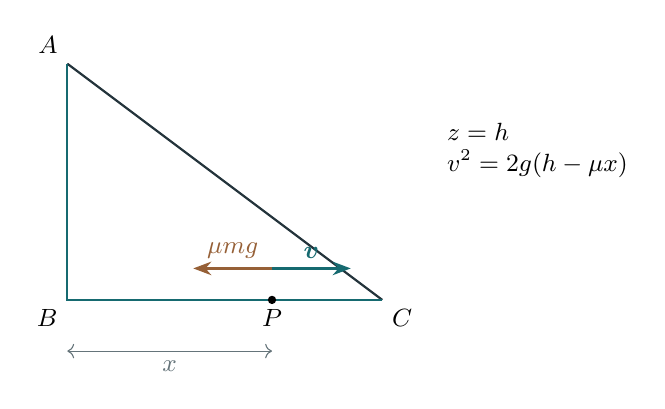
\begin{tikzpicture}
\draw[object] (0,3)--(4,0);\draw[traj] (0,3)--(0,0)--(4,0);
\node[above left] at (0,3) {$A$};\node[below left] at (0,0) {$B$};\node[below right] at (4,0) {$C$};
\fill (2.6,0) circle(1.5pt) node[below] {$P$};
\draw[motion] (2.6,.4)--(3.6,.4) node[midway,above] {$\boldsymbol v$};
\draw[force] (2.6,.4)--(1.6,.4) node[midway,above] {$\mu mg$};
\draw[axis,<->] (0,-.65)--(2.6,-.65) node[midway,below] {$x$};
\node[right,align=left] at (4.7,1.9) {$z=h$\\$v^2=2g(h-\mu x)$};
\end{tikzpicture}
\figcaption{变图1.1V2\quad 在底边运动时，摩擦使速率随已走距离减小}
\end{minipage}\end{center}
任意允许路径有$z\le h$，所以同一$x$处$v\le\sqrt{2g(h-\mu x)}$，其水平时间至少为底边上的积分。竖直段中摩擦已消耗的能量使$v\le\sqrt{2gz}$，竖直总时间至少为$t_1$。底边路径同时取等，
\[
T_{\min}=t_1+\int_0^b\frac{\dd x}{\sqrt{2g(h-\mu x)}}
=t_1+\frac{\sqrt{2gh}-\sqrt{2g(h-\mu b)}}{\mu g}.
\]
$\mu=0$时取连续极限，水平时间恢复为$b/\sqrt{2gh}$。再记$\beta=\mu b/h<1$。三角形内$x\le bz/h$，故$z-\mu x\ge(1-\beta)z$；每个水平微元还有$z-\mu x\ge(h/b-\mu)x$。分别积分可得
\[
T_{\rm v}\le\frac{t_1}{\sqrt{1-\beta}},\qquad
T_{\rm h}\le\frac{b}{\sqrt{1-\beta}}\sqrt{\frac{2}{gh}},\qquad
T_{\sup}=\frac{t_1(1+b/h)}{\sqrt{1-\mu b/h}}.
\]
逐次先下降、后向右的细阶梯使$x$与$bz/h$的差趋零，竖直和水平两项同时趋向上式。条件$\mu<h/b$保证这一极限运动始终有正的重力净作功。

\item \textbf{重力随高度改变。}重力加速度为下降量的函数$g(z)>0$，设$U(z)=\int_0^z g(s)\dd s$。求最快时间与最长时间极限。

变图1.1V3的$P$位于下降量$z$处，竖直箭头表示当地的$g(z)$。能量给$v(z)=\sqrt{2U(z)}$，$U$随$z$严格增大，水平段放得越低，速率越大。
\begin{center}\begin{minipage}{.98\linewidth}\centering
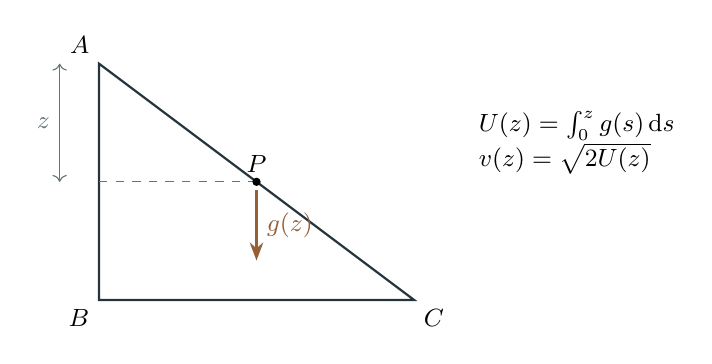
\begin{tikzpicture}
\draw[object] (0,3)--(0,0)--(4,0)--cycle;
\draw[guide] (0,1.5)--(2,1.5);\fill (2,1.5) circle(1.5pt) node[above] {$P$};
\draw[axis,<->] (-.5,3)--(-.5,1.5) node[midway,left] {$z$};
\draw[force] (2,1.4)--(2,.5) node[midway,right] {$g(z)$};
\node[above left] at (0,3) {$A$};\node[below left] at (0,0) {$B$};\node[below right] at (4,0) {$C$};
\node[right,align=left] at (4.7,2) {$U(z)=\int_0^z g(s)\dd s$\\$v(z)=\sqrt{2U(z)}$};
\end{tikzpicture}
\figcaption{变图1.1V3\quad 当地速率由从A下降到该高度的重力作功确定}
\end{minipage}\end{center}
所有竖直段的时间仍合成为同一个积分。水平微元在$x$处的下降量满足$hx/b\le z\le h$，因此
\[
\frac{b}{\sqrt{2U(h)}}\le T_{\rm h}
\le\int_0^b\frac{\dd x}{\sqrt{2U(hx/b)}}
=\frac bh\int_0^h\frac{\dd z}{\sqrt{2U(z)}}.
\]
底边路径达到最短时间，细阶梯逼近最长时间极限：
\[
T_{\min}=\int_0^h\frac{\dd z}{\sqrt{2U(z)}}+\frac b{\sqrt{2U(h)}},\qquad
T_{\sup}=\left(1+\frac bh\right)\int_0^h\frac{\dd z}{\sqrt{2U(z)}}.
\]
从静止出发能否在有限时间内完成下落，由共同的竖直积分决定。若$g(z)$在起点趋向正的有限值$g(0)$，则$U(z)\sim g(0)z$，积分核按$z^{-1/2}$变化。一般地，若$U(z)\sim az^p$，其中$a>0$，则起点附近的积分核正比于$z^{-p/2}$，故积分在$p<2$时收敛。若$p\ge2$，竖直积分已经发散，所有允许路径都无有限到达时间。

\item \textbf{把直角拐折换成光滑圆弧。}用半径$a$的四分之一圆弧连接竖直段与水平段，$0<a<\min(h,b)$，求这条路径的时间及$a\to0$的极限。

变图1.1V4中，圆弧在$P=(0,a)$与竖直段相切，在$Q=(a,0)$与水平段相切，圆心为$O_a=(a,a)$。各处速率仍由下降高度决定。
\begin{center}\begin{minipage}{.98\linewidth}\centering
\begin{tikzpicture}
\draw[guide] (0,3)--(0,0)--(4,0);\draw[object] (0,3)--(4,0);
\draw[traj] (0,3)--(0,.8) arc(180:270:.8)--(4,0);
\draw[guide] (0,.8)--(.8,.8)--(.8,0);
\fill (.8,.8) circle(1.2pt) node[above right] {$O_a$};
\node[left] at (0,.8) {$P$};\node[below] at (.8,0) {$Q$};
\node[above left] at (0,3) {$A$};\node[below left] at (0,0) {$B$};\node[below right] at (4,0) {$C$};
\node[above] at (.4,.8) {$a$};\node[right] at (.8,.4) {$a$};
\node[right,align=left] at (4.7,1.9) {圆弧长为$\pi a/2$\\弧上下降量持续增大};
\end{tikzpicture}
\figcaption{变图1.1V4\quad 有限圆弧同时替代一段竖直路程和一段水平路程}
\end{minipage}\end{center}
弧上取$0\le\phi\le\pi/2$，
\[
x=a(1-\cos\phi),\qquad y=a(1-\sin\phi),\qquad
z=h-a+a\sin\phi,\qquad \dd s=a\dd\phi.
\]
所以弧段时间及全程时间为
\[
T_{\mathrm{arc}}=\int\frac{\dd s}{\sqrt{2gz(s)}}
=a\int_0^{\pi/2}\frac{\dd\phi}{\sqrt{2g(h-a+a\sin\phi)}},
\]
\[
T(a)=\sqrt{\frac{2(h-a)}g}+T_{\mathrm{arc}}+
\frac{b-a}{\sqrt{2gh}}.
\]
第一项沿$AP$从静止下落，末项沿$QC$以末速匀速运动。随$a\to0$，弧长和弧段时间趋零，两直线段长度趋于$h,b$，故$T(a)\to t_1+t_2$。若第一问只给这条圆弧路径与$AC$等时，则有限$a$时应使用$T(a)$；在$a\to0$时恢复$\sin\alpha+\cos\alpha/2=1$。

\item \textbf{带非零初速进入路径。}质点在$A$处的初速大小为$u_0>0$，转弯保速。求最快路径和全过程时间。

下降量$z$处的速率为$v(z)=\sqrt{u_0^2+2gz}$。变图1.1V5比较同一小段水平距离分别放在$P$、底边上的用时；底边速率$v_h=\sqrt{u_0^2+2gh}$最大。
\begin{center}\begin{minipage}{.98\linewidth}\centering
\begin{tikzpicture}
\draw[object] (0,3)--(0,0)--(4,0)--cycle;
\draw[motion] (.1,2.9)--(.1,2.2) node[right] {$u_0$};
\draw[thick,color=warm] (.8,1.5)--(1.6,1.5);\draw[motion] (.9,1.8)--(1.5,1.8);
\node[above] at (1.2,1.9) {$P:\ v(z)$};
\draw[traj] (.8,0)--(1.6,0);\draw[motion] (.9,.3)--(1.5,.3);
\node[below] at (1.2,-.1) {$v_h$};
\node[above left] at (0,3) {$A$};\node[below left] at (0,0) {$B$};\node[below right] at (4,0) {$C$};
\node[right,align=left] at (4.7,1.8) {两水平段长度相同\\$v(z)\le v_h$};
\end{tikzpicture}
\figcaption{变图1.1V5\quad 非零初速保留了速率随下降量增大的次序}
\end{minipage}\end{center}
任意路径的竖直时间为
\[
T_{\mathrm v}=\int_0^h\frac{\dd z}{\sqrt{u_0^2+2gz}}
=\frac{\sqrt{u_0^2+2gh}-u_0}{g}.
\]
每个水平微元的耗时至少为$\dd x/v_h$，将它们全部放在底边即可取等。因此最快路径仍为$A\to B\to C$，
\[
T_{\min}=\frac{v_h-u_0}{g}+\frac b{v_h}.
\]
$u_0\to0$时，两项分别恢复自由落体时间和底边匀速时间。

\item \textbf{有限阶梯离最长时间还有多远。}每次先下降$h/N$、再向右$b/N$，求总时间，并估计趋近最长时间极限的误差。

变图1.1V6中第$k$段水平路程位于$z_k=kh/N$，速率$v_k=\sqrt{2gkh/N}$，每段长度为$b/N$。
\begin{center}\begin{minipage}{.98\linewidth}\centering
\begin{tikzpicture}
\draw[object] (0,3)--(0,0)--(4,0)--cycle;
\draw[traj] (0,3)\foreach \j in {1,...,4}{--({\j-1},{3-.75*\j})--({\j},{3-.75*\j})};
\draw[axis,<->] (1,1.15)--(2,1.15) node[midway,below] {$b/N$};
\draw[axis,<->] (-.5,3)--(-.5,2.25) node[midway,left] {$h/N$};
\node[above left] at (0,3) {$A$};\node[below left] at (0,0) {$B$};\node[below right] at (4,0) {$C$};
\node[right,align=left] at (4.7,1.9) {图取$N=4$\\第$k$水平段：$z_k=kh/N$};
\end{tikzpicture}
\figcaption{变图1.1V6\quad 每级的速率在该级水平段上保持常量}
\end{minipage}\end{center}
竖直时间仍为$t_1$，故
\[
T_N=t_1+\frac b{\sqrt{2gh}}\frac1{\sqrt N}
\sum_{k=1}^Nk^{-1/2}.
\]
用递减函数的积分夹住求和，
\[
2(\sqrt{N+1}-1)\le\sum_{k=1}^Nk^{-1/2}
\le2\sqrt N-1.
\]
记$K=b/\sqrt{2gh}$，则
\[
\frac K{\sqrt N}\le T_{\sup}-T_N
\le\frac{2K}{\sqrt N}
\left(1+\sqrt N-\sqrt{N+1}\right)
<\frac{2K}{\sqrt N}.
\]
误差具有$N^{-1/2}$的尺度。将级数增到约四倍，可把同一误差尺度减为原来的一半；起点附近速率小，正是收敛较慢的部分。

\item \textbf{非零初速下的最长时间极限。}仍取变式5的初速$u_0>0$，求细阶梯用时极限及其与最短用时之比。

变图1.1V7在斜边上选$P$，其对应下降量为$z=hx/b$。细阶梯的水平段从斜边内侧趋近$P$，故水平时间的极限为
\[
T_{{\rm h},\sup}=\int_0^b\frac{\dd x}{\sqrt{u_0^2+2ghx/b}}
=\frac bh\frac{v_h-u_0}{g}.
\]
\begin{center}\begin{minipage}{.98\linewidth}\centering
\begin{tikzpicture}
\draw[object] (0,3)--(0,0)--(4,0)--cycle;
\draw[traj] (0,3)\foreach \j in {1,...,6}{--({2*(\j-1)/3},{3-.5*\j})--({2*\j/3},{3-.5*\j})};
\fill (2,1.5) circle(1.4pt) node[above right] {$P$};
\draw[guide] (0,1.5)--(2,1.5)--(2,0);
\draw[axis,<->] (-.5,3)--(-.5,1.5) node[midway,left] {$z=hx/b$};
\node[above left] at (0,3) {$A$};\node[below left] at (0,0) {$B$};\node[below right] at (4,0) {$C$};
\node[right,align=left] at (4.7,1.8) {$v_P=\sqrt{u_0^2+2ghx/b}$\\有限阶梯从斜边内侧逼近};
\end{tikzpicture}
\figcaption{变图1.1V7\quad 斜边位置给出每个水平微元可处的最高位置}
\end{minipage}\end{center}
再加竖直时间$T_{\rm v}=(v_h-u_0)/g$，得
\[
T_{\sup}=\left(1+\frac bh\right)\frac{v_h-u_0}{g},\qquad
\frac{T_{\sup}}{T_{\min}}
=\frac{2v_h(h+b)}{2hv_h+b(v_h+u_0)}.
\]
这里用到$v_h-u_0=2gh/(v_h+u_0)$。取$b/h=4/3$，$u_0\to0$时比值趋于$7/5$；$u_0^2\gg2gh$时各高度速率趋近同一个$u_0$，竖直与水平总路程分别固定，比值趋于1。

\item \textbf{把可走区域改成矩形。}允许路径位于宽$b$、高$h$的矩形内，仍只向下、向右，质点在左上角$A$从静止出发到右下角$C$。求最快时间，讨论用时能否任意大。

底边路径仍使所有水平微元以最大速率通过，最短时间保持$t_1+b/\sqrt{2gh}$。变图1.1V8另构造一条路径：先下降$\delta>0$，横穿全部宽度$b$，再下降到$C$。
\begin{center}\begin{minipage}{.98\linewidth}\centering
\begin{tikzpicture}
\draw[object] (0,3)--(0,0)--(4,0)--(4,3)--cycle;
\draw[traj] (0,3)--(0,2.55)--(4,2.55)--(4,0);
\node[above left] at (0,3) {$A$};\node[below left] at (0,0) {$B$};\node[below right] at (4,0) {$C$};
\draw[axis,<->] (-.5,3)--(-.5,2.55) node[midway,left] {$\delta$};
\draw[motion] (1,2.55)--(2.2,2.55) node[midway,above] {$\sqrt{2g\delta}$};
\draw[axis,<->] (0,-.5)--(4,-.5) node[midway,below] {$b$};
\node[right,align=left] at (4.7,1.8) {先小幅下落，再横穿矩形\\水平段可保持很小的速率};
\end{tikzpicture}
\figcaption{变图1.1V8\quad 矩形允许在任意小的下降量处完成全部水平位移}
\end{minipage}\end{center}
两段竖直时间之和为$t_1$，中间水平速率保持$\sqrt{2g\delta}$，所以
\[
T(\delta)=t_1+\frac b{\sqrt{2g\delta}}
\longrightarrow+\infty\qquad(\delta\to0^+).
\]
每条$\delta>0$的路径都从先下落获得正速率，运动可完成。三角形中的斜边曾给出$z\ge hx/b$；矩形允许横穿段任意接近$A$的高度，故这一组允许路径的用时没有有限上界。
\end{enumerate}


\clearpage

\pdfbookmark[3]{第 2 题 线性阻力下的剩余路程}{c1-q2}

\section*{第 2 题\quad 线性阻力下的剩余路程}\label{book-question-1-2}

\tagline{M-01-02}

质量为 $m$ 的质点以初速度 $v_0>0$ 沿 $x$ 轴正方向运动，初始位置为 $x=0$。唯一的运动方向上的力为线性阻力 $F_x=-bv$，其中 $b>0$ 为常量。

当速度降为 $v_0/n$（$n>1$）时，求已通过路程与总路程之比。总路程指 $t\to\infty$ 时路程的极限。

\begin{center}
\begin{tikzpicture}
\draw[axis] (-.7,0)--(7.0,0) node[right] {$x$};
\fill[ink] (2.7,0) circle (2.5pt);\node[below] at (2.7,-.12) {$m$};
\draw[motion] (2.7,.4)--(4.6,.4) node[above] {$\vect v$};
\draw[force] (2.7,.4)--(1.0,.4) node[above] {$\vect F$};
\draw (0,.1)--(0,-.1);\node[below] at (0,-.1) {$O$};
\node[color=muted] at (3.4,1.25) {阻力始终与速度反向};
\end{tikzpicture}
\figcaption{图 1.2\quad 运动方向与阻力方向。}
\end{center}

\Needspace{5\baselineskip}

\pdfbookmark[4]{题型定位}{c1-q2-h0}

\subsection*{题型定位}

线性阻力下的速度衰减与剩余路程。求 $v(t)$ 后积分得到有限总路程，再消去时间建立 $v(x)$；区分无限衰减时间与有限位移极限。

\Needspace{5\baselineskip}

\pdfbookmark[4]{知识点}{c1-q2-h1}

\subsection*{知识点}

\begin{itemize}
\item 线性阻力$F_x=-bv$给$\dot v=-kv$，$k=b/m$是衰减率。
\item 分离变量从$v_0$到$v$积分得到无量纲对数$\ln(v/v_0)=-kt$。
\item 位置由速度积分得到，初始条件$x(0)=0$确定积分常数。
\item 在正速度区间使用$\dot v=v\dd v/\dd x$，可得到速度—位置直线。
\item 速度曲线下的未来面积给剩余路程$v/k$，全部面积给总路程极限$v_0/k$。
\end{itemize}
解图1.2A的横轴是时间，曲线斜率为加速度；解图1.2B的横轴是位置，斜率为$\dd v/\dd x=-k$。两图分别呈指数与直线，描述同一运动。


\Needspace{5\baselineskip}

\pdfbookmark[4]{物理图像}{c1-q2-h2}

\subsection*{物理图像}

题图中速度向右、阻力向左。速度减小时阻力也减小，减速过程逐步放缓。解图1.2A中$v/v_0=e^{-kt}$在有限时刻保持正值，曲线下的总面积收敛到$x_m$；从当前时刻向右的面积则是剩余路程。解图1.2B将这一过程改画在速度—位置平面，当前点沿直线趋向横轴截距$x_m$。截距到当前横坐标的距离为$v/k$，因此速度比例与剩余路程比例相同。

\Needspace{5\baselineskip}

\pdfbookmark[4]{解题入口}{c1-q2-h3}

\subsection*{解题入口}

先由题设$F_x=-bv$除以质量，记$k=b/m$，得到$\dot v=-kv$。从初值积分求$v(t)$，随后将速度从0积分到$t$，再令$t\to\infty$求总路程极限。指定$v=v_0/n$时，速度式和位置式中使用同一个指数因子$1/n$。

也可由$\dot v=v\dd v/\dd x$进入。在$v>0$的运动区间内约去$v$，得到$\dd v/\dd x=-k$，由初值求直线$v=v_0-kx$。这条直线将已走路程、剩余路程和当前速度直接联系起来，时间法则同时说明趋近过程。

\Needspace{5\baselineskip}

\pdfbookmark[4]{标准解法}{c1-q2-h4}

\subsection*{标准解法}

取初速度方向为 $x$ 轴正向，记 $k=b/m>0$。题图 1.2 中速度向右、阻力向左，运动方程为
\[
m\dot v=-bv,\qquad\dot v=-kv,\qquad v(0)=v_0.
\]
\subsubsection*{速度与位置随时间变化}
在 $v>0$ 的运动区间内分离变量，由初始时刻积分到 $t$，
\[
\int_{v_0}^{v(t)}\frac{\dd u}{u}
=-k\int_0^t\dd s,
\qquad\ln\frac{v(t)}{v_0}=-kt.
\]
所以
\[
\boxed{v(t)=v_0e^{-kt}},\qquad
x(t)=\int_0^t v_0e^{-ks}\dd s
=\boxed{\frac{v_0}{k}(1-e^{-kt})}.
\]
速度在任意有限时刻都为正，故位移等于已通过路程。解图 1.2A 的速度曲线无限延伸，但曲线下的总面积收敛：
\begin{center}\begin{minipage}{\linewidth}\centering\begin{tikzpicture}

\draw[axis] (-.2,0)--(5,0) node[right] {$t$};\draw[axis] (0,-.15)--(0,2.65) node[above] {$v$};
\fill[accent!12] ({ln(3)},0)--plot[domain={ln(3)}:4.6,samples=70](\x,{2.2*exp(-\x)})--(4.6,0)--cycle;
\draw[traj,domain=0:4.6,samples=80] plot(\x,{2.2*exp(-\x)});
\draw[guide] ({ln(3)},0)--({ln(3)},{2.2*(1/3)})--(0,{2.2*(1/3)});
\node[left] at (0,2.2) {$v_0$};\node[left] at (0,{2.2*(1/3)}) {$v_0/n$};\node[below] at ({ln(3)},0) {$t_n$};
\node[align=left] at (6.75,1.75) {全部曲线下面积：$x_m$\\$t_n$ 后的面积：剩余路程\\$v(t)=v_0e^{-kt}$};
\draw[thin] (1.62,.25)--(3.0,1.02) node[right] {$x_m-x_n$};

\end{tikzpicture}
\figcaption{解图 1.2A\quad 速度曲线下面积等于路程；阴影部分对应速度已降至 $v_0/n$ 后的剩余路程。}
\end{minipage}\end{center}
\[
x_m=\int_0^\infty v_0e^{-kt}\dd t=\frac{v_0}{k}.
\]
$x_m$ 是无限时间下的路程极限；任意有限时刻仍有 $x<x_m,v>0$。
\subsubsection*{代入指定速度比例}
令 $v(t_n)=v_0/n$，则
\[
e^{-kt_n}=\frac1n,\qquad t_n=\frac{\ln n}{k}.
\]
此时
\[
x_n=\frac{v_0}{k}\left(1-\frac1n\right),\qquad
\boxed{\frac{x_n}{x_m}=1-\frac1n}.
\]
$n\to1^+$ 时，指定时刻趋于零，已走路程比例也趋于零；$n\to\infty$ 时，比例趋于一，所需时间却趋于无穷。
\subsubsection*{速度与位置的直接关系}
由于 $\dot v=v\,\dd v/\dd x$，运动方程还可写为
\[
v\frac{\dd v}{\dd x}=-kv.
\]
在 $v>0$ 时约去 $v$，从 $x=0,v=v_0$ 积分，得
\[
v=v_0-kx,\qquad
\boxed{\frac{v}{v_0}+\frac{x}{x_m}=1}.
\]
\begin{center}\begin{minipage}{\linewidth}\centering\begin{tikzpicture}

\draw[axis] (-.15,0)--(4.65,0) node[right] {$x$};\draw[axis] (0,-.15)--(0,2.7) node[above] {$v$};
\draw[traj] (0,2.2)--(4,0);\node[left] at (0,2.2) {$v_0$};\node[below] at (4,0) {$x_m$};
\fill ({8/3},{2.2/3}) circle(2pt);\draw[guide] ({8/3},0)--({8/3},{2.2/3})--(0,{2.2/3});
\node[below] at ({8/3},0) {$x_n$};\node[left] at (0,{2.2/3}) {$v_0/n$};
\node[align=left] at (6.7,1.65) {$\displaystyle\frac{v}{v_0}+\frac{x}{x_m}=1$\\[4pt]$x_m-x=\dfrac vk$};

\end{tikzpicture}
\figcaption{解图 1.2B\quad 消去时间后，$v$ 与 $x$ 成线性关系。由图中截距和当前点直接读出路程比例。}
\end{minipage}\end{center}
两张解图都取 $n=3$。在解图 1.2A 中，竖线经过 $kt_n=\ln3$，此处速度为 $v_0/3$。解图 1.2B 的同一时刻对应直线上的点 $(2x_m/3,v_0/3)$，距横轴截距还有 $x_m/3$。直线上任意一点的横坐标到截距的距离都是 $x_m-x=v/k$。$v$ 随时间指数衰减，随位置却线性减小；两种关系的自变量不同。
\subsubsection*{积分常数与当前状态之后的运动}
若用不定积分求位置，先得到
\[
x=-\frac{v_0}{k}e^{-kt}+C_x.
\]
将$x(0)=0$代入上式，常量项与初始指数项相抵，得到$C_x=v_0/k$。
从 $v_0$ 积到 $v$，得到 $\ln(v/v_0)$。对数的真数是速度之比，初始速度由积分下限给定。
在解图1.2A的指定时刻$t_n$之后，令$\tau=t-t_n$，
则$v(t_n+\tau)=(v_0/n)e^{-k\tau}$，因此
\[
x_m-x_n=\int_0^\infty\frac{v_0}{n}e^{-k\tau}\dd\tau
=\frac{v_0}{nk}.
\]
它恰是解图1.2B中当前点到横轴截距的水平距离。
在$t_n$之后，速度与剩余路程按同一个指数因子继续减小。每经历$\ln2/k$的时间，二者均减半；随$t\to\infty$，速度趋零，位置趋于有限的$x_m$。


\Needspace{5\baselineskip}

\pdfbookmark[4]{关键洞察}{c1-q2-h5}

\subsection*{关键洞察}

线性阻力使未来运动在任意当前状态都具有相同形式：当前速度为$v$时，之后的速度为$ve^{-ks}$，剩余路程便为$v/k$。因此速度降至$v_0/n$时，剩余比例为$1/n$，已走比例为$1-1/n$。速度减半时已走一半路程，速度降为十分之一时已走九成；每再走完剩余路程的一半，都经历相同的$\ln2/k$。变式3进一步比较代数衰减尾部，说明总路程由速度的时间积分是否收敛决定。

\Needspace{5\baselineskip}

\pdfbookmark[4]{易错点}{c1-q2-h6}

\subsection*{易错点}

\begin{itemize}
\item 阻力沿$-x$，方程和指数均带负号，$\dot v=-kv$、$v=v_0e^{-kt}$。
\item 由$x(0)=0$确定位置积分中的$C_x=v_0/k$，使位置从给定原点开始。
\item 位移等于路程的依据是全过程$v>0$；总路程为$t\to\infty$时的极限。
\item $n\to1^+$时指定时刻与已走比例均趋零，$n\to\infty$时已走比例趋1、时刻趋于无穷。
\item $v(x)$的横轴是位置，直线截距给总路程；$v(t)$的横轴是时间，曲线下面积才给路程。
\end{itemize}

\Needspace{5\baselineskip}

\pdfbookmark[4]{课堂讲解建议}{c1-q2-h7}

\subsection*{课堂讲解建议}

先问：“速度减到一半时，走完的路程占多少？”让学生保留$v(t),x(t),x_m$三式，再由$v/v_0+x/x_m=1$回答恰好一半。接着问：“已走四分之三时，速度和剩余路程各是多少？”在解图1.2B定位当前点，分别读出$v_0/4$与$x_m/4$。

用解图1.2A的未来面积求剩余路程，再追问“走完下一半剩余路程要多久”。从当前速度重新积分，得到每次均为$\ln2/k$，而对应路程逐次减半。将变式3的代数衰减曲线并排比较，让学生从积分判断哪一种总面积有限。最后用等时间隔的位移增量反求$k$，说明同一指数规律怎样从位置记录中识别出来。

\Needspace{5\baselineskip}

\pdfbookmark[4]{变式训练}{c1-q2-h8}

\subsection*{变式训练}

\begin{enumerate}
\item \textbf{速度降为十分之一。}求此时的路程比例、经历时间及剩余路程。

令$\tau=kt$，由$v/v_0=e^{-\tau}$，指定速度给$\tau=\ln10$。将同一个指数因子代入位置式，
\[
t=\frac{\ln10}{k},\qquad x=\frac{v_0}{k}\left(1-\frac1{10}\right),\qquad
\frac{x}{x_m}=\frac9{10},\quad x_m-x=\frac{x_m}{10}.
\]
变图1.2V1在同一时间轴画速度比例与路程比例。两条曲线在任意时刻的纵坐标之和为1；$\tau=\ln10$的竖线分别与它们交于$1/10$和$9/10$。
\begin{center}\begin{minipage}{.98\linewidth}\centering
\begin{tikzpicture}
\draw[axis] (0,0)--(5.6,0) node[right] {$\tau=kt$};\draw[axis] (0,0)--(0,3.1) node[above] {比值};
\draw[traj,domain=0:5,samples=60] plot(\x,{2.6*exp(-\x)});
\draw[thick,dashed,color=warm,domain=0:5,samples=60] plot(\x,{2.6*(1-exp(-\x))});
\draw[guide] ({ln(10)},0)--({ln(10)},2.6);
\node[below] at ({ln(10)},0) {$\ln10$};\node[left] at (0,2.6) {$1$};
\fill ({ln(10)},.26) circle(1.5pt);\fill ({ln(10)},2.34) circle(1.5pt);
\node[right] at (3.3,.35) {$v/v_0$};\node[right,color=warm] at (3.3,2.25) {$x/x_m$};
\end{tikzpicture}
\figcaption{变图1.2V1\quad 指定同一时刻，速度比例与路程比例互补}
\end{minipage}\end{center}
此后速度继续指数减小，剩余的十分之一路程由$t$之后的速度曲线面积给出。

\item \textbf{已经走完四分之三。}求该时刻速度、时间和剩余路程。

从运动方程用$\dot v=v\dd v/\dd x$消去时间，得到$\dd v/\dd x=-k$，初值积分后有$v=v_0-kx$。取$x=3x_m/4$、$x_m=v_0/k$，
\[
v=\frac{v_0}{4},\qquad e^{-kt}=\frac14,\qquad
t=\frac{\ln4}{k},\qquad x_m-x=\frac{x_m}{4}.
\]
变图1.2V2的$P$在速度—位置直线上，横坐标$3/4$、纵坐标$1/4$；从$P$向横轴截距量得的水平距离就是剩余路程比例。
\begin{center}\begin{minipage}{.98\linewidth}\centering
\begin{tikzpicture}
\draw[axis] (0,0)--(5.2,0) node[right] {$x/x_m$};\draw[axis] (0,0)--(0,3.1) node[above] {$v/v_0$};
\draw[traj] (0,2.6)--(4,0);\fill (3,.65) circle(1.6pt) node[above right] {$P$};
\draw[guide] (3,0)--(3,.65)--(0,.65);
\node[below] at (3,0) {$3/4$};\node[below] at (4,0) {$1$};\node[left] at (0,.65) {$1/4$};\node[left] at (0,2.6) {$1$};
\draw[axis,<->] (3,-.65)--(4,-.65) node[midway,below] {$1/4$};
\end{tikzpicture}
\figcaption{变图1.2V2\quad 已走路程确定当前速度，横轴上还余四分之一}
\end{minipage}\end{center}

\item \textbf{改用三次阻力。}设运动方程为$\dot v=-\kappa v^3$，$\kappa>0$，初值仍为$v_0$。求速度和路程，比较总路程的收敛性。

分离变量并积分，
\[
\int_{v_0}^{v}u^{-3}\dd u=-\kappa t,
\qquad v(t)=\frac{v_0}{\sqrt{1+2\kappa v_0^2t}}.
\]
再积分速度，得到
\[
x(t)=\frac{\sqrt{1+2\kappa v_0^2t}-1}{\kappa v_0},\qquad
v(t)\sim(2\kappa t)^{-1/2}.
\]
路程随$\sqrt t$增长，因而总路程无界。变图1.2V3为便于比较，取$\kappa v_0^2=k$，使两种阻力的初始减速度相同；横轴都用$\tau=kt$。三次阻力的代数尾部比线性阻力的指数尾部衰减慢，其速度曲线下面积随时间持续增大。
\begin{center}\begin{minipage}{.98\linewidth}\centering
\begin{tikzpicture}
\draw[axis] (0,0)--(5.5,0) node[right] {$\tau=kt$};\draw[axis] (0,0)--(0,3.1) node[above] {$v/v_0$};
\draw[traj,domain=0:5,samples=60] plot(\x,{2.6*exp(-\x)});
\draw[thick,dashed,color=warm,domain=0:5,samples=60] plot(\x,{2.6/sqrt(1+2*\x)});
\node[left] at (0,2.6) {$1$};\node[below] at (0,0) {$0$};
\node[right,color=warm] at (3.4,1.4) {三次阻力};\node[right] at (3.4,.3) {线性阻力};
\end{tikzpicture}
\figcaption{变图1.2V3\quad 初始减速度相同，后期速度的衰减规律不同}
\end{minipage}\end{center}
这里$k$的单位为$\mathrm{s^{-1}}$，$\kappa$的单位为$\mathrm{s\,m^{-2}}$；两者分别与各自的速度幂次组合，给出加速度。

\item \textbf{阻力系数加倍。}保持$m,v_0$不变，将$b$改为$2b$。比较降到同一速度比例时的时间、路程、总路程及路程比例。

新衰减率为$k'=2k$，故$v'(t)=v_0e^{-2kt}$。指定$v'=v_0/n$时，
\[
t_n'=\frac{\ln n}{2k}=\frac{t_n}{2},\qquad
x_n'=\frac{v_0}{2k}\left(1-\frac1n\right)=\frac{x_n}{2},\qquad
x_m'=\frac{x_m}{2}.
\]
两种路程都减半，因此$x_n'/x_m'=1-1/n$保持。变图1.2V4用相同的实际时间单位$1/k$比较两条速度曲线，新曲线达到同一纵坐标时所需横坐标减半。
\begin{center}\begin{minipage}{.98\linewidth}\centering
\begin{tikzpicture}
\draw[axis] (0,0)--(5.5,0) node[right] {$kt$};\draw[axis] (0,0)--(0,3.1) node[above] {$v/v_0$};
\draw[traj,domain=0:5,samples=60] plot(\x,{2.6*exp(-\x)});
\draw[thick,dashed,color=warm,domain=0:5,samples=60] plot(\x,{2.6*exp(-2*\x)});
\draw[guide] (0,.65)--({ln(4)},.65);\draw[guide] ({ln(4)},0)--({ln(4)},.65);\draw[guide] ({ln(4)/2},0)--({ln(4)/2},.65);
\node[left] at (0,.65) {$1/4$};\node[left] at (0,2.6) {$1$};
\node[below] at ({ln(4)/2},0) {$\frac12\ln4$};\node[below] at ({ln(4)},-.55) {$\ln4$};
\node[right] at (3.3,1.4) {实线：$b$};\node[right,color=warm] at (3.3,.9) {虚线：$2b$};
\end{tikzpicture}
\figcaption{变图1.2V4\quad 加倍阻力系数使达到同一速度比例的时间减半}
\end{minipage}\end{center}

\item \textbf{从当前状态求剩余路程。}在任意时刻$t_*$，质点速度为$v_*>0$，位置为$x_*$。以该时刻为新的时间起点，直接求后续路程。

令$s=t-t_*$，方程与初值为$\dd v/\dd s=-kv$、$v(0)=v_*$，因此$v(s)=v_*e^{-ks}$。对未来全部时间积分，
\[
\Delta x_{\rm rem}=\int_0^\infty v_*e^{-ks}\dd s=\frac{v_*}{k},\qquad
x_*+\frac{v_*}{k}=x_m.
\]
变图1.2V5画的是从$t_*$起重新计时的速度曲线，阴影随曲线向右延伸，整个面积为$v_*/k$。剩余路程与当前速度成正比，所以每当剩余路程减半，当前速度也减半，所需时间均为$\ln2/k$。
\begin{center}\begin{minipage}{.98\linewidth}\centering
\begin{tikzpicture}
\fill[accent!12] (0,0)--(0,2.6)--plot[domain=0:5,samples=60](\x,{2.6*exp(-\x)})--(5,0)--cycle;
\draw[axis] (0,0)--(5.5,0) node[right] {$ks$};\draw[axis] (0,0)--(0,3.1) node[above] {$v/v_*$};
\draw[traj,domain=0:5,samples=60] plot(\x,{2.6*exp(-\x)});
\draw[motion] (4.4,{2.6*exp(-4.4)})--(5,{2.6*exp(-5)});
\node[left] at (0,2.6) {$1$};\node[below] at (0,0) {$0$};
\node[right,align=left] at (2.5,1.65) {面积乘$v_*/k$\\即为剩余路程};
\end{tikzpicture}
\figcaption{变图1.2V5\quad 当前状态作为初态，未来速度曲线决定剩余路程}
\end{minipage}\end{center}

\item \textbf{阻力消耗的机械能。}求速度降至$v_0/n$时损失的动能，以及此后还将损失的动能。

阻力瞬时功率为$P_F=-bv^2$。动能方程给$\dot K=-bv^2$，代入$v=v_0e^{-kt}$，从0积分到$t_n$：
\[
K_0-K(t_n)=\int_0^{t_n}bv_0^2e^{-2kt}\dd t
=\frac12mv_0^2\left(1-\frac1{n^2}\right).
\]
此后还将损失当前全部动能$K(t_n)=mv_0^2/(2n^2)$。变图1.2V6在横轴$x/x_m$上画$K/K_0=(1-x/x_m)^2$，所以路程已走比例与动能已损失比例各有不同函数关系。例如速度减半时已走一半路程，已损失四分之三动能。
\begin{center}\begin{minipage}{.98\linewidth}\centering
\begin{tikzpicture}
\draw[axis] (0,0)--(5.2,0) node[right] {$x/x_m$};\draw[axis] (0,0)--(0,3.1) node[above] {$K/K_0$};
\draw[traj,domain=0:1,samples=60] plot({4*\x},{2.6*(1-\x)^2});
\fill (2,.65) circle(1.5pt);\draw[guide] (2,0)--(2,.65)--(0,.65);
\node[below] at (2,0) {$1/2$};\node[below] at (4,0) {$1$};\node[left] at (0,.65) {$1/4$};\node[left] at (0,2.6) {$1$};
\end{tikzpicture}
\figcaption{变图1.2V6\quad 速度随位置线性下降，动能随位置按平方下降}
\end{minipage}\end{center}

\item \textbf{增加恒定驱动力。}在同一线性阻力之外施加沿$+x$的恒力$F_0>0$，求速度与位置随时间的变化。

运动方程为$m\dot v=F_0-bv$，记$v_\infty=F_0/b$。令$w=v-v_\infty$，方程化为$\dot w=-kw$，用初始速度积分得
\[
v(t)=v_\infty+(v_0-v_\infty)e^{-kt},\qquad
x(t)=v_\infty t+\frac{v_0-v_\infty}{k}(1-e^{-kt}).
\]
变图1.2V7示例取$v_0=2v_\infty$，速度从较大初值趋向终端速率。到达终端状态附近时驱动力与阻力的大小趋于相等，位置包含持续增长的$v_\infty t$，故全程路程随时间无界增加。
\begin{center}\begin{minipage}{.98\linewidth}\centering
\begin{tikzpicture}
\draw[axis] (0,0)--(5.5,0) node[right] {$kt$};\draw[axis] (0,0)--(0,3.1) node[above] {$v/v_\infty$};
\draw[traj,domain=0:5,samples=60] plot(\x,{1.3*(1+exp(-\x))});
\draw[guide] (0,1.3)--(5.1,1.3);\node[left] at (0,1.3) {$1$};\node[left] at (0,2.6) {$2$};
\node[right] at (3.2,2.3) {$F_0=bv_\infty$};
\end{tikzpicture}
\figcaption{变图1.2V7\quad 恒力驱动时速度趋于正的终端值}
\end{minipage}\end{center}

\item \textbf{由等时间隔的位置反求阻力。}以相同时间间隔$\Delta t$记录$x_0=0,x_1,x_2,x_3$，质量$m$已知。用前两个位移增量求$k,b,v_0$，并说明第三个增量的关系。

记$d_j=x_j-x_{j-1}$，令$q=e^{-k\Delta t}\in(0,1)$。对每一时间间隔积分速度，
\[
d_j=\frac{v_0}{k}(1-q)q^{j-1},\qquad
q=\frac{d_2}{d_1},\qquad
k=-\frac{\ln q}{\Delta t},\quad b=mk,\quad
v_0=\frac{kd_1}{1-q}.
\]
变图1.2V8取$q=1/2$，连续的位移增量依次减半。等时间隔使指数衰减转为等比数列，所以第三个增量满足$d_3=qd_2=d_2^2/d_1$；它还给出三次记录之间的同一模型关系。
\begin{center}\begin{minipage}{.98\linewidth}\centering
\begin{tikzpicture}
\draw[axis] (-.2,0)--(6.2,0) node[right] {$x$};
\foreach \p/\j in {0/0,3/1,4.5/2,5.25/3}{\fill (\p,0) circle(1.5pt) node[above] {$x_\j$};}
\draw[axis,<->] (0,-.5)--(3,-.5) node[midway,below] {$d_1$};
\draw[axis,<->] (3,-1)--(4.5,-1) node[midway,below] {$d_2$};
\draw[axis,<->] (4.5,-1.5)--(5.25,-1.5) node[midway,below] {$d_3$};
\node[above] at (2.8,1.1) {相邻记录相隔同一$\Delta t$；图取$q=1/2$};
\end{tikzpicture}
\figcaption{变图1.2V8\quad 位移增量的公比给出指数衰减率}
\end{minipage}\end{center}
\end{enumerate}


\clearpage

\pdfbookmark[3]{第 3 题 三次阻力运动规律}{c1-q3}

\section*{第 3 题\quad 三次阻力运动规律}\label{book-question-1-3}

\tagline{M-01-03}

质量为 $m$ 的质点以初速度 $v_0>0$ 沿 $x$ 轴正方向作直线运动，初始位置为 $x(0)=0$。唯一的运动方向上的力为 $F_x=-cv^3$，其中 $c>0$ 为常量。记 $k=c/m$。
\begin{enumerate}
\item 求速度 $v(t)$ 和位置 $x(t)$；
\item 求速度随位置的变化规律 $v(x)$；
\item 判断总路程是否有限，并说明理由。
\end{enumerate}

\begin{center}
\begin{tikzpicture}
\draw[axis] (-.4,0)--(7.0,0) node[right] {$x$};
\fill[ink] (3,0) circle (2.5pt);\node[below] at (3,-.12) {$m$};
\draw[motion] (3,.4)--(4.6,.4) node[above] {$\vect v$};
\draw[force] (3,.4)--(1.3,.4) node[above] {$F_x=-cv^3$};
\node[color=muted] at (3.4,1.35) {规定 $x(0)=0,\quad v(0)=v_0$};
\draw (0,.1)--(0,-.1);\node[below] at (0,-.1) {$O$};
\end{tikzpicture}
\figcaption{图 1.3\quad 初始速度沿正方向，三次阻力沿负方向。}
\end{center}

\Needspace{5\baselineskip}

\pdfbookmark[4]{题型定位}{c1-q3-h0}

\subsection*{题型定位}

在三次阻力下求$v(t)$、$x(t)$和$v(x)$，再判断总路程。时间法依次用分离变量和速度积分，位置法用链式法则直接求速度随位置的关系。与第2题并读，可以比较指数衰减与幂律衰减的总路程。

\Needspace{5\baselineskip}

\pdfbookmark[4]{知识点}{c1-q3-h1}

\subsection*{知识点}

\begin{itemize}
\item 非线性阻力$F_x=-cv^3$给出可分离方程$\dot v=-kv^3$，其中$k=c/m$。
\item 由初值$v(0)=v_0$确定速度积分的常数，再用$x(0)=0$确定位置的起点。
\item 时间描述满足$\dot x=v(t)$，位置描述满足$\dot v=v\,\dd v/\dd x$。
\item 解图1.3A使用$q=kv_0^2t$。速度图下面积给$kv_0x$，位置图斜率给$v/v_0$。
\item 指数衰减的总面积有限，三次阻力的$t^{-1/2}$尾部的面积随$\sqrt t$增长。
\end{itemize}


\Needspace{5\baselineskip}

\pdfbookmark[4]{物理图像}{c1-q3-h2}

\subsection*{物理图像}

题图中的速度向右，阻力向左。速度降至一半时，阻力减为八分之一，速度图的下降逐渐放缓。解图1.3A左侧曲线长时间保持在横轴上方，面积随$\sqrt t$增加。右侧曲线越来越平缓，纵坐标仍持续增加。第2题的指数速度曲线下面积收敛，因此位置趋于一个有限值。

\Needspace{5\baselineskip}

\pdfbookmark[4]{解题入口}{c1-q3-h3}

\subsection*{解题入口}

从$F_x=-cv^3$和牛顿第二定律写出$v^{-3}\dd v=-k\dd t$，积分限分别取$v_0$到$v$和0到$t$。再从0到$t$积分$v(s)$，得到位置。两个时间式共用因子$\sqrt{1+2kv_0^2t}$，由$x(t)$解出这个因子后即可写出$v(x)$。

也可在$v>0$时改用位置作自变量，由$\dot v=(\dd v/\dd x)\dot x$得到$v\,\dd v/\dd x=-kv^3$，约去一个$v$再积分。将$t=0$代回两个时间式，随后从无量纲时间和位置读出自然尺度，最后由$t\to\infty$时的$x(t)$求总路程。

\Needspace{5\baselineskip}

\pdfbookmark[4]{标准解法}{c1-q3-h4}

\subsection*{标准解法}

记 $k=c/m$。初速度为正，阻力与运动方向相反，故
\[
\dot v=-kv^3,\qquad v(0)=v_0>0,\qquad x(0)=0.
\]
\subsubsection*{分离变量求速度}
质点以 $v_0>0$ 出发。在速度保持为正的区间分离变量：
\[
\int_{v_0}^{v(t)}u^{-3}\dd u=-k\int_0^t\dd s,
\qquad -\frac1{2v^2}+\frac1{2v_0^2}=-kt.
\]
因此
\[
\frac1{v^2}=\frac1{v_0^2}+2kt,
\qquad\boxed{v(t)=\frac{v_0}{\sqrt{1+2kv_0^2t}}}.
\]
初速度沿正方向，故取正根。任意有限时刻都有$v(t)>0$，质点一直向右，$x(t)$也是从出发起走过的路程。
\subsubsection*{积分求位置}
由 $\dot x=v(t)$，
\[
x(t)=\int_0^t\frac{v_0\dd s}{\sqrt{1+2kv_0^2s}}.
\]
令 $u=1+2kv_0^2s$，则 $\dd u=2kv_0^2\dd s$，上下限为 $1$ 与 $1+2kv_0^2t$。于是
\[
x(t)=\frac1{2kv_0}\int_1^{1+2kv_0^2t}u^{-1/2}\dd u
=\boxed{\frac{\sqrt{1+2kv_0^2t}-1}{kv_0}}.
\]
\begin{center}\begin{minipage}{\linewidth}\centering\begin{tikzpicture}

\begin{scope}
\draw[axis] (-.1,0)--(4.6,0) node[right] {$q$};\draw[axis] (0,-.1)--(0,2.6) node[above] {$v/v_0$};
\draw[traj,domain=0:4.2,samples=80] plot(\x,{2.1/sqrt(1+2*\x)});\node[left] at (0,2.1) {$1$};
\node[below] at (2,-.55) {$q=kv_0^2t$};\node at (2.5,2.25) {速率趋于零};
\end{scope}
\begin{scope}[xshift=6.7cm]
\draw[axis] (-.1,0)--(4.6,0) node[right] {$q$};\draw[axis] (0,-.1)--(0,2.6) node[above] {$kv_0x$};
\draw[traj,domain=0:4.2,samples=80] plot(\x,{sqrt(1+2*\x)-1});
\node[below] at (2,-.55) {$q=kv_0^2t$};\node at (2.2,2.65) {位移仍不断增加};
\end{scope}

\end{tikzpicture}
\figcaption{解图 1.3A\quad 两图使用同一无量纲时间 $q$。左图尾部衰减很慢，右图没有有限位移上界。}
\end{minipage}\end{center}
解图 1.3A 左图的纵坐标是$v/v_0$，右图是$kv_0x$。由于$\dd(kv_0x)/\dd q=v/v_0$，左图从0到$q$的面积就是右图在$q$处的纵坐标。右图的斜率随左图的速率减小，位置仍持续增长。
\subsubsection*{速度随位置的关系}
由位置式先得 $\sqrt{1+2kv_0^2t}=1+kv_0x$，再代入速度式，得到
\[
\boxed{v(x)=\frac{v_0}{1+kv_0x}},\qquad x\geq0.
\]
也可直接换自变量：
\[
v\frac{\dd v}{\dd x}=-kv^3
\quad\Longrightarrow\quad
\int_{v_0}^{v}\frac{\dd u}{u^2}=-k\int_0^x\dd\xi.
\]
积分后 $-1/v+1/v_0=-kx$，仍得到同一结果。约去 $v$ 的步骤只在正速度区间内使用。
\subsubsection*{初始条件、量纲和长期路程}
将 $t=0$ 代入，确有 $v=v_0,x=0$。$[k]=\mathrm{s/m^2}$，故 $kv_0^2t$、$kv_0x$ 均无量纲，而 $1/(kv_0)$ 是长度。弱阻力展开为
\[
v(t)=v_0-kv_0^3t+O(k^2),\qquad
x(t)=v_0t-\frac12kv_0^3t^2+O(k^2).
\]
这与初始加速度 $-kv_0^3$ 一致。在大时间下，
\[
v(t)\sim\frac1{\sqrt{2kt}},\qquad
x(t)\sim\sqrt{\frac{2t}{k}}\longrightarrow\infty.
\]
总路程无界。解图 1.3A 左图的尾部随$t^{-1/2}$衰减，面积随$\sqrt t$增长。右图逐渐变缓的曲线正是这段面积累积后的结果。

\Needspace{5\baselineskip}

\pdfbookmark[4]{关键洞察}{c1-q3-h5}

\subsection*{关键洞察}

把自变量从$t$换成$x$时，$\dot x=v$使加速度多出一个速度因子，积分中的幂次也从$v^{-3}$变成$v^{-2}$。沿位置积分后，$1/v$对$x$是一条直线，斜率正好为$k$。变图1.3V8上，测点$P_1$、$P_2$的纵坐标分别是$1/v_1$、$1/v_2$。纵坐标差除以位置差给出斜率$k$，再乘质量$m$便是阻力系数$c$。

\Needspace{5\baselineskip}

\pdfbookmark[4]{易错点}{c1-q3-h6}

\subsection*{易错点}

\begin{itemize}
\item 分离时间变量时，原函数的负号来自幂次降低后的分母：
\[
\int v^{-3}\,\mathrm{d}v=-\frac{1}{2v^2}.
\]
\item 对$x(t)$取长期主项得到
\[
x(t)\sim \frac{1}{kv_0}\sqrt{2kv_0^2t},
\]
该式随$t$持续增长。解图1.3A右侧曲线的斜率趋零，纵坐标按$\sqrt t$增长。
\item 位置法中，$\dd v/\dd x$的量纲为时间的倒数，乘上$\dot x=v$后才是加速度。
\item 速度积分从$v_0$开始，位置积分从$t=0$开始。代入初始时刻，结果应为$v=v_0,x=0$。
\end{itemize}

\Needspace{5\baselineskip}

\pdfbookmark[4]{课堂讲解建议}{c1-q3-h7}

\subsection*{课堂讲解建议}

把第2题和本题的方程写在同一块黑板上。$a=-k_1v$给$v=v_0e^{-k_1t}$，$a=-k_3v^3$给$v=v_0/\sqrt{1+2k_3v_0^2t}$。让学生先从加速度的量纲求出$[k_1]=\mathrm{s^{-1}}$与$[k_3]=\mathrm{s\,m^{-2}}$，再问“速度都趋零，为什么面积不同”。从时刻$T$开始，指数曲线的剩余面积为$v(T)/k_1$。三次阻力曲线从$T$积到$4T$的面积在大$T$时约为$\sqrt{2T/k_3}$，随$T$增大。让学生分别在解图1.2A与解图1.3A的速度曲线上指出这两段面积。

换位置作自变量时，先写$\dot x=v$，再把它代入$\dot v=(\dd v/\dd x)\dot x$。整理得到$1/v=1/v_0+kx$后，追问速度降至一半时经过多少路程、多久。对应位置为$1/(kv_0)$，对应时刻为$3/(2kv_0^2)$。用变图1.3V3和V6分别找到这两个读数，最后以$t=0$时的速度和位置确定积分常数。

\Needspace{5\baselineskip}

\pdfbookmark[4]{变式训练}{c1-q3-h8}

\subsection*{变式训练}

\begin{enumerate}
\item \textbf{二次阻力。}运动方程改为$\dot v=-kv^2$，初值为$v(0)=v_0>0,x(0)=0$，求速度和位置随时间的变化。

从$v^{-2}\dd v=-k\dd t$积分，得$1/v=1/v_0+kt$。再积分速度，
\[
v=\frac{v_0}{1+kv_0t},\qquad
x=\frac1k\ln(1+kv_0t).
\]
变图1.3V1使用$\tau=kv_0t$，左图速度比例为$(1+\tau)^{-1}$，右图无量纲位置为$\ln(1+\tau)$。后期$v\sim1/(kt)$，它的时间积分按对数无界增长；速度趋零的过程持续到无限时间。
\begin{center}\begin{minipage}{.98\linewidth}\centering
\begin{tikzpicture}
\draw[axis] (0,0)--(4.4,0) node[right] {$\tau$};\draw[axis] (0,0)--(0,2.7) node[above] {$v/v_0$};
\draw[traj,domain=0:4,samples=60] plot(\x,{2.2/(1+\x)});\node[left] at (0,2.2) {$1$};
\begin{scope}[xshift=6.2cm]
\draw[axis] (0,0)--(4.4,0) node[right] {$\tau$};\draw[axis] (0,0)--(0,2.7) node[above] {$kx$};
\draw[traj,domain=0:4,samples=60] plot(\x,{1.4*ln(1+\x)});
\end{scope}
\end{tikzpicture}
\figcaption{变图1.3V1\quad 二次阻力的速度按时间反比衰减，位置按对数增长}
\end{minipage}\end{center}

\item \textbf{一般幂次阻力的两个收敛条件。}设$\dot v=-kv^p$，$k>0,p>0$。分别求总路程有限与停止时间有限的条件。

用$\dd t=-\dd v/(kv^p)$及$\dd x=v\dd t$，从$v_0$降到0，得到
\[
x_{\rm tot}=\frac1k\int_0^{v_0}v^{1-p}\dd v,\qquad
t_{\rm stop}=\frac1k\int_0^{v_0}v^{-p}\dd v.
\]
第一个积分在$p<2$时收敛，第二个在$p<1$时收敛，因而
\[
x_{\rm tot}=\frac{v_0^{2-p}}{k(2-p)}\quad(0<p<2),\qquad
t_{\rm stop}=\frac{v_0^{1-p}}{k(1-p)}\quad(0<p<1).
\]
变图1.3V2把不同$p$对应的运动分成三段：$0<p<1$时在有限时间达到有限路程终点，此后保持静止；$1\le p<2$时位置趋于有限极限、时间无限；$p\ge2$时总路程和时间都无界。
\begin{center}\begin{minipage}{.98\linewidth}\centering
\begin{tikzpicture}
\fill[accent!10] (0,0) rectangle (3,1.65);\fill[warm!12] (3,0) rectangle (6,1.65);\fill[muted!10] (6,0) rectangle (9,1.65);
\draw[axis] (0,0)--(9.6,0) node[right] {$p$};
\foreach \x/\s in {0/0,3/1,6/2,9/3}{\draw (\x,.08)--(\x,-.08) node[below] {$\s$};}
\node[align=center] at (1.5,.825) {$0<p<1$\\有限时间\\有限路程};\node[align=center] at (4.5,.825) {$1\le p<2$\\无限时间\\有限路程};\node[align=center] at (7.5,.825) {$p\ge2$\\无限时间\\无界路程};
\end{tikzpicture}
\figcaption{变图1.3V2\quad 两个速度积分在$p=1$和$p=2$分别改变收敛性}
\end{minipage}\end{center}
两个临界值分别来自时间微元和路程微元中的速度幂次。$p=1$对应指数解，$p=2$对应变式1的对数路程。

\item \textbf{三次阻力的自然尺度。}从$\dot v=-kv^3$求$k$的量纲，构造时间、长度的自然尺度，并写无量纲方程。

由$[kv^3]=\mathrm{m\,s^{-2}}$，有$[k]=\mathrm{s\,m^{-2}}$。以初始速度给出
\[
t_c=\frac1{kv_0^2},\qquad \ell_c=\frac1{kv_0},\qquad
q=\frac t{t_c},\quad \xi=\frac x{\ell_c},\quad u=\frac v{v_0}.
\]
代入运动方程，得到$\dd u/\dd q=-u^3$、$\dd\xi/\dd q=u$，解为
\[
u=(1+2q)^{-1/2},\qquad \xi=\sqrt{1+2q}-1,\qquad u=\frac1{1+\xi}.
\]
变图1.3V3直接画最后这个位置关系；不同$m,c,v_0$在使用各自的$t_c,\ell_c$后，都对应同一条曲线。
\begin{center}\begin{minipage}{.98\linewidth}\centering
\begin{tikzpicture}
\draw[axis] (0,0)--(5.5,0) node[right] {$\xi=kv_0x$};\draw[axis] (0,0)--(0,2.9) node[above] {$u=v/v_0$};
\draw[traj,domain=0:5,samples=60] plot(\x,{2.4/(1+\x)});
\node[left] at (0,2.4) {$1$};\draw[guide] (1,0)--(1,1.2)--(0,1.2);\node[left] at (0,1.2) {$1/2$};\node[below] at (1,0) {$1$};
\end{tikzpicture}
\figcaption{变图1.3V3\quad 一个自然长度内速度从$v_0$降至$v_0/2$}
\end{minipage}\end{center}

\item \textbf{幂次取$3/2$。}取$p=3/2$，求速度、位置和总路程，并求达到$v_0/n$的时间。

由$v^{-3/2}\dd v=-k\dd t$积分，得到$v^{-1/2}=v_0^{-1/2}+kt/2$。令$a=k\sqrt{v_0}/2$，于是
\[
v(t)=[v_0^{-1/2}+kt/2]^{-2}=\frac{v_0}{(1+at)^2},\qquad
x(t)=\frac{2\sqrt{v_0}}k\left(1-\frac1{1+at}\right).
\]
因此$x_{\rm tot}=2\sqrt{v_0}/k$，而达到$v_0/n$需$t_n=2(\sqrt n-1)/(k\sqrt{v_0})$。变图1.3V4的速度与剩余路程分别按$(1+at)^{-2}$和$(1+at)^{-1}$减小。剩余路程比正好是速度比的平方根，停止时间则为无限。
\begin{center}\begin{minipage}{.98\linewidth}\centering
\begin{tikzpicture}
\draw[axis] (0,0)--(5.5,0) node[right] {$at$};\draw[axis] (0,0)--(0,2.9) node[above] {比值};
\draw[traj,domain=0:5,samples=60] plot(\x,{2.4/(1+\x)^2});
\draw[thick,dashed,color=warm,domain=0:5,samples=60] plot(\x,{2.4/(1+\x)});
\node[left] at (0,2.4) {$1$};\node[right] at (3,.25) {$v/v_0$};\node[right,color=warm] at (3,1) {剩余路程比};
\end{tikzpicture}
\figcaption{变图1.3V4\quad 有限路程与无限时间可以出现在同一条代数衰减轨迹中}
\end{minipage}\end{center}

\item \textbf{从低速尾部判断路程。}对$p>1$求长期速度的主项，再用它说明总路程的收敛条件。

积分给$v^{1-p}=v_0^{1-p}+k(p-1)t$。长期由第二项主导，
\[
v(t)\sim[k(p-1)t]^{-1/(p-1)}.
\]
记衰减指数$s=1/(p-1)$。尾部路程为常量乘$\int^\infty t^{-s}\dd t$：$s>1$时收敛，$s=1$时按对数发散，$s<1$时按$t^{1-s}$增长。变图1.3V5画$s(p)$与水平线$s=1$，交点为$p=2$。
\begin{center}\begin{minipage}{.98\linewidth}\centering
\begin{tikzpicture}
\draw[axis] (0,0)--(5.6,0) node[right] {$p$};\draw[axis] (0,0)--(0,3.2) node[above] {$s$};
\draw[traj,domain=1.4:4,samples=60] plot({1.5*(\x-1)},{1.1/(\x-1)});
\draw[guide] (0,1.1)--(5,1.1);\node[left] at (0,1.1) {$1$};\node[below] at (1.5,0) {$2$};\node[below] at (0,0) {$1$};
\fill (1.5,1.1) circle(1.5pt);\node[right,align=left] at (3.2,2.4) {$s>1$：尾部可积\\$s\le1$：尾部不可积};
\end{tikzpicture}
\figcaption{变图1.3V5\quad 幂次$p$决定低速尾部的衰减指数}
\end{minipage}\end{center}
故$1<p<2$时总路程有限，$p\ge2$时无界。三次阻力对应$s=1/2$；线性阻力$p=1$采用指数解，与上面$p>1$的幂律分支分别求出。

\item \textbf{速度降到指定比例。}三次阻力中求$v=v_0/n$时的经历时间及路程，$n>1$。

代入$1/v^2=1/v_0^2+2kt$和$1/v=1/v_0+kx$，得到
\[
t_n=\frac{n^2-1}{2kv_0^2},\qquad
x_n=\frac{n-1}{kv_0}.
\]
变图1.3V6以$n$为横轴，分别画$kv_0^2t_n=(n^2-1)/2$和$kv_0x_n=n-1$。当$n$增加一个单位，新增的无量纲时间为$n+1/2$，新增的无量纲路程为1。$n\to\infty$时两条曲线都无界。
\begin{center}\begin{minipage}{.98\linewidth}\centering
\begin{tikzpicture}
\draw[axis] (0,0)--(5.5,0) node[right] {$n$};\draw[axis] (0,0)--(0,3.2) node[above] {无量纲值};
\draw[traj,domain=1:3,samples=60] plot({2*(\x-1)},{.65*(\x^2-1)/2});
\draw[thick,dashed,color=warm,domain=1:3,samples=60] plot({2*(\x-1)},{.65*(\x-1)});
\node[below] at (0,0) {$1$};\node[below] at (2,0) {$2$};\node[below] at (4,0) {$3$};
\node[left] at (0,1.3) {$2$};\node[left] at (0,2.6) {$4$};
\node[right] at (4.1,2.6) {$kv_0^2t_n$};\node[right,color=warm] at (4.1,1.3) {$kv_0x_n$};
\end{tikzpicture}
\figcaption{变图1.3V6\quad 指定速度比时，时间随$n^2$增长而路程随$n$增长}
\end{minipage}\end{center}

\item \textbf{无限路程中的有限能量耗散。}求三次阻力从出发到位置$x$所消耗的机械能，并求其极限。

当前速度为$v=v_0/(1+kv_0x)$，故动能变化直接给出累计耗散
\[
Q(x)=\frac12mv_0^2\left[1-\frac1{(1+kv_0x)^2}\right].
\]
也可沿路程积分阻力大小：
\[
Q=\int_0^x cv(\xi)^3\dd\xi
=cv_0^3\int_0^x(1+kv_0\xi)^{-3}\dd\xi,
\]
用$c=mk$积分即得同一式。变图1.3V7显示$Q/K_0$趋向1，$x\to\infty$时累计耗散趋于初始动能$K_0=mv_0^2/2$。低速时阻力与单位路程上的耗散都迅速减小，因此有限初始动能对应无界运动路程。
\begin{center}\begin{minipage}{.98\linewidth}\centering
\begin{tikzpicture}
\draw[axis] (0,0)--(5.5,0) node[right] {$\xi=kv_0x$};\draw[axis] (0,0)--(0,2.9) node[above] {$Q/K_0$};
\draw[traj,domain=0:5,samples=60] plot(\x,{2.4*(1-1/(1+\x)^2)});\draw[guide] (0,2.4)--(5.1,2.4);
\node[left] at (0,2.4) {$1$};\node[below] at (0,0) {$0$};
\end{tikzpicture}
\figcaption{变图1.3V7\quad 路程无界增长时，累计耗散仍趋向有限的初始动能}
\end{minipage}\end{center}

\item \textbf{从速度与位置数据反求阻力。}在两个已知位置$x_1<x_2$测得正速度$v_1>v_2$，初速未知、质量$m$已知，求$k,c,v_0$。

用$\dot v=v\dd v/\dd x$把方程化为$\dd v/\dd x=-kv^2$。积分得到$1/v=1/v_0+kx$，所以
\[
k=\frac{1/v_2-1/v_1}{x_2-x_1},\qquad
c=mk,\qquad
\frac1{v_0}=\frac1{v_1}-kx_1.
\]
变图1.3V8的纵坐标取速度倒数，两个测量点确定直线斜率$k$，向$x=0$外推的截距确定$v_0$。正截距对应$x=0$处有限且向右的初速。
\begin{center}\begin{minipage}{.98\linewidth}\centering
\begin{tikzpicture}
\draw[axis] (0,0)--(5.7,0) node[right] {$x$};\draw[axis] (0,0)--(0,3.2) node[above] {$1/v$};
\draw[traj] (0,.8)--(5,2.8);
\fill (2,1.6) circle(1.5pt) node[above] {$P_1$};\fill (4,2.4) circle(1.5pt) node[above] {$P_2$};
\draw[guide] (2,0)--(2,1.6)--(0,1.6);\draw[guide] (4,0)--(4,2.4)--(0,2.4);
\node[left] at (0,.8) {$1/v_0$};\node[left] at (0,1.6) {$1/v_1$};\node[left] at (0,2.4) {$1/v_2$};\node[below] at (2,0) {$x_1$};\node[below] at (4,0) {$x_2$};
\end{tikzpicture}
\figcaption{变图1.3V8\quad 速度倒数与位置的直线关系给阻力系数及初速}
\end{minipage}\end{center}
\end{enumerate}

\clearpage

\pdfbookmark[3]{第 4 题 斜坡上的最大射程}{c1-q4}

\section*{第 4 题\quad 斜坡上的最大射程}\label{book-question-1-4}

\tagline{M-01-04}

一门大炮位于倾角为 $\theta$ 的笔直山坡上，其中 $0\leq\theta<\pi/2$。炮弹在沿山坡上升方向的铅垂截面内发射，初速为 $v_0$，炮口方向相对山坡的仰角为 $\alpha$，且 $0<\alpha<\pi/2-\theta$。忽略空气阻力。
\begin{enumerate}
\item 取炮口为原点，水平向右为 $x$ 轴、竖直向上为 $y$ 轴，求落点坐标及沿坡射程 $R$；
\item 求使 $R$ 最大的仰角 $\alpha$ 及最大射程。
\end{enumerate}

\begin{center}
\begin{tikzpicture}[scale=1.08]
\draw[axis] (-.4,0)--(6.2,0) node[right] {$x$};\draw[axis] (0,-.3)--(0,3.4) node[above] {$y$};
\draw[object] (0,0)--(5.8,1.74) node[right] {山坡};
\draw[traj,domain=0:4.5,samples=70] plot (\x,{(10/7)*\x-((10/7)-.3)*\x*\x/4.5});
\draw[motion] (0,0)--(.98,1.4) node[above] {$\vect v_0$};
\draw[thin] (1.1,0) arc (0:16.699:1.1);\node at (1.37,.17) {$\theta$};
\draw[thin] (.7663,.2299) arc (16.699:55.008:.8);\node at (1.02,.76) {$\alpha$};
\fill (4.5,1.35) circle (1.8pt);\node[above right] at (4.5,1.35) {$P$};
\draw[guide] (4.5,1.35)--(4.5,0);\node[below] at (4.5,0) {$x_f$};\node[below left] at (0,0) {$O$};
\draw[thin,<->] (.2,-.35)--(4.7,1.0) node[midway,below,sloped] {$R$};
\end{tikzpicture}
\figcaption{图 1.4\quad $\alpha$ 从坡面量起，水平发射角为 $\theta+\alpha$。}
\end{center}

\Needspace{5\baselineskip}

\pdfbookmark[4]{题型定位}{c1-q4-h0}

\subsection*{题型定位}

固定炮口位置与初速，先求抛物线在坡面上的第二个交点，再寻找最远的落点。解图1.4A沿水平和竖直方向分解初速度，解图1.4B沿坡和法向分解重力，两种建系都给出同一个飞行时间。

\Needspace{5\baselineskip}

\pdfbookmark[4]{知识点}{c1-q4-h1}

\subsection*{知识点}

\begin{itemize}
\item 以坡面为角度起点时，炮口仰角为$\alpha$。水平速度和竖直速度使用水平角$\beta=\theta+\alpha$。
\item 联立轨迹和坡线，第一交点是发射点$O$，第二交点$P$给出飞行时间和落点。
\item 在$s,n$坐标中，落地条件为$n(t_f)=0$，重力分量为$-g\sin\theta$与$-g\cos\theta$。
\item 固定坡角时，沿坡射程与水平射程的关系为$x_f=R\cos\theta$。最远落点的角度可以从积化和差后的正弦读出，也可对$x_f$求导。
\end{itemize}


\Needspace{5\baselineskip}

\pdfbookmark[4]{物理图像}{c1-q4-h2}

\subsection*{物理图像}

解图1.4A中，抛物线从$O$出发，先在坡面上方飞行，到$P$再次遇到坡面。沿过$P$的虚线投影到$x$轴，读出水平距离$x_f$。解图1.4B中，$P$在$s$轴上，法向位移从零增加到最大值，随后回到零。$g\cos\theta$控制这段往返所用的时间，$g\sin\theta$影响这段时间内的沿坡位移。

\Needspace{5\baselineskip}

\pdfbookmark[4]{解题入口}{c1-q4-h3}

\subsection*{解题入口}

按解图1.4A先写$\beta=\theta+\alpha$，用$y=x\tan\theta$代入两个含时间的坐标式，分出发射时刻$t=0$和落地时刻$t_f$。代回$x(t_f)$得到$x_f$，再沿斜坡换算为$R=x_f/\cos\theta$。

按解图1.4B也可以从$n(t)=v_0\sin\alpha\,t-g\cos\theta\,t^2/2$起步。取第二个零点，代入$s(t_f)$即得$R$。两种建系都把随发射角变化的因子化为$\sin(2\alpha+\theta)$，它在允许区间内达到1。

\Needspace{5\baselineskip}

\pdfbookmark[4]{标准解法}{c1-q4-h4}

\subsection*{标准解法}

炮口方向与水平线的夹角为 $\beta=\theta+\alpha$。解图 1.4A 中，$\theta$ 是坡角，$\alpha$ 从山坡向上量起。题设角度区间保证 $\cos\beta>0$，飞行中$x$随$t$增大，落点在炮口右侧。解图1.4A中的$P$是炮弹再次到达坡线的位置。
\begin{center}\begin{minipage}{\linewidth}\centering\begin{tikzpicture}

\draw[axis] (-.25,0)--(5.4,0) node[right] {$x$};\draw[axis] (0,-.3)--(0,3.35) node[above] {$y$};
\draw[object] (0,0)--(5.3,1.59) node[right] {坡面};
\draw[traj,domain=0:4.5,samples=70] plot(\x,{(10/7)*\x-((10/7)-.3)*\x^2/4.5});
\fill (4.5,1.35) circle(1.8pt) node[below right] {$P$};
\draw[guide] (4.5,1.35)--(4.5,0) node[below] {$x_f$};
\draw[motion] (0,0)--(1.4,2.0) node[above] {$v_0$};
\draw[motion] (0,0)--(1.4,0) node[midway,below] {$v_0\cos\beta$};
\draw[motion] (0,0)--(0,2) node[midway,left] {$v_0\sin\beta$};
\draw[guide] (0,2)--(1.4,2)--(1.4,0);
\draw (.6,0) arc(0:55:.6);\node at (.88,.5) {$\beta$};
\draw (1.6,0) arc(0:16.699:1.6);\node at (1.8,.25) {$\theta$};
\node[align=left,anchor=west] at (3.25,2.88) {$\beta=\theta+\alpha$\\$P$处$y_f=x_f\tan\theta$};

\end{tikzpicture}
\figcaption{解图 1.4A\quad 先把坡面仰角转换为水平发射角，再按水平、竖直方向分解初速度。}
\end{minipage}\end{center}
\subsubsection*{轨迹与落点相交条件}
在水平、竖直坐标中，
\[
x=v_0\cos\beta\,t,\qquad
y=v_0\sin\beta\,t-\frac12gt^2.
\]
山坡为 $y=x\tan\theta$。代入并整理，
\[
t\left[v_0(\sin\beta-\cos\beta\tan\theta)-\frac12gt\right]=0.
\]
$t=0$ 是发射时刻，落点取正根。由
\[
\sin\beta-\cos\beta\tan\theta
=\frac{\sin(\beta-\theta)}{\cos\theta}
=\frac{\sin\alpha}{\cos\theta},
\]
得到飞行时间
\[
t_f=\frac{2v_0\sin\alpha}{g\cos\theta}.
\]
所以落点坐标和沿坡射程为
\[
\boxed{x_f=\frac{2v_0^2\cos(\theta+\alpha)\sin\alpha}{g\cos\theta},
\quad y_f=x_f\tan\theta},
\]
\[
\boxed{R=\frac{x_f}{\cos\theta}
=\frac{2v_0^2\cos(\theta+\alpha)\sin\alpha}{g\cos^2\theta}}.
\]
同一结果也可由轨迹方程与坡线求第二交点得到：
\[
y=x\tan\beta-\frac{gx^2}{2v_0^2\cos^2\beta},\qquad
x_f=\frac{2v_0^2\cos^2\beta}{g}(\tan\beta-\tan\theta).
\]
这里舍去的是炮口交点 $x=0$。
\subsubsection*{用沿坡与法向坐标求飞行时间}
解图 1.4B 中取 $s$ 沿坡向上、$n$ 垂直坡向外。重力的两个分量给出
\begin{center}\begin{minipage}{\linewidth}\centering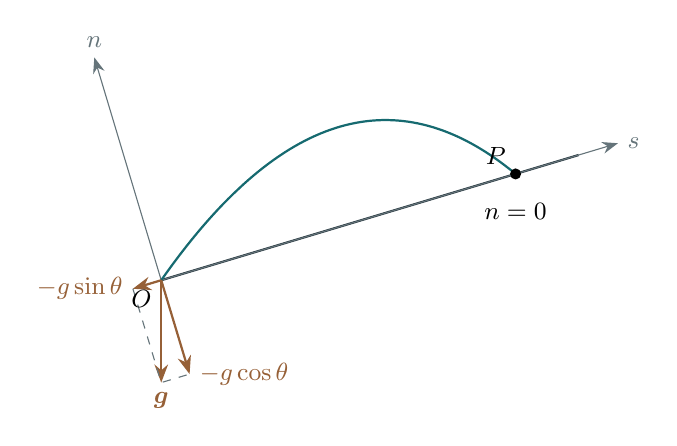
\begin{tikzpicture}

\draw[object] (0,0)--(5.3,1.59);
\draw[axis] (-.3,-.09)--(5.8,1.74) node[right] {$s$};
\draw[axis] (.09,-.3)--(-.85,2.83) node[above] {$n$};
\draw[traj,domain=0:4.5,samples=70] plot(\x,{(10/7)*\x-((10/7)-.3)*\x^2/4.5});
\fill (4.5,1.35) circle(2pt);\node[above left] at (4.5,1.35) {$P$};\node[below] at (4.5,1.10) {$n=0$};
\draw[force] (0,0)--(0,-1.3) node[below] {$\vect g$};
\draw[force] (0,0)--(-.36,-.108) node[left] {$-g\sin\theta$};
\draw[force] (0,0)--(.36,-1.192) node[right] {$-g\cos\theta$};
\draw[guide] (-.36,-.108)--(0,-1.3)--(.36,-1.192);
\node[below left] at (0,0) {$O$};

\end{tikzpicture}
\figcaption{解图 1.4B\quad 沿坡与垂直坡面建立坐标，飞行终点的条件变为 $n=0$。}
\end{minipage}\end{center}
\[
s=v_0\cos\alpha\,t-\frac12g\sin\theta\,t^2,
\qquad n=v_0\sin\alpha\,t-\frac12g\cos\theta\,t^2.
\]
由第二次 $n=0$ 得到同一 $t_f$；将它代入 $s$，展开后为
\[
R=\frac{2v_0^2\sin\alpha}{g\cos^2\theta}
(\cos\alpha\cos\theta-\sin\alpha\sin\theta),
\]
即上面的射程式。
\subsubsection*{求最优角}
用积化和差公式，
\[
2\sin\alpha\cos(\theta+\alpha)
=\sin(\theta+2\alpha)-\sin\theta.
\]
因而
\[
R(\alpha)=\frac{v_0^2}{g\cos^2\theta}
[\sin(\theta+2\alpha)-\sin\theta].
\]
在题设区间内，$\theta+2\alpha$ 可取 $\pi/2$；正弦的最大值为一，故
\[
\boxed{\alpha_*=\frac\pi4-\frac\theta2},\qquad
\boxed{R_{\max}=\frac{v_0^2(1-\sin\theta)}{g\cos^2\theta}
=\frac{v_0^2}{g(1+\sin\theta)}}.
\]
水平仰角则为 $\beta_* =\pi/4+\theta/2$。$\theta=0$ 时恢复水平地面的 $45^\circ$ 与 $v_0^2/g$；$\theta\to\pi/2^-$ 时沿坡最大射程趋于 $v_0^2/(2g)$，水平射程趋于零。
\subsubsection*{对落点横坐标求导的另一方法}
固定坡角时，解图1.4A中的$x_f$与沿坡射程$R$只相差正因子$\cos\theta$，
所以两者在同一发射角处取最大值。将第二交点写为
\[
x_f=\frac{v_0^2}{g}
\left[\sin2\beta-2\tan\theta\cos^2\beta\right],
\qquad \beta=\theta+\alpha,
\]
对$\alpha$求导时$\dd\beta/\dd\alpha=1$，从而
\[
\frac{\dd x_f}{\dd\alpha}
=\frac{2v_0^2}{g}
[\cos2\beta+\tan\theta\sin2\beta]
=\frac{2v_0^2}{g\cos\theta}\cos(2\beta-\theta).
\]
允许区间内的零点为$2\beta-\theta=\pi/2$，即
$\alpha=\pi/4-\theta/2$；从小仰角逐渐抬高炮口时，$x_f$先增加，越过这个角度后减小。
当$\alpha$趋近区间两端时，第二交点都回到炮口，射程趋于零，
这个内部驻点给出最大射程。求导还能说明从小仰角继续抬高时，落点怎样先远离炮口再返回。


\Needspace{5\baselineskip}

\pdfbookmark[4]{关键洞察}{c1-q4-h5}

\subsection*{关键洞察}

固定坡角后，决定射程变化的是$\sin(2\alpha+\theta)$。最远时$2\alpha+\theta=\pi/2$，因而炮口与坡面的夹角为$\pi/4-\theta/2$，与水平线的夹角为$\pi/4+\theta/2$。变图1.4V4画出两个角随坡度的变化。坡面变陡时，炮口向竖直方向抬高，同时与坡面更加接近。

\Needspace{5\baselineskip}

\pdfbookmark[4]{易错点}{c1-q4-h6}

\subsection*{易错点}

\begin{itemize}
\item 解图1.4A的水平、竖直分量使用$\beta$，解图1.4B的沿坡、法向分量使用$\alpha$。
\item 轨迹和坡线在炮口$O$已有交点。用$t>0$对应的交点$P$求射程。
\item 将沿坡长度投影到$x$轴得到$x_f$，换回沿坡长度时用
\[
R=\frac{x_f}{\cos\theta}.
\]
\item 对$\alpha$求极值前，先把$2\sin\alpha\cos(\theta+\alpha)$化成$\sin(\theta+2\alpha)-\sin\theta$。当$\theta=0$时，最优角为$45^\circ$，射程为$v_0^2/g$。
\end{itemize}

\Needspace{5\baselineskip}

\pdfbookmark[4]{课堂讲解建议}{c1-q4-h7}

\subsection*{课堂讲解建议}

在图1.4中分别描出水平线、坡线和炮口方向，请学生沿三条线标出$\theta,\alpha,\theta+\alpha$。让学生先回答“坡面上第一个交点在哪里”，再把正飞行时间代回位置式。此时请学生在图中从$P$向下作垂线，说明$x_f$与$R$的比例。

板书保留$2\sin\alpha\cos(\theta+\alpha)=\sin(\theta+2\alpha)-\sin\theta$。从正弦最大值读出最优角后，在解图1.4B改用法向坐标求飞行时间。问“改求最远的水平投影，炮口要再转动吗”，用变图1.4V2中的$OH=OP\cos\theta$解释同一落点使两个距离同时最大。最后让学生用变图1.4V5比较水平坡面和近竖直坡面。

\Needspace{5\baselineskip}

\pdfbookmark[4]{变式训练}{c1-q4-h8}

\subsection*{变式训练}

\begin{enumerate}
\item \textbf{向右下倾的山坡。}山坡角满足$-\pi/2<\theta<0$，炮弹向右并从坡面上方射出。求沿坡最远落点对应的仰角和射程。

变图1.4V1从向右的水平线量$\beta$，从坡面量$\alpha=\beta-\theta$。向右发射且初速指向坡面上方给出$\theta<\beta<\pi/2$。将$y=x\tan\theta$代入抛体坐标，取$t>0$的一根，得$t_f=2v_0\sin\alpha/(g\cos\theta)$。由于$\beta<\pi/2$，落点的水平坐标为正，沿下坡方向的射程为
\[
R=\frac{x_f}{\cos\theta}
=\frac{v_0^2}{g\cos^2\theta}[\sin(2\beta-\theta)-\sin\theta].
\]
当$2\beta-\theta=\pi/2$时取最大值。于是$\alpha_*=\pi/4-\theta/2>\pi/4$，而$\beta_*=\pi/4+\theta/2<\pi/4$。最大射程为$v_0^2/[g(1+\sin\theta)]$。
\begin{center}\begin{minipage}{.98\linewidth}\centering
\begin{tikzpicture}
\draw[axis] (-.3,0)--(6.1,0) node[right] {$x$};
\draw[object] (0,0)--(5.7,-1.9) node[right] {坡面};
\draw[traj,domain=0:5,samples=70] plot(\x,{.72*\x-(.72+1/3)*\x^2/5});
\draw[motion] (0,0)--(1.5,1.08) node[above] {$\vect v_0$};
\draw (1.05,-.35) arc[start angle=-18.435,end angle=0,radius=1.1068];
\node at (1.46,-.18) {$|\theta|$};
\draw (.665,-.222) arc[start angle=-18.435,end angle=35.75,radius=.701];
\node at (.88,.32) {$\alpha$};
\fill (5,-1.6667) circle(1.6pt) node[below left] {$P$};
\node[below left] at (0,0) {$O$};
\end{tikzpicture}
\figcaption{变图1.4V1\quad 坡面低于发射点，炮弹在右侧与坡面相交}
\end{minipage}\end{center}

\item \textbf{最大水平射程。}固定上坡坡角，改求$x_f$的最大值及相应角度。

图1.4V2中$OP$是沿坡射程，$P$的垂直投影为$H$，故$OH=x_f=R\cos\theta$。随发射角变化，$P$在同一条坡线上移动，比例$OH/OP=\cos\theta$固定且为正。于是两段距离在同一发射角$\alpha_*=\pi/4-\theta/2$处最长，得到
\[
x_{\max}=R_{\max}\cos\theta
=\frac{v_0^2\cos\theta}{g(1+\sin\theta)}.
\]
\begin{center}\begin{minipage}{.98\linewidth}\centering
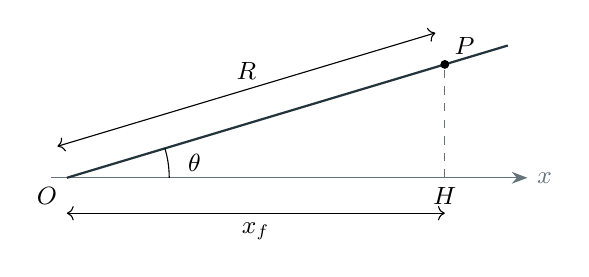
\begin{tikzpicture}
\draw[axis] (-.2,0)--(5.85,0) node[right] {$x$};
\draw[object] (0,0)--(5.6,1.68);
\draw[guide] (4.8,0)--(4.8,1.44);
\draw[thin,<->] (0,-.45)--(4.8,-.45) node[midway,below] {$x_f$};
\draw[thin,<->] (-.12,.4)--(4.68,1.84) node[midway,above] {$R$};
\fill (4.8,1.44) circle(1.6pt) node[above right] {$P$};
\node[below] at (4.8,0) {$H$};
\node[below left] at (0,0) {$O$};
\draw (1.3,0) arc(0:16.699:1.3);\node at (1.62,.19) {$\theta$};
\end{tikzpicture}
\figcaption{变图1.4V2\quad 沿坡射程在水平方向上的投影}
\end{minipage}\end{center}

\item \textbf{沿坡坐标中的最远落点。}在$s,n$坐标内直接求最优角。图1.4V3把初速度与重力分别投影在这两个方向上。落地时法向位移再次为零，因此
\[
n(t)=v_0\sin\alpha\,t-\tfrac12g\cos\theta\,t^2,
\qquad
t_f=\frac{2v_0\sin\alpha}{g\cos\theta}.
\]
将此时刻代入$s(t)=v_0\cos\alpha\,t-g\sin\theta\,t^2/2$，得到两项：
\[
R=\frac{2v_0^2\sin\alpha\cos\alpha}{g\cos\theta}
-\frac{2v_0^2\sin^2\alpha\sin\theta}{g\cos^2\theta}.
\]
提取公因子后，括号内是$\cos\alpha\cos\theta-\sin\alpha\sin\theta$，即$\cos(\theta+\alpha)$。于是
\[
R=\frac{v_0^2}{g\cos^2\theta}[\sin(2\alpha+\theta)-\sin\theta].
\]
令正弦为1，读得$\alpha_*=\pi/4-\theta/2$。
\begin{center}\begin{minipage}{.98\linewidth}\centering
\begin{tikzpicture}
\draw[axis] (-1,0)--(5.7,0) node[right] {$s$};
\draw[axis] (0,-1.6)--(0,2.5) node[above] {$n$};
\draw[motion] (0,0)--(2.5,1.5) node[right] {$\vect v_0$};
\draw[guide] (0,1.5)--(2.5,1.5)--(2.5,0);
\node[left] at (0,1.5) {$v_0\sin\alpha$};
\node[below] at (2.5,0) {$v_0\cos\alpha$};
\draw[force] (0,0)--(-.45,-1.5) node[below left] {$\vect g$};
\draw[guide] (-.45,0)--(-.45,-1.5)--(0,-1.5);
\node[above left] at (-.45,0) {$-g\sin\theta$};
\node[right] at (0,-1.5) {$-g\cos\theta$};
\draw (.78,0) arc(0:30.964:.78);\node at (1.06,.22) {$\alpha$};
\end{tikzpicture}
\figcaption{变图1.4V3\quad 以$s,n$为直角坐标绘制速度与重力的两个分量}
\end{minipage}\end{center}

\item \textbf{改变坡角时的最优发射方向。}保持$v_0$不变，求最优相对角、最优水平角与最大射程随坡角的变化。

由$\beta_*=\theta+\alpha_*$，图1.4V4中两角相对于$\theta$的斜率分别为$-1/2$与$1/2$。由射程式求导，
\[
\frac{\dd\alpha_*}{\dd\theta}=-\frac12,\qquad
\frac{\dd\beta_*}{\dd\theta}=\frac12,\qquad
\frac{\dd R_{\max}}{\dd\theta}
=-\frac{v_0^2\cos\theta}{g(1+\sin\theta)^2}.
\]
坡越陡，最优炮口越靠近竖直方向，炮口与坡面的夹角越小。最大射程也随坡角增大而缩短。
\begin{center}\begin{minipage}{.98\linewidth}\centering
\begin{tikzpicture}
\draw[axis] (0,0)--(5.65,0) node[right] {$\theta$};
\draw[axis] (0,0)--(0,3.1) node[above] {角度};
\draw[traj] (0,1.3)--(5,2.6) node[right] {$\beta_*$};
\draw[thick,dashed,warm] (0,1.3)--(5,0) node[above right] {$\alpha_*$};
\draw[guide] (0,2.6)--(5,2.6)--(5,0);
\node[left] at (0,1.3) {$\pi/4$};\node[left] at (0,2.6) {$\pi/2$};
\node[below] at (5,0) {$\pi/2$};
\end{tikzpicture}
\figcaption{变图1.4V4\quad 两个最优角在水平坡面相同，随坡角向相反方向变化}
\end{minipage}\end{center}

\item \textbf{水平坡与陡坡极限。}求最优发射时$R_{\max}$及$x_{\max}$在$\theta=0$和$\theta\to\pi/2^-$的值，并说明图中的两个终值。

把式中的$\cos^2\theta$写为$(1-\sin\theta)(1+\sin\theta)$，约去$1-\sin\theta$后再取极限：
\[
\frac{gR_{\max}}{v_0^2}=\frac1{1+\sin\theta},\qquad
\frac{gx_{\max}}{v_0^2}=\frac{\cos\theta}{1+\sin\theta}.
\]
图1.4V5在$\theta=0$处两条线均从1出发，对应$45^\circ$发射与$v_0^2/g$的射程。随着坡面趋近竖直，$\alpha_*\to0$、$\beta_*\to\pi/2$。沿坡射程趋于$v_0^2/(2g)$，水平投影则趋零。
\begin{center}\begin{minipage}{.98\linewidth}\centering
\begin{tikzpicture}
\draw[axis] (0,0)--(6.15,0) node[right] {$\theta$};
\draw[axis] (0,0)--(0,3.15) node[above] {距离比};
\draw[traj,domain=0:90,samples=80] plot({\x/18},{2.55/(1+sin(\x))});
\draw[thick,dashed,warm,domain=0:90,samples=80] plot({\x/18},{2.55*cos(\x)/(1+sin(\x))});
\draw[guide] (0,1.275)--(5,1.275)--(5,0);
\node[left] at (0,1.275) {$1/2$};\node[left] at (0,2.55) {$1$};
\node[below] at (5,0) {$\pi/2$};
\node[right] at (5,1.275) {$gR_{\max}/v_0^2$};
\node[right,warm] at (3.12,.78) {$gx_{\max}/v_0^2$};
\end{tikzpicture}
\figcaption{变图1.4V5\quad 沿坡距离与它的水平投影在陡坡极限取不同的值}
\end{minipage}\end{center}
\end{enumerate}

\clearpage

\pdfbookmark[3]{第 5 题 等射程抛体的飞行时间乘积}{c1-q5}

\section*{第 5 题\quad 等射程抛体的飞行时间乘积}\label{book-question-1-5}

\tagline{M-01-05}

两质点从同一水平地面上的同一点，以相同速率 $v_0$、不同仰角 $\alpha_1$ 和 $\alpha_2$ 抛出，且 $0<\alpha_1,\alpha_2<\pi/2$。两质点均落回该水平地面，空气阻力忽略。

若两次抛射的射程同为 $R$，证明两次飞行时间满足
\[
T_1T_2=\frac{2R}{g}.
\]

\begin{center}
\begin{tikzpicture}[x=1cm,y=1cm]
\draw[axis] (-.35,0)--(6.5,0) node[right] {$x$};\draw[axis] (0,-.2)--(0,3.5) node[above] {$y$};
\draw[traj,domain=0:6,samples=70] plot (\x,{1.73205*\x*(1-\x/6)});
\draw[traj,dashed,domain=0:6,samples=70] plot (\x,{.57735*\x*(1-\x/6)});
\draw[motion] (0,0)--(.6,1.039);\draw[motion] (0,0)--(1.039,.6);
\draw (.7,0) arc(0:30:.7);\node at (1,.22) {$\alpha_1$};
\draw (1.0,0) arc(0:60:1);\node at (1.05,1.05) {$\alpha_2$};
\node[color=accent] at (4.2,2.7) {高轨迹};\node[color=accent] at (4.5,.95) {低轨迹};
\fill (6,0) circle (1.8pt);\node[below] at (6,-.05) {$R$};\node[below left] at (0,0) {$O$};
\end{tikzpicture}
\figcaption{图 1.5\quad 同初速、同射程的两条不同轨迹。}
\end{center}

\Needspace{5\baselineskip}

\pdfbookmark[4]{题型定位}{c1-q5-h0}

\subsection*{题型定位}

比较同速率斜抛的两条等射程轨迹。共同射程确定一对互余发射角，由两竖直初速度的乘积求时间积，再把时间与轨迹最高点的高度联系起来。

\Needspace{5\baselineskip}

\pdfbookmark[4]{知识点}{c1-q5-h1}

\subsection*{知识点}

水平匀速与竖直匀变速共同给出 $R=v_0^2\sin2\alpha/g$ 和 $T=2v_0\sin\alpha/g$。射程曲线关于 $45^\circ$ 对称，利用差化积可解出等射程的两个角。最高点位于 $x=R/2$，其高度为 $H_i=gT_i^2/8$。


\Needspace{5\baselineskip}

\pdfbookmark[4]{物理图像}{c1-q5-h2}

\subsection*{物理图像}

题图1.5中，低角度轨迹的水平初速度大、竖直初速度小，飞行时间短。解图1.5A把两次等射程画成一条水平线，与射程曲线有两个交点。两条轨迹的顶点沿同一竖线对齐，高轨迹的顶点到地面距离较大，下落所需时间也较长。

\Needspace{5\baselineskip}

\pdfbookmark[4]{解题入口}{c1-q5-h3}

\subsection*{解题入口}

先由 $y=0$ 取落地的正时间根，再乘水平速度求射程。比较两次射程并差化积，在两个角均为锐角且彼此不同的条件下得到 $\alpha_1+\alpha_2=\pi/2$。时间式相乘后把 $\sin\alpha_2$ 换成 $\cos\alpha_1$，即可用 $\sin2\alpha_1$ 消去角度。

\Needspace{5\baselineskip}

\pdfbookmark[4]{标准解法}{c1-q5-h4}

\subsection*{标准解法}

题图 1.5 的两条轨迹从同一点出发并落到同一水平地面。低角度轨迹的水平速度较大，高角度轨迹的竖直初速度较大；先由落地条件分别求时间和射程。
\subsubsection*{单次抛射的时间与射程}
对仰角为 $\alpha$ 的一次运动，
\[
x=v_0\cos\alpha\,t,\qquad
y=v_0\sin\alpha\,t-\frac12gt^2.
\]
落回地面时 $y=0$。舍去发射根 $t=0$ 后，
\[
T=\frac{2v_0\sin\alpha}{g},\qquad
R=v_0\cos\alpha\,T=\frac{v_0^2}{g}\sin2\alpha.
\]
\subsubsection*{等射程的两角互余}
初速相同、射程相同，故 $\sin2\alpha_1=\sin2\alpha_2$。将差化为乘积，
\[
2\cos(\alpha_1+\alpha_2)\sin(\alpha_1-\alpha_2)=0.
\]
两角均在 $(0,\pi/2)$ 且不同，所以 $\sin(\alpha_1-\alpha_2)\ne0$，只能有
\[
\boxed{\alpha_1+\alpha_2=\frac\pi2}.
\]
\begin{center}\begin{minipage}{\linewidth}\centering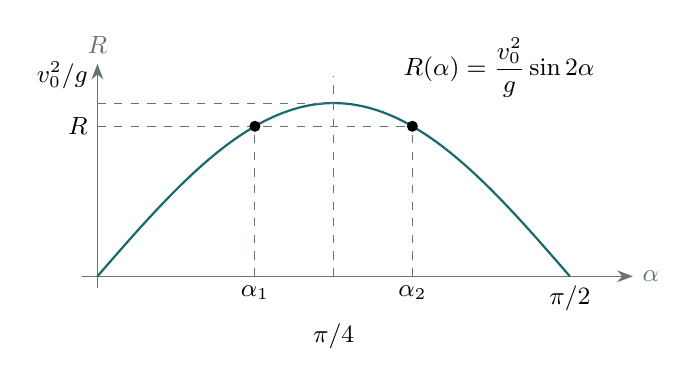
\begin{tikzpicture}

\draw[axis] (-.2,0)--(6.8,0) node[right] {$\alpha$};\draw[axis] (0,-.15)--(0,2.7) node[above] {$R$};
\draw[traj,domain=0:6,samples=90] plot(\x,{2.2*sin(30*\x)});
\draw[guide] (0,{2.2*sin(60)})--(4,{2.2*sin(60)});\node[left] at (0,{2.2*sin(60)}) {$R$};
\draw[guide] (0,2.2)--(3,2.2);\node[above left,yshift=1.5pt] at (0,2.2) {$v_0^2/g$};
\draw[guide] (2,0)--(2,{2.2*sin(60)});\draw[guide] (4,0)--(4,{2.2*sin(60)});
\fill (2,{2.2*sin(60)}) circle(2pt);\fill (4,{2.2*sin(60)}) circle(2pt);
\node[below] at (2,0) {$\alpha_1$};\node[below] at (4,0) {$\alpha_2$};\node[below] at (6,0) {$\pi/2$};
\draw[guide] (3,0)--(3,2.55);\node[below] at (3,-.48) {$\pi/4$};
\node at (5.1,2.65) {$R(\alpha)=\dfrac{v_0^2}{g}\sin2\alpha$};

\end{tikzpicture}
\figcaption{解图 1.5A\quad 射程曲线关于 $\alpha=\pi/4$ 对称；同一射程的两个不同仰角互余。}
\end{minipage}\end{center}
解图 1.5A 中，两条竖虚线从同一射程水平线落到横轴，读得一低一高的两个角。它们到 $45^\circ$ 的距离相同。射程升至 $v_0^2/g$ 时，两交点合为顶点，对应唯一的 $45^\circ$ 发射角。
\subsubsection*{求飞行时间乘积}
分别写出两次飞行时间并相乘，
\[
T_1T_2=\frac{4v_0^2}{g^2}\sin\alpha_1\sin\alpha_2
=\frac{4v_0^2}{g^2}\sin\alpha_1\cos\alpha_1
=\frac{2v_0^2}{g^2}\sin2\alpha_1.
\]
由 $R=v_0^2\sin2\alpha_1/g$，得到
\[
\boxed{T_1T_2=\frac{2R}{g}}.
\]
从时间式看，低角度的竖直初速度较小，所以先回到地面。两次飞行时间的乘积由共同射程确定。$R/g$ 的量纲是时间平方。等高落地使两次时间都等于各自竖直初速度的 $2/g$ 倍，互余角又让这两个竖直分量恰好等于一次发射里的水平、竖直分量。
\subsubsection*{共同对称轴与两个顶点的高度}
消去时间并使用落点 $x=R,y=0$，任一轨迹可改写为
\[
y=x\tan\alpha\left(1-\frac{x}{R}\right).
\]
最高点都在 $x=R/2$，高度为 $H_i=R\tan\alpha_i/4$。因为两角互余，$\tan\alpha_1\tan\alpha_2=1$，所以
\[
H_1H_2=\frac{R^2}{16}.
\]
题图 1.5 中，两个最高点沿 $x=R/2$ 竖直对齐。每个质点从最高点以零竖直速度下落，经过 $T_i/2$ 到达地面，因此 $H_i=gT_i^2/8$。这给出 $T_1T_2=(8/g)\sqrt{H_1H_2}=2R/g$。读出两顶点的高度，还可用 $T_2/T_1=\sqrt{H_2/H_1}$ 比较飞行时间。

\Needspace{5\baselineskip}

\pdfbookmark[4]{关键洞察}{c1-q5-h5}

\subsection*{关键洞察}

同速率时，互余变换交换水平、竖直初速度。两个速度分量的乘积相同，所以射程相同；分别把两竖直分量乘以 $2/g$，便得到两个飞行时间及其固定的乘积。

\Needspace{5\baselineskip}

\pdfbookmark[4]{易错点}{c1-q5-h6}

\subsection*{易错点}

\begin{itemize}
\item 等射程方程有同角与互余两类解。题设指定不同角，差化积中的 $\sin(\alpha_1-\alpha_2)$ 非零。
\item 时间可由水平位移反算为 $T=R/(v_0\cos\alpha)$。分母取图中沿地面的速度分量。
\item $T=2v_0\sin\alpha/g$ 取自与发射点同高的落点。目标改在高度 $H$ 时，应把 $y=H$ 代入轨迹方程。
\end{itemize}

\Needspace{5\baselineskip}

\pdfbookmark[4]{课堂讲解建议}{c1-q5-h7}

\subsection*{课堂讲解建议}

在解图1.5A上画一条低于顶点的水平线，问“右交点对应哪个角”。答为左交点角的余角，因为两点到 $45^\circ$ 的距离相等。随后让学生在题图标出两条轨迹的水平、竖直初速度，指出低轨迹先落地。把水平线抬到顶点，追问还有几个角可选，答为一个，即 $45^\circ$。最后问怎样由两顶点估计飞行时间比，利用从顶点到地面的自由落体得 $T_2/T_1=\sqrt{H_2/H_1}$。

\Needspace{5\baselineskip}

\pdfbookmark[4]{变式训练}{c1-q5-h8}

\subsection*{变式训练}

\begin{enumerate}
\item 两次初速不同但射程同为 $R$，求飞行时间乘积，并判断它是否由 $R$ 唯一确定。把 $v_{iy}=gT_i/2$ 和 $v_{ix}=R/T_i$ 相除，得 $\tan\alpha_i=gT_i^2/(2R)$，故
\[
T_1T_2=\frac{2R}{g}\sqrt{\tan\alpha_1\tan\alpha_2}.
\]
变图1.5V1取 $30^\circ$ 和 $45^\circ$，分别用 $v_i^2=gR/\sin2\alpha_i$ 选初速。图中两条轨迹都到达 $x=R$，时间积却为 $(2R/g)3^{-1/4}$。当另给互余角条件时，两正切的乘积为一，时间积恢复为 $2R/g$。
\begin{center}\begin{minipage}{.98\linewidth}\centering
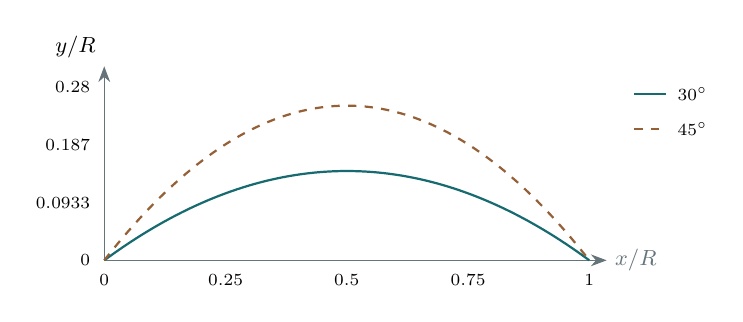
\begin{tikzpicture}[scale=.88,transform shape]
\draw[axis] (0,0.0000000)--(7.25,0.0000000) node[right] {$x/R$};
\draw[axis] (0.0000000,0)--(0.0000000,2.8);
\node[above left] at (0.0000000,2.8) {$y/R$};
\node[below,font=\scriptsize] at (0.0000000,-0.0800000) {$0$};
\node[below,font=\scriptsize] at (1.7500000,-0.0800000) {$0.25$};
\node[below,font=\scriptsize] at (3.5000000,-0.0800000) {$0.5$};
\node[below,font=\scriptsize] at (5.2500000,-0.0800000) {$0.75$};
\node[below,font=\scriptsize] at (7.0000000,-0.0800000) {$1$};
\node[left,font=\scriptsize] at (-0.0800000,0.0000000) {$0$};
\node[left,font=\scriptsize] at (-0.0800000,0.8333333) {$0.0933$};
\node[left,font=\scriptsize] at (-0.0800000,1.6666667) {$0.187$};
\node[left,font=\scriptsize] at (-0.0800000,2.5000000) {$0.28$};
\draw[thick,color=accent] plot coordinates {(0.0000000,0.0000000) (0.0583333,0.0425996) (0.1166667,0.0844833) (0.1750000,0.1256510) (0.2333333,0.1661028) (0.2916667,0.2058385) (0.3500000,0.2448584) (0.4083333,0.2831622) (0.4666667,0.3207501) (0.5250000,0.3576221) (0.5833333,0.3937781) (0.6416667,0.4292181) (0.7000000,0.4639422) (0.7583333,0.4979503) (0.8166667,0.5312424) (0.8750000,0.5638186) (0.9333333,0.5956788) (0.9916667,0.6268231) (1.0500000,0.6572514) (1.1083333,0.6869638) (1.1666667,0.7159602) (1.2250000,0.7442406) (1.2833333,0.7718050) (1.3416667,0.7986536) (1.4000000,0.8247861) (1.4583333,0.8502027) (1.5166667,0.8749033) (1.5750000,0.8988880) (1.6333333,0.9221567) (1.6916667,0.9447094) (1.7500000,0.9665462) (1.8083333,0.9876670) (1.8666667,1.0080719) (1.9250000,1.0277608) (1.9833333,1.0467337) (2.0416667,1.0649907) (2.1000000,1.0825318) (2.1583333,1.0993568) (2.2166667,1.1154659) (2.2750000,1.1308591) (2.3333333,1.1455362) (2.3916667,1.1594975) (2.4500000,1.1727427) (2.5083333,1.1852720) (2.5666667,1.1970854) (2.6250000,1.2081828) (2.6833333,1.2185642) (2.7416667,1.2282296) (2.8000000,1.2371791) (2.8583333,1.2454127) (2.9166667,1.2529303) (2.9750000,1.2597319) (3.0333333,1.2658176) (3.0916667,1.2711873) (3.1500000,1.2758410) (3.2083333,1.2797788) (3.2666667,1.2830006) (3.3250000,1.2855065) (3.3833333,1.2872964) (3.4416667,1.2883703) (3.5000000,1.2887283) (3.5583333,1.2883703) (3.6166667,1.2872964) (3.6750000,1.2855065) (3.7333333,1.2830006) (3.7916667,1.2797788) (3.8500000,1.2758410) (3.9083333,1.2711873) (3.9666667,1.2658176) (4.0250000,1.2597319) (4.0833333,1.2529303) (4.1416667,1.2454127) (4.2000000,1.2371791) (4.2583333,1.2282296) (4.3166667,1.2185642) (4.3750000,1.2081828) (4.4333333,1.1970854) (4.4916667,1.1852720) (4.5500000,1.1727427) (4.6083333,1.1594975) (4.6666667,1.1455362) (4.7250000,1.1308591) (4.7833333,1.1154659) (4.8416667,1.0993568) (4.9000000,1.0825318) (4.9583333,1.0649907) (5.0166667,1.0467337) (5.0750000,1.0277608) (5.1333333,1.0080719) (5.1916667,0.9876670) (5.2500000,0.9665462) (5.3083333,0.9447094) (5.3666667,0.9221567) (5.4250000,0.8988880) (5.4833333,0.8749033) (5.5416667,0.8502027) (5.6000000,0.8247861) (5.6583333,0.7986536) (5.7166667,0.7718050) (5.7750000,0.7442406) (5.8333333,0.7159602) (5.8916667,0.6869638) (5.9500000,0.6572514) (6.0083333,0.6268231) (6.0666667,0.5956788) (6.1250000,0.5638186) (6.1833333,0.5312424) (6.2416667,0.4979503) (6.3000000,0.4639422) (6.3583333,0.4292181) (6.4166667,0.3937781) (6.4750000,0.3576221) (6.5333333,0.3207501) (6.5916667,0.2831622) (6.6500000,0.2448584) (6.7083333,0.2058385) (6.7666667,0.1661028) (6.8250000,0.1256510) (6.8833333,0.0844833) (6.9416667,0.0425996) (7.0000000,0.0000000)};
\draw[thick,color=accent] (7.65,2.4)--(8.1,2.4);\node[right,font=\scriptsize] at (8.15,2.4) {$30^\circ$};
\draw[thick,dashed,color=warm] plot coordinates {(0.0000000,0.0000000) (0.0583333,0.0737847) (0.1166667,0.1463294) (0.1750000,0.2176339) (0.2333333,0.2876984) (0.2916667,0.3565228) (0.3500000,0.4241071) (0.4083333,0.4904514) (0.4666667,0.5555556) (0.5250000,0.6194196) (0.5833333,0.6820437) (0.6416667,0.7434276) (0.7000000,0.8035714) (0.7583333,0.8624752) (0.8166667,0.9201389) (0.8750000,0.9765625) (0.9333333,1.0317460) (0.9916667,1.0856895) (1.0500000,1.1383929) (1.1083333,1.1898562) (1.1666667,1.2400794) (1.2250000,1.2890625) (1.2833333,1.3368056) (1.3416667,1.3833085) (1.4000000,1.4285714) (1.4583333,1.4725942) (1.5166667,1.5153770) (1.5750000,1.5569196) (1.6333333,1.5972222) (1.6916667,1.6362847) (1.7500000,1.6741071) (1.8083333,1.7106895) (1.8666667,1.7460317) (1.9250000,1.7801339) (1.9833333,1.8129960) (2.0416667,1.8446181) (2.1000000,1.8750000) (2.1583333,1.9041419) (2.2166667,1.9320437) (2.2750000,1.9587054) (2.3333333,1.9841270) (2.3916667,2.0083085) (2.4500000,2.0312500) (2.5083333,2.0529514) (2.5666667,2.0734127) (2.6250000,2.0926339) (2.6833333,2.1106151) (2.7416667,2.1273562) (2.8000000,2.1428571) (2.8583333,2.1571181) (2.9166667,2.1701389) (2.9750000,2.1819196) (3.0333333,2.1924603) (3.0916667,2.2017609) (3.1500000,2.2098214) (3.2083333,2.2166419) (3.2666667,2.2222222) (3.3250000,2.2265625) (3.3833333,2.2296627) (3.4416667,2.2315228) (3.5000000,2.2321429) (3.5583333,2.2315228) (3.6166667,2.2296627) (3.6750000,2.2265625) (3.7333333,2.2222222) (3.7916667,2.2166419) (3.8500000,2.2098214) (3.9083333,2.2017609) (3.9666667,2.1924603) (4.0250000,2.1819196) (4.0833333,2.1701389) (4.1416667,2.1571181) (4.2000000,2.1428571) (4.2583333,2.1273562) (4.3166667,2.1106151) (4.3750000,2.0926339) (4.4333333,2.0734127) (4.4916667,2.0529514) (4.5500000,2.0312500) (4.6083333,2.0083085) (4.6666667,1.9841270) (4.7250000,1.9587054) (4.7833333,1.9320437) (4.8416667,1.9041419) (4.9000000,1.8750000) (4.9583333,1.8446181) (5.0166667,1.8129960) (5.0750000,1.7801339) (5.1333333,1.7460317) (5.1916667,1.7106895) (5.2500000,1.6741071) (5.3083333,1.6362847) (5.3666667,1.5972222) (5.4250000,1.5569196) (5.4833333,1.5153770) (5.5416667,1.4725942) (5.6000000,1.4285714) (5.6583333,1.3833085) (5.7166667,1.3368056) (5.7750000,1.2890625) (5.8333333,1.2400794) (5.8916667,1.1898562) (5.9500000,1.1383929) (6.0083333,1.0856895) (6.0666667,1.0317460) (6.1250000,0.9765625) (6.1833333,0.9201389) (6.2416667,0.8624752) (6.3000000,0.8035714) (6.3583333,0.7434276) (6.4166667,0.6820437) (6.4750000,0.6194196) (6.5333333,0.5555556) (6.5916667,0.4904514) (6.6500000,0.4241071) (6.7083333,0.3565228) (6.7666667,0.2876984) (6.8250000,0.2176339) (6.8833333,0.1463294) (6.9416667,0.0737847) (7.0000000,0.0000000)};
\draw[thick,dashed,color=warm] (7.65,1.9)--(8.1,1.9);\node[right,font=\scriptsize] at (8.15,1.9) {$45^\circ$};
\end{tikzpicture}
\figcaption{变图1.5V1\quad 不同初速、相同射程的两个实例。}
\end{minipage}\end{center}
\item 同速率 $v_0$ 抛向 $(R,H)$，求两发射角的关系。置 $p=\tan\alpha$、$A=gR^2/(2v_0^2)>0$，通过目标需满足 $Ap^2-Rp+(A+H)=0$。两个不同锐角对应判别式 $R^2-4A(A+H)>0$ 且两根为正。由韦达定理，
\[
p_1p_2=1+\frac{2v_0^2H}{gR^2},\qquad T_i=\frac{R\sqrt{1+p_i^2}}{v_0}>0.
\]
变图1.5V2取 $H=0.4R,A=0.25R$，两条实轨迹通过同一点，正切乘积为2.6。互余所需的乘积一对应 $H=0$。
\begin{center}\begin{minipage}{.98\linewidth}\centering
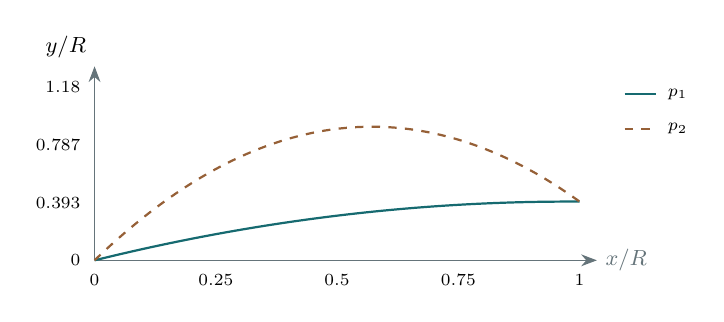
\begin{tikzpicture}[scale=.88,transform shape]
\draw[axis] (0,0.0000000)--(7.25,0.0000000) node[right] {$x/R$};
\draw[axis] (0.0000000,0)--(0.0000000,2.8);
\node[above left] at (0.0000000,2.8) {$y/R$};
\node[below,font=\scriptsize] at (0.0000000,-0.0800000) {$0$};
\node[below,font=\scriptsize] at (1.7500000,-0.0800000) {$0.25$};
\node[below,font=\scriptsize] at (3.5000000,-0.0800000) {$0.5$};
\node[below,font=\scriptsize] at (5.2500000,-0.0800000) {$0.75$};
\node[below,font=\scriptsize] at (7.0000000,-0.0800000) {$1$};
\node[left,font=\scriptsize] at (-0.0800000,0.0000000) {$0$};
\node[left,font=\scriptsize] at (-0.0800000,0.8333333) {$0.393$};
\node[left,font=\scriptsize] at (-0.0800000,1.6666667) {$0.787$};
\node[left,font=\scriptsize] at (-0.0800000,2.5000000) {$1.18$};
\draw[thick,color=accent] plot coordinates {(0.0000000,0.0000000) (0.0583333,0.0143593) (0.1166667,0.0285960) (0.1750000,0.0427100) (0.2333333,0.0567014) (0.2916667,0.0705701) (0.3500000,0.0843162) (0.4083333,0.0979396) (0.4666667,0.1114405) (0.5250000,0.1248186) (0.5833333,0.1380742) (0.6416667,0.1512070) (0.7000000,0.1642173) (0.7583333,0.1771049) (0.8166667,0.1898699) (0.8750000,0.2025122) (0.9333333,0.2150319) (0.9916667,0.2274289) (1.0500000,0.2397033) (1.1083333,0.2518551) (1.1666667,0.2638842) (1.2250000,0.2757907) (1.2833333,0.2875745) (1.3416667,0.2992357) (1.4000000,0.3107743) (1.4583333,0.3221902) (1.5166667,0.3334834) (1.5750000,0.3446541) (1.6333333,0.3557021) (1.6916667,0.3666274) (1.7500000,0.3774301) (1.8083333,0.3881102) (1.8666667,0.3986676) (1.9250000,0.4091024) (1.9833333,0.4194145) (2.0416667,0.4296040) (2.1000000,0.4396709) (2.1583333,0.4496151) (2.2166667,0.4594367) (2.2750000,0.4691356) (2.3333333,0.4787119) (2.3916667,0.4881655) (2.4500000,0.4974965) (2.5083333,0.5067049) (2.5666667,0.5157906) (2.6250000,0.5247537) (2.6833333,0.5335942) (2.7416667,0.5423120) (2.8000000,0.5509071) (2.8583333,0.5593797) (2.9166667,0.5677295) (2.9750000,0.5759568) (3.0333333,0.5840614) (3.0916667,0.5920433) (3.1500000,0.5999026) (3.2083333,0.6076393) (3.2666667,0.6152534) (3.3250000,0.6227447) (3.3833333,0.6301135) (3.4416667,0.6373596) (3.5000000,0.6444831) (3.5583333,0.6514839) (3.6166667,0.6583621) (3.6750000,0.6651176) (3.7333333,0.6717505) (3.7916667,0.6782608) (3.8500000,0.6846484) (3.9083333,0.6909134) (3.9666667,0.6970557) (4.0250000,0.7030754) (4.0833333,0.7089725) (4.1416667,0.7147469) (4.2000000,0.7203987) (4.2583333,0.7259278) (4.3166667,0.7313343) (4.3750000,0.7366181) (4.4333333,0.7417793) (4.4916667,0.7468179) (4.5500000,0.7517338) (4.6083333,0.7565271) (4.6666667,0.7611978) (4.7250000,0.7657458) (4.7833333,0.7701711) (4.8416667,0.7744738) (4.9000000,0.7786539) (4.9583333,0.7827114) (5.0166667,0.7866461) (5.0750000,0.7904583) (5.1333333,0.7941478) (5.1916667,0.7977147) (5.2500000,0.8011589) (5.3083333,0.8044805) (5.3666667,0.8076795) (5.4250000,0.8107558) (5.4833333,0.8137094) (5.5416667,0.8165404) (5.6000000,0.8192488) (5.6583333,0.8218346) (5.7166667,0.8242977) (5.7750000,0.8266381) (5.8333333,0.8288559) (5.8916667,0.8309511) (5.9500000,0.8329237) (6.0083333,0.8347735) (6.0666667,0.8365008) (6.1250000,0.8381054) (6.1833333,0.8395874) (6.2416667,0.8409467) (6.3000000,0.8421834) (6.3583333,0.8432974) (6.4166667,0.8442888) (6.4750000,0.8451576) (6.5333333,0.8459037) (6.5916667,0.8465272) (6.6500000,0.8470281) (6.7083333,0.8474063) (6.7666667,0.8476618) (6.8250000,0.8477947) (6.8833333,0.8478050) (6.9416667,0.8476926) (7.0000000,0.8474576)};
\draw[thick,color=accent] (7.65,2.4)--(8.1,2.4);\node[right,font=\scriptsize] at (8.15,2.4) {$p_1$};
\draw[thick,dashed,color=warm] plot coordinates {(0.0000000,0.0000000) (0.0583333,0.0557914) (0.1166667,0.1107637) (0.1750000,0.1649171) (0.2333333,0.2182516) (0.2916667,0.2707670) (0.3500000,0.3224635) (0.4083333,0.3733410) (0.4666667,0.4233995) (0.5250000,0.4726390) (0.5833333,0.5210596) (0.6416667,0.5686611) (0.7000000,0.6154437) (0.7583333,0.6614073) (0.8166667,0.7065520) (0.8750000,0.7508776) (0.9333333,0.7943843) (0.9916667,0.8370720) (1.0500000,0.8789408) (1.1083333,0.9199905) (1.1666667,0.9602213) (1.2250000,0.9996331) (1.2833333,1.0382259) (1.3416667,1.0759997) (1.4000000,1.1129546) (1.4583333,1.1490904) (1.5166667,1.1844073) (1.5750000,1.2189053) (1.6333333,1.2525842) (1.6916667,1.2854442) (1.7500000,1.3174852) (1.8083333,1.3487072) (1.8666667,1.3791102) (1.9250000,1.4086942) (1.9833333,1.4374593) (2.0416667,1.4654054) (2.1000000,1.4925325) (2.1583333,1.5188407) (2.2166667,1.5443298) (2.2750000,1.5690000) (2.3333333,1.5928512) (2.3916667,1.6158834) (2.4500000,1.6380967) (2.5083333,1.6594909) (2.5666667,1.6800662) (2.6250000,1.6998225) (2.6833333,1.7187599) (2.7416667,1.7368782) (2.8000000,1.7541776) (2.8583333,1.7706580) (2.9166667,1.7863194) (2.9750000,1.8011619) (3.0333333,1.8151853) (3.0916667,1.8283898) (3.1500000,1.8407753) (3.2083333,1.8523418) (3.2666667,1.8630894) (3.3250000,1.8730180) (3.3833333,1.8821276) (3.4416667,1.8904182) (3.5000000,1.8978898) (3.5583333,1.9045425) (3.6166667,1.9103761) (3.6750000,1.9153908) (3.7333333,1.9195866) (3.7916667,1.9229633) (3.8500000,1.9255211) (3.9083333,1.9272599) (3.9666667,1.9281797) (4.0250000,1.9282805) (4.0833333,1.9275624) (4.1416667,1.9260252) (4.2000000,1.9236691) (4.2583333,1.9204940) (4.3166667,1.9165000) (4.3750000,1.9116869) (4.4333333,1.9060549) (4.4916667,1.8996039) (4.5500000,1.8923340) (4.6083333,1.8842450) (4.6666667,1.8753371) (4.7250000,1.8656102) (4.7833333,1.8550643) (4.8416667,1.8436994) (4.9000000,1.8315156) (4.9583333,1.8185128) (5.0166667,1.8046910) (5.0750000,1.7900502) (5.1333333,1.7745904) (5.1916667,1.7583117) (5.2500000,1.7412140) (5.3083333,1.7232973) (5.3666667,1.7045616) (5.4250000,1.6850070) (5.4833333,1.6646333) (5.5416667,1.6434407) (5.6000000,1.6214291) (5.6583333,1.5985986) (5.7166667,1.5749490) (5.7750000,1.5504805) (5.8333333,1.5251930) (5.8916667,1.4990865) (5.9500000,1.4721611) (6.0083333,1.4444167) (6.0666667,1.4158532) (6.1250000,1.3864709) (6.1833333,1.3562695) (6.2416667,1.3252491) (6.3000000,1.2934098) (6.3583333,1.2607515) (6.4166667,1.2272742) (6.4750000,1.1929780) (6.5333333,1.1578627) (6.5916667,1.1219285) (6.6500000,1.0851753) (6.7083333,1.0476032) (6.7666667,1.0092120) (6.8250000,0.9700019) (6.8833333,0.9299728) (6.9416667,0.8891247) (7.0000000,0.8474576)};
\draw[thick,dashed,color=warm] (7.65,1.9)--(8.1,1.9);\node[right,font=\scriptsize] at (8.15,1.9) {$p_2$};
\end{tikzpicture}
\figcaption{变图1.5V2\quad 固定初速时，两条曲线都通过目标 $(1,0.4)$。}
\end{minipage}\end{center}
\item 求两条等射程轨迹的最高点高度之和与积。由变图1.5V3，顶点均在 $x=R/2$，所以 $H_i=(R/4)\tan\alpha_i$。利用两角互余，得 $H_1H_2=R^2/16$。再用 $H_i=v_0^2\sin^2\alpha_i/(2g)$，得到
\[
H_1+H_2=\frac{v_0^2}{2g}(\sin^2\alpha_1+\cos^2\alpha_1)=\frac{v_0^2}{2g}.
\]
给定共同射程与初速后，也可把这两个高度作为以该和与积确定的二次方程两根。
\begin{center}\begin{minipage}{.98\linewidth}\centering
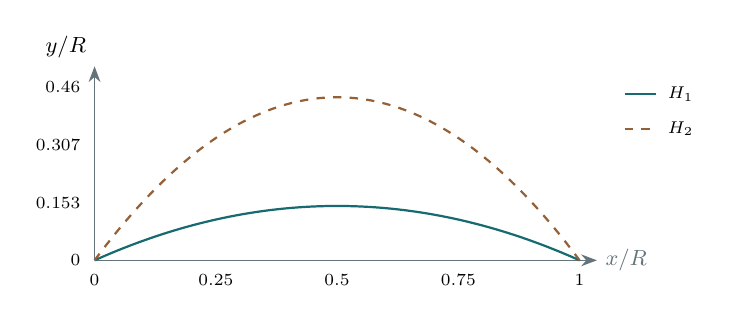
\begin{tikzpicture}[scale=.88,transform shape]
\draw[axis] (0,0.0000000)--(7.25,0.0000000) node[right] {$x/R$};
\draw[axis] (0.0000000,0)--(0.0000000,2.8);
\node[above left] at (0.0000000,2.8) {$y/R$};
\node[below,font=\scriptsize] at (0.0000000,-0.0800000) {$0$};
\node[below,font=\scriptsize] at (1.7500000,-0.0800000) {$0.25$};
\node[below,font=\scriptsize] at (3.5000000,-0.0800000) {$0.5$};
\node[below,font=\scriptsize] at (5.2500000,-0.0800000) {$0.75$};
\node[below,font=\scriptsize] at (7.0000000,-0.0800000) {$1$};
\node[left,font=\scriptsize] at (-0.0800000,0.0000000) {$0$};
\node[left,font=\scriptsize] at (-0.0800000,0.8333333) {$0.153$};
\node[left,font=\scriptsize] at (-0.0800000,1.6666667) {$0.307$};
\node[left,font=\scriptsize] at (-0.0800000,2.5000000) {$0.46$};
\draw[thick,color=accent] plot coordinates {(0.0000000,0.0000000) (0.0583333,0.0259302) (0.1166667,0.0514246) (0.1750000,0.0764832) (0.2333333,0.1011060) (0.2916667,0.1252930) (0.3500000,0.1490442) (0.4083333,0.1723596) (0.4666667,0.1952392) (0.5250000,0.2176830) (0.5833333,0.2396910) (0.6416667,0.2612632) (0.7000000,0.2823996) (0.7583333,0.3031002) (0.8166667,0.3233650) (0.8750000,0.3431939) (0.9333333,0.3625871) (0.9916667,0.3815445) (1.0500000,0.4000661) (1.1083333,0.4181519) (1.1666667,0.4358018) (1.2250000,0.4530160) (1.2833333,0.4697944) (1.3416667,0.4861369) (1.4000000,0.5020437) (1.4583333,0.5175147) (1.5166667,0.5325498) (1.5750000,0.5471492) (1.6333333,0.5613128) (1.6916667,0.5750405) (1.7500000,0.5883325) (1.8083333,0.6011886) (1.8666667,0.6136090) (1.9250000,0.6255935) (1.9833333,0.6371423) (2.0416667,0.6482552) (2.1000000,0.6589324) (2.1583333,0.6691737) (2.2166667,0.6789793) (2.2750000,0.6883490) (2.3333333,0.6972829) (2.3916667,0.7057811) (2.4500000,0.7138434) (2.5083333,0.7214699) (2.5666667,0.7286607) (2.6250000,0.7354156) (2.6833333,0.7417347) (2.7416667,0.7476180) (2.8000000,0.7530656) (2.8583333,0.7580773) (2.9166667,0.7626532) (2.9750000,0.7667933) (3.0333333,0.7704976) (3.0916667,0.7737662) (3.1500000,0.7765989) (3.2083333,0.7789958) (3.2666667,0.7809569) (3.3250000,0.7824822) (3.3833333,0.7835717) (3.4416667,0.7842254) (3.5000000,0.7844433) (3.5583333,0.7842254) (3.6166667,0.7835717) (3.6750000,0.7824822) (3.7333333,0.7809569) (3.7916667,0.7789958) (3.8500000,0.7765989) (3.9083333,0.7737662) (3.9666667,0.7704976) (4.0250000,0.7667933) (4.0833333,0.7626532) (4.1416667,0.7580773) (4.2000000,0.7530656) (4.2583333,0.7476180) (4.3166667,0.7417347) (4.3750000,0.7354156) (4.4333333,0.7286607) (4.4916667,0.7214699) (4.5500000,0.7138434) (4.6083333,0.7057811) (4.6666667,0.6972829) (4.7250000,0.6883490) (4.7833333,0.6789793) (4.8416667,0.6691737) (4.9000000,0.6589324) (4.9583333,0.6482552) (5.0166667,0.6371423) (5.0750000,0.6255935) (5.1333333,0.6136090) (5.1916667,0.6011886) (5.2500000,0.5883325) (5.3083333,0.5750405) (5.3666667,0.5613128) (5.4250000,0.5471492) (5.4833333,0.5325498) (5.5416667,0.5175147) (5.6000000,0.5020437) (5.6583333,0.4861369) (5.7166667,0.4697944) (5.7750000,0.4530160) (5.8333333,0.4358018) (5.8916667,0.4181519) (5.9500000,0.4000661) (6.0083333,0.3815445) (6.0666667,0.3625871) (6.1250000,0.3431939) (6.1833333,0.3233650) (6.2416667,0.3031002) (6.3000000,0.2823996) (6.3583333,0.2612632) (6.4166667,0.2396910) (6.4750000,0.2176830) (6.5333333,0.1952392) (6.5916667,0.1723596) (6.6500000,0.1490442) (6.7083333,0.1252930) (6.7666667,0.1011060) (6.8250000,0.0764832) (6.8833333,0.0514246) (6.9416667,0.0259302) (7.0000000,0.0000000)};
\draw[thick,color=accent] (7.65,2.4)--(8.1,2.4);\node[right,font=\scriptsize] at (8.15,2.4) {$H_1$};
\draw[thick,dashed,color=warm] plot coordinates {(0.0000000,0.0000000) (0.0583333,0.0777906) (0.1166667,0.1542738) (0.1750000,0.2294497) (0.2333333,0.3033181) (0.2916667,0.3758791) (0.3500000,0.4471327) (0.4083333,0.5170789) (0.4666667,0.5857177) (0.5250000,0.6530490) (0.5833333,0.7190730) (0.6416667,0.7837896) (0.7000000,0.8471988) (0.7583333,0.9093005) (0.8166667,0.9700949) (0.8750000,1.0295818) (0.9333333,1.0877614) (0.9916667,1.1446335) (1.0500000,1.2001982) (1.1083333,1.2544556) (1.1666667,1.3074055) (1.2250000,1.3590480) (1.2833333,1.4093831) (1.3416667,1.4584108) (1.4000000,1.5061311) (1.4583333,1.5525440) (1.5166667,1.5976495) (1.5750000,1.6414476) (1.6333333,1.6839383) (1.6916667,1.7251216) (1.7500000,1.7649974) (1.8083333,1.8035659) (1.8666667,1.8408269) (1.9250000,1.8767806) (1.9833333,1.9114268) (2.0416667,1.9447657) (2.1000000,1.9767971) (2.1583333,2.0075211) (2.2166667,2.0369378) (2.2750000,2.0650470) (2.3333333,2.0918488) (2.3916667,2.1173432) (2.4500000,2.1415302) (2.5083333,2.1644098) (2.5666667,2.1859820) (2.6250000,2.2062468) (2.6833333,2.2252042) (2.7416667,2.2428541) (2.8000000,2.2591967) (2.8583333,2.2742319) (2.9166667,2.2879596) (2.9750000,2.3003800) (3.0333333,2.3114929) (3.0916667,2.3212985) (3.1500000,2.3297966) (3.2083333,2.3369873) (3.2666667,2.3428707) (3.3250000,2.3474466) (3.3833333,2.3507151) (3.4416667,2.3526762) (3.5000000,2.3533299) (3.5583333,2.3526762) (3.6166667,2.3507151) (3.6750000,2.3474466) (3.7333333,2.3428707) (3.7916667,2.3369873) (3.8500000,2.3297966) (3.9083333,2.3212985) (3.9666667,2.3114929) (4.0250000,2.3003800) (4.0833333,2.2879596) (4.1416667,2.2742319) (4.2000000,2.2591967) (4.2583333,2.2428541) (4.3166667,2.2252042) (4.3750000,2.2062468) (4.4333333,2.1859820) (4.4916667,2.1644098) (4.5500000,2.1415302) (4.6083333,2.1173432) (4.6666667,2.0918488) (4.7250000,2.0650470) (4.7833333,2.0369378) (4.8416667,2.0075211) (4.9000000,1.9767971) (4.9583333,1.9447657) (5.0166667,1.9114268) (5.0750000,1.8767806) (5.1333333,1.8408269) (5.1916667,1.8035659) (5.2500000,1.7649974) (5.3083333,1.7251216) (5.3666667,1.6839383) (5.4250000,1.6414476) (5.4833333,1.5976495) (5.5416667,1.5525440) (5.6000000,1.5061311) (5.6583333,1.4584108) (5.7166667,1.4093831) (5.7750000,1.3590480) (5.8333333,1.3074055) (5.8916667,1.2544556) (5.9500000,1.2001982) (6.0083333,1.1446335) (6.0666667,1.0877614) (6.1250000,1.0295818) (6.1833333,0.9700949) (6.2416667,0.9093005) (6.3000000,0.8471988) (6.3583333,0.7837896) (6.4166667,0.7190730) (6.4750000,0.6530490) (6.5333333,0.5857177) (6.5916667,0.5170789) (6.6500000,0.4471327) (6.7083333,0.3758791) (6.7666667,0.3033181) (6.8250000,0.2294497) (6.8833333,0.1542738) (6.9416667,0.0777906) (7.0000000,0.0000000)};
\draw[thick,dashed,color=warm] (7.65,1.9)--(8.1,1.9);\node[right,font=\scriptsize] at (8.15,1.9) {$H_2$};
\end{tikzpicture}
\figcaption{变图1.5V3\quad 两个顶点都在 $x=R/2$。}
\end{minipage}\end{center}
\item 一个发射角为 $30^\circ$，求另一个角与各自的飞行时间。由互余得另一角为 $60^\circ$，因而 $R=\sqrt3v_0^2/(2g)$。在变图1.5V4的高度曲线上读出两个落地横坐标 $gt/v_0=1,\sqrt3$，即
\[
T_1=\frac{v_0}{g},\qquad T_2=\frac{\sqrt3v_0}{g},\qquad T_1T_2=\frac{\sqrt3v_0^2}{g^2}=\frac{2R}{g}.
\]
$30^\circ$ 轨迹先落地，因其竖直初速度为 $v_0/2$。
\begin{center}\begin{minipage}{.98\linewidth}\centering
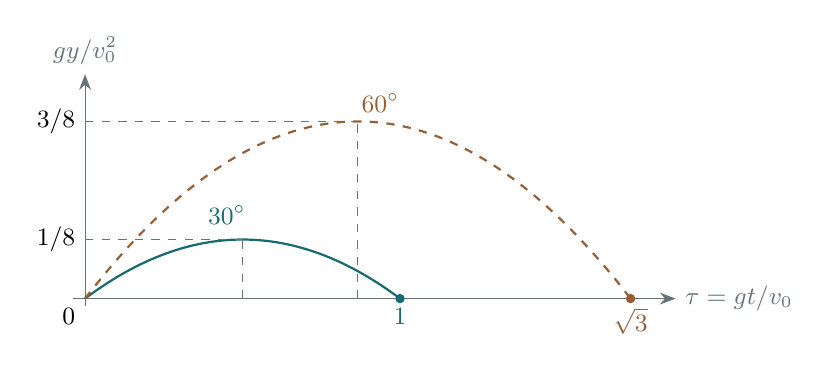
\begin{tikzpicture}
\draw[axis] (-.15,0)--(7.5,0) node[right] {$\tau=gt/v_0$};
\draw[axis] (0,-.1)--(0,2.85) node[above] {$gy/v_0^2$};
\draw[traj,domain=0:1,samples=70] plot({4*\x},{3*(\x-\x^2)});
\draw[thick,dashed,warm,domain=0:1.7320508,samples=80] plot({4*\x},{3*(sqrt(3)*\x-\x^2)});
\draw[guide] (2,0)--(2,.75);
\draw[guide] ({2*sqrt(3)},0)--({2*sqrt(3)},2.25);
\draw[guide] (0,.75)--(2,.75);\node[left] at (0,.75) {$1/8$};
\draw[guide] (0,2.25)--({2*sqrt(3)},2.25);\node[left] at (0,2.25) {$3/8$};
\fill[accent] (4,0) circle(1.7pt) node[below] {$1$};
\fill[warm] ({4*sqrt(3)},0) circle(1.7pt) node[below] {$\sqrt3$};
\node[above,accent] at (1.8,.82) {$30^\circ$};
\node[above,warm] at (3.75,2.24) {$60^\circ$};
\node[below left] at (0,0) {$0$};
\end{tikzpicture}
\figcaption{变图1.5V4\quad 两条高度曲线的右端分别标出两次飞行的结束时刻。}
\end{minipage}\end{center}
\item 已知较低发射角为 $\alpha_1<45^\circ$，求高、低轨迹的时间比和最高点高度比。由 $\alpha_2=\pi/2-\alpha_1$，
\[
\frac{T_2}{T_1}=\frac{\cos\alpha_1}{\sin\alpha_1}=\cot\alpha_1,\qquad
\frac{H_2}{H_1}=\left(\frac{T_2}{T_1}\right)^2=\cot^2\alpha_1.
\]
在 $30^\circ$ 处，上式给出时间比 $\sqrt3$ 和高度比3。变图1.5V5中，两曲线随发射角增大而下降，在 $45^\circ$ 处都趋于1。图中高度比变化更快，因为最高点高度正比于竖直初速度的平方。
\begin{center}\begin{minipage}{.98\linewidth}\centering
\begin{tikzpicture}[scale=.88,transform shape]
\draw[axis] (0,0.0000000)--(7.25,0.0000000) node[right] {$\alpha_1/(1^\circ)$};
\draw[axis] (0.0000000,0)--(0.0000000,2.8);
\node[above left] at (0.0000000,2.8) {$\text{比值}$};
\node[below,font=\scriptsize] at (0.0000000,-0.0800000) {$15$};
\node[below,font=\scriptsize] at (1.7500000,-0.0800000) {$22.5$};
\node[below,font=\scriptsize] at (3.5000000,-0.0800000) {$30$};
\node[below,font=\scriptsize] at (5.2500000,-0.0800000) {$37.5$};
\node[below,font=\scriptsize] at (7.0000000,-0.0800000) {$45$};
\node[left,font=\scriptsize] at (-0.0800000,0.0000000) {$0$};
\node[left,font=\scriptsize] at (-0.0800000,0.8333333) {$4.83$};
\node[left,font=\scriptsize] at (-0.0800000,1.6666667) {$9.67$};
\node[left,font=\scriptsize] at (-0.0800000,2.5000000) {$14.5$};
\draw[thick,color=accent] plot coordinates {(0.0000000,0.6434570) (0.0583333,0.6324065) (0.1166667,0.6217041) (0.1750000,0.6113332) (0.2333333,0.6012784) (0.2916667,0.5915249) (0.3500000,0.5820592) (0.4083333,0.5728683) (0.4666667,0.5639401) (0.5250000,0.5552632) (0.5833333,0.5468267) (0.6416667,0.5386205) (0.7000000,0.5306351) (0.7583333,0.5228613) (0.8166667,0.5152905) (0.8750000,0.5079147) (0.9333333,0.5007260) (0.9916667,0.4937173) (1.0500000,0.4868815) (1.1083333,0.4802122) (1.1666667,0.4737030) (1.2250000,0.4673480) (1.2833333,0.4611416) (1.3416667,0.4550784) (1.4000000,0.4491533) (1.4583333,0.4433613) (1.5166667,0.4376979) (1.5750000,0.4321586) (1.6333333,0.4267391) (1.6916667,0.4214354) (1.7500000,0.4162437) (1.8083333,0.4111602) (1.8666667,0.4061814) (1.9250000,0.4013040) (1.9833333,0.3965246) (2.0416667,0.3918402) (2.1000000,0.3872477) (2.1583333,0.3827444) (2.2166667,0.3783275) (2.2750000,0.3739944) (2.3333333,0.3697426) (2.3916667,0.3655696) (2.4500000,0.3614730) (2.5083333,0.3574508) (2.5666667,0.3535007) (2.6250000,0.3496206) (2.6833333,0.3458086) (2.7416667,0.3420627) (2.8000000,0.3383811) (2.8583333,0.3347621) (2.9166667,0.3312038) (2.9750000,0.3277047) (3.0333333,0.3242632) (3.0916667,0.3208777) (3.1500000,0.3175467) (3.2083333,0.3142688) (3.2666667,0.3110427) (3.3250000,0.3078670) (3.3833333,0.3047403) (3.4416667,0.3016616) (3.5000000,0.2986294) (3.5583333,0.2956428) (3.6166667,0.2927005) (3.6750000,0.2898015) (3.7333333,0.2869447) (3.7916667,0.2841291) (3.8500000,0.2813537) (3.9083333,0.2786176) (3.9666667,0.2759197) (4.0250000,0.2732593) (4.0833333,0.2706354) (4.1416667,0.2680473) (4.2000000,0.2654940) (4.2583333,0.2629747) (4.3166667,0.2604888) (4.3750000,0.2580355) (4.4333333,0.2556140) (4.4916667,0.2532236) (4.5500000,0.2508636) (4.6083333,0.2485335) (4.6666667,0.2462324) (4.7250000,0.2439599) (4.7833333,0.2417152) (4.8416667,0.2394979) (4.9000000,0.2373072) (4.9583333,0.2351427) (5.0166667,0.2330039) (5.0750000,0.2308901) (5.1333333,0.2288008) (5.1916667,0.2267356) (5.2500000,0.2246940) (5.3083333,0.2226755) (5.3666667,0.2206796) (5.4250000,0.2187059) (5.4833333,0.2167538) (5.5416667,0.2148231) (5.6000000,0.2129133) (5.6583333,0.2110239) (5.7166667,0.2091547) (5.7750000,0.2073051) (5.8333333,0.2054748) (5.8916667,0.2036634) (5.9500000,0.2018706) (6.0083333,0.2000961) (6.0666667,0.1983394) (6.1250000,0.1966003) (6.1833333,0.1948783) (6.2416667,0.1931733) (6.3000000,0.1914849) (6.3583333,0.1898128) (6.4166667,0.1881566) (6.4750000,0.1865162) (6.5333333,0.1848912) (6.5916667,0.1832813) (6.6500000,0.1816862) (6.7083333,0.1801058) (6.7666667,0.1785397) (6.8250000,0.1769877) (6.8833333,0.1754496) (6.9416667,0.1739250) (7.0000000,0.1724138)};
\draw[thick,color=accent] (7.65,2.4)--(8.1,2.4);\node[right,font=\scriptsize] at (8.15,2.4) {$T_2/T_1$};
\draw[thick,dashed,color=warm] plot coordinates {(0.0000000,2.4014144) (0.0583333,2.3196401) (0.1166667,2.2417924) (0.1750000,2.1676240) (0.2333333,2.0969068) (0.2916667,2.0294301) (0.3500000,1.9649990) (0.4083333,1.9034330) (0.4666667,1.8445650) (0.5250000,1.7882396) (0.5833333,1.7343127) (0.6416667,1.6826501) (0.7000000,1.6331269) (0.7583333,1.5856267) (0.8166667,1.5400410) (0.8750000,1.4962683) (0.9333333,1.4542139) (0.9916667,1.4137892) (1.0500000,1.3749110) (1.1083333,1.3375017) (1.1666667,1.3014883) (1.2250000,1.2668023) (1.2833333,1.2333793) (1.3416667,1.2011590) (1.4000000,1.1700843) (1.4583333,1.1401018) (1.5166667,1.1111609) (1.5750000,1.0832141) (1.6333333,1.0562164) (1.6916667,1.0301254) (1.7500000,1.0049012) (1.8083333,0.9805059) (1.8666667,0.9569035) (1.9250000,0.9340603) (1.9833333,0.9119441) (2.0416667,0.8905245) (2.1000000,0.8697726) (2.1583333,0.8496611) (2.2166667,0.8301640) (2.2750000,0.8112566) (2.3333333,0.7929155) (2.3916667,0.7751184) (2.4500000,0.7578440) (2.5083333,0.7410722) (2.5666667,0.7247838) (2.6250000,0.7089604) (2.6833333,0.6935847) (2.7416667,0.6786400) (2.8000000,0.6641103) (2.8583333,0.6499807) (2.9166667,0.6362366) (2.9750000,0.6228642) (3.0333333,0.6098504) (3.0916667,0.5971824) (3.1500000,0.5848483) (3.2083333,0.5728365) (3.2666667,0.5611359) (3.3250000,0.5497360) (3.3833333,0.5386267) (3.4416667,0.5277983) (3.5000000,0.5172414) (3.5583333,0.5069471) (3.6166667,0.4969069) (3.6750000,0.4871126) (3.7333333,0.4775562) (3.7916667,0.4682303) (3.8500000,0.4591276) (3.9083333,0.4502410) (3.9666667,0.4415639) (4.0250000,0.4330898) (4.0833333,0.4248126) (4.1416667,0.4167261) (4.2000000,0.4088248) (4.2583333,0.4011031) (4.3166667,0.3935557) (4.3750000,0.3861774) (4.4333333,0.3789633) (4.4916667,0.3719086) (4.5500000,0.3650088) (4.6083333,0.3582595) (4.6666667,0.3516563) (4.7250000,0.3451952) (4.7833333,0.3388722) (4.8416667,0.3326835) (4.9000000,0.3266254) (4.9583333,0.3206942) (5.0166667,0.3148867) (5.0750000,0.3091993) (5.1333333,0.3036290) (5.1916667,0.2981725) (5.2500000,0.2928270) (5.3083333,0.2875894) (5.3666667,0.2824570) (5.4250000,0.2774271) (5.4833333,0.2724969) (5.5416667,0.2676641) (5.6000000,0.2629260) (5.6583333,0.2582804) (5.7166667,0.2537249) (5.7750000,0.2492572) (5.8333333,0.2448753) (5.8916667,0.2405769) (5.9500000,0.2363601) (6.0083333,0.2322229) (6.0666667,0.2281634) (6.1250000,0.2241796) (6.1833333,0.2202699) (6.2416667,0.2164324) (6.3000000,0.2126655) (6.3583333,0.2089676) (6.4166667,0.2053369) (6.4750000,0.2017721) (6.5333333,0.1982715) (6.5916667,0.1948337) (6.6500000,0.1914573) (6.7083333,0.1881410) (6.7666667,0.1848833) (6.8250000,0.1816830) (6.8833333,0.1785388) (6.9416667,0.1754494) (7.0000000,0.1724138)};
\draw[thick,dashed,color=warm] (7.65,1.9)--(8.1,1.9);\node[right,font=\scriptsize] at (8.15,1.9) {$H_2/H_1$};
\end{tikzpicture}
\figcaption{变图1.5V5\quad 较高轨迹与较低轨迹的时间比及顶点高度比。}
\end{minipage}\end{center}
\end{enumerate}

\clearpage

\pdfbookmark[3]{第 6 题 水枪越墙的最小初速}{c1-q6}

\section*{第 6 题\quad 水枪越墙的最小初速}\label{book-question-1-6}

\tagline{M-01-06}

地面上的水枪枪口视为质点，与竖直墙的水平距离为 $d=3.0\,\mathrm m$，墙高为 $h=4.0\,\mathrm m$。水流以速率 $v_0$、仰角 $\alpha$ 喷出，忽略空气阻力和水流宽度，取 $g=10\,\mathrm{m/s^2}$。

求使水流恰好通过墙顶的最小初速及相应仰角。

\begin{center}
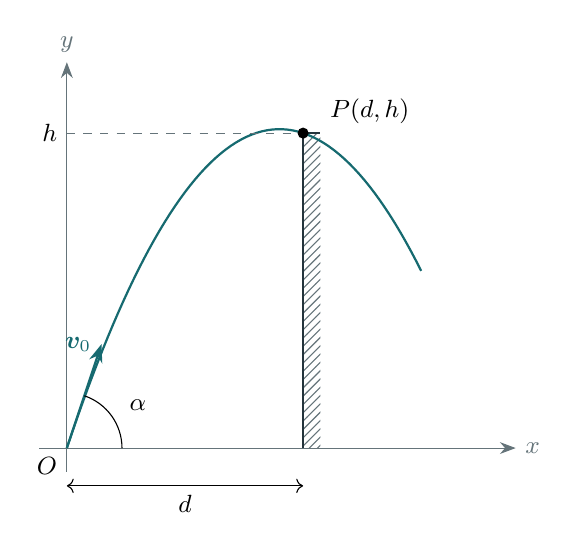
\begin{tikzpicture}[scale=1.0]
\draw[axis] (-.35,0)--(5.7,0) node[right] {$x$};\draw[axis] (0,-.3)--(0,4.9) node[above] {$y$};
\fill[pattern=north east lines,pattern color=muted] (3,0) rectangle (3.22,4);
\draw[object] (3,0)--(3,4)--(3.22,4);
\draw[traj,domain=0:4.5,samples=70] plot(\x,{3*\x-5*\x*\x/9});
\draw[motion] (0,0)--(.44,1.32) node[left] {$\vect v_0$};
\draw (.7,0) arc(0:71.565:.7);\node at (.9,.55) {$\alpha$};
\draw[guide] (0,4)--(3,4);\node[left] at (0,4) {$h$};
\draw[thin,<->] (0,-.48)--(3,-.48) node[midway,below] {$d$};
\fill (3,4) circle (2pt);\node[above right] at (3.22,4) {$P(d,h)$};\node[below left] at (0,0) {$O$};
\end{tikzpicture}
\figcaption{图 1.6\quad 枪口、墙顶与一条通过墙顶的轨迹。}
\end{center}

\Needspace{5\baselineskip}

\pdfbookmark[4]{题型定位}{c1-q6-h0}

\subsection*{题型定位}

给定枪口和墙顶的位置，求刚好通过墙顶所需的最小发射速率。将轨迹经过 $(d,h)$ 的条件写成 $v_0^2(\alpha)$，然后在允许角度内找最小值。

\Needspace{5\baselineskip}

\pdfbookmark[4]{知识点}{c1-q6-h1}

\subsection*{知识点}

斜抛轨迹由水平匀速和竖直匀变速消去时间得到。用 $p=\tan\alpha$ 求导可找极小值，也可借视线角 $\theta=\arctan(h/d)$ 和积化和差使分母最大。固定速率下对发射角求最高可达高度，得到抛物线族的包络。


\Needspace{5\baselineskip}

\pdfbookmark[4]{物理图像}{c1-q6-h2}

\subsection*{物理图像}

解图1.6A中视线连接枪口与墙顶，初速度方向比视线更陡。随着初速降低，轨迹族包络在墙处降低。最低可行速率时包络刚过墙顶，解图1.6B所示的临界轨迹在墙前达到最高点，然后下降过墙。

\Needspace{5\baselineskip}

\pdfbookmark[4]{解题入口}{c1-q6-h3}

\subsection*{解题入口}

将 $(d,h)$ 代入轨迹并解出 $v_0^2$。取 $p=\tan\alpha>h/d$，用商的求导法则得到二次分子 $dp^2-2hp-d$。取允许区间的根，再看两端的变化。代入最优速率和角度后，从 $t_d=d/v_{0x}$ 算出墙处竖直速度，用其符号说明图中上下行方向。

\Needspace{5\baselineskip}

\pdfbookmark[4]{标准解法}{c1-q6-h4}

\subsection*{标准解法}

以枪口为原点，水平向墙为 $x$ 正向，竖直向上为 $y$ 正向。墙顶坐标为 $(d,h)$，解图 1.6A 中从枪口指向墙顶的直线与水平夹角记为 $\theta$，故 $\tan\theta=h/d$。
\begin{center}\begin{minipage}{\linewidth}\centering\begin{tikzpicture}

\draw[axis] (-.2,0)--(4.1,0) node[right] {$x$};\draw[axis] (0,-.2)--(0,4.6) node[above] {$y$};
\draw[object] (3,0)--(3,4);\fill (3,4) circle(2pt);\node[above right] at (3,4) {$P(d,h)$};
\draw[guide] (0,0)--(3,4) node[midway,above left,sloped] {$\sqrt{d^2+h^2}$};
\draw[motion] (0,0)--(.65,1.95) node[left] {$v_0$};
\draw (.68,0) arc(0:71.565:.68);\node at (.88,.7) {$\alpha$};
\draw (1.35,0) arc(0:53.13:1.35);\node at (1.55,.45) {$\theta$};
\draw[thin,<->] (0,-.55)--(3,-.55) node[midway,below] {$d$};
\draw[thin,<->] (3.45,0)--(3.45,4) node[midway,right] {$h$};
\node[align=left] at (6.45,2.8) {$\theta=\arctan(h/d)$\\$\alpha$：枪口仰角\\$\alpha>\theta$};

\end{tikzpicture}
\figcaption{解图 1.6A\quad $\theta$ 是墙顶的视线角，$\alpha$ 是发射角，$\alpha$沿枪口初速箭头量取。}
\end{minipage}\end{center}
\subsubsection*{通过墙顶的条件}
水流质点的轨迹为
\[
y=x\tan\alpha-\frac{gx^2}{2v_0^2\cos^2\alpha}.
\]
令 $x=d,y=h$，得
\[
v_0^2=\frac{gd^2}{2\cos^2\alpha(d\tan\alpha-h)}.
\]
式中 $v_0^2>0$ 给出 $\tan\alpha>h/d$。解图1.6A上，枪口切线在墙处的高度是 $d\tan\alpha$，抛物线比该高度低 $gd^2/(2v_0^2\cos^2\alpha)$。重力使轨迹低于枪口切线，所以切线在墙处的高度 $d\tan\alpha$ 高于 $h$，即 $\alpha>\theta$。
\subsubsection*{对发射角求最小初速}
记 $p=\tan\alpha>h/d$，则
\[
v_0^2(p)=\frac{gd^2}{2}\frac{1+p^2}{dp-h}.
\]
对 $p$ 求导，
\[
\frac{\dd v_0^2}{\dd p}
=\frac{gd^2}{2}\frac{2p(dp-h)-d(1+p^2)}{(dp-h)^2}
=\frac{gd^2}{2}\frac{dp^2-2hp-d}{(dp-h)^2}.
\]
驻点满足 $dp^2-2hp-d=0$。令 $s=\sqrt{d^2+h^2}$，两根为 $(h\pm s)/d$，只有正根符合发射角区间：
\[
p_* =\frac{h+s}{d}.
\]
$p\to h/d^+$ 或 $p\to\infty$ 时所需 $v_0^2$ 都趋于无穷；在允许区间仅有这个驻点，且导数由负变正，因此它给出全局最小值。代入后
\[
\boxed{v_{0,\min}^2=g(s+h)},\qquad
\boxed{\alpha_* =\arctan\frac{s+h}{d}
=\frac\pi4+\frac12\arctan\frac hd}.
\]
也可直接用视线角求极值。令 $\theta=\arctan(h/d)$，则 $d=s\cos\theta$、$h=s\sin\theta$。初速式的分母逐步变为
\[
\begin{aligned}
2\cos\alpha(d\sin\alpha-h\cos\alpha)
&=2s\cos\alpha\sin(\alpha-\theta)\\
&=s[\sin(2\alpha-\theta)-\sin\theta]\\
&=s\sin(2\alpha-\theta)-h.
\end{aligned}
\]
第二行来自积化和差，其中 $s\sin\theta=h$。整个分母随发射角变化，最大值为 $s-h$，因此
\[
v_0^2=\frac{gd^2}{s\sin(2\alpha-\theta)-h},
\]
分母在 $2\alpha-\theta=\pi/2$ 时最大，得到同一最优角。
\Needspace{0.46\textheight}
\subsubsection*{数值与墙顶处的运动状态}
本题 $s=5.0\,\mathrm m$，所以
\[
\boxed{v_{0,\min}=\sqrt{90}\approx9.49\,\mathrm{m/s},
\quad\alpha_* =\arctan3\approx71.57^\circ}.
\]
对应水平、竖直初速度分别为 $3.0$ 和 $9.0\,\mathrm{m/s}$。到墙时间 $t_d=d/v_{0x}=1.0\,\mathrm s$，此时
\[
y(t_d)=9.0\times1.0-5.0\times1.0^2=4.0\,\mathrm m,
\qquad v_y(t_d)=9.0-10\times1.0=-1.0\,\mathrm{m/s}.
\]
\begin{center}\begin{minipage}{\linewidth}\centering\begin{tikzpicture}

\draw[axis] (-.2,0)--(3.8,0) node[right] {$x/\mathrm m$};\draw[axis] (0,-.2)--(0,3.3) node[above] {$y/\mathrm m$};
\draw[traj,domain=2.2:3.3,samples=70] plot({3*(\x-2.2)},{9*(3*\x-5*\x*\x/9-3.8)});
\draw[object] (2.4,0)--(2.4,1.8);
\fill (1.5,2.25) circle(2pt);\node[above] at (1.5,2.25) {最高点 $Q$};
\fill (2.4,1.8) circle(2pt);\node[right] at (2.4,1.8) {墙顶 $P$};
\draw[guide] (1.5,0)--(1.5,2.25)--(0,2.25);\draw[guide] (0,1.8)--(2.4,1.8);
\node[below] at (1.5,0) {$2.7$};\node[below] at (2.4,0) {$3.0$};\node[left] at (0,2.25) {$4.05$};\node[left] at (0,1.8) {$4.00$};
\node[align=left] at (6.4,1.9) {最优轨迹到达墙顶时\\已经略向下运动。};

\end{tikzpicture}
\figcaption{解图 1.6B\quad 最小初速对应轨迹的局部放大图；横、纵方向使用不同显示比例。}
\end{minipage}\end{center}
因此水流经过墙顶时已经下降。最高点在 $t=0.90\,\mathrm s$，位置为 $(2.70,4.05)\,\mathrm m$，与解图 1.6B 的先后位置一致。一般最优轨迹在墙顶的斜率为 $-d/(s+h)<0$；墙顶的切线向右下方。解图1.6B中，从最高点到墙顶的水平距离是 $0.30\,\mathrm m$，高度下降 $0.05\,\mathrm m$，正对应这段飞行的 $0.10\,\mathrm s$。

\Needspace{5\baselineskip}

\pdfbookmark[4]{关键洞察}{c1-q6-h5}

\subsection*{关键洞察}

临界的含义是改变发射角时，墙处高度达到该初速允许的最大值。沿轨迹的速度方向由对 $x$ 求导得到。本题在墙顶对角度的变化率为零，对 $x$ 的斜率为负，因而图1.6B在墙前已经过顶点。

\Needspace{5\baselineskip}

\pdfbookmark[4]{易错点}{c1-q6-h6}

\subsection*{易错点}

\begin{itemize}
\item 角度从水平轴量起，过墙顶条件为 $\tan\alpha>h/d$。代入 $p$ 后按此区间选根。
\item 积化和差时保留 $2\cos\alpha\sin(\alpha-\theta)=\sin(2\alpha-\theta)-\sin\theta$ 中的后项。
\item $h>0$ 时 $\alpha_*=45^\circ+\theta/2>45^\circ$，$h=0$ 时回到 $45^\circ$ 和 $v_{0,\min}^2=gd$。
\item 图1.6B中墙顶坐标是 $(3.0,4.0)\,\mathrm m$，最高点是 $(2.70,4.05)\,\mathrm m$。前者的竖直速度为 $-1.0\,\mathrm{m/s}$。
\end{itemize}

\Needspace{5\baselineskip}

\pdfbookmark[4]{课堂讲解建议}{c1-q6-h7}

\subsection*{课堂讲解建议}

先画墙顶视线，问“为何发射角比 $\theta$ 大”，答为重力使轨迹低于枪口处切线。求出 $\alpha_*$ 后，再问“在墙处水流向上还是向下”。由 $v_{0x}=3\,\mathrm{m/s}$、$v_{0y}=9\,\mathrm{m/s}$，算出到墙用时一秒，墙处 $v_y=-1\,\mathrm{m/s}$。随后把解图1.6B的最高点与墙顶连起来，标出 $0.30\,\mathrm m$ 的水平距离。若用变图1.6V3解释包络，指出对发射角取极值选出通过墙顶的轨迹，沿这条轨迹的最高点由 $v_y=0$ 定位。

\Needspace{5\baselineskip}

\pdfbookmark[4]{变式训练}{c1-q6-h8}

\subsection*{变式训练}

\begin{enumerate}
\item 固定墙高 $h>0$，增大距离 $d$，求最优角和最小速率的变化。由 $\alpha_*=\pi/4+\tfrac12\arctan(h/d)$，
\[
\frac{\dd\alpha_*}{\dd d}=-\frac{h}{2(d^2+h^2)}<0,\qquad
\frac{\dd v_{\min}^2}{\dd d}=\frac{gd}{\sqrt{d^2+h^2}}>0.
\]
变图1.6V1的横坐标是 $d/h$。从图上向右读，视线角逐渐减小，最优角由接近 $90^\circ$ 逐渐趋于 $45^\circ$。例如 $d=h$ 时，最优角为 $67.5^\circ$，$v_{\min}^2=g(1+\sqrt2)h$。
\begin{center}\begin{minipage}{.98\linewidth}\centering
\begin{tikzpicture}[scale=.88,transform shape]
\draw[axis] (0,0.0000000)--(7.25,0.0000000) node[right] {$d/h$};
\draw[axis] (0.0000000,0)--(0.0000000,2.8);
\node[above left] at (0.0000000,2.8) {$\alpha_*/(1^\circ)$};
\node[below,font=\scriptsize] at (0.0000000,-0.0800000) {$0.15$};
\node[below,font=\scriptsize] at (1.7500000,-0.0800000) {$1.36$};
\node[below,font=\scriptsize] at (3.5000000,-0.0800000) {$2.57$};
\node[below,font=\scriptsize] at (5.2500000,-0.0800000) {$3.79$};
\node[below,font=\scriptsize] at (7.0000000,-0.0800000) {$5$};
\node[left,font=\scriptsize] at (-0.0800000,0.0000000) {$45$};
\node[left,font=\scriptsize] at (-0.0800000,0.8333333) {$60$};
\node[left,font=\scriptsize] at (-0.0800000,1.6666667) {$75$};
\node[left,font=\scriptsize] at (-0.0800000,2.5000000) {$90$};
\draw[thick,color=accent] plot coordinates {(0.0000000,2.2630343) (0.0583333,2.2005276) (0.1166667,2.1389416) (0.1750000,2.0784359) (0.2333333,2.0191523) (0.2916667,1.9612134) (0.3500000,1.9047220) (0.4083333,1.8497614) (0.4666667,1.7963957) (0.5250000,1.7446713) (0.5833333,1.6946178) (0.6416667,1.6462497) (0.7000000,1.5995681) (0.7583333,1.5545626) (0.8166667,1.5112125) (0.8750000,1.4694891) (0.9333333,1.4293566) (0.9916667,1.3907739) (1.0500000,1.3536958) (1.1083333,1.3180739) (1.1666667,1.2838576) (1.2250000,1.2509953) (1.2833333,1.2194346) (1.3416667,1.1891229) (1.4000000,1.1600083) (1.4583333,1.1320397) (1.5166667,1.1051670) (1.5750000,1.0793414) (1.6333333,1.0545158) (1.6916667,1.0306446) (1.7500000,1.0076839) (1.8083333,0.9855916) (1.8666667,0.9643275) (1.9250000,0.9438530) (1.9833333,0.9241314) (2.0416667,0.9051275) (2.1000000,0.8868081) (2.1583333,0.8691414) (2.2166667,0.8520973) (2.2750000,0.8356472) (2.3333333,0.8197638) (2.3916667,0.8044215) (2.4500000,0.7895956) (2.5083333,0.7752631) (2.5666667,0.7614018) (2.6250000,0.7479911) (2.6833333,0.7350109) (2.7416667,0.7224426) (2.8000000,0.7102685) (2.8583333,0.6984715) (2.9166667,0.6870356) (2.9750000,0.6759458) (3.0333333,0.6651874) (3.0916667,0.6547469) (3.1500000,0.6446112) (3.2083333,0.6347679) (3.2666667,0.6252052) (3.3250000,0.6159121) (3.3833333,0.6068778) (3.4416667,0.5980924) (3.5000000,0.5895460) (3.5583333,0.5812297) (3.6166667,0.5731346) (3.6750000,0.5652524) (3.7333333,0.5575753) (3.7916667,0.5500956) (3.8500000,0.5428062) (3.9083333,0.5357002) (3.9666667,0.5287711) (4.0250000,0.5220125) (4.0833333,0.5154185) (4.1416667,0.5089833) (4.2000000,0.5027016) (4.2583333,0.4965680) (4.3166667,0.4905775) (4.3750000,0.4847254) (4.4333333,0.4790071) (4.4916667,0.4734182) (4.5500000,0.4679544) (4.6083333,0.4626118) (4.6666667,0.4573865) (4.7250000,0.4522747) (4.7833333,0.4472730) (4.8416667,0.4423778) (4.9000000,0.4375859) (4.9583333,0.4328942) (5.0166667,0.4282996) (5.0750000,0.4237992) (5.1333333,0.4193902) (5.1916667,0.4150700) (5.2500000,0.4108359) (5.3083333,0.4066854) (5.3666667,0.4026162) (5.4250000,0.3986259) (5.4833333,0.3947123) (5.5416667,0.3908733) (5.6000000,0.3871067) (5.6583333,0.3834107) (5.7166667,0.3797832) (5.7750000,0.3762225) (5.8333333,0.3727267) (5.8916667,0.3692941) (5.9500000,0.3659230) (6.0083333,0.3626119) (6.0666667,0.3593592) (6.1250000,0.3561633) (6.1833333,0.3530228) (6.2416667,0.3499364) (6.3000000,0.3469025) (6.3583333,0.3439201) (6.4166667,0.3409877) (6.4750000,0.3381041) (6.5333333,0.3352682) (6.5916667,0.3324787) (6.6500000,0.3297347) (6.7083333,0.3270349) (6.7666667,0.3243784) (6.8250000,0.3217641) (6.8833333,0.3191910) (6.9416667,0.3166582) (7.0000000,0.3141648)};
\end{tikzpicture}
\figcaption{变图1.6V1\quad 固定墙高，最优角随墙距增大而减小。}
\end{minipage}\end{center}
\item 枪口下方留有飞行空间，目标相对枪口的坐标为$(d,h)$，其中$h<0,d>0$。求最优发射角及速率。记 $s=\sqrt{d^2+h^2}>|h|$。优化方程的允许根仍为 $p_*=(s+h)/d>0$，因而
\[
0<\alpha_*=\frac\pi4+\frac12\arctan(h/d)<\frac\pi4,
\qquad v_{\min}^2=g(s+h)>0.
\]
变图1.6V2取 $d=4\,\mathrm m,h=-3\,\mathrm m$，此时 $p_*=1/2$、$v_{\min}^2=2g\,\mathrm m$，归一化轨迹为 $y/d=(x/d)/2-5(x/d)^2/4$。由图上的顶点可见，该发射角使水流先升后降，最后到达较低目标。
\begin{center}\begin{minipage}{.98\linewidth}\centering
\begin{tikzpicture}[scale=.88,transform shape]
\draw[axis] (0,2.2471910)--(7.25,2.2471910) node[right] {$x/d$};
\draw[axis] (0.0000000,0)--(0.0000000,2.8);
\node[above left] at (0.0000000,2.8) {$y/d$};
\node[below,font=\scriptsize] at (0.0000000,2.1671910) {$0$};
\node[below,font=\scriptsize] at (1.7500000,2.1671910) {$0.25$};
\node[below,font=\scriptsize] at (3.5000000,2.1671910) {$0.5$};
\node[below,font=\scriptsize] at (5.2500000,2.1671910) {$0.75$};
\node[below,font=\scriptsize] at (7.0000000,2.1671910) {$1$};
\node[left,font=\scriptsize] at (-0.0800000,0.0000000) {$-0.8$};
\node[left,font=\scriptsize] at (-0.0800000,0.8333333) {$-0.503$};
\node[left,font=\scriptsize] at (-0.0800000,1.6666667) {$-0.207$};
\node[left,font=\scriptsize] at (-0.0800000,2.5000000) {$0.09$};
\draw[thick,color=accent] plot coordinates {(0.0000000,2.2471910) (0.0583333,2.2586513) (0.1166667,2.2696239) (0.1750000,2.2801088) (0.2333333,2.2901061) (0.2916667,2.2996157) (0.3500000,2.3086376) (0.4083333,2.3171719) (0.4666667,2.3252185) (0.5250000,2.3327774) (0.5833333,2.3398486) (0.6416667,2.3464322) (0.7000000,2.3525281) (0.7583333,2.3581363) (0.8166667,2.3632569) (0.8750000,2.3678897) (0.9333333,2.3720350) (0.9916667,2.3756925) (1.0500000,2.3788624) (1.1083333,2.3815446) (1.1666667,2.3837391) (1.2250000,2.3854459) (1.2833333,2.3866651) (1.3416667,2.3873966) (1.4000000,2.3876404) (1.4583333,2.3873966) (1.5166667,2.3866651) (1.5750000,2.3854459) (1.6333333,2.3837391) (1.6916667,2.3815446) (1.7500000,2.3788624) (1.8083333,2.3756925) (1.8666667,2.3720350) (1.9250000,2.3678897) (1.9833333,2.3632569) (2.0416667,2.3581363) (2.1000000,2.3525281) (2.1583333,2.3464322) (2.2166667,2.3398486) (2.2750000,2.3327774) (2.3333333,2.3252185) (2.3916667,2.3171719) (2.4500000,2.3086376) (2.5083333,2.2996157) (2.5666667,2.2901061) (2.6250000,2.2801088) (2.6833333,2.2696239) (2.7416667,2.2586513) (2.8000000,2.2471910) (2.8583333,2.2352431) (2.9166667,2.2228074) (2.9750000,2.2098841) (3.0333333,2.1964732) (3.0916667,2.1825745) (3.1500000,2.1681882) (3.2083333,2.1533142) (3.2666667,2.1379526) (3.3250000,2.1221032) (3.3833333,2.1057662) (3.4416667,2.0889416) (3.5000000,2.0716292) (3.5583333,2.0538292) (3.6166667,2.0355415) (3.6750000,2.0167662) (3.7333333,1.9975031) (3.7916667,1.9777524) (3.8500000,1.9575140) (3.9083333,1.9367880) (3.9666667,1.9155743) (4.0250000,1.8938729) (4.0833333,1.8716838) (4.1416667,1.8490071) (4.2000000,1.8258427) (4.2583333,1.8021906) (4.3166667,1.7780509) (4.3750000,1.7534235) (4.4333333,1.7283084) (4.4916667,1.7027056) (4.5500000,1.6766152) (4.6083333,1.6500371) (4.6666667,1.6229713) (4.7250000,1.5954178) (4.7833333,1.5673767) (4.8416667,1.5388479) (4.9000000,1.5098315) (4.9583333,1.4803273) (5.0166667,1.4503355) (5.0750000,1.4198560) (5.1333333,1.3888889) (5.1916667,1.3574341) (5.2500000,1.3254916) (5.3083333,1.2930614) (5.3666667,1.2601436) (5.4250000,1.2267381) (5.4833333,1.1928449) (5.5416667,1.1584640) (5.6000000,1.1235955) (5.6583333,1.0882393) (5.7166667,1.0523954) (5.7750000,1.0160639) (5.8333333,0.9792447) (5.8916667,0.9419378) (5.9500000,0.9041433) (6.0083333,0.8658610) (6.0666667,0.8270911) (6.1250000,0.7878336) (6.1833333,0.7480883) (6.2416667,0.7078554) (6.3000000,0.6671348) (6.3583333,0.6259266) (6.4166667,0.5842306) (6.4750000,0.5420471) (6.5333333,0.4993758) (6.5916667,0.4562168) (6.6500000,0.4125702) (6.7083333,0.3684359) (6.7666667,0.3238140) (6.8250000,0.2787044) (6.8833333,0.2331071) (6.9416667,0.1870221) (7.0000000,0.1404494)};
\fill[accent] (7.0000000,0.1404494) circle(1.7pt) node[above right] {$P$};
\end{tikzpicture}
\figcaption{变图1.6V2\quad 较低目标位于 $(x/d,y/d)=(1,-0.75)$，最优轨迹仍先上升。}
\end{minipage}\end{center}
\item 用轨迹族包络求任意目标点 $(d,h)$ 的最小初速。置 $p=\tan\alpha$，固定 $v_0$ 与 $x>0$。对 $y=xp-gx^2(1+p^2)/(2v_0^2)$ 配方，得
\[
y=\frac{v_0^2}{2g}-\frac{gx^2}{2v_0^2}
-\frac{gx^2}{2v_0^2}\left(p-\frac{v_0^2}{gx}\right)^2.
\]
前两项为包络，平方项为零处相切。令 $x=d$ 处的包络高度恰为 $h$，得到 $v_0^4-2ghv_0^2-g^2d^2=0$，正根是 $v_{\min}^2=g(s+h)$。变图1.6V3以 $d=3\,\mathrm m,h=4\,\mathrm m$ 为例，$v_0^2/(gd)=3$，在 $x=d$ 相切的曲线为 $p=3$。
\begin{center}\begin{minipage}{.98\linewidth}\centering
\begin{tikzpicture}[scale=.88,transform shape]
\draw[axis] (0,0.0000000)--(7.25,0.0000000) node[right] {$x/d$};
\draw[axis] (0.0000000,0)--(0.0000000,2.8);
\node[above left] at (0.0000000,2.8) {$y/d$};
\node[below,font=\scriptsize] at (0.0000000,-0.0800000) {$0.15$};
\node[below,font=\scriptsize] at (1.7500000,-0.0800000) {$0.412$};
\node[below,font=\scriptsize] at (3.5000000,-0.0800000) {$0.675$};
\node[below,font=\scriptsize] at (5.2500000,-0.0800000) {$0.938$};
\node[below,font=\scriptsize] at (7.0000000,-0.0800000) {$1.2$};
\node[left,font=\scriptsize] at (-0.0800000,0.0000000) {$0$};
\node[left,font=\scriptsize] at (-0.0800000,0.8333333) {$0.517$};
\node[left,font=\scriptsize] at (-0.0800000,1.6666667) {$1.03$};
\node[left,font=\scriptsize] at (-0.0800000,2.5000000) {$1.55$};
\draw[thick,color=accent] plot coordinates {(0.0000000,0.4536290) (0.0583333,0.4782237) (0.1166667,0.5026126) (0.1750000,0.5267956) (0.2333333,0.5507728) (0.2916667,0.5745443) (0.3500000,0.5981099) (0.4083333,0.6214697) (0.4666667,0.6446237) (0.5250000,0.6675718) (0.5833333,0.6903142) (0.6416667,0.7128507) (0.7000000,0.7351815) (0.7583333,0.7573064) (0.8166667,0.7792255) (0.8750000,0.8009388) (0.9333333,0.8224462) (0.9916667,0.8437479) (1.0500000,0.8648438) (1.1083333,0.8857338) (1.1666667,0.9064180) (1.2250000,0.9268964) (1.2833333,0.9471690) (1.3416667,0.9672358) (1.4000000,0.9870968) (1.4583333,1.0067519) (1.5166667,1.0262013) (1.5750000,1.0454448) (1.6333333,1.0644825) (1.6916667,1.0833144) (1.7500000,1.1019405) (1.8083333,1.1203608) (1.8666667,1.1385753) (1.9250000,1.1565839) (1.9833333,1.1743868) (2.0416667,1.1919838) (2.1000000,1.2093750) (2.1583333,1.2265604) (2.2166667,1.2435400) (2.2750000,1.2603138) (2.3333333,1.2768817) (2.3916667,1.2932439) (2.4500000,1.3094002) (2.5083333,1.3253507) (2.5666667,1.3410954) (2.6250000,1.3566343) (2.6833333,1.3719674) (2.7416667,1.3870947) (2.8000000,1.4020161) (2.8583333,1.4167318) (2.9166667,1.4312416) (2.9750000,1.4455456) (3.0333333,1.4596438) (3.0916667,1.4735362) (3.1500000,1.4872228) (3.2083333,1.5007035) (3.2666667,1.5139785) (3.3250000,1.5270476) (3.3833333,1.5399110) (3.4416667,1.5525685) (3.5000000,1.5650202) (3.5583333,1.5772660) (3.6166667,1.5893061) (3.6750000,1.6011404) (3.7333333,1.6127688) (3.7916667,1.6241914) (3.8500000,1.6354083) (3.9083333,1.6464193) (3.9666667,1.6572245) (4.0250000,1.6678238) (4.0833333,1.6782174) (4.1416667,1.6884052) (4.2000000,1.6983871) (4.2583333,1.7081632) (4.3166667,1.7177335) (4.3750000,1.7270980) (4.4333333,1.7362567) (4.4916667,1.7452096) (4.5500000,1.7539567) (4.6083333,1.7624979) (4.6666667,1.7708333) (4.7250000,1.7789630) (4.7833333,1.7868868) (4.8416667,1.7946048) (4.9000000,1.8021169) (4.9583333,1.8094233) (5.0166667,1.8165239) (5.0750000,1.8234186) (5.1333333,1.8301075) (5.1916667,1.8365906) (5.2500000,1.8428679) (5.3083333,1.8489394) (5.3666667,1.8548051) (5.4250000,1.8604650) (5.4833333,1.8659190) (5.5416667,1.8711673) (5.6000000,1.8762097) (5.6583333,1.8810463) (5.7166667,1.8856771) (5.7750000,1.8901021) (5.8333333,1.8943212) (5.8916667,1.8983346) (5.9500000,1.9021421) (6.0083333,1.9057439) (6.0666667,1.9091398) (6.1250000,1.9123299) (6.1833333,1.9153142) (6.2416667,1.9180927) (6.3000000,1.9206653) (6.3583333,1.9230322) (6.4166667,1.9251932) (6.4750000,1.9271484) (6.5333333,1.9288978) (6.5916667,1.9304414) (6.6500000,1.9317792) (6.7083333,1.9329112) (6.7666667,1.9338374) (6.8250000,1.9345577) (6.8833333,1.9350722) (6.9416667,1.9353810) (7.0000000,1.9354839)};
\draw[thick,color=accent] (7.65,2.4)--(8.1,2.4);\node[right,font=\scriptsize] at (8.15,2.4) {$p=2$};
\draw[thick,dashed,color=warm] plot coordinates {(0.0000000,0.6653226) (0.0583333,0.7003990) (0.1166667,0.7350638) (0.1750000,0.7693170) (0.2333333,0.8031586) (0.2916667,0.8365885) (0.3500000,0.8696069) (0.4083333,0.9022135) (0.4666667,0.9344086) (0.5250000,0.9661920) (0.5833333,0.9975638) (0.6416667,1.0285240) (0.7000000,1.0590726) (0.7583333,1.0892095) (0.8166667,1.1189348) (0.8750000,1.1482485) (0.9333333,1.1771505) (0.9916667,1.2056410) (1.0500000,1.2337198) (1.1083333,1.2613869) (1.1666667,1.2886425) (1.2250000,1.3154864) (1.2833333,1.3419187) (1.3416667,1.3679393) (1.4000000,1.3935484) (1.4583333,1.4187458) (1.5166667,1.4435316) (1.5750000,1.4679057) (1.6333333,1.4918683) (1.6916667,1.5154192) (1.7500000,1.5385585) (1.8083333,1.5612861) (1.8666667,1.5836022) (1.9250000,1.6055066) (1.9833333,1.6269993) (2.0416667,1.6480805) (2.1000000,1.6687500) (2.1583333,1.6890079) (2.2166667,1.7088542) (2.2750000,1.7282888) (2.3333333,1.7473118) (2.3916667,1.7659232) (2.4500000,1.7841230) (2.5083333,1.8019111) (2.5666667,1.8192876) (2.6250000,1.8362525) (2.6833333,1.8528058) (2.7416667,1.8689474) (2.8000000,1.8846774) (2.8583333,1.8999958) (2.9166667,1.9149026) (2.9750000,1.9293977) (3.0333333,1.9434812) (3.0916667,1.9571531) (3.1500000,1.9704133) (3.2083333,1.9832619) (3.2666667,1.9956989) (3.3250000,2.0077243) (3.3833333,2.0193380) (3.4416667,2.0305402) (3.5000000,2.0413306) (3.5583333,2.0517095) (3.6166667,2.0616767) (3.6750000,2.0712324) (3.7333333,2.0803763) (3.7916667,2.0891087) (3.8500000,2.0974294) (3.9083333,2.1053385) (3.9666667,2.1128360) (4.0250000,2.1199219) (4.0833333,2.1265961) (4.1416667,2.1328587) (4.2000000,2.1387097) (4.2583333,2.1441490) (4.3166667,2.1491767) (4.3750000,2.1537928) (4.4333333,2.1579973) (4.4916667,2.1617902) (4.5500000,2.1651714) (4.6083333,2.1681410) (4.6666667,2.1706989) (4.7250000,2.1728453) (4.7833333,2.1745800) (4.8416667,2.1759031) (4.9000000,2.1768145) (4.9583333,2.1773143) (5.0166667,2.1774026) (5.0750000,2.1770791) (5.1333333,2.1763441) (5.1916667,2.1751974) (5.2500000,2.1736391) (5.3083333,2.1716692) (5.3666667,2.1692876) (5.4250000,2.1664945) (5.4833333,2.1632897) (5.5416667,2.1596732) (5.6000000,2.1556452) (5.6583333,2.1512055) (5.7166667,2.1463542) (5.7750000,2.1410912) (5.8333333,2.1354167) (5.8916667,2.1293305) (5.9500000,2.1228327) (6.0083333,2.1159232) (6.0666667,2.1086022) (6.1250000,2.1008695) (6.1833333,2.0927251) (6.2416667,2.0841692) (6.3000000,2.0752016) (6.3583333,2.0658224) (6.4166667,2.0560316) (6.4750000,2.0458291) (6.5333333,2.0352151) (6.5916667,2.0241893) (6.6500000,2.0127520) (6.7083333,2.0009031) (6.7666667,1.9886425) (6.8250000,1.9759703) (6.8833333,1.9628864) (6.9416667,1.9493910) (7.0000000,1.9354839)};
\draw[thick,dashed,color=warm] (7.65,1.9)--(8.1,1.9);\node[right,font=\scriptsize] at (8.15,1.9) {$p=3$};
\draw[thick,densely dotted,color=muted] plot coordinates {(0.0000000,0.8649194) (0.0583333,0.9090251) (0.1166667,0.9524311) (0.1750000,0.9951373) (0.2333333,1.0371438) (0.2916667,1.0784505) (0.3500000,1.1190575) (0.4083333,1.1589646) (0.4666667,1.1981720) (0.5250000,1.2366797) (0.5833333,1.2744876) (0.6416667,1.3115957) (0.7000000,1.3480040) (0.7583333,1.3837126) (0.8166667,1.4187214) (0.8750000,1.4530305) (0.9333333,1.4866398) (0.9916667,1.5195493) (1.0500000,1.5517591) (1.1083333,1.5832691) (1.1666667,1.6140793) (1.2250000,1.6441898) (1.2833333,1.6736005) (1.3416667,1.7023114) (1.4000000,1.7303226) (1.4583333,1.7576340) (1.5166667,1.7842456) (1.5750000,1.8101575) (1.6333333,1.8353696) (1.6916667,1.8598820) (1.7500000,1.8836946) (1.8083333,1.9068074) (1.8666667,1.9292204) (1.9250000,1.9509337) (1.9833333,1.9719472) (2.0416667,1.9922610) (2.1000000,2.0118750) (2.1583333,2.0307892) (2.2166667,2.0490037) (2.2750000,2.0665184) (2.3333333,2.0833333) (2.3916667,2.0994485) (2.4500000,2.1148639) (2.5083333,2.1295796) (2.5666667,2.1435954) (2.6250000,2.1569115) (2.6833333,2.1695279) (2.7416667,2.1814445) (2.8000000,2.1926613) (2.8583333,2.2031783) (2.9166667,2.2129956) (2.9750000,2.2221132) (3.0333333,2.2305309) (3.0916667,2.2382489) (3.1500000,2.2452671) (3.2083333,2.2515856) (3.2666667,2.2572043) (3.3250000,2.2621232) (3.3833333,2.2663424) (3.4416667,2.2698618) (3.5000000,2.2726815) (3.5583333,2.2748013) (3.6166667,2.2762214) (3.6750000,2.2769418) (3.7333333,2.2769624) (3.7916667,2.2762832) (3.8500000,2.2749042) (3.9083333,2.2728255) (3.9666667,2.2700470) (4.0250000,2.2665688) (4.0833333,2.2623908) (4.1416667,2.2575130) (4.2000000,2.2519355) (4.2583333,2.2456582) (4.3166667,2.2386811) (4.3750000,2.2310043) (4.4333333,2.2226277) (4.4916667,2.2135513) (4.5500000,2.2037752) (4.6083333,2.1932993) (4.6666667,2.1821237) (4.7250000,2.1702482) (4.7833333,2.1576731) (4.8416667,2.1443981) (4.9000000,2.1304234) (4.9583333,2.1157489) (5.0166667,2.1003747) (5.0750000,2.0843007) (5.1333333,2.0675269) (5.1916667,2.0500533) (5.2500000,2.0318800) (5.3083333,2.0130070) (5.3666667,1.9934341) (5.4250000,1.9731615) (5.4833333,1.9521892) (5.5416667,1.9305171) (5.6000000,1.9081452) (5.6583333,1.8850735) (5.7166667,1.8613021) (5.7750000,1.8368309) (5.8333333,1.8116599) (5.8916667,1.7857892) (5.9500000,1.7592187) (6.0083333,1.7319485) (6.0666667,1.7039785) (6.1250000,1.6753087) (6.1833333,1.6459392) (6.2416667,1.6158699) (6.3000000,1.5851008) (6.3583333,1.5536320) (6.4166667,1.5214634) (6.4750000,1.4885950) (6.5333333,1.4550269) (6.5916667,1.4207590) (6.6500000,1.3857913) (6.7083333,1.3501239) (6.7666667,1.3137567) (6.8250000,1.2766898) (6.8833333,1.2389231) (6.9416667,1.2004566) (7.0000000,1.1612903)};
\draw[thick,densely dotted,color=muted] (7.65,1.4)--(8.1,1.4);\node[right,font=\scriptsize] at (8.15,1.4) {$p=4$};
\draw[very thick,color=ink] plot coordinates {(0.0000000,2.4133065) (0.0583333,2.4125802) (0.1166667,2.4118128) (0.1750000,2.4110043) (0.2333333,2.4101546) (0.2916667,2.4092637) (0.3500000,2.4083317) (0.4083333,2.4073585) (0.4666667,2.4063441) (0.5250000,2.4052886) (0.5833333,2.4041919) (0.6416667,2.4030540) (0.7000000,2.4018750) (0.7583333,2.4006548) (0.8166667,2.3993935) (0.8750000,2.3980910) (0.9333333,2.3967473) (0.9916667,2.3953625) (1.0500000,2.3939365) (1.1083333,2.3924693) (1.1666667,2.3909610) (1.2250000,2.3894115) (1.2833333,2.3878209) (1.3416667,2.3861891) (1.4000000,2.3845161) (1.4583333,2.3828020) (1.5166667,2.3810467) (1.5750000,2.3792503) (1.6333333,2.3774126) (1.6916667,2.3755339) (1.7500000,2.3736139) (1.8083333,2.3716528) (1.8666667,2.3696505) (1.9250000,2.3676071) (1.9833333,2.3655225) (2.0416667,2.3633968) (2.1000000,2.3612298) (2.1583333,2.3590218) (2.2166667,2.3567725) (2.2750000,2.3544821) (2.3333333,2.3521505) (2.3916667,2.3497778) (2.4500000,2.3473639) (2.5083333,2.3449089) (2.5666667,2.3424126) (2.6250000,2.3398753) (2.6833333,2.3372967) (2.7416667,2.3346770) (2.8000000,2.3320161) (2.8583333,2.3293141) (2.9166667,2.3265709) (2.9750000,2.3237865) (3.0333333,2.3209610) (3.0916667,2.3180943) (3.1500000,2.3151865) (3.2083333,2.3122375) (3.2666667,2.3092473) (3.3250000,2.3062160) (3.3833333,2.3031435) (3.4416667,2.3000298) (3.5000000,2.2968750) (3.5583333,2.2936790) (3.6166667,2.2904419) (3.6750000,2.2871636) (3.7333333,2.2838441) (3.7916667,2.2804835) (3.8500000,2.2770817) (3.9083333,2.2736387) (3.9666667,2.2701546) (4.0250000,2.2666293) (4.0833333,2.2630628) (4.1416667,2.2594552) (4.2000000,2.2558065) (4.2583333,2.2521165) (4.3166667,2.2483854) (4.3750000,2.2446132) (4.4333333,2.2407997) (4.4916667,2.2369451) (4.5500000,2.2330494) (4.6083333,2.2291125) (4.6666667,2.2251344) (4.7250000,2.2211152) (4.7833333,2.2170548) (4.8416667,2.2129532) (4.9000000,2.2088105) (4.9583333,2.2046266) (5.0166667,2.2004015) (5.0750000,2.1961353) (5.1333333,2.1918280) (5.1916667,2.1874794) (5.2500000,2.1830897) (5.3083333,2.1786589) (5.3666667,2.1741868) (5.4250000,2.1696736) (5.4833333,2.1651193) (5.5416667,2.1605238) (5.6000000,2.1558871) (5.6583333,2.1512093) (5.7166667,2.1464903) (5.7750000,2.1417301) (5.8333333,2.1369288) (5.8916667,2.1320863) (5.9500000,2.1272026) (6.0083333,2.1222778) (6.0666667,2.1173118) (6.1250000,2.1123047) (6.1833333,2.1072564) (6.2416667,2.1021669) (6.3000000,2.0970363) (6.3583333,2.0918645) (6.4166667,2.0866515) (6.4750000,2.0813974) (6.5333333,2.0761022) (6.5916667,2.0707657) (6.6500000,2.0653881) (6.7083333,2.0599693) (6.7666667,2.0545094) (6.8250000,2.0490083) (6.8833333,2.0434661) (6.9416667,2.0378826) (7.0000000,2.0322581)};
\draw[very thick,color=ink] (7.65,0.8999999999999999)--(8.1,0.8999999999999999);\node[right,font=\scriptsize] at (8.15,0.8999999999999999) {$\text{包络}$};
\fill[ink] (5.6666667,2.1505352) circle(1.7pt) node[above right] {$P$};
\end{tikzpicture}
\figcaption{变图1.6V3\quad 包络与 $p=3$ 的轨迹在墙顶相切。}
\end{minipage}\end{center}
\item 水流还须落在墙后地面的 $x=D>d$，水流在墙处达到至少$h$，求最小初速。将落点 $D$ 代入轨迹，得到
\[
v_0^2=\frac{gD}{2}(p+1/p),\qquad y(x)=xp(1-x/D).
\]
墙处要求 $p\ge p_h=hD/[d(D-d)]$，同时 $p>0$。函数 $p+1/p$ 的导数为 $1-1/p^2$，在 $0<p<1$ 时为负，在 $p>1$ 时为正。若 $p_h\le1$，取 $p_*=1$ 即可越墙；若 $p_h>1$，最小的可行角由 $p_*=p_h$ 给出。要求恰好通过墙顶时取 $p=p_h$。变图1.6V4取 $D=6\,\mathrm m,d=3\,\mathrm m,h=4\,\mathrm m$，此时 $p_h=8/3$，$p=1$ 只能在墙处达到 $1.5\,\mathrm m$，故最优可行轨迹取 $p_*=8/3$，$v_0^2=91.25\,\mathrm{m^2/s^2}$（$g=10\,\mathrm{m/s^2}$）。
\begin{center}\begin{minipage}{.98\linewidth}\centering
\begin{tikzpicture}[scale=.88,transform shape]
\draw[axis] (0,0.0000000)--(7.25,0.0000000) node[right] {$x/D$};
\draw[axis] (0.0000000,0)--(0.0000000,2.8);
\node[above left] at (0.0000000,2.8) {$y/D$};
\node[below,font=\scriptsize] at (0.0000000,-0.0800000) {$0$};
\node[below,font=\scriptsize] at (1.7500000,-0.0800000) {$0.25$};
\node[below,font=\scriptsize] at (3.5000000,-0.0800000) {$0.5$};
\node[below,font=\scriptsize] at (5.2500000,-0.0800000) {$0.75$};
\node[below,font=\scriptsize] at (7.0000000,-0.0800000) {$1$};
\node[left,font=\scriptsize] at (-0.0800000,0.0000000) {$0$};
\node[left,font=\scriptsize] at (-0.0800000,0.8333333) {$0.233$};
\node[left,font=\scriptsize] at (-0.0800000,1.6666667) {$0.467$};
\node[left,font=\scriptsize] at (-0.0800000,2.5000000) {$0.7$};
\draw[thick,color=accent] plot coordinates {(0.0000000,0.0000000) (0.0583333,0.0295139) (0.1166667,0.0585317) (0.1750000,0.0870536) (0.2333333,0.1150794) (0.2916667,0.1426091) (0.3500000,0.1696429) (0.4083333,0.1961806) (0.4666667,0.2222222) (0.5250000,0.2477679) (0.5833333,0.2728175) (0.6416667,0.2973710) (0.7000000,0.3214286) (0.7583333,0.3449901) (0.8166667,0.3680556) (0.8750000,0.3906250) (0.9333333,0.4126984) (0.9916667,0.4342758) (1.0500000,0.4553571) (1.1083333,0.4759425) (1.1666667,0.4960317) (1.2250000,0.5156250) (1.2833333,0.5347222) (1.3416667,0.5533234) (1.4000000,0.5714286) (1.4583333,0.5890377) (1.5166667,0.6061508) (1.5750000,0.6227679) (1.6333333,0.6388889) (1.6916667,0.6545139) (1.7500000,0.6696429) (1.8083333,0.6842758) (1.8666667,0.6984127) (1.9250000,0.7120536) (1.9833333,0.7251984) (2.0416667,0.7378472) (2.1000000,0.7500000) (2.1583333,0.7616567) (2.2166667,0.7728175) (2.2750000,0.7834821) (2.3333333,0.7936508) (2.3916667,0.8033234) (2.4500000,0.8125000) (2.5083333,0.8211806) (2.5666667,0.8293651) (2.6250000,0.8370536) (2.6833333,0.8442460) (2.7416667,0.8509425) (2.8000000,0.8571429) (2.8583333,0.8628472) (2.9166667,0.8680556) (2.9750000,0.8727679) (3.0333333,0.8769841) (3.0916667,0.8807044) (3.1500000,0.8839286) (3.2083333,0.8866567) (3.2666667,0.8888889) (3.3250000,0.8906250) (3.3833333,0.8918651) (3.4416667,0.8926091) (3.5000000,0.8928571) (3.5583333,0.8926091) (3.6166667,0.8918651) (3.6750000,0.8906250) (3.7333333,0.8888889) (3.7916667,0.8866567) (3.8500000,0.8839286) (3.9083333,0.8807044) (3.9666667,0.8769841) (4.0250000,0.8727679) (4.0833333,0.8680556) (4.1416667,0.8628472) (4.2000000,0.8571429) (4.2583333,0.8509425) (4.3166667,0.8442460) (4.3750000,0.8370536) (4.4333333,0.8293651) (4.4916667,0.8211806) (4.5500000,0.8125000) (4.6083333,0.8033234) (4.6666667,0.7936508) (4.7250000,0.7834821) (4.7833333,0.7728175) (4.8416667,0.7616567) (4.9000000,0.7500000) (4.9583333,0.7378472) (5.0166667,0.7251984) (5.0750000,0.7120536) (5.1333333,0.6984127) (5.1916667,0.6842758) (5.2500000,0.6696429) (5.3083333,0.6545139) (5.3666667,0.6388889) (5.4250000,0.6227679) (5.4833333,0.6061508) (5.5416667,0.5890377) (5.6000000,0.5714286) (5.6583333,0.5533234) (5.7166667,0.5347222) (5.7750000,0.5156250) (5.8333333,0.4960317) (5.8916667,0.4759425) (5.9500000,0.4553571) (6.0083333,0.4342758) (6.0666667,0.4126984) (6.1250000,0.3906250) (6.1833333,0.3680556) (6.2416667,0.3449901) (6.3000000,0.3214286) (6.3583333,0.2973710) (6.4166667,0.2728175) (6.4750000,0.2477679) (6.5333333,0.2222222) (6.5916667,0.1961806) (6.6500000,0.1696429) (6.7083333,0.1426091) (6.7666667,0.1150794) (6.8250000,0.0870536) (6.8833333,0.0585317) (6.9416667,0.0295139) (7.0000000,0.0000000)};
\draw[thick,color=accent] (7.65,2.4)--(8.1,2.4);\node[right,font=\scriptsize] at (8.15,2.4) {$p=1$};
\draw[thick,dashed,color=warm] plot coordinates {(0.0000000,0.0000000) (0.0583333,0.0787037) (0.1166667,0.1560847) (0.1750000,0.2321429) (0.2333333,0.3068783) (0.2916667,0.3802910) (0.3500000,0.4523810) (0.4083333,0.5231481) (0.4666667,0.5925926) (0.5250000,0.6607143) (0.5833333,0.7275132) (0.6416667,0.7929894) (0.7000000,0.8571429) (0.7583333,0.9199735) (0.8166667,0.9814815) (0.8750000,1.0416667) (0.9333333,1.1005291) (0.9916667,1.1580688) (1.0500000,1.2142857) (1.1083333,1.2691799) (1.1666667,1.3227513) (1.2250000,1.3750000) (1.2833333,1.4259259) (1.3416667,1.4755291) (1.4000000,1.5238095) (1.4583333,1.5707672) (1.5166667,1.6164021) (1.5750000,1.6607143) (1.6333333,1.7037037) (1.6916667,1.7453704) (1.7500000,1.7857143) (1.8083333,1.8247354) (1.8666667,1.8624339) (1.9250000,1.8988095) (1.9833333,1.9338624) (2.0416667,1.9675926) (2.1000000,2.0000000) (2.1583333,2.0310847) (2.2166667,2.0608466) (2.2750000,2.0892857) (2.3333333,2.1164021) (2.3916667,2.1421958) (2.4500000,2.1666667) (2.5083333,2.1898148) (2.5666667,2.2116402) (2.6250000,2.2321429) (2.6833333,2.2513228) (2.7416667,2.2691799) (2.8000000,2.2857143) (2.8583333,2.3009259) (2.9166667,2.3148148) (2.9750000,2.3273810) (3.0333333,2.3386243) (3.0916667,2.3485450) (3.1500000,2.3571429) (3.2083333,2.3644180) (3.2666667,2.3703704) (3.3250000,2.3750000) (3.3833333,2.3783069) (3.4416667,2.3802910) (3.5000000,2.3809524) (3.5583333,2.3802910) (3.6166667,2.3783069) (3.6750000,2.3750000) (3.7333333,2.3703704) (3.7916667,2.3644180) (3.8500000,2.3571429) (3.9083333,2.3485450) (3.9666667,2.3386243) (4.0250000,2.3273810) (4.0833333,2.3148148) (4.1416667,2.3009259) (4.2000000,2.2857143) (4.2583333,2.2691799) (4.3166667,2.2513228) (4.3750000,2.2321429) (4.4333333,2.2116402) (4.4916667,2.1898148) (4.5500000,2.1666667) (4.6083333,2.1421958) (4.6666667,2.1164021) (4.7250000,2.0892857) (4.7833333,2.0608466) (4.8416667,2.0310847) (4.9000000,2.0000000) (4.9583333,1.9675926) (5.0166667,1.9338624) (5.0750000,1.8988095) (5.1333333,1.8624339) (5.1916667,1.8247354) (5.2500000,1.7857143) (5.3083333,1.7453704) (5.3666667,1.7037037) (5.4250000,1.6607143) (5.4833333,1.6164021) (5.5416667,1.5707672) (5.6000000,1.5238095) (5.6583333,1.4755291) (5.7166667,1.4259259) (5.7750000,1.3750000) (5.8333333,1.3227513) (5.8916667,1.2691799) (5.9500000,1.2142857) (6.0083333,1.1580688) (6.0666667,1.1005291) (6.1250000,1.0416667) (6.1833333,0.9814815) (6.2416667,0.9199735) (6.3000000,0.8571429) (6.3583333,0.7929894) (6.4166667,0.7275132) (6.4750000,0.6607143) (6.5333333,0.5925926) (6.5916667,0.5231481) (6.6500000,0.4523810) (6.7083333,0.3802910) (6.7666667,0.3068783) (6.8250000,0.2321429) (6.8833333,0.1560847) (6.9416667,0.0787037) (7.0000000,0.0000000)};
\draw[thick,dashed,color=warm] (7.65,1.9)--(8.1,1.9);\node[right,font=\scriptsize] at (8.15,1.9) {$p=8/3$};
\draw[object] (3.5,0)--(3.5,2.3809524);
\fill[ink] (3.5,2.3809524) circle(1.7pt) node[above] {$P$};
\end{tikzpicture}
\figcaption{变图1.6V4\quad 固定落点后，最优可行轨迹在 $x/D=1/2$ 到达墙顶。}
\end{minipage}\end{center}
\item 比较水平目标和几乎在枪口正上方的目标。令 $h=0$，公式给出 $v_{\min}^2=gd,\alpha_*=45^\circ$。固定 $h>0$ 并令 $d\to0^+$，有 $v_{\min}^2\to2gh$、$\alpha_*\to90^\circ$，恢复竖直上抛至高度 $h$ 的结果。用 $X=x/d$ 和 $\sigma=\sqrt{1+(d/h)^2}$ 写最优轨迹为
\[
y/h=(1+\sigma)X-\sigma X^2.
\]
变图1.6V5中 $\sigma\to1$ 时，归一化曲线趋于 $2X-X^2$，其斜率在 $X=1$ 趋零。物理坐标的横向尺度 $d$ 同时缩小，轨迹趋向枪口正上方。
\begin{center}\begin{minipage}{.98\linewidth}\centering
\begin{tikzpicture}[scale=.88,transform shape]
\draw[axis] (0,0.0000000)--(7.25,0.0000000) node[right] {$x/d$};
\draw[axis] (0.0000000,0)--(0.0000000,2.8);
\node[above left] at (0.0000000,2.8) {$y/h$};
\node[below,font=\scriptsize] at (0.0000000,-0.0800000) {$0$};
\node[below,font=\scriptsize] at (1.7500000,-0.0800000) {$0.25$};
\node[below,font=\scriptsize] at (3.5000000,-0.0800000) {$0.5$};
\node[below,font=\scriptsize] at (5.2500000,-0.0800000) {$0.75$};
\node[below,font=\scriptsize] at (7.0000000,-0.0800000) {$1$};
\node[left,font=\scriptsize] at (-0.0800000,0.0000000) {$0$};
\node[left,font=\scriptsize] at (-0.0800000,0.8333333) {$0.35$};
\node[left,font=\scriptsize] at (-0.0800000,1.6666667) {$0.7$};
\node[left,font=\scriptsize] at (-0.0800000,2.5000000) {$1.05$};
\draw[thick,color=accent] plot coordinates {(0.0000000,0.0000000) (0.0583333,0.0476672) (0.1166667,0.0948668) (0.1750000,0.1415987) (0.2333333,0.1878629) (0.2916667,0.2336595) (0.3500000,0.2789884) (0.4083333,0.3238497) (0.4666667,0.3682433) (0.5250000,0.4121692) (0.5833333,0.4556275) (0.6416667,0.4986181) (0.7000000,0.5411410) (0.7583333,0.5831963) (0.8166667,0.6247839) (0.8750000,0.6659038) (0.9333333,0.7065561) (0.9916667,0.7467407) (1.0500000,0.7864577) (1.1083333,0.8257070) (1.1666667,0.8644886) (1.2250000,0.9028026) (1.2833333,0.9406489) (1.3416667,0.9780275) (1.4000000,1.0149385) (1.4583333,1.0513818) (1.5166667,1.0873575) (1.5750000,1.1228655) (1.6333333,1.1579058) (1.6916667,1.1924784) (1.7500000,1.2265834) (1.8083333,1.2602208) (1.8666667,1.2933904) (1.9250000,1.3260924) (1.9833333,1.3583268) (2.0416667,1.3900935) (2.1000000,1.4213925) (2.1583333,1.4522239) (2.2166667,1.4825875) (2.2750000,1.5124836) (2.3333333,1.5419119) (2.3916667,1.5708726) (2.4500000,1.5993657) (2.5083333,1.6273911) (2.5666667,1.6549488) (2.6250000,1.6820388) (2.6833333,1.7086612) (2.7416667,1.7348159) (2.8000000,1.7605030) (2.8583333,1.7857224) (2.9166667,1.8104741) (2.9750000,1.8347582) (3.0333333,1.8585746) (3.0916667,1.8819233) (3.1500000,1.9048044) (3.2083333,1.9272178) (3.2666667,1.9491636) (3.3250000,1.9706417) (3.3833333,1.9916521) (3.4416667,2.0121949) (3.5000000,2.0322700) (3.5583333,2.0518774) (3.6166667,2.0710172) (3.6750000,2.0896893) (3.7333333,2.1078938) (3.7916667,2.1256305) (3.8500000,2.1428997) (3.9083333,2.1597011) (3.9666667,2.1760349) (4.0250000,2.1919010) (4.0833333,2.2072995) (4.1416667,2.2222303) (4.2000000,2.2366935) (4.2583333,2.2506889) (4.3166667,2.2642168) (4.3750000,2.2772769) (4.4333333,2.2898694) (4.4916667,2.3019942) (4.5500000,2.3136514) (4.6083333,2.3248409) (4.6666667,2.3355627) (4.7250000,2.3458169) (4.7833333,2.3556034) (4.8416667,2.3649223) (4.9000000,2.3737734) (4.9583333,2.3821570) (5.0166667,2.3900728) (5.0750000,2.3975210) (5.1333333,2.4045016) (5.1916667,2.4110144) (5.2500000,2.4170596) (5.3083333,2.4226372) (5.3666667,2.4277470) (5.4250000,2.4323893) (5.4833333,2.4365638) (5.5416667,2.4402707) (5.6000000,2.4435099) (5.6583333,2.4462815) (5.7166667,2.4485854) (5.7750000,2.4504216) (5.8333333,2.4517902) (5.8916667,2.4526911) (5.9500000,2.4531244) (6.0083333,2.4530899) (6.0666667,2.4525879) (6.1250000,2.4516181) (6.1833333,2.4501807) (6.2416667,2.4482756) (6.3000000,2.4459029) (6.3583333,2.4430625) (6.4166667,2.4397545) (6.4750000,2.4359787) (6.5333333,2.4317353) (6.5916667,2.4270243) (6.6500000,2.4218456) (6.7083333,2.4161992) (6.7666667,2.4100852) (6.8250000,2.4035035) (6.8833333,2.3964541) (6.9416667,2.3889371) (7.0000000,2.3809524)};
\draw[thick,color=accent] (7.65,2.4)--(8.1,2.4);\node[right,font=\scriptsize] at (8.15,2.4) {$d/h=1$};
\draw[thick,dashed,color=warm] plot coordinates {(0.0000000,0.0000000) (0.0583333,0.0399069) (0.1166667,0.0794765) (0.1750000,0.1187089) (0.2333333,0.1576040) (0.2916667,0.1961619) (0.3500000,0.2343826) (0.4083333,0.2722660) (0.4666667,0.3098122) (0.5250000,0.3470212) (0.5833333,0.3838929) (0.6416667,0.4204274) (0.7000000,0.4566246) (0.7583333,0.4924847) (0.8166667,0.5280074) (0.8750000,0.5631930) (0.9333333,0.5980413) (0.9916667,0.6325524) (1.0500000,0.6667262) (1.1083333,0.7005628) (1.1666667,0.7340621) (1.2250000,0.7672243) (1.2833333,0.8000491) (1.3416667,0.8325368) (1.4000000,0.8646872) (1.4583333,0.8965004) (1.5166667,0.9279763) (1.5750000,0.9591150) (1.6333333,0.9899165) (1.6916667,1.0203807) (1.7500000,1.0505077) (1.8083333,1.0802974) (1.8666667,1.1097500) (1.9250000,1.1388652) (1.9833333,1.1676433) (2.0416667,1.1960841) (2.1000000,1.2241877) (2.1583333,1.2519540) (2.2166667,1.2793831) (2.2750000,1.3064750) (2.3333333,1.3332296) (2.3916667,1.3596470) (2.4500000,1.3857271) (2.5083333,1.4114700) (2.5666667,1.4368757) (2.6250000,1.4619441) (2.6833333,1.4866753) (2.7416667,1.5110693) (2.8000000,1.5351260) (2.8583333,1.5588455) (2.9166667,1.5822278) (2.9750000,1.6052728) (3.0333333,1.6279806) (3.0916667,1.6503511) (3.1500000,1.6723844) (3.2083333,1.6940805) (3.2666667,1.7154393) (3.3250000,1.7364609) (3.3833333,1.7571453) (3.4416667,1.7774924) (3.5000000,1.7975023) (3.5583333,1.8171750) (3.6166667,1.8365104) (3.6750000,1.8555086) (3.7333333,1.8741695) (3.7916667,1.8924932) (3.8500000,1.9104797) (3.9083333,1.9281289) (3.9666667,1.9454409) (4.0250000,1.9624157) (4.0833333,1.9790532) (4.1416667,1.9953535) (4.2000000,2.0113165) (4.2583333,2.0269423) (4.3166667,2.0422309) (4.3750000,2.0571822) (4.4333333,2.0717963) (4.4916667,2.0860732) (4.5500000,2.1000128) (4.6083333,2.1136152) (4.6666667,2.1268804) (4.7250000,2.1398083) (4.7833333,2.1523990) (4.8416667,2.1646524) (4.9000000,2.1765686) (4.9583333,2.1881476) (5.0166667,2.1993893) (5.0750000,2.2102938) (5.1333333,2.2208611) (5.1916667,2.2310911) (5.2500000,2.2409839) (5.3083333,2.2505394) (5.3666667,2.2597577) (5.4250000,2.2686388) (5.4833333,2.2771827) (5.5416667,2.2853893) (5.6000000,2.2932586) (5.6583333,2.3007908) (5.7166667,2.3079857) (5.7750000,2.3148433) (5.8333333,2.3213637) (5.8916667,2.3275469) (5.9500000,2.3333929) (6.0083333,2.3389016) (6.0666667,2.3440730) (6.1250000,2.3489073) (6.1833333,2.3534043) (6.2416667,2.3575640) (6.3000000,2.3613866) (6.3583333,2.3648718) (6.4166667,2.3680199) (6.4750000,2.3708307) (6.5333333,2.3733043) (6.5916667,2.3754406) (6.6500000,2.3772397) (6.7083333,2.3787016) (6.7666667,2.3798262) (6.8250000,2.3806136) (6.8833333,2.3810638) (6.9416667,2.3811767) (7.0000000,2.3809524)};
\draw[thick,dashed,color=warm] (7.65,1.9)--(8.1,1.9);\node[right,font=\scriptsize] at (8.15,1.9) {$d/h=0.2$};
\draw[thick,densely dotted,color=muted] plot coordinates {(0.0000000,0.0000000) (0.0583333,0.0395172) (0.1166667,0.0787037) (0.1750000,0.1175595) (0.2333333,0.1560847) (0.2916667,0.1942791) (0.3500000,0.2321429) (0.4083333,0.2696759) (0.4666667,0.3068783) (0.5250000,0.3437500) (0.5833333,0.3802910) (0.6416667,0.4165013) (0.7000000,0.4523810) (0.7583333,0.4879299) (0.8166667,0.5231481) (0.8750000,0.5580357) (0.9333333,0.5925926) (0.9916667,0.6268188) (1.0500000,0.6607143) (1.1083333,0.6942791) (1.1666667,0.7275132) (1.2250000,0.7604167) (1.2833333,0.7929894) (1.3416667,0.8252315) (1.4000000,0.8571429) (1.4583333,0.8887235) (1.5166667,0.9199735) (1.5750000,0.9508929) (1.6333333,0.9814815) (1.6916667,1.0117394) (1.7500000,1.0416667) (1.8083333,1.0712632) (1.8666667,1.1005291) (1.9250000,1.1294643) (1.9833333,1.1580688) (2.0416667,1.1863426) (2.1000000,1.2142857) (2.1583333,1.2418981) (2.2166667,1.2691799) (2.2750000,1.2961310) (2.3333333,1.3227513) (2.3916667,1.3490410) (2.4500000,1.3750000) (2.5083333,1.4006283) (2.5666667,1.4259259) (2.6250000,1.4508929) (2.6833333,1.4755291) (2.7416667,1.4998347) (2.8000000,1.5238095) (2.8583333,1.5474537) (2.9166667,1.5707672) (2.9750000,1.5937500) (3.0333333,1.6164021) (3.0916667,1.6387235) (3.1500000,1.6607143) (3.2083333,1.6823743) (3.2666667,1.7037037) (3.3250000,1.7247024) (3.3833333,1.7453704) (3.4416667,1.7657077) (3.5000000,1.7857143) (3.5583333,1.8053902) (3.6166667,1.8247354) (3.6750000,1.8437500) (3.7333333,1.8624339) (3.7916667,1.8807870) (3.8500000,1.8988095) (3.9083333,1.9165013) (3.9666667,1.9338624) (4.0250000,1.9508929) (4.0833333,1.9675926) (4.1416667,1.9839616) (4.2000000,2.0000000) (4.2583333,2.0157077) (4.3166667,2.0310847) (4.3750000,2.0461310) (4.4333333,2.0608466) (4.4916667,2.0752315) (4.5500000,2.0892857) (4.6083333,2.1030093) (4.6666667,2.1164021) (4.7250000,2.1294643) (4.7833333,2.1421958) (4.8416667,2.1545966) (4.9000000,2.1666667) (4.9583333,2.1784061) (5.0166667,2.1898148) (5.0750000,2.2008929) (5.1333333,2.2116402) (5.1916667,2.2220569) (5.2500000,2.2321429) (5.3083333,2.2418981) (5.3666667,2.2513228) (5.4250000,2.2604167) (5.4833333,2.2691799) (5.5416667,2.2776124) (5.6000000,2.2857143) (5.6583333,2.2934854) (5.7166667,2.3009259) (5.7750000,2.3080357) (5.8333333,2.3148148) (5.8916667,2.3212632) (5.9500000,2.3273810) (6.0083333,2.3331680) (6.0666667,2.3386243) (6.1250000,2.3437500) (6.1833333,2.3485450) (6.2416667,2.3530093) (6.3000000,2.3571429) (6.3583333,2.3609458) (6.4166667,2.3644180) (6.4750000,2.3675595) (6.5333333,2.3703704) (6.5916667,2.3728505) (6.6500000,2.3750000) (6.7083333,2.3768188) (6.7666667,2.3783069) (6.8250000,2.3794643) (6.8833333,2.3802910) (6.9416667,2.3807870) (7.0000000,2.3809524)};
\draw[thick,densely dotted,color=muted] (7.65,1.4)--(8.1,1.4);\node[right,font=\scriptsize] at (8.15,1.4) {$d/h\to0$};
\end{tikzpicture}
\figcaption{变图1.6V5\quad 近墙极限的轨迹以各自的墙距作水平单位。}
\end{minipage}\end{center}
\end{enumerate}

\clearpage

\pdfbookmark[3]{第 7 题 反弹平抛与公共越杆点}{c1-q7}

\section*{第 7 题\quad 反弹平抛与公共越杆点}\label{book-question-1-7}

\tagline{M-01-07}

两个小球从同一点 $S$ 水平抛出，$S$ 距水平地面高 $H$。水平初速分别为 $v_1>v_2>0$。球 1 恰好越过一根竖直杆的顶端，随后第一次落地于 $R$ 点，$OR=R$，其中 $O$ 为 $S$ 在地面的投影。

球 2 第一次落地后，与\textbf{光滑水平地面作完全弹性碰撞}，反弹后恰好越过同一杆顶，并在第二次落地时到达同一 $R$ 点。忽略空气阻力和小球大小。
\begin{enumerate}
\item 求 $v_1/v_2$；\item 求杆的位置 $x_P$；\item 求杆高 $h$。
\end{enumerate}

\begin{center}
\begin{tikzpicture}[x=1cm,y=1.25cm]
\draw[axis] (-.3,0)--(6.6,0) node[right] {$x$};\draw[axis] (0,-.2)--(0,2.75) node[above] {$y$};
\draw[traj,domain=0:6,samples=70] plot(\x,{2.4*(1-\x*\x/36)});
\draw[traj,dashed,domain=0:2,samples=45] plot(\x,{2.4*(1-\x*\x/4)});
\draw[traj,dashed,domain=2:6,samples=70] plot(\x,{2.4*(1-(\x-4)*(\x-4)/4)});
\draw[object,line width=1.3pt] (3,0)--(3,1.8);\fill (3,1.8) circle (1.8pt);
\node[above left] at (0,2.4) {$S$};\node[below left] at (0,0) {$O$};
\node[above left] at (3,1.8) {$P$};\node[below] at (3,0) {$x_P$};
\node[below] at (2,0) {$B$};\node[below] at (6,0) {$R$};
\node[color=accent] at (4.8,1.30) {球 1};\node[color=accent] at (4.4,2.6) {球 2};
\draw[thin,<->] (-.6,0)--(-.6,2.4) node[midway,left] {$H$};
\draw[thin,<->] (3.35,0)--(3.35,1.8) node[midway,right] {$h$};
\end{tikzpicture}
\figcaption{图 1.7\quad 实线为球 1；虚线为球 2；$B$ 为球 2 第一次落地点。}
\end{center}

\Needspace{5\baselineskip}

\pdfbookmark[4]{题型定位}{c1-q7-h0}

\subsection*{题型定位}

平抛与弹性反弹组成的分段运动。先由竖直时间轴确定各段水平距离，再用球1下降段与球2反弹段的交点确定杆顶。

\Needspace{5\baselineskip}

\pdfbookmark[4]{知识点}{c1-q7-h1}

\subsection*{知识点}

平抛由水平匀速与竖直自由落体组成。光滑水平地面的弹性碰撞使法向速度反向，切向速度保持。反弹段以顶点为对称中心的竖直线可用于写平移后的抛物线；交点按各段的真实横坐标区间取根。


\Needspace{5\baselineskip}

\pdfbookmark[4]{物理图像}{c1-q7-h2}

\subsection*{物理图像}

解图1.7A 把球2的首次下落、反弹上升和反弹下降画成三段等时过程。水平速度保持，三段距离均为 $R/3$。解图1.7B 中，球2先经 $B$ 反弹再上升到 $Q$；杆顶位于二者之间，球1沿下降段、球2沿上升段通过它。

\Needspace{5\baselineskip}

\pdfbookmark[4]{解题入口}{c1-q7-h3}

\subsection*{解题入口}

由共同高度求出 $T_0=\sqrt{2H/g}$。球2碰地后由 $+gT_0$ 出发，其反弹飞行时间为 $2T_0$。用总时间和共同落点分别求 $v_1,v_2$，从而得 $B,Q$ 的坐标。再写两条轨迹，在 $R/3\leq x\leq R$ 内比较高度相等的两个点。

\Needspace{5\baselineskip}

\pdfbookmark[4]{标准解法}{c1-q7-h4}

\subsection*{标准解法}

记从高度 $H$ 自由下落到地面的时间为 $T_0=\sqrt{2H/g}$。两球都作平抛，第一次落地所需时间相同；光滑地面完全弹性反弹只使竖直速度反向，水平速度保持不变。
\begin{center}\begin{minipage}{\linewidth}\centering\begin{tikzpicture}

\begin{scope}
\draw[axis] (-.2,0)--(6.7,0) node[right] {$x$};
\draw[traj,domain=0:2,samples=35] plot(\x,{1.8*(1-\x*\x/4)});
\draw[traj,domain=2:6,samples=70] plot(\x,{1.8*(1-(\x-4)*(\x-4)/4)});
\fill (0,1.8) circle(2pt);\node[above] at (0,1.8) {$S$};\node[below] at (2,0) {$B$};\node[above] at (4,1.8) {$Q$};\node[below] at (6,0) {$R$};
\draw[guide] (0,1.8)--(4,1.8);\node[left] at (0,.9) {$H$};
\node at (1.0,.35) {$T_0$};\node at (3.0,.35) {$T_0$};\node at (5,.35) {$T_0$};
\draw[motion] (2,.15)--(2,.95) node[left] {$gT_0$};
\end{scope}
\begin{scope}[yshift=-1.4cm]
\draw[axis] (-.2,0)--(6.7,0) node[right] {$t$};
\foreach \x/\lab in {0/0,2/T_0,4/2T_0,6/3T_0}{\draw (\x,.08)--(\x,-.08);\node[below] at (\x,-.08) {$\lab$};}
\draw[thin,<->] (0,.4)--(2,.4) node[midway,above] {首次下落};
\draw[thin,<->] (2,.4)--(6,.4) node[midway,above] {反弹后的完整飞行};
\end{scope}

\end{tikzpicture}
\figcaption{解图 1.7A\quad 球 2 的竖直运动分成三段等长时间 $T_0$；光滑地面碰撞不改变水平速度。}
\end{minipage}\end{center}
\subsubsection*{先由时间轴求速度比}
按解图1.7A的时间轴，球 1 第一次落地于 $R$，所以 $R=v_1T_0$。球 2 第一次落地时的竖直速度为 $-gT_0$，反弹后变为 $+gT_0$。若反弹后时间记为 $s$，其高度为
\[
y_2(s)=gT_0 s-\frac12gs^2.
\]
除去 $s=0$，再次落地时间为 $s=2T_0$，因此球 2 从发射到第二次落地共用时 $3T_0$。由共同落点，
\[
R=3v_2T_0=v_1T_0,
\qquad\boxed{\frac{v_1}{v_2}=3}.
\]
这也给出第一次反弹位置 $B$ 为 $x_B=v_2T_0=R/3$。反弹后上升到最高点需 $T_0$，故最高点 $Q$ 的横坐标为 $2R/3$、高度为 $H$。
\subsubsection*{写出两段经过杆顶的轨迹}
球 1 的轨迹为
\[
y_1=H-\frac{gx^2}{2v_1^2}
=H\left(1-\frac{x^2}{R^2}\right),\quad0\leq x\leq R.
\]
球 2 的反弹前轨迹为 $H-gx^2/(2v_2^2)$；反弹后以 $(2R/3,H)$ 为顶点，所以
\[
y_2=H-\frac{g}{2v_2^2}\left(x-\frac{2R}{3}\right)^2
=H\left[1-9\left(\frac{x}{R}-\frac23\right)^2\right],
\quad\frac R3\leq x\leq R.
\]
解图 1.7B 中杆顶是球 1 的下落段与球 2 的反弹段的共同点。
\begin{center}\begin{minipage}{\linewidth}\centering\begin{tikzpicture}

\draw[axis] (-.25,0)--(6.6,0) node[right] {$x$};
\draw[axis] (0,-.25)--(0,3.1) node[above] {$y$};
\draw[traj,domain=0:6,samples=70] plot(\x,{2.4*(1-\x*\x/36)});
\draw[traj,dashed,domain=2:6,samples=70] plot(\x,{2.4*(1-(\x-4)*(\x-4)/4)});
\draw[object] (3,0)--(3,1.8);\fill (3,1.8) circle(2pt);\fill (6,0) circle(2pt);
\draw[guide] (0,1.8)--(3,1.8);\draw[guide] (0,2.4)--(4,2.4);
\node[left] at (0,2.4) {$H$};\node[left] at (0,1.8) {$h$};
\node[above left] at (3,1.8) {$P$};\node[below] at (3,0) {$x_P$};
\node[below] at (2,0) {$R/3$};\node[below] at (4,0) {$2R/3$};\node[below] at (6,0) {$R$};
\node at (1.3,2.72) {球 1};\node[above right] at (4.7,2.1) {球 2 反弹后};

\end{tikzpicture}
\figcaption{解图 1.7B\quad 两条轨迹在杆顶 $P$ 和公共落地点相交。地面交点的高度为零，正高度交点给出杆顶。}
\end{minipage}\end{center}
\subsubsection*{解交点并排除共同落地点}
令两高度相等，
\[
x^2=9\left(x-\frac{2R}{3}\right)^2
\quad\Longrightarrow\quad
\left[x-3\left(x-\frac{2R}{3}\right)\right]
\left[x+3\left(x-\frac{2R}{3}\right)\right]=0.
\]
解得 $x=R$ 或 $x=R/2$。解图1.7B 中，$x=R$ 对应两条轨迹在地面上的共同终点，$x=R/2$ 位于反弹点 $B$ 与反弹最高点 $Q$ 之间，交点高度为正，正是杆顶。因此
\[
\boxed{x_P=\frac R2},\qquad
h=y_1(R/2)=\boxed{\frac34H}.
\]
解图1.7B 的杆位于$x=R/2$。把这个横坐标分别除以两球的水平速度，可求出经过杆顶的时刻。球1在 $T_0/2$ 经过杆顶，竖直速度向下。球2在 $3T_0/2$ 经过同一位置，反弹已经持续 $T_0/2$，代入 $y_2(s)$ 也得 $3H/4$，此时竖直速度向上。因此同一杆顶在图上连着两条轨迹，在时间轴上对应两个时刻。

沿解图1.7A从 $S$ 读到 $B,Q,R$，每过 $T_0$ 就前进 $v_2T_0=R/3$。先在时间轴上定出三等分，再把它们投到两条轨迹共用的 $x$ 轴。
\subsubsection*{从反弹点直接建立第二条轨迹}
解图1.7A中$B=(R/3,0)$。反弹后的时间$s$从到达$B$时重新计起，
水平运动为$x=R/3+v_2s$，竖直运动为
$y=gT_0s-gs^2/2$。消去$s$得
\[
y= \frac{gT_0}{v_2}\left(x-\frac R3\right)
-\frac{g}{2v_2^2}\left(x-\frac R3\right)^2.
\]
由$v_2T_0=R/3$及$gT_0^2/2=H$，配方后正是
$y=H-g(x-2R/3)^2/(2v_2^2)$。
从反弹初值完成配方后，平方项中的 $2R/3$ 正是解图1.7B 的反弹对称轴。球2到达该轴时，反弹时间恰为 $T_0$。

球1与球2的首次落点分别为 $R$ 与 $R/3$，将它们代入各自的平抛方程，也可直接得到两水平速度：
\[
v_1^2=\frac{gR^2}{2H},\qquad
v_2^2=\frac{g(R/3)^2}{2H},\qquad
\frac{v_1}{v_2}=3.
\]
两个速度取正根是因为都沿$x$正向抛出。
求得$x_P=R/2$后，杆顶高度的代入为
$h=H-[g/(2v_1^2)](R/2)^2=H-H/4$。
球2的反弹轨迹定义在 $R/3\leq x\leq R$，两端分别对应碰撞后的 $s=0$ 与 $s=2T_0$。从发射点到 $R/3$ 的部分由最初的平抛方程给出。
杆顶位于$B,Q$之间，所以球2上升过杆，球1则在下降中经过杆顶。


\Needspace{5\baselineskip}

\pdfbookmark[4]{关键洞察}{c1-q7-h5}

\subsection*{关键洞察}

等时段与恒定水平速度把球2的路线分为三个水平三等分。杆顶交点的两个代数根分别落在地面和反弹上升段。时间轴进一步说明两球在不同的时刻经过正高度交点。

\Needspace{5\baselineskip}

\pdfbookmark[4]{易错点}{c1-q7-h6}

\subsection*{易错点}

\begin{itemize}
\item 求反弹段时从首次碰地重新计时。横坐标从 $R/3$ 起，竖直初速度取 $+gT_0$。
\item $R$ 在式中表示水平射程。图上终点的横坐标为 $R$，球2的首次落点为 $R/3$。
\item 高度方程的根 $R$ 对应共同落地，根 $R/2$ 对应正高度杆顶。代回得 $0<3H/4<H$。
\item 两条轨迹相交只给出位置。图1.7A上球1与球2的过杆时刻分别为 $T_0/2$ 与 $3T_0/2$。
\end{itemize}

\Needspace{5\baselineskip}

\pdfbookmark[4]{课堂讲解建议}{c1-q7-h7}

\subsection*{课堂讲解建议}

让学生把解图1.7A的三段时间填上 $T_0,T_0,T_0$。追问球2经过 $2R/3$ 时竖直速度为何为零，答为刚反弹时速度 $gT_0$ 经过 $T_0$ 的重力减速恰减至零。把 $B$、$Q$ 标到解图1.7B，再让学生说明为何二次方程出现两个交点。答为两球均经过地面终点，还共同经过正高度杆顶。最后在时间轴标出 $T_0/2$ 与 $3T_0/2$，并比较过杆时竖直速度的方向。

\Needspace{5\baselineskip}

\pdfbookmark[4]{变式训练}{c1-q7-h8}

\subsection*{变式训练}

\begin{enumerate}
\item 球2经历 $n$ 次完全弹性反弹后，在第 $n+1$ 次落地到达 $R$。求速度比。首次平抛用时 $T_0$，每次反弹的竖直初速度都为 $gT_0$，此后到地面用时 $2T_0$。所以 $R=v_2(2n+1)T_0=v_1T_0$，得到
\[
\frac{v_1}{v_2}=2n+1.
\]
变图1.7V1画出 $n=2$ 的高度时间图，两个反弹点的横坐标为1、3，最后落地在5，对应速度比5。
\begin{center}\begin{minipage}{.98\linewidth}\centering
\begin{tikzpicture}
\draw[axis] (0,0)--(7.65,0) node[right] {$t/T_0$};
\draw[axis] (0,0)--(0,2.65) node[above] {$y_2/H$};
\draw[traj,domain=0:1,samples=45] plot({1.4*\x},{2*(1-\x^2)});
\foreach \b in {1,3}{\draw[traj,domain=0:2,samples=65] plot({1.4*(\x+\b)},{2*\x*(2-\x)});}
\foreach \t in {1,3,5}{\fill ({1.4*\t},0) circle(1.5pt) node[below] {$\t$};}
\node[left] at (0,2) {$1$};
\end{tikzpicture}
\figcaption{变图1.7V1\quad 两次弹性反弹在 $t/T_0=1,3$ 发生，第三次落地在5。}
\end{minipage}\end{center}
\item 恢复系数为 $0<e<1$，球2第二次落地仍在 $R$，求反弹后共同越过的正高度杆顶。反弹后竖直初速度为 $egT_0$，飞行时间为 $2eT_0$，因此 $v_1/v_2=1+2e$。设 $z=x/R$、$a=1+2e$，反弹后的时间为 $(az-1)T_0$。代入高度式并因式分解，得
\[
\frac{y_1-y_2}{H}=(a+1)(1-z)(1-2ez).
\]
根 $z=1$ 为共同落点。另一根给出 $x_P=R/(2e)$、$h=H[1-1/(4e^2)]$。它在反弹区间 $R/a\leq x<R$ 且高度为正的条件为 $e>1/2$。变图1.7V2取 $e=3/4$，两条曲线相交于 $x_P=2R/3$、$h=5H/9$。当 $e=1/2$ 时两根合于地面终点；更小的 $e$ 使第二根位于共同落点之外。
\begin{center}\begin{minipage}{.98\linewidth}\centering
\begin{tikzpicture}[scale=.88,transform shape]
\draw[axis] (0,0.0000000)--(7.25,0.0000000) node[right] {$x/R$};
\draw[axis] (0.0000000,0)--(0.0000000,2.8);
\node[above left] at (0.0000000,2.8) {$y/H$};
\node[below,font=\scriptsize] at (0.0000000,-0.0800000) {$0.4$};
\node[below,font=\scriptsize] at (1.7500000,-0.0800000) {$0.55$};
\node[below,font=\scriptsize] at (3.5000000,-0.0800000) {$0.7$};
\node[below,font=\scriptsize] at (5.2500000,-0.0800000) {$0.85$};
\node[below,font=\scriptsize] at (7.0000000,-0.0800000) {$1$};
\node[left,font=\scriptsize] at (-0.0800000,0.0000000) {$0$};
\node[left,font=\scriptsize] at (-0.0800000,0.8333333) {$0.333$};
\node[left,font=\scriptsize] at (-0.0800000,1.6666667) {$0.667$};
\node[left,font=\scriptsize] at (-0.0800000,2.5000000) {$1$};
\draw[thick,color=accent] plot coordinates {(0.0000000,2.1000000) (0.0583333,2.0899375) (0.1166667,2.0797500) (0.1750000,2.0694375) (0.2333333,2.0590000) (0.2916667,2.0484375) (0.3500000,2.0377500) (0.4083333,2.0269375) (0.4666667,2.0160000) (0.5250000,2.0049375) (0.5833333,1.9937500) (0.6416667,1.9824375) (0.7000000,1.9710000) (0.7583333,1.9594375) (0.8166667,1.9477500) (0.8750000,1.9359375) (0.9333333,1.9240000) (0.9916667,1.9119375) (1.0500000,1.8997500) (1.1083333,1.8874375) (1.1666667,1.8750000) (1.2250000,1.8624375) (1.2833333,1.8497500) (1.3416667,1.8369375) (1.4000000,1.8240000) (1.4583333,1.8109375) (1.5166667,1.7977500) (1.5750000,1.7844375) (1.6333333,1.7710000) (1.6916667,1.7574375) (1.7500000,1.7437500) (1.8083333,1.7299375) (1.8666667,1.7160000) (1.9250000,1.7019375) (1.9833333,1.6877500) (2.0416667,1.6734375) (2.1000000,1.6590000) (2.1583333,1.6444375) (2.2166667,1.6297500) (2.2750000,1.6149375) (2.3333333,1.6000000) (2.3916667,1.5849375) (2.4500000,1.5697500) (2.5083333,1.5544375) (2.5666667,1.5390000) (2.6250000,1.5234375) (2.6833333,1.5077500) (2.7416667,1.4919375) (2.8000000,1.4760000) (2.8583333,1.4599375) (2.9166667,1.4437500) (2.9750000,1.4274375) (3.0333333,1.4110000) (3.0916667,1.3944375) (3.1500000,1.3777500) (3.2083333,1.3609375) (3.2666667,1.3440000) (3.3250000,1.3269375) (3.3833333,1.3097500) (3.4416667,1.2924375) (3.5000000,1.2750000) (3.5583333,1.2574375) (3.6166667,1.2397500) (3.6750000,1.2219375) (3.7333333,1.2040000) (3.7916667,1.1859375) (3.8500000,1.1677500) (3.9083333,1.1494375) (3.9666667,1.1310000) (4.0250000,1.1124375) (4.0833333,1.0937500) (4.1416667,1.0749375) (4.2000000,1.0560000) (4.2583333,1.0369375) (4.3166667,1.0177500) (4.3750000,0.9984375) (4.4333333,0.9790000) (4.4916667,0.9594375) (4.5500000,0.9397500) (4.6083333,0.9199375) (4.6666667,0.9000000) (4.7250000,0.8799375) (4.7833333,0.8597500) (4.8416667,0.8394375) (4.9000000,0.8190000) (4.9583333,0.7984375) (5.0166667,0.7777500) (5.0750000,0.7569375) (5.1333333,0.7360000) (5.1916667,0.7149375) (5.2500000,0.6937500) (5.3083333,0.6724375) (5.3666667,0.6510000) (5.4250000,0.6294375) (5.4833333,0.6077500) (5.5416667,0.5859375) (5.6000000,0.5640000) (5.6583333,0.5419375) (5.7166667,0.5197500) (5.7750000,0.4974375) (5.8333333,0.4750000) (5.8916667,0.4524375) (5.9500000,0.4297500) (6.0083333,0.4069375) (6.0666667,0.3840000) (6.1250000,0.3609375) (6.1833333,0.3377500) (6.2416667,0.3144375) (6.3000000,0.2910000) (6.3583333,0.2674375) (6.4166667,0.2437500) (6.4750000,0.2199375) (6.5333333,0.1960000) (6.5916667,0.1719375) (6.6500000,0.1477500) (6.7083333,0.1234375) (6.7666667,0.0990000) (6.8250000,0.0744375) (6.8833333,0.0497500) (6.9416667,0.0249375) (7.0000000,0.0000000)};
\draw[thick,color=accent] (7.65,2.4)--(8.1,2.4);\node[right,font=\scriptsize] at (8.15,2.4) {$y_1/H$};
\draw[thick,dashed,color=warm] plot coordinates {(0.0000000,0.0000000) (0.0583333,0.0464844) (0.1166667,0.0921875) (0.1750000,0.1371094) (0.2333333,0.1812500) (0.2916667,0.2246094) (0.3500000,0.2671875) (0.4083333,0.3089844) (0.4666667,0.3500000) (0.5250000,0.3902344) (0.5833333,0.4296875) (0.6416667,0.4683594) (0.7000000,0.5062500) (0.7583333,0.5433594) (0.8166667,0.5796875) (0.8750000,0.6152344) (0.9333333,0.6500000) (0.9916667,0.6839844) (1.0500000,0.7171875) (1.1083333,0.7496094) (1.1666667,0.7812500) (1.2250000,0.8121094) (1.2833333,0.8421875) (1.3416667,0.8714844) (1.4000000,0.9000000) (1.4583333,0.9277344) (1.5166667,0.9546875) (1.5750000,0.9808594) (1.6333333,1.0062500) (1.6916667,1.0308594) (1.7500000,1.0546875) (1.8083333,1.0777344) (1.8666667,1.1000000) (1.9250000,1.1214844) (1.9833333,1.1421875) (2.0416667,1.1621094) (2.1000000,1.1812500) (2.1583333,1.1996094) (2.2166667,1.2171875) (2.2750000,1.2339844) (2.3333333,1.2500000) (2.3916667,1.2652344) (2.4500000,1.2796875) (2.5083333,1.2933594) (2.5666667,1.3062500) (2.6250000,1.3183594) (2.6833333,1.3296875) (2.7416667,1.3402344) (2.8000000,1.3500000) (2.8583333,1.3589844) (2.9166667,1.3671875) (2.9750000,1.3746094) (3.0333333,1.3812500) (3.0916667,1.3871094) (3.1500000,1.3921875) (3.2083333,1.3964844) (3.2666667,1.4000000) (3.3250000,1.4027344) (3.3833333,1.4046875) (3.4416667,1.4058594) (3.5000000,1.4062500) (3.5583333,1.4058594) (3.6166667,1.4046875) (3.6750000,1.4027344) (3.7333333,1.4000000) (3.7916667,1.3964844) (3.8500000,1.3921875) (3.9083333,1.3871094) (3.9666667,1.3812500) (4.0250000,1.3746094) (4.0833333,1.3671875) (4.1416667,1.3589844) (4.2000000,1.3500000) (4.2583333,1.3402344) (4.3166667,1.3296875) (4.3750000,1.3183594) (4.4333333,1.3062500) (4.4916667,1.2933594) (4.5500000,1.2796875) (4.6083333,1.2652344) (4.6666667,1.2500000) (4.7250000,1.2339844) (4.7833333,1.2171875) (4.8416667,1.1996094) (4.9000000,1.1812500) (4.9583333,1.1621094) (5.0166667,1.1421875) (5.0750000,1.1214844) (5.1333333,1.1000000) (5.1916667,1.0777344) (5.2500000,1.0546875) (5.3083333,1.0308594) (5.3666667,1.0062500) (5.4250000,0.9808594) (5.4833333,0.9546875) (5.5416667,0.9277344) (5.6000000,0.9000000) (5.6583333,0.8714844) (5.7166667,0.8421875) (5.7750000,0.8121094) (5.8333333,0.7812500) (5.8916667,0.7496094) (5.9500000,0.7171875) (6.0083333,0.6839844) (6.0666667,0.6500000) (6.1250000,0.6152344) (6.1833333,0.5796875) (6.2416667,0.5433594) (6.3000000,0.5062500) (6.3583333,0.4683594) (6.4166667,0.4296875) (6.4750000,0.3902344) (6.5333333,0.3500000) (6.5916667,0.3089844) (6.6500000,0.2671875) (6.7083333,0.2246094) (6.7666667,0.1812500) (6.8250000,0.1371094) (6.8833333,0.0921875) (6.9416667,0.0464844) (7.0000000,0.0000000)};
\draw[thick,dashed,color=warm] (7.65,1.9)--(8.1,1.9);\node[right,font=\scriptsize] at (8.15,1.9) {$y_2/H$};
\end{tikzpicture}
\figcaption{变图1.7V2\quad 恢复系数 $e=0.75$ 时，杆顶与终点是两个交点。}
\end{minipage}\end{center}
\item 球2在反弹后越杆，两球都须达到杆顶高度。求允许的最高杆及位置。对 $R/3\leq x\leq R$，杆高受两条轨迹中较低的一条限制。图1.7V3中，在 $R/3\leq x<R/2$ 时球2的高度较低且正在增大；在 $R/2<x\leq R$ 时球1的高度较低并随 $x$ 下降。因此最高杆位于 $x=R/2$，高度为 $3H/4$。若要求两球与杆顶之间均留正间隙，则把杆高取在 $3H/4$ 以下，且可任意接近该值。
\begin{center}\begin{minipage}{.98\linewidth}\centering
\begin{tikzpicture}[scale=.88,transform shape]
\draw[axis] (0,0.0000000)--(7.25,0.0000000) node[right] {$x/R$};
\draw[axis] (0.0000000,0)--(0.0000000,2.8);
\node[above left] at (0.0000000,2.8) {$y/H$};
\node[below,font=\scriptsize] at (0.0000000,-0.0800000) {$0.333$};
\node[below,font=\scriptsize] at (1.7500000,-0.0800000) {$0.5$};
\node[below,font=\scriptsize] at (3.5000000,-0.0800000) {$0.667$};
\node[below,font=\scriptsize] at (5.2500000,-0.0800000) {$0.833$};
\node[below,font=\scriptsize] at (7.0000000,-0.0800000) {$1$};
\node[left,font=\scriptsize] at (-0.0800000,0.0000000) {$0$};
\node[left,font=\scriptsize] at (-0.0800000,0.8333333) {$0.35$};
\node[left,font=\scriptsize] at (-0.0800000,1.6666667) {$0.7$};
\node[left,font=\scriptsize] at (-0.0800000,2.5000000) {$1.05$};
\draw[thick,color=accent] plot coordinates {(0.0000000,2.1164021) (0.0583333,2.1075103) (0.1166667,2.0984715) (0.1750000,2.0892857) (0.2333333,2.0799530) (0.2916667,2.0704733) (0.3500000,2.0608466) (0.4083333,2.0510729) (0.4666667,2.0411523) (0.5250000,2.0310847) (0.5833333,2.0208701) (0.6416667,2.0105085) (0.7000000,2.0000000) (0.7583333,1.9893445) (0.8166667,1.9785420) (0.8750000,1.9675926) (0.9333333,1.9564962) (0.9916667,1.9452528) (1.0500000,1.9338624) (1.1083333,1.9223251) (1.1666667,1.9106408) (1.2250000,1.8988095) (1.2833333,1.8868313) (1.3416667,1.8747061) (1.4000000,1.8624339) (1.4583333,1.8500147) (1.5166667,1.8374486) (1.5750000,1.8247354) (1.6333333,1.8118754) (1.6916667,1.7988683) (1.7500000,1.7857143) (1.8083333,1.7724133) (1.8666667,1.7589653) (1.9250000,1.7453704) (1.9833333,1.7316285) (2.0416667,1.7177396) (2.1000000,1.7037037) (2.1583333,1.6895209) (2.2166667,1.6751911) (2.2750000,1.6607143) (2.3333333,1.6460905) (2.3916667,1.6313198) (2.4500000,1.6164021) (2.5083333,1.6013374) (2.5666667,1.5861258) (2.6250000,1.5707672) (2.6833333,1.5552616) (2.7416667,1.5396091) (2.8000000,1.5238095) (2.8583333,1.5078630) (2.9166667,1.4917695) (2.9750000,1.4755291) (3.0333333,1.4591417) (3.0916667,1.4426073) (3.1500000,1.4259259) (3.2083333,1.4090976) (3.2666667,1.3921223) (3.3250000,1.3750000) (3.3833333,1.3577307) (3.4416667,1.3403145) (3.5000000,1.3227513) (3.5583333,1.3050412) (3.6166667,1.2871840) (3.6750000,1.2691799) (3.7333333,1.2510288) (3.7916667,1.2327307) (3.8500000,1.2142857) (3.9083333,1.1956937) (3.9666667,1.1769547) (4.0250000,1.1580688) (4.0833333,1.1390359) (4.1416667,1.1198560) (4.2000000,1.1005291) (4.2583333,1.0810553) (4.3166667,1.0614345) (4.3750000,1.0416667) (4.4333333,1.0217519) (4.4916667,1.0016902) (4.5500000,0.9814815) (4.6083333,0.9611258) (4.6666667,0.9406232) (4.7250000,0.9199735) (4.7833333,0.8991770) (4.8416667,0.8782334) (4.9000000,0.8571429) (4.9583333,0.8359053) (5.0166667,0.8145209) (5.0750000,0.7929894) (5.1333333,0.7713110) (5.1916667,0.7494856) (5.2500000,0.7275132) (5.3083333,0.7053939) (5.3666667,0.6831276) (5.4250000,0.6607143) (5.4833333,0.6381540) (5.5416667,0.6154468) (5.6000000,0.5925926) (5.6583333,0.5695914) (5.7166667,0.5464433) (5.7750000,0.5231481) (5.8333333,0.4997061) (5.8916667,0.4761170) (5.9500000,0.4523810) (6.0083333,0.4284979) (6.0666667,0.4044680) (6.1250000,0.3802910) (6.1833333,0.3559671) (6.2416667,0.3314962) (6.3000000,0.3068783) (6.3583333,0.2821135) (6.4166667,0.2572016) (6.4750000,0.2321429) (6.5333333,0.2069371) (6.5916667,0.1815844) (6.6500000,0.1560847) (6.7083333,0.1304380) (6.7666667,0.1046443) (6.8250000,0.0787037) (6.8833333,0.0526161) (6.9416667,0.0263815) (7.0000000,0.0000000)};
\draw[thick,color=accent] (7.65,2.4)--(8.1,2.4);\node[right,font=\scriptsize] at (8.15,2.4) {$y_1/H$};
\draw[thick,dashed,color=warm] plot coordinates {(0.0000000,0.0000000) (0.0583333,0.0787037) (0.1166667,0.1560847) (0.1750000,0.2321429) (0.2333333,0.3068783) (0.2916667,0.3802910) (0.3500000,0.4523810) (0.4083333,0.5231481) (0.4666667,0.5925926) (0.5250000,0.6607143) (0.5833333,0.7275132) (0.6416667,0.7929894) (0.7000000,0.8571429) (0.7583333,0.9199735) (0.8166667,0.9814815) (0.8750000,1.0416667) (0.9333333,1.1005291) (0.9916667,1.1580688) (1.0500000,1.2142857) (1.1083333,1.2691799) (1.1666667,1.3227513) (1.2250000,1.3750000) (1.2833333,1.4259259) (1.3416667,1.4755291) (1.4000000,1.5238095) (1.4583333,1.5707672) (1.5166667,1.6164021) (1.5750000,1.6607143) (1.6333333,1.7037037) (1.6916667,1.7453704) (1.7500000,1.7857143) (1.8083333,1.8247354) (1.8666667,1.8624339) (1.9250000,1.8988095) (1.9833333,1.9338624) (2.0416667,1.9675926) (2.1000000,2.0000000) (2.1583333,2.0310847) (2.2166667,2.0608466) (2.2750000,2.0892857) (2.3333333,2.1164021) (2.3916667,2.1421958) (2.4500000,2.1666667) (2.5083333,2.1898148) (2.5666667,2.2116402) (2.6250000,2.2321429) (2.6833333,2.2513228) (2.7416667,2.2691799) (2.8000000,2.2857143) (2.8583333,2.3009259) (2.9166667,2.3148148) (2.9750000,2.3273810) (3.0333333,2.3386243) (3.0916667,2.3485450) (3.1500000,2.3571429) (3.2083333,2.3644180) (3.2666667,2.3703704) (3.3250000,2.3750000) (3.3833333,2.3783069) (3.4416667,2.3802910) (3.5000000,2.3809524) (3.5583333,2.3802910) (3.6166667,2.3783069) (3.6750000,2.3750000) (3.7333333,2.3703704) (3.7916667,2.3644180) (3.8500000,2.3571429) (3.9083333,2.3485450) (3.9666667,2.3386243) (4.0250000,2.3273810) (4.0833333,2.3148148) (4.1416667,2.3009259) (4.2000000,2.2857143) (4.2583333,2.2691799) (4.3166667,2.2513228) (4.3750000,2.2321429) (4.4333333,2.2116402) (4.4916667,2.1898148) (4.5500000,2.1666667) (4.6083333,2.1421958) (4.6666667,2.1164021) (4.7250000,2.0892857) (4.7833333,2.0608466) (4.8416667,2.0310847) (4.9000000,2.0000000) (4.9583333,1.9675926) (5.0166667,1.9338624) (5.0750000,1.8988095) (5.1333333,1.8624339) (5.1916667,1.8247354) (5.2500000,1.7857143) (5.3083333,1.7453704) (5.3666667,1.7037037) (5.4250000,1.6607143) (5.4833333,1.6164021) (5.5416667,1.5707672) (5.6000000,1.5238095) (5.6583333,1.4755291) (5.7166667,1.4259259) (5.7750000,1.3750000) (5.8333333,1.3227513) (5.8916667,1.2691799) (5.9500000,1.2142857) (6.0083333,1.1580688) (6.0666667,1.1005291) (6.1250000,1.0416667) (6.1833333,0.9814815) (6.2416667,0.9199735) (6.3000000,0.8571429) (6.3583333,0.7929894) (6.4166667,0.7275132) (6.4750000,0.6607143) (6.5333333,0.5925926) (6.5916667,0.5231481) (6.6500000,0.4523810) (6.7083333,0.3802910) (6.7666667,0.3068783) (6.8250000,0.2321429) (6.8833333,0.1560847) (6.9416667,0.0787037) (7.0000000,-0.0000000)};
\draw[thick,dashed,color=warm] (7.65,1.9)--(8.1,1.9);\node[right,font=\scriptsize] at (8.15,1.9) {$y_2/H$};
\draw[thick,densely dotted,color=muted] plot coordinates {(0.0000000,0.0000000) (0.0583333,0.0787037) (0.1166667,0.1560847) (0.1750000,0.2321429) (0.2333333,0.3068783) (0.2916667,0.3802910) (0.3500000,0.4523810) (0.4083333,0.5231481) (0.4666667,0.5925926) (0.5250000,0.6607143) (0.5833333,0.7275132) (0.6416667,0.7929894) (0.7000000,0.8571429) (0.7583333,0.9199735) (0.8166667,0.9814815) (0.8750000,1.0416667) (0.9333333,1.1005291) (0.9916667,1.1580688) (1.0500000,1.2142857) (1.1083333,1.2691799) (1.1666667,1.3227513) (1.2250000,1.3750000) (1.2833333,1.4259259) (1.3416667,1.4755291) (1.4000000,1.5238095) (1.4583333,1.5707672) (1.5166667,1.6164021) (1.5750000,1.6607143) (1.6333333,1.7037037) (1.6916667,1.7453704) (1.7500000,1.7857143) (1.8083333,1.7724133) (1.8666667,1.7589653) (1.9250000,1.7453704) (1.9833333,1.7316285) (2.0416667,1.7177396) (2.1000000,1.7037037) (2.1583333,1.6895209) (2.2166667,1.6751911) (2.2750000,1.6607143) (2.3333333,1.6460905) (2.3916667,1.6313198) (2.4500000,1.6164021) (2.5083333,1.6013374) (2.5666667,1.5861258) (2.6250000,1.5707672) (2.6833333,1.5552616) (2.7416667,1.5396091) (2.8000000,1.5238095) (2.8583333,1.5078630) (2.9166667,1.4917695) (2.9750000,1.4755291) (3.0333333,1.4591417) (3.0916667,1.4426073) (3.1500000,1.4259259) (3.2083333,1.4090976) (3.2666667,1.3921223) (3.3250000,1.3750000) (3.3833333,1.3577307) (3.4416667,1.3403145) (3.5000000,1.3227513) (3.5583333,1.3050412) (3.6166667,1.2871840) (3.6750000,1.2691799) (3.7333333,1.2510288) (3.7916667,1.2327307) (3.8500000,1.2142857) (3.9083333,1.1956937) (3.9666667,1.1769547) (4.0250000,1.1580688) (4.0833333,1.1390359) (4.1416667,1.1198560) (4.2000000,1.1005291) (4.2583333,1.0810553) (4.3166667,1.0614345) (4.3750000,1.0416667) (4.4333333,1.0217519) (4.4916667,1.0016902) (4.5500000,0.9814815) (4.6083333,0.9611258) (4.6666667,0.9406232) (4.7250000,0.9199735) (4.7833333,0.8991770) (4.8416667,0.8782334) (4.9000000,0.8571429) (4.9583333,0.8359053) (5.0166667,0.8145209) (5.0750000,0.7929894) (5.1333333,0.7713110) (5.1916667,0.7494856) (5.2500000,0.7275132) (5.3083333,0.7053939) (5.3666667,0.6831276) (5.4250000,0.6607143) (5.4833333,0.6381540) (5.5416667,0.6154468) (5.6000000,0.5925926) (5.6583333,0.5695914) (5.7166667,0.5464433) (5.7750000,0.5231481) (5.8333333,0.4997061) (5.8916667,0.4761170) (5.9500000,0.4523810) (6.0083333,0.4284979) (6.0666667,0.4044680) (6.1250000,0.3802910) (6.1833333,0.3559671) (6.2416667,0.3314962) (6.3000000,0.3068783) (6.3583333,0.2821135) (6.4166667,0.2572016) (6.4750000,0.2321429) (6.5333333,0.2069371) (6.5916667,0.1815844) (6.6500000,0.1560847) (6.7083333,0.1304380) (6.7666667,0.1046443) (6.8250000,0.0787037) (6.8833333,0.0526161) (6.9416667,0.0263815) (7.0000000,-0.0000000)};
\draw[thick,densely dotted,color=muted] (7.65,1.4)--(8.1,1.4);\node[right,font=\scriptsize] at (8.15,1.4) {$\min(y_1,y_2)/H$};
\fill[ink] (1.75,{2.5*.75/1.05}) circle(1.7pt) node[above left] {$P$};
\end{tikzpicture}
\figcaption{变图1.7V3\quad 两条轨迹的较低高度在 $x/R=1/2$ 处达到最大。}
\end{minipage}\end{center}
\item 希望改变球2的首次落点。保持竖直弹性反弹与共同落点 $R$。在碰撞的短时间内另给球2一个水平冲量，使反弹后的水平速度为 $\kappa v_2$，其中 $\kappa>0$。求首次落点。时间轴仍为 $T_0$ 加 $2T_0$，但两段水平速度有别，所以
\[
R=v_2T_0+2\kappa v_2T_0,\qquad x_B=\frac{R}{1+2\kappa}.
\]
变图1.7V4中 $\kappa=1$ 对应光滑地面的 $R/3$，$\kappa=3/4$ 则把首次落点移到 $2R/5$。若保持原来的碰撞和水平运动条件，首次落点由三等分确定。改变反弹后的水平分量、竖直恢复系数或释放条件，都可能改变这三个水平分段的比例。
\begin{center}\begin{minipage}{.98\linewidth}\centering
\begin{tikzpicture}[scale=.88,transform shape]
\draw[axis] (0,0.0000000)--(7.25,0.0000000) node[right] {$\kappa$};
\draw[axis] (0.0000000,0)--(0.0000000,2.8);
\node[above left] at (0.0000000,2.8) {$x_B/R$};
\node[below,font=\scriptsize] at (0.0000000,-0.0800000) {$0.25$};
\node[below,font=\scriptsize] at (1.7500000,-0.0800000) {$0.438$};
\node[below,font=\scriptsize] at (3.5000000,-0.0800000) {$0.625$};
\node[below,font=\scriptsize] at (5.2500000,-0.0800000) {$0.812$};
\node[below,font=\scriptsize] at (7.0000000,-0.0800000) {$1$};
\node[left,font=\scriptsize] at (-0.0800000,0.0000000) {$0.3$};
\node[left,font=\scriptsize] at (-0.0800000,0.8333333) {$0.433$};
\node[left,font=\scriptsize] at (-0.0800000,1.6666667) {$0.567$};
\node[left,font=\scriptsize] at (-0.0800000,2.5000000) {$0.7$};
\draw[thick,color=accent] plot coordinates {(0.0000000,2.2916667) (0.0583333,2.2572314) (0.1166667,2.2233607) (0.1750000,2.1900407) (0.2333333,2.1572581) (0.2916667,2.1250000) (0.3500000,2.0932540) (0.4083333,2.0620079) (0.4666667,2.0312500) (0.5250000,2.0009690) (0.5833333,1.9711538) (0.6416667,1.9417939) (0.7000000,1.9128788) (0.7583333,1.8843985) (0.8166667,1.8563433) (0.8750000,1.8287037) (0.9333333,1.8014706) (0.9916667,1.7746350) (1.0500000,1.7481884) (1.1083333,1.7221223) (1.1666667,1.6964286) (1.2250000,1.6710993) (1.2833333,1.6461268) (1.3416667,1.6215035) (1.4000000,1.5972222) (1.4583333,1.5732759) (1.5166667,1.5496575) (1.5750000,1.5263605) (1.6333333,1.5033784) (1.6916667,1.4807047) (1.7500000,1.4583333) (1.8083333,1.4362583) (1.8666667,1.4144737) (1.9250000,1.3929739) (1.9833333,1.3717532) (2.0416667,1.3508065) (2.1000000,1.3301282) (2.1583333,1.3097134) (2.2166667,1.2895570) (2.2750000,1.2696541) (2.3333333,1.2500000) (2.3916667,1.2305901) (2.4500000,1.2114198) (2.5083333,1.1924847) (2.5666667,1.1737805) (2.6250000,1.1553030) (2.6833333,1.1370482) (2.7416667,1.1190120) (2.8000000,1.1011905) (2.8583333,1.0835799) (2.9166667,1.0661765) (2.9750000,1.0489766) (3.0333333,1.0319767) (3.0916667,1.0151734) (3.1500000,0.9985632) (3.2083333,0.9821429) (3.2666667,0.9659091) (3.3250000,0.9498588) (3.3833333,0.9339888) (3.4416667,0.9182961) (3.5000000,0.9027778) (3.5583333,0.8874309) (3.6166667,0.8722527) (3.6750000,0.8572404) (3.7333333,0.8423913) (3.7916667,0.8277027) (3.8500000,0.8131720) (3.9083333,0.7987968) (3.9666667,0.7845745) (4.0250000,0.7705026) (4.0833333,0.7565789) (4.1416667,0.7428010) (4.2000000,0.7291667) (4.2583333,0.7156736) (4.3166667,0.7023196) (4.3750000,0.6891026) (4.4333333,0.6760204) (4.4916667,0.6630711) (4.5500000,0.6502525) (4.6083333,0.6375628) (4.6666667,0.6250000) (4.7250000,0.6125622) (4.7833333,0.6002475) (4.8416667,0.5880542) (4.9000000,0.5759804) (4.9583333,0.5640244) (5.0166667,0.5521845) (5.0750000,0.5404589) (5.1333333,0.5288462) (5.1916667,0.5173445) (5.2500000,0.5059524) (5.3083333,0.4946682) (5.3666667,0.4834906) (5.4250000,0.4724178) (5.4833333,0.4614486) (5.5416667,0.4505814) (5.6000000,0.4398148) (5.6583333,0.4291475) (5.7166667,0.4185780) (5.7750000,0.4081050) (5.8333333,0.3977273) (5.8916667,0.3874434) (5.9500000,0.3772523) (6.0083333,0.3671525) (6.0666667,0.3571429) (6.1250000,0.3472222) (6.1833333,0.3373894) (6.2416667,0.3276432) (6.3000000,0.3179825) (6.3583333,0.3084061) (6.4166667,0.2989130) (6.4750000,0.2895022) (6.5333333,0.2801724) (6.5916667,0.2709227) (6.6500000,0.2617521) (6.7083333,0.2526596) (6.7666667,0.2436441) (6.8250000,0.2347046) (6.8833333,0.2258403) (6.9416667,0.2170502) (7.0000000,0.2083333)};
\end{tikzpicture}
\figcaption{变图1.7V4\quad 竖直完全反弹时，首次落点随反弹后的水平速度比变化。}
\end{minipage}\end{center}
\item 两球都以相同的竖直初速度 $w>0$ 抛出，水平速度仍为 $v_1,v_2$。球1首次落地、球2一次完全弹性反弹后落地于 $R$，求速度比。方程 $H+wt-gt^2/2=0$ 的正根为 $T=(w+V)/g$，其中 $V=\sqrt{w^2+2gH}$ 是落地前竖直速率。反弹竖直初速度为 $V$，再飞 $2V/g$。所以
\[
\frac{v_1}{v_2}=\frac{T+2V/g}{T}=1+\frac{2V}{w+V}.
\]
变图1.7V5在 $w=0$ 给出三倍，在 $w/\sqrt{2gH}$ 很大时趋近两倍。此时首次飞行和反弹飞行的时间都接近 $2w/g$。
\begin{center}\begin{minipage}{.98\linewidth}\centering
\begin{tikzpicture}[scale=.88,transform shape]
\draw[axis] (0,0.0000000)--(7.25,0.0000000) node[right] {$w/\sqrt{2gH}$};
\draw[axis] (0.0000000,0)--(0.0000000,2.8);
\node[above left] at (0.0000000,2.8) {$v_1/v_2$};
\node[below,font=\scriptsize] at (0.0000000,-0.0800000) {$0$};
\node[below,font=\scriptsize] at (1.7500000,-0.0800000) {$1$};
\node[below,font=\scriptsize] at (3.5000000,-0.0800000) {$2$};
\node[below,font=\scriptsize] at (5.2500000,-0.0800000) {$3$};
\node[below,font=\scriptsize] at (7.0000000,-0.0800000) {$4$};
\node[left,font=\scriptsize] at (-0.0800000,0.0000000) {$1.95$};
\node[left,font=\scriptsize] at (-0.0800000,0.8333333) {$2.32$};
\node[left,font=\scriptsize] at (-0.0800000,1.6666667) {$2.68$};
\node[left,font=\scriptsize] at (-0.0800000,2.5000000) {$3.05$};
\draw[thick,color=accent] plot coordinates {(0.0000000,2.3863636) (0.0583333,2.2398148) (0.1166667,2.1028627) (0.1750000,1.9750057) (0.2333333,1.8557476) (0.2916667,1.7446007) (0.3500000,1.6410874) (0.4083333,1.5447429) (0.4666667,1.4551172) (0.5250000,1.3717764) (0.5833333,1.2943042) (0.6416667,1.2223030) (0.7000000,1.1553946) (0.7583333,1.0932205) (0.8166667,1.0354421) (0.8750000,0.9817409) (0.9333333,0.9318182) (0.9916667,0.8853942) (1.0500000,0.8422081) (1.1083333,0.8020168) (1.1666667,0.7645947) (1.2250000,0.7297323) (1.2833333,0.6972358) (1.3416667,0.6669259) (1.4000000,0.6386369) (1.4583333,0.6122161) (1.5166667,0.5875226) (1.5750000,0.5644265) (1.6333333,0.5428084) (1.6916667,0.5225582) (1.7500000,0.5035747) (1.8083333,0.4857647) (1.8666667,0.4690425) (1.9250000,0.4533293) (1.9833333,0.4385524) (2.0416667,0.4246451) (2.1000000,0.4115458) (2.1583333,0.3991980) (2.2166667,0.3875495) (2.2750000,0.3765521) (2.3333333,0.3661616) (2.3916667,0.3563370) (2.4500000,0.3470406) (2.5083333,0.3382374) (2.5666667,0.3298952) (2.6250000,0.3219843) (2.6833333,0.3144770) (2.7416667,0.3073477) (2.8000000,0.3005729) (2.8583333,0.2941305) (2.9166667,0.2880003) (2.9750000,0.2821632) (3.0333333,0.2766018) (3.0916667,0.2712996) (3.1500000,0.2662416) (3.2083333,0.2614135) (3.2666667,0.2568022) (3.3250000,0.2523954) (3.3833333,0.2481817) (3.4416667,0.2441502) (3.5000000,0.2402911) (3.5583333,0.2365950) (3.6166667,0.2330531) (3.6750000,0.2296572) (3.7333333,0.2263998) (3.7916667,0.2232735) (3.8500000,0.2202717) (3.9083333,0.2173880) (3.9666667,0.2146165) (4.0250000,0.2119516) (4.0833333,0.2093880) (4.1416667,0.2069209) (4.2000000,0.2045455) (4.2583333,0.2022574) (4.3166667,0.2000527) (4.3750000,0.1979272) (4.4333333,0.1958775) (4.4916667,0.1939000) (4.5500000,0.1919913) (4.6083333,0.1901486) (4.6666667,0.1883687) (4.7250000,0.1866490) (4.7833333,0.1849867) (4.8416667,0.1833795) (4.9000000,0.1818250) (4.9583333,0.1803209) (5.0166667,0.1788651) (5.0750000,0.1774556) (5.1333333,0.1760906) (5.1916667,0.1747681) (5.2500000,0.1734865) (5.3083333,0.1722440) (5.3666667,0.1710393) (5.4250000,0.1698708) (5.4833333,0.1687370) (5.5416667,0.1676366) (5.6000000,0.1665684) (5.6583333,0.1655311) (5.7166667,0.1645236) (5.7750000,0.1635447) (5.8333333,0.1625934) (5.8916667,0.1616687) (5.9500000,0.1607695) (6.0083333,0.1598951) (6.0666667,0.1590445) (6.1250000,0.1582168) (6.1833333,0.1574113) (6.2416667,0.1566271) (6.3000000,0.1558636) (6.3583333,0.1551199) (6.4166667,0.1543956) (6.4750000,0.1536898) (6.5333333,0.1530020) (6.5916667,0.1523316) (6.6500000,0.1516779) (6.7083333,0.1510405) (6.7666667,0.1504189) (6.8250000,0.1498124) (6.8833333,0.1492207) (6.9416667,0.1486432) (7.0000000,0.1480795)};
\end{tikzpicture}
\figcaption{变图1.7V5\quad 初始竖直速度为正时，公共落点给出的水平速度比。}
\end{minipage}\end{center}
\end{enumerate}

\clearpage

\pdfbookmark[3]{第 8 题 导弹追踪匀速上升飞行物}{c1-q8}

\section*{第 8 题\quad 导弹追踪匀速上升飞行物}\label{book-question-1-8}

\tagline{M-01-08}

飞行物从地面以速率 $v_f>0$ 匀速竖直上升。导弹从距其起飞点水平距离 $L$ 的地面点同时发射。导弹速率 $v$ 恒定，且 $v>v_f$；其瞬时速度方向始终指向飞行物的当前位置。

取导弹发射点为原点，水平朝向目标起飞点为 $x$ 轴，竖直向上为 $y$ 轴，记 $\gamma=v_f/v$。
\begin{enumerate}
\item 求导弹的轨迹 $y(x)$；\item 求击中时间及击中高度。
\end{enumerate}

\begin{center}
\begin{tikzpicture}[x=1cm,y=1cm]
\draw[axis] (-.3,0)--(6.1,0) node[right] {$x$};\draw[axis] (0,-.3)--(0,4.4) node[above] {$y$};
\draw[guide] (5,0)--(5,4.1);\node[below] at (5,0) {$L$};
\draw[traj,domain=0:.998,samples=120] plot({5*\x},{2.5*((1-pow(1-\x,.5))/.5-(1-pow(1-\x,1.5))/1.5)});
\coordinate (M) at (3,.592);\coordinate (F) at (5,1.541);
\draw[guide] (M)--(F);\draw[motion] (M)--(4,1.066) node[midway,above left] {$\vect v$};
\draw[motion] (F)--(5,2.34) node[right] {$v_f$};
\fill (M) circle(2pt);\fill (F) circle(2pt);
\node[below right] at (M) {$M(x,y)$};\node[right] at (F) {$F(L,v_ft)$};
\draw[guide] (3,0)--(M);\node[below] at (3,0) {$x$};
\node[below left] at (0,0) {$O$};\node[right,color=muted] at (5,3.7) {目标航线};
\end{tikzpicture}
\figcaption{图 1.8\quad 导弹轨迹的切线始终沿 $MF$；图中位置对应同一时刻。}
\end{center}

\Needspace{5\baselineskip}

\pdfbookmark[4]{题型定位}{c1-q8-h0}

\subsection*{题型定位}

瞬时速度沿视线的追踪运动。由导弹切线经过移动目标得到轨迹方程，再用两个坐标间隔及时间积分确定相遇。相对坐标法可以直接给出命中时间。

\Needspace{5\baselineskip}

\pdfbookmark[4]{知识点}{c1-q8-h1}

\subsection*{知识点}

追踪方向由当前连线决定，导弹速率则给出路程微元 $\dd s=v\dd t$。使用视线斜率建立可分离微分方程，由初始切线与发射点求出积分常数。命中涉及空间间距趋零及时间积分收敛。


\Needspace{5\baselineskip}

\pdfbookmark[4]{物理图像}{c1-q8-h2}

\subsection*{物理图像}

解图1.8A 中 $M$ 到 $F$ 的线段同时给出导弹的瞬时速度方向。经过短时间后，目标从 $F$ 到 $F^{\prime}$，导弹的新切线改为 $M^{\prime}F^{\prime}$。接近终点时，切线接近竖直，而 $0<\gamma<1$ 保证剩余路程有限。

\Needspace{5\baselineskip}

\pdfbookmark[4]{解题入口}{c1-q8-h3}

\subsection*{解题入口}

用 $u=y^{\prime}$ 写出 $y_f=y+(L-x)u$。对 $x$ 求导，来自 $y$ 和 $L-x$ 的两项 $u$ 抵消。用 $\dd y_f=v_f\dd t$ 及 $\dd s=v\dd t$ 消去时间，得到 $(L-x)u^{\prime}=\gamma\sqrt{1+u^2}$。由 $u(0)=0$ 积分求斜率，再由 $y(0)=0$ 求轨迹，最后计算坐标间隔和时间的极限。

\Needspace{5\baselineskip}

\pdfbookmark[4]{标准解法}{c1-q8-h4}

\subsection*{标准解法}

设导弹当前位置为 $(x,y)$，目标位于 $(L,y_f)$，其中 $y_f=v_ft$。导弹速度方向始终沿当前视线，故其轨迹切线也通过当前目标。用 $u=\dd y/\dd x$ 表示切线斜率，解图 1.8A 给出
\[
y_f-y=(L-x)u.
\]
\begin{center}\begin{minipage}{\linewidth}\centering\begin{tikzpicture}

\draw[axis] (-.2,0)--(5.8,0) node[right] {$x$};\draw[axis] (0,-.2)--(0,2.9) node[above] {$y$};
\draw[traj,domain=0:4.6,samples=100] plot(\x,{2.5*((1-pow(1-\x/5,.5))/.5-(1-pow(1-\x/5,1.5))/1.5)});
\coordinate (M) at (2.5,.387);\coordinate (Mp) at (3,.593);\coordinate (F) at (5,1.271);\coordinate (Fp) at (5,1.541);
\draw[guide] (M)--(F);\draw[guide] (Mp)--(Fp);\draw[guide] (5,0)--(5,2.7);
\fill (0,0) circle(1.5pt) node[below left] {$O$};
\fill (5,0) circle(1.5pt) node[below right] {$F_0$};
\fill (M) circle(1.6pt);\fill (Mp) circle(1.6pt);\fill (F) circle(1.6pt);\fill (Fp) circle(1.6pt);
\node[below left] at (M) {$M$};\node[above left] at (Mp) {$M'$};\node[below left] at (F) {$F$};\node[above left] at (Fp) {$F'$};
\draw[thin] (M)--(3,.387)--(Mp);\node[below] at (2.75,.387) {$\Delta x$};\node[right] at (3,.49) {$\Delta y$};
\draw[thin,<->] (5.45,1.271)--(5.45,1.541) node[right] {$v_f\Delta t$};
\draw[thin,<->] (2.5,-.55)--(5,-.55) node[midway,below] {$L-x$};
\node[align=left] at (8.0,2.55) {$u=\dd y/\dd x$\\$\dd s^2=\dd x^2+\dd y^2$\\切线沿目标连线};

\end{tikzpicture}
\figcaption{解图 1.8A\quad $M,F$ 对应时刻 $t$，$M^{\prime},F^{\prime}$ 对应 $t+\Delta t$。两条虚线分别给出各自时刻的速度方向。}
\end{minipage}\end{center}
\subsubsection*{由切线几何建立微分方程}
在 $x<L$ 时导弹速度的水平分量为正，可以用 $x$ 作自变量。对上式求导，其中 $y'=u$ 与乘积求导产生的 $-u$ 抵消：
\[
\frac{\dd y_f}{\dd x}=u-u+(L-x)\frac{\dd u}{\dd x}
=(L-x)\frac{\dd u}{\dd x}.
\]
解图 1.8A 中让 $\Delta t$ 趋于零，位移三角形给出路程微元 $\dd s=\sqrt{1+u^2}\dd x$。速率恒为 $v$，所以 $\dd s=v\dd t$。目标上升位移为 $\dd y_f=v_f\dd t$，所以
\[
\frac{\dd y_f}{\dd x}=\frac{v_f}{v}\sqrt{1+u^2}
=\gamma\sqrt{1+u^2}.
\]
由此得到
\[
(L-x)\frac{\dd u}{\dd x}=\gamma\sqrt{1+u^2},
\qquad0<\gamma<1.
\]
\subsubsection*{积分求斜率，再求轨迹}
初始视线水平，故 $u(0)=0$。分离变量并取定积分，
\[
\int_0^u\frac{\dd q}{\sqrt{1+q^2}}
=\gamma\int_0^x\frac{\dd\xi}{L-\xi},
\]
\[
\ln(u+\sqrt{1+u^2})=-\gamma\ln\left(1-\frac xL\right).
\]
令 $z=1-x/L$，并记 $A=z^{-\gamma}$。因为
\[
(\sqrt{1+u^2}+u)(\sqrt{1+u^2}-u)=1,
\]
有 $2u=A-A^{-1}$，所以
\[
u=\frac12(z^{-\gamma}-z^\gamma).
\]
再由 $y(0)=0$ 积分，使用 $\dd x=-L\dd z$，
\[
y(x)=\frac L2\int_z^1(q^{-\gamma}-q^\gamma)\dd q
=\frac L2\left[\frac{1-z^{1-\gamma}}{1-\gamma}
-\frac{1-z^{1+\gamma}}{1+\gamma}\right].
\]
也即
\[
\boxed{y(x)=\frac L2\left[
\frac{(1-x/L)^{1+\gamma}}{1+\gamma}
-\frac{(1-x/L)^{1-\gamma}}{1-\gamma}\right]
+\frac{\gamma L}{1-\gamma^2}},\quad0\leq x<L.
\]
\subsubsection*{相遇时刻与高度}
当 $x\to L^-$ 时，$z\to0^+$。两幂次均为正，故导弹高度趋于
\[
y_* =\frac{\gamma L}{1-\gamma^2}.
\]
在图1.8A 中，横向间隔为 $L-x$，纵向间隔由切线斜率 $u$ 乘这段横距得到。把刚求出的斜率代入，目标与导弹的竖直间隔为
\[
y_f-y=(L-x)u=\frac L2(z^{1-\gamma}-z^{1+\gamma})
\longrightarrow0.
\]
两坐标差都趋于零。再由 $\sqrt{1+u^2}=(z^{-\gamma}+z^\gamma)/2$，时间积分为
\[
t(x)=\frac L{2v}\left[
\frac{1-z^{1-\gamma}}{1-\gamma}
+\frac{1-z^{1+\gamma}}{1+\gamma}\right].
\]
$\gamma<1$ 保证该积分在 $z=0$ 收敛，因此
\[
\boxed{t_* =\frac L{v(1-\gamma^2)}
=\frac{Lv}{v^2-v_f^2}},\qquad
\boxed{y_* =v_ft_* =\frac{Lvv_f}{v^2-v_f^2}}.
\]
导弹总路程为 $vt_*=L/(1-\gamma^2)$。$v_f\to0$ 时轨迹退化为水平直线，$t_*\to L/v$；$v\to v_f^+$ 时击中时间和高度均无界增大。终点的斜率趋于无穷，表示导弹在命中前接近竖直上行，与图中的切线变化一致。
\subsubsection*{初始视线与积分常数}
解图1.8A中初始的$O,F_0$在同一水平线上，因此同时有$x=0,y=0,u=0$；
这三个条件分别确定水平起点、轨迹的平移常数和初始切线。
斜率积分也可写为
\[
\ln(u+\sqrt{1+u^2})=-\gamma\ln z+C_1,\qquad z=1-x/L.
\]
由初始$z=1,u=0$得$C_1=0$。
取指数后$u+\sqrt{1+u^2}=A=z^{-\gamma}>0$，
将根式移项再平方，得
\[
1+u^2=(A-u)^2=A^2-2Au+u^2,\qquad
u=\frac{A^2-1}{2A}.
\]
因为$0<z\leq1$，所得$u\geq0$，且$A-u=(A+A^{-1})/2>0$，
这个正值正是移项后的根式 $\sqrt{1+u^2}$，所以所得斜率与取指数前的方程相符。
轨迹若写成不定积分形式，常数由$y(0)=0$确定为
\[
C_2=-\frac L2\left(\frac1{1+\gamma}-\frac1{1-\gamma}\right)
=\frac{\gamma L}{1-\gamma^2}.
\]
将 $z=1$ 代入轨迹时，两个幂次项与 $C_2$ 抵消，正好得到发射点高度 $y(0)=0$。

\subsubsection*{用相对距离独立求命中时间}
仍按解图1.8A，记导弹到目标的水平、竖直间隔为
$X=L-x$、$Y=y_f-y$，实际间距为$\rho=\sqrt{X^2+Y^2}$。
设当前视线与$x$轴夹角为$\psi$，则
$X=\rho\cos\psi$、$Y=\rho\sin\psi$。
导弹沿视线以速率$v$运动，目标竖直向上运动，所以
\[
\dot X=-v\cos\psi,\qquad
\dot Y=v_f-v\sin\psi,\qquad
\dot\rho=\frac{X\dot X+Y\dot Y}{\rho}
=-v+v_f\sin\psi.
\]
目标的竖直速度在视线上作投影，才产生最后一式的$v_f\sin\psi$。
将最后两式按$\gamma=v_f/v$组合，视线角消去：
\[
\frac{\dd}{\dd t}(\rho+\gamma Y)
=-v(1-\gamma^2),\qquad
\rho+\gamma Y=L-v(1-\gamma^2)t.
\]
开始时 $\rho=L,Y=0$；当 $Y=0$ 且 $X>0$ 时，$\dot Y=v_f>0$，因此命中前 $Y\geq0$。又有 $Y\leq\rho$，所以
\[
\frac{L-v(1-\gamma^2)t}{1+\gamma}\leq\rho\leq L-v(1-\gamma^2)t.
\]
两条直线随时间减小，在 $t_*=L/[v(1-\gamma^2)]$ 同时达到零。图1.8A 中的视线长度 $\rho$ 随之降至零，说明导弹与目标在该时刻到达同一位置。此法直接给命中时间，前面的切线积分还给出沿途的轨迹。


\Needspace{5\baselineskip}

\pdfbookmark[4]{关键洞察}{c1-q8-h5}

\subsection*{关键洞察}

本题的时间可由几何积分或相对运动直接求。几何法中，$\sqrt{1+u^2}$ 是每单位横移对应的路程。相对运动中，把视线长度 $\rho$ 与高度差 $Y$ 组合为 $\rho+\gamma Y$，两个角度项抵消，该组合随时间匀速减小。

\Needspace{5\baselineskip}

\pdfbookmark[4]{易错点}{c1-q8-h6}

\subsection*{易错点}

\begin{itemize}
\item 速率 $v$ 恒定，方向随图1.8A 中的连线转动。目标速度记为 $v_f$，比值为 $\gamma=v_f/v$。
\item 对 $y_f=y+(L-x)u$ 求导时，同时保留 $y^{\prime}=u$ 与乘积求导的 $-u$。
\item 判断命中时同时取 $L-x\to0$ 与 $(L-x)u\to0$，并在时间积分中使用 $0<\gamma<1$。
\item 当 $v_f\to0$ 时，时间趋于 $L/v$；当 $v\to v_f^+$ 时，时间趋于无穷。恰等速时按变图1.8V5 对应的对数式计算。
\end{itemize}

\Needspace{5\baselineskip}

\pdfbookmark[4]{课堂讲解建议}{c1-q8-h7}

\subsection*{课堂讲解建议}

在解图1.8A 画出当前的 $MF$ 与下一时刻的 $M^{\prime}F^{\prime}$，问“哪个方向进入导弹速度”。答为各自时刻的视线方向。板书对 $x$ 求导时，把 $u$ 和 $-u$ 写在同一行，学生可直接看到抵消。积分后问“斜率趋于无穷时，什么量决定是否在有限时间到达”。由 $\dd s/\dd x=\sqrt{1+u^2}$，剩余用时与 $\int_0^z q^{-\gamma}\dd q$ 同阶；$\gamma<1$ 时该积分有限。再请学生指出图中哪一段量的是高度差，答为视线在竖直方向的投影 $(L-x)u$，它与横向间隔同时趋零。

\Needspace{5\baselineskip}

\pdfbookmark[4]{变式训练}{c1-q8-h8}

\subsection*{变式训练}

\begin{enumerate}
\item 目标沿高度 $H\geq0$ 的水平线向右以 $v_f$ 运动，导弹从原点以 $v>v_f$ 持续追踪，求击中时间。令 $X=L+v_ft-x$、$Y=H-y$、$\rho=\sqrt{X^2+Y^2}$。视线斜率为 $u=Y/X$，所以 $\dot x=v/\sqrt{1+u^2}$、$\dot y=vu/\sqrt{1+u^2}$。由相对速度得
\[
\dot X=v_f-vX/\rho,\qquad \dot\rho=v_fX/\rho-v,
\qquad \frac{\dd}{\dd t}(\rho+\gamma X)=-v(1-\gamma^2).
\]
当 $X=0$ 且尚未相遇时，$\dot X=v_f>0$；因此从 $X=L>0$ 出发，至相遇前有 $X\geq0$。$\rho+\gamma X$ 第一次减至零时相遇，故
\[
t_* =\frac{\sqrt{L^2+H^2}+\gamma L}{v(1-\gamma^2)}.
\]
变图1.8V1取 $\gamma=0.4$。在 $H=0$ 处 $t_*=L/(v-v_f)$，两物体在同一水平线上追及；向右读则给出初始高度差带来的额外用时。
\begin{center}\begin{minipage}{.98\linewidth}\centering
\begin{tikzpicture}[scale=.88,transform shape]
\draw[axis] (0,0.0000000)--(7.25,0.0000000) node[right] {$H/L$};
\draw[axis] (0.0000000,0)--(0.0000000,2.8);
\node[above left] at (0.0000000,2.8) {$vt_*/L$};
\node[below,font=\scriptsize] at (0.0000000,-0.0800000) {$0$};
\node[below,font=\scriptsize] at (1.7500000,-0.0800000) {$0.75$};
\node[below,font=\scriptsize] at (3.5000000,-0.0800000) {$1.5$};
\node[below,font=\scriptsize] at (5.2500000,-0.0800000) {$2.25$};
\node[below,font=\scriptsize] at (7.0000000,-0.0800000) {$3$};
\node[left,font=\scriptsize] at (-0.0800000,0.0000000) {$1.5$};
\node[left,font=\scriptsize] at (-0.0800000,0.8333333) {$2.47$};
\node[left,font=\scriptsize] at (-0.0800000,1.6666667) {$3.43$};
\node[left,font=\scriptsize] at (-0.0800000,2.5000000) {$4.4$};
\draw[thick,color=accent] plot coordinates {(0.0000000,0.1436782) (0.0583333,0.1439988) (0.1166667,0.1449602) (0.1750000,0.1465605) (0.2333333,0.1487968) (0.2916667,0.1516648) (0.3500000,0.1551595) (0.4083333,0.1592745) (0.4666667,0.1640024) (0.5250000,0.1693350) (0.5833333,0.1752631) (0.6416667,0.1817769) (0.7000000,0.1888656) (0.7583333,0.1965179) (0.8166667,0.2047219) (0.8750000,0.2134652) (0.9333333,0.2227350) (0.9916667,0.2325182) (1.0500000,0.2428013) (1.1083333,0.2535709) (1.1666667,0.2648132) (1.2250000,0.2765145) (1.2833333,0.2886609) (1.3416667,0.3012389) (1.4000000,0.3142348) (1.4583333,0.3276351) (1.5166667,0.3414266) (1.5750000,0.3555961) (1.6333333,0.3701309) (1.6916667,0.3850184) (1.7500000,0.4002463) (1.8083333,0.4158026) (1.8666667,0.4316757) (1.9250000,0.4478543) (1.9833333,0.4643273) (2.0416667,0.4810840) (2.1000000,0.4981141) (2.1583333,0.5154077) (2.2166667,0.5329551) (2.2750000,0.5507469) (2.3333333,0.5687742) (2.3916667,0.5870283) (2.4500000,0.6055008) (2.5083333,0.6241838) (2.5666667,0.6430695) (2.6250000,0.6621504) (2.6833333,0.6814194) (2.7416667,0.7008697) (2.8000000,0.7204946) (2.8583333,0.7402878) (2.9166667,0.7602433) (2.9750000,0.7803551) (3.0333333,0.8006178) (3.0916667,0.8210258) (3.1500000,0.8415741) (3.2083333,0.8622576) (3.2666667,0.8830717) (3.3250000,0.9040117) (3.3833333,0.9250734) (3.4416667,0.9462524) (3.5000000,0.9675448) (3.5583333,0.9889467) (3.6166667,1.0104543) (3.6750000,1.0320642) (3.7333333,1.0537728) (3.7916667,1.0755770) (3.8500000,1.0974735) (3.9083333,1.1194593) (3.9666667,1.1415315) (4.0250000,1.1636873) (4.0833333,1.1859241) (4.1416667,1.2082392) (4.2000000,1.2306302) (4.2583333,1.2530946) (4.3166667,1.2756302) (4.3750000,1.2982348) (4.4333333,1.3209063) (4.4916667,1.3436425) (4.5500000,1.3664416) (4.6083333,1.3893017) (4.6666667,1.4122208) (4.7250000,1.4351974) (4.7833333,1.4582296) (4.8416667,1.4813159) (4.9000000,1.5044547) (4.9583333,1.5276445) (5.0166667,1.5508838) (5.0750000,1.5741712) (5.1333333,1.5975053) (5.1916667,1.6208849) (5.2500000,1.6443088) (5.3083333,1.6677755) (5.3666667,1.6912841) (5.4250000,1.7148334) (5.4833333,1.7384222) (5.5416667,1.7620495) (5.6000000,1.7857143) (5.6583333,1.8094156) (5.7166667,1.8331524) (5.7750000,1.8569239) (5.8333333,1.8807291) (5.8916667,1.9045671) (5.9500000,1.9284372) (6.0083333,1.9523385) (6.0666667,1.9762702) (6.1250000,2.0002316) (6.1833333,2.0242219) (6.2416667,2.0482404) (6.3000000,2.0722865) (6.3583333,2.0963595) (6.4166667,2.1204587) (6.4750000,2.1445835) (6.5333333,2.1687333) (6.5916667,2.1929075) (6.6500000,2.2171056) (6.7083333,2.2413269) (6.7666667,2.2655709) (6.8250000,2.2898372) (6.8833333,2.3141252) (6.9416667,2.3384345) (7.0000000,2.3627644)};
\end{tikzpicture}
\figcaption{变图1.8V1\quad 水平追踪时，目标的初始高度增加了相遇时间。}
\end{minipage}\end{center}
\item 导弹速率改为给定的正函数 $v(t)$，目标仍竖直上升。建立方程，并对 $v(t)=v_f(2+v_ft/L)$ 估计命中时间。视线仍给出 $u=(v_ft-y)/(L-x)$，而 $\dd s=v(t)\dd t$。于是
\[
\dot x=\frac{v(t)}{\sqrt{1+u^2}},\qquad
\dot y=\frac{v(t)u}{\sqrt{1+u^2}},\qquad x(0)=y(0)=0.
\]
可用这个初值问题求一般速率下的轨迹。此时 $v_f/v(t)$ 随时间变动，斜率积分的幂指数只在比值恒定的情形直接适用。令 $Y=v_ft-y$、$\rho=\sqrt{(L-x)^2+Y^2}$。在 $Y=0$ 时 $\dot Y=v_f>0$，故 $0\leq Y/\rho\leq1$。由 $\dot\rho=-v(t)+v_fY/\rho$ 积分，置 $\tau=v_ft/L$，得
\[
1-2\tau-\tau^2/2\leq\rho/L\leq1-\tau-\tau^2/2.
\]
变图1.8V2的两条估计线分别在 $\tau=\sqrt6-2$ 与 $\tau=\sqrt3-1$ 过零。实际距离过零的时刻位于二者之间，故 $(\sqrt6-2)L/v_f\leq t_*\leq(\sqrt3-1)L/v_f$。
\begin{center}\begin{minipage}{.98\linewidth}\centering
\begin{tikzpicture}
\draw[axis] (-.15,0)--(7.55,0) node[right] {$v_ft/L$};
\draw[axis] (0,-1.4)--(0,2.15) node[above] {$\rho/L$};
\draw[traj,domain=0:.77,samples=70] plot({8*\x},{1.5*(1-2*\x-\x^2/2)});
\draw[thick,dashed,warm,domain=0:.77,samples=70] plot({8*\x},{1.5*(1-\x-\x^2/2)});
\fill[accent] ({8*(sqrt(6)-2)},0) circle(1.6pt) node[below left] {$\sqrt6-2$};
\fill[warm] ({8*(sqrt(3)-1)},0) circle(1.6pt) node[below left] {$\sqrt3-1$};
\node[left] at (0,1.5) {$1$};
\draw[traj] (4.15,1.52)--(4.83,1.52) node[right] {下界};
\draw[thick,dashed,warm] (4.15,1)--(4.83,1) node[right] {上界};
\end{tikzpicture}
\figcaption{变图1.8V2\quad 距离的两条估计线与横轴的交点给出时间范围。}
\end{minipage}\end{center}
\item 固定 $v_f>0$，令 $v=v_f+\varepsilon$ 且 $\varepsilon\to0^+$，求时间与高度的渐近式。代入命中时间得
\[
\frac{\varepsilon t_*}{L}=\frac{v_f+\varepsilon}{2v_f+\varepsilon},\qquad
 t_*\sim\frac{L}{2\varepsilon},\qquad y_*\sim\frac{v_fL}{2\varepsilon}.
\]
变图1.8V3的横坐标为 $\varepsilon/v_f$。向左趋零时，纵坐标趋向 $1/2$，说明时间和高度均随速度差的倒数增长。$\varepsilon$ 每减半一次，已接近等速时的命中时间约增加一倍。
\begin{center}\begin{minipage}{.98\linewidth}\centering
\begin{tikzpicture}[scale=.88,transform shape]
\draw[axis] (0,0.0000000)--(7.25,0.0000000) node[right] {$\varepsilon/v_f$};
\draw[axis] (0.0000000,0)--(0.0000000,2.8);
\node[above left] at (0.0000000,2.8) {$\varepsilon t_*/L$};
\node[below,font=\scriptsize] at (0.0000000,-0.0800000) {$0$};
\node[below,font=\scriptsize] at (1.7500000,-0.0800000) {$0.25$};
\node[below,font=\scriptsize] at (3.5000000,-0.0800000) {$0.5$};
\node[below,font=\scriptsize] at (5.2500000,-0.0800000) {$0.75$};
\node[below,font=\scriptsize] at (7.0000000,-0.0800000) {$1$};
\node[left,font=\scriptsize] at (-0.0800000,0.0000000) {$0.45$};
\node[left,font=\scriptsize] at (-0.0800000,0.8333333) {$0.533$};
\node[left,font=\scriptsize] at (-0.0800000,1.6666667) {$0.617$};
\node[left,font=\scriptsize] at (-0.0800000,2.5000000) {$0.7$};
\draw[thick,color=accent] plot coordinates {(0.0000000,0.5000000) (0.0583333,0.5207469) (0.1166667,0.5413223) (0.1750000,0.5617284) (0.2333333,0.5819672) (0.2916667,0.6020408) (0.3500000,0.6219512) (0.4083333,0.6417004) (0.4666667,0.6612903) (0.5250000,0.6807229) (0.5833333,0.7000000) (0.6416667,0.7191235) (0.7000000,0.7380952) (0.7583333,0.7569170) (0.8166667,0.7755906) (0.8750000,0.7941176) (0.9333333,0.8125000) (0.9916667,0.8307393) (1.0500000,0.8488372) (1.1083333,0.8667954) (1.1666667,0.8846154) (1.2250000,0.9022989) (1.2833333,0.9198473) (1.3416667,0.9372624) (1.4000000,0.9545455) (1.4583333,0.9716981) (1.5166667,0.9887218) (1.5750000,1.0056180) (1.6333333,1.0223881) (1.6916667,1.0390335) (1.7500000,1.0555556) (1.8083333,1.0719557) (1.8666667,1.0882353) (1.9250000,1.1043956) (1.9833333,1.1204380) (2.0416667,1.1363636) (2.1000000,1.1521739) (2.1583333,1.1678700) (2.2166667,1.1834532) (2.2750000,1.1989247) (2.3333333,1.2142857) (2.3916667,1.2295374) (2.4500000,1.2446809) (2.5083333,1.2597173) (2.5666667,1.2746479) (2.6250000,1.2894737) (2.6833333,1.3041958) (2.7416667,1.3188153) (2.8000000,1.3333333) (2.8583333,1.3477509) (2.9166667,1.3620690) (2.9750000,1.3762887) (3.0333333,1.3904110) (3.0916667,1.4044369) (3.1500000,1.4183673) (3.2083333,1.4322034) (3.2666667,1.4459459) (3.3250000,1.4595960) (3.3833333,1.4731544) (3.4416667,1.4866221) (3.5000000,1.5000000) (3.5583333,1.5132890) (3.6166667,1.5264901) (3.6750000,1.5396040) (3.7333333,1.5526316) (3.7916667,1.5655738) (3.8500000,1.5784314) (3.9083333,1.5912052) (3.9666667,1.6038961) (4.0250000,1.6165049) (4.0833333,1.6290323) (4.1416667,1.6414791) (4.2000000,1.6538462) (4.2583333,1.6661342) (4.3166667,1.6783439) (4.3750000,1.6904762) (4.4333333,1.7025316) (4.4916667,1.7145110) (4.5500000,1.7264151) (4.6083333,1.7382445) (4.6666667,1.7500000) (4.7250000,1.7616822) (4.7833333,1.7732919) (4.8416667,1.7848297) (4.9000000,1.7962963) (4.9583333,1.8076923) (5.0166667,1.8190184) (5.0750000,1.8302752) (5.1333333,1.8414634) (5.1916667,1.8525836) (5.2500000,1.8636364) (5.3083333,1.8746224) (5.3666667,1.8855422) (5.4250000,1.8963964) (5.4833333,1.9071856) (5.5416667,1.9179104) (5.6000000,1.9285714) (5.6583333,1.9391691) (5.7166667,1.9497041) (5.7750000,1.9601770) (5.8333333,1.9705882) (5.8916667,1.9809384) (5.9500000,1.9912281) (6.0083333,2.0014577) (6.0666667,2.0116279) (6.1250000,2.0217391) (6.1833333,2.0317919) (6.2416667,2.0417867) (6.3000000,2.0517241) (6.3583333,2.0616046) (6.4166667,2.0714286) (6.4750000,2.0811966) (6.5333333,2.0909091) (6.5916667,2.1005666) (6.6500000,2.1101695) (6.7083333,2.1197183) (6.7666667,2.1292135) (6.8250000,2.1386555) (6.8833333,2.1480447) (6.9416667,2.1573816) (7.0000000,2.1666667)};
\end{tikzpicture}
\figcaption{变图1.8V3\quad 速度差趋零时，无量纲乘积趋于 $1/2$。}
\end{minipage}\end{center}
\item 导弹始终沿发射时指向目标起飞点的方向前进，能否命中？它的轨迹为 $(vt,0)$，目标位置为 $(L,v_ft)$。当 $t=L/v$ 时，两者横坐标相同，目标已在高度 $v_fL/v$。任意时刻的距离满足
\[
\rho^2=(L-vt)^2+(v_ft)^2.
\]
对 $t$ 求导得最近时刻 $t=Lv/(v^2+v_f^2)$，最小距离为 $Lv_f/\sqrt{v^2+v_f^2}>0$。变图1.8V4取 $\gamma=1/2$，最低点在 $vt/L=0.8$，其高度约为0.447。飞行方向若随当前位置转动，才对应本题中曲线追踪的命中条件。
\begin{center}\begin{minipage}{.98\linewidth}\centering
\begin{tikzpicture}[scale=.88,transform shape]
\draw[axis] (0,0.0000000)--(7.25,0.0000000) node[right] {$vt/L$};
\draw[axis] (0.0000000,0)--(0.0000000,2.8);
\node[above left] at (0.0000000,2.8) {$\rho/L$};
\node[below,font=\scriptsize] at (0.0000000,-0.0800000) {$0$};
\node[below,font=\scriptsize] at (1.7500000,-0.0800000) {$0.375$};
\node[below,font=\scriptsize] at (3.5000000,-0.0800000) {$0.75$};
\node[below,font=\scriptsize] at (5.2500000,-0.0800000) {$1.12$};
\node[below,font=\scriptsize] at (7.0000000,-0.0800000) {$1.5$};
\node[left,font=\scriptsize] at (-0.0800000,0.0000000) {$0.4$};
\node[left,font=\scriptsize] at (-0.0800000,0.8333333) {$0.617$};
\node[left,font=\scriptsize] at (-0.0800000,1.6666667) {$0.833$};
\node[left,font=\scriptsize] at (-0.0800000,2.5000000) {$1.05$};
\draw[thick,color=accent] plot coordinates {(0.0000000,2.3076923) (0.0583333,2.2596915) (0.1166667,2.2118466) (0.1750000,2.1641639) (0.2333333,2.1166496) (0.2916667,2.0693103) (0.3500000,2.0221532) (0.4083333,1.9751854) (0.4666667,1.9284147) (0.5250000,1.8818492) (0.5833333,1.8354973) (0.6416667,1.7893681) (0.7000000,1.7434708) (0.7583333,1.6978154) (0.8166667,1.6524122) (0.8750000,1.6072722) (0.9333333,1.5624068) (0.9916667,1.5178282) (1.0500000,1.4735491) (1.1083333,1.4295828) (1.1666667,1.3859435) (1.2250000,1.3426461) (1.2833333,1.2997062) (1.3416667,1.2571402) (1.4000000,1.2149656) (1.4583333,1.1732005) (1.5166667,1.1318642) (1.5750000,1.0909770) (1.6333333,1.0505600) (1.6916667,1.0106357) (1.7500000,0.9712275) (1.8083333,0.9323602) (1.8666667,0.8940597) (1.9250000,0.8563532) (1.9833333,0.8192692) (2.0416667,0.7828375) (2.1000000,0.7470893) (2.1583333,0.7120572) (2.2166667,0.6777751) (2.2750000,0.6442784) (2.3333333,0.6116038) (2.3916667,0.5797894) (2.4500000,0.5488744) (2.5083333,0.5188994) (2.5666667,0.4899061) (2.6250000,0.4619371) (2.6833333,0.4350361) (2.7416667,0.4092473) (2.8000000,0.3846154) (2.8583333,0.3611854) (2.9166667,0.3390023) (2.9750000,0.3181109) (3.0333333,0.2985551) (3.0916667,0.2803781) (3.1500000,0.2636216) (3.2083333,0.2483256) (3.2666667,0.2345278) (3.3250000,0.2222635) (3.3833333,0.2115649) (3.4416667,0.2024609) (3.5000000,0.1949766) (3.5583333,0.1891330) (3.6166667,0.1849470) (3.6750000,0.1824304) (3.7333333,0.1815908) (3.7916667,0.1824304) (3.8500000,0.1849470) (3.9083333,0.1891330) (3.9666667,0.1949766) (4.0250000,0.2024609) (4.0833333,0.2115649) (4.1416667,0.2222635) (4.2000000,0.2345278) (4.2583333,0.2483256) (4.3166667,0.2636216) (4.3750000,0.2803781) (4.4333333,0.2985551) (4.4916667,0.3181109) (4.5500000,0.3390023) (4.6083333,0.3611854) (4.6666667,0.3846154) (4.7250000,0.4092473) (4.7833333,0.4350361) (4.8416667,0.4619371) (4.9000000,0.4899061) (4.9583333,0.5188994) (5.0166667,0.5488744) (5.0750000,0.5797894) (5.1333333,0.6116038) (5.1916667,0.6442784) (5.2500000,0.6777751) (5.3083333,0.7120572) (5.3666667,0.7470893) (5.4250000,0.7828375) (5.4833333,0.8192692) (5.5416667,0.8563532) (5.6000000,0.8940597) (5.6583333,0.9323602) (5.7166667,0.9712275) (5.7750000,1.0106357) (5.8333333,1.0505600) (5.8916667,1.0909770) (5.9500000,1.1318642) (6.0083333,1.1732005) (6.0666667,1.2149656) (6.1250000,1.2571402) (6.1833333,1.2997062) (6.2416667,1.3426461) (6.3000000,1.3859435) (6.3583333,1.4295828) (6.4166667,1.4735491) (6.4750000,1.5178282) (6.5333333,1.5624068) (6.5916667,1.6072722) (6.6500000,1.6524122) (6.7083333,1.6978154) (6.7666667,1.7434708) (6.8250000,1.7893681) (6.8833333,1.8354973) (6.9416667,1.8818492) (7.0000000,1.9284147)};
\end{tikzpicture}
\figcaption{变图1.8V4\quad 固定瞄准起飞点时，两者距离有正的最小值。}
\end{minipage}\end{center}
\item 比较 $\gamma\to0$、$\gamma\to1^-$ 及恰等速三种情形。固定导弹速率 $v$ 时，$\gamma\to0$ 给出 $t_*\to L/v,y_*\to0$；$\gamma\to1^-$ 时两者均发散。恰有 $v=v_f$ 时，仍由 $u=\tfrac12(z^{-1}-z)$ 得 $\sqrt{1+u^2}=\tfrac12(z^{-1}+z)$。因此
\[
\frac{vt}{L}=\frac12\left[-\ln z+\frac{1-z^2}{2}\right],\qquad
\frac{Y}{L}=zu=\frac{1-z^2}{2},\qquad z=1-x/L.
\]
变图1.8V5的右端，时间随 $z\to0^+$ 对数增长，而高度差趋于 $L/2$。导弹水平坐标逐渐趋近目标所在的竖直线，实际距离趋于 $L/2$，始终处于追赶之中。
\begin{center}\begin{minipage}{.98\linewidth}\centering
\begin{tikzpicture}[scale=.88,transform shape]
\draw[axis] (0,0.0000000)--(7.25,0.0000000) node[right] {$x/L$};
\draw[axis] (0.0000000,0)--(0.0000000,2.8);
\node[above left] at (0.0000000,2.8) {$vt/L,\ Y/L$};
\node[below,font=\scriptsize] at (0.0000000,-0.0800000) {$0$};
\node[below,font=\scriptsize] at (1.7500000,-0.0800000) {$0.25$};
\node[below,font=\scriptsize] at (3.5000000,-0.0800000) {$0.499$};
\node[below,font=\scriptsize] at (5.2500000,-0.0800000) {$0.749$};
\node[below,font=\scriptsize] at (7.0000000,-0.0800000) {$0.999$};
\node[left,font=\scriptsize] at (-0.0800000,0.0000000) {$0$};
\node[left,font=\scriptsize] at (-0.0800000,0.8333333) {$1.27$};
\node[left,font=\scriptsize] at (-0.0800000,1.6666667) {$2.53$};
\node[left,font=\scriptsize] at (-0.0800000,2.5000000) {$3.8$};
\draw[thick,color=accent] plot coordinates {(0.0000000,0.0000000) (0.0350000,0.0032862) (0.0700000,0.0065725) (0.1050000,0.0098589) (0.1400000,0.0131456) (0.1750000,0.0164327) (0.2100000,0.0197201) (0.2450000,0.0230081) (0.2800000,0.0262967) (0.3150000,0.0295860) (0.3500000,0.0328760) (0.3850000,0.0361670) (0.4200000,0.0394589) (0.4550000,0.0427520) (0.4900000,0.0460462) (0.5250000,0.0493416) (0.5600000,0.0526385) (0.5950000,0.0559369) (0.6300000,0.0592368) (0.6650000,0.0625385) (0.7000000,0.0658419) (0.7350000,0.0691473) (0.7700000,0.0724547) (0.8050000,0.0757643) (0.8400000,0.0790761) (0.8750000,0.0823903) (0.9100000,0.0857071) (0.9450000,0.0890265) (0.9800000,0.0923486) (1.0150000,0.0956736) (1.0500000,0.0990016) (1.0850000,0.1023328) (1.1200000,0.1056673) (1.1550000,0.1090052) (1.1900000,0.1123466) (1.2250000,0.1156917) (1.2600000,0.1190407) (1.2950000,0.1223937) (1.3300000,0.1257508) (1.3650000,0.1291123) (1.4000000,0.1324781) (1.4350000,0.1358486) (1.4700000,0.1392239) (1.5050000,0.1426041) (1.5400000,0.1459894) (1.5750000,0.1493800) (1.6100000,0.1527760) (1.6450000,0.1561776) (1.6800000,0.1595851) (1.7150000,0.1629985) (1.7500000,0.1664182) (1.7850000,0.1698442) (1.8200000,0.1732768) (1.8550000,0.1767161) (1.8900000,0.1801624) (1.9250000,0.1836159) (1.9600000,0.1870768) (1.9950000,0.1905454) (2.0300000,0.1940217) (2.0650000,0.1975061) (2.1000000,0.2009988) (2.1350000,0.2045001) (2.1700000,0.2080101) (2.2050000,0.2115291) (2.2400000,0.2150574) (2.2750000,0.2185952) (2.3100000,0.2221428) (2.3450000,0.2257004) (2.3800000,0.2292684) (2.4150000,0.2328470) (2.4500000,0.2364365) (2.4850000,0.2400372) (2.5200000,0.2436494) (2.5550000,0.2472735) (2.5900000,0.2509096) (2.6250000,0.2545582) (2.6600000,0.2582195) (2.6950000,0.2618940) (2.7300000,0.2655820) (2.7650000,0.2692837) (2.8000000,0.2729997) (2.8350000,0.2767302) (2.8700000,0.2804757) (2.9050000,0.2842365) (2.9400000,0.2880130) (2.9750000,0.2918057) (3.0100000,0.2956150) (3.0450000,0.2994413) (3.0800000,0.3032851) (3.1150000,0.3071467) (3.1500000,0.3110268) (3.1850000,0.3149258) (3.2200000,0.3188441) (3.2550000,0.3227824) (3.2900000,0.3267410) (3.3250000,0.3307206) (3.3600000,0.3347217) (3.3950000,0.3387450) (3.4300000,0.3427909) (3.4650000,0.3468600) (3.5000000,0.3509531) (3.5350000,0.3550708) (3.5700000,0.3592137) (3.6050000,0.3633825) (3.6400000,0.3675779) (3.6750000,0.3718006) (3.7100000,0.3760514) (3.7450000,0.3803311) (3.7800000,0.3846405) (3.8150000,0.3889803) (3.8500000,0.3933515) (3.8850000,0.3977549) (3.9200000,0.4021915) (3.9550000,0.4066621) (3.9900000,0.4111678) (4.0250000,0.4157096) (4.0600000,0.4202884) (4.0950000,0.4249055) (4.1300000,0.4295619) (4.1650000,0.4342587) (4.2000000,0.4389973) (4.2350000,0.4437787) (4.2700000,0.4486045) (4.3050000,0.4534758) (4.3400000,0.4583941) (4.3750000,0.4633608) (4.4100000,0.4683775) (4.4450000,0.4734458) (4.4800000,0.4785673) (4.5150000,0.4837436) (4.5500000,0.4889766) (4.5850000,0.4942682) (4.6200000,0.4996203) (4.6550000,0.5050349) (4.6900000,0.5105142) (4.7250000,0.5160603) (4.7600000,0.5216756) (4.7950000,0.5273625) (4.8300000,0.5331235) (4.8650000,0.5389614) (4.9000000,0.5448789) (4.9350000,0.5508790) (4.9700000,0.5569648) (5.0050000,0.5631395) (5.0400000,0.5694065) (5.0750000,0.5757695) (5.1100000,0.5822322) (5.1450000,0.5887987) (5.1800000,0.5954733) (5.2150000,0.6022604) (5.2500000,0.6091648) (5.2850000,0.6161916) (5.3200000,0.6233461) (5.3550000,0.6306339) (5.3900000,0.6380613) (5.4250000,0.6456346) (5.4600000,0.6533607) (5.4950000,0.6612471) (5.5300000,0.6693015) (5.5650000,0.6775326) (5.6000000,0.6859492) (5.6350000,0.6945613) (5.6700000,0.7033792) (5.7050000,0.7124145) (5.7400000,0.7216794) (5.7750000,0.7311871) (5.8100000,0.7409523) (5.8450000,0.7509906) (5.8800000,0.7613192) (5.9150000,0.7719571) (5.9500000,0.7829248) (5.9850000,0.7942452) (6.0200000,0.8059434) (6.0550000,0.8180473) (6.0900000,0.8305879) (6.1250000,0.8435999) (6.1600000,0.8571220) (6.1950000,0.8711981) (6.2300000,0.8858777) (6.2650000,0.9012172) (6.3000000,0.9172812) (6.3350000,0.9341442) (6.3700000,0.9518924) (6.4050000,0.9706270) (6.4400000,0.9904672) (6.4750000,1.0115549) (6.5100000,1.0340613) (6.5450000,1.0581948) (6.5800000,1.0842134) (6.6150000,1.1124412) (6.6500000,1.1432936) (6.6850000,1.1773147) (6.7200000,1.2152370) (6.7550000,1.2580797) (6.7900000,1.3073213) (6.8250000,1.3652248) (6.8600000,1.4355150) (6.8950000,1.5249923) (6.9300000,1.6482596) (6.9650000,1.8476354) (7.0000000,2.4367614)};
\draw[thick,color=accent] (7.65,2.4)--(8.1,2.4);\node[right,font=\scriptsize] at (8.15,2.4) {$vt/L$};
\draw[thick,dashed,color=warm] plot coordinates {(0.0000000,0.0000000) (0.0350000,0.0032780) (0.0700000,0.0065395) (0.1050000,0.0097847) (0.1400000,0.0130134) (0.1750000,0.0162257) (0.2100000,0.0194216) (0.2450000,0.0226011) (0.2800000,0.0257642) (0.3150000,0.0289109) (0.3500000,0.0320411) (0.3850000,0.0351549) (0.4200000,0.0382524) (0.4550000,0.0413334) (0.4900000,0.0443980) (0.5250000,0.0474461) (0.5600000,0.0504779) (0.5950000,0.0534932) (0.6300000,0.0564922) (0.6650000,0.0594747) (0.7000000,0.0624408) (0.7350000,0.0653905) (0.7700000,0.0683237) (0.8050000,0.0712406) (0.8400000,0.0741410) (0.8750000,0.0770251) (0.9100000,0.0798927) (0.9450000,0.0827439) (0.9800000,0.0855787) (1.0150000,0.0883970) (1.0500000,0.0911990) (1.0850000,0.0939845) (1.1200000,0.0967537) (1.1550000,0.0995064) (1.1900000,0.1022427) (1.2250000,0.1049626) (1.2600000,0.1076660) (1.2950000,0.1103531) (1.3300000,0.1130237) (1.3650000,0.1156780) (1.4000000,0.1183158) (1.4350000,0.1209372) (1.4700000,0.1235422) (1.5050000,0.1261307) (1.5400000,0.1287029) (1.5750000,0.1312586) (1.6100000,0.1337979) (1.6450000,0.1363209) (1.6800000,0.1388273) (1.7150000,0.1413174) (1.7500000,0.1437911) (1.7850000,0.1462484) (1.8200000,0.1486892) (1.8550000,0.1511136) (1.8900000,0.1535216) (1.9250000,0.1559132) (1.9600000,0.1582884) (1.9950000,0.1606472) (2.0300000,0.1629895) (2.0650000,0.1653154) (2.1000000,0.1676250) (2.1350000,0.1699181) (2.1700000,0.1721948) (2.2050000,0.1744550) (2.2400000,0.1766989) (2.2750000,0.1789264) (2.3100000,0.1811374) (2.3450000,0.1833320) (2.3800000,0.1855102) (2.4150000,0.1876720) (2.4500000,0.1898174) (2.4850000,0.1919464) (2.5200000,0.1940589) (2.5550000,0.1961550) (2.5900000,0.1982348) (2.6250000,0.2002981) (2.6600000,0.2023450) (2.6950000,0.2043754) (2.7300000,0.2063895) (2.7650000,0.2083871) (2.8000000,0.2103684) (2.8350000,0.2123332) (2.8700000,0.2142816) (2.9050000,0.2162136) (2.9400000,0.2181292) (2.9750000,0.2200283) (3.0100000,0.2219111) (3.0450000,0.2237774) (3.0800000,0.2256273) (3.1150000,0.2274608) (3.1500000,0.2292779) (3.1850000,0.2310786) (3.2200000,0.2328628) (3.2550000,0.2346307) (3.2900000,0.2363821) (3.3250000,0.2381171) (3.3600000,0.2398357) (3.3950000,0.2415379) (3.4300000,0.2432237) (3.4650000,0.2448930) (3.5000000,0.2465460) (3.5350000,0.2481825) (3.5700000,0.2498026) (3.6050000,0.2514063) (3.6400000,0.2529936) (3.6750000,0.2545645) (3.7100000,0.2561189) (3.7450000,0.2576570) (3.7800000,0.2591786) (3.8150000,0.2606838) (3.8500000,0.2621726) (3.8850000,0.2636450) (3.9200000,0.2651009) (3.9550000,0.2665405) (3.9900000,0.2679636) (4.0250000,0.2693704) (4.0600000,0.2707607) (4.0950000,0.2721346) (4.1300000,0.2734921) (4.1650000,0.2748331) (4.2000000,0.2761578) (4.2350000,0.2774660) (4.2700000,0.2787578) (4.3050000,0.2800332) (4.3400000,0.2812922) (4.3750000,0.2825348) (4.4100000,0.2837610) (4.4450000,0.2849707) (4.4800000,0.2861641) (4.5150000,0.2873410) (4.5500000,0.2885015) (4.5850000,0.2896456) (4.6200000,0.2907733) (4.6550000,0.2918845) (4.6900000,0.2929794) (4.7250000,0.2940578) (4.7600000,0.2951198) (4.7950000,0.2961655) (4.8300000,0.2971946) (4.8650000,0.2982074) (4.9000000,0.2992038) (4.9350000,0.3001837) (4.9700000,0.3011473) (5.0050000,0.3020944) (5.0400000,0.3030251) (5.0750000,0.3039394) (5.1100000,0.3048373) (5.1450000,0.3057187) (5.1800000,0.3065838) (5.2150000,0.3074324) (5.2500000,0.3082646) (5.2850000,0.3090804) (5.3200000,0.3098798) (5.3550000,0.3106628) (5.3900000,0.3114293) (5.4250000,0.3121795) (5.4600000,0.3129132) (5.4950000,0.3136305) (5.5300000,0.3143314) (5.5650000,0.3150159) (5.6000000,0.3156840) (5.6350000,0.3163357) (5.6700000,0.3169709) (5.7050000,0.3175897) (5.7400000,0.3181921) (5.7750000,0.3187781) (5.8100000,0.3193477) (5.8450000,0.3199009) (5.8800000,0.3204377) (5.9150000,0.3209580) (5.9500000,0.3214619) (5.9850000,0.3219494) (6.0200000,0.3224205) (6.0550000,0.3228752) (6.0900000,0.3233135) (6.1250000,0.3237354) (6.1600000,0.3241408) (6.1950000,0.3245298) (6.2300000,0.3249024) (6.2650000,0.3252586) (6.3000000,0.3255984) (6.3350000,0.3259218) (6.3700000,0.3262287) (6.4050000,0.3265193) (6.4400000,0.3267934) (6.4750000,0.3270511) (6.5100000,0.3272924) (6.5450000,0.3275173) (6.5800000,0.3277258) (6.6150000,0.3279178) (6.6500000,0.3280935) (6.6850000,0.3282527) (6.7200000,0.3283955) (6.7550000,0.3285219) (6.7900000,0.3286319) (6.8250000,0.3287254) (6.8600000,0.3288026) (6.8950000,0.3288633) (6.9300000,0.3289076) (6.9650000,0.3289355) (7.0000000,0.3289470)};
\draw[thick,dashed,color=warm] (7.65,1.9)--(8.1,1.9);\node[right,font=\scriptsize] at (8.15,1.9) {$Y/L$};
\end{tikzpicture}
\figcaption{变图1.8V5\quad 等速追踪时，时间随 $x\to L^-$ 发散，高度差趋于 $L/2$。}
\end{minipage}\end{center}
\end{enumerate}

\clearpage

\pdfbookmark[3]{第 9 题 圆柱解线与渐开线轨迹}{c1-q9}

\section*{第 9 题\quad 圆柱解线与渐开线轨迹}\label{book-question-1-9}

\tagline{M-01-09}

半径为 $r$ 的圆柱固定不动，轴线竖直。一条很轻、柔软、不可伸长的细线在同一水平面内缠绕于圆柱，线末端系一个可视为质点的小球。初始时小球位于圆柱表面的 $A$ 点，外露直线段长度为零。

给小球一个沿水平方向、垂直于圆柱表面并向外的瞬时冲量，使其初速为 $v$。此后细线无滑动地解开，保持绷紧；忽略重力及其他作用力，并假设缠绕线长足够。
\begin{enumerate}
\item 求 $t>0$ 时小球的加速度大小与方向；
\item 以圆心为原点、$OA$ 为 $x$ 轴正方向，求小球的参数轨迹方程。
\end{enumerate}

\begin{center}
\begin{tikzpicture}[scale=1.28]
\draw[axis] (-1.6,0)--(3.2,0) node[right] {$x$};\draw[axis] (0,-1.4)--(0,2.75) node[above] {$y$};
\draw[object,fill=rulegray!18] (0,0) circle (1);
\draw[traj,domain=0:1.9,samples=90] plot({cos(\x r)+\x*sin(\x r)},{sin(\x r)-\x*cos(\x r)});
\coordinate (Q) at ({cos(1.2 r)},{sin(1.2 r)});
\coordinate (P) at ({cos(1.2 r)+1.2*sin(1.2 r)},{sin(1.2 r)-1.2*cos(1.2 r)});
\draw[object] (Q)--(P) node[midway,above right] {$\ell$};
\draw[guide] (0,0)--(Q) node[midway,left] {$r$};
\draw[motion] (P)--($(P)+(.29,.746)$) node[right] {$\vect v$};
\fill (Q) circle(1.6pt);\fill (P) circle(2pt);\fill (1,0) circle(1.6pt);
\node[above left] at (Q) {$Q$};\node[below right] at (P) {$P$};\node[below right] at (1,0) {$A$};\node[below left] at (0,0) {$O$};
\draw (.4,0) arc(0:68.755:.4);\node at (.49,.34) {$\varphi$};
\draw[thin] ($(Q)+(.093,-.036)$)--($(Q)+(.129,.057)$)--($(Q)+(.036,.093)$);
\end{tikzpicture}
\figcaption{图 1.9\quad $Q$ 为瞬时切点，$QP$ 为解开的直线段；图中选取逆时针展开支。}
\end{center}

\Needspace{5\baselineskip}

\pdfbookmark[4]{题型定位}{c1-q9-h0}

\subsection*{题型定位}

圆柱放线的约束运动。先用已解圆弧长度得到外露直线段，再用切点、绳段和小球位置的关系求速度与曲率。加速度方向由当前绳段确定。

\Needspace{5\baselineskip}

\pdfbookmark[4]{知识点}{c1-q9-h1}

\subsection*{知识点}

\begin{itemize}
\item 无滑动使圆柱上减少的缠绕弧长$r\varphi$等于增加的外露长度。
\item 位置矢量由半径$\vect{OQ}$和切向绳段$\vect{QP}$相加。对参数求导得到$\dd\vect{OP}/\dd\varphi=\ell\vect e_r$。
\item 张力垂直速度，动能恒定。轨迹切线随$OQ$一同转动，曲率半径为$\dd s/\dd\varphi=\ell$。
\item 从初值积分$\ell\dd\ell=rv\dd t$，得到线长和转角的时间关系。零线长起点的加速度按$t^{-1/2}$增大，位置和速度有有限右极限。
\end{itemize}


\Needspace{5\baselineskip}

\pdfbookmark[4]{物理图像}{c1-q9-h2}

\subsection*{物理图像}

解图1.9A的$Q$在圆柱上，$QP$与半径$OQ$垂直。小球沿$OQ$的方向运动，张力沿$PQ$改变速度方向。解线时$Q$沿圆柱移动，直线段变长，所以曲率半径逐渐增大，加速度逐渐减小。解图1.9B中的斜边$OP$随$\varphi$变长，用来描述小球的位置。

\Needspace{5\baselineskip}

\pdfbookmark[4]{解题入口}{c1-q9-h3}

\subsection*{解题入口}

由无滑动得到$\ell=r\varphi$，把解图1.9B的两段写成$\vect{OP}=r\vect e_r-\ell\vect e_\varphi$。求导时，切点沿切向的位移与线段增长带来的切向位移相抵，剩下$\ell\vect e_r\dd\varphi$。由图1.9A，张力与这段位移垂直，速率保持为$v$。用$\ell\dd\varphi=v\dd t$求线长，再把速度矢量按时间求导。

\Needspace{5\baselineskip}

\pdfbookmark[4]{标准解法}{c1-q9-h4}

\subsection*{标准解法}

设当前切点为 $Q$，小球为 $P$，外露绷直线段长度为 $\ell$。以圆心为原点，初始接触半径为 $x$ 轴正向；选取解线方向使切点沿圆周逆时针移动，转角记为 $\varphi$。另一侧解线得到镜像轨迹。
\begin{center}\begin{minipage}{\linewidth}\centering\begin{tikzpicture}

\draw[object] (0,0) circle(1);\node[below left] at (0,0) {$O$};
\coordinate (Q) at ({cos(1 r)},{sin(1 r)});\coordinate (P) at ({cos(1 r)+sin(1 r)},{sin(1 r)-cos(1 r)});
\draw[guide] (0,0)--(Q) node[midway,left] {$r$};\draw[object] (Q)--(P) node[midway,below] {$\ell$};
\draw[motion] (P)--($(P)+(.54,.84)$) node[right] {$\vect v$};
\draw[force] (P)--($(P)+(-.67,.43)$) node[midway,above] {$\vect a$};
\fill (Q) circle(1.8pt);\fill (P) circle(2pt);\node[above left] at (Q) {$Q$};\node[below right] at (P) {$P$};
\draw (.35,0) arc(0:57.296:.35);\node at (.57,.29) {$\varphi$};
\node[align=left] at (5.2,1.0) {$\vect v\perp QP$，张力不做功\\曲率半径为 $\ell$\\$a=v^2/\ell$，指向 $Q$};

\end{tikzpicture}
\figcaption{解图 1.9A\quad 张力改变速度方向；图中绳段长度 $\ell$ 决定法向加速度。}
\end{minipage}\end{center}
\subsubsection*{无滑动约束与速率不变}
解图 1.9A 中，圆柱上少缠绕的弧长等于新增外露线长，故
\[
\ell=r\varphi,\qquad\dd\ell=r\dd\varphi.
\]
令 $\vect e_r=(\cos\varphi,\sin\varphi)$、$\vect e_\varphi=(-\sin\varphi,\cos\varphi)$，则
\[
\vect{OQ}=r\vect e_r,\qquad
\vect{QP}=-\ell\vect e_\varphi,
\quad\vect{OP}=r\vect e_r-r\varphi\vect e_\varphi.
\]
利用 $\dd\vect e_r/\dd\varphi=\vect e_\varphi$、$\dd\vect e_\varphi/\dd\varphi=-\vect e_r$，对位置求导，
\[
\frac{\dd\vect{OP}}{\dd\varphi}
=r\vect e_\varphi-r\vect e_\varphi+r\varphi\vect e_r
=\ell\vect e_r.
\]
所以小球速度垂直于直线段 $QP$。张力沿 $PQ$，始终与速度垂直，不做功，因而小球速率恒为初速 $v$。$Q$ 是当前小球位置的曲率中心，随后沿圆柱移动。
\subsubsection*{线长、转角与时间}
由位置微分的长度，$\dd s=\ell\dd\varphi$。又 $\dd s=v\dd t$，因此
\[
v\dd t=\ell\dd\varphi=\frac{\ell}{r}\dd\ell.
\]
从 $\ell=0,t=0$ 积分，
\[
\frac{\ell^2}{2}=rvt,
\qquad\boxed{\ell(t)=\sqrt{2rvt}},\qquad
\boxed{\varphi(t)=\sqrt{\frac{2vt}{r}}}.
\]
\subsubsection*{加速度大小、方向与曲率}
速度矢量为 $\vect v=v\vect e_r$。对时间求导，
\[
\vect a=v\dot\varphi\vect e_\varphi
=\frac{v^2}{\ell}\vect e_\varphi.
\]
而 $\vect{PQ}=\ell\vect e_\varphi$，所以加速度由小球指向当前切点。其大小为
\[
\boxed{a(t)=\frac{v^2}{\sqrt{2rvt}}
=\frac{v^{3/2}}{\sqrt{2rt}}},\qquad t>0.
\]
轨迹切线方向转过 $\dd\varphi$ 时走过弧长 $\dd s=\ell\dd\varphi$，故曲率半径 $\rho_c=\dd s/\dd\varphi=\ell$，与 $a=v^2/\rho_c$ 一致。
\begin{center}\begin{minipage}{\linewidth}\centering\begin{tikzpicture}

\draw[axis] (-1.4,0)--(3.2,0) node[right] {$x$};\draw[axis] (0,-1.2)--(0,2.3) node[above] {$y$};
\draw[object] (0,0) circle(1);
\coordinate (Q) at ({cos(1.2 r)},{sin(1.2 r)});\coordinate (P) at ({cos(1.2 r)+1.2*sin(1.2 r)},{sin(1.2 r)-1.2*cos(1.2 r)});
\draw[motion] (0,0)--(Q) node[midway,left] {$r\vect e_r$};
\draw[force] (Q)--(P) node[midway,above right] {$-r\varphi\vect e_\varphi$};
\draw[guide] (0,0)--(P);\draw[guide] (P)--({cos(1.2 r)+1.2*sin(1.2 r)},0);
\draw[thin] ({.59*cos(18.560)},{.59*sin(18.560)}) arc[start angle=18.560,end angle=68.755,radius=.59];
\node at (.56,.51) {$\chi$};
\fill (Q) circle(1.8pt);\fill (P) circle(2pt);\node[above left] at (Q) {$Q$};\node[below right] at (P) {$P(x,y)$};
\node[below left] at (0,0) {$O$};\node[below] at (1,0) {$A$};
\node[align=left] at (6.2,1.2) {$\vect{OP}=\vect{OQ}+\vect{QP}$\\$\ell=r\varphi$};

\end{tikzpicture}
\figcaption{解图 1.9B\quad 小球位置由半径矢量与展开绳段矢量相加得到；两矢量互相垂直。}
\end{minipage}\end{center}
\subsubsection*{展开位置得到参数轨迹}
将两基矢分量代入 $\vect{OP}$，
\[
\boxed{\begin{aligned}
x&=r(\cos\varphi+\varphi\sin\varphi),\\
y&=r(\sin\varphi-\varphi\cos\varphi),
\end{aligned}\qquad\varphi=\sqrt{\frac{2vt}{r}}}.
\]
解图 1.9B 中，切点到小球的连线沿圆柱切线，随切点移动形成圆的渐开线。斜边 $|\vect{OP}|=r\sqrt{1+\varphi^2}$ 给小球到圆心的距离，直角边 $QP=\ell$ 则是该点的曲率半径。

当 $t\to0^+$ 时 $\ell\to0$、$a\to\infty$；初始零外露线长使理想约束在起点产生奇点，所以加速度公式只在 $t>0$ 使用。位置与速度有有限的右极限：$P\to(r,0)$、$\vect v\to(v,0)$，符合题设的向外初速度。若可解开的总长为$\ell_{\max}$，这段运动在$\ell(t)=\ell_{\max}$时结束。
\subsubsection*{用直角三角形展开轨迹的另一方法}
解图1.9B中$OQ\perp QP$。设$\rho=OP$，
并以$\chi$表示$OQ$与$OP$的夹角，则直角三角形给出
\[
\rho=\sqrt{r^2+\ell^2}=r\sqrt{1+\varphi^2},\qquad
\cos\chi=\frac r\rho,\quad \sin\chi=\frac{\ell}{\rho}.
\]
当前$OP$相对于$x$轴的角度为$\varphi-\chi$，故
\[
\begin{aligned}
x&=\rho\cos(\varphi-\chi)
=r\cos\varphi+\ell\sin\varphi,\\
y&=\rho\sin(\varphi-\chi)
=r\sin\varphi-\ell\cos\varphi.
\end{aligned}
\]
将$\ell=r\varphi$代入两个投影式，所得$x$、$y$就是解图1.9B所示的渐开线坐标。
这里$\rho=OP$用于投影求坐标，$\ell=QP$由$\dd s/\dd\varphi$进入法向加速度。
速率恒定还意味着$\dd\vect v$只表示方向变化：
$|\dd\vect v|=v\,\dd\varphi$，因而
$a=v\dot\varphi=v\dot\ell/r$；
由$\dot\ell=\sqrt{rv/(2t)}$同样得到前面的法向加速度。


\Needspace{5\baselineskip}

\pdfbookmark[4]{关键洞察}{c1-q9-h5}

\subsection*{关键洞察}

圆柱切点沿周向移动时，小球的轨迹切线始终平行于当前的$OQ$，其方向每转$\dd\varphi$，小球走过$\ell\dd\varphi$。两者之比给出曲率半径。若起始时已有一段外露线长，变图1.9V4中的$AP_0$就是初始曲率半径，放线段从有限的$v^2/\ell_0$开始。

\Needspace{5\baselineskip}

\pdfbookmark[4]{易错点}{c1-q9-h6}

\subsection*{易错点}

\begin{itemize}
\item 解图1.9A中张力沿$PQ$，速度沿$OQ$的平行方向。二者垂直，张力只改变速度方向。
\item 法向加速度的分母为当前线长$\ell$。$r$进入$\ell=r\varphi$，$OP$进入坐标投影。
\item 积分得到$\ell^2=2rvt$，取正根$\ell=\sqrt{2rvt}$。随$t$增加，$\ell$按$\sqrt t$增加，$a$按$t^{-1/2}$减小。
\item 起点用$t\to0^+$的右极限描述，位置为$A$，速度沿$OA$向外。加速度式适用于解线中的$t>0$。
\end{itemize}

\Needspace{5\baselineskip}

\pdfbookmark[4]{课堂讲解建议}{c1-q9-h7}

\subsection*{课堂讲解建议}

用线绕笔演示。先让学生在圆周上指当前切点$Q$，再量直线段$QP$。在解图1.9A上追问“把切点移过$\dd\varphi$后，哪一段线增加了$r\dd\varphi$”，从无滑动写出$\dd\ell=r\dd\varphi$。接着在解图1.9B按$\vect{OQ}$和$\vect{QP}$求和，展示两项切向微分怎样相抵，剩下的径向微分给出速度方向。

板书$\dd s=\ell\dd\varphi=v\dd t$，请学生分别指出图中给$\ell$和$r$的两条线，随后从单位转角的路程读出曲率半径。最后比较变图1.9V4的有限初始线长和题图1.9的零线长起点，说明有限起始曲率半径怎样使起始加速度有限。

\Needspace{5\baselineskip}

\pdfbookmark[4]{变式训练}{c1-q9-h8}

\subsection*{变式训练}

\begin{enumerate}
\item \textbf{初速度加倍。}固定$r$和比较时刻$t>0$，初速由$v$变为$2v$，求外露线长及加速度的变化。

由$\ell^2=2rvt$，同一时刻第二次的线长是第一次的$\sqrt2$倍。将各自的速度和线长代入$a=v^2/\ell$，
\[
\frac{a_{2v}}{a_v}=\frac{(2v)^2}{v^2}\frac{\ell_v}{\ell_{2v}}=2\sqrt2.
\]
变图1.9V1以任一固定时间$t_0>0$为单位，纵坐标用$a_v(t_0)$归一化。两条曲线随$t$按同一幂律下降，每一竖线上的两个纵坐标之比都是$2\sqrt2$。
\begin{center}\begin{minipage}{.98\linewidth}\centering
\begin{tikzpicture}
\draw[axis] (0,0)--(5.35,0) node[right] {$t/t_0$};
\draw[axis] (0,0)--(0,3.65) node[above] {$a/a_v(t_0)$};
\draw[traj,domain=.6:4.5,samples=65] plot(\x,{.85/sqrt(\x)}) node[right] {$v$};
\draw[thick,dashed,warm,domain=.6:4.5,samples=65] plot(\x,{1.7*sqrt(2)/sqrt(\x)}) node[right] {$2v$};
\draw[guide] (1,0)--(1,{1.7*sqrt(2)})--(0,{1.7*sqrt(2)});
\draw[guide] (1,.85)--(0,.85);
\node[below] at (1,0) {$1$};\node[left] at (0,.85) {$1$};
\node[left] at (0,{1.7*sqrt(2)}) {$2\sqrt2$};
\end{tikzpicture}
\figcaption{变图1.9V1\quad 在相同时间比较不同初速度的加速度}
\end{minipage}\end{center}

\item \textbf{改变圆柱半径。}保持初速$v$，把半径从$r$增至$2r$。比较同一时刻的解线长度、转角和加速度，再比较同一转角时的位置。

由$\ell^2=2rvt$、$\varphi=\ell/r$，同一时刻外露长度增至$\sqrt2$倍，转角与加速度均减至$1/\sqrt2$。变图1.9V2取$\tau=2vt/r$，左侧两线是$\varphi=\sqrt\tau$和$\varphi=\sqrt{\tau/2}$，右侧以小圆柱半径$r$为单位画长度$\ell/r=\sqrt\tau$和$\ell/r=\sqrt{2\tau}$。若取同一转角，两个位置矢量都由$r(\vect e_r-\varphi\vect e_\varphi)$给出，大圆柱的轨迹坐标为小圆柱的两倍。
\begin{center}\begin{minipage}{.98\linewidth}\centering
\begin{tikzpicture}
\draw[axis] (0,0)--(4.5,0) node[right] {$\tau$};
\draw[axis] (0,0)--(0,2.7) node[above] {$\varphi$};
\draw[traj,domain=0:4,samples=65] plot(\x,{sqrt(\x)}) node[right] {$r$};
\draw[thick,dashed,warm,domain=0:4,samples=65] plot(\x,{sqrt(\x/2)}) node[right] {$2r$};
\draw[guide] (2,0)--(2,{sqrt(2)});\node[below] at (2,0) {$2$};
\begin{scope}[xshift=6.3cm]
\draw[axis] (0,0)--(4.5,0) node[right] {$\tau$};
\draw[axis] (0,0)--(0,3.2) node[above] {$\ell/r$};
\draw[traj,domain=0:4,samples=65] plot(\x,{sqrt(\x)}) node[right] {$r$};
\draw[thick,dashed,warm,domain=0:4,samples=65] plot(\x,{sqrt(2*\x)}) node[right] {$2r$};
\draw[guide] (2,0)--(2,2);\node[below] at (2,0) {$2$};
\end{scope}
\end{tikzpicture}
\figcaption{变图1.9V2\quad 半径增大时，同一时间的转角减小，解开线长增加}
\end{minipage}\end{center}

\item \textbf{从参数导数求曲率。}以$\varphi$为参数，直接求渐开线的曲率半径。

记$\vect R=\vect{OP}$。由$\vect R'=r\varphi\vect e_r$再求导，得$\vect R''=r\vect e_r+r\varphi\vect e_\varphi$。在变图1.9V3中，$\vect R'$平行于$\vect R''$沿$\vect e_r$的分量，叉积只取$\vect R''$沿$\vect e_\varphi$的分量，故
\[
|\vect R'\times\vect R''|=(r\varphi)^2,qquad
\rho_c=\frac{|\vect R'|^3}{|\vect R'\times\vect R''|}
=r\varphi=\ell\quad(\varphi>0).
\]
\begin{center}\begin{minipage}{.98\linewidth}\centering
\begin{tikzpicture}
\draw[axis] (-.2,0)--(4.55,0) node[right] {$\vect e_r$};
\draw[axis] (0,-.2)--(0,3.3) node[above] {$\vect e_\varphi$};
\draw[motion] (0,0)--(3,0) node[below] {$\vect R'$};
\draw[force] (0,0)--(2,3) node[above right] {$\vect R''$};
\draw[guide] (2,0)--(2,3)--(0,3);
\node[below] at (2,0) {$r$};\node[left] at (0,3) {$r\varphi$};
\end{tikzpicture}
\figcaption{变图1.9V3\quad 在当前的径向和切向基矢上分解两阶参数导数，图取$\varphi=3/2$}
\end{minipage}\end{center}

\item \textbf{起点留出一段直线。}初始外露线长为$\ell_0>0$，小球初速度沿初始径向向外。求线长、位置和加速度。

解线后$\ell=\ell_0+r\varphi$，故$\dd\vect{OP}/\dd\varphi=\ell\vect e_r$依旧成立。用$\dd s=v\dd t=(\ell/r)\dd\ell$从$\ell_0$积分，
\[
\ell^2=\ell_0^2+2rvt,\qquad \varphi=\frac{\ell-\ell_0}{r},\qquad
\vect{OP}=r\vect e_r-(\ell_0+r\varphi)\vect e_\varphi.
\]
加速度沿当前绳段从$P$指向$Q$，大小为$v^2/\sqrt{\ell_0^2+2rvt}$。变图1.9V4中，初始段$AP_0$的长度为$\ell_0$，所以$t=0$右侧的加速度大小为$v^2/\ell_0$。
\begin{center}\begin{minipage}{.98\linewidth}\centering
\begin{tikzpicture}[scale=1.32]
\draw[object] (0,0) circle (1);
\coordinate (A) at (1,0);\coordinate (P0) at (1,-.65);
\coordinate (Q) at ({cos(.95 r)},{sin(.95 r)});
\coordinate (P) at ({cos(.95 r)+1.6*sin(.95 r)},{sin(.95 r)-1.6*cos(.95 r)});
\draw[guide] (A)--(P0) node[midway,right] {$\ell_0$};
\draw[object] (Q)--(P) node[midway,above right] {$\ell$};
\draw[traj,domain=0:.95,samples=65] plot({cos(\x r)+(.65+\x)*sin(\x r)},{sin(\x r)-(.65+\x)*cos(\x r)});
\draw[motion] (P0)--($(P0)+(.6,0)$) node[right] {$\vect v(0)$};
\draw[force] (P)--($(P)!.43!(Q)$) node[above] {$\vect a$};
\fill (A) circle(1.6pt) node[above right] {$A$};
\fill (P0) circle(1.6pt) node[below] {$P_0$};
\fill (Q) circle(1.6pt) node[above left] {$Q$};
\fill (P) circle(1.6pt) node[below right] {$P$};
\node at (0,0) {$O$};
\end{tikzpicture}
\figcaption{变图1.9V4\quad 初始直线段给曲率半径一个正的起始值}
\end{minipage}\end{center}

\item \textbf{线长有限。}初始外露长度为零，允许解开的总长为$\ell_{\max}$。求该段运动结束的时刻及末端加速度。

末时刻$\ell(t_*)=\ell_{\max}$，代入线长平方的时间关系，
\[
t_* = \frac{\ell_{\max}^2}{2rv},\qquad
\varphi_* = \frac{\ell_{\max}}r,\qquad
a_* = \frac{v^2}{\ell_{\max}}.
\]
变图1.9V5用$\tau=t/t_*$作横轴，$\ell/\ell_{\max}=\sqrt\tau$与$a/a_*=1/\sqrt\tau$都画到最后一段线解开的时刻。此后可按线端固定或脱离的具体方式另列约束和受力。
\begin{center}\begin{minipage}{.98\linewidth}\centering
\begin{tikzpicture}
\draw[axis] (0,0)--(6.1,0) node[right] {$\tau$};
\draw[axis] (0,0)--(0,3.2) node[above] {比值};
\draw[traj,domain=0:1,samples=75] plot({5*\x},{1.1*sqrt(\x)});
\draw[thick,dashed,warm,domain=.15:1,samples=75] plot({5*\x},{1.1/sqrt(\x)});
\draw[guide] (5,0)--(5,1.1)--(0,1.1);
\fill (5,1.1) circle (1.7pt);
\node[below] at (5,0) {$1$};\node[left] at (0,1.1) {$1$};
\node[above right,warm] at (1.6,2.0) {$a/a_*$};
\node[below,accent] at (3.15,.81) {$\ell/\ell_{\max}$};
\end{tikzpicture}
\figcaption{变图1.9V5\quad 外露长度达到上限时结束解线}
\end{minipage}\end{center}
\end{enumerate}

\clearpage

\pdfbookmark[3]{第 10 题 旋转杆上小环的阿基米德螺线}{c1-q10}

\section*{第 10 题\quad 旋转杆上小环的阿基米德螺线}\label{book-question-1-10}

\tagline{M-01-10}

一根足够长的细杆在固定平面内绕端点 $O$ 以恒定角速度 $\omega>0$ 逆时针旋转。小环可看作质点，沿杆向外的相对速率恒为 $v>0$。设 $t=0$ 时小环位于 $O$，杆沿 $x$ 轴正方向。
\begin{enumerate}
\item 证明小环轨迹为阿基米德螺线；
\item 求任意时刻的速度、加速度向量及其大小；
\item 定性画出加速度在轨迹切向与法向的分量，并说明各自作用。
\end{enumerate}

\begin{center}
\begin{minipage}{\linewidth}\centering
\begin{tikzpicture}[scale=1.1]
\draw[axis] (-2.1,0)--(3.3,0) node[right] {$x$};\draw[axis] (0,-1.9)--(0,3.3) node[above] {$y$};
\draw[traj,domain=0:5.4,samples=120] plot({.45*\x*cos(\x r)},{.45*\x*sin(\x r)});
\coordinate (P) at ({.45*1.1*cos(1.1 r)},{.45*1.1*sin(1.1 r)});
\draw[object,line width=1.2pt] (0,0)--({2.9*cos(1.1 r)},{2.9*sin(1.1 r)});
\filldraw[fill=white,draw=ink,thick] (P) circle(2.4pt);\node[right] at (P) {$P$};
\draw[motion] (.48,.94)--(.94,1.85) node[right] {$v\vect e_r$};
\draw (.34,0) arc(0:63.025:.34);\node at (.65,.2) {$\varphi$};
\draw[motion] (.8,-.45) arc(-29:22:.92);\node[right] at (.98,-.3) {$\omega$};
\node[below left] at (0,0) {$O$};\node[color=muted] at (2.35,2.5) {转动杆};
\end{tikzpicture}
\figcaption{图 1.10\quad 小环沿杆向外运动，同时随杆转动；箭头 $v\vect e_r$ 表示相对速度。}
\end{minipage}
\end{center}

\Needspace{5\baselineskip}

\pdfbookmark[4]{题型定位}{c1-q10-h0}

\subsection*{题型定位}

旋转杆上的运动学。由杆上距离和转角得到极坐标轨迹，再用随杆转动的基矢求速度与加速度，最后按轨迹切向和法向分解。

\Needspace{5\baselineskip}

\pdfbookmark[4]{知识点}{c1-q10-h1}

\subsection*{知识点}

阿基米德螺线满足 $r\propto\varphi$。极坐标基矢的导数使速度出现 $r\omega$，加速度出现 $2\dot r\omega$ 与 $-r\omega^2$。沿速度方向投影得到 $a_\tau$，朝曲率中心投影得到 $a_n$，曲率半径为 $V^2/a_n$。


\Needspace{5\baselineskip}

\pdfbookmark[4]{物理图像}{c1-q10-h2}

\subsection*{物理图像}

每当杆转过相同角度，小环沿杆向外多走相同距离。解图1.10A 中的牵连速度箭头随半径增长。解图1.10B 按轨迹切线重画分量，解图1.10C 把法向放回螺线上，指向与轨迹在 $P$ 相切的曲率圆圆心。

\Needspace{5\baselineskip}

\pdfbookmark[4]{解题入口}{c1-q10-h3}

\subsection*{解题入口}

先用 $r=vt$ 和 $\varphi=\omega t$ 消去时间。对 $r\vect e_r$ 求导时分别求 $r$ 和 $\vect e_r$ 的导数；再次求导时，逐项追踪箭头长度和方向的变化。由总速度定切线，再旋转 $90^\circ$ 得法向。最后把两种加速度写法投到直角坐标比较。

\Needspace{5\baselineskip}

\pdfbookmark[4]{标准解法}{c1-q10-h4}

\subsection*{标准解法}

取逆时针角度为正。小环沿杆向外的相对速率为 $v$，故 $r=vt$；杆匀角速转动，故 $\varphi=\omega t$。题图 1.10 中每转过相同角度，小环的半径增加相同量。
\subsubsection*{轨迹与极坐标基矢}
消去时间，
\[
\boxed{r=\frac v\omega\varphi},\qquad \varphi\geq0,
\]
这是阿基米德螺线。直角坐标参数式为
\[
x=vt\cos\omega t,\qquad y=vt\sin\omega t.
\]
令 $\vect e_r=(\cos\varphi,\sin\varphi)$、$\vect e_\varphi=(-\sin\varphi,\cos\varphi)$。这些基矢随杆转动，满足
\[
\dot{\vect e}_r=\omega\vect e_\varphi,\qquad
\dot{\vect e}_\varphi=-\omega\vect e_r.
\]
\subsubsection*{速度与加速度矢量}
对位置 $\vect r=r\vect e_r$ 求导，
\[
\vect V=\dot r\vect e_r+r\omega\vect e_\varphi
=\boxed{v\vect e_r+v\omega t\vect e_\varphi}.
\]
前一项是沿杆相对速度，后一项是随杆转动的牵连速度。再求导，
\[
\vect a=v\omega\vect e_\varphi
+v\omega\vect e_\varphi-v\omega^2t\vect e_r
=\boxed{-v\omega^2t\vect e_r+2v\omega\vect e_\varphi}.
\]
径向速度 $v\vect e_r$ 的方向随杆转动，求导给出第一个 $v\omega\vect e_\varphi$。牵连速度的大小 $r\omega$ 随半径增加，求导给出第二个同向分量；其方向转动则给出 $-r\omega^2\vect e_r$。解图1.10A 左图画速度的两个箭头，右图画由这三项合成的加速度。
\begin{center}\begin{minipage}{\linewidth}\centering\begin{tikzpicture}

\begin{scope}
\draw[axis] (-.3,0)--(3,0) node[right] {$\vect e_r$};\draw[axis] (0,-.2)--(0,3) node[above] {$\vect e_\varphi$};
\draw[motion] (0,0)--(1.7,0) node[midway,below] {$v$};\draw[motion] (0,0)--(0,1.7) node[midway,left] {$r\omega$};
\draw[force] (0,0)--(1.7,1.7) node[above right] {$\vect V$};\draw[guide] (1.7,0)--(1.7,1.7)--(0,1.7);
\node[below left] at (0,0) {$P$};\node at (1.2,3.35) {绝对速度};
\end{scope}
\begin{scope}[xshift=6.5cm]
\draw[axis] (-2.1,0)--(2,0) node[right] {$\vect e_r$};\draw[axis] (0,-.2)--(0,3) node[above] {$\vect e_\varphi$};
\draw[motion] (0,0)--(-1.1,0) node[midway,below] {$-r\omega^2$};\draw[motion] (0,0)--(0,2.2) node[midway,right] {$2v\omega$};
\draw[force] (0,0)--(-1.1,2.2) node[above left] {$\vect a$};\draw[guide] (-1.1,0)--(-1.1,2.2)--(0,2.2);
\node[below left] at (0,0) {$P$};\node at (-.3,3.35) {极坐标加速度};
\end{scope}

\end{tikzpicture}
\figcaption{解图 1.10A\quad 在 $\omega t=1$ 时示意矢量分解。左图沿轨迹切线的总速度包含径向与横向分量。}
\end{minipage}\end{center}
两正交分量平方相加得
\[
\boxed{V=v\sqrt{1+\omega^2t^2}},\qquad
\boxed{a=v\omega\sqrt{4+\omega^2t^2}}.
\]
直角坐标中的矢量可写为
\[
\begin{aligned}
\vect V={}&v(\cos\omega t-\omega t\sin\omega t)\vect e_x
+v(\sin\omega t+\omega t\cos\omega t)\vect e_y,\\
\vect a={}&(-v\omega^2t\cos\omega t-2v\omega\sin\omega t)\vect e_x\\
&+(-v\omega^2t\sin\omega t+2v\omega\cos\omega t)\vect e_y.
\end{aligned}
\]
在直角坐标中，$v t$ 和三角函数分别求导。一次求导得到速度，再求导时两次出现 $v\omega$，它们与解图1.10A 中的两个横向贡献一一对应。
\subsubsection*{自然坐标中的切向与法向分量}
记 $s=\omega t$。轨迹切向单位矢量和朝曲率中心的法向单位矢量为
\[
\vect e_\tau=\frac{\vect e_r+s\vect e_\varphi}{\sqrt{1+s^2}},\qquad
\vect e_n=\frac{-s\vect e_r+\vect e_\varphi}{\sqrt{1+s^2}}.
\]
\begin{center}\begin{minipage}{\linewidth}\centering\begin{tikzpicture}

\coordinate (P) at (0,0);\coordinate (T) at (.65,.65);\coordinate (N) at (-1.95,1.95);
\draw[axis] (-1.6,0)--(2,0) node[right] {$\vect e_r$};\draw[axis] (0,-.3)--(0,3.4) node[above] {$\vect e_\varphi$};
\draw[motion] (P)--(T) node[right] {$a_\tau\vect e_\tau$};\draw[motion] (P)--(N) node[left] {$a_n\vect e_n$};
\draw[force] (P)--(-1.3,2.6) node[above] {$\vect a$};\draw[guide] (T)--(-1.3,2.6)--(N);
\fill (P) circle(2pt);\node[below left] at (P) {$P$};

\end{tikzpicture}
\figcaption{解图 1.10B\quad 在 $\omega t=1$ 时，把同一加速度改按轨迹切向、法向分解。切向改变速率，法向改变速度方向。}
\end{minipage}\end{center}
解图 1.10B 将同一加速度按轨迹切向、法向分解。投影到这两方向，或对速率求导，得到
\[
\boxed{a_\tau=\frac{\dd V}{\dd t}
=\frac{v\omega^2t}{\sqrt{1+\omega^2t^2}}},\qquad
\boxed{a_n=\frac{v\omega(2+\omega^2t^2)}{\sqrt{1+\omega^2t^2}}}.
\]
切向分量改变速率，法向分量使速度转向曲率中心。解图1.10B 的切线沿总速度，与杆有夹角。径向加速度沿杆向内，横向加速度沿转动方向；把两者投到切线上相加，所得 $a_\tau$ 在 $t>0$ 时为正，因而地面系速率增加。

在 $t=0$，$V=v$、$a_\tau=0$、$a_n=2v\omega$，加速度完全法向；此后速率增大，$a_\tau>0$。曲率半径为
\[
\rho_c=\frac{V^2}{a_n}
=\frac v\omega\frac{(1+\omega^2t^2)^{3/2}}{2+\omega^2t^2}.
\]
当 $\omega\to0$ 而 $t$ 固定时，速度趋于沿杆的 $v$，加速度趋于零，恢复直线匀速运动。
\subsubsection*{螺线的切线与曲率圆}
解图1.10A中的径向沿杆，而小环对地速度一般斜向杆的前侧。
解图1.10C把这两种方向放回轨迹，虚线圆在$P$处与螺线相切，
其圆心位于$P+\rho_c\vect e_n$。
切向单位矢量沿$\vect V$，法向单位矢量指向该圆心；
径向单位矢量则沿 $OP$，它与切向单位矢量的夹角满足 $\tan\angle(\vect e_r,\vect e_\tau)=s$。
\begin{center}\begin{minipage}{\linewidth}\centering
\begin{tikzpicture}
\coordinate (P) at (.5403,.8415);
\coordinate (K) at (-.3809,.6407);
\draw[axis] (-1.65,0)--(2.05,0) node[right] {$x$};
\draw[axis] (0,-.5)--(0,2.5) node[above] {$y$};
\draw[traj,domain=0:2,samples=100] plot({\x*cos(\x r)},{\x*sin(\x r)});
\draw[guide] (K) circle(.9428);
\draw[thin] (0,0)--(P);
\draw[force] (P)--(.8645,1.3464) node[right] {$\vect e_r$};
\draw[motion] (P)--(.391,1.526) node[above right] {$\vect e_\tau$};
\draw[motion] (P)--(-.144,.692) node[below left] {$\vect e_n$};
\fill (P) circle(1.8pt); \fill (K) circle(1.5pt);
\node[above right] at (P) {$P$}; \node[left] at (K) {$K$};
\node[below right] at (0,0) {$O$};
\node[align=left] at (5.4,1.25)
{$\omega t=1$，长度以$v/\omega$为单位\\
$PK=\rho_c=2\sqrt2/3$\\
虚线圆与轨迹在$P$处相切};
\end{tikzpicture}
\figcaption{解图1.10C\quad 螺线上的运动点与瞬时曲率圆；$K$是当前曲率中心。}
\end{minipage}\end{center}
例如$\omega t=1$时，
$\vect e_\tau=(\vect e_r+\vect e_\varphi)/\sqrt2$，
$\vect e_n=(-\vect e_r+\vect e_\varphi)/\sqrt2$。
将$\vect a=-v\omega\vect e_r+2v\omega\vect e_\varphi$分别点乘，
得到$a_\tau=v\omega/\sqrt2$、$a_n=3v\omega/\sqrt2$；
平方和仍为$5v^2\omega^2$，对应极坐标计算的同一个加速度大小。


\Needspace{5\baselineskip}

\pdfbookmark[4]{关键洞察}{c1-q10-h5}

\subsection*{关键洞察}

小环沿杆速率恒定，杆的牵连速度却随半径增长。径向基矢沿杆，切向基矢沿速度合量。加速度在这两条轴的投影可有不同符号，因此杆上的向内分量与速率增加可以同时出现。

\Needspace{5\baselineskip}

\pdfbookmark[4]{易错点}{c1-q10-h6}

\subsection*{易错点}

\begin{itemize}
\item $v$ 是相对杆的速率。对地速率由 $v$ 与 $r\omega$ 正交合成。
\item 径向速度的方向变化与牵连速度的长度变化，各给一项 $v\omega\vect e_\varphi$。
\item $t=0$ 时 $V=v,a=2v\omega$；$\omega t\gg1$ 时速度主要沿 $\vect e_\varphi$。
\item 由 $\rho_c=V^2/a_n$ 求曲率半径。图1.10C 中 $OP$ 量的是到支点的距离。
\end{itemize}

\Needspace{5\baselineskip}

\pdfbookmark[4]{课堂讲解建议}{c1-q10-h7}

\subsection*{课堂讲解建议}

先沿题图的螺线继续转一周，让学生在同一条射线上标出相邻两圈的交点，问两点相距多少，答为 $2\pi v/\omega$。画解图1.10A 时，追问两个同向的 $v\omega$ 各来自哪支箭头，分别说明径向箭头的转动和牵连箭头的增长。随后在解图1.10C 标出切线与曲率圆圆心。取 $\omega t=1$，请学生按图算得 $a_\tau=v\omega/\sqrt2$ 和 $a_n=3v\omega/\sqrt2$，用切向分量的正号判断速率的变化。

\Needspace{5\baselineskip}

\pdfbookmark[4]{变式训练}{c1-q10-h8}

\subsection*{变式训练}

\begin{enumerate}
\item 小环从支点开始，沿杆相对速率为 $bt$，其中 $b>0$，杆仍匀角速转动。求轨迹。积分得 $r=bt^2/2$，再用 $t=\varphi/\omega$ 消去时间，得到 $r=b\varphi^2/(2\omega^2)$。令 $r_s=b/(2\omega^2)$。变图1.10V1 上 $A,B$ 分别对应转角1与2弧度，半径分别为 $r_s,4r_s$。同样的角度增量给出不同的半径增量，轨迹属于按转角平方增长的螺线。
\begin{center}\begin{minipage}{.98\linewidth}\centering
\begin{tikzpicture}[scale=.86,transform shape]
\draw[axis] (-2.25,0)--(2.1,0) node[right] {$x/r_s$};
\draw[axis] (0,-.25)--(0,4.25) node[above] {$y/r_s$};
\draw[traj,domain=0:2,samples=90] plot ({\x^2*cos(deg(\x))},{\x^2*sin(deg(\x))});
\coordinate (A) at ({cos(deg(1))},{sin(deg(1))});
\coordinate (B) at ({4*cos(deg(2))},{4*sin(deg(2))});
\draw[guide] (0,0)--(A); \draw[guide] (0,0)--(B);
\fill (A) circle (1.6pt) node[right] {$A\ (r/r_s=1)$};
\fill (B) circle (1.6pt) node[above left] {$B\ (r/r_s=4)$};
\end{tikzpicture}
\figcaption{变图1.10V1\quad 等角增量下的半径由一次增长改为平方增长。}
\end{minipage}\end{center}
\item 杆的角速度为 $\omega_0+kt$，其中 $\omega_0>0$，取 $\omega_0+kt>0$ 的逆时针阶段。小环沿杆向外的相对速率仍为 $v$。求参数轨迹和加速度。在 $t=0$ 杆指向 $x$ 正向，故 $\varphi=\omega_0t+kt^2/2$、$r=vt$，位置为 $vt(\cos\varphi,\sin\varphi)$。记 $\Omega=\omega_0+kt$，对 $v\vect e_r+r\Omega\vect e_\varphi$ 求导得
\[
\vect a=-r\Omega^2\vect e_r+(2v\Omega+rk)\vect e_\varphi.
\]
变图1.10V2 取 $k=\omega_0^2$、$r_s=v/\omega_0$，$P$ 处 $\omega_0t=1$，转角为 $3/2$ 弧度。此处 $r=r_s$，箭头 $rk\vect e_\varphi$ 的大小为 $v\omega_0$，来自牵连速度随角速度的增加。
\begin{center}\begin{minipage}{.98\linewidth}\centering
\begin{tikzpicture}[scale=.86,transform shape]
\draw[axis] (-3,0)--(2.1,0) node[right] {$x/r_s$};
\draw[axis] (0,-2.1)--(0,2.25) node[above] {$y/r_s$};
\draw[traj,domain=0:2,samples=100] plot ({\x*cos(deg(\x+\x^2/2))},{\x*sin(deg(\x+\x^2/2))});
\coordinate (P) at ({cos(deg(1.5))},{sin(deg(1.5))});
\draw[guide] (0,0)--(P);
\fill (P) circle (1.6pt) node[right] {$P\ (\omega_0 t=1)$};
\draw[force] (P)--++({-.75*sin(deg(1.5))},{.75*cos(deg(1.5))}) node[left] {$r k\vect e_\varphi$};
\end{tikzpicture}
\figcaption{变图1.10V2\quad 角加速度给出垂直杆的附加加速度。}
\end{minipage}\end{center}
\item 用直角坐标求加速度。对 $x=vt\cos\omega t$、$y=vt\sin\omega t$ 分别求两次导数，得到
\[
\begin{aligned}
a_x&=-v\omega^2t\cos\omega t-2v\omega\sin\omega t,\\
a_y&=-v\omega^2t\sin\omega t+2v\omega\cos\omega t.
\end{aligned}
\]
将余弦、正弦组合为 $\vect e_r,\vect e_\varphi$，即得 $\vect a=-v\omega^2t\vect e_r+2v\omega\vect e_\varphi$。变图1.10V3 在 $\omega t=\pi/2$ 处作分量，图中向左箭头为横向贡献，向下箭头为径向贡献，合加速度指向左下方。
\begin{center}\begin{minipage}{.98\linewidth}\centering
\begin{tikzpicture}[scale=.86,transform shape]
\draw[axis] (-3,0)--(2.1,0) node[right] {$x$};
\draw[axis] (0,-.6)--(0,3.45) node[above] {$y$};
\coordinate (P) at (0,2.6); \coordinate (A) at (-2,2.6); \coordinate (B) at (-2,1.0292);
\draw[guide] (0,0)--(P); \fill (P) circle (1.7pt) node[right] {$P,\ \varphi=\pi/2$};
\draw[force] (P)--(A) node[midway,above] {$-2v\omega\vect e_x$};
\draw[force] (A)--(B) node[midway,left] {$-(\pi/2)v\omega\vect e_y$};
\draw[motion] (P)--(B) node[midway,below right] {$\vect a$};
\end{tikzpicture}
\figcaption{变图1.10V3\quad 在四分之一周位置把两个直角分量首尾相接。}
\end{minipage}\end{center}
\item 小环从半径 $r_0>0$ 开始向外匀速运动。求轨迹、速率与加速度。此时 $r=r_0+vt$、$\varphi=\omega t$，故
\[
r=r_0+\frac v\omega\varphi,\quad V=\sqrt{v^2+\omega^2(r_0+vt)^2},\quad
\vect a=-(r_0+vt)\omega^2\vect e_r+2v\omega\vect e_\varphi.
\]
变图1.10V4 取 $r_s=v/\omega=r_0$，实线从 $P_0$ 出发，虚线从支点出发。两线在 $\varphi=\pi$ 处相差 $r_0$。同一时刻两轨迹的径向速率相等，外侧轨迹的牵连速度多 $r_0\omega$，向内加速度多 $r_0\omega^2$。
\begin{center}\begin{minipage}{.98\linewidth}\centering
\begin{tikzpicture}[scale=.86,transform shape]
\draw[axis] (-5.1,0)--(3.4,0) node[right] {$x/r_s$};
\draw[axis] (0,-.35)--(0,4.8) node[above] {$y/r_s$};
\draw[traj,domain=0:3.14159,samples=90] plot ({(1+\x)*cos(deg(\x))},{(1+\x)*sin(deg(\x))});
\draw[traj,dashed,domain=0:3.14159,samples=90] plot ({\x*cos(deg(\x))},{\x*sin(deg(\x))});
\fill (1,0) circle (1.5pt) node[below] {$P_0$};
\draw[axis,<->] (-4.14159,-.28)--(-3.14159,-.28) node[midway,below] {$r_0/r_s$};
\node at (-3.55,.72) {$\varphi=\pi$};
\end{tikzpicture}
\figcaption{变图1.10V4\quad 初始半径使同一转角的两个位置相差 $r_0$。}
\end{minipage}\end{center}
\item 用两种坐标求速率，并比较径向与牵连速度。令 $s=\omega t$，直角速度分量除以 $v$ 后为 $\cos\varphi-s\sin\varphi$ 与 $\sin\varphi+s\cos\varphi$。平方相加时两个交叉项相消，得 $V^2=v^2(1+s^2)$。在极坐标中，两正交分量正是 $v$ 和 $sv$，勾股定理给出同式。变图1.10V5 取 $s=2$，斜边长度为 $\sqrt5v$，切线和杆的夹角为 $\arctan2$。随 $s$ 增加，牵连速度及其在总速率中的比例都上升。
\begin{center}\begin{minipage}{.98\linewidth}\centering
\begin{tikzpicture}[scale=.86,transform shape]
\draw[axis] (-.4,0)--(3.7,0) node[right] {$\vect e_r$};
\draw[axis] (0,-.3)--(0,4.7) node[above] {$\vect e_\varphi$};
\coordinate (B) at (1.8,0); \coordinate (C) at (1.8,3.6);
\draw[motion] (0,0)--(B) node[midway,below] {$v$};
\draw[motion] (B)--(C) node[midway,right] {$2v$};
\draw[force] (0,0)--(C) node[midway,left] {$\sqrt5v$};
\node at (2.9,3.75) {$s=2$};
\end{tikzpicture}
\figcaption{变图1.10V5\quad 转角为2弧度时的速度三角形。}
\end{minipage}\end{center}
\end{enumerate}

\clearpage

\pdfbookmark[3]{第 11 题 相对运动中的最短距离}{c1-q11}

\section*{第 11 题\quad 相对运动中的最短距离}\label{book-question-1-11}

\tagline{M-01-11}

质点甲、乙同时从 $A,B$ 出发，初始距离 $AB=\ell$。甲以速率 $v_1>0$ 沿 $AB$ 向右运动；乙以速率 $v_2>0$ 沿射线 $BC$ 运动。定义 $\alpha=\angle ABC$，即 $BA$ 与 $BC$ 的夹角，$0<\alpha<\pi$。两质点均作匀速直线运动，求出发以后（$t\geq0$）的最短距离。

\begin{center}\begin{minipage}{\linewidth}\centering\begin{tikzpicture}

\coordinate (A) at (0,0);\coordinate (B) at (5,0);\coordinate (C) at (2,2.25);
\draw[object] (A)--(B);\draw[guide] (B)--(C);
\fill (A) circle(2pt);\fill (B) circle(2pt);
\node[below] at (A) {$A$（甲）};\node[below right] at (B) {$B$（乙）};\node[above left] at (C) {$C$};
\draw[motion] (A)--(1.6,0) node[midway,above] {$v_1$};
\draw[motion] (B)--(3.4,1.2) node[midway,above right] {$v_2$};
\draw (4.2,0) arc(180:143.13:.8);\node at (4.05,.32) {$\alpha$};
\draw[thin,<->] (0,-.7)--(5,-.7) node[midway,below] {$\ell$};

\end{tikzpicture}
\figcaption{图 1.11\quad 角 $\alpha$ 从向左的射线 $BA$ 量起。图示为锐角情形。}
\end{minipage}\end{center}

\Needspace{5\baselineskip}

\pdfbookmark[4]{题型定位}{c1-q11-h0}

\subsection*{题型定位}

匀速相对运动中的最短距离。先将两质点变为一个定点和一个沿射线运动的点，再由二次函数顶点或射线投影求距离。

\Needspace{5\baselineskip}

\pdfbookmark[4]{知识点}{c1-q11-h1}

\subsection*{知识点}

两地面速度相减给相对速度。距离平方是时间的二次函数，导数为零等价于 $\vect r\cdot\vect w=0$。叉乘给整条直线的垂距，最短距离还由时间的取值区间决定。


\Needspace{5\baselineskip}

\pdfbookmark[4]{物理图像}{c1-q11-h2}

\subsection*{物理图像}

图1.11A 中乙沿相对射线从 $B_0$ 运动，未来经过垂足。图1.11B 中垂足位于 $B_0$ 的反向延长线上，未来轨迹从一开始便离原点越来越远。水平相对速度的符号决定这两种图像。

\Needspace{5\baselineskip}

\pdfbookmark[4]{解题入口}{c1-q11-h3}

\subsection*{解题入口}

由 $\alpha$ 从 $BA$ 量起，写乙速度 $(-v_2\cos\alpha,v_2\sin\alpha)$。减去甲速度，得 $\vect r=(\ell-pt,qt)$。对距离平方配方求 $t_0$；取 $t_*=t_0$ 或 $0$ 取决于其符号，若观察在 $T$ 结束则还须比较 $t_0$ 与 $T$。

\Needspace{5\baselineskip}

\pdfbookmark[4]{标准解法}{c1-q11-h4}

\subsection*{标准解法}

取 $A$ 为初始原点，$AB$ 为 $x$ 轴正向，向上为 $y$ 正向。题图1.11 中 $\alpha$ 从向左的 $BA$ 量起。乙的速度与$x$正向夹角为$\pi-\alpha$，投影到$x,y$轴后得到
\[
\vect v_1=(v_1,0),\qquad
\vect v_2=(-v_2\cos\alpha,v_2\sin\alpha).
\]
\subsubsection*{转到随甲平移的参考系}
乙相对甲的速度为
\[
\vect w=\vect v_2-\vect v_1=(-p,q),\qquad
p=v_1+v_2\cos\alpha,\quad q=v_2\sin\alpha>0.
\]
在随甲平移的系中，甲固定于原点，乙的相对位置为
\[
\vect r(t)=(\ell-pt,qt),\qquad t\geq0.
\]
解图 1.11A 中乙沿相对速度确定的射线运动，求距离等价于求这条射线到原点的最近距离。
\begin{center}\begin{minipage}{\linewidth}\centering\begin{tikzpicture}

\coordinate (O) at (0,0);\coordinate (B) at (4,0);\coordinate (Q) at (.721,1.537);
\draw[axis] (-.4,0)--(4.7,0) node[right] {$x$};
\draw[traj] (B)--(-1.12,2.4);\draw[motion] (3.36,.3)--(2.08,.9) node[midway,above right] {$\vect w$};
\draw[object] (O)--(Q);\draw[guide] (O)--(B);
\pic[draw,angle radius=2.5mm] {right angle=O--Q--B};
\fill (O) circle(2pt);\fill (B) circle(2pt);\fill (Q) circle(2pt);
\node[below left] at (O) {甲};\node[below] at (B) {$B_0$};\node[above right] at (Q) {$Q$};
\node[left] at (.35,.8) {$r_{\min}$};
\node[align=left] at (7,1.7) {$\vect r(t)= (\ell-pt,qt)$\\垂足只有在未来的运动射线上\\才对应 $t\geq0$ 的最短距离。};

\end{tikzpicture}
\figcaption{解图 1.11A\quad 相对轨迹与最短距离。图中 $p>0$，垂足位于出发后的射线上。}
\end{minipage}\end{center}
\subsubsection*{在出发后的时段求距离最小值}
两质点距离平方为
\[
r^2(t)=(\ell-pt)^2+q^2t^2
=(p^2+q^2)t^2-2\ell pt+\ell^2.
\]
由于 $p^2+q^2>0$，配方得到
\[
r^2(t)=(p^2+q^2)\left(t-\frac{\ell p}{p^2+q^2}\right)^2
+\frac{\ell^2q^2}{p^2+q^2}.
\]
二次式顶点的横坐标为 $t_0=\ell p/(p^2+q^2)$，它对应直线上的垂足。实际运动从 $t=0$ 开始，须在半轴 $t\geq0$ 上选出使平方项最小的时间。

若 $p>0$，顶点在未来，距离先减小后增大，故
\[
t_* =\frac{\ell p}{p^2+q^2},\qquad
r_{\min}=\frac{\ell q}{\sqrt{p^2+q^2}}.
\]
若 $p\leq0$，则对 $t\geq0$ 有
\[
\frac{\dd r^2}{\dd t}=2(p^2+q^2)t-2\ell p\geq0,
\]
最近时刻就是出发时刻 $t_*=0$，最短距离为 $\ell$。因而完整结果为
\[
\boxed{t_* =\max\left(0,\frac{\ell(v_1+v_2\cos\alpha)}
{v_1^2+v_2^2+2v_1v_2\cos\alpha}\right)},
\]
\[
\boxed{r_{\min}=\begin{cases}
\dfrac{\ell v_2\sin\alpha}{\sqrt{v_1^2+v_2^2+2v_1v_2\cos\alpha}},
&v_1+v_2\cos\alpha>0,\\[5pt]
\ell,&v_1+v_2\cos\alpha\leq0.
\end{cases}}
\]
锐角时两物体的水平速度分量方向相反，故 $p>0$。钝角时乙的水平分量向右。当它达到或超过 $v_1$，就有 $p\leq0$，相对轨迹自 $B_0$ 起便朝远离原点的方向延伸。
\begin{center}\begin{minipage}{\linewidth}\centering\begin{tikzpicture}

\coordinate (O) at (0,0);\coordinate (B) at (3,0);\coordinate (Q) at (1.5,-1.5);
\draw[axis] (-.3,0)--(5.5,0) node[right] {$x$};
\draw[traj] (B)--(5,2);\draw[motion] (3.5,.5)--(4.3,1.3) node[midway,above left] {$\vect w$};
\draw[guide] (Q)--(B);\draw[object] (O)--(Q);\pic[draw,angle radius=3mm] {right angle=O--Q--B};
\fill (O) circle(2pt);\fill (B) circle(2pt);\fill (Q) circle(2pt);
\node[above left] at (O) {甲};\node[below right] at (B) {$B_0$};\node[below left] at (Q) {$Q$（过去）};
\draw[thin,<->] (0,.55)--(3,.55) node[midway,above] {$\ell=r_{\min}$};
\node[align=left] at (7.1,-1.2) {$p<0$，乙从开始就远离甲\\垂足对应 $t_0<0$\\未来射线的最近点为 $B_0$};

\end{tikzpicture}\figcaption{解图 1.11B\quad 垂足在过去的延长线上时，实际最短距离由初始端点给出。}
\end{minipage}\end{center}
解图 1.11B 的垂足落在相对射线的反向延长线上，对应负时间，实际最近点是出发位置 $B_0$。
\subsubsection*{用垂足和矢量公式解释}
当 $t_*>0$ 时，极值条件为
\[
\vect r(t_*)\cdot\vect w=0,
\]
即图中的相对位置垂直相对速度。整条直线到原点的距离还可写为
\[
\frac{|\vect r(0)\times\vect w|}{|\vect w|}
=\frac{\ell q}{\sqrt{p^2+q^2}}.
\]
这条叉乘式给的是点到\emph{直线}的垂距，只有垂足位于未来射线上时才是运动开始后的最短距离。题设 $q>0$，所以未来的最近距离仍大于零，两质点不会相遇。
\subsubsection*{从地面坐标到速度三角形}
在地面系中两位置分别为
\[
\vect r_1=(v_1t,0),\qquad
\vect r_2=(\ell-v_2t\cos\alpha,\ v_2t\sin\alpha).
\]
相减后得到随甲系中的 $\vect r(t)$，两地面速度也相减为相对速度 $\vect w$。从地面同时量得的两点间距离，正好等于这条相对位置矢量的长度。
若直接对距离$r(t)$求导，由题设$q>0$，距离始终为正，故
\[
\dot r=\frac{(p^2+q^2)t-\ell p}
{\sqrt{(\ell-pt)^2+q^2t^2}}.
\]
令分子为零得到同一 $t_0$。分母恒正，所以导数的符号由 $t-t_0$ 给出。在 $t_0\leq0$ 时，距离从出发起递增；在 $t_0>0$ 时，距离先减小，过 $t_0$ 后增大。
使用$r^2$配方只是省去了分母，保留了这套地面坐标求极值的全部条件。

若取$p>0$，把相对速度$\vect w=(-p,q)$与向左的初始连线方向之间的夹角记为$\alpha'$。
速度三角形给出
\[
w=\sqrt{v_1^2+v_2^2+2v_1v_2\cos\alpha},\qquad
\sin\alpha'=\frac{v_2\sin\alpha}{w}=\frac q w,\quad
\cos\alpha'=\frac p w>0.
\]
解图1.11A中，初始连线长为$\ell$，
垂线长为$\ell\sin\alpha'$，沿相对轨迹到垂足的距离为$\ell\cos\alpha'$。
因此$r_{\min}=\ell\sin\alpha'$，
$t_*=\ell\cos\alpha'/w=\ell p/w^2$。
这把三角函数法中的辅助角、速度三角形与实际垂足联系起来；
若 $p\leq0$，沿相对速度方向的有向投影为$\ell p/w\leq0$。图1.11B 中实际射线的最近点因而是 $B_0$，距离为 $\ell$。


\Needspace{5\baselineskip}

\pdfbookmark[4]{关键洞察}{c1-q11-h5}

\subsection*{关键洞察}

把同一条直线上的速度反向，垂距保持，垂足到达时间却变号。射线问题的最近点由垂足和出发点共同确定。

\Needspace{5\baselineskip}

\pdfbookmark[4]{易错点}{c1-q11-h6}

\subsection*{易错点}

\begin{itemize}
\item 乙相对甲的速度是 $\vect v_2-\vect v_1$，它从图中的 $B_0$ 指向未来。
\item 题设角从 $BA$ 量起，乙水平分量带负号。相对速度与 $BA$ 的角另记为 $\alpha'$，满足 $\sin\alpha'=q/|\vect w|$。
\item 对照图1.11A、B，把 $t_0>0$ 的垂足与 $t_0\leq0$ 的出发点分别代入。
\item 取端点 $\alpha=0$ 时乙沿 $BA$ 迎面运动，最近距离为零；$\alpha=\pi$ 时应按两水平速度的大小判断追及。
\end{itemize}

\Needspace{5\baselineskip}

\pdfbookmark[4]{课堂讲解建议}{c1-q11-h7}

\subsection*{课堂讲解建议}

先让学生画 $BA$，标出从它量起的 $\alpha$，再投影乙速度。写出 $\vect w$ 后问“乙在随甲系中的射线从哪里出发”，答为 $B_0$。将速度箭头反向，追问直线垂距和实际最近距离各如何变化。垂距保持，最近点可能换为 $B_0$。最后比较等速变图1.11V1：到垂足的沿线距离与相对速率都含 $\cos(\alpha/2)$，所以最近时刻与角度无关，而最近距离仍随角度增大。

\Needspace{5\baselineskip}

\pdfbookmark[4]{变式训练}{c1-q11-h8}

\subsection*{变式训练}

\begin{enumerate}
\item 令两速率相等，均为 $v$，求最短距离与时刻。由 $p=v(1+\cos\alpha)=2v\cos^2(\alpha/2)>0$、$q=v\sin\alpha$，有 $|\vect w|=2v\cos(\alpha/2)$，且 $q/p=\tan(\alpha/2)$。变图1.11V1中 $B_0F=\ell\cos(\alpha/2)$，除以 $|\vect w|$ 得 $t_*=\ell/(2v)$。垂距 $OF=\ell\sin(\alpha/2)$，故角度增大使最近距离增加，时刻保持。这里 $0<\alpha<\pi$。
\begin{center}\begin{minipage}{.98\linewidth}\centering
\begin{tikzpicture}[scale=.84,transform shape]
\coordinate (O) at (0,0);\coordinate (B) at (4,0);\coordinate (F) at (1,{sqrt(3)});
\draw[object] (O)--(B) node[midway,below] {$\ell$};
\draw[motion] (B)--(-.5,{1.5*sqrt(3)});
\draw[force] (O)--(F) node[midway,left] {$\ell\sin(\alpha/2)$};
\draw (3.45,0) arc[start angle=180,end angle=150,radius=.55];
\node at (2.94,.28) {$\alpha/2$};
\fill (O) circle (1.6pt) node[below left] {$O$};\fill (B) circle (1.6pt) node[below right] {$B_0$};
\fill (F) circle (1.6pt) node[above right] {$F$};
\end{tikzpicture}
\figcaption{变图1.11V1\quad 等速时，图中相对射线与 $BA$ 夹角为 $\alpha/2$，示例取 $\alpha=60^\circ$。}
\end{minipage}\end{center}
\item 两质点何时相遇？相遇需同时满足 $\ell-pt=0$ 与 $qt=0$。题设 $0<\alpha<\pi$ 给 $q>0$，第二式只允许 $t=0$，此时横距仍为 $\ell$。扩展到图1.11V2的共线情形：$\alpha=0$ 时 $p=v_1+v_2$，乙相对甲向左，在 $\ell/(v_1+v_2)$ 后到 $O$。$\alpha=\pi$ 时 $p=v_1-v_2$，仅在 $v_1>v_2$ 时向左追及，用时 $\ell/(v_1-v_2)$。等速时 $B_0$ 静止，乙较快时沿图中底部射线向右离开。
\begin{center}\begin{minipage}{.98\linewidth}\centering
\begin{tikzpicture}[scale=.84,transform shape]
\foreach \yy/\caseLabel in {2.4/{\alpha=0},1.2/{\alpha=\pi,\ v_1>v_2},0/{\alpha=\pi,\ v_1<v_2}}{
 \draw[guide] (-.4,\yy)--(5.1,\yy);
 \fill (0,\yy) circle (1.6pt) node[left] {$O$};
 \fill (2.7,\yy) circle (1.6pt) node[above right] {$B_0$};
 \node[right] at (5.1,\yy) {$\caseLabel$};}
\draw[motion] (2.7,2.4)--(0,2.4);\draw[motion] (2.7,1.2)--(0,1.2);
\draw[motion] (2.7,0)--(4.8,0);
\end{tikzpicture}
\figcaption{变图1.11V2\quad 两种共线角下的相对射线，向左的射线经过 $O$。}
\end{minipage}\end{center}
\item 直接用叉乘求最短距离。变图1.11V3以 $\vect r_0$ 和 $\vect w\,\Delta t$ 组成平行四边形，其面积为 $\ell q\,\Delta t$。用 $|\vect w|\Delta t$ 作底，得到高 $OF=\ell q/\sqrt{p^2+q^2}$。再由投影算出
\[
t_0=-\frac{\vect r_0\cdot\vect w}{|\vect w|^2}=\frac{\ell p}{p^2+q^2}.
\]
图中 $F$ 在 $B_0$ 前方，故 $OF$ 是所求距离。若 $t_0<0$，则 $F$ 在相对射线的反向延长线上，实际最短距离取 $OB_0=\ell$；$t_0=0$ 时两种距离同为 $\ell$。
\begin{center}\begin{minipage}{.98\linewidth}\centering
\begin{tikzpicture}[scale=.84,transform shape]
\coordinate (O) at (0,0);\coordinate (B) at (4,0);
\coordinate (C) at (-3,2);\coordinate (D) at (1,2);\coordinate (F) at ({16/13},{24/13});
\fill[accent!12] (O)--(B)--(D)--(C)--cycle;
\draw[object] (O)--(B) node[midway,below] {$\ell$};\draw[guide] (O)--(C)--(D);
\draw[motion] (B)--(D) node[midway,above right] {$\vect w\,\Delta t$};
\fill (D) circle (1.4pt) node[above left] {$D$};
\draw[force] (O)--(F) node[midway,right] {$d_\perp$};
\fill (O) circle (1.6pt) node[below left] {$O$};\fill (B) circle (1.6pt) node[below right] {$B_0$};
\fill (F) circle (1.6pt) node[above] {$F$};
\end{tikzpicture}
\figcaption{变图1.11V3\quad 平行四边形以 $B_0D$ 为底时，$OF$ 是对应高。}
\end{minipage}\end{center}
\item 取 $\alpha=90^\circ$，求最近时刻与距离。变图1.11V4中 $B_0C$ 代表甲速度的反向，$CD$ 代表乙速度，故 $\vect w=(-v_1,v_2)$。将长度 $\ell$ 投到图中的相对射线和垂线上，得到
\[
t_*=\frac{\ell v_1}{v_1^2+v_2^2},\qquad
r_{\min}=\frac{\ell v_2}{\sqrt{v_1^2+v_2^2}}.
\]
当 $v_1=2v_2$ 时，沿射线的距离为 $2\ell/\sqrt5$，垂距 $OF=\ell/\sqrt5$，图中的 $F$ 在速度三角形斜边的延长线上。
\begin{center}\begin{minipage}{.98\linewidth}\centering
\begin{tikzpicture}[scale=.84,transform shape]
\coordinate (O) at (0,0);\coordinate (B) at (4,0);\coordinate (C) at (2,0);\coordinate (D) at (2,1);\coordinate (F) at (.8,1.6);
\draw[guide] (O)--(B);\draw[guide] (B)--(-.4,2.2);
\draw[motion] (B)--(C) node[midway,below] {$-\vect v_1\Delta t$};
\draw[motion] (C)--(D) node[midway,left] {$\vect v_2\Delta t$};
\draw[force] (B)--(D) node[midway,above right] {$\vect w\Delta t$};
\fill (C) circle (1.4pt) node[below left] {$C$};\fill (D) circle (1.4pt) node[above right] {$D$};
\draw[object] (O)--(F);
\fill (O) circle (1.6pt) node[below] {$O$};\fill (B) circle (1.6pt) node[below right] {$B_0$};\fill (F) circle (1.6pt) node[above] {$F$};
\end{tikzpicture}
\figcaption{变图1.11V4\quad 乙向上、甲向右，两个速度分量正交。示例取 $v_1=2v_2$。}
\end{minipage}\end{center}
\item 只观察 $0\leq t\leq T$，怎样取最短距离？由 $r^2=(p^2+q^2)(t-t_0)^2+\ell^2q^2/(p^2+q^2)$，需取区间内最接近 $t_0$ 的时刻。因此
\[
t_*=\min\{T,\max(0,t_0)\},\qquad r_{\min}=\sqrt{(\ell-pt_*)^2+q^2t_*^2}.
\]
图1.11V5取 $p=q$，用 $\ell/p$ 作时间单位。若观察在 $T_1=0.3\ell/p$ 结束，最近点为曲线上 $P$，最短距离为 $\sqrt{0.58}\ell$；若在 $T_2=0.8\ell/p$ 结束，则观察区间包含顶点 $F$，最短距离为 $\ell/\sqrt2$。当 $t_0\leq0$ 时区间左端始终最近。
\begin{center}\begin{minipage}{.98\linewidth}\centering
\begin{tikzpicture}[scale=.84,transform shape]
\draw[axis] (0,0)--(6.75,0) node[right] {$tp/\ell$};
\draw[axis] (0,0)--(0,3.45) node[above] {$r^2/\ell^2$};
\draw[traj,domain=0:1,samples=70] plot ({6*\x},{3*(2*\x^2-2*\x+1)});
\draw[guide] (1.8,0)--(1.8,1.74);\draw[guide] (3,0)--(3,1.5);\draw[guide] (4.8,0)--(4.8,2.04);
\node[below] at (1.8,0) {$0.3$};\node[below] at (3,0) {$0.5$};\node[below] at (4.8,0) {$0.8$};
\fill (1.8,1.74) circle (1.6pt) node[above left] {$P$};\fill (3,1.5) circle (1.6pt) node[above] {$F$};
\end{tikzpicture}
\figcaption{变图1.11V5\quad 取 $p=q>0$，横坐标用 $\ell/p$ 作时间单位。}
\end{minipage}\end{center}
\end{enumerate}

\clearpage

\pdfbookmark[3]{第 12 题 非均匀河流中的往返轨迹}{c1-q12}

\section*{第 12 题\quad 非均匀河流中的往返轨迹}\label{book-question-1-12}

\tagline{M-01-12}

宽为 $L$ 的河流沿 $x$ 轴正方向流动。以出发岸为 $y=0$、对岸为 $y=L$，流速大小与到较近河岸的距离成正比：两岸流速为零，河中心流速为 $v_0$。小船从原点出发，相对水以速率 $v_r$ 垂直水流驶向对岸；到 $y=L/4$ 时立即掉头，相对水以速率 $v_r/2$ 垂直水流返回出发岸。忽略掉头所需时间，求两段轨迹及返回点离出发点的距离。

\begin{center}\begin{minipage}{\linewidth}\centering\begin{tikzpicture}

\draw[object] (0,0)--(6,0);\draw[object] (0,3)--(6,3);
\draw[axis] (0,-.2)--(0,3.5) node[above] {$y$};\draw[axis] (0,0)--(6.5,0) node[right] {$x$};
\foreach \y/\a in {.3/.4,.75/1,1.5/2,2.25/1,2.7/.4}{\draw[motion] (3.4,\y)--({3.4+\a},\y);}
\node[right] at (5.4,1.5) {$v_0$};
\draw[guide] (0,.75)--(2.8,.75);\node[left] at (0,.75) {$L/4$};\node[left] at (0,3) {$L$};
\draw[motion] (.4,.12)--(.4,.65) node[left] {$v_r$};
\node[below left] at (0,0) {$O$};

\end{tikzpicture}
\figcaption{图 1.12\quad 流速沿河宽呈三角形分布；小船只在靠近出发岸的四分之一河宽内往返。}
\end{minipage}\end{center}

\Needspace{5\baselineskip}

\pdfbookmark[4]{题型定位}{c1-q12-h0}

\subsection*{题型定位}

位置相关流速中的往返船轨迹。把水流速度与船相对水的速度相加，用横河坐标消去时间，再以掉头位置接起两段轨迹。

\Needspace{5\baselineskip}

\pdfbookmark[4]{知识点}{c1-q12-h1}

\subsection*{知识点}

速度叠加分别给顺水分量和横河分量。横河速度分段恒定，$\dd x/\dd y=\dot x/\dot y$ 可直接积分；近岸流速随 $y$ 线性增加，轨迹因此是抛物线的一段。返程积分常数由掉头点确定。


\Needspace{5\baselineskip}

\pdfbookmark[4]{物理图像}{c1-q12-h2}

\subsection*{物理图像}

解图1.12A中，从$O$到$P$时$y$增大，流速$u(y)$随之增大。掉头后，横河速度反向并减半，沿$P$到$Q$的返程曲线，水流仍向下游，随$y$减小而逐渐变慢。两条曲线都在近岸到 $L/4$ 的区域内，并在 $P$ 处接起。

\Needspace{5\baselineskip}

\pdfbookmark[4]{解题入口}{c1-q12-h3}

\subsection*{解题入口}

先用中心和两岸的流速写出分段函数。本题掉头在 $L/4$，只用 $u(y)=2v_0y/L$。去程和返程的 $\dot y$ 分别为 $v_r$ 与 $-v_r/2$。先从 $y=0$ 积分到 $y_P$ 求 $P$，再从 $P$ 积分至返程的任意 $y$，以 $y=0$ 读出返回点。

\Needspace{5\baselineskip}

\pdfbookmark[4]{标准解法}{c1-q12-h4}

\subsection*{标准解法}

以沿岸方向为 $x$、横河方向为 $y$。由两岸流速为零、中心流速为 $v_0$，水流速度函数为
\[
u(y)=\begin{cases}
2v_0y/L,&0\leq y\leq L/2,\\
2v_0(L-y)/L,&L/2\leq y\leq L.
\end{cases}
\]
本题只到 $L/4$ 后返回，整个运动都使用第一段流速。船对地速度是水流速度与相对水速度的矢量和。
\subsubsection*{去程轨迹与掉头点}
去程相对水速度为 $v_r\vect e_y$，因此
\[
\dot x=\frac{2v_0}{L}y,\qquad\dot y=v_r.
\]
用 $y$ 作自变量，
\[
\frac{\dd x}{\dd y}=\frac{\dot x}{\dot y}
=\frac{2v_0y}{Lv_r},\qquad
x(y)=\int_0^y\frac{2v_0\eta}{Lv_r}\dd\eta.
\]
于是
\[
\boxed{x_{\text{去}}(y)=\frac{v_0y^2}{Lv_r}},
\quad0\leq y\leq\frac L4.
\]
掉头点 $P$ 的坐标为
\[
(x_P,y_P)=\left(\frac{v_0L}{16v_r},\frac L4\right),
\qquad t_P=\frac{L}{4v_r}.
\]
\subsubsection*{从掉头点写返程轨迹}
返程相对水速度是 $-v_r\vect e_y/2$。水流仍向下游，故
\[
\dot x=\frac{2v_0}{L}y,\qquad\dot y=-\frac{v_r}{2},
\qquad\frac{\dd x}{\dd y}=-\frac{4v_0y}{Lv_r}.
\]
以 $P$ 为返程初始点，积分为
\[
x(y)-x_P=\int_{L/4}^{y}-\frac{4v_0\eta}{Lv_r}\dd\eta
=-\frac{2v_0}{Lv_r}\left(y^2-\frac{L^2}{16}\right).
\]
所以
\[
\boxed{x_{\text{回}}(y)=\frac{3v_0L}{16v_r}
-\frac{2v_0y^2}{Lv_r}},\quad0\leq y\leq\frac L4.
\]
\begin{center}\begin{minipage}{\linewidth}\centering\begin{tikzpicture}

\draw[object] (-.3,0)--(4,0);\draw[axis] (0,-.2)--(0,2.65) node[above] {$y/L$};
\draw[axis] (-.2,0)--(4.3,0) node[right] {$16v_rx/(v_0L)$};
\draw[traj,domain=0:.25,samples=60] plot({16*\x*\x},{8*\x});
\draw[traj,domain=0:.25,samples=60] plot({3-32*\x*\x},{8*\x});
\draw[motion] (.16,.8)--(.36,1.2);\draw[motion] (1.72,1.6)--(2.28,1.2);
\fill (0,0) circle(2pt);\fill (1,2) circle(2pt);\fill (3,0) circle(2pt);
\node[below left] at (0,0) {$O$};\node[above] at (1,2) {$P$};\node[below] at (3,0) {$Q\,(3)$};
\draw[guide] (0,2)--(1,2);\node[left] at (0,2) {$1/4$};
\node[left] at (.36,1.35) {去程};\node[right] at (2.4,1.3) {返程};
\node[align=left] at (6.7,1.7) {返程横河速度减半，\\同一河宽内漂移更多。\\两段在 $P$ 连续相接。};

\end{tikzpicture}
\figcaption{解图 1.12A\quad 横坐标以 $v_0L/(16v_r)$ 为单位，图中箭头表示运动先后；返程继续向下游漂移。}
\end{minipage}\end{center}
解图1.12A 中两段曲线共用掉头点 $P$。沿返程箭头读图，$y$ 减小，$x$ 继续增大。积分上限从 $L/4$ 降到 $y$ 时，负的 $\dd x/\dd y$ 给出正的下游位移。到岸边后 $u(0)=0$，返回点为曲线与 $y=0$ 的交点。
\subsubsection*{返回点和两段漂移}
回到本岸时 $y=0$，故
\[
Q=\left(\frac{3v_0L}{16v_r},0\right),\qquad
\boxed{OQ=\frac{3v_0L}{16v_r}}.
\]
返程需时 $t_{\text{回}}=L/(2v_r)=2t_P$。两段都在 $0$ 与 $L/4$ 之间以恒定横河速率运动，时间平均流速均为端点流速的平均值 $v_0/4$。因此去程、返程漂移分别为
\[
\Delta x_{\text{去}}=\frac{v_0L}{16v_r},\qquad
\Delta x_{\text{回}}=\frac{v_0L}{8v_r},
\]
相加得到同一返回点距离。返程起点是 $P$，相对水速度反向且减半，水流速度保持向下游。
\subsubsection*{由掉头点确定积分常数和时间参数}
去程不定积分给$x=v_0y^2/(Lv_r)+C_1$。
出发时$(x,y)=(0,0)$，所以$C_1=0$；
返程则是$x=-2v_0y^2/(Lv_r)+C_2$，初始点已经移到解图1.12A中的$P$。
代入$P$的两坐标得
\[
C_2=x_P+\frac{2v_0}{Lv_r}y_P^2
=\frac{v_0L}{16v_r}+\frac{v_0L}{8v_r}
=\frac{3v_0L}{16v_r}.
\]
图1.12A 中，$C_2$ 是返程曲线在 $y=0$ 处的横坐标。两段共用点 $P$ 的条件确定了这个横坐标。

去程还有时间参数式
$y=v_rt$、$x=v_0v_rt^2/L$，$0\leq t\leq t_P$。
返程改用$s=t-t_P$，则
\[
y=\frac L4-\frac{v_r}{2}s,\qquad
x=x_P+\frac{v_0}{2}s-\frac{v_0v_r}{2L}s^2,
\qquad 0\leq s\leq\frac{L}{2v_r}.
\]
在$s=0$两段位置连续；横向速度从$v_r$变为$-v_r/2$，
顺水速度在掉头前后却同为$v_0/2$。
返回岸边时$y=0$、顺水速度也减为零，返回位置仍是$Q$。
返程的 $\dot y$ 为负，而 $\dot x$ 从 $v_0/2$ 均匀减到零。图1.12A 中两条箭头都指向下游，返程用时加倍，在同一流速区间内积累的下游位移也加倍。返程的横河加速度为零，顺水加速度为 $-v_0v_r/L$。这是把 $\dot y=-v_r/2$ 代入 $\dot u=(2v_0/L)\dot y$ 所得，表明越靠近岸边顺水速度越小。


\Needspace{5\baselineskip}

\pdfbookmark[4]{关键洞察}{c1-q12-h5}

\subsection*{关键洞察}

船在同一个 $y$ 处往返时，水流速度相同。半速返程经过同样的横向小区间花两倍时间，顺水漂移也加倍。用时间积分或用横河坐标$y$积分，都得到这一比例。

\Needspace{5\baselineskip}

\pdfbookmark[4]{易错点}{c1-q12-h6}

\subsection*{易错点}

\begin{itemize}
\item $v_0$ 是河心流速。题中的最大经过流速在 $P$，为 $v_0/2$。
\item 返程用 $\dot y=-v_r/2$，同时保持 $\dot x=u(y)>0$（$y>0$）。
\item 返程初始坐标为 $(x_P,L/4)$。在两条轨迹中都代入 $y=L/4$，应读出同一个 $x_P$。
\item $v_0=0$ 时下游位移为零，去程和返程都沿过 $O$ 的横河直线。
\end{itemize}

\Needspace{5\baselineskip}

\pdfbookmark[4]{课堂讲解建议}{c1-q12-h7}

\subsection*{课堂讲解建议}

先让学生在出发岸和 $P$ 处分别画水流、相对水和对地速度，问哪支箭头在两点长度相同，答为去程相对水速度。再问掉头瞬间哪支箭头反向，答为横河箭头，水流速度仍为 $v_0/2$。写出两段积分后，让学生代入 $y=L/4$ 找到共同的 $P$。最后追问返程为何漂移两倍：两段经过相同的流速范围，时间平均流速同为 $v_0/4$，返程用时为去程的两倍。

\Needspace{5\baselineskip}

\pdfbookmark[4]{变式训练}{c1-q12-h8}

\subsection*{变式训练}

\begin{enumerate}
\item 在 $y=aL$ 掉头，返程速率为 $v_r/2$，求返回点。令 $Y=y/L$，$X=v_rx/(v_0L)$，则去程的 $X$ 为
\[
A(Y)=\int_0^Y \frac{u(L\eta)}{v_0}\dd\eta
=\begin{cases}Y^2,&Y\leq1/2,\\2Y-Y^2-1/2,&Y>1/2.\end{cases}
\]
后半段的常数由河心处的面积 $1/4$ 给出。返程从 $P=(A(a),a)$ 出发，$X=A(a)+2[A(a)-A(Y)]$。故返回点的横坐标为 $3A(a)v_0L/v_r$。变图1.12V1取 $a=3/4$，$A(a)=7/16$，图中 $P$ 和 $Q$ 的横坐标分别为 $7/16$ 和 $21/16$；两条轨迹在河心处分别接起各自的分段。
\begin{center}\begin{minipage}{.98\linewidth}\centering
\begin{tikzpicture}[scale=.85,transform shape]
\draw[axis] (0,0)--(6.05,0) node[right] {$X$};
\draw[axis] (0,0)--(0,4.25) node[above] {$Y$};
\draw[guide] (0,2)--(5.65,2) node[right] {$Y=1/2$};
\draw[traj,domain=0:.5,samples=41] plot ({4*\x^2},{4*\x});
\draw[traj,domain=.5:.75,samples=41] plot ({4*(2*\x-\x^2-.5)},{4*\x});
\draw[traj,dashed,domain=0:.5,samples=41] plot ({4*(1.3125-2*\x^2)},{4*\x});
\draw[traj,dashed,domain=.5:.75,samples=41] plot ({4*(1.3125-2*(2*\x-\x^2-.5))},{4*\x});
\fill (0,0) circle (1.6pt) node[below left] {$O$};\fill (1.75,3) circle (1.6pt) node[above] {$P$};
\fill (5.25,0) circle (1.6pt) node[below] {$Q$};\node at (4.85,3.45) {$a=3/4$};
\draw[guide] (1.75,0)--(1.75,3);\node[below] at (1.75,0) {$7/16$};\node[above right] at (5.25,.12) {$21/16$};
\end{tikzpicture}
\figcaption{变图1.12V1\quad 实线为去程，虚线为返程，跨过河心的曲线在 $Y=1/2$ 改用另一段流速。}
\end{minipage}\end{center}
\item 仍在 $y=L/4$ 掉头，返程改用速率 $v_r$。按 $X=v_rx/(v_0L),Y=y/L$ 归一化，去程为 $X=Y^2$，返程为 $X=1/8-Y^2$，两段都通过 $P=(1/16,1/4)$。变图1.12V2 中从 $O$ 到 $P$ 与从 $P$ 到 $Q$ 的沿岸位移各为 $1/16$，所以返回距离为 $v_0L/(8v_r)$，是半速返程结果的 $2/3$。
\begin{center}\begin{minipage}{.98\linewidth}\centering
\begin{tikzpicture}[scale=.85,transform shape]
\draw[axis] (0,0)--(5,0) node[right] {$X$};
\draw[axis] (0,0)--(0,3.65) node[above] {$Y$};
\draw[traj,domain=0:.25,samples=55] plot ({32*\x^2},{12*\x});
\draw[traj,dashed,domain=0:.25,samples=55] plot ({4-32*\x^2},{12*\x});
\fill (0,0) circle (1.6pt) node[below] {$O$};\fill (2,3) circle (1.6pt) node[above] {$P$};\fill (4,0) circle (1.6pt) node[below] {$Q$};
\draw[guide] (2,0)--(2,3);\draw[axis,<->] (0,-.62)--(2,-.62) node[midway,below] {$1/16$};
\draw[axis,<->] (2,-.62)--(4,-.62) node[midway,below] {$1/16$};
\end{tikzpicture}
\figcaption{变图1.12V2\quad 同速往返时，两段下游位移都等于 $v_0L/(16v_r)$。}
\end{minipage}\end{center}
\item 改用 $u(y)=u_0\sin(\pi y/L)$，在 $aL$ 掉头、返程半速，求轨迹及返回点。记 $Y=y/L$、$X_s=\pi v_r x/(u_0 L)$。对正弦流速积分得
\[
X_{s,\text{去}}=1-\cos\pi Y,\qquad
X_{s,\text{回}}=3(1-\cos\pi a)-2(1-\cos\pi Y).
\]
代 $Y=a$ 时两式相等，代 $Y=0$ 时返回点为 $3u_0L(1-\cos\pi a)/(\pi v_r)$。变图1.12V3取 $a=1/2$，两段在 $(X_s,Y)=(1,1/2)$ 相接，返回曲线到达 $(3,0)$。
\begin{center}\begin{minipage}{.98\linewidth}\centering
\begin{tikzpicture}[scale=.85,transform shape]
\draw[axis] (0,0)--(5.85,0) node[right] {$X_s$};
\draw[axis] (0,0)--(0,3.7) node[above] {$Y$};
\draw[traj,domain=0:.5,samples=61] plot ({1.7*(1-cos(180*\x))},{6*\x});
\draw[traj,dashed,domain=0:.5,samples=61] plot ({1.7*(1+2*cos(180*\x))},{6*\x});
\fill (0,0) circle (1.6pt) node[below] {$O$};\fill (1.7,3) circle (1.6pt) node[above] {$P\ (1,1/2)$};
\fill (5.1,0) circle (1.6pt) node[below] {$Q\ (3,0)$};
\end{tikzpicture}
\figcaption{变图1.12V3\quad 正弦流速下，在河心掉头的往返轨迹。}
\end{minipage}\end{center}
\item 对一般流速 $u(y)$，设去返横河速率分别为 $w_1,w_2>0$，在 $y=y_P$ 掉头。令 $I(y)=\int_0^y u(\eta)\dd\eta$，则
\[
x_{\text{去}}=I(y)/w_1,\qquad x_{\text{回}}=I(y_P)/w_1+[I(y_P)-I(y)]/w_2.
\]
总漂移为 $(1/w_1+1/w_2)I(y_P)$。记 $u_P=u(y_P)$。变图1.12V4 取 $u_P>0$，阴影面积等于 $I(y_P)/(u_Py_P)$。若流速分段，就把各段的面积相加。图中示例 $u/u_P=2(y/y_P)-(y/y_P)^2$，积分给 $I(y_P)=2u_Py_P/3$，去返分别乘 $1/w_1$、$1/w_2$。
\begin{center}\begin{minipage}{.98\linewidth}\centering
\begin{tikzpicture}[scale=.85,transform shape]
\fill[accent!13] (0,0)--plot[domain=0:1,samples=61] ({5*\x},{2.6*(2*\x-\x^2)})--(5,0)--cycle;
\draw[axis] (0,0)--(5.8,0) node[right] {$y/y_P$};
\draw[axis] (0,0)--(0,3.3) node[above] {$u/u_P$};
\draw[traj,domain=0:1,samples=61] plot ({5*\x},{2.6*(2*\x-\x^2)});
\draw[guide] (5,0)--(5,2.6);\node[below] at (5,0) {$1$};
\node at (3.45,.85) {$I/(u_Py_P)$};\fill (5,2.6) circle (1.6pt) node[above] {$u(y_P)/u_P=1$};
\end{tikzpicture}
\figcaption{变图1.12V4\quad 同一段水域的流速曲线下面积，分别乘去程和返程的单位横距用时。}
\end{minipage}\end{center}
\item 比较 $L/4$ 掉头时同速与半速返程的总时间和总漂移。去程用时 $L/(4v_r)$；同速、半速返程分别再用 $L/(4v_r)$、$L/(2v_r)$。令 $\tau=v_rt/L$、$s=\tau-1/4$、$X=v_rx/(v_0L)$，则返程漂移曲线分别为
\[
X_1=1/16+s/2-s^2,\qquad X_2=1/16+s/2-s^2/2.
\]
变图1.12V5 中它们从同一 $P$ 出发，在 $\tau=1/2,3/4$ 到达 $Q_1,Q_2$，终值分别为 $1/8,3/16$。半速方案用时和总漂移均为同速方案的 $3/2$，因为两方案的每一段都经过同样的流速区间，平均流速相同。
\begin{center}\begin{minipage}{.98\linewidth}\centering
\begin{tikzpicture}[scale=.85,transform shape]
\draw[axis] (0,0)--(6.7,0) node[right] {$\tau$};
\draw[axis] (0,0)--(0,4.3) node[above] {$X$};
\draw[traj,domain=0:.25,samples=45] plot ({8*\x},{20*\x^2});
\draw[traj,domain=0:.25,samples=45] plot ({8*(.25+\x)},{20*(.0625+.5*\x-\x^2)});
\draw[traj,dashed,domain=0:.5,samples=65] plot ({8*(.25+\x)},{20*(.0625+.5*\x-.5*\x^2)});
\fill (2,1.25) circle (1.6pt) node[above left] {$P$};
\fill (4,2.5) circle (1.6pt) node[below right] {$Q_1$};\fill (6,3.75) circle (1.6pt) node[above] {$Q_2$};
\draw[guide] (2,0)--(2,1.25);\draw[guide] (4,0)--(4,2.5);\draw[guide] (6,0)--(6,3.75);
\node[below] at (2,0) {$1/4$};\node[below] at (4,0) {$1/2$};\node[below] at (6,0) {$3/4$};
\end{tikzpicture}
\figcaption{变图1.12V5\quad 实线为同速方案，虚线为半速返程。两返回点的下游位移不同。}
\end{minipage}\end{center}
\end{enumerate}

\clearpage

\pdfbookmark[3]{第 13 题 小船始终指向目标的河流轨迹}{c1-q13}

\section*{第 13 题\quad 小船始终指向目标的河流轨迹}\label{book-question-1-13}

\tagline{M-01-13}

笔直河流宽 $d$，水沿 $x$ 轴正方向以恒定速率 $v_0>0$ 流动。取对岸目标 $O$ 为极点，过 $O$ 顺水方向为极轴；出发岸位于 $y=d$。小船从 $A$ 出发，相对水的速率恒为 $v'>v_0$，且相对水的速度方向始终指向 $O$。已知 $OA=r_0$、$\angle AOP=\varphi_0$，其中 $OP$ 顺水，$0<\varphi_0<\pi$，$r_0\sin\varphi_0=d$。求轨迹；另求 $A$ 恰在 $O$ 正对岸时的结果。

\begin{center}\begin{minipage}{\linewidth}\centering\begin{tikzpicture}

\draw[object] (-1,0)--(5.4,0);\draw[object] (-1,3)--(5.4,3);
\coordinate (O) at (0,0);\coordinate (A) at (1.6,3);
\draw[axis] (O)--(5.8,0) node[right] {$x$};\draw[guide] (O)--(A) node[midway,left] {$r_0$};
\draw[motion] (A)--(.94,1.76) node[midway,left] {$v'$};\draw[motion] (3,1.6)--(4.3,1.6) node[above] {$v_0$};
\draw (.8,0) arc(0:61.93:.8);\node at (1.1,.65) {$\varphi_0$};
\fill (O) circle(2pt);\fill (A) circle(2pt);\node[below] at (O) {$O$};\node[above] at (A) {$A$};\node[below] at (4.5,0) {$P$};
\draw[thin,<->] (-.65,0)--(-.65,3) node[midway,left] {$d$};

\end{tikzpicture}
\figcaption{图 1.13\quad 指向 $O$ 的是相对水速度；对地速度还要加上水流速度。}
\end{minipage}\end{center}

\Needspace{5\baselineskip}

\pdfbookmark[4]{题型定位}{c1-q13-h0}

\subsection*{题型定位}

船对水的速度指向固定目标，水流改变船相对河岸的轨迹。以目标为极点，径向速度和极角变化率分别取自速度的两个投影，消去时间得到轨迹。

\Needspace{5\baselineskip}

\pdfbookmark[4]{知识点}{c1-q13-h1}

\subsection*{知识点}

\begin{itemize}
\item 对地速度是相对水速度与水流速度的矢量和。
\item 图1.13A的极坐标基矢随$OB$转动，固定方向的水流在两个基矢上均有投影。
\item 由$\dot r/(r\dot\varphi)$分离变量，再以半角代换求$\int\csc\varphi\,\dd\varphi$。
\item 到达时的位置由$r\to0$取得。径向速度给到达用时的上下限，$r+(v_0/v')x$的线性变化给精确到达时间。
\end{itemize}


\Needspace{5\baselineskip}

\pdfbookmark[4]{物理图像}{c1-q13-h2}

\subsection*{物理图像}

解图1.13A中，船对水沿$BO$行驶，同时整片水向右流。两速度相加使船接近$O$，极角也逐渐变小。解图1.13B所示的正对岸出发情形，起初船对水的方向竖直，水流使船向下游偏。船逐渐转向上游，越过最远下游点$P$后，顺水坐标减小并回到目标。

\Needspace{5\baselineskip}

\pdfbookmark[4]{解题入口}{c1-q13-h3}

\subsection*{解题入口}

沿解图1.13A的$\vect e_r,\vect e_\varphi$分别投影。相对水速度仅有$-v'\vect e_r$，水流贡献$v_0\cos\varphi$和$-v_0\sin\varphi$。用两个运动方程消去时间，分离$r$和$\varphi$。对$\csc\varphi$使用$w=\tan(\varphi/2)$，再把积分限取为起点和当前点。末段用半角正切的小角展开求$r$的极限。

\Needspace{5\baselineskip}

\pdfbookmark[4]{标准解法}{c1-q13-h4}

\subsection*{标准解法}

以固定目标 $O$ 为极点，顺水方向为极轴。船的位置为 $\vect r=r\vect e_r$，其中
\[
\vect e_r=(\cos\varphi,\sin\varphi),\qquad
\vect e_\varphi=(-\sin\varphi,\cos\varphi).
\]
相对水的速度始终指向目标，所以它等于 $-v'\vect e_r$。解图 1.13A 中水流的固定方向在这组随位置转动的基矢上有两个分量。
\begin{center}\begin{minipage}{\linewidth}\centering\begin{tikzpicture}

\coordinate (O) at (0,0);\coordinate (B) at (2.4,1.8);
\draw[axis] (0,0)--(4.6,0) node[right] {$x$};\draw[guide] (O)--(B) node[midway,above left] {$r$};
\draw[axis] (B)--(3.36,2.52) node[above right] {$\vect e_r$};\draw[axis] (B)--(1.68,2.76) node[above left] {$\vect e_\varphi$};
\draw[force] (B)--(1.12,.84) node[below left] {$-v'\vect e_r$};
\draw[motion] (B)--(3.5,1.8) node[right] {$v_0\vect e_x$};
\draw (.7,0) arc(0:36.87:.7);\node at (.95,.3) {$\varphi$};\fill (B) circle(2pt);
\node[align=left] at (7.2,2.1) {$\vect e_x=\cos\varphi\,\vect e_r-\sin\varphi\,\vect e_\varphi$\\径向：$\dot r=-v'+v_0\cos\varphi$\\横向：$r\dot\varphi=-v_0\sin\varphi$};

\end{tikzpicture}
\figcaption{解图 1.13A\quad 船向目标划行，水流在径向和横向都有投影。}
\end{minipage}\end{center}
\subsubsection*{合成速度并求轨迹微分方程}
水流速度为
\[
v_0\vect e_x=v_0\cos\varphi\vect e_r-v_0\sin\varphi\vect e_\varphi.
\]
因此船对地的径向、横向速度满足
\[
\boxed{\dot r=-v'+v_0\cos\varphi},\qquad
\boxed{r\dot\varphi=-v_0\sin\varphi}.
\]
因为 $v'>v_0$ 且 $0<\varphi<\pi$，$\dot r<0$、$\dot\varphi<0$：船逐渐接近目标，同时极角减小。用两方程相除消去时间，
\[
\frac{\dd r}{r}
=\frac{\dot r}{r\dot\varphi}\dd\varphi
=\left(\frac{v'}{v_0\sin\varphi}-\cot\varphi\right)\dd\varphi.
\]
\subsubsection*{用半角积分并代入初始条件}
记 $q=v'/v_0>1$，使用
\[
\int\frac{\dd\varphi}{\sin\varphi}=\ln\tan\frac\varphi2,
\qquad\int\cot\varphi\dd\varphi=\ln\sin\varphi.
\]
从 $(r_0,\varphi_0)$ 积分到 $(r,\varphi)$，得到
\[
\ln\frac r{r_0}
=q\ln\frac{\tan(\varphi/2)}{\tan(\varphi_0/2)}
-\ln\frac{\sin\varphi}{\sin\varphi_0}.
\]
两边取指数，轨迹为
\[
\boxed{\frac r{r_0}
=\left[\frac{\tan(\varphi/2)}{\tan(\varphi_0/2)}\right]^q
\frac{\sin\varphi_0}{\sin\varphi}},\qquad
0<\varphi\leq\varphi_0.
\]
轨迹的直角坐标由 $x=r\cos\varphi$、$y=r\sin\varphi$ 给出。初始时 $r=r_0$，且 $r_0\sin\varphi_0=d$，确在出发岸。
\subsubsection*{正对岸出发的轨迹与到达时刻}
目标恰在正对岸时，$r_0=d$、$\varphi_0=\pi/2$，所以
\[
\boxed{r(\varphi)=\frac d{\sin\varphi}
\left(\tan\frac\varphi2\right)^q}.
\]
\begin{center}\begin{minipage}{\linewidth}\centering\begin{tikzpicture}

\draw[object] (-.3,0)--(3.3,0);\draw[object] (-.3,3)--(3.3,3);
\draw[axis] (0,-.15)--(0,3.4) node[above] {$y$};\draw[axis] (0,0)--(3.6,0) node[right] {$x$};
\draw[traj,domain=0:1,samples=100] plot({1.5*(\x-\x*\x*\x)},{3*\x*\x});
\coordinate (P) at ({1/sqrt(3)},1);
\fill (0,0) circle(2pt);\fill (0,3) circle(2pt);\fill (P) circle(2pt);
\node[below left] at (0,0) {$O$};\node[above left] at (0,3) {$A$};\node[right] at (P) {$P$};
\draw[motion] (.432,1.92)--(.53,1.62);\draw[motion] (.4095,.27)--(.26,.1);
\draw[guide] (P)--({1/sqrt(3)},0);\draw[thin,<->] (-.5,0)--(-.5,3) node[midway,left] {$d$};
\draw[motion] (2.0,1.8)--(3.0,1.8) node[midway,above] {$v_0$};
\node[align=left] at (6.4,2.6) {$q=2$，$w=\tan(\varphi/2)$\\$x/d=(w-w^3)/2$\\$y/d=w^2$，$w:1\to0$};
\node[align=left] at (6.4,.8) {$P$ 为最远下游位置\\$x_P=d/(3\sqrt3)$，$y_P=d/3$};

\end{tikzpicture}\figcaption{解图 1.13B\quad 正对岸出发、相对水速率为水流速率两倍时的对地轨迹；箭头表示运动顺序。}
\end{minipage}\end{center}
解图 1.13B 绘出 $q=2$、正对岸出发的轨迹。船先向下游偏移，随后转向目标；图中的指向约束始终是相对水速度。

当 $\varphi\to0^+$，$\tan(\varphi/2)\sim\varphi/2$、$\sin\varphi\sim\varphi$，因此一般轨迹满足
\[
r\sim\frac{r_0\sin\varphi_0}{2^q[\tan(\varphi_0/2)]^q}
\varphi^{q-1}\longrightarrow0.
\]
因此船到目标的距离趋于零。再用解图1.13A的径向速度估计到达时间：
\[
v'-v_0\leq-\dot r\leq v'+v_0,
\qquad\frac{r_0}{v'+v_0}\leq t_*\leq\frac{r_0}{v'-v_0},
\]
因此在题设 $v'>v_0$ 下到达时间有限。终点坐标由$r\to0$与$\varphi\to0^+$的极限给出。沿解图1.13B的末段，船在下游一侧逐渐接近$O$，到达时位置为$(0,0)$。
\subsubsection*{半角积分和一般出发位置的到达时间}
半角积分可直接令$w=\tan(\varphi/2)$验证：
$\sin\varphi=2w/(1+w^2)$、
$\dd\varphi=2\dd w/(1+w^2)$，故
$\dd\varphi/\sin\varphi=\dd w/w$。
再与$\int\cot\varphi\,\dd\varphi=\ln\sin\varphi$合并，
并用初值作比，便得到上面的轨迹式。
在$0<\varphi\leq\varphi_0<\pi$内，$w$和$\sin\varphi$均为正，积分式使用正实数的对数。

还可按解图1.13A，记船的顺水坐标为$x=r\cos\varphi$。
对地速度的$x$分量为$\dot x=v_0-v'\cos\varphi$，
将它与径向速度组合得
\[
\frac{\dd}{\dd t}\left(r+\frac{v_0}{v'}x\right)
=-\frac{v'^2-v_0^2}{v'}.
\]
初始$x_0=r_0\cos\varphi_0$，到达$O$时$r=x=0$，因此
\[
\boxed{t_*=\frac{r_0(v'+v_0\cos\varphi_0)}{v'^2-v_0^2}}.
\]
它落在前面给出的上下时间界内。
正对岸时$\cos\varphi_0=0$、$r_0=d$，
简化为$t_*=dv'/(v'^2-v_0^2)$。
距离$r$始终缩短。对于正对岸出发的轨迹，顺水坐标$x$先增后减。解图1.13B的最远下游点$P$处$\dot x=0$，所以$\cos\varphi=1/q$。当$q=2$时，$\tan(\varphi/2)=1/\sqrt3$，代入图中的参数式得到$x_P=d/(3\sqrt3)$与$y_P=d/3$。


\Needspace{5\baselineskip}

\pdfbookmark[4]{关键洞察}{c1-q13-h5}

\subsection*{关键洞察}

水流的横向分量使极角单调减小，径向分量随极角改变。两者合起来给出$r\propto\varphi^{v'/v_0-1}$，指数的符号决定目标附近的运动。正指数对应$r$趋零，径向接近速率至少为$v'-v_0$，所以在有限时间到达。变图1.13V1与V5把等速和较慢两种情形分别画出。

\Needspace{5\baselineskip}

\pdfbookmark[4]{易错点}{c1-q13-h6}

\subsection*{易错点}

\begin{itemize}
\item 图1.13A中，$-v'\vect e_r$是船相对水的速度。求船相对河岸的运动时加上$v_0\vect e_x$。
\item 顺水方向在$\vect e_\varphi$上的投影为$-v_0\sin\varphi$，故极角随时间减小。
\item 积分中半角正切之比的指数为$q=v'/v_0$。初始点给出$r_0\sin\varphi_0=d$，正对岸出发给$\varphi_0=\pi/2$。
\item 终点坐标由到达前的轨迹极限给出。令$v_0$趋零时，可由速度式直接得到船沿初始视线行驶，时间趋于$r_0/v'$。
\end{itemize}

\Needspace{5\baselineskip}

\pdfbookmark[4]{课堂讲解建议}{c1-q13-h7}

\subsection*{课堂讲解建议}

先画出解图1.13A的两支速度，问“哪支速度沿$BO$”。再与第8题的导弹比较，那里沿视线的是导弹对地速度，这里沿视线的是船对水速度。让学生把水流箭头投影到两条极坐标轴，解释角度为什么减小。

在解图1.13B从$A$沿曲线走到$P$，追问“哪一个速度分量到这里恰好变为零”。由$\dot x=v_0-v'\cos\varphi$定位$P$，然后继续沿曲线到$O$。比较变图1.13V1、V5时，分别从$r\propto\varphi^{q-1}$读出等速时的有限距离极限和水流较快时的下游漂移。

\Needspace{5\baselineskip}

\pdfbookmark[4]{变式训练}{c1-q13-h8}

\subsection*{变式训练}

\begin{enumerate}
\item \textbf{船与水流等速。}取$v'=v_0$，求船在对岸方向所趋近的位置。令$w=\tan(\varphi/2)$，由轨迹式和$\sin\varphi=2w/(1+w^2)$得
\[
r=C(1+w^2),\qquad C=\frac{r_0\sin\varphi_0}{2\tan(\varphi_0/2)}
=\frac{r_0(1+\cos\varphi_0)}2.
\]
于是$x=C(1-w^2)$、$y=2Cw$。对地速度的竖直分量为$-v_0\sin\varphi$，故$\dot w=-(v_0/C)w/(1+w^2)$。从$w_0$积至$w$得
\[
t=\frac{C}{v_0}\left[\ln\frac{w_0}{w}+\frac{w_0^2-w^2}{2}\right].
\]
随着时间增长，船沿轨迹趋向$(C,0)$，对地速率趋零。变图1.13V1取正对岸出发，此时$C=d/2$，极限点$P$在目标下游$d/2$处。
\begin{center}\begin{minipage}{.98\linewidth}\centering
\begin{tikzpicture}
\draw[object] (-.45,0)--(3.7,0) (-.45,3)--(3.7,3);
\draw[axis] (0,0)--(4.15,0) node[right] {$x$};
\draw[traj,domain=.02:1,samples=65] plot({2*(1-\x^2)},{3*\x});
\draw[motion] (1.02,2.1)--(1.50,1.5);
\fill (0,3) circle(1.6pt) node[above] {$A$};
\fill (0,0) circle(1.6pt) node[below] {$O$};
\draw[accent,fill=white] (2,0) circle(2pt) node[below] {$P$};
\draw[thin,<->] (0,-.55)--(2,-.55) node[midway,below] {$d/2$};
\end{tikzpicture}
\figcaption{变图1.13V1\quad 等速时船渐近于下游的$P$，图中横、纵比例分别选取}
\end{minipage}\end{center}

\item \textbf{让对地速度始终指向目标。}船速相对于水的大小仍为$v'>v_0$，改用船头方向使船直线到达$O$，求航行时间。

以对地速率$u>0$沿$-\vect e_r$行进，极角固定为$\varphi_0$。图1.13V2先画水流$\vect{BC}=v_0\vect e_x$，再画相对水速度$\vect{CG}$，合速度为$\vect{BG}=-u\vect e_r$。由$|\vect{CG}|=v'$，
\[
u^2+2uv_0\cos\varphi_0+v_0^2=v'^2.
\]
取正根$u=\sqrt{v'^2-v_0^2\sin^2\varphi_0}-v_0\cos\varphi_0$。沿直线$AO$匀速行驶，用时$r_0/u$。正对岸出发时，船对水速度的上游分量恰好抵消水流，对地速率为$\sqrt{v'^2-v_0^2}$。
\begin{center}\begin{minipage}{.98\linewidth}\centering
\begin{tikzpicture}
\coordinate (O) at (0,0);\coordinate (B) at (3,2.4);\coordinate (C) at (4.05,2.4);\coordinate (G) at (1.4,1.12);
\draw[guide] (O)--(B);
\draw[motion] (B)--(C) node[midway,above] {$v_0\vect e_x$};
\draw[force] (C)--(G) node[midway,below right] {$\vect v'$};
\draw[traj,-{Stealth[length=2mm]}] (B)--(G) node[midway,above left] {$-u\vect e_r$};
\fill (O) circle(1.5pt) node[below left] {$O$};
\fill (B) circle(1.5pt) node[above left] {$B$};
\fill (C) circle(1.5pt) node[right] {$C$};
\fill (G) circle(1.5pt) node[below left] {$G$};
\end{tikzpicture}
\figcaption{变图1.13V2\quad 选取船头方向，使速度三角形的合速度沿$BO$}
\end{minipage}\end{center}

\item \textbf{水流反向。}保持极轴和$v_0>0$的大小，水流改为$-v_0\vect e_x$。求轨迹与到达方向。

水流的径向和横向投影同时换号，所以$\dot r=-v'-v_0\cos\varphi$、$r\dot\varphi=v_0\sin\varphi$。两式相除并积分，
\[
\frac r{r_0}=\left[\frac{\tan(\varphi/2)}{\tan(\varphi_0/2)}\right]^{-q}\frac{\sin\varphi_0}{\sin\varphi},\qquad q=\frac{v'}{v_0}>1.
\]
极角单调增大。随着$\varphi\to\pi^-$，半角正切约为$2/(\pi-\varphi)$，故$r$按$(\pi-\varphi)^{q-1}$趋零。变图1.13V3以正对岸出发、$q=2$为例，左右轨迹关于$OA$对称。两种水流下，船都先沿水流方向偏移，再回到$O$。
\begin{center}\begin{minipage}{.98\linewidth}\centering
\begin{tikzpicture}
\draw[object] (-3,0)--(3,0) (-3,3)--(3,3);
\draw[guide] (0,0)--(0,3);
\draw[traj,domain=0:1,samples=65] plot({-4*(\x-\x^3)},{3*\x^2});
\draw[thick,dashed,muted,domain=0:1,samples=65] plot({4*(\x-\x^3)},{3*\x^2});
\draw[motion] (-2.5,2.35)--(-3.2,2.35) node[left] {反向水流};
\node[right] at (2.35,2.35) {顺向水流};
\fill (0,3) circle(1.6pt) node[above] {$A$};
\fill (0,0) circle(1.6pt) node[below] {$O$};
\end{tikzpicture}
\figcaption{变图1.13V3\quad 正对岸出发时，反向水流使轨迹左右互换}
\end{minipage}\end{center}

\item \textbf{正对岸出发的航行时间。}用轨迹积分独立求$v'>v_0$时的到达时间。

令$w=\tan(\varphi/2)$，正对岸出发给$r=d w^q/\sin\varphi$。将它代入$\dd t=-r\dd\varphi/(v_0\sin\varphi)$，再用$\dd\varphi=2\dd w/(1+w^2)$，得$\dd t=-d(w^{q-2}+w^q)\dd w/(2v_0)$。从$w=1$积到0，
\[
t_* =\frac d{2v_0}\left(\frac1{q-1}+\frac1{q+1}\right)
=\frac{dv'}{v'^2-v_0^2}.
\]
变图1.13V4画$t_*v_0/d=q/(q^2-1)$。$q=2$对应$2/3$，而$q$接近1时，积分中的$1/(q-1)$使时间迅速增加。
\begin{center}\begin{minipage}{.98\linewidth}\centering
\begin{tikzpicture}
\draw[axis] (0,0)--(6.35,0) node[right] {$q$};
\draw[axis] (0,0)--(0,3.4) node[above] {$t_*v_0/d$};
\draw[traj,domain=1.2:4,samples=75] plot({2*(\x-1)},{\x/(\x^2-1)});
\draw[guide] (2,0)--(2,{2/3})--(0,{2/3});
\fill (2,{2/3}) circle(1.6pt);
\node[left] at (0,{2/3}) {$2/3$};\node[below] at (0,0) {$1$};
\node[below] at (2,0) {$2$};\node[below] at (6,0) {$4$};
\end{tikzpicture}
\figcaption{变图1.13V4\quad 相对水速率增加时，到达时间缩短}
\end{minipage}\end{center}

\item \textbf{水流比船快。}取$0<q=v'/v_0<1$，求最近位置的极角，说明后续轨迹。

由$-v'+v_0\cos\varphi=v_0(\cos\varphi-q)$，当$\varphi_0>\arccos q$时，距离先缩短，在$\varphi=\arccos q$处最小，随后增大。当$\varphi_0\leq\arccos q$时，最近位置为出发点。轨迹式给$r\propto\varphi^{q-1}$，因此$\varphi\to0^+$时$r$无界增长，$x=r\cos\varphi$也无界增长。与此同时$y=r\sin\varphi\propto\varphi^q$趋零。对地速率至多为$v_0+v^\prime$，船只能在无限时间内沿着下游方向逼近对岸。
    
变图1.13V5取$q=1/2$且正对岸出发。此时$r/d=(1+w^2)/(2\sqrt w)$，$w$从1减小，最小值在$w=\tan(\pi/6)=1/\sqrt3$处。
\begin{center}\begin{minipage}{.98\linewidth}\centering
\begin{tikzpicture}
\draw[axis] (0,0)--(5.75,0) node[right] {$w$};
\draw[axis] (0,0)--(0,3.1) node[above] {$r/d$};
\draw[traj,domain=.04:1,samples=80] plot({5*\x},{(1+\x^2)/(2*sqrt(\x))});
\draw[guide] ({5/sqrt(3)},0)--({5/sqrt(3)},{2/(3^(3/4))});
\fill ({5/sqrt(3)},{2/(3^(3/4))}) circle(1.6pt) node[above] {最近};
\node[below] at ({5/sqrt(3)},0) {$1/\sqrt3$};\node[below] at (5,0) {$1$};
\draw[motion] (4.65,1.65)--(3.6,1.65) node[midway,above] {$t$增加};
\end{tikzpicture}
\figcaption{变图1.13V5\quad 水流较快时，船过最近点后与目标的距离增大}
\end{minipage}\end{center}
\end{enumerate}

\clearpage

\pdfbookmark[3]{第 14 题 纯滚动轮缘点速度}{c1-q14}

\section*{第 14 题\quad 纯滚动轮缘点速度}\label{book-question-1-14}

\tagline{M-01-14}

半径为 $r$ 的轮子在水平面上向右纯滚动。轮心速度为 $v_c$，轮的角速度大小为 $\omega$，转向为顺时针。设接触点为 $M$，轮缘点 $A$ 的位置角 $\theta$ 从 $CM$ 向逆时针量起，$0\leq\theta<2\pi$。求 $A$ 点对地的速度矢量、速率和方向。

\begin{center}\begin{minipage}{\linewidth}\centering\begin{tikzpicture}

\coordinate (C) at (0,1.5);\coordinate (M) at (0,0);\coordinate (A) at (1.299,.75);
\draw[object] (-2,0)--(3,0);\draw[object] (C) circle(1.5);\draw[guide] (C)--(M);\draw[object] (C)--(A);
\fill (C) circle(2pt);\fill (A) circle(2pt);\fill (M) circle(2pt);
\node[left] at (C) {$C$};\node[below] at (M) {$M$};\node[right] at (A) {$A$};
\draw (0,.9) arc(-90:-30:.6);\node at (.45,.75) {$\theta$};
\draw[motion] (C)--(1.5,1.5) node[midway,above] {$v_c$};
\draw[motion] (-.765,2.412) arc(130:50:1.19);\node at (0,2.38) {$\omega$};

\end{tikzpicture}
\figcaption{图 1.14\quad 轮心平动与绕轮心顺时针转动同时存在。图中 $\theta=60^\circ$。}
\end{minipage}\end{center}

\Needspace{5\baselineskip}

\pdfbookmark[4]{题型定位}{c1-q14-h0}

\subsection*{题型定位}

水平面纯滚动中的速度合成。先用接触条件确定轮心速率和角速率，再求轮缘各点的速度。用瞬时速度中心说明合速度为什么垂直于 $MA$。

\Needspace{5\baselineskip}

\pdfbookmark[4]{知识点}{c1-q14-h1}

\subsection*{知识点}

轮缘速度由轮心平动与绕心转动叠加。无滑动给 $v_c=\omega r$。在同一时刻可用接地点 $M$ 求速度，半角公式给弦长 $MA$；求加速度则在整个过程中跟踪一个材料点。


\Needspace{5\baselineskip}

\pdfbookmark[4]{物理图像}{c1-q14-h2}

\subsection*{物理图像}

解图1.14A 中，两条长为 $v_c$ 的速度箭头相加。顶点处同向，底点处反向，侧点处正交。对任一非接触点，合速度沿垂直弦 $MA$ 的顺时针方向。图1.14B 画一个点在先后各时刻的位置，轮上各点的同一时刻速度由图1.14A 比较。

\Needspace{5\baselineskip}

\pdfbookmark[4]{解题入口}{c1-q14-h3}

\subsection*{解题入口}

先写 $\vect v_M=(v_c-\omega r)\vect e_x=0$。按从向下半径逆时针量角写 $\vect{CA}$，代入刚体速度关系。再从 $M$ 出发写 $\vect v_A=\vect\omega\times\vect{MA}$，由弦长给速率，由叉乘给方向。底部材料点的速率为零。

\Needspace{5\baselineskip}

\pdfbookmark[4]{标准解法}{c1-q14-h4}

\subsection*{标准解法}

取水平向右为 $x$ 正向，竖直向上为 $y$ 正向，$\vect e_z$ 指向纸外。轮向右滚动，角速度矢量为 $\vect\omega=-\omega\vect e_z$。$\theta$ 从向下的半径 $CM$ 逆时针量起，所以
\[
\vect{CA}=r\sin\theta\vect e_x-r\cos\theta\vect e_y.
\]
\subsubsection*{由无滑动求平动与转动的关系}
接触材料点 $M$ 相对轮心的速度为 $-\omega r\vect e_x$。纯滚动要求它对地瞬时速度为零，因此
\[
\vect v_M=(v_c-\omega r)\vect e_x=0,
\qquad v_c=\omega r.
\]
\subsubsection*{速度叠加得到矢量与速率}
对任意轮缘点，刚体速度关系为
\[
\vect v_A=\vect v_C+\vect\omega\times\vect{CA}.
\]
把转动速度展开，
\[
\vect\omega\times\vect{CA}
=-\omega r\cos\theta\vect e_x-\omega r\sin\theta\vect e_y.
\]
利用纯滚动关系，得到
\[
\boxed{\vect v_A=v_c(1-\cos\theta)\vect e_x-v_c\sin\theta\vect e_y}.
\]
\begin{center}\begin{minipage}{\linewidth}\centering\begin{tikzpicture}

\coordinate (C) at (0,1.5);\coordinate (M) at (0,0);\coordinate (A) at (1.299,.75);
\draw[object] (-1.8,0)--(3,0);\draw[object] (C) circle(1.5);\draw[guide] (C)--(A);\draw[object] (M)--(A);
\draw[motion] (A)--(2.599,.75) node[above right] {$\vect v_C$};
\draw[force] (A)--(.649,-.376) node[below] {$\vect v_{A/C}$};
\draw[guide] (2.599,.75)--(1.949,-.376)--(.649,-.376);
\draw[motion] (A)--(1.949,-.376) node[below right] {$\vect v_A$};
\node[below left] at (M) {$M$};\node[above left] at (C) {$C$};\node[above] at (A) {$A$};
\node[align=left] at (6.1,1.8) {$\vect v_A\perp\vect{MA}$\\接地点可作速度的瞬时转动中心。\\顶部速率为 $2v_c$，底部为零。};

\end{tikzpicture}
\figcaption{解图 1.14A\quad 两等长速度矢量合成；合速度垂直于 $MA$。}
\end{minipage}\end{center}
解图 1.14A 将轮心平动速度与绕心转动速度相加。两矢量都长 $v_c$，合速度长度依位置而变：
\[
v_A^2=v_c^2[(1-\cos\theta)^2+\sin^2\theta]
=2v_c^2(1-\cos\theta).
\]
因此
\[
\boxed{v_A=2v_c\left|\sin\frac\theta2\right|}.
\]
在题图所用的 $0\leq\theta<2\pi$ 内，半角正弦非负。若把同一位置角写成负值，绝对值仍给出正确的弦长和速率。
\subsubsection*{瞬时转动中心给出方向}
由 $M$ 到 $A$ 的位置矢量为
\[
\vect{MA}=r\sin\theta\vect e_x+r(1-\cos\theta)\vect e_y.
\]
与 $\vect v_A$ 点乘得零，所以非接触点的速度垂直于 $MA$。其方向对应绕 $M$ 的瞬时顺时针转动，也可写为
\[
\vect v_A=\vect\omega\times\vect{MA},\qquad
MA=2r\left|\sin\frac\theta2\right|.
\]
因此瞬时中心法同样给出 $v_A=\omega MA$。更具体地，在 $0<\theta<2\pi$ 时，
\[
\frac{\vect v_A}{v_A}
=\sin\frac\theta2\vect e_x-\cos\frac\theta2\vect e_y.
\]
接地点 $\theta=0$ 速度为零，没有速度方向；最高点 $\theta=\pi$ 水平向右，速率 $2v_c$；右侧点 $\theta=\pi/2$ 向右下方，速率 $\sqrt2v_c$；左侧点 $\theta=3\pi/2$ 向右上方，速率同样为 $\sqrt2v_c$。

图1.14B 从同一个轮缘材料点出发，画出它随着轮子前进所描出的曲线。设轮心匀速前进，该点在$t=0$恰接地，令$\psi=\omega t$，则其摆线轨迹为
\[x_A=r(\psi-\sin\psi),\qquad y_A=r(1-\cos\psi).\]
求导得$\dot x_A=v_c(1-\cos\psi)$、$\dot y_A=v_c\sin\psi$，这里材料点随轮子顺时针转动，故 $\theta\equiv-\psi\pmod{2\pi}$，两个速度分量与前式一致。在$t=0$的接地瞬间，该材料点速度为零，加速度为$r\omega^2\boldsymbol e_y$。摆线起点的向上箭头画的正是这一加速度。
\begin{center}\begin{minipage}{0.94\linewidth}\centering
\begin{tikzpicture}[x=1cm,y=1cm]
\draw[->,color=muted] (-.25,0)--(4.9,0) node[right] {$x$};
\draw[->,color=muted] (0,-.1)--(0,1.9) node[above] {$y$};
\draw[thick,color=accent,domain=0:360,samples=100,variable=\t]
plot ({.65*(\t*pi/180-sin(\t))},{.65*(1-cos(\t))});
\fill (0,0) circle(1.5pt);\fill (4.084,0) circle(1.5pt);
\draw[->,thick,color=warm] (0,.08)--(0,.85) node[left] {$\boldsymbol a$};
\node[below] at (0,0) {$t=0$};\node[below] at (4.084,0) {$t=2\pi/\omega$};
\node at (2.1,1.65) {同一轮缘点的轨迹};
\end{tikzpicture}
\figcaption{解图1.14B\quad 两次接地之间的一拱摆线；尖点速度为零而加速度非零。}
\end{minipage}\end{center}
解图1.14A 比较同一时刻轮缘各点的速度，接地点 $M$ 随轮子前进，由不同材料点依次占据。解图1.14B 跟踪同一材料点的摆线，沿这条曲线对该点的速度随时间求导，便得到它的加速度。

\Needspace{5\baselineskip}

\pdfbookmark[4]{关键洞察}{c1-q14-h5}

\subsection*{关键洞察}

无滑动使当前的 $M$ 成为瞬时速度中心。轮缘速度的大小由 $\omega MA$ 给出，方向由顺时针转动确定。加速度可用轮心加速度和绕轮心转动项计算；轮心始终对应同一材料位置。

\Needspace{5\baselineskip}

\pdfbookmark[4]{易错点}{c1-q14-h6}

\subsection*{易错点}

\begin{itemize}
\item 所有轮缘点都共有平动分量 $v_c\vect e_x$，绕心分量随位置改变。
\item 纯滚动时 $v_c=\omega r$，接地点的两个水平分量相抵。
\item 非接触点的合速度垂直 $MA$。在顶点，$MA$ 竖直，合速度为水平向右的 $2v_c$。
\item 跟踪同一材料点时，位置角随顺时针滚动减小。比较同一时刻轮上的各点时，按题图逆时针量角。
\end{itemize}

\Needspace{5\baselineskip}

\pdfbookmark[4]{课堂讲解建议}{c1-q14-h7}

\subsection*{课堂讲解建议}

让学生先在轮的顶、底、右、左四点画轮心平动与绕心转动箭头。问哪一点速度为零，答为底点，因为两箭头等长反向。问两侧为何速度大小相同，答为两支等长箭头均正交，合速度大小都是 $\sqrt2v_c$，上下分量方向相反。再连起两侧点与 $M$，请学生指出两支合速度均垂直相应的弦。最后跟踪接地材料点，按图1.14B 指出摆线起点对应接地瞬间，速度为零、加速度向上。

\Needspace{5\baselineskip}

\pdfbookmark[4]{变式训练}{c1-q14-h8}

\subsection*{变式训练}

\begin{enumerate}
\item 求轮缘最高点 $A$ 的速度。此时 $\theta=\pi$，轮心平动向右，绕心顺时针转动在顶点也向右，大小为 $\omega r=v_c$。变图1.14V1 把两箭头首尾相接，合速度为 $\vect v_A=2v_c\vect e_x$。以 $M$ 作瞬时中心，弦 $MA$ 竖直且长 $2r$，绕 $M$ 的顺时针速度也向右，大小为 $2\omega r$。
\begin{center}\begin{minipage}{.98\linewidth}\centering
\begin{tikzpicture}[scale=0.85,transform shape]
\draw[object] (-1.5,0)--(4.7,0);\draw[object] (0,1.35) circle (1.35);
\coordinate (A) at (0,2.7);\draw[guide] (0,0)--(A);\fill (0,1.35) circle (1.6pt) node[left] {$C$};\fill (A) circle (1.6pt) node[left] {$A$};
\draw[motion] (A)--(1.75,2.7) node[midway,above] {$v_c$};
\draw[motion] (1.75,2.7)--(3.5,2.7) node[midway,above] {$\omega r=v_c$};
\draw[guide] (A)--(0,3.55);\draw[guide] (3.5,2.7)--(3.5,3.55);
\draw[force] (0,3.55)--(3.5,3.55) node[midway,above] {$2v_c$};
\fill (0,0) circle (1.6pt) node[below] {$M$};
\end{tikzpicture}
\figcaption{变图1.14V1\quad 最高点 $A$ 的平动分量和转动分量都向右。}
\end{minipage}\end{center}
\item 匀速纯滚动时，求轮缘任意点的加速度。轮心匀速且 $\omega$ 恒定，对绕心速度求导得
\[
\vect a_A=\vect\omega\times(\vect\omega\times\vect{CA})=-\omega^2\vect{CA}.
\]
所以大小为 $\omega^2r$、方向指向轮心。变图1.14V2 中，$M$ 的瞬时速度为零，加速度竖直向上。右侧 $B$ 的加速度水平向左，速度斜向右下，两支箭头按各自的运动关系确定。
\begin{center}\begin{minipage}{.98\linewidth}\centering
\begin{tikzpicture}[scale=0.85,transform shape]
\draw[object] (-2.1,0)--(4.5,0);\draw[object] (0,1.45) circle (1.45);
\fill (0,1.45) circle (1.6pt) node[above left] {$C$};
\fill (0,0) circle (1.6pt) node[below] {$M,\ v_M=0$};\fill (1.45,1.45) circle (1.6pt) node[above right] {$B$};
\draw[force] (0,0)--(0,1.13) node[midway,left] {$\vect a_M$};
\draw[force] (1.45,1.45)--(.32,1.45) node[midway,above] {$\vect a_B$};
\draw[motion] (1.45,1.45)--(2.49,.41) node[right] {$\vect v_B$};
\end{tikzpicture}
\figcaption{变图1.14V2\quad 匀速滚动时，接地材料点和右侧材料点的加速度都指向轮心。}
\end{minipage}\end{center}
\item 若轮子打滑，推广轮缘速度式。保留 $v_c$ 与 $\omega r$ 两个量，刚体速度叠加给出
\[
\vect v_A=(v_c-\omega r\cos\theta)\vect e_x-\omega r\sin\theta\vect e_y,\qquad
v_A^2=v_c^2+\omega^2r^2-2v_c\omega r\cos\theta.
\]
在 $M$ 处滑动速度为 $(v_c-\omega r)\vect e_x$。当 $\omega>0$ 时，把零速条件代入速度场，得瞬时零速位置在 $C$ 正下方 $v_c/\omega$ 处。变图1.14V3 取 $v_c=1.5\omega r$，$I$ 在地面下，$M$ 向右滑动；$v_c<\omega r$ 时 $I$ 在轮内，$M$ 向左滑动。
\begin{center}\begin{minipage}{.98\linewidth}\centering
\begin{tikzpicture}[scale=0.85,transform shape]
\draw[object] (-2,0)--(4.5,0);\draw[object] (0,1.4) circle (1.4);
\draw[guide] (0,1.4)--(0,-.7);
\fill (0,1.4) circle (1.6pt) node[left] {$C$};\fill (0,0) circle (1.6pt) node[above left] {$M$};
\fill (0,-.7) circle (1.6pt) node[below] {$I$};
\draw[motion] (0,0)--(1.25,0) node[midway,above] {$v_c-\omega r$};
\draw[axis,<->] (2,1.4)--(2,-.7) node[midway,right] {$v_c/\omega$};
\end{tikzpicture}
\figcaption{变图1.14V3\quad $v_c=1.5\omega r$ 时，瞬时零速位置 $I$ 在接地点下方。}
\end{minipage}\end{center}
\item 当位置角 $\theta$ 从接地点逆时针增加时，合速度方向怎样转动？由单位速度矢量
\[
(\sin(\theta/2),-\cos(\theta/2)),
\]
得到相对 $x$ 正向的方向角 $\beta=\theta/2-\pi/2$。

变图1.14V4 的直线从 $-\pi/2$ 升到 $\pi/2$，中间的 $\beta=0$ 对应顶点。接地位置速率为零，图上的空心点给出两侧邻近速度的方向极限。跟踪同一个材料点时，顺时针滚动使它在每个非接触阶段的 $\theta$ 递减，沿图从右往左读。
\begin{center}\begin{minipage}{.98\linewidth}\centering
\begin{tikzpicture}[scale=0.85,transform shape]
\draw[axis] (-.4,0)--(6.65,0) node[right] {$\theta$};
\draw[axis] (0,-2.4)--(0,2.58) node[above] {$\beta$};
\draw[traj] (0,-2)--(6,2);\draw[guide] (6,0)--(6,2)--(0,2);
\draw[object,fill=white] (0,-2) circle (2pt);\draw[object,fill=white] (6,2) circle (2pt);
\node[left] at (0,-2) {$-\pi/2$};\node[left] at (0,2) {$\pi/2$};
\node[below] at (3,0) {$\pi$};\node[below] at (6,0) {$2\pi$};
\fill (3,0) circle (1.6pt) node[above left] {$A_{\rm top}$};
\end{tikzpicture}
\figcaption{变图1.14V4\quad 方向角随轮上的位置角增加，两个空心端点表示接地点的邻近极限。}
\end{minipage}\end{center}
\item 分别用速度叠加和瞬时中心法求左右侧点。右侧的绕心速度向下，左侧向上；两侧共有向右的 $v_c$，所以 $\vect v_{\rm R}=(v_c,-v_c)$，$\vect v_{\rm L}=(v_c,v_c)$。变图1.14V5 中，两弦 $MA_{\rm R}$、$MA_{\rm L}$ 均由相等的水平、竖直边组成，长为 $\sqrt2r$。各自沿顺时针方向转过 $90^\circ$ 给出速度箭头，速率都是 $\sqrt2\omega r=\sqrt2v_c$。
\begin{center}\begin{minipage}{.98\linewidth}\centering
\begin{tikzpicture}[scale=0.85,transform shape]
\draw[object] (-2.05,0)--(4.6,0);\draw[object] (0,1.45) circle (1.45);
\coordinate (L) at (-1.45,1.45);\coordinate (R) at (1.45,1.45);\coordinate (M) at (0,0);
\draw[guide] (L)--(M)--(R);\fill (M) circle (1.5pt) node[below] {$M$};
\fill (L) circle (1.5pt) node[left] {$A_{\rm L}$};\fill (R) circle (1.5pt) node[above right] {$A_{\rm R}$};
\draw[motion] (L)--++(1.18,1.18) node[above] {$\vect v_{\rm L}$};
\draw[motion] (R)--++(1.18,-1.18) node[right] {$\vect v_{\rm R}$};
\end{tikzpicture}
\figcaption{变图1.14V5\quad 两侧点的合速度分别垂直 $MA_{\rm L}$ 与 $MA_{\rm R}$。}
\end{minipage}\end{center}
\end{enumerate}

\clearpage

\pdfbookmark[3]{第 15 题 内滚圆盘接触点加速度}{c1-q15}

\section*{第 15 题\quad 内滚圆盘接触点加速度}\label{book-question-1-15}

\tagline{M-01-15}

半径 $R$ 的圆环固定，半径 $r<R$ 的圆盘沿圆环内侧无滑动滚动。圆盘中心 $C$ 绕环心 $O$ 以恒定角速度大小 $\Omega$ 运动。求圆盘上在当前时刻与圆环接触的材料点 $A$ 相对圆环的加速度大小和方向。

\begin{center}\begin{minipage}{\linewidth}\centering\begin{tikzpicture}

\coordinate (O) at (0,0);\coordinate (C) at (2,0);\coordinate (A) at (3,0);
\draw[object] (O) circle(3);\draw[guide] (O) circle(2);\draw[object] (C) circle(1);
\draw[object] (O)--(A);\node[below] at (1,0) {$R-r$};\node[below] at (2.5,0) {$r$};
\fill (O) circle(2pt);\fill (C) circle(2pt);\fill (A) circle(2pt);
\node[below left] at (O) {$O$};\node[above] at (C) {$C$};\node[right] at (A) {$A$};
\draw[motion] (1.1,0) arc(0:85:1.1) node[left] {$\Omega$};
\draw[motion] (2.24,.66) arc(70:-40:.7);\node at (2.6,-.8) {$\omega$};
\node[align=left] at (5.9,2) {圆环固定\\圆盘内滚\\当前接触材料点速度为零};

\end{tikzpicture}
\figcaption{图 1.15\quad 盘心逆时针绕 $O$ 运动时，圆盘绕自身中心顺时针转动。}
\end{minipage}\end{center}

\Needspace{5\baselineskip}

\pdfbookmark[4]{题型定位}{c1-q15-h0}

\subsection*{题型定位}

圆盘在固定圆环内无滑动滚动时，求当前接触材料点的加速度。用零接触速度定自转，再对同一个材料点叠加盘心加速度和绕心项。

\Needspace{5\baselineskip}

\pdfbookmark[4]{知识点}{c1-q15-h1}

\subsection*{知识点}

盘心沿半径 $R-r$ 的圆周运动。无滑动把公转与自转的角速率联系起来，刚体加速度由盘心项、角加速度切向项和自转向心项组成。当前材料点与几何接触位置各有自己的运动。


\Needspace{5\baselineskip}

\pdfbookmark[4]{物理图像}{c1-q15-h2}

\subsection*{物理图像}

题图中 $O,C,A$ 位于同一径向线上，盘心向心箭头朝 $O$，材料点绕盘心的向心箭头朝 $C$。解图1.15A 把两箭头平移后首尾相接，合量朝 $O$。圆盘继续滚动时，几何接触位置沿圆环转动，刚标记的 $A$ 则离开圆环。

\Needspace{5\baselineskip}

\pdfbookmark[4]{解题入口}{c1-q15-h3}

\subsection*{解题入口}

写盘心速度 $\rho\Omega\vect e_\varphi$ 与 $\vect{CA}=r\vect e_r$。由接触材料点速度为零，求 $\omega_s=-\rho\Omega/r$。公转速率恒定时两个向心项直接相加；公转变速时，先列盘心和自转各自的切向项，再按变图1.15V2 相加。

\Needspace{5\baselineskip}

\pdfbookmark[4]{标准解法}{c1-q15-h4}

\subsection*{标准解法}

设盘心轨道半径为 $\rho=R-r$。取 $\vect e_r$ 从环心 $O$ 指向盘心 $C$，$\vect e_\varphi$ 沿盘心逆时针运动方向；先取公转角速度为 $+\Omega\vect e_z$。相反转向给出相同的加速度大小与径向方向。
\subsubsection*{无滑动确定自转的方向与大小}
盘心速度为 $\vect v_C=\rho\Omega\vect e_\varphi$。当前接触材料点 $A$ 位于盘心外侧，故 $\vect{CA}=r\vect e_r$。若圆盘自身的角速度为 $\omega_s\vect e_z$，其对地速度满足
\[
\vect v_A=\rho\Omega\vect e_\varphi
+\omega_s\vect e_z\times r\vect e_r
=(\rho\Omega+r\omega_s)\vect e_\varphi.
\]
固定圆环的接触处速度为零，无滑动要求 $\vect v_A=0$，于是
\[
\boxed{\omega_s=-\frac{\rho}{r}\Omega}.
\]
负号说明圆盘对地自转与盘心公转反向，自转角速度大小为 $\omega=\rho\Omega/r$。式中的 $\omega_s$ 描述圆盘上的固定方向在地面系中的转动，代入刚体公式时直接使用这一角速度。
\subsubsection*{跟踪当前接触的同一个材料点}
盘心作匀速圆周运动，其加速度为
\[
\vect a_C=-\rho\Omega^2\vect e_r.
\]
$\Omega$ 恒定时 $\omega_s$ 也恒定，所以圆盘材料点的刚体加速度关系为
\[
\vect a_A=\vect a_C
+\vect\omega_s\times(\vect\omega_s\times\vect{CA}).
\]
自转贡献指向盘心，大小为 $r\omega_s^2$，与盘心的向心加速度同向。解图 1.15A 将两箭头平移画出，便于比较：
\begin{center}\begin{minipage}{\linewidth}\centering\begin{tikzpicture}

\coordinate (O) at (0,0);\coordinate (C) at (2.4,0);\coordinate (A) at (3.6,0);
\draw[object] (C) circle(1.2);\draw[guide] (O)--(A);\fill (O) circle(2pt);\fill (C) circle(2pt);\fill (A) circle(2pt);
\node[below] at (O) {$O$};\node[below] at (C) {$C$};\node[right] at (A) {$A$};
\draw[guide] (A)--(3.6,1.85);
\draw[force] (3.6,1.85)--(2.4,1.85) node[midway,above] {$\vect a_C$};
\draw[motion] (2.4,1.85)--(0,1.85) node[midway,above] {$\vect a_{A/C}$};
\draw[axis] (3.8,1.55)--(4.8,1.55) node[right] {$\vect e_r$};
\node[align=left] at (7,0) {两分量均朝向 $O$\\$\vect a_A=\vect a_C+\vect a_{A/C}$\\当前接触材料点沿 $AO$ 加速};

\end{tikzpicture}
\figcaption{解图 1.15A\quad 两支向内的加速度首尾相接。图取$\rho=2r$，绕心贡献是盘心贡献的两倍。}
\end{minipage}\end{center}
\[
\vect a_A=-\left[\rho\Omega^2+r\left(\frac\rho r\Omega\right)^2\right]\vect e_r
=-\frac{\rho(r+\rho)}r\Omega^2\vect e_r.
\]
由 $r+\rho=R$，最终
\[
\boxed{a_A=\frac{R(R-r)}r\Omega^2},\qquad
\boxed{\text{方向由接触点 }A\text{ 指向环心 }O}.
\]
式中 $R(R-r)/r$ 是长度，乘 $\Omega^2$ 得加速度量纲。
\subsubsection*{材料点和几何接触位置各自怎样运动}
无滑动使当前接触的材料点 $A$ 瞬时静止。圆盘继续滚动时，下一处接触由轮缘上的另一材料点承担。给当前的 $A$ 画一个标记，随后它沿图1.15A 的加速度方向起动并离开圆环。

圆环上几何接触位置为 $\vect{OA}_{\mathrm{geom}}=R\vect e_r$。当盘心方向改变时，该位置沿圆环以速率 $R\Omega$ 移动。被标记的材料点则在接触瞬间速度为零，它的加速度由盘心和绕心转动的两项给出。被标记的 $A$ 到了下一时刻已离开圆环，圆环上的接触位置由另一点占据。只看被跟踪点的速度，接触瞬间为零，随后向环内增大，正如抛体过最高点前后，竖直速度经过零而重力加速度始终向下。

当 $r=R/2$ 时，$\omega=\Omega$，两项加速度各为 $R\Omega^2/2$，相加得 $a_A=R\Omega^2$；当 $r\to R^-$ 时盘心轨道半径趋零，所求加速度也趋零。

\Needspace{5\baselineskip}

\pdfbookmark[4]{关键洞察}{c1-q15-h5}

\subsection*{关键洞察}

无滑动给当前接触材料点的瞬时速度。求加速度时，给当前材料点作标记并跟踪它。内滚时 $A,C,O$ 依次沿半径排列，两向心项同向，因而加速度相加。外滚时 $A$ 位于盘心的内侧，两项转成相反方向。

\Needspace{5\baselineskip}

\pdfbookmark[4]{易错点}{c1-q15-h6}

\subsection*{易错点}

\begin{itemize}
\item 无滑动中的公转速度为 $(R-r)\Omega$，半径取盘心到 $O$ 的距离。
\item 两个向心项的半径分别为 $R-r$ 和 $r$。解图1.15A 中二者都沿半径向内。
\item 几何接触位置沿圆环以 $R\Omega$ 移动，当前接触材料点的瞬时速度为零。
\item $r=R/2$ 时两项相等；$r\to R^-$ 时盘心轨道半径趋零，材料点加速度也趋零。
\end{itemize}

\Needspace{5\baselineskip}

\pdfbookmark[4]{课堂讲解建议}{c1-q15-h7}

\subsection*{课堂讲解建议}

先在当前接触处画一个随盘运动的小点，问下一时刻哪处与环接触。答为沿圆周前方的另一材料点。再请学生在解图1.15A 分别画盘心和绕心的向心箭头。追问两条箭头为何都向内，答为 $O$、$C$ 都在 $A$ 的径向内侧。取 $r=R/2$，让学生用图1.15V3 直接读出两项等长；再把圆盘移到圆环外侧，比较图1.15V1 的两项方向。

\Needspace{5\baselineskip}

\pdfbookmark[4]{变式训练}{c1-q15-h8}

\subsection*{变式训练}

\begin{enumerate}
\item 圆盘改沿固定圆环外侧滚动，求接触材料点加速度。盘心轨道半径为 $\rho=R+r$，变图1.15V1 中 $A$ 位于盘心内侧，$\vect{CA}=-r\vect e_r$。由 $\rho\Omega-r\omega_s=0$ 得 $\omega_s=\rho\Omega/r$，自转与公转同向。盘心的向心项向内，绕心项从 $A$ 指向 $C$，向外。因此
\[
\vect a_A=(-\rho\Omega^2+r\omega_s^2)\vect e_r=\frac{R(R+r)}r\Omega^2\vect e_r.
\]
合加速度向外。图取 $R=2r$，两项大小分别为 $3r\Omega^2$ 与 $9r\Omega^2$，外向箭头为内向箭头的三倍。
\begin{center}\begin{minipage}{.98\linewidth}\centering
\begin{tikzpicture}[scale=0.85,transform shape]
\draw[object] (0,0) circle (2);\draw[object] (3,0) circle (1);
\draw[guide] (-.5,0)--(4.7,0);\fill (0,0) circle (1.5pt) node[left] {$O$};
\fill (2,0) circle (1.5pt) node[below left] {$A$};\fill (3,0) circle (1.5pt) node[below] {$C$};
\draw[force] (2,1.35)--(1.3,1.35) node[above left] {$\vect a_C$};
\draw[motion] (2,1.35)--(4.1,1.35) node[midway,above] {$r\omega_s^2\vect e_r$};
\draw[guide] (2,0)--(2,1.35);
\end{tikzpicture}
\figcaption{变图1.15V1\quad 外滚时 $A$ 在 $C$ 内侧，两个向心项分别向左和向右。示例取 $R=2r$。}
\end{minipage}\end{center}
\item 内滚的公转角速度为 $\Omega(t)$，求当前接触材料点加速度。由无滑动得 $r\omega_s=-\rho\Omega$ 和 $r\dot\omega_s=-\rho\dot\Omega$。盘心加速度为 $-\rho\Omega^2\vect e_r+\rho\dot\Omega\vect e_\varphi$，绕心加速度为 $-r\omega_s^2\vect e_r+r\dot\omega_s\vect e_\varphi$。变图1.15V2 取 $\dot\Omega>0$，两切向箭头相反且等长。相加后剩下
\[
\vect a_A=-\frac{R\rho}{r}\Omega(t)^2\vect e_r.
\]
这是该时刻的向内加速度，大小随公转速率改变。
\begin{center}\begin{minipage}{.98\linewidth}\centering
\begin{tikzpicture}[scale=0.85,transform shape]
\draw[object] (0,0) circle (3);\draw[object] (2,0) circle (1);
\draw[guide] (0,0)--(4.05,0);\fill (0,0) circle (1.5pt) node[left] {$O$};
\fill (2,0) circle (1.5pt) node[below] {$C$};\fill (3,0) circle (1.5pt) node[above right] {$A$};
\draw[force] (3,0)--(3,1.55) node[above right] {$\rho\dot\Omega\vect e_\varphi$};
\draw[force] (3,0)--(3,-1.55) node[below right] {$r\dot\omega_s\vect e_\varphi$};
\draw[motion] (3,0)--(.8,0) node[midway,above] {$\vect a_A$};
\end{tikzpicture}
\figcaption{变图1.15V2\quad 内滚加速时的两个切向项等长反向，合加速度沿半径向内。}
\end{minipage}\end{center}
\item 在固定圆环内滚动且 $r=R/2$ 时，求两向心项和合加速度。此时 $\rho=r$，无滑动给 $|\omega_s|=\Omega$。盘心向心项与绕心向心项均为 $r\Omega^2$，如变图1.15V3 的两支等长向内箭头。因此 $a_A=2r\Omega^2=R\Omega^2$，沿 $AO$ 指向环心。
\begin{center}\begin{minipage}{.98\linewidth}\centering
\begin{tikzpicture}[scale=0.85,transform shape]
\draw[object] (0,0) circle (2.8);\draw[object] (1.4,0) circle (1.4);
\draw[guide] (0,0)--(2.8,0);\fill (0,0) circle (1.5pt) node[below left] {$O$};
\fill (1.4,0) circle (1.5pt) node[below] {$C$};\fill (2.8,0) circle (1.5pt) node[right] {$A$};
\draw[force] (2.8,1.65)--(1.4,1.65) node[midway,above] {$r\omega_s^2$};
\draw[motion] (1.4,1.65)--(0,1.65) node[midway,above] {$\rho\Omega^2$};
\draw[guide] (2.8,0)--(2.8,1.65);
\end{tikzpicture}
\figcaption{变图1.15V3\quad $r=R/2$ 时两个径向贡献相等，图中首尾相接。}
\end{minipage}\end{center}
\item 匀速内滚时，求圆盘内任意材料点 $P$ 的加速度。记 $\ell=CP\leq r$。变图1.15V4 画出轮缘上的一个例子，$\psi$ 从 $\vect e_r$ 量到 $\vect{CP}$。盘心加速度为 $-\rho\Omega^2\vect e_r$，绕心项沿 $PC$，大小为 $\ell\omega_s^2$，所以
\[
\vect a_P=-\rho\Omega^2\vect e_r-\ell\omega_s^2(\cos\psi\vect e_r+\sin\psi\vect e_\varphi).
\]
盘心处 $\ell=0$，只剩盘心加速度。轮缘上取 $\ell=r,\psi=0$，两项同向相加，回到接触点结果。图取 $r=R/2$，轮缘对侧点 $Q$ 对应 $\ell=r,\psi=\pi$。此时 $\rho\Omega^2=r\omega_s^2$，两项反向抵消，$\vect a_Q=0$。
\begin{center}\begin{minipage}{.98\linewidth}\centering
\begin{tikzpicture}[scale=0.85,transform shape]
\draw[object] (0,0) circle (3);\draw[object] (1.5,0) circle (1.5);
\coordinate (P) at (2.25,{.75*sqrt(3)});\draw[guide] (0,0)--(3,0);\draw[guide] (1.5,0)--(P);
\fill (0,0) circle (1.5pt) node[below left] {$O,Q$};\fill (1.5,0) circle (1.5pt) node[below] {$C$};
\fill (P) circle (1.5pt) node[above right] {$P$};\draw (2,0) arc[start angle=0,end angle=60,radius=.5];
\node at (2.06,.27) {$\psi$};
\draw[force] (P)--++(-.9,0) node[left] {$\vect a_C$};
\draw[motion] (P)--++(-.45,{-.45*sqrt(3)}) node[right] {$\vect a_{P/C}$};
\end{tikzpicture}
\figcaption{变图1.15V4\quad 图中 $P$ 取在轮缘，绕心加速度指向 $C$。当 $r=R/2$，对侧点 $Q$ 与 $O$ 重合。}
\end{minipage}\end{center}
\item 若外环也绕 $O$ 以角速度 $W(t)$ 转动，求内滚时盘上接触材料点对地加速度。变图1.15V5 中，圆环材料点的接触速度为 $RW\vect e_\varphi$，无滑动给出
\[
\rho\Omega+r\omega_s=RW,\qquad \omega_s=(RW-\rho\Omega)/r.
\]
求导后 $\rho\dot\Omega+r\dot\omega_s=R\dot W$，这是盘心和绕心的切向项之和。加上两向内的径向项，得
\[
\vect a_A=-(\rho\Omega^2+r\omega_s^2)\vect e_r+R\dot W\vect e_\varphi.
\]
图中的虚线把盘心切向速度与接触速度的箭头端点投到同一竖线上，带符号的差就是 $r\omega_s$。环固定时 $W=0$，两个切向加速度恰好抵消，恢复固定圆环的结果。
\begin{center}\begin{minipage}{.98\linewidth}\centering
\begin{tikzpicture}[scale=0.85,transform shape]
\draw[object] (0,0) circle (3);\draw[object] (2,0) circle (1);
\draw[guide] (0,0)--(4.1,0);\fill (0,0) circle (1.5pt) node[below left] {$O$};
\fill (2,0) circle (1.5pt) node[below] {$C$};\fill (3,0) circle (1.5pt) node[right] {$A$};
\draw[motion] (2,0)--(2,2) node[above] {$\rho\Omega$};
\draw[motion] (3,0)--(3,.75) node[above right] {$RW$};
\draw[guide] (3,0)--(4,0);\draw[force] (4,2)--(4,.75) node[midway,right] {$r\omega_s$};
\draw[guide] (2,2)--(4,2);\draw[guide] (3,.75)--(4,.75);
\end{tikzpicture}
\figcaption{变图1.15V5\quad 圆环转动时接触处两材料点有同一速度，示例取 $0<RW<\rho\Omega$。}
\end{minipage}\end{center}
\end{enumerate}

\clearpage\endgroup


\clearpage
\begingroup
\definecolor{ink}{HTML}{24343C}
\definecolor{accent}{HTML}{166A70}
\definecolor{muted}{HTML}{65747A}
\definecolor{rulegray}{HTML}{D4DDE0}
\definecolor{warm}{HTML}{966037}
\color{ink}
\setlength{\parindent}{2em}
\setlength{\parskip}{4pt}
\linespread{1.12}
\setlength{\abovedisplayskip}{6pt plus 2pt minus 1pt}
\setlength{\belowdisplayskip}{6pt plus 2pt minus 1pt}
\setlength{\abovedisplayshortskip}{0pt plus 1pt}
\setlength{\belowdisplayshortskip}{4pt plus 1pt}
\setlist[enumerate]{label=(\arabic*),leftmargin=2.3em,itemsep=3pt,topsep=4pt}
\setlist[itemize]{leftmargin=2em,itemsep=2pt,topsep=4pt}
\allowdisplaybreaks[1]
\setlength{\emergencystretch}{2em}
\setcounter{secnumdepth}{0}
\providecommand{\tightlist}{\setlength{\itemsep}{0pt}\setlength{\parskip}{0pt}}
\ctexset{section={format=\Large\bfseries\color{accent},beforeskip=10pt,afterskip=9pt},
subsection={format=\normalsize\bfseries\color{accent},beforeskip=10pt,afterskip=4pt},
subsubsection={format=\normalsize\bfseries,beforeskip=8pt,afterskip=3pt}}
\pagestyle{fancy}
\fancyhf{}
\fancyhead[L]{\small\color{muted}物理学难题集萃}
% 页眉仅保留书名；版本名称只在封面显示。
\fancyfoot[L]{\small\color{muted}\chapterlabel}
\fancyfoot[R]{\small\thepage}
\renewcommand{\headrulewidth}{0.4pt}
\renewcommand{\footrulewidth}{0pt}
\renewcommand{\dd}{\mathop{}\!\mathrm{d}}
\renewcommand{\vect}[1]{\bm{#1}}
\renewcommand{\tagline}[1]{\noindent{\small\color{muted}#1}\par}
\renewcommand{\result}[1]{\begin{equation*}\boxed{#1}\end{equation*}}
\renewcommand{\figcaption}[1]{\par\vspace{2pt}{\small\color{muted}#1}\par}
\renewcommand{\teach}[2]{\Needspace{4\baselineskip}\subsection*{讲解要点与追问}#1\par\smallskip\noindent\textbf{追问：}#2\par}
\renewcommand{\workarea}{\par\vspace{7mm}\noindent{\small\color{muted}作答区}\par\vspace{4mm}
\noindent\textcolor{rulegray}{\rule{\linewidth}{0.3pt}}\par\vspace{16mm}
\noindent\textcolor{rulegray}{\rule{\linewidth}{0.3pt}}\par\vspace{16mm}
\noindent\textcolor{rulegray}{\rule{\linewidth}{0.3pt}}\par\vspace{16mm}
\noindent\textcolor{rulegray}{\rule{\linewidth}{0.3pt}}}
\tikzset{axis/.style={-{Stealth[length=2mm]},thin,color=muted},
motion/.style={-{Stealth[length=2.3mm]},thick,color=accent},
force/.style={-{Stealth[length=2.3mm]},thick,color=warm},
traj/.style={thick,color=accent},guide/.style={dashed,thin,color=muted},
object/.style={thick,color=ink},every node/.style={font=\small}}

\renewcommand{\edition}{教师版}
\renewcommand{\chapterlabel}{第二章\quad 牛顿运动定律}


\phantomsection\label{book-unit-2}

\pdfbookmark[1]{第二章 牛顿运动定律}{c2-cover}
\thispagestyle{empty}
\vspace*{20mm}
\noindent{\Huge\bfseries 物理学难题集萃}\par\vspace{8mm}
\noindent{\LARGE 第二章\quad 牛顿运动定律}\par\vspace{10mm}
\noindent{\Large\color{accent}教师版}\par\vspace{8mm}
\noindent\textcolor{accent}{\rule{\linewidth}{1pt}}\par\vspace{8mm}
\noindent 第 1--20 题\par\vspace{5mm}
\noindent 详细解答、备课分析、课堂追问与变式训练。\par
\vfill\clearpage
\pdfbookmark[2]{题目目录}{c2-contents}
\section*{题目目录}
\begin{longtable}{@{}r p{113mm} r@{}}
\toprule 题号 & 题目 & 页码\\\midrule\endfirsthead
\toprule 题号 & 题目 & 页码\\\midrule\endhead
\bottomrule\endfoot
\hyperref[book-question-2-1]{1} & \hyperref[book-question-2-1]{圆柱绕绳与欧拉摩擦公式} & \pageref{book-question-2-1}\\
\hyperref[book-question-2-2]{2} & \hyperref[book-question-2-2]{旋转斜杆上小环的稳定位置} & \pageref{book-question-2-2}\\
\hyperref[book-question-2-3]{3} & \hyperref[book-question-2-3]{球壳内壁水平圆周运动的速度范围} & \pageref{book-question-2-3}\\
\hyperref[book-question-2-4]{4} & \hyperref[book-question-2-4]{光滑斜面体与滑块的约束加速度} & \pageref{book-question-2-4}\\
\hyperref[book-question-2-5]{5} & \hyperref[book-question-2-5]{旋转球壳中木块的摩擦条件与稳定性} & \pageref{book-question-2-5}\\
\hyperref[book-question-2-6]{6} & \hyperref[book-question-2-6]{反向滚轴上的钢件匀速推动} & \pageref{book-question-2-6}\\
\hyperref[book-question-2-7]{7} & \hyperref[book-question-2-7]{粗糙地面上斜面接触木块的共同加速} & \pageref{book-question-2-7}\\
\hyperref[book-question-2-8]{8} & \hyperref[book-question-2-8]{滑块、绳和悬挂重物的相对静止条件} & \pageref{book-question-2-8}\\
\hyperref[book-question-2-9]{9} & \hyperref[book-question-2-9]{旋转平台沟槽中双球的稳定位置} & \pageref{book-question-2-9}\\
\hyperref[book-question-2-10]{10} & \hyperref[book-question-2-10]{平方阻力竖直上抛的高度与返回速度} & \pageref{book-question-2-10}\\
\hyperref[book-question-2-11]{11} & \hyperref[book-question-2-11]{线性阻力下两竖直质点的相遇} & \pageref{book-question-2-11}\\
\hyperref[book-question-2-12]{12} & \hyperref[book-question-2-12]{线性阻力抛体的轨迹方程} & \pageref{book-question-2-12}\\
\hyperref[book-question-2-13]{13} & \hyperref[book-question-2-13]{飞机着陆滑行距离} & \pageref{book-question-2-13}\\
\hyperref[book-question-2-14]{14} & \hyperref[book-question-2-14]{两根弹簧同时拉断的条件} & \pageref{book-question-2-14}\\
\hyperref[book-question-2-15]{15} & \hyperref[book-question-2-15]{加速斜面上木块相对静止的推力范围} & \pageref{book-question-2-15}\\
\hyperref[book-question-2-16]{16} & \hyperref[book-question-2-16]{双斜面体上两木块相对加速度} & \pageref{book-question-2-16}\\
\hyperref[book-question-2-17]{17} & \hyperref[book-question-2-17]{航天飞机伸杆卫星的潮汐稳定位置} & \pageref{book-question-2-17}\\
\hyperref[book-question-2-18]{18} & \hyperref[book-question-2-18]{旋转圆盘上射手的科里奥利瞄准} & \pageref{book-question-2-18}\\
\hyperref[book-question-2-19]{19} & \hyperref[book-question-2-19]{自由落体的科里奥利偏离} & \pageref{book-question-2-19}\\
\hyperref[book-question-2-20]{20} & \hyperref[book-question-2-20]{傅科摆摆动平面的旋转周期} & \pageref{book-question-2-20}\\
\end{longtable}


\clearpage

\pdfbookmark[3]{第 1 题 圆柱绕绳与欧拉摩擦公式}{c2-q1}

\section*{第 1 题\quad 圆柱绕绳与欧拉摩擦公式}\label{book-question-2-1}

\tagline{M-02-01}

一根质量可忽略的绳绕在固定圆柱上，两端悬挂质量分别为 $M=1000\,\mathrm{kg}$、$m=10\,\mathrm{kg}$ 的桶。绳与圆柱的静摩擦系数为 $\mu=0.050$。按绕线模型，总接触角取 $2\pi n$，$n$ 为完整圈数。要使两桶保持静止，至少需要多少圈？

\begin{center}\begin{minipage}{\linewidth}\centering\begin{tikzpicture}

\draw[object,fill=rulegray!30] (0,.5) rectangle (5,1.9);
\draw[object] (0,1.2) ellipse(.25 and .7);\draw[object] (5,1.2) ellipse(.25 and .7);
\draw[traj,domain=0:5,samples=150] plot(\x,{1.2+.66*sin(216*\x)});
\draw[object] (0,1.2)--(0,-.8);\draw[object] (5,1.2)--(5,-.8);
\draw[object,fill=accent!10] (-.45,-.8) rectangle (.45,-1.45);\node at (0,-1.12) {$m$};
\draw[object,fill=accent!10] (4.3,-.8) rectangle (5.7,-1.8);\node at (5,-1.3) {$M$};
\node[above] at (2.5,2.2) {固定圆柱，绳绕 $n$ 圈};

\end{tikzpicture}
\figcaption{图 2.1\quad 绳绕圆筒连接两端悬桶；所求圈数由绳、筒间的摩擦条件确定。}
\end{minipage}\end{center}

\Needspace{5\baselineskip}

\pdfbookmark[4]{题型定位}{c2-q1-h0}

\subsection*{题型定位}

轻绳绕固定圆柱时，求静摩擦能维持的最大张力比。由绳元法向和切向平衡得到接触角积分，再由桶重比求至少需要的完整圈数。

\Needspace{5\baselineskip}

\pdfbookmark[4]{知识点}{c2-q1-h1}

\subsection*{知识点}

绳元两端张力方向相差 $\dd\theta$，法向合力给 $\dd N=T\dd\theta$。切向静摩擦限制 $|\dd T|\leq\mu T\dd\theta$，积分得到对数张力比的上界。总包角用弧度，完整圈数应向上取整。


\Needspace{5\baselineskip}

\pdfbookmark[4]{物理图像}{c2-q1-h2}

\subsection*{物理图像}

解图2.1A 的两条张力箭头都朝绳元外侧，其向内合量由圆柱向外的支持力平衡。大桶端拉力较大，绳临界时趋向大桶端滑动，摩擦沿接触弧朝小桶端。在最小包角下，张力逐段增大，每段静摩擦都达到最大值。增加到15整圈后，可用更缓的对数斜率从小桶端接到大桶端，各段摩擦都有余量。

\Needspace{5\baselineskip}

\pdfbookmark[4]{解题入口}{c2-q1-h3}

\subsection*{解题入口}

先由两桶静止写 $T_{\rm s}=mg,T_{\rm b}=Mg$。沿从小桶到大桶的方向取 $\dd\theta$ 绳元，分别列 $\dd N=T\dd\theta$ 和 $\dd T\leq\mu\dd N$。除以当前张力并沿整个包角积分；临界解给出连续最小角度。最后比较14圈和15圈所允许的张力比。

\Needspace{5\baselineskip}

\pdfbookmark[4]{标准解法}{c2-q1-h4}

\subsection*{标准解法}

两桶静止时，各自的加速度为零，故轻绳两端的张力分别为 $T_{\mathrm s}=mg$、$T_{\mathrm b}=Mg$。两段离开圆柱的轻绳沿线没有分布切向力，因此各段的张力等于所连桶的重力。接触圆柱的部分由分布静摩擦承担两端的张力差。沿圆弧的临界分布从 $T_{\mathrm s}$ 单调增至 $T_{\mathrm b}$。

从小桶端向大桶端量接触角 $\theta$。解图 2.1A 中取一段张角 $\dd\theta$ 的绳元，两端张力为 $T$ 与 $T+\dd T$。图中张角已放大，实际计算取 $\dd\theta\to0$。
\begin{center}\begin{minipage}{\linewidth}\centering\begin{tikzpicture}

\draw[guide] (0,0) circle(1.6);\draw[traj,line width=1.8pt] (110:1.6) arc(110:70:1.6);
\draw[guide] (0,0)--(110:1.6);\draw[guide] (0,0)--(70:1.6);
\draw[force] (110:1.6)--(-1.68,1.09) node[left] {$T$};
\draw[force] (70:1.6)--(1.81,1.04) node[right] {$T+\dd T$};
\draw[force] (0,1.6)--(0,2.7) node[above] {$\dd N$};
\draw[force] (0,1.36)--(-.9,1.36) node[below left] {$\dd f$};
\draw (70:.6) arc(70:110:.6);\node at (0,.9) {$\dd\theta$};
\node[align=left] at (5.5,1.2) {两端张力的法向合力向内，\\圆柱支持力向外；\\摩擦阻止绳向高张力端滑动。};

\end{tikzpicture}
\figcaption{解图 2.1A\quad 绳元受力图；小角度作放大示意。}
\end{minipage}\end{center}
\subsubsection*{绳元平衡与静摩擦限制}
两端张力的法向合力指向圆柱，大小为
\[
(2T+\dd T)\sin\frac{\dd\theta}{2}
=T\dd\theta+O((\dd\theta)^2).
\]
所以圆柱的向外支持力为 $\dd N=T\dd\theta$。切向上，两端张力差由静摩擦承担。沿从小桶端到大桶端张力单调增加的分布，$\dd f=\dd T$，摩擦朝小桶端。大桶将向下滑动的临界分布正是这样，且
\[
0\leq\dd T\leq\mu\dd N=\mu T\dd\theta.
\]
一般静止分布满足 $|\dd T|\leq\mu T\dd\theta$，因而每个微元仍有 $\dd T/T\leq\mu\dd\theta$。在图2.1A 的接触弧上从小桶端积分到大桶端，得到
\[
\int_{mg}^{Mg}\frac{\dd T}{T}
\leq\mu\int_0^\Theta\dd\theta,
\qquad \ln\frac Mm\leq\mu\Theta.
\]
于是总接触角必须满足 $\Theta\geq\ln(M/m)/\mu$。在恰将滑动的临界状态，各绳元均达到摩擦极限，积分取等号，张力分布为
\[
T(\theta)=mg\,e^{\mu\theta}.
\]
\subsubsection*{接触角换算为圈数}
每个完整绕圈提供接触角 $2\pi$，故 $\Theta=2\pi n$，并有
\[
n\geq\frac{\ln(M/m)}{2\pi\mu}
=\frac{\ln100}{2\pi\times0.050}=14.6587\cdots.
\]
圈数须取整数，因此 $\boxed{n_{\min}=15\text{ 圈}}$。14 圈时可维持的最大张力比为 $e^{1.4\pi}\approx81.3<100$，15 圈时为 $e^{1.5\pi}\approx111.3>100$。

结果与 $g$ 和圆柱半径无关：前者在两端张力比中消去，后者在绳元法向关系中消去。若实际接触还有入绳、出绳的额外圆弧，应先计入总接触角，再换算完整圈数。
\subsubsection*{取整后的圈数为何仍有摩擦余量}
绳元的切向平衡在取极限前为
$\dd T\cos(\dd\theta/2)=\dd f$；
因为$\cos(\dd\theta/2)=1+O(\dd\theta^2)$，
取一阶微量才得到$\dd f=\dd T$。
连续角度的最小值$\Theta_*=\ln100/\mu$对应处处临界，
整数圈数却将接触角增加到$30\pi>\Theta_*$。
在15圈时，可取下列满足两端桶重的张力分布：
\[
T(\theta)=mg\,e^{\kappa\theta},\qquad
\kappa=\frac{\ln100}{30\pi}=0.04886\cdots<\mu,
\quad0\leq\theta\leq30\pi.
\]
沿解图2.1A的每个绳元都有
$\dd f/\dd N=\dd T/(T\dd\theta)=\kappa<\mu$。
这给出15圈时的一条实际可行分布。绳的张力由小桶端连续增至大桶端，每一段所需摩擦都小于该段所能提供的最大静摩擦。把15圈的总接触角与连续临界角相比，多出的接触弧分担了张力的增长。


\Needspace{5\baselineskip}

\pdfbookmark[4]{关键洞察}{c2-q1-h5}

\subsection*{关键洞察}

每个小弧段的张力增量上限正比于它当时的张力。因此固定包角提供的是可维持的张力比，积分后呈指数形式。取整后可以用 $\kappa=\ln(M/m)/(2\pi n)$ 描述一条均匀对数斜率的可行分布。

\Needspace{5\baselineskip}

\pdfbookmark[4]{易错点}{c2-q1-h6}

\subsection*{易错点}

\begin{itemize}
\item 圆柱支持力按绳元求，大小由当前张力和 $\dd\theta$ 决定。
\item $\dd f=\mu\dd N$ 对应临界滑动，其他静止分布按 $|\dd T|\leq\mu\dd N$ 取值。
\item 一整圈提供 $2\pi$ 的接触角。由 $n\geq14.6587\cdots$ 取最小整数15。
\item 若入绳与出绳另有接触弧，先把这些角度加入总包角，再求完整圈数。
\end{itemize}

\Needspace{5\baselineskip}

\pdfbookmark[4]{课堂讲解建议}{c2-q1-h7}

\subsection*{课堂讲解建议}

先让学生估计100倍质量比所需圈数。画解图2.1A 后问“圆柱支持力与哪一个张力有关”，答为该微段的局部张力。再问“每圈提供相同张力差还是相同张力比”，答为在临界时每一圈都乘同一个 $e^{2\pi\mu}$。最后比较14圈的81.3和15圈的111.3。问15圈是否处处临界，可用对数斜率 $\kappa=0.04886$ 小于0.05的具体分布回答。

\Needspace{5\baselineskip}

\pdfbookmark[4]{变式训练}{c2-q1-h8}

\subsection*{变式训练}

\begin{enumerate}
\item 摩擦系数仍为0.050，质量比改为10，求最少完整圈数。接触角为 $2\pi n$，因此 $n\geq\ln10/(2\pi\mu)=7.329\cdots$。变图2.1V1 中指数曲线在 $n=7$ 的高度约9.02，在 $n=8$ 时约12.35，横线10介于两者之间，故最少8圈。8圈可取 $T=T_{\rm s}e^{\kappa\theta}$，其中 $\kappa=\ln10/(16\pi)<0.050$，两端所需的张力都能达到。
\begin{center}\begin{minipage}{.98\linewidth}\centering
\begin{tikzpicture}[scale=0.85,transform shape]
\draw[axis] (0,0)--(6.2,0) node[right] {$n$};
\draw[axis] (0,0)--(0,3.8) node[above] {$T_{\rm b}/T_{\rm s}$};
\draw[traj,domain=0:8,samples=74] plot ({.65*\x},{.26*exp(.1*pi*\x)});
\draw[guide] (0,2.6)--(5.55,2.6);\node[left] at (0,2.6) {$10$};
\foreach \i in {7,8}{\draw[guide] ({.65*\i},0)--({.65*\i},{.26*exp(.1*pi*\i)});\fill ({.65*\i},{.26*exp(.1*pi*\i)}) circle (1.6pt);\node[below] at ({.65*\i},0) {$\i$};}
\end{tikzpicture}
\figcaption{变图2.1V1\quad 质量比10的连续临界角换算为圈数后介于7和8之间。}
\end{minipage}\end{center}
\item 只让绳绕过上半圆，$\mu=0.050$，求最大张力比。变图2.1V2 中两条自由绳段从半圆的左右端沿竖直切线离开，接触弧张角为 $\Theta=\pi$。临界分布沿弧满足 $\dd\ln T=\mu\dd\theta$，从较小端积分到较大端得到 $T_{\rm b}/T_{\rm s}=e^{0.05\pi}\approx1.170$。若小桶质量为10 kg，则大桶质量上限约为11.70 kg。
\begin{center}\begin{minipage}{.98\linewidth}\centering
\begin{tikzpicture}[scale=0.85,transform shape]
\draw[object] (0,0) circle (1.45);
\draw[traj] (-1.45,0) arc[start angle=180,end angle=0,radius=1.45];
\draw[guide] (-1.45,0)--(1.45,0);\fill (0,0) circle (1.6pt) node[below] {$O$};
\draw[force] (-1.45,0)--(-1.45,-1.35) node[below] {$T_{\rm s}$};
\draw[force] (1.45,0)--(1.45,-1.35) node[below] {$T_{\rm b}$};
\draw[axis] (.66,0) arc[start angle=0,end angle=180,radius=.66];
\node at (0,.98) {$\Theta=\pi$};
\end{tikzpicture}
\figcaption{变图2.1V2\quad 半圈接触弧的包角为 $\pi$。}
\end{minipage}\end{center}
\item 给定 $n$ 和 $M/m$，求最小静摩擦系数。从 $\ln(M/m)\leq2\pi n\mu$ 得 $\mu_{\min}=\ln(M/m)/(2\pi n)$。变图2.1V3 固定15圈，曲线纵坐标为 $e^{30\pi\mu}$。横线100与曲线相交的位置给出 $\mu_{\min}=\ln100/(30\pi)=0.04886\cdots$。更大的 $\mu$ 使曲线上限超过100，留下静摩擦余量。
\begin{center}\begin{minipage}{.98\linewidth}\centering
\begin{tikzpicture}[scale=0.85,transform shape]
\draw[axis] (0,0)--(6.65,0) node[right] {$\mu$};
\draw[axis] (0,0)--(0,3.9) node[above] {$T_{\rm b}/T_{\rm s}$};
\draw[traj,domain=.04:.055,samples=76] plot ({400*(\x-.04)},{.02*exp(30*pi*\x)});
\draw[guide] (0,2)--(5,2);\node[left] at (0,2) {$100$};
\draw[guide] ({400*(ln(100)/(30*pi)-.04)},0)--({400*(ln(100)/(30*pi)-.04)},2);
\fill ({400*(ln(100)/(30*pi)-.04)},2) circle (1.6pt);
\node[below] at ({400*(ln(100)/(30*pi)-.04)},0) {$\mu_{\min}$};
\node[below] at (0,0) {$0.04$};\node[below] at (6,0) {$0.055$};
\end{tikzpicture}
\figcaption{变图2.1V3\quad 15圈时，承受质量比100所需的临界摩擦系数。}
\end{minipage}\end{center}
\item 固定从端1到端2量角，将两端张力对调，平衡条件怎样写？局部有 $|\dd\ln T|\leq\mu\dd\theta$，积分给 $|\ln(T_2/T_1)|\leq\mu\Theta$。给定两端值，取 $\ln(T/T_1)=(\theta/\Theta)\ln(T_2/T_1)$ 即可达到这两个端值，且满足局部摩擦上限。变图2.1V4 分别画出正、负两种斜率。$T_2>T_1$ 时潜在滑动向端2，摩擦朝端1；对调后两方向同时反转。
\begin{center}\begin{minipage}{.98\linewidth}\centering
\begin{tikzpicture}[scale=0.85,transform shape]
\draw[axis] (0,0)--(6.65,0) node[right] {$\theta/\Theta$};
\draw[axis] (0,-2.05)--(0,2.45) node[above] {$\ln(T/T_1)$};
\draw[traj] (0,0)--(6,1.6) node[right] {$T_2>T_1$};
\draw[traj,dashed] (0,0)--(6,-1.6) node[right] {$T_2<T_1$};
\draw[guide] (6,-1.6)--(6,1.6);\node[below right] at (6,0) {$1$};
\draw[motion] (3.9,1.82)--(2.3,1.82) node[midway,above] {摩擦};
\draw[motion] (2.3,-1.84)--(3.9,-1.84) node[midway,below] {摩擦};
\end{tikzpicture}
\figcaption{变图2.1V4\quad 固定从端1到端2量角，两端张力对调时对数斜率和摩擦方向都改变。}
\end{minipage}\end{center}
\end{enumerate}

\clearpage

\pdfbookmark[3]{第 2 题 旋转斜杆上小环的稳定位置}{c2-q2}

\section*{第 2 题\quad 旋转斜杆上小环的稳定位置}\label{book-question-2-2}

\tagline{M-02-02}

细杆的一端支于地面，以恒定角速度 $\omega>0$ 绕过支点的竖直轴旋转。杆与水平地面的夹角为 $\alpha$，$0<\alpha<\pi/2$。质量 $m$ 的小环套在杆上，静摩擦系数为 $\mu\geq0$。求小环能相对杆保持静止、随杆转动的位置范围，位置以距支点的长度 $L\geq0$ 表示。杆长若有限，取所得范围与实际杆长的交集。

\begin{center}\begin{minipage}{\linewidth}\centering\begin{tikzpicture}

\draw[object] (-.5,0)--(5,0);\draw[axis] (0,-.2)--(0,3.6) node[above] {转轴};
\draw[object,line width=1.2pt] (0,0)--(4,3);\draw[object,fill=accent!15] (2.4,1.8) circle(.15);
\draw[guide] (0,1.8)--(2.4,1.8) node[midway,above] {$L\cos\alpha$};
\draw[thin,<->] (.27,-.36)--(2.67,1.44) node[midway,below right] {$L$};
\draw (.8,0) arc(0:36.87:.8);\node at (1.03,.32) {$\alpha$};
\node[above right] at (2.4,1.8) {$m$};\node[below] at (0,0) {$O$};
\draw[motion] (-.45,3.1) arc(150:-120:.5 and .18) node[left] {$\omega$};

\end{tikzpicture}
\figcaption{图 2.2\quad 小环相对杆静止时，对地作半径 $L\cos\alpha$ 的水平圆周运动。}
\end{minipage}\end{center}

\Needspace{5\baselineskip}

\pdfbookmark[4]{题型定位}{c2-q2-h0}

\subsection*{题型定位}

旋转斜杆上静摩擦允许的位置范围。先由小环的圆周运动求各位置所需的摩擦与支持力，再把两侧静摩擦限值分别换成位置不等式。

\Needspace{5\baselineskip}

\pdfbookmark[4]{知识点}{c2-q2-h1}

\subsection*{知识点}

共转时小环的水平运动半径为 $L\cos\alpha$。在地面系用重力、支持力和摩擦力产生向轴加速度；在旋转系可沿杆投影重力和离心力，再用摩擦平衡。$|f|\leq\mu N$ 给出共转位置范围，滑动后的动力学由沿杆净力决定。


\Needspace{5\baselineskip}

\pdfbookmark[4]{物理图像}{c2-q2-h2}

\subsection*{物理图像}

解图2.2A 中，支持力沿杆法线朝左上，小环的圆周加速度水平向轴。小环越往杆的高处，维持共转所需的向心力越大。解图2.2B 的所需摩擦从沿杆向上逐步减到零，再转成沿杆向下。$L_0$ 是摩擦换向的位置。

\Needspace{5\baselineskip}

\pdfbookmark[4]{解题入口}{c2-q2-h3}

\subsection*{解题入口}

取 $x$ 水平向外，$z$ 竖直向上，$f$ 沿杆向上为正。解水平与竖直两式得 $f,N$，写 $f=m\omega^2\cos^2\alpha(L_0-L)$。再分别处理 $f\leq\mu N$ 和 $f\geq-\mu N$。下侧系数 $c(c+\mu s)$ 恒正，上侧系数 $c(c-\mu s)$ 的符号决定是否有有限上限。

\Needspace{5\baselineskip}

\pdfbookmark[4]{标准解法}{c2-q2-h4}

\subsection*{标准解法}

设小环距支点为 $L$，其水平圆周半径为 $r=L\cos\alpha$。小环保持 $L$ 不变时，随杆沿半径 $r$ 作水平圆周运动，地面系中的加速度为 $\omega^2r$，指向转轴。取水平向外为 $x$ 正向，竖直向上为 $z$ 正向，摩擦 $f$ 沿杆向上为正。
\begin{center}\begin{minipage}{\linewidth}\centering\begin{tikzpicture}

\draw[guide] (-1,-.75)--(1.6,1.2);\fill (0,0) circle(2pt);
\draw[force] (0,0)--(-.9,1.2) node[above left] {$N$};
\draw[force] (0,0)--(.4,.3) node[above right] {$f$};
\draw[force] (0,0)--(0,-1.5) node[below] {$mg$};
\draw[motion] (0,-.35)--(-1.4,-.35) node[below left] {$\vect a$};
\node[align=left] at (4.8,.9) {水平向左的$\vect a$指向转轴\\摩擦的正方向沿杆向上\\$f<0$对应摩擦沿杆向下};

\end{tikzpicture}
\figcaption{解图 2.2A\quad 小环的重力、支持力、摩擦与向心加速度。}
\end{minipage}\end{center}
解图 2.2A 画出重力、支持力与摩擦力。支持力垂直杆、朝斜上方，两个方向的运动方程为
\[
-N\sin\alpha+f\cos\alpha=-m\omega^2L\cos\alpha,
\qquad N\cos\alpha+f\sin\alpha=mg.
\]
将第一式乘 $\cos\alpha$、第二式乘 $\sin\alpha$ 后相加，消去 $N$；用另一组投影消去 $f$，得到
\[
f=m(g\sin\alpha-\omega^2L\cos^2\alpha),\qquad
N=m\cos\alpha(g+\omega^2L\sin\alpha)>0.
\]
\subsubsection*{摩擦方向随位置改变}
令
\[
L_0=\frac{g\sin\alpha}{\omega^2\cos^2\alpha},
\qquad f=m\omega^2\cos^2\alpha(L_0-L).
\]
$L<L_0$ 时，重力沿杆的下滑作用较强，摩擦向上；$L>L_0$ 时，维持圆周运动所需的接触合力要求摩擦向下；$L=L_0$ 时无须摩擦。图2.2A 的摩擦箭头沿杆向上，用来规定 $f$ 的正方向；若求得 $f<0$，实际摩擦沿杆向下。

\subsubsection*{分别求两端限制}
记 $s=\sin\alpha$、$c=\cos\alpha$。由 $f\leq\mu N$，整理得
\[
g(s-\mu c)\leq\omega^2Lc(c+\mu s).
\]
右边的系数严格为正，再结合 $L\geq0$，下限为
\[
\boxed{L_-=\max\left(0,\frac{g(s-\mu c)}{\omega^2c(c+\mu s)}\right)}.
\]
因此 $\mu\geq\tan\alpha$ 时，小环可以一直放到支点附近。
另一侧 $f\geq-\mu N$ 给出
\[
\omega^2Lc(c-\mu s)\leq g(s+\mu c).
\]
若 $c-\mu s>0$，可除以正系数，得到有限上限；若 $c-\mu s\leq0$，对任何 $L\geq0$ 左边都不大于零，该条件自动满足。因此
\[
\boxed{L\in\begin{cases}
[L_-,L_+],&\mu<\cot\alpha,\\
[L_-,\infty),&\mu\geq\cot\alpha,
\end{cases}\quad
L_+=\frac{g(s+\mu c)}{\omega^2c(c-\mu s)}}.
\]
若杆的实际长度为 $\ell$，还要与 $[0,\ell]$ 取交集。两个代数端点均为正且有限时，即 $\mu<\min(\tan\alpha,\cot\alpha)$，区间宽度为
\[
L_+-L_-=\frac{2\mu g}{\omega^2c^3(1-\mu^2\tan^2\alpha)}.
\]
\subsubsection*{可维持位置与动力学稳定性}
$\mu=0$ 时区间缩为 $L_0$。若环离开该点，沿杆的净驱动力为 $m\omega^2c^2(L-L_0)$，与偏离同向，故该无摩擦平衡不稳定。有静摩擦时，允许区间中的每个位置各有一个所需的 $f$。若小环在区间内的另一位置以相对杆静止的状态释放，静摩擦可在该位置维持共转。回到某一固定位置的动力学问题则要由运动后的受力决定。
\subsubsection*{受力消元、区间宽度与摩擦曲线}
为看清支持力和摩擦怎样分工，将水平运动方程乘$\cos\alpha$、
竖直方程乘$\sin\alpha$相加，得到
\[
f(\cos^2\alpha+\sin^2\alpha)
=mg\sin\alpha-m\omega^2L\cos^2\alpha.
\]
改将水平式乘$-\sin\alpha$、竖直式乘$\cos\alpha$相加，
则$N=mg\cos\alpha+m\omega^2L\sin\alpha\cos\alpha$。
竖直方向的加速度为零，所以图2.2A 中支持力与摩擦力的竖直分量之和等于重力。当 $f$ 变号时，摩擦的竖直分量也随之改变。

在两个端点均正且有限的情形，通分可把宽度展开为
\[
\begin{aligned}
L_+-L_-&=\frac g{\omega^2c}
\frac{(s+\mu c)(c+\mu s)-(s-\mu c)(c-\mu s)}
{c^2-\mu^2s^2}\\
&=\frac g{\omega^2c}
\frac{2\mu(s^2+c^2)}{c^2-\mu^2s^2}
=\frac{2\mu g}{\omega^2c^3(1-\mu^2\tan^2\alpha)}.
\end{aligned}
\]
这条宽度式适用于两端都由摩擦等式确定的有限区间。若下限取 $0$，宽度改为 $L_+$；若上限不限，则还要按实际杆长决定可用区间。

解图2.2B取$\alpha=45^\circ,\mu=0.20$作例子。
实线是维持共转所需的$f$，两虚线是材料可提供的$\pm\mu N$。
在实线位于两虚线之间的区段，静摩擦能维持小环共转。
\begin{center}\begin{minipage}{\linewidth}\centering
\begin{tikzpicture}[x=1.6cm,y=2cm]
\fill[accent!8] (.94281,-.78) rectangle (2.12132,.83);
\draw[axis] (-.12,0)--(3.05,0) node[right] {$\lambda=\omega^2L/g$};
\draw[axis] (0,-.82)--(0,.92) node[above] {$f/(mg)$};
\draw[guide,domain=0:2.8] plot(\x,{.141421+.1*\x});
\draw[guide,domain=0:2.8] plot(\x,{-.141421-.1*\x});
\draw[thin,domain=0:2.8] plot(\x,{.707107-.5*\x});
\draw[traj,line width=1.3pt,domain=.94281:2.12132] plot(\x,{.707107-.5*\x});
\draw[guide] (.94281,0)--(.94281,.2357);
\draw[guide] (2.12132,0)--(2.12132,-.35355);
\fill (.94281,.2357) circle(1pt); \fill (2.12132,-.35355) circle(1pt);
\node[below] at (.94281,0) {$L_-$};
\node[above] at (1.41421,0) {$L_0$};
\node[above] at (2.12132,0) {$L_+$};
\node[right] at (2.8,.42142) {$+\mu N/(mg)$};
\node[right] at (2.8,-.42142) {$-\mu N/(mg)$};
\node[above right] at (.1,.6571) {所需摩擦};
\end{tikzpicture}
\figcaption{解图2.2B\quad 接触力可实现的区间；三个标记表示相应$L$在无量纲横轴上的位置。}
\end{minipage}\end{center}
$L$减小到$L_-$以下，所需向上摩擦超出上界，小环出现下滑趋势；
$L$增大到有限的$L_+$以上，所需向下摩擦超出下界，小环出现上滑趋势。
在$L_0$处支持力独自平衡竖直重力并提供向心力，摩擦恰为零。
图2.2B 的交点给出允许共转的端点。区间内实线到两条虚线都有余量，各处可分别以所需的静摩擦保持位置。


\Needspace{5\baselineskip}

\pdfbookmark[4]{关键洞察}{c2-q2-h5}

\subsection*{关键洞察}

位置 $L$ 同时决定所需摩擦和法向支持力。图2.2B 的实线和两虚线分别画这两类量。实线在两虚线之间时，材料可提供所需的摩擦。改变 $\mu$ 会改变虚线斜率，可能使其中一侧永远保持余量。

\Needspace{5\baselineskip}

\pdfbookmark[4]{易错点}{c2-q2-h6}

\subsection*{易错点}

\begin{itemize}
\item 把 $|f|=\mu N$ 用于两端，区间内部按实际共转所需的 $f$ 取值。
\item 水平向心半径为 $L\cos\alpha$，沿杆的向心加速度投影大小为 $\omega^2L\cos^2\alpha$。
\item $f>0$ 表示沿杆向上，$f<0$ 表示沿杆向下。$L_0$ 将两种方向分开。
\item 写上限前看 $c-\mu s$。它非正时，上侧不等式对所有 $L\geq0$ 成立。
\end{itemize}

\Needspace{5\baselineskip}

\pdfbookmark[4]{课堂讲解建议}{c2-q2-h7}

\subsection*{课堂讲解建议}

先在解图2.2A 中请学生画出水平向心加速度，并指出竖直加速度为零。问“哪一点无需摩擦”，令 $f(L)=0$ 得 $L_0$，再解释此处支持力独自提供竖直平衡和向心力。用解图2.2B 画出所需摩擦与 $\pm\mu N$，问上侧分母为零时发生什么。变图2.2V3 中，所需摩擦与下限曲线平行且始终在其上方，故这一条件不限制最大位置。最后在无摩擦情形给小环一个沿杆扰动，由净驱动力与位移同向判断不稳定。

\Needspace{5\baselineskip}

\pdfbookmark[4]{变式训练}{c2-q2-h8}

\subsection*{变式训练}

\begin{enumerate}
\item 无摩擦时，求共转位置并判断稳定性。$f=0$ 给出唯一的 $L_0=g\sin\alpha/(\omega^2\cos^2\alpha)$。小环发生沿杆运动时，角速度仍由杆限定。将惯性系加速度沿杆投影，得
\[
m\ddot L=m\omega^2 L\cos^2\alpha-mg\sin\alpha=m\omega^2\cos^2\alpha(L-L_0).
\]
变图2.2V1 的直线斜率为正，$L>L_0$ 时净力向上，$L<L_0$ 时净力向下。若从偏差 $\delta L_i$ 处静止释放，$\delta L(t)=\delta L_i\cosh(\omega\cos\alpha\,t)$，偏差的绝对值增长，故该平衡位置不稳定。
\begin{center}\begin{minipage}{.98\linewidth}\centering
\begin{tikzpicture}[scale=0.85,transform shape]
\draw[axis] (0,0)--(6.65,0) node[right] {$L/L_0$};
\draw[axis] (0,-2.35)--(0,2.5) node[above] {$F_\parallel/(mg\sin\alpha)$};
\draw[traj] (0,-2)--(6,2);\fill (3,0) circle (1.6pt) node[above left] {$L=L_0$};\node[below] at (3,0) {$1$};
\draw[guide] (4.5,0)--(4.5,1);\draw[guide] (1.5,0)--(1.5,-1);
\draw[force] (4.5,0)--(4.5,1);\draw[force] (1.5,0)--(1.5,-1);
\node[above right] at (4.5,1) {$\delta L>0$};\node[below right] at (1.5,-1) {$\delta L<0$};
\end{tikzpicture}
\figcaption{变图2.2V1\quad 无摩擦时，沿杆净力的方向与位移偏差相同。}
\end{minipage}\end{center}
\item 固定 $\alpha,\mu$，将角速度增至两倍，有限允许区间怎样变？端点式中的角速度只出现在 $\omega^2$ 分母中，零下限保持为零，两个非零端点均缩至四分之一，有限区间的宽度也缩至四分之一。变图2.2V2 取 $\alpha=45^\circ,\mu=0.20$，用角速度加倍前的 $L_{0,\omega}$ 归一化，最初的区间为 $[2/3,3/2]$，角速度加倍后为 $[1/6,3/8]$。若杆长有限，再分别与实际杆段取交集。
\begin{center}\begin{minipage}{.98\linewidth}\centering
\begin{tikzpicture}[scale=0.85,transform shape]
\draw[axis] (0,0)--(6.85,0) node[right] {$L/L_{0,\omega}$};
\draw[guide] (0,1)--(6.35,1);\draw[guide] (0,2.1)--(6.35,2.1);
\draw[traj,very thick] ({4*2/3},2.1)--(6,2.1);\draw[traj,very thick] ({4/6},1)--(1.5,1);
\foreach \x/\y in {2.66667/2.1,6/2.1,.66667/1,1.5/1}{\fill (\x,\y) circle (1.6pt);\draw[guide] (\x,\y)--(\x,0);}
\node[left] at (0,2.1) {$\omega$};\node[left] at (0,1) {$2\omega$};
\node[below] at (.66667,0) {$1/6$};\node[below] at (1.5,0) {$3/8$};
\node[below] at (2.66667,0) {$2/3$};\node[below] at (6,0) {$3/2$};
\end{tikzpicture}
\figcaption{变图2.2V2\quad 用角速度加倍前的 $L_{0,\omega}$ 作长度单位，实线段为两种角速度的允许区间。}
\end{minipage}\end{center}
\item 当 $\cos\alpha-\mu\sin\alpha\leq0$ 时，确定上侧条件。将 $f\geq-\mu N$ 写成
\[
f+\mu N=mg(s+\mu c)+m\omega^2Lc(\mu s-c)\geq0.
\]
此时右式的常数项为正，斜率非负，因此对所有 $L\geq0$ 成立。变图2.2V3 取 $\alpha=60^\circ,\mu=\cot\alpha$，实线与下侧虚线平行，实际起点由上侧虚线交点给出 $L_-=L_0/3$。杆无限长时允许区间为 $[L_-,\infty)$，实际杆长为 $\ell$ 时取它与 $[0,\ell]$ 的交集。
\begin{center}\begin{minipage}{.98\linewidth}\centering
\begin{tikzpicture}[scale=0.85,transform shape]
\draw[axis] (0,0)--(6.7,0) node[right] {$x=L/L_0$};
\draw[axis] (0,-2.75)--(0,2.82) node[above] {$f/(mg\sin\alpha)$};
\draw[traj] (0,1)--(6,-1) node[right] {$f$};
\draw[traj,dashed] (0,{1/3})--(6,{7/3}) node[right] {$+\mu N$};
\draw[traj,dashed] (0,{-1/3})--(6,{-7/3}) node[right] {$-\mu N$};
\fill (1,{2/3}) circle (1.6pt) node[above left] {$L_-$};\draw[guide] (1,0)--(1,{2/3});
\node[below] at (1,0) {$1/3$};\node[below] at (3,0) {$1$};
\end{tikzpicture}
\figcaption{变图2.2V3\quad 取 $\alpha=60^\circ,\mu=\cot\alpha$，实线始终高于下侧虚线。各力以 $mg\sin\alpha$ 归一。}
\end{minipage}\end{center}
\item 取 $\alpha=45^\circ,\mu=0.20$，求允许位置并比较两端到 $L_0$ 的距离。$L_0=\sqrt2g/\omega^2$。设 $x=L/L_0$，则 $f/(mg\sin\alpha)=1-x$，两条摩擦限值为 $\pm0.20(1+x)$。变图2.2V4 中，由 $1-x=0.20(1+x)$ 和 $1-x=-0.20(1+x)$ 分别读出 $x_-=2/3,x_+=3/2$，所以
\[
L_- = \frac{2\sqrt2g}{3\omega^2},\qquad L_+ = \frac{3\sqrt2g}{2\omega^2}.
\]
两端到 $L_0$ 的距离分别为 $L_0/3$ 与 $L_0/2$。支持力随 $L$ 增大，图中两条限值之间的宽度也增大，允许区间向高处伸得更远。
\begin{center}\begin{minipage}{.98\linewidth}\centering
\begin{tikzpicture}[scale=0.85,transform shape]
\draw[axis] (0,0)--(6.9,0) node[right] {$x=L/L_0$};
\draw[axis] (0,-2.2)--(0,2.55) node[above] {$f/(mg\sin\alpha)$};
\draw[traj] (0,2)--(6.6,-2) node[right] {$f$};
\draw[traj,dashed] (0,.4)--(6.6,1.2) node[right] {$+\mu N$};
\draw[traj,dashed] (0,-.4)--(6.6,-1.2) node[right] {$-\mu N$};
\fill (2.2,{2/3}) circle (1.6pt) node[above] {$L_-$};\fill (4.95,-1) circle (1.6pt) node[below left] {$L_+$};
\draw[guide] (2.2,0)--(2.2,{2/3});\draw[guide] (4.95,0)--(4.95,-1);
\node[below] at (2.2,0) {$2/3$};\node[above right] at (3.3,0) {$1$};\node[above] at (4.95,0) {$3/2$};
\end{tikzpicture}
\figcaption{变图2.2V4\quad $\alpha=45^\circ,\mu=0.20$ 时，两个端点分别由两条虚线与实线的交点确定。}
\end{minipage}\end{center}
\end{enumerate}

\clearpage

\pdfbookmark[3]{第 3 题 球壳内壁水平圆周运动的速度范围}{c2-q3}

\section*{第 3 题\quad 球壳内壁水平圆周运动的速度范围}\label{book-question-2-3}

\tagline{M-02-03}

半径 $R$ 的空心球壳绕竖直直径匀速转动，内壁上一可视为质点的小球相对球壳静止，随球壳沿水平纬度圈以速率 $v$ 运动。小球位于下半球，球心至小球的连线与竖直向下方向的夹角为 $\theta$，$0<\theta<\pi/2$。静摩擦系数为 $\mu\geq0$。求在该纬度能维持共转的速率范围。
\par\smallskip\begin{center}\begin{minipage}{\linewidth}\centering\begin{tikzpicture}
\draw[object] (0,0) circle(2.4);
\draw[guide] (0,-2.4)--(0,2.35);
\coordinate (B) at (2.078,-1.2);
\draw[object] (0,0)--(B) node[midway,above] {$R$};
\draw[guide] (0,-1.2) ellipse(2.078 and .32);
\draw[guide] (0,-1.2)--(B);
\draw[guide] (0,-1.55)--(0,-2.95);
\draw[guide] (B)--(2.078,-2.95);
\draw[<->] (0,-2.85)--(2.078,-2.85) node[midway,below] {$R\sin\theta$};
\node[fill=white,inner sep=.4pt,text=accent] at (B) {$\odot$};
\node[above right] at (2.16,-1.12) {$m$};
\node[below right] at (2.16,-1.3) {$v$};
\node[left] at (0,0) {$O$};
\draw (0,-.7) arc(-90:-30:.7);
\node at (.55,-.85) {$\theta$};
\draw[motion] (0,2.15)--(0,3.05) node[above] {$\boldsymbol\omega$};
\end{tikzpicture}
\figcaption{图 2.3\quad 纬度圈半径为$R\sin\theta$；$\odot$表示周向速度垂直子午面朝向观察者。}
\end{minipage}\end{center}

\Needspace{5\baselineskip}

\pdfbookmark[4]{题型定位}{c2-q3-h0}

\subsection*{题型定位}

球壳固定纬圈上的共转问题。给定纬度改变速率，静摩擦的方向随向心加速度改变。把两侧摩擦上限分别转成速率条件，可与第2题给定速率求位置范围的做法对照。

\Needspace{5\baselineskip}

\pdfbookmark[4]{知识点}{c2-q3-h1}

\subsection*{知识点}

水平圆周运动的加速度朝向转轴。支持力沿球面法线，静摩擦沿经线，两者的水平和竖直分量共同满足牛顿第二定律。把 $|f|\leq\mu N$ 拆成两侧不等式，再与 $v^2\geq0$ 合用，就能区分低速和高速的可行范围。


\Needspace{5\baselineskip}

\pdfbookmark[4]{物理图像}{c2-q3-h2}

\subsection*{物理图像}

图2.3 的 $\odot$ 表示周向速度垂直子午面朝向观察者。图上的 $R$ 是球面半径，$R\sin\theta$ 是小球到转轴的距离。解图2.3A 中重力向下、支持力向球心，水平合力向转轴。慢于无摩擦速率时，摩擦沿经线向上，快于该速率时，摩擦沿经线向下。若所需摩擦达到 $\mu N$，便到达该侧的速率端点。

\Needspace{5\baselineskip}

\pdfbookmark[4]{解题入口}{c2-q3-h3}

\subsection*{解题入口}

以 $r=R\sin\theta$ 表示纬圈半径，按解图2.3A 规定向上的经线摩擦为正。水平方向取向轴、竖直取向上，列式
\[
\begin{cases}
N\sin\theta-f\cos\theta=\dfrac{mv^2}{r},\\
N\cos\theta+f\sin\theta=mg,\\
r=R\sin\theta.
\end{cases}
\]
按两轴分别求出 $N,f$，再把 $f\leq\mu N$ 和 $f\geq-\mu N$ 化为 $a=v^2/r$ 的条件。低速侧结合 $a\geq0$，高速侧根据 $\cos\theta-\mu\sin\theta$ 的符号判断是否存在有限上限，最后由 $v=\sqrt{ar}$ 还原速率。

\Needspace{5\baselineskip}

\pdfbookmark[4]{标准解法}{c2-q3-h4}

\subsection*{标准解法}

匀速共转时，小球沿纬圈的切向加速度为零。重力与支持力都在子午面内，故摩擦的周向分量为零，只有沿经线的分量。取过球心和小球的竖直截面，$\theta$ 从竖直向下的半径量起；图2.3 中，从小球到转轴的水平距离是纬圈半径 $\rho=R\sin\theta$。规定切线沿经线上行为摩擦力的正方向。
\begin{center}\begin{minipage}{\linewidth}\centering\begin{tikzpicture}

\fill (0,0) circle(2pt);\draw[guide] (-.75,-1.3)--(.9,1.56);
\draw[force] (0,0)--(-1.3,.75) node[above left] {$N$};
\draw[force] (0,0)--(.43301,.75) node[above right] {$f>0$};
\draw[force] (0,0)--(0,-1.5) node[below] {$mg$};
\draw[motion] (0,-.35)--(-1.4,-.35) node[below left] {$v^2/\rho$};
\draw[axis] (3.6,-.5)--(2.6,-.5) node[midway,below] {向轴为正};
\node[align=left] at (5.7,1.1) {$N\sin\theta-f\cos\theta=mv^2/\rho$\\$N\cos\theta+f\sin\theta=mg$};

\end{tikzpicture}
\figcaption{解图 2.3A\quad 共转小球的重力、支持力、摩擦及向轴加速度。}
\end{minipage}\end{center}
解图 2.3A 中，支持力 $N$ 沿球面法线指向球心；$f>0$ 朝斜上方。小球的加速度水平指向转轴，竖直加速度为零，所以
\[
N\sin\theta-f\cos\theta=\frac{mv^2}{\rho},
\qquad N\cos\theta+f\sin\theta=mg.
\]
记 $a=v^2/\rho$。两式分别作切向与法向的线性组合，得到
\[
f=m(g\sin\theta-a\cos\theta),\qquad
N=m(g\cos\theta+a\sin\theta)>0.
\]
这样先得到任一速率下维持共转所需的 $f$ 和 $N$。材料允许的范围是 $-\mu N\leq f\leq\mu N$，其中等号给出摩擦达到极限的端点。

\subsubsection*{无摩擦速度与两个临界趋势}
令 $f=0$，得 $a=g\tan\theta$，即
\[
\boxed{v_0=\sin\theta\sqrt{\frac{gR}{\cos\theta}}}.
\]
当 $v<v_0$ 时需要向上的摩擦，阻止下滑；当 $v>v_0$ 时需要向下的摩擦，阻止上滑。记 $s=\sin\theta$、$c=\cos\theta$，由 $f\leq\mu N$ 得
\[
g(s-\mu c)\leq a(c+\mu s).
\]
因为 $c+\mu s>0$，再用 $a\geq0$，得到
\[
a\geq g\max\left(0,\frac{s-\mu c}{c+\mu s}\right).
\]
乘以 $\rho=Rs$，速率下限为
\[
\boxed{v_{\min}=\sqrt{gRs\max\left(0,\frac{s-\mu c}{c+\mu s}\right)}}.
\]
下限为零对应 $\mu\geq\tan\theta$。在 $v=0$ 时，沿经线向上的摩擦大小为 $mg\sin\theta$，法向力为 $mg\cos\theta$，这个条件恰好允许两者与重力平衡。

另一侧 $f\geq-\mu N$ 整理为
\[
a(c-\mu s)\leq g(s+\mu c).
\]
当 $c-\mu s>0$ 时有有限上限，反之没有有限上限。因此
\[
\boxed{v_{\max}=\begin{cases}
\sqrt{gRs(s+\mu c)/(c-\mu s)},&\mu<\cot\theta,\\
\infty,&\mu\geq\cot\theta,
\end{cases}\qquad v_{\min}\leq v\leq v_{\max}}.
\]
高速时 $f<0$，其绝对值与 $N$ 的比趋于 $\cot\theta$。当 $\mu\geq\cot\theta$，任何有限高速所需的向下摩擦都在材料范围内。

\subsubsection*{无摩擦与接触条件}
$\mu=0$ 时两端重合于 $v_0$。在题定的下半球，$g\cos\theta>0$，而 $a\sin\theta\geq0$，两项相加使 $N$ 始终为正。这里求的是随壳共转所需的静摩擦。若球壳固定而小球沿壁滑动，摩擦沿相对速度的反向，应按滑动时的切向运动列式。
\subsubsection*{两个临界端点的受力代入}
低速端由上行摩擦达到极限确定时，解图2.3A中的切向方程给出
\[
g\sin\theta-a_{\min}\cos\theta
=\mu(g\cos\theta+a_{\min}\sin\theta).
\]
若存在有限的高速端，该端的下行摩擦达到极限，得到
\[
g\sin\theta-a_{\max}\cos\theta
=-\mu(g\cos\theta+a_{\max}\sin\theta).
\]
两式的正负号对应图中同一条经线的相反方向。
第一式移项后，$a$ 的系数总为正。当解出的代数下限为负时，所有非负 $a$ 都满足这一侧条件，速率从零起算。第二式移项后，若 $c-\mu s\leq0$，左侧对一切 $a\geq0$ 都小于或等于零，而右侧为正，于是这一侧给出的范围延伸到任意大速率。


\Needspace{5\baselineskip}

\pdfbookmark[4]{关键洞察}{c2-q3-h5}

\subsection*{关键洞察}

给定纬度时，$N$ 随速率增大而增加，$f$ 则由正变负。低速侧的极限由向上摩擦决定，高速侧由向下摩擦决定，两个端点以各自当时的 $\mu N$ 为准。静止时的需求比为 $\tan\theta$，高速极限为 $\cot\theta$。

\Needspace{5\baselineskip}

\pdfbookmark[4]{易错点}{c2-q3-h6}

\subsection*{易错点}

\begin{itemize}
\item 水平向心加速度的分母取纬圈半径 $R\sin\theta$。
\item 以同一经线上行方向记 $f$ 的符号，高速分支的 $f$ 为负。
\item 上下限处的支持力随速率变化。两侧分别使用当时的 $N$。
\item 当 $\cos\theta-\mu\sin\theta\leq0$，高速侧不等式对所有非负 $a$ 成立。
\end{itemize}

\Needspace{5\baselineskip}

\pdfbookmark[4]{课堂讲解建议}{c2-q3-h7}

\subsection*{课堂讲解建议}

先遮住解图2.3A 的摩擦箭头，问“小球用哪个速度时可以省掉这支箭头？”由 $N\cos\theta=mg$ 得
\[
v_0=\sin\theta\sqrt{\frac{gR}{\cos\theta}}.
\]
随后问“速度增大时，支持力和摩擦怎样变？”让学生从 $N=m(g\cos\theta+a\sin\theta)$ 读出支持力增大，再从 $f$ 的符号画出向下摩擦。最后对着变图2.3V4 比较两个摩擦阈值。取 $\theta=30^\circ$ 和 $60^\circ$，请学生分别说明同一种材料可以允许静止还是允许任意高速度。

\Needspace{5\baselineskip}

\pdfbookmark[4]{变式训练}{c2-q3-h8}

\subsection*{变式训练}

\begin{enumerate}
\item 取 $\mu=0$，求能维持共转的速率。摩擦力为零，解图2.3A 的竖直平衡给 $N=mg/\cos\theta$。代入向心水平式 $mv^2/(R\sin\theta)=N\sin\theta$，得到
\[
v_0=\sin\theta\sqrt{\frac{gR}{\cos\theta}}.
\]
变图2.3V1 的支持力竖直分量恰好平衡重力，余下水平分量决定唯一的 $a_0=g\tan\theta$。两端速率都退化到 $v_0$。
\begin{center}\begin{minipage}{.98\linewidth}\centering
\begin{tikzpicture}[scale=.88,transform shape]
\coordinate (P) at (0,0);
\coordinate (A) at (-2.0785,1.2);
\coordinate (H) at (-2.0785,0);
\fill (P) circle(1.8pt) node[right] {$P$};
\draw[force] (P)--(A) node[above left] {$N$};
\draw[force] (P)--(0,-1.2) node[below] {$mg$};
\draw[guide] (A)--(H);
\draw[guide] (A)--(0,1.2) node[right] {$N\cos\theta=mg$};
\draw[motion] (0,-.25)--(-1.8,-.25) node[left] {$a_0$};
\draw[object] (0,.44) arc (90:150:.44);
\node at (-.39,.52) {$\theta$};
\node[above] at (-1.05,1.55) {$f=0$};
\end{tikzpicture}
\figcaption{变图2.3V1\quad 取 $\theta=60^\circ$，支持力的水平分量提供向心加速度。}
\end{minipage}\end{center}
\item 取 $\theta=45^\circ$，求速率范围。用 $q=v^2/(gR\sin\theta)$，所需摩擦比化成 $(1-q)/(1+q)$。因为 $q\geq0$，分母恒正。将 $-\mu\leq(1-q)/(1+q)\leq\mu$ 逐侧移项，得
\[
v_{\min}^2=\frac{gR}{\sqrt2}\max\left(0,\frac{1-\mu}{1+\mu}\right),\qquad
v_{\max}^2=\frac{gR}{\sqrt2}\frac{1+\mu}{1-\mu}\quad (\mu<1).
\]
当 $\mu\geq1$，范围是 $0\leq v<\infty$。变图2.3V2 取 $\mu=1/2$，阴影带内的曲线从 $q=1/3$ 到 $q=3$。曲线在 $q=1$ 处过零，摩擦方向随之反转。
\begin{center}\begin{minipage}{.98\linewidth}\centering
\begin{tikzpicture}[scale=.88,transform shape]
\fill[accent!10] (.667,-1) rectangle (6,1);
\draw[axis] (0,0)--(7.2,0) node[right] {$q=a/g$};
\draw[axis] (0,-1.45)--(0,2.3) node[above] {$f/N$};
\draw[guide] (0,1)--(6.9,1) node[right] {$1/2$};
\draw[guide] (0,-1)--(6.9,-1) node[right] {$-1/2$};
\draw[traj,domain=0:3.45,samples=100] plot({2*\x},{2*(1-\x)/(1+\x)});
\fill (.667,1) circle(1.7pt);\fill (6,-1) circle(1.7pt);
\draw[guide] (.667,1)--(.667,0) node[below] {$1/3$};
\draw[guide] (6,-1)--(6,0) node[above] {$3$};
\node[below] at (2,0) {$1$};
\end{tikzpicture}
\figcaption{变图2.3V2\quad 在 $45^\circ$ 纬圈取 $\mu=1/2$，两个交点给速度区间的端点。}
\end{minipage}\end{center}
\item 已知速率，求所需的最小静摩擦系数。将受力方程投到经线切向与法向，分别得到 $f=m(g\sin\theta-a\cos\theta)$ 和 $N=m(g\cos\theta+a\sin\theta)$，其中 $a=v^2/(R\sin\theta)$。最小系数在 $|f|=\mu_{\min}N$ 时取得，
\[
\mu_{\min}=\frac{|g\sin\theta-[v^2/(R\sin\theta)]\cos\theta|}{g\cos\theta+v^2/R}.
\]
变图2.3V3 取 $\theta=60^\circ$，实线给有符号比。$q=a/g$ 小于 $\sqrt3$ 时摩擦朝上，大于 $\sqrt3$ 时摩擦朝下，后半段取绝对值后反射到横轴上方。
\begin{center}\begin{minipage}{.98\linewidth}\centering
\begin{tikzpicture}[scale=.88,transform shape]
\draw[axis] (0,0)--(6.7,0) node[right] {$q=a/g$};
\draw[axis] (0,-1.35)--(0,3.2) node[above] {$f/N,\ \mu_{\min}$};
\draw[traj,domain=0:4,samples=100] plot({1.55*\x},{1.65*(.8660254-.5*\x)/(.5+.8660254*\x)});
\draw[guide,thick,color=warm,domain=1.73205:4,samples=70] plot({1.55*\x},{-1.65*(.8660254-.5*\x)/(.5+.8660254*\x)});
\fill (2.68468,0) circle(1.5pt) node[below] {$\sqrt3$};
\node[text=warm,right] at (5.0,.63) {$\mu_{\min}=|f/N|$};
\node[below] at (5.8,-.55) {$f/N<0$};
\end{tikzpicture}
\figcaption{变图2.3V3\quad 虚线为负的有符号比关于横轴的反射。}
\end{minipage}\end{center}
\item 给定材料系数，何时允许零速率，何时有任意大的速率？在 $a=0$ 时，$f/N=\tan\theta$，所以零速率要求 $\mu\geq\tan\theta$。高速时 $-f/N$ 单调增至 $\cot\theta$，任意大速率要求 $\mu\geq\cot\theta$。变图2.3V4 取 $\mu=1$。在 $30^\circ$ 纬圈，材料线高于 $\tan\theta$ 而低于 $\cot\theta$，因此允许静止但有最高速度。在 $60^\circ$ 纬圈，材料线在两阈值间的位置对调，因此有最低速率而无有限上限。$45^\circ$ 时两条阈值曲线相交，两个条件相同。
\begin{center}\begin{minipage}{.98\linewidth}\centering
\begin{tikzpicture}[scale=.88,transform shape]
\draw[axis] (0,0)--(6.7,0) node[right] {$\theta$};
\draw[axis] (0,0)--(0,3.8) node[above] {$\mu$};
\draw[traj,domain=15:75,samples=100] plot({(\x-15)/10},{.92*tan(\x)}) node[above] {$\tan\theta$};
\draw[guide,thick,color=warm,domain=15:75,samples=100] plot({(\x-15)/10},{.92/tan(\x)}) node[right] {$\cot\theta$};
\draw[guide] (0,.92)--(6.4,.92) node[right] {$\mu=1$};
\foreach \x/\d in {1.5/30,3/45,4.5/60}{\draw[guide] (\x,0)--(\x,.92);\node[below] at (\x,0) {$\d^\circ$};}
\fill (3,.92) circle(1.6pt);
\end{tikzpicture}
\figcaption{变图2.3V4\quad 横线与两条阈值曲线比较，给出不同纬圈的静止和高速条件。}
\end{minipage}\end{center}
\end{enumerate}

\clearpage

\pdfbookmark[3]{第 4 题 光滑斜面体与滑块的约束加速度}{c2-q4}

\section*{第 4 题\quad 光滑斜面体与滑块的约束加速度}\label{book-question-2-4}

\tagline{M-02-04}

倾角为 $\theta$、质量为 $M$ 的斜面体放在光滑水平地面上，质量为 $m$ 的木块放在斜面上，接触面也光滑。斜面从左下向右上倾斜，$0<\theta<\pi/2$。求斜面体与木块相对地面的加速度，以及木块所受支持力。

\begin{center}\begin{minipage}{\linewidth}\centering\begin{tikzpicture}

\draw[object] (-.7,0)--(5,0);\draw[object,fill=rulegray!20] (0,0)--(4,3)--(4,0)--cycle;
\begin{scope}[shift={(1.88,1.66)},rotate=36.87]\draw[object,fill=accent!15] (-.4,-.2) rectangle (.4,.2);\node at (0,0) {$m$};\end{scope}
\node at (3,.75) {$M$};\draw (.7,0) arc(0:36.87:.7);\node at (.98,.28) {$\theta$};
\draw[axis] (5.3,.3)--(6.5,.3) node[right] {$x$};\draw[axis] (5.3,.3)--(5.3,1.5) node[above] {$y$};

\end{tikzpicture}
\figcaption{图 2.4\quad 木块下滑时，斜面体向右运动；两者加速度均按地面坐标描述。}
\end{minipage}\end{center}

\Needspace{5\baselineskip}

\pdfbookmark[4]{题型定位}{c2-q4-h0}

\subsection*{题型定位}

光滑可动斜面上的约束运动。分开两物体列动力学方程，再把木块相对斜面沿坡运动写成第四个方程。整体水平运动给出两个水平加速度的关系。

\Needspace{5\baselineskip}

\pdfbookmark[4]{知识点}{c2-q4-h1}

\subsection*{知识点}

地面系、牛顿第二定律、接触法向、相对加速度和水平动量守恒。滑块对地加速度由斜面体的水平平动和沿坡的相对加速度合成。也可用平动斜面系中的惯性力得到同一结果。


\Needspace{5\baselineskip}

\pdfbookmark[4]{物理图像}{c2-q4-h2}

\subsection*{物理图像}

图2.4 中，木块沿坡向左下滑，反作用力将斜面体推向右。解图2.4A 的两个支持力方向相反，水平分量分别改变两个物体的水平速度。解图2.4B 中 $OP$ 水平向右，$PQ$ 沿坡向下，两箭头首尾相接得到滑块对地的 $OQ$。

\Needspace{5\baselineskip}

\pdfbookmark[4]{解题入口}{c2-q4-h3}

\subsection*{解题入口}

先取地面为惯性系，把木块加速度写成 $\vec a_m=a_x\hat i+a_y\hat j$，把斜面体加速度写成 $\vec a_M=a_M\hat i$。根据图2.4A，
\[
-N\sin\theta=ma_x,\qquad N\cos\theta-mg=ma_y,\qquad N\sin\theta=Ma_M.
\]
给四个未知量补上相对加速度的法向投影为零，即 $(a_x-a_M)\sin\theta-a_y\cos\theta=0$。也可在斜面体参考系加入水平向左的惯性力，再沿坡和法向分别投影。

\Needspace{5\baselineskip}

\pdfbookmark[4]{标准解法}{c2-q4-h4}

\subsection*{标准解法}

取地面为惯性系，$x$ 向右、$y$ 向上。设斜面体加速度为 $a_M$，木块加速度分量为 $a_x,a_y$。解图2.4A 分别画出木块和斜面体的受力。木块受重力和斜面的法向支持力，斜面体受反向接触力、重力和地面支持力。
\begin{center}\begin{minipage}{\linewidth}\centering\begin{tikzpicture}

\fill (0,1) circle(2pt);\node[above right] at (0,1) {$m$};
\draw[force] (0,1)--(-.6,1.8) node[above left] {$N$};\draw[force] (0,1)--(0,-.7) node[below] {$mg$};
\draw[guide] (-.8,.4)--(1.2,1.9);
\draw[object] (4.3,.5) rectangle (5.7,1.5);\node at (5,1) {$M$};
\draw[force] (5,1.5)--(5.6,.7) node[right] {$-\vect N$};
\draw[force] (4.65,.5)--(4.65,-1.2) node[below] {$Mg$};
\draw[force] (5.35,.5)--(5.35,3) node[above] {$N_g$};
\draw[motion] (5,1)--(6.6,1) node[above] {$a_M$};

\end{tikzpicture}
\figcaption{解图 2.4A\quad 木块与斜面体分别受力；光滑地面对斜面体没有水平力。}
\end{minipage}\end{center}
因此三个运动方程为
\[
ma_x=-N\sin\theta,\qquad ma_y=N\cos\theta-mg,
\qquad Ma_M=N\sin\theta. \tag{1}
\]
这三式含有 $a_x,a_y,a_M,N$ 四个未知量。接触面光滑给出力的法向方向，木块贴在坡面上又给出一条相对运动关系。

\subsubsection*{由相对运动写接触约束}
解图 2.4B 中，加速度矢量满足 $\vect a_m=\vect a_M+\vect a_{m/M}$。规定木块沿坡向下的相对加速度大小为 $b$，则
\[
\vect a_{m/M}=(-b\cos\theta,-b\sin\theta),
\quad a_x=a_M-b\cos\theta,\quad a_y=-b\sin\theta.
\]
\begin{center}\begin{minipage}{\linewidth}\centering\begin{tikzpicture}

\coordinate (O) at (0,1.8);\coordinate (P) at (1.7,1.8);\coordinate (Q) at (-.7,0);
\draw[motion] (O)--(P) node[midway,above] {$\vect a_M$};
\draw[force] (P)--(Q) node[midway,below right] {$\vect a_{m/M}$};
\draw[motion] (O)--(Q) node[midway,left] {$\vect a_m$};
\draw[guide] (-1.1,-.3)--(2.1,2.1);\fill (O) circle(1.5pt) node[above left]{$O$};\fill (P) circle(1.5pt) node[above right]{$P$};\fill (Q) circle(1.5pt) node[below left]{$Q$};
\node[align=left] at (5.4,1.8) {$\vect a_m=\vect a_M+\vect a_{m/M}$\\相对加速度沿坡向下\\两箭头相加得到对地加速度};

\end{tikzpicture}
\figcaption{解图 2.4B\quad 加速度矢量首尾相接。虚线与斜面平行。}
\end{minipage}\end{center}
消去 $b$，等价的接触约束是
\[
(a_x-a_M)\sin\theta-a_y\cos\theta=0. \tag{2}
\]
坡面方向固定，木块到坡面的有符号法向距离恒为零，连续求两次导数便得到式 (2)。解图2.4B 中的 $PQ$ 与坡面平行，$OQ$ 是加上斜面水平平动后的地面系加速度。

将式 (1) 代入 (2)，有
\[
\left(-\frac{N\sin\theta}{m}-\frac{N\sin\theta}{M}\right)\sin\theta
-\left(\frac{N\cos\theta}{m}-g\right)\cos\theta=0.
\]
整理得到
\[
N\left(\frac1m+\frac{\sin^2\theta}{M}\right)=g\cos\theta.
\]
记 $D=M+m\sin^2\theta$，支持力与斜面体加速度为
\[
\boxed{N=\frac{mMg\cos\theta}{D}},\qquad
\boxed{a_M=\frac{mg\sin\theta\cos\theta}{D}}.
\]
再逐项代回木块方程，得
\[
\boxed{a_x=-\frac{Mg\sin\theta\cos\theta}{D}},\qquad
\boxed{a_y=-\frac{(M+m)g\sin^2\theta}{D}}.
\]
两负号分别表示向左、向下。相对加速度及地面系加速度大小分别为
\[
\boxed{b=\frac{(M+m)g\sin\theta}{D}},\qquad
|\vect a_m|=\frac{g\sin\theta}{D}
\sqrt{M^2\cos^2\theta+(M+m)^2\sin^2\theta}.
\]
\subsubsection*{整体水平运动与斜面系的写法}
把两物体看作整体，地面对它们的外力都沿竖直方向，于是 $ma_x+Ma_M=0$。这说明图2.4B 的地面系加速度向左，斜面体向右，水平加速度大小之比为 $M:m$。

也可在斜面体的平动参考系中列式。图2.4B 的 $OP$ 表示斜面向右加速，此时木块的惯性力为 $-ma_M\hat i$。它沿坡向下的分量为 $ma_M\cos\theta$，与重力的下坡分量同向，所以 $b=g\sin\theta+a_M\cos\theta$。法向加速度为零，故 $N+ma_M\sin\theta=mg\cos\theta$。再由斜面体的水平运动 $Ma_M=N\sin\theta$ 消去 $a_M$，得到同一支持力。

当 $M\to\infty$，斜面体的加速度趋于零，支持力趋于 $mg\cos\theta$，木块沿固定坡面下滑，$b\to g\sin\theta$。当 $\theta\to0$，重力沿坡分量与接触力的水平分量都趋于零，两个物体的加速度随之趋零。

\Needspace{5\baselineskip}

\pdfbookmark[4]{关键洞察}{c2-q4-h5}

\subsection*{关键洞察}

沿坡的是 $\vect a_m-\vect a_M$。斜面体向右加速时，地面系的木块加速度还含有这一向右的分量。斜面系中，水平惯性力在切向和法向都有投影，分别改变沿坡加速度和支持力。

\Needspace{5\baselineskip}

\pdfbookmark[4]{易错点}{c2-q4-h6}

\subsection*{易错点}

\begin{itemize}
\item 三条动力学方程以相对加速度的法向条件补齐。
\item 图2.4B 的 $PQ$ 平行坡面。$OQ$ 表示对地加速度，由两箭头相加得到。
\item 斜面斜率固定，法向距离恒为零，求两次导数得到加速度约束。
\item $x$ 向右时，木块的 $a_x$ 为负，斜面体的 $a_M$ 为正，大小由质量比确定。
\end{itemize}

\Needspace{5\baselineskip}

\pdfbookmark[4]{课堂讲解建议}{c2-q4-h7}

\subsection*{课堂讲解建议}

先写三个运动方程，让学生数出四个未知量。指向解图2.4B 问“哪支箭头与坡平行？”学生应选 $PQ$，再对 $\vect a_m-\vect a_M$ 作法向投影写出第四式。接着问“地面光滑，是什么力把斜面推向右？”图2.4A 中木块反作用力有向右分量，斜面体的水平加速度由这个分量产生。最后用整体的 $ma_x+Ma_M=0$ 判断等质量时两水平加速度等大反向，并用变图2.4V4 指出斜面体的合力沿水平方向，木块的合力还含向下的分量。

\Needspace{5\baselineskip}

\pdfbookmark[4]{变式训练}{c2-q4-h8}

\subsection*{变式训练}

\begin{enumerate}
\item 令 $M\to\infty$，求各量的极限。以 $q=m/M$ 约去公式分母中的 $M$，得到
\[
\frac{a_M}{g}=\frac{q\sin\theta\cos\theta}{1+q\sin^2\theta},\qquad
\frac{N}{mg}=\frac{\cos\theta}{1+q\sin^2\theta},\qquad
\frac{b}{g}=\frac{(1+q)\sin\theta}{1+q\sin^2\theta}.
\]
变图2.4V1 取 $\theta=45^\circ$。向左读到 $q=0$ 时，$a_M\to0$、$N\to mg\cos\theta$，$b\to g\sin\theta$。这时斜面保持不动，木块对地加速度也沿坡向下。
\begin{center}\begin{minipage}{.98\linewidth}\centering
\begin{tikzpicture}[scale=.88,transform shape]
\draw[axis] (0,0)--(6.65,0) node[right] {$q=m/M$};
\draw[axis] (0,0)--(0,3.1) node[above] {归一化大小};
\draw[traj,domain=0:2,samples=100] plot({3*\x},{2.6*.5*\x/(1+.5*\x)}) node[right] {$a_M/g$};
\draw[guide,thick,color=warm,domain=0:2,samples=100] plot({3*\x},{2.6*.7071068/(1+.5*\x)}) node[right] {$N/(mg)$};
\draw[object,domain=0:2,samples=100] plot({3*\x},{2.6*.7071068*(1+\x)/(1+.5*\x)}) node[right] {$b/g$};
\node[left] at (0,1.8385) {$1/\sqrt2$};
\fill (0,1.8385) circle(1.55pt);
\node[below] at (0,0) {$0$};\node[below] at (6,0) {$2$};
\end{tikzpicture}
\figcaption{变图2.4V1\quad 质量比趋零时，支持力和沿坡加速度回到固定斜面的值。}
\end{minipage}\end{center}
\item 求木块相对斜面的加速度。取沿坡向下的单位矢量 $(-\cos\theta,-\sin\theta)$，把木块的地面系方程投影到这一方向，得 $b-a_M\cos\theta=g\sin\theta$。用 $D=M+m\sin^2\theta$ 和 $a_M=mg\sin\theta\cos\theta/D$，整理为
\[
b=\frac{(M+m)g\sin\theta}{D},\qquad (a_x,a_y)=(a_M-b\cos\theta,-b\sin\theta).
\]
变图2.4V2 取 $M=m$、$\theta=30^\circ$，$b=0.8g$。先画斜面体的水平加速度 $OP$，再画沿坡的 $PQ$，两者相加得到向左下的 $OQ$。竖直分量为 $-0.4g$，水平分量为 $-\sqrt3g/5$。
\begin{center}\begin{minipage}{.98\linewidth}\centering
\begin{tikzpicture}[scale=.88,transform shape]
\coordinate (O) at (0,0);
\coordinate (P) at (1.73205,0);
\coordinate (Q) at (-1.73205,-2);
\draw[motion] (O)--(P) node[midway,above] {$\vect a_M$};
\draw[force] (P)--(Q) node[pos=.53,below right] {$\vect a_{m/M}$};
\draw[motion] (O)--(Q) node[midway,left] {$\vect a_m$};
\draw[guide] (Q)--(-1.73205,0);
\draw[guide] (-1.73205,0)--(O);
\fill (O) circle(1.6pt) node[above left] {$O$};
\fill (P) circle(1.6pt) node[above right] {$P$};
\fill (Q) circle(1.6pt) node[below] {$Q$};
\node at (3,-1) {$M=m,\ \theta=30^\circ$};
\end{tikzpicture}
\figcaption{变图2.4V2\quad 相对加速度沿下坡，和斜面加速度相加得到木块对地加速度。}
\end{minipage}\end{center}
\item 斜面体底面与地面平稳接触，地面静摩擦系数为 $\nu$。求维持静止的条件。固定斜面时，木块的法向加速度为零，$N=mg\cos\theta$。变图2.4V3 的接触力 $-\vect N$ 具有向右的 $N\sin\theta$ 和向下的 $N\cos\theta$。因此地面对斜面体的静摩擦向左，大小 $f_g=N\sin\theta$，地面支持力 $N_g=Mg+N\cos\theta$。由 $f_g\leq\nu N_g$ 得
\[
\nu\geq\frac{m\sin\theta\cos\theta}{M+m\cos^2\theta}.
\]
图中取 $M=m,\theta=45^\circ$，$f_g=mg/2$、$N_g=3mg/2$，所需最小系数为 $1/3$。
\begin{center}\begin{minipage}{.98\linewidth}\centering
\begin{tikzpicture}[scale=.88,transform shape]
\draw[object] (-2.2,0)--(2.2,0);
\draw[object,fill=rulegray!15] (-1.6,0)--(1.6,3.2)--(1.6,0)--cycle;
\coordinate (C) at (.4,2);
\draw[force] (C)--(1.2,1.2) node[pos=.59,above right] {$-\vect N$};
\draw[force] (.53,1.07)--(.53,-.53) node[below] {$Mg$};
\draw[force] (1.16,0)--(1.16,2.4) node[above] {$N_g$};
\draw[force] (1.16,0)--(.36,0) node[midway,below] {$f_g$};
\fill (C) circle(1.6pt) node[above left] {$C$};
\node at (-1.4,-.65) {斜面体静止};
\end{tikzpicture}
\figcaption{变图2.4V3\quad 地面的水平摩擦平衡接触力的水平分量。}
\end{minipage}\end{center}
\item 取 $M=m,\theta=45^\circ$，求加速度和支持力。此时 $D=3m/2$，代入法向力和水平方程得 $N=\sqrt2mg/3$、$a_M=g/3$、$a_x=-g/3$。木块的竖直合力为 $N/\sqrt2-mg=-2mg/3$，故 $a_y=-2g/3$。变图2.4V4 把 $\vect N$ 与重力合成向左下的木块合力。它的水平分量与斜面体的合力大小相等、方向相反。用 $a_x-a_M=-2g/3$ 及 $a_y=-2g/3$ 代入式(2)，相对加速度的法向分量为零。
\begin{center}\begin{minipage}{.98\linewidth}\centering
\begin{tikzpicture}[scale=.88,transform shape]
\begin{scope}
\coordinate (O) at (0,0);
\coordinate (P) at (-.9,.9);
\coordinate (Q) at (-.9,-1.8);
\draw[force] (O)--(P) node[above left] {$\vect N$};
\draw[force] (P)--(Q) node[pos=.46,left] {$m\vect g$};
\draw[motion] (O)--(Q) node[pos=.68,right] {$m\vect a_m$};
\node[above] at (0,1.2) {木块};
\draw[guide] (Q)--(0,-1.8)--(O);
\end{scope}
\begin{scope}[xshift=3.9cm]
\draw[object] (-.55,-.35) rectangle (.55,.35);
\draw[force] (0,0)--(.9,0) node[right] {$Ma_M$};
\node[above] at (0,1.2) {斜面体};
\end{scope}
\end{tikzpicture}
\figcaption{变图2.4V4\quad 等质量时两个物体的水平合力大小相等，方向相反。}
\end{minipage}\end{center}
\end{enumerate}

\clearpage

\pdfbookmark[3]{第 5 题 旋转球壳中木块的摩擦条件与稳定性}{c2-q5}

\section*{第 5 题\quad 旋转球壳中木块的摩擦条件与稳定性}\label{book-question-2-5}

\tagline{M-02-05}

半径 $R=0.5\,\mathrm m$ 的空心球壳绕竖直直径匀速转动。内壁上的小木块可看作质点，位于距球壳最低点 $h=R/2$ 的高度，随壳共转。取 $g=9.8\,\mathrm{m/s^2}$。
\begin{enumerate}
\item 当 $\omega=5\,\mathrm{s^{-1}}$ 时，至少需要多大的静摩擦系数？
\item 当 $\omega=8\,\mathrm{s^{-1}}$ 时，维持共转的条件是什么？
\item 分别讨论木块位置、角速度发生微小改变后能否继续共转。区分静摩擦有余量和恰好临界的情形，说明仅由这些条件能否断言木块必定返回原位置。
\end{enumerate}

\begin{center}\begin{minipage}{\linewidth}\centering\begin{tikzpicture}

\draw[object] (0,0) circle(2.4);\draw[guide] (0,-2.4)--(0,2.4);
\coordinate (B) at (2.078,-1.2);\draw[object] (0,0)--(B);\draw[guide] (0,-1.2)--(B);
\fill (B) circle(2.5pt);\node[right] at (B) {木块};\node[left] at (0,0) {$O$};
\draw (0,-.7) arc(-90:-30:.7);\node at (.55,-.85) {$\theta$};
\draw[thin,<->] (2.75,-2.4)--(2.75,-1.2) node[midway,right] {$h=R/2$};
\draw[guide] (0,-2.4)--(2.75,-2.4);\draw[guide] (B)--(2.75,-1.2);
\draw[motion] (-.45,2.05) arc(150:-120:.5 and .18) node[left] {$\omega$};

\end{tikzpicture}
\figcaption{图 2.5\quad 高度从球壳最低点量起，$h=R(1-\cos\theta)$，本题 $\theta=60^\circ$。}
\end{minipage}\end{center}

\Needspace{5\baselineskip}

\pdfbookmark[4]{题型定位}{c2-q5-h0}

\subsection*{题型定位}

旋转球壳内壁的共转条件。先求有符号摩擦比，再根据位置和转速变化判断材料还有多少余量。静止共转、初始滑动方向和后续运动分别由相应的力学条件决定。

\Needspace{5\baselineskip}

\pdfbookmark[4]{知识点}{c2-q5-h1}

\subsection*{知识点}

水平向心加速度、球面法向与经线方向、静摩擦上限和有符号比 $\eta=f/N$。绝对值的增减由 $\eta$ 的符号和导数共同决定。调速过程中还有周向摩擦，应和经线摩擦作矢量合成。


\Needspace{5\baselineskip}

\pdfbookmark[4]{物理图像}{c2-q5-h2}

\subsection*{物理图像}

图2.5 从球壳最低点量高度，$h=R(1-\cos\theta)$，所以
\[
\cos\theta=\frac12,\qquad \theta=60^\circ.
\]
木块随壳绕竖直轴作水平圆周运动。解图2.5A 左图在低转速下画出向上的经线摩擦，右图在高转速下画出向下摩擦，方向由 $g-R\omega^2\cos\theta$ 的符号决定。解图2.5B 用水平线表示材料系数，纵坐标是 $|\eta|$，曲线落在线下的区间给出可共转的位置。

\Needspace{5\baselineskip}

\pdfbookmark[4]{解题入口}{c2-q5-h3}

\subsection*{解题入口}

从题图由 $h=R(1-\cos\theta)$ 求角度。按图2.5A 在地面系列 $N\sin\theta-f\cos\theta=mR\omega^2\sin\theta$、$N\cos\theta+f\sin\theta=mg$。由两式先求 $f/m,N/m$，再算 $\eta=f/N$。扰动时，有严格余量的一组由连续性判断，恰临界的一组分别考察 $\partial_\theta\eta$ 与 $\partial_\omega\eta$。若 $\eta<0$，$|\eta|$ 的变化方向与 $\eta$ 的变化方向相反。

\Needspace{5\baselineskip}

\pdfbookmark[4]{标准解法}{c2-q5-h4}

\subsection*{标准解法}

图 2.5 中高度从最低点量起，$h=R(1-\cos\theta)$。由 $h=R/2$ 得 $\theta=60^\circ$，水平圆周半径为 $R\sin\theta$。小木块做水平圆周运动，加速度朝向转轴，大小为 $R\omega^2\sin\theta$。解图2.5A 在两幅受力图下方分别画出向轴的加速度。

规定摩擦 $f$ 沿经线上行为正。按解图 2.5A 的两幅受力图，地面系的水平与竖直方程是
\[
N\sin\theta-f\cos\theta=mR\omega^2\sin\theta,
\qquad N\cos\theta+f\sin\theta=mg.
\]
\begin{center}\begin{minipage}{\linewidth}\centering\begin{tikzpicture}

\begin{scope}
\fill (0,0) circle(2pt);\draw[force] (0,0)--(-1.76607,1.01964) node[above left] {$N$};
\draw[force] (0,0)--(0.21960,0.38036) node[above right] {$f>0$};\draw[force] (0,0)--(0,-1.4) node[below] {$mg$};
\draw[motion] (0,-2)--(-0.92015,-2) node[left] {$\vect a$};\node at (0,2.55) {$\omega=5\,\mathrm{s^{-1}}$};
\end{scope}
\begin{scope}[xshift=5.8cm]
\fill (0,0) circle(2pt);\draw[force] (0,0)--(-3.57545,2.06429) node[above left] {$N$};
\draw[force] (0,0)--(-0.38353,-0.66429) node[below left] {$f<0$};\draw[force] (0,0)--(0,-1.4) node[below] {$mg$};
\draw[motion] (0,-2)--(-2.35559,-2) node[left] {$\vect a$};\node at (0,2.55) {$\omega=8\,\mathrm{s^{-1}}$};
\end{scope}

\end{tikzpicture}
\figcaption{解图 2.5A\quad 两种转速下的受力和向轴加速度。两幅图的重力箭头等长，支持力与摩擦力按各自大小绘出。}
\end{minipage}\end{center}
消元得到
\[
f=m(g-R\omega^2\cos\theta)\sin\theta,
\qquad N=m(g\cos\theta+R\omega^2\sin^2\theta).
\]
用有符号比值 $\eta=f/N$ 记录方向，材料静摩擦系数记为非负的 $\mu_s$，则
\[
\boxed{\eta=\frac{(g-R\omega^2\cos\theta)\sin\theta}
{g\cos\theta+R\omega^2\sin^2\theta}},\qquad \mu_s\geq|\eta|.
\]
\subsubsection*{两种转速的数值与方向}
$R=0.5\,\mathrm m$、$g=9.8\,\mathrm{m/s^2}$、$\theta=60^\circ$。当 $\omega=5\,\mathrm{s^{-1}}$ 时，
\[
\frac Nm=4.9+12.5\times\frac34=14.275\,\mathrm{m/s^2},
\quad \frac fm=(9.8-6.25)\frac{\sqrt3}{2}=3.0744\,\mathrm{m/s^2}.
\]
故 $\boxed{\mu_s\geq0.2154}$，摩擦向上。$\omega=8\,\mathrm{s^{-1}}$ 时，
\[
\frac Nm=4.9+32\times\frac34=28.9\,\mathrm{m/s^2},
\quad \frac fm=(9.8-16)\frac{\sqrt3}{2}=-5.3694\,\mathrm{m/s^2}.
\]
故 $\boxed{\mu_s\geq0.1858}$，摩擦向下。$f/N<0$ 对应经线向下的摩擦，所需的最小材料系数取 $|f/N|$。零摩擦的分界转速为 $\sqrt{g/(R\cos\theta)}\approx6.261\,\mathrm{s^{-1}}$。

\subsubsection*{位置与转速改变后的静摩擦条件}
如果 $\mu_s>|\eta|$，摩擦有严格余量，连续性保证足够小的角度或转速改变后仍可共转。这里比较的是新共转状态所需的摩擦，扰动后的木块可以保持在新位置。

材料恰在临界时，新的 $|\eta|$ 增大便会超过上限，减小则留下余量。令 $u=R\omega^2/g$、$D=\cos\theta+u\sin^2\theta$，则 $\eta=(1-u\cos\theta)\sin\theta/D$。记 $A=(1-u\cos\theta)\sin\theta$。对角度求导，有 $A_\theta=\cos\theta-u(\cos^2\theta-\sin^2\theta)$、$D_\theta=-\sin\theta+2u\sin\theta\cos\theta$，商法则的分子为 $A_\theta D-AD_\theta$。对 $u$ 求导，分子是 $-\cos\theta\sin\theta\,D-A\sin^2\theta=-\sin\theta$。再乘 $du/d\omega=2R\omega/g$，整理得
\[
\frac{\partial\eta}{\partial\theta}
=\frac{1-u\cos\theta+u^2\sin^2\theta}{D^2},
\qquad \frac{\partial\eta}{\partial\omega}
=-\frac{2R\omega\sin\theta}{gD^2}.
\]
在本题两个状态处，第一导数为正、第二导数为负。沿球面经线上移时，$\theta$ 增大，在解图2.5B中向右读。第一种状态 $\eta>0$，第二种状态 $\eta<0$，因此两条 $|\eta|$ 曲线在该处的斜率一正一负。
\begin{center}\begin{minipage}{\linewidth}\centering\begin{tikzpicture}

\begin{scope}
\draw[axis] (-.1,0)--(3.6,0) node[right] {$\theta$};\draw[axis] (0,-.1)--(0,2.3) node[above] {$|\eta|$};
\draw[traj,domain=45:75,samples=80] plot({(\x-45)/10},{4*abs((1-1.2755102*cos(\x))*sin(\x)/(cos(\x)+1.2755102*sin(\x)*sin(\x)))});
\draw[guide] (1.5,0)--(1.5,2);\draw[guide] (0,.8616)--(3.2,.8616);
\fill (1.5,.8616) circle(2pt);\node[below] at (1.5,0) {$60^\circ$};\node[left] at (0,.8616) {$\mu_s$};
\node at (1.6,2.6) {$\omega=5\,\mathrm{s^{-1}}$};
\end{scope}
\begin{scope}[xshift=6.1cm]
\draw[axis] (-.1,0)--(3.6,0) node[right] {$\theta$};\draw[axis] (0,-.1)--(0,2.3) node[above] {$|\eta|$};
\draw[traj,domain=45:75,samples=80] plot({(\x-45)/10},{4*abs((1-3.2653061*cos(\x))*sin(\x)/(cos(\x)+3.2653061*sin(\x)*sin(\x)))});
\draw[guide] (1.5,0)--(1.5,2);\draw[guide] (0,.7432)--(3.2,.7432);
\fill (1.5,.7432) circle(2pt);\node[below] at (1.5,0) {$60^\circ$};\node[left] at (0,.7432) {$\mu_s$};
\node at (1.6,2.6) {$\omega=8\,\mathrm{s^{-1}}$};
\end{scope}

\end{tikzpicture}
\figcaption{解图 2.5B\quad 固定转速的位置扰动。水平虚线取 $60^\circ$ 位置的临界系数，虚线下方的曲线对应可继续共转的位置。}
\end{minipage}\end{center}
\begin{center}
\begin{tabular}{@{}lll@{}}\toprule
微小改变 & $\omega=5\,\mathrm{s^{-1}}$ & $\omega=8\,\mathrm{s^{-1}}$\\\midrule
位置上移 & 需求增大，开始下滑 & 需求减小，可在新位置共转\\
位置下移 & 需求减小，可在新位置共转 & 需求增大，开始上滑\\
转速升高 & 需求减小，可继续共转 & 需求增大，开始上滑\\
转速降低 & 需求增大，开始下滑 & 需求减小，可继续共转\\\bottomrule
\end{tabular}\end{center}
表中“开始滑动”的方向，由超出最大静摩擦后仍未平衡的经线分力确定。例如第一种状态上移后，所需向上摩擦超过材料上限，剩余合力向下。

表中的共转情形是把木块在新位置无相对速度地放开。材料有余量时，木块可以停留在该处。若放开时已有相对速度，或静摩擦达到上限后开始滑动，后续轨迹由扰动速度、动摩擦规律和周向运动共同决定。
\subsubsection*{经线上的摩擦方向与大小}
局部斜率给出 $60^\circ$ 附近的增减。沿经线从底部移向赤道，$\sin\theta$ 增大，$\cos\theta$ 减小，分子中的 $1-u\cos\theta$ 可以由负转正。两种转速的过零位置因此不同。
把表中每个角度代入 $\eta(\theta,\omega)$。正值指向经线上方，负值指向经线下方，相应材料系数取该数的绝对值。
\begin{center}
\begin{tabular}{@{}rrrrrrrr@{}}\toprule
$\theta$ & $0^\circ$ & $15^\circ$ & $30^\circ$ & $45^\circ$ & $60^\circ$ & $75^\circ$ & $90^\circ$\\\midrule
$\eta(\theta,5)$ & 0 & $-0.0571$ & $-0.0441$ & $0.0516$ & $0.2154$ & $0.4466$ & $0.7840$\\
$\eta(\theta,8)$ & 0 & $-0.4706$ & $-0.5432$ & $-0.3956$ & $-0.1858$ & $0.0453$ & $0.3063$\\\bottomrule
\end{tabular}
\end{center}
在 $\theta=0$ 的最低点，重力与向轴加速度的切向投影都为零，$\eta=0$。当 $\theta\to90^\circ$，重力全在切向，支持力全用于向心加速，于是 $\eta\to g/(R\omega^2)$。
因此这两行末值分别是$9.8/12.5$和$9.8/32$。
有符号需求在$\cos\theta=1/u$处过零，过零前后摩擦方向互换。
在$60^\circ$附近，第一行的$\eta$为正且随角度增加，
第二行的$\eta$为负且随角度增加；转为绝对值以后，两条需求曲线的升降方向相反，
与解图2.5B相符。

以图2.5B 左图为例，上移使向上摩擦需求超过临界线，静摩擦取到上限后，剩余分力沿经线向下。下移让需求落到临界线下方，木块可以静止在新位置。右图的临界曲线在 $60^\circ$ 处斜率反号，下移使所需向下摩擦超过上限，剩余分力向上。图中每一点的纵坐标都除以该位置的支持力 $N$，它与摩擦力一起随位置改变。

\subsubsection*{实际调速过程还需要周向摩擦}
前面的转速比较针对调整前、后两个匀速共转状态。
若在有限时间内改变球壳角速度，同时要求木块始终留在同一纬度并随壳转动，
还需要周向摩擦$f_\varphi=mR\sin\theta\,\dot\omega$，
它负责角速度变化引起的周向加速度。
经线所需摩擦仍为$f_\theta=m(g-R\omega^2\cos\theta)\sin\theta$，
经线和周向两分量正交，合成的静摩擦条件为
\[
\sqrt{f_\theta^2+f_\varphi^2}\leq\mu_sN,
\qquad N=m(g\cos\theta+R\omega^2\sin^2\theta).
\]
等价地，令$D=\cos\theta+u\sin^2\theta$，
\[
\eta^2+
\left(\frac{R\sin\theta\,\dot\omega}{gD}\right)^2
\leq\mu_s^2.
\]
在 $\dot\omega=0$ 的匀速阶段，条件化为 $|\eta|\leq\mu_s$。调速时可供周向分量使用的余量为 $N\sqrt{\mu_s^2-\eta^2}$。在经线摩擦恰达上限的时刻，这一余量为零。由合摩擦式可为两个匀速状态之间的调速过程选取允许的角加速度。


\Needspace{5\baselineskip}

\pdfbookmark[4]{关键洞察}{c2-q5-h5}

\subsection*{关键洞察}

摩擦方向由 $\eta$ 的正负给出，材料能否维持共转由 $|\eta|\leq\mu_s$ 给出。系数有余量时，木块可以静止在附近的新位置。超出上限时，剩余经线分力给出初始滑动方向，之后的运动由滑动摩擦和速度决定。

\Needspace{5\baselineskip}

\pdfbookmark[4]{易错点}{c2-q5-h6}

\subsection*{易错点}

\begin{itemize}
\item $\eta$ 可取负值，材料系数始终非负。负支的需求大小用 $-\eta$ 表示。
\item 图2.5 的 $h$ 从壳底量起，$h/R=1/2$ 对应下半球的 $60^\circ$。
\item 静摩擦达到上限时取等号。严格低于上限时，连续的小变化仍可能保持共转。
\item 位移扰动后若已带有相对速度，应把动摩擦与周向运动写进后续方程。
\end{itemize}

\Needspace{5\baselineskip}

\pdfbookmark[4]{课堂讲解建议}{c2-q5-h7}

\subsection*{课堂讲解建议}

先遮住图2.5A 的两支摩擦箭头，让学生分别计算 $g-R\omega^2\cos\theta$ 并画出方向。再指向图2.5B 左、右两曲线，问“同样把木块上移，为什么两种转速的材料需求一增一减？”答题时先说两种 $\eta$ 同随角度增加，再分别取正支与负支的绝对值。用变图2.5V4 把材料线抬到 $0.25$，请学生读出两点都在下方，解释木块可停留在附近位置。最后追问“调速时沿周向也要加速，哪支摩擦箭头还会出现？”由 $f_\varphi=mR\sin\theta\,\dot\omega$ 画出垂直经线的另一分量。

\Needspace{5\baselineskip}

\pdfbookmark[4]{变式训练}{c2-q5-h8}

\subsection*{变式训练}

\begin{enumerate}
\item 在 $h=R/2$ 的纬圈上求零摩擦角速度。由竖直平衡得 $N\cos60^\circ=mg$，水平分量满足 $N\sin60^\circ=mR\omega_0^2\sin60^\circ$。消去 $N$ 得
\[
\omega_0=\sqrt{\frac{g}{R\cos60^\circ}}=\sqrt{39.2}\,\mathrm{s^{-1}}\simeq 6.261\,\mathrm{s^{-1}}.
\]
变图2.5V1 从转动系看同一状态。离心力向外，重力向下，两箭头的合力恰沿球面半径向外，球壁的支持力沿反向与它平衡，切向所需摩擦为零。
\begin{center}\begin{minipage}{.98\linewidth}\centering
\begin{tikzpicture}[scale=.88,transform shape]
\coordinate (P) at (0,0);
\coordinate (A) at (2.07846,0);
\coordinate (Q) at (2.07846,-1.2);
\draw[force] (P)--(A) node[midway,above] {$mR\omega_0^2\sin\theta$};
\draw[force] (A)--(Q) node[midway,right] {$mg$};
\draw[guide] (P)--(Q) node[midway,below left] {沿半径向外};
\draw[force] (P)--(-2.07846,1.2) node[above left] {$N$};
\fill (P) circle(1.6pt) node[above left] {$P$};
\node at (1.3,1) {$f=0$};
\end{tikzpicture}
\figcaption{变图2.5V1\quad 转动系中重力和离心力合成后沿半径向外，支持力与它平衡。}
\end{minipage}\end{center}
\item 改为 $\theta=45^\circ$，求两个转速的最小材料系数和摩擦方向。此时 $\sin\theta=\cos\theta=1/\sqrt2$，令 $u=R\omega^2/g$，有
\[
\eta=\frac{(1-u/\sqrt2)/\sqrt2}{1/\sqrt2+u/2}.
\]
在 $\omega=5\,\mathrm{s^{-1}}$ 时 $u=12.5/9.8$，得 $\eta=0.05157$，最小系数为 $0.05157$，摩擦沿经线上方。在 $\omega=8\,\mathrm{s^{-1}}$ 时 $u=32/9.8$，得 $\eta=-0.39557$，最小系数为 $0.39557$，摩擦沿经线下方。变图2.5V2 的两点分列横轴两侧。图上零点给这一纬圈的零摩擦转速 $\sqrt{g/(R\cos45^\circ)}$。
\begin{center}\begin{minipage}{.98\linewidth}\centering
\begin{tikzpicture}[scale=.88,transform shape]
\draw[axis] (0,0)--(6.55,0) node[right] {$\omega/(\mathrm{s^{-1}})$};
\draw[axis] (0,-2.25)--(0,1.35) node[above] {$\eta$};
\draw[traj,domain=4:9,samples=100] plot({1.2*(\x-4)},{4*(1-.7071068*\x^2/19.6)*.7071068/(.7071068+.5*\x^2/19.6)});
\fill (1.2,.20627) circle(1.55pt) node[above right] {$0.05157$};
\fill (4.8,-1.58229) circle(1.55pt) node[below left] {$-0.39557$};
\draw[guide] (1.2,.20627)--(1.2,0) node[below] {$5$};
\draw[guide] (4.8,-1.58229)--(4.8,0) node[above] {$8$};
\node[above right] at (4.3,.66) {$\theta=45^\circ$};
\end{tikzpicture}
\figcaption{变图2.5V2\quad 两个转速分居零摩擦点两侧，所需摩擦方向相反。}
\end{minipage}\end{center}
\item 固定 $u=R\omega^2/g$，求有符号比的极值位置。令 $\partial_\theta\eta=0$，因分母为正，只需解 $1-u\cos\theta+u^2\sin^2\theta=0$。对 $u>0$，置 $c=\cos\theta$，得
\[
u^2c^2+uc-(1+u^2)=0,\qquad
c=\frac{-1+\sqrt{5+4u^2}}{2u}.
\]
二次式随 $c\in(0,1)$ 严格增加，在 $c=0$ 为负，在 $c=1$ 等于 $u-1$。所以 $u>1$ 时才有下半球内部根，$\eta$ 在该点由减转增，取得极小值。$u=0$ 时 $\eta=\tan\theta$ 单调增加。变图2.5V3 取 $u=2$，极小点约在 $26.4^\circ$。若求的是 $|\eta|$，还要把 $\eta=0$ 的尖点列入候选，图中它在 $60^\circ$。
\begin{center}\begin{minipage}{.98\linewidth}\centering
\begin{tikzpicture}[scale=.88,transform shape]
\draw[axis] (0,0)--(6.65,0) node[right] {$\theta$};
\draw[axis] (0,-1.5)--(0,2.45) node[above] {$\eta$};
\draw[traj,domain=0:90,samples=130] plot({\x/15},{4*(1-2*cos(\x))*sin(\x)/(cos(\x)+2*sin(\x)^2)});
\fill (1.76058,-1.09021) circle(1.65pt) node[below right] {极小点};
\draw[guide] (1.76058,-1.09021)--(1.76058,0) node[above] {$26.4^\circ$};
\fill (4,0) circle(1.55pt) node[below right] {$60^\circ$};
\fill (6,2) circle(1.55pt) node[right] {$1/2$};
\node[above right] at (4.2,.9) {$u=2$};
\end{tikzpicture}
\figcaption{变图2.5V3\quad 有符号比先减后增，在过零后变成向上的摩擦。}
\end{minipage}\end{center}
\item 材料系数为 $\mu_s=0.25$ 时，讨论两种转速和小扰动。$\theta=60^\circ$ 时的 $|\eta|$ 分别约为 $0.21537$ 和 $0.18579$，小于材料系数。变图2.5V4 的两个点都在阴影带内，连续性给每点附近的一段可共转纬圈。保持高度不变而改变转速时，把 $\eta(\cos\theta+u\sin^2\theta)=(1-u\cos\theta)\sin\theta$ 两端含 $u$ 的项合并，得
\[
u=\frac{\sin\theta-\eta\cos\theta}{\sin\theta\cos\theta+\eta\sin^2\theta}.
\]
这里 $\eta$ 随 $u$ 递减，将 $\eta=0.25$ 和 $-0.25$ 分别代入，得
\[
1.1942\lesssim R\omega^2/g\lesssim 4.0366,
\qquad
4.838\,\mathrm{s^{-1}}\lesssim\omega\lesssim8.895\,\mathrm{s^{-1}}.
\]
两个题定转速都在区间内部。给木块一个小位移后，若在新位置无相对速度地放开，静摩擦可使它在那里保持共转。若扰动给予相对速度，后续运动由速度与动摩擦决定。
\begin{center}\begin{minipage}{.98\linewidth}\centering
\begin{tikzpicture}[scale=.88,transform shape]
\fill[accent!9] (0,0) rectangle (6,1.25);
\draw[axis] (0,0)--(6.6,0) node[right] {$\theta$};
\draw[axis] (0,0)--(0,2.4) node[above] {$|\eta|$};
\draw[guide] (0,1.25)--(6.3,1.25) node[right] {$\mu_s=0.25$};
\draw[traj,domain=50:70,samples=100] plot({.3*(\x-50)},{5*abs((1-1.2755102*cos(\x))*sin(\x)/(cos(\x)+1.2755102*sin(\x)^2))}) node[above right] {$\omega=5$};
\draw[guide,thick,color=warm,domain=50:70,samples=100] plot({.3*(\x-50)},{5*abs((1-3.2653061*cos(\x))*sin(\x)/(cos(\x)+3.2653061*sin(\x)^2))}) node[below right] {$\omega=8$};
\draw[guide] (3,0)--(3,1.25) node[pos=0,below] {$60^\circ$};
\fill[accent] (3,1.07684) circle(1.55pt);
\fill[warm] (3,.92895) circle(1.55pt);
\end{tikzpicture}
\figcaption{变图2.5V4\quad 两条曲线在题定位置都低于材料系数，附近有一段可共转的纬圈。}
\end{minipage}\end{center}
\end{enumerate}

\clearpage

\pdfbookmark[3]{第 6 题 反向滚轴上的钢件匀速推动}{c2-q6}

\section*{第 6 题\quad 反向滚轴上的钢件匀速推动}\label{book-question-2-6}

\tagline{M-02-06}

质量 $m=20\,\mathrm{kg}$ 的对称钢件架在两个相同的平行长直滚轴上。滚轴轴线水平，半径 $r=0.025\,\mathrm m$，以角速度 $\omega=40\,\mathrm{rad/s}$ 反向转动，接触处的表面速度大小均为 $\omega r$，方向水平且相反。钢件与滚轴间的滑动摩擦系数 $\mu=0.20$。要使钢件沿滚轴轴线以 $v_0=0.050\,\mathrm{m/s}$ 匀速运动，需施加多大的轴向水平力 $F$？取 $g=10\,\mathrm{m/s^2}$。

\begin{center}\begin{minipage}{\linewidth}\centering\begin{tikzpicture}

\draw[object] (0,0) ellipse(.45 and .22);\draw[object] (0,0)--(0,3);\draw[object] (.45,0)--(.45,3);\draw[object] (-.45,0)--(-.45,3);\draw[object] (0,3) ellipse(.45 and .22);
\draw[object] (3,0) ellipse(.45 and .22);\draw[object] (3,0)--(3,3);\draw[object] (3.45,0)--(3.45,3);\draw[object] (2.55,0)--(2.55,3);\draw[object] (3,3) ellipse(.45 and .22);
\filldraw[object,fill=white] (-.7,.9) rectangle (3.7,2);\node at (1.5,1.45) {钢件};
\draw[motion] (0,2.6)--(-1.2,2.6) node[left] {$\omega r$};\draw[motion] (3,2.6)--(4.2,2.6) node[right] {$\omega r$};
\draw[motion] (1.5,2)--(1.5,3.6) node[above] {$v_0,F$};\node at (1.5,-.6) {俯视图：图中上下方向沿滚轴轴线};

\end{tikzpicture}
\figcaption{图 2.6\quad 两接触处的横向表面速度相反。}
\end{minipage}\end{center}

\Needspace{5\baselineskip}

\pdfbookmark[4]{题型定位}{c2-q6-h0}

\subsection*{题型定位}

两个滑动接触的摩擦方向由局部速度差确定。先在俯视图中写两处相对速度，再分解两个摩擦力，用轴向匀速条件求外力。

\Needspace{5\baselineskip}

\pdfbookmark[4]{知识点}{c2-q6-h1}

\subsection*{知识点}

每个滚轴分担一半重力。滑动摩擦大小为$\mu N_i$，方向沿钢件相对该处表面速度的反向。两处相对速度的横向分量相反，轴向分量相同。图2.6A上的两个速度三角形因此互为镜像，摩擦力的轴向分量相加。


\Needspace{5\baselineskip}

\pdfbookmark[4]{物理图像}{c2-q6-h2}

\subsection*{物理图像}

题图中钢件沿滚轴轴线移动，两个滚轴顶端分别向左、向右运动。钢件相对左滚轴的速度斜向右上，相对右滚轴的速度斜向左上。沿解图2.6A将两条相对速度箭头各转$180^\circ$，便得到两处摩擦方向。它们的横向作用抵消，轴向作用同向指向后方。

\Needspace{5\baselineskip}

\pdfbookmark[4]{解题入口}{c2-q6-h3}

\subsection*{解题入口}

在俯视平面取$x$横跨滚轴、$y$沿滚轴轴线。钢件速度为$(0,v_0)$。右、左滚轴表面速度分别为$(w,0)$、$(-w,0)$，用钢件速度分别减去这两个表面速度，得到两处的相对速度。它们大小相同，可用共同的$V=\sqrt{w^2+v_0^2}$归一化。乘上$-\mu mg/2$后相加，用外力平衡结果。若用投影角法，先在图2.6A标出相对速度与$y$轴的夹角，再取其余弦。

\Needspace{5\baselineskip}

\pdfbookmark[4]{标准解法}{c2-q6-h4}

\subsection*{标准解法}

取滚轴轴向为 $y$，钢件运动方向为 $+y$，横跨两轴的方向为 $x$。两轴顶部表面速度大小均为 $w=\omega r$，方向分别为 $+x$、$-x$。接触摩擦反向于钢件相对各滚轴表面的速度。
\begin{center}\begin{minipage}{\linewidth}\centering\begin{tikzpicture}

\begin{scope}
\draw[axis] (-1.6,0)--(1.8,0) node[right] {$x$};\draw[axis] (0,-1.6)--(0,1.6) node[above] {$y$};
\draw[motion] (0,0)--(1.3,.6) node[right] {$\vect v_{\mathrm{rel},2}$};\draw[force] (0,0)--(-1.3,-.6) node[left] {$\vect f_2$};
\draw[guide] (1.3,0)--(1.3,.6);\node[below] at (.65,0) {$\omega r$};\node[right] at (1.3,.25) {$v_0$};
\node[below] at (0,-1.7) {左滚轴（2）};
\end{scope}
\begin{scope}[xshift=6cm]
\draw[axis] (-1.6,0)--(1.8,0) node[right] {$x$};\draw[axis] (0,-1.6)--(0,1.6) node[above] {$y$};
\draw[motion] (0,0)--(-1.3,.6) node[left] {$\vect v_{\mathrm{rel},1}$};\draw[force] (0,0)--(1.3,-.6) node[right] {$\vect f_1$};
\node[below] at (0,-1.7) {右滚轴（1）};
\end{scope}

\end{tikzpicture}
\figcaption{解图 2.6A\quad 摩擦方向由相对滑动决定；沿轴的速度分量在图中画长，便于读出两次投影。}
\end{minipage}\end{center}
解图 2.6A 的速度三角形给出
\[
\vect v_{\mathrm{rel},1}=(-w,v_0),\qquad
\vect v_{\mathrm{rel},2}=(w,v_0),\qquad
V=\sqrt{w^2+v_0^2}.
\]
钢件对称放置、没有竖直加速度，两接触处支持力均为 $N_1=N_2=mg/2$。两摩擦力的大小是 $\mu mg/2$，方向分别沿相对速度的反向，因而
\[
\vect f_1=\frac{\mu mg}{2V}(w,-v_0),\qquad
\vect f_2=\frac{\mu mg}{2V}(-w,-v_0).
\]
解图2.6A中每个摩擦力都与本处的相对速度反向。沿轴的阻力只取各自箭头在$-y$方向的投影。

两式相加，横向分量抵消，轴向阻力相加：
\[
\vect f_1+\vect f_2=\left(0,-\frac{\mu mgv_0}{V}\right).
\]
匀速要求轴向合力为零，外力向 $+y$，大小为
\[
\boxed{F=\frac{\mu mgv_0}{\sqrt{(\omega r)^2+v_0^2}}
=\frac{\mu mg}{\sqrt{1+(\omega r/v_0)^2}}}.
\]
代入 $\omega r=40\times0.025=1.00\,\mathrm{m/s}$、$v_0=0.050\,\mathrm{m/s}$、$g=10\,\mathrm{m/s^2}$，得到
\[
F=\frac{0.20\times20\times10}{\sqrt{401}}
=1.9975\,\mathrm N\approx\boxed{2.0\,\mathrm N}.
\]
\subsubsection*{为何远小于普通水平面上的摩擦}
每处摩擦的大小为$\mu N_i$，沿轴向的分量取决于箭头与轴线的夹角。本题$w/v_0=20$，相对速度接近横向，摩擦也几乎横向，其轴向比例只有 $v_0/V\approx0.05$。当 $v_0\ll\omega r$ 时，$F\approx\mu mgv_0/(\omega r)$；若滚轴停止，$F\to\mu mg$。

能量分配也可逐项算出。钢件匀速，外推力功率为
\[P_{\rm push}=Fv_0=\frac{\mu mgv_0^2}{V}.\]
每个滚轴表面速度沿$x$向，所受摩擦的$x$分量大小为$\mu mgw/(2V)$，维持两滚轴转速的驱动功率因此为
\[P_{\rm motor}=2\frac{\mu mgw}{2V}w=\frac{\mu mgw^2}{V}.\]
相加得$P_{\rm push}+P_{\rm motor}=\mu mgV$，恰等于两个滑动接触的总耗散率。图2.6A中互相抵消的只是作用于钢件的横向合力，各滚轴处的摩擦功并未相消。

\subsubsection*{把相对速度方向换成投影角}
按图2.6的表面速度方向，右滚轴表面沿$x$正向运动，左滚轴沿$x$负向运动。
解图2.6A中，右滚轴编号1，左滚轴编号2。两处滑动速度分别由钢件速度减去相应的滚轴表面速度得到。
设每个相对速度与$y$正向夹角的大小为$\beta$，则
\[
\tan\beta=\frac{w}{v_0},\qquad
\cos\beta=\frac{v_0}{\sqrt{w^2+v_0^2}}.
\]
每处摩擦大小为$\mu mg/2$，其沿$y$负向的投影为
$(\mu mg/2)\cos\beta$，因此$F=2(\mu mg/2)\cos\beta$。
这个几何投影法与前面的两个力矢量相加完全一致。

当$v_0\to0$而滚轴仍转动，轴向投影趋于零，钢件可以不沿轴移动；
两接触处仍有横向相对滑动，摩擦耗散率趋于$\mu mgw$，
所需能量由滚轴驱动装置提供。当钢件和滚轴都静止时，接触处的摩擦由静摩擦平衡确定。


\Needspace{5\baselineskip}

\pdfbookmark[4]{关键洞察}{c2-q6-h5}

\subsection*{关键洞察}

当$w$远大于$v_0$，两摩擦几乎沿横向。即使每个接触仍有大小$\mu mg/2$的摩擦，轴向推力只需补足其中很小的投影。变图2.6V3与V5分别改变两表面的方向和速率，可以从横向分量的大小判断外力是否还沿轴向。

\Needspace{5\baselineskip}

\pdfbookmark[4]{易错点}{c2-q6-h6}

\subsection*{易错点}

\begin{itemize}
\item 速度三角形中的$w=\omega r$是表面线速度，$v_0$是钢件速度沿轴的分量。斜边给相对滑动速率。
\item 每处支持力为$mg/2$。用这一支持力分别求摩擦，再求合力。
\item 投影角从$+y$量起时，轴向比例为$v_0/V$，横向比例为$w/V$。
\item 轴向推力乘$v_0$给钢件的外推功率，滚轴驱动的功率取自滚轴表面速度及其摩擦的横向分量。
\end{itemize}

\Needspace{5\baselineskip}

\pdfbookmark[4]{课堂讲解建议}{c2-q6-h7}

\subsection*{课堂讲解建议}

先只画解图2.6A右滚轴的速度三角形，让学生说明“钢件相对这一表面向哪里滑”。把摩擦箭头加上后，再用关于$y$轴的对称画出另一处。沿$x$、$y$分别投影，问“哪两个分量可以相加，哪些正好抵消”。用$v_0/V\simeq0.05$和两个$20\,\mathrm N$的摩擦箭头算出约$2\,\mathrm N$的推力。

然后让学生比较滚轴停止的变图2.6V2，指出此时两支摩擦全部沿轴。沿主解的能量计算，可用$Fv_0$和驱动装置的功率分别解释钢件平移、滚轴转动怎样给两个滑动接触供能。

\Needspace{5\baselineskip}

\pdfbookmark[4]{变式训练}{c2-q6-h8}

\subsection*{变式训练}

\begin{enumerate}
\item \textbf{改变钢件速度。}保持滚轴表面速率$w>0$和接触载荷，求推力随轴向速度$v$的变化，并求推力达到$\mu mg/2$时的$v$。

每处滑动速度的大小为$\sqrt{w^2+v^2}$。两个摩擦力的轴向投影相加，得到
\[
F(v)=\frac{\mu mgv}{\sqrt{w^2+v^2}},\qquad
\frac{\dd F}{\dd v}=\frac{\mu mgw^2}{(w^2+v^2)^{3/2}}>0.
\]
变图2.6V1中，速度从零增加时，轴向投影逐渐占主导，推力由零趋近$\mu mg$。令$v/\sqrt{w^2+v^2}=1/2$，平方整理得$v=w/\sqrt3$，图中的水平虚线在此与曲线相交。
\begin{center}\begin{minipage}{.98\linewidth}\centering
\begin{tikzpicture}
\draw[axis] (0,0)--(6.65,0) node[right] {$v/w$};
\draw[axis] (0,0)--(0,3.25) node[above] {$F/(\mu mg)$};
\draw[traj,domain=0:4,samples=75] plot({1.5*\x},{2.65*\x/sqrt(1+\x^2)});
\draw[guide] (0,2.65)--(6,2.65);
\draw[guide] (0,1.325)--({1.5/sqrt(3)},1.325)--({1.5/sqrt(3)},0);
\fill ({1.5/sqrt(3)},1.325) circle(1.7pt);
\node[left] at (0,2.65) {$1$};\node[left] at (0,1.325) {$1/2$};
\node[below] at ({1.5/sqrt(3)},0) {$1/\sqrt3$};
\end{tikzpicture}
\figcaption{变图2.6V1\quad 轴向速度越大，滑动摩擦在轴向的投影越大}
\end{minipage}\end{center}

\item \textbf{滚轴停止转动。}钢件仍沿轴向以正速率滑动，求推力。

变图2.6V2中，接触处的相对速度都为$v\vect e_y$，摩擦力都沿$-y$。两滚轴各支承$mg/2$，每个摩擦力大小为$\mu mg/2$。匀速条件为$F-\mu mg/2-\mu mg/2=0$，故$F=\mu mg$，代入本题数据为$40\,\mathrm N$。
\begin{center}\begin{minipage}{.98\linewidth}\centering
\begin{tikzpicture}
\filldraw[object,fill=rulegray!25] (-2,-.65) rectangle (2,.65);
\node at (0,-.32) {钢件};
\draw[guide] (-1.3,-2)--(-1.3,2) (1.3,-2)--(1.3,2);
\fill (-1.3,0) circle(1.7pt);\fill (1.3,0) circle(1.7pt);
\draw[force] (-1.3,0)--(-1.3,-1.1) node[left] {$\mu mg/2$};
\draw[force] (1.3,0)--(1.3,-1.1) node[right] {$\mu mg/2$};
\draw[motion] (0,.12)--(0,2.32) node[above] {$F$};
\node[right] at (2.25,1.45) {$+y$沿轴线};
\end{tikzpicture}
\figcaption{变图2.6V2\quad 两处摩擦都沿轴线，推力的大小等于它们之和}
\end{minipage}\end{center}

\item \textbf{两滚轴同向转动。}两处表面均以$w\vect e_x$运动，钢件仍以$v\vect e_y$匀速平动，两处接触继续分担相同的支持力。求外力的两个水平分量。

两个相对速度都为$(-w,v)$。令$V=\sqrt{w^2+v^2}$，两摩擦同向，故$\vect f_1+\vect f_2=\mu mg(w,-v)/V$。变图2.6V3的外力箭头沿合摩擦的反向，
\[
\vect F=\frac{\mu mg}{V}(-w,v).
\]
外力的横向分量指向$-x$，轴向分量指向$+y$。外力大小为$\mu mg$，方向随$w/v$改变。
\begin{center}\begin{minipage}{.98\linewidth}\centering
\begin{tikzpicture}
\draw[axis] (-3.45,0)--(3.5,0) node[right] {$x$};
\draw[axis] (0,-1.7)--(0,2.35) node[above] {$y$};
\draw[motion] (0,0)--(-2.7,1.35) node[above left] {$\vect F$};
\draw[force] (0,0)--(2.7,-1.35) node[right] {$\vect f_1+\vect f_2$};
\draw[guide] (-2.7,0)--(-2.7,1.35)--(0,1.35);
\node[below] at (-1.35,0) {$F_x<0$};\node[right] at (0,1.35) {$F_y>0$};
\end{tikzpicture}
\figcaption{变图2.6V3\quad 同向表面运动使两个横向摩擦分量相加，图取$w=2v$}
\end{minipage}\end{center}

\item \textbf{滚轴转速加倍。}保持$v_0=0.050\,\mathrm{m/s}$与其余数据，求新推力。

角速度加倍后，表面速率由$1.00\,\mathrm{m/s}$增至$2.00\,\mathrm{m/s}$，比值$w/v_0$由20变为40。用同一个轴向投影式，
\[
F_2=\frac{40\,\mathrm N}{\sqrt{1+40^2}}=0.99969\ldots\,\mathrm N.
\]
变图2.6V4在横坐标1和2处给出两次推力。由于两个工况均有$w\gg v_0$，这一段近似服从$F\simeq\mu mgv_0/w$，所以新推力约为原先的一半。
\begin{center}\begin{minipage}{.98\linewidth}\centering
\begin{tikzpicture}
\draw[axis] (0,0)--(6.1,0) node[right] {$\omega_{\rm new}/\omega$};
\draw[axis] (0,0)--(0,3.6) node[above] {$F/\mathrm N$};
\draw[traj,domain=.55:2.8,samples=75] plot({2*\x},{.86*40/sqrt(1+400*\x^2)});
\draw[guide] (2,0)--(2,{.86*40/sqrt(401)})--(0,{.86*40/sqrt(401)});
\draw[guide] (4,0)--(4,{.86*40/sqrt(1601)})--(0,{.86*40/sqrt(1601)});
\fill (2,{.86*40/sqrt(401)}) circle(1.7pt);
\fill (4,{.86*40/sqrt(1601)}) circle(1.7pt);
\node[left] at (0,{.86*40/sqrt(401)}) {$2.0$};
\node[left] at (0,{.86*40/sqrt(1601)}) {$1.0$};
\node[below] at (2,0) {$1$};\node[below] at (4,0) {$2$};
\end{tikzpicture}
\figcaption{变图2.6V4\quad 在给定小轴速下，转速越大，轴向推力越小}
\end{minipage}\end{center}

\item \textbf{反向滚轴的表面速率不等。}已知接触载荷仍相等，表面速度分别为$+w_1\vect e_x$、$-w_2\vect e_x$，$w_1,w_2>0$。求维持钢件以$v\vect e_y$匀速运动的外力，$v>0$。

两处相对速度为$(-w_1,v)$、$(w_2,v)$。记$V_i=\sqrt{w_i^2+v^2}$。摩擦力分别为$(\mu mg/2)(w_1,-v)/V_1$和$(\mu mg/2)(-w_2,-v)/V_2$。将二者相加后反向，得到
\[
F_x=-\frac{\mu mg}{2}\left(\frac{w_1}{V_1}-\frac{w_2}{V_2}\right),\qquad
F_y=\frac{\mu mgv}{2}\left(\frac1{V_1}+\frac1{V_2}\right).
\]
变图2.6V5取$w_1=2v$、$w_2=v$，两支摩擦箭头等长，合力的横向分量向右，故外力斜向左上。函数$w/\sqrt{w^2+v^2}$随$w$严格增加，$F_x=0$恰在$w_1=w_2$时成立。若支承位置或载荷改变，由钢件的竖直力和力矩平衡求两支持力，再分别乘摩擦系数。
\begin{center}\begin{minipage}{.98\linewidth}\centering
\begin{tikzpicture}
\coordinate (O) at (0,0);
\coordinate (A) at ({4/sqrt(5)},{-2/sqrt(5)});
\coordinate (B) at ({4/sqrt(5)-2/sqrt(2)},{-2/sqrt(5)-2/sqrt(2)});
\draw[axis] (-2,0)--(3,0) node[right] {$x$};
\draw[axis] (0,-2.65)--(0,2.8) node[above] {$y$};
\draw[force] (O)--(A) node[midway,above right] {$\vect f_1$};
\draw[force] (A)--(B) node[midway,below right] {$\vect f_2$};
\draw[traj,-{Stealth[length=2mm]}] (O)--(B) node[midway,left] {$\vect f_1+\vect f_2$};
\draw[motion] (O)--({-4/sqrt(5)+2/sqrt(2)},{2/sqrt(5)+2/sqrt(2)}) node[above left] {$\vect F$};
\end{tikzpicture}
\figcaption{变图2.6V5\quad 表面速率不同使两摩擦的横向投影不等}
\end{minipage}\end{center}
\end{enumerate}

\clearpage

\pdfbookmark[3]{第 7 题 粗糙地面上斜面接触木块的共同加速}{c2-q7}

\section*{第 7 题\quad 粗糙地面上斜面接触木块的共同加速}\label{book-question-2-7}

\tagline{M-02-07}

质量为 $m_A,m_B$ 的木块 $A,B$ 放在粗糙水平地面上，与地面的摩擦系数均为 $\mu$。两木块接触面光滑，倾角 $0<\theta<\pi/2$，其方向如图：$A$ 对 $B$ 的压力向右下方。水平推力 $F$ 作用于 $A$，使两木块向右加速且无相对滑动。以下讨论两块已经向右滑动、地面采用滑动摩擦的平动阶段。求 $\mu$ 和 $F$ 的条件。允许 $A$ 的地面支持力恰好为零。

\begin{center}\begin{minipage}{\linewidth}\centering\begin{tikzpicture}

\draw[object] (-.4,0)--(5,0);\fill[pattern=north east lines,pattern color=rulegray] (-.4,-.16) rectangle (5,0);
\filldraw[object,fill=accent!5] (0,0)--(1.4,0)--(3.3,1.5)--(0,1.5)--cycle;
\filldraw[object,fill=warm!5] (1.4,0)--(4.5,0)--(4.5,1.5)--(3.3,1.5)--cycle;
\node at (.8,1) {$A$};\node at (3.8,.7) {$B$};
\draw[force] (-1.3,.7)--(0,.7) node[midway,above] {$F$};
\draw (2,0) arc(0:38.29:.6);\node at (2.14,.24) {$\theta$};\draw[motion] (3,2.1)--(4.5,2.1) node[right] {$a$};

\end{tikzpicture}
\figcaption{图 2.7\quad 接触斜面向右升高；两木块都与地面保持接触。}
\end{minipage}\end{center}

\Needspace{5\baselineskip}

\pdfbookmark[4]{题型定位}{c2-q7-h0}

\subsection*{题型定位}

两块木块沿地面共同加速。斜面压力既提供 $B$ 向右的力，又减小 $A$ 的地面支持力。由这两种作用得到压力的上下端，再换成推力范围。

\Needspace{5\baselineskip}

\pdfbookmark[4]{知识点}{c2-q7-h1}

\subsection*{知识点}

牛顿第二定律、光滑斜面的法向力、滑动摩擦、共同加速度。整体水平方程消去内部斜面力，单体的竖直平衡给各自的支持力。两个地面接触都以支持力非负为条件。


\Needspace{5\baselineskip}

\pdfbookmark[4]{物理图像}{c2-q7-h2}

\subsection*{物理图像}

图2.7 的斜面向右升高。解图2.7A 上，同一对斜面压力对 $B$ 向右下、对 $A$ 向左上。增大压力时，$B$ 得到更大的向右分力，地面摩擦也随支持力增大。同时 $A$ 的地面支持力减小，到零时正要离地。斜面光滑，两块接触面之间只有法向力。

\Needspace{5\baselineskip}

\pdfbookmark[4]{解题入口}{c2-q7-h3}

\subsection*{解题入口}

先隔离 $B$，把地面支持力 $m_Bg+N\cos\theta$ 代进 $N\sin\theta-\mu R_B=m_Ba$。由 $a>0$ 得压力下限，再由 $A$ 的 $R_A=m_Ag-N\cos\theta\geq0$ 得上限。要求两限之间有可取的 $N$，就能求出 $\mu$ 的范围；用整体加速度把压力条件换成 $F$ 的范围。

\Needspace{5\baselineskip}

\pdfbookmark[4]{标准解法}{c2-q7-h4}

\subsection*{标准解法}

两个木块已在地面上向右滑动，解图2.7A 中的两支地面摩擦箭头都指向左方。记共同加速度为 $a>0$，斜面间的法向力大小为 $N$。斜面向右升高，它对 $B$ 的法向力指向右下方，对 $A$ 的法向力指向左上方，竖直分量的大小均为 $N\cos\theta$。
\begin{center}\begin{minipage}{\linewidth}\centering\begin{tikzpicture}

\begin{scope}
\fill (0,0) circle(2pt);\node at (0,2.9) {$A$};
\draw[force] (0,0)--(1.28,0) node[right] {$F$};
\draw[force] (0,0)--(-.16,0);\node[left] at (-.17,0) {$\mu R_A$};
\draw[force] (0,0)--(-.8,.8) node[above left] {$N$};
\draw[force] (0,0)--(0,.8) node[above] {$R_A$};
\draw[force] (0,0)--(0,-1.6) node[below] {$m_Ag$};
\end{scope}
\begin{scope}[xshift=5.6cm]
\fill (0,0) circle(2pt);\node at (0,2.9) {$B$};
\draw[force] (0,0)--(.8,-.8) node[below right] {$N$};
\draw[force] (0,0)--(-.48,0) node[left] {$\mu R_B$};
\draw[force] (0,0)--(0,2.4) node[above] {$R_B$};
\draw[force] (0,0)--(0,-1.6) node[below] {$m_Bg$};
\end{scope}

\end{tikzpicture}
\figcaption{解图 2.7A\quad 图取$m_A=m_B$、$\theta=45^\circ$、$\mu=0.2$及$a=0.2g$。$A$的地面支持力较小，$B$的地面支持力较大。}
\end{minipage}\end{center}
竖直方向无加速度，故两块的地面支持力为
\[
R_A=m_Ag-N\cos\theta,\qquad
R_B=m_Bg+N\cos\theta.
\]
随 $N$ 增加，$A$ 的支持力减少 $N\cos\theta$，$B$ 的支持力增加同样多，地面承担的总力仍为 $R_A+R_B=(m_A+m_B)g$。$B$ 的支持力始终为正，$A$ 保持接触的条件为 $R_A\geq0$，即
\[
N\leq\frac{m_Ag}{\cos\theta}. \tag{1}
\]
对 $B$ 水平方向列式，有
\[
N\sin\theta-\mu(m_Bg+N\cos\theta)=m_Ba>0.
\]
$B$ 的向右净力随 $N$ 的斜率为 $\sin\theta-\mu\cos\theta$，而在 $N=0$ 时其值为 $-\mu m_Bg$。要使净力为正，斜率须为正，因而
\[
N>\frac{\mu m_Bg}{\sin\theta-\mu\cos\theta}. \tag{2}
\]
斜率来自两个分量的差。每增加一单位压力，$B$ 得到 $\sin\theta$ 的向右力，地面摩擦同时增加 $\mu\cos\theta$。

\subsubsection*{压力区间存在的条件}
由 $R_A=0$ 定出的上端须大于由 $a=0$ 定出的下端，因此
\[
\frac{\mu m_Bg}{\sin\theta-\mu\cos\theta}
<\frac{m_Ag}{\cos\theta}.
\]
在正分母条件下交叉相乘，得到
\[
\mu m_B\cos\theta<m_A\sin\theta-\mu m_A\cos\theta,
\quad\boxed{0\leq\mu<\frac{m_A}{m_A+m_B}\tan\theta}.
\]
这个更强的条件已经保证 $\mu<\tan\theta$。

\subsubsection*{由压力换成推力}
整个系统的水平外力为 $F-\mu(R_A+R_B)$，因此
\[
a=\frac{F}{m_A+m_B}-\mu g.
\]
再代入 $B$ 的方程，公共的重力摩擦项抵消，得到
\[
N(\sin\theta-\mu\cos\theta)
=\frac{m_B}{m_A+m_B}F.
\]
于是 (2) 给出 $F>\mu(m_A+m_B)g$，(1) 给出有限上限，合并为
\[
\boxed{\mu(m_A+m_B)g<F
\leq\frac{m_A}{m_B}(m_A+m_B)(\tan\theta-\mu)g}.
\]
$F$ 取下端时 $a=0$，题设取 $a>0$，故范围从开端点开始。$F$ 取上端时 $R_A=0$，题设把这一临界接触状态计入。若另取 $R_A>0$，相应的推力范围在上端也为开区间。

令 $\mu=0$，地面水平摩擦消失，上限仍由 $N\cos\theta=m_Ag$ 决定。此时 $F$ 增大只会使 $N$ 继续增大，恰在这个等式成立时 $A$ 的地面支持力降到零。
\subsubsection*{两块木块的加速度与接触力}
解图2.7A 中，$A$ 的水平力有向右的推力，以及向左的摩擦和斜面压力分量，因此
\[
F-\mu(m_Ag-N\cos\theta)-N\sin\theta=m_Aa.
\]
将 $A,B$ 各自的净力除以相应质量，并令两块的加速度相同，得到
\[
\frac{F-\mu m_Ag-N(\sin\theta-\mu\cos\theta)}{m_A}
=\frac{N(\sin\theta-\mu\cos\theta)-\mu m_Bg}{m_B}.
\]
将质量交叉相乘，重力摩擦项相消，得到
\[
m_BF=(m_A+m_B)N(\sin\theta-\mu\cos\theta).
\]
消元时，两块的地面摩擦各随支持力变化，合计仍为 $\mu(m_A+m_B)g$，所以只留下 $F$ 和接触力。

给定区间内的 $F$，用整体式求得 $a>0$，再由上式求 $N$。由于 $\sin\theta-\mu\cos\theta>0$ 且 $F>0$，接触压力为正。推力上限保证 $R_A\geq0$，而 $R_B=m_Bg+N\cos\theta>0$。这组接触力代入两个单体方程后，两块的竖直加速度均为零，水平方向得到同一个 $a$，正是图2.7A 所画的共同滑动状态。推力达到上限时，$A$ 的地面支持力降到零。超过上限后，需按允许 $A$ 离地的接触条件求运动。


\Needspace{5\baselineskip}

\pdfbookmark[4]{关键洞察}{c2-q7-h5}

\subsection*{关键洞察}

$N$ 的下限由 $B$ 的水平运动给出，上限由 $A$ 的竖直接触给出。两条限制一起决定 $\mu$；整体加速度随后把同一段压力范围换成推力范围。

\Needspace{5\baselineskip}

\pdfbookmark[4]{易错点}{c2-q7-h6}

\subsection*{易错点}

\begin{itemize}
\item 在解图2.7A 中，对 $B$ 的压力竖直分量向下，故 $R_B=m_Bg+N\cos\theta$。对 $A$ 则为 $R_A=m_Ag-N\cos\theta$。
\item 两块都相对地面向右滑动。地面摩擦总量为 $\mu(m_A+m_B)g$。
\item 除以 $\sin\theta-\mu\cos\theta$ 前，先由 $B$ 的正加速度确认它为正。
\end{itemize}

\Needspace{5\baselineskip}

\pdfbookmark[4]{课堂讲解建议}{c2-q7-h7}

\subsection*{课堂讲解建议}

先把解图2.7A 的两支斜面压力同时画长，问两处地面支持力怎样变。$R_A$ 下降，$R_B$ 上升，两者总和等于总重。再问“哪一个端点由 $B$ 决定，哪一个由 $A$ 决定？”$B$ 刚好没有向右净力时是下端，题设排除 $a=0$；$A$ 刚好没有地面支持力时是上端，题设计入 $R_A=0$。最后把 $\mu$ 置零，让学生指出仍给出上限的那支压力分量。

\Needspace{5\baselineskip}

\pdfbookmark[4]{变式训练}{c2-q7-h8}

\subsection*{变式训练}

\begin{enumerate}
\item 地面光滑时推力范围怎样？令 $\mu=0$，两块的水平总方程给 $a=F/(m_A+m_B)$。$B$ 的水平式为 $N\sin\theta=m_Ba$，代入 $R_A=m_Ag-N\cos\theta$ 得
\[
F_{\max}=\frac{m_A(m_A+m_B)}{m_B}g\tan\theta,\qquad
\frac{R_A}{m_Ag}=1-\frac{F}{F_{\max}}.
\]
变图2.7V1 中，红线为 $N\cos\theta/(m_Ag)=F/F_{\max}$，蓝线给剩余支持力。$a>0$ 给 $F>0$，$R_A\geq0$ 给 $F\leq F_{\max}$，当$F=F_{\max}$时，$R_A$降到零。
\begin{center}\begin{minipage}{.98\linewidth}\centering
\begin{tikzpicture}[scale=.88,transform shape]
\draw[axis] (0,0)--(5.65,0) node[right] {$u=F/F_{\max}$};
\draw[axis] (0,0)--(0,2.75);
\draw[traj] (0,2.4)--(5,0);
\draw[thick,color=warm] (0,0)--(5,2.4);
\draw[guide] (0,2.4)--(5,2.4)--(5,0);
\node[above right,text=accent] at (.75,2.04) {$R_A/(m_Ag)$};
\node[above right,text=warm] at (2.95,1.416) {$N\cos\theta/(m_Ag)$};
\node[left] at (0,2.4) {$1$};
\node[below left] at (0,0) {$0$};
\fill[accent] (5,0) circle(1.6pt) node[below] {$1$};
\end{tikzpicture}
\figcaption{变图2.7V1\quad 光滑地面上，斜面压力的竖直分量随推力上升，$R_A$ 同时下降。}
\end{minipage}\end{center}
\item 两块质量均为 $m$ 时，摩擦系数和推力满足什么条件？整体方程给 $a=F/(2m)-\mu g$，所以 $F>2\mu mg$。$B$ 的水平式给 $N(\sin\theta-\mu\cos\theta)=F/2$；用 $N\cos\theta\leq mg$ 得 $F\leq2mg(\tan\theta-\mu)$。变图2.7V2 以 $k=\mu/\tan\theta$、$p=F/(2mg\tan\theta)$ 表示两条界线，允许区域为 $k<p\leq1-k$。两线交在 $k=1/2$，故 $\mu<\tfrac12\tan\theta$。
\begin{center}\begin{minipage}{.98\linewidth}\centering
\begin{tikzpicture}[scale=.88,transform shape]
\fill[accent!12] (0,0)--(0,3)--(4,1.5)--cycle;
\draw[axis] (0,0)--(5.5,0) node[right] {$k=\mu/\tan\theta$};
\draw[axis] (0,0)--(0,3.65) node[above] {$p=F/(2mg\tan\theta)$};
\draw[traj] (0,3)--(4,1.5);
\draw[thick,dashed,color=warm] (0,0)--(4,1.5);
\draw[guide] (4,0)--(4,1.5)--(0,1.5);
\node[left] at (0,3) {$1$};
\node[left] at (0,1.5) {$1/2$};
\node[below] at (4,0) {$1/2$};
\node[above right,text=accent] at (1.2,2.55) {$p=1-k$};
\node[below right,text=warm] at (1.55,.58) {$p=k$};
\filldraw[draw=ink,fill=white] (4,1.5) circle(1.9pt);
\filldraw[draw=ink,fill=white] (0,0) circle(1.8pt);
\fill[accent] (0,3) circle(1.6pt);
\end{tikzpicture}
\figcaption{变图2.7V2\quad 两条推力界围成可行区域。下界用虚线表示，交点对应 $a=0$，以空心圆标出。}
\end{minipage}\end{center}
\item 斜接触也粗糙，方程中应加入哪些量？设其静摩擦系数为 $\mu_c$，取变图2.7V3 的右上切向为正，把 $A$ 对 $B$ 的切向力记为 $f_c$。法向力与切向力相加，在 $B$ 上给出水平分量 $H=N\sin\theta+f_c\cos\theta$ 和竖直分量 $Y=-N\cos\theta+f_c\sin\theta$。$A$ 上的两个分量与之相反，因此
\[
R_A=m_Ag+Y,\qquad R_B=m_Bg-Y,\qquad
H+\mu Y=\frac{m_BF}{m_A+m_B}.
\]
最后一式来自 $H-\mu R_B=m_Ba$ 和整体加速度。给定 $F>\mu(m_A+m_B)g$，用这一方程寻找满足 $N\geq0$、$|f_c|\leq\mu_c N$、$R_A,R_B\geq0$ 的 $N,f_c$。图中的摩擦切向分量同时进入水平净力和地面支持力。
\begin{center}\begin{minipage}{.98\linewidth}\centering
\begin{tikzpicture}[scale=.88,transform shape]
\draw[axis] (-2.0,0)--(3.1,0) node[right] {$x$};
\draw[axis] (0,-2.05)--(0,2.0) node[above] {$y$};
\draw[object] (-2.0,-1.50)--(2.3,1.725);
\fill (0,0) circle(1.8pt) node[left,yshift=5pt] {接触点};
\draw[force] (0,0)--(1.26,-1.68) node[right] {$N\hat{\boldsymbol n}$};
\draw[motion] (0,0)--(1.68,1.26) node[above right] {$f_c\hat{\boldsymbol s}\ (f_c>0)$};
\node at (-1.45,.85) {$A$ 侧};
\node at (2.35,-.62) {$B$ 侧};
\end{tikzpicture}
\figcaption{变图2.7V3\quad 图画 $A$ 对 $B$ 的法向力及 $f_c>0$ 时的切向摩擦。}
\end{minipage}\end{center}
\item 推力达到上端时，共同加速度是多少？此时 $N=m_Ag/\cos\theta$，于是 $R_A=0$、$R_B=(m_A+m_B)g$。将这两个量代入 $B$ 的水平方程，得到
\[
a_{\text{上}}=g\left[\frac{m_A}{m_B}\tan\theta-\mu\frac{m_A+m_B}{m_B}\right].
\]
记 $\mu_*=m_A\tan\theta/(m_A+m_B)$、$a_*=g(m_A/m_B)\tan\theta$。变图2.7V4 上是 $a_{\text{上}}/a_*=1-\mu/\mu_*$。在 $\mu/\mu_*=1$ 处加速度降到零，题设取正加速度，所以图上这个端点为空心。
\begin{center}\begin{minipage}{.98\linewidth}\centering
\begin{tikzpicture}[scale=.88,transform shape]
\draw[axis] (0,0)--(5.65,0) node[right] {$\mu/\mu_*$};
\draw[axis] (0,0)--(0,3.05) node[above] {$a_{\text{上}}/a_*$};
\draw[traj] (0,2.65)--(5,0);
\draw[guide] (0,2.65)--(1.1,2.65);
\fill[accent] (0,2.65) circle(1.65pt) node[left] {$1$};
\filldraw[draw=ink,fill=white] (5,0) circle(1.9pt) node[below] {$1$};
\node[below left] at (0,0) {$0$};
\node[above] at (2.8,1.42) {$R_A=0$};
\end{tikzpicture}
\figcaption{变图2.7V4\quad 沿 $A$ 即将离地的一端，$\mu$ 越大，可达到的共同加速度越小。}
\end{minipage}\end{center}
\end{enumerate}

\clearpage

\pdfbookmark[3]{第 8 题 滑块、绳和悬挂重物的相对静止条件}{c2-q8}

\section*{第 8 题\quad 滑块、绳和悬挂重物的相对静止条件}\label{book-question-2-8}

\tagline{M-02-08}

质量为 $M$ 的滑块 $C$ 位于光滑水平桌面上，滑轮固定在滑块右端。质量均为 $m$ 的物体 $A,B$ 用轻绳连接：$A$ 放在滑块上，绳的这一段水平；$B$ 悬在滑轮外侧。$A$ 与滑块的静摩擦系数为 $\mu$，绳和滑轮质量忽略，转轴光滑。用水平力 $F\geq0$ 向右推动滑块。求使 $A,B$ 与滑块保持相对静止的最小推力。讨论已建立的共同加速状态，悬绳允许倾斜，且 $B$ 不接触滑块。

\begin{center}\begin{minipage}{\linewidth}\centering\begin{tikzpicture}

\draw[object] (-.4,0)--(5.4,0);\draw[object] (0,0) rectangle (3,1.4);\node at (1.8,.6) {$C\ (M)$};
\filldraw[object,fill=accent!6] (.8,1.4) rectangle (1.8,2);\node at (1.3,1.7) {$A$};
\draw[object] (4.1,1.65) circle(.22);\draw[object] (3,1.4)--(4.1,1.65);\draw[object] (1.8,1.87)--(4.1,1.87);
\draw[object] (4.3067,1.5748)--(3.8963,.4471);\filldraw[object,fill=warm!6] (3.6963,.0471) rectangle (4.0963,.4471);\node[right] at (4.0963,.2471) {$B$};
\draw[guide] (4.3067,1.5748)--(4.3067,.45);\draw (4.3067,1.1248) arc(270:250:.45);\node[right] at (4.34,1.10) {$\beta$};
\draw[force] (-1.4,.6)--(0,.6) node[midway,above] {$F$};\draw[motion] (2.5,2.5)--(4,2.5) node[right] {$a$};

\end{tikzpicture}
\figcaption{图 2.8\quad 共同向右加速时，悬绳向左倾斜。图中的侧面留有间隙，表示 $B$ 不与滑块接触。}
\end{minipage}\end{center}

\Needspace{5\baselineskip}

\pdfbookmark[4]{题型定位}{c2-q8-h0}

\subsection*{题型定位}

水平加速的滑块上，两个重物通过一根绳保持相对静止。悬物的张力水平分量给出它的加速度，桌上重物所需静摩擦则决定最小推力。

\Needspace{5\baselineskip}

\pdfbookmark[4]{知识点}{c2-q8-h1}

\subsection*{知识点}

地面系中的共同加速度、轻绳通过光滑滑轮时两段张力大小相等、静摩擦范围。改用滑块参考系时，加上水平向左的惯性力，原来的运动方程便写成平衡方程。


\Needspace{5\baselineskip}

\pdfbookmark[4]{物理图像}{c2-q8-h2}

\subsection*{物理图像}

图2.8 的悬绳下端向左偏，因而对 $B$ 的张力指向右上。解图2.8A 中，张力的竖直分量平衡重力，水平分量使 $B$ 向右加速。滑块上的 $A$ 受到整支水平张力，它与所需净力 $ma$ 的差由向左的静摩擦抵消。

\Needspace{5\baselineskip}

\pdfbookmark[4]{解题入口}{c2-q8-h3}

\subsection*{解题入口}

以解图2.8A 的绳倾角 $\beta$ 列式
\[
T\sin\beta=ma,\qquad T\cos\beta=mg,\qquad T-f=ma.
\]
前两式给 $T=m\sqrt{a^2+g^2}$，后一式给所需静摩擦 $f$。将 $f\leq\mu mg$ 与整体方程 $F=(M+2m)a$ 合用，分别求 $\mu=0$、$0<\mu<1$ 和 $\mu\geq1$ 的结果。

\Needspace{5\baselineskip}

\pdfbookmark[4]{标准解法}{c2-q8-h4}

\subsection*{标准解法}

在题设的共同运动状态中，$A,B,C$ 都以同一个水平加速度 $a$ 运动，竖直加速度为零。图2.8 的悬绳下端在滑轮左下方，因此张力在平衡 $B$ 重力的同时，还能给出向右的水平分量。当 $a=0$ 时，绳沿竖直方向。
\begin{center}\begin{minipage}{\linewidth}\centering\begin{tikzpicture}

\begin{scope}
\fill (0,0) circle(2pt);\node at (0,2) {$A$};
\draw[force] (0,0)--(1.3834,0) node[right] {$T$};\draw[force] (0,0)--(-.9102,0) node[left] {$f$};
\draw[force] (0,0)--(0,1.3) node[above] {$N$};\draw[force] (0,0)--(0,-1.3) node[below] {$mg$};
\end{scope}
\begin{scope}[xshift=6cm]
\fill (0,0) circle(2pt);\node at (0,2) {$B$};
\draw[force] (0,0)--(.4732,1.3) node[above right] {$T$};\draw[force] (0,0)--(0,-1.3) node[below] {$mg$};
\draw[guide] (0,0)--(0,1.3);\draw (0,.5) arc(90:70:.5);\node at (.22,.74) {$\beta$};
\draw[motion] (.4,-.5)--(1.6,-.5) node[right] {$a$};
\end{scope}

\end{tikzpicture}
\figcaption{解图 2.8A\quad $B$的张力竖直分量平衡重力，水平分量使它向右加速。$A$的静摩擦向左。}
\end{minipage}\end{center}
解图 2.8A 中绳与竖直的夹角为 $\beta$，张力对 $B$ 朝右上方。由两个分量方程，
\[
T\sin\beta=ma,\qquad T\cos\beta=mg,
\]
因此
\[
\tan\beta=\frac ag,\qquad T=m\sqrt{a^2+g^2}.
\]
$A$ 所在绳段水平，张力向右。规定作用于 $A$ 的摩擦向左时大小为 $f$，则
\[
T-f=ma,\qquad N_A=mg,
\quad f=m(\sqrt{a^2+g^2}-a)>0.
\]
$g>0$ 使 $T>ma$，所以在任何有限 $a$ 下，$A$ 所受静摩擦都指向左方。解图2.8A 中，这支箭头的大小正好补足张力与所需水平净力的差。

\subsubsection*{静摩擦不等式与推力下限}
相对静止要求
\[
\sqrt{a^2+g^2}-a\leq\mu g.
\]
对 $\mu>0$，将 $a$ 移到右侧，得到 $\sqrt{a^2+g^2}\leq a+\mu g$。两边均非负，平方保持不等号方向：
\[
a^2+g^2\leq a^2+2\mu ag+\mu^2g^2,
\qquad a\geq\frac{1-\mu^2}{2\mu}g.
\]
整体水平外力只有 $F$，桌面光滑，故 $F=(M+2m)a$。结合 $a\geq0$，有
\[
\boxed{F_{\min}=\begin{cases}
(M+2m)g(1-\mu^2)/(2\mu),&0<\mu<1,\\
0,&\mu\geq1.
\end{cases}}
\]
$\mu=0$ 时，任何有限 $a$ 下所需摩擦都大于零，因而不存在有限推力使三物体按题设共同运动。$\mu\geq1$ 时，$a=0$ 已能承受 $T=mg$，所以没有正的推力下限。

\subsubsection*{推力增大为何反而更容易维持}
将所需摩擦有理化：
\[
f=\frac{mg^2}{\sqrt{a^2+g^2}+a},\qquad
\frac{\dd f}{\dd a}=m\left(\frac a{\sqrt{a^2+g^2}}-1\right)<0.
\]
随 $a$ 增大，作用在 $A$ 上的水平张力 $T$ 增大，但 $T-ma$ 逐渐趋近于零。只要 $B$ 仍悬空且与滑块无接触，一旦所需摩擦降到 $\mu mg$，继续增大推力留下的摩擦余量更大。在滑块参考系里，$B$ 受到向左的惯性力 $ma$ 和向下的重力 $mg$，解图2.8A 的斜向张力正好平衡这两个分量。

若悬绳最初竖直，从静止突然施加推力时，$B$ 会相对滑块摆动。题中所求的状态对应悬绳处在倾角 $\beta$，且 $B$ 相对滑块的速度为零。
\subsubsection*{滑轮传给滑块的力}
题图2.8中，轻绳在滑轮两侧张力大小相同，方向分别沿水平绳段和斜绳段。
绳对滑轮的水平合力向左，大小为$T+T\sin\beta$，
竖直合力向下，大小为$T\cos\beta=mg$。
这些力通过固定滑轮的支架传给滑块$C$。
解图2.8A中滑块对$A$的摩擦向左，所以$A$对滑块的摩擦向右，大小仍为$f$。
因此滑块自身的水平方程为
\[
F+f-T-T\sin\beta=Ma.
\]
由$T-f=ma$、$T\sin\beta=ma$逐项代入，得
$F-ma-ma=Ma$。两项 $ma$ 分别由桌上物体的张力与摩擦之差、斜绳段的张力水平分量给出，合在一起便是整体方程 $F=(M+2m)a$。竖直方向上，滑块承担自身重量、$A$ 的压力和滑轮传下的 $T\cos\beta=mg$，故桌面对滑块的支持力为 $(M+2m)g$。

在$0<\mu<1$的临界推力处，
\[
a_{\min}=\frac{1-\mu^2}{2\mu}g,\qquad
T_{\min}=\frac{1+\mu^2}{2\mu}mg,\qquad f=\mu mg.
\]
所以最小推力确对应桌上物体的静摩擦恰达上限。
当 $\mu=1$ 时，$a_{\min}=0$ 恰使 $f=\mu mg$。当 $\mu>1$ 时，$a=0$ 已满足 $f=mg<\mu mg$，所以最小推力仍取零。


\Needspace{5\baselineskip}

\pdfbookmark[4]{关键洞察}{c2-q8-h5}

\subsection*{关键洞察}

$B$ 所需的张力由水平分量 $ma$ 和竖直分量 $mg$ 合成。$A$ 获得整支张力，摩擦只需补足 $T-ma$。将这个差有理化，便看出它随 $a$ 增大而减小。

\Needspace{5\baselineskip}

\pdfbookmark[4]{易错点}{c2-q8-h6}

\subsection*{易错点}

\begin{itemize}
\item 对 $B$ 的竖直分量是 $T\cos\beta=mg$。当 $a>0$ 时，张力还含向右分量 $ma$。
\item $A$ 受到的静摩擦向左，因为整支张力大于它的水平净力 $ma$。
\item 当 $\mu\geq1$，$a=0$ 时的 $f=mg$ 已在静摩擦范围内，最小推力取零。
\end{itemize}

\Needspace{5\baselineskip}

\pdfbookmark[4]{课堂讲解建议}{c2-q8-h7}

\subsection*{课堂讲解建议}

先请学生在解图2.8A 上遮住 $B$ 的斜向张力，只保留重力和向右的加速度箭头，再按两个分量把张力画回来。随后问“加速度增大后，$T$ 与 $ma$ 都增大，哪一个增得更快？”由 $f=mg^2/(\sqrt{a^2+g^2}+a)$ 看出它们的差在减小。最后比较突然推滑块和图中的相对静止状态，指出前者的悬绳起初还在摆动。

\Needspace{5\baselineskip}

\pdfbookmark[4]{变式训练}{c2-q8-h8}

\subsection*{变式训练}

\begin{enumerate}
\item $A$ 与滑块无摩擦时，能否用有限推力维持共同运动？由 $B$ 的两个分量得到 $T=m\sqrt{a^2+g^2}$。它也是 $A$ 所受的水平拉力；若只靠这支张力，$A$ 的水平加速度为 $\sqrt{a^2+g^2}>a$，将相对滑块向右运动。令 $q=a/g$，变图2.8V1 上 $f/(mg)=1/(\sqrt{1+q^2}+q)$ 在所有有限 $q$ 处为正。无摩擦时需要 $f=0$，因此有限推力下无共同运动解。
\begin{center}\begin{minipage}{.98\linewidth}\centering
\begin{tikzpicture}[scale=.88,transform shape]
\draw[axis] (0,0)--(6.35,0) node[right] {$q=a/g$};
\draw[axis] (0,0)--(0,3.05) node[above] {$f/(mg)$};
\draw[traj,domain=0:4,samples=100] plot ({1.45*\x},{2.55/(sqrt(1+\x*\x)+\x)});
\draw[guide] (0,2.55)--(.55,2.55);
\fill[accent] (0,2.55) circle(1.6pt) node[left] {$1$};
\node[below left] at (0,0) {$0$};
\node[below] at (2.9,0) {$2$};
\node[below] at (5.8,0) {$4$};
\node[above right,text=accent] at (2.65,.67) {$\sqrt{1+q^2}-q$};
\end{tikzpicture}
\figcaption{变图2.8V1\quad 所需静摩擦随加速度下降，曲线在所有有限 $q$ 处均高于横轴。}
\end{minipage}\end{center}
\item 若两物体质量分别为 $m_A,m_B$，怎样确定推力条件？对 $B$ 分解张力，得 $T=m_B\sqrt{a^2+g^2}$。规定 $A$ 的静摩擦向左为正，得 $f=T-m_Aa$。令 $r=m_B/m_A$、$q=a/g$，则
\[
\phi(q)=\frac{f}{m_Ag}=r\sqrt{1+q^2}-q,\qquad
|\phi(q)|\leq\mu,\qquad F=(M+m_A+m_B)gq.
\]
可由曲线与 $\phi=\pm\mu$ 的交点求端点。取 $c=\pm\mu$，方程 $\phi=c$ 平方后为 $(r^2-1)q^2-2cq+r^2-c^2=0$，并取满足 $q\geq0$、$q+c>0$ 的根。变图2.8V2 取 $r=3/4,\ \mu=1/4$，曲线单调下降，分别在 $q_-=(-4+6\sqrt2)/7$ 和 $q_+=(4+6\sqrt2)/7$ 进入与离开阴影带。零点 $q_0=3/\sqrt7$ 左侧的摩擦向左，右侧向右。判区间时可再考虑端点 $q=0$。若 $0<r<1$，因 $\phi'(q)=rq/\sqrt{1+q^2}-1<0$，曲线从 $\phi(0)=r$ 单调降至负无穷。因而 $\mu\geq r$ 时取 $q_-=0$，否则由 $\phi=\mu$ 取下端；上端总由 $\phi=-\mu$ 给出。若 $r=1$，沿用等质量结果。若 $r>1$，$\phi$ 始终为正，在 $q_*=1/\sqrt{r^2-1}$ 处取最小值 $\sqrt{r^2-1}$。所以 $\mu$ 小于该最小值时无共转区间，等于它时只取 $q_*$，大于它时以 $\phi\leq\mu$ 的两侧为限。$\mu\geq r$ 时下端也可取零。
\begin{center}\begin{minipage}{.98\linewidth}\centering
\begin{tikzpicture}[scale=.88,transform shape]
\fill[accent!10] (0,-.6) rectangle (5.17,.6);
\draw[axis] (0,0)--(5.72,0) node[right] {$q=a/g$};
\draw[axis] (0,-1.25)--(0,2.2) node[above] {$\phi=f/(m_Ag)$};
\draw[guide] (0,.6)--(5.17,.6);
\draw[guide] (0,-.6)--(5.17,-.6);
\draw[traj,domain=0:2.2,samples=110] plot ({2.35*\x},{2.4*(.75*sqrt(1+\x*\x)-\x)});
\coordinate (L) at ({2.35*(-4+6*sqrt(2))/7},.6);
\coordinate (U) at ({2.35*(4+6*sqrt(2))/7},-.6);
\coordinate (Z) at ({2.35*3/sqrt(7)},0);
\draw[guide] (L)--({2.35*(-4+6*sqrt(2))/7},0) node[below] {$q_-$};
\draw[guide] (U)--({2.35*(4+6*sqrt(2))/7},0) node[above] {$q_+$};
\fill[accent] (L) circle(1.65pt);\fill[accent] (U) circle(1.65pt);
\fill[accent] (Z) circle(1.65pt) node[above right] {$q_0$};
\node[left] at (0,.6) {$\mu$};
\node[left] at (0,-.6) {$-\mu$};
\end{tikzpicture}
\figcaption{变图2.8V2\quad 取 $m_B/m_A=3/4$、$\mu=1/4$，曲线落在阴影带的部分可以维持共同运动。}
\end{minipage}\end{center}
\item 在滑块参考系中求摩擦力和绳倾角。$B$ 相对滑块静止。把向左的惯性力 $ma$ 和向下的重力 $mg$ 像变图2.8V3 那样首尾相接，闭合向量是张力。因此 $\tan\beta=a/g$，$T=m\sqrt{a^2+g^2}$。对 $A$，向右张力平衡向左的惯性力和静摩擦，给出 $T=ma+f$。于是 $f=m(\sqrt{a^2+g^2}-a)$，它须位于 $0\leq f\leq\mu mg$ 内。变图2.8V3取 $a=g$，两条直角边等长，此时 $\beta=45^\circ$、$f=(\sqrt2-1)mg$。
\begin{center}\begin{minipage}{.98\linewidth}\centering
\begin{tikzpicture}[scale=.88,transform shape]
\coordinate (O) at (0,0);
\coordinate (L) at (-1.65,0);
\coordinate (D) at (-1.65,-1.65);
\draw[force] (O)--(L) node[midway,above] {$ma$};
\draw[force] (L)--(D) node[midway,left] {$mg$};
\draw[motion] (D)--(O) node[midway,below right] {$T$};
\draw[thin] (-1.43,0)--(-1.43,-.22)--(-1.65,-.22);
\fill (O) circle(1.55pt);
\node[above right] at (.45,.05) {$B$，滑块参考系};
\node[right] at (.45,-.6) {$a=g$};
\end{tikzpicture}
\figcaption{变图2.8V3\quad 重力、惯性力和张力首尾相接，三个向量之和为零。}
\end{minipage}\end{center}
\item 取 $\mu=1/2$，求临界加速度、绳倾角和张力。临界时 $f=mg/2$，所以 $\sqrt{a^2+g^2}=a+g/2$。平方并约去 $a^2$，得 $a_{\min}=3g/4$。变图2.8V4 的水平边为 $ma=3mg/4$，竖直边为 $mg$，斜边为 $T=5mg/4$。斜边与竖直线的夹角为 $\beta=\arctan(3/4)\approx36.87^\circ$。由于 $T$ 随 $a\geq0$ 增大而增大，这也是满足静摩擦条件时的最小张力。
\begin{center}\begin{minipage}{.98\linewidth}\centering
\begin{tikzpicture}[scale=.88,transform shape]
\coordinate (O) at (0,0);
\coordinate (X) at (1.8,0);
\coordinate (T) at (1.8,2.4);
\draw[force] (O)--(X) node[midway,below] {$3mg/4$};
\draw[force] (X)--(T) node[midway,right] {$mg$};
\draw[motion] (O)--(T) node[midway,above left] {$5mg/4$};
\draw[guide] (O)--(0,2.55);
\draw[object] (0,.7) arc (90:53.130102:.7);
\node at (.32,.86) {$\beta$};
\draw[thin] (1.6,0)--(1.6,.2)--(1.8,.2);
\end{tikzpicture}
\figcaption{变图2.8V4\quad 临界状态的张力三角形，两直角边之比为 $3:4$。}
\end{minipage}\end{center}
\end{enumerate}

\clearpage

\pdfbookmark[3]{第 9 题 旋转平台沟槽中双球的稳定位置}{c2-q9}

\section*{第 9 题\quad 旋转平台沟槽中双球的稳定位置}\label{book-question-2-9}

\tagline{M-02-09}

水平平台以角速度 $\omega>0$ 绕中心竖直轴转动。两个径向沟槽内分别放小球 $A,B$，质量为 $m_A,m_B$。$A$ 与槽底的静摩擦系数为 $\mu$，$B$ 所在槽光滑。长为 $\ell$ 的轻绳绕过光滑中心轴，连接两球；轴半径可忽略。求两球可以与平台保持相对静止时，$A$ 到中心的距离 $x$ 的范围。忽略球和轴的尺寸，槽长至少为 $\ell$。

\begin{center}\begin{minipage}{\linewidth}\centering\begin{tikzpicture}

\draw[object] (0,0) circle(2.4);\draw[object] (-2.2,.17)--(2.2,.17);\draw[object] (-2.2,-.17)--(2.2,-.17);
\draw[object] (-1.55,0)--(1.2,0);\filldraw[object,fill=accent!12] (-1.55,0) circle(.15);\filldraw[object,fill=warm!12] (1.2,0) circle(.15);\fill (0,0) circle(2pt);
\node[above] at (-1.55,.2) {$A$（粗糙）};\node[above] at (1.2,.2) {$B$（光滑）};\node[below] at (0,0) {$O$};
\draw[thin,<->] (-1.55,-.6)--(0,-.6) node[midway,below] {$x$};\draw[thin,<->] (0,-.6)--(1.2,-.6) node[midway,below] {$\ell-x$};
\draw[motion] (2.75,-.7) arc(-15:55:2.85);\node[right] at (2.7,.8) {$\omega$};

\end{tikzpicture}
\figcaption{图 2.9\quad 绳长把两个向心运动联系起来，槽沿半径方向。}
\end{minipage}\end{center}

\Needspace{5\baselineskip}

\pdfbookmark[4]{题型定位}{c2-q9-h0}

\subsection*{题型定位}

旋转平台上两个小球沿径向槽共转。绳长把两个半径关联起来，光滑槽中的小球确定张力，粗糙槽中的小球靠静摩擦补足其向心需求。

\Needspace{5\baselineskip}

\pdfbookmark[4]{知识点}{c2-q9-h1}

\subsection*{知识点}

圆周运动、轻绳长度约束、径向槽的支持、静摩擦的大小和方向。由所需静摩擦的范围求可维持的位置，再与绳长允许的半径相交。若要讨论无摩擦位置受扰后的运动，另列两球沿槽的加速度方程。


\Needspace{5\baselineskip}

\pdfbookmark[4]{物理图像}{c2-q9-h2}

\subsection*{物理图像}

图2.9 中 $AO=x$，$BO=\ell-x$。两球各有一支指向 $O$ 的张力。$A$ 向外移动时，$B$ 向内移动，绳张力随 $B$ 的向心需求减小；与此同时，$A$ 的向心需求增大。因此解图2.9A 中以 $x_0$ 为分界，内侧位置需向外摩擦，外侧位置需向内摩擦。

\Needspace{5\baselineskip}

\pdfbookmark[4]{解题入口}{c2-q9-h3}

\subsection*{解题入口}

取小球 $A$ 的静摩擦沿径向向外为正。地面系的两个向心方程为
\[
T-f=m_A\omega^2x,\qquad T=m_B\omega^2(\ell-x).
\]
消去 $T$，先由 $f=0$ 找到 $x_0=m_B\ell/(m_A+m_B)$，再用 $|f|\leq\mu m_Ag$ 求出两侧允许偏移量，最后按 $0\leq x\leq\ell$ 取实际区间。

\Needspace{5\baselineskip}

\pdfbookmark[4]{标准解法}{c2-q9-h4}

\subsection*{标准解法}

设 $A$ 距中心 $x$，绳长约束给出 $B$ 距中心 $\ell-x$。两球位于中心两侧的径向槽中，绳张力均指向中心。槽底支持力平衡重力，$N_A=m_Ag$。共转时两球的加速度都指向转轴，中心处取零。所需向心力由张力和槽底摩擦合成。
\begin{center}\begin{minipage}{\linewidth}\centering\begin{tikzpicture}

\begin{scope}
\draw[guide] (-2,0)--(2,0);\fill (0,0) circle(2pt);\node[above] at (0,.6) {$A$};
\draw[force] (0,0)--(1.7,0) node[right] {$T$，向心};\draw[force] (0,0)--(-1.4,0) node[left] {$f>0$，向外};
\node[align=center] at (0,-1.1) {$x<x_0:\ f>0$\\$x>x_0:\ f<0$};
\end{scope}
\begin{scope}[xshift=6.4cm]
\draw[axis] (-.2,0)--(4,0) node[right] {$x$};\draw[traj,line width=2pt] (.9,0)--(2.7,0);
\draw[guide] (1.8,-.5)--(1.8,.6);\node[above] at (1.8,.6) {$x_0$};
\node[below] at (.9,-.05) {$x_0-\Delta x$};\node[below] at (2.7,-.05) {$x_0+\Delta x$};
\node[above] at (0,0) {$0$};\node[above] at (3.6,0) {$\ell$};
\end{scope}

\end{tikzpicture}
\figcaption{解图 2.9A\quad 摩擦可向内也可向外；代数区间还要与几何区间相交。}
\end{minipage}\end{center}
先看光滑槽中的 $B$，向心力仅由张力提供：
\[
T=m_B\omega^2(\ell-x).
\]
对 $A$ 规定静摩擦向外为正，地面系径向方程为
\[
-T+f=-m_A\omega^2x.
\]
消去 $T$，得到
\[
f=\omega^2\{m_B\ell-(m_A+m_B)x\}.
\]
无须摩擦的位置为
\[
x_0=\frac{m_B\ell}{m_A+m_B}.
\]
解图2.9A 规定左侧小球 $A$ 向外为正。$x<x_0$ 时，内向张力超过所需向心力，摩擦沿图示向外。$x>x_0$ 时，张力偏小，摩擦改向中心。

静摩擦限制给出
\[
\omega^2(m_A+m_B)|x-x_0|\leq\mu m_Ag,
\quad |x-x_0|\leq\Delta x,
\quad \Delta x=\frac{\mu m_Ag}{(m_A+m_B)\omega^2}.
\]
再与实际绳长允许的 $0\leq x\leq\ell$ 取交集，故
\[
\boxed{x_{\min}\leq x\leq x_{\max}},\qquad
x_{\min}=\max(0,x_0-\Delta x),\quad
x_{\max}=\min(\ell,x_0+\Delta x).
\]
当 $\omega^2>\mu m_Ag/(m_B\ell)$ 时，左端 $x_0-\Delta x$ 对应的最小半径大于零；等号时左端恰为零。类似地，$\omega^2>\mu g/\ell$ 使右端 $x_0+\Delta x$ 小于 $\ell$，等号时右端正好为 $\ell$。角速度达到两项阈值中较大的一项时，整段宽度为 $2\Delta x$。在较低转速下，伸出 $[0,\ell]$ 的部分由几何范围截去。

\subsubsection*{端点及无摩擦时的径向扰动}
$x=\ell$ 时，$B$ 位于中心，由它的向心方程得到 $T=0$，这是题设点状轴的极限位置。若要求 $B$ 位于中心之外且绳有正张力，取 $x<\ell$。$\mu=0$ 时只剩 $x_0$。判断这个位置受扰后怎样运动，需要让两球沿槽移动。

当两槽都光滑，绳长给出 $x_B=\ell-x$，相应的两球径向加速度符号相反。消去两球沿槽方程中的共同张力，得到
\[
\ddot x=\omega^2(x-x_0).
\]
偏离会被放大，$x_0$ 是不稳定平衡。有静摩擦时得到的区间是可保持共转的位置集合；转速提高使该集合缩窄，是所需摩擦对位置更敏感的结果。
\subsubsection*{把两侧摩擦限制分别展开}
解图2.9A规定$f>0$向外。$x<x_0$时，张力大于$A$所需向心力，
向外的摩擦抵消多余的内向拉力。它的最大值给出
\[
\omega^2[m_B\ell-(m_A+m_B)x]\leq\mu m_Ag
\quad\Longrightarrow\quad x\geq x_0-\Delta x.
\]
$x>x_0$时张力不足，需要向内摩擦补充，因$f<0$，限制应是
\[
\omega^2[m_B\ell-(m_A+m_B)x]\geq-\mu m_Ag
\quad\Longrightarrow\quad x\leq x_0+\Delta x.
\]
向外摩擦达到上限时对应 $x_0-\Delta x$，向内摩擦达到上限时对应 $x_0+\Delta x$。若摩擦不等式的某个端点超出 $[0,\ell]$，允许位置到沟槽的几何端点为止。

写出无摩擦时两球各自向外为正的沿槽方程，绳长使第二式的加速度为 $-\ddot x$：
\[
m_A\ddot x=m_A\omega^2x-T,\qquad
-m_B\ddot x=m_B\omega^2(\ell-x)-T.
\]
消去$T$后，
$(m_A+m_B)\ddot x=\omega^2[(m_A+m_B)x-m_B\ell]$。
令$\xi=x-x_0$，则$\ddot\xi=\omega^2\xi$，
含随时间增长的$e^{\omega t}$分量，因而唯一的无摩擦平衡不稳定。
径向运动产生的科里奥利力由槽侧壁的横向约束承担，不改变这两个径向方程。
若初始偏移为$\xi_0$、径向相对速度为$u_0$，
则$\xi(t)=\xi_0\cosh\omega t+(u_0/\omega)\sinh\omega t$；
增长项的系数为 $(\xi_0+u_0/\omega)/2$，一般初态下这个系数非零。例如令 $u_0=0$，初始偏移就会按 $\cosh\omega t$ 增大。


\Needspace{5\baselineskip}

\pdfbookmark[4]{关键洞察}{c2-q9-h5}

\subsection*{关键洞察}

$x_0$ 由两球的向心需求相等确定。静摩擦把一个位置扩为一段可以保持的位置，未被截短时半宽正比于 $\mu/\omega^2$。受扰动后是否返回，则由允许径向运动时的方程决定。

\Needspace{5\baselineskip}

\pdfbookmark[4]{易错点}{c2-q9-h6}

\subsection*{易错点}

\begin{itemize}
\item 两段绳长分别为 $x$ 和 $\ell-x$。
\item 竖直支持力为 $m_Ag$；向心加速度位于水平面内。
\item 取向外为正时，$x<x_0$ 给 $f>0$，$x>x_0$ 给 $f<0$，两侧均与 $\mu m_Ag$ 比较。
\item 把允许的代数位置与 $0\leq x\leq\ell$ 相交，才得到小球的实际位置。
\end{itemize}

\Needspace{5\baselineskip}

\pdfbookmark[4]{课堂讲解建议}{c2-q9-h7}

\subsection*{课堂讲解建议}

先让学生在图2.9 上把 $A$ 向外挪一点，同时把 $B$ 向内挪同样的距离，问两球的向心需求怎样改变。由 $B$ 知张力减小，由 $A$ 知需要更大的向心力，所以 $A$ 的摩擦指向中心。再取 $\mu=0$，问把 $A$ 从 $x_0$ 向外挪一点后松手会怎样。由 $\ddot x=\omega^2(x-x_0)>0$ 得它继续向外。最后在图上把 $B$ 移到 $O$，请学生读出此时的张力为零。

\Needspace{5\baselineskip}

\pdfbookmark[4]{变式训练}{c2-q9-h8}

\subsection*{变式训练}

\begin{enumerate}
\item 两槽都光滑，两球的半径各是多少？两球都只有张力提供向心力。由 $T=m_A\omega^2x=m_B\omega^2(\ell-x)$，得
\[
x=\frac{m_B}{m_A+m_B}\ell,\qquad \ell-x=\frac{m_A}{m_A+m_B}\ell.
\]
变图2.9V1 取 $m_A=2m_B$，所以半径分别为 $\ell/3$ 和 $2\ell/3$。尽管右侧的向心加速度是左侧的两倍，它的质量只有左侧的一半，所需张力相同。
\begin{center}\begin{minipage}{.98\linewidth}\centering
\begin{tikzpicture}[scale=.88,transform shape]
\draw[object] (-2.1,0)--(3.7,0);
\filldraw[object,fill=accent!12] (-1.6,0) circle(.14) node[above=3pt] {$A$};
\filldraw[object,fill=warm!12] (3.2,0) circle(.14) node[above=3pt] {$B$};
\fill (0,0) circle(1.5pt) node[above] {$O$};
\draw[force] (-1.6,0)--(-.55,0) node[midway,below=2pt] {$T$};
\draw[force] (3.2,0)--(2.15,0) node[midway,below=2pt] {$T$};
\draw[thin,<->] (-1.6,-.8)--(0,-.8) node[midway,below] {$\ell/3$};
\draw[thin,<->] (0,-.8)--(3.2,-.8) node[midway,below] {$2\ell/3$};
\end{tikzpicture}
\figcaption{变图2.9V1\quad 取 $m_A=2m_B$，质量较大的球在较小半径处，两支张力等大。}
\end{minipage}\end{center}
\item 转速加倍，位置区间的宽度怎样变？由 $\Delta x=\mu m_Ag/[(m_A+m_B)\omega^2]$ 可知，半宽变为 $\Delta x/4$，中心 $x_0$ 保持不变。若两次区间都落在 $[0,\ell]$ 内，实际宽度也变为原来的四分之一。变图2.9V2 取 $x_0=\ell/3$、初始 $\Delta x=\ell/2$。初始代数左端是 $-\ell/6$，实际区间为 $[0,5\ell/6]$；转速加倍后半宽为 $\ell/8$，区间变为 $[5\ell/24,11\ell/24]$。这两段宽度之比是 $3/10$。
\begin{center}\begin{minipage}{.98\linewidth}\centering
\begin{tikzpicture}[scale=.88,transform shape]
\draw[axis] (0,0)--(6.5,0) node[right] {$x/\ell$};
\draw[guide] (0,0)--(0,2.45);
\draw[guide] (6,0)--(6,2.45);
\draw[guide] (2,0)--(2,2.47) node[above] {$x_0/\ell=1/3$};
\draw[traj,line width=1.5pt] (0,1.95)--(5,1.95);
\draw[guide] (-1,1.95)--(0,1.95);
\fill[accent] (0,1.95) circle(1.6pt);
\fill[accent] (5,1.95) circle(1.6pt) node[above] {$5/6$};
\node[above left] at (0,1.95) {$\omega$};
\draw[thick,line width=1.5pt,color=warm] (1.25,.83)--(2.75,.83);
\fill[warm] (1.25,.83) circle(1.6pt) node[below] {$5/24$};
\fill[warm] (2.75,.83) circle(1.6pt) node[below] {$11/24$};
\node[left] at (0,.83) {$2\omega$};
\node[below] at (0,0) {$0$};
\node[below] at (6,0) {$1$};
\end{tikzpicture}
\figcaption{变图2.9V2\quad 上方的左端被中心截住；转速加倍后，两端都在几何范围内。}
\end{minipage}\end{center}
\item 若两槽都粗糙，静摩擦系数分别为 $\mu_A,\mu_B$，位置条件怎样写？两球各自规定向外摩擦为正。记 $P=m_A\omega^2x$、$Q=m_B\omega^2(\ell-x)$，向心方程给 $f_A=T-P$、$f_B=T-Q$。故
\[
T\in[P-\mu_Am_Ag,P+\mu_Am_Ag],\quad
T\in[Q-\mu_Bm_Bg,Q+\mu_Bm_Bg],\quad T\geq0.
\]
变图2.9V3 取一组力的单位 $F_s>0$，令 $P=2F_s$、$Q=3.5F_s$，两球的摩擦限值分别为 $F_s$ 和 $0.75F_s$。阴影中的每个 $T$ 都使两球的静摩擦同时满足条件。在 $0\leq x\leq\ell$ 内，两个区间上端均非负，故两段只要相交，就有非负公共张力。于是位置条件可写成
\[
|P-Q|\leq(\mu_A m_A+\mu_Bm_B)g,
\qquad
|x-x_0|\leq \frac{(\mu_A m_A+\mu_Bm_B)g}{(m_A+m_B)\omega^2}.
\]
最后再取 $0\leq x\leq\ell$。
\begin{center}\begin{minipage}{.98\linewidth}\centering
\begin{tikzpicture}[scale=.88,transform shape]
\fill[accent!12] (4.125,.18) rectangle (4.5,2.12);
\draw[axis] (0,0)--(7,0) node[right] {$T/F_s$};
\draw[traj,line width=1.35pt] (1.5,1.78)--(4.5,1.78);
\draw[thick,line width=1.35pt,color=warm] (4.125,.83)--(6.375,.83);
\foreach \x/\lab in {1.5/1,4.5/3}{\fill[accent] (\x,1.78) circle(1.6pt) node[above] {$\lab$};}
\foreach \x/\lab in {4.125/2.75,6.375/4.25}{\fill[warm] (\x,.83) circle(1.6pt) node[below] {$\lab$};}
\fill[accent] (3,1.78) circle(1.3pt) node[above] {$P/F_s$};
\fill[warm] (5.25,.83) circle(1.3pt) node[above] {$Q/F_s$};
\node[left,text=accent] at (1.5,1.78) {$A$};
\node[left,text=warm] at (4.125,.83) {$B$};
\node[below] at (0,0) {$0$};
\end{tikzpicture}
\figcaption{变图2.9V3\quad 两段允许张力的公共部分为 $2.75F_s\leq T\leq3F_s$。}
\end{minipage}\end{center}
\item 固定位置 $x$，求允许的最大角速度。由 $|f|=(m_A+m_B)\omega^2|x-x_0|$，令它等于 $\mu m_Ag$，得
\[
\omega_{\max}=\sqrt{\frac{\mu m_Ag}{(m_A+m_B)|x-x_0|}}\qquad(x\ne x_0,\ \mu>0).
\]
令 $u=x/\ell$、$u_0=x_0/\ell$、$\omega_s=\sqrt{\mu m_Ag/[(m_A+m_B)\ell]}$。变图2.9V4 取 $u_0=1/3$，画出 $\omega_{\max}/\omega_s=1/\sqrt{|u-u_0|}$。图中两点 $u=1/4,5/12$ 到 $u_0$ 的距离都是 $1/12$，故两者的最大角速度都是 $\sqrt{12}\omega_s$，摩擦方向却相反。在 $x=x_0$，静摩擦为零，所有 $\omega>0$ 均可。若 $\mu=0$，则只有 $x=x_0$ 允许正转速。
\begin{center}\begin{minipage}{.98\linewidth}\centering
\begin{tikzpicture}[scale=.88,transform shape]
\draw[axis] (0,0)--(6.55,0) node[right] {$u=x/\ell$};
\draw[axis] (0,0)--(0,4.18) node[above] {$\omega_{\max}/\omega_s$};
\draw[guide] (2,0)--(2,3.92);
\draw[traj,domain=0:.290,samples=75] plot ({6*\x},{.78/sqrt(1/3-\x)});
\draw[traj,domain=.3766667:1,samples=90] plot ({6*\x},{.78/sqrt(\x-1/3)});
\draw[guide] (1.5,0)--(1.5,{.78*sqrt(12)});
\draw[guide] (2.5,0)--(2.5,{.78*sqrt(12)});
\fill[accent] (1.5,{.78*sqrt(12)}) circle(1.5pt);
\fill[accent] (2.5,{.78*sqrt(12)}) circle(1.5pt);
\node[below] at (1.5,0) {$1/4$};
\node[above] at (2,.03) {$1/3$};
\node[below] at (2.5,0) {$5/12$};
\node[below] at (6,0) {$1$};
\node[above right] at (2.6,3.4) {$u_0=1/3$};
\end{tikzpicture}
\figcaption{变图2.9V4\quad 离 $x_0$ 等远的两个位置有相同的最大角速度。}
\end{minipage}\end{center}
\end{enumerate}

\clearpage

\pdfbookmark[3]{第 10 题 平方阻力竖直上抛的高度与返回速度}{c2-q10}

\section*{第 10 题\quad 平方阻力竖直上抛的高度与返回速度}\label{book-question-2-10}

\tagline{M-02-10}

质量 $m$ 的物体从地面以速率 $v_0$ 竖直上抛。空气阻力大小为 $\mu v^2$，方向与速度相反，$\mu>0$ 为常数，重力加速度为 $g$。求最大高度，并证明返回地面时的速率为 $v_0\sqrt{mg/(mg+\mu v_0^2)}$。

\begin{center}\begin{minipage}{\linewidth}\centering\begin{tikzpicture}

\draw[object] (-.7,0)--(4.5,0);\draw[axis] (-.3,0)--(-.3,3.5) node[above] {$y$};
\draw[motion] (.7,.2)--(.7,2.9) node[midway,left] {上升};\draw[motion] (2.8,2.9)--(2.8,.2) node[midway,right] {下降};
\draw[guide] (.3,3.1)--(3.3,3.1);\node[right] at (3.3,3.1) {$H$};\node[below] at (.7,0) {$v_0$};\node[below] at (2.8,0) {$u_f$};

\end{tikzpicture}
\figcaption{图 2.10\quad 最高点前后阻力反向，需分别列方程。}
\end{minipage}\end{center}

\Needspace{5\baselineskip}

\pdfbookmark[4]{题型定位}{c2-q10-h0}

\subsection*{题型定位}

平方阻力下的竖直上抛。按最高点分成上升和下降，用速率与位置的微分关系求最大高度及返回速率。

\Needspace{5\baselineskip}

\pdfbookmark[4]{知识点}{c2-q10-h1}

\subsection*{知识点}

阻力方向与有符号速度相反。上升用 $\dot v=v\dd v/\dd y$，下降用 $\dot u=u\dd u/\dd s$。两个积分都在最高点以零速率衔接，下降方程的零加速度给出终端速率。


\Needspace{5\baselineskip}

\pdfbookmark[4]{物理图像}{c2-q10-h2}

\subsection*{物理图像}

解图2.10A 左图中，物体上升，重力与阻力均向下；右图中，物体下降，阻力向上，重力向下。物体从最高点静止下落，向下速率逐渐增长，阻力也增大，使向下加速度逐渐减小。往返机械能的差等于沿路耗散的能量。

\Needspace{5\baselineskip}

\pdfbookmark[4]{解题入口}{c2-q10-h3}

\subsection*{解题入口}

取 $y$ 向上、$s=H-y$ 向下。把上升与下降的力图分别写成 $m\dot v=-mg-\mu v^2$ 与 $m\dot u=mg-\mu u^2$，用链式法则变成位置方程。先积分求 $H$，再把 $s=H$ 代入下降式，用 $e^{-2\mu H/m}$ 消去高度。

\Needspace{5\baselineskip}

\pdfbookmark[4]{标准解法}{c2-q10-h4}

\subsection*{标准解法}

向上为位置坐标 $y$ 的正向。阻力反向于瞬时速度，上升时与重力同向，下降时与重力反向。解图2.10A 的上升图中阻力箭头向下，下降图中阻力箭头向上。用向上的速度写成一个式子时，阻力是 $-\mu|\dot y|\dot y$；下文分别用两个阶段的正速率计算。
\begin{center}\begin{minipage}{\linewidth}\centering\begin{tikzpicture}

\begin{scope}
\fill (0,0) circle(2pt);\node at (0,1.8) {上升};\draw[motion] (-.8,-.4)--(-.8,1) node[above] {$v$};
\draw[force] (-.55,0)--(-.55,-1.2) node[below] {$mg$};\draw[force] (.55,0)--(.55,-.9) node[below] {$\mu v^2$};
\end{scope}
\begin{scope}[xshift=5.3cm]
\fill (0,0) circle(2pt);\node at (0,1.8) {下降};\draw[motion] (-.8,.4)--(-.8,-1) node[below] {$u$};
\draw[force] (0,0)--(0,-1.2) node[below] {$mg$};\draw[force] (0,0)--(0,1.1) node[above] {$\mu u^2$};
\end{scope}

\end{tikzpicture}
\figcaption{解图 2.10A\quad 两个速率 $v,u$ 均取正值；下降的位移 $s$ 从最高点向下量。}
\end{minipage}\end{center}
\subsubsection*{上升段的速度与高度}
上升速率 $v=\dot y>0$，运动方程为 $m\dot v=-mg-\mu v^2$。因题目求高度，使用链式法则 $\dot v=v\,\dd v/\dd y$：
\[
\frac{mv\,\dd v}{mg+\mu v^2}=-\dd y.
\]
从 $(y,v)=(0,v_0)$ 积到 $(y,v)$，有
\[
\frac m{2\mu}\ln\frac{mg+\mu v^2}{mg+\mu v_0^2}=-y,
\quad y=\frac m{2\mu}\ln\frac{mg+\mu v_0^2}{mg+\mu v^2}.
\]
到最高点 $v=0$，故
\[
\boxed{H=\frac m{2\mu}\ln\left(1+\frac{\mu v_0^2}{mg}\right)}.
\]
令 $q=\mu v_0^2/(mg)>0$，有 $\ln(1+q)=\int_0^q(1+z)^{-1}\dd z<q$。所以 $H<v_0^2/(2g)$，阻力使物体在比真空情形更低的位置停升。

\subsubsection*{下降段与返回速率}
从最高点向下量位移 $s=H-y$，下降速率为 $u=\dot s=-\dot y\geq0$。此时
\[
m\dot u=mg-\mu u^2,\qquad
\frac{mu\,\dd u}{mg-\mu u^2}=\dd s.
\]
以 $s=0,u=0$ 为起点积分，得到
\[
s=\frac m{2\mu}\ln\frac{mg}{mg-\mu u^2},
\quad u^2(s)=\frac{mg}{\mu}(1-e^{-2\mu s/m}).
\]
下降方程在 $u=\sqrt{mg/\mu}$ 处的加速度为零。指数式给出 $u^2/(mg/\mu)=1-e^{-2\mu s/m}$，有限 $s$ 时该比值小于1，故积分中的分母为正。继续下落时，速率逐渐趋向终端值 $\sqrt{mg/\mu}$。返回地面时 $s=H$，而上升段结果给出
\[
e^{-2\mu H/m}=\frac{mg}{mg+\mu v_0^2}.
\]
因此
\[
u_f^2=\frac{mg}{\mu}\left(1-\frac{mg}{mg+\mu v_0^2}\right)
=\frac{mgv_0^2}{mg+\mu v_0^2},
\quad\boxed{u_f=v_0\sqrt{\frac{mg}{mg+\mu v_0^2}}}.
\]
若问向上为正的\emph{速度}，答案为 $-u_f$。

\subsubsection*{能量与小阻力极限}
完整往返的机械能损失为 $m(v_0^2-u_f^2)/2>0$。上升和下降各走过距离$H$。取$v_t=\sqrt{mg/\mu}$、$q=v_0^2/v_t^2$，将两段速率平方写到同一个高度坐标上。由上升积分得$v^2/v_t^2=(1+q)^{1-y/H}-1$，下降式给$u^2/v_t^2=1-(1+q)^{y/H-1}$。解图2.10B取$q=3$。沿上升曲线从地面读到$P$，再沿下降曲线从$P$返回地面，可以看见同一高度的两段速率一般不同。

\begin{center}\begin{minipage}{.98\linewidth}\centering
\begin{tikzpicture}
\draw[axis] (0,0)--(6.8,0) node[right] {$y/H$};
\draw[axis] (0,0)--(0,3.1) node[above] {速率平方比};
\draw[traj,domain=0:1,samples=80] plot({6*\x},{.85*(4*exp(-ln(4)*\x)-1)});
\draw[thick,dashed,warm,domain=0:1,samples=80] plot({6*\x},{.85*(1-exp(ln(4)*(\x-1)))});
\fill[accent] (0,2.55) circle(1.55pt) node[left] {$3$};
\fill[warm] (0,.6375) circle(1.55pt) node[left] {$3/4$};
\fill (6,0) circle(1.55pt) node[above right] {$P$};
\node[below] at (6,0) {$1$};\node[below left] at (0,0) {$0$};
\node[above right,accent] at (.9,1.98) {上升 $v^2/v_t^2$};
\node[below right,warm] at (1.1,.43) {下降 $u^2/v_t^2$};
\end{tikzpicture}
\figcaption{解图2.10B\quad 同一高度坐标上的上升与下降速率平方。$P$为最高点。}
\end{minipage}\end{center}

图中两条曲线下的面积相加，乘 $\mu H v_t^2$ 后给阻力耗散。取 $z=y/H$，两条曲线的常数项相消，面积之和为
\[
\int_0^1\!\big[(1+q)^{1-z}-(1+q)^{z-1}\big]\,\dd z
=\frac{(1+q)+(1+q)^{-1}-2}{\ln(1+q)}
=\frac{q^2}{(1+q)\ln(1+q)}.
\]
由于 $\mu H=(m/2)\ln(1+q)$，耗散能量为 $(m/2)v_t^2q^2/(1+q)$，正好等于上、下经过地面时的动能差。
当 $\mu\to0$，用 $\ln(1+q)=q-q^2/2+\cdots$，有
\[
H=\frac{v_0^2}{2g}-\frac{\mu v_0^4}{4mg^2}+O(\mu^2),
\qquad u_f=v_0\left(1-\frac{\mu v_0^2}{2mg}+O(\mu^2)\right).
\]
当$\mu\to0$，高度趋于真空高度$v_0^2/(2g)$，返回速率趋于初速。两式中的一阶修正均为负。
\subsubsection*{始终用向上坐标计算下降段}
若不另设向下位移，可继续用$y$和有符号竖直速度$w_y=\dot y<0$。
解图2.10A的下降力图此时给出
\[
mw_y\frac{\dd w_y}{\dd y}=-mg+\mu w_y^2.
\]
从最高点$(H,0)$积分到$(y,w_y)$，应使用
\[
y-H=\int_0^{w_y}\frac{mq\,\dd q}{-mg+\mu q^2}
=\frac m{2\mu}\ln\frac{mg-\mu w_y^2}{mg}.
\]
在有限下降路程内$|w_y|<\sqrt{mg/\mu}$，对数中的比值为正且不大于一，
因此右边非正，与$y\leq H$一致。
积分原函数含 $\ln|-mg+\mu w_y^2|$。取上下限之差后，绝对值化为 $mg-\mu w_y^2$，与最高点处的 $mg$ 组成无量纲比值。
代入$y=0$、$w_y=-u_f$后，
\[
\left(1-\frac{\mu u_f^2}{mg}\right)
\left(1+\frac{\mu v_0^2}{mg}\right)=1,
\]
仍得到同一返回速率。在向上坐标中，下降的速度和位移增量均为负。改用向下距离后，两者同时变号，积分仍沿解图2.10A 中的同一段下降轨迹。


\Needspace{5\baselineskip}

\pdfbookmark[4]{关键洞察}{c2-q10-h5}

\subsection*{关键洞察}

最高点把两段运动连起来。上升时重力和阻力共同使速率减小，下降时阻力削弱重力的加速作用。返回地面时 $u_f<v_0$，且仍低于终端速率。

\Needspace{5\baselineskip}

\pdfbookmark[4]{易错点}{c2-q10-h6}

\subsection*{易错点}

\begin{itemize}
\item 上升和下降使用各自的正速率，力的方向按图2.10A 确定。
\item 使用有符号速度时，阻力写成 $-\mu|\dot y|\dot y$，实对数由正的端点比值构成。
\item $v_0^2/(2g)$ 是无阻力高度；有限 $\mu$ 时，$\ln(1+q)<q$ 使最大高度更小。
\item 若给返回速度的有符号分量，向上为正时应写 $-u_f$。
\end{itemize}

\Needspace{5\baselineskip}

\pdfbookmark[4]{课堂讲解建议}{c2-q10-h7}

\subsection*{课堂讲解建议}

先让学生在解图2.10A 中画同一个物体在上升、下降时的速度和两个力。问“哪一个力会换向”，答为阻力，因为速度反向。再问“两个阶段路程同为 $H$，怎样比较阻力功”，答为分别积分各段的速率平方。用变图2.10V2 让学生指出下降曲线和终端速率的水平线，读出有限下降的速率始终在水平线下。最后令 $\mu\to0$，由对数的首项得到真空高度。

\Needspace{5\baselineskip}

\pdfbookmark[4]{变式训练}{c2-q10-h8}

\subsection*{变式训练}

\begin{enumerate}
\item 求平方阻力上抛高度的无阻力极限。令 $q=\mu v_0^2/(mg)$，则 $H/(v_0^2/2g)=\ln(1+q)/q$。对小 $q$ 展开 $\ln(1+q)=q-q^2/2+O(q^3)$，故这个比值等于 $1-q/2+O(q^2)$。变图2.10V1 左端趋于1，对应 $H\to v_0^2/(2g)$；当 $q=1$，高度降到真空高度的 $\ln2$ 倍。
\begin{center}\begin{minipage}{.98\linewidth}\centering
\begin{tikzpicture}[scale=0.85,transform shape]
\draw[axis] (0,0)--(6.55,0) node[right] {$q$};
\draw[axis] (0,0)--(0,3.8) node[above] {$H/(v_0^2/2g)$};
\draw[traj,domain=.008:4,samples=100] plot ({1.5*\x},{3.2*ln(1+\x)/\x});
\fill (0,3.2) circle (1.6pt) node[above right] {$q\to0,\ 1$};
\draw[guide] (1.5,0)--(1.5,{3.2*ln(2)})--(0,{3.2*ln(2)});
\node[below] at (1.5,0) {$1$};\node[left] at (0,{3.2*ln(2)}) {$\ln 2$};
\end{tikzpicture}
\figcaption{变图2.10V1\quad 弱阻力极限由曲线左端读出。}
\end{minipage}\end{center}
\item 求下降至高度 $y$ 时的速率。设 $s=H-y$、$v_t=\sqrt{mg/\mu}$。从 $s=0,u=0$ 积分 $u\dd u/[g(1-u^2/v_t^2)]=\dd s$，得到
\[
u(y)=v_t\sqrt{1-e^{-2\mu(H-y)/m}},\qquad 0\leq y\leq H.
\]
变图2.10V2 取 $v_0^2/v_t^2=3$，地面处 $2\mu s/m=\ln4$，图中 $G$ 的纵坐标为 $u_f/v_t=\sqrt3/2$。从最高点到 $G$，曲线不断上升并逐渐变缓。
\begin{center}\begin{minipage}{.98\linewidth}\centering
\begin{tikzpicture}[scale=0.85,transform shape]
\draw[axis] (0,0)--(6.6,0) node[right] {$2\mu s/m$};
\draw[axis] (0,0)--(0,3.62) node[above] {$u/v_t$};
\draw[guide] (0,3)--(6.1,3) node[right] {$1$};
\draw[traj,domain=0:1.38629436,samples=85] plot ({1.5*\x},{3*sqrt(1-exp(-\x))});
\draw[traj,dashed,domain=1.38629436:4,samples=70] plot ({1.5*\x},{3*sqrt(1-exp(-\x))});
\coordinate (G) at ({1.5*ln(4)},{1.5*sqrt(3)});
\draw[guide] ({1.5*ln(4)},0)--(G);\fill (G) circle (1.6pt) node[below right] {$G$};
\node[below] at ({1.5*ln(4)},0) {$\ln4$};
\end{tikzpicture}
\figcaption{变图2.10V2\quad 取 $v_0^2/v_t^2=3$。实线止于地面 $G$，虚线画出继续下落时趋向终端速率的曲线。}
\end{minipage}\end{center}
\item 把阻力改为线性 $kv$，求最大高度。令 $\beta=k/m$，上升方程为 $\dot v+\beta v=-g$。用 $v(0)=v_0$ 得 $v(t)=(v_0+g/\beta)e^{-\beta t}-g/\beta$。置 $v(t_a)=0$，有 $t_a=\beta^{-1}\ln(1+\beta v_0/g)$。积分得
\[
H=\frac{v_0+g/\beta}{\beta}(1-e^{-\beta t_a})-\frac g\beta t_a
=\frac{v_0}{\beta}-\frac g{\beta^2}\ln(1+\beta v_0/g).
\]
变图2.10V3 取 $\beta v_0/g=1$，阴影面积是 $\beta^2H/g=1-\ln2$。
\begin{center}\begin{minipage}{.98\linewidth}\centering
\begin{tikzpicture}[scale=0.85,transform shape]
\fill[accent!14] (0,0)--plot[domain=0:.69314718,samples=75] ({6*\x},{3*(2*exp(-\x)-1)})--({6*ln(2)},0)--cycle;
\draw[axis] (0,0)--(5.25,0) node[right] {$\beta t$};\draw[axis] (0,0)--(0,3.5) node[above] {$\beta v/g$};
\draw[traj,domain=0:.69314718,samples=75] plot ({6*\x},{3*(2*exp(-\x)-1)});
\fill ({6*ln(2)},0) circle (1.6pt) node[below] {$\ln 2$};
\node at (1.8,.6) {$\beta^2 H/g$};\node[left] at (0,3) {$1$};
\end{tikzpicture}
\figcaption{变图2.10V3\quad 线性阻力例取 $\beta v_0/g=1$，速度曲线下的归一化面积给出最大高度。}
\end{minipage}\end{center}
\item 求平方阻力下的上升时间。由上升受力式和 $v_t=\sqrt{mg/\mu}$，
\[
t_a=\int_0^{v_0}\frac{\dd v}{g(1+v^2/v_t^2)}
=\frac{v_t}{g}\arctan(v_0/v_t).
\]
在上升途中，$v/v_t=\tan[\arctan(v_0/v_t)-gt/v_t]$。变图2.10V4 取 $v_0=v_t$，实线在 $gt/v_t=\pi/4$ 时到零，真空虚线在1时到零。一般 $\arctan z<z$（$z>0$），故平方阻力下上升时间小于 $v_0/g$。
\begin{center}\begin{minipage}{.98\linewidth}\centering
\begin{tikzpicture}[scale=0.85,transform shape]
\draw[axis] (0,0)--(6.55,0) node[right] {$gt/v_t$};
\draw[axis] (0,0)--(0,3.45) node[above] {$v/v_t$};
\draw[traj,domain=0:.78539816,samples=74] plot ({6*\x},{3*tan(deg(pi/4-\x))});
\draw[traj,dashed] (0,3)--(6,0);
\fill ({6*pi/4},0) circle (1.6pt) node[below] {$\pi/4$};\fill (6,0) circle (1.6pt) node[below] {$1$};
\node[left] at (0,3) {$1$};\node at (4.5,1.55) {真空};
\end{tikzpicture}
\figcaption{变图2.10V4\quad $v_0=v_t$ 时，平方阻力的速度实线先到横轴，上升时间更短。}
\end{minipage}\end{center}
\end{enumerate}

\clearpage

\pdfbookmark[3]{第 11 题 线性阻力下两竖直质点的相遇}{c2-q11}

\section*{第 11 题\quad 线性阻力下两竖直质点的相遇}\label{book-question-2-11}

\tagline{M-02-11}

两个质量均为 $m$ 的质点同时开始运动：质点 1 从离地高度 $h$ 处由静止下落；质点 2 从它正下方的地面以初速 $v_0>0$ 竖直上抛。空气阻力为 $\vect f=-\mu\vect v$，$\mu>0$。求相遇时间、高度和两者相遇时的速度，并判断相遇是否发生在落地以前。不讨论质点接触地面后的运动。

\begin{center}\begin{minipage}{\linewidth}\centering\begin{tikzpicture}

\draw[object] (-.6,0)--(3.5,0);\draw[axis] (-.4,0)--(-.4,3.6) node[above] {$y$};
\filldraw[object,fill=accent!10] (1,3) circle(.12);\filldraw[object,fill=warm!10] (1,.12) circle(.12);
\node[right] at (1.15,3) {1：初速为零};\node[right] at (1.15,.12) {2};\draw[motion] (1,.4)--(1,1.5) node[right] {$v_0$};
\draw[thin,<->] (2.8,0)--(2.8,3) node[midway,right] {$h$};

\end{tikzpicture}
\figcaption{图 2.11\quad 速度统一以向上为正，阻力表达式适用于上升和下降。}
\end{minipage}\end{center}

\Needspace{5\baselineskip}

\pdfbookmark[4]{题型定位}{c2-q11-h0}

\subsection*{题型定位}

相同线性阻力下的竖直相遇。由相对运动求候选时刻，再用各自的位置和速度判断空中相遇及相遇状态。

\Needspace{5\baselineskip}

\pdfbookmark[4]{知识点}{c2-q11-h1}

\subsection*{知识点}

有符号阻力 $-\mu\dot y$ 同时适用于上升和下降。积分因子给速度与位置通式；相减后重力消去，间距的累计闭合量有上限。接触地面前的位置曲线决定物理相遇区间。


\Needspace{5\baselineskip}

\pdfbookmark[4]{物理图像}{c2-q11-h2}

\subsection*{物理图像}

质点1从 $h$ 单调下降，质点2从地面出发先升后降。解图2.11A 中同一时间的两点高度之差为 $d$，两曲线交点对应 $d=0$。交点在地面线以上时，两者在空中相遇。

\Needspace{5\baselineskip}

\pdfbookmark[4]{解题入口}{c2-q11-h3}

\subsection*{解题入口}

取 $y$ 向上、$\beta=\mu/m$，用 $\ddot y+\beta\dot y=-g$ 求共同通式。相减得到 $d$，由 $d(0)=h,\dot d(0)=-v_0$ 积分，令 $d=0$ 求 $t_*$。再代入两质点的速度、高度，按 $y_*$ 与地面的相对位置判断交点。

\Needspace{5\baselineskip}

\pdfbookmark[4]{标准解法}{c2-q11-h4}

\subsection*{标准解法}

统一取向上为正，令 $\beta=\mu/m$。线性阻力写成 $-\mu v$ 后，上升与下降都可用同一个有符号方程：
\[
\dot v+\beta v=-g.
\]
乘积分因子 $e^{\beta t}$ 并积分，初速度为 $u_0$、初位置为 $y_0$ 时，通解为
\[
v=(u_0+g/\beta)e^{-\beta t}-g/\beta,
\quad y=y_0+\frac{u_0+g/\beta}{\beta}(1-e^{-\beta t})-\frac g\beta t.
\]
其中 $-g/\beta$ 为向下的终端速度。

\subsubsection*{先求相对间距，确定候选相遇时间}
令 $d=y_1-y_2$，两运动方程相减，重力项消去：
\[
\ddot d+\beta\dot d=0,\qquad d(0)=h,\quad\dot d(0)=-v_0.
\]
逐次积分得
\[
\dot d=-v_0e^{-\beta t},\qquad d=h-\frac{v_0}{\beta}(1-e^{-\beta t}).
\]
初始间距是 $h$，累计闭合量为 $(v_0/\beta)(1-e^{-\beta t})$。它从零单调增到极限 $v_0/\beta$，因此在 $v_0>\beta h$ 时才有一个有限的候选相遇时间。
\begin{center}\begin{minipage}{\linewidth}\centering\begin{tikzpicture}

\draw[axis] (0,0)--(4.5,0) node[right] {$\beta t$};\draw[axis] (0,0)--(0,3.6) node[above] {$y/h$};
\draw[traj,domain=0:1.2,samples=80] plot({3*\x},{1.4*(2+4*(1-exp(-.5*\x))-2*\x)});
\draw[thick,color=warm,domain=0:1.2,samples=80] plot({3*\x},{1.4*(10*(1-exp(-.5*\x))-2*\x)});
\draw[guide] (2.4328,0)--(2.4328,2.396);\draw[guide] (0,2.396)--(2.4328,2.396);\fill (2.4328,2.396) circle(2pt);
\node[below] at (2.4328,0) {$\beta t_*$};\node[left] at (0,2.396) {$y_*/h$};\node[left] at (0,2.8) {$1$};
\node[right,color=accent] at (3.6,1.967) {$y_1$};\node[right,color=warm] at (3.6,2.957) {$y_2$};

\end{tikzpicture}
\figcaption{解图 2.11A\quad 取$v_0/(\beta h)=3$、$g/(\beta^2h)=2$，两条位置曲线在地面线上方相交。}
\end{minipage}\end{center}
解图 2.11A 中，交点表示两位置相等。令 $q=1-\beta h/v_0$，在 $0<q<1$ 时，
\[
e^{-\beta t_*}=q,\qquad
\boxed{t_*=-\frac1\beta\ln q=-\frac m\mu\ln\left(1-\frac{\mu h}{mv_0}\right)}.
\]
当$v_0=\beta h$，形式间距随$t\to\infty$趋零。当$v_0<\beta h$，累计闭合量的上限小于$h$，位置方程始终保留正间距。

\subsubsection*{相遇高度与两个速度}
质点 1 的初速度为零，故
\[
v_1=-\frac g\beta(1-e^{-\beta t}),\qquad
y_1=h+\frac g{\beta^2}(1-e^{-\beta t})-\frac g\beta t.
\]
质点 2 的初速度为 $v_0$，故
\[
v_2=(v_0+g/\beta)e^{-\beta t}-g/\beta,
\quad y_2=\frac{v_0+g/\beta}{\beta}(1-e^{-\beta t})-\frac g\beta t.
\]
将 $1-q=\beta h/v_0$ 代回，得到
\[
\boxed{y_*=h+\frac{gh}{\beta v_0}+\frac g{\beta^2}\ln q},
\quad\boxed{v_1(t_*)=-\frac{gh}{v_0}},
\quad\boxed{v_2(t_*)=v_0-\beta h-\frac{gh}{v_0}}.
\]
质点 1 始终下降；质点 2 在相遇时可能上升、恰在最高点或下降，应由最后一式的符号判断。相遇时相对速度为 $v_1-v_2=-v_0q<0$，与间距方程一致。

\subsubsection*{在首次触地前取相遇点}
两条位置曲线的物理区间分别止于各自的首次触地。质点1单调下降，质点2先升后降。两者在 $t_*>0$ 的同一高度满足 $\boxed{y_*\geq0}$ 时，交点就在这两个区间内。严格的 $y_*>0$ 对应空中相遇，等号对应两者同时到达地面。

令 $T$ 为质点 1 首次落地的时间，它由
\[
h=\frac g\beta T-\frac g{\beta^2}(1-e^{-\beta T})
\]
唯一确定。因为 $d(t)$ 单调减少，在落地前或恰好触地时相遇的条件也可写成 $v_0\geq\beta h/(1-e^{-\beta T})$，比 $v_0>\beta h$ 更强。
取无阻力极限时，相遇高度式有两个分别发散、相加有限的项。令
$\varepsilon=\beta h/v_0$，保留对数的二阶项才能求高度：
\[
\ln(1-\varepsilon)=-\varepsilon-\frac{\varepsilon^2}{2}
-\frac{\varepsilon^3}{3}+\cdots,
\qquad
y_*=h+\frac g{\beta^2}
[\varepsilon+\ln(1-\varepsilon)].
\]
一次项相消后，$y_*=h-gh^2/(2v_0^2)+O(\beta)$；同时
$t_*=(h/v_0)[1+\varepsilon/2+O(\varepsilon^2)]$。
这一极限中，相遇时间由初始间距除以闭合速率给出，下降量就是同一时间内的自由落体位移。只保留对数的一次项，会漏掉有限的重力下降量。

在 $\beta\to0$ 时，$t_*\to h/v_0$、$y_*\to h-gh^2/(2v_0^2)$，条件退化为 $v_0^2\geq gh/2$。
\subsubsection*{统一通解中的两个积分常数}
把共同方程写为
$\dd[e^{\beta t}(v+g/\beta)]/\dd t=0$，先积分得到
$v=C_1e^{-\beta t}-g/\beta$，再积分得到
\[
y=-\frac{C_1}{\beta}e^{-\beta t}-\frac g\beta t+C_2.
\]
初始速度决定$C_1=u_0+g/\beta$；
初始位置则决定 $C_2=y_0+C_1/\beta$。速度初值和位置初值依次确定这两个常数。
因此质点1取$C_1=g/\beta,\ C_2=h+g/\beta^2$；
质点2取$C_1=v_0+g/\beta,\ C_2=v_0/\beta+g/\beta^2$。
代回后逐项整理，便得到前面的四条速度和位置函数。
解图2.11A中两位置曲线采用各自的位置常数，速度衰减因子却相同。

相遇速度的代入也可写全：
\[
v_1=-\frac g\beta(1-q)=-\frac{gh}{v_0},\qquad
v_2-v_1=v_0q=v_0-\beta h.
\]
第二式给的是质点2相对质点1的向上速度，正好等于间距每秒减少的长度 $-\dot d$。
质点1在候选交点的速度虽然不显含$\beta$，交点能否在触地前出现仍依赖阻力。

例如取$h=1\,\mathrm m$、$g=1\,\mathrm{m/s^2}$、
$\beta=1\,\mathrm{s^{-1}}$、$v_0=1.1\,\mathrm{m/s}$，
有$v_0>\beta h$，但
$t_*=\ln11\approx2.398\,\mathrm s$、
$y_*=1+1/1.1-\ln11\approx-0.489\,\mathrm m$。
这组参数给出地面以下的交点。解图2.11A 的交点在地面以上，对应另一组初速和重力参数。按题意，质点首次触地后就结束这段运动，因此实际运动区间没有交点。


\Needspace{5\baselineskip}

\pdfbookmark[4]{关键洞察}{c2-q11-h5}

\subsection*{关键洞察}

重力在相对方程中抵消，故候选时刻由初始间距和相对速度决定。地面在哪个时刻截断各自的运动，则取决于重力与阻力共同决定的绝对高度。

\Needspace{5\baselineskip}

\pdfbookmark[4]{易错点}{c2-q11-h6}

\subsection*{易错点}

\begin{itemize}
\item 线性阻力随有符号速度自动换向，始终写为 $-\mu\dot y$。
\item $v_0>\beta h$ 才有正的有限候选时间；再用 $y_*\geq0$ 确定可用交点。
\item 高度式中的 $\ln(1-\beta h/v_0)$ 为负。取小阻力极限时保留对数到二阶。
\item 相遇时质点2的运动方向由 $v_2(t_*)$ 的符号给出，可处在最高点之前、正好到最高点或已开始下降。
\end{itemize}

\Needspace{5\baselineskip}

\pdfbookmark[4]{课堂讲解建议}{c2-q11-h7}

\subsection*{课堂讲解建议}

先在解图2.11A 画出同一时刻的两高度，问“哪段长度在减少”，答为 $d$。让学生画变图2.11V3 的闭合速度，再问“曲线下面积最多多少”，答为 $v_0/\beta$。随后把地面线加入位置图，问“为何相遇时刻的式子没有 $g$，判断能否相遇仍用 $g$”，答为共同重力在间距方程抵消，而各自的落地时间取决于重力。最后用 $\beta\to0$ 得 $t_*\to h/v_0$ 与 $y_*\to h-gh^2/(2v_0^2)$。

\Needspace{5\baselineskip}

\pdfbookmark[4]{变式训练}{c2-q11-h8}

\subsection*{变式训练}

\begin{enumerate}
\item 求恰在地面相遇的发射初速。质点1的落地时间 $T$ 满足 $h=gT/\beta-g(1-e^{-\beta T})/\beta^2$。右边从零单调增大，故可唯一求出 $T$。再令 $d(T)=0$，得到 $v_0=\beta h/(1-e^{-\beta T})$。变图2.11V1 取 $g=\beta^2h$，得 $\beta T\approx1.8414$，$v_0/(\beta h)\approx1.1885$。两曲线在 $G$ 处同时落地；继续增大初速，闭合所需时间更短，交点上移到地面以上。
\begin{center}\begin{minipage}{.98\linewidth}\centering
\begin{tikzpicture}[scale=0.85,transform shape]
\pgfmathsetmacro{\groundTime}{1.84140566}\pgfmathsetmacro{\launchSpeed}{1/(1-exp(-\groundTime))}
\draw[axis] (0,0)--(6.5,0) node[right] {$\beta t$};\draw[axis] (0,0)--(0,3.45) node[above] {$y/h$};
\draw[traj,domain=0:\groundTime,samples=85] plot ({3*\x},{3*(2-\x-exp(-\x))});
\draw[traj,dashed,domain=0:\groundTime,samples=85] plot ({3*\x},{3*((1+\launchSpeed)*(1-exp(-\x))-\x)});
\fill ({3*\groundTime},0) circle (1.7pt) node[below] {$G\ (t=T)$};\node at (1.35,2.72) {$y_1$};\node at (2.75,1.48) {$y_2$};
\end{tikzpicture}
\figcaption{变图2.11V1\quad 取 $g=\beta^2h$，临界初速使两条位置曲线在地面相交。}
\end{minipage}\end{center}
\item 若质点1的有符号初速为 $u_1$，求候选相遇时间。两方程相减仍给 $\ddot d+\beta\dot d=0$，初始闭合速率变为 $U=v_0-u_1$，于是 $d=h-(U/\beta)(1-e^{-\beta t})$。当 $U>\beta h$，候选时间为
\[
t_*=-\frac1\beta\ln\left(1-\frac{\beta h}{U}\right).
\]
把它代回两个高度，且比较各自的首次触地时间。变图2.11V2 固定 $v_0=2\beta h$，实线 $u_1=0$ 在 $\beta t_a=\ln2$ 过零，虚线 $u_1=0.3\beta h$ 在 $\beta t_b=\ln(17/7)$ 过零。后一种初始闭合速率较小，所以间距曲线的候选零点向右移。
\begin{center}\begin{minipage}{.98\linewidth}\centering
\begin{tikzpicture}[scale=0.85,transform shape]
\draw[axis] (0,0)--(6.55,0) node[right] {$\beta t$};\draw[axis] (0,-1.35)--(0,3.47) node[above] {$d/h$};
\draw[traj,domain=0:1.2,samples=80] plot ({5*\x},{3*(1-2*(1-exp(-\x)))});
\draw[traj,dashed,domain=0:1.2,samples=80] plot ({5*\x},{3*(1-1.7*(1-exp(-\x)))});
\fill ({5*ln(2)},0) circle (1.6pt) node[below] {$\beta t_a$};\fill ({5*ln(17/7)},0) circle (1.6pt) node[above right] {$\beta t_b$};
\node at (2.52,2.55) {$u_1=0.3\beta h$};\node at (2.43,-.8) {$u_1=0$};
\end{tikzpicture}
\figcaption{变图2.11V2\quad 同一 $v_0=2\beta h$ 下，质点1初始向上运动时，形式间距的零点向右移。}
\end{minipage}\end{center}
\item 用相对运动直接求相遇。由 $\ddot d+\beta\dot d=0$ 与 $\dot d(0)=-v_0$ 得 $-\dot d=v_0e^{-\beta t}$。变图2.11V3 的面积乘 $v_0/\beta$ 即为已经闭合的距离，所以
\[
d(t)=h-\int_0^t v_0e^{-\beta t'}\dd t'=h-\frac{v_0}{\beta}(1-e^{-\beta t}).
\]
曲线下总面积对应 $v_0/\beta$，它超过 $h$ 时，累计闭合量达到 $h$ 的时刻给出候选解。图取 $v_0=2\beta h$，阴影面积为 $1/2$，对应 $t_*=\ln2/\beta$；再比较此时高度与地面。
\begin{center}\begin{minipage}{.98\linewidth}\centering
\begin{tikzpicture}[scale=0.85,transform shape]
\fill[accent!14] (0,0)--plot[domain=0:.69314718,samples=56] ({5*\x},{3*exp(-\x)})--({5*ln(2)},0)--cycle;
\draw[axis] (0,0)--(6.65,0) node[right] {$\beta t$};\draw[axis] (0,0)--(0,3.5) node[above] {$-\dot d/v_0$};
\draw[traj,domain=0:1.25,samples=80] plot ({5*\x},{3*exp(-\x)});
\draw[guide] ({5*ln(2)},0)--({5*ln(2)},1.5);\node[below] at ({5*ln(2)},0) {$\beta t_*=\ln2$};\node at (1.52,.75) {$\beta h/v_0$};
\end{tikzpicture}
\figcaption{变图2.11V3\quad 取 $v_0=2\beta h$，候选时刻前，闭合速率曲线下的归一化面积为 $1/2$。}
\end{minipage}\end{center}
\item 求相遇时质点2恰在最高点所需的初速。令 $v_2(t_*)=0$，代入 $v_2(t_*)=v_0-\beta h-gh/v_0$，得
\[
v_0^2-\beta hv_0-gh=0,\qquad v_0=\frac{\beta h+\sqrt{\beta^2h^2+4gh}}2.
\]
正根大于 $\beta h$，因而候选时间有限。此时 $t_*=t_a$，质点2从地面上升了正的高度，因此相遇点确在地面以上。变图2.11V4 取 $g=\beta^2h$，$v_0/(\beta h)=(1+\sqrt5)/2$，交点 $A$ 是虚线顶点，斜率为零。
\begin{center}\begin{minipage}{.98\linewidth}\centering
\begin{tikzpicture}[scale=0.85,transform shape]
\pgfmathsetmacro{\pSpeed}{(1+sqrt(5))/2}\pgfmathsetmacro{\peakTime}{ln(1+\pSpeed)}
\draw[axis] (0,0)--(6.75,0) node[right] {$\beta t$};\draw[axis] (0,0)--(0,3.55) node[above] {$y/h$};
\draw[traj,domain=0:1.35,samples=75] plot ({4.5*\x},{3*(2-\x-exp(-\x))});
\draw[traj,dashed,domain=0:1.35,samples=75] plot ({4.5*\x},{3*((1+\pSpeed)*(1-exp(-\x))-\x)});
\coordinate (A) at ({4.5*\peakTime},{3*(\pSpeed-\peakTime)});\draw[guide] ({4.5*\peakTime},0)--(A);
\fill (A) circle (1.7pt) node[above] {$A$};\node[below] at ({4.5*\peakTime},0) {$\beta t_a=\beta t_*$};
\node at (1.1,2.88) {$y_1$};\node at (2.52,1.08) {$y_2$};
\end{tikzpicture}
\figcaption{变图2.11V4\quad 取 $g=\beta^2h$，相遇点 $A$ 恰在质点2位置曲线的顶点。}
\end{minipage}\end{center}
\end{enumerate}

\clearpage

\pdfbookmark[3]{第 12 题 线性阻力抛体的轨迹方程}{c2-q12}

\section*{第 12 题\quad 线性阻力抛体的轨迹方程}\label{book-question-2-12}

\tagline{M-02-12}

质量 $m$ 的抛射体从原点以初速 $v_0$、仰角 $0<\alpha<\pi/2$ 发射。空气阻力为 $\vect f=-k\vect v$，$k>0$，重力加速度为 $g$。求轨迹方程 $y(x)$，说明其适用的 $x$ 范围，并验证 $k\to0$ 时得到通常的抛物线方程。

\begin{center}\begin{minipage}{\linewidth}\centering\begin{tikzpicture}

\draw[axis] (0,0)--(5,0) node[right] {$x$};\draw[axis] (0,0)--(0,3) node[above] {$y$};
\draw[motion] (0,0)--(1.2,1.2) node[above] {$v_0$};\draw (.65,0) arc(0:45:.65);\node at (.8,.35) {$\alpha$};
\draw[traj,domain=0:2.656,samples=80] plot({5*(1-exp(-.6*\x))},{10*(1-exp(-.6*\x))-3*\x});
\draw[force] (2.6,1.53)--(1.6,1.613) node[above left] {$-k\vect v$};\draw[force] (2.6,1.53)--(2.6,.63) node[right] {$mg$};

\end{tikzpicture}
\figcaption{图 2.12\quad 阻力与瞬时速度反向，水平分量使 $v_x$ 持续衰减。}
\end{minipage}\end{center}

\Needspace{5\baselineskip}

\pdfbookmark[4]{题型定位}{c2-q12-h0}

\subsection*{题型定位}

线性阻力下的二维抛体运动。先解水平和竖直两个分量，再消去时间，比较水平渐近距离、实际射程和真空极限。

\Needspace{5\baselineskip}

\pdfbookmark[4]{知识点}{c2-q12-h1}

\subsection*{知识点}

阻力分量 $-kv_x,-kv_y$ 分别进入两个初值方程。水平速度指数衰减，竖直速度趋向 $-mg/k$。消去时间得到对数，展开到二阶保留重力曲率。


\Needspace{5\baselineskip}

\pdfbookmark[4]{物理图像}{c2-q12-h2}

\subsection*{物理图像}

题图中阻力沿速度的反向。解图2.12A 上，水平位置始终增大，增长逐渐放缓并趋近 $u/\beta$。最高点处水平速度仍为正，竖直速度瞬时为零；回到发射高度时，水平坐标仍小于渐近距离。

\Needspace{5\baselineskip}

\pdfbookmark[4]{解题入口}{c2-q12-h3}

\subsection*{解题入口}

记 $\beta=k/m,u=v_0\cos\alpha,w=v_0\sin\alpha$。由 $\dot v_x+\beta v_x=0$、$\dot v_y+\beta v_y=-g$ 分别求两个速度，再从发射点积分位置。用 $e^{-\beta t}=1-\beta x/u$ 消去时间，沿轨迹求导读出发射切线和最高点。

\Needspace{5\baselineskip}

\pdfbookmark[4]{标准解法}{c2-q12-h4}

\subsection*{标准解法}

取发射点为原点，$x$ 水平向前、$y$ 竖直向上。令 $\beta=k/m$、$u=v_0\cos\alpha$、$w=v_0\sin\alpha$。阻力与速度反向，分量方程是
\[
\dot v_x+\beta v_x=0,\qquad\dot v_y+\beta v_y=-g,
\quad v_x(0)=u,\quad v_y(0)=w.
\]
用指数积分因子求解，再用 $x(0)=y(0)=0$ 积分，得到
\[
v_x=ue^{-\beta t},\qquad v_y=(w+g/\beta)e^{-\beta t}-g/\beta,
\]
\[
x=\frac u\beta(1-e^{-\beta t}),\qquad
y=\frac{w+g/\beta}{\beta}(1-e^{-\beta t})-\frac g\beta t.
\]
经过最高点时，$v_y$ 从正变负，阻力的竖直分量 $-kv_y$ 从向下变为向上，同一个分量方程贯穿两段。
\begin{center}\begin{minipage}{\linewidth}\centering\begin{tikzpicture}

\draw[axis] (0,0)--(4.8,0) node[right] {$\beta t$};\draw[axis] (0,0)--(0,3) node[above] {$x/x_\infty$};
\draw[traj,domain=0:4.2,samples=80] plot(\x,{2.4*(1-exp(-\x))});\draw[guide] (0,2.4)--(4.4,2.4);
\node[left] at (0,2.4) {$1$};\node[align=left] at (7.1,1.5) {$t=-\beta^{-1}\ln(1-x/x_\infty)$\\有限时间内 $0\leq x<x_\infty$};

\end{tikzpicture}
\figcaption{解图 2.12A\quad 水平位置随$\beta t$单调增加，延拓曲线趋于$x/x_\infty=1$。}
\end{minipage}\end{center}
\subsubsection*{用水平位置消去时间}
解图 2.12A 中，$x(t)$ 单调增加并趋于 $x_\infty=u/\beta$，有限时间满足 $0\leq x<x_\infty$。因此
\[
e^{-\beta t}=1-\frac{\beta x}{u},\qquad
t=-\frac1\beta\ln\left(1-\frac{\beta x}{u}\right).
\]
把这两式代入 $y(t)$，并用 $w/u=\tan\alpha$，得到
\[
\boxed{y=\left(\tan\alpha+\frac g{\beta u}\right)x
+\frac g{\beta^2}\ln\left(1-\frac{\beta x}{u}\right)}.
\]
换回题中符号为
\[
y=\left(\tan\alpha+\frac{mg}{kv_0\cos\alpha}\right)x
+\frac{m^2g}{k^2}\ln\left(1-\frac{kx}{mv_0\cos\alpha}\right).
\]
有限时刻的水平坐标满足 $0\leq x<mv_0\cos\alpha/k$，此时对数真数为正。若运动以回到发射高度为止，取 $y(x_R)=0$ 的正根。发射切线斜率 $\tan\alpha>0$，而 $x\to x_\infty$ 时 $y\to-\infty$。轨迹严格向下凹，故正根唯一，实际区间为 $0\leq x\leq x_R<x_\infty$。

\subsubsection*{小阻力极限要保留到二阶}
直接令 $k=0$ 会使两个项分别发散，应固定 $x$ 并令 $\varepsilon=\beta x/u$。展开
\[
\ln(1-\varepsilon)=-\varepsilon-\frac{\varepsilon^2}{2}
-\frac{\varepsilon^3}{3}+O(\varepsilon^4).
\]
乘以 $g/\beta^2$ 后，一次项为 $-gx/(\beta u)$，恰好抵消轨迹式中的正发散项；二次项留下 $-gx^2/(2u^2)$。故
\[
y=x\tan\alpha-\frac{gx^2}{2u^2}-\frac{g\beta x^3}{3u^3}+O(\beta^2),
\]
\[
\boxed{\lim_{k\to0}y=x\tan\alpha-\frac{gx^2}{2v_0^2\cos^2\alpha}}.
\]
这是通常的抛物线。还可从轨迹式求出
\[
y'(0)=\tan\alpha,\qquad
y''(x)=-\frac g{u^2}(1-\beta x/u)^{-2}<0,
\]
第一个式子给题图中的发射切线，第二个式子表明切线斜率随 $x$ 递减，轨迹始终向下凹。
\subsubsection*{分量积分和位置初值的完整代入}
题图2.12中阻力的两个分量分别为$-kv_x$与$-kv_y$。
采用正的初始水平速度$u$与初始竖直速度$w$，分离变量的积分为
\[
\int_u^{v_x}\frac{\dd q}{q}=-\beta t,\qquad
\int_w^{v_y}\frac{\beta\,\dd q}{g+\beta q}=-\beta t.
\]
因此$\ln(v_x/u)=-\beta t$，
$\ln[(g+\beta v_y)/(g+\beta w)]=-\beta t$。
这些对数均为无量纲比值；竖直速度虽会变负，
$g+\beta v_y=(g+\beta w)e^{-\beta t}$在有限时刻仍为正。

速度再积分的位置通式为
\[
x=-\frac u\beta e^{-\beta t}+C_x,\qquad
y=-\frac{w+g/\beta}{\beta}e^{-\beta t}-\frac g\beta t+C_y.
\]
由$x(0)=y(0)=0$分别确定
$C_x=u/\beta$、$C_y=(w+g/\beta)/\beta$，
才得到过发射点的参数轨迹。
水平位置常数 $u/\beta$ 是长度。将 $t=0$ 代入时，它恰好抵消指数项，使轨迹从发射点出发。

还可由$y'(x)=0$求最高点横坐标。整理得
\[
\frac wu=\frac g{\beta u}
\left[\frac1{1-\beta x/u}-1\right],
\qquad x_a=\frac{uw}{g+\beta w}<x_\infty.
\]
对应$t_a=\beta^{-1}\ln(1+\beta w/g)$；
轨迹在$x_a$前上升、之后下降，与题图的速度切线和解图的水平单调运动相容。


\Needspace{5\baselineskip}

\pdfbookmark[4]{关键洞察}{c2-q12-h5}

\subsection*{关键洞察}

水平位置里的指数项使消参后的时间含对数。小阻力展开时，一次项与显式的 $gx/(\beta u)$ 抵消，二次项给真空抛物线，三次项给同一水平位置的首个阻力修正。

\Needspace{5\baselineskip}

\pdfbookmark[4]{易错点}{c2-q12-h6}

\subsection*{易错点}

\begin{itemize}
\item 分量阻力分别是 $-kv_x,-kv_y$，两者使用各自的有符号速度。
\item 竖直速度解含终端项 $-g/\beta$。
\item 消参得到 $t=-\beta^{-1}\ln(1-\beta x/u)>0$（$x>0$），对数本身为负。
\item 取真空极限保留对数到二阶；有限落地射程由 $y=0$ 的正根给出。
\end{itemize}

\Needspace{5\baselineskip}

\pdfbookmark[4]{课堂讲解建议}{c2-q12-h7}

\subsection*{课堂讲解建议}

先让学生从解图2.12A 读出 $x(t)$ 的变化，问“怎样由已知 $x$ 反推飞行时间”，答为解指数后取对数。再问为什么 $k\to0$ 时还能得到有限轨迹，板书一次项与 $gx/(\beta u)$ 的抵消，并指出二次项给抛物线。用变图2.12V4 比较同一横坐标的切线、真空轨迹和阻力轨迹，最后由 $y^{\prime\prime}(x)<0$ 解释斜率随水平位置递减。

\Needspace{5\baselineskip}

\pdfbookmark[4]{变式训练}{c2-q12-h8}

\subsection*{变式训练}

\begin{enumerate}
\item 求水平渐近距离，并与落地射程比较。由 $v_x=ue^{-\beta t}$，有 $x(t)=u(1-e^{-\beta t})/\beta$，所以 $x_\infty=u/\beta=mv_0\cos\alpha/k$，剩余水平距离为 $x_\infty e^{-\beta t}$。变图2.12V1 取 $\beta w/g=1$，令 $\tau=\beta t$。落地条件 $2(1-e^{-\tau})=\tau$ 的正根为 $\tau_R\approx1.5936$，所以 $x_R/x_\infty\approx0.7968$。图中实线止于 $G$，此后的虚线表示水平运动的数学延拓。
\begin{center}\begin{minipage}{.98\linewidth}\centering
\begin{tikzpicture}[scale=0.85,transform shape]
\pgfmathsetmacro{\rangeTime}{1.59362426}
\draw[axis] (0,0)--(6.5,0) node[right] {$\beta t$};\draw[axis] (0,0)--(0,3.7) node[above] {$x/x_\infty$};
\draw[guide] (0,3)--(6.15,3) node[right] {$1$};
\draw[traj,domain=0:\rangeTime,samples=76] plot ({1.5*\x},{3*(1-exp(-\x))});
\draw[traj,dashed,domain=\rangeTime:4,samples=70] plot ({1.5*\x},{3*(1-exp(-\x))});
\coordinate (G) at ({1.5*\rangeTime},{3*(1-exp(-\rangeTime))});\fill (G) circle (1.7pt) node[below right] {$G$};
\draw[guide] ({1.5*\rangeTime},0)--(G);\node[below] at ({1.5*\rangeTime},0) {$\beta t_R$};
\end{tikzpicture}
\figcaption{变图2.12V1\quad 实线止于落地点 $G$，延拓曲线以 $x_\infty$ 为水平渐近距离。}
\end{minipage}\end{center}
\item 求最高点时间、高度与位置。由 $v_y=(w+g/\beta)e^{-\beta t}-g/\beta$，令 $v_y(t_a)=0$ 得
\[
t_a=\frac1\beta\ln(1+\beta w/g),\qquad x_a=\frac{uw}{g+\beta w}.
\]
再代入 $y(t)$，得到 $H=w/\beta-(g/\beta^2)\ln(1+\beta w/g)$。变图2.12V2 取 $\beta w/g=1$，顶点的横、纵读数分别为 $\beta x_a/u=1/2$、$\beta^2H/g=1-\ln2$。此时 $v_x=u/2>0$，所以顶点切线水平。
\begin{center}\begin{minipage}{.98\linewidth}\centering
\begin{tikzpicture}[scale=0.85,transform shape]
\draw[axis] (0,0)--(6.15,0) node[right] {$\beta x/u$};\draw[axis] (0,0)--(0,3.1) node[above] {$\beta^2y/g$};
\draw[traj,domain=0:.79681213,samples=100] plot ({7*\x},{8*(2*\x+ln(1-\x))});
\coordinate (A) at (3.5,{8*(1-ln(2))});\draw[guide] (3.5,0)--(A)--(0,{8*(1-ln(2))});
\draw[warm,dashed,line width=.65pt] (2.78,{8*(1-ln(2))})--(4.22,{8*(1-ln(2))})node[right]{切线};\fill (A) circle (1.7pt) node[above] {$A$};
\node[below] at (3.5,0) {$1/2$};\node[left] at (0,{8*(1-ln(2))}) {$1-\ln2$};
\end{tikzpicture}
\figcaption{变图2.12V2\quad 当 $\beta w/g=1$，图中顶点 $A$ 的切线水平。}
\end{minipage}\end{center}
\item 改为平方阻力 $-c|\vect v|\vect v$，还能独立解两个分量吗？变图2.12V3 先由速度两分量合成 $|\vect v|=\sqrt{v_x^2+v_y^2}$，再沿反向画阻力。分量方程是
\[
m\dot v_x=-cv_x\sqrt{v_x^2+v_y^2},\qquad m\dot v_y=-mg-cv_y\sqrt{v_x^2+v_y^2}.
\]
两个方程共享随时间变化的速率因子，水平衰减也随竖直速度改变。例如同为 $v_x=3\,\mathrm{m/s}$，$v_y=4\,\mathrm{m/s}$ 时的水平阻力是 $v_y=0$ 时的 $5/3$ 倍。给定初值后可联立积分；若要得到斜率方程，对 $v_y/v_x$ 求导，两个阻力项相消，得 $\dd(v_y/v_x)/\dd t=-g/v_x$，仍需与水平速度方程联用。
\begin{center}\begin{minipage}{.98\linewidth}\centering
\begin{tikzpicture}[scale=0.85,transform shape]
\draw[axis] (-2.5,0)--(4.55,0) node[right] {$x$};\draw[axis] (0,-2.3)--(0,4.27) node[above] {$y$};
\draw[motion] (0,0)--(2.7,3.6) node[above right] {$\vect v$};
\draw[guide] (0,3.6)--(2.7,3.6)--(2.7,0);
\node[below] at (2.7,0) {$v_x$};\node[left] at (0,3.6) {$v_y$};
\draw[force] (0,0)--(-1.35,-1.8) node[left] {$-c|\vect v|\vect v$};
\draw[guide] (-1.35,0)--(-1.35,-1.8)--(0,-1.8);
\node[above] at (-1.35,0) {$f_x$};\node[right] at (0,-1.8) {$f_y$};
\end{tikzpicture}
\figcaption{变图2.12V3\quad 平方阻力的每个分量都包含由速度三角形决定的速率 $|\vect v|$。}
\end{minipage}\end{center}
\item 固定水平位置 $x$，求相对发射切线的高度差及首个小阻力修正。记 $z=\beta x/u$，由轨迹式得到
\[
x\tan\alpha-y=\frac g{\beta^2}[-z-\ln(1-z)]=\frac{gx^2}{2u^2}+\frac{g\beta x^3}{3u^3}+O(\beta^2).
\]
第一项是真空相对切线的下落量，第二项是阻力增加的下落量。变图2.12V4 在 $\xi=1$ 处比较三条曲线，切线在上，真空轨迹居中，阻力轨迹最低。任意 $0<z<1$ 时，$-z-\ln(1-z)=z^2/2+z^3/3+\cdots>z^2/2$，故在两条轨迹都到达的同一横坐标，阻力轨迹更低。
\begin{center}\begin{minipage}{.98\linewidth}\centering
\begin{tikzpicture}[scale=0.85,transform shape]
\draw[axis] (0,0)--(6.8,0) node[right] {$\xi=gx/u^2$};\draw[axis] (0,0)--(0,4.25) node[above] {$gy/u^2$};
\draw[guide] (0,0)--(6,3.6) node[right] {切线};
\draw[traj,dashed,domain=0:1,samples=66] plot ({6*\x},{3.6*(\x-\x^2/2)}) node[right] {真空};
\draw[traj,domain=0:1,samples=75] plot ({6*\x},{3.6*(3*\x+4*ln(1-.5*\x))}) node[right] {阻力};
\draw[guide] (6,0)--(6,3.6);\node[below] at (6,0) {$1$};
\end{tikzpicture}
\figcaption{变图2.12V4\quad $\alpha=45^\circ$、$\beta u/g=1/2$ 时，在同一横坐标比较高度。}
\end{minipage}\end{center}
\end{enumerate}

\clearpage

\pdfbookmark[3]{第 13 题 飞机着陆滑行距离}{c2-q13}

\section*{第 13 题\quad 飞机着陆滑行距离}\label{book-question-2-13}

\tagline{M-02-13}

飞机以水平速度 $v_0=90\,\mathrm{km/h}$ 触地滑行。空气阻力为 $c_xv^2$，机翼升力为 $c_yv^2$，$c_y/c_x=k=5$；轮胎与跑道间的有效摩擦系数为 $\mu=0.10$。假设刚触地时升力恰等于重力，随后 $c_x,c_y$ 不变，忽略发动机推力。求停止前的滑行距离，取 $g=9.8\,\mathrm{m/s^2}$。

\begin{center}\begin{minipage}{\linewidth}\centering\begin{tikzpicture}

\draw[object] (-.6,0)--(5.3,0);\draw[object] (.2,.6)--(3.4,.6)--(3.8,.9)--(3.5,1.15)--(.9,1.15)--(.2,.6);\draw[object] (.7,.9)--(.2,1.7)--(.65,1.7)--(1.1,1.15);
\draw[object] (1.1,.25) circle(.25);\draw[object] (2.9,.25) circle(.25);\draw[object] (1.1,.50)--(1.1,.8);\draw[object] (2.9,.50)--(2.9,.8);
\draw[motion] (4,.9)--(5.3,.9) node[right] {$v$};\node at (2.2,-.55) {升力随速度降低，轮胎压力增大};

\end{tikzpicture}
\figcaption{图 2.13\quad 滑行减速时，空气阻力减小，地面摩擦增大。}
\end{minipage}\end{center}

\Needspace{5\baselineskip}

\pdfbookmark[4]{题型定位}{c2-q13-h0}

\subsection*{题型定位}

升力改变轮胎压力的着陆制动。先用触地瞬间的竖直平衡定出气动力系数，再由速度和位移的关系求停车距离。

\Needspace{5\baselineskip}

\pdfbookmark[4]{知识点}{c2-q13-h1}

\subsection*{知识点}

二次空气阻力、升力与支持力、轮胎摩擦、速度与位移微分关系。升力随速度下降而减小，支持力随之增大。给定触地升力和升阻比即可确定 $c_y/m,c_x/m$，再按整个滑行区间的净阻力积分。


\Needspace{5\baselineskip}

\pdfbookmark[4]{物理图像}{c2-q13-h2}

\subsection*{物理图像}

解图2.13A 的竖直箭头表明升力和跑道支持力分担重力。触地时升力占全部，地面摩擦为零，空气阻力使飞机开始减速。向解图2.13B 左端移动时，气动阻力减小，摩擦增大，二者的和给出每一速度下的减速率。

\Needspace{5\baselineskip}

\pdfbookmark[4]{解题入口}{c2-q13-h3}

\subsection*{解题入口}

按解图2.13A 分别列水平和竖直方程，
\[
m\frac{\mathrm dv}{\mathrm dt}=-c_xv^2-\mu N,\qquad N=mg-c_yv^2.
\]
用 $c_yv_0^2=mg$ 和 $k=c_y/c_x$ 定参数。再把 $\mathrm dv/\mathrm dt$ 改写为 $v\,\mathrm dv/\mathrm dx$，从 $v_0$ 积到0。将分母写成 $mg[\mu(1-u)+u/k]$，其中 $u=v^2/v_0^2$，可直接读出全过程的阻力为正。

\Needspace{5\baselineskip}

\pdfbookmark[4]{标准解法}{c2-q13-h4}

\subsection*{标准解法}

设飞机质量为 $m$。触地后的竖直加速度为零，解图 2.13A 中支持力、升力和重力满足
\[
N+c_yv^2=mg,\qquad N=mg-c_yv^2.
\]
所以地面摩擦为 $\mu N$。触地假设 $c_yv_0^2=mg$ 给出 $N(t=0)=0$。滑行中升力随速度下降，跑道承担的重量份额随之增加。
\begin{center}\begin{minipage}{\linewidth}\centering\begin{tikzpicture}

\fill (0,0) circle(2pt);\draw[force] (0,0)--(0,-2) node[below] {$mg$};
\draw[force] (-.35,0)--(-.35,1) node[above left] {$N$};\draw[force] (.35,0)--(.35,1) node[above right] {$c_yv^2$};
\draw[force] (0,.27)--(-1.6,.27) node[left] {$c_xv^2$};\draw[force] (0,-.27)--(-.8,-.27) node[left] {$\mu N$};\draw[motion] (.6,0)--(1.8,0) node[right] {$v$};
\node[align=left] at (5,0) {$c_yv_0^2=mg$ 时刚触地\\滑行中 $0\leq v\leq v_0$\\跑道承担 $N=mg-c_yv^2$};

\end{tikzpicture}
\figcaption{解图 2.13A\quad 取$v=v_0/\sqrt2$时，升力和支持力各平衡一半重力。竖直力与水平阻力分别使用各自的比例尺。}
\end{minipage}\end{center}
水平运动方程为
\[
m\dot v=-c_xv^2-\mu(mg-c_yv^2)
=-\mu mg-(c_x-\mu c_y)v^2.
\]
记 $q=c_x-\mu c_y$。$q$ 是空气阻力的二次项与摩擦中减去的升力项合并后的系数。若 $\mu c_y>c_x$，摩擦增加得更快，$q$ 为负。

\subsubsection*{直接对距离积分}
由 $\dot v=v\,\dd v/\dd x$，将速度从 $v_0$ 降到零，滑行距离为
\[
S=\int_0^{v_0}\frac{mv\,\dd v}{\mu mg+qv^2}.
\]
当 $q\ne0$，用 $\dd(\mu mg+qv^2)=2qv\dd v$，积分得
\[
S=\frac m{2q}\ln\frac{\mu mg+qv_0^2}{\mu mg}.
\]
触地条件与升阻比给出
\[
c_y=\frac{mg}{v_0^2},\qquad c_x=\frac{c_y}{k},\qquad
q=\frac{mg}{v_0^2}(1/k-\mu).
\]
因此
\[
\mu mg+qv_0^2=\frac{mg}{k},\qquad
\boxed{S=\frac{v_0^2}{2g(1/k-\mu)}\ln\frac1{\mu k}}.
\]
先把 $90\,\mathrm{km/h}$ 换算为 $25\,\mathrm{m/s}$。代入 $k=5,\mu=0.10,g=9.8\,\mathrm{m/s^2}$，有
\[
S=\frac{625}{2\times9.8\times0.10}\ln2
=221.03\,\mathrm m\approx\boxed{221\,\mathrm m}.
\]
\subsubsection*{系数为零或为负的情形}
若 $1/k=\mu$，两项阻力随速度变化的部分相消，减速率恒为 $\mu g$。直接积分给 $S=v_0^2/(2\mu g)$。把对数的自变量写成 $1+(1/k-\mu)/\mu$，用 $\ln(1+z)/z\to1$ 也得到这一极限。
若 $1/k<\mu$，对数与分母同时为负，$S$ 仍为正。整个滑行区间的阻力分母为
\[
\mu mg+qv^2
=mg\left[\mu(1-v^2/v_0^2)+\frac1k\frac{v^2}{v_0^2}\right]>0.
\]
括号内两项是 $\mu$ 和 $1/k$ 按 $v^2/v_0^2$ 加权的平均值，所以减速在全程持续。触地条件给 $c_y/m=g/v_0^2$，升阻比再给 $c_x/m$。若仅给两系数的比，仍要给一个系数的大小或相应的触地升力，才能定出距离。
\subsubsection*{保留滑行中任意速度对应的位置}
由解图2.13A 的竖直平衡，跑道支持力补足重力与升力之差。
利用触地条件，可以分别写出
\[
N=mg(1-v^2/v_0^2),\quad
f=\mu mg(1-v^2/v_0^2),\quad
F_{\rm air}=\frac{mg}{k}\frac{v^2}{v_0^2}.
\]
令 $u=v^2/v_0^2$，解图2.13B 把两种水平阻力和它们的和画在同一纵轴上。飞机从图右端向左滑行，气动阻力逐渐减小，地面摩擦由零开始增大。按本题参数，气动阻力减少得更快，总阻力从 $0.20mg$ 降到 $0.10mg$。
\begin{center}\begin{minipage}{.98\linewidth}\centering
\begin{tikzpicture}[scale=.88,transform shape]
\draw[axis] (0,0)--(6.5,0) node[right] {$u=v^2/v_0^2$};
\draw[axis] (0,0)--(0,3.15) node[above] {阻力除以 $mg$};
\draw[guide] (0,1.35)--(6,1.35);
\draw[guide] (0,2.7)--(6,2.7);
\draw[guide] (6,0)--(6,2.7);
\draw[traj] (0,1.35)--(6,2.7) node[above right] {总阻力};
\draw[object] (0,0)--(6,2.7) node[below right] {空气阻力};
\draw[guide,thick,color=warm] (0,1.35)--(6,0) node[below left] {地面摩擦};
\node[left] at (0,1.35) {$0.10$};
\node[left] at (0,2.7) {$0.20$};
\node[below] at (0,0) {$0$};
\node[below] at (6,0) {$1$};
\draw[motion] (4.7,-.76)--(1.4,-.76) node[midway,below] {滑行中速度降低};
\end{tikzpicture}
\figcaption{解图2.13B\quad 随速度下降，气动阻力与轮胎摩擦的变化方向相反。}
\end{minipage}\end{center}
在 $q\ne0$ 时，从触地点 $(x,v)=(0,v_0)$ 积分到任意中间速度 $v$，得到
\[
x(v)=\frac m{2q}\ln\frac{\mu mg+qv_0^2}{\mu mg+qv^2}
=-\frac{v_0^2}{2g(1/k-\mu)}
\ln\left[\mu k+(1-\mu k)\frac{v^2}{v_0^2}\right].
\]
代入$v=v_0$时对数为零，确有$x=0$；代入$v=0$才得到停止距离$S$。
对该式求导还原为
$\dd x/\dd v=-mv/(\mu mg+qv^2)$，
与前面的运动方程一致。速度减小意味着$\dd v<0$，
因而飞机继续向前积累正的距离。
在 $k\mu=1$ 的恒减速情形，中间速度与位置由 $v^2=v_0^2-2\mu gx$ 联系，所以
$x(v)=(v_0^2-v^2)/(2\mu g)$。


\Needspace{5\baselineskip}

\pdfbookmark[4]{关键洞察}{c2-q13-h5}

\subsection*{关键洞察}

气动升力和地面摩擦共用同一竖直平衡关系，因而总阻力的速度项系数为 $c_x-\mu c_y$。它决定总阻力随速度的增减，而总阻力的大小由气动阻力和轮胎摩擦相加得到。

\Needspace{5\baselineskip}

\pdfbookmark[4]{易错点}{c2-q13-h6}

\subsection*{易错点}

\begin{itemize}
\item 轮胎摩擦取 $\mu(mg-c_yv^2)$，触地时这项为零。
\item 水平方程包括空气阻力和地面摩擦。
\item 将 $90\,\mathrm{km/h}$ 换为 $25\,\mathrm{m/s}$ 后积分。
\item 用 $\mu=0.10,k=5$ 得 $\ln[1/(\mu k)]=\ln2$。当 $\mu k=1$，直接积分常减速式。
\end{itemize}

\Needspace{5\baselineskip}

\pdfbookmark[4]{课堂讲解建议}{c2-q13-h7}

\subsection*{课堂讲解建议}

先让学生看解图2.13A的竖直受力，问“把速度提高到刚触地的值时，哪一支向上箭头缩为零？”由升力等于重力得到 $N=0$。再沿图2.13B 从右向左移动，分别读出空气阻力和地面摩擦的变化。写出 $\mathrm dv/\mathrm dt$ 后问“要算停车位置，用什么替换时间？”用 $\mathrm dx/\mathrm dt=v$ 得到 $v\,\mathrm dv/\mathrm dx$。最后取 $q<0$，请学生看变图2.13V3 的正值并用 $\mu(1-u)+u/k$ 说明飞机仍在减速。

\Needspace{5\baselineskip}

\pdfbookmark[4]{变式训练}{c2-q13-h8}

\subsection*{变式训练}

\begin{enumerate}
\item 将升阻比改为4，其他数据保持相同。触地升力仍为 $mg$，所以 $c_xv_0^2=mg/4$。以 $u=v^2/v_0^2$ 表示速度，减速率变为 $g(0.10+0.15u)$，变图2.13V1 的实线给出这一变化。用 $2v\,\mathrm dv=v_0^2\mathrm du$ 积分，
\[
S=\frac{625}{2\times9.8}\int_0^1\frac{\mathrm du}{0.10+0.15u}
=\frac{625\ln(2.5)}{2\times9.8\times0.15}
\simeq194.79\,\mathrm m .
\]
变图2.13V1 中实线除末速为零的一点外均在虚线上方，同一速度下制动较强，停车距离随之缩短。
\begin{center}\begin{minipage}{.98\linewidth}\centering
\begin{tikzpicture}[scale=.88,transform shape]
\draw[axis] (0,0)--(6.55,0) node[right] {$u=v^2/v_0^2$};
\draw[axis] (0,0)--(0,3) node[above] {$-\dot v/g$};
\draw[guide] (6,0)--(6,2.55);
\draw[traj] (0,1)--(6,2.5) node[right] {$k=4$};
\draw[guide,thick,color=warm] (0,1)--(6,2) node[right] {$k=5$};
\node[left] at (0,1) {$0.10$};
\node[below] at (6,0) {$1$};
\fill (0,1) circle(1.45pt);
\draw[motion] (4.6,-.65)--(1.4,-.65) node[midway,below] {滑行方向沿速度轴向左};
\end{tikzpicture}
\figcaption{变图2.13V1\quad 升阻比较小时，同一非零速度下的总减速率较大。}
\end{minipage}\end{center}
\item 忽略升力，另给空气阻力系数 $c_x>0$。竖直平衡为 $N=mg$，总阻力为 $\mu mg+c_xv^2$。将速度和位移联系后积分，得到
\[
S=\int_0^{v_0}\frac{mv\,\mathrm dv}{\mu mg+c_xv^2}
=\frac{m}{2c_x}\ln\left(1+\frac{c_xv_0^2}{\mu mg}\right).
\]
这里 $c_x$ 由题给数据确定。记 $S_0=v_0^2/(2\mu g)$，变图2.13V2 画 $S/S_0=\ln(1+\xi)/\xi$。当初始空气阻力恰等于摩擦，即 $\xi=1$，距离为 $S_0\ln2$。在 $\xi\to0$ 时，两阻力中只留下摩擦，距离趋于 $S_0$。
\begin{center}\begin{minipage}{.98\linewidth}\centering
\begin{tikzpicture}[scale=.88,transform shape]
\draw[axis] (0,0)--(6.55,0) node[right] {$\xi=c_xv_0^2/(\mu mg)$};
\draw[axis] (0,0)--(0,2.8) node[above] {$S/S_0$};
\draw[traj,domain=.005:3,samples=120] plot({2*\x},{2.35*ln(1+\x)/\x});
\fill (0,2.35) circle(1.6pt) node[left] {$1$};
\draw[guide] (2,0)--(2,1.6289);
\fill (2,1.6289) circle(1.6pt) node[above right] {$\ln2$};
\node[below] at (2,0) {$1$};
\node[below] at (6,0) {$3$};
\end{tikzpicture}
\figcaption{变图2.13V2\quad 无升力时，增大空气阻力会缩短停车距离。}
\end{minipage}\end{center}
\item 讨论 $1/k-\mu\leq0$。等号成立时，气动阻力的减小量等于轮胎摩擦的增加量，减速率恒为 $\mu g$，停车距离为 $S_*=kv_0^2/(2g)$。小于零时，从触地到停下，总阻力由 $mg/k$ 增至 $\mu mg$，全过程为正。将对数公式分子和分母同时改写，得
\[
\frac{S}{S_*}=\frac{\ln(\mu k)}{\mu k-1}\qquad(\mu k>1).
\]
变图2.13V3 画出这个正的比值。由 $\ln(1+z)/z\to1$，左端与恒减速的值连续相接。比如 $\mu k=1.5$ 时，距离为 $2\ln(3/2)S_*$。
\begin{center}\begin{minipage}{.98\linewidth}\centering
\begin{tikzpicture}[scale=.88,transform shape]
\draw[axis] (0,0)--(6.5,0) node[right] {$\mu k$};
\draw[axis] (0,0)--(0,2.8) node[above] {$S/S_*$};
\draw[traj,domain=1.003:2.4,samples=100] plot({4.3*(\x-1)},{2.35*ln(\x)/(\x-1)});
\fill (0,2.35) circle(1.55pt) node[left] {$1$};
\node[below] at (0,0) {$1$};
\fill (2.15,1.90569) circle(1.55pt) node[above right] {$2\ln(3/2)$};
\draw[guide] (2.15,0)--(2.15,1.90569);
\node[below] at (2.15,0) {$1.5$};
\end{tikzpicture}
\figcaption{变图2.13V3\quad 总阻力仍为正，停车距离在 $q=0$ 处连续。}
\end{minipage}\end{center}
\item 若触地升力是重力的 $\lambda$ 倍，其中 $0<\lambda\leq1$，求停车距离。触地条件改为 $c_yv_0^2=\lambda mg$，所以 $N=mg(1-\lambda u)$，总减速率为 $g[\mu+\lambda(1/k-\mu)u]$。同样按 $u$ 积分，得到
\[
S=\frac{v_0^2}{2g\lambda(1/k-\mu)}\ln\left[1+\frac{\lambda(1/k-\mu)}{\mu}\right].
\]
若 $1/k=\mu$，积分的分母为常量，$S=v_0^2/(2\mu g)$。变图2.13V4 取 $\lambda=1/2$，从右端读出触地时的支持力为 $mg/2$，因此滑行一开始就有轮胎摩擦。用本题的 $k,\mu$ 得 $S=625\ln(1.5)/0.98\simeq258.59\,\mathrm m$。
\begin{center}\begin{minipage}{.98\linewidth}\centering
\begin{tikzpicture}[scale=.88,transform shape]
\draw[axis] (0,0)--(6.55,0) node[right] {$u=v^2/v_0^2$};
\draw[axis] (0,0)--(0,3.1) node[above] {力除以 $mg$};
\draw[traj] (0,2.65)--(6,1.325) node[above right] {$N/(mg)$};
\draw[guide,thick,color=warm] (0,0)--(6,1.325) node[below right] {$c_yv^2/(mg)$};
\draw[guide] (6,0)--(6,1.325);
\fill (6,1.325) circle(1.55pt);
\node[left] at (0,2.65) {$1$};
\node[left] at (0,1.325) {$1/2$};
\node[below] at (6,0) {$1$};
\end{tikzpicture}
\figcaption{变图2.13V4\quad 取 $\lambda=1/2$，触地时升力和支持力各承担一半重力。}
\end{minipage}\end{center}
\end{enumerate}

\clearpage

\pdfbookmark[3]{第 14 题 两根弹簧同时拉断的条件}{c2-q14}

\section*{第 14 题\quad 两根弹簧同时拉断的条件}\label{book-question-2-14}

\tagline{M-02-14}

质量 $m$ 的小球用轻弹簧 1 竖直悬挂，劲度系数为 $k$。小球下方再接相同的轻弹簧 2，在其下端施加向下的拉力 $F(t)=\alpha t$，$\alpha>0$。两弹簧伸长达到 $\ell_C$ 时断裂，且 $\ell_C>mg/k$。$t=0$ 时小球静止于原平衡位置、下弹簧无伸长。求两弹簧同时首次达到断裂伸长时 $\alpha$ 应满足的关系式。

\begin{center}\begin{minipage}{\linewidth}\centering\begin{tikzpicture}

\draw[object] (-.8,3.6)--(.8,3.6);\draw[object] (0,3.6)--(0,3.4)--(-.15,3.25)--(.15,3.05)--(-.15,2.85)--(.15,2.65)--(-.15,2.45)--(0,2.3)--(0,2.15);
\filldraw[object,fill=accent!10] (0,1.9) circle(.25);\node[right] at (.3,1.9) {$m$};\node[left] at (-.35,2.9) {弹簧 1};
\draw[object] (0,1.65)--(0,1.5)--(-.15,1.35)--(.15,1.15)--(-.15,.95)--(.15,.75)--(-.15,.55)--(0,.4)--(0,.2);
\node[left] at (-.35,1) {弹簧 2};\draw[force] (0,.2)--(0,-.7) node[below] {$F=\alpha t$};
\draw[axis] (2,3.2)--(2,.3) node[below] {向下为正};

\end{tikzpicture}
\figcaption{图 2.14\quad 两根弹簧相同，伸长的时间变化却不同。}
\end{minipage}\end{center}

\Needspace{5\baselineskip}

\pdfbookmark[4]{题型定位}{c2-q14-h0}

\subsection*{题型定位}

线性增长拉力下的两弹簧首次断裂。下弹簧的伸长随拉力直线增加，上弹簧由小球的受迫振动确定。用两条曲线到达临界伸长的同一时刻求拉力斜率。

\Needspace{5\baselineskip}

\pdfbookmark[4]{知识点}{c2-q14-h1}

\subsection*{知识点}

轻弹簧两端张力相同、非齐次振动方程、初值决定的振动项、临界伸长和首次到达。由两个伸长的导数可知它们都严格上升，正弦项只改变上弹簧的伸长速率。


\Needspace{5\baselineskip}

\pdfbookmark[4]{物理图像}{c2-q14-h2}

\subsection*{物理图像}

图2.14 中，下弹簧的伸长是 $x_2=\alpha t/k$，上弹簧的伸长等于小球从上弹簧原长位置向下的距离。解图2.14A 的直线和曲线同时到达临界线。解图2.14B 左、右两幅分别从慢拉和快拉读出较早到线的是哪根弹簧。

\Needspace{5\baselineskip}

\pdfbookmark[4]{解题入口}{c2-q14-h3}

\subsection*{解题入口}

取竖直向下为正，初态 $x_1(0)=mg/k$、$x_2(0)=0$。无质量的下弹簧给 $kx_2=\alpha t$。对小球列 $m\ddot x_1=mg+\alpha t-kx_1$，用初始伸长和零初速确定两个齐次项。令 $t_0=k\ell_C/\alpha$，再令 $x_1(t_0)=\ell_C$。两条伸长曲线的单调性把这个共同端点确定为首次断裂。

\Needspace{5\baselineskip}

\pdfbookmark[4]{标准解法}{c2-q14-h4}

\subsection*{标准解法}

分别记两根弹簧的伸长为 $x_1,x_2$，均从自然长度量起。弹簧 2 无质量，其两端张力相同，故 $kx_2=F(t)=\alpha t$。小球的位置变化与 $x_1$ 的变化相同，向下为正时
\[
m\ddot x_1=mg+\alpha t-kx_1.
\]
图2.14 中，下弹簧的下端由外力拉动。它的伸长由拉力确定，上端随小球一起运动。上弹簧顶端固定，它的伸长变化量才等于小球的位移。

\subsubsection*{求上弹簧的受迫运动}
令 $\omega_0=\sqrt{k/m}$，则
\[
\ddot x_1+\omega_0^2x_1=g+\frac\alpha m t.
\]
固定任一时刻的拉力，小球的平衡位置对应 $x_1=(mg+\alpha t)/k$。这个随时间线性移动的平衡位置的二阶导数为零，因此也给微分方程的特解。再加上同频率的两个齐次项，得到通解
\[
x_1=\frac{mg}{k}+\frac\alpha k t+C\cos\omega_0t+D\sin\omega_0t.
\]
初态 $x_1(0)=mg/k$ 给出 $C=0$，初速 $\dot x_1(0)=0$ 给出 $D=-\alpha/(k\omega_0)$，因而
\[
\boxed{x_1=\frac{mg}{k}+\frac\alpha k\left(t-\frac{\sin\omega_0t}{\omega_0}\right)},
\qquad\boxed{x_2=\frac\alpha k t}.
\]
\begin{center}\begin{minipage}{\linewidth}\centering\begin{tikzpicture}

\draw[axis] (0,0)--(4.6,0) node[right] {$t$};\draw[axis] (0,0)--(0,3.5) node[above] {伸长};
\draw[guide] (0,3)--(4.1,3);\node[left] at (0,3) {$\ell_C$};\draw[guide] (3.6,0)--(3.6,3);\node[below] at (3.6,0) {$t_0$};
\draw[thick,color=warm] (0,0)--(3.6,3);\draw[traj,domain=0:1,samples=100] plot({3.6*\x},{3*(.4+\x-sin(121.7733095*\x)/2.12534519)});
\node[above,color=accent] at (1.4,1.4) {$x_1$};\node[below right,color=warm] at (2.4,2) {$x_2$};\fill (3.6,3) circle(2pt);

\end{tikzpicture}
\figcaption{解图 2.14A\quad 取 $mg/(k\ell_C)=0.4$，两根弹簧的伸长同时到达临界线。}
\end{minipage}\end{center}
解图 2.14A 中，下弹簧伸长是过原点的直线，上弹簧在初始静伸长上增加“直线减正弦”的量。起始时小球速度为零，上弹簧的伸长曲线从水平切线起步。

\subsubsection*{同时达到断裂伸长}
设同时断裂时刻为 $t_0$。由 $x_2(t_0)=\ell_C$ 先得 $t_0=k\ell_C/\alpha$。再令 $x_1(t_0)=\ell_C$，有
\[
\frac{mg}{k}-\frac\alpha{k\omega_0}\sin\omega_0t_0=0.
\]
因此参量应满足
\[
\boxed{\sin\left(\frac{k\ell_C\omega_0}{\alpha}\right)
=\frac{mg\omega_0}{\alpha}},\qquad\alpha>0.
\]
令 $z=\omega_0t_0=k\ell_C\omega_0/\alpha$、$\rho=mg/(k\ell_C)\in(0,1)$，等价形式为
\[
\boxed{\frac{\sin z}{z}=\rho,\qquad
\alpha=\frac{k\ell_C\omega_0}{z},\quad z>0}.
\]
在 $(0,\pi)$ 上，$\sin z/z$ 的导数为 $(z\cos z-\sin z)/z^2$。分子在零处的极限为零，导数 $-z\sin z$ 在这一段为负，故比值从1严格降到0，与水平线 $\rho$ 恰好相交一次。$\rho$ 较小时，后续正半波也可能与这条线相交。又因 $|\sin z|\leq1$，每个交点所对应的拉力斜率都满足 $\alpha\geq mg\omega_0$。具体取值由完整的交点方程给出。

\subsubsection*{伸长的单调性与首次断裂}
图2.14A 从初态向右读，两条曲线都向上。对伸长表达式求导，得到
\[
\dot x_1=\frac\alpha k(1-\cos\omega_0t)\geq0,
\qquad\dot x_2=\frac\alpha k>0.
\]
$\dot x_1$ 只在孤立时刻为零，故 $x_1$ 也严格递增。初态两伸长均小于 $\ell_C$，任何满足关系式的正解都不会在 $t_0$ 前已有某根达到阈值。因此这些解均满足题设的“同时首次”条件。
\subsubsection*{快拉、慢拉与先断顺序}
比较先断顺序时，可以用两条伸长曲线的单调性。它们从各自初值上升，第一次到达临界线的位置给出实际断裂时刻。
设下弹簧若一直完整将于$t_2=k\ell_C/\alpha$达到阈值，
令$z_2=\omega_0t_2$。此刻上弹簧相对阈值的差为
\[
x_1(t_2)-\ell_C
=\frac{mg}{k}-\frac{\alpha}{k\omega_0}\sin z_2
=\ell_C\left(\rho-\frac{\sin z_2}{z_2}\right).
\]
若该差为正，把上弹簧的伸长曲线从初值向右读，较早就会达到 $\ell_C$，上弹簧先断。若差为负，走到 $t_2$ 时上弹簧仍低于临界线，下弹簧先断。差为零时，两条严格上升的曲线同时首次到达临界线。用未断方程计算 $t_2$ 处的差值，可以确定应在图上的哪一个交点结束真实过程。

当$\alpha<mg\omega_0$时，对所有时刻都有
$x_1-x_2\geq(mg-\alpha/\omega_0)/k>0$，
所以充分慢拉时上弹簧先断。
充分快拉时$z_2\ll1$，由
$\sin z_2/z_2=1-z_2^2/6+O(z_2^4)$，
有$x_1(t_2)/\ell_C=\rho+z_2^2/6+O(z_2^4)<1$，
故下弹簧先断。两种极限中的先后顺序与小球惯性的作用相符，
中间的临界斜率由 $\sin z/z=\rho$ 的各正根换算。

\begin{center}\begin{minipage}{\linewidth}\centering
\begin{tikzpicture}
\begin{scope}[x=.7cm,y=2.2cm]
\draw[axis] (0,0)--(6,0) node[right] {$q=\omega_0t$};
\draw[axis] (0,0)--(0,1.32) node[above] {$x_i/\ell_C$};
\draw[guide] (0,1)--(5.6,1);
\draw[traj,domain=0:5.0597131,samples=100]
plot(\x,{.4+.1*(\x-sin(\x r))});
\draw[thick,color=warm] (0,0)--(5.0597131,.5059713);
\fill (5.0597131,1) circle(1.1pt);
\node[left] at (0,1) {$1$};
\node[above] at (3,1.4) {慢拉时上弹簧先断};
\node[above left] at (3.5,.7851) {$x_1$};
\node[below right] at (3,.3) {$x_2$};
\end{scope}
\begin{scope}[xshift=6.5cm,x=6cm,y=2.2cm]
\draw[axis] (0,0)--(.72,0) node[right] {$q$};
\draw[axis] (0,0)--(0,1.32) node[above] {$x_i/\ell_C$};
\draw[guide] (0,1)--(.64,1);
\draw[traj,domain=0:.5,samples=70]
plot(\x,{.4+2*(\x-sin(\x r))});
\draw[thick,color=warm] (0,0)--(.5,1);
\fill (.5,1) circle(1.1pt);
\node[left] at (0,1) {$1$};\node[below] at (.5,0) {$1/2$};
\node[above] at (.32,1.4) {快拉时下弹簧先断};
\node[above right] at (.4,.4212) {$x_1$};
\node[above left] at (.3,.6) {$x_2$};
\end{scope}
\end{tikzpicture}
\figcaption{解图2.14B\quad 取$\rho=0.4$；两图的$\alpha/(k\ell_C\omega_0)$分别为$0.1$与$2$，曲线只画到首次断裂。}
\end{minipage}\end{center}
解图2.14B的慢拉状态中，上弹簧达到阈值时下弹簧还只伸长约$0.506\ell_C$；
快拉状态中，下弹簧达到阈值时上弹簧只伸长约$0.441\ell_C$。
这两幅过程图与解图2.14A的同时断裂图一起，分别显示三种不同的首次事件。


\Needspace{5\baselineskip}

\pdfbookmark[4]{关键洞察}{c2-q14-h5}

\subsection*{关键洞察}

上弹簧的静伸长是 $mg/k$，它的动态伸长相对于随拉力移动的平衡位置带有正弦修正。同时断裂时，这一修正抵消静伸长。慢拉时静伸长占主导，上弹簧先断。快拉时小球起步慢，下弹簧先达到阈值。

\Needspace{5\baselineskip}

\pdfbookmark[4]{易错点}{c2-q14-h6}

\subsection*{易错点}

\begin{itemize}
\item 下弹簧的 $x_2=F/k$ 由外力即时确定，上弹簧的 $x_1$ 要由小球的运动方程求出。
\item 初态上弹簧已有静伸长 $mg/k$，初速为零。
\item $\alpha$ 是拉力随时间的斜率，$z=\omega_0 t_0$ 才是振动相位。
\item 同时首次断裂要求两根均到达 $\ell_C$。用伸长导数的符号说明此前的状态。
\end{itemize}

\Needspace{5\baselineskip}

\pdfbookmark[4]{课堂讲解建议}{c2-q14-h7}

\subsection*{课堂讲解建议}

让学生先在解图2.14A 画出下弹簧的直线，再问“上弹簧从哪里出发，起点切线是什么方向？”静伸长为 $mg/k$，初速为零，所以起点切线水平。让学生沿解图2.14B 读出快拉和慢拉的首个断裂点，再用两根伸长的导数说明曲线一直向上。最后给 $\rho=0.08$，指向变图2.14V4 的三个交点，追问“较右的交点是否意味着同一次试验曾先断过？”每个交点对应不同的 $\alpha$，同一组参数的两曲线只在各自的终点首次到达阈值。

\Needspace{5\baselineskip}

\pdfbookmark[4]{变式训练}{c2-q14-h8}

\subsection*{变式训练}

\begin{enumerate}
\item 外力从零突然变为向下的常量 $F_0>0$。下弹簧立即伸长 $F_0/k$。若 $F_0\geq k\ell_C$，下弹簧在施力时即达到断裂条件。若 $F_0<k\ell_C$，小球在新平衡位置 $(mg+F_0)/k$ 附近振动。用初始伸长 $mg/k$ 和零初速确定相位，得到
\[
x_1=\frac{mg}{k}+\frac{F_0}{k}(1-\cos\omega_0t).
\]
保持完整时的第一峰值为 $(mg+2F_0)/k$。当第一峰达到或超过临界伸长，上弹簧的首次断裂相位满足 $\cos(\omega_0t)=1-(k\ell_C-mg)/F_0$，取 $[0,\pi]$ 的根。变图2.14V1 取 $mg/(k\ell_C)=F_0/(k\ell_C)=0.4$，上弹簧在 $2\pi/3$ 到线，下弹簧仍只伸长 $0.4\ell_C$。
\begin{center}\begin{minipage}{.98\linewidth}\centering
\begin{tikzpicture}[scale=.88,transform shape]
\draw[axis] (0,0)--(5.1,0) node[right] {$q=\omega_0t$};
\draw[axis] (0,0)--(0,3.1) node[above] {$x_i/\ell_C$};
\draw[guide] (0,2.55)--(4.7,2.55) node[right] {$1$};
\draw[traj,domain=0:2.094395,samples=95] plot({2*\x},{2.55*(.4+.4*(1-cos(\x r)))});
\draw[guide,thick,color=warm] (0,1.02)--(4.18879,1.02) node[right] {$x_2/\ell_C$};
\draw[guide] (4.18879,0)--(4.18879,2.55);
\fill (4.18879,2.55) circle(1.55pt);
\fill (0,1.02) circle(1.55pt);
\node[below] at (4.18879,0) {$2\pi/3$};
\node[above left] at (3.15,2.01) {$x_1/\ell_C$};
\end{tikzpicture}
\figcaption{变图2.14V1\quad 恒力突然施加，例中上弹簧在 $q=2\pi/3$ 首次到达临界伸长。}
\end{minipage}\end{center}
\item 两根弹簧的劲度 $k_1,k_2$ 和临界伸长 $\ell_{C1},\ell_{C2}$ 可以不同。初态要求 $mg/k_1<\ell_{C1}$。从 $x_2=\alpha t/k_2$ 得候选时刻 $t_0=k_2\ell_{C2}/\alpha$。令 $\omega_1=\sqrt{k_1/m}$，对小球解方程并代初值，得到 $x_1=mg/k_1+(\alpha/k_1)[t-\sin(\omega_1t)/\omega_1]$。所以同时断裂的条件为
\[
\frac{mg}{k_1}+\frac\alpha{k_1}\left(t_0-\frac{\sin\omega_1t_0}{\omega_1}\right)=\ell_{C1}.
\]
两根伸长仍严格上升，符合该式的端点是首次到达。令 $\rho_1=mg/(k_1\ell_{C1})$、$\gamma=k_2\ell_{C2}/(k_1\ell_{C1})$，则条件可写成 $\sin z/z=(\rho_1+\gamma-1)/\gamma$，其中 $z=\omega_1t_0$。右侧为负时，在正弦的负半波内找交点。变图2.14V2 取 $mg/(k_1\ell_{C1})=0.4$、$k_2\ell_{C2}/(k_1\ell_{C1})=0.8$，条件化为 $\sin z/z=0.25$，其中 $z=\omega_1t_0$。首根 $z\simeq2.47458$，图中两归一化伸长在 $t/t_0=1$ 处均为1。
\begin{center}\begin{minipage}{.98\linewidth}\centering
\begin{tikzpicture}[scale=.88,transform shape]
\draw[axis] (0,0)--(6.5,0) node[right] {$t/t_0$};
\draw[axis] (0,0)--(0,3.1) node[above] {$x_i/\ell_{Ci}$};
\draw[guide] (0,2.55)--(6,2.55);
\draw[guide] (6,0)--(6,2.55);
\draw[guide,thick,color=warm] (0,0)--(6,2.55);
\draw[traj,domain=0:1,samples=120] plot({6*\x},{2.55*(.4+.8*(\x-sin((2.474576787*\x) r)/2.474576787))});
\fill (6,2.55) circle(1.6pt);
\node[below] at (6,0) {$1$};
\node[left] at (0,2.55) {$1$};
\node[above left] at (2.1,1.2) {$x_1/\ell_{C1}$};
\node[below right] at (2.8,1.19) {$x_2/\ell_{C2}$};
\end{tikzpicture}
\figcaption{变图2.14V2\quad 两根弹簧的伸长除以各自临界伸长，在同一时刻达到1。}
\end{minipage}\end{center}
\item 由正弦函数的最大值求拉力斜率的必要条件。两根同时断裂需满足 $\sin z=mg\omega_0/\alpha$。右侧为正且至多为1，故 $\alpha\geq mg\omega_0$。若取等号，则 $z=1/\rho$，还需 $\sin(1/\rho)=1$。例如变图2.14V3 取 $\rho=0.4$，等号给 $z=2.5$，正弦值约 $0.598$，低于右侧的1。可行的斜率要在曲线 $\sin z$ 与直线 $0.4z$ 在 $z>0$ 的交点处用 $\alpha=k\ell_C\omega_0/z$ 求出。
\begin{center}\begin{minipage}{.98\linewidth}\centering
\begin{tikzpicture}[scale=.88,transform shape]
\draw[axis] (0,0)--(6.75,0) node[right] {$z$};
\draw[axis] (0,-1.9)--(0,3.25) node[above] {方程两侧};
\draw[traj,domain=0:4.3,samples=110] plot({1.45*\x},{1.65*sin(\x r)}) node[right] {$\sin z$};
\draw[object] (0,0)--(6.25,2.845) node[above right] {$0.4z$};
\draw[guide] (0,1.65)--(6.25,1.65) node[right] {$1$};
\draw[guide] (3.625,0)--(3.625,1.65);
\fill (3.625,1.65) circle(1.6pt);
\fill (3.625,.98748) circle(1.6pt);
\fill[accent] (3.08175,1.40273) circle(1.6pt);
\node[below] at (3.625,0) {$2.5$};
\end{tikzpicture}
\figcaption{变图2.14V3\quad 右侧达到1的位置满足斜率下界，实际交点还要与正弦曲线重合。}
\end{minipage}\end{center}
\item 判断首个正半波的解数，并举出有后续正根的例子。对 $h(z)=\sin z/z$ 求导，分子 $z\cos z-\sin z$ 在 $(0,\pi)$ 上从0严格减小，因此 $h$ 从1严格降到0，首波与 $0<\rho<1$ 恰交一次。变图2.14V4 取 $\rho=0.08$，$h(2\pi)=h(3\pi)=0$，而 $h(5\pi/2)=2/(5\pi)>0.08$。在 $(2\pi,3\pi)$ 上，导数的分子严格减小并由正转负，故这一半波恰有两个交点。此后直到 $4\pi$ 正弦为负，再往后 $1/z\leq1/(4\pi)<0.08$。此例共有三个正根，每个对应一个不同的拉力斜率。
\begin{center}\begin{minipage}{.98\linewidth}\centering
\begin{tikzpicture}[scale=.88,transform shape]
\draw[axis] (0,0)--(6.75,0) node[right] {$z$};
\draw[axis] (0,-.85)--(0,3.35) node[above] {$\sin z/z$};
\draw[traj,domain=.025:9.424778,samples=150] plot({.65*\x},{3*sin(\x r)/\x});
\fill (0,3) circle(1.5pt) node[left] {$1$};
\draw[guide] (0,.24)--(6.45,.24) node[right] {$\rho=0.08$};
\foreach \x in {1.88948,4.46196,5.62866}{\fill[accent] (\x,.24) circle(1.55pt);}
\node[below] at (2.04204,0) {$\pi$};
\node[below] at (4.08407,0) {$2\pi$};
\node[below] at (6.12611,0) {$3\pi$};
\end{tikzpicture}
\figcaption{变图2.14V4\quad 首个正半波只有一个交点，下一正半波还可给两个交点。}
\end{minipage}\end{center}
\end{enumerate}

\clearpage

\pdfbookmark[3]{第 15 题 加速斜面上木块相对静止的推力范围}{c2-q15}

\section*{第 15 题\quad 加速斜面上木块相对静止的推力范围}\label{book-question-2-15}

\tagline{M-02-15}

质量 $M$ 的斜面体位于光滑水平桌面上，斜面向右下降，倾角为 $0<\theta<\pi/2$。质量 $m$ 的木块置于斜面上，静摩擦系数 $0\leq\mu<\tan\theta$。水平力 $F\geq0$ 向右推斜面体。求木块可以相对斜面静止的推力范围；忽略斜面边缘对运动的限制。

\begin{center}\begin{minipage}{\linewidth}\centering\begin{tikzpicture}

\draw[object] (-.5,0)--(5,0);\filldraw[object,fill=accent!5] (0,0)--(4,0)--(0,2.2)--cycle;\node at (1.4,.55) {$M$};
\begin{scope}[shift={(1.65,1.2925)},rotate=-28.81]\filldraw[object,fill=white] (-.45,0) rectangle (.45,.55);\node at (0,.28) {$m$};\end{scope}
\draw[force] (-1.3,.6)--(0,.6) node[midway,above] {$F$};\draw (3.2,0) arc(180:151.19:.8);\node at (3,.22) {$\theta$};\draw[motion] (3,2)--(4.5,2) node[right] {$a$};

\end{tikzpicture}
\figcaption{图 2.15\quad 方向约定：推力向右，斜面向右下降。}
\end{minipage}\end{center}

\Needspace{5\baselineskip}

\pdfbookmark[4]{题型定位}{c2-q15-h0}

\subsection*{题型定位}

水平推力作用下的斜面相对静止。先由整体水平加速度求木块需要的静摩擦，再用摩擦上、下两侧的限制确定推力区间。材料系数达到 $\cot\theta$ 时，上限延伸到任意大推力。

\Needspace{5\baselineskip}

\pdfbookmark[4]{知识点}{c2-q15-h1}

\subsection*{知识点}

整体水平运动、平动非惯性系、重力与水平加速度的切向和法向投影、双向静摩擦不等式。取上坡为摩擦正方向，$f/N$ 随 $a$ 单调下降。对给定坡角，静止下限和大加速度的限制分别由 $\tan\theta$ 与 $\cot\theta$ 决定。


\Needspace{5\baselineskip}

\pdfbookmark[4]{物理图像}{c2-q15-h2}

\subsection*{物理图像}

图2.15 中斜面向右下降，推力向右。解图2.15A 中木块的水平加速度在外法向上有正投影，因而支持力随加速度增大。低于 $a_0=g\tan\theta$ 时摩擦向上坡，高于 $a_0$ 时摩擦向下坡。解图2.15B 用实线画所需摩擦，上下虚线给材料能提供的范围。

\Needspace{5\baselineskip}

\pdfbookmark[4]{解题入口}{c2-q15-h3}

\subsection*{解题入口}

相对静止时，木块和斜面体共有水平加速度 $a=F/(M+m)$。解图2.15A 中 $a$ 在上坡方向的投影为 $-a\cos\theta$，在外法向的投影为 $a\sin\theta$。由两个分量求出 $f,N$ 后，把 $-\mu N\leq f\leq\mu N$ 按两侧整理。$1+\mu\tan\theta$ 恒正，下限结合 $a\geq0$。上限由 $1-\mu\tan\theta$ 的正负决定，系数非正时这侧对所有 $a\geq0$ 成立。

\Needspace{5\baselineskip}

\pdfbookmark[4]{标准解法}{c2-q15-h4}

\subsection*{标准解法}

木块与斜面体相对静止时，两者的地面系加速度均水平向右，整体有 $a=F/(M+m)$。斜面向右下降，规定摩擦沿斜面上行为正。解图 2.15A 画在地面系，只有重力、支持力和摩擦力。
\begin{center}\begin{minipage}{\linewidth}\centering\begin{tikzpicture}

\draw[guide] (-1.7,.98150)--(1.7,-.98150);\fill (0,0) circle(2pt);
\draw[force] (0,0)--(.95942,1.66177) node[above right] {$N$};
\draw[force] (0,0)--(-.23942,.13823) node[above left] {$f>0$};
\draw[force] (0,0)--(0,-1.8) node[below] {$mg$};
\draw[motion] (1.1,.1)--(2.4,.1) node[right] {$a$};\node[align=left] at (5.5,.3) {$f=m(g\sin\theta-a\cos\theta)$\\$N=m(g\cos\theta+a\sin\theta)$};

\end{tikzpicture}
\figcaption{解图 2.15A\quad 地面系中的受力和水平加速度。图取$\theta=30^\circ$、$a=0.4g$，摩擦沿坡向上。}
\end{minipage}\end{center}
向上坡与法向投影，水平向右的加速度分量分别为 $-a\cos\theta$、$a\sin\theta$，所以
\[
f-mg\sin\theta=-ma\cos\theta,
\qquad N-mg\cos\theta=ma\sin\theta.
\]
得到
\[
f=m(g\sin\theta-a\cos\theta),\qquad
N=m(g\cos\theta+a\sin\theta)>0.
\]
在斜面体参考系中，木块相对斜面静止，向左的惯性力在坡面上投影为向上的 $ma\cos\theta$，在法向上投影为压向斜面的 $ma\sin\theta$。因此两轴的平衡式为 $f+ma\cos\theta-mg\sin\theta=0$ 与 $N-ma\sin\theta-mg\cos\theta=0$，整理后得到上面同一组 $f,N$。

\subsubsection*{下滑趋势给出下限}
由 $f\leq\mu N$，整理为
\[
g(\sin\theta-\mu\cos\theta)
\leq a(\cos\theta+\mu\sin\theta).
\]
分母恒正，而题定 $\mu<\tan\theta$ 保证分子为正，因此
\[
\boxed{a\geq a_-=g\frac{\tan\theta-\mu}{1+\mu\tan\theta}>0}.
\]
在 $a=a_-$ 时，摩擦沿坡向上达到极限，木块恰将下滑。

\subsubsection*{上滑趋势与推力上限}
由 $f\geq-\mu N$，有
\[
a(\cos\theta-\mu\sin\theta)
\leq g(\sin\theta+\mu\cos\theta).
\]
若 $\mu\tan\theta<1$，左侧系数为正，得到
\[
a\leq a_+=g\frac{\tan\theta+\mu}{1-\mu\tan\theta}.
\]
若 $\mu\tan\theta\geq1$，左侧对所有 $a\geq0$ 非正，右侧为正，该条件自动成立，没有有限上限。故
\[
\boxed{F\in\begin{cases}
[(M+m)a_-,(M+m)a_+],&\mu\tan\theta<1,\\
[(M+m)a_-,\infty),&\mu\tan\theta\geq1.
\end{cases}}
\]
下限对应沿坡向上的极限摩擦，有限上限对应沿坡向下的极限摩擦，这两个端点都可取。若 $\mu>0$，区间内部的推力使 $|f|<\mu N$。

\subsubsection*{摩擦变号与静止条件}
在 $a_0=g\tan\theta$ 处 $f=0$。$a<a_0$ 时摩擦向上，$a>a_0$ 时向下。加速度很大时，摩擦向下，大小与支持力的比值趋于 $\cot\theta$。对有符号比求导可得 $\mathrm d(f/N)/\mathrm da=-g/(g\cos\theta+a\sin\theta)^2$。所以 $f/N$ 从 $\tan\theta$ 单调降到 $-\cot\theta$，材料满足 $\mu\geq\cot\theta$ 时，这个极限仍在允许范围内。
$\mu=0$ 时两端合为 $F=(M+m)g\tan\theta$。把材料条件放宽到 $\mu\geq\tan\theta$ 时，$a=0$ 的摩擦需求已经满足材料上限，非负推力的允许范围从零起算。
\subsubsection*{用摩擦曲线看推力的作用}
将$a=F/(M+m)$代入所需摩擦，得到
\[
f(F)=mg\sin\theta-\frac{m\cos\theta}{M+m}F,\qquad
\mu N(F)=\mu mg\cos\theta+
\frac{\mu m\sin\theta}{M+m}F.
\]
前者随推力线性减小，后者随推力线性增大。
解图2.15B把$f$与$\pm\mu N$放在同一图中，
实线被两条材料限制夹住的部分就是允许推力。
\begin{center}\begin{minipage}{\linewidth}\centering
\begin{tikzpicture}[x=2.3cm,y=2.1cm]
\fill[accent!8] (.666667,-.8) rectangle (1.5,.85);
\draw[axis] (-.1,0)--(2.2,0) node[right] {$F/[(M+m)g]$};
\draw[axis] (0,-.83)--(0,.94) node[above] {$f/(mg)$};
\draw[guide,domain=0:2] plot(\x,{.141421*(1+\x)});
\draw[guide,domain=0:2] plot(\x,{-.141421*(1+\x)});
\draw[thin,domain=0:2] plot(\x,{.707107*(1-\x)});
\draw[traj,line width=1.3pt,domain=.666667:1.5] plot(\x,{.707107*(1-\x)});
\node[below] at (.666667,0) {$F_-$};
\node[above] at (1,0) {$F_0$};
\node[above] at (1.5,0) {$F_+$};
\node[right] at (2,.424263) {$+\mu N/(mg)$};
\node[right] at (2,-.424263) {$-\mu N/(mg)$};
\end{tikzpicture}
\figcaption{解图2.15B\quad 取$\theta=45^\circ,\mu=0.20$；三个推力标记对应无量纲横轴上的位置。}
\end{minipage}\end{center}
例如 $\theta=60^\circ,\mu=1$ 时，材料满足题设的 $\mu<\sqrt3$，又有 $\mu\tan\theta>1$。当 $a>g\sqrt3$，木块有沿坡上滑的趋势，实际静摩擦朝向坡下。随着 $a$ 增加，支持力也增加，所需向下摩擦与支持力之比从零增至极限 $1/\sqrt3$，始终低于材料系数1。因此这个例子有摩擦方向反转，且所有超过下限的推力都允许相对静止。


\Needspace{5\baselineskip}

\pdfbookmark[4]{关键洞察}{c2-q15-h5}

\subsection*{关键洞察}

推力既改变所需摩擦的方向和大小，也改变支持力，从而改变材料允许的摩擦幅度。若 $\mu\geq\cot\theta$，在 $a>a_0$ 的上滑趋势区间，向下摩擦一直在材料范围内。

\Needspace{5\baselineskip}

\pdfbookmark[4]{易错点}{c2-q15-h6}

\subsection*{易错点}

\begin{itemize}
\item 整体加速度取 $F/(M+m)$，接触面上的内力在整体方程中相消。
\item 斜面体参考系有向左的惯性力。它的法向投影增加压力，切向投影朝上坡。
\item 摩擦以沿坡向上为正。图2.15B 过零点后，$f<0$。
\item 上限公式的分母为 $1-\mu\tan\theta$。非正时直接读未除法的不等式。
\end{itemize}

\Needspace{5\baselineskip}

\pdfbookmark[4]{课堂讲解建议}{c2-q15-h7}

\subsection*{课堂讲解建议}

先在图2.15A 遮住摩擦箭头，问“什么时候重力和支持力就能给出水平加速度？”沿坡投影给 $a_0=g\tan\theta$。再沿解图2.15B 从左向右移动，让学生指出 $f$ 的过零点和它进入、离开材料带的两个交点。最后改用 $\theta=60^\circ,\mu=1$，分别求 $\mu<\tan\theta$ 和 $\mu\tan\theta>1$，让学生说出为什么有下限、为什么大推力时仍有向下的摩擦。

\Needspace{5\baselineskip}

\pdfbookmark[4]{变式训练}{c2-q15-h8}

\subsection*{变式训练}

\begin{enumerate}
\item 接触面无摩擦时，求推力。此时木块只受支持力与重力。保持相对静止要求竖直加速度为零，故 $N\cos\theta=mg$。水平方程 $N\sin\theta=ma$ 给 $a=g\tan\theta$。变图2.15V1 将 $\vect N$ 与 $m\vect g$ 首尾相接，合量水平向右。再由整体方程得到唯一推力
\[
F=(M+m)g\tan\theta.
\]
\begin{center}\begin{minipage}{.98\linewidth}\centering
\begin{tikzpicture}[scale=.88,transform shape]
\coordinate (P) at (0,0);
\coordinate (U) at (.9,1.55885);
\coordinate (A) at (.9,0);
\draw[guide] (-1.55,.8949)--(1.7,-.9815);
\draw[force] (P)--(U) node[above] {$\vect N$};
\draw[force] (U)--(A) node[midway,right] {$m\vect g$};
\draw[motion] (P)--(A) node[midway,above] {$m\vect a$};
\fill (P) circle(1.6pt) node[below left] {$P$};
\node at (3.25,1.0) {$f=0,\ \theta=30^\circ$};
\end{tikzpicture}
\figcaption{变图2.15V1\quad 支持力和重力的合力水平向右，决定唯一的加速度。}
\end{minipage}\end{center}
\item 把材料条件放宽到 $\mu\geq\tan\theta$，说明为何零推力可行。此时整体可静止，$a=0$，木块沿坡向下的重力分量为 $mg\sin\theta$，由向上摩擦平衡。支持力为 $mg\cos\theta$，故所需摩擦比为 $\tan\theta$。变图2.15V2 取 $\theta=60^\circ$，$N$ 与 $f$ 的水平分量等大反向，竖直分量之和为 $mg$。当 $\mu\geq\sqrt3$，图中给出的摩擦力由材料提供，$F=0$ 即可维持静止。
\begin{center}\begin{minipage}{.98\linewidth}\centering
\begin{tikzpicture}[scale=.88,transform shape]
\coordinate (P) at (0,0);
\coordinate (A) at (.8660254,.5);
\coordinate (B) at (-.8660254,1.5);
\coordinate (C) at (0,2);
\draw[guide] (-.91,1.5762)--(.99,-1.7147);
\draw[force] (P)--(A) node[right] {$N=mg/2$};
\draw[force] (P)--(B) node[above left] {$f=\sqrt3mg/2$};
\draw[guide] (A)--(C)--(B);
\draw[object] (P)--(C) node[above right] {$\vect N+\vect f$};
\draw[force] (P)--(0,-2) node[below] {$mg$};
\fill (P) circle(1.55pt);
\node at (2.7,-.95) {$F=0,\ \theta=60^\circ$};
\end{tikzpicture}
\figcaption{变图2.15V2\quad 零推力时，支持力和静摩擦的合量与重力平衡。}
\end{minipage}\end{center}
\item 地面动摩擦系数为 $\nu$，两物体已共同向右运动，求推力范围。整体的竖直加速度为零，地面支持力为 $(M+m)g$。地面摩擦向左，故整体的水平方程为
\[
F-\nu(M+m)g=(M+m)a,\qquad
F=(M+m)(a+\nu g).
\]
木块受力仍只由共同加速度 $a$ 决定，所以原来的 $a$ 区间两端保持相同。把每个 $a$ 换成推力时，两个端点均比光滑地面时增加 $\nu(M+m)g$。变图2.15V3 取 $\theta=45^\circ,\mu=0.20,\nu=0.30$，将允许的 $a/g$ 区间 $[2/3,3/2]$ 向右平移 $0.30$，得无量纲推力区间 $[29/30,9/5]$。
\begin{center}\begin{minipage}{.98\linewidth}\centering
\begin{tikzpicture}[scale=.88,transform shape]
\draw[axis] (0,0)--(6.4,0) node[right] {$a/g$};
\draw[axis] (0,1.6)--(6.4,1.6) node[right] {$F/[(M+m)g]$};
\draw[traj,line width=1.8pt] (2,0)--(4.5,0);
\draw[traj,line width=1.8pt] (2.9,1.6)--(5.4,1.6);
\foreach \x/\q in {2/{2/3},4.5/{3/2}}{
\fill (\x,0) circle(1.6pt);\node[below] at (\x,0) {$\q$};}
\foreach \x/\q in {2.9/{29/30},5.4/{9/5}}{
\fill (\x,1.6) circle(1.6pt);\node[above] at (\x,1.6) {$\q$};}
\draw[guide] (2,0)--(2.9,1.6);
\draw[guide] (4.5,0)--(5.4,1.6);
\draw[motion] (2,.8)--(2.9,.8) node[midway,above] {$\nu$};
\end{tikzpicture}
\figcaption{变图2.15V3\quad 地面摩擦使两端推力增加同一数值，允许加速度区间保持相同。}
\end{minipage}\end{center}
\item 取 $\theta=45^\circ,\mu=0.20$，求推力区间及零摩擦点。用 $q=a/g=F/[(M+m)g]$，所需摩擦比为 $(1-q)/(1+q)$。解
\[
-0.20\leq\frac{1-q}{1+q}\leq0.20
\]
得 $2/3\leq q\leq3/2$。变图2.15V4 的实线在阴影带内的两端给 $F_-=2(M+m)g/3$ 和 $F_+=3(M+m)g/2$。$q=1$ 处穿过横轴，对应 $F=(M+m)g$，摩擦为零。小于此值的一段摩擦向上，大于此值的一段摩擦向下。
\begin{center}\begin{minipage}{.98\linewidth}\centering
\begin{tikzpicture}[scale=.88,transform shape]
\fill[accent!10] (0,-.5) rectangle (6,.5);
\draw[axis] (0,0)--(6.6,0) node[right] {$q=F/[(M+m)g]$};
\draw[axis] (0,-1.3)--(0,2.9) node[above] {$f/N$};
\draw[guide] (0,.5)--(6.15,.5) node[right] {$0.20$};
\draw[guide] (0,-.5)--(6.15,-.5) node[right] {$-0.20$};
\draw[traj,domain=0:2.4,samples=110] plot({2.5*\x},{2.5*(1-\x)/(1+\x)});
\draw[guide] (1.66667,.5)--(1.66667,0);
\draw[guide] (3.75,-.5)--(3.75,0);
\fill (1.66667,.5) circle(1.55pt);
\fill (3.75,-.5) circle(1.55pt);
\node[below] at (1.66667,0) {$2/3$};
\node[above] at (2.5,0) {$1$};
\node[above] at (3.75,0) {$3/2$};
\end{tikzpicture}
\figcaption{变图2.15V4\quad 有符号摩擦比落在材料带内时，木块随斜面一起加速。}
\end{minipage}\end{center}
\end{enumerate}

\clearpage

\pdfbookmark[3]{第 16 题 双斜面体上两木块相对加速度}{c2-q16}

\section*{第 16 题\quad 双斜面体上两木块相对加速度}\label{book-question-2-16}

\tagline{M-02-16}

质量 $M$ 的双斜面体位于光滑水平地面上，左右坡面的倾角分别为 $\alpha_1,\alpha_2\in(0,\pi/2)$。质量为 $m_1,m_2$ 的两木块分别放在左右坡面，用轻绳经过固定在斜面体顶部的轻滑轮连接。接触面和滑轮均光滑，绳不可伸长。在两块都沿各自坡面运动的阶段，求它们相对斜面体的加速度、斜面体相对地面的加速度，以及两块保持接触的条件。

\begin{center}\begin{minipage}{\linewidth}\centering\begin{tikzpicture}

\draw[object] (-.5,0)--(6.7,0);\filldraw[object,fill=accent!5] (0,0)--(6,0)--(2.7,2.2)--cycle;\node at (3,.6) {$M$};
\draw[object] (2.682164,2.572446) circle(.2);\draw[object] (2.7,2.2)--(2.682164,2.572446);
\begin{scope}[shift={(1.05,.8556)},rotate=39.17366]\filldraw[object,fill=white] (-.4,0) rectangle (.4,.5);\node at (0,.25) {$m_1$};\end{scope}
\begin{scope}[shift={(4.55,.9667)},rotate=-33.69007]\filldraw[object,fill=white] (-.4,0) rectangle (.4,.5);\node at (0,.25) {$m_2$};\end{scope}
\draw[object] (.734164,1.243173)--(2.555829,2.727493);\draw[object] (2.793104,2.738856)--(4.827350,1.382692);
\draw (.7,0) arc(0:39.17:.7);\node at (.88,.26) {$\alpha_1$};\draw (5.3,0) arc(180:146.31:.7);\node at (5.1,.24) {$\alpha_2$};

\end{tikzpicture}
\figcaption{图 2.16\quad 两木块相对斜面体沿绳方向运动，一边下滑时另一边上滑。}
\end{minipage}\end{center}

\Needspace{5\baselineskip}

\pdfbookmark[4]{题型定位}{c2-q16-h0}

\subsection*{题型定位}

可动双斜面上的轻绳约束。绳长确定两个沿坡加速度的关系，系统的水平动量守恒确定斜面体的反冲，两条关系联立后求各块的运动。

\Needspace{5\baselineskip}

\pdfbookmark[4]{知识点}{c2-q16-h1}

\subsection*{知识点}

平移参考系中的惯性力、轻绳的长度约束、地面系水平动量守恒、各斜面的法向支持力。也可以把相对加速度与斜面体加速度相加，再在地面系投影列式。


\Needspace{5\baselineskip}

\pdfbookmark[4]{物理图像}{c2-q16-h2}

\subsection*{物理图像}

解图2.16A 取左边木块下滑、右边木块上滑为正。两支相对加速度的水平分量都向左，竖直分量一下一上。当两块沿图中箭头方向加速时，斜面体的加速度向右，补偿两木块向左的水平动量变化。两块所受惯性力在斜面体参考系中都等于 $-m_i a_M\vect e_x$。

\Needspace{5\baselineskip}

\pdfbookmark[4]{解题入口}{c2-q16-h3}

\subsection*{解题入口}

按解图2.16A 取 $a_M$ 向右为正，$a'$ 取左下、右上为正。在斜面体参考系，把两块的重力、张力、惯性力投到各自的坡上：
\[
m_1g\sin\alpha_1+m_1a_M\cos\alpha_1-T=m_1a',\qquad
T+m_2a_M\cos\alpha_2-m_2g\sin\alpha_2=m_2a'.
\]
相加消去 $T$，再与地面系的整体水平式 $Sa_M-Ca'=0$ 联立。法向投影给 $N_1=m_1(g\cos\alpha_1-a_M\sin\alpha_1)$、$N_2=m_2(g\cos\alpha_2+a_M\sin\alpha_2)$，它们确定各坡是否仍与木块接触。

\Needspace{5\baselineskip}

\pdfbookmark[4]{标准解法}{c2-q16-h4}

\subsection*{标准解法}

规定斜面体向右的加速度为 $a_M$；规定 $m_1$ 沿左坡向下、$m_2$ 沿右坡向上的相对加速度为 $a'$。滑轮固定在斜面体上。左边绳段随 $m_1$ 下滑而增长，右边随 $m_2$ 上滑而缩短，两段位移大小相等。两边以这两个方向为正，共用一个有符号的相对加速度 $a'$；若 $a'<0$，两支相对加速度都沿各自正向的反方向。
\begin{center}\begin{minipage}{\linewidth}\centering\begin{tikzpicture}
\foreach \i/\xx/\sgn in {1/0/-1,2/5.1/1}{
\begin{scope}[xshift=\xx cm]
\coordinate (O) at (0,0);
\coordinate (P) at (.96,0);
\coordinate (Q) at (-.64,{1.2*\sgn});
\draw[motion] (O)--(P) node[right] {$a_M$};
\draw[force] (P)--(Q) node[midway,above right] {$a'$};
\draw[traj,-{Stealth}] (O)--(Q) node[left] {$\vect a_{\i}$};
\fill (O) circle(1.5pt);
\node[below right] at (1.1,-1.36) {$m_{\i}$};
\end{scope}}
\end{tikzpicture}
\figcaption{解图 2.16A\quad 图取两坡的余弦均为$4/5$，$m_1=2m_2$、$M=2m_2$，此时$a_M=0.48a'$。各图将沿坡加速度接在平移加速度之后。}
\end{minipage}\end{center}
解图 2.16A 将每个地面系加速度拆成斜面体平移与沿坡相对运动：
\[
\vect a_1=(a_M-a'\cos\alpha_1,-a'\sin\alpha_1),
\quad\vect a_2=(a_M-a'\cos\alpha_2,a'\sin\alpha_2).
\]
两块相对斜面体的加速度大小同为 $|a'|$。解图2.16A 的两条坡方向不同，平移加速度投到坡上的分量也随坡角而变，所以两个对地加速度要分别合成。

\subsubsection*{整体水平方程与两个沿坡方程}
整个系统无水平外力，因此
\[
Ma_M+m_1(a_M-a'\cos\alpha_1)
+m_2(a_M-a'\cos\alpha_2)=0.
\]
记
\[
S=M+m_1+m_2,\quad C=m_1\cos\alpha_1+m_2\cos\alpha_2,
\quad\Delta=m_1\sin\alpha_1-m_2\sin\alpha_2,
\]
则第一条关系为 $Sa_M-Ca'=0$。再沿 $m_1$ 下坡方向、$m_2$ 上坡方向分别投影：
\[
m_1(a'-a_M\cos\alpha_1)=m_1g\sin\alpha_1-T,
\]
\[
m_2(a'-a_M\cos\alpha_2)=T-m_2g\sin\alpha_2.
\]
相加消去同一轻绳张力，得到第二条关系
\[
(m_1+m_2)a'-Ca_M=g\Delta.
\]
\subsubsection*{加速度、支持力与张力}
用 $a_M=Ca'/S$ 代入第二式，令 $D=(m_1+m_2)S-C^2$，有
\[
\boxed{a'=\frac{S\Delta}{D}g},\qquad
\boxed{a_M=\frac{C\Delta}{D}g}.
\]
即
\[
a_M=\frac{(m_1\cos\alpha_1+m_2\cos\alpha_2)
(m_1\sin\alpha_1-m_2\sin\alpha_2)g}
{(m_1+m_2)(M+m_1+m_2)-(m_1\cos\alpha_1+m_2\cos\alpha_2)^2}.
\]
由于 $C<m_1+m_2$ 且 $S>m_1+m_2$，$D>0$。两加速度方向均由 $\Delta$ 的符号决定；$\Delta=0$ 时重力驱动恰抵消。

法向投影还给出
\[
N_1=m_1(g\cos\alpha_1-a_M\sin\alpha_1),\qquad
N_2=m_2(g\cos\alpha_2+a_M\sin\alpha_2).
\]
两块都保持接触的条件由 $N_1,N_2\geq0$ 给出，即
\[
-g\cot\alpha_2\leq a_M\leq g\cot\alpha_1 .
\]
右端对应左块的支持力降为零，左端对应右块的支持力降为零。两块都贴坡时，由左块沿坡方程求张力：
\[
T=m_1(g\sin\alpha_1+a_M\cos\alpha_1-a')
=\frac{m_1m_2g}{D}
\left[S(\sin\alpha_1+\sin\alpha_2)-C\sin(\alpha_1+\alpha_2)\right].
\]
由于 $S>C>0$，且 $\sin(\alpha_1+\alpha_2)=\sin\alpha_1\cos\alpha_2+\cos\alpha_1\sin\alpha_2<\sin\alpha_1+\sin\alpha_2$，此接触解中 $T>0$。
当 $M\to\infty$，有 $a_M\to0$、$a'\to g\Delta/(m_1+m_2)$，得到固定双斜面的结果。两边质量和坡角分别相等时，$\Delta=0$，两个加速度都为零。分母中 $(m_1+m_2)S$ 和 $C^2$ 均为质量的平方。
\subsubsection*{单独隔离斜面体的另一条水平方程}
解图2.16B中，两个木块对斜面体的支持力反作用分别向右下、左下。
固定在斜面体上的滑轮还承受两段绳力，方向分别沿左坡向下、右坡向下；
两者虽大小相同，水平方向不一定抵消。因此
\[
N_1\sin\alpha_1-N_2\sin\alpha_2
+T\cos\alpha_2-T\cos\alpha_1=Ma_M.
\]
这条式子可以和两个木块的沿坡、法向方程一起求出 $a_M,a'$。解图2.16B 上，滑轮所受的左下绳力给 $-T\cos\alpha_1$，右下绳力给 $T\cos\alpha_2$；坡角相等时，这两个水平分量恰好抵消。
\begin{center}\begin{minipage}{\linewidth}\centering
\begin{tikzpicture}
\draw[object] (0,0)--(5,0)--(2.3,1.8)--cycle;
\coordinate (P) at (2.3,2.15);
\draw[object] (P) circle(.17);\draw[object] (2.3,1.8)--(P);
\draw[force] (1.1,.86)--(1.85,-.11) node[below] {$-\vect N_1$};
\draw[force] (3.7,.87)--(3.06,-.10) node[below] {$-\vect N_2$};
\draw[force] (P)--(1.36,1.41) node[above left] {$T$};
\draw[force] (P)--(3.30,1.48) node[above right] {$T$};
\draw[motion] (4.5,1.6)--(5.65,1.6) node[right] {$a_M$};
\node at (2.4,.55) {$M$};
\node[align=left] at (8.2,.75) {仅画影响水平运动的力\\
两段绳力都作用于滑轮支架\\
重力与地面支持力另列竖直平衡};
\end{tikzpicture}
\figcaption{解图2.16B\quad 斜面体及其固定滑轮整体的受力；箭头作平移以便辨认。}
\end{minipage}\end{center}
把两个木块的地面系水平方程加到这一式中，每对支持力和绳力的水平分量都按作用力与反作用力逐项抵消，剩下整体关系 $Sa_M-Ca'=0$。在竖直方向上，两块经斜面和滑轮支架传给斜面体的力，也由地面支持力承担。由整体的竖直加速度分量可直接写成 $R_g-Sg=-m_1a'\sin\alpha_1+m_2a'\sin\alpha_2=-\Delta a'$。


\Needspace{5\baselineskip}

\pdfbookmark[4]{关键洞察}{c2-q16-h5}

\subsection*{关键洞察}

绳只限制木块相对斜面体的位移，地面系的加速度还含斜面体平移。整体水平关系给 $a_M=(C/S)a'$；代回沿坡方程后，$(m_1+m_2)-C^2/S$ 是相对运动的等效惯性。

\Needspace{5\baselineskip}

\pdfbookmark[4]{易错点}{c2-q16-h6}

\subsection*{易错点}

\begin{itemize}
\item 取左坡下行和右坡上行为正时，两块沿坡的水平分量都向左。
\item 两个支持力中由 $a_M$ 引起的法向分量符号相反。
\item 单独对斜面体列式，滑轮所受两段张力都经支架传给斜面体。
\item 加速度式的分母为 $(m_1+m_2)S-C^2$，两项都是质量的平方。
\end{itemize}

\Needspace{5\baselineskip}

\pdfbookmark[4]{课堂讲解建议}{c2-q16-h7}

\subsection*{课堂讲解建议}

先问“左块下坡、右块上坡时，它们相对斜面体的水平分量是否同向？”让学生沿解图2.16A 分别投影，得到两者都向左；整个系统的水平动量守恒，斜面体于是向右反冲。再交换两侧的质量和坡角，$S,C$ 不变而 $\Delta$ 反号，学生据此重画两个有符号加速度。最后遮住解图2.16B 上的两支绳力，问斜面体水平方程少了哪一项，答为 $T(\cos\alpha_2-\cos\alpha_1)$。

\Needspace{5\baselineskip}

\pdfbookmark[4]{变式训练}{c2-q16-h8}

\subsection*{变式训练}

\begin{enumerate}
\item 斜面体很重时，两个加速度怎样变化？设 $m_t=m_1+m_2$、$\kappa=C/m_t$、$r=M/m_t$。取 $\Delta\ne0$，固定斜面的沿坡加速度为 $b=g\Delta/m_t$。将 $S=m_t(1+r)$ 代入主解，得到
\[
\frac{a'}b=\frac{1+r}{1+r-\kappa^2},\qquad
\frac{a_M}b=\frac{\kappa}{1+r-\kappa^2}.
\]
变图2.16V1 取两坡角为 $60^\circ$、两质量不等，故 $\kappa=1/2$。当 $r$ 增大，第一条曲线趋向 $1$，第二条趋向 $0$。极限中两块的沿坡方程成为 $m_1b=m_1g\sin\alpha_1-T$ 和 $m_2b=T-m_2g\sin\alpha_2$，相加得到固定斜面的 $b$。
\begin{center}\begin{minipage}{.98\linewidth}\centering
\begin{tikzpicture}[scale=.88,transform shape]
\draw[axis] (0,0)--(6.3,0) node[right] {$M/(m_1+m_2)$};
\draw[axis] (0,0)--(0,3.6) node[above] {加速度与 $b$ 的比};
\draw[guide] (0,2.4)--(6.1,2.4) node[right] {$1$};
\draw[traj,domain=.25:5,samples=95] plot ({1.18*(\x-.25)},{2.4*(1+\x)/(.75+\x)});
\draw[thick,color=warm,domain=.25:5,samples=95] plot ({1.18*(\x-.25)},{1.2/(.75+\x)});
\node[above,text=accent] at (2.15,2.71) {$a'/b$};
\node[above,text=warm] at (2.4,.4) {$a_M/b$};
\node[below] at (0,0) {$1/4$};
\node[below] at (5.605,0) {$5$};
\end{tikzpicture}
\figcaption{变图2.16V1\quad 增大斜面体质量时，相对加速度趋向 $b$，反冲加速度趋向零。}
\end{minipage}\end{center}
\item 两边的质量都为 $m$，坡角都为 $\alpha$，求加速度、支持力和张力。由对称性 $\Delta=0$，整体关系和沿坡关系给 $a_M=a'=0$。变图2.16V2 上，每个木块的张力沿坡向上、支持力垂直坡面、重力竖直向下。沿坡投影得 $T=mg\sin\alpha$，法向投影得 $N_1=N_2=mg\cos\alpha$。图取 $45^\circ$，故 $T=N_1=N_2=mg/\sqrt2$。
\begin{center}\begin{minipage}{.98\linewidth}\centering
\begin{tikzpicture}[scale=.88,transform shape]
\foreach \i/\x/\sign in {1/0/1,2/5/-1}{
\begin{scope}[xshift=\x cm]
\draw[guide] ({-1.55*\sign},-1.55)--({1.55*\sign},1.55);
\fill (0,0) circle(1.55pt);
\draw[force] (0,0)--({.85*\sign},.85) node[above] {$T$};
\draw[force] (0,0)--({-.85*\sign},.85) node[above] {$N_{\i}$};
\draw[force] (0,0)--(0,-1.7) node[below] {$mg$};
\node at (0,1.73) {$m_{\i}=m$};
\end{scope}}
\end{tikzpicture}
\figcaption{变图2.16V2\quad 取两坡角均为 $45^\circ$，两块的受力图互为镜像。}
\end{minipage}\end{center}
\item 地面有静摩擦时，斜面体能否保持不动？先取 $a_M=0$，沿坡方程给 $b=g\Delta/(m_1+m_2)$。变图2.16V3 画 $b>0$ 的情况，两块对地的水平加速度分量都向左，质量加权后为 $-Cb$，故地面对系统的水平摩擦为 $f_g=-Cb$。对整体沿竖直方向列式，得到
\[
R_g=Sg+(-m_1\sin\alpha_1+m_2\sin\alpha_2)b.
\]
地面静止条件为 $R_g>0$ 且 $|Cb|\leq\mu_gR_g$，同时两木块仍贴坡、绳保持绷紧。图示例取 $m_1=2m,\ m_2=m,\ M=3m,\ \alpha_1=\alpha_2=30^\circ$。此时 $b=g/6$、$|f_g|=\sqrt3mg/4$、$R_g=71mg/12$，最小地面静摩擦系数为 $3\sqrt3/71$。
\begin{center}\begin{minipage}{.98\linewidth}\centering
\begin{tikzpicture}[scale=.88,transform shape]
\draw[object] (-.35,0)--(5.6,0);
\filldraw[object,fill=accent!5] (0,0)--(5.1,0)--(2.55,1.47)--cycle;
\filldraw[object,fill=white] (1.085,.822) circle(.17) node[above left] {$m_1$};
\filldraw[object,fill=white] (4.035,.811) circle(.17) node[above right] {$m_2$};
\draw[motion] (.91,.52)--(-.08,-.06) node[left] {$b$};
\draw[motion] (3.74,.79)--(2.83,1.32) node[above right] {$b$};
\draw[force] (2.55,0)--(.99,0) node[midway,below=2pt] {$f_g$};
\draw[force] (2.55,0)--(2.55,.98) node[left] {$R_g$};
\node[right] at (3.35,-.5) {斜面体静止};
\end{tikzpicture}
\figcaption{变图2.16V3\quad 左块下坡时，地面静摩擦向左，提供两木块水平动量变化所需的外力。}
\end{minipage}\end{center}
\item 怎样分别求两块的地面系加速度？以地面向右、向上为两轴，用平移加速度与相对加速度作矢量和：
\[
\vect a_1=(a_M-a'\cos\alpha_1,-a'\sin\alpha_1),\qquad
\vect a_2=(a_M-a'\cos\alpha_2,a'\sin\alpha_2).
\]
变图2.16V4 取 $m_1=m_2=m$、$M=2m$、$\alpha_1=60^\circ$、$\alpha_2=45^\circ$。此时 $a'>0$，且 $a_M/a'=(\cos60^\circ+\cos45^\circ)/4\approx0.302$。两图横向平移箭头等长，坡向箭头也等长。用 $a'$ 作单位，合量分别约为 $(-0.198,-0.866)$ 和 $(-0.405,0.707)$，一支指向左下，另一支指向左上。
\begin{center}\begin{minipage}{.98\linewidth}\centering
\begin{tikzpicture}[scale=.88,transform shape]
\pgfmathsetmacro{\kappaV}{(cos(60)+cos(45))/4}
\foreach \i/\xx/\ang/\sgn in {1/0/60/-1,2/5.2/45/1}{
\begin{scope}[xshift=\xx cm]
\coordinate (O) at (0,0);
\coordinate (P) at ({-1.8*cos(\ang)},{\sgn*1.8*sin(\ang)});
\coordinate (V) at ({1.8*(\kappaV-cos(\ang))},{\sgn*1.8*sin(\ang)});
\draw[motion] (O)--({1.8*\kappaV},0) node[right] {$a_M$};
\draw[force] (O)--(P) node[left] {$a'$};
\draw[guide] (P)--(V);
\draw[traj,-{Stealth}] (O)--(V) node[right] {$\vect a_{\i}$};
\fill (O) circle(1.55pt);
\node[above right] at (0,.54) {$m_{\i}$};
\end{scope}}
\end{tikzpicture}
\figcaption{变图2.16V4\quad 两木块共用相同的平移项，各自的对地加速度按不同坡向合成。}
\end{minipage}\end{center}
\end{enumerate}

\clearpage

\pdfbookmark[3]{第 17 题 航天飞机伸杆卫星的潮汐稳定位置}{c2-q17}

\section*{第 17 题\quad 航天飞机伸杆卫星的潮汐稳定位置}\label{book-question-2-17}

\tagline{M-02-17}

质量 $m_1$ 的航天飞机 $A$ 绕地球作半径 $R$ 的圆轨道运动。它通过一根长 $L$ 的轻刚杆连接质量 $m_2$ 的卫星 $S$，$L\ll R$、$m_2\ll m_1$。将 $A,S$ 看作质点，杆可在轨道平面内自由转动，不施加姿态控制力矩。定义 $\alpha$ 为杆 $AS$ 从指向地心的方向量起的角度，方向见图。求相对轨道转动系的平衡方位并讨论小扰动稳定性。

\begin{center}\begin{minipage}{\linewidth}\centering\begin{tikzpicture}

\coordinate (E) at (0,0);\coordinate (A) at (4,0);\coordinate (S) at (2.75,1.1);
\draw[object] (E) circle(.45);\node[below] at (0,-.45) {地球};\draw[guide] (E)--(A);\draw[object] (A)--(S);
\fill (A) circle(2pt);\fill (S) circle(2pt);\node[right] at (A) {$A$};\node[above left] at (S) {$S$};\node[above right] at (3.4,.6) {$L$};\node[below] at (2,0) {$R$};
\draw (3.4,0) arc(180:138.65:.6);\node at (3.2,.32) {$\alpha$};\draw[motion] (4,-.8)--(4,.85) node[above] {轨道速度};

\end{tikzpicture}
\figcaption{图 2.17\quad $\alpha=0$ 表示卫星位于航天飞机朝地心的一侧。}
\end{minipage}\end{center}

\Needspace{5\baselineskip}

\pdfbookmark[4]{题型定位}{c2-q17-h0}

\subsection*{题型定位}

圆轨道内两端相距很近的重力梯度问题。先求局部引力和离心力的合成，再用杆端切向分量求平衡方位，最后用小偏角方程判断运动。

\Needspace{5\baselineskip}

\pdfbookmark[4]{知识点}{c2-q17-h1}

\subsection*{知识点}

圆轨道角速度、转动参考系中的平动惯性力和离心力、引力场的一阶矢量展开、角运动的小扰动方程。有效势能在各平衡角的曲率给出同样的稳定性。


\Needspace{5\baselineskip}

\pdfbookmark[4]{物理图像}{c2-q17-h2}

\subsection*{物理图像}

解图2.17A 中，$A$ 处的引力被参考系原点的加速度抵消。卫星向轨道切向偏移时，引力方向和离心力随之改变，两者沿轨道切线的分量相消。余下的径向力相对斜杆有一个切向投影，因而对 $A$ 产生力矩。

\Needspace{5\baselineskip}

\pdfbookmark[4]{解题入口}{c2-q17-h3}

\subsection*{解题入口}

在图2.17 的 $A$ 处取向外的 $x$ 轴与沿轨道速度的 $y$ 轴。先展开引力矢量的分母，再与位置矢量相乘，得到引力差 $m_2\Omega^2(2x,-y)$。加上离心力差 $m_2\Omega^2(x,y)$ 后，将合力投到随 $\alpha$ 增大的方向 $(\sin\alpha,\cos\alpha)$。

\Needspace{5\baselineskip}

\pdfbookmark[4]{标准解法}{c2-q17-h4}

\subsection*{标准解法}

在图2.17 中，以航天飞机 $A$ 为原点，取 $x$ 沿背离地心的方向、$y$ 沿轨道速度。两轴随圆轨道一起转动，角速度满足 $\Omega^2=GM_{\mathrm E}/R^3$。当 $m_2\ll m_1$，以 $A$ 的圆轨道作为已知运动。轻杆绕 $A$ 转动，杆力作用在 $AS$ 方向。

题中 $\alpha$ 从指向地心的方向量起，故卫星相对位置为
\[
\vect r=(-L\cos\alpha,L\sin\alpha)=(x,y).
\]
\subsubsection*{局部引力差与离心力差}
卫星地心位置为 $(R+x,y)$。将引力
\[
\vect F_G=-\frac{GM_{\mathrm E}m_2}{[(R+x)^2+y^2]^{3/2}}(R+x,y)
\]
按 $L/R\ll1$ 展开：分母倒数为 $R^{-3}(1-3x/R)+O(L^2/R^5)$，所以
\[
\vect F_G=(-m_2\Omega^2R+2m_2\Omega^2x,-m_2\Omega^2y)
+O(m_2\Omega^2L^2/R).
\]
卫星引力式中的零阶项就是在 $A$ 处单位质量引力乘 $m_2$，它和参考系原点平移所给的惯性力抵消。余下的一阶引力差为 $m_2\Omega^2(2x,-y)$。相对原点的离心惯性力为 $m_2\Omega^2(x,y)$，将两个矢量逐分量相加，得到
\[
\vect F_{\mathrm{eff}}=3m_2\Omega^2x\vect e_x.
\]
\begin{center}\begin{minipage}{\linewidth}\centering\begin{tikzpicture}

\draw[axis] (-2.2,0)--(1.2,0) node[right] {$x$，向外};\draw[axis] (0,-.4)--(0,2.1) node[above] {$y$};
\coordinate (S) at (-1.25,1.1);\draw[object] (0,0)--(S);\fill (0,0) circle(2pt);\node[below right] at (0,0) {$A$};\fill (S) circle(2pt);\node[above] at (S) {$S$};
\draw[force] (S)--(-2.5,1.1) node[left] {$3m_2\Omega^2x\vect e_x$};\draw[motion] (S)--(-.59,1.85) node[right] {$\vect e_\alpha$};
\begin{scope}[xshift=5cm]
\draw[axis] (0,0)--(4.5,0) node[right] {$\alpha$};\draw[axis] (0,-1.5)--(0,.5) node[above] {$U_{\mathrm{eff}}$};
\draw[traj,domain=0:360,samples=100] plot({\x/90},{-1.2*cos(\x)*cos(\x)});
\node[below] at (0,-1.25) {$0$};\node[above] at (1,0) {$\pi/2$};\node[below] at (2,-1.25) {$\pi$};\node[above] at (3,0) {$3\pi/2$};
\end{scope}

\end{tikzpicture}
\figcaption{解图 2.17A\quad 径向的有效力产生转矩；势能谷对应径向方位，势能峰对应切向方位。}
\end{minipage}\end{center}
解图2.17A 的水平箭头表示有效力。引力差的横向分量 $-m_2\Omega^2y$ 由引力方向转动产生，离心力的同分量恰好抵消它。两项的径向分量同号相加，因此只留下图中的径向力。

\subsubsection*{角运动与平衡方位}
$\alpha$ 增大的切向单位矢量为 $\vect e_\alpha=(\sin\alpha,\cos\alpha)$，故
\[
F_\alpha=-3m_2\Omega^2L\sin\alpha\cos\alpha.
\]
杆力沿 $AS$。相对速度为 $L\dot\alpha\vect e_\alpha$，科里奥利力同时垂直于轨道轴和这支速度，方向也沿 $AS$。因此角方程只取有效力在 $\vect e_\alpha$ 上的投影：
\[
m_2L\ddot\alpha=F_\alpha,\qquad
\ddot\alpha=-\frac32\Omega^2\sin2\alpha.
\]
平衡角为 $\boxed{\alpha=0,\pi/2,\pi,3\pi/2\pmod{2\pi}}$。

在 $0$ 或 $\pi$ 附近令小偏角为 $\delta$，线性化得到
\[
\ddot\delta+3\Omega^2\delta=0,
\qquad \delta=A\cos(\sqrt3\Omega t)+B\sin(\sqrt3\Omega t).
\]
扰动有界，径向方位稳定；小振动周期为轨道周期的 $1/\sqrt3$。在 $\pi/2$ 或 $3\pi/2$ 附近则
\[
\ddot\delta-3\Omega^2\delta=0,
\qquad\delta=Ae^{\sqrt3\Omega t}+Be^{-\sqrt3\Omega t},
\]
一般扰动指数增长，切向方位不稳定。

\subsubsection*{势能曲线与力矩方向}
将角力矩 $LF_\alpha$ 写为势能的负导数，积分得到 $U_{\mathrm{eff}}=-3m_2\Omega^2L^2\cos^2\alpha/2$。解图2.17A 右图的势能谷位于径向方位，势能峰位于切向方位。径向小扰动在势阱内往复运动，系统无耗散，振幅由初始偏角和角速度决定。若把杆换成轻绳，绳能维持的方位还要满足张力条件。

解图2.17A 左图以 $\vect e_\alpha$ 为角度增大的方向。$F_\alpha<0$ 时，力矩使角度减小。
在$\alpha=0$附近，若$\delta>0$，
则$\sin2\delta>0$、$F_\alpha<0$；
若$\delta<0$，则$F_\alpha>0$，两侧都把杆推回径向附近。
在$\alpha=\pi$附近，$\sin[2(\pi+\delta)]=\sin2\delta$，
所以回复方向相同。

在$\alpha=\pi/2$附近，
$\sin[2(\pi/2+\delta)]=-\sin2\delta$；
正偏角受到正切向力，负偏角受到负切向力，偏离随之增大，
$3\pi/2$附近也一样。
等价地，有效势能的二阶导数为
\[
\frac{\dd^2U_{\rm eff}}{\dd\alpha^2}
=3m_2\Omega^2L^2\cos2\alpha.
\]
径向两处的势能曲率为正，产生指向势阱底部的力矩；切向两处的曲率为负，力矩把杆从势能峰推开。这两种符号分别给出前面的简谐方程和指数增长方程。


\Needspace{5\baselineskip}

\pdfbookmark[4]{关键洞察}{c2-q17-h5}

\subsection*{关键洞察}

引力梯度与离心梯度叠加后只留下径向分量。径向两处的小偏角得到回复力矩，切向两处的小偏角得到同向力矩。无耗散时，径向小扰动产生有界振动。

\Needspace{5\baselineskip}

\pdfbookmark[4]{易错点}{c2-q17-h6}

\subsection*{易错点}

\begin{itemize}
\item 引力既改变大小也改变方向；一阶矢量差中包含 $-m_2\Omega^2y$。
\item $\alpha$ 从向地心方向量起，杆的坐标为 $(-L\cos\alpha,L\sin\alpha)$。
\item 杆力和科里奥利力都沿杆，角方程只用切向投影。
\item 四个角度都使力矩为零，其中 $0,\pi$ 对应势能谷，另外两处对应势能峰。
\end{itemize}

\Needspace{5\baselineskip}

\pdfbookmark[4]{课堂讲解建议}{c2-q17-h7}

\subsection*{课堂讲解建议}

先让学生在解图2.17A 上把 $S$ 放到 $A$ 的左上方，判断径向有效力会让 $\alpha$ 增大还是减小。箭头的切向投影指向减小 $\alpha$，所以杆向径向转回。接着把杆放在 $\pi/2$ 附近，比较势能曲线两侧的斜率，得到偏角沿原方向增大。最后请学生沿杆端速度的垂线画出科里奥利力，说明它只改变杆的约束力。

\Needspace{5\baselineskip}

\pdfbookmark[4]{变式训练}{c2-q17-h8}

\subsection*{变式训练}

\begin{enumerate}
\item 刚杆换成等长的轻绳，哪些方位能保持绳张紧？共转时相对加速度为零，绳张力指向 $A$。在 $\alpha=0$ 或 $\pi$ 时，$x=\mp L$，有效力沿 $AS$ 指向远离 $A$ 的一端，大小均为 $3m_2\Omega^2L$。由沿绳平衡得
\[
T=3m_2\Omega^2L>0 .
\]
变图2.17V1 分别画出两种径向状态，两个方向的张力都朝向 $A$。在切向的两个一阶方位，$x=0$，有效力与张力均为零，处在张紧和松弛的分界。径向两处的正张力在足够小的扰动下仍为正，其一阶角运动与刚杆相同。
\begin{center}\begin{minipage}{.98\linewidth}\centering
\begin{tikzpicture}[scale=.88,transform shape]
\draw[guide] (-3,0)--(3,0);
\draw[object] (-2.08,0)--(0,0)--(2.08,0);
\fill (0,0) circle(1.65pt) node[below=3pt] {$A$};
\fill[accent] (-2.08,0) circle(1.6pt) node[below=3pt] {$\alpha=0$};
\fill[accent] (2.08,0) circle(1.6pt) node[below=3pt] {$\alpha=\pi$};
\draw[force] (-2.08,.27)--(-3.3,.27) node[left] {$F_{\rm eff}$};
\draw[force] (2.08,.27)--(3.3,.27) node[right] {$F_{\rm eff}$};
\draw[motion] (-2.08,-.26)--(-.86,-.26) node[midway,below] {$T$};
\draw[motion] (2.08,-.26)--(.86,-.26) node[midway,below] {$T$};
\draw[guide] (0,0)--(0,2.08);
\fill (0,2.08) circle(1.65pt) node[above] {$\alpha=\pi/2,\ T=0$};
\end{tikzpicture}
\figcaption{变图2.17V1\quad 一阶近似下的径向与切向状态。两种径向摆法的张力都指向 $A$。}
\end{minipage}\end{center}
\item 保留有限的 $L/R$，平衡角怎样改变？仍以 $A$ 的圆轨道为给定运动。设地心为 $E$，卫星的地心位置矢量为 $\boldsymbol \rho=(R-L\cos\alpha,L\sin\alpha)$，$r=|\boldsymbol \rho|$。静止构型的有效力为 $m_2(\Omega^2-GM_{\mathrm E}/r^3)\boldsymbol \rho$。因为 $\boldsymbol \rho\cdot\vect e_\alpha=R\sin\alpha$，切向方程为
\[
m_2R\sin\alpha\left(\Omega^2-\frac{GM_{\mathrm E}}{r^3}\right)=0 .
\]
$\sin\alpha=0$ 给两个径向角；其余两处由 $r=R$ 给出。变图2.17V2 的 $S,S'$ 正是 $AS=L$ 的圆与 $ES=R$ 的轨道的交点。将 $r^2=R^2-2RL\cos\alpha+L^2$ 代入，得 $\cos\alpha=L/(2R)$。上侧平衡角为 $\pi/2-L/(2R)+O((L/R)^3)$，另一侧与它关于径向对称。在两个交点处有效力为零，故轻绳的平衡张力也为零。此处 $r=R$，切向力对角度的导数为 $3m_2\Omega^2L\sin^2\alpha>0$，因为 $\mathrm dr/\mathrm d\alpha=RL\sin\alpha/r$。因此刚杆在这两个偏离切向的方位仍然不稳定。
\begin{center}\begin{minipage}{.98\linewidth}\centering
\begin{tikzpicture}[scale=.88,transform shape]
\coordinate (E) at (0,0);
\coordinate (A) at (4,0);
\coordinate (S) at (3.5,{sqrt(15)/2});
\coordinate (S2) at (3.5,{-sqrt(15)/2});
\draw[guide] (E)--(A);
\draw[object] ({4*cos(-43)},{4*sin(-43)}) arc (-43:43:4);
\draw[traj] (A) circle (2);
\draw[object] (A)--(S) node[midway,right] {$L$};
\draw[thin] (E)--(S) node[midway,above] {$R$};
\draw (3.45,0) arc (180:104.4775:.55);
\node at (3.19,.43) {$\alpha$};
\fill (E) circle(1.6pt) node[below] {$E$};
\fill (A) circle(1.6pt) node[right] {$A$};
\fill[accent] (S) circle(1.7pt) node[above] {$S$};
\fill[accent] (S2) circle(1.7pt) node[below] {$S'$};
\node[right] at (6.1,.55) {$AS=L$};
\node[above left] at (2.92,2.74) {$ES=R$};
\end{tikzpicture}
\figcaption{变图2.17V2\quad 取 $L/R=1/2$ 展示交点，杆端圆与航天飞机轨道的两个交点给出偏离切向的平衡角。}
\end{minipage}\end{center}
\item 引力梯度和轨道转动各贡献什么？地球引力在 $A$ 附近的径向差为 $2m_2\Omega^2x$，横向差为 $-m_2\Omega^2y$。轨道转动使两分量分别再加 $m_2\Omega^2x$ 和 $m_2\Omega^2y$。变图2.17V3 取 $x/L=-0.6,\ y/L=0.8$，两支差力用 $m_2\Omega^2L$ 作单位，首尾相接后两个竖直分量一正一负，水平方向得到 $-1.8$。这正是 $3x/L$，而在只比较地球引力的潮汐问题中，径向系数是 $2$、横向系数是 $-1$。
\begin{center}\begin{minipage}{.98\linewidth}\centering
\begin{tikzpicture}[scale=.88,transform shape]
\coordinate (O) at (0,0);
\coordinate (G) at (-2.16,-1.44);
\coordinate (C) at (-3.24,0);
\draw[axis] (-3.85,0)--(.7,0) node[right] {$x$};
\draw[axis] (0,-1.78)--(0,.65) node[above] {$y$};
\draw[force] (O)--(G) node[midway,below right] {$(-1.2,-0.8)$};
\draw[force] (G)--(C) node[midway,left] {$(-0.6,0.8)$};
\draw[motion] (O)--(C) node[midway,above] {$(-1.8,0)$};
\draw[guide] (G)--(0,-1.44);
\fill (O) circle(1.55pt);
\end{tikzpicture}
\figcaption{变图2.17V3\quad 以 $m_2\Omega^2L$ 为力的单位，合成引力差与离心力差。}
\end{minipage}\end{center}
\item 径向方位附近的小振动周期是轨道周期的多少？线性角方程为 $\ddot\delta+3\Omega^2\delta=0$。若从偏角 $\delta_0$ 处静止释放，则 $\delta(t)=\delta_0\cos(\sqrt3\Omega t)$。变图2.17V4 用 $s=\Omega t$ 表示时间，第一次回到波峰的横坐标为 $2\pi/\sqrt3$，一次轨道转动对应 $2\pi$。因此
\[
T_{\rm s}=\frac{2\pi}{\sqrt3\Omega}=\frac{T_{\rm orb}}{\sqrt3}.
\]
在另一径向位置，线性方程相同，故周期也相同。
\begin{center}\begin{minipage}{.98\linewidth}\centering
\begin{tikzpicture}[scale=.88,transform shape]
\draw[axis] (0,0)--(6.65,0) node[right] {$s=\Omega t$};
\draw[axis] (0,-1.28)--(0,1.4) node[above] {$\delta/\delta_0$};
\draw[traj,domain=0:6.5,samples=130] plot ({.94*\x},{cos(deg(sqrt(3)*\x))});
\coordinate (P) at ({.94*2*pi/sqrt(3)},1);
\draw[guide] (P)--({.94*2*pi/sqrt(3)},-1.3);
\draw[guide] ({.94*2*pi},0)--({.94*2*pi},-1.3);
\draw[thin,<->] (0,-1.35)--({.94*2*pi/sqrt(3)},-1.35) node[midway,below] {$2\pi/\sqrt3$};
\draw[thin,<->] (0,-1.92)--({.94*2*pi},-1.92) node[midway,below] {$2\pi$};
\fill[accent] (P) circle(1.55pt);
\fill[accent] (0,1) circle(1.55pt) node[left] {$1$};
\node[below left] at (0,0) {$0$};
\end{tikzpicture}
\figcaption{变图2.17V4\quad 上方量出一次小振动的时间，下方量出一周轨道的时间。}
\end{minipage}\end{center}
\end{enumerate}

\clearpage

\pdfbookmark[3]{第 18 题 旋转圆盘上射手的科里奥利瞄准}{c2-q18}

\section*{第 18 题\quad 旋转圆盘上射手的科里奥利瞄准}\label{book-question-2-18}

\tagline{M-02-18}

半径 $R$ 的水平圆盘以角速度 $\omega>0$ 逆时针转动。发射瞬间，盘边缘射手 $A=(-R,0)$ 的目标位于直径另一端 $B=(R,0)$。子弹相对圆盘的初速大小为 $v_0$，且 $\varepsilon=\omega R/v_0\ll1$。忽略空气阻力，只讨论水平运动，飞行很短而略去竖直下落。射手应朝哪个方向瞄准？求盘上观察到的轨迹，保留 $\varepsilon$ 的一阶项，并说明圆弧近似的适用性。

\begin{center}\begin{minipage}{\linewidth}\centering\begin{tikzpicture}

\draw[object] (0,0) circle(2);\draw[guide] (-2,0)--(2,0);\fill (-2,0) circle(2pt);\fill (2,0) circle(2pt);\fill (0,0) circle(2pt);
\node[left] at (-2,0) {$A$};\node[right] at (2,0) {$B$};\node[below] at (0,0) {$O$};
\draw[motion] (-2,0)--(-.2,.7) node[above] {$v_0$};\draw (-1.4,0) arc(0:21.25:.6);\node at (-1.25,.16) {$\theta$};
\draw[motion] (2,0)--(2,.9) node[right] {$B$ 的速度};\draw[motion] (-2,0)--(-2,-.9) node[left] {$A$ 的速度};\draw[motion] (2.4,-.4) arc(-9.5:45:2.43);\node[above right] at (2,2.05) {$\omega$};

\end{tikzpicture}
\figcaption{图 2.18\quad 逆时针转动时，目标向上走，射手所在处的牵连速度向下。偏角作放大示意。}
\end{minipage}\end{center}

\Needspace{5\baselineskip}

\pdfbookmark[4]{题型定位}{c2-q18-h0}

\subsection*{题型定位}

旋转圆盘上的预瞄与轨迹。地面系中以直线命中移动靶，再转回盘系并按 $\varepsilon$ 展开。用科里奥利圆弧解释一阶偏转。

\Needspace{5\baselineskip}

\pdfbookmark[4]{知识点}{c2-q18-h1}

\subsection*{知识点}

发射相对速度、射手牵连速度与地面速度的合成；圆周目标位置与坐标旋转；科里奥利加速度和离心加速度的量级；小角展开与曲率半径。


\Needspace{5\baselineskip}

\pdfbookmark[4]{物理图像}{c2-q18-h2}

\subsection*{物理图像}

解图2.18A 左图中，射手的牵连速度沿 $-y$，目标初速度沿 $+y$。子弹地面系直线连到运动后的靶位置。右图中靶固定于直径端点，轨迹先向上偏，再弯回直径。解图2.18B 的半径为 $v_0/(2\omega)$，在一阶下给出同样的弯曲方向。

\Needspace{5\baselineskip}

\pdfbookmark[4]{解题入口}{c2-q18-h3}

\subsection*{解题入口}

先将子弹地面速度写成 $(v_0\cos\theta,v_0\sin\theta-\omega R)$，再写命中时靶坐标 $(R\cos\omega t_f,R\sin\omega t_f)$。两分量分别相等，保留首阶求 $\theta$。对飞行中的地面位置乘旋转矩阵，再用横坐标消去时间。

\Needspace{5\baselineskip}

\pdfbookmark[4]{标准解法}{c2-q18-h4}

\subsection*{标准解法}

在地面系中子弹走水平直线，目标随盘转动。这样求命中条件，可以同时包含目标运动和射手自身的牵连速度。取初始 $A=(-R,0)$、$B=(R,0)$，圆盘从上看逆时针转动，射手初始牵连速度为 $(0,-\omega R)$。

规定相对发射方向从 $+x$ 朝 $+y$ 偏转 $\theta$，则子弹地面系速度为
\[
\vect V=(v_0\cos\theta,v_0\sin\theta-\omega R).
\]
子弹与目标的位置分别为
\[
\vect r_b=(-R+v_0t\cos\theta,(v_0\sin\theta-\omega R)t),
\quad\vect r_B=(R\cos\omega t,R\sin\omega t).
\]
\begin{center}\begin{minipage}{\linewidth}\centering\begin{tikzpicture}
\begin{scope}
\coordinate (A0) at (-2,0);\coordinate (B0) at (2,0);
\coordinate (H) at (1.8631739,0.7270371);
\draw[guide] (A0)--(B0);\draw[object] (0,0) circle(2);
\draw[traj] (A0)--(H);
\draw[motion] ($(A0)!.2!(H)$)--($(A0)!.4!(H)$);
\draw[motion] (B0) arc(0:21.3164415:2);
\draw[motion] (A0)--(-2,-.58) node[left] {$\omega R$};
\fill (A0) circle(1.6pt) node[above left] {$A_0$};
\fill (B0) circle(1.6pt) node[right] {$B_0$};
\fill (H) circle(1.6pt) node[above right] {$B_t$};
\node at (0,-2.5) {地面系：直线命中移动目标};
\end{scope}
\begin{scope}[xshift=6cm]
\draw[axis] (-2.3,0)--(2.6,0) node[right] {$x$};
\draw[axis] (0,-.6)--(0,1.6) node[above] {$y$};
\draw[traj,domain=-2:2,samples=80] plot(\x,{.09*(4-\x*\x)});
\fill (-2,0) circle(1.6pt) node[below] {$A$};
\fill (2,0) circle(1.6pt) node[below] {$B$};
\draw[motion] (-1.8,.0684)--(-1.2,.2304);
\node at (0,-2.5) {圆盘系：一阶轨迹向下弯};
\end{scope}
\end{tikzpicture}
\figcaption{解图 2.18A\quad 取$\varepsilon=0.18$。左图按精确命中条件绘出，右图保留同一运动的一阶轨迹。}
\end{minipage}\end{center}
解图 2.18A 左图的直线与目标外缘轨迹交于 $B_t$，右图给这段运动转到圆盘坐标后的一阶曲线。精确的平面命中条件为
\[
v_0t_f\cos\theta=R(1+\cos\omega t_f),
\quad v_0t_f\sin\theta=R\sin\omega t_f+\omega Rt_f.
\]
\subsubsection*{一阶瞄准角}
令 $\varepsilon=\omega R/v_0\ll1$。零阶飞行时间 $t_f=2R/v_0$；在小角度展开中，余弦修正从二阶开始。第二式的一阶项为
\[
(v_0\theta-\omega R)t_f=R\omega t_f,
\quad\boxed{\theta=\frac{2\omega R}{v_0}+O(\varepsilon^3)}.
\]
应瞄向直径上方，即目标将要移动的一侧。解图2.18A 左图中，发射速度的竖直分量分成两份 $\omega R$。一份与射手初始的向下牵连速度相抵，余下的一份让子弹以与靶初速相同的竖直分量向上。反转圆盘转向，偏角也反号。

\subsubsection*{盘上轨迹的坐标变换}
将子弹地面坐标绕原点转过 $-\omega t$，得到精确参数式
\[
x=(-R+v_0t\cos\theta)\cos\omega t
+(v_0\sin\theta-\omega R)t\sin\omega t,
\]
\[
y=(R-v_0t\cos\theta)\sin\omega t
+(v_0\sin\theta-\omega R)t\cos\omega t.
\]
保留一阶时，牵连速度项与原点旋转项中的 $\omega Rt$ 抵消：
\[
x=-R+v_0t+O(\varepsilon^2R),\qquad
y=v_0\theta t-\omega v_0t^2+O(\varepsilon^3R).
\]
用 $t=(x+R)/v_0$ 消参，代入瞄准角，得到
\[
\boxed{y=\frac\omega{v_0}(R^2-x^2)+O(\varepsilon^3R),\quad -R\leq x\leq R}.
\]
曲线开口向下，在圆盘中心横截面 $x=0$ 达到最大偏离 $\omega R^2/v_0$，两端均为零。

\subsubsection*{圆弧近似的适用精度}
若只保留科里奥利力，略掉离心项，方程为 $\ddot{\vect r}=-2\vect\omega\times\dot{\vect r}$，速度大小恒定，轨迹是半径 $\rho=v_0/(2\omega)$ 的圆弧。它通过 $A,B$ 时，弦切角满足 $\sin\theta=R/\rho=2\omega R/v_0$。
飞行时间约为 $2R/v_0$，因此 $|\omega t_f|=O(\varepsilon)$。离心加速度量级为 $\omega^2 R$，科里奥利加速度量级为 $2\omega v_0$；前者在这段飞行中的位移为 $O(\varepsilon^2R)$。圆弧与浅抛物线在一阶相同。若需高阶修正，使用前面的地面系命中条件和旋转坐标变换。
\subsubsection*{科里奥利近似中的完整圆弧推导}
只保留科里奥利项时，盘系方程为
$\ddot x=2\omega\dot y$、$\ddot y=-2\omega\dot x$。
由发射初值$x=-R,y=0$、
$\dot x=v_0\cos\theta,\dot y=v_0\sin\theta$，
分别积分得到
\[
\dot x=2\omega y+v_0\cos\theta,\qquad
\dot y=-2\omega(x+R)+v_0\sin\theta.
\]
消去时间并从发射点积分，得
\[
\omega y^2+v_0\cos\theta\,y
=-\omega(x+R)^2+v_0\sin\theta\,(x+R).
\]
令$\rho=v_0/(2\omega)$并配方，轨迹为
\[
(x+R-\rho\sin\theta)^2+(y+\rho\cos\theta)^2=\rho^2.
\]
将目标$(R,0)$代入，得到
$4R^2-4R\rho\sin\theta=0$，故$\sin\theta=R/\rho=2\varepsilon$。
选发射时水平分量为正、转角很小的一支，便是所用的浅圆弧。

解图2.18B还给出另一种不积分的几何法：
科里奥利力始终垂直相对速度且大小为$2m\omega v_0$，
所以速率不变，曲率半径为$\rho=v_0/(2\omega)$。
圆心在弦$AB$的垂直平分线上，半弦长为$R$，
半径与竖直方向的夹角也为$\theta$，因此同样有$R=\rho\sin\theta$。
\begin{center}\begin{minipage}{\linewidth}\centering
\begin{tikzpicture}
\coordinate (A) at (-1,0);\coordinate (B) at (1,0);
\coordinate (K) at (0,-2.291288);
\draw[axis] (-1.6,0)--(1.8,0) node[right] {$x$};
\draw[traj] (A) arc[start angle=113.578,end angle=66.422,radius=2.5];
\draw[object] (K)--(A);\draw[object] (K)--(B) node[midway,right] {$\rho$};
\draw[guide] (K)--(0,.45);
\draw[motion] (A)--(-.1,.39279) node[above] {$v_0$};
\draw (0,-1.791288) arc[start angle=90,end angle=66.422,radius=.5];
\node at (.31,-1.55) {$\theta$};
\fill (A) circle(1.8pt);\fill (B) circle(1.8pt);\fill (K) circle(1.8pt);
\node[above left] at (A) {$A$};\node[above right] at (B) {$B$};
\node[below] at (K) {$K$};
\node[below left] at (0,0) {$O$};\node[above] at (.55,0) {$R$};
\node[align=left] at (5.4,-.9) {只保留科里奥利项的圆弧\\
$KO=\sqrt{\rho^2-R^2}$\\
$\sin\theta=R/\rho$};
\end{tikzpicture}
\figcaption{解图2.18B\quad 圆弧几何给出同一阶瞄准角；图取$R/\rho=2/5$，$K$为科里奥利近似轨迹的圆心。}
\end{minipage}\end{center}
选圆的上支可写成
\[
y=\sqrt{\rho^2-x^2}-\sqrt{\rho^2-R^2}
=\frac{R^2-x^2}{2\rho}
+O(R^4/\rho^3).
\]
因为$R/\rho=2\varepsilon\ll1$，首项正是
$y=(\omega/v_0)(R^2-x^2)$。
解图2.18B 的圆弧由保留科里奥利项的方程确定。增大转速时，可先在地面系求直线与移动靶的相遇，再将这条直线的每个时刻转入盘系。


\Needspace{5\baselineskip}

\pdfbookmark[4]{关键洞察}{c2-q18-h5}

\subsection*{关键洞察}

瞄准的竖直分量同时补偿射手牵连速度和目标的移动。$\vect\omega$ 反向时两项同反向，因此轨迹关于初始直径镜像。求较大转速下的命中时刻，可把两个精确方程平方相加再恢复角度。

\Needspace{5\baselineskip}

\pdfbookmark[4]{易错点}{c2-q18-h6}

\subsection*{易错点}

\begin{itemize}
\item 地面系发射速度的竖直分量为 $v_0\sin\theta-\omega R$，初始牵连项取负号。
\item 盘系坐标由地面位置旋转 $-\omega t$ 得到，同一时刻靶在盘中保持 $(R,0)$。
\item $\arcsin(2\varepsilon)$ 来自略去离心项的圆弧。较大转速时用精确命中方程。
\item 浅轨迹从 $A$ 到 $B$ 两端高度都为零，中心截面 $x=0$ 处偏离最大。
\end{itemize}

\Needspace{5\baselineskip}

\pdfbookmark[4]{课堂讲解建议}{c2-q18-h7}

\subsection*{课堂讲解建议}

在解图2.18A 左图标出射手向下、靶向上的初速。问“子弹相对射手的向上分量要提供几份 $\omega R$”，让学生在变图2.18V3 先读出地面竖直位移，再补上射手的向下牵连速度。写完两条精确命中方程后取一阶，转到盘系读两端零点和中心最大偏离。最后比较解图2.18B 与变图2.18V2。前者由小参数下的曲率得到，后者用精确方程处理 $\varepsilon=0.6$。

\Needspace{5\baselineskip}

\pdfbookmark[4]{变式训练}{c2-q18-h8}

\subsection*{变式训练}

\begin{enumerate}
\item 圆盘反向转动后，求瞄准和轨迹。保持相同的坐标与速率 $v_0$，把 $\omega$ 换成 $-\omega$，同时把地面坐标的 $y$ 反号。两个精确命中方程在 $\theta\to-\theta$ 后仍成立，故瞄准向直径另一侧。一阶轨迹也由 $y=(\omega/v_0)(R^2-x^2)$ 变为其负值。变图2.18V1 中 $A,B$ 保持在直径上，中心截面的峰值从 $P_+$ 映到 $P_-$。
\begin{center}\begin{minipage}{.98\linewidth}\centering
\begin{tikzpicture}[scale=0.85,transform shape]
\draw[axis] (-3.45,0)--(3.6,0) node[right] {$x/R$};\draw[axis] (0,-2.35)--(0,2.7) node[above] {$y/(|\omega|R^2/v_0)$};
\draw[traj,domain=-1:1,samples=72] plot ({3*\x},{2*(1-(\x)^2)});
\draw[traj,dashed,domain=-1:1,samples=72] plot ({3*\x},{-2*(1-(\x)^2)});
\fill (-3,0) circle (1.6pt) node[below left] {$A$};\fill (3,0) circle (1.6pt) node[below right] {$B$};
\fill (0,2) circle (1.6pt) node[above right] {$P_+$};\fill (0,-2) circle (1.6pt) node[below right] {$P_-$};
\end{tikzpicture}
\figcaption{变图2.18V1\quad 实线对应逆时针转动，虚线对应反向转动。}
\end{minipage}\end{center}
\item $v_0$ 与 $\omega R$ 同量级时，怎样求精确命中？把两个命中方程平方相加，得
\[
v_0^2t_f^2=R^2[(1+\cos\omega t_f)^2+(\sin\omega t_f+\omega t_f)^2].
\]
求出正根后，用两括号分别确定 $\theta$ 的余弦和正弦。变图2.18V2 取 $\varepsilon=0.6$，令 $s=\omega t_f$，数值解为 $s\approx1.69632$，得到 $\theta\approx1.25621\,\mathrm{rad}$。图中目标走弧 $BB_f$，子弹走弦 $AB_f$。这条弦除两端外都在盘内，从发射到相遇之间始终处于圆盘上方。
\begin{center}\begin{minipage}{.98\linewidth}\centering
\begin{tikzpicture}[scale=0.85,transform shape]
\draw[object] (0,0) circle (2);\draw[guide] (-2,0)--(2,0);
\coordinate (H) at ({2*cos(deg(1.69632010))},{2*sin(deg(1.69632010))});
\draw[motion] (2,0) arc[start angle=0,end angle=97.192,radius=2];
\draw[force] (-2,0)--(H) node[midway,left] {子弹};
\draw[guide] (0,0)--(H);\draw[axis] (.57,0) arc[start angle=0,end angle=97.192,radius=.57];
\node at (.72,.59) {$s$};\fill (0,0) circle (1.6pt) node[below] {$O$};
\fill (-2,0) circle (1.6pt) node[left] {$A$};\fill (2,0) circle (1.6pt) node[right] {$B$};\fill (H) circle (1.6pt) node[above] {$B_f$};
\end{tikzpicture}
\figcaption{变图2.18V2\quad $\varepsilon=0.6$ 的精确地面系命中位置。}
\end{minipage}\end{center}
\item 用地面位移解释一阶瞄准角中的因子2。零阶飞行时间为 $t_f\approx2R/v_0$。变图2.18V3 中，靶从 $B$ 向上移到 $B_f$，位移约为 $\omega Rt_f$。若相对发射速度只向右，射手向下的牵连速度让子弹到达 $D$，比 $B$ 低同样距离。于是相对发射的向上分量产生的位移须为 $DB_f\approx2\omega Rt_f$。由 $v_0\sin\theta\,t_f\approx2\omega Rt_f$ 得 $\theta\approx2\omega R/v_0$。
\begin{center}\begin{minipage}{.98\linewidth}\centering
\begin{tikzpicture}[scale=0.85,transform shape]
\draw[guide] (0,0)--(5.5,0);
\coordinate (A) at (0,0);\coordinate (B) at (4.3,0);\coordinate (G) at (4.3,.82);\coordinate (D) at (4.3,-.82);
\draw[traj] (A)--(G);\draw[guide] (A)--(D);
\draw[motion] (B)--(G);\draw[motion] (B)--(D);
\draw[axis,<->] (5.15,-.82)--(5.15,.82) node[midway,right] {$2\omega Rt_f$};
\fill (A) circle (1.6pt) node[left] {$A$};\fill (B) circle (1.6pt) node[below left] {$B$};
\fill (G) circle (1.6pt) node[above] {$B_f$};\fill (D) circle (1.6pt) node[below] {$D$};
\end{tikzpicture}
\figcaption{变图2.18V3\quad 一阶地面图。只加射手牵连速度会到 $D$，相对发射的竖直位移须填满 $DB_f$。}
\end{minipage}\end{center}
\item 求盘系一阶轨迹的最大横向偏离。对 $y=(\omega/v_0)(R^2-x^2)$ 求导，得 $y'=-2\omega x/v_0$。当 $\omega>0$，变图2.18V4 中 $P$ 左侧斜率为正、右侧为负，顶点在 $x=0$，故 $y_{\max}=\omega R^2/v_0$。若 $\omega<0$，同一位置为最小值，偏离大小为 $|\omega|R^2/v_0$。
\begin{center}\begin{minipage}{.98\linewidth}\centering
\begin{tikzpicture}[scale=0.85,transform shape]
\draw[axis] (-3.4,0)--(3.55,0) node[right] {$x/R$};\draw[axis] (0,0)--(0,3.12) node[above] {$y/y_{\max}$};
\draw[traj,domain=-1:1,samples=76] plot ({3*\x},{2.4*(1-(\x)^2)});
\draw[warm,dashed,line width=.65pt] (-.9,2.4)--(.9,2.4);\draw[guide] (0,2.4)--(2.8,2.4);
\fill (0,2.4) circle (1.6pt) node[above right] {$P$};\node[right] at (2.8,2.4) {$1$};
\fill (-3,0) circle (1.6pt) node[below] {$A$};\fill (3,0) circle (1.6pt) node[below] {$B$};
\end{tikzpicture}
\figcaption{变图2.18V4\quad 中心截面上的 $P$ 是一阶轨迹的顶点。}
\end{minipage}\end{center}
\end{enumerate}

\clearpage

\pdfbookmark[3]{第 19 题 自由落体的科里奥利偏离}{c2-q19}

\section*{第 19 题\quad 自由落体的科里奥利偏离}\label{book-question-2-19}

\tagline{M-02-19}

地球以角速度 $\omega$ 自转。纬度为 $\varphi$ 的地点上空，高度 $h$ 处一质点相对地面由静止释放。忽略空气阻力和离心惯性力，取局部重力加速度 $g$ 为常量，落下高度远小于地球半径。求科里奥利力引起的落地点偏离，先求 $\omega$ 一阶的主要偏移，再给出该局部模型中二阶的南北偏移。

\begin{center}\begin{minipage}{\linewidth}\centering\begin{tikzpicture}

\draw[axis] (0,0)--(3,0) node[right] {$x$，东};\draw[axis] (0,0)--(-1.2,-1.1) node[below left] {$y$，北};\draw[axis] (0,0)--(0,3.3) node[above] {$z$，上};
\fill (0,2.7) circle(2pt);\draw[motion] (0,2.4)--(0,1.4) node[left] {下落};\draw[guide] (.45,2.7)--(.45,0);\node[right] at (.45,1.7) {$h$};
\draw[motion] (-2.4,1)--(-3.1,2.2) node[above] {$\vect\omega$};\node[align=left] at (4,2) {$\omega_y=\omega\cos\varphi$\\$\omega_z=\omega\sin\varphi$};

\end{tikzpicture}
\figcaption{图 2.19\quad 局部坐标依次为东、北、上，组成右手系。自转矢量以北半球为例绘出。}
\end{minipage}\end{center}

\Needspace{5\baselineskip}

\pdfbookmark[4]{题型定位}{c2-q19-h0}

\subsection*{题型定位}

常重力局部旋转系中的落体。以竖直自由落体为零阶，先求一阶东偏，再由东向速度得到二阶南北与竖直修正。

\Needspace{5\baselineskip}

\pdfbookmark[4]{知识点}{c2-q19-h1}

\subsection*{知识点}

用东、北、上三轴分解地球自转矢量。科里奥利加速度 $-2\vect\omega\times\vect v$ 先作用于下落速度，再作用于产生的横向速度。落地时间修正和位移须按同一阶数展开。


\Needspace{5\baselineskip}

\pdfbookmark[4]{物理图像}{c2-q19-h2}

\subsection*{物理图像}

图2.19A 中，北向自转分量和向下速度产生向东加速度。已经出现的东向速度与自转的竖直分量组合，产生朝赤道的二阶加速度。在北半球该分量向南，南半球向北。

\Needspace{5\baselineskip}

\pdfbookmark[4]{解题入口}{c2-q19-h3}

\subsection*{解题入口}

写 $\vect\omega=(0,\omega\cos\varphi,\omega\sin\varphi)$，以 $\dot z_0=-gt$ 求一阶东向加速度。两次积分得东向位移，再把一阶东向速度代入北向和竖直方程。二阶落地时间修正使已算的东偏改变到三阶、南北偏移改变到四阶。

\Needspace{5\baselineskip}

\pdfbookmark[4]{标准解法}{c2-q19-h4}

\subsection*{标准解法}

取局地坐标 $x$ 向东、$y$ 向北、$z$ 竖直向上。纬度为 $\varphi$ 时，地球自转角速度为
\[
\vect\omega=(0,\omega\cos\varphi,\omega\sin\varphi).
\]
初始质点相对地面静止，$\vect r(0)=(0,0,h)$，$\dot{\vect r}(0)=0$。按题设的常重力、略去离心项的局部模型，
\[
\ddot{\vect r}=-g\vect e_z-2\vect\omega\times\dot{\vect r}.
\]
将自转矢量在北、上两轴的分量分别代入叉乘，得到
\[
\ddot x=2\omega\sin\varphi\,\dot y-2\omega\cos\varphi\,\dot z,
\quad\ddot y=-2\omega\sin\varphi\,\dot x,
\quad\ddot z=-g+2\omega\cos\varphi\,\dot x.
\]
\begin{center}\begin{minipage}{\linewidth}\centering\begin{tikzpicture}

\begin{scope}
\draw[axis] (-.4,0)--(2.2,0) node[right] {东};\draw[axis] (0,0)--(0,3.2) node[above] {上};
\draw[guide] (0,0)--(0,2.7);\draw[traj,domain=0:1,samples=60] plot({.65*\x^3},{2.7*(1-\x^2)});\draw[motion] (.08125,2.025)--(.22295,1.377);\fill (.65,0) circle(2pt);
\draw[thin,<->] (0,-.4)--(.65,-.4) node[midway,below] {$x_f>0$};\node at (.8,-1.1) {侧视：向东偏};
\end{scope}
\begin{scope}[xshift=6cm]
\draw[axis] (-1,0)--(2.3,0) node[right] {东};\draw[axis] (0,-1.3)--(0,1.5) node[above] {北};
\fill (0,0) circle(2pt);\fill (1.5,-.45) circle(2pt);\draw[guide] (0,0)--(1.5,0)--(1.5,-.45);\draw[traj,-{Stealth}] (0,0)--(1.5,-.45);
\node[below right] at (1.5,-.45) {落点};\node at (.6,-1.9) {北半球俯视：还略向南};
\end{scope}

\end{tikzpicture}
\figcaption{解图 2.19A\quad 偏移作放大示意。东偏是一阶效应，南北偏移是二阶效应。}
\end{minipage}\end{center}
解图 2.19A 左侧的下落速度主要沿 $-z$，产生东向加速度。右侧俯视图同时画出已有的东向速度引起的南北二阶偏移。

\subsubsection*{一阶东偏}
零阶为普通自由落体，$z_0=h-gt^2/2$、$\dot z_0=-gt$，$x_0=y_0=0$。代入科里奥利项，只保留一阶 $\omega$：
\[
\ddot x_1=2\omega g t\cos\varphi.
\]
由零初速、零初始横向位移连续积分，得到
\[
\dot x_1=\omega g\cos\varphi\,t^2,
\qquad x_1=\frac13\omega g\cos\varphi\,t^3.
\]
零阶落地时间为 $t_0=\sqrt{2h/g}$，因此
\[
\boxed{x_f=\frac13\omega g\cos\varphi\left(\frac{2h}{g}\right)^{3/2}
=\frac13\omega\cos\varphi\sqrt{\frac{8h^3}{g}}}.
\]
南北半球都有 $\cos\varphi\geq0$，均向东偏；赤道最大，两极的一阶东偏为零。量纲为长度，偏移随高度按 $h^{3/2}$ 增加。

\subsubsection*{同一局部模型内的二阶项}
将已有的一阶东向速度代入北向方程：
\[
\ddot y_2=-2\omega^2g\sin\varphi\cos\varphi\,t^2,
\quad y_2=-\frac16\omega^2g\sin\varphi\cos\varphi\,t^4.
\]
故落地南北偏移为
\[
\boxed{y_f=-\frac{2\omega^2h^2}{3g}\sin\varphi\cos\varphi}.
\]
北半球为负，略向南；南半球为正，略向北，均朝赤道。
竖直二阶项也由同一个东向速度产生：
\[
\ddot z_2=2\omega^2g\cos^2\varphi\,t^2,
\quad z_2=\frac16\omega^2g\cos^2\varphi\,t^4.
\]
令落地时间为 $t_0+\delta t$，有 $\delta t=z_2(t_0)/(gt_0)=\omega^2\cos^2\varphi\,t_0^3/6$。将这个二阶时间修正代回一阶 $x$，只改变三阶项；代回二阶 $y$，只改变四阶项，所以以上保留阶数自洽。

在常重力的局部方程中，南北二阶项由东向速度再次进入科里奥利项给出。
\subsubsection*{先对速度积分，再控制近似阶数}
由三个分量方程直接积分，并分别代入释放点的位置和零初速，可得到
\[
\dot x=-2\omega[(z-h)\cos\varphi-y\sin\varphi],\qquad
\dot y=-2\omega x\sin\varphi,\qquad
\dot z=-gt+2\omega x\cos\varphi.
\]
释放点的高度为 $h$，所以第一式的积分常数为 $2\omega h\cos\varphi$；后两式的初始位置项为零，积分常数也为零。
将后两式代入$x$方向加速度，化为
\[
\ddot x+4\omega^2x=2\omega gt\cos\varphi,\qquad
x(0)=\dot x(0)=0.
\]
这条常系数方程把两种二阶反馈一起包含在 $4\omega^2x$ 中。解出后按 $\omega t$ 展开，可直接读取各阶东偏。
在题设常重力、只含科里奥利项的模型内，它的解为
\[
x(t)=\frac{g\cos\varphi}{2\omega}
\left(t-\frac{\sin2\omega t}{2\omega}\right).
\]
前一项是线性特解，正弦项由初速度为零确定；
当 $\omega t$ 很小时，正弦项首项为 $t$，与线性项相消。保留正弦的下一项，才得到首个非零东偏。
展开括号后，
\[
x=\frac13\omega g\cos\varphi\,t^3
-\frac1{15}\omega^3g\cos\varphi\,t^5+O(g\omega^5t^7).
\]
首项就是前面的一阶东偏。

再将$x(t)$代回已积分的$\dot y,\dot z$，从初始位置积分，得到
\[
y=-g\sin\varphi\cos\varphi
\left[\frac{t^2}{2}-\frac{1-\cos2\omega t}{4\omega^2}\right],
\]
\[
z=h-\frac12gt^2+
g\cos^2\varphi
\left[\frac{t^2}{2}-\frac{1-\cos2\omega t}{4\omega^2}\right].
\]
方括号展开为$\omega^2t^4/6+O(\omega^4t^6)$，
因此两式分别还原前面的二阶南北偏移和竖直修正。
这套积分法保留全部初值，也明确显示为何北向运动要到二阶才出现。

\subsubsection*{百米落体的东偏和南偏}
例如取$\varphi=40^\circ$、$h=100\,\mathrm m$、$g=9.8\,\mathrm{m/s^2}$，
并以$\omega=2\pi/(24\times3600)\,\mathrm{s^{-1}}$估算。
零阶落地时间为$t_0\approx4.518\,\mathrm s$，
$\omega t_0\approx3.29\times10^{-4}\ll1$。
代入两条落点公式，得到
\[
x_f\approx1.678\times10^{-2}\,\mathrm m=16.78\,\mathrm{mm},
\qquad
y_f\approx-1.771\times10^{-6}\,\mathrm m=-0.001771\,\mathrm{mm}.
\]
主要偏移向东，局部模型的南向二阶偏移小得多。
把两偏移相除，有 $|y_f|/x_f=(\omega t_0/2)|\sin\varphi|$。这里比值约为 $1.06\times10^{-4}$，因此东偏为厘米量级，南偏为微米量级。


\Needspace{5\baselineskip}

\pdfbookmark[4]{关键洞察}{c2-q19-h5}

\subsection*{关键洞察}

下落速度产生东向速度，东向速度再产生南北偏移，所以两种偏移的首个非零项分别为一阶与二阶。给出南北偏移时使用题设的常重力和只含科里奥利项的局部模型。

\Needspace{5\baselineskip}

\pdfbookmark[4]{易错点}{c2-q19-h6}

\subsection*{易错点}

\begin{itemize}
\item 局地轴依次向东、向北、向上。叉乘后的负号决定一阶东偏为正。
\item 东偏带 $\cos\varphi$，在赤道最大，在极点为零。
\item 南北二阶项带 $-\sin\varphi\cos\varphi$，正负随半球而变。
\item 代入 $t_0=\sqrt{2h/g}$ 足以得到本题所求的首阶偏移；时间修正的影响出现在更高阶。
\end{itemize}

\Needspace{5\baselineskip}

\pdfbookmark[4]{课堂讲解建议}{c2-q19-h7}

\subsection*{课堂讲解建议}

在解图2.19A 先指出下落速度与自转北向分量，再按右手定则画东向加速度。问“已经有东向速度后，哪一个自转分量产生南北加速度”，答为竖直分量。比较赤道与极点，分别由变图2.19V1、V2 读出最大与零东偏。最后用百米落体数值估算两偏移的比值，请学生用 $\omega t_0$ 说明为何第二项明显较小。

\Needspace{5\baselineskip}

\pdfbookmark[4]{变式训练}{c2-q19-h8}

\subsection*{变式训练}

\begin{enumerate}
\item 赤道上的东偏如何简化？此时 $\varphi=0$，自转矢量沿局地北向。主落体速度为 $-gt\vect e_z$，所以 $\ddot x=2\omega gt$，两次积分得 $x=\omega gt^3/3$。代入 $t_0=\sqrt{2h/g}$，得到 $x_f=(\omega/3)\sqrt{8h^3/g}$。$\ddot y=-2\omega\sin\varphi\,\dot x=0$，从零北向初速度出发始终有 $y=0$。变图2.19V1 中，$P$ 在释放点垂足 $O$ 东侧，沿东、上平面画出的曲线满足 $x/x_f=(t/t_0)^3$、$z/h=1-(t/t_0)^2$（相应保留阶数下）。
\begin{center}\begin{minipage}{.98\linewidth}\centering
\begin{tikzpicture}[scale=0.85,transform shape]
\draw[axis] (-.4,0)--(5.4,0) node[right] {$x/x_f$};\draw[axis] (0,0)--(0,3.65) node[above] {$z/h$};
\draw[traj,domain=0:1,samples=85] plot ({4.7*\x^3},{3*(1-\x^2)});
\draw[motion] (.3008,2.52)--(.5264,2.28);\draw[guide] (0,0)--(0,3);
\node[right] at (2.65,2.35) {$\otimes\ \vect\omega$ 朝北};
\fill (0,3) circle (1.6pt) node[above right] {$S$};\fill (4.7,0) circle (1.6pt) node[below] {$P$};
\node[below left] at (0,0) {$O$};
\end{tikzpicture}
\figcaption{变图2.19V1\quad 赤道处的轨迹位于东、上平面，东西尺度已放大。}
\end{minipage}\end{center}
\item 极点为何没有一阶东偏？变图2.19V2 画北极，$\vect\omega$ 竖直向上，主落体速度竖直向下，叉乘为零。南极时 $\vect\omega$ 与下落速度同向，叉乘也为零。因此沿竖直线从 $S$ 到 $O$ 就满足本题的局部运动方程。可沿选定经线定义局部水平两轴，任一水平分量都为零。
\begin{center}\begin{minipage}{.98\linewidth}\centering
\begin{tikzpicture}[scale=0.85,transform shape]
\draw[object] (-2,0)--(3.9,0);\draw[axis] (0,0)--(0,3.5) node[above] {$z$};
\fill (0,2.85) circle (1.6pt) node[above right] {$S$};\fill (0,0) circle (1.6pt) node[below] {$O=P$};
\draw[motion] (0,2.5)--(0,.5) node[midway,right] {$\vect v$};
\draw[force] (-1.15,.6)--(-1.15,2.7) node[midway,left] {$\vect\omega$};
\node at (2.25,2.06) {北极};
\end{tikzpicture}
\figcaption{变图2.19V2\quad 极点处自转矢量和下落速度共线，落点在释放点正下方。}
\end{minipage}\end{center}
\item 加入线性阻力 $-k\vect v$，比较一阶东偏。令 $\beta=k/m$。竖直零阶速度为 $\dot z=-g(1-e^{-\beta t})/\beta$，于是落地时刻 $t_f$ 满足
\[
h=\frac g{\beta^2}(\beta t_f-1+e^{-\beta t_f}).
\]
东向一阶方程为 $\ddot x+\beta\dot x=-2\omega\cos\varphi\,\dot z$。乘积分因子 $e^{\beta t}$，由零初速积分得 $\dot x=(2\omega g\cos\varphi/\beta^2)[1-(1+\beta t)e^{-\beta t}]$，再积分得
\[
x=\frac{2\omega g\cos\varphi}{\beta^3}[\beta t-2+(\beta t+2)e^{-\beta t}].
\]
令 $a=\beta t_0$、$\tau=\beta t_f$，由落地式展开得到 $\tau=a+a^2/6+a^3/36+O(a^4)$。括号展开为 $\tau^3/6-\tau^4/12+\tau^5/40+O(\tau^6)$，代回后四次项相消，五次项为 $-a^5/360$。所以 $x_f/x_{f,0}=1-a^2/60+O(a^3)$（$\cos\varphi>0$）。变图2.19V3 将落地式给出的 $a=\sqrt{2(\tau-1+e^{-\tau})}$ 代入该比值的精确一阶模型，曲线显示这一范围内东偏减小。下落时间变长，同时下落速度和东向速度受到阻力，两种作用要在同一个落地式中计算。
\begin{center}\begin{minipage}{.98\linewidth}\centering
\begin{tikzpicture}[scale=0.85,transform shape]
\draw[axis] (0,0)--(6.42,0) node[right] {$\tau=\beta t_f$};\draw[axis] (0,0)--(0,3.65) node[above] {$x_f/x_{f,0}$};
\draw[guide] (0,3)--(6,3);\node[left] at (0,3) {$1$};\node[left] at (0,0) {$0.90$};
\draw[traj,domain=.5:2,samples=80] plot ({2.8*\x},{30*(6*(\x-2+(\x+2)*exp(-\x))/(sqrt(2*(\x-1+exp(-\x)))^3)-.9)});
\node[below] at (1.4,0) {$0.5$};\node[below] at (5.6,0) {$2$};
\end{tikzpicture}
\figcaption{变图2.19V3\quad 按各阻力下的实际落地时刻，比较东偏与真空东偏。纵轴从0.90起。}
\end{minipage}\end{center}
\item 固定纬度，将高度增至四倍，求两偏移的变化。零阶时间从 $t_0$ 变为 $2t_0$，一阶东偏与 $t_0^3$ 成正比，二阶南北偏移与 $t_0^4$ 成正比，所以分别增为8倍与16倍。变图2.19V4 按 $h/h_1$ 画归一化大小，两曲线在高度比4处分别达到8和16。若某一偏移因纬度为零，增高后它仍为零。两高度都应远小于地球半径，且两次下落均满足 $\omega t_0\ll1$。
\begin{center}\begin{minipage}{.98\linewidth}\centering
\begin{tikzpicture}[scale=0.85,transform shape]
\draw[axis] (0,0)--(6.5,0) node[right] {$h/h_1$};\draw[axis] (0,0)--(0,3.85) node[above] {偏移倍数};
\draw[traj,domain=0:4,samples=76] plot ({1.45*\x},{.21*\x^1.5});
\draw[traj,dashed,domain=0:4,samples=76] plot ({1.45*\x},{.21*\x^2});
\draw[guide] (5.8,0)--(5.8,3.36);\node[below] at (5.8,0) {$4$};
\fill (5.8,1.68) circle (1.6pt) node[right] {$8$ 东偏};\fill (5.8,3.36) circle (1.6pt) node[right] {$16$ 南北偏移};
\node[below] at (1.45,0) {$1$};
\end{tikzpicture}
\figcaption{变图2.19V4\quad 固定纬度，将偏移的大小与高度 $h_1$ 时的值相比。}
\end{minipage}\end{center}
\end{enumerate}

\clearpage

\pdfbookmark[3]{第 20 题 傅科摆摆动平面的旋转周期}{c2-q20}

\section*{第 20 题\quad 傅科摆摆动平面的旋转周期}\label{book-question-2-20}

\tagline{M-02-20}

傅科摆在纬度 $\varphi$ 的地点作小角度摆动，地球自转角速度为 $\omega$，自转周期为 $T_0=2\pi/\omega$。忽略阻尼和离心项，且 $\omega$ 远小于摆的固有频率。证明摆动方向相对地面的进动角速度为 $-\omega\sin\varphi$，并求完整进动一周的周期。说明南北半球和赤道的情形。

\begin{center}\begin{minipage}{\linewidth}\centering\begin{tikzpicture}

\draw[object] (-.7,3.2)--(.7,3.2);\draw[object] (0,3.2)--(.6,.4);\filldraw[object,fill=accent!10] (.6,.4) circle(.15);\draw[guide] (0,3.2)--(0,.2);
\draw[object] (0,0) ellipse(1.6 and .45);\draw[traj] (-1.4,-.15)--(1.4,.15);\draw[guide] (-1.1,.31)--(1.1,-.31);\node at (0,-.8) {摆动方向随时间缓慢改变};
\node[align=left] at (4.6,2) {$\Omega=\omega\sin\varphi$\\自转的竖直分量};

\end{tikzpicture}
\figcaption{图 2.20\quad 摆的快振动与摆动方向的慢进动同时发生。}
\end{minipage}\end{center}

\Needspace{5\baselineskip}

\pdfbookmark[4]{题型定位}{c2-q20-h0}

\subsection*{题型定位}

科里奥利作用下的小摆水平运动。用复数坐标消去速度耦合，把快振动和慢进动分别写出，再求纬度所决定的进动周期。

\Needspace{5\baselineskip}

\pdfbookmark[4]{知识点}{c2-q20-h1}

\subsection*{知识点}

水平回复频率为 $\omega_0=\sqrt{g/\ell}$，水平科里奥利耦合由自转竖直分量 $\Omega=\omega\sin\varphi$ 给出。复数变换 $Z=e^{-i\Omega t}W$ 将运动写成转动坐标中的椭圆与慢旋转因子的乘积。


\Needspace{5\baselineskip}

\pdfbookmark[4]{物理图像}{c2-q20-h2}

\subsection*{物理图像}

图2.20A 画的是窄椭圆长轴的缓慢转动，摆球沿长轴附近作快振动。图2.20B 中，转动坐标 $x^{\prime},y^{\prime}$ 随长轴一起转，椭圆在此坐标中保持方向。北半球长轴俯视顺时针，南半球逆时针。

\Needspace{5\baselineskip}

\pdfbookmark[4]{解题入口}{c2-q20-h3}

\subsection*{解题入口}

先将自转投影到竖直轴，得到 $\Omega$。写出两水平分量的回复与科里奥利项，用 $Z=x+iy$ 合并，再逐项求 $e^{-i\Omega t}W$ 的导数。读出慢因子的角速度 $-\Omega$，取其绝对值求完整一周的时间。

\Needspace{5\baselineskip}

\pdfbookmark[4]{标准解法}{c2-q20-h4}

\subsection*{标准解法}

取 $x$ 向东、$y$ 向北，摆长为 $\ell$，固有角频率为 $\omega_0=\sqrt{g/\ell}$。小摆幅时，水平回复加速度分别为 $-\omega_0^2x$、$-\omega_0^2y$。地球自转的竖直分量记为 $\Omega=\omega\sin\varphi$，其科里奥利作用使两个水平速度耦合：
\[
\ddot x+\omega_0^2x=2\Omega\dot y,
\qquad\ddot y+\omega_0^2y=-2\Omega\dot x.
\]
水平自转分量与竖直速度的耦合属于摆幅的高阶项，在这里的小振动水平模型中略去。

\subsubsection*{把耦合方程化为普通振动}
令 $Z=x+iy$，将第二式乘 $i$ 后与第一式相加：
\[
\ddot Z+2i\Omega\dot Z+\omega_0^2Z=0.
\]
作代换 $Z=e^{-i\Omega t}W$。逐项求导，
\[
\dot Z=e^{-i\Omega t}(\dot W-i\Omega W),
\quad\ddot Z=e^{-i\Omega t}(\ddot W-2i\Omega\dot W-\Omega^2W).
\]
代回后 $\dot W$ 项抵消，得到
\[
\ddot W+(\omega_0^2+\Omega^2)W=0.
\]
所以在线性水平模型内
\[
Z=e^{-i\Omega t}(Ae^{i\nu t}+Be^{-i\nu t}),
\qquad\nu=\sqrt{\omega_0^2+\Omega^2}\approx\omega_0.
\]
\begin{center}\begin{minipage}{\linewidth}\centering\begin{tikzpicture}

\draw[axis] (-2,0)--(2.1,0) node[right] {东};\draw[axis] (0,-1.8)--(0,2) node[above] {北};
\draw[guide] (-1.6,0)--(1.6,0);\draw[traj] (-1.386,.8)--(1.386,-.8);
\draw[motion] (1.2,0) arc(0:-30:1.2);\node[right] at (1.3,-.35) {$-\Omega t$};
\node[above] at (1.5,.1) {$t=0$};\node[below right] at (1.386,-.8) {$t>0$};
\node[align=left] at (5.8,.6) {北半球：俯视顺时针\\南半球：俯视逆时针\\赤道：无此进动};

\end{tikzpicture}
\figcaption{解图 2.20A\quad 图示为北半球。快振动的方向以角速度 $-\Omega$ 相对地面转动。}
\end{minipage}\end{center}
解图 2.20A 的慢旋转因子是 $e^{-i\Omega t}$，表示水平振动图形相对地面以角速度 $-\Omega$ 转动；括号内则描述快得多的摆振动。

\subsubsection*{由静止释放时，方向如何读取}
例如 $Z(0)=a$、$\dot Z(0)=0$，则 $W(0)=a$、$\dot W(0)=i\Omega a$，具体解为
\[
Z=a e^{-i\Omega t}\left(\cos\nu t+i\frac\Omega\nu\sin\nu t\right).
\]
括号是一条短长轴比约为 $|\Omega|/\omega_0$ 的窄椭圆。由于 $|\Omega|\ll\omega_0$，椭圆很窄，通常把其长轴所在的竖直面称为摆动平面。图2.20A 用慢因子表示长轴方向，快振动在随该方向转动的窄椭圆上进行。

按长轴方向完整进动 $2\pi$ 定义周期，
\[
\boxed{T'=\frac{2\pi}{|\Omega|}=\frac{T_0}{|\sin\varphi|}},
\qquad\varphi\ne0.
\]
北半球 $\varphi>0$ 时为 $T_0/\sin\varphi$，从上看顺时针；南半球的周期仍取正值，方向改为逆时针。赤道 $\Omega=0$，没有这类水平进动；两极 $|\sin\varphi|=1$，进动周期等于地球自转周期。

摆长改变会改变快振动频率 $\omega_0$，不改变慢进动角速度的一阶结果。若只把摆动平面当成无方向的直线，转过 $\pi$ 已与原平面重合，重合时间为 $T'/2$；这里的 $T'$ 采用完整转过一周的约定。
\subsubsection*{由三维受力说明水平近似的依据}
取摆球平衡位置为$O$，悬点坐标为$(0,0,\ell)$，
竖直位移仍记为小写$z$，复坐标用大写$Z$。
摆线张力大小记为$T$，其矢量为
\[
\vect T=T\left(-\frac x\ell,-\frac y\ell,\frac{\ell-z}{\ell}\right).
\]
重力为$(0,0,-mg)$，加上科里奥利力后，三个分量方程是
\[
\begin{aligned}
\ddot x&=-\frac{T}{m\ell}x
-2\omega(\cos\varphi\,\dot z-\sin\varphi\,\dot y),\\
\ddot y&=-\frac{T}{m\ell}y-2\omega\sin\varphi\,\dot x,\\
\ddot z&=-g+\frac Tm\left(1-\frac z\ell\right)
+2\omega\cos\varphi\,\dot x.
\end{aligned}
\]
摆球的高度随水平位置改变。由不可伸长约束，
\[
z=\ell-\sqrt{\ell^2-x^2-y^2}
=\frac{x^2+y^2}{2\ell}+O((x^2+y^2)^2/\ell^3).
\]
若水平振幅为$a\ll\ell$，$z$及$\dot z$均是摆幅的二阶量；
张力相对$mg$的修正进入水平回复项时还要再乘$x/\ell$或$y/\ell$。
所以在水平位移的一阶方程中，可用$T=mg$并略去
$-2\omega\cos\varphi\,\dot z$，留下的耦合只含
$\Omega=\omega\sin\varphi$。这些项按摆幅的阶数排列后，前面的水平小振动模型便由三维方程逐项得到。

\subsubsection*{转动坐标中的椭圆及其相位}
令随慢进动转动的水平坐标为$x',y'$，
$W=x'+iy'$，则$Z=e^{-i\Omega t}W$表示
\[
\begin{pmatrix}x\\y\end{pmatrix}
=\begin{pmatrix}
\cos\Omega t&\sin\Omega t\\-\sin\Omega t&\cos\Omega t
\end{pmatrix}
\begin{pmatrix}x'\\y'\end{pmatrix}.
\]
在适当选择轴向和快振动相位后，$W$可写为
$a\cos\nu t+i b\sin\nu t$，因此
\[
x'=a\cos\nu t,\qquad y'=b\sin\nu t,\qquad
\frac{x'^2}{a^2}+\frac{y'^2}{b^2}=1.
\]
非零 $a,b$ 给固定椭圆，$b=0$ 时退化为直线。若 $|a|=|b|$，轨迹为圆，等长的半径不区分长轴和短轴。
由静止释放的初值给 $b/a=\Omega/\nu$，在 $|\Omega|\ll\omega_0$ 下形成窄椭圆。其他初始速度则通过 $A,B$ 决定相应的长短轴。
解图2.20B把转动坐标、快椭圆和地面方向放在同一图中，
椭圆长轴随$x'$轴缓慢转动。
\begin{center}\begin{minipage}{\linewidth}\centering
\begin{tikzpicture}
\draw[axis] (-2.3,0)--(2.5,0) node[right] {$x$，东};
\draw[axis] (0,-1.6)--(0,1.8) node[above] {$y$，北};
\begin{scope}[rotate=-25]
\draw[axis] (-2.1,0)--(2.25,0) node[right] {$x'$};
\draw[axis] (0,-.6)--(0,1.05) node[above] {$y'$};
\draw[traj] (0,0) ellipse(1.8 and .3);
\draw[thin,<->] (0,-.16)--(1.8,-.16) node[midway,below] {$a$};
\draw[thin,<->] (-.25,0)--(-.25,.3);
\node[fill=white,inner sep=1pt] at (-.6,.48) {$|b|$};
\draw[thin] (-.5,.35)--(-.25,.15);
\end{scope}
\draw[motion] (1.4,0) arc[start angle=0,end angle=-25,radius=1.4];
\node[right] at (1.5,-.42) {$-\Omega t$};
\node[align=left] at (5.6,.85) {快运动在转动坐标中为固定椭圆\\
地面系中的长轴以$-\Omega$进动\\
短轴在图中放大};
\end{tikzpicture}
\figcaption{解图2.20B\quad 北半球的地面坐标与慢转动坐标；摆球沿椭圆快振动，椭圆长轴随$x'$轴缓慢转动。}
\end{minipage}\end{center}
也可把解分解为两个相反方向的圆周分量：
$Z=Ae^{i(\nu-\Omega)t}+Be^{-i(\nu+\Omega)t}$。
两个快角频率之差的大小为$2|\Omega|$，共同的慢旋转因子仍是
$e^{-i\Omega t}$。这个因子的模长为一，不使振幅随时间衰减。
若按$T_0=24$小时、$\varphi=40^\circ$估算，
$T'=24/\sin40^\circ\approx37.34$小时，约为37小时20分；
更换所取的地球自转周期时，应在同一公式中一致代入。
\subsubsection*{两个圆周分量的系数由初值确定}
把$Z=C e^{i\sigma t}$代入复方程，约去非零公因子，得到
\[
-\sigma^2-2\Omega\sigma+\omega_0^2=0,
\qquad \sigma=-\Omega\pm\sqrt{\omega_0^2+\Omega^2}
=-\Omega\pm\nu.
\]
这里$\sigma$有正负号，表示图2.20B平面内的两种旋转方向；
两个正的快角频率分别为$\nu-\Omega$与$\nu+\Omega$。
从东侧静止释放，初值给出
\[
A+B=a,\qquad (\nu-\Omega)A-(\nu+\Omega)B=0.
\]
解得
\[
A=\frac a2\left(1+\frac\Omega\nu\right),\qquad
B=\frac a2\left(1-\frac\Omega\nu\right).
\]
因此$A+B=a$给出椭圆长半轴，$A-B=a\Omega/\nu$给出带方向的短半轴。
两圆周分量的幅值略不相等，正是静止释放后出现窄椭圆的原因。
$\nu=\omega_0+\Omega^2/(2\omega_0)+O(\Omega^4/\omega_0^3)$
中的频率修正是自转角速度的二阶量，
而慢进动$-\Omega$是一阶量。本题取自转角速度的一阶精度，
用$\omega_0$描述快振动，用$-\Omega$描述长轴相对地面的慢进动。



\Needspace{5\baselineskip}

\pdfbookmark[4]{关键洞察}{c2-q20-h5}

\subsection*{关键洞察}

纬度决定自转的竖直分量，从而决定慢进动。摆长决定快频率。周期是正的时间，旋向由 $-\omega\sin\varphi$ 的符号给出；长轴作为无方向直线时，转过半周就再次重合。

\Needspace{5\baselineskip}

\pdfbookmark[4]{易错点}{c2-q20-h6}

\subsection*{易错点}

\begin{itemize}
\item 快周期为约 $2\pi\sqrt{\ell/g}$，慢周期为 $T_0/|\sin\varphi|$。
\item 角速度保留符号，周期取正值。赤道 $\Omega=0$，两极 $|\Omega|=\omega$。
\item 窄椭圆来自静止释放初值与小参数 $|\Omega|/\omega_0$。给其他初值时先确定 $A,B$。
\item 无方向直线的重合时间是完整慢进动周期的一半，摆球当时的位置另由快相位给出。
\end{itemize}

\Needspace{5\baselineskip}

\pdfbookmark[4]{课堂讲解建议}{c2-q20-h7}

\subsection*{课堂讲解建议}

先让学生画地球自转在当地竖直方向的投影，比较赤道、两极和中纬度。用复数代换消去耦合项后，问两个时间尺度分别来自哪个因子，答为 $W$ 中的快振动和 $e^{-i\Omega t}$ 的慢转动。若由静止释放，求 $\dot W(0)=i\Omega a$，再由图2.20B 指出短轴。最后用变图2.20V3 比较摆长加倍的两个周期，并在变图2.20V4 说明半周后长轴重合的含义。

\Needspace{5\baselineskip}

\pdfbookmark[4]{变式训练}{c2-q20-h8}

\subsection*{变式训练}

\begin{enumerate}
\item 在纬度约 $40^\circ$ 处估算完整进动一周的时间。自转的竖直分量为 $\omega\sin40^\circ$，以 $T_0=23.93$ 小时计，$T'=23.93/\sin40^\circ\approx37.23$ 小时。变图2.20V1 中 $P$ 的纵坐标为 $1/\sin40^\circ\approx1.556$，所以该纬度的慢进动一周约需1.556个地球自转周期。若使用24小时的估算，结果相应为37.34小时。
\begin{center}\begin{minipage}{.98\linewidth}\centering
\begin{tikzpicture}[scale=0.85,transform shape]
\draw[axis] (0,0)--(6.65,0) node[right] {$|\varphi|$};\draw[axis] (0,0)--(0,4.2) node[above] {$T'/T_0$};
\draw[traj,domain=15:90,samples=90] plot ({\x/15},{1/sin(\x)});
\draw[guide] ({40/15},0)--({40/15},{1/sin(40)})--(0,{1/sin(40)});
\fill ({40/15},{1/sin(40)}) circle (1.7pt) node[above right] {$P$};
\node[below] at ({40/15},0) {$40^\circ$};\node[below] at (6,0) {$90^\circ$};\node[left] at (0,1) {$1$};
\end{tikzpicture}
\figcaption{变图2.20V1\quad 周期随纬度的绝对值增大而缩短，赤道附近趋于无穷。}
\end{minipage}\end{center}
\item 在南半球如何表示方向和周期？令 $\varphi<0$，$\Omega=\omega\sin\varphi<0$。变图2.20V2 中慢因子 $e^{-i\Omega t}$ 的相位增加，因此从上方看长轴逆时针转动。时间 $T'=2\pi/|\Omega|=T_0/|\sin\varphi|$ 为正。具有相同纬度绝对值的两地周期相同，角速度符号相反。
\begin{center}\begin{minipage}{.98\linewidth}\centering
\begin{tikzpicture}[scale=0.85,transform shape]
\foreach \xx/\ang/\labeltext in {0/-30/{\text{北半球}},6/30/{\text{南半球}}}{
\begin{scope}[xshift=\xx cm]
\draw[guide] (-2.1,0)--(2.1,0);\draw[guide] (0,-1.5)--(0,1.5);
\begin{scope}[rotate=\ang]\draw[object] (0,0) ellipse[x radius=1.8,y radius=.24];\draw[motion] (0,0)--(1.8,0) node[right] {$x'$};\end{scope}
\draw[axis] (.85,0) arc[start angle=0,end angle=\ang,radius=.85];
\node at (0,-1.85) {$\labeltext$};\fill (0,0) circle (1.4pt);
\end{scope}}
\end{tikzpicture}
\figcaption{变图2.20V2\quad 从上方看，长轴在两半球的进动方向相反。}
\end{minipage}\end{center}
\item 摆长加倍，快振动与慢进动各怎样变化？小摆固有频率为 $\omega_0=\sqrt{g/\ell}$。在水平线性模型内，快周期为 $2\pi/\sqrt{g/\ell+\Omega^2}$；按地球角速度的一阶精度，快周期约为 $2\pi\sqrt{\ell/g}$，摆长加倍后增为 $\sqrt2$ 倍。在固定纬度，$\Omega=\omega\sin\varphi$ 保持，慢周期 $T'$ 保持。变图2.20V3 用原摆长的两个周期分别归一化：实线在长度比2处为 $\sqrt2$，虚线为1。摆长增加会提高 $\omega/\omega_0$，使用快慢分离时仍取该比值远小于1的范围。
\begin{center}\begin{minipage}{.98\linewidth}\centering
\begin{tikzpicture}[scale=0.85,transform shape]
\draw[axis] (0,0)--(6.65,0) node[right] {$\ell/\ell_0$};\draw[axis] (0,0)--(0,3.65) node[above] {周期比};
\draw[traj,domain=.25:3,samples=75] plot ({2*\x},{1.8*sqrt(\x)});
\draw[traj,dashed] (.5,1.8)--(6,1.8);
\draw[guide] (4,0)--(4,{1.8*sqrt(2)});\fill (4,{1.8*sqrt(2)}) circle (1.6pt) node[above] {$\sqrt2$};
\fill (4,1.8) circle (1.6pt) node[below right] {$1$};\node[below] at (4,0) {$2$};
\node at (5.4,3.26) {快周期};\node at (5.35,1.47) {慢周期};
\end{tikzpicture}
\figcaption{变图2.20V3\quad 同一纬度下，摆长加倍改变快周期，慢进动周期保持。}
\end{minipage}\end{center}
\item 若只观察无方向的摆动直线，多久再次与初始直线重合？在 $\Omega\ne0$ 的纬度，长轴方向角为 $\chi=-\Omega t$。直线方向按模 $\pi$ 计，最短正时间满足 $|\Omega|t=\pi$，故 $t=T'/2$。变图2.20V4 中，$\chi=0$ 的向右正向经过半周后指向左，长轴所在的直线已经重合。完整转过 $2\pi$ 才恢复同一选定正向。摆球在这些时刻处于椭圆上的哪个位置，由快相位 $\nu t$ 决定，其快振动周期约为 $2\pi/\omega_0$。
\begin{center}\begin{minipage}{.98\linewidth}\centering
\begin{tikzpicture}[scale=0.85,transform shape]
\draw[guide] (-2.85,0)--(2.85,0);\draw[object] (0,0) ellipse[x radius=2.4,y radius=.16];
\draw[motion] (0,0)--(2.4,0) node[above] {$\chi=0$};\draw[force] (0,0)--(-2.4,0) node[below] {$\chi=-\pi$};
\draw[axis] (1.15,0) arc[start angle=0,end angle=-180,radius=1.15];
\draw[axis] (10:1.55) arc[start angle=10,end angle=-350,radius=1.55];
\node at (0,-2) {$\Delta t_{\pi}=T'/2,\qquad \Delta t_{2\pi}=T'$};
\end{tikzpicture}
\figcaption{变图2.20V4\quad 长轴转过 $\pi$ 时，选定的正向反转，无方向的摆动直线已重合。}
\end{minipage}\end{center}
\end{enumerate}

\clearpage\endgroup


\clearpage
\begingroup
\definecolor{ink}{HTML}{24343C}
\definecolor{accent}{HTML}{166A70}
\definecolor{muted}{HTML}{65747A}
\definecolor{rulegray}{HTML}{D4DDE0}
\definecolor{warm}{HTML}{966037}
\color{ink}
\setlength{\parindent}{2em}
\setlength{\parskip}{4pt}
\linespread{1.12}
\setlength{\abovedisplayskip}{6pt plus 2pt minus 1pt}
\setlength{\belowdisplayskip}{6pt plus 2pt minus 1pt}
\setlength{\abovedisplayshortskip}{0pt plus 1pt}
\setlength{\belowdisplayshortskip}{4pt plus 1pt}
\setlist[enumerate]{label=(\arabic*),leftmargin=2.3em,itemsep=3pt,topsep=4pt}
\setlist[itemize]{leftmargin=2em,itemsep=2pt,topsep=4pt}
\allowdisplaybreaks[1]
\setlength{\emergencystretch}{2em}
\setcounter{secnumdepth}{0}
\providecommand{\tightlist}{\setlength{\itemsep}{0pt}\setlength{\parskip}{0pt}}
\ctexset{section={format=\Large\bfseries\color{accent},beforeskip=10pt,afterskip=9pt},
subsection={format=\normalsize\bfseries\color{accent},beforeskip=10pt,afterskip=4pt},
subsubsection={format=\normalsize\bfseries,beforeskip=8pt,afterskip=3pt}}
\pagestyle{fancy}
\fancyhf{}
\fancyhead[L]{\small\color{muted}物理学难题集萃}
% 页眉仅保留书名；版本名称只在封面显示。
\fancyfoot[L]{\small\color{muted}\chapterlabel}
\fancyfoot[R]{\small\thepage}
\renewcommand{\headrulewidth}{0.4pt}
\renewcommand{\footrulewidth}{0pt}
\renewcommand{\dd}{\mathop{}\!\mathrm{d}}
\renewcommand{\vect}[1]{\bm{#1}}
\renewcommand{\tagline}[1]{\noindent{\small\color{muted}#1}\par}
\renewcommand{\result}[1]{\begin{equation*}\boxed{#1}\end{equation*}}
\renewcommand{\figcaption}[1]{\par\vspace{2pt}{\small\color{muted}#1}\par}
\renewcommand{\teach}[2]{\Needspace{4\baselineskip}\subsection*{讲解要点与追问}#1\par\smallskip\noindent\textbf{追问：}#2\par}
\renewcommand{\workarea}{\par\vspace{7mm}\noindent{\small\color{muted}作答区}\par\vspace{4mm}
\noindent\textcolor{rulegray}{\rule{\linewidth}{0.3pt}}\par\vspace{16mm}
\noindent\textcolor{rulegray}{\rule{\linewidth}{0.3pt}}\par\vspace{16mm}
\noindent\textcolor{rulegray}{\rule{\linewidth}{0.3pt}}\par\vspace{16mm}
\noindent\textcolor{rulegray}{\rule{\linewidth}{0.3pt}}}
\tikzset{axis/.style={-{Stealth[length=2mm]},thin,color=muted},
motion/.style={-{Stealth[length=2.3mm]},thick,color=accent},
force/.style={-{Stealth[length=2.3mm]},thick,color=warm},
traj/.style={thick,color=accent},guide/.style={dashed,thin,color=muted},
object/.style={thick,color=ink},every node/.style={font=\small}}

\renewcommand{\edition}{教师版}
\renewcommand{\chapterlabel}{第三章\quad 功、能和动量}


\phantomsection\label{book-unit-3}

\pdfbookmark[1]{第三章 功、能和动量}{c3-cover}
\thispagestyle{empty}
\vspace*{20mm}
\noindent{\Huge\bfseries 物理学难题集萃}\par\vspace{8mm}
\noindent{\LARGE 第三章\quad 功、能和动量}\par\vspace{10mm}
\noindent{\Large\color{accent}教师版}\par\vspace{8mm}
\noindent\textcolor{accent}{\rule{\linewidth}{1pt}}\par\vspace{8mm}
\noindent 第 1--39 题\par\vspace{5mm}
\noindent 详细解答、备课分析、课堂追问与变式训练。\par
\vfill
\clearpage
\pdfbookmark[2]{题目目录}{c3-contents}
\section*{题目目录}
\begin{longtable}{@{}r p{113mm} r@{}}
\toprule 题号 & 题目 & 页码\\\midrule\endfirsthead
\toprule 题号 & 题目 & 页码\\\midrule\endhead
\bottomrule\endfoot
\hyperref[book-question-3-1]{1} & \hyperref[book-question-3-1]{撤去下挂物后的弹簧最大速度} & \pageref{book-question-3-1}\\
\hyperref[book-question-3-2]{2} & \hyperref[book-question-3-2]{带摩擦水平弹簧振子的过原点条件} & \pageref{book-question-3-2}\\
\hyperref[book-question-3-3]{3} & \hyperref[book-question-3-3]{斜面摩擦中动能等于势能的位置} & \pageref{book-question-3-3}\\
\hyperref[book-question-3-4]{4} & \hyperref[book-question-3-4]{桌孔下落绳的速度与位置} & \pageref{book-question-3-4}\\
\hyperref[book-question-3-5]{5} & \hyperref[book-question-3-5]{单摆碰钉后的完整圆周与撞钉条件} & \pageref{book-question-3-5}\\
\hyperref[book-question-3-6]{6} & \hyperref[book-question-3-6]{圆环双球下滑与悬线张力} & \pageref{book-question-3-6}\\
\hyperref[book-question-3-7]{7} & \hyperref[book-question-3-7]{滑杆脱离约束后的落点} & \pageref{book-question-3-7}\\
\hyperref[book-question-3-8]{8} & \hyperref[book-question-3-8]{轻杆小球跌落与触地速度} & \pageref{book-question-3-8}\\
\hyperref[book-question-3-9]{9} & \hyperref[book-question-3-9]{绳绕钉运动与碰钉条件} & \pageref{book-question-3-9}\\
\hyperref[book-question-3-10]{10} & \hyperref[book-question-3-10]{引力追及中的最大间距} & \pageref{book-question-3-10}\\
\hyperref[book-question-3-11]{11} & \hyperref[book-question-3-11]{地球直通隧道中的运动} & \pageref{book-question-3-11}\\
\hyperref[book-question-3-12]{12} & \hyperref[book-question-3-12]{旋转杆上双弹簧小球} & \pageref{book-question-3-12}\\
\hyperref[book-question-3-13]{13} & \hyperref[book-question-3-13]{旋转圆环中的平衡稳定性} & \pageref{book-question-3-13}\\
\hyperref[book-question-3-14]{14} & \hyperref[book-question-3-14]{弹性小球与移动墙壁} & \pageref{book-question-3-14}\\
\hyperref[book-question-3-15]{15} & \hyperref[book-question-3-15]{三质点绳系冲量} & \pageref{book-question-3-15}\\
\hyperref[book-question-3-16]{16} & \hyperref[book-question-3-16]{炮弹最高点爆炸} & \pageref{book-question-3-16}\\
\hyperref[book-question-3-17]{17} & \hyperref[book-question-3-17]{平板车上多人跳离} & \pageref{book-question-3-17}\\
\hyperref[book-question-3-18]{18} & \hyperref[book-question-3-18]{下滑木块中支持力做功} & \pageref{book-question-3-18}\\
\hyperref[book-question-3-19]{19} & \hyperref[book-question-3-19]{半圆槽中小球与木块} & \pageref{book-question-3-19}\\
\hyperref[book-question-3-20]{20} & \hyperref[book-question-3-20]{非弹性碰撞后弹簧带起木块} & \pageref{book-question-3-20}\\
\hyperref[book-question-3-21]{21} & \hyperref[book-question-3-21]{滑块弹簧与断绳条件} & \pageref{book-question-3-21}\\
\hyperref[book-question-3-22]{22} & \hyperref[book-question-3-22]{两球与墙的碰撞次数} & \pageref{book-question-3-22}\\
\hyperref[book-question-3-23]{23} & \hyperref[book-question-3-23]{三球铰链杆释放} & \pageref{book-question-3-23}\\
\hyperref[book-question-3-24]{24} & \hyperref[book-question-3-24]{小球反复弹跳总时间} & \pageref{book-question-3-24}\\
\hyperref[book-question-3-25]{25} & \hyperref[book-question-3-25]{台阶逐级弹跳} & \pageref{book-question-3-25}\\
\hyperref[book-question-3-26]{26} & \hyperref[book-question-3-26]{固定斜面碰撞反弹} & \pageref{book-question-3-26}\\
\hyperref[book-question-3-27]{27} & \hyperref[book-question-3-27]{可动斜面上的斜碰} & \pageref{book-question-3-27}\\
\hyperref[book-question-3-28]{28} & \hyperref[book-question-3-28]{相对平板的反射定律} & \pageref{book-question-3-28}\\
\hyperref[book-question-3-29]{29} & \hyperref[book-question-3-29]{小球在可动圆环内反射} & \pageref{book-question-3-29}\\
\hyperref[book-question-3-30]{30} & \hyperref[book-question-3-30]{三质点万有引力相对平衡} & \pageref{book-question-3-30}\\
\hyperref[book-question-3-31]{31} & \hyperref[book-question-3-31]{等功跳车的动能比较} & \pageref{book-question-3-31}\\
\hyperref[book-question-3-32]{32} & \hyperref[book-question-3-32]{子弹射入弹簧连接木块} & \pageref{book-question-3-32}\\
\hyperref[book-question-3-33]{33} & \hyperref[book-question-3-33]{箱中滑块多次碰撞} & \pageref{book-question-3-33}\\
\hyperref[book-question-3-34]{34} & \hyperref[book-question-3-34]{核反应阈能} & \pageref{book-question-3-34}\\
\hyperref[book-question-3-35]{35} & \hyperref[book-question-3-35]{变质量物体方程} & \pageref{book-question-3-35}\\
\hyperref[book-question-3-36]{36} & \hyperref[book-question-3-36]{下落绳子的变质量分析} & \pageref{book-question-3-36}\\
\hyperref[book-question-3-37]{37} & \hyperref[book-question-3-37]{火箭竖直发射} & \pageref{book-question-3-37}\\
\hyperref[book-question-3-38]{38} & \hyperref[book-question-3-38]{小球带绳竖直上抛} & \pageref{book-question-3-38}\\
\hyperref[book-question-3-39]{39} & \hyperref[book-question-3-39]{雾中水滴变质量下落} & \pageref{book-question-3-39}\\
\end{longtable}


\clearpage

\pdfbookmark[3]{第 1 题 撤去下挂物后的弹簧最大速度}{c3-q1}

\section*{第 1 题\quad 撤去下挂物后的弹簧最大速度}\label{book-question-3-1}

\tagline{M-03-01}

劲度系数为 $k$ 的轻弹簧下端竖直悬挂质量分别为 $m_1,m_2$ 的两物体。平衡后突然撤去下方的 $m_2$，撤去过程不给 $m_1$ 冲量。求 $m_1$ 随后运动的最大速率。

\begin{center}\begin{minipage}{\linewidth}\centering\begin{tikzpicture}
\draw[object] (-.5,3)--(.5,3);\draw[object] (0,3)--(0,2.8);
\draw[object] (0,2.8)--(-.18,2.65)--(.18,2.45)--(-.18,2.25)--(.18,2.05)--(-.18,1.85)--(0,1.7);
\filldraw[object,fill=white] (-.35,1.15) rectangle (.35,1.7);\node at (0,1.42) {$m_1$};\draw[object] (0,1.15)--(0,.8);\filldraw[object,fill=white] (-.35,.25) rectangle (.35,.8);\node at (0,.52) {$m_2$};\node[right] at (.65,2.25) {$k$};
\end{tikzpicture}
\figcaption{图 3.1\quad 撤去下挂物前的平衡状态。}
\end{minipage}\end{center}

\Needspace{5\baselineskip}

\pdfbookmark[4]{题型定位}{c3-q1-h0}

\subsection*{题型定位}

竖直弹簧撤去下挂物后的振动。重力与弹性势能共同确定新的势能最低点，初始位置相对这个点的偏移决定最大速率。

\Needspace{5\baselineskip}

\pdfbookmark[4]{知识点}{c3-q1-h1}

\subsection*{知识点}

撤去时位置和速度连续，平衡位置与振动质量改变。将弹性势能与重力势能配方后，得到以新平衡点为中心的抛物线；其初始高度差转化为最大动能。


\Needspace{5\baselineskip}

\pdfbookmark[4]{物理图像}{c3-q1-h2}

\subsection*{物理图像}

撤去前的平衡伸长由 $(m_1+m_2)g$ 决定。撤去瞬间伸长量保持原值，向上的弹力大于 $m_1g$，物体先向上加速。解图3.1A 的两条平衡线相差 $m_2g/k$，首次经过上方的新平衡线时向上速率最大。

\Needspace{5\baselineskip}

\pdfbookmark[4]{解题入口}{c3-q1-h3}

\subsection*{解题入口}

取图3.1A 向下的 $x$ 轴，先写
\[
x_i=\frac{(m_1+m_2)g}{k},\qquad x_e=\frac{m_1g}{k}.
\]
以 $\xi=x-x_e$ 配方 $U=\tfrac12k\xi^2-\tfrac12kx_e^2$，初值为 $\xi(0)=m_2g/k,\dot\xi(0)=0$。经过 $\xi=0$ 时，振动势能全部变为动能。

\Needspace{5\baselineskip}

\pdfbookmark[4]{标准解法}{c3-q1-h4}

\subsection*{标准解法}

以弹簧原长时 $m_1$ 的位置为原点，竖直向下为 $x$ 正方向。解图3.1A 上方的虚线是撤去下挂物后的平衡位置 $x_e$，下方的虚线是释放位置 $x_i$。物体从静止出发，两条线的距离就是这次振动的振幅。
\begin{center}\begin{minipage}{\linewidth}\centering\begin{tikzpicture}
\draw[object] (-.5,3)--(.5,3);\draw[object] (0,3)--(0,2.8);
\draw[object] (0,2.8)--(-.18,2.65)--(.18,2.45)--(-.18,2.25)--(.18,2.05)--(-.18,1.85)--(0,1.7);
\filldraw[object,fill=white] (-.35,1.15) rectangle (.35,1.7);\node at (0,1.42) {$m_1$};\draw[axis] (2,3)--(2,.1) node[below] {$x$};\draw[guide] (.4,1.7)--(2.6,1.7);\draw[guide] (.4,.7)--(2.6,.7);
\node[right] at (2.6,1.7) {$x_e=m_1g/k$};\node[right] at (2.6,.7) {$x_i=(m_1+m_2)g/k$};\draw[<->] (1.1,.7)--(1.1,1.7) node[midway,left] {$A$};
\end{tikzpicture}
\figcaption{解图 3.1A\quad 从 $x_i$ 静止释放后，首次到 $x_e$ 时向上速率最大。}
\end{minipage}\end{center}

\subsubsection*{平衡位置与释放状态}
撤去下挂物之前，弹簧所承受的总重力为 $(m_1+m_2)g$，故伸长量
\[
x_i=\frac{(m_1+m_2)g}{k}.
\]
撤去过程不给冲量，所以撤去后的瞬间位置仍为 $x_i$，速度仍为零。此后参加运动的物体只有 $m_1$，新的平衡条件是 $kx_e=m_1g$，因而
\[
x_e=\frac{m_1g}{k},\qquad x_i-x_e=\frac{m_2g}{k}.
\]
解图 3.1A 中两条水平虚线之间的距离是相对新平衡位置的初位移。弹簧刚开始收缩时，弹力比 $m_1g$ 大 $m_2g$，所以 $m_1$ 先向上运动。

\subsubsection*{速度最大的位置}
撤去后的运动方程是 $m_1\ddot x=m_1g-kx$。令 $\xi=x-x_e$，便有
\[
\ddot\xi+\frac{k}{m_1}\xi=0.
\]
从 $x_i$ 上行到 $x_e$ 时，$\xi>0$，加速度向上，上行速率增加。越过 $x_e$ 后，$\xi<0$，加速度向下，上行速率减小。因而首次经过 $x_e$ 时速率最大。振动的最上端为 $x_e-A=(m_1-m_2)g/k$。$m_2\ge m_1$ 时物体能到弹簧原长处，那里弹力为零，加速度为向下的 $g$。

取物体、弹簧和地球为系统，势能可配方为
\[
U(x)=\frac12kx^2-m_1gx
=\frac12k(x-x_e)^2-\frac12kx_e^2.
\]
把释放位置代入同一势能式，可以把振动能量中的各项展开。初始速度为零，故释放瞬间的机械能为
\[
E=\frac12kx_i^2-m_1gx_i
=\frac{(m_1+m_2)^2g^2}{2k}
-\frac{m_1(m_1+m_2)g^2}{k}
=\frac{m_2^2-m_1^2}{2k}g^2,
\]
最小势能为 $U_{\min}=-m_1^2g^2/(2k)$。相减后留下 $m_2^2g^2/(2k)$，与配方中相对平衡位置的振动能量相同。
从释放点到新平衡位置，势能差全部转成动能：
\[
\frac12m_1v_{\max}^2
 =\frac12k(x_i-x_e)^2
 =\frac{m_2^2g^2}{2k}.
\]
所以
\[
\boxed{v_{\max}=\frac{m_2g}{\sqrt{m_1k}}}.
\]
简谐运动的角频率为 $\omega=\sqrt{k/m_1}$，速度幅值为 $\omega A$。从图3.1A 的 $x_i$ 到 $x_e$ 对应四分之一周期。当 $m_2\to0$ 时，两条平衡线靠拢，振幅和最大速率均趋零。
图3.1A 中实线方块在 $x_e$。第一次经过时速度为 $-v_{\max}$。由 $U'(x_e)=kx_e-m_1g=0$、$U''(x_e)=k>0$，也可看出这里是总势能唯一的最低点。撤去操作给出了 $x(0)=x_i,\dot x(0)=0$；此后的能量方程用留下的物体、弹簧和地球组成系统。


\Needspace{5\baselineskip}

\pdfbookmark[4]{关键洞察}{c3-q1-h5}

\subsection*{关键洞察}

初始弹簧伸长包含两块的总重量，新平衡伸长只含留下的 $m_1$。两者的差是振幅。能量差用撤去后系统的势能计算。

\Needspace{5\baselineskip}

\pdfbookmark[4]{易错点}{c3-q1-h6}

\subsection*{易错点}

\begin{itemize}
\item 新平衡条件为 $kx_e=m_1g$，最大速率在 $x_e$ 处取得。
\item 撤去后的惯性质量为 $m_1$，重力势能为 $-m_1gx$。
\item 第一次经过新平衡点时速度向上；以向下为正，它的速度为负，速率为正。
\end{itemize}

\Needspace{5\baselineskip}

\pdfbookmark[4]{课堂讲解建议}{c3-q1-h7}

\subsection*{课堂讲解建议}

先请学生在解图3.1A 标出 $x_i$ 与 $x_e$，指出撤去瞬间弹力与留下物体重力相差 $m_2g$，于是加速度向上。再让学生比较振幅 $A$ 与平衡伸长 $x_e$。若 $A\ge x_e$，物体能到原长点，那里的加速度向下。请学生分别说明原长点与新平衡点的合力。最后把 $m_2$ 逐渐减到零，让学生同时描述图中两条线的距离和最大速率的变化。

\Needspace{5\baselineskip}

\pdfbookmark[4]{变式训练}{c3-q1-h8}

\subsection*{变式训练}

\begin{enumerate}
\item 交换两物体的上下位置，再撤去下方的 $m_1$，求留下的 $m_2$ 的最大速率。撤去过程仍不给冲量，初始伸长为 $(m_1+m_2)g/k$，新平衡伸长为 $m_2g/k$。两者相差 $A_1=m_1g/k$。变图3.1V1 以新平衡点计位移，振动势能为 $U_{\rm osc}=k\xi^2/2$，初始振动能量为 $E_1=kA_1^2/2$。到抛物线最低点时，
\[
\frac12m_2v_{\max}^2=\frac12kA_1^2,\qquad
v_{\max}=\frac{m_1g}{\sqrt{m_2k}}.
\]
\begin{center}\begin{minipage}{.98\linewidth}\centering
\begin{tikzpicture}[scale=.88,transform shape]
\draw[axis] (-2.6,0)--(2.8,0) node[right] {$\xi/A_1$};
\draw[axis] (0,0)--(0,2.95) node[above] {$U_{\rm osc}/E_1$};
\draw[traj,domain=-1.13:1.13,samples=90] plot ({2*\x},{2*\x*\x});
\draw[guide] (-2,2)--(2.5,2) node[right] {$E_{\rm osc}/E_1=1$};
\fill[accent] (2,2) circle(1.65pt) node[above right] {释放点};
\fill[accent] (0,0) circle(1.65pt);
\draw[force] (0,2)--(0,0) node[midway,left] {$K_{\max}/E_1$};
\node[below] at (2,0) {$1$};
\end{tikzpicture}
\figcaption{变图3.1V1\quad 留下 $m_2$ 时，以新平衡位置为零位移，释放点的振动势能变为最大动能。}
\end{minipage}\end{center}
\item 撤去 $m_2$ 后，振幅和首次到达新平衡点的时间是多少？令 $\omega=\sqrt{k/m_1}$，相对新平衡点的初位移为 $A=m_2g/k$，初速度为零，故 $\xi=A\cos\omega t$、$v=-\omega A\sin\omega t$。变图3.1V2 中，位移线第一次过横轴时 $\omega t=\pi/2$。此时归一化速度为 $-1$，物体正以最大速率上行。所以振幅为 $A$，首次到达时间为
\[
t=\frac{\pi}{2\omega}=\frac\pi2\sqrt{\frac{m_1}{k}}.
\]
\begin{center}\begin{minipage}{.98\linewidth}\centering
\begin{tikzpicture}[scale=.88,transform shape]
\draw[axis] (0,0)--(6.5,0) node[right] {$s=\omega t$};
\draw[axis] (0,-1.5)--(0,1.6);
\draw[traj,domain=0:3.14159,samples=90] plot ({1.8*\x},{1.2*cos(deg(\x))});
\draw[thick,color=warm,domain=0:3.14159,samples=90] plot ({1.8*\x},{-1.2*sin(deg(\x))});
\draw[guide] ({.9*pi},-1.3)--({.9*pi},1.3);
\node[below right] at ({.9*pi},0) {$\pi/2$};
\node[above,text=accent] at (1.2,.99) {$\xi/A$};
\node[below,text=warm] at (4.8,-.64) {$v/(\omega A)$};
\node[left] at (0,1.2) {$1$};\node[left] at (0,-1.2) {$-1$};
\fill[warm] ({.9*pi},-1.2) circle(1.6pt);
\end{tikzpicture}
\figcaption{变图3.1V2\quad 位移首次过零时，有符号速度达到负的极值。}
\end{minipage}\end{center}
\item 用简谐运动求最大速率，并允许撤去时另给向下初速度 $u$。运动方程仍为 $\ddot\xi+\omega^2\xi=0$，初值为 $\xi(0)=A,\dot\xi(0)=u$，于是
\[
\xi=A\cos\omega t+\frac u\omega\sin\omega t,\qquad
v=-\omega A\sin\omega t+u\cos\omega t.
\]
平方相加得到 $(\xi/A)^2+[v/(\omega A)]^2=1+[u/(\omega A)]^2$。变图3.1V3 取 $u=3\omega A/4$，初态为 $(1,3/4)$，相轨道半径为 $5/4$，纵轴两端的速度大小相同。一般情况下，
\[
v_{\max}=\sqrt{u^2+\omega^2A^2}
=\sqrt{u^2+\frac{m_2^2g^2}{m_1k}}.
\]
令 $u=0$，就得到 $\omega A=m_2g/\sqrt{m_1k}$。
\begin{center}\begin{minipage}{.98\linewidth}\centering
\begin{tikzpicture}[scale=.88,transform shape]
\draw[axis] (-2.9,0)--(3.05,0) node[right] {$\xi/A$};
\draw[axis] (0,-2.75)--(0,2.9) node[above] {$v/(\omega A)$};
\draw[traj] (0,0) circle(2.25);
\coordinate (P) at (1.8,1.35);
\fill[accent] (P) circle(1.8pt) node[above right] {初态 $(1,3/4)$};
\draw[motion] (P) arc(36.8699:10:2.25);
\draw[guide] (1.8,0)--(P)--(0,1.35);
\fill[warm] (0,2.25) circle(1.65pt) node[left] {$5/4$};
\fill[warm] (0,-2.25) circle(1.65pt) node[left] {$-5/4$};
\node[below] at (1.8,0) {$1$};
\end{tikzpicture}
\figcaption{变图3.1V3\quad 初速度非零时，初态在更大的相轨道上，经过零位移处取得最大速率。}
\end{minipage}\end{center}
\end{enumerate}

\clearpage

\pdfbookmark[3]{第 2 题 带摩擦水平弹簧振子的过原点条件}{c3-q2}

\section*{第 2 题\quad 带摩擦水平弹簧振子的过原点条件}\label{book-question-3-2}

\tagline{M-03-02}

水平轻弹簧一端固定，另一端连接质量为 $m$ 的小球，劲度系数为 $k$。小球在粗糙水平面上运动，静、动摩擦系数均为 $\mu$。弹簧原长位置为 $O$。从右侧 $OA=l_0$ 的 $A$ 点静止释放。
\begin{enumerate}\item 为使小球穿过 $O$ 且只穿过一次，$\mu$ 应取什么范围？以速度不为零并越到另一侧为“穿过”。\item 若还要求小球在左侧第一个转折点 $B$ 永久停住，$OB=l_1$ 的最大值是多少？\end{enumerate}

\begin{center}\begin{minipage}{\linewidth}\centering\begin{tikzpicture}
\draw[object] (-.4,0)--(5.1,0);\draw[object] (0,0)--(0,1.1);\draw[object] (0,.55)--(.4,.55)--(.6,.7)--(.85,.4)--(1.1,.7)--(1.35,.4)--(1.6,.7)--(1.85,.4)--(2.1,.55)--(3.5,.55);\filldraw[object,fill=white] (3.5,.2) rectangle (4.1,.9);\node at (3.8,.55) {$m$};\node[below] at (2.3,0) {$O$};\node[below] at (3.8,0) {$A$};
\end{tikzpicture}
\figcaption{图 3.2\quad 小球从伸长位置释放，摩擦始终反向于运动。}
\end{minipage}\end{center}

\Needspace{5\baselineskip}

\pdfbookmark[4]{题型定位}{c3-q2-h0}

\subsection*{题型定位}

有干摩擦的水平弹簧运动。每段路程的摩擦耗能决定能否越过原点，转折点的静摩擦条件决定球是否启动下一段运动。

\Needspace{5\baselineskip}

\pdfbookmark[4]{知识点}{c3-q2-h1}

\subsection*{知识点}

弹簧势能、滑动摩擦功、静摩擦平衡与分段能量关系。穿过原点要求到达该处时有正动能；速度降到零后，按当地弹力与最大静摩擦比较，决定后续运动。


\Needspace{5\baselineskip}

\pdfbookmark[4]{物理图像}{c3-q2-h2}

\subsection*{物理图像}

解图3.2A 取右侧释放点 $A$、原长点 $O$ 和第一次左侧停点 $B$。从 $A$ 向左滑动时摩擦向右，弹簧从伸长转为压缩。到 $B$ 速度为零后，只有 $kl_1>\mu mg$ 时才向右启动，这时滑动摩擦改向左。

\Needspace{5\baselineskip}

\pdfbookmark[4]{解题入口}{c3-q2-h3}

\subsection*{解题入口}

先把弹力与摩擦的比较写成长度 $d=\mu mg/k$。第一次到达 $O$ 的动能与首次左转折量为
\[
K_O=\frac{k l_0}{2}(l_0-2d),\qquad l_1=l_0-2d.
\]
先由 $K_O>0$ 保证首次穿过，再在 $B$ 比较 $l_1$ 与 $d$。若 $l_1>d$，返回到 $O$ 的动能由 $K'_O=k l_1(l_1-2d)/2$ 决定。

\Needspace{5\baselineskip}

\pdfbookmark[4]{标准解法}{c3-q2-h4}

\subsection*{标准解法}

记 $d=\mu mg/k$，它是最大静摩擦能够平衡的弹簧伸长或压缩量。解图3.2A 中，球首次向左越过 $O$ 后在 $B$ 点停下。弹力若大于最大静摩擦，球便向右返回；若返回时动能先耗尽，它会在 $O$ 左侧再次停下。
\begin{center}\begin{minipage}{\linewidth}\centering\begin{tikzpicture}
\draw[axis] (-2.3,0)--(2.6,0) node[right] {$x$};\foreach \x/\lab in {-1.2/B,0/O,2/A}{\fill (\x,0) circle(2pt);\node[below] at (\x,0) {$\lab$};}
\draw[motion] (1.8,.5)--(-1,.5) node[midway,above] {第一次向左};\draw[motion] (-1,-.7)--(-.2,-.7) node[midway,below] {可能返回};\node at (-1.2,1.2) {$-l_1$};\node at (2,1.2) {$l_0$};
\end{tikzpicture}
\figcaption{解图 3.2A\quad 穿过原点与在首个转折点永久停住是两个条件。}
\end{minipage}\end{center}

\subsubsection*{首次穿过与左侧转折点}
设 $x$ 向右为正，并记 $d=\mu mg/k$。当 $kl_0\leq\mu mg$ 时，$A$ 点的弹力可以由静摩擦平衡，球保持静止。要从 $A$ 启动，需有 $l_0>d$，随后再根据到 $O$ 的动能判断是否穿过。
从 $A$ 向左到 $O$，摩擦力向右，所做的功为 $-\mu mgl_0$。到达 $O$ 的动能为
\[
K_O=\frac12kl_0^2-\mu mgl_0
 =\frac{k l_0}{2}(l_0-2d).
\]
“穿过”要求 $K_O>0$，即 $d<l_0/2$。这个条件也自动保证球能从 $A$ 开始运动。

设首次在左侧停下的位置为 $x=-l_1$，如解图 3.2A。此段总路程为 $l_0+l_1$，两端速度都为零，因此
\[
\frac12kl_0^2-\mu mg(l_0+l_1)=\frac12kl_1^2.
\]
分解平方差并约去正数 $l_0+l_1$，得到
\[
\boxed{l_1=l_0-2d}.
\]

\subsubsection*{转折后会不会再穿过}
在 $B$ 点，弹簧力向右，大小为 $kl_1$。若 $l_1\leq d$，静摩擦足以平衡弹力，小球永久留在 $B$。若 $l_1>d$，球向右运动，摩擦随之改向左。
后一种情况下，由 $B$ 返回 $O$ 的动能为
\[
K'_O=\frac12kl_1^2-\mu mgl_1
=\frac{k l_1}{2}(l_1-2d).
\]
只有 $l_1>2d$ 才能第二次穿过；$l_1=2d$ 时恰好停在 $O$；$d<l_1<2d$ 时在 $O$ 左侧停下。此时剩余压缩量 $2d-l_1<d$，静摩擦能将球留住，不会再开始新的往返。

所以“不再穿过”的统一条件是 $l_1\leq2d$，与首次穿过的条件联立：
\[
l_0-2d\leq2d,\qquad d<l_0/2.
\]
得
\[
\boxed{\frac{kl_0}{4mg}\leq\mu<\frac{kl_0}{2mg}}.
\]
取下界时，球返回到 $O$ 恰好速度为零，故只计第一次穿过。取上界时，首次到达 $O$ 就停下，穿过次数为零，因此上界是开端点。

\subsubsection*{首个转折点永久停住}
第二问要求第一次在 $B$ 停下后就保持静止，对应弹力 $kl_1$ 由最大为 $kd$ 的静摩擦平衡，即 $l_1\leq d$。代入 $d=(l_0-l_1)/2$，得 $3l_1\leq l_0$。于是
\[
\boxed{l_{1,\max}=\frac{l_0}{3}},\qquad
\boxed{\mu=\frac{kl_0}{3mg}}.
\]
整个一次穿过区间可以进一步分成两段：$l_0/4\leq d<l_0/3$ 时球会返回，但不再穿过；$l_0/3\leq d<l_0/2$ 时球留在第一个左侧转折点。
\subsubsection*{用往返路程计算摩擦耗能}
图3.2A 给出从 $A$ 到 $B$ 再返回的路线。能从 $B$ 启动时，沿这一路线累加摩擦功。
若小球从$B$启动返回，累计走到$O$的路程是$l_0+2l_1$，
这一路程所需的摩擦耗能为$\mu mg(l_0+2l_1)$。
不再穿过$O$要求候选返回动能不大于零，即
\[
\frac12kl_0^2-\mu mg(l_0+2l_1)\leq0.
\]
在已经确认返回会启动的分支中，这个不等式的等号表示恰好到$O$停住。
若球已留在$B$，这段返回路程并未发生，应使用前面的静摩擦判断；
它与上述分支最后给出同一个一次穿过区间。
代入$l_1=l_0-2\mu mg/k$，逐项整理为
\[
\begin{aligned}
&\frac{4m^2g^2}{k}\mu^2-3mgl_0\mu+\frac12kl_0^2\leq0,\\
&\frac{4m^2g^2}{k}
\left(\mu-\frac{kl_0}{4mg}\right)
\left(\mu-\frac{kl_0}{2mg}\right)\leq0.
\end{aligned}
\]
首项系数为正，故二次式在两根之间非正。
再与首次穿过所需的 $\mu<kl_0/(2mg)$ 相交，得到前面的左闭右开区间。左端对应返回到 $O$ 时动能为零，右端对应第一次到 $O$ 时动能为零，两个端点的运动不同。

返回却未过$O$时，还能求出最终位置。
记最终压缩量为$l_2\geq0$，从$B$到此处的路程是$l_1-l_2$，于是
\[
\frac12kl_1^2-\mu mg(l_1-l_2)=\frac12kl_2^2,
\qquad l_2=2d-l_1=4d-l_0.
\]
在$l_0/4\leq d<l_0/3$内，$0\leq l_2<d$，静摩擦能维持最后的停止。
球第二次停下的位置为 $x=-l_2$。由于 $l_2<l_1$，它已从第一次停下的位置 $x=-l_1$ 向右移动了一段。
解图3.2B用同一条$d/l_0$轴归纳各段过程：
能否启动、能否首次穿过、是否返回、返回后能否再穿过，需要按这个顺序判断。
\begin{center}\begin{minipage}{\linewidth}\centering
\begin{tikzpicture}[x=7.6cm]
\draw[axis] (0,0)--(1.12,0) node[right] {$d/l_0$};
\draw[traj,line width=2pt] (.25,0)--(.5,0);
\foreach \x/\lab in {.25/{1/4},.5/{1/2},1/{1}}{
 \draw (\x,-.06)--(\x,.06);\node[below] at (\x,-.06) {$\lab$};}
\draw (.333333,-.06)--(.333333,.06);\node[above] at (.333333,.09) {$1/3$};
\fill (.25,0) circle(1.8pt);\draw[fill=white] (.5,0) circle(1.8pt);
\node at (.125,.5) {I};\node at (.416667,.5) {III};
\node at (.75,.5) {IV};\node at (1.06,.5) {V};
\draw[guide] (.291667,-.1)--(.291667,-.65);\node[below] at (.291667,-.65) {II};
\end{tikzpicture}

\smallskip
\begin{tabular}{@{}cll@{}}
I & $0<d/l_0<1/4$ & 至少再次穿过\\
II & $1/4\leq d/l_0<1/3$ & 返回，但不再穿过\\
III & $1/3\leq d/l_0<1/2$ & 留在首个左转折点\\
IV & $1/2\leq d/l_0<1$ & 到不了左侧\\
V & $d/l_0\geq1$ & 可由静摩擦留在释放点
\end{tabular}
\figcaption{解图3.2B\quad 加粗区间为一次穿过；$d=0$时无摩擦，会持续往复穿过。}
\end{minipage}\end{center}


\Needspace{5\baselineskip}

\pdfbookmark[4]{关键洞察}{c3-q2-h5}

\subsection*{关键洞察}

首次穿过以后，还要区分在左侧停住与启动返回。若 $l_1\leq d$，球留在 $B$。若 $d<l_1\leq 2d$，球返回但至多回到 $O$，两段参数都给一次穿过。

\Needspace{5\baselineskip}

\pdfbookmark[4]{易错点}{c3-q2-h6}

\subsection*{易错点}

\begin{itemize}
\item 第一次到 $O$ 时 $K_O>0$ 才计为穿过，等于零时在 $O$ 停下。
\item 从 $B$ 返回以前，先比较 $kl_1$ 与最大静摩擦；启动后摩擦才改向左。
\item 每段摩擦功按实际路程计算，返回时仍持续耗能。
\item 在 $B$ 永久停住的条件为 $l_1\leq d$，它与仅要求不再穿过 $O$ 的条件不同。
\end{itemize}

\Needspace{5\baselineskip}

\pdfbookmark[4]{课堂讲解建议}{c3-q2-h7}

\subsection*{课堂讲解建议}

先让学生沿解图3.2A 说出 $A\to O$、$O\to B$ 两段摩擦的方向和路程。到 $B$ 时把速度箭头擦去，问“弹簧力是否已经足够使球返回？”由 $l_1$ 与 $d$ 的比较回答。再依次取 $d/l_0=1/4,1/3,1/2$，请学生描述返回恰到原点、首个转折点恰能静止、第一次恰到原点这三种运动。

\Needspace{5\baselineskip}

\pdfbookmark[4]{变式训练}{c3-q2-h8}

\subsection*{变式训练}

\begin{enumerate}
\item 要求第一次恰好停在 $O$，求 $\mu$。从 $A$ 到 $O$，初始势能全部被摩擦耗散，
\[
\frac12kl_0^2=\mu mgl_0,\qquad \mu=\frac{kl_0}{2mg}.
\]
此时 $d=l_0/2<l_0$，球能够从 $A$ 启动。变图3.2V1 用 $s=x/l_0$ 和 $E_0=kl_0^2/2$ 表示途中动能，$K/E_0=s-s^2$ 在 $0<s<1$ 为正，到 $O$ 时降到零。球到达原点就停下，穿过次数为零。
\begin{center}\begin{minipage}{.98\linewidth}\centering
\begin{tikzpicture}[scale=.88,transform shape]
\draw[axis] (0,0)--(5.55,0) node[right] {$s=x/l_0$};
\draw[axis] (0,0)--(0,2.1) node[above] {$K/E_0$};
\draw[traj,domain=0:1,samples=90] plot ({4.7*\x},{6*(\x-\x*\x)});
\fill[accent] (0,0) circle(1.7pt) node[below] {$O$};
\fill[accent] (4.7,0) circle(1.7pt) node[below] {$A,\ 1$};
\draw[guide] (2.35,0)--(2.35,1.5);
\node[left] at (0,1.5) {$1/4$};
\draw[motion] (4.2,-.65)--(.5,-.65) node[midway,below] {从 $A$ 到 $O$};
\end{tikzpicture}
\figcaption{变图3.2V1\quad 取 $d=l_0/2$，球在两端的动能都为零，中间运动时动能为正。}
\end{minipage}\end{center}
\item 要求只穿过两次而不穿过第三次，求 $\mu$ 的范围。首次左转折量为 $l_1=l_0-2d$。能第二次穿过要求 $l_1>2d$，即 $d<l_0/4$；随后右转折量为 $l_2=l_1-2d=l_0-4d$。在右转折点，若 $l_2\leq d$，球直接停住；若 $l_2>d$，它向左返回，而第三次穿过要求 $l_2>2d$。合并这两种不再穿过的情况，得 $l_2\leq2d$，因此
\[
\frac{l_0}{6}\leq d<\frac{l_0}{4},
\qquad \frac{kl_0}{6mg}\leq\mu<\frac{kl_0}{4mg}.
\]
变图3.2V2 取 $d=l_0/5$，两次穿过以后到 $C$，此处 $l_2=d$，最大静摩擦恰能维持静止。在下端 $d=l_0/6$，第三次只到达 $O$ 并停下，故包含等号。
\begin{center}\begin{minipage}{.98\linewidth}\centering
\begin{tikzpicture}[scale=.88,transform shape]
\draw[axis] (-2.9,0)--(4.8,0) node[right] {$x/l_0$};
\foreach \x/\lab in {-2.4/{B,\ -3/5},0/O,.8/{C,\ 1/5},4/{A,\ 1}}{
\fill (\x,0) circle(1.6pt) node[below=3pt] {$\lab$};}
\draw[motion] (4,.65)--(-2.4,.65) node[midway,above] {第一次穿过};
\draw[motion] (-2.4,1.55)--(.8,1.55) node[midway,above] {第二次穿过};
\draw[guide] (-2.4,0)--(-2.4,1.55);
\draw[guide] (.8,0)--(.8,1.55);
\node[right] at (1.3,-.85) {$d/l_0=1/5$};
\end{tikzpicture}
\figcaption{变图3.2V2\quad 一次左行、一次右行后到达 $C$，此处弹力恰可由静摩擦维持。}
\end{minipage}\end{center}
\item 只有 $O$ 左侧粗糙，右侧光滑，求只穿过一次及首个转折点停住的条件。第一次到 $O$ 的动能为 $kl_0^2/2>0$。从 $O$ 进入粗糙区，摩擦耗能为 $kd\,l_1$，所以
\[
l_1^2+2dl_1=l_0^2,\qquad l_1=\sqrt{d^2+l_0^2}-d.
\]
变图3.2V3 的蓝线是 $l_1/l_0$，它与虚线 $2d/l_0$ 的交点给出 $l_1\leq2d$ 的阈值。这意味着从左侧返回时至多到达 $O$，故只穿过一次的条件为 $d\geq l_0/(2\sqrt2)$，范围没有有限上端。若要求在首个左转折点停住，还需 $l_1\leq d$，由蓝线与红线的交点得到 $d\geq l_0/\sqrt3$。在两个阈值之间，球会向右启动，继而仍在左侧停下，最终压缩量为
\[
l_2=2d-l_1=3d-\sqrt{d^2+l_0^2},\qquad 0\leq l_2<d.
\]
静摩擦能维持这个位置。较小阈值的等号对应返回恰到 $O$，较大阈值的等号对应首个转折点恰可静止。
\begin{center}\begin{minipage}{.98\linewidth}\centering
\begin{tikzpicture}[scale=.88,transform shape]
\draw[axis] (0,0)--(6.2,0) node[right] {$r=d/l_0$};
\draw[axis] (0,0)--(0,3.9) node[above] {长度与 $l_0$ 的比};
\draw[traj,domain=0:.9,samples=100] plot ({6*\x},{2*(sqrt(1+\x*\x)-\x)});
\draw[thick,color=warm,domain=0:.9] plot ({6*\x},{2*\x});
\draw[guide,domain=0:.9] plot ({6*\x},{4*\x});
\coordinate (L) at ({3/sqrt(2)},{sqrt(2)});
\coordinate (U) at ({6/sqrt(3)},{2/sqrt(3)});
\fill[accent] (L) circle(1.7pt);
\fill[accent] (U) circle(1.7pt);
\draw[guide] (L)--({3/sqrt(2)},0) node[below] {$1/(2\sqrt2)$};
\draw[guide] (U)--({6/sqrt(3)},0) node[below] {$1/\sqrt3$};
\node[above right,text=accent] at (4.5,1.0) {$l_1/l_0$};
\node[above,text=warm] at (4.55,1.65) {$r$};
\node[above] at (4.5,3) {$2r$};
\end{tikzpicture}
\figcaption{变图3.2V3\quad 左转折压缩量与 $2d$、$d$ 分别相交，给出不再穿过和直接停住的阈值。}
\end{minipage}\end{center}
\end{enumerate}

\clearpage

\pdfbookmark[3]{第 3 题 斜面摩擦中动能等于势能的位置}{c3-q3}

\section*{第 3 题\quad 斜面摩擦中动能等于势能的位置}\label{book-question-3-3}

\tagline{M-03-03}

木块沿倾角 $\theta=30^\circ$ 的足够长斜面，以 $v_0=4.5\,\mathrm{m/s}$ 的初速度上滑。静、动摩擦系数均为 $\mu=0.35$。以初始位置为重力势能零点，求动能等于重力势能时相对初始位置的高度。取 $g=10\,\mathrm{m/s^2}$。

\begin{center}\begin{minipage}{\linewidth}\centering\begin{tikzpicture}
\draw[object] (0,0)--(4,2.309401)--(4,0)--cycle;
\filldraw[object,fill=white,rotate around={30:(1,.57735)}] (.7,.57735) rectangle (1.3,1.02735);
\node at (.8875,.772206) {$m$};\node[below right] at (1,.57735) {$O$};
\draw[motion] (1.1,1.25)--(2.13923,1.85) node[above] {$v_0$};
\draw (.8,0) arc(0:30:.8);\node at (.6,.16) {$\theta$};
\fill (3,1.732051) circle(1.6pt);\node[above left] at (3,1.732051) {$P$};
\draw[guide] (1,.57735)--(4.55,.57735);\draw[guide] (3,1.732051)--(4.55,1.732051);
\draw[<->] (4.4,.57735)--(4.4,1.732051) node[midway,right] {$h$};
\end{tikzpicture}
\figcaption{图 3.3\quad 从初始位置$O$量取竖直高度$h$，$P$表示上滑途中的位置。}
\end{minipage}\end{center}

\Needspace{5\baselineskip}

\pdfbookmark[4]{题型定位}{c3-q3-h0}

\subsection*{题型定位}

沿粗糙斜面往返运动的功能关系。分别求上滑和下滑的动能随高度的变化，再与同一个重力势能函数相交，确定两个运动阶段的相等位置。

\Needspace{5\baselineskip}

\pdfbookmark[4]{知识点}{c3-q3-h1}

\subsection*{知识点}

重力功与竖直高度、摩擦功与沿面路程、最高点的静摩擦条件、统一的势能零点。经过同一高度时，两次的重力势能相同，动能因摩擦累计耗能不同而不同。


\Needspace{5\baselineskip}

\pdfbookmark[4]{物理图像}{c3-q3-h2}

\subsection*{物理图像}

解图3.3A 中，上滑箭头从 $O$ 指向最高点 $H$，下滑箭头从 $H$ 返回。解图3.3B 把这两次运动的动能分成两条直线，重力势能随 $h$ 增加。下滑支的动能在同一高度更低，因此第二个交点低于第一个。

\Needspace{5\baselineskip}

\pdfbookmark[4]{解题入口}{c3-q3-h3}

\subsection*{解题入口}

记 $q=\mu\cot\theta$、$K_0=mv_0^2/2$。先由 $K_{\uparrow}=K_0-mg(1+q)h$ 求上滑交点 $h_1$ 和最高点 $H$。在最高点比较重力沿面分量与最大静摩擦，确认能下滑后，再用 $K_{\downarrow}=mg(1-q)(H-h)$ 求第二个交点 $h_2$。

\Needspace{5\baselineskip}

\pdfbookmark[4]{标准解法}{c3-q3-h4}

\subsection*{标准解法}

解图3.3A 以初始点 $O$ 为高度零点。上滑从 $O$ 到 $h$，路程为 $h/\sin\theta$；下滑从最高点 $H$ 到 $h$，这段路程为 $(H-h)/\sin\theta$。两段中摩擦始终反向于运动，所做的功均为负。
\begin{center}\begin{minipage}{\linewidth}\centering\begin{tikzpicture}
\draw[axis] (0,-.2)--(0,3.2) node[above] {$h$};\foreach \y/\lab in {0/0,.8/h_2,1.7/h_1,2.7/H}{\draw (-.1,\y)--(.1,\y);\node[left] at (0,\y) {$\lab$};}\draw[motion] (1,.1)--(1,2.6) node[midway,right] {上滑};\draw[motion] (2.6,2.6)--(2.6,.1) node[midway,right] {下滑};\node[anchor=west,align=left] at (3.65,1.4) {$K_{\uparrow}=K_0-mg(1+\mu\cot\theta)h$\\$K_{\downarrow}=mg(1-\mu\cot\theta)(H-h)$};
\end{tikzpicture}
\figcaption{解图 3.3A\quad 同一高度处，上滑和下滑的动能不同。}
\end{minipage}\end{center}

\subsubsection*{上滑段}
设相对初始位置的竖直高度为 $h$，斜面路程为 $h/\sin\theta$。支持力为 $mg\cos\theta$，摩擦做功为
\[
W_f=-\mu mg\cos\theta\,\frac{h}{\sin\theta}
=-\mu mgh\cot\theta.
\]
记 $q=\mu\cot\theta$、$K_0=mv_0^2/2$。由动能定理，
\[
K_{\uparrow}(h)=K_0-mg(1+q)h.
\]
重力势能为 $U_g=mgh$，令两者相等，得到
\[
\boxed{h_1=\frac{v_0^2}{2g(2+q)}}.
\]
最高点由 $K_{\uparrow}(H)=0$ 确定，
\[
H=\frac{v_0^2}{2g(1+q)}.
\]
由于 $2+q>1+q$，可知 $0<h_1<H$，上滑过程中确实经过这一高度。

\subsubsection*{最高点能否返回}
木块停在最高点时，沿斜面向下的重力分量为 $mg\sin\theta$，最大静摩擦为 $\mu mg\cos\theta$。本题 $\mu=0.35<\tan30^\circ$，静摩擦不足以留住木块，所以还应计算下滑段。

从最高点下降至高度 $h$，路程为 $(H-h)/\sin\theta$。重力做正功、摩擦做负功，因而
\[
K_{\downarrow}(h)=mg(H-h)-\mu mg(H-h)\cot\theta
=mg(1-q)(H-h).
\]
令 $K_{\downarrow}(h_2)=mgh_2$，逐项移项：
\[
(1-q)H-(1-q)h_2=h_2,\qquad
\boxed{h_2=\frac{1-q}{2-q}H}.
\]

\subsubsection*{两个高度及其顺序}
$q=0.35\sqrt3\approx0.6062$，所以
\[
H\approx0.630\,\mathrm m,\quad
\boxed{h_1\approx0.388\,\mathrm m,\quad h_2\approx0.178\,\mathrm m}.
\]
解图3.3A 按 $0<h_2<h_1<H$ 标出两个位置。两次经过同一高度时，重力势能相同。下滑经过这一高度前，还走完了到最高点再返回的额外路程，因而动能较小；它与 $U_g=mgh$ 的交点也位于更低处。若改变摩擦系数，使木块在最高点由静摩擦保持静止，实际运动就结束在最高点，上滑时经过一次相等位置。
\subsubsection*{两段机械能的变化}
上滑段的功能关系可逐项写为
\[
-\mu mg\cos\theta\,\frac h{\sin\theta}
=\left(\frac12mv^2+mgh\right)-\frac12mv_0^2.
\]
代入$\frac12mv^2=mgh_1$后，
$\mu mgh_1\cot\theta=\frac12mv_0^2-2mgh_1$；
移项所得$2+q$中的$2$，分别对应相等的动能与重力势能，
$q$则对应这段上滑已经耗散的能量。
最高点的动能为零，同一关系给出
$\mu mgH\cot\theta=\frac12mv_0^2-mgH$。

下滑时以最高点为该段的初态，仍用初始位置$O$作重力势能零点，故
\[
\mu mg\cos\theta\frac{H-h_2}{\sin\theta}
=mgH-\left(mgh_2+\frac12mv_2^2\right).
\]
代入 $\frac12mv_2^2=mgh_2$，得到 $q(H-h_2)=H-2h_2$。下降释放的重力势能为 $mg(H-h_2)$，其中 $q\,mg(H-h_2)$ 被摩擦耗散，剩下 $(1-q)mg(H-h_2)$ 成为动能。
解图3.3B把这三个能量函数画在同一坐标中，两个交点分别落在上滑和下滑支上。
\begin{center}\begin{minipage}{\linewidth}\centering
\begin{tikzpicture}[x=4.8cm,y=2cm]
\draw[axis] (-.05,0)--(1.3,0) node[right] {$h/H$};
\draw[axis] (0,-.05)--(0,1.85) node[above] {$E/(mgH)$};
\draw[traj,domain=0:1] plot(\x,{1.606218*(1-\x)});
\draw[motion,domain=0:1] plot(\x,{.393782*(1-\x)});
\draw[thin,domain=0:1.05] plot(\x,\x);
\node[above] at (.17,1.33) {$K_{\uparrow}$};
\node[above] at (.18,.34) {$K_{\downarrow}$};
\node[right] at (1.05,1.05) {$U_g$};
\fill (.616303,.616303) circle(1.7pt);\fill (.282528,.282528) circle(1.7pt);
\draw[guide] (.616303,0)--(.616303,.616303);
\draw[guide] (.282528,0)--(.282528,.282528);
\node[below] at (.616303,0) {$h_1/H$};\node[below] at (.282528,0) {$h_2/H$};
\node[below] at (1,0) {$1$};
\end{tikzpicture}
\figcaption{解图3.3B\quad 取$q=0.35\sqrt3$；两动能曲线在最高点归零，在不同位置与$U_g$相交。}
\end{minipage}\end{center}
两段都经过同一高度$h$时，两次动能相差
$K_{\uparrow}-K_{\downarrow}=2\mu mg(H-h)\cot\theta$。
这正是往返最高点所增加的两段路程的摩擦耗能；
当$\mu\to0$时差值消失，两次相等出现在同一高度$H/2$，但发生在不同的时刻。


\Needspace{5\baselineskip}

\pdfbookmark[4]{关键洞察}{c3-q3-h5}

\subsection*{关键洞察}

一次上滑与一次下滑使用同一个势能函数，却使用不同的动能函数。只要最高点能开始下滑，就要把下滑支也与 $U_g$ 相交。在两次都经过的高度 $h$，下滑支比上滑支少 $2qmg(H-h)$ 的动能，这正是从 $h$ 到 $H$ 往返一段的额外耗能。

\Needspace{5\baselineskip}

\pdfbookmark[4]{易错点}{c3-q3-h6}

\subsection*{易错点}

\begin{itemize}
\item 上滑段从 $O$ 开始计摩擦路程，下滑段从 $H$ 开始，两段初态不同。
\item 最高点能下滑的条件是 $\mu<\tan\theta$，由静摩擦决定。
\item 重力势能始终按 $U_g=mgh$ 计算，零点在 $O$。
\item 先用 $q$ 写出公式，再代入 $\mu=0.35,\theta=30^\circ,g=10\,\mathrm{m/s^2}$。
\end{itemize}

\Needspace{5\baselineskip}

\pdfbookmark[4]{课堂讲解建议}{c3-q3-h7}

\subsection*{课堂讲解建议}

让学生在解图3.3B 上选同一横坐标，比较两支动能的纵坐标，再沿斜面指出多走的两段路程。由这两段的摩擦耗能读出动能差 $2\mu mg(H-h)\cot\theta$。随后写 $K_0=K+U_g+E_{\rm diss}$，问“当 $K=U_g$ 时，初能量还有哪一部分？”学生应指出已耗散的能量。最后把势能零点平移，比较新的势能线与两条动能线的交点。

\Needspace{5\baselineskip}

\pdfbookmark[4]{变式训练}{c3-q3-h8}

\subsection*{变式训练}

\begin{enumerate}
\item 将静、动摩擦系数同时增大到 $\mu\geq\tan\theta$，求相等位置的个数。上滑时，重力和滑动摩擦都沿坡向下，仍有 $H=K_0/[mg(1+q)]$ 和 $h_1=K_0/[mg(2+q)]$。变图3.3V1 取 $q=6/5$，两线在 $h_1/H=(1+q)/(2+q)=11/16$ 处相交。到 $H$ 速度为零，$mg\sin\theta\leq\mu mg\cos\theta$，静摩擦可以平衡沿坡重力。物体停留在 $H$，因此只有上滑途中这个相等位置。
\begin{center}\begin{minipage}{.98\linewidth}\centering
\begin{tikzpicture}[scale=.88,transform shape]
\draw[axis] (0,0)--(5.8,0) node[right] {$h/H$};
\draw[axis] (0,0)--(0,3.25) node[above] {$E/K_0$};
\draw[traj] (0,2.7)--(5,0);
\draw[thick,color=warm] (0,0)--(5,{2.7*5/11});
\coordinate (P) at ({5*11/16},{2.7*5/16});
\fill[accent] (P) circle(1.7pt);
\draw[guide] (P)--({5*11/16},0) node[below] {$11/16$};
\node[above,text=accent] at (1.5,2.0) {$K_{\uparrow}$};
\node[above right,text=warm] at (4.3,1.06) {$U_g$};
\fill (5,0) circle(1.6pt) node[below] {$1,\ H$};
\node[left] at (0,2.7) {$1$};
\end{tikzpicture}
\figcaption{变图3.3V1\quad 取 $q=6/5$。上滑支与重力势能线有一个交点，到最高点后静摩擦维持停留。}
\end{minipage}\end{center}
\item 求返回初始高度时的速率。取 $q<1$，物体从 $H$ 下滑到 $O$，释放重力势能 $mgH$，摩擦耗能 $q\,mgH$，所以 $mv_{\rm return}^2/2=mg(1-q)H$。代入最高点的高度，得到
\[
v_{\rm return}=v_0\sqrt{\frac{1-q}{1+q}}.
\]
完整往返的摩擦耗能为 $2q\,mgH=[2q/(1+q)]K_0$。变图3.3V2 取 $q=1/2$，返回动能为 $K_0/3$、耗能为 $2K_0/3$，故返回速率为 $v_0/\sqrt3$。两次经过 $O$ 的重力势能均为零。
\begin{center}\begin{minipage}{.98\linewidth}\centering
\begin{tikzpicture}[scale=.88,transform shape]
\draw[axis] (0,0)--(5.8,0);
\draw[axis] (0,0)--(0,3.25) node[above] {$E/K_0$};
\filldraw[draw=accent,fill=accent!16] (.75,0) rectangle (1.95,2.7);
\filldraw[draw=accent,fill=accent!16] (3.65,0) rectangle (4.85,.9);
\filldraw[draw=warm,fill=warm!16] (3.65,.9) rectangle (4.85,2.7);
\node at (1.35,1.35) {$1$};
\node at (4.25,.45) {$1/3$};
\node at (4.25,1.8) {$2/3$};
\node[above] at (1.35,2.72) {初始动能};
\node[above] at (4.25,2.72) {返回 $O$};
\node[right,text=accent] at (5,.45) {$K$};
\node[right,text=warm] at (5,1.8) {摩擦耗能};
\node[left] at (0,2.7) {$1$};
\end{tikzpicture}
\figcaption{变图3.3V2\quad 取 $q=1/2$，返回时势能回到零，初动能的三分之二已被摩擦耗散。}
\end{minipage}\end{center}
\item 将初始点的重力势能改记为 $U_0$，求两次相等的位置。势能函数成为 $U_g=U_0+mgh$，而动能随高度的变化仍由各段重力功和摩擦功决定。上滑由 $K_0-mg(1+q)h=U_0+mgh$ 得
\[
h_\uparrow=\frac{K_0-U_0}{mg(2+q)}.
\]
若 $q<1$，下滑由 $mg(1-q)(H-h)=U_0+mgh$ 得
\[
h_\downarrow=\frac{mg(1-q)H-U_0}{mg(2-q)}.
\]
变图3.3V3 取 $q=1/2$、$U_0=K_0/4=3mgH/8$，两次相等发生在 $h_\uparrow=9H/20$、$h_\downarrow=H/12$。在图示的 $0\leq h\leq H$ 内，上滑根存在的条件为 $-mgH\leq U_0\leq K_0$，下滑根存在的条件为 $-mgH\leq U_0\leq mg(1-q)H$。当 $U_0=-mgH$ 时，两根都在 $H$，两段共用同一个到达最高点的时刻。若斜面还向初始点下方延伸，按实际坡长判断下滑根能否到达。
\begin{center}\begin{minipage}{.98\linewidth}\centering
\begin{tikzpicture}[scale=.88,transform shape]
\draw[axis] (0,0)--(5.75,0) node[right] {$h/H$};
\draw[axis] (0,0)--(0,3.25) node[above] {$E/(mgH)$};
\draw[traj] (0,2.7)--(5,0);
\draw[thick,color=warm] (0,.9)--(5,0);
\draw[object] (0,.675)--(5,2.475);
\fill[accent] (2.25,1.485) circle(1.7pt);
\fill[warm] ({5/12},.825) circle(1.7pt);
\draw[guide] (2.25,0)--(2.25,1.485) node[above] {$K_\uparrow=U$};
\draw[guide] ({5/12},0)--({5/12},.825);
\node[below] at (2.25,0) {$9/20$};
\node[below] at ({5/12},0) {$1/12$};
\node[left] at (0,.675) {$3/8$};
\node[above right] at (5,2.475) {$U_g$};
\node[above,text=warm] at (3,.4) {$K_\downarrow$};
\node[below] at (5,0) {$1$};
\end{tikzpicture}
\figcaption{变图3.3V3\quad 取 $q=1/2$、$U_0=K_0/4$，动能曲线保持原状，势能直线上移。}
\end{minipage}\end{center}
\end{enumerate}

\clearpage

\pdfbookmark[3]{第 4 题 桌孔下落绳的速度与位置}{c3-q4}

\section*{第 4 题\quad 桌孔下落绳的速度与位置}\label{book-question-3-4}

\tagline{M-03-04}

均匀柔软、不可伸长的绳全长为 $l$，一部分平放在光滑水平桌面上，另一部分经过光滑小孔竖直下垂。初始下垂长度 $0<x_0<l$，整绳从静止下落。设桌上绳已经理顺，各段速率相同，小孔只改变运动方向。求绳速 $v(x)$ 及下端位置 $x(t)$，并说明适用时间。

\begin{center}\begin{minipage}{\linewidth}\centering\begin{tikzpicture}
\draw[object] (-2,1.6)--(-.12,1.6);\draw[object] (.12,1.6)--(1.7,1.6);\draw[traj] (-1.8,1.6)--(0,1.6)--(0,-.8);\node[above right] at (.15,1.6) {$O$};\draw[<->] (.7,-.8)--(.7,1.6) node[midway,right] {$x$};
\end{tikzpicture}
\figcaption{图 3.4\quad 向下量取下垂长度。}
\end{minipage}\end{center}

\Needspace{5\baselineskip}

\pdfbookmark[4]{题型定位}{c3-q4-h0}

\subsection*{题型定位}

整根柔绳由桌面经孔口下落的能量题。下垂长度改变重力势能，全绳共同速率决定动能，再由速度与位置关系求时间。

\Needspace{5\baselineskip}

\pdfbookmark[4]{知识点}{c3-q4-h1}

\subsection*{知识点}

均匀绳的势能积分、全绳动能、光滑约束的功、双曲函数与阶段接续。下垂段的质量随长度增加，选全绳作系统时总质量始终为 $\lambda l$。


\Needspace{5\baselineskip}

\pdfbookmark[4]{物理图像}{c3-q4-h2}

\subsection*{物理图像}

解图3.4A 中，桌上段水平趋近孔口，下垂段竖直向下，速率相同。下垂长度增加时，该段的质量和重心深度同时增大，所以势能按 $-x^2$ 下降。到 $x=l$ 时，最后的桌上绳元通过孔口，整绳接着自由下落。

\Needspace{5\baselineskip}

\pdfbookmark[4]{解题入口}{c3-q4-h3}

\subsection*{解题入口}

以孔口为势能零点，按解图3.4A 量下垂长度 $x$。写出
\[
K=\frac12\lambda l v^2,\qquad
U=\int_0^x-\lambda gy\,\dd y=-\frac12\lambda gx^2.
\]
由初值 $x=x_0,v=0$ 写机械能守恒，再以 $v=\dot x$ 分离变量。积分中取 $x=x_0\cosh u$，两项双曲正弦相约后得到时间。

\Needspace{5\baselineskip}

\pdfbookmark[4]{标准解法}{c3-q4-h4}

\subsection*{标准解法}

解图3.4A 中，绳从桌面经过小孔转向下落。整根绳是同一批物质，各段速率相同，以下把全长 $l$、线密度 $\lambda$ 的绳作为系统。桌上部分与下垂部分都计入动能。
\begin{center}\begin{minipage}{\linewidth}\centering\begin{tikzpicture}
\draw[object] (-2,1.6)--(-.12,1.6);\draw[object] (.12,1.6)--(1.7,1.6);\draw[traj] (-1.8,1.6)--(0,1.6)--(0,-.8);\node[above right] at (.15,1.6) {$O$};\draw[<->] (.7,-.8)--(.7,1.6) node[midway,right] {$x$};\fill (0,.4) circle(2pt);\node[left] at (0,.4) {下垂段重心};\node[align=left] at (4,.7) {$K=\tfrac12\lambda l v^2$\\$U=-\tfrac12\lambda gx^2$};
\end{tikzpicture}
\figcaption{解图 3.4A\quad 下垂部分的重心深度为 $x/2$，动能按全绳质量计算。}
\end{minipage}\end{center}

\subsubsection*{整绳的动能和势能}
线密度记为 $\lambda$。绳不可伸长，且桌上部分已经理顺，各段速率同为 $v$，故整绳动能是
\[
K=\frac12\lambda l v^2.
\]
其中 $\lambda x$ 的下垂段沿竖直方向运动，$\lambda(l-x)$ 的桌上段沿水平方向运动，两部分速率相同，动能相加的质量系数为 $\lambda l$。

以下垂方向为正，从桌面向下取微元坐标 $y$。每个微元的重力势能为 $-g y\,\lambda\dd y$，故
\[
U=\int_0^x-\lambda gy\,\dd y=-\frac12\lambda gx^2.
\]
解图 3.4A 的下垂段重心深度为 $x/2$，用 $U=-(\lambda x)g(x/2)$ 也得到同一式子。桌上部分高度为零，无重力势能。

\subsubsection*{速率随位置的变化}
桌面与小孔光滑，只改变绳的方向，约束力不做功。整绳质量固定，能量守恒给出
\[
\frac12\lambda l v^2-\frac12\lambda gx^2
=-\frac12\lambda gx_0^2.
\]
约去 $\lambda/2$ 后，
\[
\boxed{v(x)=\sqrt{\frac gl(x^2-x_0^2)}}.
\]
取正根，因为这一阶段下垂长度单调增加。$x=x_0$ 时速率为零，符合初始条件；$x$ 越大，下垂重力越大，速率也越大。

\subsubsection*{时间积分与接续}
利用 $v=\dot x$，分离变量：
\[
\int_{x_0}^{x}\frac{\dd\xi}{\sqrt{\xi^2-x_0^2}}
=\sqrt{\frac gl}\,t.
\]
令 $\xi=x_0\cosh u$，积分左端等于 $\operatorname{arcosh}(x/x_0)$，得到
\[
\boxed{x(t)=x_0\cosh\!\left(\sqrt{\frac gl}\,t\right)}.
\]
对位置式求导，得到 $\dot x=x_0\sqrt{g/l}\sinh(\sqrt{g/l}\,t)$、$\ddot x=gx/l$。初始速度为零，初始加速度为 $gx_0/l$，它等于下垂段重力 $\lambda gx_0$ 除以全绳质量 $\lambda l$。

绳全部离桌时 $x=l$，对应
\[
t_*=\sqrt{\frac lg}\operatorname{arcosh}\frac l{x_0},\qquad
v_*=\sqrt{\frac gl(l^2-x_0^2)}.
\]
双曲余弦公式只适用于 $0\leq t\leq t_*$。之后整绳自由下落，下端位置应接为
\[
x=l+v_*(t-t_*)+\frac12g(t-t_*)^2.
\]
位置与速度在接续点连续；加速度也由 $gx/l$ 在 $x=l$ 时达到 $g$。
\subsubsection*{沿绳的切向动力学与积分常数}
将整绳分成小段，对每段沿运动方向写切向方程，可以求出牵动全绳的力。
各段的切向加速度都等于$\dot v$；相邻小段的张力在求和时抵消，
光滑孔口的法向约束力不进入切向方程。
于是质量系数为整绳质量$m=\lambda l$，驱动项为下垂段重力$\lambda gx$，即
\[
\lambda l\,\dot v=\lambda gx.
\]
各小段的投影方向随绳走向而变，这条标量式把它们的切向分量相加。桌上段水平运动，下垂段竖直运动；小孔对经过孔口的绳提供法向作用，使速度矢量转向，同时保持速率连续。
由$\dot v=v\,\dd v/\dd x$，有
\[
v\,\dd v=\frac glx\,\dd x,
\qquad v^2=\frac glx^2+C.
\]
初值$x=x_0,v=0$确定$C=-gx_0^2/l$，再选下落的正根，得到前面的$v(x)$。

时间积分中的代换也可展开。令$\xi=x_0\cosh u$，
则$\dd\xi=x_0\sinh u\,\dd u$且$\sqrt{\xi^2-x_0^2}=x_0\sinh u$，
两者约去后积分等于$u$。不定积分的完整形式为
\[
\operatorname{arcosh}(x/x_0)=\sqrt{g/l}\,t+C_t.
\]
$t=0$时$x=x_0$，左端为零，所以$C_t=0$。
解图3.4A 的 $x$ 从孔口量到绳下端，故全绳各段的速率为 $\dot x$。下垂段一面运动，一面纳入从桌面转来的绳元，所以 $x/2$ 表示每一时刻下垂部分的重心深度。它用于求当时的重力势能，全绳动能则按每段的速率 $\dot x$ 相加。


\Needspace{5\baselineskip}

\pdfbookmark[4]{关键洞察}{c3-q4-h5}

\subsection*{关键洞察}

重力势能由当时下垂部分的质量分布给出，动能由全绳所有绳元给出。两者分别带 $x^2$ 和 $lv^2$，因此速率满足 $v^2=g(x^2-x_0^2)/l$。

\Needspace{5\baselineskip}

\pdfbookmark[4]{易错点}{c3-q4-h6}

\subsection*{易错点}

\begin{itemize}
\item 桌上段虽然高度不变，仍以速率 $v$ 运动，计入整绳动能。
\item 下垂段质量为 $\lambda x$，重心深度为 $x/2$，势能为 $-\lambda gx^2/2$。
\item 时间积分的分母为 $\sqrt{x^2-x_0^2}$，对应双曲余弦。
\item 在 $x=l$ 接续自由落体时，保留离桌速度 $v_*$。
\end{itemize}

\Needspace{5\baselineskip}

\pdfbookmark[4]{课堂讲解建议}{c3-q4-h7}

\subsection*{课堂讲解建议}

先沿解图3.4A 分别指向桌上段和下垂段，请学生写出两部分动能，相加得到 $\lambda lv^2/2$。再把下垂长度画成两倍，问其重力势能绝对值怎样变，质量和重心深度都加倍，所以变为四倍。随后把各段切向方程相加，说明质量系数为何仍是 $\lambda l$。最后在 $x=l$ 标出速度箭头，以它作为自由落体的初速度。

\Needspace{5\baselineskip}

\pdfbookmark[4]{变式训练}{c3-q4-h8}

\subsection*{变式训练}

\begin{enumerate}
\item 桌面与绳的静、动摩擦系数均为 $\mu$，求自行启动条件和速率。初始下垂段重量为 $\lambda gx_0$，桌面最大静摩擦为 $\mu\lambda g(l-x_0)$，所以自行启动要求
\[
x_0>x_c=\frac{\mu l}{1+\mu}.
\]
等号时静摩擦可维持静止。移动到 $x$ 时，桌上绳长为 $l-x$，将滑动摩擦随位移积分，耗能为
\[
E_f=\int_{x_0}^x\mu\lambda g(l-\xi)\,\dd\xi
=\mu\lambda g\left[l(x-x_0)-\frac{x^2-x_0^2}{2}\right].
\]
由 $\lambda lv^2/2=\lambda g(x^2-x_0^2)/2-E_f$，得
\[
v^2=\frac gl\left[(1+\mu)(x^2-x_0^2)-2\mu l(x-x_0)\right].
\]
变图3.4V1 中的驱动余量是 $D=\lambda g[(1+\mu)x-\mu l]$。当 $x_0>x_c$，从初态起这条线始终为正并持续上升，绳速随下垂长度增加。若题设只给动摩擦系数，启动条件还需由另给的静摩擦系数确定。
\begin{center}\begin{minipage}{.98\linewidth}\centering
\begin{tikzpicture}[scale=.88,transform shape]
\draw[axis] (0,0)--(6.2,0) node[right] {$u=x/l$};
\draw[axis] (0,-1.45)--(0,2.95) node[above] {$D/(\lambda gl)$};
\draw[thin] (0,-1.2)--(5.5,2.4);
\draw[traj,line width=1.4pt] (2.75,.6)--(5.5,2.4);
\draw[guide] ({5.5/3},0)--({5.5/3},-1.0);
\node[below] at ({5.5/3},-1.0) {$1/3$};
\fill[accent] (2.75,.6) circle(1.7pt);
\draw[guide] (2.75,.6)--(2.75,0) node[below] {$1/2$};
\node[above right] at (2.75,.6) {初态};
\node[below] at (5.5,0) {$1$};
\node[left] at (0,2.4) {$1$};
\end{tikzpicture}
\figcaption{变图3.4V1\quad 取 $\mu=1/2$、$x_0/l=1/2$，启动后驱动余量沿加粗线持续增加。}
\end{minipage}\end{center}
\item 光滑桌面上，求整绳离桌的时间和速度。用 $x=x_0\cosh(t\sqrt{g/l})$ 令 $x=l$，得
\[
t_*=\sqrt{\frac lg}\operatorname{arcosh}\frac l{x_0},\qquad
v_*=\sqrt{\frac gl(l^2-x_0^2)}.
\]
变图3.4V2 取 $x_0=l/2$，离桌的无量纲时刻为 $\operatorname{arcosh}2$，速率为 $\sqrt{3gl}/2$。图中离桌点的两条曲线共用一条切线。之后以 $v_*$ 为初速度，有 $x=l+v_*(t-t_*)+g(t-t_*)^2/2$，加速度也从 $gx/l$ 连续达到 $g$。
\begin{center}\begin{minipage}{.98\linewidth}\centering
\begin{tikzpicture}[scale=.88,transform shape]
\pgfmathsetmacro{\st}{ln(2+sqrt(3))}
\draw[axis] (0,0)--(5.92,0) node[right] {$s=t\sqrt{g/l}$};
\draw[axis] (0,0)--(0,4.05) node[above] {$x/l$};
\draw[traj,domain=0:\st,samples=80] plot ({2.6*\x},{cosh(\x)});
\draw[thick,dashed,color=warm,domain=\st:2.05,samples=70] plot ({2.6*\x},{2*(1+sqrt(3)/2*(\x-\st)+.5*(\x-\st)^2)});
\coordinate (P) at ({2.6*\st},2);
\draw[guide] (0,2)--(P)--({2.6*\st},0);
\fill[accent] (P) circle(1.7pt);
\node[above left] at (P) {离桌};
\node[below] at ({2.6*\st},0) {$\operatorname{arcosh}2$};
\node[left] at (0,1) {$1/2$};\node[left] at (0,2) {$1$};
\node[above right,text=warm] at (4.5,2.85) {自由落体};
\end{tikzpicture}
\figcaption{变图3.4V2\quad 从半长下垂释放，离桌前后的位移线在接续点共用一条切线。}
\end{minipage}\end{center}
\item 初始下垂长度仍为 $x_0$，另给向下初速度 $v_i\geq0$，求位置及离桌时间。沿绳的切向方程为 $\ddot x=gx/l$。取 $\omega=\sqrt{g/l}$，满足 $x(0)=x_0,\dot x(0)=v_i$ 的解为
\[
x(t)=x_0\cosh\omega t+\frac{v_i}{\omega}\sinh\omega t.
\]
变图3.4V3 取 $x_0=l/4$、$v_i=\sqrt{gl}/4$，两项恰好合为 $x/l=e^{\omega t}/4$，因此在 $\omega t=\ln4$ 离桌；从同一位置静止释放则在 $\operatorname{arcosh}4$ 离桌。一般情况下记 $\nu=v_i/\omega$，以 $z=e^{\omega t}$ 改写 $x=l$，得 $(x_0+\nu)z^2-2lz+(x_0-\nu)=0$。取对应未来离桌时刻的根，得到
\[
t_*=\frac1\omega\ln\frac{l+\sqrt{l^2-x_0^2+\nu^2}}{x_0+\nu},
\qquad v_*=\sqrt{v_i^2+\frac gl(l^2-x_0^2)}.
\]
位置公式用到这个时刻为止，随后以此处的位置和速度接续自由落体。
\begin{center}\begin{minipage}{.98\linewidth}\centering
\begin{tikzpicture}[scale=.88,transform shape]
\draw[axis] (0,0)--(6.8,0) node[right] {$s=t\sqrt{g/l}$};
\draw[axis] (0,0)--(0,3.55) node[above] {$x/l$};
\draw[traj,domain=0:1.38629436,samples=80] plot ({3*\x},{.75*exp(\x)});
\draw[thick,dashed,color=warm,domain=0:2.06343707,samples=90] plot ({3*\x},{.75*cosh(\x)});
\draw[guide] (0,3)--(6.19,3);
\fill[accent] ({3*ln(4)},3) circle(1.7pt);
\fill[warm] ({3*ln(4+sqrt(15))},3) circle(1.7pt);
\draw[guide] ({3*ln(4)},3)--({3*ln(4)},0) node[below] {$\ln4$};
\draw[guide] ({3*ln(4+sqrt(15))},3)--({3*ln(4+sqrt(15))},0) node[below] {$\operatorname{arcosh}4$};
\node[left] at (0,.75) {$1/4$};
\node[left] at (0,3) {$1$};
\node[above,text=accent] at (2.6,1.94) {$v_i=\sqrt{gl}/4$};
\node[below,text=warm] at (4.8,1.7) {$v_i=0$};
\end{tikzpicture}
\figcaption{变图3.4V3\quad 相同下垂长度释放，有向下初速度时更早到达 $x=l$；两线均止于离桌点。}
\end{minipage}\end{center}
\end{enumerate}

\clearpage

\pdfbookmark[3]{第 5 题 单摆碰钉后的完整圆周与撞钉条件}{c3-q5}

\section*{第 5 题\quad 单摆碰钉后的完整圆周与撞钉条件}\label{book-question-3-5}

\tagline{M-03-05}

摆长为 $L$ 的单摆，从悬点 $O$ 左侧、与向下竖直方向夹角 $\alpha$ 处静止释放。右侧钉子 $P$ 满足 $OP=r<L$，$OP$ 与向下竖直方向夹角为 $\beta$，其中 $0<\beta<\alpha\leq90^\circ$。绳转到 $OP$ 方向后绕钉运动，绳与钉均理想光滑。求：\begin{enumerate}\item 完成绕钉圆周运动的最小释放角；\item 绳松弛后，小球沿抛物线直接击中钉子 $P$ 所需的释放角。若条件不能实现，应说明。\end{enumerate}

\begin{center}\begin{minipage}{\linewidth}\centering\begin{tikzpicture}
\coordinate(O)at(0,3);\coordinate(P)at(.8,1.4);\coordinate(A)at(-2,1.6);\draw[object] (A)--(O)--(.8,1.4);\fill(O)circle(2pt);\fill(P)circle(2pt);\filldraw[object,fill=white](A)circle(.12);\draw[guide](O)--(0,0);\node[above]at(O){$O$};\node[right]at(P){$P$};\node[left]at(A){$m$};\node[left]at(-1,2.35){$L$};\node[right]at(.45,2.3){$r$};\draw (0,2.35) arc(-90:-145:.65);\node at(-.48,2.12){$\alpha$};\draw (0,2) arc(-90:-63.435:1);\node at(.25,1.85){$\beta$};
\end{tikzpicture}
\figcaption{图 3.5\quad 绳碰钉后，运动半径变为 $a=L-r$。}
\end{minipage}\end{center}

\Needspace{5\baselineskip}

\pdfbookmark[4]{题型定位}{c3-q5-h0}

\subsection*{题型定位}

单摆绕钉后的能量与绳张力。完整圆周由最高点的张力条件确定，撞钉由松绳条件和抛物线命中条件共同确定。

\Needspace{5\baselineskip}

\pdfbookmark[4]{知识点}{c3-q5-h1}

\subsection*{知识点}

碰钉前后以同一个高度零点使用机械能。绕钉半径为 $a=L-r$，能量给速率、径向方程给张力。若张力在到达最高点前降到零，球从当时的切线速度进入抛体运动。求撞钉时，用飞行中球到钉子的距离判断绳是否持续松弛。


\Needspace{5\baselineskip}

\pdfbookmark[4]{物理图像}{c3-q5-h2}

\subsection*{物理图像}

图3.5A 中，绕钉完整一周的最高点在 $P$ 上方，临界速度仍为 $\sqrt{ga}$。图3.5B 中，球在 $D$ 处松绳，此时 $\pi/2<\theta_0<\pi$，切线向左上方，随后抛物线经过 $P$。飞行中的距离 $d_P$ 在 $a$ 内，绳保持松弛。

\Needspace{5\baselineskip}

\pdfbookmark[4]{解题入口}{c3-q5-h3}

\subsection*{解题入口}

由高度写 $v^2=2g(r\cos\beta+a\cos\theta-L\cos\alpha)$，代入径向式求 $T(\theta)$。第一问在 $\theta=\pi$ 令张力达到临界。第二问在未知 $\theta_0$ 令 $T=0$，写松绳位置和速度两分量，由水平命中式求正时间后代入竖直式。

\Needspace{5\baselineskip}

\pdfbookmark[4]{标准解法}{c3-q5-h4}

\subsection*{标准解法}

令 $a=L-r$，以钉子为圆心，$\theta$ 从向下竖直方向量起，如解图 3.5A。球的高度为 $-r\cos\beta-a\cos\theta$（相对 $O$）。
\begin{center}\begin{minipage}{\linewidth}\centering\begin{tikzpicture}
\coordinate(P)at(0,0);\draw[guide](P)circle(1.5);\draw[guide](P)--(0,-1.8);\draw[object](P)--(1.15, .96);\fill(P)circle(2pt);\filldraw[object,fill=white](1.15,.96)circle(.1);\draw[motion](1.15,.96)--(.55,1.68)node[above]{$v$};\draw[force](1.15,.96)--(1.15,.2)node[right]{$mg$};
\draw[force](1.15,.96)--(.575,.48)node[below left]{$T$};\node[left]at(P){$P$};\node[right]at(.65,.4){$a$};\draw (0,-.55) arc(-90:40:.55);\node at(.7,-.3){$\theta$};\node[align=left]at(4,0){$T=mv^2/a+mg\cos\theta$\\松绳处：$T=0$};
\end{tikzpicture}
\figcaption{解图 3.5A\quad 完整圆周的临界状态在最高点确定；撞钉轨道由松绳点接续抛体运动。}
\end{minipage}\end{center}

\subsubsection*{碰钉后的能量与张力}
球绕钉后的半径为 $a=L-r$。相对悬点 $O$，释放点高度为 $-L\cos\alpha$；绕钉位置的高度为 $-r\cos\beta-a\cos\theta$，如解图 3.5A。理想光滑钉不耗能，故
\[
\frac12mv^2=mg(r\cos\beta+a\cos\theta-L\cos\alpha).
\]
取指向 $P$ 为径向正向，张力与重力分量满足
\[
T-mg\cos\theta=\frac{mv^2}{a}.
\]
因此
\[
v^2=2g(r\cos\beta+a\cos\theta-L\cos\alpha),
\]
\[
T=3mg\cos\theta+\frac{2mg}{a}(r\cos\beta-L\cos\alpha).
\]
圆周上的每个位置都需有实速率 $v^2\geq0$；绳力沿半径向内，张紧状态还需 $T\geq0$。在 $\pi/2<\theta<\pi$ 的上行段，$\mathrm dT/\mathrm d\theta=-3mg\sin\theta<0$。若这一段上 $T$ 降到零，沿圆弧继续上行将要求绳沿半径向外推，小球便从该点沿切线进入自由飞行。完整圆周的临界情形在最高点取到张力的零最小值，过最高点后张力重新增大。

\subsubsection*{完整圆周的临界释放角}
在绕钉的上行段，$\cos\theta$ 逐渐减小，张力最低的位置是最高点 $\theta=\pi$。临界时 $T_{\mathrm{top}}=0$。最高点的重力全部用于圆周向心加速度，故 $v_{\mathrm{top}}^2=ga$，速度水平，方向沿圆的切线。
代入张力式，
\[
-3mg+\frac{2mg}{a}(r\cos\beta-L\cos\alpha)=0.
\]
记
\[
C_1=\frac rL\cos\beta-\frac{3a}{2L},
\]
则完整圆周要求 $\cos\alpha\leq C_1$。在 $0<\alpha\leq90^\circ$ 内，余弦随释放角增大而减小，所以
\[
\boxed{\alpha_{\min}=\arccos C_1}.
\]
题设 $\beta<\alpha\leq90^\circ$，即 $0\leq\cos\alpha<\cos\beta$。因此可实现条件是 $C_1\geq0$；当它等于零时，恰从水平位置 $\alpha=90^\circ$ 释放。又因 $C_1<\cos\beta$，可实现时自动有 $\alpha_{\min}>\beta$。

\subsubsection*{松绳后直接击中钉子}
\begin{center}\begin{minipage}{\linewidth}\centering\begin{tikzpicture}
\draw[guide](0,0)circle(2);
\coordinate(P)at(0,0);\coordinate(D)at(1.633,1.155);
\fill(P)circle(2pt);\filldraw[object,fill=white](D)circle(.09);
\draw[guide](P)--(D);\draw[axis](-.5,0)--(2.7,0)node[right]{$x$};
\draw[axis](0,-.5)--(0,2.6)node[above]{$y$};
\draw[traj,domain=0:1,samples=60]plot({1.633*(1-\x)},{1.155+2.309*\x-3.464*\x^2});
\draw[motion](D)--(1.04,1.995)node[above]{$\vect v_0$};
\node[below left]at(P){$P$};\node[right]at(D){$D$};
\node[align=left]at(5.1,.8){$D=(a\sin\theta_0,-a\cos\theta_0)$\\
$\vect v_0=(v\cos\theta_0,v\sin\theta_0)$\\$\cos\theta_0=-1/\sqrt3$};
\end{tikzpicture}
\figcaption{解图 3.5B\quad 松绳后的抛物线直接经过钉子；虚圆是此前的圆周轨道。}
\end{minipage}\end{center}
如解图 3.5B，设松绳点的角度为 $\theta_0\in(\pi/2,\pi)$。由 $T=0$，
\[
v^2=-ag\cos\theta_0.
\]
以 $P$ 为原点，水平向右、竖直向上，松绳位置和速度为
\[
(x_0,y_0)=(a\sin\theta_0,-a\cos\theta_0),\quad
(v_x,v_y)=(v\cos\theta_0,v\sin\theta_0).
\]
飞行时间记为 $\tau$。命中原点要求
\[
0=a\sin\theta_0+v\cos\theta_0\,\tau,\qquad
0=-a\cos\theta_0+v\sin\theta_0\,\tau-\frac12g\tau^2.
\]
第一式给出 $\tau=-a\sin\theta_0/(v\cos\theta_0)>0$。代入第二式并利用 $\sin^2\theta_0+\cos^2\theta_0=1$，得
\[
v^2=-\frac{ag\sin^2\theta_0}{2\cos\theta_0}.
\]
与松绳条件联立，得到 $2\cos^2\theta_0=\sin^2\theta_0$。根据所在象限取
\[
\cos\theta_0=-\frac1{\sqrt3},\qquad
\theta_0\approx125.26^\circ.
\]
再由张力式求释放角：
\[
\boxed{\alpha=\arccos\!\left(\frac rL\cos\beta-
\frac{\sqrt3a}{2L}\right)}.
\]
括号内须非负，才能使 $\alpha\leq90^\circ$；它也小于 $\cos\beta$，故 $\alpha>\beta$ 自动成立。这一释放角确定球在 $\theta_0$ 第一次松绳，速度方向由图3.5B 的圆弧切线给出，之后的抛物线通过 $P$。
\subsubsection*{松绳后的抛体是否会被绳再次拉住}
命中条件还要与绳长相容。以解图3.5B中的$D$为起点，
记从$D$飞到$P$的时间为$\tau_P$。
水平命中式与$\cos\theta_0=-1/\sqrt3$给出
\[
\tau_P=\frac{\sqrt2a}{v},\qquad
v^2=\frac{ag}{\sqrt3},\qquad
\tau_P^2=\frac{2\sqrt3a}{g}.
\]
令$u=\tau/\tau_P$，把速度、时间代入抛体坐标，得到
\[
\frac xa=\sqrt{\frac23}(1-u),\qquad
\frac ya=\frac{1+2u-3u^2}{\sqrt3},\qquad 0\leq u\leq1.
\]
图3.5B 中 $D$ 是固定的松绳点。飞行中的小球到钉子的距离记为 $d_P(\tau)$，满足
\[
\frac{d_P^2(\tau)}{a^2}
=\frac23(1-u)^2+\frac13(1+2u-3u^2)^2
=1-4u^3+3u^4\leq1.
\]
在$0<u<1$内，$u^3(3u-4)<0$，小球始终处在半径$a$的圆内，
绳不会在命中前再次张紧。即使松绳后与钉子的接触方式改变，
由三角不等式，悬点到球的直线距离也不超过$r+d_P<L$，同样不会提前拉紧。
解图3.5B中圆弧之后的实线抛物线因此是可以实际经过的自由飞行段。

碰钉前后的张力随运动位置有如下变化。在碰钉前的长摆段，若位置角为$\psi$，
则$T_O=mg(3\cos\psi-2\cos\alpha)\geq mg\cos\alpha\geq0$。
碰钉后，从$\theta=\beta$到$\theta_0$，
$T(\theta)$随$\cos\theta$减少而下降，第一次到零正是上面求出的松绳点，
不会在到达$D$前就失去圆周约束。
完整圆周的临界条件还给出$v_{\mathrm{top}}^2=ga>0$，
其余位置的高度更低、速率更大，张力也更大，故最高点达到临界时整圈均满足张紧条件。


\Needspace{5\baselineskip}

\pdfbookmark[4]{关键洞察}{c3-q5-h5}

\subsection*{关键洞察}

完整圆周的最高点既要到达，也要有足够向心速率维持绳的张紧。撞钉则在此前松绳，离开圆弧走抛物线。图中两个关键点由各自的动力学与几何条件分别确定。

\Needspace{5\baselineskip}

\pdfbookmark[4]{易错点}{c3-q5-h6}

\subsection*{易错点}

\begin{itemize}
\item 碰钉后的半径为 $L-r$，释放高度仍相对原悬点计算。
\item 最高点张力最低，临界速度满足 $v_{\rm top}^2=ga$。
\item 松绳后从 $D$ 的位置和切线速度写自由飞行，命中方程给 $\cos\theta_0=-1/\sqrt3$，取第二象限。
\item 释放角取 $0\leq\cos\alpha<\cos\beta$ 的范围，飞行中的 $d_P<a$ 使绳在命中前保持松弛。
\end{itemize}

\Needspace{5\baselineskip}

\pdfbookmark[4]{课堂讲解建议}{c3-q5-h7}

\subsection*{课堂讲解建议}

把图3.5A 的最高点与图3.5B 的松绳点分别圈出，先问两个点的向心力如何提供。最高点临界时由重力提供 $mv^2/a$，松绳点则只保留当处重力的径向分量。求完撞钉角后追问“途中绳会不会先拉紧”，请学生用 $d_P^2/a^2=1-4u^3+3u^4$ 指出 $0<u<1$ 时小于1。再将 $\beta=0$，用变图3.5V1 比较两种释放轨道的参数要求。

\Needspace{5\baselineskip}

\pdfbookmark[4]{变式训练}{c3-q5-h8}

\subsection*{变式训练}

\begin{enumerate}
\item 令 $\beta=0$，化简两种释放角与可实现范围。设 $s=r/L$，则 $a/L=1-s$。完整圆周要求 $\cos\alpha\leq C_1=(5s-3)/2$，其临界释放角为 $\arccos C_1$；松绳撞钉要求 $\cos\alpha=C_2=[(2+\sqrt3)s-\sqrt3]/2$。变图3.5V1 中 $C_1=0$ 对应 $s=3/5$，$C_2=0$ 对应 $s=\sqrt3/(2+\sqrt3)$。所以两轨道分别在 $s\geq3/5$ 和 $s\geq\sqrt3/(2+\sqrt3)$ 时能由 $\alpha\leq90^\circ$ 静止释放实现。每条曲线的左端均是 $90^\circ$ 释放。
\begin{center}\begin{minipage}{.98\linewidth}\centering
\begin{tikzpicture}[scale=0.85,transform shape]
\draw[axis] (0,0)--(6.7,0) node[right] {$r/L$};\draw[axis] (0,0)--(0,4.45) node[above] {$\alpha$};
\draw[traj,domain=.6:.98,samples=82] plot ({6*\x},{acos((5*\x-3)/2)/23});
\draw[traj,dashed,domain=.46410162:.98,samples=86] plot ({6*\x},{acos(((2+sqrt(3))*\x-sqrt(3))/2)/23});
\draw[guide] (0,{90/23})--(3.6,{90/23});\node[left] at (0,{90/23}) {$90^\circ$};
\fill (3.6,{90/23}) circle (1.6pt);\fill ({6*sqrt(3)/(2+sqrt(3))},{90/23}) circle (1.6pt);
\node[below] at (3.6,0) {$3/5$};\node[below left] at ({6*sqrt(3)/(2+sqrt(3))},0) {$\sqrt3/(2+\sqrt3)$};
\node[right] at (4.66,3.38) {完整圆周};\node at (4.85,1.76) {撞钉};
\end{tikzpicture}
\figcaption{变图3.5V1\quad $\beta=0$ 时两条释放角曲线分别从 $90^\circ$ 开始。}
\end{minipage}\end{center}
\item 求沿圆轨道到达最高点所需的最小释放角。图3.5V2 中最高点 $Q$ 的径向式是 $T_Q+mg=mv_Q^2/a$。$T_Q\geq0$ 给 $v_Q^2\geq ga$，临界仍是 $v_Q=\sqrt{ga}$，该点是张力随 $\theta$ 变化的最低处。继续沿圆周下行时 $\cos\theta$ 增大，张力回升，因而对应的释放角也是完成整周所需的最小角。若仅按能量令最高点速率为零，则此前的张力会先降到零：把该能量代回径向式，$T=mg(2+3\cos\theta)$，在 $\cos\theta=-2/3$ 已松绳。因而按张紧路径到达 $Q$ 的最低能量保留 $mga/2$ 的动能。
\begin{center}\begin{minipage}{.98\linewidth}\centering
\begin{tikzpicture}[scale=0.85,transform shape]
\draw[object] (0,0) circle (1.7);\fill (0,0) circle (1.5pt) node[below] {$P$};
\coordinate (T) at (0,1.7);\fill (T) circle (2pt) node[above left] {$Q$};
\draw[guide] (0,0)--(T) node[midway,left] {$a$};\draw[motion] (T)--(-1.5,1.7) node[above] {$v_{\rm top}=\sqrt{ga}$};
\draw[force] (T)--(0,.52) node[midway,right] {$mg$};\node at (2.8,1.1) {$T_Q=0$};
\end{tikzpicture}
\figcaption{变图3.5V2\quad 最高点的重力指向圆心，临界情况下独自提供向心加速度。}
\end{minipage}\end{center}
\item 给定 $\beta$，求能由不超过 $90^\circ$ 的释放角完成圆周的最小 $r/L$。由 $C_1=s\cos\beta-3(1-s)/2\geq0$，整理得
\[
\frac rL\geq\frac3{3+2\cos\beta}.
\]
变图3.5V3 在 $\beta=0$ 处为 $3/5$，在 $60^\circ$ 处为 $3/4$，随 $\beta$ 增大逐渐接近1。等号使 $C_1=0$，对应从 $\alpha=90^\circ$ 释放；若希望释放角更小，则须把 $r/L$ 取得更大。
\begin{center}\begin{minipage}{.98\linewidth}\centering
\begin{tikzpicture}[scale=0.85,transform shape]
\draw[axis] (0,0)--(6.4,0) node[right] {$\beta$};\draw[axis] (0,0)--(0,4.2) node[above] {$(r/L)_{\min}$};
\draw[traj,domain=0:85,samples=76] plot ({\x/15},{4*3/(3+2*cos(\x))});
\draw[guide] (4,0)--(4,3)--(0,3);\fill (4,3) circle (1.6pt) node[above left] {$P$};
\node[below] at (4,0) {$60^\circ$};\node[left] at (0,3) {$3/4$};\node[left] at (0,2.4) {$3/5$};
\end{tikzpicture}
\figcaption{变图3.5V3\quad 完整圆周所需的最小钉距比，$P$ 对应 $\beta=60^\circ$。}
\end{minipage}\end{center}
\end{enumerate}

\clearpage

\pdfbookmark[3]{第 6 题 圆环双球下滑与悬线张力}{c3-q6}

\section*{第 6 题\quad 圆环双球下滑与悬线张力}\label{book-question-3-6}

\tagline{M-03-06}

质量 $M$、半径 $R$ 的竖直圆环，用轻细线悬挂。环上串着两个质量均为 $m$ 的光滑小球，从顶端以无限小扰动同时向两侧滑下。$\theta$ 从向上竖直半径量起。\begin{enumerate}\item 假设圆环不动，画出悬线张力 $T$ 随 $x=\cos\theta$ 的曲线，求最小值及对应角度。\item 求圆环可能上升的质量比阈值，画出阈值情形的曲线，并区分“张力为零”与“实际上升”。\end{enumerate}

\begin{center}\begin{minipage}{\linewidth}\centering\begin{tikzpicture}
\draw[object](0,0)circle(1.7);\draw[object](0,1.7)--(0,2.7);\draw[object](-.5,2.7)--(.5,2.7);\filldraw[object,fill=white](1.3,1.1)circle(.12);\filldraw[object,fill=white](-1.3,1.1)circle(.12);\draw[guide](0,0)--(0,1.7);\draw[guide](0,0)--(1.3,1.1);\node at(.4,1){$\theta$};\node[right]at(1.5,1.15){$m$};\node[left]at(-1.5,1.15){$m$};\node at(.6,-.7){$M,R$};
\end{tikzpicture}
\figcaption{图 3.6\quad 小球串在环上，可承受环沿径向的推、拉作用。}
\end{minipage}\end{center}

\Needspace{5\baselineskip}

\pdfbookmark[4]{题型定位}{c3-q6-h0}

\subsection*{题型定位}

两对称串珠下滑时，圆环所受的竖直作用力与悬线张力。先按圆环固定求函数，再由悬线只能拉的条件判断保持固定的区间。

\Needspace{5\baselineskip}

\pdfbookmark[4]{知识点}{c3-q6-h1}

\subsection*{知识点}

机械能给单球速度，径向方程给环对球的有符号力。两球水平反作用力相消，竖直分量相加。张力随 $x=\cos\theta$ 是开口向上的二次函数，顶点和零点确定阈值与首次松弛位置。


\Needspace{5\baselineskip}

\pdfbookmark[4]{物理图像}{c3-q6-h2}

\subsection*{物理图像}

图3.6B 中环力沿外径取正。过 $x=2/3$ 后，球受力转向圆心，对环的反作用力转向外侧；两球对环的向上分量可能超过环重。图3.6A 的阈值曲线在 $x=1/3$ 处触到零。小球从顶端下滑时，沿横轴从右向左读。

\Needspace{5\baselineskip}

\pdfbookmark[4]{解题入口}{c3-q6-h3}

\subsection*{解题入口}

写 $v^2=2gR(1-x)$，代入 $N-mgx=-mv^2/R$ 得 $N=mg(3x-2)$。再写环的竖直平衡 $T-Mg-2Nx=0$。配方读最小值，解 $T=0$ 时按 $x$ 从1减小的运动顺序取第一个根。

\Needspace{5\baselineskip}

\pdfbookmark[4]{标准解法}{c3-q6-h4}

\subsection*{标准解法}

小球的速度满足 $v^2=2gR(1-\cos\theta)$。取小球所受环力 $N$ 以沿半径向外为正，径向方程给出 $N=mg(3\cos\theta-2)$。解图 3.6A 的曲线采用阈值质量比。
\begin{center}\begin{minipage}{\linewidth}\centering\begin{tikzpicture}
\draw[axis](-2.2,0)--(2.2,0)node[right]{$x$};\draw[axis](0,-.2)--(0,3.4)node[above]{$T/(Mg)$};\draw[traj,domain=-1:1,samples=80]plot({2*\x},{.18*(3*\x-1)^2});\draw[guide](.6667,0)--(.6667,.6);\node[below]at(.6667,0){$1/3$};\node[below]at(-2,0){$-1$};\node[below]at(2,0){$1$};\node[left]at(0,.18){$1$};\node[align=left]at(5,1.8){阈值 $m/M=3/2$\\$T/(Mg)=(3x-1)^2$\\曲线在 $x=1/3$ 与横轴相切};
\end{tikzpicture}
\figcaption{解图 3.6A\quad 阈值时只触及零张力，没有一段需要负张力的区域。}
\end{minipage}\end{center}

\subsubsection*{先按圆环固定计算反力}
每球从环顶下降的高度为 $R(1-\cos\theta)$，由能量守恒，
\[
v^2=2gR(1-\cos\theta).
\]
小球串在环上，环既能将它向外推，也能向内拉。设环对球的径向作用力 $N$ 以向外为正。向外方向的重力分量为 $-mg\cos\theta$，向外加速度为 $-v^2/R$，故
\[
N-mg\cos\theta=-\frac{mv^2}{R},\qquad
N=mg(3\cos\theta-2).
\]
当 $N<0$，环对串珠的作用力沿半径向内。串珠套在环上，仍沿圆弧运动，图3.6B 中对环的反作用力随之改向。

\begin{center}\begin{minipage}{\linewidth}\centering\begin{tikzpicture}
\draw[guide](0,0)circle(1.65);
\filldraw[object,fill=white](1,1.312)circle(.09);
\draw[guide](0,0)--(1,1.312);\draw[force](1,1.312)--(1.48,1.94)node[right]{$N$};
\draw[force](1,1.312)--(1,.35)node[right]{$mg$};
\node at(0,-2){单球受力};
\draw[object](5,0)circle(1.65);\draw[object](5,1.65)--(5,2.2);
\draw[force](5,2.2)--(5,3.1)node[right]{$T$};
\draw[force](5,0)--(5,-.9)node[right]{$Mg$};
\draw[force](4,1.312)--(4.45,.72)node[left]{$-N$};
\draw[force](6,1.312)--(5.55,.72)node[right]{$-N$};
\node at(5,-2){圆环受力};
\end{tikzpicture}
\figcaption{解图 3.6B\quad 球与环的作用力、反作用力分开画；$N$ 按外径正向取有符号值。}
\end{minipage}\end{center}
解图 3.6B 中，球对环的反作用力为 $-N$ 沿半径，其竖直分量为 $-N\cos\theta$。两球的水平分量相互抵消。圆环不动时，竖直平衡为
\[
T-Mg-2N\cos\theta=0.
\]
令 $x=\cos\theta$，得
\[
\boxed{T(x)=Mg+2mg(3x^2-2x)},\quad -1\leq x\leq1.
\]

\subsubsection*{抛物线的顶点与阈值}
以抛物线的顶点配方：
\[
T(x)=6mg\left(x-\frac13\right)^2+Mg-\frac23mg.
\]
所以
\[
\boxed{T_{\min}=Mg-\frac23mg},\quad
\boxed{\theta_{\min}=\arccos(1/3)\approx70.53^\circ}.
\]
运动时 $x$ 从 $1$ 向 $-1$ 变化，曲线先降后升。若 $m/M<3/2$，最低值仍为正，悬线可始终维持环不动。

当 $m/M=3/2$ 时，解图 3.6A 给出
\[
\boxed{\frac{T}{Mg}=(3x-1)^2}.
\]
曲线只在 $x=1/3$ 与零线相切。在这一瞬间，悬线张力为零。顶点两侧的所需张力均为正，因此曲线在整个运动区间仍能由向上的悬线力实现。阈值质量比对应的是一瞬间的零张力。

\subsubsection*{实际开始上升的位置}
若 $m/M>3/2$，假设固定的计算会出现 $T<0$。此时保持环固定需要向下的力，悬线所能给出的拉力却只能向上，所以圆环转入悬线松弛后的运动。求 $T=0$ 的两根：
\[
x_\pm=\frac{1\pm\sqrt{1-3M/(2m)}}3.
\]
因为小球运动时 $x$ 从 $1$ 下降，先遇到较大根，故
\[
\boxed{\theta_{\mathrm{lift}}=\arccos x_+},\qquad
\boxed{\frac mM>\frac32\text{ 时可实际上升}}.
\]
环开始运动后，球与环之间有能量、动量交换，以上“环固定”的速度和张力函数只用到约束失效的一刻。顶端的静止状态本身为不稳定平衡，本题释放理解为给无限小扰动再取极限。
\subsubsection*{函数取值、判别式与可实现的曲线段}
若用求导法，
\[
\frac{\dd T}{\dd x}=12mgx-4mg=0
\quad\Longrightarrow\quad x=\frac13,
\qquad\frac{\dd^2T}{\dd x^2}=12mg>0.
\]
顶点在实际范围$[-1,1]$内，所以给出的确是整个固定环模型的最小张力。
从环顶、水平侧点到环底，分别代入 $x=1,0,-1$，可读出
\begin{center}
\begin{tabular}{@{}rrrrrr@{}}\toprule
$x=\cos\theta$ & $-1$ & $0$ & $1/3$ & $2/3$ & $1$\\\midrule
$T$ & $Mg+10mg$ & $Mg$ & $Mg-2mg/3$ & $Mg$ & $Mg+2mg$\\
$m/M=3/2$时$T/(Mg)$ & 16 & 1 & 0 & 1 & 4\\\bottomrule
\end{tabular}
\end{center}
从环顶到环底，读表方向是$x=1$到$x=-1$，与横轴数值增加的方向相反。
解图3.6C在同一坐标中比较三种质量比，便于区分最低张力为正、相切与出现负值三种情形。
\begin{center}\begin{minipage}{\linewidth}\centering
\begin{tikzpicture}
\draw[axis] (-2.25,0)--(2.3,0) node[right] {$x$};
\draw[axis] (0,-.32)--(0,3.2) node[above] {$T/(Mg)$};
\foreach \x/\lab in {-2/{-1},.666667/{1/3},2/{1}}{\draw (\x,-.04)--(\x,.04);\node[below] at (\x,-.04) {$\lab$};}
\foreach \y/\lab in {.14/1,1.4/10,2.8/20}{\draw (-.04,\y)--(.04,\y);\node[left] at (-.04,\y) {$\lab$};}
\draw[thin,domain=-1:1,samples=100] plot({2*\x},{.14*(1+2*(3*(\x)^2-2*\x))});
\draw[traj,domain=-1:1,samples=100] plot({2*\x},{.14*(3*\x-1)^2});
\draw[force,dashed,domain=-1:.5,samples=100] plot({2*\x},{.14*(1+4*(3*(\x)^2-2*\x))});
\draw[force,domain=.5:1,samples=50] plot({2*\x},{.14*(1+4*(3*\x^2-2*\x))});
\fill (1,0) circle(1.8pt);\draw[guide] (1,.04)--(1,.7);\node[above] at (1.2,.8) {$x_+=1/2$};
\draw[thin] (3,2.8)--(3.65,2.8) node[right] {$m/M=1$};
\draw[traj] (3,2.25)--(3.65,2.25) node[right] {$m/M=3/2$};
\draw[force] (3,1.7)--(3.65,1.7) node[right] {$m/M=2$};
\node[align=left,anchor=north west] at (3,1.35) {曲线均按环固定求得\\$m/M=2$时仅$x\geq1/2$\\属于实际固定环阶段\\虚线为失效后的形式延拓};
\end{tikzpicture}
\figcaption{解图3.6C\quad 不同质量比下保持圆环固定所需的张力；质量比超过阈值时，实线止于首次松弛点，虚线给出固定环的形式延拓。}
\end{minipage}\end{center}

从圆环受力也能推出相同阈值。悬线松弛时，
小球作用于环的向上合力必须至少抵消$Mg$，故
\[
-2N\cos\theta\geq Mg,
\qquad 3x^2-2x+\frac{M}{2m}\leq0.
\]
这个开口向上的二次式要存在非正值，必须有
\[
\Delta=4-4\cdot3\cdot\frac{M}{2m}
=4-\frac{6M}{m}\geq0,
\qquad\frac mM\geq\frac32.
\]
等号只给一个零点，严格大于才给两个不同零点及其间的负张力需求。
圆环刚离开固定位置时，记环心的向上位移为 $Y$，球相对圆环的切向速率为 $v$。球的向外径向加速度是 $\ddot Yx-v^2/R$，所以环对每球的作用为 $N=m(g+\ddot Y)x-mv^2/R$。与圆环的竖直方程联立，
\[
(M+2mx^2)\ddot Y=T-Mg-2m(gx-v^2/R)x.
\]
在图3.6C 的首次零点，$T=0$，右侧等于零，$\ddot Y=0$。紧接着 $x$ 继续减小，右侧从零开始增大：在离位瞬间 $v$ 的变化率仍与固定环时相同，因而右侧的时间导数等于图中有符号固定环张力的负时间导数。分母 $M+2mx^2>0$，所以环开始向上。曲线虚线段只给出保持圆环固定所需的外力；环抬起时悬线张力取零。


\Needspace{5\baselineskip}

\pdfbookmark[4]{关键洞察}{c3-q6-h5}

\subsection*{关键洞察}

串珠的径向力可以沿两个方向，悬线张力取非负值。函数在零线相切时，只有一个瞬间所需悬线力为零；函数穿过零线时，环固定所需的力在一段区间向下，悬线因而松弛。

\Needspace{5\baselineskip}

\pdfbookmark[4]{易错点}{c3-q6-h6}

\subsection*{易错点}

\begin{itemize}
\item 环对球为 $N\vect e_r$，球对环为 $-N\vect e_r$。竖直投影还要乘 $x$。
\item 极值点 $x=1/3$ 位于 $[-1,1]$，两个端点分别对应环底和环顶。
\item 有两零点时，小球下行先到较大的余弦根 $x_+$。
\item 图3.6C 中首次零点之后的固定环延拓，用来表示所需外力；实际松弛悬线的张力为零。
\end{itemize}

\Needspace{5\baselineskip}

\pdfbookmark[4]{课堂讲解建议}{c3-q6-h7}

\subsection*{课堂讲解建议}

让学生分别在单球和圆环图中画作用力与反作用力，再问“哪一个竖直分量进入悬线张力”，答为球对环的 $-Nx$。依次板书 $v^2,N,T$，并说明每个量属于哪个物体。比较变图3.6V3 的三条曲线，请学生从 $x=1$ 向左指出第一次零点。最后换成可推拉的杆，问负 $T$ 对应什么方向，答为杆向下推环。

\Needspace{5\baselineskip}

\pdfbookmark[4]{变式训练}{c3-q6-h8}

\subsection*{变式训练}

\begin{enumerate}
\item 取 $m=2M$，求第一次悬线松弛时的角。由 $T/(Mg)=12x^2-8x+1=12(x-1/2)(x-1/6)$，两根为 $1/2,1/6$。变图3.6V1 中小球从 $x=1$ 向左移动，先到 $P$，故首次松弛角是 $\theta=\arccos(1/2)=60^\circ$。此后运动应连同圆环的位移重新计算，图中虚线保留固定环假设的外力需求。
\begin{center}\begin{minipage}{.98\linewidth}\centering
\begin{tikzpicture}[scale=0.85,transform shape]
\draw[axis] (0,0)--(6.6,0) node[right] {$x=\cos\theta$};\draw[axis] (0,-.65)--(0,3.9) node[above] {$T/(Mg)$};
\draw[traj,domain=.5:1,samples=65] plot ({6*\x},{.65*(12*\x^2-8*\x+1)});
\draw[traj,dashed,domain=0:.5,samples=65] plot ({6*\x},{.65*(12*\x^2-8*\x+1)});
\fill (3,0) circle (1.6pt) node[above left] {$P$};\fill (1,0) circle (1.6pt) node[below] {$1/6$};\node[below] at (3,0) {$1/2$};
\draw[motion] (5.5,3.55)--(4.3,3.55) node[midway,above] {下行};
\end{tikzpicture}
\figcaption{变图3.6V1\quad $m=2M$ 时，实线止于首次松弛点 $P$，虚线为固定环的延拓。}
\end{minipage}\end{center}
\item 将悬线换成可推拉的轻杆，怎样解释 $T<0$？仍把杆对环向上作用取正，则 $T<0$ 给向下的推力，杆可承担它，环继续固定。变图3.6V2 取 $m=2M,x=1/3$，单球 $N=-mg$。两球对环的向上合力为 $2mg/3=4Mg/3$，超过环重的 $Mg/3$ 由杆向下抵消，故 $T=-Mg/3$。有推力能力的杆使这一固定位置可实现。
\begin{center}\begin{minipage}{.98\linewidth}\centering
\begin{tikzpicture}[scale=0.85,transform shape]
\draw[object] (0,0) circle (1.5);\draw[object] (-.1,1.5) rectangle (.1,3);\draw[object] (-1.2,3)--(1.2,3);
\coordinate (B) at ({sqrt(2)},{.5});\coordinate (A) at ({-sqrt(2)},{.5});
\fill (A) circle (2pt);\fill (B) circle (2pt);
\draw[force] (0,1.5)--(0,.3) node[right] {$T<0$};
\draw[force] (B)--++(.85,.3) node[right] {$-N\vect e_{r,B}$};
\draw[force] (A)--++(-.85,.3);
\draw[force] (0,0)--(0,-.85) node[right] {$Mg$};
\draw[guide] (0,0)--(A);\draw[guide] (0,0)--(B);\node at (0,-2.1) {$m=2M,\quad x=1/3$};
\end{tikzpicture}
\figcaption{变图3.6V2\quad 换成轻杆后，两个球对环的向上合力由重力和杆的向下推力共同平衡。}
\end{minipage}\end{center}
\item 比较 $m/M=1,3/2,2$ 的曲线。由 $T/(Mg)=1+(m/M)(6x^2-4x)$，三个式子依次为 $6x^2-4x+1$、$9x^2-6x+1$、$12x^2-8x+1$。配方后顶点都在 $x=1/3$，最小值依次为 $1/3,0,-1/3$。变图3.6V3 第一条在零线上方，第二条触零，第三条过零于 $1/2$ 和 $1/6$。按从右向左的下行顺序，第三种情形首先在 $1/2$ 离开固定环过程。
\begin{center}\begin{minipage}{.98\linewidth}\centering
\begin{tikzpicture}[scale=0.85,transform shape]
\draw[axis] (0,0)--(6.7,0) node[right] {$x$};\draw[axis] (0,-.7)--(0,3.9) node[above] {$T/(Mg)$};
\draw[traj,domain=0:1,samples=85] plot ({6*\x},{.65*(6*\x^2-4*\x+1)}) node[right] {$m/M=1$};
\draw[traj,dashed,domain=0:1,samples=85] plot ({6*\x},{.65*(9*\x^2-6*\x+1)}) node[right] {$3/2$};
\draw[warm,thick,densely dotted,domain=0:.5,samples=65] plot ({6*\x},{.65*(12*\x^2-8*\x+1)});
\draw[warm,thick,domain=.5:1,samples=65] plot ({6*\x},{.65*(12*\x^2-8*\x+1)}) node[right] {$2$};
\draw[guide] (2,-.45)--(2,2.6);\node[below] at (2,-.45) {$1/3$};
\fill (2,{.65/3}) circle (1.5pt);\fill (2,0) circle (1.5pt);\fill (2,{-.65/3}) circle (1.5pt);
\end{tikzpicture}
\figcaption{变图3.6V3\quad 三条曲线的顶点横坐标都为 $1/3$。橙色实线在 $x=1/2$ 结束，点线给出假定环继续固定的外力。}
\end{minipage}\end{center}
\item 令 $m/M\to0$，求张力主项并解释环底值。将 $T=Mg+2mg(3x^2-2x)$ 写成 $T=Mg+O(mg)$，故主项为环重。变图3.6V4 取质量比0.02，整个曲线在 $Mg$ 附近。环底 $x=-1$ 时，单球速率满足 $v^2=4gR$，向上径向方程给 $|N|=5mg$，两球对环向下共作用 $10mg$，所以 $T=Mg+10mg$。
\begin{center}\begin{minipage}{.98\linewidth}\centering
\begin{tikzpicture}[scale=0.85,transform shape]
\draw[axis] (0,0)--(6.7,0) node[right] {$x$};\draw[axis] (0,0)--(0,6.75) node[above] {$T/(Mg)$};
\draw[guide] (0,3)--(6.15,3) node[right] {$1$};
\draw[traj,domain=-1:1,samples=85] plot ({3*(\x+1)},{15*(1+.02*(6*(\x)^2-4*\x)-.8)});
\node[left] at (0,0) {$0.8$};\node[left] at (0,3) {$1$};\node[left] at (0,6) {$1.2$};\node[below] at (0,0) {$-1$};\node[below] at (6,0) {$1$};
\fill (0,6) circle (1.5pt) node[right] {$x=-1,\ T/(Mg)=1.2$};
\end{tikzpicture}
\figcaption{变图3.6V4\quad 取 $m/M=0.02$，曲线在 $T=Mg$ 附近，环底的修正为 $10mg$。}
\end{minipage}\end{center}
\end{enumerate}

\clearpage

\pdfbookmark[3]{第 7 题 滑杆脱离约束后的落点}{c3-q7}

\section*{第 7 题\quad 滑杆脱离约束后的落点}\label{book-question-3-7}

\tagline{M-03-07}

长 $2r=20\,\mathrm{cm}$ 的理想轻杆，在中心 $C$ 固定质量为 $m$ 的质点。端点 $A$ 靠在光滑竖直墙上，端点 $B$ 支在光滑水平地面上。杆从近似竖直的位置由静止下滑，运动始终在同一竖直平面。按集中质量轻杆模型，求中心 $C$ 第一次触地时距墙角 $O$ 的水平距离。

\begin{center}\begin{minipage}{\linewidth}\centering\begin{tikzpicture}
\draw[object](0,3.5)--(0,0)--(4.5,0);\draw[object](0,2.7)--(3.4,0);\filldraw[object,fill=white](1.7,1.35)circle(.12);\node[left]at(0,2.7){$A$};\node[below]at(3.4,0){$B$};\node[above right]at(1.7,1.35){$C,m$};\node[below left]at(0,0){$O$};\node[above]at(2.8,.7){$2r$};
\end{tikzpicture}
\figcaption{图 3.7\quad 两端保持接触时，杆中心沿半径 $r$ 的四分之一圆运动。}
\end{minipage}\end{center}

\Needspace{5\baselineskip}

\pdfbookmark[4]{题型定位}{c3-q7-h0}

\subsection*{题型定位}

滑杆中心的圆弧运动与脱离后的抛体。几何确定中心轨迹，能量确定速率，接触力给阶段转换的位置，脱离的切线速度给出落点。

\Needspace{5\baselineskip}

\pdfbookmark[4]{知识点}{c3-q7-h1}

\subsection*{知识点}

直角三角形斜边中点到三个顶点的距离相等。轻杆零转动惯量使两支持力对中心的力矩相抵；合力沿 $OC$，不做功。单侧支持力在共同零点终止圆弧阶段。


\Needspace{5\baselineskip}

\pdfbookmark[4]{物理图像}{c3-q7-h2}

\subsection*{物理图像}

解图3.7A 中，墙端向下、地面端向右，中心先沿半径 $r$ 的圆弧移动。在 $D$ 处两端反力为零，中心沿右下切线进入抛物线。解图3.7B 的矩形把中心的圆轨迹与两个端点的直线路径联系起来。

\Needspace{5\baselineskip}

\pdfbookmark[4]{解题入口}{c3-q7-h3}

\subsection*{解题入口}

先写 $A,B,C$ 坐标和力矩关系，得到支持力合量沿 $OC$。用 $v^2=2gr(1-\cos\theta)$ 与径向方程求 $N$，令 $N=0$ 得 $\cos\theta_d=2/3$。将脱离位置和速度两分量代入抛体，取落地时间的正根，再加上原有的 $x_d$。

\Needspace{5\baselineskip}

\pdfbookmark[4]{标准解法}{c3-q7-h4}

\subsection*{标准解法}

两端均接触时，$C=(r\sin\theta,r\cos\theta)$，其中 $\theta$ 从竖直方向量起。轻杆对 $C$ 的转动惯量为零，端点支持力的合力沿 $OC$，故中心运动等效于从圆弧外侧滑落。
\begin{center}\begin{minipage}{\linewidth}\centering\begin{tikzpicture}
\draw[axis](0,0)--(4,0)node[right]{$x$};\draw[axis](0,0)--(0,3)node[above]{$y$};\draw[guide](0,2.4)arc(90:0:2.4);\coordinate(D)at(1.789,1.6);\fill(D)circle(2pt);\draw[object](0,0)--(D);\draw[motion](D)--(2.4,.917)node[right]{$v_d$};\draw[traj,domain=0:1,samples=40]plot({1.789+.910*\x},{1.6-1.018*\x-.582*\x^2});\node[above right]at(D){$D$};\node[below]at(2.699,0){落点};\node[align=left]at(5.8,1.8){$\cos\theta_d=2/3$\\先圆周，后抛体};
\end{tikzpicture}
\figcaption{解图 3.7A\quad 离开圆轨迹时，速度沿切线向右下方。}
\end{minipage}\end{center}

\subsubsection*{接触阶段的轨迹与合力方向}
令杆与竖直方向夹角为 $\theta$。两端接触墙、地面时，杆长关系给出
\[
A=(0,2r\cos\theta),\quad B=(2r\sin\theta,0),\quad
C=(r\sin\theta,r\cos\theta).
\]
所以 $OC=r$，中心沿圆弧运动。设墙的水平支持力为 $N_A$，地面的竖直支持力为 $N_B$。轻杆质量忽略不计，对 $C$ 的合力矩必须为零：
\[
N_B\,r\sin\theta=N_A\,r\cos\theta.
\]
因而 $N_A/N_B=\tan\theta$，两支持力合力沿 $OC$ 向外。它始终与中心速度垂直，接触阶段不做功。

取起始倾角趋于零的极限，中心起始高度趋于 $r$。它下降到 $r\cos\theta$ 时，由能量守恒有
\[
v^2=2gr(1-\cos\theta).
\]
向外的径向运动方程为
\[
N-mg\cos\theta=-\frac{mv^2}{r},
\quad N=mg(3\cos\theta-2).
\]
随 $\cos\theta$ 减小，合支持力 $N$ 降低。$N_A=N\sin\theta$、$N_B=N\cos\theta$，所以当 $N=0$，两端支持力同时为零。

\subsubsection*{离位位置和切线速度}
由 $N=0$ 得 $\cos\theta_d=2/3$、$\sin\theta_d=\sqrt5/3$，
\[
x_d=\frac{\sqrt5}{3}r,\quad y_d=\frac23r,\quad
v_d=\sqrt{\frac{2gr}{3}}.
\]
解图 3.7A 中切线向右下方，分量为
\[
v_{dx}=v_d\cos\theta_d=\frac23v_d,\qquad
v_{dy}=-v_d\sin\theta_d=-\frac{\sqrt5}{3}v_d.
\]
集中质量轻杆模型中，两端反力消失后，$C$ 从这一位置和切线速度开始只受重力的抛体运动。

\subsubsection*{取落地时间的正根}
以离位时刻为 $\tau=0$，
\[
x=x_d+v_{dx}\tau,\qquad
y=y_d+v_{dy}\tau-\frac12g\tau^2.
\]
令 $y=0$，得到
\[
\tau=\frac{v_{dy}+\sqrt{v_{dy}^2+2gy_d}}{g}.
\]
根号内 $v_{dy}^2+2gy_d=46gr/27$。代入水平位移并整理：
\[
v_{dx}\tau
=\frac{4r}{27}(\sqrt{23}-\sqrt5),
\]
\[
\boxed{x_{\mathrm{land}}
=\frac{5\sqrt5+4\sqrt{23}}{27}\,r}.
\]
本题 $r=0.10\,\mathrm m$，所以
\[
\boxed{x_{\mathrm{land}}\approx0.11246\,\mathrm m=11.25\,\mathrm{cm}}.
\]
离位时中心已距墙 $7.45\,\mathrm{cm}$；随后水平前进约 $3.79\,\mathrm{cm}$，两段相加与结果一致。
\subsubsection*{用辅助矩形证明中心圆轨迹}
解图3.7B中，过$C$分别向墙面、地面作垂线，垂足为$D,E$。
因为$C$是$AB$的中点，$CD\parallel OB$，三角形中位线关系给出
$OD=OA/2$、$OE=OB/2$，所以$D,E$又是两直角边的中点。
$DE$平行于$AB$且长为$AB/2=r$；矩形$ODCE$的两条对角线相等，
故$OC=DE=r$。因此中心 $C$ 沿圆弧运动，墙端 $A$ 沿竖直线，地面端 $B$ 沿水平线。动能中的速度取中心集中质量的 $\dot C$。
\begin{center}\begin{minipage}{\linewidth}\centering
\begin{tikzpicture}
\coordinate(O)at(0,0);\coordinate(A)at(0,3.2);\coordinate(B)at(2.4,0);
\coordinate(C)at(1.2,1.6);\coordinate(D)at(0,1.6);\coordinate(E)at(1.2,0);
\draw[object] (0,3.7)--(O)--(3,0);\draw[object] (A)--(B);
\draw[guide] (D)--(C)--(E);\draw[guide] (D)--(E);\draw[guide] (O)--(C);
\filldraw[object,fill=white] (C) circle(.09);
\foreach \p/\pos in {O/below left,A/left,B/below,C/above right,D/left,E/below}{\node[\pos] at (\p) {$\p$};}
\draw[force] (A)--(.9,3.2) node[right] {$N_A$};
\draw[force] (B)--(2.4,1.2) node[right] {$N_B$};
\draw[force] (C)--(1.2,.6) node[left] {$mg$};
\draw[force,dashed] (C)--(1.8,2.4) node[right] {$N$};
\draw[motion] (C)--(2,1) node[right] {$v$};
\node[align=left,anchor=west] at (4,2.3) {$OD=OA/2,\quad OE=OB/2$\\
$OC=DE=AB/2=r$\\
$N_A=N\sin\theta$\\$N_B=N\cos\theta$};
\end{tikzpicture}
\figcaption{解图3.7B\quad 中点几何决定$C$的轨迹；两支持力的合力可等效移至$C$，并沿$OC$向外。}
\end{minipage}\end{center}

两个支持力的合力方向还可从力矩和分量直接求出。$C$上方的$A$到$C$竖直距离为$r\cos\theta$，
右侧的$B$到$C$水平距离为$r\sin\theta$。
两力的力矩相反，零转动惯量模型要求
$N_A r\cos\theta-N_B r\sin\theta=0$。
因此只要两端仍接触，便有
\[
N_A=N\sin\theta=mg(3\cos\theta-2)\sin\theta,
\quad N_B=N\cos\theta=mg(3\cos\theta-2)\cos\theta.
\]
$0<\theta<\theta_d$内两者非负，在$\theta_d$同时降至零。
若继续强制中心沿圆弧，随后的$3\cos\theta-2<0$就要求墙、地面拉杆，
这与两处只能提供压力的条件不相容。因此圆弧阶段在两支持力共同降为零时结束。脱离瞬间两端仍在接触位置，此后中心沿当时的切线速度进入抛体运动。

图3.7C 说明离位后两端能同时离开接触面。令 $s=OC$，把抛体坐标代入 $s^2=x^2+y^2$。在离位点有 $x_dv_{dx}+y_dv_{dy}=0$ 和 $v_d^2=gy_d$，因此
\[
s^2-r^2=-g v_{dy}\tau^3+\tfrac14g^2\tau^4>0\qquad(\tau>0).
\]
这里 $v_{dy}<0$。在中心触地以前，$x,y$ 均为正，零惯量轻杆可取 $\sin\theta=x/s,\ \cos\theta=y/s$。此时墙端的水平坐标为 $x(1-r/s)>0$，地面端的高度为 $y(1-r/s)>0$，与抛体过程的两个零反力相容。这个取向在离位瞬间接续双接触姿态，因为 $s=r$、$\dot s=0$。有质量的杆还要满足转动方程，其后续姿态和接触力需另求。

\begin{center}\begin{minipage}{.97\linewidth}\centering
\begin{tikzpicture}[scale=.94,transform shape]
\coordinate (O) at (0,0);
\coordinate (C) at (2.07,1.19);
\pgfmathsetmacro{\sC}{sqrt(2.07^2+1.19^2)}
\coordinate (A) at ({2.07*(1-1.56/\sC)},{1.19*(1+1.56/\sC)});
\coordinate (B) at ({2.07*(1+1.56/\sC)},{1.19*(1-1.56/\sC)});
\draw[object](0,2.6)--(O)--(4.45,0);
\draw[guide](0,1.56) arc(90:0:1.56);
\draw[guide](O)--(C) node[pos=.4,below right]{$s$};
\draw[object](A)--(B);
\fill(A)circle(1.6pt)node[above]{$A$};
\fill[accent](C)circle(1.7pt)node[above right]{$C$};
\fill(B)circle(1.6pt)node[above right]{$B$};
\node[below left]at(O){$O$};
\draw[<->] (A)--(0,{1.19*(1+1.56/\sC)});
\draw[<->] (B)--({2.07*(1+1.56/\sC)},0);
\node[align=left,right]at(4.1,1.6){墙端间隙 $x(1-r/s)$\\地面端间隙 $y(1-r/s)$};
\end{tikzpicture}
\figcaption{解图3.7C\quad 离位阶段 $s>r$。图中将两端与墙、地面的间隙放大。}
\end{minipage}\end{center}

\subsubsection*{把落地根式逐步整理}
代入离位竖直速度，有
\[
\begin{aligned}
\tau_{\rm land}
&=\frac{-\sqrt{10gr/27}+\sqrt{46gr/27}}g\\
&=\sqrt{\frac r{27g}}(\sqrt{46}-\sqrt{10})>0.
\end{aligned}
\]
另一根的分子是两个负数之和，对应把抛物线倒推到离位前的数学交点，应舍去。
水平位移中的根式乘法为
\[
\begin{aligned}
v_{dx}\tau_{\rm land}
&=\sqrt{\frac{8gr}{27}}\sqrt{\frac r{27g}}
(\sqrt{46}-\sqrt{10})\\
&=\frac r{27}(\sqrt{368}-\sqrt{80})
=\frac{4r}{27}(\sqrt{23}-\sqrt5).
\end{aligned}
\]
再加上已经走过的$x_d=\sqrt5r/3=9\sqrt5r/27$，
才得到$[5\sqrt5+4\sqrt{23}]r/27$。
最终落点大于离位点的横坐标，却不等于仅有抛体段的水平射程。
全过程中心下降$r$，故碰地前速率平方应为$2gr$；
抛体计算所得$v_x^2=8gr/27$、$v_y^2=46gr/27$的和也为$2gr$，
这与中心从高度 $r$ 降到地面所减少的势能 $mgr$ 一致。


\Needspace{5\baselineskip}

\pdfbookmark[4]{关键洞察}{c3-q7-h5}

\subsection*{关键洞察}

落点坐标是到 $D$ 时已有的水平距离加上随后的抛体位移。零转动惯量使两支持力在 $D$ 同时降到零，图3.7C 说明此后两端都可离开接触面。有质量的杆还受转动方程约束，两个反力的零点可能分开。

\Needspace{5\baselineskip}

\pdfbookmark[4]{易错点}{c3-q7-h6}

\subsection*{易错点}

\begin{itemize}
\item 能量式中的速率是集中质量所在的中心速率。
\item 受约束几何只用到 $D$，之后按脱离速度写抛体。
\item 落点坐标是 $x_d+v_{dx}\tau$，保留 $x_d$。
\item 给杆有限质量时加入转动动能和非零转动惯量，并分别判断两接触力。
\end{itemize}

\Needspace{5\baselineskip}

\pdfbookmark[4]{课堂讲解建议}{c3-q7-h7}

\subsection*{课堂讲解建议}

先在解图3.7B 找出三个中点，问中心到墙角的距离为何恒定，答为直角三角形斜边中点性质。接着在两端标支持力，问它们对中心的力矩为何相抵，答为质量集中在中心、杆的转动惯量为零。到达 $D$ 后，让学生在同一行填写 $x_d,y_d,v_{dx},v_{dy}$，再写抛体方程。求落点时分别指出此前和此后的两段水平位移。

\Needspace{5\baselineskip}

\pdfbookmark[4]{变式训练}{c3-q7-h8}

\subsection*{变式训练}

\begin{enumerate}
\item 将杆长改为 $2L$，仍只在中心集中质量，求落点与全杆长之比。图3.7V1 把中心圆弧半径改为 $L$。脱离初态为 $x_d=\sqrt5L/3,y_d=2L/3,v_{dx}=\sqrt{8gL/27},v_{dy}=-\sqrt{10gL/27}$。由竖直落地正根，$\tau=\sqrt{L/(27g)}(\sqrt{46}-\sqrt{10})$，水平位移为 $4L(\sqrt{23}-\sqrt5)/27$。加上 $x_d$ 后，
\[
\frac{x_P}{2L}=\frac{5\sqrt5+4\sqrt{23}}{54}\approx0.5623.
\]
图中 $D$ 前后两段都按 $L$ 等比例缩放。
\begin{center}\begin{minipage}{.98\linewidth}\centering
\begin{tikzpicture}[scale=0.85,transform shape]
\pgfmathsetmacro{\flightEnd}{(sqrt(46)-sqrt(10))/sqrt(27)}
\draw[axis] (0,0)--(4.55,0) node[right] {$x/L$};\draw[axis] (0,0)--(0,3.65) node[above] {$y/L$};
\draw[traj,domain=0:48.189685,samples=70] plot ({3*sin(\x)},{3*cos(\x)});
\draw[traj,domain=0:\flightEnd,samples=70] plot ({3*(sqrt(5)/3+sqrt(8/27)*\x)},{3*(2/3-sqrt(10/27)*\x-\x^2/2)});
\fill ({sqrt(5)},2) circle (1.7pt) node[above right] {$D$};\fill ({(5*sqrt(5)+4*sqrt(23))/9},0) circle (1.7pt) node[below] {$P$};
\draw[guide] ({sqrt(5)},0)--({sqrt(5)},2);\node[below] at ({sqrt(5)},0) {$\sqrt5/3$};
\end{tikzpicture}
\figcaption{变图3.7V1\quad 全杆长改为 $2L$ 后，中心的圆弧和抛体以 $L$ 为长度单位。}
\end{minipage}\end{center}
\item 用两个支持力分量求脱离角。接触时 $N_A r\cos\theta=N_B r\sin\theta$，故设 $N_A=N\sin\theta,N_B=N\cos\theta$。用中心径向运动求得 $N=mg(3\cos\theta-2)$，于是
\[
N_A=mg(3\cos\theta-2)\sin\theta,\qquad N_B=mg(3\cos\theta-2)\cos\theta.
\]
变图3.7V2 中，两曲线在 $0<\theta<\theta_d$ 均为正，随后在 $\cos\theta_d=2/3$ 共同降为零。这里初始近竖直状态的墙反力也趋零，释放后的有效区间从正的小角开始。
\begin{center}\begin{minipage}{.98\linewidth}\centering
\begin{tikzpicture}[scale=0.85,transform shape]
\draw[axis] (0,0)--(6.3,0) node[right] {$\theta$};\draw[axis] (0,0)--(0,3.55) node[above] {$N_A/(mg),\ N_B/(mg)$};
\draw[traj,domain=0:48.189685,samples=80] plot ({\x/8},{3*(3*cos(\x)-2)*sin(\x)});
\draw[traj,dashed,domain=0:48.189685,samples=80] plot ({\x/8},{3*(3*cos(\x)-2)*cos(\x)});
\fill ({48.189685/8},0) circle (1.7pt) node[below] {$\theta_d$};\node at (2.28,2.66) {$N_B$};\node at (3.65,1.01) {$N_A$};
\end{tikzpicture}
\figcaption{变图3.7V2\quad 轻杆两支持力在同一脱离角降到零。}
\end{minipage}\end{center}
\item 改变中心集中质量，落点怎样变化？能量 $mv^2/2=mgr(1-\cos\theta)$ 中的 $m$ 消去，径向式给出的脱离角也与 $m$ 无关。因而脱离速度、飞行时间及落点保持相同，两个支持力则按 $m$ 成比例改变。变图3.7V3 固定 $\cos\theta=0.8$，有 $N_A=0.24mg,N_B=0.32mg,v/\sqrt{gr}=\sqrt{0.4}$。前两者随质量增加，速率曲线保持水平。
\begin{center}\begin{minipage}{.98\linewidth}\centering
\begin{tikzpicture}[scale=0.85,transform shape]
\draw[axis] (0,0)--(6.6,0) node[right] {$m/m_0$};\draw[axis] (0,0)--(0,3.5) node[above] {归一化量};
\draw[traj,domain=.25:3,samples=45] plot ({2*\x},{3*.24*\x}) node[right] {$N_A/(m_0g)$};
\draw[traj,dashed,domain=.25:3,samples=45] plot ({2*\x},{3*.32*\x}) node[right] {$N_B/(m_0g)$};
\draw[guide] (.5,{3*sqrt(.4)})--(6,{3*sqrt(.4)}) node[right] {$v/\sqrt{gr}$};
\node[below] at (2,0) {$1$};\node[below] at (4,0) {$2$};
\end{tikzpicture}
\figcaption{变图3.7V3\quad 取 $\cos\theta=0.8$。反力与质量成正比，速率由高度决定。}
\end{minipage}\end{center}
\item 给杆均匀质量 $M>0$，中心仍固定质量 $m$，哪些方程要改变？设 $K=m+M$，杆长仍为 $2r$，杆绕中心的转动惯量为 $I=Mr^2/3$。接触阶段中心几何保持，但能量改为 $Kr^2\dot\theta^2/2+I\dot\theta^2/2=Kgr(1-\cos\theta)$。令 $\lambda=K/(K+M/3)$，得
\[
\dot\theta^2=\frac{2\lambda g}r(1-\cos\theta),\qquad \ddot\theta=\frac{\lambda g}r\sin\theta.
\]
运动方程给 $N_A=K\lambda g(3\cos\theta-2)\sin\theta$，$N_B=Kg[1-\lambda(\sin^2\theta+2\cos\theta(1-\cos\theta))]$，力矩为 $rN_B\sin\theta-rN_A\cos\theta=I\ddot\theta$。变图3.7V4取 $M=m$，$\lambda=6/7$。墙反力在 $\cos\theta=2/3$ 消失，此时 $N_B=Kg/7>0$。此后先按仅地面接触的刚体运动求解，中心继续受地面反力，轨迹与前面的轻杆集中质量结果相应改变。
\begin{center}\begin{minipage}{.98\linewidth}\centering
\begin{tikzpicture}[scale=0.85,transform shape]
\draw[axis] (0,0)--(6.4,0) node[right] {$\theta$};\draw[axis] (0,0)--(0,3.55) node[above] {$N_A/(Kg),\ N_B/(Kg)$};
\draw[traj,domain=0:48.189685,samples=82] plot ({\x/8},{3*(6/7)*(3*cos(\x)-2)*sin(\x)});
\draw[traj,dashed,domain=0:48.189685,samples=82] plot ({\x/8},{3*(1-(6/7)*(sin(\x)^2+2*cos(\x)*(1-cos(\x))))});
\coordinate (B) at ({48.189685/8},{3/7});\fill (B) circle (1.7pt) node[right] {$N_B>0$};\fill ({48.189685/8},0) circle (1.7pt) node[below] {$\theta_d$};
\end{tikzpicture}
\figcaption{变图3.7V4\quad 杆质量取为集中质量的同量，墙反力先消失，地面仍有支持。$K=m+M$。}
\end{minipage}\end{center}
\end{enumerate}

\clearpage

\pdfbookmark[3]{第 8 题 轻杆小球跌落与触地速度}{c3-q8}

\section*{第 8 题\quad 轻杆小球跌落与触地速度}\label{book-question-3-8}

\tagline{M-03-08}

长 $L$ 的理想轻杆，上端固定一质量为 $m$ 的小球，下端支在粗糙水平地面。由近似竖直位置静止释放，球向右下落。设下端在失去地面支持前不滑动（静摩擦系数足够大），杆的质量可忽略。求球第一次碰地前速度的水平、竖直分量；竖直向上取正。

\begin{center}\begin{minipage}{\linewidth}\centering\begin{tikzpicture}
\draw[object](-.7,0)--(3,0);\draw[object](0,0)--(0,2.7);\filldraw[object,fill=white](0,2.7)circle(.14);\node[left]at(0,1.4){$L$};\node[below]at(0,0){$O$};\draw[motion](.3,2.5)--(1,2.3);\node[right]at(.2,2.7){$m$};
\end{tikzpicture}
\figcaption{图 3.8\quad 初始直立状态取无限小扰动的极限。}
\end{minipage}\end{center}

\Needspace{5\baselineskip}

\pdfbookmark[4]{题型定位}{c3-q8-h0}

\subsection*{题型定位}

单侧支点约束下的轻杆集中质量运动。先求圆弧阶段的接触力，确定支持力消失时的速度，再求自由飞行的落地分量。

\Needspace{5\baselineskip}

\pdfbookmark[4]{知识点}{c3-q8-h1}

\subsection*{知识点}

球是唯一有质量的部分，杆保持长度并传递轴向作用力。支点固定时，能量与径向式确定 $v,N$；接触阶段还要满足静摩擦。失去支持后，水平速度保持、竖直速度随重力改变。


\Needspace{5\baselineskip}

\pdfbookmark[4]{物理图像}{c3-q8-h2}

\subsection*{物理图像}

解图3.8A 画初始高度、圆弧脱离点和抛体落点。脱离时切线向右下方，落地时速度更陡。图3.8B 中，球受杆的右上作用，杆受球的左下反作用；地面以向右摩擦与向上支持维持下端静止。

\Needspace{5\baselineskip}

\pdfbookmark[4]{解题入口}{c3-q8-h3}

\subsection*{解题入口}

由 $v^2=2gL(1-\cos\theta)$ 和径向式求 $N=mg(3\cos\theta-2)$，在 $\cos\theta_d=2/3$ 处取切线速度分量。随后保持 $v_x=v_{dx}$，用竖直下降 $2L/3$ 求 $v_y$。同时比较接触阶段的 $f_s/R=\tan\theta$ 与摩擦系数。

\Needspace{5\baselineskip}

\pdfbookmark[4]{标准解法}{c3-q8-h4}

\subsection*{标准解法}

球在支点固定的阶段沿半径$L$的圆弧下落。解图 3.8A 中，失去支持后水平速度保持不变，竖直速度由重力继续改变。
\begin{center}\begin{minipage}{\linewidth}\centering\begin{tikzpicture}
\draw[object](-.4,0)--(4,0);\draw[guide](0,2.4)arc(90:0:2.4);\draw[object](0,0)--(1.789,1.6);\filldraw[object,fill=white](1.789,1.6)circle(.1);\draw[motion](1.789,1.6)--(2.5,1.6)node[above]{$v_{dx}$};\draw[motion](1.789,1.6)--(1.789,.8)node[left]{$v_{dy}$};\draw[traj,domain=0:1,samples=60]plot({1.789+.910*\x},{1.6-1.018*\x-.582*\x^2});
\draw[motion] (2.699,0)--(3.019,-.7673) node[right] {$\vect v_{\mathrm{land}}$};\node[above]at(.9,1){$L$};
\end{tikzpicture}
\figcaption{解图 3.8A\quad 离位时 $\cos\theta_d=2/3$，速度沿切线。}
\end{minipage}\end{center}

\subsubsection*{支点不滑时的圆弧运动}
令杆与竖直方向的夹角为 $\theta$，球位置为 $(L\sin\theta,L\cos\theta)$。支点固定时，杆力沿杆，与球的切线速度垂直，因此不做功。球从高度 $L$ 下降，
\[
v^2=2gL(1-\cos\theta).
\]
设杆对球的作用力 $N$ 沿杆向外为正。径向方程给出
\[
N-mg\cos\theta=-\frac{mv^2}{L},
\qquad N=mg(3\cos\theta-2).
\]
当 $N$ 降为零，地面支持力也降为零。继续沿原圆弧下落会要求地面向下拉杆，故固定支点阶段在这一刻结束，
\[
\cos\theta_d=\frac23,\quad
\sin\theta_d=\frac{\sqrt5}{3},\quad
v_d=\sqrt{\frac{2gL}{3}}.
\]

\subsubsection*{切线分量与自由飞行}
解图 3.8A 中速度指向右下，故
\[
v_{dx}=v_d\cos\theta_d
=\sqrt{\frac{8gL}{27}},\qquad
v_{dy}=-v_d\sin\theta_d
=-\sqrt{\frac{10gL}{27}}.
\]
离位后球仅受重力，水平分量不再变化；竖直方向继续下降 $y_d=2L/3$，所以
\[
v_y^2=v_{dy}^2+2gy_d
=\frac{10gL}{27}+\frac{4gL}{3}
=\frac{46gL}{27}.
\]
碰地前方向向下，应取负根。结果为
\[
\boxed{v_x=\sqrt{\frac8{27}gL},\qquad
v_y=-\sqrt{\frac{46}{27}gL}}.
\]
两分量平方相加得 $v_x^2+v_y^2=2gL$。全过程下降高度 $L$，重力势能减少 $mgL$，正好转为这些动能。

\subsubsection*{不滑动条件}
接触阶段地面所承受的杆力水平、竖直分量分别为 $N\sin\theta,N\cos\theta$，所需静摩擦与支持力之比为 $\tan\theta$。它在这一阶段单调增大，最大值为
\[
\tan\theta_d=\frac{\sqrt5}{2}.
\]
因此题设不滑动可由 $\mu_s\geq\sqrt5/2$ 保证。接触失效时两力同时趋零，以上比值指其左极限。若摩擦不足，支点先滑动，球的圆弧轨迹、离位角和水平速度都需重新求解。
\subsubsection*{把球与支点的受力分别画出}
解图3.8B规定杆力$N$沿杆向外为正。
杆对球的作用力沿右上方；球对杆的反作用力则沿左下方。
无质量杆在接触阶段没有有限的合力与合力矩，
因此地面对杆的向右静摩擦$f_s$与向上支持力$R$分别为
\[
f_s=N\sin\theta,
\qquad R=N\cos\theta.
\]
图3.8B 中，球对杆的水平作用向左，地面对杆的静摩擦因而向右，与该水平分量相抵。
对小球，杆力与切线速度垂直；对杆，地面接触点暂时不动，
所以这两种约束力都不引入额外机械能损失。
\begin{center}\begin{minipage}{\linewidth}\centering
\begin{tikzpicture}
\draw[guide] (0,0)--(1.2,1.2);\filldraw[object,fill=white] (1.2,1.2) circle(.09);
\draw[force] (1.2,1.2)--(1.85,1.85) node[right] {$N$};
\draw[force] (1.2,1.2)--(1.2,-.1) node[right] {$mg$};
\draw[motion] (1.2,1.2)--(1.8,.6) node[right] {$v$};
\node[below] at (.9,-.5) {小球受力};
\draw[object] (4.4,0)--(7,0);\draw[object] (5,0)--(6.2,1.2);
\draw[force] (6.2,1.2)--(5.55,.55) node[above left] {$-N$};
\draw[force] (5,0)--(5,.9) node[left] {$R$};
\draw[force] (5,0)--(5.9,0) node[below] {$f_s$};
\node[below] at (5,-.17) {$O$};\node[below] at (5.7,-.5) {轻杆与地面接触};
\end{tikzpicture}
\figcaption{解图3.8B\quad 作用力与反作用力属于不同物体；支点静摩擦维持的是接触阶段的不滑动。}
\end{minipage}\end{center}

当$N$降到零，$R$与$f_s$同时趋零；继续保持固定支点将需要负的地面支持，因而不再可行。
按理想集中质量轻杆模型，随后小球不受有限的杆力，进入抛体运动。
下端从此随杆移动，$O$ 保留为原支点。理想轻杆采用集中质量极限；若给杆有限质量，杆的转动惯量、动能和接触反力都随之加入运动方程。

\subsubsection*{全程动能与自由飞行中的速度变化}
从初始高度$L$到首次触地，小球的重力势能降低$mgL$，所以
\[
mgL=\frac12m(v_x^2+v_y^2),\qquad v^2=2gL.
\]
离位后没有水平力，故$v_x^2=8gL/27$保持不变；
用全程能量扣除水平动能，直接得到
\[
|v_y|=\sqrt{2gL-\frac{8gL}{27}}
=\sqrt{\frac{46gL}{27}}.
\]
落地时竖直分量向下，按题设正向取$v_y<0$。
全程能量给碰地前的总速率。水平方向的速度由离位前的圆弧速率和切线投影求出；保留这一分量后，剩余的动能才给竖直速度大小。

从离位时的高度和竖直初速度，也可求自由飞行时间：
\[
\tau=\frac{v_{dy}+\sqrt{v_{dy}^2+2g(2L/3)}}g
=\sqrt{\frac L{27g}}(\sqrt{46}-\sqrt{10}).
\]
代入$v_y=v_{dy}-g\tau$，$\sqrt{10gL/27}$两项抵消，
仍得到负的$\sqrt{46gL/27}$。解图3.8A中起点箭头为离位速度分量，
落点的斜箭头为碰地前速度；水平分量相同，竖直分量的绝对值已经增加。


\Needspace{5\baselineskip}

\pdfbookmark[4]{关键洞察}{c3-q8-h5}

\subsection*{关键洞察}

固定下端是第一段的接触条件。支持力与摩擦力共同降为零后，球从既有的位置和切线速度进入自由飞行。若摩擦先达到上限，下端会先滑，圆弧阶段相应提前结束。

\Needspace{5\baselineskip}

\pdfbookmark[4]{易错点}{c3-q8-h6}

\subsection*{易错点}

\begin{itemize}
\item 能量只计小球的动能，速率为 $L\dot\theta$。
\item 离位竖直分量为 $-\sqrt{10gL/27}$，落地前还经重力加速。
\item $f_s/R=\tan\theta$ 随下落增大，维持到离位需 $\mu_s\geq\sqrt5/2$。
\item 各速度分量的单位都是 $\sqrt{gL}$，落地竖直速度按向上正向取负值。
\end{itemize}

\Needspace{5\baselineskip}

\pdfbookmark[4]{课堂讲解建议}{c3-q8-h7}

\subsection*{课堂讲解建议}

在解图3.8A 分别标出离位和落地两个速度箭头，问它们的哪个分量相同，答为水平分量。再问竖直分量相差多少动能，由下降高度 $2L/3$ 读出 $\Delta(v_y^2)=4gL/3$。在图3.8B 中先画球对杆的反作用，再确定地面摩擦方向。最后用变图3.8V3 标出给定 $\mu_s$ 的滑动角，比较它与离位角，说明题设摩擦假定对应哪一段过程。

\Needspace{5\baselineskip}

\pdfbookmark[4]{变式训练}{c3-q8-h8}

\subsection*{变式训练}

\begin{enumerate}
\item 求球的水平落点。由脱离点 $x_d=\sqrt5L/3$ 和水平速度 $v_{dx}=\sqrt{8gL/27}$，竖直方程给 $\tau=\sqrt{L/(27g)}(\sqrt{46}-\sqrt{10})$。变图3.8V1 中，$D$ 到 $P$ 的水平距离为 $v_{dx}\tau=4L(\sqrt{23}-\sqrt5)/27$，所以
\[
x_P=x_d+v_{dx}\tau=\frac{5\sqrt5+4\sqrt{23}}{27}L.
\]
图中两段标尺分别量此前的位移和脱离后的位移。
\begin{center}\begin{minipage}{.98\linewidth}\centering
\begin{tikzpicture}[scale=0.85,transform shape]
\pgfmathsetmacro{\flightEnd}{(sqrt(46)-sqrt(10))/sqrt(27)}
\draw[axis] (0,0)--(4.65,0) node[right] {$x/L$};\draw[axis] (0,0)--(0,3.6) node[above] {$y/L$};
\draw[traj,domain=0:48.189685,samples=70] plot ({3*sin(\x)},{3*cos(\x)});
\draw[traj,domain=0:\flightEnd,samples=70] plot ({3*(sqrt(5)/3+sqrt(8/27)*\x)},{3*(2/3-sqrt(10/27)*\x-\x^2/2)});
\fill ({sqrt(5)},2) circle (1.6pt) node[above right] {$D$};\fill ({(5*sqrt(5)+4*sqrt(23))/9},0) circle (1.6pt) node[below right] {$P$};
\draw[guide] ({sqrt(5)},0)--({sqrt(5)},2);\draw[axis,<->] (0,-.75)--({sqrt(5)},-.75) node[midway,below] {$x_d/L$};
\draw[axis,<->] ({sqrt(5)},-.75)--({(5*sqrt(5)+4*sqrt(23))/9},-.75) node[midway,below] {$\Delta x/L$};
\end{tikzpicture}
\figcaption{变图3.8V1\quad 落点横坐标由圆弧和自由飞行两段的水平位移组成。}
\end{minipage}\end{center}
\item 直接从竖直运动求落地速度。脱离后下降距离为 $s$ 时，$v_y^2=v_{dy}^2+2gs$，其中 $v_{dy}^2=10gL/27$。变图3.8V2 的直线起于 $D$，在 $s/L=2/3$ 到达 $P$，故 $v_y^2/(gL)=10/27+4/3=46/27$。该段一直向下，取 $v_y=-\sqrt{46gL/27}$。水平分量保持 $\sqrt{8gL/27}$，两分量平方和为 $2gL$。
\begin{center}\begin{minipage}{.98\linewidth}\centering
\begin{tikzpicture}[scale=0.85,transform shape]
\draw[axis] (0,0)--(5.2,0) node[right] {$s/L$};\draw[axis] (0,0)--(0,3.8) node[above] {$v_y^2/(gL)$};
\draw[traj] (0,{2*10/27})--(4,{2*46/27});\draw[guide] (4,0)--(4,{2*46/27})--(0,{2*46/27});
\fill (0,{2*10/27}) circle (1.6pt) node[right] {$D$};\fill (4,{2*46/27}) circle (1.6pt) node[above right] {$P$};
\node[left] at (0,{2*10/27}) {$10/27$};\node[left] at (0,{2*46/27}) {$46/27$};\node[below] at (4,0) {$2/3$};
\end{tikzpicture}
\figcaption{变图3.8V2\quad 自由飞行中，竖直速度平方随下降距离线性增长。}
\end{minipage}\end{center}
\item 静摩擦系数小于 $\sqrt5/2$ 时，先发生哪种约束变化？固定支点阶段有 $f_s/R=\tan\theta$，它从零随 $\theta$ 增加。静摩擦达到上限时 $\tan\theta_s=\mu_s$。因此 $0\leq\mu_s<\sqrt5/2$ 对应 $\theta_s<\theta_d$，支点先滑动。变图3.8V3 取 $\mu_s=0.5$，在 $S$ 处 $\theta_s\approx26.565^\circ$，早于离位角约 $48.190^\circ$。此时 $3\cos\theta_s-2>0$，地面仍有正支持，后续需在滑动接触条件下重新求球与杆的运动。
\begin{center}\begin{minipage}{.98\linewidth}\centering
\begin{tikzpicture}[scale=0.85,transform shape]
\draw[axis] (0,0)--(6.5,0) node[right] {$\theta$};\draw[axis] (0,0)--(0,3.45) node[above] {$f_s/R$};
\draw[traj,domain=0:48.189685,samples=82] plot ({\x/8},{2.5*tan(\x)});
\draw[guide] (0,1.25)--({atan(.5)/8},1.25)--({atan(.5)/8},0);
\fill ({atan(.5)/8},1.25) circle (1.6pt) node[above left] {$S$};\fill ({48.189685/8},{2.5*sqrt(5)/2}) circle (1.6pt) node[above left] {$D$};
\node[left] at (0,1.25) {$\mu_s=0.5$};\node[below] at ({atan(.5)/8},0) {$\theta_s$};\node[below] at ({48.189685/8},0) {$\theta_d$};
\end{tikzpicture}
\figcaption{变图3.8V3\quad 摩擦不足时，固定支点过程先在 $S$ 结束；$D$ 是足够摩擦下的离位点。}
\end{minipage}\end{center}
\item 地面改为完全光滑，写水平动量条件并说明集中质量极限的运动。地面只有竖直支持力，系统水平动量守恒。理想轻杆只含球的质量，从静止释放便有 $m\dot x_P=0$。对于有小倾角的直杆，杆端竖直力与上端轴向力要同时满足零合力和零力矩，二者均为零，球由重力作竖直自由落体。变图3.8V4取初始小角 $\theta_i>0$，有
\[
x_P=L\sin\theta_i,\quad y_P=L\cos\theta_i-gt^2/2,\quad x_B=x_P-\sqrt{L^2-y_P^2}.
\]
球下降时，下端 $B$ 向左移动以保持杆长。取 $\theta_i\to0^+$ 的近竖直极限，首次触地前 $v_x\to0$、$v_y\to-\sqrt{2gL}$。若给杆有限质量 $M$，水平动量改为 $m\dot x_P+M\dot x_C=0$，并加入杆的平动、转动动能后求解。
\begin{center}\begin{minipage}{.98\linewidth}\centering
\begin{tikzpicture}[scale=0.85,transform shape]
\draw[object] (-2.5,0)--(3.6,0);\coordinate (P0) at (1.1,3);\coordinate (B0) at (0,0);\coordinate (P1) at (1.1,1.5);\coordinate (B1) at ({1.1-sqrt(1.1^2+3^2-1.5^2)},0);
\draw[object,dashed] (B0)--(P0);\draw[object] (B1)--(P1);\draw[guide] (P0)--(1.1,0);
\fill (P0) circle (2pt) node[above] {$P_i$};\fill (P1) circle (2pt) node[right] {$P$};\fill (B0) circle (1.6pt) node[below] {$B_i$};\fill (B1) circle (1.6pt) node[below] {$B$};
\draw[motion] (P1)--(1.1,.45) node[right] {$\vect v_P$};\draw[motion] (-.25,-.52)--(-1.4,-.52) node[below] {下端滑动};
\end{tikzpicture}
\figcaption{变图3.8V4\quad 光滑地面的集中质量极限，球沿竖直线下降，下端向左移动。}
\end{minipage}\end{center}
\end{enumerate}

\clearpage

\pdfbookmark[3]{第 9 题 绳绕钉运动与碰钉条件}{c3-q9}

\section*{第 9 题\quad 绳绕钉运动与碰钉条件}\label{book-question-3-9}

\tagline{M-03-09}

长 $2l$ 的理想细绳，一端固定在钉子 $A$，另一端系小球。小球初始位于 $A$ 右侧同一水平线上，以竖直向下初速度 $v_0$ 运动。钉子 $B$ 位于 $A$ 左侧，$AB=l$。绳转到 $B$ 后，小球绕 $B$ 上行。求小球直接碰到 $A$ 所需的最小初速，允许松绳后以抛体轨迹命中。

\begin{center}\begin{minipage}{\linewidth}\centering\begin{tikzpicture}
\fill(0,0)circle(2pt);\fill(-1.5,0)circle(2pt);\draw[object](0,0)--(3,0);\filldraw[object,fill=white](3,0)circle(.1);\node[above]at(0,0){$A$};\node[above]at(-1.5,0){$B$};\draw[motion](3,0)--(3,-1)node[right]{$v_0$};\draw[guide](3,0)arc(0:-180:3);\draw[<->](-1.5,.65)--(0,.65)node[midway,above]{$l$};
\end{tikzpicture}
\figcaption{图 3.9\quad 先绕 $A$ 经过下半圆，再绕 $B$ 向上运动。}
\end{minipage}\end{center}

\Needspace{5\baselineskip}

\pdfbookmark[4]{题型定位}{c3-q9-h0}

\subsection*{题型定位}

绕钉后圆周约束和松绳抛体的衔接。碰到钉子时半径从 $2l$ 改为 $l$，同高度的速度连续。随后按张力的首次零点确定发射点，并比较两条直接命中路径的初始能量。

\Needspace{5\baselineskip}

\pdfbookmark[4]{知识点}{c3-q9-h1}

\subsection*{知识点}

能量守恒、径向张力、切线发射、目标位移和绳长不等式。松绳时保留连续的位置和速度，之后用同一飞行时间描述目标位置与球到新圆心的距离。


\Needspace{5\baselineskip}

\pdfbookmark[4]{物理图像}{c3-q9-h2}

\subsection*{物理图像}

图3.9 的小球先绕 $A$ 下行，到左端时绳中点接触 $B$，竖直向上的速度同时垂直于两个共线半径。解图3.9A 的 $D$ 位于 $B$ 左上方，发射速度向右上，球在绳长圆内飞行至 $A$。解图3.9B 的张力曲线在速度仍大于零时先到横轴，确定圆周运动结束的位置。

\Needspace{5\baselineskip}

\pdfbookmark[4]{解题入口}{c3-q9-h3}

\subsection*{解题入口}

先以能量求球到左端的速度，再以半径 $l$ 写上行段 $v^2=v_0^2-2gl\sin\theta$ 和 $T_B=mv_0^2/l-3mg\sin\theta$。首次张力零点给 $v^2=gl\sin\theta$。把 $D=(-l\cos\theta,l\sin\theta)$ 的切线速度投到水平和竖直方向，用同一时间到达 $A=(l,0)$，消元求松绳角。最后比较完整上半圆的阈值，并计算松绳后的径向距离。

\Needspace{5\baselineskip}

\pdfbookmark[4]{标准解法}{c3-q9-h4}

\subsection*{标准解法}

小球到 $A$ 左侧 $2l$ 处时速度仍为 $v_0$。改绕 $B$ 后，令松绳点 $D=(-l\cos\theta,l\sin\theta)$（以 $B$ 为原点），如解图 3.9A。
\begin{center}\begin{minipage}{\linewidth}\centering\begin{tikzpicture}
\draw[guide](-1.5,0)arc(180:0:1.5);\fill(0,0)circle(2pt);\fill(1.5,0)circle(2pt);\node[below]at(0,0){$B$};\node[below]at(1.5,0){$A$};\coordinate(D)at(-.75,1.299);\draw[object](0,0)--(D);\fill(D)circle(2pt);\node[above left]at(D){$D$};\draw[motion](D)--(-.1,1.674)node[above]{$v$};\draw[traj,domain=0:2.25,samples=40]plot({-.75+\x},{1.299+.57735*\x-.5132*\x^2});\draw(-.5,0)arc(180:120:.5);\node at(-.6,.35){$\theta$};
\end{tikzpicture}
\figcaption{解图 3.9A\quad 最小初速对应 $\theta=60^\circ$ 时松绳，随后命中 $A$。}
\end{minipage}\end{center}

\subsubsection*{绕钉前后的能量}
小球先绕 $A$ 走下半圆，到达 $A$ 左侧同高位置时，速率又为 $v_0$；这一阶段绳张力为正。绳接触 $B$ 后，有效半径变为 $l$。
以 $B$ 为原点，令球在上行段的位置为
\[
(x,y)=(-l\cos\theta,l\sin\theta),\quad 0<\theta<\pi.
\]
在从左端上升到松绳点的阶段，
\[
v^2=v_0^2-2gl\sin\theta.
\]
指向 $B$ 的重力分量为 $mg\sin\theta$，径向方程是
\[
T+mg\sin\theta=\frac{mv^2}{l}.
\]
因此 $T=0$ 时有 $v^2=gl\sin\theta$，与能量式联立：
\[
v_0^2=3gl\sin\theta.
\]

\subsubsection*{抛体经过目标的条件}
若在上升到最高点之前松绳，$0<\theta<\pi/2$，其切线速度为 $(v\sin\theta,v\cos\theta)$。如解图 3.9A，目标 $A=(l,0)$，故
\[
l=-l\cos\theta+v\sin\theta\,\tau,
\]
\[
0=l\sin\theta+v\cos\theta\,\tau-\frac12g\tau^2.
\]
第一式给出 $\tau=l(1+\cos\theta)/(v\sin\theta)>0$。代入第二式，再代入 $v^2=gl\sin\theta$，约去非零因子后得到
\[
1-3\cos^2\theta-2\cos^3\theta=0.
\]
等价地，
\[
(2\cos\theta-1)(\cos\theta+1)^2=0.
\]
符合上行松绳范围的根只有 $\cos\theta=1/2$，即 $\theta=60^\circ$。于是
\[
\boxed{v_{0,\min}=\sqrt{\frac{3\sqrt3}{2}\,gl}}.
\]

\subsubsection*{两条命中路径与绳长条件}
若全程张紧经过绕 $B$ 的上半圆，最高点要求 $v_{\mathrm{top}}^2\geq gl$，所以 $v_0^2\geq3gl$，所需初速更大。小于抛体命中值的初速又不能满足上述唯一的命中根，因此所得初速是最小值。

松绳后，球到 $B$ 的距离至多为 $l$，因此还要沿这段抛体轨道计算到 $B$ 的距离。令 $z=v\tau/l$，在 $\theta=60^\circ$ 的轨道上，
\[
\frac{x}{l}=-\frac12+\frac{\sqrt3}{2}z,\qquad
\frac{y}{l}=\frac{\sqrt3}{2}+\frac12z-\frac{z^2}{\sqrt3}.
\]
从松绳到命中，$0\leq z\leq\sqrt3$，直接计算
\[
\frac{x^2+y^2}{l^2}-1=\frac{z^3(z-\sqrt3)}3\leq0.
\]
球始终位于以 $B$ 为圆心、半径 $l$ 的圆内，直到目标处才再次达到绳长。因此这段抛体轨道与松绳约束相容。
\subsubsection*{绕钉前后的张力及首次松绳位置}
先写绕$A$下半圆时的速率和张力。以初始水平线为势能零点，
令该段位置角$\gamma$从右端沿顺时针量起，$0\leq\gamma\leq\pi$。
球的高度为$-2l\sin\gamma$，能量与径向方程分别给出
\[
v_A^2=v_0^2+4gl\sin\gamma,
\qquad T_A-mg\sin\gamma=\frac{mv_A^2}{2l},
\]
所以$T_A=mv_0^2/(2l)+3mg\sin\gamma>0$。
该段不会先松绳，到左端时$\sin\gamma=0$，速率确实回到$v_0$，方向竖直向上。
绳的中点在这一刻碰到$B$，速度与新半径仍然垂直，因此不需要切向冲量，也没有动能突失。

绕$B$上行后，张力随位置变化的完整函数是
\[
T_B=\frac m l(v_0^2-2gl\sin\theta)-mg\sin\theta
=\frac{mv_0^2}{l}-3mg\sin\theta.
\]
若$0<v_0^2<3gl$，从$\theta=0$开始张力为正，随上升不断减小，
第一次到零满足$\sin\theta=v_0^2/(3gl)$。
同一圆周公式的速度零点由能量式给出，应有$\sin\theta=v_0^2/(2gl)$，
其值更大，所以球先到张力零点，再转入自由飞行。图B 的圆周公式在张力零点后改用虚线表示延长的数值。
解图3.9B将速度平方与张力同时画出，松绳处的速率仍不为零。
\begin{center}\begin{minipage}{\linewidth}\centering
\begin{tikzpicture}[x=4cm,y=1.05cm]
\draw[axis] (-.05,0)--(1.22,0) node[right] {$u=\sin\theta$};
\draw[axis] (0,-.5)--(0,2.95) node[above] {归一化量};
\draw[traj,domain=0:.866025] plot(\x,{2.598076-2*\x});
\draw[force,domain=0:.866025] plot(\x,{2.598076-3*\x});
\draw[traj,dashed,domain=.866025:1] plot(\x,{2.598076-2*\x});
\draw[force,dashed,domain=.866025:1] plot(\x,{2.598076-3*\x});
\draw[guide] (.866025,0)--(.866025,.866025);
\fill (.866025,0) circle(1.7pt);\fill (.866025,.866025) circle(1.7pt);
\node[above] at (.5,1.598076) {$v^2/(gl)$};
\node[below left] at (.5,1.098076) {$T_B/(mg)$};
\node[below] at (.866025,-.05) {$\sqrt3/2$};
\node[align=left] at (1.8,1.8) {$v_0^2/(gl)=3\sqrt3/2$\\
实线：张紧阶段\\虚线：同一圆周公式的延拓\\松绳时$v^2/(gl)=\sqrt3/2$};
\end{tikzpicture}
\figcaption{解图3.9B\quad 张力为零时转入抛体，实线给出张紧阶段，虚线是圆周公式的延长值。}
\end{minipage}\end{center}

\subsubsection*{以松绳点为原点的目标位移与命中方程}
也可把坐标原点移至松绳点$D$。此时目标位移为
\[
X_A=l(1+\cos\theta),\qquad Y_A=-l\sin\theta.
\]
发射速度与水平正向的夹角为$\alpha=\pi/2-\theta$，
故$\tan\alpha=\cot\theta$、$v\cos\alpha=v\sin\theta$。
从参数式消去时间，得到
\[
Y=X\cot\theta-\frac{gX^2}{2v^2\sin^2\theta}.
\]
将目标坐标和$v^2=gl\sin\theta$全部代入，逐项除以$l$，有
\[
-\sin\theta=\frac{(1+\cos\theta)\cos\theta}{\sin\theta}
-\frac{(1+\cos\theta)^2}{2\sin^3\theta}.
\]
以 $D$ 为原点时，目标在 $D$ 下方，$Y_A=-l\sin\theta$。以 $B$ 为原点时目标高度为零，两者相差的量就是 $D$ 的高度。
令$c=\cos\theta$，乘以$2\sin^3\theta$后整理：
\[
2(1-c^2)^2+2c(1+c)(1-c^2)-(1+c)^2
=1-3c^2-2c^3=0.
\]
等价多项式为$2c^3+3c^2-1$，
把 $(2c-1)(c+1)^2$ 乘开，三次、二次和常数项分别为 $2c^3,3c^2,-1$。
上行段在最高点前松绳，对应 $0<c<1$。其中唯一的根是 $c=1/2$，另一个代数根 $c=-1$ 位于该区间之外，且使消元所除的 $\sin\theta$ 为零。
有效根$c=1/2$使飞行时间为正，与前面以$B$为原点的计算相同。

最后比较两条直接命中路径。全程张紧时，
$T_B$在上半圆最高点最小，要求$v_0^2\geq3gl$；
先松绳再直接命中只需$v_0^2=(3\sqrt3/2)gl$，
二者的初动能比为$\sqrt3/2<1$。
在低于完整半圆阈值的首次上行过程中，松绳点由初速唯一确定，
命中方程又只允许$60^\circ$这一有效角度，故更小的初速不能沿这段自由飞行直接命中$A$。
距离不等式给出整段自由飞行都在可用绳长内，所以这条命中路径实际可达。
在最小初速轨道上，飞行参数还可具体写成
$v=v_0/\sqrt3$、$\tau=\sqrt3l/v=3l/v_0$。
抛体最高点由竖直速度降为零确定，其坐标为
$(-l/8,9\sqrt3l/16)$，最大高度仍小于绕$B$圆周的最高点$l$。
小球保留向右的水平速度，因此不必先升到圆周顶部也能越到目标$A$。
这条轨道保留向右的水平运动，所需初动能较小。图中$D$位于$B$的左上方，对应从左端上行过程中张力第一次降为零的位置。



\Needspace{5\baselineskip}

\pdfbookmark[4]{关键洞察}{c3-q9-h5}

\subsection*{关键洞察}

半径改变使所需向心加速度改变，切线速度和动能在理想绕钉瞬间连续。最小初速对应的轨道先失去张力，再利用向右的水平速度命中目标，球的最高点低于绕 $B$ 的圆周最高点。

\Needspace{5\baselineskip}

\pdfbookmark[4]{易错点}{c3-q9-h6}

\subsection*{易错点}

\begin{itemize}
\item 绕钉瞬间的速度方向与新半径垂直，接续的能量式取同一速度。
\item 绕 $B$ 的半径取剩下的绳长 $l$，张力条件按新半径重列。
\item 全程张紧分支的最高点满足 $T_B\geq0$，松绳分支用 $T_B=0$ 接续抛体。
\item 目标命中前到 $B$ 的距离应在允许绳长内，同一飞行参数用于位置和距离。
\end{itemize}

\Needspace{5\baselineskip}

\pdfbookmark[4]{课堂讲解建议}{c3-q9-h7}

\subsection*{课堂讲解建议}

先在题图的左端画速度箭头，问“绳碰到 $B$ 后，这支箭头是否仍垂直于新半径？”它仍竖直向上，动能连续。再沿解图3.9B 读张力零点，指出此时速率仍为正。让学生在变图V2 标目标相对 $D$ 的负竖直位移，再用水平位移除水平速度求飞行时间。最后对比变图V3 的两根能量柱，并用圆内距离式说明较低能量的抛体轨道在命中前保持松绳。

\Needspace{5\baselineskip}

\pdfbookmark[4]{变式训练}{c3-q9-h8}

\subsection*{变式训练}

\begin{enumerate}
\item 求最小初速轨道从松绳到命中的时间。在 $\theta=60^\circ$ 的 $D$ 点，水平速度为 $v\sin60^\circ=\sqrt3v/2$，变图V1 的水平位移为 $3l/2$，所以
\[
\tau=\frac{3l/2}{\sqrt3v/2}=\frac{\sqrt3l}{v},\qquad v^2=\frac{\sqrt3}{2}gl.
\]
由 $v_0^2=3v^2$ 也可写成 $\tau=3l/v_0$。竖直位移等于 $v\cos60^\circ\tau-g\tau^2/2=-\sqrt3l/2$，恰好从 $D$ 降到目标水平线。
\begin{center}\begin{minipage}{.98\linewidth}\centering
\begin{tikzpicture}[scale=.88,transform shape]
\draw[guide] (0,0) circle (1.55);
\coordinate (B) at (0,0);\coordinate (A) at (1.55,0);\coordinate (D) at (-.775,1.34234);
\draw[traj,domain=0:1.73205,samples=100] plot({1.55*(-.5+.8660254*\x)},{1.55*(.8660254+.5*\x-\x^2/1.7320508)});
\fill (B) circle(1.55pt) node[below] {$B$};\fill (A) circle(1.55pt) node[below] {$A$};
\fill (D) circle(1.55pt) node[above left] {$D$};
\draw[motion] (D)--++(.8054,.465) node[above] {$v$};
\draw[<->] (-.775,-.5)--(1.55,-.5) node[midway,below] {$3l/2$};
\draw[guide] (D)--(-.775,-.5);
\draw[guide] (A)--(1.55,-.5);
\end{tikzpicture}
\figcaption{变图3.9V1\quad 水平位移除以恒定水平速度，给出从松绳到命中的时间。}
\end{minipage}\end{center}
\item 把松绳点 $D$ 作为坐标原点重新消元。目标位移为 $X_A=l(1+\cos\theta)$、$Y_A=-l\sin\theta$。水平速度是 $v\sin\theta$，故 $\tau=X/(v\sin\theta)$。代入竖直位移式，得
\[
Y=X\cot\theta-\frac{gX^2}{2v^2\sin^2\theta}.
\]
把 $X_A,Y_A$ 和 $v^2=gl\sin\theta$ 代入，乘 $2\sin^3\theta/l$ 后，令 $c=\cos\theta$，整理为 $1-3c^2-2c^3=0$。在 $0<c<1$ 上有效根为 $c=1/2$。图V2 画出这个根对应的位移轨道，终点纵坐标为 $-\sqrt3/2$。
\begin{center}\begin{minipage}{.98\linewidth}\centering
\begin{tikzpicture}[scale=.88,transform shape]
\draw[axis] (0,0)--(3.65,0) node[right] {$X/l$};
\draw[axis] (0,-2.2)--(0,1.15) node[above] {$Y/l$};
\draw[traj,domain=0:1.5,samples=100] plot({2*\x},{2*(\x/1.7320508-4*\x^2/(3*1.7320508))});
\coordinate (A) at (3,-1.73205);
\draw[guide] (A)--(3,0) node[above] {$3/2$};
\draw[guide] (A)--(0,-1.73205) node[left] {$-\sqrt3/2$};
\fill (0,0) circle(1.6pt) node[above left] {$D$};\fill (A) circle(1.6pt) node[below right] {$A$};
\draw[motion] (0,0)--(1.05,.6062) node[above] {$v$};
\end{tikzpicture}
\figcaption{变图3.9V2\quad 把松绳点作为原点，目标的竖直位移为负。}
\end{minipage}\end{center}
\item 比较全程张紧的上半圆和松绳后命中所需的初动能。前者在最高点满足 $v_{\rm top}^2\geq gl$，从左端到最高点上升 $l$，故初速平方至少为 $3gl$，初动能至少为 $3mgl/2$。后者由松绳角 $60^\circ$ 得初动能 $3\sqrt3mgl/4$。图V3 两柱高度之比为 $\sqrt3/2$。松绳轨道的水平速度使球在低于圆顶的高度越向 $A$，所以初动能较小。
\begin{center}\begin{minipage}{.98\linewidth}\centering
\begin{tikzpicture}[scale=.88,transform shape]
\draw[axis] (0,0)--(6.1,0);
\draw[axis] (0,0)--(0,3.25) node[above] {$E_0/(mgl)$};
\filldraw[object,fill=accent!20] (1,0) rectangle (2.2,2.59808);
\filldraw[object,fill=warm!20] (3.7,0) rectangle (4.9,3);
\node[above] at (1.6,2.59808) {$3\sqrt3/4$};
\node[above] at (4.3,3) {$3/2$};
\node[below] at (1.6,0) {松绳后命中};
\node[below] at (4.3,0) {全程张紧};
\end{tikzpicture}
\figcaption{变图3.9V3\quad 两条可行路径的初动能分别为 $3\sqrt3mgl/4$ 和 $3mgl/2$。}
\end{minipage}\end{center}
\item 把 $AB$ 改为 $\eta l$，保持总绳长 $2l$，建立新的命中条件。取 $0<\eta<2$，绕 $B$ 的半径为 $r=(2-\eta)l$，目标为 $A=(\eta l,0)$。按图V4 设 $D=(-r\cos\theta,r\sin\theta)$，能量与张力零点给 $v_0^2=3gr\sin\theta$、$v^2=gr\sin\theta$。写 $u=\eta/(2-\eta)$，以 $z=v\tau/r$ 描述飞行，
\[
x/r=-\cos\theta+z\sin\theta,\qquad
y/r=\sin\theta+z\cos\theta-\frac{z^2}{2\sin\theta}.
\]
命中要求 $z_A=(u+\cos\theta)/\sin\theta$ 且 $y(z_A)=0$，等价于 $2u\cos^3\theta+3\cos^2\theta+u^2-2=0$。同时沿 $0\leq z\leq z_A$ 保持
\[
\frac{x^2+y^2}{r^2}-1=\frac{z^3(z-4\sin\theta\cos\theta)}{4\sin^2\theta}\leq0 .
\]
命中时有 $y=0$、$x=ur$，所以保持短段绳松弛要求 $u\leq1$，即 $0<\eta\leq1$。在这段参数范围，命中方程的左端在 $c=\cos\theta=0$ 时为 $u^2-2<0$，在 $c=1$ 时为 $(u+1)^2>0$，并随 $c$ 增大，故只有一个有效根。命中点已经在圆内或圆上，距离式给出 $z_A\leq4\sin\theta\cos\theta$，从而在此之前的每个时刻都还处在圆内。图V4 取 $\eta=4/5$ 作例。$\eta=1$ 时目标落在圆周，回到主问题；$\eta>1$ 时目标移到短段绳的圆外，沿这段松绳抛物线将先碰到圆周。
\begin{center}\begin{minipage}{.98\linewidth}\centering
\begin{tikzpicture}[scale=.88,transform shape]
\pgfmathsetmacro{\CosD}{0.6358260539}
\pgfmathsetmacro{\SinD}{sqrt(1-\CosD^2)}
\pgfmathsetmacro{\flight}{(2/3+\CosD)/\SinD}
\pgfmathsetmacro{\angleD}{acos(\CosD)}
\draw[guide] (-1.8,0) arc(180:0:1.8);
\draw[guide] (-1.88,0)--(1.85,0);
\coordinate (D) at ({-1.8*\CosD},{1.8*\SinD});
\draw[traj,domain=0:\flight,samples=75] plot({1.8*(-\CosD+\x*\SinD)},{1.8*(\SinD+\x*\CosD-\x^2/(2*\SinD))});
\fill (0,0) circle(1.6pt) node[below left] {$B$};
\fill (1.2,0) circle(1.6pt) node[above right] {$A$};
\fill (D) circle(1.6pt) node[above left] {$D$};
\draw[object] (0,0)--(D) node[midway,above left] {$r$};
\draw[<->] (0,-.55)--(1.2,-.55) node[midway,below] {$\eta l$};
\draw[motion] (D)--++({.86*\SinD},{.86*\CosD}) node[above left] {$v$};
\draw[object] (-.48,0) arc[start angle=180,end angle={180-\angleD},radius=.48];
\node at (-.61,.20) {$\theta$};
\node[right] at (2.02,1.05) {$\eta=4/5$};
\end{tikzpicture}
\figcaption{变图3.9V4\quad 取 $\eta=4/5$。$D$ 的抛物线在半径 $r=(2-\eta)l$ 的圆内经过 $A$。}
\end{minipage}\end{center}
\end{enumerate}

\clearpage

\pdfbookmark[3]{第 10 题 引力追及中的最大间距}{c3-q10}

\section*{第 10 题\quad 引力追及中的最大间距}\label{book-question-3-10}

\tagline{M-03-10}

惯性系 $S$ 中，质量分别为 $m_1,m_2$ 的质点 $A,B$ 以万有引力相互吸引。起初 $A$ 静止，间距 $l_0$；$B$ 沿连线远离 $A$，速度 $v_0<\sqrt{2Gm_2/l_0}$。外力 $F$ 始终作用于 $B$，使其速度保持 $v_0$。求两点最大间距及达到该间距前外力在 $S$ 中所做的功。

\begin{center}\begin{minipage}{\linewidth}\centering\begin{tikzpicture}
\fill(0,0)circle(3pt);\fill(3,0)circle(3pt);\node[below]at(0,0){$A,m_1$};\node[below]at(3,0){$B,m_2$};\draw[motion](3,.4)--(4.2,.4)node[right]{$v_0$};\draw[force](3,-.4)--(4.2,-.4)node[right]{$F$};\draw[<->](0,.9)--(3,.9)node[midway,above]{$l_0$};
\end{tikzpicture}
\figcaption{图 3.10\quad $F$ 抵消 $B$ 所受引力，$A$ 则不断加速。}
\end{minipage}\end{center}

\Needspace{5\baselineskip}

\pdfbookmark[4]{题型定位}{c3-q10-h0}

\subsection*{题型定位}

受控匀速引力源与追及运动。用随 $B$ 平移的惯性系求最大间距，再在指定系求维持 $B$ 匀速的外力功。

\Needspace{5\baselineskip}

\pdfbookmark[4]{知识点}{c3-q10-h1}

\subsection*{知识点}

相对速度、引力势能、质点系机械能增量、外力冲量和功的参考系变换。最大间距处 $\dot l=0$，所以 $A,B$ 在 $S$ 系速度相同。$B$ 系的外力作用点固定，在该系可按机械能守恒求间距。


\Needspace{5\baselineskip}

\pdfbookmark[4]{物理图像}{c3-q10-h2}

\subsection*{物理图像}

$B$ 向右匀速运动，外力与它所受的向左引力平衡。$A$ 在引力下不断向右加速，间距增长率 $\dot l=v_0-v_A$ 随之减小。解图3.10A 中，$A$ 相对 $B$ 起初向左，最远时相对速度为零。解图3.10B 的同一时刻，两条位置曲线切线平行，水平方向的距离取最大。

\Needspace{5\baselineskip}

\pdfbookmark[4]{解题入口}{c3-q10-h3}

\subsection*{解题入口}

以 $l=x_B-x_A$ 写 $\ddot l=-Gm_2/l^2$。题设使初始相对能量为负，令 $\dot l=0$ 即可求最大间距。求外力功时按 $S$ 系的 $W=\Delta K+\Delta U$ 列式，或把外力冲量乘上恒定的作用点速度 $v_0$。在 $B$ 系求出的零功对应作用点在该系不移动。

\Needspace{5\baselineskip}

\pdfbookmark[4]{标准解法}{c3-q10-h4}

\subsection*{标准解法}

以匀速运动的 $B$ 为参考系，它仍是惯性系。解图 3.10A 中，$A$ 初速为 $-v_0$；两点最远时 $A$ 的相对速度降到零。
\begin{center}\begin{minipage}{\linewidth}\centering\begin{tikzpicture}
\fill(0,0)circle(3pt);\fill(3,0)circle(3pt);\node[below]at(0,0){$A$};\node[below]at(3,0){$B$（静止）};\draw[motion](0,.4)--(-1.2,.4)node[left]{$-v_0$};\draw[force](0,-.4)--(1.2,-.4)node[right]{引力};\node[align=left]at(5,1){$B$ 系：外力功为零\\$S$ 系：外力功非零};
\end{tikzpicture}
\figcaption{解图 3.10A\quad 能量守恒可在 $B$ 系使用，外力功须回到指定参考系计算。}
\end{minipage}\end{center}

\subsubsection*{最大间距对应相对速度为零}
取 $S$ 系中从 $A$ 指向 $B$ 的方向为正。$B$ 始终以速度 $v_0$ 匀速运动，故可选择随 $B$ 平移的惯性系。在该系中，$B$ 固定，$A$ 的初速为 $-v_0$，先远离 $B$，再在引力下减速。
间距的变化率为 $\dot l=v_0-v_A$。最远时 $\dot l=0$，即 $S$ 系中 $v_A=v_0$；解图 3.10A 对应的 $B$ 系速度则为零。

\subsubsection*{在随动惯性系求距离}
维持 $B$ 匀速的外力作用点在 $B$ 系不移动，因此不做功。两点引力势能为 $-Gm_1m_2/l$，能量守恒为
\[
\frac12m_1v_0^2-\frac{Gm_1m_2}{l_0}
=-\frac{Gm_1m_2}{l_{\max}}.
\]
约去 $m_1$ 后，
\[
\frac1{l_{\max}}=\frac1{l_0}-\frac{v_0^2}{2Gm_2},
\]
\[
\boxed{l_{\max}=\frac{2Gm_2l_0}{2Gm_2-l_0v_0^2}}.
\]
题设的速度上限保证分母为正。它不含 $m_1$，因为在给定 $B$ 运动的条件下，$A$ 的引力加速度与自身质量无关。

\subsubsection*{回到指定参考系求功}
在 $S$ 系中，$B$ 的动能不变，$A$ 的动能从零增至 $m_1v_0^2/2$；势能增加量为
\[
\Delta U=Gm_1m_2\left(\frac1{l_0}-\frac1{l_{\max}}\right)
=\frac12m_1v_0^2.
\]
由系统功能关系，
\[
W=\Delta K+\Delta U
=\frac12m_1v_0^2+\frac12m_1v_0^2,
\qquad \boxed{W=m_1v_0^2}.
\]
作用于 $B$ 的外力与作用于 $A$ 的引力大小相等、方向相同。因而外力冲量也等于 $A$ 的动量增量 $m_1v_0$。其作用点速度恒为 $v_0$，所以 $W=v_0\int F\,\dd t=m_1v_0^2$。

$v_0\to0$ 时 $l_{\max}\to l_0$、功趋零；$v_0$ 趋近给定临界值时，最大间距趋于无穷。外力作用点在 $B$ 系的位移为零，在 $S$ 系随 $B$ 向右运动。力与作用点位移的乘积因此在两系分别给零功和正功。
\subsubsection*{先在指定参考系把两端能量写全}
取解图3.10A中从$A$指向$B$的方向为正。
在$S$系，初态与最大间距状态的机械能分别为
\[
E_i=\frac12m_2v_0^2-\frac{Gm_1m_2}{l_0},\qquad
E_f=\frac12(m_1+m_2)v_0^2-\frac{Gm_1m_2}{l_{\max}}.
\]
外力只作用在$B$上，系统功能关系仍须同时计算两个质点的动能与它们的相互作用势能，故
\[
W=E_f-E_i
=\frac12m_1v_0^2+Gm_1m_2\left(\frac1{l_0}-\frac1{l_{\max}}\right).
\]
$B$ 的动能在两端相同，而 $A$ 的动能和引力势能分别增加。它们的改变量组成这个 $W$。
换到$B$系后，初始只有$A$有动能，最远处二者瞬时均静止；
外力作用点固定，所以才可以用零外力功把这一距离求出，再回到$S$系代入。

\subsubsection*{用相对运动方程证明最大间距唯一}
维持$B$匀速所需的力为$F=Gm_1m_2/l^2$，始终向右。
$A$在$S$系满足$\dot v_A=Gm_2/l^2$，因此
\[
\dot l=v_0-v_A,\qquad
\ddot l=-\frac{Gm_2}{l^2}<0.
\]
间距的变化率严格减小，初始为$v_0>0$，故若有有限零点，它只可能是唯一的最大值点。
将相对方程乘以$\dot l$，积分并代入$l=l_0,\dot l=v_0$，得到
\[
\frac12\dot l^{\,2}-\frac{Gm_2}{l}
=\frac12v_0^2-\frac{Gm_2}{l_0},
\qquad
\dot l^{\,2}=2Gm_2\left(\frac1l-\frac1{l_{\max}}\right).
\]
在向外分离阶段应取$\dot l>0$的根。
题设相对能量为负，故存在有限$l_{\max}>l_0$；
若$v_0^2=2Gm_2/l_0$，零点只能在无穷远达到；再增大初速，间距将一直增长。
解图3.10B显示最大距离时两条位置曲线切线平行，两质点在$S$系仍以同一非零速度前进。
\begin{center}\begin{minipage}{\linewidth}\centering
\begin{tikzpicture}
\draw[axis] (-.2,0)--(4.25,0) node[right] {$x/l_0$};
\draw[axis] (0,-.2)--(0,3.35) node[above] {$v_0t/l_0$};
\draw[traj,domain=0:1,samples=100] plot({1+pi/2*\x-cos(90*\x)-sin(90*\x)},{1+pi/2*\x-cos(90*\x)});
\draw[object] (1,0)--(3.570796,2.570796);
\draw[guide] (0,2.570796)--(3.570796,2.570796);
\fill (1.570796,2.570796) circle(1.7pt);\fill (3.570796,2.570796) circle(1.7pt);
\draw[motion] (1.17,2.17)--(1.97,2.97);
\draw[motion] (3.17,2.17)--(3.97,2.97);
\draw[<->] (1.570796,3.1)--(3.570796,3.1) node[midway,above] {$l_{\max}/l_0=2$};
\node[above left] at (.1,1.1) {$A$};\node[right] at (2.3,1.2) {$B$};
\node[below] at (1,0) {$1$};
\node[align=left,anchor=west] at (4.8,1.6) {示例：$v_0^2=Gm_2/l_0$\\
$B$的位置—时间线为直线\\$A$从静止加速\\最远时两切线平行\\两者在 $S$ 系以同速前进};
\end{tikzpicture}
\figcaption{解图3.10B\quad 位置—时间图中的间距；图中最大距离是同一时刻两点横坐标之差。}
\end{minipage}\end{center}

从相对速度对间距积分，可以求出到达最远处的时刻。
令$\kappa=Gm_2$、$q=l_0/l_{\max}\in(0,1)$，则
\[
t_{\max}=\int_{l_0}^{l_{\max}}
\frac{\dd l}{\sqrt{2\kappa(1/l-1/l_{\max})}}.
\]
作$l=l_{\max}\sin^2\psi$的代换，积分化为
$2\sqrt{l_{\max}^3/(2\kappa)}\int\sin^2\psi\,\dd\psi$，
上下限为$\arcsin\sqrt q$和$\pi/2$，所以
\[
t_{\max}=\sqrt{\frac{l_{\max}^3}{2\kappa}}
\left(\arccos\sqrt q+\sqrt{q(1-q)}\right).
\]
有限距离处虽有$\dot l=0$，积分端点只呈反平方根奇性，所需时间仍有限。

最后，恒速参考系变换中的功也可直接对应。
系统总动量为$P$，伽利略变换给
$E'=E-v_0P+\frac12(m_1+m_2)v_0^2$。
初、终态质量不变，故
\[
\Delta E'=\Delta E-v_0\Delta P,
\qquad 0=W-v_0(m_1v_0).
\]
$B$的动量前后相同，增加的总动量全是$A$的$m_1v_0$。
两参考系的能量改变量不同，恰好相差平移速度乘外力冲量，与所求外力功一致。


\Needspace{5\baselineskip}

\pdfbookmark[4]{关键洞察}{c3-q10-h5}

\subsection*{关键洞察}

外力把 $B$ 的运动固定为匀速，$A$ 仍受引力加速。最大距离由相对速度归零决定。在 $S$ 系，外力输入的能量一半进入 $A$ 的动能，一半进入增大的引力势能。

\Needspace{5\baselineskip}

\pdfbookmark[4]{易错点}{c3-q10-h6}

\subsection*{易错点}

\begin{itemize}
\item $B$ 的动能不变，同时有 $A$ 的动能和两体引力势能增加。
\item 最大间距时 $v_A=v_B=v_0$，这是 $S$ 系中的非零共同速度。
\item 两体势能取 $-Gm_1m_2/l$，间距增加时势能升高。
\item 功用指定系的作用点位移计算，冲量在恒速平移下相同。
\end{itemize}

\Needspace{5\baselineskip}

\pdfbookmark[4]{课堂讲解建议}{c3-q10-h7}

\subsection*{课堂讲解建议}

先在解图3.10B 的同一时刻画一条水平线，问“最大距离怎样从图上读出？”取两横坐标之差，在最远时两切线平行。转到解图3.10A，问“同一时刻 $A$ 的速度在 $B$ 系是多少？”它为零，由此列能量关系。再回到 $S$ 系分别算两引力的功。$A$ 所受引力功为 $m_1v_0^2/2$，$B$ 所受引力功为 $-m_1v_0^2$，两者之和等于 $-\Delta U$。最后沿变图V2 读出外力功怎样分成动能和势能。

\Needspace{5\baselineskip}

\pdfbookmark[4]{变式训练}{c3-q10-h8}

\subsection*{变式训练}

\begin{enumerate}
\item 初速恰为 $v_0=\sqrt{2Gm_2/l_0}$，是否有有限最大间距？此时相对能量为零，向外的相对速度满足 $\dot l=\sqrt{2Gm_2/l}$，对时间积分得
\[
\frac{l}{l_0}=\left(1+\frac{3v_0t}{2l_0}\right)^{2/3}.
\]
变图V1 的距离一直增大，每个有限时刻的 $\dot l$ 都为正，只有在无穷远趋于零。因此这是临界逃逸状态。
\begin{center}\begin{minipage}{.98\linewidth}\centering
\begin{tikzpicture}[scale=.88,transform shape]
\draw[axis] (0,0)--(6.55,0) node[right] {$v_0t/l_0$};
\draw[axis] (0,0)--(0,3.3) node[above] {$l/l_0$};
\draw[traj,domain=0:4,samples=110] plot({1.5*\x},{.8*(1+1.5*\x)^(2/3)});
\fill (0,.8) circle(1.55pt) node[left] {$1$};
\node[below] at (6,0) {$4$};

\node at (3.3,.55) {$\dot l>0$};
\end{tikzpicture}
\figcaption{变图3.10V1\quad 临界逃逸时距离持续增大，增长率逐渐趋零。}
\end{minipage}\end{center}
\item 在 $S$ 系用外力冲量求功。$A$ 受的引力与 $B$ 受的外力同向等大，故任一时刻外力冲量 $I=m_1v_A$。外力作用点的速度恒为 $v_0$，从而
\[
W=\int Fv_0\,\mathrm dt=v_0 I .
\]
最远时 $v_A=v_0$，得 $W=m_1v_0^2$。图V2 还把 $K_A=I^2/(2m_1)$ 和 $\Delta U=W-K_A$ 画出。在 $I=m_1v_0$ 的终点，两个能量增量同为 $m_1v_0^2/2$。
\begin{center}\begin{minipage}{.98\linewidth}\centering
\begin{tikzpicture}[scale=.88,transform shape]
\draw[axis] (0,0)--(6.55,0) node[right] {$I/(m_1v_0)$};
\draw[axis] (0,0)--(0,3.35) node[above] {能量除以 $m_1v_0^2$};
\draw[traj] (0,0)--(6,3) node[above right] {$W$};
\draw[object,domain=0:1,samples=85] plot({6*\x},{1.5*\x^2}) node[below right] {$K_A$};
\draw[guide,thick,color=warm,domain=0:1,samples=85] plot({6*\x},{3*\x-1.5*\x^2}) node[above right] {$\Delta U$};
\draw[guide] (6,0)--(6,3);
\node[below] at (6,0) {$1$};\node[left] at (0,1.5) {$1/2$};
\end{tikzpicture}
\figcaption{变图3.10V2\quad 外力功随冲量线性增加，在最远处均分为动能和势能增量。}
\end{minipage}\end{center}
\item 若 $A$ 初速为 $u_0<v_0$，求最大间距。随 $B$ 的惯性系中，$A$ 的初始分离速度大小为 $v_0-u_0$。从初始状态到相对速度零点，能量式为 $m_1(v_0-u_0)^2/2-Gm_1m_2/l_0=-Gm_1m_2/l_{\max}$，故
\[
l_{\max}=\frac{2Gm_2l_0}{2Gm_2-l_0(v_0-u_0)^2}.
\]
有限最大间距要求 $(v_0-u_0)^2<2Gm_2/l_0$。图V3 用 $v_{\rm esc}=\sqrt{2Gm_2/l_0}$ 和 $\beta=(v_0-u_0)/v_{\rm esc}$ 写成 $l_{\max}/l_0=1/(1-\beta^2)$，$\beta=1/\sqrt2$ 时最远距离为 $2l_0$。
\begin{center}\begin{minipage}{.98\linewidth}\centering
\begin{tikzpicture}[scale=.88,transform shape]
\draw[axis] (0,0)--(6.55,0) node[right] {$\beta=(v_0-u_0)/v_{\rm esc}$};
\draw[axis] (0,0)--(0,3.2) node[above] {$l_{\max}/l_0$};
\draw[traj,domain=0:.9,samples=110] plot({6.666667*\x},{.5/(1-\x^2)});
\fill (0,.5) circle(1.55pt) node[left] {$1$};
\draw[guide] (4.71405,0)--(4.71405,1);
\fill (4.71405,1) circle(1.55pt);
\node[below] at (4.71405,0) {$1/\sqrt2$};
\node[left] at (0,1) {$2$};
\end{tikzpicture}
\figcaption{变图3.10V3\quad 初始分离速度决定相对能量，逼近逃逸速度时最远距离增大。}
\end{minipage}\end{center}
\item 在上一变式的有限分离过程中求 $S$ 系外力功。$A$ 的速度由 $u_0$ 增至 $v_0$，外力冲量为 $I=m_1(v_0-u_0)$，作用点仍以 $v_0$ 运动，所以
\[
W=m_1v_0(v_0-u_0).
\]
也可把动能增量 $m_1(v_0^2-u_0^2)/2$ 与势能增量 $m_1(v_0-u_0)^2/2$ 相加。图V4 画出这三项的依赖关系。换到随 $B$ 平移的系，功变为 $W'=W-v_0I=0$，对应力的作用点固定。
\begin{center}\begin{minipage}{.98\linewidth}\centering
\begin{tikzpicture}[scale=.88,transform shape]
\draw[axis] (0,0)--(6.6,0) node[right] {$u_0/v_0$};
\draw[axis] (0,0)--(0,3.2) node[above] {能量除以 $m_1v_0^2$};
\draw[traj,domain=-.4:.8,samples=90] plot({5*(\x+.4)},{2*(1-\x)});
\draw[object,domain=-.4:.8,samples=90] plot({5*(\x+.4)},{1-(\x)^2});
\draw[guide,thick,color=warm,domain=-.4:.8,samples=90] plot({5*(\x+.4)},{(1-\x)^2});
\draw[traj] (6.7,2.7)--(7.15,2.7) node[right] {$W$};
\draw[object] (6.7,2.15)--(7.15,2.15) node[right] {$\Delta K$};
\draw[guide,thick,color=warm] (6.7,1.6)--(7.15,1.6) node[right] {$\Delta U$};
\node[below] at (0,0) {$-0.4$};\node[below] at (6,0) {$0.8$};
\end{tikzpicture}
\figcaption{变图3.10V4\quad 取 $v_0=v_{\rm esc}/2$，各初速对应有限的最大间距。}
\end{minipage}\end{center}
\end{enumerate}

\clearpage

\pdfbookmark[3]{第 11 题 地球直通隧道中的运动}{c3-q11}

\section*{第 11 题\quad 地球直通隧道中的运动}\label{book-question-3-11}

\tagline{M-03-11}

将地球看作半径 $R$、密度均匀且不自转的球体，地表重力加速度为 $g$。在地表两点 $A,B$ 间开一直通光滑隧道，长度为 $L$。小球从 $A$ 静止释放，忽略空气及其他阻力。求最大速率和首次从 $A$ 到 $B$ 的时间。

\begin{center}\begin{minipage}{\linewidth}\centering\begin{tikzpicture}
\draw[object](0,0)circle(2);\draw[object](-1.6,1.2)--(1.6,1.2);\fill(0,0)circle(2pt);\node[below]at(0,0){$O$};\node[left]at(-1.6,1.2){$A$};\node[right]at(1.6,1.2){$B$};\draw[guide](0,0)--(0,1.2);\draw[object](0,0)--(1.6,1.2)node[midway,below right]{$R$};\node[above]at(0,1.2){$L$};
\end{tikzpicture}
\figcaption{图 3.11\quad 隧道方向的引力分量指向隧道中点。}
\end{minipage}\end{center}

\Needspace{5\baselineskip}

\pdfbookmark[4]{题型定位}{c3-q11-h0}

\subsection*{题型定位}

均匀球体内部引力在直隧道方向的投影。由球壳相消和包围质量求内部引力，再把直弦上的运动化为以隧道中点为平衡位置的简谐运动。

\Needspace{5\baselineskip}

\pdfbookmark[4]{知识点}{c3-q11-h1}

\subsection*{知识点}

薄球壳的内部引力、均匀球的包围质量、直弦几何、引力势能和简谐运动。沿程回复力为 $-mgs/R$，频率固定为 $\sqrt{g/R}$，弦长给出释放振幅。


\Needspace{5\baselineskip}

\pdfbookmark[4]{物理图像}{c3-q11-h2}

\subsection*{物理图像}

题图3.11 中，地心到隧道的垂足位于弦中点；解图3.11A 把这个中点记为 $C$。球内总引力朝地心，垂直隧道的分量由支持力平衡，沿隧道的分量朝向 $C$。解图3.11B 用同一组通过 $P$ 的反向射线截出两面元，说明远面元的面积增大与距离平方增加相抵消。

\Needspace{5\baselineskip}

\pdfbookmark[4]{解题入口}{c3-q11-h3}

\subsection*{解题入口}

先按解图3.11B 比较 $\mathrm dS_1/s_1^2$ 与 $\mathrm dS_2/s_2^2$，得到薄壳内部合引力为零。均匀球的内包围质量为 $M_Er^3/R^3$，于是力为 $-(mg/R)\vect r$。分解 $\vect r=\vect d+s\vect e_s$，沿程力只剩 $-mgs/R$。用初态 $s=-L/2,\dot s=0$ 求振幅、最大速率及半周期。势能表达式则用球内和球外积分共同定零点。

\Needspace{5\baselineskip}

\pdfbookmark[4]{标准解法}{c3-q11-h4}

\subsection*{标准解法}

均匀球内部的引力为 $\vect F=-(mg/R)\vect r$。以隧道中点 $C$ 为原点，沿隧道取坐标 $s$，解图 3.11A 表明只有沿隧道的分量参与运动。
\begin{center}\begin{minipage}{\linewidth}\centering\begin{tikzpicture}
\draw[axis](-2.5,0)--(2.5,0)node[right]{$s$};\fill(-2,0)circle(2pt);\fill(0,0)circle(2pt);\fill(2,0)circle(2pt);\node[below]at(-2,0){$A,-L/2$};\node[below]at(0,0){$C$};\node[below]at(2,0){$B,L/2$};\fill(.9,0)circle(2pt);\draw[force](.9,.5)--(.1,.5)node[midway,above]{$F_s=-mgs/R$};\node at(0,1.5){$\ddot s+(g/R)s=0$};
\end{tikzpicture}
\figcaption{解图 3.11A\quad 幅度为 $L/2$ 的简谐运动，$A$ 到 $B$ 恰为半周期。}
\end{minipage}\end{center}

\subsubsection*{薄球壳对内部点的引力相消}
先证明球壳结论。取面密度为 $\sigma$ 的均匀薄球壳和壳内一点 $P$。如解图 3.11B，从 $P$ 发出一对方向相反、立体角同为 $\dd\Omega$ 的微小锥束，与球面截出面元 $\dd S_1,\dd S_2$。记距离为 $s_1,s_2$，面元外法线与相应视线的锐夹角为 $\beta_1,\beta_2$。
\begin{center}\begin{minipage}{\linewidth}\centering\begin{tikzpicture}
\draw[object] (0,0) circle(2);
\coordinate (P) at (.65,.45);
\fill[accent!13] (P)--(1.9132121,0.5827689)--(1.9757252,0.3106607)--cycle;
\fill[accent!13] (P)--(-1.8679608,0.7146483)--(-1.9925683,0.1722549)--cycle;
\draw[guide] (1.9132121,0.5827689)--(-1.9925683,0.1722549);
\draw[guide] (1.9757252,0.3106607)--(-1.8679608,0.7146483);
\coordinate (S1) at (1.9487175,0.4500000);
\coordinate (S2) at (-1.9487175,0.4500000);
\draw[object] (S2)--(S1);\draw[guide] (0,0)--(S1);\draw[guide] (0,0)--(S2);
\draw[force] (P)--(1.4,.45) node[midway,above] {$\mathrm dF_1$};
\draw[force] (P)--(-.1,.45) node[midway,above] {$\mathrm dF_2$};
\fill (P) circle(2pt) node[below] {$P$};\fill (0,0) circle(1.5pt) node[below] {$O$};
\draw[force] (S1)--(2.5333328,0.5850000) node[right] {$\vect n_1$};
\draw[force] (S2)--(-2.5333328,0.5850000) node[left] {$\vect n_2$};
\draw[very thick,accent] (1.9757252,0.3106607) arc(8.9359551:16.9408603:2);
\draw[very thick,accent] (-1.8679608,0.7146483) arc(159.0640449:175.0591397:2);
\node[above right] at (1.8,1) {$\mathrm dS_1$};\node[above left] at (-1.75,1.2) {$\mathrm dS_2$};
\draw[<->] (.65,-.25)--(1.948717,-.25) node[midway,below] {$s_1$};
\draw[<->] (-1.948717,-.85)--(.65,-.85) node[midway,below] {$s_2$};
\node at (0,2.55) {两锥束的边缘射线均通过 $P$};
\node at (0,-2.5) {$\beta_1=\beta_2$，对应面元的投影与距离平方相消};
\end{tikzpicture}
\figcaption{解图3.11B\quad 反向等立体角锥束截出的两个面元，距离较远的一端截面较大。}
\end{minipage}\end{center}
两面元处在同一条过 $P$ 的弦两端。两条球半径与弦构成等腰三角形，故 $\beta_1=\beta_2=\beta$。面元在视线垂直面上的投影给出
\[
\dd\Omega=\frac{\dd S_1\cos\beta}{s_1^2}
=\frac{\dd S_2\cos\beta}{s_2^2},\qquad
\frac{\dd S_1}{s_1^2}=\frac{\dd S_2}{s_2^2}.
\]
两面元对 $m$ 的引力大小分别为
\[
\dd F_1=\frac{Gm\sigma\dd S_1}{s_1^2},\qquad
\dd F_2=\frac{Gm\sigma\dd S_2}{s_2^2}.
\]
它们大小相等、方向相反。把所有锥束对应的面元配对积分，便得壳内合引力为零。均匀实心球可分解成同心薄壳，因此位于小球半径以外的各壳都不贡献合引力。

\subsubsection*{球内引力为何正比于距离}
设地球总质量为 $M_E$。均匀密度下，半径 $r$ 以内的质量为 $M_Er^3/R^3$；在这一半径以外的球壳对内部点的合引力为零。小球所受引力因而为
\[
F(r)=Gm\frac{M_Er^3/R^3}{r^2}
=\frac{GM_Em}{R^3}r=\frac{mg}{R}r,
\]
方向指向地心，其中使用了地表关系 $g=GM_E/R^2$。球内引力随 $r$ 线性变化，其中的等效质量是半径 $r$ 内包围的 $M_Er^3/R^3$。

\subsubsection*{以无穷远为零点的完整势能}
沿地心径向向外为正，引力分量在球内为 $F_r=-GM_Emr/R^3$，球外为 $F_r=-GM_Em/r^2$。由 $U(\infty)=0$ 和 $F_r=-\dd U/\dd r$，到球内一点的势能由球内、球外两段积分相加，
\[
\begin{aligned}
U(r)&=\int_r^R\left(-\frac{GM_Em}{R^3}\xi\right)\dd\xi
 +\int_R^\infty\left(-\frac{GM_Em}{\xi^2}\right)\dd\xi\\
&=-\frac{GM_Em}{2R^3}(R^2-r^2)-\frac{GM_Em}{R}\\
&=\frac{GM_Em}{2R^3}(r^2-3R^2).
\end{aligned}
\]
在地表 $U(R)=-GM_Em/R$，与外部势能连续。从隧道端点静止释放，到距地心 $r$ 处时，
\[
\frac12mv^2=U(R)-U(r)
=\frac{GM_Em}{2R^3}(R^2-r^2),\qquad
v^2=\frac gR(R^2-r^2).
\]
球外部分的积分确定了常量 $-GM_Em/R$。于是球内和球外势能在地表接上，并共同采用无穷远的零点。

\subsubsection*{投影到任意直隧道}
以隧道中点 $C$ 为原点，$s$ 沿隧道指向 $B$，地心到隧道的垂线向量记为 $\vect d$。任意位置的地心位矢为 $\vect r=\vect d+s\vect e_s$。
引力向量为 $-(mg/R)\vect r$；其中垂直隧道的分量由隧道支持力平衡，沿隧道的分量为
\[
F_s=-\frac{mg}{R}s.
\]
解图3.11A 中，地心在隧道上的垂足是中点 $C$，沿程回复力始终指向 $C$。因此
\[
\ddot s+\omega^2s=0,\qquad \omega=\sqrt{\frac gR}.
\]
初始 $s(0)=-L/2,\dot s(0)=0$，解为
\[
s(t)=-\frac L2\cos\omega t,\qquad
\dot s(t)=\frac{L\omega}{2}\sin\omega t.
\]
到中点时速率最大，到另一端时第一次再静止，故
\[
\boxed{v_{\max}=\frac L2\sqrt{\frac gR}},\qquad
\boxed{t_{AB}=\frac{\pi}{\omega}=\pi\sqrt{\frac Rg}}.
\]

\subsubsection*{沿程势能与通行时间积分}
由解图 3.11A，$r^2=d^2+s^2$、$R^2=d^2+(L/2)^2$，代入完整势能式，固定的 $d^2$ 项在能量差中抵消。略去与位置无关的常量后，有效的一维势能为 $U_s=mgs^2/(2R)$。由两端初态与一般状态的能量关系，
\[
v^2=\frac gR\left[\left(\frac L2\right)^2-s^2\right].
\]
若从 $A$ 起量路程 $x=s+L/2$，则 $v^2=(g/R)x(L-x)$，通行时间为
\[
t_{AB}=\sqrt{\frac Rg}\int_0^L\frac{\dd x}{\sqrt{x(L-x)}}.
\]
令 $x=(L/2)(1-\cos\varphi)$，积分范围变为 $0\leq\varphi\leq\pi$，被积式化为 $\dd\varphi$，仍得到 $\pi\sqrt{R/g}$。
长度 $L$ 改变振幅和最大速率，却不改变半周期；直径隧道和任意弦隧道的通行时间相同，前提是均匀、不自转且无阻力的模型。
\subsubsection*{用端点坐标把几何与积分展开}
记地心到隧道的距离为$d$。题图3.11的直角三角形给出
$d^2=R^2-L^2/4$，故在距$A$为$x$的地方，
\[
r^2=d^2+\left(\frac L2-x\right)^2
=R^2-\frac{L^2}{4}+\frac{L^2}{4}-Lx+x^2
=R^2-Lx+x^2.
\]
代入$v^2=(g/R)(R^2-r^2)$，才得到$v^2=(g/R)x(L-x)$。
$0<x<L$内，
\[
\frac{\dd v}{\dd x}
=\sqrt{\frac gR}\frac{L-2x}{2\sqrt{x(L-x)}}.
\]
它在$x<L/2$为正、$x>L/2$为负，因而中点给出最大速率，
这两个导数符号分别对应前半程加速和后半程减速。

用 $x=L\sin^2\psi$ 作时间积分的代换时，
此时$\dd x=2L\sin\psi\cos\psi\,\dd\psi$，
$\sqrt{x(L-x)}=L\sin\psi\cos\psi$，上下限对应$0$和$\pi/2$，所以
\[
t_{AB}=\sqrt{\frac Rg}\int_0^{\pi/2}2\,\dd\psi
=\pi\sqrt{\frac Rg}.
\]
两端速率虽然为零，被积式只呈$1/\sqrt{x}$或$1/\sqrt{L-x}$型奇性，
积分有限。$
\sqrt{R/g}$具有时间量纲，与$\omega=\sqrt{g/R}$互为倒数，周期中的 $\sqrt{R/g}$ 由这个倒数关系确定。
几何上要求$0<L\leq2R$；短弦极限中振幅、初始沿程加速度和最大速率一起减小，
较短的路程同时对应较小的回复加速度，从静止出发的通行时间保持同一半周期。


\Needspace{5\baselineskip}

\pdfbookmark[4]{关键洞察}{c3-q11-h5}

\subsection*{关键洞察}

直弦越短，初始位移、沿程加速度和最大速率同时减小。各弦的线性回复系数均为 $mg/R$，所以从静止释放到另一端的时间是同一个半周期。

\Needspace{5\baselineskip}

\pdfbookmark[4]{易错点}{c3-q11-h6}

\subsection*{易错点}

\begin{itemize}
\item 球内位置 $r$ 只取半径 $r$ 内包围的质量，外围同心薄壳的合力为零。
\item 以隧道中点量沿程位移 $s$，回复力的分量是 $-mgs/R$。
\item 球内势能的常数由地表处与球外势能的连续性确定。
\item 通行时间取半周期 $\pi\sqrt{R/g}$，最大速率用振幅 $L/2$ 乘角频率。
\end{itemize}

\Needspace{5\baselineskip}

\pdfbookmark[4]{课堂讲解建议}{c3-q11-h7}

\subsection*{课堂讲解建议}

在解图3.11B 先指远处面元，问“它的面积较大，为什么引力仍与另一端相同？”让学生用投影面积除以距离平方写出同一立体角。再在题图上把地心径矢分成 $\vect d$ 与沿程分量，问“哪一分量改变支持力？”垂直隧道的一项被支持力平衡，另一项决定 $s$ 的运动。最后沿变图V3 比较两条曲线，在共同的中点时刻读速度，在共同的终点时刻读位置，说明较长隧道的最大速率较大而到达时间相同。

\Needspace{5\baselineskip}

\pdfbookmark[4]{变式训练}{c3-q11-h8}

\subsection*{变式训练}

\begin{enumerate}
\item 求从 $A$ 起量位移 $x$ 时的速率。以 $C$ 为中点，$s=x-L/2$，由势能差得 $v^2=\omega^2[(L/2)^2-s^2]$，所以
\[
v=\sqrt{\frac gR x(L-x)}.
\]
图V1 的平方根曲线在 $x=L/2$ 处最高，最大值为 $L\omega/2$。从 $A$ 到中点的 $x(L-x)$ 增大，后半程减小，分别对应加速和减速。
\begin{center}\begin{minipage}{.98\linewidth}\centering
\begin{tikzpicture}[scale=.88,transform shape]
\draw[axis] (0,0)--(6.55,0) node[right] {$x/L$};
\draw[axis] (0,0)--(0,3.1) node[above] {$v/(L\omega/2)$};
\draw[traj,domain=0:1,samples=110] plot({6*\x},{5.4*sqrt(max(0,\x*(1-\x)))});
\draw[guide] (3,0)--(3,2.7);
\fill (3,2.7) circle(1.55pt);
\node[below] at (3,0) {$1/2$};
\node[below] at (6,0) {$1$};
\node[left] at (0,2.7) {$1$};
\end{tikzpicture}
\figcaption{变图3.11V1\quad 速率从端点的零增至中点的最大值，再降至另一端的零。}
\end{minipage}\end{center}
\item 小球以向隧道内的初速 $u>0$ 从 $A$ 进入，求首次到 $B$ 的时间。带入初值，简谐解为 $s=-(L/2)\cos\omega t+(u/\omega)\sin\omega t$。到 $B$ 时 $s=L/2$，在 $0<\omega t<\pi$ 上移项并用半角关系，得
\[
\tan\frac{\omega t_{AB}}2=\frac{\omega L}{2u},\qquad
t_{AB}=\frac2\omega\arctan\frac{\omega L}{2u}.
\]
图V2 在 $u=\omega L/2$ 处读出 $\omega t_{AB}=\pi/2$。$u\to0$ 时回到半周期，较大的 $u$ 使通行时间缩短。两端势能相同，到 $B$ 的速率仍为 $u$。
\begin{center}\begin{minipage}{.98\linewidth}\centering
\begin{tikzpicture}[scale=.88,transform shape]
\draw[axis] (0,0)--(6.55,0) node[right] {$u/(\omega L/2)$};
\draw[axis] (0,0)--(0,3.1) node[above] {$\omega t_{AB}/\pi$};
\draw[traj,domain=.01:3,samples=110] plot({2*\x},{2.7*2*atan(1/\x)/180});
\fill (0,2.7) circle(1.55pt) node[left] {$1$};
\draw[guide] (2,0)--(2,1.35);
\fill (2,1.35) circle(1.55pt);
\node[below] at (2,0) {$1$};
\node[left] at (0,1.35) {$1/2$};
\end{tikzpicture}
\figcaption{变图3.11V2\quad 入洞初速增加时，首次通行时间从半周期连续缩短。}
\end{minipage}\end{center}
\item 比较长度分别为 $L_1,L_2$ 的两条隧道。从静止释放时，位移为 $s_i=-(L_i/2)\cos\omega t$，因此同一相位的位移和速度均按 $L_i$ 成比例。最大速率之比为 $v_{\max,1}/v_{\max,2}=L_1/L_2$，到另一端的时间均为 $\pi/\omega$。图V3 取 $L_1=2R,L_2=R$，在 $\omega t=\pi/2$ 都到中点，第一条的速率为第二条的两倍，在 $\omega t=\pi$ 都到终点。
\begin{center}\begin{minipage}{.98\linewidth}\centering
\begin{tikzpicture}[scale=.88,transform shape]
\draw[axis] (0,0)--(6.55,0) node[right] {$\omega t$};
\draw[axis] (0,-1.8)--(0,1.9) node[above] {$s/R$};
\draw[traj,domain=0:3.141593,samples=110] plot({1.9*\x},{-1.55*cos(\x r)});
\draw[guide,thick,color=warm,domain=0:3.141593,samples=110] plot({1.9*\x},{-.775*cos(\x r)});
\draw[guide] (2.98451,-1.6)--(2.98451,1.6);
\node[below right] at (2.98451,0) {$\pi/2$};
\node[below] at (5.96903,0) {$\pi$};
\node[right] at (5.96903,1.55) {$L=2R$};
\node[right] at (5.96903,.775) {$L=R$};
\end{tikzpicture}
\figcaption{变图3.11V3\quad 两种振幅的端点和中点都在相同相位到达。}
\end{minipage}\end{center}
\item 地球密度随半径变化时，重写内部质量和沿程方程。例如取 $\rho(r)=\rho_c[1-\epsilon r^2/R^2]$、$0\leq\epsilon<1$。对球层积分得
\[
M(r)=4\pi\rho_c\left(\frac{r^3}3-\frac{\epsilon r^5}{5R^2}\right).
\]
令 $A_0=4\pi G\rho_c/3$，地表加速度为 $g=A_0R(1-3\epsilon/5)$。以 $r^2=d^2+s^2$ 投影到直弦上，
\[
\ddot s=-A_0\left[1-\frac{3\epsilon(d^2+s^2)}{5R^2}\right]s .
\]
图V4 取 $\epsilon=1/2$。曲线中的三次项使回复力随位移的比例改变，$d$ 也进入系数。沿程势能可积分为 $U_s/m=A_0[(1-3\epsilon d^2/(5R^2))s^2/2-3\epsilon s^4/(20R^2)]$，设弦半长为 $a=\sqrt{R^2-d^2}$，记 $C=1-3\epsilon d^2/(5R^2)$、$D=3\epsilon/(5R^2)$。两端位于同一重力势，故从静止释放的途中速率平方为
\[
v^2(s)=A_0(a^2-s^2)\left[C-\frac D2(a^2+s^2)\right].
\]
令 $s=a\sin u$ 消去端点处的平方根，得到通行时间
\[
t_{AB}=\frac{2}{\sqrt{A_0}}\int_0^{\pi/2}
 \frac{\dd u}{\sqrt{C-\tfrac12D a^2(1+\sin^2u)}}.
\]
括号可写成 $1-\tfrac D2[R^2(1+\sin^2u)+d^2\cos^2u]$。当 $\epsilon>0$，图中偏离地心的弦具有更小的括号，通行时间相应更长。设 $\epsilon=0$，积分化为常数乘 $\pi/2$，回到半周期 $\pi/\sqrt{A_0}$。
\begin{center}\begin{minipage}{.98\linewidth}\centering
\begin{tikzpicture}[scale=.88,transform shape]
\draw[axis] (0,0)--(6.55,0) node[right] {$s/R$};
\draw[axis] (0,0)--(0,3.1) node[above] {$-F_s/(mg)$};
\draw[traj,domain=0:1,samples=100] plot({6*\x},{2.7*\x*(1-.3*\x^2)/.7});
\draw[guide,thick,color=warm,domain=0:.6,samples=80] plot({6*\x},{2.7*\x*(1-.3*(.8^2+\x^2))/.7});
\node[right] at (6,2.7) {$d=0$};
\node[right] at (3.6,1.62) {$d=0.8R$};
\node[below] at (3.6,0) {$0.6$};
\node[below] at (6,0) {$1$};
\end{tikzpicture}
\figcaption{变图3.11V4\quad 密度向外减小时，沿程力随位移呈曲线，不同弦的回复系数也不同。}
\end{minipage}\end{center}
\end{enumerate}

\clearpage

\pdfbookmark[3]{第 12 题 旋转杆上双弹簧小球}{c3-q12}

\section*{第 12 题\quad 旋转杆上双弹簧小球}\label{book-question-3-12}

\tagline{M-03-12}

两个质量均为 $m$ 的小球串在理想光滑轻杆上，杆绕固定点 $O$ 在水平面内转动。两根相同轻弹簧依次连接 $O$、内球、外球，劲度系数均为 $k$，原长均为 $l_0$。角速度由零无限缓慢增加到 $\omega$，径向瞬态振动可忽略。求外力所做的功、两弹簧长度之比，以及这一准静态分支允许的 $\omega$ 范围。

\begin{center}\begin{minipage}{\linewidth}\centering\begin{tikzpicture}
\draw[object](-.4,.2)--(4.7,.2);\fill(0,.2)circle(2pt);\node[below]at(0,.2){$O$};\draw[object](0,.2)--(.3,.2)--(.5,.35)--(.7,.05)--(.9,.35)--(1.1,.05)--(1.3,.2)--(2,.2);\draw[object](2,.2)--(2.3,.2)--(2.5,.35)--(2.7,.05)--(2.9,.35)--(3.1,.05)--(3.3,.2)--(3.6,.2);\filldraw[object,fill=white](2,.2)circle(.14);\filldraw[object,fill=white](3.6,.2)circle(.14);\node[above]at(2,.4){$m$};\node[above]at(3.6,.4){$m$};\node[below]at(1,-.2){$l_1$};\node[below]at(2.8,-.2){$l_2$};
\end{tikzpicture}
\figcaption{图 3.12\quad 外球到转轴的距离为 $l_1+l_2$。}
\end{minipage}\end{center}

\Needspace{5\baselineskip}

\pdfbookmark[4]{题型定位}{c3-q12-h0}

\subsection*{题型定位}

缓慢调速的双球双弹簧系统。用内外两球的径向方程求长度，再按实验室系机械能增量求驱动功。有效势能的二阶矩阵确定从零角速度可延续的稳定分支。

\Needspace{5\baselineskip}

\pdfbookmark[4]{知识点}{c3-q12-h1}

\subsection*{知识点}

内外球不同转动半径、弹簧弹力差、转动动能和弹性势能。旋转系中的有效势能对径向位置求导给平衡方程，二阶项给小径向扰动的模态与稳定范围。


\Needspace{5\baselineskip}

\pdfbookmark[4]{物理图像}{c3-q12-h2}

\subsection*{物理图像}

图3.12 的两段弹簧依次连接转轴、内球和外球。解图3.12A 中内球受内弹簧向内拉力和外弹簧向外拉力，外球受外弹簧向内拉力。径向变化很慢时，两球仍有 $\omega l_1$ 和 $\omega(l_1+l_2)$ 的切向速度。内弹簧承担两个球的向心需求，伸长较大。

\Needspace{5\baselineskip}

\pdfbookmark[4]{解题入口}{c3-q12-h3}

\subsection*{解题入口}

在实验室系分别写 $T_1-T_2=m\omega^2l_1$ 和 $T_2=m\omega^2(l_1+l_2)$。用 $T_i=k(l_i-l_0)$ 及 $q=m\omega^2/k$，从第一式得 $l_2=(1-q)l_1$，再由第二式求长度。驱动功按两球切向动能与两弹簧势能相加。最后以 $r_1=l_1,r_2=l_1+l_2$ 写有效势能，考察从零角速度开始的二阶正定区间。

\Needspace{5\baselineskip}

\pdfbookmark[4]{标准解法}{c3-q12-h4}

\subsection*{标准解法}

令 $q=m\omega^2/k$。解图 3.12A 将两球的径向受力分开；$T_1,T_2$ 分别是内、外弹簧的弹力。
\begin{center}\begin{minipage}{\linewidth}\centering\begin{tikzpicture}
\begin{scope}
\draw[guide](-1.8,0)--(2,0);\filldraw[object,fill=white](0,0)circle(.12);
\draw[force](0,0)--(-1.35,0)node[above,midway]{$T_1$};
\draw[force](0,0)--(1.35,0)node[above,midway]{$T_2$};
\node[below]at(0,-.35){内球 $m$，半径 $l_1$};
\node at(0,-1.1){$T_1-T_2=m\omega^2l_1$};
\end{scope}
\begin{scope}[xshift=5.2cm]
\draw[guide](-1.8,0)--(2,0);\filldraw[object,fill=white](0,0)circle(.12);
\draw[force](0,0)--(-1.35,0)node[above,midway]{$T_2$};
\node[below]at(0,-.35){外球 $m$，半径 $l_1+l_2$};
\node at(0,-1.1){$T_2=m\omega^2(l_1+l_2)$};
\end{scope}
\node at(2.6,1.15){$T_1=k(l_1-l_0),\qquad T_2=k(l_2-l_0)$};
\draw[motion](-2,1.15)--(-3.2,1.15)node[left]{向 $O$};
\end{tikzpicture}
\figcaption{解图 3.12A\quad 分别取内球、外球为对象；力箭头从各自球心出发，向内为径向正向。}
\end{minipage}\end{center}

\subsubsection*{分别列两球的径向方程}
两弹簧长度记为 $l_1,l_2$，内球和外球到轴的距离分别是 $l_1$、$l_1+l_2$。如解图 3.12A，内球受内弹簧向内的力和外弹簧向外的力，外球只受外弹簧向内的力。准静态条件使两球相对杆的径向速度可忽略，故
\[
k(l_1-l_0)-k(l_2-l_0)=m\omega^2l_1,
\]
\[
k(l_2-l_0)=m\omega^2(l_1+l_2).
\]
运动在水平面内，重力由竖直支持力平衡，两条径向方程分别计入沿杆的弹簧力。

令 $q=m\omega^2/k$。第一式给出 $l_2=(1-q)l_1$；代入第二式，
\[
(1-q)l_1-l_0=q(2-q)l_1.
\]
整理得 $D l_1=l_0$，其中 $D=q^2-3q+1$，所以
\[
\boxed{l_1=\frac{l_0}{D},\quad l_2=\frac{(1-q)l_0}{D},
\quad \frac{l_2}{l_1}=1-q}.
\]

\subsubsection*{外力功包括动能与弹性势能}
初态两弹簧都为原长，两球静止，机械能取零。末态实验室系的动能为
\[
K=\frac12m\omega^2\bigl[l_1^2+(l_1+l_2)^2\bigr],
\]
弹性势能为
\[
U=\frac12k(l_1-l_0)^2+\frac12k(l_2-l_0)^2.
\]
径向调速足够缓慢时，两球的径向动能趋于零。转动驱动输入的功积累为实验室系的转动动能与两根弹簧的弹性势能，因而
\[
W=\frac{k}{2}\{q[l_1^2+(l_1+l_2)^2]
+(l_1-l_0)^2+(l_2-l_0)^2\}.
\]
代入长度，完全写成 $\omega$ 的函数为
\[
\boxed{W=\frac{kl_0^2}{2D^2}
\left[q(1+(2-q)^2)+(1-D)^2+(1-q-D)^2\right]}.
\]
若需要多项式形式，展开分子可得
\[
W=\frac{kl_0^2}{2(q^2-3q+1)^2}
\left(2q^4-9q^3+9q^2+5q\right).
\]
小角速度下 $D=1+O(q)$，最低阶 $W=(5/2)kl_0^2q+O(q^2)
=(5/2)m\omega^2l_0^2+O(\omega^4)$，正是近似原长时两球的转动动能。

\subsubsection*{准静态分支的范围}
用 $r_1=l_1,r_2=l_1+l_2$ 表示径向位置，旋转系有效势能为
\[
U_{\mathrm{eff}}=\frac{k}{2}(r_1-l_0)^2
+\frac{k}{2}(r_2-r_1-l_0)^2
-\frac{m\omega^2}{2}(r_1^2+r_2^2).
\]
其二阶矩阵为 $k\begin{pmatrix}2-q&-1\\-1&1-q\end{pmatrix}$。局部极小要求 $2-q>0$ 且行列式 $D>0$。从 $q=0$ 连续增加时，先到达的零点是 $(3-\sqrt5)/2$，故
\[
\boxed{0\leq\omega<
\sqrt{\frac{k}{m}\frac{3-\sqrt5}{2}}}.
\]
在这一范围内两长度均为正。上界处的 $D$ 趋于零，两根平衡长度一起发散。从静止连续增加角速度的准静态过程在这里结束。
\subsubsection*{长度之比、实际伸长与稳定模态}
在允许的分支上$D>0$且$0\leq q<(3-\sqrt5)/2$，
两个弹簧的伸长分别为
\[
l_1-l_0=\frac{q(3-q)}D l_0,
\qquad l_2-l_0=\frac{q(2-q)}D l_0.
\]
$q>0$时两者都为正，内弹簧伸长更多。
因此 $l_2/l_1<1$ 时，两根弹簧都处于拉伸状态，外弹簧的长度和伸长均小于内弹簧。
解图3.12A中$T_1-T_2=m\omega^2l_1>0$也直接给出$T_1>T_2$，
与两伸长之差一致；角速度趋于零时，两伸长都从零连续开始。

对固定角速度下的小径向扰动，二阶矩阵的两个本征值为
\[
\lambda_\pm=\frac k2(3-2q\pm\sqrt5).
\]
由于两球质量相同，扰动方程的两个频率平方为$\lambda_\pm/m$。
最先软化的是负号分支，它在$q=(3-\sqrt5)/2$处降至零。
这与平衡长度分母第一次变零的位置相同，
在同一转速上，径向软模频率归零，平衡长度发散。缓慢调速的物理解支从 $q=0$ 起，到这个首个临界值为止。


\Needspace{5\baselineskip}

\pdfbookmark[4]{关键洞察}{c3-q12-h5}

\subsection*{关键洞察}

外弹簧的向外作用减去一部分内弹簧拉力，剩余的力才提供内球向心加速度。旋转系径向平衡和实验室系圆周运动方程表达同一状态。对功则按实验室系的动能和弹性势能计算。

\Needspace{5\baselineskip}

\pdfbookmark[4]{易错点}{c3-q12-h6}

\subsection*{易错点}

\begin{itemize}
\item 内球用 $T_1-T_2$，外球用 $T_2$，各自配上对应质量和转动半径。
\item 两球的转动半径分别是 $l_1$ 和 $l_1+l_2$。
\item 长度由角速度决定，原长给出弹力的零点。
\item 沿从 $q=0$ 开始的正定区间追踪平衡，首个零本征值对应可延续分支的终点。
\end{itemize}

\Needspace{5\baselineskip}

\pdfbookmark[4]{课堂讲解建议}{c3-q12-h7}

\subsection*{课堂讲解建议}

指向解图3.12A 问“内球受到几根弹簧的拉力？”让学生先写出两个反向箭头，再写它们的差。把外球移到两段长度相加的位置，说明它的切向速度较大。随后沿变图V2 读小转速下的三种能量，指出弹性势能从 $q^2$ 开始而动能已有一次项。最后在变图V3 中沿长轴轻移，问“角速度接近临界值时，这一方向的回复系数如何变？”负号模态的系数先降至零，与变图V4 的长度发散相对应。

\Needspace{5\baselineskip}

\pdfbookmark[4]{变式训练}{c3-q12-h8}

\subsection*{变式训练}

\begin{enumerate}
\item 内外球质量改为 $m_a,m_b$。令 $a=m_a\omega^2/k$、$b=m_b\omega^2/k$，内球的径向方程为 $k(l_1-l_2)=m_a\omega^2l_1$，外球为 $k(l_2-l_0)=m_b\omega^2(l_1+l_2)$。从第一式得 $l_2=(1-a)l_1$，代入第二式有 $(1-a)l_1-l_0=b(2-a)l_1$。因此
\[
D_{ab}=1-a-2b+ab,\qquad l_1=\frac{l_0}{D_{ab}},\qquad
l_2=\frac{(1-a)l_0}{D_{ab}}.
\]
变图V1 取 $m_a=m,m_b=2m,m\omega^2/k=0.1$，两段长度分别约为 $1.9231l_0,1.7308l_0$。驱动功按真实机械能写为
\[
W=\frac{\omega^2}{2}[m_al_1^2+m_b(l_1+l_2)^2]
+\frac{k}{2}[(l_1-l_0)^2+(l_2-l_0)^2].
\]
有效刚度矩阵为 $k\bigl(\begin{smallmatrix}2-a&-1\\-1&1-b\end{smallmatrix}\bigr)$，从零转速出发的正定条件为 $2-a>0,D_{ab}>0$。解第一次 $D_{ab}=0$，得到
\[
\omega_c^2=\frac{k[m_a+2m_b-\sqrt{m_a^2+4m_b^2}]}{2m_am_b},
\qquad 0\leq\omega^2<\omega_c^2 .
\]
小角速度下长度近似 $l_0$，故功的首项为 $(m_a+4m_b)\omega^2l_0^2/2$，修正从 $\omega^4$ 起。取 $m_a=m_b=m$，各式回到主问题。
\begin{center}\begin{minipage}{.98\linewidth}\centering
\begin{tikzpicture}[scale=.88,transform shape]
\draw[object] (-.35,0)--(5.45,0);
\fill (0,0) circle(2pt) node[below] {$O$};
\draw[object] (.15,0)--(.25,0);
\foreach \xx in {.25,.45,...,2.05}{\draw[object] (\xx,0)--++(.05,.10)--++(.10,-.20)--++(.05,.10);}
\draw[object] (2.25,0)--(2.35,0);
\draw[object] (2.65,0)--(2.75,0);
\foreach \xx in {2.75,2.95,...,4.35}{\draw[object] (\xx,0)--++(.05,.10)--++(.10,-.20)--++(.05,.10);}
\draw[object] (4.55,0)--(4.56,0);
\filldraw[object,fill=white] (2.5,0) circle(.15);
\filldraw[object,fill=white] (4.75,0) circle(.19);
\node[above] at (2.5,.25) {$m_a=m$};
\node[above] at (4.75,.25) {$m_b=2m$};
\draw[<->] (0,-.6)--(2.5,-.6) node[midway,below] {$1.9231l_0$};
\draw[<->] (2.5,-.6)--(4.75,-.6) node[midway,below] {$1.7308l_0$};
\node at (2.65,1.12) {$m\omega^2/k=0.10$};
\end{tikzpicture}
\figcaption{变图3.12V1\quad 不等质量例中，每根弹簧的长度由两球各自的向心需求共同决定。}
\end{minipage}\end{center}
\item 求小角速度下外力功的最低阶。对 $D^{-1}$ 展开，$l_1/l_0=1+3q+O(q^2)$、$l_2/l_0=1+2q+O(q^2)$，所以两根弹簧的势能为 $U=(13/2)kl_0^2q^2+O(q^3)$。两球转动半径的首项分别为 $l_0,2l_0$，转动动能首项为 $(5/2)m\omega^2l_0^2$。因此
\[
W=\frac52m\omega^2l_0^2+O(\omega^4).
\]
图V2 中，动能曲线从原点已有有限斜率，势能曲线起点切线水平。以 $q\propto\omega^2$ 换算，弹性势能从四次角速度量开始贡献。
\begin{center}\begin{minipage}{.98\linewidth}\centering
\begin{tikzpicture}[scale=.88,transform shape]
\draw[axis] (0,0)--(6.55,0) node[right] {$q=m\omega^2/k$};
\draw[axis] (0,0)--(0,3) node[above] {能量除以 $kl_0^2$};
\draw[traj,domain=0:.06,samples=100] plot({100*\x},{5*\x*(1+(2-\x)^2)/(1-3*\x+\x^2)^2});
\draw[guide,thick,color=warm,domain=0:.06,samples=100] plot({100*\x},{5*((1/(1-3*\x+\x^2)-1)^2+((1-\x)/(1-3*\x+\x^2)-1)^2)});
\draw[object,domain=0:.06] plot({100*\x},{25*\x});
\draw[traj] (6.65,2.55)--(7.1,2.55) node[right] {$K$};
\draw[guide,thick,color=warm] (6.65,2)--(7.1,2) node[right] {$U$};
\draw[object] (6.65,1.45)--(7.1,1.45) node[right] {$(5/2)q$};
\node[below] at (6,0) {$0.06$};
\end{tikzpicture}
\figcaption{变图3.12V2\quad 转动动能有 $q$ 的一次项，弹性势能从 $q^2$ 起算。}
\end{minipage}\end{center}
\item 用有效势能求平衡。令 $r_1=l_1,r_2=l_1+l_2$，对主解的 $U_{\rm eff}$ 分别求偏导，得到
\[
\frac{\partial U_{\rm eff}}{\partial r_1}
=k(2r_1-r_2)-m\omega^2r_1=0,\qquad
\frac{\partial U_{\rm eff}}{\partial r_2}
=k(r_2-r_1-l_0)-m\omega^2r_2=0 .
\]
用 $r_2-r_1=l_2$ 还原，正是内球的弹力差和外球的单根弹力分别提供向心力。图V3 取 $q=0.20$，画相对平衡位置附近的一条等势椭圆。低本征值方向 $Q_-$ 满足 $\delta r_2/\delta r_1=(1+\sqrt5)/2$，两球同向移动，回复系数较小。
\begin{center}\begin{minipage}{.98\linewidth}\centering
\begin{tikzpicture}[scale=.88,transform shape]
\draw[axis] (-1.7,0)--(1.85,0) node[right] {$\delta r_1$};
\draw[axis] (0,-2.05)--(0,2.15) node[above] {$\delta r_2$};
\draw[traj,domain=0:360,samples=140] plot({2*.5257311*cos(\x)+.5486481672*.8506508*sin(\x)},{2*.8506508*cos(\x)-.5486481672*.5257311*sin(\x)});
\draw[motion] (0,0)--(1.0514622,1.7013016) node[above right] {$Q_-$};
\draw[motion] (0,0)--(.6805206,-.4205849) node[below right] {$Q_+$};
\node[above left] at (-.85,1.0) {$q=0.20$};
\fill (0,0) circle(1.5pt);
\end{tikzpicture}
\figcaption{变图3.12V3\quad 有效势能的等值椭圆，长轴沿较软的径向模态。}
\end{minipage}\end{center}
\item 角速度逼近分支上界时，求长度与功的趋势。记 $q_c=(3-\sqrt5)/2$、$\delta=q_c-q>0$。分母分解为 $D=\delta(\sqrt5+\delta)$，因此
\[
l_1\sim\frac{l_0}{\sqrt5\,\delta},\qquad
l_2\sim\frac{(1-q_c)l_0}{\sqrt5\,\delta}.
\]
将长度代入动能和势能，两者都有非零的长度平方项，故 $W$ 按 $\delta^{-2}$ 发散。图V4 以 $-\log_{10}\delta$ 为横轴，长度和功的对数曲线在临界端分别趋于斜率1和2。径向软模的频率同时降至零，驱动转速的稳定准静态分支到此结束。
\begin{center}\begin{minipage}{.98\linewidth}\centering
\begin{tikzpicture}[scale=.88,transform shape]
\pgfmathsetmacro{\criticalQ}{(3-sqrt(5))/2}
\draw[axis] (0,0)--(6.65,0) node[right] {$-\log_{10}(q_c-q)$};
\draw[axis] (0,0)--(0,4.25) node[above] {以10为底的对数};
\draw[traj,domain=.00631:.1,samples=140] plot({5*(-ln(\x)/ln(10)-1)},{ln(1/(\x*(sqrt(5)+\x)))/ln(10)});
\draw[guide,thick,color=warm,domain=.00631:.1,samples=140] plot({5*(-ln(\x)/ln(10)-1)},{ln((2*(\criticalQ-\x)^4-9*(\criticalQ-\x)^3+9*(\criticalQ-\x)^2+5*(\criticalQ-\x))/(2*(\x*(sqrt(5)+\x))^2))/ln(10)});
\draw[traj] (6.7,3.8)--(7.15,3.8) node[right] {$l_1/l_0$};
\draw[guide,thick,color=warm] (6.7,3.25)--(7.15,3.25) node[right] {$W/(kl_0^2)$};
\node[below] at (0,0) {$1$};\node[below] at (6,0) {$2.2$};
\end{tikzpicture}
\figcaption{变图3.12V4\quad 逼近首个临界值时，长度按一阶倒数、功按二阶倒数增大。}
\end{minipage}\end{center}
\end{enumerate}

\clearpage

\pdfbookmark[3]{第 13 题 旋转圆环中的平衡稳定性}{c3-q13}

\section*{第 13 题\quad 旋转圆环中的平衡稳定性}\label{book-question-3-13}

\tagline{M-03-13}

半径为 $R$ 的光滑竖直圆环，绕其竖直直径以恒定角速度 $\omega$ 转动。质量为 $m$ 的小球串在环上。用从最低点向右量起的有符号角 $\theta$ 表示位置。求相对圆环的平衡位置并讨论稳定性，包含临界角速度的情形。

\begin{center}\begin{minipage}{\linewidth}\centering\begin{tikzpicture}
\draw[object](0,0)circle(1.7);\draw[axis](0,-2.1)--(0,2.4);\draw[guide](0,0)--(1.4,-.96);\filldraw[object,fill=white](1.4,-.96)circle(.12);\node[right]at(1.6,-1){$m$};\node at(.5,-.8){$\theta$};\draw[motion](-.6,2)..controls(-.2,2.4)and(.5,2.4)..(.7,2)node[right]{$\omega$};
\end{tikzpicture}
\figcaption{图 3.13\quad 左右对称的非最低点平衡须成对出现。}
\end{minipage}\end{center}

\Needspace{5\baselineskip}

\pdfbookmark[4]{题型定位}{c3-q13-h0}

\subsection*{题型定位}

旋转圆环上的单自由度平衡。由沿环合力求平衡位置，再比较这些位置附近的有效势能，判断小偏角的运动。

\Needspace{5\baselineskip}

\pdfbookmark[4]{知识点}{c3-q13-h1}

\subsection*{知识点}

重力势能、离心势能、旋转系能量守恒。平衡角满足 $U'=0$，通常用 $U''$ 判断局部稳定性。临界底点的最低非零势能项为四次，周期随振幅改变。


\Needspace{5\baselineskip}

\pdfbookmark[4]{物理图像}{c3-q13-h2}

\subsection*{物理图像}

重力使球趋向最低点，离心力使球远离竖直转轴。解图3.13B 中，慢转时底点为二次势阱，临界时为四次势阱，快转时底点变成势垒，左右出现两个对称的势能谷。

\Needspace{5\baselineskip}

\pdfbookmark[4]{解题入口}{c3-q13-h3}

\subsection*{解题入口}

把离心力沿环投影，与重力的切向分量相加，得到 $\sin\theta(g-\omega^2R\cos\theta)=0$。先取 $\sin\theta=0$ 求顶、底两点，再在 $\omega^2R>g$ 时求两个侧点。将各点代入 $U''$，临界底点改用四阶势能。

\Needspace{5\baselineskip}

\pdfbookmark[4]{标准解法}{c3-q13-h4}

\subsection*{标准解法}

圆环系中，沿环的运动可由有效势能
$U(\theta)=mgR(1-\cos\theta)-m\omega^2R^2\sin^2\theta/2$ 描述。解图 3.13A 示出快转时最低点由势阱变为势垒。
\begin{center}\begin{minipage}{\linewidth}\centering\begin{tikzpicture}
\draw[axis](-2,0)--(2,0)node[right]{$\theta$};\draw[axis](0,-1.2)--(0,1.8)node[above]{$U/(mgR)$};\draw[traj,domain=-1.7:1.7,samples=80]plot(\x,{1-cos(\x r)-.9*sin(\x r)^2});\node[below]at(-.97,-.23){$-\theta_e$};\node[below]at(.97,-.23){$\theta_e$};\node[above left]at(0,0){$0$};\node[align=left]at(4.7,.8){$\omega>\sqrt{g/R}$\\左右出现两个稳定平衡};
\end{tikzpicture}
\figcaption{解图 3.13A\quad 取 $\omega^2R/g=1.8$，有效势能以 $mgR$ 为单位，零点取在环的最低点。}
\end{minipage}\end{center}

\subsubsection*{沿环运动的有效势能}
相对转动圆环，球沿环的速度为 $R\dot\theta$。取环面向右的有符号水平坐标 $\varrho=R\sin\theta$，到转轴的距离为 $|\varrho|$。在随环转动的参考系中，离心力的水平分量为 $m\omega^2\varrho$，随小球处于转轴哪一侧而改变符号。沿环移动 $\dd\theta$ 时，水平位移为 $\dd\varrho=R\cos\theta\dd\theta$。从底点到角度 $\theta$，离心力做功
\[
W_{\rm cf}=\int_0^\theta m\omega^2R^2\sin\xi\cos\xi\,\dd\xi
=\frac12m\omega^2R^2\sin^2\theta.
\]
故取底点为零，离心势能为 $U_{\rm cf}=-W_{\rm cf}$，重力势能为 $U_g=mgR(1-\cos\theta)$。两者相加，
\[
U(\theta)=mgR(1-\cos\theta)
-\frac12m\omega^2R^2\sin^2\theta.
\]
圆环系的沿环运动满足 $mR^2\ddot\theta=-U'(\theta)$，因而 $E_{\rm rot}=mR^2\dot\theta^2/2+U(\theta)$ 为常量。科里奥利力在本题沿环方向没有分量，不进入该一维方程。$E_{\rm rot}$ 是在恒角速度圆环系中得到的守恒量。地面系中，维持圆环匀速转动的装置可以通过环对球做功，因而改变球的机械能。
平衡条件为
\[
U'=mR\sin\theta(g-\omega^2R\cos\theta)=0.
\]
因此底点 $\theta=0$ 和顶点 $\theta=\pi$ 总是平衡；当 $\omega^2R\geq g$ 时，还可能有
\[
\cos\theta_e=\frac{g}{\omega^2R}.
\]
用有符号角表示左右位置，非零平衡须写为 $\theta=\pm\theta_e$。

\subsubsection*{顶点、底点与侧平衡的势能曲率}
二阶导数为
\[
U''=mgR\cos\theta-m\omega^2R^2\cos2\theta.
\]
在顶点，
$U''(\pi)=-mgR-m\omega^2R^2<0$，始终不稳定。
在底点，
\[
U''(0)=mR(g-\omega^2R).
\]
故 $\omega<\sqrt{g/R}$ 时底点稳定，$\omega>\sqrt{g/R}$ 时底点不稳定。
在两个非零平衡处代入 $g=\omega^2R\cos\theta_e$，得到
\[
U''(\pm\theta_e)=m\omega^2R^2\sin^2\theta_e>0,
\]
两处曲率均为正，所以左右侧点都稳定。解图3.13A 中两处势能谷关于 $\theta=0$ 对称，对应这两个位置。

\subsubsection*{临界转速下的四次势阱}
当 $\omega=\sqrt{g/R}$，二阶项恰好相消，底点附近的势能由下一阶决定。展开
\[
1-\cos\theta=\frac{\theta^2}{2}-\frac{\theta^4}{24}+O(\theta^6),
\quad
\sin^2\theta=\theta^2-\frac{\theta^4}{3}+O(\theta^6).
\]
于是
\[
U(\theta)=\frac{mgR}{8}\theta^4+O(\theta^6).
\]
小角度偏离使势能增加，所以底点仍稳定。此时线性恢复项为零，最低阶恢复力矩与 $\theta^3$ 成正比，振动周期随振幅变化。

稳定平衡附近的小振动频率随转速改变。慢转底点的频率为
$\Omega^2=g/R-\omega^2$；快转非零平衡附近为
$\Omega^2=\omega^2\sin^2\theta_e$。无阻尼时，平衡位置附近的微小扰动引起持续的往复运动，振幅由初始位移和速度确定。
\subsubsection*{侧平衡的曲率与临界底点的周期}
平衡位置应按$2\pi$周期理解。慢转时只有底点与顶点两类位置；
当$\omega^2R>g$时，$\cos\theta_e=g/(\omega^2R)$才给出两个不同的侧平衡。
等号时两个侧点并入底点，底部只有一个平衡位置。
将这一余弦逐项代入二阶导数，得到
\[
\begin{aligned}
U''(\theta_e)
&=mR^2\left[\frac gR\frac g{\omega^2R}
-\omega^2\left(\frac{2g^2}{\omega^4R^2}-1\right)\right]\\
&=mR^2\left(\omega^2-\frac{g^2}{\omega^2R^2}\right)
=\frac m{\omega^2}(R^2\omega^4-g^2)>0.
\end{aligned}
\]
侧点存在时 $\omega^2R>g$，故上式为正，局部势能谷的曲率由 $\omega$ 确定。
设$q=\omega^2R/g$、$\widetilde U=U/(mgR)$，解图3.13B将三个转速下的完整势能画在同一角度范围中。
\begin{center}\begin{minipage}{\linewidth}\centering
\begin{tikzpicture}
\foreach \q/\xx in {.5/0,1/4,1.8/8}{
\begin{scope}[xshift=\xx cm,x=.45cm,y=.8cm]
\draw[axis] (-3.6,0)--(3.6,0) node[right] {$\theta$};
\draw[axis] (0,-.4)--(0,2.6) node[above] {$\widetilde U$};
\draw[traj,domain=-pi:pi,samples=120] plot(\x,{1-cos(\x r)-\q/2*sin(\x r)^2});
\node[above] at (0,3.2) {$q=\q$};
\node[below] at (-pi,-.08) {$-\pi$};\node[below] at (pi,-.08) {$\pi$};
\draw[fill=white] (-pi,2) circle(1.6pt);\draw[fill=white] (pi,2) circle(1.6pt);
\ifdim\q pt>1pt
 \draw[fill=white] (0,0) circle(1.6pt);
 \pgfmathsetmacro{\te}{acos(1/\q)/180*pi}
 \pgfmathsetmacro{\ue}{1-1/\q-\q/2*(1-1/(\q*\q))}
 \fill (-\te,\ue) circle(1.6pt);\fill (\te,\ue) circle(1.6pt);
\else
 \fill (0,0) circle(1.6pt);
\fi
\end{scope}}
\end{tikzpicture}
\figcaption{解图3.13B\quad 实心点为稳定位置，空心点为不稳定位置；左右端的顶点属于同一周期位置。}
\end{minipage}\end{center}

临界转速下还可以不用截断级数，直接将有效势能化为
\[
U=mgR\left(1-\cos\theta-\frac12\sin^2\theta\right)
=\frac{mgR}{2}(1-\cos\theta)^2\geq0.
\]
底点仍是严格的势能极小点，附近的小扰动局限在这个势阱内。此时势能从四次项开始，回复力矩从三次项开始，线性振动频率为零。

若小摆幅为$A\ll1$，保留四次势能，回复方程为
$\ddot\theta\simeq-g\theta^3/(2R)$。
从$\theta=A$静止出发，用能量积分，
\[
\frac12mR^2\dot\theta^2
=\frac{mgR}{8}(A^4-\theta^4),\qquad
\dot\theta^2=\frac g{4R}(A^4-\theta^4).
\]
四分之一周期是从底点到最大偏角的积分，故最低阶周期为
\[
T(A)\simeq\frac{8}{A}\sqrt{\frac Rg}
\int_0^1\frac{\dd u}{\sqrt{1-u^4}}.
\]
最低阶周期与振幅 $A$ 成反比，振幅趋于零时周期趋于无穷。
这一结论与势能曲线在底点更平坦、线性频率为零相符。


\Needspace{5\baselineskip}

\pdfbookmark[4]{关键洞察}{c3-q13-h5}

\subsection*{关键洞察}

由势能曲率得到线性回复系数。临界转速下曲率为零，四次势能仍在底点取严格极小，三次回复力给出随振幅变化的周期。

\Needspace{5\baselineskip}

\pdfbookmark[4]{易错点}{c3-q13-h6}

\subsection*{易错点}

\begin{itemize}
\item $\theta$ 有正负，离心力沿水平方向背离竖直转轴，其切向分量含 $\sin\theta\cos\theta$。
\item 平衡方程保留 $\sin\theta=0$ 的顶点和底点。
\item $\omega^2R=g$ 时两个侧点与底点重合，稳定性由正的四次势能项决定。
\end{itemize}

\Needspace{5\baselineskip}

\pdfbookmark[4]{课堂讲解建议}{c3-q13-h7}

\subsection*{课堂讲解建议}

在解图3.13B 依次标出三个转速下的顶点、底点和侧点。取 $q=1$，问球离开底点一点时势能怎样变，由 $(1-\cos\theta)^2$ 看出势能仍增加。再比较慢转底点和快转侧点的曲率，分别写出小振动角频率。最后让学生用旋转系能量守恒说明无阻尼时振幅如何由初态确定。

\Needspace{5\baselineskip}

\pdfbookmark[4]{变式训练}{c3-q13-h8}

\subsection*{变式训练}

\begin{enumerate}
\item 求慢转时底点附近的小振动角频率。变图3.13V1 中，实线是有效势能，虚线是它在 $\theta=0$ 附近的二次项。由 $U''(0)=mR(g-\omega^2R)>0$，沿环方程线性化为
\[
\ddot\theta+\left(\frac gR-\omega^2\right)\theta=0,\qquad
\Omega=\sqrt{\frac gR-\omega^2}.
\]
图取 $\omega^2R/g=1/2$，虚线为 $U/(mgR)=\theta^2/4$，所以 $\Omega=\sqrt{g/(2R)}$。转速升高时底部曲率下降，频率随之减小。
\begin{center}\begin{minipage}{.98\linewidth}\centering
\begin{tikzpicture}[scale=.88,transform shape]
\draw[axis] (-3.3,0)--(3.5,0) node[right] {$\theta$};
\draw[axis] (0,0)--(0,1.7) node[above] {$U/(mgR)$};
\draw[traj,domain=-.72:.72,samples=95] plot ({4.2*\x},{10*(1-cos(deg(\x))-.25*sin(deg(\x))^2)});
\draw[thick,dashed,color=warm,domain=-.72:.72,samples=95] plot ({4.2*\x},{2.5*\x*\x});
\fill (0,0) circle(1.55pt) node[below] {$0$};
\node[above left,text=accent] at (-2.1,.82) {有效势能};
\node[below right,text=warm] at (2.3,.67) {二次项};
\node[below] at (3.024,0) {$0.72$};
\end{tikzpicture}
\figcaption{变图3.13V1\quad 取 $\omega^2R/g=1/2$，底点附近的二次项确定小振动频率。}
\end{minipage}\end{center}
\item 求快转时侧点附近的小振动角频率。平衡角满足 $\cos\theta_e=g/(\omega^2R)$。在右侧令 $\eta=\theta-\theta_e$，有效势能的最低变化项为 $U''(\theta_e)\eta^2/2$。代入 $U''(\theta_e)=m\omega^2R^2\sin^2\theta_e$，得到
\[
\ddot\eta+\omega^2\sin^2\theta_e\,\eta=0,\qquad
\Omega=\omega\sin\theta_e.
\]
变图3.13V2 取 $q=\omega^2R/g=1.8$，虚线的二次系数是 $(q-q^{-1})/2=28/45$。左侧势阱的曲率与右侧相等，因而角频率也相同。
\begin{center}\begin{minipage}{.98\linewidth}\centering
\begin{tikzpicture}[scale=.88,transform shape]
\pgfmathsetmacro{\sideAngle}{acos(1/1.8)}
\pgfmathsetmacro{\sideEnergy}{1-cos(\sideAngle)-.9*sin(\sideAngle)^2}
\draw[axis] (-3,0)--(3.25,0) node[right] {$\eta=\theta-\theta_e$};
\draw[axis] (0,0)--(0,2.0) node[above] {$[U-U(\theta_e)]/(mgR)$};
\draw[traj,domain=-.42:.42,samples=100] plot ({6.1*\x},{12*(1-cos(\sideAngle+deg(\x))-.9*sin(\sideAngle+deg(\x))^2-\sideEnergy)});
\draw[thick,dashed,color=warm,domain=-.42:.42,samples=95] plot ({6.1*\x},{12*(28/45)*\x*\x});
\fill[accent] (0,0) circle(1.65pt) node[below] {$0$};
\node[above right,text=accent] at (2.35,1.47) {有效势能};
\node[above left,text=warm] at (-1.88,.76) {二次项};
\end{tikzpicture}
\figcaption{变图3.13V2\quad 快转右侧势能谷以 $\theta_e$ 为原点，曲线在谷底的曲率决定频率。}
\end{minipage}\end{center}
\item 若沿环有弱黏性阻尼，球的长期运动怎样变化？令阻尼广义力矩为 $-\Gamma\dot\theta$，其中 $\Gamma>0$。运动方程为 $mR^2\ddot\theta=-U'(\theta)-\Gamma\dot\theta$，所以
\[
\frac{\dd E_{\rm rot}}{\dd t}=-\Gamma\dot\theta^2.
\]
平衡位置仍由 $U'=0$ 给出。小振幅下，稳定点附近的包络按 $e^{-\Gamma t/(2mR^2)}$ 衰减，欠阻尼角频率为 $\Omega_d=\sqrt{\Omega^2-[\Gamma/(2mR^2)]^2}$。变图3.13V3 取 $\Gamma/(2mR^2\Omega_d)=1/4$，画的是侧点附近的衰减振动。慢转时小扰动衰减到最低点。快转时从侧势阱内以低于势垒的能量出发，最终趋向该侧平衡；底点附近仍有使偏离增大的方向。
\begin{center}\begin{minipage}{.98\linewidth}\centering
\begin{tikzpicture}[scale=.88,transform shape]
\draw[axis] (0,0)--(7.15,0) node[right] {$s=\Omega_d t$};
\draw[axis] (0,-1.55)--(0,1.57) node[above] {$\eta/A$};
\draw[traj,domain=0:12.56637,samples=170] plot ({.53*\x},{1.25*exp(-\x/4)*cos(deg(\x))});
\draw[guide,domain=0:12.56637,samples=100] plot ({.53*\x},{1.25*exp(-\x/4)});
\draw[guide,domain=0:12.56637,samples=100] plot ({.53*\x},{-1.25*exp(-\x/4)});
\fill[accent] (0,1.25) circle(1.6pt) node[left] {$1$};
\node[above,text=muted] at (3.55,.43) {$e^{-s/4}$};
\node[below] at ({.53*2*pi},0) {$2\pi$};
\node[below] at ({.53*4*pi},0) {$4\pi$};
\end{tikzpicture}
\figcaption{变图3.13V3\quad 右侧稳定点附近，偏角振荡的振幅按指数衰减。}
\end{minipage}\end{center}
\item 将圆环换成由它绕竖直直径生成的光滑球面，球可自由改变方位。原先圆环给定方位随时间变化，球面上则由运动本身决定方位角 $\phi$。变图3.13V4 中，重力和球面支持力对竖直轴的力矩均为零，地面系的 $L_z=mR^2\sin^2\theta\,\dot\phi$ 守恒。固定非零 $L_z$，经向运动使用的势能为
\[
U_{L_z}(\theta)=mgR(1-\cos\theta)+\frac{L_z^2}{2mR^2\sin^2\theta}.
\]
第二项是纬向运动的动能。令导数为零，再代 $L_z=mR^2\sin^2\theta\,\dot\phi$，得纬圈运动满足 $g=R\dot\phi^2\cos\theta$。对经向势能再求一次导数，并在这一纬圈上用 $g=R\dot\phi^2\cos\theta$，有
\[
\frac{U_{L_z}''}{mR^2}
=\frac gR\cos\theta+\dot\phi^2(\sin^2\theta+3\cos^2\theta)
=\dot\phi^2(1+3\cos^2\theta)>0.
\]
因此固定 $L_z$ 时，经向的小扰动在纬圈附近振荡。球的方位仍由初始方位和角动量决定，改变方位初值相当于沿同一纬圈改变起始点。
\begin{center}\begin{minipage}{.98\linewidth}\centering
\begin{tikzpicture}[scale=.88,transform shape]
\draw[object] (0,0) circle (2.4);
\draw[axis] (0,-2.55)--(0,2.85) node[above] {$z$};
\draw[guide] ({2.4*sin(60)},-1.2) arc (0:180:{2.4*sin(60)} and .52);
\draw[traj] ({-2.4*sin(60)},-1.2) arc (180:360:{2.4*sin(60)} and .52);
\coordinate (P) at ({2.4*sin(60)},-1.2);
\draw[guide] (0,0)--(P);
\draw (0,-.65) arc (-90:-30:.65);
\node at (.41,-.56) {$\theta$};
\fill[accent] (P) circle(1.8pt) node[below right] {$P$};
\draw[motion] (P)--++(.55,.95) node[above right] {经向};
\draw[force] (P)--++(0,-.88) node[below right] {方位方向};
\node[left] at (-2.05,-1.74) {$\varrho=R\sin\theta$};
\end{tikzpicture}
\figcaption{变图3.13V4\quad 在球面上，球既能沿经向移动，也能沿纬圈改变方位。}
\end{minipage}\end{center}
\end{enumerate}

\clearpage

\pdfbookmark[3]{第 14 题 弹性小球与移动墙壁}{c3-q14}

\section*{第 14 题\quad 弹性小球与移动墙壁}\label{book-question-3-14}

\tagline{M-03-14}

质量为 $m$ 的小球在相距 $l$ 的两平行墙壁间，以垂直于墙壁的初速 $v_0$ 往返。墙质量远大于球，碰撞完全弹性，忽略其他作用。\begin{enumerate}\item 两墙固定时，求每壁所受平均力。\item 左壁以 $V\ll v_0$ 缓慢右移，证明在准静态极限中，外力对左壁所做的功等于小球动能增加量。\end{enumerate}

\begin{center}\begin{minipage}{\linewidth}\centering\begin{tikzpicture}
\draw[object](0,-.5)--(0,1.4);\draw[object](4,-.5)--(4,1.4);\filldraw[object,fill=white](2,.4)circle(.12);\draw[motion](2,.4)--(3.1,.4)node[above]{$v$};\draw[<->](0,-.8)--(4,-.8)node[midway,below]{$x$};
\end{tikzpicture}
\figcaption{图 3.14\quad 第二问中，壁距从 $l$ 缩短到 $x$。}
\end{minipage}\end{center}

\Needspace{5\baselineskip}

\pdfbookmark[4]{题型定位}{c3-q14-h0}

\subsection*{题型定位}

小球在固定壁与移动壁之间往返。单次反弹由墙系的速度关系给出，多次碰撞的平均力与壁距变化决定外力做功。

\Needspace{5\baselineskip}

\pdfbookmark[4]{知识点}{c3-q14-h1}

\subsection*{知识点}

一维弹性碰撞、伽利略速度变换、冲量平均力与功。壁距变化缓慢时，往返时间近似为 $2x/v$，连续极限给出 $vx=v_0l$。


\Needspace{5\baselineskip}

\pdfbookmark[4]{物理图像}{c3-q14-h2}

\subsection*{物理图像}

解图3.14A 中，球从左壁到右壁再返回，左壁在每轮中向右移动一小段。解图3.14B 的数轴以墙速 $V$ 为中心，入射与出射的地面速度分列两侧。左壁越过的距离对应外力的正功。

\Needspace{5\baselineskip}

\pdfbookmark[4]{解题入口}{c3-q14-h3}

\subsection*{解题入口}

先求固定墙碰撞的冲量 $2mv_0$ 和间隔 $2l/v_0$。移动墙时，先从地面速度减去墙速，再把相对速度反号，最后加回墙速。将每轮的 $\Delta v=2V$ 与 $\Delta x\simeq-2Vx/v$ 相除，得到慢变化方程。

\Needspace{5\baselineskip}

\pdfbookmark[4]{标准解法}{c3-q14-h4}

\subsection*{标准解法}

固定壁每隔 $2l/v_0$ 受到一次大小为 $2mv_0$ 的冲量。移动左壁的碰撞在壁系中反向，解图 3.14A 给出地面系的速度变化。
\begin{center}\begin{minipage}{\linewidth}\centering\begin{tikzpicture}
\draw[object](0,-.5)--(0,1.4);\draw[object](4,-.5)--(4,1.4);\filldraw[object,fill=white](2,.4)circle(.12);\draw[motion](2,.4)--(3.1,.4)node[above]{$v$};\draw[<->](0,-.8)--(4,-.8)node[midway,below]{$x$};\draw[motion](0,1)--(.8,1)node[above]{$V$};\node[align=left]at(6,.6){撞左壁前：$-v$\\撞左壁后：$v+2V$\\一周速度增量：$2V$};
\end{tikzpicture}
\figcaption{解图 3.14A\quad 慢压缩极限中，球速与壁距的乘积保持不变。}
\end{minipage}\end{center}

\subsubsection*{固定墙所受平均力}
一次完全弹性碰撞中，球的动量由 $mv_0$ 变为 $-mv_0$，墙所受冲量大小为 $2mv_0$。
同一面墙的两次碰撞之间，球要去对面再返回，间隔为 $2l/v_0$，故
\[
\boxed{\overline F=\frac{2mv_0}{2l/v_0}=\frac{mv_0^2}{l}}.
\]
这里求完整往返周期内的冲量平均力。单次接触期间的瞬时力还取决于接触持续时间。

\subsubsection*{移动墙的单次速度变化}
左壁向右速度为 $V$，球撞它前向左的地面速度为 $-v$。进入墙系，球速度是 $-v-V$；完全弹性反弹后为 $v+V$；再加上墙速，地面速度变为
\[
v'=v+2V.
\]
解图3.14A 的碰前、碰后速度以墙速 $V$ 为中点。球到达固定的右壁时，反弹速度与入射速度大小相等、方向相反。

\subsubsection*{慢压缩的微分关系}
设这次往返开始时的壁距和球速分别为 $x,v$。在 $V/v\to0$ 的极限，往返中壁距和球速的相对改变量都趋于零，因此可用这两个起始值估计往返时间 $\Delta t\simeq2x/v$。相邻两次碰左壁之间，
\[
\Delta v=2V,\qquad \Delta x=-V\Delta t\simeq-\frac{2Vx}{v}.
\]
因此 $\dd v/\dd x=-v/x$，积分并使用初态，
\[
\ln(v/v_0)=-\ln(x/l),\qquad
\boxed{vx=v_0l}.
\]
每轮传给墙的冲量大小在慢变化极限中为 $2mv$，除以当时的往返时间 $2x/v$，得到慢压缩极限中的平均力，
\[
\overline F(x)=\frac{mv^2}{x}
=\frac{mv_0^2l^2}{x^3}.
\]
球对左壁平均作用向左，维持右移的外力向右；左壁向右的位移为 $-\dd x$，所以
\[
W=-\int_l^x\overline F(\xi)\,\dd\xi
=\frac12mv_0^2\left(\frac{l^2}{x^2}-1\right).
\]
再用 $v=v_0l/x$，
\[
\boxed{W=\frac12mv^2-\frac12mv_0^2}.
\]
两墙固定时，球的速率保持 $v_0$。左壁向右运动时，维持壁速的外力通过每次碰撞向球输送能量。壁距减半时，$vx=v_0l$ 给出球速加倍，动能增至初值的四倍，所需功等于三份初动能。$vx$ 和平均力关系适用于慢变化极限。单次碰撞的速度关系 $v'=v+2V$ 直接来自墙系的弹性反弹。
\subsubsection*{运动墙壁单次碰撞的冲量与能量传递}
在解图3.14A中，球碰左壁前的有符号速度为$-v$，碰后为$v+2V$。
对地面系的球应用冲量关系，动量增加为
\[
J=m[(v+2V)-(-v)]=2m(v+V).
\]
球对墙的冲量为$-J$。若外驱动维持墙速$V$不变，
外驱动在碰撞期间补偿的冲量就是$J$，其功为
\[
W_{\rm drive}=VJ=2mV(v+V)
=\frac12m(v+2V)^2-\frac12mv^2=\Delta K.
\]
固定右壁的作用点位移为零，它对球所做的功为零，碰撞冲量则改变球的动量方向。
将所有碰撞的动能增量相加，中间状态逐项抵消，外驱动总功等于球最终与初始动能之差。
每次碰撞的能量增量均由墙壁位移和冲量给出。采用慢压缩近似后，离散碰撞中的能量增加可进一步写成$v(x)$和平均力的连续函数。

解图3.14B把三个有符号速度放到同一数轴：
碰前、碰后速度相对墙速的距离相等，方向相反。
速度数轴上以墙速$V$为反射中心，两端点分别给出球碰前与碰后的地面速度。
\begin{center}\begin{minipage}{\linewidth}\centering
\begin{tikzpicture}
\draw[axis] (-3,0)--(4.1,0) node[right] {地面系速度};
\foreach \x/\lab in {-2/{-v},.5/{V},3/{v+2V}}{
 \fill (\x,0) circle(1.8pt);\node[below] at (\x,-.05) {$\lab$};}
\draw[guide] (.5,-.5)--(.5,1.4);
\draw[<->] (-2,.8)--(.5,.8) node[midway,above] {$v+V$};
\draw[<->] (.5,.8)--(3,.8) node[midway,above] {$v+V$};
\node[below] at (.5,-.62) {墙速为反射中心};
\end{tikzpicture}
\figcaption{解图3.14B\quad 先减墙速，再把相对速度反号，最后加回墙速；图上两段等长。}
\end{minipage}\end{center}


\Needspace{5\baselineskip}

\pdfbookmark[4]{关键洞察}{c3-q14-h5}

\subsection*{关键洞察}

在墙系中，碰前后的相对速度大小相等。回到地面系时，速度在数轴上关于墙速对称。驱动墙的功等于墙速乘外驱动冲量，可直接得到这一撞的球动能增量。

\Needspace{5\baselineskip}

\pdfbookmark[4]{易错点}{c3-q14-h6}

\subsection*{易错点}

\begin{itemize}
\item 用有符号速度进出墙系。若碰前速度为 $-v$，墙速为 $V$，碰后地面速度为 $v+2V$。
\item 同一面墙的碰撞间隔包含去、回两段。
\item $vx=v_0l$ 取慢变化极限。有限壁速时，可逐次按运动学求碰撞间隔。
\end{itemize}

\Needspace{5\baselineskip}

\pdfbookmark[4]{课堂讲解建议}{c3-q14-h7}

\subsection*{课堂讲解建议}

在解图3.14B 上取入射地速 $-10$、墙速 $+1$，请学生标出入射相对速度 $-11$ 和出射地速 $+12$。再画一次完整往返，问壁距在这段时间缩短多少，得到 $V(2x/v)$。最后在功积分上标初、末壁距，指出 $x$ 减小而墙向右移动，外力功为正。

\Needspace{5\baselineskip}

\pdfbookmark[4]{变式训练}{c3-q14-h8}

\subsection*{变式训练}

\begin{enumerate}
\item 左壁缓慢右移，壁距减半时外力做功多少？由 $vx=v_0l$，末速为 $2v_0$。解图3.14A 中，左壁的向右位移等于壁距的减少量。令 $s=x/l$，变图3.14V1 的曲线为 $\overline F/(mv_0^2/l)=s^{-3}$，阴影积分给出
\[
W=mv_0^2\int_{1/2}^1 s^{-3}\dd s=\frac32mv_0^2.
\]
末动能为初动能的四倍，增加量等于上式。
\begin{center}\begin{minipage}{.98\linewidth}\centering
\begin{tikzpicture}[scale=.88,transform shape]
\draw[axis] (0,0)--(6.05,0) node[right] {$s=x/l$};
\draw[axis] (0,0)--(0,3.18) node[above] {$\overline F/(mv_0^2/l)$};
\fill[accent!14] (2.6,0)--(2.6,2.64)
 plot[domain=.5:1,samples=90] ({5.2*\x},{.33/\x^3})--(5.2,0)--cycle;
\draw[traj,domain=.5:1,samples=90] plot ({5.2*\x},{.33/\x^3});
\draw[guide] (0,2.64)--(2.6,2.64);
\draw[guide] (0,.33)--(5.2,.33);
\node[left] at (0,2.64) {$8$}; \node[left] at (0,.33) {$1$};
\node[below] at (2.6,0) {$1/2$}; \node[below] at (5.2,0) {$1$};
\draw[motion] (5.1,-.63)--(2.7,-.63) node[midway,below] {压缩};
\end{tikzpicture}
\figcaption{变图3.14V1\quad 慢压缩时平均力随壁距减小而增大，阴影对应外力的功。}
\end{minipage}\end{center}
\item 若左壁缓慢向左移，球速和外力功怎样变？球在左壁处相对墙反弹，墙向左的速率很小时，球每次反弹的速率降低。壁距 $x$ 增大，慢变化关系给
\[
v=\frac{v_0l}{x},\qquad W=\frac12mv_0^2\left(\frac{l^2}{x^2}-1\right).
\]
变图3.14V2 中，蓝线为速率比 $1/s$，红线为动能比 $1/s^2$。当壁距加倍，球速减半，动能降为初值的四分之一。维持左壁运动的外力向右，与墙的左向位移反向，故做负功。
\begin{center}\begin{minipage}{.98\linewidth}\centering
\begin{tikzpicture}[scale=.88,transform shape]
\draw[axis] (0,0)--(6.03,0) node[right] {$s=x/l$};
\draw[axis] (0,0)--(0,2.95) node[above] {速率、动能的比值};
\draw[traj,domain=1:2,samples=100] plot ({5*(\x-1)},{2.4/\x});
\draw[thick,color=warm,domain=1:2,samples=100] plot ({5*(\x-1)},{2.4/\x^2});
\fill[accent] (0,2.4) circle(1.7pt);
\fill[accent] (5,1.2) circle(1.7pt) node[above right] {$v/v_0=1/2$};
\fill[warm] (5,.6) circle(1.7pt) node[right] {$K/K_0=1/4$};
\node[below] at (0,0) {$1$};\node[below] at (5,0) {$2$};
\node[left] at (0,2.4) {$1$};
\end{tikzpicture}
\figcaption{变图3.14V2\quad 左壁缓慢左移时，球的速率与动能随壁距增加而下降。}
\end{minipage}\end{center}
\item 求一次撞击移动左壁时的冲量和能量交换。球的速度由 $-v$ 变为 $v+2V$，所以左壁对球的冲量为 $J=2m(v+V)$，球给左壁的冲量为 $-J$。墙速恒定，外驱动提供大小为 $J$ 的向右冲量。由于碰撞期间墙的速度恒为 $V$，
\[
W_{\rm drive}=VJ=2mV(v+V),\qquad
\Delta K=\tfrac12m[(v+2V)^2-v^2]=2mV(v+V).
\]
变图3.14V3 用 $mv^2$ 作能量单位。取 $V/v=1/4$ 时，两种计算都给出 $\Delta K/(mv^2)=5/8$。
\begin{center}\begin{minipage}{.98\linewidth}\centering
\begin{tikzpicture}[scale=.88,transform shape]
\draw[axis] (0,0)--(5.85,0) node[right] {$r=V/v$};
\draw[axis] (0,0)--(0,2.95) node[above] {$\Delta K/(mv^2)$};
\draw[traj,domain=0:.5,samples=90] plot ({10*\x},{3.6*\x*(1+\x)});
\draw[guide] (0,1.125)--(2.5,1.125)--(2.5,0);
\fill[accent] (2.5,1.125) circle(1.7pt);
\node[left] at (0,1.125) {$5/8$};
\node[below] at (2.5,0) {$1/4$};\node[below] at (5,0) {$1/2$};
\node[above left] at (3.75,1.9) {$2r(1+r)$};
\end{tikzpicture}
\figcaption{变图3.14V3\quad 单次碰撞的能量增加量由墙速与碰撞冲量的乘积给出。}
\end{minipage}\end{center}
\item 左壁以有限的恒速 $V>0$ 向右移动，求相邻两次碰左壁的状态关系。第 $n$ 次碰左壁后，球向右的速度为 $u_n>V$，壁距为 $x_n$。变图3.14V4 将这一撞作为时间原点。球以 $u_n$ 到达右壁，经过 $t_{\rm go}=x_n/u_n$，此时壁距变为 $x_n(1-V/u_n)$。反弹后球向左、左壁向右，接近速率为 $u_n+V$，所以
\[
t_{\rm back}=\frac{x_n(u_n-V)}{u_n(u_n+V)},\qquad
\Delta t_n=\frac{2x_n}{u_n+V}.
\]
左壁在这一轮向右移 $V\Delta t_n$。下一次碰后，壁距和速率分别为
\[
x_{n+1}=x_n\frac{u_n-V}{u_n+V},\qquad u_{n+1}=u_n+2V .
\]
故 $x_{n+1}(u_{n+1}-V)=x_n(u_n-V)$。图中取 $V/u_n=1/4$，两次交点的无量纲时刻分别为 $1$ 和 $8/5$，末壁距为 $3x_n/5$。当 $V/u_n\to0$，这一离散不变量趋于 $xu$。若初态在两壁之间，应先按实际初位置和速度求首次撞左壁后的状态。
\begin{center}\begin{minipage}{.98\linewidth}\centering
\begin{tikzpicture}[scale=.88,transform shape]
\draw[axis] (-.25,0)--(6.25,0) node[right] {$X/x_n$};
\draw[axis] (0,0)--(0,3.72) node[above] {$tu_n/x_n$};
\draw[object] (0,0)--(2,3.2) node[below left] {左壁};
\draw[object] (5,0)--(5,3.5) node[right] {右壁};
\draw[traj,-{Stealth}] (0,0)--(5,2);
\draw[traj,-{Stealth}] (5,2)--(2,3.2);
\draw[guide] (0,2)--(5,2);
\draw[guide] (0,3.2)--(2,3.2);
\fill[accent] (5,2) circle(1.75pt);
\fill[accent] (2,3.2) circle(1.75pt);
\node[left] at (0,2) {$1$};\node[left] at (0,3.2) {$8/5$};
\node[below] at (0,0) {$0$};\node[below] at (5,0) {$1$};
\draw[guide] (2,3.2)--(2,3.9);
\draw[guide] (5,3.2)--(5,3.9);
\draw[thin,<->] (2,3.9)--(5,3.9) node[midway,above] {$x_{n+1}/x_n=3/5$};
\end{tikzpicture}
\figcaption{变图3.14V4\quad 取 $V/u_n=1/4$，蓝折线依次与右壁、移动的左壁相交。}
\end{minipage}\end{center}
\end{enumerate}

\clearpage

\pdfbookmark[3]{第 15 题 三质点绳系冲量}{c3-q15}

\section*{第 15 题\quad 三质点绳系冲量}\label{book-question-3-15}

\tagline{M-03-15}

光滑水平面上，静止质点 $A,B,C$ 的质量分别为 $m_1,m_2,m_3$，用两段拉直的理想细绳相连。$\alpha$ 是 $A\to B$ 与 $B\to C$ 两方向的夹角，$0\leq\alpha<90^\circ$。沿 $B\to C$ 方向对 $C$ 施加冲量 $I$。求 $A$ 刚开始运动的速率。

\begin{center}\begin{minipage}{\linewidth}\centering\begin{tikzpicture}
\coordinate(A)at(-1.6,-1.3);\coordinate(B)at(0,0);\coordinate(C)at(2.4,0);\draw[object](A)--(B)--(C);\fill(A)circle(3pt);\fill(B)circle(3pt);\fill(C)circle(3pt);\node[below]at(A){$A,m_1$};\node[above]at(B){$B,m_2$};\node[below]at(C){$C,m_3$};\draw[motion](C)--(3.6,0)node[right]{$I$};\draw[guide](-1,0)--(B);\node at(-.8,-.3){$\alpha$};
\end{tikzpicture}
\figcaption{图 3.15\quad 俯视图；夹角按两条有向绳段的方向定义。}
\end{minipage}\end{center}

\Needspace{5\baselineskip}

\pdfbookmark[4]{题型定位}{c3-q15-h0}

\subsection*{题型定位}

外冲量作用于已拉直的折线绳系。由各质点的动量定理和两条绳长约束，求冲量结束时的速度。

\Needspace{5\baselineskip}

\pdfbookmark[4]{知识点}{c3-q15-h1}

\subsection*{知识点}

外冲量与动量变化、张力冲量的方向、不可伸长绳的速度投影条件、绳只能受拉。给定外冲量后求出各球末速度，再由速度计算动能变化。


\Needspace{5\baselineskip}

\pdfbookmark[4]{物理图像}{c3-q15-h2}

\subsection*{物理图像}

外冲量沿 $BC$ 作用于 $C$。解图3.15A 中，$A$ 的初速度沿 $AB$，$C$ 的初速度沿 $BC$，$B$ 的初速度由两条绳的冲量合成。沿任一条拉直的绳，两端瞬时的纵向速度分量相等。

\Needspace{5\baselineskip}

\pdfbookmark[4]{解题入口}{c3-q15-h3}

\subsection*{解题入口}

以 $\vect e,\vect f$ 表示两绳的有向单位矢量。逐球写冲量方程，三式相加时内部冲量成对相消，留下 $I\vect f$。将两段长度平方分别求导，所得两条投影式联立确定 $P,Q$。

\Needspace{5\baselineskip}

\pdfbookmark[4]{标准解法}{c3-q15-h4}

\subsection*{标准解法}

解图 3.15A 以 $\vect e$ 沿 $A\to B$、$\vect f$ 沿 $B\to C$，令两绳张力冲量为 $P,Q$。瞬间几何位置不变，绳长约束作用在速度沿绳的投影上。
\begin{center}\begin{minipage}{\linewidth}\centering\begin{tikzpicture}
\draw[axis](0,0)--(3,0)node[right]{$\vect f$};\draw[axis](0,0)--(1.8,1.4625)node[above]{$\vect e$};\draw (1,0)arc(0:39.0939:1);\node at(1.3,.45){$\alpha$};\node[align=left]at(5.5,1.1){$m_1\vect v_A=P\vect e$\\$m_2\vect v_B=Q\vect f-P\vect e$\\$m_3\vect v_C=(I-Q)\vect f$};
\end{tikzpicture}
\figcaption{解图 3.15A\quad 两段绳各传递一个张力冲量。}
\end{minipage}\end{center}

\subsubsection*{冲量方程与方向}
定义 $\vect e$ 沿 $A\to B$，$\vect f$ 沿 $B\to C$，有 $\vect e\cdot\vect f=\cos\alpha$。两段绳的张力冲量分别记为 $P,Q$。位置在短冲量过程中来不及改变，故这两个单位方向可视为固定。
解图 3.15A 的三个动量定理为
\[
m_1\vect v_A=P\vect e,\quad
m_2\vect v_B=Q\vect f-P\vect e,\quad
m_3\vect v_C=(I-Q)\vect f.
\]
三式相加时，绳的内冲量成对抵消，系统总动量因而增加 $I\vect f$。

\subsubsection*{绳长约束与速度投影}
对 $AB$ 长度平方求导，得
$(\vect v_B-\vect v_A)\cdot\vect e=0$；对 $BC$ 同理。每条约束给出相邻两球沿这一绳段的速度分量。$B$ 同时受两绳的冲量，完整速度由两条方向的分量共同确定。将冲量式代入，得到
\[
\frac{Q\cos\alpha-P}{m_2}=\frac{P}{m_1},
\qquad
\frac{Q-P\cos\alpha}{m_2}=\frac{I-Q}{m_3}.
\]
由第一式，
\[
P=\frac{m_1Q\cos\alpha}{m_1+m_2}.
\]
代入第二式，乘以 $m_2m_3(m_1+m_2)$ 并整理，
\[
Q\left[m_2(m_1+m_2+m_3)+m_1m_3\sin^2\alpha\right]
=I m_2(m_1+m_2).
\]
因此 $v_A=P/m_1$ 为
\[
\boxed{v_A=
\frac{I m_2\cos\alpha}
{m_2(m_1+m_2+m_3)+m_1m_3\sin^2\alpha}}.
\]

\subsubsection*{两绳绷紧时的拉力冲量及夹角的极限}
题设 $0\leq\alpha<90^\circ$ 内，$Q>0,P>0$，两绳传递的确是拉力冲量。直线排列 $\alpha=0$ 时，式子化为三球同速 $I/(m_1+m_2+m_3)$；夹角趋于直角时，$P$ 趋于零，$A$ 在冲量结束时的速率也趋于零。

两绳绷紧的分支由拉力冲量$P,Q\ge0$确定。夹角扩展到钝角时，形式解的$P<0$对应第一段受压；细绳在这一阶段松弛，第一段拉力冲量取零后另列冲量方程。若第一段改成可受压的轻杆，该形式解对应杆的推力冲量。本题给定外冲量，各球的末速度由冲量方程与绳长约束共同确定，动能的变化则由这些末速度计算。
\subsubsection*{三球速度及沿绳的投影}
记解图3.15A联立式中的公共分母为
$D=m_2(m_1+m_2+m_3)+m_1m_3\sin^2\alpha>0$。
先由消元式求出两绳冲量，
\[
Q=\frac{I m_2(m_1+m_2)}D,
\qquad P=\frac{I m_1m_2\cos\alpha}D.
\]
因此三个速度矢量分别是
\[
\begin{aligned}
\vect v_A&=\frac{I m_2\cos\alpha}D\vect e,\\
\vect v_B&=\frac I D[(m_1+m_2)\vect f-m_1\cos\alpha\,\vect e],\\
\vect v_C&=\frac{I(m_2+m_1\sin^2\alpha)}D\vect f.
\end{aligned}
\]
$\vect v_B\cdot\vect f=I(m_2+m_1\sin^2\alpha)/D$
与$\vect v_C\cdot\vect f$相同；
$\vect v_B\cdot\vect e=I m_2\cos\alpha/D$
也与$\vect v_A\cdot\vect e$相同。
两项投影分别给出 $BC$ 和 $AB$ 两段绳的长度变化率均为零。$B$ 的完整速度由两个非平行的冲量相加得到。
三质量相等、$\alpha=60^\circ$时$D=15m^2/4$，
代入得$v_A=2I/(15m)$。分母 $D$ 的各项都有质量平方的量纲，分子 $I m_2$ 与它相除所得量纲为速度。


\Needspace{5\baselineskip}

\pdfbookmark[4]{关键洞察}{c3-q15-h5}

\subsection*{关键洞察}

一条绳给出一条速度投影约束。第一绳的冲量由第二绳冲量在 $\vect e$ 方向的分量产生，随 $\cos\alpha$ 变小而减小。钝角时第一段若用细绳就进入松弛状态。

\Needspace{5\baselineskip}

\pdfbookmark[4]{易错点}{c3-q15-h6}

\subsection*{易错点}

\begin{itemize}
\item 以 $A\to B$、$B\to C$ 两个方向的夹角为 $\alpha$。
\item 对 $B$ 叠加 $-P\vect e$ 和 $Q\vect f$，再分别向两绳投影。
\item 绳只能传递拉力冲量，绷紧分支要求 $P,Q\geq0$。
\item 给定 $I\vect f$ 后，系统总动量增加这一外冲量，输入动能由求得的末速度计算。
\end{itemize}

\Needspace{5\baselineskip}

\pdfbookmark[4]{课堂讲解建议}{c3-q15-h7}

\subsection*{课堂讲解建议}

在解图3.15A 中分别画出 $B$ 所受的两个冲量，问它们合成后怎样向两绳投影。再取 $\alpha=0$，两条约束使三球沿同一直线同速。把 $\alpha$ 增至钝角时，先指出第一段形式解的冲量方向，再问细绳与轻杆各能否传递该方向的冲量。

\Needspace{5\baselineskip}

\pdfbookmark[4]{变式训练}{c3-q15-h8}

\subsection*{变式训练}

\begin{enumerate}
\item 求 $B,C$ 的速度矢量。令 $D=m_2(m_1+m_2+m_3)+m_1m_3\sin^2\alpha$。将 $P,Q$ 代入 $\vect v_B=(Q\vect f-P\vect e)/m_2$ 与 $\vect v_C=(I-Q)\vect f/m_3$，得到
\[
\vect v_B=\frac I D[(m_1+m_2)\vect f-m_1\cos\alpha\,\vect e],
\qquad
\vect v_C=\frac{I(m_2+m_1\sin^2\alpha)}D\vect f.
\]
变图3.15V1 取三质量均为 $m$、$\alpha=45^\circ$，以 $I/m$ 为速度单位。在沿 $\vect f$ 与其逆时针垂线的两轴上，三速度的坐标依次为 $(1/7,1/7)$、$(3/7,-1/7)$、$(3/7,0)$。$B,C$ 的水平投影同为 $3/7$，$A,B$ 在 $\vect e$ 上的投影同为 $\sqrt2/7$。
\begin{center}\begin{minipage}{.98\linewidth}\centering
\begin{tikzpicture}[scale=.88,transform shape]
\draw[axis] (-.35,0)--(4.95,0) node[right] {$\vect f$};
\draw[axis] (0,-1.65)--(0,2.3);
\draw[guide] (0,0)--(2.03,2.03) node[right] {$\vect e$};
\coordinate (A) at (1.2,1.2);
\coordinate (B) at (3.6,-1.2);
\coordinate (C) at (3.6,0);
\draw[guide] (A)--(B)--(C);
\draw[force] (0,0)--(B) node[below right] {$\vect v_B$};
\draw[motion] (0,0)--(A) node[above left] {$\vect v_A$};
\draw[traj,-{Stealth}] (0,0)--(C) node[above right] {$\vect v_C$};
\draw[thin] (.99,1.41)--(1.2,1.62)--(1.41,1.41);
\node[above] at (3.95,1.25) {$\alpha=45^\circ$};
\end{tikzpicture}
\figcaption{变图3.15V1\quad 速度画在同一原点。$B,C$ 在 $\vect f$ 上的投影相同，$A,B$ 在 $\vect e$ 上的投影相同。}
\end{minipage}\end{center}
\item 当 $\alpha$ 为钝角，第一段用轻杆或细绳时有何区别？两段都维持长度的形式解给出 $P<0$。若第一段是轻杆，它可承受推力，$A$ 的速度沿 $-\vect e$，如变图3.15V2 左图。若用细绳，第一段的冲量取 $P=0$。第二段仍维持长度，故 $Q/m_2=(I-Q)/m_3$，从而
\[
Q=\frac{m_2I}{m_2+m_3},\qquad
\vect v_A=0,\qquad \vect v_B=\vect v_C=\frac{I}{m_2+m_3}\vect f .
\]
于是 $(\vect v_B-\vect v_A)\cdot\vect e=I\cos\alpha/(m_2+m_3)<0$。变图右侧的 $B,C$ 同向等速，第一段距离在冲量后开始缩短，绳随之松弛。
\begin{center}\begin{minipage}{.98\linewidth}\centering
\begin{tikzpicture}[scale=.88,transform shape]
\begin{scope}
\coordinate (A) at (1,-1.732);
\coordinate (B) at (0,0);
\coordinate (C) at (2.75,0);
\draw[object] (A)--(B)--(C);
\fill (A) circle(1.6pt) node[left] {$A$};
\fill (B) circle(1.6pt) node[left] {$B$};
\fill (C) circle(1.6pt) node[above] {$C$};
\draw[force] (A)--++(.44,-.762) node[below right] {$\vect v_A$};
\node at (1.5,1.02) {第一段用轻杆};
\end{scope}
\begin{scope}[xshift=5.1cm]
\coordinate (A) at (1,-1.732);
\coordinate (B) at (0,0);
\coordinate (C) at (2.75,0);
\draw[guide] (A)--(B);
\draw[object] (B)--(C);
\fill (A) circle(1.6pt) node[left] {$A$};
\fill (B) circle(1.6pt) node[left] {$B$};
\fill (C) circle(1.6pt) node[above] {$C$};
\draw[motion] (B)--++(.8,0);
\draw[motion] (C)--++(.8,0);
\node[below right] at (A) {$\vect v_A=0$};
\node at (1.52,1.02) {第一段用细绳};
\end{scope}
\end{tikzpicture}
\figcaption{变图3.15V2\quad 取 $\alpha=120^\circ$。左图的杆传递推力，右图的第一绳随后松弛。}
\end{minipage}\end{center}
\item 三质量相等且 $\alpha=60^\circ$，求 $A$ 的速率。代入 $D=3m^2+(3/4)m^2=15m^2/4$，得 $Q=8I/15$。第一绳约束给 $2P=Q\cos60^\circ$，所以
\[
P=\frac{2I}{15},\qquad v_A=\frac{2I}{15m}.
\]
变图3.15V3 三根柱依次表示 $Q$、$Q\cos\alpha$、$P$ 相对 $I$ 的比例。中柱先取方向投影，右柱再由两相邻等质量球的投影相等得到。
\begin{center}\begin{minipage}{.98\linewidth}\centering
\begin{tikzpicture}[scale=.88,transform shape]
\draw[axis] (0,0)--(5.65,0);
\draw[axis] (0,0)--(0,3.15) node[above] {以 $I$ 为单位};
\filldraw[draw=accent,fill=accent!15] (.65,0) rectangle (1.55,2.56);
\filldraw[draw=accent,fill=accent!15] (2.17,0) rectangle (3.07,1.28);
\filldraw[draw=warm,fill=warm!15] (3.85,0) rectangle (4.75,.64);
\node[above] at (1.1,2.56) {$8/15$};
\node[above] at (2.62,1.28) {$4/15$};
\node[above] at (4.3,.64) {$2/15$};
\node[below] at (1.1,0) {$Q/I$};
\node[below] at (2.62,0) {$Q\cos\alpha/I$};
\node[below] at (4.3,0) {$P/I$};
\end{tikzpicture}
\figcaption{变图3.15V3\quad 等质量时，$P$ 等于 $Q$ 沿第一绳投影的一半。}
\end{minipage}\end{center}
\item 当 $\alpha\to90^\circ$，为什么 $A$ 在冲量结束时暂时静止？第一段的冲量 $P=m_1Q\cos\alpha/(m_1+m_2)$ 趋于零，因而 $\vect v_A$ 趋于零。恰为直角时，$B,C$ 初速均为 $I\vect f/(m_2+m_3)$，$B$ 的初速垂直于 $AB$，第一段长度的一阶变化为零。变图3.15V4 中，若让 $B$ 沿 $\vect f$ 自由移动距离 $d$ 而 $A$ 固定，距离将从 $\ell$ 增为 $\sqrt{\ell^2+d^2}$。随后的运动仍受第一段绳长约束，绳对后续运动的作用由随时间改变的方向决定。
\begin{center}\begin{minipage}{.98\linewidth}\centering
\begin{tikzpicture}[scale=.88,transform shape]
\coordinate (A) at (0,0);
\coordinate (B) at (0,2.1);
\coordinate (C) at (3.8,2.1);
\coordinate (P) at (1.8,2.1);
\draw[object] (A)--(B)--(C);
\draw[guide] (A)--(P) node[midway,right] {$\sqrt{\ell^2+d^2}$};
\draw[thin,<->] (-.55,0)--(-.55,2.1) node[midway,left] {$\ell$};
\draw[motion] (B)--(P) node[midway,above] {$d$};
\draw[thin] (.2,2.1)--(.2,1.9)--(0,1.9);
\fill (A) circle(1.65pt) node[below] {$A$};
\fill (B) circle(1.65pt) node[above left] {$B$};
\fill (C) circle(1.65pt) node[above] {$C$};
\draw[fill=white] (P) circle(1.65pt) node[below right] {$B'$};
\end{tikzpicture}
\figcaption{变图3.15V4\quad 直角时若 $A$ 留在原处而 $B$ 自由右移，第一段距离会在更高阶增大。}
\end{minipage}\end{center}
\end{enumerate}

\clearpage

\pdfbookmark[3]{第 16 题 炮弹最高点爆炸}{c3-q16}

\section*{第 16 题\quad 炮弹最高点爆炸}\label{book-question-3-16}

\tagline{M-03-16}

炮弹从地面发射，在最高点炸成质量相等的两块。最高点高 $h=19.6\,\mathrm m$，其正下方距发射点 $S_1=1000\,\mathrm m$。第一块在爆炸后 $1.00\,\mathrm s$ 落到该正下方点。忽略空气阻力，取 $g=9.8\,\mathrm{m/s^2}$，求第二块落地点距发射点的水平距离。

\begin{center}\begin{minipage}{\linewidth}\centering\begin{tikzpicture}
\draw[object](-.3,0)--(6,0);\draw[traj](0,0)..controls(.5,1.8)and(1.5,2.4)..(2.2,2.4);\draw[guide](2.2,2.4)--(2.2,0);\fill(2.2,2.4)circle(3pt);\node[above]at(2.2,2.4){爆炸点};\node[below]at(0,0){$O$};\node[below]at(2.2,0){$S_1$};\draw[<->](3,0)--(3,2.4)node[midway,right]{$h$};
\end{tikzpicture}
\figcaption{图 3.16\quad 图示不按水平与竖直距离的实际比例。}
\end{minipage}\end{center}

\Needspace{5\baselineskip}

\pdfbookmark[4]{题型定位}{c3-q16-h0}

\subsection*{题型定位}

抛体在最高点分离。由第一块的落地条件反求它的初速度，再用分离瞬间的动量关系得到第二块的初速度。

\Needspace{5\baselineskip}

\pdfbookmark[4]{知识点}{c3-q16-h1}

\subsection*{知识点}

抛体运动的水平、竖直分量，瞬时动量守恒与质心运动。分离释放的内能使总动能改变，重力在短分离过程中的冲量可忽略。


\Needspace{5\baselineskip}

\pdfbookmark[4]{物理图像}{c3-q16-h2}

\subsection*{物理图像}

解图3.16A 中，分离前的速度水平。分离后第一块向下，第二块向右上。解图3.16B 中第一块先触地，第二块在更晚时刻到达地面。两块都在空中时，质心仍以分离前的速度作为初速度，按重力加速度运动。

\Needspace{5\baselineskip}

\pdfbookmark[4]{解题入口}{c3-q16-h3}

\subsection*{解题入口}

由高度求到达最高点的时间，再用 $S_1$ 除以该时间求水平速度。第一块在原竖线上落地，故水平初速度为零。由高度和落地时间求其竖直初速度，再用两个分量的动量守恒求第二块速度。

\Needspace{5\baselineskip}

\pdfbookmark[4]{标准解法}{c3-q16-h4}

\subsection*{标准解法}

上升时间为 $t_a=\sqrt{2h/g}=2\,\mathrm s$，故最高点爆炸前水平速度为 $v=S_1/t_a=500\,\mathrm{m/s}$。解图 3.16A 对两块速度分别列水平、竖直动量。
\begin{center}\begin{minipage}{\linewidth}\centering\begin{tikzpicture}
\fill(0,1)circle(3pt);\draw[motion](0,1)--(1.2,1)node[above]{$v$};\draw[motion](0,1)--(0,-.4)node[below]{$v_{1y}=-14.7$};\draw[motion](0,1)--(2,2)node[right]{$\vect v_2=(1000,14.7)$};\node[align=left]at(5,1){两块质量相等\\$v_{1x}+v_{2x}=2v$\\$v_{1y}+v_{2y}=0$};
\end{tikzpicture}
\figcaption{解图 3.16A\quad 速度数字的单位为 $\mathrm{m/s}$。箭头示意各速度分量的方向。}
\end{minipage}\end{center}

\subsubsection*{最高点的速度}
炮弹到最高点时竖直速度为零。由上升高度，
\[
h=\frac12g t_a^2,\quad
t_a=\sqrt{\frac{2h}{g}}=2.00\,\mathrm s.
\]
水平速度一直不变，最高点水平位置为 $S_1$，所以
\[
v_x=\frac{S_1}{t_a}=500\,\mathrm{m/s}.
\]
爆炸前速度是 $(500,0)\,\mathrm{m/s}$。

\subsubsection*{第一块的落地条件}
以爆炸点正下方为水平坐标原点，竖直向上为正。第一块落在同一竖线上且无水平加速度，因此爆炸后 $v_{1x}=0$。它在 $\tau=1.00\,\mathrm s$ 后从高 $h$ 到达地面，
\[
0=h+v_{1y}\tau-\frac12g\tau^2.
\]
代入数值，得
\[
v_{1y}=\frac{-19.6+4.9}{1.00}
=-14.7\,\mathrm{m/s}.
\]
负号表示第一块在分离瞬间已有向下速度。这一初速度与重力加速度共同决定一秒内的竖直位移。

\subsubsection*{瞬时动量与第二块轨迹}
设炮弹总质量为 $M_p$。爆炸时间很短，外部重力冲量可忽略，两个方向都可用动量守恒。两块质量均为 $M_p/2$，故
\[
M_p(500)=\frac{M_p}{2}(0+v_{2x}),\qquad
0=\frac{M_p}{2}(v_{1y}+v_{2y}).
\]
得到
\[
v_{2x}=1000\,\mathrm{m/s},\qquad v_{2y}=+14.7\,\mathrm{m/s}.
\]
这与解图 3.16A 中向右上的速度箭头一致。第二块先继续上升，再下落，它的落地时间需单独求：
\[
0=19.6+14.7t_2-4.9t_2^2,\qquad
t_2^2-3t_2-4=0.
\]
两个代数根为 $4\,\mathrm s$ 和 $-1\,\mathrm s$。分离后的飞行取 $t_2>0$，故第二块飞行 $4\,\mathrm s$，其间的水平速度恒为 $v_{2x}$。落点距发射点为
\[
\boxed{S_2=1000+1000\times4=5000\,\mathrm m}.
\]
分离过程中，释放的内能使两块的总动能增加。分离后两块分别按各自的初速度运动。第一块触地前，系统合外力是总重力，质心延续未分离时的抛体运动。第一块触地后，地面的作用进入质心方程，后续质心轨迹由新的外力决定。
\subsubsection*{两块的位置与触地前的质心轨迹}
以爆炸瞬间为$\tau=0$，坐标原点仍放在发射点$O$，
解图3.16B中两块自由飞行时的坐标分别为
\[
\begin{aligned}
x_1&=1000,& y_1&=19.6-14.7\tau-4.9\tau^2,\\
x_2&=1000+1000\tau,& y_2&=19.6+14.7\tau-4.9\tau^2.
\end{aligned}
\]
这里长度用米、时间用秒。第一行描述第一块碎片在$0\leq\tau\leq1$的自由飞行，$\tau=1$时它首次触地，这一段抛物线到此结束。
由于质量相等，两块仍在空中时，质心坐标为
\[
x_{\rm cm}=1000+500\tau,
\qquad y_{\rm cm}=19.6-4.9\tau^2,
\quad 0\leq\tau\leq1.
\]
例如$\tau=0.5\,\mathrm s$时，质心位于$(1250,18.375)\,\mathrm m$，
与最高点以水平速度$500\,\mathrm{m/s}$继续飞行的未爆炸炮弹一致。
\begin{center}\begin{minipage}{\linewidth}\centering
\begin{tikzpicture}[x=1.3cm,y=1.5cm]
\draw[axis] (-1.5,0)--(4.65,0) node[right] {$(x-S_1)/(1000\,\mathrm m)$};
\draw[axis] (-1.3,-.1)--(-1.3,1.95) node[above] {$y/h$};
\draw[guide] (-1.3,1)--(0,1);\node[left] at (-1.3,1) {$1$};
\draw[thin,domain=-2:0,samples=50] plot({.5*\x},{1-.25*(\x)^2});
\draw[force,->] (0,1)--(0,0);
\draw[traj,domain=0:4,samples=100] plot(\x,{1+.75*\x-.25*\x^2});
\fill (0,1) circle(1.8pt);\node[above left] at (0,1) {爆炸点};
\fill (4,0) circle(1.8pt);\node[right] at (4.08,.34) {第二块：$\tau=4$};
\node[below] at (.18,-.18) {第一块：$\tau=1$};
\node[below] at (-1,-.05) {$O$};\node[above] at (2,1.5) {第二块先上升再下降};
\end{tikzpicture}
\figcaption{解图3.16B\quad 两碎片的实际飞行段；横、纵轴分别归一化，第一块的曲线在触地处停止。}
\end{minipage}\end{center}
从爆炸前的上升段还可反求发射竖直速度$v_{0y}=gt_a=19.6\,\mathrm{m/s}$。
若物体未分离，从最高点到地面经过 $2$ 秒，落在 $2000$ 米处。两个碎片的最终落点分别是 $1000$ 米和 $5000$ 米，平均值为 $3000$ 米。第一块与第二块分别在分离后 $1$ 秒和 $4$ 秒到达各自落点，质心坐标则须用同一时刻的两个位置求得。


\Needspace{5\baselineskip}

\pdfbookmark[4]{关键洞察}{c3-q16-h5}

\subsection*{关键洞察}

在分离瞬间，两个碎片的总动量延续整体的动量。共同飞行时质心的位置是同一时刻两块位置的质量加权平均，第一块触地后系统开始受到地面作用。

\Needspace{5\baselineskip}

\pdfbookmark[4]{易错点}{c3-q16-h6}

\subsection*{易错点}

\begin{itemize}
\item 分离前竖直速度为零，分离后两块的竖直动量之和为零。
\item 由第一块自己的落地时间求它的初速度，再单独求第二块的落地时间。
\item 分离中的动能变化由两块速度计算，质心位置则取同一时刻的两块位置。
\end{itemize}

\Needspace{5\baselineskip}

\pdfbookmark[4]{课堂讲解建议}{c3-q16-h7}

\subsection*{课堂讲解建议}

在解图3.16A 先画第一块向下的速度，请学生用竖直动量关系确定第二块向上。再从解图3.16B 读出两块各自触地的时刻。取 $\tau=0.5\,\mathrm s$，让学生在同一时刻标出两块的位置并连线，中点给出质心。

\Needspace{5\baselineskip}

\pdfbookmark[4]{变式训练}{c3-q16-h8}

\subsection*{变式训练}

\begin{enumerate}
\item 两块的质量比为 $1:2$，第一块的落地条件保持原值。设质量分别为 $m,2m$。第一块的分离初速度仍为 $(0,-14.7)\,\mathrm{m/s}$。动量关系为
\[
3m(500)=2m v_{2x},\qquad -14.7m+2m v_{2y}=0,
\]
故第二块速度为 $(750,7.35)\,\mathrm{m/s}$。以分离时刻为 $\tau=0$，解 $19.6+7.35\tau-4.9\tau^2=0$，取正根 $\tau\simeq2.8860\,\mathrm s$。变图3.16V1 中蓝线与地面的交点为
\[
x=1000+750\tau\simeq3164.5\,\mathrm m .
\]
\begin{center}\begin{minipage}{.98\linewidth}\centering
\begin{tikzpicture}[scale=.88,transform shape]
\pgfmathsetmacro{\landingTime}{(7.35+sqrt(7.35^2+4*4.9*19.6))/(2*4.9)}
\draw[axis] (-.55,0)--(6.68,0) node[right] {$x/\mathrm m$};
\draw[axis] (-.43,-.15)--(-.43,2.85) node[above] {$y/h$};
\draw[guide] (-.43,2.1)--(0,2.1);
\node[left] at (-.43,2.1) {$1$};
\draw[force] (0,2.1)--(0,0);
\draw[traj,domain=0:\landingTime,samples=100] plot ({2.1*\x},{2.1*(1+.375*\x-.25*\x^2)});
\fill (0,2.1) circle(1.6pt) node[above left] {分离};
\fill[accent] ({2.1*\landingTime},0) circle(1.75pt) node[below] {$3164.5$};
\node[below] at (0,0) {$1000$};
\node[above] at (1.98,2.45) {第二块};
\node[right] at (.12,.6) {第一块};
\end{tikzpicture}
\figcaption{变图3.16V1\quad 质量比改为 $1:2$ 后，两块从同一点出发，第一块仍沿竖线下落。}
\end{minipage}\end{center}
\item 求分离所增加的总动能，以总质量 $M_p$ 表示。分离前的动能为 $M_p500^2/2$。分离后用两块各自的速率和质量，得到
\[
K_{\text{后}}=\frac{M_p}{4}\left[14.7^2+1000^2+14.7^2\right],\qquad
\Delta K=\frac{M_p}{2}(500^2+14.7^2).
\]
变图3.16V2 将各速度减去质心速度 $(500,0)\,\mathrm{m/s}$，得到 $\vect u_1=(-500,-14.7)\,\mathrm{m/s}$ 和 $\vect u_2=(500,14.7)\,\mathrm{m/s}$。质心平动能在分离前后相同，增加的正是两块相对质心的动能之和。
\begin{center}\begin{minipage}{.98\linewidth}\centering
\begin{tikzpicture}[scale=.88,transform shape]
\draw[axis] (-2.55,0)--(2.7,0) node[right] {$u_x/(500\,\mathrm{m/s})$};
\draw[axis] (0,-1.7)--(0,1.88) node[above] {$u_y/(14.7\,\mathrm{m/s})$};
\coordinate (A) at (-1.9,-1.26);
\coordinate (B) at (1.9,1.26);
\draw[guide] (A)--(-1.9,0); \draw[guide] (B)--(1.9,0);
\draw[force] (0,0)--(A) node[below left] {$\vect u_1$};
\draw[motion] (0,0)--(B) node[above right] {$\vect u_2$};
\node[above] at (-1.9,0) {$-1$};
\node[below] at (1.9,0) {$1$};
\node[left] at (0,1.26) {$1$};\node[right] at (0,-1.26) {$-1$};
\end{tikzpicture}
\figcaption{变图3.16V2\quad 在质心系中，两块的速度等大反向，图的两轴分别归一化。}
\end{minipage}\end{center}
\item 分离后 $0.5\,\mathrm s$ 时，由两块位置求质心。此时两块仍在空中。将 $\tau=0.5\,\mathrm s$ 代入位置函数，得
\[
(x_1,y_1)=(1000,11.025)\,\mathrm m,\qquad
(x_2,y_2)=(1500,25.725)\,\mathrm m .
\]
两质量相等，变图3.16V3 中连接两块的位置，中点就是 $(1250,18.375)\,\mathrm m$。质心水平速度保持 $500\,\mathrm{m/s}$，竖直速度从零开始按加速度 $-g$ 变化。
\begin{center}\begin{minipage}{.98\linewidth}\centering
\begin{tikzpicture}[scale=.88,transform shape]
\draw[axis] (-.4,0)--(5.28,0) node[right] {$x/\mathrm m$};
\draw[axis] (-.32,0)--(-.32,3.45) node[above] {$y/h$};
\coordinate (A) at (0,1.35);
\coordinate (B) at (4.5,3.15);
\coordinate (C) at (2.25,2.25);
\draw[guide] (A)--(B);
\draw[guide] (A)--(0,0);
\draw[guide] (B)--(4.5,0);
\draw[guide] (C)--(2.25,0);
\fill[warm] (A) circle(1.7pt) node[above right] {第一块};
\fill[accent] (B) circle(1.7pt) node[above left] {第二块};
\fill (C) circle(1.85pt) node[above left] {质心};
\foreach \x/\lab in {0/1000,2.25/1250,4.5/1500}{\node[below] at (\x,0) {$\lab$};}
\foreach \y/\lab in {1.35/{9/16},2.25/{15/16},3.15/{21/16}}{\node[left] at (-.32,\y) {$\lab$};}
\end{tikzpicture}
\figcaption{变图3.16V3\quad 同一时刻的两块位置连线，中点为等质量系统的质心。}
\end{minipage}\end{center}
\item 比较未分离落点和两块最终落点的平均位置。若物体未分离，从高度 $h$ 以零竖直初速度下落需 $\sqrt{2h/g}=2\,\mathrm s$，落点为 $1000+500\times2=2000\,\mathrm m$。变图3.16V4 中，两块实际落地点分别为 $1000\,\mathrm m$ 和 $5000\,\mathrm m$，平均值为 $3000\,\mathrm m$。这两个位置分别对应分离后的 $1\,\mathrm s$ 和 $4\,\mathrm s$。质心实线由同一时刻的两个位置相加得到，画到第一块触地为止。随后地面对第一块的作用成为系统外力，虚线对应的是物体未分离时的后续飞行。
\begin{center}\begin{minipage}{.98\linewidth}\centering
\begin{tikzpicture}[scale=.88,transform shape]
\draw[axis] (-.56,0)--(6.13,0) node[right] {$x/\mathrm m$};
\draw[axis] (-.48,-.1)--(-.48,3.62) node[above] {$y/h$};
\draw[guide] (-.48,2.2)--(0,2.2);
\node[left] at (-.48,2.2) {$1$};
\draw[force] (0,2.2)--(0,0);
\draw[traj,domain=0:4,samples=120] plot ({1.35*\x},{2.2*(1+.75*\x-.25*\x^2)});
\draw[thick,color=ink,domain=0:1,samples=55] plot ({.675*\x},{2.2*(1-.25*\x^2)});
\draw[guide,domain=1:2,samples=55] plot ({.675*\x},{2.2*(1-.25*\x^2)});
\fill (0,2.2) circle(1.65pt);
\fill (0,0) circle(1.65pt);
\fill (2.7,0) circle(1.65pt);
\fill[accent] (5.4,0) circle(1.65pt);
\draw[fill=white] (1.35,0) circle(1.65pt);
\foreach \x/\lab in {0/1000,1.35/2000,2.7/3000,5.4/5000}{\node[below] at (\x,0) {$\lab$};}
\node[right] at (.94,.88) {未分离时的延长};
\node[above left] at (.34,2.08) {共同飞行的质心};
\node[above] at (2.7,.19) {两落点均值};
\node[above] at (3.3,2.72) {第二块};
\end{tikzpicture}
\figcaption{变图3.16V4\quad 质心实线画到首块触地。虚线给出未分离时的假想延长，两个最终落点的平均值另标在横轴。}
\end{minipage}\end{center}
\end{enumerate}

\clearpage

\pdfbookmark[3]{第 17 题 平板车上多人跳离}{c3-q17}

\section*{第 17 题\quad 平板车上多人跳离}\label{book-question-3-17}

\tagline{M-03-17}

光滑水平地面上，静止平板车质量为 $M$，载有 $N$ 人，每人质量为 $m$。每人向车后跳离，相对于该次跳离后车的速度大小均为 $u$。比较 $N$ 人同时跳离与逐个跳离后，车所得动能的大小。

\begin{center}\begin{minipage}{\linewidth}\centering\begin{tikzpicture}
\draw[object](0,.3)rectangle(4,.6);\draw[object](.6,.15)circle(.15);\draw[object](3.4,.15)circle(.15);\draw[object](-.5,0)--(5,0);\foreach\x in {.8,2,3.2}{\filldraw[object,fill=white](\x,1.1)circle(.15);\draw[object](\x,.95)--(\x,.6);}\node at(2,.43){$M$};\node[above]at(2,1.45){$N$ 人，每人 $m$};
\end{tikzpicture}
\figcaption{图 3.17\quad 向右取车前进的正方向。}
\end{minipage}\end{center}

\Needspace{5\baselineskip}

\pdfbookmark[4]{题型定位}{c3-q17-h0}

\subsection*{题型定位}

固定相对跳速下的离散反冲。逐个跳离时，每次由跳离者和还在车上的人车共同分配动量，参与下一次相互作用的总质量随之减少。

\Needspace{5\baselineskip}

\pdfbookmark[4]{知识点}{c3-q17-h1}

\subsection*{知识点}

水平方向无外力。用地面系动量守恒求速度，再以车的 $MV^2/2$ 比较动能。相对速率给定后，人体输入的机械功由各次跳离前后的总动能差决定。


\Needspace{5\baselineskip}

\pdfbookmark[4]{物理图像}{c3-q17-h2}

\subsection*{物理图像}

解图3.17A 以车向右为正。跳离者相对于车的速度为 $-u$，在地面系中与该次跳后的车速 $V_j$ 相加，得到 $V_j-u$。逐个跳时，后一步仍留在车上的人数较少，车速的增量较大。

\Needspace{5\baselineskip}

\pdfbookmark[4]{解题入口}{c3-q17-h3}

\subsection*{解题入口}

第 $j$ 次跳前，把车、将跳的人和仍留在车上的人放进同一系统。列出跳前共同速度 $V_{j-1}$，再用 $V_j$ 和 $V_j-u$ 分别写出两部分的跳后动量。

\Needspace{5\baselineskip}

\pdfbookmark[4]{标准解法}{c3-q17-h4}

\subsection*{标准解法}

解图 3.17A 中，向后相对速度为 $-u$，因此人的地面速度是跳后车速减 $u$。两种跳法都以同一个相对速率 $u$ 离开该次跳后的车。人体做功由各次跳前、跳后的总动能之差确定。
\begin{center}\begin{minipage}{\linewidth}\centering\begin{tikzpicture}
\draw[object](0,.3)rectangle(4,.6);\draw[object](.6,.15)circle(.15);\draw[object](3.4,.15)circle(.15);\draw[object](-.5,0)--(5,0);\foreach\x in {.8,2,3.2}{\filldraw[object,fill=white](\x,1.1)circle(.15);\draw[object](\x,.95)--(\x,.6);}\node at(2,.43){$M$};\node[above]at(2,1.45){$N$ 人，每人 $m$};\draw[motion](4,.7)--(5.3,.7)node[right]{$V$};\draw[motion](-.3,1.2)--(-1.6,1.2)node[left]{$u$（相对车）};\node at(2,2.55){人：$V-u$，车：$V$};
\end{tikzpicture}
\figcaption{解图 3.17A\quad 人向后跳离时，地面速度为$V-u$；$u$相对于该次跳离后的车定义。}
\end{minipage}\end{center}

\subsubsection*{同时跳离}
向右取正，车最终速度为 $V_{\mathrm{sim}}$。人相对跳后车向左的速率为 $u$，因此人的地面速度是 $V_{\mathrm{sim}}-u$，由车速与向后的相对速度相加得到。水平无外力，
\[
0=MV_{\mathrm{sim}}+Nm(V_{\mathrm{sim}}-u).
\]
所以
\[
\boxed{V_{\mathrm{sim}}=\frac{Nmu}{M+Nm}},\qquad
K_{\mathrm{sim}}=\frac12M V_{\mathrm{sim}}^2.
\]
解图 3.17A 的速度标注须按这一相对关系读取。

\subsubsection*{逐个跳离的递推}
令第 $j$ 人跳离后车速为 $V_j$，$V_0=0$。该次跳前仍在车上的人数为 $N-j+1$，全都以 $V_{j-1}$ 运动。跳后剩余车人总质量为 $M+(N-j)m$，跳离者地面速度为 $V_j-u$。
只对本次参加相互作用的人和剩余车人系统列动量守恒：
\[
[M+(N-j+1)m]V_{j-1}
=[M+(N-j)m]V_j+m(V_j-u).
\]
合并右侧，
\[
\boxed{V_j-V_{j-1}
=\frac{mu}{M+(N-j+1)m}}.
\]
把 $N$ 次增量相加，再以 $k=N-j+1$ 换指标，得到
\[
\boxed{V_{\mathrm{seq}}=mu\sum_{k=1}^{N}\frac1{M+km}}.
\]
已经离车的人保持各自的地面速度。递推式的两边都只计这一次相互作用的跳离者与剩余车人。

\subsubsection*{比较速度与动能}
和式的每项分母都不大于 $M+Nm$，故
\[
\sum_{k=1}^{N}\frac1{M+km}
\geq\frac{N}{M+Nm}.
\]
$N>1$ 时至少有一个分母严格较小，速度与动能均有严格不等式：
\[
\boxed{V_{\mathrm{seq}}>V_{\mathrm{sim}},\qquad
K_{\mathrm{seq}}>K_{\mathrm{sim}}}.
\]
$N=1$ 时两者相同。以 $N=2$ 为例，两次增量分别为 $mu/(M+2m)$、$mu/(M+m)$；第二个人推动的剩余质量较少，车的速度增量较大。
上述比较以每次相对跳速相同为条件。两种跳法的人和车最终速度不同，总机械功可由各自末态的总动能另算。
\subsubsection*{先把前两次跳离的计算展开}
第一人跳离前总动量为零，故
\[
0=[M+(N-1)m]V_1+m(V_1-u),
\qquad V_1=\frac{mu}{M+Nm}.
\]
第二次只选剩余车人作为本次相互作用系统，其跳前总动量为
$[M+(N-1)m]V_1$，因此
\[
[M+(N-1)m]V_1=[M+(N-2)m]V_2+m(V_2-u).
\]
合并$V_2$的系数，解得
\[
V_2=\frac{mu}{M+Nm}+\frac{mu}{M+(N-1)m}.
\]
从第一步到第二步，参与动量分配的总质量少了 $m$。以后每步再少一个人的质量，把这些速度增量相加即为前面的有限和。

例如$N=2,M=m$，同时跳离给$V_{\rm sim}=2u/3$，
逐个跳离给$V_{\rm seq}=u/3+u/2=5u/6$，车动能之比为$25/16$。
逐个跳时两人的最终地速分别为$-2u/3$、$-u/6$；
连同车速$5u/6$加权相加，总动量仍为零。
三者最终总动能为$7mu^2/12$，同时跳的总动能为$mu^2/3$，
在这个例子中，逐个跳离使车获得的动能增加，同时也需要较大的输入机械功。


\Needspace{5\baselineskip}

\pdfbookmark[4]{关键洞察}{c3-q17-h5}

\subsection*{关键洞察}

每次跳离使所选系统减少一人的质量，并在原有车速上增加 $mu/[M+(N-j+1)m]$。这个增量只由本次相互作用的质量和给定的相对速率决定。

\Needspace{5\baselineskip}

\pdfbookmark[4]{易错点}{c3-q17-h6}

\subsection*{易错点}

\begin{itemize}
\item 逐个跳时，动量方程的分母取当次跳前质量 $M+(N-j+1)m$。
\item 跳离者的动量取 $m(V_j-u)$，包含该次跳后的车速。
\item 比较车的动能时只乘车质量 $M$。若求人体机械功，再加上所有跳离者的动能。
\end{itemize}

\Needspace{5\baselineskip}

\pdfbookmark[4]{课堂讲解建议}{c3-q17-h7}

\subsection*{课堂讲解建议}

取 $N=2$，用变图3.17V1 先问第一步的分母含几个人的质量，答为两人。再问第二步里谁保留第一步的车速，答为车与尚在车上的第二人。读出两个速度增量后，比较第二次增量与第一次增量。接着看变图3.17V3，问固定总功时如何让车获得更多动能，由人的相对运动动能取零得到同速离车的条件。

\Needspace{5\baselineskip}

\pdfbookmark[4]{变式训练}{c3-q17-h8}

\subsection*{变式训练}

\begin{enumerate}
\item 取 $N=2$，求两种跳法的车速差和动能比。第一次跳前质量为 $M+2m$，逐个跳的第二次跳前质量为 $M+m$，所以
\[
V_{\rm seq}=\frac{mu}{M+2m}+\frac{mu}{M+m},\qquad
V_{\rm sim}=\frac{2mu}{M+2m}.
\]
两式相减得到 $V_{\rm seq}-V_{\rm sim}=m^2u/[(M+m)(M+2m)]>0$。变图3.17V1 取 $M=m$，把第一、二次增量接在一起，车速分别读为 $V_{\rm seq}=5u/6$ 和 $V_{\rm sim}=2u/3$。两方案的车质量相同，故动能比为 $(5/6)^2/(2/3)^2=25/16$。
\begin{center}\begin{minipage}{.98\linewidth}\centering
\begin{tikzpicture}[scale=0.85,transform shape]
\draw[axis] (0,0)--(7.7,0) node[right] {$V/u$};
\draw[guide] (2.4,0)--(2.4,2.25);
\draw[guide] (4.8,0)--(4.8,1.25);
\draw[motion] (0,.9)--(4.8,.9) node[right] {$2/3$};
\node[left] at (0,.9) {同时};
\draw[motion] (0,1.85)--(2.4,1.85) node[midway,above] {$1/3$};
\draw[force] (2.4,1.85)--(6,1.85) node[midway,above] {$1/2$};
\node[left] at (0,1.85) {逐个};\node[right] at (6,1.85) {$5/6$};
\end{tikzpicture}
\figcaption{变图3.17V1\quad $M=m$ 时，同时跳离给出一段车速，逐个跳离给出两段增量。}
\end{minipage}\end{center}
\item 固定总载人质量 $\mu=Nm$，令 $N\to\infty$。每一步质量间隔是 $\Delta\xi=\mu/N$，逐个跳的末速是 $u\sum_{k=1}^N\Delta\xi/(M+k\Delta\xi)$。这是以右端点取值的和式，极限为
\[
u\int_0^\mu\frac{\dd\xi}{M+\xi}=u\ln(1+r),\qquad r=\frac\mu M.
\]
同时跳的末速为 $ur/(1+r)$。变图3.17V2 在 $r=1$ 时分别读出 $u\ln2$ 和 $u/2$。两曲线的差除以 $u$ 后在 $r=0$ 为零，对 $r$ 的导数为 $r/(1+r)^2>0$，故所有 $r>0$ 都有逐个跳离的极限速度较大。每个有限 $N$ 的速度仍由逐次的离散动量递推给出。
\begin{center}\begin{minipage}{.98\linewidth}\centering
\begin{tikzpicture}[scale=0.85,transform shape]
\draw[axis] (0,0)--(6.7,0) node[right] {$r=\mu/M$};
\draw[axis] (0,0)--(0,3.8) node[above] {$V/u$};
\draw[traj,domain=0:3.1,samples=70] plot ({2*\x},{2.4*ln(1+\x)});
\draw[force,domain=0:3.1,samples=70] plot ({2*\x},{2.4*\x/(1+\x)});
\draw[guide] (2,0)--(2,{2.4*ln(2)});
\fill (2,1.2) circle (1.7pt) node[right] {$1/2$};
\fill (2,{2.4*ln(2)}) circle (1.7pt) node[above left] {$\ln2$};
\node[below] at (2,0) {$1$};
\node[above] at (5.4,3.15) {逐个跳离的极限};
\node[below] at (5.25,1.65) {同时跳离};
\end{tikzpicture}
\figcaption{变图3.17V2\quad 固定总载人质量后，速度的积分极限与同时跳离速度。}
\end{minipage}\end{center}
\item 把给定条件改为总输入机械功 $W$，求车动能的上限。由水平动量守恒，车速 $V$ 对应人的平均速度 $\bar v=-MV/(Nm)$。变图3.17V3 中，每个实点相对 $\bar v$ 的横向距离是 $v_i-\bar v$。将各人的动能分解为质心运动与相对运动两项，
\[
\sum_i\frac{m v_i^2}{2}=\frac{M^2V^2}{2Nm}
  +\sum_i\frac{m(v_i-\bar v)^2}{2}.
\]
于是 $W\ge MV^2/2+M^2V^2/(2Nm)$，从而 $K_{\rm car}\le WNm/(M+Nm)$。所有人同时以同一地面速度跳离，且输入功全部成为机械动能时，上界达到。主解给定相对跳速，人体输入功随跳法改变。
\begin{center}\begin{minipage}{.98\linewidth}\centering
\begin{tikzpicture}[scale=0.85,transform shape]
\draw[axis] (-3.45,0)--(3.6,0) node[right] {$v$};
\draw[guide] (-1.55,0)--(-1.55,2.45) node[above] {$\bar v=-MV/(Nm)$};
\draw[force] (0,.4)--(2.8,.4) node[right] {车 $V$};
\fill (-2.7,1.9) circle (2pt);\fill (-1.9,1.9) circle (2pt);\fill (-.9,1.9) circle (2pt);\fill (-.7,1.9) circle (2pt);
\node[right] at (.12,1.9) {人的速度分散};
\fill (-1.55,.9) circle (3pt);\node[right] at (.12,.9) {人的速度相同};
\end{tikzpicture}
\figcaption{变图3.17V3\quad 两组人的平均速度相同，速度分散的一组还有相对质心运动的动能。}
\end{minipage}\end{center}
\item 改变跳离次序会改变车的末速吗？所有人质量相同且相对跳速均为 $u$ 时，参加各次动量分配的质量序列相同，末速与人员次序无关。质量不同时，变图3.17V4 比较相邻的两人 $a,b$，其他人的次序保持。记两跳之后剩余质量为 $R$，两跳之前为 $Q=R+a+b$。两种安排使车增速分别为
\[
\Delta V_{ab}=u\left(\frac aQ+\frac b{R+b}\right),\qquad
\Delta V_{ba}=u\left(\frac bQ+\frac a{R+a}\right).
\]
通分得到 $\Delta V_{ab}-\Delta V_{ba}=uab(a-b)/[Q(R+a)(R+b)]$。因此质量较大的人先跳时，这两次的总增量较大。后续各步的增量仍由各自的跳前质量决定，交换这两人对后续增量没有影响。反复交换逆序的相邻两人，可知按质量从大到小跳离时末速最大。
\begin{center}\begin{minipage}{.98\linewidth}\centering
\begin{tikzpicture}[scale=0.85,transform shape]
\node[draw,rounded corners] at (0,1.55) {$a$ 先跳};\node[draw,rounded corners] at (3,1.55) {$b$ 后跳};
\draw[motion] (.75,1.55)--(2.25,1.55) node[midway,above] {$Q-a$};
\node[draw,rounded corners] at (0,0) {$b$ 先跳};\node[draw,rounded corners] at (3,0) {$a$ 后跳};
\draw[motion] (.75,0)--(2.25,0) node[midway,above] {$Q-b$};
\node[left,align=center] at (-.8,.8) {第一跳前\\质量 $Q$};
\node[right,align=center] at (3.8,.8) {两跳之后\\质量 $R$};
\end{tikzpicture}
\figcaption{变图3.17V4\quad 交换相邻两人的次序时，第一跳前和第二跳后的质量相同，第二跳前的质量随次序改变。}
\end{minipage}\end{center}
\end{enumerate}

\clearpage

\pdfbookmark[3]{第 18 题 下滑木块中支持力做功}{c3-q18}

\section*{第 18 题\quad 下滑木块中支持力做功}\label{book-question-3-18}

\tagline{M-03-18}

质量 $M$、倾角 $\theta$ 的斜面体放在光滑水平地面上，质量 $m$ 的木块从斜面顶端高 $h$ 处静止滑至底端。块与斜面之间也光滑。以地面为参考系，求斜面支持力对木块做的功。

\begin{center}\begin{minipage}{\linewidth}\centering\begin{tikzpicture}
\draw[object](0,0)--(4,0)--(0,2.2)--cycle;\filldraw[object,fill=white,rotate around={-28.81:(.4,1.98)}](.1,1.98)rectangle(.7,2.4);\node at(1.4,.55){$M$};\node[above]at(.45,2.4){$m$};\draw[<->](-.5,0)--(-.5,2.2)node[midway,left]{$h$};\draw[object](-1,0)--(5,0);\node at(3.15,.25){$\theta$};
\end{tikzpicture}
\figcaption{图 3.18\quad 木块相对斜面向右下滑，斜面向左移动。}
\end{minipage}\end{center}

\Needspace{5\baselineskip}

\pdfbookmark[4]{题型定位}{c3-q18-h0}

\subsection*{题型定位}

可动斜面中的功与能量传递。木块的地面位移由沿坡位移和斜面平移合成，支持力对地面位移有负投影。

\Needspace{5\baselineskip}

\pdfbookmark[4]{知识点}{c3-q18-h1}

\subsection*{知识点}

地面系中，力的瞬时功率由力与受力点速度点乘得到。光滑接触的两力等大反向，接触两点的法向速度相同，两力的功率相加为零。系统水平方向无外力，水平动量守恒。


\Needspace{5\baselineskip}

\pdfbookmark[4]{物理图像}{c3-q18-h2}

\subsection*{物理图像}

解图3.18A 分开木块的沿坡速度、斜面的左移速度和木块的地面速度。解图3.18B 中，末态地面位置 $B^{\prime}$ 比相对位移末端 $B$ 左移 $X$，所以支持力在实际位移方向上的投影为负。

\Needspace{5\baselineskip}

\pdfbookmark[4]{解题入口}{c3-q18-h3}

\subsection*{解题入口}

从速度三角形写出木块地面速度，再用水平动量把斜面速度写成相对速率的倍数。求出斜面末态动能后，木块所受支持力的功就是它的相反数。

\Needspace{5\baselineskip}

\pdfbookmark[4]{标准解法}{c3-q18-h4}

\subsection*{标准解法}

设木块相对斜面的速率为 $w$，斜面向左速率为 $U$。解图 3.18A 分解木块的地面速度；斜面向左的速度分量使木块的实际位移在支持力方向上出现负投影。
\begin{center}\begin{minipage}{\linewidth}\centering\begin{tikzpicture}
\draw[motion](0,0)--(2,-1.1)node[right]{$\vect w$};\draw[motion](0,0)--(-1,0)node[left]{$-U\vect e_x$};\draw[motion](0,0)--(1,-1.1)node[below]{$\vect v$};\draw[guide](-1,0)--(1,-1.1)--(2,-1.1);\draw[force](0,0)--(.7,1.272727)node[above]{$N$};\node[align=left]at(5,0){$v_x=w\cos\theta-U$\\$v_y=-w\sin\theta$};
\end{tikzpicture}
\figcaption{解图 3.18A\quad 木块速度为相对滑动速度与斜面平动速度之和。}
\end{minipage}\end{center}

\subsubsection*{木块的地面速度}
设木块相对斜面向右下的速率为 $w$，斜面向左的速率为 $U>0$。解图 3.18A 的速度三角形给出
\[
v_x=w\cos\theta-U,\qquad v_y=-w\sin\theta.
\]
地面对斜面的支持力竖直，系统水平无外力，因此
\[
mv_x-MU=0,\qquad
\boxed{U=\frac{m}{M+m}w\cos\theta}.
\]
把该式代回，可得 $v_x=Mw\cos\theta/(M+m)$。

\subsubsection*{由整体能量确定速率}
木块下降 $h$，重力势能减小 $mgh$。接触无摩擦，地面的竖直支持力不做功，系统总能量守恒：
\[
mgh=\frac12m\left[(w\cos\theta-U)^2+w^2\sin^2\theta\right]
+\frac12MU^2.
\]
代入动量关系并合并平方项，
\[
mgh=\frac12m w^2
\left[\sin^2\theta+\frac{M}{M+m}\cos^2\theta\right].
\]
括号为 $(M+m\sin^2\theta)/(M+m)$，所以
\[
w^2=\frac{2gh(M+m)}{M+m\sin^2\theta}.
\]

\subsubsection*{支持力对谁做功}
对木块单独用动能定理，$K_m=mgh+W_N$。再与整体能量 $mgh=K_m+MU^2/2$ 比较，立即得到
\[
W_N=-\frac12MU^2.
\]
代入 $U$、$w$，
\[
\boxed{W_N=
-\frac{Mm^2gh\cos^2\theta}
{(M+m)(M+m\sin^2\theta)}}.
\]
负功大小等于斜面所得动能。支持力把一部分重力势能从木块传给斜面。两接触力的功大小相等、符号相反。

也可从瞬时功率解释符号。支持力方向为
$\vect n=(\sin\theta,\cos\theta)$，相对下滑速度垂直于它，所以
\[
N\vect n\cdot\vect v
=N\vect n\cdot(-U\vect e_x)=-NU\sin\theta<0.
\]
\subsubsection*{由支持力和实际位移直接积分}
同一结论还可从牛顿方程与位移求出。设斜面向左的加速度大小为 $a_M$，木块相对斜面的沿坡加速度为 $a_w$。分别投影，
\[
Ma_M=N\sin\theta,\qquad
a_w=g\sin\theta+a_M\cos\theta,
\]
\[
N-mg\cos\theta=-ma_M\sin\theta.
\]
消去 $N$，得到恒定的
\[
a_M=\frac{mg\sin\theta\cos\theta}{M+m\sin^2\theta},\qquad
N=\frac{mMg\cos\theta}{M+m\sin^2\theta}.
\]
木块相对斜面的水平位移为 $h\cot\theta$。设斜面左移距离为 $X>0$，系统水平质心不移动，故
\[
m(h\cot\theta-X)-MX=0,\qquad
X=\frac{mh\cot\theta}{M+m}.
\]
木块的地面位移是 $\Delta\vect r=(h\cot\theta-X,-h)$，于是
\[
\begin{aligned}
W_N&=N\vect n\cdot\Delta\vect r
=N[(h\cot\theta-X)\sin\theta-h\cos\theta]\\
&=-NX\sin\theta=-Ma_MX=-\frac12MU^2,
\end{aligned}
\]
其中最后一步使用从静止开始的 $U^2=2a_MX$。相对位移与支持力垂直，而地面位移多出斜面的平移，使支持力对滑块做负功。斜面固定的极限 $M\to\infty$ 中 $U\to0$，支持力功也趋零。
\subsubsection*{在位移图上直接看支持力负功}
解图3.18B用$AB$表示把斜面固定时的相对下滑路径，
用$AB'$表示木块在地面系中的实际路径。
末态斜面向左移$X$，因此$B'$在$B$左侧，
实际位移少了向右的$X\vect e_x$。
由于本题初态静止，且加速度的两个分量恒定，木块的地面轨迹也是直线。相比 $AB$，$AB^{\prime}$ 在相同下降高度下的水平跨度较小，向下的倾角较大。
\begin{center}\begin{minipage}{\linewidth}\centering
\begin{tikzpicture}
\coordinate(A)at(0,2.2);\coordinate(B)at(4,0);\coordinate(Ap)at(-.8,2.2);\coordinate(Bp)at(3.2,0);
\draw[object] (-1.2,0)--(4.6,0);
\draw[guide] (A)--(B)--(0,0)--cycle;
\draw[object] (Ap)--(Bp)--(-.8,0)--cycle;
\draw[traj] (A)--(B);
\draw[motion,line width=1.1pt] (A)--(Bp);
\draw[force] (1,1.5125)--(1.5,2.4216) node[above] {$N$};
\fill (A) circle(1.6pt);\fill (Bp) circle(1.6pt);
\node[above left] at (A) {$A$};\node[above left] at (Ap) {$A'$};
\node[below] at (B) {$B$};\node[below] at (Bp) {$B'$};
\draw[<->] (3.2,-.5)--(4,-.5) node[midway,below] {$X$};
\node[align=left,anchor=west] at (5,1.8) {$AB$：相对下滑位移\\$AB'$：地面位移\\
$\Delta\vect r=h(\cot\theta,-1)-X\vect e_x$\\
$\vect n\cdot\Delta\vect r=-X\sin\theta$};
\end{tikzpicture}
\figcaption{解图3.18B\quad 两末端相差斜面的平移；支持力垂直$AB$，却对$AB'$有负的位移投影。}
\end{minipage}\end{center}
两接触力的功相抵，还可逐时刻证明。
令斜面速度为$\vect V_M=-U\vect e_x$，木块对斜面的力为$-N\vect n$。
两力总功率为
\[
P_m+P_M=N\vect n\cdot\vect v-N\vect n\cdot\vect V_M
=N\vect n\cdot(\vect v-\vect V_M)
=N\vect n\cdot\vect w=0.
\]
接触双方沿法线的速度相同，所以相对速度只沿坡面。地面系中，两接触力分别对木块做负功、对斜面做等量正功，合起来没有能量耗散。若改用随斜面加速的参考系，木块位移沿坡面，支持力的功为零。该参考系的动能定理同时包含水平惯性力的功。


\Needspace{5\baselineskip}

\pdfbookmark[4]{关键洞察}{c3-q18-h5}

\subsection*{关键洞察}

木块受斜面的支持力，斜面受木块的反作用力。前者对木块做负功，后者使斜面获得平动动能。对整个系统使用能量守恒时，这两项接触功恰好相抵。

\Needspace{5\baselineskip}

\pdfbookmark[4]{易错点}{c3-q18-h6}

\subsection*{易错点}

\begin{itemize}
\item 地面系速度取沿坡速度加斜面向左的平移速度。
\item 求木块的支持力功时，选实际位移 $AB^{\prime}$。沿坡位移 $AB$ 的法向投影为零。
\item 两物体的速度沿法线有共同分量，各自的地面动能都进入系统能量方程。
\end{itemize}

\Needspace{5\baselineskip}

\pdfbookmark[4]{课堂讲解建议}{c3-q18-h7}

\subsection*{课堂讲解建议}

在解图3.18B 指出 $B$ 和 $B^{\prime}$，问哪个位置代入木块在地面系中的功。答案是 $B^{\prime}$，相对于 $B$ 左移 $X$。再让学生沿支持力方向投影这段差，得到 $-X\sin\theta$。用变图3.18V1 问斜面的左移动能由哪一个力供给，答为木块对斜面的接触反力的水平分量。

\Needspace{5\baselineskip}

\pdfbookmark[4]{变式训练}{c3-q18-h8}

\subsection*{变式训练}

\begin{enumerate}
\item 求木块对斜面的接触力所做的功。变图3.18V1 中，该力的水平分量为 $-N\sin\theta$，与斜面速度的水平分量 $-U$ 同号，所以斜面得到正功率 $NU\sin\theta$。斜面只作水平平动，重力与地面支持力的功均为零。从静止到速率 $U$，斜面的动能定理给
\[
W_{N,\mathrm{wedge}}=\frac12MU^2=-W_N.
\]
斜面得到的动能正是木块在接触中转出的能量。
\begin{center}\begin{minipage}{.98\linewidth}\centering
\begin{tikzpicture}[scale=0.85,transform shape]
\coordinate (C) at (1.7,1.2);
\draw[object] (-.2,0)--(5.7,0);
\draw[object] (.6,0)--(.6,2.2)--(3.02,0)--cycle;
\fill (C) circle (1.6pt);
\draw[force] (C)--(.75,.15) node[midway,left] {$-N\vect n$};
\draw[guide,->] (C)--(.75,1.2) node[midway,above] {$-N\sin\theta$};
\draw[motion] (3.15,.58)--(2.1,.58) node[midway,below] {$-U\vect e_x$};
\node[right] at (3.2,1.3) {$P_M=NU\sin\theta$};
\end{tikzpicture}
\figcaption{变图3.18V1\quad 斜面平动向左，木块对斜面的接触反力有向左的分量。}
\end{minipage}\end{center}
\item 从瞬时功率直接积分求两接触力的功。设斜面向左的加速度大小为 $a_M$，有 $Ma_M=N\sin\theta$。木块的沿坡相对速度对法向的投影为零，故木块支持力功率为 $P_m=-NU\sin\theta$，斜面所得功率为 $P_M=NU\sin\theta$。倾角固定，$a_M$ 与 $N$ 恒定。从静止起动时 $U(t)=a_Mt$，所以变图3.18V2 中两条功率线关于横轴对称。若下滑历时 $T$，两块三角形面积为
\[
W_m=-\frac12Ma_M^2T^2,\qquad
W_M=\frac12Ma_M^2T^2.
\]
代入末速 $U=a_MT$ 得 $W_m=-MU^2/2$ 与 $W_M=MU^2/2$，两力总功为零。
\begin{center}\begin{minipage}{.98\linewidth}\centering
\begin{tikzpicture}[scale=0.85,transform shape]
\fill[accent!12] (0,0)--(4.6,0)--(4.6,1.6)--cycle;
\fill[warm!15] (0,0)--(4.6,0)--(4.6,-1.6)--cycle;
\draw[axis] (0,0)--(5.9,0) node[right] {$t$};
\draw[axis] (0,-1.85)--(0,2.1) node[above] {$P$};
\draw[traj] (0,0)--(4.6,1.6) node[right] {$P_M$};
\draw[force] (0,0)--(4.6,-1.6) node[right] {$P_m$};
\draw[guide] (4.6,-1.6)--(4.6,1.6);
\node[above right] at (4.6,0) {$T$};
\node at (3.55,.5) {$+K_M$};\node at (3.55,-.5) {$-K_M$};
\end{tikzpicture}
\figcaption{变图3.18V2\quad 从静止开始时支持力功率随时间线性变化，至滑到底端 $T$ 为止的两块有符号面积相抵。}
\end{minipage}\end{center}
\item 令 $M\to\infty$，求固定斜面极限下的速率与支持力功。保持 $m,h,\theta$ 不变，令 $\lambda=M/m$，主解的两个速率写为
\[
\frac{w}{\sqrt{2gh}}=\sqrt{\frac{\lambda+1}{\lambda+\sin^2\theta}},
\qquad
\frac{U}{\sqrt{2gh}}=\frac{\cos\theta}{\sqrt{(\lambda+1)(\lambda+\sin^2\theta)}}.
\]
变图3.18V3 取 $\theta=30^\circ$，右端延伸时两曲线分别接近水平线 $1$ 和横轴。一般固定倾角下同样有 $w\to\sqrt{2gh}$、$U\to0$。由第二式可见 $U$ 按 $1/M$ 减小，因此 $MU^2/2$ 也按 $1/M$ 趋于零，木块支持力的功趋零。
\begin{center}\begin{minipage}{.98\linewidth}\centering
\begin{tikzpicture}[scale=0.85,transform shape]
\draw[axis] (0,0)--(6.7,0) node[right] {$M/m$};
\draw[axis] (0,0)--(0,3.25) node[above] {速率$/\sqrt{2gh}$};
\draw[guide] (0,2)--(6.2,2);\node[left] at (0,2) {$1$};
\draw[traj,domain=.5:9,samples=75] plot ({.68*\x},{2*sqrt((\x+1)/(\x+.25))});
\draw[force,domain=.5:9,samples=75] plot ({.68*\x},{2*cos(30)/sqrt((\x+1)*(\x+.25))});
\node[above] at (4.85,2.21) {$w/\sqrt{2gh}$};
\node[above] at (4.85,.35) {$U/\sqrt{2gh}$};
\node[below] at (0,0) {$0$};
\end{tikzpicture}
\figcaption{变图3.18V3\quad 取 $\theta=30^\circ$，斜面质量增加时，$w$ 接近固定斜面的下滑速率，$U$ 接近零。}
\end{minipage}\end{center}
\item 令 $\theta\to90^\circ$，解释功为何趋零。斜面质量和木块质量固定，主解给 $w\to\sqrt{2gh}$，故由 $U=mw\cos\theta/(M+m)$ 得斜面的末速随 $\cos\theta$ 趋零。沿坡运动趋于竖直，木块竖直末速大小趋于 $\sqrt{2gh}$。同时 $N=mMg\cos\theta/(M+m\sin^2\theta)$ 也随 $\cos\theta$ 趋零，作用时间内水平动量传递随之减小。变图3.18V4 取 $M=m$，令 $c=\cos\theta$，有 $-W_N/(mgh)=c^2/[2(2-c^2)]$，曲线在 $c=0$ 以零斜率接到横轴。这个极限沿仍与木块接触的陡斜面取得。
\begin{center}\begin{minipage}{.98\linewidth}\centering
\begin{tikzpicture}[scale=0.85,transform shape]
\draw[axis] (0,0)--(6.5,0) node[right] {$\cos\theta$};
\draw[axis] (0,0)--(0,3.2) node[above] {$-W_N/(mgh)$};
\draw[traj,domain=0:1,samples=75] plot ({5.5*\x},{5*\x^2/(2*(2-\x^2))});
\draw[guide] (5.5,0)--(5.5,2.5)--(0,2.5);
\node[below] at (5.5,0) {$1$};\node[left] at (0,2.5) {$1/2$};
\fill (0,0) circle (1.7pt) node[above right] {$\theta\to90^\circ$};
\end{tikzpicture}
\figcaption{变图3.18V4\quad 取 $M=m$，陡斜面极限位于横轴左端，归一化负功随 $\cos^2\theta$ 趋于零。}
\end{minipage}\end{center}
\end{enumerate}

\clearpage

\pdfbookmark[3]{第 19 题 半圆槽中小球与木块}{c3-q19}

\section*{第 19 题\quad 半圆槽中小球与木块}\label{book-question-3-19}

\tagline{M-03-19}

质量 $M$ 的木块放在光滑水平地面上，其上部有半径 $R$ 的光滑半圆凹槽。质量 $m$ 的小球从凹槽右侧最高边缘静止下滑。$\theta$ 为槽心到球的半径与向下竖直方向的夹角，$0\leq\theta\leq\pi/2$。求球的地面速率 $v$、木块向右速率 $V$、球相对槽速率 $w$ 的位置函数；再求球在最低点对槽的压力。

\begin{center}\begin{minipage}{\linewidth}\centering\begin{tikzpicture}
\draw[object](-2,1.7)--(-2,-.35)--(2,-.35)--(2,1.7);\draw[object](-1.7,1.7)arc(180:360:1.7);\draw[object](-2,1.7)--(-1.7,1.7);\draw[object](1.7,1.7)--(2,1.7);\filldraw[object,fill=white](1.7,1.7)circle(.1);\node[right]at(1.9,1.8){$m$};\node at(0,-.2){$M$};\draw[guide](0,1.7)--(0,0);\node[left]at(0,.9){$R$};
\end{tikzpicture}
\figcaption{图 3.19\quad 球从右缘沿凹槽向左下滑。}
\end{minipage}\end{center}

\Needspace{5\baselineskip}

\pdfbookmark[4]{题型定位}{c3-q19-h0}

\subsection*{题型定位}

半圆槽的平动与球的相对圆周运动相耦合。用球和槽的水平动量、机械能求位置和速率的关系，再用球的竖直加速度求最低点压力。

\Needspace{5\baselineskip}

\pdfbookmark[4]{知识点}{c3-q19-h1}

\subsection*{知识点}

球的地面速度等于槽的平动速度加球相对槽的切向速度。系统水平动量守恒，下降的重力势能分为球、槽的地面动能。一般位置在随槽系列径向式时加入平动惯性力。


\Needspace{5\baselineskip}

\pdfbookmark[4]{物理图像}{c3-q19-h2}

\subsection*{物理图像}

解图3.19A 从右缘出发，球相对槽向左下滑，槽向右退让。解图3.19B 的左图给出惯性力的径向分量，右图在最低点只剩竖直的支持力与重力。此处槽仍向右运动，球沿圆弧的相对速度向左。

\Needspace{5\baselineskip}

\pdfbookmark[4]{解题入口}{c3-q19-h3}

\subsection*{解题入口}

先由 $v_x=V-w\cos\theta,v_y=-w\sin\theta$ 写水平动量，再以 $R\cos\theta$ 为下降高度列能量式。求压力时，对 $y=-R\cos\theta$ 求两次时间导数，在最低点得到 $\ddot y=w_b^2/R$。

\Needspace{5\baselineskip}

\pdfbookmark[4]{标准解法}{c3-q19-h4}

\subsection*{标准解法}

如解图 3.19A，球的相对速度向左下方，分量为 $(-w\cos\theta,-w\sin\theta)$；槽以速度 $V$ 向右。
\begin{center}\begin{minipage}{\linewidth}\centering\begin{tikzpicture}
\draw[object](-2,1.7)--(-2,-.35)--(2,-.35)--(2,1.7);\draw[object](-1.7,1.7)arc(180:360:1.7);\draw[object](-2,1.7)--(-1.7,1.7);\draw[object](1.7,1.7)--(2,1.7);\draw[guide](1.7,1.7)circle(.1);\node[above right]at(1.8,1.8){初态};\node at(0,-.2){$M$};\draw[guide](0,1.7)--(0,0);\node[left]at(0,.9){$R$};\draw[guide](0,1.7)--(1.2,.5);\filldraw[object,fill=white](1.2,.5)circle(.1);\node[above right] at(1.3,.6){$m$};\draw[motion](1.2,.5)--(.6,-.1)node[midway,above left]{$w$};\draw[motion](1.2,.5)--(2.1,.5)node[right]{$V$};\node at(.38,1){$\theta$};
\end{tikzpicture}
\figcaption{解图 3.19A\quad 小球的相对速度$\boldsymbol w$沿槽切线，车速$\boldsymbol V$沿水平，地面速度由两者相加。}
\end{minipage}\end{center}

\subsubsection*{分量关系和水平动量}
球从右缘向左下滑，球心相对槽心的位置是
$(R\sin\theta,-R\cos\theta)$。上图中的 $\theta$ 从 $\pi/2$ 减至零，相对速率 $w=-R\dot\theta>0$，其分量为
\[
v_{x,\mathrm{rel}}=-w\cos\theta,\quad
v_{y,\mathrm{rel}}=-w\sin\theta.
\]
木块向右速度为 $V$，故地面分量为
$v_x=V-w\cos\theta,v_y=-w\sin\theta$。系统初始水平动量为零，
\[
m(V-w\cos\theta)+MV=0,
\qquad \boxed{V=\frac{m\cos\theta}{M+m}w}.
\]
因此 $v_x=-Mw\cos\theta/(M+m)$，球在地面系也向左运动。

\subsubsection*{势能如何分给两物体}
球从边缘下降 $R\cos\theta$，故
\[
mgR\cos\theta=\frac12m(v_x^2+v_y^2)+\frac12MV^2.
\]
消去 $V$ 后，
\[
mgR\cos\theta
=\frac12m w^2\left(1-\frac{m}{M+m}\cos^2\theta\right).
\]
记 $D=1-m\cos^2\theta/(M+m)>0$，得到
\[
\boxed{w=\sqrt{\frac{2gR\cos\theta}{D}}},\qquad
\boxed{V=\frac{m\cos\theta}{M+m}w},
\]
\[
\boxed{v=w\sqrt{\sin^2\theta+
\left(\frac{M}{M+m}\right)^2\cos^2\theta}}.
\]
能量式中，两项平动动能分别取球和槽的地面速率。相对速率 $w$ 通过解图3.19A 的速度分解进入两项。

\subsubsection*{最低点压力使用相对曲率速度}
最低点 $\theta=0$ 时，
\[
w_b^2=\frac{2gR(M+m)}{M},\quad
V_b=\frac{m}{M+m}w_b,\quad
v_b=\frac{M}{M+m}w_b.
\]
槽只作水平平移，不具有竖直加速度；球在最低点的相对切向速度水平，竖直曲率加速度向上，大小为 $w_b^2/R$。
由球的竖直坐标 $y=-R\cos\theta$ 连续求两次时间导数，得到
$\ddot y=R\cos\theta\,\dot\theta^2+R\sin\theta\,\ddot\theta$，在最低点恰为 $w_b^2/R$。
于是
\[
N-mg=\frac{mw_b^2}{R},\qquad
\boxed{N=mg\left(3+\frac{2m}{M}\right)}.
\]
按第三定律，这也是球对槽的向下压力大小。槽分得一部分动能，所以球在地面系的速率小于固定槽时的值。到最低点时球与槽水平反向运动，球的相对速率因而较大，压力也大于固定槽的 $3mg$。令 $M\to\infty$，三个速度式与压力均退化为固定槽结果。
\subsubsection*{把三个速度写成独立的显式函数}
令$c=\cos\theta$，用有质量量纲的分母
$D_0=M+m-mc^2=M+m\sin^2\theta>0$。
从前面的速度与动量关系可依次写成
\[
\begin{aligned}
w^2&=\frac{2gRc(M+m)}{D_0},\\
V^2&=\frac{m^2c^2}{(M+m)^2}w^2
=\frac{2gRm^2c^3}{(M+m)D_0},\\
v^2&=\left[1-\frac{m(2M+m)}{(M+m)^2}c^2\right]w^2\\
&=\frac{2gRc[(M+m)^2-m(2M+m)c^2]}{(M+m)D_0}.
\end{aligned}
\]
题目所求三个速率取以上非负平方根。
由于$0\leq c\leq1$，第三式的方括号分子不小于$M^2>0$，
分母又不小于$M(M+m)>0$，所以整个下滑区间没有速度表达式的奇点。
在初始边缘$c=0$，三个速率都为零；到最低点$c=1$，
所得式子分别退回前面的$w_b,V_b,v_b$。

\subsubsection*{一般位置的径向方程与最低点的特殊性}
令槽向右加速度为$A_M$。解图3.19B采用随槽平移的参考系，
球除重力与支持力外还要计入水平向左的惯性力$-mA_M\vect e_x$。
指向槽心的单位向量为$(-\sin\theta,\cos\theta)$，故
\[
N-mg\cos\theta+mA_M\sin\theta=\frac{mw^2}{R}.
\]
槽受球的水平反作用力向右，$MA_M=N\sin\theta$。
消去加速度，得到
\[
N=\frac{mM(g\cos\theta+w^2/R)}{M+m\sin^2\theta}\geq0.
\]
释放处 $\theta=\pi/2$ 时支持力为零，随后 $\cos\theta>0$，支持力为正，小球沿槽面下滑。
最低点时$\sin\theta=0$，所以槽的水平加速度为零，
惯性力也为零，径向式便化为$N-mg=mw_b^2/R$。槽此时仍以 $V_b$ 向右运动，因接触力在这一瞬间竖直，水平速度的瞬时变化率为零。
\begin{center}\begin{minipage}{\linewidth}\centering
\begin{tikzpicture}
\filldraw[object,fill=white] (0,0) circle(.09);
\draw[force] (0,0)--(-.9,.9) node[above] {$N$};
\draw[force] (0,0)--(0,-1.2) node[right] {$mg$};
\draw[force,dashed] (0,0)--(-1.5,0) node[left] {$-mA_M\vect e_x$};
\draw[motion] (0,0)--(-.7,-.7) node[below left] {$w$};
\node at (-.3,1.6) {一般位置，随槽系};
\filldraw[object,fill=white] (5,0) circle(.09);
\draw[force] (5,0)--(5,1.2) node[right] {$N$};
\draw[force] (5,0)--(5,-1.2) node[right] {$mg$};
\draw[motion] (5,0)--(3.7,0) node[left] {$w_b$};
\node at (5,1.6) {最低点：$A_M=0$};
\node at (2.2,-1.8) {随槽系的径向加速度用$w^2/R$，不是地面速率$v^2/R$};
\end{tikzpicture}
\figcaption{解图3.19B\quad 一般位置须保留槽加速带来的惯性力；最低点该项恰好消失。}
\end{minipage}\end{center}


\Needspace{5\baselineskip}

\pdfbookmark[4]{关键洞察}{c3-q19-h5}

\subsection*{关键洞察}

最低点处，两物体的速度均为水平且方向相反。球的地面动能由 $v_b$ 决定，竖直曲率加速度则由更大的相对速率 $w_b=v_b+V_b$ 决定。

\Needspace{5\baselineskip}

\pdfbookmark[4]{易错点}{c3-q19-h6}

\subsection*{易错点}

\begin{itemize}
\item 下降的重力势能分给球和槽，动能式保留两项。
\item 球由右缘滑向槽底，$\theta$ 减小，所以 $w=-R\dot\theta$。
\item 最低点压力取球的竖直加速度 $w_b^2/R$；球对槽的力与槽对球的力等大反向。
\end{itemize}

\Needspace{5\baselineskip}

\pdfbookmark[4]{课堂讲解建议}{c3-q19-h7}

\subsection*{课堂讲解建议}

在解图3.19A 依次标出球相对槽和槽相对地面的两个速度箭头，问哪个分量使球的地面速率减小，答为槽向右的水平速度。再对照变图3.19V3 的等质量例，问为什么球的地面速率为 $\sqrt{gR}$ 时，压力仍为 $5mg$。由相对速率为 $2\sqrt{gR}$ 求出向上加速度 $4g$，再加上维持重量所需的 $mg$。

\Needspace{5\baselineskip}

\pdfbookmark[4]{变式训练}{c3-q19-h8}

\subsection*{变式训练}

\begin{enumerate}
\item 求球到最低点时槽速和球的地面速率。变图3.19V1 中，球向左、槽向右，取两者的速率为 $v_b,V_b$。水平动量守恒给 $mv_b=MV_b$，相对速率为 $w_b=v_b+V_b$。从右缘到槽底，能量式为 $mgR=mv_b^2/2+MV_b^2/2$。用 $V_b=mv_b/M$ 消元，得到
\[
v_b=\sqrt{\frac{2gRM}{M+m}},\qquad
V_b=\frac{m}{M+m}\sqrt{\frac{2gR(M+m)}M}.
\]
图取 $M=2m$，因此向左的地面速度箭长是向右箭长的两倍，相对速度的箭长是二者之和。
\begin{center}\begin{minipage}{.98\linewidth}\centering
\begin{tikzpicture}[scale=0.85,transform shape]
\draw[axis] (-3.55,0)--(2.35,0) node[right] {$x$};
\draw[guide] (0,0)--(0,2.7);
\draw[motion] (0,2.15)--(-3,2.15) node[left] {$w_b$（相对槽）};
\draw[traj,->] (0,1.35)--(-2,1.35) node[left] {$v_b$（球对地）};
\draw[force] (0,.55)--(1,.55) node[right] {$V_b$（槽对地）};
\node[right] at (1.65,2) {$M=2m$};
\node[right] at (1.65,1.35) {$mv_b=MV_b$};
\end{tikzpicture}
\figcaption{变图3.19V1\quad 槽底处球向左、槽向右，两地面速率之和为相对速率。箭长按 $M=2m$ 绘制。}
\end{minipage}\end{center}
\item 求槽从释放到任一位置的位移。变图3.19V2 中，从释放到当前位置，槽心由 $O_i$ 右移 $X$ 至 $O_\theta$。球相对槽心的水平距离由 $R$ 变为 $R\sin\theta$，所以球的地面位移为 $X+R\sin\theta-R$。系统水平质心位置不变，于是
\[
MX+m(X+R\sin\theta-R)=0,qquad
X=\frac{mR(1-\sin\theta)}{M+m}.
\]
取 $\theta=0$ 得到底端时的槽位移 $mR/(M+m)$。图中 $M=m,\theta=30^\circ$，槽心右移 $R/4$，球相对地面左移 $R/4$，两者的水平质心保持原位。
\begin{center}\begin{minipage}{.98\linewidth}\centering
\begin{tikzpicture}[scale=0.85,transform shape]
\coordinate (O) at (0,1.8);\coordinate (Op) at (.45,1.8);
\coordinate (A) at (1.8,1.8);\coordinate (B) at (1.35,{1.8-1.8*cos(30)});
\draw[guide] (-1.8,1.8) arc(180:360:1.8);
\draw[object] (-1.35,1.8) arc(180:360:1.8);
\draw[guide] (O)--(A);\draw[guide] (Op)--(.45,0);\draw[traj] (Op)--(B);
\fill (O) circle (1.6pt) node[above left] {$O_i$};
\fill (Op) circle (1.6pt) node[above right] {$O_\theta$};
\fill (A) circle (1.8pt) node[above right] {$A$};\fill (B) circle (1.8pt) node[below right] {$B$};
\draw[guide] (A)--(1.8,-.2);\draw[guide] (B)--(1.35,-.2);
\draw[axis,<->] (.45,-.45)--(1.35,-.45) node[midway,below] {$R\sin\theta$};
\draw[axis,<->] (1.35,-.45)--(1.8,-.45);
\node[right] at (1.95,-.42) {$R-X-R\sin\theta$};
\draw[motion] (0,2.52)--(.45,2.52) node[midway,above] {$X$};
\node[right] at (2.7,1.2) {$M=m,\ \theta=30^\circ$};
\end{tikzpicture}
\figcaption{变图3.19V2\quad 槽心右移 $X$，球在槽心右侧的位置由 $R$ 变成 $R\sin\theta$。}
\end{minipage}\end{center}
\item 取 $m=M$，求最低点速率和压力。由水平动量守恒，两物体地面速率相等，方向相反，如变图3.19V3 左侧所画。能量式 $mgR=2(mv_b^2/2)$ 给 $v_b=V_b=\sqrt{gR}$，两速率相加得 $w_b=2\sqrt{gR}$。最低点的竖直加速度 $w_b^2/R=4g$，所以 $N_b-mg=4mg$，即 $N_b=5mg$。图右边的两力之差与向上的加速度对应，球对槽的压力大小也为 $5mg$，方向向下。
\begin{center}\begin{minipage}{.98\linewidth}\centering
\begin{tikzpicture}[scale=0.85,transform shape]
\draw[object] (-1.65,1.65) arc(180:360:1.65);
\filldraw[object,fill=white] (0,.11) circle (.11);
\draw[motion] (-.13,.24)--(-1.33,.24) node[left] {$v_b$};
\draw[motion] (.13,-.35)--(1.33,-.35) node[right] {$V_b$};
\node[above] at (0,1.5) {$M=m$};
\fill (4,0) circle (1.8pt);
\draw[force] (4,0)--(4,1.5) node[above] {$5mg$};
\draw[force] (4,0)--(4,-.3) node[below] {$mg$};
\draw[motion] (5.15,0)--(5.15,1.2) node[above] {$4g$};
\end{tikzpicture}
\figcaption{变图3.19V3\quad 等质量时两地面速度大小相同，球在槽底受力的合力竖直向上。}
\end{minipage}\end{center}
\item 令 $M\to\infty$，求固定槽的运动。主解中的 $m/(M+m)$ 趋于零，故 $V\to0$，而 $v$ 和 $w$ 趋于同一速率。变图3.19V4 中，球从右缘 $A$ 到位置 $P$ 的下降高度是 $R\cos\theta$。全部重力势能变化转为球的动能，得到 $v=w=\sqrt{2gR\cos\theta}$。径向方程为 $N-mg\cos\theta=mv^2/R$，所以 $N=3mg\cos\theta$，槽底压力为 $3mg$。这个极限中，槽始终静止，球的圆轨迹以固定的 $O$ 为圆心。
\begin{center}\begin{minipage}{.98\linewidth}\centering
\begin{tikzpicture}[scale=0.85,transform shape]
\draw[object] (-1.7,1.7) arc(180:360:1.7);
\coordinate (O) at (0,1.7);\coordinate (A) at (1.7,1.7);
\coordinate (P) at ({1.7*sin(40)},{1.7-1.7*cos(40)});
\draw[guide] (O)--(0,0);\draw[guide] (O)--(P);
\draw[axis,<->] (2.05,{1.7-1.7*cos(40)})--(2.05,1.7) node[midway,right] {$R\cos\theta$};
\fill (A) circle (1.8pt) node[above right] {$A$};\fill (O) circle (1.6pt) node[above] {$O$};
\fill (P) circle (1.8pt) node[above right] {$P$};
\draw[motion] (P)--++({-.87*cos(40)},{-.87*sin(40)}) node[below] {$w=v$};
\draw[force] (-.15,.05)--(-.15,1.18) node[left] {$N_b$};
\node at (.3,1.06) {$\theta$};
\end{tikzpicture}
\figcaption{变图3.19V4\quad 固定槽的圆心静止，球下降的高度由半径的竖直投影给出。}
\end{minipage}\end{center}
\end{enumerate}

\clearpage

\pdfbookmark[3]{第 20 题 非弹性碰撞后弹簧带起木块}{c3-q20}

\section*{第 20 题\quad 非弹性碰撞后弹簧带起木块}\label{book-question-3-20}

\tagline{M-03-20}

地面上的木块 $m_3$ 通过劲度系数 $k$ 的竖直轻弹簧连接上方木块 $m_2$，初始静止平衡。小球 $m_1$ 从距 $m_2$ 高 $h$ 处静止落下，与 $m_2$ 完全非弹性碰撞并粘住。求使反弹过程中弹簧拉力恰好达到 $m_3g$（离地临界）的最小 $h$。

\begin{center}\begin{minipage}{\linewidth}\centering\begin{tikzpicture}
\draw[object](-1,0)--(1,0);\filldraw[object,fill=white](-.5,0)rectangle(.5,.5);\node at(0,.25){$m_3$};\draw[object](0,.5)--(0,.7)--(-.2,.85)--(.2,1.05)--(-.2,1.25)--(.2,1.45)--(0,1.6);\filldraw[object,fill=white](-.5,1.6)rectangle(.5,2.1);\node at(0,1.85){$m_2$};\filldraw[object,fill=white](0,3.2)circle(.12);\node[right]at(.2,3.2){$m_1$};\draw[<->](1,2.1)--(1,3.2)node[midway,right]{$h$};
\end{tikzpicture}
\figcaption{图 3.20\quad 初始弹簧压缩量为 $m_2g/k$。}
\end{minipage}\end{center}

\Needspace{5\baselineskip}

\pdfbookmark[4]{题型定位}{c3-q20-h0}

\subsection*{题型定位}

自由落体、粘连碰撞和弹簧振动相继发生。先求上部碰后初态，再由下木块的零支持力条件确定所需的上转折点。

\Needspace{5\baselineskip}

\pdfbookmark[4]{知识点}{c3-q20-h1}

\subsection*{知识点}

小球自由落体后以 $\sqrt{2gh}$ 碰到上木块。碰撞期间重力和弹簧力的冲量可忽略，碰后共同速度由两物体的总动量求得。下木块静止期间，粘连体的动能、重力势能与弹性势能之和保持不变。


\Needspace{5\baselineskip}

\pdfbookmark[4]{物理图像}{c3-q20-h2}

\subsection*{物理图像}

解图3.20A 以弹簧原长为 $y=0$。碰撞发生在压缩位置 $y_i=-m_2g/k$，粘连体先继续下行，再经过新平衡点反弹上行。下木块的地面支持力随伸长减小，在 $y_c=m_3g/k$ 处降至零。

\Needspace{5\baselineskip}

\pdfbookmark[4]{解题入口}{c3-q20-h3}

\subsection*{解题入口}

取小球与上木块写碰撞动量式，得到共同的向下速率 $v$。再取解图3.20A 的 $y_i$ 与 $y_c$，用 $y_c-y_i=(m_2+m_3)g/k$ 写重力势能增加量。临界时 $y_c$ 是上转折点，粘连体在该点速率为零。

\Needspace{5\baselineskip}

\pdfbookmark[4]{标准解法}{c3-q20-h4}

\subsection*{标准解法}

碰撞很短，只对 $m_1,m_2$ 用动量守恒。反弹阶段，在到达离地临界之前 $m_3$ 不动；解图 3.20A 用弹簧原长位置统一描述压缩和伸长。
\begin{center}\begin{minipage}{\linewidth}\centering\begin{tikzpicture}
\draw[axis](0,-1.6)--(0,2)node[above]{$y$};\draw[guide](-.8,0)--(3,0);\draw[guide](-.8,-1)--(3,-1);\draw[guide](-.8,1.3)--(3,1.3);\node[right]at(3,0){原长};\node[right]at(3,-1){$y_i=-m_2g/k$};\node[right]at(3,1.3){$y_c=m_3g/k$};\draw[motion](1,-.8)--(1,1.1)node[midway,left]{反弹};
\end{tikzpicture}
\figcaption{解图 3.20A\quad 临界状态在上方转折点，粘连体的速度为零。}
\end{minipage}\end{center}

\subsubsection*{碰撞前速率与碰后共同速率}
初始上木块的重力由弹簧支持，因此压缩量为
$x_0=m_2g/k$。小球自由下落至碰撞前，速率为 $u=\sqrt{2gh}$。
碰撞时间很短，弹簧长度尚未改变，有限的弹簧力与重力的冲量可忽略。只对小球与上木块列竖直动量守恒：
\[
m_1u=(m_1+m_2)v.
\]
记 $s=m_1+m_2$，碰后向下共同速率为
\[
v=\frac{m_1}{s}\sqrt{2gh}.
\]
完全非弹性碰撞使小球和上木块的一部分动能转化为内能。后续弹簧运动从刚求出的共同速度开始。

\subsubsection*{下木块离地的条件}
在下木块还静止时，若弹簧伸长 $y>0$，它对下木块向上拉力为 $ky$。地面支持力为 $N_g=m_3g-ky$，所以离地阈值伸长
\[
y_c=\frac{m_3g}{k}=x_c.
\]
解图 3.20A 中，粘连体从碰后位置 $y_i=-x_0$ 到临界位置 $y_c=x_c$，实际上升高度为 $x_0+x_c$。这段高度从弹簧压缩时的位置量到伸长 $x_c$ 的位置。

\subsubsection*{最小落高对应上转折点}
在 $y\geq0$ 区间，粘连体势能
$U(y)=ky^2/2+sgy$ 单调增加。恰能到达 $x_c$ 的最小能量，对应到达时速率为零；在达到阈值之前，下木块不动，约束力不做功。因此碰后机械能守恒给出
\[
\frac12sv^2+\frac12kx_0^2
=\frac12kx_c^2+sg(x_0+x_c).
\]
代入 $v,x_0,x_c$，
\[
\frac{m_1^2gh}{s}
=\frac{(m_3^2-m_2^2)g^2}{2k}
+\frac{s(m_2+m_3)g^2}{k}.
\]
右边提取 $(m_2+m_3)g^2/(2k)$，剩余因子为
$m_3-m_2+2s=2m_1+m_2+m_3$。故
\[
\boxed{h_c=
\frac{(m_1+m_2)(m_2+m_3)(2m_1+m_2+m_3)g}
{2km_1^2}}.
\]
等号时，零地面支持力只在上转折点出现，系统随即回落；它给出离地临界。当 $h>h_c$ 时，上部粘连体以正的向上速度到达这一伸长，弹簧拉力继续增大，下木块随之离地。到达阈值前，地面为下木块提供竖直支持。
\subsubsection*{新平衡位置、振幅与临界上转折点}
碰后粘连质量为$s=m_1+m_2$，下木块尚未移动。
仍用解图3.20A的向上坐标$y$，粘连体的新平衡位置为
$y_e=-sg/k$，角频率$\omega=\sqrt{k/s}$。
碰撞瞬间位置没有改变，所以
\[
\xi_i=y_i-y_e=-\frac{m_2g}{k}+\frac{sg}{k}
=\frac{m_1g}{k},\qquad \dot\xi_i=-v.
\]
碰撞发生在新平衡点上方。小球下落带来的动量使粘连体从这个位置向下运动。
振动能量给出
\[
A^2=\xi_i^2+\frac{v^2}{\omega^2}
=\frac{m_1^2g^2}{k^2}+\frac{2m_1^2gh}{sk}.
\]
上转折点为$y_{\max}=y_e+A$。
恰到离地阈值$y_c=m_3g/k$时，所需振幅为
$A_c=(s+m_3)g/k$，于是
\[
h_c=\frac{sg}{2km_1^2}[(s+m_3)^2-m_1^2].
\]
将平方差分解，
$(s+m_3-m_1)(s+m_3+m_1)
=(m_2+m_3)(2m_1+m_2+m_3)$，
便恢复前面的临界落高。振幅法和直接比较两个位置的能量使用了同一碰后初态。

碰撞时弹簧长度来不及改变。碰前小球的动能与碰后粘连体的动能之差，就是碰撞损失。
碰前小球动能为$m_1gh$，碰后可用动能为$m_1^2gh/s$，差值
\[
\Delta E_{\rm loss}=m_1gh-\frac{m_1^2gh}{s}
=\frac{m_1m_2}{m_1+m_2}gh>0.
\]
碰撞期间弹簧位置不变，所以它的势能没有参与这一步损失。
随后弹簧阶段以剩余的碰后动能为初值，才能同时保留碰撞的动量条件与振动的机械能守恒。


\Needspace{5\baselineskip}

\pdfbookmark[4]{关键洞察}{c3-q20-h5}

\subsection*{关键洞察}

碰撞决定后续振动的初速度，下木块的受力决定所需上转折点。临界落高对应上部恰好到达这个转折点。地面支持力此时瞬间为零，随后随着弹簧缩回而恢复。

\Needspace{5\baselineskip}

\pdfbookmark[4]{易错点}{c3-q20-h6}

\subsection*{易错点}

\begin{itemize}
\item 碰后以粘连体的共同速率计算动能，小球的碰前动能中已有一部分在碰撞中耗散。
\item $m_3g=ky_c$ 是下木块的受力条件。
\item 碰撞处的弹簧压缩量是 $m_2g/k$。新平衡的压缩量是 $(m_1+m_2)g/k$，两者的差给振动初位移。
\end{itemize}

\Needspace{5\baselineskip}

\pdfbookmark[4]{课堂讲解建议}{c3-q20-h7}

\subsection*{课堂讲解建议}

先在解图3.20A 标出碰撞点、弹簧原长位置和离地点，问重力势能增量用哪一段高度，答为碰撞点到离地点的全程高度。再用变图3.20V1 找到新平衡点，问下转折点离平衡点有多远，答为与上转折点等距。最后比较 $h=h_c$ 和 $h>h_c$ 到达 $y_c$ 时的上部速度，前者为零，后者向上，所以后者随后拉起下木块。

\Needspace{5\baselineskip}

\pdfbookmark[4]{变式训练}{c3-q20-h8}

\subsection*{变式训练}

\begin{enumerate}
\item 求临界落高下弹簧的最大压缩量。记 $s=m_1+m_2$，下块在碰后尚未移动时，上部的振动平衡位置为 $y_e=-sg/k$。变图3.20V1 中，临界上转折点是 $y_c=m_3g/k$，所以振幅 $A_c=y_c-y_e=(s+m_3)g/k$。下转折点与上转折点关于 $y_e$ 对称，
\[
y_-=y_e-A_c=-\frac{(2s+m_3)g}{k}.
\]
由于 $y=0$ 是原长位置，最大压缩量为 $-y_-=[2(m_1+m_2)+m_3]g/k$。碰后初速度向下，过程先到这个下转折点，再反弹到 $y_c$。
\begin{center}\begin{minipage}{.98\linewidth}\centering
\begin{tikzpicture}[scale=0.85,transform shape]
\draw[axis] (0,-2.9)--(0,2.5) node[above] {$y$};
\foreach \y/\txt in {-2.65/$y_-=y_e-A_c$,-.85/$y_e$,-.4/$y_i$,0/$0$,.95/$y_c=y_e+A_c$}
  {\draw[guide] (-.1,\y)--(2.7,\y);\node[right] at (2.75,\y) {\txt};}
\draw[axis,<->] (1,-2.65)--(1,-.85) node[midway,left] {$A_c$};
\draw[axis,<->] (1,-.85)--(1,.95) node[pos=.72,left] {$A_c$};
\node[left] at (-.12,-2.65) {下转折};
\node[left] at (-.12,.95) {上转折};
\end{tikzpicture}
\figcaption{变图3.20V1\quad 临界振动的两个转折点相对 $y_e$ 等距。}
\end{minipage}\end{center}
\item 增大下块质量 $m_3$，临界落高怎样变化？保持 $m_1,m_2,k$ 不变，令 $b=m_2+m_3$，则 $h_c=sgb(2m_1+b)/(2km_1^2)$。其中 $\dd b/\dd m_3=1$，因而
\[
\frac{\dd h_c}{\dd m_3}=\frac{sg(m_1+b)}{km_1^2}>0.
\]
下块越重，需要的弹簧伸长 $m_3g/k$ 越大，上转折点也随之升高。变图3.20V2 取 $m_1=m_2=m$，此时 $kh_c/(mg)=(1+q)(3+q)$。由图中的两点可见，$m_3$ 从 $m$ 增至 $2m$ 时，临界落高由 $8mg/k$ 增至 $15mg/k$。
\begin{center}\begin{minipage}{.98\linewidth}\centering
\begin{tikzpicture}[scale=0.85,transform shape]
\draw[axis] (0,0)--(6.2,0) node[right] {$q=m_3/m$};
\draw[axis] (0,0)--(0,4.15) node[above] {$kh_c/(mg)$};
\draw[traj,domain=0:3,samples=65] plot ({1.75*\x},{.16*(1+\x)*(3+\x)});
\draw[guide] (1.75,0)--(1.75,1.28)--(0,1.28);
\draw[guide] (3.5,0)--(3.5,2.4)--(0,2.4);
\fill (1.75,1.28) circle (1.7pt) node[below right] {$(1,8)$};
\fill (3.5,2.4) circle (1.7pt) node[below right] {$(2,15)$};
\node[below] at (1.75,0) {$1$};\node[below] at (3.5,0) {$2$};
\node[right] at (3.48,.66) {$m_1=m_2=m$};
\end{tikzpicture}
\figcaption{变图3.20V2\quad 固定小球与上块质量，增大下块质量会提高临界落高。}
\end{minipage}\end{center}
\item 用新平衡位置和振幅求反弹阈值。令 $\xi=y-y_e$、$\omega=\sqrt{k/s}$。刚粘连时 $\xi_i=m_1g/k$，速度 $\dot\xi_i=-v$，故变图3.20V3 的初态 $I$ 在相平面的右下方。由振动能量，轨迹满足
\[
\xi^2+\frac{\dot\xi^2}{\omega^2}=A^2
=\left(\frac{m_1g}{k}\right)^2+\frac{2m_1^2gh}{sk}.
\]
在图中的上转折点 $C$ 有 $\dot\xi=0$。要到达 $y_c=m_3g/k$，这个点的横坐标需为 $A_c=(s+m_3)g/k$。取 $A=A_c$，解得 $h_c=sg[(s+m_3)^2-m_1^2]/(2km_1^2)$，与直接比较碰后位置和上转折点能量所得的落高相同。
\begin{center}\begin{minipage}{.98\linewidth}\centering
\begin{tikzpicture}[scale=0.85,transform shape]
\draw[axis] (-2.7,0)--(3.2,0) node[right] {$\xi/A_c$};
\draw[axis] (0,-1.9)--(0,1.95) node[above] {$\dot\xi/(\omega A_c)$};
\draw[traj,domain=0:360,samples=110] plot ({2.05*cos(\x)},{1.45*sin(\x)});
\draw[guide] (.82,0)--(.82,{-1.45*sqrt(1-.4^2)});
\fill (.82,{-1.45*sqrt(1-.4^2)}) circle (1.7pt) node[below right] {$I$};
\fill (2.05,0) circle (1.7pt) node[above right] {$C$};
\fill (-2.05,0) circle (1.7pt) node[above left] {$D$};
\draw[motion] (-.8,-1.34)--(-1.25,-1.14);
\draw[motion] (.65,1.38)--(1.15,1.20);
\node[below right] at (.82,0) {$\xi_i/A_c$};
\node[below right] at (2.05,0) {$1$};
\end{tikzpicture}
\figcaption{变图3.20V3\quad 临界相轨迹从碰后初态 $I$ 先到下转折点 $D$，再到上转折点 $C$。}
\end{minipage}\end{center}
\item 改为不粘连碰撞。设碰撞恢复系数为 $e$，向下取正，球的碰前速度为 $u=\sqrt{2gh}$，碰后球、上块速度分别为 $v_1,v_2$。由 $m_1u=m_1v_1+m_2v_2$ 与 $v_2-v_1=eu$，得
\[
v_1=\frac{m_1-e m_2}{s}u,\qquad v_2=\frac{(1+e)m_1}{s}u.
\]
若在首次反弹到上转折点之前，球和上块始终分离，上块以质量 $m_2$ 绕原平衡位置振动，角频率为 $\omega_2=\sqrt{k/m_2}$，振幅为 $v_2/\omega_2$。它需要从初始压缩位置上升 $(m_2+m_3)g/k$ 才达到离地条件，于是对应的落高为
\[
h_{\rm sep}=\frac{s^2(m_2+m_3)^2g}{2km_2(1+e)^2m_1^2}.
\]
这个式子对应两者分离到首次上转折点的过程。以碰撞位置为各自位移零点，向上取正，小球位移为 $-v_1t-gt^2/2$，上块为 $-(v_2/\omega_2)\sin\omega_2t$。两位移之差若先回到零，就在该时刻用新的碰前速度处理再碰撞。

变图3.20V4 取 $e=1$、$m_1=m_2/5$、$m_3=m_2$ 和 $h=h_{\rm sep}$。以 $\ell=m_2g/k$ 为长度单位、$\tau=\omega_2t$ 为时间变量，球与上块的无量纲位移分别是 $4\tau-\tau^2/2$ 和 $-2\sin\tau$。在 $0<\tau\leq\pi$，前者为正，后者非正。在 $\pi\leq\tau\leq3\pi/2$，前者的最小值大于 $2$，后者最多为 $2$。所以两者一直分离，$\tau=3\pi/2$ 时上块首次到达图中的临界点 $C$。
\begin{center}\begin{minipage}{.98\linewidth}\centering
\begin{tikzpicture}[scale=0.85,transform shape]
\draw[axis] (0,0)--(6.3,0) node[right] {$\tau$};
\draw[axis] (0,-1.15)--(0,3.65) node[above] {$z/\ell$};
\draw[traj,domain=0:4.712389,samples=85] plot ({1.12*\x},{.39*(4*\x-.5*\x^2)});
\draw[force,domain=0:4.712389,samples=85] plot ({1.12*\x},{-.78*sin(deg(\x))});
\draw[guide] ({1.12*4.712389},0)--({1.12*4.712389},3.45);
\draw[guide] (0,.78)--({1.12*4.712389},.78);
\fill ({1.12*4.712389},.78) circle (1.7pt) node[above right] {$C$};
\node[below] at ({1.12*4.712389},0) {$3\pi/2$};
\node[left] at (0,.78) {$2$};
\node[above] at (3.05,2.82) {小球};
\node[below] at (2.5,-.66) {上木块};
\end{tikzpicture}
\figcaption{变图3.20V4\quad 弹性碰撞的一组参数下，小球的轨迹始终在上块之上，直到上块到达临界点 $C$。}
\end{minipage}\end{center}
\end{enumerate}

\clearpage

\pdfbookmark[3]{第 21 题 滑块弹簧与断绳条件}{c3-q21}

\section*{第 21 题\quad 滑块弹簧与断绳条件}\label{book-question-3-21}

\tagline{M-03-21}

质量 $M$ 的长滑块静置于光滑水平面，右端用最大承受拉力为 $T_0$ 的理想绳系在墙上，左端固定劲度系数 $k$ 的轻弹簧。质量 $m$ 的小物以向左初速 $v_0$ 在滑块上无摩擦运动，压缩弹簧。约定绳张力达到 $T_0$ 即断裂，断裂本身不消耗能量。求：\begin{enumerate}\item 断绳的最小 $v_0$；\item 断绳后滑块的最大加速度；\item 小物脱离弹簧后，相对桌面的速度为零的条件。\end{enumerate}

\begin{center}\begin{minipage}{\linewidth}\centering\begin{tikzpicture}
\draw[object](0,0)rectangle(4,.35);\draw[object](0,.35)--(0,1.1);\draw[object](0,.7)--(.3,.7)--(.5,.85)--(.7,.55)--(.9,.85)--(1.1,.55)--(1.3,.7)--(1.8,.7);\filldraw[object,fill=white](2.8,.35)rectangle(3.4,.9);\node at(3.1,.62){$m$};\node at(2,.17){$M$};\draw[object](4,.17)--(5.2,.17);\draw[object](5.2,-.2)--(5.2,1.2);\node[above]at(4.6,.17){$T_0$};\draw[motion](3.4,1.3)--(2.3,1.3)node[left]{$v_0$};
\end{tikzpicture}
\figcaption{图 3.21\quad 弹簧接触只在压缩阶段存在，小物反弹到原长后离开。}
\end{minipage}\end{center}

\Needspace{5\baselineskip}

\pdfbookmark[4]{题型定位}{c3-q21-h0}

\subsection*{题型定位}

滑块受绳固定时，小物压缩弹簧；达到断裂张力后，滑块和小物一起运动。分别在两个阶段选用能量关系和动量关系。

\Needspace{5\baselineskip}

\pdfbookmark[4]{知识点}{c3-q21-h1}

\subsection*{知识点}

绳的张力阈值、弹簧势能、水平动量守恒和两物体的相对振动。断绳处的位置与速度接续，两物体随后的加速度由弹簧力分别除以各自质量。


\Needspace{5\baselineskip}

\pdfbookmark[4]{物理图像}{c3-q21-h2}

\subsection*{物理图像}

解图3.21A的固定段中，滑块受绳向右拉、受弹簧向左推。断绳时弹簧已有$T_0^2/(2k)$势能。解图3.21B中两个物体受等大反向的弹簧力；恰达阈值时两者虽在该瞬间静止，此后仍在这两个力作用下分开。

\Needspace{5\baselineskip}

\pdfbookmark[4]{解题入口}{c3-q21-h3}

\subsection*{解题入口}

在固定段用$kx_0=T_0$求断绳位置，再用能量式求小物此时的速度$v_1$。以断绳时刻为自由运动的初态，总动量为$mv_1$；相对速度降到零时压缩最大，压缩量首次降到零时脱离。

\Needspace{5\baselineskip}

\pdfbookmark[4]{标准解法}{c3-q21-h4}

\subsection*{标准解法}

断绳前滑块固定；断绳后水平动量才守恒。解图 3.21A 将这两个阶段分开，取向左为正方向。
\begin{center}\begin{minipage}{\linewidth}\centering\begin{tikzpicture}
\node[draw,rounded corners,align=left,text width=4.1cm]at(0,0){断绳瞬间\\$x_0=T_0/k$\\滑块速度 $0$\\小物速度 $v_1$};\draw[motion](2.3,0)--(3.4,0);\node[draw,rounded corners,align=left,text width=4.4cm]at(5.9,0){最大压缩\\两物体同速 $V$\\$m v_1=(M+m)V$\\最大力 $kx_{\max}$};
\end{tikzpicture}
\figcaption{解图 3.21A\quad 最大弹簧力出现在相对速度为零时。}
\end{minipage}\end{center}

\subsubsection*{断绳前：滑块固定}
取小物向左运动为正，弹簧压缩量为 $x$。绳把长滑块固定，故绳张力等于弹簧对滑块的力 $kx$。断绳条件是 $kx_0=T_0$，即 $x_0=T_0/k$。
断绳前，小物与弹簧的机械能守恒：
\[
\frac12mv_0^2=\frac12mv_1^2+\frac12kx_0^2.
\]
达到 $x_0$ 时，小物的动能为初动能减去 $kx_0^2/2$；取这份动能恰为零给出临界初速：
\[
\boxed{v_{0,\min}=\frac{T_0}{\sqrt{mk}}},\qquad
v_1=\sqrt{v_0^2-\frac{T_0^2}{mk}}.
\]
固定绳在这一阶段改变系统的水平动量。绳在滑块上的系点静止，绳力的功为零。

\subsubsection*{断绳后：最大压缩和最大加速度}
断绳后，系统水平无外力，总动量固定为 $mv_1$。最大压缩对应相对速度零，即两物体同速
\[
V=\frac{mv_1}{M+m}.
\]
如解图 3.21A，弹簧力随压缩增加，故滑块最大加速度出现在这一时刻。断裂不损失能量，全程可用
\[
\frac12mv_0^2=\frac12(M+m)V^2+\frac12kx_{\max}^2.
\]
代入 $V,v_1$，
\[
kx_{\max}^2
=mv_0^2-\frac{m^2}{M+m}
\left(v_0^2-\frac{T_0^2}{mk}\right)
=\frac{mM}{M+m}v_0^2+\frac{mT_0^2}{k(M+m)}.
\]
于是
\[
\boxed{a_{M,\max}=\frac{kx_{\max}}M
=\frac1M\sqrt{\frac{m}{M+m}(kMv_0^2+T_0^2)}}.
\]
初速恰为断绳阈值时，小物在断绳瞬间也静止，但弹簧仍压缩，之后仍会反弹；此时最大力就是 $T_0$，上式给 $a_{M,\max}=T_0/M$。

\subsubsection*{原长脱离时小物恰好静止}
小物反弹到弹簧原长后脱离，此时弹性势能为零。若小物地面速度为零、滑块速度为 $V_f$，则
\[
mv_1=MV_f,\qquad
\frac12mv_0^2=\frac12MV_f^2.
\]
第一式给 $V_f=mv_1/M$，代入第二式并使用 $v_1^2$，
\[
Mv_0^2=m\left(v_0^2-\frac{T_0^2}{mk}\right),
\quad (m-M)v_0^2=\frac{T_0^2}{k}.
\]
因此
\[
\boxed{m>M,\qquad v_0=\frac{T_0}{\sqrt{(m-M)k}}}.
\]
质量条件保证初速实数，且高于断绳阈值。此时滑块继续向左，小物在地面系静止、相对滑块向右离开，符合反弹脱离的过程。
\subsubsection*{断绳后的完整相对运动}
解图3.21B分别标出弹簧对两物体的力。
仍取向左为正，断绳后滑块加速度为$kx/M$，
小物加速度为$-kx/m$。
弹簧压缩量的变化率是两物体的速度差，故
\[
\ddot x=-k\left(\frac1m+\frac1M\right)x
=-\Omega^2x,
\qquad \Omega=\sqrt{\frac{k(M+m)}{mM}}.
\]
两体都可运动，相对加速度含两项；断绳前滑块固定，频率由小物的单项加速度给出，为$\sqrt{k/m}$。
以断绳为$t=0$，初值为$x(0)=x_0=T_0/k$、$\dot x(0)=v_1$，因此
\[
x(t)=x_0\cos\Omega t+\frac{v_1}{\Omega}\sin\Omega t
=A\cos(\Omega t-\phi),
\]
\[
A=\sqrt{x_0^2+\frac{v_1^2}{\Omega^2}},\qquad
\phi=\arctan\frac{v_1}{\Omega x_0}\in[0,\pi/2).
\]
$x$先从$x_0$增到$A$，再减到零；$v_1=0$时一开始就从最大压缩量反弹。
最大压缩时$\dot x=0$，两物体在地面系以同一速度$V$运动。
将初值代入$A^2$，可独立得到
\[
A^2=\frac{T_0^2}{k^2}
+\frac{mM}{k(M+m)}\left(v_0^2-\frac{T_0^2}{mk}\right),
\]
与前面总能量法的$x_{\max}^2$完全相同。
\begin{center}\begin{minipage}{\linewidth}\centering
\begin{tikzpicture}
\draw[object] (0,0) rectangle (3,.35);\draw[object] (0,.35)--(0,1);
\draw[object] (0,.7)--(.2,.7)--(.4,.85)--(.6,.55)--(.8,.85)--(1,.55)--(1.2,.7)--(1.5,.7);
\filldraw[object,fill=white] (1.5,.35) rectangle (2.1,1);
\node at (1.8,.675) {$m$};\node at (1.5,.15) {$M$};
\draw[force] (2.1,.7)--(3.25,.7) node[right] {$-kx$};
\draw[force] (0,.15)--(-1.1,.15) node[left] {$+kx$};
\draw[axis] (2.5,1.6)--(-.4,1.6) node[left] {向左为正};
\begin{scope}[xshift=5.8cm,x=1.4cm,y=1.4cm]
\draw[axis] (-.1,0)--(2.65,0) node[right] {$\Omega t$};
\draw[axis] (0,-.1)--(0,1.35) node[above] {$x/A$};
\draw[traj,domain=0:2.094395,samples=80] plot(\x,{cos((\x-pi/6) r)});
\draw[guide] (.523599,0)--(.523599,1);
\fill (.523599,1) circle(1.6pt);\fill (2.094395,0) circle(1.6pt);
\node[above right] at (.523599,1) {$1$};
\node[below] at (.523599,-.08) {$\Omega t_{\max}$};
\node[below] at (2.094395,-.08) {$\Omega t_{\rm sep}$};
\end{scope}
\end{tikzpicture}
\figcaption{解图3.21B\quad 左：两物体受力；右：示例相位$\phi=\pi/6$的压缩量，实线截止首次脱离。}
\end{minipage}\end{center}

\subsubsection*{首次脱离时间与一般末速度}
第一次最大压缩发生在$t_{\max}=\phi/\Omega$。
接触只在弹簧受压时存在，首次$x=0$且$\dot x<0$的时刻为
\[
t_{\rm sep}=\frac{\pi/2+\phi}{\Omega},\qquad
\dot x(t_{\rm sep})=-\Omega A=-w_f.
\]
所以原长脱离时两物体的相对分离速率满足
\[
w_f^2=\Omega^2x_0^2+v_1^2
=v_0^2+\frac{T_0^2}{Mk}.
\]
$w_f$由原长处两物体相对速度给出，$v_0$则是断绳前小物在地面系的速率。
用动量和相对速度两式，
\[
mv_{m,f}+MV_{M,f}=mv_1,
\qquad v_{m,f}-V_{M,f}=-w_f,
\]
解出
\[
v_{m,f}=\frac{mv_1-Mw_f}{M+m},\qquad
V_{M,f}=\frac{m(v_1+w_f)}{M+m}.
\]
令第一式为零，要求$mv_1=Mw_f$；两边均非负，可以平方。
将$v_1^2,w_f^2$代入并约去正的$M+m$，仍得
$(m-M)v_0^2=T_0^2/k$。
此解取解图3.21B中压缩曲线第一次下降到零的时刻，此时小物已经离开弹簧。
在这个末态之后小物不再受弹簧作用，滑块继续向左，
小物即使在地面系静止，也会相对滑块向右离开。
在$T_0\to0$的极限下，绳的断裂阈值趋于零，滑块几乎从初始时刻即开始运动。
此时断前约束的动量交换趋零，$v_1\to v_0$、$w_f\to v_0$，
两末速度分别退为$(m-M)v_0/(m+M)$和$2mv_0/(m+M)$，
正是两物体借理想弹簧完成一维弹性相互作用的结果。
小物末速度为负表示它向右反弹，仍与接触结束时相对速度向右一致。



\Needspace{5\baselineskip}

\pdfbookmark[4]{关键洞察}{c3-q21-h5}

\subsection*{关键洞察}

同一运动中有两个不同的分界。$kx=T_0$决定绳何时断，$x=0$且$\dot x<0$决定接触何时结束。断绳前绳力有冲量而无功，因而整段的机械能取释放时的值，自由阶段的动量取断绳时的值。

\Needspace{5\baselineskip}

\pdfbookmark[4]{易错点}{c3-q21-h6}

\subsection*{易错点}

\begin{itemize}
\item 断绳前的张力等于$kx$；断绳后滑块的加速度为$kx/M$。
\item 最大压缩要求两体速度相同；小物在脱离时地速为零是另一个条件。
\item 取向左为正，脱离时$v_{m,f}-V_{M,f}=-w_f$。
\end{itemize}

\Needspace{5\baselineskip}

\pdfbookmark[4]{课堂讲解建议}{c3-q21-h7}

\subsection*{课堂讲解建议}

指着图3.21A问“绳给了滑块冲量，为什么绳的功是零？”让学生分别指向绳力和绳端位移。接着沿图3.21B的压缩曲线找斜率为零和高度为零的两处，分别写出最大压缩与脱离的速度条件。把初速降到阈值，再问“此刻两物体速度都为零，随后哪个物体向左？”由图中弹簧的两个箭头读出运动方向。

\Needspace{5\baselineskip}

\pdfbookmark[4]{变式训练}{c3-q21-h8}

\subsection*{变式训练}

\begin{enumerate}
\item 求任意断绳初速下的脱离速度。以向左为正。固定段末的动能为 $mv_1^2/2=mv_0^2/2-T_0^2/(2k)$。自由段的相对运动可用约化质量 $\mu_r=mM/(M+m)$，其初动能和弹簧势能相加，在图V1所示的原长处全变为相对动能：
\[
\frac12\mu_r w_f^2=\frac12\mu_r v_1^2+\frac12kx_0^2,\qquad
w_f=\sqrt{v_0^2+\frac{T_0^2}{Mk}}.
\]
相对速度在脱离时向右，故 $v_{m,f}-V_{M,f}=-w_f$。把 $v_{m,f}=V_{M,f}-w_f$ 代入 $mv_{m,f}+MV_{M,f}=mv_1$，得到
\[
V_{M,f}=\frac{m(v_1+w_f)}{M+m},\qquad
v_{m,f}=\frac{mv_1-Mw_f}{M+m}.
\]
小物若在地面系也向左，仍以速率 $w_f$ 相对滑块向右离开。
\begin{center}\begin{minipage}{.98\linewidth}\centering
\begin{tikzpicture}[scale=.88,transform shape]
\draw[axis] (5.8,1.3)--(0,1.3) node[left] {左为正};
\draw[object] (.5,-.05)--(6.1,-.05);
\draw[object,fill=blue!7] (1.3,0) rectangle (3.0,.53);
\draw[object] (4.15,.22) circle (.21);
\node at (2.15,.27) {$M$};
\node[right] at (4.42,.22) {$m$};
\draw[motion] (2.2,.73)--(.85,.73) node[left] {$V_{M,f}$};
\draw[motion] (4.15,.74)--(5.57,.74) node[right] {相对滑块 $w_f$};
\node[anchor=west] at (3.62,1.74) {$w_f=V_{M,f}-v_{m,f}$};
\end{tikzpicture}
\figcaption{变图3.21V1\quad 原长处小物在滑块右侧，滑块的有符号速度比小物大。}
\end{minipage}\end{center}
\item 初速恰为断绳阈值，求最大加速度。此时 $v_0=T_0/\sqrt{mk}$，断绳后有 $x(0)=x_0=T_0/k$、$\dot x(0)=0$。相对振动的解为 $x=x_0\cos\Omega t$，在 $0\leq\Omega t\leq\pi/2$ 内从 $x_0$ 逐渐降到零，见图V2。滑块在这段受力为 $kx$，因此
\[
a_{M,\max}=\frac{kx(0)}{M}=\frac{T_0}{M}.
\]
断绳前滑块的加速度为零，断绳后立即获得这项加速度。小物和滑块起初都静止，$\tfrac12kx_0^2$ 随后转化为两体动能。
\begin{center}\begin{minipage}{.98\linewidth}\centering
\begin{tikzpicture}[scale=.88,transform shape]
\draw[axis] (0,0)--(5.0,0) node[right] {$\Omega t$};
\draw[axis] (0,0)--(0,2.55) node[above] {$x/x_0$};
\draw[traj,domain=0:1.570796,samples=70] plot({2.6*\x},{2*cos(deg(\x))});
\fill (0,2) circle(1.6pt) node[above right] {$x=x_0,\ \dot x=0$};
\draw[guide] (0,2)--(3.6,2);
\fill (4.084,0) circle(1.6pt) node[below] {$\pi/2$};
\node[right] at (4.15,1.62) {$kx/M$随$x$减小};
\end{tikzpicture}
\figcaption{变图3.21V2\quad 初速在断绳阈值时，相对振动从最大压缩开始。}
\end{minipage}\end{center}
\item 若断裂耗去能量 $E_b$，怎样确定断后的初值？图V3中，断裂瞬间两物体的位置保持连续，故弹簧势能仍为 $\tfrac12kx_0^2$。在时间趋于零的断裂过程中，有限的弹簧力给出的冲量趋于零；小物的速度仍为 $v_1$。若破断装置对滑块有有符号冲量 $J$，则 $MV^+=J$，自由段的初动量为 $mv_1+J$。断后弹簧和两体的初机械能是
\[
E^+=\frac12mv_1^2+\frac{J^2}{2M}+\frac12kx_0^2.
\]
在理想不可伸长绳且 $J=0$ 的模型中，以上三项在破断前后连续。要描述实际断裂耗能，需交代由何处供给断裂能，例如可伸长绳已储存的弹性势能；若有冲量，需给出它对各物体的作用。这样才有确定的动量和能量初值，足以继续求原长脱离的速度。
\begin{center}\begin{minipage}{.98\linewidth}\centering
\begin{tikzpicture}[scale=.88,transform shape]
\draw[object,fill=blue!8] (1,0) rectangle (2.35,.6);
\node at (1.68,.3) {$M$};
\draw[object] (2.35,.30)--(2.58,.30)--(2.72,.46)--(2.97,.14)--(3.22,.46)--(3.48,.14)--(3.62,.30)--(3.92,.30);
\draw[object] (4.13,.30) circle (.21);
\node[above] at (4.13,.62) {$m$};
\draw[force] (1,.30)--(-.18,.30) node[left] {$kx_0$};
\draw[force] (4.34,.30)--(5.32,.30) node[right] {$kx_0$};
\draw[guide,thick] (1.68,0)--(1.68,-.62)--(3.17,-.62);
\draw[object] (3.8,-.62)--(5.95,-.62);
\draw[object,very thick] (5.95,-.97)--(5.95,-.25);
\draw[force] (1.68,-1.07)--(3.05,-1.07) node[right] {绳的冲量（向右）};
\node[below] at (3.48,-.61) {断口};
\end{tikzpicture}
\figcaption{变图3.21V3\quad 图示破断装置对滑块传递向右的冲量。向左为正时，这个冲量取负值。}
\end{minipage}\end{center}
\item 取 $m\leq M$ 且 $T_0>0$，判断脱离时小物的速度。由变图V1的相对运动，
\[
w_f^2-v_1^2=\frac{T_0^2}{k}\left(\frac1M+\frac1m\right)>0.
\]
因此 $Mw_f> Mv_1\ge mv_1$，两项大小如图V4，$v_{m,f}<0$，即小物总向右离开。也可令小物末速为零，把 $mv_1=MV_{M,f}$ 代入末态能量，得到 $(m-M)v_0^2=T_0^2/k$。在这段质量范围内左边非正而右边为正，故不存在相应的断绳初速。
\begin{center}\begin{minipage}{.98\linewidth}\centering
\begin{tikzpicture}[scale=.88,transform shape]
\draw[axis] (0,0)--(6.7,0) node[right] {动量大小};
\draw[force] (0,.57)--(3.2,.57) node[right] {$mv_1$};
\draw[traj] (0,1.34)--(4.65,1.34) node[right] {$Mw_f$};
\draw[guide] (3.2,.57)--(3.2,1.55);
\draw[<->] (3.2,1.83)--(4.65,1.83) node[midway,above] {$Mw_f-mv_1>0$};
\node[above right] at (0,1.83) {$m\leq M$};
\end{tikzpicture}
\figcaption{变图3.21V4\quad 质量满足 $m\leq M$ 时，末速度式的两项大小有严格次序。}
\end{minipage}\end{center}
\end{enumerate}

\clearpage

\pdfbookmark[3]{第 22 题 两球与墙的碰撞次数}{c3-q22}

\section*{第 22 题\quad 两球与墙的碰撞次数}\label{book-question-3-22}

\tagline{M-03-22}

两小球在光滑水平面上沿同一直线运动，质量为 $m_1,m_2$。球 1 以初速 $u>0$ 向右，球 2 起初静止，球 2 右侧有固定弹性墙。球间、球墙的碰撞均完全弹性。求使两球彼此恰好碰撞两次的质量比范围；球墙碰撞不计入“两次”。

\begin{center}\begin{minipage}{\linewidth}\centering\begin{tikzpicture}
\draw[object](4,-.5)--(4,1.4);\filldraw[object,fill=white](0,.3)circle(.2);\filldraw[object,fill=white](2,.3)circle(.28);\node[below]at(0,0){$1,m_1$};\node[below]at(2,-.1){$2,m_2$};\draw[motion](0,.8)--(1.2,.8)node[above]{$u$};
\end{tikzpicture}
\figcaption{图 3.22\quad 球 2 始终位于球 1 与右墙之间。}
\end{minipage}\end{center}

\Needspace{5\baselineskip}

\pdfbookmark[4]{题型定位}{c3-q22-h0}

\subsection*{题型定位}

两球和固定右墙的一维碰撞。每次接触改变一组速度，接下来的事件由两球间距怎样变化决定。

\Needspace{5\baselineskip}

\pdfbookmark[4]{知识点}{c3-q22-h1}

\subsection*{知识点}

球间碰撞的水平动量守恒与相对速度反向，固定墙反弹的速度反号，以及间距变化率$v_2-v_1$。等速时的正间距保持不变。


\Needspace{5\baselineskip}

\pdfbookmark[4]{物理图像}{c3-q22-h2}

\subsection*{物理图像}

解图3.22A中的球2始终在球1与右墙之间。球间碰撞刚结束时两球拉开距离；球2若再去墙面，反向后间距的变化率要用新的速度重算。

\Needspace{5\baselineskip}

\pdfbookmark[4]{解题入口}{c3-q22-h3}

\subsection*{解题入口}

在解图3.22A上先由$(u,0)$算$(a,b)$。墙反弹把速度对改成$(a,-b)$，再判断$-b<a$是否成立。第二次相撞后求$(a_2,b_2)$；只在$b_2>0$时还需计算下一次墙反弹后的间距斜率。

\Needspace{5\baselineskip}

\pdfbookmark[4]{标准解法}{c3-q22-h4}

\subsection*{标准解法}

令 $r=m_1/m_2$，向右为正。解图 3.22A 按事件顺序列出两次球间碰撞后的有符号速度，用追及条件判断次数。
\begin{center}\begin{minipage}{\linewidth}\centering\begin{tikzpicture}
\node[draw,align=left,text width=4.3cm]at(0,0){第一次球间碰撞\\$a=(r-1)u/(r+1)$\\$b=2ru/(r+1)$};\draw[motion](2.4,0)--(3.4,0);\node[above]at(2.9,.75){球 2 撞墙};\node[draw,align=left,text width=4.8cm]at(6,0){第二次球间碰撞\\$a_2=(r^2-6r+1)u/(r+1)^2$\\$b_2=4r(r-1)u/(r+1)^2$};
\end{tikzpicture}
\figcaption{解图 3.22A\quad 球 2 撞墙后速度由 $b$ 变为 $-b$。}
\end{minipage}\end{center}

\subsubsection*{先由两个守恒式推出弹性碰撞通式}
沿同一数轴，碰前速度记为 $u_1,u_2$，碰后为 $v_1,v_2$。两球碰撞的短时间内，系统沿水平方向的外力冲量为零。完全弹性碰撞给出
\[
m_1(u_1-v_1)=m_2(v_2-u_2),\qquad
m_1(u_1^2-v_1^2)=m_2(v_2^2-u_2^2).
\]
第二式分解平方差，再除以非零的碰撞动量交换量，得到 $u_1+v_1=u_2+v_2$，即相对速度反向：$v_2-v_1=u_1-u_2$。两球间距缩小至接触时，由接触冲量使相对速度反向。与动量式联立，
\[
v_1=\frac{(m_1-m_2)u_1+2m_2u_2}{m_1+m_2},\qquad
v_2=\frac{2m_1u_1+(m_2-m_1)u_2}{m_1+m_2}.
\]
下面每次球间碰撞都代入这两式，撞固定墙则只将相应速度反号。

\subsubsection*{第一次碰撞及再次追及}
令 $r=m_1/m_2$，向右为正。第一次球间碰撞前速度为 $(u,0)$；完全弹性碰撞满足动量守恒与相对速度反向：
\[
r u=r a+b,\qquad b-a=u.
\]
解得
\[
a=\frac{r-1}{r+1}u,\qquad b=\frac{2r}{r+1}u>0.
\]
球 2 向右撞墙后速度变为 $-b$。若 $r\geq1$，球 1 向右或静止，必有第二次碰撞；若 $r<1$，球 1 也向左，球 2 必须追上它，要求 $-b<a$，即
\[
b>-a,\quad \frac{2r}{r+1}>\frac{1-r}{r+1},\quad r>\frac13.
\]
等号时两球向左同速但保持间距，第二次碰撞不发生。

\subsubsection*{第二次碰撞后的有符号速度}
第二次碰前速度为 $(a,-b)$。再次联立动量与恢复条件，或代入一维弹性碰撞式：
\[
a_2=\frac{r-1}{r+1}a-\frac{2}{r+1}b,\qquad
b_2=\frac{2r}{r+1}a+\frac{r-1}{r+1}b.
\]
代入 $a,b$，合并分子分别得到 $(r-1)^2-4r=r^2-6r+1$ 和 $2r(r-1)+2r(r-1)=4r(r-1)$，所以解图 3.22A 的结果为
\[
a_2=\frac{r^2-6r+1}{(r+1)^2}u,\qquad
b_2=\frac{4r(r-1)}{(r+1)^2}u.
\]
碰后两球当即分离，所以 $b_2-a_2>0$；是否还有第三次，取决于球 2 会不会再撞墙。

\subsubsection*{第二次碰撞后的分离与追及}
若 $1/3<r\leq1$，$b_2\leq0$，球 2 不再去右墙。且
\[
b_2-a_2=\frac{3r-1}{r+1}u>0,
\]
右边球的速度大于左边球，间距继续增大，不再相撞。

若 $r>1$，球 2 又向右去墙，随后速度变为 $-b_2$。要使两球此后不再相撞，球 1 必须向左且球 2 不能追上它：
\[
a_2<0,\qquad -b_2\geq a_2.
\]
第二个条件等价于 $a_2+b_2\leq0$，即
\[
5r^2-10r+1\leq0.
\]
在 $r>1$ 中，得到 $r\leq1+2/\sqrt5$。这一范围也有
$r^2-6r+1<0$，所以第一个条件自动满足。综合两段，
\[
\boxed{\frac13<\frac{m_1}{m_2}\leq1+\frac2{\sqrt5}}.
\]
上界等号时最后两球向左同速，不发生第三次；下界等号时第一次撞墙后同速，连第二次都没有。因此两个端点必须分别判断。计数对象始终是球间碰撞，墙的反弹只负责改变球 2 的方向。
\subsubsection*{不同质量比下的第二次碰撞}
先看$1/3<r<1$。在这个区间内
$r^2-6r+1<0$，所以第二次后$a_2<0$；
又因$r-1<0$而有$b_2<0$。两球都向左，但
$b_2-a_2=(3r-1)u/(r+1)>0$，
说明左球1向左更快，右球2不能再追上它。
由于球2已经向左，后面也没有再次墙反弹来改变这个比较。

$r=1$须单独读出过程：第一次碰后速度为$(0,u)$，
球2碰墙后变为$(0,-u)$，第二次碰后为$(-u,0)$。
球1向左离开，球2停在第二次相撞的位置；墙碰不计入球间的两次。
因此质量相等时恰有两次球间碰撞，对应最终区间中的$r=1$。

再看$r>1$。第二次后$b_2>0$，球2必去右墙。
先要求球1已经向左，代入$a_2<0$，得到
\[
r^2-6r+1<0,
\qquad 3-2\sqrt2<r<3+2\sqrt2.
\]
墙反弹后球2向左的速率还不能大于球1向左的速率，
即$b_2\leq-a_2$，展开为
\[
4r(r-1)\leq4r-(r-1)^2,
\qquad5r^2-10r+1\leq0.
\]
后一不等式的两根为$1\pm2/\sqrt5$，故范围为
$1-2/\sqrt5\leq r\leq1+2/\sqrt5$。
与前一范围及$r>1$相交，才得到
$1<r\leq1+2/\sqrt5$。
在这个交集内，$a_2+b_2\leq0$且$b_2>0$，所以$a_2<0$，球1已经向左。

\subsubsection*{从墙面反弹后的相对运动确定第三次碰撞}
对于$r>1$，令第二次球间碰撞的位置为$x_c$，右墙在$x_w>x_c$。
球2此后去墙的时间为$\tau_w=(x_w-x_c)/b_2>0$。
当它刚从墙反弹时，两球已经拉开间距
\[
d_0=(b_2-a_2)\tau_w>0.
\]
从这次墙反弹起重新计时为$\tau$，两球间距是
\[
d(\tau)=d_0+(-b_2-a_2)\tau
=d_0-(a_2+b_2)\tau.
\]
若$a_2+b_2>0$，存在正时间$\tau_3=d_0/(a_2+b_2)$使间距变零，
第三次碰撞一定发生；等于零时保持正间距；小于零时则继续分开。
第二次球间碰撞后，球2先向右墙运动，再反弹向左；第三次碰撞由这次墙反弹后的间距和相对速度共同决定。
\begin{center}\begin{minipage}{\linewidth}\centering
\begin{tikzpicture}[x=.55cm,y=.65cm]
\draw[axis] (-.2,0)--(11,0) node[right] {$u\tau/d_0$};
\draw[axis] (0,-.2)--(0,5.9) node[above] {$d/d_0$};
\foreach \y in {1,3,5}{\draw (-.1,\y)--(.1,\y);\node[left] at (-.1,\y) {$\y$};}
\draw[traj,domain=0:10] plot(\x,{1+.44*\x});
\draw[guide] (0,1)--(10,1);
\draw[force,domain=0:9] plot(\x,{1-\x/9});
\fill (9,0) circle(1.7pt);\node[below] at (9,-.05) {$9$};
\node[align=left,anchor=west] at (12.5,4.5) {$r=1.5$：间距增大\\
$r=1+2/\sqrt5$：间距不变\\
$r=2$：间距在正时间归零};
\end{tikzpicture}
\figcaption{解图3.22B\quad 从第二次球间碰撞后的再次墙反弹起算；三条线分别对应不追上、临界等速和第三次相撞。}
\end{minipage}\end{center}

在下端点$r=1/3$，第一次球间碰撞后球1速度为$-u/2$，球2向右速度为$u/2$。球2撞墙后也以$-u/2$向左运动，两球间距保持，球间碰撞次数停留在一次。上端点对应第二次球间碰撞之后出现同速，故上端点计入恰好两次的范围。


\Needspace{5\baselineskip}

\pdfbookmark[4]{关键洞察}{c3-q22-h5}

\subsection*{关键洞察}

下限对应第一次墙反弹后两球同速，第二次球间碰撞未发生。上限对应第二次球间碰撞之后两球最终同速，恰好停留在两次。解图3.22B上的水平间距线说明为何上限可取等号。

\Needspace{5\baselineskip}

\pdfbookmark[4]{易错点}{c3-q22-h6}

\subsection*{易错点}

\begin{itemize}
\item 球墙反弹只改变球2的速度；题目所数的是球1与球2的接触。
\item 追及用右球速度减左球速度，向左速度带负号。
\item 第二次相撞后若$b_2>0$，要沿球2的轨迹追踪到墙，再用$-b_2-a_2$求间距变化率。
\end{itemize}

\Needspace{5\baselineskip}

\pdfbookmark[4]{课堂讲解建议}{c3-q22-h7}

\subsection*{课堂讲解建议}

先在图3.22A问“第二次球间碰撞以前，哪一次事件只改变了球2的速度？”把$(a,b)$改写成$(a,-b)$，请学生根据左右位置判断追及。再把图3.22B的水平线分别放到两次可能的追及之前，问“此时已经发生几次球间碰撞？”由事件数直接读出开区间和闭区间的端点。

\Needspace{5\baselineskip}

\pdfbookmark[4]{变式训练}{c3-q22-h8}

\subsection*{变式训练}

\begin{enumerate}
\item 取 $r=2$，求第三次球间碰撞的时刻。第一次球间碰撞后，两球速度为 $(u/3,4u/3)$；球2反弹后，第二次球间碰撞的入射速度是 $(u/3,-4u/3)$。代入弹性碰撞通式，
\[
a_2=\frac13\frac u3-\frac23\frac{4u}3=-\frac{7u}{9},
\qquad
b_2=\frac43\frac u3+\frac13\frac{4u}3=\frac{8u}{9}.
\]
球2再次从右墙反弹时，记它领先球1的距离为 $d_0>0$。以此时为 $\tau=0$，间距为 $d_0+(-b_2-a_2)\tau=d_0-u\tau/9$。图V1中直线在 $\tau=9d_0/u$ 到零，此时发生第三次球间碰撞。
\begin{center}\begin{minipage}{.98\linewidth}\centering
\begin{tikzpicture}[scale=.88,transform shape]
\draw[axis] (0,0)--(5.65,0) node[right] {$\tau/(9d_0/u)$};
\draw[axis] (0,0)--(0,2.72) node[above] {$d/d_0$};
\draw[traj] (0,2)--(4.8,0);
\draw[guide] (0,2)--(4.8,2);
\fill (4.8,0) circle (1.7pt) node[below] {$1$};
\fill (0,2) circle (1.7pt) node[left] {$1$};
\node[above] at (3.3,1.04) {$d=d_0-u\tau/9$};
\end{tikzpicture}
\figcaption{变图3.22V1\quad 第二次球间碰撞后的墙反弹使间距线性减小。}
\end{minipage}\end{center}
\item 取 $r=1$，列出全过程。等质量时通式给 $v_1=u_2,\ v_2=u_1$。因此第一次球间碰撞后为 $(0,u)$，球1停在该处。设第一次碰撞处离墙距离为 $D$，球2经 $D/u$ 到墙，以 $-u$ 返回，再经 $D/u$ 在原处撞到球1。第二次交换后速度为 $(-u,0)$。图V2的暖色轨迹先折回，再成为水平线；青线在第二次碰撞后向左，间距随时间增大。球间事件共有两次。
\begin{center}\begin{minipage}{.98\linewidth}\centering
\begin{tikzpicture}[scale=.88,transform shape]
\draw[axis] (0,0)--(7.4,0) node[right] {$t$};
\draw[axis] (0,0)--(0,3.15) node[above] {$x$};
\draw[guide] (0,2.75)--(7.15,2.75) node[right] {墙};
\draw[traj] (0,.22)--(1.1,1.1)--(5.225,1.1)--(6.325,.22) node[right] {球1};
\draw[motion,thick,color=warm] (0,1.1)--(1.1,1.1)--(3.1625,2.75)--(5.225,1.1)--(7.1,1.1) node[right] {球2};
\fill (1.1,1.1) circle(1.6pt) node[below right] {第一次};
\fill (3.1625,2.75) circle(1.6pt) node[above] {球2反弹};
\fill (5.225,1.1) circle(1.6pt) node[above right] {第二次};
\end{tikzpicture}
\figcaption{变图3.22V2\quad 等质量的速度交换，使一球在另一球运动时停留于碰撞位置。}
\end{minipage}\end{center}
\item 取 $r=1/3$，解释下端点。代入第一次球间碰撞的速度式，得
\[
a=-u/2,\qquad b=u/2.
\]
在球2飞向右墙的时间内，间距以 $b-a=u$ 的速率增大；到墙时已有正间距 $d_0$。球2反弹后，$-b-a=0$，间距保持 $d_0$。图V3中两条平行直线始终分开，故第二次球间碰撞未发生，下端点排除。
\begin{center}\begin{minipage}{.98\linewidth}\centering
\begin{tikzpicture}[scale=.88,transform shape]
\draw[axis] (0,0)--(6.3,0) node[right] {从墙反弹后的时间};
\draw[axis] (0,0)--(0,3.0) node[above] {$x$};
\draw[traj] (0,1.72)--(5.7,.33) node[right] {球1};
\draw[motion,thick,color=warm] (0,2.62)--(5.7,1.23) node[right] {球2};
\draw[<->] (2.95,1.0)--(2.95,1.9) node[midway,right] {$d_0>0$};
\node[above] at (3.9,2.52) {两条斜率均为$-u/2$};
\end{tikzpicture}
\figcaption{变图3.22V3\quad 下端点的两球在相隔一定距离时同速。}
\end{minipage}\end{center}
\item 若球间完全弹性，墙的恢复系数改为 $0<e\leq1$，求恰有两次球间碰撞的范围。第一次从墙反弹后，球2速度为 $-eb$，追及要求 $-eb<a$。代入 $a,b$ 并乘正量 $(r+1)/u$，得到 $(1+2e)r>1$。第二次碰前速度是 $(a,-eb)$，由弹性碰撞通式，
\[
a_2=\frac{(r-1)^2-4er}{(r+1)^2}u,\qquad
b_2=\frac{2r(r-1)(1+e)}{(r+1)^2}u.
\]
当 $r\leq1$ 且满足追及下限时，$b_2\leq0$ 且 $b_2-a_2=a+eb>0$，两球分离，球2也留在墙左侧。若 $r>1$，$b_2>0$，球2还会撞墙。此后间距的斜率是 $-eb_2-a_2$，取其非负的条件得
\[
a_2+eb_2\leq0\quad\Longleftrightarrow\quad Ar^2-Br+1\leq0,\quad
A=1+2e+2e^2,\quad B=2+6e+2e^2.
\]
该二次式在 $r=1$ 等于 $-4e$，所以 $1$ 介于两根之间。结合 $r>1$ 和先前的区间，总范围为
\[
\frac{1}{1+2e}<r\leq r_+,\qquad
r_+=\frac{B+\sqrt{B^2-4A}}{2A}.
\]
图V4取 $e=1/2$ 示出 $1/2<r\leq2$；上端第二次球间碰撞后速度为 $(-u/3,2u/3)$，下一次墙反弹后两球同速。取 $e=1$ 得 $r_+=1+2/\sqrt5$。$e=0$ 时球2碰墙后留在墙面，应在接触阶段计入墙的约束；上面的事件链用于 $e>0$ 的反弹。
\begin{center}\begin{minipage}{.98\linewidth}\centering
\begin{tikzpicture}[scale=.88,transform shape]
\draw[axis] (0,0)--(6.8,0) node[right] {$e$};
\draw[axis] (0,0)--(0,3.48) node[above] {$r$};
\draw[traj,domain=0:1,samples=100] plot({6*\x},{1.5/(1+2*\x)});
\draw[object,thick,color=warm,domain=.002:1,samples=120] plot({6*\x},{1.5*(2+6*\x+2*\x*\x+sqrt((2+6*\x+2*\x*\x)^2-4*(1+2*\x+2*\x*\x)))/(2*(1+2*\x+2*\x*\x))});
\draw[guide] (3,0)--(3,3.1);
\filldraw[draw=accent,fill=white] (3,.75) circle(1.9pt) node[below right] {$(1/2,1/2)$};
\fill[fill=warm] (3,3) circle(1.9pt) node[above] {$(1/2,2)$};
\node[below] at (6,0) {$1$};
\node[right] at (6.04,2.84) {$r_+$};
\node[right] at (6.04,.52) {$1/(1+2e)$};
\end{tikzpicture}
\figcaption{变图3.22V4\quad 对每个 $e>0$，恰好两次的质量比在两条曲线之间，下端开、上端闭。}
\end{minipage}\end{center}
\end{enumerate}

\clearpage

\pdfbookmark[3]{第 23 题 三球铰链杆释放}{c3-q23}

\section*{第 23 题\quad 三球铰链杆释放}\label{book-question-3-23}

\tagline{M-03-23}

两根长度均为 $l$ 的理想轻杆，在一端用质量 $m$ 的球形铰链连接，另一端分别装质量 $m$ 和 $2m$ 的小球。两端球在光滑水平桌面上，初始两杆近似并拢且竖直，铰链在上，从静止释放后两端球向两侧分开。三球和两杆始终在同一竖直平面。求铰链球碰桌前的速率，以及两杆夹角为 $90^\circ$ 时 $2m$ 球的速率。

\begin{center}\begin{minipage}{\linewidth}\centering\begin{tikzpicture}
\coordinate(A)at(-1.7,0);\coordinate(B)at(1.7,0);\coordinate(C)at(0,1.7);\draw[object](A)--(C)--(B);\foreach\p in {A,B,C}{\filldraw[object,fill=white](\p)circle(.12);}\draw[object](-2.5,0)--(2.5,0);\node[below]at(A){$m$};\node[below]at(B){$2m$};\node[above]at(C){$m$};\node[left]at(-.9,.9){$l$};\node[right]at(.9,.9){$l$};
\end{tikzpicture}
\figcaption{图 3.23\quad 图示中间状态；两端等高，两杆始终关于铰链所在竖直线几何对称。}
\end{minipage}\end{center}

\Needspace{5\baselineskip}

\pdfbookmark[4]{题型定位}{c3-q23-h0}

\subsection*{题型定位}

两根等长轻杆限定三球位置；用开合变量、水平动量和机械能求速度。两端质量不同使铰链在下降时向轻球一侧移动。

\Needspace{5\baselineskip}

\pdfbookmark[4]{知识点}{c3-q23-h1}

\subsection*{知识点}

等长杆关系$q^2+y^2=l^2$、速度投影、水平质心保持不动、系统机械能守恒。杆力在球与球之间传递能量，整体机械能可按三球分别计入。


\Needspace{5\baselineskip}

\pdfbookmark[4]{物理图像}{c3-q23-h2}

\subsection*{物理图像}

解图3.23A中，铰链在两端球的水平中点，三球的横坐标分别为$X-q,X,X+q$。开合时$q$增大、$y$降低。左端较轻，铰链还向左移，左端球的地面速率因此大于右端球。

\Needspace{5\baselineskip}

\pdfbookmark[4]{解题入口}{c3-q23-h3}

\subsection*{解题入口}

令开合速率$w=\dot q$，对杆长关系求导得下降速率$u_y=qw/y$。水平动量给$U=-w/4$，把$U-w,U,U+w$和$u_y$逐项带入动能。再分别取$y=q$和$y\to0$。

\Needspace{5\baselineskip}

\pdfbookmark[4]{标准解法}{c3-q23-h4}

\subsection*{标准解法}

解图 3.23A 用 $s$ 表示杆相对竖直方向的倾角，$q$ 为两下球间距的一半，铰链高度 $y=\sqrt{l^2-q^2}$。以 $U$ 为铰链有符号水平速度，$u_y>0$ 为其下降速率。
\begin{center}\begin{minipage}{\linewidth}\centering\begin{tikzpicture}
\coordinate(A)at(-1.7,0);\coordinate(B)at(1.7,0);\coordinate(C)at(0,1.7);\draw[object](A)--(C)--(B);\foreach\p in {A,B,C}{\filldraw[object,fill=white](\p)circle(.12);}\draw[object](-2.5,0)--(2.5,0);\node[below]at(A){$m$};\node[below]at(B){$2m$};\node[above]at(C){$m$};\node[left]at(-.9,.9){$l$};\node[right]at(.9,.9){$l$};\draw[motion](-1.7,.5)--(-2.6,.5)node[left]{$v_1$};\draw[motion](1.7,.5)--(2.6,.5)node[right]{$v_2$};\draw[motion](0,1.7)--(-.7,1.7)node[left]{$U$};\draw[motion](0,1.7)--(0,.9)node[left]{$u_y$};
\end{tikzpicture}
\figcaption{解图 3.23A\quad $90^\circ$ 夹角时两杆各与竖直方向成 $45^\circ$。}
\end{minipage}\end{center}

\subsubsection*{用一个开合变量描述几何}
设铰链的水平坐标为 $X$，两下球的水平坐标为 $X-q$、$X+q$，铰链高度为
\[
y=\sqrt{l^2-q^2}.
\]
令 $w=\dot q>0$，铰链水平速度为 $U=\dot X$，下降速率为 $u_y=-\dot y=qw/y$。两端球的有符号水平速度分别为 $U-w$、$U+w$。
全系统水平无外力，初始动量为零，故
\[
m(U-w)+mU+2m(U+w)=0,
\qquad \boxed{U=-\frac w4}.
\]
铰链向左移动，即向质量较轻的端球一侧移动。两端向外的速率为
\[
v_1=w-U=\frac54w,\qquad
v_2=w+U=\frac34w.
\]

\subsubsection*{碰桌前的极限状态}
两杆趋于水平时 $q\to l,y\to0$。由 $w=(y/q)u_y$，若动能有限，$u_y$ 有限，从而 $w\to0$；于是 $U,v_1,v_2$ 都趋零。
全系统只有铰链球降低重力势能，最初高度取近似 $l$。能量守恒为
\[
m g(l-y)=\frac12m\bigl[v_1^2+U^2+u_y^2+2v_2^2\bigr].
\]
在 $y\to0$ 时全部水平动能趋零，只留下铰链的竖直动能，
\[
mgl=\frac12mu_y^2,\qquad
\boxed{u_{\mathrm{hinge}}=\sqrt{2gl}}.
\]
碰桌前，两端球与铰链的水平动能都趋于零，铰链竖直动能恰等于势能降幅，因此得到与同高度自由落体相同的末速。

\subsubsection*{两杆夹角为直角时}
解图 3.23A 中两杆各偏离竖直方向 $45^\circ$，故 $q=y=l/\sqrt2$，$u_y=w$。以 $v_2=3w/4$ 表示其余速度：
\[
v_1=\frac53v_2,\qquad U=-\frac13v_2,\qquad
u_y=\frac43v_2.
\]
代入完整动能，
\[
\frac12m\left[\frac{25}{9}+\frac19+\frac{16}{9}+2\right]v_2^2
=mgl\left(1-\frac1{\sqrt2}\right).
\]
括号内为 $20/3$，于是
\[
\boxed{v_2=\sqrt{\frac3{10}
\left(1-\frac1{\sqrt2}\right)gl}}.
\]
两端的几何位置对称，质量则不同。较轻端球的速率较大，铰链随之水平移动，使系统质心的水平位置保持不变；总动能包含铰链的水平动能。
\subsubsection*{一般位置的速度与末态极限}
解图3.23A的半间距$q$与高度$y$满足$q^2+y^2=l^2$。
将$v_1=5w/4$、$U=-w/4$、$v_2=3w/4$逐项代入动能，
所有水平项合并为
\[
\frac12m\left(\frac{25}{16}+\frac1{16}+\frac{18}{16}\right)w^2
=\frac12m\frac{11}{4}w^2.
\]
铰链竖直动能还须另加$mu_y^2/2=mq^2w^2/(2y^2)$，故
\[
mg(l-y)=\frac m2\left(\frac{11}{4}+\frac{q^2}{y^2}\right)w^2.
\]
解出完整位置函数，
\[
w^2=\frac{8g(l-y)y^2}{4l^2+7y^2},\qquad
u_y^2=\frac{q^2}{y^2}w^2
=\frac{8g(l-y)(l^2-y^2)}{4l^2+7y^2}.
\]
当$y\to0$时，$w^2$与$y^2$同阶趋零，
$u_y^2$却趋于$2gl$。从$y>0$沿运动趋向桌面时，$w$按$y$的一次量降到零，$qw/y$趋向有限的竖直速率。

在直角状态$y=q=l/\sqrt2$，上式给出
\[
u_y^2=w^2=\frac8{15}gl\left(1-\frac1{\sqrt2}\right),
\quad v_2^2=\frac9{16}w^2
=\frac3{10}gl\left(1-\frac1{\sqrt2}\right).
\]
若铰链从静止自由下降到同一高度，其竖直速度平方应为
$2gl(1-1/\sqrt2)$，实际仅为它的$4/15$。
所以中途杆力对铰链有作用，并将部分势能转给两端球的动能。
两端球在中途获得水平动能。继续下落时，这些动能和铰链的水平动能逐渐回落到零，到碰桌前只剩铰链的竖直动能。

同样可以在直角瞬间直接从杆长投影重建约束。
左杆两端速度沿杆方向相同，给$v_1=u_y-U$；
右杆给$v_2=u_y+U$。
把它们与$-mv_1+mU+2mv_2=0$的等价水平动量关系联立，
仍得到$U=-u_y/4$、$v_1=5u_y/4$、$v_2=3u_y/4$。
从位置对时间求导也得到同一速度关系。左右端的质量不同，水平动量约束因而使两端球具有不同速率。


\Needspace{5\baselineskip}

\pdfbookmark[4]{关键洞察}{c3-q23-h5}

\subsection*{关键洞察}

几何左右对称使位置差为$\pm q$；质量差使水平中点$X$发生平移。越接近桌面，同样的下降速率只需越小的$w$，因而三个水平速度都趋于零。

\Needspace{5\baselineskip}

\pdfbookmark[4]{易错点}{c3-q23-h6}

\subsection*{易错点}

\begin{itemize}
\item 杆长关系求导后给$q\dot q+y\dot y=0$，速率比随位置变化。
\item 铰链同时有水平与竖直速度，两项都进入动能。
\item 从$y>0$的速度函数取碰桌极限，先求$w$随$y$怎样减小。
\end{itemize}

\Needspace{5\baselineskip}

\pdfbookmark[4]{课堂讲解建议}{c3-q23-h7}

\subsection*{课堂讲解建议}

指着解图3.23A的两根杆问“端球同时向外移动时，铰链的水平中点是否也静止？”把$X-q,X+q$写到图中，再让学生用质量加权的水平动量求$\dot X$。直角处用投影看出$u_y=w$，逐项指出四份动能。最后用$w=(y/q)u_y$追问“哪三项动能在碰桌前趋零？”把答案与竖直末速联系起来。

\Needspace{5\baselineskip}

\pdfbookmark[4]{变式训练}{c3-q23-h8}

\subsection*{变式训练}

\begin{enumerate}
\item 求两杆夹角为直角时铰链速度的方向。两杆各与竖直成 $45^\circ$，故 $q=y$，由 $y\dot y+q\dot q=0$ 得 $u_y=w$。水平动量给 $U=-w/4$，右端球速率为 $v_2=3w/4$，于是铰链速度的向左分量为 $v_2/3$、向下分量为 $4v_2/3$。图V1中这两分量是速度三角形的直角边，因此
\[
\tan\gamma=\frac{|U|}{u_y}=\frac14,\qquad \gamma=\arctan(1/4)\simeq14.0^\circ .
\]
这里的角从向下竖直方向朝轻球一侧量起，铰链速率为 $\sqrt{17}\,v_2/3$。
\begin{center}\begin{minipage}{.98\linewidth}\centering
\begin{tikzpicture}[scale=.88,transform shape]
\coordinate (O) at (3,2.3);
\draw[object] (.5,0)--(5.5,0);
\draw[object,thick] (.8,.1)--(O)--(5.2,.1);
\fill (O) circle(2pt) node[above] {铰链};
\draw[guide] (O)--(3,-1.35);
\draw[motion] (O)--(2.14,2.3) node[above left] {$v_2/3$};
\draw[motion] (O)--(3,-1.14) node[below right] {$4v_2/3$};
\draw[traj,->] (O)--(2.14,-1.14) node[below] {$\boldsymbol v_{\rm hinge}$};
\draw[guide] (2.14,2.3)--(2.14,-1.14)--(3,-1.14);
\draw (3,1.04) arc[start angle=-90,end angle=-104.036,radius=1.26] node[below] {$\gamma$};
\end{tikzpicture}
\figcaption{变图3.23V1\quad 铰链速度由向下分量和较小的向左分量合成。}
\end{minipage}\end{center}
\item 两端质量分别为 $m_a,m_b$，铰链质量为 $m_c$。记 $M_t=m_a+m_b+m_c$，三球的水平速度按图V2为 $U-w,U,U+w$。初始水平动量为零，故
\[
M_tU+(m_b-m_a)w=0,\qquad U=\frac{m_a-m_b}{M_t}w.
\]
两端有符号速度随即成为 $-(2m_b+m_c)w/M_t$ 和 $(2m_a+m_c)w/M_t$。把三份水平动能展开，得到
\[
\begin{aligned}
2K_h&=M_tU^2+2(m_b-m_a)Uw+(m_a+m_b)w^2=A_hw^2,\\
A_h&=m_a+m_b-\frac{(m_a-m_b)^2}{M_t}
=\frac{4m_am_b+m_c(m_a+m_b)}{M_t}>0.
\end{aligned}
\]
铰链下降速率 $u_y=qw/y$，竖直动能为 $m_cu_y^2/2$。由总能量得
\[
m_cg(l-y)=\frac12\left(A_h+\frac{m_cq^2}{y^2}\right)w^2,\qquad
w^2=\frac{2m_cg(l-y)y^2}{A_hy^2+m_cq^2}.
\]
因此 $u_y^2=2m_cg(l-y)q^2/(A_hy^2+m_cq^2)$。当 $y\to0$ 时 $q\to l$，所有水平速度趋零，铰链速率趋于 $\sqrt{2gl}$；在有限高度处，速度随两端的质量改变。取 $(m_a,m_b,m_c)=(m,2m,m)$ 得 $A_h=11m/4$，还原主解。
\begin{center}\begin{minipage}{.98\linewidth}\centering
\begin{tikzpicture}[scale=.88,transform shape]
\draw[axis] (.2,0)--(7.2,0) node[right] {$x$};
\draw[object,thick] (1.5,.2)--(3.65,2.35)--(5.8,.2);
\fill (1.5,.2) circle(2pt) node[above left] {$m_a$};
\fill (5.8,.2) circle(2pt) node[above right] {$m_b$};
\fill (3.65,2.35) circle(2pt) node[above] {$m_c$};
\draw[guide] (3.65,2.35)--(3.65,-.36);
\draw[<->] (1.5,-.42)--(3.65,-.42) node[midway,below] {$q$};
\draw[<->] (3.65,-.42)--(5.8,-.42) node[midway,below] {$q$};
\draw[motion] (1.5,.76)--(.37,.76) node[left] {$U-w$};
\draw[motion] (5.8,.76)--(6.478,.76) node[right] {$U+w$};
\draw[motion] (3.65,2.35)--(3.65,1.446) node[below right] {$u_y$};
\node[anchor=west] at (4.15,2.66) {$U=(m_a-m_b)w/M_t$};
\end{tikzpicture}
\figcaption{变图3.23V2\quad 图取 $(m_a,m_b,m_c)=(m,2m,m)$。两根等长杆的水平投影相等，端球速度箭长之比为 $5:3$。}
\end{minipage}\end{center}
\item 两端球质量均为 $m$ 时，求铰链的运动方向。由图V3的水平速度分解，水平动量为
\[
m(U-w)+m_cU+m(U+w)=(2m+m_c)U=0.
\]
所以铰链一直沿竖直中线下降，两端以相同的速率 $w$ 向外运动。两端球的动能共为 $mw^2$，加上铰链的竖直动能，得到
\[
m_cg(l-y)=mw^2+\frac{m_cq^2w^2}{2y^2},
\qquad
w=\sqrt{\frac{2m_cg(l-y)y^2}{2my^2+m_cq^2}}.
\]
在中间高度 $0<y<l$，两端球已有水平动能；杆力在铰链与端球之间传递能量，水平方向的对称只使铰链的两个水平受力分量相消。
\begin{center}\begin{minipage}{.98\linewidth}\centering
\begin{tikzpicture}[scale=.88,transform shape]
\draw[object] (.45,0)--(6.95,0);
\draw[object,thick] (1.55,.2)--(3.7,2.28)--(5.85,.2);
\fill (1.55,.2) circle(2pt) node[above left] {$m_a=m$};
\fill (5.85,.2) circle(2pt) node[above right] {$m_b=m$};
\fill (3.7,2.28) circle(2pt) node[above] {$m_c$};
\draw[guide] (3.7,2.28)--(3.7,0) node[below] {中点};
\draw[motion] (3.7,2.28)--(3.7,1.18) node[right] {$u_y$};
\draw[motion] (1.55,.67)--(.4,.67) node[left] {$w$};
\draw[motion] (5.85,.67)--(7,.67) node[right] {$w$};
\node at (4.95,2.37) {$U=0$};
\end{tikzpicture}
\figcaption{变图3.23V3\quad 等质量端球的水平动量相反，铰链沿中线下降。}
\end{minipage}\end{center}
\item 从一般位置的几何关系出发，求直角时的各速度比。图V4中，$q$ 和 $y$ 是同一根杆长的水平、竖直投影。先求导，
\[
2q\dot q+2y\dot y=0,\qquad u_y=-\dot y=(q/y)w.
\]
到直角位置 $q=y$，故 $u_y=w$。左端、铰链、右端的有符号水平动量依次为 $m(U-w),mU,2m(U+w)$，相加为零，得 $4U+w=0$。因此
\[
v_1: v_2:u_y:|U|=5:3:4:1.
\]
图V4左端箭头比右端长，反映轻球的向外速率更大；两个端球的质量分别乘有符号速度，再加上铰链的水平动量，和仍为零。
\begin{center}\begin{minipage}{.98\linewidth}\centering
\begin{tikzpicture}[scale=.88,transform shape]
\draw[object] (.2,0)--(6.8,0);
\draw[object,thick] (1,.14)--(3.5,2.64)--(6,.14);
\draw[guide] (3.5,2.64)--(3.5,0);
\draw[<->] (1,-.48)--(3.5,-.48) node[midway,below] {$q=l/\sqrt2$};
\draw[<->] (7,.14)--(7,2.64) node[midway,right] {$y=l/\sqrt2$};
\fill (1,.14) circle(2pt) node[above left] {$m$};
\fill (6,.14) circle(2pt) node[above right] {$2m$};
\fill (3.5,2.64) circle(2pt) node[above] {$m$};
\draw[traj,->] (1,.14)--(.10,.14) node[left] {$5w/4$};
\draw[traj,->] (6,.14)--(6.54,.14) node[above right] {$3w/4$};
\draw[motion] (3.5,2.64)--(3.32,2.64) node[above left] {$w/4$};
\draw[motion] (3.5,2.64)--(3.5,1.92) node[below right] {$w$};
\end{tikzpicture}
\figcaption{变图3.23V4\quad 两杆成直角时，下降速度的大小等于半间距的增长率。}
\end{minipage}\end{center}
\end{enumerate}

\clearpage

\pdfbookmark[3]{第 24 题 小球反复弹跳总时间}{c3-q24}

\section*{第 24 题\quad 小球反复弹跳总时间}\label{book-question-3-24}

\tagline{M-03-24}

小球从高 $h$ 处静止下落，与水平地面的恢复系数为 $e$。忽略空气阻力及每次碰撞的持续时间。求从释放到无限次弹跳时间累积终点的总时间，并讨论 $0\leq e\leq1$。

\begin{center}\begin{minipage}{\linewidth}\centering\begin{tikzpicture}
\draw[object](-.5,0)--(5,0);\filldraw[object,fill=white](0,2.6)circle(.1);\draw[motion](0,2.4)--(0,1.5);\draw[<->](-.6,0)--(-.6,2.6)node[midway,left]{$h$};\draw[traj](0,0)..controls(.4,2.3)and(.9,2.3)..(1.3,0)..controls(1.6,1.3)and(2,1.3)..(2.4,0)..controls(2.6,.65)and(2.9,.65)..(3.2,0);
\end{tikzpicture}
\figcaption{图 3.24\quad 弹跳次数以展开示意表示，小球实际始终竖直运动。}
\end{minipage}\end{center}

\Needspace{5\baselineskip}

\pdfbookmark[4]{题型定位}{c3-q24-h0}

\subsection*{题型定位}

首次自由落体之后，小球连续反弹。先由恢复系数求每次反弹速度，再把碰地时刻写成飞行时间的有限和及其极限。

\Needspace{5\baselineskip}

\pdfbookmark[4]{知识点}{c3-q24-h1}

\subsection*{知识点}

法向恢复系数，竖直上抛，时间与反弹速度成正比，反弹高度与速度平方成正比。有限几何和给出任意一次落地时刻与累积时刻的差。


\Needspace{5\baselineskip}

\pdfbookmark[4]{物理图像}{c3-q24-h2}

\subsection*{物理图像}

解图3.24A把首次下落单列，随后每个柱条对应一次完整的上升和下降。反弹速度每次乘$e$，所以后续柱条高度按$e$缩小；小球离地的最高点则按$e^2$降低。

\Needspace{5\baselineskip}

\pdfbookmark[4]{解题入口}{c3-q24-h3}

\subsection*{解题入口}

用$u_0^2=2gh$和$t_0=u_0/g$求第一段。第$n$次反弹的速度是$e^nu_0$，由到最高点的时间$e^nu_0/g$得到整段$2e^nt_0$。把前$N$段加到$t_0$上，再按$e$取极限。

\Needspace{5\baselineskip}

\pdfbookmark[4]{标准解法}{c3-q24-h4}

\subsection*{标准解法}

首次落地用时 $t_0=\sqrt{2h/g}$。解图 3.24A 按次序列出碰后速率和下一段飞行时间，它们都以 $e$ 为公比递减。
\begin{center}\begin{minipage}{\linewidth}\centering\begin{tikzpicture}
\draw[axis](0,0)--(5,0)node[right]{$n$};\draw[axis](0,0)--(0,2.5)node[above]{$t_n/t_0$};\foreach\x/\y in {1/1.4,2/.98,3/.686,4/.4802}{\draw[traj](\x,0)--(\x,\y);\fill(\x,\y)circle(2pt);\node[below]at(\x,0){$\x$};}\node[align=left]at(7,1.3){第 $n$ 次碰后速率 $e^n\sqrt{2gh}$\\下一次往返用时 $t_n=2e^n t_0$};
\end{tikzpicture}
\figcaption{解图 3.24A\quad 柱图用 $e=0.7$ 举例，首次下落另计。}
\end{minipage}\end{center}

\subsubsection*{区分首次下落和后续弹跳}
首次从静止下落 $h$，
\[
t_0=\sqrt{\frac{2h}{g}},\qquad u_0=\sqrt{2gh}=gt_0.
\]
第一次碰后向上速率为 $eu_0$。球上升到最高点再回到同一高度，回到地面前速率大小仍为 $eu_0$；第二次碰后为 $e^2u_0$。由此，第 $n$ 次碰后向上速率为 $e^nu_0$。

一次完整弹跳的上升、下降时间各为 $e^nu_0/g$，所以解图 3.24A 中第 $n$ 段的时间
\[
t_n=2e^nt_0,\qquad n\geq1.
\]
首次下落只有下降段，用时$t_0$；从第一次反弹起，每段飞行都有上升和下降。

\subsubsection*{有限次数后再取极限}
从释放到第 $N+1$ 次碰地前的累计飞行时间为
\[
T_N=t_0+2t_0\sum_{n=1}^{N}e^n.
\]
当 $0\leq e<1$ 时，有限几何和为 $e(1-e^N)/(1-e)$，故
\[
T_N=t_0\left[1+\frac{2e(1-e^N)}{1-e}\right].
\]
取 $N\to\infty$，得到
\[
\boxed{T=\frac{1+e}{1-e}\sqrt{\frac{2h}{g}}}.
\]
每次飞行时间正比于反弹速度，所以时间公比为$e$。最大高度正比于速度的平方，公比为$e^2$。

若只保留有限次弹跳，剩余时间也可定量估计：
\[T-T_N=\frac{2t_0e^{N+1}}{1-e}.\]
解图3.24A中，从第$N+1$段完整弹跳起，所有未计入的飞行时间相加得到这一余量。要求截断误差不超过$\varepsilon$时，需
\[e^{N+1}\le\frac{\varepsilon(1-e)}{2t_0},\qquad0<e<1.\]
取对数时$\ln e<0$，故解不等式要反向。随着$N$增加，时间余量按$e$缩小并趋于零。任意有限编号$n$的反弹仍以正速率$e^nu_0$起跳。

\subsubsection*{端点和模型含义}
$e=0$ 时首次碰地后不反弹，$T=t_0$。$e=1$ 时所有弹跳时间相同，级数不收敛，$T=\infty$。对 $0<e<1$，任意有限次碰撞后反弹速率仍大于零，但无限序列的时间可以收敛。
瞬时碰撞模型的各次落地时刻趋于同一个累积时刻。若每次接触另占相同的正时长，接触时间的总和发散；飞行时间仍可按原来的级数计算。

\Needspace{5\baselineskip}

\pdfbookmark[4]{关键洞察}{c3-q24-h5}

\subsection*{关键洞察}

$0<e<1$时，每次离地的速度为正，但相邻落地时刻的间隔递减为零。第一次落地对应$t_0$，加完$N$段完整弹跳到第$N+1$次落地，有限和与无限和的差给出余下的飞行时间。

\Needspace{5\baselineskip}

\pdfbookmark[4]{易错点}{c3-q24-h6}

\subsection*{易错点}

\begin{itemize}
\item 首次下落只用$t_0$，第$n$次反弹后的往返才用$2e^nt_0$。
\item 求时间使用速度公比$e$，求路程使用高度公比$e^2$。
\item $e=0$时首次落地即进入接触，$e=1$时每段后续飞行等长。
\end{itemize}

\Needspace{5\baselineskip}

\pdfbookmark[4]{课堂讲解建议}{c3-q24-h7}

\subsection*{课堂讲解建议}

指着解图3.24A问“第一根柱与后两根各对应几个飞行方向？”由此确定因子2从哪一项开始。把第$N+1$次碰地标在有限和的末端，问“还没飞的第一段多长？”从$2e^{N+1}t_0$写出剩余级数。换用变图V2的时间轴，再把每次接触所占的$\tau$标出，比较两种时间段随编号的变化。

\Needspace{5\baselineskip}

\pdfbookmark[4]{变式训练}{c3-q24-h8}

\subsection*{变式训练}

\begin{enumerate}
\item 求总竖直路程。第一次落地速度大小为 $u_0=\sqrt{2gh}$。第 $n$ 次反弹后初速为 $e^nu_0$，上升到最高点用 $e^{2n}u_0^2=2gh_n$，故 $h_n=e^{2n}h$。图V1每组上下箭头的长度都是 $h_n$。完成 $N$ 段反弹飞行后，路程为
\[
D_N=h+2h\sum_{n=1}^{N}e^{2n}
=h\left[1+\frac{2e^2(1-e^{2N})}{1-e^2}\right]
\quad(0\le e<1).
\]
取极限得到 $D=h(1+e^2)/(1-e^2)$。$e=0$ 时只有第一段 $h$；$e=1$ 时，每次完整飞行都增加 $2h$，总路程发散。
\begin{center}\begin{minipage}{.98\linewidth}\centering
\begin{tikzpicture}[scale=.88,transform shape]
\draw[axis] (0,0)--(7.6,0) node[right] {弹跳编号};
\draw[axis] (0,0)--(0,3.45) node[above] {高度除以$h$};
\draw[force] (1.13,3)--(1.13,.02);
\draw[traj,->] (2.68,.03)--(2.68,1.47);
\draw[force] (3.03,1.47)--(3.03,.02);
\draw[traj,->] (4.35,.03)--(4.35,.7203);
\draw[force] (4.7,.7203)--(4.7,.02);
\draw[traj,->] (6.05,.02)--(6.05,.352947);
\draw[force] (6.4,.352947)--(6.4,.02);
\draw[guide] (1.04,3)--(1.3,3);
\draw[guide] (2.6,1.47)--(3.12,1.47);
\draw[guide] (4.27,.7203)--(4.8,.7203);
\draw[guide] (5.97,.352947)--(6.5,.352947);
\node[above] at (1.13,3) {$1$};
\node[above] at (2.855,1.47) {$0.49$};
\node[above] at (4.525,.7203) {$0.2401$};
\node[above] at (6.225,.352947) {$0.117649$};
\node[below] at (1.13,0) {首次下落};
\node[below] at (2.855,0) {$1$};
\node[below] at (4.525,0) {$2$};
\node[below] at (6.225,0) {$3$};
\end{tikzpicture}
\figcaption{变图3.24V1\quad 取 $e=0.7$。首次下降只走一段，每次反弹后的上、下两段都计入路程。}
\end{minipage}\end{center}
\item 若每次碰撞持续固定时间 $\tau>0$，总时间是否有限？设离开地面时仍按原有恢复系数更新速度，每次弹跳的飞行时间仍为 $2e^nt_0$。图V2中第一次接触在首次下落后，完成 $N$ 段往返并走完随后的接触共经历 $N+1$ 次接触，累计时间是
\[
t_0+2t_0\sum_{n=1}^{N}e^n+(N+1)\tau.
\]
对 $0<e<1$，青色飞行段的总和有限，暖色接触段的总时长随 $N$ 无界增大，因此没有有限的累积终点。$e=1$ 时飞行和接触两项都发散；$e=0$ 时只有首次接触，若把它的结束作为停止时刻，总时间为 $t_0+\tau$。
\begin{center}\begin{minipage}{.98\linewidth}\centering
\begin{tikzpicture}[scale=.88,transform shape]
\draw[axis] (-.15,0)--(9.6,0) node[right] {$t$};
\draw[very thick,color=accent] (0,0)--(2,0) node[midway,above] {$t_0$};
\draw[very thick,color=warm] (2,0)--(2.64,0) node[midway,below] {$\tau$};
\draw[very thick,color=accent] (2.64,0)--(5.44,0) node[midway,above] {$2et_0$};
\draw[very thick,color=warm] (5.44,0)--(6.08,0) node[midway,below] {$\tau$};
\draw[very thick,color=accent] (6.08,0)--(8.04,0) node[midway,above] {$2e^2t_0$};
\draw[very thick,color=warm] (8.04,0)--(8.68,0) node[midway,below] {$\tau$};
\foreach \xx in {0,2,2.64,5.44,6.08,8.04,8.68}{\fill (\xx,0) circle(1.15pt);}
\node[above] at (8.91,.25) {$\cdots$};
\node[above] at (4.25,.92) {暖色接触段等长，青色飞行段逐渐缩短};
\end{tikzpicture}
\figcaption{变图3.24V2\quad 取 $e=0.7$。每次接触持续相同时间，时间轴上反复插入等长的接触段。}
\end{minipage}\end{center}
\item 从高度 $h$ 以向下速率 $u$ 释放。取竖直向上为正，图V3的第一段满足 $y=h-ut-gt^2/2$，在第一次落地时取 $y=0$，其正根为
\[
t_0=\frac{\sqrt{u^2+2gh}-u}{g},\qquad v_*=\sqrt{u^2+2gh}.
\]
碰前速度是 $-v_*$。图V3暖色弧的起始斜率对应 $ev_*$；此后第 $n$ 次反弹后的往返时间为 $2e^nv_*/g$。当 $0\le e<1$ 时，
\[
T=t_0+\frac{2v_*}{g}\sum_{n=1}^{\infty}e^n
=\frac{v_*-u}{g}+\frac{2ev_*}{g(1-e)}.
\]
图V3用 $t_h=\sqrt{2h/g}$ 作时间单位，示例 $u=0.6gt_h$、$e=0.5$ 的第一反弹高度为 $e^2v_*^2/(2g)=0.34h$。取 $u=0$ 回到主解；$e=1$ 时后续各段时间相等，总时间发散。
\begin{center}\begin{minipage}{.98\linewidth}\centering
\begin{tikzpicture}[scale=.88,transform shape]
\pgfmathsetmacro{\hitTime}{sqrt(1.36)-0.6}
\pgfmathsetmacro{\flightTime}{sqrt(1.36)}
\pgfmathsetmacro{\nextHit}{\hitTime+\flightTime}
\draw[axis] (0,0)--(7.1,0) node[right] {$t/t_h$};
\draw[axis] (0,0)--(0,2.75) node[above] {$y/h$};
\draw[traj,domain=0:\hitTime,samples=65] plot({3.75*\x},{2.3*(1-1.2*\x-\x*\x)});
\draw[object,thick,color=warm,domain=\hitTime:\nextHit,samples=65] plot({3.75*\x},{2.3*(\flightTime*(\x-\hitTime)-(\x-\hitTime)^2)});
\draw[guide] (0,.782)--({3.75*(\hitTime+\flightTime/2)},.782);
\fill ({3.75*\hitTime},0) circle(1.7pt) node[below] {$t_0/t_h$};
\fill ({3.75*\nextHit},0) circle(1.7pt) node[below] {第二次落地};
\node[anchor=west] at (.94,2.35) {$u/(gt_h)=0.6,\quad e=0.5$};
\node[above] at ({3.75*(\hitTime+\flightTime/2)},.782) {$y_{\max}/h=0.34$};
\end{tikzpicture}
\figcaption{变图3.24V3\quad 首次向下释放与第一次完整弹跳由地面碰撞衔接。}
\end{minipage}\end{center}
\item 取 $e=0.5$，比较总时间与总竖直路程。首段用时 $t_0$、路程 $h$。第 $n$ 段完整往返的两项分别为 $2(1/2)^nt_0$ 与 $2(1/4)^nh$。把有限和写成
\[
\frac{T_N}{t_0}=3-2(1/2)^N,\qquad
\frac{D_N}{h}=\frac53-\frac23(1/4)^N.
\]
图V4从 $N=0$ 的共同读数 $1$ 出发，分别趋向虚线 $3$ 与 $5/3$。每增加一段，时间余量乘 $1/2$，路程余量乘 $1/4$。因此 $T=3t_0,\ D=5h/3$，两种余量以不同速率收敛。
\begin{center}\begin{minipage}{.98\linewidth}\centering
\begin{tikzpicture}[scale=.88,transform shape]
\draw[axis] (0,0)--(6.66,0) node[right] {$N$};
\draw[axis] (0,0)--(0,3.56) node[above] {无量纲累计量};
\draw[guide] (0,3)--(6.25,3) node[right] {$3$};
\draw[guide] (0,1.666667)--(6.25,1.666667) node[right] {$5/3$};
\draw[traj] plot coordinates {(0,1) (1.15,2) (2.3,2.5) (3.45,2.75) (4.6,2.875) (5.75,2.9375)};
\draw[object,thick,color=warm] plot coordinates {(0,1) (1.15,1.5) (2.3,1.625) (3.45,1.65625) (4.6,1.6640625) (5.75,1.666015625)};
\foreach \xx/\tt/\distanceValue in {0/1/1,1.15/2/1.5,2.3/2.5/1.625,3.45/2.75/1.65625,4.6/2.875/1.6640625,5.75/2.9375/1.666015625}{
\fill[color=accent] (\xx,\tt) circle(1.5pt);
\fill[color=warm] (\xx,\distanceValue) circle(1.5pt);}
\foreach \ii in {0,...,5}{\node[below] at ({1.15*\ii},0) {$\ii$};}
\node[above left,color=accent] at (3.9,2.58) {$T_N/t_0$};
\node[below,color=warm] at (3.9,1.54) {$D_N/h$};
\end{tikzpicture}
\figcaption{变图3.24V4\quad 取 $e=0.5$，横轴为完整往返次数，两条累计曲线分别趋于各自的极限。}
\end{minipage}\end{center}
\end{enumerate}

\clearpage

\pdfbookmark[3]{第 25 题 台阶逐级弹跳}{c3-q25}

\section*{第 25 题\quad 台阶逐级弹跳}\label{book-question-3-25}

\tagline{M-03-25}

台阶每级宽、高均为 $l$，水平踏面光滑。小球逐级向下弹跳，每次反弹后相对本级踏面的最大高度均为 $H$，落点在各级踏面的相同相对位置。小球与踏面的恢复系数为 $0<e<1$，不碰立面。求小球的水平速率及 $H$。

\begin{center}\begin{minipage}{\linewidth}\centering\begin{tikzpicture}
\draw[object] (-.3,3.6)--(1.2,3.6)--(1.2,2.4)--(2.4,2.4)--(2.4,1.2)--(3.6,1.2)--(3.6,0)--(4.8,0);
\foreach \xA/\yA in {.5/3.6,1.7/2.4,2.9/1.2}{
 \draw[traj,domain=0:1,samples=60] plot({\xA+1.2*\x},{\yA+1.2*(2*\x-3*\x^2)});
 \fill (\xA,\yA) circle(1.6pt);}
\draw[<->] (-.65,2.4)--(-.65,3.6) node[midway,left] {$l$};
\draw[<->] (1.2,2.12)--(2.4,2.12) node[midway,below] {$l$};
\end{tikzpicture}
\figcaption{图3.25\quad 等宽等高台阶；示意取$e=1/2$，相邻落点水平、竖直距离均为$l$。}
\end{minipage}\end{center}

\Needspace{5\baselineskip}

\pdfbookmark[4]{题型定位}{c3-q25-h0}

\subsection*{题型定位}

等高台阶上的定常斜抛与碰撞。相邻落点的竖直落差决定碰前、碰后竖直速度。同位落点的水平间距给出水平速度，踏面前缘决定这条抛物线能否顺利跨级。

\Needspace{5\baselineskip}

\pdfbookmark[4]{知识点}{c3-q25-h1}

\subsection*{知识点}

光滑踏面的冲量沿竖直方向，水平速度保持。恢复系数将碰前的向下速率 $b$ 与碰后的向上速率 $a$ 联系起来。飞行中重力使竖直动能增加 $mgl$，重复的反弹状态使每次碰撞损失也等于 $mgl$。求出飞行时间后，由相邻落点的水平间隔求 $v_x$，再把前缘的横坐标代入抛物线确定球的高度。


\Needspace{5\baselineskip}

\pdfbookmark[4]{物理图像}{c3-q25-h2}

\subsection*{物理图像}

解图3.25A中，$O$ 是本级落点，$P$ 是下一级落点。球离开 $O$ 时竖直分量为 $a$，到达 $P$ 时变成 $-b$，两个切线箭头的水平分量都是 $v_x$。两点落差为 $l$，两个踏面上从后缘到落点的距离相等，所以两点的水平间距也为 $l$。球飞过右侧前缘时仍高于本级踏面，之后才下降到 $P$。

\Needspace{5\baselineskip}

\pdfbookmark[4]{解题入口}{c3-q25-h3}

\subsection*{解题入口}

记第 $n$ 次碰前向下速率为 $b_n$，碰后向上速率为 $a_n$。碰撞给出 $a_n=eb_n$，下降一级后有 $b_{n+1}^2=a_n^2+2gl$。各级射高相同，因此取 $a_n=a$、$b_n=b$，由两式求出竖直速率。再由 $t=(a+b)/g$、$v_xt=l$ 和 $H=a^2/(2g)$ 求所问两量。令抛物线回到出发高度，所得正的水平距离给出前缘可取的位置。

\Needspace{5\baselineskip}

\pdfbookmark[4]{标准解法}{c3-q25-h4}

\subsection*{标准解法}

如解图 3.25A，记碰前竖直向下速率为 $b$、碰后向上速率为 $a$。恒定弹跳形态要求每级使用相同的 $a,b$。
\begin{center}\begin{minipage}{\linewidth}\centering\begin{tikzpicture}
\draw[object] (-.8,0)--(1.2,0)--(1.2,-2)--(3.2,-2);
\draw[traj,domain=0:2,samples=70] plot(\x,{2*\x-1.5*\x^2});
\draw[motion] (0,0)--(.5,1) node[above] {$(v_x,a)$};
\draw[motion] (2,-2)--(2.4,-3.6) node[right] {$(v_x,-b)$};
\draw[<->] (-.65,0)--(-.65,.666667) node[midway,left] {$H$};
\fill (0,0) circle(1.6pt);\node[below left] at (0,0) {$O$};
\fill (2,-2) circle(1.6pt);\node[above right] at (2,-2) {$P$};
\draw[guide] (0,0)--(2,0);\draw[guide] (2,0)--(2,-2);
\node[align=left,anchor=west] at (4,.35) {$a=eb,\quad b^2-a^2=2gl$\\
$\Delta x=l,\quad\Delta y=-l$\\例：$e=1/2,\ H=l/3$};
\end{tikzpicture}
\figcaption{解图3.25A\quad 法向反弹、水平速度不变；图中两个速度箭头分别与出射及入射切线一致。}
\end{minipage}\end{center}

\subsubsection*{定常形态给出相同的碰前、碰后速率}
踏面光滑，碰撞冲量只在竖直方向，故水平速率 $v_x$ 逐次不变。每次反弹的最高点相对本级踏面都是 $H$，因此碰后竖直向上速率 $a=\sqrt{2gH}$ 相同。
恢复系数令 $a=eb$，其中 $b$ 为碰前竖直向下速率，所以每级的 $b$ 也相同。
在相邻碰撞之间，球竖直下降 $l$，竖直运动满足
\[
b^2=a^2+2gl.
\]
联立两式，
\[
\boxed{b=\sqrt{\frac{2gl}{1-e^2}},\quad
a=e\sqrt{\frac{2gl}{1-e^2}}}.
\]

\subsubsection*{跨一级需要多长时间}
两次碰撞之间，竖直速度从 $+a$ 变到 $-b$，故
\[
-b=a-gt,\qquad t=\frac{a+b}{g}.
\]
解图 3.25A 中相邻落点竖直降低 $l$，也可用
$-l=at-gt^2/2$ 求得同一段飞行时间。
两次落点在踏面上的相对位置相同，水平位移正好为一级宽 $l$，所以
\[
v_x=\frac{l}{t}=\frac{gl}{(1+e)b},
\]
\[
\boxed{v_x=\sqrt{\frac{(1-e)gl}{2(1+e)}}},\qquad
\boxed{H=\frac{a^2}{2g}=\frac{e^2l}{1-e^2}}.
\]

\subsubsection*{每级能量损失与恢复系数的两个极限}
每次碰撞损失的动能是
\[
\Delta K=\frac12m(b^2-a^2)=mgl.
\]
这恰好由下一段下降一级所释放的势能补偿，所以每级重复相同的碰前、碰后状态，尽管每次碰撞都有耗散。

$e\to0^+$ 时 $H\to0$，水平速率趋于 $\sqrt{gl/2}$。此时回到本级踏面高度的水平距离也趋于零，落点要向前缘靠近才能跨级。$e\to1^-$ 时，每次碰撞保留的竖直动能比例趋于 $1$，定常射高 $H$ 趋于无穷大。
\subsubsection*{相邻两级最高点的能量与同位落点的条件}
解图3.25A的碰撞点取作该次势能零点。
碰前下落过程从上一级的最高点到本级，下降高度为$H+l$，
而碰后到本级最高点只上升$H$，因此
\[
\frac12m(v_x^2+b^2)=\frac12mv_x^2+mg(H+l),\qquad
\frac12m(v_x^2+a^2)=\frac12mv_x^2+mgH.
\]
两式中的水平动能逐项相消，得到$b^2-a^2=2gl$。
它与恢复关系$a=eb$共同决定竖直状态，
水平速度由相邻同位落点的距离$l$除以两次反弹之间的飞行时间确定。

逐级反弹还要求球在下降回本级踏面高度之前飞过台阶前缘。设从某次落点到本级前方边缘的水平距离为$\delta$，
$0<\delta<l$。以落点为原点，飞行轨迹是
\[
y(x)=\frac{a}{v_x}x-\frac{g}{2v_x^2}x^2,
\qquad y(l)=-l.
\]
回到本级踏面高度$y=0$的非零位置为
\[
x_r=\frac{2av_x}{g}=\frac{2e}{1+e}l.
\]
当$\delta<x_r$时，球从前缘上方越过。当$\delta>x_r$时，球先落回本级。等号对应撞到前缘棱角，碰撞位置在踏面与立面的交线上。
只要选同一相对落点并使$0<\delta<2el/(1+e)$，
球经过边缘时还在旧踏面上方，而到下一落点前始终在下一踏面上方，
因而可以实现所求轨迹。解图3.25A用$e=1/2$、$\delta/l=0.6$举例，
满足$0.6<2/3$，所以球飞过前缘时仍在旧踏面上方，随后到达下一级的同位落点。


\Needspace{5\baselineskip}

\pdfbookmark[4]{关键洞察}{c3-q25-h5}

\subsection*{关键洞察}

飞行与碰撞对竖直速率的作用逐级重复。$a=eb$ 表示碰撞使竖直速率变小，$b^2-a^2=2gl$ 表示下落使竖直动能恢复。$v_x$ 由同位落点之间的飞行时间与水平距离决定。具体落点还受 $\delta<2el/(1+e)$ 限制。

\Needspace{5\baselineskip}

\pdfbookmark[4]{易错点}{c3-q25-h6}

\subsection*{易错点}

\begin{itemize}
\item 以每次反弹的踏面为高度起点，相邻踏面高度差是 $l$，碰前从上一级最高点下降的高度是 $H+l$。
\item 恢复系数乘在竖直速率上，水平速率在每次碰撞前后相同。
\item 相邻落点在各自踏面上的相对位置相同，水平间隔才等于一级宽。落点的位置改变时，按两点的实际水平距离列式。
\end{itemize}

\Needspace{5\baselineskip}

\pdfbookmark[4]{课堂讲解建议}{c3-q25-h7}

\subsection*{课堂讲解建议}

先在解图3.25A指出 $O$、$P$ 的两个切线箭头，分别读出竖直速度 $a$ 和 $-b$。让学生从反弹高度和上一级最高点到 $P$ 的落差写出两条能量式，并相减得到 $b^2-a^2=2gl$。再在变图3.25V3上沿抛物线从 $O$ 走到前缘，读出前缘处还有正的离地高度。把落点向本级后缘移动时，$\delta$ 增大，超过 $x_r$ 后球先落回本级。最后用变图3.25V4比较两组落点的水平间隔，说明同一飞行时间下水平速率如何随间隔改变。

\Needspace{5\baselineskip}

\pdfbookmark[4]{变式训练}{c3-q25-h8}

\subsection*{变式训练}

\begin{enumerate}
\item 台阶宽改为 $d$、高仍为 $l$。相邻两次碰撞之间的落差仍为 $l$，故 $a=eb$、$b^2-a^2=2gl$ 和 $H=a^2/(2g)$ 都保持。竖直速度从 $a$ 变到 $-b$ 所需时间为 $t=(a+b)/g$。变图3.25V1 中，$O,P$ 在各自踏面上的相对位置相同，因此水平距离为 $d$。于是
\[
v_x=\frac{d}{t}=\frac{d}{l}\sqrt{\frac{(1-e)gl}{2(1+e)}},
\qquad H=\frac{e^2l}{1-e^2}.
\]
球回到本级踏面高度时已经走过 $2av_x/g=2ed/(1+e)$。前缘到 $O$ 的距离 $\delta$ 取在这一长度以内，球便能从上方越过前缘。图中取 $d/l=3/2$、$e=1/2$，前缘到 $O$ 的距离为 $0.9l$，小于回到本级高度处的横坐标 $l$。
\begin{center}\begin{minipage}{.98\linewidth}\centering
\begin{tikzpicture}[x=2.55cm,y=1.85cm]
\draw[object] (-.6,0)--(.9,0)--(.9,-1)--(2.4,-1);
\draw[traj,domain=0:1.5,samples=65] plot(\x,{(4/3)*\x-(4/3)*\x*\x});
\fill (0,0) circle(1.7pt) node[below] {$O$};
\fill (1.5,-1) circle(1.7pt) node[below right] {$P$};
\draw[guide] (1.5,-1)--(1.5,.68);
\draw[<->] (0,.68)--(1.5,.68) node[midway,above] {$d$};
\draw[<->] (.9,-1.23)--(2.4,-1.23) node[midway,below] {$d$};
\draw[<->] (2.56,0)--(2.56,-1) node[midway,right] {$l$};
\draw[guide] (.9,0)--(.9,.12);
\node[above right] at (.93,.19) {前缘};
\end{tikzpicture}
\figcaption{变图3.25V1\quad 踏面宽度决定飞行的水平距离，落差仍决定竖直速度和飞行时间。}
\end{minipage}\end{center}
\item 给定 $H/l$，求恢复系数。从上一级最高点下降到碰撞点时，竖直下降 $H+l$，因此 $b^2=2g(H+l)$。碰后竖直速度 $a$ 对应上升高度 $H$，故 $a^2=2gH$。两式相除，由 $e=a/b>0$ 得
\[
e=\sqrt{\frac{H}{H+l}}.
\]
若写 $\eta=H/l$，则 $e^2=\eta/(1+\eta)$，其导数为 $1/(1+\eta)^2>0$。因此 $\eta>0$ 时图中的 $e$ 随射高增加，并趋近于 $1$。变图3.25V2 中，$\eta=1/3$ 时读得 $e=1/2$。
\begin{center}\begin{minipage}{.98\linewidth}\centering
\begin{tikzpicture}
\draw[axis] (0,0)--(6.35,0) node[right] {$H/l$};
\draw[axis] (0,0)--(0,3.35) node[above] {$e$};
\draw[guide] (0,3)--(6,3);
\draw[traj,domain=0:2,samples=85] plot({3*\x},{3*sqrt(\x/(1+\x))});
\draw[guide] (1,0)--(1,1.5)--(0,1.5);
\fill (1,1.5) circle(1.7pt);
\node[below] at (1,0) {$1/3$};
\node[left] at (0,1.5) {$1/2$};
\node[left] at (0,3) {$1$};
\end{tikzpicture}
\figcaption{变图3.25V2\quad 射高与一级落差之比越大，碰撞后保留的竖直速率比例越大。}
\end{minipage}\end{center}
\item 取 $e=1/2$，分别算出射高和水平速率。令碰后、碰前的竖直速率为 $a,b$，则 $b=2a$。由 $b^2-a^2=2gl$ 得 $3a^2=2gl$，再由 $t=(a+b)/g=3a/g$ 得
\[
H=\frac{a^2}{2g}=\frac l3,\qquad
v_x=\frac{l}{t}=\frac a2=\sqrt{\frac{gl}{6}}.
\]
把 $a/v_x=2$ 和 $g/(2v_x^2)=3/l$ 代入抛物线方程，得到 $y/l=2x/l-3(x/l)^2$。变图3.25V3 在 $x=l/3$ 处达到 $y=l/3$，在 $x=2l/3$ 处再次到达本级高度，最后在 $x=l$ 处落至下一级。取前缘在 $x=3l/5$，此处球高于踏面 $3l/25$。
\begin{center}\begin{minipage}{.98\linewidth}\centering
\begin{tikzpicture}[x=4cm,y=2.2cm]
\draw[object] (-.4,0)--(.6,0)--(.6,-1)--(1.6,-1);
\draw[traj,domain=0:1,samples=80] plot(\x,{2*\x-3*\x*\x});
\draw[guide] (0,{1/3})--({1/3},{1/3})--({1/3},0);
\draw[guide] (.6,.12)--(.6,0);
\fill (0,0) circle(1.7pt) node[below left] {$O$};
\fill ({1/3},{1/3}) circle(1.7pt) node[above right] {$H=l/3$};
\fill ({2/3},0) circle(1.7pt) node[right] {$x=2l/3$};
\fill (1,-1) circle(1.7pt) node[below] {$P$};
\end{tikzpicture}
\figcaption{变图3.25V3\quad 最高点、回到本级高度的位置和实际落点分别由同一条抛物线给出。}
\end{minipage}\end{center}
\item 移动相邻踏面上的落点。用 $\xi_n$ 表示第 $n$ 个落点到所在踏面后缘的距离，两个落点的水平间隔为 $s=l+\xi_{n+1}-\xi_n$。各级仍取同一相对位置时，$s=l$，主解给出的飞行时间、速度和高度保持。若只改变其中一个落点，在给定的竖直状态下，两次碰撞之间的时间仍为 $t=(a+b)/g$，于是
\[
v_x=\frac{s}{t},\qquad
\delta=l-\xi_n,\qquad
x_r=\frac{2av_x}{g}=\frac{2e}{1+e}s.
\]
取 $0<\xi_{n+1}<l$ 使末点在踏面内部，再由 $\delta<x_r$ 使球从前缘上方越过。$\delta=x_r$ 对应恰好撞到前缘棱角。变图3.25V4 从 $\xi_n=0.4l$ 出发，比较落在 $\xi_{n+1}=0.4l$ 和 $0.5l$ 的两条轨迹。第二条的间隔为 $1.1l$，所需水平速率为第一条的 $1.1$ 倍。

同一条连续轨迹中，光滑踏面使 $v_x$ 恒定。若每次碰后的 $a$ 都相同，$t$ 也恒定，于是 $\xi_{n+1}-\xi_n=v_xt-l$ 恒定。在有限级数内，可让相对位置逐级平移。若在无限多个相同踏面上持续弹跳，$0<\xi_n<l$ 要求这个差为零，回到同位落点。
\begin{center}\begin{minipage}{.98\linewidth}\centering
\begin{tikzpicture}[x=3.85cm,y=2.05cm]
\draw[object] (0,0)--(1,0)--(1,-1)--(2,-1);
\draw[traj,domain=0:1,samples=70] plot({.4+\x},{2*\x-3*\x*\x});
\draw[thick,dashed,color=warm,domain=0:1,samples=70] plot({.4+1.1*\x},{2*\x-3*\x*\x});
\fill (.4,0) circle(1.7pt) node[below left] {$O$};
\fill (1.4,-1) circle(1.7pt) node[below left] {$P$};
\fill[warm] (1.5,-1) circle(1.7pt) node[below right] {$P'$};
\draw[guide] (.4,0)--(.4,.65) (1,0)--(1,.65);
\draw[<->] (.4,.65)--(1,.65) node[midway,above] {$\delta$};
\end{tikzpicture}
\figcaption{变图3.25V4\quad 同一出发点和竖直速度对应同一飞行时间，改变水平速率后落点从 $P$ 移到 $P'$。}
\end{minipage}\end{center}
\end{enumerate}

\clearpage

\pdfbookmark[3]{第 26 题 固定斜面碰撞反弹}{c3-q26}

\section*{第 26 题\quad 固定斜面碰撞反弹}\label{book-question-3-26}

\tagline{M-03-26}

小球在固定光滑斜面上 $O$ 点正上方 $h=1.60\,\mathrm m$ 处静止释放。斜面向右下方倾斜，倾角 $\theta=15^\circ$，恢复系数 $e=0.60$。忽略空气阻力。求碰后最大上升高度（相对 $O$）、再次撞到斜面的点 $P$ 与 $O$ 的沿面距离，以及碰撞造成的机械能损失百分数。取 $g=9.8\,\mathrm{m/s^2}$。

\begin{center}\begin{minipage}{\linewidth}\centering\begin{tikzpicture}
\draw[object](-1,.267949)--(4,-1.071797);\coordinate(O)at(0,0);\filldraw[object,fill=white](0,2.4)circle(.1);\draw[motion](0,2.2)--(0,1.3)node[right]{$u$};\node[below left]at(O){$O$};\draw[guide](-.5,0)--(1.6,0);\draw (.8,0) arc(0:-15:.8);\node at(.95,-.12){$\theta$};\draw[<->](-.6,0)--(-.6,2.4)node[midway,left]{$h$};
\end{tikzpicture}
\figcaption{图 3.26\quad 碰撞瞬间法向反弹、切向速度不变。}
\end{minipage}\end{center}

\Needspace{5\baselineskip}

\pdfbookmark[4]{题型定位}{c3-q26-h0}

\subsection*{题型定位}

固定斜面的瞬时反弹与随后的抛体运动。碰撞阶段分解切、法速度，飞行阶段用竖直分量求最高点、用法向位移求下一次接触。

\Needspace{5\baselineskip}

\pdfbookmark[4]{知识点}{c3-q26-h1}

\subsection*{知识点}

光滑面只施加法向冲量。固定斜面以地面为参考系直接写 $v_n=-eu_n$，切向分量保持。碰后重力同时给出沿坡和法向的加速度。


\Needspace{5\baselineskip}

\pdfbookmark[4]{物理图像}{c3-q26-h2}

\subsection*{物理图像}

解图3.26A 把竖直入射速度投到坡面和外法线，碰后由新的两分量合成抛射速度。解图3.26B 的最高点切线水平，下一次接触在坡线上的 $P$。两点分别由竖直速度为零和法向位移为零确定。

\Needspace{5\baselineskip}

\pdfbookmark[4]{解题入口}{c3-q26-h3}

\subsection*{解题入口}

先写 $v_t=u\sin\theta$ 和 $v_n=eu\cos\theta$，由外法线及切向的竖直投影求 $v_y$。求落点时先取法向位移的正时间根，再代入沿坡位移。

\Needspace{5\baselineskip}

\pdfbookmark[4]{标准解法}{c3-q26-h4}

\subsection*{标准解法}

解图 3.26A 取沿斜面向下的单位矢量 $\vect t=(\cos\theta,-\sin\theta)$，法向 $\vect n=(\sin\theta,\cos\theta)$。碰前速率 $u=\sqrt{2gh}$。
\begin{center}\begin{minipage}{\linewidth}\centering\begin{tikzpicture}
\draw[object](-1,.267949)--(4,-1.071797);\draw[axis](0,0)--(2.028444,-.543519)node[right]{$\vect t$};\draw[axis](0,0)--(.543519,2.028444)node[above]{$\vect n$};\draw[motion](0,0)--(1,1.232051)node[right]{$\vect v$};\node[align=left]at(5,1){$v_t=u\sin\theta$\\$v_n=eu\cos\theta$};
\end{tikzpicture}
\figcaption{解图 3.26A\quad 应先在切、法方向应用碰撞规律，再回到水平、竖直坐标。}
\end{minipage}\end{center}

\subsubsection*{碰撞前后的切向与法向速度}
碰前速率为 $u=\sqrt{2gh}=5.60\,\mathrm{m/s}$，速度向量为 $(0,-u)$。
取解图 3.26A 的切向、外法向单位矢量
\[
\vect t=(\cos\theta,-\sin\theta),\qquad
\vect n=(\sin\theta,\cos\theta).
\]
碰前分量为 $u_t=u\sin\theta$、$u_n=-u\cos\theta$。光滑面没有切向冲量，故碰后
\[
v_t=u\sin\theta,\qquad v_n=eu\cos\theta.
\]
切向分量保持入射值，法向分量反号且大小变为入射时的 $e$ 倍。

碰后速率与方向也可直接从这两个分量求出：
\[
v=u\sqrt{\sin^2\theta+e^2\cos^2\theta}\approx3.55\,\mathrm{m/s},\qquad
\theta'=\arctan\frac{v_t}{v_n}=\arctan\frac{\tan\theta}{e}\approx24.06^\circ.
\]
图中外法线相对水平线的角度为 $90^\circ-\theta$，故碰后速度仰角为 $\alpha=90^\circ-\theta-\theta'\approx50.94^\circ$。下面合成地面分量与这个几何判断一致。

\subsubsection*{最高点用竖直分量}
由 $\vect v=v_t\vect t+v_n\vect n$，
\[
v_x=(1+e)u\sin\theta\cos\theta,\qquad
v_y=u(e\cos^2\theta-\sin^2\theta).
\]
代入 $\theta=15^\circ,e=0.60$，得 $v_x=2.24\,\mathrm{m/s}$、
$v_y\approx2.760\,\mathrm{m/s}>0$。相对碰撞点的最大上升高度为
\[
\boxed{h_{\max}=\frac{v_y^2}{2g}
=h(e\cos^2\theta-\sin^2\theta)^2
\approx0.389\,\mathrm m}.
\]
球碰后先上升的条件为 $v_y>0$，即 $e>\tan^2\theta$。本题的 $e=0.60$ 大于 $\tan^2 15^\circ$。

\subsubsection*{下一次斜面交点}
从 $O$ 起取沿面坐标 $s$、法向坐标 $n$，碰后初位移均为零。重力分量为 $g\sin\theta$ 沿面向下、$-g\cos\theta$ 沿法线，故
\[
n(t)=eu\cos\theta\,t-\frac12g\cos\theta\,t^2.
\]
下一次碰面由 $n=0$ 的非零根确定，
\[
t_c=\frac{2eu}{g}.
\]
再代入沿面运动，
\[
S=u\sin\theta\,t_c+\frac12g\sin\theta\,t_c^2
=\frac{2e(1+e)u^2}{g}\sin\theta.
\]
使用 $u^2=2gh$，
\[
\boxed{S=4e(1+e)h\sin\theta\approx1.59\,\mathrm m}.
\]
在水平、竖直坐标中，把抛体轨迹与斜面直线联立，也得到同一接触时刻和交点。轨迹为 $x=v_xt$、$y=v_yt-gt^2/2$，坡线为 $y=-x\tan\theta$。除去 $t=0$，有
\[
t_c=\frac{2(v_y+v_x\tan\theta)}g
=\frac{2eu}g,\qquad
S=\frac{x(t_c)}{\cos\theta}
=\frac{2e(1+e)u^2\sin\theta}g.
\]
这里 $x(t_c)$ 是水平距离，需除以 $\cos\theta$ 才是题问的沿面距离。

\subsubsection*{碰撞中的机械能损失}
取碰撞点 $O$ 为重力势能零点，碰撞前后的机械能就是各自动能。切向动能保持，法向动能由
$mu^2\cos^2\theta/2$ 变为其 $e^2$ 倍。因此
\[
\boxed{\frac{\Delta E}{E_{\mathrm{before}}}
=(1-e^2)\cos^2\theta\approx59.7\%}.
\]
$e=1$ 时碰撞无能量损失；$\theta=0$ 时回到竖直地面弹跳，$h_{\max}=e^2h$，两个极限均与公式一致。
\subsubsection*{在真实斜面方向上读出最高点和落点}
解图3.26B按题设$15^\circ$画出坡线，碰后轨迹在最高点处水平相切，
落点$P$在$O$的右下方。
沿面距离 $OP=S$ 的水平投影为 $S\cos\theta$，落点比 $O$ 低 $S\sin\theta$。最高点比 $O$ 高的距离沿竖直方向量取。
\begin{center}\begin{minipage}{\linewidth}\centering
\begin{tikzpicture}[x=3cm,y=3cm]
\draw[axis] (-.3,0)--(1.95,0) node[right] {$x$};
\draw[axis] (0,-.7)--(0,.7) node[above] {$y$};
\draw[object] (-.3,.080385)--(1.8,-.482309);
\draw[traj,domain=0:.685714286,samples=100] plot({2.24*\x},{2.759793808*\x-4.9*\x^2});
\fill (0,0) circle(1.6pt);\node[below left] at (0,0) {$O$};
\fill (1.536,-.41157) circle(1.6pt);\node[above right] at (1.536,-.41157) {$P$};
\fill (.63081,.388595) circle(1.6pt);\node[above] at (.63081,.388595) {最高点};
\draw[guide] (-.15,.388595)--(.63081,.388595)--(.63081,0);
\draw[<->] (-.15,0)--(-.15,.388595) node[midway,left] {$h_{\max}$};
\draw[<->] (-.038823,-.144889)--(1.497177,-.556459) node[midway,below] {$S$};
\node[align=left,anchor=west] at (2.3,.35) {$v_x=2.24\,\mathrm{m/s}$\\
$v_y\approx2.760\,\mathrm{m/s}$\\
$P$满足$y=-x\tan15^\circ$};
\end{tikzpicture}
\figcaption{解图3.26B\quad 相同坐标比例下的反弹抛物线；最高点高度与沿面距离分别标出。}
\end{minipage}\end{center}
一般参数下，若$v_y\leq0$，球碰后立即下降，最大高度就在$O$，相对上升高度为零。
完整的写法为
\[
h_{\max}=h\left[\max\{0,e\cos^2\theta-\sin^2\theta\}\right]^2.
\]
当 $v_y<0$ 时，令竖直速度为零得到的时刻 $v_y/g$ 位于 $t=0$ 之前。因此求碰后最高点只取 $t\geq0$ 的轨迹。


\Needspace{5\baselineskip}

\pdfbookmark[4]{关键洞察}{c3-q26-h5}

\subsection*{关键洞察}

法向分量决定球何时回到斜面，竖直分量决定球是否先升高。坡面倾斜时，这两条方向不同，决定最高点与落点的条件也不同。

\Needspace{5\baselineskip}

\pdfbookmark[4]{易错点}{c3-q26-h6}

\subsection*{易错点}

\begin{itemize}
\item 恢复关系用指向坡面外的法向，碰前法向速度为负，碰后为正。
\item $v_y\leq0$ 时，碰后最高点在 $O$。
\item 沿面距离取 $x_P/\cos\theta$，其中 $x_P$ 是水平位移。
\end{itemize}

\Needspace{5\baselineskip}

\pdfbookmark[4]{课堂讲解建议}{c3-q26-h7}

\subsection*{课堂讲解建议}

在解图3.26A 投影入射速度，问哪个分量在碰撞前后保持，答为沿坡分量。再用变图3.26V1 问哪一个 $e$ 使抛物线从水平切线出发，由竖直投影为零得到 $e=\tan^2\theta$。最后看变图3.26V2，问回到坡面之前的法向速度如何由出射值求出，答为大小相同、方向朝坡面。

\Needspace{5\baselineskip}

\pdfbookmark[4]{变式训练}{c3-q26-h8}

\subsection*{变式训练}

\begin{enumerate}
\item 求碰后竖直速度恰为零的恢复系数。由切向与法向的竖直投影，
\[
v_y=u(e\cos^2\theta-\sin^2\theta).
\]
变图3.26V1 的纵坐标取 $v_y/u$。曲线在 $e_*=\tan^2\theta$ 处穿过横轴，此时抛物线从水平切线出发。$e<e_*$ 时，球碰后从 $O$ 开始下降。题给 $\theta=15^\circ$ 时，$e_*\approx0.0718$。若把倾角改得大于 $45^\circ$，则 $e_*>1$，在通常的 $0\le e\le1$ 范围内没有上升段。
\begin{center}\begin{minipage}{.98\linewidth}\centering
\begin{tikzpicture}[scale=0.85,transform shape]
\draw[axis] (0,0)--(4.65,0) node[right] {$e$};
\draw[axis] (0,-.95)--(0,2.3) node[above] {$v_y/u$};
\pgfmathsetmacro{\ethresh}{tan(15)^2}
\draw[traj,domain=0:.5,samples=45] plot ({8.4*\x},{4*(\x*cos(15)^2-sin(15)^2)});
\fill ({8.4*\ethresh},0) circle(1.7pt) node[above right] {$e_*=\tan^2 15^\circ$};
\node[below] at (4.2,0) {$1/2$};
\node[right] at (4.1,1.65) {$\theta=15^\circ$};
\end{tikzpicture}
\figcaption{变图3.26V1\quad 竖直初速度随 $e$ 线性增大，横轴交点给出上升阈值。}
\end{minipage}\end{center}
\item 求下一次碰面前的法向速度。离面时 $v_n(0)=eu\cos\theta$，自由飞行中 $\dot v_n=-g\cos\theta$。用法向位移的正根 $t_c=2eu/g$，有
\[
v_n(t_c^-)=eu\cos\theta-g\cos\theta\,t_c=-eu\cos\theta.
\]
变图3.26V2 上、下两块有符号面积相抵，表示从 $O$ 到下一碰点的总法向位移为零。法向速度变成零的时刻 $t_c/2$ 对应离坡最远。
\begin{center}\begin{minipage}{.98\linewidth}\centering
\begin{tikzpicture}[scale=0.85,transform shape]
\fill[accent!15] (0,0)--(0,1.5)--(2.5,0)--cycle;
\fill[warm!15] (2.5,0)--(5,-1.5)--(5,0)--cycle;
\draw[axis] (0,0)--(5.9,0) node[right] {$t$};
\draw[axis] (0,-1.9)--(0,2.15) node[above] {$v_n$};
\draw[traj] (0,1.5)--(5,-1.5);
\draw[guide] (2.5,-.1)--(2.5,.1);
\draw[guide] (5,0)--(5,-1.5)--(0,-1.5);
\node[left] at (0,1.5) {$eu\cos\theta$};
\node[left] at (0,-1.5) {$-eu\cos\theta$};
\node[above] at (2.5,0) {$t_c/2$};\node[above] at (5,0) {$t_c$};
\end{tikzpicture}
\figcaption{变图3.26V2\quad 同一自由飞行段内，法向速度以恒定斜率从正值降到相反数。}
\end{minipage}\end{center}
\item 在地面坐标中用坡线求返回时间。变图3.26V3 中 $P$ 同时满足 $x=v_xt$、$y=v_yt-gt^2/2$ 和 $y=-x\tan\theta$。消去坐标，得 $t[(v_y+v_x\tan\theta)-gt/2]=0$。代入两地面速度分量，
\[
v_y+v_x\tan\theta
=u(e\cos^2\theta-\sin^2\theta)+(1+e)u\sin^2\theta=eu.
\]
于是 $t=0$ 对应出发点，$t_c=2eu/g$ 对应 $P$。水平投影是 $v_xt_c$，沿斜面量得 $OP=v_xt_c/\cos\theta$。
\begin{center}\begin{minipage}{.98\linewidth}\centering
\begin{tikzpicture}[scale=0.85,transform shape]
\pgfmathsetmacro{\vx}{2.24}
\pgfmathsetmacro{\vy}{5.6*(.6*cos(15)^2-sin(15)^2)}
\pgfmathsetmacro{\tc}{2*.6*5.6/9.8}
\pgfmathsetmacro{\xp}{2.9*\vx*\tc}
\draw[axis] (0,0)--(6.5,0) node[right] {$x$};
\draw[axis] (0,-1.75)--(0,2.15) node[above] {$y$};
\draw[object] (0,0)--(6,{-6*tan(15)}) node[right] {坡线};
\draw[traj,domain=0:\tc,samples=65] plot ({2.9*\vx*\x},{2.9*(\vy*\x-4.9*\x^2)});
\draw[guide] (\xp,{-\xp*tan(15)})--(\xp,0);
\fill (\xp,{-\xp*tan(15)}) circle (1.6pt) node[below] {$P$};
\node[above right] at (\xp,0) {$v_xt_c$};\node[below left] at (0,0) {$O$};
\end{tikzpicture}
\figcaption{变图3.26V3\quad 抛物线与坡线的第二个交点 $P$ 给出返回时间。}
\end{minipage}\end{center}
\item 令固定光滑斜面的恢复系数 $e=1$。法向速率在碰撞前后相等，切向速度保持，因此碰撞动能无损失。代入地面分量得 $v_x=u\sin2\theta$、$v_y=u\cos2\theta$。变图3.26V4 的曲线表示
\[
h_{\max}=\begin{cases}
h\cos^2(2\theta),&0\le\theta<45^\circ,\\
0,&45^\circ\le\theta<90^\circ.
\end{cases}
\]
有上升段时，最高点仍保留水平动能 $mu^2\sin^2(2\theta)/2$，所以 $0<\theta<45^\circ$ 时回升高度低于初落高。水平坡面时 $v_x=0$，回升至释放高度。
\begin{center}\begin{minipage}{.98\linewidth}\centering
\begin{tikzpicture}[scale=0.85,transform shape]
\draw[axis] (0,0)--(6.8,0) node[right] {$\theta$};
\draw[axis] (0,0)--(0,2.8) node[above] {$h_{\max}/h$};
\draw[traj,domain=0:45,samples=65] plot ({\x/13},{2.15*cos(2*\x)^2});
\draw[traj] ({45/13},0)--({82/13},0);
\fill ({45/13},0) circle (1.7pt) node[above right] {$45^\circ$};
\node[left] at (0,2.15) {$1$};
\draw[guide] (0,2.15)--(.5,2.15);
\end{tikzpicture}
\figcaption{变图3.26V4\quad 弹性碰撞的射高随坡角增大而降至零，陡于 $45^\circ$ 时球从碰撞点直接下降。}
\end{minipage}\end{center}
\end{enumerate}

\clearpage

\pdfbookmark[3]{第 27 题 可动斜面上的斜碰}{c3-q27}

\section*{第 27 题\quad 可动斜面上的斜碰}\label{book-question-3-27}

\tagline{M-03-27}

质量 $M=2m$ 的斜面体静止在光滑水平桌面上，斜面向右下倾 $\theta=15^\circ$。小球质量为 $m$，从原碰撞点正上方 $h=1.60\,\mathrm m$ 处静止落下，碰撞点距桌面 $H=1.00\,\mathrm m$。斜面光滑，法向相对速度的恢复系数 $e=0.60$，斜面从该点向右延伸至桌面。求碰后两物体的地面速度、小球最高点相对原碰撞点的高度，并判断下一次落在斜面还是桌面。取 $g=9.8\,\mathrm{m/s^2}$。

\begin{center}\begin{minipage}{\linewidth}\centering\begin{tikzpicture}[scale=1.3]
\draw[object](-.8,0)--(3.732051,0)--(-.8,1.214359)--cycle;
\draw[object](-1.5,0)--(4.3,0);\node at(1,.3){$M=2m$};
\filldraw[object,fill=white](0,2.6)circle(.09);\node[left]at(-.13,2.6){$m$};
\draw[motion](0,2.35)--(0,1.6)node[right]{$u$};
\fill(0,1)circle(2pt);\node[above left]at(0,1){$O$};
\draw[guide](0,1)--(1,1);\draw[guide](0,2.6)--(.6,2.6);
\draw[<->](-1.25,0)--(-1.25,1)node[midway,left]{$H$};
\draw[<->](.55,1)--(.55,2.6)node[midway,right]{$h$};
\draw (3.032051,0) arc(180:165:.7);\node at(2.9,.12){$\theta$};
\end{tikzpicture}
\figcaption{图3.27\quad 按$15^\circ$绘制斜面；$O$距桌面$H$，球从$O$上方$h$处释放。}
\end{minipage}\end{center}

\Needspace{5\baselineskip}

\pdfbookmark[4]{题型定位}{c3-q27-h0}

\subsection*{题型定位}

斜面反冲时的法向冲量与相对恢复。碰后斜面匀速，求球与有限坡面的下一交点时可在随斜面匀速平移的参考系中作图。

\Needspace{5\baselineskip}

\pdfbookmark[4]{知识点}{c3-q27-h1}

\subsection*{知识点}

球受法向冲量，斜面同时获得反向冲量的水平分量。系统水平总动量守恒。恢复系数连接两物体碰前、碰后的相对法向速度，球的地面竖直分量决定射高。


\Needspace{5\baselineskip}

\pdfbookmark[4]{物理图像}{c3-q27-h2}

\subsection*{物理图像}

解图3.27A 中，冲量使球向右反弹，斜面向左退让。解图3.27B 把坡线固定在随斜面平移的坐标中，小球沿相对抛物线从 $O$ 飞到 $P$。将 $P$ 的横坐标和实际坡底比较，便知先碰斜面还是桌面。

\Needspace{5\baselineskip}

\pdfbookmark[4]{解题入口}{c3-q27-h3}

\subsection*{解题入口}

以法向冲量 $J$ 分别表示球的 $v_x,v_y$ 和斜面的 $U$。恢复关系取 $(\vect v-U\vect e_x)\cdot\vect n=eu\cos\theta$。碰后以相对横向速率 $v_x-U$ 和竖直初速 $v_y$ 建立飞行方程。

\Needspace{5\baselineskip}

\pdfbookmark[4]{标准解法}{c3-q27-h4}

\subsection*{标准解法}

令法向冲量为 $J$，$u=\sqrt{2gh}$，仍取 $\vect n=(\sin\theta,\cos\theta)$。解图 3.27A 中，球获得 $J\vect n$，斜面获得反向的水平冲量。
\begin{center}\begin{minipage}{\linewidth}\centering\begin{tikzpicture}
\draw[object](-1,.267949)--(3,-.803848);\fill(0,0)circle(3pt);
\draw[force](0,0)--(.5,1.866025)node[above]{$J\vect n$};
\draw[motion](0,0)--(.9,1.03324)node[right]{$\vect v$};
\draw[axis](0,0)--(1.931852,-.517638)node[right]{$\vect t$};
\draw[motion](1,-1.25)--(-.2,-1.25)node[left]{$U$};
\node[align=left,anchor=west]at(3.7,.6){球：$(v_x,v_y)$\\斜面：$(U,0)$，$U<0$\\相对速度：$\vect v-U\vect e_x$};
\end{tikzpicture}
\figcaption{解图3.27A\quad 法向冲量与沿面投影；斜面受桌面竖直冲量，系统只在水平方向守恒动量。}
\end{minipage}\end{center}

\subsubsection*{一个法向冲量表示三个速度}
球碰前速度为 $(0,-u)$，$u=\sqrt{2gh}=5.60\,\mathrm{m/s}$。令球受到斜面的法向冲量为 $J\vect n$，$\vect n=(\sin\theta,\cos\theta)$。
斜面可水平平移，竖直运动被桌面限制，解图 3.27A 对应
\[
v_x=\frac{J}{m}\sin\theta,\quad
v_y=-u+\frac{J}{m}\cos\theta,\quad
U=-\frac{J}{M}\sin\theta.
\]
三式满足 $mv_x+MU=0$，因为桌面只提供竖直外冲量。该外冲量同时使球与斜面系统的竖直动量改变。

\subsubsection*{恢复系数作用于相对法向速度}
碰前斜面静止，相对法向速度为 $-u\cos\theta$；碰后球相对斜面的速度为 $(v_x-U,v_y)$。因此
\[
(v_x-U)\sin\theta+v_y\cos\theta=eu\cos\theta.
\]
代入冲量表示，
\[
-u\cos\theta+\frac{J}{m}
\left[1+\frac mM\sin^2\theta\right]=eu\cos\theta,
\]
\[
\boxed{\frac{J}{m}
=\frac{(1+e)u\cos\theta}{1+(m/M)\sin^2\theta}}.
\]
代入 $M=2m,\theta=15^\circ,e=0.60$，
\[
\boxed{v_x\approx2.17,\quad v_y\approx2.49,\quad
U\approx-1.08\quad(\mathrm{m/s})}.
\]
球地面速率约 $3.30\,\mathrm{m/s}$，斜面向左。因 $v_y>0$，
\[
\boxed{h_{\max}=\frac{v_y^2}{2g}\approx0.316\,\mathrm m}.
\]
斜面向左退让，恢复条件中有一部分相对速度来自 $-U$。在相同的恢复系数下，球受到的冲量 $J$ 比固定斜面时小，竖直初速与射高也随之减小。

\subsubsection*{随斜面观察下一次接触}
碰后球在空中飞行，斜面匀速平移。以随斜面匀速移动的坐标描述，球相对初碰点的水平位移为
$x_{\mathrm{rel}}=(v_x-U)t$，竖直位移为 $y=v_yt-gt^2/2$。
斜面直线是 $y=-x_{\mathrm{rel}}\tan\theta$，所以
\[
0=[v_y+(v_x-U)\tan\theta]t-\frac12gt^2.
\]
恢复关系恰给 $v_y+(v_x-U)\tan\theta=eu$，于是正根
\[
t_c=\frac{2eu}{g}\approx0.686\,\mathrm s.
\]
此时
\[
x_{\mathrm{rel}}\approx2.23\,\mathrm m,\qquad
H\cot\theta\approx3.73\,\mathrm m.
\]
前者小于从初碰点到斜面底端的水平距离，故交点还在斜面上。交点距桌面高
\[
H-x_{\mathrm{rel}}\tan\theta\approx0.403\,\mathrm m>0.
\]
因此下一次碰撞先发生在斜面。斜面作水平平移，坡底与碰点的横坐标都要在随斜面移动的坐标中比较。
\subsubsection*{再用沿面分量求反弹方向}
解图3.27A取沿坡向右下的单位矢量
$\vect t=(\cos\theta,-\sin\theta)$，法向仍为$\vect n$。
光滑接触使球所受冲量在$\vect t$方向投影为零，所以球的地面切向分量
\[
v_t=u\sin\theta.
\]
球在地面系的切向投影保持入射值。要得到相对切向分量，再减去斜面速度的切向投影 $U\cos\theta$。
令$r=m/M$，用前述冲量结果计算另一投影，得
\[
v_n=\vect v\cdot\vect n=-u\cos\theta+\frac Jm
=u\cos\theta\frac{e-r\sin^2\theta}{1+r\sin^2\theta}.
\]
将沿坡与法向的两个速度分量投影到水平、竖直方向：
\[
v_x=v_t\cos\theta+v_n\sin\theta,\qquad
v_y=-v_t\sin\theta+v_n\cos\theta.
\]
本题$v_t\approx1.449\,\mathrm{m/s}$、$v_n\approx2.965\,\mathrm{m/s}$，
故速度与外法线的夹角
\[
\beta=\arctan\frac{v_t}{v_n}\approx26.1^\circ,
\qquad \alpha=90^\circ-\theta-\beta\approx48.9^\circ.
\]
$\alpha$ 从水平线量起。计算射高和落点时，用沿水平、竖直方向重新投影得到的 $v_x,v_y$。

\subsubsection*{相对抛物线与坡面、桌面的接触先后}
解图3.27B在随斜面匀速移动的坐标中作图，坡线与抛物线的第二个交点为$P$。
在$0<t<t_c$内，球高于坡线的竖直距离为
\[
F(t)=eu\,t-\frac12gt^2=\frac g2t(t_c-t)>0.
\]
因此球先离开坡面，再在$P$接触，中途没有遗漏的接触。
\begin{center}\begin{minipage}{\linewidth}\centering
\begin{tikzpicture}[scale=1.35]
\draw[object](-.3,.080385)--(3.732051,-1);
\draw[object](-.7,-1)--(4.1,-1) node[right]{桌面};
\draw[traj,domain=0:.685714286,samples=80]
 plot({3.251108512*\x},{2.488868100*\x-4.9*\x^2});
\fill (0,0) circle(1.6pt);\node[above left]at(0,0){$O$};
\fill (2.22933155,-.59734759) circle(1.6pt);\node[above right]at(2.22933155,-.59734759){$P$};
\fill (3.732051,-1) circle(1.6pt);\node[below]at(3.732051,-1){底端};
\draw[<->](-.45,0)--(-.45,-1)node[midway,left]{$H$};
\node[align=left,anchor=west]at(4.4,.15){$x_{\rm rel}=(v_x-U)t$\\$F(t)>0\quad(0<t<t_c)$\\$P$距桌面约$0.403\,\mathrm m$};
\end{tikzpicture}
\figcaption{解图3.27B\quad 球与移动坡面的相对轨迹；实线只画到实际发生的下一次接触。}
\end{minipage}\end{center}
若暂时忽略坡面的阻挡，球飞到桌面的候选时间为
\[
t_T=\frac{v_y+\sqrt{v_y^2+2gH}}g\approx0.772\,\mathrm s.
\]
相应球的地面横移约$1.67\,\mathrm m$，斜面向左横移约$0.837\,\mathrm m$，
相对横移约$2.51\,\mathrm m$，仍小于底端的相对横坐标$3.73\,\mathrm m$。
候选桌面点位于斜面实体下方。第一次自由飞行在较早的 $t_c$ 已结束，此后应从第二次碰撞的速度开始求运动。
坡面在$t_c$时先截住小球，因此下一次碰撞发生于坡面上的$P$点，第一次自由飞行的持续时间为$t_c$。


\Needspace{5\baselineskip}

\pdfbookmark[4]{关键洞察}{c3-q27-h5}

\subsection*{关键洞察}

斜面的反冲会改变球的地面竖直初速。恢复系数仍将离面的相对法向速度定为 $eu\cos\theta$，因此回到坡线的时间仍为 $2eu/g$。

\Needspace{5\baselineskip}

\pdfbookmark[4]{易错点}{c3-q27-h6}

\subsection*{易错点}

\begin{itemize}
\item 水平动量由球与斜面共同分配，竖直冲量由桌面参与。
\item 恢复关系用相对速度 $(v_x-U,v_y)$。球的地面速度用于射高。
\item 判定下一次实际接触时，要把相对横坐标和有限坡面长度的水平投影比较。
\end{itemize}

\Needspace{5\baselineskip}

\pdfbookmark[4]{课堂讲解建议}{c3-q27-h7}

\subsection*{课堂讲解建议}

先用解图3.27A 问球与斜面分别朝哪个方向运动，答为球向右、斜面向左，所以相对横向速度较大。随后看变图3.27V1，逐个比较 $P$ 与三种坡底，读出临界高度。再问两个斜面问题为何返回时间相同而射高不同，由相对法向速度和球的地面竖直速度分别回答。

\Needspace{5\baselineskip}

\pdfbookmark[4]{变式训练}{c3-q27-h8}

\subsection*{变式训练}

\begin{enumerate}
\item 改变初碰点距桌面高度 $H$，求下次交点恰在坡底的临界高度。相对抛物线和坡线在 $t_c=2eu/g$ 时相交，横坐标为 $x_P=(v_x-U)t_c$。变图3.27V1 中坡底横坐标是 $H\cot\theta$，令二者相等，得到
\[
H_c=(v_x-U)t_c\tan\theta\approx0.597\,\mathrm m.
\]
$H>H_c$ 对应图中较深的坡底 $B_2$，球先碰实际斜面。$H=H_c$ 时相交在棱角 $P$，后续速度要按棱角接触条件求。$H<H_c$ 对应 $B_1$，候选交点已越过坡底。
\begin{center}\begin{minipage}{.98\linewidth}\centering
\begin{tikzpicture}[scale=0.85,transform shape]
\pgfmathsetmacro{\jper}{1.6*5.6*cos(15)/(1+.5*sin(15)^2)}
\pgfmathsetmacro{\vr}{1.5*\jper*sin(15)}
\pgfmathsetmacro{\vy}{-5.6+\jper*cos(15)}
\pgfmathsetmacro{\tc}{2*.6*5.6/9.8}
\pgfmathsetmacro{\xp}{2.4*\vr*\tc}
\pgfmathsetmacro{\yp}{-\xp*tan(15)}
\draw[axis] (0,0)--(6.85,0) node[right] {$x_{\rm rel}$};
\draw[axis] (0,-2.45)--(0,1.35) node[above] {$y$};
\draw[object] (0,0)--(6.75,{-6.75*tan(15)});
\draw[traj,domain=0:\tc,samples=65] plot ({2.4*\vr*\x},{2.4*(\vy*\x-4.9*\x^2)});
\fill (\xp,\yp) circle (1.8pt) node[below right] {$P$};
\draw[guide] (0,\yp)--(\xp,\yp);\node[left] at (0,\yp) {$-H_c$};
\draw[guide] (0,-.96)--({.96/tan(15)},-.96);
\draw[guide] (0,-1.75)--({1.75/tan(15)},-1.75);
\fill ({.96/tan(15)},-.96) circle (1.5pt) node[below left] {$B_1$};
\fill ({1.75/tan(15)},-1.75) circle (1.5pt) node[right] {$B_2$};
\node[below left] at (0,0) {$O$};
\end{tikzpicture}
\figcaption{变图3.27V1\quad $H=H_c$ 时坡底在 $P$。较浅的坡底 $B_1$ 在 $P$ 之前，较深的坡底 $B_2$ 在 $P$ 之后。}
\end{minipage}\end{center}
\item 改变质量比，求球碰后先上升的条件。令 $r=m/M$，用 $v_y=-u+(J/m)\cos\theta$ 代入冲量式，
\[
v_y=u\frac{e\cos^2\theta-(1+r)\sin^2\theta}{1+r\sin^2\theta}.
\]
分母恒正，所以 $v_y>0$ 当且仅当 $e>(1+r)\tan^2\theta$。变图3.27V2 的直线上 $v_y=0$，原参数点位于上升区。对 $0<\theta<\pi/2$ 且 $J>0$，球还有向右的 $v_x=(J/m)\sin\theta$，上升段的路径向右倾斜。
\begin{center}\begin{minipage}{.98\linewidth}\centering
\begin{tikzpicture}[scale=0.85,transform shape]
\draw[axis] (0,0)--(6.85,0) node[right] {$r=m/M$};
\draw[axis] (0,0)--(0,3.7) node[above] {$e$};
\fill[accent!12] (0,{3.2*tan(15)^2})--(6.3,{3.2*9*tan(15)^2})--(6.3,3.2)--(0,3.2)--cycle;
\draw[traj] (0,{3.2*tan(15)^2})--(6.3,{3.2*9*tan(15)^2});
\draw[guide] (0,3.2)--(6.3,3.2);
\node[left] at (0,3.2) {$1$};
\fill (.39375,1.92) circle (1.8pt) node[above right] {$(0.5,0.60)$};
\node at (4.55,2.63) {$v_y>0$};
\node at (4.55,.55) {$v_y<0$};
\node[right] at (6.3,2.07) {$e_*(r)$};
\end{tikzpicture}
\figcaption{变图3.27V2\quad 取 $\theta=15^\circ$，直线 $e_*(r)=(1+r)\tan^2\theta$ 区分先上升和直接下降。}
\end{minipage}\end{center}
\item 令斜面质量 $M\to\infty$，保持其初态静止。此时 $r\to0$，变图3.27V3 上三条曲线分别接到
\[
v_x\to(1+e)u\sin\theta\cos\theta,\qquad
v_y\to u(e\cos^2\theta-\sin^2\theta),\qquad U\to0.
\]
也可先将 $J/m$ 取为 $(1+e)u\cos\theta$，得到 $v_t=u\sin\theta,v_n=eu\cos\theta$。两个地面投影均恢复固定坡面的值，因而射高和飞行轨迹也恢复固定坡面结果。对于有限 $M$，回坡线的时间仍相同，但 $v_y$ 与 $v_x-U$ 决定的是另一条相对抛物线。
\begin{center}\begin{minipage}{.98\linewidth}\centering
\begin{tikzpicture}[scale=0.85,transform shape]
\draw[axis] (0,0)--(6.8,0) node[right] {$r=m/M$};
\draw[axis] (0,-3.22)--(0,2.55) node[above] {速度分量$/u$};
\draw[traj,domain=0:1.8,samples=65] plot ({3.35*\x},{4.6*.4/(1+\x*sin(15)^2)});
\draw[motion,-,domain=0:1.8,samples=65] plot ({3.35*\x},{4.6*(1.6*cos(15)^2/(1+\x*sin(15)^2)-1)});
\draw[force,-,domain=0:1.8,samples=65] plot ({3.35*\x},{-4.6*.4*\x/(1+\x*sin(15)^2)});
\node[right] at (6.02,1.64) {$v_x/u$};
\node[below right] at (6.02,1.53) {$v_y/u$};
\node[right] at (6.02,{-4.6*.4*1.8/(1+1.8*sin(15)^2)}) {$U/u$};
\draw[guide] (1.675,-.82)--(1.675,2.32);\node[below right] at (1.675,0) {$0.5$};
\end{tikzpicture}
\figcaption{变图3.27V3\quad 斜面质量增大对应向左移至 $r=0$，斜面地速趋零，球速分量趋于固定坡面的值。}
\end{minipage}\end{center}
\item 若 $0<H<H_c$，球何时碰到桌面？用地面竖直方程 $y(t_T)=-H$，取正根
\[
t_T=\frac{v_y+\sqrt{v_y^2+2gH}}g.
\]
$H$ 增大时，$t_T$ 随之增大，而 $H=H_c$ 时 $t_T=t_c$，故 $0<t_T<t_c$。在这段时间内 $F(t_T)=\frac g2t_T(t_c-t_T)>0$。代入 $F=y+x_{\rm rel}\tan\theta$ 得 $(v_x-U)t_T>H\cot\theta$。变图3.27V4 取 $H=0.40\,\mathrm m$，在桌面交点 $T$ 时球已越过坡底 $B$，且此前球一直高于坡线。下一次接触因此发生在桌面。
\begin{center}\begin{minipage}{.98\linewidth}\centering
\begin{tikzpicture}[scale=0.85,transform shape]
\pgfmathsetmacro{\jper}{1.6*5.6*cos(15)/(1+.5*sin(15)^2)}
\pgfmathsetmacro{\vr}{1.5*\jper*sin(15)}
\pgfmathsetmacro{\vy}{-5.6+\jper*cos(15)}
\pgfmathsetmacro{\tc}{2*.6*5.6/9.8}
\pgfmathsetmacro{\xp}{2.4*\vr*\tc}
\pgfmathsetmacro{\yp}{-\xp*tan(15)}
\pgfmathsetmacro{\tt}{(\vy+sqrt(\vy^2+2*9.8*.4))/9.8}
\pgfmathsetmacro{\xt}{2.4*\vr*\tt}
\pgfmathsetmacro{\xb}{.96/tan(15)}
\draw[axis] (0,0)--(6.65,0) node[right] {$x_{\rm rel}$};
\draw[axis] (0,-1.85)--(0,1.35) node[above] {$y$};
\draw[guide] (0,0)--(\xp,\yp);
\draw[object] (0,0)--(\xb,-.96)--(6.35,-.96);
\draw[traj,domain=0:\tt,samples=65] plot ({2.4*\vr*\x},{2.4*(\vy*\x-4.9*\x^2)});
\fill (\xt,-.96) circle (1.8pt) node[above right] {$T$};
\fill (\xb,-.96) circle (1.6pt) node[below left] {$B$};
\fill (\xp,\yp) circle (1.4pt) node[below right] {$P$};
\node[left] at (0,-.96) {$-H$};
\end{tikzpicture}
\figcaption{变图3.27V4\quad 较浅的斜面在 $B$ 结束。球先落到桌面的 $T$，$P$ 是坡线延长线上的候选交点。}
\end{minipage}\end{center}
\end{enumerate}

\pdfbookmark[3]{第 28 题 相对平板的反射定律}{c3-q28}
\section*{第 28 题\quad 相对平板的反射定律}\label{book-question-3-28}

\tagline{M-03-28}

光滑水平桌面上，小球与光滑平板作完全弹性碰撞。平板允许自由平移，不发生转动；碰前可处于任意匀速平移状态。证明：分别用碰前、碰后小球相对平板的速度定义入射角和反射角时，两角相等。角度均从接触面法线量起。

\begin{center}\begin{minipage}{\linewidth}\centering\begin{tikzpicture}
\draw[object](-2,0)--(2,0);\draw[guide](0,-1.6)--(0,1.8);\draw[motion](-1.3,1.3)--(0,0)node[midway,left]{$\vect w_{\mathrm{in}}$};\draw[motion](0,0)--(1.3,1.3)node[midway,right]{$\vect w_{\mathrm{out}}$};\node[below]at(1.7,0){平板};
\end{tikzpicture}
\figcaption{图 3.28\quad 俯视图；两箭头代表相对平板的速度。}
\end{minipage}\end{center}

\Needspace{5\baselineskip}

\pdfbookmark[4]{题型定位}{c3-q28-h0}

\subsection*{题型定位}

自由平移平板的弹性碰撞。两物体各有自己的地面速度，反射角取球相对该时刻平板的速度方向。

\Needspace{5\baselineskip}

\pdfbookmark[4]{知识点}{c3-q28-h1}

\subsection*{知识点}

光滑接触的冲量沿法线，球与板各自的切向分量保持。法向总动量和动能守恒使相对法向速率保持，接近与分离条件决定相反的符号。


\Needspace{5\baselineskip}

\pdfbookmark[4]{物理图像}{c3-q28-h2}

\subsection*{物理图像}

解图3.28A 中，碰前路径从球所在一侧通向碰点，碰后路径由碰点通向外侧，两路径关于法线对称。将两支相对速度移到同一起点时，切向分量同向等长，法向分量等长反向。

\Needspace{5\baselineskip}

\pdfbookmark[4]{解题入口}{c3-q28-h3}

\subsection*{解题入口}

先在地面系写球和板各自的冲量方程，沿切向投影并相减。再将法向动能分成质心平动和相对运动两项，由相对速率保持确定法向分量，最后取两分量绝对值之比求角。

\Needspace{5\baselineskip}

\pdfbookmark[4]{标准解法}{c3-q28-h4}

\subsection*{标准解法}

在解图 3.28A 中取平板切向 $\vect t$、法向 $\vect n$。记球和平板速度为 $\vect v,\vect V$，相对速度 $\vect w=\vect v-\vect V$。
\begin{center}\begin{minipage}{\linewidth}\centering\begin{tikzpicture}
\draw[object](-2,0)--(2,0);\draw[guide](0,-1.6)--(0,1.8);\draw[motion](-1.3,1.3)--(0,0)node[midway,left]{$\vect w_{\mathrm{in}}$};\draw[motion](0,0)--(1.3,1.3)node[midway,right]{$\vect w_{\mathrm{out}}$};\node[below]at(1.7,0){平板};\draw[axis](0,0)--(2.5,0)node[right]{$\vect t$};\draw[axis](0,0)--(0,2.1)node[above]{$\vect n$};\node[align=left]at(4.7,1){$w_{t,\mathrm{out}}=w_{t,\mathrm{in}}$\\$w_{n,\mathrm{out}}=-w_{n,\mathrm{in}}$};
\end{tikzpicture}
\figcaption{解图 3.28A\quad 相对切向速度不变、相对法向速度反向，构成镜面反射。}
\end{minipage}\end{center}

\subsubsection*{切向速度分别不变}
记球质量为 $m$、板质量为 $M$，碰前速度为 $\vect v,\vect V$，碰后为 $\vect v',\vect V'$。平板不转动，所以整个接触面有同一平动速度。
取固定切、法单位矢量 $\vect t,\vect n$。光滑接触的冲量 $J\vect n$ 没有切向分量，
\[
m(\vect v'-\vect v)=J\vect n,\qquad
M(\vect V'-\vect V)=-J\vect n.
\]
分别点乘 $\vect t$，得 $v'_t=v_t,V'_t=V_t$。因此相对速度
$\vect w=\vect v-\vect V$ 的切向分量满足 $w'_t=w_t$。

\subsubsection*{由能量和动量推出相对法向反向}
法向系统总动量守恒。将法向动能分成质心平动与相对动能：
\[
K_n=\frac12(m+M)V_{c,n}^2
+\frac12\frac{mM}{m+M}(v_n-V_n)^2.
\]
完全弹性碰撞使总动能不变，切向动能也不变，质心法向速度固定，故 $w_n'^2=w_n^2$。
碰撞前两物体沿法向接近，碰后沿法向分离。由法向速度平方相等和符号相反，得到
\[
w'_n=-w_n.
\]
解图 3.28A中，入射和出射路径关于法线对称；相对速度的切向分量相同、法向分量相反。

\subsubsection*{角度相等与参考系含义}
入射角 $i$、反射角 $r$ 都从法线量起，在 $0\leq i,r<\pi/2$ 内，
\[
\tan i=\frac{|w_t|}{|w_n|},\qquad
\tan r=\frac{|w'_t|}{|w'_n|}.
\]
代入刚才的两分量关系，
\[
\tan r=\tan i,\qquad\boxed{r=i}.
\]
板的碰前平动速度可以有任意切向、法向分量。两支相对速度分别取碰前差 $\vect v-\vect V$ 与碰后差 $\vect v'-\vect V'$，其中碰后板速包含反冲。

\subsubsection*{初始静止平板的反冲示例}
为具体比较地面角与相对角，令板初始静止，并把法向正方向取为入射球朝向板的方向。球的碰前分量记为 $u_t,u_n$，其中 $u_n>0$。由法向动量与弹性碰撞关系，
\[
v'_t=u_t,\quad V'_t=0,\qquad
v'_n=\frac{m-M}{m+M}u_n,\quad
V'_n=\frac{2m}{m+M}u_n.
\]
相减得到 $v'_n-V'_n=-u_n$，相对法向速度反向。若改取球相对地面的速度，所得角度的正切为
\[
\frac{|v'_t|}{|v'_n|}
=\frac{m+M}{|m-M|}\frac{|u_t|}{u_n},\qquad m\ne M,
\]
通常不等于入射角正切。若 $m=M$，球碰后法向分量为零；当 $u_t\ne0$ 时地面速度沿板切线，而相对板仍在分离。$M\to\infty$ 时板的反冲趋零，地面等角才作为固定壁极限恢复。

若法向恢复系数改为 $0<e<1$，同样有 $w'_t=w_t,w'_n=-ew_n$，于是 $\tan r=\tan i/e$。完全弹性条件决定等角，光滑条件决定切向不变。若板允许转动，应使用接触点速度并另列角动量方程。
\subsubsection*{任意初板速下的碰后速度与相对反射方向}
仍用解图3.28A指向球所在一侧的外法线$\vect n$。
碰前接近要求$w_n=(\vect v-\vect V)\cdot\vect n<0$。
由两条冲量方程相减，记约化质量$\mu=mM/(m+M)$，有
\[
\vect w'=\vect w+\frac J\mu\vect n,\qquad
J=-2\mu w_n>0,
\]
\[
\boxed{\vect v'=\vect v-\frac{2M}{m+M}w_n\vect n},\qquad
\boxed{\vect V'=\vect V+\frac{2m}{m+M}w_n\vect n}.
\]
于是$\vect w'=\vect w-2w_n\vect n$，切向保留、法向反号。
若把两支速度都移到同一矢量起点，它们关于切向轴对称；
图上入射路径从球的一侧指向接触点，出射路径从接触点向外，两条路径则关于法线对称。
将速度移到同一起点时，其切向分量同向且等长；沿实际路径画入射段时，线段的几何位置随入射箭头的起点而改变。

例如取$m=M$，用$(\vect t,\vect n)$分量表示，单位均为$\mathrm{m/s}$，
令球碰前速度为$(2,-1)$，板碰前速度为$(0.5,0.4)$。
两者初始相对速度为$(1.5,-1.4)$，实际处于接近状态。
由上式，碰后球速为$(2,0.4)$，板速为$(0.5,-1)$，
相对速度恰为$(1.5,1.4)$，所以两个相对角均为
$\arctan(1.5/1.4)\approx47.0^\circ$。
地面入射角却为$\arctan2\approx63.4^\circ$，
地面出射角为$\arctan5\approx78.7^\circ$。
两物体法向速度在等质量弹性碰撞中交换，球的地面速度方向也随之改变，
相对板的入射角与出射角仍均为$47.0^\circ$，地面系中的两个角则随板速而改变。

也可以先选取以碰前板速$\vect V$匀速运动的惯性系，在该系中板碰前静止。
碰后板在这个系中以 $\vect V'-\vect V$ 运动，从球速减去这支反冲速度，便得到用于求出射角的相对速度。
若碰后再选以$\vect V'$匀速运动的惯性系，这已是另一个参考系，
两个坐标变换分别对应碰前板速$\vect V$与碰后板速$\vect V'$，将各状态的地面速度减去相应板速，即得该状态的相对速度。
这说明证明既可用同一地面系的冲量和能量完成，也可用前后两次明确的速度变换完成。


\Needspace{5\baselineskip}

\pdfbookmark[4]{关键洞察}{c3-q28-h5}

\subsection*{关键洞察}

板获得法向反冲。相对速度的镜像关系连接 $\vect v-\vect V$ 与 $\vect v'-\vect V'$，碰前与碰后各减去当时的板速。

\Needspace{5\baselineskip}

\pdfbookmark[4]{易错点}{c3-q28-h6}

\subsection*{易错点}

\begin{itemize}
\item 反射定律的两个角都由球相对平板的速度与法线求出。
\item 相对切向分量取球与板切向分量之差。
\item 画实际入射路径时箭头指向碰点。比较两支速度的分量时把箭头尾端移到同一点。
\end{itemize}

\Needspace{5\baselineskip}

\pdfbookmark[4]{课堂讲解建议}{c3-q28-h7}

\subsection*{课堂讲解建议}

在解图3.28A 将两支相对速度平移到同一点，问哪个分量在反射时改号，答为法向分量。接着以 $m=M$、板初速度 $(0.5,0.4)$ 为例，交换两个物体的法向速度，得到相对速度由 $(1.5,-1.4)$ 变为 $(1.5,1.4)$。问为何地面角不同，指出球法向地速由 $-1$ 变为 $0.4$。再用变图3.28V1 让学生读出 $e=1/2$ 时反射线更贴近平板。

\Needspace{5\baselineskip}

\pdfbookmark[4]{变式训练}{c3-q28-h8}

\subsection*{变式训练}

\begin{enumerate}
\item 把法向恢复系数改为 $0<e<1$。光滑接触给 $w'_t=w_t$，恢复条件给 $w'_n=-ew_n$，从法线量角便有
\[
\tan r=\frac{|w_t|}{e|w_n|}=\frac{\tan i}{e}.
\]
变图3.28V1 取 $|w_t|=|w_n|$ 和 $e=1/2$，所以 $i=45^\circ$，$r=\arctan 2\approx63.4^\circ$，出射更贴近平板。若 $e=0$，碰后相对法向速度为零。$w_t\ne0$ 时瞬时速度沿板，接下来是滑离还是继续接触，由后续受力和几何决定。
\begin{center}\begin{minipage}{.98\linewidth}\centering
\begin{tikzpicture}[scale=0.85,transform shape]
\draw[axis] (-.5,0)--(4.1,0) node[right] {$t$};
\draw[axis] (0,-2.75)--(0,2.1) node[above] {$n$};
\draw[motion] (0,0)--(2.3,-2.3) node[right] {$\vect w$};
\draw[force] (0,0)--(2.3,1.15) node[right] {$\vect w'$};
\draw[guide] (2.3,-2.3)--(2.3,1.15);
\draw[thin] (0,0)++(-90:.72) arc(-90:-45:.72) node[pos=.55,below right] {$i$};
\draw[thin] (0,0)++(26.565:.86) arc(26.565:90:.86) node[pos=.48,above right] {$r$};
\node[right] at (3,-.65) {$e=1/2$};
\end{tikzpicture}
\figcaption{变图3.28V1\quad 切向分量等长，法向出射分量缩至入射时的一半，反射角因而增大。}
\end{minipage}\end{center}
\item 令 $M\to\infty$，板保持恒速 $\vect V$。变图3.28V2 先画相对速度 $\vect w$ 与 $\vect w'$，再各加同一支 $\vect V$，得到两地面速度。若碰前相对法向速度 $w_n<0$，则两地面法向分量为 $V_n+w_n$、$V_n-w_n$，地面切向分量都为 $V_t+w_t$。对地面切向分量非零的情形，两地面角相等要求
\[
|V_n+w_n|=|V_n-w_n|\quad\Longleftrightarrow\quad V_nw_n=0.
\]
实际入射有 $w_n\ne0$，所以条件是板的法向地速为零。静止板与纯切向平移的板都满足这个条件。板沿法向运动时，图中的两支地面速度一般与法线成不同角。
\begin{center}\begin{minipage}{.98\linewidth}\centering
\begin{tikzpicture}[scale=0.85,transform shape]
\draw[axis] (-.28,0)--(4.65,0) node[right] {$t$};
\draw[axis] (0,-1.75)--(0,2.25) node[above] {$n$};
\coordinate (Wi) at (2,-1.375);\coordinate (Wo) at (2,1.375);
\coordinate (Vi) at (2.6875,-.975);\coordinate (Vo) at (2.6875,1.775);
\draw[traj,->] (0,0)--(Wi) node[below] {$\vect w$};
\draw[traj,->] (0,0)--(Wo) node[above left] {$\vect w'$};
\draw[force] (Wi)--(Vi) node[midway,below right] {$\vect V$};
\draw[force] (Wo)--(Vo) node[midway,above left] {$\vect V$};
\draw[motion] (0,0)--(Vi) node[right] {$\vect v$};
\draw[motion] (0,0)--(Vo) node[right] {$\vect v'$};
\end{tikzpicture}
\figcaption{变图3.28V2\quad 恒速平板在碰前、碰后都加回同一板速。法向板速使两支地面速度的法向分量绝对值不同。}
\end{minipage}\end{center}
\item 若板碰前有切向速度，比较相对入射角和反射角。冲量在切向的分量为零，故 $v_t'=v_t$、$V_t'=V_t$。相减得 $w'_t=w_t=v_t-V_t$。变图3.28V3 取 $v_t=2$、$V_t=0.5$，两图实点间距都为 $1.5\,\mathrm{m/s}$，这才是两角正切的分子。弹性法向碰撞又给 $|w'_n|=|w_n|$，于是相对角仍相等。
\begin{center}\begin{minipage}{.98\linewidth}\centering
\begin{tikzpicture}[scale=0.85,transform shape]
\foreach \y/\txt in {1.65/碰前,0/碰后} {
  \draw[axis] (0,\y)--(6,\y) node[right] {$v_t$};
  \node[left] at (0,\y) {\txt};
  \fill (1.25,\y) circle (1.7pt) node[below] {板 $0.5$};
  \fill (5,\y) circle (1.7pt) node[below] {球 $2$};
  \draw[<->] (1.25,{\y+.45})--(5,{\y+.45}) node[midway,above] {$w_t=1.5$};
}
\draw[guide] (1.25,0)--(1.25,1.65);
\draw[guide] (5,0)--(5,1.65);
\end{tikzpicture}
\figcaption{变图3.28V3\quad 给定非零板切向速度，碰撞前后仍取相同的两速度之差。图中速度单位为米每秒。}
\end{minipage}\end{center}
\item 允许板在桌面内转动，怎样写恢复关系？变图3.28V4 取接触点相对质心的位置 $\vect r=a\vect t+b\vect n$，令 $\vect t\times\vect n$ 指向纸外。碰前、碰后分别从球速度中减去接触点速度 $\vect V+\vect\omega\times\vect r$，再对相对法向速度施加恢复关系。板受冲量 $-J\vect n$，故 $\Delta\vect V=-J\vect n/M$，$\Delta\omega=-Ja/I$，其中 $I$ 为绕质心的转动惯量。由 $\vect e_z\times\vect r=a\vect n-b\vect t$，接触点的速度改变量为
\[
\Delta\vect V_P=\frac{Jab}{I}\vect t
  -J\left(\frac1M+\frac{a^2}{I}\right)\vect n.
\]
球的速度改变量为 $J\vect n/m$，故
\[
w'_n-w_n=J\left(\frac1m+\frac1M+\frac{a^2}{I}\right),\qquad
w'_t-w_t=-\frac{Jab}{I}.
\]
令 $w'_n=-ew_n$ 即可解 $J$。弹性情形取 $e=1$，能量式中含板的转动动能 $I\omega^2/2$。若 $ab\ne0$，板的接触点切向速度也因转动改变，相对角一般不同。薄板的质心位于接触面直线上时 $b=0$，本次接触的相对切向分量仍保持。
\begin{center}\begin{minipage}{.98\linewidth}\centering
\begin{tikzpicture}[scale=0.85,transform shape]
\draw[object,fill=accent!8] (-2,-.52) rectangle (2,.52);
\coordinate (C) at (0,0);\coordinate (P) at (1.3,.52);
\fill (C) circle (1.7pt) node[left] {$C$};
\fill (P) circle (1.7pt) node[above left] {$P$};
\draw[guide] (C)--(1.3,0)--(P);
\draw[traj,->] (C)--(P) node[midway,above left] {$\vect r$};
\draw[axis,<->] (0,-.79)--(1.3,-.79) node[midway,below] {$a$};
\draw[axis,<->] (2.35,0)--(2.35,.52) node[midway,right] {$b$};
\draw[force] (P)--(1.3,-1.25) node[below] {$-J\vect n$};
\draw[axis] (2.92,.52)--(4.15,.52) node[right] {$\vect t$};
\draw[axis] (2.92,.52)--(2.92,1.7) node[above] {$\vect n$};
\draw[motion] (-.65,.88) arc(125:35:.72) node[right] {$\Delta\omega$};
\end{tikzpicture}
\figcaption{变图3.28V4\quad 板所受冲量沿负法线，作用线偏离质心 $C$，因此改变角速度和接触点 $P$ 的速度。}
\end{minipage}\end{center}
\end{enumerate}

\pdfbookmark[3]{第 29 题 小球在可动圆环内反射}{c3-q29}
\section*{第 29 题\quad 小球在可动圆环内反射}\label{book-question-3-29}

\tagline{M-03-29}

质量 $M$、半径 $R$ 的均匀光滑圆环静止放在光滑水平桌面上。质点小球质量为 $m$，以地面速度 $v$ 从环上小孔 $H$ 入内，与环内壁完全弹性碰撞 $N\geq1$ 次后，在相对圆环的轨迹上绕一周，再恰好经 $H$ 离开。求入射方向及球、环的出射后地面速度。

\begin{center}\begin{minipage}{\linewidth}\centering\begin{tikzpicture}
\draw[object](0,0)circle(1.8);
\coordinate(H)at(1.8,0);\fill(H)circle(2pt)node[above right]{$H$};
\draw[guide](0,0)--(H);\node[below]at(0,0){$O$};
\draw[motion](2.8,-.5)--(H)node[midway,below]{$v$};
\draw[guide](H)--(.7,.55);
\draw(1.2,0)arc[start angle=180,end angle=153.43495,radius=.6];
\node at(.95,.20){$\theta$};\node at(-.4,2.2){俯视图};
\end{tikzpicture}
\figcaption{图 3.29\quad 入射角 $\theta$ 从 $H\to O$ 的内法线量起。}
\end{minipage}\end{center}

\Needspace{5\baselineskip}

\pdfbookmark[4]{题型定位}{c3-q29-h0}

\subsection*{题型定位}

可平移圆环中的连续弹性反射。由碰点处的相对速度求等角弦，再由总动量和末段相对速度求两物体的出射后地面速度。

\Needspace{5\baselineskip}

\pdfbookmark[4]{知识点}{c3-q29-h1}

\subsection*{知识点}

每次冲量沿半径，对环心的力矩为零，均匀环保持不转动。每次反射保留相对切向速度并反向相对法向速度，系统在桌面内的总动量守恒。


\Needspace{5\baselineskip}

\pdfbookmark[4]{物理图像}{c3-q29-h2}

\subsection*{物理图像}

解图3.29A 随环心移动，每个自由段是一条弦。球到达新碰点时，法线转到该点与环心的连线上。解图3.29B 中，环速与出射相对速度首尾相接，合成球的地面末速度。

\Needspace{5\baselineskip}

\pdfbookmark[4]{解题入口}{c3-q29-h3}

\subsection*{解题入口}

从孔 $H$ 开始数弦段，$N$ 次碰壁后回孔共有 $N+1$ 段。由每段圆心角相等和一周总角 $2\pi$ 求入射角，再将出射相对速度按孔处的切向和内法向分解。

\Needspace{5\baselineskip}

\pdfbookmark[4]{标准解法}{c3-q29-h4}

\subsection*{标准解法}

环壁冲量沿半径，关于环心的力矩为零，均匀环保持不转动。因而可用第 28 题的相对反射规律；解图 3.29A 中的相对轨迹为正多边形。
\begin{center}\begin{minipage}{\linewidth}\centering\begin{tikzpicture}
\draw[object](0,0)circle(1.8);\draw[traj](1.8,0)--(.556,1.712)--(-1.456,1.058)--(-1.456,-1.058)--(.556,-1.712)--cycle;\fill(1.8,0)circle(2pt);\node[right]at(1.8,0){$H$};\draw[guide](0,0)--(1.8,0);\draw[guide](0,0)--(.556,1.712);\node at(.6,.45){$\varphi$};\node[align=left]at(4.6,.4){示例：$N=4$，正五边形\\$\varphi=2\pi/(N+1)$};
\end{tikzpicture}
\figcaption{解图 3.29A\quad 连续 $N+1$ 条相对弦段完成一周。}
\end{minipage}\end{center}

\subsubsection*{为什么可在相对圆环的图上反射}
圆环均匀，壁对球的碰撞冲量沿接触点半径，其对环心的力矩为零；环从不转动，只作平移。每次光滑弹性碰撞满足相对切向不变、相对法向反号，故相对速度大小不变。
碰撞之间球与环都匀速，相对轨迹是一条直弦。因此解图 3.29A 可按圆内镜面反射的几何求轨迹，即使环心在地面系并不固定。

\subsubsection*{弦段数、圆心角与入射方向}
入射角 $\theta$ 从 $H$ 处的内法线量起，邻接反射点的圆心角为
\[
\varphi=\pi-2\theta.
\]
在 $H$ 出发后碰壁 $N$ 次，再返回 $H$，共走 $N+1$ 条弦。相对轨迹首次绕一周，故
\[
(N+1)\varphi=2\pi,\qquad
\boxed{\theta=\frac\pi2-\frac\pi{N+1}}.
\]
相对轨迹为正 $N+1$ 边形；$N=1$ 时退化为沿直径去返，$\theta=0$。孔处的出入不额外计为撞壁。

\subsubsection*{用入出相对速度恢复地面速度}
在孔处取内法线 $\vect n$ 指向 $H\to O$，切向 $\vect t$ 与入射的切向分量同向。初始环静止，球地面速度为
\[
\vect v_{\mathrm{in}}=v\cos\theta\,\vect n+
v\sin\theta\,\vect t.
\]
完成一周回到孔处时，相对环的速度法向反向、切向相同：
\[
\vect w_{\mathrm{out}}=-v\cos\theta\,\vect n+
v\sin\theta\,\vect t.
\]
设最终环速度为 $\vect V$，球地面速度为
$\vect v_{\mathrm{out}}=\vect V+\vect w_{\mathrm{out}}$。全过程水平面内无外力，总动量守恒，
\[
m\vect v_{\mathrm{in}}=m(\vect V+\vect w_{\mathrm{out}})+M\vect V.
\]
相减后切向项消失，故
\[
\boxed{\vect V=\frac{2mv\cos\theta}{M+m}\,\vect n},
\]
\[
\boxed{\vect v_{\mathrm{out}}=
\frac{m-M}{M+m}v\cos\theta\,\vect n
+v\sin\theta\,\vect t}.
\]
环最终沿孔的内法线运动。球的地面速度投影在内法线上，投影的正负由 $m-M$ 决定，等质量时投影为零。

用 $\cos\theta=\sin[\pi/(N+1)]$，相应速率为
\[
\boxed{V=\frac{2mv}{M+m}\sin\frac\pi{N+1}},
\]
\[
\boxed{v_{\mathrm{out}}=
v\sqrt{1-\frac{4mM}{(M+m)^2}\sin^2\frac\pi{N+1}}}.
\]
$M\to\infty$ 时环速趋零、球速仍为 $v$；$m=M,N=1$ 时球最终静止、环以 $v$ 运动，动量和能量均与结果相符。
\subsubsection*{相邻反射点为何保持相同的圆心角}
在解图3.29A中，从任一接触点连到环心，取这一段弦为等腰三角形的底边。
相对弦速与两端半径的锐夹角相同；到达下一接触点后，光滑弹性碰撞使法向反号、切向保留，
故下一条弦与当地内法线的夹角仍为$\theta$。
逐次重复，每条弦都对应圆心角$\varphi=\pi-2\theta$。沿环的一次次角度推进由这同一个圆心角确定。
相同的角度关系也可从相对位矢$\vect r$与相对速度$\vect w$的叉积得到：
自由段中$\vect r\times\vect w$不变，碰撞的相对速度增量沿半径，其叉积也不变。
所以$R|\vect w|\sin\theta$逐段相同，而$|\vect w|=v$，入射角必逐次相同。

每条弦长均为$2R\cos\theta$，因此从进孔到出孔的总时间为
\[
T=\frac{2(N+1)R\cos\theta}{v}
=\frac{2(N+1)R}{v}\sin\frac\pi{N+1}.
\]
圆环每次受到冲量就更新一次平移速度。求它的地面位移时，要把各段的环速分别乘该段飞行时间再相加。求球在地面系中的各段位移，同样先将该段环速加到相对弦速上。两物体在每个自由段都匀速，弦长除以相对速率就给出这一段的飞行时间。

\subsubsection*{环和球的末态速度合成及法向、切向分量}
解图3.29B以$N=2$、$m=M$为例，$\theta=30^\circ$。
左图把两支速度移到同一起点，可以直接读出
$\vect v_{\rm in}-\vect w_{\rm out}=2v\cos\theta\,\vect n$；
右图按首尾相接合成$\vect v_{\rm out}=\vect V+\vect w_{\rm out}$。
\begin{center}\begin{minipage}{\linewidth}\centering
\begin{tikzpicture}
\draw[axis](2.1,0)--(-2.2,0)node[left]{$\vect n$};
\draw[motion](0,0)--(-1.732051,1)node[above left]{$\vect v_{\rm in}$};
\draw[motion](0,0)--(1.732051,1)node[above right]{$\vect w_{\rm out}$};
\node[below]at(0,-.25){同起点比较};
\begin{scope}[xshift=6cm]
\draw[motion](0,0)--(-1.732051,0)node[midway,below]{$\vect V$};
\draw[motion](-1.732051,0)--(0,1)node[midway,above left]{$\vect w_{\rm out}$};
\draw[force](0,0)--(0,1)node[right]{$\vect v_{\rm out}$};
\node[below]at(-.8,-.65){$m=M,\quad N=2$};
\end{scope}
\end{tikzpicture}
\figcaption{解图3.29B\quad 内法线向左；等质量三角形轨道的速度差与末态速度合成。}
\end{minipage}\end{center}
本例环速为$\sqrt3v/2$，球末速为$v/2$且沿孔处切线，
球相对环沿弦方向穿出，地面系中的末速度则由这支相对速度与环的平动速度合成。
一般情形把两末态代回总动能，可逐项得到
\[
\begin{aligned}
\frac12MV^2+\frac12m v_{\rm out}^2
&=\frac12mv^2\left[
\frac{4mM}{(m+M)^2}\cos^2\theta
+1-\frac{4mM}{(m+M)^2}\cos^2\theta\right]\\
&=\frac12mv^2.
\end{aligned}
\]
环的平动动能与球的末态动能中，含$\cos^2\theta$的两项相消，合计保留球最初的全部动能。


\Needspace{5\baselineskip}

\pdfbookmark[4]{关键洞察}{c3-q29-h5}

\subsection*{关键洞察}

在相对圆环的图中，等长弦来自局部反射和圆内等腰三角形。回到同一个孔时，入、出速度的切向分量相同，法向分量反向，因此总动量方程直接给出环沿孔内法线的末速度。

\Needspace{5\baselineskip}

\pdfbookmark[4]{易错点}{c3-q29-h6}

\subsection*{易错点}

\begin{itemize}
\item 每个碰点分别取本处半径为法线。
\item 从孔到首碰点和末碰点到孔的两段都计入，总弦段数为 $N+1$。
\item 求地面末速度时，在球相对环的出射速度上加最终环速。
\end{itemize}

\Needspace{5\baselineskip}

\pdfbookmark[4]{课堂讲解建议}{c3-q29-h7}

\subsection*{课堂讲解建议}

先看变图3.29V1，问从孔到壁和从壁回孔共几段，答为两段，其中只有远端一次碰撞。再看变图3.29V2，数出正三角形的三段弦，由等腰三角形给出 $30^\circ$。最后让学生解释球的地面速度沿切线时仍能穿孔，答为球相对环还有向外的法向速度。

\Needspace{5\baselineskip}

\pdfbookmark[4]{变式训练}{c3-q29-h8}

\subsection*{变式训练}

\begin{enumerate}
\item 取 $m=M$、$N=1$。变图3.29V1 中，球从孔 $H$ 沿直径到对端 $A$，反射后沿直径回孔。取孔的内法线为 $\vect n$，初态 $\vect v_{\rm in}=v\vect n$，出孔相对速度为 $\vect w_{\rm out}=-v\vect n$。在唯一一次弹性碰撞中，两物体沿法向交换地面速度。球静止，环以 $\vect V=v\vect n$ 平移，故
\[
\vect v_{\rm out}=\vect V+\vect w_{\rm out}=0.
\]
环上的孔随环向内法线方向移动，球相对孔仍以速率 $v$ 向外穿过。
\begin{center}\begin{minipage}{.98\linewidth}\centering
\begin{tikzpicture}[scale=0.85,transform shape]
\draw[object] (0,0) circle (1.55);
\fill (-1.55,0) circle (1.8pt) node[left] {$A$};
\filldraw[object,fill=white] (1.55,0) circle (.065) node[right] {$H$};
\draw[guide] (-1.55,0)--(1.55,0);
\draw[motion] (1.4,.24)--(-1.4,.24) node[midway,above] {入孔后 $v$};
\draw[force] (-1.4,-.24)--(1.4,-.24) node[midway,below] {回孔时 $v$（相对环）};
\draw[axis] (4.4,.45)--(2.9,.45) node[left] {$\vect n$};
\draw[motion] (4.4,-.25)--(2.9,-.25) node[left] {$\vect V$};
\node[right] at (4.4,-.25) {$\vect v_{\rm out}=0$};
\end{tikzpicture}
\figcaption{变图3.29V1\quad 一次碰撞的去、返两段沿同一直径。右侧箭头给出环的地面末速度。}
\end{minipage}\end{center}
\item 取 $N=2$，相对轨迹有三条弦。变图3.29V2 左侧每条弦对应 $120^\circ$，故孔处的入射角为 $(180^\circ-120^\circ)/2=30^\circ$。若 $m=M$，由总动量求得 $\vect V=v\cos30^\circ\,\vect n$。右侧先画 $\vect V$，再从其末端画出相对出射速度
\[
\vect w_{\rm out}=-\frac{\sqrt3}{2}v\vect n+\frac v2\vect t.
\]
两支法向分量相抵，球以 $v/2$ 沿孔的切线作地面运动，环则以 $\sqrt3v/2$ 沿内法线平移。
\begin{center}\begin{minipage}{.98\linewidth}\centering
\begin{tikzpicture}[scale=0.85,transform shape]
\begin{scope}
\draw[object] (0,0) circle (1.45);
\coordinate (H) at (0:1.45);\coordinate (A) at (120:1.45);\coordinate (B) at (240:1.45);
\draw[motion] (H)--(A);\draw[motion] (A)--(B);\draw[motion] (B)--(H);
\draw[guide] (H)--(0,0);
\fill (A) circle (1.6pt) node[above left] {$A$};
\fill (B) circle (1.6pt) node[below left] {$B$};
\filldraw[object,fill=white] (H) circle (.06) node[right] {$H$};
\draw (H)++(150:.43) arc(150:180:.43);
\node at (.78,.24) {$30^\circ$};
\end{scope}
\begin{scope}[shift={(5.5,-.55)}]
\draw[guide] (-2.45,0)--(.52,0);
\draw[motion] (0,0)--({-2.2*cos(30)},0) node[midway,below] {$\vect V$};
\draw[force] ({-2.2*cos(30)},0)--(0,1.1) node[midway,above left] {$\vect w_{\rm out}$};
\draw[motion] (0,0)--(0,1.1) node[above right] {$\vect v_{\rm out}$};
\end{scope}
\end{tikzpicture}
\figcaption{变图3.29V2\quad 三条等弦闭合成正三角形。等质量时，环速恰好抵消球相对环的出射法向速度。}
\end{minipage}\end{center}
\item 相对轨迹绕 $k$ 周后首次回孔，期间撞壁 $N$ 次，求允许的入射角。令 $p=N+1$，每段圆心角 $\varphi=\pi-2\theta$，按同一方向推进，所以
\[
p\varphi=2\pi k,\qquad \theta=\frac\pi2-\frac{\pi k}{p}.
\]
非直径情形要求 $1\le k<p/2$。若 $d=\gcd(k,p)>1$，走 $p/d$ 段已推进 $2\pi k/d$，会提前回孔。因此首次回孔需要 $\gcd(k,p)=1$。变图3.29V3 中 $p=5,k=2$，每一步前进 $144^\circ$，前四个弦端分别在四个不同的壁点，第五段首次回孔。直径去返单独对应 $p=2,k=1$。
\begin{center}\begin{minipage}{.98\linewidth}\centering
\begin{tikzpicture}[scale=0.85,transform shape]
\draw[object] (0,0) circle (1.75);
\coordinate (H) at (0:1.75);
\foreach \a/\i in {144/1,288/2,432/3,576/4} {
  \coordinate (P\i) at (\a:1.75);
  \fill (P\i) circle (1.6pt);
  \node at (\a:2.05) {$P_\i$};
}
\filldraw[object,fill=white] (H) circle (.06) node[right] {$H$};
\draw[motion] (H)--(P1);
\draw[motion] (P1)--(P2);
\draw[motion] (P2)--(P3);
\draw[motion] (P3)--(P4);
\draw[motion] (P4)--(H);
\node[right,align=left] at (2.6,.38) {$p=5,\ k=2$\\每段圆心角 $144^\circ$\\第五段首次回孔};
\end{tikzpicture}
\figcaption{变图3.29V3\quad 五条弦按 $H,P_1,P_2,P_3,P_4,H$ 的次序经过两周角度推进。}
\end{minipage}\end{center}
\item 求一周相对轨迹从入孔到出孔的时间。每段弦长为 $2R\cos\theta$，相对速率始终为 $v$。一周共有 $p=N+1$ 段，且 $\theta=\pi/2-\pi/p$，所以
\[
T=\frac{2pR\sin(\pi/p)}{v},\qquad
\frac{Tv}{2\pi R}=\frac{\sin(\pi/p)}{\pi/p}.
\]
变图3.29V4 中 $p=2$ 时 $T=4R/v$。随 $p\to\infty$，$\pi/p\to0$，正弦与其自变量之比趋于 $1$，因而 $T\to2\pi R/v$。这段时间由相对弦长确定，环的地面位移仍按各段环速分别计算。
\begin{center}\begin{minipage}{.98\linewidth}\centering
\begin{tikzpicture}[scale=0.85,transform shape]
\draw[axis] (0,0)--(6.65,0) node[right] {$p$};
\draw[axis] (0,0)--(0,4.5) node[above] {$Tv/(2\pi R)$};
\draw[guide] (0,4)--(6.25,4) node[right] {$1$};
\draw[traj,domain=2:13,samples=72] plot ({.48*(\x-2)},{4*sin(180/\x)/(pi/\x)});
\foreach \p in {2,3,5,8,13}
  {\fill ({.48*(\p-2)},{4*sin(180/\p)/(pi/\p)}) circle (1.7pt);
   \node[below] at ({.48*(\p-2)},0) {$\p$};}
\node[right] at (.1,2.45) {$p=2$：直径去返};
\end{tikzpicture}
\figcaption{变图3.29V4\quad 点表示整数弦段数。随着弦段数增加，一周相对路程趋近圆周长。}
\end{minipage}\end{center}
\end{enumerate}

\pdfbookmark[3]{第 30 题 三质点万有引力相对平衡}{c3-q30}
\section*{第 30 题\quad 三质点万有引力相对平衡}\label{book-question-3-30}

\tagline{M-03-30}

质量分别为 $m_1,m_2,m_3$ 的三质点，只通过万有引力相互作用，以共同角速度 $\omega$ 绕通过质心、垂直于它们所在平面的轴转动。求保持相对位置不变的条件。先讨论三点不共线的情形，再说明共线情形是否可能。

\begin{center}\begin{minipage}{\linewidth}\centering\begin{tikzpicture}
\coordinate(A)at(0,0);\coordinate(B)at(3,0);\coordinate(D)at(1.5,2.598);\draw[object](A)--(B)--(D)--cycle;\foreach\p/\lab in {A/1,B/2,D/3}{\fill(\p)circle(3pt);\node[above right]at(\p){$m_\lab$};}\fill(1.2,.8)circle(2pt);\node[right]at(1.2,.8){$C$};\node[below]at(1.5,0){$a$};
\end{tikzpicture}
\figcaption{图 3.30\quad 质心一般不在几何中心；等边图示对应非共线解。}
\end{minipage}\end{center}

\Needspace{5\baselineskip}

\pdfbookmark[4]{题型定位}{c3-q30-h0}

\subsection*{题型定位}

三个质点仅靠引力保持构形的共同转动。非共线时用独立边向量比较系数，共线时比较相邻质点的加速度差。

\Needspace{5\baselineskip}

\pdfbookmark[4]{知识点}{c3-q30-h1}

\subsection*{知识点}

在质心惯性系中，每个质点的引力合加速度等于 $-\omega^2\vect r_i$。质心的质量加权位矢为零，内部引力的质量加权加速度和也为零。


\Needspace{5\baselineskip}

\pdfbookmark[4]{物理图像}{c3-q30-h2}

\subsection*{物理图像}

解图3.30A 给出三角形和共线两种形状。解图3.30B 的三角形虽等边，质心 $C$ 随质量比偏离几何中心。每个质点的合力都指向 $C$，速度沿自己的绕心圆周切线。

\Needspace{5\baselineskip}

\pdfbookmark[4]{解题入口}{c3-q30-h3}

\subsection*{解题入口}

对顶点 $1$ 写出沿 $\vect r_2-\vect r_1$ 和 $\vect r_3-\vect r_1$ 的两支引力，用质心关系将向心加速度写成同一组向量的线性组合。非共线时比较系数，共线时改以相邻距离比 $q$ 写两条加速度差方程。

\Needspace{5\baselineskip}

\pdfbookmark[4]{标准解法}{c3-q30-h4}

\subsection*{标准解法}

以质心为原点，位矢为 $\vect r_i$，$\sum_i m_i\vect r_i=0$。解图 3.30A 分别画出非共线和共线的形状。前者有两支独立的边向量，后者沿同一条直线列动力学方程。
\begin{center}\begin{minipage}{\linewidth}\centering\begin{tikzpicture}
\draw[object](0,0)--(2,0)--(1,1.732)--cycle;\node at(1,-.6){非共线：等边};\draw[object](4,0)--(8,0);\foreach\x/\lab in {4/1,5.5/2,8/3}{\fill(\x,0)circle(3pt);\node[above]at(\x,0){$m_\lab$};}\node[below]at(4.75,0){$a$};\node[below]at(6.75,0){$b$};\node at(6,-.7){共线：间距比须满足方程};
\end{tikzpicture}
\figcaption{解图 3.30A\quad 共同角速度要求各质点加速度都等于 $-\omega^2\vect r_i$。}
\end{minipage}\end{center}

\subsubsection*{共同角速度的动力学条件}
以质心为原点，位矢为 $\vect r_i$，总质量为 $M_T=m_1+m_2+m_3$。保持构形意味着所有距离不变，初速度为 $\vect v_i=\vect\omega\times\vect r_i$，加速度为 $-\omega^2\vect r_i$。将引力合加速度与它相等，得
\[
G\sum_{j\ne i}m_j
\frac{\vect r_j-\vect r_i}{a_{ij}^3}
=-\omega^2\vect r_i,\quad i=1,2,3.
\]
解图 3.30A 把非共线与共线形状分开，是因为以下独立矢量比较只适用于非共线三点。

\subsubsection*{非共线构形的边长和角速度}
设 $\vect a=\vect r_2-\vect r_1$、
$\vect b=\vect r_3-\vect r_1$。质心关系给出
\[
\vect r_1=-\frac{m_2\vect a+m_3\vect b}{M_T}.
\]
第一个质点的动力学方程于是为
\[
G\frac{m_2}{a_{12}^3}\vect a+
G\frac{m_3}{a_{13}^3}\vect b
=\frac{\omega^2}{M_T}(m_2\vect a+m_3\vect b).
\]
非共线时 $\vect a,\vect b$ 独立，各自系数相等，得到
$G/a_{12}^3=G/a_{13}^3=\omega^2/M_T$。再对第二个质点作同样比较，得 $a_{23}=a_{12}$。所以必要条件是
\[
\boxed{a_{12}=a_{23}=a_{31}=a,\qquad
\omega^2=\frac{GM_T}{a^3}}.
\]
它也充分：若三边均为 $a$，引力加速度为
\[
\frac G{a^3}\sum_{j\ne i}m_j(\vect r_j-\vect r_i)
=-\frac{GM_T}{a^3}\vect r_i,
\]
恰为所需向心加速度。这些等式适用于任意正质量。质心按各质量加权确定，每个质点的线速度大小为 $\omega|\vect r_i|$。

\subsubsection*{共线：使用相邻加速度之差}
取顺序 $1,2,3$，相邻距离 $a,b=qa$，$q>0$。向右为正，三点引力加速度分别为
\[
A_1=\frac G{a^2}\left(m_2+\frac{m_3}{(1+q)^2}\right),
\quad
A_2=\frac G{a^2}\left(-m_1+\frac{m_3}{q^2}\right),
\]
\[
A_3=-\frac G{a^2}\left(\frac{m_1}{(1+q)^2}
+\frac{m_2}{q^2}\right).
\]
刚性旋转要求 $A_2-A_1=-\omega^2a$、
$A_3-A_2=-\omega^2qa$。消去 $\omega^2$，
\[
q\left[m_1+m_2+\frac{m_3}{(1+q)^2}
-\frac{m_3}{q^2}\right]
=-m_1+\frac{m_1}{(1+q)^2}+\frac{m_2+m_3}{q^2}.
\]
取满足方程的正根，并使
\[
\omega^2=\frac G{a^3}\left[m_1+m_2+
\frac{m_3}{(1+q)^2}-\frac{m_3}{q^2}\right]>0,
\]
便得到对应共线构形。三质量相等时 $q=1$，中球位于质心静止，两外球半径均为 $a$，外球的向心加速度为 $Gm/a^2+Gm/(2a)^2$，所以
$\omega^2=5Gm/(4a^3)$，直接证明共线解确实存在。


\subsubsection*{匀速共转与初速度的要求}
构形不变使所有相互引力势能不变，质心作匀速直线运动。
在质心系内，转动惯量$I=\sum m_i|\vect r_i|^2$固定，
由能量守恒，$I\omega^2/2$也固定，因而连续的旋转运动有恒定角速度。
给定三点初始位置后，令质心系初速度为 $\vect\omega\times\vect r_i$，它沿各自绕质心圆周的切线，三者具有同一角速度。若质心还作匀速平移，再给三个质点同时加上质心速度。

解图3.30B用质量比$1:2:3$说明，等边三角形的质心虽不在几何中心，
各顶点的引力合力仍沿指向质心的方向。
对左下顶点，两支沿边的引力之比为 $2:3$，矢量和沿该顶点指向 $C$。取 $C$ 为原点，该顶点的位矢指向外侧，与合力反向。
\begin{center}\begin{minipage}{\linewidth}\centering
\begin{tikzpicture}
\draw[object](0,0)--(3,0)--(1.5,2.598076)--cycle;
\fill(0,0)circle(2pt);\node[below left]at(0,0){$m_1=m$};
\fill(3,0)circle(2pt);\node[below right]at(3,0){$m_2=2m$};
\fill(1.5,2.598076)circle(2pt);\node[above]at(1.5,2.598076){$m_3=3m$};
\fill(1.75,1.299038)circle(2pt);\node[right]at(1.75,1.299038){$C$};
\draw[guide](0,0)--(1.75,1.299038);
\draw[force](0,0)--(.72,0)node[midway,below]{$F_{21}$};
\draw[force](0,0)--(.54,.935307)node[midway,left]{$F_{31}$};
\draw[motion](0,0)--(1.26,.935307)node[right]{$\vect F_1$};
\node[align=left,anchor=west]at(4,1.6){边长为$a$\\$C=(7a/12,\sqrt3a/4)$\\$\vect F_1\parallel-\vect r_1$};
\end{tikzpicture}
\figcaption{解图3.30B\quad 不等质量的等边构形；坐标以左下顶点为原点、下边向右为横轴。}
\end{minipage}\end{center}

\subsubsection*{共线方程的正根与充分性}
将前面的间距比方程乘以$q^2(1+q)^2$，展开得
\[
\begin{aligned}
0={}&(m_1+m_2)q^5+(3m_1+2m_2)q^4+(3m_1+m_2)q^3\\
&-(m_2+3m_3)q^2-(2m_2+3m_3)q-(m_2+m_3).
\end{aligned}
\]
三质量为正时，多项式系数按降幂排列只有一次符号变化，故至多有一个正实根；
其在$q=0$处为负，$q\to+\infty$时趋正无穷，故又至少有一个正实根。
因此对已指定的左右顺序，存在唯一的正间距比，不必要求相邻两段等长。

由相邻加速度之差恢复各质点的向心条件时，用质心位置和引力的质量加权关系确定共同的加速度常数。
取该正根后，两条相邻关系使$A_i+\omega^2x_i$三者相同；
以质心为坐标原点，有$\sum m_ix_i=0$，内部引力又使$\sum m_iA_i=0$，
所以这个共同值只能为零，得到每个质点都满足$A_i=-\omega^2x_i$。
并且
\[
\omega^2=\frac{A_1-A_3}{(1+q)a}>0,
\]
因为左端球只受向右的引力，右端球只受向左的引力。
由这个正的 $\omega^2$ 取共同角速度，并按 $\vect\omega\times\vect r_i$ 赋予各质点初速度，即得到共线匀速转动。


\Needspace{5\baselineskip}

\pdfbookmark[4]{关键洞察}{c3-q30-h5}

\subsection*{关键洞察}

等边三角形的三个引力系数共用同一个距离因子 $G/a^3$，合加速度直接化成 $-(GM_T/a^3)\vect r_i$。共线解的两段距离由给定质量与左右顺序决定，满足相邻加速度差后再用质心关系得到每个质点的加速度。

\Needspace{5\baselineskip}

\pdfbookmark[4]{易错点}{c3-q30-h6}

\subsection*{易错点}

\begin{itemize}
\item 质心用质量加权坐标，三质量不同时一般偏离几何中心。
\item 非共线时才可分别比较两支边向量的系数。
\item 指定位置后，质心系的初速度要取同一 $\vect\omega\times\vect r_i$ 关系。
\end{itemize}

\Needspace{5\baselineskip}

\pdfbookmark[4]{课堂讲解建议}{c3-q30-h7}

\subsection*{课堂讲解建议}

先看解图3.30B，问左下顶点的两支引力之比由哪些质量给出，答为另外两点的质量之比。画出矢量和，读出质心方向。再看变图3.30V2，问中点为什么不动、两个端点为何可同角速度转动，分别由中点引力相消与两端合引力的对称性回答。最后在变图3.30V4 给各速度加同一平移量，追问三对相对速度如何改变，答案是各自保持原值。

\Needspace{5\baselineskip}

\pdfbookmark[4]{变式训练}{c3-q30-h8}

\subsection*{变式训练}

\begin{enumerate}
\item 三质量均为 $m$，初始构形为边长 $a$ 的等边三角形。求保持该构形时的线速度。变图3.30V1 中，质心 $C$ 位于三条中线的交点，到各顶点距离为中线长度的 $2/3$，即 $r=a/\sqrt3$。把总质量 $3m$ 代入共同角速度式，得到
\[
\omega^2=\frac{3Gm}{a^3},\qquad
v_i=\omega r=\sqrt{\frac{Gm}{a}}.
\]
三个速度大小相同，方向分别沿各自的圆周切线。图中三个箭头表示同一逆时针转向。
\begin{center}\begin{minipage}{.98\linewidth}\centering
\begin{tikzpicture}[scale=0.85,transform shape]
\draw[guide] (0,0) circle (1.48);
\coordinate (A) at (90:1.48);
\coordinate (B) at (210:1.48);
\coordinate (D) at (330:1.48);
\draw[object] (A)--(B)--(D)--cycle;
\draw[guide] (0,0)--(A) node[midway,right] {$a/\sqrt3$};
\draw[guide] (0,0)--(B) (0,0)--(D);
\fill (0,0) circle (1.7pt) node[below] {$C$};
\fill (A) circle (1.8pt) node[above] {$m$};
\fill (B) circle (1.8pt) node[below left] {$m$};
\fill (D) circle (1.8pt) node[below right] {$m$};
\draw[motion] (A)--++(180:.87) node[left] {$v_1$};
\draw[motion] (B)--++(300:.87) node[below right] {$v_2$};
\draw[motion] (D)--++(60:.87) node[right] {$v_3$};
\node[below] at (0,-.78) {$a$};
\end{tikzpicture}
\figcaption{变图3.30V1\quad 三质量相等时，质心在几何中心，各质点的速度沿同半径圆周的切线。}
\end{minipage}\end{center}
\item 三质量均为 $m$ 且共线，相邻间距均为 $a$，求共同角速度。变图3.30V2 中，中点为质心，两侧引力相消，中间质点静止。左端质点分别受两个向右的引力加速度 $Gm/a^2$ 与 $Gm/(2a)^2$。左端的转动半径为 $a$，故
\[
\omega^2 a=\frac{Gm}{a^2}+\frac{Gm}{(2a)^2},\qquad
\omega^2=\frac{5Gm}{4a^3}.
\]
右端的两个分量都向左，大小与左端相同。给两个外点大小为 $\omega a$、方向相反的切向初速度，三点即可保持共线并匀速转动。
\begin{center}\begin{minipage}{.98\linewidth}\centering
\begin{tikzpicture}[scale=0.85,transform shape]
\draw[guide] (-2.85,0)--(2.85,0);
\fill (-1.9,0) circle (2pt) node[left] {$1$};
\fill (0,0) circle (2pt) node[above right] {$2=C$};
\fill (1.9,0) circle (2pt) node[right] {$3$};
\draw[force] (-1.9,.76)--(-.66,.76) node[midway,above] {$Gm/a^2$};
\draw[force] (-1.9,1.46)--(-1.59,1.46) node[right] {$Gm/(2a)^2$};
\draw[force] (1.9,.76)--(.66,.76);
\draw[force] (1.9,1.46)--(1.59,1.46);
\draw[motion] (-1.9,0)--(-1.9,-.85) node[below] {$v_1$};
\draw[motion] (2.12,0)--(2.12,.85) node[right] {$v_3$};
\draw[<->] (-1.9,-1.32)--(0,-1.32) node[midway,below] {$a$};
\draw[<->] (0,-1.32)--(1.9,-1.32) node[midway,below] {$a$};
\end{tikzpicture}
\figcaption{变图3.30V2\quad 外侧质点各受两支同向引力加速度。中点在质心，两侧的引力相消。}
\end{minipage}\end{center}
\item 改变等边构形的质量比，质心与角速度怎样变？共同角速度由 $\omega^2=GM_T/a^3$ 决定，因此总质量和边长固定时，重新分配质量只改变质心位置与三个转动半径。变图3.30V3 取顶点坐标 $(0,0),(a,0),(a/2,\sqrt3a/2)$，对应质量为 $m,2m,3m$，于是
\[
C=\left(\frac{7a}{12},\frac{\sqrt3a}{4}\right),\qquad
\omega^2=\frac{6Gm}{a^3}.
\]
分别从各顶点量到 $C$，得到 $r_1=\sqrt{19}a/6$、$r_2=\sqrt{13}a/6$、$r_3=\sqrt7a/6$。因此三个线速度之比为 $\sqrt{19}:\sqrt{13}:\sqrt7$。
\begin{center}\begin{minipage}{.98\linewidth}\centering
\begin{tikzpicture}[scale=0.85,transform shape]
\coordinate (A) at (0,0);\coordinate (B) at (4,0);
\coordinate (D) at (2,{2*sqrt(3)});
\coordinate (C) at ({7/3},{sqrt(3)});
\draw[axis] (-.4,0)--(5,0) node[right] {$x$};
\draw[axis] (0,-.24)--(0,3.95) node[above] {$y$};
\draw[object] (A)--(B)--(D)--cycle;
\draw[guide] (A)--(C)--(B) (C)--(D);
\fill (A) circle (1.7pt) node[below left] {$1:m$};
\fill (B) circle (2.15pt) node[below right] {$2:2m$};
\fill (D) circle (2.6pt) node[above] {$3:3m$};
\fill (C) circle (1.75pt) node[right] {$C$};
\node at (1.21,.61) {$r_1$};\node at (3.27,1.05) {$r_2$};
\node[right] at (2.20,2.53) {$r_3$};
\end{tikzpicture}
\figcaption{变图3.30V3\quad 质量按 $1:2:3$ 分配时，质心位于几何中心的右上方。}
\end{minipage}\end{center}
\item 给三个质点的初速度同时加上恒定的 $\vect V_0$，构形能否保持？设原来的质心系运动为 $\vect r_i(t)$，将地面坐标写成
\[
\vect x_i(t)=\vect C_0+\vect V_0t+\vect r_i(t).
\]
两质点的位矢差仍是 $\vect r_j(t)-\vect r_i(t)$，所以各对引力与原来的相同。另一方面 $\ddot{\vect x}_i=\ddot{\vect r}_i$，新的位置和初速度因此也满足运动方程。变图3.30V4 中，两个时刻的三角形相互全等，质心的位移为 $\vect V_0t$，三个质点仍以相同的角速度绕当时的质心转动。
\begin{center}\begin{minipage}{.98\linewidth}\centering
\begin{tikzpicture}[scale=0.85,transform shape]
\draw[guide] (-1.75,0)--(6.75,0);
\begin{scope}
\coordinate (A0) at (90:1.15);\coordinate (B0) at (210:1.15);\coordinate (D0) at (330:1.15);
\draw[object] (A0)--(B0)--(D0)--cycle;
\fill (A0) circle (1.65pt) node[above] {$1$};
\fill (B0) circle (1.65pt) node[below left] {$2$};
\fill (D0) circle (1.65pt) node[below right] {$3$};
\fill (0,0) circle (1.6pt) node[below] {$C_0$};
\end{scope}
\begin{scope}[shift={(4.8,0)}]
\coordinate (A1) at (150:1.15);\coordinate (B1) at (270:1.15);\coordinate (D1) at (30:1.15);
\draw[object] (A1)--(B1)--(D1)--cycle;
\fill (A1) circle (1.65pt) node[above left] {$1$};
\fill (B1) circle (1.65pt) node[below] {$2$};
\fill (D1) circle (1.65pt) node[above right] {$3$};
\fill (0,0) circle (1.6pt) node[below] {$C_t$};
\end{scope}
\draw[motion] (1.2,0)--(3.5,0) node[midway,above] {$\vect V_0$};
\draw[axis,<->] (0,-1.69)--(4.8,-1.69) node[midway,below] {$|\vect V_0|t$};
\end{tikzpicture}
\figcaption{变图3.30V4\quad 两个时刻的三角形边长相同。质心匀速移动，三质点同时绕各时刻的质心转动。}
\end{minipage}\end{center}
\end{enumerate}

\clearpage

\pdfbookmark[3]{第 31 题 等功跳车的动能比较}{c3-q31}

\section*{第 31 题\quad 等功跳车的动能比较}\label{book-question-3-31}

\tagline{M-03-31}

静止平板车质量为 $M$，光滑地面上的车载 $N$ 人，每人质量为 $m$。每人以相同的功 $w$ 向车后跳离，假设这些功都转化为车和人的平动动能，不计耗散及转动。怎样安排跳法能使车最终动能最大？求该最大值。

\begin{center}\begin{minipage}{\linewidth}\centering\begin{tikzpicture}
\draw[object](0,.3)rectangle(4,.6);\draw[object](.6,.15)circle(.15);\draw[object](3.4,.15)circle(.15);\draw[object](-.5,0)--(5,0);\foreach\x in {.8,2,3.2}{\filldraw[object,fill=white](\x,1.1)circle(.15);\draw[object](\x,.95)--(\x,.6);}\node at(2,.43){$M$};\node[above]at(2,1.45){$N$ 人，每人 $m$};
\end{tikzpicture}
\figcaption{图 3.31\quad 本题固定每人的功，区别于第 17 题固定相对跳速。}
\end{minipage}\end{center}

\Needspace{5\baselineskip}

\pdfbookmark[4]{题型定位}{c3-q31-h0}

\subsection*{题型定位}

所有人从平板车跳离后，输入功固定，总动量仍为零。把人群的末动能分解后，可以直接求车动能上限。

\Needspace{5\baselineskip}

\pdfbookmark[4]{知识点}{c3-q31-h1}

\subsection*{知识点}

水平动量守恒、固定机械功、质心平动能与相对质心的动能。相同质量者的末速度平方和，可写成平均速度项与各人的偏差平方和。


\Needspace{5\baselineskip}

\pdfbookmark[4]{物理图像}{c3-q31-h2}

\subsection*{物理图像}

解图3.31A中，车向前，人群携带等量反向动量。人群若同速，只需质心平动能；人的地速分散时，还要从总能量中分出一部分给相对运动。

\Needspace{5\baselineskip}

\pdfbookmark[4]{解题入口}{c3-q31-h3}

\subsection*{解题入口}

令车末速$V$，人的平均地速$\bar u$。用$Nm\bar u=-MV$消去平均速度，再把人的总动能配方。令偏差平方和为零，求上界与共同跳离的终态。

\Needspace{5\baselineskip}

\pdfbookmark[4]{标准解法}{c3-q31-h4}

\subsection*{标准解法}

总输入机械能为 $W=Nw$。将跳离后的全部人看作质量 $Nm$ 的系统，解图 3.31A 将人的动能分成其质心动能和相对质心的动能。
\begin{center}\begin{minipage}{\linewidth}\centering\begin{tikzpicture}
\node[draw,align=center,text width=3cm]at(0,0){车\\$K_M=MV^2/2$};\node[draw,align=center,text width=5cm]at(5,0){全部人\\$K_{\mathrm{people}}=NmV_c^2/2+K_{\mathrm{rel}}$};\node at(2.5,1.5){$MV+NmV_c=0,\quad K_{\mathrm{rel}}\geq0$};
\end{tikzpicture}
\figcaption{解图 3.31A\quad 人之间最终速度越不一致，越多能量留在相对运动中。}
\end{minipage}\end{center}

\subsubsection*{先固定总功和总动量}
各人作功 $w$，没有耗散和转动，系统初始静止，最终总平动动能为
$W=Nw$。向车前进方向取正，设车最终速度为 $V$，各人地面速度为 $u_i$。水平动量守恒：
\[
MV+m\sum_{i=1}^N u_i=0.
\]
定义全部人的质心速度 $\bar u=N^{-1}\sum_i u_i$，便有
\[
\bar u=-\frac{MV}{Nm}.
\]
这一关系只规定人的平均速度，尚未规定各人是否同速。

\subsubsection*{人的相对运动占用能量}
将人的动能配方：
\[
\frac12m\sum_i u_i^2
=\frac12Nm\bar u^2+\frac12m\sum_i(u_i-\bar u)^2.
\]
交叉项消失，因为 $\sum_i(u_i-\bar u)=0$。记后一项为 $K_{\mathrm{rel}}\geq0$。解图 3.31A 正是这种分解：质心平动是携带反向动量所必需的能量，彼此速度有差异时，输入功还有一部分成为相对动能。
于是
\[
W=\frac12MV^2+\frac12Nm\bar u^2+K_{\mathrm{rel}}
=\left(1+\frac{M}{Nm}\right)K_M+K_{\mathrm{rel}}.
\]
因为 $W$ 固定，
\[
\boxed{K_M\leq\frac{Nm}{M+Nm}W
=\frac{Nm}{M+Nm}Nw}.
\]

\subsubsection*{等号条件和可实现跳法}
等号要求 $K_{\mathrm{rel}}=0$，即所有人最终地面速度相同。让所有人同时以相同方式向后跳，质量、作功相同，能实现这一对称终态。所以
\[
\boxed{K_{M,\max}=\frac{Nm}{M+Nm}\,Nw}.
\]
对应车速与人的共同速度为
\[
V_*=\sqrt{\frac{2N^2mw}{M(M+Nm)}},\qquad
u_*=-\frac{M}{Nm}V_*.
\]
人的共同速度为负，沿车的后方离开。这组速度同时满足总动量为零和总动能等于输入功$Nw$。

每人做正功 $w$ 且逐个跳离时，后跳者的地面末速度比刚刚离车的人更大。设一次跳离后，仍在车上的总质量为 $R$，车组在本次跳离前的地速为 $V$。在该次小系统的质心系，新增相对动能恰为 $w$。由动量和能量可得这次车组增速
\[
b(R)=\sqrt{\frac{2wm}{R(R+m)}},
\]
离车者的地速为 $u=V-Rb(R)/m$。下一次的跳前地速是 $V+b(R)$，跳后剩余质量为 $R-m$。两个离车速度之差为
\[
u_{\rm next}-u
=\sqrt{\frac{2w}{m}}\left(\sqrt{\frac{R+m}{R}}-\sqrt{\frac{R-m}{R}}\right)>0 .
\]
所以当 $N\ge2$ 时，逐个跳离会出现图3.31A 中的相对动能，车所得动能严格小于上界。若给定的是相对跳速，每步车速增量改由该步的固定相对速率和剩余质量共同决定，本题的等功条件随之改变。
\subsubsection*{由离车者的速度差求车的动能差额}
由平均速度的定义，还可把相对动能写成
\[
K_{\rm rel}=\frac{m}{2N}\sum_{i<j}(u_i-u_j)^2,
\]
因为$\sum_{i<j}(u_i-u_j)^2=N\sum_i u_i^2-(\sum_i u_i)^2$。
于是任一可行跳法与最优终态的车动能差为
\[
K_{M,\max}-K_M=\frac{Nm}{M+Nm}K_{\rm rel}.
\]
解图3.31A右框的相对动能来自各人的末速度差。输入的功都变为平动动能；图中的比例因子给出这份相对动能使车少分得的能量。

以$N=2$为例，真正按每人作功$w$逐个跳。
第一人离开时，另一人与车仍一起运动，剩余质量为$M+m$。
该次内力做功等于两部分相对运动动能的增加，
结合该小系统初始动量为零，剩余车人的共同速度为
\[
a=\sqrt{\frac{2wm}{(M+m)(M+2m)}}.
\]
第二人跳离前，车与该人均有速度$a$。
他们的共同平动动能在这次内部相互作用中不变，新增相对动能仍为$w$，
所以车在原速度基础上再增加
\[
b=\sqrt{\frac{2wm}{M(M+m)}},\qquad V_{\rm seq}=a+b.
\]
两个离车者的地面末速度则分别为
\[
u_1=-\frac{M+m}{m}a,\qquad
u_2=a-\frac Mm b.
\]
第二人跳离前，人车组合以$a$整体平动。第二次做功$w$等于这对物体的总动能增加，分别包含人的动能变化与车的动能变化；共同平动项不变，增加的是相对动能。

再取$M=m$，令$s=\sqrt{w/m}$，便有
\[
a=\frac{s}{\sqrt3},\quad b=s,\quad
u_1=-\frac{2s}{\sqrt3},\quad
u_2=\left(\frac1{\sqrt3}-1\right)s,
\]
\[
K_{M,\rm seq}=\left(\frac23+\frac1{\sqrt3}\right)w
\approx1.244w
<\frac43w=K_{M,\max}.
\]
由$u_2-u_1=(\sqrt3-1)s$算出的相对动能，再代回上面的差额式，
恰好得到$K_{M,\max}-K_{M,\rm seq}=(2/3-1/\sqrt3)w$。
这一具体逐次跳法把一部分动能留在离车者之间的相对运动中；前面的整体上界则由末态总动量和总动能直接确定。


\Needspace{5\baselineskip}

\pdfbookmark[4]{关键洞察}{c3-q31-h5}

\subsection*{关键洞察}

总功决定总动能$Nw$，反向动量确定人群平动能随车动能的比例。每一对人的地速差都会增加相对动能，从而降低车获得的能量。

\Needspace{5\baselineskip}

\pdfbookmark[4]{易错点}{c3-q31-h6}

\subsection*{易错点}

\begin{itemize}
\item 每人做功给的是一次人车相互作用的总动能增量。
\item 逐次跳离时，下一次开始前的车和留车者已有共同速度。
\item 跳离的相对速度与人的地面末速度相差当次跳离后车的速度。
\end{itemize}

\Needspace{5\baselineskip}

\pdfbookmark[4]{课堂讲解建议}{c3-q31-h7}

\subsection*{课堂讲解建议}

先在解图3.31A标出两人的速度$\bar u\pm\delta/2$，让学生展开两份动能，找出$m\delta^2/4$。问“这份动能从哪里来？”沿总功分配式算出车少得的比例。再取$N=2,M=m$，把逐次等功得到的$1.244w$与同时跳的$4w/3$标在同一能量线上。最后把条件换为固定相对跳速，让学生沿变图V3分别写一组跳和两次跳的速度增量。

\Needspace{5\baselineskip}

\pdfbookmark[4]{变式训练}{c3-q31-h8}

\subsection*{变式训练}

\begin{enumerate}
\item 求车动能取上界时车和人的速度。图V1中人群内部的速度差为零。由反向动量 $u_*=-MV_*/(Nm)$，把人群动能写成 $M^2V_*^2/(2Nm)$。总功因此给出
\[
Nw=\frac12MV_*^2+\frac{M^2V_*^2}{2Nm},\qquad
V_*=\sqrt{\frac{2N^2mw}{M(M+Nm)}},\quad
u_*=-\frac{MV_*}{Nm}.
\]
车向前，人群同速向后；后一式给的是地面速度。
\begin{center}\begin{minipage}{.98\linewidth}\centering
\begin{tikzpicture}[scale=.88,transform shape]
\draw[axis] (0,0)--(7.5,0) node[right] {前方};
\draw[object,fill=blue!8] (3.65,.25) rectangle (5.25,.82);
\node at (4.45,.53) {$M$};
\draw[motion] (4.45,1.1)--(6.35,1.1) node[right] {$V_*$};
\foreach \xx in {1.5,2.12,2.74}{\fill (\xx,.55) circle(2pt);}
\node at (2.12,.26) {$Nm$};
\draw[motion] (2.74,1.1)--(.84,1.1) node[left] {$u_*$};
\node at (3.65,1.75) {$Nm|u_*|=MV_*$};
\end{tikzpicture}
\figcaption{变图3.31V1\quad 取 $M=Nm$ 画速度箭头，车与同速离车的人群携带等量反向动量。}
\end{minipage}\end{center}
\item 若两人的地面末速度差为 $\delta$，求车比上界少得的动能。图V2将两人的速度写成 $\bar u\pm\delta/2$，故
\[
\frac m2\left[(\bar u-\delta/2)^2+(\bar u+\delta/2)^2\right]
=m\bar u^2+\frac{m\delta^2}{4}.
\]
动量给 $\bar u=-MV/(2m)$，故总功 $2w=(1+M/(2m))K_M+m\delta^2/4$。与 $\delta=0$ 的上界相减，得到
\[
K_{M,\max}-K_M=\frac{2m}{M+2m}\frac{m\delta^2}{4}.
\]
差额随速度差的平方增长；对于能达到的终态，右边至多等于 $K_{M,\max}$。
\begin{center}\begin{minipage}{.98\linewidth}\centering
\begin{tikzpicture}[scale=.88,transform shape]
\draw[axis] (.1,0)--(7.2,0) node[right] {地面速度};
\fill (1.5,0) circle(1.6pt) node[below] {$u_1$};
\fill (5.5,0) circle(1.6pt) node[below] {$u_2$};
\fill (3.5,0) circle(1.6pt) node[below] {$\bar u$};
\draw[<->] (1.5,.58)--(3.5,.58) node[midway,above] {$|\delta|/2$};
\draw[<->] (3.5,.58)--(5.5,.58) node[midway,above] {$|\delta|/2$};
\node at (3.5,1.52) {$K_{\rm rel}=m\delta^2/4$};
\end{tikzpicture}
\figcaption{变图3.31V2\quad 两人对平均速度的偏差等大反向，各有一项偏差动能。}
\end{minipage}\end{center}
\item 若每次向后跳离后，相对剩余车组的速率固定为 $c$，求最快安排。设跳前有 $r$ 人留在车上，同跳 $k$ 人，车组速度从 $V$ 变为 $V+\Delta V$。离车者速度为 $V+\Delta V-c$。动量给
\[
(M+rm)V=(M+rm)(V+\Delta V)-kmc,\qquad
\Delta V=\frac{kmc}{M+rm}.
\]
把一组拆成 $k_1,k_2$ 两组，第一组的分母不变，第二组变为 $M+(r-k_1)m$，因此总增量增大。图V3示出两人时这一变化。逐组拆到每次一人，得到
\[
V_{\rm seq}=mc\sum_{r=1}^N\frac1{M+rm}.
\]
一次同跳给 $Nmc/(M+Nm)$。这里每次跳的功为当次两部分约化质量乘 $c^2/2$，随分组改变，因而固定的是速度条件。
\begin{center}\begin{minipage}{.98\linewidth}\centering
\begin{tikzpicture}[scale=.88,transform shape]
\draw[axis] (0,0)--(8,0) node[right] {车的速度增量};
\draw[traj,->] (.4,1.82)--(4.9,1.82) node[right] {两人一组};
\draw[motion] (.4,.65)--(2.65,.65) node[midway,above] {$mc/(M+2m)$};
\draw[motion] (2.65,.65)--(6.025,.65) node[midway,above] {$mc/(M+m)$};
\draw[guide] (4.9,.12)--(4.9,2.15);
\node[right] at (6.05,.65) {逐人};
\node[above] at (4,2.4) {$M=m$ 的两人示例};
\end{tikzpicture}
\figcaption{变图3.31V3\quad 第二人单跳时分母变小，车得到更大的第二段速度增量。}
\end{minipage}\end{center}
\item 比较 $Nm\ll M$ 和 $Nm\gg M$ 时的能量分配。令 $z=Nm/M$。图V4的效率曲线来自
\[
\eta=\frac{K_{M,\max}}{W}=\frac{z}{1+z},\qquad
1-\eta=\frac1{1+z}.
\]
当 $z\ll1$，$\eta=z+O(z^2)$；人群质量小，为带走车的反向动量，需要较大的速度，主要能量在人群一侧。当 $z\gg1$，$\eta=1-1/z+O(z^{-2})$；同样反向动量可由较慢、较重的人群携带，车得到接近全部输入功。$z=1$ 时两份平动能相等。
\begin{center}\begin{minipage}{.98\linewidth}\centering
\begin{tikzpicture}[scale=.88,transform shape]
\draw[axis] (0,0)--(7.15,0) node[right] {$Nm/M$};
\draw[axis] (0,0)--(0,3.28) node[above] {$K_{M,\max}/W$};
\draw[guide] (0,3)--(6.6,3) node[right] {$1$};
\draw[traj,domain=0:6.6,samples=90] plot(\x,{3*\x/(1+\x)});
\fill (1,1.5) circle(1.6pt) node[below right] {$(1,1/2)$};
\end{tikzpicture}
\figcaption{变图3.31V4\quad 增加离车者总质量，同样反向动量所需的人群平动能占比降低。}
\end{minipage}\end{center}
\end{enumerate}

\clearpage

\pdfbookmark[3]{第 32 题 子弹射入弹簧连接木块}{c3-q32}

\section*{第 32 题\quad 子弹射入弹簧连接木块}\label{book-question-3-32}

\tagline{M-03-32}

光滑水平面上，质量 $m_1,m_2$ 的木块用劲度系数 $k$ 的轻弹簧相连，起初静止且弹簧为原长。子弹质量 $m$，以水平向右初速 $v_0$ 射入 $m_1$ 并嵌住，射入时间极短。求随后弹簧的最大压缩量，以及 $m_2$ 相对地面的最大、最小速度。

\begin{center}\begin{minipage}{\linewidth}\centering\begin{tikzpicture}
\filldraw[object,fill=white](0,0)rectangle(.8,.7);\filldraw[object,fill=white](3,0)rectangle(3.8,.7);\node at(.4,.35){$m_1$};\node at(3.4,.35){$m_2$};\draw[object](.8,.35)--(1.2,.35)--(1.4,.5)--(1.6,.2)--(1.8,.5)--(2,.2)--(2.2,.5)--(2.4,.2)--(2.6,.35)--(3,.35);\fill(-1.4,.35)circle(2pt);\draw[motion](-1.4,.35)--(-.3,.35)node[midway,above]{$m,v_0$};
\end{tikzpicture}
\figcaption{图 3.32\quad 碰撞瞬间弹簧长度来不及改变，第二块尚无速度。}
\end{minipage}\end{center}

\Needspace{5\baselineskip}

\pdfbookmark[4]{题型定位}{c3-q32-h0}

\subsection*{题型定位}

极短的嵌入碰撞和随后的两体弹簧振动。先求碰后初速度，再分离恒定的质心运动和变化的相对运动。

\Needspace{5\baselineskip}

\pdfbookmark[4]{知识点}{c3-q32-h1}

\subsection*{知识点}

完全非弹性碰撞的水平动量，质心速度$V_c$，约化质量，弹簧相位以及地面速度的恢复。


\Needspace{5\baselineskip}

\pdfbookmark[4]{物理图像}{c3-q32-h2}

\subsection*{物理图像}

图3.32中子弹先并入左块，右块仍静止。此后解图3.32A的四分之一周期对应最大压缩，右块仍受向右的弹力；半周期回到原长，弹力过零，右块速度达到$2V_c$。

\Needspace{5\baselineskip}

\pdfbookmark[4]{解题入口}{c3-q32-h3}

\subsection*{解题入口}

对极短碰撞写$mv_0=Au$。再用$V_c=Au/(A+B)$和相对振动的初值$x(0)=0,\dot x(0)=u$，求压缩和两块的地面速度。

\Needspace{5\baselineskip}

\pdfbookmark[4]{标准解法}{c3-q32-h4}

\subsection*{标准解法}

令 $A=m+m_1$、$B=m_2$。碰后左块速度 $u=mv_0/A$，系统质心速度 $V_c=mv_0/(A+B)$。解图 3.32A 将质心平动与相对振动分开。
\begin{center}\begin{minipage}{\linewidth}\centering\begin{tikzpicture}
\draw[axis](0,0)--(4,0)node[right]{$t$};\draw[axis](0,-.2)--(0,2.5)node[above]{$v_2$};\draw[traj,domain=0:3.6,samples=80]plot(\x,{1-cos(180*\x/1.8)});\draw[guide](0,1)--(3.8,1);\node[left]at(0,1){$V_c$};\node[left]at(0,2){$2V_c$};\node[below]at(1.8,0){$\pi/\Omega$};\node[below left]at(.9,0){$\pi/(2\Omega)$};\fill(.9,1)circle(1.8pt);\fill(1.8,2)circle(1.8pt);\draw[guide](.9,0)--(.9,1);\draw[guide](1.8,0)--(1.8,2);\node[align=left]at(6,1.5){$\Omega=\sqrt{k(1/A+1/B)}$\\$v_2=V_c(1-\cos\Omega t)$};
\end{tikzpicture}
\figcaption{解图 3.32A\quad 右块速度在 $0$ 与 $2V_c$ 之间振动。}
\end{minipage}\end{center}

\subsubsection*{极短嵌入碰撞}
设粘连后左侧质量 $A=m+m_1$，右块质量 $B=m_2$。射入时间极短，弹簧长度尚为原长，对两木块的弹簧冲量可忽略，右块仍静止。只对子弹与左块列动量：
\[
mv_0=A u,\qquad u=\frac{mv_0}{A}.
\]
碰后动能为 $Au^2/2$，小于子弹初动能，差值在嵌入过程中耗散。此后才进入机械能守恒的弹簧运动。

\subsubsection*{最大压缩只消去相对速度}
碰后整个二体系统的质心速度为
\[
V_c=\frac{Au}{A+B}=\frac{mv_0}{A+B}.
\]
最大压缩时两块速度同为 $V_c$，总动能只剩恒定的质心平动项；其余碰后动能成为弹性势能。因此
\[
\frac12kx_{\max}^2
=\frac12Au^2-\frac12(A+B)V_c^2
=\frac12\frac{AB}{A+B}u^2.
\]
约化质量为 $\mu_r=AB/(A+B)$，所以
\[
\boxed{x_{\max}=mv_0
\sqrt{\frac{m_2}{k(m+m_1)(m+m_1+m_2)}}}.
\]

\subsubsection*{右木块的速度范围}
设弹簧压缩为 $x$，有 $\dot x=v_1-v_2$。两块动力学相减给出
\[
\ddot x+k\left(\frac1A+\frac1B\right)x=0.
\]
令 $\Omega=\sqrt{k(1/A+1/B)}$，初始 $x(0)=0,\dot x(0)=u$，所以
\[
x=\frac u\Omega\sin\Omega t,\qquad
v_1-v_2=u\cos\Omega t.
\]
再与 $Av_1+Bv_2=(A+B)V_c$ 联立，
\[
v_2=V_c-\frac{A}{A+B}u\cos\Omega t
=V_c(1-\cos\Omega t).
\]
解图 3.32A 中速度围绕 $V_c$ 变化，因此
\[
\boxed{v_{2,\min}=0,\qquad
v_{2,\max}=2V_c=\frac{2mv_0}{m+m_1+m_2}}.
\]
首次最大压缩在 $\Omega t=\pi/2$，此时右块以 $V_c$ 向右运动并继续加速。再经过四分之一周期，弹簧恢复原长，右块在 $\Omega t=\pi$ 首次达到最大速度。

\subsubsection*{在地面系直接求速度端点}
右块的加速度由弹簧形变量决定，因此速度极值在弹簧恢复原长、弹力过零时取得。此时动量与机械能分别为
\[
Au=Av_1+Bv_2,\qquad Au^2=Av_1^2+Bv_2^2.
\]
由第一式 $v_1=u-(B/A)v_2$，代入第二式并展开：
\[
0=-2Buv_2+\left(\frac{B^2}{A}+B\right)v_2^2,
\qquad v_2[(A+B)v_2-2Au]=0.
\]
两根为 $0$ 和 $2Au/(A+B)=2V_c$。第一次最大压缩时，两块速度同为 $V_c$；图3.32A中右块在弹簧再次达到原长时才取上限。

\subsubsection*{在质心系逐项分解能量}
碰撞结束后，两块的初始质心系速度为
\[
u'_1=u-V_c=\frac{B}{A+B}u,\qquad
u'_2=-V_c=-\frac{A}{A+B}u.
\]
对应动能
\[
\frac12A{u'_1}^2+\frac12B{u'_2}^2
=\frac12\frac{AB}{A+B}u^2
=\frac12kx_{\max}^2.
\]
原长处这份动能又全部恢复，右块质心系速度为 $\pm Au/(A+B)=\pm V_c$；加回 $V_c$，地面速度便是 $0$ 或 $2V_c$。质心系中的动能在嵌入结束后开始计算，在一个振动周期内与弹性势能交替转换。
\subsubsection*{将两个阶段的能量逐项分开}
子弹嵌入时损失的动能为
\[
Q=\frac12mv_0^2-\frac12(m+m_1)u^2
=\frac{mm_1}{2(m+m_1)}v_0^2.
\]
碰撞之后，剩余能量再分成不会改变的质心平动能和能够转化为弹性势能的相对运动能：
\[
\frac12Au^2=\frac12(A+B)V_c^2+\frac12\mu_r u^2.
\]
从子弹的初动能减去嵌入时耗散的$Q$和碰后保持的质心动能，余下的相对动能才是最大弹性势能。
在质心系中直接把初始速度写回质量与子弹速度，得到
\[
u'_1=\frac{mm_2}{(m+m_1)(m+m_1+m_2)}v_0,
\qquad u'_2=-\frac{m}{m+m_1+m_2}v_0.
\]
两式分子中的$m$是子弹质量，乘$v_0$给出系统的输入动量。
两式满足$Au'_1+Bu'_2=0$，对应质心系中的总动量为零；各速度的质量系数由这一关系联系。

解图3.32A标出的两个相位应与实际弹力方向对应。
从$t=0$开始，弹簧先压缩，右块所受弹力向右，速度从零增大；
达到最大压缩时弹力最大、相对速度为零，但右块仍有正加速度。
再到$t=\pi/\Omega$时，弹簧第一次恢复原长，右块弹力才为零，速度达到$2V_c$。
此后弹簧伸长，右块受力向左、开始减速；到$t=2\pi/\Omega$时速度回到零。
所求最小值零包含碰撞刚结束和以后每一完整周期的原长状态，
右块在这套理想模型中始终不向左运动，左块却可能在部分相位向左运动。


\Needspace{5\baselineskip}

\pdfbookmark[4]{关键洞察}{c3-q32-h5}

\subsection*{关键洞察}

碰撞后动能分成质心平动能和相对动能。最大压缩时两块同速，只有后一部分转为弹性势能；速度极值出现在弹力过零时。

\Needspace{5\baselineskip}

\pdfbookmark[4]{易错点}{c3-q32-h6}

\subsection*{易错点}

\begin{itemize}
\item 嵌入阶段保留子弹与左块的动量，机械能损失算在这一段。
\item 最大压缩时两块同速$V_c$，右块最大速度则在首次恢复原长时取得。
\item 质心系端点速度加上$V_c$，才是题目要求的地面速度。
\end{itemize}

\Needspace{5\baselineskip}

\pdfbookmark[4]{课堂讲解建议}{c3-q32-h7}

\subsection*{课堂讲解建议}

把“子弹未嵌入、刚嵌入、最大压缩”标在图3.32旁。问“从第一态到第三态，初动能哪两份始终到不了弹簧？”分别写出耗散$Q$和保留的质心动能。沿图3.32A读出$\Omega t=\pi/2,\pi$，让学生对每个点画右块受力箭头，再从箭头判断右块何时仍在加速。最后用图V1的左块速度曲线说明两块地面速度的方向可能不同。

\Needspace{5\baselineskip}

\pdfbookmark[4]{变式训练}{c3-q32-h8}

\subsection*{变式训练}

\begin{enumerate}
\item 求粘连左块的速度范围。由 $Av_1+Bv_2=(A+B)V_c$ 与 $v_1-v_2=u\cos\Omega t$ 联立，
\[
v_1=V_c+\frac{Bu}{A+B}\cos\Omega t.
\]
图V1中，以 $V_c$ 为中线的振幅为 $Bu/(A+B)$，故
\[
v_{1,\min}=\frac{A-B}{A+B}u,\qquad v_{1,\max}=u.
\]
最小值第一次在 $\Omega t=\pi$ 取得。若 $B>A$，左块在这一相位附近向左运动；$B=A$ 时最低点恰为零。
\begin{center}\begin{minipage}{.98\linewidth}\centering
\begin{tikzpicture}[scale=.88,transform shape]
\draw[axis] (0,0)--(7.5,0) node[right] {$\Omega t$};
\draw[axis] (0,-.87)--(0,2.85) node[above] {$v_1/u$};
\draw[traj,domain=0:6.283185,samples=120] plot({1.1*\x},{2.5*(.4+.6*cos(deg(\x)))});
\draw[guide] (0,1)--(6.9,1) node[right] {$V_c/u=0.4$};
\fill (0,2.5) circle(1.55pt) node[left] {$1$};
\fill (3.45575,-.5) circle(1.55pt) node[below] {$-0.2$};
\node[above] at (3.45575,0) {$\pi$};
\node[below] at (6.91,0) {$2\pi$};
\end{tikzpicture}
\figcaption{变图3.32V1\quad 取 $A:B=2:3$，半周期处左块的地面速度为负。}
\end{minipage}\end{center}
\item 求首次最大压缩和右块首次最大速度的时刻。图V2的青线对应 $x=(u/\Omega)\sin\Omega t$。从原长开始，$\dot x=u\cos\Omega t$ 第一次在 $\Omega t=\pi/2$ 过零，故
\[
t_{\rm comp}=\frac{\pi}{2\Omega},\qquad x(t_{\rm comp})=\frac{u}{\Omega}.
\]
此时右块受向右弹力 $kx_{\max}$，速度仍增大。图中暖色曲线 $v_2/(2V_c)=(1-\cos\Omega t)/2$ 在 $\Omega t=\pi$ 到顶，此时原长处弹力过零，$t_{\rm fast}=\pi/\Omega$。两时刻相隔四分之一周期。
\begin{center}\begin{minipage}{.98\linewidth}\centering
\begin{tikzpicture}[scale=.88,transform shape]
\draw[axis] (0,0)--(7.05,0) node[right] {$\Omega t$};
\draw[axis] (0,0)--(0,2.95) node[above] {归一化量};
\draw[traj,domain=0:3.141593,samples=90] plot({2*\x},{2.35*sin(deg(\x))});
\draw[object,thick,color=warm,domain=0:3.141593,samples=90] plot({2*\x},{1.175*(1-cos(deg(\x)))});
\draw[guide] (3.141593,0)--(3.141593,2.35);
\draw[guide] (6.283185,0)--(6.283185,2.35);
\fill (3.141593,2.35) circle(1.6pt) node[above] {$x/x_{\max}$};
\fill[color=warm] (6.283185,2.35) circle(1.6pt) node[above] {$v_2/(2V_c)$};
\node[below] at (3.141593,0) {$\pi/2$};
\node[below] at (6.283185,0) {$\pi$};
\end{tikzpicture}
\figcaption{变图3.32V2\quad 压缩量在四分之一周期到顶，右块速度在半周期到顶。}
\end{minipage}\end{center}
\item 令右块质量 $B$ 趋于无穷，求最大压缩的极限。嵌入后的 $u=mv_0/A$ 与 $B$ 无关。令 $x_\infty=u\sqrt{A/k}$，由约化质量得
\[
x_{\max}=\frac{u}{\Omega}
=x_\infty\sqrt{\frac{B}{A+B}},\qquad
x_\infty=\frac{mv_0}{\sqrt{k(m+m_1)}}.
\]
图V3在 $B/A=1$ 处给 $x_{\max}/x_\infty=1/\sqrt2$，随后趋向 $1$。$B\to\infty$ 时右块的速度上限 $2mv_0/(A+B)$ 同时趋零，左块相当于压缩一端固定的弹簧。
\begin{center}\begin{minipage}{.98\linewidth}\centering
\begin{tikzpicture}[scale=.88,transform shape]
\draw[axis] (0,0)--(7.45,0) node[right] {$B/A$};
\draw[axis] (0,0)--(0,3.24) node[above] {$x_{\max}/x_\infty$};
\draw[guide] (0,3)--(6.82,3) node[right] {$1$};
\draw[traj,domain=0:6.7,samples=140] plot(\x,{3*sqrt(\x/(1+\x))});
\fill (1,2.12132) circle(1.6pt) node[below right] {$(1,1/\sqrt2)$};
\node[below] at (1,0) {$1$};
\end{tikzpicture}
\figcaption{变图3.32V3\quad 右块越重，压缩量越接近右端固定的极限。}
\end{minipage}\end{center}
\item 子弹以恢复系数 $e_b$ 撞击左块后弹回，求振动初值。碰撞时间仍极短，图V4中右块静止、弹簧为原长。设子弹和左块碰后的速度为 $v_b,u_r$，有
\[
mv_0=mv_b+m_1u_r,\qquad
u_r-v_b=e_b v_0.
\]
联立得 $v_b=(m-e_bm_1)v_0/(m+m_1)$ 和 $u_r=(1+e_b)mv_0/(m+m_1)$。子弹弹回要求 $e_bm_1>m$。之后在两木块的弹簧运动阶段，左端质量取 $A_r=m_1$，故
\[
V_{c,r}=\frac{m_1u_r}{m_1+B},\qquad
\Omega_r=\sqrt{k(1/m_1+1/B)},\qquad
x(t)=\frac{u_r}{\Omega_r}\sin\Omega_r t .
\]
若子弹反弹后直接离开，这套初值给出两块的整段振动。例如 $m_1=3m,e_b=1$ 时，$v_b=-v_0/2$ 而 $u_r=v_0/2$；左块地速始终大于 $-u_r$，因而与子弹的间距持续增大。
\begin{center}\begin{minipage}{.98\linewidth}\centering
\begin{tikzpicture}[scale=.88,transform shape]
\draw[object,fill=blue!8] (3.0,.2) rectangle (4.38,.77);
\draw[object,fill=blue!8] (6.4,.2) rectangle (7.58,.77);
\node at (3.69,.48) {$m_1$}; \node at (6.99,.48) {$B$};
\draw[object] (4.38,.48)--(4.55,.48)--(4.68,.61)--(4.93,.35)--(5.18,.61)--(5.43,.35)--(5.68,.61)--(5.93,.35)--(6.08,.48)--(6.4,.48);
\fill (1.67,.49) circle(2.1pt) node[below] {$m$};
\draw[motion] (1.67,1.15)--(.38,1.15) node[left] {$v_b<0$};
\draw[motion] (3.69,1.15)--(4.98,1.15) node[right] {$u_r>0$};
\node[above] at (5.43,.85) {原长};
\node[above] at (6.99,1.18) {$v_2(0)=0$};
\end{tikzpicture}
\figcaption{变图3.32V4\quad 子弹弹回后，振动的一端仍只有左木块的质量。}
\end{minipage}\end{center}
\end{enumerate}

\clearpage

\pdfbookmark[3]{第 33 题 箱中滑块多次碰撞}{c3-q33}

\section*{第 33 题\quad 箱中滑块多次碰撞}\label{book-question-3-33}

\tagline{M-03-33}

质量为 $m$ 的箱子起初静止于光滑水平地面，箱内底面光滑，有质量同为 $m$ 的质点滑块。滑块以水平初速 $v_0$ 向右运动，与两内壁反复碰撞，恢复系数 $e=2^{-1/4}$，碰撞时间可略。\begin{enumerate}\item 最多碰撞几次，系统总动能损失仍不大于初始动能的 $40\%$？\item 箱内宽度为 $L$，滑块初始距左壁 $x_0$，求从开始到完成上述次数的碰撞时箱子的平均速度，并给出 $x_0=0$ 的结果。\end{enumerate}

\begin{center}\begin{minipage}{\linewidth}\centering\begin{tikzpicture}
\draw[object](0,0)rectangle(4,1.3);\filldraw[object,fill=white](.1,.1)rectangle(.7,.7);\node at(.4,.4){$m$};\node[above]at(2,1.3){箱子质量 $m$};\draw[motion](.8,.6)--(1.9,.6)node[above]{$v_0$};\draw[<->](0,-.4)--(4,-.4)node[midway,below]{$L$};
\end{tikzpicture}
\figcaption{图 3.33\quad 图示滑块从左壁附近向右；第二问保留一般初始位置。}
\end{minipage}\end{center}

\Needspace{5\baselineskip}

\pdfbookmark[4]{题型定位}{c3-q33-h0}

\subsection*{题型定位}

滑块与箱内两壁反复碰撞。用质心运动和相对速率分别求耗散与飞行时间，再由初末内部位置确定箱的位移。

\Needspace{5\baselineskip}

\pdfbookmark[4]{知识点}{c3-q33-h1}

\subsection*{知识点}

非弹性碰撞恢复系数、相对动能、质心平动能、相对路程和分段平均速度。损失上限给碰撞次数的整数范围。


\Needspace{5\baselineskip}

\pdfbookmark[4]{物理图像}{c3-q33-h2}

\subsection*{物理图像}

解图3.33A中，质心动能保持不变，相对动能每碰一次乘$e^2$。解图3.33B中，箱的位置随时间分段线性变化。碰撞改变斜率，平均速度对应首末两点的割线。

\Needspace{5\baselineskip}

\pdfbookmark[4]{解题入口}{c3-q33-h3}

\subsection*{解题入口}

先写$w_n=(-e)^nv_0$和$K_c$，用$(1-e^{2n})/2$求满足损失限值的最大整数。计算时间时，首段走$L-x_0$，后面各段走$L$；箱体位移由$\Delta X=\Delta X_c-\Delta\xi/2$给出。

\Needspace{5\baselineskip}

\pdfbookmark[4]{标准解法}{c3-q33-h4}

\subsection*{标准解法}

系统质心速度始终为 $V_c=v_0/2$。解图 3.33A 中，相对速率每撞一次乘 $e$；质心平动动能不参与碰撞耗散。
\begin{center}\begin{minipage}{\linewidth}\centering\begin{tikzpicture}
\draw[axis](0,0)--(5.8,0)node[right]{$n$};\draw[axis](0,0)--(0,2.5)node[above]{$K_n/K_0$};
\foreach\x/\y in {0/2,1/1.7071,2/1.5,3/1.3536,4/1.25,5/1.176777}{\fill(\x,\y)circle(2pt);}
\draw[guide](0,1)--(5.4,1);\node[left]at(0,1){$0.5$};\node[left]at(0,2){$1$};
\draw[guide](0,1.2)--(5.4,1.2);\node[right]at(5.4,1.2){$0.6$};
\node[align=left,anchor=west]at(6.7,2){$K_n/K_0=(1+e^{2n})/2$\\$n=4$：损失$37.5\%$\\$n=5$：损失约$41.16\%$};
\end{tikzpicture}
\figcaption{解图3.33A\quad 离散碰撞后的动能；$0.6$为允许的动能下限，$0.5$为无限次极限。}
\end{minipage}\end{center}

\subsubsection*{固定的质心动能与衰减的相对动能}
箱子和滑块质量相等，总动量为 $mv_0$，故质心速度
$V_c=v_0/2$ 恒定。系统初动能为 $K_0=mv_0^2/2$，质心平动动能为
\[
K_c=\frac12(2m)V_c^2=\frac14mv_0^2.
\]
相对速度在每次碰撞后反号并乘 $e$，第 $n$ 次后其大小为 $e^nv_0$。约化质量为 $m/2$，相对动能为
\[
K_{\mathrm{rel},n}=\frac12\frac m2(e^nv_0)^2.
\]
所以
\[
K_n=\frac14mv_0^2(1+e^{2n}),\qquad
\frac{K_0-K_n}{K_0}=\frac{1-e^{2n}}2.
\]
解图 3.33A 的水平线是始终保留的质心平动动能，占初动能的 $1/2$。

\subsubsection*{取允许碰撞次数的整数}
损失不大于 $40\%$ 要求 $e^{2n}\geq0.2$。代入
$e=2^{-1/4}$，有 $2^{-n/2}\geq1/5$，故
\[
n\leq2\log_2 5\approx4.644,\qquad
\boxed{n_{\max}=4}.
\]
第四次后损失 $(1-1/4)/2=37.5\%$，第五次后约为 $41.16\%$。允许的最后一次碰撞是图中高于 $0.6K_0$ 的第四个碰撞点。

\subsubsection*{相对路程给时间，质心关系给箱子位移}
设箱左壁地面坐标为 $X$，滑块相对左壁坐标为 $\xi$，初始 $\xi=x_0$。第一次去右壁的相对路程为 $L-x_0$，以后每一段均为 $L$。前四段时间为
\[
\frac{L-x_0}{v_0},\quad\frac{L}{ev_0},\quad
\frac{L}{e^2v_0},\quad\frac{L}{e^3v_0},
\]
\[
t_4=\frac{L-x_0+L(e^{-1}+e^{-2}+e^{-3})}{v_0}.
\]
设箱子的质心与左壁相差固定常量 $d_B$；左右对称时才有 $d_B=L/2$。系统质心坐标为
$X_c=X+d_B/2+\xi/2$。因此
\[
\Delta X_c=\Delta X+\frac{\xi_4-x_0}{2}.
\]
第四次碰撞发生在左壁，$\xi_4=0$，且 $\Delta X_c=V_ct_4$，所以
\[
\Delta X=\frac{v_0}{2}t_4+\frac{x_0}{2},
\]
\[
\boxed{\overline V_{\mathrm{box}}=
\frac{v_0}{2}+\frac{x_0}{2t_4}}.
\]
$x_0=0$ 时初末相对位置相同，箱子位移恰等于质心位移，
$\overline V_{\mathrm{box}}=v_0/2$。一般初始位置下，质心位置关系额外给出$x_0/2$的位移；用这段总位移除以$t_4$，得到全程平均速度。
\subsubsection*{逐次碰撞后的速度与箱子位移的分段直线}
令$w_n$表示第$n$次碰撞后的“滑块速度减箱速”，保留方向而非只取大小。
向右为正，恢复关系给$w_n=(-e)^nv_0$，由总动量得
\[
v_{{\rm block},n}=\frac{v_0}{2}[1+(-e)^n],\qquad
V_{{\rm box},n}=\frac{v_0}{2}[1-(-e)^n].
\]
奇数次碰后箱速高于$V_c$，偶数次碰后低于$V_c$；
第四次后的瞬时箱速为$3v_0/8$。全程平均箱速则按各段持续时间加权；相邻飞行时间分别含$e^{-j}$，后段持续得更久。

解图3.33B取$x_0=0$，箱子的地面位移由各段恒速运动依次接成：
第一段箱子不动，之后各段斜率就是相应的$V_{{\rm box},n}$。
到第四次碰撞时滑块重新回到左壁，初末内部相对坐标相同，
折线端点落在斜率$v_0/2$的虚线末端。
\begin{center}\begin{minipage}{\linewidth}\centering
\begin{tikzpicture}[x=.9cm,y=1.2cm]
\draw[axis](0,0)--(6,0)node[right]{$v_0t/L$};
\draw[axis](0,0)--(0,3.2)node[above]{$\Delta X/L$};
\draw[traj](0,0)--(1,0)--(2.189207,1.094604)--(3.603421,1.301710)--(5.285214,2.642607);
\draw[guide](0,0)--(5.285214,2.642607);
\foreach \x/\y/\lab in {1/0/1,2.189207/1.094604/2,3.603421/1.301710/3,5.285214/2.642607/4}{
 \fill(\x,\y)circle(1.8pt);\draw[guide](\x,0)--(\x,\y);\node[below]at(\x,0){$t_{\lab}$};}
\node[above left]at(4,2){均速对应端点割线};
\node[align=left,anchor=west]at(6.5,2.2){$x_0=0$\\$\Delta X(t_4)=v_0t_4/2$\\各段时间不等};
\end{tikzpicture}
\figcaption{解图3.33B\quad 箱子地面位移的分段直线；点号表示碰撞时刻，碰撞本身不产生位置跳变。}
\end{minipage}\end{center}
若$x_0>0$，初末滑块相对位置差为$-x_0$，
箱体比质心多前进$x_0/2$；这个修正来自质心位置约束，与箱体是否左右对称无关。
在整个过程中，相对速率虽趋于零，相邻碰撞所需时间却越来越长，
因此这里的无限次碰撞没有有限的时间累积点，与重力下逐次弹跳的模型不同。


\Needspace{5\baselineskip}

\pdfbookmark[4]{关键洞察}{c3-q33-h5}

\subsection*{关键洞察}

内部碰撞使相对速率减小，但水平质心速度始终为$v_0/2$。每段路程由箱宽确定，飞行时间随相对速率降低而增长。偶数次碰撞结束在左壁，$x_0$决定箱体相对质心多走的距离。

\Needspace{5\baselineskip}

\pdfbookmark[4]{易错点}{c3-q33-h6}

\subsection*{易错点}

\begin{itemize}
\item 碰撞后的相对速度乘$-e$，相对动能乘$e^2$。
\item 首段飞行以滑块到右壁的距离$L-x_0$计。
\item 求平均箱速时，用总位移除以总时间；各段箱速的权重是各段时间。
\end{itemize}

\Needspace{5\baselineskip}

\pdfbookmark[4]{课堂讲解建议}{c3-q33-h7}

\subsection*{课堂讲解建议}

在解图3.33A标出第四次的$0.625K_0$和第五次的约$0.5884K_0$，请学生从允许的最低动能$0.6K_0$读出次数。再在解图3.33B上指着第四个折点问“这点的箱速和从起点连到它的平均斜率，分别是哪一条线的斜率？”把初位置移到箱内，沿变图V2读末端$\xi=0$，用质心关系补出$x_0/2$的位移。

\Needspace{5\baselineskip}

\pdfbookmark[4]{变式训练}{c3-q33-h8}

\subsection*{变式训练}

\begin{enumerate}
\item 将总动能损失的限值改为 $p$。前 $n$ 次碰撞后，质心动能仍占初动能的一半，相对动能占 $e^{2n}/2$。允许的条件是
\[
\frac{1-e^{2n}}2\le p,\qquad e^{2n}\ge1-2p.
\]
对 $0<e<1,\ 0\le p<1/2$，取对数后除以负数 $2\ln e$，得到
\[
n_{\max}=\left\lfloor\frac{\ln(1-2p)}{2\ln e}\right\rfloor .
\]
图V1用题给 $e$ 画出损失随次数上升的曲线；暖线下方最后一个整数点是 $n=4$。$p$ 增至 $1/2$ 后，任何有限碰撞次数的损失都在限值之内。
\begin{center}\begin{minipage}{.98\linewidth}\centering
\begin{tikzpicture}[scale=.88,transform shape]
\draw[axis] (0,0)--(7.0,0) node[right] {$n$};
\draw[axis] (0,0)--(0,3) node[above] {损失比例};
\draw[guide] (0,2.5)--(6.65,2.5) node[right] {$1/2$};
\draw[object,color=warm,thick] (0,2)--(6.65,2) node[right] {$p=0.40$};
\draw[traj,domain=0:6,samples=85] plot({1.05*\x},{2.5*(1-exp(-ln(2)*\x/2))});
\foreach \nn in {0,...,6}{\fill ({1.05*\nn},{2.5*(1-exp(-ln(2)*\nn/2))}) circle(1.5pt);\node[below] at ({1.05*\nn},0) {$\nn$};}
\node[below right] at (4.2,1.875) {$0.375$};
\node[above right] at (5.25,2.058) {$0.412$};
\end{tikzpicture}
\figcaption{变图3.33V1\quad 碰撞次数取曲线上满足损失限值的整数点。}
\end{minipage}\end{center}
\item 求完成任意偶数 $2k$ 次碰撞后的箱平均速度，$k\ge1$。图V2的第一段相对路程为 $L-x_0$。第 $j$ 次碰撞后，跨越整段 $L$ 的时间为 $L/(e^jv_0)$，所以
\[
t_{2k}=\frac{L-x_0+L\sum_{j=1}^{2k-1}e^{-j}}{v_0}.
\]
偶数次结束在左壁，$\Delta\xi=-x_0$。由 $\Delta X_c=\Delta X+\Delta\xi/2=V_ct_{2k}$，得
\[
\overline V_{\mathrm{box}}=\frac{\Delta X}{t_{2k}}=\frac{v_0}{2}+\frac{x_0}{2t_{2k}} .
\]
对于相同 $x_0>0$，完成更多偶数次碰撞时，初始位置带来的平均速度增量随总时间增大而减小。
\begin{center}\begin{minipage}{.98\linewidth}\centering
\begin{tikzpicture}[scale=.88,transform shape]
\pgfmathsetmacro{\timeTwo}{.7+pow(2,.25)}
\pgfmathsetmacro{\timeThree}{\timeTwo+sqrt(2)}
\pgfmathsetmacro{\timeFour}{\timeThree+pow(2,.75)}
\draw[axis] (0,0)--(7.6,0) node[right] {$tv_0/L$};
\draw[axis] (0,0)--(0,2.6) node[above] {$\xi/L$};
\draw[guide] (0,2)--(7.12,2);
\draw[traj] (0,.6)--(.98,2)--({1.4*\timeTwo},0)--({1.4*\timeThree},2)--({1.4*\timeFour},0);
\fill (0,.6) circle(1.6pt) node[left] {$0.3$};
\node[left] at (0,2) {$1$};
\node[above] at (.98,2) {$t_1$};
\node[below] at ({1.4*\timeTwo},0) {$t_2$};
\node[above] at ({1.4*\timeThree},2) {$t_3$};
\node[below] at ({1.4*\timeFour},0) {$t_4$};
\end{tikzpicture}
\figcaption{变图3.33V2\quad 例取 $x_0=0.3L$。偶数次碰撞到左壁，后段行程相同而用时递增。}
\end{minipage}\end{center}
\item 令 $e\to1$，求往返时间和箱速。对固定碰撞编号，$w_n=(-e)^nv_0$ 趋于 $(-1)^nv_0$，所以每段整箱飞行用时 $L/v_0$。若 $x_0\ne0$，第一段仍为 $(L-x_0)/v_0$。取 $e=1$，由等质量弹性碰撞交换速度，箱在奇数次碰后以 $v_0$ 向右，在偶数次碰后静止。图V3取 $x_0=0$，故位移图交替出现斜率为零和斜率为 $v_0$ 的等宽段。碰撞中总动能保持 $K_0$，质心始终以 $v_0/2$ 向右。
\begin{center}\begin{minipage}{.98\linewidth}\centering
\begin{tikzpicture}[scale=.88,transform shape]
\draw[axis] (0,0)--(7.06,0) node[right] {$tv_0/L$};
\draw[axis] (0,0)--(0,2.72) node[above] {$X/L$};
\draw[guide] (0,0)--(6.55,2.05) node[right] {质心位移};
\draw[traj] (0,0)--(1.6,0)--(3.2,1)--(4.8,1)--(6.4,2);
\foreach \xx/\nn in {1.6/1,3.2/2,4.8/3,6.4/4}{\node[below] at (\xx,0) {$\nn$};}
\node[above] at (2.52,.53) {斜率$1$};
\node[above] at (4.13,1) {斜率$0$};
\node[above left] at (6.4,2.25) {箱左壁位移};
\end{tikzpicture}
\figcaption{变图3.33V3\quad 取 $e=1,x_0=0$，等质量交换速度，箱的位置每隔一段斜率在 $0$ 与 $1$ 间切换。}
\end{minipage}\end{center}
\item 滑块质量为 $m_s$，箱质量为 $m_B$。初始仍只有滑块向右，$P=m_s v_0$，系统初动能 $K_0=m_sv_0^2/2$。质心平动能占比与剩余相对动能占比分别为
\[
\frac{K_c}{K_0}=\frac{P^2}{2(m_s+m_B)K_0}=\frac{m_s}{m_s+m_B},
\qquad \frac{K_{\mathrm{rel},0}}{K_0}=\frac{m_B}{m_s+m_B}.
\]
每碰一次，相对动能乘 $e^2$；$n$ 次后总损失比例为 $m_B(1-e^{2n})/(m_s+m_B)$。当 $0<e<1$，极限损失比例就是图V4的暖线，只有质量相等时为 $1/2$。若 $e=1$，这份相对动能也保持不变。
\begin{center}\begin{minipage}{.98\linewidth}\centering
\begin{tikzpicture}[scale=.88,transform shape]
\draw[axis] (0,0)--(7.08,0) node[right] {$m_s/m_B$};
\draw[axis] (0,0)--(0,3.28) node[above] {初动能的比例};
\draw[guide] (0,3)--(6.58,3) node[right] {$1$};
\draw[traj,domain=0:6.4,samples=100] plot(\x,{3*\x/(1+\x)});
\draw[object,thick,color=warm,domain=0:6.4,samples=100] plot(\x,{3/(1+\x)});
\fill (1,1.5) circle(1.7pt) node[above] {$(1,1/2)$};
\node[right] at (6.4,2.60) {质心能量};
\node[right] at (6.4,.41) {最大可耗散比例};
\end{tikzpicture}
\figcaption{变图3.33V4\quad 滑块与箱的质量比改变时，质心动能占比和可耗散比例互补。}
\end{minipage}\end{center}
\end{enumerate}

\clearpage

\pdfbookmark[3]{第 34 题 核反应阈能}{c3-q34}

\section*{第 34 题\quad 核反应阈能}\label{book-question-3-34}

\tagline{M-03-34}

动能为 $E_0$ 的 $^{4}\mathrm{He}$ 核轰击静止的 $^{7}\mathrm{Li}$ 核，先形成复合核，再分裂为 $^{10}\mathrm B$ 和中子 $^{1}\mathrm n$。反应吸收能量 $Q=2.8\,\mathrm{MeV}$。采用非相对论近似，各核惯性质量按质量数之比 $4:7:10:1$ 取值，忽略质量亏损对平动质量的修正。求反应所需最小 $E_0$，及阈值处中子的实验室动能。

\begin{center}\begin{minipage}{\linewidth}\centering\begin{tikzpicture}
\node[draw,circle]at(0,0){$^4\mathrm{He}$};\node[draw,circle]at(3,0){$^7\mathrm{Li}$};\draw[motion](.6,0)--(2.3,0)node[midway,above]{$E_0$};\node at(3,-1){靶核静止};\node[align=left]at(6,0){$^{10}\mathrm B+{}^1\mathrm n$\\吸收 $Q$};
\end{tikzpicture}
\figcaption{图 3.34\quad 阈值由可用于相对运动的动能决定。}
\end{minipage}\end{center}

\Needspace{5\baselineskip}

\pdfbookmark[4]{题型定位}{c3-q34-h0}

\subsection*{题型定位}

静止靶的非相对论吸能反应。入射动能分成质心平动和相对动能；阈值处后一项恰好供给净吸能。

\Needspace{5\baselineskip}

\pdfbookmark[4]{知识点}{c3-q34-h1}

\subsection*{知识点}

水平动量、$K_c=P^2/(2M_T)$、质心系相对动能、反应吸能$Q$和速度变换。采用题给质量数比，前后总惯性质量均取$11\mu$。


\Needspace{5\baselineskip}

\pdfbookmark[4]{物理图像}{c3-q34-h2}

\subsection*{物理图像}

解图3.34A的质心平动部分为$4E_0/11$，相对运动部分为$7E_0/11$。解图3.34B把阈值产物从质心系换到实验室系后，两者同速；中子的质量占总质量的$1/11$，也占这份平动能的$1/11$。

\Needspace{5\baselineskip}

\pdfbookmark[4]{解题入口}{c3-q34-h3}

\subsection*{解题入口}

由入射动量求$V_c$，再从$E_0$减去$P^2/(2M_T)$。令剩余相对动能等于$Q$，求入射阈能；由中子质量及$V_c$单独算实验室动能。

\Needspace{5\baselineskip}

\pdfbookmark[4]{标准解法}{c3-q34-h4}

\subsection*{标准解法}

静止靶接受入射核后，初动量由所有产物共同携带，给出它们在实验室系中的质心速度。解图 3.34A 将初始能量分成质心平动和可供反应的质心系动能。
\begin{center}\begin{minipage}{\linewidth}\centering\begin{tikzpicture}
\node[draw,align=center,text width=3.4cm]at(0,0){初始实验室动能\\$E_0$};\draw[motion](2,0)--(3,0);\node[draw,align=left,text width=5.3cm]at(6,0){质心平动：$4E_0/11$\\质心系动能：$7E_0/11$\\阈值：$7E_0/11=Q$};
\end{tikzpicture}
\figcaption{解图 3.34A\quad 阈值时产物在质心系中的相对动能恰为零。}
\end{minipage}\end{center}

\subsubsection*{把实验室能量分解为两部分}
以质量单位 $\mu$ 表示四种质量：$m_\alpha=4\mu$、$m_{\mathrm{Li}}=7\mu$，产物总质量近似为 $11\mu$。入射速度为 $v_\alpha$，
\[
E_0=\frac12(4\mu)v_\alpha^2,\qquad
P=4\mu v_\alpha.
\]
系统质心速度为 $V_c=P/(11\mu)=4v_\alpha/11$，质心平动动能为
\[
K_c=\frac{P^2}{2(11\mu)}
=\frac4{11}E_0.
\]
因此解图 3.34A 中能用于反应及终态相对运动的动能只有
\[
K_{\mathrm{rel},i}=E_0-K_c=\frac7{11}E_0.
\]
直接换到质心系也可逐项算出这部分动能。初始速度为
\[
v'_\alpha=v_\alpha-V_c=\frac7{11}v_\alpha,\qquad
v'_{\mathrm{Li}}=-V_c=-\frac4{11}v_\alpha,
\]
所以
\[
K_{\mathrm{rel},i}
=\frac12(4\mu)\left(\frac7{11}v_\alpha\right)^2
 +\frac12(7\mu)\left(\frac4{11}v_\alpha\right)^2
=\frac7{11}E_0.
\]
解图3.34A的质心平动能由初动量决定，反应前后保持同一数值。把初、末态都换到质心系，能量等式两边同时减去这部分。

\subsubsection*{阈值是产物相对动能刚好为零}
产物仍携带同一总动量，质心平动能保持不变。用初相对动能支付反应吸收的 $Q$ 后，余量成为末态相对动能。
\[
\frac7{11}E_0=Q+K_{\mathrm{rel},f},\qquad
K_{\mathrm{rel},f}\geq0.
\]
最低入射能由 $K_{\mathrm{rel},f}=0$ 取得，于是
\[
\boxed{E_{0,\min}=\frac{11}{7}Q
=\frac{11}{7}\times2.8=4.4\,\mathrm{MeV}}.
\]
阈值时两产物在质心系中均静止，实验室系速度同为 $V_c$。阈能由吸收的 $Q$ 和由初动量确定的质心平动能组成。

\subsubsection*{中子的实验室动能}
中子质量为 $\mu=m_\alpha/4$，阈值速度为 $V_c$，因此
\[
\frac{E_n}{E_{0,\min}}
=\frac{\mu}{4\mu}
\left(\frac{V_c}{v_\alpha}\right)^2
=\frac14\left(\frac4{11}\right)^2=\frac4{121}.
\]
故
\[
\boxed{E_n=\frac4{121}\times4.4
\approx0.14545\,\mathrm{MeV}}.
\]
硼核质量是中子的十倍、速度相同，其动能为 $10E_n$。两者相加为
$11E_n=1.6\,\mathrm{MeV}$，再加反应吸收的 $2.8\,\mathrm{MeV}$，正好等于入射 $4.4\,\mathrm{MeV}$。
这些数值采用题设的质量数近似与非相对论动能。若采用实际核质量，初、末核质量同时进入动量与能量关系，反应能按相应的质量差确定。
\subsubsection*{在速度图上识别阈值终态}
解图3.34B将两种参考系并排表示。
碰前质心系两速度相反、动量相抵；阈值处这份相对动能恰用于吸能，
两产物相对质心都没有剩余速度。
换回实验室系，两个产物都加上质心速度$V_c$。中子的实验室动能便由它的质量和这份共同速度给出。
\begin{center}\begin{minipage}{\linewidth}\centering
\begin{tikzpicture}
\node at(1.4,1.7){质心系碰前};
\fill(0,1)circle(2pt);\node[below]at(0,1){$\alpha$};
\draw[motion](0,1)--(1.5,1)node[midway,above]{$7v_\alpha/11$};
\fill(3.3,1)circle(2pt);\node[below]at(3.3,1){$\mathrm{Li}$};
\draw[motion](3.3,1)--(2.442857,1)node[midway,above]{$-4v_\alpha/11$};
\node[align=center]at(1.6,-.1){阈值处：$v'_{\rm B}=v'_n=0$};
\begin{scope}[xshift=6cm]
\node at(1,1.7){实验室系阈值终态};
\fill(0,1)circle(2pt);\node[left]at(0,1){$\mathrm B$};
\fill(0,0)circle(2pt);\node[left]at(0,0){$n$};
\draw[motion](0,1)--(1.5,1)node[right]{$V_c$};
\draw[motion](0,0)--(1.5,0)node[right]{$V_c$};
\node[below]at(.75,-.5){$E_{\rm B}:E_n=10:1$};
\end{scope}
\end{tikzpicture}
\figcaption{解图3.34B\quad 阈值时两产物同速；图中上下位置只为区分粒子与速度箭头。}
\end{minipage}\end{center}

若稍高于阈值，记质心系剩余动能为
$\varepsilon=7E_0/11-Q>0$。
质心系中两产物动量大小相等、方向相反，所以动能与质量成反比：
\[
E'_n=\frac{10}{11}\varepsilon,\qquad
E'_{\rm B}=\frac1{11}\varepsilon.
\]
质心系按等动量分配反冲能，质量较小的中子得到较大一份；实验室系的阈值终态同速，动能则按质量成正比。
设中子在质心系的出射方向与$\vect V_c$夹角为$\chi$，
令$E_{c,n}=\mu V_c^2/2=4E_0/121$，则速度相加给出
\[
E_n=E_{c,n}+E'_n+2\sqrt{E_{c,n}E'_n}\cos\chi.
\]
当$\varepsilon\to0$时，方向项也趋零，全部方向均回到本题唯一的阈值中子动能。
复合核处于反应中间阶段；$Q$由初、末核态的能量差确定，整个反应的能量式计入这一份净吸能。


\Needspace{5\baselineskip}

\pdfbookmark[4]{关键洞察}{c3-q34-h5}

\subsection*{关键洞察}

在相同总动量下，末态平动能最小的分配是两个产物同速。质心系相对动能为零时刚好达到这个最小值，此时只余携带总动量的质心动能。

\Needspace{5\baselineskip}

\pdfbookmark[4]{易错点}{c3-q34-h6}

\subsection*{易错点}

\begin{itemize}
\item 求吸能所需的最低入射能时，质心平动能仍留在产物的平动中。
\item 阈值中子在质心系速度为零，在实验室系速度为$V_c$。
\item 质量数近似同时用于初、末态的惯性质量。
\end{itemize}

\Needspace{5\baselineskip}

\pdfbookmark[4]{课堂讲解建议}{c3-q34-h7}

\subsection*{课堂讲解建议}

在解图3.34A给出$Q=2.8\,\mathrm{MeV}$，让学生先用初动量找到图中的质心平动部分，再问“若输入正好等于$Q$，剩给反应的相对动能是多少？”随后用解图3.34B比较两参考系的速度，算出中子的$0.14545\,\mathrm{MeV}$及硼核的十倍动能。若入射能略升高，请学生画出质心系的两个反向动量箭头，并由等动量解释反冲能按质量反比分配。

\Needspace{5\baselineskip}

\pdfbookmark[4]{变式训练}{c3-q34-h8}

\subsection*{变式训练}

\begin{enumerate}
\item 入射核质量为 $m$，静止靶质量为 $M$，求阈能。仍按反应前后总惯性质量均为 $m+M$ 的非相对论近似。入射动量 $P=mv$，故质心平动能为
\[
K_c=\frac{P^2}{2(m+M)}=\frac{m}{m+M}E_0,\qquad
K_{\rm rel,i}=\frac{M}{m+M}E_0.
\]
在图V1的阈值分配中，初相对动能恰等于 $Q$，末相对动能为零，于是 $E_{\rm th}=(1+m/M)Q$。取 $m:M=4:7$、$Q=2.8\,\mathrm{MeV}$，图中两段分别为 $1.6\,\mathrm{MeV}$ 和 $2.8\,\mathrm{MeV}$。
\begin{center}\begin{minipage}{.98\linewidth}\centering
\begin{tikzpicture}[scale=.88,transform shape]
\fill[blue!15] (0,0) rectangle (2,1);
\fill[orange!22] (2,0) rectangle (5.5,1);
\draw[object] (0,0) rectangle (5.5,1);
\draw[object] (2,0)--(2,1);
\node at (1,.5) {$K_c$}; \node at (3.75,.5) {$Q$};
\draw[<->] (0,-.42)--(5.5,-.42) node[midway,below] {$E_{\rm th}$};
\node at (2.75,1.52) {$m:M=4:7$ 的阈值示例};
\node[right] at (5.8,.5) {末态相对动能为零};
\end{tikzpicture}
\figcaption{变图3.34V1\quad 入射阈能等于保留的质心平动能与净吸能之和。}
\end{minipage}\end{center}
\item 若靶沿入射方向运动，求可用于反应的初动能。图V2中两标点是入射核和靶的地速 $v_{\rm in},v_{\rm target}$。从实验室总动能中减去整体平动项，
\[
K_{\rm rel,i}=\frac12mv_{\rm in}^2+\frac12Mv_{\rm target}^2
-\frac{(mv_{\rm in}+Mv_{\rm target})^2}{2(m+M)}
=\frac12\frac{mM}{m+M}(v_{\rm in}-v_{\rm target})^2 .
\]
因此吸能条件为 $K_{\rm rel,i}\ge Q$。示例中靶速是入射速率的一半，保持同一入射地速时，初相对动能只有靶静止时的 $1/4$。两核同速时相对动能为零。
\begin{center}\begin{minipage}{.98\linewidth}\centering
\begin{tikzpicture}[scale=.88,transform shape]
\draw[axis] (0,0)--(7.2,0) node[right] {同向地面速度};
\fill (5.8,0) circle(1.7pt) node[below] {$v_{\rm in}$};
\fill (2.9,0) circle(1.7pt) node[below] {$v_{\rm target}$};
\draw[<->] (2.9,.6)--(5.8,.6) node[midway,above] {$v_{\rm in}-v_{\rm target}$};
\draw[guide] (0,-.1)--(0,.6);
\node[below left] at (0,0) {$0$};
\node[above] at (3.5,1.5) {$v_{\rm target}=v_{\rm in}/2$ 的示例};
\end{tikzpicture}
\figcaption{变图3.34V2\quad 两标点的间隔是初态相对速率，决定可用于吸能的动能。}
\end{minipage}\end{center}
\item 直接在实验室系求固定总动量下的最小末态动能。设两产物质量为 $m_a,m_b$，总质量 $M_T=m_a+m_b$，以 $\boldsymbol p$ 表示产物 $a$ 的动量，另一产物动量为 $\boldsymbol P-\boldsymbol p$。完成平方，
\[
K_f=\frac{|\boldsymbol p|^2}{2m_a}
+\frac{|\boldsymbol P-\boldsymbol p|^2}{2m_b}
=\frac{P^2}{2M_T}
+\frac{M_T}{2m_am_b}\left|\boldsymbol p-\frac{m_a}{M_T}\boldsymbol P\right|^2 .
\]
末项在 $\boldsymbol p=m_a\boldsymbol P/M_T$ 时为零，两产物同速。图V3取 $a$ 为中子并沿总动量方向取截面，最低点在 $p_n/P=1/11$；横向动量分量还会给末项增加正的平方，最低值仍是这一点。
\begin{center}\begin{minipage}{.98\linewidth}\centering
\begin{tikzpicture}[scale=.88,transform shape]
\draw[axis] (0,0)--(7.9,0) node[right] {$p_n/P$};
\draw[axis] (0,0)--(0,3.65) node[above] {$(K_f-K_c)/K_c$};
\draw[traj,domain=-.30:.48,samples=100] plot({9.2*(.35+\x)},{1.8*(11*\x*\x+1.1*(1-\x)^2-1)});
\fill (4.05636,0) circle(1.6pt) node[below] {$1/11$};
\node[below] at (3.22,0) {$0$};
\node[above right] at (4.1,.18) {$v_n=v_{\rm B}$};
\node at (4.5,2.65) {$m_{\rm B}:m_n=10:1$};
\end{tikzpicture}
\figcaption{变图3.34V3\quad 在固定总动量下，产物平动能在同速点取最小。}
\end{minipage}\end{center}
\item 靶质量 $M$ 趋于无穷时，求阈能和质心平动。由变图V4，
\[
E_{\rm th}=Q+\frac mM Q,\qquad
K_{c,\rm th}=\frac{m}{m+M}E_{\rm th}=\frac mM Q .
\]
令 $M\to\infty$，第二项趋于零，$E_{\rm th}\to Q$。此时质心速度 $P/(m+M)$ 同时趋零，重靶极限下实验室系趋近质心系。若 $M=m$，图中阈能为 $2Q$，其中一半留作质心平动。
\begin{center}\begin{minipage}{.98\linewidth}\centering
\begin{tikzpicture}[scale=.88,transform shape]
\draw[axis] (0,0)--(6.94,0) node[right] {$m/M$};
\draw[axis] (0,0)--(0,3.48) node[above] {$E_{\rm th}/Q$};
\draw[guide] (0,1)--(6.5,1);
\draw[traj] (0,1)--(6.3,3.1);
\fill (0,1) circle(1.6pt) node[left] {$1$};
\fill (3,2) circle(1.6pt) node[above left] {$(1,2)$};
\node[below] at (3,0) {$1$};
\node[right] at (4.3,2.35) {$1+m/M$};
\end{tikzpicture}
\figcaption{变图3.34V4\quad 靶越重，质心平动能占用越少，阈能趋向 $Q$。}
\end{minipage}\end{center}
\end{enumerate}

\clearpage

\pdfbookmark[3]{第 35 题 变质量物体方程}{c3-q35}

\section*{第 35 题\quad 变质量物体方程}\label{book-question-3-35}

\tagline{M-03-35}

一主体作直线运动，质量 $M(t)$、地面速度 $v(t)$ 随时间变化。以 $u$ 表示加入质量进入前，或流出质量离开后的地面速度，$F$ 为主体所受合外力。用短时间内质量固定的扩展系统证明
\[
M\frac{\dd v}{\dd t}=(u-v)\frac{\dd M}{\dd t}+F.
\]
质量流只在边界处交换动量，外力场有限。

\begin{center}\begin{minipage}{\linewidth}\centering\begin{tikzpicture}
\node[draw,minimum width=2.3cm,minimum height=1.2cm]at(1,0){$M,v$};\node[draw]at(-2,0){$\dd M,u$};\draw[motion](-1.4,0)--(-.3,0);\draw[force](2.2,0)--(3.5,0)node[right]{$F$};
\end{tikzpicture}
\figcaption{图 3.35\quad 图示流入情形；扩展系统包含主体与即将流入的质量。}
\end{minipage}\end{center}

\Needspace{5\baselineskip}

\pdfbookmark[4]{题型定位}{c3-q35-h0}

\subsection*{题型定位}

以同一批物质建立动量定理，再推出质量流入或流出时主体的加速度方程。

\Needspace{5\baselineskip}

\pdfbookmark[4]{知识点}{c3-q35-h1}

\subsection*{知识点}

动量定理、同一批物质的前后分组、速度$u-v$、带符号的质量率及一阶小量。不同惯性系给出同一相对速度。


\Needspace{5\baselineskip}

\pdfbookmark[4]{物理图像}{c3-q35-h2}

\subsection*{物理图像}

解图3.35A中，主体和即将流入的微团先分开、后合并。解图3.35B中，主体和将流出的微团起初合在一起，随后分开。两图各取同一批物质，质量恒定。

\Needspace{5\baselineskip}

\pdfbookmark[4]{解题入口}{c3-q35-h3}

\subsection*{解题入口}

流入时把初态写成$Mv+u\dd M$，末态写成$(M+\dd M)(v+\dd v)$。流出先记微团质量为正的$\dd m$，末态写剩余主体加离开微团，最后用$\dd M=-\dd m$。保留一阶项后除以$\dd t$。

\Needspace{5\baselineskip}

\pdfbookmark[4]{标准解法}{c3-q35-h4}

\subsection*{标准解法}

先令 $\dd M>0$。解图 3.35A 表示同一批物质在 $t$ 与 $t+\dd t$ 的两种分组。对这批质量固定的物质写动量定理。
\begin{center}\begin{minipage}{\linewidth}\centering\begin{tikzpicture}
\node[draw,align=center,text width=3.8cm]at(0,0){$t$ 时刻\\$p_i=Mv+u\dd M$};\draw[motion](2.2,0)--(3.5,0)node[midway,above]{$F\dd t$};\node[draw,align=center,text width=4.3cm]at(6,0){$t+\dd t$ 时刻\\$p_f=(M+\dd M)(v+\dd v)$};
\end{tikzpicture}
\figcaption{解图 3.35A\quad 动量通量来自进入主体前的速度 $u$。}
\end{minipage}\end{center}

\subsubsection*{流入情形：比较同一批物质}
先设 $\dd M>0$。在 $t$ 时刻，选主体与即将流入的微团为固定物质系统。其动量是
\[
p_i=Mv+u\,\dd M.
\]
到 $t+\dd t$，微团已并入主体，同一批物质的质量为 $M+\dd M$，速度为 $v+\dd v$，所以解图 3.35A 的末动量
\[
p_f=(M+\dd M)(v+\dd v).
\]
相减展开，
\[
p_f-p_i=M\,\dd v+(v-u)\dd M+\dd M\,\dd v.
\]
若质量率和加速度有限，$\dd M=O(\dd t)$、$\dd v=O(\dd t)$，最后一项为二阶小量。有限外力场对这微小质量的冲量也为 $O(\dd t^2)$；主体合外力在这段时间的主要冲量为 $F\dd t$。保留一阶项：
\[
F\dd t=M\,\dd v+(v-u)\dd M.
\]
除以 $\dd t$ 并取极限，得
\[
\boxed{M\dot v=(u-v)\dot M+F}.
\]

\subsubsection*{流出情形：质量率带负号}
\begin{center}\begin{minipage}{\linewidth}\centering\begin{tikzpicture}
\node[draw,align=center,text width=3.1cm]at(0,0)
{$t$ 时刻\\同一批物质：$M,v$};
\draw[motion](1.8,0)--(2.8,0);
\node[draw,align=center,text width=3.3cm]at(4.7,.5)
{剩余主体\\$M-\dd m,\ v+\dd v$};
\node[draw,align=center,text width=2.3cm]at(4.7,-1.1)
{流出微团\\$\dd m,\ u$};
\node at(2.5,1.4){$\dd M=-\dd m<0$};
\end{tikzpicture}
\figcaption{解图 3.35B\quad 流出后，同一批物质分为剩余主体和离开的微团。}
\end{minipage}\end{center}
如解图 3.35B，设离开的小团质量为 $\dd m>0$，主体质量变化 $\dd M=-\dd m$。仍选主体和这批将流出的物质为固定系统。初动量为 $Mv$，末动量为
\[
(M-\dd m)(v+\dd v)+u\,\dd m.
\]
展开并略去二阶项，
\[
F\dd t=M\,\dd v+(u-v)\dd m
=M\,\dd v+(v-u)\dd M.
\]
所以流出也得到同一方程，只需正确使用 $\dot M<0$，并把 $u$ 理解为离开后的地面速度。

\subsubsection*{吸收静止物质与向后喷气时的动量通量}
将公式改写为
\[
\frac{\dd(Mv)}{\dd t}=F+u\dot M,
\]
变质量主体的动量变化由外力冲量和流入、流出物质携带的动量共同决定。对固定的一组物质，$F=\dd p/\dd t$；对这里不断交换物质的主体，额外的$u\dot M$给出单位时间转移的动量。

若吸收地面静止质量，$u=0,\dot M>0$，则额外项 $-v\dot M$ 阻碍原运动；无外力时 $Mv$ 为常量。若向后喷出气体，相对速度 $u-v=-c$ 且 $\dot M<0$，乘积为正，主体获得向前推力。
\subsubsection*{外力小量与参考系的一致性}
解图3.35A中的微团质量为$O(\dd t)$。
若外力场对单位质量的作用有限，微团所受重力等体力为$O(\dd t)$，
其在这段时间的冲量才是$O(\dd t^2)$。
取一阶极限时只留下$F\dd t$。这个极限也适用于$F=0$，此时一阶外冲量为零。主体与微团互相施加的接触冲量在扩展系统内成对抵消。

若换到相对地面以恒速$V_0$运动的惯性系，
$\tilde v=v-V_0$、$\tilde u=u-V_0$，
则$\tilde u-\tilde v=u-v$、$\dot{\tilde v}=\dot v$，所以
\[
M\dot{\tilde v}=(\tilde u-\tilde v)\dot M+F
\]
与地面系完全同形。
在加速度形式中，动量交换项用相对速度$u-v$，在不同惯性系中数值相同。写主体总动量变化率时，左边比$M\dot v$多了$v\dot M$，于是右边的通量对应改为$u\dot M$。

\subsubsection*{完全吸收微团时的动能变化}
设只有流入且$\dot M>0$，微团进入前速度为$u$，被主体完全吸收。
主体动能的变化率由已证方程推出：
\[
\frac{\dd}{\dd t}\left(\frac12Mv^2\right)
=Fv+\left(uv-\frac12v^2\right)\dot M.
\]
进入的微团携带动能的速率为 $u^2\dot M/2$，外力做功的功率为 $Fv$。完全吸收时，这两项之和减去主体动能的增加率，给出耗散功率
\[
\dot Q=\frac12(u-v)^2\dot M\geq0.
\]
它对应微团吸收时相对运动的耗散。
完全吸收时，即使$F=0$，相对动能也以$\dot Q$的速率耗散。图3.35B的喷气过程则可由内能供给喷出气体与主体的动能；能量关系要按该过程的初、末状态另列。


\Needspace{5\baselineskip}

\pdfbookmark[4]{关键洞察}{c3-q35-h5}

\subsection*{关键洞察}

主体加速度中的质量交换项是$(u-v)\dot M$。它同时取决于微团相对主体的速度和穿过主体表面的质量率；流入与流出的质量率分别为正与负。

\Needspace{5\baselineskip}

\pdfbookmark[4]{易错点}{c3-q35-h6}

\subsection*{易错点}

\begin{itemize}
\item 流入用微团进入前的地速，流出用微团离开后的地速。
\item 主体总动量变化率为$M\dot v+v\dot M$，对应通量$u\dot M$。
\item 微团质量为$O(\dd t)$，有限单位质量外力作用于它的冲量为$O(\dd t^2)$。
\end{itemize}

\Needspace{5\baselineskip}

\pdfbookmark[4]{课堂讲解建议}{c3-q35-h7}

\subsection*{课堂讲解建议}

在解图3.35A和B上分别圈出一开始选的物质，让学生在末态把同一微团找回来。问“流出的微团在末态动量式中取什么速度？”先用正质量$\dd m$列式，再换成$\dd M<0$。接着让学生沿变图V1和V2各画一个相对速度箭头，判断吸收为何减速、向后排气为何加速。最后问“同一瞬间质量不变，还会有加速度吗？”用变图V4的两个等量质量流写出答案。

\Needspace{5\baselineskip}

\pdfbookmark[4]{变式训练}{c3-q35-h8}

\subsection*{变式训练}

\begin{enumerate}
\item 主体无外力并吸收地面静止物质，求速度。取 $u=0,F=0$，由方程得
\[
M\dot v=-v\dot M,\qquad
\frac{\dd(Mv)}{\dd t}=0,\qquad
v=\frac{M_0}{M}v_0 .
\]
图V1从 $M/M_0=1$ 出发；质量增到两倍时，速度减到一半。主体动能为 $M_0^2v_0^2/(2M)$，随吸收进行而下降，对应静止物质被加速到同速时的相对动能耗散。
\begin{center}\begin{minipage}{.98\linewidth}\centering
\begin{tikzpicture}[scale=.88,transform shape]
\draw[axis] (0,0)--(7.1,0) node[right] {$M/M_0$};
\draw[axis] (0,0)--(0,3.25) node[above] {$v/v_0$};
\draw[traj,domain=1:4.7,samples=85] plot({1.4*\x},{2.65/\x});
\draw[guide] (1.4,0)--(1.4,2.65);
\fill (1.4,2.65) circle(1.6pt) node[right] {$(1,1)$};
\fill (2.8,1.325) circle(1.6pt) node[above right] {$(2,1/2)$};
\node[above] at (4.87,1.95) {$u=0,\quad F=0$};
\end{tikzpicture}
\figcaption{变图3.35V1\quad 吸收静止物质时，主体动量恒定，质量越大，速度越小。}
\end{minipage}\end{center}
\item 无外力时，主体以固定相对速率 $c$ 向后排出质量。图V2中向后为负，故 $u-v=-c$，流出时 $\dd M<0$。方程化为
\[
M\dd v=-c\,\dd M.
\]
从 $(M_0,v_0)$ 积分到 $(M,v)$，得
\[
v-v_0=-c\int_{M_0}^{M}\frac{\dd M'}{M'}=c\ln\frac{M_0}{M}.
\]
向后流速与负的质量率相乘为正，因而主体速度沿正向增加。式中 $c$ 取排出物相对主体的速率。
\begin{center}\begin{minipage}{.98\linewidth}\centering
\begin{tikzpicture}[scale=.88,transform shape]
\draw[object,fill=blue!9] (3.7,0) rectangle (5.72,.62);
\node at (4.71,.31) {$M$};
\draw[motion] (4.71,.91)--(6.19,.91) node[right] {$v$};
\fill (2.55,.31) circle(1.9pt);
\draw[force] (3.45,.31)--(.65,.31) node[left] {$u-v=-c$};
\node[below] at (2.0,0) {流出，$\dot M<0$};
\draw[force] (4.71,-.8)--(6.19,-.8) node[right] {$-c\dot M$};
\node[below] at (4.71,-.83) {向前的动量交换项};
\end{tikzpicture}
\figcaption{变图3.35V2\quad 流出微团的相对速度向后，主体获得向前的动量增量。}
\end{minipage}\end{center}
\item 流入物质沿直线运动方向已与主体同速。图V3中微团可从侧面供入，它进入前的轴向速度与主体相同，故轴向动量交换项为零：
\[
(u-v)\dot M=0,\qquad M(t)\dot v=F.
\]
若 $F=0$，主体速度恒定；新增的总动量 $v\dot M$ 由流入物原有的轴向动量携带。若有恒力 $F_0$ 且以恒质量率 $\lambda>0$ 供入，则 $M=M_0+\lambda t$，积分得到 $v-v_0=(F_0/\lambda)\ln(M/M_0)$。同一外力对应的加速度随质量增加而减小。
\begin{center}\begin{minipage}{.98\linewidth}\centering
\begin{tikzpicture}[scale=.88,transform shape]
\draw[object,fill=blue!8] (2.47,0) rectangle (5.25,.61);
\node at (3.86,.31) {$M$};
\fill (3.86,1.55) circle(2pt) node[above] {流入微团};
\draw[guide,->] (3.86,1.48)--(3.86,.64);
\draw[motion] (3.99,1.55)--(5.86,1.55) node[right] {$u=v$};
\draw[motion] (3.99,.32)--(5.86,.32) node[right] {$v$};
\draw[force] (5.28,-.18)--(6.39,-.18) node[right] {$F$};
\node[below] at (3.86,-.09) {直线方向的相对速度为零};
\end{tikzpicture}
\figcaption{变图3.35V3\quad 供料沿运动方向已经同速，主体加速度只由合外力决定。}
\end{minipage}\end{center}
\item 两股质量流同时穿过主体表面，如何列式？取主体与两股在 $\dd t$ 内交换的微团为固定物质系统。分别用有符号的 $\dd M_j$ 表示质量变化，流入取正、流出取负。动量差的一阶项相加，得到
\[
M\dot v=F+\sum_{j=1}^2(u_j-v)\dot M_j,\qquad
\dot M=\dot M_1+\dot M_2 .
\]
图V4取 $F=0$、$\dot M_1=a$、$\dot M_2=-a$，等量吸收静止物质并以相对速率 $c$ 向后排出。此时 $M$ 恒定，动量项分别为 $-av$ 和 $ac$，所以
\[
M\dot v=a(c-v),\qquad v(t)=c+(v_0-c)e^{-at/M}.
\]
在这个恒定质量率的例子中，若初速小于 $c$，速度上升；若初速大于 $c$，速度下降，均趋向 $c$。
\begin{center}\begin{minipage}{.98\linewidth}\centering
\begin{tikzpicture}[scale=.88,transform shape]
\draw[object,fill=blue!9] (2.64,0) rectangle (5.34,.71);
\node at (3.99,.36) {$M$};
\draw[motion] (3.99,1.1)--(5.43,1.1) node[right] {$v$};
\draw[force] (7.3,.37)--(5.46,.37) node[midway,above] {流入};
\draw[force] (2.52,.37)--(.77,.37) node[midway,above] {流出};
\node[below] at (6.38,.18) {$u_1=0,\ \dot M_1=a$};
\node[below] at (1.6,.18) {$u_2=v-c,\ \dot M_2=-a$};
\node[below] at (3.99,-.62) {$\dot M_1+\dot M_2=0$};
\end{tikzpicture}
\figcaption{变图3.35V4\quad 箭头为相对主体的质量流向。两流质量率相消，动量交换项一般仍有合量。}
\end{minipage}\end{center}
\end{enumerate}

\clearpage

\pdfbookmark[3]{第 36 题 下落绳子的变质量分析}{c3-q36}

\section*{第 36 题\quad 下落绳子的变质量分析}\label{book-question-3-36}

\tagline{M-03-36}

均匀柔软绳全长 $l$，初始竖直静止，下端刚接触地面，释放后下落。采用理想沉积模型：未落地部分自由落体；落地微段立即停止且不反弹，堆积不向未落地部分传递附加拉力，堆积高度可忽略。证明下落过程中地面压力为已落地绳重的三倍，并说明最后完全落地后的变化。

\begin{center}\begin{minipage}{\linewidth}\centering\begin{tikzpicture}
\draw[object](-1.5,0)--(2,0);\draw[traj](0,0)--(0,2.8);\draw[traj](0,0)..controls(-.5,.3)and(-.8,.2)..(-.5,.05)..controls(.2,.25)and(.8,.1)..(.6,.03);\draw[motion](.7,2.4)--(.7,1.4)node[right]{$v$};\draw[<->](-.65,0)--(-.65,2.8)node[midway,left]{$x$};
\end{tikzpicture}
\figcaption{图 3.36\quad 剩余悬空长度 $x$，落地长度 $s=l-x$。}
\end{minipage}\end{center}

\Needspace{5\baselineskip}

\pdfbookmark[4]{题型定位}{c3-q36-h0}

\subsection*{题型定位}

柔绳下落中的质量转移。下方不断接收正在运动的绳段，静止堆积与落地制动同时贡献地面压力。

\Needspace{5\baselineskip}

\pdfbookmark[4]{知识点}{c3-q36-h1}

\subsection*{知识点}

自由落体、变质量动量方程、动量通量、质心运动定理与非弹性耗散。每段落地前的动能随速率平方增加，绳段在地面停止时，这部分机械能随之耗散。


\Needspace{5\baselineskip}

\pdfbookmark[4]{物理图像}{c3-q36-h2}

\subsection*{物理图像}

图3.36中上方的悬空段长 $l-s$，按自由落体运动；新到达的微段在地面停止，下面静置的绳段长 $s$。地面一面托住静置绳重，一面使新到达的绳段停下。解图3.36B的两个端点分别对应最后一段即将到达和全部静止。

\Needspace{5\baselineskip}

\pdfbookmark[4]{解题入口}{c3-q36-h3}

\subsection*{解题入口}

先在图3.36A标出下落速率 $v$。短时间内到达的质量为 $\lambda v\dd t$，它原有向下动量 $\lambda v^2\dd t$，由此得到额外支持力。也可以用整绳动量的导数求支持力；从质心入手时，悬空段重心高 $(l-s)/2$，在整绳质量中占 $(l-s)/l$。

\Needspace{5\baselineskip}

\pdfbookmark[4]{标准解法}{c3-q36-h4}

\subsection*{标准解法}

设线密度 $\lambda$，已有长度 $s$ 落地。解图 3.36A 把压力分成静置绳重和不断制止入射动量所需的两部分。
\begin{center}\begin{minipage}{\linewidth}\centering\begin{tikzpicture}
\draw[object](-1.5,0)--(2,0);\draw[traj](0,0)--(0,2.8);\draw[traj](0,0)..controls(-.5,.3)and(-.8,.2)..(-.5,.05)..controls(.2,.25)and(.8,.1)..(.6,.03);\draw[motion](.7,2.4)--(.7,1.4)node[right]{$v$};\draw[<->](-.65,0)--(-.65,2.8)node[midway,left]{$x$};\draw[force](0,.3)--(0,1.1)node[left]{$N$};\node[align=left]at(4,1.6){静置绳重：$\lambda sg$\\动量流：$\lambda v^2$};
\end{tikzpicture}
\figcaption{解图 3.36A\quad 每秒落地质量为 $\lambda v$，每单位质量要消去向下速度 $v$。}
\end{minipage}\end{center}

\subsubsection*{速度和流入质量率}
线密度为 $\lambda$，落地长度为 $s$，剩余长度为 $x=l-s$。按题设，未落地部分自由落体，速度相同，从静止下降距离 $s$，故
\[
v^2=2gs,\qquad \dot s=v.
\]
短时间 $\dd t$ 内落地的绳长为 $v\dd t$，质量为 $\lambda v\dd t$，因此流入地面堆积部分的质量率是 $\dot M=\lambda v$。

\subsubsection*{静置绳重与制动动量流}
已有静置绳段的重量为 $\lambda sg$。新绳段以向下速度 $v$ 到达，立即停止；每秒需要消去的向下动量为
\[
\dot M v=\lambda v^2.
\]
这一项是制动所需额外向上支持力，地面同时承受相同大小的向下压力。解图 3.36A 分别标出静载项和制动附加项，故
\[
N=\lambda sg+\lambda v^2
=\lambda sg+2\lambda gs,
\]
\[
\boxed{N=3\lambda sg}.
\]
地面压力为已落地绳重三倍，其中一倍托住静止绳，两倍来自持续制动下落绳。

\subsubsection*{堆积段的动量通量与整绳的动量变化}
先以静止堆积段为变质量主体，向上为正。其速度和加速度均为零，$M=\lambda s$、$u=-v$、$\dot M=\lambda v$，合外力为 $F=N-\lambda sg$。代入变质量方程：
\[
0=(-v)\lambda v+N-\lambda sg,
\]
仍得 $N=\lambda sg+\lambda v^2$。

再选整根绳这一批固定物质，向下为正。总动量只有悬空段贡献，
$p=\lambda(l-s)v$。用 $\dot v=g,\dot s=v$，
\[
\dot p=\lambda(l-s)g-\lambda v^2.
\]
整绳合外力为 $\lambda lg-N$，由动量定理相等，也得到同一压力式。每段绳进入静止堆积区时耗散动能，整绳机械能随落地长度增加而减小。

\subsubsection*{由整绳质心高度求加速度与地面压力}
以地面为高度零点，悬空段长度为 $x=l-s$，均匀分布于 $0$ 到 $x$；堆积段高度为零。因此整绳质心高度为
\[
z_c=\frac{(\lambda x)(x/2)}{\lambda l}=\frac{x^2}{2l}.
\]
向上为正，有 $\dot x=-v$、$\ddot x=-g$。逐次求导，
\[
\dot z_c=-\frac{xv}{l},\qquad
\ddot z_c=\frac{\dot x^2+x\ddot x}{l}
=\frac{v^2-gx}{l}.
\]
整绳质量固定，质心运动定理为
\[
\lambda l\ddot z_c=N-\lambda lg.
\]
代入得到 $N=\lambda lg+\lambda(v^2-gx)=\lambda sg+\lambda v^2=3\lambda sg$。质心的加速度由两项合成：悬空段按自由落体加速，贡献 $-gx/l$；不断有绳段停在地面，悬空质量减小，贡献 $v^2/l$。

\subsubsection*{沉积结束后}
在最后一段落地前的极限 $s\to l^-$，压力趋 $3\lambda lg$；全部静止后质量流率为零，压力回到整绳重 $\lambda lg$。理想模型令各微段一着地就停下，最后一段停下时，制动项也随入射质量流一同消失。
\subsubsection*{压力随时间及结束时刻的左右极限}
自由落体给出$s=gt^2/2$，设完全落地时刻为
$t_f=\sqrt{2l/g}$，则沉积阶段
\[
N(t)=\frac32\lambda g^2t^2,\qquad 0\leq t<t_f.
\]
解图3.36B以整绳重为力的单位，曲线为$N/(\lambda lg)=3(t/t_f)^2$。
在$t=t_f/\sqrt3$时，地面压力第一次等于整绳重；
在此之前虽已是沉积段重量的三倍，却还小于整绳重。
\begin{center}\begin{minipage}{\linewidth}\centering
\begin{tikzpicture}[x=3.5cm,y=1cm]
\draw[axis](0,0)--(1.6,0)node[right]{$t/t_f$};
\draw[axis](0,0)--(0,3.6)node[above]{$N/(\lambda lg)$};
\draw[traj,domain=0:1,samples=70]plot(\x,{3*\x^2});
\draw[traj](1,1)--(1.5,1);\draw[guide](0,1)--(1,1);
\draw[guide](1,0)--(1,3);\draw[guide](0,3)--(1,3);
\filldraw[fill=white](1,3)circle(2pt);\fill(1,1)circle(2pt);
\node[left]at(0,1){$1$};\node[left]at(0,3){$3$};\node[below]at(1,0){$1$};
\fill(.577350269,1)circle(1.8pt);\draw[guide](.577350269,0)--(.577350269,1);
\node[below]at(.577350269,0){$1/\sqrt3$};
\node[align=left,anchor=west]at(1.85,2.6){沉积中：$N=3\lambda sg$\\结束前：$N\to3\lambda lg$\\全部静止：$N=\lambda lg$};
\end{tikzpicture}
\figcaption{解图3.36B\quad 压力随时间的变化；空心点取沉积阶段结束前的左极限，竖直虚线连接沉积结束前后两个不同的压力极限。}
\end{minipage}\end{center}

\subsubsection*{绳段停止时的动能耗散与全程地面冲量}
悬空部分仍长$l-s$且速率为$v$，其动能与势能为
\[
K=\frac12\lambda(l-s)v^2=\lambda gs(l-s),\qquad
U=\frac12\lambda g(l-s)^2.
\]
堆积部分已静止且高度取零，因此
\[
E(s)=K+U=\frac12\lambda g(l^2-s^2),\qquad
Q(s)=E(0)-E(s)=\frac12\lambda gs^2.
\]
每秒被制止的微团原有动能为
$\dot Q=\lambda v\cdot v^2/2=\lambda v^3/2$，
与$Q(s)$求导后用$v^2=2gs$所得结果相同。
地面接触处的位移为零，支持力做功为零。刚到地面的绳段停下，原有动能在堆积过程中耗散。

再从释放积分到刚好完全落地，两端整绳动量均为零，应有支持力总冲量等于重力总冲量。
由压力曲线直接算得
\[
\int_0^{t_f}N\,\dd t=\frac12\lambda g^2t_f^3
=\lambda lg\,t_f.
\]
这一积分已经给出从释放到完全静止的全部支持力冲量。解图3.36B中，结束时刻两侧的压力各自有限，单独一个时刻的面积为零。


\Needspace{5\baselineskip}

\pdfbookmark[4]{关键洞察}{c3-q36-h5}

\subsection*{关键洞察}

整绳的动量来自悬空段。悬空段一面加速，一面把正在运动的物质交给地面；对 $p=\lambda(l-s)v$ 求导时，两项分别来自这两个过程。

\Needspace{5\baselineskip}

\pdfbookmark[4]{易错点}{c3-q36-h6}

\subsection*{易错点}

\begin{itemize}
\item 静置堆积和悬空段的速度分别为 $0$ 和 $v$，整绳动量取后者贡献。
\item 以静置段为对象、向上为正时，流入质量率为 $\lambda v$，入射速度为 $-v$。
\item 沉积时托住的是当前已落地的绳重，最后一段停止后才由地面托住整绳重。
\end{itemize}

\Needspace{5\baselineskip}

\pdfbookmark[4]{课堂讲解建议}{c3-q36-h7}

\subsection*{课堂讲解建议}

指着解图3.36A问：“同一秒里有多少绳段到达，每单位质量改变多少向下动量？”由 $\lambda v$ 与 $v$ 得到制动力，再把静置绳重补到压力式里。换成整绳后，问 $\dot p$ 的负项从哪里来。请学生把 $\dot s=v$ 代回乘积求导，指出有动量的悬空段每秒少了多少质量。

看解图3.36B中 $t_f/\sqrt3$ 的点，让学生同时比较静置绳重、整绳重和压力。最后一段即将到达时压力趋于 $3\lambda lg$，随后的水平线是整绳静载；把两段分开画，再对沉积阶段积分求冲量。

\Needspace{5\baselineskip}

\pdfbookmark[4]{变式训练}{c3-q36-h8}

\subsection*{变式训练}

\begin{enumerate}
\item 绳下端刚接触地面时已有向下速率 $u_0$，求此后的沉积压力。落地微段即停，仍悬空的绳作自由落体。
\begin{center}\begin{minipage}{.98\linewidth}\centering
\begin{tikzpicture}[scale=.88,transform shape]
\begin{scope}[x=5cm,y=.83cm]
\draw[axis](0,0)--(1.18,0)node[right]{$s/l$};
\draw[axis](0,0)--(0,4.05)node[above]{$N/(\lambda lg)$};
\draw[guide](1,0)--(1,3.5);\node[below]at(1,0){$1$};
\draw[traj](0,.5)--(1,3.5)node[above left]{$u_0^2/(gl)=1/2$};
\draw[guide](0,0)--(1,3)node[below right]{$u_0=0$};
\draw[<->](.46,1.38)--(.46,1.88)node[midway,right]{$u_0^2/(gl)$};
\fill(0,.5)circle(1.5pt)node[left]{$1/2$};
\filldraw[fill=white](1,3.5)circle(1.7pt);
\filldraw[fill=white](1,3)circle(1.7pt);
\end{scope}
\end{tikzpicture}
\figcaption{变图3.36V1\quad 初速改变压力的截距，两条线斜率相同}
\end{minipage}\end{center}
取刚开始接触地面为 $s=0$。悬空段下降距离 $s$ 后速率满足 $v^2=u_0^2+2gs$。入射质量率仍为 $\lambda v$，每单位质量到地面后速度减少 $v$，因此
\[
N=\lambda sg+\lambda v^2=3\lambda sg+\lambda u_0^2.
\]
变图3.36V1中上方直线在 $s=0$ 处已有截距，来自新到达绳段的动量通量；随后每增加单位长度，托重与制动两项合计仍增加 $3\lambda g$。两条线的右端都是沉积结束前的极限。

\item 只用整绳的动量求压力，并指出何时压力等于整绳重。
\begin{center}\begin{minipage}{.98\linewidth}\centering
\begin{tikzpicture}[scale=.88,transform shape]
\begin{scope}[x=6.5cm,y=5.8cm]
\draw[axis](0,0)--(1.12,0)node[right]{$s/l$};
\draw[axis](0,0)--(0,.49)node[above]{$p/(\lambda l\sqrt{2gl})$};
\draw[traj,domain=0:1,samples=90]plot(\x,{(1-\x)*sqrt(\x)});
\draw[guide]({1/3},0)--({1/3},{2/(3*sqrt(3))});
\fill({1/3},{2/(3*sqrt(3))})circle(1.65pt)node[above right]{$\dot p=0$};
\node[below]at({1/3},0){$1/3$};\node[below]at(1,0){$1$};
\node at(.18,.14){$N<\lambda lg$};\node at(.69,.14){$N>\lambda lg$};
\end{scope}
\end{tikzpicture}
\figcaption{变图3.36V2\quad 整绳的向下动量先增后减}
\end{minipage}\end{center}
向下为正。整绳总质量固定，只有仍悬空的长 $l-s$ 一段具有动量。令 $p=\lambda(l-s)v$，则
\[
\dot p=\lambda(l-s)\dot v-\lambda\dot s\,v
=\lambda(l-s)g-\lambda v^2=\lambda g(l-3s).
\]
整绳受力给出 $\lambda lg-N=\dot p$，所以 $N=3\lambda gs$。变图3.36V2按 $p=\lambda(l-s)\sqrt{2gs}$ 绘制，落绳开始后 $s$ 单调增大。曲线顶点 $s=l/3$ 处 $\dot p=0$，支持力等于整绳重；顶点右侧动量仍向下，但它正在减小，因而合力向上。

\item 从静止释放，分别画出静置绳重、制动项和总压力随时间的变化。
\begin{center}\begin{minipage}{.98\linewidth}\centering
\begin{tikzpicture}[scale=.88,transform shape]
\begin{scope}[x=4.5cm,y=.95cm]
\draw[axis](0,0)--(1.52,0)node[right]{$t/t_f$};
\draw[axis](0,0)--(0,3.5)node[above]{各项除以 $\lambda lg$};
\draw[guide](1,0)--(1,3);\node[below]at(1,0){$1$};
\draw[guide](0,1)node[left]{$1$}--(1,1);
\draw[guide](0,2)node[left]{$2$}--(1,2);
\draw[guide](0,3)node[left]{$3$}--(1,3);
\draw[traj,domain=0:1,samples=75]plot(\x,{3*\x^2});
\draw[force,dash pattern=on 2pt off 2pt,-,domain=0:1,samples=75]plot(\x,{2*\x^2});
\draw[object,dotted,domain=0:1,samples=75]plot(\x,{\x^2});
\draw[traj](1,1)--(1.42,1);
\draw[object,dotted](1,1)--(1.42,1);
\draw[force,dash pattern=on 2pt off 2pt,-](1,0)--(1.42,0);
\foreach \y in {2,3}{\filldraw[fill=white](1,\y)circle(1.7pt);}
\fill(1,0)circle(1.7pt);\fill(1,1)circle(1.7pt);
\node[anchor=west]at(1.1,2.95){总压力};
\node[anchor=west]at(1.1,2.02){制动项};
\node[anchor=west]at(1.1,1.32){静载项};
\end{scope}
\end{tikzpicture}
\figcaption{变图3.36V3\quad 沉积时两项都按时间平方增长，结束后只剩静载}
\end{minipage}\end{center}
令 $t_f=\sqrt{2l/g}$、$\tau=t/t_f$。自由落体给出 $s=gt^2/2=l\tau^2$，$v=gt$，因此在 $0\leq\tau<1$，
\[
\frac{\lambda sg}{\lambda lg}=\tau^2,\qquad
\frac{\lambda v^2}{\lambda lg}=2\tau^2,\qquad
N=\frac32\lambda g^2t^2.
\]
变图3.36V3中三条抛物线的高度逐点相加，制动项始终为静置绳重的两倍。到 $t_f$ 时，静载项接上常数 $\lambda lg$，制动项降至零，所以总压力从左侧的 $3\lambda lg$ 降至 $\lambda lg$。

\item 若落地微段短暂反弹，怎样计算这一批绳段给地面的压力？
\begin{center}\begin{minipage}{.98\linewidth}\centering
\begin{tikzpicture}[scale=.88,transform shape]
\draw[object](-3,0)--(3,0);
\draw[traj](-2,2.6)--(-2,1.25);\draw[motion](-2,1.2)--(-2,.2)node[midway,left]{$v$};
\draw[motion](-1.75,.2)--(-1.75,1.25)node[midway,right]{$u$};
\fill(-1.87,0)circle(1.7pt);
\node[align=center]at(-1.8,-.48){本次落地};
\draw[traj](.28,.04)..controls(.5,.45)and(1.4,.38)..(1.45,.12)
 ..controls(1.65,.28)and(2,.15)..(2.1,.04);
\draw[force](1.24,0)--(1.24,.98)node[above]{$M_{\rm rest}g$};
\node at(1.25,-.48){已经静止的绳段};
\end{tikzpicture}
\figcaption{变图3.36V4\quad 落地微段先反向运动，已经停住的绳段另计重量}
\end{minipage}\end{center}
如变图3.36V4，向上为正，一段质量 $\dd m$ 的绳以速度 $-v$ 到达，以速度 $+u$ 离地。碰撞时间取零，地面给它的向上冲量为 $\dd m[u-(-v)]=\dd m(v+u)$。在同一小段时间内，若只有这一批以质量率 $\lambda v$ 到达，碰撞项为
\[
N_{\rm coll}=\lambda v(v+u).
\]
若 $u=ev$，它就是 $(1+e)\lambda v^2$。图右已经静止的质量 $M_{\rm rest}$ 另贡献 $M_{\rm rest}g$。一次反弹以后仍在空中的部分要到再次碰地时才产生新的碰撞冲量，最终停住的部分才加入静载。
\end{enumerate}

\clearpage

\pdfbookmark[3]{第 37 题 火箭竖直发射}{c3-q37}

\section*{第 37 题\quad 火箭竖直发射}\label{book-question-3-37}

\tagline{M-03-37}

火箭从地面静止竖直发射，干质量为 $M_s$，初始燃料质量 $M_f$。燃气相对火箭向下喷出，速率恒为 $c>0$，质量消耗率恒为 $b>0$。重力加速度 $g$ 恒定，无空气阻力，且 $bc>(M_s+M_f)g$，点火即可离地。求推力、加速度、燃烧期任意时刻的速度和高度，燃尽瞬间各量，以及最大高度和从发射到最高点的时间。

\begin{center}\begin{minipage}{\linewidth}\centering\begin{tikzpicture}
\draw[object](-.5,0)--(1.5,0);\draw[object](0,.5)--(0,2.2)--(.4,2.8)--(.8,2.2)--(.8,.5)--cycle;\draw[motion](.4,.4)--(.4,-.8)node[right]{$c$（相对）};\draw[motion](1.5,1)--(1.5,2.2)node[right]{$v$};\node[right]at(1, .6){$M_s+M_f-bt$};
\end{tikzpicture}
\figcaption{图 3.37\quad 燃气相对喷速用正的速率 $c$ 表示，方向另行指定。}
\end{minipage}\end{center}

\Needspace{5\baselineskip}

\pdfbookmark[4]{题型定位}{c3-q37-h0}

\subsection*{题型定位}

竖直变质量运动。燃气连续流出，剩余质量随时间减小；燃尽以后，火箭以燃尽速度继续上升。

\Needspace{5\baselineskip}

\pdfbookmark[4]{知识点}{c3-q37-h1}

\subsection*{知识点}

相对喷速、变质量动量方程、质量比、重力冲量与竖直上抛。燃烧期积分求速度和高度，燃尽位置与速度作为第二段的初值。


\Needspace{5\baselineskip}

\pdfbookmark[4]{物理图像}{c3-q37-h2}

\subsection*{物理图像}

图3.37中，相对火箭的燃气速度向下，大小为 $c$；取向上为正，在地面系中燃气的速度为 $u=v-c$。喷速和质量流率恒定，所以推力为 $bc$。燃烧期主体质量逐渐减小，解图3.37A中速度曲线的斜率随之增大。燃尽点右侧只有重力，直线下的三角形面积对应余下的上升高度。

\Needspace{5\baselineskip}

\pdfbookmark[4]{解题入口}{c3-q37-h3}

\subsection*{解题入口}

把火箭与剩余燃料作为主体。用 $u-v=-c$ 和 $\dot M=-b$ 得到向上推力，再将 $M=M_0-bt$ 代入 $a=bc/M-g$。先积分求 $v$，然后换用质量变量对其中的对数项积分。燃尽处将 $M=M_s$ 代入燃烧期表达式，以得到的高度、速度接上重力上抛段。

\Needspace{5\baselineskip}

\pdfbookmark[4]{标准解法}{c3-q37-h4}

\subsection*{标准解法}

向上为正。主体质量 $M=M_0-bt$，$M_0=M_s+M_f$；燃气地面速度 $u=v-c$。解图 3.37A 将燃烧加速和燃尽后的上抛接续。
\begin{center}\begin{minipage}{\linewidth}\centering
\begin{tikzpicture}[x=2.1cm,y=4.2cm]
\draw[axis](0,0)--(3.15,0)node[right]{$t/t_b$};
\draw[axis](0,0)--(0,.64)node[above]{$v/c$};
\draw[traj,domain=0:1,samples=70]plot(\x,{-ln(1-\x/2)-\x/4});
\draw[traj](1,.443147181)--(2.772588722,0);
\draw[guide](1,0)--(1,.443147181);\fill(1,.443147181)circle(1.8pt);
\node[below]at(1,0){$1$（燃尽）};\node[below]at(2.772588722,0){$t_{\max}/t_b$};
\node[above left]at(.75,.3){燃烧期};\node[above right]at(1.7,.268147){燃尽后};
\node[align=left,anchor=west]at(3.55,.47){示例：$M_0=2M_s$\\$gt_b/c=1/4$\\燃尽点速度连续\\之后斜率为$-gt_b/c$};
\end{tikzpicture}
\figcaption{解图3.37A\quad 对数速度曲线与燃尽后的直线接续；图中面积乘$ct_b$即相应上升高度。}
\end{minipage}\end{center}

\subsubsection*{推力、质量与加速度}
向上为正，初总质量为 $M_0=M_s+M_f$，燃烧期 $M(t)=M_0-bt$，$\dot M=-b$。燃气的地面速度为 $u=v-c$，故 $u-v=-c$。
变质量方程给
\[
M\dot v=(-c)(-b)-Mg,\qquad
\boxed{F_{\mathrm{thrust}}=bc}.
\]
燃尽时刻为 $t_b=M_f/b$，在 $0\leq t<t_b$，
\[
\boxed{a(t)=\frac{bc}{M_0-bt}-g}.
\]
题设 $bc>M_0g$ 保证初始即可离地；质量减少后推力不变、重力减小，所以加速度一直增大。

\subsubsection*{速度与高度的积分}
由 $v(0)=0$，
\[
v(t)=\int_0^t\left[\frac{bc}{M_0-b\tau}-g\right]\dd\tau
=\boxed{c\ln\frac{M_0}{M_0-bt}-gt}.
\]
加速度随剩余质量改变。把解图3.37A中从点火到 $t$ 的速度曲线积分，便得到这段上升高度。设 $M=M_0-bt$，将对数项的积分变量从时间换成质量，得
\[
\int_0^t\ln\frac{M_0}{M_0-b\tau}\,\dd\tau
=\frac1b\int_M^{M_0}\ln\frac{M_0}{\mu}\,\dd\mu
=t-\frac{M}{b}\ln\frac{M_0}{M}.
\]
于是
\[
\boxed{y(t)=c\left[t-\frac{M_0-bt}{b}
\ln\frac{M_0}{M_0-bt}\right]-\frac12gt^2}.
\]
对该式求一次导数可得速度，再求一次导数可得加速度；$t=0$ 时两个初始条件也都满足。

\subsubsection*{燃尽状态与后续上抛}
令 $t=t_b$、$M=M_s$，得到
\[
a_b^-=\frac{bc}{M_s}-g,\qquad
v_b=c\ln\frac{M_0}{M_s}-\frac{gM_f}{b},
\]
\[
y_b=\frac cb\left[M_f-M_s\ln\frac{M_0}{M_s}\right]
-\frac g2\left(\frac{M_f}{b}\right)^2.
\]
解图 3.37A 中燃尽后的速度曲线为直线，实际 $v$ 对 $t$ 的斜率是 $-g$。因燃烧期一直加速，$v_b>0$，后续上升时间为 $v_b/g$、额外高度为 $v_b^2/(2g)$，故
\[
\boxed{t_{\max}=\frac{M_f}{b}+\frac{v_b}{g}},\qquad
\boxed{y_{\max}=y_b+\frac{v_b^2}{2g}}.
\]
燃尽时推力从 $bc$ 降为零，加速度从 $a_b^-$ 跳到 $a_b^+=-g$。这个瞬间速度连续，位置也连续。解图3.37A中，两段速度曲线在同一点接上，折点右侧的三角形面积给出燃尽后增加的高度。
\subsubsection*{从点火到最高点的时间与燃烧率对高度的影响}
将$v_b$代入最高点时间，燃烧时间项恰好抵消：
\[
t_{\max}=t_b+\frac{c\ln(M_0/M_s)-gt_b}{g}
=\boxed{\frac cg\ln\frac{M_0}{M_s}}.
\]
在本题点火即离地、燃尽时仍上升的条件下，
保持质量比与喷速不变时，从点火至最高点的总时间与恒定燃烧率$b$无关。
燃烧时间改变时，燃尽高度与燃尽速度随之改变。从点火到最高点，喷气贡献的速度增量$c\ln(M_0/M_s)$恰与全程重力造成的速度减少$gt_{\max}$相等，因而总上升时间保持上述数值。

同样将$y_b,v_b$展开，记$R_M=M_0/M_s$，有
\[
\begin{aligned}
y_{\max}
={}&\frac cb(M_f-M_s\ln R_M)-\frac{gM_f^2}{2b^2}\\
&+\frac{c^2\ln^2R_M}{2g}-\frac{cM_f}{b}\ln R_M
+\frac{gM_f^2}{2b^2}\\
={}&\boxed{\frac{c^2}{2g}\ln^2R_M
+\frac cb(M_f-M_0\ln R_M)}.
\end{aligned}
\]
由于$\ln R_M>1-1/R_M=M_f/M_0$，第二项为负，
有限燃烧时间下的最高高度小于瞬时获得同样喷气速度增量的上抛高度。
在点火即离地且燃尽时仍向上的范围内，增大恒定燃烧率$b$会缩短燃烧时间，从而减小这项高度差。
解图3.37A的燃烧段按实际对数函数绘制；燃尽后推力消失，加速度变为$-g$，速度曲线在折点连续，斜率发生改变。


\Needspace{5\baselineskip}

\pdfbookmark[4]{关键洞察}{c3-q37-h5}

\subsection*{关键洞察}

相同质量比给出相同的喷气速度增量 $c\ln(M_0/M_s)$。从离地到最高点，重力使速度减少 $gt_{\max}$；点火即离地时，两项相等。因此燃烧时间改变后，燃尽速度和余下上升时间一同变化，最高点的时刻保持原值。

\Needspace{5\baselineskip}

\pdfbookmark[4]{易错点}{c3-q37-h6}

\subsection*{易错点}

\begin{itemize}
\item 相对喷气速度是 $-c$，地面系中的燃气速度是 $v-c$。
\item $b$ 表示质量消耗率的大小，质量的导数是 $-b$，故推力向上。
\item 燃烧期已经受重力，求燃尽速度时要从喷气速度增量中减去 $gt_b$。
\end{itemize}

\Needspace{5\baselineskip}

\pdfbookmark[4]{课堂讲解建议}{c3-q37-h7}

\subsection*{课堂讲解建议}

在图3.37上同时标出 $u$ 与 $u-v$，问：“燃气相对火箭向下，火箭的质量又在减小，动量方程中两项的符号如何相乘？”得出推力后，再问为什么解图3.37A的燃烧段逐渐变陡，由 $bc/M$ 指出质量的作用。

让学生在解图3.37A中指出燃尽点和最高点。燃尽点前后的斜率分别取何值？两点之间的三角形面积给出多少高度？最后比较两个都能点火即离地的燃烧率，让学生用 $gt_b$ 说明燃尽速度的变化，再用 $gt_{\max}=c\ln(M_0/M_s)$ 解释总上升时间相同的原因。

\Needspace{5\baselineskip}

\pdfbookmark[4]{变式训练}{c3-q37-h8}

\subsection*{变式训练}

\begin{enumerate}
\item 忽略重力，求燃尽速度，说明质量消耗率怎样影响结果。
\begin{center}\begin{minipage}{.98\linewidth}\centering
\begin{tikzpicture}[scale=.88,transform shape]
\begin{scope}[x=6cm,y=3.2cm]
\draw[axis](.44,0)--(1.08,0)node[right]{$M/M_0$};
\draw[axis](.44,0)--(.44,.86)node[above]{$v/c$};
\draw[traj,domain=.5:1,samples=75]plot(\x,{-ln(\x)});
\draw[motion](.76,{ -ln(.76)})--(.67,{-ln(.67)});
\draw[guide](.5,0)--(.5,{ln(2)})--(.44,{ln(2)})node[left]{$\ln2$};
\fill(.5,{ln(2)})circle(1.7pt)node[above right]{燃尽};
\fill(1,0)circle(1.7pt);
\node[below]at(.5,0){$1/2$};
\node[below]at(1,0){$1$};
\node[anchor=west]at(.76,.59){$M_0=2M_s$};
\end{scope}
\end{tikzpicture}
\figcaption{变图3.37V1\quad 忽略重力时，速度由当前质量比确定}
\end{minipage}\end{center}
燃烧期 $M\dd v/\dd t=bc$，又有 $\dd M/\dd t=-b$，消去时间得 $\dd v=-c\,\dd M/M$。点火时 $M=M_0$、$v=0$，所以
\[
v=-c\int_{M_0}^M\frac{\dd\mu}{\mu}
=c\ln\frac{M_0}{M},\qquad
v_b=c\ln\frac{M_0}{M_s}.
\]
变图3.37V1的横轴是剩余质量分数。增大 $b$ 会同时提高推力 $bc$、缩短燃烧时间 $M_f/b$，但同一质量分数对应同一速度，燃尽端点也相同。

\item 若 $M_sg<bc<M_0g$，求离地时刻和离地后的燃烧期速度。
\begin{center}\begin{minipage}{.98\linewidth}\centering
\begin{tikzpicture}[scale=.88,transform shape]
\begin{scope}[x=5.4cm,y=1.42cm]
\draw[axis](0,0)--(1.19,0)node[right]{$t/t_b$};
\draw[axis](0,0)--(0,2.33)node[above]{力除以 $M_sg$};
\fill[blue!13](0,1.5)--(0,2)--(.5,1.5)--cycle;
\draw[traj](0,2)node[left]{$2$}--(1,1)node[right]{$Mg$};
\draw[force,-](0,1.5)node[left]{$3/2$}--(1,1.5)node[right]{$bc$};
\draw[guide](.5,0)--(.5,1.5);\fill(.5,1.5)circle(1.7pt);
\node[below]at(.5,0){$t_{\rm lift}/t_b$};
\node[below]at(1,0){$1$};
\node at(.21,.91){地面托住};
\node at(.77,.91){离地上升};
\end{scope}
\end{tikzpicture}
\figcaption{变图3.37V2\quad 离地发生在支持力降为零时}
\end{minipage}\end{center}
在地面时 $v=0$，竖直平衡要求地面支持力 $N=Mg-bc$。变图3.37V2中，重力线从上方穿过水平推力线，交点处 $N$ 降为零，因此
\[
M_{\rm lift}=\frac{bc}{g},\qquad
t_{\rm lift}=\frac{M_0-M_{\rm lift}}{b}.
\]
图中取 $M_0=2M_s$、$bc=3M_sg/2$，交点在 $t_b/2$。离地后从 $v(t_{\rm lift})=0$ 积分。燃烧尚未结束时，
\[
v(t)=\int_{t_{\rm lift}}^t
\left(\frac{bc}{M_0-b\tau}-g\right)\dd\tau
=c\ln\frac{M_{\rm lift}}{M_0-bt}-g(t-t_{\rm lift}).
\]
将 $t=t_b$、$M=M_s$ 代入即得燃尽速度。

\item 从速度—时间图求燃尽后的上升高度。
\begin{center}\begin{minipage}{.98\linewidth}\centering
\begin{tikzpicture}[scale=.88,transform shape]
\begin{scope}[x=5cm,y=2.5cm]
\fill[blue!13](0,0)--(0,1)--(1,0)--cycle;
\draw[axis](0,0)--(1.18,0)node[right]{$g(t-t_b)/v_b$};
\draw[axis](0,0)--(0,1.22)node[above]{$v/v_b$};
\draw[traj](0,1)node[left]{$1$}--(1,0);
\fill(0,1)circle(1.7pt);\fill(1,0)circle(1.7pt);
\node[below]at(0,0){$0$};\node[below]at(1,0){$1$};
\node at(.3,.28){$1/2$};
\node[above right]at(.6,.4){$v=v_b-g(t-t_b)$};
\end{scope}
\end{tikzpicture}
\figcaption{变图3.37V3\quad 燃尽至最高点之间的速度面积}
\end{minipage}\end{center}
燃尽后质量固定，只受重力，速度以 $g$ 为斜率的大小从 $v_b$ 降到零，所用时间为 $v_b/g$。变图3.37V3以 $v_b$ 为纵轴单位、$v_b/g$ 为横轴单位，阴影三角形的无量纲面积为 $1/2$。恢复两个轴的单位，
\[
\Delta y=\frac12\frac{v_b}{g}v_b=\frac{v_b^2}{2g}.
\]
这段高度加在燃尽高度 $y_b$ 上。

\item 保持质量比与喷速相同，两种燃烧率均使火箭点火即离地。缩短燃烧时间后，比较重力损失、燃尽速度和最高点的时刻。
\begin{center}\begin{minipage}{.98\linewidth}\centering
\begin{tikzpicture}[scale=.88,transform shape]
\begin{scope}[x=8.2cm,y=5.4cm]
\draw[axis](0,0)--(.8,0)node[right]{$gt/c$};
\draw[axis](0,0)--(0,.55)node[above]{$v/c$};
\draw[traj,domain=0:.25,samples=65]plot(\x,{-ln(1-\x/.5)-\x});
\draw[force,-,dashed,domain=0:.40,samples=65]plot(\x,{-ln(1-\x/.8)-\x});
\draw[traj](.25,{ln(2)-.25})--({ln(2)},0);
\draw[force,-,dashed](.4,{ln(2)-.4})--({ln(2)},0);
\foreach \x in {.25,.4}{
  \draw[guide](\x,0)--(\x,{ln(2)-\x});
  \fill(\x,{ln(2)-\x})circle(1.65pt);
}
\node[above]at(.23,{ln(2)-.23}){较早燃尽};
\node[above right]at(.4,{ln(2)-.4}){较晚燃尽};
\node[below]at(.25,0){$0.25$};
\node[below]at(.4,0){$0.40$};
\node[below]at({ln(2)},0){$\ln 2$};
\end{scope}
\end{tikzpicture}
\figcaption{变图3.37V4\quad 相同质量比下的两种燃烧时间}
\end{minipage}\end{center}
燃烧期的重力速度损失为 $gt_b$，而喷气速度增量为 $c\ln(M_0/M_s)$。缩短 $t_b$，前者减小，燃尽速度增大。变图3.37V4取 $M_0=2M_s$，两个燃尽时刻分别满足 $gt_b/c=0.25$ 和 $0.40$；较早燃尽的标记点更高。

对图中任一曲线，燃尽后的速度均为
\[
v=v_b-g(t-t_b)=c\ln(M_0/M_s)-gt.
\]
所以两个燃尽点落在同一直线上，横轴交点同为 $gt/c=\ln(M_0/M_s)$。较早燃尽的一组以更大的速度开始重力上抛，后续上升时间也较长。
\end{enumerate}

\clearpage

\pdfbookmark[3]{第 38 题 小球带绳竖直上抛}{c3-q38}

\section*{第 38 题\quad 小球带绳竖直上抛}\label{book-question-3-38}

\tagline{M-03-38}

质量为 $m$ 的小球下系足够长、线密度为 $\lambda$ 的均匀柔绳，绳初始松放在地面。小球以初速度 $v_0$ 从地面竖直上抛，依次将静止绳段带起。理想化为已离地绳竖直且各段与球同速，新进入绳段在被带起前静止，拾取时无反弹，忽略阻力。求上升速率随高度 $x$ 的规律及最大高度。

\begin{center}\begin{minipage}{\linewidth}\centering\begin{tikzpicture}
\draw[object](-1.5,0)--(2,0);\draw[traj](0,0)--(0,2.6);\filldraw[object,fill=white](0,2.6)circle(.14);\node[right]at(.2,2.6){$m$};\draw[traj](0,0)..controls(-.7,.4)and(-1.2,.2)..(-.8,.03)..controls(.1,.2)and(1,.15)..(1.3,0);\draw[<->](.8,0)--(.8,2.6)node[midway,right]{$x$};
\end{tikzpicture}
\figcaption{图 3.38\quad 运动主体质量为 $m+\lambda x$。}
\end{minipage}\end{center}

\Needspace{5\baselineskip}

\pdfbookmark[4]{题型定位}{c3-q38-h0}

\subsection*{题型定位}

小球上升时连续拾取地面绳段。运动主体由小球和已经离地的绳组成，质量随上升高度增加。

\Needspace{5\baselineskip}

\pdfbookmark[4]{知识点}{c3-q38-h1}

\subsection*{知识点}

变质量动量方程、一阶线性微分方程的积分因子、绳的重力势能与拾取耗散。拾取处传递的动量使上升减速，拉起的绳段也参与动能和势能的计算。


\Needspace{5\baselineskip}

\pdfbookmark[4]{物理图像}{c3-q38-h2}

\subsection*{物理图像}

图3.38中，球在高度 $x$ 处，下方已有长度 $x$ 的绳与球同速。球每上升 $\dd x$，从地面拾起质量 $\lambda\dd x$。解图3.38B另取小球，球受重力和绳力，二者均向下；到最高点时绳力趋零。

\Needspace{5\baselineskip}

\pdfbookmark[4]{解题入口}{c3-q38-h3}

\subsection*{解题入口}

在解图3.38A标出进入前的速度 $u=0$ 和质量流率 $\lambda v$，再用 $M=m+\lambda x$ 写重力。取 $z=v^2$ 后，利用 $\dot v=z^{\prime}/2$ 将动力学式变成以高度为自变量的一阶线性方程。用初值 $z(0)=v_0^2$ 积分，取分子的第一个零点求最高处。

\Needspace{5\baselineskip}

\pdfbookmark[4]{标准解法}{c3-q38-h4}

\subsection*{标准解法}

解图 3.38A 将已离地绳与球作为主体。地面的新绳段由静止变为随小球上升，运动主体的质量因而增加，同时把一部分动量交给新加入的绳段。
\begin{center}\begin{minipage}{\linewidth}\centering\begin{tikzpicture}
\node[draw,align=center,text width=4.3cm]at(0,1){运动主体\\$M=m+\lambda x,\quad v$};\draw[motion](0,-.5)--(0,.2)node[midway,right]{$\dot M=\lambda v$};\node[draw,align=center]at(0,-1){静止绳段：$u=0$};\draw[force](3,1)--(3,-.2)node[right]{$Mg$};
\end{tikzpicture}
\figcaption{解图 3.38A\quad 向上取正，动量流项为 $-v\dot M=-\lambda v^2$。}
\end{minipage}\end{center}

\subsubsection*{主体随高度增加}
取球与已经离地、随球同速的绳为主体，上升高度为 $x$，质量
$M=m+\lambda x$。新加入的绳原本静止，所以地面速度 $u=0$；质量率为 $\dot M=\lambda\dot x=\lambda v$。
主体合外力为 $-Mg$，变质量方程给
\[
(m+\lambda x)\dot v=-\lambda v^2-(m+\lambda x)g.
\]
解图 3.38A 下方每秒进入的质量是 $\lambda v$，每单位质量加入后获得向上速度 $v$，所以动量流项为 $-\lambda v^2$；右侧向下的箭头代表球与已拾起绳所受的总重力。

\subsubsection*{以高度代替时间}
在上升段 $v>0$，$\dot v=v\,\dd v/\dd x$。令 $z=v^2$，有 $\dot v=(1/2)\dd z/\dd x$，方程化为
\[
\frac{\dd z}{\dd x}+\frac{2\lambda}{m+\lambda x}z=-2g.
\]
积分因子由
$\exp[\int2\lambda\,\dd x/(m+\lambda x)]=(m+\lambda x)^2$
得到，因此
\[
\frac{\dd}{\dd x}\left[(m+\lambda x)^2z\right]
=-2g(m+\lambda x)^2.
\]
令$\xi=(m+\lambda x)^2v^2$，直接求导为
\[
\frac{\dd\xi}{\dd x}
=2\lambda(m+\lambda x)v^2
+2(m+\lambda x)^2v\frac{\dd v}{\dd x}.
\]
将动力学式乘以$2(m+\lambda x)$，右侧的动量流项恰与第一项抵消，
因此$\xi'=-2g(m+\lambda x)^2$。

从 $x=0,z=v_0^2$ 积分到一般高度，
\[
(m+\lambda x)^2v^2-m^2v_0^2
=-\frac{2g}{3\lambda}\left[(m+\lambda x)^3-m^3\right].
\]
故
\[
\boxed{v(x)=
\frac{\sqrt{m^2v_0^2-\frac{2g}{3\lambda}
[(m+\lambda x)^3-m^3]}}{m+\lambda x}}.
\]
从$x=0$积分后，将立方差展开，也可把结果写成
\[
v^2=\frac{3m^2v_0^2
-2gx(3m^2+3m\lambda x+\lambda^2x^2)}{3(m+\lambda x)^2}.
\]
分子在 $x\geq0$ 随高度严格减小，因而只有一个正零点。上升时取平方根的正支，到根号内的量第一次为零时结束。

\subsubsection*{最大高度与极限}
最高点 $v=0$，从上式得到
\[
(m+\lambda x_{\max})^3
=m^3+\frac{3\lambda m^2v_0^2}{2g},
\]
\[
\boxed{x_{\max}=\frac m\lambda
\left[\left(1+\frac{3\lambda v_0^2}{2mg}\right)^{1/3}-1\right]}.
\]
利用 $(1+\varepsilon)^{1/3}=1+\varepsilon/3+O(\varepsilon^2)$，
在 $\lambda\to0$ 时恢复 $x_{\max}=v_0^2/(2g)$；对有限 $\lambda$，凹函数不等式
$(1+\varepsilon)^{1/3}<1+\varepsilon/3$ 给出最大高度严格小于普通上抛高度。

运动主体的机械能随新绳段加入而变化，其损失率可由动能与势能分别求导得到。运动主体动能 $K=Mv^2/2$，球和离地绳势能
$U=mgx+\lambda gx^2/2$。两项分别求导，得到
\[
\dot K=\frac12\lambda v^3+(m+\lambda x)v\dot v,\qquad
\dot U=(m+\lambda x)gv.
\]
将动力学方程代入 $\dot K$，重力对应的功率项和 $\dot U$ 相消，余下
\[
\frac{\dd(K+U)}{\dd t}=-\frac12\lambda v^3<0.
\]
能量减少来自拾取处：每秒有质量 $\lambda v$ 从静止加入同速主体，每单位质量耗散 $v^2/2$。
\subsubsection*{上升小球所受的绳力}
单独取质量固定的小球为对象，可由其加速度求出绳对球的拉力。
解图3.38B中重力$mg$、绳对球的拉力$T$都向下，
由已求主体加速度$\dot v=-g-\lambda v^2/(m+\lambda x)$，
\[
m\dot v=-mg-T,\qquad
\boxed{T=\frac{m\lambda v^2}{m+\lambda x}\geq0}.
\]
\begin{center}\begin{minipage}{\linewidth}\centering
\begin{tikzpicture}
\draw[object](0,0)--(0,1.65);\filldraw[object,fill=white](0,1.8)circle(.15);
\draw[force](-.12,1.8)--(-.12,.55)node[left]{$mg$};
\draw[force](.12,1.8)--(.12,.85)node[right]{$T$};
\draw[motion](1,1.4)--(1,2.5)node[right]{$v>0$};
\node[above]at(0,2.1){$m$};
\node[align=left,anchor=west]at(2.3,1.7){$\dot v=-g-\lambda v^2/(m+\lambda x)$\\
$T\geq0$，绳对球向下拉\\到最高点时$T\to0$};
\end{tikzpicture}
\figcaption{解图3.38B\quad 小球向上运动，重力与绳的拉力都向下，共同给出球的向下加速度。}
\end{minipage}\end{center}
上升过程中$T\ge0$，绳对小球保持向下的拉力。到最高点，新增质量率与绳力同时趋零。


\Needspace{5\baselineskip}

\pdfbookmark[4]{关键洞察}{c3-q38-h5}

\subsection*{关键洞察}

拾取发生在绳刚离地处。新绳段进入前速度为零，加入后每单位质量取得向上动量 $v$；以 $\lambda v$ 的速率持续拾取，对应动量流项 $-\lambda v^2$ 和机械能变化率 $-\lambda v^3/2$。

\Needspace{5\baselineskip}

\pdfbookmark[4]{易错点}{c3-q38-h6}

\subsection*{易错点}

\begin{itemize}
\item 球在高度 $x$ 时，动质量是球和离地绳的总质量 $m+\lambda x$，地面堆放的绳段仍静止。
\item 绳段在 $0$ 到 $x$ 之间竖直分布，绳重的重心高度为 $x/2$，势能为 $\lambda gx^2/2$。
\item 质量增量是 $\lambda\dd x$，质量流率是 $\lambda v$；前者乘速度求微小动量交换，后者乘速度给出动量流项。
\end{itemize}

\Needspace{5\baselineskip}

\pdfbookmark[4]{课堂讲解建议}{c3-q38-h7}

\subsection*{课堂讲解建议}

请学生在图3.38上指出小球再升 $\dd x$ 时，地面上哪段绳刚被带起，然后用解图3.38A写它进入前后的速度。问：“若 $g=0$，小球为什么仍会减速？”用同一份向上动量分给更大的运动质量来回答。

把 $z=v^2$ 代入后，让学生求出使左侧成为乘积导数的因子。再指向解图3.38B，问绳力在最高点如何变化。由 $T=m\lambda v^2/(m+\lambda x)$ 得到 $T\to0$，此时质量拾取率也趋零。

\Needspace{5\baselineskip}

\pdfbookmark[4]{变式训练}{c3-q38-h8}

\subsection*{变式训练}

\begin{enumerate}
\item 令 $g=0$，求拾取绳段时的上升速度。
\begin{center}\begin{minipage}{.98\linewidth}\centering
\begin{tikzpicture}[scale=.88,transform shape]
\begin{scope}[x=2.5cm,y=2.65cm]
\draw[axis](0,0)--(2.33,0)node[right]{$\lambda x/m$};
\draw[axis](0,0)--(0,1.18)node[above]{$v/v_0$};
\draw[traj,domain=0:2.15,samples=75]plot(\x,{1/(1+\x)});
\draw[guide](0,.5)node[left]{$1/2$}--(1,.5)--(1,0)node[below]{$1$};
\fill(0,1)circle(1.7pt)node[left]{$1$};
\fill(1,.5)circle(1.7pt);
\node[anchor=west]at(1.2,.75){$g=0$};
\end{scope}
\end{tikzpicture}
\figcaption{变图3.38V1\quad 运动质量加倍时，速率降为初值的一半}
\end{minipage}\end{center}
向上取正，持续进入的绳段原先静止，整个运动主体与即将被拾取的绳段所组成的固定物质在拾取前后总动量相同。因此
\[
(m+\lambda x)v=mv_0,qquad v=\frac{mv_0}{m+\lambda x}.
\]
变图3.38V1把横轴取为 $\lambda x/m$。当它等于 $1$，拾起的绳与球同重，运动质量加倍，速度恰好降到初值的一半。将 $v=\dd x/\dd t$ 代入并积分，还得到 $mx+\lambda x^2/2=mv_0t$。

\item 求绳段在地面拾取处引起的机械能损耗率。
\begin{center}\begin{minipage}{.98\linewidth}\centering
\begin{tikzpicture}[scale=.88,transform shape]
\draw[object](-3.1,0)--(3.1,0);
\draw[traj](0,0)--(0,2.6);
\filldraw[object,fill=white](0,2.6)circle(.15)node[left=.23cm]{$m$};
\draw[traj](0,0)..controls(-.6,.38)and(-1,.22)..(-1.23,.06)
 ..controls(-1.68,.35)and(-2.36,.2)..(-2.6,.03);
\draw[motion](.6,.85)--(.6,2.15)node[right]{$v$};
\draw[accent,very thick](-.42,.14)..controls(-.21,.11)..(0,0);
\draw[guide](-.45,.15)--(-1.45,1.02)node[left,align=right]{待拾取 $\dd m=\lambda\dd x$\\进入前静止};
\node[align=left,anchor=west]at(1.38,.62){拾取后速度为 $v$};
\node[align=center] at(0,-.55){拾取处每单位质量耗散 $v^2/2$};
\end{tikzpicture}
\figcaption{变图3.38V2\quad 新绳段从地面进入运动主体}
\end{minipage}\end{center}
取地面为势能零点，运动部分的动能与势能为
\[
K=\frac12Mv^2,\qquad U=mgx+\frac12\lambda gx^2,qquad M=m+\lambda x .
\]
变图3.38V2中，地面附近短绳段从静止进入，$\dot M=\lambda v$。动力学式给 $M\dot v=-Mg-v\dot M$，逐项求导得
\[
\dot K+\dot U
=\frac12\dot Mv^2+Mv\dot v+Mgv
=-\frac12\dot Mv^2=-\frac12\lambda v^3.
\]
于是每秒拾取的质量 $\lambda v$ 乘以每单位质量耗散的 $v^2/2$，就是机械能每秒减少的量。

\item 展开轻绳时的最高点，求线密度引起的第一项修正。
\begin{center}\begin{minipage}{.98\linewidth}\centering
\begin{tikzpicture}[scale=.88,transform shape]
\begin{scope}[x=10cm,y=4.8cm]
\draw[axis](0,.52)--(.51,.52)node[right]{$\epsilon$};
\draw[axis](0,.52)--(0,1.085)node[above]{$x_{\max}/x_0$};
\draw[traj,domain=0:.46,samples=80]plot(\x,{3/(pow(1+3*\x,2/3)+pow(1+3*\x,1/3)+1)});
\draw[guide](0,1)--(.46,.54)node[right]{$1-\epsilon$};
\fill(0,1)circle(1.7pt)node[left]{$1$};
\draw[guide](.4,.52)--(.4,.75);
\node[below]at(.4,.52){$.4$};
\node[anchor=west]at(.28,.91){精确曲线};
\end{scope}
\end{tikzpicture}
\figcaption{变图3.38V3\quad 轻绳近似是零线密度端点的切线}
\end{minipage}\end{center}
以无绳上抛高度 $x_0=v_0^2/(2g)$ 为单位，定义 $\epsilon=\lambda x_0/m$。由精确根式，
\[
\frac{x_{\max}}{x_0}
=\frac{(1+3\epsilon)^{1/3}-1}{\epsilon}
=1-\epsilon+O(\epsilon^2).
\]
第二个等号用了 $(1+3\epsilon)^{1/3}=1+\epsilon-\epsilon^2+O(\epsilon^3)$。变图3.38V3中的虚线是 $\epsilon=0$ 处切线，斜率为 $-1$。恢复长度单位，
\[
x_{\max}=\frac{v_0^2}{2g}
-\frac{\lambda v_0^4}{4mg^2}+O(\lambda^2).
\]
修正为负：线密度小幅增加，到最高点的总升高随之减小。

\item 绳长为 $\ell$，且全绳在上升到最高点以前已离地。求最高点。
\begin{center}\begin{minipage}{.98\linewidth}\centering
\begin{tikzpicture}[scale=.88,transform shape]
\pgfmathsetmacro{\ellrat}{0.3}
\pgfmathsetmacro{\vell}{(1-((1+.5*\ellrat)^3-1)/1.5)/(1+.5*\ellrat)^2}
\pgfmathsetmacro{\uLong}{2*(pow(2.5,1/3)-1)}
\pgfmathsetmacro{\uShort}{\ellrat+\vell}
\begin{scope}[x=6.3cm,y=2.7cm]
\draw[axis](0,0)--(.98,0)node[right]{$x/x_0$};
\draw[axis](0,0)--(0,1.18)node[above]{$v^2/v_0^2$};
\draw[traj,domain=0:\ellrat,samples=65]plot(\x,{(1-((1+.5*\x)^3-1)/1.5)/(1+.5*\x)^2});
\draw[traj](\ellrat,\vell)--(\uShort,0);
\draw[guide,domain=\ellrat:\uLong,samples=65]plot(\x,{(1-((1+.5*\x)^3-1)/1.5)/(1+.5*\x)^2});
\draw[guide](\ellrat,0)--(\ellrat,\vell);
\fill(\ellrat,\vell)circle(1.65pt);
\fill(\uShort,0)circle(1.65pt);
\node[left]at(0,1){$1$};\node[below]at(\ellrat,0){$\ell/x_0$};
\node[below right]at(\uShort,0){$x_{\max,\ell}/x_0$};
\node[anchor=west]at(.48,.56){全绳离地后};
\node[anchor=west]at(.46,.86){虚线：足够长的绳};
\end{scope}
\end{tikzpicture}
\figcaption{变图3.38V4\quad 全绳离地处速度连续，离地后的速度平方随高度线性下降}
\end{minipage}\end{center}
设最后一段绳离地时刻为 $t_\ell$。把 $x=\ell$ 代入拾取段的速度式求 $v_\ell=v(\ell)>0$。从此运动质量保持 $m+\lambda\ell$，球和各绳段以共同的初速度 $v_\ell$ 在重力下继续上升，
\[
x=\ell+v_\ell(t-t_\ell)-\frac12g(t-t_\ell)^2,qquad
x_{\max,\ell}=\ell+\frac{v_\ell^2}{2g}.
\]
变图3.38V4取 $\lambda x_0/m=1/2$、$\ell/x_0=0.30$。实线在标记点连续；之后斜率来自 $\dd(v^2)/\dd x=-2g$。虚线给出绳继续被拾起时的曲线，其额外负项为 $-2\lambda v^2/(m+\lambda x)$，速度平方下降得更快。
\end{enumerate}

\clearpage

\pdfbookmark[3]{第 39 题 雾中水滴变质量下落}{c3-q39}

\section*{第 39 题\quad 雾中水滴变质量下落}\label{book-question-3-39}

\tagline{M-03-39}

球形水滴在静止、密度均匀的雾中下落，吸收其扫过截面内全部雾水。水滴始终球形，水的密度为常量 $\rho_w$，雾中可被收集的水质量密度为 $\rho_f>0$。初始半径有限且为正，初始向下速度有限且非负。忽略空气黏滞阻力，$g$ 恒定。证明长时间后加速度趋于常量，并求该常量。

\begin{center}\begin{minipage}{\linewidth}\centering\begin{tikzpicture}
\filldraw[object,fill=accent!8](0,1.5)circle(.55);\draw[guide](-.55,-.8)--(-.55,1.5);\draw[guide](.55,-.8)--(.55,1.5);\draw[motion](0,.7)--(0,-.5)node[right]{$v$};\draw[<->](0,1.5)--(.55,1.5)node[midway,above]{$r$};\foreach\p in {(-1,0),(1,.4),(-.8,2.5),(1,2.2),(.3,-.9)}{\fill[color=muted]\p circle(1pt);}\node at(2,1.2){静止雾水};
\end{tikzpicture}
\figcaption{图 3.39\quad 吸收率由迎面截面积 $\pi r^2$ 决定。}
\end{minipage}\end{center}

\Needspace{5\baselineskip}

\pdfbookmark[4]{题型定位}{c3-q39-h0}

\subsection*{题型定位}

水滴在下落中连续吸收静止雾水。收集量由扫过的体积决定，增加的质量同时改变水滴的动量和半径。

\Needspace{5\baselineskip}

\pdfbookmark[4]{知识点}{c3-q39-h1}

\subsection*{知识点}

变质量动量方程、球体截面积与体积、积分因子、加速度的长期极限。水的密度 $\rho_w$ 决定给定半径下的质量，雾中水的质量密度 $\rho_f$ 决定单位扫过体积可吸收的质量。


\Needspace{5\baselineskip}

\pdfbookmark[4]{物理图像}{c3-q39-h2}

\subsection*{物理图像}

图3.39中，水滴沿下方箭头扫过一小段雾柱，迎面截面积为 $\pi r^2$。解图3.39B的两个虚线框围住同一批物质：吸收前，只有水滴有动量；吸收后，两部分以共同速度下落。水滴越大，扫过单位距离收集的雾水越多，半径也持续增大。

\Needspace{5\baselineskip}

\pdfbookmark[4]{解题入口}{c3-q39-h3}

\subsection*{解题入口}

用解图3.39B把动量写成 $Mv+Mg\dd t=(M+\dd M)(v+\dd v)$。从球体质量和迎面收集率得到 $\dot r=\beta v$，然后用 $z=\dot r^2$ 把半径方程化为以 $r$ 为自变量的一阶线性方程。积分因子 $r^6$ 保留了含初值的项 $C/r^6$。最后用 $\dd(Mv)/\dd t=Mg$ 说明水滴的半径随时间无界增长，再取加速度极限。

\Needspace{5\baselineskip}

\pdfbookmark[4]{标准解法}{c3-q39-h4}

\subsection*{标准解法}

向下为正。解图 3.39A 把吸收的零动量质量计入主体；令 $\beta=\rho_f/(4\rho_w)$，增长率与速度满足 $\dot r=\beta v$。
\begin{center}\begin{minipage}{\linewidth}\centering\begin{tikzpicture}
\node[draw,align=left,text width=4.6cm]at(0,0){质量 $M=4\pi\rho_wr^3/3$\\流入率 $\dot M=\pi r^2\rho_f v$\\流入速度 $u=0$};\draw[motion](2.6,0)--(3.6,0);\node[draw,align=left,text width=4.6cm]at(6,0){$\dot r=\beta v$\\$\ddot r+3\dot r^2/r=\beta g$\\积分：$\dot r^2=2\beta gr/7+C/r^6$};
\end{tikzpicture}
\figcaption{解图 3.39A\quad 收集率先给出半径的增长率，和动量方程合用后得到含初始条件的一阶积分。}
\end{minipage}\end{center}

\subsubsection*{从扫过体积建立质量增长率}
水滴质量为 $M=4\pi\rho_wr^3/3$。短时间内向下走 $v\dd t$，扫过雾的体积为 $\pi r^2v\dd t$，全部吸收可收集的水，故
\[
\dot M=\pi r^2\rho_f v.
\]
另一方面，对球体质量求导，
$\dot M=4\pi\rho_wr^2\dot r$。两式比较，令 $\beta=\rho_f/(4\rho_w)>0$，得到
\[
\boxed{\dot r=\beta v}.
\]
图3.39中水滴沿箭头扫出的雾柱，迎面截面是半径为 $r$ 的圆，面积为 $\pi r^2$。解图3.39B标出即将进入的雾水在地面系中的速度 $u=0$。

\subsubsection*{消去速度得到非线性增长方程}
\begin{center}\begin{minipage}{\linewidth}\centering\begin{tikzpicture}
\node at(0,1.3){$t$：即将吸收};
\draw[guide](-1.15,.9)rectangle(1.15,-1.85);
\filldraw[object,fill=accent!10](0,.2)circle(.5);\node at(0,.2){$M$};
\draw[motion](0,-.35)--(0,-1)node[right]{$v$};
\foreach\x in {-.28,0,.28}{\fill[muted](\x,-1.35)circle(1.2pt);}
\node[left]at(-1.2,-1.35){$\dd M,\ u=0$};
\draw[motion](1.6,-.2)--(3.2,-.2)node[midway,above]{吸收后};
\node at(4.8,1.3){$t+\dd t$：共同运动};
\draw[guide](3.6,.9)rectangle(6.35,-1.85);
\filldraw[object,fill=accent!10](4.8,-.15)circle(.72);
\node at(4.8,-.15){$M+\dd M$};
\draw[motion](4.8,-.95)--(4.8,-1.5)node[right]{$v+\dd v$};
\node[align=center]at(2.4,-2.35){虚线内前后为同一批物质\\$Mv+Mg\dd t=(M+\dd M)(v+\dd v)$};
\end{tikzpicture}
\figcaption{解图 3.39B\quad 同一批物质在吸收前后比较动量；雾水初速为零，向下为正。}
\end{minipage}\end{center}
如解图 3.39B，选原水滴和即将吸收的雾水为同一批物质，向下为正。短时间内的动量式为
\[
Mv+Mg\dd t=(M+\dd M)(v+\dd v).
\]
展开并略去 $\dd M\dd v$ 后，主体方程为
\[
M\dot v=Mg-v\dot M,\qquad
\dot v+\frac{3\dot r}{r}v=g.
\]
代入 $v=\dot r/\beta$，
\[
\ddot r+\frac{3}{r}\dot r^2=\beta g.
\]
方程含 $\dot r^2$，而在半径增大的阶段，$r$ 可用作自变量。令 $z(r)=\dot r^2$，由链式法则
$\ddot r=(1/2)\dd z/\dd r$，故
\[
\frac{\dd z}{\dd r}+\frac6r z=2\beta g.
\]
积分因子是 $r^6$，
\[
\frac{\dd(r^6z)}{\dd r}=2\beta g r^6,
\quad r^6z=\frac{2\beta g}{7}r^7+C.
\]
所以精确一阶积分为
\[
\boxed{\dot r^2=\frac{2\beta g}{7}r+\frac{C}{r^6}},
\qquad
C=r_0^6\left(\beta^2v_0^2-\frac{2\beta g}{7}r_0\right).
\]

\subsubsection*{初始条件项如何消失}
再对 $r$ 求导并使用 $\ddot r=z'/2$，
\[
\ddot r=\frac{\beta g}{7}-\frac{3C}{r^7},\qquad
\boxed{\dot v=\frac g7-\frac{3C}{\beta r^7}}.
\]
若从静止释放，$C=-2\beta g r_0^7/7$，代入 $r=r_0$ 得初始加速度 $g$，与尚未产生动量流阻项一致；随后加速度逐渐减小，趋近 $g/7$。若初速较大，$C$ 可以为正，早期甚至减速，但半径增长后同一初始条件项仍衰减。

一阶积分还决定半径增长的时间尺度：在大半径处 $\dot r\sim\sqrt{2\beta gr/7}$，而 $\int^{\infty}\dd r/\sqrt r$ 发散，所以水滴只能在无限长的时间内长到无限大。由动量式 $\dd(Mv)/\dd t=Mg>0$，且 $M\geq M(0)>0$，得到 $Mv\geq M(0)(v_0+gt)$。如果质量有上界 $M_*$，则 $v$ 至少按 $M(0)(v_0+gt)/M_*$ 增长；再用 $\dot r=\beta v$ 积分，半径至少按时间平方增长，与质量有上界矛盾。因此 $r\to\infty$。

于是
\[
\boxed{a_\infty=\lim_{t\to\infty}\dot v=\frac g7}.
\]
由主项再积分可得 $r\sim\beta gt^2/14$、$v\sim gt/7$。加速度趋于正值 $g/7$，水滴的速度随时间继续增加。
\subsubsection*{加速度怎样接近极限}
定义无量纲初速参数$\eta=\beta v_0^2/(gr_0)$，并记$R_r=r/r_0\geq1$。
精确加速度可写成
\[
\frac ag=\frac17-3\left(\eta-\frac27\right)R_r^{-7}.
\]
解图3.39C分别画出静止释放、临界初速和较大初速。
若$\eta<2/7$，加速度从$g(1-3\eta)$向下接近$g/7$；
若$\eta>2/7$，则从下方向上接近，初期甚至可为负。
在 $\eta=2/7$ 时，修正项从初始时刻就为零，对应图中的水平线。
\begin{center}\begin{minipage}{\linewidth}\centering
\begin{tikzpicture}[x=3cm,y=2cm]
\draw[axis](.9,0)--(2.65,0)node[right]{$r/r_0$};
\draw[axis](1,-.65)--(1,1.25)node[above]{$a/g$};
\draw[traj,domain=1:2.5,samples=80]plot(\x,{1/7+6/(7*\x^7)});
\draw[object,domain=1:2.5,samples=80]plot(\x,{1/7});
\draw[motion,domain=1:2.5,samples=80]plot(\x,{1/7-9/(14*\x^7)});
\node[left]at(1,1){$1$};\node[left]at(1,-.5){$-1/2$};
\node[above]at(2.35,.142857){$1/7$};\node[below]at(1,0){$1$};
\end{tikzpicture}
\par\smallskip
\begin{tabular}{ll}
上支：$\eta=0$ & 静止释放，初加速度$g$；\\
水平支：$\eta=2/7$ & 初始状态已满足恒加速度条件；\\
下支：$\eta=1/2$ & 初期减速，随后转为加速。
\end{tabular}
\figcaption{解图3.39C\quad 初始条件项按$r^{-7}$衰减；横轴是半径与初始半径之比。}
\end{minipage}\end{center}

临界初速的情形$C=0$还给出一个有有限初始半径的精确解：
\[
r(t)=\left(\sqrt{r_0}+\sqrt{\frac{\beta g}{14}}\,t\right)^2,
\qquad
v(t)=\sqrt{\frac{2gr_0}{7\beta}}+\frac g7t.
\]
它满足非线性运动方程，对应初始速度与半径按$C=0$联系的特殊初态。一般初态的速度与半径独立给定，积分常数$C$由这两个初值共同确定。
在 $v=0$ 时动量流项为零，$\dot v=g>0$。从静止开始的水滴立即向下运动，速度已有向下分量时也保持向下，因此半径随时间增长。

若以向下位移$x$为自变量，$r=r_0+\beta x$，
令$L_r=r_0/\beta$、$q=x/L_r$，一阶积分又可写成
\[
v^2=\frac{v_0^2+\frac{2gL_r}{7}[(1+q)^7-1]}{(1+q)^6}.
\]
在 $x=0$ 时，上式给出初速平方。将分子第一项与展开后的常数项合在一起，$v^2$ 是 $2gL_r(1+q)/7$ 与一个按 $(1+q)^{-6}$ 衰减的项之和。远处 $v^2$ 的主项为 $2gx/7$；用 $a=\tfrac12\dd(v^2)/\dd x$，衰减项的导数也趋零，得到加速度极限 $g/7$。


\Needspace{5\baselineskip}

\pdfbookmark[4]{关键洞察}{c3-q39-h5}

\subsection*{关键洞察}

加速度由常量 $g/7$ 与初态贡献 $-3C/(\beta r^7)$ 合成。解图3.39C中三条线的初态不同，随着半径增加，初态贡献迅速衰减，曲线都趋于同一水平线。

\Needspace{5\baselineskip}

\pdfbookmark[4]{易错点}{c3-q39-h6}

\subsection*{易错点}

\begin{itemize}
\item 迎面收集的雾柱体积为 $\pi r^2v\dd t$；球体质量按体积 $4\pi r^3/3$ 求。
\item 进入的雾水吸收前速度为零，吸收后取得向下动量，因此 $-v\dot M$ 在水滴方程中方向向上。
\item 加速度趋于 $g/7$ 后，速度按 $v\sim gt/7$ 继续增长。
\end{itemize}

\Needspace{5\baselineskip}

\pdfbookmark[4]{课堂讲解建议}{c3-q39-h7}

\subsection*{课堂讲解建议}

指着图3.39问：“水滴向下移动 $v\dd t$，哪一片面积决定扫过的雾水体积？”用雾柱底面写出 $\pi r^2v\dd t$，再分别圈出求水滴质量和求流入率时的两个密度。

在解图3.39B中，给吸收前的水滴和即将吸收的雾水分别写出动量。问：“静止雾水吸收前的动量为零，为什么仍影响加速度？”用吸收后共享速度解释 $-v\dot M$。最后沿解图3.39C上方的曲线，读出静止释放的 $a(0)=g$ 和远处的 $g/7$；水平线则对应从一开始就有 $a=g/7$ 的初速。

\Needspace{5\baselineskip}

\pdfbookmark[4]{变式训练}{c3-q39-h8}

\subsection*{变式训练}

\begin{enumerate}
\item 水滴从静止释放，求积分常量和初加速度，并描述以后怎样变化。
\begin{center}\begin{minipage}{.98\linewidth}\centering
\begin{tikzpicture}[scale=.88,transform shape]
\begin{scope}[x=3.45cm,y=2.7cm]
\draw[axis](0,0)--(1.92,0)node[right]{$x/L_r$};
\draw[axis](0,0)--(0,1.15)node[above]{$a/g$};
\draw[guide](0,{1/7})node[left]{$1/7$}--(1.82,{1/7});
\draw[traj,domain=0:1.82,samples=95]plot(\x,{1/7+6/(7*(1+\x)^7)});
\fill(0,1)circle(1.7pt)node[left]{$1$};
\node[anchor=west]at(.19,.79){静止释放};
\end{scope}
\end{tikzpicture}
\figcaption{变图3.39V1\quad 水滴下落越远，初态对加速度的贡献越小}
\end{minipage}\end{center}
初始条件 $r=r_0$、$\dot r=0$ 代入一阶积分，得到 $C=-2\beta gr_0^7/7$，所以
\[
a=\frac g7+\frac{6g}{7}\left(\frac{r_0}{r}\right)^7.
\]
由 $\dot r=\beta v$，向下位移 $x$ 与半径满足 $r=r_0+\beta x$。取 $L_r=r_0/\beta$，变图3.39V1按 $a/g=1/7+6/[7(1+x/L_r)^7]$ 绘制。左端给出 $a(0)=g$；随后正的第二项逐渐减小，曲线从上方接近 $g/7$。

\item 求从一开始就有 $a=g/7$ 的初速及对应的半径函数。
\begin{center}\begin{minipage}{.98\linewidth}\centering
\begin{tikzpicture}[scale=.88,transform shape]
\begin{scope}[x=5.2cm,y=.78cm]
\draw[axis](0,0)--(1.23,0)node[right]{$\theta$};
\draw[axis](0,0)--(0,4.65)node[above]{半径的无量纲量};
\draw[traj,domain=0:1.06,samples=75]plot(\x,{(1+\x)^2});
\draw[object,dashed](0,1)--(1.07,2.07);
\draw[guide](1,0)node[below]{$1$}--(1,4);
\draw[guide](0,4)node[left]{$4$}--(1,4);
\draw[guide](0,2)node[left]{$2$}--(1,2);
\fill(0,1)circle(1.7pt)node[left]{$1$};
\fill(1,4)circle(1.7pt);\fill(1,2)circle(1.7pt);
\node[above left]at(.83,3.35){$r/r_0$};
\node[right]at(1.07,2.07){$\sqrt{r/r_0}$};
\end{scope}
\end{tikzpicture}
\figcaption{变图3.39V2\quad 临界初速下，半径的平方根随时间线性增长}
\end{minipage}\end{center}
任意时刻 $a=g/7$ 等价于 $C=0$。用初值表达式得到
\[
v_0=\sqrt{\frac{2gr_0}{7\beta}}.
\]
取半径增长的正支，$\dot r=\sqrt{2\beta gr/7}$，于是
\[
\frac{\dd\sqrt r}{\dd t}=\sqrt{\frac{\beta g}{14}},\qquad
r(t)=\left(\sqrt{r_0}+\sqrt{\frac{\beta g}{14}}\,t\right)^2.
\]
变图3.39V2的横坐标为 $\theta=t\sqrt{\beta g/(14r_0)}$，虚线是 $\sqrt{r/r_0}=1+\theta$，实线是它的平方。由 $v=\dot r/\beta$，速度为 $v_0+gt/7$，其斜率在这一组初值下始终为 $g/7$。

\item 若收集面积改成 $Ar^p$，水滴质量仍与 $r^3$ 成正比，求速率随半径的关系，并在 $p<3$ 时求长期加速度。
\begin{center}\begin{minipage}{.98\linewidth}\centering
\begin{tikzpicture}[scale=.88,transform shape]
\begin{scope}[x=1.83cm,y=7cm]
\draw[axis](0,0)--(3.3,0)node[right]{$p$};
\draw[axis](0,0)--(0,.405)node[above]{$a_\infty/g$};
\draw[traj,domain=0:3,samples=75]plot(\x,{(3-\x)/(9-\x)});
\draw[guide](0,{1/7})node[left]{$1/7$}--(2,{1/7})--(2,0)node[below]{$2$};
\fill(2,{1/7})circle(1.65pt);
\filldraw[fill=white](3,0)circle(1.65pt)node[below]{$3$};
\node[left]at(0,{1/3}){$1/3$};
\node[anchor=west]at(1.12,.315){$a_\infty/g=(3-p)/(9-p)$};
\end{scope}
\end{tikzpicture}
\figcaption{变图3.39V3\quad 收集面积指数变化时的加速度极限，图示取 $0\leq p<3$}
\end{minipage}\end{center}
由 $4\pi\rho_wr^2\dot r=Ar^p\rho_fv$ 得 $\dot r=k_pr^{p-2}v$，其中 $k_p=A\rho_f/(4\pi\rho_w)>0$。把 $\dot v=(\dd v/\dd r)\dot r$ 代入 $\dot v+3v\dot r/r=g$，整理得
\[
\frac{\dd(v^2)}{\dd r}+\frac6r v^2=\frac{2g}{k_p}r^{2-p},\qquad
\frac{\dd(r^6v^2)}{\dd r}=\frac{2g}{k_p}r^{8-p}.
\]
当 $p\ne9$ 时，
\[
v^2=\frac{2g}{k_p(9-p)}r^{3-p}+C_pr^{-6}.
\]
若 $p=9$，积分改为 $r^6v^2=r_0^6v_0^2+(2g/k_p)\ln(r/r_0)$。

对于 $p<3$，由 $\dd r/\dd x=k_pr^{p-2}$ 积分得
\[
r^{3-p}=r_0^{3-p}+(3-p)k_px.
\]
收集规律保持不变时，半径若有界，则 $M$ 有上界，而 $\dd(Mv)/\dd t=Mg$ 又使 $v$ 至少线性增大。这样 $x$ 无界，与上述半径关系矛盾。由速度式的主项可知 $v$ 约按 $\sqrt{x}$ 增长，走过无限距离所需时间也无限。再求导，
\[
a=\frac12\frac{\dd(v^2)}{\dd x}
=\frac{3-p}{9-p}g-3k_pC_pr^{p-9}
\;\longrightarrow\;\frac{3-p}{9-p}g.
\]
变图3.39V3在 $p=2$ 处标出 $g/7$；同一收集模型中，$p$ 从 $2$ 向 $3$ 增加时，极限加速度逐渐减小。

\item 雾水以恒定速度 $u_f$ 向下运动，写出水滴向下赶上雾水时的收集率与加速度方程。
\begin{center}\begin{minipage}{.98\linewidth}\centering
\begin{tikzpicture}[scale=.88,transform shape]
\begin{scope}
\node at(0,2.78){地面系};
\filldraw[object,fill=accent!8](-.62,1.87)circle(.26);
\foreach \x in {.55,.78,1.03}{\fill[muted](\x,1.87)circle(1.2pt);}
\draw[motion](-.62,1.57)--(-.62,.07)node[midway,left]{$v$};
\draw[motion](.78,1.57)--(.78,1.07)node[midway,right]{$u_f$};
\draw[guide](-1.06,1.57)--(1.15,1.57);
\end{scope}
\begin{scope}[xshift=4cm]
\node at(0,2.78){随雾匀速系};
\filldraw[object,fill=accent!8](-.62,1.87)circle(.26);
\foreach \x in {.55,.78,1.03}{\fill[muted](\x,1.87)circle(1.2pt);}
\draw[motion](-.62,1.57)--(-.62,.57)node[midway,left]{$w=v-u_f$};
\node[align=center]at(.79,1.2){雾滴静止};
\draw[guide](-1.06,1.57)--(1.15,1.57);
\end{scope}
\end{tikzpicture}
\figcaption{变图3.39V4\quad 沿下落方向换到随雾匀速系，箭头长度表示速度大小}
\end{minipage}\end{center}
取向下为正。变图3.39V4左侧用地面系速度 $v,u_f$，右侧随雾系中水滴速度为 $w=v-u_f$。当 $w>0$ 时，水滴在 $\dd t$ 内相对雾水前进 $w\dd t$，故
\[
\dot M=\pi r^2\rho_fw,\qquad M\dot v=Mg+(u_f-v)\dot M=Mg-w\dot M.
\]
随雾系匀速运动，$\dot w=\dot v$，所以以 $w$ 代替静止雾模型中的速度，两式恢复原有形式，并且地面系和随雾系测得的加速度相同。若 $w<0$，雾水从水滴另一侧赶上，扫过的相对距离取 $|w|\dd t$，收集率为 $\pi r^2\rho_f|w|$；动量项仍由入射雾水相对于水滴的速度 $-w$ 决定。
\end{enumerate}

\clearpage\endgroup


\clearpage
\begingroup
\definecolor{ink}{HTML}{24343C}
\definecolor{accent}{HTML}{166A70}
\definecolor{muted}{HTML}{65747A}
\definecolor{rulegray}{HTML}{D4DDE0}
\definecolor{warm}{HTML}{966037}
\color{ink}
\setlength{\parindent}{2em}
\setlength{\parskip}{4pt}
\linespread{1.12}
\setlength{\abovedisplayskip}{6pt plus 2pt minus 1pt}
\setlength{\belowdisplayskip}{6pt plus 2pt minus 1pt}
\setlength{\abovedisplayshortskip}{0pt plus 1pt}
\setlength{\belowdisplayshortskip}{4pt plus 1pt}
\setlist[enumerate]{label=(\arabic*),leftmargin=2.3em,itemsep=3pt,topsep=4pt}
\setlist[itemize]{leftmargin=2em,itemsep=2pt,topsep=4pt}
\allowdisplaybreaks[1]
\setlength{\emergencystretch}{2em}
\setcounter{secnumdepth}{0}
\providecommand{\tightlist}{\setlength{\itemsep}{0pt}\setlength{\parskip}{0pt}}
\ctexset{section={format=\Large\bfseries\color{accent},beforeskip=10pt,afterskip=9pt},
subsection={format=\normalsize\bfseries\color{accent},beforeskip=10pt,afterskip=4pt},
subsubsection={format=\normalsize\bfseries,beforeskip=8pt,afterskip=3pt}}
\pagestyle{fancy}
\fancyhf{}
\fancyhead[L]{\small\color{muted}物理学难题集萃}
% 页眉仅保留书名；版本名称只在封面显示。
\fancyfoot[L]{\small\color{muted}\chapterlabel}
\fancyfoot[R]{\small\thepage}
\renewcommand{\headrulewidth}{0.4pt}
\renewcommand{\footrulewidth}{0pt}
\renewcommand{\dd}{\mathop{}\!\mathrm{d}}
\renewcommand{\vect}[1]{\bm{#1}}
\renewcommand{\tagline}[1]{\noindent{\small\color{muted}#1}\par}
\renewcommand{\result}[1]{\begin{equation*}\boxed{#1}\end{equation*}}
\renewcommand{\figcaption}[1]{\par\vspace{2pt}{\small\color{muted}#1}\par}
\renewcommand{\teach}[2]{\Needspace{4\baselineskip}\subsection*{讲解要点与追问}#1\par\smallskip\noindent\textbf{追问：}#2\par}
\renewcommand{\workarea}{\par\vspace{7mm}\noindent{\small\color{muted}作答区}\par\vspace{4mm}
\noindent\textcolor{rulegray}{\rule{\linewidth}{0.3pt}}\par\vspace{16mm}
\noindent\textcolor{rulegray}{\rule{\linewidth}{0.3pt}}\par\vspace{16mm}
\noindent\textcolor{rulegray}{\rule{\linewidth}{0.3pt}}\par\vspace{16mm}
\noindent\textcolor{rulegray}{\rule{\linewidth}{0.3pt}}}
\tikzset{axis/.style={-{Stealth[length=2mm]},thin,color=muted},
motion/.style={-{Stealth[length=2.3mm]},thick,color=accent},
force/.style={-{Stealth[length=2.3mm]},thick,color=warm},
traj/.style={thick,color=accent},guide/.style={dashed,thin,color=muted},
object/.style={thick,color=ink},every node/.style={font=\small}}\widowpenalty=10000\clubpenalty=10000\displaywidowpenalty=10000

\renewcommand{\chapterlabel}{第四章\quad 角动量与有心运动}


\phantomsection\label{book-unit-4}

\pdfbookmark[1]{第四章 角动量与有心运动}{c4-cover}
\thispagestyle{empty}
\vspace*{20mm}
\noindent{\Huge\bfseries 物理学难题集萃}\par\vspace{8mm}
\noindent{\LARGE 第四章\quad 角动量与有心运动}\par\vspace{10mm}
\noindent{\Large\color{accent}教师版}\par\vspace{8mm}
\noindent\textcolor{accent}{\rule{\linewidth}{1pt}}\par\vspace{8mm}
\noindent 第 1--14 题\par\vspace{5mm}
\noindent 详细解答、备课分析、课堂追问与变式训练。\par
\vfill\clearpage
\pdfbookmark[2]{题目目录}{c4-contents}
\section*{题目目录}
\begin{longtable}{@{}r p{113mm} r@{}}
\toprule 题号 & 题目 & 页码\\\midrule\endfirsthead
\toprule 题号 & 题目 & 页码\\\midrule\endhead
\bottomrule\endfoot
\hyperref[book-question-4-1]{1} & \hyperref[book-question-4-1]{万有引力推出开普勒三定律} & \pageref{book-question-4-1}\\
\hyperref[book-question-4-2]{2} & \hyperref[book-question-4-2]{椭圆轨道反推平方反比引力} & \pageref{book-question-4-2}\\
\hyperref[book-question-4-3]{3} & \hyperref[book-question-4-3]{初速度决定有心轨道类型} & \pageref{book-question-4-3}\\
\hyperref[book-question-4-4]{4} & \hyperref[book-question-4-4]{两质点万有引力相碰时间} & \pageref{book-question-4-4}\\
\hyperref[book-question-4-5]{5} & \hyperref[book-question-4-5]{绕月飞船两种登月喷气方案} & \pageref{book-question-4-5}\\
\hyperref[book-question-4-6]{6} & \hyperref[book-question-4-6]{圆轨道径向脉冲后的近远地点} & \pageref{book-question-4-6}\\
\hyperref[book-question-4-7]{7} & \hyperref[book-question-4-7]{椭圆轨道发射探测器后的轨道} & \pageref{book-question-4-7}\\
\hyperref[book-question-4-8]{8} & \hyperref[book-question-4-8]{彗星抛物线轨道与地球轨道交点} & \pageref{book-question-4-8}\\
\hyperref[book-question-4-9]{9} & \hyperref[book-question-4-9]{宇航站发射飞船后的再次相遇} & \pageref{book-question-4-9}\\
\hyperref[book-question-4-10]{10} & \hyperref[book-question-4-10]{地火霍曼转移轨道} & \pageref{book-question-4-10}\\
\hyperref[book-question-4-11]{11} & \hyperref[book-question-4-11]{火星圆轨道径向微扰后的椭圆轨道} & \pageref{book-question-4-11}\\
\hyperref[book-question-4-12]{12} & \hyperref[book-question-4-12]{借助火星引力弹弓逃离太阳系} & \pageref{book-question-4-12}\\
\hyperref[book-question-4-13]{13} & \hyperref[book-question-4-13]{弹簧有心力场中的有效势能曲线} & \pageref{book-question-4-13}\\
\hyperref[book-question-4-14]{14} & \hyperref[book-question-4-14]{均匀宇宙尘埃中的圆形行星轨道} & \pageref{book-question-4-14}\\
\end{longtable}


\clearpage

\pdfbookmark[3]{第 1 题 万有引力推出开普勒三定律}{c4-q1}

\section*{第 1 题\quad 万有引力推出开普勒三定律}\label{book-question-4-1}

\tagline{M-04-01}

设太阳质量为 $M$，行星质量为 $m\ll M$，忽略其他天体的作用，将太阳视为固定。行星所受引力为
\[
\vect F=-\frac{GMm}{r^2}\vect e_r.
\]
根据牛顿万有引力定律证明开普勒行星运动三定律：束缚的非径向轨道为椭圆，太阳位于一个焦点；径矢的面积速度恒定；绕同一太阳运动的行星满足 $T^2/a^3$ 为常量。这里 $a$ 为半长轴，$T$ 为周期。说明束缚条件与非束缚轨道的区别。

\par\medskip\noindent\begin{minipage}{\linewidth}\centering
\begin{tikzpicture}[scale=1]
\draw[traj] (0.0000,0.0000) ellipse (3.0000 and 2.5981);

\coordinate (O) at (1.5,0);\coordinate (C) at (0,0);
\coordinate (P) at (1.05,2.434);\coordinate (A) at (3,0);\coordinate (B) at (-3,0);
\draw[axis] (-3.4,0)--(3.7,0);\draw[guide] (0,-2.8)--(0,3.0);
\draw[object] (O)--(P) node[midway,right] {$r$};
\draw[motion] (P)--++(-1.0,.324) node[above] {$\vect v$};
\fill (O) circle (2pt) node[below] {$O\;(M)$};\fill (C) circle (1.5pt) node[below left] {$C$};
\fill (P) circle (2pt) node[above right] {$P\;(m)$};
\node[below right] at (A) {$A$};\node[below left] at (B) {$B$};

\end{tikzpicture}
\figcaption{图 4.1　太阳位于焦点 $O$，椭圆中心为 $C$。}
\end{minipage}\par\medskip

\Needspace{5\baselineskip}

\pdfbookmark[4]{题型定位}{c4-q1-h0}

\subsection*{题型定位}

平方反比有心力的总纲证明题。先建立平面运动、角动量与能量守恒，再推出圆锥曲线；用负能量条件筛选行星的束缚椭圆。面积定律由零力矩给出，周期律再把椭圆面积与两拱点的速度关系相连。

本题得到的
\(p=h^2/\mu\)、\(e^2=1+2\varepsilon h^2/\mu^2\)、\(T=2\pi\sqrt{a^3/\mu}\)，将用于后续轨道分类、变轨、拱点与飞行时间计算。讲解应明确每个公式的守恒量及适用条件。

\Needspace{5\baselineskip}

\pdfbookmark[4]{知识点}{c4-q1-h1}

\subsection*{知识点}

\begin{itemize}
\tightlist
\item
  平方反比有心力
\item
  极坐标运动方程
\item
  角动量守恒与面积速度
\item
  机械能与圆锥曲线
\item
  开普勒第三定律
\end{itemize}

平方反比中心力保证角动量守恒，从而给面积速度不变。轨道微分方程给以引力中心为焦点的圆锥曲线，负能量时为椭圆。周期由椭圆面积除面积速度得到，同一中心天体的常量在忽略行星质量时才与行星质量无关。


\Needspace{5\baselineskip}

\pdfbookmark[4]{物理图像}{c4-q1-h2}

\subsection*{物理图像}

太阳在焦点，行星的径矢不断扫过面积。由于引力始终沿径向，太阳对行星的力矩为零，所以角动量方向固定，运动限制在一个平面内。

将平方反比引力代入径向运动方程，得到以太阳为焦点的圆锥曲线。非零角动量下，负、零、正比能量依次对应椭圆、抛物线和双曲线。行星束缚于太阳，取负能量的椭圆分支。

解图4.1B以太阳所在焦点为面积顶点，解图4.1C标出长轴两端的速度。椭圆中心$C$与力心$O$的位置不同，写$r$时始终指$O$到行星的距离；解图4.1D再把两拱点对应到有效势曲线的两个交点。

\Needspace{5\baselineskip}

\pdfbookmark[4]{解题入口}{c4-q1-h3}

\subsection*{解题入口}

先在解图4.1B 写出 $h=r^2\dot\varphi$ 和面积速度 $h/2$。将径向运动方程中的时间导数改成对 $\varphi$ 求导，得到 $u=1/r$ 的线性方程。再由轨道参数求半长轴、半短轴，椭圆总面积除以面积速度得到周期。负能量轨道的允许半径由解图4.1D 的两个交点确定。

\Needspace{5\baselineskip}

\pdfbookmark[4]{标准解法}{c4-q1-h4}

\subsection*{标准解法}

\subsubsection*{平面运动与守恒量}
取太阳为原点，记 $\mu=GM$。引力的力矩为零：
\[
\frac{\dd\vect L}{\dd t}=\vect r\times\vect F=0,
\qquad \vect L=m\vect r\times\vect v.
\]
当 $L\ne0$ 时，$\vect r$ 始终垂直于固定的 $\vect L$，因此运动在一个固定平面内。$L=0$ 时，行星沿经过太阳的直线运动，时间演化直接由径向能量式求出。后面的极角变量取 $L\ne0$ 的平面运动。

\par\medskip\noindent\begin{minipage}{\linewidth}\centering
\begin{tikzpicture}[scale=1]

\coordinate (O) at (0,0);\coordinate (P) at (3,1.6);
\draw[axis] (-.3,0)--(4.8,0) node[right] {极轴};
\draw[object] (O)--(P) node[midway,above] {$r$};
\draw[guide] (P)--(4.4,2.347);
\draw[motion] (P)--(3.9,2.08) node[above right] {$\dot r\,\vect e_r$};
\draw[motion] (3.9,2.08)--(3.33,3.15) node[right] {$r\dot\varphi\,\vect e_\varphi$};
\draw[motion] (P)--(3.33,3.15) node[left] {$\vect v$};
\draw[force] (P)--(1.9,1.013) node[below right] {$\vect F$};
\draw[muted] (.65,0) arc (0:28.072:.65) node[midway,right] {$\varphi$};
\fill (O) circle (2pt) node[below] {$O$};\fill (P) circle (2pt) node[below right] {$P$};

\end{tikzpicture}
\figcaption{解图 4.1A　同一点的径向、横向速度与引力。}
\end{minipage}\par\medskip

解图 4.1A 的两个基矢随极角转动，满足
\[
\dot{\vect e}_r=\dot\varphi\vect e_\varphi,
\qquad \dot{\vect e}_\varphi=-\dot\varphi\vect e_r.
\]
对 $\vect r=r\vect e_r$ 求导，得到
\[
\begin{aligned}
\vect v&=\dot r\vect e_r+r\dot\varphi\vect e_\varphi,\\
\vect a&=(\ddot r-r\dot\varphi^2)\vect e_r
 +(r\ddot\varphi+2\dot r\dot\varphi)\vect e_\varphi.
\end{aligned}
\]
于是角动量和机械能可写为
\[
h\equiv\frac Lm=r^2\dot\varphi,\qquad
\varepsilon\equiv\frac Em
=\frac12\dot r^2+\frac{h^2}{2r^2}-\frac\mu r.
\]
这里 $h$ 为比角动量，$\varepsilon$ 为比能量；无穷远处引力势能取零。

\subsubsection*{轨道方程与第一定律}
令 $u=1/r$，以撇号表示对 $\varphi$ 求导。利用 $\dot\varphi=hu^2$，有
\[
\dot r=\frac{\dd r}{\dd\varphi}\dot\varphi=-hu',
\qquad \ddot r=-h^2u^2u''.
\]
径向动力学方程是
\[
\ddot r-r\dot\varphi^2=-\frac\mu{r^2}.
\]
将上式代入，并注意 $r\dot\varphi^2=h^2u^3$，得到
\[
-h^2u^2(u''+u)=-\mu u^2,
\qquad u''+u=\frac\mu{h^2}.
\]
特解为 $\mu/h^2$，齐次解为 $A\cos\varphi+B\sin\varphi$。将极轴选在近点方向，可使 $B=0$、$A\geq0$。令
\[
p=\frac{h^2}\mu,\qquad A=\frac ep,
\]
得到
\[
u=\frac{1+e\cos\varphi}p,
\qquad \boxed{r=\frac p{1+e\cos\varphi}}.
\]
这是以 $O$ 为焦点的圆锥曲线。$p$ 为半通径：$\varphi=\pi/2$ 时 $r=p$；$e$ 为离心率。按焦点、准线定义，$e$ 等于点到焦点的距离与点到准线距离之比。

也可直接从能量推导。将 $\dot r=-hu'$ 代入能量式，得到
\[
(u')^2+u^2-\frac{2\mu}{h^2}u=\frac{2\varepsilon}{h^2}.
\]
对 $\varphi$ 求导得 $2u'(u''+u-\mu/h^2)=0$。在 $u'\ne0$ 的区间约去 $u'$，再以连续性延伸到孤立拱点。圆轨道有 $u'\equiv0$，直接由径向力等于圆周运动向心需求求半径。

把轨道解代回能量式，$u'=-(e/p)\sin\varphi$，所以
\[
\begin{aligned}
\frac{2\varepsilon}{h^2}
&=\frac{e^2\sin^2\varphi+(1+e\cos\varphi)^2
 -2(1+e\cos\varphi)}{p^2}\\
&=\frac{e^2-1}{p^2}.
\end{aligned}
\]
因 $p=h^2/\mu$，故
\[
\boxed{e^2=1+\frac{2\varepsilon h^2}{\mu^2}
=1+\frac{2EL^2}{G^2M^2m^3}}.
\]
对物理上允许且 $h\ne0$ 的初始状态，$\varepsilon<0$ 对应 $0\leq e<1$ 的椭圆，$e=0$ 为圆；$\varepsilon=0$ 对应抛物线，$\varepsilon>0$ 对应双曲线。行星束缚于太阳，故第一定律适用于负能量轨道。抛物线在 $\varphi\to\pi$ 时半径趋于无穷；双曲线的无穷远方向在 $\varphi=\arccos(-1/e)$。因此两者都没有有限远日点。

\subsubsection*{面积速度与第二定律}
\par\medskip\noindent\begin{minipage}{\linewidth}\centering
\begin{tikzpicture}[scale=1]

\coordinate (O) at (0,0);\coordinate (P) at (3,.8);\coordinate (Q) at (3.15,1.6);
\fill[accent!14] (O)--(P)--(Q)--cycle;
\draw[object] (P)--(O)--(Q);\draw[motion] (P)--(Q) node[midway,right] {$\vect v\,\dd t$};
\node at (1.7,.65) {$\dd S$};\node[above left] at (Q) {$P'$};
\fill (O) circle (2pt) node[below] {$O$};\fill (P) circle (2pt) node[below] {$P$};
\draw[traj] (2.85,.2) .. controls (3,.65) and (3.18,1.6) .. (3.13,2.2);
\draw[muted] (.8,.213) arc (14.931:26.926:.828) node[midway,right] {$\dd\varphi$};

\end{tikzpicture}
\figcaption{解图 4.1B　径矢扫过的微元面积。}
\end{minipage}\par\medskip

解图 4.1B 中 $P\to P'$ 的位移为 $\vect v\,\dd t$，扫面积矢量为
\[
\dd\vect S=\frac12\vect r\times\dd\vect r,
\qquad \frac{\dd\vect S}{\dd t}=\frac12\vect r\times\vect v
=\frac{\vect L}{2m}.
\]
方向固定且大小恒定，因此
\[
\boxed{\frac{\dd S}{\dd t}=\frac h2
=\frac12r^2\dot\varphi=\text{常量}}.
\]
一般位置只有横向速度 $v_\varphi$ 贡献面积速度：$rv\sin\gamma=h$，$\gamma$ 为径矢与速度的夹角。近、远日点速度垂直于径矢，因而 $r_Av_A=r_Bv_B=h$。面积速度恒定，行星速率随轨道位置变化。

\subsubsection*{椭圆几何与第三定律}
\par\medskip\noindent\begin{minipage}{\linewidth}\centering
\begin{tikzpicture}[scale=0.86]
\draw[traj] (0.0000,0.0000) ellipse (3.0000 and 2.5981);

\coordinate (O) at (1.5,0);\coordinate (C) at (0,0);
\coordinate (P) at (1.05,2.434);\coordinate (A) at (3,0);\coordinate (B) at (-3,0);
\draw[axis] (-3.4,0)--(3.7,0);\draw[guide] (0,-2.8)--(0,3.0);
\draw[object] (O)--(P) node[midway,right] {$r$};
\draw[motion] (P)--++(-1.0,.324) node[above] {$\vect v$};
\fill (O) circle (2pt) node[below] {$O\;(M)$};\fill (C) circle (1.5pt) node[below left] {$C$};
\fill (P) circle (2pt) node[above right] {$P\;(m)$};
\node[below right] at (A) {$A$};\node[below left] at (B) {$B$};
\draw[<->,muted] (-3,-3.15)--(3,-3.15) node[midway,fill=white] {$2a=r_A+r_B$};
\draw[<->,muted] (-3.45,0)--(-3.45,2.598) node[midway,left] {$b$};
\draw[motion] (A)--++(0,1) node[right] {$v_A$};\draw[motion] (B)--++(0,-.333333) node[left] {$v_B$};
\end{tikzpicture}
\figcaption{解图 4.1C　近、远日点与椭圆的几何参数。}
\end{minipage}\par\medskip

解图 4.1C 中 $C$ 是椭圆中心，$O$ 是焦点。令焦距 $CO=c=ae$，有
\[
r_A=a-c,\quad r_B=a+c,\quad
r_A+r_B=2a,\quad r_Ar_B=a^2-c^2=b^2.
\]
\Needspace{17\baselineskip}
在两个拱点列能量与角动量关系：
\[
\frac12v_A^2-\frac\mu{r_A}
=\frac12v_B^2-\frac\mu{r_B},\qquad
v_B=\frac{r_A}{r_B}v_A.
\]
非圆椭圆 $r_A\ne r_B$ 时，代入、约去 $r_B-r_A$，得到
\[
v_A^2\left(1-\frac{r_A^2}{r_B^2}\right)
=2\mu\left(\frac1{r_A}-\frac1{r_B}\right),
\qquad v_A^2=\frac{2\mu r_B}{r_A(r_A+r_B)}
=\frac\mu a\frac{r_B}{r_A}.
\]
因此 $h=r_Av_A=b\sqrt{\mu/a}$，代回拱点能量还可得到 $\varepsilon=-\mu/(2a)$。对于圆轨道，直接用 $v^2=\mu/a$ 可得到相同关系。

一周扫过整个椭圆，面积为 $\pi ab$。由第二定律，
\[
T=\frac{\pi ab}{h/2}
=\frac{2\pi a^{3/2}}{\sqrt\mu},
\qquad \boxed{\frac{T^2}{a^3}=\frac{4\pi^2}{GM}}.
\]
同一太阳的 $M$ 相同，右端不依赖行星的 $m$ 或偏心率。若不忽略行星质量，两体相对轨道的引力参数应为 $G(M+m)$；本题的共同常量建立在 $m\ll M$ 的近似下。
\subsubsection*{从极坐标方程逐项识别椭圆参数}
以下直角坐标$(X,Y)$以焦点$O$为原点，正$X$方向指向近点$A$。
轨道方程$r(1+e\cos\varphi)=p$给出
\[
\sqrt{X^2+Y^2}+eX=p.
\]
对椭圆$0\leq e<1$，移项平方并整理：
\[
(1-e^2)X^2+Y^2+2peX-p^2=0,
\]
\[
\frac{[X+pe/(1-e^2)]^2}{p^2/(1-e^2)^2}
+\frac{Y^2}{p^2/(1-e^2)}=1.
\]
因此半长轴与半短轴分别是
\[
a=\frac p{1-e^2},\qquad b=\frac p{\sqrt{1-e^2}},\qquad
c=\sqrt{a^2-b^2}=ae.
\]
中心在$X=-ae$，而$O$恰距中心$ae$，所以$O$确实是焦点。
解图4.1C把中心画在纸面坐标原点、焦点画在其右侧，与这里以焦点为原点的坐标只相差平移。
半长轴、半通径和焦点到近点的距离分别为$a,p,p/(1+e)$，一般并不相同。
当$e=0$时三者才都等于圆半径。

对于$e>0$，由$r=p-eX=e(p/e-X)$还可直接读出准线$X=p/e$，
即点到焦点的距离等于到准线距离的$e$倍。
这个几何定义中的 $e$ 正是动力学积分给出的离心率。椭圆中心在 $X=-ae$，引力中心仍在焦点 $O$，两者间距为 $ae$。
对非束缚轨道，$r>0$还限制$1+e\cos\varphi>0$：
抛物线的无穷远方向为$\varphi\to\pm\pi$，
双曲线的实际分支为 $|\varphi|<\arccos(-1/e)$，在这个区间内径矢长度为正。到区间端点时半径趋于无穷，$\varphi=\pi$ 在该分支之外。

\subsubsection*{固定角动量时的能量允许范围}
把能量式写成径向的一维形式，定义单位质量有效势能
\[
\varepsilon=\frac12\dot r^2+V_{\rm eff}(r),\qquad
V_{\rm eff}(r)=\frac{h^2}{2r^2}-\frac\mu r.
\]
第一项是固定角动量下的横向动能。消去横向速度以后，它与引力势能一起进入径向能量方程。
对$r$求导，
\[
V'_{\rm eff}=-\frac{h^2}{r^3}+\frac\mu{r^2},\qquad
r_c=\frac{h^2}\mu=p,
\]
\[
V''_{\rm eff}(p)=\frac\mu{p^3}>0,\qquad
V_{{\rm eff},\min}=-\frac\mu{2p}=-\frac{\mu^2}{2h^2}.
\]
径向动能非负，所以比能量位于有效势的最低值以上，满足 $\varepsilon\geq-\mu^2/(2h^2)$。
等号时只能停在有效势阱底，径向速度为零，轨道为圆；
高于此下限而仍为负能量时，存在两个径向转折点，对应椭圆的近点和远点。
解图4.1D的负能量水平线只在两个交点之间允许运动。
零能量及正能量只保留内侧转折点，向外没有有限远点，可以到达无穷远。
\begin{center}\begin{minipage}{\linewidth}\centering
\begin{tikzpicture}[x=1.6cm,y=1.6cm]
\draw[axis](.3,0)--(4.4,0)node[right]{$r/p$};
\draw[axis](.38,-.7)--(.38,1.4)node[above]{$V_{\rm eff}/(\mu/p)$};
\draw[traj,domain=.36:4.1,samples=120]plot(\x,{.5/\x^2-1/\x});
\draw[guide](.45,-.45)--(3.8,-.45);\draw[guide](.45,.25)--(3.8,.25);
\fill(.759746927,-.45)circle(1.7pt);\fill(1.462475296,-.45)circle(1.7pt);
\fill(1,-.5)circle(1.7pt);\node[below]at(1,-.5){圆轨道};
\node[right]at(3.8,-.45){$\varepsilon<0$};\node[right]at(3.8,.25){$\varepsilon>0$};
\node[above]at(3.1,0){$\varepsilon=0$};
\end{tikzpicture}
\figcaption{解图4.1D\quad 固定非零角动量的有效势阱；圆轨道是最低允许能量状态。}
\end{minipage}\end{center}
这也补足$e^2=1+2\varepsilon h^2/\mu^2$中的实数条件。
固定 $h$ 后，径向动能非负把比能量限制在势阱底以上。属于同一允许初态的负能量和非零角动量共同给出束缚椭圆。

由$p=a(1-e^2)$和上述能量关系，进一步得到
\[
\varepsilon=-\frac\mu{2a},\qquad
\boxed{v^2=\mu\left(\frac2r-\frac1a\right)}.
\]
在解图4.1C的两拱点代入$r_A=a(1-e)$、$r_B=a(1+e)$，
\[
v_A^2=\frac\mu a\frac{1+e}{1-e},\qquad
v_B^2=\frac\mu a\frac{1-e}{1+e},\qquad
\frac{v_A}{v_B}=\frac{1+e}{1-e}.
\]
图示$e=1/2$时近点速率为远点的3倍；
此时 $r_B=3r_A$，与角动量关系 $r_Av_A=r_Bv_B$ 给出的反比速率相同。行星从近点向远点运动时速率减小。

\subsubsection*{把面积定律还原为沿椭圆的时间关系}
以近点为计时起点，用恒定的面积速度把行星扫过的面积换成经过各点的时间。
用偏近点角$\psi$参数化同一条椭圆：
\[
X=a(\cos\psi-e),\qquad Y=b\sin\psi,
\qquad r=a(1-e\cos\psi).
\]
$\psi$ 是椭圆的参数角，真近点角 $\varphi$ 则是焦点径矢与近点方向的夹角。后面的时间积分以 $\psi$ 为变量。
由扫面积微元，
\[
\frac{\dd S}{\dd\psi}
=\frac12\left(X\frac{\dd Y}{\dd\psi}-Y\frac{\dd X}{\dd\psi}\right)
=\frac{ab}{2}(1-e\cos\psi).
\]
再除以恒定面积速度$h/2$，利用$h=b\sqrt{\mu/a}$，得到
\[
\frac{\dd t}{\dd\psi}=\sqrt{\frac{a^3}\mu}(1-e\cos\psi).
\]
取经过近点时$t=t_p,\psi=0$，逐项积分为
\[
\boxed{\sqrt{\frac\mu{a^3}}(t-t_p)=\psi-e\sin\psi}.
\]
当$\psi$增加$2\pi$，右端增加$2\pi$，再次得到$T=2\pi\sqrt{a^3/\mu}$。
从 $\psi_1$ 走到 $\psi_2$，时间差由 $\Delta\psi-e\Delta\sin\psi$ 乘以 $\sqrt{a^3/\mu}$ 给出。
非圆椭圆上，同样长的偏近点角区间所扫过的面积取决于区间的位置。例如分别选取近点、远点两侧等宽的角区间，靠近近点时 $1-e\cos\psi$ 较小，扫过这段区间的时间更短。


\Needspace{5\baselineskip}

\pdfbookmark[4]{关键洞察}{c4-q1-h5}

\subsection*{关键洞察}

面积定律只要求合力为有心力；焦点圆锥曲线和 \(T^2\propto a^3\)
则还依赖平方反比。面积速度由角动量守恒确定，焦点圆锥曲线的形状和周期与半长轴的关系还包含径向动力学。

在本题中，能量符号筛选束缚椭圆，角动量给半通径；解图4.1C的
\(r_Ar_B=b^2\) 再把面积速度与半长轴联系起来。求导变换时应保留 \(h\ne0\)
与圆轨道特例。

\Needspace{5\baselineskip}

\pdfbookmark[4]{易错点}{c4-q1-h6}

\subsection*{易错点}

\begin{itemize}
\item 太阳位于焦点 $O$，椭圆的几何中心为 $C$，二者相距 $ae$。
\item 面积速度取 $L/(2m)$。在不同位置，横向速度与半径成反比。
\item 第三定律用完整椭圆面积 $\pi ab$，并用 $h=b\sqrt{\mu/a}$ 消去半短轴。
\item 两拱点满足 $r_Av_A=r_Bv_B$，椭圆的速率随位置改变。
\item 时间导数与角导数通过 $\dot\varphi=hu^2$ 连接。
\item 轨道方程、面积速度和周期分别由径向方程、零力矩和总扫面积求得。
\end{itemize}

\Needspace{5\baselineskip}

\pdfbookmark[4]{课堂讲解建议}{c4-q1-h7}

\subsection*{课堂讲解建议}

在解图4.1A 指出只有横向速度贡献角动量，要求用 $\vect r\times\vect F=0$ 解释面积速度恒定。再让学生按链式法则写出 $\dot r=-hu'$，说明拱点用连续性接上，圆轨道用径向方程单独处理。转到解图4.1C，分别从焦点和中心量出 $r_A,r_B,a,b$，用 $r_Ar_B=b^2$ 把面积速度换成周期。最后用变图4.1V7 问面积定律还成立时周期律怎样改变，由零力矩与新的圆轨道频率分别回答。

\Needspace{5\baselineskip}

\pdfbookmark[4]{变式训练}{c4-q1-h8}

\subsection*{变式训练}

\begin{enumerate}
\item 只用角动量证明面积定律。变图4.1V1 的微小三角形面积为 $\dd\vect S=\vect r\times\vect v\,\dd t/2$。有心力的 $\vect r\times\vect F=0$，因此 $\vect L$ 的方向与大小恒定。两式相连得到 $\dd\vect S/\dd t=\vect L/(2m)$。这一论证只用力沿径向，适用于任意径向距离函数。
\begin{center}\begin{minipage}{.98\linewidth}\centering
\begin{tikzpicture}[scale=0.85,transform shape]
\coordinate (O) at (0,0);\coordinate (P) at (3,.5);\coordinate (Q) at (3.1,1.15);
\fill[accent!15] (O)--(P)--(Q)--cycle;
\draw[object] (P)--(O)--(Q);
\draw[motion] (P)--(Q) node[right] {$\vect v\dd t$};
\draw[force] (P)--(1.8,.3) node[below] {$\vect F$};
\fill (O) circle (1.6pt) node[below] {$O$};\fill (P) circle (1.6pt) node[below] {$P$};
\node at (1.65,.54) {$\dd S$};
\end{tikzpicture}
\figcaption{变图4.1V1\quad 径向力的力矩为零，微小位移扫出以 $O$ 为顶点的面积。}
\end{minipage}\end{center}
\item 对圆轨道单独求周期。变图4.1V2 中，引力等于向心力，$mv^2/r=GMm/r^2$，故 $v^2=GM/r$。沿圆周一周的路程为 $2\pi r$，有 $T=2\pi r/v$，消去 $v$ 得 $T^2=4\pi^2r^3/(GM)$。椭圆的周期则由总面积 $\pi ab$ 除以面积速度求得，其半长轴 $a$ 进入最终公式。
\begin{center}\begin{minipage}{.98\linewidth}\centering
\begin{tikzpicture}[scale=0.85,transform shape]
\draw[traj] (0,0) circle (1.6);\fill (0,0) circle (1.6pt) node[below] {$O$};
\draw[object] (0,0)--(1.6,0) node[midway,below] {$r$};
\draw[motion] (1.6,0)--(1.6,1.1) node[above] {$v$};
\draw[force] (1.6,0)--(.65,0) node[above] {$GMm/r^2$};
\end{tikzpicture}
\figcaption{变图4.1V2\quad 圆轨道上，切向速度与固定半径一起确定周期。}
\end{minipage}\end{center}
\item 总能量为零时求轨道。取 $h\ne0$，将 $\varepsilon=0$ 代入离心率式得 $e^2=1$。于是变图4.1V3 的轨道为 $r=p/(1+\cos\varphi)$。在近点 $A$，$r=p/2$；当 $\varphi\to\pm\pi$，半径趋于无穷，轨道是一支抛物线。若 $h=0$，运动沿直线，能量式给 $|\dot r|=\sqrt{2\mu/r}$，方向由向内还是向外的初态决定。
\begin{center}\begin{minipage}{.98\linewidth}\centering
\begin{tikzpicture}[scale=0.85,transform shape]
\draw[axis] (-2.4,0)--(2.8,0) node[right] {$X$};
\draw[axis] (0,-2.6)--(0,2.6) node[above] {$Y$};
\draw[traj,domain=-110:110,samples=100] plot ({1.3*cos(\x)/(1+1*cos(\x))},{1.3*sin(\x)/(1+1*cos(\x))});
\fill (0,0) circle (1.7pt) node[below left] {$O$};
\fill ({1.3/(1+1)},0) circle (1.6pt) node[below right] {$A$};
\node[right] at (.9,1.7) {$\varepsilon=0,\ h\ne0$};
\end{tikzpicture}
\figcaption{变图4.1V3\quad 零能量、非零角动量给出焦点抛物线。}
\end{minipage}\end{center}
\item 改用 $\vect F=-k\vect r$。在变图4.1V4 中，力心为中心 $O=C$。两个坐标分别满足 $\ddot x+(k/m)x=0$、$\ddot y+(k/m)y=0$。将两坐标组合成同频简谐运动，得一般的中心椭圆，周期 $T=2\pi\sqrt{m/k}$ 与半长轴无关。角动量仍因零力矩保持，所以扫面积速度恒定。
\begin{center}\begin{minipage}{.98\linewidth}\centering
\begin{tikzpicture}[scale=0.85,transform shape]
\draw[traj] (0,0) ellipse (2.4 and 1.5);
\fill (0,0) circle (1.8pt) node[below] {$O=C$};
\coordinate (P) at (1.44,1.2);
\fill (P) circle (1.7pt) node[above right] {$P$};
\draw[object] (0,0)--(P) node[midway,below] {$r$};
\draw[force] (P)--(.72,.6) node[above left] {$-k\vect r$};
\end{tikzpicture}
\figcaption{变图4.1V4\quad 线性有心力的轨道以力心为椭圆中心。}
\end{minipage}\end{center}
\item 固定角动量，改变轨道能量。半通径 $p=h^2/\mu$ 保持，势阱最低值为 $-\mu^2/(2h^2)=-\mu/(2p)$，对应 $e=0$。变图4.1V5 以 $\mu/(2p)$ 为能量单位，画出 $e^2-1$ 所对应的各条水平线。由 $e^2=1+2\varepsilon h^2/\mu^2$，提高能量会依次得到椭圆、抛物线和双曲线。近点半径 $p/(1+e)$ 随之减小。负能量线与有效势的两个交点给出两拱点，零、正能量只保留有限的内转折点。
\begin{center}\begin{minipage}{.98\linewidth}\centering
\begin{tikzpicture}[scale=0.85,transform shape]
\draw[axis] (.35,0)--(5.4,0) node[right] {$r/p$};
\draw[axis] (.35,-1.55)--(.35,1.9) node[above] {$\varepsilon/(\mu/(2p))$};
\draw[traj,domain=.43:4.9,samples=90] plot (\x,{2*(.5/\x^2-1/\x)});
\foreach \y/\txt in {-1/{e=0},-.64/{e=0.6},0/{e=1},.69/{e=1.3}}
 {\draw[guide] (.55,\y)--(4.8,\y) node[right] {$\txt$};}
\end{tikzpicture}
\figcaption{变图4.1V5\quad 固定半通径时，各能量水平线对应不同离心率。}
\end{minipage}\end{center}
\item 逐条给出三定律的计算依据。在变图4.1V6 上，以焦点 $O$ 为原点，由径向动力学与 $h=r^2\dot\varphi$ 得 $u''+u=\mu/h^2$，积分得到圆锥曲线。负能量筛选束缚椭圆，并以 $\varepsilon=-\mu/(2a)$ 确定半长轴。零力矩给面积速度 $h/2$。最后用 $r_Ar_B=b^2$ 求 $h=b\sqrt{\mu/a}$，再以 $\pi ab/(h/2)$ 得周期。
\begin{center}\begin{minipage}{.98\linewidth}\centering
\begin{tikzpicture}[scale=0.85,transform shape]
\pgfmathsetmacro{\bb}{2.5*sqrt(1-0.4^2)}
\draw[traj] (0,0) ellipse (2.5 and \bb);
\coordinate (O) at ({2.5*0.4},0);\coordinate (C) at (0,0);
\fill (O) circle (1.7pt) node[below] {$O$};
\fill (C) circle (1.4pt) node[below left] {$C$};
\fill (2.5,0) circle (1.6pt) node[right] {$A$};
\fill (-2.5,0) circle (1.6pt) node[left] {$B$};
\draw[guide] (O)--(2.5,0) node[midway,above] {$r_A$};
\draw[guide] (O)--(-2.5,0) node[midway,above] {$r_B$};
\draw[<->] (-2.5,-2.75)--(2.5,-2.75) node[midway,below] {$2a$};
\draw[<->] (0,0)--(0,2.2913) node[midway,left] {$b$};
\end{tikzpicture}
\figcaption{变图4.1V6\quad 同一椭圆的两拱点与面积参数分别进入三条定律的推导。}
\end{minipage}\end{center}
\item 在万有引力之外增加向内加速度 $-kr$。总力仍沿径向，故面积定律保持。圆轨道满足 $r\omega^2=\mu/r^2+kr$，于是 $\omega^2=\mu/r^3+k$。变图4.1V7 将 $T=2\pi/\omega$ 写成 $T^2/r^3=4\pi^2/(\mu+kr^3)$，可见同一中心的该比值随 $r$ 改变。一般非圆轨道的方程多出与 $u^{-3}$ 成正比的项，通常形成进动轨道。
\begin{center}\begin{minipage}{.98\linewidth}\centering
\begin{tikzpicture}[scale=0.85,transform shape]
\draw[axis] (0,0)--(5.5,0) node[right] {$kr^3/\mu$};
\draw[axis] (0,0)--(0,3.4) node[above] {$\mu T^2/(4\pi^2r^3)$};
\draw[traj,domain=0:4.8,samples=65] plot (\x,{2.8/(1+\x)});
\node[left] at (0,2.8) {$1$};
\fill (1,1.4) circle (1.7pt) node[above right] {$(1,1/2)$};
\end{tikzpicture}
\figcaption{变图4.1V7\quad 额外线性引力使归一化周期常量随轨道半径改变。}
\end{minipage}\end{center}
\end{enumerate}

\clearpage

\pdfbookmark[3]{第 2 题 椭圆轨道反推平方反比引力}{c4-q2}

\section*{第 2 题\quad 椭圆轨道反推平方反比引力}\label{book-question-4-2}

\tagline{M-04-02}

已知行星沿椭圆轨道运动，太阳位于一个焦点，且径矢在相等时间内扫过相等面积。轨道的焦点极坐标方程为
\[
r=\frac{p}{1+e\cos\varphi},\qquad 0\leq e<1.
\]
试证明行星所受的力指向太阳，且大小与距离平方成反比。说明面积定律在证明中的作用，以及仅有轨道形状是否足够。

\par\medskip\noindent\begin{minipage}{\linewidth}\centering
\begin{tikzpicture}[scale=1]
\draw[traj] (0.0000,0.0000) ellipse (3.0000 and 2.5981);

\coordinate (O) at (1.5,0);\coordinate (C) at (0,0);
\coordinate (P) at (1.05,2.434);\coordinate (A) at (3,0);\coordinate (B) at (-3,0);
\draw[axis] (-3.4,0)--(3.7,0);\draw[guide] (0,-2.8)--(0,3.0);
\draw[object] (O)--(P) node[midway,right] {$r$};
\draw[motion] (P)--++(-1.0,.324) node[above] {$\vect v$};
\fill (O) circle (2pt) node[below] {$O\;(M)$};\fill (C) circle (1.5pt) node[below left] {$C$};
\fill (P) circle (2pt) node[above right] {$P\;(m)$};
\node[below right] at (A) {$A$};\node[below left] at (B) {$B$};

\end{tikzpicture}
\figcaption{图 4.2　给定焦点椭圆及等面积时间规律。}
\end{minipage}\par\medskip

\Needspace{5\baselineskip}

\pdfbookmark[4]{题型定位}{c4-q2-h0}

\subsection*{题型定位}

给定焦点椭圆及等面积时间规律，反求合力。由 $r(\varphi)$ 和 $r^2\dot\varphi=h$ 一起求两次时间导数，得出合力方向和随半径的变化。

\Needspace{5\baselineskip}

\pdfbookmark[4]{知识点}{c4-q2-h1}

\subsection*{知识点}

\begin{itemize}
\tightlist
\item
  椭圆极坐标方程
\item
  极坐标径向加速度
\item
  角动量守恒
\item
  时间导数与角变量转换
\item
  平方反比力律反推
\end{itemize}

椭圆给出 $r(\varphi)$，面积定律给出角度随时间的变化。由恒定面积速度得到 $h=r^2\dot\varphi$，横向加速度为零。将它代入 Binet 公式，径向加速度随 $r$ 的平方反比变化。圆轨道的半径固定，只给出这个半径处的向心加速度。


\Needspace{5\baselineskip}

\pdfbookmark[4]{物理图像}{c4-q2-h2}

\subsection*{物理图像}

行星沿以太阳为焦点的椭圆运动，径矢扫面积速度恒定。几何形状给出
\(r(\varphi)\)，面积定律再确定沿这条曲线的时间分配。

解图4.2A同时给出速度分量和转动的极坐标基矢，径向矢量加速度须取$\ddot r-r\dot\varphi^2$。解图4.2B则让同一椭圆按匀偏近点角运行，加速度转而指向椭圆中心，用于辨明轨道形状与运行时序的不同作用。

\Needspace{5\baselineskip}

\pdfbookmark[4]{解题入口}{c4-q2-h3}

\subsection*{解题入口}

从椭圆方程 $r=p/(1+e\cos\varphi)$ 求 $\dot r=(eh/p)\sin\varphi$，再求 $\ddot r$。径向加速度还包含 $-r\dot\varphi^2$，两项合并得到 $-h^2/(pr^2)$。面积定律对时间求导则给横向加速度为零。

\Needspace{5\baselineskip}

\pdfbookmark[4]{标准解法}{c4-q2-h4}

\subsection*{标准解法}

\subsubsection*{由面积定律确定时间参数}
令面积速度为 $\dot S=h/2$，其中 $h$ 为常量。于是
\[
r^2\dot\varphi=h,\qquad L=mh.
\]
求导得 $r\ddot\varphi+2\dot r\dot\varphi=0$，所以横向加速度为零，合力沿径向。还需计算径向加速度，才能判断其方向与距离依赖。

\par\medskip\noindent\begin{minipage}{\linewidth}\centering
\begin{tikzpicture}[scale=1]

\coordinate (O) at (0,0);\coordinate (P) at (3,1.6);
\draw[axis] (-.3,0)--(4.8,0) node[right] {极轴};
\draw[object] (O)--(P) node[midway,above] {$r$};
\draw[guide] (P)--(4.4,2.347);
\draw[motion] (P)--(3.9,2.08) node[above right] {$\dot r\,\vect e_r$};
\draw[motion] (3.9,2.08)--(3.33,3.15) node[right] {$r\dot\varphi\,\vect e_\varphi$};
\draw[motion] (P)--(3.33,3.15) node[left] {$\vect v$};
\draw[force] (P)--(1.9,1.013) node[below right] {$\vect F$};
\draw[muted] (.65,0) arc (0:28.072:.65) node[midway,right] {$\varphi$};
\fill (O) circle (2pt) node[below] {$O$};\fill (P) circle (2pt) node[below right] {$P$};

\end{tikzpicture}
\figcaption{解图 4.2A　径向加速度包含 $\ddot r$ 和 $-r\dot\varphi^2$ 两项。}
\end{minipage}\par\medskip

解图 4.2A 中，$\ddot r$ 表示径向坐标的二阶导数，$-r\dot\varphi^2$ 则来自基矢转动，两者相加才是 $a_r$。对轨道方程按时间求导：
\[
\dot r=\frac{pe\sin\varphi}{(1+e\cos\varphi)^2}\dot\varphi
=\frac{e\sin\varphi}{p}\,r^2\dot\varphi
=\frac{eh}{p}\sin\varphi.
\]
再求一次导数，得到
\[
\ddot r=\frac{eh}{p}\cos\varphi\,\dot\varphi
=\frac{eh^2}{pr^2}\cos\varphi.
\]
因此
\[
\begin{aligned}
a_r&=\ddot r-r\dot\varphi^2
=\frac{h^2}{r^2}\left(\frac{e\cos\varphi}p-\frac1r\right)\\
&=\frac{h^2}{r^2}\left[\frac{e\cos\varphi}p
 -\frac{1+e\cos\varphi}p\right]
=-\frac{h^2}{pr^2}.
\end{aligned}
\]
故
\[
\boxed{\vect F=-\frac{mh^2}{p}\frac1{r^2}\vect e_r
=-\frac{L^2}{mp}\frac1{r^2}\vect e_r}.
\]
负号表明力指向焦点，$mh^2/p$ 对此条轨道为常量。若把引力写作 $-GMm/r^2$，可识别 $GM=h^2/p$。

\subsubsection*{倒数半径与径向加速度}
令 $u=(1+e\cos\varphi)/p$，则 $u''+u=1/p$。由 $\dot r=-hu'$ 可得
\[
a_r=-h^2u^2(u''+u)=-\frac{h^2}{pr^2},
\]
与直接求导相同。

椭圆给出 $r$ 随极角的关系，面积定律再给出极角随时间的变化。两条条件合在一起，使 $r^2\dot\varphi$ 为常量，力沿径向且随半径的平方反比变化。$e=0$ 时半径固定，运动方程给出该半径处的向心力值。
\subsubsection*{偏近点角匀速时的受力与面积速度}
取非圆椭圆$0<e<1$，令焦点仍为$O$，以恒定角速率$\Omega$改变偏近点角，
人为规定
\[
X=a(\cos\Omega t-e),\qquad Y=b\sin\Omega t.
\]
这一运动沿同一条几何椭圆，时间参数改为匀速的偏近点角。对两坐标分别求两次时间导数，得到
\[
\ddot X=-\Omega^2(X+ae),\qquad
\ddot Y=-\Omega^2Y.
\]
因此合力指向椭圆中心$C=(-ae,0)$，为
$\vect F=-m\Omega^2(\vect r-\vect r_C)$，一般不指向焦点$O$。
解图4.2B 标出同一个轨道点指向 $C$ 和指向 $O$ 的方向。沿同一条椭圆改变运动的时间分配，便得到指向不同点的力。
\begin{center}\begin{minipage}{\linewidth}\centering
\begin{tikzpicture}[scale=.8]
\draw[traj](0,0)ellipse(3 and 2.598076);
\fill(0,0)circle(2pt);\node[below]at(0,0){$C$};
\fill(1.5,0)circle(2pt);\node[below]at(1.5,0){$O$};
\fill(1.05,2.43375)circle(2pt);\node[above]at(1.05,2.43375){$P$};
\draw[guide](1.05,2.43375)--(0,0);\draw[guide](1.05,2.43375)--(1.5,0);
\draw[force](1.05,2.43375)--(.525,1.216875)node[left]{$\vect F_C$};
\node[align=left,anchor=west]at(3.6,1.4){恒定偏近点角速率\\力指向中心$C$\\不满足对$O$的面积定律};
\end{tikzpicture}
\figcaption{解图4.2B\quad 相同几何椭圆、不同时间分配可以对应不同的力。}
\end{minipage}\end{center}
对这个反例，直接求焦点面积速度也得
\[
X\dot Y-Y\dot X=ab\Omega(1-e\cos\Omega t),
\]
因此在这种时间分配下，焦点面积速度随时间改变。题设的面积定律使 $r^2\dot\varphi$ 恒定，对应前面指向焦点的力。该轨道给出的力常量为 $mh^2/p$。若比较多颗行星，则由各自的 $h^2/p$ 或周期数据判断它们是否对应同一个 $GM$。非圆椭圆的半径在近、远点之间连续变化，平方反比关系在这一段半径范围内得到。单条圆轨道则给出固定半径处的一个向心力值。


\Needspace{5\baselineskip}

\pdfbookmark[4]{关键洞察}{c4-q2-h5}

\subsection*{关键洞察}

焦点椭圆给出 $r(\varphi)$，面积定律把每一点的角速度定为 $h/r^2$。两次链式求导都使用这个角速度，所得径向加速度才包含随距离变化的确切系数。

解图4.2B 让非圆椭圆的偏近点角匀速变化，得到指向中心 $C$ 的力，焦点 $O$ 的面积速度随时间改变。按题设面积定律运动时，力指向焦点。圆形极限中两点重合，受力值对应单一半径。

\Needspace{5\baselineskip}

\pdfbookmark[4]{易错点}{c4-q2-h6}

\subsection*{易错点}

\begin{itemize}
\item 径向矢量加速度为 $\ddot r-r\dot\varphi^2$，后一项来自基矢转动。
\item 对 $r(\varphi)$ 求时间导数时，乘上 $\dot\varphi$，第二次求导继续使用链式法则。
\item 面积定律给 $r^2\dot\varphi=h$，用它消去时间导数中的角速度。
\item 横向加速度为零给出有心方向，径向计算的 $-h^2/(pr^2)$ 给出力的大小和符号。
\item 参数 $p,e$ 描述轨道几何，$mh^2/p$ 是反推出的力系数。
\item 椭圆的几何形状和面积随时间的规律一起确定合加速度。
\end{itemize}

\Needspace{5\baselineskip}

\pdfbookmark[4]{课堂讲解建议}{c4-q2-h7}

\subsection*{课堂讲解建议}

在解图4.2A 先用面积定律求 $h$，逐次写出两次链式求导。问为什么 $\ddot r$ 还要减去 $r\dot\varphi^2$，由径向基矢随角度转动解释。再看解图4.2B，问同一椭圆按匀偏近点角运动时力指向哪里，答案是中心 $C$，焦点面积速度随之改变。最后用变图4.2V1 说明单个圆轨道给一个半径处的力值，一族周期数据才给距离函数。

\Needspace{5\baselineskip}

\pdfbookmark[4]{变式训练}{c4-q2-h8}

\subsection*{变式训练}

\begin{enumerate}
\item 由一族圆轨道的周期反推力律。变图4.2V1 中，给定一条圆的半径 $r$ 和周期 $T$，速度为 $2\pi r/T$，径向力大小为 $4\pi^2mr/T^2$。若不同半径的圆都满足 $T^2/r^3=C$，代入得 $F=4\pi^2m/(Cr^2)$。因此单条圆给一个力值，一族相同常量的周期数据给出距离的平方反比关系。
\begin{center}\begin{minipage}{.98\linewidth}\centering
\begin{tikzpicture}[scale=0.85,transform shape]
\draw[guide] (0,0) circle (1);\draw[traj] (0,0) circle (2);
\fill (0,0) circle (1.7pt) node[below] {$O$};
\draw[object] (0,0)--(2,0) node[midway,below] {$r$};
\draw[motion] (2,0)--(2,1.2) node[above] {$2\pi r/T$};
\draw[force] (2,0)--(1.2,0);
\node at (-1.45,1.45) {$T^2=Cr^3$};
\end{tikzpicture}
\figcaption{变图4.2V1\quad 一族不同半径的圆轨道由周期数据给出速度和向心加速度。}
\end{minipage}\end{center}
\item 若焦点扫面积速度随时间改变，求横向力。由 $L=2m\dot S$，有 $\dot L=2m\ddot S$。变图4.2V2 中，径向力对 $O$ 的力矩为零，横向力的力矩为 $rF_\varphi$，所以 $F_\varphi=2m\ddot S/r$。扫面积速度正在改变的时刻具有非零横向合力；仅有椭圆形状还缺少时间规律。
\begin{center}\begin{minipage}{.98\linewidth}\centering
\begin{tikzpicture}[scale=0.85,transform shape]
\coordinate (O) at (0,0);\coordinate (P) at (3,1.2);
\draw[object] (O)--(P) node[midway,below] {$r$};
\draw[force] (P)--(1.9,.76) node[below] {$F_r$};
\draw[force] (P)--(2.6,2.2) node[left] {$F_\varphi$};
\draw[guide] (P)--(4.1,1.64);
\fill (O) circle (1.7pt) node[below] {$O$};
\draw[traj] (2.6,.1) .. controls (3.0,1.0) and (3.3,1.8) .. (3.4,2.7);
\node at (1.1,2.3) {$rF_\varphi=2m\ddot S$};
\end{tikzpicture}
\figcaption{变图4.2V2\quad 扫面积速度改变时，横向力与关于 $O$ 的力矩对应。}
\end{minipage}\end{center}
\item 给定抛物线及面积定律，反求力。变图4.2V3 的焦点极坐标为 $u=(1+\cos\varphi)/p$，故 $u'=-\sin\varphi/p$、$u''=-\cos\varphi/p$，两项相加为 $u''+u=1/p$。恒定 $h=r^2\dot\varphi$ 给 $a_r=-h^2u^2(u''+u)$，所以 $F_r=-mh^2/(pr^2)$。同一反推也适用于抛物线，角动量取非零值。
\begin{center}\begin{minipage}{.98\linewidth}\centering
\begin{tikzpicture}[scale=0.85,transform shape]
\draw[axis] (-2.4,0)--(2.8,0) node[right] {$X$};
\draw[axis] (0,-2.6)--(0,2.6) node[above] {$Y$};
\draw[traj,domain=-110:110,samples=100] plot ({1.3*cos(\x)/(1+1*cos(\x))},{1.3*sin(\x)/(1+1*cos(\x))});
\fill (0,0) circle (1.7pt) node[below left] {$O$};
\fill ({1.3/(1+1)},0) circle (1.6pt) node[below right] {$A$};
\node[right] at (1.35,1.6) {$u''+u=1/p$};
\end{tikzpicture}
\figcaption{变图4.2V3\quad 同一倒数半径方程也适用于抛物线。}
\end{minipage}\end{center}
\item 用倒数半径重新求径向加速度。变图4.2V4 画出 $pu=1+e\cos\varphi$，其二阶角导数为 $pu''=-e\cos\varphi$，相加只留下 $1$。由链式法则 $\dot r=-hu'$、$\ddot r=-h^2u^2u''$，另有 $r\dot\varphi^2=h^2u^3$。因此 $a_r=\ddot r-r\dot\varphi^2=-h^2u^2(u''+u)=-h^2/(pr^2)$。
\begin{center}\begin{minipage}{.98\linewidth}\centering
\begin{tikzpicture}[scale=0.85,transform shape]
\draw[axis] (0,0)--(6.3,0) node[right] {$\varphi$};
\draw[axis] (0,0)--(0,3) node[above] {$pu$};
\draw[traj,domain=0:360,samples=85] plot ({\x/62},{1.65*(1+.5*cos(\x))});
\draw[guide] (0,1.65)--(5.85,1.65);
\node[left] at (0,1.65) {$1$};
\node[left] at (0,2.475) {$1+e$};
\node[below] at ({180/62},0) {$\pi$};
\node[below] at ({360/62},0) {$2\pi$};
\end{tikzpicture}
\figcaption{变图4.2V4\quad 倒数半径由常数项与余弦项组成，两次角导数使余弦项相消。}
\end{minipage}\end{center}
\item 取偏心率趋于零的极限。轨道成为变图4.2V5 中半径为 $p$ 的圆，$\dot r=0$、$\dot\varphi=h/p^2$。圆速为 $p\dot\varphi=h/p$，所以 $a_r=-(h/p)^2/p=-h^2/p^3$，正好是通式在 $r=p$ 的值。圆的运动只经过一个半径，力在其他半径的函数形式还需其他运动数据确定。
\begin{center}\begin{minipage}{.98\linewidth}\centering
\begin{tikzpicture}[scale=0.85,transform shape]
\draw[traj] (0,0) circle (1.75);
\fill (0,0) circle (1.7pt) node[below] {$O=C$};
\fill (1.75,0) circle (1.7pt) node[right] {$P$};
\draw[object] (0,0)--(1.75,0) node[midway,below] {$p$};
\draw[motion] (1.75,0)--(1.75,1.15) node[right] {$h/p$};
\draw[force] (1.75,0)--(.6,0) node[above] {$mh^2/p^3$};
\end{tikzpicture}
\figcaption{变图4.2V5\quad 圆极限的半径固定，匀角速度给出此半径处的向心加速度。}
\end{minipage}\end{center}
\item 令球沿同一非圆椭圆以恒定速率运动。变图4.2V6 中，加速度沿曲线法线，焦点到切线的垂距记为 $d$，角动量大小为 $L=mvd$。在长轴两端，切线都垂直长轴。近、远点的速度均垂直焦点径矢，恒定速率使两处 $L$ 分别为 $mv a(1-e)$ 与 $mv a(1+e)$。因此 $e>0$ 时角动量改变，过程中存在横向力。圆的 $e=0$ 情形则有恒定角动量。
\begin{center}\begin{minipage}{.98\linewidth}\centering
\begin{tikzpicture}[scale=0.85,transform shape]
\pgfmathsetmacro{\bb}{2.5*sqrt(1-0.6^2)}
\draw[traj] (0,0) ellipse (2.5 and \bb);
\coordinate (O) at ({2.5*0.6},0);\coordinate (C) at (0,0);
\fill (O) circle (1.7pt) node[below] {$O$};
\fill (C) circle (1.4pt) node[below left] {$C$};
\fill (2.5,0) circle (1.6pt) node[right] {$A$};
\fill (-2.5,0) circle (1.6pt) node[left] {$B$};
\coordinate (P) at ({2.5*cos(60)},{2*sin(60)});
\draw[guide] (O)--(2.115384615,1.332346775) node[midway,right] {$d$};
\fill (2.115384615,1.332346775) circle (1.3pt);
\draw[object] (P)++({-1.3*sin(60)},{1.04*cos(60)})--++({2.6*sin(60)},{-2.08*cos(60)});
\draw[force] (P)--++({-.4*cos(60)},{-.5*sin(60)}) node[below left] {$\vect F$};
\node[right] at (2.7,.8) {$v=\text{常量}$};
\end{tikzpicture}
\figcaption{变图4.2V6\quad 恒速沿非圆椭圆运动时，加速度沿曲线法线。}
\end{minipage}\end{center}
\item 说明面积定律在反推中的两次作用。变图4.2V7 的微元给 $r^2\dot\varphi=h$。第一次把它用于对轨道求时间导数，使 $\dot r=(eh/p)\sin\varphi$，再求导后与基矢转动项合并得到径向加速度。第二次对 $r^2\dot\varphi=h$ 求导，得 $r\ddot\varphi+2\dot r\dot\varphi=0$，令横向加速度为零。两项合起来给出完整的加速度向量。
\begin{center}\begin{minipage}{.98\linewidth}\centering
\begin{tikzpicture}[scale=0.85,transform shape]
\coordinate (O) at (0,0);\coordinate (P) at (3,.6);\coordinate (Q) at (3.2,1.4);
\fill[accent!15] (O)--(P)--(Q)--cycle;
\draw[object] (P)--(O)--(Q);
\draw[motion] (P)--(Q) node[right] {$\dd\vect r$};
\fill (O) circle (1.7pt) node[below] {$O$};
\node at (1.65,.6) {$\dd S$};
\node[above] at (1.75,2) {$\dd S/\dd t=h/2$};
\end{tikzpicture}
\figcaption{变图4.2V7\quad 同一面积微元既给角速度，也给横向加速度的约束。}
\end{minipage}\end{center}
\end{enumerate}

\clearpage

\pdfbookmark[3]{第 3 题 初速度决定有心轨道类型}{c4-q3}

\section*{第 3 题\quad 初速度决定有心轨道类型}\label{book-question-4-3}

\tagline{M-04-03}

质量为 $M$ 的恒星固定不动，质量为 $m$ 的行星仅受其引力。行星位于距离 $r_0$ 处，初速 $v_0>0$ 与径矢垂直。讨论轨道为椭圆、圆、抛物线、双曲线时 $v_0$ 的取值，并指出椭圆情形下初始点是近点还是远点。另说明 $v_0=0$ 的退化情形。

\par\medskip\noindent\begin{minipage}{\linewidth}\centering
\begin{tikzpicture}[scale=1]

\draw[guide] (0,0) circle (2);\fill (0,0) circle (2pt) node[below] {$O\;(M)$};
\fill (2,0) circle (2pt) node[below right] {$P\;(m)$};
\draw[object] (0,0)--(2,0) node[midway,below] {$r_0$};
\draw[motion] (2,0)--(2,1.65) node[right] {$v_0$};
\draw[force] (2,0)--(1.15,0) node[above] {$\vect F$};

\end{tikzpicture}
\figcaption{图 4.3　初速度垂直于径矢；虚线圆用于比较轨道。}
\end{minipage}\par\medskip

\Needspace{5\baselineskip}

\pdfbookmark[4]{题型定位}{c4-q3-h0}

\subsection*{题型定位}

切向初速度决定轨道类型的判别题。初始距离给定，\(r_0v_0\)
确定比角动量，初始能量符号决定束缚或逃逸；圆轨道还要求切向速率恰等于当地圆速。

题目需同时区分圆速与逃逸速、圆与非圆椭圆、近点与远点。由于初速垂直径矢，初始点是拱点；若取消这个方向条件，能量分类仍成立，但圆轨道与拱点判断需要重做。

\Needspace{5\baselineskip}

\pdfbookmark[4]{知识点}{c4-q3-h1}

\subsection*{知识点}

\begin{itemize}
\tightlist
\item
  总机械能判别轨道类型
\item
  逃逸速度
\item
  圆轨道速度
\item
  切向初速度与角动量
\item
  椭圆、抛物线、双曲线分类
\end{itemize}

轨道分类先看比机械能及非零角动量，离心率由两者组合确定。切向初速相对当地圆速决定初始点是近点、远点还是圆轨道，逃逸边界由零能量给出。零角动量时运动沿径向直线。非退化抛物线则同时满足比能量为零与角动量非零。


\Needspace{5\baselineskip}

\pdfbookmark[4]{物理图像}{c4-q3-h2}

\subsection*{物理图像}

图4.3的初速度沿切向，初始点的径向速度为零。当地圆速$v_c$使引力恰好维持固定半径；低于圆速时初点是椭圆远点，高于圆速但未达到逃逸速时是椭圆近点。圆速 $v_c$ 对应固定半径，逃逸速 $v_e=\sqrt2v_c$ 对应零比能量，它们在速率轴上标出两个不同位置。

图中真实引力矢量始终向$O$，而半径坐标的$\ddot r$还含切向运动的几何项。解图4.3A把速度轴分成低于圆速、圆速、圆速到逃逸速度及非束缚区间；短时间直角坐标展开解释半径为何可在向内引力下增大。零初速径向坠落须单列，不套用非零角动量的圆锥曲线分类。

\Needspace{5\baselineskip}

\pdfbookmark[4]{解题入口}{c4-q3-h3}

\subsection*{解题入口}

先由比能量 $v_0^2/2-\mu/r_0$ 的符号区分束缚、零能逃逸和正能逃逸。圆速由引力等于向心需求给出。在纯切向初速下，令 $q=v_0^2/v_c^2$，用另一拱点半径 $qr_0/(2-q)$ 与 $r_0$ 比较，确定初态是近点还是远点。

\Needspace{5\baselineskip}

\pdfbookmark[4]{标准解法}{c4-q3-h4}

\subsection*{标准解法}

\subsubsection*{能量决定束缚与逃逸}
记 $\mu=GM$。初态的比能量与比角动量为
\[
\varepsilon=\frac12v_0^2-\frac\mu{r_0},\qquad h=r_0v_0.
\]
令 $\varepsilon=0$，得到逃逸速度
\[
v_e=\sqrt{\frac{2\mu}{r_0}}.
\]
$v_0=v_e$ 时为抛物线，速率在无穷远处趋零；$v_0>v_e$ 时为双曲线，远处仍有 $v_\infty=\sqrt{v_0^2-v_e^2}>0$；$0<v_0<v_e$ 时为束缚椭圆，圆轨道包括在内。

\subsubsection*{圆轨道与初始拱点}
圆轨道要求引力提供向心加速度：
\[
\frac\mu{r_0^2}=\frac{v_c^2}{r_0},\qquad
v_c=\sqrt{\frac\mu{r_0}}=\frac{v_e}{\sqrt2}.
\]
从椭圆能量也可得到同一结果。若近、远点半径为 $r_A,r_B$，能量与角动量联立给出
\[
\frac1{r_A}+\frac1{r_B}=\frac{2\mu}{h^2},\qquad
\frac1{r_Ar_B}=-\frac{2\varepsilon}{h^2}.
\]
两式相除，使用 $r_A+r_B=2a$，得
\[
2a=-\frac\mu\varepsilon,\qquad
\frac1a=\frac2{r_0}-\frac{v_0^2}\mu.
\]
圆轨道取 $a=r_0$，仍得 $v_c^2=\mu/r_0$。在这一区间中，负能量给出束缚轨道。再取初速纯切向且 $v_0=v_c$，半径保持为 $r_0$，才得到圆。

\par\medskip\noindent\begin{minipage}{\linewidth}\centering
\begin{tikzpicture}[scale=0.94]

\draw[axis] (0,0)--(10,0) node[right] {$v_0$};
\foreach \x/\lab in {0/0,4/{v_c},5.656854/{v_e=\sqrt2v_c}} {\draw[ink] (\x,-.12)--(\x,.12);\node[below] at (\x,-.12) {$\lab$};}
\node[above,align=center] at (2,.4) {椭圆\\$P$ 为远点};
\node[above,align=center] at (4.828427,.4) {椭圆\\$P$ 为近点};
\node[above] at (4,1.8) {圆};\draw[guide] (4,.2)--(4,1.7);
\node[above] at (5.656854,1.8) {抛物线};\draw[guide] (5.656854,.2)--(5.656854,1.7);
\node[above] at (8.7,.4) {双曲线};
\node[below] at (2,-.9) {$E<0$};\node[below] at (8.7,-.9) {$E>0$};

\end{tikzpicture}
\figcaption{解图 4.3A　圆轨道速度与逃逸速度给出两个不同的分类界限。}
\end{minipage}\par\medskip

初速为纯切向，所以 $\dot r(0)=0$。径向方程给出
\[
\ddot r(0)=\frac{v_0^2-v_c^2}{r_0}.
\]
若 $v_0<v_c$，半径随后减小，初始点 $P$ 是远点；若 $v_c<v_0<v_e$，半径随后增加，$P$ 是近点。解图 4.3A 因而把椭圆区间分成两段。完整分类为
\[
\begin{array}{c|c|c}
\text{初速}&\text{轨道}&\text{初始点}\\\hline
0<v_0<v_c&\text{非圆椭圆}&\text{远点}\\
v_0=v_c&\text{圆}&\text{任一点}\\
v_c<v_0<v_e&\text{非圆椭圆}&\text{近点}\\
v_0=v_e&\text{抛物线}&\text{近点}\\
v_0>v_e&\text{双曲线}&\text{近点}
\end{array}
\]
设 $s=v_0/v_c$，把初速代入比能量与角动量，离心率可写为
\[
e^2=1+\frac{2\varepsilon h^2}{\mu^2}
=1+(s^2-2)s^2=(s^2-1)^2.
\]
即 $e=|s^2-1|$。若 $v_0=0$，角动量 $h=0$，比能量为 $-\mu/r_0$，行星沿径向坠落。这是 $e=1$ 的退化直线轨道。非退化抛物线对应 $e=1$ 且比能量为零。
\subsubsection*{同一初始点对应的另一拱点}
令$q=v_0^2/v_c^2$，则$h^2=q\mu r_0$，$\varepsilon=(q/2-1)\mu/r_0$。
对$0<q<2$，半长轴、离心率和半通径分别为
\[
a=\frac{r_0}{2-q},\qquad e=|q-1|,\qquad p=qr_0.
\]
初始点本就是一个拱点，另一拱点的半径可由两者之和$2a$求得：
\[
r_{\rm other}=2a-r_0=\frac{q}{2-q}r_0,
\qquad v_{\rm other}=\frac{r_0}{r_{\rm other}}v_0
=\frac{2-q}{q}v_0.
\]
解图4.3A 的两个非圆椭圆区间以 $q=1$ 分开。$0<q<1$ 时，另一拱点比 $r_0$ 更靠近恒星，初态是远点；$1<q<2$ 时，另一拱点离恒星更远，初态是近点。用同一式比较 $r_{\rm other}$ 与 $r_0$，也就确定了初态径向距离随后是减小还是增大。
当$q\to2^-$，远点与半长轴都趋于无穷，而近点仍为$r_0$，
椭圆连续趋向以初始点为近点的抛物线。

\subsubsection*{引力向内，为什么半径还可能增大}
图4.3的引力箭头始终指向$O$，它给出的初始矢量加速度是
$-\mu\vect e_r/r_0^2$，与$v_0$是否超过圆速无关。
半径坐标的二阶导数却为
\[
\ddot r(0)=-\frac\mu{r_0^2}+r_0\dot\varphi(0)^2
=\frac{v_0^2}{r_0}-\frac\mu{r_0^2}.
\]
正的 $r_0\dot\varphi(0)^2$ 项来自切向位移对半径的几何贡献。真实的矢量加速度仍只有向内的引力加速度。
在初始点附近取直角坐标，$P=(r_0,0)$，初速度沿正$y$，则
\[
x(t)=r_0-\frac{\mu}{2r_0^2}t^2+O(t^3),\qquad
y(t)=v_0t+O(t^3),
\]
\[
r(t)=r_0+\frac12\left(\frac{v_0^2}{r_0}-\frac\mu{r_0^2}\right)t^2+O(t^3).
\]
因此尽管$x$坐标正在向恒星一侧弯曲，足够大的切向位移仍可使总距离$r$增大。
这就是近点之后向外运动与引力始终向内能够同时成立的原因。
比较 $v_0^2/r_0$ 与 $\mu/r_0^2$ 就能确定半径的初始变化。二者相等且初速纯切向时，向心加速度与保持该圆所需的值一致。

若进一步给恒星半径$R<r_0$，低于圆速的形式椭圆还可能穿过星体。
其近点为$r_{min}=qr_0/(2-q)$，要避免接触须
\[
q>\frac{2R}{r_0+R},\qquad
v_0>v_c\sqrt{\frac{2R}{r_0+R}}.
\]
等号对应轨道与表面相切。题设的理想点引力中心对应半径取零。


\Needspace{5\baselineskip}

\pdfbookmark[4]{关键洞察}{c4-q3-h5}

\subsection*{关键洞察}

能量符号决定能否逃逸，圆轨道还需要速率和方向同时满足条件。初速纯切向时，\(\ddot r(0)\)
的符号直接说明初始点是近点还是远点。

解图4.3A中两个椭圆区间由 \(v_c\) 分开，\(v_e\)
才是逃逸边界。零初速使角动量为零，后续是直线坠落。普通抛物线具有非零角动量和零能量。

\Needspace{5\baselineskip}

\pdfbookmark[4]{易错点}{c4-q3-h6}

\subsection*{易错点}

\begin{itemize}
\item 圆速 $v_c=\sqrt{\mu/r_0}$ 保持半径，逃逸速 $v_e=\sqrt{2\mu/r_0}$ 使比能量为零。
\item 圆的初速度沿切线且大小为 $v_c$。
\item 纯切向初速给 $\dot r(0)=0$，再以 $\ddot r(0)$ 的正负确定近点或远点。
\item 势能以无穷远为零，写成 $-\mu m/r$。动能取完整速率平方。
\item $0<v_0<v_c$ 与 $v_c<v_0<v_e$ 都是非圆椭圆，$v_0=v_c$ 时为圆。
\end{itemize}

\Needspace{5\baselineskip}

\pdfbookmark[4]{课堂讲解建议}{c4-q3-h7}

\subsection*{课堂讲解建议}

在解图4.3A 的横轴上先标圆速 $v_c$ 和逃逸速 $\sqrt2v_c$，请学生分别给出两处的径向加速度和能量。接着对照变图4.3V1 与V2，在两张椭圆上找到相同的初始距离 $r_0$，说明另一拱点为何一内一外。再看变图4.3V3，把初速度分为径向与横向，问初点是否仍是拱点，由 $\dot r(0)$ 的值回答。

\Needspace{5\baselineskip}

\pdfbookmark[4]{变式训练}{c4-q3-h8}

\subsection*{变式训练}

\begin{enumerate}
\item 取 $v_0=v_c/2$。此时 $q=1/4$，故 $e=|q-1|=3/4$，$a=r_0/(2-q)=4r_0/7$。变图4.3V1 中 $P$ 是远点，另一拱点 $A$ 的半径为 $2a-r_0=r_0/7$。也可取 $p=qr_0=r_0/4$，代入 $p/(1+e)$ 得同一近点。由角动量，近点速率为 $r_0v_0/(r_0/7)=7v_c/2$。
\begin{center}\begin{minipage}{.98\linewidth}\centering
\begin{tikzpicture}[scale=0.85,transform shape]
\draw[axis] (-0.8571428571428572,0)--(3.8000000000000003,0);
\draw[traj] (1.3714285714285714,0) ellipse ({1.8285714285714285} and {1.8285714285714285*sqrt(1-0.75^2)});
\fill (0,0) circle (1.7pt) node[below] {$O$};
\fill (3.2,0) circle (1.7pt) node[right] {$P$};
\draw[object] (0,0)--(3.2,0) node[midway,below] {$r_0$};
\draw[motion] (3.2,0)--(3.2,.9) node[right] {$v_c/2$};
\fill ({-3.2/7},0) circle (1.7pt) node[left] {$A$};
\node at (1.15,1.45) {$P$ 是远点};
\end{tikzpicture}
\figcaption{变图4.3V1\quad 低于圆速的切向初速使初始点成为远点，另一拱点距恒星更近。}
\end{minipage}\end{center}
\item 取 $v_0=1.2v_c$。$q=1.44$ 介于 $1$ 和 $2$ 之间，故比能量为负，而初始半径的二阶导数为正，$P$ 是近点。变图4.3V2 的半长轴 $a=25r_0/14$，离心率 $e=.44$，远点半径 $r_B=2a-r_0=18r_0/7$。远点速率由 $r_Bv_B=r_0v_0$ 给出 $v_B=7v_c/15$。
\begin{center}\begin{minipage}{.98\linewidth}\centering
\begin{tikzpicture}[scale=0.85,transform shape]
\draw[axis] (-4.257142857142858,0)--(2.1,0);
\draw[traj] (-1.1785714285714286,0) ellipse ({2.678571428571429} and {2.678571428571429*sqrt(1-0.44^2)});
\fill (0,0) circle (1.7pt) node[below] {$O$};
\fill (1.5,0) circle (1.7pt) node[right] {$P$};
\draw[object] (0,0)--(1.5,0) node[midway,below] {$r_0$};
\draw[motion] (1.5,0)--(1.5,1.4) node[right] {$1.2v_c$};
\fill ({-27/7},0) circle (1.7pt) node[left] {$B$};
\node at (-1.35,1.95) {$P$ 是近点};
\end{tikzpicture}
\figcaption{变图4.3V2\quad 高于圆速而低于逃逸速，初点变为近点。}
\end{minipage}\end{center}
\item 若初速含径向分量，怎样确定轨道？变图4.3V3 给 $v_0^2=v_{r0}^2+v_{\varphi0}^2$，所以比能量仍是 $v_0^2/2-\mu/r_0$。比角动量大小为 $h=r_0|v_{\varphi0}|$。当 $h>0$ 时，将它代入 $e^2=1+2\varepsilon h^2/\mu^2$，按比能量的符号分类。若 $v_{r0}\ne0$，初点的半径正在改变。椭圆上它位于两个拱点之间，抛物线或双曲线上它位于唯一的近点之外。圆轨道的初态同时满足 $v_{r0}=0$、$|v_{\varphi0}|=v_c$。若 $h=0$，初速度沿径向，由径向能量方程确定行进过程。
\begin{center}\begin{minipage}{.98\linewidth}\centering
\begin{tikzpicture}[scale=0.85,transform shape]
\coordinate (O) at (0,0);\coordinate (P) at (2.5,0);
\draw[object] (O)--(P) node[midway,below] {$r_0$};
\fill (O) circle (1.7pt) node[below] {$O$};\fill (P) circle (1.7pt) node[below] {$P$};
\draw[motion] (P)--(3.4,0) node[below] {$v_{r0}$};
\draw[motion] (3.4,0)--(3.4,1.6) node[right] {$v_{\varphi0}$};
\draw[motion] (P)--(3.4,1.6) node[above] {$v_0$};
\draw[force] (P)--(1.6,0) node[above] {$\vect F$};
\end{tikzpicture}
\figcaption{变图4.3V3\quad 斜向初速度中，两分量都贡献能量，只有横向分量贡献角动量。}
\end{minipage}\end{center}
\item 用逃逸速度求恒星质量。将无穷远势能定为零，边缘逃逸的比能量为零，故 $v_e^2/2-GM/r_0=0$，得 $M=v_e^2r_0/(2G)$。变图4.3V4 中，测得一组 $(r_0,v_e^2)$ 就给出曲线上的一点，乘积 $r_0v_e^2$ 为 $2GM$。这里的逃逸速度指只受该恒星引力、向无穷远运动时速度趋零的条件。
\begin{center}\begin{minipage}{.98\linewidth}\centering
\begin{tikzpicture}[scale=0.85,transform shape]
\draw[axis] (.3,0)--(5.7,0) node[right] {$r_0$};
\draw[axis] (.3,0)--(.3,3.2) node[above] {$v_e^2$};
\draw[traj,domain=.6:5.1,samples=70] plot (\x,{1.6/\x});
\draw[guide] (2,0)--(2,.8)--(.3,.8);
\fill (2,.8) circle (1.7pt) node[above right] {$(r_0,v_e^2)$};
\node at (3.5,2.25) {$r_0v_e^2=2GM$};
\end{tikzpicture}
\figcaption{变图4.3V4\quad 逃逸速度平方与测量距离的乘积给出恒星质量。}
\end{minipage}\end{center}
\item 比较同一半径圆轨道与抛物线的能量。圆轨道动能为 $\mu m/(2r_0)$、势能为 $-\mu m/r_0$，总能量 $E_c=-\mu m/(2r_0)$。抛物线总能量 $E_p=0$，因此切向加速需增加机械能 $\mu m/(2r_0)$。变图4.3V5 的长速度箭头由圆速和脉冲增量组成，$\Delta v=v_e-v_c=(\sqrt2-1)v_c$。两状态在同一点具有相同势能，所增机械能都表现为动能增加。
\begin{center}\begin{minipage}{.98\linewidth}\centering
\begin{tikzpicture}[scale=0.85,transform shape]
\draw[traj] (0,0) circle (1.6);
\fill (0,0) circle (1.7pt) node[below] {$O$};
\fill (1.6,0) circle (1.7pt) node[below right] {$P$};
\draw[object] (0,0)--(1.6,0) node[midway,below] {$r_0$};
\draw[motion] (1.6,0)--(1.6,1.2) node[left] {$v_c$};
\draw[force] (1.6,1.2)--(1.6,{1.2*sqrt(2)}) node[right] {$\Delta v$};
\draw[guide] (1.85,{1.2*sqrt(2)})--(2.65,{1.2*sqrt(2)}) node[right] {$v_e=\sqrt2v_c$};
\end{tikzpicture}
\figcaption{变图4.3V5\quad 切向加速把圆轨道变为以同一点为近点的抛物线。}
\end{minipage}\end{center}
\item 初能量为当地圆能量的一半。比能量 $\varepsilon=-\mu/(4r_0)$ 代入初态能量，得 $v_0^2=3\mu/(2r_0)$，即 $v_0=\sqrt{3/2}v_c$。纯切向时，变图4.3V6 的初点 $P$ 是近点，$a=-\mu/(2\varepsilon)=2r_0$，$e=1/2$，另一拱点半径为 $3r_0$。图中的两拱点之和 $r_0+3r_0=4r_0=2a$。
\begin{center}\begin{minipage}{.98\linewidth}\centering
\begin{tikzpicture}[scale=0.85,transform shape]
\draw[axis] (-5.200000000000001,0)--(2.2,0);
\draw[traj] (-1.6,0) ellipse ({3.2} and {3.2*sqrt(1-0.5^2)});
\fill (0,0) circle (1.7pt) node[below] {$O$};
\fill (1.6,0) circle (1.7pt) node[right] {$P$};
\draw[object] (0,0)--(1.6,0) node[midway,below] {$r_0$};
\draw[motion] (1.6,0)--(1.6,1.4) node[right] {$\sqrt{3/2}v_c$};
\fill (-4.8,0) circle (1.7pt) node[left] {$B$};
\node at (-1.6,2.9) {$a=2r_0$};
\end{tikzpicture}
\figcaption{变图4.3V6\quad 给定比能量为圆轨道的一半，半长轴变成两倍初始半径。}
\end{minipage}\end{center}
\item 为什么逃逸速与圆速之比为 $\sqrt2$？变图4.3V7 以势能绝对值 $\mu m/r_0$ 为单位。圆轨道的动能为半个单位，零能逃逸的动能为一个单位。动能按速率平方变化，因此逃逸速是圆速的 $\sqrt2$ 倍。达到逃逸速后，引力仍持续向内做负功，速率在趋向无穷远的过程中降至零。
\begin{center}\begin{minipage}{.98\linewidth}\centering
\begin{tikzpicture}[scale=0.85,transform shape]
\draw[axis] (0,0)--(6.3,0) node[right] {状态};
\draw[axis] (0,0)--(0,3.2) node[above] {$K/(\mu m/r_0)$};
\fill[accent!20] (1,0) rectangle (2.1,1.25);\draw[object] (1,0) rectangle (2.1,1.25);
\fill[warm!20] (3.7,0) rectangle (4.8,2.5);\draw[object] (3.7,0) rectangle (4.8,2.5);
\node[above] at (1.55,1.25) {$1/2$};\node[above] at (4.25,2.5) {$1$};
\node[below] at (1.55,0) {圆轨道};\node[below] at (4.25,0) {零能逃逸};
\end{tikzpicture}
\figcaption{变图4.3V7\quad 同一位置的势能保持，零能逃逸需要两倍于圆轨道的动能。}
\end{minipage}\end{center}
\end{enumerate}

\clearpage

\pdfbookmark[3]{第 4 题 两质点万有引力相碰时间}{c4-q4}

\section*{第 4 题\quad 两质点万有引力相碰时间}\label{book-question-4-4}

\tagline{M-04-04}

空间中两质点质量分别为 $m_1,m_2$，仅以万有引力相互作用。开始时均静止，相距 $r_0$，随后相互靠近。求从释放到相碰所需的时间。按理想质点模型计算，相碰对应两者间距趋于零。

\par\medskip\noindent\begin{minipage}{\linewidth}\centering
\begin{tikzpicture}[scale=1]

\draw[guide] (-3,0)--(3,0);\fill (-3,0) circle (4pt) node[above] {$m_1$};
\fill (3,0) circle (5pt) node[above] {$m_2$};\fill (.6,0) circle (2pt) node[above] {$C$};
\draw[motion] (-2.75,0)--(-1.6,0);\draw[motion] (2.7,0)--(1.6,0);
\draw[<->,muted] (-3,-.8)--(3,-.8) node[midway,fill=white] {$r_0$};
\draw[<->,muted] (-3,.8)--(.6,.8) node[midway,fill=white] {$r_{10}$};
\draw[<->,muted] (.6,.8)--(3,.8) node[midway,fill=white] {$r_{20}$};

\end{tikzpicture}
\figcaption{图 4.4　两质点同时向固定的质心 $C$ 运动。}
\end{minipage}\par\medskip

\Needspace{5\baselineskip}

\pdfbookmark[4]{题型定位}{c4-q4-h0}

\subsection*{题型定位}

两体引力坠落时间可由相对运动的退化椭圆计算。两质点从静止相互靠近，等效引力参数为
\(G(m_1+m_2)\)，从最大距离到相碰对应半周期。

相对距离由 $r_0$ 缩至零，可视为退化椭圆从远端到近端的半周期。能量积分也给出同一时间，因为倒数速率在零间距端随 $\sqrt r$ 趋零。若物体有有限尺寸，积分下限取两表面接触时的质心间距。

\Needspace{5\baselineskip}

\pdfbookmark[4]{知识点}{c4-q4-h1}

\subsection*{知识点}

\begin{itemize}
\tightlist
\item
  两体质心系
\item
  约化质量与相对运动
\item
  退化椭圆
\item
  开普勒第三定律
\item
  引力坠落时间
\end{itemize}

两个物体都向质心加速，两加速度相减后，相对距离的引力参数为 $G(m_1+m_2)$。固定中心近似则在一个质量远大于另一个质量时取得。能量先求相对速率，再积分距离得到相碰时间。质点模型在零距离速度发散，而时间积分仍可收敛；有限尺寸应改用非零接触距离。


\Needspace{5\baselineskip}

\pdfbookmark[4]{物理图像}{c4-q4-h2}

\subsection*{物理图像}

两质点都向系统质心靠近，质心保持静止。相对坐标看，就是一个等效质点从距离
\(r_0\) 处由静止落向力心。

直线轨道可以想象成极扁的椭圆：远端在初始位置，近端退化到相碰点。初始静止点相当于椭圆远地点，从远地点到近地点需要半个周期。

解图4.4A中的两质点都向共同质心$C$移动，间距$r$由相对运动决定，引力参数为$G(m_1+m_2)$。解图4.4C在同一时间轴上画出间距从$r_0$降到零，释放端速度为零，末端速度发散，两端对总用时的贡献仍都有限。

\Needspace{5\baselineskip}

\pdfbookmark[4]{解题入口}{c4-q4-h3}

\subsection*{解题入口}

以相对间距 $r$ 为坐标，两加速度相减得 $\ddot r=-G(m_1+m_2)/r^2$。从初态静止求相对速率，沿间距积分倒数速率得到用时。解图4.4B 的退化椭圆半长轴为 $r_0/2$，以半周期给出同一结果。

\Needspace{5\baselineskip}

\pdfbookmark[4]{标准解法}{c4-q4-h4}

\subsection*{标准解法}

\subsubsection*{质心与相对运动}
系统不受外力，质心 $C$ 静止。设 $r=r_1+r_2$ 为相对距离，质心定义给出
\[
m_1r_1=m_2r_2,\qquad
r_1=\frac{m_2}{m_1+m_2}r,\quad
r_2=\frac{m_1}{m_1+m_2}r.
\]
\par\medskip\noindent\begin{minipage}{\linewidth}\centering
\begin{tikzpicture}[scale=1]

\draw[guide] (-3,0)--(3,0);\fill (-3,0) circle (4pt) node[above] {$m_1$};
\fill (3,0) circle (5pt) node[above] {$m_2$};\fill (.6,0) circle (2pt) node[above] {$C$};
\draw[motion] (-2.75,0)--(-1.6,0);\draw[motion] (2.7,0)--(1.6,0);
\draw[<->,muted] (-3,-.8)--(3,-.8) node[midway,fill=white] {$r_0$};
\draw[<->,muted] (-3,.8)--(.6,.8) node[midway,fill=white] {$r_{10}$};
\draw[<->,muted] (.6,.8)--(3,.8) node[midway,fill=white] {$r_{20}$};
\node[below] at (0,-1.6) {$r_1=m_2r/(m_1+m_2),\quad r_2=m_1r/(m_1+m_2)$};
\end{tikzpicture}
\figcaption{解图 4.4A　质心距离与相对距离。}
\end{minipage}\par\medskip

解图4.4A 中两段坠落距离按质量的反比分配。两质量相等时，质心在中点，两段距离各为 $r_0/2$。两加速度相减，得到相对距离的方程
\[
\ddot r=-\frac{Gm_2}{r^2}-\frac{Gm_1}{r^2}
=-\frac{\mu}{r^2},\qquad \mu=G(m_1+m_2).
\]
初态 $\dot r=0,r=r_0$，相对比能量为 $\varepsilon=-\mu/r_0$。与椭圆能量 $\varepsilon=-\mu/(2a)$ 比较，得 $a=r_0/2$。

\par\medskip\noindent\begin{minipage}{\linewidth}\centering
\begin{tikzpicture}[scale=1]
\draw[traj] (2.5,0) ellipse (2.5 and .55);\draw[guide] (0,0)--(5,0);
\fill (0,0) circle (2pt);\fill (5,0) circle (2pt);
\draw[guide] (0,0)--(0,-.85);\draw[guide] (5,0)--(5,-.85);
\node[below] at (0,-.85) {相碰端 $r=0$};\node[below] at (5,-.85) {释放端 $r=r_0$};
\draw[motion] (4.65,.28067)--(3.9,.55873);\node at (2.5,1.05) {$a=r_0/2,\quad t_c=T/2$};

\end{tikzpicture}
\figcaption{解图 4.4B　相对运动的椭圆取角动量趋零的极限。}
\end{minipage}\par\medskip

解图 4.4B 的椭圆在角动量趋零时退化为直线。释放端是远点，相碰端是近点极限，从远点到近点需要半周期：
\[
\boxed{t_c=\frac T2=\pi\sqrt{\frac{(r_0/2)^3}{G(m_1+m_2)}}
=\frac{\pi r_0^{3/2}}{2\sqrt{2G(m_1+m_2)}}}.
\]
也可跟踪 $m_1$ 本身。它到质心的初始距离 $r_{10}=m_2r_0/(m_1+m_2)$，受到的引力可改写为
\[
F_1=\frac{Gm_1m_2^3}{(m_1+m_2)^2r_1^2}
=\frac{Gm_1m^*}{r_1^2},\qquad
m^*=\frac{m_2^3}{(m_1+m_2)^2}.
\]
取这条退化轨道 $a_1=r_{10}/2$，由 $t_c=\pi\sqrt{a_1^3/(Gm^*)}$ 仍得相同答案。$m^*$ 是把两体运动改用单个质点的质心坐标描述时得到的等效参数。

\subsubsection*{由相对能量积分求相碰时间}
沿相对距离积分时，时间微元等于距离微元除以相对速率。由相对能量得到
\[
\frac12\dot r^2=\mu\left(\frac1r-\frac1{r_0}\right),
\qquad \dot r=-\sqrt{2\mu(1/r-1/r_0)}.
\]
故
\[
t_c=\int_0^{r_0}\frac{\dd r}{\sqrt{2\mu(1/r-1/r_0)}}.
\]
令 $r=r_0\sin^2\theta$，$0\leq\theta\leq\pi/2$，得到
\[
t_c=\frac{2r_0^{3/2}}{\sqrt{2\mu}}
 \int_0^{\pi/2}\sin^2\theta\,\dd\theta
=\frac{\pi r_0^{3/2}}{2\sqrt{2\mu}}.
\]
在 $r\to0$ 时瞬时速率和加速度发散，而倒数速率正比于 $\sqrt r$，所以时间积分收敛。若天体有有限尺寸，碰撞在两表面接触时发生，积分下限取该时刻的质心间距。
\subsubsection*{从释放到任意间距的完整时间关系}
为把解图4.4B的半周期与真实径向落体逐点对应，
令$r=r_0\cos^2\eta$，$\eta$从释放时的0增加到相碰时的$\pi/2$。
能量式给
\[
\dot r=-\sqrt{\frac{2\mu}{r_0}}\tan\eta,\qquad
\frac{\dd r}{\dd\eta}=-2r_0\sin\eta\cos\eta.
\]
二者相除，
\[
\frac{\dd t}{\dd\eta}
=\sqrt{\frac{2r_0^3}{\mu}}\cos^2\eta,
\]
\[
\boxed{t=\sqrt{\frac{r_0^3}{2\mu}}
(\eta+\sin\eta\cos\eta)},\qquad r=r_0\cos^2\eta.
\]
因此已落到间距$d$时，取$\eta=\arccos\sqrt{d/r_0}$，得到
\[
t(d)=\sqrt{\frac{r_0^3}{2\mu}}
\left[\arccos\sqrt{\frac d{r_0}}
+\sqrt{\frac d{r_0}\left(1-\frac d{r_0}\right)}\right].
\]
代$d=r_0$为零，代$d=0$为$t_c$；有限尺寸物体只须在实际接触间距停止积分。
解图4.4C按这个参数式画出全程，初端切线水平，末端切线趋于竖直，
初端速度为零，随后加速度随间距减小而增大，末端的竖直切线对应速率发散。用相对能量式积分得到这条非匀加速曲线。
\begin{center}\begin{minipage}{\linewidth}\centering
\begin{tikzpicture}[x=4cm,y=3cm]
\draw[axis](0,0)--(1.2,0)node[right]{$t/t_c$};
\draw[axis](0,0)--(0,1.2)node[above]{$r/r_0$};
\draw[traj,domain=0:90,samples=120]
 plot({2/pi*(rad(\x)+sin(\x)*cos(\x))},{cos(\x)^2});
\fill(0,1)circle(1.7pt);\fill(1,0)circle(1.7pt);
\node[left]at(0,1){$1$};\node[below]at(1,0){$1$};
\node[above right]at(.02,1){从静止释放};
\node[align=left,anchor=west]at(1.5,.75){$r=r_0\cos^2\eta$\\$\eta:0\to\pi/2$\\末段时间有限};
\end{tikzpicture}
\figcaption{解图4.4C\quad 两质点间距随时间收缩；曲线末端在有限时刻到达零，切线趋于竖直。}
\end{minipage}\end{center}

\subsubsection*{释放端和相碰端的积分阶数}
释放点$r\to r_0^-$时，
\[
\frac1r-\frac1{r_0}\sim\frac{r_0-r}{r_0^2},
\qquad \frac{\dd t}{|\dd r|}
\sim\frac{r_0}{\sqrt{2\mu}}(r_0-r)^{-1/2}.
\]
尽管初速为零，倒数速率在释放点发散，这一平方根奇点仍可积。
相碰点$r\to0^+$时，倒数速率正比于$\sqrt r$，也可积。
两个端点分别按 $(r_0-r)^{-1/2}$ 与 $r^{1/2}$ 积分，剩余时间都为有限值。

在最后一小段，积分剩余时间还给出
\[
t_c-t\sim\int_0^r\sqrt{\frac{s}{2\mu}}\,\dd s
=\frac{2r^{3/2}}{3\sqrt{2\mu}},
\]
\[
r\sim\left[\frac32\sqrt{2\mu}(t_c-t)\right]^{2/3}.
\]
所以速率按$(t_c-t)^{-1/3}$增长，而最后的间距按$(t_c-t)^{2/3}$缩短，
正好对应解图4.4C末端越来越陡的切线。
两质点各自的位置和速度始终按质心关系分配，在同一时刻到达质心 $C$。描述任一个质点时，路程和等效引力参数都由质心关系确定。令 $\alpha=m_2/(m_1+m_2)$，
则$r_1=\alpha r$、$r_{10}=\alpha r_0$，
等效引力参数为$Gm^*=\alpha^3\mu$，故
\[
\frac{r_{10}^3}{Gm^*}=\frac{\alpha^3r_0^3}{\alpha^3\mu}
=\frac{r_0^3}{\mu}.
\]
距离与等效参数中的质量比例恰好抵消，两个坐标描述的时间完全相同。
质心坐标把间距缩小为原来的 $\alpha$ 倍，同时把引力参数缩小为原来的 $\alpha^3$ 倍。这两项缩放在时间尺度中相消，因而每个质点的质心坐标与相对坐标都给出同一个相碰时刻。



\Needspace{5\baselineskip}

\pdfbookmark[4]{关键洞察}{c4-q4-h5}

\subsection*{关键洞察}

退化椭圆把直线坠落纳入有心运动的周期框架。初始最大间距是长轴长度，因此半长轴是
\(r_0/2\)；相对引力参数包含两者的总质量。

接近相碰时，力和速率发散，倒数速率随 $\sqrt r$ 趋零，因此剩余时间有限。周期法和能量积分给出同一个相碰时刻。有限尺寸的物体在非零间距接触。

\Needspace{5\baselineskip}

\pdfbookmark[4]{易错点}{c4-q4-h6}

\subsection*{易错点}

\begin{itemize}
\item 两物体都向共同质心移动，相对加速度包含两者的引力加速度。
\item 退化椭圆的长轴是最大间距 $r_0$，半长轴为 $r_0/2$。
\item 从远端到近端经过半周期。
\item 相对运动使用引力参数 $G(m_1+m_2)$。
\item 两质点到质心的距离按质量反比分配，等质量时才各为 $r_0/2$。
\item 质心坐标与相对坐标中的距离和等效引力参数同时缩放，保持同一时间尺度。
\end{itemize}

\Needspace{5\baselineskip}

\pdfbookmark[4]{课堂讲解建议}{c4-q4-h7}

\subsection*{课堂讲解建议}

先用解图4.4A 问两质点到质心的距离如何分配，由 $m_1r_1=m_2r_2$ 得质量反比。再在相对方程中标出两加速度，解释总质量出现在引力参数中。对变图4.4V5，从释放点沿曲线读到 $r=r_0/2$，计算对应时间占全程的比例，说明坠落后半段因速度较大而用时较少。

\Needspace{5\baselineskip}

\pdfbookmark[4]{变式训练}{c4-q4-h8}

\subsection*{变式训练}

\begin{enumerate}
\item 令 $m_2\gg m_1$。变图4.4V1 中，质心靠近较重物体，较轻物体到质心的距离近似为 $r_0$。相对引力参数 $\mu=G(m_1+m_2)\simeq Gm_2$，于是 $t_c\simeq\pi\sqrt{r_0^3/(8Gm_2)}$，与从静止落向固定中心的时间相同。该近似同时体现在质心距离与相对加速度两处。
\begin{center}\begin{minipage}{.98\linewidth}\centering
\begin{tikzpicture}[scale=0.85,transform shape]
\draw[guide] (-2.8,0)--(2.8,0);
\fill (-2.5,0) circle (2pt) node[above] {$m_1$};
\fill (2.4,0) circle (5pt) node[above] {$m_2\gg m_1$};
\fill (2.15,0) circle (1.7pt) node[below] {$C$};
\draw[motion] (-2.3,0)--(-1.2,0);
\draw[<->] (-2.5,-.65)--(2.4,-.65) node[midway,below] {$r_0$};
\end{tikzpicture}
\figcaption{变图4.4V1\quad 大质量物体接近质心，较轻的物体承担几乎全部相对位移。}
\end{minipage}\end{center}
\item 初距改为 $2r_0$，两质量保持。变图4.4V2 的两种初态都从静止释放，公式中的质量参数相同，只有初距改变。因此时间之比为 $(2r_0)^{3/2}/r_0^{3/2}=2\sqrt2$。初距增大时，引力初加速度更小，时间增长快于初距的线性比例。
\begin{center}\begin{minipage}{.98\linewidth}\centering
\begin{tikzpicture}[scale=0.85,transform shape]
\draw[axis] (0,0)--(6,0);
\foreach \y/\end/\txt in {.55/2.4/r_0,1.65/4.8/{2r_0}} {
  \fill (0,\y) circle (2pt);\fill (\end,\y) circle (2.5pt);
  \draw[<->] (0,{\y+.35})--(\end,{\y+.35}) node[midway,above] {$\txt$};}
\node[right] at (2.7,.55) {$t_c$};\node[right] at (5,1.65) {$2\sqrt2t_c$};
\end{tikzpicture}
\figcaption{变图4.4V2\quad 初距加倍、两质量保持时，相碰时间按距离的 $3/2$ 次方增长。}
\end{minipage}\end{center}
\item 初态增加向内相对速率 $w$。由能量守恒，
\[
\dot r=-\sqrt{w^2+2\mu(1/r-1/r_0)},\qquad
t=\int_0^{r_0}\frac{\dd r}{\sqrt{w^2+2\mu(1/r-1/r_0)}}.
\]
变图4.4V3 的实线从 $r/r_0=1$ 处的非零速率开始，在每个间距都高于静止释放曲线，因此所需时间较短。初始比能量为 $w^2/2-\mu/r_0$。当 $0<w<\sqrt{2\mu/r_0}$ 时，退化椭圆的远端大于 $r_0$，从其半周期扣除由远端落到 $r_0$ 的时间。达到或超过 $\sqrt{2\mu/r_0}$ 时，直接用上面的径向积分计算从 $r_0$ 到相碰的时间。
\begin{center}\begin{minipage}{.98\linewidth}\centering
\begin{tikzpicture}[scale=0.85,transform shape]
\draw[axis] (0,0)--(5.8,0) node[right] {$r/r_0$};
\draw[axis] (0,0)--(0,3.7) node[above] {$|\dot r|/\sqrt{\mu/r_0}$};
\draw[traj,domain=.2:1,samples=70] plot ({5*\x},{sqrt(1+2*(1/\x-1))});
\draw[guide,domain=.2:1,samples=70] plot ({5*\x},{sqrt(2*(1/\x-1))});
\fill (5,1) circle (1.7pt) node[right] {$w=\sqrt{\mu/r_0}$};
\fill (5,0) circle (1.7pt) node[above left] {$w=0$};
\node[below] at (5,0) {$1$};
\end{tikzpicture}
\figcaption{变图4.4V3\quad 给定向内初速后，各间距处的相对速率都高于从静止释放的值。}
\end{minipage}\end{center}
\item 从相对能量的倒数速率积分重求时间。令 $r=r_0\sin^2\theta$，则 $\dd r=2r_0\sin\theta\cos\theta\dd\theta$，而速率大小是 $\sqrt{2\mu/r_0}\cot\theta$。约去共同因子得
\[
t_c=\frac{2r_0^{3/2}}{\sqrt{2\mu}}\int_0^{\pi/2}\sin^2\theta\dd\theta
=\frac{\pi r_0^{3/2}}{2\sqrt{2\mu}}.
\]
变图4.4V4 的阴影面积为 $\pi/4$。变量替换后两个端点都给有限积分。
\begin{center}\begin{minipage}{.98\linewidth}\centering
\begin{tikzpicture}[scale=0.85,transform shape]
\draw[axis] (0,0)--(5.7,0) node[right] {$\theta$};
\draw[axis] (0,0)--(0,2.8) node[above] {$\sin^2\theta$};
\fill[accent!14,domain=0:90,samples=65] (0,0)--plot ({\x/18},{2.3*sin(\x)^2})--(5,0)--cycle;
\draw[traj,domain=0:90,samples=65] plot ({\x/18},{2.3*sin(\x)^2});
\node[below] at (5,0) {$\pi/2$};\node[left] at (0,2.3) {$1$};
\node at (3.8,.8) {$\int_0^{\pi/2}\sin^2\theta\dd\theta$};
\end{tikzpicture}
\figcaption{变图4.4V4\quad 用 $r=r_0\sin^2\theta$ 后，碰撞时间积分转为有限的正弦平方积分。}
\end{minipage}\end{center}
\item 只落到间距 $d>0$。变图4.4V5 中，取 $z=d/r_0$，用 $r=r_0\cos^2\eta$ 得 $\eta=\arccos\sqrt z$。代入积分，
\[
t(d)=\sqrt{\frac{r_0^3}{2\mu}}\left[\arccos\sqrt z+\sqrt{z(1-z)}\right].
\]
$d\to0$ 时回到 $t_c$，$d=r_0$ 时为零。图中 $d=r_0/2$ 给 $t/t_c=1/2+1/\pi\approx0.8183$，后半程间距只用了约 $0.1817t_c$。
\begin{center}\begin{minipage}{.98\linewidth}\centering
\begin{tikzpicture}[scale=0.85,transform shape]
\draw[axis] (0,0)--(5.8,0) node[right] {$t/t_c$};
\draw[axis] (0,0)--(0,3.1) node[above] {$r/r_0$};
\draw[traj,domain=0:90,samples=80] plot ({5*2/pi*(rad(\x)+sin(\x)*cos(\x))},{2.6*cos(\x)^2});
\pgfmathsetmacro{\xhalf}{5*(.5+1/pi)}
\draw[guide] (0,1.3)--(\xhalf,1.3)--(\xhalf,0);
\fill (\xhalf,1.3) circle (1.7pt) node[right] {$r=d=r_0/2$};
\node[below] at (5,0) {$1$};\node[left] at (0,1.3) {$1/2$};
\end{tikzpicture}
\figcaption{变图4.4V5\quad 图中点表示只落到一半间距，用时超过总相碰时间的一半。}
\end{minipage}\end{center}
\item 给初态一个小的横向速率 $0<w_t<\sqrt{\mu/r_0}$。令 $q=w_t^2r_0/\mu$，初点是远点，$a=r_0/(2-q)$、$e=1-q$。变图4.4V6 的正近点半径为 $r_{\min}=a(1-e)=qr_0/(2-q)>0$。所以理想质点在到达正间距后转向。有限尺寸物体若接触间距为 $d$，则以 $r_{\min}\le d$ 判断是否发生表面接触。
\begin{center}\begin{minipage}{.98\linewidth}\centering
\begin{tikzpicture}[scale=0.85,transform shape]
\draw[traj] (1,0) ellipse (2 and 1.732051);
\fill (0,0) circle (1.7pt) node[below] {$O$};
\fill (3,0) circle (1.7pt) node[right] {$P$};
\fill (-1,0) circle (1.7pt) node[left] {$A$};
\draw[object] (0,0)--(3,0) node[midway,below] {$r_0$};
\draw[motion] (3,0)--(3,.8) node[right] {$w_t$};
\draw[<->] (-1,-.65)--(0,-.65) node[midway,below] {$r_{\min}$};
\end{tikzpicture}
\figcaption{变图4.4V6\quad 小横向初速保留角动量，理想质点在正的最小间距处转向。}
\end{minipage}\end{center}
\item 由量纲分析相碰时间。引力参数的量纲为 $[\mu]=\mathrm{L^3T^{-2}}$，和初距 $r_0$ 组合得到时间尺度 $\sqrt{r_0^3/\mu}$。变图4.4V7 以任意固定长度 $\ell$ 归一化，曲线为 $t_c/\sqrt{\ell^3/\mu}=[\pi/(2\sqrt2)](r_0/\ell)^{3/2}$。其中无量纲系数 $\pi/(2\sqrt2)$ 来自能量积分，量纲关系本身只给尺度。
\begin{center}\begin{minipage}{.98\linewidth}\centering
\begin{tikzpicture}[scale=0.85,transform shape]
\draw[axis] (0,0)--(5.4,0) node[right] {$r_0/\ell$};
\draw[axis] (0,0)--(0,3.5) node[above] {$t_c/\sqrt{\ell^3/\mu}$};
\draw[traj,domain=0:2.1,samples=60] plot ({2.1*\x},{.9*pi/(2*sqrt(2))*\x^1.5});
\draw[guide] (2.1,0)--(2.1,{.9*pi/(2*sqrt(2))});
\node[below] at (2.1,0) {$1$};\node[right] at (2.1,{.9*pi/(2*sqrt(2))}) {$\pi/(2\sqrt2)$};
\end{tikzpicture}
\figcaption{变图4.4V7\quad 量纲给出时间尺度，曲线上的系数由动力学积分确定。}
\end{minipage}\end{center}
\end{enumerate}

\clearpage

\pdfbookmark[3]{第 5 题 绕月飞船两种登月喷气方案}{c4-q5}

\section*{第 5 题\quad 绕月飞船两种登月喷气方案}\label{book-question-4-5}

\tagline{M-04-05}

质量 $m=1.20\times10^4\,\mathrm{kg}$ 的飞船在月面上方 $h=100\,\mathrm{km}$ 的圆轨道运动。采用以下两种方式使轨道与月面相切：
\begin{enumerate}
\item 在 $A$ 向运动前方短时喷气，使飞船在 $B$ 与月面相切，$A,O,B$ 共线，$O$ 为月心。
\item 在 $A$ 沿径向向外短时喷气，使飞船在 $C$ 与月面相切，$OC\perp OA$。
\end{enumerate}
喷气相对飞船的速率恒为 $u=1.00\times10^4\,\mathrm{m/s}$；忽略喷气期间引力的冲量。月球半径 $R=1700\,\mathrm{km}$，月面重力加速度 $g=1.700\,\mathrm{m/s^2}$，月外引力遵从平方反比律。求两方案的速度改变量与燃料质量。月面相切只表示轨道到达条件，不包含软着陆制动。

\par\medskip\noindent\begin{minipage}{\linewidth}\centering
\begin{tikzpicture}[scale=.86]
\draw[object,fill=rulegray!25](0,0)circle(2.55);\draw[guide](0,0)circle(2.7);
\fill(0,0)circle(2pt);\node[below]at(0,0){$O$};
\fill(2.7,0)circle(2pt);\node[below right]at(2.7,0){$A$};
\draw[object](0,0)--(2.7,0)node[midway,below]{$R+h$};
\draw[motion](2.7,0)--(2.7,1.2)node[right]{$v_0$};
\fill(-2.55,0)circle(1.8pt);\node[left]at(-2.55,0){$B$};
\fill(0,2.55)circle(1.8pt);\node[above left]at(0,2.55){$C$};
\draw[guide](-2.55,0)--(0,0)--(0,2.55);\node at(-1,-1){月球};
\end{tikzpicture}
\figcaption{图4.5\quad 按$R:h=17:1$绘图；$B$、$C$分别是两种方案要求的月面相切点。}
\end{minipage}\par\medskip

\Needspace{5\baselineskip}

\pdfbookmark[4]{题型定位}{c4-q5-h0}

\subsection*{题型定位}

短时喷气变轨与燃料计算。先由月面相切条件确定新椭圆，再求速度矢量改变量，最后按排气模型计算燃料质量。轨道阶段与燃烧阶段使用的守恒对象不同。

切向减速改变比角动量，喷气点成为远月点；径向脉冲保留切向分量，喷气点不是拱点。两方案分别由近点位置和角动量条件确定脉冲的方向与大小。连续排气的相对速率定义决定燃料方程。

\Needspace{5\baselineskip}

\pdfbookmark[4]{知识点}{c4-q5-h1}

\subsection*{知识点}

\begin{itemize}
\tightlist
\item
  圆轨道速度
\item
  短时喷气近似动量守恒
\item
  椭圆轨道近远点条件
\item
  角动量与机械能守恒
\item
  连续排气火箭方程与燃料质量
\end{itemize}

短时喷气改变速度，新的能量和角动量决定轨道与月面的相切位置。径向脉冲和切向脉冲分别改变速度的不同分量，燃料量由火箭方程求出。若要求软着陆，还需在相切点另算制动所需的速度改变量。


\Needspace{5\baselineskip}

\pdfbookmark[4]{物理图像}{c4-q5-h2}

\subsection*{物理图像}

A 点是原圆轨道上的一点。切向喷气后，飞船速度方向仍切向，A
点会成为新椭圆的一个拱点；若新轨道与月球在 B 点相切，A、B 与月心共线。

径向喷气后，飞船在 A 点获得径向速度，A 点不再是拱点；飞船沿椭圆到 C
点与月面相切。此时轨道几何比第一种更隐蔽，需要同时用能量和角动量。

解图4.5A在$A$沿切向减速，解图4.5B在同一位置加向内径向分量；两种脉冲分别沿切向与径向，所需燃料由各自速度矢量改变量的大小决定。脉冲期间月球引力冲量可略，喷气后才分别使用固定的轨道能量与角动量；两条轨道均以$O$为焦点并与月面相切。

\Needspace{5\baselineskip}

\pdfbookmark[4]{解题入口}{c4-q5-h3}

\subsection*{解题入口}

先求引力参数 $\mu=gR^2$ 与当地圆速 $v_0$。切向方案由两拱点 $R+h,R$ 求新椭圆的远点速度；径向方案保留角动量，用月面相切点的速度和能量求向内分量。随后分别将这两支速度矢量改变量的大小代入连续排气的火箭方程。

\Needspace{5\baselineskip}

\pdfbookmark[4]{标准解法}{c4-q5-h4}

\subsection*{标准解法}

\subsubsection*{原圆轨道}
月面 $g$ 只用于确定引力参数；飞船所在高度的引力加速度仍随 $r^{-2}$ 变化：
\[
\mu=GM=gR^2,\qquad r_A=R+h,\qquad
v_0=\sqrt{\frac\mu{R+h}}=1652.10\,\mathrm{m/s}.
\]
求燃料之前，先分别求轨道所需的速度矢量改变量。

\subsubsection*{方案一：切向减速}
\par\medskip\noindent\begin{minipage}{\linewidth}\centering
\begin{tikzpicture}[scale=.86]
\draw[object,fill=rulegray!25](0,0)circle(2.55);\draw[guide](0,0)circle(2.7);
\draw[traj](.075,0)ellipse(2.625 and 2.623928353);
\fill(0,0)circle(2pt);\node[below]at(0,0){$O$};
\fill(2.7,0)circle(2pt);\node[below right]at(2.7,0){$A$};
\fill(-2.55,0)circle(2pt);\node[left]at(-2.55,0){$B$};
\draw[motion](2.7,0)--(2.7,1)node[right]{$v_0$};
\draw[motion](3.45,0)--(3.45,.98561)node[right]{$v_A$};
\draw[motion](-2.55,0)--(-2.55,-1.04365)node[left]{$v_B$};
\draw[force](2.7,1.5)--(2.7,2.2)node[right]{向前排气};
\draw[object](0,0)--(2.7,0)node[midway,below]{$R+h$};
\end{tikzpicture}
\figcaption{解图4.5A\quad 轨道按实际高度比例绘制，$O$是椭圆焦点；$A$为远月点、$B$为近月点。}
\end{minipage}\par\medskip

解图 4.5A 中，向前排气使飞船反冲减速，$A$ 成为远月点，$B$ 为近月点。燃烧后飞船质量虽已减少，在轨道方程两边可以约去。设两点速度为 $v_A,v_B$，有
\[
(R+h)v_A=Rv_B,\qquad
\frac12v_A^2-\frac\mu{R+h}
=\frac12v_B^2-\frac\mu R.
\]
代入 $v_B=(R+h)v_A/R$，整理为
\[
v_A^2\left[\frac{(R+h)^2}{R^2}-1\right]
=2\mu\left(\frac1R-\frac1{R+h}\right).
\]
从而
\[
v_A=\sqrt{\frac{2gR^3}{(R+h)(2R+h)}}=1628.33\,\mathrm{m/s},
\quad v_B=\frac{R+h}{R}v_A=1724.11\,\mathrm{m/s}.
\]
所需反向切向速度改变量大小为
\[
\Delta v_1=v_0-v_A=23.77\,\mathrm{m/s}.
\]

\subsubsection*{方案二：向内径向脉冲}
\par\medskip\noindent\begin{minipage}{\linewidth}\centering
\begin{tikzpicture}[scale=.86]
\draw[object,fill=rulegray!25](0,0)circle(2.55);\draw[guide](0,0)circle(2.7);
\draw[traj](0,-.159375)ellipse(2.704683438 and 2.709375);
\fill(0,0)circle(2pt);\node[below]at(0,0){$O$};
\fill(2.7,0)circle(2pt);\node[below right]at(2.7,0){$A$};
\fill(0,2.55)circle(2pt);\node[above left]at(0,2.55){$C$};
\draw[object](0,0)--(2.7,0)node[midway,below]{$R+h$};
\draw[motion](2.7,0)--(2.629411765,1.2)node[above right]{$\vect v_A$};
\draw[force](2.7,0)--(3.7,0)node[above]{向外排气};
\node[align=left,anchor=west]at(4.6,1.3){$v_{A,r}=-\Delta v_2$\\$v_{A,\varphi}=v_0$\\$e=h/R=1/17$};
\end{tikzpicture}
\figcaption{解图4.5B\quad 向内径向脉冲后的真实比例椭圆，$O$为上焦点，速度箭头沿$A$处切线。}
\end{minipage}\par\medskip

解图 4.5B 中排气向外，飞船获得向内速度 $-\Delta v_2\vect e_r$，切向分量仍为 $v_0$，故
\[
v_A^2=v_0^2+\Delta v_2^2,\qquad
h_{\rm orb}=(R+h)v_0=Rv_C.
\]
脉冲只增加径向分量，飞船的比角动量保持为 $h_{\rm orb}$，比能量增加 $\Delta v_2^2/2$。在脉冲后的轨道上，由比能量守恒，
\[
\frac12(v_0^2+\Delta v_2^2)-\frac\mu{R+h}
=\frac12v_C^2-\frac\mu R,
\quad v_C=\frac{R+h}R v_0.
\]
用 $\mu=(R+h)v_0^2$ 消去引力参数，得到
\[
\begin{aligned}
\Delta v_2^2
&=\left[\frac{(R+h)^2}{R^2}-1\right]v_0^2
 -2\mu\left(\frac1R-\frac1{R+h}\right)\\
&=\left(\frac hR\right)^2v_0^2.
\end{aligned}
\]
因此
\[
\Delta v_2=\frac hR v_0=97.18\,\mathrm{m/s},\qquad
v_C=1749.29\,\mathrm{m/s},\quad v_A=1654.96\,\mathrm{m/s}.
\]
月面相切点 $C$ 满足 $OC\perp OA$。此轨道半通径为 $p=h_{\rm orb}^2/\mu=R+h$，近点为 $r_C=R=p/(1+e)$，故 $e=h/R$。$A$ 的距离为 $p$，对应近点极角 $\varphi=-\pi/2$，并因径向速度向内沿轨道到达 $C$；几何条件与速度符号一致。

\subsubsection*{燃料质量与喷气模型}
对题设恒定相对排气速率，令飞船当前质量为 $m_s$，喷出少量燃料 $\dd m_{\rm e}=-\dd m_s>0$。忽略外力冲量，沿推力方向的微元动量关系为
\[
m_s\,\dd v=u\,\dd m_{\rm e}=-u\,\dd m_s.
\]
积分得 $\Delta v=u\ln(m/m_f)$，这里 $m_f$ 表示燃烧结束的飞船质量。因此两方案燃料量为
\[
\boxed{\Delta m_i=m\left(1-e^{-\Delta v_i/u}\right)},
\qquad \Delta m_1=28.49\,\mathrm{kg},\quad
\Delta m_2=116.05\,\mathrm{kg}.
\]
由于 $\Delta v_i/u\ll1$，一阶近似 $\Delta m_i\simeq m\Delta v_i/u$ 分别给出 $28.53\,\mathrm{kg}$ 和 $116.62\,\mathrm{kg}$。

若另采用“全部燃料一次抛出”的集中模型，并把排气速度 $u$ 定义为相对\emph{喷气前}飞船的速度，则动量关系分别是
\[
mv_0=(m-\Delta m)v_A+\Delta m(v_0+u),\qquad
0=\Delta m u-(m-\Delta m)\Delta v_2.
\]
它们给出 $\Delta m=m\Delta v/(u+\Delta v)$，数值为 $28.46\,\mathrm{kg}$、$115.50\,\mathrm{kg}$。这一集中排气模型将 $u$ 约定为相对燃烧前的飞船速度。题设的连续模型则逐微元以当时飞船为参照，积分给出指数形式的燃料量。两种估算都表明切向减速所需燃料明显较少。飞船到月面仍有约 $1.7\,\mathrm{km/s}$ 的切向速度，后续软着陆需另行制动。
\subsubsection*{两种脉冲的速度矢量改变量}
解图4.5A中切向减速，$\Delta\vect v_1$与初速度反向；
解图4.5B中径向脉冲则与初速度垂直。
因此两次喷气对比机械能的改变分别是
\[
\Delta\varepsilon_1=-v_0\Delta v_1+\frac12\Delta v_1^2,
\qquad
\Delta\varepsilon_2=\frac12\Delta v_2^2.
\]
第二种方案的脉冲方向垂直于原速度。两支速度矢量之差的大小为 $97.18\,\mathrm{m/s}$，这个量进入燃料方程。喷气前后两速率相减只得到约 $2.86\,\mathrm{m/s}$，它描述的是速率增加了多少。

两幅新椭圆均以$O$为焦点，最小半径为$R$，所以从$A$到指定接触点之前不会先穿入月面。
在 $B$、$C$ 的到达速度分别为 $v_B$、$v_C$，沿各自的月面切线。若还要求着陆时的速度为零，应在相切点另加与到达速度反向的制动脉冲。
在解图4.5B 将径向脉冲改为向外，能量和比角动量的数值保持，近、远月点的距离也保持。径向速度反号使近点方向关于 $OA$ 镜像，新的相切点位于 $OC$ 朝下的延长线上。


\Needspace{5\baselineskip}

\pdfbookmark[4]{关键洞察}{c4-q5-h5}

\subsection*{关键洞察}

燃料量由速度矢量改变量的大小确定。径向方案中，两支长速度箭头近乎平行，仍需向内的径向增量。切向减速改变角动量，使较小的脉冲足以降低近点。
轨道运动使用比能量和比角动量，飞船质量可约去。连续排气时质量在燃烧期间减少，积分给指数形式的燃料量。若将排气视为一次抛出，相对速率按约定的燃烧前状态定义，得到另一条动量式；两模型在小消耗时有相同的一阶近似。

\Needspace{5\baselineskip}

\pdfbookmark[4]{易错点}{c4-q5-h6}

\subsection*{易错点}

\begin{itemize}
\item 喷气期间燃料带走动量和能量，喷气后的轨道以新的速度为初态。
\item 径向脉冲后 $A$ 点的径向速度非零，位于两拱点之间。
\item 排气速率 $u$ 与飞船所需速度增量通过火箭方程相连。
\item 月面相切点处速度垂直当地半径，半径取 $R$。
\item 切向与径向方案分别确定新的角动量和轨道几何。
\item 速度矢量之差的大小进入燃料方程。
\item 小燃料量近似以 $\Delta v/u\ll1$ 为条件。
\item 月外引力加速度随半径平方反比，月面重力用于求 $GM=gR^2$。
\item 相切点仍有切向速度，软着陆另需制动。
\end{itemize}

\Needspace{5\baselineskip}

\pdfbookmark[4]{课堂讲解建议}{c4-q5-h7}

\subsection*{课堂讲解建议}

在解图4.5A 和B 先画排气方向，再画飞船所受反冲。问为什么径向方案的速度改变量大于其速率增加，由变图4.5V4 的两支近乎平行长箭头和短径向箭头回答。随后用 $p=R+h$、$r_C=p/(1+e)$ 推得 $e=h/R$，说明 $A,C$ 的相对角度。最后按微元动量式积分燃料量，保留到达月面时约 $1.7\,\mathrm{km/s}$ 的速度供后续制动讨论。

\Needspace{5\baselineskip}

\pdfbookmark[4]{变式训练}{c4-q5-h8}

\subsection*{变式训练}

\begin{enumerate}
\item 将喷气方向反转。第一方案向后排气，飞船获得正切向增量，速率高于当地圆速，故变图4.5V1 的 $A$ 成为近点，远点升高。第二方案向内排气，飞船获得向外的径向速度。其速率平方与角动量和原径向方案相同，所以两拱点距离保持，但径向速度符号反向，使椭圆关于 $OA$ 镜像。近月点由图中的 $C$ 转到另一侧的 $C'$。
\begin{center}\begin{minipage}{.98\linewidth}\centering
\begin{tikzpicture}[scale=0.85,transform shape]
\draw[object] (0,0) circle (1.8);\draw[guide] (0,0) circle (2.1);
\fill (0,0) circle (1.7pt) node[below] {$O$};\fill (2.1,0) circle (1.7pt) node[below right] {$A$};
\draw[motion] (2.1,0)--(2.1,1.2) node[right] {$\Delta v_t>0$};
\draw[force] (2.1,0)--(3.2,0) node[right] {$\Delta v_r>0$};
\fill (0,1.8) circle (1.7pt) node[above] {$C$};
\fill (0,-1.8) circle (1.7pt) node[below] {$C'$};
\end{tikzpicture}
\figcaption{变图4.5V1\quad 反向排气分别使切向加速或径向向外反冲，后者使近月点转至 $C'$。}
\end{minipage}\end{center}
\item 改变高度，求 $h\ll R$ 时的速度改变量。令 $\eta=h/R$，切向方案给 $v_A/v_0=\sqrt{2/(2+\eta)}=(1+\eta/2)^{-1/2}=1-\eta/4+O(\eta^2)$。故 $\Delta v_1=\eta v_0/4+O(\eta^2v_0)$，而径向方案精确为 $\Delta v_2=\eta v_0$。变图4.5V2 的原点附近两条线的斜率分别为 $1/4$ 和 $1$。同时 $v_0\to\sqrt{gR}$，径向方案所需速度改变量约为切向的四倍。
\begin{center}\begin{minipage}{.98\linewidth}\centering
\begin{tikzpicture}[scale=0.85,transform shape]
\draw[axis] (0,0)--(6.3,0) node[right] {$h/R$};\draw[axis] (0,0)--(0,3.35) node[above] {$\Delta v/v_0$};
\draw[traj,domain=0:.2,samples=65] plot ({28*\x},{14*(1-sqrt(2/(2+\x)))});
\draw[force,domain=0:.2,samples=65] plot ({28*\x},{14*\x});
\node[right] at (5.6,2.8) {径向};\node[right] at (5.6,{14*(1-sqrt(2/2.2))}) {切向};
\node[below] at (2.8,0) {$0.1$};
\end{tikzpicture}
\figcaption{变图4.5V2\quad 低轨极限中，两方案速度改变量均随高度线性增加，径向的斜率为切向的四倍。}
\end{minipage}\end{center}
\item 提高排气速率 $u$，保持轨道要求的 $\Delta v$ 不变。燃料分数为 $f=1-e^{-\Delta v/u}$，对 $u$ 求导得 $\dd f/\dd u=-(\Delta v/u^2)e^{-\Delta v/u}<0$。变图4.5V3 因而单调下降。当 $\Delta v/u\ll1$ 时，$f=\Delta v/u+O[(\Delta v/u)^2]$，燃料量近似与 $u$ 成反比。
\begin{center}\begin{minipage}{.98\linewidth}\centering
\begin{tikzpicture}[scale=0.85,transform shape]
\draw[axis] (0,0)--(6.5,0) node[right] {$u/\Delta v$};\draw[axis] (0,0)--(0,3.3) node[above] {$\Delta m/m$};
\draw[traj,domain=.5:8,samples=65] plot ({.72*\x},{3*(1-exp(-1/\x))});
\node[below] at (1.44,0) {$2$};
\fill (1.44,{3*(1-exp(-.5))}) circle (1.7pt) node[above right] {$1-e^{-1/2}$};
\end{tikzpicture}
\figcaption{变图4.5V3\quad 固定轨道所需的速度改变量，提高排气速率会降低燃料分数。}
\end{minipage}\end{center}
\item 只用速度矢量说明燃料需求。切向方案取 $\Delta\vect v_1=-\Delta v_1\vect e_\varphi$，径向方案取 $\Delta\vect v_2=-\Delta v_2\vect e_r$。变图4.5V4 用 $h/R=1/17$ 画径向方案，$|\vect v_A|=\sqrt{v_0^2+\Delta v_2^2}$。因此速率增加为 $v_0[\sqrt{1+(h/R)^2}-1]$，是高度比的二阶量；速度矢量的改变量仍是一阶的 $(h/R)v_0$，其方向指向月心。
\begin{center}\begin{minipage}{.98\linewidth}\centering
\begin{tikzpicture}[scale=0.85,transform shape]
\coordinate (A) at (0,0);\coordinate (V0) at (0,3.3);\coordinate (V2) at ({-3.3/17},3.3);
\draw[motion] (A)--(V0) node[pos=.72,right=3pt] {$\vect v_0$};
\draw[force] (V0)--(V2) node[midway,above=3pt] {$\Delta\vect v_2$};
\draw[motion] (A)--(V2) node[pos=.55,left=3pt] {$\vect v_A$};
\draw[axis] (1,-.2)--(2.6,-.2) node[right] {$\vect e_r$};
\node[below] at (0,0) {$0$};
\node[right] at (1.2,2.2) {$\Delta v_2/v_0=1/17$};
\end{tikzpicture}
\figcaption{变图4.5V4\quad 径向方案的矢量改变量与初速垂直，两长箭头的长度之差远小于短径向箭头。}
\end{minipage}\end{center}
\item 换一个喷气点，怎样进入给定相切轨道？变图4.5V5 固定目标椭圆的 $p,e$，其比能量为 $\varepsilon=-\mu(1-e^2)/(2p)$。以图中 $OA$ 为极轴，$\varphi$ 逆时针为正，当前位置 $P$ 满足 $r=p/(1+e\cos\varphi)$。沿图中箭头飞行时，比角动量为 $h_{\rm orb}=\sqrt{\mu p}$。由 $v_\varphi=r\dot\varphi$、$\dot\varphi=h_{\rm orb}/r^2$，并对 $1/r$ 求导，得到
\[
v_\varphi=\frac{\sqrt{\mu p}}r,\qquad
v_r=-h_{\rm orb}\frac{\dd(1/r)}{\dd\varphi}
=e\sqrt{\frac{\mu}{p}}\sin\varphi.
\]
由能量式也能得到径向速率 $|v_r|=\sqrt{2(\varepsilon+\mu/r)-\mu p/r^2}$。方向由所在点和运行方向共同确定。图示 $P$ 在 $0<\varphi<\pi$ 一侧，此时沿箭头从近点 $A$ 向远点 $B$ 飞行，$v_r>0$；沿同一椭圆反向飞行时，两个速度分量一同反号。目标速度减去当地喷气前速度，即为所需脉冲。若限制只能径向或切向喷气，另一个分量应当已经与目标值相同。
\begin{center}\begin{minipage}{.98\linewidth}\centering
\begin{tikzpicture}[scale=0.85,transform shape]
\pgfmathsetmacro{\bb}{2.5*sqrt(1-0.4^2)}
\draw[traj] (0,0) ellipse (2.5 and \bb);
\coordinate (O) at ({2.5*0.4},0);\coordinate (C) at (0,0);
\fill (O) circle (1.7pt) node[below] {$O$};
\fill (C) circle (1.4pt) node[below left] {$C$};
\fill (2.5,0) circle (1.6pt) node[right] {$A$};
\fill (-2.5,0) circle (1.6pt) node[left] {$B$};
\coordinate (P) at ({2.5*cos(45)},{2.5*sqrt(.84)*sin(45)});
\fill (P) circle (1.7pt) node[above right] {$P$};
\draw[object] (O)--(P) node[midway,right] {$r$};
\draw[motion] (P)--++({-.8*sin(45)},{.8*sqrt(.84)*cos(45)}) node[above left] {$\vect v_{\rm target}$};
\node[right] at (2.5,-1.25) {$p,e\ \text{固定}$};
\end{tikzpicture}
\figcaption{变图4.5V5\quad 从另一位置进入同一目标椭圆，所需径向和横向速度由该位置共同确定。}
\end{minipage}\end{center}
\item 排气速率减半，求精确燃料比。原燃料量为 $m(1-e^{-x})$，其中 $x=\Delta v/u$。新燃料量为 $m(1-e^{-2x})$，利用平方差分解，二者之比为 $1+e^{-x}$。变图4.5V6 中，该比值对正 $x$ 总在 $1$ 与 $2$ 之间。小消耗 $x\to0$ 时趋于 $2$，两方案的燃料都近似加倍。
\begin{center}\begin{minipage}{.98\linewidth}\centering
\begin{tikzpicture}[scale=0.85,transform shape]
\draw[axis] (0,0)--(6.4,0) node[right] {$x=\Delta v/u$};\draw[axis] (0,0)--(0,3.3) node[above] {燃料比};
\draw[traj,domain=0:2.2,samples=65] plot ({2.5*\x},{1.4*(1+exp(-\x))});
\draw[guide] (0,1.4)--(5.6,1.4);
\node[left] at (0,2.8) {$2$};\node[left] at (0,1.4) {$1$};
\node[below] at (2.5,0) {$1$};
\end{tikzpicture}
\figcaption{变图4.5V6\quad 排气速率减半后的燃料量与原燃料量之比为 $1+e^{-x}$。}
\end{minipage}\end{center}
\item 比较两方案的角动量变化。变图4.5V7 中，$h_{\rm orb}=r_Av_\varphi$。第一方案将横向速度从 $v_0$ 减到 $v_A$，比角动量减少 $r_A\Delta v_1$；第二方案只改径向分量，比角动量保持 $r_Av_0$。若求飞船总角动量，应在每个状态乘该状态飞船质量，喷出的燃料也带走角动量。轨道方程在燃烧结束后使用余下飞船的比能量与比角动量。
\begin{center}\begin{minipage}{.98\linewidth}\centering
\begin{tikzpicture}[scale=0.85,transform shape]
\draw[guide] (0,0)--(3,0);\fill (0,0) circle (1.7pt) node[below] {$O$};
\fill (3,0) circle (1.7pt) node[below right] {$A$};
\draw[motion] (3,0)--(3,1.6) node[right] {$v_0$};
\draw[force] (3,1.6)--(3,.95) node[right] {$-\Delta v_1$};
\draw[force] (3,0)--(1.8,0) node[above] {$-\Delta v_2\vect e_r$};
\node at (1.45,-.55) {$\vect r_A$};
\end{tikzpicture}
\figcaption{变图4.5V7\quad 切向脉冲改变横向速率，径向脉冲对月心的力矩为零。}
\end{minipage}\end{center}
\end{enumerate}

\clearpage

\pdfbookmark[3]{第 6 题 圆轨道径向脉冲后的近远地点}{c4-q6}

\section*{第 6 题\quad 圆轨道径向脉冲后的近远地点}\label{book-question-4-6}

\tagline{M-04-06}

飞船绕地球沿圆轨道运动，地面以上高度 $h=800\,\mathrm{km}$，地球半径 $R=6.40\times10^3\,\mathrm{km}$，圆轨道半径 $r_0=R+h$，速率 $v_0=3.00\times10^4\,\mathrm{km/h}$。短时沿径向向外喷气后，获得指向地心的径向速度 $v_r=800\,\mathrm{km/h}$，切向速度保持不变。忽略质量变化，求新椭圆轨道近地点、远地点距地面的高度。用题设圆轨道数据确定引力参数。

\par\medskip\noindent\begin{minipage}{\linewidth}\centering
\begin{tikzpicture}[scale=.84]
\draw[object,fill=rulegray!25](0,0)circle(2.666666667);
\draw[guide](0,0)circle(3);\draw[traj](0,-.080056929)ellipse(3.001067236 and 3.002134851);
\fill(0,0)circle(2pt);\node[below right]at(0,0){$O$};
\fill(3,0)circle(2pt);\node[below right]at(3,0){$P$};
\draw[object](0,0)--(3,0)node[midway,below]{$r_0$};
\draw[guide](3,0)--(3,1.4)node[right]{$v_0$};
\draw[motion](3,0)--(2.962666667,1.4)node[above left]{$\vect v_P$};
\draw[force](3,0)--(2.962666667,0);
\node[align=left,anchor=west]at(4,1.9){$v_r/v_0=2/75$\\向内径向分量很小};
\node at(-1,-1){地球};
\end{tikzpicture}
\figcaption{图4.6\quad 实际比例的轨道与速度分量；外虚圆是喷气前轨道，内圆是地表。}
\end{minipage}\par\medskip

\Needspace{5\baselineskip}

\pdfbookmark[4]{题型定位}{c4-q6-h0}

\subsection*{题型定位}

圆轨道受径向脉冲后的拱点计算。短时排气给飞船向内径向速度，切向分量保持圆轨道值，因此比角动量不变，能量增加。

喷气点有非零径向速度，不是近点或远点。应在真正拱点使用
\(v=\ell/r\)，再与喷气后能量联立求两根；根的大小决定近、远点，最后减去地球半径才得到题问的高度。

\Needspace{5\baselineskip}

\pdfbookmark[4]{知识点}{c4-q6-h1}

\subsection*{知识点}

\begin{itemize}
\tightlist
\item
  圆轨道速度
\item
  径向脉冲
\item
  角动量守恒
\item
  椭圆近远地点
\item
  机械能守恒
\end{itemize}

圆轨道上纯径向脉冲不改变瞬时角动量，却提高机械能，从而分裂出近、远拱点。转折点满足径向速度为零，应从同一有效势能方程求两根。径向脉冲反号保留拱点距离，但使拱线关于喷气点径矢镜像，能量非负时则不再存在有限远地点。


\Needspace{5\baselineskip}

\pdfbookmark[4]{物理图像}{c4-q6-h2}

\subsection*{物理图像}

喷气前速度纯切向，喷气后速度由原切向速度和向心径向速度合成。飞船从喷气点开始向地球靠近，径向速度非零。到拱点时径向速度才降为零。

沿新椭圆运动到近地点或远地点时，径向速度变为零，速度又变成纯切向。利用这两个拱点状态和喷气后状态比较，就能求出
\(r_A,r_B\)。

解图4.6A中$P$有向内径向速度，近点$A$位于上方、远点$B$位于下方，$P$不是任一拱点。实际偏心率仅为$2/75$，两条轨道应很接近；近远点高度仍须由两个精确半径分别减去地球半径。

\Needspace{5\baselineskip}

\pdfbookmark[4]{解题入口}{c4-q6-h3}

\subsection*{解题入口}

由圆轨道条件得到 $\mu=v_0^2r_0$。脉冲后比角动量仍为 $r_0v_0$，比能量增加 $v_r^2/2$。在拱点用 $\dot r=0$ 和 $v=\ell/r$ 列能量方程，求两个半径根后各减地球半径。近点方位由偏心率矢量确定。

\Needspace{5\baselineskip}

\pdfbookmark[4]{标准解法}{c4-q6-h4}

\subsection*{标准解法}

\subsubsection*{脉冲后的守恒量}
记 $\mu=GM$，用原圆轨道条件消去它：
\[
\mu=v_0^2r_0,\qquad r_0=R+h=7200\,\mathrm{km}.
\]
喷气后比角动量和比能量为
\[
\ell=r_0v_0,\qquad
\varepsilon=\frac12(v_0^2+v_r^2)-\frac\mu{r_0}
=-\frac12(v_0^2-v_r^2).
\]
径向脉冲的速度增量与位置矢量平行，角动量保持。新增的径向动能使比能量增加 $v_r^2/2$，此后在无动力飞行中保持。

\par\medskip\noindent\begin{minipage}{\linewidth}\centering
\begin{tikzpicture}[scale=.84]
\draw[object,fill=rulegray!25](0,0)circle(2.666666667);
\draw[guide](0,0)circle(3);\draw[traj](0,-.080056929)ellipse(3.001067236 and 3.002134851);
\fill(0,0)circle(2pt);\node[below right]at(0,0){$O$};
\fill(3,0)circle(2pt);\node[below right]at(3,0){$P$};
\draw[object](0,0)--(3,0)node[midway,below]{$r_0$};
\draw[guide](3,0)--(3,1.4)node[right]{$v_0$};
\draw[motion](3,0)--(2.962666667,1.4)node[above left]{$\vect v_P$};
\draw[force](3,0)--(2.962666667,0);
\node[align=left,anchor=west]at(4,1.9){$v_r/v_0=2/75$\\向内径向分量很小};
\node at(-1,-1){地球};
\fill(0,2.922077922)circle(2pt);\node[above left]at(0,2.922077922){$A\;(r_{\min})$};
\fill(0,-3.082191781)circle(2pt);\node[below]at(0,-3.082191781){$B\;(r_{\max})$};
\end{tikzpicture}
\figcaption{解图4.6A\quad 按题设偏心率绘制，近点在地表外；$P$有向内径向速度，尚未到达近点。}
\end{minipage}\par\medskip

解图 4.6A 中 $P$ 有向内径向速度，故不是拱点。近点 $A$、远点 $B$ 的 $\dot r=0$，速度纯切向，满足 $v=\ell/r=v_0r_0/r$。将其代入能量守恒：
\[
\frac12\frac{v_0^2r_0^2}{r^2}-\frac{v_0^2r_0}{r}
=-\frac12(v_0^2-v_r^2).
\]
化为关于 $1/r$ 的二次方程，
\[
\frac{v_0^2r_0^2}{r^2}-\frac{2v_0^2r_0}r+v_0^2-v_r^2=0,
\]
即
\[
\left[\frac{v_0r_0}r-(v_0+v_r)\right]
\left[\frac{v_0r_0}r-(v_0-v_r)\right]=0.
\]
本题 $v_r<v_0$，两正根为
\[
r_{\min}=\frac{v_0r_0}{v_0+v_r}=7012.99\,\mathrm{km},\qquad
r_{\max}=\frac{v_0r_0}{v_0-v_r}=7397.26\,\mathrm{km}.
\]
所以
\[
\boxed{h_{\min}=r_{\min}-R=613\,\mathrm{km},\qquad
h_{\max}=r_{\max}-R=997\,\mathrm{km}}.
\]
两速度都取 $\mathrm{km/h}$，所以比值 $v_r/v_0=2/75$ 无量纲，半径由 $r_0$ 的千米单位给出。由所给圆轨道半径与速率确定 $\mu=v_0^2r_0$，所得两个高度使用同一个引力参数。

令 $\beta=v_r/v_0$，把脉冲后的比能量与角动量代入离心率式，得到
\[
p=\frac{\ell^2}\mu=r_0,\quad e=\beta,\quad
a=\frac{r_0}{1-\beta^2}.
\]
$\beta\to0$ 时两个拱点均回到原圆。若径向速度反向，近远点距离不变，但拱线方位关于$OP$镜像，先到达的拱点也改变；$\beta=1$ 时是抛物线，$\beta>1$ 时是双曲线，二者都没有有限远地点；径向转折只保留近点的正根。
\subsubsection*{偏心率矢量与近远地点方位}
在解图4.6A中取$OP$为正$x$轴，原切向速度沿正$y$。
记$\beta=v_r/v_0>0$，向内脉冲后
\[
\vect r_P=r_0\vect e_x,\qquad
\vect v_P=v_0(-\beta\vect e_x+\vect e_y),\qquad
\vect h=r_0v_0\vect e_z.
\]
偏心率矢量指向近点，其表达式为
\[
\vect e=\frac{\vect v_P\times\vect h}{\mu}
-\frac{\vect r_P}{r_0}
=(\vect e_x+\beta\vect e_y)-\vect e_x
=\beta\vect e_y.
\]
故近点在图中$+y$方向，远点在$-y$方向，喷气点相对近点的真近点角为$-\pi/2$。
本题 $\beta=2/75$，对应接近圆的椭圆。解图4.6A 中近点和远点分别位于 $+y$ 与 $-y$ 轴上，二者的实际距离由前面的两个半径根给出。

若改为向外脉冲，$\vect v_P=v_0(\beta\vect e_x+\vect e_y)$，
同样计算给$\vect e=-\beta\vect e_y$。
两根$r_{\min},r_{\max}$保持不变，但近点、远点的方位反转，
两条椭圆关于$OP$镜像；向外先去远点，向内先去近点。
能量与角动量决定轨道大小和形状，偏心率矢量另给近点在平面中的方位。

完成整条椭圆运动要求近点在地表之外，即
$r_{\min}=r_0/(1+\beta)>R$，即$\beta<h/R$。
本题$2/75<1/8$，近点确在地表外，整条理想椭圆可维持；
若加大径向脉冲使近点落入地表，虽仍可算出形式椭圆，飞船会在达到近点前先与地表接触。


\Needspace{5\baselineskip}

\pdfbookmark[4]{关键洞察}{c4-q6-h5}

\subsection*{关键洞察}

拱点的条件是径向速度为零。新增径向速度不贡献比角动量，却提高比能量，使偏心率成为
\(|v_r|/v_0\)；喷气点位于两拱点之间。

同一个二次方程给出近、远点，两根是同一轨道的成对性质。径向速度反向保留两根，但拱线方位镜像；半径公式还需与地表相比较，才能判断完整轨道是否可飞行。

\Needspace{5\baselineskip}

\pdfbookmark[4]{易错点}{c4-q6-h6}

\subsection*{易错点}

\begin{itemize}
\item 喷气点的径向速度非零，两拱点的径向速度为零。
\item 新增径向速度与位矢平行，对比角动量的贡献为零。
\item 喷气后比能量含新增径向动能 $v_r^2/2$。
\item 二次方程中较小的正半径为近点，较大的为远点。
\item 近、远点高度由地心距离分别减去地球半径求得。
\end{itemize}

\Needspace{5\baselineskip}

\pdfbookmark[4]{课堂讲解建议}{c4-q6-h7}

\subsection*{课堂讲解建议}

在解图4.6A 的 $P,A,B$ 问径向速度各为何值，答为 $P$ 向内非零，$A,B$ 为零。随后将脉冲反向，用变图4.6V1 指出两半径根保持而近点转到另一侧。用变图4.6V2 比较一阶的拱点分裂与二阶的半长轴改变，再由近点与地表的位置判断该轨道是否可完整飞行。

\Needspace{5\baselineskip}

\pdfbookmark[4]{变式训练}{c4-q6-h8}

\subsection*{变式训练}

\begin{enumerate}
\item 径向速度反向。能量取决于 $v_r^2$，比角动量只取原切向速度，所以 $r_{\min},r_{\max}$ 都保持。变图4.6V1 取 $\beta=1/4$，从 $P$ 向内的轨道偏心率矢量为 $+\beta\vect e_y$，向外的为 $-\beta\vect e_y$。因此近点从上方 $A_{\rm in}$ 转到下方 $A_{\rm out}$。向内先到近点，向外先到远点。
\begin{center}\begin{minipage}{.98\linewidth}\centering
\begin{tikzpicture}[scale=0.85,transform shape]
\draw[axis] (-3,0)--(3.4,0) node[right] {$OP$};
\draw[traj] (0,-.64) ellipse (2.478709 and 2.56);
\draw[force,-] (0,.64) ellipse (2.478709 and 2.56);
\fill (0,0) circle (1.7pt) node[below right] {$O$};
\fill (2.4,0) circle (1.7pt) node[right] {$P$};
\fill (0,1.92) circle (1.7pt) node[left] {$A_{\rm in}$};
\fill (0,-1.92) circle (1.7pt) node[left] {$A_{\rm out}$};
\node[right] at (2.7,1.45) {$\beta=1/4$};
\node[right] at (2.7,.82) {蓝：向内脉冲};\node[right] at (2.7,.25) {棕：向外脉冲};
\end{tikzpicture}
\figcaption{变图4.6V1\quad 径向脉冲反号将偏心率矢量反向，两轨道关于 $OP$ 镜像。}
\end{minipage}\end{center}
\item 取小径向脉冲 $\beta=v_r/v_0\ll1$。将两个精确半径作几何级数展开，得到 $r_{\min}=r_0(1-\beta+\beta^2+\cdots)$、$r_{\max}=r_0(1+\beta+\beta^2+\cdots)$。变图4.6V2 的两拱点曲线在原点具有相反的一阶斜率。两者之半和给 $a=r_0/(1-\beta^2)=r_0(1+\beta^2+\cdots)$，所以半长轴的改变从二阶开始。
\begin{center}\begin{minipage}{.98\linewidth}\centering
\begin{tikzpicture}[scale=0.85,transform shape]
\draw[axis] (0,0)--(6,0) node[right] {$\beta$};\draw[axis] (0,-1.6)--(0,3.6) node[above] {$r/r_0-1$};
\draw[traj,domain=0:.4,samples=65] plot ({13*\x},{4*(1/(1+\x)-1)});
\draw[force,-,domain=0:.4,samples=65] plot ({13*\x},{4*(1/(1-\x)-1)});
\draw[motion,-,domain=0:.4,samples=65] plot ({13*\x},{4*(1/(1-\x^2)-1)});
\node[right] at (5.2,-1.14) {近点};\node[right] at (5.2,2.67) {远点};\node[right] at (5.2,.762) {半长轴};
\end{tikzpicture}
\figcaption{变图4.6V2\quad 近、远半径的线性变化相反，半长轴的首个变化为二阶。}
\end{minipage}\end{center}
\item 另加切向分量 $\Delta v_t$。变图4.6V3 中，新的横向分量为 $v_0+\Delta v_t$，径向分量为 $-v_r$。故 $\ell=r_0(v_0+\Delta v_t)$，$\varepsilon=[(v_0+\Delta v_t)^2+v_r^2]/2-\mu/r_0$。在拱点取 $\dot r=0$，将 $\varepsilon=\ell^2/(2r^2)-\mu/r$ 乘以 $2r^2$，得 $2\varepsilon r^2+2\mu r-\ell^2=0$。这次 $p=\ell^2/\mu$ 随切向分量变化。
\begin{center}\begin{minipage}{.98\linewidth}\centering
\begin{tikzpicture}[scale=0.85,transform shape]
\coordinate (P) at (0,0);\draw[motion] (P)--(0,1.9) node[right] {$v_0$};
\draw[force] (0,1.9)--(0,2.8) node[right] {$\Delta v_t$};
\draw[force] (0,2.8)--(-1.15,2.8) node[above] {$-v_r$};
\draw[motion] (P)--(-1.15,2.8) node[left] {$\vect v$};
\draw[axis] (.8,-.15)--(2.3,-.15) node[right] {$\vect e_r$};
\end{tikzpicture}
\figcaption{变图4.6V3\quad 增加切向脉冲后，能量和角动量都按新的两个分量计算。}
\end{minipage}\end{center}
\item 给定近地点高度 $h_p$，反求径向速率。令 $r_p=R+h_p$，由 $r_p=r_0/(1+v_r/v_0)$ 得 $v_r=v_0(r_0/r_p-1)$。变图4.6V4 中，椭圆的 $0\le v_r<v_0$ 对应 $r_0/2<r_p\le r_0$。若要求轨道在地表外，再取 $h_p>0$。同一速率的向内、向外脉冲给相同近点半径，近点方向相反。
\begin{center}\begin{minipage}{.98\linewidth}\centering
\begin{tikzpicture}[scale=0.85,transform shape]
\draw[axis] (.4,0)--(5.6,0) node[right] {$r_p/r_0$};\draw[axis] (.4,0)--(.4,3.2) node[above] {$v_r/v_0$};
\draw[traj,domain=.5:1,samples=65] plot ({5*\x},{2.6*(1/\x-1)});
\draw[guide] (2.5,0)--(2.5,2.6)--(.4,2.6);
\node[below] at (2.5,0) {$1/2$};\node[below] at (5,0) {$1$};\node[left] at (.4,2.6) {$1$};
\end{tikzpicture}
\figcaption{变图4.6V4\quad 给定近点半径后，由曲线反读所需径向脉冲。}
\end{minipage}\end{center}
\item 比较相同大小 $d$ 的径向和顺向切向脉冲。由 $\Delta\varepsilon=\vect v_0\cdot\Delta\vect v+|\Delta\vect v|^2/2$，径向方案得 $d^2/2$，顺向切向得 $v_0d+d^2/2$。设 $x=d/v_0$。变图4.6V5 的纵轴为 $\Delta\varepsilon/v_0^2$，两条曲线分别为 $x^2/2$ 与 $x+x^2/2$，在同一 $x$ 的高度差为 $x$。角动量方面，径向增量为零，顺向切向增量为 $r_0d$。
\begin{center}\begin{minipage}{.98\linewidth}\centering
\begin{tikzpicture}[scale=0.85,transform shape]
\draw[axis] (0,0)--(5.9,0) node[right] {$d/v_0$};\draw[axis] (0,0)--(0,3.6) node[above] {$\Delta\varepsilon/v_0^2$};
\draw[traj,domain=0:.7,samples=60] plot ({7*\x},{3*(\x+\x^2/2)});
\draw[force,-,domain=0:.7,samples=60] plot ({7*\x},{3*\x^2/2});
\node[right] at (4.9,2.84) {顺向切向};\node[right] at (4.9,.735) {径向};
\end{tikzpicture}
\figcaption{变图4.6V5\quad 同样大小的脉冲中，顺向切向增加的比能量含一阶项。}
\end{minipage}\end{center}
\item 给定远地点高度 $h_a$。令 $r_a=R+h_a$，由 $r_a=r_0/(1-\beta)$ 得 $v_r=v_0(1-r_0/r_a)$。变图4.6V6 的 $r_a\ge r_0$ 对应非负脉冲，任何有限的远点都对应 $v_r<v_0$。由该脉冲再求近点 $r_p=r_0/(1+\beta)=r_0r_a/(2r_a-r_0)$，只有 $r_p>R$ 时整条椭圆都在地表外。
\begin{center}\begin{minipage}{.98\linewidth}\centering
\begin{tikzpicture}[scale=0.85,transform shape]
\draw[axis] (.55,0)--(6,0) node[right] {$r_a/r_0$};\draw[axis] (.55,0)--(.55,3.3) node[above] {$v_r/v_0$};
\draw[traj,domain=1:5.2,samples=65] plot (\x,{2.8*(1-1/\x)});
\draw[guide] (.7,2.8)--(5.4,2.8);\node[left] at (.55,2.8) {$1$};
\fill (2,1.4) circle (1.7pt) node[above left] {$(2,1/2)$};\node[below] at (1,0) {$1$};
\end{tikzpicture}
\figcaption{变图4.6V6\quad 任意有限远点对应小于圆速的径向脉冲，远点趋于无穷时脉冲大小趋于圆速。}
\end{minipage}\end{center}
\item 同大小脉冲哪种更提高半长轴？令 $x=d/v_0>0$，用 $a=-\mu/(2\varepsilon)$，顺向切向给 $a_t/r_0=1/(1-2x-x^2)$，径向给 $a_r/r_0=1/(1-x^2)$。双方都束缚的条件为 $0<x<\sqrt2-1$。在这个区间内，前者分母较小且均为正，故 $a_t>a_r$，如变图4.6V7。逆向切向则以 $1+2x-x^2$ 为分母，在小脉冲下会降低半长轴。
\begin{center}\begin{minipage}{.98\linewidth}\centering
\begin{tikzpicture}[scale=0.85,transform shape]
\draw[axis] (0,0)--(6.4,0) node[right] {$d/v_0$};\draw[axis] (0,0)--(0,4.1) node[above] {$a/r_0$};
\draw[traj,domain=0:.32,samples=65] plot ({17*\x},{.85/(1-2*\x-\x^2)});
\draw[force,-,domain=0:.32,samples=65] plot ({17*\x},{.85/(1-\x^2)});
\node[right] at (5.44,3.30) {$a_t$};\node[right] at (5.44,.947) {$a_r$};
\node[left] at (0,.85) {$1$};
\end{tikzpicture}
\figcaption{变图4.6V7\quad 两种新轨道都束缚时，顺向切向脉冲给出更大的半长轴。}
\end{minipage}\end{center}
\end{enumerate}

\clearpage

\pdfbookmark[3]{第 7 题 椭圆轨道发射探测器后的轨道}{c4-q7}

\section*{第 7 题\quad 椭圆轨道发射探测器后的轨道}\label{book-question-4-7}

\tagline{M-04-07}

飞船总质量为 $m$，其中探测器质量为 $m_0$。飞船绕质量 $M$ 的地球沿非圆椭圆运行，近地点距离为 $r_1$，速度为
\[
v_1=\sqrt{\frac{2\alpha GM}{r_1}}.
\]
\begin{enumerate}
\item 证明 $1/2<\alpha<1$，并求远地点距离 $r_2$ 与速度 $v_2$。
\item 在近地点沿运动方向发射探测器，使探测器进入抛物线轨道、剩余母船进入圆轨道。求 $m_0/m$ 及发射后探测器相对母船的速度 $u$。
\item 改在远地点，以同一质量比和同一相对速度 $u$ 向前发射，求探测器的新轨道，讨论其类型及发射点的性质。
\end{enumerate}
发射时间极短，忽略地球引力冲量及分离后二者间的引力。

\par\medskip\noindent\begin{minipage}{\linewidth}\centering
\begin{tikzpicture}[scale=0.86]
\draw[traj] (0.0000,0.0000) ellipse (2.5000 and 2.1651);
\draw[guide] (1.25,0) circle (1.25);
\fill (1.25,0) circle (2pt) node[below] {$O$};\fill (2.5,0) circle (2pt) node[below right] {$P_1$};
\fill (-2.5,0) circle (2pt) node[above left] {$P_2$};
\draw[motion] (2.5,0)--++(0,1.15) node[right] {$v_1$};
\draw[motion] (-2.5,0)--++(0,-.383333333) node[left] {$v_2$};
\draw[object] (1.25,0)--(2.5,0) node[midway,below] {$r_1$};
\draw[object] (1.25,0)--(-2.5,0) node[midway,above] {$r_2$};

\end{tikzpicture}
\figcaption{图 4.7　分别考虑在近地点 $P_1$、远地点 $P_2$ 向前发射。}
\end{minipage}\par\medskip

\Needspace{5\baselineskip}

\pdfbookmark[4]{题型定位}{c4-q7-h0}

\subsection*{题型定位}

椭圆轨道上的探测器分离。原轨道以 $\alpha$ 确定，近点的两种目标速度给定质量比和相对速率。远点使用同一分离条件，从当地的初态动量重新求两物体地速，再分别确定轨道。

\Needspace{5\baselineskip}

\pdfbookmark[4]{知识点}{c4-q7-h1}

\subsection*{知识点}

\begin{itemize}
\item 原椭圆的近、远点同时满足能量与角动量守恒。
\item 极短分离期间，整体动量守恒，装置给系统增加机械能。
\item 母船与探测器的地速分别为 $\vect v-f\vect u$ 与 $\vect v+(1-f)\vect u$。
\item 非零角动量下，零比能量为抛物线，负比能量为束缚轨道。
\item 纯切向初速和当地圆速的比较，确定新近点、圆或新远点。
\end{itemize}
实际飞行还要求新轨道的最小半径大于地球半径。


\Needspace{5\baselineskip}

\pdfbookmark[4]{物理图像}{c4-q7-h2}

\subsection*{物理图像}

解图4.7D 的发射点 $P_1$ 同时属于原椭圆、母船圆和探测器抛物线，三条切线方向相同而速率不同。远点发射时当地半径增大、原速减小，同一相对速率通过反冲重新分配动量。解图4.7C 中，发射点 $P_2$ 随 $\alpha^*$ 变成新近点、圆上点或新远点。

\Needspace{5\baselineskip}

\pdfbookmark[4]{解题入口}{c4-q7-h3}

\subsection*{解题入口}

原椭圆先以两拱点的能量与角动量排除圆根，确定 $\alpha$。近点发射时，把母船圆速和探测器逃逸速代入动量式，得到质量比 $f$ 和分离后两速度之差 $u$。远点以同一 $f,u$ 重新分配动量，再用新的能量与角动量分类。

\Needspace{5\baselineskip}

\pdfbookmark[4]{标准解法}{c4-q7-h4}

\subsection*{标准解法}

\subsubsection*{原椭圆与参数范围}
记 $\mu=GM$。近、远地点速度均与径矢垂直，故
\[
r_1v_1=r_2v_2,\qquad
\frac12v_1^2-\frac\mu{r_1}
=\frac12v_2^2-\frac\mu{r_2}.
\]
令 $x=r_1/r_2$，代入 $v_2=xv_1$ 与 $v_1^2=2\alpha\mu/r_1$，得到
\[
\alpha-1=\alpha x^2-x,
\quad (x-1)[\alpha x-(1-\alpha)]=0.
\]
$x=1$ 是圆轨道，不合非圆题设。另一根满足 $0<x<1$，所以
\[
\boxed{\frac12<\alpha<1},\qquad
\boxed{r_2=\frac\alpha{1-\alpha}r_1,\quad
v_2=\frac{1-\alpha}\alpha v_1}.
\]
等价地，$\alpha<1$ 保证比能量 $\varepsilon=(\alpha-1)\mu/r_1<0$；$\alpha>1/2$ 保证 $v_1$ 大于当地圆轨道速度，使该点确为近点。原椭圆的参数为
\[
a=\frac{r_1}{2(1-\alpha)},\qquad e=2\alpha-1.
\]

\subsubsection*{近地点发射：动量分配}
\par\medskip\noindent\begin{minipage}{\linewidth}\centering
\begin{tikzpicture}[scale=0.8]

\draw[guide] (0,0)--(7.8,0);\fill (0,0) circle (2pt) node[below] {发射点};
\draw[motion] (0,1.6)--(4.898979486,1.6) node[right] {$v_1=\sqrt{2\alpha}\,v_c$};
\draw[motion] (0,.7)--(4,.7) node[right] {$v'_1=v_c$};
\draw[motion] (0,-.4)--(5.656854249,-.4) node[right] {$V_1=\sqrt2\,v_c$};
\draw[<->,warm] (4,-1.2)--(5.656854249,-1.2) node[midway,below] {$u=(\sqrt2-1)v_c$};

\end{tikzpicture}
\figcaption{解图 4.7A　近地点发射前后的三个地心速度与相对速度。}
\end{minipage}\par\medskip

取向前为正，令 $f=m_0/m$。解图 4.7A 中，母船发射后圆轨道速度为
\[
v'_1=v_c=\sqrt{\frac\mu{r_1}},
\]
探测器抛物线速度为 $V_1=\sqrt2\,v_c$。相对速度按分离后的两者定义，故
\[
u=V_1-v'_1=(\sqrt2-1)v_c.
\]
忽略发射期间的外力冲量，整体动量守恒：
\[
mv_1=(m-m_0)v'_1+m_0(v'_1+u)
=mv'_1+m_0u.
\]
因 $v_1=\sqrt{2\alpha}\,v_c$，得到
\[
\boxed{\frac{m_0}m=\frac{\sqrt{2\alpha}-1}{\sqrt2-1}},
\qquad
\boxed{u=(\sqrt2-1)\sqrt{\frac\mu{r_1}}
=\frac{\sqrt2-1}{\sqrt{2\alpha}}v_1}.
\]
也可从探测器零能量条件 $(u+v'_1)^2=2v_1'^2$ 解得 $u=(\sqrt2-1)v'_1$，负根对应探测器相对母船向后的另一种发射方向。本题取向前的正根。$1/2<\alpha<1$ 给出 $0<f<1$，因此剩余母船与探测器质量均为正。

\subsubsection*{远地点发射：重新计算地心速度}
仍用同一 $f,u$，但初始速度换为 $v_2$。设母船速度为 $v'_2$，探测器速度为 $V_2$。动量守恒与相对速度定义分别给出
\[
v_2=v'_2+fu,\qquad V_2=v'_2+u,
\]
所以
\[
V_2=v_2+(1-f)u.
\]
将近地点求得的 $f,u$ 代入，保留中间化简：
\[
\begin{aligned}
\frac{V_2}{v_2}
&=1+\left(1-\frac{\sqrt{2\alpha}-1}{\sqrt2-1}\right)
 \frac{\sqrt2-1}{\sqrt{2\alpha}}\frac\alpha{1-\alpha}\\
&=1+\frac{\sqrt\alpha-\alpha}{1-\alpha}
=\frac{1-2\alpha+\sqrt\alpha}{1-\alpha}.
\end{aligned}
\]
又由 $v_2=(1-\alpha)v_1/\alpha$ 和 $r_2=\alpha r_1/(1-\alpha)$，得到
\[
v_2=\sqrt{1-\alpha}\sqrt{\frac{2\mu}{r_2}}.
\]
故可定义
\[
V_2=\sqrt{\frac{2\alpha^*\mu}{r_2}},\qquad
\alpha^*=\frac{(1-2\alpha+\sqrt\alpha)^2}{1-\alpha}.
\]
探测器比能量为 $\varepsilon_p=(\alpha^*-1)\mu/r_2$。判别其符号，计算
\[
\begin{aligned}
(1-\alpha)(\alpha^*-1)
&=(1-2\alpha+\sqrt\alpha)^2-(1-\alpha)\\
&=2\sqrt\alpha(\sqrt\alpha-1)(2\alpha-1)<0.
\end{aligned}
\]
因 $1/2<\alpha<1$，$\alpha^*$ 严格在 $0$ 与 $1$ 之间，轨道始终束缚；不会成为抛物线或双曲线。

\par\medskip\noindent\begin{minipage}{\linewidth}\centering
\begin{tikzpicture}[scale=0.95]

\draw[axis] (0,0)--(9,0) node[right] {$\alpha^*$};
\foreach \x/\lab in {0/0,4/{1/2},8/1} {\draw (\x,-.1)--(\x,.1);\node[below] at (\x,-.1) {$\lab$};}
\node[above,align=center] at (2,.35) {椭圆\\$P_2$ 为远点};
\node[above,align=center] at (6,.35) {椭圆\\$P_2$ 为近点};
\node[above] at (4,1.65) {圆};\draw[guide] (4,.2)--(4,1.55);
\node[below] at (4,-1) {$\alpha:\;1/2\longrightarrow1,\qquad\alpha^*:\;1\longrightarrow0$};

\end{tikzpicture}
\figcaption{解图 4.7B　远地点发射后的轨道还包含一个圆轨道特例。}
\end{minipage}\par\medskip

还需区分非圆椭圆与圆。发射点速度纯切向，探测器的参数为
\[
\boxed{a_p=\frac{r_2}{2(1-\alpha^*)},\quad
p_p=2\alpha^*r_2,\quad e_p=|2\alpha^*-1|}.
\]
若 $\alpha^*>1/2$，$r_2$ 是新椭圆近点；若 $\alpha^*<1/2$，它是新椭圆远点；$\alpha^*=1/2$ 时轨道为半径 $r_2$ 的圆。另一拱点距离为
\[
r_{\rm other}=\frac{\alpha^*}{1-\alpha^*}r_2.
\]
以新近点方向为极轴，轨道为 $r=p_p/(1+e_p\cos\psi)$；若发射点是远点，其初始极角为 $\psi=\pi$。

令 $x=\sqrt\alpha$，$\alpha^*=(1-x)(2x+1)^2/(1+x)$；圆轨道特例由
\[
8x^3-5x-1=0,\qquad \frac1{\sqrt2}<x<1
\]
给出，数值 $\alpha\simeq0.768$。该区间内 $\alpha^*$ 单调下降；低于这个临界值时发射点为近点，高于时为远点。解图 4.7B 保留了这个圆轨道特例，避免仅凭负能量把所有情况称为非圆椭圆。
\subsubsection*{分类临界值为何只有一个}
解图4.7B 上，$\alpha^*$ 从 $1$ 连续降到 $0$。可把临界量写成关于 $\sqrt\alpha$ 的函数，由导数确定经过圆轨道值的次数。
令$x=\sqrt\alpha$，则$1/\sqrt2<x<1$，
\[
\alpha^*=\frac{(1-x)(2x+1)^2}{1+x}
=\frac{-4x^3+3x+1}{1+x},
\]
\[
\frac{\dd\alpha^*}{\dd x}
=\frac{2-12x^2-8x^3}{(1+x)^2}<0.
\]
最后一步用$x^2>1/2$，分子已小于$2-6-8x^3<0$。
两端极限分别是1和0，故仅有一次$\alpha^*=1/2$。
圆轨道方程$8x^3-5x-1=0$的左端导数$24x^2-5>7$，
也能独立排除区间内的第二个根。数值求得
\[
\alpha_c=0.7676670145\ldots.
\]
因此$1/2<\alpha<\alpha_c$时$P_2$成为新近点；
$\alpha_c<\alpha<1$时$P_2$成为新远点。
发射后，$P_2$ 在新轨道上是近点还是远点，由新轨道的另一个拱点半径决定。

\begin{center}\begin{minipage}{\linewidth}\centering
\begin{tikzpicture}[scale=1.16]
\foreach \shift/\q/\al/\kind in {0/1.0717967697/{3/4}/{新近点},3/1/{\alpha_c}/{圆},6/.4421344624/{0.9}/{新远点}}{
 \begin{scope}[shift={(\shift,0)}]
 \draw[guide] (0,0)circle(1);
 \draw[traj,domain=0:360,samples=160]
 plot({\q*cos(\x)/(1+(\q-1)*cos(\x))},{\q*sin(\x)/(1+(\q-1)*cos(\x))});
 \fill(0,0)circle(1.4pt)node[below left]{$O$};
 \fill(1,0)circle(1.5pt)node[right]{$P_2$};
 \draw[motion](1,0)--(1,.6);
 \node at(0,1.55){$\alpha=\al$};
 \node at(0,-1.55){$P_2$：\kind};
 \end{scope}
}
\end{tikzpicture}
\figcaption{解图4.7C\quad 各图以本次发射半径$r_2$为单位；实线为探测器轨道，虚圆表示当地圆轨道。}
\end{minipage}\end{center}
解图4.7C中三次发射都有纯切向初速度，区别在于它与当地圆速的比较。
左图$\alpha^*=0.535898\ldots$，探测器略快于圆速，所以向更远处弯出；
右图$\alpha^*=0.221067\ldots$，探测器低于圆速，所以先向地心一侧降低半径。
所有实线均以$O$为焦点或圆心，$P_2$处箭头均为该点切线方向。
在地球问题中这里的$O$是地心；图示只比较归一化后的形状，三幅$r_2$的实际数值并不相同。

\subsubsection*{发射瞬间哪些量守恒}
把发射前的共同速度记为$v$，分离后母船和探测器的速度分别为
$v-fu$、$v+(1-f)u$。代回总动能，交叉项相消：
\[
\begin{aligned}
\Delta K
&=\frac m2\left[(1-f)(v-fu)^2
+f\{v+(1-f)u\}^2-v^2\right]\\
&=\frac m2 f(1-f)u^2>0.
\end{aligned}
\]
分离瞬间位置未变，两者对地球的引力势能之和也未变。
发射装置提供这部分机械能。发射瞬间整体动量守恒，新的轨道能量则从各自的分离后速度求出。
同一$f,u$在近点和远点所需的这部分能量相同，
但它在两物体之间的分配、各自的地心速度和新轨道均不同。

母船在远点的速度由反冲动量给出，
\[
\frac{v'_2}{v_c}
=1+\frac{\sqrt2(1-2\alpha)}{\sqrt\alpha}.
\]
当$\alpha=(9+\sqrt{17})/16=0.820194\ldots$时该速度为零；
再增大$\alpha$，母船会反向运动。题目要求分类的是探测器，
探测器则仍有 $V_2>0$，按它自己的比能量判断，仍属于束缚轨道。
母船速度为零时，角动量为零，母船沿径向坠落，并在到达地球半径处接触地面。
\begin{center}\begin{minipage}{\linewidth}\centering
\begin{tikzpicture}[scale=.8]
\draw[guide](-1,0)ellipse(2 and 1.732050808);
\draw[object](0,0)circle(1);
\draw[traj,domain=0:125,samples=110]
plot({2*cos(\x)/(1+cos(\x))},{2*sin(\x)/(1+cos(\x))});
\fill(0,0)circle(2pt)node[below left]{$O$};
\fill(1,0)circle(2pt)node[below right]{$P_1$};
\draw[motion](1,0)--(1,.85)node[right]{向前发射};
\node[align=left,anchor=west]at(1.7,-1){实圆：母船\\虚椭圆：分离前\\开口实线：探测器};
\node at(-1.4,4.25){$\alpha=3/4$示例};
\end{tikzpicture}
\figcaption{解图4.7D\quad 近点分离后的圆与抛物线共用$P_1$，但分别以各自的能量、角动量运动。}
\end{minipage}\end{center}
解图4.7D补出近点发射的空间轨道：母船留在$r=r_1$的圆上，
探测器以$P_1$为抛物线近点向外飞行；
分离前的椭圆只描述发射以前的共同运动。
三条轨道在发射点的速度方向相同，速率依次为$v_c$、$\sqrt{2\alpha}v_c$、$\sqrt2v_c$，
对应解图4.7A 的三支箭头。分离以后，母船按圆轨道运动，探测器按抛物线运动。



\Needspace{5\baselineskip}

\pdfbookmark[4]{关键洞察}{c4-q7-h5}

\subsection*{关键洞察}

远点发射时母船获得 $-fu$ 的速度增量，所以探测器只在原地速上增加 $(1-f)u$。这两项反冲与加速一起满足整体动量守恒。发射以后，探测器的比能量和比角动量独立决定它的新轨道，负能量中的 $\alpha^*=1/2$ 对应圆。

\Needspace{5\baselineskip}

\pdfbookmark[4]{易错点}{c4-q7-h6}

\subsection*{易错点}

\begin{itemize}
\item 总质量为 $m$，探测器质量为 $fm$，母船质量为 $(1-f)m$。
\item 分离后各自按新的速度、能量和角动量运行。
\item 近点抛物线速度为当地圆速的 $\sqrt2$ 倍。
\item 远点初速按 $v_2$ 代入分离动量，半径按 $r_2$ 求轨道。
\item 前向与后向发射给相反符号的切向速度增量。
\item 相对速率是探测器与分离后母船地速之差。
\item $\alpha^*=1/2$ 时，新轨道为圆。
\end{itemize}

\Needspace{5\baselineskip}

\pdfbookmark[4]{课堂讲解建议}{c4-q7-h7}

\subsection*{课堂讲解建议}

在解图4.7A 从三支地心速度箭头读出探测器与母船的速度差，再在动量式中分别乘各自质量。问为什么 $V_2=v_2+(1-f)u$，答为母船同时后退了 $fu$。随后由解图4.7C 分别指出新近点、圆和新远点。再展开分离后的总动能，找到发射装置提供的 $mf(1-f)u^2/2$。变图4.7V7 另用同一组 $f,u$ 向后发射，推导探测器仍正向的条件。

\Needspace{5\baselineskip}

\pdfbookmark[4]{变式训练}{c4-q7-h8}

\subsection*{变式训练}

\begin{enumerate}
\item 在近点向后发射，令 $u>0$ 表示向后的相对速率。动量守恒与速度差给 $v'_1=v_1+fu$、$V_1=v_1-(1-f)u$，如变图4.7V1。母船顺向加速，比能量增加，按其速度和当地逃逸速比较可分为更高椭圆或逃逸。若探测器仍正向且速度降至圆速以下，原近点会变成它的新远点。若探测器反向，则用带符号速度算角动量，用速率平方算能量。
\begin{center}\begin{minipage}{.98\linewidth}\centering
\begin{tikzpicture}[scale=0.85,transform shape]
\draw[axis] (0,0)--(6.8,0) node[right] {切向速度};
\draw[motion] (0,.7)--(3.2,.7) node[right] {$v_1$};
\draw[motion] (0,1.7)--(4.5,1.7) node[right] {$v'_1=v_1+fu$};
\draw[force] (0,2.7)--(2,2.7) node[right] {$V_1=v_1-(1-f)u$};
\node[left] at (0,.7) {整体};\node[left] at (0,1.7) {母船};\node[left] at (0,2.7) {探测器};
\end{tikzpicture}
\figcaption{变图4.7V1\quad 向后发射时，母船增加切向速度，探测器减少切向速度。}
\end{minipage}\end{center}
\item 近点发射后，改要求探测器进入当地圆轨道，给定质量分数 $f$。由 $v_1=(1-f)v'_1+fv_c$ 得 $v'_1=(v_1-fv_c)/(1-f)>v_1$。变图4.7V2 的探测器箭长比母船短，其相对发射速度为
\[
u_{\rm rel}=v_c-v'_1=\frac{v_c-v_1}{1-f}<0.
\]
因此这次相对发射向后，母船加速。原方案则是向前发射后母船减速到圆速。
\begin{center}\begin{minipage}{.98\linewidth}\centering
\begin{tikzpicture}[scale=0.85,transform shape]
\draw[axis] (0,0)--(6.7,0) node[right] {切向速度};
\draw[motion] (0,.7)--(3.45,.7) node[right] {$v_1>v_c$};
\draw[motion] (0,1.7)--(4.4,1.7) node[right] {$v'_1$};
\draw[force] (0,2.7)--(2.6,2.7) node[right] {$V_1=v_c$};
\draw[<->] (2.6,3.25)--(4.4,3.25) node[midway,above] {$|u_{\rm rel}|$};
\end{tikzpicture}
\figcaption{变图4.7V2\quad 探测器减速到圆速时，母船由反冲加速，探测器相对母船向后运动。}
\end{minipage}\end{center}
\item 任意轨道点发射时，需要位置矢量 $\vect r$、原速度 $\vect v$、质量分数 $f$ 及相对发射矢量 $\vect u$。变图4.7V3 将探测器地速写为 $\vect V=\vect v+(1-f)\vect u$，母船为 $\vect v'=\vect v-f\vect u$。分别求 $\varepsilon=|\vect V|^2/2-\mu/r$ 和 $h=|\vect r\times\vect V|$，当 $h>0$ 时，取 $p=h^2/\mu$ 和 $e^2=1+2\varepsilon h^2/\mu^2$，得到轨道形状。若还需画出该轨道对地心 $O$ 的朝向，用偏心率矢量 $\vect e=\vect V\times(\vect r\times\vect V)/\mu-\vect r/r$ 指向新近点，$e=0$ 时轨道是以 $O$ 为圆心的圆。若 $h=0$，径向能量方程给出沿 $OP$ 的直线运动。位置半径相同而发射方向不同，角动量一般不同。
\begin{center}\begin{minipage}{.98\linewidth}\centering
\begin{tikzpicture}[scale=0.85,transform shape]
\coordinate (O) at (0,0);\coordinate (P) at (2.6,.4);
\draw[object] (O)--(P) node[midway,below] {$r$};
\fill (O) circle (1.7pt) node[below] {$O$};\fill (P) circle (1.7pt) node[below right] {$P$};
\draw[motion] (P)--(3,1.55) node[right] {$\vect v$};
\draw[force] (3,1.55)--(3.9,1.8) node[right] {$(1-f)\vect u$};
\draw[motion] (P)--(3.9,1.8) node[above left] {$\vect V$};
\end{tikzpicture}
\figcaption{变图4.7V3\quad 任意点分离时，探测器地速是原速度与分配到的相对发射增量之和。}
\end{minipage}\end{center}
\item 改变探测器质量比，只要求母船在近点发射后成圆。反冲条件给 $fu=v_1-v_c$，所以 $u=(v_1-v_c)/f$。变图4.7V4 中，$f$ 减小时需要更大的相对发射速率。若同时要求探测器为抛物线，速度差又被固定为 $u=(\sqrt2-1)v_c$，于是 $f=(v_1-v_c)/[(\sqrt2-1)v_c]$ 唯一确定。
\begin{center}\begin{minipage}{.98\linewidth}\centering
\begin{tikzpicture}[scale=0.85,transform shape]
\draw[axis] (.2,0)--(6,0) node[right] {$f$};\draw[axis] (.2,0)--(.2,3.9) node[above] {$u/(v_1-v_c)$};
\draw[traj,domain=.2:.95,samples=70] plot ({5.5*\x},{.65/\x});
\draw[guide] (0,1.3)--(2.75,1.3)--(2.75,0);
\fill (2.75,1.3) circle (1.7pt) node[above right] {$(1/2,2)$};
\node[below] at (5.5,0) {$1$};
\end{tikzpicture}
\figcaption{变图4.7V4\quad 只要求母船成圆时，发射速率与探测器质量分数成反比。}
\end{minipage}\end{center}
\item 画分离前后的动量。变图4.7V5 的初态总动量为 $mv_1$，末态分别为 $(1-f)mv'_1$ 和 $fmV_1$。将 $V_1=v'_1+u$ 代入，两箭头的和为 $m v'_1+fm u$，与初态相等。变图取 $f=1/2$，对应 $v_1=(1+\sqrt2)v_c/2$。此时两物体质量相等，末态两箭头长度之比为 $v'_1:V_1=1:\sqrt2$。质量不同时，各自速度先乘各自质量，再比较箭长。
\begin{center}\begin{minipage}{.98\linewidth}\centering
\begin{tikzpicture}[scale=0.85,transform shape]
\draw[axis] (0,0)--(6.8,0) node[right] {动量};
\draw[motion] (0,.6)--(5.3,.6) node[right] {$mv_1$};
\pgfmathsetmacro{\joint}{5.3/(1+sqrt(2))}
\draw[motion] (0,1.7)--(\joint,1.7) node[midway,above] {$(1-f)mv'_1$};
\draw[force] (\joint,1.7)--(5.3,1.7) node[midway,above] {$fmV_1$};
\draw[guide] (5.3,.6)--(5.3,1.7);
\end{tikzpicture}
\figcaption{变图4.7V5\quad 末态两支动量首尾相接，其合箭头等于初态总动量。}
\end{minipage}\end{center}
\item 令探测器质量分数 $f\to0$。固定有限的 $u$ 时，变图4.7V6 给母船反冲 $|\Delta v|=fu\to0$，母船轨道趋于分离前轨道。若固定原非圆参数 $\alpha>1/2$，又要求母船减速成圆，则需要 $fu=v_1-v_c>0$ 保持有限，因此相对发射速率随 $1/f$ 增长。两种极限分别保持了不同的发射条件。
\begin{center}\begin{minipage}{.98\linewidth}\centering
\begin{tikzpicture}[scale=0.85,transform shape]
\draw[axis] (0,0)--(5.7,0) node[right] {$f$};\draw[axis] (0,0)--(0,3.1) node[above] {$|\Delta v_{\rm mother}|/u$};
\draw[traj] (0,0)--(4.8,2.4);
\node[below] at (4.8,0) {$1$};\node[left] at (0,2.4) {$1$};
\node at (2.5,2.3) {$u\ \text{固定}$};
\end{tikzpicture}
\figcaption{变图4.7V6\quad 固定有限发射速率时，母船反冲随探测器质量分数线性减小。}
\end{minipage}\end{center}
\item 远点向后发射，先保持题中近点方案确定的 $f,u$。以近点圆速 $v_c=\sqrt{\mu/r_1}$ 为单位，$v_2/v_c=\sqrt2(1-\alpha)/\sqrt\alpha$，而 $(1-f)u/v_c=\sqrt2(1-\sqrt\alpha)$。因此
\[
\frac{V_{2,\rm back}}{v_c}=\sqrt2\left(\frac1{\sqrt\alpha}-1\right)>0.
\]
变图4.7V7 画出这条始终为正的曲线。以远点当地逃逸速归一化，新轨道参数是 $\alpha_{\rm back}=(1-\sqrt\alpha)/(1+\sqrt\alpha)$，在 $0$ 与 $1/2$ 之间，所以探测器束缚，发射点为新远点。若另把向后发射速率作为可调量 $u_b$，则 $V_2=v_2-(1-f)u_b$ 可过零并反向。一般束缚条件为 $|V_2|<\sqrt{2\mu/r_2}$，等号为逃逸临界；继续增大反向速率会提高动能。
\begin{center}\begin{minipage}{.98\linewidth}\centering
\begin{tikzpicture}[scale=0.85,transform shape]
\draw[axis] (.3,0)--(6.1,0) node[right] {$\alpha$};\draw[axis] (.3,0)--(.3,3.1) node[above] {$V_{2,\rm back}/v_c$};
\draw[traj,domain=.5:1,samples=65] plot ({1+9*(\x-.5)},{4*sqrt(2)*(1/sqrt(\x)-1)});
\node[below] at (1,0) {$1/2$};\node[below] at (5.5,0) {$1$};
\draw[accent,fill=white] (1,{4*sqrt(2)*(sqrt(2)-1)}) circle (1.6pt);
\draw[accent,fill=white] (5.5,0) circle (1.6pt);
\node[right] at (3.3,1.8) {保持题定 $f,u$};
\end{tikzpicture}
\figcaption{变图4.7V7\quad 保持近点方案确定的质量比和相对速率，远点向后发射的探测器速度仍为正。}
\end{minipage}\end{center}
\end{enumerate}

\clearpage

\pdfbookmark[3]{第 8 题 彗星抛物线轨道与地球轨道交点}{c4-q8}

\section*{第 8 题\quad 彗星抛物线轨道与地球轨道交点}\label{book-question-4-8}

\tagline{M-04-08}

地球绕太阳沿半径 $R_0$ 的圆轨道运动，公转周期为 $T_E=1$ 地球年。彗星沿以太阳为焦点的抛物线运动，抛物线与地球轨道相交于一直径的两端。忽略地球与彗星间的引力。
\begin{enumerate}
\item 取太阳为原点、抛物线轴为 $y$ 轴，求极坐标和直角坐标轨道方程。
\item 求彗星最大速率与地球公转速率之比。
\item 求彗星在地球轨道内部运行的时间，以地球年表示。
\end{enumerate}

\par\medskip\noindent\begin{minipage}{\linewidth}\centering
\begin{tikzpicture}[scale=1]
\draw[guide] (0,0) circle (2);\draw[axis] (-2.6,0)--(2.8,0) node[right] {$x$};
\draw[axis] (0,-2)--(0,2.55) node[above] {$y$};
\draw[traj] plot[domain=-3:3,samples=70] (\x,{1-\x*\x/4});
\fill (0,0) circle (2pt) node[below left] {$O$};\fill (-2,0) circle (2pt) node[below left] {$A$};
\fill (2,0) circle (2pt) node[below right] {$B$};\fill (0,1) circle (2pt) node[above right] {$P$};
\node[above left] at (-1.4,1.6) {地球轨道};
\node[below] at (0,-2.45) {$OA=OB=R_0$};
\end{tikzpicture}
\figcaption{图 4.8　太阳在抛物线焦点 $O$，两交点为直径端点 $A,B$。}
\end{minipage}\par\medskip

\Needspace{5\baselineskip}

\pdfbookmark[4]{题型定位}{c4-q8-h0}

\subsection*{题型定位}

抛物线与圆轨道相交的几何、速度和计时。交点条件确定半通径，零比能量给出速率，焦点扫面积除以面积速度给圆内运行时间。

\Needspace{5\baselineskip}

\pdfbookmark[4]{知识点}{c4-q8-h1}

\subsection*{知识点}

\begin{itemize}
\item 焦点极坐标中，抛物线为 $r=p/(1+\cos\varphi)$。
\item 抛物线的比能量为零，速率满足 $v^2=2\mu/r$。
\item 比角动量满足 $h^2=\mu p$，面积速度为 $h/2$。
\item 两交点间时间取径矢扫面积除以彗星的面积速度。
\item 地球周期 $2\pi R_0/v_E$ 用于换算时间单位。
\end{itemize}


\Needspace{5\baselineskip}

\pdfbookmark[4]{物理图像}{c4-q8-h2}

\subsection*{物理图像}

图4.8 的太阳位于 $O$，近日点在抛物线顶点 $P$。两直径端点 $A,B$ 的径矢沿 $x$ 轴。解图4.8A 的阴影是这两条径矢与抛物线弧围成的区域，面积为 $2R_0^2/3$。解图4.8B 的三支速度都沿曲线切线，近日点速率最大，两交点的速率相同。

\Needspace{5\baselineskip}

\pdfbookmark[4]{解题入口}{c4-q8-h3}

\subsection*{解题入口}

将两交点极角 $\pm\pi/2$ 代入抛物线，求 $p=R_0$。由最小距离 $R_0/2$ 和零能量求最大速率，再以 $h=R_0v_E$ 确定计时的面积速度。用半角变量把面积积分化成 $1+z^2$ 的积分。

\Needspace{5\baselineskip}

\pdfbookmark[4]{标准解法}{c4-q8-h4}

\subsection*{标准解法}

\subsubsection*{交点几何确定抛物线}
以太阳 $O$ 为原点，极轴取 $+y$，选择近日点在 $+y$ 一侧。抛物线 $e=1$，方程为 $r=p/(1+\cos\varphi)$。两个直径端点的极角为 $\pm\pi/2$，距离都是 $R_0$，所以 $p=R_0$：
\[
\boxed{r=\frac{R_0}{1+\cos\varphi}}.
\]
取 $x=r\sin\varphi,y=r\cos\varphi$；极角反向定义只改变 $x$ 的符号，不改变轨道。由 $r+y=R_0$，平方得到
\[
x^2+y^2=(R_0-y)^2,
\qquad \boxed{x^2=-2R_0\left(y-\frac{R_0}2\right)}.
\]
近日点即顶点 $P=(0,R_0/2)$。太阳所在的焦点 $O$ 位于 $P$ 正下方，相距 $R_0/2$。

\par\medskip\noindent\begin{minipage}{\linewidth}\centering
\begin{tikzpicture}[scale=1]
\draw[guide] (0,0) circle (2);\draw[axis] (-2.6,0)--(2.8,0) node[right] {$x$};
\draw[axis] (0,-2)--(0,2.55) node[above] {$y$};
\fill[accent!14] (0,0)--(-2,0) plot[domain=-2:2,samples=70] (\x,{1-\x*\x/4})--cycle;\draw[traj] plot[domain=-3:3,samples=70] (\x,{1-\x*\x/4});
\fill (0,0) circle (2pt) node[below left] {$O$};\fill (-2,0) circle (2pt) node[below left] {$A$};
\fill (2,0) circle (2pt) node[below right] {$B$};\fill (0,1) circle (2pt) node[above right] {$P$};
\node[above left] at (-1.4,1.6) {地球轨道};
\node at (0,.4) {$S$};\draw[motion] (0,1)--(1.1,1) node[above right] {$v_{\max}$};
\node[right] at (0,-1.5) {$OP=R_0/2$};
\end{tikzpicture}
\figcaption{解图 4.8A　计时所用面积由 $OA$、$OB$ 和圆内抛物线弧围成。}
\end{minipage}\par\medskip

\subsubsection*{最大速率}
设 $\mu=GM_S$。抛物线比能量为零，故 $v^2=2\mu/r$。最小距离 $r_{\min}=R_0/2$，相应
\[
v_{\max}^2=\frac{4\mu}{R_0}.
\]
地球圆轨道速度 $v_E^2=\mu/R_0$，所以
\[
\boxed{v_{\max}/v_E=2}.
\]
解图 4.8A 中近日点速度水平，与 $OP$ 垂直。其比角动量 $h=r_{\min}v_{\max}=R_0v_E$，面积速度为 $\dot S=R_0v_E/2$。

\subsubsection*{扫面积计时与中间积分}
圆内弧段对应 $-\pi/2\leq\varphi\leq\pi/2$。图中阴影以两条交点径矢和圆内彗星弧为界。沿极角积分微小扇形面积，得到
\[
S=\frac12\int_{-\pi/2}^{\pi/2}r^2\,\dd\varphi
=\frac{R_0^2}2\int_{-\pi/2}^{\pi/2}\frac{\dd\varphi}{(1+\cos\varphi)^2}.
\]
令 $z=\tan(\varphi/2)$，则 $1+\cos\varphi=2/(1+z^2)$、$\dd\varphi=2\dd z/(1+z^2)$，上下限为 $-1,1$。因此
\[
S=\frac{R_0^2}4\int_{-1}^1(1+z^2)\dd z
=\frac{R_0^2}4\left[z+\frac{z^3}3\right]_{-1}^1
=\frac23R_0^2.
\]
用解图4.8A 的直角坐标表示同一阴影，它是 $x$ 轴和上方抛物线之间的面积，
\[
S=\int_{-R_0}^{R_0}\left(\frac{R_0}2-\frac{x^2}{2R_0}\right)\dd x
=\frac23R_0^2.
\]
扫面积除以恒定面积速度，得到
\[
\Delta t=\frac S{\dot S}=\frac{4R_0}{3v_E},\qquad
T_E=\frac{2\pi R_0}{v_E},
\]
所以
\[
\boxed{\Delta t=\frac{2}{3\pi}T_E\simeq0.2122\text{ 地球年}}.
\]
这里计时的面积速度由彗星的比角动量 $h=R_0v_E$ 决定，扫过的区域是两径矢之间的抛物线弓形。地球周期用来把这一时间换算为地球年。
\subsubsection*{把面积积分写成任意位置的时刻}
用半角参数 $z=\tan(\varphi/2)$ 表示各点的位置，再由面积微元求每一点的经过时刻。
由上述极坐标方程直接得到
\[
x=R_0z,\qquad y=\frac{R_0}2(1-z^2),\qquad
r=\frac{R_0}2(1+z^2).
\]
于是图中$A,P,B$依次对应$z=-1,0,1$。
以下取从$A$经$P$到$B$的方向，令近日点时刻为$t_P$；
极角从正$y$朝正$x$增加，其方向为顺时针。
$h$始终表示比角动量的大小，实际角动量矢量指向纸内。
用$\dd t=r^2\dd\varphi/h$及$h=R_0v_E$，逐项代入得
\[
\frac{\dd t}{\dd z}
=\frac{R_0}{2v_E}(1+z^2),\qquad
t-t_P=\frac{R_0}{2v_E}\left(z+\frac{z^3}3\right).
\]
该式给出从近日点到参数为 $z$ 的位置所经过的时间。
两端时刻为$t_A-t_P=-2R_0/(3v_E)$、
$t_B-t_P=2R_0/(3v_E)$，相减恢复$4R_0/(3v_E)$。
两段扫面积关于 $y$ 轴对称，因此用时相等。各段内的速率仍随彗星到太阳的距离而改变。

\begin{center}\begin{minipage}{\linewidth}\centering
\begin{tikzpicture}[scale=1.1]
\draw[axis](-2.6,0)--(3,0)node[right]{$x$};
\draw[axis](0,-.7)--(0,2.4)node[above]{$y$};
\draw[traj,domain=-2.35:2.35,samples=90]plot(\x,{1-\x*\x/4});
\fill(0,0)circle(1.5pt)node[below left]{$O$};
\fill(-2,0)circle(1.6pt)node[below]{$A,\ z=-1$};
\fill(0,1)circle(1.6pt)node[below right]{$P,\ z=0$};
\fill(2,0)circle(1.6pt)node[below left]{$B,\ z=1$};
\draw[motion](-2,0)--(-1.4,.6)node[above left]{$(v_E,v_E)$};
\draw[motion](0,1)--(1.2,1)node[above]{$(2v_E,0)$};
\draw[motion](2,0)--(2.6,-.6)node[right]{$(v_E,-v_E)$};
\node[align=left,anchor=west]at(-2.25,2){$t_A-t_P=-2R_0/(3v_E)$\\$t_B-t_P= 2R_0/(3v_E)$};
\end{tikzpicture}
\figcaption{解图4.8B\quad 同一速度比例的三支切向箭头；标注依次为$x,y$分量，近日点箭头最长。}
\end{minipage}\end{center}

解图4.8B 的速度箭头可由参数方程逐点求导得到，
\[
v_x=\frac{\dd x/\dd z}{\dd t/\dd z}
=\frac{2v_E}{1+z^2},\qquad
v_y=\frac{\dd y/\dd z}{\dd t/\dd z}
=-\frac{2v_Ez}{1+z^2}.
\]
在$A$，两分量均为$v_E$；在$P$，仅有$2v_E$的水平分量；
在$B$，竖直分量反向、水平分量保持$v_E$。
于是图中各点的速度分量满足
\[
v_x^2+v_y^2=\frac{4v_E^2}{1+z^2}
=\frac{2\mu}{r},\qquad
|xv_y-yv_x|=R_0v_E.
\]
速度平方乘以 $r$ 等于 $2\mu$，对应零比能量；速度与位置的叉积大小为 $R_0v_E$，所以面积速度恒为其一半。
两个交点的速率都是$\sqrt2v_E$，虽小于近日点的$2v_E$，仍大于地球圆速。
若将运行方向反转，三支速度箭头同时反向，任意两位置间的用时大小保持不变。


\Needspace{5\baselineskip}

\pdfbookmark[4]{关键洞察}{c4-q8-h5}

\subsection*{关键洞察}

零能量式把速率与距离一一对应，面积定律则把沿途变化的速率转成扫面积计时。半通径 $p=R_0$，近日点距离为 $p/2=R_0/2$，这两个长度分别进入角动量和最大速率。

\Needspace{5\baselineskip}

\pdfbookmark[4]{易错点}{c4-q8-h6}

\subsection*{易错点}

\begin{itemize}
\item 太阳位于焦点 $O$，近日点为顶点 $P$。
\item 抛物线使用零比能量，椭圆才有有限半长轴。
\item 时间由所扫面积与本轨道的面积速度计算。
\item 圆内弧的极角范围为 $[-\pi/2,\pi/2]$。
\item 地球圆速取半径 $R_0$，彗星最大速率取近日点半径 $R_0/2$。
\item 时间换算用地球整周周期，彗星的路径仍是抛物线。
\item 半通径由两交点的几何条件求得。
\end{itemize}

\Needspace{5\baselineskip}

\pdfbookmark[4]{课堂讲解建议}{c4-q8-h7}

\subsection*{课堂讲解建议}

在解图4.8A 依次指出太阳、近日点和两交点，问哪一段是 $p$、哪一段是 $p/2$。随后用零能量得到最大速率与地球圆速之比。计时先在图上涂出弓形面积，再分别用极角积分和直角坐标积分求同一面积。用变图4.8V6 问从左交点到近日点用时占多少，由两侧面积相等得到一半。

\Needspace{5\baselineskip}

\pdfbookmark[4]{变式训练}{c4-q8-h8}

\subsection*{变式训练}

\begin{enumerate}
\item 交点改为极角 $\pm\varphi_0$ 的两个对称点，取 $0<\varphi_0<\pi$。变图4.8V1 中交点半径都为 $R_0$，所以 $p=R_0(1+\cos\varphi_0)$，近点为 $p/2$。令 $z_0=\tan(\varphi_0/2)$，由 $h=\sqrt{\mu p}$ 与面积微元得到 $\dd t=p^{3/2}(1+z^2)\dd z/(2\sqrt\mu)$。积分两侧得
\[
\Delta t=\frac{p^{3/2}}{\sqrt\mu}\left(z_0+\frac{z_0^3}3\right),\qquad
\frac{\Delta t}{T_E}=\frac1{2\pi}\left(\frac p{R_0}\right)^{3/2}\left(z_0+\frac{z_0^3}3\right).
\]
取 $\varphi_0=\pi/2$，有 $p=R_0,z_0=1$，恢复 $2/(3\pi)$。
\begin{center}\begin{minipage}{.98\linewidth}\centering
\begin{tikzpicture}[scale=0.85,transform shape]
\draw[guide] (0,0) circle (2);
\draw[traj,domain=-2.2:2.2,samples=65] plot (\x,{1.5-(\x)^2/6});
\coordinate (A) at ({-sqrt(3)},1);\coordinate (B) at ({sqrt(3)},1);
\fill[accent!13] (0,0)--(A)--plot[domain=-1.732051:1.732051,samples=65](\x,{1.5-(\x)^2/6})--cycle;
\draw[object] (A)--(0,0)--(B);
\fill (0,0) circle (1.7pt) node[below] {$O$};
\node[left] at (A) {$A$};\node[right] at (B) {$B$};
\node[above] at (0,1.5) {$P$};\node at (.48,.5) {$\varphi_0$};
\end{tikzpicture}
\figcaption{变图4.8V1\quad 非直径的对称交点改变半通径和两径矢间扫过的区域。}
\end{minipage}\end{center}
\item 求彗星在任意日心距离 $r$ 处的速率。以同一太阳引力参数写 $v^2=2\mu/r$、$v_E^2=\mu/R_0$，相除得 $v/v_E=\sqrt{2R_0/r}$。变图4.8V2 的两标记点分别是交点 $r=R_0$ 与近日点 $r=R_0/2$，速率依次为 $\sqrt2v_E$ 和 $2v_E$。
\begin{center}\begin{minipage}{.98\linewidth}\centering
\begin{tikzpicture}[scale=0.85,transform shape]
\draw[axis] (.2,0)--(5.9,0) node[right] {$r/R_0$};\draw[axis] (.2,0)--(.2,3.6) node[above] {$v/v_E$};
\draw[traj,domain=.5:3,samples=65] plot ({1.6*\x},{1.5*sqrt(2/\x)});
\fill (.8,3) circle (1.7pt) node[right] {$P:(1/2,2)$};
\fill (1.6,{1.5*sqrt(2)}) circle (1.7pt) node[right] {$A,B:(1,\sqrt2)$};
\end{tikzpicture}
\figcaption{变图4.8V2\quad 同一零能量式在近日点和圆轨道交点分别给出不同速率。}
\end{minipage}\end{center}
\item 用直角坐标积分扫面积。变图4.8V3 的细竖条宽为 $\dd x$，高为 $R_0/2-x^2/(2R_0)$。两端径矢位于横轴，故所扫面积为
\[
S=\int_{-R_0}^{R_0}\left(\frac{R_0}2-\frac{x^2}{2R_0}\right)\dd x
=R_0^2-\frac{R_0^2}3=\frac23R_0^2.
\]
再除以彗星的面积速度 $R_0v_E/2$，得主解的运行时间。
\begin{center}\begin{minipage}{.98\linewidth}\centering
\begin{tikzpicture}[scale=0.85,transform shape]
\draw[axis] (-2.6,0)--(2.9,0) node[right] {$x$};\draw[axis] (0,-.2)--(0,1.9) node[above] {$y$};
\fill[accent!16] (-2,0)--plot[domain=-2:2,samples=65](\x,{1-(\x)^2/4})--cycle;
\draw[traj,domain=-2:2,samples=65] plot (\x,{1-(\x)^2/4});
\draw[guide] (.6,0)--(.6,.91) (.75,0)--(.75,.859375);
\node at (.67,.35) {$\dd x$};
\node[below] at (-2,0) {$-R_0$};\node[below] at (2,0) {$R_0$};\draw[guide] (-.42,1)--(0,1);\node[above left] at (-.34,1.05) {$R_0/2$};
\end{tikzpicture}
\figcaption{变图4.8V3\quad 两端径矢都在横轴上，细竖条的高度就是抛物线的纵坐标。}
\end{minipage}\end{center}
\item 将彗星改成椭圆。比能量为 $-\mu/(2a)$，由能量式得 $v^2=\mu(2/r-1/a)$。随着 $r$ 减小，速率增加，所以最大值仍在近点，$v_p=\sqrt{\mu(2/r_p-1/a)}$。变图4.8V4 固定 $r_p$ 后，半长轴越大，近点速率越大；$a\to\infty$ 时趋于零能量抛物线的 $\sqrt{2\mu/r_p}$。因此计算椭圆近点速率需要同时给出 $r_p$ 和 $a$ 或能量。
\begin{center}\begin{minipage}{.98\linewidth}\centering
\begin{tikzpicture}[scale=0.85,transform shape]
\draw[axis] (.5,0)--(6.1,0) node[right] {$a/r_p$};\draw[axis] (.5,0)--(.5,3) node[above] {$v_p/\sqrt{\mu/r_p}$};
\draw[traj,domain=1:5,samples=65] plot (\x,{1.8*sqrt(2-1/\x)});
\draw[guide] (.7,{1.8*sqrt(2)})--(5.3,{1.8*sqrt(2)}) node[right] {抛物线};
\fill (1,1.8) circle (1.7pt) node[below right] {圆};
\end{tikzpicture}
\figcaption{变图4.8V4\quad 固定近点距离的椭圆族，半长轴越大，近点速率越接近抛物线值。}
\end{minipage}\end{center}
\item 同一太阳下，相同面积速度允许怎样的两条抛物线？由 $\dot S=h/2$，相同面积速度给相同 $h$，进而 $p=h^2/\mu$ 相同、近点距离 $r_p=p/2$ 相同。变图4.8V5 画出将其中一条轨道轴旋转后的另一条轨道，两近点到 $O$ 的距离保持。轨道方向可以改变，近点距离由给定的面积速度固定。
\begin{center}\begin{minipage}{.98\linewidth}\centering
\begin{tikzpicture}[scale=0.85,transform shape]
\draw[traj,domain=-100:100,samples=75] plot ({1.2*cos(\x)/(1+cos(\x))},{1.2*sin(\x)/(1+cos(\x))});
\begin{scope}[rotate=75]
\draw[force,-,domain=-100:100,samples=75] plot ({1.2*cos(\x)/(1+cos(\x))},{1.2*sin(\x)/(1+cos(\x))});
\end{scope}
\fill (0,0) circle (1.7pt) node[below left] {$O$};
\draw[object] (0,0)--(.6,0) node[midway,below] {$p/2$};
\draw[object] (0,0)--(75:.6);
\node[right] at (2.1,-.8) {$h^2=\mu p$};
\end{tikzpicture}
\figcaption{变图4.8V5\quad 同一太阳下，相同面积速度的抛物线有相同近点距离，可以旋转轨道轴。}
\end{minipage}\end{center}
\item 求一个交点到近日点的用时。变图4.8V6 的左侧阴影和右侧区域关于纵轴对称，面积各为 $S/2=R_0^2/3$。两段共用恒定面积速度，所以从 $A$ 到 $P$ 的时间为 $T_E/(3\pi)\simeq0.1061$ 年。每段内的速率随半径变化，但整段扫过的面积相等给出相同的用时。
\begin{center}\begin{minipage}{.98\linewidth}\centering
\begin{tikzpicture}[scale=0.85,transform shape]
\draw[axis] (-2.5,0)--(2.8,0) node[right] {$x$};
\draw[traj,domain=-2:2,samples=65] plot (\x,{1-(\x)^2/4});
\fill[accent!16] (-2,0)--plot[domain=-2:0,samples=40](\x,{1-(\x)^2/4})--(0,0)--cycle;
\draw[guide] (0,0)--(0,1);
\fill (-2,0) circle (1.7pt) node[below] {$A$};
\fill (0,1) circle (1.7pt) node[above] {$P$};
\fill (2,0) circle (1.7pt) node[below] {$B$};
\node at (-.75,.36) {$S/2$};
\end{tikzpicture}
\figcaption{变图4.8V6\quad 近日点将圆内扫面积分成相等的两份，因此两段飞行时间相同。}
\end{minipage}\end{center}
\item 改为正能量的双曲线彗星。定义无穷远速率 $v_\infty$，则比能量 $\varepsilon=v_\infty^2/2$。能量关系为 $v^2=v_\infty^2+2\mu/r$，在近点达到最大值 $v_p^2=v_\infty^2+2\mu/r_p$。变图4.8V7 将两速度平方归一化后是一条截距为 $2$ 的直线。给定相同近点，双曲线的近点速率高于抛物线值。
\begin{center}\begin{minipage}{.98\linewidth}\centering
\begin{tikzpicture}[scale=0.85,transform shape]
\draw[axis] (0,0)--(5.8,0) node[right] {$v_\infty^2/(\mu/r_p)$};\draw[axis] (0,0)--(0,4.4) node[above] {$v_p^2/(\mu/r_p)$};
\draw[traj] (0,1.8)--(4.6,4.1);
\node[left] at (0,1.8) {$2$};
\node[above right] at (.20,2.08) {抛物线};
\node[right] at (3.2,3.4) {双曲线};
\end{tikzpicture}
\figcaption{变图4.8V7\quad 到近点时，速度平方比无穷远增加 $2\mu/r_p$。}
\end{minipage}\end{center}
\end{enumerate}

\clearpage

\pdfbookmark[3]{第 9 题 宇航站发射飞船后的再次相遇}{c4-q9}

\section*{第 9 题\quad 宇航站发射飞船后的再次相遇}\label{book-question-4-9}

\tagline{M-04-09}

质量为 $M$ 的宇航站与质量为 $m$ 的对接飞船一起绕地球沿半径 $nR$ 的圆轨道运动，$n=1.25$，$R$ 为地球半径。宇航站在 $A$ 将飞船沿原运动方向瞬时发射。发射后双方同向沿各自的椭圆轨道运行，飞船远地点距离为 $8nR$；宇航站质量仍为 $M$，忽略推进剂损失。

求质量比 $m/M$，使飞船运行一整周回到 $A$ 时恰与宇航站重新相遇。要求宇航站的整个轨道在地球表面之外，分离后忽略双方相互作用。

\par\medskip\noindent\begin{minipage}{\linewidth}\centering
\begin{tikzpicture}[scale=.96]
\draw[object,fill=rulegray!25](0,0)circle(.56);
\draw[guide](0,0)circle(.7);
\draw[traj](-2.45,0)ellipse(3.15 and 1.979898987);
\draw[object](.02135307264,0)ellipse(.67864692736 and .678310915660);
\fill(0,0)circle(1.7pt)node[below]{$O$};
\fill(.7,0)circle(2pt)node[below right]{$A$};
\fill(-5.6,0)circle(2pt)node[below]{$B$};
\fill(-.657293855,0)circle(1.7pt)node[above left]{$P_s$};
\node at(-2.5,2.4){飞船轨道};
\node[anchor=west]at(1.65,-1.05){宇航站轨道};
\draw[guide](1.65,-.95)--(.35,-.57);
\draw[motion](.7,0)--(.7,1.4)node[above]{$v$};
\draw[motion](1.35,0)--(1.35,1.033349281)node[above right]{$v'$};
\draw[guide](.7,0)--(1.35,0);
\node[anchor=west,align=left]at(1.8,.2){$k=10$\\地球半径$R$};
\end{tikzpicture}
\figcaption{图4.9\quad 以$k=10$的可行轨道示意；$A$是飞船近点、宇航站远点。}\end{minipage}\par\medskip

\Needspace{5\baselineskip}

\pdfbookmark[4]{题型定位}{c4-q9-h0}

\subsection*{题型定位}

瞬时发射后两条椭圆的整周相遇。用飞船远点确定它的轨道，再把首次返回共同点的时间与宇航站若干周时间相等，结合反冲求质量比。

\Needspace{5\baselineskip}

\pdfbookmark[4]{知识点}{c4-q9-h1}

\subsection*{知识点}

\begin{itemize}
\item 两物体发射前共用圆速 $v_0$，极短发射期间总动量守恒。
\item 飞船加速后以发射点为近点，宇航站减速后以此点为远点。
\item 周期与半长轴的 $3/2$ 次方成正比。
\item 唯一交点为 $A$，一周相遇需 $T_f=kT_s$。
\item 正质量与宇航站近点位于地表外分别限制整数 $k$。
\end{itemize}


\Needspace{5\baselineskip}

\pdfbookmark[4]{物理图像}{c4-q9-h2}

\subsection*{物理图像}

解图4.9A 的发射点 $A$ 同时是飞船近点和宇航站远点。除 $A$ 外，飞船位于半径 $r_0$ 圆的外侧，站位于内侧。飞船首次返回 $A$ 时，站已完成 $k$ 周。图中的地表和站近点 $P_s$ 使用同一比例，供判断轨道是否触地。

\Needspace{5\baselineskip}

\pdfbookmark[4]{解题入口}{c4-q9-h3}

\subsection*{解题入口}

先由两拱点 $r_0,8r_0$ 求飞船半长轴和发射后速度。用 $T_f=kT_s$ 求站的半长轴与近点半径，再由站在 $A$ 的速度代入发射动量式。最后用 $m/M>0$ 和近点 $r>R$ 确定整数范围。

\Needspace{5\baselineskip}

\pdfbookmark[4]{标准解法}{c4-q9-h4}

\subsection*{标准解法}

\subsubsection*{发射后的两条轨道}
令 $r_0=nR$，$\mu=GM_E$，共同初速 $v_0=\sqrt{\mu/r_0}$。飞船向前发射、宇航站反冲减速。解图 4.9A 中 $A$ 为飞船近点与宇航站远点，设宇航站近点距离为 $r$。

\par\medskip\noindent\begin{minipage}{\linewidth}\centering
\begin{tikzpicture}[scale=.96]
\draw[object,fill=rulegray!25](0,0)circle(.56);
\draw[guide](0,0)circle(.7);
\draw[traj](-2.45,0)ellipse(3.15 and 1.979898987);
\draw[object](.02135307264,0)ellipse(.67864692736 and .678310915660);
\fill(0,0)circle(1.7pt)node[below]{$O$};
\fill(.7,0)circle(2pt)node[below right]{$A$};
\fill(-5.6,0)circle(2pt)node[below]{$B$};
\fill(-.657293855,0)circle(1.7pt)node[above left]{$P_s$};
\node at(-2.5,2.4){飞船轨道};
\node[anchor=west]at(1.65,-1.05){宇航站轨道};
\draw[guide](1.65,-.95)--(.35,-.57);
\draw[motion](.7,0)--(.7,1.4)node[above]{$v$};
\draw[motion](1.35,0)--(1.35,1.033349281)node[above right]{$v'$};
\draw[guide](.7,0)--(1.35,0);
\node[anchor=west,align=left]at(1.8,.2){$k=10$\\地球半径$R$};
\end{tikzpicture}
\figcaption{解图4.9A\quad 实际比例的$k=10$轨道；$P_s$在地表外，速度箭头平移并列比较。}\end{minipage}\par\medskip

两条轨道的半长轴为
\[
a_f=\frac{r_0+8r_0}2=\frac92r_0,\qquad
a_s=\frac{r_0+r}2.
\]
分别在近、远点用能量与角动量：
\[
\begin{aligned}
r_0v&=8r_0v_{fa},&
\frac12v^2-\frac\mu{r_0}&=\frac12v_{fa}^2-\frac\mu{8r_0},\\
r_0v'&=rv_{sp},&
\frac12v'^2-\frac\mu{r_0}&=\frac12v_{sp}^2-\frac\mu r.
\end{aligned}
\]
先对飞船代入 $v_{fa}=v/8$：
\[
\frac12v^2\left(1-\frac1{64}\right)
=\frac\mu{r_0}\left(1-\frac18\right),
\qquad v=\frac43v_0.
\]
对宇航站同样消去 $v_{sp}$，得到
\[
v'=v_0\sqrt{\frac{2r}{r+r_0}}.
\]
发射瞬间整体动量守恒，故
\[
(M+m)v_0=Mv'+mv,\qquad
\frac mM=\frac{v_0-v'}{v-v_0}
=3\left(1-\sqrt{\frac{2r}{r+r_0}}\right).
\]
质量比由站的减速量和飞船的加速量之比确定。宇航站因反冲进入内侧椭圆，其发射后速度为 $v'<v_0$。

\subsubsection*{共同点与整数周期}
飞船所有位置的 $r\geq r_0$，宇航站所有位置的 $r\leq r_0$，等号都只在 $A$ 取到。因此两轨道只有 $A$ 是共同点，飞船一周后的相遇发生在双方同时返回 $A$ 的时刻。

\par\medskip\noindent\begin{minipage}{\linewidth}\centering
\begin{tikzpicture}[scale=0.92]
\draw[axis] (0,0)--(9,0) node[right] {$t$};
\foreach \x in {0,.8,1.6,2.4,3.2,4,4.8,5.6,6.4,7.2,8} {\draw (\x,-.1)--(\x,.1);}
\node[below] at (0,-.1) {$0$};\node[below] at (.8,-.1) {$T_s$};\node[below] at (8,-.1) {$T_f=kT_s$};
\draw[<->,accent] (0,.65)--(8,.65) node[midway,above] {飞船一周};
\node at (4,-.95) {宇航站每隔 $T_s$ 回到 $A$；图示 $k=10$};

\end{tikzpicture}
\figcaption{解图 4.9B　空间共同点还需满足整数周期条件。}
\end{minipage}\par\medskip

设飞船、宇航站周期为 $T_f,T_s$。解图 4.9B 给出
\[
T_f=kT_s,\qquad k\in\mathbb N^+.
\]
开普勒第三定律给出
\[
k=\left(\frac{a_f}{a_s}\right)^{3/2}
=\left(\frac{9r_0}{r+r_0}\right)^{3/2}.
\]
于是
\[
r=\left(\frac9{k^{2/3}}-1\right)r_0,
\qquad \boxed{\frac mM=3-\sqrt{18-2k^{2/3}}}.
\]
再用两项物理条件确定整数范围。质量为正给出
\[
3>\sqrt{18-2k^{2/3}}
\quad\Longrightarrow\quad k>(9/2)^{3/2}=9.546.
\]
宇航站整条轨道处于地表之外的条件为近点满足 $r>R$，要求
\[
\left(\frac9{k^{2/3}}-1\right)n>1
\quad\Longrightarrow\quad
k<\left(\frac{9n}{n+1}\right)^{3/2}=11.180.
\]
故仅 $k=10,11$ 可行，分别给出
\[
\boxed{\frac mM=0.04757\;(k=10),\qquad
\frac mM=0.15258\;(k=11)}.
\]
对应宇航站近点距离为 $1.17374R$、$1.02453R$，均满足离地约束。两个严格不等式之间只有 $k=10,11$，它们给出正质量比和地表外的宇航站轨道。
\subsubsection*{把两项轨道约束逐步代回}
宇航站的两拱点方程消元也可完整展开。
由$r_0v'=rv_{sp}$，代入能量式：
\[
\frac{v'^2}2\left(1-\frac{r_0^2}{r^2}\right)
=\mu\left(\frac1{r_0}-\frac1r\right).
\]
由于$r<r_0$，两端均为负；约去共同的$r-r_0$之后得到
\[
v'^2=\frac{2\mu r}{r_0(r+r_0)}
=v_0^2\frac{2r}{r+r_0}.
\]
飞船速度大于圆速，宇航站速度小于圆速，动量式两边因此都是正量。
再将$r+r_0=9r_0/k^{2/3}$代回，
\[
\frac{2r}{r+r_0}
=2-\frac{2}{9}k^{2/3},\qquad
\frac{v'}{v_0}=\frac13\sqrt{18-2k^{2/3}}.
\]
乘回动量式的系数3，才得到$3-\sqrt{18-2k^{2/3}}$；
根号中的$k$始终为$2/3$次幂，因为先由周期比反求了半长轴比。

在两个可行整数的两侧，质量比或近点半径首先越过各自的限制。相邻整数对应
\[
\begin{array}{c|c|c|l}
k&r/R&m/M&\text{判断}\\ \hline
9&1.350105&-0.057205&\text{质量比为负}\\
10&1.173739&0.047573&\text{可行}\\
11&1.024525&0.152576&\text{可行}\\
12&0.896339&0.258279&\text{轨道穿入地球}
\end{array}
\]
这些值说明两个不等式筛去的是不同分支。
$k=9$的站虽未触地，却需要它在$A$比共同圆速更快，
违背向前发射飞船时宇航站应反冲减速的条件；
$k=12$的动量分配可以给正质量，却无法沿完整椭圆绕行。
该形式椭圆先穿过地表，实际运动在接触地球时结束。

\subsubsection*{轨道交点与首次相遇时刻}
解图4.9A中的飞船椭圆最小半径为$r_0$，站椭圆最大半径为$r_0$。
除 $A$ 以外，飞船在 $r_0$ 的外侧，宇航站在 $r_0$ 的内侧。所以 $A$ 是两条轨道唯一的交点。
分离后，宇航站只在 $T_s,2T_s,\ldots$ 时刻经过 $A$，飞船在 $T_f$ 才第一次回到 $A$。由于 $A$ 是唯一的交点，只要 $T_f=kT_s$，这就是分离后的首次相遇。

对应两个可行整数，站在$A$的速率分别为
$0.984142v_0$、$0.949141v_0$，均与发射前同向且小于$v_0$；
飞船则固定为$4v_0/3$。将它们代回
$M(v_0-v')=m(v-v_0)$，分别得到前面两个正的质量比。
解图4.9A采用$k=10$的参数，地球表面、站近点和共同发射点使用同一长度比例；
两支速度箭头平移并列，长度按实际速度比绘制，以免一支盖住另一支。
若把$n$改小，可行整数区间随之变窄，甚至不含整数。
因此 $n$ 决定允许周期比的区间，区间内有整数时才存在飞船首次一周返回的相遇方案。


\Needspace{5\baselineskip}

\pdfbookmark[4]{关键洞察}{c4-q9-h5}

\subsection*{关键洞察}

两轨道的径向范围只在 $r=r_0$ 的 $A$ 点相接。因此重新相遇就是同时返回 $A$。整数圈数确定站的半长轴，反冲速度给质量比，地表位置进一步决定哪些整数能实际飞行。

\Needspace{5\baselineskip}

\pdfbookmark[4]{易错点}{c4-q9-h6}

\subsection*{易错点}

\begin{itemize}
\item 飞船和站的轨道分别由发射后的速度决定。
\item 空间共同点为 $A$，相遇还需同时到达。
\item $A$ 是飞船近点和站远点。
\item 飞船一周内，站可完成多个整周。
\item 发射前两物体以同一 $v_0$ 运动，动量取 $(M+m)v_0$。
\item 周期比先以 $2/3$ 次幂换成半长轴比。
\item 求得候选质量比后，同时令站的近点半径大于地球半径。
\end{itemize}

\Needspace{5\baselineskip}

\pdfbookmark[4]{课堂讲解建议}{c4-q9-h7}

\subsection*{课堂讲解建议}

先在解图4.9A 问飞船半周后的半径有多大，由 $8r_0$ 与站始终不超过 $r_0$ 排除半周相遇。再用变图4.9V6 的时间刻度说明空间交点与周期相位各起什么作用。整数 $k$ 求出后，分别代入质量比和近点半径。让学生解释 $k=9$ 的负质量与 $k=12$ 的入地轨道为何由不同条件排除。

\Needspace{5\baselineskip}

\pdfbookmark[4]{变式训练}{c4-q9-h8}

\subsection*{变式训练}

\begin{enumerate}
\item 飞船半周后是否可能与站相遇？变图4.9V1 中飞船到达远点 $8r_0$，站在自己的椭圆上始终满足 $r\le r_0$。两者的空间位置分属不相交的半径范围，所以该时刻没有相遇。周期匹配只在共同位置上才可能给出相遇。
\begin{center}\begin{minipage}{.98\linewidth}\centering
\begin{tikzpicture}[scale=0.85,transform shape]
\draw[axis] (0,0)--(7.1,0) node[right] {$r$};
\draw[traj,line width=3pt] (.7,.8)--(1.2,.8);
\draw[force,line width=3pt,-] (1.2,1.8)--(6.4,1.8);
\draw[guide] (1.2,0)--(1.2,2.2);
\node[below] at (1.2,0) {$r_0$};\node[below] at (6.4,0) {$8r_0$};
\fill (6.4,1.8) circle (2pt) node[above] {飞船半周};
\node[left] at (.7,.8) {站};\node[left] at (1.2,1.8) {飞船};
\end{tikzpicture}
\figcaption{变图4.9V1\quad 两轨道的径向区间只在 $r_0$ 相接，飞船半周时已到外端。}
\end{minipage}\end{center}
\item 改为向后发射。飞船减速，$A$ 成为飞船远点，站反冲增速，$A$ 成为站近点，变图4.9V2 示意这种相互交换的内外关系。若双方仍同向且束缚，飞船所有半径不超过 $r_0$，站所有半径不小于 $r_0$。站的新比能量为 $v'^2/2-\mu/r_0$；站速达到当地逃逸速时，外侧椭圆转为抛物线，随后为双曲线。
\begin{center}\begin{minipage}{.98\linewidth}\centering
\begin{tikzpicture}[scale=0.85,transform shape]
\draw[axis] (-3.7,0)--(3.7,0) node[right] {$x$};
\draw[traj] (1,0) ellipse (2 and 1.732051);
\draw[force,-] (-1,0) ellipse (4 and 3.872983);
\fill (0,0) circle (1.7pt) node[below] {$O$};\fill (3,0) circle (1.7pt) node[below right] {$A$};
\node at (1,2.15) {飞船减速后的内轨道};\node at (-2,-3.2) {站加速后的外轨道};
\end{tikzpicture}
\figcaption{变图4.9V2\quad 向后发射且双方仍束缚时，飞船和宇航站的内外轨道关系交换。}
\end{minipage}\end{center}
\item 给定质量比 $\lambda$ 后怎样反求飞船远点？质量比还留下一项待定的分离速度或站速。若补给 $v'$，动量式给 $v=[(1+\lambda)v_0-v']/\lambda$。令 $s=v/v_0$，初点为飞船近点时，能量给 $a/r_0=1/(2-s^2)$，故远点比为 $b=2a/r_0-1=s^2/(2-s^2)$，其椭圆条件为 $1<s<\sqrt2$。若还要求站轨道位于地表外，由 $r/r_0=(v'/v_0)^2/[2-(v'/v_0)^2]$ 得 $v'/v_0>\sqrt{2/(1+n)}$。变图4.9V3 取 $v'/v_0=0.98$，站近点约为 $1.155R$。例如 $\lambda=0.1$ 时 $s=1.2$，飞船远点为 $(18/7)r_0$。
\begin{center}\begin{minipage}{.98\linewidth}\centering
\begin{tikzpicture}[scale=0.85,transform shape]
\draw[axis] (0,0)--(6.1,0) node[right] {$\lambda=m/M$};\draw[axis] (0,0)--(0,3.4) node[above] {$s=v/v_0$};
\draw[traj,domain=.06:.40,samples=65] plot ({13*\x},{2*(1+.02/\x)});
\draw[guide] (0,{2*sqrt(2)})--(5.45,{2*sqrt(2)}) node[right] {$\sqrt2$};
\draw[guide] (1.3,0)--(1.3,2.4);
\node[below] at (1.3,0) {$0.10$};
\fill[accent] (1.3,2.4) circle (1.5pt) node[below right] {$s=1.2$};
\node[right] at (3.05,1.6) {$v'/v_0=0.98$};
\end{tikzpicture}
\figcaption{变图4.9V3\quad 补给站发射后的速度，才可由质量比求出飞船的速度和远点。}
\end{minipage}\end{center}
\item 宇航站只绕两周或三周时能否与飞船相遇？飞船半长轴固定为 $a_f=9r_0/2$，而站减速后 $a_s<r_0$，因此 $T_f/T_s>(9/2)^{3/2}\approx9.546$。变图4.9V4 上 $k=2,3$ 位于该下限之左，均不属于这个发射条件的周期比。
\begin{center}\begin{minipage}{.98\linewidth}\centering
\begin{tikzpicture}[scale=0.85,transform shape]
\draw[axis] (0,0)--(7.3,0) node[right] {$k$};
\foreach \x/\t in {1/2,1.6/3,5.5276/{9.546},5.8/10,6.4/11} {\draw (\x,-.1)--(\x,.1);\node[below] at (\x,-.1) {$\t$};}
\draw[guide] (5.5276,.45)--(7,.45);
\draw[force] (.85,.75)--(1.15,1.05);\draw[force] (1.15,.75)--(.85,1.05);
\draw[force] (1.45,.75)--(1.75,1.05);\draw[force] (1.75,.75)--(1.45,1.05);
\node[above] at (5.7,.55) {$k>(9/2)^{3/2}$};
\end{tikzpicture}
\figcaption{变图4.9V4\quad 站周期短于原圆周期，而飞船的大椭圆使周期比已有大于九的下限。}
\end{minipage}\end{center}
\item 比较发射前后轨道能量。变图4.9V5 中，初态两物体的比能量都是 $-\mu/(2r_0)$；飞船分离后为 $-\mu/(9r_0)$，站为 $-\mu/(r_0+r)$。总机械能以各自质量加权。令分离后相对速度为 $u=v-v'$，由动量消去质心速度可得增加量 $\Delta E=[Mm/(2(M+m))]u^2$。该正量由发射装置提供，飞船的能量增加与站的能量减少共同组成总变化。
\begin{center}\begin{minipage}{.98\linewidth}\centering
\begin{tikzpicture}[scale=0.85,transform shape]
\draw[axis] (0,0)--(6.6,0) node[right] {状态};
\draw[axis] (0,-2.1)--(0,.4) node[above] {$\varepsilon/(\mu/r_0)$};
\draw[guide] (.4,-1.5)--(5.6,-1.5);\node[left] at (0,-1.5) {$-1/2$};
\draw[motion] (2,-1.5)--(2,-.333333) node[above] {飞船 $-1/9$};
\draw[force] (4,-1.5)--(4,-1.7) node[below] {站 $-r_0/(r_0+r)$};
\end{tikzpicture}
\figcaption{变图4.9V5\quad 分离后飞船比能量增加、站比能量减少，总机械能变化由两质量加权决定。}
\end{minipage}\end{center}
\item 允许飞船运行多周才相遇。两轨道仍只在 $A$ 相接。若周期比为既约分数 $T_f/T_s=p/q$，首次共同返回发生在 $qT_f=pT_s$。周期比为无理数时，两者不会精确同时回到 $A$。变图4.9V6 取 $p/q=21/2$，它位于 $9.546$ 与 $11.180$ 之间，可由同一轨道公式求出正质量比和地表外的站轨道，但首次相遇在飞船第二周末。半周时飞船仍在站到不了的远点。
\begin{center}\begin{minipage}{.98\linewidth}\centering
\begin{tikzpicture}[scale=0.85,transform shape]
\draw[axis] (0,0)--(7,0) node[right] {$t/T_s$};
\foreach \k in {0,...,21} {\draw ({.29*\k},-.07)--({.29*\k},.07);}
\draw[guide] (0,1)--(6.09,1);
\foreach \k/\txt in {0/0,10.5/{21/2},21/21} {\fill ({.29*\k},1) circle (2pt);\node[above] at ({.29*\k},1) {$\txt$};}
\draw[force] (6.09,-.25)--(6.09,1.3);\node[below] at (6.09,-.25) {首次相遇};
\node[left] at (0,1) {飞船};\node[left] at (0,0) {站};
\end{tikzpicture}
\figcaption{变图4.9V6\quad 周期比 $21/2$ 时，站每个整数时刻回到 $A$，飞船第二周才同时回到 $A$。}
\end{minipage}\end{center}
\item 将飞船远点改为 $br_0$，$b>1$。两拱点与周期条件给
\[
\frac v{v_0}=\sqrt{\frac{2b}{b+1}},\qquad
\frac r{r_0}=\frac{b+1}{k^{2/3}}-1.
\]
站速由 $v'/v_0=\sqrt{2r/(r+r_0)}$ 求出，再代入 $m/M=(v_0-v')/(v-v_0)$。变图4.9V7 的两曲线分别表示 $k_{\min}=[(b+1)/2]^{3/2}$ 与 $k_{\max}=[(b+1)n/(n+1)]^{3/2}$。两个严格不等式给出正质量且站近点在地表外的整数范围，并同时包含 $0<r<r_0$。
\begin{center}\begin{minipage}{.98\linewidth}\centering
\begin{tikzpicture}[scale=0.85,transform shape]
\draw[axis] (0,0)--(6.2,0) node[right] {$b$};\draw[axis] (0,0)--(0,4) node[above] {$k$};
\draw[traj,domain=1:8.5,samples=65] plot ({.65*\x},{.28*((\x+1)/2)^1.5});
\draw[force,-,domain=1:8.5,samples=65] plot ({.65*\x},{.28*(1.25*(\x+1)/2.25)^1.5});
\draw[guide] (5.2,0)--(5.2,{.28*(1.25*9/2.25)^1.5});
\node[below] at (5.2,0) {$8$};\node[right] at (5.6,2.93) {$k_{\min}$};\node[right] at (5.6,3.45) {$k_{\max}$};
\end{tikzpicture}
\figcaption{变图4.9V7\quad 飞船远点比改变时，正质量与站不触地的条件给出一个开区间。}
\end{minipage}\end{center}
\end{enumerate}

\clearpage

\pdfbookmark[3]{第 10 题 地火霍曼转移轨道}{c4-q10}

\section*{第 10 题\quad 地火霍曼转移轨道}\label{book-question-4-10}

\tagline{M-04-10}

地球、火星同向沿半径分别为 $r_E,r_M$ 的圆轨道绕太阳运动，$r_M>r_E$。火箭离地后进入日心转移椭圆，近日点在地球轨道，远日点在火星轨道；发射速度方向与地球公转速度方向相同，并选择发射时机使火箭到达远日点时遇到火星。只计太阳引力，太阳质量为 $M_S$。
\begin{enumerate}
\item 火箭进入日心转移轨道时，相对地球需有多大速度？
\item 从出发到到达火星需多久？用地球公转周期 $T_E=1$ 年表示。
\end{enumerate}
这里的相对速度在忽略地球引力的模型中定义；若从地面实际发射，还需另外处理脱离地球引力的过程。

\par\medskip\noindent\begin{minipage}{\linewidth}\centering
\begin{tikzpicture}[scale=.82]
\draw[guide](0,0)circle(1.75);\draw[guide](0,0)circle(3);
\draw[traj](-.625,0)ellipse(2.375 and 2.291287847);
\fill(0,0)circle(2pt)node[below]{$O$};
\fill(1.75,0)circle(2pt)node[below right]{$E_0$};
\fill(-3,0)circle(2pt)node[left]{$M_1$};
\draw[motion](1.75,0)--(1.75,1.05)node[right]{$v_p$};
\draw[motion](-3,0)--(-3,-.6125)node[left]{$v_a$};
\draw[object](0,0)--(1.75,0)node[midway,below]{$r_E$};
\draw[object](0,0)--(-3,0)node[midway,above]{$r_M$};
\end{tikzpicture}
\figcaption{图4.10\quad 转移椭圆在$E_0$、$M_1$处与两圆轨道相切；速度箭头符合角动量守恒。}\end{minipage}\par\medskip

\Needspace{5\baselineskip}

\pdfbookmark[4]{题型定位}{c4-q10-h0}

\subsection*{题型定位}

两条圆轨道之间的相切转移。以转移椭圆的半周期求飞行时间，由两行星的角速度求发射相位，由各相切点的速度差求日心调整。

\Needspace{5\baselineskip}

\pdfbookmark[4]{知识点}{c4-q10-h1}

\subsection*{知识点}

\begin{itemize}
\item 两圆轨道半径的平均值是转移椭圆半长轴。
\item 椭圆拱点满足能量与角动量守恒。
\item 飞行从近点到远点经过半周期。
\item 火星飞行期间的转角与发射领先角合为 $\pi$。
\item 轨道到达、位置交会和速度匹配分别由几何、时刻和速度条件确定。
\end{itemize}


\Needspace{5\baselineskip}

\pdfbookmark[4]{物理图像}{c4-q10-h2}

\subsection*{物理图像}

解图4.10A 的火箭由内圆右侧 $E_0$ 沿上半椭圆到外圆左侧 $M_1$。火星同时从发射时的 $M_0$ 沿外圆前进到 $M_1$。两角 $\Phi_0$ 和 $\omega_Mt$ 组成半周角。出发时火箭比地球快，到达时火箭比火星慢。

\Needspace{5\baselineskip}

\pdfbookmark[4]{解题入口}{c4-q10-h3}

\subsection*{解题入口}

先以两拱点半径求 $a$，从能量与角动量得 $v_p,v_a$。出发日心速度减地球速度是模型中的地球余速。半周期给 $t$，再由火星应到达的终点角度反推 $\Phi_0$。

\Needspace{5\baselineskip}

\pdfbookmark[4]{标准解法}{c4-q10-h4}

\subsection*{标准解法}

\subsubsection*{转移轨道与出发速度}
设 $\mu=GM_S$，近日点、远日点速度为 $v_p,v_a$，转移半长轴为 $a=(r_E+r_M)/2$。用能量和角动量，
\[
\frac12v_p^2-\frac\mu{r_E}
=\frac12v_a^2-\frac\mu{r_M},\qquad
r_Ev_p=r_Mv_a.
\]
代入 $v_a=(r_E/r_M)v_p$：
\[
v_p^2\left[1-\left(\frac{r_E}{r_M}\right)^2\right]
=2\mu\frac{r_M-r_E}{r_Er_M}.
\]
约去非零的 $r_M-r_E$，得到
\[
v_p=\sqrt{\frac{2\mu r_M}{r_E(r_E+r_M)}}.
\]
日心速度与地球公转速度同向，地球 $v_E=\sqrt{\mu/r_E}$，故相对地球速度为
\[
\boxed{v_{\rm rel}=v_p-v_E
=\sqrt{\frac\mu{r_E}}\left[\sqrt{\frac{2r_M}{r_E+r_M}}-1\right]}.
\]
这是离开地球近区后的地心余速。若再用无阻力的地心二体模型描述离地段，地面处相对地心的速率 $v_{\rm launch}$ 与远处余速满足 $v_{\rm launch}^2=v_{\rm rel}^2+2GM_E/R_E$。其中 $R_E$ 是地球半径，$2GM_E/R_E$ 对应爬出地球势阱所需的能量。

\par\medskip\noindent\begin{minipage}{\linewidth}\centering
\begin{tikzpicture}[scale=.82]
\draw[guide](0,0)circle(1.75);\draw[guide](0,0)circle(3);
\draw[traj](-.625,0)ellipse(2.375 and 2.291287847);
\fill(0,0)circle(2pt)node[below]{$O$};
\fill(1.75,0)circle(2pt)node[below right]{$E_0$};
\fill(-3,0)circle(2pt)node[left]{$M_1$};
\draw[motion](1.75,0)--(1.75,1.05)node[right]{$v_p$};
\draw[motion](-3,0)--(-3,-.6125)node[left]{$v_a$};
\draw[object](0,0)--(1.75,0)node[midway,below]{$r_E$};
\draw[object](0,0)--(-3,0)node[midway,above]{$r_M$};
\fill(1.796664264,2.402498184)circle(2pt)node[above right]{$M_0$};
\draw[object](0,0)--(1.796664264,2.402498184);
\draw[motion](1.796664264,2.402498184)arc(53.209695757:180:3);
\draw[muted](.65,0)arc(0:53.209695757:.65)node[midway,right]{$\Phi_0$};
\node[align=center]at(-.4,3.7){$\Phi_0+\omega_Mt=\pi$\\火星沿圆弧走到$M_1$};
\end{tikzpicture}
\figcaption{解图4.10A\quad 示例半径比$r_M/r_E=12/7$；$M_0$的位置与火星所走圆弧按窗口公式绘制。}\end{minipage}\par\medskip

\subsubsection*{半周期飞行时间与窗口}
解图 4.10A 中火箭从 $E_0$ 沿半个椭圆到 $M_1$，因此
\[
t=\pi\sqrt{\frac{a^3}\mu},\qquad
\boxed{t=\frac{T_E}{2}\left(\frac{r_E+r_M}{2r_E}\right)^{3/2}}.
\]
火星必须在同一时刻到达 $M_1$。以出发径矢为零角，逆时针公转为正，发射时火星领先角为
\[
\Phi_0=\pi-\omega_Mt,
\qquad \omega_M=\sqrt{\frac\mu{r_M^3}}.
\]
故
\[
\boxed{\Phi_0=\pi\left[1-\left(\frac{r_E+r_M}{2r_M}\right)^{3/2}\right]}
\pmod{2\pi}.
\]
$r_M>r_E$ 时，火星在发射时位于 $M_0$，领先地球 $\Phi_0$；飞行期间再转过 $\omega_Mt$ 到达终点 $M_1$。到达时火箭速度
\[
v_a=\sqrt{\frac{2\mu r_E}{r_M(r_E+r_M)}}
<v_M=\sqrt{\frac\mu{r_M}}.
\]
用半径比 $\lambda=r_M/r_E>1$ 表示，出发和到达的速率分别满足
\[\frac{v_p}{v_E}=\sqrt{\frac{2\lambda}{1+\lambda}}>1,
\qquad\frac{v_a}{v_M}=\sqrt{\frac{2}{1+\lambda}}<1.\]
因此出发需沿地球公转方向加速，到达火星圆轨道时若要同向同速，还需再次加速。图4.10A 的两处相切点，火箭和对应行星的速度方向相同，大小分别由上式比较。若 $\lambda\to1$，两速度差都趋零，转移轨道退化为同一圆轨道上的半周飞行。交会还由出发时的相对相位决定。

若需与火星同速，尚需相对速度差 $v_M-v_a$ 的后续处置。几何上到达火星轨道半径、时间上与火星交会、到达后速度匹配，是三个不同条件。
\subsubsection*{飞行时间、发射相位与等待时间}
令$\lambda=r_M/r_E>1$，则火星在飞行时间内实际转过
\[
\omega_Mt=\pi\left(\frac{1+\lambda}{2\lambda}\right)^{3/2}.
\]
当$\lambda>1$，括号内的数在$1/2$与1之间，所以
\[
0<\Phi_0<\pi\left(1-\frac1{2\sqrt2}\right).
\]
火星应在$E_0$前方，且应从$M_0$继续沿逆时针圆弧走到$M_1$。
火星的初始位置和整段运动圆弧都由这个角度与终点$M_1$确定。
解图4.10A以示意半径比$\lambda=12/7$绘制，所需$\Phi_0=53.2097^\circ$；
火星弧线的终点就是左侧$M_1$，而火箭走的是上半条转移椭圆。

若当前火星领先角为$\Phi_{\rm now}$，以逆时针为正，
地球比火星角速度大，因此等待时领先角满足
\[
\Phi(\tau)=\Phi_{\rm now}-(\omega_E-\omega_M)\tau
\pmod{2\pi}.
\]
下一窗口的最小非负等待时间为
\[
\tau=\frac{(\Phi_{\rm now}-\Phi_0)\bmod2\pi}
{\omega_E-\omega_M}.
\]
因为等待时 $\Phi$ 递减，分子取 $\Phi_{\rm now}-\Phi_0$ 在 $[0,2\pi)$ 内的代表值。
若当前相位已满足窗口，$\tau=0$；相邻窗口相隔
$2\pi/(\omega_E-\omega_M)$。

在相切点 $E_0$，火箭与地球的速度都沿正 $y$，
只须比较两支同向箭头的长度；在$M_1$，它们都沿负$y$，
但火箭比火星慢，所以在那里匹配圆轨道还需沿负$y$加速。
两次日心速度增量的大小分别是
\[
\Delta v_E=v_E\left(\sqrt{\frac{2\lambda}{1+\lambda}}-1\right),
\qquad
\Delta v_M=v_M\left(1-\sqrt{\frac{2}{1+\lambda}}\right).
\]
它们都为正，$\lambda\to1^+$时同时趋零。
这两个速度增量针对日心轨道。若要进入绕火星的目标轨道，应由火星的引力参数和目标轨道，在火星参考系中求捕获所需的速度改变量。


\Needspace{5\baselineskip}

\pdfbookmark[4]{关键洞察}{c4-q10-h5}

\subsection*{关键洞察}

两端相切使火箭与行星在同一地点的速度方向相同，日心调整可用同向速率差。到达火星时的位置同步由 $\Phi_0+\omega_Mt=\pi$ 决定，速度同步则还需增加 $v_M-v_a$。

\Needspace{5\baselineskip}

\pdfbookmark[4]{易错点}{c4-q10-h6}

\subsection*{易错点}

\begin{itemize}
\item 出发余速取 $v_p-v_E$，其中 $v_p$ 是日心速度。
\item 转移时间为椭圆半周期，半长轴为 $(r_E+r_M)/2$。
\item 火星出发相位由飞行时刻的终点条件反推。
\item $r_E,r_M$ 均是到太阳的距离。
\item 到达相切点时 $v_a<v_M$，速度匹配需后续调整。
\item 发射领先角按与公转一致的正方向量取。
\end{itemize}

\Needspace{5\baselineskip}

\pdfbookmark[4]{课堂讲解建议}{c4-q10-h7}

\subsection*{课堂讲解建议}

在解图4.10A 读出两半径相加给长轴，再问从 $E_0$ 到 $M_1$ 占椭圆周期的几份，答为一半。随后从终点 $M_1$ 沿火星公转反向退去 $\omega_Mt$，得到 $M_0$。在两相切点分别比较火箭与行星的速度箭长，说明两次日心加速。最后将地球余速代入地球近区的能量式，说明从地面实际发射还需脱离地球引力。

\Needspace{5\baselineskip}

\pdfbookmark[4]{变式训练}{c4-q10-h8}

\subsection*{变式训练}

\begin{enumerate}
\item 将目标换成内层行星，$r_V<r_E$。变图4.10V1 的出发点是转移远点，半长轴 $a=(r_E+r_V)/2$。由能量得 $v_a/v_E=\sqrt{2r_V/(r_E+r_V)}<1$，所以减速量为 $\Delta v=v_E[1-\sqrt{2r_V/(r_E+r_V)}]$，方向逆公转切线。飞行从远点到近点，时间仍为 $\pi\sqrt{a^3/\mu}$。
\begin{center}\begin{minipage}{.98\linewidth}\centering
\begin{tikzpicture}[scale=0.85,transform shape]
\draw[guide] (0,0) circle (2.45);\draw[guide] (0,0) circle (1.45);
\draw[traj] (.5,0) ellipse (1.95 and 1.884807);
\fill (0,0) circle (1.7pt) node[below] {$O$};\fill (2.45,0) circle (1.7pt) node[right] {$E_0$};
\fill (-1.45,0) circle (1.7pt) node[left] {$V_1$};
\draw[motion] (2.45,0)--(2.45,1.2) node[right] {$v_E$};
\draw[force] (2.45,1.2)--(2.45,.8);
\end{tikzpicture}
\figcaption{变图4.10V1\quad 向内层行星转移时，出发点是转移椭圆远点，先逆向切向减速。}
\end{minipage}\end{center}
\item 只求转移时间。变图4.10V2 的两拱点之和是 $2a=r_E+r_M$。椭圆半周期为 $\pi\sqrt{a^3/\mu}$，地球周期为 $2\pi\sqrt{r_E^3/\mu}$，相除得 $t/T_E=\tfrac12[(1+r_M/r_E)/2]^{3/2}$。所有长度取到太阳的距离，图中 $a$ 是长轴的一半。
\begin{center}\begin{minipage}{.98\linewidth}\centering
\begin{tikzpicture}[scale=0.85,transform shape]
\pgfmathsetmacro{\bb}{2.4*sqrt(1-0.25^2)}
\draw[traj] (0,0) ellipse (2.4 and \bb);
\coordinate (O) at ({2.4*0.25},0);\coordinate (C) at (0,0);
\fill (O) circle (1.7pt) node[below] {$O$};
\fill (C) circle (1.4pt) node[below left] {$C$};
\fill (2.4,0) circle (1.6pt) node[right] {$A$};
\fill (-2.4,0) circle (1.6pt) node[left] {$B$};
\draw[object] (O)--(2.4,0) node[midway,above] {$r_E$};
\draw[object] (O)--(-2.4,0) node[midway,above] {$r_M$};
\draw[<->] (-2.4,-2.65)--(2.4,-2.65) node[midway,below] {$2a$};
\draw[motion,domain=8:172,samples=55] plot ({2.4*cos(\x)},{2.4*sqrt(1-.25^2)*sin(\x)});
\end{tikzpicture}
\figcaption{变图4.10V2\quad 火箭在两个拱点之间运行半周，周期由半长轴确定。}
\end{minipage}\end{center}
\item 给当前领先角 $\Phi_{\rm now}$，求下一窗口。等待期间 $\Phi(\tau)=\Phi_{\rm now}-(\omega_E-\omega_M)\tau$，如变图4.10V3。将其等于 $\Phi_0$，并容许已转过整数周，最小非负等待为 $[(\Phi_{\rm now}-\Phi_0)\bmod2\pi]/(\omega_E-\omega_M)$。相邻窗口间隔为 $2\pi/|\omega_E-\omega_M|$。当前角度已匹配时等待为零。
\begin{center}\begin{minipage}{.98\linewidth}\centering
\begin{tikzpicture}[scale=0.85,transform shape]
\draw[axis] (0,0)--(6.5,0) node[right] {$\tau$};
\draw[axis] (0,0)--(0,3.5) node[above] {$\Phi$};
\draw[traj] (0,2.8)--(5.6,.56);
\draw[guide] (0,1.2)--(5.6,1.2);
\fill (4,1.2) circle (1.7pt) node[above right] {下一窗口};
\node[left] at (0,2.8) {$\Phi_{\rm now}$};\node[left] at (0,1.2) {$\Phi_0$};
\end{tikzpicture}
\figcaption{变图4.10V3\quad 等待时地球追上外层行星，领先角按相对角速度递减。}
\end{minipage}\end{center}
\item 求到达火星轨道时的速度差。转移远点速率为 $v_a=\sqrt{2\mu r_E/[r_M(r_E+r_M)]}$，火星圆速为 $v_M=\sqrt{\mu/r_M}$。变图4.10V4 中两箭头同向，速率差为 $v_M-v_a=\sqrt{\mu/r_M}[1-\sqrt{2r_E/(r_E+r_M)}]$，调整方向沿火星公转。若要捕获到绕火星轨道，还需用火星势能与目标轨道能量求火星近区的速度调整。
\begin{center}\begin{minipage}{.98\linewidth}\centering
\begin{tikzpicture}[scale=0.85,transform shape]
\coordinate (P) at (0,0);
\draw[motion] (P)--(0,-2.1) node[left] {$\vect v_M$};
\draw[force] (.8,0)--(.8,-1.4) node[right] {$\vect v_a$};
\draw[guide] (0,0)--(.8,0);
\draw[<->] (1.25,-1.4)--(1.25,-2.1) node[right] {$v_M-v_a$};
\node[above] at (.4,.3) {$M_1$};
\end{tikzpicture}
\figcaption{变图4.10V4\quad 到达远日点时两速度同向，火箭还需增加沿公转方向的速度。}
\end{minipage}\end{center}
\item 更快转移会改变什么？令 $\lambda=r_M/r_E$，把出发切向速率提高到 $v_p=s\sqrt{\mu/r_E}$。为使远点超过火星轨道且仍为椭圆，取 $\sqrt{2\lambda/(1+\lambda)}<s<\sqrt2$。这是由 $r_a/r_E=s^2/(2-s^2)>\lambda$ 得出的；等号时回到相切转移。在该区间内，$a=r_E/(2-s^2)$、$e=s^2-1$、$p=s^2r_E$。在半径 $r_M$ 处由 $\cos f=(p/r_M-1)/e$ 求首次外行交点，飞行时刻为 $t=\sqrt{a^3/\mu}(E-e\sin E)$，其中 $\cos E=(1-r_M/a)/e$ 且 $0<E<\pi$。变图4.10V5 取 $r_M/r_E=1.5,s=1.2$，新交点 $Q$ 在真近点角约 $95.216^\circ$，早于新远点。用 $f-\omega_Mt$ 重求火星发射相位，按此处的径向与横向速度求到达速度差。
\begin{center}\begin{minipage}{.98\linewidth}\centering
\begin{tikzpicture}[scale=0.85,transform shape]
\draw[guide] (0,0) circle (1.8);\draw[guide] (0,0) circle (2.7);
\draw[traj,domain=0:95.2159086,samples=70] plot ({1.8*1.44*cos(\x)/(1+.44*cos(\x))},{1.8*1.44*sin(\x)/(1+.44*cos(\x))});
\draw[force,-,domain=0:180,samples=70] plot ({1.8*1.2*cos(\x)/(1+.2*cos(\x))},{1.8*1.2*sin(\x)/(1+.2*cos(\x))});
\fill (0,0) circle (1.7pt) node[below] {$O$};\fill (1.8,0) circle (1.7pt) node[right] {$E_0$};
\fill ({2.7*cos(95.2159086)},{2.7*sin(95.2159086)}) circle (1.7pt) node[above] {$Q$};
\fill (-2.7,0) circle (1.7pt) node[left] {$M_1$};
\node[right] at (3,.8) {蓝：更快椭圆};\node[right] at (3,.25) {棕：相切转移};
\end{tikzpicture}
\figcaption{变图4.10V5\quad 增大发射速度后，新椭圆在远点之前穿过火星圆轨道，抵达方向也改变。}
\end{minipage}\end{center}
\item 已知火星角速度，怎样画出发角？变图4.10V6 先从 $O$ 画指向终点 $M_1$ 的 $\pi$ 方向，再沿公转反方向退去 $\omega_Mt$，得到 $M_0$。剩下的角度就是 $\Phi_0=\pi-\omega_Mt$。外层行星的飞行转角小于 $\pi$，因此 $\Phi_0>0$，目标在地球前方。
\begin{center}\begin{minipage}{.98\linewidth}\centering
\begin{tikzpicture}[scale=0.85,transform shape]
\draw[guide] (0,0) circle (2.25);
\draw[object] (0,0)--(2.25,0) node[right] {$E_0$};
\draw[object] (0,0)--(-2.25,0) node[left] {$M_1$};
\draw[object] (0,0)--(53.2097:2.25) node[above right] {$M_0$};
\draw[motion] (53.2097:2.25) arc(53.2097:180:2.25);
\draw[thin] (.7,0) arc(0:53.2097:.7) node[midway,right] {$\Phi_0$};
\fill (0,0) circle (1.7pt) node[below] {$O$};
\end{tikzpicture}
\figcaption{变图4.10V6\quad 从终点反推火星初相位，领先角与火星飞行期间的转角相加为半周。}
\end{minipage}\end{center}
\item 比较两次日心速度改变量总量。相切转移取 $\Delta v_{\rm tot}=v_p-v_E+v_M-v_a$。对于变图4.10V5 的更快示例，在 $Q$ 的速度为 $v_r=\sqrt{\mu/p}e\sin f$、$v_t=\sqrt{\mu p}/r_M$，匹配火星圆速需要 $\sqrt{v_r^2+(v_t-v_M)^2}$。再加出发的 $(s-1)v_E$，就是两次调整总量。变图4.10V7 取相同示例，分别约为 $0.182v_E$ 和 $0.566v_E$。飞行时间缩短的同时，这个示例的总速度改变量增加。
\begin{center}\begin{minipage}{.98\linewidth}\centering
\begin{tikzpicture}[scale=0.85,transform shape]
\draw[axis] (0,0)--(5.9,0) node[right] {轨道};
\draw[axis] (0,0)--(0,3.2) node[above] {$\Delta v_{\rm tot}/v_E$};
\fill[accent!17] (1,0) rectangle (2.2,.90827);
\draw[object] (1,0) rectangle (2.2,.90827);
\fill[warm!17] (3.5,0) rectangle (4.7,2.827604105);
\draw[object] (3.5,0) rectangle (4.7,2.827604105);
\node[below] at (1.6,0) {相切转移};\node[below] at (4.1,0) {更快示例};
\end{tikzpicture}
\figcaption{变图4.10V7\quad 同一内、外圆之间的示例中，更快路径还需消去到达时的径向速度。}
\end{minipage}\end{center}
\end{enumerate}

\clearpage

\pdfbookmark[3]{第 11 题 火星圆轨道径向微扰后的椭圆轨道}{c4-q11}

\section*{第 11 题\quad 火星圆轨道径向微扰后的椭圆轨道}\label{book-question-4-11}

\tagline{M-04-11}

飞船以速率 $v_0$ 绕火星沿圆轨道运动。火星半径 $R$，原轨道高度 $H$，$r_0=R+H$。飞船短时沿径向向外喷气，获得指向火星的速度 $\alpha v_0$，其中 $0<\alpha\ll1$；切向速度不变，质量变化可忽略。
\begin{enumerate}
\item 求新椭圆近火点、远火点距火星表面的高度 $h_A,h_B$。
\item 求新轨道周期，并讨论与原周期相比从哪一阶开始改变。
\end{enumerate}
同时检查新轨道是否触及火星表面。

\par\medskip\noindent\begin{minipage}{\linewidth}\centering
\begin{tikzpicture}[scale=.85]
\draw[object,fill=rulegray!25](0,0)circle(1.9);
\draw[guide](0,0)circle(2.35);
\draw[traj](0,-.117794486)ellipse(2.352943019 and 2.355889724);
\coordinate(O)at(0,0);\coordinate(P)at(2.35,0);
\draw[object](O)--(P)node[midway,below]{$r_0$};
\draw[guide](P)--++(0,1.2)node[right]{$v_0$};
\draw[force](P)--++(-.06,0);
\draw[motion](P)--++(-.06,1.2)node[above left]{$\vect v_P$};
\fill(O)circle(2pt)node[below right]{$O$};
\fill(P)circle(2pt)node[below right]{$P$};
\node[align=left,anchor=west]at(3,1.8){示例$\alpha=0.05$\\径向分量$-\alpha v_0$\\图中$H/R=9/38$};
\end{tikzpicture}
\figcaption{图4.11\quad 圆轨道、脉冲及新椭圆使用同一参数；虚圆为喷气前轨道。}\end{minipage}\par\medskip

\Needspace{5\baselineskip}

\pdfbookmark[4]{题型定位}{c4-q11-h0}

\subsection*{题型定位}

圆轨道接受小径向速度后的近圆椭圆。先求精确拱点和半长轴，再按小参数展开。偏心率与拱点分裂为一阶，能量、半长轴和周期变化为二阶。

\Needspace{5\baselineskip}

\pdfbookmark[4]{知识点}{c4-q11-h1}

\subsection*{知识点}

\begin{itemize}
\item 径向脉冲与原切向速度正交，比角动量保持。
\item 比能量增加 $\alpha^2v_0^2/2$。
\item 径向能量方程给两个拱点，判别式开平方后产生一阶分裂。
\item 周期由半长轴的 $3/2$ 次方决定。
\item 表面接触由精确近点高度的符号确定。
\end{itemize}


\Needspace{5\baselineskip}

\pdfbookmark[4]{物理图像}{c4-q11-h2}

\subsection*{物理图像}

解图4.11A 的 $P$ 处初速度合成了原切向分量与小的向内径向分量，飞船随即向上方近点 $A$ 运动，再绕向下方远点 $B$。解图4.11B 的一阶径向振动从零位移、负速度出发。其纵轴一个单位为 $\alpha r_0$，精确周期另由半长轴求得。

\Needspace{5\baselineskip}

\pdfbookmark[4]{解题入口}{c4-q11-h3}

\subsection*{解题入口}

用原圆条件 $\mu=r_0v_0^2$ 写比角动量和脉冲后比能量。到拱点取 $\dot r=0$，保留 $\alpha^2$ 解二次方程，再把两根展开。周期以两根半和得到的半长轴计算。

\Needspace{5\baselineskip}

\pdfbookmark[4]{标准解法}{c4-q11-h4}

\subsection*{标准解法}

\subsubsection*{速度分解与能量阶数}
令 $\mu=GM$，原圆轨道有 $\mu=r_0v_0^2$。喷气后的速度为
\[
\vect v_P=-\alpha v_0\vect e_r+v_0\vect e_\varphi,
\qquad v_P^2=(1+\alpha^2)v_0^2.
\]
比角动量不变，$\ell=r_0v_0$；比能量为
\[
\varepsilon=\frac12(1+\alpha^2)v_0^2-\frac\mu{r_0}
=-\frac12(1-\alpha^2)v_0^2.
\]
能量增加是 $\alpha^2$ 阶，因为新增径向速度与原切向速度正交，没有一阶交叉项。

\par\medskip\noindent\begin{minipage}{\linewidth}\centering
\begin{tikzpicture}[scale=.85]
\draw[object,fill=rulegray!25](0,0)circle(1.9);
\draw[guide](0,0)circle(2.35);
\draw[traj](0,-.117794486)ellipse(2.352943019 and 2.355889724);
\coordinate(O)at(0,0);\coordinate(P)at(2.35,0);
\draw[object](O)--(P)node[midway,below]{$r_0$};
\draw[guide](P)--++(0,1.2)node[right]{$v_0$};
\draw[force](P)--++(-.06,0);
\draw[motion](P)--++(-.06,1.2)node[above left]{$\vect v_P$};
\fill(O)circle(2pt)node[below right]{$O$};
\fill(P)circle(2pt)node[below right]{$P$};
\node[align=left,anchor=west]at(3,1.8){示例$\alpha=0.05$\\径向分量$-\alpha v_0$\\图中$H/R=9/38$};
\fill(0,2.238095238)circle(2pt)node[above left]{$A\;(r_A)$};
\fill(0,-2.473684211)circle(2pt)node[below]{$B\;(r_B)$};
\end{tikzpicture}
\figcaption{解图4.11A\quad $\alpha=0.05$ 时，$P$ 正向内运动，近点 $A$ 与远点 $B$ 均在火星表面外。}\end{minipage}\par\medskip

\subsubsection*{近、远火点}
解图 4.11A 中 $A,B$ 的径向速度为零，而 $P$ 的不为零。在两拱点，$v=\ell/r$。代入能量式，得到
\[
\frac12\frac{r_0^2v_0^2}{r^2}-\frac{r_0v_0^2}{r}
=-\frac12(1-\alpha^2)v_0^2,
\]
即
\[
(1-\alpha^2)r^2-2r_0r+r_0^2=0.
\]
解得
\[
r_A=\frac{r_0}{1+\alpha},\qquad
r_B=\frac{r_0}{1-\alpha}.
\]
因此高度为
\[
\boxed{h_A=\frac{H-\alpha R}{1+\alpha},\qquad
h_B=\frac{H+\alpha R}{1-\alpha}}.
\]
一阶展开为
\[
h_A=H-\alpha(R+H)+O(\alpha^2 r_0),\qquad
h_B=H+\alpha(R+H)+O(\alpha^2 r_0).
\]
精确高度差 $h_B-h_A=2\alpha r_0/(1-\alpha^2)$，一阶为 $2\alpha r_0$。这些式子只需 $0<\alpha<1$ 就能描述数学椭圆；飞船的整条轨道位于表面之外时，近火点高度满足 $h_A>0$，即
\[
\boxed{\alpha<H/R}.
\]
等号为轨道与火星表面相切；若大于该界，实际飞行在触及表面时中止。

\subsubsection*{轨道周期及其二阶变化}
由两拱点求半长轴与偏心率：
\[
a=\frac{r_A+r_B}2=\frac{r_0}{1-\alpha^2},\qquad
e=\frac{r_B-r_A}{r_B+r_A}=\alpha.
\]
原周期 $T_0=2\pi r_0/v_0$，故
\[
\boxed{T=\frac{2\pi(R+H)}{v_0}(1-\alpha^2)^{-3/2}}.
\]
按 $\alpha\ll1$ 展开，
\[
a=r_0[1+\alpha^2+O(\alpha^4)],\qquad
T=T_0[1+\tfrac32\alpha^2+O(\alpha^4)].
\]
近远点分裂和偏心率从一阶改变，半长轴与周期从二阶改变。$\alpha\to0$ 时 $h_A,h_B\to H$、$T\to T_0$；脉冲改为向外时两拱点距离及周期不变，但拱线关于$OP$镜像，空间方位与先到达的拱点改变。
\subsubsection*{判别式与两个拱点的一阶分裂}
拱点二次方程的判别式为
\[
D=(-2r_0)^2-4(1-\alpha^2)r_0^2=4\alpha^2r_0^2.
\]
因$\alpha>0$，$\sqrt D=2\alpha r_0$，于是求根过程实际为
\[
r_{A,B}
=\frac{2r_0\mp2\alpha r_0}{2(1-\alpha^2)}
=\frac{r_0(1\mp\alpha)}{(1-\alpha)(1+\alpha)}.
\]
小根约去$1-\alpha$，大根约去$1+\alpha$，分别恢复$r_0/(1+\alpha)$和$r_0/(1-\alpha)$。
若在求根前删去系数中的$\alpha^2$，方程会变成$(r-r_0)^2=0$，
直接把一对分裂的根压回圆轨道的重根。
二阶的能量修正进入判别式，开平方后使两个拱点产生一阶分裂。圆轨道对应二次式的重根，因此从精确根展开，才能得到两个拱点分别向内、向外移动的距离。

图中$P$取正$x$方向，偏心率矢量为$\alpha\vect e_y$，故近点在上、远点在下。
令$\varphi$自$OP$逆时针增加，轨道可直接写成
\[
r=\frac{r_0}{1+\alpha\sin\varphi},\qquad
\dot\varphi=\frac{r_0v_0}{r^2}.
\]
初态$\varphi=0$时，$\dot r=-\alpha v_0$，与向内脉冲一致；
到$\varphi=\pi/2$时达到$A$，到$3\pi/2$时达到$B$。
若脉冲向外，偏心率矢量改为$-\alpha\vect e_y$，
两条椭圆关于$OP$镜像，近远点的距离相同，但空间方位互换。
脉冲方向因此决定先到达哪个拱点。

\subsubsection*{径向位移的一阶时间关系}
记$n_0=v_0/r_0=2\pi/T_0$。在有限个轨道周期内，
$\dot\varphi=n_0+O(\alpha)$，所以把$\varphi=n_0t+O(\alpha)$代入半径即可得
\[
\frac{r(t)-r_0}{r_0}=-\alpha\sin(n_0t)+O(\alpha^2),
\qquad
\dot r=-\alpha v_0\cos(n_0t)+O(\alpha^2v_0).
\]
解图4.11B显示半径先减后增；这一阶曲线给径向振动的首项，其零阶周期为 $T_0$。精确周期相对 $T_0$ 的二阶差别由前面的半长轴表达式求得。
\begin{center}\begin{minipage}{\linewidth}\centering
\begin{tikzpicture}[x=5.6cm,y=1cm]
\draw[axis](0,0)--(1.16,0)node[right]{$t/T_0$};
\draw[axis](0,-1.4)--(0,1.4)node[above]{$(r-r_0)/(\alpha r_0)$};
\draw[traj,domain=0:1,samples=100]plot(\x,{-sin(360*\x)});
\foreach \x/\lab in {.25/{1/4},.5/{1/2},.75/{3/4},1/1}
{\draw(\x,-.08)--(\x,.08);\node[below]at(\x,-.12){$\lab$};}
\node[below]at(.25,-1.05){近点附近};\node[above]at(.75,1.05){远点附近};
\end{tikzpicture}
\figcaption{解图4.11B\quad 一阶径向位移随时间的变化；拱点时刻仅保留到零阶，精确周期另由半长轴求出。}
\end{minipage}\end{center}
低轨飞船的表面接触由 $\alpha$ 与 $H/R$ 的大小决定。
例如 $\alpha=0.01$ 而 $H/R<0.01$ 时，形式近点位于火星表面以内。
近火点相对火星表面的高度由精确式 $h_A=(H-\alpha R)/(1+\alpha)$ 给出。
接近相切位置时，以精确式的分子 $H-\alpha R$ 判断近火点处于表面上方还是下方。展开式给出高度变化的阶数。


\Needspace{5\baselineskip}

\pdfbookmark[4]{关键洞察}{c4-q11-h5}

\subsection*{关键洞察}

圆轨道在径向能量方程中对应重根。新增的二阶径向能量进入判别式，开平方后把近、远点分开为一阶的相反偏移；两偏移在半长轴中相消，所以周期从二阶改变。

\Needspace{5\baselineskip}

\pdfbookmark[4]{易错点}{c4-q11-h6}

\subsection*{易错点}

\begin{itemize}
\item 脉冲点具有非零径向速度，拱点的径向速度为零。
\item 径向动能与速度扰动的平方成正比。
\item 比角动量由原横向速度确定。
\item 拱点先求精确根，再取各物理量需要的最低非零阶。
\item 高度由相应半径减火星半径 $R$ 得到。
\item 近、远点的一阶偏移分别为负和正。
\item $H>\alpha R$ 给出近火点处于表面外的条件。
\end{itemize}

\Needspace{5\baselineskip}

\pdfbookmark[4]{课堂讲解建议}{c4-q11-h7}

\subsection*{课堂讲解建议}

先在解图4.11A 写出径向速度的阶数和新增动能的阶数。再让学生对二次方程求判别式，读出两根差为一阶的原因。用变图4.11V4 比较精确周期与二阶曲线，说明一阶径向振动中看不到二阶周期差。最后在变图4.11V5 选定一组 $H/R,\alpha$，从线的上、下方读出是否触及表面。

\Needspace{5\baselineskip}

\pdfbookmark[4]{变式训练}{c4-q11-h8}

\subsection*{变式训练}

\begin{enumerate}
\item 将径向脉冲改为向外。能量依赖径向速率平方，比角动量依赖横向分量，所以 $r_A,r_B,T$ 均保持。变图4.11V1 中，两椭圆关于 $OP$ 镜像；原来的近点在上方，向外脉冲的近点转到下方。初始 $\dot r>0$ 时半径先增加，所以先飞到远点。
\begin{center}\begin{minipage}{.98\linewidth}\centering
\begin{tikzpicture}[scale=0.85,transform shape]
\draw[traj] (0,-.337596) ellipse (2.225175 and 2.250639);
\draw[force,-] (0,.337596) ellipse (2.225175 and 2.250639);
\draw[axis] (-2.6,0)--(3,0) node[right] {$OP$};
\fill (0,0) circle (1.7pt) node[below right] {$O$};\fill (2.2,0) circle (1.7pt) node[right] {$P$};
\fill (0,1.913043) circle (1.7pt) node[left] {$A_{\rm in}$};\fill (0,-1.913043) circle (1.7pt) node[left] {$A_{\rm out}$};
\end{tikzpicture}
\figcaption{变图4.11V1\quad 同样大小的径向脉冲反号，只改变近点朝向与首先到达的拱点。}
\end{minipage}\end{center}
\item 同时加小切向增量 $\beta v_0$。变图4.11V2 给 $\ell=r_0v_0(1+\beta)$，$\varepsilon=\tfrac12v_0^2[(1+\beta)^2+\alpha^2-2]$。能量相对原圆增加 $\beta v_0^2+(\alpha^2+\beta^2)v_0^2/2$。因此半长轴精确为 $a/r_0=1/(1-2\beta-\beta^2-\alpha^2)$。一阶的切向增量同时改变角动量和能量，与纯径向脉冲的二阶能量变化对应不同。
\begin{center}\begin{minipage}{.98\linewidth}\centering
\begin{tikzpicture}[scale=0.85,transform shape]
\draw[motion] (0,0)--(0,1.8) node[right] {$v_0$};
\draw[force] (0,1.8)--(0,2.45) node[right] {$\beta v_0$};
\draw[force] (0,2.45)--(-1,2.45) node[above] {$-\alpha v_0$};
\draw[motion] (0,0)--(-1,2.45) node[left] {$\vect v$};
\node[right] at (1.4,1.1) {$\ell=r_0v_0(1+\beta)$};
\end{tikzpicture}
\figcaption{变图4.11V2\quad 切向增量与原速度同方向，能量中因此出现一阶交叉项。}
\end{minipage}\end{center}
\item 只保留一阶，求两高度之差。由精确半径相减，$h_B-h_A=r_B-r_A=2\alpha r_0/(1-\alpha^2)=2\alpha r_0+O(\alpha^3)$。变图4.11V3 的两条直虚线分别是 $\pm\alpha r_0$，相减时一阶偏移相加，取平均时相消。故 $a=r_0+O(\alpha^2)$，而 $e=(r_B-r_A)/(r_B+r_A)=\alpha$。
\begin{center}\begin{minipage}{.98\linewidth}\centering
\begin{tikzpicture}[scale=0.85,transform shape]
\draw[axis] (0,0)--(5.5,0) node[right] {$\alpha$};
\draw[axis] (0,-1.6)--(0,2.4) node[above] {$r/r_0-1$};
\draw[traj,domain=0:.25,samples=65] plot ({18*\x},{6*(1/(1+\x)-1)});
\draw[force,-,domain=0:.25,samples=65] plot ({18*\x},{6*(1/(1-\x)-1)});
\draw[guide,domain=0:.25,samples=25] plot ({18*\x},{6*\x});
\draw[guide,domain=0:.25,samples=25] plot ({18*\x},{-6*\x});
\node[right] at (4.5,2) {$r_B$};\node[right] at (4.5,-1.2) {$r_A$};
\end{tikzpicture}
\figcaption{变图4.11V3\quad 两条直虚线给出一阶偏移，近、远半径之差的一阶项相加。}
\end{minipage}\end{center}
\item 保留二阶求周期。用二项展开 $T/T_0=(1-\alpha^2)^{-3/2}=1+3\alpha^2/2+O(\alpha^4)$。变图4.11V4 比较精确曲线与首项抛物线，二者的差从四阶开始。取 $\alpha=0.01$，首项给周期增加约 $1.5\times10^{-4}T_0$；精确相对增加为约 $1.50019\times10^{-4}$。
\begin{center}\begin{minipage}{.98\linewidth}\centering
\begin{tikzpicture}[scale=0.85,transform shape]
\draw[axis] (0,0)--(5.7,0) node[right] {$\alpha$};
\draw[axis] (0,0)--(0,3.5) node[above] {$T/T_0-1$};
\draw[traj,domain=0:.2,samples=65] plot ({24*\x},{45*((1-\x^2)^(-1.5)-1)});
\draw[force,-,domain=0:.2,samples=65] plot ({24*\x},{45*1.5*\x^2});
\node[right] at (4.8,2.842) {精确};\node[below right] at (4.8,2.7) {二阶};
\node[below] at (4.8,0) {$0.2$};
\end{tikzpicture}
\figcaption{变图4.11V4\quad 精确周期与二阶近似在小脉冲下接近，首个非零修正按平方增长。}
\end{minipage}\end{center}
\item 将中心天体换成地球。运动方程只使用自洽的 $R,H,v_0$ 与 $\mu=r_0v_0^2$，所以符号结果保持。近点高度为 $(H-\alpha R)/(1+\alpha)$。变图4.11V5 将 $H/R$ 与 $\alpha$ 放在两坐标轴上，线下 $H/R>\alpha$ 的区域对应整轨道在表面外，线上相切，线上方的形式近点在表面内。
\begin{center}\begin{minipage}{.98\linewidth}\centering
\begin{tikzpicture}[scale=0.85,transform shape]
\draw[axis] (0,0)--(5.5,0) node[right] {$H/R$};
\draw[axis] (0,0)--(0,4.6) node[above] {$\alpha$};
\fill[accent!14] (0,0)--(4.8,0)--(4.8,4)--cycle;
\draw[traj] (0,0)--(4.8,4);
\fill (1.6,.666667) circle (1.7pt) node[right] {$h_A>0$};
\fill (1.6,2) circle (1.7pt) node[right] {$h_A<0$};
\node[above left] at (4.8,4) {$\alpha=H/R$};
\node[below] at (1.6,0) {$0.1$};
\end{tikzpicture}
\figcaption{变图4.11V5\quad 精确接触条件取决于脉冲参数与轨道相对高度的比较。}
\end{minipage}\end{center}
\item 径向速度不再很小时，怎样求轨道？精确根仍给 $r_A=r_0/(1+\alpha)$。当 $0<\alpha<1$，比能量为负，存在远点 $r_B=r_0/(1-\alpha)$ 和周期。变图4.11V6 在 $\alpha=1$ 时穿过零能量，轨道成为抛物线；$\alpha>1$ 时为双曲线。后两者都只有一个有限的径向转折点，向外可以延伸至无穷远。
\begin{center}\begin{minipage}{.98\linewidth}\centering
\begin{tikzpicture}[scale=0.85,transform shape]
\draw[axis] (0,0)--(6.1,0) node[right] {$\alpha$};
\draw[axis] (0,-1.4)--(0,2.35) node[above] {$\varepsilon/v_0^2$};
\draw[traj,domain=0:1.5,samples=70] plot ({3.4*\x},{2.6*(-.5+.5*\x^2)});
\draw[guide] (3.4,-1.35)--(3.4,1.85);\node[below right] at (3.4,0) {$1$};
\node at (1.6,-.65) {椭圆};\node at (4.75,.48) {双曲线};
\node[above left] at (3.4,1.8) {抛物线};
\end{tikzpicture}
\figcaption{变图4.11V6\quad 精确比能量在径向速率达到原圆速时变为零，随后为正。}
\end{minipage}\end{center}
\item 只加纯切向小脉冲 $\beta v_0$。由 $\varepsilon=-v_0^2(1-2\beta-\beta^2)/2$，得 $a/r_0=1/(1-2\beta-\beta^2)=1+2\beta+O(\beta^2)$。再取 $3/2$ 次幂，$T/T_0=1+3\beta+O(\beta^2)$。变图4.11V7 的原点斜率为 $3$，说明周期在一阶就改变；顺向 $\beta>0$ 延长周期，小的逆向 $\beta<0$ 缩短周期。
\begin{center}\begin{minipage}{.98\linewidth}\centering
\begin{tikzpicture}[scale=0.85,transform shape]
\draw[axis] (0,0)--(6.1,0) node[right] {$\beta$};
\draw[axis] (3,-2.45)--(3,4.1) node[above] {$T/T_0-1$};
\draw[traj,domain=-.12:.12,samples=70] plot ({3+22*\x},{6*((1-2*\x-(\x)^2)^(-1.5)-1)});
\draw[guide,domain=-.12:.12,samples=30] plot ({3+22*\x},{18*\x});
\node[below] at (.36,0) {$-0.12$};\node[below] at (5.64,0) {$0.12$};
\end{tikzpicture}
\figcaption{变图4.11V7\quad 纯切向脉冲的周期变化在原点具有非零的一阶斜率。}
\end{minipage}\end{center}
\end{enumerate}

\clearpage

\pdfbookmark[3]{第 12 题 借助火星引力弹弓逃离太阳系}{c4-q12}

\section*{第 12 题\quad 借助火星引力弹弓逃离太阳系}\label{book-question-4-12}

\tagline{M-04-12}

从地面发射飞船逃离太阳系，考虑两种方案：一是直接获得足够的日心能量；二是先到火星附近，借助其引力偏转后逃离。地球、火星在同一平面同向作日心圆周运动，忽略空气阻力和地球自转。
\begin{enumerate}
\item 直接逃逸时，求最小地面发射速率 $v_a$ 及离地余速的最有利方向。
\item 沿该方向发射，地面速率为 $v_b$。在火星尚远、可忽略其引力时，求飞船穿过火星轨道的日心切向分量 $v_\parallel$ 和向外径向分量 $v_\perp$。
\item 若借火星引力使飞船离开火星时沿火星公转方向运动，求能逃离太阳的最小地面发射速率。
\item 比较两方案的地面发射动能，求理想情况下最多节约的百分比。
\end{enumerate}
数据：地球公转速率 $v_E=30\,\mathrm{km/s}$，$r_E:r_M=2:3$，地球半径 $R_E=6400\,\mathrm{km}$，地面 $g=9.80\,\mathrm{m/s^2}$。采用分段二体近似：地球附近用地心系、两行星间用日心系、火星附近用火星系。本题理想偏转模型不限制火星的半径及最大可实现偏转角；须说明这个条件对节能上限的意义。

\par\medskip\noindent\begin{minipage}{\linewidth}\centering
\begin{tikzpicture}[scale=.93]
\pgfmathsetmacro{\velx}{1.1851728543457754}
\pgfmathsetmacro{\pin}{\velx*\velx}
\pgfmathsetmacro{\ein}{\pin-1}
\pgfmathsetmacro{\fm}{acos((2*\pin/3-1)/\ein)}
\draw[guide](0,0)circle(1.7);\draw[guide](0,0)circle(2.55);
\draw[traj,domain=0:\fm,samples=90]
plot({1.7*\pin*cos(\x)/(1+\ein*cos(\x))},{1.7*\pin*sin(\x)/(1+\ein*cos(\x))});
\draw[motion,domain=\fm:155,samples=70]
plot({5.1*cos(\x)/(1+cos(\x-\fm))},{5.1*sin(\x)/(1+cos(\x-\fm))});
\fill(0,0)circle(2pt)node[below]{太阳$O$};
\fill(1.7,0)circle(2pt)node[below right]{地球（出发时）};
\fill({2.55*cos(\fm)},{2.55*sin(\fm)})circle(2pt)node[above right]{火星（遭遇时）};
\draw[motion](1.7,0)--++(0,1.1)node[right]{$\vect V$};
\draw[object](0,0)--({2.55*cos(\fm)},{2.55*sin(\fm)});
\node[anchor=west]at(1.9,-1.5){$r_E:r_M=2:3$};
\end{tikzpicture}
\figcaption{图4.12\quad 辅助方案按临界速度的日心入射椭圆及出射抛物线绘制，火星近区以短程拼接表示。}
\end{minipage}\par\medskip

\Needspace{5\baselineskip}

\pdfbookmark[4]{题型定位}{c4-q12-h0}

\subsection*{题型定位}

分段二体模型中的直接逃逸与引力辅助。先从地面能量求离地余速，转到日心系求行星间转移，再以火星系散射改变余速方向，最后换回日心系判断逃逸。

\Needspace{5\baselineskip}

\pdfbookmark[4]{知识点}{c4-q12-h1}

\subsection*{知识点}

\begin{itemize}
\item 地面发射能量先支付地球势阱，剩余部分为地心余速动能。
\item 地球公转速度与离地余速相加得到日心速度。
\item 日心段用太阳引力守恒能量和角动量。
\item 火星近区的无动力飞越保持远前远后余速大小。
\item 换回日心系后，公转速度与余速的交叉项改变日心能量。
\item 地面发射动能之比由地面速率平方计算。
\end{itemize}


\Needspace{5\baselineskip}

\pdfbookmark[4]{物理图像}{c4-q12-h2}

\subsection*{物理图像}

解图4.12A 把地球公转速度与离地余速同向相加。解图4.12B 在火星遭遇处，将飞船日心速度减火星速度，得到余速圆上的入射箭头。解图4.12C 改变余速方向再加回同一火星速度，同向出射对应最长的日心速度箭头。

\Needspace{5\baselineskip}

\pdfbookmark[4]{解题入口}{c4-q12-h3}

\subsection*{解题入口}

先求直接逃逸所需的顺向余速。辅助方案以出发日心速度 $V$ 为未知量，在火星轨道处求 $v_\parallel,v_\perp$，由两者合成火星余速 $w$。最有利出射要求 $v_M+w=\sqrt2v_M$，与可达条件一起给最小 $V$，再回算地面速率。

\Needspace{5\baselineskip}

\pdfbookmark[4]{标准解法}{c4-q12-h4}

\subsection*{标准解法}

\subsubsection*{一、从地面到直接逃逸}
分段二体模型先在地球附近扣除地球势阱，再在日心系判断太阳逃逸。设地面速率 $v_a$，离地余速为 $w_E$，则
\[
\frac12v_a^2-\frac{GM_E}{R_E}=\frac12w_E^2,
\qquad v_a^2=w_E^2+2gR_E.
\]
在脱离地球引力但日心距离仍约为 $r_E$ 的区域，日心速度是
\[
\vect V=\vect v_E+\vect w_E,
\qquad V^2=v_E^2+w_E^2+2v_Ew_E\cos\theta.
\]
\par\medskip\noindent\begin{minipage}{\linewidth}\centering
\begin{tikzpicture}[scale=1]
\draw[motion] (0,0)--(3,0) node[midway,below] {$v_E$};
\draw[motion] (3,0)--(4.242640687,0) node[midway,below] {$w_E$};
\draw[<->,warm] (0,.9)--(4.242640687,.9) node[midway,above] {$V=v_E+w_E$};
\node at (2.4,-1.0) {$v_{\rm launch}^2=w_E^2+2gR_E$};
\end{tikzpicture}
\figcaption{解图 4.12A　离开地球后的余速与地球公转速度同向时，日心速度最大。}
\end{minipage}\par\medskip

解图 4.12A 中 $\theta=0$ 时 $V$ 最大，所以固定目标日心速率所需的 $w_E$ 最小。太阳引力参数 $\mu=GM_S=v_E^2r_E$，直接逃逸要求
\[
\frac12V^2-\frac\mu{r_E}\geq0
\quad\Longrightarrow\quad V\geq\sqrt2\,v_E.
\]
临界时 $w_E=(\sqrt2-1)v_E$，因此
\[
\boxed{v_a=\sqrt{(\sqrt2-1)^2v_E^2+2gR_E}}.
\]
数值计算须统一单位。$g=0.00980\,\mathrm{km/s^2}$，故
\[
2gR_E=125.44\,\mathrm{km^2/s^2},\qquad
w_E=12.4264\,\mathrm{km/s},
\]
\[
\boxed{v_a=16.7289\,\mathrm{km/s}\simeq16.73\,\mathrm{km/s}}.
\]
最有利方向指离地\emph{余速}顺地球公转方向。地面局部速度沿地心双曲线偏转到该余速方向，其具体朝向还由发射地点和地心轨道确定。临界逃逸轨道的无穷远速率为零；若要求那里有正速率，应比此下限略大。

\subsubsection*{二、到火星轨道的日心速度分量}
对地面发射速率 $v_b$，记
\[
w_E=\sqrt{v_b^2-2gR_E},\qquad V=v_E+w_E,
\quad q=\frac{r_E}{r_M}=\frac23.
\]
先要 $v_b^2\geq2gR_E$，才能有实数余速。两行星之间取日心系，角动量守恒给出
\[
r_EV=r_Mv_\parallel,\qquad
\boxed{v_\parallel=qV}.
\]
能量守恒给出
\[
\frac12V^2-\frac\mu{r_E}
=\frac12(v_\parallel^2+v_\perp^2)-\frac\mu{r_M},
\]
所以
\[
v_\parallel^2+v_\perp^2=V^2-2(1-q)v_E^2,
\]
\[
\boxed{v_\perp=\sqrt{(1-q^2)V^2-2(1-q)v_E^2}}.
\]
选正根表示向外穿过火星轨道，返回支应取负根。到达火星轨道还要求根号内非负：
\[
V^2\geq\frac{2}{1+q}v_E^2.
\]
等号是恰好到达远日点的切触情形，严格穿越需大于。这里 $v_\perp$ 沿日心径向向外，位于公转平面内；它垂直于当地公转切线。

\par\medskip\noindent\begin{minipage}{\linewidth}\centering
\begin{tikzpicture}[scale=1]
\coordinate (O) at (0,0);\coordinate (T) at (2.370345709,0);\coordinate (P) at (2.370345709,1.011520377);
\draw[motion] (O)--(T) node[midway,below] {$v_\parallel=qV$};
\draw[motion] (T)--(P) node[midway,right] {$v_\perp$};
\draw[motion] (O)--(P) node[midway,above] {$\vect v_{\rm in}$};
\draw[force] (O)--(2.449489743,0) node[right] {$v_M$};
\draw[motion] (2.449489743,0)--(P) node[above right] {$\vect w_{\rm in}$};
\node at (1.8,-1.1) {$\vect w_{\rm in}=\vect v_{\rm in}-\vect v_M$};
\end{tikzpicture}
\figcaption{解图 4.12B　到达火星轨道时先求日心分量，再减去火星速度。}
\end{minipage}\par\medskip

\subsubsection*{三、火星参考系中的偏转}
火星圆轨道速率为
\[
v_M=\sqrt{\frac\mu{r_M}}=\sqrt q\,v_E.
\]
解图 4.12B 的矢量相减得到飞船入射余速
\[
\vect w_{\rm in}=\vect v_{\rm in}-\vect v_M,
\qquad w^2=(v_\parallel-v_M)^2+v_\perp^2.
\]
对一次无动力火星飞越，远前、远后火星势能相同，火星系中余速大小不变：$w_{\rm out}=w_{\rm in}=w$。代入前一阶段的两个分量，
\[
\begin{aligned}
w^2
&=q^2V^2-2q^{3/2}Vv_E+qv_E^2
 +(1-q^2)V^2-2(1-q)v_E^2\\
&=V^2-2q^{3/2}Vv_E+(3q-2)v_E^2.
\end{aligned}
\]
\par\medskip\noindent\begin{minipage}{\linewidth}\centering
\begin{tikzpicture}[scale=1]
\draw[guide] (0,0) circle (2);\fill (0,0) circle (2pt) node[below] {$O_v$};
\draw[force] (-4.828427125,0)--(0,0) node[midway,below] {$\vect v_M$};
\draw[motion] (0,0)--(-.156008492,1.993906054) node[above] {$\vect w_{\rm in}$};
\draw[motion] (0,0)--(2,0) node[below right] {$\vect w_{\rm out}$};
\draw[<->,accent] (-4.828427125,-1.1)--(2,-1.1) node[midway,below] {$v_{\rm out}=v_M+w$};
\draw[muted] (.65,0) arc (0:94.473858913:.65) node[midway,above right] {$\delta$};

\end{tikzpicture}
\figcaption{解图 4.12C　火星系中余速端点在同一圆上；同向出射给出最大的日心速率。}
\end{minipage}\par\medskip

解图 4.12C 中，余速端点可位于半径 $w$ 的圆上。若能安排余速顺火星公转方向，日心出射速率最大，为 $v_{\rm out}=v_M+w$。火星轨道处的太阳逃逸条件为
\[
v_{\rm out}\geq\sqrt{\frac{2\mu}{r_M}}=\sqrt2\,v_M,
\]
临界时 $w=(\sqrt2-1)v_M$。令 $x=V/v_E$，两式联立：
\[
x^2-2q^{3/2}x+3q-2=(\sqrt2-1)^2q.
\]
因 $(\sqrt2-1)^2=3-2\sqrt2$，整理为
\[
x^2-2q^{3/2}x+2\sqrt2q-2=0.
\]
正向离地要求 $x\geq1$，且须满足到达火星轨道的根号条件。可行根为
\[
\boxed{x=q^{3/2}+\sqrt{q^3-2\sqrt2q+2}}.
\]
本题另一根为负，可达的正向出发区间只包含上面这个根。代入 $q=2/3$，
\[
x=1.18517285,\quad V=35.5552\,\mathrm{km/s},\quad
w_E=V-v_E=5.55519\,\mathrm{km/s}.
\]
所需地面速率为
\[
\boxed{v_{\rm assist}=\sqrt{[v_E(x-1)]^2+2gR_E}
=12.5020\,\mathrm{km/s}}.
\]
到火星轨道时 $v_\parallel=23.7035\,\mathrm{km/s}$、$v_\perp=10.1152\,\mathrm{km/s}$，均为实数，说明该根能先到达火星。火星速率为 $24.4949\,\mathrm{km/s}$，相对余速大小约 $10.146\,\mathrm{km/s}$；它偏转后与火星公转速度同向相加，恰好满足太阳逃逸。

\subsubsection*{四、节能上限及物理条件}
在相同飞船质量、以地面发射动能为比较口径时，
\[
\eta=\frac{\frac12mv_a^2-\frac12mv_{\rm assist}^2}{\frac12mv_a^2}
=1-\frac{v_{\rm assist}^2}{v_a^2},
\]
\[
\boxed{\eta=1-\frac{12.5020^2}{16.7289^2}=0.4415\simeq44.1\%}.
\]
节能比例使用两地面速度的平方，计算时保留前面两速率的有效数字，在最终百分比处舍入。

这一数值是题设\emph{理想可偏转模型}下的上限。所需偏转角满足
\[
\cos\delta=\frac{v_\parallel-v_M}{w},
\]
本题约为 $94.5^\circ$。真实飞越给定火星质量、允许最近距离 $r_p$ 后，偏转能力受到双曲线几何约束：
\[
e_h=1+\frac{r_pw^2}{GM_M},\qquad
\delta_{\max}=2\arcsin\frac1{e_h}.
\]
理想节能率 $44.1\%$ 对应火星与飞船同时到达遭遇点，且双曲线偏转可达到所需角度的情形。火星系的余速大小保持不变，方向改变后，日心比能量的变化为
\[
\Delta\varepsilon=\vect v_M\cdot(\vect w_{\rm out}-\vect w_{\rm in}),
\]
增益来自与火星公转运动的能量交换；行星有相反的微小能量、动量变化。
\subsubsection*{四个阶段的近似范围与速度含义}
这段运动依次使用地心、日心、火星心和日心的二体近似，各段以相应中心天体的引力势能写能量。
地球附近的飞船先从地面半径$R_E$爬出地球势阱：
在地心近似下，飞船单位质量的能量由地面处
$v_{\rm launch}^2/2-gR_E$变成远处的$w_E^2/2$。
这两个速度都在地心系定义。先扣除飞船爬出地球势阱所需的比能量，再用远处余速和地球公转速度合成日心速度。

拼接区域应比行星半径大得多，同时比日地距离小得多。
前一条件使行星势能可近似取零，后一条件使日心位置仍近似为$r_E$。
地球附近，地球和飞船的太阳引力加速度包含近似共同的部分。相减后，对短程地心运动的影响主要是较小的潮汐差，因此在这一局部范围采用地心二体近似。

随后在日心系，$\vect V=\vect v_E+\vect w_E$，
从地球轨道至火星轨道用同一太阳引力参数守恒能量和角动量。
在火星引力可略的拼接处，$v_\parallel,v_\perp$ 是飞船在火星轨道半径处的两个日心速度分量。火星双曲线段的最近点速度由该段的火星系能量另行确定。
在火星近区用火星系描述短时二体散射。入射和出射余速分别在远前、远后定义，这两处的火星势能取同一值，因此 $w_{\rm out}=w_{\rm in}$。
火星双曲线最近点的速率由火星势阱增大至 $\sqrt{w^2+2GM_M/r_p}$。换回日心系时，使用远离火星后恢复到的余速 $w$。

最后离开火星近区，换回日心系重新判断逃逸。
飞越期间火星公转速度近似不变，才可在入射、出射两次换系时加同一个$\vect v_M$。
解图4.12B、C 中，$v_\perp$ 指日心轨道平面内的向外径向分量，它与当地公转切线垂直。入射和出射余速则分别以火星为参照。
两行星间、火星散射内、火星散射后是不同的能量守恒区间，
各段的起末状态先对应清楚，再进行代数消元。

\subsubsection*{可达范围内的最小发射速率}
最小发射速率由可达区间内最先满足逃逸条件的根给出。对 $q=2/3$，到达火星轨道要求
\[
x\geq x_{\rm reach}=\sqrt{\frac{2}{1+q}}
=1.095445\ldots.
\]
达到这一界时，飞船恰在火星轨道的转移椭圆远点，径向分量为零；
对应地面速率约 $11.5602\,\mathrm{km/s}$。在这一可达下限，最大出射日心能量仍为负，需继续提高出发速率到后面的临界根。
把最有利出射后的逃逸条件移到一边，定义
\[
F(x)=x^2-2q^{3/2}x+2\sqrt2q-2.
\]
余速大小是实数且非负，所以$w\geq(\sqrt2-1)v_M$与$F(x)\geq0$等价。
在允许区间内
\[
F'(x)=2(x-q^{3/2})>0,
\quad
F(x_{\rm reach})=-0.1069515\ldots<0.
\]
故$F$从负值严格增大，第一次到零的可行根就是最小所需$x$。
另一根为负，而可达区间从正的 $x_{\rm reach}$ 开始，所以在该区间只有前一个根。
又因
\[
v_{\rm launch}^2=v_E^2(x-1)^2+2gR_E,\qquad x>1,
\]
地面发射速率也随$x$严格增加，临界根同时给出地面速率的最小值。
所取根同时满足到达火星的实数速度条件，并是能在最优偏转后逃逸的最小地面发射速率。

\subsubsection*{飞越火星前后的日心能量}
在最小辅助方案中，飞船出发时的日心比能量为
\[
\varepsilon_{\rm in}
=\frac12V^2-v_E^2
 =-267.9143874\,\mathrm{km^2/s^2}.
\]
到火星轨道处，在尚未发生火星散射时它仍为这个负值，
在太阳引力下，这个负比能量对应束缚轨道，飞船将沿椭圆返回。
理想同向偏转后，
\[
\varepsilon_{\rm out}
=\frac12(v_M+w)^2-v_M^2=0.
\]
两种日心动能之差可从速度矢量展开独立计算：
\[
\begin{aligned}
\Delta\varepsilon
&=\tfrac12|\vect v_M+\vect w_{\rm out}|^2
-\tfrac12|\vect v_M+\vect w_{\rm in}|^2\\
&=\vect v_M\cdot(\vect w_{\rm out}-\vect w_{\rm in})\\
&=v_M\{w-(v_\parallel-v_M)\}\\
&=267.9143874\,\mathrm{km^2/s^2}.
\end{aligned}
\]
两端太阳势能在短程拼接中近似相同，所以这正是补足负日心能量所需的增益。
火星系中的 $w^2/2$ 保持不变。转到日心系后，公转速度与余速的交叉项随余速方向改变，使日心动能增加。
飞船的增益伴随火星相反的微小轨道能量变化。

以相同质量的地面动能比较，两方案每单位质量分别为
$139.927794$和$78.150044\,\mathrm{km^2/s^2}$；
二者相除给出$\eta=0.441497\ldots$。
若改比较离地余速平方，地球势阱的固定需求就被扣除了，所得百分比会不同；
题目要求的是地面发射动能，分母应保留$2gR_E$。

\subsubsection*{图中遭遇点与有限偏转能力}
图4.12的入射日心椭圆由$V=xv_E$确定：
\[
a_{\rm in}=\frac{r_E}{2-x^2},\quad
e_{\rm in}=x^2-1,\quad
p_{\rm in}=x^2r_E.
\]
以离地径矢为极轴，向外支在$r_M$处的真近点角为
\[
\cos f_M=\frac{qx^2-1}{x^2-1},\qquad
f_M=99.0399^\circ.
\]
图中按此弧段绘制；出射达到零日心能量、又沿切线运动，
故出射抛物线以遭遇点为近日点，日心焦点仍为太阳，切线方向沿火星公转方向。
实际遭遇还需把火星放在同一时刻的同一位置。
令
\[
\cos E_M=\frac{e_{\rm in}+\cos f_M}{1+e_{\rm in}\cos f_M},
\quad
t_M=\sqrt{\frac{a_{\rm in}^3}{\mu}}
(E_M-e_{\rm in}\sin E_M),
\]
取$0<E_M<\pi$的向外支，得到$t_M/T_E=0.316331\ldots$。
发射时火星应领先的角为
$f_M-\sqrt{\mu/r_M^3}\,t_M=37.0518^\circ$，模$2\pi$理解。
将火星放在这一初始领先角，才使它与飞船在同一时刻到达所画遭遇点。

余速圆上的最优出射方向还只是运动学上限。
要产生所需$\delta=94.4739^\circ$，由双曲线公式反解最近距离：
\[
r_p=\frac{GM_M}{w^2}
\left(\frac1{\sin(\delta/2)}-1\right)
=0.362087\ldots\frac{GM_M}{w^2}.
\]
若所需 $r_p$ 小于允许的最近距离，实际出射方向按较小的最大偏转角确定。此时 $12.5020\,\mathrm{km/s}$ 与 $44.1\%$ 分别给出理想模型的发射速率下限和节能上限。
若给定行星半径、质量与最低飞越高度，允许的最近距离下限是半径与最低高度之和。出射方向由这一限制所允许的偏转角确定。
题设采用理想可偏转模型。若给定上述火星尺寸和飞越高度数据，则用这些数据进一步确定可实现的出射方向。


\Needspace{5\baselineskip}

\pdfbookmark[4]{关键洞察}{c4-q12-h5}

\subsection*{关键洞察}

火星系的散射保持余速大小，方向改变后，日心速度中的交叉项改变。日心比能量增量为 $\vect v_M\cdot(\vect w_{\rm out}-\vect w_{\rm in})$。出射方向受真实飞越最近距离限制时，只在可实现的余速圆弧上选择最大日心能量。

\Needspace{5\baselineskip}

\pdfbookmark[4]{易错点}{c4-q12-h6}

\subsection*{易错点}

\begin{itemize}
\item 日心速度由地心余速或火星余速加相应行星公转速度得到。
\item 无动力火星飞越保持远前远后的余速大小，近点速率另由火星势能计算。
\item 速度合成先保留方向，再求平方。
\item 地面速率和离地余速满足 $v_{\rm launch}^2=w_E^2+2gR_E$。
\item 节能比例以地面发射动能为口径。
\item 太阳逃逸取日心比机械能非负。
\item 到达火星的径向分量为实数，确保可先到达遭遇半径。
\item 理想偏转上限由实际质量、半径与飞越高度给出的偏转能力进一步约束。
\end{itemize}

\Needspace{5\baselineskip}

\pdfbookmark[4]{课堂讲解建议}{c4-q12-h7}

\subsection*{课堂讲解建议}

在黑板依次列地心、日心、火星心和日心四栏，每次换系写一条矢量加减式。用解图4.12C 问余速长度保持时日心能量为什么增加，由与 $\vect v_M$ 的交叉项回答。随后在可达区间上用 $F'(x)>0$ 选首次满足逃逸的根。最后以 $r_p=0.362087GM_M/w^2$ 和允许最近距离比较，解释理想节能上限与实际可用偏转的关系。

\Needspace{5\baselineskip}

\pdfbookmark[4]{变式训练}{c4-q12-h8}

\subsection*{变式训练}

\begin{enumerate}
\item 逆着地球公转方向直接逃逸。变图4.12V1 中，目标日心速度为 $-\sqrt2v_E$，原地球速度为 $+v_E$，所以离地余速至少为 $-(1+\sqrt2)v_E$。再支付地球势阱，地面速率为 $\sqrt{(1+\sqrt2)^2v_E^2+2gR_E}\simeq73.29\,\mathrm{km/s}$，远高于顺向方案。
\begin{center}\begin{minipage}{.98\linewidth}\centering
\begin{tikzpicture}[scale=0.85,transform shape]
\draw[axis] (-2.1,0)--(2.1,0) node[right] {公转正向};
\draw[motion] (0,.7)--(1.2,.7) node[right] {$v_E$};
\draw[force] (1.2,.7)--({-1.2*sqrt(2)},.7) node[midway,above] {$w_E=(1+\sqrt2)v_E$};
\draw[motion] (0,-.4)--({-1.2*sqrt(2)},-.4) node[left] {$V=-\sqrt2v_E$};
\end{tikzpicture}
\figcaption{变图4.12V1\quad 逆向太阳逃逸时，余速先抵消地球公转，再提供反向逃逸速度。}
\end{minipage}\end{center}
\item 换成其他外层行星。令 $q=r_E/r_P<1$，$v_P=\sqrt qv_E$。同一推导给到达条件 $x\ge\sqrt{2/(1+q)}$，以及理想同向出射的临界根 $x_+=q^{3/2}+\sqrt{q^3-2\sqrt2q+2}$。在正向可达区间内，逃逸函数随 $x$ 增长，因此变图4.12V2 中同一 $q$ 的较高一条给理想最小值。在到达下限 $x_{\rm reach}\equiv\sqrt{2/(1+q)}$ 时，径向速度为零，余速与行星公转反向，$w/v_P=1-\sqrt{2q/(1+q)}$。令它等于 $(\sqrt2-1)$，得两条曲线交于 $q=(\sqrt2-1)/2$。小于此值时由到达半径决定最小速度；大于此值时由偏转逃逸决定。行星质量影响实际最大偏转角，轨道半径则同时改变可达速度和公转速度；两项都进入实际方案选择。
\begin{center}\begin{minipage}{.98\linewidth}\centering
\begin{tikzpicture}[scale=0.85,transform shape]
\draw[axis] (0,0)--(6,0) node[right] {$q=r_E/r_P$};\draw[axis] (0,0)--(0,2.8) node[above] {$V/v_E-1$};
\draw[traj,domain=.08:.98,samples=85] plot ({5.3*\x},{5*(\x^1.5+sqrt(\x^3-2*sqrt(2)*\x+2)-1)});
\draw[guide,domain=.08:.98,samples=85] plot ({5.3*\x},{5*(sqrt(2/(1+\x))-1)});
\pgfmathsetmacro{\qmeet}{(sqrt(2)-1)/2}
\fill[accent] ({5.3*\qmeet},{5*(sqrt(2/(1+\qmeet))-1)}) circle (1.5pt);
\draw[guide] ({5.3*\qmeet},0)--({5.3*\qmeet},{5*(sqrt(2/(1+\qmeet))-1)});
\node[below] at ({5.3*\qmeet},0) {$\frac{\sqrt2-1}{2}$};
\node[right] at (2.8,2.4) {实线：偏转逃逸临界根};
\node[right] at (2.8,.28) {虚线：到达半径下限};
\end{tikzpicture}
\figcaption{变图4.12V2\quad 换目标行星后，理想最小出发速度同时满足可达与出射逃逸条件。}
\end{minipage}\end{center}
\item 画火星系的入、出速度。变图4.12V3 的两支余速等长，端点在同一个半径为 $w$ 的圆上。将整个圆平移 $\vect v_M$，两支从零点指向圆端点的箭头就是日心入、出速度。无动力飞越保持 $w^2/2$，日心动能之差为 $\vect v_M\cdot(\vect w_{\rm out}-\vect w_{\rm in})$，方向改变使交叉项改变。
\begin{center}\begin{minipage}{.98\linewidth}\centering
\begin{tikzpicture}[scale=0.85,transform shape]
\coordinate (B) at (1.7,0);
\draw[guide] (B) circle (1.25);
\draw[motion] (0,0)--(B) node[midway,below] {$\vect v_M$};
\draw[force] (B)--(2.95,0) node[above] {$\vect w_{\rm out}$};
\draw[force] (B)--(1.59,{sqrt(1.25^2-.11^2)}) node[above left] {$\vect w_{\rm in}$};
\draw[motion] (0,0)--(1.59,{sqrt(1.25^2-.11^2)}) node[midway,above left] {$\vect v_{\rm in}$};
\draw[motion] (0,-.45)--(2.95,-.45) node[right] {$\vect v_{\rm out}$};
\end{tikzpicture}
\figcaption{变图4.12V3\quad 同一余速圆平移到火星速度的末端，给出两日心速度。}
\end{minipage}\end{center}
\item 求不同出射角的日心能量。若余速与公转速度夹角为 $\gamma$，速度合成给 $v_{\rm out}^2=v_M^2+w^2+2v_Mw\cos\gamma$。太阳势能在遭遇处为 $-v_M^2$，所以逃逸要求 $w^2+2v_Mw\cos\gamma-v_M^2\ge0$。变图4.12V4 取 $w=(\sqrt2-1)v_M$，曲线在 $\gamma=0$ 为零，其他角度为负。同向出射给最大日心能量。
\begin{center}\begin{minipage}{.98\linewidth}\centering
\begin{tikzpicture}[scale=0.85,transform shape]
\draw[axis] (0,0)--(6.2,0) node[right] {$\gamma$};
\draw[axis] (0,-2.8)--(0,.55) node[above] {$\varepsilon_{\rm out}/v_M^2$};
\draw[traj,domain=0:180,samples=65] plot ({\x/33},{3*.5*((sqrt(2)-1)^2+2*(sqrt(2)-1)*cos(\x)-1)});
\node[below] at ({90/33},0) {$\pi/2$};\node[below] at ({180/33},0) {$\pi$};
\fill (0,0) circle (1.7pt) node[above right] {临界同向};
\end{tikzpicture}
\figcaption{变图4.12V4\quad 取临界余速，只有同向出射达到零能量，偏离该方向会降低日心能量。}
\end{minipage}\end{center}
\item 辅助天体在日心系静止时怎样？此时 $\vect v_P=0$，两支远前、远后的日心速度分别等于各自的余速。变图4.12V5 的两箭头等长，能量变化 $\Delta\varepsilon=\vect v_P\cdot(\vect w_{\rm out}-\vect w_{\rm in})=0$。散射改变方向，日心机械能保持。
\begin{center}\begin{minipage}{.98\linewidth}\centering
\begin{tikzpicture}[scale=0.85,transform shape]
\draw[guide] (0,0) circle (1.65);
\draw[motion] (0,0)--(30:1.65) node[above right] {$\vect v_{\rm in}$};
\draw[force] (0,0)--(135:1.65) node[above left] {$\vect v_{\rm out}$};
\fill (0,0) circle (2pt) node[below] {$\vect v_P=0$};
\end{tikzpicture}
\figcaption{变图4.12V5\quad 辅助天体在所选系中静止时，入、出速度直接等于余速，长度保持。}
\end{minipage}\end{center}
\item 若可实现方向与公转切线存在最小夹角 $\gamma_{\min}>0$，求逃逸所需余速。由上一变式的二次不等式取正根，
\[
w_{\min}(\gamma)=v_M[-\cos\gamma+\sqrt{1+\cos^2\gamma}].
\]
变图4.12V6 在 $0\le\gamma\le\pi$ 上单调增大，所以在允许圆弧上选最小的 $|\gamma|$，等价于最大 $\cos\gamma$。对每个候选出发速度，先求入射余速的方向和大小，再由允许最近距离及该余速求最大偏转角。得到可实现的出射圆弧后，取其中最小的 $|\gamma|$ 代入上式，求满足 $w\ge w_{\min}(\gamma)$ 的最小出发速度。
\begin{center}\begin{minipage}{.98\linewidth}\centering
\begin{tikzpicture}[scale=0.85,transform shape]
\draw[axis] (0,0)--(6.2,0) node[right] {$\gamma$};
\draw[axis] (0,0)--(0,3.2) node[above] {$w_{\min}/v_M$};
\draw[traj,domain=0:180,samples=65] plot ({\x/33},{1.1*(-cos(\x)+sqrt(1+cos(\x)^2))});
\draw[guide] ({45/33},0)--({45/33},{1.1*(-cos(45)+sqrt(1+cos(45)^2))});
\node[below] at ({45/33},0) {$\gamma_{\min}$};\node[below] at ({180/33},0) {$\pi$};
\end{tikzpicture}
\figcaption{变图4.12V6\quad 允许方向若离公转切线更远，逃逸所需的余速下限随之增大。}
\end{minipage}\end{center}
\item 求火星承受的反作用。变图4.12V7 中，飞船的动量变化为 $\Delta\vect p=m(\vect w_{\rm out}-\vect w_{\rm in})$，火星获得 $-\Delta\vect p$，速度变化为 $-\Delta\vect p/M_M$。火星轨道动能的一阶变化是 $\vect v_M\cdot(-\Delta\vect p)=-m\Delta\varepsilon$。因此飞船获得的日心能量来自火星公转；火星速度变化因其质量很大而很小。
\begin{center}\begin{minipage}{.98\linewidth}\centering
\begin{tikzpicture}[scale=0.85,transform shape]
\draw[motion] (0,1.2)--(2.2,1.9) node[right] {$\Delta\vect p_{\rm ship}$};
\draw[force] (2.2,0)--(0,-.7) node[left] {$\Delta\vect p_M$};
\node[left] at (0,1.2) {飞船};\node[right] at (2.2,0) {火星};
\node at (1.2,-1.3) {$\Delta\vect p_M=-\Delta\vect p_{\rm ship}$};
\end{tikzpicture}
\figcaption{变图4.12V7\quad 飞船和火星的动量变化等大反向，火星因质量大而速度变化很小。}
\end{minipage}\end{center}
\end{enumerate}

\clearpage

\pdfbookmark[3]{第 13 题 弹簧有心力场中的有效势能曲线}{c4-q13}

\section*{第 13 题\quad 弹簧有心力场中的有效势能曲线}\label{book-question-4-13}

\tagline{M-04-13}

劲度系数 $k=3.0\,\mathrm{N/m}$ 的弹簧一端固定于 $O$，另一端连接质量 $m=2.0\,\mathrm{kg}$ 的质点。质点在光滑水平面内绕 $O$ 作匀速圆周运动，总机械能 $E_0=12\,\mathrm J$。忽略弹簧原长。突然给质点径向一击，使其获得向外速度 $v_{r0}=1.0\,\mathrm{m/s}$。
\begin{enumerate}
\item 用有效势能曲线描述打击前、后的运动，画出真实势能、角动量项及两条总能量线。
\item 求打击后的半径范围，并说明转折点的速度是否为零。
\end{enumerate}

\par\medskip\noindent\begin{minipage}{\linewidth}\centering
\begin{tikzpicture}[scale=1]

\draw[guide] (0,0) circle (2);\fill (0,0) circle (2pt) node[below] {$O$};
\draw[decorate,decoration={zigzag,segment length=4mm,amplitude=1.4mm}] (0,0)--(2,0);
\fill (2,0) circle (3pt) node[below right] {$P\;(m)$};
\draw[motion] (2,0)--(2,1.15) node[right] {$v_0$};
\draw[force] (2,0)--(2.469485534,0) node[right=3pt] {$v_{r0}$};
\node at (-1.4,2.45) {光滑水平面};

\end{tikzpicture}
\figcaption{图 4.13　原长忽略的弹簧与新增向外径向速度。}
\end{minipage}\par\medskip

\Needspace{5\baselineskip}

\pdfbookmark[4]{题型定位}{c4-q13-h0}

\subsection*{题型定位}

以有效势将二维有心运动化为半径的一维运动。径向打击保持角动量、提高能量线，固定的有效势与新能量线之间截出两个转折半径。

\Needspace{5\baselineskip}

\pdfbookmark[4]{知识点}{c4-q13-h1}

\subsection*{知识点}

\begin{itemize}
\item 零原长弹簧的势能为 $kr^2/2$。
\item 固定角动量时，横向动能写成 $L^2/(2mr^2)$。
\item 圆轨道处有效势的一阶导数为零、二阶导数为正。
\item 径向转折点满足 $E=U_{\rm eff}$。
\item 直角坐标是同频振动，组合成以力心为中心的椭圆。
\end{itemize}


\Needspace{5\baselineskip}

\pdfbookmark[4]{物理图像}{c4-q13-h2}

\subsection*{物理图像}

解图4.13A 的冲量沿 $OP$，只给向外径向速度。解图4.13B 中，能量线由谷底的12焦耳升到13焦耳，与同一条有效势曲线产生两交点。解图4.13C 将交点半径放回平面椭圆，两转折点分别位于长、短轴端点，速度仍沿切线。

\Needspace{5\baselineskip}

\pdfbookmark[4]{解题入口}{c4-q13-h3}

\subsection*{解题入口}

从原圆的向心条件和总能量求 $r_0,v_0,L$。径向打击后加上 $mv_{r0}^2/2$，在保持的有效势上解 $E=U_{\rm eff}$。令 $s=r^2$，二次方程给两个允许半径端点。

\Needspace{5\baselineskip}

\pdfbookmark[4]{标准解法}{c4-q13-h4}

\subsection*{标准解法}

\subsubsection*{圆轨道与打击后的能量}
弹簧原长为零，真实势能取 $U(r)=kr^2/2$。原圆轨道满足
\[
kr_0=\frac{mv_0^2}{r_0},\qquad
E_0=\frac12mv_0^2+\frac12kr_0^2=kr_0^2.
\]
由 $E_0=12\,\mathrm J,k=3\,\mathrm{N/m}$，得到
\[
r_0=2.00\,\mathrm m,\quad
v_0=\sqrt{\frac km}r_0=\sqrt6\,\mathrm{m/s},\quad
L=mr_0v_0=4\sqrt6\,\mathrm{kg\,m^2/s}.
\]
后续方程直接用 $L^2=96$ 的精确值，能量和转折半径由这一值计算。

\par\medskip\noindent\begin{minipage}{\linewidth}\centering
\begin{tikzpicture}[scale=1]

\draw[guide] (0,0) circle (2);\fill (0,0) circle (2pt) node[below] {$O$};
\draw[decorate,decoration={zigzag,segment length=4mm,amplitude=1.4mm}] (0,0)--(2,0);
\fill (2,0) circle (3pt) node[below right] {$P\;(m)$};
\draw[motion] (2,0)--(2,1.15) node[right] {$v_0$};
\draw[force] (2,0)--(2.469485534,0) node[right=3pt] {$v_{r0}$};
\node at (-1.4,2.45) {光滑水平面};

\end{tikzpicture}
\figcaption{解图 4.13A　径向一击不改角动量，增加的能量为径向动能。}
\end{minipage}\par\medskip

解图 4.13A 中冲量沿 $OP$，关于 $O$ 的力矩为零，故角动量不变。径向速度与原速度垂直，增加的动能为 $mv_{r0}^2/2=1.00\,\mathrm J$，总能量升为
\[
E=13.0\,\mathrm J.
\]

\subsubsection*{有效势能曲线}
一般位置的能量与角动量是
\[
E=\frac12m\dot r^2+\frac12mr^2\dot\varphi^2+\frac12kr^2,
\qquad L=mr^2\dot\varphi.
\]
消去角速度，得到径向的一维能量形式：
\[
E=\frac12m\dot r^2+U_{\rm eff}(r),\qquad
\boxed{U_{\rm eff}(r)=\frac{L^2}{2mr^2}+\frac12kr^2
=\frac{24}{r^2}+\frac32r^2}.
\]
末式采用 $r$ 的米制数值，能量单位为焦耳。$L^2/(2mr^2)$ 是横向动能写成的角动量项；在径向方程中表现为离心势能。相应的径向方程为
\[
m\ddot r=-\frac{\dd U_{\rm eff}}{\dd r}
=\frac{L^2}{mr^3}-kr.
\]
在固定 $L$ 下，离心项从 $r_1$ 到 $r_2$ 的径向功为
\[
\int_{r_1}^{r_2}\frac{L^2}{mr^3}\dd r
=\frac{L^2}{2mr_1^2}-\frac{L^2}{2mr_2^2},
\]
与势能差一致。这一项已代表固定角动量下的全部横向动能。径向能量式由径向动能与有效势相加构成。

\par\medskip\noindent\begin{minipage}{\linewidth}\centering
\begin{tikzpicture}[x=1.5cm,y=1cm,scale=1.08]
\draw[axis](0,0)--(4.3,0)node[right]{$r/\mathrm m$};
\draw[axis](0,0)--(0,4.65)node[above]{$U/\mathrm J$};
\foreach \x in {1,2,3,4}{\draw(\x,-.07)--(\x,.07);\node[below]at(\x,-.08){$\x$};}
\foreach \y/\v in {1/5,2/10,3/15,4/20}{\draw(-.05,\y)--(.05,\y);\node[left]at(-.05,\y){$\v$};}
\node[below left]at(0,0){$0$};
\draw[warm,dashed,domain=1.18:3.5,samples=100]plot(\x,{24/(\x*\x)/5});
\draw[muted,dashed,domain=.5:3.55,samples=100]plot(\x,{1.5*\x*\x/5});
\draw[traj,domain=1.18:3.5,samples=100]plot(\x,{(24/(\x*\x)+1.5*\x*\x)/5});
\draw[warm](.5,2.6)--(3.85,2.6)--(4.05,2.95)node[right]{$E=13$};
\draw[muted](.5,2.4)--(3.85,2.4)--(4.05,2.05)node[right]{$E_0=12$};
\draw[guide](1.632993162,2.6)--(1.632993162,.5);
\draw[guide](2.449489743,2.6)--(2.449489743,.5);
\fill(1.632993162,2.6)circle(1.7pt);\fill(2.449489743,2.6)circle(1.7pt);
\fill(2,2.4)circle(1.7pt)node[below]{$r_0$};
\node[below]at(1.55,.5){$r_{\min}$};\node[below]at(2.57,.5){$r_{\max}$};
\node[above left]at(1.23,3.5){$24/r^2$};
\node[above]at(3.45,4.1){$U_{\rm eff}$};
\node[above right,fill=white,inner sep=1pt]at(3.12,2.95){$3r^2/2$};
\draw[<->,accent](1.632993162,.95)--(2.449489743,.95)node[midway,above]{允许区间};
\end{tikzpicture}
\figcaption{解图4.13B\quad 能量轴每格$5\,\mathrm J$；谷底对应圆轨道，$E=13\,\mathrm J$的交点对应转折半径。}
\end{minipage}\par\medskip

解图 4.13B 中两条虚线分别为角动量项与弹性势能，实线为它们的和。曲线两端均上升。谷底由
\[
U'_{\rm eff}=-\frac{48}{r^3}+3r=0
\quad\Longrightarrow\quad r=2\,\mathrm m
\]
确定，且
\[
U''_{\rm eff}(2)=\frac{144}{2^4}+3=12\,\mathrm{N/m}>0,
\quad U_{\rm eff}(2)=12\,\mathrm J.
\]
打击前能量线 $E_0=12$ 只在谷底与曲线相接，径向速度恒为零；打击后 $E=13$ 与曲线交于两点。竖直差 $E-U_{\rm eff}$ 是径向动能，允许区间要求这个差非负。径向打击不改变 $L$，所以曲线不变，只抬高总能量线。

\subsubsection*{转折半径与运动}
转折处 $\dot r=0$，因此
\[
\frac{24}{r^2}+\frac32r^2=13.
\]
令 $s=r^2$，得到 $3s^2-26s+48=0$，两根为
\[
s=\frac{26\pm\sqrt{26^2-4\times3\times48}}6
=\frac{26\pm10}6.
\]
故
\[
\boxed{\sqrt{\frac83}\,\mathrm m\leq r\leq\sqrt6\,\mathrm m}
\quad\Longleftrightarrow\quad
\boxed{1.633\,\mathrm m\leq r\leq2.449\,\mathrm m}.
\]
打击后先向外，到 $r_{\max}$ 后转向内，到 $r_{\min}$ 后再转向外。转折点只有径向速度为零，横向速度 $v_\varphi=L/(mr)$ 仍非零，质点并未停下。

此有心力下的完整轨道是以 $O$ 为中心的椭圆。取打击点为 $(2,0)$、$\omega=\sqrt{k/m}$，把两个直角分量分别按简谐运动求得
\[
x=2\cos\omega t+\frac{v_{r0}}\omega\sin\omega t,
\qquad y=\frac{v_0}\omega\sin\omega t=2\sin\omega t.
\]
将两个直角坐标平方相加，得到解图4.13B 中的半径及其两个转折值，
\[
r^2=r_0^2+\frac{v_{r0}^2}{2\omega^2}(1-\cos2\omega t)
+\frac{r_0v_{r0}}{\omega}\sin2\omega t.
\]
本题$r_0=2\,\mathrm m$、$v_{r0}=1\,\mathrm{m/s}$，故常量项为
$13/3\,\mathrm{m^2}$，余弦、正弦项的系数分别为
$-1/3\,\mathrm{m^2}$、$\sqrt{8/3}\,\mathrm{m^2}$；
合振幅为$\sqrt{1/9+8/3}=5/3\,\mathrm{m^2}$。
于是$r^2$在$13/3\pm5/3$之间变化，恰为$8/3$和$6\,\mathrm{m^2}$。
这里 $2\omega$ 是 $r^2$ 的振动角频率，周期为 $\pi/\omega$。质点的方位角速度按 $L/(mr^2)$ 随半径改变。

这是中心椭圆的参数式。其 $r^2$ 在每个完整轨道周期内振荡两次，与平方反比力下焦点椭圆的径向振动规律不同。
\subsubsection*{把转折半径放回平面轨道}
解图4.13C按直角坐标参数式画出实际中心椭圆。
长半轴为$\sqrt6\,\mathrm m$，短半轴为$\sqrt{8/3}\,\mathrm m$，
两者乘积为$4\,\mathrm{m^2}$，与固定角动量给出的结果一致。
力心 $O$ 是这个椭圆的中心。打击点 $P=(2,0)$ 位于两主轴端点之间，带着向外的径向速度。
\begin{center}\begin{minipage}{\linewidth}\centering
\begin{tikzpicture}[scale=.94]
\draw[axis](-2.8,0)--(3,0)node[right]{$x/\mathrm m$};
\draw[axis](0,-2.6)--(0,2.8)node[above]{$y/\mathrm m$};
\draw[guide](0,0)circle(2);
\draw[traj,domain=0:360,samples=160]
plot({2*cos(\x)+sqrt(2/3)*sin(\x)},{2*sin(\x)});
\draw[guide]({-sqrt(6)*cos(39.231520484)},{-sqrt(6)*sin(39.231520484)})
--({sqrt(6)*cos(39.231520484)},{sqrt(6)*sin(39.231520484)});
\draw[guide]({-sqrt(8/3)*cos(129.231520484)},{-sqrt(8/3)*sin(129.231520484)})
--({sqrt(8/3)*cos(129.231520484)},{sqrt(8/3)*sin(129.231520484)});
\fill(0,0)circle(1.8pt)node[below left]{$O$};
\fill(2,0)circle(2pt)node[below right]{$P$};
\draw[motion](2,0)--(2.4,.979795897)node[right]{$(v_{r0},v_0)$};
\fill({sqrt(6)*cos(39.231520484)},{sqrt(6)*sin(39.231520484)})circle(2pt)node[above right]{$Q_{\max}$};
\fill({sqrt(8/3)*cos(129.231520484)},{sqrt(8/3)*sin(129.231520484)})circle(2pt)node[above left]{$Q_{\min}$};
\end{tikzpicture}
\figcaption{解图4.13C\quad 实线为打击后的中心椭圆，虚圆为打击前圆；主轴端点对应半径极值。}
\end{minipage}\end{center}
在$Q_{\max}$、$Q_{\min}$，速度分别为
\[
v(Q_{\max})=\frac{L}{m\sqrt6}=2\,\mathrm{m/s},\qquad
v(Q_{\min})=\frac{L}{m\sqrt{8/3}}=3\,\mathrm{m/s}.
\]
这两处都在继续沿椭圆运动，没有静止。
径向坐标加速度分别为
\[
\ddot r(Q_{\max})=-\frac5{\sqrt6}\,\mathrm{m/s^2}<0,\qquad
\ddot r(Q_{\min})=\frac5{\sqrt{8/3}}\,\mathrm{m/s^2}>0.
\]
小半径转折处 $\ddot r>0$，半径开始增加；实际加速度矢量仍由弹簧给出并指向 $O$。径向坐标方程含有基矢旋转引起的几何项，因而与矢量加速度的径向分量不同。
由$x,y$同频还可知完整轨道周期$T=2\pi\sqrt{m/k}$，
而半径重复的周期为$T_r=\pi\sqrt{m/k}$。
两次远点位于$O$的相反两侧，因此一周中半径确有两次极大、两次极小。


\Needspace{5\baselineskip}

\pdfbookmark[4]{关键洞察}{c4-q13-h5}

\subsection*{关键洞察}

有效势最低点给恒定半径的圆轨道。高于最低点的能量线给两个径向转折点，中间的竖直差是径向动能。固定 $L$ 时，转折点仍有切向速率 $L/(mr)$，整个轨道是中心椭圆。

\Needspace{5\baselineskip}

\pdfbookmark[4]{易错点}{c4-q13-h6}

\subsection*{易错点}

\begin{itemize}
\item 有效势由真实弹性势能与固定角动量的横向动能相加。
\item 径向冲量对 $O$ 的力矩为零，角动量保持。
\item $U'_{\rm eff}=0$ 求圆半径，$E=U_{\rm eff}$ 求转折半径。
\item 两条能量线分别标打击前12焦耳和打击后13焦耳。
\item 转折点的径向速度为零，切向速度为 $L/(mr)$。
\item 完整轨道周期是一周，半径在每周内重复两次。
\end{itemize}

\Needspace{5\baselineskip}

\pdfbookmark[4]{课堂讲解建议}{c4-q13-h7}

\subsection*{课堂讲解建议}

先在解图4.13A 问径向冲量的力矩与做功，得到角动量保持、能量增加。再到解图4.13B 区分谷底与两交点，分别说出求解条件。在解图4.13C 读两主轴端点的半径，用 $L/(mr)$ 算出对应速率为2与3米每秒。最后用变图4.13V6 比较更强径向打击的两根，指出一内一外移动且半径乘积保持。

\Needspace{5\baselineskip}

\pdfbookmark[4]{变式训练}{c4-q13-h8}

\subsection*{变式训练}

\begin{enumerate}
\item 改为切向打击 $\Delta v_t$。角动量由 $L$ 变为 $L'=mr_0(v_0+\Delta v_t)$，角动量项随之变为 $L'^2/(2mr^2)$。总能量增加 $mv_0\Delta v_t+m\Delta v_t^2/2$。变图4.13V1 取归一化的原圆 $r_0=v_0=m=k=1$ 和 $\Delta v_t=.3$，新有效势最低能量为 $1.3$，新总能量为 $1.345$。两条曲线和能量线一起确定新转折点。
\begin{center}\begin{minipage}{.98\linewidth}\centering
\begin{tikzpicture}[scale=0.85,transform shape]
\draw[axis] (.4,0)--(4.9,0) node[right] {$r/r_0$};\draw[axis] (.4,0)--(.4,3.3) node[above] {$U$};
\draw[guide,domain=.55:2.1,samples=65] plot ({2*\x},{1.2*(.5/\x^2+.5*\x^2)});
\draw[traj,domain=.55:2.1,samples=65] plot ({2*\x},{1.2*(.5*1.3^2/\x^2+.5*\x^2)});
\draw[force,-] (.65,{1.2*1.345})--(4.5,{1.2*1.345});
\node[right] at (4.5,{1.2*1.345}) {$E'$};
\fill (2,{1.2*1.345}) circle (1.7pt) node[below] {$P$};
\end{tikzpicture}
\figcaption{变图4.13V1\quad 切向增量使角动量项和总能量同时改变，实线是新的有效势。}
\end{minipage}\end{center}
\item 固定 $L$，改变劲度系数 $k$。由 $U'_{\rm eff}=-L^2/(mr^3)+kr=0$，得 $r_c=(L^2/(mk))^{1/4}$。在此处两项势能相等，谷底能量为 $U_{\min}=L\sqrt{k/m}$。变图4.13V2 把 $k$ 增至 $4k$，圆半径缩至 $1/\sqrt2$ 倍，最低能量增至2倍。比较过程保持的是角动量。
\begin{center}\begin{minipage}{.98\linewidth}\centering
\begin{tikzpicture}[scale=0.85,transform shape]
\draw[axis] (.4,0)--(5.1,0) node[right] {$r$};\draw[axis] (.4,0)--(.4,3.9) node[above] {$U_{\rm eff}$};
\draw[traj,domain=.45:2.3,samples=65] plot ({2*\x},{.35*(.5/\x^2+.5*\x^2)});
\draw[force,-,domain=.45:2.3,samples=65] plot ({2*\x},{.35*(.5/\x^2+2*\x^2)});
\fill (2,.35) circle (1.7pt) node[below] {$k$};
\fill ({sqrt(2)},.7) circle (1.7pt) node[above right] {$4k$};
\end{tikzpicture}
\figcaption{变图4.13V2\quad 固定角动量，增大劲度系数将势阱最低点移向小半径并抬高。}
\end{minipage}\end{center}
\item 保持该题的非零角动量 $L$，改变总能量 $E$，求允许区间。转折点令 $s=r^2$，方程为 $ks^2-2Es+L^2/m=0$，所以
\[
s_\pm=\frac{E\pm\sqrt{E^2-kL^2/m}}k.
\]
变图4.13V3 中，$E<L\sqrt{k/m}$ 时能量低于谷底，没有允许运动。等号时两根合并为圆。大于时两个正根给内、外转折半径，允许的半径在其平方根之间。
\begin{center}\begin{minipage}{.98\linewidth}\centering
\begin{tikzpicture}[scale=0.85,transform shape]
\draw[axis] (.4,0)--(5.1,0) node[right] {$r$};\draw[axis] (.4,0)--(.4,3.8) node[above] {$U_{\rm eff}$};
\draw[traj,domain=.5:2.2,samples=65] plot ({2*\x},{1.2*(.5/\x^2+.5*\x^2)});
\foreach \y/\labely/\lab in {.8/.56/{E<U_{\min}},1/1.18/{E=U_{\min}},1.4/1.80/{E>U_{\min}}}
 {
   \draw[guide] (.7,{1.2*\y})--(4.08,{1.2*\y});
   \draw[muted,thin] (4.08,{1.2*\y})--(4.48,\labely) node[right] {$\lab$};
 }
\end{tikzpicture}
\figcaption{变图4.13V3\quad 能量线低于、等于或高于谷底，分别对应无允许状态、圆和两个转折点。}
\end{minipage}\end{center}
\item 固定 $k$ 增大 $L$。角动量项与 $L^2$ 成正比，变图4.13V4 的谷底随 $r_c\propto\sqrt L$ 右移，最低能量随 $L$ 线性升高。固定 $E$ 时条件为 $L\le E\sqrt{m/k}$。等号处能量线与曲线相切为圆，再大的角动量使最低能量高于给定 $E$。
\begin{center}\begin{minipage}{.98\linewidth}\centering
\begin{tikzpicture}[scale=0.85,transform shape]
\draw[axis] (.45,0)--(5.1,0) node[right] {$r$};\draw[axis] (.45,0)--(.45,3.6) node[above] {$U_{\rm eff}$};
\foreach \j in {.7,1,1.5} {
 \draw[traj,domain=.55:2.1,samples=65] plot ({2*\x},{.9*(.5*\j^2/\x^2+.5*\x^2)});
 \fill ({2*sqrt(\j)},{.9*\j}) circle (1.5pt);
}
\draw[force,-] (.65,1.35)--(4.6,1.35) node[right] {$E$};
\node at (2.9,2.8) {$L\ \text{增加}$};
\end{tikzpicture}
\figcaption{变图4.13V4\quad 固定能量时，允许的角动量增加到势阱最低点与能量线相切为止。}
\end{minipage}\end{center}
\item 比较弹簧与万有引力的有效势。变图4.13V5 中两者在 $r\to0$ 都由 $L^2/(2mr^2)$ 上升。弹簧在远处由 $kr^2/2$ 上升，所以所有允许的有限能量都给有界半径。引力在远处趋于零，负能量线截出两根；非负能量可延伸到无穷远。两者分别形成中心椭圆与焦点圆锥曲线。
\begin{center}\begin{minipage}{.98\linewidth}\centering
\begin{tikzpicture}[scale=0.85,transform shape]
\draw[axis] (.4,0)--(5.2,0) node[right] {$r$};\draw[axis] (.4,-.85)--(.4,3.6) node[above] {$U_{\rm eff}$};
\draw[traj,domain=.4:2.2,samples=85] plot ({2*\x},{1.1*(.5/\x^2+.5*\x^2)});
\draw[force,-,domain=.32:2.2,samples=85] plot ({2*\x},{1.1*(.5/\x^2-1/\x)});
\node[right] at (4.4,2.78) {弹簧};\node[right] at (4.4,-.385) {引力};
\end{tikzpicture}
\figcaption{变图4.13V5\quad 弹簧有效势在大半径处上升，引力有效势在大半径处趋零。}
\end{minipage}\end{center}
\item 增强径向打击。固定 $L$ 的有效势保持，打击后的总能量升高。变图4.13V6 的左根向小半径、右根向大半径移动。由转折二次式的根积 $s_-s_+=L^2/(mk)$ 得 $r_{\min}r_{\max}=L/\sqrt{mk}$，与 $E$ 无关。本题代入 $L=4\sqrt6,m=2,k=3$，乘积为 $4\,\mathrm{m^2}$。
\begin{center}\begin{minipage}{.98\linewidth}\centering
\begin{tikzpicture}[scale=0.85,transform shape]
\draw[axis] (.4,0)--(5.4,0) node[right] {$r$};\draw[axis] (.4,0)--(.4,3.9) node[above] {$U_{\rm eff}$};
\draw[traj,domain=.49:2.5,samples=85] plot ({1.8*\x},{1.1*(.5/\x^2+.5*\x^2)});
\draw[guide] (.65,1.54)--(4.6,1.54) node[right] {$E_1$};
\draw[force,-] (.65,2.2)--(4.6,2.2) node[right] {$E_2$};
\foreach \en in {1.4,2} {
 \fill ({1.8*sqrt(\en-sqrt(\en^2-1))},{1.1*\en}) circle (1.7pt);
 \fill ({1.8*sqrt(\en+sqrt(\en^2-1))},{1.1*\en}) circle (1.7pt);
}
\end{tikzpicture}
\figcaption{变图4.13V6\quad 抬高能量线使两交点向外张开，两个半径的乘积保持。}
\end{minipage}\end{center}
\item 保留弹簧自然长度 $a_s$。变图4.13V7 的有效势为 $k(r-a_s)^2/2+L^2/(2mr^2)$。圆条件为 $k(r_c-a_s)=L^2/(mr_c^3)$，正角动量给 $r_c>a_s$。转折点用 $E=U_{\rm eff}$ 求得，一般产生关于 $r$ 的四次式。谷底的曲率 $k+3L^2/(mr_c^4)>0$，对应稳定圆。
\begin{center}\begin{minipage}{.98\linewidth}\centering
\begin{tikzpicture}[scale=0.85,transform shape]
\draw[axis] (.45,0)--(5.4,0) node[right] {$r/a_s$};\draw[axis] (.45,0)--(.45,3.9) node[above] {$U_{\rm eff}$};
\draw[traj,domain=.45:3,samples=70] plot ({1.5*\x},{1.2*(.5/\x^2+.5*(\x-1)^2)});
\draw[guide] (1.5,0)--(1.5,2.6);
\node[below] at (1.5,0) {$1$};\node[right] at (2.7,2.8) {$a_s>0$};
\end{tikzpicture}
\figcaption{变图4.13V7\quad 保留自然长度后，圆位置处弹簧伸长，径向势能不再只含 $r^2$ 与其倒数。}
\end{minipage}\end{center}
\end{enumerate}

\clearpage

\pdfbookmark[3]{第 14 题 均匀宇宙尘埃中的圆形行星轨道}{c4-q14}

\section*{第 14 题\quad 均匀宇宙尘埃中的圆形行星轨道}\label{book-question-4-14}

\tagline{M-04-14}

质量 $m$ 的行星绕固定质量 $M$ 的恒星运动。恒星周围球对称地分布着均匀、稀薄尘埃，密度为 $\rho$。尘埃分布覆盖所研究轨道及其小扰动范围，直接碰撞可忽略；行星只受恒星与尘埃的引力。
\begin{enumerate}
\item 角动量为 $L>0$ 的圆轨道半径 $r_0$ 满足什么方程？列出即可。
\item 研究该圆轨道的小径向偏离，解释轨道可近似看作缓慢进动的近圆椭圆；证明进动方向与公转方向相反，并求进动角速度。
\end{enumerate}
取公转方向为正。要求区分小径向偏离的一阶近似与尘埃密度很小时的进一步展开。

\par\medskip\noindent\begin{minipage}{\linewidth}\centering
\begin{tikzpicture}[scale=1]
\draw[object] (0,0) circle (2.5);\fill[accent!10] (0,0) circle (2.5);
\draw[guide] (0,0) circle (1.6);\fill (0,0) circle (3pt) node[below] {$M$};
\fill (1.6,0) circle (2pt) node[below right] {$m$};\draw[motion] (1.6,0)--(1.6,1.0) node[right] {$v_0$};
\draw[object] (0,0)--(1.6,0) node[midway,below] {$r_0$};\node at (-1.3,1.7) {$\rho$ 均匀};

\end{tikzpicture}
\figcaption{图 4.14　尘埃球对称分布，外层球壳对行星的合引力为零。}
\end{minipage}\par\medskip

\Needspace{5\baselineskip}

\pdfbookmark[4]{题型定位}{c4-q14-h0}

\subsection*{题型定位}

平方反比引力与均匀尘埃的线性附加引力共同决定近圆运动。先固定角动量线性化半径方程，再比较径向频率和平均公转频率，求进动方向与角速度。

\Needspace{5\baselineskip}

\pdfbookmark[4]{知识点}{c4-q14-h1}

\subsection*{知识点}

\begin{itemize}
\item 球对称外层壳对内部质点合引力为零，轨道内均匀尘埃给附加加速度 $-kr$。
\item 角动量固定，圆轨道的半径恒定，由径向坐标的二阶导数 $\ddot r=0$ 确定圆半径。
\item 径向小扰动的回复系数给频率 $\omega_r$。
\item 相邻近点每隔一个径向周期出现。
\item 小振幅给线性化，尘埃质量远小于恒星质量给缓慢进动。
\end{itemize}


\Needspace{5\baselineskip}

\pdfbookmark[4]{物理图像}{c4-q14-h2}

\subsection*{物理图像}

图4.14 中只有轨道以内的尘埃质量参与合引力。解图4.14A 用同一组线性解连续画出质点轨迹，相邻近点 $P_0,P_1,P_2$ 顺时针偏移，而质点沿轨迹逆时针运行。解图4.14B 比较返回近点和角向完成一周的时刻。

\Needspace{5\baselineskip}

\pdfbookmark[4]{解题入口}{c4-q14-h3}

\subsection*{解题入口}

先以 $M_d(r)=4\pi\rho r^3/3$ 求附加引力，固定同一 $L$ 在圆半径附近展开径向方程。求得 $\omega_r^2=\omega_0^2+3k$ 后，用相邻近点的时间间隔 $2\pi/\omega_r$ 求进动。最后再以 $kr_0^3/\mu\ll1$ 展开频率差。

\Needspace{5\baselineskip}

\pdfbookmark[4]{标准解法}{c4-q14-h4}

\subsection*{标准解法}

\subsubsection*{尘埃引力与圆轨道方程}
球对称分布的外层球壳对行星合引力为零。半径 $r$ 内的尘埃质量为
\[
M_d(r)=\frac43\pi\rho r^3.
\]
故附加引力为
\[
F_d=-\frac{GmM_d(r)}{r^2}=-mkr,
\qquad k=\frac43\pi G\rho.
\]
这里 $k$ 的量纲为 $\mathrm{s^{-2}}$。记 $\mu=GM$，总力为 $-m\mu/r^2-mkr$。它仍是有心力，因此 $L=mr^2\dot\varphi$ 守恒。径向方程为
\[
\ddot r-r\dot\varphi^2=-\frac\mu{r^2}-kr,
\qquad
\ddot r=-\frac\mu{r^2}-kr+\frac{L^2}{m^2r^3}.
\]
圆轨道 $r=r_0$ 要求 $\ddot r=0$，于是
\[
\boxed{\frac{L^2}{m^2r_0^3}-\frac\mu{r_0^2}-kr_0=0}
\quad\Longleftrightarrow\quad
\boxed{kr_0^4+\mu r_0-\frac{L^2}{m^2}=0}.
\]
$k\geq0$ 时，左端在 $r_0>0$ 上严格单调，有且仅有一个正根。圆轨道角速度为
\[
\omega_0=\frac L{mr_0^2},\qquad
\omega_0^2=\frac\mu{r_0^3}+k.
\]

\subsubsection*{小径向偏离的线性化}
设 $r=r_0+\delta(t)$，$|\delta|\ll r_0$，同时保持同一角动量。展开
\[
\begin{aligned}
\ddot\delta={}&-\frac\mu{r_0^2}\left(1-\frac{2\delta}{r_0}\right)
 -k(r_0+\delta)\\
&+\frac{L^2}{m^2r_0^3}\left(1-\frac{3\delta}{r_0}\right)
 +\text{二阶及以上项}.
\end{aligned}
\]
零阶项因圆轨道条件相消；一阶系数为
\[
\frac{2\mu}{r_0^3}-k-\frac{3L^2}{m^2r_0^4}
=-(\omega_0^2+3k).
\]
因此线性化后
\[
\ddot\delta+\omega_r^2\delta=0,\qquad
\boxed{\omega_r=\sqrt{\omega_0^2+3k}
=\sqrt{\frac\mu{r_0^3}+4k}}.
\]
线性方程给出角频率为 $\omega_r$ 的有界径向振动，所以小偏离保持在圆半径附近。解图4.14A 的每两个近点之间恰隔一次径向振动，这段时间累积的极角取决于径向角频率和公转角速度。

\par\medskip\noindent\begin{minipage}{\linewidth}\centering
\begin{tikzpicture}[scale=1]
\draw[guide](0,0)circle(2.5);
\draw[traj,domain=0:720,samples=440]
plot({2.5*(1-.08*cos(\x))*cos((\x+.16*180/pi*sin(\x))*17/18)},
{2.5*(1-.08*cos(\x))*sin((\x+.16*180/pi*sin(\x))*17/18)});
\fill(0,0)circle(2pt)node[below]{$O$};
\draw[object](0,0)--(2.3,0);
\draw[object,dashed](0,0)--({2.3*cos(20)},{-2.3*sin(20)});
\fill(2.3,0)circle(2pt)node[right]{$P_0$};
\fill({2.3*cos(20)},{-2.3*sin(20)})circle(2pt)node[below right]{$P_1$};
\fill({2.3*cos(40)},{-2.3*sin(40)})circle(2pt)node[below right]{$P_2$};
\draw[motion](2.3,0)--(2.3,.7)node[right]{公转};
\draw[force](1.2,0)arc(0:-20:1.2);
\node at(.7,-.95){$\Delta\varpi<0$};
\end{tikzpicture}
\figcaption{解图4.14A\quad 线性近圆模型的连续轨迹；示例$A/r_0=0.08$、$\omega_r/\omega_0=18/17$，每径向周期近点逆行$20^\circ$。}
\end{minipage}\par\medskip

\subsubsection*{进动方向与角速度}
固定角动量还给出
\[
\dot\varphi=\frac L{m(r_0+\delta)^2}
=\omega_0\left(1-\frac{2\delta}{r_0}\right)+O(\delta^2).
\]
径向振动在一个周期内均值为零，故连续两个近点之间的角增量在一阶近似下为
\[
\Delta\varphi=\omega_0T_r=\frac{2\pi\omega_0}{\omega_r},
\qquad T_r=\frac{2\pi}{\omega_r}.
\]
$k>0$ 时 $\omega_r>\omega_0$，径向振动先完成一周期，$\Delta\varphi<2\pi$。解图 4.14A 的下一个近点 $P_1$ 因而在 $P_0$ 的顺时针侧，逆公转方向进动。

\par\medskip\noindent\begin{minipage}{\linewidth}\centering
\begin{tikzpicture}[scale=1]
\draw[axis](0,0)--(7,0)node[right]{$t$};
\draw[traj,domain=0:6.4,samples=120]plot(\x,{-.55*cos(120*\x)});
\node[left]at(0,.65){$\delta$};
\draw[guide](3,-.65)--(3,1);\draw[guide](6,-.65)--(6,1);
\node[above]at(3,1){$T_r$};\node[above]at(6,1){$2T_r$};
\draw[guide](3.176470588,-.7)--(3.176470588,-1.9);
\node[below]at(3.176470588,-1.9){$T_\varphi=2\pi/\omega_0$};
\draw[<->,warm](0,-1.25)--(3,-1.25)node[midway,below]{$\omega_0T_r<2\pi$};
\node at(3.5,1.7){$\omega_r>\omega_0$：先回到近点，再完成角向一周};
\end{tikzpicture}
\figcaption{解图4.14B\quad 与解图4.14A同一频率比；$t=0,T_r,2T_r$都是近点时刻。}
\end{minipage}\par\medskip

解图4.14B对比径向与角向周期；每个径向周期的近点进动角及平均进动角速度为
\[
\Delta\varpi=2\pi\left(\frac{\omega_0}{\omega_r}-1\right)<0,
\]
\[
\boxed{\Omega_p=\frac{\Delta\varpi}{T_r}
=\omega_0-\omega_r
=\frac L{mr_0^2}-\sqrt{\frac{L^2}{m^2r_0^4}+3k}}.
\]
此处取公转方向为正；若只问进动速率大小，则为 $\omega_r-\omega_0$。无尘埃时 $\omega_r=\omega_0$，一周径向振动只有一次极大和一次极小，近点回到原方向，形成闭合焦点椭圆。

\subsubsection*{稀薄尘埃的进一步近似}
题设稀薄应量化为 $k\ll\mu/r_0^3$。在小径向偏离之外，再按尘埃强度展开，
\[
\Omega_p=-\omega_0\left(\sqrt{1+\frac{3k}{\omega_0^2}}-1\right)
\simeq-\frac{3k}{2\omega_0}.
\]
在已经含 $k$ 的一阶项中，可用零阶 $\omega_0\simeq\sqrt{\mu/r_0^3}$，得到
\[
\boxed{\Omega_p\simeq-2\pi G\rho\sqrt{\frac{r_0^3}{GM}}
=-2\pi\rho\sqrt{\frac{Gr_0^3}{M}}}.
\]
进动周期 $T_p=2\pi/|\Omega_p|$。若保留尘埃的精确圆轨道条件，应使用 $L=mr_0^2\sqrt{\mu/r_0^3+k}$；$L=m\sqrt{\mu r_0}$ 只可作为无尘埃的零阶近似。小密度、小偏离时，线性轨迹可用缓慢转动的近圆椭圆表示。更高阶的真实轨迹由包含尘埃引力的完整运动方程确定。
\subsubsection*{从线性解直接看见近点逆行}
在小偏离条件下取$t=0$为近点，令$\delta=-A\cos\omega_rt$，$A/r_0\ll1$。
将其代入角速度的一阶式并积分，得到
\[
r=r_0-A\cos\omega_rt,\qquad
\varphi=\varphi_0+\omega_0t+
\frac{2\omega_0A}{r_0\omega_r}\sin\omega_rt
+O(A^2/r_0^2).
\]
解图4.14A 将这同一组 $r(t),\varphi(t)$ 连续参数化，画出两个径向周期内质点实际经过的近似轨迹。
每当$t=jT_r$，正弦项回到零，半径都为$r_0-A$；
近点方位为$\varphi_0+2\pi j\omega_0/\omega_r$，
故近点方向每次减少$2\pi(1-\omega_0/\omega_r)$。
行星沿轨迹逆时针运动；标在相邻近点径矢之间的顺时针箭头描述近点方位的改变。

令$\vartheta=\varphi-\varphi_0-\Omega_pt$。
由于$\Omega_p=\omega_0-\omega_r$，上式给出
$\vartheta=\omega_rt+O(A/r_0)$。代入半径，
\[
r=r_0-A\cos\vartheta+O(A^2/r_0)
\simeq\frac{r_0}{1+(A/r_0)\cos\vartheta}.
\]
这才是近圆轨道可解释为缓慢转动的焦点椭圆的依据。
该解释同时要求$A/r_0$小、$|\Omega_p|/\omega_0$小；
线性振动频率适用于小径向振幅，缓慢进动的近似还要求尘埃引力远小于恒星引力。
一个径向周期中取一次近点、一次远点。比较相邻近点时，使用从恒星指向该近点的有向径矢，逐次记录其方位变化。

\subsubsection*{尘埃质量比与圆轨道稳定性}
令$\zeta=k r_0^3/\mu$，则
\[
\zeta=\frac{(4\pi/3)\rho r_0^3}{M}
=\frac{M_d(r_0)}M.
\]
因此稀薄近似的条件是轨道内尘埃质量远小于恒星质量，即 $\zeta\ll1$。密度固定时，$\zeta$ 随轨道半径的三次方增长。圆轨道的径向稳定性由有效势在该半径处的曲率给出。
\[
U_{\rm eff}/m=\frac{L^2}{2m^2r^2}-\frac{\mu}r+\frac12kr^2,
\]
\[
\frac1mU_{\rm eff}''(r_0)
=\frac{3L^2}{m^2r_0^4}-\frac{2\mu}{r_0^3}+k
=\frac\mu{r_0^3}+4k=\omega_r^2>0.
\]
它与径向方程线性化完全一致；曲线在圆轨道处为谷底，
小扰动有回复趋势，近点进动并未破坏这项稳定性。

若比较时固定$L$，可再令无尘埃圆半径$r_K=L^2/(m^2\mu)$、
$\zeta_K=kr_K^3/\mu$。圆条件给
\[
r_0=r_K[1-\zeta_K+O(\zeta_K^2)].
\]
额外向内引力使同角动量的圆半径减小。
随后$\omega_0=\sqrt{\mu/r_K^3}[1+2\zeta_K+O(\zeta_K^2)]$，
并有$\Omega_p=-\tfrac32\zeta_K\sqrt{\mu/r_K^3}+O(\zeta_K^2\sqrt{\mu/r_K^3})$。
这与前面的 $-3k/(2\omega_0)$ 在一阶一致。在已含一阶尘埃因子的项中，可以用零阶圆关系代入。精确圆轨道的条件则同时含恒星项和尘埃项。


\Needspace{5\baselineskip}

\pdfbookmark[4]{关键洞察}{c4-q14-h5}

\subsection*{关键洞察}

均匀尘埃使径向回复频率高于平均公转频率。半径先完成一个振动，而方向角还少于一周，所以下一近点落在前一近点的顺时针侧。径向振幅有界，近点方位缓慢改变。

\Needspace{5\baselineskip}

\pdfbookmark[4]{易错点}{c4-q14-h6}

\subsection*{易错点}

\begin{itemize}
\item 尘埃合引力由半径以内的质量确定。
\item 尘埃包围质量与 $r^3$ 成正比，附加引力与 $r$ 成正比。
\item 线性化时保持同一个角动量，用圆条件消去零阶项。
\item 近点进动的符号由 $\omega_0/\omega_r-1$ 确定。
\item 先用小振幅求频率，再用小尘埃强度展开频率差。
\item 每个径向周期出现一次近点和一次远点。
\item 小扰动稳定性由 $\omega_r^2>0$ 给出，进动由两频率差给出。
\end{itemize}

\Needspace{5\baselineskip}

\pdfbookmark[4]{课堂讲解建议}{c4-q14-h7}

\subsection*{课堂讲解建议}

先用图4.14 问外层尘埃壳对行星的合力，答为零，再算内部质量和附加加速度。到解图4.14B，问下一次近点出现时角向是否转足一周，由 $T_r<T_\varphi$ 得到少于 $2\pi$。在变图4.14V4 上依次找到三个近点，分别画质点运动箭头和近点进动箭头。最后把 $M_d(r_0)/M$ 写成无量纲尘埃强度，说明缓慢进动的条件。

\Needspace{5\baselineskip}

\pdfbookmark[4]{变式训练}{c4-q14-h8}

\subsection*{变式训练}

\begin{enumerate}
\item 令尘埃密度为零。$k=0$，圆条件变为 $L^2/m^2=\mu r_0$，两频率相同，$\omega_r=\omega_0=\sqrt{\mu/r_0^3}$，故 $\Omega_p=0$。变图4.14V1 的近圆椭圆绕焦点运行，一个径向周期后近点回到原方位，这是开普勒椭圆的近圆极限。
\begin{center}\begin{minipage}{.98\linewidth}\centering
\begin{tikzpicture}[scale=0.85,transform shape]
\pgfmathsetmacro{\bb}{2.2*sqrt(1-0.12^2)}
\draw[traj] (0,0) ellipse (2.2 and \bb);
\coordinate (O) at ({2.2*0.12},0);\coordinate (C) at (0,0);
\fill (O) circle (1.7pt) node[below] {$O$};
\fill (C) circle (1.4pt) node[below left] {$C$};
\fill (2.2,0) circle (1.6pt) node[right] {$A$};
\fill (-2.2,0) circle (1.6pt) node[left] {$B$};
\draw[guide] (O)--(2.2,0);\draw[guide] (O)--(-2.2,0);
\draw[motion] (2.2,0)--(2.2,.8);
\node at (0,2.6) {$\omega_r=\omega_0$};
\end{tikzpicture}
\figcaption{变图4.14V1\quad 无尘埃的近圆开普勒椭圆在每个径向周期回到相同近点方向。}
\end{minipage}\end{center}
\item 将均匀密度改成球对称的 $\rho(r)$。变图4.14V2 的包围质量为 $M_d(r)=4\pi\int_0^r\rho(s)s^2\dd s$。圆条件给 $L^2/m^2=G[M+M_d(r_0)]r_0$。固定角动量，对 $\ddot r=L^2/(m^2r^3)-G[M+M_d(r)]/r^2$ 求一阶导数，并用 $M_d'(r_0)=4\pi r_0^2\rho(r_0)$，得
\[
\omega_r^2=\omega_0^2+4\pi G\rho(r_0),\qquad
\omega_0^2=\frac{G[M+M_d(r_0)]}{r_0^3}.
\]
因此当地密度决定频率平方之差，包围总质量决定圆频率。
\begin{center}\begin{minipage}{.98\linewidth}\centering
\begin{tikzpicture}[scale=0.85,transform shape]
\fill[accent!10] (0,0) circle (2.35);
\draw[object] (0,0) circle (2.35);\draw[guide] (0,0) circle (1.65);
\draw[force,-] (0,0) circle (1.72);
\fill (0,0) circle (2pt) node[below] {$M$};
\fill (1.68,0) circle (1.7pt) node[right] {$r_0$};
\node[right] at (2.9,1.05) {$M_d(r_0)=4\pi\int_0^{r_0}\rho(s)s^2\dd s$};
\node[right] at (2.9,.35) {$M_d'(r_0)=4\pi r_0^2\rho(r_0)$};
\end{tikzpicture}
\figcaption{变图4.14V2\quad 包围质量决定圆频率，轨道所在薄壳的当地密度决定两频率平方之差。}
\end{minipage}\end{center}
\item 只求圆轨道半径。将 $\dot\varphi=L/(mr_0^2)$ 代入向心条件，得 $kr_0^4+\mu r_0-L^2/m^2=0$。左端对正半径的导数为 $4kr_0^3+\mu>0$，从负的常数项连续增长到正无穷，因此唯一正根存在。变图4.14V3 固定 $r_K=L^2/(m^2\mu)$，令 $x=r_0/r_K$，示例方程为 $.2x^4+x=1$，根小于 $1$。
\begin{center}\begin{minipage}{.98\linewidth}\centering
\begin{tikzpicture}[scale=0.85,transform shape]
\draw[axis] (0,0)--(5.7,0) node[right] {$r/r_K$};
\draw[axis] (0,0)--(0,3.9) node[above] {圆方程两端};
\draw[traj,domain=0:1.25,samples=65] plot ({3.5*\x},{1.8*(\x+.2*\x^4)});
\draw[guide] (0,1.8)--(4.6,1.8) node[right] {$1$};
\draw[guide] ({3.5*.8800394301},0)--({3.5*.8800394301},1.8);
\node[below] at ({3.5*.8800394301},0) {$r_0/r_K$};
\end{tikzpicture}
\figcaption{变图4.14V3\quad 固定角动量时，增加向内尘埃引力使圆半径小于无尘埃值。}
\end{minipage}\end{center}
\item 画出 $\omega_r>\omega_0$ 时的近点偏移。变图4.14V4 按线性解 $r=r_0-A\cos\omega_rt$ 与 $\varphi=\omega_0t+2\omega_0A\sin\omega_rt/(r_0\omega_r)$ 连续作图。每到 $t=jT_r$，正弦项归零，近点方位是 $2\pi j\omega_0/\omega_r$。图取频率比 $18/17$，每次比完整一周少 $20^\circ$，所以行星逆时针运行而相邻近点顺时针移动。
\begin{center}\begin{minipage}{.98\linewidth}\centering
\begin{tikzpicture}[scale=0.85,transform shape]
\draw[guide] (0,0) circle (2);
\draw[traj,domain=0:720,samples=220] plot
({2*(1-.08*cos(\x))*cos(17*\x/18+.16*17/18*sin(\x)*180/pi)},
 {2*(1-.08*cos(\x))*sin(17*\x/18+.16*17/18*sin(\x)*180/pi)});
\fill (0,0) circle (1.7pt) node[below] {$O$};
\foreach \ang/\txt in {0/P_0,-20/P_1,-40/P_2}
 {\fill (\ang:1.84) circle (1.7pt);\node at (\ang:2.24) {$\txt$};}
\draw[force] (.95,0) arc(0:-20:.95) node[below right] {$-20^\circ$};
\draw[motion] (-1.9,.25)--(-1.95,-.25);
\end{tikzpicture}
\figcaption{变图4.14V4\quad 取 $\omega_r/\omega_0=18/17$，相邻近点每次逆行 $20^\circ$。}
\end{minipage}\end{center}
\item 比较附加加速度 $-kr$ 和 $-\beta/r^3$。前者给 $\omega_r^2=\omega_0^2+3k$，所以逆向进动。后者在圆处满足 $\omega_0^2=\mu/r_0^3+\beta/r_0^4$。对固定角动量的径向方程线性化，附加三次反比项与角动量项中的相应部分相消，得 $\omega_r^2=\mu/r_0^3$。变图4.14V5 比较两种大小关系，后者 $\omega_r<\omega_0$，因而正向进动。两例都取正的径向频率平方。
\begin{center}\begin{minipage}{.98\linewidth}\centering
\begin{tikzpicture}[scale=0.85,transform shape]
\draw[axis] (0,0)--(6.5,0) node[right] {频率};
\node[left] at (0,1.2) {$-kr$};\node[left] at (0,2.7) {$-\beta/r^3$};
\draw[motion] (0,.9)--(3.15,.9) node[right] {$\omega_0$};
\draw[force] (0,1.55)--(3.55,1.55) node[right] {$\omega_r>\omega_0$};
\draw[motion] (0,2.45)--(3.15,2.45) node[right] {$\omega_0$};
\draw[force] (0,3.1)--(3,3.1) node[right] {$\omega_r<\omega_0$};
\end{tikzpicture}
\figcaption{变图4.14V5\quad 两种附加向内引力对径向回复系数的影响不同，进动方向因此相反。}
\end{minipage}\end{center}
\item 附加加速度改成向外 $+kr$。圆条件给 $\omega_0^2=\mu/r_0^3-k$，固定角动量线性化给 $\omega_r^2=\mu/r_0^3-4k$。记 $\zeta=kr_0^3/\mu>0$。变图4.14V6 的稳定区是 $0<\zeta<1/4$，此时 $\omega_r<\omega_0$，近点正向进动。$\zeta=1/4$ 时线性回复系数为零。$1/4<\zeta<1$ 时仍有圆轨道，但小径向扰动可指数增长。$\zeta\ge1$ 时圆条件给 $\omega_0^2\le0$，该半径处没有角动量非零的圆轨道。
\begin{center}\begin{minipage}{.98\linewidth}\centering
\begin{tikzpicture}[scale=0.85,transform shape]
\draw[axis] (0,0)--(5.9,0) node[right] {$\zeta=kr_0^3/\mu$};
\draw[axis] (0,-.75)--(0,3.2) node[above] {频率平方$/ (\mu/r_0^3)$};
\draw[traj] (0,2.6)--(5.1,{2.6*(1-.3)});
\draw[force,-] (0,2.6)--(5.1,{2.6*(1-4*.3)});
\draw[guide] (4.25,-.65)--(4.25,2.5);
\node[below right] at (4.25,0) {$1/4$};
\node[right] at (5.1,1.82) {$\omega_0^2$};\node[right] at (5.1,-.52) {$\omega_r^2$};
\end{tikzpicture}
\figcaption{变图4.14V6\quad 向外线性项过强时，径向频率平方先变为零，圆轨道失去径向稳定性。}
\end{minipage}\end{center}
\item 用频率解释缓慢进动的近圆椭圆。变图4.14V7 中，每个径向周期角向累积为 $2\pi\omega_0/\omega_r$，与整周角之差是 $\Delta\varpi$。令 $\Omega_p=\omega_0-\omega_r$，在随该频率转动的方向角 $\vartheta=\varphi-\Omega_pt$ 中，半径一阶写成 $r=r_0-A\cos\vartheta\simeq r_0/[1+(A/r_0)\cos\vartheta]$。小振幅和小频率差共同给出缓慢转动的近圆椭圆；每个径向周期仍只出现一次近点和一次远点。
\begin{center}\begin{minipage}{.98\linewidth}\centering
\begin{tikzpicture}[scale=0.85,transform shape]
\draw[axis] (0,0)--(6.1,0) node[right] {$t/T_r$};
\draw[axis] (0,0)--(0,4.1) node[above] {累计角度$/2\pi$};
\draw[traj] (0,0)--(5.2,3.6) node[above right] {$\omega_rt$};
\draw[force,-] (0,0)--(5.2,3.4) node[below right] {$\omega_0t$};
\draw[guide] (4,0)--(4,{3.6*4/5.2});
\node[below] at (4,0) {$1$};
\node[left] at (0,{3.6*4/5.2}) {$1$};
\node at (2.55,3.6) {$\omega_0/\omega_r=17/18$};
\end{tikzpicture}
\figcaption{变图4.14V7\quad 每返回近点一次，角向累积还差一小段整周角，差值就是一次进动。}
\end{minipage}\end{center}
\end{enumerate}

\clearpage\endgroup


\clearpage
\begingroup
\definecolor{ink}{HTML}{24343C}
\definecolor{accent}{HTML}{166A70}
\definecolor{muted}{HTML}{65747A}
\definecolor{rulegray}{HTML}{D4DDE0}
\definecolor{warm}{HTML}{966037}
\color{ink}
\setlength{\parindent}{2em}
\setlength{\parskip}{4pt}
\linespread{1.12}
\setlength{\abovedisplayskip}{6pt plus 2pt minus 1pt}
\setlength{\belowdisplayskip}{6pt plus 2pt minus 1pt}
\setlength{\abovedisplayshortskip}{0pt plus 1pt}
\setlength{\belowdisplayshortskip}{4pt plus 1pt}
\setlist[enumerate]{label=(\arabic*),leftmargin=2.3em,itemsep=3pt,topsep=4pt}
\setlist[itemize]{leftmargin=2em,itemsep=2pt,topsep=4pt}
\allowdisplaybreaks[1]
\setlength{\emergencystretch}{2em}
\setcounter{secnumdepth}{0}
\providecommand{\tightlist}{\setlength{\itemsep}{0pt}\setlength{\parskip}{0pt}}
\ctexset{section={format=\Large\bfseries\color{accent},beforeskip=10pt,afterskip=9pt},
subsection={format=\normalsize\bfseries\color{accent},beforeskip=10pt,afterskip=4pt},
subsubsection={format=\normalsize\bfseries,beforeskip=8pt,afterskip=3pt}}
\pagestyle{fancy}
\fancyhf{}
\fancyhead[L]{\small\color{muted}物理学难题集萃}
% 页眉仅保留书名；版本名称只在封面显示。
\fancyfoot[L]{\small\color{muted}\chapterlabel}
\fancyfoot[R]{\small\thepage}
\renewcommand{\headrulewidth}{0.4pt}
\renewcommand{\footrulewidth}{0pt}
\renewcommand{\dd}{\mathop{}\!\mathrm{d}}
\renewcommand{\vect}[1]{\bm{#1}}
\renewcommand{\tagline}[1]{\noindent{\small\color{muted}#1}\par}
\renewcommand{\result}[1]{\begin{equation*}\boxed{#1}\end{equation*}}
\renewcommand{\figcaption}[1]{\par\vspace{2pt}{\small\color{muted}#1}\par}
\renewcommand{\teach}[2]{\Needspace{4\baselineskip}\subsection*{讲解要点与追问}#1\par\smallskip\noindent\textbf{追问：}#2\par}
\renewcommand{\workarea}{\par\vspace{7mm}\noindent{\small\color{muted}作答区}\par\vspace{4mm}
\noindent\textcolor{rulegray}{\rule{\linewidth}{0.3pt}}\par\vspace{16mm}
\noindent\textcolor{rulegray}{\rule{\linewidth}{0.3pt}}\par\vspace{16mm}
\noindent\textcolor{rulegray}{\rule{\linewidth}{0.3pt}}\par\vspace{16mm}
\noindent\textcolor{rulegray}{\rule{\linewidth}{0.3pt}}}
\tikzset{axis/.style={-{Stealth[length=2mm]},thin,color=muted},
motion/.style={-{Stealth[length=2.3mm]},thick,color=accent},
force/.style={-{Stealth[length=2.3mm]},thick,color=warm},
traj/.style={thick,color=accent},guide/.style={dashed,thin,color=muted},
object/.style={thick,color=ink},every node/.style={font=\small}}\widowpenalty=10000\clubpenalty=10000\displaywidowpenalty=10000

\renewcommand{\chapterlabel}{第五章\quad 静力平衡}


\phantomsection\label{book-unit-5}

\pdfbookmark[1]{第五章 静力平衡}{c5-cover}
\thispagestyle{empty}
\vspace*{20mm}
\noindent{\Huge\bfseries 物理学难题集萃}\par\vspace{8mm}
\noindent{\LARGE 第五章\quad 静力平衡}\par\vspace{10mm}
\noindent{\Large\color{accent}教师版}\par\vspace{8mm}
\noindent\textcolor{accent}{\rule{\linewidth}{1pt}}\par\vspace{8mm}
\noindent 第 1--12 题\par\vspace{5mm}
\noindent 详细解答、备课分析、课堂追问与变式训练。\par
\vfill\clearpage
\pdfbookmark[2]{题目目录}{c5-contents}
\section*{题目目录}
\begin{longtable}{@{}r p{113mm} r@{}}
\toprule 题号 & 题目 & 页码\\\midrule\endfirsthead
\toprule 题号 & 题目 & 页码\\\midrule\endhead
\bottomrule\endfoot
\hyperref[book-question-5-1]{1} & \hyperref[book-question-5-1]{圆锥面上链环的张力} & \pageref{book-question-5-1}\\
\hyperref[book-question-5-2]{2} & \hyperref[book-question-5-2]{水平杆靠墙的摩擦条件} & \pageref{book-question-5-2}\\
\hyperref[book-question-5-3]{3} & \hyperref[book-question-5-3]{竖杆受水平力的防滑条件} & \pageref{book-question-5-3}\\
\hyperref[book-question-5-4]{4} & \hyperref[book-question-5-4]{半球凹面内的均匀细杆} & \pageref{book-question-5-4}\\
\hyperref[book-question-5-5]{5} & \hyperref[book-question-5-5]{三圆柱堆放的摩擦下限} & \pageref{book-question-5-5}\\
\hyperref[book-question-5-6]{6} & \hyperref[book-question-5-6]{斜木板上三球的支承} & \pageref{book-question-5-6}\\
\hyperref[book-question-5-7]{7} & \hyperref[book-question-5-7]{分段悬线的平衡与提升功} & \pageref{book-question-5-7}\\
\hyperref[book-question-5-8]{8} & \hyperref[book-question-5-8]{浮子与插杆的稳定性} & \pageref{book-question-5-8}\\
\hyperref[book-question-5-9]{9} & \hyperref[book-question-5-9]{五杆悬挂的平衡形状} & \pageref{book-question-5-9}\\
\hyperref[book-question-5-10]{10} & \hyperref[book-question-5-10]{厚木板在圆柱上的稳定性} & \pageref{book-question-5-10}\\
\hyperref[book-question-5-11]{11} & \hyperref[book-question-5-11]{菱形木条与圆盘的平衡} & \pageref{book-question-5-11}\\
\hyperref[book-question-5-12]{12} & \hyperref[book-question-5-12]{细绳张力与悬链线} & \pageref{book-question-5-12}\\
\end{longtable}


\clearpage

\pdfbookmark[3]{第 1 题 圆锥面上链环的张力}{c5-q1}

\section*{第 1 题\quad 圆锥面上链环的张力}\label{book-question-5-1}

\tagline{M-05-01}

顶角为 $\alpha$ 的圆锥体竖直固定，顶点在上。质量为 $m$、质量分布均匀的链环水平套在圆锥面上，处于静止状态。忽略链环与圆锥面之间的摩擦，$0<\alpha<\pi$。求链环中的张力。

\begin{center}\begin{minipage}{\linewidth}\centering
\begin{tikzpicture}
\draw[object] (-2,0)--(0,4)--(2,0);\draw[guide] (0,0)--(0,4);\draw[object] (0,1.6) ellipse (1.2 and .32);\draw (0,3.3) arc(-90:-116.57:.7);\node at (-.45,3.15) {$\alpha/2$};\node[right] at (1.3,1.6) {$m$};\node[below] at (0,-.1) {链环水平};
\end{tikzpicture}
\figcaption{图 5.1\quad 水平链环套在圆锥外侧，锥面母线与竖直轴夹角为 $\alpha/2$。}
\end{minipage}\end{center}

\Needspace{5\baselineskip}

\pdfbookmark[4]{题型定位}{c5-q1-h0}

\subsection*{题型定位}

弯曲柔性体的微元平衡。整环的外力平衡只能给总支持力，内部张力要通过切开的链元确定。等大张力因方向不同留下径向合力，与圆锥支持力的水平分量平衡。

可用本题从离散物体过渡到连续绳链：先分别观察截面和俯视受力，再以张角表示微元质量。后面的悬链线题仍沿用张力大小及方向共同变化的处理。

\Needspace{5\baselineskip}

\pdfbookmark[4]{知识点}{c5-q1-h1}

\subsection*{知识点}

\begin{itemize}
\tightlist
\item
  链元微元平衡
\item
  圆锥面法向支持力分解
\item
  张力方向变化形成合力
\item
  小角近似 \(\sin(\Delta\varphi/2)\approx\Delta\varphi/2\)
\item
  线密度与张角对应关系
\end{itemize}

圆环微元两端张力的合力指向局部曲率中心，大小一阶正比微元转角。锥面支持力的竖直分量平衡重量，水平分量与张力合力平衡。微元质量按弧长取值。给定整环质量时半径$r$约去，重力加速度$g$保留；若给固定线密度，张力还与$r$成正比。解图5.1B的有限弧支持力沿弧改变方向，须积分其投影。


\Needspace{5\baselineskip}

\pdfbookmark[4]{物理图像}{c5-q1-h2}

\subsection*{物理图像}

解图5.1A的支持力沿锥面外法线，竖直分量向上，水平分量朝外。链环两端的张力沿切线，合力却朝圆心，恰好抵消支持力的水平分量。

放大链元时，应同时看两个投影：子午截面显示重力与支持力的分解，俯视图显示两端切线方向的变化。整环的水平外力因对称相消，但局部链元仍需张力维持曲率。

\Needspace{5\baselineskip}

\pdfbookmark[4]{解题入口}{c5-q1-h3}

\subsection*{解题入口}

取圆心角 $\dd\varphi$ 的链元，先用竖直平衡 $N\sin(\alpha/2)=\dd m\,g$，再用径向平衡 $T\dd\varphi=N\cos(\alpha/2)$。均匀分布给出 $\dd m=m\dd\varphi/(2\pi)$，消去支持力与张角。

板书应保留有限小角的 $2T\sin(\Delta\varphi/2)$ 到微元 $T\dd\varphi$ 的过渡，并说明分布支持力也只保留同阶项。这样不会把有限弧的合力与微元式混用。

\Needspace{5\baselineskip}

\pdfbookmark[4]{标准解法}{c5-q1-h4}

\subsection*{标准解法}

\textbf{链元的质量与支持力。}整环的水平支持力相互抵消。截取链弧后，切口处的张力成为该段外力，才能由受力求得。取对应圆心角 $\dd\varphi$ 的短链元。设链环半径为 $r$，质量均匀，故
\[
 \dd s=r\dd\varphi,\qquad
 \dd m=\frac{m}{2\pi r}\dd s=\frac{m}{2\pi}\dd\varphi.
\]
记圆锥半顶角为 $\beta=\alpha/2$。解图5.1A中，支持力 $N$ 垂直于锥面，方向朝外且向上。其竖直分量承受链元重力：
\[
 N\sin\beta=\dd m\,g,
 \qquad N=\frac{mg}{2\pi\sin\beta}\dd\varphi.
\]
\begin{center}\begin{minipage}{\linewidth}\centering
\begin{tikzpicture}
\draw[object](-1.5,0)--(0,3)--(1.5,0);
\coordinate(P)at(.85,1.3);\fill(P)circle(2pt)node[below left]{$P$};
\draw[force](P)--(2.4,2.075)node[above]{$N$};
\draw[guide](P)--(2.4,1.3)--(2.4,2.075);
\node[below]at(1.7,1.3){$N_r$};\node[right]at(2.4,1.7){$N_z$};
\draw[force](P)--(.85,.525)node[below]{$\dd m\,g$};
\draw[force](P)--(-.7,1.3)node[midway,above]{$T\,\dd\varphi$};
\node[align=left,anchor=west]at(3.3,2){$N_r=T\,\dd\varphi$\\$N_z=\dd m\,g$\\法向力垂直锥面};
\end{tikzpicture}
\figcaption{解图5.1A\quad 子午截面的微元受力；各方向合力分别平衡，支持力朝外且向上。}
\end{minipage}\end{center}
\textbf{张力合力来自方向的变化。}解图5.1B的两端张力大小相等，沿链环切线。若先取一个小而有限的圆心角 $\Delta\varphi$，两张力的合力大小为 $2T\sin(\Delta\varphi/2)$，方向指向圆心。分布支持力也须沿弧积分；在 $\Delta\varphi\to0$ 的一阶近似下，其水平合力为 $N\cos\beta$。因此微元径向平衡为
\[
 T\dd\varphi=N\cos\beta.
\]
\begin{center}\begin{minipage}{\linewidth}\centering
\begin{tikzpicture}
\draw[guide](0,0)circle(2);\fill(0,0)circle(1.5pt)node[below left]{$O$};
\draw[traj,line width=2pt](-15:2)arc(-15:15:2);
\draw[guide](0,0)--(-15:2);\draw[guide](0,0)--(15:2);
\draw[force](15:2)--++(-.388228568,1.448888739)node[above]{$T$};
\draw[force](-15:2)--++(-.388228568,-1.448888739)node[below]{$T$};
\draw[force](2,0)--(2.776457135,0)node[above right]{$F_{N,r}$};
\draw[force](2,0)--(1.223542865,0);
\draw[guide](1.6,-.06)--(1.1,-.52);
\node at(.8,-.85){$2T\sin(\Delta\varphi/2)$};
\draw(.6,0)arc(0:15:.6);\draw(.6,0)arc(0:-15:.6);
\node at(.9,.55){$\Delta\varphi/2$};
\end{tikzpicture}
\figcaption{解图5.1B\quad 有限链弧的俯视图；两端张力沿切线，分布支持力的水平合力须逐段投影。}
\end{minipage}\end{center}
消去 $N$ 和 $\dd\varphi$，得到
\[
 T=\frac{mg}{2\pi}\frac{\cos\beta}{\sin\beta},
\qquad
 \boxed{T=\frac{mg}{2\pi\tan(\alpha/2)}}.
\]
两端张力沿不同切线，其径向分量相加，留下与弧长同阶的向内合力。

\textbf{环半径与锥顶角对张力的影响。}半径 $r$ 约去，是因为同一质量的环越大，单位弧长越轻，同时曲率越小，两者在微元方程中抵消。$\alpha\to0$ 时，锥面接近竖直，支持力的竖直分量很小，所需张力趋于无穷；$\alpha\to\pi$ 时，锥面接近水平，张力趋于零。这些是 $0<\alpha<\pi$ 的锥面接触构型分别趋近两端时的极限。
\subsubsection*{有限弧的张力和支持力}
解图5.1B把短弧画成以正径向为对称轴、两端极角为$\pm\Delta\varphi/2$的有限弧。
令$\lambda=m/(2\pi r)$。在极角$\psi$处，
小段重力为$\lambda gr\,\dd\psi$，竖直平衡给
\[
\dd N\sin\beta=\lambda gr\,\dd\psi.
\]
各段支持力的水平分量沿各处的径向。取有限弧的对称轴为基准，沿轴分量由 $\dd N\cos\beta$ 再乘 $\cos\psi$ 得到。垂直于轴的分量关于对称轴相消：
\[
\begin{aligned}
F_{N,r}
&=\int_{-\Delta\varphi/2}^{\Delta\varphi/2}
\cos\beta\cos\psi\,\dd N\\
&=\lambda gr\cot\beta
\int_{-\Delta\varphi/2}^{\Delta\varphi/2}\cos\psi\,\dd\psi\\
&=2\lambda gr\cot\beta\sin\frac{\Delta\varphi}2.
\end{aligned}
\]
两端张力沿各自切线，其沿对称轴的合力为
$2T\sin(\Delta\varphi/2)$，方向与$F_{N,r}$相反。
取$0<\Delta\varphi<2\pi$，约去非零的正弦因子，仍得
\[
T=\lambda gr\cot\beta=\frac{mg}{2\pi}\cot\beta.
\]
有限弧积分与微元平衡给出同一个张力。取整环时 $\Delta\varphi=2\pi$，两种水平合力都为零，径向合力式成为 $0=0$，张力要由截取的弧段确定。

单位弧长的曲率平衡还可写为
\[
\frac Tr=\lambda g\cot\beta,\qquad
\frac{\dd N}{\dd s}=\frac{\lambda g}{\sin\beta}.
\]
左式中 $T/r$ 是张力方向沿弧改变时产生的向内合力密度。右式是沿锥面外法线的支持力密度，其径向分量为 $(\dd N/\dd s)\cos\beta$。
把$\lambda=m/(2\pi r)$代入才会约去$r$；
若已知的是固定线密度，张力便随环半径增加。
重力加速度$g$没有约去，重力越强、同一几何所需张力越大。
在$0<\beta<\pi/2$时$N,T$均为正，分别符合单侧支持与链条只能受拉的条件。


\Needspace{5\baselineskip}

\pdfbookmark[4]{关键洞察}{c5-q1-h5}

\subsection*{关键洞察}

解图5.1B中两端切线方向不同，留下向内合力；有限弧的支持力也须逐段投影，积分后与端张力同含$2\sin(\Delta\varphi/2)$因子。给定整环质量时半径约去，给固定线密度时则保留$r$；重力加速度$g$始终保留。

\Needspace{5\baselineskip}

\pdfbookmark[4]{易错点}{c5-q1-h6}

\subsection*{易错点}

\begin{itemize}\item 支持力的水平分量朝外，张力合力朝内，两项在径向平衡。\item 锥面与轴线夹角为 $\alpha/2$，竖直分量是 $N\sin(\alpha/2)$。\item 两端张力向对称轴的投影各为$T\sin(\Delta\varphi/2)$，合量为$2T\sin(\Delta\varphi/2)$。\item 链元质量是$m\Delta\varphi/(2\pi)$，由线密度乘弧长得到，半径在这两项中约去。\item 微元式取转角趋零的一阶项，有限弧的支持力沿各处法线投影后积分。\end{itemize}

\Needspace{5\baselineskip}

\pdfbookmark[4]{课堂讲解建议}{c5-q1-h7}

\subsection*{课堂讲解建议}

先让学生在解图5.1B的两个端点画切线方向，说明两张力的合力为什么朝内。再到解图5.1A判断锥面支持力朝外，两个图的径向方向一致后才写方程。板书保留链元质量、竖直平衡和径向平衡三行，展示同一个张角如何约去。

把锥面逐渐放平，问“支持力的水平分量怎样变？”学生从截面图读出水平分量减小，再由径向平衡说明张力降低。接着分别给定整环质量和线密度，让学生写出链元质量，说明前一种输入中$r$约去，后一种保留$r$。再指向悬链线微元，比较两端切向张力怎样随曲线方向转动，并用法向平衡联系曲率。

再取一个有限弧，问“各段水平支持力沿同一方向吗？”让学生把各段法线投影到弧的对称轴，写出额外的$\cos\psi$。
由$\int\cos\psi\,\dd\psi$得到与端张力相同的$2\sin(\Delta\varphi/2)$因子，
再问整环为什么退化为$0=0$。这能区分“微元式正确”与“把有限分布力全部集中”两种做法。

\Needspace{5\baselineskip}

\pdfbookmark[4]{变式训练}{c5-q1-h8}

\subsection*{变式训练}

\begin{enumerate}
\item 将圆锥换成外侧光滑半球面。纬线的极角 $\psi$ 是球心至链环的半径与竖直向上的夹角，$0<\psi<\pi/2$。变图5.1V1 的支持力沿半径，故$N\cos\psi=\dd m\,g$、$T\dd\varphi=N\sin\psi$。用$\dd m=m\dd\varphi/(2\pi)$，消去$N$：
\[
T=\frac{mg}{2\pi}\tan\psi.
\]
纬线趋于球顶时支持力几乎竖直，张力趋零；趋向赤道时其竖直分量趋零，所需张力发散。
\begin{center}\begin{minipage}{.98\linewidth}\centering
\begin{tikzpicture}[scale=.88,transform shape]
\draw[object] (-2,0) arc(180:0:2);
\draw[guide] (0,0)--(0,2.45);
\draw[guide] (0,0)--(1.4142,1.4142);
\fill (1.4142,1.4142) circle(2pt) node[below right] {$P$};
\draw[force] (1.4142,1.4142)--(2.57,2.57) node[right] {$N$};
\draw[force] (1.4142,1.4142)--(1.4142,.25) node[below] {$\dd m\,g$};
\draw[force] (1.4142,1.4142)--(.26,1.4142) node[left] {$T\dd\varphi$};
\draw (0,.7) arc(90:45:.7) node[midway,above right] {$\psi$};
\node[below] at (0,0) {$O$};
\end{tikzpicture}
\figcaption{变图5.1V1\quad 上半球外侧的支持力沿半径向外，竖直分量为正。}
\end{minipage}\end{center}
\item 换成质量$m_a$、圆心角$\eta$的均匀圆弧，求端力。单位角质量为$m_a/\eta$，微元平衡给$T=m_ag\cot\beta/\eta$，$\beta=\alpha/2$。变图5.1V2 两端切向外力各为$T$，垂直弧对称轴的分量相消，径向分量相加，合力为$2T\sin(\eta/2)$。支持力沿弧投影积分：
\[
F_{N,r}=\frac{m_ag}{\eta}\cot\beta\int_{-\eta/2}^{\eta/2}\cos\varphi\,\dd\varphi
=2T\sin(\eta/2).
\]
这给出整段弧的外力平衡和每个切口的力。
\begin{center}\begin{minipage}{.98\linewidth}\centering
\begin{tikzpicture}[scale=.88,transform shape]
\draw[guide] (0,0) circle(2.2);
\draw[traj,line width=2pt] (-30:2.2) arc(-30:30:2.2);
\draw[guide] (0,0)--(-30:2.2); \draw[guide] (0,0)--(30:2.2);
\draw[force] (30:2.2)--++(-.6,1.03923) node[above] {$T$};
\draw[force] (-30:2.2)--++(-.6,-1.03923) node[below] {$T$};
\draw[force] (2.2,0)--(1,0) node[left] {$2T\sin(\eta/2)$};
\draw (.7,0) arc(0:30:.7); \draw (.7,0) arc(0:-30:.7);
\node at (.96,.45) {$\eta/2$};
\end{tikzpicture}
\figcaption{变图5.1V2\quad 取 $\eta=60^\circ$ 示两切口的张力及其向内合力。}
\end{minipage}\end{center}
\item 用角度极限判张力趋势。变图5.1V3 的纵坐标是$\cot\beta$。$\beta\to0$时$\sin\beta\sim\beta$，支持力$N=\dd m\,g/\sin\beta$增大，张力$T\sim mg/(2\pi\beta)$。$\beta\to\pi/2$时令$\varepsilon=\pi/2-\beta$，有$T\sim mg\varepsilon/(2\pi)$，趋零。这些是非退化锥面$0<\beta<\pi/2$的两端极限。
\begin{center}\begin{minipage}{.98\linewidth}\centering
\begin{tikzpicture}[scale=.88,transform shape]
\draw[axis] (0,0)--(6.65,0) node[right] {$\beta$};
\draw[axis] (0,0)--(0,4.3) node[above] {$2\pi T/(mg)$};
\draw[traj,domain=15:85,samples=100] plot({\x/15},{1/tan(\x)});
\fill (3,1) circle(1.6pt) node[above right] {$(45^\circ,1)$};
\node[below] at (6,0) {$90^\circ$};
\end{tikzpicture}
\figcaption{变图5.1V3\quad 无摩擦时的张力随半顶角增加而降低。}
\end{minipage}\end{center}
\item 沿母线有静摩擦，求允许张力。变图5.1V4 取向上、向内的摩擦$f$为正。平衡给$N\sin\beta+f\cos\beta=\dd m\,g$、$N\cos\beta-f\sin\beta=T\dd\varphi$。令$q=f/N$，有
\[
T=\frac{mg}{2\pi}\frac{\cos\beta-q\sin\beta}{\sin\beta+q\cos\beta},
\qquad |q|\le\mu.
\]
取支持力和张力非负，即分母为正、分子非负。若$\mu<\min(\tan\beta,\cot\beta)$，整个$q\in[-\mu,\mu]$都允许；右侧比值对$q$的导数为$-1/(\sin\beta+q\cos\beta)^2$，因此上下限分别在$q=-\mu,+\mu$取得。若给出的 $\mu$ 较大，先取 $q\in[-\mu,\mu]\cap(-\tan\beta,\cot\beta]$，再用上式的单调性读两端。$\mu\ge\cot\beta$ 时，最小值为零，母线静摩擦与支持力可直接平衡重力；$\mu\ge\tan\beta$ 时，$q$ 从右侧趋向 $-\tan\beta$，分母趋零而分子保持为正，理想模型中的张力无有限上限。
\begin{center}\begin{minipage}{.98\linewidth}\centering
\begin{tikzpicture}[scale=.88,transform shape]
\draw[object] (0,3)--(1.5,0);
\coordinate(P) at (.8,1.4);
\fill(P)circle(2pt);
\draw[force](P)--(2.4,2.2) node[above right] {$N$};
\draw[force](P)--(.3,2.4) node[above left] {$f>0$};
\draw[force](P)--(.8,.3) node[below] {$\dd m\,g$};
\draw[force](P)--(-.65,1.4) node[left] {$T\dd\varphi$};
\node[right] at (2.65,1.3) {$q=f/N$};
\end{tikzpicture}
\figcaption{变图5.1V4\quad 取沿母线向上、向内的摩擦为正，法线与切线分量分别投影。}
\end{minipage}\end{center}
\item 完整环切去小缺口，剩弧保持$r,\lambda$，求两端所需外力。变图5.1V5 两切口外力沿切线。取任一内段$r\dd\varphi$，支持力的径向分量为$\lambda gr\cot\beta\,\dd\varphi$，张力合力为$T\dd\varphi$，故$T=\lambda gr\cot\beta$。缺口改变剩余总质量，局部线密度和曲率则仍给同一张力。若固定的是剩弧质量$m_a$与弧角$\eta$，用$\lambda r=m_a/\eta$即得变图5.1V2 的结果。
\begin{center}\begin{minipage}{.98\linewidth}\centering
\begin{tikzpicture}[scale=.88,transform shape]
\draw[traj,line width=1.4pt] (18:2) arc(18:342:2);
\draw[force] (18:2)--++(-.3708,1.1413) node[above] {$T$};
\draw[force] (342:2)--++(-.3708,-1.1413) node[below] {$T$};
\draw[guide] (0,0)--(18:2); \draw[guide] (0,0)--(342:2);
\node at (2.6,0) {缺口}; \node at (-.1,0) {$r$};
\end{tikzpicture}
\figcaption{变图5.1V5\quad 切去缺口后，剩弧的两个端力沿端点切线显露。}
\end{minipage}\end{center}
\item 链环可承受的最大张力为$T_{\max}$，求最大质量。由$T=mg\cot\beta/(2\pi)$及$T\le T_{\max}$，得
\[
m_{\max}=\frac{2\pi T_{\max}}g\tan\beta.
\]
变图5.1V6 给出张力强度决定的质量上限。该状态各段还需承担法向力密度$\lambda g/\sin\beta$；若支持面的承载能力也有给定上限，把这项局部法向载荷一并代入比较。
\begin{center}\begin{minipage}{.98\linewidth}\centering
\begin{tikzpicture}[scale=.88,transform shape]
\draw[axis] (0,0)--(6.45,0) node[right] {$\beta$};
\draw[axis] (0,0)--(0,4.0) node[above] {$m_{\max}g/(2\pi T_{\max})$};
\draw[traj,domain=0:75,samples=100] plot({\x/15},{tan(\x)});
\fill (3,1) circle(1.6pt) node[right] {$(45^\circ,1)$};
\node[below] at (5,0) {$75^\circ$};
\end{tikzpicture}
\figcaption{变图5.1V6\quad 在给定链条最大张力下，最大质量随半顶角增大。}
\end{minipage}\end{center}\end{enumerate}

\clearpage

\pdfbookmark[3]{第 2 题 水平杆靠墙的摩擦条件}{c5-q2}

\section*{第 2 题\quad 水平杆靠墙的摩擦条件}\label{book-question-5-2}

\tagline{M-05-02}

均匀杆 $AB$ 长为 $l$，重量为 $w_0$。$A$ 端接触粗糙竖直墙，$B$ 端用不可伸长的轻绳悬于墙上的 $C$ 点。杆水平，绳与杆的夹角为 $\theta$，$0<\theta<\pi/2$。
\begin{enumerate}\item 杆与墙的静摩擦系数 $\mu$ 满足什么条件时可以平衡？\item 在距 $A$ 为 $d$ 的位置悬挂重量 $w=w_0/2$ 的重物，$0\le d\le l$。求所需静摩擦系数的最小值与 $d$ 的关系。\end{enumerate}

\begin{center}\begin{minipage}{\linewidth}\centering
\begin{tikzpicture}
\coordinate(A)at(0,0);\coordinate(B)at(4,0);\coordinate(C)at(0,2.6);\draw[object] (0,-.5)--(C)--(B)--(A);\draw[object] (A)--(B);\draw (3.3,0) arc(180:147:.7);\node at (3.0,.3){$\theta$};\foreach \p/\pos in {A/below left,B/below right,C/above}{\node[\pos]at(\p){$\p$};}\draw[force] (2,0)--(2,-1)node[below]{$w_0$};\draw[force] (3,0)--(3,-1)node[below]{$w$};\draw[<->] (0,-1.5)--(3,-1.5)node[midway,below]{$d$};
\end{tikzpicture}
\figcaption{图 5.2\quad 杆端 $A$ 接触墙，$B$ 端用绳悬于 $C$，挂点距 $A$ 为 $d$。}
\end{minipage}\end{center}

\Needspace{5\baselineskip}

\pdfbookmark[4]{题型定位}{c5-q2-h0}

\subsection*{题型定位}

刚体平衡、静摩擦下限与载荷位置的联合问题。杆受墙、绳、自重和附加重物作用，合力与力矩条件共同确定所需摩擦和墙压。

第一问确定基准状态，第二问把悬点位置变成变量。两问都先求实际静摩擦，再与最大值比较；载荷移动同时改变两者的比值，需要保留两个中间力。

\Needspace{5\baselineskip}

\pdfbookmark[4]{知识点}{c5-q2-h1}

\subsection*{知识点}

\begin{itemize}
\tightlist
\item
  刚体三方程平衡
\item
  墙面支持力与静摩擦力
\item
  绳张力分解
\item
  对端点取矩消元
\item
  附加重物位置对摩擦下限的影响
\end{itemize}

杆的静力平衡同时需要合力为零与合力矩为零，选墙接触点取矩可消去墙的支持力和摩擦。求出绳张力后，再由竖直平衡求实际墙摩擦；与最大静摩擦力比较即可判断是否静止。载荷位置改变力矩，同时改变墙摩擦与法向力的比值。


\Needspace{5\baselineskip}

\pdfbookmark[4]{物理图像}{c5-q2-h2}

\subsection*{物理图像}

解图5.2A中，墙给 $A$ 端水平向右的压力和向上的摩擦，绳在 $B$ 端向左上方拉。重物靠近 $A$ 时，对 $B$ 的力矩更大，需要更大的墙端摩擦；同时绳的竖直分量较小，墙压也较小。

应分别说明力矩转向：关于 $B$，向上的墙端摩擦产生顺时针力矩，两个重力产生逆时针力矩。关于 $A$ 则绳的竖直分量与重力相抵。两种取矩都可用，直接求 $f$ 时取 $B$ 更方便。

\Needspace{5\baselineskip}

\pdfbookmark[4]{解题入口}{c5-q2-h3}

\subsection*{解题入口}

先对 $B$ 取矩，得到 $fl=w_0l/2+w(l-d)$，再求 $T\sin\theta=w_0+w-f$ 和 $N=T\cos\theta$。最后比较 $f/N$ 与 $\mu$。

不挂重物时取 $w=0$，挂半杆重时取 $w=w_0/2$。对 $A$ 取矩，墙端压力与摩擦的力矩均为零，可直接求绳张力。对 $B$ 取矩，绳张力与沿杆的墙压均无力矩，墙摩擦的力矩平衡两个重力矩。两个结果相加，给出竖直平衡式。

\Needspace{5\baselineskip}

\pdfbookmark[4]{标准解法}{c5-q2-h4}

\subsection*{标准解法}

\textbf{墙面摩擦与杆的平衡。}解图5.2A中，墙对杆的法向力 $N$ 水平向右，摩擦力 $f$ 竖直向上，绳张力 $T$ 沿 $BC$ 指向 $C$。静摩擦条件是 $f\le\mu N$，只有临界状态才取等号。
\begin{center}\begin{minipage}{\linewidth}\centering
\begin{tikzpicture}
\coordinate(A)at(0,0);\coordinate(B)at(4,0);\coordinate(C)at(0,2.6);\draw[object] (0,-.5)--(C)--(B)--(A);\draw[object] (A)--(B);\draw (3.3,0) arc(180:147:.7);\node at (3.0,.3){$\theta$};\foreach \p/\pos in {A/below left,B/below right,C/above}{\node[\pos]at(\p){$\p$};}\draw[force] (2,0)--(2,-1)node[below]{$w_0$};\draw[force] (3,0)--(3,-1)node[below]{$w$};\draw[<->] (0,-1.5)--(3,-1.5)node[midway,below]{$d$};\draw[force] (0,0)--(0,1.2)node[left]{$f$};\draw[force] (0,0)--(1.3,0)node[midway,above]{$N$};\draw[force] (4,0)--(3, .65)node[above right]{$T$};
\end{tikzpicture}
\figcaption{解图 5.2A\quad 选 $B$ 为力矩中心可消去绳张力；重物在杆内时，墙上摩擦向上。}
\end{minipage}\end{center}
水平、竖直平衡分别为
\begin{align*}
 N&=T\cos\theta,\\
 f+T\sin\theta&=w_0+w.
\end{align*}
对 $B$ 取矩，绳张力的力矩为零。$N$ 的作用线沿杆，也没有力矩。摩擦力与两个重力的力矩相抵：
\[
 fl=\frac{w_0l}{2}+w(l-d).
\]
因而
\[
 f=\frac{w_0}{2}+w\left(1-\frac dl\right),
 \qquad T\sin\theta=\frac{w_0}{2}+\frac{wd}{l},
 \qquad N=\left(\frac{w_0}{2}+\frac{wd}{l}\right)\cot\theta.
\]
当 $0\le d\le l$、$w\ge0$ 时，$f>0,N>0$，与图中的方向一致。

\textbf{第一问：不挂附加重物。}令 $w=0$，则 $f=w_0/2$，$N=(w_0/2)\cot\theta$，故
\[
 \boxed{\mu\ge\tan\theta}.
\]
所需摩擦力由平衡方程给出，在最小系数处恰达到最大静摩擦力 $f=\mu N$。

\textbf{第二问：附加重物为杆重的一半。}令 $w=w_0/2$，得到
\[
 f=\frac{w_0}{2}\left(2-\frac dl\right),
 \qquad N=\frac{w_0}{2}\left(1+\frac dl\right)\cot\theta.
\]
于是
\[
 \boxed{\mu_{\min}(d)=\frac{2l-d}{l+d}\tan\theta},
 \qquad 0\le d\le l.
\]
其导数为
\[
 \frac{\dd\mu_{\min}}{\dd d}
 =-\frac{3l\tan\theta}{(l+d)^2}<0.
\]
把重物从 $A$ 移向 $B$，所需摩擦力减小而法向力增大，所以所需摩擦系数单调减小。三个位置为
\[
 d=0:\ 2\tan\theta;\qquad
 d=l/2:\ \tan\theta;\qquad
 d=l:\ \tfrac12\tan\theta.
\]
给定墙面材料的$\mu$后，还可直接从结果读允许的挂重位置。记$c=\mu/\tan\theta$，静止条件为
\[c\ge\frac{2-d/l}{1+d/l}
\quad\Longrightarrow\quad \frac dl\ge\frac{2-c}{1+c}.\]
若 $c<1/2$，杆上没有可用挂点。若 $1/2\le c<2$，从 $d=l(2-c)/(1+c)$ 到右端点 $B$ 都可挂重物。若 $c\ge2$，整段 $0\le d\le l$ 都允许。解图5.2A中把重物向绳连接端移动，同时减小墙所需向上摩擦、增加绳张力的水平压紧分量，所以这两个作用共同降低摩擦系数要求。

对$A$取矩时，墙端两力作用于矩心，力矩为零。方程$Tl\sin\theta=w_0l/2+wd$先给出$T$，再由竖直平衡得到相同的$f$。
\subsubsection*{用图读挂点范围与摩擦余量}
令$x=d/l$、$c=\mu/\tan\theta$，解图5.2B画出所需系数
$c_{\min}(x)=(2-x)/(1+x)$。给定材料时$c$是水平线；
曲线给出各挂点所需的最小系数。给定挂点 $x$，材料线在该点的纵坐标满足 $c\ge c_{\min}(x)$ 时，杆能保持静止。
\begin{center}\begin{minipage}{\linewidth}\centering
\begin{tikzpicture}[x=5cm,y=1.6cm]
\draw[axis](0,0)--(1.18,0)node[right]{$x=d/l$};
\draw[axis](0,0)--(0,2.35)node[above]{$c=\mu/\tan\theta$};
\fill[accent!12](2/3,.8)--(1,.8)--(1,.5)
plot[domain=1:2/3,samples=40](\x,{(2-\x)/(1+\x)})--cycle;
\draw[traj,domain=0:1,samples=90]plot(\x,{(2-\x)/(1+\x)});
\draw[warm](0,.8)--(1.05,.8)node[right]{$c=0.8$};
\draw[guide](2/3,0)--(2/3,.8);
\foreach \x/\y/\lab in {0/2/{2},.5/1/{1},1/.5/{1/2}}
{\fill(\x,\y)circle(1.6pt);\node[above right]at(\x,\y){$\lab$};}
\node[below]at(.5,0){$1/2$};\node[below]at(2/3,0){$2/3$};\node[below]at(1,0){$1$};
\draw[<->,accent](2/3,.18)--(1,.18)node[midway,above]{允许挂点};
\end{tikzpicture}
\figcaption{解图5.2B\quad 材料示例$\mu=0.8\tan\theta$；阴影是供给上限与所需系数之差，须有$d/l\geq2/3$。}
\end{minipage}\end{center}
图中$x=1/2$给$c_{\min}=1$。
附加重物挂在杆中点时，它与杆重有同一作用线，
两者合起来相当于重量增大而作用点不动；
所需$f,N$都成为无附加重物时的$3/2$倍，所以比值仍是$\tan\theta$。


\subsubsection*{附加重量越大，摩擦条件一定越苛刻吗}
保留任意$w\geq0$，两平衡力给
\[
\mu_{\min}(x,w)
=\frac{w_0/2+w(1-x)}{w_0/2+wx}\tan\theta.
\]
固定挂点$x$，对$w$求导：
\[
\frac{\partial\mu_{\min}}{\partial w}
=\frac{(w_0/2)(1-2x)}{(w_0/2+wx)^2}\tan\theta.
\]
因此挂点在左半杆时，加重使所需系数增大；
在右半杆时，加重反而使所需系数减小；
恰在中点时系数与$w$无关。
挂点在右半杆时，增加重物使墙压增大得比所需摩擦快，因而比值下降。挂在最右端时，摩擦大小保持不变，墙压仍随重物增加。
这一区分需要同时保留$f$与$N$，只比较总重量或一个力矩看不出结果。

摩擦系数的下限由 $f/N$ 决定。绳和墙各自的负荷仍要由张力 $T$ 和墙压 $N$ 表示，绳张力为
\[
T=\frac{w_0/2+wx}{\sin\theta}.
\]
当$\theta$变小时，所需摩擦系数随$\tan\theta$减小，
但$T$及墙压$N=T\cos\theta$反而增大。
减小绳角会使防滑更容易，同时增大绳和墙承担的力。


\Needspace{5\baselineskip}

\pdfbookmark[4]{关键洞察}{c5-q2-h5}

\subsection*{关键洞察}

静摩擦的大小由平衡所需决定，摩擦系数只是供给上限。重物位置改变了 $f$ 和 $N$ 两个量，单看一个力矩会遗漏墙压变化。

对 $B$ 取矩可直接得到摩擦，对 $A$ 取矩可直接得到绳的竖直分量。学生若能把两式与竖直平衡对应起来，就能解释为何重物移动到中点时仍得到第一问的 $\tan\theta$。

\Needspace{5\baselineskip}

\pdfbookmark[4]{易错点}{c5-q2-h6}

\subsection*{易错点}

\begin{itemize}\item 静摩擦先按平衡求$f$，在临界状态取$f=\mu N$。\item 对 $B$ 取矩时，重物力臂为 $l-d$；对 $A$ 时才是 $d$。\item 对$A$取矩，墙的压力和摩擦均过矩心，力矩都为零。\item 墙压等于绳的水平分量，由水平平衡给出。\item 关于选定矩心，逐力标出转向；求得的$f,N$均为正，与图中的方向一致。\end{itemize}

\Needspace{5\baselineskip}

\pdfbookmark[4]{课堂讲解建议}{c5-q2-h7}

\subsection*{课堂讲解建议}

先做不挂重物的一问，用 $B$ 点矩直接得到 $f=w_0/2$。再在解图5.2A挂上重物，让学生只修改其关于 $B$ 的力矩项，同时保留竖直方程求墙压。要求每一步都把实际静摩擦与供给上限分开写。

将重物分别放在 $d=0,l/2,l$，请学生算出所需摩擦系数 $2\tan\theta,\tan\theta,\tan\theta/2$。再问“重物向右移动时，墙面摩擦和墙压各怎样变？”摩擦减少，墙压增大。若改对 $A$ 取矩，墙端两力的力矩都为零，直接得到 $Tl\sin\theta=w_0l/2+wd$。

在解图5.2B 取 $c=0.8$，由交点读出 $d/l\geq2/3$，再由摩擦不等式求同一个范围。问“加重时摩擦系数下限怎样变？”由 $\partial\mu_{\min}/\partial w$ 的符号区分左右半杆。对于系数下降的分支，请学生同时写出绳张力和墙压随重物变化的关系。

\Needspace{5\baselineskip}

\pdfbookmark[4]{变式训练}{c5-q2-h8}

\subsection*{变式训练}

\begin{enumerate}
\item 减小绳与水平杆的夹角，求摩擦系数变化。令$x=d/l$，变图5.2V1 在$B$端分解绳力，$S=T\sin\theta=w_0/2+wx$由力矩决定，与$\theta$无关。水平平衡给$N=S\cot\theta$，摩擦仍为$f=w_0/2+w(1-x)$，故$\mu_{\min}=(f/S)\tan\theta$。减小$\theta$使$N$增大，而$f$保持原值；同时$T=S/\sin\theta$增大。
\begin{center}\begin{minipage}{.98\linewidth}\centering
\begin{tikzpicture}[scale=.88,transform shape]
\draw[object] (0,0)--(5,0);\draw[object] (0,0)--(0,3.1);
\draw[object] (5,0)--(0,2.9);\draw[guide] (5,0)--(0,1.45);
\draw[force] (5,0)--(3,1.16) node[above] {$T$};
\draw[force] (5,0)--(5,1.16) node[right] {$S$};
\draw[force] (5,0)--(3,0) node[midway,below] {$T\cos\theta$};
\node[below] at (0,0) {$A$};\node[below] at (5,0) {$B$};
\end{tikzpicture}
\figcaption{变图5.2V1\quad 固定竖直分量时，减小绳角会增加水平分量。}
\end{minipage}\end{center}
\item 半杆重挂在$B$端。对$B$取矩，附加重物的力臂为零，故$fl=w_0l/2$，$f=w_0/2$。竖直平衡给$T\sin\theta=w_0$，所以$N=w_0\cot\theta$，$\mu_{\min}=\tan\theta/2$。变图5.2V2 中杆中点的自重仍需墙端摩擦提供力矩，$B$端重物增加绳力的竖直、水平分量。
\begin{center}\begin{minipage}{.98\linewidth}\centering
\begin{tikzpicture}[scale=.88,transform shape]
\draw[object] (0,0)--(4.8,0)--(0,3)--(0,0);
\draw[force] (0,0)--(0,1.1) node[left] {$f=w_0/2$};
\draw[force] (2.4,0)--(2.4,-1.15) node[below] {$w_0$};
\draw[force] (4.8,0)--(4.8,-.85) node[below] {$w_0/2$};
\draw[force] (4.8,0)--(3.2,1) node[above right] {$T$};
\node[below] at (0,0) {$A$};\node[right] at (4.8,0) {$B$};
\end{tikzpicture}
\figcaption{变图5.2V2\quad 附加重物在绳端，对该端的力矩为零。}
\end{minipage}\end{center}
\item 墙面光滑时，$A$端仅有水平支持力。变图5.2V3 对$B$取矩，水平支持力沿杆，绳力经过$B$，都无力矩。两个重力给出同向力矩$w_0l/2+w(l-d)>0$，在$w_0>0,\ w\ge0,\ 0\le d\le l$时始终为正，因此这一水平杆构型没有静止解。
\begin{center}\begin{minipage}{.98\linewidth}\centering
\begin{tikzpicture}[scale=.88,transform shape]
\draw[object] (0,-.3)--(0,2.7)--(4.8,0)--(0,0);
\draw[force] (0,0)--(1.3,0) node[above] {$N$};
\draw[force] (2.4,0)--(2.4,-1.05) node[below] {$w_0$};
\draw[force] (3.8,0)--(3.8,-.8) node[below] {$w$};
\fill (4.8,0) circle(2pt) node[right] {$B$};
\end{tikzpicture}
\figcaption{变图5.2V3\quad 光滑墙没有提供反向力矩的竖直作用。}
\end{minipage}\end{center}
\item 绳接在杆中点$C$，仍与杆成$\theta$。变图5.2V4 对$A$取矩，$T\sin\theta\,(l/2)=w_0l/2+wd$。于是
\[
T\sin\theta=w_0+2wx,\quad f=w(1-2x),\quad N=(w_0+2wx)\cot\theta .
\]
所需系数为$|f|/N$。$x<1/2$时摩擦向上，$x>1/2$时向下；无附加重物时$f=0$。变图5.2V4 在$C$的竖直力矩使两个方向均可直接由平衡式读出。
\begin{center}\begin{minipage}{.98\linewidth}\centering
\begin{tikzpicture}[scale=.88,transform shape]
\draw[object] (0,-.3)--(0,2.7)--(2.4,0)--(0,0)--(4.8,0);
\fill (2.4,0) circle(2pt) node[above right] {$C$};
\draw[force] (2.4,0)--(1.4,1.125) node[above] {$T$};
\draw[force] (3.8,0)--(3.8,-1.1) node[below] {$w$};
\draw[force] (0,0)--(0,-1.1) node[left] {$f<0$};
\node[below] at (0,0) {$A$};\node[below] at (4.8,0) {$B$};
\end{tikzpicture}
\figcaption{变图5.2V4\quad 例取重物在右半杆，墙端摩擦改为向下。}
\end{minipage}\end{center}
\item 将半杆重缓慢从$A$移到$B$。令$c_{\min}=\mu_{\min}/\tan\theta=(2-x)/(1+x)$，求导得$c_{\min}'=-3/(1+x)^2<0$、$c_{\min}''=6/(1+x)^3>0$。变图5.2V5 连接$(0,2),(1/2,1),(1,1/2)$，曲线下降且向上凸。每一位置的$f,N$分别由静力平衡确定，沿准静态移动可依次使用这些结果。
\begin{center}\begin{minipage}{.98\linewidth}\centering
\begin{tikzpicture}[scale=.88,transform shape]
\draw[axis] (0,0)--(6.5,0) node[right] {$x=d/l$};
\draw[axis] (0,0)--(0,3.4) node[above] {$c_{\min}$};
\draw[traj,domain=0:1,samples=80] plot({5.5*\x},{1.5*(2-\x)/(1+\x)});
\foreach \xx/\yy/\ll in {0/3/2,2.75/1.5/1,5.5/.75/{1/2}}{\fill(\xx,\yy)circle(1.6pt);\node[above right] at(\xx,\yy){$\ll$};}
\end{tikzpicture}
\figcaption{变图5.2V5\quad 需求系数随挂点右移而下降，下降速率也逐渐减小。}
\end{minipage}\end{center}
\item 比较三个取矩点。变图5.2V6 把$A,C,B$标在同一杆上，$C$是中点。以逆时针为正，对$A$得$Tl\sin\theta=w_0l/2+wd$；对$B$得$fl=w_0l/2+w(l-d)$。对$C$，杆重过矩心，绳竖直力和墙摩擦的力臂均为$l/2$，得到
\[
(T\sin\theta-f)\frac l2=w(d-l/2).
\]
挂点在 $C$ 左侧时 $d<l/2$，右侧时 $d>l/2$，右端分别取负值和正值。前两式相加给竖直平衡，前两式相减给第三式。
\begin{center}\begin{minipage}{.98\linewidth}\centering
\begin{tikzpicture}[scale=.88,transform shape]
\draw[object] (0,0)--(5.4,0);
\foreach \xx/\ll in {0/A,2.7/C,5.4/B}{\fill(\xx,0)circle(1.8pt);\node[below]at(\xx,0){$\ll$};}
\draw[force] (0,0)--(0,1.05) node[left] {$f$};
\draw[force] (5.4,0)--(5.4,1.05) node[right] {$T\sin\theta$};
\draw[force] (4.2,0)--(4.2,-1.1) node[below] {$w$};
\draw[<->] (2.7,-.65)--(4.2,-.65) node[midway,below] {$d-l/2$};
\end{tikzpicture}
\figcaption{变图5.2V6\quad 不同矩心消去不同的力，重物对中点的力臂保留符号。}
\end{minipage}\end{center}\end{enumerate}

\clearpage

\pdfbookmark[3]{第 3 题 竖杆受水平力的防滑条件}{c5-q3}

\section*{第 3 题\quad 竖杆受水平力的防滑条件}\label{book-question-5-3}

\tagline{M-05-03}

质量为 $m$、长为 $L$ 的均匀细杆竖直放置，下端接触水平地面，静摩擦系数为 $\mu$。上端由轻绳拉住，绳的另一端固定在左下方，绳与竖杆的夹角为 $\theta$，$0<\theta<\pi/2$。在离地高度 $h$ 处向右施加水平力 $F$，$0\le h\le L$。求保持杆不滑倒所允许的 $F$ 的最大值，并讨论何时仅凭摩擦条件不能给出有限上限。

\begin{center}\begin{minipage}{\linewidth}\centering
\begin{tikzpicture}
\draw[object](-2,0)--(3.1,0);
\draw[object](0,0)--(0,3.4);\draw[object](-1.7,0)--(0,3.4);
\draw(0,2.7)arc(-90:-116.565051177:.7);\node at(-.45,2.5){$\theta$};
\draw[force](0,1.3)--(1.7,1.3)node[right]{$F$};
\draw[<->](2.2,0)--(2.2,1.3)node[midway,right]{$h$};
\draw[<->](2.8,0)--(2.8,3.4)node[midway,right]{$L$};
\node[below]at(0,0){$O$};
\end{tikzpicture}
\figcaption{图5.3\quad 绳固定在左下方，推力高度$h$与杆长$L$分别标出。}\end{minipage}\end{center}

\Needspace{5\baselineskip}

\pdfbookmark[4]{题型定位}{c5-q3-h0}

\subsection*{题型定位}

斜绳约束下竖杆的防滑条件。推力和作用高度决定绳张力，绳又改变地面压力，所以摩擦需求与摩擦能力都随推力增长。

本题除了三条平衡方程，还要处理不等式系数的正、零、负三类。有限上限与理想模型无有限上限属于不同参数区，应连同作用高度的趋势一起讲清。

\Needspace{5\baselineskip}

\pdfbookmark[4]{知识点}{c5-q3-h1}

\subsection*{知识点}

\begin{itemize}
\tightlist
\item
  竖直杆刚体平衡
\item
  地面静摩擦临界
\item
  绳张力分解
\item
  对杆下端取矩
\item
  外力作用高度的力臂效应
\end{itemize}

水平外力、绳拉力与地面摩擦共同平衡，受力高度决定各自分担比例。先用力矩消去不需要的力，再将实际静摩擦与$\mu N$比较。作用点到杆顶的退化情形可令所需摩擦为零，除以该距离之前须单独保留。


\Needspace{5\baselineskip}

\pdfbookmark[4]{物理图像}{c5-q3-h2}

\subsection*{物理图像}

绳固定在杆上端的左下方，因此张力向左下。地面摩擦向左抵抗推力，地面支持力还要承受绳的向下分量。解图5.3A把 $h$ 和 $L$ 分开标注，推力、绳水平分量的力臂分别是这两个长度。

增加 $h$ 会增加为抵消推力矩所需的绳张力，却减少地面需要承担的水平摩擦。地面所需摩擦为$f=(1-h/L)F$，支持力为$N=mg+(Fh/L)\cot\theta$；比较两者之比与$\mu$，便得到作用高度对防滑条件的影响。

\Needspace{5\baselineskip}

\pdfbookmark[4]{解题入口}{c5-q3-h3}

\subsection*{解题入口}

对底端取矩求 $T\sin\theta=Fh/L$，随后求 $f$ 和 $N$。先写 $[L-h-\mu h\cot\theta]F\le\mu mgL$，再分类讨论系数的符号。

系数正时有有限上限，非正时摩擦条件对任意非负推力成立。有限强度绳若另有 $T_{\max}$，还须叠加张力限制。将未经除法的不等式保留在板书上，便于处理 $h=0,L$ 和 $\mu=0$。

\Needspace{5\baselineskip}

\pdfbookmark[4]{标准解法}{c5-q3-h4}

\subsection*{标准解法}

\textbf{力的方向。}解图5.3A中，绳张力的水平分量向左、竖直分量向下；地面摩擦 $f$ 向左，支持力 $N$ 向上。由于杆保持竖直，重力通过下端 $O$，对 $O$ 不产生力矩。
\begin{center}\begin{minipage}{\linewidth}\centering
\begin{tikzpicture}
\draw[object](-2,0)--(3.1,0);
\draw[object](0,0)--(0,3.4);\draw[object](-1.7,0)--(0,3.4);
\draw(0,2.7)arc(-90:-116.565051177:.7);\node at(-.45,2.5){$\theta$};
\draw[force](0,1.3)--(1.7,1.3)node[right]{$F$};
\draw[<->](2.2,0)--(2.2,1.3)node[midway,right]{$h$};
\draw[<->](2.8,0)--(2.8,3.4)node[midway,right]{$L$};
\node[below]at(0,0){$O$};
\draw[force](0,3.4)--(-.65,2.1)node[left]{$T$};
\draw[force](0,0)--(-1.05,0)node[below]{$f$};
\draw[force](0,0)--(0,.65)node[midway,left]{$N$};
\draw[force](0,1.7)--(0,.85)node[right]{$mg$};
\end{tikzpicture}
\figcaption{解图5.3A\quad 地面摩擦向左，绳向下压紧；箭头标各力实际作用点和方向，大小由平衡方程确定。}\end{minipage}\end{center}
对 $O$ 取矩，并列水平、竖直平衡：
\begin{align*}
 TL\sin\theta&=Fh,\\
 T\sin\theta+f&=F,\\
 N&=mg+T\cos\theta.
\end{align*}
故
\[
 T=\frac{Fh}{L\sin\theta},\qquad
 f=F\left(1-\frac hL\right),\qquad
 N=mg+\frac{Fh}{L}\cot\theta.
\]
$0\le h\le L$ 时 $f\ge0$，所假定的向左方向成立。若改对杆上端取矩，直接得到 $fL=F(L-h)$，也得到相同的摩擦力。

\textbf{地面摩擦与推力范围。}不滑动要求
\[
 F\left(1-\frac hL\right)
 \le\mu\left(mg+\frac{Fh}{L}\cot\theta\right),
\]
即
\[
 DF\le\mu mgL,\qquad
 D=L-h-\mu h\cot\theta.
\]
\begin{enumerate}
\item 若 $D>0$，才可除以 $D$ 而不改变不等号方向，得到有限上限
\[
 \boxed{F_{\max}=\frac{\mu mgL}{L-h-\mu h\cot\theta}
 =\frac{\mu mgL\tan\theta}{(L-h)\tan\theta-\mu h}}.
\]
此时 $h<L\tan\theta/(\mu+\tan\theta)$。
\item 若 $D\le0$，左端对任意 $F\ge0$ 均不为正，而右端不为负，摩擦条件始终满足。在理想刚杆、无限强度绳的模型中，$F$ 没有有限上限。绳的强度若有给定上限，再用张力式与该上限联立。
\end{enumerate}
\begin{center}\begin{minipage}{\linewidth}\centering
\begin{tikzpicture}[x=5.5cm,y=.9cm]
\fill[accent!8](.5,0)rectangle(1,4.35);
\draw[axis](0,0)--(1.14,0)node[right]{$h/L$};
\draw[axis](0,0)--(0,4.8)node[above]{$F_{\max}/mg$};
\draw[guide](.5,0)--(.5,4.4);
\draw[traj,domain=0:.44,samples=90]plot(\x,{.5/(1-2*\x)});
\foreach \x/\lab in {0/0,.25/{1/4},.5/{1/2},.75/{3/4},1/1}
{\draw(\x,-.06)--(\x,.06);\node[below]at(\x,-.1){$\lab$};}
\foreach \y in {1,2,3,4}{\draw(-.01,\y)--(.01,\y);\node[left]at(-.01,\y){$\y$};}
\node[left]at(0,.5){$\mu=1/2$};
\node[align=center]at(.77,2.7){摩擦条件\\不设有限上限};
\end{tikzpicture}
\figcaption{解图5.3B\quad 参数示例$\mu=1/2,\cot\theta=2$；$h/L<1/2$有有限上限，从 $h/L=1/2$ 起，摩擦条件对任意非负推力都成立。}
\end{minipage}\end{center}
\textbf{施力高度与两端情形。}解图5.3B中，在有限上限区，$D$ 随 $h$ 减小，因而 $F_{\max}$ 随 $h$ 增大。施力越高，绳承担的水平分力越多，地面所需摩擦越少；绳的向下分量同时增大 $N$。

$h=0$ 时绳不需张力，$F_{\max}=\mu mg$；$h=L$ 时 $f=0$，绳承担全部水平力，摩擦不限制 $F$。若 $\mu=0$，则除 $h=L$ 外只能有 $F=0$。这些结论也由未经除法的原始不等式直接得到。
\subsubsection*{从摩擦比的增长率解释无有限上限}
令$x=h/L$。在给定作用高度下，所需摩擦与地面支持力之比为
\[
\frac fN=\frac{(1-x)F}{mg+xF\cot\theta}.
\]
对$0\leq x<1$，它随$F$增加而增加：
\[
\frac{\partial(f/N)}{\partial F}
=\frac{(1-x)mg}{(mg+xF\cot\theta)^2}>0.
\]
$x=0$时这个比值没有上界，恢复$F\leq\mu mg$。
对$0<x<1$，其极限却是有限的
\[
\lim_{F\to\infty}\frac fN
=\frac{1-x}{x}\tan\theta.
\]
若材料的$\mu$不小于这个极限，就不会与增长中的$f/N$发生交叉，
所以理想静摩擦条件不能给有限最大推力。
将该条件整理，正是$x\geq\tan\theta/(\mu+\tan\theta)$。
当 $\mu>0$、$D=0$ 时，法向力仍含正的常量 $mg$，因而每个有限的 $F$ 都有 $f<\mu N$。只有在 $F\to\infty$ 的极限，所需的摩擦比才趋于 $\mu$。

有限上限区中还可直接求导：
\[
\frac{\dd F_{\max}}{\dd h}
=\frac{\mu mgL(1+\mu\cot\theta)}
{(L-h-\mu h\cot\theta)^2}>0\quad(\mu>0).
\]
解图5.3B采用$\mu=1/2,\cot\theta=2$的一组参数，
渐近线确在$h/L=1/2$，曲线为$F_{\max}/mg=(1/2)/(1-2h/L)$。
图中横坐标使用实际无量纲高度，渐近线右侧仍属于$0\leq h/L\leq1$的允许几何，
表示任意非负推力都满足静摩擦条件。

若固定$F>0$反求高度，未经除法的不等式给
\[
\frac hL\geq
\frac{1-\mu mg/F}{1+\mu\cot\theta}.
\]
当$F\leq\mu mg$，右端非正，任意高度均可；
当$F>\mu mg$，须把施力点提高到所给下界。
这一结论与$F_{\max}$随高度增大的曲线相符。


\Needspace{5\baselineskip}

\pdfbookmark[4]{关键洞察}{c5-q3-h5}

\subsection*{关键洞察}

地面所需摩擦$f=(1-h/L)F$与可供上限$\mu N$都随推力增大，是否相交取决于增长率。$D\leq0$时摩擦约束不设有限上限；$\mu>0,D=0$时有限推力还未满摩擦，只有极限比值达到$\mu$。施力点升高时绳分担更多水平力，同时增加向下压紧分量，因此有限上限区允许更大的$F$。地面支持力由$N$给出；若给定绳强度，则把$T=Fh/(L\sin\theta)$与强度上限联立。

\Needspace{5\baselineskip}

\pdfbookmark[4]{易错点}{c5-q3-h6}

\subsection*{易错点}

\begin{itemize}\item $\theta$ 相对竖杆测量，张力水平分量为 $T\sin\theta$。\item 有张力时绳向下压杆，$N>mg$；$T=0$ 时 $N=mg$。地面力对下端均无力矩。\item 绳的水平分量承担$Fh/L$，剩余的$F(1-h/L)$由地面摩擦承担。\item 当 $D>0$，摩擦条件给出推力上限。$D\le0$ 时摩擦条件对全部非负推力成立。\item 固定推力时，摩擦不等式给作用高度的下限，几何上端为$L$。\item 绳强度有限时，再按$T\le T_{\max}$计算允许推力，与摩擦范围相交。\end{itemize}

\Needspace{5\baselineskip}

\pdfbookmark[4]{课堂讲解建议}{c5-q3-h7}

\subsection*{课堂讲解建议}

先在解图5.3A画推力的转动趋势，要求绳在上端提供反向力矩。地面摩擦的方向随后由水平平衡确定。板书分别框出 $f(F,h)$ 和 $N(F,h)$，让学生口述作用点升高时两者的变化。

写出 $DF\le\mu mgL$ 后，请学生分别取 $D>0,D=0,D<0$，说明哪一种情况给出有限推力上限。$D>0$ 时有有限上限。再把施力点移到 $h=L$，由水平平衡读出地面摩擦为零，全部水平推力由绳张力平衡。固定 $F$ 时，请学生解出允许的最低施力高度。

再画$f/N$随$F$增加的曲线，比较其极限$(1-h/L)L\tan\theta/h$与$\mu$。
要求解释$\mu>0,D=0$时有限推力为何仍未达到满摩擦：重力在支持力中留下一个正的常量项。
把解图5.3B的$\mu=1/2,\cot\theta=2$代入$D$，让学生算出渐近线$h/L=1/2$并标在横轴上。

\Needspace{5\baselineskip}

\pdfbookmark[4]{变式训练}{c5-q3-h8}

\subsection*{变式训练}

\begin{enumerate}
\item 绳接在$H_s=L/2$处。变图5.3V1 对底端取矩，$T H_s\sin\theta=Fh$，再列水平、竖直平衡，得
\[
f=F(1-h/H_s),\qquad N=mg+(Fh/H_s)\cot\theta .
\]
这里$f$取向左为正，防滑条件是$|f|\le\mu N$。$h<H_s$时摩擦向左，$h>H_s$时绳的水平分量大于推力，摩擦改向右；$h=H_s$时恰为零。
\begin{center}\begin{minipage}{.98\linewidth}\centering
\begin{tikzpicture}[scale=.88,transform shape]
\draw[object](-2,0)--(2,0);\draw[object](0,0)--(0,3.6);
\draw[object](-1.08,0)--(0,1.8);
\draw[force](0,2.7)--(1.55,2.7)node[right]{$F$};
\draw[force](0,1.8)--(-.6,.8)node[left]{$T$};
\draw[force](0,0)--(1.1,0)node[below]{$f<0$};
\draw[<->](2.4,0)--(2.4,1.8)node[midway,right]{$H_s$};
\end{tikzpicture}
\figcaption{变图5.3V1\quad 例取施力点高于绳接点，地面摩擦向右。}
\end{minipage}\end{center}
\item 比较$h=0$和$h=L$。变图5.3V2 左图中，推力过底端，力矩平衡给$T=0$，于是$f=F,\ N=mg$，$F\le\mu mg$。右图中推力在顶端，$T\sin\theta=F$，水平力完全由绳抵消，$f=0$且$N=mg+F\cot\theta$。地面摩擦在后一情形不设有限推力上限。
\begin{center}\begin{minipage}{.98\linewidth}\centering
\begin{tikzpicture}[scale=.88,transform shape]
\foreach \xx/\lab in {0/0,4.4/L}{
\draw[object] (\xx-1.45,0)--++(3.45,0);
\draw[object] (\xx,0)--++(0,3.0);
\node[below] at (\xx,-.3) {$h=\lab$};}
\draw[force](0,0)--(1.5,0)node[above]{$F$};
\draw[force](0,0)--(-1.5,0)node[above]{$f$};
\draw[force](4.4,3)--(5.9,3)node[right]{$F$};
\draw[force](4.4,3)--(2.9,1.6)node[left]{$T$};
\end{tikzpicture}
\figcaption{变图5.3V2\quad 底端推力由摩擦承担，顶端推力由绳的水平分量承担。}
\end{minipage}\end{center}
\item 将推力反向，绳固定端仍在左下方。变图5.3V3 的两个水平向左分量都给底端逆时针力矩。若$h>0$，矩方程为$Fh+TL\sin\theta=0$，$F>0,T\ge0$时没有解。若把绳固定端同时移到右下方，受力图左右镜像，所有大小关系恢复。$h=0$时可取$T=0$，由向右摩擦抵抗反向推力。
\begin{center}\begin{minipage}{.98\linewidth}\centering
\begin{tikzpicture}[scale=.88,transform shape]
\draw[object](-2,0)--(2,0);\draw[object](0,0)--(0,3.4);
\draw[object](-1.41667,0)--(0,3.4);
\draw[force](0,1.9)--(-1.6,1.9)node[left]{$F$};
\draw[force](0,3.4)--(-.7,1.72)node[left]{$T$};
\fill(0,0)circle(2pt)node[below]{$O$};
\node[right] at (.45,2.5){两力矩同向};
\end{tikzpicture}
\figcaption{变图5.3V3\quad 绳的拉力保持非负时，反向推力与原绳的力矩同向。}
\end{minipage}\end{center}
\item 地面光滑时求非零推力的作用点。水平平衡要求$T\sin\theta=F$，底端矩要求$TL\sin\theta=Fh$，两式联立得$h=L$。变图5.3V4 中绳的水平分量抵消顶端推力，向下分量由地面承担，$N=mg+F\cot\theta$。任意$h<L$的非零推力均留下底端力矩。
\begin{center}\begin{minipage}{.98\linewidth}\centering
\begin{tikzpicture}[scale=.88,transform shape]
\draw[object](-1.4,0)--(2.6,0);\draw[object](0,0)--(0,3.3);
\draw[force](0,3.3)--(1.6,3.3)node[right]{$F$};
\draw[force](0,3.3)--(-1.6,1.7)node[left]{$T$};
\draw[force](0,0)--(0,1.2)node[right]{$N$};
\draw[force](0,1.65)--(0,.65)node[right]{$mg$};
\end{tikzpicture}
\figcaption{变图5.3V4\quad 光滑地面提供法向力，绳与推力在杆顶平衡水平分量。}
\end{minipage}\end{center}
\item 给定$F>0$求允许高度。将$F(1-h/L)\le\mu[mg+(Fh/L)\cot\theta]$展开，收集$h$项：
\[
h\ge\frac{L(1-\mu mg/F)}{1+\mu\cot\theta}.
\]
变图5.3V5 取$\mu=1/2,\cot\theta=2$，横轴为$s=F/(mg)$，曲线是$x_{\min}=\max(0,(1-\mu/s)/2)$。$s\le1/2$时整个$[0,L]$允许；更大的推力要求施力点提高到下限以上，上端仍为$L$。
\begin{center}\begin{minipage}{.98\linewidth}\centering
\begin{tikzpicture}[scale=.88,transform shape]
\draw[axis](0,0)--(6.9,0)node[right]{$s=F/(mg)$};
\draw[axis](0,0)--(0,3.35)node[above]{$h/L$};
\draw[guide](0,3)--(6.4,3)node[right]{$1$};
\draw[guide](0,1.5)--(6.4,1.5)node[right]{$1/2$};
\draw[traj](0,0)--(.75,0);
\draw[traj,domain=.5:4.2,samples=90]plot({1.5*\x},{1.5*(1-.5/\x)});
\node[below]at(.75,0){$1/2$};\node at(3.9,2.1){曲线上方允许};
\end{tikzpicture}
\figcaption{变图5.3V5\quad 固定推力所要求的是施力点下限。}
\end{minipage}\end{center}
\item 绳的最大张力为$T_{\max}$。变图5.3V6 中，$h>0$时由力矩式得$T=Fh/(L\sin\theta)$，因此
\[
F\le F_T(h)=T_{\max}L\sin\theta/h.
\]
同时保留摩擦约束$DF\le\mu mgL$。在$D>0$区，允许上限为$\min(F_{\max},F_T)$；在$D\le0$区，上限由$F_T$给出。$h=0$时绳不受力，允许$F\le\mu mg$。图中一条上升曲线与一条下降曲线相交，实际上限取两者较低部分。
\begin{center}\begin{minipage}{.98\linewidth}\centering
\begin{tikzpicture}[scale=.88,transform shape]
\pgfmathsetmacro{\crossHeight}{(3/sqrt(5))/(.5+6/sqrt(5))}
\draw[axis](0,0)--(6.7,0)node[right]{$h/L$};
\draw[axis](0,0)--(0,4.6)node[above]{$F/(mg)$};
\draw[traj,domain=0:\crossHeight,samples=90]plot({6*\x},{.5/(1-2*\x)});
\draw[object,thick,color=warm,domain=\crossHeight:1,samples=90]plot({6*\x},{3/(sqrt(5)*\x)});
\draw[guide](3,0)--(3,4.3);\node[below]at(3,0){$1/2$};
\node at(4.5,3.5){$\mu=1/2,\ \cot\theta=2$};
\node at(4.6,2.9){$T_{\max}=3mg$};
\end{tikzpicture}
\figcaption{变图5.3V6\quad 同时施加摩擦与绳强度限制，取下方的允许曲线。}
\end{minipage}\end{center}\end{enumerate}

\clearpage

\pdfbookmark[3]{第 4 题 半球凹面内的均匀细杆}{c5-q4}

\section*{第 4 题\quad 半球凹面内的均匀细杆}\label{book-question-5-4}

\tagline{M-05-04}

半径为 $R$ 的光滑半球形凹面内，一根刚性均匀细杆处于平衡。杆的一端接触内壁，杆身经过凹面边缘并伸出，如图所示。已知杆在凹面内的部分长为 $l$，求露出部分的长度，并给出该接触构型的适用范围。

\begin{center}\begin{minipage}{\linewidth}\centering
\begin{tikzpicture}
\coordinate(O)at(0,0);\coordinate(A)at(-1,-1.732050808);
\coordinate(B)at(2,0);\coordinate(D)at(3,.577350269);
\draw[object](-2,0)arc(180:360:2);\draw[guide](-2,0)--(2,0);
\draw[object](A)--(D);\draw[guide](O)--(B)node[midway,above]{$R$};
\node[above]at(O){$O$};\node[below left]at(A){$A$};
\node[above right]at(B){$B$};\node[above right]at(D){$D$};
\node[below right]at(.3,-.98){$l$};
\end{tikzpicture}
\figcaption{图5.4\quad 杆内端$A$接触凹面，杆身在边缘$B$处支承并伸出至$D$。}\end{minipage}\end{center}

\Needspace{5\baselineskip}

\pdfbookmark[4]{题型定位}{c5-q4-h0}

\subsection*{题型定位}

非平行三力平衡与圆几何结合。光滑接触先给两条法线，三力共点确定整杆重心的竖直线，随后才由弦长、中点关系求露出长度。

取两支持力交点为矩心可同时消去它们的大小。力作用线的交点先确定整杆重心的竖直线，再由弦长求露出段。将露出长度与两法向力取非负，得到这一接触构型的长度范围。

\Needspace{5\baselineskip}

\pdfbookmark[4]{知识点}{c5-q4-h1}

\subsection*{知识点}

\begin{itemize}
\tightlist
\item
  三力平衡共点条件
\item
  光滑接触面的法向反力
\item
  对交点取矩
\item
  圆内直角几何关系
\item
  均匀杆质心位置
\end{itemize}

光滑球面接触的支持力沿球半径，光滑口缘接触还受几何位置限制。三力平衡可用作用线共点或力矩方程，所得角度同时对应内壁与口缘两个接触点。代入两个支持力取非负，才能形成单侧接触的静止构型。


\Needspace{5\baselineskip}

\pdfbookmark[4]{物理图像}{c5-q4-h2}

\subsection*{物理图像}

球面内端的支持力沿半径指向球心，边缘接触力垂直杆。延长这两条作用线得到 $E$，平衡要求整杆重心的铅垂线也通过 $E$。解图5.4A用辅助点$E$标出两力作用线的交点，实际接触点仍是$A,B$。

$AE$ 是截面圆的直径，$B$ 位于该圆上，因而 $BE\perp AB$。重心 $C$ 在杆内段靠近边缘的位置，但它是整根 $AD$ 的中点。解图5.4B将各段长度展开，有助于区分 $AB=l$、$AC=AD/2$ 和露出段 $BD$。

\Needspace{5\baselineskip}

\pdfbookmark[4]{解题入口}{c5-q4-h3}

\subsection*{解题入口}

以两个法向力的交点 $E$ 为矩心，重力矩为零，推出 $EC$ 竖直。圆周角给出 $BE\perp AB$，勾股关系给出 $BE^2=4R^2-l^2$。

由两个三角形中同一个杆倾角推得 $CB=BE^2/l$，再用 $AC=CD$ 得到 $BD=l-2CB$。由$BD\ge0,l\le2R$和两支持力非负确定允许的内段长度，得到长度公式所对应的实际平衡范围。

\Needspace{5\baselineskip}

\pdfbookmark[4]{标准解法}{c5-q4-h4}

\subsection*{标准解法}

\textbf{利用三力共点确定整杆重心。}设杆内端为 $A$，凹面边缘的接触点为 $B$，外端为 $D$，球心为 $O$，整杆重心为 $C$。光滑球面对 $A$ 的支持力沿 $AO$；边缘对细杆的支持力垂直杆。两条作用线交于 $E$。三个非平行力平衡，重力作用线也经过 $E$，因此 $EC$ 竖直。
\begin{center}\begin{minipage}{\linewidth}\centering
\begin{tikzpicture}
\coordinate(O)at(0,0);\coordinate(A)at(-1,-1.732050808);
\coordinate(B)at(2,0);\coordinate(D)at(3,.577350269);
\draw[object](-2,0)arc(180:360:2);\draw[guide](-2,0)--(2,0);
\draw[object](A)--(D);\draw[guide](O)--(B)node[midway,above]{$R$};
\node[above]at(O){$O$};\node[below left]at(A){$A$};
\node[above right]at(B){$B$};\node[above right]at(D){$D$};
\node[below right]at(.3,-.98){$l$};
\draw[guide](2,0)arc(0:180:2);
\coordinate(E)at(1,1.732050808);\coordinate(C)at(1,-.577350269);
\draw[guide](A)--(E)--(B);\draw[guide](E)--(C);
\fill(E)circle(2pt)node[above]{$E$};\fill(C)circle(2pt)node[below left]{$C$};
\draw[force](A)--(-.538119785,-.932050808)node[left]{$N_A$};
\draw[force](B)--(1.538119785,.8)node[right]{$N_B$};
\draw[force](C)--(1,-2.177350269)node[right]{$mg$};
\end{tikzpicture}
\figcaption{解图5.4A\quad 上半虚圆为辅助圆，$AE$为直径；$C$是整杆中点，三力作用线共点。}\end{minipage}\end{center}
在解图5.4A中，延长 $AO$ 到球面的另一交点 $E$。因 $AE$ 为直径、$B$ 在球面上，圆周角给出 $\angle ABE=90^\circ$，正好满足边缘法向力垂直杆。因此
\[
 AE=2R,\qquad AB=l,\qquad BE^2=4R^2-l^2.
\]
令杆与水平面的夹角为 $\gamma$。直角三角形 $ABE$ 中 $BE/l=\tan\gamma$，而 $EC$ 竖直，在三角形 $BCE$ 中 $CB/BE=\tan\gamma$。所以
\[
 CB=BE\tan\gamma=\frac{BE^2}{AB}
 =\frac{4R^2-l^2}{l}.
\]
\textbf{重心在整根杆的中点。}图中 $C$ 位于 $A,B$ 之间，$AC=l-CB$，均匀杆满足 $CD=AC$。于是露出长度
\begin{align*}
 BD&=CD-CB=AC-CB=l-2CB\\
 &=l-2\frac{4R^2-l^2}{l}
 =\boxed{\frac{3l^2-8R^2}{l}}.
\end{align*}
\begin{center}\begin{minipage}{\linewidth}\centering
\begin{tikzpicture}
\coordinate(A)at(0,0);\coordinate(B)at(4,0);
\coordinate(D)at(5.333333333,0);\coordinate(C)at(2.666666667,0);
\draw[object](A)--(D);
\draw[<->](0,.6)--(4,.6)node[midway,above]{$AB=l$};
\draw[<->](2.666666667,-.6)--(4,-.6)node[midway,below]{$CB=(4R^2-l^2)/l$};
\draw[<->](0,-1.2)--(2.666666667,-1.2)node[midway,below]{$AC=AD/2$};
\foreach \p in {A,B,C,D}{\fill(\p)circle(2pt);\node[above]at(\p){$\p$};}
\end{tikzpicture}
\figcaption{解图5.4B\quad 与解图5.4A同一长度比例的展平图；$C$分的是整杆$AD$。}
\end{minipage}\end{center}
重力作用于整根杆$AD$的中点$C$。解图5.4B把$AC=AD/2$和$AB=l$分别标出。

\textbf{接触构型的范围。}弦长给出 $l\le2R$，且 $BD\ge0$ 要求
\[
 l\ge\sqrt{\frac83}\,R.
\]
若有实际露出部分并保持两个非退化接触，则
\[
 \boxed{\sqrt{8/3}\,R<l<2R}.
\]
长度取下限时 $BD=0$，外端恰在口缘。长度接近上限时，杆趋于水平，内端支持力趋于零。

几何关系 $l=2R\cos\gamma$ 给出 $0<\gamma\le35.264^\circ$。设整杆质量为 $m$，在这一角度范围内，将两个支持力分别沿水平和竖直方向投影，得到
\[
 N_A=mg\tan\gamma,\qquad
 N_B=mg\frac{\cos2\gamma}{\cos\gamma}.
\]
此范围两者均非负，故几何与单向接触条件一致。
\subsubsection*{由坐标求重心线和露出长度}
为明确两次倾角关系，在三角形$AOB$中$OA=OB=R$，
$\angle ABO=\gamma$，所以$\angle OAB=\gamma$；
$A,O,E$共线，故直角三角形$ABE$中的$\angle BAE$也为$\gamma$。
由直角三角形 $ABE$ 得 $BE/AB=\tan\gamma$。解图5.4A 的上半圆是延长后的辅助截面圆，$E$ 是两条支持力作用线的交点，实际接触点为 $A,B$。

也可令$B=(R,0)$，杆沿外伸方向的单位向量为
$\vect t=(\cos\gamma,\sin\gamma)$，整杆长为$s=AD$。
于是
\[
A=B-l\vect t,\qquad |OA|=R
\quad\Longrightarrow\quad l=2R\cos\gamma.
\]
支持力交点为$E=-A$，整杆中点$C=A+(s/2)\vect t$。
由重心线竖直，$C_x=E_x$：
\[
R-l\cos\gamma+\frac s2\cos\gamma
=-R+l\cos\gamma,
\]
\[
s=4l-\frac{4R}{\cos\gamma}
=4l-\frac{8R^2}{l},\qquad
BD=s-l=\frac{3l^2-8R^2}{l}.
\]
坐标式把弦长、整杆中点和三力共点连在一起。解图5.4A 中的 $C$ 与解图5.4B 的展开图对应，都是整个 $AD$ 的中点。两图取 $\gamma=30^\circ$、$l=2\sqrt3$、$R=2$，代入露出长度式得 $BD=2/\sqrt3$。

\subsubsection*{露出段消失和内端支持力消失}
在$A$，法向力方向与水平线夹角为$2\gamma$；
在$B$，法向力方向为$(-\sin\gamma,\cos\gamma)$。
水平和竖直分量方程为
\[
N_A\cos2\gamma-N_B\sin\gamma=0,\qquad
N_A\sin2\gamma+N_B\cos\gamma=mg.
\]
消元恢复$N_A=mg\tan\gamma$、$N_B=mg\cos2\gamma/\cos\gamma$，
因而不仅作用线共点，两支持力也都能以非负大小实现平衡。
在露出段刚为零的下界，$\cos\gamma=\sqrt{2/3}$，
\[
N_A=\frac{mg}{\sqrt2},\qquad N_B=\frac{mg}{\sqrt6},
\]
两者都没有消失，退化的是$BD$的长度。
在$l\to2R$的上界，$\gamma\to0$，才有$N_A\to0$、$N_B\to mg$；
此时$C$趋向边缘$B$，三力非平行的普通构型也随之退化。
下端先使露出段消失，上端则使内端支持力消失，分别对应上述两组极限。


\Needspace{5\baselineskip}

\pdfbookmark[4]{关键洞察}{c5-q4-h5}

\subsection*{关键洞察}

光滑约束先给力的方向，三力共点再给重心的竖直线位置，无需求出接触力大小就能求杆长。这个方法适用于三个非平行外力，平行三力须另作取矩处理。

整杆中点与球内段中点不同，是长度计算的核心。露出构型取$BD\ge0$，这一条件给出$l$的下限；$l$降到下限时，外端$D$与口缘$B$重合。

\Needspace{5\baselineskip}

\pdfbookmark[4]{易错点}{c5-q4-h6}

\subsection*{易错点}

\begin{itemize}\item 内壁支持力沿半径指向球心，口缘支持力沿杆的法线。\item $E$ 是两个支持力的交点，$AE$ 为直径的判断需要 $BE\perp AB$。\item $l$ 只指球内段，重心按整杆$AD$的质量分布确定。\item 由$BE/l=\tan\gamma$和$CB/BE=\tan\gamma$相乘，得到$CB=BE^2/l$。\item 长度范围由露出段非负、弦长不超过直径和法向力非负联立；上界内端法向力趋零。\end{itemize}

\Needspace{5\baselineskip}

\pdfbookmark[4]{课堂讲解建议}{c5-q4-h7}

\subsection*{课堂讲解建议}

先复习非平行三力平衡的共点条件，再在解图5.4A延长两条法线找到 $E$。让学生指出为什么 $E$ 在截面圆上：$AE$ 是直径，圆周角使 $BE$ 垂直杆，与边缘支持力方向相符。

在解图5.4A 用两个直角三角形推出 $CB=BE^2/l$，再到解图5.4B 标出整杆中点。问“仅由两支支持力的方向，怎样确定重心线？”两支力的作用线交于 $E$，故重力作用线沿 $EC$。取 $l=R$，公式给出负的露出长度，该参数在所画构型之外。下端 $BD=0$ 时露出段缩为零，支持力仍为 $mg/\sqrt2$ 与 $mg/\sqrt6$。上端 $l\to2R$ 时，内端支持力 $N_A\to0$，边缘支持力 $N_B\to mg$。

\Needspace{5\baselineskip}

\pdfbookmark[4]{变式训练}{c5-q4-h8}

\subsection*{变式训练}

\begin{enumerate}
\item 接触有摩擦时怎样求平衡构型？变图5.4V1 仍以$A$为内端、$B$为口缘。令杆单位方向$\boldsymbol t=(\cos\gamma,\sin\gamma)$，$A$处向内法线为$\boldsymbol n_A=(\cos2\gamma,\sin2\gamma)$，其切向取$\boldsymbol t_A=(-\sin2\gamma,\cos2\gamma)$；$B$处法线为$\boldsymbol n_B=(-\sin\gamma,\cos\gamma)$。总杆长为$s$时，对$A$取矩先得
\[
N_Bl=mg(s/2)\cos\gamma.
\]
再列$N_A\boldsymbol n_A+f_A\boldsymbol t_A+N_B\boldsymbol n_B+f_B\boldsymbol t-mg\boldsymbol e_y=0$，并取$N_A,N_B\ge0,\ |f_A|\le\mu_AN_A,\ |f_B|\le\mu_BN_B$。这组方程与不等式给出每个候选$l,s$是否可静止。此时两接触合力的交点随摩擦而变，三力共点仍成立，但交点由合力方向确定。
\begin{center}\begin{minipage}{.98\linewidth}\centering
\begin{tikzpicture}[scale=.88,transform shape]
\coordinate(A)at(-1,-1.732); \coordinate(B)at(2,0);
\draw[object](-2,0)arc(180:360:2);\draw[object](A)--(3,.577);
\draw[force](A)--(-.4,-.693)node[left]{$N_A$};
\draw[force](A)--(-1.9,-1.212)node[above left]{$f_A$};
\draw[force](B)--(1.5,.866)node[above]{$N_B$};
\draw[force](B)--(2.866,.5)node[right]{$f_B$};
\node[below]at(A){$A$};\node[below]at(B){$B$};
\end{tikzpicture}
\figcaption{变图5.4V1\quad 摩擦使两接触合力偏离法线，分别在各自摩擦范围内取值。}
\end{minipage}\end{center}
\item 非均匀杆的重心距$A$为总杆长的$q$倍，$0<q<1$。变图5.4V2 中重力线仍通过两光滑法线的交点$E$，所以$AC=e=2l-4R^2/l$。由$AC=qAD$得
\[
AD=e/q,\qquad b=BD=\frac{2l-4R^2/l}{q}-l.
\]
要求$b\ge0$，等价于$l\ge2R/\sqrt{2-q}$；两接触保持非退化还取$l<2R$。该范围内$\gamma<45^\circ$，主解的两法向力为正。均匀时$q=1/2$给出$l\ge\sqrt{8/3}R$。
\begin{center}\begin{minipage}{.98\linewidth}\centering
\begin{tikzpicture}[scale=.88,transform shape]
\draw[object](0,0)--(6.3,0);
\foreach \xx/\ll in {0/A,2.7/C,4.7/B,6.3/D}{\fill(\xx,0)circle(1.7pt);\node[above]at(\xx,0){$\ll$};}
\draw[<->](0,-.6)--(2.7,-.6)node[midway,below]{$e=qAD$};
\draw[<->](0,.65)--(4.7,.65)node[midway,above]{$l$};
\draw[force](2.7,0)--(2.7,-1.6)node[right]{$mg$};
\end{tikzpicture}
\figcaption{变图5.4V2\quad 重心按给定比例分整杆，内段的中点不参与这一定义。}
\end{minipage}\end{center}
\item 已知露出长度$b\ge0$，反求球内段长。均匀杆的$b=3l-8R^2/l$给出$3l^2-bl-8R^2=0$。两根中只有正根
\[
l=\frac{b+\sqrt{b^2+96R^2}}6
\]
满足长度为正。变图5.4V3 的反函数与$b(l)$一一对应，因为$\dd b/\dd l=3+8R^2/l^2>0$。$b=0$给$l=\sqrt{8/3}R$，$b\to2R$给$l\to2R$，因此非退化范围为$0\le b<2R$；严格有露出则取$b>0$。
\begin{center}\begin{minipage}{.98\linewidth}\centering
\begin{tikzpicture}[scale=.88,transform shape]
\draw[axis](0,0)--(6.5,0)node[right]{$b/R$};
\draw[axis](0,0)--(0,3.7)node[above]{$l/R$};
\draw[traj,domain=0:2,samples=80]plot({2.75*\x},{1.65*(\x+sqrt(\x*\x+96))/6});
\fill(0,2.69444)circle(1.7pt)node[right]{$\sqrt{8/3}$};
\filldraw[fill=white](5.5,3.3)circle(1.7pt)node[above]{$2$};
\end{tikzpicture}
\figcaption{变图5.4V3\quad 给定露出长度，正根在允许接触范围内单调增加。}
\end{minipage}\end{center}
\item 比较两端极限。变图5.4V4 的横轴为$l/R$，下端$\sqrt{8/3}$处$b=0$，仍有$BE^2=4R^2-l^2=4R^2/3$，且$N_A=mg/\sqrt2,\ N_B=mg/\sqrt6$。上端$l\to2R$时，$BE,CB\to0$、$\gamma\to0$，于是$N_A\to0,\ N_B\to mg$，露出段却趋向$2R$。再向下减小$l$时，均匀杆的重心条件要求$b<0$，已超出杆从$B$向外伸出的几何。
\begin{center}\begin{minipage}{.98\linewidth}\centering
\begin{tikzpicture}[scale=.88,transform shape]
\draw[axis](0,0)--(6.4,0)node[right]{$l/R$};
\draw[axis](0,0)--(0,3.7)node[above]{$b/R$};
\draw[traj,domain=1.632993:2,samples=80]plot({13*(\x-1.6)},{1.5*(3*\x-8/\x)});
\fill(.42891,0)circle(1.7pt)node[below]{$\sqrt{8/3}$};
\filldraw[fill=white](5.2,3)circle(1.7pt)node[above]{$2$};
\node[below]at(5.2,0){$2$};
\end{tikzpicture}
\figcaption{变图5.4V4\quad 下端消失的是露出段，上端趋零的是内端法向力。}
\end{minipage}\end{center}
\item 外端恰在边缘。此时$D=B$，变图5.4V5 中的$C$是$AB$中点，所以$AC=l/2$。由光滑三力共点得到$AC=2l-4R^2/l$，从而$3l^2=8R^2$。这时$BE=2R/\sqrt3$仍为正，两个支持力分别是$mg/\sqrt2$和$mg/\sqrt6$。露出段为零时，两个接触点仍可同时承担正支持力。
\begin{center}\begin{minipage}{.98\linewidth}\centering
\begin{tikzpicture}[scale=.88,transform shape]
\draw[object](-2.3,0)arc(180:360:2.3);
\coordinate(A)at(-.766667,-2.16846);\coordinate(B)at(2.3,0);
\coordinate(C)at(.766667,-1.08423);\coordinate(E)at(.766667,2.16846);
\draw[object](A)--(B);\draw[guide](A)--(E)--(B);\draw[guide](E)--(C);
\foreach \pp/\pos in {A/below left,C/below,E/above}
{\fill(\pp)circle(1.5pt);\node[\pos]at(\pp){$\pp$};}
\fill(B)circle(1.5pt)node[right]{$B=D$};
\end{tikzpicture}
\figcaption{变图5.4V5\quad 零露出长度时，整杆中点在内段中点，两条法线交点仍与口缘分开。}
\end{minipage}\end{center}
\item 球内、球外线密度分别为$\lambda_i,\lambda_o$。变图5.4V6 沿杆展开，内段和外段质心距$A$分别为$l/2,l+b/2$，故
\[
AC=\frac{\lambda_i l(l/2)+\lambda_o b(l+b/2)}{\lambda_i l+\lambda_o b}=e,
\quad e=2l-4R^2/l.
\]
乘分母并整理为$b^2+2(l-e)b+(\lambda_i/\lambda_o)l(l-2e)=0$，取非负露出根
\[
b=e-l+\sqrt{(l-e)^2+(\lambda_i/\lambda_o)l(2e-l)}.
\]
由于外段质心在$B$以外，附加正质量使总重心从$l/2$向外移动，需$e\ge l/2$。若密度相同，根化为$3l-8R^2/l$。接触法向力的方向仍由$l$确定，使用总重代入主解的支持力式。
\begin{center}\begin{minipage}{.98\linewidth}\centering
\begin{tikzpicture}[scale=.88,transform shape]
\draw[traj,line width=2pt](0,0)--(4,0);
\draw[object,line width=2pt,color=warm](4,0)--(6.5,0);
\node[above]at(2,0){$\lambda_i$};\node[above]at(5.25,0){$\lambda_o$};
\foreach \xx/\ll in {0/A,4/B,6.5/D}{\fill(\xx,0)circle(1.8pt);\node[below]at(\xx,0){$\ll$};}
\draw[force](2,0)--(2,-1.05)node[below]{$\lambda_i lg$};
\draw[force](5.25,0)--(5.25,-1.05)node[below]{$\lambda_o bg$};
\end{tikzpicture}
\figcaption{变图5.4V6\quad 两段重量作用于各自中点，用加权平均求整杆重心。}
\end{minipage}\end{center}\end{enumerate}

\clearpage

\pdfbookmark[3]{第 5 题 三圆柱堆放的摩擦下限}{c5-q5}

\section*{第 5 题\quad 三圆柱堆放的摩擦下限}\label{book-question-5-5}

\tagline{M-05-05}

三个半径和质量均相同的圆柱体互相接触，在水平地面上堆成两下、上一的对称构型。圆柱之间的静摩擦系数为 $\mu_1$，圆柱与地面之间为 $\mu_2$。求使三个圆柱静止所需的 $\mu_1$ 和 $\mu_2$ 的下限。

\begin{center}\begin{minipage}{\linewidth}\centering
\begin{tikzpicture}
\draw[object] (-2.4,0)--(2.4,0);\foreach \x/\y/\s in {-1/1/B,1/1/C,0/2.732/A}{\draw[object] (\x,\y)circle(1);\fill(\x,\y)circle(1.5pt);\node at(\x,\y+.25){$\s$};}\draw[guide] (-1,1)--(1,1)--(0,2.732)--cycle;\node[right]at(2,1.7){$r,m$ 相同};
\end{tikzpicture}
\figcaption{图 5.5\quad 三圆柱两两相切，圆心围成等边三角形。}
\end{minipage}\end{center}

\Needspace{5\baselineskip}

\pdfbookmark[4]{题型定位}{c5-q5-h0}

\subsection*{题型定位}

多刚体接触与两个摩擦系数的下限。上柱通过对称简化，下柱仍须同时满足平移、转动平衡，柱间摩擦与地面摩擦分别和各自法向力比较。

整体方程中的内部接触力相消，隔离各柱后才能显出柱间摩擦及其力矩。隔离局部、保留下层法向力、用单向接触条件求最小摩擦构型，是完整解法的三个步骤。

\Needspace{5\baselineskip}

\pdfbookmark[4]{知识点}{c5-q5-h1}

\subsection*{知识点}

\begin{itemize}
\tightlist
\item
  对称性简化受力
\item
  接触法向力与摩擦力
\item
  圆柱力矩平衡
\item
  多物体隔离法
\item
  两个摩擦系数的临界下限
\end{itemize}

三圆柱的对称性减少未知量，但每根圆柱仍须同时满足力与力矩平衡。柱间摩擦与地面摩擦的大小可以相同，法向力却不同，所以两个系数下限按各自的法向力计算。证明下限充分需构造一组满足所有平衡式和摩擦不等式的接触力。


\Needspace{5\baselineskip}

\pdfbookmark[4]{物理图像}{c5-q5-h2}

\subsection*{物理图像}

上柱的两条法线沿圆心连线，斜向内、向上；摩擦沿公切线，斜向外、向上。对右下柱，上接触的法向力向右下，摩擦向左下，地面摩擦向左，下层相邻柱的法向力 $Q$ 向右。

解图5.5A中，对称性抵消水平合力和总力矩，剩竖直平衡；解图5.5B列下柱的平移与圆心矩。镜像平均使下层接触的切向力为零，法向力$Q$仍保留。由$Q\ge0$求$f$下限，再由两个摩擦比的单调性确定最低状态为$Q=0$。

\Needspace{5\baselineskip}

\pdfbookmark[4]{解题入口}{c5-q5-h3}

\subsection*{解题入口}

先由上柱列 $\sqrt3N+f=mg$，再由右下柱取圆心矩得到 $f_2=f$。竖直平衡给 $N_2=3mg/2$，水平平衡保留 $Q$，结合单向接触 $Q\ge0$ 得到 $f$ 的下限。

求系数下限前应考察 $f/N$ 与 $f/N_2$ 是否随 $f$ 增大。两者都单调增加，故选择 $Q=0$ 的最小摩擦构型。柱间用$f\le\mu_1N$，地面用$f_2\le\mu_2N_2$，两项条件同时成立。

\Needspace{5\baselineskip}

\pdfbookmark[4]{标准解法}{c5-q5-h4}

\subsection*{标准解法}

\textbf{上柱与下柱的隔离受力。}设每柱质量为 $m$。上柱与每个下柱之间的法向力为 $N$、摩擦力为 $f$；每个下柱受地面支持力 $N_2$、向内的摩擦力 $f_2$。保留下层两柱之间的法向力 $Q$。镜面对称使这个竖直接触面的切向力为零，但法向力仍可以存在。
\begin{center}\begin{minipage}{\linewidth}\centering
\begin{tikzpicture}
\draw[object](0,0)circle(1);
\draw[force](-.5,-.866025404)--(.05,.086602540)node[above right]{$N$};
\draw[force](.5,-.866025404)--(-.05,.086602540)node[above left]{$N$};
\draw[force](-.5,-.866025404)--(-.755255888,-.718653348)node[above left]{$f$};
\draw[force](.5,-.866025404)--(.755255888,-.718653348)node[above right]{$f$};
\draw[force](0,0)--(0,-2.2)node[below]{$mg$};
\node at(0,1.45){上圆柱};
\end{tikzpicture}
\figcaption{解图5.5A\quad 以最低摩擦状态的大小比例绘受力；两侧法向力和摩擦的水平分量分别相消。}
\end{minipage}\end{center}
解图5.5A把上柱单独隔离，两个接触点的法线均沿圆心连线；解图5.5B再隔离一个下柱，保留它与另一根下柱之间的水平推力$Q$。这两张图使用同一对作用与反作用，因而柱间摩擦$f$在两柱上的方向相反；下柱绕自身圆心取矩时，法向力不贡献力矩，才能把地面摩擦$f_2$与$f$联系起来。

圆心连线与水平成 $60^\circ$，上柱两侧法向力均斜向内、向上，摩擦力斜向外、向上。上柱竖直平衡为
\[
 2N\sin60^\circ+2f\cos60^\circ=mg,
 \qquad \sqrt3N+f=mg.\tag{1}
\]
两侧水平分量和力矩因对称抵消。
\begin{center}\begin{minipage}{\linewidth}\centering
\begin{tikzpicture}
\draw[object](0,1)circle(1);\draw[object](-1.5,0)--(1.6,0);
\draw[force](-.5,1.866025404)--(.05,.913397460)node[below right]{$N$};
\draw[force](-.5,1.866025404)--(-.755255888,1.718653348)node[above left]{$f$};
\fill(-1,1)circle(1.5pt);\draw[guide](-1,1)--(-1.65,1.45);
\node[above left]at(-1.65,1.45){$Q=0$（临界）};
\draw[force](0,0)--(-.294744112,0)node[below left]{$f_2$};
\draw[force](0,0)--(0,3.3)node[above right]{$N_2$};
\draw[force](0,1)--(0,-1.2)node[below]{$mg$};
\node at(2.6,1.5){右下圆柱};
\end{tikzpicture}
\figcaption{解图5.5B\quad 最低摩擦临界状态取$Q=0$；一般平衡仍保留$Q\geq0$，各实际作用点用于圆心矩。}
\end{minipage}\end{center}
\textbf{下柱还须满足转动平衡。}取右下柱。地面法向力、重力、圆柱间法向力都通过圆心，不产生力矩；上接触摩擦与地面摩擦有相等力臂 $r$，转向相反，故
\[
 rf-rf_2=0,\qquad f_2=f.\tag{2}
\]
竖直、水平平衡分别是
\begin{align*}
 N_2&=mg+N\sin60^\circ+f\cos60^\circ=\frac32mg,\tag{3}\\
 \frac N2-\frac{\sqrt3}2f+Q-f_2&=0.\tag{4}
\end{align*}
从(1)、(2)、(4)得到
\[
 N=\frac{mg-f}{\sqrt3},\qquad
 Q=\frac{(4+2\sqrt3)f-mg}{2\sqrt3}.
\]
下层两柱之间是单侧接触，法向力取$Q\ge0$，因此
\[
 f\ge f_*:=\frac{mg}{4+2\sqrt3}
 =\frac{2-\sqrt3}{2}mg.
\]
$f$的最小值使$Q$恰为零，两下柱此时保持几何相切。

\textbf{两个摩擦下限同时取到。}在 $0\le f<mg$ 内，$N>0$，所需比值
\[
 \frac fN=\frac{\sqrt3 f}{mg-f},\qquad
 \frac{f_2}{N_2}=\frac{2f}{3mg}
\]
都随 $f$ 增大。因此使两个摩擦系数最小的构型是 $f=f_*$、$Q=0$。由(1)得 $N=mg/2$，从而
\[
 \boxed{\mu_1\ge2-\sqrt3},\qquad
 \boxed{\mu_2\ge\frac{2-\sqrt3}{3}}.
\]
数值约为 $0.26795$ 和 $0.08932$。这两个条件不仅必要，而且充分：取上述 $N,f,N_2,f_2,Q$，所有平衡方程都成立，且各接触力均非负、各摩擦力均不超限。地面摩擦大小虽与柱间摩擦相同，支持力却是三倍，所以两种摩擦系数下限不能相等。
\subsubsection*{为什么可以在对称受力中求下限}
若已有一组可行接触力，将它关于竖直中线镜像，就得到另一组可行解。
两组的平均也满足每根圆柱的合力、力矩方程。
对同一接触，库仑约束$|f|\leq\mu N$及$N\geq0$构成凸集合，
所以平均后的接触力仍满足各摩擦上限与单侧接触。
这组平均解左右对称，下层两柱接触处的竖直切向力与其镜像相反，平均为零，
水平法向力$Q$则保留。
因此使用对称方程没有排除任何“存在平衡”的材料参数，所求下限仍是完整下限。

\subsubsection*{给定两种材料时的对称接触力}
前面以$f$参数化平衡力，两个摩擦不等式分别给
\[
\frac{\sqrt3 f}{mg-f}\leq\mu_1
\quad\Longrightarrow\quad
f\leq\frac{\mu_1mg}{\sqrt3+\mu_1},
\]
\[
\frac{2f}{3mg}\leq\mu_2
\quad\Longrightarrow\quad
f\leq\frac32\mu_2mg.
\]
结合$Q\geq0$，可行区间为
\[
\boxed{\frac{mg}{4+2\sqrt3}\leq f\leq
\min\left(\frac{\mu_1mg}{\sqrt3+\mu_1},\frac32\mu_2mg\right)}.
\]
只要此区间非空，代回$N=(mg-f)/\sqrt3$、$N_2=3mg/2$、
$f_2=f$和$Q$的表达式，就能构造完整静力解。
区间非空的条件恰为两个系数分别不小于前述下限。
提高地面摩擦系数不能补偿不足的柱间系数，反之亦然；
两个约束限制的是同一$f$的不同上界。

在最低系数的临界状态，
\[
N=\frac{mg}{2},\quad f=f_2=\frac{2-\sqrt3}{2}mg,\quad
N_2=\frac{3mg}{2},\quad Q=0.
\]
在摩擦系数取下限时，下层两柱刚好相切，接触法向力 $Q=0$。
当材料系数更大时，静摩擦只需落在可行区间，不必把每个接触都取成$f=\mu N$。


\Needspace{5\baselineskip}

\pdfbookmark[4]{关键洞察}{c5-q5-h5}

\subsection*{关键洞察}

摩擦同时控制平移与转动。右下柱圆心矩使柱间摩擦和地面摩擦大小相等，但法向支持力不同，因此两个系数下限不同。

下层接触法向力越大，外推趋势越强，所需摩擦也越大。保留 $Q$ 再求最小值，既补全受力图，又说明最低摩擦状态下两下柱只保持几何相切、没有相互压紧。

\Needspace{5\baselineskip}

\pdfbookmark[4]{易错点}{c5-q5-h6}

\subsection*{易错点}

\begin{itemize}\item 接触法线沿圆心连线，摩擦沿公切线，两者互相垂直。\item 对称只消掉整体水平分量，不消掉局部摩擦。\item 下柱还需列圆心矩，才能得到 $f_2=f$。\item 保留下层法向力$Q$，用$Q\ge0$确定$f$的下限。\item 柱间摩擦配法向力$N$及$\mu_1$，地面摩擦配$N_2$及$\mu_2$。\item 同一柱间接触的力在两根柱上反向，在各自接触点标出绕圆心的转向。\end{itemize}

\Needspace{5\baselineskip}

\pdfbookmark[4]{课堂讲解建议}{c5-q5-h7}

\subsection*{课堂讲解建议}

分两张图讲：上柱先给一个竖直方程，右下柱再给完整三方程。要求学生指出每个摩擦实际作用点，并对圆心说明转向。法向力通过圆心，没有力矩，摩擦才联系起上接触与地面。

在下柱间的接触点画出$Q$，问“接触力为正给$f$什么范围？”由水平式得到$f\ge f_*$。再分别让柱间或地面光滑，请学生指出哪一条水平或圆心矩方程失去所需的力。

若学生质疑静摩擦力也可不对称，说明存在性问题可用镜像平均选取对称解，
关键依据是平衡方程线性、库仑允许区间为凸集。
再写出完整$f$区间，让学生分别指向柱间和地面给出的两个上界；只有下界低于这两个上界，才有静止解。

\Needspace{5\baselineskip}

\pdfbookmark[4]{变式训练}{c5-q5-h8}

\subsection*{变式训练}

\begin{enumerate}
\item 柱间光滑，地面再粗糙能否静止？变图5.5V1 上柱竖直平衡给$N=mg/\sqrt3$。对一个下柱取圆心矩，只有地面摩擦有力矩，故$f_2=0$。该下柱水平方程变为$N/2+Q=0$，而两项均非负且$N>0$，无静力解。地面的摩擦能力虽可很大，转动平衡仍要求实际摩擦为零。
\begin{center}\begin{minipage}{.98\linewidth}\centering
\begin{tikzpicture}[scale=.88,transform shape]
\draw[object](0,1)circle(1);\draw[object](-1.6,0)--(2,0);
\draw[force](-.5,1.866)--(.1,.827)node[right]{$N$};
\draw[force](-1,1)--(-.1,1)node[above]{$Q$};
\draw[guide](0,0)--(0,1);\node[right]at(.3,2.1){$f=0$};
\node[below]at(.1,-.35){圆心矩给$f_2=0$};
\end{tikzpicture}
\figcaption{变图5.5V1\quad 两个向外的水平作用得不到平衡，地面摩擦受力矩约束。}
\end{minipage}\end{center}
\item 地面足够粗糙，但柱间$\mu_1$低于下限。单侧接触给$f\ge f_*=mg/(4+2\sqrt3)$，而柱间摩擦给$f\le\mu_1mg/(\sqrt3+\mu_1)$。变图5.5V2 取$\mu_1=0.20$，上界约$0.10352mg$，小于$f_*\simeq0.13397mg$，可行区间为空。材料系数减小使下柱平移和转动的摩擦要求无法同时满足。各柱随后怎样平移、转动，由接触状态和动力学方程决定。
\begin{center}\begin{minipage}{.98\linewidth}\centering
\begin{tikzpicture}[scale=.88,transform shape]
\draw[axis](0,0)--(7,0)node[right]{$f/(mg)$};
\draw[object,very thick](0,.7)--(3.1055,.7);
\draw[traj,->](4.0192,1.5)--(6.7,1.5);
\draw[guide](3.1055,0)--(3.1055,1.1);
\draw[guide](4.0192,0)--(4.0192,1.8);
\node[below]at(3.1055,0){$0.10352$};\node[above]at(4.0192,1.5){$f_*/mg$};
\node at(1.45,1.05){摩擦上界};\node at(5.7,1.85){单侧接触下界};
\end{tikzpicture}
\figcaption{变图5.5V2\quad 柱间摩擦上界低于所需下界，两者没有交集。}
\end{minipage}\end{center}
\item 明确一种四柱排列：三柱在底层，第四柱压在左边相邻两柱上，如变图5.5V3 。最右底柱与左邻的接触力含向右法向力$Q_{23}$和有符号的向上摩擦$s$，地面有水平力$h$与法向力$N_3$。平移、圆心矩分别给
\[
Q_{23}+h=0,\quad N_3+s=mg,\quad rh-rs=0.
\]
因此$s=h=-Q_{23}$、$N_3=mg+Q_{23}$。柱间条件要求$Q_{23}\le\mu_1Q_{23}$，所以在$\mu_1<1$分支上只能取$Q_{23}=0$。此时右侧附加柱只由地面承重，左侧三柱仍有本题两个下限，特别是最小柱间系数仍为$2-\sqrt3$。若$\mu_1\ge1$，该额外接触可传递水平力，同时还需$Q_{23}\le\mu_2(mg+Q_{23})$，并将它对中间下柱的反向作用加入三柱方程。四柱排列与各接触的摩擦方向共同决定完整可行域。
\begin{center}\begin{minipage}{.98\linewidth}\centering
\begin{tikzpicture}[scale=.88,transform shape]
\draw[object](-1.7,0)--(5.7,0);
\foreach \xx/\yy/\ll in {-1/1/1,1/1/2,0/2.732/4}{\draw[object](\xx,\yy)circle(1);\node at(\xx,\yy){$\ll$};}
\draw[object](3,1)circle(1);
\node at(2.66,1.32){$3$};
\node[anchor=west]at(1.28,2.40){$Q_{23}=0\ (\mu_1<1)$};
\draw[force](3,0)--(3,.40);\draw[guide](3,.40)--(3.6,.40);\node[anchor=west]at(4.14,.40){$N_3=mg$};
\draw[force](3,1)--(3,.55)node[right,pos=.24]{$mg$};
\end{tikzpicture}
\figcaption{变图5.5V3\quad 在最小柱间摩擦分支上，额外底柱的侧法向力和侧摩擦同时为零。}
\end{minipage}\end{center}
\item 只画方向并写对应分量。变图5.5V4 隔离右下柱：上方接触法向力向右下、摩擦向左下，地面摩擦向左，邻柱法向力$Q$向右，地面支持力向上，重力向下。上接触法向与摩擦的点积为零。水平式为$N/2-\sqrt3 f/2+Q-f_2=0$，竖直式为$N_2=mg+\sqrt3N/2+f/2$，圆心矩为$r(f-f_2)=0$。这三式把各箭头逐项转为平衡条件。
\begin{center}\begin{minipage}{.98\linewidth}\centering
\begin{tikzpicture}[scale=.88,transform shape]
\draw[object](0,1)circle(1);\draw[object](-1.7,0)--(1.7,0);
\draw[force](-.5,1.866)--(.1,.827)node[right]{$N$};
\draw[force](-.5,1.866)--(-1.0196,1.566)node[left]{$f$};
\draw[force](0,0)--(-.6,0)node[below]{$f_2$};
\draw[force](0,0)--(0,2.85)node[above]{$N_2$};
\draw[force](0,1)--(0,-.72)node[right]{$mg$};
\draw[force](-1,1)--(-.3,1)node[above]{$Q$};
\end{tikzpicture}
\figcaption{变图5.5V4\quad 每条摩擦力沿对应接触切线，法向力沿圆心或竖直方向。}
\end{minipage}\end{center}
\item 只保留上柱与一个下柱，仍沿原来的斜向连心线接触。变图5.5V5 的两柱总重心位于连心线中点，其铅垂线距地面接触点水平$r/2$。整体水平外力为零要求地面摩擦为零，地面支持力过底柱圆心；重力对地面接触点的力矩则为$2mg(r/2)=mgr>0$。因此此二柱倾斜构型没有静止解。加墙后会有新的外力矩，应从新的整体外力重新列式。
\begin{center}\begin{minipage}{.98\linewidth}\centering
\begin{tikzpicture}[scale=.88,transform shape]
\draw[object](-1.7,0)--(3.1,0);\draw[object](0,1)circle(1);\draw[object](1,2.732)circle(1);
\fill(.5,1.866)circle(2pt)node[right]{$C$};
\draw[force](.5,1.866)--(.5,-.45)node[below]{$2mg$};
\draw[force](0,0)--(0,1.2)node[left]{$N_2$};
\draw[<->](0,-.9)--(.5,-.9)node[midway,below]{$r/2$};
\end{tikzpicture}
\figcaption{变图5.5V5\quad 两柱总重力的作用线偏离唯一地面支持线。}
\end{minipage}\end{center}
\item 比较作用与反作用。变图5.5V6 在同一柱间接触点画两组反向箭头。上柱受到下柱的$N,f$，下柱受到上柱的$-N,-f$，两组作用于不同圆柱；把两柱组成整体时，它们的合力与合力矩同时相消。地面摩擦的另一作用对象是地面。下柱圆心矩给$f_2=f$，这是一条平衡关系，二者的作用点和相互作用对象各有对应位置。
\begin{center}\begin{minipage}{.98\linewidth}\centering
\begin{tikzpicture}[scale=.88,transform shape]
\draw[object](0,0)circle(1);\draw[object](1,1.732)circle(1);
\coordinate(P)at(.5,.866);
\draw[force](P)--(1,1.732)node[right]{$N$};
\draw[force](P)--(0,0)node[below]{$-N$};
\draw[force](P)--(-.1928,1.266)node[left]{$f$};
\draw[force](P)--(1.1928,.466)node[right]{$-f$};
\fill(P)circle(2pt);\node[above]at(1,2.95){柱间接触};
\end{tikzpicture}
\figcaption{变图5.5V6\quad 作用反作用在相同接触处反向，分别作用于两根柱。}
\end{minipage}\end{center}\end{enumerate}

\clearpage

\pdfbookmark[3]{第 6 题 斜木板上三球的支承}{c5-q6}

\section*{第 6 题\quad 斜木板上三球的支承}\label{book-question-5-6}

\tagline{M-05-06}

均匀木板 $AB$ 长 $L=100\,\mathrm{cm}$，重 $2G$。$A$ 端铰接在竖直墙上，$B$ 端由水平轻绳拉住，木板与墙的夹角为 $60^\circ$。三个相同小球沿木板排列，彼此接触且都接触木板；最左球还接触墙。每球半径 $R=10\,\mathrm{cm}$，重 $G$。球与墙、木板以及球之间均光滑。求水平绳的张力 $T$。

\begin{center}\begin{minipage}{\linewidth}\centering
\begin{tikzpicture}
\coordinate(A)at(0,0);\coordinate(B)at(5.196152423,3);
\coordinate(E)at(.9,.519615242);\coordinate(F)at(1.939230485,1.119615242);
\coordinate(K)at(2.978460969,1.719615242);\coordinate(D)at(1.679422863,.969615242);
\draw[object](0,-.3)--(0,3.5);\draw[object](A)--(B)--(0,3);
\foreach \x/\y in {.6/1.039230485,1.639230485/1.639230485,2.678460969/2.239230485}
{\draw[object](\x,\y)circle(.6);}
\draw(0,.7)arc(90:30:.7);\node at(.45,.78){$60^\circ$};
\node[below]at(A){$A$};\node[right]at(B){$B$};
\node[above]at(3.7,3){水平绳};\node[below right]at(3.7,1.9){$L=10R$};
\end{tikzpicture}
\figcaption{图5.6\quad 三球与板、墙接触；木板长度及球半径按$L:R=10:1$绘制。}
\end{minipage}\end{center}

\Needspace{5\baselineskip}

\pdfbookmark[4]{题型定位}{c5-q6-h0}

\subsection*{题型定位}

光滑多球支承与木板端力计算。三球整体法消去球间力，用外力的平移与力矩确定板合力的大小和作用线，再对木板取铰链矩。

三球重力合力通过中球，墙力对中球有力矩，板支持力的合力作用线因而向左偏移。可用三球整体取矩求偏移，也可按三个不同的板支持力加权求作用点，再对木板取矩求张力。

\Needspace{5\baselineskip}

\pdfbookmark[4]{知识点}{c5-q6-h1}

\subsection*{知识点}

\begin{itemize}
\tightlist
\item
  光滑接触支持力方向
\item
  三球整体受力
\item
  等效支持力作用线
\item
  木板绕铰链力矩平衡
\item
  反作用力传递到支承物
\end{itemize}

对三球与木板整体取矩可消去球间内力，逐球隔离则给出木板所受各法向力。球的接触方向由连心线给定，铰链反力一般含水平、竖直两分量。把球对板的压力合成到木板上时，沿原作用线取反向，并按这条线到铰链的距离求矩。


\Needspace{5\baselineskip}

\pdfbookmark[4]{物理图像}{c5-q6-h2}

\subsection*{物理图像}

三个球沿板相切，圆心共线并与板平行。三球整体受墙力、板上各法向力的合力和总重；内部球间力抵消。总重通过中球中心，板支持合力的位置则由它与墙力的力矩平衡确定。

解图5.6A中，墙力相对中球中心有力矩，板合力作用线向左偏移$R/2$，与这份墙力矩相抵。解图5.6B再把这个合力反向施加在木板上。铰链传递两个方向的力，而端部绳只能水平拉；选 $A$ 为矩心可消去铰链的两个分量。

\Needspace{5\baselineskip}

\pdfbookmark[4]{解题入口}{c5-q6-h3}

\subsection*{解题入口}

对三球整体先列两条平移平衡，求墙力 $N_1$ 与板合力 $N_2$；再以中球中心取矩求合力相对垂足的偏移 $R/2$。左球的接触几何给出 $AE=\sqrt3R$。

得到 $AD=(\sqrt3+3/2)R$ 后，对木板绕 $A$ 取矩。应先把各力臂写成 $L\sin30^\circ$、$(L/2)\cos30^\circ$、$AD$，再代数计算。逐球法分别求三个板支持力，再按各自力矩加权，得到同一合力位置。

\Needspace{5\baselineskip}

\pdfbookmark[4]{标准解法}{c5-q6-h4}

\subsection*{标准解法}

\textbf{先研究三个球组成的整体。}板与水平成 $\beta=30^\circ$。整体重力 $3G$ 通过中球中心 $C$；墙对左球的支持力 $N_1$ 水平向右；木板对三球的法向力合为 $N_2$，垂直木板。球间接触力都是内力。
\begin{center}\begin{minipage}{\linewidth}\centering
\begin{tikzpicture}
\coordinate(A)at(0,0);\coordinate(B)at(5.196152423,3);
\coordinate(E)at(.9,.519615242);\coordinate(F)at(1.939230485,1.119615242);
\coordinate(K)at(2.978460969,1.719615242);\coordinate(D)at(1.679422863,.969615242);
\foreach \x/\y in {.6/1.039230485,1.639230485/1.639230485,2.678460969/2.239230485}
{\draw[object](\x,\y)circle(.6);}
\draw[guide](.6,1.039230485)--(2.678460969,2.239230485);
\draw[force](0,1.039230485)--(.866025404,1.039230485)node[below]{$N_1$};
\draw[force](D)--(.813397459,2.469615242)node[left]{$N_2$};
\draw[force](1.639230485,1.639230485)--(1.639230485,.139230485)node[right]{$3G$};
\node[above]at(1.639230485,1.639230485){$C$};\node[below]at(D){$D$};
\end{tikzpicture}
\figcaption{解图5.6A\quad 墙力对$C$逆时针，板合力对$C$顺时针；$D$在中球垂足左侧。}
\end{minipage}\end{center}
解图5.6A将三球作为整体，其竖直、水平平衡给出
\[
 N_2\cos30^\circ=3G,\qquad
 N_1=N_2\sin30^\circ,
\]
所以 $N_2=2\sqrt3G$，$N_1=\sqrt3G$。

\textbf{求板上合力的作用点。}设左球中心在板上的垂足为 $E$，中球中心的垂足为 $F$，合力作用点为 $D$。由于三球都接触板，相邻圆心距为 $2R$，$EF=2R$。墙与板夹角为 $60^\circ$，左球中心在该夹角的角平分线上，故
\[
 AE=R\cot30^\circ=\sqrt3R.
\]
墙力的作用线通过左球中心；它到 $C$ 的竖直距离为 $2R\sin30^\circ=R$。对整体关于$C$取矩，$N_1$向右且作用线在$C$下方，产生逆时针力矩；板合力作用点在$F$左侧时产生顺时针力矩，二者相抵。令 $FD=x$，则
\[
 N_2x=N_1R,\qquad x=\frac R2.
\]
因此
\[
 AD=AE+EF-FD=\left(\sqrt3+\frac32\right)R.
\]
\textbf{再研究木板。}解图5.6B中，球给木板的压力大小为 $N_2$、方向垂直板向下右，作用于 $D$。板重 $2G$ 作用于中点。铰链可同时提供 $A_x,A_y$，对 $A$ 取矩可一并消去。
\begin{center}\begin{minipage}{\linewidth}\centering
\begin{tikzpicture}
\coordinate(A)at(0,0);\coordinate(B)at(5.196152423,3);
\coordinate(E)at(.9,.519615242);\coordinate(F)at(1.939230485,1.119615242);
\coordinate(K)at(2.978460969,1.719615242);\coordinate(D)at(1.679422863,.969615242);
\draw[object](A)--(B);
\draw[force](B)--(3.210511777,3)node[midway,above]{$T$};
\draw[force](D)--(2.545448267,-.530384758)node[right]{$N_2$};
\draw[force](2.598076211,1.5)--(2.598076211,.5)node[right]{$2G$};
\draw[force](A)--(0,2.5)node[left]{$A_y$};
\draw[force](A)--(1.119615242,0)node[right]{$A_x$};
\draw[guide](E)--(.6,1.039230485);\node[above left]at(E){$E$};
\node[above left]at(D){$D$};\node[above left]at(A){$A$};\node[right]at(B){$B$};
\draw[guide](A)--(0,-1.4);\draw[guide](D)--(1.679422863,-.430384758);
\draw[<->](0,-1.3)--(1.679422863,-.330384758)node[midway,below]{$AD$};
\end{tikzpicture}
\figcaption{解图5.6B\quad 球对板的压力沿同一作用线反向；铰链两反力均保留，力矩臂按实际$L:R$绘制。}
\end{minipage}\end{center}
张力的力臂是 $L\sin30^\circ$，板重的力臂为 $(L/2)\cos30^\circ$，而球压力垂直板，力臂直接为 $AD$。故
\[
 TL\sin30^\circ=N_2AD+2G\frac L2\cos30^\circ.
\]
代入 $R/L=1/10$，逐项化简：
\begin{align*}
 \frac{TL}{2}
 &=2\sqrt3G\left(\sqrt3+\frac32\right)R
   +\frac{\sqrt3}{2}GL\\
 &=(6+3\sqrt3)GR+\frac{\sqrt3}{2}GL,\\
 T&=\left[2(6+3\sqrt3)\frac RL+\sqrt3\right]G
 =\boxed{\frac{6+8\sqrt3}{5}G}\approx3.97128G.
\end{align*}
\textbf{三个板支持力的合力位置。}从右球向左球依次列沿板方向平衡，球间压力依次为 $G/2,G$；三个球所受板支持力，从左到右为 $\sqrt3G,\sqrt3G/2,\sqrt3G/2$。它们作用于 $E,E+2R,E+4R$，加权平均位置为
\[
 AD=AE+\frac{(\sqrt3G/2)2R+(\sqrt3G/2)4R}{2\sqrt3G}
 =AE+\frac32R.
\]
\begin{center}\begin{minipage}{\linewidth}\centering
\begin{tikzpicture}
\coordinate(A)at(0,0);\coordinate(B)at(5.196152423,3);
\coordinate(E)at(.9,.519615242);\coordinate(F)at(1.939230485,1.119615242);
\coordinate(K)at(2.978460969,1.719615242);\coordinate(D)at(1.679422863,.969615242);
\draw[object](-.2,-.115470054)--(4,2.309401077);
\draw[object](0,-.1)--(0,2.8);
\foreach \x/\y in {.6/1.039230485,1.639230485/1.639230485,2.678460969/2.239230485}
{\draw[object](\x,\y)circle(.6);}
\draw[force](E)--(.1,1.905255888)node[left]{$\sqrt3G$};
\draw[force](F)--(1.539230485,1.812435565)node[above left]{$\sqrt3G/2$};
\draw[force](K)--(2.578460969,2.412435565)node[above right]{$\sqrt3G/2$};
\node[below]at(E){$E$};\node[below right]at(F){$F$};\node[below right]at(K){$K$};
\draw[guide](E)--(K);
\end{tikzpicture}
\figcaption{解图5.6C\quad 仅画待合成的三个法向力，作用点沿板相隔$2R$；逐球其他力由对应分量方程列出。}
\end{minipage}\end{center}
解图5.6C 把三个法向支持力按各自作用点合成，得到与整体取矩相同的作用点。木板的平移平衡给出铰链的竖直分力 $A_y=5G$ 和水平分力 $A_x=T-\sqrt3G$。
\subsubsection*{各球的法向力和切向平衡}
以$\vect t$沿板向右上、$\vect n$垂直板向左上，
三个球从左到右记为1、2、3，球间压力记为$P_{12},P_{23}$。
球间连心线与板平行，所以它们只在切向方程中出现。
先从最右球开始：
\[
P_{23}=G\sin30^\circ=\frac G2,\qquad
N_K=G\cos30^\circ=\frac{\sqrt3}2G.
\]
中球受到左球向右上的推力与右球向左下的推力，故
\[
P_{12}-P_{23}=G\sin30^\circ,\qquad
N_F=G\cos30^\circ,
\]
得到$P_{12}=G$、$N_F=\sqrt3G/2$。
左球另受水平墙力$N_1$，它的切向分量向板上，法向分量向板内：
\[
N_1\cos30^\circ-P_{12}-G\sin30^\circ=0,
\]
\[
N_E-N_1\sin30^\circ-G\cos30^\circ=0.
\]
逐式代入，恢复$N_1=\sqrt3G$、$N_E=\sqrt3G$。
所有球间压力与板支持力都为正，因此整体合成所使用的接触构型可以实现。
各球所受的接触法向力和重力都通过各自的圆心，对圆心的总力矩为零。

解图5.6C中，从左至右各垂足沿板的距离为
$AE,AE+2R,AE+4R$。三个法向力大小不同，合力位置用它们的大小作权重。三球质量相同，所以总重心位于中球的球心。
最右接触点距铰链为$(\sqrt3+4)R<10R=L$，
三个板接触点都在有限木板内，合力点$D$也在最左、最右接触点之间。

\subsubsection*{木板和三球整体的力矩}
这一选取会消去全部球板内力，外力中仍须保留墙对最左球的水平支持力。
令铰链$A$为坐标原点，三球中心的横坐标依次为
\[
R,\quad R+2R\cos30^\circ,\quad R+4R\cos30^\circ,
\]
墙力作用线的高度为$\sqrt3R$。
以逆时针为正，水平向右的墙力对$A$产生顺时针力矩，
球重和板重也产生顺时针力矩，只有$B$处向左的绳拉力产生逆时针力矩。
因此
\[
\begin{aligned}
TL\sin30^\circ
&=2G\frac L2\cos30^\circ+G(3R+6R\cos30^\circ)+N_1\sqrt3R\\
&=\frac{\sqrt3}{2}GL+(6+3\sqrt3)GR.
\end{aligned}
\]
与木板单独取矩中的$N_2AD$完全相同，故仍得$T=(6+8\sqrt3)G/5$。
墙力是板球整体的外力，它关于$A$的力矩为$3GR$，保留在整体矩方程中。

再回到三球重心$C$取矩：墙力作用线在$C$下方，水平向右，
所以它对$C$是逆时针；$D$在中球垂足$F$的左侧，
向左上的板合力对$C$是顺时针。
两力矩相抵才有$N_2FD=N_1R$。
同一墙力关于$A$和$C$的转向不同，因为两矩心分处其作用线两侧；
力矩方向由选定矩心与力的作用线共同决定。


\Needspace{5\baselineskip}

\pdfbookmark[4]{关键洞察}{c5-q6-h5}

\subsection*{关键洞察}

整体法消去内部球间力，但不自动确定板合力的作用位置；这一步仍由整体力矩平衡决定。若直接把 $3G$ 施加在木板上，会同时错掉方向和力臂。

逐球法给出的支持力不相等，左球多承受墙力向板内的分量。因此板压力的加权位置偏向左球，与整体关于中球中心的取矩结果一致。

\Needspace{5\baselineskip}

\pdfbookmark[4]{易错点}{c5-q6-h6}

\subsection*{易错点}

\begin{itemize}\item 三球的重力合力通过中球，板支持力合力不一定通过其垂足。\item $AE=R\cot30^\circ=\sqrt3R$，由左球中心在墙板夹角平分线上得到。\item 板对球的支持力向左上，球对板的压力沿同一法线向右下。\item 水平绳力臂为 $L\sin30^\circ$，板重力臂为 $(L/2)\cos30^\circ$。\item 铰链传递水平与竖直两个分量，板的竖直平衡给$A_y=5G$。\item 各球的板支持力大小不同，合力位置由整体力矩或按各支持力加权得到。\end{itemize}

\Needspace{5\baselineskip}

\pdfbookmark[4]{课堂讲解建议}{c5-q6-h7}

\subsection*{课堂讲解建议}

先在解图5.6A用整体法求$N_1,N_2$，再问“墙力对中球中心朝哪个方向转？”由逆时针矩让学生把板合力作用点移到中球垂足左侧，画出反向矩，再求$x=R/2$。

从三球换到木板时，把解图5.6B 中球对板的压力画成与板对球的支持力相反。标出三支外力对铰链的力臂，再求张力。问“铰链的竖直分力承担哪些重量？”木板与三球共重 $5G$，因此 $A_y=5G$。最后按解图5.6C 的三个支持力加权求作用点 $D$，与整体力矩所得位置相同。

固定矩心$C$时，墙力在其下方向右，转向为逆时针；板合力在左侧产生顺时针矩。
换成矩心$A$，同一墙力却为顺时针，要求学生把两条力矩分别用坐标或力臂符号算出。
最后将板与三球合成整体，保留墙的外力矩，独立恢复张力；墙力在该矩方程中贡献 $3GR$ 的顺时针矩。

\Needspace{5\baselineskip}

\pdfbookmark[4]{变式训练}{c5-q6-h8}

\subsection*{变式训练}

\begin{enumerate}
\item 改成两个相同球，板重仍为$2G$。变图5.6V1 左球垂足距铰链$AE=\sqrt3R$；墙力为$2G\tan\beta$，左、右球的板支持力分别为$G\cos\beta+2G\sin^2\beta/\cos\beta$、$G\cos\beta$。故总法向力$N_\Sigma=2G/\cos\beta$，加权位置
\[
AD=AE+\frac{(G\cos\beta)2R}{2G/\cos\beta}
=\sqrt3R+R\cos^2\beta.
\]
代$\beta=30^\circ$，对板取矩得
\[
T=\left[\frac{4(\sqrt3+3/4)R}{L\cos30^\circ}+\cot30^\circ\right]G
=\left(\frac45+\frac{6\sqrt3}{5}\right)G .
\]
这里仍用$R/L=1/10$。
\begin{center}\begin{minipage}{.98\linewidth}\centering
\begin{tikzpicture}[scale=.88,transform shape]
\draw[object](0,-.2)--(0,3.5000000);\draw[object](0,0)--(4.3301270,2.5000000);
\draw[object](0.5000000,0.8660254)circle(.5);
\draw[object](1.3660254,1.3660254)circle(.5);
\fill (0.75,0.4330127) circle(1.7pt) node[below] {$E$};
\fill (1.07475953,0.6205127) circle(1.7pt) node[below right] {$D$};
\draw[force](4.3301270,2.5000000)--++(-1.4,0)node[above]{$T$};\node[below]at(0,0){$A$};\node[right]at(4.3301270,2.5000000){$B$};
\end{tikzpicture}
\figcaption{变图5.6V1\quad 两球时右球支持力的权重使合力落在左球垂足右侧 $3R/4$。}
\end{minipage}\end{center}
\item 将板重从$2G$减为$G$。三球的位置与受力均未变，因此球对板的总压力矩$N_\Sigma AD$保持原值。变图5.6V2 的板重只在板中点向下。由$TL\sin30^\circ=N_\Sigma AD+W(L/2)\cos30^\circ$，板重减少$G$使张力减少
\[
\Delta T=\frac G2\cot30^\circ=\frac{\sqrt3}2G.
\]
新张力为$(6/5+11\sqrt3/10)G$。
\begin{center}\begin{minipage}{.98\linewidth}\centering
\begin{tikzpicture}[scale=.88,transform shape]
\draw[object](0,-.2)--(0,3.5000000);\draw[object](0,0)--(4.3301270,2.5000000);
\draw[object](0.5000000,0.8660254)circle(.5);
\draw[object](1.3660254,1.3660254)circle(.5);
\draw[object](2.2320508,1.8660254)circle(.5);
\draw[force](4.3301270,2.5000000)--++(-1.4,0)node[above]{$T$};\node[below]at(0,0){$A$};\node[right]at(4.3301270,2.5000000){$B$};\draw[force](2.16506,1.25)--(2.16506,.3)node[right]{$W=G$};
\end{tikzpicture}
\figcaption{变图5.6V2\quad 板中点重力矩减半，球给板的力矩保持原值。}
\end{minipage}\end{center}
\item 绳改为在$B$竖直向上。变图5.6V3 的力臂是端点$B$到铰链的水平距离$L\cos30^\circ$，板重和球压力的力矩均未改变。与水平绳的矩式相比，
\[
T_vL\cos30^\circ=TL\sin30^\circ,\quad
T_v=T\tan30^\circ=\left(\frac85+\frac{2\sqrt3}5\right)G.
\]
方向改变后，端点高度与水平距离分别成为两种拉力的力臂。
\begin{center}\begin{minipage}{.98\linewidth}\centering
\begin{tikzpicture}[scale=.88,transform shape]
\draw[object](0,-.2)--(0,3.5000000);\draw[object](0,0)--(4.3301270,2.5000000);
\draw[object](0.5000000,0.8660254)circle(.5);
\draw[object](1.3660254,1.3660254)circle(.5);
\draw[object](2.2320508,1.8660254)circle(.5);
\draw[force](4.3301270,2.5000000)--++(0,1.35)node[above]{$T_v$};\node[below]at(0,0){$A$};\node[right]at(4.3301270,2.5000000){$B$};
\end{tikzpicture}
\figcaption{变图5.6V3\quad 竖直拉力用 $B$ 的水平坐标作力臂。}
\end{minipage}\end{center}
\item 板与水平成$\beta$，沿板有$n$个相同球，板重$W$。变图5.6V4 中左球的几何给$AE=R\cot[(\pi/2-\beta)/2]$。从最右球往左列切向平衡，球间力每跨一球增加$G\sin\beta$，总墙力为$nG\tan\beta$。除左球外，各板支持力均为$G\cos\beta$，左球为$G\cos\beta+nG\sin^2\beta/\cos\beta$。于是
\[
N_\Sigma=\frac{nG}{\cos\beta},\qquad
AD=AE+\frac{2RG\cos\beta\sum_{j=1}^{n-1}j}{nG/\cos\beta}
=AE+(n-1)R\cos^2\beta .
\]
对板取铰链矩，
\[
T=\frac{(nG/\cos\beta)AD+(WL/2)\cos\beta}{L\sin\beta}.
\]
有限板需要$AE+2(n-1)R\le L$，以便最右球的垂足仍在板上。取本题参数还原原数值。
\begin{center}\begin{minipage}{.98\linewidth}\centering
\begin{tikzpicture}[scale=.88,transform shape]
\draw[object](0,-.2)--(0,4.2139380);\draw[object](0,0)--(3.8302222,3.2139380);
\draw[object](0.5000000,1.0722535)circle(.5);
\draw[object](1.2660444,1.7150411)circle(.5);
\draw[object](2.0320889,2.3578287)circle(.5);
\draw[force](3.8302222,3.2139380)--++(-1.4,0)node[above]{$T$};\node[below]at(0,0){$A$};\node[right]at(3.8302222,3.2139380){$B$};\draw(.72,0)arc(0:40:.72);\node at(1.0,.25){$\beta$};
\end{tikzpicture}
\figcaption{变图5.6V4\quad 一般倾角的球心与板平行排列，最右垂足须落在有限板内。}
\end{minipage}\end{center}
\item 分画三球整体和木板。变图5.6V5 左图中，墙力$N_1$向右，总重$3G$向下，板支持合力$N_\Sigma$向左上。右图对板施加$-N_\Sigma$，沿同一作用线向右下。板与球合在一起时这两力相消，而墙力仍为外力，关于铰链的力矩为$N_1\sqrt3R=3GR$。这正是整体矩式中除板重和球重外的墙力项。
\begin{center}\begin{minipage}{.98\linewidth}\centering
\begin{tikzpicture}[scale=.88,transform shape]
\node at(1.4,3.1){三球整体};\node at(7.1,3.1){木板};
\foreach \xx/\yy in {.5/.8660254,1.3660254/1.3660254,2.2320508/1.8660254}{\draw[object](\xx,\yy)circle(.5);}
\draw[force](1.399519,.808013)--(.799519,1.847243)node[left]{$N_\Sigma$};
\draw[force](1.3660254,1.3660254)--(1.3660254,-.15)node[right]{$3G$};
\draw[force](0,.8660254)--(.95,.8660254)node[below]{$N_1$};
\draw[object](4.8,0)--(9.130127,2.5);
\draw[force](6.199519,.808013)--(6.799519,-.231217)node[right]{$-N_\Sigma$};
\draw[force](4.8,0)--(4.8,1.2)node[left]{$A_y$};
\draw[force](4.8,0)--(5.34,0)node[right]{$A_x$};
\draw[force](6.9650635,1.25)--(6.9650635,.2)node[right]{$2G$};
\draw[force](9.130127,2.5)--(7.9,2.5)node[above]{$T$};
\end{tikzpicture}
\figcaption{变图5.6V5\quad 球和板之间的接触力反向。$N_1$ 是墙对左球施加的支持力。}
\end{minipage}\end{center}
\item 逐球独立受力，求板合力的位置。最右球沿板平衡给$P_{23}=G/2$，中球给$P_{12}=P_{23}+G/2=G$。变图5.6V6 的法向力由右到左分别为$N_K=N_F=G\cos30^\circ$、$N_E=G\cos30^\circ+N_1\sin30^\circ=\sqrt3G$。三力作用点为$AE,AE+2R,AE+4R$，故
\[
N_\Sigma=N_E+N_F+N_K=2\sqrt3G,\qquad
N_\Sigma AD=N_E AE+N_F(AE+2R)+N_K(AE+4R).
\]
约去总力，得$AD=AE+3R/2$。各球接触法线通过圆心，光滑球的圆心矩自动为零。
\begin{center}\begin{minipage}{.98\linewidth}\centering
\begin{tikzpicture}[scale=.88,transform shape]
\draw[object](0,-.2)--(0,3.5000000);\draw[object](0,0)--(4.3301270,2.5000000);
\draw[object](0.5000000,0.8660254)circle(.5);
\draw[force](0.7500000,0.4330127)--(0.0000000,1.7320508)node[above left]{$N_E$};
\draw[object](1.3660254,1.3660254)circle(.5);
\draw[force](1.6160254,0.9330127)--(1.2410254,1.5825318)node[above left]{$N_F$};
\draw[object](2.2320508,1.8660254)circle(.5);
\draw[force](2.4820508,1.4330127)--(2.1070508,2.0825318)node[above left]{$N_K$};
\draw[force](4.3301270,2.5000000)--++(-1.4,0)node[above]{$T$};\node[below]at(0,0){$A$};\node[right]at(4.3301270,2.5000000){$B$};
\end{tikzpicture}
\figcaption{变图5.6V6\quad 沿板分布的三个法向力大小为 $2:1:1$，加权后得到同一作用点。}
\end{minipage}\end{center}\end{enumerate}

\clearpage

\pdfbookmark[3]{第 7 题 分段悬线的平衡与提升功}{c5-q7}

\section*{第 7 题\quad 分段悬线的平衡与提升功}\label{book-question-5-7}

\tagline{M-05-07}

四段质量可忽略的细线 $AB,BC,CD,DE$ 长度均为 $5\,\mathrm m$，$A,E$ 固定于同一水平天花板，$AE=14\,\mathrm m$。$B,D$ 各挂质量 $m_0=7\,\mathrm{kg}$ 的小球，$C$ 挂质量 $m$ 的重物。平衡构型关于 $C$ 的竖直线对称，$C$ 距天花板 $7\,\mathrm m$。
\begin{enumerate}\item 求 $m$。\item 用外力缓慢提升 $C$，直到 $B,C,D$ 在同一水平线上，求外力做的功。取 $g=9.8\,\mathrm{m/s^2}$。\end{enumerate}

\begin{center}\begin{minipage}{\linewidth}\centering
\begin{tikzpicture}
\draw[object] (-3.5,0)--(3.5,0);\draw[object] (-3.5,0)--(-2,-2)--(0,-3.5)--(2,-2)--(3.5,0);\foreach \x/\y/\s in {-3.5/0/A,3.5/0/E,-2/-2/B,2/-2/D,0/-3.5/C}{\fill(\x,\y)circle(2pt);\node[above right]at(\x,\y){$\s$};}\node[left]at(-2,-2.3){$m_0$};\node[right]at(2,-2.3){$m_0$};\node[below]at(0,-3.6){$m$};\draw[<->] (-3.5,.4)--(3.5,.4)node[midway,above]{$14\,\mathrm m$};\draw[<->] (4,0)--(4,-3.5)node[midway,right]{$7\,\mathrm m$};\node at(1.65,-3.1){各段 $5\,\mathrm m$};
\end{tikzpicture}
\figcaption{图 5.7\quad $A,E$ 固定在天花板，四段线均长 $5\,\mathrm m$，三个重物在节点 $B,C,D$。}
\end{minipage}\end{center}

\Needspace{5\baselineskip}

\pdfbookmark[4]{题型定位}{c5-q7-h0}

\subsection*{题型定位}

分段柔绳的节点平衡与准静态做功。线长约束先确定构型，节点矢量平衡再确定张力和中央质量，几何根还需用正质量筛选。

提升过程各节点并不同向移动，外力功来自整个系统的势能差。题目把几何、局部受力、整体能量连接起来，每一步使用的对象和条件都应写明。

\Needspace{5\baselineskip}

\pdfbookmark[4]{知识点}{c5-q7-h1}

\subsection*{知识点}

\begin{itemize}
\tightlist
\item
  对称结构简化
\item
  绳结受力平衡
\item
  \(3\)-\(4\)-\(5\) 三角形分解
\item
  准静态过程
\item
  外力功与重力势能增量
\end{itemize}

分段绳的几何约束把各质量高度与中央提升量联系起来，张力方向随构型变化。准静态提升功等于重力势能增量，不等于终态外力乘总位移。内段达到水平后不再提供竖直分量，是终态提升力达到相应重量的原因。


\Needspace{5\baselineskip}

\pdfbookmark[4]{物理图像}{c5-q7-h2}

\subsection*{物理图像}

初态两内线张力均为$T_1$，两外线张力均为$T_2$；质量节点使两侧线的大小发生变化。解图5.7B按各自的$3,4,5$投影列力的分量。图5.7A的虚线终态中，$B,C,D$同高，中央上升、侧球下降，三份势能变化分别取正、负、负。终态内线仍有张力，其竖直分量为零，中央重量由提升力$mg$承担；中途提升力随构型变化。

\Needspace{5\baselineskip}

\pdfbookmark[4]{解题入口}{c5-q7-h3}

\subsection*{解题入口}

先设半边节点坐标，由两条 $5\,\mathrm m$ 线长约束求几何。两个几何分支都要放回节点平衡，舍去会要求负重量的一支。再按 $C$ 的竖直平衡与 $D$ 的水平、竖直平衡求质量。

第二问重做末态几何：水平内线给半宽 $5\,\mathrm m$，外线给深度 $\sqrt{21}\,\mathrm m$。记录三个质量的有符号升降，再用缓慢过程的 $W=\Delta U$。

\Needspace{5\baselineskip}

\pdfbookmark[4]{标准解法}{c5-q7-h4}

\subsection*{标准解法}

\textbf{先由线长恢复节点位置。}以 $C$ 的竖直投影为水平原点，向右为正；以天花板为高度零，向上为正。于是 $A=(-7,0)$、$E=(7,0)$、$C=(0,-7)$。对称地设 $D=(u,-v)$，$B=(-u,-v)$。两段线长均为 $5\,\mathrm m$，给出
\[
 u^2+(7-v)^2=25,\qquad (7-u)^2+v^2=25.
\]
相减得 $u=v$。代回得
\[
 u^2+(7-u)^2=25,\qquad (u-3)(u-4)=0.
\]
几何有两支：$(u,v)=(3,3)$ 或 $(4,4)$。前一支的内段水平、竖直投影为 $3,4$，外段为 $4,3$，$D$ 点水平平衡给出 $T_2=3T_1/4$，竖直平衡却要求 $m_0g=3T_2/5-4T_1/5=-7T_1/20<0$，使节点所挂重量为负，因此取另一支。物理解为 $u=v=4$，所以 $B,D$ 离天花板 $4\,\mathrm m$。内段水平、竖直投影为 $4,3$，外段为 $3,4$。
\begin{center}\begin{minipage}{\linewidth}\centering
\begin{tikzpicture}
\draw[object] (-3.5,0)--(3.5,0);\draw[object] (-3.5,0)--(-2,-2)--(0,-3.5)--(2,-2)--(3.5,0);\foreach \x/\y/\s in {-3.5/0/A,3.5/0/E,-2/-2/B,2/-2/D,0/-3.5/C}{\fill(\x,\y)circle(2pt);\node[above right]at(\x,\y){$\s$};}\node[left]at(-2,-2.3){$m_0$};\node[right]at(2,-2.3){$m_0$};\node[below]at(0,-3.6){$m$};\draw[<->] (-3.5,.4)--(3.5,.4)node[midway,above]{$14\,\mathrm m$};\draw[<->] (4,0)--(4,-3.5)node[midway,right]{$7\,\mathrm m$};\node at(1.65,-3.1){各段 $5\,\mathrm m$};\draw[guide] (-3.5,0)--(-2.5,-2.291287847)--(2.5,-2.291287847)--(3.5,0);\node[below left]at(-2.5,-2.291287847){$B'$};\node[below right]at(2.5,-2.291287847){$D'$};\node[above]at(0,-2.291287847){$C'$};\draw[motion] (.15,-3.4)--(.15,-2.4);
\end{tikzpicture}
\figcaption{解图 5.7A\quad 实线为初态，虚线为终态；$C$ 上升，而 $B,D$ 下降。图上长度单位为 $2\,\mathrm m$。}
\end{minipage}\end{center}
\textbf{用两个节点确定质量。}解图5.7A区分初、末位置，计算提升功时各点高度须按各自位移取值。内段 $BC,CD$ 的张力为 $T_1$，外段 $AB,DE$ 为 $T_2$。解图5.7B中，$C$ 点竖直平衡、$D$ 点水平和竖直平衡分别为
\begin{align*}
 2T_1\frac35&=mg,\\
 T_1\frac45&=T_2\frac35,\\
 T_2\frac45-T_1\frac35&=m_0g.
\end{align*}
由第二式 $T_2=4T_1/3$，代入第三式：
\[
 \left(\frac{16}{15}-\frac35\right)T_1
 =\frac7{15}T_1=m_0g.
\]
故 $T_1=15m_0g/7$，$T_2=20m_0g/7$，再代入 $C$ 点方程：
\[
 m=\frac{2}{g}\frac35\frac{15m_0g}{7}
 =\frac{18}{7}m_0=\boxed{18\,\mathrm{kg}}.
\]
取 $g=9.8$，两种初态张力为 $147\,\mathrm N$ 和 $196\,\mathrm N$。
\begin{center}\begin{minipage}{\linewidth}\centering
\begin{tikzpicture}
\coordinate(C)at(0,0);\draw[force] (C)--(-1.2,.9)node[above left]{$T_1$};\draw[force] (C)--(1.2,.9)node[above right]{$T_1$};\draw[force] (C)--(0,-1.8)node[below]{$mg$};\node at(0,1.8){$C$ 节点};\begin{scope}[xshift=5cm]\draw[force] (0,0)--(-1.2,-.9)node[left]{$T_1$};\draw[force] (0,0)--(1.2,1.6)node[above]{$T_2$};\draw[force] (0,0)--(0,-.7)node[below]{$m_0g$};\node at(0,1.8){$D$ 节点};\end{scope}
\end{tikzpicture}
\figcaption{解图 5.7B\quad 初态内段的水平、竖直投影为 $4,3$；外段的投影为 $3,4$。}
\end{minipage}\end{center}
\textbf{终态三个节点一起移动。}当 $B',C',D'$ 水平时，内侧两段各长 $5\,\mathrm m$，所以 $B',D'$ 的横坐标为 $\mp5$。外侧线的水平投影为 $7-5=2$，故终态离天花板的深度为
\[
 v'=\sqrt{5^2-2^2}=\sqrt{21}\,\mathrm m.
\]
$C$ 上升 $7-\sqrt{21}$，$B,D$ 各下降 $\sqrt{21}-4$。中央重物的势能增加，两侧重物的势能减少。

\textbf{缓慢提升的外力功。}固定端不位移，约束力对整体无净功；缓慢过程的动能变化可忽略。因此外力功等于三个重物总重力势能的增加：
\begin{align*}
 W&=mg(7-\sqrt{21})+2m_0g(4-\sqrt{21})\\
 &=g\bigl[18(7-\sqrt{21})+14(4-\sqrt{21})\bigr]\\
 &=\boxed{g(182-32\sqrt{21})\,\mathrm{kg\,m}}
 \approx\boxed{346.504\,\mathrm J}.
\end{align*}
括号内的数值以 $\mathrm{kg\,m}$ 为单位。终态内段水平，张力的竖直分量为零，所以此时提升力为 $mg$。提升过程中内段方向持续变化，外力功等于各重物势能改变量之和。
\subsubsection*{提升途中是否仍能保持四段绷紧}
以天花板下方的中央深度为$H$，提升区间为
$\sqrt{21}\leq H\leq7$，所有长度以下按米取数值。
右节点为$D=(u,-v)$，仍有
\[
u^2+(H-v)^2=25,\qquad (7-u)^2+v^2=25.
\]
取与初态$(u,v)=(4,4)$连续的交点分支，令
\[
b(H)=\sqrt{\frac{51-H^2}{49+H^2}},
\qquad u=\frac{7+Hb}{2},\quad v=\frac{H+7b}{2}.
\]
代$H=7$给$u=v=4$，代$H=\sqrt{21}$给$u=5,v=\sqrt{21}$，
与解图5.7A初末构型一致。提升沿这一连续分支进行，另一交点在初态要求负张力。
对右节点重新列水平、竖直分量：
\[
T_1u=T_2(7-u),\qquad
T_2v-T_1(H-v)=5m_0g.
\]
因此
\[
T_1=\frac{5m_0g(7-u)}{7v-H(7-u)},\qquad
T_2=\frac{5m_0g\,u}{7v-H(7-u)}.
\]
这段提升中$4\leq u\leq5<7$，共同分母为
$(49+H^2)b/2>0$，所以两种张力始终为正，四段线都可保持绷紧。
在终态，内线虽水平，仍有
\[
T_{1f}=\frac{2m_0g}{\sqrt{21}},\qquad
T_{2f}=\frac{5m_0g}{\sqrt{21}}.
\]
终态的内线仍有张力，方向沿水平，其竖直分量为零。

\subsubsection*{变力做功与势能法的对应}
提升量为$s=7-H$。由势能函数的导数求准静态外力，
\[
F_\uparrow=\frac{\dd W}{\dd s}
=mg+2m_0g\,\frac{\dd v}{\dd H},
\]
\[
\frac{\dd v}{\dd H}
=\frac12-\frac{350H}{(49+H^2)^{3/2}\sqrt{51-H^2}}.
\]
在初态该导数为$-9/7$，因$m/m_0=18/7$，$F_\uparrow=0$；
在终态导数为零，$F_\uparrow=mg$。
两者之间外力逐渐增大，解图5.7C给出完整曲线。
\begin{center}\begin{minipage}{\linewidth}\centering
\begin{tikzpicture}[x=2cm,y=1cm]
\draw[axis](0,0)--(2.85,0)node[right]{$s/\mathrm m$};
\draw[axis](0,0)--(0,3.3)node[above]{$F_\uparrow/(m_0g)$};
\draw[traj,domain=0:2.417424305,samples=120]
plot(\x,{25/7-700*(7-\x)/((49+(7-\x)^2)^1.5*sqrt(51-(7-\x)^2))});
\draw[guide](0,18/7)--(2.417424305,18/7)--(2.417424305,0);
\node[left]at(0,18/7){$18/7$};\node[below]at(2.417424305,0){$7-\sqrt{21}$};
\node[above left]at(2.417424305,18/7){$F_\uparrow=mg$};
\end{tikzpicture}
\figcaption{解图5.7C\quad 准静态提升力从零增到$mg$；以 $s/\mathrm m$ 为横坐标时，曲线下面积乘 $m_0g\cdot 1\,\mathrm m$ 给出外力功。}
\end{minipage}\end{center}
直接积分也有
\[
\begin{aligned}
\int_0^{7-\sqrt{21}}F_\uparrow\,\dd s
&=\int_{\sqrt{21}}^7
\left(mg+2m_0g\frac{\dd v}{\dd H}\right)\dd H\\
&=mg(7-\sqrt{21})+2m_0g(4-\sqrt{21}).
\end{aligned}
\]
恢复与势能法相同的功，侧球下降贡献的负项没有消失。
理想轻绳每段的两端速度在绳方向上的投影相同，
该段张力在两个节点处所做的功相消；固定端又无位移，
所以把三个质量一起计算时无需再加绳张力的功。



\Needspace{5\baselineskip}

\pdfbookmark[4]{关键洞察}{c5-q7-h5}

\subsection*{关键洞察}

两圆交点给出两组线长解。把交点代入节点竖直平衡后，正的侧球重量选出$u=v=4$这一支。提升沿同一连续正张力分支进行。固定支点不动，理想绳两端张力功相消，准静态外力功由三个质量的总势能变化给出。

\Needspace{5\baselineskip}

\pdfbookmark[4]{易错点}{c5-q7-h6}

\subsection*{易错点}

\begin{itemize}
\item 内段投影为$4,3$，外段投影为$3,4$，分别带入所在节点。
\item 几何交点代回平衡式，取张力和所挂重量均为正的分支。
\item 内外段在挂有侧球的节点处张力不同，节点上的分量差平衡侧球重量。
\item 终态侧球下降，其势能变化为$2m_0g(4-\sqrt{21})$。
\item 非零末速度进入三个重物的总动能，缓慢且起末静止时该项为零。
\item 中央质量的位移只对应中央势能项，侧球各有自己的位移。
\end{itemize}

\Needspace{5\baselineskip}

\pdfbookmark[4]{课堂讲解建议}{c5-q7-h7}

\subsection*{课堂讲解建议}

由两条线长方程得到 $u=v=3$ 或 $4$。把两组坐标分别放进解图5.7B 的节点平衡式，$3,3$ 的构型要求 $m_0g<0$，所以实际构型取 $4,4$。再用图中的 $3/5,4/5$ 写两段张力的分量。

在解图5.7A 分别标出中央重物上升与两侧重物下降的高度，写三份有符号的势能变化。问“什么条件下提升力的功等于这三项之和？”支点固定，约束理想，提升缓慢而动能变化可略。若起末动能不同，再加上动能变化。终态两段内线水平，提升力为 $mg$。

沿提升的连续分支取一个中间态，求 $T_1,T_2$。再由两式的符号说明四段线从初态到终态都有正张力。再从解图5.7C 读出提升力由零增到 $mg$，曲线下面积等于三份势能变化之和。终态内线仍有正张力，方向为水平。

\Needspace{5\baselineskip}

\pdfbookmark[4]{变式训练}{c5-q7-h8}

\subsection*{变式训练}

\begin{enumerate}
\item 半跨度为$a$、中央深度为$h$时，右节点$(u,-v)$为两个半径5的圆的交点。三点的距离均以米为单位。对 $0<a^2+h^2<100$，令 $b=\sqrt{(100-a^2-h^2)/(a^2+h^2)}$，两个交点为
\[
u=(a\pm hb)/2,\qquad v=(h\pm ab)/2.
\]
这给出$2au-2hv=a^2-h^2$。变图5.7V1 以$a=h=7$画两支。代节点平衡$T_1u=T_2(a-u)$、$T_2v-T_1(h-v)=5m_0g$，得$T_1=5m_0g(a-u)/[av-h(a-u)]$，再用$2T_1(h-v)=5mg$求$m$。向下悬挂支取$0<u<a,\ 0<v<h$及$T_1,T_2,m>0$。两圆相切时分母为零，侧球的正重量无法由共线绳段平衡。
\begin{center}\begin{minipage}{.98\linewidth}\centering
\begin{tikzpicture}[scale=.88,transform shape]
\draw[object](-3.5,0)--(3.5,0);\draw[object](-3.5,0)--(-2.0000000,-2.0000000)--(0,-3.5000000)--(2.0000000,-2.0000000)--(3.5,0);
\fill(-3.5000000,0.0000000)circle(1.5pt)node[above right]{$A$};
\fill(3.5000000,0.0000000)circle(1.5pt)node[above right]{$E$};
\fill(-2.0000000,-2.0000000)circle(1.5pt)node[above right]{$B$};
\fill(2.0000000,-2.0000000)circle(1.5pt)node[above right]{$D$};
\fill(0.0000000,-3.5000000)circle(1.5pt)node[above right]{$C$};
\draw[guide](-3.5,0)--(-1.5,-1.5)--(0,-3.5)--(1.5,-1.5)--(3.5,0);
\end{tikzpicture}
\figcaption{变图5.7V1\quad 两几何交点都需代回节点平衡，由正张力和正质量选择。}
\end{minipage}\end{center}
\item 两侧质量改为$m_B,m_D$。自由平衡时，分别设$B,C,D$坐标，列四条线长与每个节点的两个平衡式。若额外保持变图5.7V2 中的$C=(0,-7)$及$B=(-4,-4),D=(4,-4)$，左右内张力为$T_L=15m_Bg/7,\ T_R=15m_Dg/7$。中央张力的水平合力为$(12/7)(m_D-m_B)g$，竖直合力为$(9/7)(m_B+m_D)g$。保持这个位置需要
\[
F_x=\frac{12}{7}(m_B-m_D)g,\qquad
F_y=mg-\frac97(m_B+m_D)g.
\]
无额外外力时，对称位置要求$m_B=m_D$；质量不同一般使中央节点偏移。
\begin{center}\begin{minipage}{.98\linewidth}\centering
\begin{tikzpicture}[scale=.88,transform shape]
\draw[object](-3.5,0)--(3.5,0);\draw[object](-3.5,0)--(-2.0000000,-2.0000000)--(0,-3.5000000)--(2.0000000,-2.0000000)--(3.5,0);
\fill(-3.5000000,0.0000000)circle(1.5pt)node[above right]{$A$};
\fill(3.5000000,0.0000000)circle(1.5pt)node[above right]{$E$};
\fill(-2.0000000,-2.0000000)circle(1.5pt)node[above right]{$B$};
\fill(2.0000000,-2.0000000)circle(1.5pt)node[above right]{$D$};
\fill(0.0000000,-3.5000000)circle(1.5pt)node[above right]{$C$};
\draw[force](0,-3.5)--(-1.1,-3.5)node[left]{$F_x$};\draw[force](0,-3.5)--(0,-2.6)node[right]{$F_y$};
\end{tikzpicture}
\figcaption{变图5.7V2\quad 取 $m_B<m_D$、$m>9(m_B+m_D)/7$，保持中央位置的外力分量向左、向上。}
\end{minipage}\end{center}
\item 提升至中央深度$h\in[\sqrt{21},7]$。连续支给$v(h)=[h+7\sqrt{(51-h^2)/(49+h^2)}]/2$。变图5.7V3 取$h=6$，中央上升、两侧下降。三个有符号升高量为$7-h,4-v,4-v$，因此
\[
W(h)=g[m(7-h)+2m_0(4-v(h))].
\]
$h=7$给零功，$h=\sqrt{21}$给$346.504\,\mathrm J$。连续支的张力共同分母$(49+h^2)b/2>0$，四段保持绷紧。
\begin{center}\begin{minipage}{.98\linewidth}\centering
\begin{tikzpicture}[scale=.88,transform shape]
\draw[object](-3.5,0)--(3.5,0);\draw[object](-3.5,0)--(-2.3801260,-2.2351470)--(0,-3.0000000)--(2.3801260,-2.2351470)--(3.5,0);
\fill(-3.5000000,0.0000000)circle(1.5pt)node[above right]{$A$};
\fill(3.5000000,0.0000000)circle(1.5pt)node[above right]{$E$};
\fill(-2.3801260,-2.2351470)circle(1.5pt)node[above right]{$B$};
\fill(2.3801260,-2.2351470)circle(1.5pt)node[above right]{$D$};
\fill(0.0000000,-3.0000000)circle(1.5pt)node[above right]{$C$};
\draw[guide](-3.5,0)--(-2,-2)--(0,-3.5)--(2,-2)--(3.5,0);
\end{tikzpicture}
\figcaption{变图5.7V3\quad 中间末态与初态比较，侧球的势能变化取负。}
\end{minipage}\end{center}
\item 分别画$C,D$的受力。变图5.7V4 在$C$有两条向上张力与重力，在$D$有向左下的内张力、向右上的外张力和自身重力。初态投影给$4T_1=3T_2$和$4T_2-3T_1=5m_0g$，消去$T_2$得$T_1=15m_0g/7$、$T_2=20m_0g/7$。中央竖直式$6T_1=5mg$给$m=18m_0/7$。同一内线在两端的张力方向相反。
\begin{center}\begin{minipage}{.98\linewidth}\centering
\begin{tikzpicture}[scale=.88,transform shape]
\draw[force](0,0)--(-1.2,.9)node[above]{$T_1$};\draw[force](0,0)--(1.2,.9)node[above]{$T_1$};\draw[force](0,0)--(0,-1.8)node[below]{$mg$};\node at(0,1.7){$C$};
\draw[force](5,0)--(3.8,-.9)node[left]{$T_1$};\draw[force](5,0)--(6.2,1.6)node[above]{$T_2$};\draw[force](5,0)--(5,-.7)node[below]{$m_0g$};\node at(5,1.7){$D$};
\end{tikzpicture}
\figcaption{变图5.7V4\quad 内外线的两组投影各自进入节点分量方程。}
\end{minipage}\end{center}
\item 快速拉起时，用实际末速度求功。变图5.7V5 三个节点的速度都受绳长约束。忽略耗散，整体功方程为$W_{\rm ext}=\Delta U+\Delta K$。初态静止，若末态仍位于同一对称绷紧分支，深度为$H$，则
\[
K_f=\frac12m\dot H^2+m_0[(u'(H))^2+(v'(H))^2]\dot H^2.
\]
起末均静止时，功仍为势能差。若末态有速度，就按此式另加三物体动能；过程的快慢本身并未指定末速度。
\begin{center}\begin{minipage}{.98\linewidth}\centering
\begin{tikzpicture}[scale=.88,transform shape]
\draw[object](-3.5,0)--(3.5,0);\draw[object](-3.5,0)--(-2.3801260,-2.2351470)--(0,-3.0000000)--(2.3801260,-2.2351470)--(3.5,0);
\fill(-3.5000000,0.0000000)circle(1.5pt)node[above right]{$A$};
\fill(3.5000000,0.0000000)circle(1.5pt)node[above right]{$E$};
\fill(-2.3801260,-2.2351470)circle(1.5pt)node[above right]{$B$};
\fill(2.3801260,-2.2351470)circle(1.5pt)node[above right]{$D$};
\fill(0.0000000,-3.0000000)circle(1.5pt)node[above right]{$C$};
\draw[motion](0,-3)--(0,-2.2)node[right]{$v_C$};\draw[motion](2.38,-2.24)--(2.96,-2.55)node[right]{$v_D$};\draw[motion](-2.38,-2.24)--(-2.96,-2.55)node[left]{$v_B$};
\end{tikzpicture}
\figcaption{变图5.7V5\quad 快速提升时三个节点的速度进入末态动能。}
\end{minipage}\end{center}
\item 取中间深度$h=6$。令$b_6=\sqrt{3/17}$，则$u=7/2+3b_6,\ v=3+7b_6/2$，代势能得$W_6=g[18+14(1-7b_6/2)]$。准静态力由$\dd W/\dd(7-h)$给出：
\[
F_\uparrow=mg+2m_0g\left[\frac12-\frac{350h}{(49+h^2)^{3/2}\sqrt{51-h^2}}\right].
\]
变图5.7V6 的阴影只积到提升量 $1\,\mathrm m$。以 $s/\mathrm m$ 为横坐标，阴影面积乘 $m_0g\cdot 1\,\mathrm m$ 就是 $W_6$。从 $h=7\,\mathrm m$ 到 $h=6\,\mathrm m$，两种张力始终为正。
\begin{center}\begin{minipage}{.98\linewidth}\centering
\begin{tikzpicture}[scale=.88,transform shape]
\draw[axis](0,0)--(6.6,0)node[right]{$s/\mathrm m$};\draw[axis](0,0)--(0,3.4)node[above]{$F_\uparrow/(m_0g)$};
\fill[accent!12](0,0)--plot[domain=0:1,samples=70]({2.4*\x},{25/7-700*(7-\x)/((49+(7-\x)^2)^1.5*sqrt(51-(7-\x)^2))})--(2.4,0)--cycle;
\draw[traj,domain=0:2.4174243,samples=100]plot({2.4*\x},{25/7-700*(7-\x)/((49+(7-\x)^2)^1.5*sqrt(51-(7-\x)^2))});
\draw[guide](2.4,0)--(2.4,2.8);\node[below]at(2.4,0){$1$};
\end{tikzpicture}
\figcaption{变图5.7V6\quad 从初态到中间态的变力功对应部分曲线面积。}
\end{minipage}\end{center}\end{enumerate}

\clearpage

\pdfbookmark[3]{第 8 题 浮子与插杆的稳定性}{c5-q8}

\section*{第 8 题\quad 浮子与插杆的稳定性}\label{book-question-5-8}

\tagline{M-05-08}

浮子由两个相同的均匀球冠合成，两个球冠密度相同、曲率半径均为 $R$。浮子质量为 $m_1$，中心厚度为 $h<2R$。一根长为 $l$、质量为 $m_2$ 的均匀细杆沿浮子轴线插入，下端恰到下球冠的最低点。杆竖直时系统平衡。按图中的浸没构型，浸水表面在下球冠内，小偏转时液面不越过两球冠接缝。分析竖直平衡的稳定性。

\begin{center}\begin{minipage}{\linewidth}\centering
\begin{tikzpicture}
\draw[object](-1.428285686,.6)arc(224.427004001:315.572995999:2);
\draw[object](-1.428285686,.6)arc(135.572995999:44.427004001:2);
\draw[object,line width=1.3pt](0,0)--(0,4.5);
\draw[accent](-2.2,.2)--(2,.2)node[right]{液面};
\fill(0,0)circle(1.7pt)node[below]{$S$};
\fill(0,2)circle(1.7pt)node[left]{$O$};
\draw[<->](.65,0)--(.65,2)node[midway,right]{$R$};
\node[left]at(0,3.5){$l,m_2$};\node[left]at(-1.2,.6){$m_1$};
\draw[<->](-1.9,0)--(-1.9,1.2)node[midway,left]{$h$};
\end{tikzpicture}
\figcaption{图5.8\quad $SO=R$为下球冠曲率半径，浮子中心厚度为$h$；液面处于下球冠内。}
\end{minipage}\end{center}

\Needspace{5\baselineskip}

\pdfbookmark[4]{题型定位}{c5-q8-h0}

\subsection*{题型定位}

浮体竖直平衡的扰动判别。原位置的合力、合力矩为零，只能证明平衡；偏转后的力矩是否恢复，才决定稳定性。

球冠的法线共点使浮力矩可消去，问题转为组合重心相对曲率中心的位置。杆长和质量决定重力矩，浸水范围决定浮力作用线，两部分共同给出判据。

\Needspace{5\baselineskip}

\pdfbookmark[4]{知识点}{c5-q8-h1}

\subsection*{知识点}

\begin{itemize}
\tightlist
\item
  稳定平衡判据
\item
  小角扰动分析
\item
  浮力作用线
\item
  重力矩比较
\item
  恢复力矩与倾覆力矩
\end{itemize}

浮体倾斜时，竖直合力平衡确定浮起状态，重力与浮力作用线在倾斜后的相对位置或势能变化确定稳定性。球冠几何在特定浸没范围内可简化浮力作用线，越过接缝后浮心变化规律不同。插杆质量与重心高度都需计入总恢复力矩。


\Needspace{5\baselineskip}

\pdfbookmark[4]{物理图像}{c5-q8-h2}

\subsection*{物理图像}

浸水面的法线共点于下球冠的曲率中心$O$，浮力合力的作用线由这组法线确定。小偏转时，浮子、杆的重心随轴线一起偏离 $O$ 的竖直线。它们的合重心低于 $O$ 时产生恢复力矩，高于 $O$ 时产生倾覆力矩。

解图5.8A只画组合重力，可在课堂上补出两个分重力，比较 $m_1(R-h/2)$ 和 $m_2(l/2-R)$。若杆重心也低于 $O$，两个力矩都恢复，不必把杆重力机械地归为倾覆项。球冠接缝是否浸水决定这幅图的适用范围。

\Needspace{5\baselineskip}

\pdfbookmark[4]{解题入口}{c5-q8-h3}

\subsection*{解题入口}

对曲率中心 $O$ 取矩，浮力矩为零。可分别列两个重力矩，也可先求组合重心 $SC=(m_1h+m_2l)/[2(m_1+m_2)]$，比较 $SC$ 与 $R$。

定义偏角正向后写 $\tau=-(m_1+m_2)g(R-SC)\sin\alpha$，符号决定恢复或倾覆。等号时组合重心与$O$重合，完整力矩式在保持该浸没构型的小角范围内恒为零。

\Needspace{5\baselineskip}

\pdfbookmark[4]{标准解法}{c5-q8-h4}

\subsection*{标准解法}

\textbf{先确定浮力作用线。}设下球冠最低点为 $S$，其曲率中心为 $O$，$SO=R$。浮子重心 $C_1$ 距 $S$ 为 $h/2$，均匀杆重心 $C_2$ 距 $S$ 为 $l/2$，三个点都在系统轴线上。

在题给浸没范围内，浸水表面属于同一球面。每个液体压力沿球面法线，作用线都经过 $O$，故浮力合力的作用线也经过 $O$。静止时浮力大小为 $(m_1+m_2)g$；判断小偏转时的力矩，只需比较组合重心 $C$ 与 $O$ 的位置。
\begin{center}\begin{minipage}{\linewidth}\centering
\begin{tikzpicture}
\coordinate(O)at(0,1.9);\draw[guide] (0,-.4)--(0,4);\begin{scope}[shift={(0,1.9)},rotate=-13]\coordinate(S)at(0,-2);\coordinate(C)at(0,-.6);\draw[object] (-1.428285686,-1.4)arc(224.427004001:315.572995999:2);\draw[object] (-1.428285686,-1.4)arc(135.572995999:44.427004001:2);\draw[object,line width=1.3pt] (0,-2)--(0,2.5);\draw[<->] (.5,-.6)--(.5,0)node[midway,right]{$x$};\end{scope}\fill(O)circle(2pt);\fill(C)circle(2pt);\node[left]at(O){$O$};\node[left]at(C){$C$};\node[below]at(S){$S$};\draw[force] (O)--(0,3.2)node[right]{$F_b$};\draw[force] (C)--++(0,-1)node[right]{$(m_1+m_2)g$};\draw (0,2.6)arc(90:77:.7);\node at(.26,2.85){$\alpha$};\draw[accent] (-2.2,.1)--(1.8,.1)node[right]{液面};\node[align=left]at(3.8,1.7){图示 $x>0$\\重心低于曲率中心\\小偏转产生恢复力矩};
\end{tikzpicture}
\figcaption{解图 5.8A\quad $O$ 是下球冠的曲率中心，$C$ 是组合重心；浮力作用线经过 $O$，$x=R-SC$。}
\end{minipage}\end{center}
解图5.8A中，先沿倾斜轴由最低点$S$量出组合重心$C$，再与曲率中心$O$比较。浮力经过$O$，对$O$取矩只需保留作用在$C$的重力；图中$x=R-SC$是有符号距离，$x>0$表示$C$在$O$下方。解图5.8B中同向偏转的三个构型，正好对应恢复、失稳和中性三种力矩。

\textbf{组合重心。}以 $S$ 为轴向坐标零点，向杆上端为正，得到
\[
 SC=\frac{m_1(h/2)+m_2(l/2)}{m_1+m_2}
 =\frac{m_1h+m_2l}{2(m_1+m_2)}.
\]
定义有符号距离
\[
 x=R-SC
 =R-\frac{m_1h+m_2l}{2(m_1+m_2)}.
\]
$x>0$ 表示重心低于曲率中心，$x<0$ 表示高于曲率中心。

\textbf{偏转时浮子与杆的重力矩。}让轴线顺时针偏离竖直一个小角 $\alpha>0$，取增加 $\alpha$ 的转向为正。浮力对 $O$ 的力矩为零。先分别写浮子和杆的重力矩，保留力臂的符号：
\[
 \tau_1=-m_1g\left(R-\frac h2\right)\sin\alpha,
 \qquad
 \tau_2=-m_2g\left(R-\frac l2\right)\sin\alpha.
\]
若 $l/2>R$，杆的力矩使偏角增大；若 $l/2<R$，杆也有恢复作用。两者相加，得到组合重力的力矩
\[
 \tau=-(m_1+m_2)g\,x\sin\alpha
 \simeq-(m_1+m_2)g\,x\alpha.
\]
当 $x>0$，重力使 $\alpha$ 减小，是恢复力矩；当 $x<0$，重力使偏角增大，是偏离力矩。于是
\[
 \boxed{\begin{aligned}
 m_1h+m_2l&<2R(m_1+m_2)&&\text{稳定},\\
 m_1h+m_2l&>2R(m_1+m_2)&&\text{不稳定},\\
 m_1h+m_2l&=2R(m_1+m_2)&&\text{随遇平衡}.
 \end{aligned}}
\]
\begin{center}\begin{minipage}{\linewidth}\centering
\begin{tikzpicture}
\foreach \j/\yy/\ss in {0/-.8/{稳定},1/0/{随遇},2/.8/{不稳定}}{\begin{scope}[xshift={4*\j cm}]\draw[guide] (0,-1.3)--(0,1.6);\draw[object] (-.28,-1.2)--(.28,1.2);\fill(0,0)circle(2pt);\coordinate(C)at({.233*\yy},\yy);\fill(C)circle(2pt);\draw[force] (C)--++(0,-.7);\ifnum\j=1\node[left]at(0,0){$O=C$};\else\node[left]at(0,0){$O$};\node[right]at(C){$C$};\fi\node at(0,2){\ss};\end{scope}}\node at(0,-1.9){$x>0,\ \tau\alpha<0$};\node at(4,-1.9){$x=0,\ \tau=0$};\node at(8,-1.9){$x<0,\ \tau\alpha>0$};
\end{tikzpicture}
\figcaption{解图 5.8B\quad 统一取顺时针偏角为正，组合重心的位置决定小偏转后力矩的符号。}
\end{minipage}\end{center}
等号时 $C=O$。在这一浸没构型内，重力和浮力在有限小偏转时仍沿同一条竖直线，对 $O$ 的力矩恒为零，因而是随遇平衡。

\textbf{偏转势能与临界杆长。}球面浸水体积不变时，$O$ 的平衡高度不随小偏角改变。有效势能的变化可写为
\[
 U(\alpha)-U(0)=(m_1+m_2)gx(1-\cos\alpha),
\]
其极小、极大或常值与上面的力矩结论相同。临界杆长为
\[
 \boxed{l_c=2R+\frac{m_1}{m_2}(2R-h)}.
\]
因 $h<2R$，临界杆长 $l_c>2R$。若 $l\le2R$，浮子的重心低于 $O$，杆的重心在 $O$ 或更低，组合重心在 $O$ 下方，因而稳定。这个判据对应液面始终截在球冠内的情形。若液面越过接缝，浮力作用线由新浸没形状的浮心或稳心确定。
\subsubsection*{把两个重心与各自力矩画在同一图中}
解图5.8C另画浮子重心$C_1$和杆重心$C_2$。
在这个示例中，$C_1$位于$O$下方，$C_2$略高于$O$；
两支重力都向下，各自的作用线分处 $O$ 的左右两侧，因此力矩转向相反。
\begin{center}\begin{minipage}{\linewidth}\centering
\begin{tikzpicture}
\coordinate(O)at(0,0);\draw[guide](0,-2.25)--(0,2.8);
\begin{scope}[rotate=-13]
\coordinate(S)at(0,-2);\coordinate(Cone)at(0,-1.4);
\coordinate(Ctwo)at(0,.25);\coordinate(C)at(0,-.6);
\draw[object](-1.428285686,-1.4)arc(224.427004001:315.572995999:2);
\draw[object](-1.428285686,-1.4)arc(135.572995999:44.427004001:2);
\draw[object,line width=1.3pt](0,-2)--(0,2.5);
\end{scope}
\foreach \p/\lab in {O/O,S/S,Cone/C_1,C/C}
{\fill(\p)circle(1.6pt);\node[left]at(\p){$\lab$};}
\fill(Ctwo)circle(1.6pt);\draw[guide](Ctwo)--(.6,.55);
\node[right]at(.6,.55){$C_2$};
\draw[force](Cone)--++(0,-.68)node[right]{$m_1g$};
\draw[force](Ctwo)--++(0,-.64)node[right]{$m_2g$};
\draw[accent](-2.1,-1.8)--(1.8,-1.8)node[right]{液面};
\draw[force](O)--(0,1.3)node[left]{$F_b$};
\node[align=left,anchor=west]at(2.3,.6){$C_1$的重力恢复\\$C_2$的重力倾覆\\比较质量与力臂的乘积};
\end{tikzpicture}
\figcaption{解图5.8C\quad 示例$R=2,h=1.2,l=4.5,m_1:m_2=17:16$；合重心仍低于$O$，两个重力矩按质量乘各自力臂计算。}
\end{minipage}\end{center}
该示例从$S$算出的两重心高度为$h/2=0.6$、$l/2=2.25$，
所以$SC=(17\times0.6+16\times2.25)/33=1.4<R=2$。
尽管杆重心已超过曲率中心，组合体仍有$x=0.6>0$的恢复力臂。
在这个构型中，浮子重力的恢复力矩大于杆重力的倾覆力矩，两力矩相加仍指向竖直位置。

\subsubsection*{排水体积与球冠浸没范围}
稳定判据建立在题给浸没构型已存在的前提下。
若另给液体密度$\rho_\ell$，令竖直状态液面距下球面最低点的高度为$d$，
在下球冠内须$0<d<h/2$。
球缺排水体积与漂浮条件为
\[
V(d)=\pi d^2\left(R-\frac d3\right),\qquad
m_1+m_2=\rho_\ell V(d).
\]
因此要使液面严格低于接缝，应有
\[
0<m_1+m_2<
\rho_\ell\pi\left(\frac h2\right)^2
\left(R-\frac h6\right).
\]
若总质量超过这个范围，物体仍可能在更深浸没下漂浮，
但浸水表面不再全属于下球冠，就需要另一套浮力线分析。
当液面仍截在下球冠内时，组合重心相对 $O$ 的位置决定恢复力矩。

小倾角后，排水体积仍由同一球面截出的球缺给出，
保持排水体积使$d$不变，也使$O$到水平液面的距离不变。
因此在势能式中，$O$ 的平衡高度与小偏角无关。
令$c=R-h/2$、接缝圆半径$a=\sqrt{R^2-c^2}$，
倾斜$\alpha$后接缝最低点相对$O$的竖直坐标为
$-c\cos\alpha-a|\sin\alpha|$。
在足够小的偏角内，液面不跨缝可由
\[
d<R-c\cos\alpha-a|\sin\alpha|
\]
保证。$\alpha=0$时恢复$d<h/2$；
只要初态保留严格余量，就存在一段非零的小偏转范围可沿用球面模型。
等号稳定情形中所说的随遇，也限于这个构型保持不变的范围。


\Needspace{5\baselineskip}

\pdfbookmark[4]{关键洞察}{c5-q8-h5}

\subsection*{关键洞察}

解图5.8C示例的两个重心分别位于$O$下方和上方，重力矩转向相反，稳定由质量与轴向力臂的乘积之和决定。$R$是下球冠法线共同指向的曲率半径，浮子外缘半径由球冠厚度另行确定。球冠的法线共点只在浸水面属于同一球面时成立；$d<h/2$及小偏转不跨缝，说明了该判据的几何范围。

\Needspace{5\baselineskip}

\pdfbookmark[4]{易错点}{c5-q8-h6}

\subsection*{易错点}

\begin{itemize}
\item 竖直合力为零给出浮起平衡，偏转力矩的符号给出稳定性。
\item 浮力作用线经过曲率中心$O$，组合重力作用于$C$。
\item 两部件重心位置$h/2,l/2$都从最低点$S$量起，$SO=R$。
\item 杆重心在$O$下方时也提供恢复力矩；在上方时提供倾覆力矩。
\item 临界$C=O$时完整力矩恒零，对应题给球冠构型内的随遇平衡。
\item 浸水面越过接缝后，按新的排水形状求浮心和浮力线。
\end{itemize}

\Needspace{5\baselineskip}

\pdfbookmark[4]{课堂讲解建议}{c5-q8-h7}

\subsection*{课堂讲解建议}

先明确 $R$ 是下球冠的曲率半径，并解释各静水压力沿法线、合力线经过 $O$。转到解图5.8C，让学生判断作用于 $C_1,C_2$ 的分重力分别使偏角增大还是减小，再合成作用于 $C$ 的总重力。

请学生在解图5.8B 分别标出浮子和杆的重力力臂。临界杆长由 $m_1(2R-h)=m_2(l-2R)$ 决定。短杆 $l\le2R$ 时，浮子重心在 $O$ 下方，杆重心在 $O$ 或更低，组合力矩指向竖直位置。问“临界时偏转后是否还有力矩？”两力始终共线，力矩为零。改变液体密度后，同一判据适用于浮子仍漂浮且液面仍截在球冠内的构型。

解图5.8C已把两个分重力画出，让学生先判断转向再合并力臂。
若给液体密度，让学生先由排水体积求$d$，在$0<d<h/2$的范围内使用同一球面的小偏转判据。
在$C=O$处保留完整的$\sin\alpha$项，问“偏角在球冠适用范围内继续增大，力矩怎样变？”组合重力的作用点仍为$O$，力臂始终为零，因而这一范围内为随遇平衡。

\Needspace{5\baselineskip}

\pdfbookmark[4]{变式训练}{c5-q8-h8}

\subsection*{变式训练}

\begin{enumerate}
\item 求临界杆长。变图5.8V1 取$z=m_1/m_2$，由组合重心恰在$O$，
\[
m_1(h/2-R)+m_2(l_c/2-R)=0,\quad l_c=2R+z(2R-h).
\]
因为$h<2R$，临界值大于$2R$。固定两质量后，$l<l_c$时重心低于$O$，$l>l_c$时重心高于$O$，等号时在小角球冠模型内随遇。图中直线两侧分别为稳定和不稳定的杆长。
\begin{center}\begin{minipage}{.98\linewidth}\centering
\begin{tikzpicture}[scale=.88,transform shape]
\draw[axis](0,0)--(6.6,0)node[right]{$m_1/m_2$};\draw[axis](0,0)--(0,4.4)node[above]{$l/R$};
\draw[traj](0,2)--(5,4); \node[left]at(0,2){$2$};
\node at(4,1.8){稳定};\node at(1.7,3.7){不稳定};
\node at(4.4,3.05){$h/R=0.6$};
\node[below]at(5,0){$10/7$};
\end{tikzpicture}
\figcaption{变图5.8V1\quad 临界杆长随浮子与杆的质量比增加。}
\end{minipage}\end{center}
\item 求临界杆质量。固定$l>2R$时，杆重心在$O$上方，恢复条件为$m_1(2R-h)>m_2(l-2R)$，所以
\[
m_{2c}=\frac{m_1(2R-h)}{l-2R}.
\]
变图5.8V2 纵坐标是$m_{2c}/m_1$，曲线下方稳定，上方失稳。若$l\le2R$，浮子重心低于$O$，杆重心在$O$或以下，增加正的杆质量始终保留恢复力矩，故没有有限的失稳质量。
\begin{center}\begin{minipage}{.98\linewidth}\centering
\begin{tikzpicture}[scale=.88,transform shape]
\draw[axis](0,0)--(7,0)node[right]{$l/R$};\draw[axis](0,0)--(0,4.2)node[above]{$m_2/m_1$};
\draw[guide](1,0)--(1,4);
\draw[traj,domain=2.4:6,samples=90]plot({1.4*(\x-1.3)},{1.4/(\x-2)});
\node[below]at(.98,0){$2$};\node at(4.6,2.5){$h/R=0.6$};
\node at(3.8,.3){稳定};
\end{tikzpicture}
\figcaption{变图5.8V2\quad 长杆质量增大时，重心上移；曲线对应组合重心恰到 $O$。}
\end{minipage}\end{center}
\item 浮子或杆不均匀。变图5.8V3 用实际重心$c_1,c_2$替代$h/2,l/2$，均从$S$量。组合重心$SC=(m_1c_1+m_2c_2)/(m_1+m_2)$，关于$O$的完整重力矩为
\[
\tau=-g[m_1(R-c_1)+m_2(R-c_2)]\sin\alpha.
\]
括号为正、零、负分别给稳定、随遇、失稳。密度重新分配改变的是重力作用点；只要浸水面仍在同一球面，浮力作用线仍经过$O$。
\begin{center}\begin{minipage}{.98\linewidth}\centering
\begin{tikzpicture}[scale=.88,transform shape]
\draw[guide](0,-.3)--(0,4.8);\draw[object,line width=1.2pt](0,0)--(0,4.5);
\fill(0,0)circle(1.7pt)node[below]{$S$};
\fill(0,2)circle(1.7pt)node[left]{$O$};
\fill(0,1.4)circle(1.7pt)node[left]{$C$};\fill(0,.6)circle(1.8pt)node[left]{$C_1$};\fill(0,2.55)circle(1.8pt)node[left]{$C_2$};\draw[force](0,.6)--(.0,-.5)node[right]{$m_1g$};\draw[force](0,2.55)--(0,1.7)node[right]{$m_2g$};\draw[<->](.7,0)--(.7,.6)node[midway,right]{$c_1$};\draw[<->](1.4,0)--(1.4,2.55)node[midway,right]{$c_2$};
\end{tikzpicture}
\figcaption{变图5.8V3\quad 实际重心位置进入力臂，质量均匀时再取各自中点。}
\end{minipage}\end{center}
\item 用完整势能式说明三类平衡。令$x=R-SC$。排水体积不变且液面截于同一球冠时，曲率中心的平衡高度保持不变，故
\[
\Delta U=(m_1+m_2)gx(1-\cos\alpha),\qquad
\tau=-\frac{\partial U}{\partial\alpha}=-(m_1+m_2)gx\sin\alpha.
\]
变图5.8V4 中$x>0$给势能谷，$x<0$给势能峰，$x=0$给常值。二阶项为$(m_1+m_2)gx\alpha^2/2$；临界时完整式也恒零。
\begin{center}\begin{minipage}{.98\linewidth}\centering
\begin{tikzpicture}[scale=.88,transform shape]
\draw[axis](-3.8,0)--(3.8,0)node[right]{$\alpha$};\draw[axis](0,-2.1)--(0,2.1)node[above]{$\Delta U$};
\draw[traj,domain=-.6:.6,samples=80]plot({6*\x},{10*(1-cos(deg(\x)))});
\draw[object,thick,color=warm,domain=-.6:.6,samples=80]plot({6*\x},{-10*(1-cos(deg(\x)))});
\draw[guide](-3.6,0)--(3.6,0);
\node[above]at(2.3,.9){$x>0$};\node[below]at(2.3,-.9){$x<0$};\node[above]at(-2,0){$x=0$};
\end{tikzpicture}
\figcaption{变图5.8V4\quad 相同偏角下，势能曲线随有符号重心距离改变。}
\end{minipage}\end{center}
\item 杆顶增加质量$m_a$，其位置距$S$为$l$。变图5.8V5 在顶端另加一份重力。总恢复系数为
\[
A=m_1(R-h/2)+m_2(R-l/2)+m_a(R-l).
\]
若$l>R$，附加质量使$A$减小。对原本稳定的系统，临界附加质量为$m_{a,c}=[m_1(R-h/2)+m_2(R-l/2)]/(l-R)$。若$l<R$，附加重量增加恢复作用；若$l=R$，它作用于曲率中心，不改变力矩符号。附加质量也增加排水量，仍取题给的球冠浸没范围。
\begin{center}\begin{minipage}{.98\linewidth}\centering
\begin{tikzpicture}[scale=.88,transform shape]
\draw[guide](0,-.3)--(0,4.8);\draw[object,line width=1.2pt](0,0)--(0,4.5);
\fill(0,0)circle(1.7pt)node[below]{$S$};
\fill(0,2)circle(1.7pt)node[left]{$O$};
\fill(0,1.4)circle(1.7pt)node[left]{$C$};\fill(0,4.5)circle(3pt)node[left]{$m_a$};\draw[force](0,4.5)--(0,3.3)node[right]{$m_ag$};\draw[<->](.8,2)--(.8,4.5)node[midway,right]{$l-R$};
\end{tikzpicture}
\figcaption{变图5.8V5\quad 顶部附加重物到曲率中心的距离决定其力矩。}
\end{minipage}\end{center}
\item 画同一正偏角下的三种构型。变图5.8V6 统一取顺时针$\alpha>0$。组合重心低于$O$时，它的重力作用线在$O$左侧，产生逆时针恢复矩；高于$O$时作用线在右侧，产生顺时针倾覆矩。重合时力臂为零。由 $\tau=-(m_1+m_2)gx\sin\alpha$，依次得到 $\tau<0,\tau=0,\tau>0$。每个箭头的转向由重力线的位置决定。
\begin{center}\begin{minipage}{.98\linewidth}\centering
\begin{tikzpicture}[scale=.88,transform shape]
\foreach \xx/\cy/\ll in {0/-.8/{稳定},3.4/0/{随遇},6.8/.8/{不稳定}}{
\begin{scope}[xshift={\xx cm}]
\draw[guide](0,-1.6)--(0,1.8);\draw[object](-.3,-1.3)--(.3,1.3);
\fill(0,0)circle(1.8pt)node[left]{$O$};
\coordinate(C)at({.230769*\cy},\cy);
\fill(C)circle(1.8pt);\draw[force](C)--++(0,-.85);
\node[above]at(0,1.9){\ll};\end{scope}}
\end{tikzpicture}
\figcaption{变图5.8V6\quad 三图的偏角与正向相同，重心位置使重力矩反向或归零。}
\end{minipage}\end{center}
\item 改变液体密度。若仍漂浮且液面处于下球冠内，排水深度$d$由
\[
m_1+m_2=\rho_\ell\pi d^2(R-d/3),\qquad 0<d<h/2
\]
确定。变图5.8V7 的较低液面对应较小$d$，所需液体密度较大。改变密度主要改变排水深度，组合重心及曲率中心相对位置保持，稳定符号相同。倾斜后令$c=R-h/2,\ a=\sqrt{R^2-c^2}$，接缝最低点给出$d<R-c\cos\alpha-a|\sin\alpha|$。取满足此式的小角范围，即可继续使用同一浮力线；液面跨缝后按完整浸水形状重求浮心与稳心。
\begin{center}\begin{minipage}{.98\linewidth}\centering
\begin{tikzpicture}[scale=.88,transform shape]
\draw[object](-1.428286,.6)arc(224.427004:315.572996:2);
\draw[object](-1.428286,.6)arc(135.572996:44.427004:2);
\draw[accent](-2.1,.2)--(2.4,.2)node[right]{$d_1=0.2$};
\draw[object,color=warm](-2.1,.4)--(2.4,.4)node[right]{$d_2=0.4$};
\draw[guide](-1.7,.6)--(2.1,.6)node[right]{接缝};
\fill(0,0)circle(1.6pt)node[below]{$S$};
\node[above]at(0,1.6){$R=2,\ h=1.2$};
\end{tikzpicture}
\figcaption{变图5.8V7\quad 两个浸没深度都在下球冠内，密度较小者排水较深。}
\end{minipage}\end{center}\end{enumerate}

\clearpage

\pdfbookmark[3]{第 9 题 五杆悬挂的平衡形状}{c5-q9}

\section*{第 9 题\quad 五杆悬挂的平衡形状}\label{book-question-5-9}

\tagline{M-05-09}

五根质量均匀、质量和长度完全相同的细杆，用光滑铰链首尾相连成五边形，从一个顶点悬挂。求图示对称平衡构型的五个内角。铰链只传递力，不传递力矩。

\begin{center}\begin{minipage}{\linewidth}\centering
\begin{tikzpicture}
\coordinate(O)at(0,0);
\coordinate(A)at(.514173628485,-2.955609155448);
\coordinate(B)at(1.5,-5.789007532879);
\coordinate(C)at(-1.5,-5.789007532879);
\coordinate(D)at(-.514173628485,-2.955609155448);
\draw[object](O)--(A)--(B)--(C)--(D)--cycle;
\draw[guide](0,.25)--(0,-6.1);
\foreach \p/\pos in {O/above,A/right,B/below right,C/below left,D/left}
{\fill(\p)circle(1.6pt);\node[\pos]at(\p){$\p$};}
\node[right]at(2.4,-3.4){各杆$l,m$相同};
\end{tikzpicture}
\figcaption{图5.9\quad 悬点$O$固定，五根等长等重杆按左右对称构型闭合。}\end{minipage}\end{center}

\Needspace{5\baselineskip}

\pdfbookmark[4]{题型定位}{c5-q9-h0}

\subsection*{题型定位}

等长铰链杆系的平衡形状。对称性减少倾角数目，下方承重决定竖直铰链分力，逐杆力矩决定水平分力与倾角的关系。

整体竖直平衡给悬点承载，单杆力矩与宽度闭合给内部倾角。消元后在物理区间求根，再从杆方向恢复内角。势能法沿同一闭合约束给出相同的驻点。

\Needspace{5\baselineskip}

\pdfbookmark[4]{知识点}{c5-q9-h1}

\subsection*{知识点}

\begin{itemize}
\tightlist
\item
  对称杆系
\item
  光滑铰链力分解
\item
  单杆力矩平衡
\item
  杆重作用于中点
\item
  多杆系统的力传递
\end{itemize}

铰接多杆平衡受闭合几何约束，允许变形中各角度并不独立。虚功或势能求导应先消去一角，或用约束乘子处理，让各变量沿满足闭合的虚位移变化。对称路径上的势能极小给这一类扰动的稳定性；非对称扰动还保留其独立坐标。


\Needspace{5\baselineskip}

\pdfbookmark[4]{物理图像}{c5-q9-h2}

\subsection*{物理图像}

右半链的水平铰链分力相同，竖直分力由底部的 $mg/2$ 依次增加为 $3mg/2$、$5mg/2$。对称性使底杆水平，上、下侧杆分别负担不同重量，其倾角由不同的杆端力矩确定。

解图5.9A中右侧两杆都向右下方，侧铰链略向内凹，故相应内角大于 $180^\circ$。解图5.9B逐杆画端力，取上端为矩心时，水平分力的力臂是 $l\cos\varphi$，竖直端力和杆重的力臂分别是 $l\sin\varphi$、$l\sin\varphi/2$。

\Needspace{5\baselineskip}

\pdfbookmark[4]{解题入口}{c5-q9-h3}

\subsection*{解题入口}

先从下方承重确定竖直铰链分力，再对两根右侧杆分别取上端矩，得到 $T=2mg\tan\varphi_1$ 与 $T=mg\tan\varphi_2$。几何闭合给出 $\sin\varphi_1+\sin\varphi_2=1/2$。

消去 $T$ 后，用 $x=\sin\varphi_1$ 将方程写成单调的未平方式。求得数值根后代入未平方式与闭合式，再由两倾角求五个内角。沿对称闭合路径取势能的二阶导数，可知这个驻点是势能极小。

\Needspace{5\baselineskip}

\pdfbookmark[4]{标准解法}{c5-q9-h4}

\subsection*{标准解法}

\textbf{变量与闭合条件。}设每杆长 $l$、质量 $m$。顶悬点为 $O$，右侧两杆依次为 $OA,AB$，底杆为 $BC$。令上、下侧杆与向下竖直线的夹角为 $\varphi_1,\varphi_2$，两杆都向右下方延伸。底杆水平，右半宽等于 $l/2$，所以
\[
 l\sin\varphi_1+l\sin\varphi_2=\frac l2,
 \qquad \sin\varphi_1+\sin\varphi_2=\frac12.\tag{1}
\]
\begin{center}\begin{minipage}{\linewidth}\centering
\begin{tikzpicture}
\coordinate(O)at(0,0);
\coordinate(A)at(.514173628485,-2.955609155448);
\coordinate(B)at(1.5,-5.789007532879);
\coordinate(C)at(-1.5,-5.789007532879);
\coordinate(D)at(-.514173628485,-2.955609155448);
\draw[object](O)--(A)--(B)--(C)--(D)--cycle;
\draw[guide](0,.25)--(0,-6.1);
\foreach \p/\pos in {O/above,A/right,B/below right,C/below left,D/left}
{\fill(\p)circle(1.6pt);\node[\pos]at(\p){$\p$};}
\draw[guide](A)--(.514173628485,-4);
\draw(0,-.8)arc(-90:-80.131283233:.8);\node[right]at(.15,-1.03){$\varphi_1$};
\draw(.514173628485,-3.6)arc(-90:-70.815643521:.644390845);
\node[right]at(.77,-3.83){$\varphi_2$};
\draw[<->](-1.5,-6.3)--(1.5,-6.3)node[midway,below]{$l$};
\end{tikzpicture}
\figcaption{解图5.9A\quad 依未平方方程的数值解绘制，每边等长；两侧顶点是凹角。}\end{minipage}\end{center}
\textbf{逐杆取矩。}按解图5.9A的凹形构型从底杆往上分析。底杆两端各受向上的 $mg/2$；它的水平端力大小记为 $T$。各杆没有其他水平外力，因此这个水平分力沿右半链保持不变。竖直分力由下向上逐杆增加：下侧杆下端为 $mg/2$、上端为 $3mg/2$；上侧杆下端为 $3mg/2$、上端为 $5mg/2$。解图5.9B画的是每根杆所受的端力，相邻两杆在共同铰链处的作用力反向。
\begin{center}\begin{minipage}{\linewidth}\centering
\begin{tikzpicture}
\coordinate(A)at(.514173628485,-2.955609155448);
\draw[object](0,0)--(A);
\draw[force](0,0)--(-.208758439,0)node[left]{$T$};
\draw[force](0,0)--(0,1.5)node[right]{$5mg/2$};
\draw[force](A)--(.722932068,-2.955609155448)node[right]{$T$};
\draw[force](A)--(.514173628485,-3.855609155448)node[right]{$3mg/2$};
\draw[force](.257086814242,-1.477804577724)--(.257086814242,-2.077804577724)node[left]{$mg$};
\node at(1.6,-1){上侧杆};
\begin{scope}[xshift=4.5cm]
\coordinate(B)at(.985826371515,-2.833398377431);
\draw[object](0,0)--(B);
\draw[force](0,0)--(-.208758439,0)node[left]{$T$};
\draw[force](0,0)--(0,.9)node[right]{$3mg/2$};
\draw[force](B)--(1.194584811,-2.833398377431)node[right]{$T$};
\draw[force](B)--(.985826371515,-3.133398377431)node[right]{$mg/2$};
\draw[force](.492913185758,-1.416699188716)--(.492913185758,-2.016699188716)node[left]{$mg$};
\node at(2,-1){下侧杆};
\end{scope}
\end{tikzpicture}
\figcaption{解图5.9B\quad 杆方向及各端力依平衡解绘制；同一铰链在相邻两杆上按作用反作用反向。}
\end{minipage}\end{center}
对上侧杆的上端 $O$ 取矩，得
\[
 Tl\cos\varphi_1
 =\frac32mg\,l\sin\varphi_1
  +mg\frac l2\sin\varphi_1,
 \quad T=2mg\tan\varphi_1.
\]
对下侧杆的上端 $A$ 取矩，得
\[
 Tl\cos\varphi_2
 =\frac12mg\,l\sin\varphi_2
  +mg\frac l2\sin\varphi_2,
 \quad T=mg\tan\varphi_2.
\]
消去 $T$：
\[
 \tan\varphi_2=2\tan\varphi_1.\tag{2}
\]
\textbf{数值求解与物理解。}令 $x=\sin\varphi_1$。由(2)，在 $0<\varphi_i<\pi/2$ 内
\[
 \sin\varphi_2=\frac{2x}{\sqrt{1+3x^2}}.
\]
代入(1)，得
\[
 q(x):=x+\frac{2x}{\sqrt{1+3x^2}}-\frac12=0,
 \qquad 0<x<\frac12.
\]
因 $q'(x)=1+2/(1+3x^2)^{3/2}>0$，且 $q(0)<0,q(1/2)>0$，物理解唯一。平方展开也可得到
\[
 12x^4-12x^3-9x^2-4x+1=0,
\]
但须代回未平方的方程筛根。采用二分或牛顿迭代
\[
 x_{k+1}=x_k-
 \frac{x_k+2x_k/\sqrt{1+3x_k^2}-1/2}
 {1+2/(1+3x_k^2)^{3/2}},
\]
从 $x_0=0.17$ 出发，迭代值依次为
\[
 x_0=0.17000000,\qquad x_1=0.17139034,\qquad x_2=0.17139121.
\]
代回未平方方程得到 $q(x_2)$ 接近零，进而
\[
 \varphi_1\simeq9.869^\circ,\qquad
 \varphi_2\simeq19.184^\circ.
\]
五个内角依次为
\[
 \boxed{\begin{aligned}
 \angle O&=2\varphi_1\simeq19.737^\circ,\\
 \angle A=\angle D&=180^\circ+\varphi_2-\varphi_1
 \simeq189.316^\circ,\\
 \angle B=\angle C&=90^\circ-\varphi_2\simeq70.816^\circ.
 \end{aligned}}
\]
侧角大于 $180^\circ$，表示凹顶点；取五边形内部的凹角，五角和仍为$540^\circ$。

\Needspace{12\baselineskip}\textbf{另解：按闭合约束求势能极小。}以 $O$ 为高度零点。两根上侧杆重心深度各为 $l\cos\varphi_1/2$；两根下侧杆各为 $l\cos\varphi_1+l\cos\varphi_2/2$；底杆重心深度为 $l(\cos\varphi_1+\cos\varphi_2)$。相加得
\[
 U=-2mgl(2\cos\varphi_1+\cos\varphi_2).
\]
由(1)微分：$\dd\varphi_2/\dd\varphi_1=-\cos\varphi_1/\cos\varphi_2$，故
\[
 \frac{\dd U}{\dd\varphi_1}
 =2mgl\cos\varphi_1(2\tan\varphi_1-\tan\varphi_2).
\]
令其为零仍得(2)。在约束下增大 $\varphi_1$ 会减小 $\varphi_2$，括号内表达式严格增大，所以导数由负转正，这个构型在所用的对称变形路径上是势能极小。
\subsubsection*{四次方程的逐步消元}
若用多项式求根，须把平方前后的条件都保留。
由$\tan\varphi_2=2\tan\varphi_1$，平方后有
\[
\frac{\sin^2\varphi_2}{1-\sin^2\varphi_2}
=\frac{4x^2}{1-x^2},
\quad
\sin^2\varphi_2(1+3x^2)=4x^2.
\]
宽度闭合又给$\sin\varphi_2=1/2-x$，所以
\[
\left(\frac12-x\right)^2(1+3x^2)=4x^2,
\]
\[
(1-4x+4x^2)(1+3x^2)=16x^2.
\]
展开左端并移项，才得到
\[
f(x)=12x^4-12x^3-9x^2-4x+1=0.
\]
$0<x<1/2$同时保证两个倾角都在第一象限、$1/2-x>0$，
因而这个区间内平方不会改变所取正根的符号。
从四次式求得候选根后，取 $0<x<1/2$ 内同时满足未平方方程 $q(x)=0$ 和闭合式的根，由此恢复 $\varphi_1,\varphi_2$。两杆的方向和宽度闭合共同确定这个区间，它比 $0\leq\sin\varphi_1\leq1$ 更窄。

二分定位用到的多项式值为
\[
\begin{array}{c|r|r}
x&f(x)&q(x)\\ \hline
0.10&0.499200&-0.202934\\
0.15&0.163075&-0.059640\\
0.17&0.010967&-0.003845\\
0.17139000&0.000009556&-0.000003341\\
0.17139121&-0.000000004&0.0000000014\\
0.20&-0.236800&0.077964
\end{array}
\]
二分先把根夹在$0.1$与$0.2$之间，再缩到$0.17139$附近；
牛顿法利用同一初始区间加快收敛，两种算法趋向同一个物理解。
因为$q'(x)>1$，在包含根的区间内由中值定理有
$|x-x_*|\leq|q(x)|$，可用未平方残差直接控制根的误差。
保留足够位数以后再换算角度，避免先把$x$取到四位就报告毫度精度。

\subsubsection*{把数值形状代回逐杆受力}
求根得$x_*=0.17139120949494\ldots$，
$\sin\varphi_2=0.32860879050506\ldots$。两条力矩式分别给
\[
\frac{T}{mg}=2\tan\varphi_1
=\tan\varphi_2=0.3479307320\ldots.
\]
两式求得的是同一水平铰链分力，两根杆端的竖直分力各自由受力方程确定。
下侧杆上端竖直分力$3mg/2$、下端$mg/2$相差恰为自身重量，
上侧杆的$5mg/2$、$3mg/2$也相差$mg$。
底杆两端向上的$mg/2$恰好承担本杆重量，
两侧向内的水平力使底杆受压，刚杆通过两端的铰链传递这一压力。

解图5.9B按这组解画出杆方向与铰链作用点。
在右上杆上，下端力为$(T,-3mg/2)$；
在右下杆上，同一铰链处的力为$(-T,3mg/2)$。
两个力作用于不同杆，合并成整体时才相消。
悬点的两份向上分力各$5mg/2$相加为$5mg$，
左右水平分力相消，符合全系统悬挂平衡。
因此各杆的局部平衡、底杆承压和整体承重均由同一组力满足。

按每杆长$l$重画时，
$OA=AB=BC=CD=DO=l$，横向闭合仍是$OB_x=l/2$。
侧顶点比从$O$到$B$的直线更靠近对称轴，所以这里确是凹五边形。
五角之和的精确关系为
\[
2\varphi_1+
2(180^\circ+\varphi_2-\varphi_1)+
2(90^\circ-\varphi_2)=540^\circ.
\]


\subsubsection*{对称变形下的势能曲率}
在驻点处，$2\tan\varphi_1-\tan\varphi_2=0$，
故前面势能一阶导数再微分时，乘$\sin\varphi_1$的一项消失，得到
\[
\left.\frac{\dd^2U}{\dd\varphi_1^2}\right|_{\rm eq}
=2mgl\cos\varphi_1
\left(\frac{2}{\cos^2\varphi_1}
+\frac{\cos\varphi_1}{\cos^3\varphi_2}\right)>0.
\]
正的二阶导数表明，在对称闭合路径上该驻点是势能极小。
每杆都具有同一$m,l$，两者只成为势能的公共比例和铰链力的量纲因子，
所以共同放大质量或长度不会改变求出的五角。
若只改变某杆质量，竖直分力分配改变，便不能继续保留同一角度。
这里的二阶计算仍只涉及所选对称路径；若要讨论任意非对称扰动，须另保留那些独立自由度。


\Needspace{5\baselineskip}

\pdfbookmark[4]{关键洞察}{c5-q9-h5}

\subsection*{关键洞察}

切开右半链，竖直端力由其下方总重量的一半确定；水平分力则因没有水平分布外力而保持相同。铰链力的传递把许多未知量缩为一个 $T$。

力学方程选出两个不同倾角，闭合约束才能把它们定量确定。求出两倾角后，沿五边形内部恢复凹角与底角，它们的精确关系给出$540^\circ$角和。

\Needspace{5\baselineskip}

\pdfbookmark[4]{易错点}{c5-q9-h6}

\subsection*{易错点}

\begin{itemize}\item 五杆等长等重，两种倾角分别由各杆的力矩平衡确定，理想铰链不传递力矩。\item 上端、下端竖直分力分别属于不同受力对象，作用反作用须反向。\item 杆重作用于中点，力臂是端部竖直力的一半。\item 两倾角都相对向下竖直线，水平宽度是两个正弦之和。\item 平方方程求根后需回到未平方式。\item 侧角是凹角，五内角仍须合为 $540^\circ$。\end{itemize}

\Needspace{5\baselineskip}

\pdfbookmark[4]{课堂讲解建议}{c5-q9-h7}

\subsection*{课堂讲解建议}

让学生先猜等长五杆是否成正五边形，再按从下向上承重写竖直端力。用解图5.9B逐杆取矩，不把所有铰链分力都另设未知数。水平分力相同与竖直分力递增是两种不同的平衡结果。

将两条力矩式和宽度闭合式并列，展示数值求根的变量与物理范围。指向解图5.9A的侧顶点，问“沿五边形内部量角，应绕过多大的一段？”由两根杆方向得到大于$180^\circ$的凹角，再用其余三角算出$540^\circ$角和。另一解法中，先让学生对闭合式求微分，得到两倾角变化率的联系，再将其代入势能微分。

数值部分保留四次式从三角比到多项式的每次消元，并把$f(x)$与$q(x)$残差同表比较。
要求先说明$0<x<1/2$的物理范围，再读小数精度。
用$T/(mg)=0.347930732$复算两杆力矩，底杆两端水平力应向内，说明它是受压刚杆。

\Needspace{5\baselineskip}

\pdfbookmark[4]{变式训练}{c5-q9-h8}

\subsection*{变式训练}

\begin{enumerate}
\item 三根与七根等长等重杆。三杆闭合为等边三角形，变图5.9V1 左图的三个内角均为$60^\circ$；悬点在上时，对称底边水平。七杆的右侧有三个倾角。由底杆半重向上传递，每根侧杆取上端矩，依次得
\[
T=3mg\tan\varphi_1=2mg\tan\varphi_2=mg\tan\varphi_3,\qquad
\sum_{i=1}^3\sin\varphi_i=\frac12.
\]
令$t=T/(mg)$，数值方程为$t/\sqrt{9+t^2}+t/\sqrt{4+t^2}+t/\sqrt{1+t^2}=1/2$，左边严格增加，故正根唯一。求根后$\varphi_i=\arctan(t/(4-i))$。
\begin{center}\begin{minipage}{.98\linewidth}\centering
\begin{tikzpicture}[scale=.88,transform shape]
\draw[object](-2.5,0)--(-1.5,-1.73205)--(-3.5,-1.73205)--cycle;
\node at(-2.5,.45){三杆};\begin{scope}[xshift=2cm]
\draw[object] (0.00000000,0.00000000)--(0.12977563,-1.39397213)--(0.32340199,-2.78051777)--(0.70000000,-4.12891458)--(-0.70000000,-4.12891458)--(-0.32340199,-2.78051777)--(-0.12977563,-1.39397213)--cycle;
\fill(0.00000000,0.00000000)circle(1.4pt);
\fill(0.12977563,-1.39397213)circle(1.4pt);
\fill(0.32340199,-2.78051777)circle(1.4pt);
\fill(0.70000000,-4.12891458)circle(1.4pt);
\end{scope}\node at(2,.45){七杆};
\end{tikzpicture}
\figcaption{变图5.9V1\quad 不同杆数按逐层承重求每根侧杆的力矩系数。}
\end{minipage}\end{center}
\item 指定右上杆质量改为$2m$，其余仍为$m$。若试取原对称倾角，变图5.9V2 中右上杆下端仍承$3mg/2$，力矩给$T=(5/2)mg\tan\varphi_1$；左上杆给$T=2mg\tan\varphi_1$。对$\varphi_1>0$两式不同，因此平衡形状失去镜像对称。一般求法以悬点$\boldsymbol r_0$固定、其余顶点为变量，取
\[
U=\frac g2\sum_i m_i(y_i+y_{i+1}),\qquad
|\boldsymbol r_{i+1}-\boldsymbol r_i|^2=l^2.
\]
对$U+\tfrac12\sum_i\lambda_i(|\boldsymbol r_{i+1}-\boldsymbol r_i|^2-l^2)$求各自由顶点偏导为零，连同五条长度约束求形状。若只改底杆质量，左右质量仍对称，可直接用第6项的两个倾角方程。
\begin{center}\begin{minipage}{.98\linewidth}\centering
\begin{tikzpicture}[scale=.88,transform shape]
\begin{scope}[xshift=0cm]
\draw[object] (0.00000000,0.00000000)--(0.39419978,-2.26596702)--(1.15000000,-4.43823911)--(-1.15000000,-4.43823911)--(-0.39419978,-2.26596702)--cycle;
\fill(0.00000000,0.00000000)circle(1.4pt);
\fill(0.39419978,-2.26596702)circle(1.4pt);
\fill(1.15000000,-4.43823911)circle(1.4pt);
\end{scope}\draw[force](.1971,-1.133)--(.1971,-2.2)node[right]{$2mg$};\node[right]at(1.7,-1.2){对称试探形状};
\end{tikzpicture}
\figcaption{变图5.9V2\quad 加重一侧上杆时，原对称试探形状的左右力矩条件不同。}
\end{minipage}\end{center}
\item 只求竖直铰链分力。变图5.9V3 底杆重量由两端平分，每端向上$mg/2$。隔离下侧杆，上端须再承担本杆重量，故上端为$3mg/2$；再隔离上侧杆，上端为$5mg/2$。相邻两杆在同一铰链处的竖直力反向。顶端左右两份$5mg/2$相加，悬点共提供$5mg$，由下到上的每次差值都等于一杆重。
\begin{center}\begin{minipage}{.98\linewidth}\centering
\begin{tikzpicture}[scale=.88,transform shape]
\draw[object](0,0)--(.5,-2.9)--(1.45,-5.65);
\foreach \xx/\yy/\len/\vv in {0/0/1.5/{5mg/2},.5/-2.9/.9/{3mg/2},1.45/-5.65/.3/{mg/2}}{
\draw[force](\xx,\yy)--++(0,\len)node[right]{$\vv$};}
\node[anchor=west]at(3,-2){逐层加一根杆的重量};
\end{tikzpicture}
\figcaption{变图5.9V3\quad 箭头为各层由上方承担的竖直分量，沿层传递时逐次加 $mg$。}
\end{minipage}\end{center}
\item 用求出的倾角按等长重画。变图5.9V4 取$O=(0,0)$，右侧两点为
\[
A=(l\sin\varphi_1,-l\cos\varphi_1),\quad
B=(l/2,-l(\cos\varphi_1+\cos\varphi_2)).
\]
闭合式使$B-A=(l\sin\varphi_2,-l\cos\varphi_2)$，故$OA=AB=l$，左右镜像后底边长也为$l$。侧铰链内角取$180^\circ+\varphi_2-\varphi_1$，底角为$90^\circ-\varphi_2$。按内部角求和即$540^\circ$。
\begin{center}\begin{minipage}{.98\linewidth}\centering
\begin{tikzpicture}[scale=.88,transform shape]
\begin{scope}[xshift=0cm]
\draw[object] (0.00000000,0.00000000)--(0.39419978,-2.26596702)--(1.15000000,-4.43823911)--(-1.15000000,-4.43823911)--(-0.39419978,-2.26596702)--cycle;
\fill(0.00000000,0.00000000)circle(1.4pt);
\fill(0.39419978,-2.26596702)circle(1.4pt);
\fill(1.15000000,-4.43823911)circle(1.4pt);
\end{scope}\node at(0,.45){$O$};\node[right]at(.394,-2.266){$A$};\node[right]at(1.15,-4.438){$B$};\draw[<->](-1.15,-4.95)--(1.15,-4.95)node[midway,below]{$l$};
\end{tikzpicture}
\figcaption{变图5.9V4\quad 各边用同一个长度画出，侧顶点位于端点连线的内侧。}
\end{minipage}\end{center}
\item 标出共同铰链的作用反作用。变图5.9V5 左图隔离上杆，下端合力的分量是 $(T,-3mg/2)$；右图隔离下杆，上端受到$(-T,3mg/2)$。二者作用于不同杆，合并时相消。每根杆仍需另外列自身重力及另一端铰链力，所以各自竖直力差恰等于$mg$。底杆受到的水平端力朝内，传递的是压力。
\begin{center}\begin{minipage}{.98\linewidth}\centering
\begin{tikzpicture}[scale=.88,transform shape]
\draw[object](0,2.5)--(.5,0);\draw[force](.5,0)--(1.2,0)node[right]{$T$};\draw[force](.5,0)--(.5,-1.5)node[right]{$3mg/2$};
\draw[object](4.5,0)--(5.4,-2.5);\draw[force](4.5,0)--(3.8,0)node[left]{$-T$};\draw[force](4.5,0)--(4.5,1.5)node[right]{$3mg/2$};
\node at(0,3){上杆};\node at(5,2.2){下杆};
\end{tikzpicture}
\figcaption{变图5.9V5\quad 同一铰链在两个隔离体上的端力等大反向。}
\end{minipage}\end{center}
\item 底杆质量改为$M_b$。变图5.9V6 保持左右对称。底杆每端承$M_bg/2$，下侧上端承$(m+M_b/2)g$，上侧上端承$(2m+M_b/2)g$。对侧杆上端取矩，再加本杆中点重力矩，得到
\[
T=\frac{3m+M_b}{2}g\tan\varphi_1,\qquad
T=\frac{m+M_b}{2}g\tan\varphi_2.
\]
配上$\sin\varphi_1+\sin\varphi_2=1/2$求角。变图5.9V6 取$M_b=3m$，系数变为$3mg,2mg$；底杆增重使两侧倾角更接近。取$M_b=m$还原本题。
\begin{center}\begin{minipage}{.98\linewidth}\centering
\begin{tikzpicture}[scale=.88,transform shape]
\begin{scope}[xshift=0cm]
\draw[object] (0.00000000,0.00000000)--(0.46695006,-2.25210072)--(1.15000000,-4.44833449)--(-1.15000000,-4.44833449)--(-0.46695006,-2.25210072)--cycle;
\fill(0.00000000,0.00000000)circle(1.4pt);
\fill(0.46695006,-2.25210072)circle(1.4pt);
\fill(1.15000000,-4.44833449)circle(1.4pt);
\end{scope}\node[below]at(0,-4.55){$M_b=3m$};
\end{tikzpicture}
\figcaption{变图5.9V6\quad 改变底杆重量保留镜像对称，两个力矩系数同时改变。}
\end{minipage}\end{center}\end{enumerate}

\clearpage

\pdfbookmark[3]{第 10 题 厚木板在圆柱上的稳定性}{c5-q10}

\section*{第 10 题\quad 厚木板在圆柱上的稳定性}\label{book-question-5-10}

\tagline{M-05-10}

半径为 $R$ 的圆柱固定在水平地面上。厚度为 $t$ 的均匀木板水平放置在圆柱顶部，木板长度方向垂直于圆柱轴线，木板中线位于圆柱正上方。接触处有静摩擦，使微小偏转中木板与圆柱不滑动。求水平平衡稳定的厚度条件，并判别临界厚度。

\begin{center}\begin{minipage}{\linewidth}\centering
\begin{tikzpicture}
\draw[object](0,0)circle(2);\draw[object,fill=rulegray!35](-2.5,2)rectangle(2.5,3.2);
\draw[object](-2.6,-2)--(2.6,-2);
\draw[guide](0,0)--(0,2)node[midway,right]{$R$};
\draw[<->](2.8,2)--(2.8,3.2)node[midway,right]{$t$};
\fill(0,0)circle(2pt)node[left]{$O$};
\fill(0,2.6)circle(2pt)node[above left]{$C$};
\end{tikzpicture}
\figcaption{图5.10\quad 均匀板水平放在圆柱上，$C$在板截面中点，微小偏转遵守无滑动约束。}
\end{minipage}\end{center}

\Needspace{5\baselineskip}

\pdfbookmark[4]{题型定位}{c5-q10-h0}

\subsection*{题型定位}

无滑接触几何下的势能稳定性。木板的接触点随偏转移动，材料点与新接触点的相对位移决定重心轨迹，板厚因而进入判据。

通常以二阶势能判断，临界厚度则需四阶。无滑动确定允许位移，势能沿这些位移的变化确定稳定性。

\Needspace{5\baselineskip}

\pdfbookmark[4]{知识点}{c5-q10-h1}

\subsection*{知识点}

\begin{itemize}
\tightlist
\item
  稳定平衡与势能极小
\item
  圆柱接触几何
\item
  无滑动小位移关系
\item
  质心高度展开
\item
  二阶导数判据
\end{itemize}

木板在圆柱上无滑倾斜时，接触位置随角度迁移，重心高度由接触弧长和板面位移共同求出。二次项判一般稳定性，临界厚度则取最低非零的四次项。静摩擦在此提供理想无滑约束，改光滑接触就增加滑动自由度并改变判稳问题。


\Needspace{5\baselineskip}

\pdfbookmark[4]{物理图像}{c5-q10-h2}

\subsection*{物理图像}

偏转后接触点 $M$ 沿圆柱表面移动，木板上的材料中点 $P$ 则与它分开。无滑动使 $MP=R\theta$；重心 $C$ 与下表面的距离为 $t/2$。这两个位移都须投影到竖直方向，才能计算重心高度。

薄板的小偏转使重心升高，厚板使重心降低。解图5.10B 的临界厚度曲线在原点附近按四阶下降，二阶系数恰为零，负的四阶项使水平状态不稳定。

\Needspace{5\baselineskip}

\pdfbookmark[4]{解题入口}{c5-q10-h3}

\subsection*{解题入口}

由 $\vect{OC}=\vect{OM}+\vect{MP}+\vect{PC}$ 写竖直投影，得到精确高度 $(R+t/2)\cos\theta+R\theta\sin\theta$。先分析二阶系数；当它为零，再保留四阶项。

若采用力矩法，用重心相对当前接触点的水平力臂；材料中点随板移动，新接触点沿圆柱移动。完全光滑时还保留板沿切线的位移坐标。

\Needspace{5\baselineskip}

\pdfbookmark[4]{标准解法}{c5-q10-h4}

\subsection*{标准解法}

\textbf{随偏转移动的接触点。}设圆柱中心为 $O$，木板中线与下表面的交点为材料点 $P$，木板重心为 $C$，$PC=t/2$。水平时 $P$ 正好是接触点。木板向右偏转 $\theta$ 后，新接触点为 $M$，半径 $OM$ 也偏离竖直 $\theta$。

无滑动约束使圆柱上经过的弧长等于板下表面经过的长度，所以
\[
 MP=R\theta.
\]
解图5.10A中，从 $O$ 到 $M$ 的竖直投影为 $R\cos\theta$；沿板由 $M$ 到 $P$ 的投影为 $R\theta\sin\theta$；由 $P$ 到 $C$ 的投影为 $(t/2)\cos\theta$。重心高度因此为
\[
 z_C(\theta)=\left(R+\frac t2\right)\cos\theta
              +R\theta\sin\theta.
\]
\begin{center}\begin{minipage}{\linewidth}\centering
\begin{tikzpicture}
\pgfmathsetmacro{\th}{20}\pgfmathsetmacro{\radth}{rad(\th)}
\coordinate(O)at(0,0);\coordinate(M)at({2*sin(\th)},{2*cos(\th)});
\coordinate(P)at({2*sin(\th)-2*\radth*cos(\th)},{2*cos(\th)+2*\radth*sin(\th)});
\coordinate(C)at({2.6*sin(\th)-2*\radth*cos(\th)},{2.6*cos(\th)+2*\radth*sin(\th)});
\draw[object](O)circle(2);
\draw[object]
({2*sin(\th)-(2*\radth+2.5)*cos(\th)},{2*cos(\th)+(2*\radth+2.5)*sin(\th)})
--({2*sin(\th)-(2*\radth-2.5)*cos(\th)},{2*cos(\th)+(2*\radth-2.5)*sin(\th)})
--({3.2*sin(\th)-(2*\radth-2.5)*cos(\th)},{3.2*cos(\th)+(2*\radth-2.5)*sin(\th)})
--({3.2*sin(\th)-(2*\radth+2.5)*cos(\th)},{3.2*cos(\th)+(2*\radth+2.5)*sin(\th)})--cycle;
\draw[guide](O)--(M);\draw[guide](M)--(P)--(C);
\foreach \p in {M,P,C}{\fill(\p)circle(1.7pt);}
\node[right]at(M){$M$};\node[below left]at(P){$P$};\node[above]at(C){$C$};
\node[below]at(O){$O$};\node[below]at(-.05,1.75){$MP=R\theta$};
\node[right]at(.43,2.43){$PC=t/2$};
\draw(0,.8)arc(90:70:.8);\node at(.28,1.02){$\theta$};
\end{tikzpicture}
\figcaption{解图5.10A\quad 按无滑动坐标画出整块板，材料点$P$在下表面中点，$C$在实际截面中心。}
\end{minipage}\end{center}
\textbf{势能的二阶项和四阶项。}木板质量记为 $m$。势能 $U=mgz_C$，而
\begin{align*}
 \cos\theta&=1-\frac{\theta^2}{2}+\frac{\theta^4}{24}
              +O(\theta^6),\\
 \theta\sin\theta&=\theta^2-\frac{\theta^4}{6}
              +O(\theta^6).
\end{align*}
代入得
\[
 U(\theta)-U(0)
 =mg\left[\frac12\left(R-\frac t2\right)\theta^2
       +\left(\frac t{48}-\frac R8\right)\theta^4
       +O(\theta^6)\right].
\]
若 $t<2R$，最低非零项为正的二阶项，重心在偏转后升高，水平状态为势能极小，稳定。若 $t>2R$，二阶项为负，偏转降低重心，不稳定。
\begin{center}\begin{minipage}{\linewidth}\centering
\begin{tikzpicture}[x=3.4cm,y=14cm]
\draw[axis](-.72,0)--(.91,0)node[right]{$\theta/\mathrm{rad}$};
\draw[axis](0,-.14)--(0,.13)node[above]{$\Delta U/(mgR)$};
\draw[traj,domain=-.65:.65,samples=120]plot(\x,{1.5*(cos(deg(\x))-1)+\x*sin(deg(\x))});
\draw[object,color=warm,domain=-.65:.65,samples=120]plot(\x,{2.5*(cos(deg(\x))-1)+\x*sin(deg(\x))});
\draw[muted,dashed,domain=-.65:.65,samples=120]plot(\x,{2*(cos(deg(\x))-1)+\x*sin(deg(\x))});
\draw[guide](.65,{1.5*(cos(deg(.65))-1)+.65*sin(deg(.65))})--(.77,.10)node[right]{$t/R=1$};
\draw[guide](.65,{2*(cos(deg(.65))-1)+.65*sin(deg(.65))})--(.77,-.032)node[right]{$t/R=2$};
\draw[guide](.65,{2.5*(cos(deg(.65))-1)+.65*sin(deg(.65))})--(.77,-.12)node[right]{$t/R=3$};
\node[below left]at(0,0){$0$};
\end{tikzpicture}
\figcaption{解图5.10B\quad 三组厚度的精确归一化势能；$t/R=2$的虚曲线仍低于零点，临界为失稳。}
\end{minipage}\end{center}
解图5.10B 中，$t=2R$ 的曲线在水平位置附近由四阶项决定。此时
\[
 U(\theta)-U(0)=-\frac{mgR}{12}\theta^4+O(\theta^6)<0
\]
对足够小的非零偏角成立，因此临界厚度仍不稳定。所求条件是
\[
 \boxed{t<2R}.
\]
\textbf{重力对接触点的力矩。}重心相对接触点的水平坐标为
\[
 MC_x=\frac t2\sin\theta-R\theta\cos\theta.
\]
取使 $\theta$ 增大的转向为正，重力广义力矩为
\[
 \tau=mg\left(\frac t2\sin\theta-R\theta\cos\theta\right)
 =-\frac{\dd U}{\dd\theta}.
\]
一阶项为 $mg(t/2-R)\theta$，在 $t<2R$ 时恢复；$t=2R$ 时下一项为 $mgR\theta^3/3$，使偏角继续增大，与势能判别一致。

静摩擦使接触处保持无滑动，接触点瞬时静止，静摩擦不做功。若接触完全光滑，木板还可相对圆柱滑动，此时势能要在包含滑动的构型中讨论。
\subsubsection*{接触点、板面中点和重心的坐标}
令$d=t/2$，取沿板向右下的单位向量
$\vect t=(\cos\theta,-\sin\theta)$，
板面法向为$\vect n=(\sin\theta,\cos\theta)$。
圆柱接触点$M=R\vect n$，无滑动给
\[
\vect{MP}=-R\theta\vect t,\qquad
\vect{PC}=d\vect n.
\]
因此
\[
C_x=(R+d)\sin\theta-R\theta\cos\theta,\quad
C_z=(R+d)\cos\theta+R\theta\sin\theta.
\]
解图5.10A的板下表面以$P$为中点，
两个端点为$P\pm a\vect t$，上表面再整体加$t\vect n$；
由同一个矩形的几何中心确定$C$，它与下表面中点$P$的距离才是$t/2$。
图中取$R=2,t=1.2,a=2.5,\theta=20^\circ$，
$MP=0.698132$、$PC=0.6$，两者与实际板面方向一致。

有限长板还要求接触点没有越过端点，即
\[
|R\theta|<a.
\]
厚度判据描述的是满足接触、无滑动的微小偏转；
板长虽未进入局部二阶系数，却会限制能沿同一约束继续偏转的范围。

\subsubsection*{临界附近的稳定范围为何会变窄}
解图5.10B改用精确的无量纲势能
\[
\frac{\Delta U}{mgR}
=\left(1+\frac dR\right)(\cos\theta-1)+\theta\sin\theta,
\]
分别绘制$t/R=1,2,3$，三条曲线与标注一一对应。
临界厚度$t=2R$的曲线在零点附近很平，却仍向下，
这与$-\theta^4/12$的最低非零项相符。
临界时势能降低从四次偏角量开始，仍产生偏离水平位置的力矩。

对$0<d/R<1$，精确势能导数为
\[
\frac1{mgR}\frac{\dd U}{\dd\theta}
=\theta\cos\theta-\frac dR\sin\theta.
\]
除$\theta=0$外，在$0<\theta<\pi/2$中还有满足
$\theta_b\cot\theta_b=d/R$的势能极大点。
函数$\theta\cot\theta$从1严格下降到0，所以该点唯一；
在$\theta_b$以内重心随偏转升高，越过它则不再由这一势能坡度恢复。
因此 $t<2R$ 时，零角附近的势能谷延至两侧的势垒 $\theta=\pm\theta_b$。在保持无滑接触的阶段，从谷内出发且总机械能低于两侧势垒时，木板留在这一势能谷内。
当$d/R\to1^-$，利用
$\theta\cot\theta=1-\theta^2/3+\cdots$，
\[
\theta_b\simeq\sqrt{3(1-d/R)}.
\]
接近临界厚度时，局部稳定区缩小，还须与$|\theta|<a/R$及无滑接触共同判断。
若只问无限小扰动，仍由$t<2R$给出完整厚度条件，有限偏角的接触与无滑条件另决定演化范围。


\Needspace{5\baselineskip}

\pdfbookmark[4]{关键洞察}{c5-q10-h5}

\subsection*{关键洞察}

板厚通过重心离接触面的距离进入判据，与圆柱曲率半径比较。无滑动导致材料中点相对接触点平移，这个项使薄板偏转后升高。

在临界厚度，负的四阶势能项使偏转后的重心降低。重力矩的三阶项指向偏角增大的方向，两种写法都给出失稳。

\Needspace{5\baselineskip}

\pdfbookmark[4]{易错点}{c5-q10-h6}

\subsection*{易错点}

\begin{itemize}
\item 无滑动给$MP=R\theta$，$M$是当前接触点，$P$是板下表面的材料中点。
\item 均匀板重心距下表面为$t/2$；复合板改用实际距离$d$。
\item 势能随允许偏转升高，对应局部恢复；降低对应失稳。
\item 在$t=2R$时二次项消失，取负的四次项判定失稳。
\item 光滑接触允许滑动，需把板面位移与偏角同时作为变量。
\item 小扰动的接触摩擦由动力学与无滑约束联立确定，重力静态投影只是其中一项。
\end{itemize}

\Needspace{5\baselineskip}

\pdfbookmark[4]{课堂讲解建议}{c5-q10-h7}

\subsection*{课堂讲解建议}

在解图5.10A先区分圆柱上的新接触点 $M$ 和木板材料点 $P$，让学生说明 $MP=R\theta$ 怎样由无滑条件得到。将三段竖直投影相加后，再谈势能，不以厚板直觉代替几何。

从解图5.10B 的三条曲线比较水平位置附近的势能。问“取 $t=2R$ 后，哪个最低阶项还在？”四阶项为负，小偏转降低重心。再把重力作用线画到当前接触点的一侧，读出使偏角增大的力矩。若做演示，取无滑动接触并让木板从小偏角释放。

沿 $\vect t,\vect n$ 画出矩形板四个顶点，标出板下表面中点 $P$，再沿 $\vect n$ 移动 $t/2$ 得到板的重心 $C$。
若讨论有限扰动，再由$\theta_b\cot\theta_b=d/R$说明局部稳定范围，
同时保留接触点未越过板端的条件；小扰动厚度判据本身仍为$t<2R$。

\Needspace{5\baselineskip}

\pdfbookmark[4]{变式训练}{c5-q10-h8}

\subsection*{变式训练}

\begin{enumerate}
\item 固定板厚$t$，增大圆柱半径。势能二阶系数为$A_2=mg(R-t/2)/2$，变图5.10V1 中$A_2/(mgt)=R/(2t)-1/4$随$R$线性增加。$R>t/2$时小偏转提高重心，局部稳定。无滑动迁移$MP=R\theta$在高度中贡献$R\theta\sin\theta$，其二次项正比于$R$，由此看出增大曲率半径的恢复作用。
\begin{center}\begin{minipage}{.98\linewidth}\centering
\begin{tikzpicture}[scale=.88,transform shape]
\draw[axis](0,0)--(6.7,0)node[right]{$R/t$};\draw[axis](0,-1.1)--(0,2.8)node[above]{$A_2/(mgt)$};
\draw[traj](0,-1)--(6,2); \fill(2,0)circle(1.7pt)node[below]{$1/2$};
\node at(4.8,2.4){稳定};\node at(.9,-.75){失稳};
\end{tikzpicture}
\figcaption{变图5.10V1\quad 二阶系数在半径等于半厚度时过零。}
\end{minipage}\end{center}
\item 接触完全光滑。变图5.10V2 中板沿切线的位移$q$独立于$\theta$，令$\boldsymbol{MP}=-q\boldsymbol t$，重心高度为$z=(R+d)\cos\theta+q\sin\theta$，$d=t/2$。在零角附近，
\[
\Delta z=-\frac12(R+d)\theta^2+q\theta+\text{高阶项}.
\]
二次型对$(\theta,q)$的矩阵为$\bigl(\begin{smallmatrix}-(R+d)&1\\1&0\end{smallmatrix}\bigr)$，行列式$-1$。选$q=0$及非零小偏角即降低重心，所以完整光滑自由度下水平构型失稳。
\begin{center}\begin{minipage}{.98\linewidth}\centering
\begin{tikzpicture}[scale=.88,transform shape]
\pgfmathsetmacro{\ang}{20}
\pgfmathsetmacro{\offset}{1.05}
\coordinate(M)at({2*sin(\ang)},{2*cos(\ang)});
\coordinate(P)at({2*sin(\ang)-\offset*cos(\ang)},{2*cos(\ang)+\offset*sin(\ang)});
\coordinate(C)at({(2+0.6)*sin(\ang)-\offset*cos(\ang)},{(2+0.6)*cos(\ang)+\offset*sin(\ang)});
\draw[object](0,0)circle(2);
\draw[object]({2*sin(\ang)-(\offset+2.4)*cos(\ang)},{2*cos(\ang)+(\offset+2.4)*sin(\ang)})
--({2*sin(\ang)-(\offset-2.4)*cos(\ang)},{2*cos(\ang)+(\offset-2.4)*sin(\ang)});
\draw[guide](0,0)--(M)--(P)--(C);
\foreach \pp/\pos in {M/right,P/above left,C/above}
{\fill(\pp)circle(1.7pt);\node[\pos]at(\pp){$\pp$};}
\coordinate(MPmid)at({2*sin(\ang)-.5*\offset*cos(\ang)},{2*cos(\ang)+.5*\offset*sin(\ang)});
\node[anchor=south west](MPLabel)at(1.05,2.64){$MP=q$};
\draw[guide](MPLabel.south west)--(MPmid);
\path(P)--(C)node[midway,right]{$d$};
\end{tikzpicture}
\figcaption{变图5.10V2\quad 光滑接触允许木板沿切线平移。图取 $R=2$、$\theta=20^\circ$、$q=1.05$。}
\end{minipage}\end{center}
\item 用重力矩判稳定。变图5.10V3 中，重心相对当前接触点的水平坐标为$MC_x=d\sin\theta-R\theta\cos\theta$。接触力过$M$，重力的广义力矩为
\[
\tau=mg(d\sin\theta-R\theta\cos\theta)
=mg(d-R)\theta+mg(R/2-d/6)\theta^3+\cdots.
\]
$d<R$时线性项恢复，$d>R$时偏离。临界$d=R$时$\tau=mgR\theta^3/3+\cdots$，仍使偏角增大。
\begin{center}\begin{minipage}{.98\linewidth}\centering
\begin{tikzpicture}[scale=.88,transform shape]
\pgfmathsetmacro{\ang}{20}\pgfmathsetmacro{\radang}{rad(\ang)}
\coordinate(M)at({2*sin(\ang)},{2*cos(\ang)});
\coordinate(P)at({2*sin(\ang)-2*\radang*cos(\ang)},{2*cos(\ang)+2*\radang*sin(\ang)});
\coordinate(C)at({(2+0.6)*sin(\ang)-2*\radang*cos(\ang)},{(2+0.6)*cos(\ang)+2*\radang*sin(\ang)});
\draw[object](0,0)circle(2);\draw[object]({2*sin(\ang)-(2*\radang+2.4)*cos(\ang)},{2*cos(\ang)+(2*\radang+2.4)*sin(\ang)})--({2*sin(\ang)-(2*\radang-2.4)*cos(\ang)},{2*cos(\ang)+(2*\radang-2.4)*sin(\ang)});
\draw[guide](0,0)--(M)--(P)--(C);
\foreach \pp/\pos in {M/right,P/below left,C/above}{\fill(\pp)circle(1.7pt);\node[\pos]at(\pp){\pp};}\draw[force](C)--++(0,-1.15)node[right]{$mg$};\draw[guide](M)--++(0,1.6);\node[right]at(1.3,3.25){$MC_x$决定重力矩};
\end{tikzpicture}
\figcaption{变图5.10V3\quad 重力的水平力臂从当前接触点量起。}
\end{minipage}\end{center}
\item 画三种局部势能。变图5.10V4 以$\Delta U/(mgR)$为纵坐标，取$t/R=1,2,3$。二次项分别为$+\theta^2/4,0,-\theta^2/4$；临界曲线最低非零项是$-\theta^4/12$。三者在零角的一阶导数均为零，只有薄板对应的曲线在原点取局部极小。曲线由精确高度式画出，临界曲线虽然平缓，非零小角下仍低于零值。
\begin{center}\begin{minipage}{.98\linewidth}\centering
\begin{tikzpicture}[scale=.88,transform shape]
\draw[axis](-3.8,0)--(3.8,0)node[right]{$\theta$};\draw[axis](0,-2)--(0,2)node[above]{$\Delta U/(mgR)$};
\draw[traj,domain=-.6:.6,samples=90]plot({6*\x},{16*(1.5*(cos(deg(\x))-1)+\x*sin(deg(\x)))});
\draw[object,thick,color=warm,domain=-.6:.6,samples=90]plot({6*\x},{16*(2.5*(cos(deg(\x))-1)+\x*sin(deg(\x)))});
\draw[guide,thick,domain=-.6:.6,samples=90]plot({6*\x},{16*(2*(cos(deg(\x))-1)+\x*sin(deg(\x)))});
\node[above]at(2.5,1.3){$t/R=1$};\node[below]at(2.5,-1.3){$t/R=3$};\node[above]at(-2,.02){$t/R=2$};
\end{tikzpicture}
\figcaption{变图5.10V4\quad 临界曲线的四次项为负，零角处也为局部最高点。}
\end{minipage}\end{center}
\item 复合板重心距下表面为$d$。变图5.10V5 用实际重心$C$，保留$MP=R\theta$。高度为$(R+d)\cos\theta+R\theta\sin\theta$，势能展开
\[
\Delta U=mg\left[\frac{R-d}{2}\theta^2+\frac{d-3R}{24}\theta^4+O(\theta^6)\right].
\]
因此稳定要求$d<R$；$d=R$时仍有$-\tfrac1{12}mgR\theta^4$。复合板的密度分布通过$d$进入判据，外形厚度与实际重心距离可分别给定。
\begin{center}\begin{minipage}{.98\linewidth}\centering
\begin{tikzpicture}[scale=.88,transform shape]
\pgfmathsetmacro{\ang}{20}\pgfmathsetmacro{\radang}{rad(\ang)}
\coordinate(M)at({2*sin(\ang)},{2*cos(\ang)});
\coordinate(P)at({2*sin(\ang)-2*\radang*cos(\ang)},{2*cos(\ang)+2*\radang*sin(\ang)});
\coordinate(C)at({(2+1.1)*sin(\ang)-2*\radang*cos(\ang)},{(2+1.1)*cos(\ang)+2*\radang*sin(\ang)});
\draw[object](0,0)circle(2);\draw[object]({2*sin(\ang)-(2*\radang+2.4)*cos(\ang)},{2*cos(\ang)+(2*\radang+2.4)*sin(\ang)})--({2*sin(\ang)-(2*\radang-2.4)*cos(\ang)},{2*cos(\ang)+(2*\radang-2.4)*sin(\ang)});
\draw[guide](0,0)--(M)--(P)--(C);
\foreach \pp/\pos in {M/right,P/below left,C/above}{\fill(\pp)circle(1.7pt);\node[\pos]at(\pp){\pp};}\draw[force](C)--++(0,-.8)node[right]{$mg$};\node[anchor=west]at(2.4,2.1){实际重心距面$d$};
\end{tikzpicture}
\figcaption{变图5.10V5\quad 按复合板实际重心而非几何中点计算高度。}
\end{minipage}\end{center}
\item 画重心轨迹。由$\boldsymbol{OC}=(R+d)\boldsymbol n-R\theta\boldsymbol t$，
\[
C_x=(R+d)\sin\theta-R\theta\cos\theta,\qquad
C_z=(R+d)\cos\theta+R\theta\sin\theta.
\]
变图5.10V6 分别画$d/R=1/2,1,3/2$的局部轨迹。$d>0$时$C_x=d\theta+O(\theta^3)$，而$C_z-C_z(0)=(R-d)\theta^2/2+O(\theta^4)$，所以$d<R$时轨迹在零角处最低，$d>R$时最高。临界时竖直变化从负四次项开始。
\begin{center}\begin{minipage}{.98\linewidth}\centering
\begin{tikzpicture}[scale=.88,transform shape]
\draw[axis](-4.4,0)--(4.4,0)node[right]{$C_x/R$};\draw[axis](0,-1.9)--(0,1.7)node[above]{$[C_z-C_z(0)]/R$};
\draw[traj,domain=-.5:.5,samples=100]plot({5*(1.5*sin(deg(\x))-\x*cos(deg(\x)))},{20*(1.5*(cos(deg(\x))-1)+\x*sin(deg(\x)))});
\draw[guide,thick,domain=-.5:.5,samples=100]plot({5*(2*sin(deg(\x))-\x*cos(deg(\x)))},{20*(2*(cos(deg(\x))-1)+\x*sin(deg(\x)))});
\draw[object,thick,color=warm,domain=-.5:.5,samples=100]plot({5*(2.5*sin(deg(\x))-\x*cos(deg(\x)))},{20*(2.5*(cos(deg(\x))-1)+\x*sin(deg(\x)))});
\node[above right]at(1.4,1.1){$d/R=1/2$};\node[right]at(2.6,-.15){$1$};\node[right]at(3.8,-1.3){$3/2$};
\end{tikzpicture}
\figcaption{变图5.10V6\quad 横纵坐标分别缩放，零角处轨迹高度的极值给出稳定性。}
\end{minipage}\end{center}\end{enumerate}

\clearpage

\pdfbookmark[3]{第 11 题 菱形木条与圆盘的平衡}{c5-q11}

\section*{第 11 题\quad 菱形木条与圆盘的平衡}\label{book-question-5-11}

\tagline{M-05-11}

四根均匀木条的长度、质量分别相等，用光滑铰链连接成菱形，从顶点 $O$ 竖直悬挂。一均匀圆盘夹在下方两木条之间，接触光滑。每根木条长 $l=50\,\mathrm{cm}$、质量 $m=50\,\mathrm g$；圆盘半径 $r=8\,\mathrm{cm}$、质量 $M=200\,\mathrm g$。求图中木条与竖直线的夹角 $\theta$，并确定圆盘与木条的接触位置。

\begin{center}\begin{minipage}{\linewidth}\centering
\begin{tikzpicture}
\coordinate(O)at(0,0);\coordinate(P)at(0,-5.580318676994);
\coordinate(U)at(1.102275313068,-2.790159338497);
\coordinate(V)at(-1.102275313068,-2.790159338497);
\coordinate(Cone)at(0,-2.790159338497);\coordinate(Ctwo)at(0,-4.273929989042);
\draw[object](O)--(U)--(P)--(V)--cycle;\draw[object](Ctwo)circle(.48);
\draw[guide](O)--(P);\node[above]at(O){$O$};\node[below]at(P){$P$};
\draw(0,-.75)arc(-90:-68.443095814:.75);\node[right]at(.28,-.95){$\theta$};
\node[right]at(.6,-4.273929989042){$M,r$};\node[right]at(1.3,-2){$l,m$};
\end{tikzpicture}
\figcaption{图5.11\quad 四边均长$l$，圆盘与下方两杆相切，角$\theta$相对竖直方向量起。}\end{minipage}\end{center}

\Needspace{5\baselineskip}

\pdfbookmark[4]{题型定位}{c5-q11-h0}

\subsection*{题型定位}

光滑铰链机构与圆盘的整体势能平衡。对称菱形用一个角描述，四杆重心和盘心由不同的几何关系决定，总势能选出角度。

势能法省去多组约束力，却没有省去接触条件。驻值、极小判别、数值计算和几何可实现性共同组成解答。

\Needspace{5\baselineskip}

\pdfbookmark[4]{知识点}{c5-q11-h1}

\subsection*{知识点}

\begin{itemize}
\tightlist
\item
  广义坐标 \(\theta\)
\item
  系统质心高度
\item
  重力势能极小
\item
  光滑接触约束
\item
  圆盘与菱形几何关系
\end{itemize}

菱形机构的夹角决定木条重心与圆盘中心高度，接触几何还限制圆盘接触点落在杆内。势能驻值给平衡候选，支持力正值和角度范围负责筛选实际构型。虚功法中，盘心高度与杆的重心高度都随同一机构角变化，各自重力虚功相加。


\Needspace{5\baselineskip}

\pdfbookmark[4]{物理图像}{c5-q11-h2}

\subsection*{物理图像}

四杆合重心在两侧铰链的水平连线上，圆盘中心却位于它下方，由下方两杆支承。解图5.11A中，下顶点到盘心的距离为 $r/\sin\theta$；这段距离沿下顶点至盘心的竖直对称线量取。

增大 $\theta$ 会抬高四杆合重心，同时减小圆盘相对下顶点的距离。总势能的两部分竞争选出一个角度。解图5.11B用法线半径确认切点。解图5.11A里的 $d_{\rm up}$ 是盘心到上杆所在直线的距离，比较它与盘半径就能判断盘是否碰到上杆。

\Needspace{5\baselineskip}

\pdfbookmark[4]{解题入口}{c5-q11-h3}

\subsection*{解题入口}

取角 $\theta$ 为广义坐标，分别求四杆合重心和盘心高度。用 $U=-g(4m+2M)l\cos\theta+Mgr\csc\theta$ 求驻值与二阶导数。

将 $\tan\theta$ 引入可得到三次方程，数值求解前统一单位。求根后取$r\cot\theta\le l$、盘心至上杆距离不小于$r$及法向力为正，以确定驻值所对应的接触范围。

\Needspace{5\baselineskip}

\pdfbookmark[4]{标准解法}{c5-q11-h4}

\subsection*{标准解法}

\textbf{用一个角表示两个重心。}以悬点 $O$ 为原点，高度向上为正。由左右对称，四杆的合重心 $C_1$ 在菱形的水平对角线上，距 $O$ 的深度为 $l\cos\theta$；下顶点 $P$ 的深度为 $2l\cos\theta$。
\begin{center}\begin{minipage}{\linewidth}\centering
\begin{tikzpicture}
\coordinate(O)at(0,0);\coordinate(P)at(0,-5.580318676994);
\coordinate(U)at(1.102275313068,-2.790159338497);
\coordinate(V)at(-1.102275313068,-2.790159338497);
\coordinate(Cone)at(0,-2.790159338497);\coordinate(Ctwo)at(0,-4.273929989042);
\draw[object](O)--(U)--(P)--(V)--cycle;\draw[object](Ctwo)circle(.48);
\draw[guide](O)--(P);\node[above]at(O){$O$};\node[below]at(P){$P$};
\draw(0,-.75)arc(-90:-68.443095814:.75);\node[right]at(.28,-.95){$\theta$};
\coordinate(K)at(.446425494160,-4.450294039133);
\draw[guide](Ctwo)--(K);\draw[guide](Ctwo)--(-.446425494160,-4.450294039133);
\fill(Cone)circle(1.6pt)node[left]{$C_1$};\fill(Ctwo)circle(1.6pt);
\node[fill=white,inner sep=.7pt]at(.015,-4.52){$C_2$};
\draw[guide](U)--(1.66,-4.201979);
\draw[guide](Ctwo)--(1.460508136,-3.696944281);
\node[anchor=west]at(1.68,-3.69){$d_{\rm up}$};
\draw[<->](1.9,0)--(1.9,-2.790159338497)node[midway,right]{$l\cos\theta$};
\draw[<->](-1.8,-5.580318676994)--(-1.8,-4.273929989042)node[midway,left]{$r/\sin\theta$};
\end{tikzpicture}
\figcaption{解图5.11A\quad 同一数值解的等长菱形与相切圆盘；四杆合重心$C_1$、盘心$C_2$分别标明。}\end{minipage}\end{center}
解图5.11A中，圆盘中心 $C_2$ 在竖直对角线上。它到每根下方木条的垂直距离为 $r$，所以
\[
 PC_2\sin\theta=r,\qquad PC_2=\frac r{\sin\theta}.
\]
两重心的高度为
\[
 y_1=-l\cos\theta,\qquad
 y_2=-2l\cos\theta+\frac r{\sin\theta}.
\]
整体包含四根杆和圆盘；接触力、铰链力为内力，光滑约束允许用重力势能的驻值求平衡。

\textbf{写出势能并求导。}
\begin{align*}
 U&=4mg y_1+Mg y_2\\
  &=-g(4m+2M)l\cos\theta+Mgr\csc\theta,\\
 \frac{\dd U}{\dd\theta}
  &=g(4m+2M)l\sin\theta
    -Mgr\frac{\cos\theta}{\sin^2\theta}.
\end{align*}
故平衡条件为
\[
 (4m+2M)l\sin^3\theta=Mr\cos\theta.\tag{1}
\]
记 $A=(4m+2M)l$、$B=Mr$。$0<\theta<\pi/2$ 时
\[
 \frac1g\frac{\dd^2U}{\dd\theta^2}
 =A\cos\theta+\frac{B}{\sin\theta}
    +\frac{2B\cos^2\theta}{\sin^3\theta}>0.
\]
势能严格凸，驻值是唯一极小，因而在接触模型内稳定。

\textbf{单位换算与数值。}代入国际单位：
\[
 l=0.50\,\mathrm m,\quad m=0.050\,\mathrm{kg},\quad
 r=0.080\,\mathrm m,\quad M=0.200\,\mathrm{kg},
\]
得到 $A=0.300\,\mathrm{kg\,m}$、$B=0.0160\,\mathrm{kg\,m}$。令 $u=\tan\theta>0$，(1)变为
\[
 Au^3=B(1+u^2),\qquad 18.75u^3-u^2-1=0.
\]
可用迭代
\[
 u_{k+1}=u_k-\frac{18.75u_k^3-u_k^2-1}{56.25u_k^2-2u_k}
\]
从 $u_0=0.40$ 出发，迭代值依次为
\[
 u_0=0.400000,\qquad u_1=0.395122,\qquad u_2=0.395058.
\]
第三次迭代已在所列六位小数内不变，于是
\[
 \boxed{\theta\simeq21.557^\circ}.
\]
\begin{center}\begin{minipage}{\linewidth}\centering
\begin{tikzpicture}
\coordinate(P)at(0,0);\coordinate(C)at(0,1.306388687952);
\coordinate(K)at(.446425494160,1.130024637861);
\coordinate(J)at(-.446425494160,1.130024637861);
\draw[object](P)--(1.102275313068,2.790159338497);
\draw[object](P)--(-1.102275313068,2.790159338497);
\draw[object](C)circle(.48);\draw[guide](P)--(C)--(K);\draw[guide](C)--(J);
\draw[force](K)--(-.819204883,1.630024637861)node[left]{$N$};
\draw[force](J)--(.819204883,1.630024637861)node[right]{$N$};
\draw[force](C)--(0,.306388687952)node[below right]{$Mg$};
\fill(K)circle(1.7pt)node[right]{$K$};\fill(C)circle(1.4pt);
\draw[guide](C)--(0,1.9);\node[above]at(0,1.9){$C_2$};
\node[below]at(P){$P$};\node[below]at(.22,1.2){$r$};
\node[align=left,anchor=west]at(1.5,.65){$PK=r\cot\theta<l$\\接触点位于杆内};
\end{tikzpicture}
\figcaption{解图5.11B\quad 两条法向力作用线均通过盘心，竖直分量合成盘重；半径$C_2K$与木条垂直。}
\end{minipage}\end{center}
\textbf{圆盘切点与木条的间隙。}解图5.11B的切点 $K$ 到下顶点的距离为 $PK=r\cot\theta$，代入得约 $0.2025\,\mathrm m<l$，切点在杆内。

解图5.11A中，圆盘与上方木条留有间隙时，盘心到上方木条所在直线的距离 $d_{\rm up}=2l\sin\theta\cos\theta-r$ 大于半径 $r$，等于 $r$ 时恰好相切。两种情形合写为
\[
 r\le l\sin\theta\cos\theta.
\]
计算右端约为 $0.1709\,\mathrm m>0.080\,\mathrm m$，满足要求。两侧法向力的竖直分量平衡圆盘重力：
\[
 2N\sin\theta=Mg,\qquad N=\frac{Mg}{2\sin\theta}>0.
\]
因此圆盘由两根下杆支承，两切点均在杆内，圆盘与上杆之间有间隙。
\subsubsection*{系统质心、平衡角和接触力}
把四杆合重心与盘心合并，系统质心高度明确写为
\[
y_C=\frac{4my_1+My_2}{4m+M}
=-\frac{(4m+2M)l\cos\theta-Mr\csc\theta}{4m+M}.
\]
乘以总质量和 $g$ 得到前面的势能。菱形张开时，圆盘的高度同时随下顶点的位置和盘心到下顶点的相切距离变化，两项都进入势能。

将质量和长度换成统一单位后，数值方程的系数为
\[
\frac{(4m+2M)l}{Mr}=\frac{0.300}{0.0160}=18.75,
\]
\[
u_*=0.395058195372\ldots,\qquad
\theta=21.55690419^\circ.
\]
因此$PK=r/u_*=0.20250181\,\mathrm m$，
盘心到上杆直线的距离为
$2l\sin\theta\cos\theta-r=0.26172486\,\mathrm m>r$。
以上两段距离都用平衡角 $\theta$ 求得。解图5.11A、B 取相同的 $l:r$ 和同一个平衡角。
每一接触法向力的大小为$N=1.36082155\,Mg$，为正，
其两竖直分量之和恰为$Mg$，水平分量相消。

平衡方程也可写为
\[
\frac{\sin^3\theta}{\cos\theta}
=\frac{Mr}{(4m+2M)l}.
\]
左侧在$0<\theta<\pi/2$中导数为
$3\sin^2\theta+\sin^4\theta/\cos^2\theta>0$，
从零增加到无穷，因此只有一个数学驻值。
驻值是否对应两根下杆支承圆盘，由切点是否落在杆上以及圆盘与上杆的间隙确定。

\subsubsection*{整体摆动自由度的判稳}
前面得到的正曲率对应机构张角$\theta$的变化。
若还允许整个菱形在平面内偏离竖直角$\psi$，
组合重心仍在其对称轴上，故重力势能为
\[
U(\theta,\psi)=U_0(\theta)\cos\psi,
\qquad
U_0(\theta)=-g[(4m+2M)l\cos\theta-Mr\csc\theta].
\]
在求得的构型中$U_0<0$，即组合重心位于悬点下方。
在$\psi=0,U_0'(\theta_*)=0$处，
\[
U_{\theta\theta}=U_0''(\theta_*)>0,\qquad
U_{\psi\psi}=-U_0(\theta_*)>0,\qquad
U_{\theta\psi}=0.
\]
所以机构张合与整体摆动两种小偏离均有恢复趋势，
张角与整体转角这两个平面自由度的势能曲率均为正。
这个判断仍建立在圆盘继续由下方两杆光滑接触的构型内。


\Needspace{5\baselineskip}

\pdfbookmark[4]{关键洞察}{c5-q11-h5}

\subsection*{关键洞察}

整体势能法绕过铰链力，但仍保留各部分重心的真实几何。盘心不在菱形中心，而在下顶点上方 $r/\sin\theta$，这使盘重与杆重对角度产生不同作用。

势能严格凸保证驻值唯一且稳定，几何约束则保证这个驻值属于所画的接触构型。先由势能求角度和曲率，再将该角代入切点距离、上杆间隙和法向力，确定可实现的支承状态。

\Needspace{5\baselineskip}

\pdfbookmark[4]{易错点}{c5-q11-h6}

\subsection*{易错点}

\begin{itemize}
\item $PC_2=r/\sin\theta$从下顶点$P$量起，盘心高度为$-2l\cos\theta+r/\sin\theta$。
\item 各杆重心分别在各杆中点，四杆的合重心在水平对角线中点。
\item 势能驻值的性质由曲率决定，正曲率给局部极小。
\item 统一质量、长度单位后，在$0<\theta<\pi/2$内取正根。
\item 下杆切点位于杆内，上杆与圆盘间的间隙取非负。
\item 粗糙接触还含切向力，圆盘力矩和摩擦范围一起确定允许角度。
\end{itemize}

\Needspace{5\baselineskip}

\pdfbookmark[4]{课堂讲解建议}{c5-q11-h7}

\subsection*{课堂讲解建议}

先让学生在解图5.11A分别找四杆合重心和盘心，专门用一根下杆的法线半径推 $PC_2=r/\sin\theta$。写势能时要求说明每项的质量和高度，避免机械接受公式。

由平衡角求下杆切点的位置、盘心到上杆的距离和接触力。问“圆盘增重时，平衡角怎样变？”$Mr/[(4m+2M)l]$ 随盘质量增大，而 $\sin^3\theta/\cos\theta$ 随 $\theta$ 增大，所以平衡角增大。求出的角还受接触几何限制。若用虚功，把理想铰链和光滑接触的内力按作用与反作用成对写出，它们的总虚功相消。

用同一个平衡角画出四根等长杆，从盘心沿法线找到下杆切点。讨论完整平面小偏离时，再加入整体转角 $\psi$。$U_0''>0$ 和 $-U_0>0$ 分别给出张合与摆动方向的正曲率，混合项为零。

\Needspace{5\baselineskip}

\pdfbookmark[4]{变式训练}{c5-q11-h8}

\subsection*{变式训练}

\begin{enumerate}
\item 增大盘质量。令$f(\theta)=\sin^3\theta/\cos\theta$，平衡式为$f(\theta)=Mr/[(4m+2M)l]$。左边导数$3\sin^2\theta+\sin^4\theta/\cos^2\theta>0$，右边对$M$的导数$4mr/[l(4m+2M)^2]>0$，故平衡角随$M$增大。变图5.11V1 保持$r/l=0.16$，当$M/m\to\infty$时，角度趋向$f(\theta_\infty)=r/(2l)$的有限根。每个角仍取下杆切点在杆内、上杆间隙非负的构型。
\begin{center}\begin{minipage}{.98\linewidth}\centering
\begin{tikzpicture}[scale=.88,transform shape]
\draw[axis](0,0)--(7,0)node[right]{$\log_2(M/m)$};
\draw[axis](0,0)--(0,3.2)node[above]{$\theta/(10^\circ)$};
\draw[traj]plot coordinates{(0.0000000,1.4436312) (1.0000000,1.7114589) (2.0000000,1.9588703) (3.0000000,2.1556904) (4.0000000,2.2904614) (5.0000000,2.3721124) (6.0000000,2.4176053)};
\foreach \xx/\ll in {0/{-1},1/0,2/1,3/2,4/3,5/4,6/5}{\node[below]at(\xx,0){$\ll$};}
\node at(4,1.1){$r/l=0.16$};
\end{tikzpicture}
\figcaption{变图5.11V1\quad 离散计算点连线展示同一半径比下平衡角随盘质量增加。}
\end{minipage}\end{center}
\item 增大盘半径。固定两质量时，数学驻值角随$r$增大。令$C_0=(4m+2M)/M$，平衡式给$r/l=C_0\sin^3\theta/\cos\theta$，上杆间隙条件为$r/l\le\sin\theta\cos\theta$。二者合并：
\[
\tan^2\theta\le1/C_0,\qquad
\frac r l\le\frac{\sqrt{C_0}}{C_0+1}.
\]
该范围也保证$r\cot\theta\le l$。变图5.11V2 取$M=4m$，$C_0=3$，末端为$\theta=30^\circ,\ r/l=\sqrt3/4$，此时圆盘开始同时接触上杆。再增大半径，应改用新的接触构型。
\begin{center}\begin{minipage}{.98\linewidth}\centering
\begin{tikzpicture}[scale=.88,transform shape]
\draw[axis](0,0)--(6.7,0)node[right]{$\theta$};\draw[axis](0,0)--(0,3.7)node[above]{$r/l$};
\draw[traj,domain=0:30,samples=90]plot({\x/5},{7*3*sin(\x)^3/cos(\x)});
\draw[guide,domain=0:32,samples=90]plot({\x/5},{7*sin(\x)*cos(\x)});
\fill(6,3.03109)circle(1.8pt)node[above left]{$(30^\circ,\sqrt3/4)$};\node[below]at(6,0){$30^\circ$};
\end{tikzpicture}
\figcaption{变图5.11V2\quad 驻值所需半径曲线与上杆相切极限相交。}
\end{minipage}\end{center}
\item 去掉圆盘。变图5.11V3 的势能为$U=-4mgl\cos\theta$，在$0<\theta<\pi/2$有$U'=4mgl\sin\theta>0$，减小张角就降低重心。最低构型趋于$\theta=0$，四杆折叠在悬点下方。若木条有厚度或铰链有止挡，取允许角度中最小的一角作为实际最低状态。
\begin{center}\begin{minipage}{.98\linewidth}\centering
\begin{tikzpicture}[scale=.88,transform shape]
\draw[object](0,0)--(1,-2.747)--(0,-5.494)--(-1,-2.747)--cycle;
\draw[guide](0,0)--(.25,-2.913)--(0,-5.826)--(-.25,-2.913)--cycle;
\draw[motion](1.5,-2.6)--(.6,-2.6);\node[right]at(1.5,-2.6){张角减小};
\end{tikzpicture}
\figcaption{变图5.11V3\quad 没有圆盘时，菱形继续闭合便降低四杆势能。}
\end{minipage}\end{center}
\item 用虚功求平衡。变图5.11V4 取平衡位置的正虚位移 $\delta\theta>0$，四杆的重心升高、盘心降低，分别有$\delta y_1=l\sin\theta\,\delta\theta$、$\delta y_2=[2l\sin\theta-r\cos\theta/\sin^2\theta]\delta\theta$。铰链两侧的内力虚功相消，光滑接触的相对虚位移沿切线，法向力的总虚功也为零；悬点不动。故
\[
\delta W_g=-g(4m\delta y_1+M\delta y_2)=0
\]
给$(4m+2M)l\sin^3\theta=Mr\cos\theta$。每个约束力仍参与各物体的平衡，它们在相容虚位移中的总功为零。
\begin{center}\begin{minipage}{.98\linewidth}\centering
\begin{tikzpicture}[scale=.88,transform shape]
\draw[object](0,0)--(1.0287903,-2.6041487)--(0,-5.2082974)--(-1.0287903,-2.6041487)--cycle;
\draw[object](0.0000000,-3.9890013)circle(0.4480000);\node[above]at(0,0){$O$};\node[below]at(0,-5.2082974){$P$};\draw[motion](.1,-2.6)--(.1,-1.7)node[right]{$\delta y_1$};\draw[motion](.1,-4.0)--(.1,-4.8)node[right]{$\delta y_2<0$};
\end{tikzpicture}
\figcaption{变图5.11V4\quad 两重心随同一张角位移，重力虚功按各自的高度变化相加。}
\end{minipage}\end{center}
\item 盘杆间有静摩擦。对称状态中，两法向力相等为$N$，沿下杆向上的摩擦相等为$f$：盘的水平平衡和转动平衡给出这两对相等关系，竖直式为$2(N\sin\theta+f\cos\theta)=Mg$。上杆上端矩给水平铰链分量$H=(3m+M)g\tan\theta/2$。下杆对底铰链 $P$ 取矩，接触摩擦沿杆，力矩为零。上端铰链向内拉 $H$、向上拉 $(m+M/2)g$。这两项力矩减去杆重力矩，平衡盘的法向力矩：
\[
N(r\cot\theta)
=Hl\cos\theta+(m+M/2)gl\sin\theta-mg(l/2)\sin\theta
=(2m+M)gl\sin\theta .
\]
由此及圆盘竖直式得到
\[
N=\frac{(2m+M)gl\sin^2\theta}{r\cos\theta},\qquad
\frac fN=\frac{Mr}{2(2m+M)l\sin^2\theta}-\tan\theta.
\]
令 $a_0=Mr/[2(2m+M)l]$，可得
\[
\frac{\dd(f/N)}{\dd\theta}=-2a_0\frac{\cos\theta}{\sin^3\theta}-\sec^2\theta<0.
\]
变图5.11V5 中，随 $\theta$ 增大曲线先过 $+\mu$，再过 $-\mu$。静止角满足$|f/N|\le\mu$，再取切点在杆内、上杆间隙非负。$\mu=0$恢复唯一光滑根；$\mu>0$一般允许一段角度。运动时的黏着或滑动状态，还决定圆盘转动与机构运动的关系。
\begin{center}\begin{minipage}{.98\linewidth}\centering
\begin{tikzpicture}[scale=.88,transform shape]
\draw[axis](0,0)--(6.4,0)node[right]{$\theta$};\draw[axis](0,-1.6)--(0,1.7)node[above]{$f/N$};
\draw[traj,domain=15:35,samples=100]plot({(\x-12)/4},{2*(.053333333333/sin(\x)^2-tan(\x))});
\draw[guide](0,.4)--(5.9,.4)node[right]{$\mu=0.2$};\draw[guide](0,-.4)--(5.9,-.4)node[right]{$-\mu$};
\node[below]at(2.38923,0){$21.557^\circ$};
\end{tikzpicture}
\figcaption{变图5.11V5\quad 曲线在两摩擦界线之间的部分给静止角区间。}
\end{minipage}\end{center}
\item 四杆不等长时怎样建立方程？变图5.11V6 将四杆方向分别记为$\varphi_i$，闭合约束为
\[\sum_i l_i(\cos\varphi_i,\sin\varphi_i)=0.\]
四个方向扣除两条闭合关系，剩两个平面自由度，可取一个内部形状角$\theta$与整体转角$\psi$。圆盘中心由距两下杆均为$r$及位于夹角内部确定。各杆重心为对应端点的中点，因此
\[
U=g\sum_i m_i\frac{y_i+y_{i+1}}2+Mg y_{\rm disk}.
\]
沿闭合约束求$U_\theta=U_\psi=0$，再用曲率和接触条件选解。质量或长度不对称时，整体转角使总重心落到悬点下方；内部机构仍只有一个形状自由度。
\begin{center}\begin{minipage}{.98\linewidth}\centering
\begin{tikzpicture}[scale=.88,transform shape]
\draw[object](0,0)--(1.8,-2)--(.3,-4.5)--(-1.1,-2.3)--cycle;\draw[object](0.2894911,-3.7011816)circle(.42);\node[right]at(1,-.8){$l_1$};\node[right]at(1.5,-3.2){$l_2$};\node[left]at(-.6,-3.7){$l_3$};\node[left]at(-.7,-1.1){$l_4$};
\end{tikzpicture}
\figcaption{变图5.11V6\quad 不等长四杆的待求构型，用闭合方程与相切条件确定各重心。}
\end{minipage}\end{center}\end{enumerate}

\clearpage

\pdfbookmark[3]{第 12 题 细绳张力与悬链线}{c5-q12}

\section*{第 12 题\quad 细绳张力与悬链线}\label{book-question-5-12}

\tagline{M-05-12}

质量分布均匀的柔软细绳长 $L$，线密度为 $\lambda$，静止悬于两个竖直支杆。两端向上的切线与竖直方向的夹角分别为 $\theta_1,\theta_2$，$0<\theta_1,\theta_2<\pi/2$。取左支杆为 $y$ 轴，水平向右为 $x$ 轴，左悬点为 $(0,H)$。
\begin{enumerate}\item 求两端张力。\item 推导悬链线方程，确定全部积分常量，并由所得方程求两端斜率和整段弧长。\end{enumerate}

\begin{center}\begin{minipage}{\linewidth}\centering
\begin{tikzpicture}
\draw[axis](0,-.2)--(0,3.9)node[above]{$y$};
\draw[axis](-.2,0)--(5.65,0)node[right]{$x$};\draw[object](5,0)--(5,3.3);
\draw[traj,domain=0:5,samples=110]plot(\x,{.5+2.2*(cosh((\x-2.2)/2.2)-1)});
\coordinate(A)at(0,1.694777396594);\coordinate(B)at(5,2.535708393558);
\fill(A)circle(1.7pt);\fill(B)circle(1.7pt);\node[left]at(A){$(0,H)$};
\draw[guide](A)--(-.65,2.458658172462);
\draw[guide](B)--(5.6,3.522861535308);
\draw(0,2.201777396594)arc(90:130.395062579:.507);
\node at(-.43,2.47){$\theta_1$};
\draw(5,3.042708393558)arc(90:58.708413156:.507);
\node at(5.27,3.3){$\theta_2$};
\node at(2.5,.15){全长$L$，线密度$\lambda$};
\end{tikzpicture}
\figcaption{图5.12\quad 两端均向上悬挂，$\theta_1,\theta_2$分别在端点切线与竖直线之间量取。}\end{minipage}\end{center}

\Needspace{5\baselineskip}

\pdfbookmark[4]{题型定位}{c5-q12-h0}

\subsection*{题型定位}

柔性连续体的整体平衡与曲线推导。整绳方程给端点张力，局部微元方程给形状，两端的高度、切线和总绳长确定积分常量。

悬链线微元的水平张力恒定，竖直分量随弧长累积绳重。端点给出与竖直线的夹角，局部方程用带符号的水平切线角。直角坐标中，单位水平距离所对应的绳长为 $\sqrt{1+y'^2}$。

\Needspace{5\baselineskip}

\pdfbookmark[4]{知识点}{c5-q12-h1}

\subsection*{知识点}

\begin{itemize}
\tightlist
\item
  柔软绳整体三力平衡
\item
  端点张力分解
\item
  自然坐标微元平衡
\item
  水平张力恒定
\item
  悬链线方程
\end{itemize}

悬链线按实际弧长均匀计重，水平投影$\dd x$对应的质量为$\lambda\sqrt{1+y^{\prime2}}\dd x$。无水平分布力使张力水平分量恒定，竖直分量随累计弧长增加。张力方向即曲线切线，联立几何关系后才得到双曲余弦形状。


\Needspace{5\baselineskip}

\pdfbookmark[4]{物理图像}{c5-q12-h2}

\subsection*{物理图像}

整绳的端力沿两端向上的切线，端点竖直夹角决定水平分量 $T_i\sin\theta_i$。绳内部没有水平分布力，所以水平张力 $K$ 处处相同；张力大小在最低点最小，向两端增大。

解图5.12B沿左到右定义局部切线角 $\varphi$，左支为负，右支为正。最低点恰是 $\varphi=0$。绳重按弧长均匀，按水平长度并不均匀，这使精确曲线是双曲余弦；小斜率下才近似抛物线。

\Needspace{5\baselineskip}

\pdfbookmark[4]{解题入口}{c5-q12-h3}

\subsection*{解题入口}

第一问对整绳列端力分量平衡，记恒定水平分量为 $K$，避免与悬点高度 $H$ 重名。第二问用有符号局部角 $\varphi$ 列自然坐标微元方程，依次积分张力、高度和水平位置。

端点角转换决定 $x_0$ 的符号。用左端高度和斜率确定常量，再代回右端斜率与全绳弧长。直角坐标法独立给出 $Ky''=\lambda g\sqrt{1+y'^2}$，直接显示弧长因子怎样进入竖直平衡。

\Needspace{5\baselineskip}

\pdfbookmark[4]{标准解法}{c5-q12-h4}

\subsection*{标准解法}

\textbf{整绳平衡确定端点张力。}解图5.12A的 $\theta_1,\theta_2$ 都相对竖直量起。两端水平分量相等，竖直分量共同承受绳重：
\[
 T_1\sin\theta_1=T_2\sin\theta_2=:K,\qquad
 T_1\cos\theta_1+T_2\cos\theta_2=\lambda gL.
\]
所以 $K(\cot\theta_1+\cot\theta_2)=\lambda gL$。化简得
\[
 \boxed{T_1=\frac{\lambda gL\sin\theta_2}{\sin(\theta_1+\theta_2)}},
 \qquad
 \boxed{T_2=\frac{\lambda gL\sin\theta_1}{\sin(\theta_1+\theta_2)}}.
\]
\begin{center}\begin{minipage}{\linewidth}\centering
\begin{tikzpicture}
\draw[axis](0,-.2)--(0,3.9)node[above]{$y$};
\draw[axis](-.2,0)--(5.65,0)node[right]{$x$};\draw[object](5,0)--(5,3.3);
\draw[traj,domain=0:5,samples=110]plot(\x,{.5+2.2*(cosh((\x-2.2)/2.2)-1)});
\coordinate(A)at(0,1.694777396594);\coordinate(B)at(5,2.535708393558);
\fill(A)circle(1.7pt);\fill(B)circle(1.7pt);\node[left]at(A){$(0,H)$};
\draw[guide](A)--(-.65,2.458658172462);
\draw[guide](B)--(5.6,3.522861535308);
\draw(0,2.201777396594)arc(90:130.395062579:.507);
\node at(-.43,2.47){$\theta_1$};
\draw(5,3.042708393558)arc(90:58.708413156:.507);
\node at(5.27,3.3){$\theta_2$};
\draw[force](A)--(-.7,2.517418232144)node[left]{$T_1$};
\draw[force](B)--(5.7,3.687387058933)node[right]{$T_2$};
\fill(2.618492916965,1.129039954884)circle(1.6pt)node[above left]{$C_G$};
\draw[force](2.618492916965,1.129039954884)--(2.618492916965,-.845279546042)node[right]{$\lambda gL$};
\node at(2.5,-1.5){全长$L$，线密度$\lambda$};
\end{tikzpicture}
\figcaption{解图5.12A\quad 端张力沿实际切线，两个水平分量同为$K$；绳重铅垂线通过同一曲线的重心。}\end{minipage}\end{center}
\textbf{定义局部角并建立微元方程。}沿绳从左向右取弧长 $s$，将横坐标 $x$ 处切线与 $x$ 轴正向的夹角记为 $\varphi(x)$，$-\pi/2<\varphi<\pi/2$。左端切线向右下方，因此
\[
 \varphi(0)=\theta_1-\frac\pi2;
\]
右端切线向右上方，因此 $\varphi(b)=\pi/2-\theta_2$。局部$\varphi$从水平量且保留正负，两端$\theta_i$从向上竖直方向量，按上述互余关系换算。
\begin{center}\begin{minipage}{\linewidth}\centering
\begin{tikzpicture}
\coordinate(P)at(0,0);\coordinate(Q)at(2,.610056162194);
\draw[traj,domain=0:2,samples=80]plot(\x,{10*(cosh((\x+2)/10)-cosh(.2))});
\draw[force](P)--(-1.2,-.241603203049)node[left]{$-T\vect e_\tau$};
\draw[force](Q)--(3.2,1.102958953157)node[right]{$(T+\dd T)\vect e_\tau'$};
\draw[force](1.009703952961,.273129838393)--(1.009703952961,.021830250479)node[below]{$\lambda g\dd s$};
\draw[axis](P)--(1.078361262411,.217112852248)node[above]{$\vect e_\tau$};
\draw[axis](P)--(-.217112852248,1.078361262411)node[above]{$\vect e_n$};
\draw[guide](P)--(1.4,0);\draw(.6,0)arc(0:11.383516663:.6);
\node at(.8,.075){$\varphi$};\node[above]at(1,.7){$\dd s$};
\fill(P)circle(1.4pt)node[below left]{$P$};\fill(Q)circle(1.4pt)node[above left]{$Q$};
\end{tikzpicture}
\figcaption{解图5.12B\quad 右支绳元从$P$到$Q$，局部角从水平量起；两端张力分别沿各自切线。}
\end{minipage}\end{center}
按解图5.12B中有符号的切线角，对长度 $\dd s$ 的绳元取切向、法向平衡。切向单位矢量为 $(\cos\varphi,\sin\varphi)$，法向为 $(-\sin\varphi,\cos\varphi)$，重力为 $(0,-\lambda g\dd s)$，故
\[
 \frac{\dd T}{\dd s}=\lambda g\sin\varphi,\qquad
 T\frac{\dd\varphi}{\dd s}=\lambda g\cos\varphi.\tag{1}
\]
将两式相除：$\dd T/T=\tan\varphi\dd\varphi$，积分得
\[
 T\cos\varphi=K.\tag{2}
\]
$K$ 正是整绳平衡中的恒定水平张力，由各端张力的水平分量共同确定。设
\[
 a=\frac K{\lambda g}
 =\frac{L}{\cot\theta_1+\cot\theta_2}>0.\tag{3}
\]
\textbf{先积分高度关系。}因 $\dd y/\dd s=\sin\varphi$，(1)第一式给出
\[
 \dd T=\lambda g\dd y,\qquad T=\lambda gy+C_2.
\]
用左端 $y=H,T=T_1$ 确定 $C_2=T_1-\lambda gH$，因此
\[
 y=H+\frac{T-T_1}{\lambda g}.\tag{4}
\]
\textbf{再积分水平位置。}由 $\dd x/\dd s=\cos\varphi$，(1)第二式成为 $T\dd\varphi=\lambda g\dd x$。代入(2)：
\[
 \dd x=a\sec\varphi\dd\varphi,
 \quad x=a\ln(\sec\varphi+\tan\varphi)+x_0
 =a\operatorname{arsinh}(\tan\varphi)+x_0.
\]
反双曲正弦是奇函数。左支的 $\tan\varphi<0$ 给 $x<x_0$，右支的 $\tan\varphi>0$ 给 $x>x_0$。

左端 $x=0$、$\tan\varphi=-\cot\theta_1$，故
\[
 x_0=a\operatorname{arsinh}(\cot\theta_1)>0.
\]
反解得 $\tan\varphi=\sinh((x-x_0)/a)$，于是
\[
 T=K\sec\varphi=K\cosh\frac{x-x_0}{a}.
\]
又 $T_1=K\csc\theta_1$，代入(4)得到完整方程
\[
 \boxed{y(x)=H+a\left[\cosh\frac{x-x_0}{a}-\csc\theta_1\right]},
 \qquad \boxed{x_0=a\operatorname{arsinh}(\cot\theta_1)}.
\]
\begin{center}\begin{minipage}{\linewidth}\centering
\begin{tikzpicture}
\draw[axis](-.4,0)--(5.9,0)node[right]{$x$};
\draw[axis](0,-.2)--(0,3.5)node[above]{$y$};
\draw[traj,domain=0:5,samples=110]plot(\x,{.5+2.2*(cosh((\x-2.2)/2.2)-1)});
\draw[guide](2.2,0)--(2.2,3);\fill(2.2,.5)circle(1.7pt);
\node[below]at(2.2,0){$x_0$};\node[above]at(2.2,.5){最低点};
\node[left]at(0,1.694777396594){$H$};
\draw[guide](0,.5)--(2.2,.5);\node[left]at(0,.5){$y_0$};
\fill(5,2.535708393558)circle(1.7pt)node[right]{$x=b$};
\draw[<->](0,-.65)--(2.2,-.65)node[midway,below]{$a\operatorname{arsinh}(\cot\theta_1)$};
\end{tikzpicture}
\figcaption{解图5.12C\quad 与解图5.12A同一组曲线参数；最低点、端点、跨度及高度统一标注。}
\end{minipage}\end{center}
\textbf{最低点、端点斜率与弧长。}解图5.12C中，最低点在 $x=x_0$，高度为 $y_0=H-a(\csc\theta_1-1)$。求导：
\[
 y'=\sinh\frac{x-x_0}{a}.
\]
左端 $y'(0)=-\cot\theta_1$，方向为向右下方；右端 $y'(b)=\cot\theta_2$，因此跨度和右端高度为
\[
 b=a\bigl[\operatorname{arsinh}(\cot\theta_1)
          +\operatorname{arsinh}(\cot\theta_2)\bigr],
\]
\[
 y(b)=H+a(\csc\theta_2-\csc\theta_1).
\]
从左端到右端沿曲线积分，得到整根绳的弧长，
\begin{align*}
 \int_0^b\sqrt{1+y'^2}\dd x
 &=\int_0^b\cosh\frac{x-x_0}{a}\dd x\\
 &=a\left[\sinh\frac{b-x_0}{a}-\sinh\frac{-x_0}{a}\right]\\
 &=a(\cot\theta_2+\cot\theta_1)=L.
\end{align*}
代回张力 $T=K\sqrt{1+y'^2}$，两端也恢复 $T_1,T_2$。

\textbf{另解：直角坐标微元。}绳的张力向量可写为 $(K,Ky')$，长度微元 $\dd s=\sqrt{1+y'^2}\dd x$。竖直平衡给出
\[
 K y''\dd x=\lambda g\sqrt{1+y'^2}\dd x,
 \quad \frac{y''}{\sqrt{1+y'^2}}=\frac1a.
\]
第一次积分：$\operatorname{arsinh}y'=(x-x_0)/a$；第二次积分：$y=y_0+a[\cosh((x-x_0)/a)-1]$。由左端高度和斜率确定同样的 $x_0,y_0$。
\subsubsection*{自然坐标微元式中的一阶项}
解图5.12B取右支局部放大图，$\varphi>0$；沿$P$到$Q$张力增加。
在左支同一有符号方程仍成立，只是$\varphi<0$时$\dd T<0$。
投影中的$\varphi$取微元中点；在微元极限下，它与图示$P$处切线角的差只影响已舍去的高阶项。
为看清张力方向改变的贡献，可先把两端张力投到弧元中点的切、法线：
\[
\dd T\cos\frac{\dd\varphi}{2}
=\lambda g\dd s\sin\varphi,
\]
\[
(2T+\dd T)\sin\frac{\dd\varphi}{2}
=\lambda g\dd s\cos\varphi.
\]
利用$\cos(\dd\varphi/2)=1+O(\dd\varphi^2)$、
$\sin(\dd\varphi/2)=\dd\varphi/2+O(\dd\varphi^3)$，
并舍去$\dd T\,\dd\varphi$这类二阶微量，
恰恢复式(1)的两条微分方程。
法向式中的张力合力来自切线方向改变；两端大小接近时，法向分量仍以$T\dd\varphi$的一阶量相加。

相除后积分的中间计算为
\[
\int\frac{\dd T}{T}
=\int\tan\varphi\,\dd\varphi
=-\ln(\cos\varphi)+\ln K.
\]
因局部切线始终朝右，$\cos\varphi>0$，故$T\cos\varphi=K>0$。
左端切线角 $\varphi_A$ 为负，右端 $\varphi_B$ 为正。各端水平倾角的绝对值与相应竖直夹角互余，所以 $\cos\varphi_A=\sin\theta_1$、$\cos\varphi_B=\sin\theta_2$。
反双曲正弦为奇函数，左支给负值、右支给正值，
因此两个有符号分支在最低点平滑接合，积分常量的平移方向由左端条件确定。

\subsubsection*{从最低点弧长重建张力与端点}
令$\sigma$为从最低点起算、向右为正的有符号弧长。
积分$\dd\sigma=\cosh[(x-x_0)/a]\dd x$得
\[
\sigma=a\sinh\frac{x-x_0}{a},\qquad
T_y=Ky'=\lambda g\sigma,
\]
\[
T=\sqrt{K^2+(\lambda g\sigma)^2}.
\]
这表示局部张力的竖直分量等于最低点至该位置一段绳的有符号重量，
左侧负、右侧正。两端到最低点的弧长大小分别为
\[
L_1=a\cot\theta_1,\qquad L_2=a\cot\theta_2,\qquad
L_1+L_2=L.
\]
式(3)于是也可从弧长分配直接恢复。
最低点 $\sigma=0$ 给 $T_{\min}=K$。从最低点向任一端走，$|\sigma|$ 和张力都增大，
并且$T-T_{\min}=\lambda g(y-y_0)$与高度积分式一致。

曲率可用悬链线的两个导数表示，
\[
\kappa=\frac{y''}{(1+y'^2)^{3/2}}
=\frac1{a\cosh^2[(x-x_0)/a]}.
\]
最低点的曲率半径为$a$，两侧曲率减小。
二阶导数$y''=\cosh[(x-x_0)/a]/a$却向两侧增加，
曲率还含斜率因子$(1+y^{\prime2})^{-3/2}$，两种量因而有不同的变化趋势。

题中$L,\theta_1,\theta_2,H$已确定$a,x_0,y_0$，
也就确定了跨度$b$与右端高度。
额外给出的跨度或右端高度，取值应满足由这四个已知量推得的关系。
解图5.12A、C统一用同一组$a=2.2,x_0=2.2,b=5,y_0=0.5$的示例，
相应$L=6.20500415$，两个竖直端角约为$40.3951^\circ$和$31.2916^\circ$；
曲线端点、切线方向和整绳重心$C_G$的铅垂线都依同一参数计算。


\Needspace{5\baselineskip}

\pdfbookmark[4]{关键洞察}{c5-q12-h5}

\subsection*{关键洞察}

恒定的是水平分量$K$。从最低点起算的有符号弧长$\sigma$给竖直分量$T_y=\lambda g\sigma$，所以张力在最低点最小。均匀线密度指按弧长计重，精确方程含$\sqrt{1+y^{\prime2}}$；若每水平长度载荷为常数$w$，才有$Ky^{\prime\prime}=w$并得到抛物线。二阶导数恒定仍不等于几何曲率恒定。

\Needspace{5\baselineskip}

\pdfbookmark[4]{易错点}{c5-q12-h6}

\subsection*{易错点}

\begin{itemize}
\item 端角从竖直量，水平分量用$T\sin\theta$；局部角从水平量，水平分量用$T\cos\varphi$。
\item 左支$\varphi<0$，反双曲正弦保留其负号。
\item 恒定水平分量$K$，张力大小为$K\sqrt{1+y^{\prime2}}$。
\item $\dd s=\sqrt{1+y^{\prime2}}\dd x$把弧长载荷换成水平坐标中的载荷。
\item $K$表示水平力，$H$表示左端高度，积分常量分别由高度和斜率给定。
\item 两端切向条件给出跨度，总弧长恢复给定$L$。
\end{itemize}

\Needspace{5\baselineskip}

\pdfbookmark[4]{课堂讲解建议}{c5-q12-h7}

\subsection*{课堂讲解建议}

先用解图5.12A做整绳受力，只求端力和水平分量 $K$。转入解图5.12B时重新定义局部水平切线角，让学生明确左端 $\varphi=\theta_1-\pi/2<0$，右端 $\varphi=\pi/2-\theta_2>0$。

积分过程中保留 $T\cos\varphi=K$、$T=\lambda gy+C_2$、$x=a\operatorname{arsinh}(\tan\varphi)+x_0$ 三个桥接式。各常量由两端条件确定。请学生先用左端负斜率写出$\operatorname{arsinh}y^{\prime}=-x_0/a$，再计算$x_0>0$，最后由右端斜率和弧长确定跨度。再用直角坐标法对照弧长因子，说明抛物线只是小斜率近似。

微元式保留$\dd T\cos(\dd\varphi/2)$与$(2T+\dd T)\sin(\dd\varphi/2)$的投影，
明确舍去乘积高阶项后才得到自然坐标方程。
再以最低点起算的有符号弧长说明$T_y=\lambda g\sigma$，
区分$y''$向两侧增大与曲率反而减小这两项不同的几何量。

\Needspace{5\baselineskip}

\pdfbookmark[4]{变式训练}{c5-q12-h8}

\subsection*{变式训练}

\begin{enumerate}
\item 两端等高。变图5.12V1 的左右端角均为$\theta$，整体竖直平衡给$2T\cos\theta=\lambda gL$，所以
\[
T_1=T_2=\frac{\lambda gL}{2\cos\theta},\quad K=\frac{\lambda gL\tan\theta}{2},\quad a=\frac{L\tan\theta}{2}.
\]
两边从最低点到端点的弧长均为$L/2=a\cot\theta$，跨度$b=2a\operatorname{arsinh}(\cot\theta)$。最低点在跨中，垂度为$a(\csc\theta-1)$。
\begin{center}\begin{minipage}{.98\linewidth}\centering
\begin{tikzpicture}[scale=.88,transform shape]
\draw[object](-3,2.7)--(-3,-.2);\draw[object](3,2.7)--(3,-.2);
\draw[traj,domain=-1.3:1.3,samples=90]plot({2.30769*\x},{1.5*(cosh(\x)-1)+.3});
\draw[guide](-3,1.756371)--(3,1.756371);
\fill(0,.3)circle(1.7pt)node[below]{最低点};
\node[above]at(-3,1.8){$T_1$};\node[above]at(3,1.8){$T_2$};
\end{tikzpicture}
\figcaption{变图5.12V1\quad 等高等角时，左右两半弧长和端张力分别相等。}
\end{minipage}\end{center}
\item 线密度随弧长变化。仍有恒定水平张力$K$，直角坐标方程为$Ky''=\lambda(s)g\sqrt{1+y^{\prime2}}$并配$\dd s/\dd x=\sqrt{1+y^{\prime2}}$。从最低点起取有符号弧长$\sigma$，令
\[
W(\sigma)=g\int_0^\sigma\lambda(\zeta)\dd\zeta,\quad
T=\sqrt{K^2+W^2},\quad
\frac{\dd x}{\dd\sigma}=\frac K T,\quad
\frac{\dd y}{\dd\sigma}=\frac W T.
\]
积分两坐标即可用端点位置和总弧长定常量。变图5.12V2 取$\lambda=\lambda_0(1+0.3\sigma^2/a_0^2)$、$a_0=K/(\lambda_0g)$，故$W=\lambda_0g[\sigma+0.1\sigma^3/a_0^2]$，已按这组参数积分绘图。均匀时恢复双曲余弦。
\begin{center}\begin{minipage}{.98\linewidth}\centering
\begin{tikzpicture}[scale=.88,transform shape]
\draw[axis](-3.8,0)--(3.8,0)node[right]{$x/a_0$};\draw[axis](0,0)--(0,3.8)node[above]{$y/a_0$};\draw[traj]plot coordinates{(-2.7185323,2.5839176) (-2.6488610,2.3964512) (-2.5741330,2.2109436) (-2.4939586,2.0277254) (-2.4079277,1.8471849) (-2.3156127,1.6697773) (-2.2165738,1.4960363) (-2.1103666,1.3265852) (-1.9965533,1.1621498) (-1.8747184,1.0035709) (-1.7444892,0.8518155) (-1.6055635,0.7079855) (-1.4577440,0.5733206) (-1.3009804,0.4491920) (-1.1354159,0.3370828) (-0.9614373,0.2385502) (-0.7797196,0.1551656) (-0.5912566,0.0884322) (-0.3973674,0.0396846) (-0.1996675,0.0099800) (0.0000000,0.0000000) (0.1996675,0.0099800) (0.3973674,0.0396846) (0.5912566,0.0884322) (0.7797196,0.1551656) (0.9614373,0.2385502) (1.1354159,0.3370828) (1.3009804,0.4491920) (1.4577440,0.5733206) (1.6055635,0.7079855) (1.7444892,0.8518155) (1.8747184,1.0035709) (1.9965533,1.1621498) (2.1103666,1.3265852) (2.2165738,1.4960363) (2.3156127,1.6697773) (2.4079277,1.8471849) (2.4939586,2.0277254) (2.5741330,2.2109436) (2.6488610,2.3964512) (2.7185323,2.5839176)};
\end{tikzpicture}
\figcaption{变图5.12V2\quad 按有符号弧长积分非均匀密度，曲线仍在最低点有水平切线。}
\end{minipage}\end{center}
\item 小斜率近似。取$X=x-x_0$，精确曲线$y-y_0=a[\cosh(X/a)-1]$，展开得
\[
y-y_0=\frac{X^2}{2a}+\frac{X^4}{24a^3}+O(X^6/a^5).
\]
变图5.12V3 中抛物线位于精确曲线下方；最低点附近竖直差的首项为$X^4/(24a^3)$。小斜率要求$|X|/a\ll1$，此时$y'=\sinh(X/a)$也很小。以$X^2/(2a)$为基准，首个相对修正为$(X/a)^2/12$，可据此选近似范围。
\begin{center}\begin{minipage}{.98\linewidth}\centering
\begin{tikzpicture}[scale=.88,transform shape]
\draw[axis](-3.5,0)--(3.5,0)node[right]{$X/a$};\draw[axis](0,0)--(0,2.5)node[above]{$(y-y_0)/a$};
\draw[traj,domain=-1:1,samples=100]plot({3*\x},{4*(cosh(\x)-1)});
\draw[guide,thick,domain=-1:1,samples=100]plot({3*\x},{2*\x*\x});
\node[right]at(2,1.7){精确};\node[right]at(2,.95){抛物线};
\end{tikzpicture}
\figcaption{变图5.12V3\quad 两曲线在最低点相切，差值从四次项开始。}
\end{minipage}\end{center}
\item 最低点张力$T_{\min}$给定。变图5.12V4 最低点切线水平，故$K=T_{\min}$，$a=T_{\min}/(\lambda g)$。已知端角时，最低点到两端的弧长分别为$a\cot\theta_1,a\cot\theta_2$，与给定总长联立。任意位置有
\[
T(X)=T_{\min}\cosh(X/a),\qquad T^2=T_{\min}^2+(\lambda g\sigma)^2.
\]
两式分别用横向坐标与弧长表达同一张力；最低点取最小值，左右两侧随离开最低点而增大。
\begin{center}\begin{minipage}{.98\linewidth}\centering
\begin{tikzpicture}[scale=.88,transform shape]
\draw[axis](-3.7,0)--(3.7,0)node[right]{$X/a$};\draw[axis](0,0)--(0,3.7)node[above]{$T/T_{\min}$};
\draw[traj,domain=-1.5:1.5,samples=100]plot({2.2*\x},{1.4*cosh(\x)});
\draw[guide](-3.4,1.4)--(3.4,1.4); \fill(0,1.4)circle(1.8pt)node[below left]{$1$};
\end{tikzpicture}
\figcaption{变图5.12V4\quad 张力曲线以最低点为最小值，取值按双曲余弦增加。}
\end{minipage}\end{center}
\item 固定等高端点跨度$b$，改变绳长。取$q=b/(2a)>0$，弧长与垂度为
\[
\frac Lb=\frac{\sinh q}{q}>1,\qquad
\frac fb=\frac{\cosh q-1}{2q},\qquad
\frac K{\lambda gb}=\frac1{2q},\quad
\frac{T_{\rm end}}{\lambda gb}=\frac{\cosh q}{2q}.
\]
$L/b$及$f/b$都随$q$增大，故长绳对应更小$a$、更大垂度和更小水平张力。变图5.12V5 的端张力导数正比$q\sinh q-\cosh q$，在$q\tanh q=1$处最小，根约$1.199679$。近绷直端$q\to0$和长绳端$q\to\infty$，端张力都增大。
\begin{center}\begin{minipage}{.98\linewidth}\centering
\begin{tikzpicture}[scale=.88,transform shape]
\draw[axis](0,0)--(7,0)node[right]{$q=b/(2a)$};\draw[axis](0,0)--(0,3.7)node[above]{归一化张力};
\draw[traj,domain=.3:2.8,samples=110]plot({2.2*\x},{2*cosh(\x)/(2*\x)});
\draw[guide,thick,domain=.3:2.8,samples=110]plot({2.2*\x},{1/\x});
\fill(2.63929,1.50888)circle(1.7pt)node[above]{$q=1.199679$};
\node[right]at(6.16,2.947){$T_{\rm end}$};\node[right]at(6.16,.36){$K$};
\end{tikzpicture}
\figcaption{变图5.12V5\quad 长绳的水平张力下降，端张力则先下降后上升。}
\end{minipage}\end{center}
\item 将最低点作为原点。变图5.12V6 的局部坐标满足
\[
Y=a[\cosh(X/a)-1],\quad T=\lambda ga\cosh(X/a),\quad
x=X+x_0,\quad y=Y+y_0.
\]
左端角给$x_0=a\operatorname{arsinh}(\cot\theta_1)$，左端高度给$y_0=H-a(\csc\theta_1-1)$。代入平移后得到题设的$y(x)$。其中局部$X$在左端为负，$Y$取相对于最低点的高度，左右两端的斜率自然保留相反符号。
\begin{center}\begin{minipage}{.98\linewidth}\centering
\begin{tikzpicture}[scale=.88,transform shape]
\draw[axis](0,0)--(5.8,0)node[right]{$x$};\draw[axis](0,0)--(0,3.4)node[above]{$y$};
\draw[traj,domain=0:5,samples=100]plot(\x,{.5+2.2*(cosh((\x-2.2)/2.2)-1)});
\draw[motion](2.2,.5)--(4.2,.5)node[right]{$X$};\draw[motion](2.2,.5)--(2.2,2.9)node[above]{$Y$};
\fill(2.2,.5)circle(1.8pt);\draw[<->](0,-.65)--(2.2,-.65)node[midway,below]{$x_0$};
\node[left]at(0,.5){$y_0$};
\end{tikzpicture}
\figcaption{变图5.12V6\quad 从最低点坐标平移到左支杆坐标，两个积分常量分别表示水平与竖直位移。}
\end{minipage}\end{center}\end{enumerate}

\clearpage\endgroup


\clearpage
\begingroup
\definecolor{ink}{HTML}{24343C}
\definecolor{accent}{HTML}{166A70}
\definecolor{muted}{HTML}{65747A}
\definecolor{rulegray}{HTML}{D4DDE0}
\definecolor{warm}{HTML}{966037}
\color{ink}
\setlength{\parindent}{2em}
\setlength{\parskip}{4pt}
\linespread{1.12}
\setlength{\abovedisplayskip}{6pt plus 2pt minus 1pt}
\setlength{\belowdisplayskip}{6pt plus 2pt minus 1pt}
\setlength{\abovedisplayshortskip}{0pt plus 1pt}
\setlength{\belowdisplayshortskip}{4pt plus 1pt}
\setlist[enumerate]{label=(\arabic*),leftmargin=2.3em,itemsep=3pt,topsep=4pt}
\setlist[itemize]{leftmargin=2em,itemsep=2pt,topsep=4pt}
\allowdisplaybreaks[1]
\setlength{\emergencystretch}{2em}
\setcounter{secnumdepth}{0}
\providecommand{\tightlist}{\setlength{\itemsep}{0pt}\setlength{\parskip}{0pt}}
\ctexset{section={format=\Large\bfseries\color{accent},beforeskip=10pt,afterskip=9pt},
subsection={format=\normalsize\bfseries\color{accent},beforeskip=10pt,afterskip=4pt},
subsubsection={format=\normalsize\bfseries,beforeskip=8pt,afterskip=3pt}}
\pagestyle{fancy}
\fancyhf{}
\fancyhead[L]{\small\color{muted}物理学难题集萃}
% 页眉仅保留书名；版本名称只在封面显示。
\fancyfoot[L]{\small\color{muted}\chapterlabel}
\fancyfoot[R]{\small\thepage}
\renewcommand{\headrulewidth}{0.4pt}
\renewcommand{\footrulewidth}{0pt}
\renewcommand{\dd}{\mathop{}\!\mathrm{d}}
\renewcommand{\vect}[1]{\bm{#1}}
\renewcommand{\tagline}[1]{\noindent{\small\color{muted}#1}\par}
\renewcommand{\result}[1]{\begin{equation*}\boxed{#1}\end{equation*}}
\renewcommand{\figcaption}[1]{\par\vspace{2pt}{\small\color{muted}#1}\par}
\renewcommand{\teach}[2]{\Needspace{4\baselineskip}\subsection*{讲解要点与追问}#1\par\smallskip\noindent\textbf{追问：}#2\par}
\renewcommand{\workarea}{\par\vspace{7mm}\noindent{\small\color{muted}作答区}\par\vspace{4mm}
\noindent\textcolor{rulegray}{\rule{\linewidth}{0.3pt}}\par\vspace{16mm}
\noindent\textcolor{rulegray}{\rule{\linewidth}{0.3pt}}\par\vspace{16mm}
\noindent\textcolor{rulegray}{\rule{\linewidth}{0.3pt}}\par\vspace{16mm}
\noindent\textcolor{rulegray}{\rule{\linewidth}{0.3pt}}}
\tikzset{axis/.style={-{Stealth[length=2mm]},thin,color=muted},
motion/.style={-{Stealth[length=2.3mm]},thick,color=accent},
force/.style={-{Stealth[length=2.3mm]},thick,color=warm},
traj/.style={thick,color=accent},guide/.style={dashed,thin,color=muted},
object/.style={thick,color=ink},every node/.style={font=\small}}\renewcommand{\result}[1]{\boxed{#1}}\widowpenalty=10000\clubpenalty=10000\displaywidowpenalty=10000

\renewcommand{\chapterlabel}{第六章\quad 刚体动力学}


\phantomsection\label{book-unit-6}

\pdfbookmark[1]{第六章 刚体动力学}{c6-cover}
\thispagestyle{empty}
\vspace*{20mm}
\noindent{\Huge\bfseries 物理学难题集萃}\par\vspace{8mm}
\noindent{\LARGE 第六章\quad 刚体动力学}\par\vspace{10mm}
\noindent{\Large\color{accent}教师版}\par\vspace{8mm}
\noindent\textcolor{accent}{\rule{\linewidth}{1pt}}\par\vspace{8mm}
\noindent 第 1--27 题\par\vspace{5mm}
\noindent 详细解答、备课分析、课堂追问与变式训练。\par
\vfill\clearpage
\pdfbookmark[2]{题目目录}{c6-contents}
\section*{题目目录}
\begin{longtable}{@{}r p{113mm} r@{}}
\toprule 题号 & 题目 & 页码\\\midrule\endfirsthead
\toprule 题号 & 题目 & 页码\\\midrule\endhead
\bottomrule\endfoot
\hyperref[book-question-6-1]{1} & \hyperref[book-question-6-1]{汽车后轮驱动不打滑的摩擦条件} & \pageref{book-question-6-1}\\
\hyperref[book-question-6-2]{2} & \hyperref[book-question-6-2]{均匀圆柱体绕斜向质心轴的转动惯量} & \pageref{book-question-6-2}\\
\hyperref[book-question-6-3]{3} & \hyperref[book-question-6-3]{桌边细杆开始滑动的临界角} & \pageref{book-question-6-3}\\
\hyperref[book-question-6-4]{4} & \hyperref[book-question-6-4]{实心圆柱体绕桌边下滚与开始滑动} & \pageref{book-question-6-4}\\
\hyperref[book-question-6-5]{5} & \hyperref[book-question-6-5]{甲虫落到可转动麦杆后的运动} & \pageref{book-question-6-5}\\
\hyperref[book-question-6-6]{6} & \hyperref[book-question-6-6]{圆柱滚上台阶的速度范围} & \pageref{book-question-6-6}\\
\hyperref[book-question-6-7]{7} & \hyperref[book-question-6-7]{地月系统角动量与月球退行} & \pageref{book-question-6-7}\\
\hyperref[book-question-6-8]{8} & \hyperref[book-question-6-8]{行星自转与卫星圆轨道的角动量转移} & \pageref{book-question-6-8}\\
\hyperref[book-question-6-9]{9} & \hyperref[book-question-6-9]{线轴受拉时的滚动方向与加速度} & \pageref{book-question-6-9}\\
\hyperref[book-question-6-10]{10} & \hyperref[book-question-6-10]{斜面木块牵引实心圆柱体的滚动动力学} & \pageref{book-question-6-10}\\
\hyperref[book-question-6-11]{11} & \hyperref[book-question-6-11]{逆向自旋乒乓球由滚滑转为纯滚} & \pageref{book-question-6-11}\\
\hyperref[book-question-6-12]{12} & \hyperref[book-question-6-12]{圆柱体滚下斜坡撞墙后的回升高度} & \pageref{book-question-6-12}\\
\hyperref[book-question-6-13]{13} & \hyperref[book-question-6-13]{小球沿圆柱面滚下的无滑条件} & \pageref{book-question-6-13}\\
\hyperref[book-question-6-14]{14} & \hyperref[book-question-6-14]{两相同实心球弹性碰撞后的滚动} & \pageref{book-question-6-14}\\
\hyperref[book-question-6-15]{15} & \hyperref[book-question-6-15]{两圆柱轮与轻杆连接系统的运动} & \pageref{book-question-6-15}\\
\hyperref[book-question-6-16]{16} & \hyperref[book-question-6-16]{带初始自旋实心球碰地后的反弹} & \pageref{book-question-6-16}\\
\hyperref[book-question-6-17]{17} & \hyperref[book-question-6-17]{圆柱体在可动斜面上无滑滚动} & \pageref{book-question-6-17}\\
\hyperref[book-question-6-18]{18} & \hyperref[book-question-6-18]{实心球在水平面内的滚滑运动} & \pageref{book-question-6-18}\\
\hyperref[book-question-6-19]{19} & \hyperref[book-question-6-19]{两均匀圆盘偏心碰撞后的速度与转动} & \pageref{book-question-6-19}\\
\hyperref[book-question-6-20]{20} & \hyperref[book-question-6-20]{细圆环在粗糙桌面上的滑动与转动衰减} & \pageref{book-question-6-20}\\
\hyperref[book-question-6-21]{21} & \hyperref[book-question-6-21]{竖直均匀细杆在光滑地面上倒下} & \pageref{book-question-6-21}\\
\hyperref[book-question-6-22]{22} & \hyperref[book-question-6-22]{质点撞击光滑地面上均匀细杆} & \pageref{book-question-6-22}\\
\hyperref[book-question-6-23]{23} & \hyperref[book-question-6-23]{细杆靠墙下滑的运动与离墙} & \pageref{book-question-6-23}\\
\hyperref[book-question-6-24]{24} & \hyperref[book-question-6-24]{单杆与铰接双段杆受相同冲量的动能比较} & \pageref{book-question-6-24}\\
\hyperref[book-question-6-25]{25} & \hyperref[book-question-6-25]{旋转圆环中滑动细杆的平衡与稳定性} & \pageref{book-question-6-25}\\
\hyperref[book-question-6-26]{26} & \hyperref[book-question-6-26]{旋转支架上细杆的有效势能与平衡} & \pageref{book-question-6-26}\\
\hyperref[book-question-6-27]{27} & \hyperref[book-question-6-27]{陀螺进动与翻转陀螺的摩擦力矩机制} & \pageref{book-question-6-27}\\
\end{longtable}


\clearpage

\pdfbookmark[3]{第 1 题 汽车后轮驱动不打滑的摩擦条件}{c6-q1}

\section*{第 1 题\quad 汽车后轮驱动不打滑的摩擦条件}\label{book-question-6-1}

\tagline{M-06-01}

汽车在后轮的推动下,以加速度 \(a\)
在地面上沿直线前进.已知汽车前轮与后轮的间距为
\(2l\),质心位于前后轮的中央,离地高度为 \(h\),后轮与地面之间的摩擦系数为
\(\mu\),前轮为非驱动轮,与地面的摩擦可略.试问:\(\mu\)
至少为多大时,后轮不致打滑?

\begin{center}\begin{minipage}{\linewidth}\centering
\begin{tikzpicture}[font=\small]
\draw[object](-.4,0)--(5,0);\draw[object](.2,.5)rectangle(4.5,1.8);\foreach \x in {.8,3.9}{\draw[object](\x,.5)circle(.5);}\fill(2.35,1.15)circle(2pt)node[above]{$C$};\draw[guide](2.35,0)--(2.35,1.15);\node[right]at(2.35,.5){$h$};\draw[<->](.8,-.5)--(3.9,-.5)node[midway,below]{$2l$};\draw[motion](4.9,1)--(6.1,1)node[right]{$a$};\node[above]at(.8,2){后轮};\node[above]at(3.9,2){前轮};
\end{tikzpicture}
\figcaption{图 6.1\quad 后轮驱动；质心在轮距中点上方。}
\end{minipage}\end{center}

\Needspace{5\baselineskip}

\pdfbookmark[4]{题型定位}{c6-q1-h0}

\subsection*{题型定位}

车辆加速时的载荷转移、后轮驱动力与接地条件。

\Needspace{5\baselineskip}

\pdfbookmark[4]{知识点}{c6-q1-h1}

\subsection*{知识点}

整车质心运动、绕质心的力矩方程、静摩擦上限与轴荷转移。忽略车轮自转惯量且车身保持平动时，水平合力给出驱动力，绕质心的合矩为零；第七变式再计入滚动车轮的角动量变化。


\Needspace{5\baselineskip}

\pdfbookmark[4]{物理图像}{c6-q1-h2}

\subsection*{物理图像}

汽车受后轮摩擦向前加速，前后轮支持力不再平均。质心高度 h
使水平摩擦力对质心产生俯仰力矩，后轮法向力增大、前轮法向力减小。

解图6.1A中的 $N_2$ 在后、$N_1$ 在前；向前摩擦关于高于地面的质心有俯仰力矩，须由后轮增载抵消。

\Needspace{5\baselineskip}

\pdfbookmark[4]{解题入口}{c6-q1-h3}

\subsection*{解题入口}

先列整车水平质心运动方程、竖直平衡，再由无俯仰角加速度列质心力矩平衡。求出支持力后，比较后轮驱动力与最大静摩擦。

先写两个支持力的和与差，再消元。摩擦临界只用于最后一步，前轮离地是另外一个接触条件。

\Needspace{5\baselineskip}

\pdfbookmark[4]{标准解法}{c6-q1-h4}

\subsection*{标准解法}

\begin{center}\begin{minipage}{\linewidth}\centering
\begin{tikzpicture}[font=\small]
\draw[object](-.4,0)--(5,0);\draw[object](.2,.5)rectangle(4.5,1.8);\foreach \x in {.8,3.9}{\draw[object](\x,.5)circle(.5);}\fill(2.35,1.15)circle(2pt)node[above]{$C$};\draw[guide](2.35,0)--(2.35,1.15);\node[right]at(2.35,.5){$h$};\draw[<->](.8,-1.25)--(3.9,-1.25)node[midway,below]{$2l$};\draw[motion](4.9,1)--(6.1,1)node[right]{$a$};\node[above]at(.8,2){后轮};\node[above]at(3.9,2){前轮};\draw[force](.8,0)--(.8,1.122580645)node[left]{$N_2$};\draw[force](3.9,0)--(3.9,.677419355)node[right]{$N_1$};\draw[force](.8,0)--(1.4,0)node[below]{$f$};\draw[force](2.35,1.15)--(2.35,-.65)node[right]{$mg$};
\end{tikzpicture}
\figcaption{解图 6.1A\quad 后轮摩擦与两轴支持力的质心矩相抵；示例$a/g=1/3,h/l=23/31$，各力按同一比例绘制。}
\end{minipage}\end{center}
解图6.1A中，后轮支持力为 $N_2$，前轮支持力为 $N_1$。忽略轮自身转动惯量造成的附加效应，整车保持平动。沿水平、竖直方向及绕质心分别列式：
\[
 f=ma,\qquad N_1+N_2=mg,\qquad fh+lN_1-lN_2=0.
\]
三式中，$f=ma$给出当前加速度所要求的驱动力；它的大小再与静摩擦上限比较。解图6.1A的后轮在质心左下方，向右的$f$对质心产生逆时针矩$fh$；前轮向上的$N_1$也产生逆时针矩，后轮$N_2$则产生顺时针矩，因此第三式的符号不同。消去$f$后可将载荷写成静止时的均分载荷加、减同一个转移量：
\[N_1=\frac{mg}{2}-\Delta N,\qquad N_2=\frac{mg}{2}+\Delta N,
\qquad\Delta N=\frac{mah}{2l}.\]
\begin{center}\begin{minipage}{0.94\linewidth}\centering
\begin{tikzpicture}[x=1cm,y=1cm]
\draw[->,color=muted] (0,0)--(5.7,0) node[right] {$a$};
\draw[->,color=muted] (0,0)--(0,2.8) node[above] {$N/(mg)$};
\draw[dashed,color=muted] (0,1.25)--(5,1.25);
\draw[thick,color=accent] (0,1.25)--(5,2.5) node[right] {$N_2/(mg)$};
\draw[thick,color=warm] (0,1.25)--(5,0) node[below] {$a=gl/h$};
\node[left] at (0,1.25) {$1/2$};\node[color=warm] at (3.5,.7) {$N_1/(mg)$};
\draw[dashed] (5,0)--(5,2.5);\node[left] at (0,2.5) {$1$};
\end{tikzpicture}
\figcaption{解图6.1B\quad 支持力随加速度作线性转移；右端是前轮刚离地的状态。}
\end{minipage}\end{center}
解图6.1B中两条斜线的和始终为1，说明竖直总支持力等于重力。后轮摩擦上限取上升载荷线对应的 $\mu N_2$，随加速度增加。

由后两式得 $N_2-N_1=mah/l$，与支持力之和联立：
\[
 N_1=\frac m2\left(g-\frac{ha}{l}\right),\qquad
 N_2=\frac m2\left(g+\frac{ha}{l}\right).
\]
后轮需要的驱动力为 $ma$，不滑动要求 $ma\le\mu N_2$，所以
\[\result{\mu\ge\frac{2la}{gl+ha}.}\]
这一结果以两轮都接地为前提，故还需 $a\le gl/h$（$h>0$）。当 $a=gl/h$ 时前轮支持力为零。再增大加速度，车身开始以前轮离地的姿态运动。负加速度使前轮增载、后轮减载；刹车时需按实际制动轮重新列摩擦条件。$h=0$ 时两轮各承担 $mg/2$，得到 $\mu\ge2a/g$。
\subsubsection*{路面给定时，先打滑还是先抬轮}
仍按解图6.1A的两轴接地模型，设$h>0$，把不打滑条件保持为未除式：
\[
(2l-\mu h)a\leq\mu gl,\qquad 0\leq a\leq\frac{gl}{h}.
\]
若$2l-\mu h>0$，才可直接除得摩擦给出的加速度上限
$a_f=\mu gl/(2l-\mu h)$。
比较$a_f$与解图6.1B前轮载荷降到零时的$a_w=gl/h$，有
\[
a_f\leq a_w\quad\Longleftrightarrow\quad\mu h\leq l.
\]
因此同时满足摩擦与接地的范围为
\[
0\leq a\leq a_{\max},\qquad
a_{\max}=\begin{cases}
\displaystyle\frac{\mu gl}{2l-\mu h},&0\leq\mu\leq l/h,\\[5pt]
\displaystyle\frac{gl}{h},&\mu\geq l/h.
\end{cases}
\]
在$\mu=l/h$时，两种临界状态同时到达：$N_1=0,N_2=mg$，
且$ma=\mu mg$。路面更粗糙时，前轮载荷首先降为零，两轮接地的平动过程在这里结束。
特别当$2l-\mu h\leq0$，摩擦不等式本身对非负$a$不再设上限，
此时两轮接地的加速度范围仍由 $a\leq gl/h$ 确定。

也可令$u=ah/(gl)$、$\kappa=\mu h/l$，
把两项条件化成$2u\leq\kappa(1+u)$与$0\leq u\leq1$。
两个无量纲条件在 $\kappa=1,u=1$ 处同时取等号。
当$h=0$时不使用含$1/h$的式子，而回到$N_1=N_2=mg/2$，
得到$a\leq\mu g/2$；此时加速度改变时，两个支持力始终各为 $mg/2$。


\Needspace{5\baselineskip}

\pdfbookmark[4]{关键洞察}{c6-q1-h5}

\subsection*{关键洞察}

后轮接地处向前的摩擦力低于质心，对质心产生俯仰力矩。后轴增载、前轴减载产生反向力矩，保持车身的平动。加速时摩擦上限取后轴的实际载荷。

\Needspace{5\baselineskip}

\pdfbookmark[4]{易错点}{c6-q1-h6}

\subsection*{易错点}

后轮的静摩擦向前，前轮的水平力在本题近似下为零。两个支持力的总和为 $mg$，差值为 $mah/l$；当算得前轮支持力降为零时，车身从两轴接地转入前轮离地过程。

\Needspace{5\baselineskip}

\pdfbookmark[4]{课堂讲解建议}{c6-q1-h7}

\subsection*{课堂讲解建议}

在解图6.1A中逐一指出 $f,N_1,N_2$ 绕质心的转动方向，再问：“要抵消后轮摩擦的俯仰力矩，哪一轴增载？”用 $(N_2-N_1)l=mah$ 联系图上的箭头。沿解图6.1B增加加速度，让学生找到前轮支持力为零的位置，并比较它与摩擦达到上限的先后。计入车轮转动时，请学生指出整车角动量中随 $a/R$ 改变的自转部分，写进力矩方程。


\Needspace{5\baselineskip}

\pdfbookmark[4]{变式训练}{c6-q1-h8}

\subsection*{变式训练}

\begin{enumerate}
\item 质心移向后轮。
\begin{center}\begin{minipage}{.98\linewidth}\centering
\begin{tikzpicture}[scale=.88,transform shape]
\draw[object](-2.8,0)--(2.8,0);
\draw[object](-2.35,.4)rectangle(2.35,1.55);
\foreach \x in {-2,2}{\draw[object](\x,.3)circle(.3);}
\fill(-0.65,1.15)circle(1.6pt)node[above]{$C$};
\draw[force](-2,0)--(-2,1.52)node[left]{$N_2$};
\draw[force](2,0)--(2,0.48)node[right]{$N_1$};
\draw[force](-0.65,1.15)--(-0.65,-.85)node[right]{$mg$};
\draw[force](-2,0)--(-1.4,0)node[below]{$f_2$};
\draw[motion](-.7,2)--(.7,2)node[right]{$a$};
\node[below]at(-2,-.5){后};\node[below]at(2,-.5){前};\draw[<->](-2,-1.15)--(-.65,-1.15)node[midway,below]{$d$};
\draw[<->](-2,-1.85)--(2,-1.85)node[midway,below]{$D$};
\end{tikzpicture}
\figcaption{变图6.1V1\quad 质心靠后时，静止后轴载荷较大}
\end{minipage}\end{center}
设后轮到质心的水平距离为 $d$、轮距为 $D$。竖直方向 $N_1+N_2=mg$，绕质心有 $mah+(D-d)N_1-dN_2=0$，解得
\[N_2=\frac{mg(D-d)+mah}{D},\qquad N_1=\frac{mgd-mah}{D}.\]
质心向后移动时，变图6.1V1 中的 $d$ 变小，后轴承担的支持力增大。同一加速度所需的驱动力仍为 $ma$，所以 $\mu_{\min}=ma/N_2$ 变小。两轴接地的条件是 $N_1\geq0$，即 $a\leq gd/h$（$h>0$）。
\item 改为前轮驱动。
\begin{center}\begin{minipage}{.98\linewidth}\centering
\begin{tikzpicture}[scale=.88,transform shape]
\draw[object](-2.8,0)--(2.8,0);
\draw[object](-2.35,.4)rectangle(2.35,1.55);
\foreach \x in {-2,2}{\draw[object](\x,.3)circle(.3);}
\fill(0,1.15)circle(1.6pt)node[above]{$C$};
\draw[force](-2,0)--(-2,1.3)node[left]{$N_2$};
\draw[force](2,0)--(2,0.7)node[right]{$N_1$};
\draw[force](0,1.15)--(0,-.85)node[right]{$mg$};
\draw[force](2,0)--(2.6,0)node[below]{$f_1$};
\draw[motion](-.7,2)--(.7,2)node[right]{$a$};
\node[below]at(-2,-.5){后};\node[below]at(2,-.5){前};
\end{tikzpicture}
\figcaption{变图6.1V2\quad 前轮驱动使用前轴的实际载荷}
\end{minipage}\end{center}
水平合力仍需 $ma$，变图6.1V2将它放在前轮。绕质心的水平力矩相同，故支持力仍按前式分配，而摩擦条件改为 $ma\leq\mu N_1$。当质心居中、$D=2l,d=l$，
\[\mu_{\min}=\frac{2la}{gl-ha},\qquad gl>ha.\]
前轴在加速时减载，前轮可用的摩擦随之减小。
\item 取 $h=0$。
\begin{center}\begin{minipage}{.98\linewidth}\centering
\begin{tikzpicture}[scale=.88,transform shape]
\draw[object](-2.5,0)--(2.5,0);
\fill(0,0)circle(1.8pt)node[above]{$C$};
\draw[force](0,0)--(0,-1.8)node[right]{$mg$};
\draw[force](-2,0)--(-2,.9)node[left]{$mg/2$};
\draw[force](2,0)--(2,.9)node[right]{$mg/2$};
\draw[force](-2,0)--(-1.2,0)node[below]{$ma$};
\node[above]at(0,1.5){质心与摩擦作用线同高};
\end{tikzpicture}
\figcaption{变图6.1V3\quad 水平驱动力通过质心高度，载荷均分}
\end{minipage}\end{center}
变图6.1V3的水平驱动力通过质心所在水平线，关于质心的力矩为零。由竖直合力与力矩得 $N_1=N_2=mg/2$。后轮承担全部水平驱动力，因此 $ma\leq\mu mg/2$，即 $\mu\geq2a/g$。
\item 给定 $\mu$ 求两轮接地的加速度上限。
\begin{center}\begin{minipage}{.98\linewidth}\centering
\begin{tikzpicture}[scale=.88,transform shape]
\begin{scope}[x=3cm,y=2.6cm]
\draw[axis](0,0)--(2.2,0)node[right]{$\kappa=\mu h/l$};
\draw[axis](0,0)--(0,1.3)node[above]{$a_{\max}h/(gl)$};
\draw[traj,domain=0:1,samples=65]plot(\x,{\x/(2-\x)});
\draw[traj](1,1)--(2,1);\draw[guide](1,0)--(1,1)--(0,1)node[left]{$1$};
\node[below]at(1,0){$1$};\node[anchor=west]at(1.12,.57){前轮离地};
\node[above left]at(.66,.49){摩擦达上限};\end{scope}
\end{tikzpicture}
\figcaption{变图6.1V4\quad 摩擦系数增大后，两轴接地的加速度上限趋于抬轮值}
\end{minipage}\end{center}
写成 $(2l-\mu h)a\leq\mu gl$，并同时取 $a\leq gl/h$。当 $0\leq\mu\leq l/h$，分母为正，摩擦先达到上限，$a_{\max}=\mu gl/(2l-\mu h)$。当 $\mu\geq l/h$，取 $a_{\max}=gl/h$。变图6.1V4中以 $\kappa=\mu h/l$ 为横坐标，在 $\kappa=1$ 处两种临界状态相遇；即使 $2l-\mu h\leq0$，两轴接地仍限定 $a\leq gl/h$。
\item 只用后轮制动，减速度大小为 $b$。
\begin{center}\begin{minipage}{.98\linewidth}\centering
\begin{tikzpicture}[scale=.88,transform shape]
\draw[object](-2.8,0)--(2.8,0);
\draw[object](-2.35,.4)rectangle(2.35,1.55);
\foreach \x in {-2,2}{\draw[object](\x,.3)circle(.3);}
\fill(0,1.15)circle(1.6pt)node[above]{$C$};
\draw[force](-2,0)--(-2,0.7)node[left]{$N_2$};
\draw[force](2,0)--(2,1.3)node[right]{$N_1$};
\draw[force](0,1.15)--(0,-.85)node[right]{$mg$};
\draw[force](-2,0)--(-2.6,0)node[below]{$f_2$};
\draw[motion](-.7,2)--(.7,2)node[right]{$-b$};
\node[below]at(-2,-.5){后};\node[below]at(2,-.5){前};\node[above]at(-2,2.5){后轮制动};
\end{tikzpicture}
\figcaption{变图6.1V5\quad 后轮制动时后轴减载}
\end{minipage}\end{center}
将水平加速度写为 $a=-b$，变图6.1V5中后轮摩擦向后、前轴支持力较大。由轴荷式，
\[N_1=\frac m2(g+hb/l),\quad N_2=\frac m2(g-hb/l),\quad mb\leq\mu N_2.\]
整理得 $b\leq\mu gl/(2l+\mu h)$，且后轮支持力为正。后轴减载使后轮能提供的制动力随减速度增加而减小。
\item 改为四轮驱动并理想分配驱动力。
\begin{center}\begin{minipage}{.98\linewidth}\centering
\begin{tikzpicture}[scale=.88,transform shape]
\draw[object](-2.8,0)--(2.8,0);
\draw[object](-2.35,.4)rectangle(2.35,1.55);
\foreach \x in {-2,2}{\draw[object](\x,.3)circle(.3);}
\fill(0,1.15)circle(1.6pt)node[above]{$C$};
\draw[force](-2,0)--(-2,1.3)node[left]{$N_2$};
\draw[force](2,0)--(2,0.7)node[right]{$N_1$};
\draw[force](0,1.15)--(0,-.85)node[right]{$mg$};
\draw[force](-2,0)--(-1.6099999999999999,0)node[below]{$f_2$};\draw[force](2,0)--(2.21,0)node[below]{$f_1$};
\draw[motion](-.7,2)--(.7,2)node[right]{$a$};
\node[below]at(-2,-.5){后};\node[below]at(2,-.5){前};
\end{tikzpicture}
\figcaption{变图6.1V6\quad 按两个轴载荷分配驱动力}
\end{minipage}\end{center}
变图6.1V6将总驱动力分给两个轴，取 $f_i=(N_i/mg)ma$，每个接触都满足 $f_i/N_i=a/g$。总静摩擦上限为 $\mu(N_1+N_2)=\mu mg$，因此 $a\leq\mu g$，两轴接地同时给出 $a\leq gl/h$。这种分配在两个轴上同时使用同一比例的静摩擦。
\item 计入车轮自转惯量。
\begin{center}\begin{minipage}{.98\linewidth}\centering
\begin{tikzpicture}[scale=.88,transform shape]
\draw[object](-2.8,0)--(2.8,0);
\draw[object](-2.35,.4)rectangle(2.35,1.55);
\foreach \x in {-2,2}{\draw[object](\x,.3)circle(.3);}
\fill(0,1.15)circle(1.6pt)node[above]{$C$};
\draw[force](-2,0)--(-2,1.38)node[left]{$N_2$};
\draw[force](2,0)--(2,0.62)node[right]{$N_1$};
\draw[force](0,1.15)--(0,-.85)node[right]{$mg$};
\draw[force](-2,0)--(-1.3,0)node[below]{$f_2$};\draw[force](2,0)--(1.9,0)node[below]{$f_1$};
\draw[motion](-.7,2)--(.7,2)node[right]{$a$};
\node[below]at(-2,-.5){后};\node[below]at(2,-.5){前};\draw[motion](-2.2,.53)arc(130:-150:.29);\draw[motion](1.8,.53)arc(130:-150:.29);
\node[above]at(0,2.55){两轮角加速度为顺时针};
\end{tikzpicture}
\figcaption{变图6.1V7\quad 前轮由向后的静摩擦取得自转角加速度}
\end{minipage}\end{center}
前、后轮总惯量分别为 $I_f,I_r$，半径同为 $R$。变图6.1V7中车轮向右加速滚动，角加速度顺时针，大小为 $a/R$。前轮靠向后的摩擦得到该角加速度，故 $f_1=-I_fa/R^2$。总水平力为 $ma$，后轮需 $f_2=ma+I_fa/R^2$。整车绕质心的自转角动量变化率是 $-(I_f+I_r)a/R$，因此
\[
mah+l(N_1-N_2)=-\frac{(I_f+I_r)a}{R},\qquad
N_2-N_1=\frac{mah+(I_f+I_r)a/R}{l}.
\]
结合 $N_1+N_2=mg$ 求实际轴荷，再比较 $f_2\leq\mu N_2$；若也给前轮摩擦系数，还应比较 $|f_1|$ 与相应上限。
\item 同时画出加速与制动时的载荷趋势。
\begin{center}\begin{minipage}{.98\linewidth}\centering
\begin{tikzpicture}[scale=.88,transform shape]
\draw[axis](-2.6,0)--(2.8,0)node[right]{$u=ah/(gl)$};
\draw[axis](0,0)--(0,2.7)node[above]{$N/(mg)$};
\draw[traj](-2.2,0)--(2.2,2.2)node[right]{$N_2$};
\draw[force,-](-2.2,2.2)--(2.2,0)node[below]{$N_1$};
\draw[guide](-2.2,0)--(-2.2,2.2);\draw[guide](2.2,0)--(2.2,2.2);
\node[left]at(0,1.1){$1/2$};\node[below]at(-2.2,0){$-1$};\node[below]at(2.2,0){$1$};
\end{tikzpicture}
\figcaption{变图6.1V8\quad 正加速度使后轴增载，负加速度使前轴增载}
\end{minipage}\end{center}
令有符号加速度参数 $u=ah/(gl)$。由 $(N_2-N_1)l=mah$ 及支持力之和，得到 $N_2/(mg)=(1+u)/2$、$N_1/(mg)=(1-u)/2$。变图6.1V8左半段对应制动，前轴增载；右半段对应加速，后轴增载。图的两端分别有一个支持力降为零，两轴接地取 $-1\leq u\leq1$。
\end{enumerate}

\clearpage

\pdfbookmark[3]{第 2 题 均匀圆柱体绕斜向质心轴的转动惯量}{c6-q2}

\section*{第 2 题\quad 均匀圆柱体绕斜向质心轴的转动惯量}\label{book-question-6-2}

\tagline{M-06-02}

如图6.2,质量为\(m\)的均匀圆柱体,截面半径为\(R\),长为\(2R\).试求:圆柱体绕通过质心及两底面边缘的转轴(图6.2中的\(\sigma_{1}\)或\(\sigma_{2}\))的转动惯量.

\begin{center}\begin{minipage}{\linewidth}\centering
\begin{tikzpicture}[font=\small]
\draw[object](-1.5,-1.5)rectangle(1.5,1.5);
\draw[axis](-2.4,0)--(2.5,0)node[right]{$\sigma_3$};
\draw[axis](0,-2.15)--(0,2.15)node[above]{$\sigma_4$};
\draw[axis](-2,-2)--(2,2)node[above right]{$\sigma_1$};
\draw[axis](-2,2)--(2,-2)node[below right]{$\sigma_2$};
\fill(0,0)circle(1.7pt);\node at(.35,-.65){$O$};
\draw[<->](-1.5,-2.65)--(1.5,-2.65)node[midway,below]{$2R$};
\draw[<->](-2.55,0)--(-2.55,1.5)node[midway,left]{$R$};
\node at(0,-3.5){中轴所在截面；$\sigma_5$垂直图面};
\end{tikzpicture}
\figcaption{图 6.2\quad 长与直径相等；对角轴穿过质心及两底面边缘。}
\end{minipage}\end{center}

\Needspace{5\baselineskip}

\pdfbookmark[4]{题型定位}{c6-q2-h0}

\subsection*{题型定位}

三维正交轴惯量和、薄片垂直轴定理与平行轴积分。

\Needspace{5\baselineskip}

\pdfbookmark[4]{知识点}{c6-q2-h1}

\subsection*{知识点}

\begin{itemize}
\tightlist
\item
  转动惯量定义
\item
  薄片垂直轴定理与三维正交轴惯量和
\item
  平行轴定理
\item
  薄圆片积分
\item
  对称轴选择
\end{itemize}

过同一点的三根正交轴的惯量和等于$2\int r^2\dd m$，旋转轴组不改变该和。圆柱对称轴与横向主轴的惯量可用主惯量投影组合；只有过同一原点时才可直接比较，平移轴线需另用平行轴定理。


\Needspace{5\baselineskip}

\pdfbookmark[4]{物理图像}{c6-q2-h2}

\subsection*{物理图像}

解图6.2A是含圆柱中轴的截面。长与直径相等，截面为正方形，两条对角轴相互垂直；镜面对称又使它们的惯量相等。解图6.2B在位置 $x$ 切出圆片，圆片直径轴到整体横轴的距离为 $|x|$。

\Needspace{5\baselineskip}

\pdfbookmark[4]{解题入口}{c6-q2-h3}

\subsection*{解题入口}

先证任意三维物体的正交轴惯量和，再比较两组轴。薄圆片才可以使用通常的垂直轴定理。

将薄圆片的自身直径轴惯量和平行轴项相加，积分得到横向质心轴惯量，再代正交轴和关系。

\Needspace{5\baselineskip}

\pdfbookmark[4]{标准解法}{c6-q2-h4}

\subsection*{标准解法}

\begin{center}\begin{minipage}{\linewidth}\centering
\begin{tikzpicture}[font=\small]
\draw[object](-1.5,-1.5)rectangle(1.5,1.5);
\draw[axis](-2.4,0)--(2.5,0)node[right]{$\sigma_3$};
\draw[axis](0,-2.15)--(0,2.15)node[above]{$\sigma_4$};
\draw[axis](-2,-2)--(2,2)node[above right]{$\sigma_1$};
\draw[axis](-2,2)--(2,-2)node[below right]{$\sigma_2$};
\fill(0,0)circle(1.7pt);\node at(.35,-.65){$O$};
\draw[<->](-1.5,-2.65)--(1.5,-2.65)node[midway,below]{$2R$};
\draw[<->](-2.55,0)--(-2.55,1.5)node[midway,left]{$R$};
\node at(0,-3.5){中轴所在截面；$\sigma_5$垂直图面};
\end{tikzpicture}
\figcaption{解图 6.2A\quad 两组过同一原点的正交轴有相同惯量和。}
\end{minipage}\end{center}
圆柱长为 $2R$，故解图6.2A中的两条对角轴 $\sigma_1,\sigma_2$ 相互垂直，与中轴均成 $45^\circ$；$\sigma_5$ 垂直这个轴平面。先证明适用于三维物体的正交轴和关系。质元坐标为 $(x_i,y_i,z_i)$ 时，
\[
\begin{aligned}
 I_x&=\sum_i\Delta m_i(y_i^2+z_i^2),\\
 I_y&=\sum_i\Delta m_i(z_i^2+x_i^2),\\
 I_z&=\sum_i\Delta m_i(x_i^2+y_i^2).
\end{aligned}
\]
相加得到 $I_x+I_y+I_z=2\sum_i\Delta m_i r_i^2$。同一原点下，该和与正交轴组的朝向无关。因此
\[
 I_1+I_2+I_5=I_3+I_4+I_5,\qquad
 2I=I_3+I_4=\frac12mR^2+I_4.
\]
上式中的$I_1=I_2$还用了圆柱的镜面对称性：将圆柱关于横向中面反射，
解图6.2A的$\sigma_1,\sigma_2$互换，而质量分布不变。
也可从中轴、横向轴这两条主轴直接投影：
\[
I(\alpha)=I_3\cos^2\alpha+I_4\sin^2\alpha.
\]
混合惯量积分因镜面对称为零；本题$\alpha=45^\circ$，两项权重各为$1/2$，
所以才可把$I_1+I_2$写成$2I$。
本题的两条斜轴相互垂直，可以与 $\sigma_5$ 组成一组正交轴。若改变柱长，可直接用投影式分别求两条斜轴的惯量。

圆柱的三维轴和使用三个坐标的平方；圆片的垂直轴关系在下面单独用于每一薄片。

\begin{center}\begin{minipage}{\linewidth}\centering
\begin{tikzpicture}[font=\small]
\draw[object](-1.5,-1.5)rectangle(1.5,1.5);
\draw[guide](-2.2,0)--(2.3,0)node[right]{$x$};
\draw[object,fill=rulegray!40](.75,-1.5)rectangle(.95,1.5);
\draw[axis](0,-2)--(0,2)node[above]{$\sigma_4$};
\draw[axis](.85,-2)--(.85,2)node[above]{$\sigma_A$};
\draw[<->](0,-2.3)--(.85,-2.3)node[midway,below]{$x$};
\node[right]at(1.05,-.55){$\dd x$};
\node[below left]at(-1.5,-1.5){$-R$};\node[below right]at(1.5,-1.5){$R$};
\end{tikzpicture}
\figcaption{解图 6.2B\quad 薄圆片先求直径轴惯量，再平移 $|x|$ 到圆柱横向质心轴。}
\end{minipage}\end{center}
解图6.2B在中轴坐标 $x$ 处切出厚度 $\dd x$ 的薄圆片，其质量 $\dd m=m\dd x/(2R)$。薄片轴向惯量为 $\dd I_C=\dd mR^2/2$；薄片的两条直径轴等价，且垂直轴定理给 $\dd I_C=2\dd I_A$，故
\[
 \dd I_A=\frac14R^2\dd m=\frac{mR}{8}\dd x.
\]
将薄片直径轴平移至整个圆柱的横向质心轴，距离为 $|x|$：
\[
 \dd I_4=\dd I_A+x^2\dd m
 =\frac{mR}{8}\dd x+\frac{m}{2R}x^2\dd x.
\]
积分并代回轴和关系：
\[
\begin{aligned}
 I_4&=\frac{mR}{8}\int_{-R}^{R}\dd x+
 \frac{m}{2R}\int_{-R}^{R}x^2\dd x
 =\frac14mR^2+\frac13mR^2=\frac7{12}mR^2,\\
 I&=\frac12\left(\frac12+\frac7{12}\right)mR^2
 =\result{\frac{13}{24}mR^2}.
\end{aligned}
\]
从主惯量投影看，轴向主惯量为 $mR^2/2$，横向为 $7mR^2/12$，斜轴惯量是二者按 $\cos^245^\circ$、$\sin^245^\circ$ 加权之和。
\subsubsection*{三维轴和与薄圆片的径向积分}
三维轴和关系中，$r_i^2=x_i^2+y_i^2+z_i^2$ 是质元到公共原点 $O$ 的距离平方。每条转轴的惯量由垂直于该轴的两个坐标平方组成，将三个定义式逐项相加，得到
\[
\begin{aligned}
I_x+I_y+I_z
&=\sum_i\Delta m_i[(y_i^2+z_i^2)+(z_i^2+x_i^2)+(x_i^2+y_i^2)]\\
&=2\sum_i\Delta m_i(x_i^2+y_i^2+z_i^2)
=2\sum_i\Delta m_i r_i^2.
\end{aligned}
\]
转动坐标轴不改变$r_i$，故对解图6.2A的两组轴分别有
\[
I_1+I_2=2\sum_i\Delta m_i r_i^2-I_5,
\qquad
I_3+I_4=2\sum_i\Delta m_i r_i^2-I_5.
\]
两边相减才得到$I_1+I_2=I_3+I_4$。
各轴通过同一点、每组三轴两两正交时，这一证明对三维物体和薄片、均匀与非均匀质量分布都成立。

薄圆片的垂直轴定理则用在解图6.2C所示的局部圆面上。
该片内两条直径轴为$\sigma_A,\sigma_B$，
面法线轴为$\sigma_C$；忽略$\dd x$厚度的高阶效应，
质元到面法线的距离平方恰为到两条面内轴的距离平方之和，因而
\[
\dd I_C=\dd I_A+\dd I_B,
\qquad \dd I_A=\dd I_B.
\]
\begin{center}\begin{minipage}{\linewidth}\centering
\begin{tikzpicture}
\draw[object](0,0)circle(1.3);
\draw[axis](-1.8,0)--(1.9,0)node[right]{$\sigma_B$};
\draw[axis](0,-1.8)--(0,1.9)node[above]{$\sigma_A$};
\node[fill=white,inner sep=1pt]at(0,0){$\odot$};
\node[above left]at(-.12,.12){$O_A$};
\fill(.8,.45)circle(1.6pt)node[above right]{$\delta m$};
\draw[guide](.8,0)--(.8,.45)--(0,.45);
\draw[<->](0,0)--(-.919238816,-.919238816)node[midway,below left]{$R$};
\node[align=left,anchor=west]at(2.8,.7){$\sigma_C$垂直圆面\\$\dd I_C=\dd I_A+\dd I_B$\\两条直径轴因对称而等价};
\end{tikzpicture}
\figcaption{解图6.2C\quad 薄圆片的三条局部轴；圆面上的$\delta m$用于解释垂直轴关系。}
\end{minipage}\end{center}
圆片的面密度为$\dd m/(\pi R^2)$。
把圆片再分成半径$s$、宽$\dd s$的圆环，
圆环质量为$2\dd m\,s\dd s/R^2$，所以
\[
\dd I_C=\int_0^R s^2\frac{2\dd m}{R^2}s\dd s
=\frac12R^2\dd m.
\]
由解图6.2B中均匀圆柱的轴向质量分配$\dd m=m\dd x/(2R)$，
逐步代入可得
\[
\dd I_C=\frac12\frac{m}{2R}\dd x\,R^2
=\frac{mR}{4}\dd x,
\qquad
\dd I_A=\frac12\dd I_C=\frac{mR}{8}\dd x.
\]
薄片绕自身直径轴已有惯量 $\dd I_A$，平移后再加 $x^2\dd m$，两项共同组成薄片对 $\sigma_4$ 的惯量。
两项积分的边界和数值分别是
\[
\begin{aligned}
\int_{-R}^{R}\frac{mR}{8}\dd x
&=\frac{mR}{8}[x]_{-R}^{R}=\frac14mR^2,\\
\int_{-R}^{R}\frac{m}{2R}x^2\dd x
&=\frac{m}{2R}\left[\frac{x^3}{3}\right]_{-R}^{R}
=\frac13mR^2.
\end{aligned}
\]
于是$I_4=7mR^2/12$，再由$2I=mR^2/2+I_4$还原
\[
I=\frac14mR^2+\frac12I_4
=\left(\frac14+\frac7{24}\right)mR^2
=\frac{13}{24}mR^2.
\]
所求值介于中轴惯量$12mR^2/24$与横轴惯量$14mR^2/24$之间，
符合$45^\circ$主轴投影的等权结果。
解图6.2A、B的轴向截面均按边长$2R$的正方形绘制，
薄片坐标$x$与轴间平移距离$|x|$在同一几何比例下对应。


\Needspace{5\baselineskip}

\pdfbookmark[4]{关键洞察}{c6-q2-h5}

\subsection*{关键洞察}

两组正交轴通过同一原点时，惯量和相等。对称性给两条斜轴惯量相等；横向轴惯量则由薄片自身惯量与平行轴项积分得到。

正交轴和不依赖轴组朝向，单个惯量则依赖。薄片自身惯量和平行轴项各贡献 $mR^2/4$ 和 $mR^2/3$。

\Needspace{5\baselineskip}

\pdfbookmark[4]{易错点}{c6-q2-h6}

\subsection*{易错点}

三维圆柱使用三轴惯量和 $2\int r^2\dd m$，圆片使用面内两条轴与面法线的垂直轴关系。薄片对整体横轴的惯量包括自身直径惯量和平行轴项。改变圆柱长度时，两条对角线夹角随之改变。

\Needspace{5\baselineskip}

\pdfbookmark[4]{课堂讲解建议}{c6-q2-h7}

\subsection*{课堂讲解建议}

让学生在解图6.2A中指出两组正交轴，并用一粒质元的三个垂距平方解释轴和相同。在解图6.2C上再看同一粒质元，问：“薄圆片的面内轴垂距平方相加，得到哪条轴的垂距平方？”随后在解图6.2B读出两条平行轴之间的 $|x|$，分别积分圆片自身项与平移项。


\Needspace{5\baselineskip}

\pdfbookmark[4]{变式训练}{c6-q2-h8}

\subsection*{变式训练}

\begin{enumerate}
\item 圆柱长度改为 $H$。
\begin{center}\begin{minipage}{.98\linewidth}\centering
\begin{tikzpicture}[scale=.88,transform shape]
\draw[object](-2.0,-1.5)rectangle(2.0,1.5);
\draw[guide](-2.7,0)--(2.9,0)node[right]{$z$};
\draw[guide](0,-2)--(0,2)node[above]{$x$};
\draw[axis](-2.23999999987814,-1.6800000001624795)--(2.23999999987814,1.6800000001624795)node[above]{$\sigma$};
\fill(0,0)circle(1.6pt)node[below right]{$O$};
\draw[<->](-2.0,-2.45)--(2.0,-2.45)node[midway,below]{$H$};
\draw[<->](-2.65,0)--(-2.65,1.5)node[midway,left]{$R$};
\draw[guide](0,0)--(2,1.5);\draw[<->](.7,0)arc(0:36.86989765:.7)node[midway,right]{$\alpha$};
\end{tikzpicture}
\figcaption{变图6.2V1\quad 任意长度时，斜轴角度由截面长宽确定}
\end{minipage}\end{center}
变图6.2V1中，质心到边缘的横向距离为 $R$、轴向距离为 $H/2$，故 $\tan\alpha=2R/H$。均匀圆柱的主惯量为
\[I_z=\frac12mR^2,\qquad I_x=m\left(\frac{R^2}{4}+\frac{H^2}{12}\right).\]
横向项可把薄片直径惯量 $\dd mR^2/4$ 与轴向位置项 $z^2\dd m$ 从 $-H/2$ 积到 $H/2$ 得到。斜轴惯量是 $I=I_z\cos^2\alpha+I_x\sin^2\alpha$。
\item 求底面直径轴的惯量。
\begin{center}\begin{minipage}{.98\linewidth}\centering
\begin{tikzpicture}[scale=.88,transform shape]
\draw[object](-1.5,-1.5)rectangle(1.5,1.5);
\draw[guide](-2.2,0)--(2.4,0)node[right]{$z$};
\draw[guide](0,-2)--(0,2)node[above]{$x$};
\draw[axis](-1.7145055188062944e-16,-2.8)--(1.7145055188062944e-16,2.8)node[above]{$\sigma$};
\fill(0,0)circle(1.6pt)node[below right]{$O$};
\draw[<->](-1.5,-2.45)--(1.5,-2.45)node[midway,below]{$H$};
\draw[<->](-2.15,0)--(-2.15,1.5)node[midway,left]{$R$};
\draw[force,-](1.5,-2)--(1.5,2)node[above]{$\sigma_b$};\draw[<->](0,-1.9)--(1.5,-1.9)node[midway,below]{$H/2$};
\end{tikzpicture}
\figcaption{变图6.2V2\quad 底面直径轴与质心横轴相隔半个柱长}
\end{minipage}\end{center}
变图6.2V2中的 $\sigma_b$ 与横向质心轴平行，距离为 $H/2$。平行轴定理给
\[I_b=I_x+m(H/2)^2=m\left(\frac{R^2}{4}+\frac{H^2}{3}\right).\]
取 $H=2R$，得 $I_b=19mR^2/12$。
\item 直接用质元到斜轴的距离积分。
\begin{center}\begin{minipage}{.98\linewidth}\centering
\begin{tikzpicture}[scale=.88,transform shape]
\draw[axis](-2,-1)--(2,1)node[right]{$\boldsymbol e$};
\fill(0,0)circle(1.6pt)node[below]{$O$};
\fill(.15,2.1)circle(1.8pt)node[above]{$\dd m$};
\draw[motion](0,0)--(.15,2.1)node[midway,left]{$\boldsymbol r$};
\draw[guide](.15,2.1)--(.96,.48)node[midway,right]{$r_\perp$};
\draw[object](.86,.43)--(.81,.53)--(.91,.58);
\node[below]at(1,-.7){$r_\perp^2=r^2-(\boldsymbol r\cdot\boldsymbol e)^2$};
\end{tikzpicture}
\figcaption{变图6.2V3\quad 质元到斜轴的垂距决定其惯量}
\end{minipage}\end{center}
变图6.2V3中，斜轴单位向量为 $\boldsymbol e=(\sin\alpha,0,\cos\alpha)$。代入
\[I=\int[r^2-(\boldsymbol r\cdot\boldsymbol e)^2]\dd m,\]
展开后得到 $\cos^2\alpha\int(x^2+y^2)\dd m+\sin^2\alpha\int(y^2+z^2)\dd m-2\sin\alpha\cos\alpha\int xz\dd m$。镜面对称使最后一项为零，剩下主惯量投影式。
\item 换成均匀薄壁圆筒。
\begin{center}\begin{minipage}{.98\linewidth}\centering
\begin{tikzpicture}[scale=.88,transform shape]
\draw[object](-1.5,-1.5)rectangle(1.5,1.5);
\draw[guide](-2.2,0)--(2.4,0)node[right]{$z$};
\draw[guide](0,-2)--(0,2)node[above]{$x$};
\draw[axis](-1.9798989873223332,-1.9798989873223327)--(1.9798989873223332,1.9798989873223327)node[above]{$\sigma$};
\fill(0,0)circle(1.6pt)node[below right]{$O$};
\draw[<->](-1.5,-2.45)--(1.5,-2.45)node[midway,below]{$H$};
\draw[<->](-2.15,0)--(-2.15,1.5)node[midway,left]{$R$};
\draw[traj](-1.5,-1.5)--(1.5,-1.5);\draw[traj](-1.5,1.5)--(1.5,1.5);\node[above]at(0,2.6){侧壁质量，底面忽略};
\end{tikzpicture}
\figcaption{变图6.2V4\quad 薄壁圆筒的轴向与横向惯量}
\end{minipage}\end{center}
变图6.2V4中质量均在半径 $R$ 的侧面，故 $I_z=mR^2$。横轴的径向贡献为 $mR^2/2$，轴向均匀分布贡献为 $mH^2/12$，所以 $I_x=m(R^2/2+H^2/12)$。在 $H=2R,\alpha=45^\circ$ 时，两项各取一半，得 $I=11mR^2/12$。
\item 比较同一方向的平移轴。
\begin{center}\begin{minipage}{.98\linewidth}\centering
\begin{tikzpicture}[scale=.88,transform shape]
\draw[axis](-2,-1)--(2,1)node[right]{$\sigma_C$};
\draw[axis](-2,.3)--(2,2.3)node[right]{$\sigma'$};
\fill(0,0)circle(1.7pt)node[below]{$C$};
\draw[<->](.4,.2)--(-.12,1.24)node[midway,right]{$d$};
\node[below]at(0,-1.6){两轴方向相同};
\end{tikzpicture}
\figcaption{变图6.2V5\quad 平行轴项使用两轴之间的最短距离}
\end{minipage}\end{center}
沿变图6.2V5中两轴的公垂线取坐标，质元到新轴的距离平方展开有质心惯量、$md^2$ 和一阶矩项。质心的一阶矩为零，故 $I'=I_C+md^2$。相同方向的轴以过质心时惯量最小；方向改变时使用主惯量投影比较。
\item 保持 $H=2R$，只改变斜轴角度。
\begin{center}\begin{minipage}{.98\linewidth}\centering
\begin{tikzpicture}[scale=.88,transform shape]
\begin{scope}[x=.065cm,y=22cm]
\draw[axis](0,.485)--(101,.485)node[right]{$\alpha$};
\draw[axis](0,.485)--(0,.61)node[above]{$I/(mR^2)$};
\draw[traj,domain=0:90,samples=75]plot(\x,{.5*cos(\x)^2+7*sin(\x)^2/12});
\draw[guide](45,.485)--(45,{13/24})--(0,{13/24})node[left]{$13/24$};
\node[left]at(0,.5){$1/2$};\node[left]at(0,{7/12}){$7/12$};
\node[below]at(45,.485){$45^\circ$};\node[below]at(90,.485){$90^\circ$};\end{scope}
\end{tikzpicture}
\figcaption{变图6.2V6\quad 斜轴方向从中轴逐渐转向横轴}
\end{minipage}\end{center}
变图6.2V6绘出
\[I=mR^2\left(\frac12\cos^2\alpha+\frac7{12}\sin^2\alpha\right)=mR^2\left(\frac12+\frac1{12}\sin^2\alpha\right).\]
在 $0\leq\alpha\leq\pi/2$，导数为 $mR^2\sin(2\alpha)/12\geq0$。曲线从 $mR^2/2$ 上升到 $7mR^2/12$，在 $45^\circ$ 取 $13mR^2/24$。
\item 轴对称圆柱的密度不均匀。
\begin{center}\begin{minipage}{.98\linewidth}\centering
\begin{tikzpicture}[scale=.88,transform shape]
\draw[object](0,0)circle(1.5);
\draw[object](0,0)circle(.8);\draw[object](0,0)circle(1.05);
\fill[accent!15](0,0)circle(1.05);\fill[white](0,0)circle(.8);
\draw[axis](0,0)--(2.1,0)node[right]{$s$};
\draw[<->](.8,-.15)--(1.05,-.15)node[below right]{$\dd s$};
\node[above]at(0,1.9){密度 $\rho(s,z)$};
\node[below]at(0,-1.9){按圆环与轴向位置积分};
\end{tikzpicture}
\figcaption{变图6.2V7\quad 轴对称密度依赖离轴距离与轴向坐标}
\end{minipage}\end{center}
变图6.2V7以圆环坐标 $s$ 和轴向坐标 $z$ 描述密度。轴对称且关于质心横面对称时，主惯量为
\[I_z=\int s^2\dd m,\qquad I_x=\int(s^2/2+z^2)\dd m.\]
若仅轴对称，取 $z=0$ 为质心横面后，积分的混合项仍因方位角平均为零。代入 $I=I_z\cos^2\alpha+I_x\sin^2\alpha$ 求斜轴惯量。三根正交轴的惯量和 $2\int r^2\dd m$ 对这些密度同样成立。
\item 长度改变后，比较两条对角轴的夹角和惯量。
\begin{center}\begin{minipage}{.98\linewidth}\centering
\begin{tikzpicture}[scale=.88,transform shape]
\draw[object](-2.0,-1.5)rectangle(2.0,1.5);
\draw[guide](-2.7,0)--(2.9,0)node[right]{$z$};
\draw[guide](0,-2)--(0,2)node[above]{$x$};
\draw[axis](-2.24,-1.68)--(2.24,1.68)node[above right]{$\sigma_1$};
\fill(0,0)circle(1.6pt)node[below right]{$O$};
\draw[<->](-2.0,-2.45)--(2.0,-2.45)node[midway,below]{$H$};
\draw[<->](-2.65,0)--(-2.65,1.5)node[midway,left]{$R$};
\draw[axis](-2,1.5)--(2,-1.5)node[right]{$\sigma_2$};\node[above]at(0,2.6){两个斜轴关于中轴对称};
\end{tikzpicture}
\figcaption{变图6.2V8\quad 长度改变后，对称斜轴仍有相同惯量}
\end{minipage}\end{center}
变图6.2V8中两轴方向可取 $(H/2,R)$ 与 $(H/2,-R)$。它们的点积是 $H^2/4-R^2$，在 $H=2R$ 时为零。长度取其他值时两轴夹角改变，镜面对称仍使惯量相同，因为投影式中出现 $\cos^2\alpha$、$\sin^2\alpha$。
\end{enumerate}

\clearpage

\pdfbookmark[3]{第 3 题 桌边细杆开始滑动的临界角}{c6-q3}

\section*{第 3 题\quad 桌边细杆开始滑动的临界角}\label{book-question-6-3}

\tagline{M-06-03}

如图,长为\(l\)的均匀细杆水平地放置在桌面上,质心离桌边缘的距离为\(b\),从静止下落.

已知杆与桌边缘之间的摩擦系数为 \(\mu\). 试求杆开始滑动时 的角度
\(\theta_{C}\).

\begin{center}\begin{minipage}{\linewidth}\centering
\begin{tikzpicture}[font=\small]
\draw[object](-2,0)--(0,0)--(0,-2);\draw[object,line width=2pt](-1.3,0)--(3.5,0);\fill(0,0)circle(2pt)node[below left]{$A$};\fill(1.1,0)circle(2pt)node[above]{$C$};\draw[<->](0,.6)--(1.1,.6)node[midway,above]{$b$};\node[below]at(2.8,-.2){杆长 $l$};
\end{tikzpicture}
\figcaption{图 6.3\quad 质心在桌边外侧；初态水平静止。}
\end{minipage}\end{center}

\Needspace{5\baselineskip}

\pdfbookmark[4]{题型定位}{c6-q3-h0}

\subsection*{题型定位}

桌边杆的定轴转动与静摩擦约束失效。

\Needspace{5\baselineskip}

\pdfbookmark[4]{知识点}{c6-q3-h1}

\subsection*{知识点}

\begin{itemize}
\tightlist
\item
  定轴转动
\item
  质心加速度
\item
  桌边支持力与摩擦
\item
  能量求角速度
\item
  滑动临界
\end{itemize}

开始滑动前桌角可作为暂时固定转轴，角速度由机械能确定。质心同时有切向和向心加速度，接触力分解后才可求摩擦与支持力。起滑时所需摩擦达到上限，桌角仍施加正的支持力。杆从水平静止开始转下还需重力对桌角有力矩。


\Needspace{5\baselineskip}

\pdfbookmark[4]{物理图像}{c6-q3-h2}

\subsection*{物理图像}

解图6.3A中 $A$ 是尚未滑动的接触点，质心在外侧，与它相距 $b$。摩擦沿杆指向 $A$，一部分抵消重力沿杆的分量，一部分提供向心加速度。支持力垂直杆，与重力的垂杆分量之差产生切向加速度。

\Needspace{5\baselineskip}

\pdfbookmark[4]{解题入口}{c6-q3-h3}

\subsection*{解题入口}

在未滑动阶段，把 A
点视为固定轴。先由能量求角速度随角度的关系，再由转动动力学和质心加速度求桌边压力与摩擦，最后令摩擦达到临界。

绕 $A$ 求角加速度，积分或能量求角速度，再沿杆及垂直杆求 $f,N$。由 $f/N$ 随倾角单调增大，取它第一次等于静摩擦系数的角度。

\Needspace{5\baselineskip}

\pdfbookmark[4]{标准解法}{c6-q3-h4}

\subsection*{标准解法}

\begin{center}\begin{minipage}{\linewidth}\centering
\begin{tikzpicture}[font=\small]
\draw[object](-2,0)--(0,0)--(0,-2.4);
\draw[object,line width=2pt](-1.125833025,.65)--(3.031088913,-1.75);
\coordinate(C)at(.952627944,-.55);
\node[below left]at(0,0){$A$};\fill(C)circle(1.7pt)node[right]{$C$};
\draw[force](0,0)--(-.921362490,.531948882)node[left]{$f$};
\draw[force](0,0)--(.318741618,.552076677)node[above]{$N$};
\draw[force](C)--++(0,-1.2)node[below]{$mg$};
\draw[guide](0,0)--(2,0);\draw(.7,0)arc(0:-30:.7);
\node at(.8,-.25){$\theta$};\node[below left]at(.45,-.26){$b$};
\end{tikzpicture}
\figcaption{解图 6.3A\quad 桌角摩擦沿杆，支持力垂直杆；质心同时有切向和向心加速度。}
\end{minipage}\end{center}
杆的质心 $C$ 在桌边 $A$ 外侧，$AC=b>0$。解图6.3A取转下角 $\theta$ 为正，摩擦 $f$ 沿杆指向 $A$，支持力 $N$ 垂直杆；不滑动时 $A$ 固定。令
\[
 I_C=\frac1{12}ml^2,\quad I_A=I_C+mb^2,\quad \beta=\dot\omega.
\]
绕 $A$ 的重力矩给 $I_A\beta=mgb\cos\theta$。质心法向、切向方程为
\[
 f-mg\sin\theta=mb\omega^2,\qquad
 mg\cos\theta-N=mb\beta.
\]
这里“法向”指向质心圆周轨迹的圆心$A$，沿杆指回桌角；“切向”则垂直杆。重力沿杆向外的投影为$mg\sin\theta$，摩擦一部分抵消这一分量，另一部分提供 $mb\omega^2$ 的向心需求。垂杆方向上，重力的一部分用于产生$mb\beta$，剩余部分才是支持力$N$。两种分量分别进入沿杆与垂杆方程，接触力须由动力学计算。

因此 $N=mg\cos\theta(1-mb^2/I_A)=mgI_C\cos\theta/I_A$。为求 $f$，用
\[
 \dot\omega=\omega\frac{\dd\omega}{\dd\theta}
 =\frac{mgb}{I_A}\cos\theta.
\]
从 $(\theta,\omega)=(0,0)$ 积分，
\[
 \int_0^\omega\omega\dd\omega
 =\frac{mgb}{I_A}\int_0^\theta\cos\theta\dd\theta,
 \qquad \omega^2=\frac{2mgb}{I_A}\sin\theta.
\]
同一结果也由 $mgb\sin\theta=I_A\omega^2/2$ 得到。代入法向方程，
\[
 f=mg\sin\theta\left(1+\frac{2mb^2}{I_A}\right)
 =mg\frac{I_C+3mb^2}{I_A}\sin\theta.
\]
将两个接触力相除可把判断写得更直接：
\[\frac fN=\frac{I_C+3mb^2}{I_C}\tan\theta
=\left(1+\frac{36b^2}{l^2}\right)\tan\theta.\]
从水平静止释放后，$0\le\theta<\pi/2$内这个比值从零严格增加，故与$\mu$的第一次相等就是首次滑动，不会在此前已有别的临界角。与此同时$N$仍为正，因此这里先失去的是不滑动约束。

达到 $f=\mu N$ 时开始滑动：
\[
 (I_C+3mb^2)\sin\theta_C=\mu I_C\cos\theta_C,
 \qquad\result{\tan\theta_C=\frac{\mu l^2}{l^2+36b^2}.}
\]
有限 $\mu$ 给 $0\le\theta_C<\pi/2$，临界时 $N>0$；$\mu=0$ 时刚偏转即滑动。当 $b=0$ 时，重力对桌角的力矩为零，水平静止的杆保持平衡；题设由重力启动的过程取 $b>0$。
\subsubsection*{质心加速度、桌角支持力与起滑条件}
解图6.3B把质心轨道另画为圆弧。
令$\vect e_r$从$A$指向$C$，$\vect e_\theta$沿转下方向，
不滑动阶段的质心加速度为
\[
\vect a_C=-b\omega^2\vect e_r+b\beta\vect e_\theta.
\]
图中的$a_n$指向$A$，$a_\tau$垂直$AC$且朝转下方向。
桌角支持力垂直于杆，沿质心圆轨迹的切线方向。质心的向心加速度沿杆指向桌角，所以两个分量方程分别沿杆和垂直杆写。
\begin{center}\begin{minipage}{\linewidth}\centering
\begin{tikzpicture}
\coordinate(A)at(0,0);\coordinate(C)at(1.732050808,-1);
\draw[guide](2,0)arc(0:-58:2);\draw[object](A)--(C);
\fill(A)circle(1.6pt)node[above left]{$A$};
\fill(C)circle(1.6pt)node[above right]{$C$};
\draw[motion](C)--(.866025404,-.5)node[above left]{$a_n=b\omega^2$};
\draw[motion](C)--(1.299038106,-1.75)node[below]{$a_\tau=b\beta$};
\node at(.72,-.12){$b$};
\draw[guide](A)--(2.3,0);\draw(.5,0)arc(0:-30:.5);
\node at(.85,-.25){$\theta$};
\node[align=left,anchor=west]at(3,-.6){$\vect e_r$沿$A\to C$\\$\vect e_\theta$沿转下方向};
\end{tikzpicture}
\figcaption{解图6.3B\quad 向心与切向加速度分别列入两个投影方程；示例倾角为$30^\circ$。}
\end{minipage}\end{center}
由重力矩先得
\[
\beta=\frac{mgb}{I_C+mb^2}\cos\theta,
\qquad
mb\beta=\frac{mb^2}{I_C+mb^2}mg\cos\theta.
\]
于是支持力的每一步消元为
\[
N=mg\cos\theta-mb\beta
=\left(1-\frac{mb^2}{I_C+mb^2}\right)mg\cos\theta
=\frac{I_C}{I_C+mb^2}mg\cos\theta.
\]
求角速度时也可先保留积分常量$C_0$：
\[
\omega\dd\omega=\frac{mgb}{I_C+mb^2}\cos\theta\dd\theta,
\qquad
\frac12\omega^2=\frac{mgb}{I_C+mb^2}\sin\theta+C_0.
\]
水平静止初值同时给出$\theta=0,\omega=0$，故$C_0=0$。
正弦的自变量是倾角$\theta$，角加速度$\beta$只通过转动方程进入积分。
代回沿杆方程就恢复前面$f$的两个贡献：抵消重力沿杆分量，另提供向心加速度。

对跨在桌边的均匀杆通常有$0<b<l/2$；$b=l/2$可作为桌角恰在端点的极限。
在$0<\theta<\pi/2$中，
\[
\frac{\dd}{\dd\theta}\left(\frac fN\right)
=\frac{I_C+3mb^2}{I_C}\sec^2\theta>0.
\]
正导数表明所需摩擦比随倾角增大，从零逐渐升到静摩擦上限。
有限$\mu$的交点处$\cos\theta_C>0$，所以桌角仍对杆施加正的支持力。当 $0<b<l/2$，杆超过这个倾角后，沿杆向外的滑动使接触位置逐渐移向杆的内端。当 $b=l/2$，桌角起初就在内端，滑动一开始，杆即离开桌角。


\Needspace{5\baselineskip}

\pdfbookmark[4]{关键洞察}{c6-q3-h5}

\subsection*{关键洞察}

未滑阶段的摩擦由定轴运动决定，通常小于上限；达到上限才终止该约束。质心的切向、向心加速度都要计入。

开始滑动时桌角仍有正压力。把质心放得更靠外，会增大同角度下的摩擦需求，从而降低临界角。

\Needspace{5\baselineskip}

\pdfbookmark[4]{易错点}{c6-q3-h6}

\subsection*{易错点}

\begin{itemize}
\tightlist
\item
  一上来令摩擦等于最大静摩擦
\item
  把杆当成绕质心转而漏掉 A 点固定约束
\item
  质心加速度切向和法向分量方向写错
\item
  只用能量却忘记还要判断摩擦临界
\end{itemize}

角加速度用 $\beta$，倾角用 $\theta$，积分中的正弦取倾角 $\theta$。

\Needspace{5\baselineskip}

\pdfbookmark[4]{课堂讲解建议}{c6-q3-h7}

\subsection*{课堂讲解建议}

让学生沿解图6.3B的两个箭头分别写加速度，再投影重力和接触力。问：“漏掉 $b\omega^2$，会少算哪一个力？”回答是沿杆摩擦。把积分常量与水平静止初值放在同一行，再将角速度代回接触力方程。求出 $f/N$ 后，画随倾角上升的曲线与水平线 $\mu$，读出唯一的交点。


\Needspace{5\baselineskip}

\pdfbookmark[4]{变式训练}{c6-q3-h8}

\subsection*{变式训练}

\begin{enumerate}
\item 桌边光滑。
\begin{center}\begin{minipage}{.98\linewidth}\centering
\begin{tikzpicture}[scale=.88,transform shape]
\draw[object](-2,0)--(0,0)--(0,-2.4);
\draw[object,line width=1.5pt](-0.8660254037844387,0.49999999999999994)--(2.598076211353316,-1.4999999999999998);
\fill(0,0)circle(1.7pt)node[below left]{$A$};
\fill(1.2124355652982142,-0.6999999999999998)circle(1.7pt)node[above right]{$C$};
\draw[guide](0,0)--(2.5,0);\draw(.65,0)arc(0:-30:.65);
\node at(.95,-.2){$\theta$};\draw[force](0,0)--(-0.8227241335952168,0.4749999999999999)node[above left]{$f$};
\draw[force](0,0)--(0.42499999999999993,0.7361215932167728)node[above right]{$N$};
\draw[force](1.2124355652982142,-0.6999999999999998)--(1.2124355652982142,-1.9)node[right]{$mg$};\node[above]at(1.4,1.4){$f=0$，沿杆有向外重力分量};
\end{tikzpicture}
\figcaption{变图6.3V1\quad 光滑桌角的接触力只有垂直杆的分量}
\end{minipage}\end{center}
变图6.3V1中 $f=0$。若仍试取桌角固定，沿杆方程要求 $0-mg\sin\theta=mb\omega^2$。转下后左侧为负、右侧非负，所以接触位置随运动改变，$\mu=0$ 时从偏转起就滑动。
\item 固定 $\mu,l$，改变 $b$。
\begin{center}\begin{minipage}{.98\linewidth}\centering
\begin{tikzpicture}[scale=.88,transform shape]
\begin{scope}[x=10cm,y=3cm]
\draw[axis](0,0)--(.58,0)node[right]{$b/l$};\draw[axis](0,0)--(0,1.18)node[above]{$\tan\theta_C/\mu$};
\draw[traj,domain=0:.5,samples=75]plot(\x,{1/(1+36*\x^2)});\filldraw[fill=white](0,1)circle(1.5pt);\node[left]at(0,1){$1$};\node[below]at(.5,0){$1/2$};\end{scope}
\end{tikzpicture}
\figcaption{变图6.3V2\quad 质心越靠外，临界倾角越小}
\end{minipage}\end{center}
由 $I_C=ml^2/12$，临界式化为 $\tan\theta_C=\mu/(1+36b^2/l^2)$。变图6.3V2的纵轴取 $\tan\theta_C/\mu$，曲线随 $b/l$ 降低。$b=0$ 的空心端点表示公式极限，杆从严格静止启动还需重力有非零力矩。
\item 求给定倾角时的接触力。
\begin{center}\begin{minipage}{.98\linewidth}\centering
\begin{tikzpicture}[scale=.88,transform shape]
\draw[object](-2,0)--(0,0)--(0,-2.4);
\draw[object,line width=1.5pt](-0.8660254037844387,0.49999999999999994)--(2.598076211353316,-1.4999999999999998);
\fill(0,0)circle(1.7pt)node[below left]{$A$};
\fill(1.2124355652982142,-0.6999999999999998)circle(1.7pt)node[above right]{$C$};
\draw[guide](0,0)--(2.5,0);\draw(.65,0)arc(0:-30:.65);
\node at(.95,-.2){$\theta$};\draw[force](0,0)--(-0.8227241335952168,0.4749999999999999)node[above left]{$f$};
\draw[force](0,0)--(0.42499999999999993,0.7361215932167728)node[above right]{$N$};
\draw[force](1.2124355652982142,-0.6999999999999998)--(1.2124355652982142,-1.9)node[right]{$mg$};\node[align=left]at(3.9,1.1){$N\propto\cos\theta$\\$f\propto\sin\theta$};
\end{tikzpicture}
\figcaption{变图6.3V3\quad 沿杆与垂杆投影分别给摩擦和支持力}
\end{minipage}\end{center}
变图6.3V3中，先由绕角转动得 $\beta=mgb\cos\theta/(I_C+mb^2)$，再由初态积分得 $\omega^2=2mgb\sin\theta/(I_C+mb^2)$。代回两个质心投影方程，
\[N=\frac{mgI_C\cos\theta}{I_C+mb^2},\qquad f=\frac{mg(I_C+3mb^2)\sin\theta}{I_C+mb^2}.\]
取 $f\leq\mu N$ 的角度作为不滑动区间。
\item 薄板绕直边转动。
\begin{center}\begin{minipage}{.98\linewidth}\centering
\begin{tikzpicture}[scale=.88,transform shape]
\draw[object,fill=accent!8](-1,.58)--(2.6,-1.5)--(3.3,-.45)--(-.3,1.63)--cycle;
\draw[object](-2,0)--(0,0)--(0,-1.9);\draw[guide](0,0)--(1.3,-.75);\fill(1.3,-.75)circle(1.7pt)node[right]{$C$};
\draw[force](0,0)--(-.7,.404)node[left]{$f$};\draw[force](0,0)--(.45,.779)node[above]{$N$};
\node[below left]at(0,0){接触直边};
\end{tikzpicture}
\figcaption{变图6.3V4\quad 薄板绕直边转下，转动惯量取与边平行的质心轴}
\end{minipage}\end{center}
变图6.3V4中接触直边固定，质心到边的距离是 $b$。将绕平行于边的质心轴惯量记为 $I_C$，平行轴定理给 $I_A=I_C+mb^2$。重力矩、质心圆周运动的两投影保持相同形式，故 $f/N=(I_C+3mb^2)\tan\theta/I_C$，临界为 $\tan\theta_C=\mu I_C/(I_C+3mb^2)$。
\item 画出摩擦需求随角度的变化。
\begin{center}\begin{minipage}{.98\linewidth}\centering
\begin{tikzpicture}[scale=.88,transform shape]
\begin{scope}[x=4cm,y=1cm]
\draw[axis](0,0)--(1.15,0)node[right]{$\theta/\mathrm{rad}$};\draw[axis](0,0)--(0,3.6)node[above]{$f/N$};
\draw[traj,domain=0:1,samples=75]plot(\x,{2*tan(deg(\x))});\draw[guide](0,1.2)--(1.05,1.2)node[right]{$\mu$};
\draw[guide]({atan(.6)*pi/180},0)--({atan(.6)*pi/180},1.2);\node[below]at({atan(.6)*pi/180},0){$\theta_C$};\end{scope}
\end{tikzpicture}
\figcaption{变图6.3V5\quad 摩擦需求曲线与静摩擦系数相交}
\end{minipage}\end{center}
令 $K=1+3mb^2/I_C>1$。变图6.3V5以 $K=2,\mu=1.2$ 举例，曲线 $f/N=K\tan\theta$ 与水平线上下次序在交点处改变。因为导数 $K\sec^2\theta>0$，交点唯一，且在 $\pi/2$ 前有 $N>0$。
\item 水平初态已有转下角速度 $\omega_0$。
\begin{center}\begin{minipage}{.98\linewidth}\centering
\begin{tikzpicture}[scale=.88,transform shape]
\draw[object](-2,0)--(0,0)--(0,-2.4);
\draw[object,line width=1.5pt](-0.8660254037844387,0.49999999999999994)--(2.598076211353316,-1.4999999999999998);
\fill(0,0)circle(1.7pt)node[below left]{$A$};
\fill(1.2124355652982142,-0.6999999999999998)circle(1.7pt)node[above right]{$C$};
\draw[guide](0,0)--(2.5,0);\draw(.65,0)arc(0:-30:.65);
\node at(.95,-.2){$\theta$};\draw[force](0,0)--(-0.8227241335952168,0.4749999999999999)node[above left]{$f$};
\draw[force](0,0)--(0.42499999999999993,0.7361215932167728)node[above right]{$N$};
\draw[force](1.2124355652982142,-0.6999999999999998)--(1.2124355652982142,-1.9)node[right]{$mg$};\draw[motion](.2,.8)arc(75:-40:.85)node[right]{$\omega_0$};
\end{tikzpicture}
\figcaption{变图6.3V6\quad 初始角速度额外增加向心加速度需求}
\end{minipage}\end{center}
变图6.3V6中初动能为 $I_A\omega_0^2/2$。由能量得
\[\omega^2=\omega_0^2+\frac{2mgb}{I_A}\sin\theta,\quad f=\frac{mg(I_C+3mb^2)}{I_A}\sin\theta+mb\omega_0^2.\]
支持力仍为 $mgI_C\cos\theta/I_A$。释放瞬间所需摩擦为 $mb\omega_0^2$，故先取 $mb\omega_0^2\leq\mu mgI_C/I_A$，再求 $f=\mu N$ 的首次交点。
\item 改为非均匀杆。
\begin{center}\begin{minipage}{.98\linewidth}\centering
\begin{tikzpicture}[scale=.88,transform shape]
\draw[object](-2,0)--(0,0)--(0,-2.4);
\draw[object,line width=1.5pt](-0.8660254037844387,0.49999999999999994)--(2.598076211353316,-1.4999999999999998);
\fill(0,0)circle(1.7pt)node[below left]{$A$};
\fill(0.692820323027551,-0.39999999999999997)circle(1.7pt)node[above right]{$C$};
\draw[guide](0,0)--(2.5,0);\draw(.65,0)arc(0:-30:.65);
\node at(.95,-.2){$\theta$};\draw[force](0,0)--(-0.8227241335952168,0.4749999999999999)node[above left]{$f$};
\draw[force](0,0)--(0.42499999999999993,0.7361215932167728)node[above right]{$N$};
\draw[force](0.692820323027551,-0.39999999999999997)--(0.692820323027551,-1.5999999999999999)node[right]{$mg$};\draw[object,line width=3pt](-.866,.5)--(.3,-.173);\node[above]at(-1.2,1.15){较密段};
\end{tikzpicture}
\figcaption{变图6.3V7\quad 非均匀杆先确定实际质心与质心惯量}
\end{minipage}\end{center}
变图6.3V7示意一端较密，先由 $x_C=\int x\dd m/m$ 求质心，再以该点算 $I_C=\int(x-x_C)^2\dd m$。用实际 $b=x_C-x_A$ 代入前面的通式。重力矩和向心需求使用同一个实际质心，杆长通过密度分布进入 $b,I_C$。
\item 比较摩擦、外伸与惯量对临界倾角的影响。
\begin{center}\begin{minipage}{.98\linewidth}\centering
\begin{tikzpicture}[scale=.88,transform shape]
\begin{scope}[x=4.8cm,y=.8cm]
\draw[axis](0,0)--(1.07,0)node[right]{$\theta/\mathrm{rad}$};\draw[axis](0,0)--(0,4.6)node[above]{$f/N$};
\draw[traj,domain=0:1,samples=65]plot(\x,{1.4*tan(deg(\x))});\draw[force,-,domain=0:1,samples=65]plot(\x,{2.6*tan(deg(\x))});
\draw[guide](0,1.5)--(1,1.5)node[right]{$\mu$};\node[above]at(.87,2.97){$mb^2/I_C$ 较大};\node[below]at(.85,1.49){$mb^2/I_C$ 较小};\end{scope}
\end{tikzpicture}
\figcaption{变图6.3V8\quad 外伸与惯量通过同一比值改变摩擦需求}
\end{minipage}\end{center}
变图6.3V8的纵坐标为 $f/N=(1+3mb^2/I_C)\tan\theta$。提高水平线 $\mu$，交点右移；在固定 $m,I_C$ 时增大 $b$，曲线上移，交点左移；在固定 $m,b$ 时增大 $I_C$，曲线下降，交点右移。这些变化来自向心需求与支持力的共同改变。
\end{enumerate}

\clearpage

\pdfbookmark[3]{第 4 题 实心圆柱体绕桌边下滚与开始滑动}{c6-q4}

\section*{第 4 题\quad 实心圆柱体绕桌边下滚与开始滑动}\label{book-question-6-4}

\tagline{M-06-04}

如图6.4,实心圆柱体从桌边由静止下滚,圆柱体与桌边之间的摩擦系数为\(\mu\).圆

柱体下滚过程中所转过的角度用 \(\theta\) 表示(如图6.4
所示).试求圆柱体开始相对桌边滑动时相应角度 \(\theta\)
所满足的关系式,并用图解法在图上标出这个角度以及不滑动的转角范围.

初态从静止作无穷小偏离后开始运动。

\begin{center}\begin{minipage}{\linewidth}\centering
\begin{tikzpicture}[font=\small]
\draw[object](-2,0)--(0,0)--(0,-2);\draw[object](0,1.3)circle(1.3);\draw[guide](0,0)--(0,1.3)node[midway,left]{$R$};\node[left]at(0,0){$A$};\node[above]at(0,1.3){$C$};\draw[guide](0,0)--(1.125833025,.65);\draw[object,dashed](1.125833025,.65)circle(1.3);\draw(0,.5)arc(90:30:.5);\node at(.5,.8){$\theta$};
\end{tikzpicture}
\figcaption{图 6.4\quad 圆心绕固定桌角向右下方移动。}
\end{minipage}\end{center}

\Needspace{5\baselineskip}

\pdfbookmark[4]{题型定位}{c6-q4-h0}

\subsection*{题型定位}

圆柱绕桌角下滚的摩擦临界与接触条件。

\Needspace{5\baselineskip}

\pdfbookmark[4]{知识点}{c6-q4-h1}

\subsection*{知识点}

绕桌角的圆周运动、纯滚约束、能量积分、所需静摩擦与支持力。静摩擦达到上限时纯滚结束，支持力降为零时接触结束；本题有限正摩擦下前一种状态先到达。


\Needspace{5\baselineskip}

\pdfbookmark[4]{物理图像}{c6-q4-h2}

\subsection*{物理图像}

圆柱从桌边绕接触点下滚，若无滑，圆柱相当于绕桌边瞬时固定点转动。重力矩让角速度增加，接触点同时需要支持力和摩擦维持滚动约束。

解图6.4A中圆心轨道半径是 $R$，支持力沿 $AC$ 朝外，摩擦沿切线阻碍下滚。

\Needspace{5\baselineskip}

\pdfbookmark[4]{解题入口}{c6-q4-h3}

\subsection*{解题入口}

先以未滑动阶段的 $I_A=I_C+mR^2$ 求转动加速度，积分得到角速度平方。支持力由径向方程给出，摩擦由切向方程给出。把 $f$ 与 $\mu N$ 乘以同一因子后画在同一坐标系，交点给出起滑角。

\Needspace{5\baselineskip}

\pdfbookmark[4]{标准解法}{c6-q4-h4}

\subsection*{标准解法}

\begin{center}\begin{minipage}{\linewidth}\centering
\begin{tikzpicture}[font=\small]
\draw[object](-2,0)--(0,0)--(0,-1.8);
\coordinate(C)at(1.060599556,1.263973331);\draw[object](C)circle(1.65);
\draw[guide](0,0)--(C);
\draw[force](0,0)--(.700541357,.834872679)node[above left]{$N$};
\draw[force](0,0)--(-.393923101,.330540729)node[left]{$f$};
\draw[force](C)--++(0,-2.4)node[right]{$mg$};
\draw[guide](0,0)--(0,2.3);\draw(0,.7)arc(90:50:.7);
\node at(.43,.83){$\theta$};\node[above right]at(C){$C$};
\node[below left]at(0,0){$A$};
\end{tikzpicture}
\figcaption{解图 6.4A\quad 支持力沿桌角至圆心，摩擦沿接触切线；角度从竖直向上量起。}
\end{minipage}\end{center}
解图6.4A中 $\theta$ 是 $AC$ 相对初始竖直方向的转角。不滑动阶段圆柱绕桌角 $A$ 转动，$I_A=I_C+mR^2=3mR^2/2$。径向、切向及绕 $A$ 的方程为
\[
 mg\cos\theta-N=mR\dot\theta^2,\quad
 mg\sin\theta-f=mR\ddot\theta,\quad
 mgR\sin\theta=I_A\ddot\theta.
\]
故 $\ddot\theta=2g\sin\theta/(3R)$、$f=mg\sin\theta/3$。利用 $\ddot\theta=\dot\theta\,\dd\dot\theta/\dd\theta$，积分得到
\[
 \frac12\dot\theta^2=-\frac{2g}{3R}\cos\theta+C_0,
 \quad C_0=\frac{2g}{3R},\quad
 \dot\theta^2=\frac{4g}{3R}(1-\cos\theta).
\]
能量法保留同样的初态与约束：$mgR(1-\cos\theta)=I_A\dot\theta^2/2$，也给出上式。代回径向方程：
\[
 N=mg\left[\cos\theta-\frac43(1-\cos\theta)\right]
 =\frac{mg}{3}(7\cos\theta-4).
\]
不滑动要求 $N\ge0$ 且 $f\le\mu N$，临界角满足
\[\result{\sin\theta_C=\mu(7\cos\theta_C-4).}\]
\begin{center}\begin{minipage}{\linewidth}\centering
\begin{tikzpicture}[font=\small,x=4.4cm,y=2.8cm]
\fill[accent!7](0,0)rectangle(.584295501,1.05);
\draw[axis](0,0)--(1.1,0)node[right]{$\theta/\mathrm{rad}$};
\draw[axis](0,0)--(0,1.25)node[above]{$y$};
\draw[traj,domain=0:.584295501,samples=70]plot(\x,{sin(deg(\x))});
\draw[thick,color=warm,domain=0:.584295501,samples=70]plot(\x,{.3*(7*cos(deg(\x))-4)});
\draw[traj,dashed,domain=.584295501:.962550748,samples=60]plot(\x,{sin(deg(\x))});
\draw[thick,color=warm,dashed,domain=.584295501:.962550748,samples=60]plot(\x,{.3*(7*cos(deg(\x))-4)});
\draw[guide](.584295501,0)--(.584295501,.551611896);
\fill(.584295501,.551611896)circle(.8pt);
\node[below]at(.584295501,0){$\theta_C$};
\node[below]at(.962550748,0){$\theta_0$};
\node[left]at(0,.9){$3\mu$};
\node[above]at(.8,.85){$\sin\theta$};
\draw[guide](.25,.834716)--(.36,1.06);
\node[above]at(.39,1.06){$\mu(7\cos\theta-4)$};
\draw[line width=2pt,accent](0,-.27)--(.584295501,-.27)node[midway,below]{不滑};
\end{tikzpicture}
\figcaption{解图 6.4B\quad 取$\mu=0.3$，交点与零点按计算定位；交点后的虚线只延拓纯滚表达式。}
\end{minipage}\end{center}
解图6.4B画的是无量纲的 $3f/(mg)=\sin\theta$ 与 $3\mu N/(mg)=\mu(7\cos\theta-4)$，交点给 $\theta_C$。前者递增，后者递减，在 $0\le\theta\le\arccos(4/7)$ 内只有一交点。不滑范围为 $0\le\theta\le\theta_C$。

若要在解图6.4B中准确定位交点，可令$z=\tan(\theta_C/2)$。
临界方程变为
\[
2z=\mu(3-11z^2),\qquad
z=\frac{\sqrt{1+33\mu^2}-1}{11\mu}
=\frac{3\mu}{1+\sqrt{1+33\mu^2}},
\]
\[
\theta_C=2\arctan\frac{3\mu}{1+\sqrt{1+33\mu^2}}\quad(\mu>0).
\]
只取正根；另一根对应负角，不属于由顶端向右下滚的过程。
图示$\mu=0.3$时，$\theta_C$约为$33.5^\circ$。
小$\mu$时$\theta_C\simeq3\mu$（弧度）；$\mu$增大时它趋近
$\arccos(4/7)$但始终小于该角，和图中滑动先于纯滚延拓的零压力点相符。

对有限正 $\mu$，$7\cos\theta_C-4=\sin\theta_C/\mu>0$，因此滑动先于脱离。图中 $\theta_0=\arccos(4/7)$ 是纯滚表达式的零支持力角。实际圆柱先在 $\theta_C$ 滑动，随后由滑动方程求支持力降到零的位置。严格位于顶端且完全静止是非稳定平衡，本题下滚理解为无穷小扰动后的过程。
\subsubsection*{积分步骤与曲线有效区间}
由转动方程消去$I_A$得到$\ddot\theta=2g\sin\theta/(3R)$。
这里对角速度使用链式法则，导数的分母应为角度：
\[
\ddot\theta=\frac{\dd\dot\theta}{\dd t}
=\frac{\dd\dot\theta}{\dd\theta}\frac{\dd\theta}{\dd t}
=\dot\theta\frac{\dd\dot\theta}{\dd\theta}.
\]
所以积分的两端可直接写为
\[
\int_0^{\dot\theta}u\dd u
=\frac{2g}{3R}\int_0^\theta\sin v\dd v
=\frac{2g}{3R}(1-\cos\theta).
\]
若用不定积分，初值$\theta=0,\dot\theta=0$给
$0=-2g/(3R)+C_0$，即$C_0=2g/(3R)$。
无滑接触点$A$的速度为零，支持力和静摩擦均不对圆柱做功；
因此能量式中的动能既可写成$I_A\dot\theta^2/2$，
也可分成质心平动与自转两项：
\[
\frac12mR^2\dot\theta^2+\frac12I_C\dot\theta^2
=\frac34mR^2\dot\theta^2.
\]
两种写法都包含质心平动与圆柱自转，纯滚时它们的速度通过同一个角速度联系起来。

解图6.4B的上升曲线表示所需摩擦，下弯曲线表示可供上限，
纵坐标分别乘同一个$3/(mg)$，才可以直接比较。
在压力为正的纯滚区间中，令$q= f/N$，有
\[
q(\theta)=\frac{\sin\theta}{7\cos\theta-4},
\qquad
q'(\theta)=\frac{7-4\cos\theta}{(7\cos\theta-4)^2}>0.
\]
从顶点的$q=0$到$\theta_0=\arccos(4/7)$前的$q\to+\infty$，
任何有限正$\mu$都只有一个交点。
因此实线区间$0\leq\theta\leq\theta_C$满足无滑条件；
交点之后的虚线延续纯滚表达式，实际受力从交点起按动摩擦和独立的自转速度计算。
图示$\mu=0.3$时，计算给
\[
\theta_C=0.5842955010\,\mathrm{rad}=33.4776662^\circ,
\qquad
\theta_0=0.9625507479\,\mathrm{rad}=55.1500954^\circ.
\]
在临界处$N_C=mg\sin\theta_C/(3\mu)>0$，
所以应先换成滑动方程；“先滑动”与“已经离边”对应不同的接触状态。
当$\mu\to0^+$时临界角趋零；当$\mu\to\infty$时，
$\theta_0-\theta_C\sim1/(7\mu)$，
有限摩擦的交点始终在零压力延拓角之前。

严格位于最高点并完全静止时，重力矩为零，数学解会一直停在顶点。
可先从一个任意小的正角$\theta_i$静止释放，得到
\[
\dot\theta^2=\frac{4g}{3R}(\cos\theta_i-\cos\theta),
\qquad
N=\frac{mg}{3}(7\cos\theta-4\cos\theta_i),
\]
再取$\theta_i\to0^+$恢复本题关系。
这个有限初角模型也须先满足$\tan\theta_i\leq3\mu$，
若这一条件不满足，释放瞬间即开始滑动。


\Needspace{5\baselineskip}

\pdfbookmark[4]{关键洞察}{c6-q4-h5}

\subsection*{关键洞察}

在起滑处 $N_C=mg\sin\theta_C/(3\mu)>0$，圆柱仍接触桌角。解图6.4B中，$\theta_C$ 右侧两条虚线说明维持纯滚所需的摩擦已超过上限；实际圆柱此后沿桌角滑动，直到支持力为零。

\Needspace{5\baselineskip}

\pdfbookmark[4]{易错点}{c6-q4-h6}

\subsection*{易错点}

无滑时质心轨道的速度和自转角速度满足 $v_C=R\dot\theta$。滑动后两种速度分别由质心方程与自转方程求出。摩擦图采用 $3f/(mg)$ 与 $3\mu N/(mg)$，两者的交点对应 $f=\mu N$。

\Needspace{5\baselineskip}

\pdfbookmark[4]{课堂讲解建议}{c6-q4-h7}

\subsection*{课堂讲解建议}

在解图6.4B上问：“哪条线是维持纯滚所需的摩擦，哪条线是接触能提供的上限？”让学生沿两线走到交点，再用 $N_C>0$ 说明这时仍接触。最后从一个小正角 $\theta_i$ 静止释放，写出初始 $f/N=\tan\theta_i/3$，说明怎样选择能从纯滚开始的初态。


\Needspace{5\baselineskip}

\pdfbookmark[4]{变式训练}{c6-q4-h8}

\subsection*{变式训练}

\begin{enumerate}
\item 改变 $\mu$。
\begin{center}\begin{minipage}{.98\linewidth}\centering
\begin{tikzpicture}[scale=.88,transform shape]
\begin{scope}[x=5cm,y=.8cm]
\draw[axis](0,0)--(1.08,0)node[right]{$\theta/\mathrm{rad}$};\draw[axis](0,0)--(0,4.2)node[above]{$f/N$};
\draw[traj,domain=0:.919,samples=80]plot(\x,{sin(deg(\x))/(7*cos(deg(\x))-4)});
\draw[guide](0,.3)--(.99,.3)node[right]{$\mu_1$};\draw[guide](0,1)--(.99,1)node[right]{$\mu_2$};
\draw[guide](.96255,0)--(.96255,4);\node[below]at(.96255,0){$\theta_0$};\end{scope}
\end{tikzpicture}
\figcaption{变图6.4V1\quad 摩擦系数增大时，临界交点沿曲线右移}
\end{minipage}\end{center}
变图6.4V1中 $q=\sin\theta/(7\cos\theta-4)$，导数为 $(7-4\cos\theta)/(7\cos\theta-4)^2>0$。把水平线从 $\mu_1$ 升到 $\mu_2$，唯一交点右移，临界角增加。对有限正摩擦，交点在分母为零的 $\theta_0$ 前。
\item 薄壁圆筒。
\begin{center}\begin{minipage}{.98\linewidth}\centering
\begin{tikzpicture}[scale=.88,transform shape]
\draw[object](-2,0)--(0,0)--(0,-2);
\coordinate(C)at(0.8316858327090167,1.187770464219038);\draw[object](C)circle(1.45);
\draw[guide](0,0)--(C);\fill(C)circle(1.5pt)node[right]{$C$};
\node[below left]at(0,0){$A$};
\draw[force](0,0)--(0.5448976145334937,0.7781944420745421)node[above left]{$N$};
\draw[force](0,0)--(-0.5324488287878447,0.37282468362817994)node[left]{$f$};
\draw[force](C)--++(0,-1.7)node[right]{$mg$};
\draw[guide](0,0)--(0,2.1);\draw(0,.6)arc(90:55:.6);
\node at(.3,.85){$\theta$};\node[above]at(2.7,2.9){$I_C=mR^2$};
\end{tikzpicture}
\figcaption{变图6.4V2\quad 薄壁圆筒保留相同几何，转动惯量改变}
\end{minipage}\end{center}
变图6.4V2取 $I_A=2mR^2$，重力矩给 $\ddot\theta=g\sin\theta/(2R)$，从顶端小扰动的能量积分给 $\dot\theta^2=g(1-\cos\theta)/R$。切向与径向方程分别得到
\[f=\tfrac12mg\sin\theta,\qquad N=mg(2\cos\theta-1).\]
因此临界式为 $\sin\theta=2\mu(2\cos\theta-1)$。
\item 纯滚压力零点与实际离边。
\begin{center}\begin{minipage}{.98\linewidth}\centering
\begin{tikzpicture}[scale=.88,transform shape]
\draw[object](-2,0)--(0,0)--(0,-2);
\coordinate(C)at(45:1.45);\draw[object](C)circle(1.45);
\draw[guide](0,0)--(C);\fill(C)circle(1.5pt)node[right]{$C$};
\node[below left]at(0,0){$A$};
\draw[force](0,0)--(45:.95)node[above left]{$N$};
\draw[force](0,0)--(135:.65)node[left]{$f$};
\draw[force](C)--++(0,-1.7)node[right]{$mg$};
\draw[guide](0,0)--(0,2.1);\draw(0,.6)arc(90:45:.6);
\node at(.17,.76){$\theta$};\draw[motion](2.25,1.7)arc(60:-75:.65)node[right]{$\Omega$};\node[below right]at(1.8,-.7){$v_C=R\dot\theta$};
\end{tikzpicture}
\figcaption{变图6.4V3\quad 滑动阶段质心绕角速度与自转角速度分别求解}
\end{minipage}\end{center}
实心柱纯滚式中的 $N=0$ 给 $\theta_0=\arccos(4/7)$。变图6.4V3在滑动阶段另标自转角速度 $\Omega$。令切向滑速为 $u=R(\dot\theta-\Omega)$、$s=\operatorname{sgn}u$，若动摩擦系数给定为 $\mu_k$，则
\[N=mg\cos\theta-mR\dot\theta^2,\quad mR\ddot\theta=mg\sin\theta-s\mu_kN,\quad I_C\dot\Omega=s\mu_kNR.\]
设实心柱的 $0\leq\mu_k\leq\mu$，从起滑点 $\theta_C>0$ 接续。取朝下滚方向的滑速为正，令 $s=1$，则
\[
\dot u=g\sin\theta-\frac{3\mu_kN}{m}.
\]
在起滑点 $\mu N_C=mg\sin\theta_C/3$，故 $\dot u(\theta_C)\geq0$，同时 $\ddot\theta\geq2g\sin\theta_C/(3R)>0$。继续下滚时，$\sin\theta$ 增大，$N=mg\cos\theta-mR\dot\theta^2$ 减小，因而下滚加速度和 $\dot u$ 都持续增大，直到离边。令 $W=\dot\theta^2$，得到
\[
\begin{aligned}
\frac{\dd W}{\dd\theta}-2\mu_k W&=\frac{2g}{R}(\sin\theta-\mu_k\cos\theta),\\
W(\theta)&=e^{2\mu_k(\theta-\theta_C)}
\left[W_C+\frac{2g}{R}\int_{\theta_C}^{\theta}
e^{-2\mu_k(\xi-\theta_C)}(\sin\xi-\mu_k\cos\xi)\dd\xi\right].
\end{aligned}
\]
用纯滚式给初值 $W_C$，首次满足 $W(\theta_d)=g\cos\theta_d/R$ 的角度就是实际离边角。变图6.4V3 取 $\mu=0.3,\ \mu_k=0.2$，起滑角约 $33.48^\circ$，离边角约 $52.01^\circ$，图中的 $45^\circ$ 仍处于滑动接触阶段。
\item 取 $\mu=0.3$，求临界角。
\begin{center}\begin{minipage}{.98\linewidth}\centering
\begin{tikzpicture}[scale=.88,transform shape]
\begin{scope}[x=5.2cm,y=2.3cm]
\draw[axis](0,0)--(1.07,0)node[right]{$\theta/\mathrm{rad}$};\draw[axis](0,-1)--(0,1.2)node[above]{$F(\theta)$};
\draw[traj,domain=0:.962550748,samples=80]plot(\x,{sin(deg(\x))-.3*(7*cos(deg(\x))-4)});
\fill(.584295501,0)circle(1.8pt);\draw[guide](.584295501,-.7)--(.584295501,.55);\node[below]at(.584295501,-.7){$0.5843$};\end{scope}
\end{tikzpicture}
\figcaption{变图6.4V4\quad 临界函数从负值增至正值，只有一个零点}
\end{minipage}\end{center}
令 $F(\theta)=\sin\theta-0.3(7\cos\theta-4)$。变图6.4V4中 $F(0)=-0.9$，$F(\theta_0)=\sin\theta_0>0$，且 $F'=\cos\theta+2.1\sin\theta>0$。二分每次保留异号的半区间，得到
\[\theta_C=0.5842955010\ \mathrm{rad}=33.4776662^\circ.\]
此处 $N/(mg)=\sin\theta_C/0.9>0$。
\item 比较圆柱与细杆的启动与摩擦需求。
\begin{center}\begin{minipage}{.98\linewidth}\centering
\begin{tikzpicture}[scale=.88,transform shape]
\draw[axis](0,0)--(5.6,0)node[right]{$\theta$};\draw[axis](0,0)--(0,3)node[above]{摩擦需求};
\draw[traj](0,0)..controls(2,.2)and(3,1.6)..(3.9,2.7)node[right]{细杆：$K\tan\theta$};
\draw[force,-](0,0)..controls(1.9,.1)and(2.5,.2)..(2.9,2.7)node[above]{圆柱};
\draw[guide](3,0)--(3,2.6);\node[below]at(3,0){$\arccos(4/7)$};\node[below]at(5,0){$\pi/2$};
\end{tikzpicture}
\figcaption{变图6.4V5\quad 示意两类需求曲线的发散角，纵向高度用于比较形状}
\end{minipage}\end{center}
变图6.4V5示意两种曲线。细杆外伸 $b>0$ 时，初始重力矩 $mgb$ 非零，$f/N=K\tan\theta$ 在 $\pi/2$ 前持续增加。圆柱处于顶端时重力矩为零，需小偏离启动；它的 $f/N$ 在较早的 $\arccos(4/7)$ 前发散。两者的有限正摩擦交点均先于各自支持力为零的纯滚角。
\item 从 $\theta_i>0$ 静止释放。
\begin{center}\begin{minipage}{.98\linewidth}\centering
\begin{tikzpicture}[scale=.88,transform shape]
\draw[object](-2,0)--(0,0)--(0,-2);
\coordinate(C)at(0.4959292078222196,1.3625543001395672);\draw[object](C)circle(1.45);
\draw[guide](0,0)--(C);\fill(C)circle(1.5pt)node[right]{$C$};
\node[below left]at(0,0){$A$};
\draw[force](0,0)--(0.3249191361593853,0.8927079897466129)node[above left]{$N$};
\draw[force](0,0)--(-0.6108002035108405,0.22231309316168468)node[left]{$f$};
\draw[force](C)--++(0,-1.7)node[right]{$mg$};
\draw[guide](0,0)--(0,2.1);\draw(0,.6)arc(90:70:.6);
\node at(.3,.85){$\theta$};\draw[guide](0,0)--(.2517899,1.427971);\node[above left]at(.28,1.55){$\theta_i$};
\end{tikzpicture}
\figcaption{变图6.4V6\quad 从有限小正角静止释放}
\end{minipage}\end{center}
变图6.4V6中从初始到当前位置的势能减少为 $mgR(\cos\theta_i-\cos\theta)$，于是
\[\dot\theta^2=\frac{4g}{3R}(\cos\theta_i-\cos\theta),\quad N=\frac{mg}{3}(7\cos\theta-4\cos\theta_i).\]
摩擦仍为 $mg\sin\theta/3$。初态 $f/N=\tan\theta_i/3$，取 $\tan\theta_i\leq3\mu$ 才从无滑开始；随后解 $\sin\theta=\mu(7\cos\theta-4\cos\theta_i)$ 的首次交点。
\item 一般转动惯量 $I_C=kmR^2$。
\begin{center}\begin{minipage}{.98\linewidth}\centering
\begin{tikzpicture}[scale=.88,transform shape]
\begin{scope}[x=.9cm,y=4cm]
\draw[axis](0,0)--(5.2,0)node[right]{$k$};\draw[axis](0,0)--(0,1.3)node[above]{$\theta_0/\mathrm{rad}$};
\draw[traj,domain=0:4.8,samples=80]plot(\x,{acos(2/(\x+3))*pi/180});
\draw[guide](.5,0)--(.5,{acos(4/7)*pi/180});\fill(.5,{acos(4/7)*pi/180})circle(1.5pt);\node[below]at(.5,0){$1/2$};\end{scope}
\end{tikzpicture}
\figcaption{变图6.4V7\quad 一般惯量下，纯滚压力零点随惯量比改变}
\end{minipage}\end{center}
变图6.4V7比较纯滚压力零点。以 $I_A=(1+k)mR^2$ 求得 $\ddot\theta=g\sin\theta/[(1+k)R]$、$\dot\theta^2=2g(1-\cos\theta)/[(1+k)R]$。因此
\[f=\frac{kmg\sin\theta}{1+k},\quad N=\frac{mg[(k+3)\cos\theta-2]}{1+k}.\]
临界式为 $k\sin\theta=\mu[(k+3)\cos\theta-2]$，纯滚压力零点为 $\theta_0=\arccos[2/(k+3)]$。
\item 画出下滚全过程的阶段。
\begin{center}\begin{minipage}{.98\linewidth}\centering
\begin{tikzpicture}[scale=.88,transform shape]
\draw[axis](0,0)--(10,0)node[right]{运动过程};
\foreach \x/\t in {0/小角释放,3/静摩擦达上限,6/沿桌角滑动,9/支持力为零}{\fill(\x,0)circle(1.7pt);\node[above,align=center]at(\x,.25){\t};}
\draw[traj,line width=2pt](0,-.6)--(3,-.6)node[midway,below]{$v_C=R\Omega$};
\draw[force,-,line width=2pt](3,-.6)--(9,-.6)node[midway,below]{质心运动与自转分别计算};
\end{tikzpicture}
\figcaption{变图6.4V8\quad 无滑关系只用于第一阶段}
\end{minipage}\end{center}
变图6.4V8从小角释放开始，第一段取静摩擦维持 $v_C=R\Omega$，直到 $f=\mu N$。接着用滑动阶段的质心和自转方程，保持位置、速度连续；支持力首次到零时，桌角接触结束，随后质心在重力下运动，圆柱绕质心继续自转。
\end{enumerate}

\clearpage

\pdfbookmark[3]{第 5 题 甲虫落到可转动麦杆后的运动}{c6-q5}

\section*{第 5 题\quad 甲虫落到可转动麦杆后的运动}\label{book-question-6-5}

\tagline{M-06-05}

如图,均匀细麦杆长\(l\),可绕通过中心\(O\)的固定水平轴在铅垂面内自由转动.开始时麦杆静止于水平位置.一质量与麦杆相同的甲虫以速度\(v_{0}\)垂直落到麦杆的\(\frac{1}{4}\)长度处,落下后立即向端点爬行.

试问:1. 为使麦杆以均匀的角速度转动,甲虫沿麦杆爬行的速度应是多少? 2.
甲虫轨迹的参变方程是什么? 3.
为了使甲虫在麦杆转到铅直位置前能爬到端点,甲虫下落速度 \(v_{0}\)
的最高值是多少?

\begin{center}\begin{minipage}{\linewidth}\centering
\begin{tikzpicture}[font=\small]
\draw[object,line width=2pt](-2,0)--(2,0);\fill(0,0)circle(2pt)node[below]{$O$};\draw[object](1,.12)circle(.12);\draw[motion](1,1.4)--(1,.35)node[midway,right]{$v_0$};\draw[<->](0,-.5)--(1,-.5)node[midway,below]{$l/4$};\draw[<->](-2,-1.1)--(2,-1.1)node[midway,below]{$l$};
\end{tikzpicture}
\figcaption{图 6.5\quad 甲虫落点离中心 $l/4$，随后沿杆向右端爬行。}
\end{minipage}\end{center}

\Needspace{5\baselineskip}

\pdfbookmark[4]{题型定位}{c6-q5-h0}

\subsection*{题型定位}

甲虫落杆的碰撞角动量，以及主动爬行下的变惯量转动。

\Needspace{5\baselineskip}

\pdfbookmark[4]{知识点}{c6-q5-h1}

\subsection*{知识点}

碰撞的轴角动量、随径向位置变化的惯量、重力矩、恒角速度与参数轨迹。碰撞先确定角速度，随后重力矩使角动量增加，甲虫以增加惯量的方式保持角速度。


\Needspace{5\baselineskip}

\pdfbookmark[4]{物理图像}{c6-q5-h2}

\subsection*{物理图像}

甲虫落到水平麦杆上后随杆转动，并沿杆向外爬行。它到支轴的距离增大，系统惯量随之增加；恒角速度所需的惯量增长率由甲虫重力的轴力矩决定。

落杆捕获时，支轴冲量关于 $O$ 的力矩为零，以轴角动量连接碰前和碰后。随后主动爬行，解图6.5A中 $r$ 增大使惯量增大，重力矩持续提供维持同一角速度所需增加的角动量。

\Needspace{5\baselineskip}

\pdfbookmark[4]{解题入口}{c6-q5-h3}

\subsection*{解题入口}

落杆时对支轴 $O$ 取角动量，再在爬行时写 $\dd(I\omega)/\dd t=mgr\cos\varphi$。取 $\dot\omega=0$ 后解出径向速度，积分常数由实际落点给出。最后把 $r=l/2$ 代入，比较到端角与 $\pi/2$。

\Needspace{5\baselineskip}

\pdfbookmark[4]{标准解法}{c6-q5-h4}

\subsection*{标准解法}

\begin{center}\begin{minipage}{\linewidth}\centering
\begin{tikzpicture}[font=\small]
\draw[object,line width=2pt](-1.732050808,1)--(1.732050808,-1);
\fill(0,0)circle(1.7pt)node[above]{$O$};\coordinate(P)at(1.342339376,-.775);
\draw[object](P)circle(.1);\draw[force](P)--++(0,-.9)node[right]{$mg$};
\draw[motion](P)--++(.7,-.404145188)node[right]{$\dot r$};
\draw[guide](0,0)--(2.5,0);\draw(.7,0)arc(0:-30:.7);
\node at(.9,-.25){$\varphi$};\node[above left]at(.6,-.4){$r$};
\end{tikzpicture}
\figcaption{解图 6.5A\quad $r$ 为甲虫到支轴距离，$\dot r$ 为相对杆的径向爬速。}
\end{minipage}\end{center}
甲虫落点到杆中心的距离 $r_0=l/4$；杆与甲虫的质量均为 $m$。碰撞期间支轴冲量关于 $O$ 的矩为零，重力冲量矩可忽略。系统关于 $O$ 的角动量守恒：
\[
 mv_0\frac l4=\left(\frac1{12}ml^2+m\frac{l^2}{16}\right)\omega,
 \qquad\result{\omega=\frac{12v_0}{7l}.}
\]
碰后麦杆自身的重力通过 $O$，只有甲虫产生重力矩。解图6.5A以向下转角 $\varphi=\omega t$ 为正，$I(t)=ml^2/12+mr^2$。恒角速度要求
\[
 mgr\cos\varphi=\frac{\dd(I\omega)}{\dd t}
 =\omega(2mr\dot r),
 \qquad\result{\dot r=\frac g{2\omega}\cos(\omega t).}
\]
这是相对杆的爬行速度；甲虫在空间的速度还含切向分量 $r\omega$。积分时先保留上下限和初始位置：
\[
 \int_{l/4}^{r(t)}\dd r=\frac g{2\omega}\int_0^t\cos(\omega t')\dd t'
 =\frac g{2\omega^2}\sin(\omega t).
\]
积分起点取落点半径 $r(0)=l/4$，于是
\[
 r(t)=\frac l4+\frac g{2\omega^2}\sin(\omega t),\qquad
 \varphi(t)=\omega t.
\]
\Needspace{19\baselineskip}
\begin{center}\begin{minipage}{\linewidth}\centering
\begin{tikzpicture}[font=\small]
\draw[axis](-.2,0)--(2.4,0)node[right]{$x$};\draw[axis](0,-3)--(0,.3)node[above]{$y$};\draw[traj,domain=0:65.380022671,samples=70]plot({(1+1.1*sin(\x))*cos(\x)},{-(1+1.1*sin(\x))*sin(\x)});\foreach \t in {0,30,60,65.380022671}{\draw[guide](0,0)--({(1+1.1*sin(\t))*cos(\t)},{-(1+1.1*sin(\t))*sin(\t)});}\node[above]at(1,0){$r_0$};\fill(.833195581,-1.818181818)circle(2pt)node[right]{$r=l/2$};\node[right]at(.2,-2.2){$r=r_0+g\sin\varphi/(2\omega^2)$};
\end{tikzpicture}
\figcaption{解图 6.5B\quad 甲虫空间轨迹为极径随转角增长的曲线；在到端时截断。}
\end{minipage}\end{center}
解图6.5B按 $x=r\cos\varphi$、$y=-r\sin\varphi$ 将极坐标轨迹转成直角坐标。图中甲虫在杆转到铅直前到端，所以曲线在 $r=l/2$ 处结束。如果转到铅直仍未到端，匀速向外爬行这一段止于 $\varphi=\pi/2$，此时 $\dot r=0$。

杆转到铅直时 $t_v=\pi/(2\omega)$。甲虫要在此前或同时到端，需
\[
 \frac l4+\frac g{2\omega^2}\ge\frac l2
 \Longrightarrow \omega^2\le\frac{2g}{l}
 \Longrightarrow\result{v_0\le\frac7{\sqrt{72}}\sqrt{gl}.}
\]
若“之前”取严格含义，则改为严格小于；等号意味着恰在铅直时到端。到端后若甲虫留在杆端，惯量固定，随后的角速度由重力矩决定。
\subsubsection*{角动量变化、积分常量与到端时刻}
落杆瞬间的惯量可分项算清：
\[
I_0=\left(\frac1{12}+\frac1{16}\right)ml^2
=\frac7{48}ml^2,
\qquad
\omega=\frac{mv_0l/4}{7ml^2/48}=\frac{12v_0}{7l}.
\]
径向爬速不贡献关于$O$的角动量，因为径向速度与矢径平行。
但它会改变$r$及转动惯量；碰后系统的外力矩为$mgr\cos\varphi$，并不为零。
完整角动量方程展开为
\[
mgr\cos\varphi
=\left(\frac1{12}ml^2+mr^2\right)\dot\omega
+2mr\dot r\,\omega.
\]
只有代入题设$\dot\omega=0$以后，才得到所需爬速。
其中$r>0,\omega>0$；从$\varphi=0$转到$\pi/2$的过程中，
$\cos\varphi\geq0$，所以甲虫始终向外爬，爬速逐渐减小。
若甲虫不爬，第二项消失，重力矩便使角速度增大。

积分也可写成$r=g\sin(\omega t)/(2\omega^2)+C_0$。
将$t=0,r=l/4$同时代入得$C_0=l/4$，
再与$\varphi=\omega t$组成极坐标参变方程。
解图6.5B的坐标约定是右方为$x$正向、上方为$y$正向，
而$\varphi$向下为正，故
\[
x(t)=\left[\frac l4+\frac g{2\omega^2}\sin(\omega t)\right]\cos(\omega t),
\]
\[
y(t)=-\left[\frac l4+\frac g{2\omega^2}\sin(\omega t)\right]\sin(\omega t).
\]
这里$\dot r$与$r\omega$互相垂直，空间速率由这两个正交分量合成，为 $v=\sqrt{\dot r^2+r^2\omega^2}$。

到端条件可进一步求成时刻，令$\zeta=\omega^2l/(2g)$。
由$r(t_e)=l/2$得到
\[
\sin\varphi_e=\zeta,
\qquad \varphi_e=\arcsin\zeta,
\qquad t_e=\frac{\arcsin\zeta}{\omega}.
\]
因此 $0<\zeta\leq1$ 才会在 $0<\varphi\leq\pi/2$ 到端。当 $\zeta>1$，铅直时 $r=l/4+g/(2\omega^2)<l/2$，继续保持同一角速度将要求 $\dot r<0$。
$t_e\leq\pi/(2\omega)$恰与前面的$\omega^2\leq2g/l$相同。
等号给$\varphi_e=\pi/2$，严格小于给提前到端。
若“前”严格排除同时到达，$7\sqrt{gl/72}$是允许速度的上确界，
允许速度严格小于这个上确界。

解图6.5A、B采用同一示例$g/(2\omega^2)=1.1r_0$。
图中取$r_0$为长度单位，则$l/2=2$，
$30^\circ$时$r=1.55$，到端角为$\arcsin(1/1.1)=65.3800227^\circ$，
终点坐标为$(0.8331956,-1.8181818)$。
曲线和终点均由这些参数计算，到端时曲线截断。

\subsubsection*{碰撞与主动爬行的能量条件}
若先看甲虫被麦杆接住、尚未建立径向爬速的瞬间，
碰后的转动动能与碰前动能之比为
\[
\frac{K_+}{K_-}
=\frac{(mv_0r_0)^2/(2I_0)}{mv_0^2/2}
=\frac{mr_0^2}{I_0}=\frac37.
\]
这个捕获过程损失了碰前动能的$4/7$。
规定的爬行函数在$t=0^+$却要求$\dot r=g/(2\omega)$，
建立这部分径向速度需要甲虫主动作用；它不改变上述轴角动量，
建立径向速度所需的能量由甲虫的主动爬行动作提供。爬行阶段的运动由外重力矩与变化中的惯量联系起来。

若严格提前到端，甲虫停在$r=l/2$以后，
在 $\varphi<\pi/2$ 时外重力矩仍为正，惯量已经固定，角速度随之增加。
因此匀角速度公式与解图6.5B的轨迹均止于到端时刻；
恰在铅直时到端的情形可让这段匀速过程一直延续到铅直位置。


\Needspace{5\baselineskip}

\pdfbookmark[4]{关键洞察}{c6-q5-h5}

\subsection*{关键洞察}

向外爬行时，惯量变化率为 $2mr\dot r$。恒定角速度下，$\omega\dot I$ 恰好等于虫重的轴力矩。径向速度与矢径平行，关于支轴的瞬时角动量来自切向速度 $r\omega$。

\Needspace{5\baselineskip}

\pdfbookmark[4]{易错点}{c6-q5-h6}

\subsection*{易错点}

相对杆的径向爬速为 $\dot r$，空间速度还含 $r\omega$。积分半径从 $l/4$ 开始。达到杆端后，爬行函数在这里结束。严格提前到端对应严格不等号，铅直时到端对应等号。

\Needspace{5\baselineskip}

\pdfbookmark[4]{课堂讲解建议}{c6-q5-h7}

\subsection*{课堂讲解建议}

让学生在解图6.5A中画径向与切向速度，问：“哪一项直接贡献关于 $O$ 的角动量？”回答为切向速度。再问径向爬行怎样改变惯量，用 $\dot I=2mr\dot r$ 写清。沿解图6.5B找到 $r=l/2$ 的终点，比较它与铅直方向，最后把严格提前和同时到达分别写成不等式。


\Needspace{5\baselineskip}

\pdfbookmark[4]{变式训练}{c6-q5-h8}

\subsection*{变式训练}

\begin{enumerate}
\item 甲虫质量改为杆质量的一半。
\begin{center}\begin{minipage}{.98\linewidth}\centering
\begin{tikzpicture}[scale=.88,transform shape]
\draw[object,line width=1.6pt](-1.732,1)--(1.732,-1);
\fill(0,0)circle(1.7pt)node[above left]{$O$};
\filldraw[object,fill=white](1.2,-.69282)circle(.1)node[above right]{$m$};
\draw[force](1.2,-.69282)--(1.2,-1.89)node[right]{$mg$};
\draw[guide](0,0)--(2.3,0);\draw(.65,0)arc(0:-30:.65);
\node at(.85,-.24){$\varphi$};\draw[motion](1.2,-.69282)--(1.86,-1.07387)node[right]{$\dot r$};\node[above]at(-1.2,1.1){杆质量 $M$};\node[right]at(2,-1.3){虫质量 $M/2$};
\end{tikzpicture}
\figcaption{变图6.5V1\quad 质量改变后先重新计算捕获惯量}
\end{minipage}\end{center}
变图6.5V1取杆质量 $M$、虫质量 $m=M/2$，仍从 $r_0=l/4$ 落下。捕获角动量给 $\omega=mv_0r_0/(Ml^2/12+mr_0^2)=12v_0/(11l)$。爬行时 $mgr\cos\varphi=2mr\dot r\omega$，虫质量约去，得到 $\dot r=g\cos\varphi/(2\omega)$。
\item 任意落点 $r_0$。
\begin{center}\begin{minipage}{.98\linewidth}\centering
\begin{tikzpicture}[scale=.88,transform shape]
\draw[object,line width=1.6pt](-2.6,0)--(2.6,0);\fill(0,0)circle(1.8pt)node[below]{$O$};\fill(1.6,0)circle(2.8pt)node[below]{$m$};\draw[motion](1.6,1.5)--(1.6,.25)node[right]{$v_0$};\draw[<->](0,-.65)--(1.6,-.65)node[midway,below]{$r_0$};\node[above]at(2.6,.25){$l/2$};
\end{tikzpicture}
\figcaption{变图6.5V2\quad 任意落点提供的初始角动量与力臂成正比}
\end{minipage}\end{center}
变图6.5V2中，入射动量的力臂为 $r_0$，碰后惯量为 $I_0=Ml^2/12+mr_0^2$。因而 $\omega=mv_0r_0/I_0$。沿杆向外爬行取 $0<r_0<l/2$；落在中心时入射轴角动量为零。爬行半径为 $r=r_0+g\sin\varphi/(2\omega^2)$。
\item 甲虫停在落点不爬。
\begin{center}\begin{minipage}{.98\linewidth}\centering
\begin{tikzpicture}[scale=.88,transform shape]
\draw[object,line width=1.6pt](-1.732,1)--(1.732,-1);
\fill(0,0)circle(1.7pt)node[above left]{$O$};
\filldraw[object,fill=white](1.2,-.69282)circle(.1)node[above right]{$m$};
\draw[force](1.2,-.69282)--(1.2,-1.89)node[right]{$mg$};
\draw[guide](0,0)--(2.3,0);\draw(.65,0)arc(0:-30:.65);
\node at(.85,-.24){$\varphi$};\draw[guide](1.4,0)arc(0:-70:1.4);\node[above]at(1,1.1){$r=r_0$ 固定};
\end{tikzpicture}
\figcaption{变图6.5V3\quad 不爬时虫沿定半径圆弧运动}
\end{minipage}\end{center}
变图6.5V3中 $r=r_0$，总惯量 $I$ 固定。虫下降的势能转成转动动能，
\[\tfrac12 I(\omega^2-\omega_i^2)=mgr_0\sin\varphi,\quad \omega^2=\omega_i^2+2mgr_0\sin\varphi/I.\]
从水平到铅直，角速度逐渐增大。
\item 画出恒角速度爬行的空间轨迹。
\begin{center}\begin{minipage}{.98\linewidth}\centering
\begin{tikzpicture}[scale=.88,transform shape]
\begin{scope}[x=2.1cm,y=2.1cm]
\draw[axis](0,0)--(2.5,0)node[right]{$x/r_0$};\draw[axis](0,-2.3)--(0,.3)node[above]{$y/r_0$};
\draw[traj,domain=0:65.3800227,samples=80]plot({(1+1.1*sin(\x))*cos(\x)},{-(1+1.1*sin(\x))*sin(\x)});
\draw[guide](0,0)--(.83319558,-1.8181818);\fill(.83319558,-1.8181818)circle(1.7pt)node[right]{杆端};\end{scope}
\end{tikzpicture}
\figcaption{变图6.5V4\quad 半径随转角增大，曲线在杆端截断}
\end{minipage}\end{center}
变图6.5V4以 $r_0$ 为长度单位，取 $g/(2\omega^2)=1.1r_0$、$l/2=2r_0$。将极径投影到固定坐标，
\[x=[r_0+g\sin\varphi/(2\omega^2)]\cos\varphi,\quad y=-[r_0+g\sin\varphi/(2\omega^2)]\sin\varphi.\]
解 $r=l/2$ 得 $\varphi_e=\arcsin(1/1.1)$；曲线止于这个点。
\item 求捕获损失的动能。
\begin{center}\begin{minipage}{.98\linewidth}\centering
\begin{tikzpicture}[scale=.88,transform shape]
\begin{scope}[x=1cm,y=3cm]
\draw[axis](0,0)--(5.5,0);\draw[axis](0,0)--(0,1.25)node[above]{$K/K_i$};
\fill[accent!20](.7,0)rectangle(1.7,1);\fill[accent!45](3,0)rectangle(4,{3/7});\draw[guide](0,1)--(1.7,1)node[above]{$1$};\draw[guide](0,{3/7})--(4,{3/7})node[above]{$3/7$};\node[below]at(1.2,0){捕获前};\node[below]at(3.5,0){捕获后};\end{scope}
\end{tikzpicture}
\figcaption{变图6.5V5\quad 能量比较取尚未建立主动径向速度的捕获瞬间}
\end{minipage}\end{center}
变图6.5V5比较捕获前和刚捕获后。由 $L=mv_0r_0$，
\[K_i=mv_0^2/2,\quad K_f=L^2/(2I_0),\quad K_i-K_f=\tfrac12mv_0^2\left(1-\frac{mr_0^2}{I_0}\right).\]
本题 $mr_0^2/I_0=3/7$，损失比例为 $4/7$。随后的径向爬速由主动动作建立，它所需的动能在爬行阶段计算。
\item 改变到端的时间要求。
\begin{center}\begin{minipage}{.98\linewidth}\centering
\begin{tikzpicture}[scale=.88,transform shape]
\begin{scope}[x=.052cm,y=1.2cm]
\draw[axis](0,0)--(101,0)node[right]{$\varphi$};\draw[axis](0,0)--(0,2.8)node[above]{$r/r_0$};
\draw[traj,domain=0:65.3800227,samples=65]plot(\x,{1+1.1*sin(\x)});\draw[guide,domain=65.3800227:90,samples=40]plot(\x,{1+1.1*sin(\x)});
\draw[guide](0,2)--(90,2)node[right]{$l/(2r_0)$};\draw[guide](65.3800227,0)--(65.3800227,2);\node[below]at(65.3800227,0){$\varphi_e$};\node[below]at(90,0){$90^\circ$};\end{scope}
\end{tikzpicture}
\figcaption{变图6.5V6\quad 到端发生在半径曲线首次达到杆端水平线处}
\end{minipage}\end{center}
变图6.5V6中，半径曲线达到 $l/2$ 时结束。到端角满足 $\sin\varphi_e=2\omega^2(l/2-r_0)/g$。在 $\pi/2$ 以前或同时达到杆端，条件为
\[\frac g{2\omega^2}\geq l/2-r_0,\qquad \omega^2\leq\frac g{l-2r_0}.\]
严格提前取严格不等号。
\item 改变杆绕支轴的惯量。
\begin{center}\begin{minipage}{.98\linewidth}\centering
\begin{tikzpicture}[scale=.88,transform shape]
\begin{scope}[x=2.3cm,y=2.8cm]
\draw[axis](0,0)--(2.3,0)node[right]{$I_{\rm rod}/(mr_0^2)$};\draw[axis](0,0)--(0,1.2)node[above]{$\omega r_0/v_0$};
\draw[traj,domain=0:2.1,samples=65]plot(\x,{1/(1+\x)});\node[left]at(0,1){$1$};\end{scope}
\end{tikzpicture}
\figcaption{变图6.5V7\quad 杆惯量越大，同一捕获角动量分配给越大的总惯量}
\end{minipage}\end{center}
变图6.5V7中 $\omega r_0/v_0=1/[1+I_{\rm rod}/(mr_0^2)]$，所以给定落点与来速时，杆惯量越大，捕获角速度越小。爬行时杆惯量是常数，$\dot I=2mr\dot r$，恒角速度所需爬速形式仍为 $g\cos\varphi/(2\omega)$。
\item 由力矩与惯量变化解释匀角速度。
\begin{center}\begin{minipage}{.98\linewidth}\centering
\begin{tikzpicture}[scale=.88,transform shape]
\draw[object,line width=1.6pt](-1.732,1)--(1.732,-1);
\fill(0,0)circle(1.7pt)node[above left]{$O$};
\filldraw[object,fill=white](1.2,-.69282)circle(.1)node[above right]{$m$};
\draw[force](1.2,-.69282)--(1.2,-1.89)node[right]{$mg$};
\draw[guide](0,0)--(2.3,0);\draw(.65,0)arc(0:-30:.65);
\node at(.85,-.24){$\varphi$};\draw[motion](1.2,-.69282)--(1.86,-1.07387)node[right]{$\dot r$};\node[above]at(1.1,1.5){$\tau_O=mgr\cos\varphi$};\node[below]at(1.1,-2.9){$\dot L_O=\omega\dot I$};
\end{tikzpicture}
\figcaption{变图6.5V8\quad 恒角速度时，重力矩持续增加系统角动量}
\end{minipage}\end{center}
变图6.5V8中杆重力通过支轴，虫重对支轴的力臂为 $r\cos\varphi$。外力矩为 $mgr\cos\varphi$。虫向外爬使 $\dot I=2mr\dot r$，恒角速度给 $\dot L_O=\omega\dot I$，因此同样得到爬速。接近铅直时力臂趋零，所需的向外爬速也趋零。
\end{enumerate}

\clearpage

\pdfbookmark[3]{第 6 题 圆柱滚上台阶的速度范围}{c6-q6}

\section*{第 6 题\quad 圆柱滚上台阶的速度范围}\label{book-question-6-6}

\tagline{M-06-06}

如图6.6,半径为\(R\)的均匀实心圆柱体在水平地面上作纯滚动,其中心\(C\)点的速

度为 \(v_{0}\), 它向前滚动时遇到一个高为 \(h\) 的台阶,
并发出完全非弹性碰撞. 设圆柱和台阶前缘之间的摩擦系数足够大.

试问：1.\(v_{0}\) 为何值时圆柱体能不脱离 A 点而滚上台阶继续前进？2.
对台阶高度 h 有什么限制？

\begin{center}\begin{minipage}{\linewidth}\centering
\begin{tikzpicture}[font=\small]
\draw[object](-3.7,0)--(1,0)--(1,.6)--(3.4,.6);\coordinate(A)at(1,.6);\coordinate(C)at(-.2,1.5);\draw[object](C)circle(1.5);\draw[guide](C)--(A);\node[above]at(C){$C$};\node[right]at(A){$A$};\draw[motion](C)--++(.85,0)node[above]{$v_0$};\draw[<->](3,0)--(3,.6)node[midway,right]{$h$};\node[left]at(-1.6,1.1){$R$};
\end{tikzpicture}
\figcaption{图 6.6\quad 碰前仍接地，台阶前缘 $A$ 是碰后上翻的接触点。}
\end{minipage}\end{center}

\Needspace{5\baselineskip}

\pdfbookmark[4]{题型定位}{c6-q6-h0}

\subsection*{题型定位}

圆柱撞台阶后保持接触上翻的能量下限与速度上限。

\Needspace{5\baselineskip}

\pdfbookmark[4]{知识点}{c6-q6-h1}

\subsection*{知识点}

\begin{itemize}
\tightlist
\item
  碰撞角动量守恒
\item
  瞬时转轴改变
\item
  定轴上翻能量守恒
\item
  台阶高度限制
\item
  纯滚动初态
\end{itemize}

碰台阶的短暂过程可对台阶角取角动量，碰后上翻阶段再用能量。登阶下限来自越过最高位置，上限来自维持接触所需压力非负；摩擦还需足够提供纯滚切向约束。这三个条件分别对应越阶、接触和无滑动的要求。


\Needspace{5\baselineskip}

\pdfbookmark[4]{物理图像}{c6-q6-h2}

\subsection*{物理图像}

解图6.6A中，碰撞将接触转至角点 $A$，圆心随后沿半径 $R$ 的圆弧上升。碰撞时台阶冲量通过 $A$；按该冲量求得的原地面接触点速度向上，与碰后离开地面相容。解图6.6B中，重力向内的分量一部分提供向心加速度，余下决定压力。

\Needspace{5\baselineskip}

\pdfbookmark[4]{解题入口}{c6-q6-h3}

\subsection*{解题入口}

先用碰撞瞬间对 A 点角动量守恒，把碰前质心速度转成碰后绕 A
的角速度。再用上翻过程机械能守恒，要求初始转动能至少补足重心升高。

碰撞关于角点守恒角动量；接触上翻守恒机械能；再将能量下限与正压力上限求交集。

\Needspace{5\baselineskip}

\pdfbookmark[4]{标准解法}{c6-q6-h4}

\subsection*{标准解法}

\begin{center}\begin{minipage}{\linewidth}\centering
\begin{tikzpicture}[font=\small]
\draw[object](-3,0)--(0,0)--(0,.6)--(3.3,.6);
\coordinate(A)at(0,.6);\coordinate(C)at(-1.2,1.5);
\draw[object](C)circle(1.5);\draw[object,dashed](0,2.1)circle(1.5);
\draw[guide](A)--(C);\draw[guide](A)--(0,2.1);
\node[right]at(A){$A$};\node[above left]at(C){$C$};
\node[right]at(.1,2.2){过顶};\node[above]at(-.6,1.05){$R$};
\draw[<->](2.7,0)--(2.7,.6)node[midway,right]{$h$};
\end{tikzpicture}
\figcaption{解图 6.6A\quad 圆心从碰后位置升到过顶位置，接触上翻须同时满足能量与压力条件。}
\end{minipage}\end{center}
先处理撞角，再处理绕角上翻。设 $I_C=mR^2/2$，碰前 $\omega_0=v_0/R$，碰后绕 $A$ 的初角速度为 $\omega$。采用桌角冲量占主导、原地面没有额外冲量的碰撞模型，关于 $A$ 有
\[
 mv_0(R-h)+I_C\omega_0=I_A\omega,
 \quad I_A=\frac32mR^2,
 \quad\omega=\frac{v_0}{R}\left(1-\frac{2h}{3R}\right).
\]
上述角动量等式使用了一个碰撞近似。解图6.6A中的台阶法向、切向冲量都作用于 $A$，对 $A$ 无冲量矩；重力在极短碰撞时间内的冲量矩可略。原地面的作用还须另作判断：这里设它不产生与台阶冲量同阶的额外冲量。若圆柱仍受到显著地面冲量，关于 $A$ 的角动量便未必守恒，须将地面冲量对 $A$ 的矩计入角动量变化方程。

完全非弹性撞角时损失一部分动能。上翻时 $A$ 接触不滑且不位移，支持力和静摩擦不作功，可以使用机械能守恒。解图6.6A定义 $AC$ 与水平向左方向的夹角为 $\theta$，沿上翻方向增大，初值 $\sin\theta_i=1-h/R$。取 $A$ 高度为势能零点，
\[
 mg(R-h)+\frac12I_A\omega^2
 =mgR\sin\theta+\frac12I_A\omega_\theta^2.
\]
令 $k=1-2h/(3R)$，得
\[
 \omega_\theta^2=\frac{k^2v_0^2}{R^2}
 +\frac{4g}{3R}\left(1-\frac hR-\sin\theta\right).
\]
越过顶部继续前进的运动在 $\theta=\pi/2$ 处仍有正角速度，所以
\[
 k^2v_0^2>\frac43gh,
 \qquad v_0^2>\frac{12gR^2h}{(3R-2h)^2}.
\]
\begin{center}\begin{minipage}{\linewidth}\centering
\begin{tikzpicture}[font=\small]
\coordinate(A)at(0,0);\coordinate(C)at(-.75,1.299038106);
\draw[object](C)circle(1.5);\draw[guide](A)--(C);
\draw[force](A)--(-.594653348,1.029969812)node[above right]{$N$};
\draw[force](A)--(.259807621,.15)node[right]{$f$};
\draw[force](C)--++(0,-1.8)node[right]{$mg$};
\draw[guide](A)--(-2,0);\draw(-.65,0)arc(180:120:.65);
\node at(-1.15,.42){$\theta$};\fill(A)circle(1.5pt)node[below]{$A$};
\node[above]at(C){$C$};
\end{tikzpicture}
\figcaption{解图6.6B\quad 径向支持力朝外，摩擦沿上翻切线向右上；示例$\theta=60^\circ,q=0.56$。}
\end{minipage}\end{center}
解图6.6B的径向方程为 $mg\sin\theta-N=mR\omega_\theta^2$。代入能量结果：
\[
 N=\frac73mg\sin\theta-\frac43mg\left(1-\frac hR\right)
 -\frac{mk^2v_0^2}{R}.
\]
上翻过程中 $\sin\theta$ 增加，故 $N$ 在初态最小：
\[
 N_{\min}=mg\left(1-\frac hR\right)-\frac{mk^2v_0^2}{R}>0.
\]
与过顶条件合并，
\[
 \result{\frac{12gR^2h}{(3R-2h)^2}<v_0^2<
 \frac{9gR^2(R-h)}{(3R-2h)^2}.}
\]
区间非空要求 $12h<9(R-h)$，即
\[\result{0<h<\frac37R.}\]
下界等号只到顶而不能继续，严格正接触取上界也为严格不等号。摩擦足够大还须足以提供切向需求 $|f|=mg|\cos\theta|/3$，即 $|f|\le\mu N$；若逼近零支持力的上界，所需摩擦系数会很大。

上述速度范围对应圆柱全程接触角点 $A$、无滑上翻并越过顶部的路径。
\subsubsection*{台阶碰撞的冲量与地面接触点的离地速度}
解图6.6C另画出碰撞瞬间的几何。记初始地面接触点为$B$，
令$d=\sqrt{2Rh-h^2}$，则相对角点$A$有
$\overrightarrow{AC}=(-d,R-h)$，且$d^2+(R-h)^2=R^2$。
碰前质心速度水平向右，自转顺时针；二者关于$A$的角动量同向，
平动项 $mv_0(R-h)$ 与自转项 $I_Cv_0/R$ 均取同一正号。
逐项代入得到
\[
mv_0(R-h)+\frac12mR^2\frac{v_0}{R}
=mv_0\left(\frac32R-h\right)
=\frac32mR^2\omega,
\]
\[
\omega=\frac{v_0(3R-2h)}{3R^2}.
\]
台阶处的法向和切向冲量都通过$A$；重力冲量矩可略。
地面接触点的作用也可能达到冲量量级。先按地面冲量为零求碰后运动，再由接触材料点的竖直速度判断地面是否需要施加冲量。
\begin{center}\begin{minipage}{\linewidth}\centering
\begin{tikzpicture}
\coordinate(A)at(0,0);\coordinate(C)at(-1.2,.9);\coordinate(B)at(-1.2,-.6);
\draw[object](-3.3,-.6)--(0,-.6)--(A)--(3,0);
\draw[object](C)circle(1.5);\draw[guide](C)--(A);\draw[guide](C)--(B);
\draw[force](A)--(-.96,.72)node[above left]{$J_n$};
\draw[force](A)--(.12,.16);\draw[guide](.14,.16)--(.5,.45);
\node[right]at(.5,.45){$J_t$};
\draw[motion](C)--++(.8,0)node[above]{$v_0$};
\draw[motion](B)--++(0,.65)node[left]{$v_{B,y}^+>0$};
\fill(A)circle(1.5pt)node[below right]{$A$};
\fill(B)circle(1.5pt)node[below]{$B$};\node[above left]at(C){$C$};
\node[align=left,anchor=west]at(1.2,1.8){$J_B=0$的候选解\\$B$点碰后向上离地};
\end{tikzpicture}
\figcaption{解图6.6C\quad 示例$h/R=0.4$；台阶两冲量在$A$作用，$B$点碰后的竖直速度给出离地方向。}
\end{minipage}\end{center}
若碰后绕$A$转动，质心速度为
\[
\vect v_C^+=\omega(R-h,d).
\]
初始位于最下方的材料点$B$，相对质心的位置为$(0,-R)$。
加上顺时针自转的速度后，
\[
\vect v_B^+=(-\omega h,\omega d).
\]
在本题最终得到的$0<h<3R/7$范围内，$d>0,\omega>0$，
所以$B$点竖直速度为正，立即向上离开地面，零地面冲量与单侧接触相容。
若题设改为地面在碰撞中也施加冲量，关于角点的角动量变化应计入该冲量的力矩。

台阶冲量的大小和方向由质心动量变化确定。
记$\eta=h/R$、$s=d/R=\sqrt{2\eta-\eta^2}$，
接触法线向外为$\vect n=(-s,1-\eta)$，上翻切线为
$\vect t=(1-\eta,s)$。投影可得
\[
J_n=mv_0s>0,\qquad J_t=\frac13mv_0\eta>0.
\]
因而碰撞所需的切向冲量沿上翻切线，
无滑捕获至少需$\mu\geq J_t/J_n=\eta/(3s)$。
这个冲量比描述碰撞瞬间的无滑捕获。随后绕角点运动时，静摩擦条件由各位置的切向力和支持力之比给出。

\subsubsection*{上翻受力的方向与完整速度窗口}
解图6.6B取$\theta$从左向水平线转向$AC$，
$\vect n=(-\cos\theta,\sin\theta)$沿$A\to C$，
$\vect t=(\sin\theta,\cos\theta)$沿质心上翻方向。
角速度为正，重力却使上翻减速。绕$A$及沿切线的方程是
\[
I_A\ddot\theta=-mgR\cos\theta,
\qquad f-mg\cos\theta=mR\ddot\theta.
\]
由此$\ddot\theta=-2g\cos\theta/(3R)$，
\[
f=\frac13mg\cos\theta>0\qquad(\theta_i\leq\theta<\pi/2).
\]
摩擦沿上翻切线向右上方，
它对圆柱质心产生使顺时针自转减速的力矩。
法向方程仍为$mg\sin\theta-N=mR\dot\theta^2$，
其中重力向内分量的一部分提供向心加速度，余下才由正压力平衡。

将能量式展开成不含缩写的形式，有
\[
\dot\theta^2=\frac{4g(R-h)}{3R^2}
-\frac{4g\sin\theta}{3R}
+\left(1-\frac{2h}{3R}\right)^2\frac{v_0^2}{R^2}.
\]
初态$\sin\theta_i=1-h/R$，过顶为$\sin\theta=1$。
角速度平方沿上翻减小，顶部速度为正给出整个过程的能量下限；法向压力随 $\sin\theta$ 增大，最小压力位于碰后起点。
过顶条件用顶部的速度，接触条件用起点的压力，分别取两项在上翻途中的最小值。

仍用$k=1-2\eta/3$，并定义
$q=k^2v_0^2/(gR)$，两项严格条件可写成
\[
\frac43\eta<q<1-\eta.
\]
解图6.6D直接画出这两条临界线；竖直截线在阴影内有长度，才存在允许速度。
\begin{center}\begin{minipage}{\linewidth}\centering
\begin{tikzpicture}[x=7cm,y=3.2cm]
\fill[accent!12](0,0)--(0,1)--(.428571429,.571428571)--cycle;
\draw[axis](0,0)--(.59,0)node[right]{$\eta=h/R$};
\draw[axis](0,0)--(0,1.2)node[above]{$q=k^2v_0^2/(gR)$};
\draw[thick,color=warm](0,1)--(.55,.45)node[right]{$1-\eta$};
\draw[traj](0,0)--(.55,.733333333)node[right]{$4\eta/3$};
\draw[guide](.428571429,0)--(.428571429,.571428571);
\node[below]at(.428571429,0){$3/7$};\node[left]at(0,1){$1$};
\draw[<->](.2,.266666667)--(.2,.8)node[midway,right]{允许速度};
\fill(.428571429,.571428571)circle(1.2pt);
\end{tikzpicture}
\figcaption{解图6.6D\quad 阴影内部同时满足过顶能量与正压力；两条临界线相交时速度窗口消失。}
\end{minipage}\end{center}
窗口非空等价于$4\eta/3<1-\eta$，即$7\eta<3$。
再把$q$换回$v_0^2$就得到前面的两个速度界限，
质量约去，每个速度平方的量纲均为$gR$。
下界等号对应顶部速度趋零，严格理想运动不能穿过最高位置继续前进；
上界等号使起点压力为零而切向需求仍为正，有限摩擦无法维持无滑接触。

题设的摩擦足够大也可化为具体条件。
上翻时$\cos\theta$减小、$N$增加，所以$f/N$在起点最大，
\[
\mu\geq\frac{f_i}{N_i}
=\frac{s}{3(1-\eta-q)}.
\]
若$\mu$给定且有限，速度上界应相应收紧为
\[
\frac43\eta<q\leq1-\eta-\frac{s}{3\mu},
\]
且右端大于左端时，允许区间非空。
这说明题设“足够大”是对所选速度而言；越靠近零压力上界，所需系数越大。
解图6.6A—C的几何统一为$R=1.5,h=0.6$；
受力示例取$q=0.56$，处于$0.533333\ldots<q<0.6$内，
相应全过程摩擦需$\mu\geq20/3$。
速度落在这个窗口且所需静摩擦可由接触提供时，圆柱沿角点的圆弧越过顶部。


\Needspace{5\baselineskip}

\pdfbookmark[4]{关键洞察}{c6-q6-h5}

\subsection*{关键洞察}

撞角瞬间采用关于 A 的角动量关系，接触上翻阶段采用机械能。沿全段运动，过顶速度由能量确定，持续接触由正压力维持。

速度下限来自到达最高点的能量，速度上限来自途中保持接触。绕角点纯滚时，静摩擦系数还需覆盖整段的最大 $|f|/N$。

\Needspace{5\baselineskip}

\pdfbookmark[4]{易错点}{c6-q6-h6}

\subsection*{易错点}

碰前自转与平动关于 $A$ 的角动量同向，两个贡献相加。碰撞损失动能，碰后无滑绕角上翻用机械能。顶部角速度最低，起点压力最低，这两处分别给速度下限与上限。

\Needspace{5\baselineskip}

\pdfbookmark[4]{课堂讲解建议}{c6-q6-h7}

\subsection*{课堂讲解建议}

让学生先在解图6.6C中用 $\boldsymbol r\times m\boldsymbol v$ 判断两项角动量的方向，再把 $B$ 点碰后速度的竖直分量算出来。在解图6.6B中沿上翻切线列式，解释向右上的静摩擦怎样使顺时针自转减速。最后用解图6.6D的一条竖线读允许速度区间，再给定有限摩擦系数，按起点的 $f/N$ 收紧上限。


\Needspace{5\baselineskip}

\pdfbookmark[4]{变式训练}{c6-q6-h8}

\subsection*{变式训练}

\begin{enumerate}
\item 换成空心圆柱，先求一般惯量的通式。
\begin{center}\begin{minipage}{.98\linewidth}\centering
\begin{tikzpicture}[scale=.88,transform shape]
\draw[object](-3,-.6)--(0,-.6)--(0,0)--(3,0);
\coordinate(C)at(-1.2,.9);\draw[object](C)circle(1.5);
\draw[guide](0,0)--(C);\node[below right]at(0,0){$A$};\node[above]at(C){$C$};
\draw[motion](C)--++(.9,0)node[above]{$v_0$};
\draw[<->](2.3,-.6)--(2.3,0)node[midway,right]{$h$};\draw[object](-1.2,.9)circle(1.35);\node[above]at(1.9,2.1){薄壁：$k=1$};
\end{tikzpicture}
\figcaption{变图6.6V1\quad 空心圆柱的惯量改变捕获角速度和上翻高度}
\end{minipage}\end{center}
令 $I_C=kmR^2$。变图6.6V1中关于角点的捕获角动量为 $mv_0(R-h)+kmRv_0$，故
\[\omega=\frac{v_0[(1+k)R-h]}{(1+k)R^2},\qquad c=1-\frac h{(1+k)R}.\]
过顶需 $\tfrac12(1+k)mc^2v_0^2>mgh$，起点正压力需 $c^2v_0^2<g(R-h)$，所以 $2gh/(1+k)<c^2v_0^2<g(R-h)$。区间非空给 $h<(1+k)R/(3+k)$；薄壁 $k=1$ 取 $h<R/2$。
\item 增加台阶高度。
\begin{center}\begin{minipage}{.98\linewidth}\centering
\begin{tikzpicture}[scale=.88,transform shape]
\begin{scope}[x=10cm,y=3cm]
\draw[axis](0,0)--(.53,0)node[right]{$\eta=h/R$};\draw[axis](0,0)--(0,1.22)node[above]{$v_0^2/(gR)$};
\fill[accent!10]plot[domain=0:.4285714,samples=75](\x,{12*\x/(3-2*\x)^2})--plot[domain=.4285714:0,samples=75](\x,{9*(1-\x)/(3-2*\x)^2})--cycle;
\draw[traj,domain=0:.4285714,samples=75]plot(\x,{12*\x/(3-2*\x)^2});\draw[force,-,domain=0:.4285714,samples=75]plot(\x,{9*(1-\x)/(3-2*\x)^2});
\node[above]at(.19,.333){下限};\node[above]at(.2,1.065){上限};\node[below]at(.4285714,0){$3/7$};\end{scope}
\end{tikzpicture}
\figcaption{变图6.6V2\quad 碰前速度平方的两条临界线随台阶高度相遇}
\end{minipage}\end{center}
变图6.6V2直接用 $v_0^2/(gR)$ 作纵轴。实心柱下限为 $12\eta/(3-2\eta)^2$，上限为 $9(1-\eta)/(3-2\eta)^2$。下限导数为 $12(3+2\eta)/(3-2\eta)^3>0$，两线间的差为
\[\frac{v_{\max}^2-v_{\min}^2}{gR}=\frac{9-21\eta}{(3-2\eta)^2}.\]
在 $0<\eta<3/7$ 内这个差逐渐减小，右端两线相遇。
\item 摩擦系数有限。
\begin{center}\begin{minipage}{.98\linewidth}\centering
\begin{tikzpicture}[scale=.88,transform shape]
\begin{scope}[x=.085cm,y=3cm]
\draw[axis](51,0)--(95,0)node[right]{$\theta$};\draw[axis](53.13010235,0)--(53.13010235,.92)node[above]{$f/N$};
\draw[traj,domain=53.13010235:90,samples=80]plot(\x,{cos(\x)/(7*sin(\x)-3.2-1.5)});
\draw[guide](53.13010235,.5)--(91,.5)node[right]{$\mu$};\node[below]at(53.13010235,0){$\theta_i$};\end{scope}
\end{tikzpicture}
\figcaption{变图6.6V3\quad 上翻中摩擦需求在起点最大，图取 $\eta=0.2,q=0.5$}
\end{minipage}\end{center}
变图6.6V3中，$f/N=\cos\theta/[7\sin\theta-4(1-\eta)-3q]$。分母为正时，该比值随 $\theta$ 增加而下降，故只需把起点最大值与 $\mu$ 比较：
\[\mu\geq\frac{\sqrt{2\eta-\eta^2}}{3(1-\eta-q)}.\]
图示起点所需系数为 $2/3$，水平线 $\mu=0.5$ 位于它下方，初态即发生滑动。滑动后质心轨道运动与自转分别由动力学式计算。
\item 求撞角损失的动能。
\begin{center}\begin{minipage}{.98\linewidth}\centering
\begin{tikzpicture}[scale=.88,transform shape]
\begin{scope}[x=10cm,y=3cm]
\draw[axis](0,0)--(.52,0)node[right]{$h/R$};\draw[axis](0,0)--(0,.6)node[above]{$\Delta K/K_i$};
\draw[traj,domain=0:.4285714,samples=70]plot(\x,{1-(1-2*\x/3)^2});\draw[guide](.4285714,0)--(.4285714,{1-(1-2*.4285714/3)^2});\node[below]at(.4285714,0){$3/7$};\end{scope}
\end{tikzpicture}
\figcaption{变图6.6V4\quad 台阶越高，相同来速下的捕获能量损失比例越大}
\end{minipage}\end{center}
变图6.6V4中，纯滚来速给 $K_i=3mv_0^2/4$，捕获后 $K_f=3mR^2\omega^2/4$，所以
\[\Delta K=\frac34mv_0^2\left[1-\left(1-\frac{2h}{3R}\right)^2\right].\]
图的纵轴为损失比例 $1-(1-2\eta/3)^2$。在允许的高度范围内导数为 $\tfrac43(1-2\eta/3)>0$，台阶增高使这一比例增加。
\item 改为实心球。
\begin{center}\begin{minipage}{.98\linewidth}\centering
\begin{tikzpicture}[scale=.88,transform shape]
\draw[object](-3,-.6)--(0,-.6)--(0,0)--(3,0);
\coordinate(C)at(-1.2,.9);\draw[object](C)circle(1.5);
\draw[guide](0,0)--(C);\node[below right]at(0,0){$A$};\node[above]at(C){$C$};
\draw[motion](C)--++(.9,0)node[above]{$v_0$};
\draw[<->](2.3,-.6)--(2.3,0)node[midway,right]{$h$};\draw[guide](C)ellipse(1.5 and .42);\node[above]at(1.7,2.1){实球：$k=2/5$};
\end{tikzpicture}
\figcaption{变图6.6V5\quad 实心球在同样的平面撞角模型中采用球的惯量}
\end{minipage}\end{center}
变图6.6V5使用 $I_C=2mR^2/5$。在相同平面纯滚与角点捕获模型中，将 $k=2/5$ 代入第一变式，得到 $h<7R/17$，以及 $2gh/(7/5)<[1-5h/(7R)]^2v_0^2<g(R-h)$。惯量通过捕获角速度和上翻能量两处进入结果。
\item 另给离边时的速度，求圆柱第一次接触上层平台的位置。
\begin{center}\begin{minipage}{.98\linewidth}\centering
\begin{tikzpicture}[scale=.88,transform shape]
\draw[object](-3,-.6)--(0,-.6)--(0,0)--(3.2,0);
\coordinate (D) at (-.9,1.2);
\pgfmathsetmacro{\sEnd}{.8+sqrt(.24)}
\coordinate (P) at ({1.5*(-.6+16*\sEnd/15)},1.5);
\draw[object](D)circle(1.5);
\draw[guide](0,0)--(D);
\draw[traj,domain=0:\sEnd,samples=75]plot({1.5*(-.6+16*\x/15)},{1.5*(.8+.8*\x-.5*\x^2)});
\draw[motion] (D)--++(.72,.54) node[above left] {$V_d$};
\draw[guide](P)--({1.5*(-.6+16*\sEnd/15)},0)node[midway,right]{$R$};
\fill[accent](P)circle(1.7pt)node[above right]{$C_P$};
\fill ({1.5*(-.6+16*\sEnd/15)},0)circle(1.5pt)node[below]{$P$};
\node[above left]at(D){$C_d$};
\node[below]at(0,0){$A$};
\end{tikzpicture}
\figcaption{变图6.6V6\quad 给定离边初速后，抛体轨迹画到圆柱第一次接触上层平台的 $P$ 点}
\end{minipage}\end{center}
主问题的无滑上翻中，支持力从起点到过顶持续增加。此处改为直接给定一个离边初态。变图6.6V6 取离边角 $\theta_d$、切向质心速率 $V_d$，角点坐标为 $(0,h)$。离边瞬间质心在 $(-R\cos\theta_d,h+R\sin\theta_d)$，速度方向沿上翻切线。因此从离边起计时，
\[x=-R\cos\theta_d+V_d\sin\theta_d\,t,\quad y=h+R\sin\theta_d+V_d\cos\theta_d\,t-gt^2/2.\]
离边后，重力通过质心，圆柱绕质心的角速度保持不变。圆心位于角点左上方时，用到角点的距离判断接触；到上层平台上方后，改用竖直距离 $y-h$。

变图6.6V6 取 $\sin\theta_d=4/5$、$V_d=(4/3)\sqrt{gR}$。用 $s=t\sqrt{g/R}$ 作无量纲时间，圆心坐标为 $x/R=-3/5+16s/15$、$(y-h)/R=4/5+4s/5-s^2/2$。从离边到 $x=0$（$s=9/16$），圆心到角点的距离平方减去 $R^2$ 为
\[
R^2s^2\left(\frac{44}{45}-\frac45s+\frac{s^2}{4}\right)>0\qquad(0<s\leq9/16).
\]
圆柱没有先碰角点。到平台上方后，下降到 $y=h+R$ 的时刻为 $s=4/5+\sqrt6/5$，相应 $x_P/R=-3/5+(16/15)s\simeq0.776$。轨迹停在圆心 $C_P$，其正下方的 $P$ 是第一次平台接触处。
\item 改变惯量比。
\begin{center}\begin{minipage}{.98\linewidth}\centering
\begin{tikzpicture}[scale=.88,transform shape]
\begin{scope}[x=1.1cm,y=5cm]
\draw[axis](0,0)--(4.9,0)node[right]{$k$};\draw[axis](0,0)--(0,.91)node[above]{$h_{\max}/R$};
\draw[traj,domain=0:4.5,samples=80]plot(\x,{(1+\x)/(3+\x)});\draw[guide](1,0)--(1,.5)--(0,.5)node[left]{$1/2$};\node[below]at(1,0){$1$};\end{scope}
\end{tikzpicture}
\figcaption{变图6.6V7\quad 惯量比增大时，全程接触上翻的高度上确界增加}
\end{minipage}\end{center}
变图6.6V7画出 $h_{\max}/R=(1+k)/(3+k)$，导数为 $2/(3+k)^2>0$。增大 $k$ 提高允许高度的上确界。给同一 $v_0$ 比较具体上翻运动时，先用 $c=1-\eta/(1+k)$ 改算碰后角速度，再代两项速度条件。
\item 把速度范围画到一条轴上。
\begin{center}\begin{minipage}{.98\linewidth}\centering
\begin{tikzpicture}[scale=.88,transform shape]
\draw[axis](0,0)--(10,0)node[right]{$q$};
\foreach \x/\t in {3/{4\eta/3},7/{1-\eta}}{\draw(\x,-.12)--(\x,.12);\node[below]at(\x,0){$\t$};}
\draw[traj,line width=2pt](3,.3)--(7,.3);\filldraw[fill=white](3,.3)circle(1.8pt);\filldraw[fill=white](7,.3)circle(1.8pt);
\node[above,align=center]at(1.4,.55){过顶能量不足};\node[above,align=center]at(5,.55){接触上翻};\node[above,align=center]at(8.7,.55){起点压力不足};
\end{tikzpicture}
\figcaption{变图6.6V8\quad 两项严格条件给出速度轴上的开区间}
\end{minipage}\end{center}
变图6.6V8使用 $q=(1-2\eta/3)^2v_0^2/(gR)$。左临界值 $4\eta/3$ 对应到顶速度趋零，右临界值 $1-\eta$ 对应起点支持力为零。两端以空心点标出，中间开区间为全程保持角点接触的无滑上翻；选定速度还取足够的摩擦来维持无滑。
\end{enumerate}

\clearpage

\pdfbookmark[3]{第 7 题 地月系统角动量与月球退行}{c6-q7}

\section*{第 7 题\quad 地月系统角动量与月球退行}\label{book-question-6-7}

\tagline{M-06-07}

如图,地球和月球的质量分别为\(M_{\mathrm{E}}\)和\(M_{\mathrm{m}}\),两者中心的距离用\(r\)表示,月球可看作质点．设地球的自转轴和月球绕地球作圆周运动的转轴重合，都通过地球中心，地球和月球的角速度分别为
\(\omega_{E}\) 和 \(\omega_{m}\)
．由于潮汐运动，地球自转角速度会发生微小变化，从而地球和月球的间距以及地球和月球系统的总能量也将发生变化．

1.试证明,地球和月球间距的时间变化率 \(\dot{r}\)
与地球自转角速度的时间变化率 \(\dot{\omega}_{\mathrm{E}}\) 的关系为

\[
\dot{ r } = - \frac{ 2 \sqrt{ r } \; I_{ E } } { M_{ \mathrm{m} } \sqrt{ G M_{ E } } } \dot{ \omega }_{ E }
\]

式中 \(I_{\mathrm{E}}\) 是地球对自转轴的转动惯量, \(G\) 是引力常量.

试导出地球和月球系统机械能时间变化率的表达式.

设现在的地球与月球间距为 \(r(0)\), 地球的自转角速度为
\(\omega_{\mathrm{E}}(0)\), 受扰动后相应的量变为 \(r(t)\) 和
\(\omega_{\mathrm{E}}(t)\), 因扰动很小, 月球仍作圆周运动. 试证明

\[
\omega_{ \mathrm{E} } ( t ) = \omega_{ \mathrm{E} } ( 0 ) - \frac{ M_{ \mathrm{m} } \sqrt{ G M_{ \mathrm{E} } } } { I_{ \mathrm{E} } } [ \sqrt{ r ( t ) } - \sqrt{ r ( 0 ) } ]
\]

已知
\(G=6.672 \times 10^{-11} \mathrm{N} \cdot \mathrm{m}^{2} / \mathrm{kg}^{2}, M_{\mathrm{E}}=5.89 \times 10^{24} \mathrm{kg}, M_{\mathrm{m}}=7.34 \times 10^{22} \mathrm{kg}, r=3.84 \times 10^{8} \mathrm{m}\),
\(R_{\mathrm{E}}=6.37 \times 10^{6} \mathrm{m}\) (地球半径).
试计算地球和月球间距增加 2\% 时, 地球日将变成多少小时.

数值计算将地球视为均匀实心球，初始自转周期取 \(24\,\mathrm h\)。

\begin{center}\begin{minipage}{\linewidth}\centering
\begin{tikzpicture}[font=\small]
\draw[guide](0,0)circle(2.5);\draw[object](0,0)circle(.55);
\draw[object](2.5,0)circle(.15);\fill(0,0)circle(1.4pt);\fill(2.5,0)circle(1.4pt);
\draw[<->](0,0)--(2.5,0)node[midway,below]{$r$};
\draw[motion](.551543289,-.551543289)arc(-45:220:.78);
\draw[motion](2.265769467,1.056545654)arc(25:60:2.5);
\node[below]at(0,-.9){$M_E,I_E$};
\node[above right]at(2.65,.18){$M_m$};
\node at(0,1.05){$\omega_E$};
\node[above left]at(1.25,2.165063509){$\omega_m$};
\end{tikzpicture}
\figcaption{图 6.7\quad 示意自转与同向圆轨道；图的比例不用于数值计算。}
\end{minipage}\end{center}

\Needspace{5\baselineskip}

\pdfbookmark[4]{题型定位}{c6-q7-h0}

\subsection*{题型定位}

潮汐耗散中的自转、公转角动量转移与日长变化。

\Needspace{5\baselineskip}

\pdfbookmark[4]{知识点}{c6-q7-h1}

\subsection*{知识点}

总角动量、自转与圆轨道能量、内部潮汐转矩和日长。自转与轨道角动量之和保持，机械能以两处功率之差转为热；有限周期变化由角速度比的倒数给出。


\Needspace{5\baselineskip}

\pdfbookmark[4]{物理图像}{c6-q7-h2}

\subsection*{物理图像}

解图6.7A中，转矩将地球自转的角动量转入月球轨道。近圆轨道半径增加，轨道角速度下降，而 $r^2\omega_m\propto\sqrt r$ 上升，因而轨道角动量增加。

\Needspace{5\baselineskip}

\pdfbookmark[4]{解题入口}{c6-q7-h3}

\subsection*{解题入口}

先用圆轨道条件化出 $L_m=M_m\sqrt{GM_Er}$，再对 $I_E\omega_E+L_m$ 求导。机械能分别对自转与轨道求变化率；最后积分 $\dd\omega_E$ 与 $\dd\sqrt r$ 的关系，并将新角速度换成日长。

\Needspace{5\baselineskip}

\pdfbookmark[4]{标准解法}{c6-q7-h4}

\subsection*{标准解法}

\begin{center}\begin{minipage}{\linewidth}\centering
\begin{tikzpicture}[font=\small]
\draw[guide](0,0)circle(2.5);\draw[object](0,0)circle(.55);
\draw[object](2.5,0)circle(.15);\fill(0,0)circle(1.4pt);\fill(2.5,0)circle(1.4pt);
\draw[<->](0,0)--(2.5,0)node[midway,below]{$r$};
\draw[motion](.551543289,-.551543289)arc(-45:220:.78);
\draw[motion](2.265769467,1.056545654)arc(25:60:2.5);
\node[below]at(0,-.9){$M_E,I_E$};
\node[above right]at(2.65,.18){$M_m$};
\node at(0,1.05){$\omega_E$};
\node[above left]at(1.25,2.165063509){$\omega_m$};
\draw[motion](2.5,0)--(3.4,0)node[below]{$\dot r>0$};
\node at(0,-3){$\dot L_E=-\tau,\quad\dot L_m=\tau$};
\end{tikzpicture}
\figcaption{解图 6.7A\quad 轨道外移时公转角动量增加，自转角动量相应减少。}
\end{minipage}\end{center}
本题采用地球中心近似固定、月球为质点且始终沿近圆轨道变化的模型。解图6.7A中自转与公转轴重合、方向一致；外力矩忽略，所以
\[
 L=I_E\omega_E+M_mr^2\omega_m=\text{常量},\qquad
 \frac{GM_EM_m}{r^2}=M_mr\omega_m^2.
\]
因此 $\omega_m=\sqrt{GM_E/r^3}$、$L_m=M_m\sqrt{GM_Er}$。对总角动量求导，
\[
 I_E\dot\omega_E+\frac{M_m\sqrt{GM_E}}{2\sqrt r}\dot r=0,
 \qquad\result{\dot r=-\frac{2\sqrt r I_E}{M_m\sqrt{GM_E}}\dot\omega_E.}
\]
地球自转减慢时月球轨道半径增大。系统机械能包含自转、月球平动和引力势能，
\[
\begin{aligned}
 E&=\frac12I_E\omega_E^2+\frac12M_mr^2\omega_m^2-\frac{GM_EM_m}{r}\\
 &=\frac12I_E\omega_E^2-\frac{GM_EM_m}{2r},\\
 \dot E&=I_E\omega_E\dot\omega_E+\frac{GM_EM_m}{2r^2}\dot r\\
 &=-\frac{M_m}{2}\left(\omega_E\sqrt{\frac{GM_E}{r}}-\frac{GM_E}{r^2}\right)\dot r\\
 &=\result{I_E(\omega_E-\omega_m)\dot\omega_E}.
\end{aligned}
\]
在 $\omega_E>\omega_m$ 的退行情形，$\dot\omega_E<0$，所以机械能减少，差额转化为热。角动量在自转和轨道间转移，产生的热来自总机械能的减少。

将微分关系写成 $\dd\omega_E=-[M_m\sqrt{GM_E}/I_E]\dd\sqrt r$，从初态积分到时刻 $t$，
\[
 \result{\omega_E(t)=\omega_E(0)-\frac{M_m\sqrt{GM_E}}{I_E}
 [\sqrt{r(t)}-\sqrt{r(0)}].}
\]
数值部分使用题给均匀球近似 $I_E=2M_ER_E^2/5$，$T_0=24\,\mathrm h$，$\omega_E(0)=2\pi/T_0$。把半径增幅代入前，先保留无量纲系数：
\[
 \frac{\omega_E(t)}{\omega_E(0)}
 =1-\frac{M_m\sqrt{GM_Er(0)}}{I_E\omega_E(0)}(\sqrt{1.02}-1).
\]
按所给常量，系数约为 $4.10135$，角速度比约为 $0.9591895$，故
\[\result{T=\frac{24}{0.9591895}\,\mathrm h\approx25.021\,\mathrm h.}\]
计算中的 $r(0)=3.84\times10^8\,\mathrm m$ 是地月中心距离；模型忽略地球的绕共同质心公转、月球自转和地球内部密度差异。
\subsubsection*{月球轨道外移与潮汐耗散功率}
在本题地心近似、缓慢圆轨道演化的模型内，$I_E$取常量。
先用圆轨道关系消去$\omega_m$，再对角动量求导：
\[
\begin{aligned}
0&=I_E\dot\omega_E+M_m\frac{\dd}{\dd t}(r^2\omega_m)\\
&=I_E\dot\omega_E+M_m\sqrt{GM_E}\frac{\dd\sqrt r}{\dd t}\\
&=I_E\dot\omega_E+\frac{M_m\sqrt{GM_E}}{2\sqrt r}\dot r.
\end{aligned}
\]
将第一项移到右侧并解出半径变化率，分母为$\sqrt{GM_E}$。其中链式法则给$\dd\sqrt r/\dd t=\dot r/(2\sqrt r)$。在同一时间区间积分时，地球自转的端点取$\omega_E(0),\omega_E(t)$，月球轨道端点取$\sqrt{r(0)},\sqrt{r(t)}$，由此连接两项的有限改变量。

把流入月球轨道的角动量率记为$\tau=\dot L_m=-I_E\dot\omega_E$。
解图6.7A的轨道外移箭头对应$\tau>0$。
轨道能量$E_m=-GM_EM_m/(2r)$与轨道角动量满足
\[
\frac{\dd E_m}{\dd r}=\frac{GM_EM_m}{2r^2},
\quad
\frac{\dd L_m}{\dd r}=\frac{M_m\sqrt{GM_E}}{2\sqrt r},
\quad
\frac{\dd E_m}{\dd L_m}=\omega_m.
\]
所以地球自转损失能量的速率是$\omega_E\tau$，
月球轨道增加能量的速率是$\omega_m\tau$，两者的差转为热：
\[
\dot E_E=-\omega_E\tau,\qquad
\dot E_m=\omega_m\tau,\qquad
\dot Q=\tau(\omega_E-\omega_m)=-\dot E.
\]
本题中轨道获得的能量小于地球自转失去的能量，其差为热。若行星自转慢于公转，耗散仍要求热产生率为正，转矩方向随角速度差反转，轨道半径的变化率$\dot r$也随之反号。

\subsubsection*{日长计算的单位与有限比值}
按题给常量逐项代入，初始量为
\[
I_E=\frac25(5.89\times10^{24})(6.37\times10^6)^2
=9.55991764\times10^{37}\,\mathrm{kg\,m^2},
\]
\[
T_0=24\times3600\,\mathrm s=86400\,\mathrm s,
\quad \omega_E(0)=7.27220522\times10^{-5}\,\mathrm{s^{-1}},
\]
\[
\omega_m(0)=2.63444314\times10^{-6}\,\mathrm{s^{-1}}.
\]
自转确比公转快，符合前面的耗散符号判断。
将公转角动量与初始自转角动量之比记为
\[
C=\frac{M_m\sqrt{GM_Er(0)}}{I_E\omega_E(0)}=4.101352163\ldots.
\]
因为月球轨道半径增加$2\%$，公转角动量只增加
$\sqrt{1.02}-1$倍；转移量占地球初始自转角动量的比例则为
\[
\frac{\Delta L_m}{I_E\omega_E(0)}
=C(\sqrt{1.02}-1)=0.04081047942\ldots.
\]
地球角速度剩余$0.9591895206$倍，因此应取它的倒数求周期，
相应周期比为 $1/0.9591895206$。
解图6.7B按同一有限比值绘制，标出$2\%$处的日长。
\begin{center}\begin{minipage}{\linewidth}\centering
\begin{tikzpicture}[x=1.8cm,y=1.5cm]
\draw[axis](0,0)--(2.55,0)node[right]{$\Delta r/r_0\ (\%)$};
\draw[axis](0,0)--(0,1.5)node[above]{$T/\mathrm h$};
\draw[traj,domain=0:2.2,samples=80]plot(\x,{24/(1-4.101352163*(sqrt(1+\x/100)-1))-24});
\draw[guide](2,0)--(2,1.021124069)--(0,1.021124069);
\fill(2,1.021124069)circle(1.2pt);
\node[below]at(2,0){$2$};\node[left]at(0,0){$24$};
\node[left]at(0,.5){$24.5$};\node[left]at(0,1.021124069){$25.021$};
\end{tikzpicture}
\figcaption{解图6.7B\quad 横坐标为半径增幅的百分数，纵坐标按日长标数；曲线使用精确周期比。}
\end{minipage}\end{center}
小增幅$\delta=\Delta r/r_0$时，$\sqrt{1+\delta}-1\simeq\delta/2$，
故$\Delta T/T_0\simeq C\delta/2$，给出周期增加约百分之四的量级。
最终数值仍用有限比值，得到$25.0211241\,\mathrm h$。
此计算只由半径增幅和角动量守恒确定新日长，
达到该增幅所需的时间由潮汐耗散或转矩随状态变化的规律决定。


\Needspace{5\baselineskip}

\pdfbookmark[4]{关键洞察}{c6-q7-h5}

\subsection*{关键洞察}

潮汐耗散减少机械能，同时在内部转移角动量。自转失去的角动量等于轨道获得的角动量，两处的功率分别用各自的角速度乘同一转矩。

外力矩可忽略和内部耗散同时成立。$E$ 的变化符号还取决于自转、公转角速度之差。

\Needspace{5\baselineskip}

\pdfbookmark[4]{易错点}{c6-q7-h6}

\subsection*{易错点}

地月中心距离取 $3.84\times10^8\,\mathrm m$，均匀球惯量取 $2M_ER_E^2/5$。轨道半径增幅先开平方，再乘公转与自转角动量之比。求新日长时，取新角速度比的倒数。

\Needspace{5\baselineskip}

\pdfbookmark[4]{课堂讲解建议}{c6-q7-h7}

\subsection*{课堂讲解建议}

在解图6.7A同时标出公转角动量增加、自转角动量减少，
并追问公转变慢为何角动量仍增加。
要求由$r^2\omega_m\propto\sqrt r$回答，区分角速度与角动量。

将同一个转矩$\tau$分别乘以$\omega_E$与$\omega_m$，
比较自转能量损失率和轨道能量增加率，说明两者的差转为热。
请学生说明$\dot E<0$的条件。转矩把角动量从角速度较大的地球自转传给较慢的月球公转，两处的功率差转为热。

按解图6.7B用均匀球惯量$I_E$求自转变化率，并将秒换成小时。先用一阶百分比估计周期变化的大小，再以$T=2\pi/\omega_E$给出有限变化的周期比。
注明地心近似、均匀球惯量及忽略共同质心运动等项。

最后问是否已知退行所需时间：半径增幅只决定新自转状态，
还需潮汐转矩或耗散规律才能求时间。

\Needspace{5\baselineskip}

\pdfbookmark[4]{变式训练}{c6-q7-h8}

\subsection*{变式训练}

\begin{enumerate}
\item 自转缓慢改变时轨道怎样变化。
\begin{center}\begin{minipage}{.98\linewidth}\centering
\begin{tikzpicture}[scale=.88,transform shape]
\draw[guide](0,0)circle(1.9);\draw[object,fill=accent!8](0,0)circle(.42);\filldraw[object,fill=white](1.9,0)circle(.12);
\draw[<->](0,0)--(1.9,0)node[midway,below]{$r$};\draw[motion](1.9,0)--(1.9,.85)node[right]{$\omega_m$};
\draw[motion](.5,0)arc(0:250:.5);\node[below]at(0,-.8){$I_E,\omega_E$};\draw[motion](2.1,-.2)--(3,-.2)node[right]{$\dot r>0$};\node[above]at(0,2.4){$\dot L_E=-\tau,\ \dot L_m=\tau$};
\end{tikzpicture}
\figcaption{变图6.7V1\quad 内部转矩把自转角动量传给轨道}
\end{minipage}\end{center}
变图6.7V1按内部转矩 $\tau>0$ 取 $\dot L_m=\tau=-I_E\dot\omega_E$。由 $\dot L_m=M_m\sqrt{GM_E}\dot r/(2\sqrt r)$，有 $\dot\omega_E<0$ 对应 $\dot r>0$。若有外界角冲量 $\Delta L_{\rm ext}$，则用 $I_E\Delta\omega_E+\Delta L_m=\Delta L_{\rm ext}$ 将它计入总变化。
\item 月球质量随过程改变。
\begin{center}\begin{minipage}{.98\linewidth}\centering
\begin{tikzpicture}[scale=.88,transform shape]
\draw[guide](0,0)circle(1.9);\draw[object,fill=accent!8](0,0)circle(.42);\filldraw[object,fill=white](1.9,0)circle(.12);
\draw[<->](0,0)--(1.9,0)node[midway,below]{$r$};\draw[motion](1.9,0)--(1.9,.85)node[right]{$\omega_m$};
\draw[motion](.5,0)arc(0:250:.5);\node[below]at(0,-.8){$I_E,\omega_E$};\draw[motion](2.05,.65)--(3,.65)node[right]{流出质量};\node[below]at(0,-2.45){$L_E+L_m+L_{\rm out}$};
\end{tikzpicture}
\figcaption{变图6.7V2\quad 质量跨出所选两体系统时带走角动量}
\end{minipage}\end{center}
变图6.7V2中，轨道角动量微分为
\[\dd L_m=\sqrt{GM_Er}\,\dd M_m+\frac{M_m\sqrt{GM_E}}{2\sqrt r}\,\dd r.\]
若流失质量在系统外累积角动量 $L_{\rm out}$，对整批物质写 $I_E\dd\omega_E+\dd L_m+\dd L_{\rm out}=0$。质量改变和外流的两项都由实际转移过程确定。
\item 同步时怎样判断稳定。
\begin{center}\begin{minipage}{.98\linewidth}\centering
\begin{tikzpicture}[scale=.88,transform shape]
\begin{scope}[x=2cm,y=1.3cm]
\draw[axis](0,0)--(2.7,0)node[right]{$r/r_c$};\draw[axis](0,-1.3)--(0,1.4)node[above]{$\operatorname{sgn}E''$};
\draw[force,-](.25,-1)--(1,-1);\draw[traj](1,1)--(2.4,1);\draw[guide](1,-1)--(1,1);\fill(1,0)circle(1.6pt);\foreach \y in {-1,1}{\filldraw[fill=white](1,\y)circle(1.6pt);}\node[below]at(1,0){$1$};\node[below]at(.6,-1){负};\node[above]at(1.8,1){正};\end{scope}
\end{tikzpicture}
\figcaption{变图6.7V3\quad 同步时，轨道惯量与自转惯量的比较给出稳定支}
\end{minipage}\end{center}
变图6.7V3取 $r_c=\sqrt{3I_E/M_m}$。在固定总角动量的圆轨道路径上，$\dd E/\dd\omega_m=(M_mr^2/3)(\omega_E-\omega_m)$。同步时的一阶导数为零，二阶导数为 $(M_mr^2/3)[M_mr^2/(3I_E)-1]$。外侧 $r>r_c$ 的同步点为能量极小，内侧为极大。
\item 求潮汐机械能损耗率。
\begin{center}\begin{minipage}{.98\linewidth}\centering
\begin{tikzpicture}[scale=.88,transform shape]
\draw[motion](0,0)--(3.8,0)node[midway,above]{$\tau\omega_E$};\draw[motion](3.8,0)--(7.6,.8)node[midway,above]{$\tau\omega_m$};\draw[force](3.8,0)--(7.6,-.8)node[midway,below]{$\dot Q=\tau(\omega_E-\omega_m)$};\node[below]at(0,-.3){自转损失};\node[right]at(7.6,.8){轨道增加};\node[right]at(7.6,-.8){转成热};
\end{tikzpicture}
\figcaption{变图6.7V4\quad 同一转矩在两个角速度处对应不同功率}
\end{minipage}\end{center}
变图6.7V4中同一转矩给自转能量变化 $\dot E_E=-\tau\omega_E$、轨道能量变化 $\dot E_m=\tau\omega_m$。两者相加，
\[\dot E=-\tau(\omega_E-\omega_m)=I_E(\omega_E-\omega_m)\dot\omega_E.\]
自转较快且减慢时，这个量为负，差额以热产生率 $\dot Q=-\dot E$ 计。
\item 画轨道角速度随半径变化的曲线。
\begin{center}\begin{minipage}{.98\linewidth}\centering
\begin{tikzpicture}[scale=.88,transform shape]
\begin{scope}[x=7cm,y=5cm]
\draw[axis](1,.45)--(1.58,.45)node[right]{$r/r_0$};\draw[axis](1,.45)--(1,1.08)node[above]{$\omega_m/\omega_{m0}$};\draw[traj,domain=1:1.5,samples=70]plot(\x,{\x^(-1.5)});
\fill(1,1)circle(1.5pt)node[left]{$1$};\fill(1.02,{1.02^(-1.5)})circle(1.5pt);\node[above right]at(1.02,{1.02^(-1.5)}){半径增加 $2\%$};\end{scope}
\end{tikzpicture}
\figcaption{变图6.7V5\quad 轨道角速度满足 $\omega_m\propto r^{-3/2}$}
\end{minipage}\end{center}
圆轨道给 $\omega_m=\sqrt{GM_E/r^3}$。变图6.7V5以初值归一化，$\omega_m/\omega_{m0}=(r/r_0)^{-3/2}$。半径增加 $2\%$，比值为 $1.02^{-3/2}\simeq0.970733$；该比值由轨道关系决定，地球自转的变化由角动量转移另算。
\item 改为缓慢变化的椭圆轨道。
\begin{center}\begin{minipage}{.98\linewidth}\centering
\begin{tikzpicture}[scale=.88,transform shape]
\draw[object](0,0)ellipse(2.5 and 1.5);\fill(-2,0)circle(2.4pt)node[below]{$M_E$};\fill(1.5,1.2)circle(1.6pt)node[above]{$M_m$};\draw[guide](-2,0)--(1.5,1.2)node[midway,above]{$r$};\draw[<->](-2.5,-2)--(0,-2)node[midway,below]{$a$};\node[below right]at(0,0){椭圆中心};
\end{tikzpicture}
\figcaption{变图6.7V6\quad 椭圆角动量同时依赖半长轴与偏心率}
\end{minipage}\end{center}
变图6.7V6取椭圆半长轴 $a$、偏心率 $e$，轨道角动量为 $L_m=M_m\sqrt{GM_Ea(1-e^2)}$。质量固定时
\[\frac{\dd L_m}{L_m}=\frac{\dd a}{2a}-\frac{e\,\dd e}{1-e^2}.\]
代入 $I_E\dd\omega_E+\dd L_m=0$，同时考虑半长轴与偏心率的演化。
\item 改变地球的自转惯量。
\begin{center}\begin{minipage}{.98\linewidth}\centering
\begin{tikzpicture}[scale=.88,transform shape]
\begin{scope}[x=2.6cm,y=12cm]
\draw[axis](.4,.99)--(2.35,.99)node[right]{$I_E/I_0$};\draw[axis](.4,.99)--(.4,1.14)node[above]{$T/T_0$};\draw[traj,domain=.4:2.2,samples=75]plot(\x,{1/(1-.04081047942/\x)});\draw[guide](1,.99)--(1,{1/(1-.04081047942)});\node[below]at(1,.99){$1$};\end{scope}
\end{tikzpicture}
\figcaption{变图6.7V7\quad 同样的轨道外移，行星惯量越大，日长改变量越小}
\end{minipage}\end{center}
固定半径增幅，轨道增加的角动量 $\Delta L_m$ 已确定。变图6.7V7中初始角速度不变，令 $j=I_E/I_0$，则
\[\omega_E/\omega_{E0}=1-\frac{\Delta L_m}{jI_0\omega_{E0}},\quad T/T_0=\left(1-\frac{\Delta L_m}{jI_0\omega_{E0}}\right)^{-1}.\]
图中取 $\Delta L_m/(I_0\omega_{E0})=0.04081$。在 $j>\Delta L_m/(I_0\omega_{E0})$ 的同向自转范围内，惯量增大时，同样的角动量转移使自转减慢得更少，日长增加也较少。
\item 同时比较轨道半径、角速度和角动量。
\begin{center}\begin{minipage}{.98\linewidth}\centering
\begin{tikzpicture}[scale=.88,transform shape]
\begin{scope}[x=5cm,y=3.5cm]
\draw[axis](1,.25)--(2.2,.25)node[right]{$r/r_0$};\draw[axis](1,.25)--(1,1.65)node[above]{各量除以初值};
\draw[traj,domain=1:2,samples=65]plot(\x,{sqrt(\x)})node[right]{$L_m/L_{m0}$};\draw[force,-,domain=1:2,samples=65]plot(\x,{\x^(-1.5)})node[right]{$\omega_m/\omega_{m0}$};\fill(1,1)circle(1.7pt)node[left]{$1$};\end{scope}
\end{tikzpicture}
\figcaption{变图6.7V8\quad 同样外移，轨道角动量增加而角速度减小}
\end{minipage}\end{center}
变图6.7V8中，$L_m/L_{m0}=\sqrt{r/r_0}$ 随横坐标上升，而 $\omega_m/\omega_{m0}=(r/r_0)^{-3/2}$ 下降。守恒式 $\Delta L_E=-\Delta L_m$ 再给地球自转角动量减少。用这三个关系按次序说明退行与自转减慢。
\end{enumerate}

\clearpage

\pdfbookmark[3]{第 8 题 行星自转与卫星圆轨道的角动量转移}{c6-q8}

\section*{第 8 题\quad 行星自转与卫星圆轨道的角动量转移}\label{book-question-6-8}

\tagline{M-06-08}

某行星相对其质心轴的转动惯量为 \(I\), 自转角速度为 \(\Omega\). 质量为
\(m\) 的卫星(可看作质点)绕该行星沿圆轨道运动, 轨道半径为 \(r\), 角速度为
\(\omega\), 假定两种角速度的方向一致.

一般情形下 \(\Omega\) 与 \(\omega\) 并不相等, 由于行星上的潮汐摩擦,
行星自转角速度将发生变化, 卫星的圆运动角速度也将相应地改变,
试求两种角速度的改变量之间的关系.

2.潮汐摩擦将引起行星与卫星系统机械能的损耗,试问在什么情形下系统机械能可达稳定值.

\begin{center}\begin{minipage}{\linewidth}\centering
\begin{tikzpicture}[font=\small]
\draw[guide](0,0)circle(2.5);\draw[object](0,0)circle(.55);
\draw[object](2.5,0)circle(.15);\fill(0,0)circle(1.4pt);\fill(2.5,0)circle(1.4pt);
\draw[<->](0,0)--(2.5,0)node[midway,below]{$r$};
\draw[motion](.551543289,-.551543289)arc(-45:220:.78);
\draw[motion](2.265769467,1.056545654)arc(25:60:2.5);
\node[below]at(0,-.9){$M,I$};
\node[above right]at(2.65,.18){$m$};
\node at(0,1.05){$\Omega$};
\node[above left]at(1.25,2.165063509){$\omega$};
\end{tikzpicture}
\figcaption{图 6.8\quad 行星自转与卫星圆轨道之间转移角动量。}
\end{minipage}\end{center}

\Needspace{5\baselineskip}

\pdfbookmark[4]{题型定位}{c6-q8-h0}

\subsection*{题型定位}

固定总角动量下的潮汐演化、同步驻值与稳定支。

\Needspace{5\baselineskip}

\pdfbookmark[4]{知识点}{c6-q8-h1}

\subsection*{知识点}

固定总角动量的圆轨道演化、受约束能量驻值、二阶曲率与同步支。半径通过 $r\propto\omega^{-2/3}$ 改变，能量求导沿同一条固定角动量路径进行。


\Needspace{5\baselineskip}

\pdfbookmark[4]{物理图像}{c6-q8-h2}

\subsection*{物理图像}

行星和卫星角速度方向相同但大小可能不同。若行星自转快于卫星公转，潮汐作用倾向把自转角动量输送给卫星轨道；反之卫星可能向内迁移。

解图6.8A中 $r,\omega,\Omega$ 同时变化。由圆轨道约束，小半径意味着较高公转角速度。

\Needspace{5\baselineskip}

\pdfbookmark[4]{解题入口}{c6-q8-h3}

\subsection*{解题入口}

写出总角动量，再用圆轨道关系把卫星角速度、半径和轨道角动量联系起来。比较行星自转角速度与卫星公转角速度，决定潮汐转矩方向。

沿固定角动量约束对能量求导，先求同步驻值，再用二阶导数判极小。

\Needspace{5\baselineskip}

\pdfbookmark[4]{标准解法}{c6-q8-h4}

\subsection*{标准解法}

\begin{center}\begin{minipage}{\linewidth}\centering
\begin{tikzpicture}[font=\small]
\draw[guide](0,0)circle(2.5);\draw[object](0,0)circle(.55);
\draw[object](2.5,0)circle(.15);\fill(0,0)circle(1.4pt);\fill(2.5,0)circle(1.4pt);
\draw[<->](0,0)--(2.5,0)node[midway,below]{$r$};
\draw[motion](.551543289,-.551543289)arc(-45:220:.78);
\draw[motion](2.265769467,1.056545654)arc(25:60:2.5);
\node[below]at(0,-.9){$M,I$};
\node[above right]at(2.65,.18){$m$};
\node at(0,1.05){$\Omega$};
\node[above left]at(1.25,2.165063509){$\omega$};
\node at(0,-3){$\dd r/r=-2\dd\omega/(3\omega)$};
\end{tikzpicture}
\figcaption{解图 6.8A\quad 圆轨道角速度与半径满足 $r\propto\omega^{-2/3}$。}
\end{minipage}\end{center}
解图6.8A中，轨道半径随公转角速度一同演化，角动量 $L=I\Omega+mr^2\omega$ 的微分包含 $r$ 和两个角速度的变化。圆轨道条件给 $\omega^2=GM/r^3$，微分得
\[
 2\omega\dd\omega=-3GM r^{-4}\dd r,
 \quad \frac{\dd r}{\dd\omega}=-\frac{2r}{3\omega}.
\]
再由角动量守恒：
\[
\begin{aligned}
 0=\dd L&=I\dd\Omega+mr^2\dd\omega+2mr\omega\dd r\\
 &=I\dd\Omega-\frac13mr^2\dd\omega,
 \qquad\result{\frac{\dd\Omega}{\dd\omega}=\frac{mr^2}{3I}.}
\end{aligned}
\]
总机械能为 $E=I\Omega^2/2+mr^2\omega^2/2-GMm/r$。各变量都微分，并用圆轨道关系将最后一项改写成 $mr\omega^2\dd r$：
\[
\begin{aligned}
 \dd E&=I\Omega\dd\Omega+2mr\omega^2\dd r+mr^2\omega\dd\omega\\
 &=\left[\frac13mr^2\Omega-\frac43mr^2\omega+mr^2\omega\right]\dd\omega\\
 &=\frac13mr^2(\Omega-\omega)\dd\omega.
\end{aligned}
\]
耗散可停止的同步条件为 $\Omega=\omega$。此时相对于行星表面的潮汐形状不再周期移动，在本题理想化模型下没有持续潮汐耗散。

固定总角动量下，能量在同步状态附近的变化由二阶导数给出：
\[
 \left.\frac{\dd^2E}{\dd\omega^2}\right|_{\Omega=\omega}
 =\frac{mr^2}{3}\left(\frac{mr^2}{3I}-1\right).
\]
求这个二阶导数时，沿固定 $L$ 的路径将
$\dd E/\dd\omega=(mr^2/3)(\Omega-\omega)$ 再求导：
\[
 \frac{\dd^2E}{\dd\omega^2}
 =\frac{2mr}{3}\frac{\dd r}{\dd\omega}(\Omega-\omega)
 +\frac{mr^2}{3}\left(\frac{\dd\Omega}{\dd\omega}-1\right).
\]
同步点使第一项消失，第二项中再代入 $\dd\Omega/\dd\omega=mr^2/(3I)$，才得到前式。求导中同时使用 $r(\omega)$ 和 $\Omega(\omega)$ 的关系。

所以稳定同步支还须 $mr^2>3I$；$mr^2<3I$ 的同步点是极大值。等号处两支合并，二阶导数为零；该点的高阶变化在下面由同一个能量函数求出。
\subsubsection*{全部变量微分与固定角动量路径}
设行星质量为$M$，在行星中心近似固定、卫星近圆演化的模型内，
$r$随$\omega$变化，$\Omega$也由守恒角动量决定。
从圆轨道关系微分后保留尚未约去的$r$次方，可得
\[
\frac{\dd r}{\dd\omega}
=-\frac{2\omega r^4}{3GM}
=-\frac{2r}{3\omega}.
\]
角动量微分中的两项公转贡献分别为
$mr^2\dd\omega$和$2mr\omega\dd r$，代入后后者为
$-4mr^2\dd\omega/3$，故它们的总和是
$-mr^2\dd\omega/3$。
因此行星自转与卫星公转的角速度改变量同号，
而轨道半径改变量与它们反号；系数$mr^2/(3I)$无量纲。

能量在使用圆轨道条件以前的完整微分是
\[
\dd E=I\Omega\dd\Omega
+mr\omega^2\dd r+mr^2\omega\dd\omega
+\frac{GMm}{r^2}\dd r.
\]
引力势能的微分项与平动动能的半径项同号，
用$GM/r^2=r\omega^2$合并后才成为$2mr\omega^2\dd r$。
沿固定$L$的路径可写成
\[
\frac{\dd E}{\dd\omega}
=I\Omega\frac{\dd\Omega}{\dd\omega}
+2mr\omega^2\frac{\dd r}{\dd\omega}+mr^2\omega
=\frac{mr^2}{3}(\Omega-\omega).
\]
若$\Omega>\omega$，耗散方向应有$\dd\omega<0$，
于是$\dd\Omega<0,\dd r>0$；若$\Omega<\omega$，方向相反。
两种情形均使$\dd E<0$。
同步使这一阶变化为零，只说明潮汐形状相对行星表面静止，
是否有能量极小仍由二阶及退化时的高阶变化决定。

\subsubsection*{两条同步支何时存在}
消去$\Omega$，固定总角动量下的能量函数为
\[
\Omega(r)=\frac{L-m\sqrt{GMr}}{I},\qquad
E(r)=\frac{[L-m\sqrt{GMr}]^2}{2I}-\frac{GMm}{2r}.
\]
同步时$\Omega=\sqrt{GM/r^3}$，相应所需总角动量为
\[
L_s(r)=\sqrt{GM}\left(Ir^{-3/2}+mr^{1/2}\right),
\]
\[
L_s'(r)=\frac{\sqrt{GM}}{2r^{5/2}}(mr^2-3I).
\]
所以$r_c=\sqrt{3I/m}$处有唯一最小值
\[
L_c=L_s(r_c)=\frac43m\sqrt{GM r_c}.
\]
当$L>L_c$时有内外两个同步半径；
内支$mr^2<3I$对应能量极大，外支$mr^2>3I$对应能量极小。
当$L<L_c$时没有同步圆轨道候选。
作为卫星轨道，所得半径还取行星表面以外的值。

为把稳定性画成真实能量曲线，令$x=r/r_c$、
$\ell=L/[m\sqrt{GM r_c}]$、$e=E/[GMm/(2r_c)]$，则
\[
e(x)=3(\ell-\sqrt x)^2-\frac1x.
\]
解图6.8B取$\ell=1.5>4/3$，
两个驻值在$x\simeq0.593018,1.878302$，分别是极大与极小。
\begin{center}\begin{minipage}{\linewidth}\centering
\begin{tikzpicture}[x=2.5cm,y=3cm]
\draw[axis](0,0)--(2.4,0)node[right]{$x=r/r_c$};
\draw[axis](0,-.8)--(0,.16)node[above]{$e$};
\draw[traj,domain=.3:2.2,samples=130]plot(\x,{3*(1.5-sqrt(\x))^2-1/\x});
\fill(.593017518,-.087925031)circle(1.2pt);
\fill(1.878302350,-.482093999)circle(1.2pt);
\draw[guide](.593017518,0)--(.593017518,-.087925031);
\draw[guide](1.878302350,0)--(1.878302350,-.482093999);
\node[above]at(.593017518,-.045){内支：极大};
\node[below]at(1.878302350,-.56){外支：极小};
\node[left]at(0,-.5){$-0.5$};
\end{tikzpicture}
\figcaption{解图6.8B\quad 固定$\ell=1.5$的精确能量曲线；耗散能停留在外侧极小附近，内侧极大不稳定。}
\end{minipage}\end{center}
当$L=L_c$，两个同步点合并于$r_c$。
二阶导数为零还不够判断，此处沿同一固定$L$的能量函数有
\[
E'(r_c)=E''(r_c)=0,\qquad
E^{\prime\prime\prime}(r_c)=\frac{3GMm}{2r_c^4}>0.
\]
因此首个非零变化是立方项，在$r_c$两侧异号，
能量在临界点的一侧降低、另一侧升高，该点为水平拐点。稳定同步取严格的 $mr^2>3I$。


\Needspace{5\baselineskip}

\pdfbookmark[4]{关键洞察}{c6-q8-h5}

\subsection*{关键洞察}

固定总角动量下，潮汐演化沿能量下降方向发生。自转、公转同步给能量驻值，二阶曲率才区分稳定与不稳定同步支。

同步消除相对潮汐运动，但同步点可能在能量的极大支。稳定支要求轨道惯量 $mr^2$ 大于三倍行星惯量。

\Needspace{5\baselineskip}

\pdfbookmark[4]{易错点}{c6-q8-h6}

\subsection*{易错点}

公转角速度下降时，圆轨道半径增加、公转角动量增加。同步给能量驻值；曲率在 $mr^2>3I$ 时为正，在 $mr^2<3I$ 时为负。临界等号处保留首个非零的立方变化。

\Needspace{5\baselineskip}

\pdfbookmark[4]{课堂讲解建议}{c6-q8-h7}

\subsection*{课堂讲解建议}

让学生同时微分 $r^2\omega$ 中的半径与角速度，写出两个公转贡献如何合成 $-mr^2\dd\omega/3$。再沿固定总角动量的路径求能量驻值。指向解图6.8B的两个标记点，问：“两点都同步，哪一点邻近的运动会随耗散回到它附近？”用外支的正曲率回答。两点合并时，再以立方项两侧异号描述临界能量形状。


\Needspace{5\baselineskip}

\pdfbookmark[4]{变式训练}{c6-q8-h8}

\subsection*{变式训练}

\begin{enumerate}
\item 行星转得快时轨道怎样演化。
\begin{center}\begin{minipage}{.98\linewidth}\centering
\begin{tikzpicture}[scale=.88,transform shape]
\draw[axis](0,0)--(8.5,0)node[right]{$r$};\fill(4,0)circle(2pt)node[above]{$r_s$};\draw[motion](2,.55)--(.5,.55)node[midway,above]{内移};\draw[motion](5.2,.55)--(7,.55)node[midway,above]{外移};\node[below]at(1.7,0){$\omega>\Omega$};\node[below]at(6.3,0){$\omega<\Omega$};
\end{tikzpicture}
\figcaption{变图6.8V1\quad 潮汐迁移方向由两个角速度的差确定}
\end{minipage}\end{center}
变图6.8V1右侧有 $\Omega>\omega$，取进入轨道的转矩 $\tau>0$，$I\dot\Omega=-\tau$、$\dot L_{\rm orb}=\tau$。由 $L_{\rm orb}\propto\sqrt r$，轨道外移，$\omega$ 下降。左侧 $\Omega<\omega$ 时转矩反向，轨道内移而行星自转加快。两种方向都使 $\dot E=-\tau(\Omega-\omega)<0$。
\item 求同步半径。
\begin{center}\begin{minipage}{.98\linewidth}\centering
\begin{tikzpicture}[scale=.88,transform shape]
\draw[object,fill=accent!8](0,0)circle(.55);\draw[guide](0,0)circle(2);\fill(2,0)circle(2pt);\draw[<->](0,0)--(2,0)node[midway,below]{$r_s$};\draw[motion](2,0)--(2,1)node[right]{$\omega=\Omega$};\node[above]at(0,2.5){$L=I\Omega+m\sqrt{GMr_s}$};
\end{tikzpicture}
\figcaption{变图6.8V2\quad 同步轨道还满足给定的总角动量}
\end{minipage}\end{center}
变图6.8V2中 $\omega=\Omega$，圆轨道条件给 $r_s=(GM/\Omega^2)^{1/3}$。还需把同一 $\Omega,r_s$ 代入 $L=I\Omega+m\sqrt{GMr_s}$。由两个条件一同确定固定总角动量下可达到的同步状态。
\item 比较低轨与高轨。
\begin{center}\begin{minipage}{.98\linewidth}\centering
\begin{tikzpicture}[scale=.88,transform shape]
\begin{scope}[x=3cm,y=1.8cm]
\draw[axis](.4,0)--(2.35,0)node[right]{$r/r_s$};\draw[axis](.4,0)--(.4,2.5)node[above]{$\omega/\Omega$};\draw[traj,domain=.6:2.1,samples=75]plot(\x,{\x^(-1.5)});\draw[guide](.4,1)--(2.1,1);\draw[guide](1,0)--(1,1);\fill(1,1)circle(1.7pt);\node[below]at(1,0){$1$};\node[left]at(.4,1){$1$};\end{scope}
\end{tikzpicture}
\figcaption{变图6.8V3\quad 固定自转时，低轨角速度高于同步值，高轨低于同步值}
\end{minipage}\end{center}
变图6.8V3保持行星自转 $\Omega$ 暂时固定，取 $r_s=(GM/\Omega^2)^{1/3}$。于是 $\omega/\Omega=(r/r_s)^{-3/2}$。低轨 $r<r_s$ 的公转较快，角动量转向自转，轨道内移；高轨 $r>r_s$ 则公转较慢，角动量进入轨道，半径增加。
\item 行星惯量很大。
\begin{center}\begin{minipage}{.98\linewidth}\centering
\begin{tikzpicture}[scale=.88,transform shape]
\begin{scope}[x=3cm,y=2cm]
\draw[axis](0,0)--(2.3,0)node[right]{$I/I_0$};\draw[axis](0,0)--(0,2.5)node[above]{$\dd\Omega/\dd\omega$};\draw[traj,domain=.4:2.1,samples=75]plot(\x,{1/\x});\node[above]at(1.3,1.8){图取 $I_0=mr^2/3$};\end{scope}
\end{tikzpicture}
\figcaption{变图6.8V4\quad 自转惯量大时，相同公转角速度变化对应较小自转变化}
\end{minipage}\end{center}
角动量微分给 $\dd\Omega/\dd\omega=mr^2/(3I)$。变图6.8V4取 $I_0=mr^2/3$，纵坐标成为 $I_0/I$，随惯量增大而减小。在给定同步半径处，稳定条件为 $I<mr^2/3$，所以大的惯量使自转变化较小，也使该半径处的稳定条件更难满足。
\item 画固定总角动量的能量。
\begin{center}\begin{minipage}{.98\linewidth}\centering
\begin{tikzpicture}[scale=.88,transform shape]
\begin{scope}[x=2.8cm,y=3cm]
\draw[axis](.25,0)--(2.45,0)node[right]{$r/r_c$};\draw[axis](.25,-.83)--(.25,.15)node[above]{$e$};
\draw[traj,domain=.3:2.25,samples=110]plot(\x,{3*(1.5-sqrt(\x))^2-1/\x});\fill(.593017518,-.087925031)circle(1.6pt)node[above]{极大};\fill(1.87830235,-.482093999)circle(1.6pt)node[below]{极小};\end{scope}
\end{tikzpicture}
\figcaption{变图6.8V5\quad 给定总角动量后，内外同步点对应能量极大与极小}
\end{minipage}\end{center}
用 $\Omega=(L-m\sqrt{GMr})/I$ 消去自转，得到
\[E(r)=\frac{[L-m\sqrt{GMr}]^2}{2I}-\frac{GMm}{2r}.\]
变图6.8V5取 $r_c=\sqrt{3I/m}$、$\ell=L/[m\sqrt{GMr_c}]=1.5$。归一化后 $e=3(\ell-\sqrt x)^2-1/x$。驻值处满足同步；内点 $x\simeq0.593018$ 为极大，外点 $x\simeq1.878302$ 为极小。
\item 系统受外力矩。
\begin{center}\begin{minipage}{.98\linewidth}\centering
\begin{tikzpicture}[scale=.88,transform shape]
\draw[object,fill=accent!8](0,0)circle(.65);\draw[motion](0,1.15)arc(90:340:1.15)node[right]{$\tau_{\rm ext}$};\draw[guide](0,0)circle(2.1);\fill(2.1,0)circle(1.8pt);\node[below]at(0,-2.65){$\dot L=\tau_{\rm ext}$};
\end{tikzpicture}
\figcaption{变图6.8V6\quad 外力矩将角动量带入整个系统}
\end{minipage}\end{center}
变图6.8V6有 $\dot L=\tau_{\rm ext}$。对总角动量微分并使用圆轨道关系，
\[I\dd\Omega-\frac13mr^2\dd\omega=\dd L.\]
给定外界在该时间内输入的角动量后，可由此求两个角速度变化的联系。零外界角动量输入时恢复前面的比例。
\item 保持同步半径，改变行星惯量。
\begin{center}\begin{minipage}{.98\linewidth}\centering
\begin{tikzpicture}[scale=.88,transform shape]
\begin{scope}[x=2.5cm,y=1.5cm]
\draw[axis](.3,0)--(2.55,0)node[right]{$\lambda=3I/(mr^2)$};\draw[axis](.3,-.9)--(.3,1.95)node[above]{$3E''/(mr^2)$};\draw[traj,domain=.4:2.3,samples=80]plot(\x,{1/\x-1});\fill(1,0)circle(1.7pt)node[below]{$1$};\end{scope}
\end{tikzpicture}
\figcaption{变图6.8V7\quad 相同同步半径下，惯量增加使能量曲率由正变负}
\end{minipage}\end{center}
变图6.8V7中，令 $\lambda=3I/(mr^2)$，同步时沿各自固定角动量路径的能量曲率为
\[\frac{3}{mr^2}\left.\frac{\dd^2E}{\dd\omega^2}\right|_{\Omega=\omega}=\frac1\lambda-1.\]
当 $\lambda<1$，曲率为正；当 $\lambda>1$，曲率为负。两个系统都可同步，邻近能量的曲率却随惯量改变。
\item 求临界总角动量。
\begin{center}\begin{minipage}{.98\linewidth}\centering
\begin{tikzpicture}[scale=.88,transform shape]
\begin{scope}[x=2.8cm,y=2.8cm]
\draw[axis](.25,1.1)--(2.35,1.1)node[right]{$x=r/r_c$};\draw[axis](.25,1.1)--(.25,2.05)node[above]{$\ell_s$};\draw[traj,domain=.4:2.2,samples=90]plot(\x,{sqrt(\x)+1/(3*\x^1.5)});\draw[guide](.25,{4/3})--(2.2,{4/3})node[right]{$4/3$};\draw[guide](1,1.1)--(1,{4/3});\fill(1,{4/3})circle(1.7pt);\node[below]at(1,1.1){$1$};\end{scope}
\end{tikzpicture}
\figcaption{变图6.8V8\quad 同步总角动量函数在临界半径取唯一最小值}
\end{minipage}\end{center}
同步时 $L_s=\sqrt{GM}(Ir^{-3/2}+mr^{1/2})$，求导得 $L_s'=\sqrt{GM}(mr^2-3I)/(2r^{5/2})$。变图6.8V8以 $r_c=\sqrt{3I/m}$ 为长度单位，$\ell_s=\sqrt x+1/(3x^{3/2})$，在 $x=1$ 取最小值 $4/3$。所以
\[L_c=\frac43m\sqrt{GMr_c}.\]
高于它有内外两支，低于它无同步圆轨道；等于它时能量的三阶导数 $3GMm/(2r_c^4)>0$，对应水平拐点。
\end{enumerate}

\clearpage

\pdfbookmark[3]{第 9 题 线轴受拉时的滚动方向与加速度}{c6-q9}

\section*{第 9 题\quad 线轴受拉时的滚动方向与加速度}\label{book-question-6-9}

\tagline{M-06-09}

如图,一线轴质量为\(m\),绕质心轴的转动惯量为\(I\),大小半径分别为\(R\)和\(r\),轴上绕线,

以力 \(F\) 拉线,拉力方向与水平面的夹角用 \(\theta\) 表示.
线轴放置在水平桌面上,与桌面之间的摩擦系数为
\(\mu\),试讨论线轴的运动情况.

\begin{center}\begin{minipage}{\linewidth}\centering
\begin{tikzpicture}[font=\small]
\draw[object](-2,-1.5)--(4,-1.5);\draw[object](0,0)circle(1.5);\draw[object](0,0)circle(.75);\coordinate(P)at(.375,-.649519053);\draw[object](0,0)--(P);\draw[force](P)--++(2.3,1.327905619)node[right]{$F$};\draw[guide](P)--++(1.5,0);\draw (.925,-.649519053)arc(0:30:.55);\node at(1.05,-.43){$\theta$};\node[above]at(0,0){$C$};\node[left]at(-1.1,.8){$R$};\node[left]at(-.5,-.3){$r$};\node[below]at(0,-1.5){$Q$};
\end{tikzpicture}
\figcaption{图 6.9\quad 拉线与内轴下侧相切；$Q$ 为桌面接触点。}
\end{minipage}\end{center}

\Needspace{5\baselineskip}

\pdfbookmark[4]{题型定位}{c6-q9-h0}

\subsection*{题型定位}

下侧引线线轴的纯滚方向及摩擦不足时的滚滑。

\Needspace{5\baselineskip}

\pdfbookmark[4]{知识点}{c6-q9-h1}

\subsection*{知识点}

质心平动、绕质心转动、纯滚约束与接触滑速。拉力的竖直分量减小支持力；静摩擦由无滑动力学确定，动摩擦朝向由 $u=v-R\omega$ 确定。


\Needspace{5\baselineskip}

\pdfbookmark[4]{物理图像}{c6-q9-h2}

\subsection*{物理图像}

解图6.9A的拉线从内轴下侧引出，拉力产生逆时针矩，地面左向摩擦产生顺时针矩。二者竞争决定转向。

拉力和摩擦同时决定平移与自旋；纯滚时两加速度相关，滚滑时分别列方程。

\Needspace{5\baselineskip}

\pdfbookmark[4]{解题入口}{c6-q9-h3}

\subsection*{解题入口}

设线轴向右加速度为正，列质心平动方程和绕质心转动方程，再加纯滚动约束。解出加速度与摩擦，最后由符号判断运动方向。

先求纯滚所需的静摩擦。上限不足时，从零滑速起动的方向由接触点加速度 $a-R\beta$ 给出，再分别读质心加速度和自旋的符号。

\Needspace{5\baselineskip}

\pdfbookmark[4]{标准解法}{c6-q9-h4}

\subsection*{标准解法}

\begin{center}\begin{minipage}{\linewidth}\centering
\begin{tikzpicture}[font=\small]
\draw[object](-2,-1.5)--(4,-1.5);\draw[object](0,0)circle(1.5);\draw[object](0,0)circle(.75);\coordinate(P)at(.375,-.649519053);\draw[object](0,0)--(P);\draw[force](P)--++(2.3,1.327905619)node[right]{$F$};\draw[guide](P)--++(1.5,0);\draw (.925,-.649519053)arc(0:30:.55);\node at(1.05,-.43){$\theta$};\node[above]at(0,0){$C$};\node[left]at(-1.1,.8){$R$};\node[left]at(-.5,-.3){$r$};\node[below]at(0,-1.5){$Q$};\draw[force](0,-1.5)--(-1.2,-1.5)node[left]{$f$};\draw[force](0,-1.5)--(0,-.95)node[left]{$N$};\draw[force](0,0)--(0,-.6)node[right]{$mg$};
\end{tikzpicture}
\figcaption{解图 6.9A\quad $N$由接触点$Q$竖直向上，$mg$从质心向下；两根箭头分段画开。}
\end{minipage}\end{center}
线从内轴下方切向引出，解图6.9A的拉力对质心产生逆时针力矩 $Fr$。取向右平移和顺时针转动为正，$f$ 表示向左摩擦力的大小，且 $0\le\theta\le\pi/2$。

先假设静止起动后纯滚。竖直、水平、绕质心与无滑条件为
\[
 N=mg-F\sin\theta,\quad ma=F\cos\theta-f,\quad
 I\beta=fR-Fr,\quad a=R\beta.
\]
消去 $f,\beta$，
\[
\begin{aligned}
 a&=\frac{FR(R\cos\theta-r)}{I+mR^2},&
 \beta&=\frac{F(R\cos\theta-r)}{I+mR^2},\\
 f&=\frac{F(mRr+I\cos\theta)}{I+mR^2},&
 N&=mg-F\sin\theta.
\end{aligned}
\]
$f>0$，摩擦始终向左。$\cos\theta>r/R$ 时向右滚；小于时向左滚；等于时 $a=\beta=0$，从静止保持不动。接地和不滑动条件分别是
\[
 N>0,\qquad\mu\ge\mu_{\min}
 =\frac{F(mRr+I\cos\theta)}{(I+mR^2)(mg-F\sin\theta)}.
\]

\Needspace{14\baselineskip}
当 $\mu<\mu_{\min}$，静止起动后的接触点向右滑，取动摩擦与题给系数相同，$f=\mu N$。独立列平移、转动方程，得到
\[
\begin{aligned}
 a&=\frac{F\cos\theta-\mu(mg-F\sin\theta)}m,\\
 \beta&=\frac{\mu R(mg-F\sin\theta)-Fr}{I}.
\end{aligned}
\]
从静止起动时，接触点加速度 $a_s=a-R\beta$ 决定随后滑速的方向：
\[
 a_s=F\left(\frac{\cos\theta}{m}+\frac{Rr}{I}\right)
 -\mu N\left(\frac1m+\frac{R^2}{I}\right)>0.
\]
底点右滑时质心加速度仍须独立判断。平移方向由 $F\cos\theta-\mu N$ 的符号决定，转动方向由 $\mu NR-Fr$ 的符号决定；在大拉线角时，质心仍可能向左加速而接触点向右滑。已有初速度时，先算接触点当时的滑速，再按其反向取动摩擦。
\subsubsection*{接触点力矩与纯滚方向}
在解图6.9A的几何中，$CP=r$且$CP\perp F$，
拉线从内轴下侧引出；$Q$在质心正下方，$CQ=R$。
拉力关于$Q$的顺时针力矩为
\[
M_Q=F(R\cos\theta-r).
\]
纯滚从静止起动时，$I_Q=I+mR^2$，故
$\beta=M_Q/(I+mR^2)$，再由$a=R\beta$还原前面的结果。
拉力作用线经过 $Q$ 的哪一侧，决定力矩的转动方向及纯滚起动方向。
在$\theta_* =\arccos(r/R)$处，拉力作用线通过$Q$，
解图6.9B将这条直线延长到接触点；它对$Q$的力矩为零。
\begin{center}\begin{minipage}{\linewidth}\centering
\begin{tikzpicture}
\draw[object](-2,-1.5)--(3,-1.5);\draw[object](0,0)circle(1.5);
\draw[object](0,0)circle(.75);\coordinate(P)at(.649519053,-.375);
\coordinate(Q)at(0,-1.5);\draw[guide](Q)--(P);
\draw[force](P)--(1.399519053,.924038106)node[right]{$F$};
\draw[guide](0,0)--(P);\fill(P)circle(1.4pt)node[right]{$P$};
\fill(Q)circle(1.4pt)node[below]{$Q$};\node[above]at(0,0){$C$};
\node[align=left,anchor=west]at(2,.7){$r/R=1/2$\\$\theta_*=60^\circ$\\拉力作用线通过$Q$};
\end{tikzpicture}
\figcaption{解图6.9B\quad 纯滚临界方向由接触点矩决定；静止平衡所需摩擦取 $f=F\cos\theta_*$。}
\end{minipage}\end{center}
此时从静止保持平衡所需$f=F\cos\theta_*$，
摩擦仍向左并与拉力的水平分量平衡。由$f\leq\mu N$可进一步得
\[
F\leq\frac{\mu mg}{r/R+\mu\sqrt{1-r^2/R^2}}.
\]
这个条件同时保证压力为正。
对一般角度还须保留$N=mg-F\sin\theta>0$；
$\theta=0$时没有由拉力竖直分量导致的离地上限，
此时 $N=mg$，支持力与拉力大小无关。

\subsubsection*{线轴质心、自旋与接触点的三个运动方向}
以$\mu$同时表示题设采用的静、动摩擦系数，
在从静止起动、静摩擦不足的分支中，令
\[
\rho=\frac rR,\quad \kappa=\frac{I}{mR^2},\quad
c=\cos\theta,\quad q=\frac{\mu N}{F}.
\]
纯滚所需的$f/F$为$q_s=(\rho+\kappa c)/(1+\kappa)$。
摩擦不足即$q<q_s$，代入两条独立动力学方程可写成
\[
a=\frac Fm(c-q),\qquad
R\beta=\frac{F}{m\kappa}(q-\rho),
\]
\[
a_s=a-R\beta
=\frac{F(1+\kappa)}{m\kappa}(q_s-q)>0.
\]
从零滑速出发，正的接触点加速度使接触点向右滑，动摩擦因而向左。
但质心向右或向左分别由$q<c$或$q>c$决定，
自旋顺时针或逆时针分别由$q>\rho$或$q<\rho$决定。
在前一等式处质心加速度为零，在后一等式处角加速度为零，两种运动各由对应的比较式决定。
若起初已有接触滑速$u_0$，动摩擦方向由当前的$u=v-R\omega$决定。从$u_0=0$起动时，接触点水平加速度$a_s$决定随后滑速的正负。

取$\theta=75^\circ,\rho=1/2,\kappa=1/2,F=0.4mg,\mu=0.2$，
有$N=0.61362967mg>0$、$\mu_{\min}=0.27352416>\mu$。
两加速度及接触点加速度分别为
\[
\frac ag=-0.01919832,\qquad
\frac{R\beta}{g}=-0.15454813,\qquad
\frac{a_s}{g}=0.13534982.
\]
解图6.9C同时标出三种方向：质心向左加速、线轴逆时针加速自旋，
接触点却向右滑。摩擦只与最后这个相对滑动方向相反。
\begin{center}\begin{minipage}{\linewidth}\centering
\begin{tikzpicture}
\draw[object](-2.3,-1.5)--(3,-1.5);\draw[object](0,0)circle(1.5);
\draw[object](0,0)circle(.75);\coordinate(P)at(.724444370,-.194114284);
\draw[force](P)--(1.242082460,1.737737369)node[right]{$F$};
\draw[guide](0,0)--(P);\draw[motion](0,0)--(-1,0)node[above]{$a<0$};
\draw[motion](1.1,0)arc(0:120:1.1);
\node[above left]at(-.55,.952627944){$\beta<0$};
\draw[motion](0,-1.5)--(1.2,-1.5)node[below]{$a_s>0$};
\fill(0,-1.5)circle(1.5pt)node[below left]{$Q$};
\node[below]at(0,-.15){$C$};\node[right]at(2,.5){$\theta=75^\circ$};
\end{tikzpicture}
\figcaption{解图6.9C\quad 同一滚滑分支的三个运动方向；逆时针角加速度按所取顺时针正向记为负。}
\end{minipage}\end{center}


\Needspace{5\baselineskip}

\pdfbookmark[4]{关键洞察}{c6-q9-h5}

\subsection*{关键洞察}

拉力对桌面接触点的顺时针矩是 $F(R\cos\theta-r)$，它的符号给出纯滚起动方向。进入滚滑时，质心平移、自旋和接触点滑动分别由三个有符号量描述。

\Needspace{5\baselineskip}

\pdfbookmark[4]{易错点}{c6-q9-h6}

\subsection*{易错点}

内轴半径 $r$ 是拉力对质心的力臂，外半径 $R$ 进入滚动约束与摩擦力矩。顺时针为正时，绕质心方程是 $I\beta=fR-Fr$。接触点滑速 $u=v-R\omega$ 决定动摩擦方向。

\Needspace{5\baselineskip}

\pdfbookmark[4]{课堂讲解建议}{c6-q9-h7}

\subsection*{课堂讲解建议}

用解图6.9B将拉力作用线延长至 $Q$，问力矩何时为零，再求该角度所需静摩擦。进入滚滑后，用解图6.9C的一组数值分别求 $a,\beta,a_s$，由三个符号画出三根运动箭头。最后给定 $v,\omega$，让学生先求 $u$，再画摩擦。


\Needspace{5\baselineskip}

\pdfbookmark[4]{变式训练}{c6-q9-h8}

\subsection*{变式训练}

\begin{enumerate}
\item 求临界拉线角及静止条件。
\begin{center}\begin{minipage}{.98\linewidth}\centering
\begin{tikzpicture}[scale=.88,transform shape]
\draw[object](-2.2,-1.5)--(3.2,-1.5);
\draw[object](0,0)circle(1.5);\draw[object](0,0)circle(.75);
\fill(0,0)circle(1.5pt)node[above left]{$C$};
\fill(0,-1.5)circle(1.5pt)node[below]{$Q$};
\draw[guide](0,0)--(0.649519052838329,-0.3750000000000001);
\draw[force](0.649519052838329,-0.3750000000000001)--(1.499519052838329,1.0972431864335457)node[above right]{$F$};
\draw[guide](0.649519052838329,-0.3750000000000001)--(1.549519052838329,-0.3750000000000001);
\draw(1.199519052838329,-0.3750000000000001)arc(0:60:.55);
\node at(1.449519052838329,-0.1750000000000001){$\theta$};\draw[force](0,-1.5)--(-1.05,-1.5)node[below]{$f$};\draw[guide](0,-1.5)--(.649519,-.375);\node[above]at(0,2.05){$\cos\theta_*=r/R$};
\end{tikzpicture}
\figcaption{变图6.9V1\quad 临界角时拉力作用线通过桌面接触点}
\end{minipage}\end{center}
变图6.9V1中 $M_Q=0$ 给 $\theta_*=\arccos(r/R)$。从静止有 $a=\beta=0$，水平平衡要求 $f=F\cos\theta_*$，竖直压力为 $N=mg-F\sin\theta_*$。所以
\[F\leq\frac{\mu mg}{r/R+\mu\sqrt{1-r^2/R^2}}.\]
这一条件给出足够静摩擦，且 $N>0$。
\item 从内轴上方引线。
\begin{center}\begin{minipage}{.98\linewidth}\centering
\begin{tikzpicture}[scale=.88,transform shape]
\draw[object](-2.2,-1.5)--(3.2,-1.5);
\draw[object](0,0)circle(1.5);\draw[object](0,0)circle(.75);
\fill(0,0)circle(1.5pt)node[above left]{$C$};
\fill(0,-1.5)circle(1.5pt)node[below]{$Q$};
\draw[guide](0,0)--(-0.37499999999999994,0.649519052838329);
\draw[force](-0.37499999999999994,0.649519052838329)--(1.0972431864335457,1.4995190528383289)node[above right]{$F$};
\draw[guide](-0.37499999999999994,0.649519052838329)--(0.5250000000000001,0.649519052838329);
\draw(0.1750000000000001,0.649519052838329)arc(0:30:.55);
\node at(0.4250000000000001,0.849519052838329){$\theta$};\draw[force](0,-1.5)--(-1.05,-1.5)node[below]{$f$};\node[above]at(0,2.35){上侧引线};
\end{tikzpicture}
\figcaption{变图6.9V2\quad 上侧引线把拉力的质心力矩反向}
\end{minipage}\end{center}
变图6.9V2仍取向右、顺时针为正，左向摩擦记为有符号 $f$。方程成为 $ma=F\cos\theta-f$、$I\beta=fR+Fr$、$a=R\beta$。消元得
\[a=\frac{FR(R\cos\theta+r)}{I+mR^2},\quad f=\frac{F(I\cos\theta-mRr)}{I+mR^2}.\]
锐角拉线给 $a>0$，摩擦的正负由第二式确定；接地和纯滚分别取 $N>0,|f|\leq\mu N$。
\item 桌面光滑。
\begin{center}\begin{minipage}{.98\linewidth}\centering
\begin{tikzpicture}[scale=.88,transform shape]
\draw[object](-2.2,-1.5)--(3.2,-1.5);
\draw[object](0,0)circle(1.5);\draw[object](0,0)circle(.75);
\fill(0,0)circle(1.5pt)node[above left]{$C$};
\fill(0,-1.5)circle(1.5pt)node[below]{$Q$};
\draw[guide](0,0)--(0.37499999999999994,-0.649519052838329);
\draw[force](0.37499999999999994,-0.649519052838329)--(1.8472431864335457,0.20048094716167086)node[above right]{$F$};
\draw[guide](0.37499999999999994,-0.649519052838329)--(1.275,-0.649519052838329);
\draw(0.925,-0.649519052838329)arc(0:30:.55);
\node at(1.175,-0.449519052838329){$\theta$};\draw[motion](0,.3)--(1.1,.3)node[above]{$a>0$};\draw[motion](1.1,0)arc(0:125:1.1)node[left]{$\beta<0$};
\end{tikzpicture}
\figcaption{变图6.9V3\quad 光滑桌面使平动向右、自转逆时针加速}
\end{minipage}\end{center}
变图6.9V3中 $f=0$，质心平动为 $a=F\cos\theta/m$，顺时针角加速度为 $\beta=-Fr/I$。接触点加速度 $a_s=F\cos\theta/m+FRr/I>0$，从静止起动后底点向右滑。平动与转动分别由拉力的水平分量和质心力矩决定。
\item 改变转动惯量。
\begin{center}\begin{minipage}{.98\linewidth}\centering
\begin{tikzpicture}[scale=.88,transform shape]
\begin{scope}[x=2.5cm,y=3.5cm]
\draw[axis](0,0)--(2.3,0)node[right]{$\kappa=I/(mR^2)$};\draw[axis](0,0)--(0,.95)node[above]{无量纲量};
\draw[traj,domain=0:2.1,samples=70]plot(\x,{(cos(30)-.5)/(1+\x)})node[right]{$ma/F$};
\draw[force,-,domain=0:2.1,samples=70]plot(\x,{(.5+cos(30)*\x)/(1+\x)})node[right]{$f/F$};\node[above]at(1.3,.95){$\theta=30^\circ,r/R=1/2$};\end{scope}
\end{tikzpicture}
\figcaption{变图6.9V4\quad 惯量改变加速度大小，摩擦按完整分式变化}
\end{minipage}\end{center}
令 $\rho=r/R,\kappa=I/(mR^2)$，纯滚式化为 $ma/F=(\cos\theta-\rho)/(1+\kappa)$、$f/F=(\rho+\kappa\cos\theta)/(1+\kappa)$。变图6.9V4中惯量增大使加速度大小减小，方向仍由 $\cos\theta-\rho$ 决定。摩擦对 $\kappa$ 的导数为 $F(\cos\theta-\rho)/(1+\kappa)^2$，所以随角度所处一侧可增可减。
\item 静止起动时摩擦不足。
\begin{center}\begin{minipage}{.98\linewidth}\centering
\begin{tikzpicture}[scale=.88,transform shape]
\draw[object](-2.2,-1.5)--(3.2,-1.5);
\draw[object](0,0)circle(1.5);\draw[object](0,0)circle(.75);
\fill(0,0)circle(1.5pt)node[above left]{$C$};
\fill(0,-1.5)circle(1.5pt)node[below]{$Q$};
\draw[guide](0,0)--(0.7244443697168013,-0.19411428382689055);
\draw[force](0.7244443697168013,-0.19411428382689055)--(1.1644367463910865,1.4479596208645256)node[above right]{$F$};
\draw[guide](0.7244443697168013,-0.19411428382689055)--(1.6244443697168012,-0.19411428382689055);
\draw(1.2744443697168013,-0.19411428382689055)arc(0:75:.55);
\node at(1.5244443697168013,0.0058857161731094565){$\theta$};\draw[force](0,-1.5)--(-1.05,-1.5)node[below]{$f$};\draw[motion](0,.15)--(-1,.15)node[above]{$a<0$};\draw[motion](1.1,0)arc(0:120:1.1);\draw[motion](0,-1.9)--(1.2,-1.9)node[right]{$a_s>0$};
\end{tikzpicture}
\figcaption{变图6.9V5\quad 质心向左加速与底点向右滑可同时出现}
\end{minipage}\end{center}
变图6.9V5沿用 $75^\circ,\rho=\kappa=1/2,F=0.4mg,\mu=0.2$。以 $q=\mu N/F$、$q_s=(\rho+\kappa\cos\theta)/(1+\kappa)$，有
\[a=F(\cos\theta-q)/m,\quad R\beta=F(q-\rho)/(m\kappa),\quad a_s=\frac{F(1+\kappa)}{m\kappa}(q_s-q)>0.\]
图中的底点向右滑，摩擦向左；质心加速度可为负，按第一式单独判断。
\item 给定已有的初速度和自旋。
\begin{center}\begin{minipage}{.98\linewidth}\centering
\begin{tikzpicture}[scale=.88,transform shape]
\draw[object](-2.2,-1.5)--(3.2,-1.5);
\draw[object](0,0)circle(1.5);\draw[object](0,0)circle(.75);
\fill(0,0)circle(1.5pt)node[above left]{$C$};
\fill(0,-1.5)circle(1.5pt)node[below]{$Q$};
\draw[guide](0,0)--(0.37499999999999994,-0.649519052838329);
\draw[force](0.37499999999999994,-0.649519052838329)--(1.8472431864335457,0.20048094716167086)node[above right]{$F$};
\draw[guide](0.37499999999999994,-0.649519052838329)--(1.275,-0.649519052838329);
\draw(0.925,-0.649519052838329)arc(0:30:.55);
\node at(1.175,-0.449519052838329){$\theta$};\draw[force](0,-1.5)--(1.05,-1.5)node[below]{$f$};\draw[motion](0,-1.92)--(-1.2,-1.92)node[left]{$u<0$};
\end{tikzpicture}
\figcaption{变图6.9V6\quad 底点已有向左滑速时，摩擦向右}
\end{minipage}\end{center}
变图6.9V6中先算 $u=v-R\omega$。当 $u<0$，摩擦向右，大小为 $\mu N$，于是
\[ma=F\cos\theta+\mu N,\qquad I\beta=-\mu NR-Fr.\]
在图示的锐角与固定拉力下，压力 $N$ 恒定。向左滑动时接触点的滑速变化率为
\[
\dot u=\frac{F\cos\theta+\mu N}{m}
       +\frac{R(\mu NR+Fr)}{I}>0.
\]
若这段地面足够长，初始滑速 $u_0<0$ 在 $t_*=-u_0/\dot u$ 时趋零。把这个时刻的平移与自旋接入下一阶段，再比较纯滚所需摩擦与静摩擦上限。
\item 改变内外半径比。
\begin{center}\begin{minipage}{.98\linewidth}\centering
\begin{tikzpicture}[scale=.88,transform shape]
\begin{scope}[x=5.2cm,y=2cm]
\draw[axis](0,0)--(1.13,0)node[right]{$\rho=r/R$};\draw[axis](0,0)--(0,1.85)node[above]{$\theta_*/\mathrm{rad}$};
\draw[traj,domain=0:1,samples=90]plot(\x,{acos(\x)*pi/180});\filldraw[fill=white](0,{pi/2})circle(1.6pt);\filldraw[fill=white](1,0)circle(1.6pt);\node[left]at(0,{pi/2}){$\pi/2$};\node[below]at(1,0){$1$};\end{scope}
\end{tikzpicture}
\figcaption{变图6.9V7\quad 内外半径比增大，纯滚不加速的临界角减小}
\end{minipage}\end{center}
变图6.9V7中 $\theta_* =\arccos\rho$，在 $0<\rho<1$ 有 $\dd\theta_*/\dd\rho=-1/\sqrt{1-\rho^2}<0$。因此内轴相对增粗后，向左纯滚的角度段 $\theta_*<\theta\leq\pi/2$ 扩大；每个角度仍按所需摩擦决定无滑可行性。
\item 对桌面接触点取矩。
\begin{center}\begin{minipage}{.98\linewidth}\centering
\begin{tikzpicture}[scale=.88,transform shape]
\draw[object](-2.2,-1.5)--(3.2,-1.5);
\draw[object](0,0)circle(1.5);\draw[object](0,0)circle(.75);
\fill(0,0)circle(1.5pt)node[above left]{$C$};
\fill(0,-1.5)circle(1.5pt)node[below]{$Q$};
\draw[guide](0,0)--(0.37499999999999994,-0.649519052838329);
\draw[force](0.37499999999999994,-0.649519052838329)--(1.8472431864335457,0.20048094716167086)node[above right]{$F$};
\draw[guide](0.37499999999999994,-0.649519052838329)--(1.275,-0.649519052838329);
\draw(0.925,-0.649519052838329)arc(0:30:.55);
\node at(1.175,-0.449519052838329){$\theta$};\draw[force](0,-1.5)--(-1.05,-1.5)node[below]{$f$};\draw[guide](.375,-.649519)--(-1.098076,-1.5);\node[above]at(0,2.15){$M_Q=F(R\cos\theta-r)$};
\end{tikzpicture}
\figcaption{变图6.9V8\quad 绕接触点的力矩消去接触力}
\end{minipage}\end{center}
变图6.9V8中，重力和接触力关于 $Q$ 的矩均为零，拉力的顺时针矩为 $F(R\cos\theta-r)$。从静止起动的纯滚阶段，角动量变化率为 $(I+mR^2)\beta$，所以
\[\beta=\frac{F(R\cos\theta-r)}{I+mR^2},\qquad a=R\beta.\]
拉力作用线越过 $Q$ 时，力矩和起动方向一同改变。
\end{enumerate}

\clearpage

\pdfbookmark[3]{第 10 题 斜面木块牵引实心圆柱体的滚动动力学}{c6-q10}

\section*{第 10 题\quad 斜面木块牵引实心圆柱体的滚动动力学}\label{book-question-6-10}

\tagline{M-06-10}

如图6.10,在\(\alpha=30^{\circ}\)的斜面上,质量\(m_{2}=4\ \mathrm{kg}\)的木块经轻绳与质量\(m_{1}=8\ \mathrm{kg}\)、半径\(r=5\ \mathrm{cm}\)的实圆柱体的转轴相连.已知斜面的摩擦系数\(\mu=0.2\),圆柱体轴承中的摩擦可以忽略.试求物体的加速度\(a\),并讨论加速度\(a\)、张力\(T\)、圆柱体所受摩擦力\(f_{1}\)随斜面倾角\(\alpha\)的变化.

讨论各倾角时，均取两物体从静止释放，静、动摩擦系数均取题给值。

\begin{center}\begin{minipage}{\linewidth}\centering
\begin{tikzpicture}[font=\small]
\draw[object](-3.6,2.08)--(3.6,-2.08);\begin{scope}[rotate=-30]\draw[object,fill=rulegray!30](-2.8,0)rectangle(-1.7,2);\draw[object](1.2,1)circle(1);\draw[object](-1.7,1)--(1.2,1);\node at(-2.25,1.2){$m_2$};\node at(1.2,1.2){$m_1$};\draw[motion](2.5,.7)--(3.2,.7)node[right]{$a$};\end{scope}\draw(2.6,-2.08)arc(180:150:1);\node at(2.34,-1.73){$\alpha$};\draw[guide](-3.6,-2.08)--(3.6,-2.08);
\end{tikzpicture}
\figcaption{图 6.10\quad 圆柱在下坡一侧，绳在轴心处牵引。}
\end{minipage}\end{center}

\Needspace{5\baselineskip}

\pdfbookmark[4]{题型定位}{c6-q10-h0}

\subsection*{题型定位}

绳牵引圆柱与木块的静止、纯滚、滚滑三段运动。

\Needspace{5\baselineskip}

\pdfbookmark[4]{知识点}{c6-q10-h1}

\subsection*{知识点}

斜面质心动力学、轴心绳张力、圆柱自转与摩擦条件。静止时两个接触的摩擦待求；木块下滑时取动摩擦，圆柱纯滚时由转动方程求静摩擦。


\Needspace{5\baselineskip}

\pdfbookmark[4]{物理图像}{c6-q10-h2}

\subsection*{物理图像}

解图6.10A中圆柱张力向上坡、木块张力向下坡。图B的张力曲线有静止、拉紧滚动、零张力滚滑三段。

从静止下滚的本题中，圆柱的接触摩擦沿上坡，静止时为零；摩擦随角度变化的是大小与静、动状态。

\Needspace{5\baselineskip}

\pdfbookmark[4]{解题入口}{c6-q10-h3}

\subsection*{解题入口}

分别对木块和圆柱列沿斜面方向的动力学方程，对圆柱列转动方程，并加上滚动约束。先求一般倾角表达式，再代入具体参数讨论符号。

解出 $a,T,f_1$ 后，拉紧并沿坡下滑的纯滚段由 $a>0,T\ge0,f_1\le\mu N_1$ 确定。等式出现的位置给出该段的起止坡角。

\Needspace{5\baselineskip}

\pdfbookmark[4]{标准解法}{c6-q10-h4}

\subsection*{标准解法}

\begin{center}\begin{minipage}{\linewidth}\centering
\begin{tikzpicture}[font=\small]
\begin{scope}[rotate=-30]\draw[guide](-3.5,0)--(3.5,0);\draw[object](-2.7,0)rectangle(-1.7,2);\draw[object](1,1)circle(1);\draw[force](-2.2,1)--++(1,0)node[above]{$T$};\draw[force](-2.2,0)--++(-1,0)node[above]{$f_2$};\draw[force](-2.2,0)--++(0,1.3)node[left]{$N_2$};\draw[force](1,1)--++(-1.2,0)node[above]{$T$};\draw[force](1,0)--++(-1,0)node[below]{$f_1$};\draw[force](1,0)--++(0,1)node[right]{$N_1$};\end{scope}\draw[force](-1.405,1.966)--++(0,-1.1)node[left]{$m_2g$};\draw[force](1.366,.366)--++(0,-1.1)node[right]{$m_1g$};
\end{tikzpicture}
\figcaption{解图 6.10A\quad 张力在两个物体上反向；两接触摩擦在下滚阶段均向上坡。}
\end{minipage}\end{center}
解图6.10A中圆柱在木块的下坡一侧，轻绳连两者的轴或质心。木块受到向下坡张力，圆柱受到向上坡张力。设 $g=9.8\,\mathrm{m/s^2}$，向下坡为正。

先假设绳拉紧、木块下滑、圆柱纯滚。$I_1=m_1r^2/2$，方程为
\[
\begin{aligned}
 m_2a&=m_2g\sin\alpha+T-\mu m_2g\cos\alpha,\\
 m_1a&=m_1g\sin\alpha-T-f_1,\\
 I_1\beta&=f_1r,\qquad a=r\beta.
\end{aligned}
\]
由转动与约束得 $f_1=m_1a/2$。两平移式相加：
\[
 a=\frac{(m_1+m_2)g\sin\alpha-\mu m_2g\cos\alpha}{3m_1/2+m_2}.
\]
代回木块或圆柱式，
\[
 T=\frac{m_1m_2g(3\mu\cos\alpha-\sin\alpha)}{3m_1+2m_2},
 \qquad f_1=\frac12m_1a.
\]
对 $m_1=8\,\mathrm{kg},m_2=4\,\mathrm{kg}$，
\[
 a=\frac g4(3\sin\alpha-\mu\cos\alpha),\quad
 T=(1\,\mathrm{kg})g(3\mu\cos\alpha-\sin\alpha),\quad
 f_1=(1\,\mathrm{kg})g(3\sin\alpha-\mu\cos\alpha).
\]
在 $30^\circ$，得到 $a\approx3.251\,\mathrm{m/s^2}$、$T\approx0.192\,\mathrm N$、$f_1\approx13.003\,\mathrm N$。

\begin{center}\begin{minipage}{\linewidth}\centering
\begin{tikzpicture}[font=\small,x=.065cm]
\begin{scope}[yshift=5.1cm,y=1.8cm]
\draw[axis](0,0)--(95,0);\draw[axis](0,0)--(0,1.22)node[above]{$a/g$};
\draw[traj](0,0)--(3.814074834,0);
\draw[traj,domain=3.814074834:30.963756532,samples=60]plot(\x,{(3*sin(\x)-.2*cos(\x))/4});
\draw[traj,domain=30.963756532:90,samples=80]plot(\x,{sin(\x)-.2*cos(\x)});
\draw[guide](3.814074834,0)--(3.814074834,1.08);\draw[guide](30.963756532,0)--(30.963756532,1.08);
\node[left]at(0,1){$1$};
\end{scope}
\begin{scope}[yshift=2.7cm,y=2.7cm]
\draw[axis](0,0)--(95,0);\draw[axis](0,0)--(0,.72)node[above]{$T/[(1\,\mathrm{kg})g]$};
\draw[thick,color=warm,domain=0:3.814074834,samples=25]plot(\x,{8*sin(\x)});
\draw[thick,color=warm,domain=3.814074834:30.963756532,samples=60]plot(\x,{.6*cos(\x)-sin(\x)});
\draw[thick,color=warm](30.963756532,0)--(90,0);
\draw[guide](3.814074834,0)--(3.814074834,.6);\draw[guide](30.963756532,0)--(30.963756532,.6);
\node[left]at(0,.5){$0.5$};
\end{scope}
\begin{scope}[y=1.25cm]
\draw[axis](0,0)--(95,0)node[right]{$\alpha$};
\draw[axis](0,0)--(0,1.65)node[above]{$f_1/[(1\,\mathrm{kg})g]$};
\draw[thick](0,0)--(3.814074834,0);
\draw[thick,domain=3.814074834:30.963756532,samples=60]plot(\x,{3*sin(\x)-.2*cos(\x)});
\draw[thick,domain=30.963756532:90,samples=80]plot(\x,{1.6*cos(\x)});
\draw[guide](3.814074834,0)--(3.814074834,1.45);\draw[guide](30.963756532,0)--(30.963756532,1.45);
\draw[guide](3.814074834,-.04)--(8,-.25);\node[below]at(8,-.25){$\alpha_1$};
\node[below]at(30.963756532,0){$\alpha_2$};\node[below]at(90,0){$90^\circ$};
\node[left]at(0,1){$1$};
\end{scope}
\end{tikzpicture}
\figcaption{解图 6.10B\quad 三个分区中的加速度、张力与圆柱摩擦分别绘制；竖虚线标出共同分界。}
\end{minipage}\end{center}
拉紧纯滚分支同时取以下三个条件。下滑 $a>0$ 要求 $\tan\alpha>\mu/3$；张力 $T\ge0$ 要求 $\tan\alpha\le3\mu$；纯滚 $f_1\le\mu m_1g\cos\alpha$ 也给 $\tan\alpha\le3\mu$。令
\[
 \alpha_1=\arctan(\mu/3)\approx3.814^\circ,\qquad
 \alpha_2=\arctan(3\mu)\approx30.964^\circ.
\]
当 $0\le\alpha\le\alpha_1$，两者静止。圆柱绕心力矩要求 $f_1=0$，故 $T=m_1g\sin\alpha$；木块静摩擦要承担 $(m_1+m_2)g\sin\alpha$，其上限给上述 $\alpha_1$。

当 $\alpha_1<\alpha\le\alpha_2$，绳拉紧、木块滑动、圆柱纯滚，使用已求通式。$30^\circ$ 位于此区间，先前假设成立。

当 $\alpha>\alpha_2$ 时，按绳只传递拉力的性质取 $T=0$。两物体的平移加速度相同，但圆柱滚滑：
\[
 a=g(\sin\alpha-\mu\cos\alpha),\quad
 f_1=\mu m_1g\cos\alpha,\quad
 r\beta=2\mu g\cos\alpha<a.
\]
$\alpha=90^\circ$ 时 $a=g$，摩擦与张力为零。解图6.10B和下表使用无量纲量 $a/g,r\beta/g$，力另以 $mg$ 的明确质量基准表示。
\begin{center}\small
\begin{tabular}{r|rrrr}
\toprule $\alpha$ & $a/g$ & $f_1/[(1\,\mathrm{kg})g]$ & $T/[(1\,\mathrm{kg})g]$ & $r\beta/g$\\\midrule
$\alpha_1$ &0&0&0.532&0\\
$10^\circ$ &0.081&0.324&0.417&0.081\\
$20^\circ$ &0.210&0.838&0.222&0.210\\
$30^\circ$ &0.332&1.327&0.020&0.332\\
$\alpha_2$ &0.343&1.372&0&0.343\\
$45^\circ$ &0.566&1.131&0&0.283\\
$60^\circ$ &0.766&0.800&0&0.200\\
$75^\circ$ &0.914&0.414&0&0.104\\
$90^\circ$ &1&0&0&0\\\bottomrule
\end{tabular}\end{center}
静止区间的 $T$ 随角度增加；进入滚动区间后 $T$ 逐渐减小到零。$f_1$ 在 $\alpha_2$ 达到峰值，进入滚滑后随 $\cos\alpha$ 减小。
\subsubsection*{下滑时的加速度、张力、摩擦与静止区间}
在解图6.10A的拉紧纯滚分支中，
先由圆柱转动方程和$a=r\beta$得到
$f_1=I_1a/r^2=m_1a/2$。
令$D=3m_1/2+m_2$，两物体平动方程相加，逐项整理为
\[
(m_1+m_2)a=(m_1+m_2)g\sin\alpha
-\mu m_2g\cos\alpha-\frac12m_1a,
\]
\[
a=\frac{[(m_1+m_2)\sin\alpha-\mu m_2\cos\alpha]g}{D}.
\]
再从木块方程取$T=m_2(a-g\sin\alpha+\mu g\cos\alpha)$，
得到
\[
\begin{aligned}
T&=\frac{m_2g}{D}\left[-\frac12m_1\sin\alpha
+\frac32\mu m_1\cos\alpha\right]\\
&=\frac{m_1m_2g(3\mu\cos\alpha-\sin\alpha)}{3m_1+2m_2},
\end{aligned}
\]
\[
f_1=\frac{m_1g[(m_1+m_2)\sin\alpha-\mu m_2\cos\alpha]}{3m_1+2m_2}.
\]
当$a$取沿坡向下为正时，从静止向下起动有$a>0$。绳保持拉紧需要$T\geq0$，圆柱纯滚需要$f_1\leq\mu m_1g\cos\alpha$。静止状态由平衡方程确定，其中木块摩擦取维持平衡所需的静摩擦值。

静止分支中，轴心张力与圆柱重力均不产生绕心力矩，
所以$f_1=0$，圆柱沿坡平衡给$T=m_1g\sin\alpha$。
木块所需静摩擦为
\[
f_2=m_2g\sin\alpha+T=(m_1+m_2)g\sin\alpha,
\]
\[
f_2\leq\mu m_2g\cos\alpha
\quad\Longleftrightarrow\quad
\tan\alpha\leq\frac{\mu m_2}{m_1+m_2}.
\]
等号给出静止区的最大坡角$\alpha_1$。
在拉紧纯滚分支，将$f_1$的通式与上限比较，得到
\[
(m_1+m_2)\sin\alpha
\leq\mu(3m_1+3m_2)\cos\alpha,
\]
故纯滚上限为$\tan\alpha\leq3\mu$。
张力非负也给同一条件。两接触处采用同一摩擦系数且圆柱惯量为$m_1r^2/2$时，张力与静摩擦的临界坡角都由$\mu$决定，质量在比较式中消去。

\subsubsection*{分界连续性、摩擦峰值与零张力}
在$\alpha=\alpha_1$处，纯滚通式给$a=0,f_1=0$，
张力恰等于静止分支的$m_1g\sin\alpha_1$。
在$\alpha=\alpha_2$处，$\sin\alpha_2=3\mu\cos\alpha_2$，
三式给
\[
T=0,\qquad a=2\mu g\cos\alpha_2,\qquad
f_1=\mu m_1g\cos\alpha_2.
\]
这与滚滑分支的极限相同，所以$a,T,f_1$都在分界连续。
解图6.10B分别画三条曲线，静止区的圆柱摩擦保持零，
中段$f_1=m_1a/2$增加，后段$f_1=\mu m_1g\cos\alpha$减小，
故摩擦峰值出现在$\alpha_2$。

对$\alpha>\alpha_2$，零张力解中圆柱与木块的平动方程分别为
\[
m_1a_1=m_1g\sin\alpha-\mu m_1g\cos\alpha,
\qquad
m_2a_2=m_2g\sin\alpha-\mu m_2g\cos\alpha.
\]
所以$a_1=a_2$，而圆柱自旋由
\[
\beta=\frac{f_1r}{I_1}=\frac{2\mu g\cos\alpha}{r},
\qquad a-r\beta=g(\sin\alpha-3\mu\cos\alpha)>0
\]
确定。接触点向下坡滑，取向上坡的动摩擦自洽。
零张力时绳不传递力，几何间距由两物体的相对运动决定：
在本题同系数条件下，两物体若初始速度相同、间距等于绳长，
相同的平动加速度也允许它们保持该间距而绳不受力。
若两处摩擦系数不同，平动加速度不再自动相同，就须重查绳的张紧或松弛状态。

在 $30^\circ$，用两个转变角确定所处运动区间。
$\tan30^\circ=0.577350<0.6=3\mu$且大于$\mu/3$，
所以拉紧纯滚解成立。此时
\[
a=3.25064755\,\mathrm{m/s^2},\quad
\beta=\frac a{0.050\,\mathrm m}=65.0129510\,\mathrm{s^{-2}},
\]
\[
T=0.19222937\,\mathrm N,\quad f_1=13.0025902\,\mathrm N,
\quad \mu N_1=13.5792783\,\mathrm N>f_1.
\]
半径在$a,T,f_1$中约去，但角加速度仍含$1/r$。
下表与解图6.10B的各纵坐标使用明确单位，
加速度除以 $g$，力除以 $(1\,\mathrm{kg})g$，两类量各用自己的单位基准。


\Needspace{5\baselineskip}

\pdfbookmark[4]{关键洞察}{c6-q10-h5}

\subsection*{关键洞察}

静止区间中圆柱绕心的合力矩为零，接触摩擦为零，木块摩擦承担两物体沿坡的总重力分量。同摩擦系数与实心柱惯量使张力降零和纯滚所需摩擦达到上限发生在同一坡角。

\Needspace{5\baselineskip}

\pdfbookmark[4]{易错点}{c6-q10-h6}

\subsection*{易错点}

轻绳在两物体上方向相反，圆柱的轴心张力不产生质心矩。木块下滑时摩擦为 $\mu m_2g\cos\alpha$，圆柱纯滚时为 $m_1a/2$。三个运动区间分别使用相应的静摩擦或动摩擦关系。

\Needspace{5\baselineskip}

\pdfbookmark[4]{课堂讲解建议}{c6-q10-h7}

\subsection*{课堂讲解建议}

在解图6.10A分别指出木块和圆柱上的张力与摩擦。问：“静止时圆柱绕质心有哪些力矩？”由此得到 $f_1=0$，再求静止区上端。随后沿解图6.10B读张力归零与摩擦峰值的同一转变角。零张力后比较两物体平动加速度，解释相同间距如何保持。把两个系数改成不同值，再用相对加速度判断绳的张紧或松弛。


\Needspace{5\baselineskip}

\pdfbookmark[4]{变式训练}{c6-q10-h8}

\subsection*{变式训练}

\begin{enumerate}
\item 改变质量比。
\begin{center}\begin{minipage}{.98\linewidth}\centering
\begin{tikzpicture}[scale=.88,transform shape]
\begin{scope}[x=5cm,y=2.8cm]
\draw[axis](0,0)--(1.16,0)node[right]{$m_2/(m_1+m_2)$};\draw[axis](0,0)--(0,1.2)node[above]{$\tan\alpha_1/\mu$};\draw[traj](0,0)--(1,1);\node[below]at(1,0){$1$};\node[left]at(0,1){$1$};\end{scope}
\end{tikzpicture}
\figcaption{变图6.10V1\quad 木块占比增大时，静止区间扩大}
\end{minipage}\end{center}
静止时圆柱有 $f_1=0,T=m_1g\sin\alpha$，木块需 $f_2=(m_1+m_2)g\sin\alpha\leq\mu m_2g\cos\alpha$。所以 $\alpha_1=\arctan[\mu m_2/(m_1+m_2)]$，变图6.10V1随木块占比增加而上升。拉紧纯滚段的张力与圆柱静摩擦限制均给 $\alpha_2=\arctan(3\mu)$，质量约去。
\item 换成薄壁圆筒。
\begin{center}\begin{minipage}{.98\linewidth}\centering
\begin{tikzpicture}[scale=.88,transform shape]
\begin{scope}[rotate=-25]
\draw[object](-3.5,0)--(3.5,0);\draw[object,fill=accent!8](-2.7,0)rectangle(-1.7,1.6);\draw[object](1,1)circle(1);
\node at(-2.2,.8){$m_2$};\node at(1,1.2){$m_1$};\draw[object](1,1)circle(.86);\draw[object](-1.7,1)--(1,1);\draw[force](1,1)--(.1,1)node[above]{$T$};\draw[force](-2.2,0)--(-3.1,0)node[below]{$f_2$};\draw[force](1,0)--(.1,0)node[below]{$f_1$};\end{scope}
\end{tikzpicture}
\figcaption{变图6.10V2\quad 薄壁筒将等效平动质量中的惯量项增大}
\end{minipage}\end{center}
变图6.10V2中 $I=m_1r^2$，纯滚时 $f_1=m_1a$。相加平动方程得
\[a=\frac{[(m_1+m_2)\sin\alpha-\mu m_2\cos\alpha]g}{2m_1+m_2},\quad T=\frac{m_1m_2g(2\mu\cos\alpha-\sin\alpha)}{2m_1+m_2}.\]
$T\geq0$ 与 $f_1\leq\mu m_1g\cos\alpha$ 同给 $\tan\alpha\leq2\mu$。
\item 斜面光滑，从无自旋的静止状态释放。
\begin{center}\begin{minipage}{.98\linewidth}\centering
\begin{tikzpicture}[scale=.88,transform shape]
\begin{scope}[rotate=-25]\draw[object](-3.3,0)--(3.3,0);\draw[object](-2.5,0)rectangle(-1.5,1.5);\draw[object](1,1)circle(1);\draw[object](-1.5,1)--(1,1);\draw[motion](-2,.6)--(-1.05,.6)node[above]{$g\sin\alpha$};\draw[motion](1,.6)--(1.95,.6)node[above]{$g\sin\alpha$};\node at(-.4,2.35){$f_1=f_2=T=0$};\end{scope}
\end{tikzpicture}
\figcaption{变图6.10V3\quad 光滑斜面上两个物体以相同加速度下滑}
\end{minipage}\end{center}
变图6.10V3中，轴心的绳力和重力均不产生自转力矩，圆柱保持无自旋。两物体取共同平动加速度 $a$，方程 $m_2a=m_2g\sin\alpha+T$、$m_1a=m_1g\sin\alpha-T$ 给 $a=g\sin\alpha,T=0$，两者间距保持。
\item 木块与圆柱初始共同沿上坡运动。
\begin{center}\begin{minipage}{.98\linewidth}\centering
\begin{tikzpicture}[scale=.88,transform shape]
\begin{scope}[rotate=-25]
\draw[object](-3.5,0)--(3.5,0);\draw[object,fill=accent!8](-2.7,0)rectangle(-1.7,1.6);\draw[object](1,1)circle(1);
\node at(-2.2,.8){$m_2$};\node at(1,1.2){$m_1$};\draw[object](-1.7,1)..controls(-.8,.3)and(.1,.3)..(1,1);\node at(-.5,1.5){$T=0$};\draw[force](-2.2,0)--(-1.3,0)node[below]{$f_2$};\draw[force](1,0)--(.1,0)node[below]{$f_1$};\end{scope}\node[above]at(0,2.7){初速度沿上坡，木块动摩擦向下坡};
\end{tikzpicture}
\figcaption{变图6.10V4\quad 初始上滑时，木块和自由滚动圆柱的减速率不同}
\end{minipage}\end{center}
变图6.10V4中木块动摩擦向下坡。若先取绳拉紧、圆柱纯滚，通式中的木块摩擦项改号，得到
\[a=\frac{[(m_1+m_2)\sin\alpha+\mu m_2\cos\alpha]g}{3m_1/2+m_2},\quad T=-\frac{m_1m_2g(3\mu\cos\alpha+\sin\alpha)}{3m_1+2m_2}<0.\]
轻绳据此进入松弛状态。无绳力时，木块加速度为 $g(\sin\alpha+\mu\cos\alpha)$；若 $\tan\alpha\leq3\mu$，圆柱可纯滚，其加速度为 $2g\sin\alpha/3$。两者间距减小。各自速度降至零后，再按接触状态确定摩擦和运动。
\item 画出三个区间的曲线。
\begin{center}\begin{minipage}{.98\linewidth}\centering
\begin{tikzpicture}[scale=.88,transform shape]
\begin{scope}[x=.056cm,y=2cm]
\draw[axis](0,0)--(96,0)node[right]{$\alpha$};\draw[axis](0,0)--(0,1.25)node[above]{$a/g$};\draw[traj](0,0)--(3.8140748,0);\draw[traj,domain=3.8140748:30.9637565,samples=55]plot(\x,{(3*sin(\x)-.2*cos(\x))/4});\draw[traj,domain=30.9637565:90,samples=75]plot(\x,{sin(\x)-.2*cos(\x)});\draw[guide](3.8140748,0)--(3.8140748,1);\draw[guide](30.9637565,0)--(30.9637565,1);\node[below]at(30.9637565,0){$\alpha_2$};\node[below]at(90,0){$90^\circ$};\end{scope}
\end{tikzpicture}
\figcaption{变图6.10V5\quad 两次转变处加速度连续}
\end{minipage}\end{center}
变图6.10V5中，静止段 $a=f_1=0,T=m_1g\sin\alpha$；中段用拉紧纯滚通式；高坡角段 $a=g(\sin\alpha-\mu\cos\alpha),T=0,f_1=\mu m_1g\cos\alpha$。在 $\alpha_1$，中段给 $a=f_1=0$ 并接上静止张力；在 $\alpha_2$，中段给 $T=0,a=2\mu g\cos\alpha_2,f_1=\mu m_1g\cos\alpha_2$，与高坡角段连续。
\item 两个接触的摩擦系数不同。
\begin{center}\begin{minipage}{.98\linewidth}\centering
\begin{tikzpicture}[scale=.88,transform shape]
\begin{scope}[rotate=-25]
\draw[object](-3.5,0)--(3.5,0);\draw[object,fill=accent!8](-2.7,0)rectangle(-1.7,1.6);\draw[object](1,1)circle(1);
\node at(-2.2,.8){$m_2$};\node at(1,1.2){$m_1$};\draw[object](-1.7,1)--(1,1);\draw[force](1,1)--(.1,1)node[above]{$T$};\draw[force](-2.2,0)--(-3.1,0)node[below]{$f_2$};\draw[force](1,0)--(.1,0)node[below]{$f_1$};\end{scope}\node[above]at(-2.1,2.3){木块：$\mu_b$};\node[above]at(1.8,1.65){圆柱：$\mu_c$};
\end{tikzpicture}
\figcaption{变图6.10V6\quad 木块动摩擦和圆柱静摩擦由各自系数决定}
\end{minipage}\end{center}
变图6.10V6中取木块系数 $\mu_b$、圆柱系数 $\mu_c$，一般惯量比为 $k$。令 $D=(1+k)m_1+m_2$，拉紧纯滚段给
\[a=\frac{[(m_1+m_2)\sin\alpha-\mu_bm_2\cos\alpha]g}{D},\quad T=\frac{m_1m_2g[(1+k)\mu_b\cos\alpha-k\sin\alpha]}D.\]
张力非负要求 $\tan\alpha\leq(1+k)\mu_b/k$；圆柱静摩擦 $km_1a\leq\mu_cm_1g\cos\alpha$ 给 $\tan\alpha\leq[\mu_cD+k\mu_bm_2]/[k(m_1+m_2)]$。两项分别确定哪个状态先改变。
\item 一般惯量 $I=km_1r^2$，两处系数相同。
\begin{center}\begin{minipage}{.98\linewidth}\centering
\begin{tikzpicture}[scale=.88,transform shape]
\begin{scope}[x=2.5cm,y=1cm]
\draw[axis](0,0)--(2.3,0)node[right]{$k$};\draw[axis](0,0)--(0,5.1)node[above]{$\tan\alpha_2/\mu$};\draw[traj,domain=.25:2.1,samples=75]plot(\x,{(1+\x)/\x});\draw[guide](.5,0)--(.5,3);\draw[guide](1,0)--(1,2);\node[below]at(.5,0){$1/2$};\node[below]at(1,0){$1$};\end{scope}
\end{tikzpicture}
\figcaption{变图6.10V7\quad 一般惯量的张力与无滑上限在同系数时仍重合}
\end{minipage}\end{center}
变图6.10V7中纯滚摩擦为 $f_1=km_1a$，等效质量为 $(1+k)m_1+m_2$。将前一变式取 $\mu_b=\mu_c=\mu$，张力归零与无滑上限都给 $\tan\alpha_2=(1+k)\mu/k$。实心柱 $k=1/2$ 对应 $3\mu$，薄壁筒 $k=1$ 对应 $2\mu$。
\item 固定 $30^\circ$，逐渐减小摩擦。
\begin{center}\begin{minipage}{.98\linewidth}\centering
\begin{tikzpicture}[scale=.88,transform shape]
\begin{scope}[x=14cm,y=5cm]
\draw[axis](0,0)--(.43,0)node[right]{$\mu$};\draw[axis](0,0)--(0,.62)node[above]{$a/g$};\draw[traj,domain=0:.19245009,samples=50]plot(\x,{sin(30)-\x*cos(30)});\draw[traj,domain=.19245009:.4,samples=60]plot(\x,{(3*sin(30)-\x*cos(30))/4});\draw[guide](.19245009,0)--(.19245009,1/3);\node[below]at(.19245009,0){$\tan30^\circ/3$};\end{scope}
\end{tikzpicture}
\figcaption{变图6.10V8\quad 在固定坡角，降低摩擦穿过纯滚与滚滑的转变值}
\end{minipage}\end{center}
变图6.10V8的转变值为 $\mu_*=\tan30^\circ/3\simeq0.192450$。当 $\mu>\mu_*$ 且尚未进入静止区，使用拉紧纯滚式；在 $\mu=\mu_*$ 时张力为零、摩擦达到上限。继续减小系数后取 $T=0$，圆柱滚滑，加速度改为 $g(\sin30^\circ-\mu\cos30^\circ)$。两式在转变处同为 $g/3$。
\end{enumerate}

\clearpage

\pdfbookmark[3]{第 11 题 逆向自旋乒乓球由滚滑转为纯滚}{c6-q11}

\section*{第 11 题\quad 逆向自旋乒乓球由滚滑转为纯滚}\label{book-question-6-11}

\tagline{M-06-11}

如图,半径为\(R\)的乒乓球,绕质心轴的转动惯量\(I=\frac{2}{3}mR^{2}\),\(m\)为乒乓球的质量,以一定的初始条件在粗糙的水平面上运动．开始时球的质心速度为
\(v_{\mathrm{C}0}>0\)，向右；初角速度为
\(\omega_0>0\)，逆时针．已知乒乓球与地面之间的摩擦系数为 \(\mu\) .
试求乒乓球开始作纯滚运动所需的时间及纯滚时的质心速度．

\begin{center}\begin{minipage}{\linewidth}\centering
\begin{tikzpicture}[font=\small]
\draw[object](-2,-1)--(3,-1);\draw[object](0,0)circle(1);\draw[motion](0,0)--(1.8,0)node[right]{$v_0$};\draw[motion](.650538239,.650538239)arc(45:250:.92);\node[left]at(-1.2,.5){$\omega_0$ 逆时针};\node[below]at(0,-1){$P$};\node at(.5,-1.9){$I=2mR^2/3$};
\end{tikzpicture}
\figcaption{图 6.11\quad 质心向右、自旋逆时针，最低点起初向右滑。}
\end{minipage}\end{center}

\Needspace{5\baselineskip}

\pdfbookmark[4]{题型定位}{c6-q11-h0}

\subsection*{题型定位}

薄壳球反向自旋下的滚滑转纯滚；用接触点滑速判断摩擦与终态方向。

\Needspace{5\baselineskip}

\pdfbookmark[4]{知识点}{c6-q11-h1}

\subsection*{知识点}

\begin{itemize}
\tightlist
\item
  滑动摩擦冲量
\item
  质心速度变化
\item
  角速度变化
\item
  纯滚条件
\item
  分段运动时间
\end{itemize}

平动与转动受同一摩擦冲量耦合，纯滚终态由底点滑速为零确定。质心停住或转向时，底点滑速仍由平移与自旋两部分相加。关于地面固定点的角动量给纯滚终速，动摩擦作用下的速度变化给到达时间。


\Needspace{5\baselineskip}

\pdfbookmark[4]{物理图像}{c6-q11-h2}

\subsection*{物理图像}

解图6.11A中最低点滑速是 $v+R\omega$；质心或自旋过零都不必改变滑速方向。

最终既可能继续向右，也可能反向向左；全过程摩擦方向由底点滑速判断。

\Needspace{5\baselineskip}

\pdfbookmark[4]{解题入口}{c6-q11-h3}

\subsection*{解题入口}

先写接触点相对地面的速度，判断摩擦方向。滑动阶段摩擦大小为定值，用质心运动和转动方程分别求速度与角速度，再由纯滚条件结束分段。

统一保留逆时针有符号角速度，用 $v=-R\omega$ 判纯滚，也可关于地面固定点写初、末态的角动量关系求纯滚速度。

\Needspace{5\baselineskip}

\pdfbookmark[4]{标准解法}{c6-q11-h4}

\subsection*{标准解法}

\begin{center}\begin{minipage}{\linewidth}\centering
\begin{tikzpicture}[font=\small]
\draw[object](-2,-1)--(3,-1);\draw[object](0,0)circle(1);\draw[motion](0,0)--(1.8,0)node[right]{$v_0$};\draw[motion](.650538239,.650538239)arc(45:250:.92);\node[left]at(-1.2,.5){$\omega_0$ 逆时针};\node[below]at(0,-1){$P$};\node at(.5,-1.9){$I=2mR^2/3$};\draw[force](0,-1)--(-1.2,-1)node[left]{$f$};\draw[motion](.15,-1.4)--(1.4,-1.4)node[right]{$u=v+R\omega$};
\end{tikzpicture}
\figcaption{解图 6.11A\quad 最低点滑速向右，摩擦向左；逆时针角速度取有符号量。}
\end{minipage}\end{center}
下文简记$v_0=v_{\mathrm C0}$，取向右为平移正向、逆时针为角速度正向。解图6.11A中球的最低接触点 $P$ 的滑速为 $u=v+R\omega$，初值 $u_0=v_0+R\omega_0>0$，摩擦向左。$I=2mR^2/3$，滚滑阶段
\[
 m\dot v=-\mu mg,\qquad I\dot\omega=-\mu mgR.
\]
分别积分并代入初值：
\[
 v=v_0-\mu gt,\qquad \omega=\omega_0-\frac{3\mu g}{2R}t,
 \qquad u=u_0-\frac52\mu gt.
\]
达到 $u=0$ 即为纯滚，注意本题符号约定下是 $v=-R\omega$。于是
\[
 \result{t_1=\frac{2(v_0+R\omega_0)}{5\mu g},\quad
 v_1=\frac35v_0-\frac25R\omega_0,\quad\omega_1=-v_1/R.}
\]
$v_0>2R\omega_0/3$ 时最终向右、顺时针；小于时向左、逆时针；等于时平移与自旋同时停下。平移速度或角速度先过零时，只要接触点的滑速仍满足 $u>0$，滑动摩擦便继续向左。

另一方法取地面固定点 $O$，以顺时针角动量为正。重力与支持力的合力矩相消，摩擦作用线通过地面，外力矩为零，故
\[
 mRv_0-I\omega_0=mRv_1-I\omega_1
 =\left(mR+\frac IR\right)v_1.
\]
这里 $O$ 固定在地面上，当前接触点沿地面移动；摩擦作用线始终通过 $O$，重力和支持力关于 $O$ 的力矩相互抵消。代入惯量得到同一 $v_1$，再由 $t_1=(v_0-v_1)/(\mu g)$ 得时间。$\mu=0$ 且初态不纯滚时，不会达到这终态。
\subsubsection*{两次独立积分与三种到达次序}
初值给$v(0)=v_0>0,\omega(0)=\omega_0>0$。
先把平动与转动方程各自积分，保留积分边界：
\[
\int_{v_0}^{v(t)}\dd v=-\mu g\int_0^t\dd t',
\qquad
\int_{\omega_0}^{\omega(t)}\dd\omega
=-\frac{\mu mgR}{I}\int_0^t\dd t'.
\]
因此$v=v_0-\mu gt$、$\omega=\omega_0-\mu mgRt/I$。
将它们代入有符号纯滚条件$v=-R\omega$，得到
\[
v_0-\mu gt_1=-R\omega_0+\frac{\mu mgR^2}{I}t_1,
\]
\[
t_1=\frac{v_0+R\omega_0}{\mu g(1+mR^2/I)}
=\frac{2(v_0+R\omega_0)}{5\mu g}.
\]
再逐步代回平动速度，
\[
v_1=v_0-\frac25(v_0+R\omega_0)
=\frac35v_0-\frac25R\omega_0.
\]
到达之前$u(t)=v_0+R\omega_0-5\mu gt/2>0$，
故摩擦一直为向左的滑动摩擦；质心反向后，底点仍向右滑到 $t_1$ 才停止。

为明确运动中间发生什么，分别记平移过零时刻和自旋过零时刻为
\[
t_v=\frac{v_0}{\mu g},\qquad
t_\omega=\frac{2R\omega_0}{3\mu g}.
\]
若$v_0>2R\omega_0/3$，则$t_\omega<t_1<t_v$：
自旋先停止后反为顺时针，质心一直向右，最终形成向右的纯滚。
若$v_0<2R\omega_0/3$，则$t_v<t_1<t_\omega$：
质心先停止后向左运动，逆时针自旋尚未停止，最终形成向左的纯滚。
若两者相等，三个时刻相同，平移、自旋、接触滑动同时停止。
这三种情况由同一个滑速函数覆盖，不需要在$v=0$或$\omega=0$处另换摩擦方程。

\subsubsection*{关于固定地面点的角动量与纯滚终速}
解图6.11B把初始地面接触点$O$保留为固定参考点，
而当前接触点记为$P_t$，球心为$C_t$。
球心始终在距地面$R$处，平动角动量的力臂始终为$R$，
与球心水平离开$O$多远无关。
\begin{center}\begin{minipage}{\linewidth}\centering
\begin{tikzpicture}
\draw[object](-1.2,0)--(4.3,0);
\draw[object,dashed](0,1)circle(1);\draw[object](2,1)circle(1);
\fill(0,0)circle(1.6pt)node[below]{$O$};
\fill(2,0)circle(1.6pt)node[below right]{$P_t$};
\node[above]at(0,2.1){$C_0$};\node[above]at(2,2.1){$C_t$};
\draw[force](2,0)--(2,.45)node[left]{$N$};
\draw[force](2,1)--(2,.55)node[right]{$mg$};
\draw[force](2,0)--(1.2,0)node[above left]{$f$};
\draw[guide](0,-.55)--(2,-.55)node[midway,below]{$x_C-x_O$};
\end{tikzpicture}
\figcaption{解图6.11B\quad 固定点$O$与当前接触点不同；$N=mg$的两力矩相抵，摩擦作用线通过$O$。}
\end{minipage}\end{center}
关于$O$，重力矩与支持力矩大小均为$(x_C-x_O)mg$、方向相反，
摩擦作用线位于地面，故合外力矩为零。
取顺时针角动量为正，初态与纯滚终态满足
\[
mRv_0-I\omega_0=mRv_1-I\omega_1,
\qquad \omega_1=-v_1/R.
\]
因此
\[
\left(mR+\frac IR\right)v_1=mRv_0-I\omega_0,
\qquad
\left(1+\frac{I}{mR^2}\right)v_1
=v_0-\frac{I}{mR^2}R\omega_0.
\]
代入$I/(mR^2)=2/3$，得$5v_1/3=v_0-2R\omega_0/3$，
得到滑动结束时的纯滚终速。再以$v_1=v_0-\mu gt_1$求时间，便把初、末态的角动量关系接到滑动段的动力学上。
选点后，重力和支持力大小相等、作用线竖直，分别对固定 $O$ 取矩，两项相消。

\subsubsection*{速度图、耗散与转入纯滚}
解图6.11C取$v_0/(R\omega_0)=1/2$，
以$\tau=\mu gt/(R\omega_0)$为横坐标。
质心速度在$\tau=1/2$先过零，
到$\tau_1=3/5$时才有$u=0$，此时$v_1=-R\omega_0/10$，
而$\omega_1=\omega_0/10>0$。
\begin{center}\begin{minipage}{\linewidth}\centering
\begin{tikzpicture}[x=6cm,y=1.6cm]
\draw[axis](0,0)--(.85,0)node[right]{$\tau$};
\draw[axis](0,-.35)--(0,1.8)node[above]{速度$/\,(R\omega_0)$};
\draw[traj](0,.5)--(.6,-.1);\draw[thick,color=warm](0,1)--(.6,.1);
\draw[thick,dashed](0,1.5)--(.6,0);
\draw[guide](.5,-.26)--(.5,.5);\draw[guide](.6,-.26)--(.6,1.35);
\node[below]at(.5,-.26){$1/2$};\node[below]at(.6,-.26){$3/5$};
\node[above]at(.15,1.125){$u$};\node[above left]at(.24,.26){$v$};
\node[above right]at(.48,.28){$R\omega$};
\draw[traj,dashed](.6,-.1)--(.8,-.1);
\draw[thick,color=warm,dashed](.6,.1)--(.8,.1);
\fill(.6,0)circle(.9pt);\node[right]at(.65,.6){$u=0$后不再沿斜率外推};
\end{tikzpicture}
\figcaption{解图6.11C\quad 质心先反向的算例；只有接触滑速过零才结束滚滑，随后无水平外力而匀速纯滚。}
\end{minipage}\end{center}
水平地面无其他阻力时，达到纯滚后不再需要摩擦来改变速度，
可取$f=0$，以$v_1,\omega_1$匀速纯滚；
在 $t_1$ 处，把原来的动摩擦方程接到零摩擦的匀速纯滚方程。
耗散也可用滑速直接积分：
\[
Q=\mu mg\int_0^{t_1}\left(u_0-\frac52\mu gt\right)\dd t
=\frac15m u_0^2>0.
\]
终速不含$\mu$，只是说明达到无滑终态所需总冲量由初态决定；
摩擦仍耗散能量，且时间随$1/\mu$变化。
$\mu=0$ 时滑速始终保持初值 $u_0$，非零初滑速持续存在。


\Needspace{5\baselineskip}

\pdfbookmark[4]{关键洞察}{c6-q11-h5}

\subsection*{关键洞察}

摩擦依据底点相对地面的滑速判向。质心速度或角速度单独过零时，滑速未必过零，摩擦也未必改向。

最终方向取决于 $3v_0-2R\omega_0$。滑动摩擦既可能先减速，也可能在质心反向后继续加速其反向平移。

\Needspace{5\baselineskip}

\pdfbookmark[4]{易错点}{c6-q11-h6}

\subsection*{易错点}

本题逆时针为角速度正向，纯滚条件是 $v=-R\omega$。先算底点滑速 $u=v+R\omega$，用它确定摩擦和分段时刻；质心或自旋过零时继续使用同一滑动分支，直到 $u=0$。

\Needspace{5\baselineskip}

\pdfbookmark[4]{课堂讲解建议}{c6-q11-h7}

\subsection*{课堂讲解建议}

在解图6.11A合成底点的平移与自旋速度，先确定摩擦。分别求 $t_v,t_\omega,t_1$，让学生按初值大小排三个时刻。沿解图6.11C指出质心反向以后 $u$ 仍为正的区间，再用解图6.11B逐项计算固定地面点的外力矩，连接初态角动量与最终纯滚。


\Needspace{5\baselineskip}

\pdfbookmark[4]{变式训练}{c6-q11-h8}

\subsection*{变式训练}

\begin{enumerate}
\item 初始自旋改为顺时针。
\begin{center}\begin{minipage}{.98\linewidth}\centering
\begin{tikzpicture}[scale=.88,transform shape]
\draw[object](-2.4,-1.2)--(3,-1.2);\draw[object](0,0)circle(1.2);
\fill(0,0)circle(1.4pt)node[above left]{$C$};\node[below left]at(0,-1.2){$P$};\draw[motion](0,.15)--(1.7,.15)node[above]{$v$};\draw[motion](-.6364,.6364)arc(135:-80:.9);\node[above]at(-.2,1.3){$\omega<0$};\draw[force](0,-1.2)--(1.15,-1.2)node[below]{$f$};\draw[motion](0,-1.62)--(-1.3,-1.62)node[left]{$u_0<0$};
\end{tikzpicture}
\figcaption{变图6.11V1\quad 初始顺时针自旋足够快时，底点向左滑}
\end{minipage}\end{center}
仍用逆时针有符号 $\omega_0$。变图6.11V1取 $u_0=v_0+R\omega_0<0$，动摩擦向右。令 $s=\operatorname{sgn}u_0$，整个滑动段写成
\[v=v_0-s\mu gt,\quad R\omega=R\omega_0-s\mu gt/k.\]
底点滑速沿原方向减至零。若 $u_0=0$，初态已纯滚，水平无其他力时保持它。
\item 一般惯量 $I=kmR^2$。
\begin{center}\begin{minipage}{.98\linewidth}\centering
\begin{tikzpicture}[scale=.88,transform shape]
\begin{scope}[x=2.1cm,y=2.3cm]
\draw[axis](0,0)--(2.8,0)node[right]{$R\omega_0/v_0$};\draw[axis](0,-.55)--(0,.95)node[above]{$v_f/v_0$};\draw[traj](0,.6)--(2.5,-.4);\draw[guide](1.5,-.4)--(1.5,.6);\node[below]at(1.5,-.4){$3/2$};\node[left]at(0,.6){$3/5$};\end{scope}
\end{tikzpicture}
\figcaption{变图6.11V2\quad 一般终速公式在薄壳球上给出线性方向判别}
\end{minipage}\end{center}
由上一式相加得到 $u=u_0-s\mu g(1+1/k)t$，所以
\[t_*=\frac{k|u_0|}{(1+k)\mu g},\qquad v_f=v_0-\frac{k}{1+k}u_0=\frac{v_0-kR\omega_0}{1+k}.\]
变图6.11V2给薄壳 $k=2/3$ 的直线，横轴交点 $R\omega_0/v_0=3/2$ 分开两种终态方向。
\item 求转入纯滚的时间。
\begin{center}\begin{minipage}{.98\linewidth}\centering
\begin{tikzpicture}[scale=.88,transform shape]
\begin{scope}[x=2.4cm,y=2.5cm]
\draw[axis](0,0)--(2.3,0)node[right]{$\mu$};\draw[axis](0,0)--(0,1.8)node[above]{$gt_*/|u_0|$};\draw[traj,domain=.25:2.1,samples=75]plot(\x,{.4/\x});\node[above]at(1.3,1.1){$2/(5\mu)$};\end{scope}
\end{tikzpicture}
\figcaption{变图6.11V3\quad 非零滑速的调整时间与摩擦系数成反比}
\end{minipage}\end{center}
变图6.11V3取薄壳球 $k=2/3$，得到 $t_*=2|v_0+R\omega_0|/(5\mu g)$。滑动期间 $|u|$ 线性减小到零，摩擦力的方向保持；质心停住只是平移速度的中间事件。图中时间曲线在 $\mu\to0^+$ 时增大。
\item 求机械能损失。
\begin{center}\begin{minipage}{.98\linewidth}\centering
\begin{tikzpicture}[scale=.88,transform shape]
\begin{scope}[x=5cm,y=2.7cm]
\fill[accent!12](0,0)--(0,1)--(1,0)--cycle;\draw[axis](0,0)--(1.18,0)node[right]{$t/t_*$};\draw[axis](0,0)--(0,1.2)node[above]{$|u|/|u_0|$};\draw[traj](0,1)--(1,0);\node[left]at(0,1){$1$};\node[below]at(1,0){$1$};\node at(.3,.3){面积 $1/2$};\end{scope}
\end{tikzpicture}
\figcaption{变图6.11V4\quad 摩擦耗散等于相对滑程乘摩擦力}
\end{minipage}\end{center}
变图6.11V4的三角形相对滑程为 $|u_0|t_*/2$，因此
\[Q=\mu mg\frac{|u_0|t_*}{2}=\frac{mk u_0^2}{2(1+k)}.\]
薄壳球取 $k=2/3$，得到 $Q=mu_0^2/5$。同一初滑速对应同一摩擦总冲量和能量损失，系数改变调整时间。
\item 地面光滑。
\begin{center}\begin{minipage}{.98\linewidth}\centering
\begin{tikzpicture}[scale=.88,transform shape]
\draw[object](-2.4,-1.2)--(3,-1.2);\draw[object](0,0)circle(1.2);
\fill(0,0)circle(1.4pt)node[above left]{$C$};\node[below left]at(0,-1.2){$P$};\draw[motion](0,.15)--(1.7,.15)node[above]{$v$};\draw[motion](.6364,.6364)arc(45:260:.9);\node[above]at(-.2,1.3){$\omega>0$};\node[below]at(0,-2){$\mu=0:\ v=v_0,\ \omega=\omega_0$};
\end{tikzpicture}
\figcaption{变图6.11V5\quad 光滑地面上，初始平移和自旋各自保持}
\end{minipage}\end{center}
变图6.11V5中水平外力与自转力矩均为零，$\dot v=\dot\omega=0$。因此 $v=v_0,\omega=\omega_0$，$u=u_0$。若初态无滑，就保持纯滚；若初态有滑速，滑速也保持初值。
\item 球心初始静止，仅有逆时针自旋。
\begin{center}\begin{minipage}{.98\linewidth}\centering
\begin{tikzpicture}[scale=.88,transform shape]
\draw[object](-2.4,-1.2)--(3,-1.2);\draw[object](0,0)circle(1.2);
\fill(0,0)circle(1.4pt)node[above left]{$C$};\node[below left]at(0,-1.2){$P$};\draw[motion](.6364,.6364)arc(45:260:.9);\node[above]at(-.2,1.3){$\omega>0$};\draw[force](0,-1.2)--(-1.15,-1.2)node[below]{$f$};\draw[motion](0,.1)--(-1.5,.1)node[above]{$v_f=-2R\omega_0/5$};\node[above]at(0,2){初始 $v_0=0,\omega_0>0$};
\end{tikzpicture}
\figcaption{变图6.11V6\quad 从静止自旋起动，摩擦使质心向左加速}
\end{minipage}\end{center}
变图6.11V6中 $u_0=R\omega_0>0$，初始摩擦是向左的动摩擦。用一般终速式取 $v_0=0,k=2/3$，得到 $v_f=-2R\omega_0/5$，$\omega_f=2\omega_0/5$。摩擦持续使球心向左加速，直到其向左速度与底点向右的自旋速度相消。
\item 改成实心球。
\begin{center}\begin{minipage}{.98\linewidth}\centering
\begin{tikzpicture}[scale=.88,transform shape]
\begin{scope}[x=1.7cm,y=2.4cm]
\draw[axis](0,0)--(3.4,0)node[right]{$R\omega_0/v_0$};\draw[axis](0,-.62)--(0,.98)node[above]{$v_f/v_0$};\draw[traj](0,{5/7})--(3,{-1/7})node[right]{实球};\draw[force,-](0,.6)--(3,-.6)node[right]{薄壳};\node[below]at(2.5,0){$5/2$};\end{scope}
\end{tikzpicture}
\figcaption{变图6.11V7\quad 实球和薄壳球有不同的平移反向阈值}
\end{minipage}\end{center}
变图6.11V7取 $k=2/5$，
\[t_* =\frac{2|u_0|}{7\mu g},\quad v_f=\frac{5v_0-2R\omega_0}{7}.\]
最终静止的条件为 $v_0=2R\omega_0/5$。图中实球直线与横轴的交点在 $R\omega_0/v_0=5/2$，与薄壳球的 $3/2$ 比较。
\item 画平移与纯滚所需的有符号速度线。
\begin{center}\begin{minipage}{.98\linewidth}\centering
\begin{tikzpicture}[scale=.88,transform shape]
\begin{scope}[x=7cm,y=1.7cm]
\draw[axis](0,0)--(.9,0)node[right]{$\tau=\mu gt/(R\omega_0)$};\draw[axis](0,-1.2)--(0,.8)node[above]{速度$/\,(R\omega_0)$};\draw[traj](0,.5)--(.6,-.1)--(.82,-.1);\draw[force,-](0,-1)--(.6,-.1)--(.82,-.1);\draw[guide](.6,-1.1)--(.6,.65);\fill(.6,-.1)circle(1.7pt);\node[below]at(.6,-1.1){$3/5$};\node[above]at(.25,.25){$v$};\node[below]at(.25,-.625){$-R\omega$};\end{scope}
\end{tikzpicture}
\figcaption{变图6.11V8\quad 两条有符号速度线相交时转入纯滚}
\end{minipage}\end{center}
变图6.11V8取 $v_0/(R\omega_0)=1/2$。滑动段给 $v/(R\omega_0)=1/2-\tau$，$-R\omega/(R\omega_0)=-1+3\tau/2$。两线在 $\tau=3/5$ 相交，纵坐标同为 $-1/10$。之后摩擦取零，两条线接同一水平段，球向左匀速纯滚。
\end{enumerate}

\clearpage

\pdfbookmark[3]{第 12 题 圆柱体滚下斜坡撞墙后的回升高度}{c6-q12}

\section*{第 12 题\quad 圆柱体滚下斜坡撞墙后的回升高度}\label{book-question-6-12}

\tagline{M-06-12}

如图,实心圆柱体从高度为\(h\)的斜坡上从静止纯滚动地到达水平地面上,继续纯滚动,与光滑竖直墙作完全弹性碰撞后返回,经足够长的水平距离后重新作纯滚动,并纯滚动地爬上斜坡.设地面与圆柱体之间的摩擦系数为\(\mu\),试求圆柱体爬坡所能达到的高度\(h'\).

\begin{center}\begin{minipage}{\linewidth}\centering
\begin{tikzpicture}[font=\small]
\draw[object](-4,3.4)--(-4,0)--(1,0)--(3.55,2.55);
\coordinate(Ci)at(2.730761185,2.65);\coordinate(Cb)at(-1,.65);
\draw[object](Ci)circle(.65);\draw[object](Cb)circle(.65);
\draw[motion](Cb)--(-2.2,.65)node[above]{$v_0$};
\node[above]at(Ci){$v=0$};\node[left]at(-4,2.3){光滑墙};
\draw[guide](Ci)--(4.3,2.65);\draw[guide](1,.65)--(4.3,.65);
\draw[<->](4.05,.65)--(4.05,2.65)node[midway,right]{$h$};
\end{tikzpicture}
\figcaption{图 6.12\quad 高度按质心相对水平段质心的位置量取；光滑墙弹性反弹后返回。}
\end{minipage}\end{center}

\Needspace{5\baselineskip}

\pdfbookmark[4]{题型定位}{c6-q12-h0}

\subsection*{题型定位}

圆柱滚下坡、光滑墙反弹、滚滑耗散与回坡的分段过程。

\Needspace{5\baselineskip}

\pdfbookmark[4]{知识点}{c6-q12-h1}

\subsection*{知识点}

光滑墙的法向冲量反转平移速度，墙碰后地面摩擦再调整自旋。由恢复纯滚后的总动能求回升高度，所需水平行程由滚滑速度积分确定。


\Needspace{5\baselineskip}

\pdfbookmark[4]{物理图像}{c6-q12-h2}

\subsection*{物理图像}

圆柱从斜坡滚下，碰墙前是纯滚。与光滑墙弹性碰撞时，质心水平速度反向而自转角速度不变，于是返回后出现滚滑不匹配，摩擦耗散能量直到重新纯滚。

解图6.12A显示光滑墙反转平移而不反转自旋，B显示自旋在摩擦阶段过零。

\Needspace{5\baselineskip}

\pdfbookmark[4]{解题入口}{c6-q12-h3}

\subsection*{解题入口}

先由下坡纯滚求碰墙前速度和角速度。碰墙后质心速度反向、角速度仍为原值，进入滑动摩擦调整阶段。求重新纯滚后的速度，再用滚动上坡能量求高度。

先求碰前速度，再沿水平段求平动速度、自旋与滑速。平动功和转动功分别积分，相加给恢复纯滚前的能量损失。

\Needspace{5\baselineskip}

\pdfbookmark[4]{标准解法}{c6-q12-h4}

\subsection*{标准解法}

\begin{center}\begin{minipage}{\linewidth}\centering
\begin{tikzpicture}[font=\small]
\draw[object](-4,0)--(4,0);
\foreach \x/\ss in {-2.5/{碰前},0/{碰后},2.5/{纯滚}}
{\draw[object](\x,.7)circle(.7);\node at(\x,2){\ss};}
\draw[motion](-2.5,.7)--(-3.7,.7)node[left]{$v_0$};
\draw[motion](0,.7)--(1.2,.7)node[above]{$v_0$};
\draw[motion](2.5,.7)--(2.9,.7)node[right]{$v_0/3$};
\draw[motion](-2.05,1.15)arc(45:250:.636396103);
\draw[motion](.45,1.15)arc(45:250:.636396103);
\draw[motion](2.075735931,1.124264069)arc(135:-70:.6);
\node at(0,-.7){$\omega(0)=v_0/R$逆时针；终态$\omega_1=-v_0/(3R)$};
\end{tikzpicture}
\figcaption{解图 6.12A\quad 解图取离墙为向右；弹性墙碰只反转平移，自旋随后由地面摩擦调整。}
\end{minipage}\end{center}
解图6.12A将过程分成下坡纯滚、光滑墙弹性碰撞、水平滚滑、回坡纯滚。下坡无能量损失，令碰前速率为 $v_0$，有
\[
 mgh=\frac12mv_0^2+\frac12\left(\frac12mR^2\right)\frac{v_0^2}{R^2}
 =\frac34mv_0^2,\qquad v_0=\sqrt{\frac{4gh}{3}}.
\]
墙面冲量通过质心，改变平移方向而不改变角速度。取离墙方向向右为正，碰后 $v(0)=v_0$，逆时针 $\omega(0)=v_0/R$。接触点滑速 $v+R\omega>0$，摩擦向左。滚滑阶段
\[
 v=v_0-\mu gt,\qquad R\omega=v_0-2\mu gt.
\]
纯滚要求 $v=-R\omega$，所以
\[
 t_1=\frac{2v_0}{3\mu g},\qquad v_1=\frac{v_0}{3},\qquad
 \omega_1=-\frac{v_0}{3R}.
\]
随后爬坡纯滚，机械能又守恒：
\[
 mgh'=\frac34mv_1^2=\frac1{12}mv_0^2
 =\frac19mgh,\qquad\result{h'=h/9.}
\]
\begin{center}\begin{minipage}{\linewidth}\centering
\begin{tikzpicture}[font=\small,x=5cm,y=1.8cm]
\draw[axis](0,0)--(.92,0)node[right]{$\tau=\mu gt/v_0$};
\draw[axis](0,-.65)--(0,2.25)node[above]{速度$/v_0$};
\draw[traj](0,1)--(.666666667,.333333333);
\draw[thick,color=warm](0,1)--(.666666667,-.333333333);
\draw[thick,dashed](0,2)--(.666666667,0);
\draw[guide](.5,-.5)--(.5,1.5);\draw[guide](.666666667,-.5)--(.666666667,1.9);
\node[below]at(.5,-.5){$1/2$};\node[below]at(.666666667,-.5){$2/3$};
\node[left]at(0,1){$1$};\node[left]at(0,2){$2$};
\draw[guide](.4,.6)--(.85,.85);\node[right]at(.85,.85){$v/v_0=1-\tau$};
\draw[guide](.4,.2)--(.85,.4);\node[right]at(.85,.4){$R\omega/v_0=1-2\tau$};
\node[above right]at(.18,1.46){$u/v_0=2-3\tau$};
\end{tikzpicture}
\figcaption{解图 6.12B\quad 逆时针角速度先过零，纯滚在有符号速度互为相反数时开始。}
\end{minipage}\end{center}
也可保留摩擦功方法。解图6.12B显示平移速度一直向右，自旋却在 $t=v_0/(2\mu g)$ 反向。摩擦在平移部分的功为
\[
\begin{aligned}
 W_1&=-\mu mg\int_0^{t_1}(v_0-\mu gt)\dd t\\
 &=-\mu mgv_0t_1+\frac12m\mu^2g^2t_1^2
 =-\frac49mv_0^2.
\end{aligned}
\]
对转动的功采用逆时针力矩 $M_C=-\mu mgR$：
\[
\begin{aligned}
 W_2&=-\mu mg\int_0^{t_1}(v_0-2\mu gt)\dd t\\
 &=-\mu mgv_0t_1+m\mu^2g^2t_1^2=-\frac29mv_0^2.
\end{aligned}
\]
转动反向后摩擦矩对转动做正功，但总功仍为负。$W=W_1+W_2=-2mv_0^2/3$，与动能变化
\[
 \frac34m(v_1^2-v_0^2)=-\frac23mv_0^2
\]
一致。因此 $mg(h'-h)=W=-8mgh/9$，再次得到 $h'=h/9$。滚滑距离为 $v_0t_1-\mu gt_1^2/2=4v_0^2/(9\mu g)$；题设的足够长水平段，对应可用质心行程至少达到这个值。
\subsubsection*{墙碰保留动能，水平滑动改变自旋}
图6.12中的$h$与回升的$h'$均按质心相对水平段滚动时质心的高度计。
坡面连接按题设视为无额外碰撞耗能，且坡上静摩擦足以维持纯滚。
对斜角$\alpha$的直坡，实心圆柱的纯滚条件为
$\mu_s\geq\tan\alpha/3$。在这个条件下，坡上静摩擦维持纯滚，两个坡段均可用机械能守恒连接初、末状态。

设$I=mR^2/2$，下坡得到的平动、自转能量分别为
$mv_0^2/2$与$mv_0^2/4$，合为$3mv_0^2/4=mgh$。
墙面光滑，水平冲量通过圆心，关于质心无冲量矩；
完全弹性碰撞将向墙的质心速度反向，大小不变，
逆时针自旋保留原值。因此碰后动能仍为$mgh$，回升高度减少对应随后水平滑动段的能量损失。

碰后$u(0)=2v_0$，而滚滑阶段
\[
\dot u=\dot v+R\dot\omega=-\mu g-2\mu g=-3\mu g.
\]
所以$u=2v_0-3\mu gt$一直为正直至$t_1=2v_0/(3\mu g)$。
自旋在$t_\omega=v_0/(2\mu g)$先过零，
此时质心速度仍为$v_0/2$、接触点仍右滑；
继续受左向动摩擦，才能形成$v_1=v_0/3$、$\omega_1=-v_0/(3R)$。
解图6.12B按实际无量纲纵坐标绘出这三个速度量。
从$t_1$起的能量为
\[
\begin{aligned}
K_1&=\frac12m\left(\frac{v_0}{3}\right)^2
+\frac12\left(\frac12mR^2\right)\left(\frac{v_0}{3R}\right)^2\\
&=\frac1{18}mv_0^2+\frac1{36}mv_0^2
=\frac1{12}mv_0^2=\frac19mgh.
\end{aligned}
\]
随后上坡纯滚，平动、自转一同降到零，故$mgh'=K_1$。

\subsubsection*{摩擦的平动功、转动功及完成纯滚的距离}
把$t_1=2v_0/(3\mu g)$代入平动功的两项，有
\[
W_1=-\frac23mv_0^2+\frac29mv_0^2
=-\frac49mv_0^2.
\]
转动功的两项则给
\[
W_2=-\frac23mv_0^2+\frac49mv_0^2
=-\frac29mv_0^2.
\]
自旋反向后，摩擦矩与角速度同向，转动功率变正。
若以$\tau=\mu gt/v_0$分开积分，便可看清这部分正功：
\[
W_{2,0\to1/2}=-mv_0^2\int_0^{1/2}(1-2\tau)\dd\tau
=-\frac14mv_0^2,
\]
\[
W_{2,1/2\to2/3}=-mv_0^2\int_{1/2}^{2/3}(1-2\tau)\dd\tau
=\frac1{36}mv_0^2.
\]
两段相加仍为$-2mv_0^2/9$，与有符号积分相同。
总摩擦功率则始终满足
\[
P_f=-\mu mg\,v-\mu mgR\omega=-\mu mg\,u\leq0.
\]
因此$W=W_1+W_2=-2mv_0^2/3$，
初、末总动能的差正好等于这段摩擦损失：
\[
K_0-K_1=\frac34m\left(v_0^2-\frac{v_0^2}{9}\right)
=\frac23mv_0^2=-W.
\]
再由$mg(h'-h)=W$，逐步得到
\[
h'-h=-\frac{2v_0^2}{3g}
=-\frac{2}{3g}\frac{4gh}{3}
=-\frac89h,
\qquad h'=\frac19h.
\]
能量法与分功法均把损耗限制在墙碰后的水平滚滑段，前后两段纯滚保留机械能。

要在进入斜坡前恢复纯滚，需要留出下面这段质心水平行程。
从碰后位置到进入坡面前，完成滚滑所需距离为
\[
D_* =\int_0^{t_1}(v_0-\mu gt)\dd t
=\frac{4v_0^2}{9\mu g}=\frac{16h}{27\mu}.
\]
题设足够长就是可用质心水平行程不少于$D_*$。
正$\mu$越小，时间和距离越大；只要仍满足这项长度条件，
终态高度比保持$1/9$。若水平段较短，应把进入坡面时尚未纯滚的
$v,\omega$作为新初值，重新判断摩擦与后续运动。


\Needspace{5\baselineskip}

\pdfbookmark[4]{关键洞察}{c6-q12-h5}

\subsection*{关键洞察}

光滑墙的完全弹性冲击保留动能，却破坏原纯滚条件。损失发生在随后地面滚滑阶段；达到纯滚后才重新使用上坡能量关系。

转动功局部可以为正，而总摩擦功等于负的相对滑速耗散。摩擦系数影响达到终态的时间、距离，不影响充分长地面上的最终高度比。

\Needspace{5\baselineskip}

\pdfbookmark[4]{易错点}{c6-q12-h6}

\subsection*{易错点}

光滑墙的冲量通过圆心，碰后水平速度反向，自转仍是碰前方向。随后地面摩擦改变平移和自转，直到 $v+R\omega=0$。转动功使用有符号角速度，后半段功率为正；两项摩擦功的总和始终由接触滑速决定。

\Needspace{5\baselineskip}

\pdfbookmark[4]{课堂讲解建议}{c6-q12-h7}

\subsection*{课堂讲解建议}

在解图6.12A上分别写碰前、碰后和纯滚终态的 $v,R\omega$。让学生指出墙碰保留了哪一项自旋，再由底点滑速选地面摩擦方向。沿解图6.12B读取自旋过零时刻，分成两段算转动摩擦功。用恢复纯滚时的平动与自转总动能求回升高度，最后由速度线下的面积求所需水平行程。


\Needspace{5\baselineskip}

\pdfbookmark[4]{变式训练}{c6-q12-h8}

\subsection*{变式训练}

\begin{enumerate}
\item 墙面粗糙时怎样接续。
\begin{center}\begin{minipage}{.98\linewidth}\centering
\begin{tikzpicture}[scale=.88,transform shape]
\draw[object](0,-.5)--(0,3);\draw[object](1.2,1.2)circle(1.2);\draw[force](0,1.2)--(1.1,1.2)node[above]{$J_n$};\draw[force](0,1.2)--(0,2.2)node[left]{$J_t$};\draw[guide](0,1.2)--(1.2,1.2);\node[right]at(2.6,1.2){$C$};\node[below]at(1.2,-.5){墙切向冲量改变自旋};
\end{tikzpicture}
\figcaption{变图6.12V1\quad 粗糙墙的切向冲量对圆心有力矩}
\end{minipage}\end{center}
变图6.12V1中，墙的法向冲量通过圆心，切向冲量 $J_t$ 有力臂 $R$。取墙在左侧、离墙向右、向上为正且逆时针为正，墙作用给 $m\Delta v_x=J_n$、$m\Delta v_y=J_t$、$I\Delta\omega=-RJ_t$。求碰后状态需给墙的切向摩擦或恢复关系；若地面同时作用冲量，把该接触的冲量与质心力矩一起列入。由得到的平移、自旋初值再求返回地面的滚滑。
\item 改为薄壁圆筒。
\begin{center}\begin{minipage}{.98\linewidth}\centering
\begin{tikzpicture}[scale=.88,transform shape]
\begin{scope}[x=5cm,y=2.5cm]
\draw[axis](0,0)--(1.25,0)node[right]{$\tau=\mu gt/v_0$};\draw[axis](0,0)--(0,1.3)node[above]{速度$/v_0$};\draw[traj](0,1)--(1,0);\node[above right]at(.4,.6){$v/v_0=R\omega/v_0$};\fill(1,0)circle(1.7pt)node[below]{$1$};\end{scope}
\end{tikzpicture}
\figcaption{变图6.12V2\quad 薄壁筒的平移与自旋同时降为零}
\end{minipage}\end{center}
变图6.12V2取 $k=1$。碰后 $v=v_0,R\omega=v_0$，地面动摩擦给 $v=v_0-\mu gt$、$R\omega=v_0-\mu gt$。在 $t_*=v_0/(\mu g)$ 二者同时降为零，接触滑速也为零。充分长的水平段上全部动能耗散，终态停住，回升高度为零。
\item 求摩擦调整的时间和距离。
\begin{center}\begin{minipage}{.98\linewidth}\centering
\begin{tikzpicture}[scale=.88,transform shape]
\begin{scope}[x=6cm,y=2.6cm]
\fill[accent!12](0,0)--(0,1)--({2/3},{1/3})--({2/3},0)--cycle;\draw[axis](0,0)--(.95,0)node[right]{$\mu gt/v_0$};\draw[axis](0,0)--(0,1.2)node[above]{$v/v_0$};\draw[traj](0,1)--({2/3},{1/3});\draw[guide]({2/3},0)--({2/3},{1/3});\node[below]at({2/3},0){$2/3$};\node at(.23,.3){面积 $4/9$};\end{scope}
\end{tikzpicture}
\figcaption{变图6.12V3\quad 速度线下的梯形面积给出完成滚滑的质心距离}
\end{minipage}\end{center}
实心柱碰后 $u=2v_0-3\mu gt$，所以变图6.12V3的终点在 $\mu gt_*/v_0=2/3$。因此
\[t_*=\frac{2v_0}{3\mu g},\quad D_* =\int_0^{t_*}(v_0-\mu gt)\dd t=\frac{4v_0^2}{9\mu g}=\frac{16h}{27\mu}.\]
图中梯形的两个高度是 $1$ 和 $1/3$，底为 $2/3$。
\item 改变地面摩擦系数。
\begin{center}\begin{minipage}{.98\linewidth}\centering
\begin{tikzpicture}[scale=.88,transform shape]
\begin{scope}[x=2.4cm,y=2.5cm]
\draw[axis](0,0)--(2.4,0)node[right]{$\mu$};\draw[axis](0,0)--(0,1.3)node[above]{$h^{\prime}/h$};\draw[traj](0,{1/9})--(2.2,{1/9});\filldraw[fill=white](0,{1/9})circle(1.5pt);\node[left]at(0,{1/9}){$1/9$};\node[above]at(1.25,.65){水平行程满足 $D\geq D_*$};\end{scope}
\end{tikzpicture}
\figcaption{变图6.12V4\quad 正摩擦且行程足够时，回升比保持同一值}
\end{minipage}\end{center}
变图6.12V4限定 $\mu>0,D\geq D_*$，动摩擦总冲量为 $m(v_0-v_1)=2mv_0/3$，由初态确定，故 $v_1=v_0/3$、$h^{\prime}/h=1/9$。减小系数使同一冲量积累得较慢，时间和距离均按 $1/\mu$ 增加。在 $\mu=0$ 时，碰后的自旋与平移各保持初值。
\item 墙的法向恢复系数为 $e$。
\begin{center}\begin{minipage}{.98\linewidth}\centering
\begin{tikzpicture}[scale=.88,transform shape]
\begin{scope}[x=6cm,y=3cm]
\draw[axis](0,0)--(1.18,0)node[right]{$e$};\draw[axis](0,0)--(0,.5)node[above]{$h^{\prime}/h$};\draw[guide](.5,0)--(.5,.4);\draw[traj,domain=.5:1,samples=70]plot(\x,{((\x-.5)/1.5)^2});\fill[accent](.5,0)circle(1.6pt);\node[below]at(.5,0){$k=1/2$};\node[above]at(.8,.34){实心圆柱};\end{scope}
\end{tikzpicture}
\figcaption{变图6.12V5\quad 法向恢复系数大于惯量比，纯滚终态才远离墙}
\end{minipage}\end{center}
碰后向外平移速度为 $ev_0$，自旋仍有 $R\omega=v_0$。用逆时针有符号角速度，地面调整到纯滚后的速度为
\[v_f=\frac{(e-k)v_0}{1+k},\qquad \omega_f=-v_f/R.\]
变图6.12V5取实柱 $k=1/2$。当 $e>k$，终态远离墙，前后坡段均纯滚时 $h^{\prime}/h=[(e-k)/(1+k)]^2$。当 $e=k$，离墙后的运动在首次达到零滑速时停住。取 $0<e<k$，并使水平段长到圆柱在到达坡脚前已开始向墙运动。地面滑动持续的候选时间和离墙距离为
\[
t_*=\frac{k(1+e)v_0}{(1+k)\mu g},\qquad
x(t)=ev_0t-\frac12\mu gt^2\quad (0\leq t\leq t_*).
\]
该段的返回时间为 $t_w=2ev_0/(\mu g)$。若 $e\leq k/(2+k)$，即 $t_w\leq t_*$，到墙时仍在滑动或刚转入纯滚。若 $k/(2+k)<e<k$，先在 $x(t_*)>0$ 处转为向墙纯滚，再经 $x(t_*)/|v_f|$ 到墙。$e=0$ 时碰后圆柱留在墙边，地面摩擦开始作用即需同时考虑墙的反力。
\item 水平段短于所需行程。
\begin{center}\begin{minipage}{.98\linewidth}\centering
\begin{tikzpicture}[scale=.88,transform shape]
\draw[object](-3,0)--(1,0)--(3,2);\draw[object](-3,0)--(-3,2.6);\draw[object](.730761185,.65)circle(.65);\draw[motion](.730761185,.65)--(1.530761185,.65)node[above]{$v_D$};\draw[motion](1.180761185,1.1)arc(45:250:.6364);\node[above]at(.8,1.75){$\omega_D$};\draw[<->](-2.35,-.6)--(.2,-.6)node[midway,below]{$D<D_*$};
\end{tikzpicture}
\figcaption{变图6.12V6\quad 行程较短时带着尚未消失的滑速进入坡面}
\end{minipage}\end{center}
变图6.12V6设从墙碰后到坡面的质心行程为 $D<D_*$。由 $D=v_0t_D-\mu gt_D^2/2$，取较早的根，
\[t_D=\frac{v_0-\sqrt{v_0^2-2\mu gD}}{\mu g},\quad v_D=v_0-\mu gt_D,\quad R\omega_D=v_0-2\mu gt_D.\]
这些初值仍有 $v_D+R\omega_D>0$。在坡面上分别列平动、自转方程，按实际接触滑速方向取摩擦，再在滑速消失处接纯滚上坡。
\item 改变转动惯量。
\begin{center}\begin{minipage}{.98\linewidth}\centering
\begin{tikzpicture}[scale=.88,transform shape]
\begin{scope}[x=5.5cm,y=3cm]
\draw[axis](0,0)--(1.16,0)node[right]{$k=I/(mR^2)$};\draw[axis](0,0)--(0,1.2)node[above]{$h^{\prime}/h$};\draw[traj,domain=0:.999,samples=90]plot(\x,{((1-\x)/(1+\x))^2});\filldraw[fill=white](1,0)circle(1.6pt);\node[below]at(1,0){$1$};\node[left]at(0,1){$1$};\end{scope}
\end{tikzpicture}
\figcaption{变图6.12V7\quad 惯量比在零与一之间时，回升高度比随惯量增加而降低}
\end{minipage}\end{center}
弹性墙给 $e=1$。变图6.12V7在 $0<k<1$ 画出
\[v_f=\frac{1-k}{1+k}v_0,\quad \frac{h^{\prime}}h=\left(\frac{1-k}{1+k}\right)^2.\]
回升比的导数为 $-4(1-k)/(1+k)^3<0$。两坡段保持纯滚且连接无额外耗能时，这个终态用于回升计算；$k=1$ 则停在水平段。
\item 分别画出平动、转动和总摩擦功率。
\begin{center}\begin{minipage}{.98\linewidth}\centering
\begin{tikzpicture}[scale=.88,transform shape]
\begin{scope}[x=7cm,y=1.7cm]
\draw[axis](0,0)--(.85,0)node[right]{$\tau=\mu gt/v_0$};\draw[axis](0,-2.25)--(0,.6)node[above]{$P/(\mu mgv_0)$};
\draw[traj](0,-1)--({2/3},{-1/3})node[right]{$P_{\rm tr}$};\draw[force,-](0,-1)--({2/3},{1/3})node[right]{$P_{\rm rot}$};\draw[object,dashed](0,-2)--({2/3},0)node[above right]{$P_f$};\draw[guide](.5,-2)--(.5,.4);\node[below]at(.5,-2){$1/2$};\end{scope}
\end{tikzpicture}
\figcaption{变图6.12V8\quad 转动功率过零后变正，总摩擦功率仍非正}
\end{minipage}\end{center}
变图6.12V8采用 $\tau=\mu gt/v_0$。摩擦力向左、力矩顺时针，故
\[\frac{P_{\rm tr}}{\mu mgv_0}=-(1-\tau),\quad \frac{P_{\rm rot}}{\mu mgv_0}=-(1-2\tau),\quad \frac{P_f}{\mu mgv_0}=-(2-3\tau).\]
在 $\tau=1/2$ 自旋过零，转动功率从负转正；总功率直到 $2/3$ 才到零。积分得到 $W_1=-4mv_0^2/9,W_2=-2mv_0^2/9$。
\end{enumerate}

\clearpage

\pdfbookmark[3]{第 13 题 小球沿圆柱面滚下的无滑条件}{c6-q13}

\section*{第 13 题\quad 小球沿圆柱面滚下的无滑条件}\label{book-question-6-13}

\tagline{M-06-13}

半径为$r$、质量为$m$的均匀实心小球，从半径为$R$的固定圆柱面顶端自静止滚下。
球心位置角$\varphi$从竖直向上方向量起，静、动摩擦系数均取$\mu$。
\begin{enumerate}
\item 为保证$0\leq\varphi\leq45^\circ$内小球纯滚，求$\mu$的最小值。
\item 取$\mu=0.7$，求纯滚结束时的质心速度$v_1$。
\item 求离开圆柱面的位置角$\varphi_2$满足的方程，不必求解。
\end{enumerate}
运动理解为顶端静止经无穷小偏离后的过程。

\begin{center}\begin{minipage}{\linewidth}\centering
\begin{tikzpicture}[font=\small]
\draw[object](-2,0)arc(180:0:2);
\coordinate(C)at(1.626345597,1.626345597);\coordinate(P)at(1.414213562,1.414213562);
\draw[object](C)circle(.3);\draw[guide](0,0)--(C);
\draw[guide](0,0)--(0,2.7);\draw(0,.6)arc(90:45:.6);
\node at(.4,.9){$\varphi$};\node[below]at(0,0){$O$};
\node[left]at(-1.5,1){$R$};\fill(C)circle(1.3pt);
\node[above left]at(C){$C$};\node[right]at(2,1.8){$r$};
\end{tikzpicture}
\figcaption{图 6.13\quad 小球质心沿半径 $R+r$ 的外侧圆周运动。}
\end{minipage}\end{center}

\Needspace{5\baselineskip}

\pdfbookmark[4]{题型定位}{c6-q13-h0}

\subsection*{题型定位}

小球在外圆柱面上由纯滚转滑动、再脱离的两次临界。

\Needspace{5\baselineskip}

\pdfbookmark[4]{知识点}{c6-q13-h1}

\subsection*{知识点}

曲面纯滚、球心圆周运动、自转、静摩擦上限及滑动的一阶线性方程。球心轨道半径为 $R+r$，自转约束使用球半径 $r$；滑动后以 $v^2$ 为未知量，连续衔接纯滚结束时的速度。


\Needspace{5\baselineskip}

\pdfbookmark[4]{物理图像}{c6-q13-h2}

\subsection*{物理图像}

小球从圆柱面顶端滚下，切向重力分量提供加速，摩擦提供转矩以维持纯滚。随着角度增大，支持力和所需摩擦比值改变，之后还可能脱离曲面。

解图6.13A的 $\omega$ 与 $\dot\varphi$ 分别描述自旋、公转。B比较纯滚所需摩擦与可供上限；C由滑动速度曲线与余弦曲线相交判离面。

\Needspace{5\baselineskip}

\pdfbookmark[4]{解题入口}{c6-q13-h3}

\subsection*{解题入口}

先用切向与自转方程求纯滚加速度，能量积分给 $v^2$，径向方程给压力。所需 $f/N$ 随角度增加，取第一次达到 $\mu$ 的位置。然后以 $y=v^2$ 写滑动方程，用同一初值确定指数项，求压力首次为零的角度。

\Needspace{5\baselineskip}

\pdfbookmark[4]{标准解法}{c6-q13-h4}

\subsection*{标准解法}

\begin{center}\begin{minipage}{\linewidth}\centering
\begin{tikzpicture}[font=\small]
\draw[object](-2,0)arc(180:0:2);
\coordinate(C)at(1.626345597,1.626345597);\coordinate(P)at(1.414213562,1.414213562);
\draw[object](C)circle(.3);\draw[guide](0,0)--(C);
\draw[guide](0,0)--(0,2.7);\draw(0,.6)arc(90:45:.6);
\node at(.4,.9){$\varphi$};\node[below]at(0,0){$O$};
\node[left]at(-1.5,1){$R$};\fill(C)circle(1.3pt);
\draw[force](P)--(1.985786438,1.985786438)node[right]{$N$};
\draw[force](P)--(1.014213562,1.814213562)node[left]{$f$};
\draw[force](C)--++(0,-2.8)node[right]{$mg$};
\draw[motion](C)--++(.6,-.6)node[right]{$v$};
\draw[guide](C)--(.9,2.3);\node[above left]at(.9,2.3){$C$};
\draw[guide](1.626345597,1.926345597)--(2.35,2.7);\node[right]at(2.35,2.7){$r$};
\end{tikzpicture}
\figcaption{解图 6.13A\quad 压力沿外法线，摩擦沿上坡切线；圆心的公转与球的自旋分别计算。}
\end{minipage}\end{center}
设圆柱面半径 $R$、球半径 $r$，质心轨道半径为 $a=R+r$。解图6.13A用 $\varphi$ 表示 $OC$ 相对向上竖直的角；自旋角速度记 $\omega$，轨道角速度为 $\dot\varphi$，二者不同。

纯滚阶段，$v=r\omega=a\dot\varphi$。切向、径向与自旋方程为
\[
 m\dot v=mg\sin\varphi-f,\qquad
 N=mg\cos\varphi-\frac{mv^2}{a},\qquad
 I\dot\omega=fr,\quad I=\frac25mr^2.
\]
消去 $f$ 并用 $v=r\omega$：
\[
 \left(\frac Ir+mr\right)\dot\omega=mg\sin\varphi,
 \quad \dot\omega=\frac{r\omega}{a}\frac{\dd\omega}{\dd\varphi}.
\]
因此 $\omega\dd\omega=[mga/(I+mr^2)]\sin\varphi\dd\varphi$。从零初值积分：
\[
 \frac12\omega^2=\frac{mga}{I+mr^2}(1-\cos\varphi),\qquad
 \omega^2=\frac{10ga}{7r^2}(1-\cos\varphi).
\]
另一方法是能量守恒：$mga(1-\cos\varphi)=(mr^2+I)\omega^2/2$。两个方法得到同一结果。再对角度求导并用 $\dot\varphi=r\omega/a$，有
\[
 \dot\omega=\frac{5g}{7r}\sin\varphi,\quad
 f=\frac27mg\sin\varphi,\quad
 N=\frac{mg}{7}(17\cos\varphi-10).
\]
所以纯滚所需系数为 $q(\varphi)=2\sin\varphi/(17\cos\varphi-10)$。在 $N>0$ 的范围，
\[
 q'(\varphi)=\frac{2(17-10\cos\varphi)}{(17\cos\varphi-10)^2}>0.
\]
要在 $\varphi\le45^\circ$ 内纯滚，最大需求在端点，
\[\result{\mu_{\min}=\frac{2\sin45^\circ}{17\cos45^\circ-10}\approx0.699823.}\]

对题给精确 $\mu=0.7$，纯滚结束角由
\[
 2\sin\varphi_1=0.7(17\cos\varphi_1-10)
\]
确定，数值 $\varphi_1\approx45.00208^\circ$。于是
\[
 \result{v_1=\sqrt{\frac{10}{7}ga(1-\cos\varphi_1)}.}
\]
若近似取 $\varphi_1=45^\circ$，则 $v_1\approx\sqrt{[5(2-\sqrt2)/7]ga}$，它把结束角近似到 $45^\circ$，相应速度也取近似值。

\begin{center}\begin{minipage}{\linewidth}\centering
\begin{tikzpicture}[font=\small,x=4.5cm,y=3cm]
\draw[axis](0,0)--(1.1,0)node[right]{$\varphi/\mathrm{rad}$};
\draw[axis](0,0)--(0,.9)node[above]{力$/\,(mg)$};
\draw[traj,domain=0:.785434498,samples=70]plot(\x,{2*sin(deg(\x))/7});
\draw[thick,color=warm,domain=0:.785434498,samples=70]plot(\x,{.7*(17*cos(deg(\x))-10)/7});
\draw[traj,dashed,domain=.785434498:.941921402,samples=40]plot(\x,{2*sin(deg(\x))/7});
\draw[thick,color=warm,dashed,domain=.785434498:.941921402,samples=40]plot(\x,{.7*(17*cos(deg(\x))-10)/7});
\draw[guide](.785434498,0)--(.785434498,.202037849);
\node[below]at(.785434498,0){$\varphi_1$};
\node[right]at(.35,.63){$\mu N_{\rm roll}/(mg)$};
\node[above]at(.4,.12){$f_{\rm req}/(mg)$};
\end{tikzpicture}
\figcaption{解图 6.13B\quad 所需静摩擦与可供上限在同倍率纵坐标下相交；虚线仅作纯滚延拓。}
\end{minipage}\end{center}
越过解图6.13B的摩擦交点后 $v-r\omega>0$，动摩擦仍向上坡，大小 $\mu N$。改列
\[
 \dot v=g\sin\varphi-\mu N/m,\qquad
 N=mg\cos\varphi-mv^2/a.
\]
设 $y=v^2$，利用 $\dot v=(1/2a)\dd y/\dd\varphi$，消去 $N$ 得
\[
 y'-2\mu y=2ag(\sin\varphi-\mu\cos\varphi).
\]
齐次解为 $Ae^{2\mu\varphi}$；设特解 $B\cos\varphi+C\sin\varphi$，代入并分别比较余弦、正弦系数：
\[
 C-2\mu B=-2\mu ag,\quad -B-2\mu C=2ag,
\]
\[
 B=\frac{2ag(2\mu^2-1)}{1+4\mu^2},\qquad
 C=-\frac{6\mu ag}{1+4\mu^2}.
\]
将速度平方用$ag$归一化，记三角部分为
\[
 D(\varphi)=\frac{2(2\mu^2-1)\cos\varphi-6\mu\sin\varphi}{1+4\mu^2}.
\]
通解 $y=agD(\varphi)+Ae^{2\mu\varphi}$ 用初值 $y(\varphi_1)=v_1^2$ 确定：
\[
 A=[v_1^2-agD(\varphi_1)]e^{-2\mu\varphi_1},
\]
\[
 \frac{v^2}{ag}=D(\varphi)+
 \left[\frac{10}{7}(1-\cos\varphi_1)-D(\varphi_1)\right]
 e^{2\mu(\varphi-\varphi_1)}.
\]
脱离时 $N=0$，即 $v_2^2=ag\cos\varphi_2$。所求方程为
\[
 \result{\cos\varphi_2=D(\varphi_2)+
 \left[\frac{10}{7}(1-\cos\varphi_1)-D(\varphi_1)\right]
 e^{2\mu(\varphi_2-\varphi_1)}.}
\]
应取 $\varphi_2>\varphi_1$ 且途中 $N>0$ 的第一根。滑速在转变处为零；向后增大 $\varphi$，径向压紧减弱，使维持纯滚所需摩擦超出上限，进入该滑动分支。有限摩擦下的脱离角由这段滑动速度与零压力条件共同确定。$\mu=0$ 时 $\varphi_1=0,D=-2\cos\varphi$，方程化为 $\cos\varphi_2=-2\cos\varphi_2+2$，得到光滑极限 $\cos\varphi_2=2/3$。
\subsubsection*{纯滚积分、压力消元及结束速度的全步计算}
球心公转与球的自旋由两条不同的几何长度联系：
$v=a\dot\varphi$使用$a=R+r$，$v=r\omega$使用球半径$r$。
从转动与切向方程消元后，
\[
\left(\frac Ir+mr\right)\dot\omega=mg\sin\varphi,
\qquad
\dot\omega=\frac{r\omega}{a}\frac{\dd\omega}{\dd\varphi},
\]
两式联立，逐项约去$r$给
\[
\omega\dd\omega=\frac{mga}{I+mr^2}\sin\varphi\dd\varphi.
\]
保留积分常量后有
\[
\frac12\omega^2=-\frac{mga}{I+mr^2}\cos\varphi+C_0,
\qquad C_0=\frac{mga}{I+mr^2}.
\]
这里用的是$\varphi=0,\omega=0$的极限初值，
顶点严格静止的解本身不会自行启动，运动理解为任意小偏离后的极限。
代入实心球惯量再乘$r^2$，得到
\[
\omega^2=\frac{10ga}{7r^2}(1-\cos\varphi),
\qquad v^2=\frac{10ga}{7}(1-\cos\varphi).
\]
压力的每一步代入为
\[
\begin{aligned}
N&=mg\cos\varphi-\frac{mr^2}{a}\omega^2\\
&=mg\cos\varphi-\frac{mr^2}{a}\frac{10ga}{7r^2}(1-\cos\varphi)\\
&=mg\left[\cos\varphi-\frac{10}{7}(1-\cos\varphi)\right]
=\frac{mg}{7}(17\cos\varphi-10).
\end{aligned}
\]
求摩擦还可从角速度平方逐级微分，避免把公转角加速度代入自旋转动方程：
\[
2\omega\frac{\dd\omega}{\dd\varphi}
=\frac{10ga}{7r^2}\sin\varphi,
\quad
\frac{\dd\omega}{\dd\varphi}=\frac{5ga}{7r^2\omega}\sin\varphi,
\]
\[
\dot\omega=\frac{r\omega}{a}\frac{5ga}{7r^2\omega}\sin\varphi
=\frac{5g}{7r}\sin\varphi,
\qquad f=\frac Ir\dot\omega=\frac27mg\sin\varphi.
\]
能量法则明确保留平动与自转两项：
\[
mga(1-\cos\varphi)=\frac12mv^2+\frac12I\omega^2
=\frac12(mr^2+I)\omega^2.
\]
能量式给出与动力学积分相同的速度。静摩擦对球心有力矩，提供自转角加速度。纯滚时受力点相对圆柱瞬时静止，摩擦功率为零。

在 $\varphi_1$ 处，压力与结束速度通过径向方程联系：
\[
N_1=\frac{mg}{7}(17\cos\varphi_1-10),
\]
\[
\frac{v_1^2}{a}=g\cos\varphi_1-\frac{N_1}{m}
=g\cos\varphi_1-\frac g7(17\cos\varphi_1-10)
=\frac{10g}{7}(1-\cos\varphi_1).
\]
精确$\mu=0.7$给$\varphi_1=0.7854344984\,\mathrm{rad}$，
$v_1/\sqrt{ga}=0.6468814332$。
解图6.13B比较的是同倍率的$f$与$\mu N$，交点才对应摩擦刚取满；
交点后的虚线延续纯滚表达式，实际受力从此按滑动分支求出。

\subsubsection*{滚滑一阶方程的系数、常量与初值}
令$y=v^2$。沿球心轨道的链式法则逐步给出
\[
\dot v=\frac{\dd v}{\dd\varphi}\dot\varphi
=\frac va\frac{\dd v}{\dd\varphi}
=\frac1{2a}\frac{\dd y}{\dd\varphi}.
\]
将$f=\mu N$代入切向方程，再用径向方程消元：
\[
mg\sin\varphi-\mu N=\frac{m}{2a}y',
\qquad N=mg\cos\varphi-\frac{my}{a},
\]
\[
\frac1{2a}y'=g\sin\varphi-\mu g\cos\varphi+\frac\mu a y.
\]
乘$2a$并移项才得到$y'-2\mu y=2ag(\sin\varphi-\mu\cos\varphi)$。
方程的系数在 $\mu=0$ 处仍有限，可以连续取光滑极限。

齐次部分满足$y_h'-2\mu y_h=0$，积分为$y_h=Ae^{2\mu\varphi}$。
非齐次特解取$y_p=B\cos\varphi+C\sin\varphi$，逐项代入：
\[
-B\sin\varphi+C\cos\varphi-2\mu(B\cos\varphi+C\sin\varphi)
=2ag\sin\varphi-2\mu ag\cos\varphi.
\]
由于该式应对区间内所有角度成立，须分别比较两种三角函数的系数：
\[
-B-2\mu C=2ag,\qquad C-2\mu B=-2\mu ag.
\]
先用$B=-2\mu C-2ag$消元，得到
$C(1+4\mu^2)=-6\mu ag$，再代回即恢复前面的$B,C$。
指数项保留初态影响，三角特解给出重力和动摩擦持续作用的部分。

将$y(\varphi_1)=v_1^2$代入，积分常量的展开式为
\[
\begin{aligned}
A=\frac{ag}{1+4\mu^2}\Bigl[&\frac{10}{7}(1+4\mu^2)(1-\cos\varphi_1)\\
&-2(2\mu^2-1)\cos\varphi_1+6\mu\sin\varphi_1\Bigr]
e^{-2\mu\varphi_1}.
\end{aligned}
\]
分母$1+4\mu^2$作用于整个中括号，
再乘 $e^{2\mu\varphi}$，指数因子合成 $e^{2\mu(\varphi-\varphi_1)}$。
在$\varphi=\varphi_1$代回通解，三角项抵消后应恰剩$v_1^2$，
从而接上滑动开始时的同一个速度。

记中括号为$K$，则脱离条件也可把前面的方程整理为
\[
3\cos\varphi_2+6\mu\sin\varphi_2
=K e^{2\mu(\varphi_2-\varphi_1)},
\]
\[
K=\frac{10}{7}(1+4\mu^2)(1-\cos\varphi_1)
-2(2\mu^2-1)\cos\varphi_1+6\mu\sin\varphi_1.
\]
这里$\varphi_1$由纯滚结束条件确定，$\mu=0.7$用于整个滚滑方程。
解图6.13C把$z=v^2/(ag)$与$\cos\varphi$作比较；
两者的第一次相交使$N/(mg)=\cos\varphi-z$归零。
\begin{center}\begin{minipage}{\linewidth}\centering
\begin{tikzpicture}[x=20cm,y=3cm,font=\small]
\draw[axis](.74,0)--(1.02,0)node[right]{$\varphi/\mathrm{rad}$};
\draw[axis](.74,0)--(.74,.9)node[above]{$z$};
\draw[thick,color=warm,domain=.76:.97,samples=70]plot(\x,{cos(deg(\x))});
\draw[traj,domain=.785434498:.926210503,samples=90]plot(\x,{-.013513513514*cos(deg(\x))-1.418918918919*sin(deg(\x))+1.431374383220*exp(1.4*(\x-.785434498423))});
\draw[guide](.785434498,0)--(.785434498,.707081088);
\draw[guide](.926210503,0)--(.926210503,.600867419);
\node[below]at(.785434498,0){$\varphi_1$};\node[below]at(.926210503,0){$\varphi_2$};
\node[above]at(.82,.72){$\cos\varphi$};\node[below]at(.84,.48){$v^2/(ag)$};
\fill(.926210503,.600867419)circle(.8pt);
\end{tikzpicture}
\figcaption{解图6.13C\quad $\mu=0.7$的滑动分支；从$\varphi_1$起找首次零压力，不延用纯滚速度。}
\end{minipage}\end{center}

\subsubsection*{向上坡动摩擦是否始终自洽}
设$u=v-r\omega$为接触滑速，$n=N/(mg)=\cos\varphi-z$。
滑动分支的平动、自旋分别给
\[
\frac{\dot u}{g}=\sin\varphi-\frac72\mu n=:H(\varphi),
\qquad n'=-3\sin\varphi+2\mu n.
\]
在转变点$f=\mu N$，有$H(\varphi_1)=0,u(\varphi_1)=0$。
消去$n$后，
\[
H'-2\mu H=\cos\varphi+\frac{17}{2}\mu\sin\varphi>0
\qquad(\varphi_1<\varphi<\pi/2).
\]
乘积分因子$e^{-2\mu\varphi}$并从$\varphi_1$积分，得$H>0$，
于是$\dot u>0,u>0$，向上坡的动摩擦方向在这一段始终自洽。
同时
\[
n'=-\frac{17}{7}\sin\varphi-\frac47H<0,
\]
压力持续减小，在第一个零点结束接触。
这一段采用滑动速度求压力，离面角取滑动压力的零点。
$\mu=0$时初态无自旋加速，方程退为质点在半径$a$轨道上的滑动，
给$\cos\varphi_2=2/3$，与直接使用能量和零压力条件一致。
\subsubsection*{用积分因子求下滑速度}
同一线性方程乘以$e^{-2\mu\varphi}$，有
\[
\frac{\dd}{\dd\varphi}\left(ye^{-2\mu\varphi}\right)
=2ag e^{-2\mu\varphi}(\sin\varphi-\mu\cos\varphi).
\]
在结束角$\varphi_1$处取$y(\varphi_1)=v_1^2$，积分得到
\[
y(\varphi)=v_1^2 e^{2\mu(\varphi-\varphi_1)}
+2ag e^{2\mu\varphi}\int_{\varphi_1}^{\varphi}
e^{-2\mu\psi}(\sin\psi-\mu\cos\psi)\dd\psi.
\]
积分中的一个原函数为
\[
\frac{e^{-2\mu\psi}}{1+4\mu^2}
[(2\mu^2-1)\cos\psi-3\mu\sin\psi].
\]
原函数的分母为$1+4\mu^2$。上限给出三角特解，下限连同初值项给出随角差变化的指数项；当$\varphi=\varphi_1$时，积分为零，速度连续接上$v_1$。式中各项在$\mu=0$处连续，光滑轨道的结果可直接取$\mu\to0$得到。



\Needspace{5\baselineskip}

\pdfbookmark[4]{关键洞察}{c6-q13-h5}

\subsection*{关键洞察}

纯滚结束时，压力仍为正，速度与自旋连续；改变的是切向摩擦关系。滑动段的指数项以角差 $\varphi-\varphi_1$ 记初值，三角部分给出持续受力，二者合成实际速度。

\Needspace{5\baselineskip}

\pdfbookmark[4]{易错点}{c6-q13-h6}

\subsection*{易错点}

球心的公转速度是 $(R+r)\dot\varphi$，球的自转速度是 $r\omega$。精确 $\mu=0.7$ 给结束角约 $45.00208^\circ$。脱离条件中的速度取滑动分支，压力由 $N=mg\cos\varphi-mv^2/(R+r)$ 求。

\Needspace{5\baselineskip}

\pdfbookmark[4]{课堂讲解建议}{c6-q13-h7}

\subsection*{课堂讲解建议}

先在解图6.13A分别标出 $R+r$ 和 $r$，给球心与自转各写一个速度关系。沿解图6.13B找静摩擦刚取满的位置，再把该点速度代入滑动方程的初值。求三角特解时逐项对照正弦与余弦系数，让学生将 $\varphi=\varphi_1$ 代回确认速度连续。最后沿解图6.13C找到压力零点，并用 $H>0,n^{\prime}<0$ 解释此前滑速与压力怎样变化。


\Needspace{5\baselineskip}

\pdfbookmark[4]{变式训练}{c6-q13-h8}

\subsection*{变式训练}

\begin{enumerate}
\item 改变摩擦系数。
\begin{center}\begin{minipage}{.98\linewidth}\centering
\begin{tikzpicture}[scale=.88,transform shape]
\begin{scope}[x=5.5cm,y=1.5cm]\draw[axis](0,0)--(1.07,0)node[right]{$\varphi/\mathrm{rad}$};\draw[axis](0,0)--(0,3.25)node[above]{$f/N$};\draw[traj,domain=0:.9,samples=90]plot(\x,{2*sin(deg(\x))/(17*cos(deg(\x))-10)});\draw[guide](0,.7)--(.97,.7)node[right]{$\mu$};\node[below]at(.785434498,0){$\varphi_1$};\end{scope}
\end{tikzpicture}
\figcaption{变图6.13V1\quad 摩擦增大时，纯滚结束角沿需求曲线增加}
\end{minipage}\end{center}
变图6.13V1绘出 $q=2\sin\varphi/(17\cos\varphi-10)$。因为 $q^{\prime}=2(17-10\cos\varphi)/(17\cos\varphi-10)^2>0$，水平线 $\mu$ 升高时交点向右。结束角满足 $2\sin\varphi_1=\mu(17\cos\varphi_1-10)$，对有限正系数始终有 $\cos\varphi_1>10/17$。
\item 改为空心球。
\begin{center}\begin{minipage}{.98\linewidth}\centering
\begin{tikzpicture}[scale=.88,transform shape]
\draw[object](-2,0)arc(180:0:2);\coordinate(C)at(1.626345597,1.626345597);\draw[object](C)circle(.3);\draw[guide](0,0)--(C);\draw[guide](0,0)--(0,2.6);\draw(0,.6)arc(90:45:.6);\node at(.4,.8){$\varphi$};\node[below]at(0,0){$O$};\draw[force](1.4142,1.4142)--(2,2)node[right]{$N$};\draw[force](1.4142,1.4142)--(1,1.8284)node[left]{$f$};\node[above]at(0,3){空心球：$k=2/3$};
\end{tikzpicture}
\figcaption{变图6.13V2\quad 空心球的惯量改变纯滚速度与接触力}
\end{minipage}\end{center}
变图6.13V2中取 $I=kmr^2,k=2/3$。纯滚总动能为 $(1+k)mv^2/2$，于是
\[v^2=\frac{2ga(1-\cos\varphi)}{1+k},\quad f=\frac{kmg\sin\varphi}{1+k},\quad N=\frac{mg[(k+3)\cos\varphi-2]}{1+k}.\]
空心球给 $v^2=6ga(1-\cos\varphi)/5$、$f=2mg\sin\varphi/5$，结束条件是 $2\sin\varphi_1=\mu(11\cos\varphi_1-6)$。
\item 外圆面光滑。
\begin{center}\begin{minipage}{.98\linewidth}\centering
\begin{tikzpicture}[scale=.88,transform shape]
\draw[object](-2,0)arc(180:0:2);\coordinate(C)at(1.626345597,1.626345597);\draw[object](C)circle(.3);\draw[guide](0,0)--(C);\draw[guide](0,0)--(0,2.6);\draw(0,.6)arc(90:45:.6);\node at(.4,.8){$\varphi$};\node[below]at(0,0){$O$};\draw[force](1.4142,1.4142)--(2,2)node[right]{$N$};\node[above]at(0,3){光滑面：$\omega=0$};
\end{tikzpicture}
\figcaption{变图6.13V3\quad 光滑面不产生自转加速度}
\end{minipage}\end{center}
变图6.13V3的接触力沿球心轨道法线，通过小球质心，故初始无自旋的小球保持无自旋。能量给 $v^2=2ga(1-\cos\varphi)$，代径向方程得 $N=mg(3\cos\varphi-2)$，第一次零压力在 $\cos\varphi_2=2/3$。
\item 给定纯滚目标角 $\varphi_*$ 求摩擦系数。
\begin{center}\begin{minipage}{.98\linewidth}\centering
\begin{tikzpicture}[scale=.88,transform shape]
\begin{scope}[x=.06cm,y=2.4cm]\draw[axis](0,0)--(61,0)node[right]{$\varphi_*$};\draw[axis](0,0)--(0,1.7)node[above]{$\mu_{\min}$};\draw[traj,domain=0:49,samples=80]plot(\x,{2*sin(\x)/(17*cos(\x)-10)});\draw[guide](45,0)--(45,.699823199)--(0,.699823199);\fill(45,.699823199)circle(1.7pt);\node[below]at(45,0){$45^\circ$};\end{scope}
\end{tikzpicture}
\figcaption{变图6.13V4\quad 目标角度与对应的最小摩擦系数}
\end{minipage}\end{center}
由一般惯量公式，变图6.13V4的最小需求为
\[\mu_{\min}=\frac{k\sin\varphi_*}{(k+3)\cos\varphi_*-2},\qquad (k+3)\cos\varphi_*>2.\]
所需比值的导数是 $k[(k+3)-2\cos\varphi]/[(k+3)\cos\varphi-2]^2>0$，所以区间最大值在目标端点。在该分母趋零时，所需系数趋于无穷。
\item 改为内圆面，从底部纯滚上升。
\begin{center}\begin{minipage}{.98\linewidth}\centering
\begin{tikzpicture}[scale=.88,transform shape]
\draw[object](0,0)circle(2);\coordinate(C)at(1.2020815,-1.2020815);\draw[object](C)circle(.3);\draw[guide](0,0)--(1.41421356,-1.41421356);\draw[guide](0,0)--(0,-2);\draw(0,-.6)arc(-90:-45:.6);\node at(.4,-.85){$\varphi$};\draw[force](1.41421356,-1.41421356)--(.85,-.85)node[left]{$N$};\draw[motion](C)--++(.6,.6)node[right]{$v$};\node[above]at(0,.2){$O$};
\end{tikzpicture}
\figcaption{变图6.13V5\quad 内圆面上法向力指向圆柱轴心}
\end{minipage}\end{center}
变图6.13V5中取 $a=R-r$、位置角从底部量起，底部速度为 $v_b$。内法线向圆柱轴，径向方程为
\[N-mg\cos\varphi=mv^2/a.\]
纯滚上升的能量给 $v^2=v_b^2-2ga(1-\cos\varphi)/(1+k)$。切向式 $m\dot v=-mg\sin\varphi+f$ 和转动式给 $f=kmg\sin\varphi/(1+k)$，摩擦沿上升切线。再以 $N\geq0$、$|f|\leq\mu N$ 取相应纯滚区间。
\item 静、动摩擦系数不同。
\begin{center}\begin{minipage}{.98\linewidth}\centering
\begin{tikzpicture}[scale=.88,transform shape]
\draw[object](-2,0)arc(180:0:2);\coordinate(C)at(1.626345597,1.626345597);\draw[object](C)circle(.3);\draw[guide](0,0)--(C);\draw[guide](0,0)--(0,2.6);\draw(0,.6)arc(90:45:.6);\node at(.4,.8){$\varphi$};\node[below]at(0,0){$O$};\draw[force](1.4142,1.4142)--(2,2)node[right]{$N$};\draw[force](1.4142,1.4142)--(1,1.8284)node[left]{$f$};\node[above]at(0,3){结束前 $f\leq\mu_sN$，结束后 $f=\mu_kN$};
\end{tikzpicture}
\figcaption{变图6.13V6\quad 不同静、动系数分别用于两段接触}
\end{minipage}\end{center}
变图6.13V6中，先用 $k\sin\varphi_1=\mu_s[(k+3)\cos\varphi_1-2]$ 求纯滚终点和速度 $v_1$。滑动阶段改用
\[y'-2\mu_ky=2ga(\sin\varphi-\mu_k\cos\varphi),\qquad y(\varphi_1)=v_1^2.\]
令 $n=N/(mg)$、$H=\dot u/g=\sin\varphi-(1+1/k)\mu_kn$，有 $H^{\prime}-2\mu_kH=\cos\varphi+(1+3/k)\mu_k\sin\varphi>0$。在 $0\leq\mu_k\leq\mu_s$ 且 $\mu_s>0$ 时，起点 $H(\varphi_1)=(1-\mu_k/\mu_s)\sin\varphi_1\geq0$，滑速随后沿下坡增加。若两系数均为零，取前述光滑外圆面的运动。
\item 改变自旋惯量，比较滑动曲线。
\begin{center}\begin{minipage}{.98\linewidth}\centering
\begin{tikzpicture}[scale=.88,transform shape]
\begin{scope}[x=11cm,y=4cm]\draw[axis](.65,0)--(1.04,0)node[right]{$\varphi/\mathrm{rad}$};\draw[axis](.65,0)--(.65,.9)node[above]{$v^2/(ga)$};

\draw[traj,domain=0.785434498423:0.926210503245,samples=85]plot(\x,{-.013513513514*cos(deg(\x))-1.418918918919*sin(deg(\x))+1.431374383220*exp(1.4*(\x-0.785434498423))});
\draw[force,-,dashed,domain=0.760502469280:0.960159568490,samples=85]plot(\x,{-.013513513514*cos(deg(\x))-1.418918918919*sin(deg(\x))+1.318443023330*exp(1.4*(\x-0.760502469280))});\node at(.8,.81){实线 $k=2/5$};\node at(.8,.7){虚线 $k=2/3$};\end{scope}\end{tikzpicture}
\figcaption{变图6.13V7\quad 惯量通过纯滚结束点改变滑动初值}
\end{minipage}\end{center}
变图6.13V7取同一个 $\mu=0.7$，分别以 $k=2/5,2/3$ 求起点。滑动的质心方程 $y^{\prime}-2\mu y=2ga(\sin\varphi-\mu\cos\varphi)$ 形式相同，而初值 $y(\varphi_1)=2ga(1-\cos\varphi_1)/(1+k)$ 和起点角都随惯量改变。因此两条实际速度曲线及各自的压力零点也不同。
\item 由数值曲线求离面角。
\begin{center}\begin{minipage}{.98\linewidth}\centering
\begin{tikzpicture}[scale=.88,transform shape]
\begin{scope}[x=25cm,y=7cm]\draw[axis](.77,0)--(.96,0)node[right]{$\varphi/\mathrm{rad}$};\draw[axis](.77,0)--(.77,.37)node[above]{$N/(mg)$};\draw[traj,domain=.785434498:.926210503,samples=90]plot(\x,{cos(deg(\x))-(-.013513513514*cos(deg(\x))-1.418918918919*sin(deg(\x))+1.431374383220*exp(1.4*(\x-.785434498423)))});\fill(.926210503,0)circle(1.6pt);\node[below]at(.926210503,0){$\varphi_2$};\end{scope}
\end{tikzpicture}
\figcaption{变图6.13V8\quad 滑动压力持续减小到零，接触在该处结束}
\end{minipage}\end{center}
变图6.13V8取 $\mu=0.7$，从纯滚终点开始使用主解中的 $z=v^2/(ga)$，画 $n=\cos\varphi-z$。从 $n(\varphi_1)>0$ 向后找到第一零点，得 $\varphi_2\simeq0.926210503\,\mathrm{rad}$。主解中的 $H>0$ 给滑速沿下坡，$n^{\prime}=-17\sin\varphi/7-4H/7<0$ 给压力单调下降，说明这段曲线到零点为止持续接触且滑向一致。
\end{enumerate}

\clearpage

\pdfbookmark[3]{第 14 题 两相同实心球弹性碰撞后的滚动}{c6-q14}

\section*{第 14 题\quad 两相同实心球弹性碰撞后的滚动}\label{book-question-6-14}

\tagline{M-06-14}

在水平地面上有两个完全相同的均匀实心球,其一作纯滚动,质心速度为\(v\),另一静止不动.两球作完全弹性碰撞,因碰撞时间很短,碰撞过程中摩擦力的影响可以忽略不计.

试求:1. 碰后两球达到纯滚时的质心速度. 2. 全部过程中损失的机械能的百分数.

两球沿连心线正碰，球间无切向冲量；地面粗糙，碰后有充分时间达到纯滚。

\begin{center}\begin{minipage}{\linewidth}\centering
\begin{tikzpicture}[font=\small]
\draw[object](-2,-.7)--(4,-.7);\foreach \x/\s in {0/1,2.4/2}{\draw[object](\x,0)circle(.7);\node at(\x,.1){球\s};}\draw[motion](0,.95)--(1.5,.95)node[right]{$v$};\draw[motion](-.494974747,.494974747)arc(135:-100:.7);\node[below]at(2.4,-1){静止};
\end{tikzpicture}
\figcaption{图 6.14\quad 球1纯滚，沿连心线正碰静止球2。}
\end{minipage}\end{center}

\Needspace{5\baselineskip}

\pdfbookmark[4]{题型定位}{c6-q14-h0}

\subsection*{题型定位}

等质量球弹性正碰后的双球滚滑与能量损失。

\Needspace{5\baselineskip}

\pdfbookmark[4]{知识点}{c6-q14-h1}

\subsection*{知识点}

相同光滑球的弹性正碰交换平移速度，自旋在短碰撞中保持。碰后的两个接触滑速方向相反，地面摩擦分别调节平动和自转。两球初末总动能的差给出随后滚滑产生的热量。


\Needspace{5\baselineskip}

\pdfbookmark[4]{物理图像}{c6-q14-h2}

\subsection*{物理图像}

一个球纯滚撞上静止球。碰撞很短，球间摩擦忽略，所以质心速度像相同质量弹性碰撞那样交换；但角速度没有同步交换，碰后两个球都进入滚滑调整。

解图6.14A中球1碰后只有自旋，接触点后滑，故摩擦向前；球2只有平移，摩擦向后。

\Needspace{5\baselineskip}

\pdfbookmark[4]{解题入口}{c6-q14-h3}

\subsection*{解题入口}

先处理碰撞瞬间：质心速度交换，角速度保持。再分别对两个球在地面摩擦作用下的滚滑阶段列方程，直到各自满足纯滚条件。最后比较初末机械能。

两球分别用地面固定点角动量守恒，或分别积分速度到相同纯滚时刻；总能量按两球各自速度平方相加。

\Needspace{5\baselineskip}

\pdfbookmark[4]{标准解法}{c6-q14-h4}

\subsection*{标准解法}

\begin{center}\begin{minipage}{\linewidth}\centering
\begin{tikzpicture}[font=\small]
\foreach \y/\lab in {2/{碰前},0/{刚碰后},-2/{滚滑}}{\draw[object](-1,\y-.6)--(4,\y-.6);\foreach \x/\i in {0/1,2.5/2}{\draw[object](\x,\y)circle(.6);\node at(\x,\y){\i};}\node[left]at(-1,\y){\lab};}\draw[motion](0,2.9)--(1.1,2.9)node[right]{$v$};\draw[motion](2.5,.9)--(3.6,.9)node[right]{$v$};\draw[force](0,-2.6)--(1,-2.6)node[below]{$f_1$};\draw[force](2.5,-2.6)--(1.5,-2.6)node[below]{$f_2$};\node[right]at(4,0){$R\omega_1'=v,\ \omega_2'=0$};
\end{tikzpicture}
\figcaption{解图 6.14A\quad 刚碰后球1有自旋、球2有平移，底点滑速相反。}
\end{minipage}\end{center}
解图6.14A列出碰前、刚碰后与滚滑三阶段。取向右、顺时针为正。碰撞为沿连心线的正碰，两球质量相同、法向完全弹性，球间无切向冲量，故质心速度交换，自旋不变：
\[
 v_1'=0,\quad R\omega_1'=v,\qquad
 v_2'=v,\quad R\omega_2'=0.
\]
球1接触点滑速 $v_1'-R\omega_1'=-v$，摩擦向右；球2滑速为 $v$，摩擦向左。

先用地面固定点的角动量守恒。重力与支持力矩相消，摩擦力矩为零。令 $I=2mR^2/5$，各球纯滚时 $\omega_i''=v_i''/R$，
\[
 \left(mR+\frac IR\right)v_1''=I\frac vR,
 \qquad
 \left(mR+\frac IR\right)v_2''=mRv.
\]
所以 $v_1''=2v/7$、$v_2''=5v/7$。

\begin{center}\begin{minipage}{\linewidth}\centering
\begin{tikzpicture}[font=\small,x=14cm,y=3cm]
\draw[axis](0,0)--(.36,0)node[right]{$\tau=\mu gt/v$};
\draw[axis](0,0)--(0,1.15)node[above]{速度$/v$};
\draw[traj](0,0)--(.285714286,.285714286);
\draw[thick,color=warm](0,1)--(.285714286,.714285714);
\draw[guide](.285714286,0)--(.285714286,1.03);
\node[below]at(.285714286,0){$2/7$};\node[left]at(0,1){$1$};
\node[right]at(.3,.285714286){$v_1/v=2/7$};
\node[right]at(.3,.714285714){$v_2/v=5/7$};
\end{tikzpicture}
\figcaption{解图 6.14B\quad 两球同一时刻达到纯滚，前球始终更快而继续分离。}
\end{minipage}\end{center}
动力学方法保留每球的摩擦阶段。解图6.14B中球1满足
\[
 v_1(t)=\mu gt,\qquad R\omega_1(t)=v-\frac52\mu gt;
\]
球2满足
\[
 v_2(t)=v-\mu gt,\qquad R\omega_2(t)=\frac52\mu gt.
\]
分别令 $v_i=R\omega_i$，两者恰在同一时刻 $t_*=2v/(7\mu g)$ 达到纯滚，代回得到
\[\result{v_1''=\frac27v,\qquad v_2''=\frac57v.}\]
两球碰后分离，球2始终比球1快，不发生再次相撞。初始总动能和最终总动能分别为
\[
 E_0=\frac12mv^2+\frac12I(v/R)^2=\frac7{10}mv^2,
\]
\[
 E_f=\frac7{10}m\left[\left(\frac{2v}{7}\right)^2+
 \left(\frac{5v}{7}\right)^2\right]=\frac{29}{49}E_0.
\]
因此损失比例为
\[\result{\frac{E_0-E_f}{E_0}=\frac{20}{49}\approx40.816\%.}\]
能量在碰撞瞬间守恒，损失发生在两球随后与地面的滑动摩擦过程。
\subsubsection*{两球的角动量分别列式}
仍取顺时针为角速度正向。
关于地面固定点，重力与支持力的矩相抵、地面摩擦的矩为零，
所以每个球在碰后滚滑段各自守恒$mRv+I\omega$。
球1刚碰后只有自旋，球2刚碰后只有平移，故
\[
L_1'=I\frac vR,\qquad L_2'=mRv.
\]
纯滚终态分别有
\[
L_1''=\left(\frac IR+mR\right)v_1'',
\qquad
L_2''=\left(\frac IR+mR\right)v_2''.
\]
分别将每个球的初末角动量相等，得到两球各自的纯滚终速：
\[
v_1''=\frac{I}{I+mR^2}v=\frac{2/5}{1+2/5}v=\frac27v,
\]
\[
v_2''=\frac{mR^2}{I+mR^2}v=\frac{1}{1+2/5}v=\frac57v.
\]
碰撞使平移速度交换，自旋仍分别留在碰前的球上。

\subsubsection*{动力学积分、相同结束时间与分离条件}
球1的底点起初向左滑，地面动摩擦向右；
其平动、自旋方程与初值为
\[
\dot v_1=\mu g,\quad \dot\omega_1=-\frac{\mu mgR}{I},
\qquad v_1(0)=0,\quad\omega_1(0)=v/R.
\]
积分后$v_1=\mu gt$、$\omega_1=v/R-\mu mgRt/I$，
纯滚给
\[
\mu gt_1=v-\frac{\mu mgR^2}{I}t_1,
\qquad t_1=\frac{v}{\mu g(1+mR^2/I)}=\frac{2v}{7\mu g}.
\]
球2的底点起初向右滑，摩擦向左；独立列出
\[
\dot v_2=-\mu g,\quad \dot\omega_2=\frac{\mu mgR}{I},
\qquad v_2(0)=v,\quad\omega_2(0)=0,
\]
得到$v_2=v-\mu gt$、$\omega_2=\mu mgRt/I$，从而
\[
v-\mu gt_2=\frac{\mu mgR^2}{I}t_2,
\qquad t_2=\frac{2v}{7\mu g}=t_1.
\]
两球同时结束滚滑，是因为初始底点滑速大小相同，
而同一惯量和摩擦系数使其变化率大小也相同。
在$0\leq t\leq t_*$内，前球与后球的质心速度差为
\[
v_2-v_1=v-2\mu gt\geq\frac37v>0.
\]
若从刚分离的接触位置计，间隙增长量为
\[
\Delta d(t)=\int_0^t(v-2\mu gt')\dd t'=vt-\mu gt^2>0.
\]
所以两个独立的地面滚滑过程相容，没有在到达纯滚前再次碰撞。
之后前球仍以$5v/7$快于后球的$2v/7$，继续分离。

\subsubsection*{碰撞守恒与地面耗散的能量分项}
初始能量只有球1贡献，平动、自转分别为$mv^2/2,mv^2/5$。
刚碰后平动能转到球2，自转能仍在球1，总能量仍是$7mv^2/10$。
最终四项动能应分别平方后相加：
\[
\begin{aligned}
K_{1f}&=\frac12m\left(\frac{2v}{7}\right)^2
+\frac15m\left(\frac{2v}{7}\right)^2=\frac2{35}mv^2,\\
K_{2f}&=\frac12m\left(\frac{5v}{7}\right)^2
+\frac15m\left(\frac{5v}{7}\right)^2=\frac5{14}mv^2,\\
K_f&=\frac{29}{70}mv^2.
\end{aligned}
\]
球1从自转能$mv^2/5$变到$2mv^2/35$，损失$mv^2/7$；
球2从平动能$mv^2/2$变到$5mv^2/14$，也损失$mv^2/7$。
因此
\[
\Delta E=\frac27mv^2,\qquad
\frac{\Delta E}{E_0}
=\frac{(2/7)mv^2}{(7/10)mv^2}=\frac{20}{49}
=40.8163265\ldots\%.
\]
每球底点的相对滑程还给出同一耗散量：
$u_1=-v+7\mu gt/2$、$u_2=v-7\mu gt/2$，
其绝对值相等，所以
\[
Q_1=Q_2=\mu mg\int_0^{t_*}\left(v-\frac72\mu gt\right)\dd t
=\frac17mv^2.
\]
两地面摩擦冲量大小相等、方向相反，故总平移动量仍为$mv$；
但两接触处均有相对滑动，总机械能并不守恒。
碰撞瞬间守恒能量；之后到$t_*$为止，两处滑动共产生$2mv^2/7$的热量。
解图6.14C补画最后的纯滚状态。球2仍在前且速度较大，
两球均顺时针转动；无其他水平外力时不再需要静摩擦来改变运动，
从此各自以零摩擦匀速纯滚。
\begin{center}\begin{minipage}{\linewidth}\centering
\begin{tikzpicture}
\draw[object](-1,0)--(5,0);
\foreach \xx/\ii in {0/1,3/2}{\draw[object](\xx,.6)circle(.6);\node at(\xx,.6){\ii};}
\draw[motion](0,.6)--(.571428571,.6)node[above right]{$2v/7$};
\draw[motion](3,.6)--(4.428571429,.6)node[above right]{$5v/7$};
\draw[motion](.353553391,.953553391)arc(45:-200:.5);
\draw[motion](3.353553391,.953553391)arc(45:-200:.5);
\node at(0,-.65){$\omega_1''=2v/(7R)$};
\node at(3.3,-.65){$\omega_2''=5v/(7R)$};
\end{tikzpicture}
\figcaption{解图6.14C\quad 两球最终均向右纯滚，前球较快而继续分离；箭头按同一平动速度比例绘制。}
\end{minipage}\end{center}



\Needspace{5\baselineskip}

\pdfbookmark[4]{关键洞察}{c6-q14-h5}

\subsection*{关键洞察}

碰撞瞬间交换的是质心速度，自旋保持原值。两个底点滑速反向，随后的地面摩擦分别调整平动和自旋，造成总动能损失。

弹性碰撞瞬间没有损失，随后粗糙地面耗散了初能的 $20/49$。两球最终仍向前，且前球更快。

\Needspace{5\baselineskip}

\pdfbookmark[4]{易错点}{c6-q14-h6}

\subsection*{易错点}

球1碰后平移速度为零而保留自旋，球2保留碰前球1的平移速度而无自旋。先逐球合成底点滑速，再画两个摩擦方向。最终动能按两球的平动、自转四项分别相加，初始能量也包含球1自转。

\Needspace{5\baselineskip}

\pdfbookmark[4]{课堂讲解建议}{c6-q14-h7}

\subsection*{课堂讲解建议}

在解图6.14A每一行给两个球分别写 $v_i,R\omega_i$，让学生画刚碰后的底点滑速。问球1为何会从零平移开始向前运动，用其底点后滑和地面动摩擦回答。逐球积分后比较两个纯滚时刻，再求 $v_2-v_1$ 和间隙增长。最后将初始能量与两球最终四项动能相加比较，并由两处滑速积分求各自产热。


\Needspace{5\baselineskip}

\pdfbookmark[4]{变式训练}{c6-q14-h8}

\subsection*{变式训练}

\begin{enumerate}
\item 改为空心球。
\begin{center}\begin{minipage}{.98\linewidth}\centering
\begin{tikzpicture}[scale=.88,transform shape]
\draw[object](-1.2,-.8)--(5,-.8);\draw[object](0,0)circle(.8);\draw[object](3,0)circle(.8);\node at(0,0){1};\node at(3,0){2};\draw[motion](0,1.1)--(.8,1.1)node[above]{$2v/5$};\draw[motion](3,1.1)--(4.2,1.1)node[above]{$3v/5$};
\end{tikzpicture}
\figcaption{变图6.14V1\quad 薄壳球的两个纯滚终速均向前，前球较快}
\end{minipage}\end{center}
变图6.14V1用 $k=2/3$。球1刚碰后只自旋，地面固定点角动量给 $v_{1f}=kv/(1+k)=2v/5$；球2只平移，得 $v_{2f}=v/(1+k)=3v/5$。初能为 $(1+k)mv^2/2$，最终两球能量的比值是 $(k^2+1)/(1+k)^2$，损失比例为
\[1-\frac{k^2+1}{(1+k)^2}=\frac{2k}{(1+k)^2}=\frac{12}{25}.\]
\item 球间具有切向冲量。
\begin{center}\begin{minipage}{.98\linewidth}\centering
\begin{tikzpicture}[scale=.88,transform shape]
\draw[object](0,0)circle(1.2);\draw[object](2.4,0)circle(1.2);\node at(0,0){1};\node at(2.4,0){2};\draw[force](1.2,0)--(1.2,1)node[left]{$J_t$};\draw[force](1.2,0)--(1.2,-1)node[right]{$-J_t$};\draw[guide](0,0)--(2.4,0);\node[above]at(1.2,1.6){球间切向冲量};
\end{tikzpicture}
\figcaption{变图6.14V2\quad 球间切向冲量在两个球上产生同向自旋改变量}
\end{minipage}\end{center}
变图6.14V2的球1受向上切向冲量 $J_t$，球2受反向冲量。取顺时针角速度为正，两球的角速度改变量均满足 $I\Delta\omega=-RJ_t$。先给定球间切向摩擦或恢复关系，求碰后的 $v_i^\prime,\omega_i^\prime$。若碰撞引起竖直运动，先由竖直冲量和飞行、落地过程接续。恢复稳定水平接触以后，将当时的初值记为 $v_i^\prime,\omega_i^\prime$，地面滚滑终态分别为
\[v_{if}=\frac{v_i^\prime+kR\omega_i^\prime}{1+k}.\]
由两球速度与间隙演化决定它们是否保持分离。
\item 求两球转为纯滚的时间。
\begin{center}\begin{minipage}{.98\linewidth}\centering
\begin{tikzpicture}[scale=.88,transform shape]
\begin{scope}[x=2.4cm,y=3cm]\draw[axis](0,0)--(2.4,0)node[right]{$k$};\draw[axis](0,0)--(0,.95)node[above]{$\mu gt_*/v$};\draw[traj,domain=0:2.2,samples=80]plot(\x,{\x/(1+\x)});\draw[guide](.4,0)--(.4,{2/7});\node[below]at(.4,0){$2/5$};\end{scope}
\end{tikzpicture}
\figcaption{变图6.14V3\quad 相同初滑速大小使两球同时结束滚滑}
\end{minipage}\end{center}
刚碰后两球滑速分别为 $-v$、$+v$，同一地面系数和惯量使滑速变化率大小都是 $(1+1/k)\mu g$。所以变图6.14V3中的两个时间相同，
\[t_{1*}=t_{2*}=\frac{kv}{(1+k)\mu g}.\]
实心球取 $k=2/5$，得到 $2v/(7\mu g)$。
\item 地面光滑。
\begin{center}\begin{minipage}{.98\linewidth}\centering
\begin{tikzpicture}[scale=.88,transform shape]
\draw[object](-1.2,-.8)--(5,-.8);\draw[object](0,0)circle(.8);\draw[object](3,0)circle(.8);\node at(0,0){1};\node at(3,0){2};\draw[motion](3,.2)--(4.3,.2)node[above]{$v$};\draw[motion](.495,.495)arc(45:-200:.7);\node[above]at(0,1.2){仅自旋};\node[above]at(3,1.2){仅平移};
\end{tikzpicture}
\figcaption{变图6.14V4\quad 光滑地面保留刚碰后的平移与自旋}
\end{minipage}\end{center}
变图6.14V4中每球的水平合力和自转合力矩都为零。球1保持零平移及 $\omega_1=v/R$，球2保持平移 $v$ 且 $\omega_2=0$。各自的非零接触滑速保持，碰撞后的总能量也保持初能。
\item 求全程的失能百分数。
\begin{center}\begin{minipage}{.98\linewidth}\centering
\begin{tikzpicture}[scale=.88,transform shape]
\begin{scope}[x=1cm,y=3cm]\draw[axis](0,0)--(6.5,0);\draw[axis](0,0)--(0,1.2)node[above]{$K/E_0$};\fill[accent!15](.8,0)rectangle(1.8,1);\fill[accent!35](3,0)rectangle(4,{4/49});\fill[accent!55](4.7,0)rectangle(5.7,{25/49});\node[below]at(1.3,0){初态};\node[below]at(3.5,0){球1终态};\node[below]at(5.2,0){球2终态};\node[above]at(3.5,{4/49}){$4/49$};\node[above]at(5.2,{25/49}){$25/49$};\end{scope}
\end{tikzpicture}
\figcaption{变图6.14V5\quad 两球终能相加占初能 $29/49$}
\end{minipage}\end{center}
变图6.14V5的两个终能来自各球的平动与自转：
\[K_{1f}=\frac7{10}m(2v/7)^2=\frac{4}{49}E_0,\quad K_{2f}=\frac7{10}m(5v/7)^2=\frac{25}{49}E_0.\]
故 $K_f/E_0=29/49$，损失 $20/49\times100\%=40.8163265\ldots\%$。碰撞瞬间保留总能量，两处地面滚滑分别产生 $mv^2/7$ 的热。
\item 球间法向恢复系数为 $e$。
\begin{center}\begin{minipage}{.98\linewidth}\centering
\begin{tikzpicture}[scale=.88,transform shape]
\begin{scope}[x=5.4cm,y=3.4cm]\draw[axis](0,0)--(1.14,0)node[right]{$e$};\draw[axis](0,-.4)--(0,.6)node[above]{$(v_{2f}-v_{1f})/v$};\draw[traj,dashed](0,{-2/7})--({1/6},{-1/6});\draw[traj]({1/6},{-1/6})--(1,{3/7});\draw[guide]({1/6},0)--({1/6},{-1/6});\node[above]at({1/6},0){$1/6$};\draw[guide](.4,-.3)--(.4,.4);\node[below]at(.4,-.3){$k=2/5$};\node[above]at(.8,.48){独立调整的终速差};\end{scope}
\end{tikzpicture}
\figcaption{变图6.14V6\quad 两球独立调整给出的速差。虚线段中，纯滚终态还未建立就已再次接触。}
\end{minipage}\end{center}
等质量正碰给 $v_1^\prime=(1-e)v/2,v_2^\prime=(1+e)v/2$，自旋仍为 $v/R,0$。独立地面调整的候选值为
\[v_{1f}=\frac{(1-e)/2+k}{1+k}v,\quad v_{2f}=\frac{1+e}{2(1+k)}v,\quad v_{2f}-v_{1f}=\frac{e-k}{1+k}v.\]
变图6.14V6 的速差在 $e=k$ 处变号。图取 $k=2/5$，虚线段的右端为 $k/(2+k)=1/6$。$e\geq k$ 时前球始终至少同速，保持分离。若 $0<e<k$，两球继续滚滑时的间隙和转入纯滚的候选时刻为
\[
\Delta d(t)=evt-\mu gt^2,\qquad
t_*=\frac{k(1+e)v}{2(1+k)\mu g}.
\]
当 $e\leq k/(2+k)$，在 $t=ev/(\mu g)\leq t_*$ 时就追上。若 $k/(2+k)<e<k$，在 $t_*$ 处仍有正间隙，两球纯滚时以速率差 $(k-e)v/(1+k)$ 靠近，因此再经 $(1+k)\Delta d(t_*)/[(k-e)v]$ 接触。$e=0$ 时碰后两球同速且仍相邻，随即需要将球间约束和地面摩擦一起计算。
\item 两球质量半径相同，惯量不同。
\begin{center}\begin{minipage}{.98\linewidth}\centering
\begin{tikzpicture}[scale=.88,transform shape]
\begin{scope}[x=5cm,y=3cm]\draw[axis](0,0)--(1.18,0)node[right]{$k_i$};\draw[axis](0,0)--(0,1.2)node[above]{$v_{if}/v$};\draw[traj,domain=0:1,samples=70]plot(\x,{\x/(1+\x)})node[right]{后球1};\draw[force,-,domain=0:1,samples=70]plot(\x,{1/(1+\x)})node[right]{前球2};\draw[guide](0,.5)--(1,.5);\node[below]at(1,0){$1$};\end{scope}
\end{tikzpicture}
\figcaption{变图6.14V7\quad 两球惯量分别改变时，各自纯滚终速的变化}
\end{minipage}\end{center}
变图6.14V7取两球各自的惯量比 $0<k_1,k_2\leq1$。弹性正碰仍交换平移速度，自旋保持各自初值，因此
\[v_{1f}=\frac{k_1}{1+k_1}v,\quad v_{2f}=\frac1{1+k_2}v,\quad t_{i*}=\frac{k_i v}{(1+k_i)\mu g}.\]
两时间一般不同。球内各质元距自转轴不超过 $R$，故 $I_i\leq mR^2$，从而 $k_1k_2\leq1$，有 $v_{2f}\geq v_{1f}$，前球速度从上方降向其终速，后球从下方升向其终速，始终分离。图中后球终速不超过 $v/2$，前球终速不小于 $v/2$。
\item 只画底点滑速与摩擦，并求球间间隙。
\begin{center}\begin{minipage}{.98\linewidth}\centering
\begin{tikzpicture}[scale=.88,transform shape]
\draw[object](-1.2,-.8)--(5,-.8);\draw[object](0,0)circle(.8);\draw[object](3,0)circle(.8);\node at(0,0){1};\node at(3,0){2};\draw[motion](0,-1.15)--(-.9,-1.15)node[left]{$u_1<0$};\draw[motion](3,-1.15)--(3.9,-1.15)node[right]{$u_2>0$};\draw[force](0,-.8)--(.8,-.8);\draw[force](3,-.8)--(2.2,-.8);
\end{tikzpicture}
\figcaption{变图6.14V8\quad 两处滑速反向，地面动摩擦分别使它们减小}
\end{minipage}\end{center}
变图6.14V8中，球1底点后滑、摩擦向前；球2底点前滑、摩擦向后。实球滚滑时 $u_1=-v+7\mu gt/2$、$u_2=v-7\mu gt/2$，都在 $t_*=2v/(7\mu g)$ 结束。两球质心速度差为 $v-2\mu gt\geq3v/7$，间隙增长
\[\Delta d(t)=vt-\mu gt^2>0.\]
之后前球继续以较大的纯滚速度运动。
\end{enumerate}

\clearpage

\pdfbookmark[3]{第 15 题 两圆柱轮与轻杆连接系统的运动}{c6-q15}

\section*{第 15 题\quad 两圆柱轮与轻杆连接系统的运动}\label{book-question-6-15}

\tagline{M-06-15}

如图,两个质量和半径均相同的实心圆柱轮,它们的质心轴互相平行,并用一轻杆相

连,轴与轴承间的摩擦忽略不计. 两轮先以共同的初速 \(v_{0}\)
沿水平方向运动,两轮的初角速度为零(如上图).
然后同时轻轻与地面相接触(如下图). 设两轮与地面之间的摩擦系数分别为
\(\mu_{1}\) 和 \(\mu_{2}(\mu_{1}>\mu_{2})\).
试求两轮均变为纯滚动所需的时间及纯滚后的平动速度.

\begin{center}\begin{minipage}{\linewidth}\centering
\begin{tikzpicture}[font=\small]
\draw[object](-1.5,-.8)--(4.8,-.8);\foreach \x/\i in {0/1,3.2/2}{\draw[object](\x,0)circle(.8);\node[above]at(\x,.1){\i};\node[below]at(\x,-1){$\mu_\i$};}\draw[object](0,0)--(3.2,0);\draw[motion](1,1.3)--(2.4,1.3)node[right]{$v_0$};\node at(1.6,2){$\omega_1(0)=\omega_2(0)=0$};
\end{tikzpicture}
\figcaption{图 6.15\quad 轻杆连接轴心；两轮角速度可以不同。}
\end{minipage}\end{center}

\Needspace{5\baselineskip}

\pdfbookmark[4]{题型定位}{c6-q15-h0}

\subsection*{题型定位}

轴心相连双轮在不同摩擦条件下分阶段进入纯滚。

\Needspace{5\baselineskip}

\pdfbookmark[4]{知识点}{c6-q15-h1}

\subsection*{知识点}

\begin{itemize}
\tightlist
\item
  两轮摩擦差异
\item
  轻杆约束
\item
  滚滑过渡
\item
  角速度建立
\item
  系统质心运动
\end{itemize}

轻杆约束两轮轴心同速，却不约束自旋相同；不同摩擦系数使两轮先后达到纯滚。阶段转换后已纯滚轮上的静摩擦需重新由动力学求解。对整体地面固定点的角动量可求共同终速，但可达性仍依赖各轮有足够摩擦。


\Needspace{5\baselineskip}

\pdfbookmark[4]{物理图像}{c6-q15-h2}

\subsection*{物理图像}

两个轮子由轻杆连接，同时接触地面。两轮摩擦系数不同，地面对它们的摩擦冲量不同，会同时改变平动和转动，而轻杆要求两轮中心运动相互关联。

解图6.15B中的轮1摩擦在进入纯滚时反向，静摩擦提供角减速；轮2继续受向后的动摩擦。

\Needspace{5\baselineskip}

\pdfbookmark[4]{解题入口}{c6-q15-h3}

\subsection*{解题入口}

分别写两轮的平动和转动方程，同时加入轻杆约束。滑动阶段摩擦大小由各自摩擦系数给出，直到某一轮或两轮达到纯滚条件。

第一阶段定 $t_1$，第二阶段用约束求静摩擦并接连续初值；另一方法先求终态，再用轮2的恒角加速度求时间。

\Needspace{5\baselineskip}

\pdfbookmark[4]{标准解法}{c6-q15-h4}

\subsection*{标准解法}

\begin{center}\begin{minipage}{\linewidth}\centering
\begin{tikzpicture}[font=\small]
\draw[object](-2,0)--(5,0);
\foreach \xx/\ii in {0/1,3.2/2}{\draw[object](\xx,.8)circle(.8);\node[above]at(\xx,1){\ii};}
\draw[object](0,.8)--(3.2,.8);
\draw[force](0,0)--(-1.5,0)node[midway,below]{$\mu_1mg$};
\draw[force](3.2,0)--(2.7,0)node[midway,below]{$\mu_2mg$};
\draw[force](0,.8)--(.5,.8)node[above]{$H$};
\draw[force](3.2,.8)--(2.7,.8)node[above]{$H$};
\draw[motion](1,2.1)--(2.2,2.1)node[right]{$v$};
\node at(1.6,2.7){两轮均滑；示例$\mu_1=3\mu_2$，杆受拉};
\end{tikzpicture}
\figcaption{解图 6.15A\quad 第一阶段两轮都滑，摩擦均向后；轻杆只约束轴心间距。}
\end{minipage}\end{center}
两轮各质量 $m$、惯量 $I=mR^2/2$，轻杆只传递轴心处水平力，不限制两轮自旋角速度相等。解图6.15A取向右、顺时针为正，$\mu_1>\mu_2>0$。

第一阶段两轮都向前滑，摩擦均向左。整体平移与分别绕心转动给
\[
 2ma=-(\mu_1+\mu_2)mg,\qquad I\beta_i=\mu_i mgR.
\]
积分得
\[
 v=v_0-\frac12(\mu_1+\mu_2)gt,\qquad
 R\omega_i=2\mu_i gt.
\]
轮1先达到 $v=R\omega_1$，因此
\[
 t_1=\frac{2v_0}{(5\mu_1+\mu_2)g},\qquad
 v(t_1)=\frac{4\mu_1}{5\mu_1+\mu_2}v_0.
\]

\begin{center}\begin{minipage}{\linewidth}\centering
\begin{tikzpicture}[font=\small]
\draw[object](-2,0)--(5,0);
\foreach \xx/\ii in {0/1,3.2/2}{\draw[object](\xx,.8)circle(.8);\node[above]at(\xx,1){\ii};}
\draw[object](0,.8)--(3.2,.8);
\draw[force](0,0)--(.3,0)node[midway,below]{$\mu_2mg/5$};
\draw[force](3.2,0)--(1.7,0)node[midway,below]{$\mu_2mg$};
\draw[force](0,.8)--(-.9,.8)node[above]{$-H$};
\draw[force](3.2,.8)--(4.1,.8)node[above]{$-H$};
\node at(1.6,2.2){轮1纯滚，轮2仍滑；杆受压};
\end{tikzpicture}
\figcaption{解图 6.15B\quad 轮1静摩擦反向为向右，保证共同减速时角速度同步降低。}
\end{minipage}\end{center}
第二阶段轮1纯滚、轮2仍滑。解图6.15B的轮1静摩擦实际向右。先仍把向左摩擦记为有符号的 $f_1$，有
\[
 2ma=-f_1-\mu_2mg,\quad I\beta_1=f_1R,\quad a=R\beta_1.
\]
由 $f_1=ma/2$ 得 $a=-2\mu_2g/5$、$f_1=-\mu_2mg/5$。所需向右静摩擦小于轮1上限 $\mu_1mg$，因此该阶段成立。

令 $v=-2\mu_2gt/5+C_0$，在 $t_1$ 连续接上初值，
\[
 C_0=v(t_1)+\frac25\mu_2gt_1
 =\frac{4\mu_1+4\mu_2/5}{5\mu_1+\mu_2}v_0=\frac45v_0.
\]
轮2仍有 $R\omega_2=2\mu_2gt$。在 $t_2$ 两轮全纯滚，
\[
 \frac45v_0-\frac25\mu_2gt_2=2\mu_2gt_2,
 \quad\result{t_2=\frac{v_0}{3\mu_2g},\qquad v_f=\frac23v_0.}
\]
第三阶段无外部水平力，二轮匀速纯滚，$\omega_1=\omega_2=2v_0/(3R)$。

另一方法取地面固定点，整体角动量守恒，
\[
 2mRv_0=2mRv_f+2I\omega_f,
 \qquad v_f=R\omega_f.
\]
由此直接得到 $v_f=2v_0/3$。轮2一直滑至终态，角加速度 $2\mu_2g/R$ 恒定，所以 $t_2=\omega_f/\beta_2=v_0/(3\mu_2g)$。$\mu_1=\mu_2$ 时 $t_1=t_2$，中间阶段消失；$\mu_2=0$ 时轮2始终保持零自旋，只有轮1在后续进入纯滚。
\subsubsection*{共同平移、不同自旋与第一转变时刻}
轻杆连接的是轴心，两个轮半径相同且都接地，
轴心等高使杆保持水平，只传递水平轴力，因此各轮$N_i=mg$。
无摩擦轴承允许轮子自由自旋。水平轻杆通过轴承传递轴向力，作用线通过轮心。
令$H$表示杆对轮1向右的有符号作用力，杆对轮2为$-H$。
在两轮都滑的第一阶段，分别列出两轮平动方程：
\[
ma=H-\mu_1mg,\qquad ma=-H-\mu_2mg.
\]
相加得到共同加速度，相减得到杆力，
\[
a=-\frac{\mu_1+\mu_2}{2}g,
\qquad H=\frac{\mu_1-\mu_2}{2}mg>0.
\]
此时杆受拉，轮1受到向前牵引、轮2受到向后牵引。
两轮的摩擦矩分别给
\[
\beta_1=\frac{\mu_1mgR}{mR^2/2}=\frac{2\mu_1g}{R},
\qquad
\beta_2=\frac{2\mu_2g}{R}.
\]
两轮的自旋积分均取初值 $\omega_i(0)=0$。
底点滑速分别为
\[
u_1=v-R\omega_1=v_0-\frac{5\mu_1+\mu_2}{2}gt,
\quad
u_2=v-R\omega_2=v_0-\frac{\mu_1+5\mu_2}{2}gt.
\]
$\mu_1>\mu_2$使$u_1$下降得更快。
在$t_1$第一次归零时，轮2仍有
\[
u_2(t_1)=\frac{4(\mu_1-\mu_2)}{5\mu_1+\mu_2}v_0>0.
\]
第一轮在此刻纯滚，第二轮的正滑速仍对应向后的动摩擦。

\subsubsection*{第二阶段的静摩擦、杆力及连续初值}
轮1纯滚以后，$f_1$ 由无滑约束与动力学方程共同确定。
以向左为正记$f_1$，从$2ma=-f_1-\mu_2mg$及
$f_1R=I\beta_1,\ a=R\beta_1$联立，逐步得到
\[
f_1=\frac{I}{R^2}a=\frac12ma,
\qquad \frac52ma=-\mu_2mg,
\]
\[
a=-\frac25\mu_2g,\qquad f_1=-\frac15\mu_2mg.
\]
负号表示轮1静摩擦实际向右，以使减速的轮1同步减小顺时针自旋。
其大小$\mu_2mg/5<\mu_1mg$，满足静摩擦约束。
解图6.15B的两箭头大小比为$1:5$。
再从轮1的平动方程求杆力，有
\[
ma=H+\frac15\mu_2mg,
\qquad H=-\frac35\mu_2mg<0.
\]
杆由受拉变为受压，对轮1向后推、对轮2向前推。
这项转换依赖轻杆可承压；若改成只能拉的轻绳，第二阶段须重新分析。

以同一个触地时刻为$t=0$，第二阶段速度先写为
$v=-2\mu_2gt/5+C_0$。
利用$t=t_1$时速度连续，积分常量的逐项代入为
\[
\begin{aligned}
C_0&=v(t_1)+\frac25\mu_2gt_1\\
&=\frac{4\mu_1}{5\mu_1+\mu_2}v_0
+\frac25\mu_2g\frac{2v_0}{(5\mu_1+\mu_2)g}\\
&=\frac{4\mu_1+4\mu_2/5}{5\mu_1+\mu_2}v_0=\frac45v_0.
\end{aligned}
\]
若改用从$t_1$起算的新时间，速度初值须改写为$v(t_1)$，
积分常量随时间原点一同转换。
轮2直到结束仍按同一恒角加速度增加自旋，
故$v=4v_0/5-2\mu_2gt/5$与$R\omega_2=2\mu_2gt$相交给$t_2$。
第二阶段持续时间为
\[
t_2-t_1=\frac{5(\mu_1-\mu_2)v_0}{3\mu_2(5\mu_1+\mu_2)g}>0,
\]
\[
u_2(t)=\frac45v_0-\frac{12}{5}\mu_2gt
=\frac{12}{5}\mu_2g(t_2-t)>0\quad(t_1\leq t<t_2).
\]
所以轮2在该阶段持续向前滑，不需中途再次改变摩擦方向。

\begin{center}\begin{minipage}{\linewidth}\centering
\begin{tikzpicture}[x=10cm,y=3cm,font=\small]
\draw[axis](0,0)--(.43,0)node[right]{$\tau=\mu_2gt/v_0$};
\draw[axis](0,0)--(0,1.2)node[above]{速度$/v_0$};
\draw[traj](0,1)--(.125,.75)--(.333333333,.666666667);
\draw[thick,color=warm,dashed](0,0)--(.125,.75)--(.333333333,.666666667);
\draw[thick,dash dot](0,0)--(.333333333,.666666667);
\draw[guide](.125,0)--(.125,1.08);\draw[guide](.333333333,0)--(.333333333,1.08);
\node[below]at(.125,0){$t_1$};\node[below]at(.333333333,0){$t_2$};
\node[left]at(0,1){$1$};\node[above]at(.24,.704){$v=R\omega_1$};
\node[above left]at(.07,.42){$R\omega_1$};\node[below right]at(.18,.36){$R\omega_2$};
\draw[traj](.333333333,.666666667)--(.41,.666666667);
\end{tikzpicture}
\figcaption{解图6.15C\quad 取$\mu_1=3\mu_2$；共同速度先后与两条自旋速度相遇，第二阶段轮1始终纯滚。}
\end{minipage}\end{center}

\subsubsection*{共同纯滚后的终速、耗散与零摩擦情形}
两轮都纯滚后，令各自向左摩擦为$f_i$。
由$\beta_i=a/R$及$I\beta_i=f_iR$，有$f_1=f_2=ma/2$。
整体方程$2ma=-f_1-f_2=-ma$给$a=0$，
所以两摩擦与杆力都归零，此后保持匀速纯滚。

在运动平面内选地面上的固定点，两个摩擦的作用线均过该点，力矩为零；
各轮重力与支持力的矩相消，杆的内部力矩在系统内相消。
因此系统角动量守恒，初态与终态逐项为
\[
L_0=2mRv_0,
\qquad
L_f=2mRv_f+I\omega_{1f}+I\omega_{2f}
=2mRv_f+2I\frac{v_f}{R}.
\]
代入实心轮惯量得$2mRv_0=3mRv_f$，
所以$v_f=2v_0/3$、$\omega_f=2v_0/(3R)$。
轮2角速度从零以$2\mu_2g/R$增加到此值，
故$t_2=\omega_f/(2\mu_2g/R)=v_0/(3\mu_2g)$。
轮2从初态持续滑到两轮共同纯滚，所以积分角加速度所用的动摩擦持续到终态。

初动能为$mv_0^2$，终态总动能为
\[
K_f=2\left(\frac12mv_f^2+\frac12I\frac{v_f^2}{R^2}\right)
=\frac32mv_f^2=\frac23mv_0^2,
\]
因此总热量为$mv_0^2/3$，由两轮初末动能的差确定。摩擦系数影响达到终态的时间。
轮1第二阶段纯滚不做摩擦功，耗散只发生在仍有滑速的接触处。

若$\mu_1=\mu_2>0$，$t_1=t_2$，两轮同时纯滚，中间阶段长度为零。
若$\mu_2=0$，轮2始终无自旋。轮1在$t_1=2v_0/(5\mu_1g)$后纯滚，共同速度保持$4v_0/5$，轮2继续无摩擦地滑动。$2v_0/3$是两轮都达到纯滚时的共同速度。


\Needspace{5\baselineskip}

\pdfbookmark[4]{关键洞察}{c6-q15-h5}

\subsection*{关键洞察}

共同平移使两轮具有同一个 $v(t)$；不同摩擦又使 $\omega_1,\omega_2$ 按不同速率增长。轮1首先纯滚，此后共同减速要求它的顺时针角速度减小，所以静摩擦反向为向右。

\Needspace{5\baselineskip}

\pdfbookmark[4]{易错点}{c6-q15-h6}

\subsection*{易错点}

轻杆通过轴承传水平力，两轮自旋各自独立。第一轮达到无滑后，静摩擦重新由约束方程求出；第二轮仍按动摩擦自旋。杆在两阶段分别受拉、受压，使用的是可拉可压的轻杆约束。

\Needspace{5\baselineskip}

\pdfbookmark[4]{课堂讲解建议}{c6-q15-h7}

\subsection*{课堂讲解建议}

先沿解图6.15C读出共同速度与两条自旋速度的相遇次序。到第一个相遇点，给轮1单独列纯滚约束，求出向右的静摩擦，再给轮2画向后的动摩擦。分别代入两轮平动方程求杆力，说明杆由受拉变为受压。最后取相等摩擦和第二轮零摩擦，比较中间阶段与两轮全纯滚终态如何变化。


\Needspace{5\baselineskip}

\pdfbookmark[4]{变式训练}{c6-q15-h8}

\subsection*{变式训练}

\begin{enumerate}
\item 两轮摩擦系数相同。
\begin{center}\begin{minipage}{.98\linewidth}\centering
\begin{tikzpicture}[scale=.88,transform shape]
\begin{scope}[x=6cm,y=3cm]\draw[axis](0,0)--(.45,0)node[right]{$\tau=\mu gt/v_0$};\draw[axis](0,0)--(0,1.2)node[above]{速度$/v_0$};\draw[traj](0,1)--({1/3},{2/3})--(.42,{2/3});\draw[force,-](0,0)--({1/3},{2/3});\draw[guide]({1/3},0)--({1/3},1.1);\node[below]at({1/3},0){$1/3$};\node at(.13,.85){$v$};\node at(.13,.2){$R\omega_i$};\end{scope}
\end{tikzpicture}
\figcaption{变图6.15V1\quad 相同摩擦下两轮同时与共同速度相遇}
\end{minipage}\end{center}
变图6.15V1中 $a=-\mu g$，两轮同时有 $R\omega_i=2\mu gt$。由 $v_0-\mu gt=2\mu gt$ 得 $t_1=t_2=v_0/(3\mu g)$，共同速度为 $2v_0/3$，两次转变合在同一时刻。
\item 改变一轮或两轮的惯量。
\begin{center}\begin{minipage}{.98\linewidth}\centering
\begin{tikzpicture}[scale=.88,transform shape]
\draw[object](-1.8,0)--(5.2,0);\foreach \x/\i in {0/1,3.2/2}{\draw[object](\x,.8)circle(.8);\node at(\x,1){\i};}\draw[object](0,.8)--(3.2,.8);\draw[force](0,0)--(-1.2,0)node[below]{$\mu_1mg$};\draw[force](3.2,0)--(2.7,0)node[below]{$\mu_2mg$};\node[above]at(0,2.05){$I_1=k_1mR^2$};\node[above]at(3.2,2.05){$I_2=k_2mR^2$};
\end{tikzpicture}
\figcaption{变图6.15V2\quad 一般惯量时比较摩擦转矩与惯量的比值}
\end{minipage}\end{center}
变图6.15V2取 $I_i=k_imR^2$。两轮均滑时有共同 $v=v_0-(\mu_1+\mu_2)gt/2$，自旋 $R\omega_i=\mu_igt/k_i$，所以先达到无滑的是 $\mu_i/k_i$ 较大的轮。若最后两轮都纯滚，整体固定地面点角动量给
\[2mRv_0=[2+k_1+k_2]mRv_f,\quad v_f=\frac{2v_0}{2+k_1+k_2}.\]
再对已经纯滚的轮使用静摩擦约束，对未纯滚的轮保留动摩擦，接续两阶段。
\item 轻杆质量为 $M$。
\begin{center}\begin{minipage}{.98\linewidth}\centering
\begin{tikzpicture}[scale=.88,transform shape]
\draw[object](-1.8,0)--(5.2,0);\foreach \x/\i in {0/1,3.2/2}{\draw[object](\x,.8)circle(.8);\node at(\x,1){\i};}\draw[object](0,.8)--(3.2,.8);\draw[force](0,0)--(-1.2,0)node[below]{$\mu_1mg$};\draw[force](3.2,0)--(2.7,0)node[below]{$\mu_2mg$};\draw[object,line width=3pt](0,.8)--(3.2,.8);\draw[force](1.6,.8)--(1.6,-.5)node[right]{$Mg$};\node[above]at(1.6,2.1){杆质量 $M$};
\end{tikzpicture}
\figcaption{变图6.15V3\quad 有质量的水平杆增加平动质量与两轮载荷}
\end{minipage}\end{center}
变图6.15V3取杆始终水平平动，重心居中，两轮各承 $N=mg+Mg/2$。总平动质量为 $2m+M$，两轮惯量仍为 $I$。关于地面固定点，
\[(2m+M)Rv_0=[(2m+M)R+2I/R]v_f,\quad v_f=\frac{(2m+M)v_0}{2m+M+2I/R^2}.\]
末轮若为轮2且一直滑动，$\beta_2=\mu_2NR/I$，到达时间为 $t_2=Iv_f/(\mu_2NR^2)$。
\item 判断哪一轮先纯滚。
\begin{center}\begin{minipage}{.98\linewidth}\centering
\begin{tikzpicture}[scale=.88,transform shape]
\begin{scope}[x=11cm,y=3cm]\draw[axis](0,0)--(.41,0)node[right]{$\tau=\mu_2gt/v_0$};\draw[axis](0,0)--(0,1.15)node[above]{速度$/v_0$};\draw[traj](0,1)--(.125,.75)--({1/3},{2/3});\draw[force,-](0,0)--(.125,.75);\draw[object,dashed](0,0)--({1/3},{2/3});\draw[guide](.125,0)--(.125,1.05);\node[below]at(.125,0){$t_1$};\node at(.055,.8){$v$};\node[above left]at(.07,.42){$R\omega_1$};\node[below right]at(.23,.46){$R\omega_2$};\end{scope}
\end{tikzpicture}
\figcaption{变图6.15V4\quad 较大摩擦先建立足够自旋，图取 $\mu_1=3\mu_2$}
\end{minipage}\end{center}
变图6.15V4取 $\mu_1=3\mu_2$。一般第一阶段滑速为
\[u_1=v_0-\tfrac12(5\mu_1+\mu_2)gt,\quad u_2=v_0-\tfrac12(\mu_1+5\mu_2)gt.\]
第一轮斜率的绝对值较大，在 $t_1=2v_0/[(5\mu_1+\mu_2)g]$ 先到零。此时第二轮仍有 $u_2=4(\mu_1-\mu_2)v_0/(5\mu_1+\mu_2)>0$。
\item 由整体角动量直接求终速。
\begin{center}\begin{minipage}{.98\linewidth}\centering
\begin{tikzpicture}[scale=.88,transform shape]
\draw[object](0,0)--(5.4,0);\fill(0,0)circle(1.6pt)node[below]{$O$};\draw[object](1,1)circle(1);\draw[object](4,1)circle(1);\draw[object](1,1)--(4,1);\draw[guide](0,1)--(1,1);\draw[<->](-.5,0)--(-.5,1)node[midway,left]{$R$};\node[above]at(2.4,2.5){$L=2mRv+I\omega_1+I\omega_2$};
\end{tikzpicture}
\figcaption{变图6.15V5\quad 固定地面点的角动量包括两轮平动与自转}
\end{minipage}\end{center}
变图6.15V5取固定地面点 $O$。两轮重力与支持力的矩分别抵消，摩擦作用线在地面，杆内部力矩相消。于是
\[2mRv_0=2mRv_f+2I(v_f/R),\qquad v_f=2v_0/3.\]
这个终态要求两轮都已无滑。轮2持续受动摩擦到终态，$R\omega_2=2\mu_2gt$ 给 $t_2=v_0/(3\mu_2g)$。
\item 第二轮接触面光滑。
\begin{center}\begin{minipage}{.98\linewidth}\centering
\begin{tikzpicture}[scale=.88,transform shape]
\draw[object](-1.8,0)--(5.2,0);\foreach \x/\i in {0/1,3.2/2}{\draw[object](\x,.8)circle(.8);\node at(\x,1){\i};}\draw[object](0,.8)--(3.2,.8);\draw[force](0,0)--(-1.2,0)node[below]{$\mu_1mg$};\node[above]at(3.2,2){$\mu_2=0,\omega_2=0$};\node[above]at(0,2){轮1建立自旋};
\end{tikzpicture}
\figcaption{变图6.15V6\quad 第二轮光滑时只建立第一轮的自旋}
\end{minipage}\end{center}
变图6.15V6中轮2的自旋始终为零。第一阶段共同加速度为 $-\mu_1g/2$，轮1自旋速度为 $2\mu_1gt$。两者相遇于 $t_1=2v_0/(5\mu_1g)$，共同速度为 $4v_0/5$。此后轮1纯滚、两轮均无水平摩擦和杆力，第一轮匀速纯滚，第二轮以同一平移速度继续无摩擦滑动。
\item 两轮均为薄壁圆筒。
\begin{center}\begin{minipage}{.98\linewidth}\centering
\begin{tikzpicture}[scale=.88,transform shape]
\draw[object](-1.8,0)--(5.2,0);\foreach \x/\i in {0/1,3.2/2}{\draw[object](\x,.8)circle(.8);\node at(\x,1){\i};}\draw[object](0,.8)--(3.2,.8);\draw[force](0,0)--(.3,0)node[below]{$f_1$};\draw[force](3.2,0)--(1.7,0)node[below]{$\mu_2mg$};\draw[object](0,.8)circle(.67);\draw[object](3.2,.8)circle(.67);\node[above]at(1.6,2){两轮薄壁：$I=mR^2$};
\end{tikzpicture}
\figcaption{变图6.15V7\quad 薄壁双轮第二阶段的静摩擦仍需重新求解}
\end{minipage}\end{center}
变图6.15V7中 $I=mR^2$，整体终速为 $v_f=v_0/2$。第一阶段的 $R\omega_i=\mu_igt$，故 $t_1=2v_0/[(3\mu_1+\mu_2)g]$。第二阶段把向左摩擦记为 $f_1$，有 $f_1=ma$、$2ma=-f_1-\mu_2mg$，得到
\[a=-\mu_2g/3,\quad f_1=-\mu_2mg/3,\quad v=2v_0/3-\mu_2gt/3.\]
与 $R\omega_2=\mu_2gt$ 相交给 $t_2=v_0/(2\mu_2g)$。
\item 完整画出实心双轮第二阶段。
\begin{center}\begin{minipage}{.98\linewidth}\centering
\begin{tikzpicture}[scale=.88,transform shape]
\draw[object](-1.8,0)--(5.2,0);\foreach \x/\i in {0/1,3.2/2}{\draw[object](\x,.8)circle(.8);\node at(\x,1){\i};}\draw[object](0,.8)--(3.2,.8);\draw[force](0,0)--(.3,0)node[below]{$f_1$};\draw[force](3.2,0)--(1.7,0)node[below]{$\mu_2mg$};\draw[force](0,.8)--(-.9,.8)node[above]{$H<0$};\draw[force](3.2,.8)--(4.1,.8)node[above]{$-H$};\node[above]at(1.6,2){杆受压，轴心共减速};
\end{tikzpicture}
\figcaption{变图6.15V8\quad 第一轮向右静摩擦与第二轮向左动摩擦并存}
\end{minipage}\end{center}
变图6.15V8中轮1纯滚且共减速，绕心约束要求 $f_1=ma/2$。整体式给 $a=-2\mu_2g/5$，所以实际静摩擦向右、大小为 $\mu_2mg/5$。从轮1平动 $ma=H+\mu_2mg/5$ 得 $H=-3\mu_2mg/5$，杆受压。轮2受到向前杆力，但向后动摩擦更大，两轮轴心仍共同减速。
\end{enumerate}

\clearpage

\pdfbookmark[3]{第 16 题 带初始自旋实心球碰地后的反弹}{c6-q16}

\section*{第 16 题\quad 带初始自旋实心球碰地后的反弹}\label{book-question-6-16}

\tagline{M-06-16}

如图6.16,一半径为\(R\)的实心均匀球,开始时质心静止,但绕通过质心的水平轴以角速度
\(\omega_{0}\) 旋转,在重力作用下垂直下落到地面,球上最低点离地面的高度为
\(h\). 球与地面碰撞的恢复系数为 \(e\),球与地面之间的摩擦系数为
\(\mu\),忽略空气阻力及碰撞时产生的形变.

试求碰地后球的质心速度和自转角速度.

试求第一次落地点与第二次落地点之间的水平距离.

试画出碰后球的质心速度与地面夹角 \(\theta\) 的正切与初始角速度
\(\omega_{0}\) 的关系曲线.

\begin{center}\begin{minipage}{\linewidth}\centering
\begin{tikzpicture}[font=\small]
\draw[object](-2,0)--(2,0);\draw[object](0,2.5)circle(.7);\draw[motion](-.494974747,2.994974747)arc(135:-80:.7);\node[right]at(1,2.5){$\omega_0$};\draw[<->](-1.3,0)--(-1.3,1.8)node[midway,left]{$h$};\draw[motion](0,1.8)--(0,.8);\node[right]at(.2,1.1){自由下落};
\end{tikzpicture}
\figcaption{图 6.16\quad 初态无质心平移，底部自旋方向为向左。}
\end{minipage}\end{center}

\Needspace{5\baselineskip}

\pdfbookmark[4]{题型定位}{c6-q16-h0}

\subsection*{题型定位}

自旋球碰地的法向恢复、切向冲量饱和与反弹射程。

\Needspace{5\baselineskip}

\pdfbookmark[4]{知识点}{c6-q16-h1}

\subsection*{知识点}

恢复系数、法向与切向冲量、切向滑动停止、抛体运动和能量损失。法向冲量给出切向可用上限，切向动量方程给出停止滑动所需值，实际冲量取两者较小者。


\Needspace{5\baselineskip}

\pdfbookmark[4]{物理图像}{c6-q16-h2}

\subsection*{物理图像}

球下落前质心竖直速度来自高度，自身有水平轴自旋。碰地瞬间法向冲量决定反弹竖直速度，切向摩擦冲量决定水平速度和新角速度，之后质心做斜抛。

解图6.16A的法向冲量决定反弹竖直速度，切向冲量由摩擦上限与无滑所需冲量中的较小者决定。

\Needspace{5\baselineskip}

\pdfbookmark[4]{解题入口}{c6-q16-h3}

\subsection*{解题入口}

先由下落高度求碰前法向速度。碰撞阶段分法向和切向：法向用恢复系数，切向按是否滑动到停止分情形。求碰后速度和角速度后，再用抛体运动求落点。

以累计法向冲量为变量，比追踪未知接触时间更直接。先判 $J_*$ 是否能在碰撞结束前达到。

\Needspace{5\baselineskip}

\pdfbookmark[4]{标准解法}{c6-q16-h4}

\subsection*{标准解法}

\begin{center}\begin{minipage}{\linewidth}\centering
\begin{tikzpicture}[font=\small]
\draw[object](-2,0)--(2.5,0);\coordinate(C)at(0,.9);\draw[object](C)circle(.9);
\draw[force](0,0)--(0,1.6)node[left]{$J_N$};
\draw[force](0,0)--(.32,0)node[below right]{$J$};
\draw[motion](C)--(.64,2.1)node[above right]{$\vect v$};
\draw[guide](C)--(.64,.9)--(.64,2.1);
\node[below]at(.32,.9){$v_x$};\node[right]at(.64,1.5){$v_y=eu$};
\draw(.6,.9)arc(0:61.927513064:.6);\node at(.38,1.1){$\theta$};
\node[above left]at(-.05,.9){$C$};
\node[align=left,anchor=west]at(1.4,2.7){示例$\mu=0.2,e=0.6$\\$v_x/u=0.32,\ v_y/u=0.6$};
\end{tikzpicture}
\figcaption{解图 6.16A\quad 向上的法向冲量与向右的切向冲量分别决定反弹两速度分量。}
\end{minipage}\end{center}
按解图6.16A的冲量方向，以自旋使底部向左滑的方向为正，摩擦冲量使质心向右。球碰前竖直速率 $u=\sqrt{2gh}$。恢复系数只决定竖直分量：$v_y=eu$。忽略碰撞时间内重力冲量，法向总冲量
\[
 J_N=m(u+v_y)=m(1+e)u.
\]
令向右切向冲量为 $J$，$I=2mR^2/5$。平移和转动的冲量方程是
\[
 mv_x=J,\qquad I(\omega_0-\omega)=RJ.
\]
接触点横向滑动停止要求 $v_x=R\omega$，对应的冲量为
\[
 J_*=\frac{mIR\omega_0}{I+mR^2}=\frac27mR\omega_0.
\]
因此 $J=\min(\mu J_N,J_*)$，临界初旋为
\[\omega_c=\frac{7\mu(1+e)u}{2R}.\]

若 $\omega_0\ge\omega_c$，接触全过程滑动，
\[
 v_x=\mu(1+e)u,\quad v_y=eu,\quad
 \omega=\omega_0-\frac{5\mu(1+e)u}{2R},
\]
\[
 v=u\sqrt{e^2+\mu^2(1+e)^2},\qquad
 \tan\theta=\frac{e}{\mu(1+e)}.
\]
若 $0\le\omega_0<\omega_c$，切向滑动在接触结束前停止。之后法向冲量仍可继续，切向无继续滑动的驱动，故 $J=J_*$：
\[
 v_x=\frac27R\omega_0,\quad v_y=eu,\quad\omega=\frac27\omega_0,
\]
\[
 v=\sqrt{(2R\omega_0/7)^2+e^2u^2},\qquad
 \tan\theta=\frac{7eu}{2R\omega_0}.
\]
切向无滑在碰撞接触阶段满足 $v_x=R\omega$；离地后质心做抛体运动，球绕质心继续自转。

\begin{center}\begin{minipage}{\linewidth}\centering
\begin{tikzpicture}[font=\small,x=7cm,y=5cm]
\draw[axis](-.02,0)--(.9,0)node[right]{$X=x/h$};
\draw[axis](0,0)--(0,.52)node[above]{$Y=(y-R)/h$};
\draw[traj,domain=0:.768,samples=90]plot(\x,{1.875*\x-2.44140625*\x^2});
\draw[guide](.384,0)--(.384,.36)--(0,.36);
\node[left]at(0,.36){$e^2=0.36$};
\draw[<->](0,-.15)--(.768,-.15)node[midway,below]{$s/h=0.768$};
\node[below left]at(0,0){首次};\node[below right]at(.768,0){第二次};
\end{tikzpicture}
\figcaption{解图 6.16B\quad 两个接触瞬间质心等高；示例$\mu=0.2,e=0.6$的高旋支按真实无量纲轨迹绘制。}
\end{minipage}\end{center}
解图6.16B从首次离地点起，质心上下高度相同，飞行时间 $t_f=2v_y/g=2eu/g$。射程既可用 $v^2\sin2\theta/g$，也可直接写 $s=v_xt_f$。分两支得到
\[
 \result{s=\begin{cases}
 4\mu e(1+e)h,&\omega_0\ge\omega_c,\\
 \dfrac47eR\omega_0\sqrt{\dfrac{2h}{g}},&0\le\omega_0<\omega_c.
 \end{cases}}
\]
\begin{center}\begin{minipage}{\linewidth}\centering
\begin{tikzpicture}[font=\small,x=2.2cm,y=1.3cm]
\draw[axis](0,0)--(2.6,0)node[right]{$X=\omega_0/\omega_c$};
\draw[axis](0,0)--(0,3.9)node[above]{$\tan\theta/\tan\theta_c$};
\draw[traj,domain=.28:1,samples=90]plot(\x,{1/\x});
\draw[traj](1,1)--(2.4,1);\draw[guide](1,0)--(1,2.2);
\node[below]at(1,0){$1$};\node[left]at(0,1){$1$};
\fill(1,1)circle(1.1pt);\node[above]at(1.9,1){高旋支};
\end{tikzpicture}
\figcaption{解图 6.16C\quad 纵轴以高旋支的常值归一化；两段在临界初旋处连续。}
\end{minipage}\end{center}
解图6.16C在 $\omega_0/\omega_c=1$ 处连续接上：低旋支为反比例曲线，高旋支为水平直线。$\omega_0=0$ 时 $v_x=0$，抛射竖直、角度为 $90^\circ$；$e=0$ 时没有离地飞行，射程取零，此时竖直速度为零，飞行时间也取零。
\subsubsection*{用累计法向冲量判断切向滑动何时停止}
以下先取$h>0,\mu>0,0<e\leq1,\omega_0\geq0$。
自旋正向为顺时针，初始最低点向左滑；地面对球的切向冲量向右。
球心自由下落的高度与最低点离地高度同为$h$，
所以碰前竖直速率$u=\sqrt{2gh}$，球心下落的距离也为 $h$。
恢复系数作用于法向，给$v_y=eu$，法向总冲量逐项为
\[
J_N=mv_y-m(-u)=m(1+e)u.
\]
设碰撞过程中已经积累的法向冲量为$j$、切向冲量为$J(j)$。
只要底点仍向左滑，便有$J(j)=\mu j$，
且瞬时水平速度、自旋满足
\[
v_x(j)=\frac{J(j)}m,
\qquad \omega(j)=\omega_0-\frac{R J(j)}I.
\]
接触点有符号切向速度为
\[
u_s(j)=v_x(j)-R\omega(j)
=-R\omega_0+\left(\frac1m+\frac{R^2}{I}\right)J(j).
\]
令其第一次归零，所需切向冲量为
\[
J_* =\frac{R\omega_0}{1/m+R^2/I}
=\frac{mIR\omega_0}{I+mR^2}=\frac27mR\omega_0.
\]
若$J_*<\mu J_N$，累计法向冲量达到$j_*=J_*/\mu$时切向滑动已停止，
之后法向压缩、回弹仍可继续，但没有使切向再次滑动的驱动，
故可取后续切向摩擦为零，$v_x,\omega$保持这一时刻的值。
若$J_*\geq\mu J_N$，法向接触结束时累积的切向冲量为 $\mu J_N$，
因此取$J=\mu J_N$。这说明两种情形比较的是累计冲量，
接触时间与压力随时间的变化均已包含在累计法向冲量中。

将两冲量相等写成
\[
\frac27mR\omega_c=\mu m(1+e)u,
\qquad \omega_c=\frac{7\mu(1+e)u}{2R}.
\]
高旋支碰后的剩余滑速满足：
\[
R\omega-v_x=R\omega_0-\frac72\mu(1+e)u\geq0.
\]
严格大于时直到分离仍有左向滑动，等号则在分离瞬间才达到切向无滑。
低旋支在碰撞结束前就达到切向无滑，
停止切向滑动后，球继续在法向回弹，离地后保留这一时刻的自旋与水平速度。

\subsubsection*{两支速度大小、角度与连续性}
高旋支把$J=\mu m(1+e)u$分别代入平动和自旋方程，得
\[
v_x=\mu(1+e)u,\quad v_y=eu,\quad
\omega=\omega_0-\frac{5\mu(1+e)u}{2R}.
\]
因此速度大小与方向的三角函数可完整写成
\[
v^2=u^2[\mu^2(1+e)^2+e^2],
\]
\[
\sin\theta=\frac{e}{\sqrt{e^2+\mu^2(1+e)^2}},\qquad
\cos\theta=\frac{\mu(1+e)}{\sqrt{e^2+\mu^2(1+e)^2}}.
\]
两者平方和为1，且其比值恢复$\tan\theta=e/[\mu(1+e)]$。
在这一支中，继续增加初旋只会使球离地时保留更多自旋，
法向总冲量已限定了切向冲量，水平反弹速度不再随初旋增加。

低旋支则把$J=J_*$代回，有
\[
\left(mR+\frac IR\right)v_x=I\omega_0,
\quad v_x=\frac{IR}{mR^2+I}\omega_0=\frac27R\omega_0,
\quad \omega=\frac{v_x}{R}=\frac27\omega_0.
\]
速度大小、方向对应
\[
v=\sqrt{(2R\omega_0/7)^2+e^2u^2},
\qquad
\sin\theta=\frac{eu}{v},\quad
\cos\theta=\frac{2R\omega_0/7}{v}.
\]
在$\omega_0=\omega_c$处，两支的$v_x,\omega$分别都给
$\mu(1+e)u$与$\mu(1+e)u/R$，
速度大小、方向和后面的射程也全部连续。
两个分支在同一切向冲量处衔接，因此水平速度、自旋和反弹方向一同连续。

\subsubsection*{从两个速度分量完整计算射程}
离地时球心高度为$R$，第二次接地时也为$R$。
以首次离地为$t=0$，质心轨迹为
\[
x=v_xt,\qquad y-R=v_yt-\frac12gt^2.
\]
除$t=0$外，再令$y-R=0$得$t_f=2v_y/g=2eu/g$。
既可使用$s=v_xt_f$，也可把前面两支的正弦、余弦代入射程式：
\[
s=\frac{2v^2\sin\theta\cos\theta}{g}
=\frac{2v^2}{g}\frac{v_y}{v}\frac{v_x}{v}
=\frac{2euv_x}{g}.
\]
高旋支进一步给
\[
s=\frac{2\mu e(1+e)u^2}{g}
=\frac{2\mu e(1+e)}g(2gh)=4\mu e(1+e)h.
\]
这里$1+e$来自法向总冲量，另一个$e$来自飞行时间，二者相乘给出 $e(1+e)$。
低旋支给
\[
s=\frac{2eu}{g}\frac27R\omega_0
=\frac{4eR\omega_0}{7g}\sqrt{2gh}
=\frac47eR\omega_0\sqrt{\frac{2h}{g}}.
\]
它与初旋成正比，高旋支则达到恒定射程。
两支的最大反弹高度均为
$y_{\max}-R=v_y^2/(2g)=e^2h$，
切向冲量改变水平尺度，却不改变这个法向高度。
解图6.16B取$\mu=0.2,e=0.6$的高旋支，
在$X=x/h,Y=(y-R)/h$坐标中为
$Y=1.875X-2.44140625X^2$，
顶点$Y=0.36$，落点$X=0.768$，与上述高度及射程逐项相符。

\subsubsection*{低旋、高旋与竖直反弹}
设$X=\omega_0/\omega_c$、
$\tan\theta_c=e/[\mu(1+e)]$。
解图6.16C的精确分段式是
\[
\frac{\tan\theta}{\tan\theta_c}
=\begin{cases}1/X,&0<X<1,\\1,&X\geq1.\end{cases}
\]
低旋曲线在$X\to0^+$时发散，对应$v_x\to0$的竖直反弹；
两支在$X=1$连续，但斜率由$-1$变为0，反映切向冲量由无滑需求转为摩擦上限控制。
图6.16C以无量纲自旋率为横轴，切向冲量到达摩擦上限时，角度曲线从下降段接到水平段。

若$\omega_0=0,e>0$，$J_*=0$，球直接竖直反弹，$s=0$；
角度为$90^\circ$，$\tan\theta$的表达式在这一竖直方向以极限读取。
若$\mu=0$，没有切向冲量，$v_x=0$、自旋不变，仍是竖直反弹；
此时$\omega_c$与角度归一化不再适用。
若$e=0$，碰撞结束瞬间可讨论相应切向速度，
但球没有正的离地竖直速度，不形成两次分离落地的抛射过程。
射程按零处理，后续仍接地时的水平摩擦需另作运动分析。

\subsubsection*{法向与切向碰撞的机械能损失}
法向机械能损失为$m(1-e^2)u^2/2$。
切向平动与自旋的初末差由同一个$J$计算，
\[
\begin{aligned}
Q_t&=\frac12I\omega_0^2-
\left[\frac{J^2}{2m}+\frac12I\left(\omega_0-\frac{RJ}{I}\right)^2\right]\\
&=R\omega_0J-\frac12\left(\frac1m+\frac{R^2}{I}\right)J^2.
\end{aligned}
\]
由于$0\leq J\leq J_*$，这项为非负；
低旋支$J=J_*$时为$Q_t=mR^2\omega_0^2/7$。
切向冲量将部分自旋能转成水平平动能，其余部分成为切向机械能损失。
法向和切向的总损失为$m(1-e^2)u^2/2+Q_t$，与分量冲量式给出的初末动能差相同。


\Needspace{5\baselineskip}

\pdfbookmark[4]{关键洞察}{c6-q16-h5}

\subsection*{关键洞察}

低旋时，接触尚未结束就达到 $J_*$，后续切向冲量保持；高旋时，到分离才累计到 $\mu J_N$，仍可留有滑速。两种运动在 $J_* =\mu J_N$ 处连续。

\Needspace{5\baselineskip}

\pdfbookmark[4]{易错点}{c6-q16-h6}

\subsection*{易错点}

下落距离是最低点初始离地高度 $h$，法向总冲量为 $m(1+e)\sqrt{2gh}$。切向冲量使平移增加、自旋减少，两者合成底点滑速。飞行时间用竖直反弹速度 $eu$，射程为 $2v_xeu/g$。

\Needspace{5\baselineskip}

\pdfbookmark[4]{课堂讲解建议}{c6-q16-h7}

\subsection*{课堂讲解建议}

在解图6.16A上分别给法向与切向写动量变化。让学生把累计法向冲量从零增加，画出底点切向滑速随切向冲量的直线，找到它的零点 $J_*$。再比较此点与 $\mu J_N$。用解图6.16B分别读最高点和第二落点，说明前者由 $eu$ 决定，后者还要乘水平速度。最后在两个分支中代同一临界自旋，求出相同的速度、自旋和射程。


\Needspace{5\baselineskip}

\pdfbookmark[4]{变式训练}{c6-q16-h8}

\subsection*{变式训练}

\begin{enumerate}
\item 反向初旋。
\begin{center}\begin{minipage}{.98\linewidth}\centering
\begin{tikzpicture}[scale=.88,transform shape]
\draw[object](-2,0)--(2.5,0);\draw[object](0,.9)circle(.9);\draw[force](0,0)--(0,1.55)node[left]{$J_N$};\draw[force](0,0)--(-0.8,0)node[below]{$J$};\draw[motion](0,.9)--(-0.8,2.15)node[above]{$\boldsymbol v^+$};\node[above left]at(-.1,.9){$C$};\node[above]at(0,2.7){反向初旋，底点起初向右滑};
\end{tikzpicture}
\figcaption{变图6.16V1\quad 反向自旋使切向冲量和水平反弹速度同时反向}
\end{minipage}\end{center}
变图6.16V1取有符号 $\omega_0<0$，初始底点向右滑，冲量向左。令 $J$ 也取向右为正，则
\[J=\operatorname{sgn}(\omega_0)\min[\mu m(1+e)u,2mR|\omega_0|/7],\quad v_x=J/m,\quad \omega=\omega_0-RJ/I.\]
竖直速度仍为 $eu$。水平位移 $s=2euv_x/g$ 随自旋反向，落点距离取其绝对值。
\item 摩擦足够大。
\begin{center}\begin{minipage}{.98\linewidth}\centering
\begin{tikzpicture}[scale=.88,transform shape]
\begin{scope}[x=11cm,y=8cm]\draw[axis](0,0)--(.55,0)node[right]{$\mu J_N/(mR\omega_0)$};\draw[axis](0,0)--(0,.4)node[above]{$J/(mR\omega_0)$};\draw[traj](0,0)--({2/7},{2/7})--(.5,{2/7});\draw[guide]({2/7},0)--({2/7},{2/7});\node[below]at({2/7},0){$2/7$};\node[left]at(0,{2/7}){$2/7$};\end{scope}
\end{tikzpicture}
\figcaption{变图6.16V2\quad 切向冲量增加到停止滑动所需值后保持}
\end{minipage}\end{center}
变图6.16V2的斜线达到水平线时 $\mu J_N=J_*$。再增大可用上限，实际冲量取 $J_*=2mR\omega_0/7$。代入动量式得 $v_x=2R\omega_0/7$、$\omega=2\omega_0/7$。接触尚未结束的法向回弹继续，切向滑动已经停止。
\item 摩擦较小，全程滑动。
\begin{center}\begin{minipage}{.98\linewidth}\centering
\begin{tikzpicture}[scale=.88,transform shape]
\begin{scope}[x=2.4cm,y=2.9cm]\draw[axis](0,0)--(2.55,0)node[right]{$X=\omega_0/\omega_c$};\draw[axis](0,0)--(0,1.7)node[above]{高旋支剩余滑速$/[R\omega_c]$};\draw[traj](1,0)--(2.4,1.4);\node[below]at(1,0){$1$};\node[above]at(1.8,.8){$R\omega-v_x=R\omega_c(X-1)$};\end{scope}
\end{tikzpicture}
\figcaption{变图6.16V3\quad 摩擦上限不足时，分离瞬间仍有初始方向的底点滑速}
\end{minipage}\end{center}
变图6.16V3中 $X\geq1$，实际冲量为 $\mu J_N$，所以
\[v_x=\mu(1+e)u,\quad \omega=\omega_0-5\mu(1+e)u/(2R).\]
剩余滑速满足 $R\omega-v_x=R\omega_0-7\mu(1+e)u/2=R\omega_c(X-1)\geq0$，分离时仍保留同向滑速，等号对应恰在分离时无滑。
\item 画反弹角与初旋的关系。
\begin{center}\begin{minipage}{.98\linewidth}\centering
\begin{tikzpicture}[scale=.88,transform shape]
\begin{scope}[x=2.3cm,y=1cm]\draw[axis](0,0)--(2.75,0)node[right]{$\omega_0/\omega_c$};\draw[axis](0,0)--(0,4.5)node[above]{$\tan\theta/\tan\theta_c$};\draw[traj,domain=.25:1,samples=85]plot(\x,{1/\x});\draw[traj](1,1)--(2.5,1);\draw[guide](1,0)--(1,2.1);\node[below]at(1,0){$1$};\node[left]at(0,1){$1$};\end{scope}
\end{tikzpicture}
\figcaption{变图6.16V4\quad 反弹角曲线在临界初旋处从反比例接到常数}
\end{minipage}\end{center}
变图6.16V4取 $e>0,\mu>0$，$\tan\theta_c=e/[\mu(1+e)]$。低旋支 $v_x=2R\omega_0/7$ 给 $\tan\theta/\tan\theta_c=\omega_c/\omega_0$；高旋支取常数 $1$。在横坐标 $1$ 处两段相接，初旋趋零时水平速度趋零，方向趋于竖直。
\item 改成薄壳球。
\begin{center}\begin{minipage}{.98\linewidth}\centering
\begin{tikzpicture}[scale=.88,transform shape]
\draw[object](-2,0)--(2.5,0);\draw[object](0,.9)circle(.9);\draw[force](0,0)--(0,1.55)node[left]{$J_N$};\draw[force](0,0)--(0.8,0)node[below]{$J$};\draw[motion](0,.9)--(0.8,2.15)node[above]{$\boldsymbol v^+$};\node[above left]at(-.1,.9){$C$};\draw[object](0,.9)circle(.78);\node[above]at(0,2.7){薄壳：$k=2/3$};
\end{tikzpicture}
\figcaption{变图6.16V5\quad 薄壳球改变停止滑动所需冲量}
\end{minipage}\end{center}
取 $I=kmR^2$。变图6.16V5中的停止滑动条件为 $J/m=R(\omega_0-RJ/I)$，故
\[J_*=\frac{k}{1+k}mR\omega_0,\quad v_x=\frac{k}{1+k}R\omega_0,\quad \omega=\frac{k}{1+k}\omega_0.\]
薄壳 $k=2/3$ 给 $v_x=2R\omega_0/5$，将 $J_*=\mu m(1+e)u$ 解得 $\omega_c=5\mu(1+e)u/(2R)$。
\item 落地前已有水平速度。
\begin{center}\begin{minipage}{.98\linewidth}\centering
\begin{tikzpicture}[scale=.88,transform shape]
\draw[object](-2,0)--(2.5,0);\draw[object](0,.9)circle(.9);\draw[force](0,0)--(0,1.55)node[left]{$J_N$};\draw[force](0,0)--(0.8,0)node[below]{$J$};\draw[motion](0,.9)--(0.8,2.15)node[above]{$\boldsymbol v^+$};\node[above left]at(-.1,.9){$C$};\draw[motion](0,-.55)--(-1.2,-.55)node[left]{$u_s=v_{x0}-R\omega_0<0$};\node[above]at(1.55,1.1){$v_{x0}$ 可非零};
\end{tikzpicture}
\figcaption{变图6.16V6\quad 初始水平速度先与底点自旋速度合成}
\end{minipage}\end{center}
变图6.16V6先取底点滑速 $u_s=v_{x0}-R\omega_0$，动摩擦冲量反向，
\[J=-\operatorname{sgn}(u_s)\min\!\left[\mu J_N,\frac{mk|u_s|}{1+k}\right].\]
代回 $v_x=v_{x0}+J/m$、$\omega=\omega_0-RJ/I$。若 $u_s=0$，取 $J=0$，碰撞中保持切向无滑；法向速度仍单独由恢复系数确定。
\item 改变恢复系数。
\begin{center}\begin{minipage}{.98\linewidth}\centering
\begin{tikzpicture}[scale=.88,transform shape]
\begin{scope}[x=5.3cm,y=2.5cm]\draw[axis](0,0)--(1.17,0)node[right]{$e$};\draw[axis](0,0)--(0,1.4)node[above]{无量纲量};\draw[traj,domain=0:.4285714286,samples=60]plot(\x,{.2*(1+\x)});\draw[traj](.4285714286,{2/7})--(1,{2/7})node[right]{$v_x/u$};\draw[force,-,domain=0:.4285714286,samples=60]plot(\x,{.8*\x*(1+\x)});\draw[force,-](.4285714286,{24/49})--(1,{8/7})node[right]{$s/h$};\draw[guide]({3/7},0)--({3/7},.7);\node[below]at({3/7},0){$3/7$};\end{scope}
\end{tikzpicture}
\figcaption{变图6.16V7\quad 图取 $R\omega_0/u=1,\mu=0.2$，恢复系数改变冲量分支}
\end{minipage}\end{center}
变图6.16V7固定 $R\omega_0/u=1,\mu=0.2$。所需切向冲量 $J_*/(mu)=2/7$ 固定，可用上限为 $0.2(1+e)$，在 $e=3/7$ 相等。故 $v_x/u$ 在该点由上升直线接水平线。飞行时间为 $2eu/g$，射程 $s/h=4e(v_x/u)$，在该点由二次曲线接上直线。
\item 直接由速度分量求射程。
\begin{center}\begin{minipage}{.98\linewidth}\centering
\begin{tikzpicture}[scale=.88,transform shape]
\begin{scope}[x=7cm,y=5cm]\draw[axis](0,0)--(.92,0)node[right]{$x/h$};\draw[axis](0,0)--(0,.5)node[above]{$(y-R)/h$};\draw[traj,domain=0:.768,samples=80]plot(\x,{1.875*\x-2.44140625*\x^2});\draw[guide](.384,0)--(.384,.36)--(0,.36)node[left]{$e^2$};\node[below]at(.768,0){$4e\,v_x/u$};\end{scope}
\end{tikzpicture}
\figcaption{变图6.16V8\quad 两分量直接决定飞行时间、最高点与水平射程}
\end{minipage}\end{center}
变图6.16V8从第一次离地计时，$x=v_xt$、$y-R=eu\,t-gt^2/2$。第二次接触的非零时刻为 $t_f=2eu/g$，于是
\[s=\frac{2euv_x}{g},\qquad y_{\max}-R=e^2h.\]
高旋支 $v_x=\mu(1+e)u$ 给 $s=4\mu e(1+e)h$。图取 $e=0.6,v_x/u=0.32$；$e=0$ 时无分离飞行，$\omega_0=0$ 时水平冲量为零，两种状态水平射程都为零。
\end{enumerate}

\clearpage

\pdfbookmark[3]{第 17 题 圆柱体在可动斜面上无滑滚动}{c6-q17}

\section*{第 17 题\quad 圆柱体在可动斜面上无滑滚动}\label{book-question-6-17}

\tagline{M-06-17}

如图,斜面体放置在光滑水平面上,斜面倾角为\(\theta\),一半径为\(R\)的均匀实心圆柱体在斜面上无滑动地下滚.设斜面体和圆柱体具有相同的质量\(m\),试求斜面体的加速度.

\begin{center}\begin{minipage}{\linewidth}\centering
\begin{tikzpicture}[font=\small]
\draw[object](-3,0)--(3,0);\draw[object](-2,2.309401077)--(2,0)--(-2,0)--cycle;
\coordinate(C)at(.3,1.674315780);\draw[object](C)circle(.6);
\node at(-1.6,.6){$m$};\node[above]at(.3,2.45){$m,R$};
\draw[motion](.6,2.193931022)--(1.466025404,1.693931022)node[right]{$s$};
\draw[motion](-2.8,-.6)--(-1.6,-.6)node[right]{$X$};
\draw(1.4,0)arc(180:150:.6);\node at(1.15,.22){$\theta$};
\end{tikzpicture}
\figcaption{图 6.17\quad $s$的正向沿斜面向右下，$X$的正向沿地面向右；圆柱相对斜面无滑动。}
\end{minipage}\end{center}

\Needspace{5\baselineskip}

\pdfbookmark[4]{题型定位}{c6-q17-h0}

\subsection*{题型定位}

可动斜面上圆柱无滑滚动的动量、能量与相对运动约束。

\Needspace{5\baselineskip}

\pdfbookmark[4]{知识点}{c6-q17-h1}

\subsection*{知识点}

相对无滑约束、水平动量、完整平动与自转动能、接触力功率。接触点随斜面移动，圆柱地面速度由斜面平移与沿坡相对速度叠加；无滑使用后一个速度与自转联系。


\Needspace{5\baselineskip}

\pdfbookmark[4]{物理图像}{c6-q17-h2}

\subsection*{物理图像}

斜面体放在光滑水平面上，圆柱沿斜面下滚时，斜面会反向运动。圆柱相对斜面无滑，意味着圆柱质心、斜面平动和自转角速度三者被同一个约束联系。

解图6.17B展示绝对速度的叠加；接触点在地面系随斜面移动，只有相对滑速为零。

\Needspace{5\baselineskip}

\pdfbookmark[4]{解题入口}{c6-q17-h3}

\subsection*{解题入口}

用相对位移 $s$ 写无滑，再用系统水平动量消去斜面速度 $\dot X$。圆柱绝对速度平方中保留交叉项，能量求导给相对加速度。接触力方程另给起始加速度与静摩擦条件。

\Needspace{5\baselineskip}

\pdfbookmark[4]{标准解法}{c6-q17-h4}

\subsection*{标准解法}

\begin{center}\begin{minipage}{\linewidth}\centering
\begin{tikzpicture}[font=\small]
\draw[object](-3,0)--(3,0);\draw[object](-2,2.309401077)--(2,0)--(-2,0)--cycle;
\coordinate(C)at(.3,1.674315780);\draw[object](C)circle(.6);
\node at(-1.6,.6){$m$};\node[above]at(.3,2.45){$m,R$};
\draw[motion](.6,2.193931022)--(1.466025404,1.693931022)node[right]{$s$};
\draw[motion](-2.8,-.6)--(-1.6,-.6)node[right]{$X$};
\draw(1.4,0)arc(180:150:.6);\node at(1.15,.22){$\theta$};
\end{tikzpicture}
\figcaption{解图 6.17A\quad 圆柱沿$s$正向下滚，斜面实际向左而$X$加速度为负；水平动量相抵。}
\end{minipage}\end{center}
解图6.17A取下坡向右，斜面向右的水平位移为 $X$，圆柱相对斜面的下坡位移为 $s$。绝对坐标可写
\[
 x_C=X+s\cos\theta,\quad y_C=y_0-s\sin\theta,
 \qquad R\dot\varphi=\dot s.
\]
无滑是相对斜面而言，接触点在地面系的速度等于 $\dot X$，通常不为零。系统无水平外力，等质量且初态静止时
\[
 2\dot X+\dot s\cos\theta=0,
 \quad\ddot X=-\frac12\ddot s\cos\theta.
\]
系统机械能包含两物体平移及圆柱自旋：
\[
\begin{aligned}
 T&=\frac12m\dot X^2+\frac12m[(\dot X+\dot s\cos\theta)^2
 +\dot s^2\sin^2\theta]+\frac14m\dot s^2\\
 &=m\dot X^2+m\dot X\dot s\cos\theta+\frac34m\dot s^2\\
 &=\frac m4(3-\cos^2\theta)\dot s^2.
\end{aligned}
\]
势能变化为 $-mgs\sin\theta$，所以
\[
 \frac m4(3-\cos^2\theta)\dot s^2-mgs\sin\theta=\text{常量}.
\]
求导并在运动中约去 $\dot s$（初始静止用连续极限或动力学方程），得
\[
 \ddot s=\frac{2g\sin\theta}{3-\cos^2\theta},\quad
 \result{\ddot X=-\frac{g\sin\theta\cos\theta}{3-\cos^2\theta}
 =-\frac{g\tan\theta}{2+3\tan^2\theta}.}
\]
负号表示向左。

\begin{center}\begin{minipage}{\linewidth}\centering
\begin{tikzpicture}[font=\small]
\draw[axis](-2.1,0)--(3.2,0)node[right]{$x$};
\draw[axis](0,-2.3)--(0,1)node[above]{$y$};
\draw[motion](0,0)--(-1.299038106,0)node[above]{$\dot X$};
\draw[motion](-1.299038106,0)--(1.299038106,-1.5)node[right]{$\dot s\vect t$};
\draw[motion](0,0)--(1.299038106,-1.5)node[below]{$\vect v_C$};
\node at(.5,-2.6){等质量、零初始水平动量：$v_{C,x}=-\dot X$};
\end{tikzpicture}
\figcaption{解图 6.17B\quad 圆柱绝对速度为斜面平移与沿坡相对速度之和。}
\end{minipage}\end{center}
按解图6.17B的速度分量也能保留坐标法：水平动量给 $\ddot x_1+\ddot x_2=0$；接触约束给
\[
 \dot x_1-\dot x_2=-R\cos\theta\dot\varphi,
 \qquad\dot y_2=-R\sin\theta\dot\varphi.
\]
对能量逐项求导，
\[
 0=(\dot x_1-\dot x_2)\ddot x_1+
 R^2(\sin^2\theta+1/2)\dot\varphi\ddot\varphi
 -gR\sin\theta\dot\varphi.
\]
用 $2\ddot x_1=-R\cos\theta\ddot\varphi$ 消去角加速度，得到
\[
 0=(2+3\tan^2\theta)\ddot x_1+g\tan\theta,
\]
其中消元的中间式为
\[
 0=-R\cos\theta\,\ddot x_1
 -\frac{2R(\sin^2\theta+1/2)}{\cos\theta}\ddot x_1-gR\sin\theta.
\]
对 $0<\theta<\pi/2$ 约去 $-R$ 并乘 $\cos\theta$，得到
$(\cos^2\theta+2\sin^2\theta+1)\ddot x_1+g\sin\theta\cos\theta=0$。
用 $\cos^2\theta+2\sin^2\theta+1=3-\cos^2\theta$，即与前法一致；水平、竖直极限用前法中无除零的式子取极限。

接触点随斜面移动，静摩擦可以在圆柱与斜面之间传递能量；两接触材料点的速度相同，系统内的接触力功率相消。
\subsubsection*{固定坐标分量的逐项展开}
解图6.17A统一以向右为$X$正向，下坡为$s$正向，
实际从静止下滚时$\dot X<0,\ddot X<0$。
将斜面质心记为$C_1$、圆柱质心记为$C_2$，
接触点$T$相对圆柱质心的位置为
\[
\vect r_{C_2T}=(-R\sin\theta,-R\cos\theta,0),
\quad \vect\omega=(0,0,-\dot\varphi).
\]
无滑要求地面系中$\vect v_T=\dot X\vect e_x$，所以
\[
\vect v_{C_2}+\vect\omega\times\vect r_{C_2T}
=\dot X\vect e_x.
\]
分量相等给
\[
\dot x_1-\dot x_2=-R\cos\theta\dot\varphi,
\qquad \dot y_2=-R\sin\theta\dot\varphi.
\]
它们与解图6.17B的牵连、相对、绝对速度三角形一致。
等质量零初始水平动量时，$\dot x_1+\dot x_2=0$，
两水平速度等大反向；速度图须同时满足矢量闭合与水平动量约束。

势能中斜面质心高度$y_1$保持不变，
完整能量分量写成
\[
E=\frac m2\dot x_1^2+\frac m2\dot x_2^2
+\frac m2\dot y_2^2+\frac{mR^2}{4}\dot\varphi^2
+mgy_1+mgy_2.
\]
对时间求导并除$m$，各项分别保留为
\[
0=\dot x_1\ddot x_1+\dot x_2\ddot x_2+\dot y_2\ddot y_2
+\frac{R^2}{2}\dot\varphi\ddot\varphi+g\dot y_2.
\]
由水平动量有$\ddot x_2=-\ddot x_1$，
而接触约束求导给
\[
2\ddot x_1=-R\cos\theta\ddot\varphi,
\qquad \ddot y_2=-R\sin\theta\ddot\varphi.
\]
将这些关系逐项代回即可得到前面坐标法的能量导数，
再约去非零运动阶段的$\dot\varphi$。
初始静止瞬间的加速度由下面不含速度除法的力方程给出。

\subsubsection*{独立力法与接触条件}
解图6.17C以$\vect t=(\cos\theta,-\sin\theta)$沿下坡，
$\vect n=(\sin\theta,\cos\theta)$沿斜面外法线。
支持力为$N\vect n$，圆柱静摩擦为$-f\vect t$。
圆柱的绝对加速度是
$\vect a_C=\ddot X\vect e_x+\ddot s\vect t$，
它的切、法向分量都包含斜面水平加速度的投影。
\begin{center}\begin{minipage}{\linewidth}\centering
\begin{tikzpicture}
\draw[object](-3,0)--(3,0);\draw[object](-2,2.309401077)--(2,0)--(-2,0)--cycle;
\coordinate(T)at(0,1.154700538);\coordinate(C)at(.3,1.674315780);
\draw[object](C)circle(.6);\draw[guide](T)--(C);
\draw[force](T)--(.923760431,2.754700538)node[above right]{$N$};
\draw[force](T)--(-.461880215,1.421367205)node[above left]{$f$};
\draw[force](C)--(.3,-.725684220)node[right]{$mg$};
\fill(T)circle(1.5pt)node[left]{$T$};\node[above left]at(C){$C$};
\node at(-1.55,.5){$m$};
\end{tikzpicture}
\figcaption{解图6.17C\quad 圆柱所受三力；取$\theta=30^\circ$按同一力尺度画，斜面承受反向的接触力。}
\end{minipage}\end{center}
分别投影、列自旋和斜面水平动力学，有
\[
\begin{aligned}
m(\ddot X\cos\theta+\ddot s)&=mg\sin\theta-f,\\
m\ddot X\sin\theta&=N-mg\cos\theta,\\
fR&=I\frac{\ddot s}{R},\\
m\ddot X&=f\cos\theta-N\sin\theta.
\end{aligned}
\]
这些方程不需要除以速度，直接联立得到
\[
\ddot s=\frac{2g\sin\theta}{3-\cos^2\theta},
\quad f=\frac{mg\sin\theta}{3-\cos^2\theta},
\quad N=\frac{2mg\cos\theta}{3-\cos^2\theta}.
\]
再代入斜面方程，恢复同一$\ddot X$。
圆柱保持$0<\theta<\pi/2$范围的正压力，
但要由有限静摩擦实现题设无滑，还须
\[
\mu_s\geq\frac fN=\frac12\tan\theta.
\]
地面对整体的支持力为
$N_0=2mg-m\ddot s\sin\theta=4mg/(3-\cos^2\theta)>0$，
所以斜面保持接地。$\theta\to0$时两加速度归零；
当 $\theta\to\pi/2$ 时，所需 $f/N$ 趋于无穷；有限摩擦下可实现的纯滚角度取 $\tan\theta\leq2\mu_s$。

\subsubsection*{接触力做功与斜面的反冲加速度}
接触点的地面系速度是$\dot X\vect e_x$。
静摩擦对圆柱的功率为$-f\cos\theta\dot X$，
法向力功率为$N\sin\theta\dot X$；
在从静止下滚的$\dot X<0$阶段，前者为正，后者为负。
总接触功率为
\[
P_C=(N\sin\theta-f\cos\theta)\dot X
=-m\ddot X\dot X,
\]
恰与斜面平动动能的增长率相反，接触两物体的内力总功率相消。
接触力在圆柱和斜面之间传递能量。把两物体合在一起，接触力的功率相消，重力势能转化为两物体的动能。

斜面反冲加速度随倾角先增大、后减小，可用导数找到转折处。
令$q=\tan\theta$，则
\[
\frac{|\ddot X|}{g}=\frac{q}{2+3q^2},
\qquad \frac{\dd}{\dd q}\frac{q}{2+3q^2}
=\frac{2-3q^2}{(2+3q^2)^2}.
\]
最大值在$q=\sqrt{2/3}$，为$g/(2\sqrt6)$。
解图6.17D画出无滑模型中加速度随倾角的变化。给定静摩擦系数$\mu_s$后，前面得到的无滑条件给出可实现的倾角区间。
\begin{center}\begin{minipage}{\linewidth}\centering
\begin{tikzpicture}[font=\small,x=3.5cm,y=8cm]
\draw[axis](0,0)--(1.72,0)node[right]{$\theta/\mathrm{rad}$};
\draw[axis](0,0)--(0,.28)node[above]{$|\ddot X|/g$};
\draw[traj,domain=0:1.570796327,samples=120]plot(\x,{sin(deg(\x))*cos(deg(\x))/(3-cos(deg(\x))^2)});
\draw[guide](.684719203,0)--(.684719203,.204124145);
\fill(.684719203,.204124145)circle(.7pt);
\node[below]at(.684719203,0){$\arctan\sqrt{2/3}$};
\node[below]at(1.570796327,0){$\pi/2$};
\node[above]at(.684719203,.204124145){$1/(2\sqrt6)$};
\end{tikzpicture}
\figcaption{解图6.17D\quad 无滑滚动时斜面反冲加速度随倾角的变化}
\end{minipage}\end{center}


\Needspace{5\baselineskip}

\pdfbookmark[4]{关键洞察}{c6-q17-h5}

\subsection*{关键洞察}

重力势能转为斜面平动、圆柱平动与自转三部分动能。移动接触的两个材料点具有同一速度，接触力在两物体间的总功率相消，单个物体可以通过它们交换能量。

\Needspace{5\baselineskip}

\pdfbookmark[4]{易错点}{c6-q17-h6}

\subsection*{易错点}

无滑条件使用 $R\dot\varphi=\dot s$，绝对水平速度是 $\dot X+\dot s\cos\theta$。动能展开保留 $m\dot X\dot s\cos\theta$，最终反冲式的分母为 $2+3\tan^2\theta$。

\Needspace{5\baselineskip}

\pdfbookmark[4]{课堂讲解建议}{c6-q17-h7}

\subsection*{课堂讲解建议}

沿解图6.17B分别读牵连、相对、绝对速度，问：“接触点在地面系中的速度等于多少？”用斜面速度回答。展开动能后，让学生指出交叉项，再用水平动量消元。沿解图6.17C投影圆柱的绝对加速度，求 $f,N$，进而给出纯滚的摩擦条件。最后将两物体接触力的功率相加，说明能量怎样在它们之间转移。


\Needspace{5\baselineskip}

\pdfbookmark[4]{变式训练}{c6-q17-h8}

\subsection*{变式训练}

\begin{enumerate}
\item 斜面质量为一般的 $M$，再取重斜面极限。
\begin{center}\begin{minipage}{.98\linewidth}\centering
\begin{tikzpicture}[scale=.88,transform shape]
\draw[object](-3,0)--(3,0);\draw[object](-2,2.3094)--(2,0)--(-2,0)--cycle;\coordinate(C)at(.3,1.67431578);\draw[object](C)circle(.6);\draw[motion](-2.5,-.55)--(-3.4,-.55)node[left]{$\ddot X$};\draw[motion](C)--++(.866,-.5)node[right]{$\ddot s$};\node at(-1.5,.5){$M$};\node[above]at(.3,2.35){$m$};\node[above]at(-1.5,3){$M\gg m$};
\end{tikzpicture}
\figcaption{变图6.17V1\quad 斜面质量增大使水平反冲减弱}
\end{minipage}\end{center}
变图6.17V1中令圆柱 $I=kmR^2$。系统水平动量给 $(M+m)\dot X+m\dot s\cos\theta=0$。代入总动能后，沿坡的有效系数为 $D=1+k-m\cos^2\theta/(M+m)$，所以
\[\ddot s=\frac{g\sin\theta}{D},\qquad \ddot X=-\frac{m\ddot s\cos\theta}{M+m}.\]
当 $M/m\to\infty$，斜面加速度趋零，相对加速度趋于固定斜面的 $g\sin\theta/(1+k)$。
\item 改为薄壁圆筒。
\begin{center}\begin{minipage}{.98\linewidth}\centering
\begin{tikzpicture}[scale=.88,transform shape]
\draw[object](-3,0)--(3,0);\draw[object](-2,2.3094)--(2,0)--(-2,0)--cycle;\coordinate(C)at(.3,1.67431578);\draw[object](C)circle(.6);\draw[motion](-2.5,-.55)--(-3.4,-.55)node[left]{$\ddot X$};\draw[motion](C)--++(.866,-.5)node[right]{$\ddot s$};\node at(-1.5,.5){$M$};\node[above]at(.3,2.35){$m$};\draw[object](C)circle(.5);\node[above]at(1.6,2.8){$k=1$};
\end{tikzpicture}
\figcaption{变图6.17V2\quad 薄壁圆筒增加相对运动的等效惯量}
\end{minipage}\end{center}
变图6.17V2取 $M=m,k=1$，上一式给 $\ddot s=2g\sin\theta/(4-\cos^2\theta)$，故
\[\ddot X=-\frac{g\sin\theta\cos\theta}{4-\cos^2\theta}.\]
同一坡角的分母比实柱大，反冲加速度较小。
\item 求相对与绝对加速度。
\begin{center}\begin{minipage}{.98\linewidth}\centering
\begin{tikzpicture}[scale=.88,transform shape]
\draw[axis](-1.9,0)--(2.7,0)node[right]{$x$};\draw[axis](0,-2)--(0,1)node[above]{$y$};\draw[motion](0,0)--(-1.1547,0)node[above]{$\ddot X$};\draw[motion](-1.1547,0)--(1.1547,-1.3333)node[right]{$\ddot s\boldsymbol t$};\draw[motion](0,0)--(1.1547,-1.3333)node[below]{$\boldsymbol a_C$};
\end{tikzpicture}
\figcaption{变图6.17V3\quad 绝对加速度由斜面加速度与相对加速度合成}
\end{minipage}\end{center}
变图6.17V3沿固定斜面方向作矢量叠加，$\boldsymbol a_C=\ddot X\boldsymbol e_x+\ddot s\boldsymbol t$。本题两质量相等，$\ddot X=-\ddot s\cos\theta/2$，故
\[a_{C,x}=\ddot s\cos\theta/2=-\ddot X,\quad a_{C,y}=-\ddot s\sin\theta,\quad \ddot s=\frac{2g\sin\theta}{3-\cos^2\theta}.\]
图中前两矢量首尾相接，合成第三根箭头。
\item 用拉格朗日方程求加速度。
\begin{center}\begin{minipage}{.98\linewidth}\centering
\begin{tikzpicture}[scale=.88,transform shape]
\draw[object](-3,0)--(3,0);\draw[object](-2,2.3094)--(2,0)--(-2,0)--cycle;\coordinate(C)at(.3,1.67431578);\draw[object](C)circle(.6);\draw[motion](-2.5,-.55)--(-3.4,-.55)node[left]{$\ddot X$};\draw[motion](C)--++(.866,-.5)node[right]{$\ddot s$};\node at(-1.5,.5){$M$};\node[above]at(.3,2.35){$m$};\node[above]at(0,3){$x_C=X+s\cos\theta$};\node[below]at(.7,-1.1){$T$ 中保留 $m\dot X\dot s\cos\theta$};
\end{tikzpicture}
\figcaption{变图6.17V4\quad 广义坐标先决定绝对速度，动能随之展开}
\end{minipage}\end{center}
由变图6.17V4的坐标求速度，得到
\[T=\tfrac12(M+m)\dot X^2+m\dot X\dot s\cos\theta+\tfrac12m(1+k)\dot s^2,\quad U=-mgs\sin\theta.\]
$X$ 是循环坐标，故 $(M+m)\dot X+m\dot s\cos\theta$ 保持初值。$s$ 的方程为 $m(1+k)\ddot s+m\ddot X\cos\theta=mg\sin\theta$，与前式联立得到第一变式的通式。
\item 地面对斜面有摩擦。
\begin{center}\begin{minipage}{.98\linewidth}\centering
\begin{tikzpicture}[scale=.88,transform shape]
\draw[object](-3,0)--(3,0);\draw[object](-2,2.3094)--(2,0)--(-2,0)--cycle;\coordinate(C)at(.3,1.67431578);\draw[object](C)circle(.6);\draw[motion](-2.5,-.55)--(-3.4,-.55)node[left]{$\ddot X$};\draw[motion](C)--++(.866,-.5)node[right]{$\ddot s$};\node at(-1.5,.5){$M$};\node[above]at(.3,2.35){$m$};\draw[force](-1.5,0)--(-.45,0)node[below]{$F_0$};\node[above]at(0,3){地面摩擦与斜面滑速反向};
\end{tikzpicture}
\figcaption{变图6.17V5\quad 地面对斜面的水平力进入整体动量方程}
\end{minipage}\end{center}
变图6.17V5中把地面水平力记为有符号 $F_0$。沿相对坡向与整体水平方向分别写
\[(1+k)\ddot s+\ddot X\cos\theta=g\sin\theta,\quad (M+m)\ddot X+m\ddot s\cos\theta=F_0.\]
地面总支持力为 $N_0=(M+m)g-m\ddot s\sin\theta$。斜面滑动时取 $F_0=-\mu_0N_0\operatorname{sgn}\dot X$，两式联立求加速度；斜面静止时先取 $\ddot X=0$，所需 $F_0$ 满足静摩擦上限即可保持。
\item 给整个系统共同水平初速。
\begin{center}\begin{minipage}{.98\linewidth}\centering
\begin{tikzpicture}[scale=.88,transform shape]
\draw[motion](0,0)--(2,0)node[midway,above]{$U$};\draw[motion](2,0)--(.8,0)node[midway,below]{$\dot X-U$};\draw[motion](.8,0)--(3.2,-1.38)node[right]{$\dot s\boldsymbol t$};\draw[motion](0,0)--(3.2,-1.38)node[below]{$\boldsymbol v_C$};\node[above]at(2.6,1.1){匀速平移改变速度，不改加速度};
\end{tikzpicture}
\figcaption{变图6.17V6\quad 共同水平初速通过伽利略变换加入}
\end{minipage}\end{center}
变图6.17V6中初始水平速度为 $U$，相对下滚仍从静止开始。水平动量给 $\dot X=U-m\dot s\cos\theta/(M+m)$。额外常量 $U$ 只给整个运动叠加匀速平移；求导后两加速度的表达式保持相同。
\item 比较一般转动惯量。
\begin{center}\begin{minipage}{.98\linewidth}\centering
\begin{tikzpicture}[scale=.88,transform shape]
\begin{scope}[x=2.6cm,y=3cm]\draw[axis](0,0)--(2.4,0)node[right]{$k$};\draw[axis](0,0)--(0,1)node[above]{$\ddot s/g$};\draw[traj,domain=0:2.2,samples=75]plot(\x,{.5/(.625+\x)});\node[above]at(1.4,.8){$M=m,\theta=30^\circ$};\end{scope}
\end{tikzpicture}
\figcaption{变图6.17V7\quad 惯量比增加使相对下滚加速度减小}
\end{minipage}\end{center}
变图6.17V7固定质量比与坡角，$\ddot s/g=\sin\theta/[1+k-m\cos^2\theta/(M+m)]$。它对 $k$ 的导数为 $-\sin\theta/D^2<0$，所以相对下滚及反冲加速度大小都降低。还可由 $f=km\ddot s$、$N=mg\cos\theta+m\ddot X\sin\theta$ 得
\[\frac fN=\frac{k\tan\theta}{1+k-m/(M+m)}.\]
用此比值给实际无滑所需的静摩擦。
\item 在两个参考系中画接触点速度。
\begin{center}\begin{minipage}{.98\linewidth}\centering
\begin{tikzpicture}[scale=.88,transform shape]
\draw[object](-2,2.3094)--(2,0);\coordinate(T)at(0,1.154700538);\coordinate(C)at(.3,1.67431578);\draw[object](C)circle(.6);\draw[guide](T)--(C);\fill(T)circle(1.7pt)node[below right]{$T$};\draw[motion](T)--(-1.5,1.154700538)node[above]{$\boldsymbol v_T=\dot X\boldsymbol e_x$};\node[above]at(0,2.75){地面系};\node[align=left]at(3.5,1.4){斜面系：\\$\boldsymbol v_T^{\prime}=0$\\$\dot s=R\dot\varphi$};
\end{tikzpicture}
\figcaption{变图6.17V8\quad 同一斜面接触点在两参考系中的速度}
\end{minipage}\end{center}
变图6.17V8中，无滑接触点相对斜面速度为零。地面系采用 $\boldsymbol v_T=\boldsymbol v_C+\boldsymbol\omega\times\boldsymbol r_{CT}=\dot X\boldsymbol e_x$。减去斜面速度后得到 $\boldsymbol v_T^{\prime}=0$，并还原沿坡约束 $\dot s=R\dot\varphi$。两个相接材料点地速相同，所以它们的接触力总功率相消。
\end{enumerate}

\clearpage

\pdfbookmark[3]{第 18 题 实心球在水平面内的滚滑运动}{c6-q18}

\section*{第 18 题\quad 实心球在水平面内的滚滑运动}\label{book-question-6-18}

\tagline{M-06-18}

质量为$m$、半径为$r$的均匀实心球在粗糙水平面上运动，
球心$C$的初始水平速度为$\boldsymbol v_0$，
绕球心的初始角速度为任意方向的$\boldsymbol\omega_0$。
球与水平面间摩擦系数为$\mu$，按最低点的库仑滑动摩擦处理。
试分析滚滑过程、转入无滑的时刻与终态，以及质心轨迹。

\begin{center}\begin{minipage}{\linewidth}\centering
\begin{tikzpicture}[font=\small]
\draw[object](-1.7,-1.2)--(2,-1.2)--(3,.7)--(-.7,.7)--cycle;\draw[object](.4,.15)circle(.8);\draw[motion](.4,.15)--(2,.15)node[right]{$\boldsymbol v_0$};\draw[motion](.4,.15)--(-.5,1.4)node[left]{$\boldsymbol\omega_0$};\draw[guide](.4,.15)--(.4,-.65);\node[below]at(.4,-.65){$M$};
\end{tikzpicture}
\figcaption{图 6.18\quad 球可同时具有任意方向自旋与水平质心速度。}
\end{minipage}\end{center}

\Needspace{5\baselineskip}

\pdfbookmark[4]{题型定位}{c6-q18-h0}

\subsection*{题型定位}

任意初始平移和自旋下的球面接触滑速、恒方向摩擦与二维轨迹。

\Needspace{5\baselineskip}

\pdfbookmark[4]{知识点}{c6-q18-h1}

\subsection*{知识点}

\begin{itemize}
\tightlist
\item
  接触点相对速度
\item
  滑动摩擦矢量方向
\item
  质心速度变化
\item
  角速度矢量变化
\item
  最终纯滚条件
\end{itemize}

球底点滑速是质心速度与自旋速度的矢量和，摩擦与此矢量反向。各向同性球惯量使滑速方向在滚滑阶段保持，进而给固定摩擦方向和抛物线轨迹。竖直自旋不贡献底点速度，可在无滑后继续存在。


\Needspace{5\baselineskip}

\pdfbookmark[4]{物理图像}{c6-q18-h2}

\subsection*{物理图像}

球在水平面内既有质心速度又有自旋，接触点相对地面的速度是一个矢量。摩擦力大小恒定，方向始终与接触点滑动速度相反。

解图6.18A通过矢量相加得到初滑速，B将恒摩擦方向选为坐标轴。

\Needspace{5\baselineskip}

\pdfbookmark[4]{解题入口}{c6-q18-h3}

\subsection*{解题入口}

定义接触点相对速度矢量。滑动阶段摩擦方向与它相反，同时更新质心速度和角速度，直到接触点相对速度为零。

对滑速求导，用三重积得到 $\dot{\boldsymbol u}=7\boldsymbol f/(2m)$，从而证明方向固定再积分。

\Needspace{5\baselineskip}

\pdfbookmark[4]{标准解法}{c6-q18-h4}

\subsection*{标准解法}

\begin{center}\begin{minipage}{\linewidth}\centering
\begin{tikzpicture}[font=\small]
\draw[motion](0,0)--(.5,.95)node[below right]{$\boldsymbol v_0$};
\draw[motion](.5,.95)--(0,3.92)node[above right]{$\boldsymbol\omega_0\times\boldsymbol a$};
\draw[motion](0,0)--(0,3.92)node[midway,left]{$\boldsymbol u_0$};
\draw[force](0,0)--(0,-1.1)node[left]{$\boldsymbol f$};
\draw[axis](-1.5,1)--(-.7,1)node[right]{$\perp$};
\draw[axis](-1.5,1)--(-1.5,1.8)node[above]{$\parallel$};
\fill(0,0)circle(1.5pt);
\end{tikzpicture}
\figcaption{解图 6.18A\quad 同一数值例的水平速度合成；速度箭头共用比例，摩擦箭头标出反向。}
\end{minipage}\end{center}
令地面向上的单位矢量为 $\boldsymbol k$，球半径 $r$，几何接触位置相对质心的矢量 $\boldsymbol a=-r\boldsymbol k$。接触点滑速
\[
 \boldsymbol u=\boldsymbol v_C+\boldsymbol\omega\times\boldsymbol a,
 \qquad\boldsymbol u_0=\boldsymbol v_0+\boldsymbol\omega_0\times\boldsymbol a.
\]
解图6.18A在水平面中把这两个贡献相加。若 $\boldsymbol u_0\ne0$，摩擦为 $\boldsymbol f=-\mu mg\boldsymbol u/|\boldsymbol u|$。质心和自旋方程是
\[
 \dot{\boldsymbol v}_C=\boldsymbol f/m,\quad
 I\dot{\boldsymbol\omega}=\boldsymbol a\times\boldsymbol f,
 \quad I=\frac25mr^2.
\]
$\boldsymbol a$ 表示几何最低点相对质心的位置，方向在地面坐标中恒定，球面材料依次经过这一位置。因此
\[
\begin{aligned}
 \dot{\boldsymbol u}&=\frac{\boldsymbol f}m+
 \frac{(\boldsymbol a\times\boldsymbol f)\times\boldsymbol a}{I}\\
 &=\frac{\boldsymbol f}m+\frac{r^2\boldsymbol f}{I}
 =\frac7{2m}\boldsymbol f.
\end{aligned}
\]
三重积使用 $\boldsymbol a\cdot\boldsymbol f=0$。滑速只沿自身方向减小，方向不变，所以摩擦方向也恒定。令 $\boldsymbol e=\boldsymbol u_0/|\boldsymbol u_0|$，积分得
\[
\begin{aligned}
 \boldsymbol u(t)&=\left(|\boldsymbol u_0|-\frac72\mu gt\right)\boldsymbol e,\\
 \boldsymbol v_C(t)&=\boldsymbol v_0-\mu gt\boldsymbol e,\\
 \boldsymbol\omega(t)&=\boldsymbol\omega_0-
 \frac{5\mu g}{2r^2}t(\boldsymbol a\times\boldsymbol e).
\end{aligned}
\]
因此停止滑动的时刻与终态为
\[
 t_*=\frac{2|\boldsymbol u_0|}{7\mu g},\quad
 \boldsymbol v_f=\boldsymbol v_0-\frac27\boldsymbol u_0,
\]
\[
 \boldsymbol\omega_f=\boldsymbol\omega_0-
 \frac5{7r^2}(\boldsymbol a\times\boldsymbol u_0).
\]
\begin{center}\begin{minipage}{\linewidth}\centering
\begin{tikzpicture}[font=\small]
\draw[axis](0,0)--(4.8,0)node[right]{$x_\perp/\mathrm m$};
\draw[axis](0,0)--(0,3.5)node[above]{$x_\parallel/\mathrm m$};
\draw[traj,domain=0:3.2,samples=100]plot(\x,{1.9*\x-.35*\x*\x});
\draw[traj](3.2,2.496)--(4.3,2.122);
\fill(3.2,2.496)circle(1.6pt)node[above]{$t_*=3.2\,\mathrm s$};
\draw[guide](3.2,0)--(3.2,2.496);\node[below]at(3.2,0){$3.2$};
\draw[force](1.2,2.2)--(1.2,1.2)node[left]{$\boldsymbol f$};
\node[below right]at(3.7,2.326){$\boldsymbol v_f\parallel(1,-.34)$};
\end{tikzpicture}
\figcaption{解图 6.18B\quad 与解图6.18A同参，按实际末点和切线接匀速段；坐标单位为米。}
\end{minipage}\end{center}
解图6.18B的质心位置满足
\[
 \boldsymbol x_C(t)=\boldsymbol x_0+\boldsymbol v_0t
 -\frac12\mu gt^2\boldsymbol e,\qquad0\le t\le t_*.
\]
当初速度有垂直于摩擦方向的分量，消去时间得到平面抛物线；若初速度与摩擦共线，则退化为直线。之后 $\boldsymbol u=0$，摩擦取零，质心沿 $\boldsymbol v_f$ 匀速直线运动。竖直自旋分量不改变最低点滑速，也不受此点接触摩擦矩改变，可与无滑滚动同时存在。初态 $\boldsymbol u_0=0$ 时直接处于无滑状态，无须使用单位矢量的除法。
\subsubsection*{几何最低点与材料点的导数区别}
设$\boldsymbol a=-r\boldsymbol k$，它从球心指向每一时刻的几何最低点。
在地面坐标中$\boldsymbol a$方向与长度均恒定，
但最低点对应的球上材料不断改变。
所以 $\dot{\boldsymbol u}$ 描述这一几何位置处滑速场随时间的变化。
若追踪同一材料点，其加速度还含
$\boldsymbol\omega\times(\boldsymbol\omega\times\boldsymbol a)$，
这项属于固定材料点的运动，滑速场则对恒定的几何矢量 $\boldsymbol a$ 求导。

均匀实心球的质心惯量张量各向同性，
因此任意方向角动量均为$\boldsymbol L_C=I\boldsymbol\omega$，
转动方程可用同一个$I=2mr^2/5$。
将力矩方程代回滑速导数，完整三重积为
\[
\begin{aligned}
\dot{\boldsymbol u}
&=\frac{\boldsymbol f}{m}
+\frac{(\boldsymbol a\times\boldsymbol f)\times\boldsymbol a}{I},\\
(\boldsymbol a\times\boldsymbol f)\times\boldsymbol a
&=\boldsymbol f(\boldsymbol a\cdot\boldsymbol a)
-\boldsymbol a(\boldsymbol f\cdot\boldsymbol a)
=r^2\boldsymbol f.
\end{aligned}
\]
最后一步用摩擦水平、$\boldsymbol a$竖直，故内积为零。
于是$\dot{\boldsymbol u}=7\boldsymbol f/(2m)$，
这里使用球的各向同性惯量，将角速度各分量与同一个标量 $I$ 联系。

\subsubsection*{先证明方向固定，再积分运动}
在$\boldsymbol u\ne0$时令$U=|\boldsymbol u|$、$\boldsymbol e=\boldsymbol u/U$，
代入库仑摩擦可得
\[
\dot{\boldsymbol u}=-\frac72\mu g\boldsymbol e,
\qquad \dot U=\boldsymbol e\cdot\dot{\boldsymbol u}=-\frac72\mu g,
\]
\[
\dot{\boldsymbol e}
=\frac{\dot{\boldsymbol u}-\dot U\boldsymbol e}{U}=0.
\]
初滑速方向由此保持固定，摩擦也沿这个固定方向反向作用。
方向证明以后才可把摩擦当作恒矢量，
并以$U(0)=U_0$积分到$U(t_*)=0$。
相应的总摩擦冲量为
\[
\boldsymbol J=\int_0^{t_*}\boldsymbol f\dd t
=-\mu mg t_*\boldsymbol e=-\frac27m\boldsymbol u_0.
\]
将这一冲量分别用于平动和转动，独立恢复终态：
\[
m(\boldsymbol v_f-\boldsymbol v_0)=\boldsymbol J,
\qquad
I(\boldsymbol\omega_f-\boldsymbol\omega_0)
=\boldsymbol a\times\boldsymbol J.
\]
代回终态滑速有
\[
\boldsymbol v_f+\boldsymbol\omega_f\times\boldsymbol a
=\boldsymbol u_0-\frac27\boldsymbol u_0-\frac57\boldsymbol u_0=0.
\]
角速度改变量通过同一三重积给出底点速度改变量 $-5\boldsymbol u_0/7$。

\subsubsection*{轨迹的分量式与同一数值示例}
在水平面中取$x_\parallel$沿$\boldsymbol e$，
$x_\perp$与它垂直。
记初速分量为$v_{\parallel0},v_{\perp0}$，
则滚滑阶段逐项为
\[
x_\parallel-x_{\parallel0}=v_{\parallel0}t-\frac12\mu gt^2,
\qquad
x_\perp-x_{\perp0}=v_{\perp0}t.
\]
若$v_{\perp0}\ne0$，消去时间得到
\[
x_\parallel-x_{\parallel0}
=\frac{v_{\parallel0}}{v_{\perp0}}(x_\perp-x_{\perp0})
-\frac{\mu g}{2v_{\perp0}^2}(x_\perp-x_{\perp0})^2.
\]
所以抛物线轴平行于初滑速，曲线开口朝摩擦方向。
若$v_{\perp0}=0$，质心轨迹退化为沿同一直线的运动，
并可在停止滑动以前先发生质心速度反向。

解图6.18A、B统一采用一组数值：
\[
\mu g=0.7\,\mathrm{m/s^2},\quad
\boldsymbol v_0=(1,1.9)\,\mathrm{m/s},
\quad\boldsymbol u_0=(0,7.84)\,\mathrm{m/s}.
\]
此处水平分量依次按$(\perp,\parallel)$排列，
自旋最低点速度贡献为$(-1,5.94)\,\mathrm{m/s}$。
例如$r=1\,\mathrm m$时，可取角速度分量
$(\omega_{\perp0},\omega_{\parallel0})=(5.94,1)\,\mathrm{s^{-1}}$，
竖直分量任意。
由此$t_*=3.2\,\mathrm s$，
\[
\boldsymbol v_f=(1,-0.34)\,\mathrm{m/s},
\qquad (x_\perp,x_\parallel)_{t_*}=(3.2,2.496)\,\mathrm m.
\]
图中抛物线为$x_\parallel=1.9x_\perp-0.35x_\perp^2$，
末端切线斜率$1.9-0.7\times3.2=-0.34$，
与终速两分量之比一致。
曲线末点与该切线共同确定后续匀速直线段。

\subsubsection*{功率、耗散与竖直自旋}
摩擦对质心平动与自旋的总功率满足
\[
\begin{aligned}
P&=\boldsymbol f\cdot\boldsymbol v_C
+(\boldsymbol a\times\boldsymbol f)\cdot\boldsymbol\omega\\
&=\boldsymbol f\cdot(\boldsymbol v_C+\boldsymbol\omega\times\boldsymbol a)
=\boldsymbol f\cdot\boldsymbol u=-\mu mg U.
\end{aligned}
\]
因此热量为
\[
Q=\mu mg\int_0^{t_*}\left(U_0-\frac72\mu gt\right)\dd t
=\frac17mU_0^2.
\]
这个积分中的 $U$ 是接触处的相对滑速，积分给出相对滑程。
单独的平动能可能增加，但总机械能减少量始终等于$Q$。
上述示例给$Q/m=8.7808\,\mathrm{m^2/s^2}$，
也等于初末平动及自旋总动能之差。

由于$\boldsymbol a\times\boldsymbol f$水平，
$\dot\omega_z=0$，竖直自旋不贡献最低点的平移滑速，也不在这个点接触模型中被耗散。
这里仅考虑最低点滑动的库仑摩擦，不包括有限接触斑的扭转阻力。
达到$\boldsymbol u=0$后，摩擦可取零，质心沿$\boldsymbol v_f$匀速运动，
水平滚动自旋与竖直自旋可以同时存在。
若$\mu=0$且$\boldsymbol u_0\ne0$，则速度和自旋均不改变，
接触滑速也保持为非零初值。


\Needspace{5\baselineskip}

\pdfbookmark[4]{关键洞察}{c6-q18-h5}

\subsection*{关键洞察}

接触点滑速的导数与其自身反向共线，故滑速方向保持不变。这一步证明之后，摩擦可以按恒矢量积分，质心轨迹随初值决定。

一般轨迹为抛物线，共线情况退化为直线；竖直自旋分量可与无滑并存。

\Needspace{5\baselineskip}

\pdfbookmark[4]{易错点}{c6-q18-h6}

\subsection*{易错点}

底点滑速是矢量和 $\boldsymbol v_0+\boldsymbol\omega_0\times\boldsymbol a$。摩擦方向沿它的反向，质心初速度可有垂直于它的分量。惯量张量各向同性时，滑速方向保持；几何最低点的方向固定，球面材料依次经过它。

\Needspace{5\baselineskip}

\pdfbookmark[4]{课堂讲解建议}{c6-q18-h7}

\subsection*{课堂讲解建议}

在解图6.18A把初速度与自旋底点速度首尾相接，问摩擦沿哪根合矢量反向。展开三重积后，分别求 $\dot U$ 与 $\dot{\boldsymbol e}$，得到大小线性下降与方向固定。沿解图6.18B代入同一组初值，读出末点和切线，再接匀速段。最后以 $P=\boldsymbol f\cdot\boldsymbol u$ 求热量，并对固定地面点分别列水平和竖直力矩。


\Needspace{5\baselineskip}

\pdfbookmark[4]{变式训练}{c6-q18-h8}

\subsection*{变式训练}

\begin{enumerate}
\item 自旋轴竖直，或水平自旋与初速度平行。
\begin{center}\begin{minipage}{.98\linewidth}\centering
\begin{tikzpicture}[scale=.88,transform shape]
\draw[motion](0,0)--(2,0)node[above]{$\boldsymbol v_0$};\node at(0,.6){$\odot\ \omega_z$};\draw[guide](0,-.7)--({10/7},-.7)node[right]{$\boldsymbol v_f=5\boldsymbol v_0/7$};
\begin{scope}[xshift=4.6cm]\draw[motion](0,0)--(1.7,0)node[below]{$\boldsymbol v_0\parallel\boldsymbol\omega_{h0}$};\draw[motion](1.7,0)--(1.7,1.4)node[right]{$\boldsymbol\omega_{h0}\times\boldsymbol a$};\draw[motion](0,0)--(1.7,1.4)node[above left]{$\boldsymbol u_0$};\end{scope}
\end{tikzpicture}
\figcaption{变图6.18V1\quad 竖直自旋贡献为零，水平自旋可产生横向底点速度}
\end{minipage}\end{center}
变图6.18V1左侧 $\boldsymbol\omega_0\parallel\boldsymbol a$，故自旋的底点速度为零，$\boldsymbol u_0=\boldsymbol v_0$，终速为 $5\boldsymbol v_0/7$，竖直自旋保持。右侧水平自旋平行初速度，它的叉积贡献与初速度垂直，合滑速与初速度不共线，质心沿抛物线运动。
\item 求最终运动方向。
\begin{center}\begin{minipage}{.98\linewidth}\centering
\begin{tikzpicture}[scale=.88,transform shape]
\draw[axis](-.5,0)--(2,0)node[right]{$\perp$};\draw[axis](0,-.6)--(0,2)node[above]{$\parallel$};\draw[motion](0,0)--(.7,1.33)node[above]{$\boldsymbol v_0$};\draw[force](.7,1.33)--(.7,-.238)node[midway,right]{$-2\boldsymbol u_0/7$};\draw[motion](0,0)--(.7,-.238)node[below right]{$\boldsymbol v_f$};
\end{tikzpicture}
\figcaption{变图6.18V2\quad 终速由初速加同一矢量冲量的速度改变量得到}
\end{minipage}\end{center}
变图6.18V2取主解初值 $\boldsymbol v_0=(1,1.9)$、$\boldsymbol u_0=(0,7.84)$。摩擦总冲量给
\[\boldsymbol v_f=\boldsymbol v_0-2\boldsymbol u_0/7=(1,-0.34).\]
图中纵向减量为 $2.24$，原来向上的平行分量变为向下，而垂直分量保持。最终方向由两个终速分量组成。
\item 改变摩擦系数。
\begin{center}\begin{minipage}{.98\linewidth}\centering
\begin{tikzpicture}[scale=.88,transform shape]
\begin{scope}[x=1.6cm,y=1.2cm]\draw[axis](0,0)--(4.5,0)node[right]{$x_\perp$};\draw[axis](0,0)--(0,3.1)node[above]{$x_\parallel$};\draw[traj,domain=0:3.2,samples=85]plot(\x,{1.9*\x-.35*\x^2});\draw[force,-,domain=0:1.6,samples=65]plot(\x,{1.9*\x-.7*\x^2});\draw[traj](3.2,2.496)--(4.2,2.156);\draw[force,-](1.6,1.248)--(2.6,.908);\node[above]at(2.8,2.7){$\mu g=0.7$};\node[below]at(1.6,1.1){$\mu g=1.4$};\end{scope}
\end{tikzpicture}
\figcaption{变图6.18V3\quad 同初态的两种摩擦改变末点和时间，终速切线平行}
\end{minipage}\end{center}
正摩擦下，冲量积分给 $\boldsymbol J=-2m\boldsymbol u_0/7$，终态与系数无关，时间 $t_*=2U_0/(7\mu g)$。变图6.18V3固定初态，将 $\mu g$ 从 $0.7\,\mathrm{m/s^2}$ 增到 $1.4\,\mathrm{m/s^2}$，时间与末点坐标各减半，两条终态切线平行。一般滚滑位移为
\[\Delta\boldsymbol x=\boldsymbol v_0t_*-\tfrac12\mu gt_*^2\boldsymbol e.\]
零摩擦时速度与自旋保持，非零滑速也保持。
\item 画初滑速与终速的速度三角形。
\begin{center}\begin{minipage}{.98\linewidth}\centering
\begin{tikzpicture}[scale=.88,transform shape]
\draw[motion](0,0)--(.5,.95)node[below right]{$\boldsymbol v_0$};\draw[motion](.5,.95)--(0,3.92)node[above right]{$\boldsymbol\omega_0\times\boldsymbol a$};\draw[motion](0,0)--(0,3.92)node[midway,left]{$\boldsymbol u_0$};\draw[force](.5,.95)--(.5,-.17)node[midway,right]{$-2\boldsymbol u_0/7$};\draw[motion](0,0)--(.5,-.17)node[below right]{$\boldsymbol v_f$};
\end{tikzpicture}
\figcaption{变图6.18V4\quad 初滑速的合成三角形接上终速改变量}
\end{minipage}\end{center}
变图6.18V4先画 $\boldsymbol v_0$，从它的箭头端画 $\boldsymbol\omega_0\times\boldsymbol a$，总合矢量为 $\boldsymbol u_0$。再从初速端画 $-2\boldsymbol u_0/7$，终点连到原点得到 $\boldsymbol v_f$。摩擦始终沿 $-\boldsymbol u_0$，合成图以同一速度比例绘制。
\item 一维共线滚滑。
\begin{center}\begin{minipage}{.98\linewidth}\centering
\begin{tikzpicture}[scale=.88,transform shape]
\begin{scope}[x=15cm,y=7cm]\draw[axis](0,0)--(.37,0)node[right]{$\tau=\mu gt/U_0$};\draw[axis](0,-.14)--(0,.31)node[above]{$v_\parallel/U_0$};\draw[traj](0,.2)--({2/7},{.2-2/7})--(.34,{.2-2/7});\draw[guide](.2,-.11)--(.2,.2);\draw[guide]({2/7},-.11)--({2/7},.2);\node[below]at(.2,-.11){$1/5$};\node[below]at({2/7},-.11){$2/7$};\end{scope}
\end{tikzpicture}
\figcaption{变图6.18V5\quad 共线初值的速度可以先过零，空间轨迹仍在同一直线上}
\end{minipage}\end{center}
变图6.18V5取 $v_{\perp0}=0,v_{\parallel0}=U_0/5$。此时 $v_\parallel/U_0=1/5-\tau$，在 $\tau=1/5$ 先反向，到 $\tau=2/7$ 滑速才归零。由于全部速度和摩擦共线，空间轨迹始终是一条直线。若 $v_{\perp0}\ne0$，消去时间会得到有非零二次项的抛物线。
\item 一般各向同性球惯量 $I=kmr^2$。
\begin{center}\begin{minipage}{.98\linewidth}\centering
\begin{tikzpicture}[scale=.88,transform shape]
\begin{scope}[x=6.5cm,y=5cm]\draw[axis](0,0)--(.84,0)node[right]{$k$};\draw[axis](0,0)--(0,.55)node[above]{$|\Delta\boldsymbol v|/U_0$};\draw[traj,domain=0:.666666667,samples=75]plot(\x,{\x/(1+\x)});\draw[guide](.4,0)--(.4,{2/7});\node[below]at(.4,0){$2/5$};\end{scope}
\end{tikzpicture}
\figcaption{变图6.18V6\quad 各向同性惯量比决定同初滑速所需的速度改变量}
\end{minipage}\end{center}
三重积给 $\dot{\boldsymbol u}=(1+1/k)\boldsymbol f/m$。沿固定初滑向积分，
\[t_* =\frac{kU_0}{(1+k)\mu g},\quad \boldsymbol v_f=\boldsymbol v_0-\frac{k}{1+k}\boldsymbol u_0.\]
变图6.18V6的纵坐标是速度改变量与 $U_0$ 之比，实心球 $k=2/5$ 时为 $2/7$。
\item 初滑速为零。
\begin{center}\begin{minipage}{.98\linewidth}\centering
\begin{tikzpicture}[scale=.88,transform shape]
\draw[motion](0,0)--(2.2,0)node[above]{$\boldsymbol v_0$};\draw[motion](2.2,.5)--(0,.5)node[above]{$\boldsymbol\omega_0\times\boldsymbol a$};\node at(1.1,-.6){$\boldsymbol u_0=0,\boldsymbol f=0$};\node at(4.1,0){$\odot\ \omega_z$};
\end{tikzpicture}
\figcaption{变图6.18V7\quad 平移与水平自旋的底点速度相消，竖直自旋可并存}
\end{minipage}\end{center}
变图6.18V7满足 $\boldsymbol v_0+\boldsymbol\omega_0\times\boldsymbol a=0$。水平无其他外力时摩擦取零，$\boldsymbol v_C,\boldsymbol\omega$ 各保持初值。竖直自旋的叉积贡献为零，任意竖直自旋分量都与这一点接触无滑状态相容。
\item 求损失的机械能。
\begin{center}\begin{minipage}{.98\linewidth}\centering
\begin{tikzpicture}[scale=.88,transform shape]
\begin{scope}[x=1.8cm,y=2.3cm]\draw[axis](0,0)--(3.4,0)node[right]{$U_0$};\draw[axis](0,0)--(0,1.6)node[above]{$Q/m$};\draw[traj,domain=0:3.1,samples=75]plot(\x,{\x^2/7});\node[above]at(1.6,.9){实球：$Q/m=U_0^2/7$};\end{scope}
\end{tikzpicture}
\figcaption{变图6.18V8\quad 能量损失按初滑速大小的平方增加}
\end{minipage}\end{center}
以 $U=U_0-(1+1/k)\mu gt$ 积分总功率 $P=-\mu mgU$，得到
\[Q=\mu mg\int_0^{t_*}U\dd t=\frac{mkU_0^2}{2(1+k)}.\]
变图6.18V8取实球，$Q/m=U_0^2/7$。主解初值 $U_0=7.84$ 给 $Q/m=8.7808$，包含平移和自转共同的能量变化。
\item 对地面固定点求角动量。
\begin{center}\begin{minipage}{.98\linewidth}\centering
\begin{tikzpicture}[scale=.88,transform shape]
\begin{scope}[x=1.6cm,y=1.25cm]\draw[axis](0,0)--(3.8,0)node[right]{$x_\perp$};\draw[axis](0,0)--(0,3.2)node[above]{$x_\parallel$};\draw[traj,domain=0:3.2,samples=85]plot(\x,{1.9*\x-.35*\x^2});\fill(0,0)circle(1.7pt)node[below left]{$O$};\draw[force](1,1.55)--(1,.7)node[below]{$\boldsymbol f$};\draw[force](2.5,2.5625)--(2.5,1.7125)node[below]{$\boldsymbol f$};\draw[guide](1,0)--(1,1.55);\draw[guide](2.5,0)--(2.5,2.5625);\end{scope}
\end{tikzpicture}
\figcaption{变图6.18V9\quad 二维轨迹上，不同位置的平行摩擦作用线有不同的竖直力矩}
\end{minipage}\end{center}
变图6.18V9取 $\boldsymbol e$ 沿纵轴，$\boldsymbol f=-\mu mg\boldsymbol e$。重力与支持力的矩相消，地面摩擦关于 $O$ 的矩只有竖直分量：
\[\tau_{O,z}=x_\perp f_\parallel=-\mu mgv_{\perp0}t.\]
所以两个水平角动量分量保持，竖直分量变化。以初始投影点为 $O$，$x_\perp=v_{\perp0}t$、$x_\parallel=v_{\parallel0}t-\mu gt^2/2$，给出 $L_{O,z}(t)-L_{O,z}(0)=-m\mu gv_{\perp0}t^2/2$。这与图中摩擦作用线逐渐离开 $O$ 的力臂一致。
\end{enumerate}

\clearpage

\pdfbookmark[3]{第 19 题 两均匀圆盘偏心碰撞后的速度与转动}{c6-q19}

\section*{第 19 题\quad 两均匀圆盘偏心碰撞后的速度与转动}\label{book-question-6-19}

\tagline{M-06-19}

如图6.19,一个质量为\(m\),半径为\(R_A\)的均匀圆盘\(A\)在光滑水平面Oxy内以速度\(V\)沿\(x\)方向平动,圆盘中心至\(x\)轴的垂直距离为\(b\).圆盘\(A\)与另一静止的、其中心位于坐标原点\(O\)的均匀圆盘\(B\)相碰.圆盘\(B\)的质量与\(A\)相同,半径为\(R_B\).假定碰撞后两圆盘接触处的切向速度分量(垂直于连心线方向的速度)相等,并假定碰撞前、后两盘沿连心线方向的相对速度大小不变.在发生碰撞的情况下,试求:

碰后两圆盘质心速度的 \(x\) 分量和 \(y\) 分量 \(V'_{Ax}\), \(V'_{Ay}\),
\(V'_{Bx}\), \(V'_{By}\). 结果要以给定的参数 \(m\), \(R_A\), \(R_B\),
\(V\) 和 \(b\) 表示.

碰后两圆盘的动能 \(E'_A\) 和 \(E'_B\), 结果要以给定的参数 \(m\),
\(R_A\), \(R_B\), \(V\) 和 \(b\) 表示.

\begin{center}\begin{minipage}{\linewidth}\centering
\begin{tikzpicture}[font=\small]
\draw[axis](-4.1,0)--(2,0)node[right]{$x$};\draw[axis](0,-1.5)--(0,2.5)node[above]{$y$};
\draw[object](0,0)circle(1.2);\draw[object](-3,1.2)circle(.8);
\draw[motion](-3,1.2)--(-1.8,1.2)node[above]{$V$};
\draw[<->](-4,0)--(-4,1.2)node[midway,left]{$b$};
\node at(0,.2){$B=O$};\node at(-3,1.4){$A$};
\node[below]at(0,-1.2){$R_B$};\node[above]at(-3,2.1){$R_A$};
\end{tikzpicture}
\figcaption{图 6.19\quad 水平面俯视图；盘A初始无自旋。}
\end{minipage}\end{center}

\Needspace{5\baselineskip}

\pdfbookmark[4]{题型定位}{c6-q19-h0}

\subsection*{题型定位}

粗糙圆盘偏心碰撞的法向恢复、切向黏着与自旋。

\Needspace{5\baselineskip}

\pdfbookmark[4]{知识点}{c6-q19-h1}

\subsection*{知识点}

偏心碰撞的法向弹性恢复、切向无滑冲量、圆心平动与自旋。相同质量使法向速度交换；切向相对滑速减少由同一个冲量给出，能量损失来自这个切向过程。


\Needspace{5\baselineskip}

\pdfbookmark[4]{物理图像}{c6-q19-h2}

\subsection*{物理图像}

圆盘 A 偏心撞上圆盘
B，接触处自然分成连心线法向和切向。法向碰撞决定相对速度反向，切向摩擦冲量使两盘接触处切向速度趋于相等，并带来自转。

解图6.19A在接触处建 $n,t$ 坐标，B显示法向速度交换、切向速度分配。

\Needspace{5\baselineskip}

\pdfbookmark[4]{解题入口}{c6-q19-h3}

\subsection*{解题入口}

在接触点建立法向和切向坐标。法向用相对速度大小不变条件，切向用碰后接触处切向速度相等；再配合系统动量和角动量守恒。

用同一个切向冲量联系两个盘的平移和转动，再加入接触处速度相等；角动量消元给第二条路线。

\Needspace{5\baselineskip}

\pdfbookmark[4]{标准解法}{c6-q19-h4}

\subsection*{标准解法}

\begin{center}\begin{minipage}{\linewidth}\centering
\begin{tikzpicture}[font=\small]
\coordinate(A)at(-1.6,1.2);\coordinate(B)at(0,0);\coordinate(P)at(-.96,.72);
\draw[object](A)circle(.8);\draw[object](B)circle(1.2);\draw[guide](A)--(B);
\draw[axis](P)--(.48,-.36)node[below right]{$\boldsymbol n$};
\draw[axis](P)--(.12,2.16)node[above right]{$\boldsymbol t$};
\node[left]at(-2.2,1.65){$A$};\node[below]at(0,-1.3){$B=O$};
\draw[motion](A)--(-.8,1.2)node[above]{$V$};
\fill(P)circle(1.4pt)node[below left]{$P$};
\end{tikzpicture}
\figcaption{解图 6.19A\quad 连心线法向与公切线切向构成碰撞坐标。}
\end{minipage}\end{center}
令 $D=R_A+R_B$，$s=b/D$、$c=\sqrt{1-s^2}$，实际相撞要求 $|b|<D$。解图6.19A中从 $A$ 指向 $B$ 的单位法向为 $\boldsymbol n=(c,-s)$，切向为 $\boldsymbol t=(s,c)$，碰前 $A$ 的分量为 $(V_n,V_t)=(Vc,Vs)$。

两盘惯量 $I_A=mR_A^2/2,I_B=mR_B^2/2$。用碰后速度分量 $A_n,A_t,B_n,B_t$；法向动量守恒与恢复系数为1给
\[
 A_n+B_n=Vc,\quad B_n-A_n=Vc,
 \quad A_n=0,\quad B_n=Vc.
\]
切向动量守恒 $A_t+B_t=Vs$。以顺时针自旋为正，切向接触速度条件为
\[
 A_t-R_A\omega_A=B_t+R_B\omega_B.
\]
若对 $B$ 的切向冲量为 $J_t$，对 $A$ 为 $-J_t$，则
\[
 mB_t=J_t,\quad I_B\omega_B=R_BJ_t,\quad
 I_A\omega_A=R_AJ_t.
\]
因此 $R_A\omega_A=R_B\omega_B=2B_t$，接触条件给 $A_t-B_t=4B_t$，和式给
\[
 B_t=\frac16Vs,\quad A_t=\frac56Vs,\qquad
 \omega_A=\frac{Vs}{3R_A},\quad\omega_B=\frac{Vs}{3R_B}.
\]
\begin{center}\begin{minipage}{\linewidth}\centering
\begin{tikzpicture}[font=\small]
\draw[axis](0,0)--(3,0)node[right]{$n$};\draw[axis](0,0)--(0,2.7)node[above]{$t$};\draw[motion](0,0)--(0,1.25)node[left]{$A_t=5Vs/6$};\draw[motion](0,0)--(2,.25)node[right]{$\boldsymbol V_B'$};\draw[guide](2,0)--(2,.25)--(0,.25);\node[below]at(1.1,0){$B_n=Vc$};\node[left]at(0,.25){$B_t=Vs/6$};
\end{tikzpicture}
\figcaption{解图 6.19B\quad 法向速度交换，切向冲量同时产生两盘自旋。}
\end{minipage}\end{center}
也可用解图6.19B中关于原点 $O$ 的角动量守恒列角动量消元：
\[
 mVb=mDA_t+I_A\omega_A+I_B\omega_B,
 \qquad B_t=R_B\omega_B/2.
\]
代入切向和式及接触条件后，得到
\[
\begin{aligned}
 (2R_A^2+R_AR_B)\omega_A+(2R_B^2+R_AR_B)\omega_B&=DVs,\\
 R_A\omega_A+2R_B\omega_B&=Vs.
\end{aligned}
\]
解得两盘轮缘自旋速率相等，恢复前面的角速度。

转换为 $x,y$：$\boldsymbol V_A'=A_n\boldsymbol n+A_t\boldsymbol t$、$\boldsymbol V_B'=B_n\boldsymbol n+B_t\boldsymbol t$，所以
\[
\begin{aligned}
 V_{Ax}'&=\frac{5Vb^2}{6D^2},&V_{Ay}'&=\frac{5Vb\sqrt{D^2-b^2}}{6D^2},\\
 V_{Bx}'&=V\left(1-\frac{5b^2}{6D^2}\right),&V_{By}'&=-V_{Ay}'.
\end{aligned}
\]
两盘动能包含平移与自旋。逐项代入：
\[
\begin{aligned}
 E_A'&=\frac12m\frac{25}{36}V^2s^2+
 \frac14mR_A^2\frac{V^2s^2}{9R_A^2}
 =\frac38mV^2s^2,\\
 E_B'&=\frac12mV^2(c^2+s^2/36)+\frac1{36}mV^2s^2
 =\frac12mV^2\left(1-\frac{11}{12}s^2\right).
\end{aligned}
\]
故
\[
 \result{E_A'=\frac{3mV^2b^2}{8D^2},\quad
 E_B'=\frac12mV^2\left(1-\frac{11b^2}{12D^2}\right).}
\]
$E_A'+E_B'=mV^2(1-s^2/6)/2$，损失 $mV^2s^2/12$。法向碰撞保留对应的相对运动能量，切向冲量调整滑速并产生耗散。$b=0$ 时无切向冲量，退化为速度交换；$|b|=D$ 为擦边极限，法向冲量趋零，精确擦边时法向冲量为零，有限库仑摩擦相应给零切向冲量。
\subsubsection*{法、切向冲量与接触材料点速度}
解图6.19A中$D=R_A+R_B$、$s=b/D$、$c=\sqrt{1-s^2}>0$，
从$A$指向$B$为$\boldsymbol n=(c,-s)$，
$\boldsymbol t=(s,c)$与它正交。
盘$A$初始无自旋，盘$B$初始静止，
所以碰前相对法向、切向速度分别为$Vc,Vs$。
法向恢复系数为1，碰后的相对法向速度与碰前等大反向：
\[
A_n+B_n=Vc,\qquad B_n-A_n=Vc,
\qquad A_n=0,\quad B_n=Vc.
\]
由此对$B$的法向冲量为$J_n=mVc>0$。

设对$B$的切向冲量为$J_t\boldsymbol t$。
它同时改变两盘的平动和自旋：
\[
A_t=Vs-J_t/m,\quad B_t=J_t/m,
\quad \omega_A=R_AJ_t/I_A,\quad\omega_B=R_BJ_t/I_B.
\]
两接触材料点位于$A$的$+R_A\boldsymbol n$处和$B$的$-R_B\boldsymbol n$处。
以顺时针自旋为正，它们的切向速度分别是
$A_t-R_A\omega_A$与$B_t+R_B\omega_B$。
因此接触无切向滑动给出
\[
Vs=\left(\frac2m+\frac{R_A^2}{I_A}+\frac{R_B^2}{I_B}\right)J_t
=\frac6mJ_t,
\qquad J_t=\frac16mVs.
\]
法向和切向两个条件作用在不同的相对速度上，
切向接触速度被调整到相等，切向相对运动因而损失能量。

\subsubsection*{地面原点角动量方法的消元全步}
取固定的$B$盘初始中心$O$，以顺时针角动量为正。
碰撞时间内两盘位置视为不变，系统无外部冲量矩，故
\[
mVb=mDA_t+\frac12mR_A^2\omega_A+\frac12mR_B^2\omega_B.
\]
切向动量和接触条件先给
\[
A_t+B_t=Vs,\qquad A_t-B_t=R_A\omega_A+R_B\omega_B,
\]
\[
A_t=\frac12(Vs+R_A\omega_A+R_B\omega_B).
\]
用$b=Ds$代入角动量式，再乘$2/m$并移去共同的$DVs$项，得到
\[
(2R_A^2+R_AR_B)\omega_A
+(2R_B^2+R_AR_B)\omega_B=DVs.
\]
另由盘$B$的平动、转动冲量关系，
$B_t=R_B\omega_B/2$，与接触条件及和式结合得
\[
R_A\omega_A+2R_B\omega_B=Vs.
\]
从前一式减去$D$倍后一式，得
\[
R_A^2\omega_A-R_AR_B\omega_B=0,
\qquad R_A\omega_A=R_B\omega_B.
\]
于是第二式成为$3R_A\omega_A=Vs$，
逐步恢复两角速度以及$B_t=Vs/6,A_t=5Vs/6$。
这里两盘的轮缘自旋速率相等，角速度本身只在半径相等时才相等。

\subsubsection*{坐标转换与平动、自旋的能量分项}
从解图6.19B的碰撞坐标回到图6.19的$x,y$，逐分量为
\[
\begin{aligned}
V_{Ax}'&=cA_n+sA_t=\frac56Vs^2,\\
V_{Ay}'&=-sA_n+cA_t=\frac56Vsc,\\
V_{Bx}'&=cB_n+sB_t=Vc^2+\frac16Vs^2,\\
V_{By}'&=-sB_n+cB_t=-Vsc+\frac16Vsc=-\frac56Vsc.
\end{aligned}
\]
所以两盘$x$动量之和为$mV$、$y$动量之和为零。
再代$s=b/D,c=\sqrt{D^2-b^2}/D$，即得到题目所需全部给定参数形式。
\begin{center}\begin{minipage}{\linewidth}\centering
\begin{tikzpicture}
\coordinate(A)at(-1.6,1.2);\coordinate(B)at(0,0);
\draw[object](A)circle(.8);\draw[object](B)circle(1.2);
\node at(A){$A$};\node at(B){$B$};
\draw[motion](A)--(-1,2)node[above right]{$\boldsymbol V_A'$};
\draw[motion](B)--(1.4,-.8)node[right]{$\boldsymbol V_B'$};
\draw[motion](-1.140380592,1.659619408)arc(45:-200:.65);
\draw[motion](.671751442,.671751442)arc(45:-200:.95);
\node[left]at(-2.5,1.9){$\omega_A$};\node[left]at(-1.3,-.4){$\omega_B$};
\end{tikzpicture}
\figcaption{解图6.19C\quad $s=3/5,c=4/5$的出射方向；两速度箭头用同一比例，两盘均获得顺时针自旋。}
\end{minipage}\end{center}
盘$A$的平动能与自旋能分别为
\[
K_{A,\rm tr}=\frac{25}{72}mV^2s^2,
\qquad K_{A,\rm rot}=\frac1{36}mV^2s^2,
\]
相加得到$E_A'=27mV^2s^2/72=3mV^2s^2/8$。
盘$B$的两项分别是
\[
K_{B,\rm tr}=\frac12mV^2c^2+\frac1{72}mV^2s^2,
\qquad K_{B,\rm rot}=\frac1{36}mV^2s^2.
\]
合为$mV^2c^2/2+mV^2s^2/24$，再用$c^2=1-s^2$得到所求$E_B'$。
初末系统动能差可写成
\[
Q=\frac12mV^2-(E_A'+E_B')
=\frac1{12}mV^2s^2\geq0.
\]
将切向冲量代入初末动能差，耗散还可写成：
\[
Q=VsJ_t-\frac12\left(\frac2m+\frac{R_A^2}{I_A}+\frac{R_B^2}{I_B}\right)J_t^2
=VsJ_t-\frac{3J_t^2}{m},
\]
代$J_t=mVs/6$恢复同一结果。

\subsubsection*{碰撞是否发生与切向条件的可实现性}
严格相交的入射几何要求$|b|<D$；$b=0$时$J_t=0$，
无自旋和切向失能，退化为相同质量的法向速度交换。
偏心距反号时$s$反号，$y$速度和自旋反向，$x$速度及能量不变，
与构型关于$x$轴镜像一致。

若还用有限库仑冲量上限$|J_t|\leq\mu J_n$，
题设的切向无滑分支需满足
\[
\frac{|s|}{6c}\leq\mu,
\qquad \frac{|b|}{D}\leq\frac{6\mu}{\sqrt{1+36\mu^2}}.
\]
接近擦边时$J_n\to0$，这个条件比单独的几何相交更严格。
若上限不足，就须使用仍有切向滑动的冲量分支，实际接触仍有切向滑速，改用饱和切向冲量求碰后运动。
图示$R_A=0.8,R_B=1.2,b=1.2$给$s=0.6,c=0.8$，
所需最低冲量摩擦系数为$0.125$。


\Needspace{5\baselineskip}

\pdfbookmark[4]{关键洞察}{c6-q19-h5}

\subsection*{关键洞察}

同一个 $J_t$ 使两盘获得切向平移和自旋。对均匀盘，$R_i\omega_i=2J_t/m$ 与半径无关，角速度则随半径反比。接触处速度是圆心平移与轮缘自旋速度的叠加。

\Needspace{5\baselineskip}

\pdfbookmark[4]{易错点}{c6-q19-h6}

\subsection*{易错点}

法向单位矢量从 $A$ 指向 $B$，切向与它正交。两个接触点的自旋贡献在切向条件中一减一加。恢复系数1对应相对法向速度反向，摩擦冲量还要使切向相对速度达到题设值。

\Needspace{5\baselineskip}

\pdfbookmark[4]{课堂讲解建议}{c6-q19-h7}

\subsection*{课堂讲解建议}

在解图6.19A先画 $\boldsymbol n,\boldsymbol t$，再给两个接触材料点分别画自旋速度。问：“为什么接触条件有 $A_t-R_A\omega_A$ 与 $B_t+R_B\omega_B$？”由两点处的矢径反向回答。以同一切向冲量连接平移和自转，求得各分量后转回 $x,y$。最后把四项动能相加，再给有限系数，求维持切向无滑所需的冲量比。


\Needspace{5\baselineskip}

\pdfbookmark[4]{变式训练}{c6-q19-h8}

\subsection*{变式训练}

\begin{enumerate}
\item 偏心距为零。
\begin{center}\begin{minipage}{.98\linewidth}\centering
\begin{tikzpicture}[scale=.88,transform shape]
\draw[object](0,0)circle(.8);\draw[object](2,0)circle(1.2);\draw[motion](2,0)--(3.5,0)node[above]{$V$};\node[above]at(0,1.25){$\boldsymbol V_A'=0$};\node[below]at(1,-1.6){$b=0,\ J_t=0$};
\end{tikzpicture}
\figcaption{变图6.19V1\quad 中心正碰只交换平移速度}
\end{minipage}\end{center}
变图6.19V1中 $s=0,c=1$，初始切向相对速度为零，$J_t=0$，两盘自旋都保持零。法向动量与恢复条件给 $A_n=0,B_n=V$，所以盘A停住、盘B向前运动，动能全保留。
\item 固定 $s$，改变两个半径的比例。
\begin{center}\begin{minipage}{.98\linewidth}\centering
\begin{tikzpicture}[scale=.88,transform shape]
\coordinate(A)at(-1.6,1.2);\coordinate(B)at(0,0);\coordinate(P)at(-.96,.72);\draw[object](A)circle(.8);\draw[object](B)circle(1.2);\draw[guide](A)--(B);\node at(A){$A$};\node at(B){$B$};\fill(P)circle(1.4pt)node[below left]{$P$};\node[above]at(-1.6,2.45){$\omega_A=Vs/(3R_A)$};\node[below]at(0,-1.75){$\omega_B=Vs/(3R_B)$};
\end{tikzpicture}
\figcaption{变图6.19V2\quad 固定无量纲偏心距时，半径改变自旋角速度}
\end{minipage}\end{center}
变图6.19V2中，均匀盘的 $R_i^2/I_i=2/m$，接触切向速度条件始终给 $J_t=mVs/6$。因此 $A_t=5Vs/6,B_t=Vs/6$ 及圆心的 $x,y$ 分量分配保持，而 $\omega_i=Vs/(3R_i)$ 随半径反比。自转能 $mR_i^2\omega_i^2/4=mV^2s^2/36$ 中的半径约去。
\item 两圆盘接触光滑。
\begin{center}\begin{minipage}{.98\linewidth}\centering
\begin{tikzpicture}[scale=.88,transform shape]
\draw[axis](0,0)--(3,0)node[right]{$n$};\draw[axis](0,0)--(0,2.5)node[above]{$t$};\draw[motion](0,0)--(0,1.8)node[left]{$\boldsymbol V_A'=Vs\boldsymbol t$};\draw[motion](0,0)--(2.4,0)node[below]{$\boldsymbol V_B'=Vc\boldsymbol n$};\draw[guide](0,1.8)--(2.4,1.8)--(2.4,0);
\end{tikzpicture}
\figcaption{变图6.19V3\quad 光滑接触保持各自切向速度，只交换法向速度}
\end{minipage}\end{center}
变图6.19V3取 $J_t=0$，自旋保持零。法向仍交换，切向各保持原值，故
\[\boldsymbol V_A'=Vs\boldsymbol t,\qquad \boldsymbol V_B'=Vc\boldsymbol n.\]
两方向正交，末态总动能为 $mV^2(s^2+c^2)/2=mV^2/2$。
\item 求系统动能损失。
\begin{center}\begin{minipage}{.98\linewidth}\centering
\begin{tikzpicture}[scale=.88,transform shape]
\begin{scope}[x=2.7cm,y=22cm]\draw[axis](-1.15,0)--(1.2,0)node[right]{$s=b/D$};\draw[axis](0,0)--(0,.115)node[above]{$Q/(mV^2)$};\draw[traj,domain=-1:1,samples=85]plot(\x,{(\x)^2/12});\foreach \x in {-1,1}{\filldraw[fill=white](\x,{1/12})circle(1.6pt);}\node[left]at(0,{1/12}){$1/12$};\end{scope}
\end{tikzpicture}
\figcaption{变图6.19V4\quad 切向无滑模型的耗散关于偏心距为偶函数}
\end{minipage}\end{center}
切向冲量使相对接触速度从 $Vs$ 降到零，其有效逆质量为 $6/m$。因此变图6.19V4的耗散为
\[Q=VsJ_t-\frac{3J_t^2}{m}=\frac{mV^2s^2}{12}.\]
它关于 $s$ 为偶函数，中心正碰时为零。图的擦边端点标为开点，有限摩擦还需满足切向冲量上限。
\item 以冲量为未知量重新求解。
\begin{center}\begin{minipage}{.98\linewidth}\centering
\begin{tikzpicture}[scale=.88,transform shape]
\coordinate(A)at(-1.6,1.2);\coordinate(B)at(0,0);\coordinate(P)at(-.96,.72);\draw[object](A)circle(.8);\draw[object](B)circle(1.2);\draw[guide](A)--(B);\node at(A){$A$};\node at(B){$B$};\fill(P)circle(1.4pt)node[below left]{$P$};\draw[force](P)--(.64,-.48)node[right]{$J_n$};\draw[force](P)--(-.81,.92);\draw[guide](-.81,.92)--(-.2,1.8)node[above]{$J_t$};
\end{tikzpicture}
\figcaption{变图6.19V5\quad 对B的两个冲量用同一冲量尺度绘制，图取 $s=0.6,c=0.8$}
\end{minipage}\end{center}
变图6.19V5取对B的 $\boldsymbol J=J_n\boldsymbol n+J_t\boldsymbol t$。法向恢复给 $J_n=mVc$；切向接触条件给 $Vs=6J_t/m$，故 $J_t=mVs/6$。两盘平移为
\[\boldsymbol V_A'=V\boldsymbol e_x-\boldsymbol J/m,\quad \boldsymbol V_B'=\boldsymbol J/m,\]
自旋为 $\omega_A=2J_t/(mR_A),\omega_B=2J_t/(mR_B)$。图示冲量比 $J_t/J_n=1/8$。
\item 给定有限摩擦冲量上限。
\begin{center}\begin{minipage}{.98\linewidth}\centering
\begin{tikzpicture}[scale=.88,transform shape]
\begin{scope}[x=6cm,y=5cm]\draw[axis](0,0)--(1.09,0)node[right]{$|s|$};\draw[axis](0,0)--(0,.65)node[above]{$\mu_{\min}$};\draw[traj,domain=0:.96,samples=90]plot(\x,{\x/(6*sqrt(1-\x^2))});\draw[guide](0,.125)--(.6,.125)--(.6,0);\node[below]at(.6,0){$0.6$};\node[left]at(0,.125){$0.125$};\end{scope}
\end{tikzpicture}
\figcaption{变图6.19V6\quad 偏心距接近擦边时，切向无滑所需的冲量摩擦比增大}
\end{minipage}\end{center}
切向无滑需要 $|J_t|\leq\mu J_n$，变图6.19V6给 $\mu_{\min}=|s|/(6c)$，等价于 $|s|\leq6\mu/\sqrt{1+36\mu^2}$。若上限先达到，实际切向冲量为
\[J_t=\operatorname{sgn}(Vs)\min(m|Vs|/6,\mu mVc).\]
再代平移与自旋冲量方程，得到仍有切向滑速的碰后状态；法向恢复保持题设值。
\item 一般惯量 $I_i=k_imR_i^2$。
\begin{center}\begin{minipage}{.98\linewidth}\centering
\begin{tikzpicture}[scale=.88,transform shape]
\coordinate(A)at(-1.6,1.2);\coordinate(B)at(0,0);\coordinate(P)at(-.96,.72);\draw[object](A)circle(.8);\draw[object](B)circle(1.2);\draw[guide](A)--(B);\node at(A){$A$};\node at(B){$B$};\fill(P)circle(1.4pt)node[below left]{$P$};\node[above]at(-1.6,2.45){$I_A=k_AmR_A^2$};\node[below]at(0,-1.75){$I_B=k_BmR_B^2$};
\end{tikzpicture}
\figcaption{变图6.19V7\quad 一般惯量使切向冲量同时包含两盘的自转响应}
\end{minipage}\end{center}
变图6.19V7中两个圆心的切向速度差因冲量减少 $2J_t/m$，两处自旋贡献再减少 $(1/k_A+1/k_B)J_t/m$。因此
\[J_t=\frac{mVs}{2+1/k_A+1/k_B},\qquad \omega_i=\frac{J_t}{k_imR_i}.\]
法向速度交换保持，随后将这些值代入接触速度即可得到两点相等的切向分量。
\item 偏心距反号。
\begin{center}\begin{minipage}{.98\linewidth}\centering
\begin{tikzpicture}[scale=.88,transform shape]
\begin{scope}[x=2.9cm,y=2.6cm]\draw[axis](-1.13,0)--(1.18,0)node[right]{$s$};\draw[axis](0,-.65)--(0,1.05)node[above]{速度$/V$};\draw[traj,domain=-1:1,samples=90]plot(\x,{5*(\x)^2/6})node[right]{$V_{Ax}'/V$};\draw[force,-,domain=-1:1,samples=90]plot(\x,{5*\x*sqrt(1-(\x)^2)/6});\node at(-.62,-.53){$V_{Ay}'/V$};\end{scope}
\end{tikzpicture}
\figcaption{变图6.19V8\quad 镜像入射保留水平分量，竖直分量反号}
\end{minipage}\end{center}
变图6.19V8中 $V_{Ax}^{\prime}/V=5s^2/6$ 是偶函数，$V_{Ay}^{\prime}/V=5s\sqrt{1-s^2}/6$ 是奇函数。入射构型关于 $x$ 轴镜像时，圆心竖直速度和两盘自旋反号，水平速度与能量保持；盘B的竖直分量与A相反。
\end{enumerate}

\clearpage

\pdfbookmark[3]{第 20 题 细圆环在粗糙桌面上的滑动与转动衰减}{c6-q20}

\section*{第 20 题\quad 细圆环在粗糙桌面上的滑动与转动衰减}\label{book-question-6-20}

\tagline{M-06-20}

如图6.20,均匀细圆环半径为\(R\),质量为\(m\),平放在水平桌面上,与桌面之间的摩擦系数为\(\mu\).圆环质心\(O\)沿\(x\)轴以初速\(v_{\mathrm{C}0}\)运动,同时圆环绕质心以初角速度\(\omega_{0}\)顺时针转动,\(v_{\mathrm{C}0}\)与\(\omega_{0}\)满足\(v_{\mathrm{C}0}=R\omega_{0}\).

试求:1. 圆环所受摩擦力及摩擦力对质心的力矩. 2.
从开始到圆环停止运动所需时间.

\begin{center}\begin{minipage}{\linewidth}\centering
\begin{tikzpicture}[font=\small]
\draw[axis](-2,0)--(3,0)node[right]{$x$};\draw[axis](0,-1.8)--(0,2)node[above]{$y$};\draw[object](0,0)circle(1.5);\draw[motion](0,0)--(2.2,0)node[above]{$v_{C0}$};\draw[motion](-1.251579003,1.251579003)arc(135:-15:1.77);\node[above left]at(-1.5,1.4){$\omega_0$};\node[below left]at(0,0){$O$};
\end{tikzpicture}
\figcaption{图 6.20\quad 圆环平放桌面，题给 $v_{C0}=R\omega_0$。}
\end{minipage}\end{center}

\Needspace{5\baselineskip}

\pdfbookmark[4]{题型定位}{c6-q20-h0}

\subsection*{题型定位}

平放圆环的分布摩擦积分，以及平动、自旋的耦合衰减。

\Needspace{5\baselineskip}

\pdfbookmark[4]{知识点}{c6-q20-h1}

\subsection*{知识点}

均匀载荷的分布接触、局部速度合成、库仑摩擦积分及平动与自转耦合。每段摩擦的方向由当地滑速决定，合力沿周积分，力矩再乘局部力臂积分。


\Needspace{5\baselineskip}

\pdfbookmark[4]{物理图像}{c6-q20-h2}

\subsection*{物理图像}

解图6.20A将同一质元的平移与自转速度相加，其摩擦与合速度反向。解图6.20C中，顶端最快，底端单点瞬时静止，两侧速度斜向；各段的摩擦共同形成向后的合力与减小顺时针自旋的力矩。

\Needspace{5\baselineskip}

\pdfbookmark[4]{解题入口}{c6-q20-h3}

\subsection*{解题入口}

取环上一小段质元，写出其速度由质心速度和转动速度合成。摩擦元方向与该速度相反，对全环积分得到合力和合力矩，再写平动和转动衰减方程。

先写一般 $q=R\omega/v_C$ 的积分核，再令 $q=1$，由合力和力矩分别求速度变化率，确定这条比例关系能否在整个运动中保持。

\Needspace{5\baselineskip}

\pdfbookmark[4]{标准解法}{c6-q20-h4}

\subsection*{标准解法}

\begin{center}\begin{minipage}{\linewidth}\centering
\begin{tikzpicture}[font=\small]
\draw[axis](-2,0)--(3,0)node[right]{$x$};\draw[axis](0,-1.8)--(0,2)node[above]{$y$};
\draw[object](0,0)circle(1.5);\draw[motion](0,0)--(1.5,0)node[above]{$v_C$};
\draw[motion](-1.251579003,1.251579003)arc(135:-15:1.77);\node[above left]at(-1.5,1.4){$\omega$};
\node[below left]at(0,0){$O$};\coordinate(P)at(1.299038106,.75);
\draw[guide](0,0)--(P);\draw(0,.6)arc(90:30:.6);\node at(.45,.85){$\theta$};
\fill(P)circle(1.5pt);\draw[motion](P)--++(.75,-1.299038106)node[right]{$\boldsymbol v_\theta$};
\draw[motion](P)--++(1.5,0)node[above]{$\boldsymbol v_C$};
\draw[motion](P)--++(2.25,-1.299038106)node[right]{$\boldsymbol v$};
\draw[force](P)--++(-1.1,.635085296);
\draw[guide](.199038106,1.385085296)--(-1.6,.85);
\node[text=warm,left]at(-1.7,.85){$\dd\boldsymbol f$};
\node[below]at(P){$\dd m$};
\end{tikzpicture}
\figcaption{解图 6.20A\quad 质元平移、自旋速度的合矢量决定摩擦方向。}
\end{minipage}\end{center}
圆环平放，各质元都与桌面接触。$v_C=R\omega$给质心速率和边缘自旋速率的关系，各质元的滑速随其方位而变。解图6.20A取顺时针为正，将质元位置参数化为 $\boldsymbol r=(R\sin\theta,R\cos\theta)$，则
\[
 \boldsymbol v=(v_C+R\omega\cos\theta,-R\omega\sin\theta),\quad
 \dd m=\lambda R\dd\theta,\quad\lambda=\frac{m}{2\pi R}.
\]
每个质元摩擦反向于其速度，大小 $\mu g\dd m$。令 $q=R\omega/v_C$，速度大小为 $v_C\sqrt{1+q^2+2q\cos\theta}$，故
\[
\begin{aligned}
 \dd f_x&=-\mu\lambda Rg\frac{1+q\cos\theta}{\sqrt{1+q^2+2q\cos\theta}}\dd\theta,\\
 \dd f_y&=\mu\lambda Rg\frac{q\sin\theta}{\sqrt{1+q^2+2q\cos\theta}}\dd\theta,\\
 \dd M&=-\mu\lambda R^2g\frac{q+\cos\theta}{\sqrt{1+q^2+2q\cos\theta}}\dd\theta.
\end{aligned}
\]
$\dd M$ 为顺时针的有符号力矩。关于 $y$ 轴对称的两个质元 $f_y$ 相消，总 $f_y=0$。

\begin{center}\begin{minipage}{\linewidth}\centering
\begin{tikzpicture}[font=\small]
\draw[force](0,0)--(-1.2,0)node[midway,below]{$\dd f_2$};
\draw[force](-1.2,0)--(-1.8,1.039230485)node[midway,above left]{$\dd f_1$};
\draw[force](0,0)--(-1.8,1.039230485)node[above]{$\dd\boldsymbol f$};
\draw[guide](0,0)--(-.75,1.299038106)node[above right]{$-\boldsymbol v_\theta$};
\draw(-.45,0)arc(180:150:.45);\node at(-.48,.12){$\alpha$};
\draw(150:.7)arc(150:120:.7);\node at(-.48,.48){$\beta$};
\draw(-1,0)arc(180:120:1);\node at(-1.15,.27){$\theta$};
\node[align=left,anchor=west]at(.7,.7){$\alpha+\beta=\theta$\\$\dd f_1/\dd f_2=q$\\示例$q=1,\theta=60^\circ$};
\end{tikzpicture}
\figcaption{解图 6.20B\quad 摩擦斜分量的三角形；两角和为$\theta$，按正弦定理求分量。}
\end{minipage}\end{center}
解图6.20B也可沿 $-\boldsymbol v_C$ 与 $-\boldsymbol v_\theta$ 作斜分解。令两分量大小为 $\dd f_2,\dd f_1$，因 $\dd\boldsymbol f$ 与 $\boldsymbol v$ 反向，$\dd f_1/\dd f_2=q$。斜分解三角形给
\[
 \cot\beta=\frac{q+\cos\theta}{\sin\theta},\qquad
 \sin\beta=\frac{\sin\theta}{\sqrt{(q+\cos\theta)^2+\sin^2\theta}}.
\]
正弦定理给 $\dd f_2=\dd f\sin\beta/\sin\theta$，进而
\[
 \dd f_x=-\dd f_2(1+q\cos\theta),\qquad
 \dd f_\theta=-\dd f_2(q+\cos\theta),\quad\dd M=R\dd f_\theta,
\]
恢复前述分量式。这两个斜分量的夹角由局部速度方向决定。

题给初值 $q=1$。此时分量中的因子都化为
\[
 \frac{1+\cos\theta}{\sqrt{2(1+\cos\theta)}}=|\cos(\theta/2)|.
\]
在 $0\leq\theta\leq2\pi$ 上保留这个绝对值，两半环各自给出同号贡献。利用两半环对称性，
\[
\begin{aligned}
 f_x&=-2\mu\lambda Rg\int_0^\pi\cos(\theta/2)\dd\theta
 =-4\mu\lambda Rg=-\frac2\pi\mu mg,\\
 M&=-2\mu\lambda R^2g\int_0^\pi\cos(\theta/2)\dd\theta
 =-\frac2\pi\mu mgR.
\end{aligned}
\]
圆环 $I_C=mR^2$，因此在 $q=1$ 上 $\dot v_C=-2\mu g/\pi$、$R\dot\omega=-2\mu g/\pi$，两减速率相同，因此初始关系 $v_C=R\omega$ 一直保持到停止。于是
\[
 v_C=v_{C0}-\frac{2\mu g}{\pi}t,\qquad
 \omega=\omega_0-\frac{2\mu g}{\pi R}t,
 \qquad\result{t_*=\frac{\pi v_{C0}}{2\mu g}.}
\]
两种运动同时停止。对 $q=1$ 唯一瞬时零速的质元，在积分中是测度为零的点，不影响结果；整个圆环停止后取零摩擦，速度和自旋保持为零。
\subsubsection*{局部载荷、速度与两种摩擦分解}
采用均匀载荷分布$\dd N=g\dd m$，
环的线密度和质量元为$\lambda=m/(2\pi R)$、$\dd m=\lambda R\dd\theta$。
解图6.20A的$\theta$从正$y$轴顺时针量起，
质元位置为$(R\sin\theta,R\cos\theta)$，
其顺时针切向单位矢量为$(\cos\theta,-\sin\theta)$。
所以局部速度的两个贡献分别是$(v_C,0)$与
$R\omega(\cos\theta,-\sin\theta)$，并不都沿平动方向。
摩擦元大小为$\mu g\dd m$，方向与这个合速度相反。

解图6.20B沿$-\boldsymbol v_C$和$-\boldsymbol v_\theta$作斜分解，
相应正大小为$\dd f_2,\dd f_1$。
设合速度与平动速度之间的夹角为$\alpha$，
合速度与局部自旋速度之间的夹角为$\beta$，
则在上半参数区间$0<\theta<\pi$有$\alpha+\beta=\theta$。
斜分量与速度大小成比例，$\dd f_1/\dd f_2=q=R\omega/v_C$。
由正弦定理逐项写成
\[
\frac{\dd f_1}{\sin\alpha}
=\frac{\dd f_2}{\sin\beta}
=\frac{\dd f}{\sin\theta},
\qquad \sin\alpha=q\sin\beta.
\]
再展开$\alpha=\theta-\beta$，
\[
q\sin\beta=\sin\theta\cos\beta-\cos\theta\sin\beta,
\]
\[
\cot\beta=\frac{q+\cos\theta}{\sin\theta},
\qquad
\sin\beta=\frac{\sin\theta}{\sqrt{(q+\cos\theta)^2+\sin^2\theta}}.
\]
因此$\dd f_2=\dd f/\sqrt{1+q^2+2q\cos\theta}$，
$\dd f_1=q\dd f_2$。
将斜分量投到$x,y$及顺时针切线，得到
\[
\begin{aligned}
\dd f_x&=-\dd f_2-\dd f_1\cos\theta
=-\dd f_2(1+q\cos\theta),\\
\dd f_y&=\dd f_1\sin\theta=q\dd f_2\sin\theta,\\
\dd f_\theta&=-\dd f_1-\dd f_2\cos\theta
=-\dd f_2(q+\cos\theta),\\
\dd M&=R\dd f_\theta.
\end{aligned}
\]
这与直接将$\dd\boldsymbol f=-\mu g\dd m\,\boldsymbol v/|\boldsymbol v|$分量化相同。
两个斜分量按它们的实际夹角作矢量合成，给出摩擦元大小。

\subsubsection*{正确对称轴与全环积分}
参数$\theta$和$2\pi-\theta$对应关于$y$轴镜像的两个质元：
它们有相同$\cos\theta$、相反$\sin\theta$。
所以$\dd f_x,\dd M$相同，$\dd f_y$反号，
积分后$F_y=0$。关于$x$轴镜像则会改变$\cos\theta$，
不具有这里用于横向摩擦抵消的对应关系。
解图6.20C列出环上四个方位的局部速度与摩擦。
\begin{center}\begin{minipage}{\linewidth}\centering
\begin{tikzpicture}
\draw[object](0,0)circle(1.5);\draw[guide](0,-1.4)--(0,1.4);
\draw[motion](0,1.5)--(1.2,1.5)node[midway,above]{$2v_C$};
\draw[force](0,1.5)--(-.6,1.5)node[midway,above]{$\dd f$};
\draw[motion](1.5,0)--(2.1,-.6)node[right]{$\boldsymbol v$};
\draw[force](1.5,0)--(1.075735931,.424264069)node[above left]{$\dd\boldsymbol f$};
\draw[motion](-1.5,0)--(-.9,.6)node[above]{$\boldsymbol v$};
\draw[force](-1.5,0)--(-1.924264069,-.424264069)node[below left]{$\dd\boldsymbol f$};
\fill(0,-1.5)circle(1.5pt)node[below]{单点$\boldsymbol v=0$};
\node at(0,0){$y$轴对称};
\end{tikzpicture}
\figcaption{解图6.20C\quad $q=1$时顶部最快、底部瞬时静止；左右质元关于$y$轴对称，横向摩擦相消。}
\end{minipage}\end{center}
当$q=1$时，合力与力矩的共同积分核为
\[
\frac{1+\cos\theta}{\sqrt{2(1+\cos\theta)}}
=\sqrt{\frac{1+\cos\theta}{2}}=|\cos(\theta/2)|.
\]
在$\theta=\pi$处虽出现零速点，前后极限的摩擦方向不同，
但单点质量为零，不改变积分。
在 $0\leq\theta\leq\pi$ 时 $\cos(\theta/2)\geq0$，另一半环取它的相反数，故两半环的 $x$ 摩擦贡献相加。
分别积两半环，
\[
\int_0^{2\pi}|\cos(\theta/2)|\dd\theta
=2\int_0^\pi\cos(\theta/2)\dd\theta
=2[2\sin(\theta/2)]_0^\pi=4.
\]
于是全环的结果可逐项恢复为
\[
F_x=-4\mu\lambda Rg=-4\mu\frac{m}{2\pi R}Rg=-\frac2\pi\mu mg,
\]
\[
M=-4\mu\lambda R^2g=-\frac2\pi\mu mgR,
\qquad F_y=0.
\]
顺时针为正，所以负力矩使顺时针角速度减小。
合力大小小于$\mu mg$，是因为各质元摩擦方向不同，矢量相加后部分抵消。

\subsubsection*{为何可以在运动全过程使用$q=1$}
细环的质心转动惯量为$I=mR^2$。
由两个独立动力学方程，
\[
m\dot v_C=F_x,\qquad I\dot\omega=M,
\]
\[
\dot v_C=-\frac2\pi\mu g,
\qquad R\dot\omega=\frac{RM}{mR^2}=-\frac2\pi\mu g.
\]
因此在$v_C-R\omega=0$上，其时间导数也为零，
初始比例被动力学保持；这才允许将一般积分核持续取$q=1$。
因此在停止前的每一时刻都可使用 $q=1$ 的合力与力矩。
保持到停止前，分别积分且保留初值：
\[
v_C(t)=v_{C0}-\frac{2\mu g}{\pi}t,
\qquad
\omega(t)=\omega_0-\frac{2\mu g}{\pi R}t.
\]
由$v_{C0}=R\omega_0$，两者在同一个
$t_* =\pi v_{C0}/(2\mu g)$归零。
环上除一个瞬时点外始终有滑动，摩擦持续耗散机械能。
停止后摩擦取零，圆环保持静止。

\subsubsection*{圆环停止前的摩擦功率、位移和自转角}
每个质元的摩擦功率为$-\mu g\dd m\,|\boldsymbol v|$。
在$q=1$上$|\boldsymbol v|=2v_C|\cos(\theta/2)|$，
故全环功率为
\[
P=-\frac{\mu mg}{2\pi}\int_0^{2\pi}2v_C|\cos(\theta/2)|\dd\theta
=-\frac4\pi\mu mgv_C.
\]
它也等于$F_xv_C+M\omega$。
两部分动能的和为$K=mv_C^2$，
所以$\dot K=2mv_C\dot v_C=-4\mu mgv_C/\pi$，与局部摩擦功率一致。
初态到完全停止的热量为$Q=mv_{C0}^2$。

质心总位移与自转总角度还可各自积分：
\[
x_* =\int_0^{t_*}v_C\dd t=\frac{\pi v_{C0}^2}{4\mu g},
\qquad
\Phi_* =\int_0^{t_*}\omega\dd t=\frac{\pi v_{C0}^2}{4\mu gR}.
\]
两者满足$x_*=R\Phi_*$，来自全过程保持的平动与自旋速度比例。各质元的滑速仍随位置而变，摩擦功率由前面沿环周的速度积分给出。
$\mu=0$时合力和力矩均为零，速度、自旋保持，不存在有限停止时间。


\Needspace{5\baselineskip}

\pdfbookmark[4]{关键洞察}{c6-q20-h5}

\subsection*{关键洞察}

积分时 $\sqrt{\cos^2(\theta/2)}$ 要保留绝对值。圆环只有一个瞬时零速点，绝大多数质元仍在滑动。

各质元滑速方向不同，积分得到的合力和合力矩控制两种运动的衰减。

初态\(v_C=R\omega\)给平动与自旋的速度比例，环上各质元的实际滑速由位置决定。成对质元的横向摩擦相消，故合力沿质心速度的反向。积分后得到\(\dot v_C=R\dot\omega\)，所以\(q=1\)一直保持到停止。

\Needspace{5\baselineskip}

\pdfbookmark[4]{易错点}{c6-q20-h6}

\subsection*{易错点}

平放环沿整周接触桌面，$v_C=R\omega$ 给速度比例，局部滑速仍随方位改变。积分核取 $|\cos(\theta/2)|$，在两半环分别积分。求得合力与力矩后，分别代入平动和自转方程。

\Needspace{5\baselineskip}

\pdfbookmark[4]{课堂讲解建议}{c6-q20-h7}

\subsection*{课堂讲解建议}

先补解图6.20C四点的速度与摩擦，再从一般方位的矢量和写投影。对解图6.20B的斜分解，画出两个实际方向，用正弦定理求各分量。将全环分成余弦正、负的两半，积分时保留绝对值。最后独立求 $\dot v_C,R\dot\omega$，指出两者相等如何维持初始比例，再以局部功率积分求总耗散。


\Needspace{5\baselineskip}

\pdfbookmark[4]{变式训练}{c6-q20-h8}

\subsection*{变式训练}

\begin{enumerate}
\item 平移远大于自旋。
\begin{center}\begin{minipage}{.98\linewidth}\centering
\begin{tikzpicture}[scale=.88,transform shape]
\begin{scope}[x=13cm,y=3cm]\draw[axis](0,0)--(.38,0)node[right]{$q$};\draw[axis](0,0)--(0,1.2)node[above]{无量纲摩擦量};\draw[traj,domain=0:.3,samples=60]plot(\x,{1-\x^2/4})node[right]{$-F_x/(\mu mg)$};\draw[force,-](0,0)--(.3,.15)node[right]{$-M/(\mu mgR)$};\end{scope}
\end{tikzpicture}
\figcaption{变图6.20V1\quad 小自旋展开中，合力首项为常数，力矩首项正比于 $q$}
\end{minipage}\end{center}
将一般积分核在 $q=R\omega/v\ll1$ 展开。角平均满足 $\langle\cos\theta\rangle=0$、$\langle\cos^2\theta\rangle=1/2$，因此变图6.20V1给
\[F_x=-\mu mg[1-q^2/4+O(q^4)],\qquad M=-\mu mgR[q/2+O(q^3)].\]
平动减速的首项与整体平移相同，自旋力矩从一阶小量开始。
\item 圆环仅有自旋。
\begin{center}\begin{minipage}{.98\linewidth}\centering
\begin{tikzpicture}[scale=.88,transform shape]
\draw[object](0,0)circle(1.5);\foreach \angle in {0,90,180,270}{\draw[force](\angle:1.5)--++({-.6*sin(\angle)},{.6*cos(\angle)});}
\draw[motion](-1.2,1.2)arc(135:-45:1.697);\node[above]at(0,2.3){仅顺时针自旋};
\end{tikzpicture}
\figcaption{变图6.20V2\quad 纯自旋时摩擦合力为零，所有摩擦矩同向减速}
\end{minipage}\end{center}
变图6.20V2中各质元局部速度沿顺时针切线，摩擦沿反向切线，合力为零。每段的力臂都是 $R$，所以 $M=-\mu mgR\operatorname{sgn}\omega$。以 $I=mR^2$ 求
\[\dot\omega=-\frac{\mu g}{R}\operatorname{sgn}\omega,\qquad t_*=\frac{R|\omega_0|}{\mu g}.\]
停止时转接静止状态。
\item 换成压力均匀的平放实心圆盘，作纯自旋。
\begin{center}\begin{minipage}{.98\linewidth}\centering
\begin{tikzpicture}[scale=.88,transform shape]
\fill[accent!10](0,0)circle(1.6);\draw[object](0,0)circle(1.6);\draw[object](0,0)circle(.85);\draw[object](0,0)circle(1.05);\draw[guide](0,0)--(.95,0)node[midway,above]{$\rho$};\draw[force](.95,0)--(.95,.8)node[right]{$\dd f$};\node[below]at(0,-2.1){圆盘分成半径 $\rho$ 的细环};
\end{tikzpicture}
\figcaption{变图6.20V3\quad 圆盘的力矩沿径向再积分一次}
\end{minipage}\end{center}
变图6.20V3取面压力 $p=mg/(\pi R^2)$，半径 $\rho$ 的细环载荷为 $2\pi p\rho\dd\rho$。摩擦力矩积分为
\[M=-\int_0^R\mu(2\pi p\rho\dd\rho)\rho\operatorname{sgn}\omega=-\frac23\mu mgR\operatorname{sgn}\omega.\]
用 $I=mR^2/2$，得停止时间 $3R|\omega_0|/(4\mu g)$。
\item 数值求一般初始比例下的衰减。
\begin{center}\begin{minipage}{.98\linewidth}\centering
\begin{tikzpicture}[scale=.88,transform shape]
\begin{scope}[x=4.3cm,y=3cm]\draw[axis](0,0)--(1.38,0)node[right]{$\tau=\mu gt/v_0$};\draw[axis](0,0)--(0,1.2)node[above]{速度$/v_0$};\draw[traj]plot coordinates{(0.00000000,1.00000000) (0.01554790,0.98509870) (0.03109580,0.97020692) (0.04664370,0.95532492) (0.06219160,0.94045300) (0.07773950,0.92559146) (0.09328740,0.91074061) (0.10883530,0.89590078) (0.12438319,0.88107232) (0.13993109,0.86625559) (0.15547899,0.85145097) (0.17102689,0.83665885) (0.18657479,0.82187964) (0.20212269,0.80711379) (0.21767059,0.79236176) (0.23321849,0.77762401) (0.24876639,0.76290107) (0.26431429,0.74819346) (0.27986219,0.73350174) (0.29541009,0.71882652) (0.31095799,0.70416840) (0.32650589,0.68952806) (0.34205379,0.67490619) (0.35760169,0.66030353) (0.37314958,0.64572087) (0.38869748,0.63115902) (0.40424538,0.61661889) (0.41979328,0.60210140) (0.43534118,0.58760755) (0.45088908,0.57313840) (0.46643698,0.55869509) (0.48198488,0.54427882) (0.49753278,0.52989089) (0.51308068,0.51553268) (0.52862858,0.50120568) (0.54417648,0.48691148) (0.55972438,0.47265179) (0.57527228,0.45842846) (0.59082018,0.44424347) (0.60636807,0.43009897) (0.62191597,0.41599729) (0.63746387,0.40194094) (0.65301177,0.38793265) (0.66855967,0.37397539) (0.68410757,0.36007240) (0.69965547,0.34622720) (0.71520337,0.33244366) (0.73075127,0.31872600) (0.74629917,0.30507884) (0.76184707,0.29150729) (0.77739497,0.27801694) (0.79294287,0.26461397) (0.80849077,0.25130520) (0.82403867,0.23809816) (0.83958656,0.22500116) (0.85513446,0.21202340) (0.87068236,0.19917504) (0.88623026,0.18646726) (0.90177816,0.17391234) (0.91732606,0.16152366) (0.93287396,0.14931567) (0.94842186,0.13730369) (0.96396976,0.12550361) (0.97951766,0.11393114) (0.99506556,0.10260074) (1.01061346,0.09152374) (1.02616136,0.08070556) (1.04170926,0.07014174) (1.05725716,0.05981308) (1.07280506,0.04968114) (1.08835295,0.03968812) (1.10390085,0.02976754) (1.11944875,0.01986701) (1.13499665,0.00996881) (1.15054455,0.00007071)};\draw[force,-]plot coordinates{(0.00000000,0.40000000) (0.01554790,0.39681251) (0.03109580,0.39360142) (0.04664370,0.39036620) (0.06219160,0.38710633) (0.07773950,0.38382124) (0.09328740,0.38051036) (0.10883530,0.37717311) (0.12438319,0.37380885) (0.13993109,0.37041695) (0.15547899,0.36699674) (0.17102689,0.36354752) (0.18657479,0.36006858) (0.20212269,0.35655915) (0.21767059,0.35301847) (0.23321849,0.34944570) (0.24876639,0.34583999) (0.26431429,0.34220047) (0.27986219,0.33852619) (0.29541009,0.33481620) (0.31095799,0.33106946) (0.32650589,0.32728493) (0.34205379,0.32346148) (0.35760169,0.31959795) (0.37314958,0.31569312) (0.38869748,0.31174569) (0.40424538,0.30775432) (0.41979328,0.30371759) (0.43534118,0.29963399) (0.45088908,0.29550196) (0.46643698,0.29131982) (0.48198488,0.28708582) (0.49753278,0.28279809) (0.51308068,0.27845469) (0.52862858,0.27405351) (0.54417648,0.26959235) (0.55972438,0.26506887) (0.57527228,0.26048057) (0.59082018,0.25582479) (0.60636807,0.25109871) (0.62191597,0.24629931) (0.63746387,0.24142335) (0.65301177,0.23646739) (0.66855967,0.23142772) (0.68410757,0.22630038) (0.69965547,0.22108109) (0.71520337,0.21576527) (0.73075127,0.21034796) (0.74629917,0.20482384) (0.76184707,0.19918713) (0.77739497,0.19343161) (0.79294287,0.18755053) (0.80849077,0.18153658) (0.82403867,0.17538185) (0.83958656,0.16907776) (0.85513446,0.16261503) (0.87068236,0.15598363) (0.88623026,0.14917278) (0.90177816,0.14217091) (0.91732606,0.13496575) (0.93287396,0.12754440) (0.94842186,0.11989363) (0.96396976,0.11200025) (0.97951766,0.10385186) (0.99506556,0.09543792) (1.01061346,0.08675155) (1.02616136,0.07779208) (1.04170926,0.06856863) (1.05725716,0.05910450) (1.07280506,0.04944115) (1.08835295,0.03963810) (1.10390085,0.02976249) (1.11944875,0.01986682) (1.13499665,0.00996881) (1.15054455,0.00007071)};\node at(.4,.85){$v/v_0$};\node at(.5,.25){$R\omega/v_0$};\end{scope}
\end{tikzpicture}
\figcaption{变图6.20V4\quad 一般比例的数值衰减，图取 $q_0=0.4$，画到两速度接近零}
\end{minipage}\end{center}
定义
\[A(q)=\frac1{2\pi}\int_0^{2\pi}\frac{1+q\cos\theta}{\sqrt{1+q^2+2q\cos\theta}}\dd\theta,\quad B(q)=\frac1{2\pi}\int_0^{2\pi}\frac{q+\cos\theta}{\sqrt{1+q^2+2q\cos\theta}}\dd\theta.\]
细环的两个方程为 $\dot v=-\mu gA(q)$、$R\dot\omega=-\mu gB(q)$。变图6.20V4取 $v_0=1,R\omega_0=0.4$，对环周作中点积分，再随时间积分两速度，直至同时趋零。每步用当前的两个速度重算局部滑速与摩擦。
\item 比较竖直轮与平放环。
\begin{center}\begin{minipage}{.98\linewidth}\centering
\begin{tikzpicture}[scale=.88,transform shape]
\draw[object](-1.4,0)--(1.4,0);\draw[object](0,1)circle(1);\fill(0,0)circle(1.6pt)node[below]{底点无滑};\node[above]at(0,2.4){竖直轮侧视};\begin{scope}[xshift=4.4cm]\draw[object](0,1)circle(1);\foreach \ang in {0,90,180,270}{\fill({cos(\ang)},{1+sin(\ang)})circle(1pt);}\node[above]at(0,2.4){平放环俯视};\node at(0,-.7){沿周分布滑动};\end{scope}
\end{tikzpicture}
\figcaption{变图6.20V5\quad 两种构型使用相同速度比例时，接触形式不同}
\end{minipage}\end{center}
变图6.20V5左侧的竖直轮通过底点无滑联系平移、自转，静摩擦可为零。右侧平放环同时有整周接触，给定 $v=R\omega$ 时只有底部单点零速，其余各段滑动。逐段积分得 $F_x=-2\mu mg/\pi$、$M=-2\mu mgR/\pi$，仍持续耗散。
\item 初始比例 $q\ne1$。
\begin{center}\begin{minipage}{.98\linewidth}\centering
\begin{tikzpicture}[scale=.88,transform shape]
\begin{scope}[x=2.1cm,y=4cm]\draw[axis](0,0)--(3.25,0)node[right]{$q$};\draw[axis](0,-.6)--(0,.3)node[above]{$qA(q)-B(q)$};\draw[traj]plot coordinates{(0.05000000,0.02496092) (0.08314607,0.04139312) (0.11629213,0.05765309) (0.14943820,0.07367093) (0.18258427,0.08937552) (0.21573034,0.10469411) (0.24887640,0.11955185) (0.28202247,0.13387134) (0.31516854,0.14757207) (0.34831461,0.16056977) (0.38146067,0.17277569) (0.41460674,0.18409571) (0.44775281,0.19442930) (0.48089888,0.20366825) (0.51404494,0.21169503) (0.54719101,0.21838085) (0.58033708,0.22358305) (0.61348315,0.22714176) (0.64662921,0.22887543) (0.67977528,0.22857465) (0.71292135,0.22599355) (0.74606742,0.22083711) (0.77921348,0.21274195) (0.81235955,0.20124547) (0.84550562,0.18573283) (0.87865169,0.16533756) (0.91179775,0.13872890) (0.94494382,0.10355438) (0.97808989,0.05425822) (1.01123596,-0.03271712) (1.04438202,-0.09093872) (1.07752809,-0.13228848) (1.11067416,-0.16519293) (1.14382022,-0.19257257) (1.17696629,-0.21594486) (1.21011236,-0.23623997) (1.24325843,-0.25408407) (1.27640449,-0.26992511) (1.30955056,-0.28409750) (1.34269663,-0.29685894) (1.37584270,-0.30841294) (1.40898876,-0.31892333) (1.44213483,-0.32852416) (1.47528090,-0.33732655) (1.50842697,-0.34542366) (1.54157303,-0.35289434) (1.57471910,-0.35980588) (1.60786517,-0.36621617) (1.64101124,-0.37217530) (1.67415730,-0.37772689) (1.70730337,-0.38290911) (1.74044944,-0.38775553) (1.77359551,-0.39229582) (1.80674157,-0.39655628) (1.83988764,-0.40056032) (1.87303371,-0.40432887) (1.90617978,-0.40788068) (1.93932584,-0.41123258) (1.97247191,-0.41439978) (2.00561798,-0.41739600) (2.03876404,-0.42023366) (2.07191011,-0.42292407) (2.10505618,-0.42547749) (2.13820225,-0.42790330) (2.17134831,-0.43021005) (2.20449438,-0.43240560) (2.23764045,-0.43449712) (2.27078652,-0.43649123) (2.30393258,-0.43839399) (2.33707865,-0.44021101) (2.37022472,-0.44194745) (2.40337079,-0.44360811) (2.43651685,-0.44519739) (2.46966292,-0.44671940) (2.50280899,-0.44817794) (2.53595506,-0.44957655) (2.56910112,-0.45091851) (2.60224719,-0.45220689) (2.63539326,-0.45344454) (2.66853933,-0.45463412) (2.70168539,-0.45577813) (2.73483146,-0.45687889) (2.76797753,-0.45793858) (2.80112360,-0.45895925) (2.83426966,-0.45994281) (2.86741573,-0.46089105) (2.90056180,-0.46180567) (2.93370787,-0.46268825) (2.96685393,-0.46354029) (3.00000000,-0.46436320)};\fill(1,0)circle(1.7pt)node[below]{$1$};\end{scope}
\end{tikzpicture}
\figcaption{变图6.20V6\quad 一般初值下的比例变化率由两种摩擦积分共同决定}
\end{minipage}\end{center}
变图6.20V6使用前述 $A,B$。对 $q=R\omega/v$ 求导，
\[\dot q=\frac{\mu g}{v}[qA(q)-B(q)].\]
在 $q=1$ 时 $A=B=2/\pi$，比例保持。对 $q>0$，直接从两个积分相减，
\[
qA-B=(q^2-1)\frac1{2\pi}\int_0^{2\pi}
\frac{\cos\theta\,\dd\theta}{\sqrt{1+q^2+2q\cos\theta}}.
\]
配对 $\cos\theta=c$ 与 $-c$（$c>0$），前者分母较大，两项之和为负。所以图中的 $0<q<1$ 区间有 $\dot q>0$，$q>1$ 区间有 $\dot q<0$。在有限、非零的初始比例下，$q$ 始终位于初值和1之间。该范围内 $A(q)>0$ 且连续：把角向平均的滑速看作平移速度的偶凸函数，其在正平移速率处的导数为 $A$，严格为正。因此 $v$ 在有限时间归零，$R\omega=qv$ 同时归零。由 $\dd q/\dd\ln v=-(qA-B)/A$ 还可见，若停止前的极限比偏离1，右端将保持非零，而 $\ln v\to-\infty$ 会使 $q$ 超出有界区间，故最后趋向1。
\item 环中心附加不接触桌面的质量。
\begin{center}\begin{minipage}{.98\linewidth}\centering
\begin{tikzpicture}[scale=.88,transform shape]
\draw[object](0,0)circle(1.5);\fill[accent!35](0,0)circle(.4);\foreach \ang in {0,90,180,270}{\draw[object](0,0)--(\ang:1.5);}\node[above]at(0,2){中心附加质量};\node[below]at(0,-2){环周承担总载荷};
\end{tikzpicture}
\figcaption{变图6.20V7\quad 中心加质量改变转动惯量与总质量之比}
\end{minipage}\end{center}
变图6.20V7中总质量记为 $M$、总惯量为 $I$，环形接触承担均匀总载荷 $Mg$。在瞬时 $q=1$ 上，
\[F_x=-2\mu Mg/\pi,\quad M_C=-2\mu MgR/\pi,\quad \dot v=-2\mu g/\pi,\quad R\dot\omega=-2\mu MgR^2/(\pi I).\]
比例保持需要 $I=MR^2$。中心质量增加平动质量而不增加绕心惯量，因此自旋在这一瞬间衰减较快，随后按实际比例重算摩擦积分。
\item 只用四点图说明分布摩擦。
\begin{center}\begin{minipage}{.98\linewidth}\centering
\begin{tikzpicture}[scale=.88,transform shape]
\draw[object](0,0)circle(1.5);\draw[motion](0,1.5)--(1.3,1.5)node[above]{$2v$};\draw[motion](1.5,0)--(2.15,-.65);\draw[motion](-1.5,0)--(-.85,.65);\draw[force](0,1.5)--(-.5,1.5);\draw[force](1.5,0)--(1.1464466,.3535534);\draw[force](-1.5,0)--(-1.8535534,-.3535534);\fill(0,-1.5)circle(1.7pt)node[below]{速度为零};
\end{tikzpicture}
\figcaption{变图6.20V8\quad 四个方位的局部速度与反向摩擦}
\end{minipage}\end{center}
变图6.20V8中 $q=1$。顶部速度为 $(2v,0)$，右侧为 $(v,-v)$，左侧为 $(v,v)$，底部为零。两侧摩擦的竖直分量相消，水平分量均向后。全环的共同积分核是 $|\cos(\theta/2)|$，积分为 $4$，因而恢复主解中的合力和力矩。
\end{enumerate}

\clearpage

\pdfbookmark[3]{第 21 题 竖直均匀细杆在光滑地面上倒下}{c6-q21}

\section*{第 21 题\quad 竖直均匀细杆在光滑地面上倒下}\label{book-question-6-21}

\tagline{M-06-21}

长为\(l\)的均匀细杆竖直地放置在光滑地面上,从静止倒下．试求落到地面时的质心速度．

初态从静止作无穷小偏离后开始运动。

\begin{center}\begin{minipage}{\linewidth}\centering
\begin{tikzpicture}[font=\small]
\draw[object](-2.2,0)--(2.2,0);
\draw[object,line width=2pt](0,0)--(0,3.6);
\draw[object,dashed,line width=1.3pt](-1.157017697,0)--(1.157017697,2.757759995);
\draw[guide](0,0)--(0,3.9);
\fill(0,1.378879998)circle(1.5pt)node[left]{$C$};
\node[right]at(.15,3.25){$l$};\node[below]at(-1.157017697,0){$B$};
\node[right]at(1.157017697,2.757759995){$A$};
\draw[motion](-.3,-.45)--(-1.3,-.45)node[midway,below]{下端左移};
\end{tikzpicture}
\figcaption{图 6.21\quad 倒下时质心水平位置不变，下端向左滑动。}
\end{minipage}\end{center}

\Needspace{5\baselineskip}

\pdfbookmark[4]{题型定位}{c6-q21-h0}

\subsection*{题型定位}

光滑地面上倒杆的质心竖直轨迹与平移、转动能量分配。

\Needspace{5\baselineskip}

\pdfbookmark[4]{知识点}{c6-q21-h1}

\subsection*{知识点}

水平动量、质心与端点坐标、质心平移和绕心转动动能、接触支持力。光滑地面使质心水平速度为零；端点的水平运动与竖直支持力垂直，支持力功率为零。


\Needspace{5\baselineskip}

\pdfbookmark[4]{物理图像}{c6-q21-h2}

\subsection*{物理图像}

杆竖直放在光滑地面上倒下，地面对杆只有竖直支持力，没有水平力。因此质心水平速度始终为零，杆一边绕质心转动，一边质心竖直下降。

解图6.21A中地面支持力作用点滑动，但运动水平、受力竖直，支持力不做功。质心水平位置固定。

\Needspace{5\baselineskip}

\pdfbookmark[4]{解题入口}{c6-q21-h3}

\subsection*{解题入口}

先由水平方向无外力判断质心只竖直运动。再用几何关系写质心下降高度，用机械能守恒把重力势能减少分配给质心平动动能和绕质心转动动能。

由无水平外力先定质心轨迹，再写 $v_{Cy}=-(l/2)\sin\theta\dot\theta$，用于能量表达式。

\Needspace{5\baselineskip}

\pdfbookmark[4]{标准解法}{c6-q21-h4}

\subsection*{标准解法}

\begin{center}\begin{minipage}{\linewidth}\centering
\begin{tikzpicture}[font=\small]
\draw[object](-2.2,0)--(2.2,0);
\coordinate(B)at(-1.157017697,0);\coordinate(C)at(0,1.378879998);\coordinate(A)at(1.157017697,2.757759995);
\draw[object,line width=2pt](B)--(A);\draw[guide](0,0)--(0,3.8);
\fill(C)circle(1.5pt)node[left]{$C$};\node[below]at(B){$B$};\node[right]at(A){$A$};
\draw[force](C)--++(0,-1.5)node[below right]{$mg$};
\draw[force](B)--++(0,.348183395)node[above left]{$N$};
\draw[motion](.6,1.3)--(.6,.4)node[right]{$\boldsymbol v_C$};
\draw(0,1.978879998)arc(90:50:.6);\node at(.27,2.13){$\theta$};
\node[align=left,anchor=west]at(1.75,2){示例$\theta=40^\circ$\\$N/(mg)=0.2321$};
\end{tikzpicture}
\figcaption{解图 6.21A\quad 下端水平滑动而质心竖直下降，支持力不做功。}
\end{minipage}\end{center}
解图6.21A中地面光滑，杆只受重力和向上支持力，没有水平外力，故 $v_{Cx}=0$，质心沿竖直直线下降。以杆偏离竖直的角为 $\theta$，
\[
 x_C=0,\quad y_C=\frac l2\cos\theta,\qquad
 v_{Cy}=-\frac l2\sin\theta\dot\theta.
\]
若下端为$B$、上端为$A$，取下端向左滑动的构型，则几何关系还给
\[x_B=-\frac l2\sin\theta,\qquad x_A=\frac l2\sin\theta.\]
两端向相反水平方向运动，保持质心$x_C=(x_A+x_B)/2=0$。解图6.21A中的 $B$ 沿地面滑动，两端的水平位置变化相抵，质心保持在原来的竖直线上。

杆下端沿水平地面滑动，支持力垂直其速度，不做功。质心平动与绕心转动都应计入能量：
\[
 \frac12mv_C^2+\frac12\left(\frac1{12}ml^2\right)\dot\theta^2
 =mg\frac l2(1-\cos\theta).
\]
把速度约束代入，
\[
 \frac{ml^2}{24}(1+3\sin^2\theta)\dot\theta^2
 =\frac{mgl}{2}(1-\cos\theta),
\]
\[
 \dot\theta^2=\frac{12g(1-\cos\theta)}{l(1+3\sin^2\theta)},
 \quad v_{Cy}=-\sqrt{\frac{3gl(1-\cos\theta)\sin^2\theta}{1+3\sin^2\theta}}.
\]
两种动能分别为：
\[K_{\rm tr}=\frac{ml^2}{8}\sin^2\theta\,\dot\theta^2,
\qquad K_{\rm rot}=\frac{ml^2}{24}\dot\theta^2.\]
两项在临落地时的比为$3:1$，失去的势能 $mgl/2$ 按这两个比例分到平动和自转。此时质心动能为$3mgl/8$，由 $mv_C^2/2=3mgl/8$ 可得到同一质心终速。

临落地 $\theta=\pi/2$，
\[\result{\boldsymbol v_C=-\frac12\sqrt{3gl}\,\boldsymbol e_y.}\]
这一速度取在整杆碰地以前，下端沿地面滑动，质心沿竖直线下降。完全竖直、严格无扰动的初态不会自行倒下，结果取无穷小偏离的极限。
\subsubsection*{由坐标约束恢复每一项动能}
图6.21和解图6.21A统一取下端$B$向左滑、上端$A$向右倒，
$\theta$从竖直向右量起。下端沿地面滑动，其速度为
\[
v_{Bx}=-\frac l2\cos\theta\,\dot\theta,\qquad v_{By}=0.
\]
上端则有$v_{Ax}=l\cos\theta\dot\theta/2$、
$v_{Ay}=-l\sin\theta\dot\theta$，两端平均恰为质心速度。
支持力在$B$处的功率$N v_{By}=0$，
由此才可将重力势能减少量全部列为两种动能。
把质心约束代入并逐项合并系数，
\[
\begin{aligned}
K&=\frac12m\frac{l^2}{4}\sin^2\theta\,\dot\theta^2
 +\frac12\frac{ml^2}{12}\dot\theta^2\\
 &=\frac{ml^2}{24}(3\sin^2\theta+1)\dot\theta^2,\\
\dot\theta^2&=\frac{24}{ml^2(1+3\sin^2\theta)}
 \frac{mgl}{2}(1-\cos\theta).
\end{aligned}
\]
质心向下的速率由$l\sin\theta\dot\theta/2$求出，
向下运动的 $y$ 分量取这个速率的负值。

\subsubsection*{地面是否始终托住下端}
能量计算还以$B$与地面持续接触为前提。
记$c=\cos\theta$、$D=4-3c^2=1+3\sin^2\theta$，
由$\ddot\theta=\tfrac12\dd(\dot\theta^2)/\dd\theta$得
\[
\ddot\theta=\frac{6g}{l}
\frac{\sin\theta(4-6c+3c^2)}{D^2}.
\]
链式法则用于运动段；静止起点取连续极限。
再对$y_C=l\cos\theta/2$求二阶导数，
\[
\ddot y_C=-\frac l2\left(c\dot\theta^2+
\sin\theta\ddot\theta\right),\qquad N-mg=m\ddot y_C.
\]
把上述两项代入，分母通分后为
\[
\begin{aligned}
\frac{N}{mg}
&=1-\frac{6c(1-c)}{D}
 -\frac{3(1-c^2)(4-6c+3c^2)}{D^2}\\
&=\frac{3c^2-6c+4}{(4-3c^2)^2}
 =\frac{3(c-1)^2+1}{(4-3c^2)^2}>0.
\end{aligned}
\]
在$0\leq\theta\leq\pi/2$内$D\geq1$，支持力始终为正，
所以运动中不会先离地。
支持力对质心的顺时针力矩为$Nl\sin\theta/2$，
代$I_C\ddot\theta=Nl\sin\theta/2$也恢复同一角加速度，
与能量求导得到的角加速度相同。

\begin{center}\begin{minipage}{\linewidth}\centering
\begin{tikzpicture}[font=\small]
\draw[object](-2.3,0)--(2.3,0);
\draw[object,line width=2pt](-1.8,.03)--(1.8,.03);
\fill(-1.8,.03)circle(1.5pt)node[above]{$B$};
\fill(0,.03)circle(1.5pt)node[above]{$C$};
\fill(1.8,.03)circle(1.5pt)node[above]{$A$};
\draw[motion](0,.03)--(0,-.9)node[below]{$v_C=l\omega/2$};
\draw[motion](1.8,.03)--(1.8,-1.83)node[below]{$v_A=l\omega$};
\node[below left]at(-1.8,0){$v_B\to0$};
\node[align=left,anchor=west]at(-2.1,1){$\theta\to\pi/2^-$\\碰地前，尚未计算冲击};
\end{tikzpicture}
\figcaption{解图6.21B\quad 临落地的端点速度。下端沿地面滑动，在这一刻速率趋零。}
\end{minipage}\end{center}
临水平时$N\to mg/4$、$\omega\to\sqrt{3g/l}$，
所以解图6.21B的$A,C$速度大小比为$2:1$。
两种动能之和$3mgl/8+mgl/8=mgl/2$恢复全段势能减少量。
随后整杆触地发生冲击，须另给碰撞模型才能求碰后速度。


\Needspace{5\baselineskip}

\pdfbookmark[4]{关键洞察}{c6-q21-h5}

\subsection*{关键洞察}

两端的水平运动相抵，质心只竖直下降。势能分到质心平动和绕心自转，临水平时这两种动能的比为 $3:1$。下端此刻速度趋零，另两点仍向下运动。

\Needspace{5\baselineskip}

\pdfbookmark[4]{易错点}{c6-q21-h6}

\subsection*{易错点}

质心水平位置保持，杆下端沿地面移动。动能包括 $mv_C^2/2$ 和 $I_C\omega^2/2$。所得速度为整杆碰地前的值，后续冲击由碰撞条件确定。

\Needspace{5\baselineskip}

\pdfbookmark[4]{课堂讲解建议}{c6-q21-h7}

\subsection*{课堂讲解建议}

让学生在解图6.21A中分别写两端的横坐标，取平均得到 $x_C=0$。支持力与下端速度作点积，再写能量式。临水平时求出 $K_{\rm tr}:K_{\rm rot}=3:1$，接着沿解图6.21B画端点与质心速度。把固定铰链的质心圆弧另画出来，比较它与这里的竖直轨迹。


\Needspace{5\baselineskip}

\pdfbookmark[4]{变式训练}{c6-q21-h8}

\subsection*{变式训练}

\begin{enumerate}
\item 下端改为固定铰链。
\begin{center}\begin{minipage}{.98\linewidth}\centering
\begin{tikzpicture}[scale=.88,transform shape]
\draw[object](-2.5,0)--(3.6,0);\draw[object,line width=1.6pt](0,0)--(2.571150438746157,3.064177772475912);\fill(1.2855752193730785,1.532088886237956)circle(1.6pt)node[right]{$C$};\node[below]at(0,0){$B$};\draw[guide](1.2855752193730785,0)--(1.2855752193730785,1.532088886237956);\draw[guide](0,2)arc(90:0:2);\node[above]at(0,3.8){下端固定铰链};
\end{tikzpicture}
\figcaption{变图6.21V1\quad 固定铰链时，质心沿半径 $l/2$ 的圆弧}
\end{minipage}\end{center}
变图6.21V1以 $I_B=ml^2/3$ 作定轴能量，$mgl/2=I_B\omega^2/2$，得到 $\omega=\sqrt{3g/l}$、$v_C=l\omega/2=\sqrt{3gl}/2$。质心在此前走圆弧。若用粗糙地面代替铰链，取实际固定端动力学求出的 $N,f$ 满足摩擦与正压力条件的区间。
\item 求光滑地面倒杆的临落地角速度。
\begin{center}\begin{minipage}{.98\linewidth}\centering
\begin{tikzpicture}[scale=.88,transform shape]
\draw[object](-2.5,0)--(2.5,0);\draw[object,line width=1.6pt](-2,.03)--(2,.03);\draw[motion](0,.03)--(0,-1)node[below]{$v_C=l\omega/2$};\draw[motion](2,.03)--(2,-2.03)node[below]{$v_A=l\omega$};\node[above]at(-2,.15){$v_B\to0$};\node[above]at(0,1){$\omega=\sqrt{3g/l}$};
\end{tikzpicture}
\figcaption{变图6.21V2\quad 临水平的三个速度取在整杆撞地之前}
\end{minipage}\end{center}
变图6.21V2中把 $\theta=\pi/2$ 代入 $\omega^2=12g(1-\cos\theta)/[l(1+3\sin^2\theta)]$，得 $\omega=\sqrt{3g/l}$。这时 $v_B\to0$，$v_C=l\omega/2$，上端 $v_A=l\omega$，后两者均向下。
\item 改变杆长。
\begin{center}\begin{minipage}{.98\linewidth}\centering
\begin{tikzpicture}[scale=.88,transform shape]
\begin{scope}[x=2.1cm,y=2cm]\draw[axis](0,0)--(2.8,0)node[right]{$l/l_0$};\draw[axis](0,0)--(0,2.3)node[above]{归一化速度};\draw[traj,domain=.25:2.5,samples=75]plot(\x,{sqrt(\x)})node[right]{$v_C/v_{C0}$};\draw[force,-,domain=.25:2.5,samples=75]plot(\x,{1/sqrt(\x)})node[right]{$\omega/\omega_0$};\fill(1,1)circle(1.5pt);\end{scope}
\end{tikzpicture}
\figcaption{变图6.21V3\quad 杆长改变时，平移与角速度有相反的尺度关系}
\end{minipage}\end{center}
变图6.21V3以某根参考杆的长度 $l_0$ 及其临落地速度归一化。由 $v_C=\sqrt{3gl}/2$、$\omega=\sqrt{3g/l}$，分别有 $v_C/v_{C0}=\sqrt{l/l_0}$、$\omega/\omega_0=\sqrt{l_0/l}$。两曲线在横坐标1处相交。
\item 画质心和下端轨迹。
\begin{center}\begin{minipage}{.98\linewidth}\centering
\begin{tikzpicture}[scale=.88,transform shape]
\draw[object](-2.5,0)--(3.6,0);\draw[object,line width=1.6pt](-1.2855752193730785,0)--(1.2855752193730785,3.064177772475912);\fill(0.0,1.532088886237956)circle(1.6pt)node[right]{$C$};\node[below]at(-1.2855752193730785,0){$B$};\draw[guide](0.0,0)--(0.0,1.532088886237956);\draw[traj](0,2)--(0,0);\draw[motion](0,1.4)--(0,.6)node[right]{$\boldsymbol v_C$};\draw[motion](-1.285575,0)--(-1.9,0)node[below]{$\boldsymbol v_B$};
\end{tikzpicture}
\figcaption{变图6.21V4\quad 质心走竖直线，下端走水平线}
\end{minipage}\end{center}
变图6.21V4中，无水平外力给 $x_C=0$，几何给 $y_C=l\cos\theta/2$。下端 $B$ 位于 $x_B=-l\sin\theta/2,y_B=0$。各自求导，
\[v_{Cy}=-l\sin\theta\dot\theta/2,\qquad v_{Bx}=-l\cos\theta\dot\theta/2.\]
两条轨迹分别竖直、水平。
\item 比较固定铰链与光滑地面。
\begin{center}\begin{minipage}{.98\linewidth}\centering
\begin{tikzpicture}[scale=.88,transform shape]
\draw[axis](-.5,0)--(2.7,0)node[right]{$x_C$};\draw[axis](0,-.4)--(0,2.6)node[above]{$y_C$};\draw[traj](0,2)--(0,0);\draw[force,-](0,2)arc(90:0:2);\node[left]at(0,1.1){光滑面};\node[right]at(1.55,1.3){固定铰链};\draw[motion](0,0)--(0,-.65);\draw[motion](2,0)--(2,-.65);
\end{tikzpicture}
\figcaption{变图6.21V5\quad 不同质心轨迹在临水平时具有同向同大的速度}
\end{minipage}\end{center}
变图6.21V5中固定铰链的质心为 $(l\sin\theta/2,l\cos\theta/2)$，光滑地面的质心为 $(0,l\cos\theta/2)$。前者水平速度随转角改变，后者由水平动量保持零。两过程同样减少势能 $mgl/2$，临水平时几何速度关系都成为 $v_C=l\omega/2$，因此末速相同。
\item 从有限小偏角 $\theta_i$ 静止释放。
\begin{center}\begin{minipage}{.98\linewidth}\centering
\begin{tikzpicture}[scale=.88,transform shape]
\draw[object](-2.5,0)--(3.6,0);\draw[object,line width=1.6pt](-0.6840402866513374,0)--(0.6840402866513374,3.7587704831436337);\fill(0.0,1.8793852415718169)circle(1.6pt)node[right]{$C$};\node[below]at(-0.6840402866513374,0){$B$};\draw[guide](0.0,0)--(0.0,1.8793852415718169);\draw[guide](0,0)--(0,2.3);\node[above]at(1.5,3.8){从小初角 $\theta_i$ 静止释放};
\end{tikzpicture}
\figcaption{变图6.21V6\quad 初角改变初始质心高度}
\end{minipage}\end{center}
变图6.21V6中初始质心高度为 $l\cos\theta_i/2$。能量式改成
\[\frac{ml^2}{24}(1+3\sin^2\theta)\omega^2=\frac{mgl}{2}(\cos\theta_i-\cos\theta).\]
临水平时 $v_C=\sqrt{3gl\cos\theta_i}/2$。在 $\theta_i\to0^+$ 时恢复主解的小偏离极限。
\item 改为非均匀杆。
\begin{center}\begin{minipage}{.98\linewidth}\centering
\begin{tikzpicture}[scale=.88,transform shape]
\draw[object](-2.5,0)--(3.6,0);\draw[object,line width=1.6pt](-0.7713451316238471,0)--(1.79980530712231,3.064177772475912);\fill(0.0,0.9192533317427736)circle(1.6pt)node[right]{$C$};\node[below]at(-0.7713451316238471,0){$B$};\draw[guide](0.0,0)--(0.0,0.9192533317427736);\draw[object,line width=3pt](-.771345,0)--(-.128558,.766044);\node[above]at(0,3.7){非均匀杆，使用实际 $d,I_C$};
\end{tikzpicture}
\figcaption{变图6.21V7\quad 质心位置由实际质量分布确定}
\end{minipage}\end{center}
变图6.21V7把质心到底端的距离记为 $d$，实际绕心惯量为 $I_C$。质心竖直速度满足 $v_C=d\sin\theta\,\omega$。临水平时 $v_C=d\omega$，能量为
\[mgd=\tfrac12md^2\omega^2+\tfrac12I_C\omega^2,\qquad v_C^2=\frac{2mgd^3}{I_C+md^2}.\]
用下端的接触几何和竖直动量方程判断支持力。令 $\kappa=I_C/(md^2)>0$，则下降过程满足
\[
(\kappa+\sin^2\theta)\dot\theta^2=\frac{2g}{d}(1-\cos\theta).
\]
对这条能量式求导得到 $\ddot\theta$，再代入 $N=m(g+\ddot y_C)$、$y_C=d\cos\theta$，化简为
\[
\frac{N}{mg}=\frac{\kappa[\kappa+(1-\cos\theta)^2]}{(\kappa+\sin^2\theta)^2}>0.
\]
支持力在触地前始终为正，图中下端可沿地面持续接触。均匀杆取 $d=l/2,I_C=ml^2/12$ 后恢复前式。
\item 只从作用点速度判断支持力功。
\begin{center}\begin{minipage}{.98\linewidth}\centering
\begin{tikzpicture}[scale=.88,transform shape]
\draw[object](-2,0)--(2,0);\draw[object,line width=1.6pt](-1,0)--(1.5,3);\fill(-1,0)circle(1.7pt)node[below right]{$B$};\draw[motion](-1,0)--(-2.1,0)node[below]{$\boldsymbol v_B$};\draw[force](-1,0)--(-1,1.2)node[left]{$N$};\node[above]at(1,1){$N\boldsymbol e_y\cdot\boldsymbol v_B=0$};
\end{tikzpicture}
\figcaption{变图6.21V8\quad 移动端点处的支持力与速度垂直}
\end{minipage}\end{center}
变图6.21V8中支持力竖直、$B$点速度水平。瞬时功率为 $P_N=Nv_{By}=0$，沿全程积分支持力功也为零。重力势能因此分给平移和转动；支持点虽移动，这个力仍不向杆传入机械能。
\end{enumerate}

\clearpage

\pdfbookmark[3]{第 22 题 质点撞击光滑地面上均匀细杆}{c6-q22}

\section*{第 22 题\quad 质点撞击光滑地面上均匀细杆}\label{book-question-6-22}

\tagline{M-06-22}

如图6.22,光滑水平地面上静止地放着质量为 \(M\) 、长为 \(l\) 的均匀细杆.
质量为 \(m\) 的质点以垂直于杆的水平初速 \(v_0\) 与杆的一端作完

全非弹性碰撞.

试求:1. 碰后系统质心的速度及绕质心的角速度. 2.
实际的转轴(即静止点)位于何处.

\begin{center}\begin{minipage}{\linewidth}\centering
\begin{tikzpicture}[font=\small]
\draw[object,line width=2pt](-2,0)--(2,0);\fill(0,0)circle(2pt)node[above]{$O$};\fill(2,-1.4)circle(3pt)node[right]{$m$};\draw[motion](2,-1.3)--(2,-.25)node[midway,right]{$v_0$};\node[above]at(2,0){$A$};\draw[<->](-2,.7)--(2,.7)node[midway,above]{$M,l$};
\end{tikzpicture}
\figcaption{图 6.22\quad 光滑水平面俯视图；质点撞杆端并粘住。}
\end{minipage}\end{center}

\Needspace{5\baselineskip}

\pdfbookmark[4]{题型定位}{c6-q22-h0}

\subsection*{题型定位}

质点粘住自由杆端后的复合质心、角速度与瞬心位置。

\Needspace{5\baselineskip}

\pdfbookmark[4]{知识点}{c6-q22-h1}

\subsection*{知识点}

总动量、复合质心、平行轴定理、短时角动量、黏连失能与刚体速度场。瞬时速度中心由平移速度与绕心转动速度相消的位置确定。


\Needspace{5\baselineskip}

\pdfbookmark[4]{物理图像}{c6-q22-h2}

\subsection*{物理图像}

质点撞到杆端后粘在一起，系统在光滑水平面上既平动又转动。碰后可以看成整体质心以某速度前进，同时绕质心旋转。

解图6.22A的复合质心偏向撞击端，B的瞬心则在原杆中心另一侧。

\Needspace{5\baselineskip}

\pdfbookmark[4]{解题入口}{c6-q22-h3}

\subsection*{解题入口}

先用水平方向总动量守恒求碰后系统质心速度。再在质心系中用角动量守恒求角速度。最后用刚体速度分布找速度为零的瞬时静止点。

总动量给平移，绕复合质心的角动量给自旋；惯量同时包括杆的平行轴项和端点质点。

\Needspace{5\baselineskip}

\pdfbookmark[4]{标准解法}{c6-q22-h4}

\subsection*{标准解法}

\begin{center}\begin{minipage}{\linewidth}\centering
\begin{tikzpicture}[font=\small]
\draw[object,line width=2pt](-2,0)--(2,0);
\fill(0,0)circle(1.5pt)node[above]{$O$};
\fill(1,0)circle(1.5pt)node[above]{$C$};
\fill(2,0)circle(2.5pt)node[above]{$A,m$};
\draw[motion](2,-1.4)--(2,-.1)node[midway,right]{$v_0$};
\draw[<->](-2,.8)--(2,.8)node[midway,above]{$M,l$};
\draw[<->](0,-.5)--(1,-.5)node[midway,below]{$c$};
\draw[<->](1,-.5)--(2,-.5)node[midway,below]{$d$};
\end{tikzpicture}
\figcaption{解图 6.22A\quad 示例$m=M$，复合质心$C$偏向撞击端，$c=OC$，$d=CA$；推导适用于一般质量比。}
\end{minipage}\end{center}
杆沿 $x$ 轴，质点撞在右端 $A$，入射向 $+y$。解图6.22A中复合质心 $C$ 相对原杆中心 $O$ 偏向质点：
\[
 OC=c=\frac{ml}{2(M+m)},\qquad CA=d=\frac{Ml}{2(M+m)}.
\]
碰撞前后水平面内无外冲量，
\[\result{v_C=\frac{m}{M+m}v_0.}\]
分别算质点与杆关于 $C$ 的惯量，
\[
 I_m=md^2,\qquad I_M=\frac1{12}Ml^2+Mc^2,
\]
\[
 I_C=\frac1{12}Ml^2+\frac{mMl^2}{4(M+m)}
 =\frac{Ml^2(M+4m)}{12(M+m)}.
\]
在系统质心系中，碰前质点与杆平移速度分别为 $Mv_0/(M+m)$ 和 $-mv_0/(M+m)$。两者关于 $C$ 的角动量方向相同，
\[
\begin{aligned}
 L_m&=m\frac{Mv_0}{M+m}\frac{Ml}{2(M+m)},\\
 L_M&=M\frac{mv_0}{M+m}\frac{ml}{2(M+m)},\\
 L_C&=L_m+L_M=\frac{mMv_0l}{2(M+m)}.
\end{aligned}
\]
角动量守恒给 $I_C\omega=L_C$，因此
\[\result{\omega=\frac{6mv_0}{(M+4m)l}.}\]
质点黏住杆端时损失一部分动能，角速度由轴角动量给出。

\begin{center}\begin{minipage}{\linewidth}\centering
\begin{tikzpicture}[font=\small]
\draw[object,line width=2pt](-2,0)--(2,0);
\fill(-.666666667,0)circle(1.5pt)node[below right]{$P$};
\fill(0,0)circle(1.5pt)node[below]{$O$};
\fill(1,0)circle(1.5pt)node[below right]{$C$};
\draw[motion](1,0)--(1,1.2)node[above]{$v_C$};
\draw[motion](-.666666667,0)--(-.666666667,-1.2)node[below]{$\omega CP$};
\draw[motion,dashed](-.85,0)--(-.85,1.2)node[above left]{$v_C$平移};
\draw[<->](-.666666667,.45)--(0,.45)node[midway,above]{$l/6$};
\node[right]at(2,0){$A,m$};
\end{tikzpicture}
\figcaption{解图 6.22B\quad 图示 $m=M$；瞬心位置在杆中点背离撞击端的一侧，与质量比无关。}
\end{minipage}\end{center}
解图6.22B中，碰后瞬时静止点 $P$ 在 $C$ 的左方，距 $C$ 为 $d_0$。该处由转动造成的速度向下，抵消整体向上的平移，故
\[
 d_0=\frac{v_C}{\omega}=\frac{(M+4m)l}{6(M+m)}.
\]
$OP=d_0-c=l/6$，所以静止点始终在杆中点左方 $l/6$，与质量比无关。它是\emph{这一瞬间}的速度中心；随后质心向上平移、杆转动，速度中心随质心平移。
\subsubsection*{复合质心系中的速度与惯量全步}
解图6.22A中将质点放在碰前瞬间的$A$处，
系统总质心的速度在碰撞前后都是$mv_0/(M+m)$。
因此质心系中，质点、杆中心的碰前速度分别为
\[
v_m^{(C)}=v_0-v_C=\frac{M}{M+m}v_0,\qquad
v_O^{(C)}=-v_C=-\frac{m}{M+m}v_0.
\]
质点在$C$右侧向上，杆中心在$C$左侧向下，
两项的矢径与速度同时反向，叉积都沿逆时针，故角动量相加。
它们的和逐项为
\[
\begin{aligned}
L_C&=\frac{v_0l}{2}
 \left[m\frac{M^2}{(M+m)^2}+M\frac{m^2}{(M+m)^2}\right]\\
&=\frac{v_0l}{2}\frac{mM(M+m)}{(M+m)^2}
 =\frac{mMv_0l}{2(M+m)}.
\end{aligned}
\]
杆的平行轴项与质点惯量之和也要先通分：
\[
\begin{aligned}
Mc^2+md^2
&=\frac{l^2}{4}\frac{Mm^2+mM^2}{(M+m)^2}
 =\frac{mMl^2}{4(M+m)},\\
I_C&=\frac{Ml^2}{12}+\frac{mMl^2}{4(M+m)}
 =\frac{Ml^2(M+4m)}{12(M+m)}.
\end{aligned}
\]
故$L_C/I_C$中的$M,l,M+m$分别约去后，
\[
\omega=\frac{mMv_0l}{2(M+m)}
\frac{12(M+m)}{Ml^2(M+4m)}
=\frac{6mv_0}{(M+4m)l}.
\]
也可在实验室系对碰撞时刻的固定空间点$C_0$取矩，
碰前杆静止而质点给$mv_0d$，与上述$L_C$相同。
取矩点 $C_0$ 是碰撞瞬间与系统质心重合的固定空间点。

\subsubsection*{碰后能量、材料点和瞬时速度中心}
由已求的平移与角速度分别计算动能，
\[
\begin{aligned}
K_{\rm tr}&=\frac{m^2v_0^2}{2(M+m)},\\
K_{\rm rot}&=\frac{3m^2Mv_0^2}{2(M+m)(M+4m)},\\
K_f&=\frac{m^2v_0^2}{2(M+m)}
 \left(1+\frac{3M}{M+4m}\right)
 =\frac{2m^2v_0^2}{M+4m},\\
Q&=\frac12mv_0^2-K_f
 =\frac{mMv_0^2}{2(M+4m)}>0.
\end{aligned}
\]
质点与杆黏成一体，末能包含质心平动和绕质心转动。
沿杆任一点相对$C$的横坐标为$x'$时，
其碰后速度为$(v_C+\omega x')\boldsymbol e_y$，
所以$x'=-v_C/\omega=-d_0$才是零速点。
将两距离相减的分子逐项写开，
\[
OP=d_0-c=\frac{l[(M+4m)-3m]}{6(M+m)}=\frac l6.
\]

碰后无外水平力矩，$v_C,\omega$恒定。
以碰后瞬间为$t=0$，记当时零速的杆材料点为$P_0$，
它的初始相对位置为$-d_0\boldsymbol e_x$。
其后的坐标为
\[
x_{P_0}=c-d_0\cos\omega t,\qquad
y_{P_0}=v_Ct-d_0\sin\omega t.
\]
在$t=0$有$\boldsymbol v_{P_0}=0$，但
$\boldsymbol a_{P_0}=d_0\omega^2\boldsymbol e_x\ne0$，
该材料点随即运动。
每一时刻的速度中心则位于$C$左侧的固定空间方向，
$\boldsymbol r_{P}=\boldsymbol r_C-d_0\boldsymbol e_x$，
其几何位置沿平行于质心轨迹的直线移动，通常不再位于杆上。
初始零速材料点与之后的几何速度中心沿各自轨迹运动。


\Needspace{5\baselineskip}

\pdfbookmark[4]{关键洞察}{c6-q22-h5}

\subsection*{关键洞察}

瞬心距复合质心为 $CP=v_C/\omega$，随质量比变化。减去复合质心的偏移 $OC$ 后，端部撞击所得 $OP=l/6$ 与质量比无关。初始零速的材料点随后具有非零向心加速度。

\Needspace{5\baselineskip}

\pdfbookmark[4]{易错点}{c6-q22-h6}

\subsection*{易错点}

平行轴项使用杆自身质心到复合质心的距离，质点惯量使用撞击点到复合质心的距离。瞬心从复合质心沿背离撞击端方向量 $CP$，从原杆中心量得到的是 $OP$。

\Needspace{5\baselineskip}

\pdfbookmark[4]{课堂讲解建议}{c6-q22-h7}

\subsection*{课堂讲解建议}

先在解图6.22A标 $O,C,A$，让学生分别求杆和质点对 $C$ 的惯量。转到质心系后，给质点与杆中心各画一根速度，逐项用叉积说明角动量同向。再沿解图6.22B画瞬心处的两根相反速度箭头，求 $CP$，最后减去 $OC$ 得 $OP$。让学生求原零速材料点的向心加速度，再画它与每一时刻速度中心的两条轨迹。


\Needspace{5\baselineskip}

\pdfbookmark[4]{变式训练}{c6-q22-h8}

\subsection*{变式训练}

\begin{enumerate}
\item 质点撞在杆中点。
\begin{center}\begin{minipage}{.98\linewidth}\centering
\begin{tikzpicture}[scale=.88,transform shape]
\draw[object,line width=1.6pt](-2,0)--(2,0);\fill(0,0)circle(2pt)node[below right]{$C=O$};\draw[motion](0,-1.5)--(0,-.2)node[left]{$v_0$};\foreach \x in {-1.5,0,1.5}{\draw[motion](\x,.12)--(\x,1.15);}\node[above]at(0,1.3){各点速度相同};
\end{tikzpicture}
\figcaption{变图6.22V1\quad 中点撞击时，合体作平移}
\end{minipage}\end{center}
变图6.22V1中复合质心仍在原杆中心，入射动量作用线通过该点，故 $L_C=0,\omega=0$。线动量给 $v_C=mv_0/(M+m)$。碰后各点以同一非零速度平移，瞬时速度中心在无穷远。
\item 改变质点与杆的质量比。
\begin{center}\begin{minipage}{.98\linewidth}\centering
\begin{tikzpicture}[scale=.88,transform shape]
\begin{scope}[x=1.9cm,y=2cm]\draw[axis](0,0)--(3.3,0)node[right]{$m/M$};\draw[axis](0,0)--(0,1.8)node[above]{归一化量};\draw[traj,domain=0:3,samples=75]plot(\x,{\x/(1+\x)})node[right]{$v_C/v_0$};\draw[force,-,domain=0:3,samples=75]plot(\x,{6*\x/(1+4*\x)})node[right]{$\omega l/v_0$};\draw[guide](0,{1/6})--(3,{1/6})node[right]{$OP/l$};\end{scope}
\end{tikzpicture}
\figcaption{变图6.22V2\quad 质量比改变速度与角速度，端部撞击的瞬心距原中心保持}
\end{minipage}\end{center}
令 $q=m/M$。变图6.22V2画出 $v_C/v_0=q/(1+q)$、$\omega l/v_0=6q/(1+4q)$。随 $q$ 增大，它们分别趋于 $1$、$3/2$。复合质心和 $CP$ 随 $q$ 改变，但二者相减始终给 $OP/l=1/6$。
\item 端部碰撞改为完全弹性。
\begin{center}\begin{minipage}{.98\linewidth}\centering
\begin{tikzpicture}[scale=.88,transform shape]
\draw[object,line width=1.6pt](-2,0)--(2,0);\fill(2,0)circle(1.7pt)node[above right]{$A$};\draw[force](2,0)--(2,1.25)node[left]{$J$};\draw[force](2,0)--(2,-1.25)node[left]{$-J$};\node[above]at(0,1){$v_O=J/M$};\node[right]at(2,-1.4){质点};\node[above]at(0,.4){$\omega=6J/(Ml)$};
\end{tikzpicture}
\figcaption{变图6.22V3\quad 弹性端部撞击给杆的冲量同时改变平移和自转}
\end{minipage}\end{center}
变图6.22V3中，杆受向上的冲量 $J$，其质心速度为 $J/M$，角速度为 $J(l/2)/(Ml^2/12)=6J/(Ml)$。撞点速度为 $4J/M$，质点速度为 $v_0-J/m$。恢复关系给
\[4J/M-(v_0-J/m)=v_0,\qquad J=\frac{2mMv_0}{M+4m}.\]
由这同一个冲量分别求杆和离开杆端的质点状态。
\item 求黏连碰撞损失的能量。
\begin{center}\begin{minipage}{.98\linewidth}\centering
\begin{tikzpicture}[scale=.88,transform shape]
\begin{scope}[x=2.1cm,y=2.7cm]\draw[axis](0,0)--(2.8,0)node[right]{$m/M$};\draw[axis](0,0)--(0,1.2)node[above]{$Q/K_i$};\draw[traj,domain=0:2.6,samples=75]plot(\x,{1/(1+4*\x)});\node[left]at(0,1){$1$};\node[above]at(1.45,.43){$M/(M+4m)$};\end{scope}
\end{tikzpicture}
\figcaption{变图6.22V4\quad 黏连失能比例随入射质点质量比改变}
\end{minipage}\end{center}
碰前只有质点动能 $K_i=mv_0^2/2$。代入 $v_C,\omega$，平动与转动相加为 $K_f=2m^2v_0^2/(M+4m)$，所以
\[Q=\frac{mMv_0^2}{2(M+4m)},\quad Q/K_i=\frac{M}{M+4m}.\]
变图6.22V4画出后一比例，质量比增大时失能占比下降。
\item 端部撞击时判断瞬心在杆内或杆外。
\begin{center}\begin{minipage}{.98\linewidth}\centering
\begin{tikzpicture}[scale=.88,transform shape]
\draw[object,line width=1.6pt](-2,0)--(2,0);\fill(-.66666667,0)circle(1.7pt)node[below]{$P$};\fill(0,0)circle(1.7pt)node[below]{$O$};\fill(1,0)circle(1.7pt)node[below]{$C$};\node[above right]at(2,0){$A$};\draw[<->](-.66666667,.55)--(0,.55)node[midway,above]{$l/6$};\draw[<->](-2,-.7)--(2,-.7)node[midway,below]{$l$};
\end{tikzpicture}
\figcaption{变图6.22V5\quad 端部碰撞的瞬心位于杆内，图示取 $m=M$}
\end{minipage}\end{center}
变图6.22V5中 $x_C=c$，速度抵消给 $x_P=c-v_C/\omega=-l/6$。原杆横向范围为 $[-l/2,l/2]$，该位置始终在杆内。质心会向撞击端偏移，$CP$ 随之改变，$P$ 相对原杆中心的位置仍保持。
\item 改为距杆中心 $b\ne0$ 处垂直黏碰。
\begin{center}\begin{minipage}{.98\linewidth}\centering
\begin{tikzpicture}[scale=.88,transform shape]
\begin{scope}[x=10cm,y=2.9cm]\draw[axis](0,0)--(.56,0)node[right]{$b/l$};\draw[axis](0,-1.35)--(0,.2)node[above]{$x_P/l$};\draw[traj,domain=.07:.5,samples=75]plot(\x,{-1/(12*\x)});\draw[guide](0,-.5)--(.5,-.5)node[right]{左端};\draw[guide]({1/6},0)--({1/6},-.5);\node[above]at({1/6},0){$1/6$};\end{scope}
\end{tikzpicture}
\figcaption{变图6.22V6\quad 撞击点靠近中点时，速度中心可在杆外}
\end{minipage}\end{center}
复合质心横坐标为 $mb/(M+m)$，关于复合质心的角动量和惯量分别为
\[L_C=\frac{mMbv_0}{M+m},\qquad I_C=\frac{Ml^2}{12}+\frac{mMb^2}{M+m}.\]
因此 $\omega=L_C/I_C$，瞬心坐标为 $x_P=x_C-v_C/\omega=-l^2/(12b)$。变图6.22V6画 $b>0$ 的分支，$b/l<1/6$ 时 $x_P<-l/2$，速度中心在杆外；负 $b$ 的构型镜像。
\item 改变杆的质量分布，保持杆质心在 $O$。
\begin{center}\begin{minipage}{.98\linewidth}\centering
\begin{tikzpicture}[scale=.88,transform shape]
\begin{scope}[x=17cm,y=4.5cm]\draw[axis](0,0)--(.29,0)node[right]{$I_O/(Ml^2)$};\draw[axis](0,0)--(0,.61)node[above]{$OP/l$};\draw[traj](0,0)--(.25,.5);\draw[guide]({1/12},0)--({1/12},{1/6})--(0,{1/6});\node[below]at({1/12},0){$1/12$};\node[left]at(0,{1/6}){$1/6$};\end{scope}
\end{tikzpicture}
\figcaption{变图6.22V7\quad 保持端部撞击时，瞬心距原中心随杆惯量线性增加}
\end{minipage}\end{center}
令真实绕心惯量为 $I_O$。把前一变式中的 $Ml^2/12$ 换成 $I_O$，仍有 $L_C=mMbv_0/(M+m)$，因此 $x_P=-I_O/(Mb)$。变图6.22V7取 $b=l/2$，给 $OP/l=2I_O/(Ml^2)$；均匀杆对应 $1/6$。
\item 画碰后瞬心运动。
\begin{center}\begin{minipage}{.98\linewidth}\centering
\begin{tikzpicture}[scale=.88,transform shape]
\draw[object,line width=1.3pt](-2.7,0)--(.9,0);\draw[object,line width=1.3pt](-1.35,-.767472)--(.45,2.35022);\draw[guide](0,-.4)--(0,2.5);\draw[guide](-1.5,-.4)--(-1.5,2.5);\fill(0,0)circle(1.5pt)node[below]{$C_0$};\fill(-1.5,0)circle(1.5pt)node[below]{$P_0$};\fill(0,1.5707963)circle(1.5pt)node[right]{$C(t)$};\fill(-1.5,1.5707963)circle(1.5pt)node[left]{$P(t)$};\fill(-.75,.2717582)circle(1.5pt)node[below right]{原零速材料点};
\end{tikzpicture}
\figcaption{变图6.22V8\quad 几何速度中心随质心平移，原零速材料点随杆转动}
\end{minipage}\end{center}
变图6.22V8中，质心沿 $+y$ 匀速运动，每一时刻的几何速度中心满足
\[\boldsymbol r_P=\boldsymbol r_C-\frac{v_C}{\omega}\boldsymbol e_x.\]
所以两条直线平行，距离恒为 $d_0$。杆上最初的零速材料点随杆转动，坐标含 $-d_0\cos\omega t,-d_0\sin\omega t$，稍后随杆离开这条瞬心直线。
\end{enumerate}

\clearpage

\pdfbookmark[3]{第 23 题 细杆靠墙下滑的运动与离墙}{c6-q23}

\section*{第 23 题\quad 细杆靠墙下滑的运动与离墙}\label{book-question-6-23}

\tagline{M-06-23}

如图,长为 \(2l\)
的均匀细杆,下端支在地面上,上端靠在竖直墙上,从静止下滑,开始时

杆与地面的夹角为 \(\theta_{0}\) . 设杆与地和墙之间的摩擦可略 .
试问质心下降到初始高度的几分之几时,杆的上端与墙脱离 .

\begin{center}\begin{minipage}{\linewidth}\centering
\begin{tikzpicture}[font=\small]
\draw[object](0,3.7)--(0,0)--(4.7,0);\coordinate(A)at(0,3.213938048);\coordinate(B)at(3.830222216,0);\coordinate(C)at(1.915111108,1.606969024);\draw[object,line width=2pt](A)--(B);\fill(C)circle(2pt)node[above]{$C$};\node[left]at(A){$A$};\node[below]at(B){$B$};\draw(3.130222216,0)arc(180:140:.7);\node at(2.9,.4){$\theta_0$};\node[above right]at(.7,2.7){$2l$};
\end{tikzpicture}
\figcaption{图 6.23\quad 两端接触均光滑，初始角为 $\theta_0$。}
\end{minipage}\end{center}

\Needspace{5\baselineskip}

\pdfbookmark[4]{题型定位}{c6-q23-h0}

\subsection*{题型定位}

光滑墙地约束下滑杆的墙压变化与离墙条件。

\Needspace{5\baselineskip}

\pdfbookmark[4]{知识点}{c6-q23-h1}

\subsection*{知识点}

光滑墙与地面的双接触约束、质心圆弧运动、转动与平移动能、单向压力和离墙。两处接触力的功率均为零，墙压降为零时转入单地面接触。


\Needspace{5\baselineskip}

\pdfbookmark[4]{物理图像}{c6-q23-h2}

\subsection*{物理图像}

杆一端贴地一端靠墙下滑，墙和地都光滑。几何约束使杆的两端沿墙、地运动；当墙面支持力降为零时，上端不再能被墙约束，杆离墙。

解图6.23A中质心先走以墙角为圆心的圆弧；墙力归零后水平加速度归零，该圆弧约束终止。

\Needspace{5\baselineskip}

\pdfbookmark[4]{解题入口}{c6-q23-h3}

\subsection*{解题入口}

用 $C=(l\cos\theta,l\sin\theta)$ 求质心加速度，将墙压与地面力代入转动方程。积分得角速度，再用质心水平加速度求墙压；第一次降为零给离墙位置，同时由地面支持力说明下端仍接触。

\Needspace{5\baselineskip}

\pdfbookmark[4]{标准解法}{c6-q23-h4}

\subsection*{标准解法}

\begin{center}\begin{minipage}{\linewidth}\centering
\begin{tikzpicture}[font=\small]
\draw[object](0,3.8)--(0,0)--(4.6,0);
\coordinate(A)at(0,3.213938048);\coordinate(B)at(3.830222216,0);\coordinate(C)at(1.915111108,1.606969024);
\draw[object,line width=2pt](A)--(B);\fill(C)circle(1.5pt)node[above]{$C$};
\node[left]at(A){$A$};\node[below]at(B){$B$};
\draw(3.130222216,0)arc(180:140:.7);\node at(2.9,.4){$\theta$};
\draw[force](A)--++(.225575600,0);\node[above right]at(.3,3.25){$N_1$};
\draw[force](B)--++(0,.689280403)node[right]{$N_2$};
\draw[force](C)--++(0,-2)node[below]{$mg$};
\draw[guide](0,1.606969024)--(C)--(1.915111108,0);
\node[align=left,anchor=west]at(4,2.8){例$\theta_0=60^\circ$\\$\theta=40^\circ$};
\end{tikzpicture}
\figcaption{解图 6.23A\quad 墙压向右、地面支持力向上；质心沿双端接触约束的圆弧运动。}
\end{minipage}\end{center}
解图6.23A中杆长 $2l$，下端 $B$ 沿地面滑，上端 $A$ 沿墙滑，未离墙前 $C=(l\cos\theta,l\sin\theta)$。墙给向右 $N_1$，地给向上 $N_2$，力矩以顺时针为正，与几何角$\theta$的变化同号；实际$\dot\theta<0$，杆逆时针转动。
\[
 m\ddot x_C=N_1,\quad m\ddot y_C=N_2-mg,\quad
 I_C\ddot\theta=lN_1\sin\theta-lN_2\cos\theta,
 \quad I_C=ml^2/3.
\]
将位置约束两次求导：
\[
\begin{aligned}
 \ddot x_C&=-l\cos\theta\dot\theta^2-l\sin\theta\ddot\theta,\\
 \ddot y_C&=-l\sin\theta\dot\theta^2+l\cos\theta\ddot\theta.
\end{aligned}
\]
代入力矩式，含 $\dot\theta^2$ 的两项相消：
\[
 I_C\ddot\theta=-ml^2\ddot\theta-mgl\cos\theta,
 \quad\ddot\theta=-\frac{3g}{4l}\cos\theta.
\]
用 $\ddot\theta=\dot\theta\,\dd\dot\theta/\dd\theta$ 并从 $(\theta_0,0)$ 积分：
\[
 \frac12\dot\theta^2=-\frac{3g}{4l}(\sin\theta-\sin\theta_0),
 \quad\dot\theta^2=\frac{3g}{2l}(\sin\theta_0-\sin\theta).
\]
代回水平加速度，
\[
 N_1=m\ddot x_C=\frac{3mg}{4}\cos\theta(3\sin\theta-2\sin\theta_0).
\]
在解图6.23A中，墙压只能向右，即$N_1\ge0$。角度从$\theta_0$减小时，$\cos\theta>0$，故压力符号全由$3\sin\theta-2\sin\theta_0$决定。初态该量为$\sin\theta_0>0$，随后单调减小；它第一次为零时，上端离开墙，随后只保留地面接触。

离墙的单向接触条件 $N_1=0$ 在 $0<\theta<\theta_0<\pi/2$ 给
\[
 \sin\theta_d=\frac23\sin\theta_0,
 \qquad\result{y_C(\theta_d)=\frac23y_{C0}.}
\]
这里问剩余高度，下降的高度为初值的 $1/3$。地面仍保持接触：令 $s=\sin\theta,s_0=\sin\theta_0$，
\[
 N_2=mg\left(\frac14+\frac94s^2-\frac32ss_0\right).
\]
在 $2s_0/3\le s\le s_0$ 上该式至少为 $mg/4>0$，故上端离墙时，下端仍受地面支持。

另一方法使用机械能。两端接触力均不做功，$v_C^2=l^2\dot\theta^2$，所以
\[
 mgl(\sin\theta_0-\sin\theta)
 =\frac12ml^2\dot\theta^2+\frac12\frac{ml^2}{3}\dot\theta^2
 =\frac23ml^2\dot\theta^2.
\]
得到上述 $\dot\theta^2$，对时间求导又恢复角加速度，随后用 $N_1=m\ddot x_C$ 判离墙。离墙后质心的水平速度保持离墙时的值，水平位置由此继续积分。
\subsubsection*{力矩消元、链式积分与另一条能量路线}
解图6.23A中$A$在$C$左上方、$B$在$C$右下方。
墙压向右使杆顺时针转，地面支持力使杆逆时针转。
因此以顺时针物理转角为正列出的力矩，
正好与几何锐角$\theta$的二阶导数同号。
实际下滑时$\dot\theta<0$，杆在空间的转动是逆时针。
把$N_1=m\ddot x_C$、$N_2=mg+m\ddot y_C$逐项代入，
\[
\begin{aligned}
I_C\ddot\theta
&=ml\sin\theta(-l\cos\theta\dot\theta^2-l\sin\theta\ddot\theta)\\
&\quad-l\cos\theta[mg+m(-l\sin\theta\dot\theta^2+l\cos\theta\ddot\theta)]\\
&=ml^2(-\sin\theta\cos\theta+\cos\theta\sin\theta)\dot\theta^2\\
&\quad-ml^2(\sin^2\theta+\cos^2\theta)\ddot\theta-mgl\cos\theta.
\end{aligned}
\]
两项含$\dot\theta^2$的力矩相消，移项后
$(I_C+ml^2)\ddot\theta=-mgl\cos\theta$。
再代$I_C=ml^2/3$得到前述角加速度。
积分时保留两个初始限，
\[
\int_0^{\dot\theta}\nu\dd\nu
=-\frac{3g}{4l}\int_{\theta_0}^{\theta}\cos u\dd u,
\qquad \dot\theta=-\sqrt{\frac{3g}{2l}(\sin\theta_0-\sin\theta)}.
\]
这里负平方根才符合角度下降，正平方根对应另一运动方向。
初始严格竖直且无扰动时仍是静止平衡，须取小扰动极限。

机械能路线中，接触点$A$速度竖直、$B$速度水平，
分别与墙压、地面支持力垂直，所以两个接触力的功率均为零。
质心速度的平方是
\[
v_C^2=l^2(\sin^2\theta+\cos^2\theta)\dot\theta^2=l^2\dot\theta^2.
\]
因此两项动能分别为$ml^2\dot\theta^2/2$与$ml^2\dot\theta^2/6$，
系数之和为$2ml^2/3$。
能量所得的$\dot\theta^2$再对时间求导，
在运动段消去$\dot\theta$恢复力法的角加速度；静止起点取连续极限。

\subsubsection*{两处单边约束与墙压是否单调}
墙压中的两个加速度贡献分别为
\[
-l\cos\theta\dot\theta^2
=-\frac{3g}{2}\cos\theta(\sin\theta_0-\sin\theta),
\]
\[
-l\sin\theta\ddot\theta=\frac{3g}{4}\sin\theta\cos\theta.
\]
两项合成质心水平加速度，乘质量即为 $N_1$。
令$s=\sin\theta,s_0=\sin\theta_0$，离墙前$s$从$s_0$降至$2s_0/3$。
地面支持力满足
\[
\frac{\dd}{\dd s}\left(\frac{N_2}{mg}\right)
=\frac92s-\frac32s_0\geq\frac32s_0>0,
\]
故沿实际运动$N_2$下降，在末端仍为$mg/4$，没有先行离地。
离墙时的速度连续，角速度不为零：
\[
\dot\theta_d=-\sqrt{\frac{g\sin\theta_0}{2l}},
\qquad N_1=0,\quad N_2=\frac14mg.
\]
墙压在全程却未必单调。对其关于角度求导，
\[
\frac{\dd N_1}{\dd\theta}
=\frac{3mg}{4}(3\cos2\theta+2s_0\sin\theta),
\]
初态括号为$3-4s_0^2$。
当$\theta_0>60^\circ$时它为负，而实际$\dot\theta<0$，
所以墙压初期反而增大，随后才降为零。
\begin{center}\begin{minipage}{\linewidth}\centering
\begin{tikzpicture}[x=11cm,y=3.6cm,font=\small]
\draw[axis](0,0)--(.42,0)node[right]{$\xi$};
\draw[axis](0,-.15)--(0,1.08)node[above]{$N/(mg)$};
\draw[thick,domain=0:.333333333,samples=91]plot(\x,{.75*sin(75)*(1-3*\x)*sqrt(1-sin(75)^2*(1-\x)^2)});
\draw[thick,dashed,domain=0:.333333333,samples=71]plot(\x,{.25+2.25*sin(75)^2*(1-\x)^2-1.5*sin(75)^2*(1-\x)});
\draw[guide](.333333333,-.03)--(.333333333,.7);
\node[below]at(.333333333,0){$1/3$};\node[left]at(0,0){$0$};
\node[left]at(0,.25){$1/4$};
\node[above]at(.11,.25){$N_1$};\node[above]at(.12,.66){$N_2$};
\fill(.333333333,.25)circle(.65pt);
\node[align=left,anchor=west]at(.36,.7){$\theta_0=75^\circ$\\$\xi=1-y_C/y_{C0}$};
\end{tikzpicture}
\figcaption{解图6.23B\quad 以已下降高度比例为横轴；本例墙压先升后降，地面支持力始终为正。}
\end{minipage}\end{center}
图中$\xi=1/3$对应剩余高度$2/3$。
从这一点开始，墙力为零，$A$ 的横坐标由单地面接触下的杆运动求出。


\Needspace{5\baselineskip}

\pdfbookmark[4]{关键洞察}{c6-q23-h5}

\subsection*{关键洞察}

墙压由角加速度与角速度平方共同决定。离墙时质心剩余高度为初值的 $2/3$，下降量为初值的 $1/3$；上端和质心的高度始终相差一倍。

\Needspace{5\baselineskip}

\pdfbookmark[4]{易错点}{c6-q23-h6}

\subsection*{易错点}

杆长为 $2l$，双端接触时上端高度为 $2l\sin\theta$，质心高度为 $l\sin\theta$。实际转角减小，取负的角速度根。上端离墙后，质心水平速度由离墙状态接续。

\Needspace{5\baselineskip}

\pdfbookmark[4]{课堂讲解建议}{c6-q23-h7}

\subsection*{课堂讲解建议}

在解图6.23A分别画墙力和地面力的质心矩，写出 $\dot\theta^2$ 项怎样相消。由 $N_1=0$ 找离墙点，再用 $N_2=mg/4$ 说明下端仍接触。让学生沿解图6.23B分别读取下降量与剩余高度。对大初角，再读墙压的峰值，指出靠近离墙时才是下降段。


\Needspace{5\baselineskip}

\pdfbookmark[4]{变式训练}{c6-q23-h8}

\subsection*{变式训练}

\begin{enumerate}
\item 地面粗糙，墙仍光滑。
\begin{center}\begin{minipage}{.98\linewidth}\centering
\begin{tikzpicture}[scale=.88,transform shape]
\draw[object](0,3.8)--(0,0)--(4.5,0);\coordinate(A)at(0,2.571150438746157);\coordinate(B)at(3.064177772475912,0);\coordinate(C)at(1.532088886237956,1.2855752193730785);\draw[object,line width=1.55pt](A)--(B);\fill(C)circle(1.6pt)node[above]{$C$};\node[left]at(A){$A$};\node[below]at(B){$B$};\draw[force](A)--++(.7,0)node[above right]{$N_1$};\draw[force](B)--++(0,1)node[right]{$N_2$};\draw[force](C)--++(0,-1.25)node[right]{$mg$};\draw[force](B)--++(-.8,0)node[below left]{$f_B$};
\end{tikzpicture}
\figcaption{变图6.23V1\quad 下端向右滑时，地面动摩擦向左}
\end{minipage}\end{center}
变图6.23V1中，若两端保持原位，静力矩平衡给 $N_1=(mg/2)\cot\theta_0$，地面静摩擦大小等于 $N_1$，$N_2=mg$。因此 $\mu_s\geq\cot\theta_0/2$ 时可静止。若下端向右滑，取 $f_B=\mu_kN_2$，双接触阶段有
\[m\ddot x_C=N_1-f_B,\quad m\ddot y_C=N_2-mg,\quad I_C\ddot\theta=l\sin\theta(N_1+f_B)-l\cos\theta N_2.\]
仍用两端坐标关系求 $N_1$，其首个零点给离墙角。
\item 墙粗糙，地面仍光滑。
\begin{center}\begin{minipage}{.98\linewidth}\centering
\begin{tikzpicture}[scale=.88,transform shape]
\draw[object](0,3.8)--(0,0)--(4.5,0);\coordinate(A)at(0,2.571150438746157);\coordinate(B)at(3.064177772475912,0);\coordinate(C)at(1.532088886237956,1.2855752193730785);\draw[object,line width=1.55pt](A)--(B);\fill(C)circle(1.6pt)node[above]{$C$};\node[left]at(A){$A$};\node[below]at(B){$B$};\draw[force](A)--++(.7,0)node[above right]{$N_1$};\draw[force](B)--++(0,1)node[right]{$N_2$};\draw[force](C)--++(0,-1.25)node[right]{$mg$};\draw[force](A)--++(0,.7)node[above left]{$f_A$};
\end{tikzpicture}
\figcaption{变图6.23V2\quad 上端向下滑时，墙面动摩擦向上}
\end{minipage}\end{center}
变图6.23V2中上端向下滑时墙摩擦 $f_A$ 向上。对应方程为
\[m\ddot x_C=N_1,\quad m\ddot y_C=N_2+f_A-mg,\quad I_C\ddot\theta=lN_1\sin\theta+l(f_A-N_2)\cos\theta.\]
滑动时 $f_A=\mu_kN_1$，由双端几何消元。墙压首次为零时，墙摩擦也随之归零，上端离开。
\item 求离墙时的角速度和两个高度。
\begin{center}\begin{minipage}{.98\linewidth}\centering
\begin{tikzpicture}[scale=.88,transform shape]
\draw[object](0,3.5)--(0,0)--(4.2,0);\coordinate(A)at(0,2.309401077);\coordinate(B)at(3.265986324,0);\coordinate(C)at(1.632993162,1.154700538);\draw[object,line width=1.5pt](A)--(B);\fill(C)circle(1.7pt)node[above right]{$C_d$};\node[left]at(A){$A_d$};\draw[guide](0,1.154700538)--(C);\draw[guide](0,1.732050808)--(2.6,1.732050808)node[right]{$y_{C0}$};\draw[<->](-.65,0)--(-.65,2.309401077)node[midway,left]{$2y_{Cd}$};\node[below]at(B){$B_d$};
\end{tikzpicture}
\figcaption{变图6.23V3\quad 离墙时上端高度等于质心高度的两倍，图取初角 $60^\circ$}
\end{minipage}\end{center}
把 $\sin\theta_d=2\sin\theta_0/3$ 代入角速度平方，
\[\dot\theta_d=-\sqrt{g\sin\theta_0/(2l)}.\]
变图6.23V3的质心高度为 $y_{Cd}=2l\sin\theta_0/3$，上端高度为 $y_{Ad}=4l\sin\theta_0/3$。质心剩余高度仍是其初始高度的 $2/3$。
\item 改变初始角。
\begin{center}\begin{minipage}{.98\linewidth}\centering
\begin{tikzpicture}[scale=.88,transform shape]
\begin{scope}[x=.066cm,y=.076cm]\draw[axis](0,0)--(96,0)node[right]{$\theta_0$};\draw[axis](0,0)--(0,48)node[above]{$\theta_d$};\draw[traj,domain=0:90,samples=80]plot(\x,{asin(2*sin(\x)/3)});\node[below]at(90,0){$90^\circ$};\draw[guide](60,0)--(60,{asin(2*sin(60)/3)});\node[below]at(60,0){$60^\circ$};\end{scope}
\end{tikzpicture}
\figcaption{变图6.23V4\quad 初角改变离墙角，剩余高度比例保持}
\end{minipage}\end{center}
变图6.23V4绘出 $\theta_d=\arcsin[(2/3)\sin\theta_0]$。在 $0<\theta_0<\pi/2$ 内，离墙角随初角增加；角速度大小按 $\sqrt{\sin\theta_0}$ 增加。由于初态与离墙的质心高度分别为 $l\sin\theta_0$ 和 $l\sin\theta_d$，其比保持 $2/3$。
\item 画端点的接触段与离墙后轨迹。
\begin{center}\begin{minipage}{.98\linewidth}\centering
\begin{tikzpicture}[scale=.88,transform shape]
\begin{scope}[x=3.7cm,y=2cm]\draw[object](0,2)node[above]{$y/l$}--(0,0)--(2.25,0)node[right]{$x/l$};\draw[traj](0,{sqrt(3)})--(0,{2/sqrt(3)});\draw[force,-]plot coordinates{(0.00000000,1.15470054) (0.00000030,1.14269827) (0.00000240,1.13051112) (0.00000809,1.11813846) (0.00001921,1.10557972) (0.00003757,1.09283430) (0.00006500,1.07990166) (0.00010335,1.06678126) (0.00015446,1.05347256) (0.00022020,1.03997507) (0.00030244,1.02628829) (0.00040304,1.01241175) (0.00052391,0.99834501) (0.00066693,0.98408761) (0.00083402,0.96963915) (0.00102708,0.95499923) (0.00124804,0.94016746) (0.00149884,0.92514348) (0.00178142,0.90992694) (0.00209775,0.89451752) (0.00244978,0.87891490) (0.00283949,0.86311880) (0.00326889,0.84712895) (0.00373996,0.83094509) (0.00425472,0.81456698) (0.00481519,0.79799441) (0.00542343,0.78122719) (0.00608148,0.76426514) (0.00679141,0.74710809) (0.00755530,0.72975591) (0.00837525,0.71220849) (0.00925338,0.69446571) (0.01019180,0.67652751) (0.01119268,0.65839381) (0.01225817,0.64006459) (0.01339047,0.62153982) (0.01459176,0.60281951) (0.01586428,0.58390367) (0.01721026,0.56479235) (0.01863198,0.54548563) (0.02013172,0.52598358) (0.02171179,0.50628631) (0.02337453,0.48639397) (0.02512230,0.46630670) (0.02695749,0.44602469) (0.02888251,0.42554813) (0.03089982,0.40487727) (0.03301188,0.38401234) (0.03522121,0.36295364) (0.03753034,0.34170146) (0.03994184,0.32025614) (0.04245834,0.29861805) (0.04508247,0.27678756) (0.04781692,0.25476510) (0.05066442,0.23255112) (0.05362773,0.21014609) (0.05670968,0.18755053) (0.05991312,0.16476499) (0.06324095,0.14179004) (0.06669614,0.11862630) (0.07028169,0.09527443) (0.07400067,0.07173511) (0.07785620,0.04800907) (0.08185147,0.02409710) (0.08598971,0.00000000)};\draw[motion](1.63299316,0)--(2.08598971,0)node[right]{$B$};\fill(0,{2/sqrt(3)})circle(1.7pt)node[left]{离墙};\node[right]at(.17,.7){$A$ 离墙后};\end{scope}
\end{tikzpicture}
\figcaption{变图6.23V5\quad 上端从沿墙下降转入单地面约束下的轨迹}
\end{minipage}\end{center}
变图6.23V5接触段用 $A=(0,2l\sin\theta)$、$B=(2l\cos\theta,0)$。离墙后 $\dot x_C$ 保持离墙值，$y_C=l\sin\theta$，且 $x_A=x_C-l\cos\theta$、$x_B=x_C+l\cos\theta$。用 $N_2-mg=m\ddot y_C$ 与 $I_C\ddot\theta=-lN_2\cos\theta$ 消元，得到
\[(I_C+ml^2\cos^2\theta)\ddot\theta=ml\cos\theta(l\sin\theta\dot\theta^2-g).\]
图取初角 $60^\circ$，从离墙状态接续。为确定地面接触能否保持，令 $s=\sin\theta$、$s_d=\sin\theta_d$、$k=I_C/(ml^2)>0$。质心水平动能在离墙后固定，竖直平动、转动和重力势能满足
\[
\frac{l}{g}(k+1-s^2)\dot\theta^2=H-2s,\qquad
H=3s_d-\frac{s_d^3}{1+k}\leq2.
\]
这里用到了离墙初值 $l\dot\theta_d^2/g=s_d/(1+k)$。将上式与离墙后的角加速度代入竖直受力方程，
\[
\frac{N_2}{mg}=\frac{k(1+k+s^2-Hs)}{(1+k-s^2)^2}>0,
\]
因为 $1+s^2-Hs\geq(1-s)^2$。这也给出 $\ddot\theta<0$，所以转下时 $\dot\theta^2$ 继续增大。墙端在离墙时水平速度为零；由 $x_A=x_C-l\cos\theta$，其后
\[
\ddot x_A=\frac{\cos\theta}{k+1-s^2}\left[l(1+k)\dot\theta^2-gs\right]>0,
\]
因为括号刚离墙时为零，随后随 $\dot\theta^2$ 增大、$s$ 减小而增大。因此墙端一直向右离墙，下端一直沿地面滑至杆达到水平，与变图6.23V5 的两条轨迹相符。
\item 质心仍在中点，改变 $I_C=kml^2$。
\begin{center}\begin{minipage}{.98\linewidth}\centering
\begin{tikzpicture}[scale=.88,transform shape]
\begin{scope}[x=15cm,y=4.7cm]\draw[axis](.64,0)--(1.04,0)node[right]{$s/s_0$};\draw[axis](.64,0)--(.64,.52)node[above]{$N_1/(mg)$};\foreach \k/\style in {.1/traj,.333333333/object,.7/guide}{\draw[\style,domain=.666666667:1,samples=65]plot(\x,{sin(60)*(3*\x-2)*sqrt(1-(sin(60)*\x)^2)/(1+\k)});}\fill({2/3},0)circle(1.7pt)node[below]{$2/3$};\node[above]at(.89,.47){$k$ 不同，初角均为 $60^\circ$};\end{scope}
\end{tikzpicture}
\figcaption{变图6.23V6\quad 改变质心惯量后，墙压曲线在同一高度归零}
\end{minipage}\end{center}
同一双端几何给 $(I_C+ml^2)\ddot\theta=-mgl\cos\theta$。从静止积分得 $\dot\theta^2=2g(s_0-s)/[(1+k)l]$。代回水平加速度，
\[N_1=\frac{mg\cos\theta}{1+k}(3s-2s_0).\]
变图6.23V6各曲线均在 $s/s_0=2/3$ 归零，离墙时地面压力为 $mgk/(1+k)>0$。
\item 初始已有下降角速度。
\begin{center}\begin{minipage}{.98\linewidth}\centering
\begin{tikzpicture}[scale=.88,transform shape]
\begin{scope}[x=5cm,y=3cm]\draw[axis](0,0)--(1.15,0)node[right]{$4l\dot\theta_0^2/(3gs_0)$};\draw[axis](0,0)--(0,1.2)node[above]{$y_{Cd}/y_{C0}$};\draw[traj](0,{2/3})--(1,1);\draw[guide](1,0)--(1,1);\node[left]at(0,{2/3}){$2/3$};\node[below]at(1,0){$1$};\end{scope}
\end{tikzpicture}
\figcaption{变图6.23V7\quad 初始角速度使离墙提前，右端为初始墙力恰零}
\end{minipage}\end{center}
用 $\dot\theta^2=\dot\theta_0^2+3g(s_0-s)/(2l)$ 代入墙力，初始保持接触取 $l\dot\theta_0^2\leq3gs_0/4$。墙力归零给
\[\sin\theta_d=\frac23\sin\theta_0+\frac{4l\dot\theta_0^2}{9g}.\]
变图6.23V7的右端对应初始墙力恰零，等号时从初始位置即进入离墙过程。
\item 画受力图并说明墙力的变化。
\begin{center}\begin{minipage}{.98\linewidth}\centering
\begin{tikzpicture}[scale=.88,transform shape]
\draw[object](0,3.8)--(0,0)--(4.5,0);\coordinate(A)at(0,3.064177772475912);\coordinate(B)at(2.5711504387461575,0);\coordinate(C)at(1.2855752193730787,1.532088886237956);\draw[object,line width=1.55pt](A)--(B);\fill(C)circle(1.6pt)node[above]{$C$};\node[left]at(A){$A$};\node[below]at(B){$B$};\draw[force](A)--++(.7,0)node[above right]{$N_1$};\draw[force](B)--++(0,1)node[right]{$N_2$};\draw[force](C)--++(0,-1.25)node[right]{$mg$};\node[above]at(2.75,3){大初角时 $N_1$ 先增后减};
\end{tikzpicture}
\figcaption{变图6.23V8\quad 离墙时墙力消失，地面仍托住下端}
\end{minipage}\end{center}
变图6.23V8中墙力水平向右、地面力竖直向上。由 $\dd N_1/\dd\theta=(3mg/4)(3\cos2\theta+2s_0\sin\theta)$，当 $\theta_0>60^\circ$ 时初始导数对角度为负，而角度随时间减小，墙力初期上升。随后墙力下降至零，此刻地面支持力仍为 $mg/4$。
\end{enumerate}

\clearpage

\pdfbookmark[3]{第 24 题 单杆与铰接双段杆受相同冲量的动能比较}{c6-q24}

\section*{第 24 题\quad 单杆与铰接双段杆受相同冲量的动能比较}\label{book-question-6-24}

\tagline{M-06-24}

如图6.24,在光滑地面上静止地放置着两根质量均为 \(m\),长度均为 \(l\)
的均匀细杆.其中一杆由相等的两段构成,中间用光滑的铰链连接起来(意即两段在连接点可以弯折但不能分离).在两杆的一端,各施以相同的垂直于杆的水平冲量
\(J\).试求两杆所获动能之比.

\begin{center}\begin{minipage}{\linewidth}\centering
\begin{tikzpicture}[font=\small]
\draw[object,line width=2pt](-2,1)--(2,1);\draw[object,line width=2pt](-2,-1)--(2,-1);\draw[object,fill=white](0,-1)circle(.12);\foreach \y in {1,-1}{\draw[force](-2,\y-1)--(-2,\y-.1)node[midway,left]{$J$};}\node[right]at(2,1){单杆};\node[right]at(2,-1){两段铰接};
\end{tikzpicture}
\figcaption{图 6.24\quad 两杆总质量、总长度与端部冲量相同。}
\end{minipage}\end{center}

\Needspace{5\baselineskip}

\pdfbookmark[4]{题型定位}{c6-q24-h0}

\subsection*{题型定位}

同一端部冲量对整杆、铰接杆的速度与输入能量比较。

\Needspace{5\baselineskip}

\pdfbookmark[4]{知识点}{c6-q24-h1}

\subsection*{知识点}

平动冲量、自转冲量矩、铰链速度连续、两段动能与输入功。总动量由外冲量给出，铰链内冲量分配各段的平动与自转。


\Needspace{5\baselineskip}

\pdfbookmark[4]{物理图像}{c6-q24-h2}

\subsection*{物理图像}

同样的冲量打在一根整杆和一根中间铰接的双段杆上。整杆只能整体平动加转动；铰接杆多了内部弯折自由度，冲量会通过铰链冲量重新分配到两段。

解图6.24B的右段质心速度向下，左段顺时针、右段逆时针自旋；铰链速度仍一致。

\Needspace{5\baselineskip}

\pdfbookmark[4]{解题入口}{c6-q24-h3}

\subsection*{解题入口}

先处理整杆：冲量给质心速度，冲量矩给角速度。再分别处理双段杆两半，设铰链内冲量，用两段连接点速度相等作为约束求解。

为各段分别列冲量、冲量矩方程，再加一个铰链速度条件；有符号铰链冲量求负后按实际方向重画。

\Needspace{5\baselineskip}

\pdfbookmark[4]{标准解法}{c6-q24-h4}

\subsection*{标准解法}

\begin{center}\begin{minipage}{\linewidth}\centering
\begin{tikzpicture}[font=\small]
\draw[object,line width=2pt](-3,0)--(0,0)--(3,0);\draw[object,fill=white](0,0)circle(.1);\draw[force](-3,-1.3)--(-3,-.1)node[midway,left]{$J$};\draw[force](0,-.1)--(0,-1)node[right]{$J'$ 左段};\draw[force](.25,.1)--(.25,1)node[right]{$J'$ 右段};\fill(-1.5,0)circle(2pt)node[above]{$C_1$};\fill(1.5,0)circle(2pt)node[above]{$C_2$};\node at(0,-1.8){先设 $J'>0$，求解后改变箭头方向};
\end{tikzpicture}
\figcaption{解图 6.24A\quad 先假设右段铰链冲量向上；求解所得负号决定实际方向。}
\end{minipage}\end{center}
解图6.24A中冲量沿 $+y$ 施于左端。整体杆质量 $m$、长 $l$，有 $mv_C=J$、$I_C\omega=Jl/2$，$I_C=ml^2/12$。因此
\[
 v_C=J/m,\quad |\omega|=6J/(ml),\quad
 E_1=\frac12m(J/m)^2+\frac12\frac{ml^2}{12}(6J/ml)^2
 =\frac{2J^2}{m}.
\]
两段杆各质量 $m/2$、长 $l/2$，惯量 $I_h=ml^2/96$。设铰链给左段的冲量向下，大小为有符号量 $J'$，右段相反；把两段顺时针方向均取为正，角速度分别记为 $\omega_1,\omega_2$。各段冲量方程：
\[
\begin{aligned}
 \frac m2v_1&=J-J',& I_h\omega_1&=(J+J')l/4,\\
 \frac m2v_2&=J',&I_h\omega_2&=J'l/4.
\end{aligned}
\]
铰链两侧的端点速度相同，故
\[
 v_1-\frac l4\omega_1=v_2+\frac l4\omega_2.
\]
将上面的四个式子代入，左侧为 $(-4J-8J')/m$，右侧为 $8J'/m$，得到 $J'=-J/4$。负号表示实际铰链冲量与先假设反向。

\begin{center}\begin{minipage}{\linewidth}\centering
\begin{tikzpicture}[font=\small]
\draw[object,line width=2pt](-3,0)--(3,0);\draw[object,fill=white](0,0)circle(.1);
\fill(-1.5,0)circle(1.5pt)node[below]{$C_1$};\fill(1.5,0)circle(1.5pt)node[above]{$C_2$};
\draw[motion](-1.5,0)--(-1.5,1.5)node[above]{$5J/(2m)$};
\draw[motion](1.5,0)--(1.5,-.3);
\draw[guide](1.55,-.32)--(2.4,-.75);
\node[right]at(2.4,-.75){$v_2=-J/(2m)$};
\draw[force](0,0)--(0,.8)node[above]{$J/4$左段};
\draw[force](.3,0)--(.3,-.8)node[below]{$J/4$右段};
\draw[motion](-1.110288568,.225)arc(30:-220:.45);
\draw[motion](1.889711432,.225)arc(30:280:.45);
\node[below]at(-1.9,-.7){顺时针$18J/(ml)$};\node[above]at(2,1.1){逆时针$6J/(ml)$};
\end{tikzpicture}
\figcaption{解图 6.24B\quad 实际铰链冲量与初设反向，两段角速度不同但铰链速度相同。}
\end{minipage}\end{center}
解图6.24B画实际方向。各段结果为
\[
 v_1=\frac{5J}{2m},\quad v_2=-\frac J{2m},\quad
 \omega_1=\frac{18J}{ml},\quad\omega_2=-\frac{6J}{ml}.
\]
左段实际顺时针、右段实际逆时针转动；铰链速度为 $-2J/m$，左右一致。总动能需逐段计入：
\[
\begin{aligned}
 E_2&=\frac m4(v_1^2+v_2^2)+\frac{ml^2}{192}(\omega_1^2+\omega_2^2)\\
 &=\frac{26}{16}\frac{J^2}{m}+\frac{360}{192}\frac{J^2}{m}
 =\frac{7J^2}{2m}.
\end{aligned}
\]
故 $\result{E_1/E_2=4/7}$。同一冲量给相同总动量，但铰接杆可以弯折，受冲端的速度响应不同，所以获得动能不同。
\subsubsection*{连接条件的代入与四个速度的消元}
解图6.24A中的$J'$是有符号量，不预先要求它为正。
将四个冲量方程分别解为
\[
v_1=\frac{2(J-J')}{m},\quad v_2=\frac{2J'}m,
\quad\omega_1=\frac{24(J+J')}{ml},\quad\omega_2=\frac{24J'}{ml}.
\]
铰链速度左右两式的代入全过程为
\[
\begin{aligned}
v_{H,1}&=\frac{2(J-J')}{m}-\frac l4\frac{24(J+J')}{ml}
 =\frac{-4J-8J'}m,\\
v_{H,2}&=\frac{2J'}m+\frac l4\frac{24J'}{ml}
 =\frac{8J'}m.
\end{aligned}
\]
相等条件给$-4J=16J'$，故$J'=-J/4$。
此时四个速度逐个恢复为
\[
v_1=\frac{2(5J/4)}m=\frac{5J}{2m},\qquad
v_2=\frac{2(-J/4)}m=-\frac J{2m},
\]
\[
\omega_1=\frac{24(3J/4)}{ml}=\frac{18J}{ml},\qquad
\omega_2=\frac{24(-J/4)}{ml}=-\frac{6J}{ml}.
\]
顺时针为正，所以右段实际逆时针。
各段铰链端点速度继续代回，
\[
v_{H,1}=\frac{5J}{2m}-\frac{9J}{2m}=-\frac{2J}m,
\qquad
v_{H,2}=-\frac{J}{2m}-\frac{3J}{2m}=-\frac{2J}m.
\]
铰链只要求连接端同速，两个质心仍按各自的冲量方程运动。

\subsubsection*{铰接双杆的平动、自旋与总动量}
两段的平动与自旋动能分别是
\[
K_{1,\rm tr}=\frac{25}{16}\frac{J^2}m,\quad
K_{2,\rm tr}=\frac1{16}\frac{J^2}m,
\quad K_{1,\rm rot}=\frac{27}{16}\frac{J^2}m,\quad
K_{2,\rm rot}=\frac3{16}\frac{J^2}m.
\]
相加为$56J^2/(16m)=7J^2/(2m)$。右段的平动方向由速度符号给出，动能取速度的平方。
总线动量为
\[
\frac m2(v_1+v_2)=\frac m2\frac{2J}m=J,
\]
所以两种结构的共同质心速度都是$J/m$。
对初始中点取顺时针角动量，两段公转与自旋各给
\[
L_{\rm orb}=\frac{ml}{8}(v_1-v_2)=\frac{3Jl}{8},
\qquad
L_{\rm spin}=I_h(\omega_1+\omega_2)=\frac{Jl}{8}.
\]
总和$Jl/2$等于外冲量矩。
总线动量由外冲量确定，总角动量由外冲量矩确定。铰链只让两段在连接点具有相同速度，两段仍可绕各自质心以不同角速度转动。

\subsubsection*{相同冲量为何输入不同能量}
冲量作用于整杆左端时，该端碰后速度为
\[
v_A=\frac Jm+\frac l2\frac{6J}{ml}=\frac{4J}m.
\]
双段杆左端的速度则为
\[
v_A'=v_1+\frac l4\omega_1
=\frac{5J}{2m}+\frac{9J}{2m}=\frac{7J}m.
\]
在姿态变化可忽略的短冲量极限，
把已施加的冲量记为$j$，各速度与$j$成正比。
受力点功积分因此分别为
\[
W_1=\int_0^J\frac{4j}m\dd j=\frac{2J^2}m,
\qquad
W_2=\int_0^J\frac{7j}m\dd j=\frac{7J^2}{2m}.
\]
受力点的速度响应之比给出输入功之比 $4/7$。
铰链两侧的内力作用于相同速度的连接点，
一对内力的总功率相消，额外动能来自外冲量作用点更大的速度响应。
有限加载时间内若杆姿态变化，按各时刻实际力臂和受力点速度积分动量与功。


\Needspace{5\baselineskip}

\pdfbookmark[4]{关键洞察}{c6-q24-h5}

\subsection*{关键洞察}

两种结构的总质心速度相同，受冲端速度分别为 $4J/m$ 与 $7J/m$。短冲量内速度随累计冲量线性变化，受力点功积分因而给不同的末动能。

\Needspace{5\baselineskip}

\pdfbookmark[4]{易错点}{c6-q24-h6}

\subsection*{易错点}

铰链左右的端点速度相同，各段质心速度由各自的冲量确定。顺时针取正，右段计算得到负角速度，实际逆时针；沿杆求端点速度时保留它的符号。

\Needspace{5\baselineskip}

\pdfbookmark[4]{课堂讲解建议}{c6-q24-h7}

\subsection*{课堂讲解建议}

在解图6.24A先为两段各写平移和自转冲量方程，再问：“铰链两侧哪两个速度相等？”让学生把各质心速度和自旋贡献代入。求出内冲量符号后按解图6.24B重画方向，逐段算动能。最后把受冲端速度对累计冲量画成两条直线，比较两线下的面积。


\Needspace{5\baselineskip}

\pdfbookmark[4]{变式训练}{c6-q24-h8}

\subsection*{变式训练}

\begin{enumerate}
\item 冲量施于中点。
\begin{center}\begin{minipage}{.98\linewidth}\centering
\begin{tikzpicture}[scale=.88,transform shape]
\draw[object,line width=1.6pt](-3,0)--(3,0);\filldraw[object,fill=white](0,0)circle(.1)node[above]{$H$};\fill(-1.5,0)circle(1.5pt)node[above]{$C_1$};\fill(1.5,0)circle(1.5pt)node[above]{$C_2$};\draw[force](0,-1.1)--(0,-.1)node[left]{$J$};\draw[motion](-1.5,0)--(-1.5,.8);\draw[motion](1.5,0)--(1.5,.8);\node[above]at(0,1.45){两段对称受冲量 $J/2$};
\end{tikzpicture}
\figcaption{变图6.24V1\quad 铰链中点受冲量时，两段对称平移和反向转动}
\end{minipage}\end{center}
单杆冲量通过质心，$E_1=J^2/(2m)$。变图6.24V1中两段对称，各受铰链向上冲量 $J/2$，质心速度各为 $J/m$，自旋大小为 $(J/2)(l/4)/(ml^2/96)=12J/(ml)$，方向相反。因此两段动能总和为
\[E_2=2\left[\tfrac m4(J/m)^2+\tfrac{ml^2}{192}(12J/(ml))^2\right]=2J^2/m.\]
中点受冲量时的比值为 $1/4$。
\item 改变铰链位置。
\begin{center}\begin{minipage}{.98\linewidth}\centering
\begin{tikzpicture}[scale=.88,transform shape]
\draw[object,line width=1.6pt](-2,0)--(3.3,0);\filldraw[object,fill=white](0,0)circle(.1)node[above]{$H$};\fill(-1.0,0)circle(1.5pt)node[above]{$C_1$};\fill(1.65,0)circle(1.5pt)node[above]{$C_2$};\draw[force](-2,-1.1)--(-2,0)node[left]{$J$};\draw[<->](-2,-.65)--(0,-.65)node[midway,below]{$a$};\draw[<->](0,-.65)--(3.3,-.65)node[midway,below]{$b$};\node[above]at(-1,1){$m_1$};\node[above]at(1.65,1){$m_2$};
\end{tikzpicture}
\figcaption{变图6.24V2\quad 铰链位置改变，两段各用自身质量和长度}
\end{minipage}\end{center}
变图6.24V2记左右段长 $a,b$、质量 $m_1,m_2$，各段均匀，$I_1=m_1a^2/12,I_2=m_2b^2/12$。取右段向上内冲量为 $K$，左段为 $-K$。代入平动和转动后，两侧铰链速度为
\[v_{H1}=(-2J-4K)/m_1,\qquad v_{H2}=4K/m_2.\]
令它们相等得 $K=-Jm_2/[2(m_1+m_2)]$。受冲端速度为 $(4J+2K)/m_1$，短冲量输入动能为 $J(4J+2K)/(2m_1)$。
\item 两段质量不同，逐段计算能量。
\begin{center}\begin{minipage}{.98\linewidth}\centering
\begin{tikzpicture}[scale=.88,transform shape]
\begin{scope}[x=1cm,y=.65cm]\draw[axis](0,0)--(6.6,0);\draw[axis](0,0)--(0,5.8)node[above]{$K/(J^2/m)$};\fill[accent!25](1,0)rectangle(2.1,3.0375);\fill[accent!55](1,3.0375)rectangle(2.1,5.15);\fill[accent!25](3.9,0)rectangle(5,.0875);\fill[accent!55](3.9,.0875)rectangle(5,.35);\node[below]at(1.55,0){左段};\node[below]at(4.45,0){右段};\node[above]at(1.55,5.15){$5.15$};\node[above]at(4.45,.35){$0.35$};\node[anchor=west]at(3,4){浅色平动，深色自转};\end{scope}
\end{tikzpicture}
\figcaption{变图6.24V3\quad 两段质量不同时，各自动能包含平动和自转}
\end{minipage}\end{center}
用上一变式的 $K$，各段质心速度为 $(J-K)/m_1,K/m_2$。

顺时针角速度为 $(J+K)a/(2I_1),Kb/(2I_2)$。分别代入 $K_i=m_iv_i^2/2+I_i\omega_i^2/2$。变图6.24V3取等长且 $m_1=0.3m,m_2=0.7m$，得到 $K=-0.35J$，两段动能分别为 $5.15J^2/m$、$0.35J^2/m$。
\item 求铰链的实际冲量方向。
\begin{center}\begin{minipage}{.98\linewidth}\centering
\begin{tikzpicture}[scale=.88,transform shape]
\draw[object,line width=1.6pt](-3,0)--(3,0);\filldraw[object,fill=white](0,0)circle(.1)node[above]{$H$};\fill(-1.5,0)circle(1.5pt)node[above]{$C_1$};\fill(1.5,0)circle(1.5pt)node[above]{$C_2$};\draw[force](-.22,0)--(-.22,1.15)node[above left]{$J/4$ 左段};\draw[force](.22,0)--(.22,-1.15)node[below right]{$J/4$ 右段};
\end{tikzpicture}
\figcaption{变图6.24V4\quad 铰链给两段大小相同、方向相反的冲量}
\end{minipage}\end{center}
等长等质量时，铰链同速给 $(-4J-8J^{\prime})/m=8J^{\prime}/m$，故 $J^{\prime}=-J/4$。以右段向上为正，负号给右段向下 $J/4$；左段同时受到向上的 $J/4$。变图6.24V4分别画出这一对冲量。
\item 把光滑铰链改成刚接。
\begin{center}\begin{minipage}{.98\linewidth}\centering
\begin{tikzpicture}[scale=.88,transform shape]
\begin{scope}[x=1cm,y=.92cm]\draw[axis](0,0)--(5.5,0);\draw[axis](0,0)--(0,4)node[above]{$E/(J^2/m)$};\fill[accent!28](1,0)rectangle(2,2);\fill[accent!55](3.35,0)rectangle(4.35,3.5);\node[below]at(1.5,0){完全刚接};\node[below]at(3.85,0){光滑铰接};\node[above]at(1.5,2){$2$};\node[above]at(3.85,3.5){$7/2$};\end{scope}
\end{tikzpicture}
\figcaption{变图6.24V5\quad 同一端冲量给出的两种末动能}
\end{minipage}\end{center}
完全刚接的两半整体绕质心转动，惯量为 $ml^2/12$，冲量给 $v_C=J/m,\omega=6J/(ml)$，末能 $2J^2/m$。光滑铰接保留相对转动，两段各自动能相加为 $7J^2/(2m)$。变图6.24V5的两柱给同一外冲量的两个能量值。
\item 给定持续一段时间的外力。
\begin{center}\begin{minipage}{.98\linewidth}\centering
\begin{tikzpicture}[scale=.88,transform shape]
\draw[guide](-2,0)--(2,0);\draw[object,line width=1.6pt](-1.732,1)--(1.732,-1);\fill(0,0)circle(1.6pt)node[above left]{$C$};\draw[force](-2,0)--(-2,1.25)node[left]{$F(t_1)$};\draw[force](-1.732,1)--(-1.732,2.25)node[right]{$F(t_2)$};\draw[guide](-1.732,1)--(-1.732,0);\draw[<->](-1.732,-.45)--(0,-.45)node[midway,below]{$(l/2)\cos\varphi$};
\end{tikzpicture}
\figcaption{变图6.24V6\quad 加载期间姿态变化时，力臂也随时间改变}
\end{minipage}\end{center}
变图6.24V6画单杆在加载期间的两种姿态。竖直外力的质心力臂随 $\varphi$ 变化，力矩由当时的 $F(t)(l/2)\cos\varphi$ 给出。作用点速度也随姿态改变，输入功为
\[W=\int\boldsymbol F(t)\cdot[\boldsymbol v_C(t)+\boldsymbol\omega(t)\times\boldsymbol r_{CA}(t)]\dd t.\]
短冲量且姿态近似不变时，作用点速度与累计冲量成正比，恢复主解的常系数功积分。
\item 改变单杆的质心惯量。
\begin{center}\begin{minipage}{.98\linewidth}\centering
\begin{tikzpicture}[scale=.88,transform shape]
\begin{scope}[x=22cm,y=.52cm]\draw[axis](.03,0)--(.28,0)node[right]{$I_C/(ml^2)$};\draw[axis](.03,0)--(.03,8.1)node[above]{$2mE/J^2$};\draw[traj,domain=.04:.25,samples=75]plot(\x,{1+1/(4*\x)});\fill({1/12},4)circle(1.7pt);\draw[guide]({1/12},0)--({1/12},4);\node[below]at({1/12},0){$1/12$};\node[above right]at({1/12},4){均匀杆};\end{scope}
\end{tikzpicture}
\figcaption{变图6.24V7\quad 端部作用同一冲量时，惯量越大，自转能量越小}
\end{minipage}\end{center}
质量、长度与冲量位置保持，动量给 $v_C=J/m$，冲量矩给 $\omega=Jl/(2I_C)$。故
\[E=\frac{J^2}{2m}+\frac{J^2l^2}{8I_C}.\]
变图6.24V7的纵轴为 $2mE/J^2=1+ml^2/(4I_C)$。平动项恒定，自转项随惯量增加而减小。
\item 求两个铰链端点的速度。
\begin{center}\begin{minipage}{.98\linewidth}\centering
\begin{tikzpicture}[scale=.88,transform shape]
\draw[guide](-.8,0)--(6.2,0);\draw[motion](0,0)--(0,1.375)node[above]{$v_1$};\draw[guide](0,1.375)--(.65,1.375);\draw[motion](.65,1.375)--(.65,-1.1)node[midway,right]{$-l\omega_1/4$};\draw[motion](2,0)--(2,-1.1)node[below]{$v_{H,1}$};\draw[motion](3.6,0)--(3.6,-.275)node[left]{$v_2$};\draw[guide](3.6,-.275)--(4.15,-.275);\draw[motion](4.15,-.275)--(4.15,-1.1)node[midway,right]{$l\omega_2/4$};\draw[motion](5.6,0)--(5.6,-1.1)node[below]{$v_{H,2}$};\node[above]at(1.8,1.48){左段};\node[above]at(4.8,1.48){右段};
\end{tikzpicture}
\figcaption{变图6.24V8\quad 两端的平移和转动贡献不同，合速度相同}
\end{minipage}\end{center}
变图6.24V8以同一比例画平移和绕心转动速度。左段铰链在质心右侧，右段铰链在质心左侧，故
\[v_{H1}=v_1-l\omega_1/4=5J/(2m)-9J/(2m),\quad v_{H2}=v_2+l\omega_2/4=-J/(2m)-3J/(2m).\]
两者都等于 $-2J/m$，方向向下。
\end{enumerate}

\clearpage

\pdfbookmark[3]{第 25 题 旋转圆环中滑动细杆的平衡与稳定性}{c6-q25}

\section*{第 25 题\quad 旋转圆环中滑动细杆的平衡与稳定性}\label{book-question-6-25}

\tagline{M-06-25}

如图6.25,半径为\(R\)的圆环绕铅垂的直径轴以角速度\(\omega\)匀角速旋转.一细杆长\(L=\sqrt{2}R\),其两端约束在圆环上可作无摩擦滑动,细杆的位置用\(OC\)与铅垂轴的夹角\(\theta\)表示,\(C\)为细杆的质心.试求细杆在圆环上的平衡位置,并讨论平衡的稳定性.

\begin{center}\begin{minipage}{\linewidth}\centering
\begin{tikzpicture}[font=\small]
\draw[object](0,0)circle(2);\draw[axis](0,-2.5)--(0,2.5)node[above]{铅垂轴};\coordinate(C)at(.707106781,-1.224744871);\coordinate(A)at(-.517638090,-1.931851653);\coordinate(B)at(1.931851653,-.517638090);\draw[object,line width=2pt](A)--(B);\draw[guide](0,0)--(C);\fill(C)circle(2pt)node[right]{$C$};\node[above left]at(0,0){$O$};\draw(0,-.7)arc(-90:-60:.7);\node at(.35,-.65){$\theta$};\node[left]at(A){$A$};\node[right]at(B){$B$};
\end{tikzpicture}
\figcaption{图 6.25\quad 杆为圆环的一条弦，$OC$ 垂直杆，角度从向下竖直量起。}
\end{minipage}\end{center}

\Needspace{5\baselineskip}

\pdfbookmark[4]{题型定位}{c6-q25-h0}

\subsection*{题型定位}

旋转圆环中弦杆的分布离心势能、平衡分支与临界稳定性。

\Needspace{5\baselineskip}

\pdfbookmark[4]{知识点}{c6-q25-h1}

\subsection*{知识点}

转动系、重力与分布离心势能、平衡支、二阶曲率与临界四阶变化。科里奥利力垂直相对速度，单个允许的滑动自由度可用有效势能描述。


\Needspace{5\baselineskip}

\pdfbookmark[4]{物理图像}{c6-q25-h2}

\subsection*{物理图像}

解图6.25A中，杆的质心是弦中点，质元坐标 $s$ 沿杆。对称的 $s,-s$ 使离轴距离平方的交叉项相消，两处的 $s^2$ 项相加，给出惯量中的杆长贡献。

\Needspace{5\baselineskip}

\pdfbookmark[4]{解题入口}{c6-q25-h3}

\subsection*{解题入口}

取圆环为参考系，用角度描述杆位置。分别写重力势能和离心势能，得到有效势能；一阶导数为零给平衡，二阶导数判稳定。

积分 $I_y=\int x^2\dd m$，构造 $U_g-I_y\omega^2/2$；驻值、支存在条件与临界四阶项分别处理。

\Needspace{5\baselineskip}

\pdfbookmark[4]{标准解法}{c6-q25-h4}

\subsection*{标准解法}

\begin{center}\begin{minipage}{\linewidth}\centering
\begin{tikzpicture}[font=\small]
\draw[object](0,0)circle(2);\draw[axis](0,-2.5)--(0,2.5)node[above]{铅垂轴};\coordinate(C)at(.707106781,-1.224744871);\coordinate(A)at(-.517638090,-1.931851653);\coordinate(B)at(1.931851653,-.517638090);\draw[object,line width=2pt](A)--(B);\draw[guide](0,0)--(C);\fill(C)circle(2pt)node[right]{$C$};\node[above left]at(0,0){$O$};\draw(0,-.7)arc(-90:-60:.7);\node at(.35,-.65){$\theta$};\node[left]at(A){$A$};\node[right]at(B){$B$};\draw[guide](A)--(-.21763809,-2.45146690);\draw[guide](B)--(2.23185165,-1.03725333);\draw[<->](-.21763809,-2.45146690)--(2.23185165,-1.03725333)node[midway,below right]{$L$};\draw[motion](C)--++(.65,.375)node[above]{$s>0$};
\end{tikzpicture}
\figcaption{解图 6.25A\quad 弦中点为质心，沿杆坐标参与计算各质元到竖直轴的距离。}
\end{minipage}\end{center}
在随圆环匀速旋转的参考系中考察。解图6.25A取 $\theta$ 从向下竖直到 $OC$ 的偏角，杆长 $L=\sqrt2R$，弦中点距圆心
\[
 a=OC=\sqrt{R^2-L^2/4}=R/\sqrt2.
\]
重力势能以 $\theta=0$ 为零，$U_g=mga(1-\cos\theta)$。离心势能由各质元到转轴的距离平方沿杆积分。用杆上坐标 $s\in[-L/2,L/2]$，质元距转轴的水平位置为
\[
 x=a\sin\theta+s\cos\theta,\qquad \dd m=(m/L)\dd s.
\]
每质元离心力的势能为 $-\omega^2x^2\dd m/2$。线性项积分为零，故
\[
\begin{aligned}
 I_y&=\frac mL\int_{-L/2}^{L/2}(a\sin\theta+s\cos\theta)^2\dd s\\
 &=ma^2\sin^2\theta+\frac{mL^2}{12}\cos^2\theta
 =\frac{mR^2}{2}\left(1-\frac23\cos^2\theta\right),\\
 U_{\rm cf}&=-\frac12I_y\omega^2
 =-\frac14mR^2\omega^2\left(1-\frac23\cos^2\theta\right).
\end{aligned}
\]
也可从端点量距离 $u\in[0,L]$：$x=b+u\cos\theta$，$b=R(\sin\theta-\cos\theta)/\sqrt2$，则
\[
 I_y=\frac mL\left(b^2L+bL^2\cos\theta+\frac13L^3\cos^2\theta\right),
\]
代入 $b,L$ 得同一惯量。离心势能相当于将质元从轴移到 $x$ 时的离心力功取负号。

有效势能及其导数为
\[
 U=\frac{mgR}{\sqrt2}(1-\cos\theta)
 -\frac14mR^2\omega^2(1-\tfrac23\cos^2\theta),
\]
\[
 U'=mR\sin\theta\left(\frac g{\sqrt2}-\frac{R\omega^2}{3}\cos\theta\right),
\]
\[
 U''=\frac{mgR}{\sqrt2}\cos\theta-
 \frac{mR^2\omega^2}{3}(\cos^2\theta-\sin^2\theta).
\]
\begin{center}\begin{minipage}{\linewidth}\centering
\begin{tikzpicture}[x=1.15cm,y=1.4cm,font=\small]
\draw[axis](-3.3,0)--(3.4,0)node[right]{$\theta$};
\draw[axis](0,-.22)--(0,2.25)node[above]{$[U-U(0)]/(mga)$};
\draw[traj,domain=-3.141592654:3.141592654,samples=121]plot(\x,{1-cos(\x*180/pi)-.35*sin(\x*180/pi)^2});
\draw[force,-,domain=-3.141592654:3.141592654,samples=121]plot(\x,{1-cos(\x*180/pi)-.65*sin(\x*180/pi)^2});
\draw[guide,domain=-3.141592654:3.141592654,samples=121]plot(\x,{.5*(1-cos(\x*180/pi))^2});
\node[below]at(-3.141592654,0){$-\pi$};\node[below]at(3.141592654,0){$\pi$};
\node[align=left,anchor=west]at(.35,1.8){蓝：$\omega^2/\omega_c^2=0.7$\\灰虚线：$1$\\红：$1.3$};
\end{tikzpicture}
\figcaption{解图 6.25B\quad 临界支为四阶极小；超过临界出现两侧镜像稳定位置。}
\end{minipage}\end{center}
令 $\omega_c^2=3g/(\sqrt2R)$。解图6.25B显示：
\begin{itemize}
\item $\theta=0$ 始终是平衡。$\omega<\omega_c$ 时 $U''>0$，稳定；$\omega>\omega_c$ 时 $U''<0$，不稳定。
\item $\theta=\pi$ 时 $U''=-mgR/\sqrt2-mR^2\omega^2/3<0$，始终不稳定。
\item $\omega>\omega_c$ 时出现 $\cos\theta_*=\omega_c^2/\omega^2$ 的倾斜平衡，且
\[
 U''(\theta_*)=\frac{mR^2\omega^2}{3}\sin^2\theta_*>0.
\]
在完整圆环上，两侧镜像位置 $\pm\theta_*$ 都稳定；若只画一侧则只列正角。
\end{itemize}
临界 $\omega=\omega_c$ 时，倾斜支与零角合并，$U''(0)=0$。这时
\[
 U(\theta)-U(0)=\frac{mgR}{2\sqrt2}(1-\cos\theta)^2
 =\frac{mgR}{8\sqrt2}\theta^4+O(\theta^6)>0,
\]
所以零角仍是稳定的四阶极小。理想约束及科里奥利力在旋转系不做功，因此有效势能可用于这一个滑动自由度的判稳。
\subsubsection*{弦的几何与离心势能积分的全部项}
解图6.25A中半弦长$L/2=R/\sqrt2$，
由直角三角形$OCA$得$OC^2+(L/2)^2=R^2$，
所以$a=L/2=R/\sqrt2$。
取向上为$z$正向，$C=(a\sin\theta,-a\cos\theta)$，
沿弦向右的单位矢量为$(\cos\theta,\sin\theta)$。
任一质元的完整位置为
\[
x=a\sin\theta+s\cos\theta,\qquad
z=-a\cos\theta+s\sin\theta,\qquad -L/2\leq s\leq L/2.
\]
对称分布使$\int s\dd m=0$，故重力势只取决于$z_C$。
离心势含 $x^2$，展开后保留质元的二阶分布：
\[
\begin{aligned}
I_y&=\frac mL\left[
a^2\sin^2\theta\int_{-L/2}^{L/2}\dd s
+2a\sin\theta\cos\theta\int_{-L/2}^{L/2}s\dd s
+\cos^2\theta\int_{-L/2}^{L/2}s^2\dd s\right]\\
&=\frac mL\left[a^2L\sin^2\theta+0+
\frac{L^3}{12}\cos^2\theta\right].
\end{aligned}
\]
中间积分因对称为零，最后一项保留了质元分布在质心两侧的贡献。
质元从轴线移至有符号位置$x$时，离心力的功为
\[
\dd W=\omega^2\dd m\int_0^x X\dd X
=\frac12\omega^2x^2\dd m,
\qquad \dd U_{\rm cf}=-\dd W.
\]
即使$x<0$，结果也仍是$x^2$，势能随远离轴线而降低。

端点坐标法取$u=s+L/2$，于是
$b=a\sin\theta-(L/2)\cos\theta$。
为明确两种积分的相同之处，逐项代$b,L$：
\[
\begin{aligned}
b^2&=\frac{R^2}{2}(1-2\sin\theta\cos\theta),\\
bL\cos\theta&=R^2(\sin\theta\cos\theta-\cos^2\theta),\\
\frac{L^2}{3}\cos^2\theta&=\frac{2R^2}{3}\cos^2\theta.
\end{aligned}
\]
三项之和为$R^2/2-R^2\cos^2\theta/3$，
再乘$m$即为$I_y$，交叉项的消去与中点法的奇函数积分对应。

\subsubsection*{平衡支的存在、曲率与临界合并}
写$A=mgR/\sqrt2$、$B=mR^2\omega^2/3$，
有效势只差一个常数可写成$-A\cos\theta+(B/2)\cos^2\theta$。
求导时分别用$\dd\cos\theta/\dd\theta=-\sin\theta$，得到
\[
U'=(A-B\cos\theta)\sin\theta,
\quad U''=A\cos\theta-B(\cos^2\theta-\sin^2\theta).
\]
驻点由两个因子分开产生。$\sin\theta=0$给下方$0$和上方$\pi$；
另一因子给$\cos\theta_*=A/B=\omega_c^2/\omega^2$，
它要求$\omega\geq\omega_c$，且等号时只与零角重合，并无额外独立位置。
由于构型按$2\pi$周期，$\pi$与$-\pi$表示同一个上方位置。
在$\omega>\omega_c$时才有两条不同的镜像倾斜支。

下方曲率为$A-B$，上方为$-A-B<0$。
倾斜支用$A=B\cos\theta_*$代入，逐项相消后为
\[
U''(\theta_*)=B\cos^2\theta_*
-B\cos^2\theta_*+B\sin^2\theta_*=B\sin^2\theta_*>0.
\]
也可写成全给定参数形式
\[
U''(\theta_*)=\frac{mR^2\omega^2}{3}
\left[1-\frac{9g^2}{2R^2\omega^4}\right]
=\frac m{\omega^2}\left(\frac{R^2\omega^4}{3}-\frac{3g^2}{2}\right).
\]
倾斜支存在时，方括号严格为正。
临界$A=B$时，将势能差配成完整平方，
\[
U-U(0)=A(1-\cos\theta)-\frac A2\sin^2\theta
=\frac A2(1-\cos\theta)^2.
\]
只有零角使该式为零；附近其值为正，因此是四阶稳定极小。
二阶导数为零时，首个恢复项来自四阶势能。

\subsubsection*{相对惯量与判稳的动力学依据}
在环面内滑动时，质心速率$a|\dot\theta|$，杆相对自转速率$|\dot\theta|$，
所以
\[
T_{\rm rel}=\frac12\left(ma^2+\frac{mL^2}{12}\right)\dot\theta^2
=\frac{mR^2}{3}\dot\theta^2=\frac12\mathcal M\dot\theta^2,
\quad\mathcal M=\frac23mR^2>0.
\]
科里奥利力垂直于相对速度，在这个自由度上没有功，
故$\mathcal M\ddot\theta=-U'$。
稳定倾斜支的小振动满足
\[
\nu_*^2=\frac{U''(\theta_*)}{\mathcal M}
=\frac12\omega^2\sin^2\theta_*,
\qquad \nu_0^2=\frac12(\omega_c^2-\omega^2)
\quad(\omega<\omega_c).
\]
这里 $\nu$ 描述杆相对圆环的振动，$\omega$ 是圆环的恒定转速。
临界时线性频率趋零，非线性四阶势垒仍限制小扰动。


\Needspace{5\baselineskip}

\pdfbookmark[4]{关键洞察}{c6-q25-h5}

\subsection*{关键洞察}

在匀速旋转系中，将重力势能与分布离心势能相加即可求平衡。临界二阶项为零时继续展开四阶，才能判定稳定性。

临界零角仍为稳定极小，两侧倾斜支在超过临界后分开。对完整圆环须包含镜像位置。

\Needspace{5\baselineskip}

\pdfbookmark[4]{易错点}{c6-q25-h6}

\subsection*{易错点}

有效势能中的离心项为 $-I_y\omega^2/2$，$I_y$ 按整杆求。完整圆环上的倾斜位置成镜像对；临界时它们合在零角，四阶项为正。

\Needspace{5\baselineskip}

\pdfbookmark[4]{课堂讲解建议}{c6-q25-h7}

\subsection*{课堂讲解建议}

在解图6.25A指出弦中点和两个对称质元，逐项展开它们的离轴距离平方。接着沿解图6.25B找到零角、上方和倾斜位置，比较驻点的曲率。临界时把势能差配成平方，让学生读出四阶项；再用相对动能的惯性系数给出振动方程。


\Needspace{5\baselineskip}

\pdfbookmark[4]{变式训练}{c6-q25-h8}

\subsection*{变式训练}

\begin{enumerate}
\item 改变圆环的转速。
\begin{center}\begin{minipage}{.98\linewidth}\centering
\begin{tikzpicture}[scale=.88,transform shape]
\begin{scope}[x=2.4cm,y=1.3cm]\draw[axis](0,0)--(2.7,0)node[right]{$q=\omega^2/\omega_c^2$};\draw[axis](0,-1.45)--(0,1.5)node[above]{$\theta$};\draw[traj](0,0)--(1,0);\draw[force,-,dashed](1,0)--(2.5,0);\draw[traj,domain=1:2.5,samples=80]plot(\x,{acos(1/\x)*pi/180});\draw[traj,domain=1:2.5,samples=80]plot(\x,{-acos(1/\x)*pi/180});\fill(1,0)circle(1.6pt)node[below left]{$1$};\end{scope}
\end{tikzpicture}
\figcaption{变图6.25V1\quad 实线是下方稳定支，虚线是零角不稳定支}
\end{minipage}\end{center}
变图6.25V1取 $q=\omega^2/\omega_c^2$。低于临界时下方曲率为正；$q=1$ 时零角仍是四阶极小。$q>1$ 时零角曲率为负，并出现 $\theta=\pm\arccos(1/q)$ 两个稳定倾斜位置。上方 $\pi$ 的曲率始终为负。
\item 弦长改成一般的 $0<L<2R$。
\begin{center}\begin{minipage}{.98\linewidth}\centering
\begin{tikzpicture}[scale=.88,transform shape]
\begin{scope}[x=2.7cm,y=2.6cm]\draw[axis](0,0)--(2.21,0)node[right]{$L/R$};\draw[axis](0,-.45)--(0,1.2)node[above]{$(a^2-L^2/12)/R^2$};\draw[traj,domain=0:2,samples=80]plot(\x,{1-\x^2/3});\fill({sqrt(3)},0)circle(1.7pt)node[below]{$\sqrt3$};\node[below]at(2,-.15){$2$};\end{scope}
\end{tikzpicture}
\figcaption{变图6.25V2\quad 弦长改变离心势能中随角度变化项的符号}
\end{minipage}\end{center}
设 $a=\sqrt{R^2-L^2/4}$、$D=a^2-L^2/12$。按变图6.25V2，$D=R^2-L^2/3$ 可能变号。有效势为
\[U=-mga\cos\theta-\frac12m\omega^2(a^2\sin^2\theta+L^2\cos^2\theta/12),\quad U'=m\sin\theta(ga-\omega^2D\cos\theta).\]
$D>0$ 时上方始终不稳定。随着 $\omega^2$ 越过 $ga/D$，下方由稳定转为不稳定，同时产生满足 $\cos\theta=ga/(\omega^2D)$ 的稳定倾斜支；临界的下方势能为正的四阶极小。$D=0$ 时下方稳定、上方不稳定，曲率与转速无关。$D<0$ 时下方始终稳定；当 $\omega^2>ga/|D|$，上方也稳定，并在上半圆出现两条曲率 $m\omega^2D\sin^2\theta<0$ 的倾斜支。等号处上方的首个非零项为负的四阶项。
\item 由下方曲率求临界角速度。
\begin{center}\begin{minipage}{.98\linewidth}\centering
\begin{tikzpicture}[scale=.88,transform shape]
\begin{scope}[x=1.4cm,y=2.1cm]\draw[axis](0,0)--(4.7,0)node[right]{$R\omega^2/g$};\draw[axis](0,-.9)--(0,.96)node[above]{$U''(0)/(mgR)$};\draw[traj](0,{1/sqrt(2)})--(4.5,{1/sqrt(2)-1.5});\fill({3/sqrt(2)},0)circle(1.7pt)node[below]{$3/\sqrt2$};\end{scope}
\end{tikzpicture}
\figcaption{变图6.25V3\quad 下方曲率随转速平方下降，在临界点为零}
\end{minipage}\end{center}
变图6.25V3中 $U^{\prime\prime}(0)/(mgR)=1/\sqrt2-R\omega^2/(3g)$。令其为零，得到 $\omega_c=\sqrt{3g/(\sqrt2R)}$。其中 $g/R$ 的量纲是时间的负二次方，开方给角速度量纲。
\item 比较各平衡位置的二阶导数。
\begin{center}\begin{minipage}{.98\linewidth}\centering
\begin{tikzpicture}[scale=.88,transform shape]
\begin{scope}[x=2.8cm,y=.85cm]\draw[axis](0,0)--(2.25,0)node[right]{$q$};\draw[axis](0,-3.3)--(0,1.8)node[above]{$U''/(mga)$};\draw[traj](0,1)--(2,-1)node[right]{下方};\draw[force,-](0,-1)--(2,-3)node[right]{上方};\draw[object,dashed,domain=1:2,samples=75]plot(\x,{\x-1/\x})node[right]{倾斜};\node[below]at(1,0){$1$};\end{scope}
\end{tikzpicture}
\figcaption{变图6.25V4\quad 比较三个类型平衡点的势能曲率}
\end{minipage}\end{center}
令 $q=\omega^2/\omega_c^2$。变图6.25V4中，$U^{\prime\prime}(0)/(mga)=1-q$，$U^{\prime\prime}(\pi)/(mga)=-1-q$。倾斜支由 $\cos\theta_*=1/q$ 给出，
\[\frac{U^{\prime\prime}(\theta_*)}{mga}=q\sin^2\theta_*=q-1/q>0\quad(q>1).\]
图的三个曲率与各支稳定性一一对应。
\item 用虚功求平衡广义力。
\begin{center}\begin{minipage}{.98\linewidth}\centering
\begin{tikzpicture}[scale=.88,transform shape]
\draw[object](0,0)circle(2);\draw[guide](0,-2.4)--(0,2.4);\coordinate(C)at(.707106781,-1.224744871);\coordinate(A)at(-.51763809,-1.93185165);\coordinate(B)at(1.93185165,-.51763809);\draw[object,line width=1.6pt](A)--(B);\draw[guide](0,0)--(C);\fill(C)circle(1.6pt)node[below right]{$C$};\node[above left]at(0,0){$O$};\coordinate(P)at(1.226721,-.9247449);\fill(P)circle(1.6pt)node[below]{$\dd m$};\draw[force](P)--++(.88,0)node[right]{$\dd F_{\rm cf}$};\draw[force](P)--++(0,-.75)node[below]{$g\dd m$};\draw[motion](P)--++(.46,.61)node[above]{$\delta\boldsymbol r$};
\end{tikzpicture}
\figcaption{变图6.25V5\quad 沿允许虚位移求重力和离心力的功}
\end{minipage}\end{center}
变图6.25V5取质元 $x=a\sin\theta+s\cos\theta,z=-a\cos\theta+s\sin\theta$。约束反力沿环法线，对允许的端点虚位移功为零。重力给 $-g\int \partial_\theta z\dd m$，离心力给 $\omega^2\int x\partial_\theta x\dd m$。将 $\int s\dd m=0$、$\int s^2\dd m=mL^2/12$ 代入，
\[Q_\theta=-mga\sin\theta+m\omega^2(a^2-L^2/12)\sin\theta\cos\theta=-U^{\prime}.\]
令广义力为零恢复各平衡位置。
\item 约束只允许一侧或有限转角。
\begin{center}\begin{minipage}{.98\linewidth}\centering
\begin{tikzpicture}[scale=.88,transform shape]
\begin{scope}[x=6cm,y=19cm]\fill[accent!12](0,-.035)rectangle(.4,.018);\draw[axis](0,0)--(.96,0)node[right]{$\theta$};\draw[axis](0,-.038)--(0,.022)node[above]{$\Delta U/(mga)$};\draw[traj,domain=0:.4,samples=50]plot(\x,{1-cos(deg(\x))-.65*sin(deg(\x))^2});\draw[guide,domain=.4:.91,samples=70]plot(\x,{1-cos(deg(\x))-.65*sin(deg(\x))^2});\draw[guide](.4,-.035)--(.4,.018);\node[above]at(.4,0){止挡};\end{scope}
\end{tikzpicture}
\figcaption{变图6.25V6\quad 有限角度示例中，势能沿允许区间降到止挡处}
\end{minipage}\end{center}
在一侧的允许角度内保留落入其中的平衡支，例如 $\theta\geq0$ 时，超过临界只取正的倾斜支。变图6.25V6另取上止挡 $\theta_b=0.4$、$q=1.3$，自然极小在止挡之外。允许区间的势能沿角度下降，广义力将杆压向上止挡，由止挡反力维持平衡。
\item 换成关于中点对称的非均匀杆。
\begin{center}\begin{minipage}{.98\linewidth}\centering
\begin{tikzpicture}[scale=.88,transform shape]
\draw[object](0,0)circle(2);\draw[guide](0,-2.4)--(0,2.4);\coordinate(C)at(.707106781,-1.224744871);\coordinate(A)at(-.51763809,-1.93185165);\coordinate(B)at(1.93185165,-.51763809);\draw[object,line width=1.6pt](A)--(B);\draw[guide](0,0)--(C);\fill(C)circle(1.6pt)node[below right]{$C$};\node[above left]at(0,0){$O$};\fill(.18749154,-1.52474487)circle(2pt)node[below]{$-s$};\fill(1.22672202,-.92474487)circle(2pt)node[above]{$s$};\node[above]at(0,2.5){$\int s^2\dd m=I_C$};
\end{tikzpicture}
\figcaption{变图6.25V7\quad 对称质量分布用实际二阶矩进入离心势能}
\end{minipage}\end{center}
变图6.25V7中质心仍在弦中点，沿杆二阶矩为实际 $I_C=\int s^2\dd m$。离轴惯量成为 $ma^2\sin^2\theta+I_C\cos^2\theta$，所以
\[U^{\prime\prime}(0)=mga-\omega^2(ma^2-I_C).\]
当 $ma^2>I_C$，临界速度平方为 $mga/(ma^2-I_C)$；当该差非正，下方曲率始终为正。
\item 画临界有效势能。
\begin{center}\begin{minipage}{.98\linewidth}\centering
\begin{tikzpicture}[scale=.88,transform shape]
\begin{scope}[x=3.8cm,y=22cm]\draw[axis](-1,0)--(1.08,0)node[right]{$\theta$};\draw[axis](0,0)--(0,.13)node[above]{$[U-U(0)]/(mga)$};\draw[traj,domain=-.95:.95,samples=85]plot(\x,{.5*(1-cos(deg(\x)))^2});\draw[guide,domain=-.95:.95,samples=85]plot(\x,{(\x)^4/8});\node[above right]at(.35,.075){虚线：$\theta^4/8$};\end{scope}
\end{tikzpicture}
\figcaption{变图6.25V8\quad 临界势能差在零角附近从四次项开始}
\end{minipage}\end{center}
变图6.25V8用 $q=1$，从精确式得到
\[U-U(0)=\frac{mgR}{2\sqrt2}(1-\cos\theta)^2=\frac{mgR}{8\sqrt2}\theta^4+O(\theta^6).\]
虚线是四次项，实线是精确势能差。两侧小角的势能都高于零角，因此零角是稳定的四阶极小。
\end{enumerate}

\clearpage

\pdfbookmark[3]{第 26 题 旋转支架上细杆的有效势能与平衡}{c6-q26}

\section*{第 26 题\quad 旋转支架上细杆的有效势能与平衡}\label{book-question-6-26}

\tagline{M-06-26}

如图, \(Ox\) 和 \(Oy\) 分别是支架的水平臂和铅垂臂, \(Ox\)
臂绕铅垂臂作匀角速转动, 角速度

为 \(\omega\)
.一均匀细杆的两端A和B被分别约束在两臂上运动.假定约束是理想的(即不计摩擦力),细杆的质量为\(m\),长为2L,细杆位置用图中\(\theta\)角表示,\(\theta\)角是OC与Oy之间的夹角,\(C\)为细杆质心.以支架为参考系考察细杆的运动.1.试写出细杆的能量表达式.2.试求细杆的平衡位置,并讨论平衡的稳定性.

\begin{center}\begin{minipage}{\linewidth}\centering
\begin{tikzpicture}[font=\small]
\draw[axis](0,0)--(4.2,0)node[right]{$x$};\draw[axis](0,.8)--(0,-3.8)node[below]{铅垂臂};\coordinate(A)at(0,-2.828427125);\coordinate(B)at(2.828427125,0);\coordinate(C)at(1.414213562,-1.414213562);\draw[object,line width=2pt](A)--(B);\draw[guide](0,0)--(C);\fill(C)circle(2pt)node[right]{$C$};\node[above left]at(0,0){$O$};\node[left]at(A){$A$};\node[above]at(B){$B$};\draw(0,-.7)arc(-90:-45:.7);\node at(.45,-.75){$\theta$};\node[right]at(2,-1.2){$2L$};
\end{tikzpicture}
\figcaption{图 6.26\quad 铅垂臂向下，水平臂绕它转动；$O$ 不在杆上。}
\end{minipage}\end{center}

\Needspace{5\baselineskip}

\pdfbookmark[4]{题型定位}{c6-q26-h0}

\subsection*{题型定位}

旋转双臂支架中杆的相对动能、有效势能与允许角度。

\Needspace{5\baselineskip}

\pdfbookmark[4]{知识点}{c6-q26-h1}

\subsection*{知识点}

旋转系相对动能、重力势能、分布离心势能、允许构型、曲率与小振动。两端沿互相垂直的臂滑动，离心势由杆上各点离轴距离的平方积分求出。


\Needspace{5\baselineskip}

\pdfbookmark[4]{物理图像}{c6-q26-h2}

\subsection*{物理图像}

解图6.26A中 $O$ 是两臂交点，$A$ 沿铅垂臂、$B$ 沿水平臂。它们的运动决定质心圆弧和杆的自转，离心力大小随质元离竖直轴的距离增大。

\Needspace{5\baselineskip}

\pdfbookmark[4]{解题入口}{c6-q26-h3}

\subsection*{解题入口}

以支架为参考系，把杆的几何位置用一个角度写出。计算杆的重力势能和离心势能，合成有效势能；平衡条件是一阶导数为零，稳定性看二阶导数。

分别积分离心势能和计算相对动能，避免把地面系能量同旋转系守恒量混在一起。

\Needspace{5\baselineskip}

\pdfbookmark[4]{标准解法}{c6-q26-h4}

\subsection*{标准解法}

\begin{center}\begin{minipage}{\linewidth}\centering
\begin{tikzpicture}[font=\small]
\draw[axis](0,0)--(4.2,0)node[right]{$x$};\draw[axis](0,.8)--(0,-3.8)node[below]{铅垂臂};\coordinate(A)at(0,-2.828427125);\coordinate(B)at(2.828427125,0);\coordinate(C)at(1.414213562,-1.414213562);\draw[object,line width=2pt](A)--(B);\draw[guide](0,0)--(C);\fill(C)circle(2pt)node[right]{$C$};\node[above left]at(0,0){$O$};\node[left]at(A){$A$};\node[above]at(B){$B$};\draw(0,-.7)arc(-90:-45:.7);\node at(.45,-.75){$\theta$};\node[right]at(2,-1.2){$2L$};\coordinate(P)at(.848528137,-1.979898987);\fill(P)circle(2pt)node[above left]{$\dd m$};\draw[guide](0,-1.979898987)--(P)node[midway,below]{$u\sin\theta$};\draw[force](P)--++(1,0)node[right]{$\omega^2u\sin\theta\dd m$};
\end{tikzpicture}
\figcaption{解图 6.26A\quad 各质元到铅垂轴的距离决定其离心力。}
\end{minipage}\end{center}
解图6.26A取铅垂臂从 $O$ 向下，$A$ 在该臂，$B$ 在水平臂；$\theta$ 为 $OC$ 与向下竖直的夹角，$0\le\theta\le\pi/2$。几何给
\[
 A=(0,-2L\cos\theta),\quad B=(2L\sin\theta,0),\quad
 C=(L\sin\theta,-L\cos\theta).
\]
旋转系中质心速率 $v_C=L|\dot\theta|$，绕质心的杆转速为 $|\dot\theta|$，$I_C=mL^2/3$，故
\[
 T_{\rm rel}=\frac12mL^2\dot\theta^2+\frac12\frac{mL^2}{3}\dot\theta^2
 =\frac23mL^2\dot\theta^2.
\]
两端沿各自的臂滑动，杆的动能由质心平动与绕心转动组成。重力势能 $U_g=-mgL\cos\theta$。从 $A$ 量杆上坐标 $u$，距铅垂轴为 $u\sin\theta$，离心势能
\[
\begin{aligned}
 U_{\rm cf}&=-\frac12\omega^2\int_0^{2L}u^2\sin^2\theta\frac{m}{2L}\dd u\\
 &=-\frac{m\omega^2\sin^2\theta}{4L}\frac{(2L)^3}{3}
 =-\frac23m\omega^2L^2\sin^2\theta.
\end{aligned}
\]
理想约束不做相对功，科里奥利力与每个质元的相对速度垂直，不做功。因此旋转系中守恒的能量为
\[\result{E_{\rm rot}=\frac23mL^2\dot\theta^2-mgL\cos\theta
 -\frac23m\omega^2L^2\sin^2\theta.}\]
这个守恒量用支架系的相对速度计算；恒速驱动装置可在地面系向杆传递能量。

\begin{center}\begin{minipage}{\linewidth}\centering
\begin{tikzpicture}[x=3.7cm,y=3cm,font=\small]
\draw[axis](0,0)--(1.8,0)node[right]{$\theta$};
\draw[axis](0,-.12)--(0,1)node[above]{$[U-U(0)]/(mgL)$};
\draw[traj,domain=0:1.570796327,samples=81]plot(\x,{1-cos(\x*180/pi)-.35*sin(\x*180/pi)^2});
\draw[force,-,domain=0:1.570796327,samples=81]plot(\x,{1-cos(\x*180/pi)-.65*sin(\x*180/pi)^2});
\draw[guide,domain=0:1.570796327,samples=81]plot(\x,{.5*(1-cos(\x*180/pi))^2});
\node[below]at(1.570796327,0){$\pi/2$};
\node[align=left,anchor=west]at(.18,.83){蓝：$\omega^2/\omega_c^2=0.7$\\灰虚线：$1$\\红：$1.3$};
\end{tikzpicture}
\figcaption{解图 6.26B\quad 只取题设允许的 $\theta\ge0$ 一侧；临界时仍有四阶恢复势能。}
\end{minipage}\end{center}
令有效势能为上述后两项，其导数为
\[
 U'=mL\sin\theta\left(g-\frac43\omega^2L\cos\theta\right),
\]
\[
 U''=mL\left[g\cos\theta-
 \frac43\omega^2L(\cos^2\theta-\sin^2\theta)\right].
\]
令 $\omega_c^2=3g/(4L)$。在两臂允许的角度范围内，$\theta=0$ 始终平衡：低于临界时稳定，高于临界时不稳定；高于临界还有
\[
 \theta_* =\arccos\frac{3g}{4\omega^2L},\quad
 U''(\theta_*)=\frac43m\omega^2L^2\sin^2\theta_*>0,
\]
所以倾斜支稳定。$\theta=\pi$ 不属于所给向下铅垂臂与单侧水平臂的构型。

在临界角速度处，
\[
 U(\theta)-U(0)=\frac12mgL(1-\cos\theta)^2
 =\frac18mgL\theta^4+O(\theta^6),
\]
零角仍稳定，只是恢复项从一次变为三次。解图6.26B给出低、临界、高角速度的有效势能局部形状。
\subsubsection*{端点运动与相对动能的逐项计算}
解图6.26A中两端分别沿不同的臂运动。
向上为竖直坐标正向，由$A,B,C$的坐标求导，
\[
\boldsymbol v_A=(0,2L\sin\theta\dot\theta),\qquad
\boldsymbol v_B=(2L\cos\theta\dot\theta,0),
\]
\[
\boldsymbol v_C=(L\cos\theta\dot\theta,L\sin\theta\dot\theta),
\qquad v_C^2=L^2\dot\theta^2.
\]
质心到$O$的距离恒为$L$，但杆上没有被固定在$O$的材料点。
因此应使用质心平动与绕心自转分解，
\[
T_{\rm tr}=\frac12mL^2\dot\theta^2,\qquad
T_{\rm spin}=\frac12\frac{m(2L)^2}{12}\dot\theta^2
=\frac16mL^2\dot\theta^2.
\]
两项相加给$2mL^2\dot\theta^2/3$。
两端分别沿直臂运动，质心圆弧与绕质心自转由同一个角度参数联系。

\subsubsection*{从质元离心力功到全杆有效势}
从$A$量取$u\in[0,2L]$，杆上质元坐标为
\[
x=u\sin\theta,\qquad z=-(2L-u)\cos\theta,
\qquad\dd m=\frac m{2L}\dd u.
\]
其离轴距离为$r=u\sin\theta$，离心力大小为$\omega^2r\dd m$。
先对径向位移积分，再对杆长积分：
\[
\dd W_{\rm cf}=\omega^2\dd m\int_0^r\rho\dd\rho
=\frac12\omega^2r^2\dd m,
\qquad \dd U_{\rm cf}=-\dd W_{\rm cf},
\]
\[
\begin{aligned}
U_{\rm cf}&=-\frac12\omega^2\frac m{2L}\sin^2\theta
 \left[\frac{u^3}{3}\right]_0^{2L}\\
&=-\frac{m\omega^2}{4L}\sin^2\theta\frac{8L^3}{3}
=-\frac23m\omega^2L^2\sin^2\theta.
\end{aligned}
\]
重力势由均匀杆质心高度给$U_g=mgz_C=-mgL\cos\theta$。
在支架系中，两端约束力分别垂直于各自允许速度，
每个质元的科里奥利力$-2\dd m\,\boldsymbol\omega\times\boldsymbol v_{\rm rel}$
也与该质元相对速度垂直，故均无相对功。
于是$T_{\rm rel}+U_g+U_{\rm cf}$守恒。

地面系中的方位转动动能为$\omega^2I_y/2$，
$I_y=\int x^2\dd m=4mL^2\sin^2\theta/3$。
相对速度在支架平面内，方位速度垂直这个平面，二者无交叉动能项。
这里 $I_y$ 是绕题图铅垂臂 $Oy$ 的惯量，$H_z$ 是同一铅垂方向的角动量分量。因此两个能量表达式满足
\[
E_{\rm lab}=T_{\rm rel}+U_g+\frac12\omega^2I_y,
\quad H_z=\omega I_y,\quad E_{\rm rot}=E_{\rm lab}-\omega H_z.
\]
恒速驱动时$\dot E_{\rm lab}=\omega\dot H_z$，
地面系机械能的变化率就是支架以角速度 $\omega$ 传递轴角动量的功率。

\subsubsection*{分支存在条件和三种转速的判稳全步}
有效势的两个导数可先逐项算为
\[
U'=mgL\sin\theta-\frac43m\omega^2L^2\sin\theta\cos\theta,
\]
\[
U''=mgL\cos\theta-\frac43m\omega^2L^2(\cos^2\theta-\sin^2\theta).
\]
驻点要么$\sin\theta=0$，要么$g-4\omega^2L\cos\theta/3=0$。
在$0\leq\theta\leq\pi/2$内，前者只有零角；后者要求
$3g/(4\omega^2L)\leq1$。
等号时倾斜角也是零，两个代数解只代表同一构型。
超过临界才有$0<\theta_*<\pi/2$的独立倾斜支。
水平端点$\theta=\pi/2$处$U'=mgL\ne0$，
此时广义力指向减小倾角的允许方向，杆向内转动。

零角曲率$mgL-4m\omega^2L^2/3$随转速过临界而变号。
倾斜支代入$g=4\omega^2L\cos\theta_*/3$，
\[
\begin{aligned}
U''(\theta_*)&=\frac43m\omega^2L^2\cos^2\theta_*
-\frac43m\omega^2L^2(\cos^2\theta_*-\sin^2\theta_*)\\
&=\frac43m\omega^2L^2\left[1-
\left(\frac{3g}{4\omega^2L}\right)^2\right]>0.
\end{aligned}
\]
临界时再配方为
\[
U-U(0)=mgL(1-\cos\theta)-\frac12mgL\sin^2\theta
=\frac12mgL(1-\cos\theta)^2.
\]
其最低非零项$mgL\theta^4/8$为正，故零角仍稳定。
小能量扰动的可达角度被限制在零角附近；题设无耗散，支架系的能量保持。

\subsubsection*{运动方程和小振动的适用范围}
相对动能的等效惯性系数为$\mathcal M=4mL^2/3$，
由$\mathcal M\ddot\theta=-U'$得到
\[
\ddot\theta=-\frac{3g}{4L}\sin\theta
+\omega^2\sin\theta\cos\theta.
\]
在内部稳定倾斜支附近作线性展开，
\[
\nu_*^2=\frac{U''(\theta_*)}{\mathcal M}
=\omega^2\sin^2\theta_*.
\]
零角低旋支的线性恢复系数为$\omega_c^2-\omega^2$。
单侧水平臂的运动取非负角度。到达零角时，端部结构决定返回或碰撞，线性系数描述到达前的恢复运动。
临界展开给$\ddot\theta\simeq-3g\theta^3/(8L)$，
说明线性频率虽为零，仍有三次恢复项。


\Needspace{5\baselineskip}

\pdfbookmark[4]{关键洞察}{c6-q26-h5}

\subsection*{关键洞察}

随支架转动的参考系用相对动能和有效势能。有限臂长决定允许角度，倾斜平衡只取该区间内的势能极小；临界时首个恢复项来自正的四阶势能。

\Needspace{5\baselineskip}

\pdfbookmark[4]{易错点}{c6-q26-h6}

\subsection*{易错点}

离心势能用 $I_y=\int x^2\dd m$。相对动能包含质心平动与绕心自转，倾斜角由余弦关系求出，并取支架两臂允许的角度。

\Needspace{5\baselineskip}

\pdfbookmark[4]{课堂讲解建议}{c6-q26-h7}

\subsection*{课堂讲解建议}

从解图6.26A分别求两端速度和质心速度，再计算杆的自转动能。选择靠近 $A$ 和靠近 $B$ 的质元，比较离心势的贡献。随后用 $E_{\rm lab}-\omega H_z$ 联系两个参考系的能量。最后沿解图6.26B读出稳定极小，并讨论有限臂长或单侧端部接续怎样改变可实现的构型。

\Needspace{5\baselineskip}

\pdfbookmark[4]{变式训练}{c6-q26-h8}

\subsection*{变式训练}

\begin{enumerate}
\item 支架不转动。
\begin{center}\begin{minipage}{.98\linewidth}\centering
\begin{tikzpicture}[scale=.88,transform shape]
\begin{scope}[x=3.4cm,y=2.7cm]\draw[axis](0,0)--(1.72,0)node[right]{$\theta$};\draw[axis](0,0)--(0,1.2)node[above]{$[U-U(0)]/(mgL)$};\draw[traj,domain=0:1.570796327,samples=85]plot(\x,{1-cos(deg(\x))});\node[below]at(1.570796327,0){$\pi/2$};\end{scope}
\end{tikzpicture}
\figcaption{变图6.26V1\quad 静止支架的势能在向下位置最低}
\end{minipage}\end{center}
变图6.26V1取 $\omega=0$，$U=-mgL\cos\theta$。在允许区间 $0\leq\theta\leq\pi/2$ 上，$U$ 从零角起随倾角增加，故杆沿铅垂臂向下的构型是稳定极小。其二阶曲率为 $mgL$。
\item 提高支架转速。
\begin{center}\begin{minipage}{.98\linewidth}\centering
\begin{tikzpicture}[scale=.88,transform shape]
\begin{scope}[x=2.15cm,y=2.2cm]\draw[axis](0,0)--(3.4,0)node[right]{$q=\omega^2/\omega_c^2$};\draw[axis](0,0)--(0,1.82)node[above]{$\theta_*$};\draw[traj,domain=1:3.2,samples=80]plot(\x,{acos(1/\x)*pi/180});\draw[guide](0,{pi/2})--(3.2,{pi/2})node[right]{$\pi/2$};\node[below]at(1,0){$1$};\end{scope}
\end{tikzpicture}
\figcaption{变图6.26V2\quad 转速超过临界后，内部稳定角随转速增加}
\end{minipage}\end{center}
变图6.26V2用 $q=\omega^2/\omega_c^2$，内部平衡满足 $\cos\theta_*=1/q$。当 $q>1$，$\theta_*=\arccos(1/q)$ 单调增加，极限为 $\pi/2$。内部曲率 $mgLq\sin^2\theta_*>0$，所以这一分支稳定。
\item 支架的两臂长度有限。
\begin{center}\begin{minipage}{.98\linewidth}\centering
\begin{tikzpicture}[scale=.88,transform shape]
\draw[object](0,-3.4)--(0,0)--(3.1,0);\coordinate(A)at(0,-2.8284271247461903);\coordinate(B)at(2.82842712474619,0);\coordinate(C)at(1.414213562373095,-1.4142135623730951);\draw[object,line width=1.55pt](A)--(B);\draw[guide](0,0)--(C);\fill(C)circle(1.7pt)node[right]{$C$};\node[left]at(A){$A$};\node[above]at(B){$B$};\node[above left]at(0,0){$O$};\draw[object](3.1,-.19)--(3.1,.19);\draw[object](-.19,-3.4)--(.19,-3.4);\draw[<->](0,.6)--(3.1,.6)node[midway,above]{$x_{\max}$};\draw[<->](-.65,0)--(-.65,-3.4)node[midway,left]{$y_{\max}$};
\end{tikzpicture}
\figcaption{变图6.26V3\quad 两臂长度分别限制两端位置}
\end{minipage}\end{center}
变图6.26V3中两端坐标要求 $2L\sin\theta\leq x_{\max}$、$2L\cos\theta\leq y_{\max}$。在 $0\leq\theta\leq\pi/2$ 内，角度下限为 $\arccos\min(1,y_{\max}/(2L))$，上限为 $\arcsin\min(1,x_{\max}/(2L))$。下限不超过上限时，这个构型区间存在。将势能驻点放入该区间；若势能向某个端部止挡持续降低，广义力把杆压向止挡，由止挡反力维持该处的平衡。
\item 比较质点近似与整杆的离心势。
\begin{center}\begin{minipage}{.98\linewidth}\centering
\begin{tikzpicture}[scale=.88,transform shape]
\begin{scope}[x=4.6cm,y=2.5cm]\draw[axis](0,0)--(1.45,0)node[right]{$\omega^2 L/g$};\draw[axis](0,-.9)--(0,1.2)node[above]{$U''(0)/(mgL)$};\draw[traj](0,1)--(1.4,{1-4*1.4/3})node[right]{整杆};\draw[guide](0,1)--(1.4,-.4)node[right]{质点近似};\node[below]at(.75,0){$3/4$};\node[below]at(1,0){$1$};\end{scope}
\end{tikzpicture}
\figcaption{变图6.26V4\quad 只取质心距离会少算离心势能，改变曲率零点}
\end{minipage}\end{center}
只取质心位置会得到 $I_y=mL^2\sin^2\theta$。整杆积分给 $I_y=4mL^2\sin^2\theta/3$，多出的项来自质元分布。变图6.26V4比较两种下方曲率：质点近似为 $mgL-m\omega^2L^2$，整杆为 $mgL-4m\omega^2L^2/3$，因此临界转速平方分别为 $g/L$ 与 $3g/(4L)$。
\item 画不同转速的有效势能。
\begin{center}\begin{minipage}{.98\linewidth}\centering
\begin{tikzpicture}[scale=.88,transform shape]
\begin{scope}[x=3.65cm,y=3.2cm]\draw[axis](0,0)--(1.72,0)node[right]{$\theta$};\draw[axis](0,-.13)--(0,.84)node[above]{$[U-U(0)]/(mgL)$};\foreach \q/\style in {.7/traj,1/guide,1.3/object}{\draw[\style,domain=0:1.570796327,samples=85]plot(\x,{1-cos(deg(\x))-.5*\q*sin(deg(\x))^2});}\fill({acos(1/1.3)*pi/180},{1-.65-.5/1.3})circle(1.6pt);\node[below]at(.72,-.06){$q=1.3$ 的极小};\node[above]at(1.25,.55){$q=0.7$};\node[above]at(1.37,.29){$q=1$};\end{scope}
\end{tikzpicture}
\figcaption{变图6.26V5\quad 越过临界后，最低点从零角移到内部}
\end{minipage}\end{center}
变图6.26V5采用
\[\frac{U-U(0)}{mgL}=1-\cos\theta-\frac q2\sin^2\theta,\qquad q=\frac{4\omega^2L}{3g}.\]
$q<1$ 的最低点在零角，$q=1$ 时首个非零项为 $\theta^4/8$，$q>1$ 时曲线先降后升，在 $\cos\theta_*=1/q$ 处取最小。图中取 $q=1.3$ 标出这一最低点。
\item 支架以给定的变角速度转动。
\begin{center}\begin{minipage}{.98\linewidth}\centering
\begin{tikzpicture}[scale=.88,transform shape]
\draw[axis](0,0)--(3.6,0)node[right]{$x$};\draw[axis](0,-1.6)--(0,1.65)node[above]{$y$};\fill(0,0)circle(1.8pt)node[above left]{$\odot\ \dot\omega$};\draw[object](0,0)--(2.4,0);\fill(1.5,0)circle(1.7pt)node[above]{$\dd m$};\draw[force](1.5,0)--(1.5,-1.15)node[right]{欧拉惯性力};\node[right]at(2.1,1){沿竖直轴俯视};
\end{tikzpicture}
\figcaption{变图6.26V6\quad 角速度变化时，欧拉惯性力沿方位方向}
\end{minipage}\end{center}
变图6.26V6中欧拉惯性力为 $-\dd m\,\dot{\boldsymbol\omega}\times\boldsymbol r$，沿方位方向，垂直于这个平面内的相对滑动速度。科里奥利力同样对相对运动不做功。有效势显含 $\omega(t)$，故
\[\frac{\dd}{\dd t}\left(T_{\rm rel}+U_g-\frac12\omega(t)^2 I_y\right)=-I_y\omega\dot\omega.\]
用给定的 $\omega(t)$ 进入运动方程，恒速时右端才归零。
\item 换成质量分布不均匀的复合杆。
\begin{center}\begin{minipage}{.98\linewidth}\centering
\begin{tikzpicture}[scale=.88,transform shape]
\draw[object](0,-3.4)--(0,0)--(3.7,0);\draw[object,line width=1.6pt](0,-2.828427)--(2.828427,0);\draw[object,line width=3pt](0,-2.828427)--(.78,-2.048427);\fill(.98994949,-1.8384776)circle(1.7pt)node[right]{$C$};\node[left]at(0,-2.828427){$A$};\node[above]at(2.828427,0){$B$};\draw[<->](-.25,-2.578427)--(.73994949,-1.5884776)node[midway,above left]{$\bar u$};
\end{tikzpicture}
\figcaption{变图6.26V7\quad 复合杆的质心从真实质量分布求得}
\end{minipage}\end{center}
变图6.26V7从 $A$ 量质心距离 $\bar u$，真实绕心惯量为 $I_C$。由 $C=(\bar u\sin\theta,-(2L-\bar u)\cos\theta)$ 得
\[T_{\rm rel}=\tfrac12\{m[\bar u^2\cos^2\theta+(2L-\bar u)^2\sin^2\theta]+I_C\}\dot\theta^2.\]
重力势为 $-mg(2L-\bar u)\cos\theta$，离轴惯量为 $(m\bar u^2+I_C)\sin^2\theta$，以这些实际量构造有效势。
\item 求稳定支的小振动。
\begin{center}\begin{minipage}{.98\linewidth}\centering
\begin{tikzpicture}[scale=.88,transform shape]
\begin{scope}[x=2.8cm,y=1.35cm]\draw[axis](0,0)--(2.35,0)node[right]{$q=\omega^2/\omega_c^2$};\draw[axis](0,0)--(0,2.18)node[above]{恢复系数$/\omega_c^2$};\draw[guide](0,1)--(1,0);\draw[traj,domain=1:2.2,samples=75]plot(\x,{\x-1/\x});\node[above]at(.43,.65){零角附近};\node[above]at(1.68,1.3){倾斜支};\node[below]at(1,0){$1$};\end{scope}
\end{tikzpicture}
\figcaption{变图6.26V8\quad 线性恢复在临界处趋零，内部倾斜支另有振动频率}
\end{minipage}\end{center}
等效惯性为 $4mL^2/3$。变图6.26V8的内部稳定支满足
\[\nu_*^2=\omega^2\sin^2\theta_*,\qquad \nu_*^2/\omega_c^2=q-1/q.\]
低于临界时，零角附近的线性恢复系数为 $\omega_c^2-\omega^2$。单侧臂端决定抵达零角后的返回或碰撞，完整周期由该处的接续规律决定。
\end{enumerate}

\clearpage

\pdfbookmark[3]{第 27 题 陀螺进动与翻转陀螺的摩擦力矩机制}{c6-q27}

\section*{第 27 题\quad 陀螺进动与翻转陀螺的摩擦力矩机制}\label{book-question-6-27}

\tagline{M-06-27}

\begin{enumerate}
\def\labelenumi{\arabic{enumi}.}
\tightlist
\item
  如图6.27, 质量为 \(m\) 的陀螺绕对称轴高速旋转, 角速度为 \(\omega\),
  绕对称轴的转动惯量为 \(I\), 质心到转轴下端的距离为 \(l_{\mathrm{C}}\),
  在重力矩的作用下, 陀螺将绕竖直轴作缓慢进动. 试求进动角速度的近似值.
\end{enumerate}

2.若转轴下端与桌面是面接触,并受摩擦力的作用.试解释在摩擦的作用下,转轴将产生趋向于竖直轴的附加运动,并计算从倾斜\(\theta\)角到竖直位置所需的时间.

第二问采用近似模型：接触摩擦的合力 \(f=\mu mg\)，关于质心的有效力臂取
\(l_{\mathrm C}\)，自旋角动量 \(I\omega\) 在扶正过程中近似不变。

\begin{center}\begin{minipage}{\linewidth}\centering
\begin{tikzpicture}[font=\small]
\draw[object](-2,0)--(2,0);\draw[axis](0,0)--(0,3.6)node[above]{竖直};\draw[object,line width=1.7pt](0,0)--(1.3,3);\begin{scope}[shift={(.78,1.8)},rotate=-23.428692809]\draw[object,fill=rulegray!30](-.7,-.25)rectangle(.7,.25);\end{scope}\fill(.78,1.8)circle(2pt)node[right]{$C$};\node[below left]at(0,0){$O$};\draw(0,.7)arc(90:66.571307191:.7);\node at(.35,.9){$\theta$};\draw[motion](.78,1.8)--(1.43,3.3)node[right]{$\boldsymbol L$};
\end{tikzpicture}
\figcaption{图 6.27\quad 高速自旋陀螺；轴向角动量近似占主导。}
\end{minipage}\end{center}

\Needspace{5\baselineskip}

\pdfbookmark[4]{题型定位}{c6-q27-h0}

\subsection*{题型定位}

高速陀螺的重力矩进动，以及给定接触模型下的摩擦扶正。

\Needspace{5\baselineskip}

\pdfbookmark[4]{知识点}{c6-q27-h1}

\subsection*{知识点}

角动量定理、高速自旋近似、重力矩进动、接触摩擦矩与能量变化。重力矩主要改变轴的方位，扶正矩改变倾角，轴向摩擦矩还能改变自旋大小。


\Needspace{5\baselineskip}

\pdfbookmark[4]{物理图像}{c6-q27-h2}

\subsection*{物理图像}

解图6.27A中，重力矩指向角动量水平小圆的切线，产生进动。解图6.27B中，图外摩擦关于质心的矩指向倾角减小的一侧。轴端接触位置改变时，力臂与自旋衰减随之改变。

\Needspace{5\baselineskip}

\pdfbookmark[4]{解题入口}{c6-q27-h3}

\subsection*{解题入口}

先说明高速自旋近似，再用 $\dd L=L\sin\theta\dd\varphi$ 求进动。扶正时间还须引入接触力矩模型。

定量时间先说明有效力臂、自旋近似和摩擦大小，再积分倾角变化率。

\Needspace{5\baselineskip}

\pdfbookmark[4]{标准解法}{c6-q27-h4}

\subsection*{标准解法}

\begin{center}\begin{minipage}{\linewidth}\centering
\begin{tikzpicture}[font=\small]
\draw[object](-2,0)--(2,0);\draw[axis](0,0)--(0,3.6)node[above]{竖直};\draw[object,line width=1.7pt](0,0)--(1.3,3);\begin{scope}[shift={(.78,1.8)},rotate=-23.428692809]\draw[object,fill=rulegray!30](-.7,-.25)rectangle(.7,.25);\end{scope}\fill(.78,1.8)circle(2pt)node[right]{$C$};\node[below left]at(0,0){$O$};\draw(0,.7)arc(90:66.571307191:.7);\node at(.35,.9){$\theta$};\draw[motion](.78,1.8)--(1.43,3.3)node[right]{$\boldsymbol L$};\draw[force](.78,1.8)--(.78,.7)node[right]{$mg$};\draw[guide](0,3)--(1.3,3);\node[left]at(-1.4,1.5){$\boldsymbol M_g$ 沿图内};
\end{tikzpicture}
\figcaption{解图 6.27A\quad 重力矩朝图内，使主导自旋角动量绕竖直轴转向。}
\end{minipage}\end{center}
解图6.27A以接触支点 $O$ 为矩心，轴向单位矢量 $\boldsymbol e$ 从 $O$ 指向质心 $C$。高速自旋时角动量近似 $\boldsymbol L=I\omega\boldsymbol e$，远大于进动和章动的贡献。重力矩大小
\[
 M_g=mgl_C\sin\theta.
\]
保持倾角的缓慢进动使 $\boldsymbol L$ 的端点在水平圆周上移动；在 $\dd t$ 内进动角变化 $\dd\varphi$，则
\[
 |\dd\boldsymbol L|=L\sin\theta\dd\varphi=M_g\dd t.
\]
消去 $\sin\theta$，得到
\[\result{\Omega_p=\frac{\dd\varphi}{\dd t}=\frac{mgl_C}{I\omega}.}\]
方向由 $\boldsymbol M_g=\boldsymbol\Omega_p\times\boldsymbol L$ 确定。在轴向自旋角动量占主导的区间内，自旋越快，进动越慢。$\theta=0$ 时重力矩和倾斜投影同时为零，式子理解为小倾角进动的极限，直立时自旋轴与进动轴重合。

\begin{center}\begin{minipage}{\linewidth}\centering
\begin{tikzpicture}[font=\small]
\draw[guide](0,0)--(0,3);\draw[object,line width=1.5pt](0,0)--(1.2,2.8);\coordinate(C)at(.72,1.68);\fill(C)circle(2pt)node[right]{$C$};\node[below]at(0,0){接触区};\node[left]at(0,.2){$f\ \odot$};\draw[motion](C)--++(.5,1.166666667)node[right]{$\boldsymbol L$};\draw[force](C)--++(-1.166666667,.5)node[left]{$\boldsymbol M_f$};\node at(2,1){$\theta\downarrow$};\node at(.2,-.9){关于 $C$：摩擦矩朝向轴扶正的方向};
\end{tikzpicture}
\figcaption{解图 6.27B\quad 右倾且接触区向图内滑时，图外摩擦产生左上方的扶正力矩。}
\end{minipage}\end{center}
第二问采用题干明确的有效接触模型。转轴右倾、接触区偏在轴端右侧，旋转使接触区横向滑动，摩擦向图外。解图6.27B中摩擦关于质心的力矩指向减小轴倾角的方向；支点不必始终固定，所以用质心角动量方程解释这项扶正运动。

假设摩擦合力 $f=\mu mg$、有效力臂近似 $l_C$，且这段时间 $L=I\omega$ 的大小近似不变，则
\[
 M_f\simeq\mu mgl_C,\qquad L(-\dd\theta)=M_f\dd t,
 \qquad \dot\theta\simeq-\frac{\mu mgl_C}{I\omega}.
\]
从初角 $\theta_i$ 积分到零，
\[
 t\simeq-\frac{I\omega}{\mu mgl_C}\int_{\theta_i}^0\dd\theta
 =\result{\frac{I\omega\theta_i}{\mu mgl_C}}.
\]
该时间是上述恒力矩、恒自旋近似的结果。接触区形状、压力与滑速分布及自旋衰减共同决定有限接触面产生的扶正力矩；若 $M_f$ 或 $L$ 随角度变化，应改为 $t=\int_0^{\theta_i}L(\theta)/M_f(\theta)\dd\theta$。

翻转陀螺同样依靠摩擦改变角动量方向，但其接触点迁移、质心升高与自旋能量下降相互关联。摩擦耗散部分机械能，也将部分自旋动能转入质心上升和轴倾角变化；相应的力臂和各力矩分量随接触位置与轴姿态变化。
\subsubsection*{由向量角动量确定进动大小和转向}
解图6.27A取屏幕向右为$\boldsymbol e_x$、向上为$\boldsymbol e_z$，
图外为$\boldsymbol e_y$的反向，以保持右手坐标。
在图示方位，轴向$\boldsymbol e=\sin\theta\boldsymbol e_x+\cos\theta\boldsymbol e_z$。
重力矩的向量形式是
\[
\boldsymbol M_g=l_C\boldsymbol e\times(-mg\boldsymbol e_z)
=mgl_C\sin\theta\boldsymbol e_y,
\]
即图内方向。
若进动角速度沿向上竖直，
\[
\boldsymbol\Omega_p\times\boldsymbol L
=\Omega_p\boldsymbol e_z\times I\omega\boldsymbol e
=I\omega\Omega_p\sin\theta\boldsymbol e_y.
\]
两个式子的方向和大小均相同，故$\Omega_p=mgl_C/(I\omega)$。
反转自旋使$\boldsymbol L$反向，要保持同一重力矩，进动也反向。

几何式$|\dd\boldsymbol L|=L\sin\theta\dd\varphi$来自角动量球面上
半径为 $L\sin\theta$ 的水平小圆。
因此重力矩的$\sin\theta$与方向改变的同一因子相消。
量纲$[mgl_C/(I\omega)]=1/\mathrm s$，符合角速度。
高速近似至少要求进动、章动的角动量远小于轴向自旋角动量；
若横向惯量为$I_\perp$，可用
$I_\perp|\Omega_p|\ll I|\omega|$估计进动贡献相对主自旋角动量的量级。
判定高速近似时，应同时比较惯量和进动贡献。

\subsubsection*{摩擦为何改变倾角：从叉积到时间积分}
在解图6.27B中，先忽略接触区相对轴端的小偏移，
从$C$到接触区的矢量近似$-l_C\boldsymbol e$。
摩擦向图外，即$\boldsymbol f=-f\boldsymbol e_y$，所以
\[
\boldsymbol M_{f,C}=(-l_C\boldsymbol e)\times(-f\boldsymbol e_y)
=fl_C(-\cos\theta\boldsymbol e_x+\sin\theta\boldsymbol e_z).
\]
定义倾角增大方向的单位矢量
$\boldsymbol e_\theta=\cos\theta\boldsymbol e_x-\sin\theta\boldsymbol e_z$，
则$\boldsymbol M_{f,C}=-fl_C\boldsymbol e_\theta$，
既与$\boldsymbol L$垂直，也正好朝倾角减小方向。
第一问绕支点取矩，重力矩沿方位方向。第二问绕质心取矩，重力通过质心，竖直支持力在图示接触几何下的力矩沿方位方向；使倾角减小的分量由摩擦产生。

主导自旋角动量的导数分成
\[
\frac{\dd\boldsymbol L}{\dd t}
=\dot L\boldsymbol e+L\dot\theta\boldsymbol e_\theta
+L\sin\theta\dot\varphi\boldsymbol e_\varphi.
\]
沿$\boldsymbol e_\theta$投影，在给定有效力矩模型下为
$L\dot\theta=-M_f$。
代入$f=\mu mg$、$M_f\simeq fl_C$并把$L\simeq I\omega$视为常数，
积分时的负号与上下限分别为
\[
\int_0^t\dd t'
=-\frac{I\omega}{\mu mgl_C}\int_{\theta_i}^0\dd\theta
=\frac{I\omega\theta_i}{\mu mgl_C}.
\]
这里$\theta_i$须用弧度。分母$\mu mgl_C$是力矩，
所以 $I\omega/(\mu mgl_C)$ 具有时间量纲。
角动量越大，同一力矩使其方向改变同一角度所需时间越长，
与第一问的慢进动关系相符。

\begin{center}\begin{minipage}{\linewidth}\centering
\begin{tikzpicture}[font=\small]
\draw[axis](0,0)--(0,2.5)node[above]{竖直};
\draw[motion](0,0)--(1,1.732050808)node[right]{$\boldsymbol L_i$};
\draw[motion](0,0)--(.684040287,1.879385242)node[above right]{$\boldsymbol L_f$};
\draw[force](1,1.732050808)--(.684040287,1.879385242)node[midway,above left]{$\Delta\boldsymbol L$};
\draw(0,1)arc(90:60:1);\node at(.23,1.35){$\theta_i$};
\node[align=left,anchor=west]at(1.8,1){示意$30^\circ\to20^\circ$\\$|\boldsymbol L_i|=|\boldsymbol L_f|$\\小角增量朝左上};
\end{tikzpicture}
\figcaption{解图6.27C\quad 恒自旋近似中，扶正主要改变角动量方向；力矩沿角动量端点的局部切线。}
\end{minipage}\end{center}

\subsubsection*{有限接触区、慢衰减与翻转的能量条件}
接触区若在轴端右侧偏移$\delta$，
则$\boldsymbol r_{CP}=-l_C\boldsymbol e+\delta\boldsymbol e_x$。
同一图外摩擦的矩多出一个向下分量，
\[
\boldsymbol M_{f,C}= -fl_C\boldsymbol e_\theta-f\delta\boldsymbol e_z,
\]
\[
M_\theta=-f(l_C-\delta\sin\theta),\qquad
M_\parallel=-f\delta\cos\theta.
\]
前者扶正，后者使轴向自旋角动量减小。
偏移还使接触处产生图内滑速，故图外摩擦方向与自旋几何相符。
当$\delta\ll l_C$且自旋衰减缓慢时，
倾角力矩可近似$-fl_C$，轴向力矩则只作为高阶修正。
在恒矩估计的扶正时段内，分数变化的量级为
\[
\frac{|\Delta L|}{L}\ \lesssim\
\frac{f\delta}{L}\frac{L\theta_i}{fl_C}
=\frac{\delta\theta_i}{l_C}\ll1.
\]
这个分数变化较小，因而倾角估算中取 $I\omega$ 为常数。
实际接触区的法向压力矩与分布摩擦矩按压力、滑速和接触位置求出。

若倾角力矩是$M_0\sin\theta$，恒$L$下的有限终角时间为
\[
t=\frac L{M_0}\int_{\theta_f}^{\theta_i}\frac{\dd\theta}{\sin\theta}
=\frac L{M_0}\ln\frac{\tan(\theta_i/2)}{\tan(\theta_f/2)}.
\]
当$\theta_f\to0$它发散，说明“达到竖直”的时间与接触模型有关。
对于翻转玩具，还须同时满足能量关系
\[
\Delta K_{\rm spin}+\Delta K_{\rm other}+mg\Delta z_C=-Q,\qquad Q\geq0.
\]
质心升高时，轴向自旋能的减少既补偿势能增加，又供给耗散与其他运动变化。
恒$L$只是主导方向运动的近似；若计算这些较小的能量差，
能量计算保留自旋衰减及各项运动能的变化。


\Needspace{5\baselineskip}

\pdfbookmark[4]{关键洞察}{c6-q27-h5}

\subsection*{关键洞察}

力矩垂直角动量时改变它的方向，沿轴分量则改变其大小。恒有效力臂与近似恒自旋给扶正时间；接触位置随姿态改变时，按当时力矩积分。

\Needspace{5\baselineskip}

\pdfbookmark[4]{易错点}{c6-q27-h6}

\subsection*{易错点}

进动的小圆半径为 $L\sin\theta$，扶正角用弧度。重力矩关于支点取矩，扶正矩关于质心投影到倾角方向。扶正时间的分母含摩擦力与有效力臂的乘积。

\Needspace{5\baselineskip}

\pdfbookmark[4]{课堂讲解建议}{c6-q27-h7}

\subsection*{课堂讲解建议}

先用解图6.27A的 $\boldsymbol r_C\times m\boldsymbol g$ 画重力矩，再画角动量水平小圆的切线，由此读进动方向。接着用解图6.27B画从质心到接触点的矢径，对摩擦矩作倾角投影。让学生比较恒矩与 $M_0\sin\theta$ 两种时间积分。讨论翻转时，再将自旋能下降、质心升高与耗散分别放进同一能量式。


\Needspace{5\baselineskip}

\pdfbookmark[4]{变式训练}{c6-q27-h8}

\subsection*{变式训练}

\begin{enumerate}
\item 提高自旋角速度。
\begin{center}\begin{minipage}{.98\linewidth}\centering
\begin{tikzpicture}[scale=.88,transform shape]
\begin{scope}[x=2.7cm,y=1.5cm]\draw[axis](0,0)--(2.55,0)node[right]{$\omega/\omega_{\rm ref}$};\draw[axis](0,0)--(0,2.55)node[above]{与参考值的比};\draw[traj,domain=.5:2.3,samples=65]plot(\x,{1/\x})node[right]{$\Omega_p/\Omega_{p,\rm ref}$};\draw[force,-](.5,.5)--(2.3,2.3)node[right]{$t/t_{\rm ref}$};\fill(1,1)circle(1.6pt);\end{scope}
\end{tikzpicture}
\figcaption{变图6.27V1\quad 快自旋范围内，进动变慢，恒矩扶正时间变长}
\end{minipage}\end{center}
变图6.27V1固定 $m,I,l_C$ 和起始倾角，取高速自旋近似。重力矩使 $\Omega_p=mgl_C/(I\omega)$，转速增大后进动减慢。恒扶正矩给 $t=I\omega\theta_i/(\mu mgl_C)$，同一个力矩要改变更大的角动量方向，时间正比于 $\omega$。
\item 自旋较慢时保留横向角动量。
\begin{center}\begin{minipage}{.98\linewidth}\centering
\begin{tikzpicture}[scale=.88,transform shape]
\draw[axis](0,0)--(0,2.7)node[above]{竖直};\draw[motion](0,0)--(1,1.73205)node[right]{$I\omega_3\boldsymbol e$};\draw[motion](1,1.73205)--(.393782,2.08205)node[above right]{$\boldsymbol L_\perp$};\draw[motion](0,0)--(.393782,2.08205)node[left]{$\boldsymbol L$};\node at(2.2,.6){$\boldsymbol L_\perp\perp\boldsymbol e$};
\end{tikzpicture}
\figcaption{变图6.27V2\quad 固定倾角进动时，角动量同时含轴向和横向分量}
\end{minipage}\end{center}
变图6.27V2取固定支点的轴对称陀螺，若考察恒倾角进动，轴向角速度分量记为 $\omega_3$、过支点的横向惯量为 $I_\perp$。这时
\[\boldsymbol L=I\omega_3\boldsymbol e+I_\perp\Omega(\boldsymbol e_z-\cos\theta\boldsymbol e).\]
由 $\dot{\boldsymbol e}=\Omega\boldsymbol e_z\times\boldsymbol e$ 与重力矩相等，在 $\sin\theta\ne0$ 时给 $\Omega(I\omega_3-I_\perp\Omega\cos\theta)=mgl_C$。快自旋的慢支略去横向项后恢复前式。给定锐角 $\theta$ 时，恒倾角进动要求判别式 $I^2\omega_3^2-4I_\perp mgl_C\cos\theta\ge0$。倾角随时间改变时，回到完整角动量方程。
\item 用方向图判断进动。
\begin{center}\begin{minipage}{.98\linewidth}\centering
\begin{tikzpicture}[scale=.88,transform shape]
\draw[guide](0,0)circle(1.12);\draw[motion](0,0)--(1.12,0)node[below]{$\boldsymbol L_h$};\draw[force](1.12,0)--(1.12,.82)node[right]{$\boldsymbol M_g$};\draw[motion](1.12,0)arc(0:72:1.12);\node[above]at(0,1.5){从上方看：正向};\begin{scope}[xshift=4.7cm]\draw[guide](0,0)circle(1.12);\draw[motion](0,0)--(-1.12,0)node[below]{$-\boldsymbol L_h$};\draw[force](-1.12,0)--(-1.12,.82)node[left]{$\boldsymbol M_g$};\draw[motion](-1.12,0)arc(180:108:1.12);\node[above]at(0,1.5){反转自旋};\end{scope}
\end{tikzpicture}
\figcaption{变图6.27V3\quad 同一重力矩下，自旋反向，进动也反向}
\end{minipage}\end{center}
变图6.27V3从上方看，重力矩为 $\boldsymbol r_C\times(-mg\boldsymbol e_z)$。取同一轴姿态时，它与自旋正负无关。由 $\boldsymbol M_g=\boldsymbol\Omega_p\times\boldsymbol L$，反转 $\boldsymbol L$ 后 $\boldsymbol\Omega_p$ 同时反向，两幅图中的重力矩方向保持相同。
\item 减小接触摩擦系数。
\begin{center}\begin{minipage}{.98\linewidth}\centering
\begin{tikzpicture}[scale=.88,transform shape]
\begin{scope}[x=2.5cm,y=1.35cm]\draw[axis](0,0)--(2.5,0)node[right]{$\mu/\mu_{\rm ref}$};\draw[axis](0,0)--(0,4.2)node[above]{$t/t_{\rm ref}$};\draw[traj,domain=.25:2.3,samples=75]plot(\x,{1/\x});\fill(1,1)circle(1.6pt);\node[below]at(1,0){$1$};\end{scope}
\end{tikzpicture}
\figcaption{变图6.27V4\quad 恒力臂近似下，扶正时间随摩擦系数减小而增长}
\end{minipage}\end{center}
变图6.27V4采用恒有效力臂和恒自旋模型。扶正角速度大小为 $\mu mgl_C/(I\omega)$，对给定初角，时间随 $1/\mu$ 增大。若 $\mu=0$，这项倾角力矩为零，重力进动仍由第一问的方位方程描述。
\item 比较普通轴端陀螺与翻转陀螺。
\begin{center}\begin{minipage}{.98\linewidth}\centering
\begin{tikzpicture}[scale=.88,transform shape]
\draw[object](-1.25,0)--(1.7,0);\draw[object,line width=1.55pt](0,0)--(1.15,2.4);\fill(.62,1.2939)circle(1.6pt)node[right]{$C$};\fill(0,0)circle(1.6pt)node[below]{$O$};\node[above]at(0,2.8){轴端接触};\begin{scope}[xshift=4.7cm]\draw[object](-1.35,.2)--(1.5,.2);\draw[object](0,1)circle(.8);\draw[object,line width=1.5pt](-.40,.30718)--(.88,2.5242);\fill(.18,1.311769)circle(1.6pt)node[right]{$C$};\fill(0,.2)circle(1.6pt)node[below]{$P$};\draw[guide](.18,1.311769)--(0,.2);\node[above]at(0,2.8){接触点随姿态迁移};\end{scope}
\end{tikzpicture}
\figcaption{变图6.27V5\quad 翻转陀螺的接触矢径随姿态变化}
\end{minipage}\end{center}
变图6.27V5左侧近似取接触矢径 $-l_C\boldsymbol e$，右侧的接触位置随姿态移动。以质心 $C$ 为矩心，摩擦贡献为 $\boldsymbol M_{f,C}=\boldsymbol r_{CP}\times\boldsymbol f$，总接触力矩 $\boldsymbol M_C$ 还包括法向力矩。取轴向角动量占主导的近似，将 $\boldsymbol M_C$ 分别沿倾角方向和轴向投影，得到
\[L\dot\theta=\boldsymbol M_C\cdot\boldsymbol e_\theta,\qquad \dot L=\boldsymbol M_C\cdot\boldsymbol e.\]
用接触几何决定随姿态变化的力矩，沿运动积分倾角与自旋。
\item 扶正矩改为 $M_0\sin\theta$。
\begin{center}\begin{minipage}{.98\linewidth}\centering
\begin{tikzpicture}[scale=.88,transform shape]
\begin{scope}[x=6.3cm,y=1cm]\draw[axis](0,0)--(.92,0)node[right]{$\theta_f$};\draw[axis](0,0)--(0,3.6)node[above]{$M_0t/L$};\draw[traj,domain=.035:.8,samples=100]plot(\x,{ln(tan(deg(.4))/tan(deg(\x/2)))});\draw[guide](0,.8)--(.8,0);\node[above]at(.44,1.45){$M_0\sin\theta$};\node[above]at(.43,.4){恒矩 $M_0$};\node[below]at(.8,0){$\theta_i$};\end{scope}
\end{tikzpicture}
\figcaption{变图6.27V6\quad 扶正矩随倾角趋零时，接近竖直所需时间增长}
\end{minipage}\end{center}
取恒定 $L$，由 $L\dot\theta=-M_0\sin\theta$ 从 $\theta_i$ 积分到 $\theta_f$，
\[t=\frac L{M_0}\ln\frac{\tan(\theta_i/2)}{\tan(\theta_f/2)}.\]
变图6.27V6取 $\theta_i=0.8\,\mathrm{rad}$。曲线在 $\theta_f\to0^+$ 时按对数增长；虚线的恒矩结果为 $M_0t/L=\theta_i-\theta_f$，到零角有有限值。
\item 改变轴向惯量。
\begin{center}\begin{minipage}{.98\linewidth}\centering
\begin{tikzpicture}[scale=.88,transform shape]
\begin{scope}[x=2.4cm,y=2cm]\draw[axis](.3,0)--(2.55,0)node[right]{$I/I_0$};\draw[axis](.3,0)--(.3,2.25)node[above]{$\Omega_p/\Omega_{p0}$};\draw[traj,domain=.5:2.3,samples=75]plot(\x,{1/\x});\draw[force,-,domain=.5:2.3,samples=75]plot(\x,{1/sqrt(\x)});\node[right]at(2.25,.44){固定 $\omega$};\node[right]at(2.25,.68){固定 $K$};\fill(1,1)circle(1.6pt);\end{scope}
\end{tikzpicture}
\figcaption{变图6.27V7\quad 固定自旋速度与固定自旋能量得到不同的惯量幂律}
\end{minipage}\end{center}
变图6.27V7中，固定自旋角速度时 $L=I\omega$，进动随 $I^{-1}$ 变化。固定自旋能量 $K=I\omega^2/2$ 时，$L=\sqrt{2IK}$，所以 $\Omega_p=mgl_C/\sqrt{2IK}$，随 $I^{-1/2}$ 变化。两曲线在参考惯量处取同一归一化值。
\item 由能量解释翻转时的质心上升。
\begin{center}\begin{minipage}{.98\linewidth}\centering
\begin{tikzpicture}[scale=.88,transform shape]
\draw[object](-1.2,0)--(5.6,0);\draw[object](0,0)--(1.4,1.4);\draw[object](4.4,0)--(4.4,2.5);\fill(.9,.9)circle(1.6pt)node[left]{$C_i$};\fill(4.4,1.9)circle(1.6pt)node[right]{$C_f$};\draw[guide](.9,.9)--(3.7,.9);\draw[guide](3.7,1.9)--(4.4,1.9);\draw[<->](3.65,.9)--(3.65,1.9)node[midway,left]{$\Delta z_C$};\node[above]at(2.1,2.6){$-\Delta K_{\rm spin}=mg\Delta z_C+Q+\Delta K_{\rm other}$};
\end{tikzpicture}
\figcaption{变图6.27V8\quad 质心升高所需势能来自自旋能量减少的一部分}
\end{minipage}\end{center}
滑动接触的摩擦功率为 $\boldsymbol f\cdot\boldsymbol v_{\rm slip}\leq0$。变图6.27V8中，质心升高 $\Delta z_C$，将自旋动能的减少量写成
\[-\Delta K_{\rm spin}=mg\Delta z_C+Q+\Delta K_{\rm other}.\]
右边分别是增加的重力势能、耗散和其他运动动能的变化。轴的姿态变化由接触矩对角动量方向的作用决定，能量式则说明升高所需能量的分配。
\end{enumerate}

\clearpage\endgroup


\clearpage
\begingroup
\definecolor{ink}{HTML}{24343C}
\definecolor{accent}{HTML}{166A70}
\definecolor{muted}{HTML}{65747A}
\definecolor{rulegray}{HTML}{D4DDE0}
\definecolor{warm}{HTML}{966037}
\color{ink}
\setlength{\parindent}{2em}
\setlength{\parskip}{4pt}
\linespread{1.12}
\setlength{\abovedisplayskip}{6pt plus 2pt minus 1pt}
\setlength{\belowdisplayskip}{6pt plus 2pt minus 1pt}
\setlength{\abovedisplayshortskip}{0pt plus 1pt}
\setlength{\belowdisplayshortskip}{4pt plus 1pt}
\setlist[enumerate]{label=(\arabic*),leftmargin=2.3em,itemsep=3pt,topsep=4pt}
\setlist[itemize]{leftmargin=2em,itemsep=2pt,topsep=4pt}
\allowdisplaybreaks[1]
\setlength{\emergencystretch}{2em}
\setcounter{secnumdepth}{0}
\providecommand{\tightlist}{\setlength{\itemsep}{0pt}\setlength{\parskip}{0pt}}
\ctexset{section={format=\Large\bfseries\color{accent},beforeskip=10pt,afterskip=9pt},
subsection={format=\normalsize\bfseries\color{accent},beforeskip=10pt,afterskip=4pt},
subsubsection={format=\normalsize\bfseries,beforeskip=8pt,afterskip=3pt}}
\pagestyle{fancy}
\fancyhf{}
\fancyhead[L]{\small\color{muted}物理学难题集萃}
% 页眉仅保留书名；版本名称只在封面显示。
\fancyfoot[L]{\small\color{muted}\chapterlabel}
\fancyfoot[R]{\small\thepage}
\renewcommand{\headrulewidth}{0.4pt}
\renewcommand{\footrulewidth}{0pt}
\renewcommand{\dd}{\mathop{}\!\mathrm{d}}
\renewcommand{\vect}[1]{\bm{#1}}
\renewcommand{\tagline}[1]{\noindent{\small\color{muted}#1}\par}
\renewcommand{\result}[1]{\begin{equation*}\boxed{#1}\end{equation*}}
\renewcommand{\figcaption}[1]{\par\vspace{2pt}{\small\color{muted}#1}\par}
\renewcommand{\teach}[2]{\Needspace{4\baselineskip}\subsection*{讲解要点与追问}#1\par\smallskip\noindent\textbf{追问：}#2\par}
\renewcommand{\workarea}{\par\vspace{7mm}\noindent{\small\color{muted}作答区}\par\vspace{4mm}
\noindent\textcolor{rulegray}{\rule{\linewidth}{0.3pt}}\par\vspace{16mm}
\noindent\textcolor{rulegray}{\rule{\linewidth}{0.3pt}}\par\vspace{16mm}
\noindent\textcolor{rulegray}{\rule{\linewidth}{0.3pt}}\par\vspace{16mm}
\noindent\textcolor{rulegray}{\rule{\linewidth}{0.3pt}}}
\tikzset{axis/.style={-{Stealth[length=2mm]},thin,color=muted},
motion/.style={-{Stealth[length=2.3mm]},thick,color=accent},
force/.style={-{Stealth[length=2.3mm]},thick,color=warm},
traj/.style={thick,color=accent},guide/.style={dashed,thin,color=muted},
object/.style={thick,color=ink},every node/.style={font=\small}}\renewcommand{\result}[1]{\boxed{#1}}\widowpenalty=10000\clubpenalty=10000\displaywidowpenalty=10000

\renewcommand{\chapterlabel}{第七章\quad 振动与波动}


\phantomsection\label{book-unit-7}

\pdfbookmark[1]{第七章 振动与波动}{c7-cover}
\thispagestyle{empty}
\vspace*{20mm}
\noindent{\Huge\bfseries 物理学难题集萃}\par\vspace{8mm}
\noindent{\LARGE 第七章\quad 振动与波动}\par\vspace{10mm}
\noindent{\Large\color{accent}教师版}\par\vspace{8mm}
\noindent\textcolor{accent}{\rule{\linewidth}{1pt}}\par\vspace{8mm}
\noindent 第 1--43 题\par\vspace{5mm}
\noindent 详细解答、备课分析、课堂追问与变式训练。\par
\vfill\clearpage
\pdfbookmark[2]{题目目录}{c7-contents}
\section*{题目目录}
\begin{longtable}{@{}r p{113mm} r@{}}
\toprule 题号 & 题目 & 页码\\\midrule\endfirsthead
\toprule 题号 & 题目 & 页码\\\midrule\endhead
\bottomrule\endfoot
\hyperref[book-question-7-1]{1} & \hyperref[book-question-7-1]{弹簧振子与滑块非弹性碰撞后的振动} & \pageref{book-question-7-1}\\
\hyperref[book-question-7-2]{2} & \hyperref[book-question-7-2]{密度线性分层液体中的浮力振动} & \pageref{book-question-7-2}\\
\hyperref[book-question-7-3]{3} & \hyperref[book-question-7-3]{两滚轮支承木板的微小振动} & \pageref{book-question-7-3}\\
\hyperref[book-question-7-4]{4} & \hyperref[book-question-7-4]{地球贯通隧道中的简谐运动} & \pageref{book-question-7-4}\\
\hyperref[book-question-7-5]{5} & \hyperref[book-question-7-5]{斜面上弹簧连接滚动圆柱的振动周期} & \pageref{book-question-7-5}\\
\hyperref[book-question-7-6]{6} & \hyperref[book-question-7-6]{直角均匀杆连弹簧的微小摆动} & \pageref{book-question-7-6}\\
\hyperref[book-question-7-7]{7} & \hyperref[book-question-7-7]{有质量弹簧振子的等效质量修正} & \pageref{book-question-7-7}\\
\hyperref[book-question-7-8]{8} & \hyperref[book-question-7-8]{小孔圆周运动与悬挂重物的耦合振动} & \pageref{book-question-7-8}\\
\hyperref[book-question-7-9]{9} & \hyperref[book-question-7-9]{旋转平板上弹簧质点的相对运动} & \pageref{book-question-7-9}\\
\hyperref[book-question-7-10]{10} & \hyperref[book-question-7-10]{狭长湖泊湖震的整体振荡模型} & \pageref{book-question-7-10}\\
\hyperref[book-question-7-11]{11} & \hyperref[book-question-7-11]{滑块摆系统的轨迹与小角振动} & \pageref{book-question-7-11}\\
\hyperref[book-question-7-12]{12} & \hyperref[book-question-7-12]{实心球在球形碗底纯滚动的小振动} & \pageref{book-question-7-12}\\
\hyperref[book-question-7-13]{13} & \hyperref[book-question-7-13]{物体在两薄壁圆筒上纯滚的振动} & \pageref{book-question-7-13}\\
\hyperref[book-question-7-14]{14} & \hyperref[book-question-7-14]{旋转圆盘导轨中弹簧小球的振动} & \pageref{book-question-7-14}\\
\hyperref[book-question-7-15]{15} & \hyperref[book-question-7-15]{圆周弹簧质点受径向轻击后的径向频率} & \pageref{book-question-7-15}\\
\hyperref[book-question-7-16]{16} & \hyperref[book-question-7-16]{有限振幅单摆周期的二级近似} & \pageref{book-question-7-16}\\
\hyperref[book-question-7-17]{17} & \hyperref[book-question-7-17]{谐振子的相积分与能量频率关系} & \pageref{book-question-7-17}\\
\hyperref[book-question-7-18]{18} & \hyperref[book-question-7-18]{T形导轨约束细杆的小振动与碰撞} & \pageref{book-question-7-18}\\
\hyperref[book-question-7-19]{19} & \hyperref[book-question-7-19]{两质量弹簧系统的相对振动} & \pageref{book-question-7-19}\\
\hyperref[book-question-7-20]{20} & \hyperref[book-question-7-20]{缓慢缩短摆长时的振幅变化} & \pageref{book-question-7-20}\\
\hyperref[book-question-7-21]{21} & \hyperref[book-question-7-21]{小虫沿刚性摆杆爬行时的频率与振幅} & \pageref{book-question-7-21}\\
\hyperref[book-question-7-22]{22} & \hyperref[book-question-7-22]{旋转圆盘支架上摆球的平衡与小振动} & \pageref{book-question-7-22}\\
\hyperref[book-question-7-23]{23} & \hyperref[book-question-7-23]{弹性碰撞激发弹簧连接双质点振动} & \pageref{book-question-7-23}\\
\hyperref[book-question-7-24]{24} & \hyperref[book-question-7-24]{三球双弹簧系统的特征频率和振型} & \pageref{book-question-7-24}\\
\hyperref[book-question-7-25]{25} & \hyperref[book-question-7-25]{两端弹簧支承木板的小振动特征频率} & \pageref{book-question-7-25}\\
\hyperref[book-question-7-26]{26} & \hyperref[book-question-7-26]{两个弹簧耦合单摆的简正模式} & \pageref{book-question-7-26}\\
\hyperref[book-question-7-27]{27} & \hyperref[book-question-7-27]{六球环形弹簧链的特征频率} & \pageref{book-question-7-27}\\
\hyperref[book-question-7-28]{28} & \hyperref[book-question-7-28]{圆周弹簧质点链的简正模式与频带} & \pageref{book-question-7-28}\\
\hyperref[book-question-7-29]{29} & \hyperref[book-question-7-29]{带阻尼器摆的等效阻尼振动} & \pageref{book-question-7-29}\\
\hyperref[book-question-7-30]{30} & \hyperref[book-question-7-30]{临界阻尼是否最快回到平衡位置} & \pageref{book-question-7-30}\\
\hyperref[book-question-7-31]{31} & \hyperref[book-question-7-31]{容器振动驱动下的阻尼受迫振子} & \pageref{book-question-7-31}\\
\hyperref[book-question-7-32]{32} & \hyperref[book-question-7-32]{受周期外力三滑块弹簧链的响应} & \pageref{book-question-7-32}\\
\hyperref[book-question-7-33]{33} & \hyperref[book-question-7-33]{地震波在地幔地芯模型中的传播} & \pageref{book-question-7-33}\\
\hyperref[book-question-7-34]{34} & \hyperref[book-question-7-34]{夜间声速梯度导致的声线弯曲} & \pageref{book-question-7-34}\\
\hyperref[book-question-7-35]{35} & \hyperref[book-question-7-35]{海洋声道中的声波传播路径} & \pageref{book-question-7-35}\\
\hyperref[book-question-7-36]{36} & \hyperref[book-question-7-36]{有质量弹簧中的纵向弹性波} & \pageref{book-question-7-36}\\
\hyperref[book-question-7-37]{37} & \hyperref[book-question-7-37]{拉紧弦中简谐波的平均能流} & \pageref{book-question-7-37}\\
\hyperref[book-question-7-38]{38} & \hyperref[book-question-7-38]{弦线上附加质点对波的反射} & \pageref{book-question-7-38}\\
\hyperref[book-question-7-39]{39} & \hyperref[book-question-7-39]{拍频与空气柱共振测声速} & \pageref{book-question-7-39}\\
\hyperref[book-question-7-40]{40} & \hyperref[book-question-7-40]{小提琴弦按点与变线密度的驻波} & \pageref{book-question-7-40}\\
\hyperref[book-question-7-41]{41} & \hyperref[book-question-7-41]{两列反向横波叠加的驻波能量} & \pageref{book-question-7-41}\\
\hyperref[book-question-7-42]{42} & \hyperref[book-question-7-42]{飞机越顶飞行的多普勒频移测高} & \pageref{book-question-7-42}\\
\hyperref[book-question-7-43]{43} & \hyperref[book-question-7-43]{圆周运动音叉的多普勒频率极值} & \pageref{book-question-7-43}\\
\end{longtable}


\clearpage

\pdfbookmark[3]{第 1 题 弹簧振子与滑块非弹性碰撞后的振动}{c7-q1}

\section*{第 1 题\quad 弹簧振子与滑块非弹性碰撞后的振动}\label{book-question-7-1}

\tagline{M-07-01}

如图7.1,质量为\(m\)、劲度系数为\(k\)的弹簧振子放在光滑的水平面上,其平衡位置在\(O\)点,其圆频率\(\omega=0.5\pi\ \mathrm{rad}\cdot\mathrm{s}^{-1}\).另一质量亦为\(m\)的质点放在光滑曲面的\(A\)点,\(AB\)间高度差\(h=0.20\ \mathrm{m}\),质点由\(A\)点滑到\(B\)点所需时间\(t_{\mathrm{AB}}=1.5\ \mathrm{s}\),\(OB\)之间的距离\(l=6.0\ \mathrm{m}\).现将弹簧振子向左压缩到\(x_{0}=2.0\ \mathrm{m}\)处自由释放,同时释放\(A\)处的质点\(m\),两个质点相遇作完全非弹性碰撞后粘在一起,发生碰撞时弹簧作用力可略.若从碰撞开始计时,试求系统振动的数学表达式.(取\(g=10\ \mathrm{m/s}^{2}\)).

\begin{center}\begin{minipage}{\linewidth}\centering\begin{tikzpicture}[font=\small,spring/.style={decorate,decoration={coil,aspect=.45,segment length=4pt,amplitude=3pt},thick}]
\draw[object](-1,0)--(7.2,0);\draw[object](-1,0)--(-1,1);
\draw[spring](-1,.35)--(1,.35);\fill[accent](1,.35)circle(.16);\node[above]at(1,.6){$a,m$};
\draw[guide](2,-.3)--(2,.8);\node[below]at(2,-.3){$O$};
\draw[object](5,0)..controls(5.5,0)and(6,1)..(6.8,2);
\fill[accent](6.8,2)circle(.12)node[above right]{$A:b,m$};\node[below]at(5,0){$B$};
\draw[<->](1,1)--(2,1)node[midway,above]{$x_0$};
\draw[<->](2,-1.15)--(5,-1.15)node[midway,below]{$l=6.0\,\mathrm m$};
\draw[axis](2,-.65)--(5,-.65)node[right]{$x$};
\draw[<->](7.5,0)--(7.5,2)node[midway,right]{$h$};
\end{tikzpicture}\figcaption{图 7.1}\end{minipage}\end{center}

\Needspace{5\baselineskip}

\pdfbookmark[4]{题型定位}{c7-q1-h0}

\subsection*{题型定位}

匀速来球与简谐振子相遇后粘合。先求第一次交点和两条轨迹的斜率，再由动量求粘合速度，以碰撞位置与速度作为新振动初值。

\Needspace{5\baselineskip}

\pdfbookmark[4]{知识点}{c7-q1-h1}

\subsection*{知识点}

来球在曲面上由重力势能转化出动能，进入水平面后匀速运动。短暂粘合满足水平动量守恒，弹簧势能在碰撞前后相同。质量增加使频率改为 $\omega/\sqrt{1+\eta}$，碰后位移和速度共同确定振幅与相位。


\Needspace{5\baselineskip}

\pdfbookmark[4]{物理图像}{c7-q1-h2}

\subsection*{物理图像}

图7.1中来球从右侧 $B$ 向左运动。解图7.1A的交点给出同一时刻的相同位置，两条切线斜率分别给出碰前速度。解图7.1B的粘合初始相点位于第二象限，其余弦相位由 $v/\omega^{\prime}=-A\sin\phi$ 取第三象限。


\Needspace{5\baselineskip}

\pdfbookmark[4]{解题入口}{c7-q1-h3}

\subsection*{解题入口}

释放时刻取 $t=0$，来球到 $B$ 后另记 $s=t-t_{AB}$。先用振幅范围排除早期相遇，再在 $(3,3.5)$ 内求根。将有向速度 $v_a$、$-v_B$ 代入动量式，最后令碰后时间 $\tau=t-t_c$。

\Needspace{5\baselineskip}

\pdfbookmark[4]{标准解法}{c7-q1-h4}

\subsection*{标准解法}

\begin{center}\begin{minipage}{\linewidth}\centering\begin{tikzpicture}[font=\small,x=1.6cm,y=.45cm]
\draw[axis](0,-2.6)--(3.9,-2.6)node[right]{$s/\mathrm s$};
\draw[axis](0,-2.6)--(0,6.7)node[above]{$x/\mathrm m$};
\draw[traj,domain=0:3.5,samples=121]plot(\x,{2*cos(90*\x+315)});
\draw[object](0,6)--(3.5,-1);
\fill[accent](3.303613612,-.607227224)circle(1.3pt);
\draw[guide](3.303613612,-2.6)--(3.303613612,-.607227224);
\node[below]at(3.303613612,-2.6){$s_c$};
\foreach \x in {0,1,2,3}{\node[below]at(\x,-2.6){$\x$};}
\foreach \y in {-2,0,2,6}{\node[left]at(0,\y){$\y$};}
\node[above]at(1,4.2){$x_b=6-2s$};\node[above]at(.8,2.2){$x_a$};
\end{tikzpicture}\figcaption{解图 7.1A}\end{minipage}\end{center}
以平衡点 $O$ 为原点，向右为正；释放时刻记为 $t=0$，碰后另用 $\tau$ 计时。曲面上质点到 $B$ 时由机械能守恒有
\[v_B=\sqrt{2gh}=2.00\,\mathrm{m/s}.\]
它在 $B$ 后向左匀速运动。令 $s=t-t_{AB}\ge0$，两质点的坐标分别为
\[x_b(s)=6-2s,\qquad x_a(s)=-2\cos\left[\frac\pi2(1.5+s)\right]
=2\cos\left(\frac\pi2s+\frac{7\pi}4\right).\]
解图7.1A中直线与正弦曲线的第一次交点才是实际碰撞。方程为
\[6-2s=2\cos\left(\frac\pi2s+\frac{7\pi}4\right).\]
按相同时间步长列表，可先夹住交点：
\begin{center}\begin{tabular}{c|rrrrrrrr}
$s/\mathrm s$&0&0.5&1&1.5&2&2.5&3&3.5\\\hline
$x_b/\mathrm m$&6&5&4&3&2&1&0&$-1$\\
$x_a/\mathrm m$&1.414&2&1.414&0&$-1.414$&$-2$&$-1.414$&0
\end{tabular}\end{center}
$s<2$ 时来球尚在振子右侧；$2\le s\le3$ 时来球非负而振子非正。第一次相遇在 $(3,3.5)$。这段内 $x_b-x_a$ 严格递减，故根唯一。用二分或牛顿迭代求出 $s_c$，再计算
\[t_c=1.5+s_c,\quad x_c=6-2s_c,\quad
v_a=\pi\sin\left[\frac\pi2(1.5+s_c)\right].\]
碰撞期间弹簧冲量可忽略，水平方向动量守恒：
\[2m v_c=m v_a-m v_B,\qquad v_c=\frac{v_a-v_B}{2}.\]
质量变为 $2m$ 后圆频率为 $\omega'=\omega/\sqrt2=\pi/(2\sqrt2)$。因此取碰撞为 $\tau=0$，最直接的表达式为
\[\boxed{x(\tau)=x_c\cos(\omega'\tau)+\frac{v_c}{\omega'}\sin(\omega'\tau).}\]
它在零时刻同时满足 $x(0)=x_c$、$\dot x(0)=v_c$。若改写为 $A\cos(\omega'\tau+\phi)$，则
\[A=\sqrt{x_c^2+(v_c/\omega')^2},\qquad
\phi=\operatorname{atan2}(-v_c/\omega',x_c)\pmod{2\pi}.\]
\begin{center}\begin{minipage}{\linewidth}\centering\begin{tikzpicture}[font=\small,x=3cm,y=3cm]
\draw[axis](-1,0)--(1.05,0)node[right]{$x/\mathrm m$};
\draw[axis](0,-1)--(0,1.05)node[above]{$(v/\omega')/\mathrm m$};
\draw[traj](0,0)circle(.754094661);
\fill[accent](-.607227224,.447139638)circle(1.4pt);
\draw[guide](0,0)--(-.607227224,.447139638);
\node[above left]at(-.607227224,.447139638){$x_c<0,\ v_c>0$};
\draw[motion](.32,0)arc(0:-216.3666:.32);
\node at(-.25,-.35){$\phi$};
\node[below]at(0,-1.1){$x=A\cos\phi,\quad v/\omega'=-A\sin\phi$};
\end{tikzpicture}\figcaption{解图 7.1B}\end{minipage}\end{center}
解图7.1B中的初始相点位于 $x<0,v>0$ 区域，满足 $\cos\phi<0,\sin\phi<0$，因此余弦相位在第三象限。下面用交点的未舍入数值计算振幅与相位。
\[\begin{aligned}s_c&=3.303614\,\mathrm s,&t_c&=4.803614\,\mathrm s,\\x_c&=-0.607227\,\mathrm m,&v_a&=2.993295\,\mathrm{m/s},\\v_c&=0.496647\,\mathrm{m/s},&A&=0.754095\,\mathrm m,\\\phi&=3.776309\,\mathrm{rad}& &=216.3666^\circ.\end{aligned}\]
碰撞损失的机械能为 $m(v_a+v_B)^2/4$；它只发生在粘合过程，碰后振动本身守恒机械能。
\subsubsection*{释放、到达曲面底部和碰撞三个时刻}
图7.1以平衡点$O$为零点，压缩量$x_0$是正的长度，
振子的初始坐标却为$-x_0$。
先由释放位置和速度确定碰前振动的两个积分常数，得
\[
x_a(t)=x_0\cos(\omega t+\phi_0),\qquad
x_a(0)=-x_0,\quad\dot x_a(0)=0,
\]
\[
\cos\phi_0=-1,\quad\sin\phi_0=0,
\quad\phi_0=\pi\pmod{2\pi},\qquad
x_a(t)=-2\cos(\pi t/2).
\]
另一质点沿光滑曲面下滑时，支持力不做功，
$mgh=mv_B^2/2$给$v_B=2\,\mathrm{m/s}$。
下滑高度决定到达 $B$ 时的速率，曲面的形状还影响滑行历时。本题直接给出这段历时为 $t_{AB}=1.5\,\mathrm s$。
到达$B$后才作向左匀速运动，因此其位置和速度初值应在$t_{AB}=1.5\,\mathrm s$处接续。
令$s=t-t_{AB}$，代入振子方程的相位应逐项为
\[
\omega(t_{AB}+s)+\pi
=\frac\pi2s+\frac34\pi+\pi
=\frac\pi2s+\frac74\pi.
\]
这样在 $s=0$ 时，振子已经运动 $t_{AB}$，位置和速度从释放状态接续而来。

\subsubsection*{第一次相遇的筛选和数值迭代}
解图7.1A的两条曲线按同一时间、位置刻度绘制。
设$F(s)=x_b(s)-x_a(s)$。
对$0\leq s<2$，$x_b>2\,\mathrm m$而$x_a\leq2\,\mathrm m$，没有相遇；
$s=2$时$x_b=2$、$x_a=-\sqrt2$，也不相等。
在$2\leq s\leq3$上，$x_b\geq0$而$x_a<0$，仍不相遇。
接着计算
\[
F(3)=\sqrt2>0,\qquad F(3.5)=-1<0.
\]
该区间内$\pi s/2+7\pi/4$按$2\pi$约去后位于$[5\pi/4,3\pi/2]$，
所以其正弦为负，
\[
F'(s)=-2+\pi\sin\left(\frac\pi2s+\frac{7\pi}4\right)<-2<0.
\]
因而这里有且仅有一个根，并且就是实际发生的第一次碰撞。
二分法保持$F$异号的两端；若用牛顿法，则迭代式为
\[
s_{n+1}=s_n-
\frac{6-2s_n-2\cos(\pi s_n/2+7\pi/4)}
{-2+\pi\sin(\pi s_n/2+7\pi/4)}.
\]
以$s_0=3.3$起算，可收敛到$s_c=3.303613612\cdots$。
在求根和随后计算中保留这些有效位，最后才按所需精度取值。
将根代回两条轨迹，分别得到同一$x_c$，
而碰前速度须分别求斜率：
\[
\dot x_b=-2,\qquad
\dot x_a=-\pi\sin\left(\frac\pi2s+\frac{7\pi}4\right).
\]
这与$\dot x_a=\pi\sin[\pi(1.5+s)/2]$完全相同，
振子的速度为正，来球速度为负，二者迎面碰撞。动量式中的两个有向速度分别是 $v_a$ 和 $-v_B$。

\subsubsection*{碰后初值、振幅及相位的完整恢复}
碰撞历时远小于振动周期，弹簧在这段时间内可以取碰撞位置处的伸长量。弹簧的冲量可略，两物体以碰前速度的质量加权平均值一同运动。
动量守恒计算的中间数值为
\[
v_c=\frac{2.993294535-2}{2}
=0.496647267\cdots\,\mathrm{m/s},
\qquad \omega'=\frac{\pi}{2\sqrt2}=1.110720735\cdots\,\mathrm{s}^{-1}.
\]
将碰后时间记为$\tau$，线性组合中两项系数由初值分别确定：
\[
x=C_1\cos\omega'\tau+C_2\sin\omega'\tau,
\quad C_1=x_c,
\quad \dot x(0)=\omega'C_2=v_c,
\quad C_2=v_c/\omega'.
\]
因此可直接给出带数值的振动式
\[
x(\tau)=
(-0.607227224\cdots)\cos(1.110720735\cdots\tau)
+(0.447139638\cdots)\sin(1.110720735\cdots\tau)
\quad\mathrm m.
\]
展开幅相式$A\cos(\omega'\tau+\phi)$并逐项比较，
\[
A\cos\phi=x_c<0,\qquad
-A\sin\phi=v_c/\omega'>0.
\]
所以$\cos\phi<0$且$\sin\phi<0$，$\phi$在第三象限，
而解图7.1B中的相点$(x,v/\omega')$在第二象限；
由 $v/\omega^{\prime}=-A\sin\phi$，相点从正横轴量起的极角为 $-\phi$。
\[
\phi=\pi+\arctan\frac{v_c}{\omega'|x_c|}
=3.776308779\cdots\,\mathrm{rad},
\quad A=0.754094661\cdots\,\mathrm m.
\]
据此也可写成$x=A\cos(1.110720735\cdots\tau+3.776308779\cdots)$。
$\cos\phi$ 的符号由左侧位置给出，$\sin\phi$ 的符号由向右的初速度给出。这两个符号将正切相同而相差 $\pi$ 的候选相位区分开。

\subsubsection*{碰撞损失与后续振动能量}
碰撞前后弹簧势能相同，故失能只由两质点动能差计算：
\[
\begin{aligned}
Q&=\frac m2(v_a^2+v_B^2)
-\frac12(2m)\left(\frac{v_a-v_B}{2}\right)^2\\
&=\frac m4(v_a^2+2v_av_B+v_B^2)
=\frac m4(v_a+v_B)^2>0.
\end{aligned}
\]
碰后则是质量$2m$的单一振子，
\[
E_f=mv_c^2+\frac12kx_c^2
=\frac12k\left(x_c^2+\frac{v_c^2}{\omega'^2}\right)
=\frac12kA^2.
\]
第一式用$2m$计平动能，第二式代入 $k=2m\omega^{\prime 2}$ 将速度项改写为位移平方。
碰撞中的动能损失与碰后振动的机械能守恒属于不同时间段。


\Needspace{5\baselineskip}

\pdfbookmark[4]{关键洞察}{c7-q1-h5}

\subsection*{关键洞察}

碰撞位置连续，粘合速度由两物体的动量确定，新的惯性质量决定频率。用 $x_c\cos\omega_c\tau+(v_c/\omega_c)\sin\omega_c\tau$ 可让位移与速度分别进入两个系数，再由两系数恢复振幅与相位。


\Needspace{5\baselineskip}

\pdfbookmark[4]{易错点}{c7-q1-h6}

\subsection*{易错点}

\begin{itemize}
\item $s=0$ 时振子已运动 $t_{AB}$，其相位包含这段时间。
\item 来球速度向左，在向右为正的动量式中取 $-v_B$。
\item 粘合体的质量为两质量之和，振幅式中的频率也取碰后频率。
\item 余弦相位满足 $A\cos\phi=x_c$、$-A\omega_c\sin\phi=v_c$。
\end{itemize}


\Needspace{5\baselineskip}

\pdfbookmark[4]{课堂讲解建议}{c7-q1-h7}

\subsection*{课堂讲解建议}

让学生在解图7.1A上标出释放、到达 $B$ 和碰撞三个时刻。来球在振子振幅范围以外时先排除相遇，再利用两条曲线的单调性找到第一次交点。

在交点分别作两条切线，问两物体各向哪边运动。将相应有向速度写入动量式，再从质量变化说明 $\omega_c$ 的取值。在解图7.1B上标出 $x_c$ 和 $v_c/\omega_c$，由余弦和正弦的符号选相位。

比较变图7.1V1中不同来球质量对应的振幅。图中每一点都使用相同碰前轨迹，变化的是粘合速度与新频率，因而两者同时进入振幅计算。


\Needspace{5\baselineskip}

\pdfbookmark[4]{变式训练}{c7-q1-h8}

\subsection*{变式训练}

\begin{enumerate}
\item 令来球质量为 $\eta m$，初始运动条件保持题给值。曲面与水平运动均由加速度决定，因此相遇位置与时刻仍为 $x_c,t_c$。向右取正，
\[
mv_a-\eta mv_B=(1+\eta)mv_c,\qquad
v_c=\frac{v_a-\eta v_B}{1+\eta},\qquad
\omega_c=\frac{\omega}{\sqrt{1+\eta}}.
\]
碰后振幅与相位为
\[
A^2=x_c^2+\frac{(v_a-\eta v_B)^2}{(1+\eta)\omega^2},
\qquad
\phi=\operatorname{atan2}(-v_c/\omega_c,x_c)\pmod{2\pi}.
\]
变图7.1V1给出振幅随来球质量的变化。取 $\eta=2$ 时，$v_c\approx-0.33557\,\mathrm{m/s}$，$\omega_c\approx0.90690\,\mathrm{s}^{-1}$，振幅约为 $0.7111\,\mathrm m$。粘合损失的一般式为 $\eta m(v_a+v_B)^2/[2(1+\eta)]$，可由约化质量直接求得。
\begin{center}\begin{minipage}{.98\linewidth}\centering
\begin{tikzpicture}[scale=.85,transform shape]
\draw[axis](0,0)--(6.9,0)node[right]{$\eta$};
\draw[axis](0,0)--(0,3.5)node[above]{$A/\mathrm m$};
\draw[traj,domain=0:3,samples=100]plot({2*\x},{1.45*sqrt(.607227224^2+(2.993294535-2*\x)^2/((1+\x)*(pi/2)^2))});
\foreach \e in {1,2}{\fill ({2*\e},{1.45*sqrt(.607227224^2+(2.993294535-2*\e)^2/((1+\e)*(pi/2)^2))})circle(1.6pt);\node[below]at({2*\e},0){$\e$};}
\node[left]at(0,1.45){$1$};
\end{tikzpicture}
\figcaption{变图7.1V1\quad 来球质量变化同时影响碰后速度与频率}
\end{minipage}\end{center}
\item 改为等质量完全弹性碰撞。短时间内动量与动能守恒，解得两质点交换速度。振子碰后速度为 $-v_B$，自由球速度为 $v_a$。振子的质量仍为 $m$，所以
\[
x_{\rm osc}=x_c\cos\omega\tau-\frac{v_B}{\omega}\sin\omega\tau,\qquad
A_{\rm el}=\sqrt{x_c^2+(v_B/\omega)^2}.
\]
自由球的位置为 $x_{\rm free}=x_c+v_a\tau$，对应变图7.1V2中的上升直线。它约在 $0.674\,\mathrm s$ 到达振子最大右伸位置 $A_{\rm el}$；振子到此时还在向左运动，首次左端转折约在 $0.717\,\mathrm s$。此前两者间距一直增大，此后自由球已在振动范围右侧，故这一初态下不会再次相撞。
\begin{center}\begin{minipage}{.98\linewidth}\centering
\begin{tikzpicture}[scale=.85,transform shape]
\draw[axis](0,0)--(6.5,0)node[right]{$\omega\tau$};
\draw[axis](0,-2)--(0,3)node[above]{$x/\mathrm m$};
\draw[traj,domain=0:4,samples=90]plot({1.4*\x},{-.607227224*cos(deg(\x))-2/(pi/2)*sin(deg(\x))});
\draw[motion,-,domain=0:1.5,samples=45]plot({1.4*\x},{-.607227224+2.993294535*\x/(pi/2)});
\node[right]at(2.1,2.25){自由球};
\node[right]at(5.45,1.4){弹簧振子};
\draw[guide](0,1.410627)--(5.6,1.410627)node[right]{$A_{\rm el}$};
\end{tikzpicture}
\figcaption{变图7.1V2\quad 弹性碰撞后自由球向右离开，振子先向左运动}
\end{minipage}\end{center}
\item 调节释放条件，使粘合恰在 $O$ 发生。此时 $x_c=0$，由短时动量求得有向初速 $v_c$，粘合体质量所对应的频率为 $\omega_c$。解为
\[
x(\tau)=\frac{v_c}{\omega_c}\sin\omega_c\tau,\qquad A=\frac{|v_c|}{\omega_c}.
\]
变图7.1V3取 $v_c>0$，四分之一周期首次到达右端。若写作余弦形式，$A\cos\phi=0$、$-A\sin\phi>0$，得到 $\phi=3\pi/2$ 模 $2\pi$。
\begin{center}\begin{minipage}{.98\linewidth}\centering
\begin{tikzpicture}[scale=.85,transform shape]
\draw[axis](0,0)--(6.6,0)node[right]{$\omega_c\tau$};
\draw[axis](0,-1.4)--(0,1.6)node[above]{$x/A$};
\draw[traj,domain=0:6.283185,samples=90]plot(\x,{sin(deg(\x))});
\draw[guide](1.570796,0)--(1.570796,1);
\node[below]at(1.570796,0){$\pi/2$};
\node[above right]at(0,0){$v_c>0$};
\node[below]at(6.283185,0){$2\pi$};
\end{tikzpicture}
\figcaption{变图7.1V3\quad 平衡点粘合且初速向右，位移从零开始增加}
\end{minipage}\end{center}
\item 另将两物体放在同一非零位置 $x_c$，均从静止开始粘合。动量式给 $v_c=0$，于是
\[
x(\tau)=x_c\cos\omega_c\tau,\qquad A=|x_c|.
\]
变图7.1V4的初始相点在椭圆的左端，回复力向右。粘合增加惯性，使周期取 $2\pi/\omega_c$，初始势能 $kx_c^2/2$ 决定转折距离。若两物体初始就在 $O$ 且均静止，则保持平衡。
\begin{center}\begin{minipage}{.98\linewidth}\centering
\begin{tikzpicture}[scale=.85,transform shape]
\draw[axis](-2.6,0)--(2.6,0)node[right]{$x$};
\draw[axis](0,-2.6)--(0,2.6)node[above]{$v/\omega_c$};
\draw[traj](0,0)circle(1.8);
\fill(-1.8,0)circle(2pt)node[above left]{$x_c<0,\ v_c=0$};
\draw[force](-1.8,-.5)--(-.8,-.5)node[right]{$a>0$};
\node[below]at(1.8,0){$A=|x_c|$};
\end{tikzpicture}
\figcaption{变图7.1V4\quad 两物体在同一位置静置粘合，初态是转折点}
\end{minipage}\end{center}
\item 用自释放时刻起算的总时间 $t$ 写碰后解。变图7.1V5在同一时间轴标出 $t_{AB}$ 与 $t_c$。由于 $\tau=t-t_c$，
\[
x(t)=x_c\cos[\omega_c(t-t_c)]
+\frac{v_c}{\omega_c}\sin[\omega_c(t-t_c)],\qquad t\geq t_c.
\]
若碰后原写作 $A\cos(\omega_c\tau+\phi_\tau)$，展开相位得 $\phi_t=\phi_\tau-\omega_ct_c$。在 $t=t_c$，两个三角函数的自变量同时归零，位置为 $x_c$，速度为 $v_c$。
\begin{center}\begin{minipage}{.98\linewidth}\centering
\begin{tikzpicture}[scale=.85,transform shape]
\draw[axis](0,0)--(7.7,0)node[right]{$t$};
\fill(1.1,0)circle(1.8pt)node[below]{$0$（释放）};
\fill(3.2,0)circle(1.8pt)node[below]{$t_{AB}$};
\fill(6.0,0)circle(1.8pt)node[below]{$t_c$};
\draw[<->](3.2,.6)--(6,.6)node[midway,above]{$s_c$};
\draw[axis](6,1.65)--(7.7,1.65)node[right]{$\tau$};
\draw[guide](6,0)--(6,1.65)node[above left]{$\tau=0$};
\end{tikzpicture}
\figcaption{变图7.1V5\quad 两个时间原点相隔碰撞时刻，位置曲线按同一初态接续}
\end{minipage}\end{center}
\item 求等质量粘合碰撞的机械能损失。变图7.1V6只比较碰撞前后的动能，弹簧在两侧处于同一伸长。将 $v_c=(v_a-v_B)/2$ 代入，
\[
Q=\frac12m(v_a^2+v_B^2)-m\left(\frac{v_a-v_B}{2}\right)^2
=\frac m4(v_a+v_B)^2.
\]
题给数值对应 $Q/m\approx6.23325\,\mathrm{m^2/s^2}$。碰后剩余的机械能为 $mv_c^2+kx_c^2/2=kA^2/2$，它在粘合后的振动中于弹性势能和平动动能之间转换。
\begin{center}\begin{minipage}{.98\linewidth}\centering
\begin{tikzpicture}[scale=.85,transform shape]
\draw[axis](0,0)--(6.5,0)node[right]{能量};
\fill[accent!18](0,.65)rectangle(6.7,1.2);
\fill[warm!20](0,1.6)rectangle(.255,2.15);
\draw[<->](.255,2.35)--(6.7,2.35)node[midway,above]{$Q$};
\node[left]at(0,.92){碰前动能};
\node[left]at(0,1.87){碰后动能};
\node[below]at(3.4,-.25){弹簧势能在碰撞前后相同};
\end{tikzpicture}
\figcaption{变图7.1V6\quad 由两物体动能之差计算粘合耗散}
\end{minipage}\end{center}
\end{enumerate}


\Needspace{18\baselineskip}

\pdfbookmark[3]{第 2 题 密度线性分层液体中的浮力振动}{c7-q2}

\section*{第 2 题\quad 密度线性分层液体中的浮力振动}\label{book-question-7-2}

\tagline{M-07-02}

如图,某液体的密度随深度线性地增加,液体表面的密度为\(\rho_{0}\),深度为\(D\)处的密度为\(2\rho_{0}\),一密度为\(2\rho_{0}\)的小球在深度为\(\frac{D}{2}\)处从静止释放.忽略液体的阻力.试求小球的振动表达式.

小球尺度远小于密度变化长度；密度规律在运动所达深度内成立，忽略液体附加质量。

\begin{center}\begin{minipage}{\linewidth}\centering\begin{tikzpicture}[line cap=round,line join=round,spring/.style={decorate,decoration={coil,aspect=.45,segment length=4pt,amplitude=3pt},thick}]\draw[object] (0,3)--(0,-.3)--(4,-.3)--(4,3);\draw[traj] (0,2.7)--(4,2.7);\node[above] at (2,2.7) {$z=0,\rho_0$};\draw[axis] (4.6,2.7)--(4.6,-.1) node[below] {$z$};\draw[guide](0,1.2)--(4,1.2);\node[left]at(0,1.2){$D$};\fill[accent] (2,1.95) circle (.2);\node[right] at (2.3,1.95) {$2\rho_0$};\node[left] at (0,1.95) {$D/2$};\node at (2,.1) {$\rho(z)=\rho_0(1+z/D)$};\end{tikzpicture}\figcaption{图 7.2}\end{minipage}\end{center}

\Needspace{5\baselineskip}

\pdfbookmark[4]{题型定位}{c7-q2-h0}

\subsection*{题型定位}

液体密度随深度线性增加，使完全浸没的小球受到线性回复力。先找浮重平衡深度，再将深度平移为平衡位移。

\Needspace{5\baselineskip}

\pdfbookmark[4]{知识点}{c7-q2-h1}

\subsection*{知识点}

小球质量为 $\rho_sV$，浮力为 $\rho(z)Vg$。密度的正梯度提供回复系数，除以惯性质量得到频率。线性模型内频率由梯度与球密度决定，释放位置和初速度决定振幅与相位。


\Needspace{5\baselineskip}

\pdfbookmark[4]{物理图像}{c7-q2-h2}

\subsection*{物理图像}

解图7.2A中浅端 $D/2$ 的重力大于浮力，球从静止向下加速。经过 $D$ 时两力相等而速度最大，随后浮力占优，球仍向下运动至 $3D/2$ 才停止。解图7.2B的曲线高度是深度，其斜率是向下速度。


\Needspace{5\baselineskip}

\pdfbookmark[4]{解题入口}{c7-q2-h3}

\subsection*{解题入口}

由两处密度值写出 $\rho(z)=\rho_0(1+z/D)$，用 $m=2\rho_0V$ 列向下的合力。令合力为零求得 $z_e=D$，再设 $x=z-D$，将释放条件改为 $x(0)=-D/2,\dot x(0)=0$。

\Needspace{5\baselineskip}

\pdfbookmark[4]{标准解法}{c7-q2-h4}

\subsection*{标准解法}

\begin{center}\begin{minipage}{\linewidth}\centering\begin{tikzpicture}[line cap=round,line join=round,spring/.style={decorate,decoration={coil,aspect=.45,segment length=4pt,amplitude=3pt},thick}]\draw[object] (0,3)--(0,-.3)--(4,-.3)--(4,3);\draw[traj] (0,2.7)--(4,2.7);\node[above] at (2,2.7) {$z=0,\rho_0$};\draw[axis] (4.6,2.7)--(4.6,-.1) node[below] {$z$};\draw[guide] (0,1.2)--(4,1.2);\node[left]at(0,1.2){$D$};\fill[accent] (2,1.95) circle (.2);\node[right] at (2.3,1.95) {$2\rho_0$};\node[left] at (0,1.95) {$D/2$};\node at (2,.1) {$\rho(z)=\rho_0(1+z/D)$};\draw[force](2,1.95)--(2,1.15)node[midway,right]{$mg$};\draw[force](2,1.95)--(2,2.55)node[midway,right]{$\rho Vg$};\draw[guide] (0,.45)--(4,.45);\node[left]at(0,.45){$3D/2$};\end{tikzpicture}\figcaption{解图 7.2A}\end{minipage}\end{center}
解图7.2A以液面为零深度，$z$ 向下为正。线性密度规律由两个给定值确定：
\[\rho(z)=\rho_0+\frac{\rho_0}{D}z=\rho_0(1+z/D).\]
设球体积为 $V$，质量为 $m=2\rho_0V$。重力向下，浮力向上，故
\[m\ddot z=mg-\rho(z)Vg
=\rho_0Vg(1-z/D),\qquad
\ddot z+\frac g{2D}(z-D)=0.\]
浮力所用的密度是小球所在深度的液体密度。若球从$z$向下再移$\Delta z$，重力不变，浮力增加$\rho_0Vg\Delta z/D$，因而合力变化为
\[\Delta F_z=-\frac{\rho_0Vg}{D}\Delta z.\]
这个负斜率给回复系数$K=\rho_0Vg/D$；除以球自身质量$2\rho_0V$才得到$\omega^2$。给定密度在所用液层中为线性函数，所以回复合力在整个运动范围内都与 $x$ 成正比。

平衡深度为 $z_e=D$。令 $x=z-D$，才有齐次的简谐方程
\[\ddot x+\omega^2x=0,\qquad\omega=\sqrt{g/(2D)}.\]
从深度 $D/2$ 静止释放，初值是 $x(0)=-D/2$、$\dot x(0)=0$，因此
\[x(t)=-\frac D2\cos(\omega t),\qquad
\boxed{z(t)=D-\frac D2\cos\left(\sqrt{\frac g{2D}}t\right).}\]
解图7.2A的初始位置在平衡点上方，故$z(0)<D$时向下合力为正，初始加速度应向下。由解得
\[\dot z=\frac D2\omega\sin\omega t,
\qquad \dot z(T/4)=\frac D2\omega=\sqrt{gD/8}.\]
四分之一周期到达平衡点时速率最大，半周期到图中的深端并瞬时停下。余弦项在初始时取负值，表示从上方浅端释放。

解图中的两个转折深度为 $D/2$ 与 $3D/2$，相应平衡位移为 $-D/2$ 与 $D/2$。液面深度由平衡位移加上 $D$ 得到。本题按小球自身质量计惯性，线性密度规律覆盖它经过的整个液层。
也可定义相对于平衡的有效势能 $U=\rho_0Vg x^2/(2D)$；由 $m\dot x^2/2+U$ 守恒得到同一频率。
\subsubsection*{合力、平衡位移和释放初值的逐步代入}
解图7.2A的$z$从液面向下量，$x=z-D$从平衡深度量。
在同一初态，两种坐标分别是$z_0=D/2$和$x_0=-D/2$。
先代质量和密度，再约去共同的$\rho_0V$，
\[
2\rho_0V\ddot z=2\rho_0Vg-
\rho_0\left(1+\frac zD\right)Vg,
\]
\[
\ddot z=\frac g2-\frac g{2D}z
=-\frac g{2D}(z-D).
\]
因此在液面下深度 $D$ 处浮力与重力相等。
令$x=A\cos(\omega t+\phi)$，
释放条件给
\[
A\cos\phi=-D/2,\qquad -A\omega\sin\phi=0,
\quad A=D/2,\quad\phi=\pi.
\]
这恢复$x=-(D/2)\cos\omega t$，加回$D$才是题目所问的液面下深度。
周期为$T=2\pi\sqrt{2D/g}$；频率量纲为$1/\mathrm s$，与球体积无关。

\subsubsection*{浅端、平衡点与深端的浮力和速率}
初态$z=D/2$处液体密度为$3\rho_0/2$，
浮力与重力之比是$3/4$，故初始向下加速度为$g/4$。
在$z=D$，两力相等、加速度为零，但速率最大；
在$z=3D/2$，浮力与重力之比为$5/4$，加速度为向上的$g/4$，
速度则在转折瞬间为零。
在解图7.2B中，曲线从浅端以零斜率出发，深度随向下加速而增加。过平衡深度时斜率绝对值最大，到深端时斜率降为零，随后开始上浮。
\begin{center}\begin{minipage}{\linewidth}\centering
\begin{tikzpicture}[x=.95cm,y=1.65cm,font=\small]
\draw[axis](0,.25)--(6.7,.25)node[right]{$\omega t$};
\draw[axis](0,.25)--(0,1.85)node[above]{$z/D$};
\draw[traj,domain=0:6.283185307,samples=101]plot(\x,{1-.5*cos(\x*180/pi)});
\draw[guide](0,1)--(6.283185307,1);
\foreach \x/\lab in {1.570796327/{\pi/2},3.141592654/{\pi},4.712388980/{3\pi/2},6.283185307/{2\pi}}
 {\draw(\x,.25)--(\x,.2);\node[below]at(\x,.2){$\lab$};}
\foreach \y/\lab in {.5/{1/2},1/{1},1.5/{3/2}}{\node[left]at(0,\y){$\lab$};}
\fill(0,.5)circle(1.1pt);\fill(3.141592654,1.5)circle(1.1pt);
\node[above]at(3.141592654,1.5){最深，$v=0$};
\end{tikzpicture}
\figcaption{解图7.2B\quad 深度先增后减，过平衡位置时曲线的斜率绝对值最大。}
\end{minipage}\end{center}
回复合力$F_z=-Kx$对应
\[
K=\frac{\rho_0Vg}{D},\qquad
U(x)=\int_0^x K\xi\dd\xi=\frac12Kx^2.
\]
从静止释放，能量常数为
\[
E=\frac12K(D/2)^2=\frac{\rho_0VgD}{8}
=\frac{mgD}{16}.
\]
到平衡点时$U=0$，$mv_{\max}^2/2=mgD/16$给
$v_{\max}=\sqrt{gD/8}$，与对振动式求导相同。
另一转折点满足同一$U$而位移反号，故$x=D/2$、$z=3D/2$。

\subsubsection*{液面、底部和密度模型的范围}
小球的中心运动范围为$D/2\leq z\leq3D/2$。
若球的半径为 $r$，浅端的球顶深度为 $D/2-r$，深端的球底深度为 $3D/2+r$。前者为正、后者小于容器深度，给出完全浸没且无底面接触的范围。题设用无阻力、无附加质量的小球模型，因而回复系数除以球自身质量得到频率。


\Needspace{5\baselineskip}

\pdfbookmark[4]{关键洞察}{c7-q2-h5}

\subsection*{关键洞察}

浮力梯度给出 $K=\rho_0Vg/D$，球的惯性质量为 $2\rho_0V$，因此 $\omega^2=g/(2D)$。绝对深度和回复力中的位移相差 $D$，同一个运动可分别用 $z(t)$ 与 $x(t)$ 表示。


\Needspace{5\baselineskip}

\pdfbookmark[4]{易错点}{c7-q2-h6}

\subsection*{易错点}

\begin{itemize}
\item 球密度 $\rho_s=2\rho_0$ 为常量，液体密度 $\rho(z)$ 随深度改变。
\item 回复合力写成 $-Kx$ 时，$x=z-D$ 从平衡点量起。
\item 球的运动范围由两个转折深度连同半径确定，整个球体所占区域都处于题设液层内。
\end{itemize}


\Needspace{5\baselineskip}

\pdfbookmark[4]{课堂讲解建议}{c7-q2-h7}

\subsection*{课堂讲解建议}

先在解图7.2A的三个标记深度分别比较重力与浮力。要求同时画速度和加速度箭头，说明球经过 $D$ 后受到向上的合力，向下速度仍会持续一段时间。

写出液面坐标中的非齐次方程，再把 $z$ 换成 $D+x$。让学生将两个坐标的初值对应到同一点，随后沿解图7.2B读出四分之一周期和半周期处的深度与斜率。用变图7.2V5比较只改变惯性时周期怎样变化，回复力曲线保持题给梯度。


\Needspace{5\baselineskip}

\pdfbookmark[4]{变式训练}{c7-q2-h8}

\subsection*{变式训练}

\begin{enumerate}
\item 球密度改为 $c\rho_0$。变图7.2V1中平衡由球密度的水平线与液体密度线相交确定，故
\[
z_e=(c-1)D,\qquad
c\rho_0V\ddot x=-\frac{\rho_0Vg}{D}x,\qquad
\omega_c^2=\frac{g}{cD}.
\]
对所取液面以下的完全浸没平衡，$c>1$，并按小球半径与容器深度选择可达的 $z_e$。球密度提高时，平衡位置加深，惯性增大而浮力梯度相同，周期随 $\sqrt c$ 增大。
\begin{center}\begin{minipage}{.98\linewidth}\centering
\begin{tikzpicture}[scale=.85,transform shape]
\draw[axis](0,0)--(6.3,0)node[right]{$z/D$};
\draw[axis](0,0)--(0,3.2)node[above]{$\rho/\rho_0$};
\draw[traj](0,1)--(4,3)node[right]{液体};
\draw[guide](0,1.5)--(4,1.5)node[right]{$c=1.5$};
\draw[guide](0,2.5)--(4,2.5)node[right]{$c=2.5$};
\fill(1,1.5)circle(1.7pt);\fill(3,2.5)circle(1.7pt);
\node[below]at(1,0){$0.5$};\node[below]at(3,0){$1.5$};
\end{tikzpicture}
\figcaption{变图7.2V1\quad 球密度的水平线与液体密度线的交点给出平衡深度}
\end{minipage}\end{center}
\item 在平衡深度 $D$ 给球向下速度 $u$。初位移为零，初速度为 $u$，积分常数依次确定为
\[
x=C_1\cos\omega t+C_2\sin\omega t,\quad
C_1=0,\quad C_2=\frac u\omega,\quad
z=D+\frac u\omega\sin\omega t.
\]
变图7.2V2取 $u>0$，深端与浅端为 $D+|u|/\omega$ 和 $D-|u|/\omega$。若球半径为 $r$，球体扫过的最浅和最深位置分别为 $D-|u|/\omega-r$ 与 $D+|u|/\omega+r$。前一深度取正，后一深度小于池底深度，整个球始终处于给定的分层液体中。
\begin{center}\begin{minipage}{.98\linewidth}\centering
\begin{tikzpicture}[scale=.85,transform shape]
\draw[axis](0,-1.35)--(6.7,-1.35)node[right]{$\omega t$};
\draw[axis](0,-1.35)--(0,1.5)node[above]{$(z-D)/A$};
\draw[traj,domain=0:6.283185,samples=90]plot(\x,{sin(deg(\x))});
\draw[guide](0,0)--(6.3,0);
\fill(0,0)circle(1.7pt)node[above right]{$u>0$};
\node[below]at(1.570796,-1.35){$\pi/2$};
\node[below]at(4.712389,-1.35){$3\pi/2$};
\end{tikzpicture}
\figcaption{变图7.2V2\quad 平衡点向下出发，先达到较深的转折位置}
\end{minipage}\end{center}
\item 液体密度为 $\rho_{\rm top}+bz$，球密度为 $\rho_s$。令浮力等于重力，
\[
z_e=\frac{\rho_s-\rho_{\rm top}}b .
\]
将 $z=z_e+x$ 代入合力，常量项相消，得
\[
\rho_sV\ddot x=-bVgx,\qquad \omega^2=\frac{bg}{\rho_s}.
\]
变图7.2V3的回复力是过原点的斜直线。$b>0$ 时斜率为负，围绕可达的完全浸没平衡振动；给定 $x_i,u_i$ 后，$x=x_i\cos\omega t+(u_i/\omega)\sin\omega t$。
\begin{center}\begin{minipage}{.98\linewidth}\centering
\begin{tikzpicture}[scale=.85,transform shape]
\draw[axis](-2.7,0)--(2.7,0)node[right]{$x=z-z_e$};
\draw[axis](0,-1.7)--(0,1.9)node[above]{$F_z$};
\draw[traj](-2,1.3)--(2,-1.3)node[right]{$-bVgx$};
\draw[guide](-1.6,0)--(-1.6,1.04);
\draw[force](-1.6,-.35)--(-.6,-.35)node[right]{向下回复};
\draw[force](1.6,.35)--(.6,.35)node[left]{向上回复};
\end{tikzpicture}
\figcaption{变图7.2V3\quad 正密度梯度给负的合力斜率}
\end{minipage}\end{center}
\item 令梯度 $b<0$，并选择参数使存在完全浸没的平衡。球在 $x>0$ 处所排液体更轻，合力沿向下正方向。方程与解为
\[
\ddot x=\Omega^2x,\qquad
\Omega=\sqrt{\frac{|b|g}{\rho_s}},\qquad
x=x_i\cosh\Omega t+\frac{u_i}{\Omega}\sinh\Omega t.
\]
变图7.2V4取 $x_i>0,u_i=0$，曲线从零斜率开始，向下位移加速增长。等价的指数解含 $e^{\Omega t}$ 与 $e^{-\Omega t}$ 两项，初态决定系数。这里假定给定分层在讨论时段内维持。
\begin{center}\begin{minipage}{.98\linewidth}\centering
\begin{tikzpicture}[scale=.85,transform shape]
\draw[axis](0,0)--(4.6,0)node[right]{$\Omega t$};
\draw[axis](0,0)--(0,3.8)node[above]{$x/x_i$};
\draw[traj,domain=0:2,samples=60]plot({2*\x},{.8*(exp(\x)+exp(-\x))/2});
\draw[guide](0,.8)--(4.2,.8);
\fill(0,.8)circle(1.6pt)node[left]{$1$};
\node[above]at(2.2,2.5){$x_i>0,\quad\dot x(0)=0$};
\end{tikzpicture}
\figcaption{变图7.2V4\quad 负密度梯度使静止偏离状态继续远离平衡点}
\end{minipage}\end{center}
\item 取恒定的流体附加质量 $m_a$。静止时浮重平衡仍为 $z_e=D$，运动时惯性取 $m+m_a$。因此
\[
\omega_a^2=\frac{\rho_0Vg}{D(m+m_a)}
=\frac{\omega^2}{1+m_a/m},\qquad
T_a=T\sqrt{1+\frac{m_a}{m}} .
\]
变图7.2V5用 $m_a/m$ 为横坐标。附加质量等于球质量时，频率变为 $\omega/\sqrt2$，周期变为 $\sqrt2T$。该变式将 $m_a$ 在运动液层及频率范围内视为常量。
\begin{center}\begin{minipage}{.98\linewidth}\centering
\begin{tikzpicture}[scale=.85,transform shape]
\draw[axis](0,0)--(6.3,0)node[right]{$m_a/m$};
\draw[axis](0,0)--(0,3.3)node[above]{$\omega_a/\omega$};
\draw[traj,domain=0:5.7,samples=80]plot(\x,{2.8/sqrt(1+\x)});
\fill(0,2.8)circle(1.6pt)node[left]{$1$};
\fill(1,1.979899)circle(1.6pt)node[above right]{$(1,1/\sqrt2)$};
\end{tikzpicture}
\figcaption{变图7.2V5\quad 恒定附加质量增加惯性，使频率降低}
\end{minipage}\end{center}
\item 从液面下深度 $z_i$ 以向下初速 $u$ 开始。将初始深度转为 $x_i=z_i-D$，得到
\[
z=D+(z_i-D)\cos\omega t+\frac u\omega\sin\omega t,\qquad
A=\sqrt{(z_i-D)^2+\frac{u^2}{\omega^2}} .
\]
变图7.2V6取 $x_i=-D/2,u=\omega D/4$，相圆满足 $(x/D)^2+[v/(\omega D)]^2=5/16$，因此 $A=\sqrt5D/4$。深度范围为 $D-A$ 至 $D+A$，计入球半径后得到整个球体扫过的液层。初相位由 $\cos\phi=x_i/A$、$\sin\phi=-u/(\omega A)$ 确定。
\begin{center}\begin{minipage}{.98\linewidth}\centering
\begin{tikzpicture}[scale=.85,transform shape]
\draw[axis](-2.1,0)--(2.1,0)node[right]{$x/D$};
\draw[axis](0,-2.1)--(0,2.1)node[above]{$v/(\omega D)$};
\draw[traj](0,0)circle(1.677051);
\fill(-1.5,.75)circle(1.8pt)node[above left]{$(-0.5,0.25)$};
\draw[motion](-1.5,.75)--(-1.26,1.14);
\draw[guide](-1.5,.75)--(-1.5,0);
\node[below]at(1.677051,0){$A/D$};
\end{tikzpicture}
\figcaption{变图7.2V6\quad 一般初态在同一相圆上运动，半径决定振幅}
\end{minipage}\end{center}
\end{enumerate}


\clearpage

\pdfbookmark[3]{第 3 题 两滚轮支承木板的微小振动}{c7-q3}

\section*{第 3 题\quad 两滚轮支承木板的微小振动}\label{book-question-7-3}

\tagline{M-07-03}

如图7.3,两个完全相同的圆柱状滚轮在水平面内平行放置,各绕自身的轴线按图示方向等角速转动,两轴线之间的距离为\(2l\).在两滚轮上平放一块重量为\(G\)的均匀木板,木板与滚轮之间的摩擦系数为\(\mu\).若木板重心偏离两轴中心位置一个微小的距离,试描述木板的运动.

左轮顶面向右、右轮顶面向左。木板视为薄板，微小振动时两接触始终滑动且摩擦方向保持不变。

\begin{center}\begin{minipage}{\linewidth}\centering\begin{tikzpicture}[font=\small]
\draw[object,fill=white](0,0)circle(.55);\draw[object,fill=white](4,0)circle(.55);
\draw[object,line width=2.5pt](-.55,.55)--(5.45,.55);
\fill(2.45,.55)circle(1.5pt)node[above]{$C$};\fill(2,.55)circle(1pt)node[below]{$O$};
\draw[motion](-.3,2.1)--(.5,2.1)node[above]{$U$};
\draw[motion](4.3,2.1)--(3.5,2.1)node[above]{$U$};
\draw[axis](2,2.7)--(3.2,2.7)node[right]{$x$};
\draw[<->](0,-1.9)--(4,-1.9)node[midway,below]{$2l$};
\draw[<->](2,1.1)--(2.45,1.1)node[midway,above]{$x$};
\end{tikzpicture}\figcaption{图 7.3}\end{minipage}\end{center}

\Needspace{5\baselineskip}

\pdfbookmark[4]{题型定位}{c7-q3-h0}

\subsection*{题型定位}

支持力随板位置改变，因而两处滑动摩擦的差形成回复合力。由竖直平衡与力矩平衡确定载荷，再列水平运动方程。

\Needspace{5\baselineskip}

\pdfbookmark[4]{知识点}{c7-q3-h1}

\subsection*{知识点}

木板薄且保持水平，摩擦的竖直力臂在该近似下取零。两个支持力之和为重力，力矩给出载荷差；两轮相向的顶面速度维持相反摩擦方向，使载荷差转为线性回复力。


\Needspace{5\baselineskip}

\pdfbookmark[4]{物理图像}{c7-q3-h2}

\subsection*{物理图像}

图7.3的均匀板向右整体移动时，右支点到质心的距离缩短，右支持力增大。解图7.3A中向左的右轮摩擦随之增强，合力向左。解图7.3B给出这支合力随位置变化的负斜率直线。


\Needspace{5\baselineskip}

\pdfbookmark[4]{解题入口}{c7-q3-h3}

\subsection*{解题入口}

取两轮中点为 $O$，从 $N_1+N_2=mg$ 和 $N_1(l+x)=N_2(l-x)$ 求两支持力。将 $F_x=\mu N_1-\mu N_2$ 代入 $m\ddot x=F_x$，用释放条件确定振动相位。

\Needspace{5\baselineskip}

\pdfbookmark[4]{标准解法}{c7-q3-h4}

\subsection*{标准解法}

\begin{center}\begin{minipage}{\linewidth}\centering\begin{tikzpicture}[font=\small]
\draw[object,fill=white](0,0)circle(.55);\draw[object,fill=white](4,0)circle(.55);
\draw[object,line width=2.5pt](-.55,.55)--(5.45,.55);
\fill(2.45,.55)circle(1.5pt)node[above]{$C$};\fill(2,.55)circle(1pt)node[below]{$O$};
\draw[motion](-.3,2.1)--(.5,2.1)node[above]{$U$};
\draw[motion](4.3,2.1)--(3.5,2.1)node[above]{$U$};
\draw[axis](2,2.7)--(3.2,2.7)node[right]{$x$};
\draw[<->](0,-1.9)--(4,-1.9)node[midway,below]{$2l$};
\draw[<->](2,1.1)--(2.45,1.1)node[midway,above]{$x$};
\draw[force](0,.55)--(0,1.325)node[left]{$N_1$};
\draw[force](4,.55)--(4,1.775)node[right]{$N_2$};
\draw[force](2.45,.55)--(2.45,-1.45)node[right]{$mg$};
\draw[force](0,.55)--(.465,.55)node[above]{$f_1$};
\draw[force](4,.55)--(3.265,.55)node[above]{$f_2$};
\end{tikzpicture}\figcaption{解图 7.3A}\end{minipage}\end{center}
取两轮中点为 $O$，质心偏移 $x$ 向右为正。左轮顶面向右、右轮顶面向左，故木板受 $f_1=\mu N_1$ 向右、$f_2=\mu N_2$ 向左。薄板竖直方向平衡且不俯仰：
\[N_1+N_2=mg,\qquad N_1(l+x)=N_2(l-x).\]
取木板质心为力矩中心时，左支持点在它左侧$l+x$处，右支持点在它右侧$l-x$处。重力通过质心不贡献力矩，故两支持力的力矩大小相等。将$N_2=mg-N_1$代入，
\[N_1(l+x)=(mg-N_1)(l-x)
\ \Longrightarrow\ 2lN_1=mg(l-x).\]
载荷随质心位置重新分配，中心位置 $x=0$ 对应两轮各承担一半重量。

解得
\[N_1=\frac{mg}{2}(1-x/l),\qquad
N_2=\frac{mg}{2}(1+x/l).\]
解图7.3A显示向右偏移后右轮承重增大；其向左摩擦也增大。于是
\[m\ddot x=f_1-f_2=\mu(N_1-N_2)=-\frac{\mu mg}{l}x.\]
从 $x(0)=a$ 静止释放时
\[\boxed{x(t)=a\cos\left(\sqrt{\frac{\mu g}{l}}t\right),\quad
T=2\pi\sqrt{\frac l{\mu g}}.}\]
解图7.3A中的两个摩擦力始终分别由轮面相对木板的滑动决定。当$x>0$时，$N_2>N_1$，合力向左；当$x<0$时则反向，故合力总与位移反向。将运动方程写成$\ddot x+\Omega^2x=0$，再以初值确定余弦项，所得周期与木板质量无关，是因为载荷产生的摩擦和木板惯性都正比于$m$。驱动装置持续维持两轮转速，两接触持续滑动。装置输入的功率分配给木板动能的变化和接触发热。

取振幅为 $|a|$，两轮都保持正压力时 $|a|<l$。最大板速 $|a|\sqrt{\mu g/l}$ 小于轮顶速率时，两接触的滑动方向在整个周期内均保持图示方向，两支摩擦分别向右和向左。
\subsubsection*{力臂、压力和回复力的全步消元}
图7.3和解图7.3A均以两轮中点为$O$，$C$向右偏$x>0$。
均匀板的几何中心与质心重合，$x$ 同时描述整块木板相对于两轮的水平移动。
左、右支点相对$C$的坐标是$-(l+x)$与$l-x$。
薄板近似把水平摩擦的竖直力臂忽略，支持力矩平衡给
\[
N_1(l+x)=N_2(l-x),\qquad N_2=mg-N_1.
\]
展开右端并把两项$N_1$合并，
\[
N_1[(l+x)+(l-x)]=mg(l-x),\quad
N_1=\frac{mg(l-x)}{2l},
\]
\[
N_2=mg-\frac{mg(l-x)}{2l}
=\frac{mg(l+x)}{2l},\qquad N_1-N_2=-\frac{mg}{l}x.
\]
左轮顶面相对板向右滑，右轮顶面相对板向左滑，
所以取向右为正时，合力为$\mu N_1-\mu N_2$。
两处的相对滑动方向给出水平方向合力的正负号。
\begin{center}\begin{minipage}{\linewidth}\centering
\begin{tikzpicture}[font=\small]
\draw[axis](-2.1,0)--(2.2,0)node[right]{$x/l$};
\draw[axis](0,-1.4)--(0,1.5)node[above]{$F_x/(\mu mg)$};
\draw[traj](-1,1)--(1,-1);
\draw[guide](-1,0)--(-1,1)--(0,1);
\draw[guide](1,0)--(1,-1)--(0,-1);
\node[below]at(-1,0){$-1$};\node[above]at(1,0){$1$};
\node[left]at(0,1){$1$};\node[right]at(0,-1){$-1$};
\node[above right]at(.35,.6){$F_x=-\mu mgx/l$};
\end{tikzpicture}
\figcaption{解图7.3B\quad 固定滑动方向下的回复合力；端点对应左轮或右轮支持力为零。}
\end{minipage}\end{center}
于是$\Omega^2=\mu g/l$，一般初值$x_i,v_i$给
\[
x=x_i\cos\Omega t+\frac{v_i}{\Omega}\sin\Omega t,
\quad A=\sqrt{x_i^2+(v_i/\Omega)^2},\quad v_{\max}=A\Omega.
\]
静止偏移释放只是$v_i=0$的特例。

\subsubsection*{振幅、轮速及有限板长的共同限制}
两接触的相对滑速分别为$U-\dot x$和$-U-\dot x$，
$U>0$是两轮顶面速率。
两接触的滑速分别保持一正一负，给出 $-U<\dot x<U$。用全程最大速率与振幅表示，得到
\[
A\Omega<U,\qquad A<l.
\]
前一条件防止相对滑动反向，后一条件保证两个支持力都严格为正。
若均匀板总长为$L_b$，还需两个滚轮始终落在板的范围内：
\[
L_b/2>l+A.
\]
严格大于时，两个支点在每个转折位置仍位于板内；板的几何范围、两处正压力和相对滑速共同确定这段振动所适用的振幅。

\subsubsection*{驱动功、木板动能和接触发热}
解图7.3A两轮由装置维持$+U,-U$的顶面速度。
木板所受功率为
\[
P_{\rm board}=(f_1-f_2)\dot x
=-\frac{\mu mg}{l}x\dot x=\frac{\dd K_{\rm board}}{\dd t}.
\]
它随位置、速度的乘积变号，摩擦可使板加速也可使板减速。
两轮受到相反的接触反力，维持轮速所需的驱动功率为
\[
P_{\rm drive}=U(f_1+f_2)=\mu mgU.
\]
滑动发热率逐接触相加为
\[
\dot Q=f_1(U-\dot x)+f_2(U+\dot x)
=\mu mgU-(f_1-f_2)\dot x.
\]
故$P_{\rm drive}=\dot Q+\dot K_{\rm board}$，
在所给速度范围内每一接触的发热都非负。
板的方程还可积分成
$K_{\rm board}+\mu mgx^2/(2l)=\text{常量}$，
其中第二项由净回复力对位置积分而定义，它将木板的运动方程写成能量积分的形式。
一完整周期内板动能回到初值，驱动做功$\mu mgUT$全部成为接触热量。


\Needspace{5\baselineskip}

\pdfbookmark[4]{关键洞察}{c7-q3-h5}

\subsection*{关键洞察}

各接触的摩擦与载荷成正比，载荷差随位置线性变化，所以净力为 $-\mu mgx/l$。载荷与惯性质量同时含 $m$，相除后频率与板质量无关。维持轮速的驱动装置则持续供给滑动发热所需能量。


\Needspace{5\baselineskip}

\pdfbookmark[4]{易错点}{c7-q3-h6}

\subsection*{易错点}

\begin{itemize}
\item 摩擦方向由接触点轮面相对板的速度确定，左轮向右、右轮向左。
\item 两支持力相等只对应 $x=0$，偏移时按力矩重新分配。
\item 全过程取 $A<l$、$A\Omega<U$，并用板半长大于 $l+A$ 保证两个支点位于板内。
\end{itemize}


\Needspace{5\baselineskip}

\pdfbookmark[4]{课堂讲解建议}{c7-q3-h7}

\subsection*{课堂讲解建议}

将木板整体右移，先问两个支持力哪一个较大，再在图7.3A上标出两个力臂。由载荷差求净摩擦，沿解图7.3B解释左右两侧的回复方向。

比较变图7.3V1的轮距变化与变图7.3V2的摩擦系数变化，要求学生同时计算频率及最大板速。随后用变图7.3V4解释两摩擦系数不同时平衡点为何移动。最后将电机输入、木板动能变化和接触发热逐项相加，用对应功率式说明整个周期的能量分配。


\Needspace{5\baselineskip}

\pdfbookmark[4]{变式训练}{c7-q3-h8}

\subsection*{变式训练}

\begin{enumerate}
\item 两轮间距从 $2l$ 增为 $4l$，即半轮距变成 $2l$。变图7.3V1中，两力矩的力臂改为 $2l+x$ 与 $2l-x$，消元得
\[
N_1-N_2=-\frac{mgx}{2l},\qquad
\ddot x=-\frac{\mu g}{2l}x,\qquad
\Omega_1=\frac{\Omega}{\sqrt2},\quad T_1=\sqrt2T.
\]
相同板长下，覆盖条件取 $L_b/2>2l+A$。载荷差对位置的变化率减半，因此图中虚线斜率绝对值为实线的一半。水平距离取同一单位 $l$，实线和虚线分别画到 $|x|=l$ 与 $|x|=2l$，端点处一侧支持力降为零；双轮支承的振幅取在端点以内。
\begin{center}\begin{minipage}{.98\linewidth}\centering
\begin{tikzpicture}[scale=.85,transform shape]
\draw[axis](-2.4,0)--(2.6,0)node[right]{$x/l$};
\draw[axis](0,-1.8)--(0,1.85)node[above]{$F_x/(\mu mg)$};
\draw[traj](-1,1)--(1,-1)node[below left]{$2l$轮距};
\draw[object,dashed](-2,1)--(2,-1)node[right]{$4l$轮距};
\foreach \pos in {-2,-1,1,2} {\draw[muted] (\pos,-.08)--(\pos,.08);\node[below] at (\pos,-.08){$\pos$};}
\end{tikzpicture}
\figcaption{变图7.3V1\quad 轮距加倍，净回复力直线的斜率绝对值减半}
\end{minipage}\end{center}
\item 两处动摩擦系数均改为 $4\mu$。支持力仍由原几何分配，净力整体变为四倍，
\[
\ddot x=-\frac{4\mu g}{l}x,\qquad
\Omega_2=2\Omega,\qquad
x(t)=A\cos(2\Omega t).
\]
变图7.3V2的两曲线取相同初始位移和零初速度，虚线周期为实线的一半。最大板速变为 $2A\Omega$，固定相对滑动方向的轮速条件相应取 $U>2A\Omega$。
\begin{center}\begin{minipage}{.98\linewidth}\centering
\begin{tikzpicture}[scale=.85,transform shape]
\draw[axis](0,0)--(5.6,0)node[right]{$\Omega t$};
\draw[axis](0,-1.4)--(0,1.7)node[above]{$x/A$};
\draw[traj,domain=0:4.8,samples=90]plot(\x,{cos(deg(\x))});
\draw[object,dashed,domain=0:4.8,samples=120]plot(\x,{cos(deg(2*\x))});
\node[above]at(2.1,1.3){实线$\mu$，虚线$4\mu$};
\end{tikzpicture}
\figcaption{变图7.3V2\quad 摩擦系数变为四倍，相同振幅下振动频率加倍}
\end{minipage}\end{center}
\item 木板质量从 $m$ 增至 $2m$，尺寸与摩擦条件保持题给值。两支持力和两摩擦均为原来的两倍，水平运动式为
\[
2m\ddot x=-\frac{2\mu mg}{l}x,\qquad \ddot x=-\frac{\mu g}{l}x.
\]
变图7.3V3的频率曲线保持水平。给定 $U$ 时，驱动功率变为 $2\mu mgU$；同一位置、速度处的板动能变化率和接触发热率也同时加倍，满足输入功率的分配关系。
\begin{center}\begin{minipage}{.98\linewidth}\centering
\begin{tikzpicture}[scale=.85,transform shape]
\draw[axis](0,0)--(6,0)node[right]{$m'/m$};
\draw[axis](0,0)--(0,3.2)node[above]{归一化量};
\draw[traj](.8,1)--(5.2,1)node[right]{$\Omega'/\Omega=1$};
\draw[object,dashed](.5,.5)--(2.6,2.6)node[above right]{$P'/P=m'/m$};
\node[below]at(2,0){$2$};
\fill(2,1)circle(1.7pt);
\end{tikzpicture}
\figcaption{变图7.3V3\quad 频率与质量无关，给定轮速下驱动功率随质量增加}
\end{minipage}\end{center}
\item 左、右摩擦系数为 $\mu_1,\mu_2>0$。把支持力分别乘相应系数，
\[
F_x=\frac{mg}{2}\left[(\mu_1-\mu_2)-\frac{\mu_1+\mu_2}{l}x\right].
\]
变图7.3V4取 $\mu_1=2\mu_2$，零合力点在 $x_e=l/3$。一般有
\[
x_e=l\frac{\mu_1-\mu_2}{\mu_1+\mu_2},\qquad
\ddot y=-\frac{g(\mu_1+\mu_2)}{2l}y,\quad y=x-x_e.
\]
围绕新平衡点取振幅 $A$ 时，$|x_e|+A<l$ 使两压力为正，$L_b/2>l+|x_e|+A$ 保证覆盖；最大速率仍与两轮顶速比较。
\begin{center}\begin{minipage}{.98\linewidth}\centering
\begin{tikzpicture}[scale=.85,transform shape]
\draw[axis](-2.2,0)--(3.1,0)node[right]{$x/l$};
\draw[axis](0,-1.7)--(0,2.4)node[above]{$F_x/(mg\mu_2)$};
\draw[traj](-1.8,2.025)--(2.2,-.975);
\fill(.9,0)circle(1.8pt)node[below right]{$x_e/l=1/3$};
\draw[guide](0,.675)--(.9,.675)--(.9,0);
\node[above]at(2.1,1.7){$\mu_1=2\mu_2$};
\end{tikzpicture}
\figcaption{变图7.3V4\quad 不同摩擦系数将零合力位置移至中心右侧}
\end{minipage}\end{center}
\item 两轮顶速率均为 $U$，板从 $x=A>0$ 静止释放。初值得 $x=A\cos\Omega t$，因此全过程有 $|\dot x|\leq A\Omega$。变图7.3V5以 $A/l$ 和 $U/(\Omega l)$ 作图，两轮相对滑速始终一正一负要求落在斜线上方。结合正压力和覆盖条件，
\[
A<\min\left(l,\frac{U}{\Omega},\frac{L_b}{2}-l\right).
\]
图中阴影表示前两个严格不等式的共同范围，板长再给出一条相应的竖直上限。
\begin{center}\begin{minipage}{.98\linewidth}\centering
\begin{tikzpicture}[scale=.85,transform shape]
\draw[axis](0,0)--(6.1,0)node[right]{$A/l$};
\draw[axis](0,0)--(0,3.6)node[above]{$U/(\Omega l)$};
\fill[accent!13](0,0)--(3.1,1.86)--(3.1,3.1)--(0,3.1)--cycle;
\draw[traj](0,0)--(5,3);
\draw[object,dashed](3.1,0)--(3.1,3.2)node[above]{$A/l=1$};
\node at(1.4,2.5){固定滑动方向};
\node[right]at(4,1.65){$U=A\Omega$};
\end{tikzpicture}
\figcaption{变图7.3V5\quad 相对滑速给斜线限制，正压力再限定振幅小于半轮距}
\end{minipage}\end{center}
\item 两轮改成背向转动，在持续滑动的阶段两摩擦均反向。由同一载荷差得到
\[
m\ddot x=\mu(N_2-N_1)=\frac{\mu mg}{l}x,\qquad
x=x_i\cosh\Omega t+\frac{v_i}{\Omega}\sinh\Omega t.
\]
变图7.3V6的合力直线斜率为正。若 $x_i>0,v_i=0$，板向右偏移后继续向右加速。该解适用于两压力为正、板覆盖两轮、相对滑动保持图示方向的过程。
\begin{center}\begin{minipage}{.98\linewidth}\centering
\begin{tikzpicture}[scale=.85,transform shape]
\draw[axis](-2.4,0)--(2.4,0)node[right]{$x/l$};
\draw[axis](0,-1.9)--(0,2.1)node[above]{$F_x/(\mu mg)$};
\draw[traj](-1.7,-1.7)--(1.7,1.7);
\draw[force](.9,-.4)--(1.8,-.4);
\draw[force](-.9,.4)--(-1.8,.4);
\node[above left]at(-.6,1.5){背向转动};
\end{tikzpicture}
\figcaption{变图7.3V6\quad 背向转动时，净力与偏移同向}
\end{minipage}\end{center}
\end{enumerate}


\Needspace{18\baselineskip}

\pdfbookmark[3]{第 4 题 地球贯通隧道中的简谐运动}{c7-q4}

\section*{第 4 题\quad 地球贯通隧道中的简谐运动}\label{book-question-7-4}

\tagline{M-07-04}

牛顿曾证明:一个均匀球壳,对球壳内物质的万有引力为零,而对球壳外物质的万有引

力不为零,并且其作用就相当于球壳的质量都集中到球心那样(参看力学第三章题11).如图所示,设想沿地球直径开凿一条贯通地球的隧道,将一小球从洞口由静止释放,试求小球到达隧道另一洞口所用的时间.已知地球的半径为\(R\),质量为\(M\),设地球的质量均匀分布.

忽略地球自转、空气阻力及开凿对质量分布的影响。

\begin{center}\begin{minipage}{\linewidth}\centering\begin{tikzpicture}[line cap=round,line join=round,spring/.style={decorate,decoration={coil,aspect=.45,segment length=4pt,amplitude=3pt},thick}]\draw[object] (0,0) circle (2);\draw[object] (-2,0)--(2,0);\fill[accent] (.8,0) circle (.12);\fill (0,0) circle (.05);\draw[axis] (0,.55)--(1.5,.55) node[right] {$x$};\node[below] at (0,0) {$O$};\node[above left] at (-2,0) {$A$};\node[above right] at (2,0) {$B$};\draw[guide] (0,0)--(-1.414213562,-1.414213562) node[midway,below right] {$R$};\end{tikzpicture}\figcaption{图 7.4}\end{minipage}\end{center}

\Needspace{5\baselineskip}

\pdfbookmark[4]{题型定位}{c7-q4-h0}

\subsection*{题型定位}

由均匀球内部引力建立简谐方程，再从释放初值求首次到达另一洞口的时间。任意弦的情形把总引力投影到隧道方向。

\Needspace{5\baselineskip}

\pdfbookmark[4]{知识点}{c7-q4-h1}

\subsection*{知识点}

外侧完整球壳对内部质点合引力为零，内侧包围质量为 $M(r)=Mr^3/R^3$。内部引力矢量为 $-GMm\boldsymbol r/R^3$，沿任意弦的回复系数相同。端到端释放对应半周期。


\Needspace{5\baselineskip}

\pdfbookmark[4]{物理图像}{c7-q4-h2}

\subsection*{物理图像}

解图7.4A中右洞口释放后，小球朝地心加速，过地心时速度最大，再向左洞口减速。解图7.4B中弦中点 $H$ 是沿隧道的平衡点，光滑壁支持力抵消横向引力。


\Needspace{5\baselineskip}

\pdfbookmark[4]{解题入口}{c7-q4-h3}

\subsection*{解题入口}

用包围质量和球壳定理写有符号引力 $F_x=-GMmx/R^3$，由 $x(0)=R,\dot x(0)=0$ 得到余弦运动。对 $x=-R$ 取第一次到达的正根 $\omega t=\pi$。

\Needspace{5\baselineskip}

\pdfbookmark[4]{标准解法}{c7-q4-h4}

\subsection*{标准解法}

\begin{center}\begin{minipage}{\linewidth}\centering\begin{tikzpicture}[line cap=round,line join=round,spring/.style={decorate,decoration={coil,aspect=.45,segment length=4pt,amplitude=3pt},thick}]\draw[object] (0,0) circle (2);\draw[object] (-2,0)--(2,0);\fill[accent] (.8,0) circle (.12);\fill (0,0) circle (.05);\draw[axis] (0,.55)--(1.5,.55) node[right] {$x$};\node[below] at (0,0) {$O$};\node[above left] at (-2,0) {$A$};\node[above right] at (2,0) {$B$};\draw[guide] (0,0)--(-1.414213562,-1.414213562) node[midway,below right] {$R$};\draw[force] (.8,0)--(.1,0) node[above] {$F_x$};\end{tikzpicture}\figcaption{解图 7.4A}\end{minipage}\end{center}
在地球内部，半径 $r$ 以内的质量为
\[M(r)=\frac{M}{4\pi R^3/3}\frac{4\pi r^3}{3}=M\frac{r^3}{R^3}.\]
外侧球壳的合引力为零。以球心为原点，隧道坐标 $x$ 为有符号量，球受力为
\[F_x=-\frac{GMm}{R^3}x,\qquad
\ddot x+\frac{GM}{R^3}x=0.\]
解图7.4A的力箭头始终指向球心，力的大小与偏心距离成正比；取右洞口$B$为释放处。由 $x(0)=R$、$\dot x(0)=0$，
\[x(t)=R\cos(\omega t),\quad\omega=\sqrt{GM/R^3},\quad
T=2\pi\sqrt{R^3/(GM)}.\]
到另一洞口 $x=-R$ 是第一次达到另一端点，耗时半周期：
\[\boxed{t_{\text{穿越}}=\pi\sqrt{\frac{R^3}{GM}}=\pi\sqrt{\frac R{g_s}},\qquad g_s=GM/R^2.}\]
由能量求得球心速率为 $v_{\max}=\omega R=\sqrt{GM/R}$。地表圆轨道速度也是该值，走半圆的时间 $\pi R/v_{\max}$ 与穿越时间相同；圆周运动投影到直径即为此简谐轨迹。这一等时关系由均匀密度下的线性引力和非旋转模型给出。
若把隧道改为距地心 $b<R$ 的任意弦，以弦中点为坐标原点，则 $\mathbf r=x\hat{\mathbf e}_x+b\hat{\mathbf e}_b$。球内引力的向量式为 $\mathbf F=-m\omega^2\mathbf r$，沿弦仍有 $F_x=-m\omega^2x$；壁的支持力抵消横向分量，大小 $m\omega^2b$，不做功。两洞口坐标为 $x=\pm\sqrt{R^2-b^2}$，振幅改为 $\sqrt{R^2-b^2}$，频率与端到端的半周期不变，最大速度却随弦长减小。解图7.4B把沿弦分量与横向分量分别画出。
\subsubsection*{半径与有符号隧道坐标的区别}
解图7.4A取右洞口$B$为释放处，$x(0)=R$。
半径$r=|x|\geq0$用于计算球内包围质量，
而运动方程用可正可负的$x$，过球心后无需重设正方向。
先由均匀密度逐项消去体积因子，
\[
\rho=\frac{M}{4\pi R^3/3},\qquad
M(r)=\rho\frac{4\pi r^3}{3}=M\frac{r^3}{R^3}.
\]
外侧每一完整球壳对内部小球的合引力都为零，
内侧球体的作用等效于其质量集中在球心。
在$r>0$处，
\[
\boldsymbol F=-\frac{GmM(r)}{r^3}\boldsymbol r
=-\frac{Gm}{r^3}\frac{Mr^3}{R^3}\boldsymbol r
=-\frac{GMm}{R^3}\boldsymbol r.
\]
约去 $r^3$ 后，引力与位矢成正比，在 $r=0$ 连续取零。
沿直径投影再除以$m$，得到$\ddot x+\omega^2x=0$。
这里均匀密度使 $M(r)/r^3=M/R^3$ 成为常量，从而产生线性回复力。

\subsubsection*{从一侧洞口到地心和另一侧洞口的时间}
齐次方程的一般解为$C_1\cos\omega t+C_2\sin\omega t$。
释放条件分别给$C_1=R$、$\omega C_2=0$，故$x=R\cos\omega t$。
第一次到达另一洞口要求$\cos\omega t=-1$，
最小正解为$\omega t=\pi$。地心在两个洞口之间，第一次到地心的时刻为$\pi/(2\omega)$，再经过同样长的时间到另一侧洞口。
在两端，速度为零而加速度朝地心；在地心，速度最大而加速度为零。

引力在直径上的势能差为
\[
U(x)-U(0)=\int_0^x m\omega^2\xi\dd\xi
=\frac12m\omega^2x^2.
\]
以洞口初态作能量常数，
\[
\frac12m\dot x^2+\frac12m\omega^2x^2
=\frac12m\omega^2R^2,
\qquad \dot x=-\omega\sqrt{R^2-x^2}.
\]
负号对应从右洞口向左运动。
用上面的速度将时间写成位移积分，从右侧洞口$R$积到左侧洞口$-R$：
\[
t=\int_R^{-R}\frac{-\dd x}{\omega\sqrt{R^2-x^2}}
=\frac1\omega\left[\arcsin\frac xR\right]_{-R}^{R}
=\frac\pi\omega.
\]
在两端附近，速度按到端点距离的平方根减小。因此时间被积函数虽在端点发散，积分仍收敛。
球心速率$\omega R$与地表圆轨道速率相同，
圆轨道的半圈时间因此也为$\pi/\omega$。
两种运动在直径上的坐标满足同一方程和同一初值，因此投影轨迹相同。

\subsubsection*{任意弦的力分解及模型范围}
解图7.4B取弦中点为$H$，$OH=b$，
沿弦坐标为$x$；相对球心的距离满足$r^2=x^2+b^2$。
\begin{center}\begin{minipage}{\linewidth}\centering
\begin{tikzpicture}[font=\small]
\draw[object](0,0)circle(2);
\draw[object](-1.833030278,.8)--(1.833030278,.8);
\fill(0,0)circle(1.3pt)node[below]{$O$};
\fill(0,.8)circle(1.3pt)node[above left]{$H$};
\fill[accent](.9,.8)circle(1.8pt)node[above right]{$P$};
\draw[force](.9,.8)--(0,0)node[midway,below right]{$\boldsymbol F_g$};
\draw[force](.9,.8)--(0,.8)node[midway,above]{$F_x$};
\draw[force,dashed](0,.8)--(0,0)node[midway,left]{$F_\perp$};
\draw[force](.9,.8)--(.9,1.6)node[right]{$N$};
\draw[<->](-2.3,0)--(-2.3,.8)node[midway,left]{$b$};
\node[left]at(-1.833030278,.8){$A$};\node[right]at(1.833030278,.8){$B$};
\end{tikzpicture}
\figcaption{解图7.4B\quad 弦隧道变式；沿弦回复力指向$H$，横向引力由光滑壁的支持力抵消。}
\end{minipage}\end{center}
球内引力为$-m\omega^2\boldsymbol r$，
两个分量分别是$F_x=-m\omega^2x$与$F_\perp=-m\omega^2b$。
光滑壁给$N=m\omega^2b$，其方向与沿弦速度垂直，不做功。
所以弦的半长虽变为$A=\sqrt{R^2-b^2}$，
时间积分仍是$\int_{-A}^{A}\dd x/[\omega\sqrt{A^2-x^2}]=\pi/\omega$。
行程 $2A$ 与最大速率 $\omega A$ 均按半弦长缩放，所以比值与 $A$ 无关。

均匀密度、忽略自转与阻力、隧道足够窄而不改变球体质量分布，
是上述理想模型的条件。
进入球面时取 $t=0$，令入球位置的有向隧道坐标为 $x_i$、沿隧道的有向速度为 $u_i$。回到球面的这段球内运动可写成 $x=x_i\cos\omega t+(u_i/\omega)\sin\omega t$，其中随时有 $r\leq R$。


\Needspace{5\baselineskip}

\pdfbookmark[4]{关键洞察}{c7-q4-h5}

\subsection*{关键洞察}

均匀密度使内部引力的每个笛卡尔分量都与对应坐标成正比。换一条弦后，沿弦的平衡点和振幅改变，回复斜率保持 $-GMm/R^3$，所以不同弦具有相同的端到端静止释放时间。


\Needspace{5\baselineskip}

\pdfbookmark[4]{易错点}{c7-q4-h6}

\subsection*{易错点}

\begin{itemize}
\item $r=|\boldsymbol r|$ 用于包围质量，隧道坐标 $x$ 则带方向。
\item 地表 $g_s$ 只给洞口处的引力加速度大小，地心处引力为零。
\item 从洞口到地心为四分之一周期，到另一洞口为半周期。
\end{itemize}


\Needspace{5\baselineskip}

\pdfbookmark[4]{课堂讲解建议}{c7-q4-h7}

\subsection*{课堂讲解建议}

指着解图7.4A，先以球壳定理和均匀密度求包围质量，再让学生写出左右两侧共用的有符号受力式。沿轨迹依次标出速度和加速度，明确洞口、地心对应的相位。

在解图7.4B取两个不同 $x$ 的位置，将总引力分别分解。横向分量由壁力抵消，沿弦分量只含 $x$。再比较变图7.4V2中的两条弦，分别计算行程和最大速率，说明它们按同一比例缩放。最后用变图7.4V6读出弱阻力下首次另一侧转折的位置。


\Needspace{5\baselineskip}

\pdfbookmark[4]{变式训练}{c7-q4-h8}

\subsection*{变式训练}

\begin{enumerate}
\item 从直径洞口静止释放，$x(0)=R,\dot x(0)=0$。简谐方程的解为
\[
x=R\cos\omega t,\qquad \dot x=-R\omega\sin\omega t,\qquad
\omega^2=\frac{GM}{R^3}.
\]
变图7.4V1中，$B$ 到 $O$ 首次对应 $\omega t=\pi/2$，此时速率 $\omega R=\sqrt{GM/R}$；到 $A$ 首次对应 $\omega t=\pi$，速度又归零。因此 $t_{\rm cross}=\pi\sqrt{R^3/(GM)}$。
\begin{center}\begin{minipage}{.98\linewidth}\centering
\begin{tikzpicture}[scale=.85,transform shape]
\draw[axis](0,-1.4)--(6.6,-1.4)node[right]{$\omega t$};
\draw[axis](0,-1.4)--(0,1.6)node[above]{$x/R$};
\draw[traj,domain=0:6.283185,samples=100]plot(\x,{cos(deg(\x))});
\foreach \x/\y/\lab in {0/1/B,1.570796/0/O,3.141593/-1/A}{\fill(\x,\y)circle(1.6pt)node[above right]{$\lab$};}
\node[below]at(1.570796,-1.4){$\pi/2$};\node[below]at(3.141593,-1.4){$\pi$};
\end{tikzpicture}
\figcaption{变图7.4V1\quad 右洞口释放，到另一洞口对应半个周期}
\end{minipage}\end{center}
\item 隧道距地心为 $b<R$。变图7.4V2中，半弦长由直角三角形得到 $A=\sqrt{R^2-b^2}$。以弦中点为原点，沿弦的运动为
\[
\ddot x=-\omega^2x,\qquad x=A\cos\omega t,\qquad v_{\max}=\omega A.
\]
从一洞口静止出发，首次到另一洞口仍取 $\omega t=\pi$。直径与弦的行程比为 $R/A$，最大速率比也为 $R/A$，相同的角频率使端到端时间一致。
\begin{center}\begin{minipage}{.98\linewidth}\centering
\begin{tikzpicture}[scale=.85,transform shape]
\draw[object](0,0)circle(2);
\draw[traj](-2,0)--(2,0);
\draw[traj](-1.6,1.2)--(1.6,1.2);
\draw[guide](0,0)--(0,1.2)node[midway,left]{$b$};
\draw[<->](-1.6,1.8)--(1.6,1.8)node[midway,above]{$2A$};
\node[right]at(2,0){直径};\node[right]at(1.6,1.2){弦};
\fill(0,1.2)circle(1.5pt)node[above right]{$H$};
\end{tikzpicture}
\figcaption{变图7.4V2\quad 弦的行程缩短，最大速率按同一半弦长缩小}
\end{minipage}\end{center}
\item 球半径固定，均匀密度变为 $2\rho$。用总质量与密度关系，
\[
M=\frac{4\pi}3\rho R^3,\quad
\omega^2=\frac{4\pi G\rho}{3},\quad
\omega'=\sqrt2\omega,\quad t'_{\rm cross}=\frac{t_{\rm cross}}{\sqrt2}.
\]
变图7.4V3把密度放大因子推广为 $\rho'/\rho$，纵坐标为穿越时间比。若给定的是质量与半径的另一种改动，应由 $\omega^2=GM/R^3$ 将相应质量、半径代入。
\begin{center}\begin{minipage}{.98\linewidth}\centering
\begin{tikzpicture}[scale=.85,transform shape]
\draw[axis](0,0)--(5.9,0)node[right]{$\rho'/\rho$};
\draw[axis](0,0)--(0,3.1)node[above]{$t'/t$};
\draw[traj,domain=.5:5,samples=70]plot(\x,{1.7/sqrt(\x)});
\fill(1,1.7)circle(1.6pt)node[above right]{$(1,1)$};
\fill(2,1.202082)circle(1.6pt)node[above right]{$(2,1/\sqrt2)$};
\end{tikzpicture}
\figcaption{变图7.4V3\quad 固定球半径时，穿越时间与密度平方根成反比}
\end{minipage}\end{center}
\item 在半长为 $A$ 的弦中点给沿弦初速 $u>0$。图7.4V4的球内解为
\[
x=\frac u\omega\sin\omega t,\qquad
\dot x=u\cos\omega t.
\]
当 $u<\omega A$ 时，第一次转折距中点为 $u/\omega<A$。当 $u=\omega A$ 时，首次到洞口的时刻为 $\pi/(2\omega)$，到达速度为零。若 $u>\omega A$，首次到洞口满足
\[
t_B=\frac1\omega\arcsin\frac{\omega A}{u},\qquad
v_B=\sqrt{u^2-\omega^2A^2}>0 .
\]
最后两式给出到球外运动时的位置和速度初值；球外的引力大小取 $GMm/r^2$。
\begin{center}\begin{minipage}{.98\linewidth}\centering
\begin{tikzpicture}[scale=.85,transform shape]
\draw[axis](0,0)--(5.9,0)node[right]{$\omega t$};
\draw[axis](0,0)--(0,3.1)node[above]{$x/A$};
\draw[guide](0,2)--(5.4,2)node[right]{洞口};
\draw[traj,domain=0:1.570796,samples=60]plot({2.6*\x},{2*sin(deg(\x))});
\draw[object,dashed,domain=0:.98511,samples=60]plot({2.6*\x},{2.4*sin(deg(\x))});
\fill(2.561286,2)circle(1.6pt)node[above left]{$u=1.2\omega A$};
\fill(4.08407,2)circle(1.6pt)node[below right]{$u=\omega A$};
\end{tikzpicture}
\figcaption{变图7.4V4\quad 从弦中点出发，较大初速在非零速度下到达洞口}
\end{minipage}\end{center}
\item 求距球心 $b$ 的光滑隧道壁支持力。变图7.4V5把总引力分成沿弦与垂直弦两支，
\[
F_x=-m\omega^2x,\qquad F_\perp=-m\omega^2b,\qquad N=m\omega^2b.
\]
横向加速度为零，故 $N$ 与横向引力相抵。在同一条弦上，$b$ 固定，支持力大小恒定。支持力垂直沿弦速度，功率 $N\boldsymbol e_\perp\cdot\boldsymbol v=0$。取 $b=0$ 恢复直径隧道的零横向支持力。
\begin{center}\begin{minipage}{.98\linewidth}\centering
\begin{tikzpicture}[scale=.85,transform shape]
\draw[object](0,0)circle(2);
\draw[object](-1.732051,1)--(1.732051,1);
\fill(.85,1)circle(1.8pt)node[above left]{$P$};
\draw[force](.85,1)--(.85,2)node[right]{$N$};
\draw[force](.85,1)--(.85,0)node[right]{$m\omega^2b$};
\draw[force](.85,1)--(0,1)node[midway,above]{$m\omega^2x$};
\draw[guide](0,0)--(0,1)node[midway,left]{$b$};
\fill(0,0)circle(1.4pt)node[below]{$O$};
\end{tikzpicture}
\figcaption{变图7.4V5\quad 恒定横向引力与支持力抵消，沿弦运动保持不受壁力做功}
\end{minipage}\end{center}
\item 加入线性阻力 $-c\dot x$，取弱阻尼 $\beta=c/(2m)<\omega$，$\omega_d=\sqrt{\omega^2-\beta^2}$。从洞口静止释放，解为
\[
x=Ae^{-\beta t}\left(\cos\omega_dt+\frac{\beta}{\omega_d}\sin\omega_dt\right),
\qquad
\dot x=-\frac{A\omega^2}{\omega_d}e^{-\beta t}\sin\omega_dt.
\]
第二式的正弦第一次再过零给 $t_1=\pi/\omega_d$。代入第一式，
\[
x(t_1)=-Ae^{-\beta\pi/\omega_d},\qquad |x(t_1)|<A.
\]
变图7.4V6取 $\beta/\omega_d=0.15$，首次左侧转折约为 $-0.624A$。此后振动幅度继续衰减，各转折点保持在洞内。图解及弦的比较均采用均匀球、窄隧道和题设的非旋转条件。
\begin{center}\begin{minipage}{.98\linewidth}\centering
\begin{tikzpicture}[scale=.85,transform shape]
\draw[axis](0,-1.4)--(7.4,-1.4)node[right]{$\omega_dt$};
\draw[axis](0,-1.4)--(0,1.5)node[above]{$x/A$};
\draw[traj,domain=0:6.9,samples=110]plot(\x,{exp(-.15*\x)*(cos(deg(\x))+.15*sin(deg(\x)))});
\draw[guide](0,-1)--(6.9,-1)node[right]{另一洞口};
\fill(3.141593,-.624228)circle(1.7pt)node[above]{$-e^{-\beta\pi/\omega_d}$};
\node[below]at(3.141593,-1.4){$\pi$};
\end{tikzpicture}
\figcaption{变图7.4V6\quad 弱阻力下首次反向转折的位置位于洞内}
\end{minipage}\end{center}
\end{enumerate}


\clearpage

\pdfbookmark[3]{第 5 题 斜面上弹簧连接滚动圆柱的振动周期}{c7-q5}

\section*{第 5 题\quad 斜面上弹簧连接滚动圆柱的振动周期}\label{book-question-7-5}

\tagline{M-07-05}

如图7.5,在倾角为\(\theta\)的斜面上有一劲度系数为\(k\)的弹簧,一端固定,另一端与质量为\(m\)的实心圆柱体的轴连接,圆柱体在斜面上作纯滚动.忽略轴承的摩擦.试求振动周期.

\begin{center}\begin{minipage}{\linewidth}\centering\begin{tikzpicture}[font=\small,spring/.style={decorate,decoration={coil,aspect=.45,segment length=4pt,amplitude=3pt},thick}]
\coordinate(P)at(.5,-.288675135);\coordinate(C)at(.8,.230940108);\coordinate(S)at(-1.624871131,1.630940108);\coordinate(E)at(.193782217,.580940108);
\draw[object](-2,1.154700538)--(3,-1.732050808);\draw[guide](2,-1.732050808)--(3.3,-1.732050808);
\draw[object,fill=white](C)circle(.6);\draw[spring](S)--(E);\draw[object](E)--(C);
\draw[object](-1.799871131,1.327831217)--(-1.449871131,1.934048999);
\fill(C)circle(1.4pt);\node[above right]at(C){$C;m,R$};\node[above]at(-.8,1.3){$k$};
\draw[motion](1.6,.1)--(2.6,-.477350269)node[right]{$x$};
\draw(2.3,-1.732050808)arc(180:150:.7);\node at(2.2,-1.45){$\theta$};
\end{tikzpicture}\figcaption{图 7.5}\end{minipage}\end{center}

\Needspace{5\baselineskip}

\pdfbookmark[4]{题型定位}{c7-q5-h0}

\subsection*{题型定位}

平动与自转折算成单自由度的滚动振动题。重力改变平衡伸长，频率则由弹簧刚度和等效惯性决定。

\Needspace{5\baselineskip}

\pdfbookmark[4]{知识点}{c7-q5-h1}

\subsection*{知识点}

纯滚动；圆柱惯量；摩擦力矩；平衡位移；动能相加；不滑动幅值范围。

无滑约束把自旋角速度与质心速度联系为$|\dot\varphi|=|\dot x|/R$，所以惯性折算为$m+I/R^2$。静摩擦由转动方程给出所需值，临界无滑状态才达到$\mu_sN$。


\Needspace{5\baselineskip}

\pdfbookmark[4]{物理图像}{c7-q5-h2}

\subsection*{物理图像}

以平衡点为原点，回复增量为\(-kx\)。接触摩擦提供角加速度，方向随$x$改变，在平衡点两侧分别向上坡与下坡。

解图7.5A的位移从平衡位置量起，弹簧真实伸长是$x_0+x$。在$x>0$端点，质心加速度向上坡，摩擦却可向下坡；它提供使平动与自转相容的角加速度，方向由滚动约束和力矩共同确定。


\Needspace{5\baselineskip}

\pdfbookmark[4]{解题入口}{c7-q5-h3}

\subsection*{解题入口}

扣除静态\(mg\sin\theta\)，列平动、自转和滚动约束三式。能量法将质心平动与绕心自转动能相加。

先列静态的$kx_0=mg\sin\theta$，再在动态式中减去它，保留增量$-kx$。这一步将重力对平衡的影响与对频率的影响分开，随后用滚动约束消去摩擦和角加速度。


\Needspace{18\baselineskip}

\Needspace{5\baselineskip}

\pdfbookmark[4]{标准解法}{c7-q5-h4}

\subsection*{标准解法}

\begin{center}\begin{minipage}{\linewidth}\centering\begin{tikzpicture}[font=\small]
\coordinate(P)at(.5,-.288675135);\coordinate(C)at(.8,.230940108);
\draw[object](-2,1.154700538)--(3,-1.732050808);\draw[object](C)circle(.6);
\fill(C)circle(1.4pt)node[below left]{$C$};\node[below left]at(P){$P$};
\draw[force](C)--(-1.278460969,1.430940108)node[above left]{$k(x_0+x)$};
\draw[force](C)--(1.579422863,1.580940108)node[right]{$N$};
\draw[force](C)--(.8,-1.569059892)node[below right]{$mg$};
\draw[force](P)--(.933012702,-.538675135)node[right]{$f$};
\node[align=left,anchor=west]at(2,1.4){$x>0$\\$f>0$向下坡};
\end{tikzpicture}\figcaption{解图 7.5A}\end{minipage}\end{center}
取下坡方向为正，$x$ 从圆柱平衡位置量起，弹簧平衡伸长为 $x_0$。静态时摩擦不需提供转矩，故
\[kx_0=mg\sin\theta.\]
任意位移时，解图7.5A中的 $f$ 先按向下坡的有符号量定义。平移、绕心转动和无滑约束分别为
\[m\ddot x=mg\sin\theta-k(x_0+x)+f,
\quad I\beta=fR,\quad\beta=-\ddot x/R.\]
绕心转动与滚动约束联立给
\[f=\frac{I\beta}{R}=-\frac I{R^2}\ddot x.\]
把它代入平动式，相当于同一个质心加速度还须带动转动自由度，故有效惯性增加$I/R^2$。静态的$mg\sin\theta$与$kx_0$相消，剩下的弹簧增量$kx$才提供回复力。解图7.5A中$x>0$时圆柱向上坡加速，所需摩擦却向下坡，以产生相应自旋加速度。

消去 $f,\beta$ 并减掉平衡式：
\[\left(m+\frac I{R^2}\right)\ddot x=-kx.\]
均匀实心圆柱 $I=mR^2/2$，于是
\[\boxed{\omega=\sqrt{\frac{2k}{3m}},\qquad
T=2\pi\sqrt{\frac{3m}{2k}}.}\]
重力只改变平衡伸长，没有改变线性回复系数。摩擦实际为
\[f=-\frac I{R^2}\ddot x=\frac{kx}{3},\]
随 $x$ 改变方向，$x>0$时向下坡，$x<0$时向上坡。振幅 $A$ 需满足 $kA/3\le\mu_smg\cos\theta$ 才能保持纯滚。
能量另解保留转动能：
\[E=\frac12m\dot x^2+\frac12I(\dot x/R)^2+\frac12kx^2
=\frac34m\dot x^2+\frac12kx^2.\]
对时间求导，仍得 $(3m/2)\ddot x+kx=0$。
\subsubsection*{扣除静态平衡后的完整动力学消元}
图7.5中弹簧通过轴承作用于圆柱中心，方向平行于斜面，
所以它不直接产生绕心力矩，也不改变法向支持力$N=mg\cos\theta$。
取下坡平移为正、逆时针自转为正，无滑约束的有符号式为
$\dot\varphi=-\dot x/R$、$\beta=-\ddot x/R$。
静止平衡时$\beta=0$，由$fR=I\beta$得$f=0$，
再从平动平衡求$x_0=mg\sin\theta/k$。

动态的三个方程逐个代入，
\[
f=\frac I R\beta=-\frac I{R^2}\ddot x,
\]
\[
m\ddot x=mg\sin\theta-kx_0-kx-\frac I{R^2}\ddot x,
\]
\[
\left(m+\frac I{R^2}\right)\ddot x
=\underbrace{mg\sin\theta-kx_0}_{0}-kx.
\]
代$I=mR^2/2$，有$\ddot x=-2kx/(3m)$、
$f=-m\ddot x/2=kx/3$。
解图7.5A画$x>0$时的力：弹簧实际力为$k(x_0+x)$，
扣除重力后的增量才是$kx$；受力图应分别标明实际弹力与回复增量。
当$x<0$时$f<0$，摩擦向上坡。

\subsubsection*{两项动能、重力与弹簧势的展开}
质心从平衡点下移$x$，重力势能变化为$-mgx\sin\theta$，
弹簧势能变化为
\[
\frac k2[(x_0+x)^2-x_0^2]=kx_0x+\frac12kx^2.
\]
用$kx_0=mg\sin\theta$，两项线性势能相消，
总有效势只剩$kx^2/2$。
动能则为
\[
\frac12m\dot x^2+\frac12\frac{mR^2}{2}
\frac{\dot x^2}{R^2}=\frac34m\dot x^2.
\]
所以能量求导的完整形式是
\[
0=\frac{\dd E}{\dd t}
=\dot x\left(\frac32m\ddot x+kx\right).
\]
在速度非零的运动段消去$\dot x$得到动力学方程，
转折点处则由方程连续延伸，不在零因子上作除法。

静摩擦对质心平移的功率是$f\dot x$，
对绕心自转的功率为$(fR)\dot\varphi=-f\dot x$，
两者相消，等价于接触材料点相对静止斜面的速度为零。
接触点静止使摩擦总功为零；相加的平动和自转动能共同给出有效惯性。

\subsubsection*{振动初值与纯滚动的可实现范围}
一般初值$x_i,v_i$须同时满足初始无滑自转$\dot\varphi_i=-v_i/R$，
随后
\[
x=x_i\cos\omega t+\frac{v_i}{\omega}\sin\omega t,
\qquad A=\sqrt{x_i^2+(v_i/\omega)^2}.
\]
最大所需静摩擦发生在位移端点，而非速度最大处，
\[
|f|_{\max}=\frac{kA}{3},\qquad
A\leq\frac{3\mu_smg\cos\theta}{k}.
\]
在平衡点$x=0$，质心速率最大，但瞬时角加速度与所需摩擦都为零。
若弹簧可受拉也可受压，$x_0+x$取有符号伸长；
若连接只能拉而会松弛，还须$A\leq x_0$，否则需另分松弛运动段。
增大斜角会增大$x_0$、减小法向载荷及纯滚幅值上限，
却不改变当前模型中的周期。


\Needspace{5\baselineskip}

\pdfbookmark[4]{关键洞察}{c7-q5-h5}

\subsection*{关键洞察}

惯性变成\(m+I/R^2\)。斜角不直接进入频率，却通过支持力决定静摩擦可维持多大的振幅。

静摩擦对静止斜面接触点不做功，但对质心平移和绕心转动的功率可分别非零、相互转移。能量法保留两部分动能，动力学法保留摩擦，二者才会得到同一等效惯性。


\Needspace{5\baselineskip}

\pdfbookmark[4]{易错点}{c7-q5-h6}

\subsection*{易错点}

平动与转动动能分别计算，再用无滑约束相连。轴心弹力对圆心的矩为零，静摩擦提供自转力矩。求得周期后，把最大所需摩擦$kA/3$与$\mu_smg\cos\theta$比较；超过该范围时，按滑动接触另列平动和转动方程。


\Needspace{5\baselineskip}

\pdfbookmark[4]{课堂讲解建议}{c7-q5-h7}

\subsection*{课堂讲解建议}

先比较实心圆柱与薄圆环的动能，再预测哪一个周期较长。
沿图7.5指出弹簧连轴心且平行于斜面；
在解图7.5A区分实际弹力$k(x_0+x)$与扣平衡后的回复增量$kx$。
由静态转矩先求$f=0$，再列$kx_0=mg\sin\theta$。

分别用动力学和能量求周期。
动力学保留摩擦并消去$\beta$，能量展开重力和弹簧势的一次项，
再将质心平动与自旋动能相加。
用$f\dot x+(fR)\dot\varphi=0$解释静摩擦净功为零，
同时说明它仍提供转动所需的力矩。

在两个位移端点画摩擦方向，检查$kA/3\leq\mu_smg\cos\theta$。
再问平衡点处速率最大，为何所需摩擦反而为零：这里加速度与角加速度都为零。
初始角速度不匹配时先分析滑动，单拉连接松弛时也须另分运动段。

逐项比较增大斜角对平衡伸长、周期和允许幅值的影响。
由三个式子分别解释伸长增大、线性周期不变、静摩擦幅值上限下降，
分别对应平衡位置、运动时间尺度与接触可实现幅值这三项物理量。


\Needspace{5\baselineskip}

\pdfbookmark[4]{变式训练}{c7-q5-h8}

\subsection*{变式训练}

\begin{enumerate}
\item 换成薄圆环，弹簧仍连中心且平行斜面。
$I=mR^2$给等效惯性$2m$，故$T=2\pi\sqrt{2m/k}$，
比实心圆柱的$2\pi\sqrt{3m/(2k)}$长。
所需摩擦为$kx/2$，同一允许静摩擦下的振幅上限也须重新计算。
图V1用$\kappa=I/(mR^2)$给出的频率曲线标出圆环与圆柱。圆环的平动式$m\ddot x=-kx+f$和转动式$f=-m\ddot x$联立得$2m\ddot x=-kx$，故$f=kx/2$，幅值还取$A\le2\mu_smg\cos\theta/k$。
\begin{center}\begin{minipage}{.98\linewidth}\centering
\begin{tikzpicture}[scale=.88,transform shape]
\draw[axis](0,0)--(6.7,0)node[right]{$\kappa=I/(mR^2)$};\draw[axis](0,0)--(0,3.4)node[above]{$\omega/\sqrt{k/m}$};
\draw[traj,domain=0:1.5,samples=90]plot({4*\x},{3/sqrt(1+\x)});
\fill(2,2.44949)circle(1.7pt)node[above]{圆柱};\fill(4,2.12132)circle(1.7pt)node[below]{圆环};
\end{tikzpicture}
\figcaption{变图7.5V1\quad 转动惯量增大使滚动振动频率降低。}
\end{minipage}\end{center}
\item 换成均匀实心球。
$I=2mR^2/5$，故等效惯性$7m/5$，
$T=2\pi\sqrt{7m/(5k)}$，所需摩擦为$2kx/7$。
弹力通过球心时，其绕心矩为零；偏心连接时将弹力矩一并加入转动方程。
图V2中球心的增量弹力$-kx$不产生绕心力矩，接触点的$fR=I\beta$与$\beta=-\ddot x/R$给$f=-(2m/5)\ddot x$。代回平动式，得到$(7m/5)\ddot x=-kx$，从而$f=2kx/7$，幅值上限为$7\mu_smg\cos\theta/(2k)$。
\begin{center}\begin{minipage}{.98\linewidth}\centering
\begin{tikzpicture}[scale=.88,transform shape]
\draw[object](-2,0)--(2,0);\draw[object](0,1)circle(1);\fill(0,1)circle(1.6pt)node[right]{$C$};
\draw[force](0,1)--(-1.6,1)node[left]{$kx$};\draw[force](0,0)--(.45714,0)node[right]{$f=2kx/7$};
\node[above]at(0,2.2){$I=2mR^2/5$};
\end{tikzpicture}
\figcaption{变图7.5V2\quad 沿斜面坐标展开的球体增量受力，摩擦提供转动力矩。}
\end{minipage}\end{center}
\item 只改变斜角$\theta$。
静态伸长$x_0=mg\sin\theta/k$随角度改变，
小振动频率仍由$m+I/R^2$与$k$决定。
支持力$mg\cos\theta$减小会降低可维持的静摩擦和允许振幅；
如连接只能受拉，还应检查最小伸长是否保持张紧。
图V3把两个长度分别归一。$\hat x_0=kx_0/(mg)=\sin\theta$，$\hat A=kA_{\max}/(3\mu_smg)=\cos\theta$。若仅受拉，最小伸长$x_0-A$取非负，最终幅值取两项上限中较小者。
\begin{center}\begin{minipage}{.98\linewidth}\centering
\begin{tikzpicture}[scale=.88,transform shape]
\draw[axis](0,0)--(6.4,0)node[right]{$\theta$};\draw[axis](0,0)--(0,3.5)node[above]{归一化长度};
\draw[traj,domain=0:85,samples=90]plot({\x/15},{3*sin(\x)});
\draw[object,color=warm,domain=0:85,samples=90]plot({\x/15},{3*cos(\x)});
\node[right]at(5.7,3){$\hat x_0$};\node[right]at(5.7,.26){$\hat A$};
\end{tikzpicture}
\figcaption{变图7.5V3\quad 增大斜角使平衡伸长增大，允许幅值降低。}
\end{minipage}\end{center}
\item 实心圆柱的幅值条件。
平动和自转式消元得$f=kx/3$，两端所需摩擦最大值$kA/3$。
无滑要求$kA/3\le\mu_smg\cos\theta$，
故$A\le3\mu_smg\cos\theta/k$。摩擦方向随$x$变号，
仅在最大所需值等于$\mu_sN$的临界幅值处达到摩擦上限。
图V4横轴$\xi=kx/(3\mu_sN)$，纵轴$f/(\mu_sN)$，两者相等。端点 $|\xi|=1$ 对应最大静摩擦。过平衡点时平动和转动的加速度都为零，故 $f=0$；此时圆柱的平动速率与自转角速率达到最大。
\begin{center}\begin{minipage}{.98\linewidth}\centering
\begin{tikzpicture}[scale=.88,transform shape]
\draw[axis](-3.5,0)--(3.5,0)node[right]{$\xi$};\draw[axis](0,-2.6)--(0,2.6)node[above]{$f/(\mu_sN)$};
\draw[traj](-2.3,-2.3)--(2.3,2.3);\draw[guide](-3,2.3)--(3,2.3);\draw[guide](-3,-2.3)--(3,-2.3);
\node[below]at(2.3,0){$1$};\node[above]at(-2.3,0){$-1$};
\end{tikzpicture}
\figcaption{变图7.5V4\quad 摩擦随位移线性变号，两条虚线给静摩擦上限。}
\end{minipage}\end{center}
\item 在平衡点给向下坡速度$u$并匹配无滑角速度。
此时$x(0)=0$、$\dot x(0)=u$，
$x=(u/\omega)\sin\omega t$、$A=|u|/\sqrt{2k/(3m)}$。
若初始自旋不满足接触点静止，则先有滑动阶段，须先求其冲量及耗散，
滑动结束后，以当时相容的平动、自转初值开始纯滚动阶段。
图V5按初值画出相轨道$(x/A)^2+(\dot x/u)^2=1$，起点为$(0,1)$。振幅代回摩擦条件得到$|u|\le\omega\,3\mu_smg\cos\theta/k$；相应初自旋为$-u/R$。
\begin{center}\begin{minipage}{.98\linewidth}\centering
\begin{tikzpicture}[scale=.88,transform shape]
\draw[axis](-2.6,0)--(2.6,0)node[right]{$x/A$};\draw[axis](0,-2.6)--(0,2.6)node[above]{$\dot x/u$};\draw[traj](0,0)circle(2);
\fill(0,2)circle(1.8pt)node[above left]{初态};\draw[motion,domain=15:45,samples=25]plot({2*sin(\x)},{2*cos(\x)});
\end{tikzpicture}
\figcaption{变图7.5V5\quad 匹配无滑初速度时，相轨道由平衡点的速度端起始。}
\end{minipage}\end{center}
\item 刚度增为$4k$，并使新的静态平衡条件成立。
频率加倍、周期减半；同幅值的所需摩擦变为4倍，
允许纯滚动幅值上限降为四分之一。
保持原振幅时所需摩擦增大；若超过摩擦上限，则进入滑动阶段。
图V6用比值表示参数变化：$x_{0,\rm new}/x_0=1/4$、$\omega_{\rm new}/\omega=2$、$A_{\max,\rm new}/A_{\max}=1/4$。这些分别来自静态式、惯性不变的频率式和摩擦上限式。
\begin{center}\begin{minipage}{.98\linewidth}\centering
\begin{tikzpicture}[scale=.88,transform shape]
\draw[axis](0,0)--(7.3,0);\draw[axis](0,0)--(0,3)node[above]{新值/旧值};
\fill[accent!30](1,0)rectangle(2,.35);\fill[accent!30](3,0)rectangle(4,2.8);\fill[accent!30](5,0)rectangle(6,.35);
\node[below]at(1.5,0){$x_0$};\node[below]at(3.5,0){$\omega$};\node[below]at(5.5,0){$A_{\max}$};
\node[above]at(1.5,.35){$1/4$};\node[above]at(3.5,2.8){$2$};\node[above]at(5.5,.35){$1/4$};
\end{tikzpicture}
\figcaption{变图7.5V6\quad 刚度四倍时，平衡伸长、频率与允许幅值各按所示比例改变。}
\end{minipage}\end{center}\end{enumerate}
统一写$I=\kappa mR^2$，有$\omega^2=k/[m(1+\kappa)]$，
$f=\kappa kx/(1+\kappa)$，从而
$A\le(1+\kappa)\mu_smg\cos\theta/(\kappa k)$。
分别代$\kappa=1/2,1,2/5$给出圆柱、圆环、球各自的周期与摩擦约束；
静摩擦总功率为零仍需接触点相对静止这一条件。


\clearpage

\pdfbookmark[3]{第 6 题 直角均匀杆连弹簧的微小摆动}{c7-q6}

\section*{第 6 题\quad 直角均匀杆连弹簧的微小摆动}\label{book-question-7-6}

\tagline{M-07-06}

如图,直角形均匀细杆的水平杆长为\(l\)、质量为\(m\),竖直杆长为\(2l\)、质量为\(2m\),细杆可绕拐角处的固定轴\(O\)无摩擦地转动.水平杆的一端与劲度系数为\(k\)的弹簧相连,平衡时水平杆呈

水平状态,竖直杆竖直下垂．试求微小摆动的周期．

弹簧上端固定在水平杆端点的正上方；只计算微小摆动的一阶回复力矩。

\begin{center}\begin{minipage}{\linewidth}\centering\begin{tikzpicture}[line cap=round,line join=round,spring/.style={decorate,decoration={coil,aspect=.45,segment length=4pt,amplitude=3pt},thick}]\fill (0,0) circle (.08);\node[left] at (0,0) {$O$};\draw[object,line width=1.5pt] (0,0)--(1.5,0);\draw[object,line width=1.5pt] (0,0)--(0,-3);\draw[spring] (1.5,0)--(1.5,1.5);\draw[object] (1,1.5)--(2,1.5);\node[right] at (1.5,.8) {$k$};\node[above] at (.75,0) {$l,m$};\node[left] at (0,-1.5) {$2l,2m$};\draw[guide] (0,0)--(-.623735073,-2.934442802);\draw[motion] (0,-1) arc[start angle=-90,end angle=-102,radius=1] node[left] {$\theta$};\end{tikzpicture}\figcaption{图 7.6}\end{minipage}\end{center}

\Needspace{5\baselineskip}

\pdfbookmark[4]{题型定位}{c7-q6-h0}

\subsection*{题型定位}

非对称直角刚体的弹簧预载和微小摆动题。静态矩确定弹簧预伸长；在该平衡附近，各力矩的一阶变化共同给出角度刚度。

\Needspace{5\baselineskip}

\pdfbookmark[4]{知识点}{c7-q6-h1}

\subsection*{知识点}

两杆端点惯量；质心；预载平衡；端点几何位移；力矩小角展开。

转矩线性化保留小角的一阶项，转动惯量则关于固定铰点$O$求和。平衡预拉力消去常数矩，不会消去长臂重力产生的角度刚度$2mgl$。


\Needspace{5\baselineskip}

\pdfbookmark[4]{物理图像}{c7-q6-h2}

\subsection*{物理图像}

水平臂长l、质量m，下垂臂长2l、质量2m。水平端向下移动\(l\theta\)使拉力增加，下垂臂质心横移产生重力回复力矩。

解图7.6A中短臂端点的竖直位移为$l\theta$的一阶量，水平移动为二阶量。长臂质心距铰点为$l$，因此它的重力臂是$l\sin\theta$，其中$l$是长臂质心到轴的距离。


\Needspace{5\baselineskip}

\pdfbookmark[4]{解题入口}{c7-q6-h3}

\subsection*{解题入口}

先求弹簧静态拉力，随后展开总力矩。每杆绕端点惯量为质量乘该杆长度平方的三分之一，转轴固定于杆端$O$，两臂均按杆端惯量计算。

先把弹簧力写成$k(x_0+l\theta)$，将静态项和增量项分开。在矩方程中逐项标阶，再代入$I_O=3ml^2$；若一开始把$\sin\theta$置零，会把真正的重力回复机制删掉。


\Needspace{18\baselineskip}

\Needspace{5\baselineskip}

\pdfbookmark[4]{标准解法}{c7-q6-h4}

\subsection*{标准解法}

\begin{center}\begin{minipage}{\linewidth}\centering\begin{tikzpicture}[line cap=round,line join=round,spring/.style={decorate,decoration={coil,aspect=.45,segment length=4pt,amplitude=3pt},thick}]\fill (0,0) circle (.08);\node[left] at (0,0) {$O$};\draw[object,line width=1.5pt] (0,0)--(1.5,0);\draw[object,line width=1.5pt] (0,0)--(0,-3);\draw[spring] (1.5,0)--(1.5,1.5);\draw[object] (1,1.5)--(2,1.5);\node[right] at (1.5,.8) {$k$};\node[above] at (.75,0) {$l,m$};\node[left] at (0,-1.5) {$2l,2m$};\draw[guide] (0,0)--(-.623735073,-2.934442802);\draw[motion] (0,-1) arc[start angle=-90,end angle=-102,radius=1] node[left] {$\theta$};\draw[force] (1.5,0)--(1.5,.3)node[right]{$F_s$};\draw[force] (.75,0)--(.75,-.6) node[right] {$mg$};\draw[force] (0,-1.5)--(0,-2.7) node[left] {$2mg$};\draw[force](0,0)--(0,1.5)node[left]{$R_O$};\end{tikzpicture}\figcaption{解图 7.6A}\end{minipage}\end{center}
以顺时针微转角 $\theta$ 为正。平衡时水平杆端点受弹簧向上的力，抵消该臂重力矩：
\[kx_0l=mg\frac l2,\qquad x_0=\frac{mg}{2k}.\]
转动后，水平臂端点向下位移 $x=l\sin\theta=l\theta+O(\theta^3)$；水平位移为二阶，弹簧方向偏离竖直也只产生二阶及更高修正。到一阶时，合矩为
\[\begin{aligned}
\tau&=mg\frac l2\cos\theta-k(x_0+x)l\cos\theta-2mgl\sin\theta+O(\theta^3)\\
&=-(kl^2+2mgl)\theta+O(\theta^3).
\end{aligned}\]
\Needspace{11\baselineskip}解图7.6A中竖直长臂的质心距 $O$ 为 $l$，故其重力回复矩为 $-2mgl\theta$，其力臂从轴量至长臂中点。两臂的转动惯量相加：
\[I_O=\frac13ml^2+\frac13(2m)(2l)^2=3ml^2.\]
于是
\[\ddot\theta+\frac{kl+2mg}{3ml}\theta=0,\qquad
\boxed{T=2\pi\sqrt{\frac{3ml}{kl+2mg}}.}\]
在同一平衡附近展开势能，也能求出角度刚度。令平衡时势能为零，短臂质心向下移动$(l/2)\sin\theta$，长臂质心升高$l(1-\cos\theta)$，弹簧额外伸长在所保留阶次为$l\sin\theta$。因此
\[\begin{aligned}
\Delta U={}&\frac k2[(x_0+l\sin\theta)^2-x_0^2]
-\frac{mgl}{2}\sin\theta+2mgl(1-\cos\theta)+O(\theta^4)\\
={}&\frac12kl^2\sin^2\theta+2mgl(1-\cos\theta)+O(\theta^4)
\simeq\frac12(kl^2+2mgl)\theta^2.
\end{aligned}\]
第二行使用了$kx_0=mg/2$，显式显示预拉力的一次势能项与短臂重力项相消。再除以转动惯量$3ml^2$，得到与力矩法相同的$\omega^2$。

小角近似应取 $\sin\theta\simeq\theta$；若直接令它为零，会删去竖直臂的有效回复矩。弹簧静态预拉力与短臂重力的常数矩相抵，额外伸长和长臂重力共同决定频率。
\subsubsection*{固定弹簧的实际几何及近似阶次}
解图7.6B以$O$为原点，向右、向上为坐标正向，
顺时针$\theta>0$。短臂端点和弹簧固定点分别为
\[
A=(l\cos\theta,-l\sin\theta),\qquad S=(l,H),
\]
其中$H>0$是平衡时的实际弹簧长度。
端点向下位移$x=l\sin\theta$，水平位移$l(\cos\theta-1)$从二阶开始。
真实弹簧长度由两点距离确定：
\[
\ell_s=\sqrt{l^2(1-\cos\theta)^2+(H+l\sin\theta)^2}
=\sqrt{H^2+2Hl\sin\theta+2l^2(1-\cos\theta)}.
\]
其相对平衡长度的变化为
\[
\delta\ell=\ell_s-H
=l\sin\theta+\frac{l^2}{8H}\theta^4+O(\theta^5).
\]
因此求一阶力矩或二阶势能时，可用$l\sin\theta$替代真实伸长变化；
计算有限角度运动或高阶频率修正时，须恢复完整长度。
弹簧方向偏转从$\theta^2$开始，配合端点高度的一阶变化，
对力矩的修正从三阶开始，不改变本题的线性周期。

\begin{center}\begin{minipage}{\linewidth}\centering
\begin{tikzpicture}[font=\small]
\coordinate(O)at(0,0);\coordinate(A)at(1.467221401,-.311867536);\coordinate(B)at(-.623735073,-2.934442802);\coordinate(S)at(1.5,1.5);
\draw[guide](0,-3)--(O)--(1.5,0);\draw[object,line width=1.5pt](A)--(O)--(B);
\draw[guide](A)--(S);\draw[object](1.1,1.5)--(1.9,1.5);
\fill(O)circle(1.5pt)node[left]{$O$};\node[right]at(A){$A$};\node[above]at(S){$S$};
\fill(.733610700,-.155933768)circle(1.3pt)node[above]{$C_1$};
\fill(-.311867536,-1.467221401)circle(1.3pt)node[left]{$C_2$};
\draw[force](.733610700,-.155933768)--++(0,-.6)node[right]{$mg$};
\draw[force](-.311867536,-1.467221401)--++(0,-1.2)node[right]{$2mg$};
\draw[force](A)--++(.012661668,.699885478)node[right]{$F_s$};
\draw[<->](2.1,0)--(2.1,-.311867536)node[right]{$x$};
\draw(0,-.7)arc(-90:-102:.7);\node[left]at(-.2,-.75){$\theta$};
\end{tikzpicture}
\figcaption{解图7.6B\quad 示例$\theta=12^\circ$；两臂长度不变，弹簧方向由固定点$S$与活动端$A$确定。}
\end{minipage}\end{center}

\subsubsection*{由真实势能求二阶回复系数}
两臂质心分别在$A/2$和长臂中点，
短臂重力势变化为$-mgl\sin\theta/2$，
长臂重力势变化为$2mgl(1-\cos\theta)$。
把真实伸长$\delta\ell$代入弹簧势能，
\[
\Delta U=\frac k2[(x_0+\delta\ell)^2-x_0^2]
-\frac{mgl}{2}\sin\theta+2mgl(1-\cos\theta).
\]
到足够确定二次项的精度，先展开平方：
\[
\Delta U=
\left(kx_0-\frac{mg}{2}\right)l\sin\theta
+\frac12kl^2\sin^2\theta+2mgl(1-\cos\theta)+O(\theta^4).
\]
括号由静态平衡为零，余下
\[
\Delta U=\frac12(kl^2+2mgl)\theta^2+O(\theta^4),
\qquad \tau=-\frac{\dd U}{\dd\theta}
=-(kl^2+2mgl)\theta+O(\theta^3).
\]
短臂重力的低阶项被预载抵消，长臂重力的二阶势能仍为$mgl\theta^2$，
所以它对角度刚度的贡献是$2mgl$。

惯量可按两个独立杆端积分，
\[
I_1=\frac ml\int_0^l r^2\dd r=\frac13ml^2,
\qquad I_2=\frac{2m}{2l}\int_0^{2l}r^2\dd r=\frac83ml^2.
\]
相加为$3ml^2$，再与角度刚度相除，
\[
\omega^2=\frac{kl^2+2mgl}{3ml^2}
=\frac{k}{3m}+\frac{2g}{3l}.
\]
两项量纲均为$1/\mathrm s^2$；质量、惯量或刚度任一处漏长臂，都会破坏这一分解。
若改变$k$或杆质量后仍使用此式，须同时保持题设的水平、下垂平衡构型，
相应调整预伸长；固定自然长和固定点而任意改参数时，平衡位置一般会改变。


\Needspace{5\baselineskip}

\pdfbookmark[4]{关键洞察}{c7-q6-h5}

\subsection*{关键洞察}

预载与水平臂重力的常量力矩相消，但弹力增量和下垂臂重力仍贡献回复项。小角度的$\sin\theta\simeq\theta$保留长臂重力的一阶变化。

同样的小角模型中，一项重力矩是平衡时的常数，另一项重力矩是一阶回复项。判断是否影响频率，要看对$\theta$的导数，再将各项导数与静态矩分别列出。


\Needspace{5\baselineskip}

\pdfbookmark[4]{易错点}{c7-q6-h6}

\subsection*{易错点}

短臂质量$m$、长臂质量$2m$，质心距轴分别为$l/2,l$。两臂的杆端惯量相加为$3ml^2$，长臂重力刚度为$2mgl$。静态预伸长抵消短臂重力的常数矩，增量弹力给$kl^2$。一阶频率使用这些量，有限角度改用固定点与端点距离得到的真实弹簧长度。


\Needspace{5\baselineskip}

\pdfbookmark[4]{课堂讲解建议}{c7-q6-h7}

\subsection*{课堂讲解建议}

先在解图7.6A标两臂质心：短臂距$O$为$l/2$，长臂距$O$为$l$。
静态式只抵消短臂重力矩与弹簧预载矩，
长臂微转后的重力回复矩仍须保留。
分别将两杆全长$l,2l$代入杆端惯量，再与$l/2,l$这两个质心距离作对应。

用解图7.6B 的 $A,S$ 坐标求两点距离，再问水平位移从哪一阶开始，弹簧伸长在哪个阶次可以取 $l\sin\theta$。让学生同时写出一阶力矩和二阶势能，指出预伸长的一阶势能项怎样与短臂重力抵消。把剩下的角度刚度除以 $3ml^2$，即可得到两种计算共同给出的频率平方。
把长臂的质量$2m$与质心距离$l$分别代入力矩，再将两臂全长代入惯量，让学生指出两处使用的长度为何不同。

让学生分别列零角力矩和各项的一阶变化，
追问“零角时两项相消，是否任何小角都相消”，要求比较导数。
最后讨论改变$k$或质量：若仍以同一水平、下垂构型求周期，
须重新调预伸长；固定自然长和固定点时，平衡角一般会改变。


\Needspace{5\baselineskip}

\pdfbookmark[4]{变式训练}{c7-q6-h8}

\subsection*{变式训练}

\begin{enumerate}
\item 改变$k$，并调预伸长保持短臂水平、长臂下垂的同一平衡构型。
静态仍需弹簧拉力$F_0=mg/2$，故预伸长随$1/k$调整。
角度刚度为$kl^2+2mgl$，惯量$3ml^2$，
所以$\omega^2=(kl^2+2mgl)/(3ml^2)$随$k$增大。
若自然长和固定点同时保持，改变刚度后先由新的静态力矩求平衡角。
图V1令$q=kl/(mg)$，则$\omega^2l/g=q/3+2/3$。静态预伸长$x_0=mg/(2k)$随刚度反比变化，而频率平方中的弹簧项与$q$成正比。
\begin{center}\begin{minipage}{.98\linewidth}\centering
\begin{tikzpicture}[scale=.88,transform shape]
\draw[axis](0,0)--(6.5,0)node[right]{$q=kl/(mg)$};\draw[axis](0,0)--(0,4.5)node[above]{$\omega^2l/g$};
\draw[traj](0,1)--(6,4);\node[left]at(0,1){$2/3$};\node[below]at(6,0){$6$};
\end{tikzpicture}
\figcaption{变图7.6V1\quad 保持平衡预载时，频率平方随刚度线性增加。}
\end{minipage}\end{center}
\item 令$g\to0$并重新设定零角平衡。
重力预载与重力刚度均消失，弹簧角度刚度仍为$kl^2$，
故$\omega\to\sqrt{k/(3m)}$。
图V2仍保留两杆绕轴惯量，质量分布并未随重力变化。
图V2没有重力箭头，弹簧自然长调至平衡长度，$x_0=0$。微角运动仍有$\Delta U=kl^2\theta^2/2$和$K=3ml^2\dot\theta^2/2$，所以$\omega^2=k/(3m)$。
\begin{center}\begin{minipage}{.98\linewidth}\centering
\begin{tikzpicture}[scale=.88,transform shape]
\draw[object,line width=1.4pt](2,0)--(0,0)--(0,-4);\fill(0,0)circle(2pt)node[left]{$O$};
\draw[object](2,0)--(2,1.6);\draw[force](2,0)--(2,1.0)node[right]{$kl\theta$};
\node[above]at(1,0){$l,m$};\node[left]at(0,-2){$2l,2m$};\node at(3.4,-1){$g=0$};
\end{tikzpicture}
\figcaption{变图7.6V2\quad 重力消失时，两臂仍共同提供绕轴惯量。}
\end{minipage}\end{center}
\item 去掉下垂臂，短臂及弹簧连接方式保持。
只剩$I=ml^2/3$，静态预载仍平衡短臂重力矩，
短臂重力矩在零角附近无一阶变化，角度刚度为$kl^2$。
故$\omega=\sqrt{3k/m}$；这个结果只在同一水平平衡附近及小角近似内成立。
图V3仅剩短杆。静态$F_0l=mgl/2$；转动后，短杆重力和预载的$\cos\theta$因子一同消去，弹力增量矩为$-kl^2\theta$。惯量取$ml^2/3$得到所列频率。
\begin{center}\begin{minipage}{.98\linewidth}\centering
\begin{tikzpicture}[scale=.88,transform shape]
\draw[object,line width=1.4pt](0,0)--(4,0);\fill(0,0)circle(2pt)node[left]{$O$};
\draw[force](4,0)--(4,1.4)node[right]{$F_s$};
\draw[force](2,0)--(2,-1.3)node[right]{$mg$};\node[above]at(2,0){$l,m$};
\end{tikzpicture}
\figcaption{变图7.6V3\quad 去掉长臂后，短杆的重力常数矩由弹簧预载平衡。}
\end{minipage}\end{center}
\item 所有杆质量加倍，并重新调预伸长保持同一平衡构型。
惯量变为$6ml^2$，长臂重力刚度变为$4mgl$，弹簧刚度仍是$kl^2$，
因此$\omega_{\rm new}^2=k/(6m)+2g/(3l)$。
弹簧贡献减半而重力贡献不变，周期一般不按$\sqrt2$比例变化。
图V4用$q=3$展示质量加倍前后的频率平方。原值$\omega^2l/g=5/3$，新值$7/6$；不变的$2/3$来自长臂重力与惯量同时倍增，另一部分随质量反比。
\begin{center}\begin{minipage}{.98\linewidth}\centering
\begin{tikzpicture}[scale=.88,transform shape]
\draw[axis](0,0)--(7,0);\draw[axis](0,0)--(0,3.6)node[above]{$\omega^2l/g$};
\fill[accent!30](1,0)rectangle(2.4,1.2);\fill[orange!30](1,1.2)rectangle(2.4,3);
\fill[accent!30](4,0)rectangle(5.4,1.2);\fill[orange!30](4,1.2)rectangle(5.4,2.1);
\node[below]at(1.7,0){原质量};\node[below]at(4.7,0){质量加倍};
\node[above]at(1.7,3){$5/3$};\node[above]at(4.7,2.1){$7/6$};
\node[right]at(5.4,.6){重力项};\node[right]at(5.4,1.65){弹簧项};
\end{tikzpicture}
\figcaption{变图7.6V4\quad 质量加倍分别改变弹簧与重力的频率贡献。}
\end{minipage}\end{center}
\item 从微小角$a$静止释放。
初值$\theta(0)=a,\dot\theta(0)=0$给$\theta=a\cos\omega t$，
短端向下位移一阶为$la\cos\omega t$。
最大角速率为$|a|\omega$，能量为$(kl^2+2mgl)a^2/2$；
有限角度时应回到解图7.6B的真实弹簧长度，用固定点与杆端距离决定真实弹簧伸长。
图V5以$(\theta/a,\dot\theta/(a\omega))$作相图，起点为$(1,0)$。转折点只有势能，过零角处只有动能，两者都等于$(kl^2+2mgl)a^2/2$。
\begin{center}\begin{minipage}{.98\linewidth}\centering
\begin{tikzpicture}[scale=.88,transform shape]
\draw[axis](-2.7,0)--(2.7,0)node[right]{$\theta/a$};\draw[axis](0,-2.7)--(0,2.7)node[above]{$\dot\theta/(a\omega)$};
\draw[traj](0,0)circle(2);\fill(2,0)circle(1.8pt)node[above right]{释放};
\draw[motion,domain=10:50,samples=25]plot({2*cos(\x)},{-2*sin(\x)});
\end{tikzpicture}
\figcaption{变图7.6V5\quad 小角静止释放的相轨道从角位移端点出发。}
\end{minipage}\end{center}
\item 从零角给予角速度$u$。
有$\theta=(u/\omega)\sin\omega t$，幅值$|u|/\omega$，
初动能$I_Ou^2/2=3ml^2u^2/2$，
与转折点势能$(kl^2+2mgl)(u/\omega)^2/2$相等。
$u$是角速度而非短端线速度，后者还要乘$l$。
图V6画$\theta/(u/\omega)=\sin\omega t$。初始角速率为$u$时，短端线速率为$lu$；代$I_O=3ml^2$，能量守恒给幅值$|u|/\omega$。
\begin{center}\begin{minipage}{.98\linewidth}\centering
\begin{tikzpicture}[scale=.88,transform shape]
\draw[axis](0,0)--(7,0)node[right]{$\omega t$};\draw[axis](0,-1.9)--(0,1.9)node[above]{$\theta/(u/\omega)$};
\draw[traj,domain=0:6.283185,samples=100]plot(\x,{1.5*sin(deg(\x))});
\node[below]at(3.141593,0){$\pi$};\node[below]at(6.283185,0){$2\pi$};
\end{tikzpicture}
\figcaption{变图7.6V6\quad 零角角速度初值激发正弦形式的小振动。}
\end{minipage}\end{center}\end{enumerate}
若长杆改为长$L$、质量$M$的均匀杆，
$I_O=(ml^2+ML^2)/3$，角度刚度$kl^2+MgL/2$，
所以$T=2\pi\sqrt{I_O/(kl^2+MgL/2)}$。
代$L=2l,M=2m$恢复本题；预载仍由短杆静矩确定，
改变$M,L$不会在这一直立下垂的零角构型额外产生常量重力矩。


\clearpage

\pdfbookmark[3]{第 7 题 有质量弹簧振子的等效质量修正}{c7-q7}

\section*{第 7 题\quad 有质量弹簧振子的等效质量修正}\label{book-question-7-7}

\tagline{M-07-07}

如图7.7,弹簧振子中的小球质量为\(M\),弹簧的劲度系数为\(k\),弹簧的质量不可忽略,设为
\(m\),假定弹簧的质量分布均匀,忽略摩擦力.试求振动周期.

先采用长波、同相的近似运动形状，说明等效质量结果的适用条件。

\begin{center}\begin{minipage}{\linewidth}\centering\begin{tikzpicture}[font=\small,line cap=round,spring/.style={decorate,decoration={coil,aspect=.45,segment length=4pt,amplitude=3pt},thick}]
\draw[object](0,-.5)--(0,2.4);\draw[spring](0,2)--(4,2);\draw[object,dashed](4,1.7)rectangle(4.7,2.3);\node at(4.35,2){$M$};
\draw[spring](0,0)--(4.7,0);\draw[object,fill=white](4.7,-.3)rectangle(5.4,.3);\node at(5.05,0){$M$};
\draw[guide](4,-.8)--(4,2.3);\draw[<->](0,2.75)--(4,2.75)node[midway,above]{$L$};
\draw[motion](4,-.8)--(4.7,-.8)node[midway,below]{$u(L,t)$};
\draw[axis](0,1.1)--(4.35,1.1)node[right]{材料坐标$x$};\node[below]at(0,1.1){$0$};\node[below]at(4,1.1){$L$};
\node[right]at(5,2){未形变参考};\node[right]at(5.6,0){瞬时位置};\node[above]at(2,.3){$m,\ k$};
\end{tikzpicture}\figcaption{图 7.7}\end{minipage}\end{center}

\Needspace{5\baselineskip}

\pdfbookmark[4]{题型定位}{c7-q7-h0}

\subsection*{题型定位}

有质量弹簧的低频等效质量题。线性速度形状给出近似，精确边界方程用于说明它的适用范围。

\Needspace{5\baselineskip}

\pdfbookmark[4]{知识点}{c7-q7-h1}

\subsection*{知识点}

分布动能积分；长波同相形状；端质量边界；本征根；小质量比展开。

等效质量取决于振型的速度平方积分：$m_{\rm eff}=\int(\dot u/\dot x)^2\dd m$。系数$1/3$属于线性速度分布，由各质元速度平方积分得到。


\Needspace{5\baselineskip}

\pdfbookmark[4]{物理图像}{c7-q7-h2}

\subsection*{物理图像}

解图箭头从固定端零速度向末端增大。远端质元速度较大，对动能贡献也较大；靠固定端的质元贡献较小。

解图7.7A中各速度均沿弹簧轴线：固定端为零，末端为$\dot x$，箭头长度随$\xi$线性增加。这是一种轴向速度分布，近似适用于低频且末端质量较大的情形。


\Needspace{5\baselineskip}

\pdfbookmark[4]{解题入口}{c7-q7-h3}

\subsection*{解题入口}

写\(v(\xi)=\xi\dot x/l_0\)，积分动能后与端质量合并。再将频率条件\(\alpha\tan\alpha=m/M\)作小质量比展开，比较精确式和线性形状近似的一阶项。

课堂先划一个长度$\dd\xi$的弹簧微元，写出它的质量和速度，再积分动能。得到$M+m/3$后，与连续模型$\alpha\tan\alpha=m/M$的小参数展开比较，明确近似式所保留的阶数。


\Needspace{18\baselineskip}

\Needspace{5\baselineskip}

\pdfbookmark[4]{标准解法}{c7-q7-h4}

\subsection*{标准解法}

\begin{center}\begin{minipage}{\linewidth}\centering\begin{tikzpicture}[font=\small,spring/.style={decorate,decoration={coil,aspect=.45,segment length=4pt,amplitude=3pt},thick}]
\draw[object](0,-.4)--(0,2.3);\draw[spring](0,1.8)--(4,1.8);
\draw[object,dashed](4,1.5)rectangle(4.7,2.1);\node at(4.35,1.8){$M$};
\draw[spring](0,0)--(5,0);\draw[object,fill=white](5,-.3)rectangle(5.7,.3);\node at(5.35,0){$M$};
\draw[guide](4,-.8)--(4,2.2);
\draw[<->](0,2.65)--(4,2.65)node[midway,above]{$l_0$};
\draw[<->](4,-.8)--(5,-.8)node[midway,below]{$x$};
\node[right]at(5,1.8){平衡};\node[left]at(0,0){$m,k$};
\foreach \p/\v in {1.25/.3,2.5/.6,3.75/.9,5/1.2}{\draw[guide](\p,.1)--(\p,.55);\draw[motion](\p,.55)--++(\v,0);}
\node at(2.7,1.05){$v(\xi)=\xi\dot x/l_0$};
\node[below]at(2,-.8){示意$x=l_0/4,\ \dot x>0$};
\end{tikzpicture}\figcaption{解图 7.7A\quad 固定端速度为零，材料坐标$\xi$的质元速度按$\xi/l_0$递增；细虚线从质元引出速度箭头。}\end{minipage}\end{center}
设弹簧原长 $l_0$，从固定端沿原长坐标 $\xi$ 量取质元。均匀线密度给 $\dd m=(m/l_0)\dd\xi$。采用长波近似的线性位移形状，
\[u(\xi,t)=\frac{\xi}{l_0}x(t),\qquad
\dot u=\frac{\xi}{l_0}\dot x.\]
解图7.7A的速度从固定端零值线性增到末端 $\dot x$。弹簧动能需沿全长积分：
\[\begin{aligned}
K_s&=\int_0^{l_0}\frac12\dot u^2\dd m
=\frac{m\dot x^2}{2l_0^3}\int_0^{l_0}\xi^2\dd\xi
=\frac16m\dot x^2,\\
K&=\frac12\left(M+\frac m3\right)\dot x^2.
\end{aligned}\]
线性位移形状意味着各段具有相同应变$\partial u/\partial\xi=x/l_0$。以整根弹簧静态刚度$k$写其等效轴向弹性系数为$kl_0$，则
\[U_s=\frac12kl_0\int_0^{l_0}
\left(\frac{\partial u}{\partial\xi}\right)^2\dd\xi
=\frac12kx^2.\]
动能与应变能都采用这一线性位移形状，分别由其时间导数和空间导数积分。

弹性势能仍为 $kx^2/2$，总能量为
\[E=\frac12\left(M+\frac m3\right)\dot x^2+\frac12kx^2.\]
求导并连续延伸到 $\dot x=0$ 的转折点，得
\[\left(M+\frac m3\right)\ddot x+kx=0,\qquad
\boxed{T\simeq2\pi\sqrt{\frac{M+m/3}{k}}.}\]
等效质量 $m/3$ 来自速度平方积分，其中各质元均参与运动。用平均速度会给$m/4$，相差的部分是相对质心动能。该线性振型式适用于低频长波近似，质量比可比时由连续本征方程确定频率。
\Needspace{12\baselineskip}若保留连续弹簧波动，波速 $c=l_0\sqrt{k/m}$；取 $u\propto\sin(\alpha\xi/l_0)$，固定端和末端质量条件给
\[\alpha\tan\alpha=\frac mM,\quad 0<\alpha<\frac\pi2,
\qquad\omega=\alpha\sqrt{k/m}.\]
当 $m/M\ll1$，$\tan\alpha=\alpha+\alpha^3/3+\cdots$，故
\[\alpha^2=\frac mM-\frac13\left(\frac mM\right)^2+\cdots,
\quad\omega^2=\frac kM\left(1-\frac m{3M}+\cdots\right),\]
与等效质量公式的一阶修正一致。
\subsubsection*{材料坐标、位移形状与三分之一的积分}
解图7.7A中$\xi$从固定端沿未伸长弹簧量起，
$l_0$是原长，$x(t)$只是活动端相对平衡的位移。
示意取$x=l_0/4$时，原坐标$\xi$的质元位于
$\xi+u=\xi(1+x/l_0)$，$\xi$标记未伸长时的材料位置，当前空间位置还加上该质元的位移。
线性形状满足$u(0,t)=0,u(l_0,t)=x(t)$，
对时间求导给每一质元的实际轴向速度。
把质元质量和速度同时代入，完整的动能微元为
\[
\dd K_s=\frac12\frac m{l_0}\dd\xi
\left(\frac\xi{l_0}\dot x\right)^2
=\frac{m\dot x^2}{2l_0^3}\xi^2\dd\xi.
\]
沿全长积分，
\[
K_s=\frac{m\dot x^2}{2l_0^3}
\left[\frac{\xi^3}{3}\right]_0^{l_0}
=\frac16m\dot x^2=\frac12\frac m3\dot x^2.
\]
与末端质量动能$M\dot x^2/2$相加，才得到$M+m/3$。
全弹簧的平均速度虽为$\dot x/2$，
但动能由速度平方的平均决定：
\[
\langle v\rangle=\frac{\dot x}{l_0^2}\int_0^{l_0}\xi\dd\xi=\frac{\dot x}{2},
\qquad
\langle v^2\rangle=\frac{\dot x^2}{l_0^3}\int_0^{l_0}\xi^2\dd\xi=\frac{\dot x^2}{3}.
\]
方差$\langle v^2\rangle-\langle v\rangle^2=\dot x^2/12$对应弹簧相对自身质心的运动动能。

由同一线性形状算出的应变能为$kx^2/2$，
能量导数逐项为
\[
\dot E=(M+m/3)\dot x\ddot x+kx\dot x
=\dot x[(M+m/3)\ddot x+kx]=0.
\]
在运动段得到方程，转折点取连续极限。
因采用近似运动形状，求得的周期须保留近似号。

\subsubsection*{连续模型中的固定端与活动端条件}
在连续弹簧模型中，取均匀线密度$\lambda=m/l_0$，
轴向弹性系数为$kl_0$。
小段两端的弹力差给
\[
\lambda\dd\xi\,u_{tt}=kl_0 u_{\xi\xi}\dd\xi,
\quad u_{tt}=c^2u_{\xi\xi},\quad
c=l_0\sqrt{k/m}.
\]
固定端要求$u(0,t)=0$。
另一端连接质量$M$，以该端质量的牛顿方程给端条件：
\[
M u_{tt}(l_0,t)=-kl_0 u_\xi(l_0,t).
\]
取同相基频$u=C\sin(\alpha\xi/l_0)\cos\omega t$，
波动方程先给$\omega=\alpha c/l_0$。
再代端质量条件，逐项消去公共振幅，
\[
M\omega^2\sin\alpha=k\alpha\cos\alpha,
\quad \frac{M\alpha^2}{m}\sin\alpha=\alpha\cos\alpha,
\quad \alpha\tan\alpha=\frac mM.
\]
基频根在$0<\alpha<\pi/2$内，此处$\alpha\tan\alpha$严格递增，
所以正根唯一。更高的根给出不同的振型和相应频率，动能与应变能按各振型分别积分。

\subsubsection*{基频随质量比的变化与试探振型的刚度}
令$\varepsilon=m/M$、$y=\alpha^2$，
把正切展开代入边界式，
\[
\varepsilon=y+\frac{y^2}{3}+\frac{2y^3}{15}+O(y^4).
\]
设$y=\varepsilon+a\varepsilon^2+b\varepsilon^3+\cdots$，
比较同次幂得到
\[
a+\frac13=0,\qquad b+\frac{2a}{3}+\frac{2}{15}=0,
\quad y=\varepsilon-\frac{\varepsilon^2}{3}+\frac{4\varepsilon^3}{45}+\cdots.
\]
因此精确基频的展开为
\[
\omega^2=\frac kM\left(1-\frac\varepsilon3+\frac{4\varepsilon^2}{45}+\cdots\right),
\]
而$k/(M+m/3)$给二阶系数$1/9$，只在一阶修正上相同。
当$m=M$时，数值根$\alpha=0.860333589\cdots$，
线性形状估计$\omega/\sqrt{k/m}=\sqrt{3/4}=0.866025404\cdots$，
频率约高$0.662\%$、周期约低$0.657\%$。
当$M\to0$时，连续模型为自由端$\alpha\to\pi/2$，
等效质量公式却给$\sqrt3$，说明此时线性形状失去依据。

若改用试探形状$u=x(\xi/l_0)^p$，$p>1/2$，
分别用该形状的速度和轴向应变积分，得到
\[
m_{\rm eff}=\frac m{2p+1},\qquad
k_{\rm eff}=\frac{kp^2}{2p-1},\qquad
\omega_{\rm trial}^2=
\frac{kp^2}{(2p-1)[M+m/(2p+1)]}.
\]
形状指数同时改变质元的速度分布和应变分布，因此等效质量与刚度都随指数变化。


\Needspace{5\baselineskip}

\pdfbookmark[4]{关键洞察}{c7-q7-h5}

\subsection*{关键洞察}

三分之一来自速度平方沿材料坐标的空间平均，整根弹簧按各自的局部速度运动。$m/M$较小时，基频振幅沿长度接近直线；比值大时须由端质量边界求本征根。

积分动能是把分布惯性折算到末端坐标，并未把真实弹簧变成一个集中质点。连续弹簧还存在其他振型与频率；一个等效质量无法同时描述所有模态。


\Needspace{5\baselineskip}

\pdfbookmark[4]{易错点}{c7-q7-h6}

\subsection*{易错点}

动能采用$\langle v^2\rangle$，线性形状给$\dot x^2/3$；弹簧质心平动只占$m\dot x^2/8$，余下$m\dot x^2/24$是相对质心动能。质元加速由相邻弹力的差提供。$M+m/3$是低频试探振型的惯性，任意质量比则由端质量动力学的本征根求频率。


\Needspace{5\baselineskip}

\pdfbookmark[4]{课堂讲解建议}{c7-q7-h7}

\subsection*{课堂讲解建议}

先把弹簧分成几段，在解图7.7A上比较靠近固定端和活动端的速度。
写出每段的质量和速度，再由求和过渡到积分。
问“能否只用弹簧质心速度$\dot x/2$算动能”，
要求分别算$\langle v^2\rangle$和$\langle v\rangle^2$，指出漏掉的相对质心动能。

用同一位移形状积分应变能，再对总能量求导。
运动段由能量导数消去非零速度，所得方程在转折点取连续极限。
问$M+m/3$中的质量为何小于总质量。弹簧的各质元都按速度分布运动，把它们的总动能折算到端位移坐标，便得到这项惯性。

在连续模型中分别列固定端位移条件和端质量动力学条件，
从两式推出$\alpha\tan\alpha=m/M$。
比较$m/M\ll1$的一阶展开与$m=M$的数值根，
让学生说明静态刚度仍为$k$，误差由真实振幅沿长度偏离线性形状产生。

最后令$M\to0$，由端点无外力得到$u_\xi(l_0)=0$与$\alpha=\pi/2$。
再与线性形状的$\sqrt3$比较，读出零端质量时的频率差。联系第36题，端部有质量时由牛顿方程把端部的弹性力和加速度联系起来。


\Needspace{5\baselineskip}

\pdfbookmark[4]{变式训练}{c7-q7-h8}

\subsection*{变式训练}

\begin{enumerate}
\item 端质量改为$2M$，弹簧不变。在同一线性形状下，
总惯性由$M+m/3$变成$2M+m/3$，故
\[T\simeq2\pi\sqrt{(2M+m/3)/k}.\]
连续模型的边界根改为$\alpha\tan\alpha=m/(2M)$；
根更靠近零，沿长振幅更接近直线，所以长波近似改善。
图V1将末端归一为1，真实形状为$\sin(\alpha\xi/l_0)/\sin\alpha$。端质量加倍后$\alpha$变小，正弦展开的相对修正从$\alpha^2[1-(\xi/l_0)^2]/6$开始，所以形状更接近直线。
\begin{center}\begin{minipage}{.98\linewidth}\centering
\begin{tikzpicture}[scale=.88,transform shape]
\draw[axis](0,0)--(6.5,0)node[right]{$\xi/l_0$};\draw[axis](0,0)--(0,3.7)node[above]{$u/u(l_0)$};
\draw[guide](0,0)--(6,3);
\draw[traj,domain=0:1,samples=90]plot({6*\x},{3*sin(deg(.860333589*\x))/sin(deg(.860333589))});
\draw[object,color=warm,domain=0:1,samples=90]plot({6*\x},{3*sin(deg(.653271187*\x))/sin(deg(.653271187))});
\draw[traj] (3.75,1.25)--(4.30,1.25) node[right] {$m/M=1$};
\draw[object,color=warm] (3.75,.80)--(4.30,.80) node[right] {$m/M=1/2$};
\draw[guide] (3.75,.35)--(4.30,.35) node[right] {线性振型};
\end{tikzpicture}
\figcaption{变图7.7V1\quad 端质量增大时，真实基频形状更接近端点间直线。}
\end{minipage}\end{center}
\item 令$m\to0$，保留端质量$M$。
由$\alpha^2\sim m/M$与$\omega=\alpha\sqrt{k/m}$，
两个因子的极限须一起取，得到$\omega\to\sqrt{k/M}$。
$\alpha\to0$表示波长相对弹簧变长。这里频率由波长和随质量变化的波速共同决定。
图V2中$\omega/\sqrt{k/M}=\alpha/\sqrt{\varepsilon}$，$\varepsilon=m/M$。以$\alpha^2=\varepsilon-\varepsilon^2/3+\cdots$同时消去分子、分母趋零的量，所得比值趋1。
\begin{center}\begin{minipage}{.98\linewidth}\centering
\begin{tikzpicture}[scale=.88,transform shape]
\draw[axis](0,0)--(6.5,0)node[right]{$\varepsilon=m/M$};\draw[axis](0,0)--(0,3.6)node[above]{$\omega/\sqrt{k/M}$};
\draw[guide](0,3)--(5.5,3)node[right]{$1$};\draw[traj](0,3)--plot coordinates{(0.2500000,2.8761395) (0.5892857,2.7116395) (0.9285714,2.5511909) (1.2678571,2.3946932) (1.6071429,2.2420447) (1.9464286,2.0931428) (2.2857143,1.9478850) (2.6250000,1.8061691) (2.9642857,1.6678939) (3.3035714,1.5329591) (3.6428571,1.4012661) (3.9821429,1.2727180) (4.3214286,1.1472198) (4.6607143,1.0246787) (5.0000000,0.9050038)};
\draw[guide,domain=0:1,samples=90]plot({5*\x},{15*(1/sqrt(1+\x/3)-.8)});
\node[below]at(5,0){$1$};\node[left]at(0,0){$0.8$};\node at(3.8,2.8){实线：连续基频};\node at(3.8,2.35){虚线：线性形状};
\end{tikzpicture}
\figcaption{变图7.7V2\quad 连续基频与线性形状近似在小质量比处接合。}
\end{minipage}\end{center}
\item 末端不附加质量。端点受力为零，
所以$u_\xi(l_0,t)=0$，由余弦条件取最小正根$\alpha=\pi/2$，
\[\omega_1=(\pi/2)\sqrt{k/m}.\]
线性形状给$\sqrt{3k/m}$，不满足自由端零应变条件；
真实自由端振型应满足末端零应变。
图V3在自由端画水平切线。$\cos\alpha=0$的最小根$\pi/2$给$u\propto\sin[\pi\xi/(2l_0)]$，此时末端应变为零。试探直线的末端斜率却为常量，两者的端条件不同。
\begin{center}\begin{minipage}{.98\linewidth}\centering
\begin{tikzpicture}[scale=.88,transform shape]
\draw[axis](0,0)--(6.6,0)node[right]{$\xi/l_0$};\draw[axis](0,0)--(0,3.5)node[above]{振幅};
\draw[traj,domain=0:1,samples=90]plot({6*\x},{3*sin(90*\x)});
\draw[guide](0,0)--(6,3);\draw[object](5.3,3)--(6.6,3);
\end{tikzpicture}
\figcaption{变图7.7V3\quad 自由端振型的端点斜率为零。}
\end{minipage}\end{center}
\item 两端固定，两个端点的纵向位移满足 $u(0)=u(l_0)=0$，
故$u_n\propto\sin(n\pi\xi/l_0)$、$n=1,2,\ldots$，
\[\omega_n=n\pi\sqrt{k/m}.\]
末端位移恒为零，可取内部反节点的位移幅值作为坐标；
须选振型内部的非零振幅作广义坐标。
图V4的一阶振型在中点有非零振幅，可取$u=q(t)\sin(\pi\xi/l_0)$。动能和应变能积分分别给$m\dot q^2/4$与$k\pi^2q^2/4$，故$\omega_1^2=\pi^2k/m$；更高正整数$n$同理。
\begin{center}\begin{minipage}{.98\linewidth}\centering
\begin{tikzpicture}[scale=.88,transform shape]
\draw[axis](0,0)--(6.6,0)node[right]{$\xi/l_0$};\draw[axis](0,-2.5)--(0,2.5)node[above]{振幅};
\draw[traj,domain=0:1,samples=100]plot({6*\x},{2*sin(180*\x)});
\draw[guide,domain=0:1,samples=100]plot({6*\x},{2*sin(360*\x)});
\foreach \xx in {0,6}{\fill(\xx,0)circle(1.7pt);}
\node at(3,2.5){$n=1$};\node at(1.5,-1.1){$n=2$};
\end{tikzpicture}
\figcaption{变图7.7V4\quad 两端固定的振型以内部振幅为广义坐标。}
\end{minipage}\end{center}
\item 给定端点振幅$A$。在线性形状近似中，
末端最大速度为$\omega A$，逐段速度仍乘$\xi/l_0$，
所以弹簧峰值动能为$m\omega^2A^2/6$。
端质量峰值动能为$M\omega^2A^2/2$，比值为$m/(3M)$。
两者峰值在同一过平衡时刻出现；质量比不小时应重新用真实振型积分。
图V5将$\xi/l_0$归一，阴影面积为$\int_0^1s^2\dd s=1/3$。乘$m(\omega A)^2/2$即弹簧峰值动能；末端质量峰值动能与之在同一相位，二者之比为$m/(3M)$。
\begin{center}\begin{minipage}{.98\linewidth}\centering
\begin{tikzpicture}[scale=.88,transform shape]
\draw[axis](0,0)--(6.5,0)node[right]{$s=\xi/l_0$};\draw[axis](0,0)--(0,3.4)node[above]{$v^2/(\omega A)^2$};
\fill[accent!15](0,0)--plot[domain=0:1,samples=80]({6*\x},{3*\x*\x})--(6,0)--cycle;
\draw[traj,domain=0:1,samples=80]plot({6*\x},{3*\x*\x});
\node at(4.7,.9){面积$1/3$};
\end{tikzpicture}
\figcaption{变图7.7V5\quad 速度平方的积分面积给出三分之一质量系数。}
\end{minipage}\end{center}
\item 求质量比的一阶频率修正。
先将$\omega^2$写成$(k/M)[1-m/(3M)+\cdots]$，再开平方，
\[\omega=\sqrt{k/M}[1-m/(6M)+O((m/M)^2)].\]
静态端点刚度仍为$k$；减频来自参与动能的分布惯性，
静态的材料刚度仍为$k$。
图V6的一阶修正线为$(\omega-\omega_0)/\omega_0=-\varepsilon/6$。连续模型再开方给$\omega/\omega_0=1-\varepsilon/6+11\varepsilon^2/360+\cdots$，曲线从一阶直线向上偏离。
\begin{center}\begin{minipage}{.98\linewidth}\centering
\begin{tikzpicture}[scale=.88,transform shape]
\draw[axis](0,0)--(6.5,0)node[right]{$\varepsilon$};\draw[axis](0,-2.2)--(0,.3)node[above]{$(\omega-\omega_0)/\omega_0$};
\draw[guide](0,0)--(6,-2);
\draw[traj,domain=0:1,samples=90]plot({6*\x},{12*(-\x/6+11*\x*\x/360)});
\node[below]at(6,-.05){$1$};
\end{tikzpicture}
\figcaption{变图7.7V6\quad 频率的负一阶修正和正二阶修正。}
\end{minipage}\end{center}\end{enumerate}

取试探位移$u=x(\xi/l_0)^p$，$p>1/2$，端点位移仍为$x$。
动能积分给$m/(2p+1)$，应变能积分同时给$kp^2/(2p-1)$；
$p>1/2$保证后一个积分在固定端附近有限。
频率由这两项积分的比值求得。
$p=1$回到本题近似；其他$p$对应不同试探振型，代入连续方程可进一步比较其近似精度。


\clearpage

\pdfbookmark[3]{第 8 题 小孔圆周运动与悬挂重物的耦合振动}{c7-q8}

\section*{第 8 题\quad 小孔圆周运动与悬挂重物的耦合振动}\label{book-question-7-8}

\tagline{M-07-08}

如图,一不可伸长的细线穿过光滑桌面上的小孔,一端系质量为\(m\)的小球,另一端系质

量为 \(M\) 的重物．小球在桌面上以角速度 \(\omega_{0}\)
作匀速圆周运动，重物静止不动．若重物受到竖直向上或向下的扰动．试证明，重物将作上、下的简谐振动，并求振动圆频率．

扰动位移远小于原圆轨道半径，细线始终绷紧。

\begin{center}\begin{minipage}{\linewidth}\centering\begin{tikzpicture}[font=\small]
\begin{scope}[shift={(-2,0)}]
\draw[guide](0,0)circle(1.4);\fill(0,0)circle(1.2pt)node[below left]{$O$};
\draw[object](0,0)--(1.4,0);\fill[accent](1.4,0)circle(1.8pt)node[right]{$m$};
\draw[motion](1.315569670,.478828201)arc(20:85:1.4);\node[above]at(1.5,1){$\omega_0$};
\node[below]at(.7,0){$r_0$};\node at(0,2.1){俯视：未扰动圆轨道};
\end{scope}
\begin{scope}[shift={(3,0)}]
\draw[object](-1.6,0)--(1.9,0);\draw[object](0,0)--(0,-1.8);\draw[object](0,0)--(1.4,0);
\fill[accent](1.4,0)circle(1.8pt)node[above right]{$m$};\fill(0,0)circle(1pt)node[above left]{$O$};
\fill[accent](0,-1.8)circle(2.3pt)node[left]{$M$};
\draw[<->](0,.65)--(1.4,.65)node[midway,above]{$r$};
\draw[<->](-.55,0)--(-.55,-1.8)node[midway,left]{$l-r$};
\node at(.4,2.1){侧视：绳长约束};
\end{scope}
\end{tikzpicture}\figcaption{图 7.8}\end{minipage}\end{center}

\Needspace{5\baselineskip}

\pdfbookmark[4]{题型定位}{c7-q8-h0}

\subsection*{题型定位}

固定角动量下径向、竖直耦合的小振动题。半径变化时角速度不恒定，悬挂质量还贡献径向惯性。

\Needspace{5\baselineskip}

\pdfbookmark[4]{知识点}{c7-q8-h1}

\subsection*{知识点}

细线约束；张力消元；角动量；离心项导数；有效势能；圆轨道稳定性。

角动量守恒用于消去切向速度，绳长约束用于联系悬重和径向速度。径向惯性是$M+m$，而固定角动量的离心项随$r^{-3}$变化；两种约束缺一不可。


\Needspace{5\baselineskip}

\pdfbookmark[4]{物理图像}{c7-q8-h2}

\subsection*{物理图像}

半径r增加时孔下线长\(l-r\)减小，重物上升。只有一个径向自由度，却有两物体参与动能；桌上角速度随r改变。

解图7.8A中小球远离孔时，悬重上升，两者位移相反而速度大小相同。转动半径变大又使切向角速度下降，悬重加速度改变张力，需与桌上小球的径向方程联立。


\Needspace{5\baselineskip}

\pdfbookmark[4]{解题入口}{c7-q8-h3}

\subsection*{解题入口}

先列径向与重物竖直两式，用\(mr^2\dot\phi=L_z\)替换角速度，消张力再找平衡、线性化。

先用未扰动圆运动确定$r_0$，再写两物体各自的动力学式以消去张力。把$L=mr_0^2\omega_0$代回后才线性化，常数项由圆运动平衡相消，余下的导数给回复刚度。


\Needspace{18\baselineskip}

\Needspace{5\baselineskip}

\pdfbookmark[4]{标准解法}{c7-q8-h4}

\subsection*{标准解法}

\begin{center}\begin{minipage}{\linewidth}\centering\begin{tikzpicture}[font=\small]
\begin{scope}[shift={(-2,0)}]
\draw[guide](0,0)circle(1.6);\fill(0,0)circle(1.2pt)node[below left]{$O$};
\draw[object](0,0)--(1.4,0);\fill[accent](1.4,0)circle(1.8pt)node[right]{$m$};
\draw[force](1.4,0)--(.402915452,0);\draw[motion](1.4,0)--(1.4,.85);\node[above]at(1.5,1){$r\dot\varphi$};
\node[below]at(.7,0){$r$};\node at(0,2.1){俯视：虚线为平衡圆};
\end{scope}
\begin{scope}[shift={(3,0)}]
\draw[object](-1.6,0)--(1.9,0);\draw[object](0,0)--(0,-1.8);\draw[object](0,0)--(1.4,0);
\fill[accent](1.4,0)circle(1.8pt)node[above right]{$m$};\fill(0,0)circle(1pt)node[above left]{$O$};
\fill[accent](0,-1.8)circle(2.3pt)node[left]{$M$};
\draw[<->](0,1.15)--(1.4,1.15)node[midway,above]{$r$};
\draw[<->](-.55,0)--(-.55,-1.8)node[midway,left]{$l-r$};
\draw[force](1.4,0)--(.402915452,0)node[midway,below]{$T$};
\draw[force](0,-1.8)--(0,-.802915452)node[right]{$T$};
\draw[force](0,-1.8)--(0,-2.6)node[right]{$Mg$};
\draw[force](1.4,0)--(1.4,.8)node[right]{$N$};
\draw[force](1.4,0)--(1.4,-.8)node[right]{$mg$};
\node at(.4,2.1){侧视：张力随运动变化};
\end{scope}
\end{tikzpicture}\figcaption{解图 7.8A\quad 受力示例取$M=m,r=7r_0/8$，此时$T>Mg$；俯视的上箭头为切向速度。}\end{minipage}\end{center}
令桌面小球径向距离为 $r$，细线全长为 $l$；悬重距桌面向下的长度为 $z=l-r$。未扰动时
\[T_0=Mg=mr_0\omega_0^2,\qquad r_0=\frac{Mg}{m\omega_0^2}.\]
扰动不对小球施加绕孔的力矩，角动量 $L=mr^2\dot\varphi=mr_0^2\omega_0$ 保持不变。两个运动方程为
\[Mg-T=M\ddot z=-M\ddot r,
\qquad m(\ddot r-r\dot\varphi^2)=-T.\]
先由悬重方程求$T=Mg+M\ddot r$，再代入桌面小球式，得到
\[(M+m)\ddot r=mr\dot\varphi^2-Mg.\]
半径改变时两物体都在加速，故径向惯性是$M+m$；切向速度则由角动量守恒变为$\dot\varphi=L/(mr^2)$，所以离心项随$r^{-3}$变化。解图7.8A中的两段运动正是通过不可伸长绳约束连接起来。

消去张力和角速度：
\[(M+m)\ddot r-\frac{L^2}{mr^3}+Mg=0.\]
解图7.8A中半径增加对应悬重上升，$\delta=r-r_0$ 与悬重向下位移符号相反。对 $|\delta|\ll r_0$ 展开，
\[\frac1{r^3}=\frac1{r_0^3}\left(1-\frac{3\delta}{r_0}
+O(\delta^2/r_0^2)\right).\]
\Needspace{13\baselineskip}平衡项 $L^2/(mr_0^3)=Mg$ 相消，剩下
\[(M+m)\ddot\delta+\frac{3Mg}{r_0}\delta=0,\qquad
\boxed{\Omega=\sqrt{\frac{3Mg}{(M+m)r_0}}
=\omega_0\sqrt{\frac{3m}{M+m}}.}\]
给定初位移与速度时 $\delta(t)=\delta_0\cos\Omega t+
\dot\delta_0\sin\Omega t/\Omega$；悬重位移为其负值。此处是小振动，并非任意大扰动都严格简谐。
能量另一求法：
\[E=\frac12(M+m)\dot r^2+\frac{L^2}{2mr^2}-Mg(l-r).\]
第一项包括两物体的径向、竖直动能，第二项是小球切向动能。用有效势对$r$求梯度，或将总能量对时间求导，均还原上面的非线性方程；有效势能二阶导数为 $3Mg/r_0$。
\subsubsection*{两种位移的反号和张力消元全步}
解图7.8A分别给俯视和侧视。
桌面小球沿径向向外为$r$正向，悬重向下的坐标为$z=l-r$，
因此$\dot z=-\dot r$、$\ddot z=-\ddot r$。
圆运动初态的两条平衡式是$T_0=Mg$与$T_0=mr_0\omega_0^2$，
所以先有$r_0=Mg/(m\omega_0^2)$，还须$0<r_0<l$使两段绳长都为正。

扰动后悬重的方程给
\[
Mg-T=-M\ddot r,\qquad T=Mg+M\ddot r.
\]
桌面小球的极坐标径向加速度是$\ddot r-r\dot\varphi^2$，
并非单独的$-r\omega_0^2$，故
\[
m\ddot r-mr\dot\varphi^2=-T=-Mg-M\ddot r.
\]
把两个含$\ddot r$项移到一起，
$(M+m)\ddot r=mr\dot\varphi^2-Mg$。
张力沿孔到小球的连线，对孔的竖直轴力矩为零；
竖直重力和支持力也不给这根轴力矩。
所以绕孔角动量守恒，
\[
L=mr^2\dot\varphi=mr_0^2\omega_0,
\quad mr\dot\varphi^2=\frac{L^2}{mr^3}.
\]
将角动量表达式代入径向方程，得到只含$r$的非线性方程。
悬重不再静止时张力一般不等于$Mg$；半径改变时角速度也不等于$\omega_0$。

\subsubsection*{负三次幂展开、回复项与两个初值}
令$r=r_0+\delta$，将倒数的负三次幂完整写成
\[
\frac1{r^3}=\frac1{r_0^3}
\left(1+\frac\delta{r_0}\right)^{-3}
=\frac1{r_0^3}\left[1-\frac{3\delta}{r_0}
+\frac{6\delta^2}{r_0^2}+O(\delta^3/r_0^3)\right].
\]
保留一阶并代回，
\[
(M+m)\ddot\delta-
\frac{L^2}{mr_0^3}
+\frac{3L^2}{mr_0^4}\delta+Mg=0.
\]
用$L^2/(mr_0^3)=Mg$消去常数项，
剩下的刚度为$3Mg/r_0$，除以参与运动的总惯性$M+m$才得到$\Omega^2$。
再用$r_0=Mg/(m\omega_0^2)$逐项替换，
\[
\Omega^2=\frac{3Mg}{(M+m)r_0}
=\frac{3m\omega_0^2}{M+m},
\qquad \Omega=\omega_0\sqrt{\frac{3m}{M+m}}.
\]
$\Omega^2$含$\omega_0^2$，开方后$\Omega$与$\omega_0$同为角频率。
初始给悬重向下位移$\eta_0$和向下速度$w_0$时，
对应$\delta_0=-\eta_0$、$\dot\delta_0=-w_0$，
所以悬重位移直接为
\[
\eta(t)=\eta_0\cos\Omega t+\frac{w_0}{\Omega}\sin\Omega t.
\]
向上扰动只改变这两个有符号初值，不改变线性频率。

\subsubsection*{机械能各项与有效势能曲率}
悬重竖直动能为$M\dot r^2/2$，
桌面小球的径向、切向动能分别为$m\dot r^2/2$与$mr^2\dot\varphi^2/2$。
用角动量守恒消去切向速度，再以桌面为重力势能零点，
\[
E=\frac12M\dot r^2+\frac12m\dot r^2
+\frac{L^2}{2mr^2}-Mg(l-r).
\]
对时间逐项求导，
\[
0=\dot E=(M+m)\dot r\ddot r
-\frac{L^2}{mr^3}\dot r+Mg\dot r.
\]
在运动段约去$\dot r$并延伸到转折点，恢复同一非线性方程。
忽略常数$-Mgl$的有效势为
\[
U(r)=\frac{L^2}{2mr^2}+Mgr,\quad
U'=-\frac{L^2}{mr^3}+Mg,\quad
U''=\frac{3L^2}{mr^4}>0.
\]
平衡是唯一极小，$U''(r_0)=3Mg/r_0$。
令$q=r/r_0$，势能可归一化为$U/(Mgr_0)=1/(2q^2)+q$。
\begin{center}\begin{minipage}{\linewidth}\centering
\begin{tikzpicture}[font=\small,x=3cm,y=1.6cm]
\draw[axis](.4,1.3)--(2.25,1.3)node[right]{$q=r/r_0$};
\draw[axis](.4,1.3)--(.4,3.2)node[above]{$U/(Mgr_0)$};
\draw[traj,domain=.45:2.1,samples=101]plot(\x,{1/(2*\x^2)+\x});
\draw[guide,domain=.7:1.3,samples=51]plot(\x,{1.5+1.5*(\x-1)^2});
\draw[guide](1,1.3)--(1,1.5);\fill(1,1.5)circle(1.2pt);
\node[below]at(1,1.3){$1$};\node[left]at(.4,1.5){$3/2$};
\node[above]at(1.45,2.4){实线：完整势能};\node[above]at(1.45,2.1){虚线：局部二次项};
\end{tikzpicture}
\figcaption{解图7.8B\quad 固定角动量的有效势；局部曲率给小振动频率，远离极小后不再是抛物线。}
\end{minipage}\end{center}
进一步展开有
\[
U-U(r_0)=\frac{3Mg}{2r_0}\delta^2
-\frac{2Mg}{r_0^2}\delta^3
+\frac{5Mg}{2r_0^3}\delta^4+\cdots.
\]
三次及更高项解释了有限幅运动一般不严格简谐；
题设的上下简谐结论限于小扰动。

\subsubsection*{绳长、张力及改变质量时固定的参数}
小振动振幅为$A=\sqrt{\delta_0^2+(\dot\delta_0/\Omega)^2}$，
须$A\ll r_0$，且$A<\min(r_0,l-r_0)$，
使桌面半径和孔下长度在全段都为正。
用完整非线性方程反代张力，
\[
T=Mg+\frac M{M+m}\left(\frac{L^2}{mr^3}-Mg\right)
=\frac{Mm}{M+m}g+\frac{ML^2}{m(M+m)r^3}>0
\quad(r>0).
\]
绳长约束要求 $0<r<l$，完整张力式的两项都为正，所以绳保持绷紧。小扰动区间 $|\delta|\ll r_0$ 内，将张力保留到一阶得 $T\simeq Mg-M\Omega^2\delta$，能直接读出张力随半径增大而减小。计算幅度较大的运动时，使用上面的完整张力式。

改变质量时，频率的变化取决于同时保持的圆运动参数。
固定$r_0$而改变$M$，需同时改变平衡圆角速度，
$\Omega^2=3Mg/[(M+m)r_0]$随$M$增大并趋于$3g/r_0$。
若固定$\omega_0$，则$r_0$随$M$增加，
$\Omega=\omega_0\sqrt{3m/(M+m)}$反而减小，
还须检查增长的$r_0$没有超过绳长$l$。


\Needspace{5\baselineskip}

\pdfbookmark[4]{关键洞察}{c7-q8-h5}

\subsection*{关键洞察}

回复项的3来自\(r^{-3}\)求导。固定角速度会改变频率和稳定性；M既提供重力，又增加径向惯性。

切向动能虽不显含$\dot r$，仍随$r$变化并贡献有效势能曲率。固定角动量后的切向动能$L^2/(2mr^2)$与悬重势能相加，给出平衡位置及回复曲率。


\Needspace{5\baselineskip}

\pdfbookmark[4]{易错点}{c7-q8-h6}

\subsection*{易错点}

将$\omega$与$\omega^2$混写；忽略M动能；半径变了仍固定角速度；漏线长变化方向与绷紧条件。

悬重方程包含悬重加速度，张力只有在加速度为零时才等于$Mg$。半径振动时，$\dot\varphi$随半径改变，$\omega_0$为平衡位置的角速度，实际角速度由$mr^2\dot\varphi=L$给出。


\Needspace{5\baselineskip}

\pdfbookmark[4]{课堂讲解建议}{c7-q8-h7}

\subsection*{课堂讲解建议}

先在解图7.8A画$r$向外和悬重向下的位移箭头，
用$z=l-r$判断两者反号。
分别列两物体方程，问“半径变化时张力还等于$Mg$吗”，
让学生将悬重加速度代入$T=Mg+M\ddot r$，由其方向直接求张力增减。

再问“半径略变时守恒的是角速度还是角动量”。
指出张力沿孔的径向，对绕孔竖直轴无力矩，
所以$mr^2\dot\varphi=L$，角速度随$r^{-2}$改变。
消去张力和角速度后展开$r^{-3}$，逐项说明系数3与总惯性$M+m$的来由。

另从三项动能和悬重势能建立有效势，
对照解图7.8B的极小和局部二次曲线求频率。
追问有限幅度是否仍严格简谐，要求用三次势能项说明。
给出初位移或初速度后，检查$A\ll r_0$及$A<\min(r_0,l-r_0)$。

最后讨论“悬重越重，径向频率越大”。
固定$r_0$时，$\Omega^2=3Mg/[(M+m)r_0]$随$M$增加；
固定$\omega_0$时，平衡半径同时增大，频率反而下降。
要求把固定条件写在结论旁，再检查平衡半径仍小于绳长。


\Needspace{5\baselineskip}

\pdfbookmark[4]{变式训练}{c7-q8-h8}

\subsection*{变式训练}

\begin{enumerate}
\item 令$M\gg m$，固定$\omega_0$。
由完整频率式展开得$\Omega^2\simeq3m\omega_0^2/M$。
同时$r_0=Mg/(m\omega_0^2)$增大；在给定绳长下，圆轨道还取$r_0<l$，相应限制了可取的悬重范围。
图V1令$\eta=M/m$，固定$\omega_0$时有$\Omega/\omega_0=\sqrt{3/(1+\eta)}$。半径条件给$\eta<l\omega_0^2/g$。图中示例$l\omega_0^2/g=8$，只保留竖线左侧的圆轨道；在$\eta\gg1$但仍小于该几何上限时使用渐近式。
\begin{center}\begin{minipage}{.98\linewidth}\centering
\begin{tikzpicture}[scale=.88,transform shape]
\draw[axis](0,0)--(6.5,0)node[right]{$M/m$};\draw[axis](0,0)--(0,3.7)node[above]{$\Omega/\omega_0$};
\draw[traj,domain=0:8,samples=90]plot({.7*\x},{2*sqrt(3/(1+\x))});
\draw[guide](5.6,0)--(5.6,3.3);\node[below]at(5.6,0){$8$};
\node at(3.3,2.9){绳长限制左侧圆轨道};
\end{tikzpicture}
\figcaption{变图7.8V1\quad 固定圆运动角速度时，增大悬重降低径向频率并增大平衡半径。}
\end{minipage}\end{center}
\item 两质量相等。代入得$\Omega=\sqrt{3/2}\omega_0$。
这里$\omega_0$描述绕孔圆运动，$\Omega$描述半径及悬重的小振动，
两者所对应的坐标不同，无需相等。若固定$r_0$，
由平衡式还有$\omega_0=\sqrt{g/r_0}$。
图V2取相同的振幅标度，$\eta_{\rm down}=-\delta$使两条时间曲线反相。$M=m$时$\Omega^2=3g/(2r_0)$，由$mr_0\omega_0^2=Mg$再得$\Omega/\omega_0=\sqrt{3/2}$，两频率对应径向和方位两个坐标。
\begin{center}\begin{minipage}{.98\linewidth}\centering
\begin{tikzpicture}[scale=.88,transform shape]
\draw[axis](0,0)--(7,0)node[right]{$\Omega t$};\draw[axis](0,-1.9)--(0,1.9)node[above]{位移/振幅};
\draw[traj,domain=0:6.283185,samples=100]plot(\x,{1.5*sin(deg(\x))});
\draw[object,color=warm,domain=0:6.283185,samples=100]plot(\x,{-1.5*sin(deg(\x))});
\node at(1.6,1.95){$\delta$};\node at(1.6,-1.95){$\eta_{\rm down}$};
\end{tikzpicture}
\figcaption{变图7.8V2\quad 绳长约束使径向和向下竖直位移反相。}
\end{minipage}\end{center}
\item 角动量$L$和桌面质量$m$不变，平衡半径改为$2r_0$。
由$Mg=L^2/(mr_0^3)$，新的平衡重力须降为八分之一。
因此同一重力场中的新悬重为$M/8$。
改变悬重后，频率还须使用新的总惯性$m+M/8$重新计算。
图V3把新旧有效势放在同一能量标度上。令$q=r/r_0$，旧势为$1/(2q^2)+q$，新势为$1/(2q^2)+q/8$，极小分别在$q=1,2$。新的惯性为$m+M/8$，因此$\Omega_{\rm new}/\Omega=\sqrt{(M+m)/[2(M+8m)]}$。
\begin{center}\begin{minipage}{.98\linewidth}\centering
\begin{tikzpicture}[scale=.88,transform shape]
\draw[axis](0,0)--(7.2,0)node[right]{$q=r/r_0$};\draw[axis](0,0)--(0,3.6)node[above]{$U/(Mgr_0)$};
\draw[traj,domain=.6:3,samples=100]plot({2.1*\x},{1/(2*\x^2)+\x});
\draw[object,color=warm,domain=.6:3,samples=100]plot({2.1*\x},{1/(2*\x^2)+\x/8});
\fill(2.1,1.5)circle(1.6pt)node[above]{$M$};\fill(4.2,.375)circle(1.6pt)node[below]{$M/8$};
\end{tikzpicture}
\figcaption{变图7.8V3\quad 固定角动量后，悬重减为八分之一使势能极小移到两倍半径。}
\end{minipage}\end{center}
\item 在平衡半径处给向外径向初速度$u$，保持角动量不变。
初值为$\delta_0=0,\dot\delta_0=u$，故
\[\delta(t)=(u/\Omega)\sin\Omega t.\]
悬重向下位移为$-\delta$，初速度为$-u$。
振幅$|u|/\Omega$须远小于$r_0$，并小于$r_0$和$l-r_0$。
图V4由$(\delta/A,\dot\delta/u)$相轨道的起点$(0,1)$给出外向初速度。绳下质量在该时刻向上，之后$\eta=-\delta$。取$A=|u|/\Omega$同时满足小扰动和两段绳长为正。
\begin{center}\begin{minipage}{.98\linewidth}\centering
\begin{tikzpicture}[scale=.88,transform shape]
\draw[axis](-2.7,0)--(2.7,0)node[right]{$\delta/A$};\draw[axis](0,-2.7)--(0,2.7)node[above]{$\dot\delta/u$};
\draw[traj](0,0)circle(2);\fill(0,2)circle(1.8pt)node[above right]{径向初速度};
\draw[motion,domain=10:45,samples=25]plot({2*sin(\x)},{2*cos(\x)});
\end{tikzpicture}
\figcaption{变图7.8V4\quad 外向径向初速度对应相轨道的上端点。}
\end{minipage}\end{center}
\item 用有效势复算频率。保留切向动能的半径依赖，
\[U=L^2/(2mr^2)+Mgr,\qquad U''(r_0)=3Mg/r_0.\]
径向动能系数为$m+M$，故曲率除以该系数才是$\Omega^2$。
只用悬重的重力势能会遗漏极小位置与回复曲率。
图V5比较完整径向合力$F_r/(Mg)=q^{-3}-1$与局部直线$-3(q-1)$。在$q=1$处，合力导数为$-3Mg/r_0$，除以共同径向惯性$m+M$即得$\Omega^2$；完整合力在两侧均指向势能极小。
\begin{center}\begin{minipage}{.98\linewidth}\centering
\begin{tikzpicture}[scale=.88,transform shape]
\draw[axis](0,0)--(6.4,0)node[right]{$q$};\draw[axis](2.4,-1.7)--(2.4,2.8)node[above]{$F_r/(Mg)$};
\draw[traj,domain=.75:1.4,samples=90]plot({2.4*\x},{2*(1/\x^3-1)});
\draw[guide,domain=.75:1.4,samples=60]plot({2.4*\x},{-6*(\x-1)});
\node[below]at(2.4,0){$1$};
\end{tikzpicture}
\figcaption{变图7.8V5\quad 负三次幂的局部斜率给回复刚度。}
\end{minipage}\end{center}
\item 求角速度的一阶变化。
由$\dot\varphi/\omega_0=(1+\delta/r_0)^{-2}$展开，得
\[\frac{\dot\varphi-\omega_0}{\omega_0}\simeq-2\delta/r_0.\]
半径增加时角速度下降，这一变化是离心项最终按$r^{-3}$变化的原因。
图V6令$\varepsilon=\delta/r_0$，角速度为$\dot\varphi/\omega_0=(1+\varepsilon)^{-2}=1-2\varepsilon+3\varepsilon^2+\cdots$。切向速度$r\dot\varphi$随$r^{-1}$变化，乘入另一份角速度后，径向离心项才是$r^{-3}$。
\begin{center}\begin{minipage}{.98\linewidth}\centering
\begin{tikzpicture}[scale=.88,transform shape]
\draw[axis](-3.6,0)--(3.6,0)node[right]{$\delta/r_0$};\draw[axis](0,0)--(0,3.7)node[above]{$\dot\varphi/\omega_0$};
\draw[traj,domain=-.2:.2,samples=90]plot({15*\x},{2/(1+\x)^2});
\draw[guide,domain=-.2:.2,samples=60]plot({15*\x},{2*(1-2*\x)});
\fill(0,2)circle(1.6pt)node[left]{$1$};\node[below]at(3,0){$0.2$};
\end{tikzpicture}
\figcaption{变图7.8V6\quad 角速度随半径下降，直线是零位移处的一阶近似。}
\end{minipage}\end{center}\end{enumerate}

取$M=m$并固定$r_0$，有$\Omega=\sqrt{3g/(2r_0)}$。
给径向初速$u$后先写$\delta=(u/\Omega)\sin\Omega t$，
再由绳长约束得到悬重位移$-\delta$。
幅值取$|u|/\Omega<\min(r_0,l-r_0)$且远小于$r_0$；
允许的半径范围内，完整非线性张力式为正。
大幅度运动按完整张力和非线性方程计算。


\clearpage

\pdfbookmark[3]{第 9 题 旋转平板上弹簧质点的相对运动}{c7-q9}

\section*{第 9 题\quad 旋转平板上弹簧质点的相对运动}\label{book-question-7-9}

\tagline{M-07-09}

如图7.9,光滑的水平平板绕铅垂轴Oz逆时针作匀角速转动,角速度为\(\omega\).在板面上,一质量可略、原长为\(l\)、劲度系数为\(k\)的弹簧一端固定在O点,另一端系一质量为\(m\)的小球.开始时小球位于\((x_0,0)\),初速度为\((v_0,0)\).试求小球相对平板的运动方程\(x=x(t)\),\(y=y(t)\).

给出的初速度为相对地面的速度；平板坐标轴在初始时与地面轴重合。小球运动限于弹簧长度保持正值的区间。

\begin{center}\begin{minipage}{\linewidth}\centering\begin{tikzpicture}[font=\small,spring/.style={decorate,decoration={coil,aspect=.45,segment length=4pt,amplitude=3pt},thick}]
\draw[guide](0,0)circle(2.2);\draw[axis](-.3,0)--(2.9,0)node[right]{$X=x$};
\draw[axis](0,-.3)--(0,2.8)node[above]{$Y=y$（初始）};
\draw[spring](0,0)--(1.7,0);\fill(0,0)circle(1pt)node[below left]{$O$};
\fill[accent](1.7,0)circle(2pt)node[above]{$m$};
\draw[motion](1.230224387,1.82388266)arc(56:105:2.2)node[left]{$\omega$};
\draw[motion](1.7,-.4)--(2.5,-.4)node[right]{$v_0$（地面）};
\draw[<->](0,-.85)--(1.7,-.85)node[midway,below]{$x_0$};
\end{tikzpicture}\figcaption{图 7.9}\end{minipage}\end{center}

\Needspace{5\baselineskip}

\pdfbookmark[4]{题型定位}{c7-q9-h0}

\subsection*{题型定位}

旋转坐标表达与初速度参考系题。采用地面径向初速度时角动量为零；改成相对平板径向速度会产生另一种运动。

\Needspace{5\baselineskip}

\pdfbookmark[4]{知识点}{c7-q9-h1}

\subsection*{知识点}

速度变换；中心力角动量；科里奥利、离心项；自然长度；旋转矩阵；$r>0$的坐标范围。

速度变换为$\boldsymbol v=\boldsymbol v'+\boldsymbol\omega\times\boldsymbol r$，初始地面速度和板面速度相差初始位置的牵连速度。地面系的中心弹力无绕心转矩，初角动量决定是否可将运动化为固定直线上的伸缩。


\Needspace{5\baselineskip}

\pdfbookmark[4]{物理图像}{c7-q9-h2}

\subsection*{物理图像}

小球在地面沿初始径向直线伸缩；平板坐标看见反向旋转的曲线。地面角动量为零使\(\theta_{\text{平板}}=-\omega t\)，这一方位关系由题给的地面径向初速度决定。

地面系中零角动量使质点沿一条不转动的直线运动；同一条直线在平板坐标中却以$-\omega$转动。解图7.9A的相对轨迹来自坐标轴转动，平板上无导轨约束，实际水平力仅为轴心弹簧力。


\Needspace{5\baselineskip}

\pdfbookmark[4]{解题入口}{c7-q9-h3}

\subsection*{解题入口}

先确认初速度的参考系，再解地面径向方程，最后旋转坐标。初始相对横向速度由速度变换给出，为\(-\omega x_0\)。

初角动量先确定地面系轨迹的类型。确认$L=0$后先解$r$，再用$\theta'=-\omega t$转换；若题给的是相对初速度，这一步的$L$通常不为零，解法入口随之改变。


\Needspace{18\baselineskip}

\Needspace{5\baselineskip}

\pdfbookmark[4]{标准解法}{c7-q9-h4}

\subsection*{标准解法}

\begin{center}\begin{minipage}{\linewidth}\centering\begin{tikzpicture}[font=\small]
\fill(0,0)circle(1pt)node[below left]{$O$};\draw[object](0,0)--(2,0);
\fill[accent](2,0)circle(2pt)node[below left]{$P$};
\draw[axis](2,0)--(3.4,0)node[right]{$\hat{\boldsymbol r}$};
\draw[axis](2,0)--(2,1.5)node[above]{$\hat{\boldsymbol\theta}$};
\draw[motion](2,0)--(2.8,0)node[above]{$\boldsymbol v_{\text{地}}$};
\draw[motion](2,0)--(2.8,-1.1)node[midway,below left]{$\boldsymbol v'$};
\draw[motion](2.8,-1.1)--(2.8,0)node[midway,right]{$\boldsymbol\omega\times\boldsymbol r$};
\draw[force](2,0)--(.9,0)node[midway,below]{$-k(r-l)\hat{\boldsymbol r}$};
\node at(1.9,-1.8){初始：$\boldsymbol v_{\text{地}}=\boldsymbol v'+\boldsymbol\omega\times\boldsymbol r,\quad L_z=0$};
\end{tikzpicture}\figcaption{解图 7.9A}\end{minipage}\end{center}
用地面惯性系先确定运动，再变换到逆时针转动的平板坐标。题给初速度是地面速度，初始位置和速度共线，弹簧力也沿半径，所以关于 $O$ 的角动量为零且保持零值。小球沿初始地面 $X$ 轴往复运动，限于 $r>0$ 的区间：
\[m\ddot r=-k(r-l),\qquad\Omega_0=\sqrt{k/m}.\]
由 $r(0)=x_0$、$\dot r(0)=v_0$，直接解得
\[r(t)=l+(x_0-l)\cos\Omega_0t+\frac{v_0}{\Omega_0}\sin\Omega_0t.\]
平板轴转过 $\omega t$，同一地面方向在板面坐标中的角度为 $-\omega t$，故
\[\boxed{\begin{aligned}
x(t)&=r(t)\cos\omega t,\\
y(t)&=-r(t)\sin\omega t.
\end{aligned}}\]
若用振幅相位形式，$A=\sqrt{(x_0-l)^2+(v_0/\Omega_0)^2}$，$\phi=\operatorname{atan2}(-v_0/\Omega_0,x_0-l)$，则 $r=l+A\cos(\Omega_0t+\phi)$。要求 $l>A$ 可以保证整个周期中弹簧长度为正；若触及 $O$，中心力方向和弹簧几何须重新处理。
将同一运动写入转动系的分量方程。解图7.9A标出 $\hat{\boldsymbol r}$、$\hat{\boldsymbol\theta}$，相对速度为
\[\boldsymbol v'=\dot r\hat{\boldsymbol r}-\omega r\hat{\boldsymbol\theta},\quad
\boldsymbol\omega\times\boldsymbol v'
=\omega\dot r\hat{\boldsymbol\theta}+\omega^2r\hat{\boldsymbol r}.\]
转动系方程
\[m\boldsymbol a'=-k(r-l)\hat{\boldsymbol r}
+m\omega^2r\hat{\boldsymbol r}-2m\boldsymbol\omega\times\boldsymbol v'\]
的径向分量为 $m(\ddot r-\omega^2r)=-k(r-l)-m\omega^2r$，相消后仍为上述径向方程；切向分量两端都是 $-2m\omega\dot r$。
因此初始相对板的横向速度为 $\dot y(0)=-\omega x_0$，与平板转动方向相反。若把初速 $(v_0,0)$ 改为相对平板给定，换回地面后便有 $L=m\omega x_0^2$，相应的径向方程为
\[m\ddot r=\frac{L^2}{mr^3}-k(r-l),\qquad
\dot\theta'=\frac{L}{mr^2}-\omega.\]
此时从 $r(0)=x_0,\dot r(0)=v_0,\theta'(0)=0$ 积分，相对角速度由前一式确定，区别于 $\theta'=-\omega t$。
\subsubsection*{先变换初速度，再判断角动量}
图7.9中地面轴记为$X,Y$，板面轴记为$x,y$，初始两套轴重合。
板面以$\boldsymbol\omega=\omega\hat{\boldsymbol z}$逆时针转动，
任意时刻的速度变换为
\[
\boldsymbol v_{\text{地}}=\boldsymbol v'
+\boldsymbol\omega\times\boldsymbol r.
\]
初始位置$(x_0,0)$处的牵连速度为$(0,\omega x_0)$。
题给地面初速度$(v_0,0)$，所以解图7.9A的相对初速度须为
\[
(\dot x(0),\dot y(0))=(v_0,-\omega x_0).
\]
地面角动量的初值是$m(x_0v_Y-0v_X)=0$，
而弹力为$-k(r-l)\boldsymbol r/r$，对$O$无力矩，
故$mr^2\dot\Theta=0$。
只要$r>0$，有$\dot\Theta=0$；取初始方向$\Theta=0$，
才得到板系方位角$\theta=\Theta-\omega t=-\omega t$。
这里角度关系由零地面角动量的初值确定；平板光滑只说明没有板面摩擦。

\subsubsection*{径向初值、相位象限与坐标投影}
令$q=r-l$，由$m\ddot r=-k(r-l)$得
$\ddot q+\Omega_0^2q=0$。
写$q=C\cos\Omega_0t+D\sin\Omega_0t$，逐项代初值，
\[
C=x_0-l,\qquad \Omega_0D=v_0.
\]
与$A\cos(\Omega_0t+\phi)$比较，
\[
A\cos\phi=x_0-l,\quad -A\sin\phi=v_0/\Omega_0,
\quad A^2=(x_0-l)^2+(v_0/\Omega_0)^2.
\]
应同时由正弦、余弦定象限。
仅用一个反正切比值会漏掉相差$\pi$的相位；
$A=0$时径向运动恒定，初相位没有唯一值。

\begin{center}\begin{minipage}{\linewidth}\centering
\begin{tikzpicture}[font=\small]
\draw[axis](-.3,0)--(2.7,0)node[right]{$X$};
\draw[axis](0,-.4)--(0,2.7)node[above]{$Y$};
\draw[axis](0,0)--(2.25166605,1.3)node[right]{$x$};
\draw[axis](0,0)--(-1.3,2.25166605)node[above]{$y$};
\fill(0,0)circle(1.2pt)node[below left]{$O$};
\fill[accent](1.7,0)circle(2pt)node[below]{$P$};
\draw[object](0,0)--(1.7,0)node[midway,below]{$r$};
\draw[guide](1.7,0)--(1.275,.736121593);\fill(1.275,.736121593)circle(1pt);
\draw[motion](.606217783,.35)arc(30:0:.7);
\node[right]at(.78,.25){$\theta=-\omega t$};
\node[above,rotate=30]at(.65,.375){$x=r\cos\omega t$};
\node[right]at(1.6,.72){$y=-r\sin\omega t$};
\end{tikzpicture}
\figcaption{解图7.9B\quad 地面方向$OP$不转，板面轴逆时针转；负的板面$y$坐标由垂线投影确定。}
\end{minipage}\end{center}
解图7.9B对应旋转矩阵
\[
\begin{pmatrix}x\\y\end{pmatrix}
=\begin{pmatrix}\cos\omega t&\sin\omega t\\-\sin\omega t&\cos\omega t\end{pmatrix}
\begin{pmatrix}r\\0\end{pmatrix}.
\]
分别求导，两个初速度由下式读出：
\[
\dot x=\dot r\cos\omega t-\omega r\sin\omega t,
\quad\dot y=-\dot r\sin\omega t-\omega r\cos\omega t.
\]
若$\omega/\Omega_0$为有理数，正长度运动的两个相位有公共周期，
相对轨迹可闭合；比值无理且径向振幅非零时，一般没有这样的公共周期。
$A=0$时仅余坐标旋转，相对轨迹只按坐标旋转的频率重复。

\subsubsection*{转动系的径向方程与非零角动量的初值}
取$\hat{\boldsymbol r}\times\hat{\boldsymbol\theta}=\hat{\boldsymbol z}$，
则$\hat{\boldsymbol z}\times\hat{\boldsymbol r}=\hat{\boldsymbol\theta}$、
$\hat{\boldsymbol z}\times\hat{\boldsymbol\theta}=-\hat{\boldsymbol r}$。
代$\dot\theta=-\omega$后，
\[
\boldsymbol a'=(\ddot r-\omega^2r)\hat{\boldsymbol r}
-2\omega\dot r\hat{\boldsymbol\theta},
\quad
\boldsymbol F_{\rm Cor}=-2m\omega^2r\hat{\boldsymbol r}
-2m\omega\dot r\hat{\boldsymbol\theta}.
\]
科里奥利力的径向项与离心力$m\omega^2r\hat{\boldsymbol r}$相加后，
径向净惯性力为$-m\omega^2r$。
径向方程两侧各有一项$-\omega^2r$乘质量，相消后剩下弹簧回复方程。切向两端同为$-2m\omega\dot r$。惯性项与相对加速度中的对应项相消，所得径向自然频率与$\omega$无关。

若改给板面径向初速度，地面初速度变成$(v_0,\omega x_0)$，
角动量为$m\omega x_0^2$。
其有效势为
\[
U_{\rm eff}=\frac{L^2}{2mr^2}+\frac12k(r-l)^2,
\quad E=\frac12m\dot r^2+U_{\rm eff}.
\]
在相邻转折点之间由能量取与运动方向相符的根，
\[
\dot r=\pm\sqrt{\frac2m[E-U_{\rm eff}(r)]},\qquad
\theta(t)=\int_0^t\frac{L}{mr(s)^2}\dd s-\omega t.
\]
能量式先给径向位置随时间的变化，再沿该径向运动积分角速度，得到板上的方位角。
长度正值只保证径向几何有定义；若连接只可拉不可压，
还须$r(t)\ge l$。要在$l$两侧往复使用线性弹力，需能承受拉压的理想弹簧。


\Needspace{5\baselineskip}

\pdfbookmark[4]{关键洞察}{c7-q9-h5}

\subsection*{关键洞察}

地面径向速度和相对平板径向速度差一个旋转速度。后者给非零角动量，径向有效势中保留角动量项。自然长度非零时，弹簧力由长度与自然长度之差给出，\(-k\mathbf r\)对应零自然长度。

参考系转动能够改变轨迹的坐标表达，真实弹力的功由同一组物理位移与弹性势能变化决定。科里奥利力与离心力须和相对加速度一起变换；只在原地面方程中额外添加离心项，会重复计算转动效应。


\Needspace{5\baselineskip}

\pdfbookmark[4]{易错点}{c7-q9-h6}

\subsection*{易错点}

先按$\boldsymbol v_{\text{地}}=\boldsymbol v\prime+\boldsymbol\omega\times\boldsymbol r$换算初速度，再用地面速度求角动量。题给径向地速使$L=0$，板系初切向速度为$-\omega x_0$。只在$r>0$区间使用正长度径向式；零自然长时可用地面笛卡尔方程穿过原点。相对轨迹的弯曲由转动坐标的投影给出。


\Needspace{5\baselineskip}

\pdfbookmark[4]{课堂讲解建议}{c7-q9-h7}

\subsection*{课堂讲解建议}

在图7.9的初始位置画两套重合的轴。
先问$v_0$属于哪个参考系，再在解图7.9A按首尾相接相加速度，
写出板系初速度$(v_0,-\omega x_0)$和地面初角动量零。
问相对切向速度由哪一项给出。地面初速度沿径向，减去牵连速度后得到板上的横向分量。

确认地面方向不转后，求普通弹簧的径向运动，
再用解图7.9B投影到板面轴。
让学生对两个坐标式求导，在初始时刻读出板上的速度分量与符号。
让学生说明“固定地面直线为何在板系看起来弯曲”：
转的是坐标轴，角动量仍须用地面速度计算。

把地面解代回转动系的径向、切向两分量，
在两个方向分别代入科里奥利力，读出哪一项与离心力相加，哪些项在等式两侧相消。
再将初速度改成相对板面径向，重算角动量，
请学生说明$\theta=-\omega t$依赖地面方位不变。非零角动量时先由径向位置求地面角速度，再扣去板的转角。

由径向解读出长度为正的时间区间和初相位的象限。$A=0$时直接取恒定半径。
若弹簧只可拉，要求另标松弛段；如果采用拉压弹簧，
则明确理想线性模型的几何范围。


\Needspace{5\baselineskip}

\pdfbookmark[4]{变式训练}{c7-q9-h8}

\subsection*{变式训练}

\begin{enumerate}
\item 初地面速度为零。代入初值得$r=l+(x_0-l)\cos\Omega_0t$。
初始球在地面静止，随后受弹簧力沿固定地面直线运动；板面初速度为$(0,-\omega x_0)$。
将此$r$乘$\cos\omega t,-\sin\omega t$，对两个投影求导即可读出初速度的分量。
图V1取$x_0=1.25l,\ \omega=\Omega_0/2$。两相位在$t=4\pi/\Omega_0$同时复原，故相对曲线闭合。初始导数为$\dot x=0,\dot y=-\omega x_0$，正是速度变换所需的值。
\begin{center}\begin{minipage}{.98\linewidth}\centering
\begin{tikzpicture}[scale=.88,transform shape]
\draw[axis](-2.7,0)--(2.7,0)node[right]{$x/l$};\draw[axis](0,-2.7)--(0,2.7)node[above]{$y/l$};
\draw[traj,domain=0:720,samples=220]plot({1.8*(1+.25*cos(\x))*cos(.5*\x)},{-1.8*(1+.25*cos(\x))*sin(.5*\x)});
\fill(2.25,0)circle(1.7pt)node[above right]{初态};
\end{tikzpicture}
\figcaption{变图7.9V1\quad 地面径向振动投影到板坐标后形成闭合相对曲线。}
\end{minipage}\end{center}
\item 题给速度改成板面$(v_0,0)$。地面速度变为$(v_0,\omega x_0)$，
故$L=m\omega x_0^2$，径向式为
\[\ddot r=\frac{L^2}{m^2r^3}-\frac{k}{m}(r-l).\]
由有效势求转折点，再积分$\dot\theta=L/(mr^2)-\omega$。
离心势垒与弹簧势共同决定径向运动，方位角也随之改变。
图V2取$x_0=l,\ v_0=0,\ \omega=\Omega_0/2$，地面初角动量非零。归一化$q=r/l$后，$U_{\rm eff}/(kl^2)=1/(8q^2)+(q-1)^2/2$，初能为$1/8$。求$U=E$得到两个转折点；因$r^{-2}$势垒，内侧长度保持正值。
\begin{center}\begin{minipage}{.98\linewidth}\centering
\begin{tikzpicture}[scale=.88,transform shape]
\draw[axis](0,0)--(6.7,0)node[right]{$q=r/l$};\draw[axis](0,0)--(0,3.4)node[above]{$U/(kl^2)$};
\draw[traj,domain=.7:1.65,samples=110]plot({5*(\x-.5)},{8*(1/(8*\x^2)+.5*(\x-1)^2)});
\draw[guide](0,1)--(6,1)node[right]{$E/(kl^2)=1/8$};
\fill(2.5,1)circle(1.6pt)node[below]{$1$};
\end{tikzpicture}
\figcaption{变图7.9V2\quad 非零角动量的有效势确定两个径向转折点。}
\end{minipage}\end{center}
\item 令$\omega=0$。旋转矩阵成为单位阵，板面与地面坐标一致，
$x=r,y=0$，结果回到普通弹簧运动。
此时牵连速度为零，$y$在全过程保持为零。
图V3的地面方向与板方向重合，普通弹簧解直接给$x(t)$；$y$及其速度恒为零。$\omega\to0$时旋转矩阵的正、余弦也分别趋于0、1。
\begin{center}\begin{minipage}{.98\linewidth}\centering
\begin{tikzpicture}[scale=.88,transform shape]
\draw[axis](0,0)--(6.8,0)node[right]{$\Omega_0t$};\draw[axis](0,0)--(0,3.1)node[above]{$x/l$};
\draw[traj,domain=0:6.283185,samples=100]plot(\x,{1.8*(1+.25*cos(deg(\x)))});
\draw[guide](0,1.8)--(6.3,1.8)node[right]{$1$};\node[below]at(6.283185,0){$2\pi$};
\end{tikzpicture}
\figcaption{变图7.9V3\quad 不转动平板上的运动回到普通一维弹簧振动。}
\end{minipage}\end{center}
\item 令自然长$l=0$。弹力成为$-k\boldsymbol r$，
地面两个坐标各满足$\ddot X+\Omega_0^2X=0$、$\ddot Y+\Omega_0^2Y=0$。
任意二维初值可分别解成正余弦，再整体旋转到板系。
此时用笛卡尔坐标可连续通过$O$，无须在$r=0$处延续失去方向定义的极坐标。
图V4先在地面写$\boldsymbol R(t)=\boldsymbol R_0\cos\Omega_0t+\boldsymbol V_0\sin\Omega_0t/\Omega_0$。板坐标乘$R(-\omega t)$。图中地面取$X=1.5\cos\Omega_0t,\ Y=0.7\sin\Omega_0t$，再用$\omega=0.4\Omega_0$变换；通过原点时笛卡尔式仍连续。
\begin{center}\begin{minipage}{.98\linewidth}\centering
\begin{tikzpicture}[scale=.88,transform shape]
\draw[axis](-3.2,0)--(3.2,0)node[right]{$x$};\draw[axis](0,-3.2)--(0,3.2)node[above]{$y$};
\draw[guide](0,0)ellipse(2.55 and 1.19);
\draw[traj,domain=0:1800,samples=360]plot({1.7*(1.5*cos(\x)*cos(.4*\x)+.7*sin(\x)*sin(.4*\x))},{1.7*(-1.5*cos(\x)*sin(.4*\x)+.7*sin(\x)*cos(.4*\x))});
\end{tikzpicture}
\figcaption{变图7.9V4\quad 零自然长的地面椭圆经坐标转动形成板面轨迹。}
\end{minipage}\end{center}
\item 取$x_0=l,v_0=0$。弹簧无形变且地面球静止，
$x=l\cos\omega t,y=-l\sin\omega t$。
这一圆轨迹由板的坐标轴转动产生。板系中的离心力与科里奥利力相加，给出相应的相对向心加速度。
图V5的$r=l$恒定，在地面弹力为零。板系速度为$-\omega l\hat{\boldsymbol\theta}$，相对加速度为$-\omega^2l\hat{\boldsymbol r}$。离心项$+m\omega^2l\hat{\boldsymbol r}$和科里奥利项$-2m\omega^2l\hat{\boldsymbol r}$相加，恰给这一加速度。
\begin{center}\begin{minipage}{.98\linewidth}\centering
\begin{tikzpicture}[scale=.88,transform shape]
\draw[axis](-2.6,0)--(2.6,0)node[right]{$x$};\draw[axis](0,-2.6)--(0,2.6)node[above]{$y$};
\draw[traj](0,0)circle(2);\draw[motion](2,0)arc(0:-45:2);
\draw[guide](0,0)--(2,0)node[midway,above]{$l$};
\node at(0,2.85){地面质点静止};
\end{tikzpicture}
\figcaption{变图7.9V5\quad 恒定地面位置在转动坐标中沿顺时针圆周移动。}
\end{minipage}\end{center}
\item 要求全程正长度。由$r_{\min}=l-A$，条件为
\[\sqrt{(x_0-l)^2+(v_0/\Omega_0)^2}<l.\]
等号时触及$O$，极坐标方向退化；全程正长度取严格小于号。
若只要求某一时段有效，则先求首次$r=0$的时刻，再限定解的时间区间。
图V6以$x_0/l$和$v_0/(\Omega_0l)$为坐标。圆心$(1,0)$、半径1的圆内部满足$A<l$；圆周是恰触及原点的临界初值，圆外先求首次$r=0$再限定时间。若采用仅受拉连接，还要在$r=l$处切换接触模型。
\begin{center}\begin{minipage}{.98\linewidth}\centering
\begin{tikzpicture}[scale=.88,transform shape]
\draw[axis](-.4,0)--(5.4,0)node[right]{$x_0/l$};\draw[axis](0,-2.7)--(0,2.7)node[above]{$v_0/(\Omega_0l)$};
\fill[accent!12](2.4,0)circle(2.4);\draw[traj,dashed](2.4,0)circle(2.4);
\fill(2.4,0)circle(1.5pt)node[below]{$1$};\node[below]at(4.8,0){$2$};\node at(2.4,1){$A<l$};
\end{tikzpicture}
\figcaption{变图7.9V6\quad 初值圆内部保证弹簧长度全程为正。}
\end{minipage}\end{center}\end{enumerate}

把初速度改为相对板面的纯径向速度$u$，先由速度变换算$L=m\omega x_0^2$。
有效势$U_{\rm eff}=L^2/(2mr^2)+k(r-l)^2/2$确定转折半径，
再从$\dot\theta=L/(mr^2)-\omega$求相对方位。
将这组初速度分别代入角动量和机械能的初值，再用有效势确定径向变化范围。


\Needspace{18\baselineskip}

\pdfbookmark[3]{第 10 题 狭长湖泊湖震的整体振荡模型}{c7-q10}

\section*{第 10 题\quad 狭长湖泊湖震的整体振荡模型}\label{book-question-7-10}

\tagline{M-07-10}

狭长、较浅的湖泊可出现湖震，即水体的长周期整体振荡。这里采用矩形容器和平面液面的近似模型，描述水体的长波整体振荡。

我们用一只矩形容器作模型．容器的长度为\(L\)，水高为\(h\)．假定水面开始时与水平面成一小角度．水面开始振荡，振荡时水面仍保持平面，只是绕位于容器长度一半处的水平轴作振荡．

试建立水运动的模型,并求出振荡周期 \(T\) 的表达式.
初始右端液面升高\(\xi\)、左端降低\(\xi\)，从静止开始振荡。 假定
\(\xi \ll h\).

2.下面两个表显示在两种不同长度的容器中,不同深度的水

的振荡时间．以适当的方法检查你得出的公式，看它是否与实验数据很好吻合，并说明你对这种
物理模型的适用性的意见．

表 1 \(L=479 \mathrm{mm}\)

{\def\LTcaptype{none} % do not increment counter
\begin{longtable}[]{@{}ll@{}}
\toprule\noalign{}
h /mm & T /s \\
\midrule\noalign{}
\endhead
\bottomrule\noalign{}
\endlastfoot
30 & 1.78 \\
50 & 1.40 \\
69 & 1.18 \\
88 & 1.08 \\
107 & 1.00 \\
124 & 0.91 \\
142 & 0.82 \\
\end{longtable}
}

表 2 \(L=143 \mathrm{mm}\)

{\def\LTcaptype{none} % do not increment counter
\begin{longtable}[]{@{}ll@{}}
\toprule\noalign{}
$h/\mathrm{mm}$ & \(T/s\) \\
\midrule\noalign{}
\endhead
\bottomrule\noalign{}
\endlastfoot
31 & 0.52 \\
38 & 0.48 \\
58 & 0.43 \\
67 & 0.35 \\
124 & 0.28 \\
\end{longtable}
}

瑞典 Vattern 湖的北端 Bastedalen 与南端 Jonköping
分别测量了湖震时的液面变化。 该湖长度为 123 km,平均深度为 50 m.
在此情况下,时间标度应是什么?

\begin{center}\begin{minipage}{\linewidth}\centering\begin{tikzpicture}[font=\small]
\draw[object](-3,1.7)--(-3,-1)--(3,-1)--(3,1.7);
\draw[guide](-3,.6)--(3,.6);\draw[traj](-3,.1)--(3,1.1);
\draw[<->](3.5,.6)--(3.5,1.1)node[midway,right]{$\xi$};
\draw[<->](-3.5,-1)--(-3.5,.6)node[midway,left]{$h$};
\draw[<->](-3,-1.5)--(3,-1.5)node[midway,below]{$L$};
\draw[axis](0,-.2)--(0,1.9)node[above]{$y$};
\draw[axis](0,-.2)--(3.9,-.2)node[right]{$x$};\node[below left]at(0,-.2){$O$};
\end{tikzpicture}\figcaption{图 7.10}\end{minipage}\end{center}
\begin{center}\begin{minipage}{.97\linewidth}\centering
\begin{tikzpicture}[x=.75cm,y=.75cm,font=\small]
\begin{scope}[yshift=4.4cm]
\draw[axis] (0,-.45)--(0,4.1) node[above]{记录读数};
\draw[axis] (0,0)--(10.6,0) node[right]{时间};
\foreach \v in {0,10,20}{\draw (0,{\v/5})--(-.1,{\v/5}) node[left]{$\v$};}
\node at (5.2,3.55){Bastedalen};
\draw[traj] plot coordinates{(0.069,3.6667) (0.1034,3.3158) (0.1379,2.693) (0.1724,2.3333) (0.2069,1.7193) (0.2414,1.1579) (0.2759,0.4561) (0.3103,0.6842) (0.3448,0.9123) (0.3793,1.1404) (0.4138,1.3684) (0.4483,1.5965) (0.4828,1.8246) (0.5172,1.6667) (0.5517,1.5789) (0.5862,1.4912) (0.6207,1.2281) (0.6552,1.0702) (0.6897,0.9474) (0.7241,0.807) (0.7586,0.6667) (0.7931,0.5439) (0.8276,0.4035) (0.8621,0.5088) (0.8966,0.5965) (0.931,0.7018) (0.9655,0.7895) (1.0,0.8947) (1.0345,1.0526) (1.069,1.2105) (1.1034,1.386) (1.1379,1.5789) (1.1724,1.7018) (1.2069,1.8596) (1.2414,1.8246) (1.2759,1.7895) (1.3103,1.5439) (1.3448,1.0702) (1.3793,0.5965) (1.4138,0.5965) (1.4483,0.614) (1.4828,0.614) (1.5172,0.7018) (1.5517,0.8772) (1.5862,1.0526) (1.6207,1.2281) (1.6552,1.4035) (1.6897,1.4737) (1.7241,1.5614) (1.7586,1.6316) (1.7931,1.7018) (1.8276,1.7895) (1.8621,1.8596) (1.8966,1.8947) (1.931,1.8772) (1.9655,1.8596) (2.0,1.8421) (2.0345,1.6667) (2.069,1.3684) (2.1034,1.0702) (2.1379,0.7719) (2.1724,0.7018) (2.2069,0.6491) (2.2414,0.5789) (2.2759,0.5789) (2.3103,0.6316) (2.3448,0.7018) (2.3793,0.7544) (2.4138,0.8246) (2.4483,0.8772) (2.4828,0.9474) (2.5172,1.0) (2.5517,1.1053) (2.5862,1.193) (2.6207,1.2982) (2.6552,1.4035) (2.6897,1.5088) (2.7241,1.5965) (2.7586,1.7018) (2.7931,1.7368) (2.8276,1.7719) (2.8621,1.807) (2.8966,1.5965) (2.931,0.9825) (2.9655,0.8596) (3.0,0.7544) (3.0345,0.6842) (3.069,0.5965) (3.1034,0.6667) (3.1379,0.7368) (3.1724,0.7895) (3.2069,0.8596) (3.2414,0.9298) (3.2759,1.0) (3.3103,1.0877) (3.3448,1.1754) (3.3793,1.2632) (3.4138,1.3333) (3.4483,1.4211) (3.4828,1.5088) (3.5172,1.614) (3.5517,1.6667) (3.5862,1.7544) (3.6207,1.8246) (3.6552,1.4737) (3.6897,1.1053) (3.7241,0.7719) (3.7586,0.614) (3.7931,0.4211) (3.8276,0.0877) (3.8621,-0.193) (3.8966,-0.0877) (3.931,-0.0877) (3.9655,0.1579) (4.0,0.2632) (4.0345,0.4386) (4.069,0.6316) (4.1034,0.8421) (4.1379,1.0351) (4.1724,1.0526) (4.2069,0.8596) (4.2414,0.6667) (4.2759,0.4737) (4.3103,0.3158) (4.3448,0.1579) (4.3793,0.0877) (4.4138,-0.1579) (4.4483,-0.0877) (4.4828,0.0877) (4.5172,0.2105) (4.5517,0.3333) (4.5862,0.4211) (4.6207,0.4912) (4.6552,0.5614) (4.6897,0.6316) (4.7241,0.7368) (4.7586,0.7719) (4.7931,0.8421) (4.8276,0.8772) (4.8621,0.8947) (4.8966,0.9123) (4.931,0.9298) (4.9655,0.9474) (5.0,0.9649) (5.0345,0.9825) (5.069,1.0351) (5.1034,0.9474) (5.1379,0.5965) (5.1724,0.4912) (5.2069,0.386) (5.2414,0.2807) (5.2759,0.1754) (5.3103,0.0877) (5.3448,0.1228) (5.3793,0.193) (5.4138,0.2456) (5.4483,0.3158) (5.4828,0.3684) (5.5172,0.4561) (5.5517,0.5789) (5.5862,0.7018) (5.6207,0.8246) (5.6552,0.9474) (5.6897,1.0) (5.7241,0.9825) (5.7586,0.9649) (5.7931,0.9474) (5.8276,0.7895) (5.8621,0.6316) (5.8966,0.4737) (5.931,0.3158) (5.9655,0.2105) (6.0,0.1579) (6.0345,0.1053) (6.069,0.0877) (6.1034,0.1228) (6.1379,0.1754) (6.1724,0.2456) (6.2069,0.3158) (6.2414,0.3684) (6.2759,0.4737) (6.3103,0.5965) (6.3448,0.7193) (6.3793,0.8596) (6.4138,0.9825) (6.4483,0.8772) (6.4828,0.7719) (6.5172,0.6667) (6.5517,0.5614) (6.5862,0.4737) (6.6207,0.3684) (6.6552,0.2807) (6.6897,0.1754) (6.7241,0.0877) (6.7586,0.1404) (6.7931,0.1053) (6.8276,0.2695) (6.8621,0.3301) (6.8966,0.2982) (6.931,0.3333) (6.9655,0.4035) (7.0,0.4561) (7.0345,0.5614) (7.069,0.614) (7.1034,0.6316) (7.1379,0.6842) (7.1724,0.7368) (7.2069,0.7544) (7.2414,0.7544) (7.2759,0.7544) (7.3103,0.7368) (7.3448,0.7018) (7.3793,0.6491) (7.4138,0.5965) (7.4483,0.5263) (7.4828,0.4386) (7.5172,0.3509) (7.5517,0.2632)};
\draw[traj] plot coordinates{(7.8621,-0.0175) (7.8966,0.0205) (7.931,0.0585) (7.9655,0.1053) (8.0,0.1404) (8.0345,0.1754) (8.069,0.2105) (8.1034,0.2456) (8.1379,0.2632) (8.1724,0.2982) (8.2069,0.3333) (8.2414,0.3684) (8.2759,0.386) (8.3103,0.4211)};
\end{scope}
\draw[axis] (0,-.25)--(0,4.15) node[above]{记录读数};
\draw[axis] (0,0)--(10.6,0) node[right]{时间};
\foreach \v in {0,10,20}{\draw (0,{\v/5})--(-.1,{\v/5}) node[left]{$\v$};}
\node at (5.3,3.95){J\"onk\"oping};
\draw[traj] plot coordinates{(0.0517,1.1228) (0.0862,1.4486) (0.1207,1.7744) (0.1552,2.1003) (0.1897,2.3225) (0.2241,2.4413) (0.2586,2.5601) (0.2931,2.6788) (0.3276,2.7976) (0.3621,2.9163) (0.3966,3.1754) (0.431,3.2456) (0.4655,3.3684) (0.5,3.5263) (0.5345,3.1404) (0.569,2.7368) (0.6034,2.5088) (0.6379,2.4211) (0.6724,2.3333) (0.7069,2.2456) (0.7414,2.1579) (0.7759,2.0702) (0.8103,2.2632) (0.8448,2.4737) (0.8793,2.6667) (0.9138,2.8596) (0.9483,2.9825) (0.9828,3.0175) (1.0172,3.0877) (1.0517,3.0702) (1.0862,3.0526) (1.1207,2.9825) (1.1552,2.8947) (1.1897,2.807) (1.2241,2.5789) (1.2586,2.3509) (1.2931,2.1228) (1.3276,1.9825) (1.3621,1.9649) (1.3966,1.9298) (1.431,1.9123) (1.4655,2.0351) (1.5,2.1579) (1.5345,2.2807) (1.569,2.4035) (1.6034,2.4912) (1.6379,2.5965) (1.6724,2.7193) (1.7069,2.7895) (1.7414,2.807) (1.7759,2.8246) (1.8103,2.7719) (1.8448,2.7193) (1.8793,2.4912) (1.9138,2.0526) (1.9483,2.193) (1.9828,2.3509) (2.0172,2.4912) (2.0517,2.5789) (2.0862,2.614) (2.1207,2.6491) (2.1552,2.6667) (2.1897,2.7018) (2.2241,2.7368) (2.2586,2.7544) (2.2931,2.7719) (2.3276,2.7719) (2.3621,2.5614) (2.3966,2.3333) (2.431,2.1228) (2.4655,2.0351) (2.5,1.9474) (2.5345,1.8596) (2.569,1.9474) (2.6034,2.0526) (2.6379,2.1404) (2.6724,2.2281) (2.7069,2.3509) (2.7414,2.4737) (2.7759,2.5965) (2.8103,2.7193) (2.8448,2.7719) (2.8793,2.7544) (2.9138,2.7193) (2.9483,2.6842) (2.9828,2.6316) (3.0172,2.5789) (3.0517,2.5263) (3.0862,2.4737) (3.1207,2.2281) (3.1552,2.0175) (3.1897,2.0351) (3.2241,2.0702) (3.2586,2.0877) (3.2931,2.1228) (3.3276,2.2105) (3.3621,2.2982) (3.3966,2.386) (3.431,2.4737) (3.4655,2.5614) (3.5,2.6316) (3.5345,2.7018) (3.569,2.7544) (3.6034,2.8246) (3.6379,2.8947) (3.6724,2.7368) (3.7069,2.5614) (3.7414,2.4737) (3.7759,2.3684) (3.8103,2.2807) (3.8448,2.1754) (3.8793,2.0877) (3.9138,2.1754) (3.9483,2.2632) (3.9828,2.3509) (4.0172,2.4386) (4.0517,2.5614) (4.0862,2.6842) (4.1207,2.807) (4.1552,2.9298) (4.1897,2.9474) (4.2241,2.9649) (4.2586,3.0) (4.2931,3.0175) (4.3276,3.0351) (4.3621,2.9825) (4.3966,2.7895) (4.431,2.6667) (4.4655,2.5614) (4.5,2.4561) (4.5345,2.3684) (4.569,2.2632) (4.6034,2.2456) (4.6379,2.2807) (4.6724,2.3509) (4.7069,2.4386) (4.7414,2.5088) (4.7759,2.5439) (4.8103,2.5789) (4.8448,2.5789) (4.8793,2.614) (4.9138,2.6667) (4.9483,2.7368) (4.9828,2.7719) (5.0172,2.8596) (5.0517,2.9298) (5.0862,3.0) (5.1207,3.0702) (5.1552,3.1404) (5.1897,3.1228) (5.2241,3.0351) (5.2586,2.9298) (5.2931,2.8421) (5.3276,2.5088) (5.3621,2.1579) (5.3966,2.2105) (5.431,2.2807) (5.4655,2.386) (5.5,2.4561) (5.5345,2.5439) (5.569,2.6316) (5.6034,2.7018) (5.6379,2.7895) (5.6724,2.8772) (5.7069,2.8596) (5.7414,2.8596) (5.7759,2.8421) (5.8103,2.8246) (5.8448,2.7719) (5.8793,2.6667) (5.9138,2.5614) (5.9483,2.4561) (5.9828,2.386) (6.0172,2.3333) (6.0517,2.2982) (6.0862,2.2456) (6.1207,2.2105) (6.1552,2.2456) (6.1897,2.2807) (6.2241,2.3333) (6.2586,2.3684) (6.2931,2.4211) (6.3276,2.4912) (6.3621,2.5614) (6.3966,2.6491) (6.431,2.7193) (6.4655,2.7895) (6.5,2.8596) (6.5345,2.8596) (6.569,2.8772) (6.6034,2.8772) (6.6379,2.7368) (6.6724,2.5789) (6.7069,2.4386) (6.7414,2.3509) (6.7759,2.3333) (6.8103,2.2982) (6.8448,2.2632) (6.8793,2.2456) (6.9138,2.2281) (6.9483,2.2456) (6.9828,2.2632) (7.0172,2.2632) (7.0517,2.2807) (7.0862,2.3333) (7.1207,2.386) (7.1552,2.4211) (7.1897,2.4737) (7.2241,2.5263) (7.2586,2.5789) (7.2931,2.6316) (7.3276,2.7018) (7.3621,2.7719) (7.3966,2.8421) (7.431,2.9123) (7.4655,2.9825) (7.5,2.9825) (7.5345,2.8947) (7.569,2.8246) (7.6034,2.7368) (7.6379,2.6316) (7.6724,2.5263) (7.7069,2.4386) (7.7414,2.3333) (7.7759,2.2281) (7.8103,2.1579) (7.8448,2.1053) (7.8793,2.0702) (7.9138,2.0) (7.9483,1.9474) (7.9828,1.8772) (8.0172,1.8246) (8.0517,1.7895) (8.0862,1.7544) (8.1207,1.7193) (8.1552,1.6842) (8.1897,1.6491) (8.2241,1.614) (8.2586,1.5789) (8.2931,1.5439)};
\end{tikzpicture}\figcaption{图 7.10B　湖泊两端的液面记录。图上可辨认各自的起伏和上幅曲线的间断，若要换算振幅和周期，需给出纵向单位和时间刻度。}\end{minipage}\end{center}

\Needspace{5\baselineskip}

\pdfbookmark[4]{题型定位}{c7-q10-h0}

\subsection*{题型定位}

湖震的集体振动模型与数据比较。质心位移给出简化惯性，连续性给出含内部流动的惯性，浅水本征方程再给空间模态；各自周期系数与实验值逐项对应。

\Needspace{5\baselineskip}

\pdfbookmark[4]{知识点}{c7-q10-h1}

\subsection*{知识点}

三角形增减水体的质量与一次矩；势能；质心动能与全流场动能；浅水连续性；长波驻荡；有限水深自由面基模。比较周期时同时保留$Lh^{-1/2}$标度和各模型的数值系数。


\Needspace{5\baselineskip}

\pdfbookmark[4]{物理图像}{c7-q10-h2}

\subsection*{物理图像}

两端液面反向升降。解图A的质心移动很小，解图B的内部水流在中部最大，说明仅计算质心动能会漏掉流体运动。

解图7.10A中右增、左减的三角水块决定质心位移与势能增量。液面用倾斜平面描述，水体质心的移动由两侧水量的增减求出。各水元的运动由流场决定。解图7.10C用相邻峰间的间距表示一次振荡。


\Needspace{5\baselineskip}

\pdfbookmark[4]{解题入口}{c7-q10-h3}

\subsection*{解题入口}

取端点升高量$\xi$为坐标，用左右水块求$x_C,y_C$，得到$U(\xi)$。先按题设写$K_C(\dot\xi)$，再按连续性积分水流动能。把预测周期和实测值逐行相除，结合各组$h/L$说明偏差与适用范围。

\Needspace{5\baselineskip}

\pdfbookmark[4]{标准解法}{c7-q10-h4}

\subsection*{标准解法}

\begin{center}\begin{minipage}{\linewidth}\centering\begin{tikzpicture}[font=\small]
\fill[accent!14](0,.6)--(3,.6)--(3,1.1)--cycle;\draw[guide](-3,.6)--(-3,.1)--(0,.6)--cycle;
\draw[object](-3,1.7)--(-3,-1)--(3,-1)--(3,1.7);
\draw[guide](-3,.6)--(3,.6);\draw[traj](-3,.1)--(3,1.1);
\draw[<->](3.5,.6)--(3.5,1.1)node[midway,right]{$\xi$};
\draw[<->](-3.5,-1)--(-3.5,.6)node[midway,left]{$h$};
\draw[<->](-3,-1.5)--(3,-1.5)node[midway,below]{$L$};
\draw[axis](0,-.2)--(0,1.9)node[above]{$y$};
\draw[axis](0,-.2)--(3.9,-.2)node[right]{$x$};\node[below left]at(0,-.2){$O$};

\fill[accent](2,.766666667)circle(1.2pt)node[above left]{$C_1$};
\fill(-2,.433333333)circle(1.2pt)node[below]{$C_2$};
\draw[object](1.15,.6)--(1.35,.6)--(1.35,.825)--(1.15,.791666667)--cycle;\node[above]at(1.25,1.15){$\dd m$};
\fill[accent](.3125,-.173958333)circle(1.6pt)node[above right]{$C$};
\draw[force](.3125,-.173958333)--(.3125,-.773958333)node[right]{$Mg$};
\end{tikzpicture}\figcaption{解图 7.10A}\end{minipage}\end{center}
取容器宽度为 $b$，液体质量 $M=\rho bLh$。解图7.10A中原点在矩形液体中央，水平为 $x$、竖直为 $y$；右端比静水面升高 $\xi$，左端降低 $\xi$。倾斜面为
\[y_s(x)=h/2+2\xi x/L.\]
将液体看成原矩形加右侧三角块、减左侧三角块。右块微元质量与微元自身中点高度为
\[\dd m=\rho b\frac{2\xi x}{L}\dd x,\qquad y'=h/2+\xi x/L.\]
积分上下限为 $0,L/2$，因此
\[m_1=\rho bL\xi/4,\quad
x_1=\frac{\int_0^{L/2}x^2\dd x}{\int_0^{L/2}x\dd x}=L/3,\quad
y_1=h/2+\xi/3.\]
左侧被减去的三角块有 $m_2=m_1,x_2=-L/3,y_2=h/2-\xi/3$。矩形块质心在原点，故总质心为
\[x_C=\frac{m_1x_1-m_2x_2}{M}=\frac{L\xi}{6h},\qquad
y_C=\frac{m_1y_1-m_2y_2}{M}=\frac{\xi^2}{6h}.\]
其速度分别是 $\dot x_C=L\dot\xi/(6h)$、$\dot y_C=\xi\dot\xi/(3h)$。$\xi\ll h$ 且湖泊狭长时横向质心运动占主导；重力势能增量为 $U=Mg\xi^2/(6h)$。
先采用整体质心运动的近似模型，将内部相对运动动能略去：
\[K_C\simeq\frac M2\dot x_C^2=\frac{ML^2}{72h^2}\dot\xi^2,\qquad
E_C=\frac{ML^2}{72h^2}\dot\xi^2+\frac{Mg}{6h}\xi^2.\]
令此近似能量守恒并求导，得
\[\ddot\xi+\frac{12gh}{L^2}\xi=0,\qquad
\boxed{T_C=\frac{\pi L}{\sqrt{3gh}}.}\]
它预测 $T\propto Lh^{-1/2}$。液面倾角、整体质心的周期相同，但 $K_C$ 不等于液体真实总动能，周期系数的精度由下表中的数据比较确定。
\begin{center}\begin{minipage}{\linewidth}\centering\begin{tikzpicture}[font=\small]
\draw[object](-3,1.7)--(-3,-1)--(3,-1)--(3,1.7);
\draw[guide](-3,.6)--(3,.6);\draw[traj](-3,.1)--(3,1.1);
\draw[<->](3.5,.6)--(3.5,1.1)node[midway,right]{$\xi$};
\draw[<->](-3.5,-1)--(-3.5,.6)node[midway,left]{$h$};
\draw[<->](-3,-1.5)--(3,-1.5)node[midway,below]{$L$};
\draw[axis](0,-.2)--(0,1.9)node[above]{$y$};
\draw[axis](0,-.2)--(3.9,-.2)node[right]{$x$};\node[below left]at(0,-.2){$O$};

\draw[motion](-2,-.45)--(-1.222222222,-.45);
\draw[motion](0,-.45)--(1.4,-.45);
\draw[motion](2,-.45)--(2.777777778,-.45);
\node at(0,-2.2){$u(x)=\dot\xi(L^2/4-x^2)/(Lh),\quad\dot\xi>0$};
\end{tikzpicture}\figcaption{解图 7.10B}\end{minipage}\end{center}
取 $g=9.8\,\mathrm{m/s^2}$，在解图7.10B的同一几何模型下，周期与实测数据比较如下，没有用提前舍入的周期算比值。
\begin{center}\begin{tabular}{r|rrr}\multicolumn{4}{c}{$L=0.479\,\mathrm m$}\\$h/\mathrm{mm}$&$T_{\text{测}}/\mathrm s$&$T_{\rm CM}/\mathrm s$&$T_{\text{测}}/T_{\rm CM}$\\\hline
30&1.78&1.6023&1.1109\\
50&1.40&1.2412&1.1280\\
69&1.18&1.0565&1.1168\\
88&1.08&0.9356&1.1544\\
107&1.00&0.8484&1.1786\\
124&0.91&0.7881&1.1546\\
142&0.82&0.7365&1.1134\\
\end{tabular}\end{center}
\begin{center}\begin{tabular}{r|rrr}\multicolumn{4}{c}{$L=0.143\,\mathrm m$}\\$h/\mathrm{mm}$&$T_{\text{测}}/\mathrm s$&$T_{\rm CM}/\mathrm s$&$T_{\text{测}}/T_{\rm CM}$\\\hline
31&0.52&0.4706&1.1050\\
38&0.48&0.4250&1.1293\\
58&0.43&0.3440&1.2499\\
67&0.35&0.3201&1.0934\\
124&0.28&0.2353&1.1900\\
\end{tabular}\end{center}
两组数据总体随 $h^{-1/2}$ 下降，实测周期大于 $T_C$，全体比值的算术平均约$1.144$；个别点偏离更多。以 $1.15T_C$ 作这组数据的经验修正可以估算量级，却不是新的普适常数。$L=123\,\mathrm{km},h=50\,\mathrm m$ 时，
\[T_C\simeq2.80\,\mathrm h,\qquad 1.15T_C\simeq3.22\,\mathrm h.\]
进一步用速度场计算质心近似之外的内部动能。以底面为 $z=0$，浅水连续性要求
\[\partial_xu=-\frac{\dot\eta}{h}=-\frac{2x\dot\xi}{Lh},\qquad
u(\pm L/2)=0,\]
于是 $u(x)=\dot\xi(L^2/4-x^2)/(Lh)$。速度随截面位置变化，取每一截面的局部速度平方乘对应的水质量元，再求和得到水平动能，
\[K_x=\frac12\rho bh\int_{-L/2}^{L/2}u^2\dd x
=\frac{ML^2}{60h^2}\dot\xi^2>K_C.\]
用该平面液面试探流场得到 $T_{\text{试探}}=2\pi L/\sqrt{10gh}$；它比 $T_C$ 大，说明漏计内部动能会低估周期。更完整的浅水方程为
\[\eta_t+hu_x=0,\quad u_t+g\eta_x=0
\quad\Longrightarrow\quad\eta_{tt}=gh\eta_{xx}.\]
闭合两端的基模 $\eta\propto\cos(\pi x/L)$（此处 $0\le x\le L$）给
\[T_{\text{浅水}}=\frac{2L}{\sqrt{gh}},\qquad
T_{\text{浅水}}/T_C=2\sqrt3/\pi\simeq1.103.\]
湖震是水体的长波驻荡，这个空间基模将整体振荡与浅水波动方程联系起来。平面液面、均匀深度、忽略黏性和复杂岸形都是估算条件；第二组较深容器尤其不满足长浅几何。真实湖泊的周期还随岸形和深度分布变化，这里用平均深度估计时间量级。

\textbf{湖泊记录的相位与时间标度。}
\begin{center}\begin{minipage}{.97\linewidth}\centering
\begin{tikzpicture}[x=.75cm,y=.75cm,font=\small]
\begin{scope}[yshift=4.4cm]
\draw[axis] (0,-.45)--(0,4.1) node[above]{记录读数};
\draw[axis] (0,0)--(10.6,0) node[right]{时间};
\foreach \v in {0,10,20}{\draw (0,{\v/5})--(-.1,{\v/5}) node[left]{$\v$};}
\node at (5.2,3.55){Bastedalen};
\draw[traj] plot coordinates{(0.069,3.6667) (0.1034,3.3158) (0.1379,2.693) (0.1724,2.3333) (0.2069,1.7193) (0.2414,1.1579) (0.2759,0.4561) (0.3103,0.6842) (0.3448,0.9123) (0.3793,1.1404) (0.4138,1.3684) (0.4483,1.5965) (0.4828,1.8246) (0.5172,1.6667) (0.5517,1.5789) (0.5862,1.4912) (0.6207,1.2281) (0.6552,1.0702) (0.6897,0.9474) (0.7241,0.807) (0.7586,0.6667) (0.7931,0.5439) (0.8276,0.4035) (0.8621,0.5088) (0.8966,0.5965) (0.931,0.7018) (0.9655,0.7895) (1.0,0.8947) (1.0345,1.0526) (1.069,1.2105) (1.1034,1.386) (1.1379,1.5789) (1.1724,1.7018) (1.2069,1.8596) (1.2414,1.8246) (1.2759,1.7895) (1.3103,1.5439) (1.3448,1.0702) (1.3793,0.5965) (1.4138,0.5965) (1.4483,0.614) (1.4828,0.614) (1.5172,0.7018) (1.5517,0.8772) (1.5862,1.0526) (1.6207,1.2281) (1.6552,1.4035) (1.6897,1.4737) (1.7241,1.5614) (1.7586,1.6316) (1.7931,1.7018) (1.8276,1.7895) (1.8621,1.8596) (1.8966,1.8947) (1.931,1.8772) (1.9655,1.8596) (2.0,1.8421) (2.0345,1.6667) (2.069,1.3684) (2.1034,1.0702) (2.1379,0.7719) (2.1724,0.7018) (2.2069,0.6491) (2.2414,0.5789) (2.2759,0.5789) (2.3103,0.6316) (2.3448,0.7018) (2.3793,0.7544) (2.4138,0.8246) (2.4483,0.8772) (2.4828,0.9474) (2.5172,1.0) (2.5517,1.1053) (2.5862,1.193) (2.6207,1.2982) (2.6552,1.4035) (2.6897,1.5088) (2.7241,1.5965) (2.7586,1.7018) (2.7931,1.7368) (2.8276,1.7719) (2.8621,1.807) (2.8966,1.5965) (2.931,0.9825) (2.9655,0.8596) (3.0,0.7544) (3.0345,0.6842) (3.069,0.5965) (3.1034,0.6667) (3.1379,0.7368) (3.1724,0.7895) (3.2069,0.8596) (3.2414,0.9298) (3.2759,1.0) (3.3103,1.0877) (3.3448,1.1754) (3.3793,1.2632) (3.4138,1.3333) (3.4483,1.4211) (3.4828,1.5088) (3.5172,1.614) (3.5517,1.6667) (3.5862,1.7544) (3.6207,1.8246) (3.6552,1.4737) (3.6897,1.1053) (3.7241,0.7719) (3.7586,0.614) (3.7931,0.4211) (3.8276,0.0877) (3.8621,-0.193) (3.8966,-0.0877) (3.931,-0.0877) (3.9655,0.1579) (4.0,0.2632) (4.0345,0.4386) (4.069,0.6316) (4.1034,0.8421) (4.1379,1.0351) (4.1724,1.0526) (4.2069,0.8596) (4.2414,0.6667) (4.2759,0.4737) (4.3103,0.3158) (4.3448,0.1579) (4.3793,0.0877) (4.4138,-0.1579) (4.4483,-0.0877) (4.4828,0.0877) (4.5172,0.2105) (4.5517,0.3333) (4.5862,0.4211) (4.6207,0.4912) (4.6552,0.5614) (4.6897,0.6316) (4.7241,0.7368) (4.7586,0.7719) (4.7931,0.8421) (4.8276,0.8772) (4.8621,0.8947) (4.8966,0.9123) (4.931,0.9298) (4.9655,0.9474) (5.0,0.9649) (5.0345,0.9825) (5.069,1.0351) (5.1034,0.9474) (5.1379,0.5965) (5.1724,0.4912) (5.2069,0.386) (5.2414,0.2807) (5.2759,0.1754) (5.3103,0.0877) (5.3448,0.1228) (5.3793,0.193) (5.4138,0.2456) (5.4483,0.3158) (5.4828,0.3684) (5.5172,0.4561) (5.5517,0.5789) (5.5862,0.7018) (5.6207,0.8246) (5.6552,0.9474) (5.6897,1.0) (5.7241,0.9825) (5.7586,0.9649) (5.7931,0.9474) (5.8276,0.7895) (5.8621,0.6316) (5.8966,0.4737) (5.931,0.3158) (5.9655,0.2105) (6.0,0.1579) (6.0345,0.1053) (6.069,0.0877) (6.1034,0.1228) (6.1379,0.1754) (6.1724,0.2456) (6.2069,0.3158) (6.2414,0.3684) (6.2759,0.4737) (6.3103,0.5965) (6.3448,0.7193) (6.3793,0.8596) (6.4138,0.9825) (6.4483,0.8772) (6.4828,0.7719) (6.5172,0.6667) (6.5517,0.5614) (6.5862,0.4737) (6.6207,0.3684) (6.6552,0.2807) (6.6897,0.1754) (6.7241,0.0877) (6.7586,0.1404) (6.7931,0.1053) (6.8276,0.2695) (6.8621,0.3301) (6.8966,0.2982) (6.931,0.3333) (6.9655,0.4035) (7.0,0.4561) (7.0345,0.5614) (7.069,0.614) (7.1034,0.6316) (7.1379,0.6842) (7.1724,0.7368) (7.2069,0.7544) (7.2414,0.7544) (7.2759,0.7544) (7.3103,0.7368) (7.3448,0.7018) (7.3793,0.6491) (7.4138,0.5965) (7.4483,0.5263) (7.4828,0.4386) (7.5172,0.3509) (7.5517,0.2632)};
\draw[traj] plot coordinates{(7.8621,-0.0175) (7.8966,0.0205) (7.931,0.0585) (7.9655,0.1053) (8.0,0.1404) (8.0345,0.1754) (8.069,0.2105) (8.1034,0.2456) (8.1379,0.2632) (8.1724,0.2982) (8.2069,0.3333) (8.2414,0.3684) (8.2759,0.386) (8.3103,0.4211)};
\draw[guide] (1.88,-.25)--(1.88,2.3) (2.88,-.25)--(2.88,2.3);
\draw[<->] (1.88,2.55)--(2.88,2.55) node[midway,above]{$T$};
\node[below] at (1.88,-.2){$P_1$};\node[below] at (2.88,-.2){$P_2$};
\end{scope}
\draw[axis] (0,-.25)--(0,4.15) node[above]{记录读数};
\draw[axis] (0,0)--(10.6,0) node[right]{时间};
\foreach \v in {0,10,20}{\draw (0,{\v/5})--(-.1,{\v/5}) node[left]{$\v$};}
\node at (5.3,3.95){J\"onk\"oping};
\draw[traj] plot coordinates{(0.0517,1.1228) (0.0862,1.4486) (0.1207,1.7744) (0.1552,2.1003) (0.1897,2.3225) (0.2241,2.4413) (0.2586,2.5601) (0.2931,2.6788) (0.3276,2.7976) (0.3621,2.9163) (0.3966,3.1754) (0.431,3.2456) (0.4655,3.3684) (0.5,3.5263) (0.5345,3.1404) (0.569,2.7368) (0.6034,2.5088) (0.6379,2.4211) (0.6724,2.3333) (0.7069,2.2456) (0.7414,2.1579) (0.7759,2.0702) (0.8103,2.2632) (0.8448,2.4737) (0.8793,2.6667) (0.9138,2.8596) (0.9483,2.9825) (0.9828,3.0175) (1.0172,3.0877) (1.0517,3.0702) (1.0862,3.0526) (1.1207,2.9825) (1.1552,2.8947) (1.1897,2.807) (1.2241,2.5789) (1.2586,2.3509) (1.2931,2.1228) (1.3276,1.9825) (1.3621,1.9649) (1.3966,1.9298) (1.431,1.9123) (1.4655,2.0351) (1.5,2.1579) (1.5345,2.2807) (1.569,2.4035) (1.6034,2.4912) (1.6379,2.5965) (1.6724,2.7193) (1.7069,2.7895) (1.7414,2.807) (1.7759,2.8246) (1.8103,2.7719) (1.8448,2.7193) (1.8793,2.4912) (1.9138,2.0526) (1.9483,2.193) (1.9828,2.3509) (2.0172,2.4912) (2.0517,2.5789) (2.0862,2.614) (2.1207,2.6491) (2.1552,2.6667) (2.1897,2.7018) (2.2241,2.7368) (2.2586,2.7544) (2.2931,2.7719) (2.3276,2.7719) (2.3621,2.5614) (2.3966,2.3333) (2.431,2.1228) (2.4655,2.0351) (2.5,1.9474) (2.5345,1.8596) (2.569,1.9474) (2.6034,2.0526) (2.6379,2.1404) (2.6724,2.2281) (2.7069,2.3509) (2.7414,2.4737) (2.7759,2.5965) (2.8103,2.7193) (2.8448,2.7719) (2.8793,2.7544) (2.9138,2.7193) (2.9483,2.6842) (2.9828,2.6316) (3.0172,2.5789) (3.0517,2.5263) (3.0862,2.4737) (3.1207,2.2281) (3.1552,2.0175) (3.1897,2.0351) (3.2241,2.0702) (3.2586,2.0877) (3.2931,2.1228) (3.3276,2.2105) (3.3621,2.2982) (3.3966,2.386) (3.431,2.4737) (3.4655,2.5614) (3.5,2.6316) (3.5345,2.7018) (3.569,2.7544) (3.6034,2.8246) (3.6379,2.8947) (3.6724,2.7368) (3.7069,2.5614) (3.7414,2.4737) (3.7759,2.3684) (3.8103,2.2807) (3.8448,2.1754) (3.8793,2.0877) (3.9138,2.1754) (3.9483,2.2632) (3.9828,2.3509) (4.0172,2.4386) (4.0517,2.5614) (4.0862,2.6842) (4.1207,2.807) (4.1552,2.9298) (4.1897,2.9474) (4.2241,2.9649) (4.2586,3.0) (4.2931,3.0175) (4.3276,3.0351) (4.3621,2.9825) (4.3966,2.7895) (4.431,2.6667) (4.4655,2.5614) (4.5,2.4561) (4.5345,2.3684) (4.569,2.2632) (4.6034,2.2456) (4.6379,2.2807) (4.6724,2.3509) (4.7069,2.4386) (4.7414,2.5088) (4.7759,2.5439) (4.8103,2.5789) (4.8448,2.5789) (4.8793,2.614) (4.9138,2.6667) (4.9483,2.7368) (4.9828,2.7719) (5.0172,2.8596) (5.0517,2.9298) (5.0862,3.0) (5.1207,3.0702) (5.1552,3.1404) (5.1897,3.1228) (5.2241,3.0351) (5.2586,2.9298) (5.2931,2.8421) (5.3276,2.5088) (5.3621,2.1579) (5.3966,2.2105) (5.431,2.2807) (5.4655,2.386) (5.5,2.4561) (5.5345,2.5439) (5.569,2.6316) (5.6034,2.7018) (5.6379,2.7895) (5.6724,2.8772) (5.7069,2.8596) (5.7414,2.8596) (5.7759,2.8421) (5.8103,2.8246) (5.8448,2.7719) (5.8793,2.6667) (5.9138,2.5614) (5.9483,2.4561) (5.9828,2.386) (6.0172,2.3333) (6.0517,2.2982) (6.0862,2.2456) (6.1207,2.2105) (6.1552,2.2456) (6.1897,2.2807) (6.2241,2.3333) (6.2586,2.3684) (6.2931,2.4211) (6.3276,2.4912) (6.3621,2.5614) (6.3966,2.6491) (6.431,2.7193) (6.4655,2.7895) (6.5,2.8596) (6.5345,2.8596) (6.569,2.8772) (6.6034,2.8772) (6.6379,2.7368) (6.6724,2.5789) (6.7069,2.4386) (6.7414,2.3509) (6.7759,2.3333) (6.8103,2.2982) (6.8448,2.2632) (6.8793,2.2456) (6.9138,2.2281) (6.9483,2.2456) (6.9828,2.2632) (7.0172,2.2632) (7.0517,2.2807) (7.0862,2.3333) (7.1207,2.386) (7.1552,2.4211) (7.1897,2.4737) (7.2241,2.5263) (7.2586,2.5789) (7.2931,2.6316) (7.3276,2.7018) (7.3621,2.7719) (7.3966,2.8421) (7.431,2.9123) (7.4655,2.9825) (7.5,2.9825) (7.5345,2.8947) (7.569,2.8246) (7.6034,2.7368) (7.6379,2.6316) (7.6724,2.5263) (7.7069,2.4386) (7.7414,2.3333) (7.7759,2.2281) (7.8103,2.1579) (7.8448,2.1053) (7.8793,2.0702) (7.9138,2.0) (7.9483,1.9474) (7.9828,1.8772) (8.0172,1.8246) (8.0517,1.7895) (8.0862,1.7544) (8.1207,1.7193) (8.1552,1.6842) (8.1897,1.6491) (8.2241,1.614) (8.2586,1.5789) (8.2931,1.5439)};
\node[align=left] at (7.9,1.0){各记录保留自己的读数零点\\横轴没有数值时间刻度};
\end{tikzpicture}\figcaption{解图 7.10C　上图相邻较清楚的峰$P_1,P_2$之间约为一次振荡；两记录的纵轴零点分别保留。}\end{minipage}\end{center}
解图7.10C中，上端记录起初下降、下端记录起初上升，两处都有数次往复，但振幅、基线和局部波形不同。模型的长波基模预期两端相反，$\eta(0,t)=-\eta(L,t)$；比较两端相位时，将两条记录按同一时间标记对齐，并各自减去平均液面。图中两记录保留各自的读数零点，且未标共同绝对起点；当前记录给出多次往复的形状，可能含多个模态，进一步的峰谷配对和水量分析需要同步、统一基准的位移。

记录横轴保留了相邻峰的相对间距，绝对秒数另需时间标记。模型给出的约3小时是单次主要振荡的时间标度：质心近似$2.80\,\mathrm h$，容器数据经验修正约$3.22\,\mathrm h$，浅水基模则为$2L/\sqrt{gh}\simeq3.09\,\mathrm h$。因此$P_1P_2$所示的一次较完整往复应以数小时标定；三种估算给出不同模型的时间标度，图上一次峰间距对应单次振荡的数小时量级。
\subsubsection*{三角水块与总质心的积分全步}
解图7.10A用右侧实三角块表示增加的水，左侧虚三角块表示扣去的水。
宽度$b$保持在每个质量微元中，最后才约去。
对$\xi>0$，右块质量为
\[
m_1=\frac{2\rho b\xi}{L}\int_0^{L/2}x\dd x
=\frac{2\rho b\xi}{L}\left[\frac{x^2}{2}\right]_0^{L/2}
=\frac{\rho bL\xi}{4}.
\]
右块的两个一次矩为
\[
\begin{aligned}
m_1x_1&=\frac{2\rho b\xi}{L}\left[\frac{x^3}{3}\right]_0^{L/2}
=\frac{\rho b\xi L^2}{12},\\
m_1y_1&=\frac h2m_1+
\frac{2\rho b\xi^2}{L^2}\left[\frac{x^3}{3}\right]_0^{L/2}
=m_1\left(\frac h2+\frac\xi3\right).
\end{aligned}
\]
左块是被减去的体积，故其质量用正数$m_2=m_1$表示，
但在总一次矩中带负号。
它的横坐标为$-L/3$，于是减去左块的负横矩会使总横矩增加；
右增块的正横矩与减去左块的负横矩同向相加，使$x_C$向右。
逐项合并得
\[
\begin{aligned}
M&=\rho bLh+m_1-m_2=\rho bLh,\\
Mx_C&=m_1(L/3)-m_1(-L/3)=\rho b\xi L^2/6,\\
My_C&=m_1(h/2+\xi/3)-m_1(h/2-\xi/3)
=\rho bL\xi^2/6.
\end{aligned}
\]
当$\xi$改变符号时两端角色互换，$x_C$为奇函数、$y_C$为偶函数，
所以这两个质心表达式连续适用于整个小振动。
静水面时$y_C=0$，倾斜后$y_C>0$，重力势能有极小，回复方向正确。

\subsubsection*{质心近似的阶数与能量求导}
由质心坐标分别得到
\[
\left|\frac{y_C}{x_C}\right|=\frac{|\xi|}{L},\qquad
\left|\frac{\dot y_C}{\dot x_C}\right|=\frac{2|\xi|}{L},\qquad
\frac{K_{Cy}}{K_{Cx}}=\frac{4\xi^2}{L^2}.
\]
因此忽略质心竖直动能要求$|\xi|\ll L$；
题给$|\xi|\ll h$配合$h\ll L$足以保证它。
全水体动能还含水元相对质心的运动，其二阶贡献在小振幅下与质心动能同阶。

在明确采用质心动能模型后，对其能量完整求导，
\[
0=\dot E_C=\frac{ML^2}{36h^2}\dot\xi\ddot\xi
+\frac{Mg}{3h}\xi\dot\xi
=\frac{ML^2}{36h^2}\dot\xi
\left(\ddot\xi+\frac{12gh}{L^2}\xi\right).
\]
先在$\dot\xi\ne0$段得到方程，再连续延伸到两端。
若初态右端升高$\xi_0$、全水静止，则
\[
\xi(t)=\xi_0\cos(\sqrt{12gh}\,t/L),\quad
x_C(t)=\frac{L\xi_0}{6h}\cos(\sqrt{12gh}\,t/L).
\]
液面端点与横向质心同周期；
$y_C\propto\cos^2(\sqrt{12gh}\,t/L)$则含二倍频，
竖直质心在一个液面周期内有两次极小，液面端点的一次完整往复仍取基频周期。

\subsubsection*{连续性、内部动能与平面液面的限制}
解图7.10B把水深方向平均流速记为$u(x,t)$。
从$\eta=2\xi x/L$和两端不透水条件积分，
\[
u_x=-\frac{2x\dot\xi}{Lh},\quad
u=-\frac{x^2\dot\xi}{Lh}+C(t),\quad
C=\frac{L\dot\xi}{4h}.
\]
两端同为零，中部流速最大，与图中箭头一致。
横向速度的空间平均是
\[
\bar u=\frac1L\int_{-L/2}^{L/2}u\dd x
=\frac{L\dot\xi}{6h}=\dot x_C,
\]
而平方积分须展开四次多项式，
\[
\int_{-L/2}^{L/2}(L^2/4-x^2)^2\dd x
=\frac{L^5}{16}-\frac{L^5}{24}+\frac{L^5}{80}
=\frac{L^5}{30}.
\]
于是$K_x/K_{Cx}=6/5$，
\[
K_x-K_{Cx}=\frac{ML^2}{360h^2}\dot\xi^2>0.
\]
这部分就是相对质心的内部水平动能，和振幅同为二阶，
在振幅趋零时仍占固定比例。
相同势能下，试探周期比为$\sqrt{6/5}$，约增$9.54\%$，
给出漏计内部动能时周期偏小的定量修正，实验的其余差异还涉及水深、激发模态和容器条件。

以底面$z=0$，由不可压缩和底面不透水，
\[
w_z=-u_x,\quad w(x,0)=0
\quad\Longrightarrow\quad w=\frac{2xz\dot\xi}{Lh}.
\]
它在$z=h$满足线性自由面运动条件$w=\eta_t$，
对应竖直动能$K_z=M\dot\xi^2/18$，
与$K_x$之比为$10h^2/(3L^2)$。
小幅条件由$\xi/h$控制，竖直动能相对水平动能的量级则由$h/L$控制。
该流场只满足所取液面形状的连续性；
其$u_t$随$x$呈抛物线，而平面液面的$-g\eta_x$与$x$无关，
两者在$x$上的形状不同，因而这一平面液面流场满足连续性，却是水平动量方程的试探近似。自由面本征解的空间形状由完整方程和壁面条件确定。

\subsubsection*{逐行周期比与有限水深基模}
表中毫米先换算成米再计算。两组$T/T_C$的平均值分别为
$1.13668$和$1.15354$；全部12点的算术平均为$1.14370$。
用$1.15$作便于估算的经验因子可以描述总体偏差，
这个取值与数据平均略有区别，适用范围限于这里的经验估计。
第一组比值约在$1.111$至$1.179$间，
第二组约在$1.093$至$1.250$间；数据离散程度不应被一个修正系数掩盖。

两组的水深与长度比分别为：第一组$h/L$从$0.063$到$0.296$，
第二组从$0.217$到$0.867$，后一组较深端的$h/L$已为一阶量，应使用保留有限水深的公式。
在不可压缩、无旋、小振幅、矩形自由液面的模型中，
取$0\le X\le L$、底面$z=0$，基模波数$\kappa=\pi/L$。
底面条件使速度势的竖直形状为$\cosh(\kappa z)$；
令
\[
\begin{aligned}
\eta&=a\cos(\kappa X)\cos\omega t,\\
\Phi&=-\frac{ga}{\omega}\cos(\kappa X)
\frac{\cosh(\kappa z)}{\cosh(\kappa h)}\sin\omega t.
\end{aligned}
\]
它在两端满足$\Phi_X=0$，在底面满足$\Phi_z=0$，
自由面动态条件$\Phi_t+g\eta=0$也成立。
再用$\eta_t=\Phi_z$得到
\[
\omega_1^2=g\kappa\tanh(\kappa h),\qquad
T_1=\frac{2\pi}{\sqrt{g\kappa\tanh(\kappa h)}}.
\]
当$\kappa h\ll1$，$\tanh(\kappa h)\simeq\kappa h$，
恢复$2L/\sqrt{gh}$。在深水极限，
$T_1\to2\sqrt{\pi L/g}$，周期不会随深度无限下降。
例如$L=0.143\,\mathrm m$时此下限约$0.4282\,\mathrm s$，
而给定深端的$0.35\,\mathrm s$、$0.28\,\mathrm s$均低于该下限。
这两个深端数据已超出同一自由面基模的周期范围。它们的解释需要实际激发模态、有效长度和容器条件；当前给定数据支持的是模型量级与比例的比较。

最后将$123\,\mathrm{km}=123000\,\mathrm m$代入，
质心模型给$10078.5\,\mathrm s=2.7996\,\mathrm h$，
乘$1.15$得$3.2195\,\mathrm h$，浅水基模给$3.0870\,\mathrm h$。
解图7.10C的相邻峰距应以单次约三小时标定，
整段记录则覆盖多次这样的往复。
真实湖泊的深度和岸线不均匀，以上数字用于时间量级估计。



\Needspace{5\baselineskip}

\pdfbookmark[4]{关键洞察}{c7-q10-h5}

\subsection*{关键洞察}

相同势能搭配不同的速度形状，会给出不同有效惯性。内部动能为正，使同一平面液面模型的周期大于质心模型。浅水本征驻波由流体方程选定空间形状，给出另一项明确的周期系数。容器数据的经验比例用于本组量级估计。


\Needspace{5\baselineskip}

\pdfbookmark[4]{易错点}{c7-q10-h6}

\subsection*{易错点}

水元速度随水平位置改变，总动能由速度平方积分给出。表中毫米换成米后，先求未舍入周期再作比值。每个周期对应相邻同相峰之间的一次往复，记录的纵轴零点与绝对时间标记各有定义。浅水范围取$h/L\ll1$，真实湖泊的地形与深度分布还影响其本征周期。


\Needspace{5\baselineskip}

\pdfbookmark[4]{课堂讲解建议}{c7-q10-h7}

\subsection*{课堂讲解建议}

沿解图7.10A分别圈右增、左减两块，问“减去左边负横矩后，总横矩朝哪边？”由两个一次矩得到$x_C$，再用$y_C$的二次项求势能。把液面端点的周期与$y_C$中的二倍频各画一条时间曲线。

在图7.10B的三个截面比较流速，问“这些水元速度的平均与速度平方的平均，分别决定什么？”将$K_C$和$K_x$积分并列，求出$6/5$的比值。按同一势能比较周期，说明增加内部惯性为何延长周期。

将两张表的$T/T_C$逐行列出，指出范围与最偏离点。让学生分别计算两组$h/L$，再把$1.14370$的数据平均与便于估计的$1.15$写在不同位置。用有限水深公式算第二组深水周期下限，对照低于下限的数据，讨论实际模态、有效长度与容器条件。

最后在图7.10C标一次相邻峰间距，按模型给出单次约三小时的量级。两端相位的进一步比较，先对齐时间标记，再分别减去各自平均液面。


\Needspace{5\baselineskip}

\pdfbookmark[4]{变式训练}{c7-q10-h8}

\subsection*{变式训练}

\begin{enumerate}
\item 仅将$L$加倍，水深$h$不变。长浅模型中所有周期式都含$L/\sqrt{gh}$，故周期加倍，$h/L$减半。图V1保留有限水深时，令$a=\pi h/L$，有
\[
\frac{T(2L,h)}{T(L,h)}
=\sqrt{\frac{2\tanh a}{\tanh(a/2)}}.
\]
$a\ll1$时比值趋2，$a\gg1$时趋$\sqrt2$。这给出长度比例从浅水到深水的连续变化。
\begin{center}\begin{minipage}{.98\linewidth}\centering
\begin{tikzpicture}[scale=.88,transform shape]
\draw[axis](0,0)--(6.7,0)node[right]{$a=\pi h/L$};\draw[axis](0,0)--(0,3.5)node[above]{周期比};
\draw[traj]plot[smooth] coordinates {
  (0.000000,3.000000) (0.150000,2.994173) (0.300000,2.977070) (0.450000,2.949768) (0.600000,2.913878) (0.750000,2.871329) (0.900000,2.824138)
  (1.050000,2.774224) (1.200000,2.723278) (1.350000,2.672690) (1.500000,2.623536) (1.650000,2.576592) (1.800000,2.532377) (1.950000,2.491195)
  (2.100000,2.453186) (2.250000,2.418363) (2.400000,2.386652) (2.550000,2.357919) (2.700000,2.331989) (2.850000,2.308668) (3.000000,2.287754)
  (3.150000,2.269043) (3.300000,2.252334) (3.450000,2.237439) (3.600000,2.224180) (3.750000,2.212390) (3.900000,2.201918) (4.050000,2.192625)
  (4.200000,2.184383) (4.350000,2.177079) (4.500000,2.170609) (4.650000,2.164881) (4.800000,2.159811) (4.950000,2.155327) (5.100000,2.151360)
  (5.250000,2.147854) (5.400000,2.144754) (5.550000,2.142014) (5.700000,2.139593) (5.850000,2.137455) (6.000000,2.135565)
};
\draw[guide](0,3)--(6.2,3)node[right]{$2$};\draw[guide](0,2.12132)--(6.2,2.12132)node[right]{$\sqrt2$};
\end{tikzpicture}
\figcaption{变图7.10V1\quad 长度加倍的周期比在浅水极限为二，深水极限为根号二。}
\end{minipage}\end{center}
\item 仅把$h$改为$4h$。长浅模型给周期减半，同时$h/L$增至四倍，使用浅水近似时仍取新的$4h/L\ll1$。图V2的有限水深比值为
\[
\frac{T(L,4h)}{T(L,h)}=\sqrt{\frac{\tanh a}{\tanh(4a)}}.
\]
它从浅水端的$1/2$逐渐趋向深水端的1，反映水深增大后周期趋于有限下限$2\sqrt{\pi L/g}$。
\begin{center}\begin{minipage}{.98\linewidth}\centering
\begin{tikzpicture}[scale=.88,transform shape]
\draw[axis](0,0)--(6.7,0)node[right]{$a=\pi h/L$};\draw[axis](0,0)--(0,3.6)node[above]{周期比};
\draw[traj]plot[smooth] coordinates {
  (0.000000,1.500000) (0.150000,1.520777) (0.300000,1.579573) (0.450000,1.667416) (0.600000,1.773405) (0.750000,1.887642) (0.900000,2.002604)
  (1.050000,2.113269) (1.200000,2.216678) (1.350000,2.311358) (1.500000,2.396821) (1.650000,2.473188) (1.800000,2.540928) (1.950000,2.600688)
  (2.100000,2.653191) (2.250000,2.699168) (2.400000,2.739326) (2.550000,2.774328) (2.700000,2.804782) (2.850000,2.831239) (3.000000,2.854196)
  (3.150000,2.874093) (3.300000,2.891323) (3.450000,2.906231) (3.600000,2.919120) (3.750000,2.930258) (3.900000,2.939877) (4.050000,2.948181)
  (4.200000,2.955346) (4.350000,2.961526) (4.500000,2.966856) (4.650000,2.971451) (4.800000,2.975412) (4.950000,2.978825) (5.100000,2.981765)
  (5.250000,2.984299) (5.400000,2.986481) (5.550000,2.988360) (5.700000,2.989979) (5.850000,2.991373) (6.000000,2.992573)
};
\draw[guide](0,1.5)--(6.2,1.5)node[right]{$1/2$};\draw[guide](0,3)--(6.2,3)node[right]{$1$};
\end{tikzpicture}
\figcaption{变图7.10V2\quad 水深四倍的周期比在有限水深下逐渐偏离一半。}
\end{minipage}\end{center}
\item 计算表1首行。先换$L=0.479\,\mathrm m,h=0.030\,\mathrm m$，代入$T_C=\pi L/\sqrt{3gh}$，用$g=9.8$得到$T_C=1.6023268\,\mathrm s$。图V3在同一秒数轴标出该模型值与实测$1.78\,\mathrm s$，二者相差约$0.17767\,\mathrm s$，未舍入值之比为$1.1108845$。以同样方法逐行比较，数值系数的偏差与水深标度分别判断。
\begin{center}\begin{minipage}{.98\linewidth}\centering
\begin{tikzpicture}[scale=.88,transform shape]
\draw[axis](0,0)--(6.5,0)node[right]{$T/\mathrm s$};
\draw[traj,line width=2pt](0,.8)--(4.80698,.8)node[right]{$1.60233$};
\draw[object,color=warm,line width=2pt](0,1.8)--(5.34,1.8)node[right]{$1.78$};
\node[left]at(0,.8){质心模型};\node[left]at(0,1.8){实测};
\draw[guide](4.80698,0)--(4.80698,2.3);\draw[guide](5.34,0)--(5.34,2.3);
\end{tikzpicture}
\figcaption{变图7.10V3\quad 首行周期按统一单位比较，实测比模型值高约百分之十一。}
\end{minipage}\end{center}
\item 从连续性流场求动能。以$x=0$在容器中点，$u=\dot\xi(L^2/4-x^2)/(Lh)$。图V4中两端速度为零，中部最大。展开平方并积分，
\[
\int_{-L/2}^{L/2}(L^2/4-x^2)^2\dd x=L^5/30,
\quad K_x=\frac12\rho bh\int u^2\dd x=\frac{ML^2}{60h^2}\dot\xi^2.
\]
与$K_C$比较得$K_x/K_C=6/5$。同一势能$Mg\xi^2/(6h)$给$T_{\text{试探}}=2\pi L/\sqrt{10gh}$，周期比$\sqrt{6/5}$。这一速度形状由平面液面的连续性确定，自由本征模态还由水平动量方程确定。
\begin{center}\begin{minipage}{.98\linewidth}\centering
\begin{tikzpicture}[scale=.88,transform shape]
\draw[axis](-3.6,0)--(3.6,0)node[right]{$x/L$};\draw[axis](0,0)--(0,3.5)node[above]{$u/[L\dot\xi/(4h)]$};
\draw[traj,domain=-.5:.5,samples=100]plot({6*\x},{3*(1-4*\x*\x)});
\fill(-3,0)circle(1.6pt)node[below]{$-1/2$};\fill(3,0)circle(1.6pt)node[below]{$1/2$};
\end{tikzpicture}
\figcaption{变图7.10V4\quad 连续性试探流速在两端为零，在容器中部最大。}
\end{minipage}\end{center}
\item 矩形湖浅水基模。将连续性和水平动量方程合并为$\eta_{tt}=gh\eta_{XX}$。两端无流使$u(0)=u(L)=0$，取$\eta=a\cos(\pi X/L)\cos\omega t$，代回得$\omega^2=gh(\pi/L)^2$，故
\[
T_1=\frac{2L}{\sqrt{gh}},\qquad \frac{T_1}{T_C}=\frac{2\sqrt3}{\pi}\simeq1.103.
\]
图V5两端液面反相，中点为液面节点；与之相配的水平流速空间因子为$\sin(\pi X/L)$，在端点为零。
\begin{center}\begin{minipage}{.98\linewidth}\centering
\begin{tikzpicture}[scale=.88,transform shape]
\draw[axis](0,0)--(6.7,0)node[right]{$X/L$};\draw[axis](0,-2.1)--(0,2.1)node[above]{$\eta/a$};
\draw[traj,domain=0:1,samples=100]plot({6*\x},{1.6*cos(180*\x)});
\draw[guide,domain=0:1,samples=100]plot({6*\x},{-1.6*cos(180*\x)});
\fill(3,0)circle(1.7pt)node[below]{$1/2$};\node[below]at(6,0){$1$};
\end{tikzpicture}
\figcaption{变图7.10V5\quad 半周期前后的液面形状反号，两端反相而中点固定。}
\end{minipage}\end{center}
\item 以$L=123\,\mathrm{km},h=50\,\mathrm m$估计时间。将长度换为$123000\,\mathrm m$，秒换小时除以3600，得到$T_C=2.7996\,\mathrm h$，经验比例$1.15T_C=3.2195\,\mathrm h$，浅水基模$2L/\sqrt{gh}=3.0870\,\mathrm h$。图V6在同一小时数轴标出三值。它们给单次主要往复数小时的尺度；湖泊的实际本征周期还取决于岸形、深度分布与激发模态，记录中的绝对时间另由时间刻度标定。
\begin{center}\begin{minipage}{.98\linewidth}\centering
\begin{tikzpicture}[scale=.88,transform shape]
\draw[axis](0,0)--(7.3,0)node[right]{$T/\mathrm h$};
\draw[traj,line width=2pt](0,.7)--(5.5992,.7)node[right]{$2.7996$};
\draw[object,color=warm,line width=2pt](0,1.7)--(6.439,1.7)node[right]{$3.2195$};
\draw[guide,line width=2pt](0,2.7)--(6.174,2.7)node[right]{$3.0870$};
\node[left]at(0,.7){质心};\node[left]at(0,1.7){经验};\node[left]at(0,2.7){浅水基模};
\end{tikzpicture}
\figcaption{变图7.10V6\quad 同一湖泊参数代入三种估算，均给数小时量级。}
\end{minipage}\end{center}\end{enumerate}

固定$L$、仅增深与保持几何相似是两种比较。
若$L,h$同时放大$\lambda$倍，$h/L$不变，长浅式给$T\propto\sqrt\lambda$；
有限深式中的$\tanh(\pi h/L)$也不变，同样得到$\sqrt\lambda$。
要求学生先写明哪些参数改变，再由改变后的$h/L$说明近似范围。


\clearpage

\pdfbookmark[3]{第 11 题 滑块摆系统的轨迹与小角振动}{c7-q11}

\section*{第 11 题\quad 滑块摆系统的轨迹与小角振动}\label{book-question-7-11}

\tagline{M-07-11}

如图,质量为\(m_{1}\)的滑块可在光滑水平直导轨上滑动.滑块经长为\(l\)质量可略的细杆

与质量为 \(m_{2}\) 的重锤相连,细杆与重锤可绕滑块无摩擦地自由转动.设
\(t=0\) 时,细杆与导轨构成铅垂面,细杆与铅锤线夹角
\(\theta_{0}\),从静止释放开始摆动.试求:1.重锤 \(m_{2}\)
的运动轨迹.2.系统作小角摆动时,滑块位置随时间的变化.

\begin{center}\begin{minipage}{\linewidth}\centering\begin{tikzpicture}[font=\small]
\draw[object](-2.6,0)--(2.6,0);\draw[object,fill=white](-.697618262,-.15)rectangle(-.147618262,.15);
\node[above]at(-.422618262,.25){$m_1$};
\draw[object](-.422618262,0)--(.845236523,-2.718923361);
\fill[accent](.845236523,-2.718923361)circle(2.5pt)node[right]{$m_2$};
\draw[guide](-.422618262,0)--(-.422618262,-1.25);
\draw[motion](-.422618262,-.65)arc(-90:-65:.65);\node at(-.13,-.95){$\theta$};
\node[right]at(.35,-1.55){$l$};
\draw[axis](-2.3,.8)--(-1.2,.8)node[right]{$x$};
\end{tikzpicture}\figcaption{图 7.11}\end{minipage}\end{center}

\Needspace{5\baselineskip}

\pdfbookmark[4]{题型定位}{c7-q11-h0}

\subsection*{题型定位}

移动悬点摆的轨迹与小振动题。水平动量先约束两个质量的位移，再由总动能确定摆角惯性。

\Needspace{5\baselineskip}

\pdfbookmark[4]{知识点}{c7-q11-h1}

\subsection*{知识点}

水平质心；椭圆参数轨迹；速度合成；角度依赖惯量；非惯性系；小角频率。

水平外力为零只保证水平质心匀速；竖直外力含导轨支持力，质心的纵坐标随摆角变化。用水平约束消去滑块坐标后，剩余的角度动能系数决定比固定支点更高的振动频率。


\Needspace{5\baselineskip}

\pdfbookmark[4]{物理图像}{c7-q11-h2}

\subsection*{物理图像}

滑块与摆球横向位移相反、幅值按质量反比分担。摆球绝对轨迹是椭圆的一段；竖向质心随摆角作周期变化。

解图7.11A中两质量的水平位移方向相反，以保持水平质心坐标。小角时摆球的竖直位移为二阶，才可在第三种线性方法中暂把整个质心近似固定；有限振幅时保留质心纵坐标的完整角度关系。


\Needspace{5\baselineskip}

\pdfbookmark[4]{解题入口}{c7-q11-h3}

\subsection*{解题入口}

联立水平质心条件与\(x_2-x_1=l\sin\theta\)，求绝对速度、总动能，先列完整方程再小角化。

先由水平动量确定质心垂线，再用杆长和两质量的质心距离确定两端坐标。有限角能量式同时保留水平、竖直速度；线性化时解释质心高度变化为二阶，质心水平坐标精确固定，纵坐标按角度变化。另用滑块系求解时，惯性力的切向分量与重力一起列入方程，两种方法的坐标含义应能逐项对应。

先从$x_2=x_1+l\sin\theta$和$m_1x_1+m_2x_2=\text{常量}$消去$x_1$。再将两个物体的速度代入总动能，读出角度方程；总动能中的滑块项体现悬点反冲对角惯性的贡献。


\Needspace{18\baselineskip}

\Needspace{5\baselineskip}

\pdfbookmark[4]{标准解法}{c7-q11-h4}

\subsection*{标准解法}

\begin{center}\begin{minipage}{\linewidth}\centering\begin{tikzpicture}[font=\small]
\draw[object](-2.6,0)--(2.6,0);\draw[object,fill=white](-.697618262,-.15)rectangle(-.147618262,.15);
\node[above]at(-.422618262,.25){$m_1$};
\draw[object](-.422618262,0)--(.845236523,-2.718923361);
\fill[accent](.845236523,-2.718923361)circle(2.5pt)node[right]{$m_2$};
\draw[guide](-.422618262,0)--(-.422618262,-1.25);
\draw[motion](-.422618262,-.65)arc(-90:-65:.65);\node at(-.13,-.95){$\theta$};
\node[right]at(.35,-1.55){$l$};

\draw[axis](0,0)--(2.6,0)node[right]{$x$};\draw[axis](0,0)--(0,-3.5)node[below]{$y$};
\node[above right]at(0,0){$O$};
\draw[traj,domain=-25:25,samples=65]plot({2*sin(\x)},{-3*cos(\x)});
\fill[accent](0,-.906307787)circle(1.5pt)node[right]{$C$};
\node[above]at(.4,.75){示意$m_1=2m_2$，质心只沿竖线移动};
\draw[force](.845236523,-2.718923361)--(.845236523,-3.35)node[right]{$m_2g$};
\end{tikzpicture}\figcaption{解图 7.11A}\end{minipage}\end{center}
设 $l_1$ 为滑块到系统质心的距离，$l_2$ 为重锤到质心的距离。由 $m_1l_1=m_2l_2$、$l_1+l_2=l$，
\[l_1=\frac{m_2l}{m_1+m_2},\qquad l_2=\frac{m_1l}{m_1+m_2}.\]
水平外力为零且初始总动量为零，系统质心水平坐标固定。以该垂线与导轨交点为原点，$y$ 向下，几何约束给
\[x_1=-l_1\sin\theta,\qquad x_2=l_2\sin\theta,\qquad y_2=l\cos\theta.\]
消去 $\theta$ 得重锤轨迹
\[\boxed{\frac{x_2^2}{l_2^2}+\frac{y_2^2}{l^2}=1.}\]
解图7.11A画的是椭圆下半部上由实际摆幅截取的一段；质心的高度仍可变化，只有水平位置固定。
\par\textbf{能量法。} 对几何式求导，
\[\dot x_1=-l_1\cos\theta\dot\theta,\quad
\dot x_2=l_2\cos\theta\dot\theta,\quad
\dot y_2=-l\sin\theta\dot\theta.\]
令 $A=m_1l_1^2+m_2l_2^2=m_1m_2l^2/(m_1+m_2)$，则完整机械能为
\[E=\frac12[A\cos^2\theta+m_2l^2\sin^2\theta]\dot\theta^2
-m_2gl\cos\theta.\]
用 $D(\theta)=A\cos^2\theta+m_2l^2\sin^2\theta$，对时间求导得到
\[D\ddot\theta+\frac12D'\dot\theta^2+m_2gl\sin\theta=0.\]
微小振动时 $D=A+O(\theta^2)$，$D'\dot\theta^2$ 为高阶，故
\[\ddot\theta+\frac{(m_1+m_2)g}{m_1l}\theta=0,\qquad
\Omega=\sqrt{\frac{(m_1+m_2)g}{m_1l}}.\]
由从 $\theta_0$ 静止释放，$\theta=\theta_0\cos\Omega t$，滑块的位置为
\[\boxed{x_1(t)\simeq-\frac{m_2l}{m_1+m_2}\theta_0\cos\Omega t.}\]
若以滑块初始位置为坐标原点，则右端再加 $l_1\theta_0$；原点选择同时确定了这一常量位移。
\par\textbf{滑块系另解。} 滑块的加速度为 $a_1$，重锤切向方程含惯性力：
\[m_2l\ddot\theta=-m_2g\sin\theta-m_2a_1\cos\theta.\]
水平动量和相对运动给一阶 $a_1=-m_2l\ddot\theta/(m_1+m_2)$，代回并取 $\cos\theta\simeq1,\sin\theta\simeq\theta$，得到同一 $\Omega$。
\par\Needspace{9\baselineskip}\textbf{质心附近另解。} 质心竖直位移是二阶，小振动中可暂视其固定。杆张力一阶近似为 $T\simeq m_2g$，滑块方程
\[m_1\ddot x_1=T\sin\theta\simeq m_2g\theta
=-\frac{m_2g}{l_1}x_1\]
仍给 $\ddot x_1+[(m_1+m_2)g/(m_1l)]x_1=0$。第三法取一阶运动，有限角则按前面的完整能量及质心坐标求解。
\subsubsection*{质心垂线、椭圆弧与初始原点}
解图7.11A以水平质心垂线为$y$轴，向下为正。
图示取$m_1=2m_2$，故$l_1=l/3,l_2=2l/3$；
一般质量比时仍由前述质心关系确定两段长度。
初始总水平动量为零，任何时刻均有
\[
m_1\dot x_1+m_2\dot x_2=0,\quad
m_1x_1+m_2x_2=0,\quad x_2-x_1=l\sin\theta.
\]
把$x_2=x_1+l\sin\theta$代入第二式，
\[
(m_1+m_2)x_1=-m_2l\sin\theta,
\quad x_2=\frac{m_1l}{m_1+m_2}\sin\theta.
\]
再以杆的竖直投影给$y_2=l\cos\theta$，
两坐标平方相加才消去摆角得到椭圆。
从静止释放且$|\theta_0|<\pi$时，能量只允许两端$\pm\theta_0$之间的摆弧；
运动范围由释放能量给定，时间规律由下面的能量方程求出。
固定的是质心横坐标，质心纵坐标为$y_C=l_1\cos\theta$，
相对最低构型的变化为$l_1(\cos\theta-1)$，小角时从二阶开始。

若采用滑块初位置为原点，则精确相对位移为
\[
\Delta x_1=-l_1(\sin\theta-\sin\theta_0).
\]
小角代入后为$l_1\theta_0(1-\cos\Omega t)$，
在$t=0$确为零；横向质心原点下的$x_1(0)$却为负。
横向质心原点下，正振幅对应初相位$\pi$；换到初位置原点，再加入上述常量位移。

\subsubsection*{能量法中惯量与导数的全展开}
先将各方向动能逐项相加，水平部分的系数为
\[
m_1l_1^2+m_2l_2^2
=\frac{m_1m_2^2l^2+m_2m_1^2l^2}{(m_1+m_2)^2}
=\frac{m_1m_2l^2}{m_1+m_2}=A.
\]
竖直部分只由重锤贡献，系数为$m_2l^2\sin^2\theta$。
由此
\[
D'=2(m_2l^2-A)\sin\theta\cos\theta,
\quad m_2l^2-A=\frac{m_2^2l^2}{m_1+m_2}.
\]
对能量完整求导，
\[
\dot E=\dot\theta\left[D\ddot\theta+
(m_2l^2-A)\sin\theta\cos\theta\dot\theta^2
+m_2gl\sin\theta\right]=0.
\]
在非转折点约去$\dot\theta$，转折点由连续性恢复。
小角下保留一阶项，
$A\ddot\theta+m_2gl\theta=0$；
代$A$后分别约去$m_2l$，得到
$\Omega^2=(m_1+m_2)g/(m_1l)$。
由$\theta(0)=\theta_0,\dot\theta(0)=0$，
角度的初相位为零，而$x_1=-l_1\theta$的初相位相差$\pi$。

\subsubsection*{滑块参考系的加速度消元全步}
在随滑块平移而不转动的系中，重锤除重力、杆力外，
还受$-m_2a_1$的水平惯性力。
切向正向取增大$\theta$，杆力没有切向分量，故
\[
m_2l\ddot\theta=-m_2g\sin\theta-m_2a_1\cos\theta.
\]
同时，地面系水平加速度关系为
\[
m_1a_1+m_2a_2=0,\qquad
a_2-a_1=l(\cos\theta\ddot\theta-\sin\theta\dot\theta^2).
\]
第一式给$a_2=-m_1a_1/m_2$，代第二式才得
\[
a_1=-\frac{m_2l}{m_1+m_2}
(\cos\theta\ddot\theta-\sin\theta\dot\theta^2).
\]
有限角时相对水平加速度同时含切向投影和向心投影。
把完整$a_1$代切向式，
\[
\left[l-\frac{m_2l}{m_1+m_2}\cos^2\theta\right]\ddot\theta
+\frac{m_2l}{m_1+m_2}\sin\theta\cos\theta\dot\theta^2
+g\sin\theta=0.
\]
全式乘$m_2l$后，第一项系数恰为$D$，
第二项系数恰为$D'/2$，与能量法逐项一致。
最后才令$\cos\theta\simeq1,\sin\theta\simeq\theta$，
\[
\frac{m_1l}{m_1+m_2}\ddot\theta+g\theta=0,
\]
恢复同一频率。这样保留了移动悬点的惯性作用，
支点加速度通过惯性力进入重锤的切向方程。

\subsubsection*{质心附近方法与小质量滑块的限制}
第三种方法只保留一阶运动。
$y_C-l_1=-l_1\theta^2/2+\cdots$为二阶，
所以质心系的竖直惯性修正暂不进入线性式。
杆力的零阶值为$T=m_2g$，滑块的水平式给
\[
m_1\ddot x_1=T\sin\theta\simeq m_2g\theta,
\quad\theta\simeq-x_1/l_1.
\]
合并得
\[
\ddot x_1+\frac{m_2g}{m_1l_1}x_1=0,
\quad\frac{m_2g}{m_1l_1}=\frac{(m_1+m_2)g}{m_1l}.
\]
用$x_1(0)=-l_1\theta_0,\dot x_1(0)=0$定常数，
正振幅为$l_1\theta_0$，相位为$\pi$。
有限角质心纵坐标仍为$l_1\cos\theta$，重锤轨迹保持前面求出的椭圆弧。

质量比极端时，角度惯性的近似还含一个控制参数。令$q=m_2/m_1$，
\[
D=A(1+q\sin^2\theta).
\]
当 $|\theta_0|\ll1$ 且 $q\theta_0^2\ll1$ 时，角度惯性可取常量 $A$。滑块越轻，$q=m_2/m_1$ 越大，这个近似允许的摆角就越小。有限摆幅下保留 $D(\theta)$，用完整能量式求周期。
由完整能量可保留周期积分，
\[
T=4\int_0^{\theta_0}
\sqrt{\frac{D(\theta)}{2m_2gl(\cos\theta-\cos\theta_0)}}\,\dd\theta.
\]
在上述两个小量条件下作展开，
$T/T_0=1+(1/16+q/4)\theta_0^2+\cdots$，
显示自由悬点的有限幅修正还受质量比控制。


\Needspace{5\baselineskip}

\pdfbookmark[4]{关键洞察}{c7-q11-h5}

\subsection*{关键洞察}

悬点自由移动降低摆角惯性，因此小角频率高于固定悬点值。水平质心约束精确成立，纵向变化则保留在二阶及更高阶。

滑块运动减小给定摆角速度对应的总动能系数，所以同样的重力回复势能产生更高的角频率。$m_1\to\infty$时反冲消失，才恢复$\sqrt{g/l}$，相应的轨迹也趋向固定支点的圆弧。


\Needspace{5\baselineskip}

\pdfbookmark[4]{易错点}{c7-q11-h6}

\subsection*{易错点}

杆的相对速度与两质量的地面速度由水平动量联系，总动能分别计入滑块水平项、摆球水平项及竖直项。有限角的动能系数为$D(\theta)$，其导数也进入方程。小角坐标$x_1=-l_1\theta$以水平质心垂线为零点，改问相对初位置的位移时，再加$l_1\theta_0$。极轻滑块还取$(m_2/m_1)\theta_0^2\ll1$，使惯性系数可近似为常量。


\Needspace{5\baselineskip}

\pdfbookmark[4]{课堂讲解建议}{c7-q11-h7}

\subsection*{课堂讲解建议}

先由水平质心条件画两端横向位移比例，
在解图7.11A标出$C$，说明固定的是它的横坐标。
问“系统质心是否完全固定”，要求写$y_C=l_1\cos\theta$，
指出其小角高度变化为二阶，有限角时继续保留这一竖直变化。

从两个物体的绝对速度分别算动能，完整求导后再线性化。
取$m_1\to\infty$说明固定支点极限，
再以等质量例子说明支点反冲怎样降低角惯性、提高频率。
反冲改变的是同一角速度下的动能系数，系统没有耗散力。

第二次求解切换到滑块系，画惯性力$-m_2a_1$，
用水平动量及相对加速度两式消去$a_1$。
要求把有限角式与能量法的$D,D'/2$逐项对应。
第三法则只保留一阶，说明为何可取$T\simeq m_2g$和近似固定的质心，
有限角计算则回到完整的$D(\theta)$与质心纵坐标。

最后问“若以释放位置作原点，初值怎样改变”，答“加入常量$l_1\theta_0$，使$t=0$的位移为零”。
讨论$m_1$很小的情况，从$D/A=1+(m_2/m_1)\sin^2\theta$读出
$(m_2/m_1)\theta_0^2\ll1$，这两个小量共同控制线性频率的适用范围。


\Needspace{5\baselineskip}

\pdfbookmark[4]{变式训练}{c7-q11-h8}

\subsection*{变式训练}

\begin{enumerate}
\item $m_1\gg m_2$。由$l_1=m_2l/(m_1+m_2)$知滑块幅值趋零，
$l_2\to l$，重锤轨迹趋固定支点圆弧。
频率$\Omega^2=(1+m_2/m_1)g/l\to g/l$，恢复单摆极限。
图V1令$q=m_2/m_1$，频率比为$\Omega/\sqrt{g/l}=\sqrt{1+q}$，滑块位移系数为$l_1/l=q/(1+q)$。沿$q\to0$，滑块运动减弱，摆球的横向半轴$l_2=l/(1+q)$趋向竖向半轴$l$，轨迹趋圆。
\begin{center}\begin{minipage}{.98\linewidth}\centering
\begin{tikzpicture}[scale=.88,transform shape]
\draw[axis](0,0)--(6.5,0)node[right]{$q=m_2/m_1$};\draw[axis](0,0)--(0,3.5)node[above]{频率与位移比};
\draw[traj,domain=0:3,samples=90]plot({2*\x},{1.5*sqrt(1+\x)});
\draw[object,color=warm,domain=0:3,samples=90]plot({2*\x},{1.5*\x/(1+\x)});
\node[right]at(6,3){$\Omega/\sqrt{g/l}$};\node[right]at(6,1.125){$l_1/l$};
\end{tikzpicture}
\figcaption{变图7.11V1\quad 质量比决定滑块位移份额和小角频率。}
\end{minipage}\end{center}
\item 两质量相等。$l_1=l_2=l/2$，两者水平位移等大反向。
一阶动能为$ml^2\dot\theta^2/4$，势能为$mgl\theta^2/2$，
所以$\Omega=\sqrt{2g/l}$。摆球竖向半轴仍是$l$，地面轨迹的两半轴分别为$l/2,l$。
图V2以$l=2$画等质量示例，两水平位移为$\mp(l/2)\sin\theta$。一阶总动能$m l^2\dot\theta^2/4$对应角惯性$ml^2/2$，重力刚度为$mgl$，故频率平方为$2g/l$。
\begin{center}\begin{minipage}{.98\linewidth}\centering
\begin{tikzpicture}[scale=.88,transform shape]
\draw[object](-2.4,0)--(2.4,0);\draw[object,fill=white](-.8,-.14)rectangle(-.2,.14);
\draw[object](-.5,0)--(.5,-1.73205);\fill(.5,-1.73205)circle(2pt)node[right]{$m$};
\node[above]at(-.5,.2){$m$};\draw[guide](0,0)--(0,-2.2);\fill(0,-.866025)circle(1.6pt)node[left]{$C$};
\draw[<->](-.5,.65)--(.5,.65)node[midway,above]{$l\sin\theta$};
\end{tikzpicture}
\figcaption{变图7.11V2\quad 等质量时两水平位移相反，质心仍有二阶竖直变化。}
\end{minipage}\end{center}
\item 系统质心初有水平速度$V$。水平外力仍为零，
质心作匀速运动，所有地面横坐标在质心系结果上加$Vt$。
匀速参考系不改变内部角频率，但地面轨迹不再是一条位置固定的椭圆；
只有随质心平移的坐标满足原有椭圆方程。
图V3将重锤的地面位置写为$x_2=Vt+l_2\sin\theta,\ y_2=l\cos\theta$。减去匀速项$Vt$后才形成固定椭圆；共同平动能$(m_1+m_2)V^2/2$不参与内部回复，故内部小角频率保持原值。
\begin{center}\begin{minipage}{.98\linewidth}\centering
\begin{tikzpicture}[scale=.88,transform shape]
\draw[axis](0,0)--(7,0)node[right]{$t$};\draw[axis](0,-.9)--(0,3.3)node[above]{$x_2$};
\draw[guide](0,0)--(6.4,1.92)node[right]{$Vt$};
\draw[traj,domain=0:6.283185,samples=110]plot(\x,{.3*\x+.65*cos(deg(\x))});
\node at(4.8,3){匀速平移上叠加内部摆动};
\end{tikzpicture}
\figcaption{变图7.11V3\quad 匀速质心运动在地面坐标中叠加一个线性平移项。}
\end{minipage}\end{center}
\item 初摆角$a$且从静止释放。在小角且$(m_2/m_1)a^2\ll1$时，
\[\theta=a\cos\Omega t,\qquad
x_1=-\frac{m_2la}{m_1+m_2}\cos\Omega t.\]
若问相对初位置的位移，则为$m_2la(1-\cos\Omega t)/(m_1+m_2)$。
代$t=0$，质心原点下位置为$-l_1a$，相对初位置的位移为零。
图V4两条曲线分别为$x_1/(l_1a)=-\cos\Omega t$与$\Delta x_1/(l_1a)=1-\cos\Omega t$。它们相差常量1，在释放时分别取$-1$、0。变换原点只改变该常量。
\begin{center}\begin{minipage}{.98\linewidth}\centering
\begin{tikzpicture}[scale=.88,transform shape]
\draw[axis](0,0)--(7,0)node[right]{$\Omega t$};\draw[axis](0,-1.5)--(0,2.7)node[above]{位移/$l_1a$};
\draw[traj,domain=0:6.283185,samples=100]plot(\x,{-cos(deg(\x))});
\draw[object,color=warm,domain=0:6.283185,samples=100]plot(\x,{1-cos(deg(\x))});
\node[above]at(3.141593,2){$\Delta x_1$};\node[below]at(0,-1){$x_1$};
\end{tikzpicture}
\figcaption{变图7.11V4\quad 两种原点使同一振动的坐标相差常量。}
\end{minipage}\end{center}
\item 求摆球椭圆半轴。由参数式$x_2=l_2\sin\theta,y_2=l\cos\theta$，
横向半轴为$m_1l/(m_1+m_2)$，竖向半轴为$l$。
释放能量限制$|\theta|\le|\theta_0|$；有限幅时间规律由完整角度能量方程决定。
图V5用同一长度单位画完整椭圆导线与实际摆幅弧。$x_2/l_2=\sin\theta$、$y_2/l=\cos\theta$平方相加为1；机械能给$|\theta|\le|\theta_0|$，于是运动只截取这一段。
\begin{center}\begin{minipage}{.98\linewidth}\centering
\begin{tikzpicture}[scale=.88,transform shape]
\draw[axis](-1.7,0)--(1.7,0)node[right]{$x_2$};\draw[axis](0,.4)--(0,-2.7)node[below]{$y_2$};
\draw[guide](0,0)ellipse(1 and 2);
\draw[traj,line width=1.5pt,domain=-30:30,samples=80]plot({sin(\x)},{-2*cos(\x)});
\node[right]at(1,-1.3){$l_2=l/2$};\node[below left]at(0,-2){$\theta=0$};
\end{tikzpicture}
\figcaption{变图7.11V5\quad 能量选取椭圆上的有限摆弧。}
\end{minipage}\end{center}
\item 固定滑块。固定装置提供水平外力，摆球绕定点运动。
改用固定支点能量$ml^2\dot\theta^2/2+mgl(1-\cos\theta)$，
得到$\ddot\theta+(g/l)\sin\theta=0$，小角频率为$\sqrt{g/l}$。

图V6固定悬点后，摆球速度为$l\dot\theta$，动能为$m_2l^2\dot\theta^2/2$，势能为$m_2gl(1-\cos\theta)$。这组固定支点能量给完整单摆方程，线性化后取$\sqrt{g/l}$。
\begin{center}\begin{minipage}{.98\linewidth}\centering
\begin{tikzpicture}[scale=.88,transform shape]
\draw[object](-.7,0)--(.7,0);\fill(0,0)circle(2pt)node[above]{$O$};
\draw[object](0,0)--(1,-2.74748);\fill(1,-2.74748)circle(2.5pt)node[right]{$m_2$};
\draw[guide](0,0)--(0,-3.15);\node[right]at(.6,-1.4){$l$};
\draw[force](1,-2.74748)--(1,-3.7)node[right]{$m_2g$};
\end{tikzpicture}
\figcaption{变图7.11V6\quad 固定滑块后，以固定悬点单摆的能量重新建模。}
\end{minipage}\end{center}\end{enumerate}

等质量例子中，两质量的水平动能合计$ml^2\dot\theta^2/4$，
势能为$mgl\theta^2/2$，故$\Omega^2=2g/l$。
这个比较固定了同一摆角、同一角速度，直接显示反冲怎样改变有效角惯性。
取$m_1\to0$时，同时控制$(m_2/m_1)\theta_0^2\ll1$；有限幅情况使用完整周期积分。


\clearpage

\pdfbookmark[3]{第 12 题 实心球在球形碗底纯滚动的小振动}{c7-q12}

\section*{第 12 题\quad 实心球在球形碗底纯滚动的小振动}\label{book-question-7-12}

\tagline{M-07-12}

如图,质量为 \(m\),半径为 \(r\) 的均匀实心小球在半径为 \(R\)
的球形碗底作纯滚动.试求微小振动的周期.

\begin{center}\begin{minipage}{\linewidth}\centering\begin{tikzpicture}[font=\small]
\draw[object](-2,0)arc(180:360:2);\fill(0,0)circle(1.2pt)node[above]{$O$};
\draw[guide](0,0)--(.813473286,-1.827090915);\draw[guide](0,0)--(0,-2);
\draw[object,fill=white](.683317561,-1.534756369)circle(.32);
\fill(.683317561,-1.534756369)circle(.8pt)node[above right]{$C$};
\fill(.813473286,-1.827090915)circle(1pt)node[below right]{$P$};
\draw[motion](0,-.7)arc(-90:-66:.7);\node at(.2,-.92){$\theta$};
\draw[<->](-2.5,0)--(-2.5,-2)node[midway,left]{$R$};
\node[left]at(.2,-1.05){$R-r$};\node[right]at(1.13,-1.4){$m,r$};
\end{tikzpicture}\figcaption{图 7.12}\end{minipage}\end{center}

\Needspace{5\baselineskip}

\pdfbookmark[4]{题型定位}{c7-q12-h0}

\subsection*{题型定位}

曲面纯滚动球的小振动题。轨道角与自转角分开，球心轨道半径为\(R-r\)，平动和自转共同构成振动惯性。

\Needspace{5\baselineskip}

\pdfbookmark[4]{知识点}{c7-q12-h1}

\subsection*{知识点}

球心几何；纯滚动；实心球惯量；切向力、摩擦力矩；能量；法向接触。

球心轨道半径是$R-r$，自旋半径是$r$，两个半径分别进入轨道速度和滚动约束。先用$v_C=(R-r)\dot\theta$，再用$|\dot\varphi|=v_C/r$，才可正确合并平动与转动动能。


\Needspace{5\baselineskip}

\pdfbookmark[4]{物理图像}{c7-q12-h2}

\subsection*{物理图像}

球心沿半径\(R-r\)圆弧运动。接触点位于碗壁，球心弧速为$(R-r)\dot\theta$，自转角速度的大小由这一弧速除以$r$求得。

解图7.12A中的$\theta$表示球心绕碗心的方位，自旋角$\varphi$表示球相对自身的转动；它们按$r\dot\varphi=(R-r)\dot\theta$联系。球越接近碗底，重力切向分量越小，但仍保留决定回复的一阶项。


\Needspace{5\baselineskip}

\pdfbookmark[4]{解题入口}{c7-q12-h3}

\subsection*{解题入口}

令\(a=R-r\)，取自旋顺时针为正，用$ r\dot\varphi=a\dot\theta$合并动能；动力学先列切向与自转式，再消摩擦和小角化。

动力学法先沿球心轨道切向列式，再绕球心取矩消去摩擦；能量法先保留$1-\cos\theta$的完整势能，最后才作小角展开。两条路线应给出相同的$7/5$惯性因子。


\Needspace{18\baselineskip}

\Needspace{5\baselineskip}

\pdfbookmark[4]{标准解法}{c7-q12-h4}

\subsection*{标准解法}

\begin{center}\begin{minipage}{\linewidth}\centering\begin{tikzpicture}[font=\small]
\draw[object](-2,0)arc(180:360:2);\fill(0,0)circle(1.2pt)node[above]{$O$};
\draw[guide](0,0)--(.813473286,-1.827090915);\draw[guide](0,0)--(0,-2);
\draw[object,fill=white](.683317561,-1.534756369)circle(.32);
\fill(.683317561,-1.534756369)circle(.8pt)node[above right]{$C$};
\fill(.813473286,-1.827090915)circle(1pt)node[below right]{$P$};
\draw[motion](0,-.7)arc(-90:-66:.7);\node at(.2,-.92){$\theta$};
\draw[<->](-2.5,0)--(-2.5,-2)node[midway,left]{$R$};
\node[left]at(.2,-1.05){$R-r$};\node[right]at(1.05,-.45){$m,r$};\draw[guide](.86,-1.27)--(1.15,-.6);

\draw[force](.683317561,-1.534756369)--(.683317561,-3.334756369)node[right]{$mg$};
\draw[force](.813473286,-1.827090915)--(.144642943,-.324873369)node[left]{$N$};
\draw[force](.813473286,-1.827090915)--(1.004567670,-1.742010214)node[above right]{$f$};
\node at(.1,-3.9){示意右端静止释放：$\theta=24^\circ,\quad f>0$沿上坡};
\end{tikzpicture}\figcaption{解图 7.12A}\end{minipage}\end{center}
小球质心绕碗心运动的半径为 $a=R-r$，由两球面的内切几何确定。以偏离碗底的轨道角 $\theta$ 为变量，切向朝增大 $\theta$ 的方向为正，摩擦 $f$ 也按该方向记符号。切向平移、绕心转动与无滑条件给
\[ma\ddot\theta=-mg\sin\theta+f,\qquad
f=-\frac{I}{r^2}a\ddot\theta,\qquad I=\frac25mr^2.\]
消去摩擦：
\[\frac75ma\ddot\theta=-mg\sin\theta,\qquad
\ddot\theta+\frac{5g}{7(R-r)}\sin\theta=0.\]
在线性近似 $\sin\theta\simeq\theta$ 下，
\[\boxed{\Omega=\sqrt{\frac{5g}{7(R-r)}},\qquad
T=2\pi\sqrt{\frac{7(R-r)}{5g}}.}\]
解图7.12A中的轨道角与小球顺时针自旋角$\varphi$是不同变量；$r|\dot\varphi|=a|\dot\theta|$。
能量另解为
\[E=\frac12m a^2\dot\theta^2+\frac12I\left(\frac ar\dot\theta\right)^2
+mga(1-\cos\theta)
=\frac7{10}ma^2\dot\theta^2+mga(1-\cos\theta).\]
小角时势能为 $mga\theta^2/2$，求导给 $(7/5)ma^2\ddot\theta+mga\theta=0$，与动力学一致。
从动力学式还能把摩擦的作用解释清楚。消元后$a\ddot\theta=-(5/7)g\sin\theta$，代回转动约束得
\[f=-\frac25ma\ddot\theta=\frac27mg\sin\theta.\]
在右侧$\theta>0$时，重力使球向碗底加速，摩擦向上坡以增加自旋。摩擦减小质心加速度，同时增大自转角速度：固定碗面上的接触点瞬时不滑动，摩擦的平动功与转动功相互抵消。解图7.12A中的球心轨道运动与球面自旋分别对应这两项动能。

所需摩擦大小为 $|f|=2mg|\sin\theta|/7$；法向压力为 $N=mg\cos\theta+ma\dot\theta^2$。纯滚需 $|f|\le\mu_sN$，对足够小的振幅可以满足。$R>r$ 给出正的球心轨道半径；角幅远小于一弧度，接触斑尺寸远小于轨道半径，采用小角、刚性点接触模型。
\subsubsection*{接触几何与两种转角的符号}
图7.12与解图7.12A标出碗心$O$、球心$C$和接触点$P$。
三点共线，$OP=R,CP=r$，因此$OC=a=R-r$。
质心沿$OC$的圆弧移动，而接触点位于半径$R$的碗面，
两条弧的半径分别为$a$与$R$，滚动条件使用球心速度和球面自旋的接触点速度。
取$\theta$从碗底竖直方向向右增加，
球心速度沿$\hat{\boldsymbol t}$，大小为$a\dot\theta$。
自旋角$\varphi$取顺时针为正，实际矢量自旋角速度为
$\boldsymbol\omega_s=-\dot\varphi\hat{\boldsymbol z}$。
接触点的速度为
\[
\boldsymbol v_P=\boldsymbol v_C+\boldsymbol\omega_s\times\boldsymbol r_{CP}
=(a\dot\theta-r\dot\varphi)\hat{\boldsymbol t}=0.
\]
所以$r\dot\varphi=a\dot\theta$。
若改把自旋逆时针记正，这一标量式须带负号；
动能使用角速度平方，转矩与角加速度则沿选定的同一正向取分量。

\subsubsection*{摩擦力矩消元与能量逐项相消}
以切向增大$\theta$为摩擦正向，接触点摩擦对$C$的力矩逆时针，
故其对顺时针角的方程为
\[
-fr=I\ddot\varphi,\quad
\ddot\varphi=\frac ar\ddot\theta,\quad
f=-\frac{Ia}{r^2}\ddot\theta=-\frac25ma\ddot\theta.
\]
代入平移式，先把两项惯性移到同侧，
\[
ma\ddot\theta+\frac25ma\ddot\theta=-mg\sin\theta,
\quad\frac75ma\ddot\theta=-mg\sin\theta.
\]
除以$7ma/5$后得到完整摆角方程，再小角化。
转动惯量中的$r^2$约去，但$a=R-r$保留，
轨道半径仍为$a$，而$I/r^2=2m/5$使自旋动能始终占平动动能的$2/5$。

能量法的两项动能分别为
\[
K_{\text{平}}=\frac12ma^2\dot\theta^2,
\quad K_{\text{转}}=\frac12\frac25mr^2
\frac{a^2}{r^2}\dot\theta^2=\frac15ma^2\dot\theta^2.
\]
相加为$7ma^2\dot\theta^2/10$。
用完整势能求导，
\[
\dot E=\dot\theta\left(\frac75ma^2\ddot\theta+mga\sin\theta\right)=0,
\]
与动力学逐项相同。摩擦的两项功率为
\[
P_{\text{平}}=fa\dot\theta,\quad
P_{\text{转}}=(-fr)\dot\varphi=-fa\dot\theta,
\quad P_f=0.
\]
右侧向下滚时$\dot\theta<0$、$f>0$，摩擦对平动做负功、对转动做正功；
返程时两项符号反转，总和仍为零。

\subsubsection*{两端的最小支持力与纯滚所需静摩擦}
设两端角幅为$\theta_0$，从一端静止释放。
由能量先求任意角速度，
\[
\dot\theta^2=\frac{10g}{7a}(\cos\theta-\cos\theta_0).
\]
沿指向$O$的法向列式为$N-mg\cos\theta=ma\dot\theta^2$，
代入后
\[
N=\frac{mg}{7}(17\cos\theta-10\cos\theta_0),
\quad |f|=\frac27mg|\sin\theta|.
\]
若$0<\theta_0<\pi/2$，全段$N>0$，
最小值出现在两端，为$mg\cos\theta_0$。
在$0\le|\theta|\le\theta_0$上，$|\sin\theta|$随$|\theta|$增加，
而$N$下降，故摩擦比在两端最大，
\[
\max\frac{|f|}{N}=\frac27\tan\theta_0,
\qquad\boxed{\mu_s\ge\frac27\tan\theta_0}.
\]
从静止释放时，两端的摩擦比最大，静摩擦系数按这个最大值确定。球经过碗底时$f=0$，这里的静摩擦比反而最小。
小角时条件为$\theta_0\lesssim7\mu_s/2$，还要与$\theta_0\ll1$同时满足。

\subsubsection*{有限角周期、底部初速度与模型范围}
若底部给定满足纯滚的速率$u$，能量给
\[
\frac7{10}mu^2=mga(1-\cos\theta_0),
\quad 1-\cos\theta_0=\frac{7u^2}{10ga}.
\]
小角才可化为$\theta_0\simeq u/(a\Omega)$，
相应角幅还满足$\mu_s\ge2\tan\theta_0/7$和$\theta_0<\pi/2$，以维持全段纯滚与接触。
有限角方程虽与单摆同形，周期仍随角幅变化：
\[
T(\theta_0)=4\sqrt{\frac{7a}{5g}}
\int_0^{\pi/2}\frac{\dd\psi}{\sqrt{1-\sin^2(\theta_0/2)\sin^2\psi}}.
\]
令$\theta_0\to0$恢复题求周期；展开有
$T/T_0=1+\theta_0^2/16+\cdots$。
这里取同一铅垂平面内往复、碗面固定、刚性点接触且无滑动的模型，
初始自旋沿该平面的法线，大小由纯滚条件确定。
底部速率与角幅满足$u^2=10ga(1-\cos\theta_0)/7$；减小$a$而保持小角时，$u$也随$\sqrt a$减小。点接触近似还取接触斑尺寸远小于$a$。


\Needspace{5\baselineskip}

\pdfbookmark[4]{关键洞察}{c7-q12-h5}

\subsection*{关键洞察}

$7/5=1+I/(mr^2)$合并平动与自转惯性，$R-r$确定球心路径。静摩擦在平动与自转间传递能量，固定碗面接触点的总速度为零，所以总功率为零。改变球尺寸会改变轨道半径；在纯滚条件下，实心球的自转与平动动能之比仍为$2/5$。


\Needspace{5\baselineskip}

\pdfbookmark[4]{易错点}{c7-q12-h6}

\subsection*{易错点}

几何上取$OC=R-r$，动能取球心平动加绕球心自转；若改用瞬时接触点转动惯量，则全部动能已包含在这一项内。摩擦力按转动方程求出，$\mu_sN$给出它的可用上限。法向式含向心项$m(R-r)\dot\theta^2$。从端点静止释放时，$|f|/N$在端点最大，取$\mu_s\ge2\tan\theta_0/7$；小角周期另取$\theta_0\ll1$。


\Needspace{5\baselineskip}

\pdfbookmark[4]{课堂讲解建议}{c7-q12-h7}

\subsection*{课堂讲解建议}

先在解图7.12A标$O,C,P$三点及$R,r,R-r$，
要求区分球心轨道与接触点所在的碗面。
把轨道角和自旋角分别定正，利用接触点速度为零推滚动关系，
问“球心沿右上切向运动时球怎样自旋”，答“顺时针自旋，使接触点相对球心的速度抵消球心速度”。

动力学沿切向列平移式，再绕球心列摩擦力矩，消元得到$7/5$。
能量法分别写平动、转动动能，说明小球即使半径很小，
$I/r^2=2m/5$也不消失。
与相同球心轨道上的滑动质点比较周期，把“转动增加惯性”落实到公式。

问“静摩擦总功为零，为什么还能改变自旋”。
让学生分别算$f a\dot\theta$和$-fr\dot\varphi$，
说明它们在平动与转动之间转移能量，总和为零。
在右侧下行、上行两段分别判断功率符号。

最后从静止端点释放，用能量求全段$N$，
请学生说明$|f|/N$为何在端点最大，并由此得到$\mu_s\ge2\tan\theta_0/7$。碗底$f=0$，两端则以最小支持力承受最大所需摩擦。支持力满足$N>0$时全程接触，小角周期还要求角幅远小于一弧度。有限角周期由完整运动方程求得。


\Needspace{5\baselineskip}

\pdfbookmark[4]{变式训练}{c7-q12-h8}

\subsection*{变式训练}

\begin{enumerate}
\item 换成均匀薄球壳，保持球心轨道半径$a=R-r$。
由$I=2mr^2/3$，总动能的惯性因子改为$1+2/3=5/3$，
\[T=2\pi\sqrt{5(R-r)/(3g)}.\]
所需静摩擦随转动惯量一并改变。
图V1以$\kappa=I/(mr^2)$为横轴。将切向式$ma\ddot\theta=-mg\sin\theta+f$与转动式$f=-\kappa ma\ddot\theta$相加，得$(1+\kappa)a\ddot\theta=-g\sin\theta$。薄球壳取$\kappa=2/3$，故$f=2mg\sin\theta/5$，从端点静止释放所需$\mu_s\ge(2/5)\tan\theta_0$。图中纵轴$T^2/(4\pi^2a/g)=1+\kappa$直接对应总动能的惯性系数。
\begin{center}\begin{minipage}{.98\linewidth}\centering
\begin{tikzpicture}[scale=.88,transform shape]
\draw[axis](0,0)--(5,0)node[right]{$\kappa$};\draw[axis](0,0)--(0,3.2)node[above]{$T^2/(4\pi^2a/g)$};
\draw[traj](0,1.5)--(4.5,3);
\foreach \k/\lab in {0/{滑动},.4/{实心球},.666667/{薄球壳}}{\fill({4.5*\k},{1.5*(1+\k)})circle(2pt);\draw[guide]({4.5*\k},0)--({4.5*\k},{1.5*(1+\k)});\node[below]at({4.5*\k},0){\lab};}
\node[left]at(0,1.5){$1$};
\end{tikzpicture}
\figcaption{变图7.12V1\quad 平动与转动共同决定周期平方。}
\end{minipage}\end{center}
\item 沿同一半径$a$的轨道作无摩擦滑动。
切向方程为$a\ddot\theta=-g\sin\theta$，小角周期$2\pi\sqrt{a/g}$。
无摩擦滑动的动能只有沿轨道平移一项。保持$a$相同，便能比较纯滑和纯滚的周期。
图V2比较相同小角初值$\theta(0)=\theta_0,\dot\theta(0)=0$。令$\tau=t\sqrt{g/a}$，滑动质点为$\theta/\theta_0=\cos\tau$，实心球纯滚为$\cos(\sqrt{5/7}\tau)$。前者动能系数为$ma^2$，后者为$7ma^2/5$，势能系数相同，故$T_{\text{滚}}/T_{\text{滑}}=\sqrt{7/5}$。
\begin{center}\begin{minipage}{.98\linewidth}\centering
\begin{tikzpicture}[scale=.88,transform shape]
\draw[axis](0,0)--(7,0)node[right]{$\tau$};\draw[axis](0,-1.4)--(0,1.6)node[above]{$\theta/\theta_0$};
\draw[traj,domain=0:6.283185,samples=110]plot(\x,{cos(deg(\x))});
\draw[object,color=warm,domain=0:6.283185,samples=110]plot(\x,{cos(deg(sqrt(5/7)*\x))});
\node at(4.8,1.4){蓝：滑动\quad 橙：纯滚};
\end{tikzpicture}
\figcaption{变图7.12V2\quad 相同轨道和角幅下，纯滚的角频率较低。}
\end{minipage}\end{center}
\item $R$增加而$r$不变。$a=R-r$增大，
小角周期按$\sqrt a$增加，同一角位移的切向重力不变而角惯性增加。
在同一小角幅从静止释放时，所需摩擦比$2\tan\theta_0/7$不含$a$，
但给定底部线速度时角幅会随$a$改变。
图V3用$\lambda=R/r>1$表示碗尺寸，则$T/[2\pi\sqrt{7r/(5g)}]=\sqrt{\lambda-1}$。固定角幅时$f/(mg)=2\sin\theta/7$与$N/(mg)=(17\cos\theta-10\cos\theta_0)/7$都与$a$无关；固定底部速率时则由$1-\cos\theta_0=7u^2/(10ga)$得$a$越大、$\theta_0$越小。两种比较分别固定角幅和线速度。
\begin{center}\begin{minipage}{.98\linewidth}\centering
\begin{tikzpicture}[scale=.88,transform shape]
\draw[axis](0,0)--(5.8,0)node[right]{$\lambda-1$};\draw[axis](0,0)--(0,3)node[above]{归一化周期};
\draw[traj,domain=.05:5,samples=100]plot(\x,{sqrt(\x)});\fill(1,1)circle(1.8pt);
\node[right]at(3.5,1.6){$T\propto\sqrt{R-r}$};
\end{tikzpicture}
\figcaption{变图7.12V3\quad 保持球半径时，周期随球心轨道半径的平方根增加。}
\end{minipage}\end{center}
\item 给定角幅$\theta_0$，从端点静止释放。
最大所需摩擦为$2mg\sin\theta_0/7$，端点支持力为$mg\cos\theta_0$。
两者相除得到$\mu_s\ge2\tan\theta_0/7$。
小角时才可将最大摩擦写为$2mg\theta_0/7$。
图V4画端点所需摩擦系数。为说明端点给出最大值，令$x=|\theta|$，则$q(x)=2\sin x/(17\cos x-10\cos\theta_0)$，其导数为$q'=2(17-10\cos\theta_0\cos x)/(17\cos x-10\cos\theta_0)^2>0$。因此$q(\theta_0)=2\tan\theta_0/7$；图中虚线$2\theta_0/7$为小角近似。
\begin{center}\begin{minipage}{.98\linewidth}\centering
\begin{tikzpicture}[scale=.88,transform shape]
\draw[axis](0,0)--(6.2,0)node[right]{$\theta_0$};
\draw[axis](0,0)--(0,3.2)node[above]{$\mu_{s,\min}$};
\draw[traj,domain=0:1,samples=90]plot({5.5*\x},{6*tan(deg(\x))/7});
\draw[guide,domain=0:1,samples=30]plot({5.5*\x},{6*\x/7});
\node[right]at(5.5,1.334){$2\tan\theta_0/7$};\node[below right]at(5.5,.857){$2\theta_0/7$};
\end{tikzpicture}
\figcaption{变图7.12V4\quad 从任一端点静止释放，纵轴给出全程纯滚所需的最小静摩擦系数。}
\end{minipage}\end{center}
\item 底部给满足纯滚的速度$u$。先由
$1-\cos\theta_0=7u^2/(10ga)$求角幅，
小角时才得$\theta_0\simeq u/(a\Omega)$。
初始自旋取$r\dot\varphi=u$，接触点初速度因而为零，随后按静摩擦条件维持纯滚。
图V5将势能除以$mga$，静止端点与总能量线相交。纯滚初值给$E/(mga)=7u^2/(10ga)$，在转折点动能为零，便有$1-\cos\theta_0=E/(mga)$。用$1-\cos\theta_0\simeq\theta_0^2/2$得到$\theta_0\simeq u\sqrt{7/(5ga)}=u/(a\Omega)$。底部速度与自旋同时按此初值设置。
\begin{center}\begin{minipage}{.98\linewidth}\centering
\begin{tikzpicture}[scale=.88,transform shape]
\draw[axis](-3.2,0)--(3.4,0)node[right]{$\theta$};\draw[axis](0,0)--(0,2.3)node[above]{$U/(mga)$};
\draw[traj,domain=-1.3:1.3,samples=100]plot({2*\x},{2*(1-cos(deg(\x)))});
\draw[guide](-2.8,.919395)--(2.8,.919395)node[right]{$E/(mga)$};
\fill(-2,.919395)circle(2pt);\fill(2,.919395)circle(2pt);
\node[below]at(-2,0){$-\theta_0$};\node[below]at(2,0){$\theta_0$};
\end{tikzpicture}
\figcaption{变图7.12V5\quad 底部纯滚初速度由总能量确定转折角。}
\end{minipage}\end{center}
\item 保留有限角。方程为$\ddot\theta+5g\sin\theta/(7a)=0$，
由能量转成周期积分后可见周期随角幅增大。
小幅展开$T/T_0=1+\theta_0^2/16+\cdots$；
回复项含完整正弦函数，能量守恒而周期仍随幅度增加。
图V6画$T/T_0$随角幅的变化。由能量求$\dot\theta^2=10g(\cos\theta-\cos\theta_0)/(7a)$，再作$\sin(\theta/2)=\sin(\theta_0/2)\sin\psi$，四分之一周期化为$\sqrt{7a/(5g)}\int_0^{\pi/2}[1-k^2\sin^2\psi]^{-1/2}\,\dd\psi$，$k=\sin(\theta_0/2)$。展开被积函数并积分，得$T/T_0=1+\theta_0^2/16+11\theta_0^4/3072+\cdots$。图取这一四阶式；纯滚仍按同一角幅确定所需静摩擦。
\begin{center}\begin{minipage}{.98\linewidth}\centering
\begin{tikzpicture}[scale=.88,transform shape]
\draw[axis](0,0)--(6.2,0)node[right]{$\theta_0$};
\draw[axis](0,0)--(0,2.7)node[above]{$T/T_0$};
\draw[traj,domain=0:1,samples=100]plot({5.5*\x},{1+18*(\x*\x/16+11*\x^4/3072)});
\draw[guide](0,1)--(5.5,1);\node[left]at(0,1){$1$};
\node at(3.7,2.5){四阶幅度修正，纵轴放大};
\end{tikzpicture}
\figcaption{变图7.12V6\quad 有限角幅使周期增加；纵轴按相对增量放大18倍。}
\end{minipage}\end{center}\end{enumerate}

对$I=\kappa mr^2$的球形滚动物体，
\[\Omega^2=\frac{g}{(1+\kappa)(R-r)},\qquad
f=\frac{\kappa}{1+\kappa}mg\sin\theta.\]
端点静止释放且角幅小于$\pi/2$时，摩擦条件为
$\mu_s\ge[\kappa/(1+\kappa)]\tan\theta_0$。
滑动质点取$\kappa=0$，实心球取$2/5$，薄球壳取$2/3$；
比较时球心半径保持相同，动能、摩擦和周期一并改变。


\Needspace{18\baselineskip}

\pdfbookmark[3]{第 13 题 物体在两薄壁圆筒上纯滚的振动}{c7-q13}

\section*{第 13 题\quad 物体在两薄壁圆筒上纯滚的振动}\label{book-question-7-13}

\tagline{M-07-13}

如图7.13,质量为\(M\)的物体放置在两个完全相同的质量均为\(m\)的薄壁中空圆筒上.物体两侧系着两个完全相同的劲度系数均为\(k\)的弹簧,两弹簧的另一端固定,开始时两弹簧均为原长.设物体在两薄圆筒上作纯滚动.试求振动圆频率.
两筒与地面、上方物体接触处均不滑动；上方物体不转动，两处接触保持。

\begin{center}\begin{minipage}{\linewidth}\centering\begin{tikzpicture}[line cap=round,line join=round,spring/.style={decorate,decoration={coil,aspect=.45,segment length=4pt,amplitude=3pt},thick}]\draw[object] (-2,-.5)--(5,-.5);\draw[object] (0,0) circle (.5);\draw[object] (3,0) circle (.5);\draw[object,fill=rulegray] (-.8,.5) rectangle (3.8,.7);\node[above] at (1.5,.7) {$M$};\draw[object](-2.1,.1)--(-2.1,1.1);\draw[spring](-2.1,.6)--(-.8,.6);\draw[spring](3.8,.6)--(5.1,.6);\draw[object](5.1,.1)--(5.1,1.1);\node[above] at (-1.4,.6) {$k$};\node[above] at (4.5,.6) {$k$};\node at (0,0) {$m$};\node at (3,0) {$m$};\draw[motion] (1.3,1.3)--(2.3,1.3) node[right] {$x$};\end{tikzpicture}\figcaption{图 7.13}\end{minipage}\end{center}

\Needspace{5\baselineskip}

\pdfbookmark[4]{题型定位}{c7-q13-h0}

\subsection*{题型定位}

上下两接触均纯滚的等效惯性题。木板速度与圆筒质心速度不同，摩擦力须由两接触和圆筒自转共同确定。

\Needspace{5\baselineskip}

\pdfbookmark[4]{知识点}{c7-q13-h1}

\subsection*{知识点}

瞬时速度关系；薄壁圆筒惯量；平动、自转；上下摩擦；双弹簧回复；总动能。

双面无滑约束先给$v=2v_C$，因此每筒的平动和转动都须用上物体速度的一半计算。两弹簧的刚度相加为$2k$，两圆筒折算到$x$的惯性合计为$m$，两个“二”来自不同物理关系。


\Needspace{5\baselineskip}

\pdfbookmark[4]{物理图像}{c7-q13-h2}

\subsection*{物理图像}

解图7.13A把一个圆筒的底点$P$、中心$C$和顶点$Q$分开。底点对地静止，顶点随板移动，两处速度关系给$v_Q=2v_C$。薄壁筒的上下摩擦方程还给地面摩擦$H=0$；这一结果同时使用$I_C=mr^2$。


\Needspace{5\baselineskip}

\pdfbookmark[4]{解题入口}{c7-q13-h3}

\subsection*{解题入口}

以板位移x为坐标，写圆筒质心位移x/2和角速度\(\dot x/(2r)\)。再求各部分动能，或用圆筒平转动方程解出上下摩擦。

先完成接触点速度分析，再决定用动力学或能量。动力学中保留顶、底摩擦两个未知量；能量中统一使用绕心惯量。若改用底点瞬轴惯量，就不再另加同一圆筒的平移动能。


\Needspace{18\baselineskip}

\Needspace{5\baselineskip}

\pdfbookmark[4]{标准解法}{c7-q13-h4}

\subsection*{标准解法}

\begin{center}\begin{minipage}{\linewidth}\centering\begin{tikzpicture}[font=\small]
\draw[object](-1.2,-.6)--(2,-.6);\draw[object](0,0)circle(.6);
\draw[object,fill=rulegray](-1.2,.6)rectangle(2,.8);
\fill(0,-.6)circle(1pt)node[below]{$P:v_P=0$};
\fill(0,.6)circle(1pt)node[above left]{$Q$};\node at(-.25,.22){$m$};
\draw[motion](0,0)--(.7,0)node[midway,below]{$v_C$};
\draw[motion](0,1.1)--(1.4,1.1)node[midway,above]{$v_Q=2v_C$};
\draw[guide](0,.6)--(0,1.1);\node at(.4,-1.35){$M_{\rm eff}=M+m,\quad H=0$（薄壁筒）};
\end{tikzpicture}\figcaption{解图 7.13A\quad 一个代表圆筒的接触点速度；另一个圆筒具有相同运动。}\end{minipage}\end{center}
令上方物体平衡位移为 $x$，速度 $v=\dot x$；两个圆筒各有质心速度 $v_C$ 和自旋角速度大小 $\omega_r$。底面不滑给 $v_C=r\omega_r$，顶面也不滑给
\[v=v_C+r\omega_r=2v_C,\qquad a_C=\ddot x/2.\]
解图7.13A中的顶点速度是筒心速度的两倍。令物体给每筒的顶面摩擦为 $F$ 向右，地面摩擦为 $H$ 向右记号，取顺时针角加速度为正：
\[ma_C=F+H,\qquad I\beta=(F-H)r,\qquad a_C=r\beta.\]
将转动式除以$r$，并用$a_C=r\beta$，得$F-H=Ia_C/r^2$。它与平动式组成两个关于$F,H$的方程：
\[F=\frac12\left(m+\frac I{r^2}\right)a_C,
\qquad H=\frac12\left(m-\frac I{r^2}\right)a_C.\]
解图7.13A中底摩擦为零，由薄壁筒的$I=mr^2$与这两条动力学方程共同给出。顶点速度为质心速度两倍，则来自上下两处分别不滑动的速度叠加，与这个特殊惯量条件无关。

薄壁筒 $I=mr^2$，于是 $F-H=ma_C$，与平移式相减得 $H=0$、$F=ma_C=m\ddot x/2$。物体受反作用 $-2F$，两弹簧合力为 $-2kx$，因此
\[M\ddot x=-2kx-m\ddot x,\qquad
\boxed{\Omega=\sqrt{\frac{2k}{M+m}}.}\]
摩擦是有符号的约束力；$x>0$ 时 $\ddot x<0$，顶面实际摩擦方向与预设箭头相反。
能量另解需区分质心惯量与接触点惯量。用绕心的 $I_C=mr^2$，两筒总动能为
\[K_{
\text{筒}}=2\left[\frac12m(v/2)^2+\frac12mr^2(v/(2r))^2\right]
=\frac12mv^2.\]
物体动能 $Mv^2/2$，两个弹簧总势能 $kx^2$，故
\[E=\frac12(M+m)\dot x^2+kx^2.\]
求导还原同一方程。若改用底点瞬轴惯量 $2mr^2$，其动能项已经同时包含该筒的质心平移和绕心自转。
\subsubsection*{两处不滑动如何给出二倍速度}
解图7.13A单独放大一个代表圆筒，底接触点记为$P$，顶接触点记为$Q$。
质心向右速度为$v_C$，顺时针自旋角速度为$\omega_r$，
两接触点的水平速度分别为
\[
v_P=v_C-r\omega_r=0,\qquad
v_Q=v_C+r\omega_r=\dot x.
\]
相减、相加才得到$r\omega_r=v_C$与$\dot x=2v_C$。
在半径固定且两处约束持续成立时求导，
$a_C=r\beta=\ddot x/2$。
从某一平衡状态量位移，筒心位移为$x/2$，
所以物体相对每个圆筒有$x/2$的位移，接触位置随之改变。

由平移与转动方程相加、相减，
\[
2F=(m+I_C/r^2)a_C,\qquad
2H=(m-I_C/r^2)a_C.
\]
薄壁筒$I_C=mr^2$时，$F=ma_C,H=0$。
这里$F$是物体作用在圆筒上的摩擦，物体所受力为$-F$。
故两个圆筒对物体的合力为$-2F=-m\ddot x$，
代$M\ddot x=-2kx-2F$后，将惯性项移到同侧，
\[
(M+m)\ddot x+2kx=0.
\]
$-m\ddot x$表示圆筒的惯性反作用，与速度耗散无关。

也可对每个圆筒在该瞬间取地面接触点为取矩点。
顶摩擦力臂为$2r$，底摩擦力臂为零，
平行轴定理给$I_P=I_C+mr^2=2mr^2$，因此
\[
2Fr=2mr^2\beta,\quad F=mr\beta=ma_C.
\]
这是同一动力学的另一写法。
瞬轴惯量包含筒心平移的惯性贡献，用它计算的动能就是该筒的完整动能。

\subsubsection*{动能全项与上接触的能量传递}
一个筒的两项动能分别为
\[
K_{C}=\frac12m(\dot x/2)^2=\frac18m\dot x^2,
\quad K_{s}=\frac12mr^2(\dot x/(2r))^2=\frac18m\dot x^2.
\]
相加后再乘两个筒，得到总筒动能$m\dot x^2/2$。
两弹簧一伸一缩，均提供回复，势能是
$kx^2/2+kx^2/2=kx^2$。
所以
\[
\dot E=(M+m)\dot x\ddot x+2kx\dot x
=\dot x[(M+m)\ddot x+2kx]=0.
\]
在转折点由连续性恢复方程。
给定初始位移$x_0$和匹配纯滚的初始速度$u$，
\[
x(t)=x_0\cos\Omega t+\frac u\Omega\sin\Omega t,
\quad A=\sqrt{x_0^2+(u/\Omega)^2}.
\]
每筒初始质心速度取$u/2$，自旋取$u/(2r)$，使两处接触速度匹配。

底点相对地面静止，底摩擦的功率为零。
顶点却随物体移动，作用在单个筒上的顶摩擦功率为
$F\dot x=2Fv_C$，一般不为零；
物体在同一接触处的功率为$-F\dot x$，二者相消。
接触处两个材料点速度相同，两摩擦力的功率大小相等、方向相反，因此摩擦在两个物体之间传递机械能，接触处没有滑动耗散。

\subsubsection*{一般惯量、静摩擦与接触范围}
令$I_C=\kappa mr^2$，则
\[
F=\frac{m(1+\kappa)}4\ddot x,\quad
H=\frac{m(1-\kappa)}4\ddot x,
\quad M_{\rm eff}=M+\frac{m(1+\kappa)}2.
\]
两筒总动能为$m(1+\kappa)\dot x^2/4$，
所以$\Omega^2=2k/M_{\rm eff}$。
薄壁筒与实心筒分别取$\kappa=1,1/2$；
实心筒的底摩擦随加速度变化，由静摩擦维持底点相对地面静止。

若第$j$个上接触法向力为$N_j$，它的地面法向力为$mg+N_j$，
则每处接触满足
\[
N_j>0,\quad |F|\le\mu_{\text{上}}N_j,
\qquad |H|\le\mu_{\text{地}}(mg+N_j).
\]
$N_1+N_2=Mg$给总支持力；各处的分担还由板的转动平衡确定。
例如上方取不转动的均匀薄板，两筒初始对称、间距为$d$，
薄板质心移动$x$而两筒只移$x/2$，竖直力矩给
\[
N_{1,2}=\frac{Mg}{2}(1\mp x/d).
\]
接触要求$A<d$；薄壁筒所需顶摩擦为$mk|x|/(M+m)$，
在最小支持力的一端还满足
\[
\frac{mkA}{M+m}\le\mu_{\text{上}}\frac{Mg}{2}(1-A/d).
\]
若薄板长为$B$，两接触始终位于板底还要求$B>d+A$。
这些条件给出持续纯滚的振幅范围；滑动阶段则将板位移、筒心位移与转角分别列入动力学方程。


\Needspace{5\baselineskip}

\pdfbookmark[4]{关键洞察}{c7-q13-h5}

\subsection*{关键洞察}

每筒的中心速度为板速的一半，平动与转动合计给等效质量$m/2$，两个圆筒共贡献$m$。两弹簧则各提供$k$的回复刚度，总刚度为$2k$。速度比由接触几何确定，惯量比由质量分布确定，两者分别进入动能折算。


\Needspace{5\baselineskip}

\pdfbookmark[4]{易错点}{c7-q13-h6}

\subsection*{易错点}

板、筒心、底点的水平速度分别为$\dot x,\dot x/2,0$。动能可取筒心平动加绕心转动，也可取绕瞬时静止底点的转动，两种写法各自已经包含完整动能。板方程中的顶摩擦由圆筒平移和转动方程消去，地面摩擦的数值随$I_C/(mr^2)$改变。纯滚阶段逐处满足静摩擦上限，支持力还随接触位置变化。


\Needspace{5\baselineskip}

\pdfbookmark[4]{课堂讲解建议}{c7-q13-h7}

\subsection*{课堂讲解建议}

先问“圆筒底、心、顶三点在地面系中各以多大速度运动”。沿解图7.13A写$v_P=v_C-r\omega_r=0$、$v_Q=v_C+r\omega_r=\dot x$，相加得$\dot x=2v_C$。再问“若木板位移$x$，筒心走多远”，答“$x/2$，所以板与筒的接触位置也在改变”。

列圆筒的平移式与绕心转动式，问“底点静止是否足以决定$H=0$”。答“底点静止给零功率；$H=0$还用到薄壁惯量$I_C=mr^2$”。随即改成实心圆柱，求出$H=m\ddot x/8$，具体说明质量分布如何改变地面摩擦。

用绕心惯量逐项相加动能，再让学生以$I_P=I_C+mr^2$写同一动能，说明两个写法各含哪些运动。问“上接触的一对摩擦怎样交换能量”，答“共同速度$\dot x$使两功率为$\pm F\dot x$，相加为零”。

最后给初速度$u$，同时写出两筒的$u/2$与$u/(2r)$。将接触位置、正支持力和静摩擦上限写在对应图旁。改变两弹簧刚度时问“共同无形变点的合力是多少”，答“仍为零”；有预伸长时再由两弹力平衡确定振动中心。


\Needspace{5\baselineskip}

\pdfbookmark[4]{变式训练}{c7-q13-h8}

\subsection*{变式训练}

\begin{enumerate}
\item 只用一个薄壁圆筒，另加不提供水平功的适当支承维持物体不转动。
单筒动能为$m\dot x^2/4$，所以$M_{\rm eff}=M+m/2$，
$\Omega^2=2k/(M+m/2)$。
另设的支承约束板的转动，使板位移继续作为唯一自由坐标。
图V1画辅助导向使板保持水平的单筒模型。由$\dot y=\dot x/2$、$\omega_r=\dot x/(2r)$，单筒动能为$m\dot x^2/4$；加板动能与双弹簧势能，得$E=(M+m/2)\dot x^2/2+kx^2$。求导便得$(M+m/2)\ddot x+2kx=0$，辅助导向只承担维持姿态的约束反力。
\begin{center}\begin{minipage}{.98\linewidth}\centering
\begin{tikzpicture}[scale=.88,transform shape]
\draw[object](-1,-.5)--(4,-.5);\draw[object](1,0)circle(.5);
\draw[object,fill=rulegray](-.5,.5)rectangle(3,.7);\node[above]at(1,.7){$M$};
\draw[guide](-.7,.7)--(3.2,.7);\node[right]at(3.2,.7){水平导向};
\draw[motion](1,0)--(1.7,0)node[below]{$\dot x/2$};
\draw[motion](1,1.3)--(2.4,1.3)node[above]{$\dot x$};\node at(1,-1.2){单筒折算质量$m/2$};
\end{tikzpicture}
\figcaption{变图7.13V1\quad 辅助导向保持板不转动，单筒贡献$m/2$的等效质量。}
\end{minipage}\end{center}
\item 换成两个实心圆柱。每筒$I_C=mr^2/2$，
平动与转动合计折算质量$3m/8$，两筒给$M_{\rm eff}=M+3m/4$，
\[\Omega=\sqrt{2k/(M+3m/4)}.\]
同时$H=m\ddot x/8$由地面静摩擦提供，并满足相应上限。
图V2以向右加速度为示例。取$\kappa=1/2$，上下摩擦为$F=3m\ddot x/8$、$H=m\ddot x/8$；对一筒有$F+H=m\ddot x/2$，$(F-H)r=(mr^2/2)\ddot x/(2r)$。两筒对板的反力合计$-3m\ddot x/4$，因而$(M+3m/4)\ddot x=-2kx$。图中箭头按上述符号取向，加速度反向时各摩擦分量一并反向。
\begin{center}\begin{minipage}{.98\linewidth}\centering
\begin{tikzpicture}[scale=.88,transform shape]
\draw[object](0,0)circle(.7);\draw[guide](-1,-.7)--(2,-.7);
\draw[force](0,.7)--(1.5,.7)node[right]{$F=3m\ddot x/8$};
\draw[force](0,-.7)--(.5,-.7)node[right]{$H=m\ddot x/8$};
\draw[motion](0,0)--(1,0)node[right]{$a_C=\ddot x/2>0$};
\node at(0,1.5){实心圆柱};
\end{tikzpicture}
\figcaption{变图7.13V2\quad 实心筒同时需要上下摩擦来产生平移和自转。}
\end{minipage}\end{center}
\item $M\gg m$。由有效质量展开，频率趋于$\sqrt{2k/M}$，
滚筒惯性只给小修正，但上下接触的几何约束仍给$v=2v_C$。
质量近似只简化惯性系数，几何速度关系保持原式。
图V3将频率除以忽略筒质量的值，令$\epsilon=m/M$，得$\Omega/\sqrt{2k/M}=(1+\epsilon)^{-1/2}=1-\epsilon/2+3\epsilon^2/8+\cdots$。一阶相对修正为$-\epsilon/2$；图中同时画精确比值与一阶式，几何关系$\dot y=\dot x/2$贯穿这一极限。
\begin{center}\begin{minipage}{.98\linewidth}\centering
\begin{tikzpicture}[scale=.88,transform shape]
\draw[axis](0,0)--(5.7,0)node[right]{$\epsilon=m/M$};\draw[axis](0,0)--(0,3)node[above]{归一化频率};
\draw[traj,domain=0:1,samples=80]plot({5*\x},{2.5/sqrt(1+\x)});
\draw[guide,domain=0:1,samples=30]plot({5*\x},{2.5*(1-\x/2)});
\node[left]at(0,2.5){$1$};\node[right]at(5,1.7678){精确};\node[right]at(5,1.25){一阶};
\end{tikzpicture}
\figcaption{变图7.13V3\quad 小质量滚筒对频率的首阶修正。}
\end{minipage}\end{center}
\item 物体在平衡处获初速度$u$，各转动速度同时匹配纯滚。
$x=(u/\Omega)\sin\Omega t$，位移振幅为$|u|/\Omega$。
每筒初速为$u/2$、顺时针自旋为$u/(2r)$；
这一初值同时给板和滚筒匹配的运动；只冲击板的初始滑动可按第六变式列式。
图V4以$\tau=\Omega t$比较板位移$x/A=\sin\tau$及筒心位移$y/A=\sin\tau/2$，$A=u/\Omega$取$u>0$。对图中曲线求导，在原点分别给$u,u/2$，自旋为$u/(2r)$；从而$K(0)=(M+m)u^2/2=kA^2$，能量恰好转换到转折点的双弹簧势能。
\begin{center}\begin{minipage}{.98\linewidth}\centering
\begin{tikzpicture}[scale=.88,transform shape]
\draw[axis](0,0)--(7,0)node[right]{$\tau$};\draw[axis](0,-1.4)--(0,1.7)node[above]{位移/$A$};
\draw[traj,domain=0:6.283185,samples=100]plot(\x,{sin(deg(\x))});
\draw[object,color=warm,domain=0:6.283185,samples=100]plot(\x,{.5*sin(deg(\x))});
\node at(4.5,1.4){蓝：板\quad 橙：筒心};
\end{tikzpicture}
\figcaption{变图7.13V4\quad 板与筒心同相振动，位移和速度振幅均相差两倍。}
\end{minipage}\end{center}
\item 两弹簧改成$k_1,k_2$。若仍在同一位置均无形变，
沿$x$的两回复力分别为$-k_1x,-k_2x$，平衡点不移，
\[\Omega^2=(k_1+k_2)/(M+m).\]
若有不平衡的预伸长，先求两弹力相等的新平衡位置，再以位移增量写同一回复系数。
图V5用总弹力随板位置的直线表示不同预伸长。设$x=0$时两弹力合值为$F_0$，则$F_{\text{弹}}=F_0-(k_1+k_2)x$，平衡点$x_e=F_0/(k_1+k_2)$。令$\xi=x-x_e$，板与两筒的动能系数仍为$M+m$，于是$(M+m)\ddot\xi+(k_1+k_2)\xi=0$。共同无形变点对应$F_0=0$。
\begin{center}\begin{minipage}{.98\linewidth}\centering
\begin{tikzpicture}[scale=.88,transform shape]
\draw[axis](-1,0)--(5,0)node[right]{$x$};\draw[axis](0,-1.5)--(0,2.4)node[above]{$F_{\text{弹}}$};
\draw[traj](-.5,2)--(4,-1.6);\draw[guide](-.5,.4)--(2,-1.6);
\fill(2,0)circle(2pt)node[above right]{$x_e$};\node[left]at(0,1.6){$F_0$};
\node at(3,2){斜率$-(k_1+k_2)$};
\end{tikzpicture}
\figcaption{变图7.13V5\quad 预伸长改变合力截距，合刚度决定直线斜率。}
\end{minipage}\end{center}
\item 上接触开始滑动。板速度与筒顶速度之差给相对滑动速度，板位移与筒心位移分别作为坐标。
分别列物体平动、圆筒平动与转动，按相对速度方向取动摩擦；
重新达到无滑条件后，才讨论能否切换回纯滚阶段。
图V6给出上接触滑动的一段具体运动。取薄壁筒底部仍纯滚，并用附加导向维持上方两法向力各为$Mg/2$。令$s=\operatorname{sgn}(\dot x-2\dot y)$、$f_k=\mu_k Mg/2$，在$s$固定的一段，每筒有$m\ddot y=sf_k,H=0$，板有$M\ddot x+2kx=-2sf_k$。令$\omega_b=\sqrt{2k/M}$、$x_s=-sf_k/k$，则$x=x_s+(x_0-x_s)\cos\omega_bt+(v_0/\omega_b)\sin\omega_bt$，$\dot y=v_{C0}+sf_kt/m$。图取$M=m=k=1,f_k=1/2,x_0=v_{C0}=0,v_0=1,s=1$，画出相对速度$\dot x-2\dot y=\cos(\sqrt2t)-\sin(\sqrt2t)/\sqrt2-t$，图中在$t_*=0.42495$首次归零。若接续纯滚，每个筒心的加速度应为 $\ddot x/2$，薄壁筒底摩擦为零，故上接触所需静摩擦大小是 $m|\ddot x|/2=mk|x|/(M+m)$。算例在 $t_*$ 的板位移约为 $0.31222$，所需静摩擦约为 $0.15611$。若该值不超过 $\mu_s Mg/2$，即可从此时接入纯滚解；否则仍用板与圆筒各自的运动方程，根据相对速度确定摩擦方向。
\begin{center}\begin{minipage}{.98\linewidth}\centering
\begin{tikzpicture}[scale=.88,transform shape]
\draw[axis](0,0)--(5.5,0)node[right]{$t$};\draw[axis](0,-1.4)--(0,2.3)node[above]{$\dot x-2\dot y$};
\draw[traj,domain=0:.424953443,samples=100]plot({6*\x},{2*(cos(deg(sqrt(2)*\x))-sin(deg(sqrt(2)*\x))/sqrt(2)-\x)});
\node at(3.5,2){上接触相对速度};\draw[guide](0,0)--(5,0);
\fill[accent] ({6*.424953443},0) circle (1.6pt) node[below] {$t_*$};
\end{tikzpicture}
\figcaption{变图7.13V6\quad 按滑动方向积分到相对速度首次归零，再衔接下一阶段。}
\end{minipage}\end{center}\end{enumerate}

一般$I_C=\kappa mr^2$时，两筒总动能为$m(1+\kappa)\dot x^2/4$，
故$M_{\rm eff}=M+m(1+\kappa)/2$。
取$\kappa=1$还原薄壁筒，取$1/2$还原实心圆柱；
无滑动速度比与惯量无关，所需上、下摩擦及频率则随惯量一起改变。


\Needspace{18\baselineskip}

\pdfbookmark[3]{第 14 题 旋转圆盘导轨中弹簧小球的振动}{c7-q14}

\section*{第 14 题\quad 旋转圆盘导轨中弹簧小球的振动}\label{book-question-7-14}

\tagline{M-07-14}

如图,圆盘绕通过中心O点的竖直轴在水平面内匀速转动,角速度为\(\omega\),质量为\(m\)的小球被约束在圆盘上的光滑导轨AB内运动.小球与劲度系数为\(k\)的弹簧相连(\(k>m\omega^{2}\)),弹簧另一端固定在圆盘A点.弹簧为原长时,小球位于\(P\)点,\(OP=r_{0}\),且\(OP\perp AB\),将小球从\(P\)点沿导轨拉开距离\(a\)后从静止释放.在圆盘参考系中考察小球的运动.

试求小球的平衡位置. 2. 试证明小球作简谐振动, 并求圆频率. 3.
试求导轨施于小球的水平力随时间的变化规律. 4. 试问当 \(k<m \omega^{2}\)
时小球怎样运动.

\begin{center}\begin{minipage}{\linewidth}\centering\begin{tikzpicture}[font=\small,spring/.style={decorate,decoration={coil,aspect=.45,segment length=4pt,amplitude=3pt},thick}]
\draw[guide](0,0)circle(2.3);\fill(0,0)circle(1pt)node[below left]{$O$};
\draw[axis](0,0)--(3,0)node[right]{$x$};\draw[axis](0,0)--(0,3)node[above]{$y$};
\draw[object](1,-2)--(1,2);\draw[spring](1,-2)--(1,1.5);
\node[left]at(1,-2){$A$};\fill(1,0)circle(1pt)node[below right]{$P$};\node[right]at(1,2){$B$};
\fill[accent](1,1.5)circle(2pt)node[right]{$m$};\node[left]at(.85,-1){$k$};
\draw[<->](0,-.5)--(1,-.5)node[midway,below]{$r_0$};
\draw[<->](1.7,0)--(1.7,1.5)node[midway,right]{$y$};
\draw[motion](-1.319225804,1.884049702)arc(125:155:2.3)node[left]{$\omega$};
\end{tikzpicture}\figcaption{图 7.14}\end{minipage}\end{center}

\Needspace{5\baselineskip}

\pdfbookmark[4]{题型定位}{c7-q14-h0}

\subsection*{题型定位}

旋转导轨中弹簧回复与离心软化竞争的题。振动沿导轨发生，横向约束反力同时含静态离心分量与科里奥利分量。

\Needspace{5\baselineskip}

\pdfbookmark[4]{知识点}{c7-q14-h1}

\subsection*{知识点}

旋转系动力学；导轨约束；科里奥利力；有效刚度\(k-m\omega ^{2}\)；稳定、临界和不稳定解。

转动系中离心力对沿轨位移贡献正的$m\omega^2y$，弹簧贡献$-ky$；科里奥利力垂直轨道，进入侧向约束力。有效回复系数$k-m\omega^2$的符号，决定振荡、漂移或指数离开的三类解。


\Needspace{5\baselineskip}

\pdfbookmark[4]{物理图像}{c7-q14-h2}

\subsection*{物理图像}

图中导轨位于固定\(x=r_{0}\)，球沿y移动。离心力的y分量减小回复刚度，科里奥利项指向x，改变导轨侧向反力而不直接进入y方程。

解图7.14A的导轨固定在转盘坐标中，球沿$y$运动而$x=r_0$保持不变。沿轨方程与侧向压力方程用途不同：前者决定沿轨运动，后者给维持横坐标所需的约束力。


\Needspace{5\baselineskip}

\pdfbookmark[4]{解题入口}{c7-q14-h3}

\subsection*{解题入口}

把x固定、\(\dot x=0\)代入旋转系两分量方程，先求y振动，再由x式求约束反力；侧向反力沿导轨法线。

先选随盘转动坐标，分别投影到沿轨和垂轨方向。解沿轨方程之前就按$k-m\omega^2$分类；在临界值上直接积分$\ddot y=0$，得到由初始位置和速度确定的匀速运动。


\Needspace{18\baselineskip}

\Needspace{5\baselineskip}

\pdfbookmark[4]{标准解法}{c7-q14-h4}

\subsection*{标准解法}

\begin{center}\begin{minipage}{\linewidth}\centering\begin{tikzpicture}[font=\small,spring/.style={decorate,decoration={coil,aspect=.45,segment length=4pt,amplitude=3pt},thick}]
\draw[guide](0,0)circle(2.3);\fill(0,0)circle(1pt)node[below left]{$O$};
\draw[axis](0,0)--(3,0)node[right]{$x$};\draw[axis](0,0)--(0,3)node[above]{$y$};
\draw[object](1,-2)--(1,2);\draw[spring](1,-2)--(1,1.5);
\node[left]at(1,-2){$A$};\fill(1,0)circle(1pt)node[below right]{$P$};\node[left]at(1,2){$B$};
\fill[accent](1,1.5)circle(2pt)node[right]{$m$};\node[left]at(.85,-1){$k$};
\draw[<->](0,-.5)--(1,-.5)node[midway,below]{$r_0$};
\draw[<->](1.7,0)--(1.7,1.5)node[midway,right]{$y$};
\draw[motion](-1.319225804,1.884049702)arc(125:155:2.3)node[left]{$\omega$};

\draw[force](1,1.5)--(1,-.3)node[midway,left]{$-ky$};
\draw[force](1,1.5)--(.4,1.5)node[above left]{$N_x$};
\draw[force](1,1.5)--(1.6,2.4)node[right]{$m\omega^2\boldsymbol r$};
\node at(.4,-2.8){释放瞬间：$\dot y=0$，图示$k=2m\omega^2$};
\end{tikzpicture}\figcaption{解图 7.14A}\end{minipage}\end{center}
在盘面坐标中取 $x$ 沿 $OP$、$y$ 沿导轨，$\boldsymbol\omega=\omega\hat{\boldsymbol z}$。小球位置为 $(r_0,y)$，相对速度为 $\dot y\hat{\boldsymbol y}$。离心力为 $m\omega^2(r_0\hat{\boldsymbol x}+y\hat{\boldsymbol y})$；科里奥利力为 $2m\omega\dot y\hat{\boldsymbol x}$。导轨水平力记为有符号的 $N_x$，分量式为
\[N_x+m\omega^2r_0+2m\omega\dot y=0,
\quad N_z=mg,\quad m\ddot y=-(k-m\omega^2)y.\]
科里奥利方向可直接由叉乘给出：$\hat{\boldsymbol z}\times\hat{\boldsymbol y}=-\hat{\boldsymbol x}$，所以$-2m\boldsymbol\omega\times\boldsymbol v_{\rm rel}$的有符号分量为$2m\omega\dot y$；$\dot y>0$时指向$+x$，$\dot y<0$时指向$-x$。它沿导轨的投影为零，导轨的侧向力抵消它与离心力的横向分量之和。离心力的$y$分量却为$m\omega^2y$，与偏离同向，会抵消一部分弹簧回复；这就是解图7.14A中沿轨稳定性由$k-m\omega^2$决定的原因。

当 $k>m\omega^2$，平衡位于 $P$，即 $y=0$，回复系数为 $k-m\omega^2>0$。由 $y(0)=a,\dot y(0)=0$，
\[\boxed{y=a\cos\Omega t,\quad\Omega=\sqrt{k/m-\omega^2},\quad
N_x=2am\omega\Omega\sin\Omega t-m\omega^2r_0.}\]
双侧槽中，侧向力由正变负时，施力面从一侧转到另一侧。
当 $k=m\omega^2$ 时回复系数为零，$\ddot y=0$。所给零初速使 $y=a$ 保持不变；一般初速则匀速漂移，并无振动周期。
当 $k<m\omega^2$，令 $\lambda=\sqrt{\omega^2-k/m}$，运动方程为 $\ddot y=\lambda^2y$。乘 $\dot y$ 积分：
\[\dot y^2=\lambda^2y^2+C,\quad C=-\lambda^2a^2,
\quad\int_a^y\frac{\dd Y}{\sqrt{Y^2-a^2}}=\lambda t.\]
对 $a>0,t\ge0$ 取外移支，积分为 $\operatorname{arcosh}(y/a)=\lambda t$，故
\[\boxed{y=a\cosh\lambda t,\quad
N_x=-m\omega^2r_0-2m\omega a\lambda\sinh\lambda t.}\]
若 $a<0$，同一个双曲余弦解向负方向离开平衡；有限导轨只允许该解用到碰到端点之前。科里奥利力垂直导轨运动，不改变沿轨频率，却决定侧向压力。
\subsubsection*{盘系横坐标与地面横向加速度}
解图7.14A取释放瞬间$\dot y=0$，科里奥利力暂为零。
图中$N_x$向$O$一侧，抵消离心力的$x$分量，
沿轨弹力和离心力之差决定释放加速度。
对一般时刻先逐项写出
\[
\boldsymbol F_{\text{离}}=m\omega^2(r_0\hat{\boldsymbol x}+y\hat{\boldsymbol y}),
\quad\boldsymbol F_{\rm Cor}=2m\omega\dot y\hat{\boldsymbol x}.
\]
盘系的$x$不变，所以相对$x$加速度为零，才有
$N_x=-m\omega^2r_0-2m\omega\dot y$。
这里为零的是相对加速度的横向分量，地面加速度还须计入坐标轴转动。

地面系写法直接给出真实水平力。将盘系位置$(r_0,y)$旋转$\omega t$后求两次导数，
再把加速度投回盘系，得到
\[
a_{{\text{地}},x}=-\omega^2r_0-2\omega\dot y,
\qquad a_{{\text{地}},y}=\ddot y-\omega^2y.
\]
真实水平力只有$N_x\hat{\boldsymbol x}-ky\hat{\boldsymbol y}$，
因此$N_x=ma_{{\text{地}},x}$、$-ky=ma_{{\text{地}},y}$，
恢复同一侧向力和沿轨方程。

\subsubsection*{平衡、初值与三种有效刚度}
沿轨平衡条件是$(k-m\omega^2)y=0$。
若$k\ne m\omega^2$，唯一平衡在$P$；
正刚度时稳定，负刚度时仍是平衡位置但不稳定。
临界值$k=m\omega^2$时，每个允许的$y$都可相对圆盘静止，
只是没有回复作用，给定非零速度便沿轨漂移。

稳定情形取$\Omega^2=k/m-\omega^2>0$。
通解$y=C\cos\Omega t+D\sin\Omega t$中，
$C=a,\Omega D=0$，故$y=a\cos\Omega t$。
求导再代侧向式，
\[
\dot y=-a\Omega\sin\Omega t,
\quad N_x=-m\omega^2r_0+2ma\omega\Omega\sin\Omega t.
\]
释放端点处速度项为零；过$P$的两次速率同大，
速度方向相反，所以侧向力也分别取两个不同极值。

失稳情形取$\lambda^2=\omega^2-k/m>0$。
从静止释放的第一次积分为
\[
\frac12\dot y^2-\frac12\lambda^2y^2=-\frac12\lambda^2a^2.
\]
对$a>0,t>0$，初始加速度$\lambda^2a>0$，
故应选正的外移支$\dot y=\lambda\sqrt{y^2-a^2}$。
令$Y=a\cosh s$，则$\dd Y=a\sinh s\dd s$、
$\sqrt{Y^2-a^2}=a\sinh s$，积分直接给$s=\lambda t$。
于是$y=a\cosh\lambda t$；$a<0$时向负侧离开。
若$a=0$且初速度也零，这组初值给恒定解$y=0$，对应不稳定平衡。

\begin{center}\begin{minipage}{\linewidth}\centering
\begin{tikzpicture}[font=\small,x=3cm,y=.9cm]
\draw[axis](0,0)--(2.2,0)node[right]{$\tau=\nu t$};
\draw[axis](0,-.5)--(0,3.6)node[above]{$y/a$};
\draw[traj,domain=0:1.8,samples=81]plot(\x,{cos(deg(\x))});
\draw[guide](0,1)--(1.8,1);
\draw[object,domain=0:1.8,samples=81]plot(\x,{(exp(\x)+exp(-\x))/2});
\node[left]at(0,1){$1$};\node[right]at(1.8,-.227202095){稳定};
\node[right]at(1.8,1){临界，零初速};\node[right]at(1.8,3.107473176){失稳};
\node[below left]at(0,0){$0$};
\end{tikzpicture}
\figcaption{解图7.14B\quad 取$0<\nu<\omega$，分别令$k/m-\omega^2=\nu^2,0,-\nu^2$，三种零初速运动由同一$y(0)=a>0$开始。}
\end{minipage}\end{center}
若另给初速度$u$，三类解分别为
\[
\begin{aligned}
y&=a\cos\Omega t+(u/\Omega)\sin\Omega t,&&k>m\omega^2,\\
y&=a+ut,&&k=m\omega^2,\\
y&=a\cosh\lambda t+(u/\lambda)\sinh\lambda t,&&k<m\omega^2.
\end{aligned}
\]
失稳方程含增长、衰减两个指数分量；
特选$u=-\lambda a$会消去增长分量，只留下沿衰减方向的运动。
极小的增长分量仍会随时间放大。

\subsubsection*{侧向力极值、单侧导轨与可用时间}
在$\omega>0,r_0\ge0$的稳定情形，
\[
N_{x,\min}=-m\omega^2r_0-2m\omega|a|\Omega,
\quad N_{x,\max}=-m\omega^2r_0+2m\omega|a|\Omega.
\]
真正变号要求$2|a|\Omega>\omega r_0$；
等号时最大值触零，整个周期的反力仍为非正。
双侧光滑槽可承担两种符号。
若仅允许向$-x$施压，整周期可行的条件为
$2|a|\Omega\le\omega r_0$；
仅允许向$+x$施压且$r_0>0$时，负的平均值已排除整周期运动。

有限导轨上的完整振动取振幅小于$PA$和$PB$，使球留在两端之间、弹簧保持正长度。
若失稳向正侧、$PB=b>a>0$，模型只适用到
\[
t_{\text{端}}=\lambda^{-1}\operatorname{arcosh}(b/a).
\]
到端点的时刻给出这段双曲余弦运动的终点。

\subsubsection*{有效能量与维持匀速转盘的功}
将沿轨方程乘$\dot y$，得
\[
\mathcal E=\frac12m\dot y^2+\frac12(k-m\omega^2)y^2=\text{常量}.
\]
它的势能曲率直接区分稳定、临界和失稳。
地面系机械能还包含转盘带来的运动：
真实地面速度在盘面方向的分量为$(-\omega y,\dot y+\omega r_0)$，故
\[
E_{\text{地}}=\frac m2[\omega^2y^2+(\dot y+\omega r_0)^2]+\frac12ky^2.
\]
地面角动量为$L_z=m[r_0\dot y+\omega(r_0^2+y^2)]$，
相减给
\[
E_{\text{地}}-\omega L_z=\mathcal E-\frac12m\omega^2r_0^2.
\]
因此$\dot E_{\text{地}}=\omega\dot L_z$，
维持圆盘匀速的装置与小球、弹簧交换机械能。
科里奥利力垂直相对速度，故相对运动有上式的有效能量常量；地面机械能的变化率由转动力矩给定。


\Needspace{5\baselineskip}

\pdfbookmark[4]{关键洞察}{c7-q14-h5}

\subsection*{关键洞察}

离心力把沿轨刚度减为$k-m\omega^2$，科里奥利力则给与沿轨速度成正比的侧向分量。刚度正时有振动，零时有匀速漂移，负时有增长与衰减的指数解。双侧槽的施力面随$N_x$符号切换；单侧槽在其法线所允许的符号范围内维持接触。


\Needspace{5\baselineskip}

\pdfbookmark[4]{易错点}{c7-q14-h6}

\subsection*{易错点}

用$-2m\boldsymbol\omega\times\boldsymbol v_{\rm rel}$确定科里奥利力的方向与系数。侧向式含静态项$-m\omega^2r_0$及速度项$-2m\omega\dot y$；沿轨的离心项与位移同向，故回复刚度取$k-m\omega^2$。临界运动直接写$y=a+ut$。比较两次过$P$时的速度，便可算出两个侧向力极值。


\Needspace{5\baselineskip}

\pdfbookmark[4]{课堂讲解建议}{c7-q14-h7}

\subsection*{课堂讲解建议}

先预测提高转速怎样改变沿轨回复，再将力投影到$x,y$两方向。
在解图7.14A的释放时刻画弹力、离心力与侧向力，
此时速度为零，科里奥利项也为零；随后在过$P$的两个时刻比较速度项。
问“两次过$P$的压力为何不同”，答“沿轨速度方向相反，$-2m\omega\dot y$随之反号”。

问“$r_0$是否影响频率”。由沿轨刚度$k-m\omega^2$和侧向式分别回答：
它改变静态侧向反力，不改变这里的沿轨频率。
再把地面加速度投影到盘的两条轴上。盘系$x$固定时，坐标轴的转动仍会产生地面系的横向加速度。

按刚度正、零、负三种情况求初值解，对照解图7.14B。
临界时给非零初速，要求写$y=a+ut$；零初速才停在释放点。
失稳时由加速度与位移同向解释双曲解，
再指出精确零扰动仍停在不稳定平衡，特选初值还可落在衰减分量上。

最后讨论导轨可从一侧还是两侧施力，求$N_x$极值后判断符号。
有限导轨上令$y$等于端点坐标，解出这一阶段的终止时刻。
用有效能量区分相对运动的守恒量和地面机械能，
说明维持转盘匀速的装置怎样参与能量交换。


\Needspace{5\baselineskip}

\pdfbookmark[4]{变式训练}{c7-q14-h8}

\subsection*{变式训练}

\begin{enumerate}
\item $\omega=0$。离心、科里奥利两项同时消失，
沿轨为$\ddot y+(k/m)y=0$，频率$\sqrt{k/m}$；
横向无加速度也无真实水平力，故$N_x=0$。
图V1画静止导轨。沿轨只有弹力，$m\ddot y=-ky$，以$y(0)=a,\dot y(0)=0$定出$y=a\cos(\sqrt{k/m}\,t)$。垂轨位移固定且坐标轴静止，真实横向加速度为零，所以导轨水平侧力也为零。
\begin{center}\begin{minipage}{.98\linewidth}\centering
\begin{tikzpicture}[scale=.88,transform shape]
\draw[object](-2,0)--(2,0);\draw[object](-2,-.4)--(-2,.6);
\draw[object,decorate,decoration={coil,segment length=4pt,amplitude=2pt}](-2,.2)--(.8,.2);
\fill[accent](.8,.2)circle(2.6pt)node[above]{$m$};\draw[guide](0,-.4)--(0,.5)node[above]{$P$};
\draw[force](.8,.2)--(.16,.2)node[above left]{$-ky$};\draw[axis](-.2,-.8)--(2.3,-.8)node[right]{$y$};
\node at(.9,-1.2){$\omega=0,\ N_x=0$};
\end{tikzpicture}
\figcaption{变图7.14V1\quad 静止导轨的沿轨弹力及位移方向。}
\end{minipage}\end{center}
\item $r_0=0$。静态侧向离心项为零，
但$N_x=-2m\omega\dot y$仍随速度变化，频率不变。
非零振动的速度交替变号，完整往复由槽的两侧轮流施力。
图V2画过盘心的导轨。用$y=a\cos\Omega t$求$\dot y=-a\Omega\sin\Omega t$，得到$N_x/(2ma\omega\Omega)=\sin\Omega t$（取$a,\omega>0$）。球在$\Omega t=\pi/2,3\pi/2$通过盘心，侧向力分别取正负极值；各转折点侧向力为零。
\begin{center}\begin{minipage}{.98\linewidth}\centering
\begin{tikzpicture}[scale=.88,transform shape]
\draw[axis](0,0)--(7,0)node[right]{$\Omega t$};
\draw[axis](0,-1.4)--(0,1.65)node[above]{$N_x/(2ma\omega\Omega)$};
\draw[traj,domain=0:6.283185,samples=100]plot(\x,{sin(deg(\x))});
\foreach \xx/\yy in {1.570796/1,4.712389/-1}{\fill(\xx,\yy)circle(1.8pt);\draw[guide](\xx,0)--(\xx,\yy);}
\node[above]at(1.570796,1){过$P$向$-y$};\node[below]at(4.712389,-1){过$P$向$+y$};
\end{tikzpicture}
\figcaption{变图7.14V2\quad 导轨经过盘心时，侧向力只随沿轨速度变化。}
\end{minipage}\end{center}
\item $k=m\omega^2$。方程退化为$\ddot y=0$，
零初速时$y=a$，给初速$u$时$y=a+ut$。
沿轨合力为零，初速度决定保持原位或匀速漂移。
图V3以相同初位移$a$比较三种初速度。由$m\ddot y=(m\omega^2-k)y=0$，第一次积分为$\dot y=u$，第二次得$y=a+ut$；图中三直线的斜率即为$u$。若$u>0$且正端坐标$b>a$，则持续时间为$(b-a)/u$；负速度则用负端坐标代同一式。
\begin{center}\begin{minipage}{.98\linewidth}\centering
\begin{tikzpicture}[scale=.88,transform shape]
\draw[axis](0,0)--(6.1,0)node[right]{$t$};\draw[axis](0,0)--(0,3.5)node[above]{$y$};
\fill(0,1.6)circle(2pt)node[left]{$a$};\draw[traj](0,1.6)--(5.5,3)node[right]{$u>0$};
\draw[guide](0,1.6)--(5.5,1.6)node[right]{$u=0$};
\draw[object,color=warm](0,1.6)--(5.5,.2)node[right]{$u<0$};
\end{tikzpicture}
\figcaption{变图7.14V3\quad 临界条件下初速度决定轨迹的斜率。}
\end{minipage}\end{center}
\item $k<m\omega^2$。令$\lambda^2=\omega^2-k/m$，
静止释放得$y=a\cosh\lambda t$。
一般初速给附加项$(u/\lambda)\sinh\lambda t$；
增长分量系数为$(a+u/\lambda)/2$，只有特别匹配的初值可消去它，平衡仍不稳定。
图V4将解写成$y=A_+e^{\lambda t}+A_-e^{-\lambda t}$，初值联立$A_++A_-=a,\ \lambda(A_+-A_-)=u$，得$A_\pm=(a\pm u/\lambda)/2$。零初速两系数相等，给双曲余弦；初速取$\pm\lambda a$时，分别给纯增长和纯衰减，图中三条曲线从同一位置起步。
\begin{center}\begin{minipage}{.98\linewidth}\centering
\begin{tikzpicture}[scale=.88,transform shape]
\draw[axis](0,0)--(5.7,0)node[right]{$\lambda t$};
\draw[axis](0,0)--(0,3.4)node[above]{$y/a$};\node[left]at(0,1){$1$};
\draw[traj,domain=0:1.15,samples=70]plot({4.6*\x},{exp(\x)});
\draw[guide,domain=0:1.15,samples=70]plot({4.6*\x},{exp(-\x)});
\draw[object,color=warm,domain=0:1.15,samples=70]plot({4.6*\x},{(exp(\x)+exp(-\x))/2});
\node[right]at(5.29,3.158){$u=\lambda a$};\node[right]at(5.29,1.737){$u=0$};\node[right]at(5.29,.317){$u=-\lambda a$};
\end{tikzpicture}
\figcaption{变图7.14V4\quad 负有效刚度的增长、衰减与零初速运动。}
\end{minipage}\end{center}
\item 稳定情形在$y=a$静止释放。
先求$\dot y=-a\Omega\sin\Omega t$，再代侧向式，
\[N_x=-m\omega^2r_0+2ma\omega\Omega\sin\Omega t.\]
前项维持固定横坐标的转动，后项随沿轨速度变号；
两个过平衡时刻的反力因此不同。
图V5用$\tau=\Omega t$，将$N_x$拆成均值$-m\omega^2r_0$及振幅$2m\omega a\Omega$。图取$\omega r_0=4a\Omega$，纵轴除以$m\omega^2r_0$，曲线为$-1+\tfrac12\sin\tau$。释放与另一端反力均为均值；过$P$时分别为均值加、减振幅。
\begin{center}\begin{minipage}{.98\linewidth}\centering
\begin{tikzpicture}[scale=.88,transform shape]
\draw[axis](0,0)--(7,0)node[right]{$\tau$};
\draw[axis](0,-2)--(0,.65)node[above]{$N_x/(m\omega^2r_0)$};
\draw[guide](0,-1)--(6.4,-1);\node[left]at(0,-1){$-1$};
\draw[traj,domain=0:6.283185,samples=100]plot(\x,{-1+.5*sin(deg(\x))});
\fill(1.570796,-.5)circle(1.6pt)node[above]{$N_{x,\max}$};
\fill(4.712389,-1.5)circle(1.6pt)node[below]{$N_{x,\min}$};
\end{tikzpicture}
\figcaption{变图7.14V5\quad 恒定离心偏置与周期科里奥利项叠加。}
\end{minipage}\end{center}
\item 求反力由负变正的条件。设 $\omega>0,r_0\ge0$。$N_x$ 的最大值为 $-m\omega^2r_0+2m\omega |a|\Omega$，最大值为正且最小值为负时，反力交替改变方向，即 $2|a|\Omega>\omega r_0$。等号时曲线与零轴相切；其余时刻反力沿负 $x$ 方向（若 $a=r_0=0$，反力恒为零）。
双侧槽可提供两种符号；单侧接触只在$N_x$方向与可施力法线一致时保持。
图V6固定$r_0>0$并令$\gamma=2a\Omega/(\omega r_0)$，其中$a>0$。归一化反力是$-1+\gamma\sin\tau$，最大值为$-1+\gamma$。当$\gamma>1$时，起步后首次零点为$\tau_*=\arcsin(1/\gamma)$，随后需由另一侧施力；$\gamma=1$的曲线与零轴相切，$\gamma<1$全程由同一侧施力。
\begin{center}\begin{minipage}{.98\linewidth}\centering
\begin{tikzpicture}[scale=.88,transform shape]
\draw[axis](0,0)--(6.7,0)node[right]{$\tau$};\draw[axis](0,-1.3)--(0,1)node[above]{归一化反力};
\draw[traj,domain=0:3.141593,samples=100]plot({2*\x},{-1+1.6*sin(deg(\x))});
\draw[object,color=warm,domain=0:3.141593,samples=100]plot({2*\x},{-1+sin(deg(\x))});
\draw[guide,domain=0:3.141593,samples=100]plot({2*\x},{-1+.6*sin(deg(\x))});
\fill(1.350263,0)circle(1.7pt)node[above left]{$\tau_*$};
\node[right]at(3.5,.57){$\gamma=1.6$};\node[below]at(3.15,-.39){$\gamma=0.6$};\node[above right]at(4.65,-.26){$\gamma=1$};
\end{tikzpicture}
\figcaption{变图7.14V6\quad 反力曲线的正峰、触零与全负三种情况。}
\end{minipage}\end{center}\end{enumerate}

若只允许向$-x$施压，稳定完整往复要求$N_{x,\max}\le0$，
即$2|a|\Omega\le\omega r_0$。
若只允许向$+x$施压且$r_0>0$，反力的负平均值已排除整周期运动。
几何上取振幅小于两端距离，并保持弹簧长度为正；
符号可行和几何可行是两项独立条件。


\clearpage

\pdfbookmark[3]{第 15 题 圆周弹簧质点受径向轻击后的径向频率}{c7-q15}

\section*{第 15 题\quad 圆周弹簧质点受径向轻击后的径向频率}\label{book-question-7-15}

\tagline{M-07-15}

如图,质量为\(m\)的小球在光滑水平桌面上以角速度\(\omega\)作匀速圆周运动.所需的向心力由与小球相连的弹簧提供,弹簧的劲度系数为\(k\),另一端固定.今沿径向轻击小球.试求小球径向振动的频率.

\begin{center}\begin{minipage}{\linewidth}\centering\begin{tikzpicture}[font=\small,spring/.style={decorate,decoration={coil,aspect=.45,segment length=4pt,amplitude=3pt},thick}]
\draw[guide](0,0)circle(2);\fill(0,0)circle(1.2pt)node[below left]{$O$};
\draw[spring](0,0)--(2,0);\fill[accent](2,0)circle(2pt)node[below right]{$m$};
\draw[motion](2,0)--(2,.85)node[right]{$R\omega$};
\draw[force](2,0)--(2.9,0)node[right]{$J_r$（径向）};
\draw[<->](0,-.65)--(1.2,-.65)node[midway,below]{$r_0$};
\draw[<->](0,-1.25)--(2,-1.25)node[midway,below]{$R$};
\end{tikzpicture}\figcaption{图 7.15}\end{minipage}\end{center}

\Needspace{5\baselineskip}

\pdfbookmark[4]{题型定位}{c7-q15-h0}

\subsection*{题型定位}

中心力圆轨道受径向扰动的题。径向本征频率与绕转角频率不同，关键约束是角动量保持。

\Needspace{5\baselineskip}

\pdfbookmark[4]{知识点}{c7-q15-h1}

\subsection*{知识点}

自然长度弹簧；圆轨道平衡；角动量；有效径向势能；一阶回复系数；圆轨道存在条件。

未扰动圆轨道以固定角速度满足平衡，扰动后的轨迹则以固定角动量演化。轻击只改变径向速度，故$L=mR^2\omega$不变，而$r\dot\varphi^2=L^2/(m^2r^3)$的导数带来额外的$3\omega^2$。


\Needspace{5\baselineskip}

\pdfbookmark[4]{物理图像}{c7-q15-h2}

\subsection*{物理图像}

题图轻击沿半径，不改变角动量。偏离后弹力改变，离心项也因角速度改变而变化；两者合起来决定径向频率。

解图7.15A以虚圆标出圆轨道半径$R$，弹簧原长为$r_0$，球的当前位置在$r=R+\delta$。半径增大时角速度下降，这使向外的有效项减弱，与弹簧增大的向内拉力共同形成径向回复。


\Needspace{5\baselineskip}

\pdfbookmark[4]{解题入口}{c7-q15-h3}

\subsection*{解题入口}

先写圆轨道平衡，再用$r^2\dot\varphi=R^2\omega$代入径向方程，令$r=R+\delta$展开。
自然长$r_0$进入弹力，圆半径$R$进入轻击前的角动量。

用$k(R-r_0)=mR\omega^2$消去平衡常数，再分别展开$r^{-3}$与弹力。
扰动后的角速度由同一个$L$确定，径向外向项按$r^{-3}$变化。

\Needspace{5\baselineskip}

\pdfbookmark[4]{标准解法}{c7-q15-h4}

\subsection*{标准解法}

\begin{center}\begin{minipage}{\linewidth}\centering\begin{tikzpicture}[font=\small,spring/.style={decorate,decoration={coil,aspect=.45,segment length=4pt,amplitude=3pt},thick}]
\draw[guide](0,0)circle(2);\fill(0,0)circle(1.2pt)node[above left]{$O$};
\draw[spring](0,0)--(2.3,0);\fill[accent](2.3,0)circle(2pt)node[below right]{$m$};
\draw[motion](2.3,0)--(2.3,.739130435)node[right]{$r\dot\varphi$};
\draw[motion](2.3,0)--(3,0)node[right]{$\dot r$};
\draw[guide](2,-.3)--(2,.25);\draw[<->](2,-.35)--(2.3,-.35)node[midway,below]{$\delta$};
\draw[<->](0,-.85)--(1.2,-.85)node[midway,below]{$r_0$};
\draw[<->](0,-1.45)--(2.3,-1.45)node[midway,below]{$r=R+\delta$};
\node at(.5,-2.6){$L=mr^2\dot\varphi=mR^2\omega$；虚圆为未扰动半径$R$};
\end{tikzpicture}\figcaption{解图 7.15A}\end{minipage}\end{center}
分别以 $r_0$、$R$、$r$ 表示弹簧原长、未扰动圆轨道半径、扰动后的距离。圆轨道平衡满足
\[k(R-r_0)=mR\omega^2.\]
径向轻击不改变绕 $O$ 的角动量，$L=mr^2\dot\varphi=mR^2\omega$。径向运动方程为
\[m\ddot r=\frac{L^2}{mr^3}-k(r-r_0).\]
令 $\delta=r-R$，利用 $(1+\delta/R)^{-3}=1-3\delta/R+O(\delta^2/R^2)$，则
\[m\ddot\delta=mR\omega^2\left(1-3\delta/R\right)-k(R-r_0)-k\delta
=-(k+3m\omega^2)\delta.\]
平衡常数项相消，得
\[\boxed{\Omega_r=\sqrt{k/m+3\omega^2},\qquad
\nu_r=\frac{\Omega_r}{2\pi}.}\]
解图7.15A显示半径增大时角速度降为 $R^2\omega/r^2$；沿径向往复的每一时刻均用$r^2\dot\varphi=R^2\omega$确定角速度。若初始纯径向小冲量给径向速度 $u$，则 $\delta(0)=0$、$\dot\delta(0)=u$，所以 $\delta=(u/\Omega_r)\sin\Omega_rt$。
径向冲量只给径向速度，故碰后瞬间角动量不变。线性解的振幅为$|u|/\Omega_r$，取$|u|/(R\Omega_r)\ll1$，并使弹簧在整个径向振幅内保持线性伸缩。将角速度按同一小量展开
\[\dot\varphi=\omega\frac{R^2}{(R+\delta)^2}
\simeq\omega\left(1-\frac{2\delta}{R}\right).\]
半径变大时切向角速度下降，角动量约束因此使径向回复中多出$3m\omega^2$；这项回复来自切向运动随半径重新分配。

有效势能 $U_{
\rm eff}=L^2/(2mr^2)+k(r-r_0)^2/2$ 在 $R$ 处的二阶导数为 $k+3m\omega^2$，给相同判据。圆轨道的存在还要求 $k>m\omega^2$（$r_0>0$ 时）；这与扰动后的正回复曲率是两个条件。
\subsubsection*{三个半径和圆轨道存在条件}
图7.15把弹簧自然长标为$r_0$，未扰动圆半径标为$R$；
切向速度由圆轨道半径给出，为$R\omega$。
弹簧力提供向心力时，$R-r_0>0$，平衡式可整理为
\[
(k-m\omega^2)R=kr_0,\qquad
R=\frac{kr_0}{k-m\omega^2}.
\]
若$r_0>0$，有限正圆轨道对应$k>m\omega^2$。
当转速接近$\sqrt{k/m}$，这个半径趋于无穷；
在这一极限中，$R$随转速一起增大。
若$r_0=0$，平衡式化为$(k-m\omega^2)R=0$；取$R>0$得$\omega^2=k/m$，
此时任何正的$R$都满足力学平衡。

径向冲量$J_r$与位置矢量共线，其冲量矩为零，
故轻击前后角动量相同，径向速度增加$u=J_r/m$。
轻击瞬间切向速度仍是$R\omega$；新增的径向速度使机械能增加$mu^2/2$。
解图7.15A画的是轻击后$r=R+\delta$的时刻，
虚圆为未扰动轨道，球与虚圆之间的径向距离由$\delta$标出。

\subsubsection*{负三次幂及平衡消项的全计算}
将$L=mR^2\omega$代入径向式，
\[
\ddot\delta=\frac{R^4\omega^2}{(R+\delta)^3}
-\frac{k}{m}(R+\delta-r_0)
=R\omega^2(1+\delta/R)^{-3}
-\frac{k}{m}(R-r_0)-\frac{k}{m}\delta.
\]
这里固定的是$L$，因而外向项的分母为三次幂。
展开到所需阶，
\[
\ddot\delta=
\underbrace{R\omega^2-\frac{k}{m}(R-r_0)}_{=0}
-\left(3\omega^2+\frac{k}{m}\right)\delta
+\frac{6\omega^2}{R}\delta^2+O(\delta^3/R^2).
\]
二次项说明有限幅运动不再严格简谐，
线性角频率才是$\Omega_r=\sqrt{k/m+3\omega^2}$。
普通频率为$\nu_r=\Omega_r/(2\pi)$。
由冲量初值，径向振幅$A_r=|J_r|/(m\Omega_r)$，
要求$A_r/R\ll1$；若弹簧只能受拉，还须$A_r<R-r_0$，
使线性估计的整个运动不进入压缩或松弛区。

\subsubsection*{有效势、能量与角度变化}
真实机械能可写成
\[
E=\frac12m\dot r^2+U_{\rm eff}(r),\quad
U_{\rm eff}=\frac{L^2}{2mr^2}+\frac12k(r-r_0)^2.
\]
有效势的第一项就是按角动量改写的切向动能。
对半径分别求导，
\[
U'=-\frac{L^2}{mr^3}+k(r-r_0),\quad
U''=\frac{3L^2}{mr^4}+k>0.
\]
圆轨道先由$U'(R)=0$确定，
再由$U''(R)=k+3m\omega^2>0$得稳定圆轨道，
曲率除以$m$恢复同一$\Omega_r^2$。
轻击后能量为$U_{\rm eff}(R)+mu^2/2$，
两个径向转折点由$U_{\rm eff}(r)=E$求得；
它们只在线性近似下关于$R$等距。
对于只受拉的连接，$E<U_{\rm eff}(r_0)$使内端转折点位于自然长外侧。

角速度的一阶变化须与径向解同步。
当$\delta=(u/\Omega_r)\sin\Omega_rt$、$\varphi(0)=0$时，
\[
\dot\varphi\simeq\omega\left(1-\frac{2\delta}{R}\right),\qquad
\varphi(t)\simeq\omega t+
\frac{2\omega u}{R\Omega_r^2}(\cos\Omega_rt-1).
\]
每次径向往复期间，小球仍绕$O$转动。
在线性阶，每个径向周期内的方位增量为
$2\pi\omega/\Omega_r$。
若$r_0>0$且$\omega>0$，存在条件还给$\Omega_r>2\omega$；
自然长为零时才取等号。

自然长为零时，地面直角坐标给出完整轨迹。
取$\omega^2=k/m$，轻击后的地面坐标精确为
\[
X=R\cos\omega t+(u/\omega)\sin\omega t,\qquad
Y=R\sin\omega t.
\]
两坐标都满足同一线性谐振方程。
非零径向冲量使$r^2=X^2+Y^2$出现角频率$2\omega$的变化，因此径向周期为$\pi/\omega$；
实际半径为 $r=\sqrt{X^2+Y^2}$，对有限冲量应保留这个平方根。小冲量时将它展开到一阶，才得到角频率 $2\omega$ 的正弦变化。


\Needspace{5\baselineskip}

\pdfbookmark[4]{关键洞察}{c7-q15-h5}

\subsection*{关键洞察}

固定角动量时，外向项随$r^{-3}$变化，其在圆半径处的斜率是$-3m\omega^2$。这项与弹簧刚度相加给$\Omega_r^2=k/m+3\omega^2$。先由平衡式求正的圆半径，再用有效势曲率确定该圆轨道的稳定性。自然长为正时有$k>m\omega^2$，所以$\Omega_r>2\omega$。


\Needspace{5\baselineskip}

\pdfbookmark[4]{易错点}{c7-q15-h6}

\subsection*{易错点}

圆半径$R$决定轻击前的角动量，弹簧自然长$r_0$决定形变量。轻击后的角速度取$L/(mr^2)$，对外向项求导时固定$L$。径向角频率记$\Omega_r$，普通频率为$\Omega_r/(2\pi)$，未扰动的绕心角速度另记$\omega$。小振动取$A_r\ll R$，并使弹簧全程处于线性拉压范围。


\Needspace{5\baselineskip}

\pdfbookmark[4]{课堂讲解建议}{c7-q15-h7}

\subsection*{课堂讲解建议}

先在图7.15分别指出自然长$r_0$、圆轨道半径$R$和扰动半径$r$。
由切向速度$R\omega$写圆轨道平衡式，求出正自然长时的半径及转速范围。
径向轻击不产生冲量矩，但会增加径向动能；要求学生分别报告这两个变化。

问“向外轻移后角速度增还是减”，从$mr^2\dot\varphi=L$回答。
再将离心项与弹力分别展开，逐项消去平衡常数，
说明外移使$L^2/(mr^3)$下降，与弹力增量一起增加回复。
问“$3m\omega^2$在有效势中从哪里来”，答“切向动能$L^2/(2mr^2)$对$r$求两次导数”。

追问“冲量沿半径，为何还要保留切向动能”。
让学生指出它随半径变化，并计算与径向运动交换的能量。
给定径向初速度后写振幅，将两个转折位置标在弹簧的拉压范围内，
再积分一阶角速度，区分径向周期与绕行周期。

最后取零自然长，用地面两个线性谐振坐标验证$\Omega_r=2\omega$。
再与$r_0>0$时$\Omega_r>2\omega$比较，
分别说明平衡关系确定圆半径、曲率确定径向频率。


\Needspace{5\baselineskip}

\pdfbookmark[4]{变式训练}{c7-q15-h8}

\subsection*{变式训练}

\begin{enumerate}
\item 令绕转角速度$\omega=0$。平衡半径回到自然长$r_0$，
线性径向频率为$\sqrt{k/m}$。可拉压弹簧在自然长两侧都有线性回复；仅能受拉的连接到达自然长时转入松弛段。
图V1画可拉压弹簧的径向合力。零角动量时$m\ddot r=-k(r-r_0)$；令$x=r-r_0$，以$x(0)=a,\dot x(0)=0$得$x=a\cos(\sqrt{k/m}\,t)$。图中直线斜率为$-k$，两端分别对应拉伸与压缩。取$a<r_0$，球始终在支点同侧。
\begin{center}\begin{minipage}{.98\linewidth}\centering
\begin{tikzpicture}[scale=.88,transform shape]
\draw[axis](-3,0)--(3.3,0)node[right]{$r-r_0$};\draw[axis](0,-1.7)--(0,2)node[above]{$F_r$};
\draw[traj](-2.6,1.6)--(2.6,-1.6);
\node[above]at(-1.6,1.1){压缩};\node[below]at(1.6,-1.05){拉伸};
\fill(0,0)circle(1.8pt);\node[above right]at(0,0){$r=r_0$};
\end{tikzpicture}
\figcaption{变图7.15V1\quad 零角动量时的拉压弹力曲线。}
\end{minipage}\end{center}
\item 自然长为零。正圆轨道直接要求$\omega^2=k/m$，
而$\Omega_r^2=k/m+3\omega^2=4\omega^2$，故$\Omega_r=2\omega$。
平衡式$(k-m\omega^2)R=0$给任意正的圆轨道半径。
图V2取零自然长，令$\tau=\omega t,q=u/(\omega R)$。地面方程为$\ddot X+\omega^2X=0$、$\ddot Y+\omega^2Y=0$，初值给$X/R=\cos\tau+q\sin\tau,\ Y/R=\sin\tau$。平方相加得$r^2/R^2=1+q\sin2\tau+q^2\sin^2\tau$，故非零轻击后半径以$\pi/\omega$为周期，图中椭圆每转一圈经历两次半径往复。
\begin{center}\begin{minipage}{.98\linewidth}\centering
\begin{tikzpicture}[scale=.88,transform shape]
\draw[axis](-2.8,0)--(3,0)node[right]{$X/R$};
\draw[axis](0,-2.5)--(0,2.7)node[above]{$Y/R$};
\draw[guide](0,0)circle(2);\draw[traj,domain=0:360,samples=130]plot({2*(cos(\x)+.4*sin(\x))},{2*sin(\x)});
\fill(2,0)circle(1.9pt)node[below right]{轻击点};
\node at(-1.65,2.35){$q=0.4$};
\end{tikzpicture}
\figcaption{变图7.15V2\quad 零自然长时，轻击后沿以$O$为中心的椭圆运动；虚圆为轻击前轨道。}
\end{minipage}\end{center}
\item 给予径向初速度$u$。初始$\delta=0,\dot\delta=u$，
\[\delta=(u/\Omega_r)\sin\Omega_rt.\]
振幅$|u|/\Omega_r$须远小于$R$；角动量不变，
若只能受拉，还须该振幅小于$R-r_0$。
图V3将径向振幅取为$A_r=u/\Omega_r$（$u>0$）。由$m\ddot\delta=-(k+3m\omega^2)\delta$和给定初值，得$\delta/A_r=\sin\tau,\ \dot\delta/u=\cos\tau$，$\tau=\Omega_rt$。轻击后初始径向能量为$mu^2/2$；转折点等于二次有效势增量$(k+3m\omega^2)A_r^2/2$。
\begin{center}\begin{minipage}{.98\linewidth}\centering
\begin{tikzpicture}[scale=.88,transform shape]
\draw[axis](0,0)--(7,0)node[right]{$\tau$};\draw[axis](0,-1.4)--(0,1.7)node[above]{归一化位移与速度};
\draw[traj,domain=0:6.283185,samples=100]plot(\x,{sin(deg(\x))});
\draw[object,color=warm,domain=0:6.283185,samples=100]plot(\x,{cos(deg(\x))});
\node at(4.7,1.4){蓝：$\delta/A_r$\quad 橙：$\dot\delta/u$};
\end{tikzpicture}
\figcaption{变图7.15V3\quad 径向冲量规定零位移、非零速度的初始相位。}
\end{minipage}\end{center}
\item 保持角动量，将半径微移$a$，在径向瞬时静止时释放。
此处“静止”只指径向速度零，切向速度仍由$L$决定。
$\delta=a\cos\Omega_rt$，且$\dot\varphi-\omega\simeq-2\omega\delta/R$。
释放位置的切向速度为$L/[m(R+a)]$，与零径向速度共同给出初始状态。
图V4从径向外端释放，取$a>0$，则$\delta/a=\cos\tau$。固定$L$还给$\dot\varphi=\omega(1+\delta/R)^{-2}$，一阶角速度变化归一化为$(\dot\varphi-\omega)/(2\omega a/R)=-\cos\tau$。两曲线相位相反：外端半径最大、角速度最小，内端则相反。
\begin{center}\begin{minipage}{.98\linewidth}\centering
\begin{tikzpicture}[scale=.88,transform shape]
\draw[axis](0,0)--(7,0)node[right]{$\tau$};\draw[axis](0,-1.45)--(0,1.6)node[above]{归一化变化量};
\draw[traj,domain=0:6.283185,samples=100]plot(\x,{cos(deg(\x))});
\draw[object,color=warm,domain=0:6.283185,samples=100]plot(\x,{-cos(deg(\x))});
\node at(4.25,1.4){蓝：半径\quad 橙：角速度};
\end{tikzpicture}
\figcaption{变图7.15V4\quad 保持角动量时，半径与角速度的一阶变化反相。}
\end{minipage}\end{center}
\item 固定正自然长$r_0$，令$\omega\to\sqrt{k/m}$的下侧。
\[R=\frac{r_0}{1-m\omega^2/k}\to\infty.\]
径向频率趋近$2\sqrt{k/m}$。实际半径还取桌面与弹簧线性伸长范围内的值。
图V5用$\eta=m\omega^2/k$表示转速。由平衡式和径向曲率得$R/r_0=(1-\eta)^{-1}$及$\Omega_r/\sqrt{k/m}=\sqrt{1+3\eta}$。从$\eta=0$向1增大，两条曲线分别趋向无穷和2。若装置允许的最大半径为$R_{\max}>r_0$，则平衡式要求$\eta\le1-r_0/R_{\max}$。
\begin{center}\begin{minipage}{.98\linewidth}\centering
\begin{tikzpicture}[scale=.88,transform shape]
\draw[axis](0,0)--(6.4,0)node[right]{$\eta$};\draw[axis](0,0)--(0,3.1)node[above]{归一化半径与频率};
\draw[traj,domain=0:.8,samples=100]plot({6*\x},{.55/(1-\x)});
\draw[object,color=warm,domain=0:1,samples=100]plot({6*\x},{.55*sqrt(1+3*\x)});
\draw[guide](6,0)--(6,2.9);\node[below]at(6,0){$1$};
\node[right]at(4.8,2.75){$R/r_0$};\node[right]at(6,1.1){$\Omega_r/\sqrt{k/m}$};
\end{tikzpicture}
\figcaption{变图7.15V5\quad 平衡半径发散而径向频率趋向有限值。}
\end{minipage}\end{center}
\item 改施小切向冲量$J_t$。角动量变为$L'=mR^2\omega+RJ_t$，
新圆半径先由$L'^2/(mR_e^3)=k(R_e-r_0)$求出。
对平衡式一阶展开可得$R_e-R\simeq2\omega J_t/(k+3m\omega^2)$。
释放瞬间半径仍为$R$，因此相对新平衡的径向初位移为$R-R_e$，
随后的小振动围绕$R_e$展开。
图V6画切向冲量前后的径向合力。设$G(r,L)=L^2/(mr^3)-k(r-r_0)$，则在旧平衡点$G_r=-(k+3m\omega^2)$、$G_L=2\omega/R$，而$\Delta L=RJ_t$。所以$0\simeq G_r(R_e-R)+G_LRJ_t$，给$R_e-R\simeq2\omega J_t/(k+3m\omega^2)$。正切向冲量使零点右移；以$R-R_e$为初位移、零径向初速，得到围绕$R_e$的余弦振动，频率平方为$k/m+3[L'/(mR_e^2)]^2$。
\begin{center}\begin{minipage}{.98\linewidth}\centering
\begin{tikzpicture}[scale=.88,transform shape]
\draw[axis](0,0)--(6.2,0)node[right]{$r$};\draw[axis](0,-1.4)--(0,2.7)node[above]{$G(r,L)$};
\draw[guide,domain=.8:1.38,samples=85]plot({10*(\x-.8)},{1/\x^3-2*(\x-.5)});
\draw[traj,domain=.8:1.38,samples=85]plot({10*(\x-.8)},{1.22^2/\x^3-2*(\x-.5)});
\fill(2,0)circle(1.8pt)node[below left]{$R$};\fill(2.84097135,0)circle(1.8pt)node[above right]{$R_e$};\node at(4.1,1.7){蓝：冲量后\quad 虚线：冲量前};
\end{tikzpicture}
\figcaption{变图7.15V6\quad 切向冲量后的合力零点右移；图取$m=R=\omega=1,k=2,r_0=0.5,J_t=0.22$。}
\end{minipage}\end{center}\end{enumerate}

零自然长时，地面$X,Y$各自以$\sqrt{k/m}$谐振，轨迹为中心在$O$的椭圆。
非退化椭圆一周绕行中，半径完成两次往复，因此径向周期为绕行周期的一半。
计算有限冲量后的半径时，使用 $\sqrt{X^2+Y^2}$；求小冲量的一阶位移时，再对这个平方根作线性展开。


\clearpage

\pdfbookmark[3]{第 16 题 有限振幅单摆周期的二级近似}{c7-q16}

\section*{第 16 题\quad 有限振幅单摆周期的二级近似}\label{book-question-7-16}

\tagline{M-07-16}

计算单摆周期时,若摆幅 \(\theta_{0}\) 较小,可采用一级近似
\(\sin \theta \approx \theta\),算出的周期为
\(T_{0}=2 \pi \sqrt{\frac{l}{g}}\),其中 \(l\) 为摆长.若 \(\theta_{0}\)
不算小,就应取二级近似.试导出单摆周期 \(T\) 与摆幅 \(\theta_{0}\) 的关系.

\begin{center}\begin{minipage}{\linewidth}\centering\begin{tikzpicture}[font=\small]
\fill(0,0)circle(1.2pt)node[above]{$O$};
\draw[object](0,0)--(1.5,-2.598076211);\fill[accent](1.5,-2.598076211)circle(2pt);
\draw[guide](0,0)--(0,-3);\draw[guide](0,0)--(-1.5,-2.598076211);
\draw[traj](-1.5,-2.598076211)arc(-120:-60:3);
\draw[motion](0,-.8)arc(-90:-60:.8);\node at(.4,-1.05){$\theta_0$};
\node[right]at(.8,-1.3){$l$};
\end{tikzpicture}\figcaption{图 7.16}\end{minipage}\end{center}

\Needspace{5\baselineskip}

\pdfbookmark[4]{题型定位}{c7-q16-h0}

\subsection*{题型定位}

单摆有限振幅周期的受控展开题。先从精确能量积分出发，再作消除端点奇性的变量替换，在固定积分区间中按角幅逐阶计算。

\Needspace{5\baselineskip}

\pdfbookmark[4]{知识点}{c7-q16-h1}

\subsection*{知识点}

摆能量；四分之一周期；椭圆积分形态；半角替换；小参数级数；角度与弧度。

能量守恒给的是$\dot\theta^2$，四分之一周期积分使用其正速率。代换$\sin(\theta/2)=\sin(\theta_0/2)\sin\phi$将随振幅改变的积分限固定下来，之后才可按摆幅展开被积函数。


\Needspace{5\baselineskip}

\pdfbookmark[4]{物理图像}{c7-q16-h2}

\subsection*{物理图像}

图中摆到\(\theta _{0}\)时速度零，周期积分在端点有根式奇性。半角替换把运动端点换成固定积分界，便于保持积分与展开的正确顺序。

解图7.16A的端点速度为零，在普通转折点，时间积分的平方根奇性可积，摆球在有限时间到达端点。振幅接近顶端时，摆球在弱回复区停留越来越久，周期呈对数增长。


\Needspace{5\baselineskip}

\pdfbookmark[4]{解题入口}{c7-q16-h3}

\subsection*{解题入口}

写\(\dot\theta^2=2g(\cos\theta-\cos\theta_0)/l\)，再令\(\sin(\theta/2)=\sin(\theta_0/2)\sin u\)。只在新积分中展开小参数。

完整的$\cos\theta-\cos\theta_0$同时确定速度和转折点。换元后按$\theta_0$计阶，将半角参数展开成$s^2=\theta_0^2/4+O(\theta_0^4)$。


\Needspace{18\baselineskip}

\Needspace{5\baselineskip}

\pdfbookmark[4]{标准解法}{c7-q16-h4}

\subsection*{标准解法}

\begin{center}\begin{minipage}{\linewidth}\centering\begin{tikzpicture}[font=\small]
\fill(0,0)circle(1.2pt)node[above]{$O$};
\draw[object](0,0)--(1.5,-2.598076211);\fill[accent](1.5,-2.598076211)circle(2pt);
\draw[guide](0,0)--(0,-3);\draw[guide](0,0)--(-1.5,-2.598076211);
\draw[traj](-1.5,-2.598076211)arc(-120:-60:3);
\draw[motion](0,-.8)arc(-90:-60:.8);\node at(.4,-1.05){$\theta_0$};
\node[right]at(.8,-1.3){$l$};

\fill(0,-3)circle(1pt)node[below left]{$D$};\node[right]at(1.5,-2.598076211){$E$};
\draw[motion](0,-3)arc(-90:-60:3);\node[right]at(1.2,-3.15){$D\to E:T/4$};
\draw[guide](0,0)--(.776457135,-2.897777479);\fill(.776457135,-2.897777479)circle(1pt);
\node[left]at(.15,-1.5){$\theta$};
\node at(0,-3.9){$K=mgl(\cos\theta-\cos\theta_0)$};
\end{tikzpicture}\figcaption{解图 7.16A}\end{minipage}\end{center}
先采用固定摆长的理想模型，设$0<\theta_0<\pi$，最大摆角处速度为零。由机械能守恒，
\[\frac12ml^2\dot\theta^2+mgl(1-\cos\theta)
=mgl(1-\cos\theta_0),\]
故 $|\dot\theta|=\sqrt{2g/l}\sqrt{\cos\theta-\cos\theta_0}$。从零角走到端点是四分之一周期，取速率作积分：
\[\frac T4=\sqrt{\frac l{2g}}\int_0^{\theta_0}
\frac{\dd\theta}{\sqrt{\cos\theta-\cos\theta_0}}.\]
解图7.16A标出积分的一段，四段由对称性补全。令 $s=\sin(\theta_0/2)$、$\sin(\theta/2)=s\sin\phi$，则
\[\dd\theta=\frac{2s\cos\phi}{\sqrt{1-s^2\sin^2\phi}}\dd\phi,
\quad\cos\theta-\cos\theta_0=2s^2\cos^2\phi.\]
将端点从 $\theta=0,\theta_0$ 变成 $\phi=0,\pi/2$，得到无端点奇异性的形式
\[T=4\sqrt{l/g}\int_0^{\pi/2}\frac{\dd\phi}{\sqrt{1-s^2\sin^2\phi}}.\]
\Needspace{13\baselineskip}当摆幅适度，保留 $\theta_0^2$ 项：
\[(1-s^2\sin^2\phi)^{-1/2}=1+\frac{s^2}{2}\sin^2\phi+O(s^4),
\quad s^2=\theta_0^2/4+O(\theta_0^4).\]
利用 $\int_0^{\pi/2}\sin^2\phi\dd\phi=\pi/4$，可得
\[\boxed{T=T_0\left[1+\frac{\theta_0^2}{16}+O(\theta_0^4)\right],
\qquad T_0=2\pi\sqrt{l/g}.}\]
上述二级系数可直接从积分逐步看出：
\[\frac{T}{T_0}=\frac2\pi\left(\frac\pi2+
\frac{s^2}{2}\frac\pi4+O(s^4)\right)
=1+\frac{s^2}{4}+O(s^4)
=1+\frac{\theta_0^2}{16}+O(\theta_0^4).\]
它必为正修正：$\sin\theta<\theta$意味着真实回复力弱于同角度的线性模型，摆走完整条弧所需时间更长。求四阶项时，保留被积式的$3s^4\sin^4\phi/8$，并用
\[\int_0^{\pi/2}\sin^4\phi\dd\phi=\frac{3\pi}{16},
\qquad s^2=\frac{\theta_0^2}{4}-\frac{\theta_0^4}{48}+O(\theta_0^6),\]
便有$T/T_0=1+s^2/4+9s^4/64+\cdots$，四次项为$-1/192+9/1024=11/3072$。解图7.16A的端点虽速度为零，原时间积分仍收敛；新变量把这个可积奇点消去了。

级数中的角度用弧度。$2.5^\circ=0.043633\,\mathrm{rad}$ 时，相对增加约 $1.19\times10^{-4}$。接近竖直向上的分离轨道时，使用完整周期积分；当$\theta_0\to\pi$，周期呈对数增长。
\subsubsection*{四分之一周期与换元中的正负号}
解图7.16A以最低点$D$到右端点$E$为积分弧。
从$D$向$E$的角速度为正，从$E$返回$D$则为负，
两段所需时间相同。能量先给角速度的平方，
取出程的正速率积分，回程按相同的弧长和速率计时。
由$\cos\theta-\cos\theta_0=
2[\sin^2(\theta_0/2)-\sin^2(\theta/2)]$，
四分之一周期可写成
\[
\frac T4=\frac12\sqrt{\frac lg}
\int_0^{\theta_0}\frac{\dd\theta}{\sqrt{s^2-\sin^2(\theta/2)}},
\quad s=\sin(\theta_0/2).
\]
换元$\sin(\theta/2)=s\sin\phi$时，$s$是常数，
\[
\frac12\cos(\theta/2)\dd\theta=s\cos\phi\dd\phi,
\quad \cos(\theta/2)=\sqrt{1-s^2\sin^2\phi}>0.
\]
在$0\le\phi\le\pi/2$有$\cos\phi\ge0$，
所以分母的$\sqrt{s^2\cos^2\phi}=s\cos\phi$，
与微分中的同因子相消，没有额外负号。
这里的$1/2$与微分中的2相消，最后乘四个等时段，
才得到$T=4\sqrt{l/g}\int_0^{\pi/2}(1-s^2\sin^2\phi)^{-1/2}\dd\phi$。

\subsubsection*{按同一小参数计阶和定量误差}
二阶近似指周期保留到幅值的平方阶。运动方程中的$\sin\theta$为奇函数，其首个非线性项为$-\theta^3/6$。
在固定积分区间内，取
\[
(1-q)^{-1/2}=1+\frac q2+\frac{3q^2}{8}+\cdots,
\qquad q=s^2\sin^2\phi.
\]
因$s=\theta_0/2+O(\theta_0^3)$，
$q$是幅值二阶，而$q^2$是幅值四阶。
只求二阶时，$s^2$用$\theta_0^2/4$已足够；
四阶系数由$s^2/4$的$-\theta_0^4/192$与$9s^4/64$的$9\theta_0^4/1024$相加得到。

以精确的积分数值作比较，定义
$T_2/T_0=1+\theta_0^2/16$、
$T_4/T_0=1+\theta_0^2/16+11\theta_0^4/3072$，有
\begin{center}\begin{tabular}{r|rrr}
$\theta_0$&精确积分$T/T_0$&$T_2/T_0$&$T_4/T_0$\\\hline
$2.5^\circ$&1.000119004&1.000118991&1.000119004\\
$5^\circ$&1.000476172&1.000475965&1.000476172\\
$30^\circ$&1.017408798&1.017134730&1.017403862\\
$60^\circ$&1.073182007&1.068538919&1.072845038\\
$90^\circ$&1.180340599&1.154212569&1.176012292\\
\end{tabular}\end{center}
表中区分了两种误差：小角式$T_0$遗漏的有限幅修正，
与二阶式$T_2$相对于精确周期的截断误差。
$2.5^\circ$时前者约$1.19\times10^{-4}$，
后者只有约$1.30\times10^{-8}$；报告误差时应注明采用哪个周期作比较。
$60^\circ$时二阶式对精确周期的相对误差已约$0.433\%$，
$90^\circ$时约$2.21\%$，可按所需精度选二阶、四阶或完整周期积分。

若只用$T_0$而要求相对修正小于$\varepsilon$，
平方阶估计给$\theta_0\lesssim4\sqrt\varepsilon$。
例如$\varepsilon=10^{-3}$，阈值约$7.25^\circ$。
这是二阶角幅估计；给定严格误差上限时，将完整周期积分与该上限联立求角幅。
摆长只乘在共同时间因子上，不改变相对修正；
绝对时间差$T-T_0$仍随$\sqrt l$变化。

\subsubsection*{普通端点、近顶端和细线的拉力条件}
固定$0<\theta_0<\pi$，令$\epsilon=\theta_0-\theta$，
\[
\cos\theta-\cos\theta_0=\sin\theta_0\,\epsilon+O(\epsilon^2).
\]
所以端点附近$\dd t$正比$\dd\epsilon/\sqrt\epsilon$，
这个端点积分收敛，所以摆球在有限时间到达普通转折点，速率在那里降为零。
但当$\theta_0\to\pi$，半角积分中的
$\sqrt{1-s^2\sin^2\phi}$在$\phi\to\pi/2$变小。
令$q=\pi/2-\phi$，局部分母近似
$\sqrt{\cos^2(\theta_0/2)+q^2}$，
其积分呈对数增长，故周期发散。
二阶或四阶多项式在$\theta_0=\pi$仍有限，正说明它们在该极限已经失效。

上述接近顶端的讨论采用固定摆长、可维持圆弧的数学模型。
若用只能受拉的细线，并从端点静止释放，张力满足
\[
\mathcal T-mg\cos\theta=ml\dot\theta^2,
\quad\mathcal T(\theta_0)=mg\cos\theta_0.
\]
由能量再代入可得$\mathcal T=mg(3\cos\theta-2\cos\theta_0)$，在往复段的最小值出现在端点。
因此$\theta_0\le\pi/2$既是初始绷紧条件，也保证这段圆弧运动的张力始终非负。
从大于直角的位置静止释放时，细线先松弛；摆球按抛体运动，细线再次绷紧后再转入圆弧运动。
要保持大于直角乃至近$\pi$的固定摆长往复，可采用能承受拉压的轻杆。
所以数学周期积分的角度范围与具体摆线装置的接触约束要分别说明。


\Needspace{5\baselineskip}

\pdfbookmark[4]{关键洞察}{c7-q16-h5}

\subsection*{关键洞察}

周期的首个相对修正为$\theta_0^2/16$，反映较大摆角下回复力较弱。二级近似对周期按角幅计阶，完整表达式包含小角周期与平方修正；由给定的相对修正上限可反求允许角幅。


\Needspace{5\baselineskip}

\pdfbookmark[4]{易错点}{c7-q16-h6}

\subsection*{易错点}

解图7.16A的$D$到$E$是一段四分之一周期，积分取正速率，最后乘四。半角代换固定积分区间并消去转折点根式，随后按弧度制的$\theta_0$展开。二阶式为$T_0(1+\theta_0^2/16)$，首个省略项是四阶；接近顶端时用完整积分描述周期增长。


\Needspace{5\baselineskip}

\pdfbookmark[4]{课堂讲解建议}{c7-q16-h7}

\subsection*{课堂讲解建议}

先预测有限幅周期比小角周期长，再沿解图7.16A的$D\to E$弧写四分之一周期积分。
问“为什么把这段时间乘四”，答“出程、返程在两侧各有一段，对称位置的速率相同”。
换元时逐项写半角微分、根式和新积分界，说明正因子怎样相消。

将$s=\sin(\theta_0/2)$与$\theta_0$区分，统一按角幅计阶。
求二阶只留$s^2$项；求四阶还要展开$s^2$本身，
分别写出两项贡献$-1/192$和$9/1024$，相加得$11/3072$。
问“二阶针对哪个量”，答“对周期按摆幅保留到$\theta_0^2$，而正弦回复项的首个非线性幂次是三”。

算$2.5^\circ$时先显式换弧度，分别报告$T-T_0$的相对修正，
以及$T_2$相对精确周期的截断误差。
再改变摆长，问相对修正是否变化：它只由角幅控制，
而绝对时间差仍带$\sqrt l$因子。

最后比较普通转折点的可积根式与近顶端的对数增长，
说明靠近顶端时应取完整积分。问“怎样实现超过直角的静止端点”，答“用可受压的轻杆维持圆弧；细线在该端点先松弛，随后按分段轨迹运动”。


\Needspace{5\baselineskip}

\pdfbookmark[4]{变式训练}{c7-q16-h8}

\subsection*{变式训练}

\begin{enumerate}
\item 幅值$5^\circ$。先换算为$5\pi/180$弧度，
二阶相对修正为$(5\pi/180)^2/16\simeq4.76\times10^{-4}$。
小角范围内角幅加倍使该修正约增四倍，这一倍数指相对修正，完整周期仍含常数项。
图V1令$\Delta=(T-T_0)/T_0$，二阶近似给$\Delta=\theta_0^2/16$。$5^\circ$时$\theta_0=\pi/36$，所以$\Delta=\pi^2/20736=0.000475965$；$10^\circ$时为$0.001903859$。图中两点的纵坐标之比为4，绝对周期分别为$T_0(1+\Delta)$。
\begin{center}\begin{minipage}{.98\linewidth}\centering
\begin{tikzpicture}[scale=.88,transform shape]
\draw[axis](0,0)--(6,0)node[right]{$\theta_0$};\draw[axis](0,0)--(0,2.9)node[above]{$(T-T_0)/T_0$};
\draw[traj,domain=0:11,samples=60]plot({.5*\x},{1000*(\x*pi/180)^2/16});
\fill(2.5,.475965)circle(1.8pt)node[above left]{$5^\circ$};\fill(5,1.903859)circle(1.8pt)node[above left]{$10^\circ$};
\draw[guide](2.5,0)--(2.5,.475965);\draw[guide](5,0)--(5,1.903859);
\end{tikzpicture}
\figcaption{变图7.16V1\quad 小幅时角度加倍，周期的二阶相对修正增为四倍。}
\end{minipage}\end{center}
\item 要求使用$T_0$的周期修正小于$0.1\%$。
二阶估计给$\theta_0<\sqrt{0.016}\simeq0.1265\,\mathrm{rad}\simeq7.25^\circ$。
正的高阶项使这条二阶曲线略低于精确曲线。给定同一误差上限时，精确曲线先达到上限，对应的允许摆幅略小。
图V2把$0.1\%$画为水平线。按$\theta_0^2/16=0.001$求得二阶交点$7.24741^\circ$；按$2K(\sin(\theta_0/2))/\pi-1=0.001$数值求根，交点为$7.24409^\circ$，其中$K$的自变量取模数。精确周期随角幅单调增加，因此要求严格小于$0.1\%$时取角幅小于后一个交点。
\begin{center}\begin{minipage}{.98\linewidth}\centering
\begin{tikzpicture}[scale=.88,transform shape]
\draw[axis](0,0)--(6,0)node[right]{$\theta_0$};\draw[axis](0,-.15)--(0,3.85)node[above]{放大的相对修正};
\draw[guide](0,2)--(5.7,2)node[right]{$0.1\%$};
\node[below left]at(0,0){$7.240^\circ$};
\node[right]at(5.4,3.358){精确};\node[right]at(5.4,2.440){二阶};
\fill(2.45199576,2)circle(1.8pt);\fill(4.44392583,2)circle(1.8pt);
\draw[traj] plot coordinates {(0.0000000,0.8710106) (0.1542857,0.9420305) (0.3085714,1.0130531) (0.4628571,1.0840781) (0.6171429,1.1551057) (0.7714286,1.2261358) (0.9257143,1.2971685) (1.0800000,1.3682037) (1.2342857,1.4392414) (1.3885714,1.5102816) (1.5428571,1.5813244) (1.6971429,1.6523697) (1.8514286,1.7234175) (2.0057143,1.7944679) (2.1600000,1.8655208) (2.3142857,1.9365763) (2.4685714,2.0076342) (2.6228571,2.0786947) (2.7771429,2.1497578) (2.9314286,2.2208233) (3.0857143,2.2918914) (3.2400000,2.3629620) (3.3942857,2.4340352) (3.5485714,2.5051109) (3.7028571,2.5761891) (3.8571429,2.6472698) (4.0114286,2.7183531) (4.1657143,2.7894389) (4.3200000,2.8605273) (4.4742857,2.9316182) (4.6285714,3.0027116) (4.7828571,3.0738075) (4.9371429,3.1449060) (5.0914286,3.2160070) (5.2457143,3.2871105) (5.4000000,3.3582166)};
\draw[object,color=warm] plot coordinates {(0.0000000,-0.0428710) (0.1542857,0.0280190) (0.3085714,0.0989116) (0.4628571,0.1698068) (0.6171429,0.2407044) (0.7714286,0.3116046) (0.9257143,0.3825072) (1.0800000,0.4534124) (1.2342857,0.5243201) (1.3885714,0.5952304) (1.5428571,0.6661431) (1.6971429,0.7370584) (1.8514286,0.8079761) (2.0057143,0.8788964) (2.1600000,0.9498193) (2.3142857,1.0207446) (2.4685714,1.0916724) (2.6228571,1.1626028) (2.7771429,1.2335357) (2.9314286,1.3044711) (3.0857143,1.3754090) (3.2400000,1.4463495) (3.3942857,1.5172924) (3.5485714,1.5882379) (3.7028571,1.6591859) (3.8571429,1.7301364) (4.0114286,1.8010894) (4.1657143,1.8720450) (4.3200000,1.9430030) (4.4742857,2.0139636) (4.6285714,2.0849267) (4.7828571,2.1558923) (4.9371429,2.2268605) (5.0914286,2.2978311) (5.2457143,2.3688043) (5.4000000,2.4397800)};
\end{tikzpicture}
\figcaption{变图7.16V2\quad 以精确积分和二阶式分别求$0.1\%$的角幅交点。}
\end{minipage}\end{center}
\item 摆长增为$4l$、固定角幅。
精确周期积分的无量纲部分不变，共同因子$\sqrt{l/g}$变为两倍，
所以任意允许角幅下周期都变两倍，相对幅值修正不变。
图V3取$l'=\lambda l$，角幅固定。设$C(\theta_0)=4\int_0^{\pi/2}[1-\sin^2(\theta_0/2)\sin^2\phi]^{-1/2}\,\dd\phi$，则$T(l')=C(\theta_0)\sqrt{l'/g}$，故$T(l')/T(l)=\sqrt\lambda$。小角周期同乘这一因子，因而$(T-T_0)/T_0$不变，时间差本身增为$\sqrt\lambda$倍。图标出$\lambda=1,4$。
\begin{center}\begin{minipage}{.98\linewidth}\centering
\begin{tikzpicture}[scale=.88,transform shape]
\draw[axis](0,0)--(6.2,0)node[right]{$l'/l$};\draw[axis](0,0)--(0,2.8)node[above]{$T(l')/T(l)$};
\draw[traj,domain=.1:5.5,samples=85]plot(\x,{sqrt(\x)});
\foreach \a/\b in {1/1,4/2}{\fill(\a,\b)circle(1.8pt);\draw[guide](\a,0)--(\a,\b);\node[below]at(\a,0){$\a$};}
\node[above]at(4,2){$(4,2)$};
\end{tikzpicture}
\figcaption{变图7.16V3\quad 固定角幅时，摆长只改变共同时间尺度。}
\end{minipage}\end{center}
\item 保留四次项。在被积函数中取$3s^4\sin^4\phi/8$，
同时用$s^2=\theta_0^2/4-\theta_0^4/48+\cdots$，
\[T/T_0=1+\theta_0^2/16+11\theta_0^4/3072+\cdots.\]
半角参数的展开和被积函数的展开共同给出四阶系数。
图V4画二阶式留下的周期差。积分$\sin^4\phi$得$3\pi/16$，故被积函数的$3s^4\sin^4\phi/8$贡献$9s^4/64$。把$s^2=\theta_0^2/4-\theta_0^4/48+\cdots$代入，四阶项为$(-1/192+9/1024)\theta_0^4=11\theta_0^4/3072$。图比较该项与精确的$(T-T_2)/T_0$，两曲线之差始于六阶。
\begin{center}\begin{minipage}{.98\linewidth}\centering
\begin{tikzpicture}[scale=.88,transform shape]
\draw[axis](0,0)--(6.3,0)node[right]{$\theta_0$};\draw[axis](0,0)--(0,3)node[above]{$(T-T_2)/T_0$};
\node[below]at(5.5,0){$90^\circ$};
\node[right]at(5.5,2.613){精确差值};\node[right]at(5.5,2.180){四阶项};
\draw[traj] plot coordinates {(0.0000000,0.0000000) (0.0932203,0.0000002) (0.1864407,0.0000029) (0.2796610,0.0000146) (0.3728814,0.0000461) (0.4661017,0.0001126) (0.5593220,0.0002335) (0.6525424,0.0004329) (0.7457627,0.0007391) (0.8389831,0.0011848) (0.9322034,0.0018074) (1.0254237,0.0026489) (1.1186441,0.0037556) (1.2118644,0.0051790) (1.3050847,0.0069748) (1.3983051,0.0092040) (1.4915254,0.0119324) (1.5847458,0.0152306) (1.6779661,0.0191748) (1.7711864,0.0238461) (1.8644068,0.0293311) (1.9576271,0.0357218) (2.0508475,0.0431160) (2.1440678,0.0516172) (2.2372881,0.0613349) (2.3305085,0.0723848) (2.4237288,0.0848888) (2.5169492,0.0989754) (2.6101695,0.1147797) (2.7033898,0.1324441) (2.7966102,0.1521177) (2.8898305,0.1739575) (2.9830508,0.1981281) (3.0762712,0.2248019) (3.1694915,0.2541598) (3.2627119,0.2863915) (3.3559322,0.3216955) (3.4491525,0.3602798) (3.5423729,0.4023621) (3.6355932,0.4481704) (3.7288136,0.4979433) (3.8220339,0.5519306) (3.9152542,0.6103938) (4.0084746,0.6736066) (4.1016949,0.7418554) (4.1949153,0.8154404) (4.2881356,0.8946755) (4.3813559,0.9798898) (4.4745763,1.0714279) (4.5677966,1.1696510) (4.6610169,1.2749374) (4.7542373,1.3876841) (4.8474576,1.5083072) (4.9406780,1.6372435) (5.0338983,1.7749515) (5.1271186,1.9219125) (5.2203390,2.0786324) (5.3135593,2.2456430) (5.4067797,2.4235036) (5.5000000,2.6128030)};
\draw[object,color=warm] plot coordinates {(0.0000000,0.0000000) (0.0932203,0.0000002) (0.1864407,0.0000029) (0.2796610,0.0000146) (0.3728814,0.0000461) (0.4661017,0.0001124) (0.5593220,0.0002332) (0.6525424,0.0004320) (0.7457627,0.0007369) (0.8389831,0.0011804) (0.9322034,0.0017990) (1.0254237,0.0026340) (1.1186441,0.0037305) (1.2118644,0.0051383) (1.3050847,0.0069112) (1.3983051,0.0091077) (1.4915254,0.0117902) (1.5847458,0.0150258) (1.6779661,0.0188857) (1.7711864,0.0234454) (1.8644068,0.0287848) (1.9576271,0.0349881) (2.0508475,0.0421438) (2.1440678,0.0503448) (2.2372881,0.0596881) (2.3305085,0.0702753) (2.4237288,0.0822122) (2.5169492,0.0956088) (2.6101695,0.1105796) (2.7033898,0.1272433) (2.7966102,0.1457229) (2.8898305,0.1661459) (2.9830508,0.1886439) (3.0762712,0.2133530) (3.1694915,0.2404134) (3.2627119,0.2699698) (3.3559322,0.3021711) (3.4491525,0.3371707) (3.5423729,0.3751261) (3.6355932,0.4161993) (3.7288136,0.4605565) (3.8220339,0.5083682) (3.9152542,0.5598093) (4.0084746,0.6150590) (4.1016949,0.6743007) (4.1949153,0.7377224) (4.2881356,0.8055162) (4.3813559,0.8778784) (4.4745763,0.9550099) (4.5677966,1.0371158) (4.6610169,1.1244055) (4.7542373,1.2170927) (4.8474576,1.3153954) (4.9406780,1.4195360) (5.0338983,1.5297412) (5.1271186,1.6462421) (5.2203390,1.7692738) (5.3135593,1.8990761) (5.4067797,2.0358928) (5.5000000,2.1799723)};
\end{tikzpicture}
\figcaption{变图7.16V4\quad 二阶周期遗漏的精确差值及其四阶近似。}
\end{minipage}\end{center}
\item 令$\theta_0\to\pi$。在能承受拉压、保持圆弧的轻杆模型中，
精确积分的近顶端部分呈对数增长，周期趋向无穷。
若改用从端点静止释放的细线，初始张力为$mg\cos\theta_0$，
大于直角时细线先松弛，按自由运动与绷紧后的圆弧分段求解。
图V5令$\epsilon=\pi-\theta_0$、$k'=\cos(\theta_0/2)\simeq\epsilon/2$，用$q=\pi/2-\phi$分段积分。取$k'\ll\eta\ll1$，靠近顶端的$0<q<\eta$段给$\int_0^\eta\dd q/\sqrt{k'^2+q^2}\simeq\ln(2\eta/k')$；余段近似$\int_\eta^{\pi/2}\csc q\,\dd q=-\ln\tan(\eta/2)\simeq\ln(2/\eta)$。相加得$T/T_0\sim(2/\pi)\ln(8/\epsilon)$，图中横轴取$\ln(1/\epsilon)$。
\begin{center}\begin{minipage}{.98\linewidth}\centering
\begin{tikzpicture}[scale=.88,transform shape]
\draw[axis](0,0)--(6.1,0)node[right]{$\ln(1/\epsilon)$};
\draw[axis](0,0)--(0,4.25)node[above]{$T/T_0$};
\node at(3,3.7){实线：积分\quad 虚线：对数式};
\draw[traj] plot coordinates {(0.0000000,1.3969138) (0.0683544,1.4236947) (0.1367089,1.4508617) (0.2050633,1.4783891) (0.2734177,1.5062525) (0.3417722,1.5344296) (0.4101266,1.5628990) (0.4784810,1.5916410) (0.5468354,1.6206372) (0.6151899,1.6498701) (0.6835443,1.6793235) (0.7518987,1.7089822) (0.8202532,1.7388320) (0.8886076,1.7688594) (0.9569620,1.7990522) (1.0253165,1.8293985) (1.0936709,1.8598874) (1.1620253,1.8905089) (1.2303797,1.9212534) (1.2987342,1.9521119) (1.3670886,1.9830763) (1.4354430,2.0141387) (1.5037975,2.0452920) (1.5721519,2.0765294) (1.6405063,2.1078447) (1.7088608,2.1392321) (1.7772152,2.1706862) (1.8455696,2.2022019) (1.9139241,2.2337746) (1.9822785,2.2653999) (2.0506329,2.2970738) (2.1189873,2.3287926) (2.1873418,2.3605528) (2.2556962,2.3923512) (2.3240506,2.4241848) (2.3924051,2.4560508) (2.4607595,2.4879468) (2.5291139,2.5198703) (2.5974684,2.5518192) (2.6658228,2.5837915) (2.7341772,2.6157853) (2.8025316,2.6477989) (2.8708861,2.6798306) (2.9392405,2.7118791) (3.0075949,2.7439430) (3.0759494,2.7760210) (3.1443038,2.8081121) (3.2126582,2.8402150) (3.2810127,2.8723289) (3.3493671,2.9044529) (3.4177215,2.9365861) (3.4860759,2.9687278) (3.5544304,3.0008773) (3.6227848,3.0330339) (3.6911392,3.0651970) (3.7594937,3.0973661) (3.8278481,3.1295408) (3.8962025,3.1617205) (3.9645570,3.1939048) (4.0329114,3.2260933) (4.1012658,3.2582857) (4.1696203,3.2904817) (4.2379747,3.3226809) (4.3063291,3.3548831) (4.3746835,3.3870880) (4.4430380,3.4192955) (4.5113924,3.4515052) (4.5797468,3.4837170) (4.6481013,3.5159307) (4.7164557,3.5481461) (4.7848101,3.5803632) (4.8531646,3.6125817) (4.9215190,3.6448015) (4.9898734,3.6770226) (5.0582278,3.7092448) (5.1265823,3.7414680) (5.1949367,3.7736921) (5.2632911,3.8059171) (5.3316456,3.8381429) (5.4000000,3.8703694)};
\draw[guide] plot coordinates {(0.0000000,1.3238136) (0.0683544,1.3560475) (0.1367089,1.3882814) (0.2050633,1.4205153) (0.2734177,1.4527493) (0.3417722,1.4849832) (0.4101266,1.5172171) (0.4784810,1.5494510) (0.5468354,1.5816849) (0.6151899,1.6139188) (0.6835443,1.6461527) (0.7518987,1.6783866) (0.8202532,1.7106206) (0.8886076,1.7428545) (0.9569620,1.7750884) (1.0253165,1.8073223) (1.0936709,1.8395562) (1.1620253,1.8717901) (1.2303797,1.9040240) (1.2987342,1.9362579) (1.3670886,1.9684919) (1.4354430,2.0007258) (1.5037975,2.0329597) (1.5721519,2.0651936) (1.6405063,2.0974275) (1.7088608,2.1296614) (1.7772152,2.1618953) (1.8455696,2.1941292) (1.9139241,2.2263632) (1.9822785,2.2585971) (2.0506329,2.2908310) (2.1189873,2.3230649) (2.1873418,2.3552988) (2.2556962,2.3875327) (2.3240506,2.4197666) (2.3924051,2.4520005) (2.4607595,2.4842345) (2.5291139,2.5164684) (2.5974684,2.5487023) (2.6658228,2.5809362) (2.7341772,2.6131701) (2.8025316,2.6454040) (2.8708861,2.6776379) (2.9392405,2.7098718) (3.0075949,2.7421058) (3.0759494,2.7743397) (3.1443038,2.8065736) (3.2126582,2.8388075) (3.2810127,2.8710414) (3.3493671,2.9032753) (3.4177215,2.9355092) (3.4860759,2.9677431) (3.5544304,2.9999771) (3.6227848,3.0322110) (3.6911392,3.0644449) (3.7594937,3.0966788) (3.8278481,3.1289127) (3.8962025,3.1611466) (3.9645570,3.1933805) (4.0329114,3.2256144) (4.1012658,3.2578484) (4.1696203,3.2900823) (4.2379747,3.3223162) (4.3063291,3.3545501) (4.3746835,3.3867840) (4.4430380,3.4190179) (4.5113924,3.4512518) (4.5797468,3.4834857) (4.6481013,3.5157197) (4.7164557,3.5479536) (4.7848101,3.5801875) (4.8531646,3.6124214) (4.9215190,3.6446553) (4.9898734,3.6768892) (5.0582278,3.7091231) (5.1265823,3.7413570) (5.1949367,3.7735910) (5.2632911,3.8058249) (5.3316456,3.8380588) (5.4000000,3.8702927)};
\end{tikzpicture}
\figcaption{变图7.16V5\quad 靠近顶端时，周期随$\ln(1/\epsilon)$近似线性增长。}
\end{minipage}\end{center}
\item 从最低点给速度$u$。由能量
$1-\cos\theta_0=u^2/(2gl)$先求转折角，再用于周期近似。
轻杆往复要求$u^2<4gl$，等号为分离轨道；
细线若要始终绷紧并到静止端点再返回，还需$\theta_0\le\pi/2$，即$u^2\le2gl$。
小角展开另要求$u^2/(gl)\ll1$。
图V6画底部初速与转折角的能量关系。令$w=u^2/(2gl)$，由$mu^2/2=mgl(1-\cos\theta_0)$得$\theta_0=\arccos(1-w)$；$w=1$给细线往复的直角端点，$w=2$给轻杆分离轨道。小速率时$\theta_0^2\simeq u^2/(gl)$，因此$T/T_0=1+u^2/(16gl)+O(u^4/(g^2l^2))$。
\begin{center}\begin{minipage}{.98\linewidth}\centering
\begin{tikzpicture}[scale=.88,transform shape]
\draw[axis](0,0)--(7,0)node[right]{$\theta_0$};
\draw[axis](0,0)--(0,3.1)node[above]{$u^2/(2gl)$};
\draw[traj,domain=0:180,samples=100]plot({\x/30},{1.3*(1-cos(\x))});
\draw[guide](0,1.3)--(3,1.3)--(3,0);\draw[guide](0,2.6)--(6,2.6)--(6,0);
\fill(3,1.3)circle(2pt)node[above left]{细线端点};\fill(6,2.6)circle(2pt)node[above left]{轻杆分离轨道};
\node[below]at(3,0){$\pi/2$};\node[below]at(6,0){$\pi$};
\node[left]at(0,1.3){$1$};\node[left]at(0,2.6){$2$};
\end{tikzpicture}
\figcaption{变图7.16V6\quad 最低点初速决定角幅，轻杆与细线的端点条件不同。}
\end{minipage}\end{center}\end{enumerate}

一般相对精度$\varepsilon$的二阶估计为$\theta_0\lesssim4\sqrt\varepsilon$，角度用弧度。
取$\varepsilon=10^{-3}$得约$7.25^\circ$。
这里的误差是$(T-T_0)/T_0$，二阶周期自身的截断误差则由$T-T_2$另行计算。严格角幅上限由完整积分求得。


\Needspace{18\baselineskip}

\pdfbookmark[3]{第 17 题 谐振子的相积分与能量频率关系}{c7-q17}

\section*{第 17 题\quad 谐振子的相积分与能量频率关系}\label{book-question-7-17}

\tagline{M-07-17}

对于谐振子,若广义动量为\(p\),广义坐标为\(q\),则有\(\oint p\mathrm{d}q=\frac{E}{\nu}\),其中\(E\)为谐振子的能量,\(\nu\)为振动频率.积分在振动的一个周期内进行.试就弹簧振子和单摆的情况证明此式.

\begin{center}\begin{minipage}{\linewidth}\centering\begin{tikzpicture}[line cap=round,line join=round,spring/.style={decorate,decoration={coil,aspect=.45,segment length=4pt,amplitude=3pt},thick}]\draw[axis] (-2.4,0)--(2.5,0) node[right] {$x$};\draw[axis] (0,-1.7)--(0,1.8) node[above] {$p_x$};\draw[traj] (0,0) ellipse (2 and 1.3);\node at (0,-2.1) {弹簧振子};\begin{scope}[xshift=6cm]\draw[axis] (-2.4,0)--(2.5,0) node[right] {$\theta$};\draw[axis] (0,-1.7)--(0,1.8) node[above] {$p_\theta$};\draw[traj] (0,0) ellipse (2 and 1.3);\node at (0,-2.1) {小角单摆};\end{scope}\end{tikzpicture}\figcaption{图 7.17}\end{minipage}\end{center}

\Needspace{5\baselineskip}

\pdfbookmark[4]{题型定位}{c7-q17-h0}

\subsection*{题型定位}

谐振子相积分与能量关系题。相图以广义坐标及其共轭动量为轴，面积的单位为焦耳秒。

\Needspace{5\baselineskip}

\pdfbookmark[4]{知识点}{c7-q17-h1}

\subsection*{知识点}

共轭动量；相椭圆；闭合面积；能量、周期、频率；谐振与非谐振的区别；作用量微分。

相积分使用正则共轭的一对量：平移时为$x,p$，摆动时为$\theta,p_\theta=ml^2\dot\theta$。面积的量纲是能量乘时间，故与普通频率相连为$E/\nu$，与角频率相连则为$2\pi E/\Omega$。


\Needspace{5\baselineskip}

\pdfbookmark[4]{物理图像}{c7-q17-h2}

\subsection*{物理图像}

解图7.17A的横轴是坐标，纵轴是共轭动量。上半椭圆上$p>0$，相点向右；下半椭圆上$p<0$，相点向左，组成顺时针轨道。两段的$p\dd q$均为正，和就是椭圆面积。对于摆，纵轴为角动量$p_\theta=ml^2\dot\theta$。


\Needspace{5\baselineskip}

\pdfbookmark[4]{解题入口}{c7-q17-h3}

\subsection*{解题入口}

用能量写椭圆半轴，再求\(\pi\)乘两半轴。另一法用\(\oint p\,d\theta=\int_0^T ml^2\dot\theta^2dt\)积分。

可先从能量式读取相椭圆两半轴，求面积；时间参数法把$p\dd q$写为$2K\dd t$，用$\langle\sin^2\Omega t\rangle=1/2$从周期平均动能得到相面积。


\Needspace{18\baselineskip}

\Needspace{5\baselineskip}

\pdfbookmark[4]{标准解法}{c7-q17-h4}

\subsection*{标准解法}

\begin{center}\begin{minipage}{\linewidth}\centering\begin{tikzpicture}[font=\small]
\foreach \sh/\xx/\pp/\aa/\bb in {0/x/p_x/a_x/b_x,6/\theta/p_\theta/a_\theta/b_\theta}{
\begin{scope}[xshift=\sh cm]
\fill[accent!10](0,0)ellipse(1.8 and 1.2);
\draw[axis](-2.2,0)--(2.3,0)node[right]{$\xx$};\draw[axis](0,-1.5)--(0,1.6)node[above]{$\pp$};
\draw[traj](0,0)ellipse(1.8 and 1.2);
\draw[motion,domain=80:35,samples=21]plot({1.8*cos(\x)},{1.2*sin(\x)});
\draw[motion,domain=260:215,samples=21]plot({1.8*cos(\x)},{1.2*sin(\x)});
\node[below right]at(1.8,0){$\aa$};\node[above left]at(0,1.2){$\bb$};
\node at(0,-1.9){$J=\oint\pp\,\dd\xx>0$};
\end{scope}}
\end{tikzpicture}\figcaption{解图 7.17A}\end{minipage}\end{center}
对弹簧振子，$p=m\dot x$，以平衡势能为零，
\[E=\frac{p^2}{2m}+\frac12kx^2,
\qquad\frac{x^2}{2E/k}+\frac{p^2}{2mE}=1.\]
相平面是解图7.17A中的椭圆，半轴为 $a=\sqrt{2E/k}$、$b=\sqrt{2mE}$。沿实际运动一周，$p\dd x$ 的积分等于椭圆正面积：
\[\oint p\dd x=\pi ab=2\pi E\sqrt{m/k}
=\frac{2\pi E}{\Omega}=\frac E\nu,\quad\nu=\frac\Omega{2\pi}.\]
也可显式参数化 $x=A\cos\Omega t$、$p=-mA\Omega\sin\Omega t$，于是
\[\oint p\dd x=mA^2\Omega^2\int_0^T\sin^2\Omega t\dd t
=mA^2\Omega^2T/2=ET.\]
\Needspace{14\baselineskip}单摆在线性近似下，广义坐标为 $\theta$，对应的广义动量为角动量
\[p_\theta=ml^2\dot\theta,\quad
E=\frac{p_\theta^2}{2ml^2}+\frac12mgl\theta^2.\]
它也给椭圆
\[\frac{\theta^2}{2E/(mgl)}+\frac{p_\theta^2}{2ml^2E}=1.\]
两半轴相乘并乘 $\pi$，得到
\[\boxed{\oint p_\theta\dd\theta=2\pi E\sqrt{l/g}=\frac E\nu.}\]
相图中的积分符号由上下两支的运动方向确定。上支$p>0$时质点向右，$\dd x>0$；下支$p<0$时向左，$\dd x<0$，两支的$p\dd x$均为正。故
\[J=2\int_{-A}^{A}\sqrt{2m(E-kx^2/2)}\dd x>0.\]
对$H=p^2/(2m)+U(x)$、质量为常量的一维束缚系统，若转折点为$x_\pm(E)$，求导时端点处$p=0$，移动积分限的端点项为零，于是
\[\frac{\dd J}{\dd E}=2\int_{x_-}^{x_+}\frac{m\,\dd x}{p(x,E)}=T(E).\]
最后一个积分的被积式正是$\dd t= m\dd x/p$。谐振子周期不依赖能量，积分并用$J(0)=0$才得到$J=ET$；有限摆幅时，周期随能量变化，保留对$T(E)$的积分。

摆的角动量$p_\theta$由转动惯量$ml^2$乘角速度得到。有限摆幅的相曲线由完整重力势能确定，面积随能量的增长率仍是周期$\dd J/\dd E=T(E)$。
\subsubsection*{相椭圆的方向、半轴与正面积}
解图7.17A横轴为坐标，纵轴为它的共轭动量。
弹簧振子能量式除以$E$后，分别在$p=0$、$x=0$处读出半轴，
\[
a_x=\sqrt{2E/k},\qquad b_x=\sqrt{2mE}.
\]
两轴单位不同，图上厘米长度的比较没有长短半轴的物理意义；
这里的$a_x,b_x$只表示两个方向的物理半轴。
上支$p>0$时$\dot x>0$，相点向右走；
右端点处$\dot p=-kx<0$，相点向下走，所以实际绕行方向为顺时针。
沿顺时针轨道积$p\dd x$时，上、下半周各积出正值，总和为闭合面积。
逐支写出积分可看清符号，
\[
\begin{aligned}
J&=\int_{-a_x}^{a_x}p_+(x)\dd x+
\int_{a_x}^{-a_x}p_-(x)\dd x\\
&=2\int_{-a_x}^{a_x}\sqrt{2mE}\sqrt{1-x^2/a_x^2}\dd x.
\end{aligned}
\]
令$x=a_x\sin u$，$u\in[-\pi/2,\pi/2]$，
\[
J=2a_xb_x\int_{-\pi/2}^{\pi/2}\cos^2u\dd u
=\pi a_xb_x=2\pi E\sqrt{m/k}.
\]
积分覆盖上下两支，对应一个完整周期。

\subsubsection*{摆的共轭动量与两半轴全计算}
以$\theta$为坐标，拉格朗日量的动能部分为$ml^2\dot\theta^2/2$，
按定义$p_\theta=\partial\mathcal L/\partial\dot\theta=ml^2\dot\theta$。
它等于质点切向动量$ml\dot\theta$乘力臂$l$。
小角能量式给半轴
\[
a_\theta=\sqrt{\frac{2E}{mgl}},\qquad
b_\theta=\sqrt{2ml^2E}.
\]
相乘时逐项约去质量，
\[
\pi a_\theta b_\theta
=\pi\sqrt{\frac{2E}{mgl}\,2ml^2E}
=2\pi E\sqrt{l/g}=ET=E/\nu.
\]
两种坐标的相面积有相同单位：$p_x\dd x$是动量乘长度，
$p_\theta\dd\theta$是角动量乘无量纲角度，均为焦耳秒。
若把普通频率$\nu$改为角频率$\Omega$，关系须写$2\pi E/\Omega$。

\subsubsection*{坐标改变与能量零点}
改用弧长$s=l\theta$时，$p_s=p_\theta/l=m\dot s$，
所以$p_s\dd s=p_\theta\dd\theta$，即作用积分不因这种坐标改变而变。
若用真正的水平投影$x=l\sin\theta$，则在$\cos\theta>0$的单一坐标支上，
\[
p_x=\frac{p_\theta}{l\cos\theta}
=\frac{m\dot x}{\cos^2\theta},\qquad p_x\dd x=p_\theta\dd\theta.
\]
只有小角时才可进一步用$p_x\simeq m\dot x$。
水平投影在极值两侧对应不同的摆角支；大幅轨道可直接使用$\theta$，或分别在单值支上作坐标变换。

$J=E/\nu$还默认将稳定平衡的能量取为零。
若改能量标记$E'=E+C$，轨道和面积都不变，正确式应为
$J=(E'-C)/\nu$；作用量由高出势阱底部的能量决定。
在零振幅处相椭圆收缩，$J=0$，但线性频率仍是有限值。

\subsubsection*{一般周期轨道的面积与能量}
对$H=p^2/(2m)+U(x)$、质量$m$为常量的束缚运动，
上支$p=\sqrt{2m[E-U(x)]}$，故$\partial p/\partial E=m/p$。
转折点$p=0$，移动积分限的端点项为零；
积分内出现的$1/p$虽在普通端点发散，却是可积的时间因子。
两支合起来得$\dd J/\dd E=T(E)$。
更一般的正则哈密顿形式可写成
\[
\frac{\dd J}{\dd E}=\oint\frac{\dd q}{\partial H/\partial p}
=\oint\dd t=T(E).
\]
若势阱底为零，积分后才是$J(E)=\int_0^E T(E_1)\dd E_1$。
谐振子$T$不随能量变化，才可把周期提到积分号外。
例如$U=cx^{2n}/(2n)$，尺度变换$x=A u$给
$J\propto E^{(n+1)/(2n)}$，于是
\[
J=\frac{2n}{n+1}ET.
\]
四次势阱$n=2$便为$J=4ET/3$，此时$T\propto E^{-1/4}$，故面积累积式给末端矩形$ET$的$4/3$。


\Needspace{5\baselineskip}

\pdfbookmark[4]{关键洞察}{c7-q17-h5}

\subsection*{关键洞察}

谐振子的周期与能量无关，故$J=ET=E/\nu$。一般束缚运动的$T(E)$随能量变化，面积按$J(E)=\int_0^E T(E_1)\dd E_1$计算。摆的共轭动量含$l^2$，其与角位移的乘积给焦耳秒。


\Needspace{5\baselineskip}

\pdfbookmark[4]{易错点}{c7-q17-h6}

\subsection*{易错点}

摆的角动量取$ml^2\dot\theta$，坐标取$\theta$；若改用弧长，成对改为$s=l\theta$与$p_s=m\dot s$。相图积分沿整个闭合轨道进行，面积有焦耳秒的单位。普通频率$\nu$和角频率$\Omega$满足$2\pi\nu=\Omega$，因此同一面积可写$E/\nu$或$2\pi E/\Omega$。有限幅摆按能量逐段积累周期。


\Needspace{5\baselineskip}

\pdfbookmark[4]{课堂讲解建议}{c7-q17-h7}

\subsection*{课堂讲解建议}

先问“解图7.17A的上半椭圆向哪边走”。答“$p>0$给$\dot q>0$，向右；下支两者同为负，向左”。逐支写$p\dd q$，看出两段都给正面积。用能量读两半轴，再用一个周期中的$\sin^2$平均值说明时间积分中的$1/2$。

问“摆的动量里为何有$l^2$”。从$ml^2\dot\theta^2/2$对$\dot\theta$求导。随后分别改用弧长$s$和水平投影$x$，写两种坐标的导数，从$p_\theta\dd\theta$读出各自的共轭动量。

问“把谐振子的相面积加倍，哪些量随之改变”。答“能量加倍，振幅变为$\sqrt2$倍，频率保持”；再画四次势阱的$T(E)$曲线，用$J=\int_0^E T(E_1)\dd E_1$说明同一关系怎样改变。有限幅摆的周期随能量增加，图中积分面积小于末端周期乘能量的矩形。

末尾把能量零点移高$C$，说明相面积由能量高于阱底的部分确定。若采用$I=J/(2\pi)$，写成$I=E/\Omega$。联系第20题，在每周期参数只变化很小的比例时，作用量在慢变过程中近似恒定。

\Needspace{5\baselineskip}

\pdfbookmark[4]{变式训练}{c7-q17-h8}

\subsection*{变式训练}

\begin{enumerate}
\item 改用弧长$s=l\theta$，共轭动量$p_s=m\dot s=p_\theta/l$，
所以$p_s\dd s=p_\theta\dd\theta$，相积分不变。
真正水平投影$x=l\sin\theta$则须用$p_x=p_\theta/(l\cos\theta)$；
只在小角时才有$p_x\simeq m\dot x$，这时水平投影的一阶变化才与弧长相同。
图V1把球的弧长$s$与水平投影$x$画在同一位置。由$\dd s=l\,\dd\theta$、$\dd x=l\cos\theta\,\dd\theta$，保持相面积微元$p_\theta\dd\theta=p_s\dd s=p_x\dd x$，得$p_s=p_\theta/l$、$p_x=p_\theta/(l\cos\theta)$。水平投影的速度为$\dot x=l\cos\theta\,\dot\theta$，故$p_x=m\dot x/\cos^2\theta$，在$\cos\theta>0$的支上使用。
\begin{center}\begin{minipage}{.98\linewidth}\centering
\begin{tikzpicture}[scale=.88,transform shape]
\fill(0,0)circle(1.4pt)node[above]{$O$};
\draw[guide](0,0)--(0,-2.8);
\draw[object](0,0)--(1.606014,-2.293626);
\draw[traj](0,-2.8)arc(-90:-55:2.8)node[midway,below]{$s$};
\fill[accent](1.606014,-2.293626)circle(2pt)node[right]{$m$};
\draw[<->](0,-1.85)--(1.606014,-1.85)node[midway,above]{$x$};
\draw[guide](1.606014,-2.293626)--(1.606014,-1.8);
\draw[motion](0,-.7)arc(-90:-55:.7)node[midway,below right]{$\theta$};
\end{tikzpicture}
\figcaption{变图7.17V1\quad 弧长、水平投影和摆角的坐标关系。}
\end{minipage}\end{center}
\item 谐振能量增为4倍。由两个半轴各正比$\sqrt E$，
它们各增为2倍，面积增为4倍。
周期、频率保持不变；在二次势阱内，能量改变两半轴而频率由固定的曲率和质量决定。
图V2将$E$与$4E$的相椭圆同轴叠画。两半轴$a=\sqrt{2E/k}$、$b=\sqrt{2mE}$都乘2，故新面积$\pi(2a)(2b)=4J$。时间方程$\ddot x+(k/m)x=0$中的系数不随振幅变化，因而新轨道以同一周期走完。
\begin{center}\begin{minipage}{.98\linewidth}\centering
\begin{tikzpicture}[scale=.88,transform shape]
\draw[axis](-2.7,0)--(3,0)node[right]{$q$};\draw[axis](0,-1.8)--(0,2)node[above]{$p$};
\draw[traj](0,0)ellipse(1 and .7);\draw[object,color=warm](0,0)ellipse(2 and 1.4);
\node[above left]at(-.65,.52){$E$};\node[above right]at(1.4,1.03){$4E$};
\node[below right]at(1,0){$a$};\node[below right]at(2,0){$2a$};
\end{tikzpicture}
\figcaption{变图7.17V2\quad 能量增为四倍，两条半轴各增为两倍。}
\end{minipage}\end{center}
\item 用角频率写结果。普通频率$\nu=\Omega/(2\pi)$，
故$J=2\pi E/\Omega$。
若另定义$I=J/(2\pi)$，才有$I=E/\Omega$，图中以完整闭合积分记$J$。
图V3画$p\dot q=2K$随$\tau=\Omega t$的变化。令$q=A\cos\tau$，则$2K=2E\sin^2\tau$，一周期平均值为$E$。以$\dd t=\dd\tau/\Omega$积分，得$J=(2E/\Omega)\int_0^{2\pi}\sin^2\tau\,\dd\tau=2\pi E/\Omega$。除以$2\pi$定义$I$时，才写$I=E/\Omega$。
\begin{center}\begin{minipage}{.98\linewidth}\centering
\begin{tikzpicture}[scale=.88,transform shape]
\draw[axis](0,0)--(7,0)node[right]{$\tau$};\draw[axis](0,0)--(0,2.6)node[above]{$p\dot q/E$};
\draw[traj,domain=0:6.283185,samples=130]plot(\x,{2*sin(deg(\x))^2});
\draw[guide](0,1)--(6.4,1)node[right]{平均值};
\node[left]at(0,1){$1$};\node[left]at(0,2){$2$};
\node[below]at(6.283185,0){$2\pi$};
\end{tikzpicture}
\figcaption{变图7.17V3\quad 一个周期内$p\dot q$的平均值为$E$。}
\end{minipage}\end{center}
\item 能量相对阱底趋零。相椭圆收缩到平衡点，$J\to0$，
但线性频率仍为有限值。
若给势能加常数$C$，则式中应使用$E'-C$，面积由相对阱底的能量确定。
图V4画势阱整体上移$C$。在同一位置，动能为$E'-[U(q)+C]=E-U(q)$，所以各点的动量及两个转折点都相同，相面积仍为$(E'-C)/\nu$。令$E'-C\to0$时，两半轴按其平方根缩小；阱底曲率$k$保持原值，线性频率仍为$\sqrt{k/m}/(2\pi)$。
\begin{center}\begin{minipage}{.98\linewidth}\centering
\begin{tikzpicture}[scale=.88,transform shape]
\draw[axis](-3,0)--(3.4,0)node[right]{$q$};\draw[axis](0,0)--(0,3.5)node[above]{$U$};
\draw[traj,domain=-2.4:2.4,samples=75]plot(\x,{.28*(\x)^2});
\draw[object,color=warm,domain=-2.4:2.4,samples=75]plot(\x,{1+.28*(\x)^2});
\draw[guide](-2.2,1.12)--(2.2,1.12)node[right]{$E$};
\draw[guide](-2.2,2.12)--(2.2,2.12)node[right]{$E+C$};
\draw[<->](-1.4,.5488)--(-1.4,1.5488)node[midway,left]{$C$};
\foreach \a in {-2,2}{\fill(\a,1.12)circle(1.4pt);\fill(\a,2.12)circle(1.4pt);}
\end{tikzpicture}
\figcaption{变图7.17V4\quad 势阱与能量一同平移，转折点和相面积不变。}
\end{minipage}\end{center}
\item 有限幅单摆。取阱底为零，先由精确周期求
$J(E)=\int_0^E T(E_1)\dd E_1$。
因$T$随能量增加，积分面积小于末端矩形$ET(E)$；
小振幅时恢复等时近似，才回到$J\simeq ET_0$。
图V5令$e=E/(mgl)$、$s^2=e/2$。完整周期为$T/T_0=2K(s)/\pi$，故$J/(ET_0)=e^{-1}\int_0^e[2K(\sqrt{e_1/2})/\pi]\,\dd e_1$。把周期展开为$1+e_1/8+O(e_1^2)$，积分后得$J/(ET_0)=1+e/16+O(e^2)$。图中两曲线在零能量的极限都为1，随后末端周期曲线始终较高。
\begin{center}\begin{minipage}{.98\linewidth}\centering
\begin{tikzpicture}[scale=.88,transform shape]
\draw[axis](0,0)--(6.1,0)node[right]{$e=E/(mgl)$};
\draw[axis](0,0)--(0,3.1)node[above]{归一化周期与相面积};
\node[left]at(0,1){$1$};\draw[guide](0,1)--(5.6,1);
\node[right]at(5.4,2.92379324){$T/T_0$};\node[right]at(5.4,1.59463332){$J/(ET_0)$};
\draw[traj] plot coordinates {(0.0000000,1.0000000) (0.0150000,1.0018776) (0.0877703,1.0110625) (0.1605405,1.0203753) (0.2333108,1.0298195) (0.3060811,1.0393985) (0.3788514,1.0491159) (0.4516216,1.0589755) (0.5243919,1.0689812) (0.5971622,1.0791370) (0.6699324,1.0894472) (0.7427027,1.0999162) (0.8154730,1.1105486) (0.8882432,1.1213492) (0.9610135,1.1323231) (1.0337838,1.1434754) (1.1065541,1.1548116) (1.1793243,1.1663374) (1.2520946,1.1780589) (1.3248649,1.1899823) (1.3976351,1.2021141) (1.4704054,1.2144613) (1.5431757,1.2270311) (1.6159459,1.2398311) (1.6887162,1.2528693) (1.7614865,1.2661540) (1.8342568,1.2796942) (1.9070270,1.2934990) (1.9797973,1.3075785) (2.0525676,1.3219428) (2.1253378,1.3366031) (2.1981081,1.3515708) (2.2708784,1.3668583) (2.3436486,1.3824786) (2.4164189,1.3984455) (2.4891892,1.4147737) (2.5619595,1.4314788) (2.6347297,1.4485774) (2.7075000,1.4660873) (2.7802703,1.4840275) (2.8530405,1.5024181) (2.9258108,1.5212809) (2.9985811,1.5406392) (3.0713514,1.5605181) (3.1441216,1.5809444) (3.2168919,1.6019473) (3.2896622,1.6235581) (3.3624324,1.6458109) (3.4352027,1.6687425) (3.5079730,1.6923930) (3.5807432,1.7168063) (3.6535135,1.7420300) (3.7262838,1.7681165) (3.7990541,1.7951234) (3.8718243,1.8231140) (3.9445946,1.8521584) (4.0173649,1.8823345) (4.0901351,1.9137287) (4.1629054,1.9464378) (4.2356757,1.9805704) (4.3084459,2.0162490) (4.3812162,2.0536124) (4.4539865,2.0928188) (4.5267568,2.1340493) (4.5995270,2.1775130) (4.6722973,2.2234527) (4.7450676,2.2721524) (4.8178378,2.3239478) (4.8906081,2.3792389) (4.9633784,2.4385078) (5.0361486,2.5023427) (5.1089189,2.5714713) (5.1816892,2.6468090) (5.2544595,2.7295286) (5.3272297,2.8211670) (5.4000000,2.9237932)};
\draw[object,color=warm] plot coordinates {(0.0000000,1.0000000) (0.0150000,1.0009384) (0.0877703,1.0055160) (0.1605405,1.0101359) (0.2333108,1.0147990) (0.3060811,1.0195061) (0.3788514,1.0242580) (0.4516216,1.0290558) (0.5243919,1.0339003) (0.5971622,1.0387925) (0.6699324,1.0437334) (0.7427027,1.0487240) (0.8154730,1.0537654) (0.8882432,1.0588587) (0.9610135,1.0640050) (1.0337838,1.0692055) (1.1065541,1.0744615) (1.1793243,1.0797741) (1.2520946,1.0851447) (1.3248649,1.0905747) (1.3976351,1.0960654) (1.4704054,1.1016184) (1.5431757,1.1072351) (1.6159459,1.1129172) (1.6887162,1.1186662) (1.7614865,1.1244839) (1.8342568,1.1303721) (1.9070270,1.1363326) (1.9797973,1.1423674) (2.0525676,1.1484785) (2.1253378,1.1546679) (2.1981081,1.1609379) (2.2708784,1.1672908) (2.3436486,1.1737290) (2.4164189,1.1802550) (2.4891892,1.1868715) (2.5619595,1.1935812) (2.6347297,1.2003870) (2.7075000,1.2072921) (2.7802703,1.2142996) (2.8530405,1.2214129) (2.9258108,1.2286356) (2.9985811,1.2359714) (3.0713514,1.2434244) (3.1441216,1.2509988) (3.2168919,1.2586991) (3.2896622,1.2665299) (3.3624324,1.2744964) (3.4352027,1.2826038) (3.5079730,1.2908580) (3.5807432,1.2992650) (3.6535135,1.3078314) (3.7262838,1.3165641) (3.7990541,1.3254706) (3.8718243,1.3345591) (3.9445946,1.3438382) (4.0173649,1.3533175) (4.0901351,1.3630069) (4.1629054,1.3729178) (4.2356757,1.3830622) (4.3084459,1.3934532) (4.3812162,1.4041054) (4.4539865,1.4150349) (4.5267568,1.4262592) (4.5995270,1.4377981) (4.6722973,1.4496734) (4.7450676,1.4619098) (4.8178378,1.4745350) (4.8906081,1.4875806) (4.9633784,1.5010829) (5.0361486,1.5150836) (5.1089189,1.5296315) (5.1816892,1.5447839) (5.2544595,1.5606096) (5.3272297,1.5771918) (5.4000000,1.5946333)};
\end{tikzpicture}
\figcaption{变图7.17V5\quad 有限幅摆的末端周期与相面积；纵轴从1起的增量放大三倍。}
\end{minipage}\end{center}
\item 谐振参数缓慢改变，且过程无耗散并满足绝热条件。
$J=2\pi E/\Omega$近似不变，故$E/\Omega$近似守恒。
由$J=\pi m_{\rm eff}\Omega A^2$，振幅按$(m_{\rm eff}\Omega)^{-1/2}$变化；
参数突变时按改变前后的坐标和动量接续，再由新参数求相面积。
图V6把慢变过程的两个瞬时相椭圆叠画。记惯性系数为$M$，则$K=p^2/(2M)$、$U=M\Omega^2q^2/2$，由显式参数变化有$\dot E=-(\dot M/M)K+(\dot M/M+2\dot\Omega/\Omega)U$。一周期内参数近似固定，$\langle K\rangle=\langle U\rangle=E/2$，所以$\langle\dot E\rangle\simeq E\dot\Omega/\Omega$，$E/\Omega$近似恒定。相椭圆面积$\pi M\Omega A^2$随之保持；若$M\Omega$变为四倍，坐标半轴减半，动量半轴加倍。
\begin{center}\begin{minipage}{.98\linewidth}\centering
\begin{tikzpicture}[scale=.88,transform shape]
\draw[axis](-2.6,0)--(2.9,0)node[right]{$q$};\draw[axis](0,-1.8)--(0,2.1)node[above]{$p$};
\draw[traj](0,0)ellipse(2 and .65);
\draw[object,color=warm](0,0)ellipse(1 and 1.3);
\node[right]at(1.8,.4){初态};\node[above right]at(.7,1.0){慢变后};
\node[below]at(0,-1.55){$\pi(2)(0.65)=\pi(1)(1.3)$};
\end{tikzpicture}
\figcaption{变图7.17V6\quad 慢变时相椭圆改变形状，面积近似不变。}
\end{minipage}\end{center}\end{enumerate}

对$U=cx^{2n}/(2n)$，$A\propto E^{1/(2n)}$而动量尺度为$\sqrt{mE}$。
令$x=Au$得$J\propto E^{(n+1)/(2n)}$，
所以$T\propto E^{(1-n)/(2n)}$，且$J=2nET/(n+1)$。
四次势阱给$4ET/3$，只有$n=1$才回到$J=ET$；这些比值由能量的幂次直接确定。


\Needspace{18\baselineskip}

\pdfbookmark[3]{第 18 题 T形导轨约束细杆的小振动与碰撞}{c7-q18}

\section*{第 18 题\quad T形导轨约束细杆的小振动与碰撞}\label{book-question-7-18}

\tagline{M-07-18}

如图7.18,T形导轨固定在铅垂面内,质量为\(m\)、全长为\(l\)的刚性均匀细杆两端约束在T形导轨中,可沿导轨作无摩擦的滑动.1.试求细杆作小振幅摆动时的振动周期.2.当细杆摆至右方适当角度刚好达到静止时(如图7.18中虚线所示),一质量也为\(m\)的小球以速度\(v_{0}\)沿水平方向经导轨与细杆上端相碰.设碰撞无机械能损失,碰后小球速度变为零,细杆则回摆到左方与水平导轨平行时刚好静止.试问\(v_{0}\)应为多大?

\begin{center}\begin{minipage}{\linewidth}\centering\begin{tikzpicture}[font=\small]
\draw[object](-2,0)--(3.7,0);\draw[object](0,.8)--(0,-3.3);
\draw[object,very thick](1.5,0)--(0,-2.598076211);
\fill[accent](1.5,0)circle(1.3pt)node[above]{$A$};
\fill[accent](0,-2.598076211)circle(1.3pt)node[below]{$B$};
\node[above left]at(0,0){$O$};\node[right]at(.9,-1.5){$l,m$};
\draw[motion](0,-1.998076211)arc(90:60:.6);\node at(.3,-1.78){$\theta$};

\draw[object,dashed](2.298133329,0)--(0,-1.928362829);
\node[above]at(2.298133329,0){$A_0$};\node[left]at(0,-1.928362829){$B_0$};
\fill[accent](3.4,0)circle(2pt)node[above]{$m$};\draw[motion](3.2,.35)--(2.55,.35)node[midway,above]{$v_0$};
\end{tikzpicture}\figcaption{图 7.18}\end{minipage}\end{center}

\Needspace{5\baselineskip}

\pdfbookmark[4]{题型定位}{c7-q18-h0}

\subsection*{题型定位}

两端沿正交导轨运动的杆，先由总动能求小振动，再在弹性碰撞瞬间用两导轨冲量作用线的交点取矩。

\Needspace{5\baselineskip}

\pdfbookmark[4]{知识点}{c7-q18-h1}

\subsection*{知识点}

刚体质心平动、自转；几何约束；瞬时中心；冲量角动量；摆动能量；正交导轨。

杆的动能须同时包括质心平动和绕心转动。碰撞阶段另选导轨冲量作用线的交点$P$取矩；连续运动中瞬心随两端位置改变。


\Needspace{5\baselineskip}

\pdfbookmark[4]{物理图像}{c7-q18-h2}

\subsection*{物理图像}

图中A水平、B竖直，质心在杆中点。解图B的P位于A竖线与B横线交点，碰撞瞬间两导轨反力冲量对P无矩；随后P位置不断改变。

解图7.18A中两端位移受直角导轨约束，质心在半径$l/2$的圆上运动。解图B的$P$随杆姿态改变，它是当前两端速度垂线的交点，逐时由构型确定。


\Needspace{5\baselineskip}

\pdfbookmark[4]{解题入口}{c7-q18-h3}

\subsection*{解题入口}

先由两端坐标写质心速度和自转，合并总动能求振动。碰撞另列对P角动量，得到初角速度，再用碰后机械能求幅值。

先单独完成无碰撞时的能量和小振动，再转入极短碰撞。碰撞中用导轨冲量对$P$无矩消去未知冲量，同时用弹性条件；碰后从新速度出发，用机械能求转折位置。


\Needspace{18\baselineskip}

\Needspace{5\baselineskip}

\pdfbookmark[4]{标准解法}{c7-q18-h4}

\subsection*{标准解法}

\begin{center}\begin{minipage}{\linewidth}\centering\begin{tikzpicture}[font=\small]
\draw[object](-2,0)--(3.7,0);\draw[object](0,.8)--(0,-3.3);
\draw[object,very thick](1.5,0)--(0,-2.598076211);
\fill[accent](1.5,0)circle(1.3pt)node[above]{$A$};
\fill[accent](0,-2.598076211)circle(1.3pt)node[below]{$B$};
\node[above left]at(0,0){$O$};\node[right]at(.9,-1.5){$l,m$};
\draw[motion](0,-1.998076211)arc(90:60:.6);\node at(.3,-1.78){$\theta$};

\fill[accent](.75,-1.299038106)circle(1pt)node[right]{$C$};
\draw[force](.75,-1.299038106)--(.75,-2.899038106)node[right]{$mg$};
\draw[force](1.5,0)--(1.5,1.3)node[right]{$N_A$};
\draw[force](0,-2.598076211)--(-.519615242,-2.598076211)node[left]{$N_B$};
\node at(.7,-3.9){受力示例：$\theta=30^\circ$，端点静止释放};
\end{tikzpicture}\figcaption{解图 7.18A\quad 杆的中点$C$是质心，重力从$C$向下；$A,B$分别沿两条直导轨运动。}\end{minipage}\end{center}
按解图7.18A，以导轨交点为原点，$x$ 向右、$y$ 向下。杆上端 $A=(l\sin\theta,0)$、下端 $B=(0,l\cos\theta)$，质心坐标为
\[x_C=\frac l2\sin\theta,\qquad y_C=\frac l2\cos\theta,\qquad
v_C^2=\frac{l^2}{4}\dot\theta^2.\]
质心惯量 $I_C=ml^2/12$，因此完整能量为
\[E=\frac12m v_C^2+\frac12I_C\dot\theta^2-mg\frac l2\cos\theta
=\frac{ml^2}{6}\dot\theta^2-\frac{mgl}{2}\cos\theta.\]
求导给 $\ddot\theta+(3g/2l)\sin\theta=0$，小角时
\[\boxed{T=2\pi\sqrt{\frac{2l}{3g}}.}\]
动力学另一解法保留约束力。令上端竖直支持为 $N_A$ 向上，下端水平力为 $N_B$ 向左记号：
\[m\ddot x_C=-N_B,\quad m\ddot y_C=mg-N_A,
\quad I_C\ddot\theta=\frac l2(N_B\cos\theta-N_A\sin\theta).\]
坐标二次求导为
\[\ddot x_C=\frac l2(\cos\theta\ddot\theta-\sin\theta\dot\theta^2),\quad
\ddot y_C=-\frac l2(\sin\theta\ddot\theta+\cos\theta\dot\theta^2).\]
代回转动式，$\dot\theta^2$ 项相消，得到 $(I_C+ml^2/4)\ddot\theta=-(mgl/2)\sin\theta$，与能量法一致。
\begin{center}\begin{minipage}{\linewidth}\centering\begin{tikzpicture}[font=\small]
\draw[object](-1,0)--(4,0);\draw[object](0,.5)--(0,-2.3);
\coordinate(A)at(2.449489743,0);\coordinate(B)at(0,-1.732050808);\coordinate(P)at(2.449489743,-1.732050808);
\draw[object,very thick](A)--(B);\draw[guide](A)--(P)--(B);
\node[above]at(A){$A$};\node[left]at(B){$B$};\node[right]at(P){$P$};
\fill[accent](1.224744872,-.866025404)circle(1pt)node[above left]{$C$};\draw[guide](1.224744872,-.866025404)--(P);
\fill[accent](3.55,0)circle(2pt)node[above]{$m$};\draw[motion](3.35,.4)--(2.65,.4)node[midway,above]{$v_0$};
\draw[force](A)--(1.600961606,0)node[midway,above]{$J$};
\draw[force](A)--(2.449489743,-.600000000)node[right]{$J_A$};
\draw[force](B)--(.424264069,-1.732050808)node[below]{$J_B$};
\node at(1.6,-2.8){$PC=l/2,\quad \cos\theta_0=1/\sqrt3$};
\end{tikzpicture}\figcaption{解图 7.18B}\end{minipage}\end{center}
碰撞前杆在 $\theta_0$ 静止。解图7.18B的瞬心 $P=(l\sin\theta_0,l\cos\theta_0)$ 是两端速度垂线的交点，$PC=l/2$，杆关于它的惯量为
\[I_P=I_C+m(l/2)^2=ml^2/3.\]
碰撞瞬间两个导轨冲量关于 $P$ 均无矩，重力冲量矩可忽略。球碰后静止且不失能，因此
\[mv_0l\cos\theta_0=I_P|\omega_+|,\qquad
\frac12mv_0^2=\frac12I_P\omega_+^2.\]
消去 $\omega_+$，得 $I_P=ml^2\cos^2\theta_0$，所以右侧构型取 $\cos\theta_0=1/\sqrt3$。这也可看作杆端等效质量 $I_P/(l^2\cos^2\theta_0)$ 恰等于球质量，弹性碰撞才使球停下。
碰后杆回摆到左侧水平时质心升到导轨高度，所需势能为 $(mgl/2)\cos\theta_0$。再用能量：
\[\frac12mv_0^2=\frac{mgl}{2}\cos\theta_0,\qquad
\boxed{v_0=\sqrt{\frac{gl}{\sqrt3}}\simeq0.760\sqrt{gl}.}\]
瞬心随杆移动，可逐时用于计算动能；关于它的角动量导数还含下面的参考点速度项。
\subsubsection*{质心速度和两约束力的消元全步}
解图7.18A以向下的$y$为正，$A$沿水平轨、$B$沿竖直轨。
两端满足$OA=l\sin\theta,OB=l\cos\theta$，
质心是杆中点，因此
\[
\dot x_C=\frac l2\cos\theta\dot\theta,
\quad\dot y_C=-\frac l2\sin\theta\dot\theta,
\quad v_C^2=\frac{l^2}{4}(\cos^2\theta+\sin^2\theta)\dot\theta^2.
\]
水平、竖直动能与绕心动能相加，
\[
K=\frac{ml^2}{8}\dot\theta^2+\frac{ml^2}{24}\dot\theta^2
=\frac{ml^2}{6}\dot\theta^2.
\]
从端点角$\theta_m$静止释放的能量式还可写成
\[
\frac{ml^2}{6}\dot\theta^2=\frac{mgl}{2}(\cos\theta-\cos\theta_m),
\quad l\dot\theta^2=3g(\cos\theta-\cos\theta_m).
\]
求导得到完整角度方程，非转折段先约去$\dot\theta$，
转折点再由连续性恢复，小角才将$\sin\theta$换为$\theta$。

动力学法先由两平移式求两约束力。
将质心加速度分别代入两平移式，
\[
\begin{aligned}
N_A&=m\left[g+\frac l2(\sin\theta\ddot\theta+\cos\theta\dot\theta^2)\right],\\
N_B&=\frac{ml}{2}(\sin\theta\dot\theta^2-\cos\theta\ddot\theta).
\end{aligned}
\]
再代$C$点转矩，
\[
\begin{aligned}
I_C\ddot\theta
={}&\frac{ml^2}{4}\sin\theta\cos\theta\dot\theta^2
-\frac{ml^2}{4}\cos^2\theta\ddot\theta
-\frac{mgl}{2}\sin\theta\\
&-\frac{ml^2}{4}\sin^2\theta\ddot\theta
-\frac{ml^2}{4}\sin\theta\cos\theta\dot\theta^2\\
={}&-\frac{ml^2}{4}\ddot\theta-\frac{mgl}{2}\sin\theta.
\end{aligned}
\]
两个含$\dot\theta^2$的项恰好相消，
这一消元在有限角下也成立。
用$I_C=ml^2/12$合并惯性项，得到
$\ddot\theta+3g\sin\theta/(2l)=0$，与能量法完全一致。

\subsubsection*{瞬心的转动动能与移动参考点的力矩}
解图7.18B中的$P$是$A$竖线与$B$横线交点，
在每个构型都有$P=(l\sin\theta,l\cos\theta)$，
$C=P/2$，所以$PC=l/2$。
瞬时刚体速度可写成绕该位置的转动，
\[
I_P=I_C+mPC^2=ml^2/3,\qquad K=\frac12I_P\dot\theta^2.
\]
本题的$I_P$为常数，上式给出每个构型的动能。$P$随杆的位置移动，用各质点的地面速度定义关于$P$的角动量时，其导数为
\[
\frac{\dd\boldsymbol L_P}{\dd t}
=\boldsymbol\tau_P-\boldsymbol v_P\times(m\boldsymbol v_C).
\]
本题由于$\boldsymbol v_P=2\boldsymbol v_C$，叉积项恰为零；
因此关于$P$的角动量变化率等于所受合力矩。重力矩随构型改变，角动量随相应的力矩演化。

\subsubsection*{弹性碰撞中的两条守恒与构型匹配}
碰撞前杆已在右侧转折点静止，小球沿水平向左入射。
取碰撞瞬间的空间点$P$为取矩点，在极短时间内视几何构型不变。
上端导轨冲量沿$AP$、下端导轨冲量沿$BP$，都对$P$无矩；
重力的冲量矩相对碰撞冲量矩可忽略。
所以球杆系统关于这个点的碰撞前后角动量相等，
入射冲量臂为竖直距离$PA=l\cos\theta_0$。
记杆碰后角速度大小为$\omega_+$，两条关系为
\[
mv_0l\cos\theta_0=I_P\omega_+,\qquad
mv_0^2=I_P\omega_+^2.
\]
用第一式给$\omega_+=mv_0l\cos\theta_0/I_P$，代入第二式，
\[
mv_0^2=\frac{m^2v_0^2l^2\cos^2\theta_0}{I_P},
\quad I_P=ml^2\cos^2\theta_0.
\]
正入射速度可约去，代$I_P=ml^2/3$得
$\cos^2\theta_0=1/3$。
右侧杆仍在水平导轨以下，故取$0<\theta_0<\pi/2$、
$\cos\theta_0=1/\sqrt3$；另一符号不符合该构型。

杆端沿碰撞方向的速度为$v_A=l\cos\theta_0\omega_+$，
因此它的等效质量为$I_P/(l^2\cos^2\theta_0)$。
在该构型恰为$m$，弹性碰撞使小球停下并使$A$接过入射速度。
由两端速度关系得$|v_A|=v_0$、$|v_B|=\sqrt2v_0$及$\omega_+=\sqrt3v_0/l$。

\subsubsection*{约束冲量、碰后上升与模型条件}
水平总动量一般不守恒，因为竖直导轨对$B$可施加水平冲量。
题设等质量匹配构型中，杆碰后质心水平速度为$-v_0/2$，
而碰前球的水平动量为$-mv_0$，
故导轨给系统的水平冲量为$+mv_0/2$。
杆质心向下速度为$v_0/\sqrt2$，
所以上端导轨还给向下冲量$mv_0/\sqrt2$。
上端用双侧导轨承担这一向下冲量，下端由竖直导轨承担水平冲量。

题设为弹性碰撞，球的入射动能全部转为杆的动能。
碰撞后小球静止，杆的初动能为$mv_0^2/2$；
之后无摩擦摆动再单独使用杆的机械能守恒。
当杆摆到左侧水平，$y_C$从$l\cos\theta_0/2$降为0，
其实际高度上升$l\cos\theta_0/2$，因此
\[
\frac12mv_0^2=\frac12mgl\cos\theta_0,
\quad v_0^2=\frac{gl}{\sqrt3},\quad
v_0=3^{-1/4}\sqrt{gl}.
\]
击速由精确的$\cos\theta_0=1/\sqrt3$开方求得。
碰后从右侧出发的角速度使$\theta$减小，
杆先过竖直位置，再到左侧水平。
两个导轨约束力在各自端点的允许速度方向上均不做功，
但它们仍可改变系统动量，零功与零冲量要分开判断。


\Needspace{5\baselineskip}

\pdfbookmark[4]{关键洞察}{c7-q18-h5}

\subsection*{关键洞察}

本题每个构型的瞬心惯量都为$I_P=ml^2/3$，所以可逐时用$K=I_P\dot\theta^2/2$。
瞬心随构型移动，角动量方程含有$-\boldsymbol v_P\times m\boldsymbol v_C$。本题$\boldsymbol v_P=2\boldsymbol v_C$，两速度共线使这一项为零。

碰撞阶段两个外部约束冲量对当时的$P$无矩，可用系统角动量守恒消去它们。
小球碰后恰静止还要求杆端等效质量与球质量匹配，
构型改变会改变这项等效质量；之后摆动有重力矩，角动量一般不守恒。


\Needspace{5\baselineskip}

\pdfbookmark[4]{易错点}{c7-q18-h6}

\subsection*{易错点}

杆的两端分别沿两条导轨移动，质心动能和绕心转动动能共同给出$ml^2/6$的角速度平方系数。瞬心$P$随构型变化；以它计算角动量变化率时，移动参考点项在本题因$\boldsymbol v_P=2\boldsymbol v_C$而为零。

碰撞中用当时的空间点$P$取矩，水平冲量的力臂为$l\cos\theta_0$，导轨冲量对该点的矩为零。球杆系统的碰撞能量由弹性条件保持；杆碰后的上升则由无摩擦导轨中的机械能决定。


\Needspace{5\baselineskip}

\pdfbookmark[4]{课堂讲解建议}{c7-q18-h7}

\subsection*{课堂讲解建议}

先在解图7.18A标$A,B,C$的速度方向。问“杆的质心走哪条曲线”，答“$x_C^2+y_C^2=l^2/4$，是一段圆弧”。算平动和自转动能后，再用$N_A,N_B$作动力学消元，让学生看到两个$\dot\theta^2$项怎样相消。

在两个构型分别画两端速度的垂线。问“为什么$P$在移动，$I_P$却不变”，答“$C=P/2$且$PC=l/2$”。再对这组坐标求导，说明$\boldsymbol v_P=2\boldsymbol v_C$使移动参考点叉积为零。

碰撞时以当时的$P$取矩。问“球的入射速度垂直于哪条力臂”，答“$PA=l\cos\theta_0$”；两导轨冲量作用线则穿过$P$。联立弹性能量与角动量，得到杆端等效质量恰为球的质量，因而碰后$A$接过球的速度。

把碰撞和上升分开，问“碰后杆先往哪边走”。答“$A$向左，$\theta$下降；杆经过竖直构型，随后到左侧水平”。沿质心圆弧读出上升高度，求击速。再由碰前、碰后质心速度求两约束冲量，说明上端的向下冲量由双侧导轨提供。


\Needspace{5\baselineskip}

\pdfbookmark[4]{变式训练}{c7-q18-h8}

\subsection*{变式训练}

\begin{enumerate}
\item 小幅释放。完整动能为$ml^2\dot\theta^2/6$，
小角势能为$mgl\theta^2/4$，两者系数之比给$\Omega^2=3g/(2l)$。
等效惯量由质心平动的$ml^2/4$与自转的$ml^2/12$相加。
图V1把完整势能$U=(mgl/2)(1-\cos\theta)$与小角二次势能并排比较。取$I_{\rm eff}=m(l/2)^2+I_C=ml^2/3$，能量求导给$I_{\rm eff}\ddot\theta=-(mgl/2)\sin\theta$。在近平衡段，$U\simeq mgl\theta^2/4$、$\ddot\theta\simeq-3g\theta/(2l)$，所以周期为$2\pi\sqrt{2l/(3g)}$。
\begin{center}\begin{minipage}{.98\linewidth}\centering
\begin{tikzpicture}[scale=.88,transform shape]
\draw[axis](-3.3,0)--(3.5,0)node[right]{$\theta$};\draw[axis](0,0)--(0,3)node[above]{$U/(mgl/2)$};
\draw[traj,domain=-1.4:1.4,samples=85]plot({2*\x},{2.4*(1-cos(deg(\x)))});
\draw[guide,domain=-1.4:1.4,samples=85]plot({2*\x},{1.2*(\x)^2});
\node[above left]at(-1.5,2.5){虚线：$\theta^2/2$};\node[anchor=west]at(3.12,1.06){实线：$1-\cos\theta$};
\end{tikzpicture}
\figcaption{变图7.18V1\quad 完整重力势能与小角二次势能的比较。}
\end{minipage}\end{center}
\item 杆长加倍。小角周期按$\sqrt l$增加为$\sqrt2$倍。
若给同一水平冲量$J$、构型角不变，由$\Delta\dot\theta=Jl\cos\theta/I_P$，
广义角速度增量按$1/l$减半。
图V2画相同姿态的两杆。冲量的力臂$PA=l\cos\theta$随长度成正比，$I_P=ml^2/3$则随长度平方增加。给同质量两杆相同冲量，角速度增量之比为$(2l)/(2l)^2$与$l/l^2$之比，即$1/2$；而小角重力刚度只增为两倍，频率降为$1/\sqrt2$。
\begin{center}\begin{minipage}{.98\linewidth}\centering
\begin{tikzpicture}[scale=.88,transform shape]
\draw[object](-.5,0)--(3,0);\draw[object](0,.4)--(0,-3.7);
\draw[object](1,0)--(0,-1.732051);\draw[traj](2,0)--(0,-3.464102);
\draw[guide](1,0)--(1,-1.732051)--(0,-1.732051);
\draw[guide](2,0)--(2,-3.464102)--(0,-3.464102);
\draw[force](1,.28)--(.45,.28)node[above]{$J$};\draw[force](2,.28)--(1.45,.28)node[above]{$J$};
\node[left]at(0,-1.73){$l$};\node[left]at(0,-3.46){$2l$};
\node[right]at(2,-3.46){$P_{2l}$};\node[right]at(1,-1.73){$P_l$};
\end{tikzpicture}
\figcaption{变图7.18V2\quad 相同构型下，冲量臂随杆长增大，瞬心惯量按平方增大。}
\end{minipage}\end{center}
\item 在$A$施水平冲量$J$。关于当时的$P$取矩，
$I_P\Delta\dot\theta=\pm Jl\cos\theta$，符号由冲量方向和角度正向决定。
若杆碰前已有运动，应求角速度的增量；只有碰前静止时才等于碰后值。
图V3取向右的水平冲量$J$为正，$P$在$A$的竖线和$B$的横线交点。由于$A$的虚位移为$\dd x_A=l\cos\theta\,\dd\theta$，广义冲量为$Jl\cos\theta$，所以$\dot\theta_+=\dot\theta_-+Jl\cos\theta/I_P$。当$\cos\theta>0$时向右冲量增大$\dot\theta$，向左则减小。碰前已有运动时，动能增量为$I_P(\dot\theta_+^2-\dot\theta_-^2)/2$。
\begin{center}\begin{minipage}{.98\linewidth}\centering
\begin{tikzpicture}[scale=.88,transform shape]
\draw[object](-.4,0)--(3.2,0);\draw[object](0,.3)--(0,-2.6);
\draw[object,very thick](1.5,0)--(0,-2.25);
\draw[guide](1.5,0)--(1.5,-2.25)--(0,-2.25);
\fill(1.5,0)circle(1.6pt)node[below right]{$A$};\fill(0,-2.25)circle(1.6pt)node[left]{$B$};
\fill(1.5,-2.25)circle(1.6pt)node[right]{$P$};
\draw[force](1.5,.15)--(2.8,.15)node[above]{$J>0$};
\draw[<->](1.95,-2.25)--(1.95,0)node[midway,right]{$l\cos\theta$};
\end{tikzpicture}
\figcaption{变图7.18V3\quad 水平冲量通过构型的速度关系改变广义角速度。}
\end{minipage}\end{center}
\item 在$A$改施竖直冲量。它沿$AP$，对$P$力矩为零，
也与$A$允许的水平虚位移垂直。
理想刚性导轨会以约束冲量平衡这项法向冲量，所以杆的广义角速度保持原值。
图V4将竖直冲量画在$AP$上。约束给$y_A=0$、$\partial y_A/\partial\theta=0$，其广义冲量为零，因此$I_P(\dot\theta_+-\dot\theta_-)=0$。理想导轨以反向冲量抵消施加在$A$的法向冲量，两端速度在碰前后相同。
\begin{center}\begin{minipage}{.98\linewidth}\centering
\begin{tikzpicture}[scale=.88,transform shape]
\draw[object](-.4,0)--(2.9,0);\draw[object](0,.3)--(0,-2.6);
\draw[object,very thick](1.5,0)--(0,-2.25);
\draw[guide](1.5,0)--(1.5,-2.25)--(0,-2.25);
\fill(1.5,0)circle(1.6pt)node[above left]{$A$};\fill(1.5,-2.25)circle(1.6pt)node[right]{$P$};
\draw[force](1.5,0)--(1.5,1.2)node[right]{$J_y$};
\draw[force](1.5,0)--(1.5,-1.15)node[right]{$-J_y$};
\node[above]at(0,0){$O$};\node[left]at(0,-2.25){$B$};
\end{tikzpicture}
\figcaption{变图7.18V4\quad 竖直冲量沿瞬心连线，由上导轨约束冲量抵消。}
\end{minipage}\end{center}
\item 求题设击速。由匹配构型$\cos\theta_0=1/\sqrt3$，
碰后上升能量给$v_0=3^{-1/4}\sqrt{gl}$。
先保留精确余弦再开方，数值约$0.760\sqrt{gl}$；
碰后角速度的方向使杆回摆，越过竖直位置后到达左侧水平。
图V5中$C_0$为碰撞处的质心，$C_L$为左侧水平时的质心。碰撞端点等效质量为$I_P/(l\cos\theta_0)^2$，与球质量$m$匹配给$\cos\theta_0=1/\sqrt3$。碰后初动能为$mv_0^2/2$；沿图中圆弧至$C_L$，高度增加$(l/2)\cos\theta_0$，故$v_0^2=gl/\sqrt3$。杆的质心在撞后先向左下，经过最低点$C_D$再升至$C_L$。
\begin{center}\begin{minipage}{.98\linewidth}\centering
\begin{tikzpicture}[scale=.88,transform shape]
\draw[object](-2.1,0)--(2.1,0);\draw[guide](0,0)--(0,-1.7);
\draw[traj](1.224744872,-.866025404)arc(-35.26438968:-180:1.5);
\draw[motion](1.224744872,-.866025404)arc(-35.26438968:-70:1.5);
\fill(1.224744872,-.866025404)circle(1.7pt)node[right]{$C_0$};
\fill(0,-1.5)circle(1.7pt)node[below]{$C_D$};\fill(-1.5,0)circle(1.7pt)node[above]{$C_L$};
\draw[guide](1.224744872,-.866025404)--(2.45,-.866025404);
\draw[<->](2.35,-.866025404)--(2.35,0)node[midway,right]{$(l/2)\cos\theta_0$};
\end{tikzpicture}
\figcaption{变图7.18V5\quad 碰后质心先降后升，终点与起点高度差决定击速。}
\end{minipage}\end{center}
\item 在竖直构型赋杆广义角速度$u$。初值$\theta(0)=0,\dot\theta(0)=u$，
小角解为$\theta=(u/\Omega)\sin\Omega t$。
$u$为杆的姿态角速度；
若给端点线速度，先用几何约束换算。
图V6取$u>0$与$\tau=\Omega t$，角幅$A=u/\Omega\ll1$。由$\theta/A=\sin\tau$，求得$\dot\theta/u=\cos\tau$。上端速度$v_A=l\cos\theta\,\dot\theta\simeq l\dot\theta$，下端向下速度$v_B=-l\sin\theta\,\dot\theta$为二阶，初时分别为$lu,0$。若给的是竖直构型的上端线速度$V$，则取$u=V/l$。
\begin{center}\begin{minipage}{.98\linewidth}\centering
\begin{tikzpicture}[scale=.88,transform shape]
\draw[axis](0,0)--(7,0)node[right]{$\tau$};\draw[axis](0,-1.45)--(0,1.75)node[above]{归一化角度与端速};
\draw[traj,domain=0:6.283185,samples=100]plot(\x,{sin(deg(\x))});
\draw[object,color=warm,domain=0:6.283185,samples=100]plot(\x,{cos(deg(\x))});
\node at(4.4,1.5){蓝：$\theta/A$\quad 橙：$v_A/(lu)$};
\end{tikzpicture}
\figcaption{变图7.18V6\quad 竖直构型给角速度时，角度与上端速度相差四分之一周期。}
\end{minipage}\end{center}\end{enumerate}

若碰撞球质量为$\mu$，杆端的等效质量仍为
$m_{\rm eff}=I_P/(l^2\cos^2\theta_0)$。
弹性碰撞使球停下要求$m_{\rm eff}=\mu$，故
\[\cos^2\theta_0=\frac{m}{3\mu},\qquad\mu\ge m/3.\]
等号对应竖直退化构型；若要求严格在右侧转折点，须$\mu>m/3$。
再由碰后到水平的能量条件，
\[v_0^2=\frac{mgl}{\mu}\cos\theta_0
=\frac{gl}{\sqrt3}(m/\mu)^{3/2}.\]
质量匹配给碰撞构型，能量给击速。碰后角速度须指向回摆一侧，上端导轨须能施加所求的向下冲量。


\clearpage

\pdfbookmark[3]{第 19 题 两质量弹簧系统的相对振动}{c7-q19}

\section*{第 19 题\quad 两质量弹簧系统的相对振动}\label{book-question-7-19}

\tagline{M-07-19}

如图,在光滑水平面上,质量为\(m_{1}\)和\(m_{2}\)的两物体用劲度系数为\(k\)的弹簧相连.当弹簧为原长时,\(m_{1}\)与\(m_{2}\)相距\(l_{0}\),把弹簧压缩距离\(a\)后从静止释放.试求\(m_{1}\)和\(m_{2}\)的振动表达式.

\begin{center}\begin{minipage}{\linewidth}\centering\begin{tikzpicture}[font=\small,spring/.style={decorate,decoration={coil,aspect=.45,segment length=4pt,amplitude=3pt},thick}]
\draw[object,fill=white](-2.55,-.25)rectangle(-1.95,.25);\node at(-2.25,0){$m_1$};
\draw[object,fill=white](.45,-.25)rectangle(1.05,.25);\node at(.75,0){$m_2$};
\draw[spring](-1.95,0)--(.45,0);\node[above]at(-.75,.3){$k,l_0$};
\draw[guide](-3.5,-.3)--(1.6,-.3);\draw[guide](0,.25)--(0,.85);\node[above]at(0,.85){$C$};
\draw[<->](-2.25,-.65)--(.75,-.65)node[midway,below]{$l_0-a$};
\draw[axis](-3.5,-1.3)--(1.6,-1.3)node[right]{$x$};\node[below]at(0,-1.3){$0$};
\node at(-.6,-1.95){初始压缩状态，图示位置取$m_2=3m_1$};
\end{tikzpicture}\figcaption{图 7.19}\end{minipage}\end{center}

\Needspace{5\baselineskip}

\pdfbookmark[4]{题型定位}{c7-q19-h0}

\subsection*{题型定位}

无外力双质量弹簧的质心与相对坐标题。自由度包括整体平移和内部振动，只有后一项具有非零本征频率。

\Needspace{5\baselineskip}

\pdfbookmark[4]{知识点}{c7-q19-h1}

\subsection*{知识点}

质心守恒；相对位移；约化质量；原长；幅值与相位；动量和能量分离。

把两条动力学式相减得到相对坐标的约化质量，把两式相加得到质心运动。两种坐标对应不同守恒与回复机制；弹簧原长$l_0$只改变静态坐标，不进入相对振动频率。


\Needspace{5\baselineskip}

\pdfbookmark[4]{物理图像}{c7-q19-h2}

\subsection*{物理图像}

解图的质心线保持不动，两端围绕自己的平衡位置反向运动。弹簧伸长量由两坐标差决定，等于两端相对各自平衡位置的位移之差。

解图7.19A中的两端都在运动，较轻的一端幅度更大，但频率相同。两端相对各自平衡点反相；绝对坐标包含常数偏置，相位由减去这些偏置后的振动分量确定。


\Needspace{5\baselineskip}

\pdfbookmark[4]{解题入口}{c7-q19-h3}

\subsection*{解题入口}

先定义质心X和伸长q，再将两牛顿方程相减。相对方程使用约化质量\(\mu\)，最后由X与q反解每个坐标。

先写伸长$q=x_2-x_1-l_0$，再由质心约束分配到两个物体。初始压缩量$a$是相对振幅，按另一端的质量分数将它分为两个单端振幅。


\Needspace{18\baselineskip}

\Needspace{5\baselineskip}

\pdfbookmark[4]{标准解法}{c7-q19-h4}

\subsection*{标准解法}

\begin{center}\begin{minipage}{\linewidth}\centering\begin{tikzpicture}[font=\small,spring/.style={decorate,decoration={coil,aspect=.45,segment length=4pt,amplitude=3pt},thick}]
\draw[object,dashed](-3.3,-.25)rectangle(-2.7,.25);\draw[object,dashed](.7,-.25)rectangle(1.3,.25);
\draw[object,fill=white](-2.925,-.25)rectangle(-2.325,.25);\node at(-2.625,0){$m_1$};
\draw[object,fill=white](.575,-.25)rectangle(1.175,.25);\node at(.875,0){$m_2$};
\draw[spring](-2.325,0)--(.575,0);\node[above]at(-1,.3){$k,l_0$};
\draw[guide](0,.25)--(0,.85);\node[above]at(0,.85){$C$};
\draw[motion](-2.625,-.65)--(-3.675,-.65)node[midway,below]{$\dot x_1$};
\draw[motion](.875,-.65)--(1.225,-.65)node[midway,below]{$\dot x_2$};
\draw[axis](-3.8,-1.4)--(1.7,-1.4)node[right]{$x$};\node[below]at(0,-1.4){$0$};
\node at(-1,-2.15){$q=-l_0/8,\quad\dot q>0,\quad m_2=3m_1$（位置与速度示意）};
\end{tikzpicture}\figcaption{解图 7.19A\quad 质心系中的速度分配；虚框为各自平衡位置，图示压缩后的回弹阶段。}\end{minipage}\end{center}
取两物体质心为原点，向右为正，$m_1$ 在左、$m_2$ 在右。水平外力为零且从静止释放，故
\[m_1x_1+m_2x_2=0.\]
令弹簧伸长量为 $q=x_2-x_1-l_0$，两物体的平移方程是
\[m_1\ddot x_1=kq,\qquad m_2\ddot x_2=-kq.\]
相减得到相对振动方程
\[\ddot q+k\left(\frac1{m_1}+\frac1{m_2}\right)q=0,\qquad
\mu=\frac{m_1m_2}{m_1+m_2},\quad\Omega=\sqrt{k/\mu}.\]
由压缩 $a$ 后静止释放，$q(0)=-a$、$\dot q(0)=0$，所以 $q=-a\cos\Omega t$。将 $x_2-x_1=l_0+q$ 与质心式联立：
\[\boxed{\begin{aligned}
x_1(t)&=-\frac{m_2}{m_1+m_2}(l_0-a\cos\Omega t),\\
x_2(t)&=\frac{m_1}{m_1+m_2}(l_0-a\cos\Omega t).
\end{aligned}}\]
解图7.19A的静态位置分别为 $x_{1e}=-m_2l_0/(m_1+m_2)$、$x_{2e}=m_1l_0/(m_1+m_2)$。位移 $X_1=x_1-x_{1e}$、$X_2=x_2-x_{2e}$ 分别是正、负的余弦，故
\[A_1=\frac{m_2a}{m_1+m_2},\quad A_2=\frac{m_1a}{m_1+m_2},
\quad A_1/A_2=m_2/m_1,\quad\phi_2-\phi_1=\pi.\]
分别解两端的方程时，也应保留平衡坐标。由质心关系得
\[
 x_2=-\frac{m_1}{m_2}x_1,\qquad
 q=-\frac{m_1+m_2}{m_2}x_1-l_0
   =-\frac{m_1+m_2}{m_2}X_1.
\]
于是 $m_1\ddot X_1=-k(m_1+m_2)X_1/m_2$。同理，
$q=(m_1+m_2)X_2/m_1$，故 $m_2\ddot X_2=-k(m_1+m_2)X_2/m_1$。
两式都含同一个约化质量 $\mu$。
\[
 X_1=C_1\cos\Omega t+D_1\sin\Omega t,\quad
 X_2=C_2\cos\Omega t+D_2\sin\Omega t.
\]
零初速度使 $D_1=D_2=0$；压缩初态给
$C_1=m_2a/(m_1+m_2)$、$C_2=-m_1a/(m_1+m_2)$，所以两端相位相反。
约化质量也可从动能的完整分解得到。设一般质心坐标为$X$，两球间距为$l_0+q$，则
\[x_1=X-\frac{m_2}{m_1+m_2}(l_0+q),
\qquad x_2=X+\frac{m_1}{m_1+m_2}(l_0+q).\]
代入$m_1\dot x_1^2/2+m_2\dot x_2^2/2$，交叉项相消，剩下
\[K=\frac12(m_1+m_2)\dot X^2+\frac12\mu\dot q^2.\]
图7.19A中两端反向运动只改变$q$，并未使$X$振动。求相对频率用$\mu$，求共同漂移则用总质量，两种“质量”对应不同运动变量。

相对位移法与逐球消元给出同一频率和幅相。总能量在质心系为 $E=\mu\dot q^2/2+kq^2/2=ka^2/2$。非零总初动量时，还须为两个坐标共同加上质心匀速漂移项。
\subsubsection*{分别求解两端的平衡偏置与相位}
令$M=m_1+m_2$，质心原点给$m_1x_1+m_2x_2=0$。
从初始间距$l_0-a$与这个条件联立，
\[
x_1(0)=-\frac{m_2}{M}(l_0-a),\qquad
x_2(0)=\frac{m_1}{M}(l_0-a).
\]
第一物体的牛顿式使用间距减自然长作为形变量，
\[
m_1\ddot x_1=k[(x_2-x_1)-l_0]
=-k\left(\frac{M}{m_2}x_1+l_0\right).
\]
乘$m_2/M$后，将平衡坐标从未知量中减去，
\[
\mu\ddot x_1=-k\left(x_1+\frac{m_2l_0}{M}\right),
\quad X_1=x_1+\frac{m_2l_0}{M},\quad
\ddot X_1+\Omega^2X_1=0.
\]
取正振幅$A_1$，$X_1=A_1\cos(\Omega t+\phi_1)$，
两个初值分别给
\[
A_1\cos\phi_1=\frac{m_2a}{M}>0,\qquad
-A_1\Omega\sin\phi_1=0.
\]
由正余弦符号一起确定$\phi_1=0\pmod{2\pi}$，
所以$A_1=m_2a/M$；正的初位移选定初相位为0。

对第二物体同样从它自己的受力式开始，
\[
m_2\ddot x_2=-k[(x_2-x_1)-l_0]
=-k\left(\frac{M}{m_1}x_2-l_0\right).
\]
乘$m_1/M$，令$X_2=x_2-m_1l_0/M$，得到
\[
\mu\ddot X_2=-kX_2,\quad
A_2\cos\phi_2=-\frac{m_1a}{M}<0,\quad
-A_2\Omega\sin\phi_2=0.
\]
故$\phi_2=\pi\pmod{2\pi}$、$A_2=m_1a/M$。
解图7.19A的虚框表示各自平衡位置，
初始压缩使左物体在自身平衡点右侧、右物体在自身平衡点左侧，
这正是两个初相位相差$\pi$的几何意义。
最后恢复绝对坐标，平衡间距仍为$l_0$，
两端振幅之和$A_1+A_2=a$才是弹簧的相对振幅。

\subsubsection*{动能交叉项、动量与能量分配}
一般地面初值下，质心坐标为$X$，速度为$V$，
相对伸长速度为$\dot q$。
两个绝对速度代入动能后逐项展开，
\[
\begin{aligned}
2K={}&m_1\left(V^2-2\frac{m_2}{M}V\dot q+\frac{m_2^2}{M^2}\dot q^2\right)\\
&+m_2\left(V^2+2\frac{m_1}{M}V\dot q+\frac{m_1^2}{M^2}\dot q^2\right)\\
={}&MV^2+\frac{m_1m_2(m_1+m_2)}{M^2}\dot q^2
=MV^2+\mu\dot q^2.
\end{aligned}
\]
两个交叉项相消，剩下的相对速度平方系数给约化质量。
总能量分成互不耦合的质心平动与内部振动，
\[
E=\frac12MV^2+\frac12\mu\dot q^2+\frac12kq^2.
\]
本题$V=0$，从压缩端静止释放得$E=ka^2/2$。
在质心系，$m_1\dot x_1=-m_2\dot x_2$，
两端动量等大反向，分别把同一个动量大小的平方除以各自两倍质量，得到动能比例，
\[
\frac{K_1}{K_2}=\frac{m_2}{m_1},\qquad
K_{1,\max}=\frac{m_2}{M}\frac{ka^2}{2},\quad
K_{2,\max}=\frac{m_1}{M}\frac{ka^2}{2}.
\]
较轻一端速度与动能更大，弹簧势能是系统共有的一项，在压缩端为$ka^2/2$。
若初始质心速度为$V_0$、相对初速度为$u$，
先取$X=X(0)+V_0t$、
$q=-a\cos\Omega t+(u/\Omega)\sin\Omega t$，
再按质量分数恢复两个地面坐标。
共同平移不改变内部频率，却会改变地面轨迹的极值时刻。

\subsubsection*{零频平移与无碰撞范围}
用两端相对平衡的位移写矩阵方程，特征式为
\[
\det\begin{pmatrix}k-m_1\omega^2&-k\\-k&k-m_2\omega^2\end{pmatrix}
=\omega^2[m_1m_2\omega^2-kM]=0.
\]
零根对应两端同位移的整体平移，
非零根$\Omega^2=kM/(m_1m_2)$对应$m_1X_1+m_2X_2=0$的内部模式。
质心用总质量描述匀速平移，相对坐标用约化质量描述有限频率的振动。
点质量模型要求压缩量$a<l_0$，使两端始终保持左右次序；
实际物体还须给彼此尺寸和弹簧压缩极限留出距离。
本题采用可拉压的线性弹簧，使压缩端和伸长端都遵循同一回复规律。


\Needspace{5\baselineskip}

\pdfbookmark[4]{关键洞察}{c7-q19-h5}

\subsection*{关键洞察}

质量加权的位移和为零，两端的内部振幅与质量成反比、相位相反。约化质量使相对动能写成$\mu\dot q^2/2$，任何正质量比都可采用。若一端质量趋向无穷，其振幅趋零，约化质量趋向另一端质量，恢复固定端弹簧振子。质心漂移叠加在两个地面坐标上，内部相位仍由各自去掉漂移后的振动分量确定。


\Needspace{5\baselineskip}

\pdfbookmark[4]{易错点}{c7-q19-h6}

\subsection*{易错点}

从质心原点量绝对坐标时，平衡位置相隔$l_0$；从各自平衡点量振动位移时，形变量为$X_2-X_1$。压缩初态给$q(0)=-a$，两端各分到另一端的质量分数。相对方程用$\mu$，共同平移用$M$。压缩到最短处仍保持正间距，实际物体还给自身尺寸和弹簧线性压缩量留出空间。


\Needspace{5\baselineskip}

\pdfbookmark[4]{课堂讲解建议}{c7-q19-h7}

\subsection*{课堂讲解建议}

在解图7.19A指出质心原点和两个虚框。问“弹簧压缩$a$时谁移动得多”，答“由$m_1X_1+m_2X_2=0$知轻端移动得多；两端朝内的位移幅度相加为$a$”。用$m_2=3m_1$在图上画出$3a/4$与$a/4$。

相对坐标法先求$q$，逐端法则保留$l_0$给出的常量偏置。问“两个速度起初都为零，初相位怎样区分”，答“左端的相对位移为正、右端为负，正振幅约定下分别取0与$\pi$”。将绝对坐标代入初始间距和质心式，说明它们怎样同时给出压缩初态。

仍取$1:3$质量比，问“哪端动能大”。答“两端动量等大反向，$p^2/(2m)$使轻端动能为重端三倍”。经过自然长时，弹簧能量全部按这一比例转成两端动能。

最后让一端质量增大，说明轻端频率趋向固定端结果。再给整体初速度，分开画质心直线与内部余弦，说明矩阵的零频平移和非零频相对振动各用哪个质量。


\Needspace{5\baselineskip}

\pdfbookmark[4]{变式训练}{c7-q19-h8}

\subsection*{变式训练}

\begin{enumerate}
\item 两质量均为$m$。约化质量$\mu=m/2$，故$\Omega=\sqrt{2k/m}$。
质心固定使两个单端振幅均为$a/2$，相位相反；弹簧压缩量的幅值仍是$a$。
图V1以$a$为长度单位。等质量时$X_2-X_1=q$且$X_1+X_2=0$，所以$X_1=(a/2)\cos\Omega t$、$X_2=-(a/2)\cos\Omega t$。任一端受力大小为$k|q|=2k|X_i|$，牛顿方程给$m\ddot X_i=-2kX_i$，频率为$\sqrt{2k/m}$。
\begin{center}\begin{minipage}{.98\linewidth}\centering
\begin{tikzpicture}[scale=.88,transform shape]
\draw[axis](0,0)--(7,0)node[right]{$\Omega t$};\draw[axis](0,-1.4)--(0,1.7)node[above]{位移/$a$};
\draw[traj,domain=0:6.283185,samples=100]plot(\x,{cos(deg(\x))});
\draw[object,color=warm,domain=0:6.283185,samples=100]plot(\x,{-cos(deg(\x))});
\node[left]at(0,1){$1/2$};\node[left]at(0,-1){$-1/2$};
\node at(4.7,1.4){蓝：$X_1$\quad 橙：$X_2$};
\end{tikzpicture}
\figcaption{变图7.19V1\quad 等质量的两个内部位移同幅反相。}
\end{minipage}\end{center}
\item $m_2\gg m_1$。$\mu\to m_1$，频率趋$\sqrt{k/m_1}$。
重端幅值$m_1a/(m_1+m_2)$趋零，轻端幅值趋$a$，恢复固定另一端的弹簧极限。
图V2令$\lambda=m_2/m_1$，则$A_1/a=\lambda/(1+\lambda)$、$A_2/a=1/(1+\lambda)$。频率比$\Omega/\sqrt{k/m_1}=\sqrt{1+1/\lambda}=1+1/(2\lambda)+O(\lambda^{-2})$。随$\lambda$增加，重端振幅按$1/\lambda$下降，轻端振幅趋$a$，频率也趋近固定端值。
\begin{center}\begin{minipage}{.98\linewidth}\centering
\begin{tikzpicture}[scale=.88,transform shape]
\draw[axis](0,0)--(6,0)node[right]{$\lambda$};\draw[axis](0,0)--(0,3)node[above]{振幅比};
\draw[traj,domain=1:10,samples=100]plot({.6*(\x-1)},{2.5*\x/(1+\x)});
\draw[object,color=warm,domain=1:10,samples=100]plot({.6*(\x-1)},{2.5/(1+\x)});
\draw[guide](0,2.5)--(5.4,2.5);\node[left]at(0,2.5){$1$};
\node[below]at(0,0){$1$};\node[below]at(5.4,0){$10$};
\node[right]at(5.4,2.272727){$A_1/a$};\node[right]at(5.4,.227273){$A_2/a$};
\end{tikzpicture}
\figcaption{变图7.19V2\quad 质量比增加时，重端趋静止而轻端振幅趋$a$。}
\end{minipage}\end{center}
\item 质心另有速度$V$。将所有坐标加$Vt$，
相对伸长$q$、内部幅值和频率不变。
地面坐标的极值受漂移影响，减去$Vt$后可读出内部相位。
图V3取$m_2=3m_1,l_0=4a,V/(a\Omega)=0.15$。从质心与间距反解$x_1/a=-3+0.15\tau+0.75\cos\tau$、$x_2/a=1+0.15\tau-0.25\cos\tau$，其中$\tau=\Omega t$。两曲线之差为$4-\cos\tau$；去掉共同直线后，振动分量仍反相。
\begin{center}\begin{minipage}{.98\linewidth}\centering
\begin{tikzpicture}[scale=.88,transform shape]
\draw[axis](0,0)--(7,0)node[right]{$\tau$};\draw[axis](0,-4)--(0,2.55)node[above]{坐标/$a$};
\draw[guide](0,0)--(6.283185,.942478)node[right]{$X_C/a$};
\draw[traj,domain=0:6.283185,samples=100]plot(\x,{-3+.15*\x+.75*cos(deg(\x))});
\draw[object,color=warm,domain=0:6.283185,samples=100]plot(\x,{1+.15*\x-.25*cos(deg(\x))});
\node[right]at(6.283185,-1.307522){$x_1/a$};\node[right]at(6.283185,1.692478){$x_2/a$};
\end{tikzpicture}
\figcaption{变图7.19V3\quad 地面运动是匀速质心平移与反相内部振动的叠加。}
\end{minipage}\end{center}
\item 初伸长为零、相对初速度为$u$。
$q(0)=0,\dot q(0)=u$，故$q=(u/\Omega)\sin\Omega t$。
质心系速度为$\dot x_1=-m_2\dot q/(m_1+m_2)$、
$\dot x_2=m_1\dot q/(m_1+m_2)$，确保总动量为零。
图V4取$u>0$和$m_2=3m_1$。初始相对速度与总动量联立给$\dot x_1(0)=-3u/4$、$\dot x_2(0)=u/4$，与图中反向箭头一致。相对方程以$q(0)=0,\dot q(0)=u$给$q=(u/\Omega)\sin\Omega t$；每端位移由其速度初值除以$\Omega$确定正弦系数。
\begin{center}\begin{minipage}{.98\linewidth}\centering
\begin{tikzpicture}[scale=.88,transform shape]
\draw[object,fill=white](-3.35,-.25)rectangle(-2.65,.25);
\draw[object,fill=white](.65,-.25)rectangle(1.35,.25);
\node at(-3,0){$m_1$};\node at(1,0){$m_2$};
\draw[object,decorate,decoration={coil,segment length=5pt,amplitude=2pt}](-2.65,0)--(.65,0);
\draw[motion](-3,.62)--(-4.35,.62)node[midway,above]{$-3u/4$};
\draw[motion](1,.62)--(1.45,.62)node[midway,above]{$u/4$};
\draw[<->](-3,-.55)--(1,-.55)node[midway,below]{$l_0$};\draw[guide](0,.3)--(0,.8)node[above]{$C$};
\end{tikzpicture}
\figcaption{变图7.19V4\quad 零初形变时，相对初速度由两端反向速度组成。}
\end{minipage}\end{center}
\item 相对振幅为$a$。内部能量为$ka^2/2$，
过自然长时转为两端动能，分别占$m_2/(m_1+m_2)$与$m_1/(m_1+m_2)$。
两端动能之和等于弹簧在端点储存的$ka^2/2$。
图V5取质量比$1:3$。令$E=ka^2/2$、$\tau=\Omega t$，则弹簧势能$U/E=\cos^2\tau$，总动能$K/E=\sin^2\tau$。用$\dot x_1=-m_2\dot q/M$与$\dot x_2=m_1\dot q/M$，得到$K_1/E=(3/4)\sin^2\tau$、$K_2/E=(1/4)\sin^2\tau$；三曲线的同刻纵坐标之和恒为1。
\begin{center}\begin{minipage}{.98\linewidth}\centering
\begin{tikzpicture}[scale=.88,transform shape]
\draw[axis](0,0)--(6.9,0)node[right]{$\tau$};\draw[axis](0,0)--(0,3)node[above]{能量/$E$};
\draw[traj,domain=0:6.283185,samples=125]plot(\x,{2.5*cos(deg(\x))^2});
\draw[object,color=warm,domain=0:6.283185,samples=125]plot(\x,{1.875*sin(deg(\x))^2});
\draw[guide,domain=0:6.283185,samples=125]plot(\x,{.625*sin(deg(\x))^2});
\node[above]at(3.141593,2.5){$U$};\node[above]at(1.570796,1.875){$K_1$};
\node[above]at(4.712389,.625){$K_2$};
\end{tikzpicture}
\figcaption{变图7.19V5\quad 弹簧势能与两端动能在同一周期内交换。}
\end{minipage}\end{center}
\item 弹簧处于自然长，两端都向右以同速$u$运动。
此时$\dot q=0,q=0$，没有内部振动，只有质心匀速平移。
两端以同一速度随质心平移，内部模式的振幅为零。
图V6是零频平移。由初值$q=\dot q=0$解相对方程，得到$q(t)=0$；总动量$Mu$恒定，故$X_C=X_C(0)+ut$。两端地面坐标分别为$x_{1,2}(0)+ut$，图中两条平行直线保持间距$l_0$。能量仅为质心动能$Mu^2/2$。
\begin{center}\begin{minipage}{.98\linewidth}\centering
\begin{tikzpicture}[scale=.88,transform shape]
\draw[axis](0,0)--(6.1,0)node[right]{$t$};\draw[axis](0,-1.15)--(0,3.4)node[above]{$x$};
\draw[traj](0,-.8)--(5.5,1.4)node[right]{$x_1$};
\draw[object,color=warm](0,.7)--(5.5,2.9)node[right]{$x_2$};
\draw[<->](3,.4)--(3,1.9)node[midway,right]{$l_0$};\node at(3.2,2.7){共同斜率$u$};
\end{tikzpicture}
\figcaption{变图7.19V6\quad 无形变、无相对初速时，两端保持间距匀速前行。}
\end{minipage}\end{center}\end{enumerate}

一般初始质心速度$V$与相对初速$u$下，
$q=-a\cos\Omega t+(u/\Omega)\sin\Omega t$，
$X_C=X_C(0)+Vt$。
再按质量分数恢复两个地面坐标；
两端速度按质量加权给总动量，坐标差减自然长给相对伸长；质心与伸长一起确定地面运动。


\Needspace{18\baselineskip}

\pdfbookmark[3]{第 20 题 缓慢缩短摆长时的振幅变化}{c7-q20}

\section*{第 20 题\quad 缓慢缩短摆长时的振幅变化}\label{book-question-7-20}

\tagline{M-07-20}

如图,单摆的原长为\(l_{0}\),在摆动过程中缓慢上拉,悬点位置不变而摆长逐渐缩短.试求当摆长缩短为原长之半,即\(l=\frac{l_{0}}{2}\)时的振幅与原振幅之比.

采用小角、缓慢变化的近似；分别说明角振幅与弧长振幅的变化。

\begin{center}\begin{minipage}{\linewidth}\centering\begin{tikzpicture}[font=\small]
\fill(0,0)circle(1.2pt)node[above]{$O$};\draw[object](0,0)--(1.026060430,-2.819077862);
\fill[accent](1.026060430,-2.819077862)circle(2pt);\draw[guide](0,0)--(0,-3.2);
\draw[guide](0,0)--(-1.026060430,-2.819077862);
\draw[motion](.7,-1.923234838)--(.35,-.961617419);\node[right]at(1.25,-1.1){缓慢上拉};
\draw[motion](0,-.75)arc(-90:-70:.75);\node at(.2,-1.0){$\theta$};
\node[right]at(.8,-2){$l$};
\end{tikzpicture}\figcaption{图 7.20\quad $l$为当前摆长，$\theta$为瞬时摆角；箭头表示缓慢上拉。}\end{minipage}\end{center}

\Needspace{5\baselineskip}

\pdfbookmark[4]{题型定位}{c7-q20-h0}

\subsection*{题型定位}

缓慢改变参数的单摆振幅题。当摆长在一个周期内改变很少时，可用周期平均或作用量近似求角幅，再由当时的摆长求弧长幅。

\Needspace{5\baselineskip}

\pdfbookmark[4]{知识点}{c7-q20-h1}

\subsection*{知识点}

张力平均；拉绳做功；重力势能基准变化；绝热作用量；变摆长方程；小角与慢变条件。

慢变条件是$|\dot l|/(l\Omega)\ll1$，用来保证一个局部周期内参数近似不变。平均功率把每周期的小变化积累为整个收绳过程的振幅变化，作用量给出同一演化。


\Needspace{5\baselineskip}

\pdfbookmark[4]{物理图像}{c7-q20-h2}

\subsection*{物理图像}

图中缓慢缩短摆长，重物整体上升，振动能也改变。摆长缩短时，角幅增大，弧长幅由摆长与角幅的乘积决定，并随摆长减小。

解图7.20A中上拉方向与绳长减少方向相反，所以外力做功为$-F\dd l>0$。角幅$a$与弧长幅$la$表示不同的几何量，绳缩短时二者可以一增一减。


\Needspace{5\baselineskip}

\pdfbookmark[4]{解题入口}{c7-q20-h3}

\subsection*{解题入口}

先用小角振动求平均张力，保留决定振动能的幅值平方阶项，再比较做功与总能量微分。第二法用\(J=E/\nu\)保持。

用能量法时先把总能量拆成静态项$-mgl$和振动项$mgla^2/2$。计算平均张力后，在功能式中先消去静态提升的功，再比较二阶振动量，才能正确得到$3/4$的指数。


\Needspace{18\baselineskip}

\Needspace{5\baselineskip}

\pdfbookmark[4]{标准解法}{c7-q20-h4}

\subsection*{标准解法}

\begin{center}\begin{minipage}{\linewidth}\centering\begin{tikzpicture}[font=\small]
\fill(0,0)circle(1.2pt)node[above]{$O$};\draw[object](0,0)--(1.026060430,-2.819077862);
\fill[accent](1.026060430,-2.819077862)circle(2pt);\draw[guide](0,0)--(0,-3.2);
\draw[guide](0,0)--(-1.026060430,-2.819077862);
\draw[motion](.7,-1.923234838)--(.35,-.961617419);\node[right]at(1.25,-1.1){缓慢上拉};
\draw[motion](0,-.75)arc(-90:-70:.75);\node at(.2,-1.0){$\theta$};
\node[right]at(.8,-2){$l$};
\node at(0,-3.9){$a(l)l^{3/4}=\mathrm{const}$};
\end{tikzpicture}\figcaption{解图 7.20A\quad $\theta$为瞬时摆角，$a$表示角振幅。}\end{minipage}\end{center}
用 $a(l)$ 表示角振幅，$P$ 表示振动周期，避免张力与周期都用 $T$。缓慢缩短要求 $|\dot l|/(l\Omega)\ll1$，且角振幅始终很小。每个局部周期内近似
\[\theta=a\cos(\Omega t+\phi),\quad\Omega=\sqrt{g/l},\quad
\langle\theta^2\rangle=a^2/2,\quad
\langle\dot\theta^2\rangle=a^2\Omega^2/2.\]
以悬点为重力势能零点，在局部定长近似中，角度转折处的能量为
\[E_{
\text{总}}=-mgl\cos a\simeq-mgl+\frac12mgla^2.\]
解图7.20A中径向张力满足局部准定长式 $F-mg\cos\theta=ml\dot\theta^2$，因此周期平均为
\[\langle F\rangle\simeq mg\left(1-\frac{a^2}{4}\right)
+ml\frac{a^2\Omega^2}{2}=mg(1+a^2/4).\]
\Needspace{17\baselineskip}$\dd l<0$ 时上拉力做正功 $-\langle F\rangle\dd l$。由功能关系，
\[-mg(1+a^2/4)\dd l
=\dd(-mgl+mgla^2/2)
=-mg\dd l+\frac12mga^2\dd l+mgla\dd a.\]
约去静态提升能量后，
\[\frac34a^2\dd l+la\dd a=0,
\quad\frac{\dd a}{a}=-\frac34\frac{\dd l}{l},
\quad a(l)l^{3/4}=a(l_0)l_0^{3/4}.\]
于是
\[\boxed{\frac{a(l_0/2)}{a(l_0)}=2^{3/4}\simeq1.682.}\]
这是角振幅的增加；线性弧长振幅 $A=la$ 的比值则为 $2^{-1/4}\simeq0.841$，两种振幅用各自的长度或角度单位表示。
从振幅关系可同时写出三种量随摆长的变化：
\[a\propto l^{-3/4},\qquad A=la\propto l^{1/4},
\qquad E_{\rm osc}=\frac12mgla^2\propto l^{-1/2}.\]
因此摆长减半时，角幅增大而弧长幅减小，振动能却增为$\sqrt2$倍。解图7.20A中小球的平均位置随绳收短而上升，拉力做功还包括静态势能增加$mg(l_0-l)$。平均张力的$mg$项贡献静态提升，$mga^2/4$项使振动能随收绳而增大。

用相椭圆的面积也可得到振幅关系。小角摆的振动能量 $E_{
\text{振}}=mgla^2/2$，慢变的作用量 $J=2\pi E_{
\text{振}}/\Omega\propto l^{3/2}a^2$ 保持，仍得 $al^{3/4}$ 恒定。慢变上拉使振动能随频率升高；给定变化较快的$l(t)$时，可直接按线性方程$\ddot\theta+2(\dot l/l)\dot\theta+(g/l)\theta=0$求瞬时摆角。
\subsubsection*{先从变摆长运动方程说明慢变的含义}
以$\theta$为角坐标，角动量为$p_\theta=ml^2\dot\theta$。
张力沿悬点连线，对悬点无矩，因此
\[
\frac{\dd}{\dd t}(ml^2\dot\theta)=-mgl\sin\theta,
\quad\ddot\theta+2\frac{\dot l}{l}\dot\theta+\frac gl\sin\theta=0.
\]
小角下将$\sin\theta$换为$\theta$，收绳引起的$2\dot l\dot\theta/l$保留。
该项在一个周期里较小，但在漫长的缩短过程中持续改变振幅。
局部频率$\Omega=\sqrt{g/l}$随长度变化，
相位应理解为$\int\Omega(t)\dd t+\phi_0$，
$\Omega t$只用于一个参数近似固定的短时间段。

缓慢且平滑的收绳满足
\[
\frac{|\dot l|}{l\Omega}\ll1,\qquad
\frac{|\ddot l|}{l\Omega^2}\ll1.
\]
起止时平滑改变收绳速度；缩短过程中的最大角幅也取远小于一弧度。

\subsubsection*{平方平均与功能关系的逐项计算}
在局部周期$P=2\pi/\Omega$内，$a,l$近似不变，
\[
\begin{aligned}
\langle\theta^2\rangle
&=\frac{a^2}{P}\int_0^P\cos^2(\Omega t+\phi)\dd t
=\frac{a^2}{2},\\
\langle\dot\theta^2\rangle
&=\frac{a^2\Omega^2}{P}\int_0^P\sin^2(\Omega t+\phi)\dd t
=\frac{a^2\Omega^2}{2}.
\end{aligned}
\]
平均张力中的重力投影为$mg(1-a^2/4)$，
向心项为$mla^2\Omega^2/2=mga^2/2$，
相加得到$mg(1+a^2/4)$，平方阶给振动部分的平均做功。
由于$\dd l<0$，张力方向向内，故它的功$-\langle F\rangle\dd l$为正。
用总能量微分，静态项$-mg\dd l$在两边相消后，
\[
-\frac14mga^2\dd l
=\frac12mga^2\dd l+mgla\dd a,
\quad\frac{\dd a}{a}=-\frac34\frac{\dd l}{l}.
\]
在$l_0$至$l$之间作定积分，
\[
\ln\frac{a(l)}{a(l_0)}=-\frac34\ln\frac l{l_0},
\quad\frac{a(l)}{a(l_0)}=(l/l_0)^{-3/4}.
\]
角振幅由上式给出，乘当前摆长$l$得到弧长振幅。

\subsubsection*{径向基线动能与径向加速度的功}
严格的径向方程和地面机械能为
\[
F=mg\cos\theta+ml\dot\theta^2-m\ddot l,
\quad E_{\text{地}}=\frac12m\dot l^2+\frac12ml^2\dot\theta^2-mgl\cos\theta.
\]
角度达到转折点时 $\dot\theta=0$，切向速度为零。若仍在收绳，摆球在这一刻沿径向以速度 $\dot l$ 向内移动。
将总能量分成基线
$E_b=m\dot l^2/2-mgl$与小角振动能$E_{\rm osc}$，
周期平均张力为$mg(1+a^2/4)-m\ddot l$。
由$\dot E_{\text{地}}=-F\dot l$并减去
$\dot E_b=m\dot l\ddot l-mg\dot l$，
径向加速度所做的功与径向基线动能变化恰好相消，剩下
\[
\langle\dot E_{\rm osc}\rangle=-\frac14mga^2\dot l.
\]
这与$E_{\rm osc}=mgla^2/2$的微分再次给出$3/4$指数。
局部定长的计算等效于先扣除径向基线。角度转折点的切向速度为零，径向速度仍是收绳速度。

\subsubsection*{相椭圆面积、角幅与弧长幅}
小角摆的共轭动量为$ml^2\dot\theta$，相椭圆面积
\[
J=\pi ml^2\Omega a^2=\pi m\sqrt g\,l^{3/2}a^2.
\]
参数缓变时$J$近似守恒，开平方仍得$al^{3/4}$恒定。
相平面取角度和角动量，惯量为$ml^2$。若改用弧长，质点的质量$m$进入相应的动能。

也可令弧长变量$s=l\theta$。
将线性角度方程完整变换后，
\[
\ddot s+\left(\frac gl-\frac{\ddot l}{l}\right)s=0.
\]
慢变时后项远小于$g/l$，局部谐振的弧长包络满足
$A\propto\Omega^{-1/2}\propto l^{1/4}$，
角幅$a=A/l$因而为$l^{-3/4}$。
从角度换成弧长时，保留角度方程中的一阶慢变项，弧长方程由此化为上式。先由局部频率求弧长幅，再除以摆长得到角幅。

\begin{center}\begin{minipage}{\linewidth}\centering
\begin{tikzpicture}[font=\small,x=7cm,y=4cm]
\draw[axis](.43,.72)--(1.13,.72)node[right]{$\lambda=l/l_0$};
\draw[axis](.43,.72)--(.43,1.82)node[above]{相对初值};
\draw[traj,domain=.5:1,samples=61]plot(\x,{\x^(-.75)});
\draw[object,domain=.5:1,samples=61]plot(\x,{\x^(-.5)});
\draw[guide,domain=.5:1,samples=61]plot(\x,{\x^(.25)});
\draw[guide](.5,.72)--(.5,1.681792831);\node[below]at(.5,.72){$1/2$};\node[below]at(1,.72){$1$};
\foreach \yy in {1,1.4,1.8}{\draw(.42,\yy)--(.44,\yy);\node[left]at(.42,\yy){$\yy$};}
\draw[traj](1.02,1.68)--(1.08,1.68)node[right]{角幅$a/a_0$};
\draw[object](1.02,1.42)--(1.08,1.42)node[right]{振动能$E_{\rm osc}/E_{{\rm osc},0}$};
\draw[guide](1.02,.9)--(1.08,.9)node[right]{弧长幅$A/A_0$};
\end{tikzpicture}
\figcaption{解图7.20B\quad 随摆长缓慢缩短，角幅、振动能与弧长幅分别按$\lambda^{-3/4},\lambda^{-1/2},\lambda^{1/4}$变化。}
\end{minipage}\end{center}
解图7.20B在$\lambda=1/2$给角幅$1.68179$、振动能$1.41421$、弧长幅$0.84090$。
拉绳总功还包括静态势能增加$mg(l_0-l)$；
若起止径向速度均为零，平均总功为这项提升能量加上振动能增量。
大角幅下，摆长缓变时仍可用作用量描述振幅演化，计算面积时取完整摆的非线性势能。


\Needspace{5\baselineskip}

\pdfbookmark[4]{关键洞察}{c7-q20-h5}

\subsection*{关键洞察}

慢变相椭圆面积近似固定，给出$al^{3/4}$恒定；弧长幅$A=la$随$l^{1/4}$变化。角度方程中的$2\dot l\dot\theta/l$在一个周期内较小，逐周期积累后改变振幅。上拉的功同时提高平衡位置的势能和振动能，后者随局部频率增长。


\Needspace{5\baselineskip}

\pdfbookmark[4]{易错点}{c7-q20-h6}

\subsection*{易错点}

总能量分为平衡位置的重力势能、收绳的径向动能和振动能。平均张力的$mg$项提高平衡位置，平方阶修正决定振动能。角幅、弧长幅及振动能分别按$l^{-3/4},l^{1/4},l^{-1/2}$变化；减半时比值为$2^{3/4},2^{-1/4},\sqrt2$。这些幂次用于整个过程均为小角、缓变的情形。


\Needspace{5\baselineskip}

\pdfbookmark[4]{课堂讲解建议}{c7-q20-h7}

\subsection*{课堂讲解建议}

先在解图7.20A指出瞬时角$\theta$、角幅$a$和弧长幅$la$。问“收绳后球走的弧更短，角幅能增大吗”，答“能，弧长还乘一个变小的$l$”；让学生从解图7.20B读两个比值。

在一个局部周期计算$\langle\theta^2\rangle$与$\langle\dot\theta^2\rangle$，分别给出张力的重力投影和向心项。问“平均张力的哪部分改变振动能”，答“$mga^2/4$；$mg$项提高平衡位置”。从功能微分约去静态项，再积分得$al^{3/4}$恒定。

问“绳仍收短时，角度转折点的小球速度是什么”。答“切向速度为零，径向速度为$\dot l$”。随后用严格径向方程说明$-m\ddot l$对应基线径向动能变化，振动能的平均式保持原值。

从角动量推变摆长方程，指出$2\dot l\dot\theta/l$的累计作用。再用$s=l\theta$读出弧长包络，或用相椭圆面积直接求角幅。最后从解图7.20B同时读角幅、弧长幅和振动能，按全过程最大角幅与变化速率选用小角慢变模型。

\Needspace{5\baselineskip}

\pdfbookmark[4]{变式训练}{c7-q20-h8}

\subsection*{变式训练}

\begin{enumerate}
\item 摆长减半。由角幅不变量得$a_f/a_i=2^{3/4}\simeq1.682$，
弧长幅$A=la$还要乘长度比$1/2$，所以$A_f/A_i=2^{-1/4}\simeq0.841$。
振动能增为$\sqrt2$倍，三个对象应分别报告。
图V1画同一悬点的两个极端摆位。两相椭圆面积相同，给$l_i^{3/2}a_i^2=l_f^{3/2}a_f^2$。代$l_f/l_i=1/2$，得到$a_f/a_i=2^{3/4}$、$A_f/A_i=(l_f/l_i)(a_f/a_i)=2^{-1/4}$。振动能$mgla^2/2$则增为$\sqrt2$倍。图取初始角幅$10^\circ$，收绳后为约$16.82^\circ$。
\begin{center}\begin{minipage}{.98\linewidth}\centering
\begin{tikzpicture}[scale=.88,transform shape]
\fill(0,0)circle(1.5pt)node[above]{$O$};\draw[guide](0,0)--(0,-3.25);
\draw[object](0,0)--({3*sin(10)},{-3*cos(10)})node[right]{$l_i,a_i$};
\draw[traj](0,-3)arc(-90:-80:3);
\draw[object,color=warm](0,0)--({1.5*sin(16.8179283)},{-1.5*cos(16.8179283)})node[right]{$l_f,a_f$};
\draw[object,color=warm](0,-1.5)arc(-90:-73.1820717:1.5);
\node[left]at(0,-2.9){$A_i$};\node[left]at(0,-1.4){$A_f$};
\end{tikzpicture}
\figcaption{变图7.20V1\quad 收绳后角幅增加，弧长幅缩小。}
\end{minipage}\end{center}
\item 摆长缓慢增为$4l$。角幅乘$4^{-3/4}=1/(2\sqrt2)$，
弧长幅乘$4^{1/4}=\sqrt2$。
频率降低为一半、振动能降低为一半，符合$E_{\rm osc}/\Omega$近似不变。
图V2令$\lambda=l_f/l_i$。作用量式给$a_f/a_i=\lambda^{-3/4}$，故$A_f/A_i=\lambda^{1/4}$。频率与振动能均按$\lambda^{-1/2}$变化，所以$\lambda=4$处三曲线依次取$1/(2\sqrt2),\sqrt2,1/2$。若初末径向速度为零，总功还包括平衡位置降低所对应的重力势能变化$mg(l_i-l_f)$。
\begin{center}\begin{minipage}{.98\linewidth}\centering
\begin{tikzpicture}[scale=.88,transform shape]
\draw[axis](0,0)--(6.4,0)node[right]{$\lambda$};\draw[axis](0,0)--(0,2.65)node[above]{相对初值};
\draw[traj,domain=1:4,samples=90]plot({2*(\x-1)},{1.5*\x^(-.75)});
\draw[object,color=warm,domain=1:4,samples=90]plot({2*(\x-1)},{1.5*\x^.25});
\draw[guide,domain=1:4,samples=90]plot({2*(\x-1)},{1.5/sqrt(\x)});
\node[below]at(0,0){$1$};\node[below]at(6,0){$4$};
\node[right]at(6,2.1213){$A_f/A_i$};\node[right]at(6,.75){$E_f/E_i$};\node[below right]at(6,.5303){$a_f/a_i$};
\end{tikzpicture}
\figcaption{变图7.20V2\quad 缓慢放长至四倍时，弧长幅增大，角幅与振动能减小。}
\end{minipage}\end{center}
\item 缓慢改变$g$、$l$固定。角惯量$ml^2$不变，
由$J=\pi ml^2\Omega a^2$与$\Omega\propto\sqrt g$，
得到$a\propto g^{-1/4}$，频率正比$\sqrt g$。
取$g(t)$平滑变化，一个局部周期中的相对改变量很小，并保持小角振动。
图V3取$\gamma=g_f/g_i$。由$\Omega_f/\Omega_i=\sqrt\gamma$和$\Omega_fa_f^2=\Omega_i a_i^2$，得$a_f/a_i=\gamma^{-1/4}$；振动能随$\sqrt\gamma$变，弧长幅因$l$固定而与角幅同比。若$\gamma=4$，角幅变为$1/\sqrt2$，频率及振动能增为两倍。慢变取$|\dot g|/(g\Omega)\ll1$。
\begin{center}\begin{minipage}{.98\linewidth}\centering
\begin{tikzpicture}[scale=.88,transform shape]
\draw[axis](0,0)--(6.4,0)node[right]{$\gamma$};\draw[axis](0,0)--(0,3.15)node[above]{相对初值};
\draw[traj,domain=1:4,samples=90]plot({2*(\x-1)},{1.4*\x^(-.25)});
\draw[object,color=warm,domain=1:4,samples=90]plot({2*(\x-1)},{1.4*sqrt(\x)});
\node[below]at(0,0){$1$};\node[below]at(6,0){$4$};
\node[right]at(6,.98995){$a_f/a_i$};\node[right]at(6,2.8){$\Omega_f/\Omega_i$};
\end{tikzpicture}
\figcaption{变图7.20V3\quad 摆长固定时改变重力，频率与角幅按不同幂次变化。}
\end{minipage}\end{center}
\item 突然缩短。按收绳时间、作用方向和缩短瞬间的相位匹配初值。
$3/4$指数适用于缓慢缩短。突然缩短时，不同的拉绳过程可给不同的最终振幅。
图V4给出短时径向收绳的一个极限。若收绳时间远小于周期，期间重力角冲量可略，则$\theta_f\simeq\theta_i$且$ml_f^2\dot\theta_f\simeq ml_i^2\dot\theta_i$。令$\theta_i=a_i\cos\phi,\dot\theta_i=-\Omega_i a_i\sin\phi,\lambda=l_f/l_i$，由新小角振动的$a_f^2=\theta_f^2+\dot\theta_f^2/\Omega_f^2$得$a_f/a_i\simeq\sqrt{\cos^2\phi+\lambda^{-3}\sin^2\phi}$。减半时，转折点收绳给比值1，过平衡点收绳给$2\sqrt2$；图中水平线是同一长度比的慢变结果。
\begin{center}\begin{minipage}{.98\linewidth}\centering
\begin{tikzpicture}[scale=.88,transform shape]
\draw[axis](0,0)--(6.7,0)node[right]{$\phi$};\draw[axis](0,0)--(0,3.25)node[above]{$a_f/a_i$};
\draw[traj,domain=0:6.283185,samples=110]plot(\x,{sqrt(cos(deg(\x))^2+8*sin(deg(\x))^2)});
\draw[guide](0,1.681793)--(6.3,1.681793)node[right]{慢变};
\node[left]at(0,1){$1$};\node[above]at(1.570796,2.828427){$2\sqrt2$};
\node[below]at(1.570796,0){$\pi/2$};\node[below]at(3.141593,0){$\pi$};
\end{tikzpicture}
\figcaption{变图7.20V4\quad 同一长度比的快速收绳结果依赖初相位。}
\end{minipage}\end{center}
\item 给定角幅$a$、摆长$l$。振动能$E_{\rm osc}=mgla^2/2$，
相积分$J=2\pi E_{\rm osc}/\Omega=\pi m\sqrt g\,l^{3/2}a^2$。
若用普通频率$\nu$，则为$J=E_{\rm osc}/\nu$；
相积分使用的是相对静态平衡高度的振动能。
图V5横轴为$\theta$，纵轴为$p_\theta$。由$E_{\rm osc}=p_\theta^2/(2ml^2)+mgl\theta^2/2$，在动量轴截距处得$p_{\max}=ml^2\Omega a$，在角度轴截距处得$a$，故$J=\pi a p_{\max}=\pi m\sqrt g\,l^{3/2}a^2$。同时$E_{\rm osc}=\Omega J/(2\pi)$，给出相面积和振动能的换算。
\begin{center}\begin{minipage}{.98\linewidth}\centering
\begin{tikzpicture}[scale=.88,transform shape]
\draw[axis](-2.8,0)--(3,0)node[right]{$\theta$};\draw[axis](0,-1.8)--(0,2.1)node[above]{$p_\theta$};
\fill[accent!12](0,0)ellipse(2 and 1.35);\draw[traj](0,0)ellipse(2 and 1.35);
\node[below right]at(2,0){$a$};\node[above left]at(0,1.35){$ml^2\Omega a$};
\node at(.7,.55){$J$};
\end{tikzpicture}
\figcaption{变图7.20V5\quad 相椭圆面积等于两条物理半轴乘$\pi$。}
\end{minipage}\end{center}
\item 写出缓慢缩短的条件。一个振动周期内的相对摆长变化须小，满足$|\dot l|/(l\Omega)\ll1$。平滑控制还取$|\ddot l|/(l\Omega^2)\ll1$，同时保持小角幅。
若缩短后的角幅较大，则取完整摆势能计算慢变作用量。
图V6给出平滑收绳的一种安排。取$s=t/\tau\in[0,1]$，$l/l_i=1-(1-\lambda)S(s)$，$S=10s^3-15s^4+6s^5$，两端速度及加速度均为零。由$S'=30s^2(1-s)^2$和$S''=60s(1-s)(1-2s)$得最大绝对值$15/8$和$10/\sqrt3$。于是$|\dot l|/(l\Omega)\le15(1-\lambda)/(8\sqrt\lambda\,\tau\Omega_i)$，$|\ddot l|/(l\Omega^2)\le10(1-\lambda)/[\sqrt3(\tau\Omega_i)^2]$；取两式都远小于1，并使$a_i\lambda^{-3/4}\ll1$。
\begin{center}\begin{minipage}{.98\linewidth}\centering
\begin{tikzpicture}[scale=.88,transform shape]
\draw[axis](0,0)--(6.5,0)node[right]{$t/\tau$};\draw[axis](0,0)--(0,2.5)node[above]{$l/l_i$};
\draw[traj,domain=0:1,samples=100]plot({6*\x},{2-10*\x^3+15*\x^4-6*\x^5});
\draw[guide](0,1)--(6,1)--(6,0);
\node[left]at(0,2){$1$};\node[left]at(0,1){$\lambda=1/2$};
\node[below]at(6,0){$1$};\node[above]at(3,2.25){起止时收绳速度为零};
\end{tikzpicture}
\figcaption{变图7.20V6\quad 五次平滑收绳曲线的两端斜率和曲率均为零。}
\end{minipage}\end{center}\end{enumerate}

一般$l_f=\lambda l_i$时，角幅、弧长幅和振动能的比分别为
$\lambda^{-3/4},\lambda^{1/4},\lambda^{-1/2}$。
后者与$E_{\rm osc}/\Omega$近似不变一致。
收绳的总功还包含静态势能提升；若起止径向速度不为零，还须计入基线径向动能差。


\clearpage

\pdfbookmark[3]{第 21 题 小虫沿刚性摆杆爬行时的频率与振幅}{c7-q21}

\section*{第 21 题\quad 小虫沿刚性摆杆爬行时的频率与振幅}\label{book-question-7-21}

\tagline{M-07-21}

如图,质量为\(M\)、长为\(L\)的均匀刚性细杆的一端悬挂,可在铅垂面内绕悬点无摩擦地

摆动．质量为 \(m=\frac{M}{3}\) 的小虫相对杆以速度 \(v_{\mathrm{L}}\)
缓慢地沿杆向下爬行．开始时,杆静止并与竖直线夹 \(\theta_{0}\) 角(设
\(\theta_{0}\)
很小)；小虫位于杆上端的悬点．放开后,杆开始摆动,小虫开始爬行．

试求:1. 小虫沿杆爬行 \(l\) 距离时,杆摆动的圆频率.2.
小虫爬到杆下端时,杆摆动的幅度.

\begin{center}\begin{minipage}{\linewidth}\centering\begin{tikzpicture}[font=\small]
\fill(0,0)circle(1.2pt)node[above]{$O$};\draw[object,very thick](0,0)--(2,-3.464101615);
\fill[accent](1,-1.732050808)circle(2pt)node[right]{$m=M/3$};\draw[guide](0,0)--(0,-4.1);
\draw[<->](-.476313972,-.275)--(1.523686028,-3.739101615)node[midway,left]{$L,M$};
\draw[<->](.476313972,.275)--(1.476313972,-1.457050808)node[midway,right]{$s=l$};
\draw[motion](1.4,-2.2)--(1.7,-2.719615242)node[right]{$v_{\rm L}$};
\draw[motion](0,-.7)arc(-90:-60:.7);\node at(.3,-.9){$\theta$};
\end{tikzpicture}\figcaption{图 7.21}\end{minipage}\end{center}

\Needspace{5\baselineskip}

\pdfbookmark[4]{题型定位}{c7-q21-h0}

\subsection*{题型定位}

刚性摆杆上缓慢迁移质量的振动题。虫的位置同时改变惯量和重力刚度，瞬时频率与振幅需要分开求。

\Needspace{5\baselineskip}

\pdfbookmark[4]{知识点}{c7-q21-h1}

\subsection*{知识点}

复合惯量；重力力矩；可变惯量方程；虫的径向力；能量平均；作用量与慢变。

角动量平衡含$\dd(I\dot\theta)/\dd t$，因此$I$随虫位置改变时会产生$\dot I\dot\theta$。瞬时频率可由$K/I$求出，振幅则要保留这个小项在长时间内的累计作用。


\Needspace{5\baselineskip}

\pdfbookmark[4]{物理图像}{c7-q21-h2}

\subsection*{物理图像}

虫从悬点向杆端移动，其距离s使惯量含\(s^{2}\)、重力刚度含s。解图径向力f控制虫的位置，做功与虫的上升下降和摆动都有关。

解图7.21A中虫向下移动，同时增大重力回复系数和转动惯量，二者增长方式不同。沿杆移动也改变静态重力势能，将竖直构型的势能变化与偏离竖直后的振动能分开计算。


\Needspace{5\baselineskip}

\pdfbookmark[4]{解题入口}{c7-q21-h3}

\subsection*{解题入口}

在一个局部周期内将$s$视为定值，求\(I(s),K(s)\)及\(\omega\)，再保留\(d(I\dot\theta)/dt\)处理振幅。用虫径向受力求平均功，或直接用作用量。

先将虫位置$s$视为固定参数写$I(s),K(s)$，求局部频率；再开放$s$的缓慢变化，用平均功或作用量求幅度。局部频率由比值$K/I$决定，振幅还随$I K$的乘积演化。


\Needspace{18\baselineskip}

\Needspace{5\baselineskip}

\pdfbookmark[4]{标准解法}{c7-q21-h4}

\subsection*{标准解法}

\begin{center}\begin{minipage}{\linewidth}\centering\begin{tikzpicture}[font=\small]
\fill(0,0)circle(1.2pt)node[above]{$O$};\draw[object,very thick](0,0)--(2,-3.464101615);
\fill[accent](1,-1.732050808)circle(2pt)node[right]{$m=M/3$};\draw[guide](0,0)--(0,-4.1);
\draw[<->](-.476313972,-.275)--(1.523686028,-3.739101615)node[midway,left]{$L,M$};
\draw[<->](.476313972,.275)--(1.476313972,-1.457050808)node[midway,right]{$s=l$};
\draw[motion](1.4,-2.2)--(1.7,-2.719615242)node[right]{$v_{\rm L}$};
\draw[motion](0,-.7)arc(-90:-60:.7);\node at(.3,-.9){$\theta$};

\draw[force](1,-1.732050808)--(.350480947,-.607050808)node[left]{$f$};
\draw[force](1,-1.732050808)--(1,-3.232050808)node[below left]{$mg$};
\draw[force](1,-1.732050808)--(1.129903811,-1.657050808);
\draw[guide](1.129903811,-1.657050808)--(2,-1.2)node[right]{$Q$（切向约束）};
\node at(.7,-4.7){受力示例取$s=L/2$，角速度瞬时为零；摆角示意放大};
\end{tikzpicture}\figcaption{解图 7.21A}\end{minipage}\end{center}
用 $s$ 表示虫离悬点的距离，以 $\theta$ 为小摆角。杆、虫系统惯量与重力回复系数分别为
\[I(s)=\frac13ML^2+ms^2=\frac M3(L^2+s^2),\qquad
K(s)=g(ML/2+ms)=\frac{Mg}{6}(3L+2s).\]
关于悬点的角动量方程应写成
\[\frac{\dd}{\dd t}(I\dot\theta)=-K\sin\theta,
\quad I\ddot\theta+\dot I\dot\theta+K\theta\simeq0.\]
在一个局部周期内可将 $s$ 暂视不变，用它求瞬时频率：
\[\boxed{\Omega(s)=\sqrt{\frac{K(s)}{I(s)}}
=\sqrt{\frac{g(3L/2+s)}{L^2+s^2}}.}\]
振幅随整个爬行过程变化，需保留$\dot I\dot\theta$的累计作用。
解图7.21A中虫以小恒速向下爬，沿杆的摩擦向上。径向准平衡给 $f=mg\cos\theta+ms\dot\theta^2$。设局部振幅为 $a$、振动能量为 $E=Ia^2\Omega^2/2=Ka^2/2$，则
\[\langle\theta^2\rangle=E/K,\quad
\langle\dot\theta^2\rangle=E/I,\quad
\langle f\rangle=mg-\frac{mg}{2}\langle\theta^2\rangle
+ms\langle\dot\theta^2\rangle.\]
沿杆作用在系统中的机械功 $-\langle f\rangle\dd s$ 包括虫静态下降的 $-mg\dd s$；扣除此静态势能项后，振动能量变化为
\[\dd E=\left(\frac{mg}{2}\langle\theta^2\rangle
-ms\langle\dot\theta^2\rangle\right)\dd s.\]
代入 $m=M/3$、$I,K$，得
\[\frac{\dd E}{E}=\left[\frac1{3L+2s}-\frac{s}{L^2+s^2}\right]\dd s.\]
从 $0$ 积分到 $L$，
\[\ln\frac{E_L}{E_0}=\left[\frac12\ln(3L+2s)
-\frac12\ln(L^2+s^2)\right]_0^L
=\frac12\ln\frac56,\quad\frac{E_L}{E_0}=\sqrt{5/6}.\]
开始 $E_0=MgLa_0^2/4$，到端点时 $E_L=5MgLa_L^2/12$，因此
\[\boxed{\frac{a_L}{a_0}=\left(\frac3{10}\right)^{1/4}\simeq0.740.}\]
也可用慢变作用量 $E/\Omega$ 保持：$\Omega_L/\Omega_0=\sqrt{5/6}$，振幅 $a\propto(IK)^{-1/4}$，得到相同结果。这里把虫视为与杆共角速度、仅沿杆缓慢迁移的质点，沿杆作用与切向约束均计入相应方程，系统没有另加外力矩。
\subsubsection*{变惯量角动量与径向、切向作用的区分}
题中小虫爬行距离$l$在此记为$s$，即$s=l$，范围$0\le s\le L$。
解图7.21A的虫与杆具有共同的角速度，
虫相对杆的速度为沿杆的$v_{\rm L}$，地面速度还含切向分量$s\dot\theta$。
惯量与回复系数代入角动量方程，完整展开为
\[
\frac M3(L^2+s^2)\ddot\theta
+\frac{2M}{3}s\dot s\dot\theta
+\frac{Mg}{6}(3L+2s)\sin\theta=0.
\]
小角后，除以$M(L^2+s^2)/3$，
\[
\ddot\theta+\frac{2s\dot s}{L^2+s^2}\dot\theta
+\frac{g(3L/2+s)}{L^2+s^2}\theta=0.
\]
局部频率按当前$s$求出，振幅的演化由中间的缓变项给出。
可用$|\dot I|/(I\Omega)\ll1$和$|\dot K|/(K\Omega)\ll1$
表明局部周期内惯量与刚度的相对变化都很小，并使全过程角幅保持小。

解图7.21A将虫受杆的作用分为沿杆向上的$f$与切向的$Q$。
在杆系中，离心项沿杆，科里奥利和角加速度惯性项沿切向。
它们在径向式中的投影为零，切向和整体角动量方程仍须保留相应作用。
一般径向方程给
\[
f=mg\cos\theta+ms\dot\theta^2-m\ddot s.
\]
题设相对匀速爬行使$\ddot s=0$，才回到所用的$f$。
切向约束作用保证虫随杆摆动；对杆、虫系统列角动量时，
这些内部作用成对抵消，外力矩仍只有重力矩。

\subsubsection*{平均功与振动能微分的全步骤}
从局部谐振的动能、势能平均值分别等于$E/2$，
\[
\frac12I\langle\dot\theta^2\rangle=\frac E2,
\quad\frac12K\langle\theta^2\rangle=\frac E2,
\]
故$\langle\dot\theta^2\rangle=E/I$、$\langle\theta^2\rangle=E/K$。
用$\cos\theta\simeq1-\theta^2/2$平均沿杆作用，
\[
\langle f\rangle=mg-\frac{mgE}{2K}+\frac{msE}{I}.
\]
虫沿杆向下移动$\dd s>0$，相对滑移的机械功为$-\langle f\rangle\dd s$。
其中$-mg\dd s$同时改变静态重力势能；
扣除它后才是振动能的变化，
\[
\frac{\dd E}{E}=\left(\frac{mg}{2K}-\frac{ms}{I}\right)\dd s
=\left(\frac1{3L+2s}-\frac{s}{L^2+s^2}\right)\dd s.
\]
积分到任意位置$s$得
\[
\ln\frac{E(s)}{E(0)}
=\frac12\ln\frac{3L+2s}{3L}
-\frac12\ln\frac{L^2+s^2}{L^2}.
\]
因此
\[
\frac{E(s)}{E(0)}=
\sqrt{\frac{L(3L+2s)}{3(L^2+s^2)}}
=\frac{\Omega(s)}{\Omega(0)}.
\]
到$s=L$才取$\sqrt{5/6}$。
两端的回复系数分别为$MgL/2$、$5MgL/6$，
能量比等于角幅比的平方再乘刚度比：
\[
\frac{E_L}{E_0}=\frac{5MgLa_L^2/12}{MgLa_0^2/4}
=\frac53\frac{a_L^2}{a_0^2}.
\]
解出$a_L/a_0=(3/10)^{1/4}$。

\subsubsection*{直接对变参数振动能求导}
令$E_{\rm osc}=I\dot\theta^2/2+K\theta^2/2$。
由完整线性方程$I\ddot\theta+\dot I\dot\theta+K\theta=0$，
\[
\dot E_{\rm osc}
=-\frac12\dot I\dot\theta^2+\frac12\dot K\theta^2.
\]
用$\dot I=2ms\dot s$、$\dot K=mg\dot s$并作周期平均，
再次得到$\dot E/E=\dot K/(2K)-\dot I/(2I)$。
于是$E/\Omega$近似保持，而
\[
a(s)=a_0\left[\frac{I(0)K(0)}{I(s)K(s)}\right]^{1/4}.
\]
这条推导把缓变惯量的累计作用保留在能量导数中，
与平均沿杆作用的功逐项一致。

\subsubsection*{频率和振动能先升后降，角幅始终下降}
令$x=s/L$，局部频率和角幅可写成
\[
\frac{\Omega^2}{g/L}=\frac{3/2+x}{1+x^2},\qquad
\frac{a(s)}{a_0}=\left[\frac3{(1+x^2)(3+2x)}\right]^{1/4}.
\]
前一式对$x$求导，分子为
\[
1+x^2-2x(3/2+x)=1-3x-x^2.
\]
所以频率在$x_*=(\sqrt{13}-3)/2\simeq0.302776$达到最大，
$\Omega(x_*)/\Omega(0)\simeq1.04925$；
到杆端才下降到$\sqrt{5/6}\simeq0.91287$。
由于$E/\Omega$近似保持，振动能也先增后减。
而$I,K$均随$s$增加，它们的乘积单调增，故角幅一直减小。

\begin{center}\begin{minipage}{\linewidth}\centering
\begin{tikzpicture}[font=\small,x=6cm,y=8cm]
\draw[axis](0,.69)--(1.15,.69)node[right]{$x=s/L$};
\draw[axis](0,.69)--(0,1.13)node[above]{相对初值};
\draw[traj,domain=0:1,samples=101]plot(\x,{sqrt((3+2*\x)/(3*(1+\x^2)))});
\draw[object,domain=0:1,samples=101]plot(\x,{(3/((1+\x^2)*(3+2*\x)))^(.25)});
\fill[accent](.302775638,1.049249833)circle(1pt);\draw[guide](.302775638,.69)--(.302775638,1.049249833);
\node[above]at(.48,1.067){$\Omega/\Omega_0=E/E_0$};\node[right]at(.64,.80){$a/a_0$};
\foreach \yy in {.7,.8,.9,1,1.1}{\draw(-.01,\yy)--(.01,\yy);\node[left]at(-.01,\yy){$\yy$};}
\node[below]at(1,.69){$1$};\node[below]at(.302775638,.69){$x_*$};
\end{tikzpicture}
\figcaption{解图7.21B\quad 频率与振动能先升后降；角幅随虫离悬点的距离增加而单调下降。}
\end{minipage}\end{center}
解图7.21B的能量曲线指偏离竖直构型的振动能。小虫向杆端爬行时，沿杆作用对总机械能做负功。起步一段，竖直构型的重力势能下降得更快，两者之差进入图中的振动能，故振动能先上升。


\Needspace{5\baselineskip}

\pdfbookmark[4]{关键洞察}{c7-q21-h5}

\subsection*{关键洞察}

局部频率取$\sqrt{K/I}$，角幅取与$(IK)^{-1/4}$成正比的值。随着虫向杆端移动，$K/I$先增后减，频率和振动能随之先升后降；$IK$始终增加，角幅持续减小。总机械能还包括虫的静态重力势能，按沿杆作用的功变化。


\Needspace{5\baselineskip}

\pdfbookmark[4]{易错点}{c7-q21-h6}

\subsection*{易错点}

以虫的当前位置$s$求$I,K$。角动量方程中的$\dot I\dot\theta$在慢变过程中累积，振幅由此演化。径向式含向心项$ms\dot\theta^2$；平均功中先扣掉竖直构型的势能变化$-mg\,\dd s$，剩下的是振动能变化。


\Needspace{5\baselineskip}

\pdfbookmark[4]{课堂讲解建议}{c7-q21-h7}

\subsection*{课堂讲解建议}

在解图7.21A指出虫的位置$s$。问“虫向下走时，惯量和重力刚度各怎样变”，答“惯量加$ms^2$，重力刚度加$mgs$”。以当前构型求$\Omega=\sqrt{K/I}$，再对$I\dot\theta$求导，说明小的$\dot I\dot\theta$项怎样逐周期改变振幅。

把虫受杆作用分为沿杆的$f$与切向的$Q$。问“径向式里的$s\dot\theta^2$从哪里来”，答“虫随杆转动，径向加速度为$\ddot s-s\dot\theta^2$”。切向约束使虫与杆共角速度；杆、虫合在一起列角动量时，它们的相互作用成对抵消。

用图7.21B问“前段角幅下降时，振动能为何可以上升”。答“$E/\Omega$近似保持，$\Omega$先增；$E=Ka^2/2$的$K$也增大，因而$a$持续减小”。再从平均沿杆功中扣除静态势能，说明总机械能和振动能的变化为何不同。

最后分别报$s=s_f$时的$\Omega_f$与$a_f$，在$s_f=L$代入$K_L/K_0=5/3$，得$E_L/E_0=\sqrt{5/6}$和$a_L/a_0=(3/10)^{1/4}$。


\Needspace{5\baselineskip}

\pdfbookmark[4]{变式训练}{c7-q21-h8}

\subsection*{变式训练}

\begin{enumerate}
\item 虫在悬点。$s=0$使虫对惯量与重力矩的贡献都为零，
因此$\Omega_0^2=3g/(2L)$，恢复均匀杆的物理摆频率。
虫在悬点时，转动半径与重力力臂均为零。
图V1标出均匀杆质心$C$和悬点处的小虫。虫位于$O$，所以$I=ML^2/3$、$K=MgL/2$均由杆贡献。线性方程$I\ddot\theta+K\theta=0$给$\Omega_0^2=3g/(2L)$。等效单摆的长度由$g/\Omega_0^2$给出，为$2L/3$，图中记作$P$的位置。
\begin{center}\begin{minipage}{.98\linewidth}\centering
\begin{tikzpicture}[scale=.88,transform shape]
\fill(0,0)circle(2pt)node[above]{$O$（虫）};\draw[guide](0,0)--(0,-3.2);
\draw[object,very thick](0,0)--({3*sin(20)},{-3*cos(20)});
\fill[accent]({1.5*sin(20)},{-1.5*cos(20)})circle(1.7pt)node[right]{$C$};
\fill[white]({2*sin(20)},{-2*cos(20)})circle(2pt);
\draw[traj]({2*sin(20)},{-2*cos(20)})circle(2pt)node[right]{$P$};
\node[right]at({3*sin(20)},{-3*cos(20)}){杆端};
\draw[<->](-.46984631,-.17101007)--(.21419398,-2.05039531)node[midway,left]{$2L/3$};
\node at(1,-3.35){$OP=2L/3$};
\end{tikzpicture}
\figcaption{变图7.21V1\quad 虫在悬点时，重力刚度和惯量均由杆提供。}
\end{minipage}\end{center}
\item 虫到杆端。代$s=L$得$\Omega_L^2=5g/(4L)$，
所以$\Omega_L/\Omega_0=\sqrt{5/6}$。
中途频率由同一$K/I$随$s$的变化给出，先达到极大值再下降。
图V2比较杆端构型相对初始的惯量与刚度：$I_L/I_0=2$、$K_L/K_0=5/3$。频率平方的比值为$(5/3)/2=5/6$，因为惯量的相对增量更大。若只考察固定在杆端的运动，等效摆长为$I_Lg/K_L=4L/5$。
\begin{center}\begin{minipage}{.98\linewidth}\centering
\begin{tikzpicture}[scale=.88,transform shape]
\draw[axis](0,0)--(6.1,0); \draw[axis](0,0)--(0,2.75)node[above]{相对初值};
\fill[accent!26](.8,0)rectangle(1.6,2.4);\draw[traj](.8,0)rectangle(1.6,2.4);
\fill[warm!28](2.5,0)rectangle(3.3,2);\draw[object](2.5,0)rectangle(3.3,2);
\fill[accent!15](4.2,0)rectangle(5,1);\draw[traj](4.2,0)rectangle(5,1);
\node[above]at(1.2,2.4){$2$};\node[above]at(2.9,2){$5/3$};\node[above]at(4.6,1){$5/6$};
\node[below]at(1.2,0){$I_L/I_0$};\node[below]at(2.9,0){$K_L/K_0$};\node[below]at(4.6,0){$\Omega_L^2/\Omega_0^2$};
\end{tikzpicture}
\figcaption{变图7.21V2\quad 杆端构型的频率平方是刚度比除以惯量比。}
\end{minipage}\end{center}
\item 全程缓慢从0爬到$L$。作用量给$E_L/E_0=\sqrt{5/6}$，
但$K_L/K_0=5/3$，所以
\[a_L/a_0=[(E_L/E_0)(K_0/K_L)]^{1/2}=(3/10)^{1/4}.\]
角幅同时含频率比与重力刚度比。
图V3画迁移前后的相椭圆。$p_\theta=I\dot\theta$，两半轴为$a$与$I\Omega a$，面积$J=\pi I\Omega a^2=\pi\sqrt{IK}\,a^2$。迁移缓慢时面积近似保持，$I_LK_L/(I_0K_0)=10/3$，故角度半轴变为$(3/10)^{1/4}$倍，动量半轴增为倒数倍。振动能随$\Omega$变为$\sqrt{5/6}$倍。
\begin{center}\begin{minipage}{.98\linewidth}\centering
\begin{tikzpicture}[scale=.88,transform shape]
\draw[axis](-2.65,0)--(2.95,0)node[right]{$\theta$};
\draw[axis](0,-1.65)--(0,1.85)node[above]{$p_\theta$};
\draw[traj](0,0)ellipse(2 and .9);
\draw[object,color=warm](0,0)ellipse(1.48016561 and 1.21608014);
\node[right]at(1.8,.55){悬点};\node[above right]at(.9,1){杆端};
\end{tikzpicture}
\figcaption{变图7.21V3\quad 慢变前后的相椭圆保持面积，改变两半轴。}
\end{minipage}\end{center}
\item 一般虫质量$m$。仍有$I=ML^2/3+ms^2$、$K=MgL/2+mgs$。
在沿杆缓变且无额外外力矩的质点模型中，
$a(s)/a(0)=[I(0)K(0)/(I(s)K(s))]^{1/4}$。
取$m=M/3$才得到本题的具体终点比例。
图V4令$\beta=m/M$并比较终点。$I_L/I_0=1+3\beta$、$K_L/K_0=1+2\beta$，故$\Omega_L/\Omega_0=\sqrt{(1+2\beta)/(1+3\beta)}$，$a_L/a_0=[(1+3\beta)(1+2\beta)]^{-1/4}$。图中$\beta=0$时两个比值均为1，$\beta=1/3$处分别恢复$\sqrt{5/6}$与$(3/10)^{1/4}$。任意位置则保留$s$计算$I(s)K(s)$。
\begin{center}\begin{minipage}{.98\linewidth}\centering
\begin{tikzpicture}[scale=.88,transform shape]
\draw[axis](0,0)--(6.3,0)node[right]{$\beta$};\draw[axis](0,0)--(0,2.9)node[above]{终点相对初值};
\draw[traj,domain=0:2,samples=90]plot({2.8*\x},{2.5*sqrt((1+2*\x)/(1+3*\x))});
\draw[object,color=warm,domain=0:2,samples=90]plot({2.8*\x},{2.5/((1+2*\x)*(1+3*\x))^.25});
\draw[guide](.933333,0)--(.933333,2.282177); \node[below]at(.933333,0){$1/3$};
\node[right]at(5.6,2.112886){$\Omega_L/\Omega_0$};
\node[right]at(5.6,1.027834){$a_L/a_0$};
\end{tikzpicture}
\figcaption{变图7.21V4\quad 不同虫质量下的终点角幅比与频率比。}
\end{minipage}\end{center}
\item 虫固定在$s$处。沿杆约束力随摆动变化，平均为
$mg(1-a^2/4)+ms\langle\dot\theta^2\rangle$。
前项来自重力沿杆投影，后项来自向心加速度；
固定位置时沿杆力随相位周期变化，沿杆位移为零。
图V5以虫固定在杆端为例。取$\theta=a\cos\tau$、$\tau=\Omega_Lt$，则$f=mg\cos\theta+mL\dot\theta^2$给$(f/mg-1)/a^2\simeq-\tfrac12\cos^2\tau+\tfrac54\sin^2\tau$。转折点取$-1/2$，过竖直位置取$5/4$，平均值为$3/8$。固定时$\dd s=0$，沿杆力虽变，沿杆相对功为零。
\begin{center}\begin{minipage}{.98\linewidth}\centering
\begin{tikzpicture}[scale=.88,transform shape]
\draw[axis](0,0)--(6.8,0)node[right]{$\tau$};
\draw[axis](0,-.8)--(0,1.85)node[above]{$(f/mg-1)/a^2$};
\draw[traj,domain=0:6.283185,samples=110]plot(\x,{1.25*sin(deg(\x))^2-.5*cos(deg(\x))^2});
\draw[guide](0,.375)--(6.3,.375)node[right]{$3/8$};
\fill(1.570796,1.25)circle(1.7pt)node[above]{$5/4$};
\fill(3.141593,-.5)circle(1.7pt)node[below]{$-1/2$};
\end{tikzpicture}
\figcaption{变图7.21V5\quad 虫固定在杆端时，沿杆约束力随摆动相位变化。}
\end{minipage}\end{center}
\item 虫突然改变位置。按迁移的时间、作用方向与发生相位匹配新初值。下面给出短时间沿杆迁移的具体极限。
图V6取短时沿杆迁移，迁移期间重力角冲量可略。角度连续、角动量近似连续，故$\theta_f\simeq\theta_i$、$I_f\dot\theta_f\simeq I_i\dot\theta_i$。若迁移前相位为$\phi$，由$a_f^2=\theta_f^2+(\dot\theta_f/\Omega_f)^2$得$a_f/a_i\simeq\sqrt{\cos^2\phi+[I_iK_i/(I_fK_f)]\sin^2\phi}$。从悬点快速移到杆端时，该比值在$\sqrt{3/10}$和1之间；图中虚线为缓慢迁移的$(3/10)^{1/4}$。
\begin{center}\begin{minipage}{.98\linewidth}\centering
\begin{tikzpicture}[scale=.88,transform shape]
\draw[axis](0,0)--(6.8,0)node[right]{$\phi$};\draw[axis](0,0)--(0,2.6)node[above]{$a_f/a_i$};
\draw[traj,domain=0:6.283185,samples=100]plot(\x,{2*sqrt(cos(deg(\x))^2+.3*sin(deg(\x))^2)});
\draw[guide](0,1.480166)--(6.3,1.480166)node[right]{慢变};
\node[left]at(0,2){$1$};\node[below]at(1.570796,1.095445){$\sqrt{3/10}$};
\end{tikzpicture}
\figcaption{变图7.21V6\quad 快速径向迁移的终点幅值随发生相位变化。}
\end{minipage}\end{center}\end{enumerate}

若只爬到$s_f$，先算$\Omega_f=\sqrt{K_f/I_f}$，
再用$a_f/a_0=[I_0K_0/(I_fK_f)]^{1/4}$。
频率最大在$s/L=(\sqrt{13}-3)/2$，而角幅随$I K$单调增加而持续减小。
在终点$s_f=L$代入相应的$I_f,K_f$，得角幅比$(3/10)^{1/4}$。


\clearpage

\pdfbookmark[3]{第 22 题 旋转圆盘支架上摆球的平衡与小振动}{c7-q22}

\section*{第 22 题\quad 旋转圆盘支架上摆球的平衡与小振动}\label{book-question-7-22}

\tagline{M-07-22}

如图7.22,圆盘在水平面内以匀角速\(\Omega\)绕竖直轴OO'旋转,盘上固连着两根同样高度的竖直支架.质量为\(m\)的小球与质量可忽略不计的\(T\)字形细杆相连,水平杆由支架支承,与小球相连的杆长为\(l\),悬点\(O'\)在转轴上,整个系统可在支架上无摩擦地摆动.

试求:1. 小球的平衡位置 .2. 小球作小幅摆动时的圆频率.

\begin{center}\begin{minipage}{\linewidth}\centering\begin{tikzpicture}[font=\small,x={(1cm,0cm)},y={(.6cm,.3cm)},z={(0cm,1cm)}]
\draw[object,variable=\u,domain=0:360,samples=101]plot({1.8*cos(\u)},{1.8*sin(\u)},0);
\draw[object](0,-1.5,0)--(0,-1.5,2.8);\draw[guide](0,0,-.35)--(0,0,3.4);
\draw[object,very thick](0,0,2.8)--(1.1,0,.894744112);\fill[accent](1.1,0,.894744112)circle(2pt)node[right]{$m$};
\draw[white,line width=3pt](0,1.5,0)--(0,1.5,2.8);\draw[object](0,1.5,0)--(0,1.5,2.8);
\draw[object,very thick](0,-1.5,2.8)--(0,1.5,2.8);
\fill(0,0,2.8)circle(1.2pt)node[above left]{$O'$};\node[below left]at(0,0,0){$O$};
\draw[motion,variable=\u,domain=0:30,samples=31]plot({.7*sin(\u)},0,{2.8-.7*cos(\u)});
\node[left]at(.22,0,1.85){$\theta$};\node[right]at(.65,0,1.65){$l$};
\draw[motion,variable=\u,domain=210:320,samples=31]plot({2*cos(\u)},{2*sin(\u)},0)node[right]{$\Omega$};
\end{tikzpicture}\figcaption{图 7.22}\end{minipage}\end{center}

\Needspace{5\baselineskip}

\pdfbookmark[4]{题型定位}{c7-q22-h0}

\subsection*{题型定位}

旋转支架摆的平衡分岔题。中心竖直平衡在临界转速发生稳定性变化，倾斜的两个对称平衡由有效势能确定。

\Needspace{5\baselineskip}

\pdfbookmark[4]{知识点}{c7-q22-h1}

\subsection*{知识点}

旋转系；离心势；受限摆平面；平衡角；势能二阶导数；临界四次项；小振动。

离心力向外，势能随离轴距离增加而降低，故离心势取负号：
\[U_{\rm cf}=-\frac12m\Omega^2r^2.\]
将它与重力势能相加，求驻点及曲率；临界点的二阶曲率为零时，由最低非零高阶项判断平衡点附近势能的升降。


\Needspace{5\baselineskip}

\pdfbookmark[4]{物理图像}{c7-q22-h2}

\subsection*{物理图像}

离心力向远离轴的方向，重力向下。低转速时有效势能单谷，高转速时在两个镜像倾角出现势阱。

解图7.22B的势能形状随转速改变：零角的单谷变平，再分成左右两个稳定倾斜谷。零角始终为平衡位置。随着转速超过临界值，它由势能谷底变为两个倾斜谷之间的势垒顶。


\Needspace{5\baselineskip}

\pdfbookmark[4]{解题入口}{c7-q22-h3}

\subsection*{解题入口}

写$U=-mgl\cos\theta-m\Omega^2l^2\sin^2\theta/2$，
由$U'=0$保留$\sin\theta=0$及非零倾斜两类分支。
先从余弦方程确定倾斜分支的存在范围，再由 $U''$ 判断各驻点的稳定性。临界处曲率为零，由四次项判定。

对各稳定点分别将曲率除以$ml^2$求频率。
倾斜分支用 $\theta_*=\arccos[g/(l\Omega^2)]$，在各自的势阱底取曲率。

\Needspace{5\baselineskip}

\pdfbookmark[4]{标准解法}{c7-q22-h4}

\subsection*{标准解法}

\begin{center}\begin{minipage}{\linewidth}\centering\begin{tikzpicture}[font=\small]
\fill(0,0)circle(1.2pt)node[above]{$O'$};\draw[guide](0,0)--(0,-2.7);
\draw[object](0,0)--(2.165063509,-1.25);\fill[accent](2.165063509,-1.25)circle(2pt)node[above right]{$m$};
\draw[motion](0,-.65)arc(-90:-30:.65);\node at(.45,-.85){$\theta_*$};\node[above]at(1.2,-.7){$l$};
\draw[<->](0,-1.8)--(2.165063509,-1.8)node[midway,below]{$r=l\sin\theta_*$};
\draw[force](2.165063509,-1.25)--(2.165063509,-2.45)node[right]{$mg$};
\draw[force](2.165063509,-1.25)--(4.243524478,-1.25)node[right]{$m\Omega^2r$};
\draw[force](2.165063509,-1.25)--(.086602540,-.05)node[above left]{$T$};
\node at(1.8,-3.1){平衡示例：$\beta=2,\quad\theta_*=60^\circ$，相对速度为零};
\end{tikzpicture}\figcaption{解图 7.22A}\end{minipage}\end{center}
盘面参考系中，摆球相对转轴的有符号水平坐标为 $r=l\sin\theta$，离轴距离为 $|r|$。重力势能为 $-mgl\cos\theta$。离心力的水平分量为 $m\Omega^2r$，从轴到 $r$ 的功为
\[W_{
\rm cf}=\int_0^r m\Omega^2R\dd R=\frac12m\Omega^2r^2,\]
故离心势能为其负值。杆力不做相对功，科里奥利力垂直摆动速度，有效势能为
\[U(\theta)=-mgl\cos\theta-\frac12m\Omega^2l^2\sin^2\theta.\]
驻值条件与曲率为
\[U'=ml^2\sin\theta(g/l-\Omega^2\cos\theta)=0,\]
\[U''=ml^2[(g/l)\cos\theta-\Omega^2\cos^2\theta+\Omega^2\sin^2\theta].\]
因此有以下分支：$\theta=0$ 始终是平衡；$\theta=\pi$ 也是平衡但 $U''=-ml^2(g/l+\Omega^2)<0$，始终不稳。倾斜分支只在 $\Omega^2\ge g/l$ 时存在，满足
\[\cos\theta_*=\frac{g}{l\Omega^2},\qquad
\theta=\pm\theta_*\pmod{2\pi}.\]
解图7.22A中的有符号摆角允许两侧镜像构型。对低于临界的转速，$U''(0)>0$，零角稳定；高于临界，零角不稳，倾斜分支的曲率
\[U''(\theta_*)=ml^2\Omega^2\sin^2\theta_*>0\]
给两个稳定位置。
\begin{center}\begin{minipage}{\linewidth}\centering\begin{tikzpicture}[font=\small,x=2cm,y=1.8cm]
\draw[axis](-2.4,0)--(2.5,0)node[right]{$\theta$};
\draw[axis](0,-.5)--(0,1.65)node[above]{$[U-U(0)]/(mgl)$};
\draw[object,domain=-2.2:2.2,samples=121]plot(\x,{1-cos(deg(\x))-.2*sin(deg(\x))^2});
\draw[guide,domain=-2.2:2.2,samples=121]plot(\x,{1-cos(deg(\x))-.5*sin(deg(\x))^2});
\draw[traj,domain=-2.2:2.2,samples=121]plot(\x,{1-cos(deg(\x))-1.1*sin(deg(\x))^2});
\node at(-1.6,1.85){黑实线$\beta=.4$};\node at(1.6,1.85){蓝实线$\beta=2.2$};\node at(0,2.25){虚线$\beta=1$};
\end{tikzpicture}\figcaption{解图 7.22B}\end{minipage}\end{center}
解图7.22B中的势阱曲率决定稳定点附近的回复强弱。运动方程是 $ml^2\ddot\theta=-U'(\theta)$。在稳定点 $\theta_e$ 附近令 $\theta=\theta_e+\delta$，驻值常数项为零，一阶方程为
\[\ddot\delta+\frac{U''(\theta_e)}{ml^2}\delta=0.\]
所以两个转速区域的小振动圆频率分别为
\[\boxed{\omega_{
\text{低}}=\sqrt{g/l-\Omega^2},\qquad
\omega_{
\text{倾斜}}=\Omega|\sin\theta_*|
=\Omega\sqrt{1-\frac{g^2}{l^2\Omega^4}}.}\]
临界 $\Omega^2=g/l$ 时，二阶曲率为零。对非零小角，
\[U(\theta)-U(0)=\frac12mgl(1-\cos\theta)^2
=\frac18mgl\theta^4+O(\theta^6)>0.\]
零角是非线性稳定极小，线性频率为零。临界处的实际小幅运动由四次势能决定，周期见下面的能量积分。
\subsubsection*{支架约束、离心功与广义惯量}
图7.22的水平横杆是摆动的铰轴，球的相对轨迹位于随圆盘转动的竖直平面。
在该平面取水平$\hat{\boldsymbol x}$、竖直向上$\hat{\boldsymbol z}$，
悬杆位置相对$O'$为$l\sin\theta\hat{\boldsymbol x}-l\cos\theta\hat{\boldsymbol z}$。
相对速度为
\[
\boldsymbol v_{\rm rel}=l\dot\theta
(\cos\theta\hat{\boldsymbol x}+\sin\theta\hat{\boldsymbol z}).
\]
因圆盘角速度沿$\hat{\boldsymbol z}$，科里奥利力为
$-2m\Omega l\dot\theta\cos\theta\hat{\boldsymbol y}$，
垂直摆动平面，由支架约束承担，对$\theta$的广义力为零。
横铰杆限制了方位自由度，所以这里按一个摆角求运动。

离心力的切向投影为$m\Omega^2r\cos\theta$，
从$\theta$到$\theta+\dd\theta$的功为
\[
\dd W=m\Omega^2r\cos\theta\,l\dd\theta
=m\Omega^2r\dd r.
\]
从转轴积分至$r=l\sin\theta$，得$W=m\Omega^2r^2/2$，
故有效势的这一项为 $-m\Omega^2r^2/2$。
角动能为 $ml^2\dot\theta^2/2$，所以势阱曲率除以广义惯量 $ml^2$ 得角频率平方。

\subsubsection*{平衡分支逐项代入与存在条件}
定义无量纲转速$\beta=\Omega^2l/g\ge0$，
\[
\frac{U-U(0)}{mgl}=1-\cos\theta-\frac\beta2\sin^2\theta,
\quad U'=mgl\sin\theta(1-\beta\cos\theta).
\]
驻值有两种因子为零：$\sin\theta=0$给$0,\pi\pmod{2\pi}$，
另一因子给$\cos\theta=1/\beta$。
在实角范围 $\beta\ge1$ 取 $\theta=\pm\arccos(1/\beta)$。同时保留由 $\sin\theta=0$ 得到的两条竖直分支。

在$\theta=0$代入曲率，得$U''=mgl(1-\beta)$，
所以$\beta<1$稳定、$\beta>1$不稳。
在倒置位置$\theta=\pi$代入，
$U''=-mgl(1+\beta)<0$，任何转速下均不稳。
在倾斜点代$g/l=\Omega^2\cos\theta_*$，
\[
\frac{U''(\theta_*)}{ml^2}
=\Omega^2\cos^2\theta_*
-\Omega^2\cos^2\theta_*+\Omega^2\sin^2\theta_*
=\Omega^2\sin^2\theta_*>0.
\]
该曲率在 $\beta>1$ 时严格为正，$\beta=1$ 时倾斜分支与零角合并，稳定性由四次项确定。

\subsubsection*{倾斜点的一阶展开与局部幅度限制}
令$S=\sin\theta_*,C=\cos\theta_*$，写$\theta=\theta_*+\delta$。
一阶展开为$\sin\theta=S+C\delta$、$\cos\theta=C-S\delta$，
则回复函数
\[
\begin{aligned}
\left(\frac gl-\Omega^2\cos\theta\right)\sin\theta
={}&\left(\frac gl-\Omega^2 C\right)S\\
&+\left[\left(\frac gl-\Omega^2 C\right)C+\Omega^2S^2\right]\delta
+O(\delta^2).
\end{aligned}
\]
平衡条件使第一项及方括号中的前项相消，
剩下$\ddot\delta+\Omega^2S^2\delta=0$，
与势能曲率法一致。两个镜像位置的$S$符号相反，
回复系数均为 $\Omega^2 S^2$，圆频率同为 $\Omega|S|$。

在临界附近令$\beta=1+\varepsilon$、$0<\varepsilon\ll1$。
由$\cos\theta_*=1/(1+\varepsilon)$得
\[
\theta_*\simeq\sqrt{2\varepsilon},\qquad
\omega_{\text{倾斜}}\simeq\sqrt{2g\varepsilon/l}.
\]
在临界附近，将局部角幅取为 $A\ll|\theta_*|$，运动留在同一势阱的近底部。
势垒高度可直接算为
\[
U(0)-U(\theta_*)=\frac{mgl}{2\beta}(\beta-1)^2.
\]
势垒随 $(\beta-1)^2$ 降低，单阱内运动的能量范围也随之缩小。
从临界下侧逼近时，幅值平方与 $1-\beta$ 同阶便会使四次项与二次项同阶。

\begin{center}\begin{minipage}{\linewidth}\centering
\begin{tikzpicture}[font=\small,x=2cm,y=1.3cm]
\draw[axis](0,-1.5)--(3.2,-1.5)node[right]{$\beta=\Omega^2l/g$};
\draw[axis](0,-1.5)--(0,1.55)node[above]{$\theta_e$};
\draw[traj](0,0)--(1,0);\draw[guide](1,0)--(3,0);
\draw[traj,domain=1:3,samples=101]plot(\x,{rad(acos(1/\x))});
\draw[traj,domain=1:3,samples=101]plot(\x,{-rad(acos(1/\x))});
\fill(1,0)circle(1.2pt);\draw[guide](1,-1.5)--(1,-.1);
\node[below]at(1,-1.5){$1$};\node[left]at(0,0){$0$};
\node[right]at(2.6,1.18){稳定};\node[right]at(2.6,-1.18){稳定};\node[above]at(2.2,0){不稳定};
\end{tikzpicture}
\figcaption{解图7.22C\quad 下垂附近的平衡分支。实线为稳定支，零角的虚线支不稳定；临界点仍非线性稳定。}
\end{minipage}\end{center}
解图7.22C中，$\beta=1$处的零角平衡由高阶势能项维持稳定。
此时有效势相对零角的精确增量为
$mgl(1-\cos\theta)^2/2$，对非零小角严格为正，
零角仍是稳定极小，回复力矩的首项为三次项。

\subsubsection*{临界点的非线性周期}
临界势能首项为$mgl\theta^4/8$，
运动方程首项为$\ddot\theta+g\theta^3/(2l)=0$。
若小角幅为$A$，从端点静止释放，能量给
\[
\dot\theta^2\simeq\frac{g}{4l}(A^4-\theta^4).
\]
用$u=\theta/A$换元，四分之一周期再乘四，
\[
T(A)\simeq\frac8A\sqrt{\frac lg}
\int_0^1\frac{\dd u}{\sqrt{1-u^4}}.
\]
积分为有限的纯数，故$T\propto A^{-1}$。
每个非零小角幅对应周期运动。幅值趋零时，周期按 $A^{-1}$ 发散，对应于临界点的零线性频率。


\Needspace{5\baselineskip}

\pdfbookmark[4]{关键洞察}{c7-q22-h5}

\subsection*{关键洞察}

倾斜支的余弦为 $g/(l\Omega^2)$。临界处的零角仍是孤立极小，势能的首个增量为 $mgl\theta^4/8$，因而有三次回复力矩。周期由实际幅值决定。


\Needspace{5\baselineskip}

\pdfbookmark[4]{易错点}{c7-q22-h6}

\subsection*{易错点}

令 $U'$ 的两个因子分别为零，得到下垂、倒置和成对的倾斜支。倾斜角由反余弦确定，临界时趋零，高转速时趋于直角。倒置支的曲率始终为负。临界零角用四次势能求周期。横铰杆限制了摆动方位，图中只保留一个角自由度。


\Needspace{5\baselineskip}

\pdfbookmark[4]{课堂讲解建议}{c7-q22-h7}

\subsection*{课堂讲解建议}

在图7.22指出横铰轴和随盘转动的平面，让学生画小球的瞬时相对速度。问“科里奥利力由哪个构件承担”，答“它垂直摆动平面，由支架约束承担”。沿解图7.22A的弧段写离心力切向投影，再换成 $r$ 的增量积分。

用解图7.22B的三条势能曲线分别标驻点与极小。让学生先从 $\sin\theta=0$ 得两种竖直构型，再从余弦方程标出倾斜支。比较两个倾斜点的曲率，指出镜像角符号相反而曲率相同。回到临界线，用四次势能和能量积分解释非线性稳定与幅值依赖周期。

沿解图7.22C把转速从临界点稍微调高，问“同样一个小角幅，现在会不会碰到另一侧势阱”。以零角和当前谷底之间的角距离衡量局部角幅，再用势垒高度说明对应的能量条件。


\Needspace{5\baselineskip}

\pdfbookmark[4]{变式训练}{c7-q22-h8}

\subsection*{变式训练}

\begin{enumerate}
\item 取 $\Omega=0$。变图7.22V1的纵坐标是 $[U-U(0)]/(mgl)=1-\cos\theta$。求导得 $\sin\theta=0$，下垂点曲率为 $mgl$，倒置点曲率为 $-mgl$。下垂点令 $\theta=\delta$，方程化为 $\ddot\delta+(g/l)\delta=0$，故 $\omega=\sqrt{g/l}$。倒置点的线性扰动则含指数增长项。
\begin{center}\begin{minipage}{.98\linewidth}\centering
\begin{tikzpicture}[scale=.88,transform shape]
\draw[axis](-3.55,0)--(3.62,0)node[right]{$\theta$};
\draw[axis](0,-.2)--(0,2.56)node[above]{$[U-U(0)]/(mgl)$};
\draw[traj,domain=-3.25:3.25,samples=101]plot(\x,{1-cos(deg(\x))});
\fill[accent](0,0)circle(1.8pt)node[below]{$0$};
\fill[accent](-3.14159,2)circle(1.8pt)node[left]{$-\pi$};
\fill[accent](3.14159,2)circle(1.8pt)node[right]{$\pi$};
\end{tikzpicture}
\figcaption{变图7.22V1\quad 静止圆盘上，向下点是势阱底，向上点是相邻势垒顶}
\end{minipage}\end{center}
\item 取 $\Omega^2=2g/l$。$\beta=2$ 给出 $\cos\theta_*=1/2$，故 $\theta_*=\pm60^\circ$。变图7.22V2画出右倾点的力三角形，离心力为 $m\Omega^2 l\sin60^\circ=\sqrt3\,mg$，杆力的水平、竖直分量分别抵消离心力和重力，大小为 $2mg$。左倾点的三角形左右镜像。将 $\sin^2\theta_*=3/4$ 代入曲率得 $\omega=\Omega\sqrt3/2=\sqrt{3g/(2l)}$。
\begin{center}\begin{minipage}{.98\linewidth}\centering
\begin{tikzpicture}[scale=.88,transform shape]
\coordinate (A) at (0,1.25);\coordinate (B) at (2.165,1.25);\coordinate (C) at (2.165,0);
\draw[force](A)--(B)node[midway,above]{$\sqrt3\,mg$};
\draw[force](B)--(C)node[midway,right]{$mg$};
\draw[force](C)--(A)node[midway,below left]{$2mg$};
\fill (A)circle(1.3pt);\fill (B)circle(1.3pt);\fill (C)circle(1.3pt);
\end{tikzpicture}
\figcaption{变图7.22V2\quad 离心力、重力和杆力首尾闭合}
\end{minipage}\end{center}
\item 从临界下侧令 $\beta=1-\epsilon$。变图7.22V3画 $\omega/\sqrt{g/l}=\sqrt\epsilon$，可见 $\omega$ 趋零。将势能展开至四次，
\[
\frac{U-U(0)}{mgl}=\frac{\epsilon}{2}\theta^2+\frac{4\beta-1}{24}\theta^4+O(\theta^6).
\]
在振幅 $A$ 处，近临界的两项比值约为 $A^2/(4\epsilon)$。随 $\epsilon$ 减小同时取 $A^2\ll\epsilon$，即可用线性周期。临界上侧 $\beta=1+\epsilon$ 时，$\cos\theta_*=(1+\epsilon)^{-1}$ 给 $\theta_*\simeq\sqrt{2\epsilon}$，$\omega_{\text{倾斜}}\simeq\sqrt{2g\epsilon/l}$。如解图7.22C所示，靠近临界的单阱振动取 $A\ll|\theta_*|$。
\begin{center}\begin{minipage}{.98\linewidth}\centering
\begin{tikzpicture}[scale=.88,transform shape]
\draw[axis](0,0)--(5.35,0)node[right]{$\epsilon=1-\beta$};
\draw[axis](0,0)--(0,2.6)node[above]{$\omega/\sqrt{g/l}$};
\draw[traj,domain=0:5,samples=105]plot(\x,{2.3*sqrt(\x/5)});
\draw[guide](5,0)--(5,2.3)--(0,2.3);
\node[below]at(5,0){$1$};\node[left]at(0,2.3){$1$};
\node[below left]at(0,0){$0$};
\end{tikzpicture}
\figcaption{变图7.22V3\quad 临界下侧的线性频率按转速差参数的平方根趋零}
\end{minipage}\end{center}
\item 临界 $\beta=1$ 时，四次势能给 $\ddot\theta+g\theta^3/(2l)=0$。从 $\theta=A$ 静止释放，$\dot\theta^2=g(A^4-\theta^4)/(4l)$。以 $\theta=A u$ 积分四分之一周期，得到
\[
T(A)\simeq\frac{8}{A}\sqrt{\frac{l}{g}}\int_0^1\frac{\dd u}{\sqrt{1-u^4}}.
\]
变图7.22V4把纵轴归一化到某个非零小角幅 $A_0$，振幅加倍时周期减半。
\begin{center}\begin{minipage}{.98\linewidth}\centering
\begin{tikzpicture}[scale=.88,transform shape]
\draw[axis](0,0)--(5.6,0)node[right]{$A/A_0$};
\draw[axis](0,0)--(0,3.6)node[above]{$T/T(A_0)$};
\draw[traj,domain=.85:5.25,samples=101]plot(\x,{2.8/\x});
\fill[accent](2,1.4)circle(1.8pt)node[above right]{$(1,1)$};
\fill[accent](4,.7)circle(1.8pt)node[above right]{$(2,1/2)$};
\node[below left]at(0,0){$0$};
\end{tikzpicture}
\figcaption{变图7.22V4\quad 四次势阱中的周期与振幅成反比}
\end{minipage}\end{center}
\item 在高速支取 $z=g/(l\Omega^2)$。$\cos\theta_*=z$，故 $|\theta_*|=\arccos z$。变图7.22V5的两条曲线分别为 $2|\theta_*|/\pi$ 与 $\omega/\Omega=\sqrt{1-z^2}$。沿横轴往左是转速增大，角度向 $\pm90^\circ$ 靠近，频率比向1靠近。由 $\arcsin z=z+O(z^3)$ 可得有限转速时距水平的角差约为 $g/(l\Omega^2)$。
\begin{center}\begin{minipage}{.98\linewidth}\centering
\begin{tikzpicture}[scale=.88,transform shape]
\draw[axis](0,0)--(5.6,0)node[right]{$z=g/(l\Omega^2)$};
\draw[axis](0,0)--(0,3.25)node[above]{比值};
\draw[traj,domain=0:5,samples=101]plot(\x,{2.65*sqrt(1-(\x/5)^2)});
\draw[object,dashed,domain=0:5,samples=101]plot(\x,{2.65*acos(\x/5)/90});
\node[above]at(2.5,2.38){$\omega/\Omega$};
\node[below]at(2.6,1.48){$2|\theta_*|/\pi$};
\node[left]at(0,2.65){$1$};\node[below]at(5,0){$1$};
\end{tikzpicture}
\figcaption{变图7.22V5\quad 转速升高对应沿横轴趋向零}
\end{minipage}\end{center}
\item 反向旋转用有符号角速度 $\Omega\hat{\boldsymbol z}$。有效势只含 $\Omega^2$，平衡角和摆平面内频率保持。变图7.22V6取同一瞬时 $\dot\theta\cos\theta>0$，故相对速度的水平投影向 $+x$，由 $\boldsymbol F_{\rm co}=-2m\boldsymbol\Omega\times\boldsymbol v_{\rm rel}$ 得 $\Omega>0$ 时科里奥利力向 $-y$，$\Omega<0$ 时向 $+y$。摆球的平面外位移恒为零，约束力 $\boldsymbol N_\perp$ 抵消科里奥利力的这一分量，所以图中两箭头始终反向，转向改变时二者各自反转。
\begin{center}\begin{minipage}{.98\linewidth}\centering
\begin{tikzpicture}[scale=.88,transform shape]
\foreach \xx/\ss/\rot in {0/-1/{\Omega>0},4.4/1/{\Omega<0}}{
\begin{scope}[xshift=\xx cm]
\draw[axis](0,0)--(1.85,0)node[right]{$x$};
\draw[axis](0,-1.15)--(0,1.45)node[above]{$y$};
\draw[motion](0,0)--(1.18,0)node[below right]{$v_{{\rm rel},x}$};
\draw[force](0,0)--(0,{\ss*.85})node[pos=.85,left]{$\boldsymbol F_{\rm co}$};
\draw[force,color=accent](0,0)--(0,{-\ss*.85})node[pos=.88,right]{$\boldsymbol N_\perp$};
\node at(.7,1.88){$\rot$};
\end{scope}}
\end{tikzpicture}
\figcaption{变图7.22V6\quad 从上方看，相同相对速度投影下的平面外约束方向随转向反转}
\end{minipage}\end{center}
\end{enumerate}


\clearpage

\pdfbookmark[3]{第 23 题 弹性碰撞激发弹簧连接双质点振动}{c7-q23}

\section*{第 23 题\quad 弹性碰撞激发弹簧连接双质点振动}\label{book-question-7-23}

\tagline{M-07-23}

如图,在光滑水平面上有三质点A、B、C,质量分别为\(m_{1}\)、\(m_{2}\)和\(m_{3}\),三质点位于同一直线上,开始时B和C静止,用劲度系数为k的弹簧(质量忽略)相连.开始时弹簧无形变。质点A以初速\(v_{0}\)沿连线方向与B作完全弹性碰撞.

以 \(A\) 和 \(B\) 的碰撞点为坐标原点, 连线为 \(x\) 轴, 试求碰后质点
\(B\) 的运动规律. 2. 设 \(m_{2}=m_{3}=m\), 为使质点 \(A\) 和 \(B\)
在碰后重新相遇, 但不相碰(即相遇时速度相同), 试问比值 \(\frac{m_{1}}{m}\)
应为多少?

\begin{center}\begin{minipage}{\linewidth}\centering\begin{tikzpicture}[line cap=round,line join=round,spring/.style={decorate,decoration={coil,aspect=.45,segment length=4pt,amplitude=3pt},thick}]\fill[accent] (-1.7,0) circle (.17);\node[above] at (-1.7,.2) {$A,m_1$};\draw[motion] (-1.4,0)--(-.65,0) node[above] {$v_0$};\draw[object,fill=white] (-0.3,-.3) rectangle (0.3,.3);\node at (0,0) {$m_2$};\draw[object,fill=white] (1.7,-.3) rectangle (2.3,.3);\node at (2,0) {$m_3$};\draw[spring] (0.30000000000000004,0)--(1.7,0);\draw[guide] (-.6,-.4)--(2.6,-.4);\node[above] at (0,.35) {$B$};\node[above] at (2,.35) {$C$};\node[above] at (1,.1) {$k,l_0$};\end{tikzpicture}\figcaption{图 7.23}\end{minipage}\end{center}

\Needspace{5\baselineskip}

\pdfbookmark[4]{题型定位}{c7-q23-h0}

\subsection*{题型定位}

碰撞激发内部振动以及再碰临界的题。初碰与之后的弹簧运动分开，临界质量比由两条自由轨迹的首次切触确定。

\Needspace{5\baselineskip}

\pdfbookmark[4]{知识点}{c7-q23-h1}

\subsection*{知识点}

弹性碰撞；质心漂移；约化质量；位置重构；首次接触；双根条件；无量纲根的分支。

短时碰撞使用动量与弹性恢复条件，随后的弹簧运动使用质心与相对坐标。第二次接触由两条轨迹的间隙决定，临界的“恰好追上”还要求间隙的一阶导数同时为零。


\Needspace{5\baselineskip}

\pdfbookmark[4]{物理图像}{c7-q23-h2}

\subsection*{物理图像}

碰后B、C边整体漂移边反相振动，A继续直线运动。解图7.23B的间隙曲线在临界处与零线相切。若曲线先穿过零线，第一次再次碰撞便改变后续轨迹。

解图7.23A中的自由来球走直线，弹簧端点则在质心漂移上叠加正弦。两轨迹相切时位置和速度同时相等；普通相交则伴随非零相对速度，物理上会发生新的碰撞并改变后续轨迹。


\Needspace{5\baselineskip}

\pdfbookmark[4]{解题入口}{c7-q23-h3}

\subsection*{解题入口}

初碰求B速度，转入B、C的质心与相对坐标，重建B位置。将间隙 $G=x_B-x_A$ 无量纲化，并联立零间隙和零相对速度。

在第一个负正弦波瓣上求 $-u/\sin u$ 的最小值。其余波瓣由间隙的下界处理。


\Needspace{18\baselineskip}

\Needspace{5\baselineskip}

\pdfbookmark[4]{标准解法}{c7-q23-h4}

\subsection*{标准解法}

\begin{center}\begin{minipage}{\linewidth}\centering\begin{tikzpicture}[font=\small,spring/.style={decorate,decoration={coil,aspect=.45,segment length=4pt,amplitude=3pt},thick}]
\fill[accent] (-1.7,0) circle (.17);\node[above] at (-1.7,.2) {$A,m_1$};\draw[motion] (-1.4,0)--(-.65,0) node[above] {$v_0$};\draw[object,fill=white] (-0.3,-.3) rectangle (0.3,.3);\node at (0,0) {$m_2$};\draw[object,fill=white] (1.7,-.3) rectangle (2.3,.3);\node at (2,0) {$m_3$};\draw[spring] (0.30000000000000004,0)--(1.7,0);\draw[guide] (-.6,-.4)--(2.6,-.4);\node[above] at (0,.35) {$B$};\node[above] at (2,.35) {$C$};\node[above] at (1,.1) {$k,l_0$};
\node at(.3,1.15){碰前构型};
\begin{scope}[yshift=-2.4cm]
\node at(-1.7,.2){$A$};\node at(0,.2){$B$};\node at(2,.2){$C$};
\draw[motion](-1.7,-.35)--(-1.121237043,-.35)node[midway,below]{$v_A$};
\draw[motion](0,-.35)--(1.478762957,-.35)node[midway,below]{$v_B$};

\node at(2,-.35){$0$};\node at(.3,-1.1){碰后速度示例：$m_2=m_3=m,\ m_1/m=r_*$};
\end{scope}
\end{tikzpicture}\figcaption{解图 7.23A\quad 上行给出碰前的位置，下行的箭头给出碰后速度。}\end{minipage}\end{center}
解图7.23A把第一次碰撞与随后两物体的质心运动分开；解图7.23B中的间隙曲线用于判断以后是否再次接触。

碰撞远短于弹簧振动时间，弹簧来不及传递有限冲量。以第一次碰撞后为 $t=0$，一维弹性碰撞的动量和能量关系给
\[v_A=\frac{m_1-m_2}{m_1+m_2}v_0,\qquad
v_B=\frac{2m_1}{m_1+m_2}v_0,\quad v_C=0.\]
求碰后速度的中间步骤是
\[
 m_1v_0=m_1v_A+m_2v_B,\qquad
 m_1v_0^2=m_1v_A^2+m_2v_B^2.
\]
将第二式整理为 $m_1(v_0-v_A)(v_0+v_A)=m_2v_B^2$，
再用第一式的 $m_1(v_0-v_A)=m_2v_B$，非零碰撞支给
$v_0+v_A=v_B$。与动量式联立，便得到前面的两个速度。
弹簧在碰撞前为原长，碰撞极短，$C$ 的速度仍为零。

此后 $B,C$ 的质心匀速运动，速度及初始位置为
\[V=\frac{m_2v_B}{m_2+m_3},\qquad
X(0)=\frac{m_3l_0}{m_2+m_3},\quad X(t)=X(0)+Vt.\]
取弹簧伸长 $q=x_C-x_B-l_0$，相减两质点运动式得
\[\ddot q+\Omega^2q=0,\qquad
\Omega^2=k\left(\frac1{m_2}+\frac1{m_3}\right).\]
初值为 $q(0)=0,\dot q(0)=-v_B$，故 $q=-(v_B/\Omega)\sin\Omega t$。再由质心位置和间距消元，
\[\boxed{x_B(t)=Vt+\frac{m_3}{m_2+m_3}\frac{v_B}{\Omega}\sin\Omega t.}\]
常量 $X(0)$ 正好抵消 $B$ 在质心系中的静态负坐标。在质心系中令 $X_B'=x_B'-x_B'(0)$，则
\[x_B'(0)=-\frac{m_3l_0}{m_2+m_3},\quad
\dot X_B'(0)=v_B-V=\frac{m_3v_B}{m_2+m_3},\quad
\ddot X_B'+\Omega^2X_B'=0.\]
由此仍得上述正弦项，再加质心漂移就是实验室位置。$A$ 则有 $x_A=v_At$。
\begin{center}\begin{minipage}{\linewidth}\centering\begin{tikzpicture}[font=\small,x=1cm,y=1cm]
\draw[axis](0,0)--(6.8,0)node[right]{$u=\Omega t$};
\draw[axis](0,-.7)--(0,3)node[above]{$g(u)/3$};
\draw[traj,domain=0:6.5,samples=181]plot(\x,{(\x+4.603338849*sin(deg(\x)))/3});
\fill[accent](4.493409458,0)circle(1.2pt);\node[below]at(4.493409458,-.3){$u_*$};
\draw[guide](3.141592654,0)--(3.141592654,2.4);\node[below]at(3.141592654,-.1){$\pi$};
\node[below]at(6.283185307,-.1){$2\pi$};\node at(3,2.8){$g(u)=u+r_*\sin u\ge0$};
\end{tikzpicture}\figcaption{解图 7.23B}\end{minipage}\end{center}
当 $m_2=m_3=m$，令 $r=m_1/m$、$u=\Omega t$、$\Omega=\sqrt{2k/m}$。两轨迹为
\[x_B=\frac{rv_0}{r+1}\left(t+\frac{\sin u}{\Omega}\right),
\qquad x_A=\frac{(r-1)v_0}{r+1}t.\]
再次接触但没有相对碰撞速度，需同时满足 $x_B=x_A$、$\dot x_B=\dot x_A$，即
\[u+r\sin u=0,\qquad 1+r\cos u=0.\]
因此 $\sin u=-u/r$、$\cos u=-1/r$，两者均负，最早相切在第三象限。相除及平方相加分别给
\[\tan u=u,\qquad r=\sqrt{1+u^2}.\]
对 $(\pi,3\pi/2)$ 内的根迭代，得
\[u_*=4.493409458,\qquad
\boxed{m_1/m=4.603338849,\quad t_*=u_*/\Omega.}\]
图中间隙 $x_B-x_A\propto u+r\sin u$ 在 $t_*$ 之前始终非负、在这里触零后再增大。后续负波瓣的切触候选对应更大的 $r$。此时首个负波瓣已出现有限相对速度的接触，之后从该次碰撞所得的速度继续计算。
\subsubsection*{初碰、质心系初值与两种动量}
第一次碰撞很短，弹簧力在这段时间内没有有限冲量，
所以只对$A,B$联立动量及弹性能量式。
$C$没有受到碰撞冲量，速度仍为零。
解图7.23A的上行对应碰前构型，下行单列各物体的碰后速度。碰撞点为 $A,B$ 在 $t=0$ 的共同位置。
记 $B,C$ 的总质量为 $N=m_2+m_3$，其质心位置和速度分别为 $X_G,V_G$。
\[
X_G(0)=\frac{m_3l_0}{N},\quad
V_G=\frac{m_2v_B}{N}
=\frac{2m_1m_2v_0}{(m_1+m_2)N}.
\]
两点在质心系的初始坐标与速度分别为
\[
\begin{aligned}
x_B'(0)&=-m_3l_0/N,&v_B'(0)&=v_B-V_G=m_3v_B/N,\\
x_C'(0)&=m_2l_0/N,&v_C'(0)&=-V_G=-m_2v_B/N.
\end{aligned}
\]
两质点在质心系中的动量等大反向，地面系的总动量则为 $NV_G=m_2v_B$。

\subsubsection*{质心系牛顿方程、正振幅和初相位}
用$U_B=x_B'-x_B'(0)$、$U_C=x_C'-x_C'(0)$表示各自偏离平衡的量。
质心条件给$m_2U_B+m_3U_C=0$，
弹簧伸长为$q=U_C-U_B$，故
\[
q=-\frac{m_2+m_3}{m_3}U_B,
\quad m_2\ddot U_B=kq=-\frac{kN}{m_3}U_B.
\]
约化质量与角频率分别为
\[
\mu=\frac{m_2m_3}{N},\qquad
\Omega=\sqrt{k/\mu}=\sqrt{\frac{kN}{m_2m_3}}.
\]
取$U_B=A_B\cos(\Omega t+\phi_B)$、$A_B>0$，
两个初值给
\[
A_B\cos\phi_B=0,\qquad
-A_B\Omega\sin\phi_B=\frac{m_3v_B}{N}>0.
\]
所以$\phi_B=-\pi/2\pmod{2\pi}$，
$A_B=m_3v_B/(N\Omega)$。
先得到完整质心系位置
\[
x_B'(t)=-\frac{m_3l_0}{N}
+\frac{m_3v_B}{N\Omega}\sin\Omega t,
\]
再加回$X_G(0)+V_Gt$，两个静态常数相消，
\[
\begin{aligned}
x_B(t)&=V_Gt+\frac{m_3v_B}{N\Omega}\sin\Omega t\\
&=\frac{2m_1v_0}{(m_1+m_2)(m_2+m_3)}
\left[m_2t+\frac{m_3}{\Omega}\sin\Omega t\right].
\end{aligned}
\]
这给出全部质量和刚度参数；
$x_A=(m_1-m_2)v_0t/(m_1+m_2)$则为自由来球的直线。
在 $t=0$ 正弦位移和漂移位移都为零。对正弦项求导并与漂移速度相加，得 $\dot x_B(0)=m_3v_B/N+V_G=v_B$。

\subsubsection*{弹簧振幅、内部能量与轨迹的适用段}
由$q(0)=0,\dot q(0)=-v_B$，
\[
q=-\frac{v_B}{\Omega}\sin\Omega t,
\qquad E_{\text{内}}=\frac12\mu v_B^2.
\]
$B,C$在碰后的总动能还包含质心平动，
\[
\frac12m_2v_B^2=\frac12NV_G^2+\frac12\mu v_B^2.
\]
上式右端依次为质心平动能与内部振动能。自由振动段取 $v_B/\Omega<l_0$ 以保持 $B,C$ 的左右次序。若考虑弹簧压并或物体尺寸，将允许压缩量代入 $q(t)$ 求自由轨迹的终点。

\subsubsection*{接触的双根与初始分离}
当$m_2=m_3=m$，定义$r=m_1/m$、$u=\Omega t$。
实际间隙可写为
\[
G(t)=x_B-x_A=\frac{v_0}{(r+1)\Omega}g(u),
\quad g(u)=u+r\sin u.
\]
其初始导数为$\dot G(0)=v_0>0$，
表示第一次弹性碰撞后两点立即分开，再次相遇考察 $u>0$。
切触要求$g=0,g'=0$，所以
\[
\sin u_*=-u_*/r,\qquad\cos u_*=-1/r.
\]
由平方相加得$r^2=1+u_*^2$，
因$u_*>0$、$r>0$，正弦余弦同负，首个允许区间是第三象限。
两式相除得到 $\tan u_*=u_*$，并以两式的符号选取第三象限。
对$F(u)=\tan u-u$，在$(\pi,3\pi/2)$有$F'=\tan^2u>0$，
且两端函数异号，因此根唯一。
例如从$u_0=4.5$作牛顿迭代，
\[
u_{n+1}=u_n-\frac{\tan u_n-u_n}{\tan^2u_n},
\]
给出$u_*=4.493409458\cdots$、$r_*=4.603338849\cdots$。
时间也可直接用质量写成
\[
t_*^2=\frac{r_*^2-1}{\Omega^2}
=\frac{m_1^2-m^2}{2km},\qquad m_1>m.
\]

\subsubsection*{切触前后的间隙}
在$0<u\le\pi$，$g(u)>0$。
首个负正弦波瓣$(\pi,2\pi)$内，$g\ge0$等价于
\[
r\le h(u)=-\frac u{\sin u}.
\]
这个函数在两端趋于正无穷，导数的分子为
$Q(u)=-\sin u+u\cos u$，且$Q'=-u\sin u>0$。
由于$Q(\pi)=-\pi<0$、$Q(3\pi/2)=1>0$，
它只有一个零点，正是$u_*$，所以$h$的唯一最小值就是$r_*$。
临界质量比下，首负波瓣内只有这里触零，其他时刻间隙均正。
在 $u=2\pi$ 处直接得 $g(2\pi)=2\pi$。此后对 $u>2\pi$，有
\[
g(u)\ge u-r_*>2\pi-r_*>0.
\]
于是从首次分离到任意以后时刻，临界自由轨迹均不穿过零线。
切点的二阶导数$g''(u_*)=-r_*\sin u_*=u_*>0$，
切触瞬间两点速度相等，$g''(u_*)>0$ 使 $B$ 随即相对 $A$ 加速离开，二者的速度沿自由解连续接续。

若$r<r_*$，两点不再次接触；
若$r>r_*$，首个负波瓣内已有间隙过零，并以非零相对速度碰撞。
较晚第三象限的根所需的 $r$ 更大。这个范围先发生有限速的再碰，随后用新的速度重建轨迹。解图7.23B恰处于有无有限速再碰的临界。


\Needspace{5\baselineskip}

\pdfbookmark[4]{关键洞察}{c7-q23-h5}

\subsection*{关键洞察}

等质量时 $G=x_B-x_A=[v_0/((r+1)\Omega)](u+r\sin u)$。在第一负波瓣，质量比 $r$ 首次达到 $-u/\sin u$ 的最小值，间隙曲线便与零线相切。该处二阶导数为正，因而零相对速度接触后两点重新分离。


\Needspace{5\baselineskip}

\pdfbookmark[4]{易错点}{c7-q23-h6}

\subsection*{易错点}

在地面位置中保留质心漂移。用第一次碰撞所得的瞬时速度给内部振动配初值，再由振动和漂移一起确定后续速度。若发生有限速再碰，在接触点重列动量和弹性关系。用首负波瓣以及 $\sin u,\cos u$ 的符号筛选超越方程的根，最后再按要求舍入质量比。


\Needspace{5\baselineskip}

\pdfbookmark[4]{课堂讲解建议}{c7-q23-h7}

\subsection*{课堂讲解建议}

在解图7.23A分出碰撞和振动的两个时间尺度。先问“$C$ 在第一次碰撞后瞬间的速度是多少”，由短碰撞模型得零。随后在同一时刻写两端在质心系内的位置和速度，让学生为 $U_B$ 配正振幅和初相位。加回质心运动后，代入 $t=0$ 恢复位置零与速度 $v_B$。

在解图7.23B让学生标出 $G=0$ 与 $\dot G=0$ 的读法。先画第一个负波瓣的 $-u/\sin u$，由函数最低点选出首次切触，再估算 $u\ge2\pi$ 时 $g(u)$ 的下界。用切点的正曲率说明接触后间隙从零重新增大。

最后比较变图7.23V3两条质量比稍大、稍小的曲线。问“穿过零线的曲线到哪里为止描述实际运动”，由第一过零点的相对速度判断。若有有限速再碰，在此处重列碰撞条件，之后用新的初值解弹簧运动。


\Needspace{5\baselineskip}

\pdfbookmark[4]{变式训练}{c7-q23-h8}

\subsection*{变式训练}

\begin{enumerate}
\item 取 $m_2=m_3=m$。质心速度为 $v_B/2$，约化质量为 $m/2$，故 $\Omega=\sqrt{2k/m}$。质心系中 $U_B+U_C=0$，又有 $q=U_C-U_B$，所以 $U_B=(v_B/2\Omega)\sin u$、$U_C=-U_B$。变图7.23V1把两端的偏移画在同一坐标内，两曲线的竖直差为 $q$，幅值为 $v_B/\Omega$。
\begin{center}\begin{minipage}{.98\linewidth}\centering
\begin{tikzpicture}[scale=.88,transform shape]
\draw[axis](0,0)--(6.75,0)node[right]{$u$};
\draw[axis](0,-1.27)--(0,1.65)node[above]{$U/(v_B/(2\Omega))$};
\draw[traj,domain=0:6.28318,samples=105]plot(\x,{sin(deg(\x))});
\draw[object,dashed,domain=0:6.28318,samples=105]plot(\x,{-sin(deg(\x))});
\draw[<->](1.5708,-1)--(1.5708,1)node[midway,right]{$|q|$ 对应的差};
\node[above]at(2.57,.65){$U_B$};\node[below]at(2.57,-.65){$U_C$};
\node[below]at(3.14159,0){$\pi$};\node[below]at(6.28318,0){$2\pi$};
\end{tikzpicture}
\figcaption{变图7.23V1\quad 相对质心的两端反相，弹簧形变量由两端位移相减}
\end{minipage}\end{center}
\item 再取 $m_1=m$。等质量弹性碰撞交换速度，故 $A$ 停在原点，$B$ 以 $v_0$ 起步。无量纲间隙 $g=u+\sin u$ 的导数为 $1+\cos u\ge0$，只有离散的零点。变图7.23V2上曲线在 $u=\pi$ 处切线水平，此处 $g=\pi>0$。从 $g(0)=0$ 积分该导数，可知每一正时刻的间隙均为正。
\begin{center}\begin{minipage}{.98\linewidth}\centering
\begin{tikzpicture}[scale=.88,transform shape]
\draw[axis](0,0)--(6.15,0)node[right]{$u$};
\draw[axis](0,0)--(0,3.16)node[above]{$g/2$};
\draw[traj,domain=0:5.82,samples=100]plot(\x,{(\x+sin(deg(\x)))/2});
\draw[guide](3.14159,0)--(3.14159,1.5708)--(0,1.5708);
\draw[object](2.55,1.5708)--(3.73,1.5708);
\fill[accent](3.14159,1.5708)circle(1.6pt);
\node[below]at(3.14159,0){$\pi$};\node[left]at(0,1.5708){$\pi/2$};
\end{tikzpicture}
\figcaption{变图7.23V2\quad 等质量来球碰后静止，间隙保持为正}
\end{minipage}\end{center}
\item 变图7.23V3画 $g(u)=u+r\sin u$。临界由 $r=\min_{\pi<u<2\pi}[-u/\sin u]$ 给出，最小点满足 $\sin u=u\cos u$。取 $\pi<u_*<3\pi/2$、$u_*\simeq4.493409458$，由 $g=0$ 和 $g'=0$ 得 $r_*=\sqrt{1+u_*^2}\simeq4.603338849$，实际时刻 $t_*=u_*/\Omega$。

若指定相遇时的相对速率 $w>0$，比较图中 $r>r_*$ 的第一过零点。来球由左侧追上时 $\dot G=-w$，所以
\[
r=-u/\sin u,\qquad
\frac{w}{v_0}=-\frac{1+r\cos u}{r+1},\qquad \pi<u<u_*.
\]
这两个式子给质量比与首个接触时刻。沿第一过零点取 $w\to0$，便回到切触。
\begin{center}\begin{minipage}{.98\linewidth}\centering
\begin{tikzpicture}[scale=.88,transform shape]
\draw[axis](0,0)--(6.65,0)node[right]{$u$};
\draw[axis](0,-.67)--(0,3.04)node[above]{$g/3$};
\draw[guide,domain=0:6.32,samples=103]plot(\x,{(\x+3.85*sin(deg(\x)))/3});
\draw[traj,domain=0:6.32,samples=117]plot(\x,{(\x+4.603338849*sin(deg(\x)))/3});
\draw[object,dashed,domain=0:3.940228835,samples=103]plot(\x,{(\x+5.5*sin(deg(\x)))/3});
\fill[ink](3.940228835,0)circle(1.6pt)node[above left]{$g=0,\ g'<0$};
\fill[accent](4.493409458,0)circle(1.7pt)node[below]{$u_*$};
\node[above right]at(4.93,.47){$r=r_*$};
\node[above right]at(4.73,.72){$r<r_*$};
\node[above]at(2.7,2.35){$r>r_*$};
\end{tikzpicture}
\figcaption{变图7.23V3\quad 临界曲线相切，较重来球的自由轨迹画至第一次过零}
\end{minipage}\end{center}
\item 将劲度 $k$ 增为 $4k$，由 $\Omega=\sqrt{k/\mu}$ 得新频率为 $2\Omega$，第一次碰撞所给的速度保持。变图7.23V4的两曲线以同一旧频率标时间，新曲线的振幅为旧曲线一半，横向时间间隔也减半。由于无量纲间隙方程用当前刚度所对应的角频率给 $u$，临界质量比和 $u_*$ 保持，实际切触时间由 $u_*/\Omega$ 变为 $u_*/(2\Omega)$。以上沿用线性弹簧且自由运动中 $B,C$ 保持分离。
\begin{center}\begin{minipage}{.98\linewidth}\centering
\begin{tikzpicture}[scale=.88,transform shape]
\draw[axis](0,0)--(6.65,0)node[right]{$\Omega t$};
\draw[axis](0,-1.4)--(0,1.54)node[above]{$q/(v_B/\Omega)$};
\draw[traj,domain=0:6.28318,samples=125]plot(\x,{-sin(deg(\x))});
\draw[object,dashed,domain=0:6.28318,samples=155]plot(\x,{-.5*sin(deg(2*\x))});
\node[above]at(4.2,.92){$k$};\node[below]at(3.93,-.52){$4k$};
\draw[guide](2.246704729,0)--(2.246704729,.86);
\draw[guide](4.493409458,0)--(4.493409458,-.7);
\node[above]at(2.246704729,.86){$u_*/2$};
\node[below]at(4.493409458,-.7){$u_*$};
\end{tikzpicture}
\figcaption{变图7.23V4\quad 刚度升为四倍后，形变量的振幅和切触时刻均减半}
\end{minipage}\end{center}
\item 把 $v_0$ 加倍。碰后各初速度按同一因子变大，$x_A,x_B$ 以及弹簧形变量均加倍。因此 $G$ 与 $\dot G$ 同时乘二，二者的共同零点及临界质量比保持。变图7.23V5用 $a=v_B/\Omega$ 比较两种压缩量的最大值。若保持质点次序需 $2a<l_0$，实际弹簧则将 $l_0$ 换成从原长起允许的压缩量。
\begin{center}\begin{minipage}{.98\linewidth}\centering
\begin{tikzpicture}[scale=.88,transform shape]
\draw[axis](0,0)--(5.73,0)node[right]{初速};
\draw[axis](0,0)--(0,3.22)node[above]{最大压缩量};
\fill[accent!28](.7,0)rectangle(1.65,1.25);
\fill[accent!45](2.9,0)rectangle(3.85,2.5);
\node[above]at(1.175,1.25){$a$};\node[above]at(3.375,2.5){$2a$};
\node[below]at(1.175,0){$v_0$};\node[below]at(3.375,0){$2v_0$};
\end{tikzpicture}
\figcaption{变图7.23V5\quad 速度加倍时，用新的最大压缩量比较装置的可用空间}
\end{minipage}\end{center}
\item 从 $q=-(v_B/\Omega)\sin u$ 求最大伸长。变图7.23V6标出第一次压缩极值在 $u=\pi/2$，第一次伸长极值在 $u=3\pi/2$。在伸长极值处 $\dot q=-v_B\cos u=0$、$\ddot q=-\Omega^2q<0$，故 $q_{\max}=v_B/\Omega$。临界切触只经过零相对速度，无有限碰撞冲量，弹簧仍沿这条曲线达到伸长极值。若更早发生有限速再碰，则用碰撞后的 $q,\dot q$ 重求振幅。
\begin{center}\begin{minipage}{.98\linewidth}\centering
\begin{tikzpicture}[scale=.88,transform shape]
\draw[axis](0,0)--(6.8,0)node[right]{$u$};
\draw[axis](0,-1.45)--(0,1.43)node[above]{$q/(v_B/\Omega)$};
\draw[traj,domain=0:6.28318,samples=105]plot(\x,{-sin(deg(\x))});
\fill[accent](1.5708,-1)circle(1.7pt)node[below]{$\pi/2$};
\fill[accent](4.712389,1)circle(1.7pt)node[above]{$3\pi/2$};
\draw[guide](1.5708,0)--(1.5708,-1);
\draw[guide](4.712389,0)--(4.712389,1);
\node[below]at(3.14159,0){$\pi$};\node[below]at(6.28318,0){$2\pi$};
\end{tikzpicture}
\figcaption{变图7.23V6\quad 碰后最先压缩，再越过原长达到最大伸长}
\end{minipage}\end{center}
\end{enumerate}


\Needspace{18\baselineskip}

\pdfbookmark[3]{第 24 题 三球双弹簧系统的特征频率和振型}{c7-q24}

\section*{第 24 题\quad 三球双弹簧系统的特征频率和振型}\label{book-question-7-24}

\tagline{M-07-24}

如图7.24,质量为\(M\)的小球两侧分别用劲度系数均为\(k\)的弹簧与两个质量均为\(m\)的小球连成一直线,水平放置,忽略一切阻力和摩擦力.试求特征频率和振动模式.

\begin{center}\begin{minipage}{\linewidth}\centering\begin{tikzpicture}[line cap=round,line join=round,spring/.style={decorate,decoration={coil,aspect=.45,segment length=4pt,amplitude=3pt},thick}]\draw[object,fill=white] (-0.3,-.3) rectangle (0.3,.3);\node at (0,0) {$m$};\draw[object,fill=white] (1.7,-.3) rectangle (2.3,.3);\node at (2,0) {$M$};\draw[spring] (0.30000000000000004,0)--(1.7,0);\draw[object,fill=white] (3.7,-.3) rectangle (4.3,.3);\node at (4,0) {$m$};\draw[spring] (2.3,0)--(3.7,0);\draw[guide] (-.6,-.4)--(4.6,-.4);\node[above] at (1,.15) {$k$};\node[above] at (3,.15) {$k$};\end{tikzpicture}\figcaption{图 7.24}\end{minipage}\end{center}

\Needspace{5\baselineskip}

\pdfbookmark[4]{题型定位}{c7-q24-h0}

\subsection*{题型定位}

自由三质量链的完整简正模态题。中间质量不同使对称模态频率改变，而反对称端球模式中间球静止。

\Needspace{5\baselineskip}

\pdfbookmark[4]{知识点}{c7-q24-h1}

\subsection*{知识点}

相邻位移差给出两弹簧形变量。三自由度对应三个独立振型，其中零频项是共同平移。非等质量时用 $K\boldsymbol A=\omega^2\mathcal M\boldsymbol A$ 求振型，模态间以质量内积正交。


\Needspace{5\baselineskip}

\pdfbookmark[4]{物理图像}{c7-q24-h2}

\subsection*{物理图像}

解图7.24A三行箭头依次画平移、反对称振动和对称内部振动。第一行中弹簧长度保持。第二行中两端反相，对中球的两侧弹力抵消。第三行中两端同相，中球反向，系统质心固定。图中取 $M=m$，一般质量下第三行中球的幅值为端球的 $2m/M$ 倍。


\Needspace{5\baselineskip}

\pdfbookmark[4]{解题入口}{c7-q24-h3}

\subsection*{解题入口}

从两条伸长量 $x_2-x_1$、$x_3-x_2$ 写三个牛顿方程。按交换左右端球的对称性，先从 $x_1=-x_3$、$x_2=0$ 得反对称频率，再从 $x_1=x_3$、质心固定得对称内部频率。共同平移时弹簧保持原长，给零根。

把三个方程写成同一广义特征矩阵，可用行列式一次求全三根。逐根代入方程，求出三条振幅比例，最后用质量内积把任意初位移、初速度分到各模态。


\Needspace{18\baselineskip}

\Needspace{5\baselineskip}

\pdfbookmark[4]{标准解法}{c7-q24-h4}

\subsection*{标准解法}

\begin{center}\begin{minipage}{\linewidth}\centering\begin{tikzpicture}[line cap=round,line join=round,spring/.style={decorate,decoration={coil,aspect=.45,segment length=4pt,amplitude=3pt},thick}]\draw[object,fill=white] (-0.3,-.3) rectangle (0.3,.3);\node at (0,0) {$m$};\draw[object,fill=white] (1.7,-.3) rectangle (2.3,.3);\node at (2,0) {$M$};\draw[spring] (0.30000000000000004,0)--(1.7,0);\draw[object,fill=white] (3.7,-.3) rectangle (4.3,.3);\node at (4,0) {$m$};\draw[spring] (2.3,0)--(3.7,0);\draw[guide] (-.6,-.4)--(4.6,-.4);\node[above] at (1,.15) {$k$};\node[above] at (3,.15) {$k$};\begin{scope}[yshift=1.4cm]\foreach \x in {0,2,4}{\draw[motion] (\x,0)--(\x+.55,0);}\node[right] at (4.7,0) {$\omega=0$};\end{scope}\begin{scope}[yshift=2.4cm]\draw[motion] (0,0)--(.6,0);\draw[motion] (4,0)--(3.4,0);\node at (2,0) {静止};\node[right] at (4.7,0) {$\sqrt{k/m}$};\end{scope}\begin{scope}[yshift=3.4cm]\draw[motion] (0,0)--(.6,0);\draw[motion] (4,0)--(4.6,0);\draw[motion] (2,0)--(.8,0);\node[above] at (2,0) {$-2$};\node[right] at (4.7,0) {$\sqrt{3k/m}$};\end{scope}\node at(2,4.35){位移比例示例：$M=m$};
\end{tikzpicture}\figcaption{解图 7.24A\quad $M=m$时的三个模式；一般质量比的幅向量见下表。}\end{minipage}\end{center}
令三个质点从各自平衡位置的位移为 $x_1,x_2,x_3$，两端质量为 $m$，中间质量为 $M$。方程为
\[\begin{cases}
m\ddot x_1=k(x_2-x_1),\\
M\ddot x_2=k(x_1-2x_2+x_3),\\
m\ddot x_3=k(x_2-x_3).
\end{cases}\]
试探 $x_i=A_i\cos\omega t$，振幅满足 $(K-\omega^2\mathcal M)\boldsymbol A=0$，其中
\[K=k\begin{pmatrix}1&-1&0\\-1&2&-1\\0&-1&1\end{pmatrix},\quad
\mathcal M=\operatorname{diag}(m,M,m).\]
令 $z=\omega^2$，完整的三阶行列式为
\[
 \begin{vmatrix}k-mz&-k&0\\-k&2k-Mz&-k\\0&-k&k-mz\end{vmatrix}
 =(k-mz)[(2k-Mz)(k-mz)-2k^2].
\]
括号展开为 $mMz^2-k(M+2m)z$，故行列式等于
\[
 -m^2M z\left(z-\frac km\right)
 \left(z-\frac km-\frac{2k}{M}\right).
\]
约去非零的质量因子，特征因子为
\[\omega^2(\omega^2-k/m)(\omega^2-k/m-2k/M)=0.\]
三个自由度对应三个模式，解图7.24A分别画其振幅：
\[\boxed{\begin{array}{c|c}
\omega& (A_1,A_2,A_3)\\\hline
0&(1,1,1)\\
\sqrt{k/m}&(1,0,-1)\\
\sqrt{k/m+2k/M}&(1,-2m/M,1)
\end{array}}\]
零频模式描述整体自由平移，通解包含共同的初位移和质心匀速项。反对称模式中间球不动，两端反相；对称振动模式两端同相，中间球反相且振幅按 $2m/M$ 放大或缩小。
这些模式还能用来构造给定初态的运动。以$M=m$、初位移$(a,0,0)$、三球初速全零为例，
\[\begin{pmatrix}a\\0\\0\end{pmatrix}
=\frac a3\begin{pmatrix}1\\1\\1\end{pmatrix}
+\frac a2\begin{pmatrix}1\\0\\-1\end{pmatrix}
+\frac a6\begin{pmatrix}1\\-2\\1\end{pmatrix}.\]
三个系数分别乘各自的时间因子，得到
\[\begin{aligned}
x_1&=\frac a3+\frac a2\cos(\sqrt{k/m}\,t)+\frac a6\cos(\sqrt{3k/m}\,t),\\
x_2&=\frac a3-\frac a3\cos(\sqrt{3k/m}\,t),\\
x_3&=\frac a3-\frac a2\cos(\sqrt{k/m}\,t)+\frac a6\cos(\sqrt{3k/m}\,t).
\end{aligned}\]
在 $t=0$ 两个余弦都取1，恢复初态。任意时刻三坐标之和为 $a$，所以质心停在 $a/3$，即解图7.24A零模带来的共同位移。

另一求法取 $a=x_1-x_3$，相减两端式得 $\ddot a+(k/m)a=0$。非零频对称模满足 $x_1=x_3=q$，总质心固定给 $2mq+Mx_2=0$，代回端点式得 $\ddot q+(k/m+2k/M)q=0$。用这种分法可以直接看到，中球的惯性只进入同相端球子空间。
\subsubsection*{三条振幅方程与行列式的展开}
位移$x_i$从各自的无形变平衡位置量起，
两弹簧的伸长增量分别为$x_2-x_1$与$x_3-x_2$，
所以中球两侧弹力相加为$k(x_1-2x_2+x_3)$。
代$x_i=A_i\cos\omega t$，逐项得到
\[
\begin{cases}
(k-m\omega^2)A_1-kA_2=0,\\
-kA_1+(2k-M\omega^2)A_2-kA_3=0,\\
-kA_2+(k-m\omega^2)A_3=0.
\end{cases}
\]
振幅非全零要求系数行列式为零。
以$z=\omega^2$记，先展开括号，
\[
\begin{aligned}
(2k-Mz)(k-mz)-2k^2
&=2k^2-2kmz-Mkz+mMz^2-2k^2\\
&=z[mMz-k(M+2m)].
\end{aligned}
\]
因此三根分别为$z=0,k/m,k(M+2m)/(mM)$，
各非负根的平方根给出角频率。

\subsubsection*{每个根代回振幅方程}
零根使$A_1=A_2=A_3$，两弹簧均无伸缩，是整体平移。
对应的时间方程为 $\ddot Q_0=0$，积分得 $Q_0=C_0+D_0t$。

对$\omega_a^2=k/m$，第一、三式给$A_2=0$，
第二式再给$A_1=-A_3$。
中球两侧的弹力恰好抵消，故无论$M$多大，它在这个模式中都静止。
对$\omega_s^2=k/m+2k/M$，第一式给
\[
\left[k-m\left(\frac km+\frac{2k}{M}\right)\right]A_1-kA_2=0
\quad\Longrightarrow\quad A_2=-\frac{2m}{M}A_1.
\]
第三式同样给$A_2=-2mA_3/M$，所以$A_1=A_3$。
第一、三式确定振幅比例后，中球式为
\[
-kA_1+\left[k\left(2-\frac M m-2\right)\right]
\left(-\frac{2m}{M}A_1\right)-kA_1=0.
\]
上式左端的中间项为 $2kA_1$，与两端各 $-kA_1$ 相消。解图7.24A画 $M=m$ 的箭头。一般质量比下，中球反向运动，其幅值在 $M<2m$、$M=2m$、$M>2m$ 时分别大于、等于、小于端球幅值。

\subsubsection*{质量加权正交与模态坐标}
记三个幅向量为
$e_0=(1,1,1)$、$e_a=(1,0,-1)$、$e_s=(1,-2m/M,1)$。
以动能中的质量矩阵定义内积，下列三个交叉项均为零
\[
e_0^{\mathsf T}\mathcal M e_a=m-m=0,
\quad e_0^{\mathsf T}\mathcal M e_s=m-2m+m=0,
\quad e_a^{\mathsf T}\mathcal M e_s=m-m=0.
\]
相应范数为
\[
N_0=M+2m,\quad N_a=2m,\quad
N_s=2m+4m^2/M=\frac{2m(M+2m)}M.
\]
将一般位移写成$\boldsymbol x=Q_0e_0+Q_ae_a+Q_se_s$，
用质量内积投影即可直接求系数，
\[
Q_0=\frac{mx_1+Mx_2+mx_3}{M+2m},\quad
Q_a=\frac{x_1-x_3}{2},\quad
Q_s=\frac{M(x_1-2x_2+x_3)}{2(M+2m)}.
\]
反解是
\[
x_1=Q_0+Q_a+Q_s,\quad
x_2=Q_0-\frac{2m}{M}Q_s,\quad
x_3=Q_0-Q_a+Q_s.
\]
这些坐标分别满足
\[
\ddot Q_0=0,\qquad
\ddot Q_a+\frac kmQ_a=0,\qquad
\ddot Q_s+\left(\frac km+\frac{2k}{M}\right)Q_s=0.
\]
初始位移和初始速度都用同样的投影式，
所以$Q_0=C_0+D_0t$，其余两项各由一个余弦系数和一个正弦系数决定。
有总动量 $P$ 的初态给 $D_0=P/(M+2m)$。
已有$M=m$、初位移$(a,0,0)$的例子正对应
$Q_0=a/3,Q_a=a/2,Q_s=a/6$，这些系数由同一质量投影确定。

\subsubsection*{模态能量与两个质量极限}
质量正交使动能中的交叉项消失，
\[
K=\frac12N_0\dot Q_0^2+\frac12N_a\dot Q_a^2+\frac12N_s\dot Q_s^2.
\]
将相邻位移差代回两弹簧势能，
\[
U=\frac k2(x_2-x_1)^2+\frac k2(x_3-x_2)^2
=kQ_a^2+k(1+2m/M)^2Q_s^2.
\]
该势能可写成 $N_a\omega_a^2Q_a^2/2+N_s\omega_s^2Q_s^2/2$，各项分别与同一模态的动能组成独立的振动能。

当$M\to\infty$，去掉共同漂移后中球反冲趋零，
两个非零频率都趋$\sqrt{k/m}$。
退化的对称、反对称向量可再线性组合，表示左右端各自绕近似固定的中心球振动。
当$M\to0$，对称高频模的频率发散。
若只保留有限频率的低频运动，无质量中心满足
$x_2=(x_1+x_3)/2$，两串联弹簧等效为$k/2$；
两端相对运动的约化质量为$m/2$，所以留下的内部频率仍为$\sqrt{k/m}$。
含对称高频分量的初态仍需保留有限 $M$ 的中球惯性。无质量连接点模型适用于有限频率分量。


\Needspace{5\baselineskip}

\pdfbookmark[4]{关键洞察}{c7-q24-h5}

\subsection*{关键洞察}

反对称模中球静止，因而 $\omega_a^2=k/m$ 与 $M$ 无关。对称内部模令 $A_1=A_3$，以 $mA_1+MA_2+mA_3=0$ 得 $A_2=-2mA_1/M$。共同平移可以带有初位移和匀速，整个系统的总动量由这一模式承担。


\Needspace{5\baselineskip}

\pdfbookmark[4]{易错点}{c7-q24-h6}

\subsection*{易错点}

行列式的变量取 $z=\omega^2$，开平方得到非负角频率。三个根包含整体平移。对称模的中球箭头长度随 $M$ 改变，$M=m$ 时才取幅比 $-2$。将得到的幅向量带回中球式，取中球惯性项 $-M\omega^2 A_2$，并区分自由本征频率与外加驱动的参数。


\Needspace{5\baselineskip}

\pdfbookmark[4]{课堂讲解建议}{c7-q24-h7}

\subsection*{课堂讲解建议}

在解图7.24A逐行标出左右弹簧的伸长量。问“哪一行中球的弹力相消”，让学生从反相端球箭头说明中球静止，再改 $M$ 比较两条非零频率。图上第三行取 $M=m$，对一般质量比用 $2mA_1+MA_2=0$ 画箭头。

列三个牛顿方程，再把每一个根代回振幅方程，说明各行箭头的方向和相对长度。零频行令弹簧原长保持，直接对质心方程积分，分别指出共同初位移和漂移速度。

把变图7.24V1的三频率配到等质量初位移 $(a,0,0)$。先投影初位移与零初速再写各自的时间函数，把三个模态相加得到三球坐标。三坐标之和保留为 $a$，说明质心持续停在 $a/3$。

最后用变图7.24V2与V3比较两个质量极限。重中球极限下，两端可以各绕近似固定的中心独立运动。轻中球极限下先取有限频率分量，在中球处写弹力平衡，再求相对振动。


\Needspace{5\baselineskip}

\pdfbookmark[4]{变式训练}{c7-q24-h8}

\subsection*{变式训练}

\begin{enumerate}
\item 取 $M=m$。行列式的根为 $\omega^2=0,k/m,3k/m$，对应 $e_0=(1,1,1)$、$e_a=(1,0,-1)$、$e_s=(1,-2,1)$。变图7.24V1用纵向位置区分三个频率。初位移 $(a,0,0)$ 在这三条振型上的系数分别为 $a/3,a/2,a/6$，可由与振型做点积后除以各自长度平方得到。三球初速取零，时间函数依次为 $1,\cos(\sqrt{k/m}\,t),\cos(\sqrt{3k/m}\,t)$。相加恢复三个坐标，三球坐标之和始终为 $a$。
\begin{center}\begin{minipage}{.98\linewidth}\centering
\begin{tikzpicture}[scale=.88,transform shape]
\draw[axis](0,0)--(0,3.35)node[above]{$\omega/\sqrt{k/m}$};
\foreach \y/\lab/\mode in {0/0/{(1,1,1)},1.62/1/{(1,0,-1)},2.806/{\sqrt{3}}/{(1,-2,1)}}{
\draw[guide](0,\y)--(1.2,\y);
\fill[accent] (1.2,\y) circle(1.8pt);
\node[left] at(0,\y){$\lab$};
\node[right] at(1.35,\y){$\mode$};}
\end{tikzpicture}
\figcaption{变图7.24V1\quad 等质量链的三个圆频率及对应的振幅向量}
\end{minipage}\end{center}
\item 取 $M\to\infty$ 并扣去共同漂移。对称内部模的中球幅值 $2m/M$ 趋零，$\omega_s$ 趋于 $\omega_a=\sqrt{k/m}$。此时 $e_s\to(1,0,1)$，与 $e_a=(1,0,-1)$ 相加、相减，再各除以二，得到变图7.24V2的 $(1,0,0)$ 与 $(0,0,1)$。两端可分别以 $\sqrt{k/m}$ 绕固定中心振动。
\begin{center}\begin{minipage}{.98\linewidth}\centering
\begin{tikzpicture}[scale=.88,transform shape]
\foreach \yy/\side/\txt in {1.6/0/{(1,0,0)},0/4.2/{(0,0,1)}}{
\foreach \x in {0,2.1,4.2}{\fill[ink](\x,\yy)circle(1.7pt);}
\draw[guide](0,\yy)--(4.2,\yy);
\draw[motion](\side,\yy)--({\side+.67},\yy);
\node[below]at(0,\yy){$m$};\node[below]at(2.1,\yy){$M\to\infty$};
\node[below]at(4.2,\yy){$m$};
\node[right] at(5,\yy){$\txt$};}
\end{tikzpicture}
\figcaption{变图7.24V2\quad 重中球极限下，可用左右端各自运动作为振型}
\end{minipage}\end{center}
\item 取 $M\to0$。$\omega_s^2=k/m+2k/M$ 发散。对有限频率分量，中球满足 $k(x_1-2x_2+x_3)=0$，因而 $x_2=(x_1+x_3)/2$。变图7.24V3画端点间距增量 $\delta=x_3-x_1$ 被两弹簧各分担 $\delta/2$。于是每只弹簧的力大小为 $k|\delta|/2$，等效劲度为 $k/2$，与两端的约化质量 $m/2$ 组成相对振动，给 $\omega_a=\sqrt{k/m}$。若保留被初值激发的高频运动，则在中球方程中保留 $M\ddot x_2$。
\begin{center}\begin{minipage}{.98\linewidth}\centering
\begin{tikzpicture}[scale=.88,transform shape]
\coordinate (L) at (0,0);\coordinate (C) at (2.6,0);\coordinate (R) at (5.2,0);
\draw[object,decorate,decoration={coil,aspect=.45,segment length=4pt,amplitude=3pt}](.17,0)--(2.43,0);
\draw[object,decorate,decoration={coil,aspect=.45,segment length=4pt,amplitude=3pt}](2.77,0)--(5.03,0);
\fill[ink](L)circle(2.5pt);\fill[ink](R)circle(2.5pt);\fill[accent](C)circle(2pt);
\node[above=5pt]at(L){$m$};\node[above=5pt]at(C){$M\to0$};\node[above=5pt]at(R){$m$};
\node[below=7pt,align=center]at(1.3,0){$k$\\伸长量 $\delta/2$};
\node[below=7pt,align=center]at(3.9,0){$k$\\伸长量 $\delta/2$};
\end{tikzpicture}
\figcaption{变图7.24V3\quad 拉开两端时，轻中球平分总形变量}
\end{minipage}\end{center}
\item 反对称初态取 $\boldsymbol x(0)=(a,0,-a)$、$\dot{\boldsymbol x}(0)=(b,0,-b)$。投影得 $Q_0=\dot Q_0=Q_s=\dot Q_s=0$，故
\[
x_1(t)=Q_a(t)=a\cos(\omega_a t)+\frac{b}{\omega_a}\sin(\omega_a t),\qquad x_2(t)=0,\quad x_3(t)=-Q_a(t).
\]
变图7.24V4用 $b=0$ 的例子画出两端位移随相位异号，而中球始终在零线上。由于中球没有加速度，$M$ 可任取。
\begin{center}\begin{minipage}{.98\linewidth}\centering
\begin{tikzpicture}[scale=.88,transform shape]
\draw[axis](0,0)--(6.7,0)node[right]{$\omega_a t$};
\draw[axis](0,-1.25)--(0,1.35)node[above]{$x_i/a$};
\draw[traj,domain=0:6.28318,samples=103]plot(\x,{cos(deg(\x))});
\draw[object,dashed,domain=0:6.28318,samples=103]plot(\x,{-cos(deg(\x))});
\node[left]at(0,1){$1$};\node[left]at(0,-1){$-1$};
\node[below]at(6.28318,0){$2\pi$};
\node[above]at(5.66,.86){$x_1/a$};\node[below]at(5.66,-.86){$x_3/a$};
\node[above]at(4.66,0){$x_2=0$};
\end{tikzpicture}
\figcaption{变图7.24V4\quad 纯反对称振动中，两端位移互为相反数}
\end{minipage}\end{center}
\item 三球的初位移和初速分别共同取 $C_0,D_0$。两条相邻位移差均为零，内部坐标 $Q_a,Q_s$ 及其初速度均为零。变图7.24V5取 $D_0>0$，比较两个时刻，三球间距相同，整组向右移动 $D_0\Delta t$。由 $\ddot Q_0=0$ 得 $x_i=C_0+D_0t$，系统总动量 $(M+2m)D_0$ 随平移保持。
\begin{center}\begin{minipage}{.98\linewidth}\centering
\begin{tikzpicture}[scale=.88,transform shape]
\draw[axis](-.15,0)--(6.55,0)node[right]{$x$};
\foreach \x in {0,1.7,3.4}{
\fill[ink](\x,1.65)circle(2pt);
\fill[accent]({\x+.85},.53)circle(2pt);
\draw[guide](\x,1.56)--({\x+.85},.64);}
\draw[object](0,1.65)--(3.4,1.65);
\draw[object](.85,.53)--(4.25,.53);
\node[right]at(4.55,1.65){$t_0$};\node[right]at(4.55,.53){$t_0+\Delta t$};
\draw[<->](0,2.1)--(.85,2.1)node[midway,above]{$D_0\Delta t$};
\end{tikzpicture}
\figcaption{变图7.24V5\quad 共同漂移中，球间距离随时间保持}
\end{minipage}\end{center}
\item 两端初位移均为 $a$。若要只激发对称内部模，中球取 $-2ma/M$，初速度也沿 $(1,-2m/M,1)$ 分配，全零初速是其中一例。若中球初位移为零，则
\[
(a,0,a)=\frac{2ma}{M+2m}(1,1,1)
+\frac{Ma}{M+2m}(1,-2m/M,1).
\]
变图7.24V6取 $M=m$ 展示叠加。共同项移质心，对称内部项给反向的中球位移。两端同相的条件确定对称子空间，在这个子空间内再用质心投影分离两种运动。
\begin{center}\begin{minipage}{.98\linewidth}\centering
\begin{tikzpicture}[scale=.88,transform shape]
\foreach \y/\a/\b/\lab in {2.3/.76/.76/{\frac{2a}{3}e_0},1.15/.38/-.76/{\frac{a}{3}e_s},0/1.14/0/{(a,0,a)}}{
\draw[guide](0,\y)--(4,\y);
\foreach \x in {0,2,4}{\fill[ink](\x,\y)circle(1.4pt);}
\foreach \x in {0,4}{\draw[motion](\x,\y)--({\x+\a},\y);}
\ifdim\b pt=0pt
\node[above]at(2,\y){$0$};
\else
\draw[motion](2,\y)--({2+\b},\y);
\fi
\node[right]at(5.32,\y){$\lab$};}
\end{tikzpicture}
\figcaption{变图7.24V6\quad 等质量例中，两端同位移与中心静止的构型由两个模式叠加}
\end{minipage}\end{center}
\end{enumerate}


\clearpage

\pdfbookmark[3]{第 25 题 两端弹簧支承木板的小振动特征频率}{c7-q25}

\section*{第 25 题\quad 两端弹簧支承木板的小振动特征频率}\label{book-question-7-25}

\tagline{M-07-25}

如图,质量为 \(m\) 、长为 \(l\) 的均匀长方形木板由劲度系数分别为
\(k_{1}\) 和 \(k_{2}\)
的两竖直弹簧在两端支撑,平衡时木板位于水平面.试求木板作小幅振动时的特征频率.

\begin{center}\begin{minipage}{\linewidth}\centering\begin{tikzpicture}[font=\small,spring/.style={decorate,decoration={coil,aspect=.45,segment length=4pt,amplitude=3pt},thick}]
\draw[object](-2,2.2)--(2,2.2);\draw[spring](-1.5,2.2)--(-1.5,0);\draw[spring](1.5,2.2)--(1.5,0);
\draw[object,very thick](-1.5,0)--(1.5,0);\fill(0,0)circle(1pt)node[below]{$C$};
\node[left]at(-1.5,1.1){$k_1$};\node[right]at(1.5,1.1){$k_2$};
\draw[<->](-1.5,-.65)--(1.5,-.65)node[midway,below]{$l,m$};
\draw[axis](-2.5,-.2)--(-2.5,.9)node[above]{$x$};
\end{tikzpicture}\figcaption{图 7.25}\end{minipage}\end{center}

\Needspace{5\baselineskip}

\pdfbookmark[4]{题型定位}{c7-q25-h0}

\subsection*{题型定位}

刚性木板的平移与倾转耦合。两端弹簧的增量形变决定合力和合矩，二阶线性方程给两个频率与各自振型。

\Needspace{5\baselineskip}

\pdfbookmark[4]{知识点}{c7-q25-h1}

\subsection*{知识点}

\begin{itemize}
\item 薄板绕中心的横向转动惯量为 $ml^2/12$。
\item 两端位移为 $x\mp l\theta/2$。
\item 平衡处两端静力均为 $mg/2$，增量方程中静力相消。
\item 质量矩阵与刚度矩阵共同给广义本征方程。
\item 等刚度时纯平移与纯倾转解耦。
\end{itemize}
用长度坐标 $h=l\theta/2$ 与 $x$ 配合时，惯性系数分别为 $m/3$ 与 $m$。


\Needspace{5\baselineskip}

\pdfbookmark[4]{物理图像}{c7-q25-h2}

\subsection*{物理图像}

解图7.25A 中，板心向上位移 $x$，右端抬高的倾角为正，两端位移相反地增减 $l\theta/2$。解图7.25B 用板上各点的位移幅值画出振型：较软一侧在低模中运动较大，两端同向；高模有板内节点，两端反向。


\Needspace{5\baselineskip}

\pdfbookmark[4]{解题入口}{c7-q25-h3}

\subsection*{解题入口}

先写两端位移，再将增量弹力相加并取绕质心的力矩。取同频的 $x=A\cos\omega t,\theta=B\cos\omega t$，非零振幅要求二阶矩阵行列式为零。求频率后从同一行求幅比，等刚度时直接读解耦方程。

\Needspace{5\baselineskip}

\pdfbookmark[4]{标准解法}{c7-q25-h4}

\subsection*{标准解法}

\begin{center}\begin{minipage}{\linewidth}\centering\begin{tikzpicture}[font=\small,spring/.style={decorate,decoration={coil,aspect=.45,segment length=4pt,amplitude=3pt},thick}]
\draw[object](-2,2.2)--(2,2.2);\draw[guide](-1.8,0)--(1.8,0);
\draw[spring](-1.5,2.2)--(-1.448888739,-.138228568);\draw[spring](1.5,2.2)--(1.448888739,.638228568);
\draw[object,very thick](-1.448888739,-.138228568)--(1.448888739,.638228568);
\fill(0,.25)circle(1pt)node[above left]{$C$};
\node[left]at(-1.5,1.3){$k_1$};\node[right]at(1.5,1.5){$k_2$};
\draw[|-|](-2.1,0)--(-2.1,-.138228568)node[left]{$y_1$};
\draw[|-|](2.1,0)--(2.1,.638228568)node[midway,right]{$y_2$};
\draw[|-|](.45,0)--(.45,.25)node[midway,right]{$x$};
\draw[guide](0,.25)--(.85,.25);\draw[motion](.6,.25)arc(0:15:.6);\node at(.96,.28){$\theta$};
\draw[force](-1.448888739,-.138228568)--(-1.448888739,.461771432)node[right]{$\delta F_1$};
\draw[force](1.448888739,.638228568)--(1.448888739,.038228568)node[right]{$\delta F_2$};
\node at(0,-.95){端点高度：$x\mp(l/2)\sin\theta\simeq x\mp l\theta/2$};
\end{tikzpicture}\figcaption{解图 7.25A\quad 端点位移与增量力方向；静态重力、预载已相消，力的大小由$k_i y_i$确定。}\end{minipage}\end{center}
令质心向上位移为 $x$、右端抬高的微角为 $\theta$。解图7.25A中两端相对于各自静态位置的位移为
\[y_1=x-l\theta/2,\qquad y_2=x+l\theta/2.\]
扣去平衡弹力和重力后，增量弹力为 $-k_1y_1,-k_2y_2$。令 $S=k_1+k_2$、$D=k_2-k_1$，平移和转动式为
\[m\ddot x=-Sx-\frac{lD}{2}\theta,
\qquad I\ddot\theta=-\frac{lD}{2}x-\frac{l^2S}{4}\theta,
\quad I=ml^2/12.\]
代入 $(x,\theta)=(A,B)\cos\omega t$，非零振幅条件为
\[\left(\frac Sm-\omega^2\right)\left(\frac{3S}m-\omega^2\right)
-\frac{3D^2}{m^2}=0.\]
乘回 $m^2$ 并展开，得到
\[
 (S-m\omega^2)(3S-m\omega^2)-3D^2
 =m^2\omega^4-4mS\omega^2+3(S^2-D^2)=0.
\]
由 $(k_1+k_2)^2-(k_2-k_1)^2=4k_1k_2$，才有
$\omega^4-(4S/m)\omega^2+12k_1k_2/m^2=0$，所以
\[\boxed{\omega_\pm^2=\frac2m\left[k_1+k_2
\pm\sqrt{k_1^2-k_1k_2+k_2^2}\right].}\]
当 $D\ne0$，相应倾转与平移的振幅比可由第一行求出：
\[\frac BA=\frac{2(m\omega^2-S)}{lD}.\]
两端刚度不等时，每种模式同时包含平移和倾转，两分量以本征幅比共同振动。若 $k_1=k_2=k$，$D=0$，两个方程直接解耦：
\[\omega_{
\text{平移}}=\sqrt{2k/m},\quad B=0;
\qquad\omega_{
\text{倾转}}=\sqrt{6k/m},\quad A=0.\]
矩阵中的耦合项可从两弹簧储能逐项看出：
\[U=\frac12Sx^2+\frac{lD}{2}x\theta+\frac{l^2S}{8}\theta^2.\]
对$x$的负导数给总竖直增量力，对$\theta$的负导数给增量力矩，两个交叉系数都来自势能中的 $x\theta$ 项，数值相同。由此也可理解图7.25A的模式：等刚度时$D=0$，纯平移中两端弹力同向、力矩相消；纯倾转中两端增量弹力反向、合力相消。刚度不等时两种抵消都不再成立，每个本征模式因而同时包含平移和倾转。

动能 $K=m\dot x^2/2+I\dot\theta^2/2$ 与势能 $U=k_1y_1^2/2+k_2y_2^2/2$ 组成系统能量。两交叉刚度相等。正的两端刚度给两个正频率；保持静态平衡而将一端增量刚度趋于零时，低频趋零。
\subsubsection*{水平平衡的预载与端点几何}
图7.25的弹簧接在木板两端，力臂才是$l/2$。
平衡时竖直合力与绕板心力矩分别为零，
\[
F_{1e}+F_{2e}=mg,\qquad
\frac l2(F_{2e}-F_{1e})=0,
\quad F_{1e}=F_{2e}=mg/2.
\]
两弹簧的静变形量分别为$mg/(2k_1)$与$mg/(2k_2)$。
刚度不等时，要满足题给的水平平衡，自然长或预载应相应匹配，
不同的静变形配合相应自然长或预载，使 $k_1\ne k_2$ 的两弹簧仍提供相同的平衡力。

解图7.25A中$C$相对水平平衡线向上移动$x$，右端抬高取$\theta>0$。
刚性板的精确端点高度是$x\mp(l/2)\sin\theta$，
端点水平坐标为$\mp(l/2)\cos\theta$。
小角时横向改变为二阶，竖向一阶位移才是$y_1=x-l\theta/2$、$y_2=x+l\theta/2$。
图中的板保持真实长度，两个弹簧端点随板端移动；
一阶动力学可使用近似竖直的弹力增量。

\subsubsection*{合力、合矩与两个振幅方程}
在真实平衡处扣去预载和重力，只剩
\[
\delta F_1=-k_1(x-l\theta/2),\quad
\delta F_2=-k_2(x+l\theta/2).
\]
平移式为两力相加，角度式为右力矩减左力矩，
\[
\begin{aligned}
m\ddot x&=-k_1x+k_1l\theta/2-k_2x-k_2l\theta/2,\\
I\ddot\theta&=k_1l(x-l\theta/2)/2-k_2l(x+l\theta/2)/2.
\end{aligned}
\]
整理得相同的两个交叉系数$l(k_2-k_1)/2$。
取薄板$I=ml^2/12$、$(x,\theta)=(A,B)\cos\omega t$，
\[
\begin{pmatrix}
S-m\omega^2&lD/2\\
lD/2&l^2S/4-I\omega^2
\end{pmatrix}\begin{pmatrix}A\\B\end{pmatrix}=0.
\]
同一个模式的两个振幅同时满足矩阵的两行。非零振幅向量要求行列式为零，得到前述关于频率平方的二次方程。
其两根均正，因为
\[
S^2-(k_1^2-k_1k_2+k_2^2)=3k_1k_2>0,
\]
所以平方根严格小于$S$，低频根也不为负。
这个二次方程的两根之和为 $4S/m$、之积为 $12k_1k_2/m^2$，两者由系数直接读出。

\subsubsection*{同单位坐标与端点振型}
令$h=l\theta/2$，使$h$与$x$都具有长度单位。
动能和势能变为
\[
K=\frac12m\dot x^2+\frac12\frac m3\dot h^2,
\quad U=\frac12Sx^2+Dxh+\frac12Sh^2.
\]
因此质量矩阵为$\operatorname{diag}(m,m/3)$，
刚度矩阵为$\left(\begin{smallmatrix}S&D\\D&S\end{smallmatrix}\right)$。
即使两个坐标同单位，质量系数仍不同，应使用各自的惯性系数求模态。
当$D\ne0$，一个模式中的幅比为
\[
\rho=\frac{h}{x}=\frac{lB}{2A}=\frac{m\omega^2-S}{D},
\quad Y_1=A(1-\rho),\quad Y_2=A(1+\rho).
\]
端点高度幅值$Y_1,Y_2$比单独报告$B/A$更便于判断板怎样运动。
板上距质心$s$处的一阶位移为$x+s\theta$，
其零点为$s_*=-A/B=-l/(2\rho)$。

若$k_2>k_1$，低模有$-1<\rho_-<0$，
节点在板外，两端同向，左侧较软端位移更大；
高模有$\rho_+>1$，节点在板内，两端反向。
互换两个刚度时图像左右镜像，频率不变。
等刚度时低模为纯平移，节点退到无穷远；
高模为绕板心的纯倾转，$A=0$、$B$ 可非零，幅值由初态确定。

\begin{center}\begin{minipage}{\linewidth}\centering
\begin{tikzpicture}[font=\small,x=.8cm,y=1cm]
\draw[object,very thick](-1.5,0)--(1.5,0);\draw[guide](1.5,0)--(3.55,0);
\draw[motion](-1.5,0)--(-1.5,.8);\draw[motion](1.5,0)--(1.5,.292820323);
\draw[traj](-1.5,.8)--(1.5,.292820323);\draw[guide](1.5,.292820323)--(3.232050808,0);
\fill(3.232050808,0)circle(1pt)node[below]{$P_-$};\node at(.3,1.35){低模：节点在板外};
\begin{scope}[xshift=6.8cm]
\draw[object,very thick](-1.5,0)--(1.5,0);
\draw[motion](-1.5,0)--(-1.5,-.585640646);\draw[motion](1.5,0)--(1.5,.8);
\draw[traj](-1.5,-.585640646)--(1.5,.8);\fill(-.232050808,0)circle(1pt)node[below]{$P_+$};
\node at(0,1.35){高模：节点在板内};
\end{scope}
\end{tikzpicture}
\figcaption{解图7.25B\quad 位移分布示例取$k_2=2k_1$；黑横线为平衡板的位置，蓝线表示一阶位移幅值的分布。}
\end{minipage}\end{center}
解图7.25B中$\rho_-=3-2\sqrt3$、$\rho_+=3+2\sqrt3$。
它们表示两个不同频率的本征运动；一般初态叠加两模后，
两模的频率不同，叠加后的转角与平移幅比随时间变化。

\subsubsection*{长度抵消与一端刚度趋零的物理条件}
在本题薄板模型中，转动惯量和端点转动刚度都含$l^2$，
所以频率不含$l$；但$B/A$仍随$1/l$变化。
有限板厚时使用包含厚度的转动惯量，转动频率也随该惯量改变。

形式上令$k_2\to0$，特征根为$0,4k_1/m$，
零增量模式满足$y_1=0$，即绕左端转动。
在水平平衡处，左、右端各提供 $mg/2$。右端若仍用弹簧，$k_2$ 越小，提供该静态力所需的伸长 $mg/(2k_2)$ 越大。
直接拆去右弹簧时，只剩左端支持力和重力，两者无法同时满足水平板的合力与合矩平衡。这样的单端支承需先求其新的平衡与运动。
这个零刚度极限只有在另有适当恒力维持原平衡、或明确讨论增量模型时才成立。


\Needspace{5\baselineskip}

\pdfbookmark[4]{关键洞察}{c7-q25-h5}

\subsection*{关键洞察}

平移和转动分别以质量 $m$ 与惯量 $I$ 响应。两端刚度不等产生势能交叉项，所以同一频率下平移与倾转按固定比例同时发生。等刚度使交叉项消失，纯平移和纯倾转独立。


\Needspace{5\baselineskip}

\pdfbookmark[4]{易错点}{c7-q25-h6}

\subsection*{易错点}

\begin{itemize}
\item 两端位移中倾转部分符号相反。
\item 转动惯量用薄板的 $ml^2/12$。
\item 围绕水平平衡写弹力增量，静态重力与预载相消。
\item 等刚度模式由两条解耦方程分别确定。
\item 一般初态为两个频率的叠加，单一振型才有固定幅比。
\item 零增量刚度的极限以相应静态平衡仍由外部恒力维持为条件。
\end{itemize}


\Needspace{5\baselineskip}

\pdfbookmark[4]{课堂讲解建议}{c7-q25-h7}

\subsection*{课堂讲解建议}

先在图7.25 的两端各写 $mg/2$，问不同刚度如何仍使板水平，答为静变形与自然长相应匹配。再让学生用板两端的位移写势能，分别求导得到合力和合矩。用解图7.25B 找高模节点，说明它左右两端为何反向。最后看变图7.25V4，指出零频方向的左端不动，同时说清维持右端静态力的外部条件。


\Needspace{5\baselineskip}

\pdfbookmark[4]{变式训练}{c7-q25-h8}

\subsection*{变式训练}

\begin{enumerate}
\item 取 $k_1=k_2=k$。此时 $D=0$，增量方程直接成为 $\ddot x+(2k/m)x=0$ 与 $\ddot\theta+(6k/m)\theta=0$。变图7.25V1 上图只有质心平移，两端弹力矩相抵；下图只有绕心倾转，两端增量力相抵。两特征频率分别为 $\sqrt{2k/m}$ 和 $\sqrt{6k/m}$。
\begin{center}\begin{minipage}{.98\linewidth}\centering
\begin{tikzpicture}[scale=0.85,transform shape]
\draw[guide] (-2,0)--(2,0);\draw[object,very thick] (-1.7,.6)--(1.7,.6);
\draw[motion] (-1.7,.15)--(-1.7,.75);\draw[motion] (1.7,.15)--(1.7,.75);
\node at (0,1.2) {平移 $\omega^2=2k/m$};
\begin{scope}[shift={(0,-1.6)}]
\draw[guide] (-2,0)--(2,0);\draw[object,very thick] (-1.7,-.5)--(1.7,.5);
\draw[motion] (-1.7,0)--(-1.7,-.65);\draw[motion] (1.7,0)--(1.7,.65);
\node at (0,-1.1) {倾转 $\omega^2=6k/m$};
\end{scope}
\end{tikzpicture}
\figcaption{变图7.25V1\quad 等刚度的两种模式分别是两端同量同向和平衡中心两侧反向。}
\end{minipage}\end{center}
\item 两端刚度同时加倍。广义本征方程 $Kq=\omega^2Mq$ 中，刚度矩阵变为 $2K$，惯性矩阵保持，故原振型 $q$ 仍是本征向量，而两 $\omega^2$ 都乘2。变图7.25V2 给频率乘 $\sqrt2$。为保持题设同一水平平衡，两端静力仍各为 $mg/2$，新的静变形为原来一半，可通过自然长或预载匹配。
\begin{center}\begin{minipage}{.98\linewidth}\centering
\begin{tikzpicture}[scale=0.85,transform shape]
\draw[axis] (0,0)--(5.9,0) node[right] {刚度比例 $c$};\draw[axis] (0,0)--(0,3) node[above] {$\omega/\omega_{c=1}$};
\draw[traj,domain=0:2.5,samples=60] plot ({2*\x},{1.5*sqrt(\x)});
\fill (2,1.5) circle (1.7pt) node[above left] {$(1,1)$};
\fill (4,{1.5*sqrt(2)}) circle (1.7pt) node[above right] {$(2,\sqrt2)$};
\end{tikzpicture}
\figcaption{变图7.25V2\quad 刚度矩阵乘统一比例时，两种频率都按该比例的平方根变化。}
\end{minipage}\end{center}
\item 板长 $l$ 加倍、质量不变，仍采用薄板惯量。$I=ml^2/12$ 与转动刚度 $l^2S/4$ 都增为4倍，所以两频率保持。长度坐标 $h=l\theta/2$ 与 $x$ 的模态幅比仍为 $(m\omega^2-S)/D$。变图7.25V3 中，相同的两端高度差对应两倍长度，因此 $\theta/x$ 减半。有限厚度时则使用包含厚度的实际惯量。
\begin{center}\begin{minipage}{.98\linewidth}\centering
\begin{tikzpicture}[scale=0.85,transform shape]
\draw[object,very thick] (-1.4,0)--(1.4,.28);
\draw[guide] (-1.4,0)--(1.4,0);\node at (0,-.45) {$l$};
\draw[object,very thick] (-2.8,-1.4)--(2.8,-1.12);
\draw[guide] (-2.8,-1.4)--(2.8,-1.4);\node at (0,-1.85) {$2l$};
\node[right] at (3,-.65) {两端高度差相同};
\node[right] at (3,-1.2) {倾角减半};
\end{tikzpicture}
\figcaption{变图7.25V3\quad 保持同样的长度坐标振型，板长加倍时转角幅值减半。}
\end{minipage}\end{center}
\item 令右端增量刚度 $k_2\to0$，并以外部恒力维持水平平衡。特征方程给 $\omega_-\to0$、$\omega_+\to2\sqrt{k_1/m}$。零频时两端增量弹力只由左端决定，因此 $y_1=x-l\theta/2=0$，对应变图7.25V4 的绕左端微转。右端的 $mg/2$ 静态支持由恒力装置提供；直接拆去右支承会改变静态平衡，需要另求运动。
\begin{center}\begin{minipage}{.98\linewidth}\centering
\begin{tikzpicture}[scale=0.85,transform shape]
\draw[guide] (-2.1,0)--(2.1,0);
\draw[object,very thick] (-1.7,0)--(1.7,.7);
\fill (-1.7,0) circle (1.7pt) node[below] {左端固定};
\draw[force] (1.7,.7)--(1.7,1.5) node[above] {$mg/2$ 恒力};
\node[right] at (2.2,.45) {$y_1=0$};
\node[left] at (-1.7,.7) {$k_1$};
\end{tikzpicture}
\figcaption{变图7.25V4\quad 右端静态力由恒力装置维持，右端增量刚度为零，零频方向绕左端微转。}
\end{minipage}\end{center}
\item 初始质心位移为 $a$、倾角和所有速度为零。等刚度时纯平移；若仅有初倾角则为纯倾转。同时有两种初位移时，各以自己的频率演化后相加。刚度不等时，以 $h=l\theta/2$ 写振型 $h=\rho_\pm x$，初值分解满足 $c_-+c_+=a$、$\rho_-c_-+\rho_+c_+=0$，故 $c_-=a\rho_+/(\rho_+-\rho_-)$，$c_+=-a\rho_-/(\rho_+-\rho_-)$。变图7.25V5 取 $k_2=2k_1$，两系数为 $(2+\sqrt3)a/4$、$(2-\sqrt3)a/4$，分别乘各自的 $\cos\omega_\pm t$。叠加后 $h/x$ 随时间改变。
\begin{center}\begin{minipage}{.98\linewidth}\centering
\begin{tikzpicture}[scale=0.85,transform shape]
\draw[axis] (0,0)--(6.1,0) node[right] {$t\sqrt{k_1/m}$};
\draw[axis] (0,-1.35)--(0,1.5) node[above] {$x/a$};
\draw[traj,domain=0:5.5,samples=130] plot (\x,{.933012702*cos(deg(sqrt(6-2*sqrt(3))*\x))+.066987298*cos(deg(sqrt(6+2*sqrt(3))*\x))});
\begin{scope}[shift={(0,-3.2)}]
\draw[axis] (0,0)--(6.1,0) node[right] {$t\sqrt{k_1/m}$};
\draw[axis] (0,-1.15)--(0,1.2) node[above] {$h/a$};
\draw[traj,domain=0:5.5,samples=130] plot (\x,{sqrt(3)/4*(cos(deg(sqrt(6+2*sqrt(3))*\x))-cos(deg(sqrt(6-2*sqrt(3))*\x)))});
\end{scope}
\end{tikzpicture}
\figcaption{变图7.25V5\quad 取 $k_2=2k_1$，初始只有质心位移仍同时激发两频率，倾转随后出现。}
\end{minipage}\end{center}
\item 求两频率平方的和与积。把特征方程写成 $z^2-(4S/m)z+12k_1k_2/m^2=0$，其中 $z=\omega^2$。韦达关系给 $\omega_+^2+\omega_-^2=4(k_1+k_2)/m$、$\omega_+^2\omega_-^2=12k_1k_2/m^2$。变图7.25V6 取 $k_2=2k_1$，归一化后两根为 $6\pm2\sqrt3$，和为12、积为24。正刚度给两个正根，对称极限分别对应平移与倾转。
\begin{center}\begin{minipage}{.98\linewidth}\centering
\begin{tikzpicture}[scale=0.85,transform shape]
\draw[axis] (0,0)--(6.3,0) node[right] {$z=m\omega^2/k_1$};
\draw[axis] (0,-1.4)--(0,2.9) node[above] {特征多项式};
\draw[traj,domain=0:10.3,samples=80] plot ({.55*\x},{.09*(\x^2-12*\x+24)});
\foreach \z/\lab in {2.535898385/{z_-},9.464101615/{z_+}} {\fill ({.55*\z},0) circle (1.7pt);\node[below] at ({.55*\z},0) {$\lab$};}
\end{tikzpicture}
\figcaption{变图7.25V6\quad 示例 $k_2=2k_1$ 的两个正根，其和与积由二次多项式系数确定。}
\end{minipage}\end{center}
\end{enumerate}


\Needspace{18\baselineskip}

\pdfbookmark[3]{第 26 题 两个弹簧耦合单摆的简正模式}{c7-q26}

\section*{第 26 题\quad 两个弹簧耦合单摆的简正模式}\label{book-question-7-26}

\tagline{M-07-26}

如图7.26,两个完全相同的单摆并排悬挂,摆球质量均为\(m\),摆长均为\(l\),两摆球用劲度系数为\(k\)的轻质弹簧连接,弹簧原长等于两悬点之间的距离.忽略空气阻力.上述振

动系统称为耦合摆．在小角摆动的条件下，1.
试求耦合摆的特征频率，并写出两摆球运动方程的一般表达式. 2.
试讨论耦合摆在不同初始条件下的几种典型运动情况．

\begin{center}\begin{minipage}{\linewidth}\centering\begin{tikzpicture}[line cap=round,line join=round,spring/.style={decorate,decoration={coil,aspect=.45,segment length=4pt,amplitude=3pt},thick}]\draw[object] (-.7,2)--(3.7,2);\draw[object] (0,2)--(0,0);\draw[object] (3,2)--(3,0);\draw[spring] (.16,0)--(2.84,0);\fill[accent] (0,0) circle (.16);\fill[accent] (3,0) circle (.16);\node[below] at (0,0) {$m,x_1$};\node[below] at (3,0) {$m,x_2$};\node[above] at (1.5,.1) {$k$};\node[left] at (0,1) {$l$};\node[right] at (3,1) {$l$};\end{tikzpicture}\figcaption{图 7.26}\end{minipage}\end{center}

\Needspace{5\baselineskip}

\pdfbookmark[4]{题型定位}{c7-q26-h0}

\subsection*{题型定位}

两个相同单摆的简正模式与初值分解。一般运动为同相、反相两模叠加，单球零速释放的等模态幅值给出拍式。弱耦合与特定频率比对应近似交换和精确状态交换。

\Needspace{5\baselineskip}

\pdfbookmark[4]{知识点}{c7-q26-h1}

\subsection*{知识点}

\begin{itemize}
\item 小角位移 $x_i\simeq l\theta_i$，弹簧一阶伸长为 $x_2-x_1$。
\item 相加、相减分别得到同相与反相模式。
\item 每个简正坐标由初位移与初速度共同确定。
\item 和差化积给精确双频乘积式，弱耦合给快慢时间尺度。
\item 简正模态能量分别恒定，单摆能与弹簧能随叠加变化。
\end{itemize}


\Needspace{5\baselineskip}

\pdfbookmark[4]{物理图像}{c7-q26-h2}

\subsection*{物理图像}

解图7.26A 的同相两球同步位移，弹簧长度保持；反相时两端相反移动，伸缩为单球位移的两倍。单球释放同时含两种模式。解图7.26B 中，局部位移的慢包络来自两频率叠加，其符号改变影响用正幅值表示的快因子相位。


\Needspace{5\baselineskip}

\pdfbookmark[4]{解题入口}{c7-q26-h3}

\subsection*{解题入口}

将两条牛顿方程相加、相减，求 $q_+=x_1+x_2$ 与 $q_-=x_1-x_2$。先投影四个初值，再解两个简谐方程，以 $x_1=(q_++q_-)/2,x_2=(q_+-q_-)/2$ 还原。单球零速初态再作和差化积。

\Needspace{5\baselineskip}

\pdfbookmark[4]{标准解法}{c7-q26-h4}

\subsection*{标准解法}

\begin{center}\begin{minipage}{\linewidth}\centering\begin{tikzpicture}[font=\small,spring/.style={decorate,decoration={coil,aspect=.45,segment length=4pt,amplitude=3pt},thick}]
\foreach \sh/\case/\xxone/\xxtwo/\yyone/\yytwo in {0/同相释放/.362346663/2.162346663/.147703843/.147703843,4.8/反相释放/-.362346663/2.162346663/.147703843/.147703843,9.6/只拉球1/.362346663/1.8/.147703843/.1}{
\begin{scope}[xshift=\sh cm]
\draw[object](-.4,1.5)--(2.5,1.5);\fill(0,1.5)circle(.7pt);\fill(1.8,1.5)circle(.7pt);
\draw[guide](0,1.5)--(0,.1);\draw[guide](1.8,1.5)--(1.8,.1);
\draw[object](0,1.5)--(\xxone,\yyone);\draw[object](1.8,1.5)--(\xxtwo,\yytwo);
\draw[spring](\xxone,\yyone)--(\xxtwo,\yytwo);
\fill[accent](\xxone,\yyone)circle(1.5pt)node[below]{$1$};\fill[accent](\xxtwo,\yytwo)circle(1.5pt)node[below]{$2$};
\node at(.9,2.25){\case};\node at(.9,.4){$k$};\node[left]at(.12,.85){$l$};
\draw[<->](0,1.85)--(1.8,1.85)node[midway,above]{$d$};
\end{scope}}
\node at(.9,-.65){$x_1(0)=x_2(0)=a$};
\node at(5.7,-.65){$x_1(0)=-a,\ x_2(0)=a$};
\node at(10.5,-.65){$x_1(0)=a,\ x_2(0)=0$};
\end{tikzpicture}\figcaption{解图 7.26A\quad 三种零初速初态，两摆长均相同；单球初态的弹簧略斜，高度差只影响更高阶项。}\end{minipage}\end{center}
小角时摆球水平位移为 $x_i\simeq l\theta_i$，单摆重力回复力为 $-m(g/l)x_i$，弹簧伸长为 $x_2-x_1$。令 $\omega_0^2=g/l$，则
\[m\ddot x_1=-m\omega_0^2x_1+k(x_2-x_1),\qquad
m\ddot x_2=-m\omega_0^2x_2-k(x_2-x_1).\]
将两式相加、相减，定义 $q_+=x_1+x_2$、$q_-=x_1-x_2$，有
\[\ddot q_++\omega_+^2q_+=0,\quad
\ddot q_-+\omega_-^2q_-=0,\qquad
\boxed{\omega_+=\omega_0,\quad\omega_-^2=\omega_0^2+2k/m.}\]
通解及任意初值可直接写为
\[q_\pm(t)=q_\pm(0)\cos\omega_\pm t+
\frac{\dot q_\pm(0)}{\omega_\pm}\sin\omega_\pm t,
\quad x_1=(q_++q_-)/2,\quad x_2=(q_+-q_-)/2.\]
若用振幅相位表示，也即
\[x_1=A_+\cos(\omega_+t+\phi_+)+A_-\cos(\omega_-t+\phi_-),\]
\[x_2=A_+\cos(\omega_+t+\phi_+)-A_-\cos(\omega_-t+\phi_-).\]
其中 $A_\pm\cos\phi_\pm=q_\pm(0)/2$，$-A_\pm\omega_\pm\sin\phi_\pm=\dot q_\pm(0)/2$，零振幅模式的相位没有意义。
\begin{center}\begin{minipage}{\linewidth}\centering\begin{tikzpicture}[font=\small,x=.6cm,y=.85cm]
\begin{scope}[yshift=3.6cm]
\draw[axis](0,0)--(12.7,0);\draw[axis](0,-1.3)--(0,1.45)node[above]{$x_1/a$};
\draw[guide](6,-1.2)--(6,1.2);
\draw[traj,domain=0:12,samples=1201]plot(\x,{cos(15*\x)*cos(360*\x)});
\draw[guide,domain=0:12,samples=121]plot(\x,{cos(15*\x)});\draw[guide,domain=0:12,samples=121]plot(\x,{-cos(15*\x)});
\foreach \xx in {0,6,12}{\node[below]at(\xx,-1.25){$\xx$};}
\end{scope}
\draw[axis](0,0)--(12.7,0)node[right]{$\tau=t/t_0$};\draw[axis](0,-1.3)--(0,1.45)node[above]{$x_2/a$};
\draw[guide](6,-1.2)--(6,1.2);
\draw[traj,domain=0:12,samples=1201]plot(\x,{sin(15*\x)*sin(360*\x)});
\draw[guide,domain=0:12,samples=121]plot(\x,{sin(15*\x)});\draw[guide,domain=0:12,samples=121]plot(\x,{-sin(15*\x)});
\foreach \xx in {0,6,12}{\node[below]at(\xx,-1.25){$\xx$};}
\node at(6,-1.95){$\tau=6$：首次名义交换；第一球位置为零，速度一般不为零};
\end{tikzpicture}\figcaption{解图 7.26B\quad 示例取$\bar\omega=2\pi/t_0,\Delta\omega=\pi/(6t_0)$。实线为精确双频运动，虚线为包络。}\end{minipage}\end{center}
先按解图7.26A的两个简正坐标讨论三种初值：两球同向等位移 $a$、均零速时，$q_-=0$，有 $x_1=x_2=a\cos\omega_+t$，弹簧不伸缩。两球反向等位移时 $q_+=0$，有 $x_1=-x_2=a\cos\omega_-t$，弹簧提供附加回复力。
只把球1拉开 $a$、球2在原位且均零速时，两模振幅相等：
\[x_1=\frac a2(\cos\omega_+t+\cos\omega_-t),\qquad
x_2=\frac a2(\cos\omega_+t-\cos\omega_-t).\]
用和差化积，令 $\bar\omega=(\omega_-+\omega_+)/2$、$\Delta\omega=\omega_--\omega_+$，
\[x_1=a\cos(\Delta\omega t/2)\cos\bar\omega t,
\qquad x_2=a\sin(\Delta\omega t/2)\sin\bar\omega t.\]
解图7.26B展示单球释放的慢包络。弱耦合 $\Delta\omega\ll\bar\omega$ 时，快摆动被慢包络调制，能量近似交替集中在两个摆上，第一次交换时间为 $\pi/\Delta\omega$。一般运动由两个本征频率叠加。乘积式中的 $\bar\omega$ 表示快时间尺度；若将包络幅值取正，包络过零后的符号改变由快因子相位增加 $\pi$ 表示。
\subsubsection*{弹簧几何与相加相减的完整方程}
记两悬点间距为$d$，它等于弹簧在竖直平衡时的自然长。
小角下$x_i=l\sin\theta_i\simeq l\theta_i$，
两摆球的高度变化为二阶，弹簧伸长的一阶量为$x_2-x_1$。
所以弹力对球1为$+k(x_2-x_1)$，对球2为相反数。
两式相加时弹力消去，相减时弹力加倍，
\[
\begin{aligned}
m(\ddot x_1+\ddot x_2)&=-m\omega_0^2(x_1+x_2),\\
m(\ddot x_1-\ddot x_2)&=-m\omega_0^2(x_1-x_2)-2k(x_1-x_2).
\end{aligned}
\]
由此得到同相频率$\omega_+=\omega_0$与反相频率
$\omega_-=\sqrt{\omega_0^2+2k/m}$。
反相运动中两球同时偏移，弹簧的相对伸缩是单球位移的两倍，因此附加回复刚度为 $2k$。

\subsubsection*{四个任意初值如何确定四个常数}
设初位移为$b_1,b_2$，初速度为$u_1,u_2$。
简正坐标的初值分别为
\[
q_\pm(0)=b_1\pm b_2,\qquad
\dot q_\pm(0)=u_1\pm u_2.
\]
若使用单球贡献的正振幅$A_\pm$，四个条件为
\[
\begin{aligned}
A_+\cos\phi_+&=(b_1+b_2)/2,&
-A_+\omega_+\sin\phi_+&=(u_1+u_2)/2,\\
A_-\cos\phi_-&=(b_1-b_2)/2,&
-A_-\omega_-\sin\phi_-&=(u_1-u_2)/2.
\end{aligned}
\]
因此
\[
A_\pm=\frac12\sqrt{(b_1\pm b_2)^2+
\left(\frac{u_1\pm u_2}{\omega_\pm}\right)^2},
\quad
\phi_\pm=\operatorname{atan2}\left(-\frac{u_1\pm u_2}{\omega_\pm},b_1\pm b_2\right).
\]
单球坐标中的模态幅值为 $A_\pm$，简正坐标 $q_\pm$ 的幅值为 $2A_\pm$。
角度由正余弦一起定象限，某模态振幅为零时其初相位无需指定。

\subsubsection*{三种初态逐一代入}
解图7.26A的三幅小图均取零初速度。
同向等偏移$b_1=b_2=a>0$时，$q_+(0)=2a,q_-(0)=0$，
于是$A_+=a,\phi_+=0,A_-=0$，有
\[
x_1=x_2=a\cos\omega_+t.
\]
两球以相同角度运动，高度也相同，弹簧不伸缩。
反向初态取左球向左、右球向右，即$b_1=-a,b_2=a$，
则$q_+=0,q_-(0)=-2a$，$A_-=a,\phi_-=\pi$，故
\[
x_1=-a\cos\omega_-t,\qquad x_2=a\cos\omega_-t.
\]
若选相反的初始方向，只将这个模式的初相位改为零。

只拉开球1时，$b_1=a,b_2=0$，位置初值给
$2A_+\cos\phi_+=a$、$2A_-\cos\phi_-=a$；
两个零初速条件相加、相减后，
$A_+\omega_+\sin\phi_+=A_-\omega_-\sin\phi_-=0$。
结合余弦为正，得到$A_+=A_-=a/2$、$\phi_+=\phi_-=0$，
才有两种余弦相加、相减的单球解。
这组等模态幅值来自单球位移和两球零初速这四个给定初值。

\subsubsection*{拍频、带符号包络与首次名义交换}
令$\Delta\omega=\omega_--\omega_+>0$、
$\bar\omega=(\omega_-+\omega_+)/2$。
和差化积是精确恒等式；
只有$\Delta\omega\ll\bar\omega$时，才有清楚分开的快运动与慢包络。
应区分三个时间：
\[
T_{\text{有符号包络}}=\frac{4\pi}{\Delta\omega},\qquad
T_{\text{强弱复现}}=\frac{2\pi}{\Delta\omega},\qquad
t_{\text{首次名义交换}}=\frac{\pi}{\Delta\omega}.
\]
普通拍频按强弱复现定义，为$\Delta\omega/(2\pi)$。
两有符号包络分别为$a\cos(\Delta\omega t/2)$和$a\sin(\Delta\omega t/2)$，
采用正振幅表述时，包络变号由相位增加 $\pi$ 表示。两个原坐标的快因子因此随各自包络符号改变相位关系。
解图7.26B同时画两球的精确双频叠加及包络，便于分开读取这些时间。

\subsubsection*{名义交换时刻的速度与各部分能量}
两摆各自的单摆能与耦合弹簧势能分别为
\[
E_1=\frac m2(\dot x_1^2+\omega_0^2x_1^2),\quad
E_2=\frac m2(\dot x_2^2+\omega_0^2x_2^2),\quad
U_c=\frac k2(x_2-x_1)^2.
\]
振动中 $E_1,E_2$ 与连接弹簧能 $U_c$ 随时交换，三项之和 $E_1+E_2+U_c$ 保持恒定。
对单球初态，总能量为
\[
E_{\text{总}}=\frac12m\omega_0^2a^2+\frac12ka^2
=\frac14ma^2(\omega_+^2+\omega_-^2).
\]
简正坐标的两个模态能量为
\[
\mathcal E_\pm=\frac m4(\dot q_\pm^2+\omega_\pm^2q_\pm^2),
\]
它们各自保持不变。两个已解耦的模态各有恒定能量，局部摆能 $E_1,E_2$ 与连接弹簧势能则随干涉在三部分间重新分配。

在$t_e=\pi/\Delta\omega$，第一球位置恰为零，
对精确乘积式求导却给
\[
\dot x_1(t_e)=-\frac{a\Delta\omega}{2}\cos(\bar\omega t_e),
\quad E_1(t_e)=\frac{ma^2\Delta\omega^2}{8}\cos^2(\bar\omega t_e).
\]
它一般不为零，另有$U_c$尚需计入。
弱耦合使这项残余相对初始单摆能很小，才可以说能量近似转到另一摆上。
第一球在 $x_1=0$ 时的能量由当时速度决定，其动能就是上面的 $E_1(t_e)$。

\subsubsection*{特定频率比下可以精确交换状态}
若同时有$\cos(\bar\omega t_e)=0$，上述残余也消失。
这一相位条件等价于
\[
\frac{\omega_-}{\omega_+}=\frac{n+1}{n},\qquad n=1,2,\ldots.
\]
此时$\omega_+t_e=n\pi$、$\omega_-t_e=(n+1)\pi$，
所以$x_1(t_e)=0,x_2(t_e)=(-1)^n a$，两球速度都为零。
例如$k=3m\omega_0^2/2$给$\omega_-=2\omega_+$，
虽不属于弱耦合，仍在$t_e=\pi/\omega_0$精确交换两摆的状态。
状态交换后，连接弹簧的伸缩量与初态大小相同，所以其势能也与初态相同。
弱耦合使两频率接近，并使单球释放等适当初态出现清楚的慢拍和近似交换，
精确状态交换由给定的频率比和初相位匹配产生；弱耦合则给出清楚的慢包络和近似交换。

各式还要求摆角小、弹簧在线性范围内且两球不接触。
同一反相模单端幅值为$a$时，最小间距约为$d-2a$；
单球释放时相对位移幅值为 $a$，一阶最小球心距离为 $d-a$，取 $a<d$ 并保持弹簧在线性伸缩范围内。


\Needspace{5\baselineskip}

\pdfbookmark[4]{关键洞察}{c7-q26-h5}

\subsection*{关键洞察}

同相模的弹簧不伸缩，频率为单摆频率。反相模由弹簧提供额外回复，频率较高。两种模式频率固定，各自能量保持；观测到的拍和局部能量再分配来自叠加。


\Needspace{5\baselineskip}

\pdfbookmark[4]{易错点}{c7-q26-h6}

\subsection*{易错点}

\begin{itemize}
\item 同相频率为 $\sqrt{g/l}$，反相频率平方增加 $2k/m$。
\item 模态投影同时使用初位移和初速度。
\item 单球贡献的幅值是简正坐标幅值的一半。
\item 首次名义交换时间为 $\pi/\Delta\omega$，强弱复现为 $2\pi/\Delta\omega$。
\item 带符号包络的完整周期为 $4\pi/\Delta\omega$。
\item 包络零点时单球速度由精确解求出，连接弹簧势能也计入总能量。
\item 频率比匹配时，强耦合也可精确交换状态。
\end{itemize}


\Needspace{5\baselineskip}

\pdfbookmark[4]{课堂讲解建议}{c7-q26-h7}

\subsection*{课堂讲解建议}

先在解图7.26A 分别画两端位移，问弹簧伸长是否改变，预测两模频率。然后给四个任意初值，实际算出 $q_\pm(0)$ 和 $\dot q_\pm(0)$。在解图7.26B 读出三个慢时间，求名义交换点的速度。最后用变图7.26V4 的频率比2例，说明两球可交换状态，而弹簧在前后仍保持相同的势能。


\Needspace{5\baselineskip}

\pdfbookmark[4]{变式训练}{c7-q26-h8}

\subsection*{变式训练}

\begin{enumerate}
\item 令 $k=0$。两频率合并为 $\omega_0$。单球初态 $x_1(0)=a,x_2(0)=0$、两速度为零时，变图7.26V1 对应 $x_1=a\cos\omega_0t$、$x_2=0$。频差为零，交换时间的极限趋于无穷，第二球始终静止。
\begin{center}\begin{minipage}{.98\linewidth}\centering
\begin{tikzpicture}[scale=0.85,transform shape]
\draw[object] (-.3,2)--(3.3,2);
\draw[object] (0,2)--(0,0);\draw[object] (3,2)--(3,0);
\fill (0,0) circle (3pt) node[below] {$1$};\fill (3,0) circle (3pt) node[below] {$2$};
\draw[motion] (-.6,.4)--(.6,.4) node[right] {$x_1$};
\node at (1.5,1.1) {$k=0$};
\node[right] at (3.4,.8) {$x_2=0$};
\end{tikzpicture}
\figcaption{变图7.26V1\quad 无耦合且第二球初始静止，第二球始终停在平衡位置。}
\end{minipage}\end{center}
\item 两球同相静止释放，$x_1(0)=x_2(0)=a$。变图7.26V2 中弹簧一阶长度增量为零。初态 $q_+(0)=2a,q_-(0)=0$，两简正速度也为零，所以 $x_1=x_2=a\cos\sqrt{g/l}\,t$。若初速度另有差 $u_1-u_2$，则反相坐标获得非零初速度，运动中也包含反相模。
\begin{center}\begin{minipage}{.98\linewidth}\centering
\begin{tikzpicture}[scale=0.85,transform shape]
\draw[object] (-.3,2)--(3.3,2);
\draw[object] (0,2)--(0,0);\draw[object] (3,2)--(3,0);
\fill (0,0) circle (3pt) node[below] {$1$};\fill (3,0) circle (3pt) node[below] {$2$};
\draw[guide] (0,0)--(3,0) node[midway,above] {弹簧长度保持};
\draw[motion] (0,-.45)--(.9,-.45) node[right] {$x_1$};
\draw[motion] (3,-.45)--(3.9,-.45) node[right] {$x_2$};
\end{tikzpicture}
\figcaption{变图7.26V2\quad 同相模式的两端位移相同，弹簧无一阶伸缩。}
\end{minipage}\end{center}
\item 两球反相静止释放。取 $x_1(0)=a,x_2(0)=-a$，有 $q_+(0)=0,q_-(0)=2a$。变图7.26V3 的相对伸缩为 $2x_1$，反相频率为 $\omega_-=\sqrt{g/l+2k/m}$，解为 $x_1=a\cos\omega_-t,x_2=-x_1$。若还给初速度，纯反相要求 $u_1+u_2=0$。
\begin{center}\begin{minipage}{.98\linewidth}\centering
\begin{tikzpicture}[scale=0.85,transform shape]
\draw[object] (-.3,2)--(3.3,2);
\draw[object] (0,2)--(0,0);\draw[object] (3,2)--(3,0);
\fill (0,0) circle (3pt) node[below] {$1$};\fill (3,0) circle (3pt) node[below] {$2$};
\draw[object] (0,0)--(3,0);
\draw[motion] (0,-.4)--(-.85,-.4) node[left] {$x_1$};
\draw[motion] (3,-.4)--(3.85,-.4) node[right] {$x_2=-x_1$};
\node at (1.5,.45) {$|x_2-x_1|=2|x_1|$};
\end{tikzpicture}
\figcaption{变图7.26V3\quad 反相模式中两端位移相反，弹簧的回复作用加倍。}
\end{minipage}\end{center}
\item 只拉开球1且两球零速。初值投影给两模单球幅值均为 $a/2$，于是 $x_1=a(\cos\omega_+t+\cos\omega_-t)/2$、$x_2=a(\cos\omega_+t-\cos\omega_-t)/2$。在 $t=0$ 直接读出 $a,0$，求导后两速度为零。若 $\omega_-/\omega_+=(n+1)/n$，名义交换时刻 $t_e=\pi/(\omega_--\omega_+)$ 满足 $\omega_+t_e=n\pi,\omega_-t_e=(n+1)\pi$。因此 $x_1=0,x_2=(-1)^na$，两速度也为零。变图7.26V4 取 $n=1$，即 $k=3m\omega_0^2/2$，虽为强耦合仍精确交换状态。连接弹簧前后的伸缩量大小均为 $a$，势能保持相同。
\begin{center}\begin{minipage}{.98\linewidth}\centering
\begin{tikzpicture}[scale=0.85,transform shape]
\draw[axis] (0,0)--(6.9,0) node[right] {$\omega_+t$};
\draw[axis] (0,-1.35)--(0,1.5) node[above] {$x_1/a$};
\draw[traj,domain=0:6.2831853,samples=150] plot (\x,{.5*(cos(deg(\x))+cos(deg(2*\x)))});
\draw[guide] (pi,-1.3)--(pi,1.3);
\begin{scope}[shift={(0,-3.3)}]
\draw[axis] (0,0)--(6.9,0) node[right] {$\omega_+t$};
\draw[axis] (0,-1.35)--(0,1.5) node[above] {$x_2/a$};
\draw[traj,domain=0:6.2831853,samples=150] plot (\x,{.5*(cos(deg(\x))-cos(deg(2*\x)))});
\draw[guide] (pi,-1.3)--(pi,1.3);\node[below right] at (pi,0) {$\pi$};
\end{scope}
\end{tikzpicture}
\figcaption{变图7.26V4\quad 频率比2时，单球初态在 $\omega_+t=\pi$ 变成另一球的相反位移，两速度均为零。}
\end{minipage}\end{center}
\item 弱耦合 $k/m\ll g/l$。令 $\epsilon=k/(m\omega_0^2)$，频差为 $\Delta\omega=\omega_0[\sqrt{1+2\epsilon}-1]\simeq k/(m\omega_0)$。变图7.26V5 的曲线与过原点斜率为1的直线相切。首次名义交换时间约为 $\pi m\omega_0/k$，耦合越弱，交换越慢。精确解在包络零点的残余动能为 $ma^2\Delta\omega^2\cos^2(\bar\omega t_e)/8$，与连接弹簧能一起构成当时的总能量。
\begin{center}\begin{minipage}{.98\linewidth}\centering
\begin{tikzpicture}[scale=0.85,transform shape]
\draw[axis] (0,0)--(5.9,0) node[right] {$\epsilon=k/(m\omega_0^2)$};
\draw[axis] (0,0)--(0,3.2) node[above] {$\Delta\omega/\omega_0$};
\draw[traj,domain=0:.25,samples=65] plot ({20*\x},{10*(sqrt(1+2*\x)-1)});
\draw[guide,domain=0:.25,samples=30] plot ({20*\x},{10*\x});
\node[right] at (5,2.24745) {精确};\node[above right] at (5,2.5) {一阶};
\end{tikzpicture}
\figcaption{变图7.26V5\quad 弱耦合时频差与耦合刚度成正比，交换时间与刚度成反比。}
\end{minipage}\end{center}
\item 初位移全零，初速度为 $u,-u$。变图7.26V6 中，$q_+(0)=\dot q_+(0)=0$，而 $q_-(0)=0,\dot q_-(0)=2u$。故 $q_-=2u\sin\omega_-t/\omega_-$，还原得 $x_1=(u/\omega_-)\sin\omega_-t$、$x_2=-x_1$。将初速度相加、相减，同样能将初态投影到单独的反相模式。
\begin{center}\begin{minipage}{.98\linewidth}\centering
\begin{tikzpicture}[scale=0.85,transform shape]
\draw[object] (-.3,2)--(3.3,2);
\draw[object] (0,2)--(0,0);\draw[object] (3,2)--(3,0);
\fill (0,0) circle (3pt) node[below] {$1$};\fill (3,0) circle (3pt) node[below] {$2$};
\draw[motion] (0,-.45)--(.85,-.45) node[right] {$u$};
\draw[motion] (3,-.45)--(2.15,-.45) node[left] {$-u$};
\node at (1.5,1) {$x_1(0)=x_2(0)=0$};
\end{tikzpicture}
\figcaption{变图7.26V6\quad 相反初速度使同相坐标及其速度都为零，只激发反相模式。}
\end{minipage}\end{center}
\end{enumerate}


\clearpage

\pdfbookmark[3]{第 27 题 六球环形弹簧链的特征频率}{c7-q27}

\section*{第 27 题\quad 六球环形弹簧链的特征频率}\label{book-question-7-27}

\tagline{M-07-27}

如图,6个质量均为\(m\)的小球串在光滑圆环上,彼此间用劲度系数均为\(k\)的6个弹簧相连,整个系统在水平面内.当各小球处在平衡位置时,弹簧均为原长.试求特征频率.

沿环的切向弧长量取位移；弹簧按沿环导向的模型处理，伸长增量为相邻位移之差。

\begin{center}\begin{minipage}{\linewidth}\centering\begin{tikzpicture}[font=\small,line cap=round,spring/.style={decorate,decoration={coil,aspect=.45,segment length=4pt,amplitude=2.5pt},thick,accent}]
\draw[guide](0,0)circle(2);
\foreach \j in {0,...,5}{\pgfmathsetmacro{\aa}{60*\j}\pgfmathsetmacro{\bb}{60*(\j+1)}\draw[spring](\aa:2)arc[start angle=\aa,end angle=\bb,radius=2];}
\foreach \j in {0,...,5}{\pgfmathsetmacro{\aa}{60*\j}\pgfmathtruncatemacro{\nn}{\j+1}\fill[accent](\aa:2)circle(.13);\node at(\aa:2.5){$\nn$};}
\node at(0,.25){沿环导向};\node at(0,-.25){$m,\ k$};
\draw[motion](15:2.85)arc[start angle=15,end angle=45,radius=2.85]node[above right]{位移正向};
\end{tikzpicture}\figcaption{图 7.27}\end{minipage}\end{center}

\Needspace{5\baselineskip}

\pdfbookmark[4]{题型定位}{c7-q27-h0}

\subsection*{题型定位}

六自由度周期环链的简正模式。闭合下标给离散波数，正负波数配成两个实振型，两组二重频率与两个单重模式共计六个方向。

\Needspace{5\baselineskip}

\pdfbookmark[4]{知识点}{c7-q27-h1}

\subsection*{知识点}

\begin{itemize}
\item 沿环导向的弹簧一阶伸长为相邻弧位移之差。
\item 差分方程按 $u_{n+6}=u_n$ 闭合。
\item 允许波数为 $2\pi s/6$。
\item 余弦与正弦给同频的两个实方向。
\item 零模为整体沿环转动，最高频为相邻反向的交错模。
\end{itemize}


\Needspace{5\baselineskip}

\pdfbookmark[4]{物理图像}{c7-q27-h2}

\subsection*{物理图像}

图7.27 的编号按逆时针增加，每球同时连接两邻球，第一与第六球也相接。解图7.27B 的交错振型使每侧相邻位移差都是自身的负二倍。六球同移时弹簧不伸缩，系统可以共同改变角位置或以同一角速度转动。


\Needspace{5\baselineskip}

\pdfbookmark[4]{解题入口}{c7-q27-h3}

\subsection*{解题入口}

逐球写两侧弹簧伸长之差，先把首末编号接上。将 $u_n\propto e^{iqn}$ 代入，闭合给 $q=2\pi s/6$，差分式给频率。再将正负波数换成实余弦、正弦向量，按初值投影重构运动。

\Needspace{5\baselineskip}

\pdfbookmark[4]{标准解法}{c7-q27-h4}

\subsection*{标准解法}

\begin{center}\begin{minipage}{\linewidth}\centering\begin{tikzpicture}[font=\small,line cap=round,spring/.style={decorate,decoration={coil,aspect=.45,segment length=4pt,amplitude=2.5pt},thick,accent}]
\draw[guide](0,0)circle(2);
\foreach \j in {0,...,5}{\pgfmathsetmacro{\aa}{60*\j}\pgfmathsetmacro{\bb}{60*(\j+1)}\draw[spring](\aa:2)arc[start angle=\aa,end angle=\bb,radius=2];}
\foreach \j in {0,...,5}{\pgfmathsetmacro{\aa}{60*\j}\pgfmathtruncatemacro{\nn}{\j+1}\fill[accent](\aa:2)circle(.13);\node at(\aa:2.5){$\nn$};}
\node at(0,.25){沿环导向};\node at(0,-.25){$m,\ k$};
\draw[motion](15:2.85)arc[start angle=15,end angle=45,radius=2.85]node[above right]{位移正向};
\end{tikzpicture}\figcaption{解图 7.27A}\end{minipage}\end{center}
按解图7.27A的环形导向模型，以同一绕行方向量取切向位移 $u_n$，下标周期相接：$u_0=u_6,u_7=u_1$。每球受左右两弹簧增量力，
\[m\ddot u_n=k(u_{n+1}-u_n)-k(u_n-u_{n-1})
=k(u_{n-1}+u_{n+1}-2u_n).\]
试探 $u_n=A_n\cos\omega t$，得到
\[A_{n-1}+\varepsilon A_n+A_{n+1}=0,
\qquad\varepsilon=m\omega^2/k-2.\]
周期连接使第一球与第六球也相邻，完整系数行列式为
\[
 \begin{vmatrix}
 \varepsilon&1&0&0&0&1\\
 1&\varepsilon&1&0&0&0\\
 0&1&\varepsilon&1&0&0\\
 0&0&1&\varepsilon&1&0\\
 0&0&0&1&\varepsilon&1\\
 1&0&0&0&1&\varepsilon
 \end{vmatrix}=0.
\]
矩阵角上的两个 $1$ 对应第一球与第六球之间的同一根弹簧，使两端编号按圆环接续。
将周期向量 $A_n=e^{iqn}$ 代入矩阵，各行给出同一个因子
$\varepsilon+2\cos q$，允许 $q=2\pi s/6$。因此行列式是
\[
 (\varepsilon+2)(\varepsilon+1)^2(\varepsilon-1)^2(\varepsilon-2),
\]
展开为
\[\varepsilon^6-6\varepsilon^4+9\varepsilon^2-4
=(\varepsilon+1)^2(\varepsilon-1)^2(\varepsilon+2)(\varepsilon-2)=0.\]
故六个模式按重数列为
\[\boxed{\omega=0,\ \sqrt{k/m},\ \sqrt{k/m},\
\sqrt{3k/m},\ \sqrt{3k/m},\ 2\sqrt{k/m}.}\]
从运动方程也可直接代入离散傅里叶振型 $A_n=e^{iqn}$，周期性要求 $q=2\pi s/6$。代入运动方程得
\[\omega_s^2=\frac{4k}{m}\sin^2\frac{\pi s}{6},\qquad s=0,\ldots,5.\]
\begin{center}\begin{minipage}{\linewidth}\centering\begin{tikzpicture}[line cap=round,line join=round,spring/.style={decorate,decoration={coil,aspect=.45,segment length=4pt,amplitude=3pt},thick}]\draw[axis] (0,0)--(6.8,0) node[right] {$n$};\foreach \j in {1,...,6}{\pgfmathsetmacro{\yy}{cos(180*(\j-1))}\draw[traj] (\j,0)--(\j,\yy);\fill[accent] (\j,\yy) circle (.06);\node[below] at (\j,-1.25) {\j};}\node at (3.5,1.7) {$q=\pi:\quad(1,-1,1,-1,1,-1)$};\end{tikzpicture}\figcaption{解图 7.27B\quad 节点从$n=1$起依次取$+,-,+,-,+,-$，与上方模态列向量逐项对应。}\end{minipage}\end{center}
解图7.27B画最高频交错振型。其余实基底可直接构造：零模 $(1,1,1,1,1,1)$ 是整体沿环转动；最高频模式为 $(1,-1,1,-1,1,-1)$。两个二重简并频率各有独立的 $\cos(qn)$ 与 $\sin(qn)$ 振型。每个简并频率对应一个二维振型空间。任意初始位移与速度可在这六个实基底上展开。
此推导以相邻切向位移之差为弹簧伸长。若换成没有导向的直弦弹簧，原长未受力的情况下线性切向刚度还要乘 $\cos^2(\pi/6)$；这一投影因子相应改变了该直弦装置的非零频率。
\subsubsection*{沿环的正方向、受力与零频运动}
图7.27及解图7.27A的六条弹簧均沿圆环导向，编号按逆时针递增。
令环半径为$R$，平衡弧间距为$\ell_0=2\pi R/6$。
第$n$与第$n+1$球之间的当前弧间距为
$\ell_0+u_{n+1}-u_n$，故该弹簧的伸长增量为$u_{n+1}-u_n$。
在第$n$球上，这条弹簧的切向力为$k(u_{n+1}-u_n)$；
另一条弹簧给$-k(u_n-u_{n-1})$，两力相加即前面的差分方程。
对第六与第一球同样如此，跨过编号起点时按周期下标计算，第六条弹簧以 $u_1-u_6$ 表示伸长。

六式相加给$m\sum_n\ddot u_n=0$。
因此平均弧位移$\bar u=\sum_nu_n/6$满足
\[
\bar u(t)=\bar u(0)+\dot{\bar u}(0)t.
\]
六球同移时伸长增量为零。共同非零切向初速度使系统沿环匀速转动，角速度为 $\dot{\bar u}/R$，径向约束提供各球所需的向心力。
这里守恒的是绕环心的总角动量$L_z=mR\sum_n\dot u_n$；
各球沿环转动时，速度和笛卡尔线动量的方向随各自位置改变。

\subsubsection*{把两组简并频率还原为六个实方向}
为使第一分量对应球1，取$j=n-1$，相位因子写成$e^{iqj}$。
这与前面的$e^{iqn}$只差统一相位，不改变频率。
把$q=0,\pi/3,2\pi/3,\pi$逐一代入，可取以下不含根号的实基：
\[
\begin{array}{c|c|c}
\text{模式}&\text{六球的带符号振幅向量}&\omega^2\rule{0pt}{13pt}\\ \hline
v_0&(1,1,1,1,1,1)&0\\
c_1&(2,1,-1,-2,-1,1)&k/m\\
s_1&(0,1,1,0,-1,-1)&k/m\\
c_2&(2,-1,-1,2,-1,-1)&3k/m\\
s_2&(0,1,-1,0,1,-1)&3k/m\\
v_3&(1,-1,1,-1,1,-1)&4k/m
\end{array}
\]
其中$c_r$是$2\cos(r\pi j/3)$，$s_r$是
$2\sin(r\pi j/3)/\sqrt3$，$r=1,2$。
例如对$c_1$的第一球，相邻分量为$1,1$，
回复力为$k(1+1-2\times2)=-2k$，
恰等于$-m(k/m)\times2$；对第二球相邻分量为$2,-1$，
回复力为$-k$，也与该球振幅1相符。
对$v_3$，任一球的两个邻球都与它反号，回复力为$-4ku_n$，
直接得到最高频$2\sqrt{k/m}$，这就是解图7.27B的交错杆状图。

两个同频向量可以任意线性组合，但组合仍在同一个二维空间内。
余弦与正弦的相位连续可调，不会产生第三个独立方向。
上述六向量彼此正交，平方范数依次为$6,12,4,12,4,6$，
六个非零正交向量因此张成全部六个位移自由度。

\subsubsection*{任意初位移、初速度的投影}
记初位移向量为$\boldsymbol b$、初速度为$\boldsymbol w$。
对表中任一非零频率向量$v_\alpha$，令
\[
B_\alpha=\frac{\boldsymbol b\cdot v_\alpha}{v_\alpha\cdot v_\alpha},
\qquad W_\alpha=\frac{\boldsymbol w\cdot v_\alpha}{v_\alpha\cdot v_\alpha}.
\]
该模式的时间系数为
$Q_\alpha=B_\alpha\cos\omega_\alpha t+
(W_\alpha/\omega_\alpha)\sin\omega_\alpha t$。
零模另取$Q_0=B_0+W_0t$，再令
$\boldsymbol u=\sum_\alpha Q_\alpha v_\alpha$，
即同时满足十二个位置、速度初值。
零频率对应的时间系数为 $B_0+W_0t$，由整体初位移和初速度确定。

例如仅把球1沿正向移开$a$，六球均由静止释放。
由六向量的首分量及范数可得
\[
\boldsymbol u(t)=\frac a6\left[
v_0+c_1\cos\sqrt{k/m}\,t+
c_2\cos\sqrt{3k/m}\,t+
v_3\cos\bigl(2\sqrt{k/m}\,t\bigr)\right].
\]
代$t=0$时，第一分量为$a(1+2+2+1)/6=a$，
其余五分量均为零；各项导数也同时为零。
在这组以球1为相位起点的实基中，两个正弦模式的系数恰为零。
因此该初态的时间变化包含全部四组不同频率，在这组实基中由四个非零投影表示。
若换一组旋转过的简并基，同一物理运动的两个投影系数可以重新分配，
实际参与的频率和运动本身不变。

\subsubsection*{能量与直弦装置的区别}
沿环导向模型的能量为
\[
T=\frac m2\sum_{n=1}^6\dot u_n^2,\qquad
U=\frac k2\sum_{n=1}^6(u_{n+1}-u_n)^2.
\]
由此可见$U\ge0$，只有整体同移方向的势能为零。
对任一表中向量，$k\sum(v_{n+1}-v_n)^2
=m\omega^2\sum v_n^2$，这将每个模式的弹性势能系数与惯性系数直接联系起来。

若改为球间直接连接、未预拉伸的直弦弹簧，
平衡弦长为$2R\sin(\pi/6)$。
两端相对转角使弦长的一阶变化为
$\delta\ell=\cos(\pi/6)(u_{n+1}-u_n)$。
由$k(\delta\ell)^2/2$对切向位移求力，又出现一个余弦因子，
故线性切向刚度为$k\cos^2(\pi/6)=3k/4$，所有非零频率乘$\sqrt3/2$。
有预张力时，弦长的二阶变化与平衡张力一起贡献几何刚度。该装置的频率再由完整二阶势能和真实平衡求得。


\Needspace{5\baselineskip}

\pdfbookmark[4]{关键洞察}{c7-q27-h5}

\subsection*{关键洞察}

实模式数为 $1+2+2+1=6$。一对正负波数共用一个频率，但在空间中给两个独立实方向。只移开球1的初态在以该球为相位起点的基中，两个正弦投影恰为零，四个频率组仍全部参与。


\Needspace{5\baselineskip}

\pdfbookmark[4]{易错点}{c7-q27-h6}

\subsection*{易错点}

\begin{itemize}
\item 首末球的相互连接保留在矩阵两个角元中。
\item 两个简并频率各有两维实振型空间。
\item 空间相位连续改变是在同一简并空间内换方向。
\item 零模描述共同角位移和匀速转动。
\item 沿环导向时，取相邻弧位移之差作为伸长；六球直弦连接时，取这个差乘 $\cos(\pi/6)$。
\item 任意初态由实基投影，零频方向取线性时间系数。
\end{itemize}


\Needspace{5\baselineskip}

\pdfbookmark[4]{课堂讲解建议}{c7-q27-h7}

\subsection*{课堂讲解建议}

先在图7.27 从第一球数到第六球，再沿最后一根弹簧回到第一球。对零模和交错模，逐球算两侧弹力，分别得到零与 $-4ku_n$。用标准解法中的六向量表求点积，数出六个独立方向。最后在变图7.27V6 由四个非零系数重构单球初位移，说明频率组数和所选基中的非零投影数各描述什么。


\Needspace{5\baselineskip}

\pdfbookmark[4]{变式训练}{c7-q27-h8}

\subsection*{变式训练}

\begin{enumerate}
\item 推广到 $N$ 球。周期条件给 $q_s=2\pi s/N$，差分方程给 $\omega_s=2\sqrt{k/m}|\sin(\pi s/N)|$。偶数 $N$ 的 $q=\pi$ 是单重交错模，最高频为 $2\sqrt{k/m}$。奇数 $N$ 最近的波数是 $\pi\pm\pi/N$，两者给同一最高频 $2\sqrt{k/m}\cos[\pi/(2N)]$，配成二维实空间。变图7.27V1 取 $N=7$，空间振幅 $\cos(6\pi j/7)$ 随编号变化。加上零模后，实模式数分别为 $1+2(N/2-1)+1=N$ 与 $1+2(N-1)/2=N$。
\begin{center}\begin{minipage}{.98\linewidth}\centering
\begin{tikzpicture}[scale=0.85,transform shape]
\draw[guide] (0,0) circle (1.65);
\foreach \j in {0,...,6} {
 \pgfmathsetmacro{\ang}{360*\j/7}
 \pgfmathsetmacro{\amp}{.55*cos(6*pi*\j/7*180/pi)}
 \coordinate (P) at (\ang:1.65);
 \fill (P) circle (1.5pt);
 \draw[motion] (P)--++({-\amp*sin(\ang)},{\amp*cos(\ang)});
 \node at (\ang:2.1) {$\j$};
}
\end{tikzpicture}
\figcaption{变图7.27V1\quad 七球环的最高频示例带有慢包络，相邻球并非处处严格等幅反号。}
\end{minipage}\end{center}
\item 求六球交错模式频率。取振幅向量 $v_3=(1,-1,1,-1,1,-1)$，任一球两邻点都与自身反号，因此差分力为 $k(-u_n-u_n-2u_n)=-4ku_n$。变图7.27V2 的第一与最后一球也反号，闭合保持，故 $\omega^2=4k/m$。
\begin{center}\begin{minipage}{.98\linewidth}\centering
\begin{tikzpicture}[scale=0.85,transform shape]
\draw[guide] (0,0) circle (1.65);
\foreach \j in {0,...,5} {
 \pgfmathsetmacro{\ang}{360*\j/6}
 \pgfmathsetmacro{\amp}{.58*cos(180*\j)}
 \coordinate (P) at (\ang:1.65);
 \fill (P) circle (1.5pt);
 \draw[motion] (P)--++({-\amp*sin(\ang)},{\amp*cos(\ang)});
 \node at (\ang:2.1) {$\j$};
}
\end{tikzpicture}
\figcaption{变图7.27V2\quad 六球交错振型在首末连接处同样满足反号关系。}
\end{minipage}\end{center}
\item 初位移都为 $b$，初速度都为 $w$。变图7.27V3 中相邻差为零，六球的切向加速度都为零，所以 $u_n=b+wt$。这是共同的角位置与沿环匀速转动，角速度 $w/R$。径向约束仍提供各球的向心加速度，零频方向包含两个初值常数。
\begin{center}\begin{minipage}{.98\linewidth}\centering
\begin{tikzpicture}[scale=0.85,transform shape]
\draw[guide] (0,0) circle (1.65);
\foreach \j in {0,...,5} {
 \pgfmathsetmacro{\ang}{360*\j/6}
 \pgfmathsetmacro{\amp}{.55}
 \coordinate (P) at (\ang:1.65);
 \fill (P) circle (1.5pt);
 \draw[motion] (P)--++({-\amp*sin(\ang)},{\amp*cos(\ang)});
 \node at (\ang:2.1) {$\j$};
}
\end{tikzpicture}
\figcaption{变图7.27V3\quad 所有切向位移相同，六根弹簧的长度增量都为零。}
\end{minipage}\end{center}
\item 所有质量加倍、刚度保持。质量矩阵乘2而刚度矩阵保持，广义本征值 $\omega^2$ 减半，因此非零频率乘 $1/\sqrt2$，如变图7.27V4。振型与简并维数保持，零模仍为零。若只将一粒质量加倍，该球的惯性方程单独改变，其余仍取 $m$，应求新的广义本征问题。
\begin{center}\begin{minipage}{.98\linewidth}\centering
\begin{tikzpicture}[scale=0.85,transform shape]
\draw[axis] (0,0)--(6.1,0) node[right] {$m_{\rm new}/m$};\draw[axis] (0,0)--(0,3) node[above] {$\omega_{\rm new}/\omega$};
\draw[traj,domain=.5:3,samples=65] plot ({1.7*\x},{1.6/sqrt(\x)});
\fill (3.4,{1.6/sqrt(2)}) circle (1.7pt) node[right] {$(2,1/\sqrt2)$};
\fill (1.7,1.6) circle (1.7pt) node[above right] {$(1,1)$};
\end{tikzpicture}
\figcaption{变图7.27V4\quad 所有质量同时乘相同比例时，各非零频率按质量比例的负二分之一次方缩放。}
\end{minipage}\end{center}
\item 改用原长未受拉的直弦弹簧。变图7.27V5 的端点切线向弦方向投影，给 $\delta\ell=\cos(\pi/6)(u_{n+1}-u_n)$。将其平方代入弹性势能再求切向力，得到有效刚度 $k\cos^2(\pi/6)=3k/4$，所以非零频率乘 $\sqrt3/2$。球的径向位置仍受圆环约束。若有预张力，另将弦长的二阶变化乘平衡张力计入二阶势能。
\begin{center}\begin{minipage}{.98\linewidth}\centering
\begin{tikzpicture}[scale=0.85,transform shape]
\coordinate (O) at (0,0);\coordinate (P) at (0:1.8);\coordinate (Q) at (60:1.8);
\draw[guide] (P)--(O)--(Q);
\draw[traj] (P) arc(0:60:1.8);\draw[object] (P)--(Q);
\draw[motion] (P)--++(0,.65) node[right] {$u_n$};
\draw[motion] (Q)--++({-.65*sin(60)},{.65*cos(60)}) node[above left] {$u_{n+1}$};
\draw[guide] (P)++(90:.42) arc(90:120:.42);
\node at (1.58,.58) {$\pi/6$};
\node[right] at (2.3,1.05) {$\delta\ell=\cos(\pi/6)\Delta u$};
\end{tikzpicture}
\figcaption{变图7.27V5\quad 直弦方向与端点切线的投影带来一个余弦，势能求力再带来同一个因子。}
\end{minipage}\end{center}
\item 只将球1移开 $a$，全体零初速。以 $j=n-1$ 的六个实基投影，$v_0,c_1,c_2,v_3$ 的系数均为 $a/6$，$s_1,s_2$ 为零。因此
\[
\boldsymbol u(t)=\frac a6[v_0+c_1\cos\sqrt{k/m}\,t+c_2\cos\sqrt{3k/m}\,t+v_3\cos(2\sqrt{k/m}\,t)].
\]
变图7.27V6 上图在 $t=0$ 只留下球1的位移，下图在另一个时刻显示不同频率累积的相位。四组不同频率均参与，简并空间换基只重新分配同频的投影系数。
\begin{center}\begin{minipage}{.98\linewidth}\centering
\begin{tikzpicture}[scale=0.85,transform shape]
\begin{scope}
\draw[axis] (-.25,0)--(6.1,0) node[right] {$j$};
\foreach \j in {0,...,5} {
 \pgfmathsetmacro{\val}{(1+2*cos(60*\j)+2*cos(120*\j)+cos(180*\j))/6}
 \draw[traj] (\j,0)--(\j,{2.5*\val});\fill (\j,{2.5*\val}) circle (1.7pt);
}
\node at (2.6,2.2) {$t=0$};
\end{scope}
\begin{scope}[shift={(0,-2.4)}]
\draw[axis] (-.25,0)--(6.1,0) node[right] {$j$};
\foreach \j in {0,...,5} {
 \pgfmathsetmacro{\val}{(1+2*cos(120*\j)*cos(sqrt(3)*90)-cos(180*\j))/6}
 \draw[traj] (\j,0)--(\j,{2.5*\val});\fill (\j,{2.5*\val}) circle (1.7pt);
}
\node at (2.7,-1.2) {$t\sqrt{k/m}=\pi/2$};
\end{scope}
\end{tikzpicture}
\figcaption{变图7.27V6\quad 四个基向量叠加重构单球初态，随后各频率积累不同相位。}
\end{minipage}\end{center}
\end{enumerate}


\clearpage

\pdfbookmark[3]{第 28 题 圆周弹簧质点链的简正模式与频带}{c7-q28}

\section*{第 28 题\quad 圆周弹簧质点链的简正模式与频带}\label{book-question-7-28}

\tagline{M-07-28}

三个质量各为\(m\)的质点由未伸长的无质量弹簧连接在一起达到平衡．每个弹簧的劲度系数为\(k\)，它们被限制在圆周上运动，如图7.28所示．

若每一质点 \(m\) 分别有偏离平衡位置的小位移 \(u_{1}, u_{2}\) 和
\(u_{3}\), 试写出每一质点的运动方程

试验证此系统有下列简谐式解

\[
u_{ n } = a_{ n } \cos \omega t
\]

其加速度为\(-\omega^{2}u_{n}\),此处\(a_{n}(n=1,2,3)\)是恒振幅,角频率\(\omega\)有下列三个可能的取值,即

\[
\sqrt{ 3 } \omega_{ 0 } , \sqrt{ 3 } \omega_{ 0 } , 0
\]

其中\(\omega_{0}^{2}=\frac{k}{m}\).

将这由弹簧与质点交替连接的系统扩充到 \(N\) 个质点, 每一质点 \(m\)
由弹簧与相邻质点连接. 起初弹簧未伸长, 处于平衡, 当质点偏离平衡时, 用第
\(n\) 个质点的位移和相邻质点的位移表示出第 \(n\) 个质点
\((n=1,2, \cdots, N)\) 的运动方程. 试验证

\[
u_{ n } ( t ) = a_{ s } \sin \left( \frac{ 2 n s \pi } { N } + \phi \right) \cos \omega_{ s } t
\]

是振荡解,式中 \(s=1,2,\cdots,N,n=1,2,\cdots,N,\varphi\)
为一任意相位,角频率 \(\omega\), 由下式给出

\[
\omega_{ s } = 2 \omega_{ 0 } \sin \bigg ( \frac{ s \pi } { N } \bigg )
\]

而 \(a_{s}(s=1,2,\cdots,N)\) 是与 \(n\) 无关的恒振幅.

试叙述对于一个含有无穷多个质点的链条,频率的可能范围.

试确定\(\frac{u_{n}}{u_{n+1}}\)的比值.

当 \(N\) 很大时,对于下列 \((a),(b)\) 两种情况,试画出说明时刻 \(t\)
质点的位移与该质点在链上编号之间关系的草图.

(a)低频解.

\((b)\omega_{\mathrm{s}}=\omega_{\mathrm{max}}\) ,其中
\(\omega_{\mathrm{max}}\) 是最大的频率解 .

5.若质点之一用质量 \(m^{\prime} \ll m\)
的质点代替,试估计角频率分布将发生怎样的主要变化.

试在上面结果的基础上定性地描述,由质量为 \(m\) 和 \(m'\)
交替联接的双原子链会有怎样形式的频谱.

提示：

\[
\begin{array}{r} { \sin ( A + B ) = \sin A \, \cos B + \cos A \, \sin B } \\{ \sin A + \sin B = 2 \sin \frac{ A + B } { 2 } \, \cos \frac{ A - B } { 2 } } \\{ 2 \sin^{2} A = 1 - \cos 2 A } \end{array}
\]

沿环的切向弧长量取位移；弹簧按沿环导向的模型处理，伸长增量为相邻位移之差。

\begin{center}\begin{minipage}{\linewidth}\centering\begin{tikzpicture}[font=\small,line cap=round,spring/.style={decorate,decoration={coil,aspect=.45,segment length=4pt,amplitude=2pt},thick,accent}]
\foreach \sh/\NN/\tit in {0/3/三质点,6/10/$N$质点示例}{
\begin{scope}[xshift=\sh cm]
\draw[guide](0,0)circle(1.45);
\pgfmathtruncatemacro{\last}{\NN-1}
\foreach \j in {0,...,\last}{\pgfmathsetmacro{\aa}{360*\j/\NN}\pgfmathsetmacro{\bb}{360*(\j+1)/\NN}\draw[spring](\aa:1.45)arc[start angle=\aa,end angle=\bb,radius=1.45];}
\foreach \j in {0,...,\last}{\pgfmathsetmacro{\aa}{360*\j/\NN}\pgfmathtruncatemacro{\nn}{\j+1}\fill[accent](\aa:1.45)circle(.10);\node at(\aa:1.84){$\nn$};}
\node at(0,0){\tit};\node at(0,-2.25){沿环导向，位移按逆时针为正};
\end{scope}}
\end{tikzpicture}\figcaption{图 7.28}\end{minipage}\end{center}

\Needspace{5\baselineskip}

\pdfbookmark[4]{题型定位}{c7-q28-h0}

\subsection*{题型定位}

从三球环的二维简并空间推广到一般周期链，再研究单轻球的局域模式及交替质量链的两条频带。以同一差分受力方程贯穿各问；周期连接决定允许波数，质量分布决定惯性矩阵，振型的空间分布与频率同时求得。

\Needspace{5\baselineskip}

\pdfbookmark[4]{知识点}{c7-q28-h1}

\subsection*{知识点}

周期差分方程、有限离散傅里叶正交性、实模式的简并计数、零模的线性时间系数；奇偶环最高频、相邻绝对差与振幅比；缺陷指数尾部与中心匹配；两球晶胞的布洛赫矩阵、两条色散支、带隙及区端本征向量；质量比展开和长波速度。

单原子晶胞有一个位移，胞长 $d$；交替链每胞有两种质量的两个位移，胞长 $2d$。同一总长度下，后一种表示的波数区宽度为前者一半，每支含 $N/2$ 个波数，两支共 $N$ 个模式。


\Needspace{5\baselineskip}

\pdfbookmark[4]{物理图像}{c7-q28-h2}

\subsection*{物理图像}

解图7.28A把三球模型与一般环链并列。图B的长波在相邻点上变化很小，节点附近的局部比值仍可显著改变；偶数环的最高频逐点反号，奇数环以慢包络完成一圈闭合。

图C中一个轻球的带外局域振型在邻重球上反号、指数衰减，所有点以同一频率运动。图D中轻重质量交替，使每个胞内存在同向协调与反向协调两个方向；区内的幅系数和实际点位相位共同确定运动。低支以重球运动为主，高支以轻球运动为主，区端分别只留一种质量运动，静止点两侧力相消。两支间的空白区间为无限周期链的带隙。


\Needspace{5\baselineskip}

\pdfbookmark[4]{解题入口}{c7-q28-h3}

\subsection*{解题入口}

沿同一绕行方向量取弧位移，先从两侧弹簧伸长差写每球受力。三球用振幅和 $S$ 分离零模与二维非零频空间，一般环用 $e^{iqN}=1$ 固定波数，再以傅里叶正交性构造任意初态。

单轻缺陷处另用质量 $m'$ 写中心方程，邻重球用指数尾部方程，两式匹配 $\lambda$ 和频率。交替链先标邻距 $d$、胞长 $2d$，分别写轻重球惯性，组成二阶矩阵。由 $q=0$、区端及等质量情形读出振型和分支相接方式。

\Needspace{5\baselineskip}

\pdfbookmark[4]{标准解法}{c7-q28-h4}

\subsection*{标准解法}

\begin{center}\begin{minipage}{\linewidth}\centering\begin{tikzpicture}[font=\small,line cap=round,spring/.style={decorate,decoration={coil,aspect=.45,segment length=4pt,amplitude=2pt},thick,accent}]
\foreach \sh/\NN/\tit in {0/3/三质点,6/10/$N$质点示例}{
\begin{scope}[xshift=\sh cm]
\draw[guide](0,0)circle(1.45);
\pgfmathtruncatemacro{\last}{\NN-1}
\foreach \j in {0,...,\last}{\pgfmathsetmacro{\aa}{360*\j/\NN}\pgfmathsetmacro{\bb}{360*(\j+1)/\NN}\draw[spring](\aa:1.45)arc[start angle=\aa,end angle=\bb,radius=1.45];}
\foreach \j in {0,...,\last}{\pgfmathsetmacro{\aa}{360*\j/\NN}\pgfmathtruncatemacro{\nn}{\j+1}\fill[accent](\aa:1.45)circle(.10);\node at(\aa:1.84){$\nn$};}
\node at(0,0){\tit};\node at(0,-2.25){沿环导向，位移按逆时针为正};
\end{scope}}
\end{tikzpicture}\figcaption{解图 7.28A}\end{minipage}\end{center}
\par\textbf{三质点与一般环链。} 解图7.28A左图中每个质点都与另外两个相邻，三质点的运动式为
\[\ddot u_1=\omega_0^2(u_2+u_3-2u_1),\quad
\ddot u_2=\omega_0^2(u_3+u_1-2u_2),\quad
\ddot u_3=\omega_0^2(u_1+u_2-2u_3),\quad\omega_0^2=k/m.\]
试探 $u_n=a_n\cos\omega t$，令 $z=\omega^2/\omega_0^2$，振幅方程为
\[
 \begin{pmatrix}2-z&-1&-1\\-1&2-z&-1\\-1&-1&2-z\end{pmatrix}
 \begin{pmatrix}a_1\\a_2\\a_3\end{pmatrix}=0.
\]
令 $d=2-z$，行列式展开为 $d^3-3d-2=(d-2)(d+1)^2=-z(3-z)^2$。
因此它正比于 $\omega^2(3\omega_0^2-\omega^2)^2$，故频率为 $0,\sqrt3\omega_0,\sqrt3\omega_0$。零模是 $(1,1,1)$；另两模可取 $(1,-1,0)$、$(1,1,-2)$，均满足 $a_1+a_2+a_3=0$。

\subsubsection*{三质点矩阵中两个独立的非零频模式}
解图7.28A左图有三条弹簧，右图才是推广的多质点环。
三质点系统中，球1右侧弹簧给$k(u_2-u_1)$，
左侧弹簧给$k(u_3-u_1)$，两者按同一绕行正方向相加。
令$S=a_1+a_2+a_3$，三条振幅方程也可分别写成
\[
(3\omega_0^2-\omega^2)a_n=\omega_0^2S,\qquad n=1,2,3.
\]
三式相加给$-\omega^2S=0$。
若$\omega=0$，逐式又要求$3a_n=S$，所以三球同移。
若$\omega\ne0$，三式之和给$S=0$，取至少一个$a_n$非零的振型，
从而$\omega^2=3\omega_0^2$。
条件$a_1+a_2+a_3=0$在三维振幅空间中定义一个二维平面，
这个二维平面给出非零频率的两个独立实振型。

取$c=(1,-1,0)$、$s=(1,1,-2)$时，二者点积为零，平方范数为2和6。
给任意初位移$\boldsymbol b$及初速度$\boldsymbol v$，
在这两个向量及$v_0=(1,1,1)$上投影，可写
\[
\begin{aligned}
\boldsymbol u(t)={}&(B_0+V_0t)v_0\\
&+\left[B_c\cos\Omega t+\frac{V_c}{\Omega}\sin\Omega t\right]c
+\left[B_s\cos\Omega t+\frac{V_s}{\Omega}\sin\Omega t\right]s,
\quad\Omega=\sqrt3\omega_0,\\
B_0={}&(b_1+b_2+b_3)/3,\quad B_c=(b_1-b_2)/2,\quad
B_s=(b_1+b_2-2b_3)/6.
\end{aligned}
\]
$V_0,V_c,V_s$由上式将$b_n$换成$v_n$得到。
上述投影把六个位置、速度初值分别带入零模与两个振荡方向；单个$a_n\cos\omega t$对应静止释放时选定的一个简正模式。

对 $N$ 质点，周期连接条件 $u_{n+N}=u_n$，方程为
\[\ddot u_n=\omega_0^2(u_{n+1}+u_{n-1}-2u_n).\]
令 $q_s=2\pi s/N$，代入题给驻波 $u_n=a_s\sin(q_sn+\phi)\cos\omega_st$，利用
\[\sin(q_s(n+1)+\phi)+\sin(q_s(n-1)+\phi)
=2\cos q_s\sin(q_sn+\phi),\]
便得到
\[\boxed{\omega_s^2=2\omega_0^2(1-\cos q_s)
=4\omega_0^2\sin^2(q_s/2),\qquad s=0,\ldots,N-1.}\]
非负频率为 $2\omega_0|\sin(\pi s/N)|$，与将零模编号为 $s=N$ 的记法相同。模式 $s$ 与 $N-s$ 等频，实空间用正弦、余弦分别组成两个独立模式；零模及偶数 $N$ 的交错模各只有一个。题给正弦形式若在这些特殊模取到零振型，应换一个非零相位。

\subsubsection*{一般环链的周期条件与模态计数}
在解图7.28A右图中，以逆时针弧长为正。
第$n$条弹簧的伸长为$u_{n+1}-u_n$，相邻的另一条为$u_n-u_{n-1}$。
对一般$N\ge3$，这两个弹力分别为$k(u_{n+1}-u_n)$、$-k(u_n-u_{n-1})$。
为看清驻波的代入步骤，记$\alpha_n=q_sn+\phi$，则
\[
\begin{aligned}
\sin(\alpha_n+q_s)+\sin(\alpha_n-q_s)
&=2\sin\alpha_n\cos q_s,\\
\ddot u_n&=-a_s\omega_s^2\sin\alpha_n\cos\omega_st,\\
\omega_0^2(u_{n+1}+u_{n-1}-2u_n)
&=2a_s\omega_0^2(\cos q_s-1)\sin\alpha_n\cos\omega_st.
\end{aligned}
\]
对非零振型比较系数，得到前面的频率平方。
频率由整组方程的非零振幅向量确定；节点处的分量为零，该球的方程仍以左右弹力相消的形式满足。
环上闭合要求$e^{iq_sN}=1$，所以$q_s=2\pi s/N$。
对于有限环，频率离散；只有令环的质点数及长度一起趋大、保持局部间距和$k,m$不变，
才得到无限链的连续波数和频带。

以$j=n-1$编号，令复振型$f_s(j)=e^{2\pi isj/N}$。
其正交性来自有限等比数列：
\[
\sum_{j=0}^{N-1}e^{2\pi i(s-r)j/N}
=\begin{cases}N,&s=r\pmod N,\\0,&s\ne r\pmod N.\end{cases}
\]
因此任意实初位移与速度均可离散傅里叶展开。
记$B_s=N^{-1}\sum_j b_j e^{-iq_sj}$、
$V_s=N^{-1}\sum_j v_j e^{-iq_sj}$，非零频率部分为
\[
u_j(t)=\sum_{s:\omega_s>0}
\left[B_s\cos\omega_st+\frac{V_s}{\omega_s}\sin\omega_st\right]e^{iq_sj}
+B_0+V_0t.
\]
实初值使$B_{N-s}=B_s^*$、$V_{N-s}=V_s^*$，最终位移为实数。
每对$s,N-s$的共轭系数合成两个实空间振型，各有独立的位置与速度初值。
偶数环有$1+2(N/2-1)+1=N$个实模，
奇数环有$1+2(N-1)/2=N$个实模。
零模包含整体匀速转动；偶数环的$q=\pi$模只有交错余弦方向，
其正弦向量在所有整数点都为零。题设的任意空间相位只能在已有实空间内选方向。

\par\textbf{频带与位移分布。} 当 $N\to\infty$，频率在 $[0,2\omega_0]$ 内稠密，形成单原子链频带。当 $u_{n+1}\ne0$ 时，约去共同的时间因子，邻点位移比为
\[\frac{u_n}{u_{n+1}}=
\frac{\sin(q_sn+\phi)}{\sin(q_s(n+1)+\phi)}.\]
若第 $n$ 点也在振动，则分子非零，可把上式写成 $1/[\cos q_s+\cot(q_sn+\phi)\sin q_s]$。第 $n$ 点是节点而第 $n+1$ 点在振动时，直接由正弦式得到比值为零。若公共时间因子为零，两点的瞬时位移都为零；空间振幅比例仍取两个空间因子之比，前提是第 $n+1$ 点的空间因子非零。
\begin{center}\begin{minipage}{\linewidth}\centering\begin{tikzpicture}[font=\small,line cap=round]
\begin{scope}[yshift=8.6cm]
\draw[axis](0,0)--(10.1,0)node[right]{$j$};\draw[axis](0,-1.3)--(0,1.35)node[above]{$u_j/A$};
\foreach \j in {0,...,47}{\pgfmathsetmacro{\xx}{\j/5}\pgfmathsetmacro{\yy}{cos(7.5*\j)}\draw[guide](\xx,0)--(\xx,\yy);\fill[accent](\xx,\yy)circle(.035);}
\foreach \j in {0,12,24,36,47}{\node[below]at({\j/5},-1.25){$\j$};}\node at(4.7,1.95){低频：$N=48,\ q=2\pi/48$};
\end{scope}
\begin{scope}[yshift=4.3cm]
\draw[axis](0,0)--(10.1,0)node[right]{$j$};\draw[axis](0,-1.3)--(0,1.35)node[above]{$u_j/A$};
\foreach \j in {0,...,7}{\pgfmathsetmacro{\xx}{1.2*\j}\pgfmathsetmacro{\yy}{cos(180*\j)}\draw[traj](\xx,0)--(\xx,\yy);\fill[accent](\xx,\yy)circle(.05);\node[below]at(\xx,-1.25){$\j$};}
\node at(4.7,1.95){偶数环最高频：$N=8,\ q=\pi$，严格等幅交错};
\end{scope}
\draw[axis](0,0)--(10.1,0)node[right]{$j$};\draw[axis](0,-1.3)--(0,1.35)node[above]{$u_j/A$};
\foreach \j in {0,...,6}{\pgfmathsetmacro{\xx}{1.4*\j}\pgfmathsetmacro{\yy}{cos(1080*\j/7)}\draw[traj](\xx,0)--(\xx,\yy);\fill[accent](\xx,\yy)circle(.05);\node[below]at(\xx,-1.25){$\j$};}
\node at(4.7,1.95){奇数环最高频：$N=7,\ q=6\pi/7$，中间邻点同号};
\end{tikzpicture}\figcaption{解图 7.28B\quad 三种离散位移分布均取公共时间因子为1，编号$j=n-1$；端点按环的周期条件连接。}\end{minipage}\end{center}
对照解图7.28B的位移分布，将波数取在$[-\pi,\pi]$内，低频 $|q_s|\ll1$ 时，远离节点的邻点位移近似相同，整体空间分布为缓慢变化的正弦，随位置依然有峰、谷与节点。偶数 $N$ 的最高频 $q=\pi$ 给
\[u_n=(-1)^nA\cos(2\omega_0t),\quad u_n/u_{n+1}=-1.\]
奇数 $N$ 的最大频率为
\[\omega_{
\max}=2\omega_0\cos\frac\pi{2N}<2\omega_0.\]
例如取 $q=\pi-\pi/N$，位移 $u_n=(-1)^nA\sin(\phi-n\pi/N)\cos\omega_{
\max}t$：远离包络节点的邻点近似反向，慢包络使整圈的位移满足奇数点周期条件。

\subsubsection*{相邻位移比的适用范围与奇偶环的离散图}
解图7.28B的每个点代表一个实际质点，横坐标是编号$j=n-1$，连线仅辅助辨认空间分布。
低频图取$N=48,q=2\pi/48$，从$j=0$到47取样，首尾还须由周期条件连接。
相邻差的精确式为
\[
u_{n+1}-u_n=2a_s\sin(q_s/2)
\cos(q_sn+\phi+q_s/2)\cos\omega_st.
\]
当$|q_s|\ll1$，相邻位移的\emph{绝对差}是$O(|q_s|a_s)$，
但相对差还要除以局部位移：
\[
\frac{u_{n+1}}{u_n}=\cos q_s+\cot(q_sn+\phi)\sin q_s
=1+q_s\cot(q_sn+\phi)+O(q_s^2).
\]
远离空间节点且 $|q_s\cot(q_sn+\phi)|\ll1$ 时，相邻位移比近于1。跨节点的邻点可反号，绝对差仍由上式控制在长波的小量尺度。公共时间因子为零时，图中空间因子继续给出振幅比例。

偶数$N$可取$s=N/2$，$q_s=\pi$。
此时$\sin(n\pi+\phi)=(-1)^n\sin\phi$，
选择$\sin\phi\ne0$即得到严格等幅交错的非零振型。
其频率恰为$2\omega_0$，每条弹簧的伸长量幅值均为单球位移幅值的两倍。
奇数$N$离$\pi$最近的两个波数是$\pi\pm\pi/N$，
代入频率式，得
\[
\sin\frac{q_{\max}}2=\cos\frac\pi{2N},\qquad
2\omega_0-\omega_{\max}=\frac{\pi^2\omega_0}{4N^2}+O(N^{-4}).
\]
最高频与连续带顶的差为 $O(N^{-2})$；对应空间振型还带有周期闭合所需的缓慢包络。
例如解图7.28B最下行取$N=7$、$u_j/A=\cos(6\pi j/7)$，
其七个分量约为
\[
\begin{gathered}
(1,-0.900969,0.623490,-0.222521,\\
-0.222521,0.623490,-0.900969).
\end{gathered}
\]
中间两个邻点同号，七点序列在这段通过包络的零点区，整圈由此闭合。
七点的有向序列可写成
\[
(-1)^j\cos\frac{\pi j}{7}.
\]
交错因子外还有慢包络，
包络过零附近的振幅比随位置显著改变。随 $N$ 增大，远离包络节点的较大区段接近交错分布，包络变化仍分布在整圈之中。

\par\textbf{单个轻质量缺陷。} 将一粒质量改成 $m'\ll m$，其两侧较重质点在高频模中近似不动，轻质点方程 $m'\ddot u=-2ku$ 给
\[\omega_{
\rm loc}\simeq\sqrt{2k/m'}\gg2\sqrt{k/m}.\]
这是带外高频局域模式，振幅主要集中于轻质点，附近重质点反向、小幅响应。有限链其余频率可能移动、简并可能分裂，某些在缺陷处为节点的模式还可保持不变；自由度数目仍为$N$。
对无限链可求出精确的衰减尾部。设轻质量位于 $n=0$，尾部 $a_n=A\lambda^{|n|}$、$|\lambda|<1$。重质点与缺陷方程分别给
\[m\omega^2=k(2-\lambda-\lambda^{-1}),\qquad
m'\omega^2=2k(1-\lambda).\]
令 $\varepsilon=m'/m<1$，排除非局域的 $\lambda=1$，得
\[\lambda=-\frac{\varepsilon}{2-\varepsilon},\qquad
\omega_{
\rm loc}^2=\frac{4k}{m'(2-\varepsilon)}.\]
负 $\lambda$ 表示邻点反相，$\varepsilon\ll1$ 时回到前面的固定邻点估算。

\subsubsection*{轻质量局域模的匹配与频谱计数}
将解图7.28C中的轻质点放在$j=0$。
高频时它周围的重质点运动较小，先固定两邻点可得
$m'\ddot u_0=-k u_0-k u_0=-2ku_0$，
所以估算的惯性系数是轻球质量 $m'$，两侧弹簧合成回复刚度 $2k$。
当$m'\ll m$时，它远高于均匀链的带顶$2\sqrt{k/m}$。
该模式中所有质点共用同一本征频率；重球的振幅较小，且随离轻球的距离增加而衰减。

精确求无限链时，取对称局域尾部$a_j=A\lambda^{|j|}$。
对$j\ge1$，邻点和为$(\lambda+\lambda^{-1})a_j$，
代牛顿式得到前面的体内频率关系。
在$j=0$，两个邻点的振幅都为$\lambda A$，
故$-m'\omega^2 A=2k(\lambda-1)A$。
两式消去$\omega^2$并乘$\lambda$后成为
\[
\varepsilon(2\lambda-\lambda^2-1)=2\lambda(1-\lambda),
\qquad(\lambda-1)[(2-\varepsilon)\lambda+\varepsilon]=0.
\]
$\lambda=1$给全链同移；局域解取绝对值小于1的另一根。
对$0<\varepsilon<1$，$-1<\lambda<0$，邻点反号并随距离指数衰减。
局域频率与带顶平方之比为
\[
\frac{\omega_{\rm loc}^2}{4k/m}
=\frac1{\varepsilon(2-\varepsilon)}>1,
\quad\varepsilon(2-\varepsilon)=1-(1-\varepsilon)^2<1.
\]
当$\varepsilon\to1^-$，$\lambda\to-1$，衰减长度趋于无穷，
局域模接入带端，振动延展到越来越远的重球。
小质量比展开为
\[
\lambda=-\frac\varepsilon2+O(\varepsilon^2),\qquad
\omega_{\rm loc}=\sqrt{\frac{2k}{m'}}
\left[1+\frac\varepsilon4+O(\varepsilon^2)\right].
\]
解图7.28C取$\varepsilon=1/4$，此时$\lambda=-1/7$，
邻重球幅值为轻球的$1/7$且反号，次邻为$1/49$，
$\omega_{\rm loc}^2=64k/(7m)$，确在均匀带外。

有限环仍有$N$个自由度，替换一粒质量只改变广义特征值问题
$K\boldsymbol a=\omega^2M\boldsymbol a$，其矩阵维数及模式总数保持为 $N$。
其余频率的移动及简并的分裂由改变后的质量矩阵决定。
若某个均匀链模式在该粒处恰为节点，$a_0=0$，
则改变该处质量不影响$M\boldsymbol a$，该模式的频率和振型可以完全保持。
无限链的远处仍为相同重质点，延展态连续带与一个带外局域态并存；
有限环的衰减尾部则会绕环相遇，环长应远大于局域长度，才能用上述无限链结果近似。

\begin{center}\begin{minipage}{\linewidth}\centering
\begin{tikzpicture}[font=\small,line cap=round,spring/.style={decorate,decoration={coil,aspect=.45,segment length=4pt,amplitude=2.5pt},thick}]
\begin{scope}[yshift=3.2cm]
\foreach \j in {-2,...,1}{\draw[spring](\j,0)--({\j+1},0);}
\foreach \j in {-2,-1,1,2}{\fill[accent](\j,0)circle(.13);\node[above]at(\j,.2){$m$};}
\draw[fill=white,thick](0,0)circle(.1);\node[above]at(0,.2){$m'$};
\node at(0,-.65){$m'/m=1/4,\quad a_j/A=(-1/7)^{|j|}$};
\end{scope}
\draw[axis](-4.6,0)--(4.8,0)node[right]{$j$};\draw[axis](0,-.65)--(0,1.65)node[above]{$a_j/A$};
\foreach \j in {-4,...,4}{\pgfmathsetmacro{\yy}{pow(-1/7,abs(\j))}\draw[traj](\j,0)--(\j,\yy);\fill[accent](\j,\yy)circle(.045);\node[below]at(\j,-.35){$\j$};}
\node[left]at(0,1){$1$};\node[right]at(1,-.14){$-1/7$};
\end{tikzpicture}
\figcaption{解图 7.28C\quad 单个轻质量的局域振型；杆高有正负，重球的幅值依次衰减。}
\end{minipage}\end{center}

\begin{center}\begin{minipage}{\linewidth}\centering\begin{tikzpicture}[line cap=round,line join=round,spring/.style={decorate,decoration={coil,aspect=.45,segment length=4pt,amplitude=3pt},thick}]\draw[axis] (0,0)--(5.6,0) node[right] {$qd$};\draw[axis] (0,0)--(0,3.2) node[above] {$\omega/\sqrt{k/m^\prime}$};\draw[traj,domain=0:90,samples=100] plot ({\x/18},{sqrt(1.25-sqrt(1.5625-sin(\x)^2))});\draw[traj,domain=0:90,samples=100] plot ({\x/18},{sqrt(1.25+sqrt(1.5625-sin(\x)^2))});\draw[guide] (0,.7071)--(5,.7071);\draw[guide] (0,1.4142)--(5,1.4142);\node[right] at (5,.7) {声学支上端};\node[right] at (5,1.42) {光学支下端};\node at (2.5,1.05) {禁带};\node[below] at (5,0) {$\pi/2$};\node at (2.5,2.3) {$m^\prime/m=1/4$};\end{tikzpicture}\figcaption{解图 7.28D}\end{minipage}\end{center}
\par\textbf{双原子链的完整频谱。} 令重、轻质点交替，邻点间距为 $d$，一个原胞长 $2d$。采用布洛赫振型，偶数点 $u_{2j}=A e^{i(2jqd-\omega t)}$，奇数点 $u_{2j+1}=B e^{i((2j+1)qd-\omega t)}$。代回各自质量的运动式：
\[\begin{pmatrix}2k-m\omega^2&-2k\cos(qd)\\
-2k\cos(qd)&2k-m'\omega^2\end{pmatrix}\binom AB=0.\]
非零振型的条件为
\[(2k-m\omega^2)(2k-m'\omega^2)-4k^2\cos^2(qd)=0,\]
\[\boxed{\omega_\pm^2=k\left(\frac1m+\frac1{m'}\right)
\pm k\sqrt{\left(\frac1m+\frac1{m'}\right)^2
-\frac4{mm'}\sin^2(qd)}.}\]
在第一布里渊区 $|qd|\le\pi/2$，$m'<m$ 时两带边缘为
\[0\le\omega_-\le\sqrt{2k/m},\qquad
\sqrt{2k/m'}\le\omega_+\le\sqrt{2k(1/m+1/m')}.\]
图7.28D中这两段间的空白是带隙；等质量时两带在边缘相接，恢复单原子链折叠的频谱。有限周期链每带有半数的允许波数，总模式数仍等于总质点数。
进一步按轻重质量比展开，令 $\varepsilon=m'/m\ll1$、$X=(\omega/\sqrt{k/m'})^2$，则
\[X^2-2(1+\varepsilon)X+4\varepsilon\sin^2(qd)=0.\]
展开两根时先说明各保留哪一阶。高频根令
$X_+=2+\varepsilon c_1+O(\varepsilon^2)$，代回上面的二次式，
一阶系数给 $2c_1-4+4\sin^2(qd)=0$，所以 $c_1=2\cos^2(qd)$。
低频根令 $X_-=\varepsilon c_2+O(\varepsilon^2)$，一阶给
$-2c_2+4\sin^2(qd)=0$，所以 $c_2=2\sin^2(qd)$。于是两根为
\[X_+\simeq2+2\varepsilon\cos^2(qd),\qquad
X_-\simeq2\varepsilon\sin^2(qd),\]
\[\omega_+\simeq\sqrt{2k/m'}[1+\varepsilon\cos^2(qd)/2],
\quad\omega_-\simeq\sqrt{2k/m}|\sin(qd)|.\]
振幅比从第一行得到 $B/A=(2k-m\omega^2)/(2k\cos qd)$。在区内提出各自的空间相位后，低频支的幅系数$A,B$同号，$B/A$约为$\cos(qd)$；高频支的系数异号，约为$B/A\simeq-1/[\varepsilon\cos(qd)]$，轻质点的幅系数远大于重质点。在区端 $\cos qd=0$，两行矩阵方程分别确定本征向量：低带仅重质点运动，高带仅轻质点运动，归一化选取各支的非零分量。

实际相邻点的相位还含两位置之间的布洛赫因子。对上述复布洛赫模式，
\[
\frac{\widetilde u_{2j+1}}{\widetilde u_{2j}}=\frac BA e^{iqd}.
\]
低支正幅系数之比与空间相位 $qd$ 共同决定相邻运动；长波时这项相位很小，低支近似同相，高支近似反相。
组成实驻波后，还要结合各位置三角因子的符号判断节点两侧的运动方向。

\subsubsection*{两球晶胞怎样给出两条频带}
单个缺陷破坏平移对称性，而轻、重质量交替后每隔$2d$又重复。
若总质点数为偶数$N$，有$N/2$个原胞，每个胞含两个位移自由度。
对第$j$胞，重球左右轻球分别位于$(2j-1)d$及$(2j+1)d$，
各自以对应质量为惯性系数，动力学方程为
\[
\begin{aligned}
m\ddot u_{2j}&=k(u_{2j-1}+u_{2j+1}-2u_{2j}),\\
m'\ddot u_{2j+1}&=k(u_{2j}+u_{2j+2}-2u_{2j+1}).
\end{aligned}
\]
代入前面的布洛赫形式，重球两邻点的相位因子相加为
$e^{-iqd}+e^{iqd}=2\cos(qd)$；轻球两邻点也相同。
相位和给两个相同的耦合元 $-2k\cos(qd)$，对角元分别含重球与轻球的质量，形成前面的 $2\times2$ 矩阵。
将行列式逐项展开，有
\[
mm'\omega^4-2k(m+m')\omega^2+4k^2\sin^2(qd)=0.
\]
除以$mm'$并用二次公式，就得到前面的$\omega_\pm^2$。
同一允许波数下有两根，表示胞内两个自由度的两种协调运动，
两种质量在同一简正模式内仍有相同的$\omega$。

对总周长$Nd$的周期链，$e^{iqNd}=1$，
第一布里渊区只取长度为$\pi/d$的一段，恰有$N/2$个不同波数。
每个波数对应两支，共 $N$ 个模式。第一布里渊区选一端包含、另一端不含的区间，以同一个周期点表示左右端。
有限链只在这些波数上取样，图7.28D连续曲线表示长链的频带，
某一短链未必恰有区边的波数。

在$q=0$，两条振幅式相加给
$-\omega^2(mA+m'B)=0$。
低支$\omega=0$，矩阵要求$A=B$，是两种质量共同平移的声学零模；
高支$\omega_+^2=2k(1/m+1/m')$，有$B/A=-m/m'$，
胞内两质量反相且质心静止。
在$|qd|=\pi/2$，耦合项消失：
低支$\omega_-^2=2k/m$使第二行要求$B=0$，
高支$\omega_+^2=2k/m'$使第一行要求$A=0$。
静止质点的两邻点相位相反，其所受左右弹力恰相消；运动的一类仍受两侧弹簧回复力。

两根之和与积可直接从四次方程读出：
\[
\omega_+^2+\omega_-^2=2k(1/m+1/m'),\qquad
\omega_+^2\omega_-^2=\frac{4k^2}{mm'}\sin^2(qd).
\]
在$0\le qd\le\pi/2$，根号内量随$\sin^2(qd)$增大而减小，
故低支单调上升、高支单调下降。
它们的带端因此正是前面列出的两个区间，
带隙宽度为$\sqrt{2k/m'}-\sqrt{2k/m}>0$。
等质量时$
\omega_-^2=(2k/m)(1-\cos qd)$、
$\omega_+^2=(2k/m)(1+\cos qd)$，
在区边相接。这给出同一单原子谱在半大波数区中的折叠表示，两支在区端相接。

\subsubsection*{轻重质量比展开、振幅关系与长波速度}
记$y=\sin^2(qd)$，$\varepsilon=m'/m$。
无量纲两根还可逐项展开为
\[
\begin{aligned}
X_+&=2+2\varepsilon(1-y)+2\varepsilon^2y(1-y)+O(\varepsilon^3),\\
X_-&=2\varepsilon y-2\varepsilon^2y(1-y)+O(\varepsilon^3).
\end{aligned}
\]
二者相加恰为$2(1+\varepsilon)$；相乘的一阶项为$4\varepsilon y$，
与无量纲二次方程吻合。
对高支开平方保留相对一阶项，得到前面的
$\sqrt{2k/m'}[1+\varepsilon\cos^2(qd)/2]$。
低支 $X_-$ 本身为质量比的一阶量，取非负平方根后得到 $\sqrt{2k/m}|\sin(qd)|$，正比于 $|\sin(qd)|$。

矩阵第一行给出幅系数之比。
在区内$\cos(qd)>0$，有
\[
\frac BA=\frac{2k-m\omega^2}{2k\cos(qd)}
=\frac{2\varepsilon-X}{2\varepsilon\cos(qd)}.
\]
低支代$X_-=2\varepsilon\sin^2(qd)+O(\varepsilon^2)$，
得$B/A=\cos(qd)+O(\varepsilon)$；
高支代$X_+=2+O(\varepsilon)$，得
$B/A=-1/[\varepsilon\cos(qd)]+O(1)$。
低频时轻球近似位于左右重球位移的平均值，
高频时重球的小运动把各轻球耦合起来，因而固定重球所估的单一高频展宽为带。
上述比例近似适用于区内 $\cos(qd)>0$；区端两行方程给出一类质点静止的振型。

长波速度取固定两质量时的 $q\to0$ 斜率。
在声学支$\omega^2$很小时，行列式中的四次项高于二次项，
$\sin(qd)\simeq qd$，因此
\[
-2k(m+m')\omega^2+4k^2(qd)^2\simeq0,
\quad\omega_-\simeq\sqrt{\frac{2k}{m+m'}}|qd|,
\quad c=d\sqrt{\frac{2k}{m+m'}}.
\]
这里 $d$ 为邻球间距，波数 $q$ 与实际位置 $2jd$ 配对，因而速度中的长度因子取 $d$。高支在 $q=0$ 有非零频率，胞内两种质量反相运动，这一类分支称为光学支。
无论单缺陷还是双原子链，实际参与哪些模式都由初位移、初速度的投影决定，
允许频率的分布与一次具体运动中出现的频率应分别回答。


\Needspace{5\baselineskip}

\pdfbookmark[4]{关键洞察}{c7-q28-h5}

\subsection*{关键洞察}

奇数环的最高频为 $2\omega_0\cos[\pi/(2N)]$，其慢包络与整圈闭合共同存在。长波的相邻绝对差为 $O(|q|a)$，局部比值还含节点位置的余切因子。

有限链替换一球后质量矩阵变化，模式总数仍为 $N$；缺陷处恰有节点的模式可保持。无限链的局域态取 $|\lambda|<1$，轻重质量趋同时衰减长度增长并接入带端。

两条色散支对应晶胞的两个位移。区端耦合元为零，直接给一类质量静止的本征向量；等质量时，两支在区端相接，呈现单原子链的折叠频谱。


\Needspace{5\baselineskip}

\pdfbookmark[4]{易错点}{c7-q28-h6}

\subsection*{易错点}

有限环的波数为离散的 $2\pi s/N$，零模占一个实方向，正负波数配成两个实方向。奇数环的最高频振型带慢包络；空间节点处直接比较分量，公共时间因子为零时用振幅比例描述形状。

缺陷的高频惯性由 $m'$ 决定，局域尾部取绝对值小于1的根。双原子链的频率由频率平方开方取得，低支含 $|\sin(qd)|$。在区端选取非零的振幅分量归一化；区内实际相邻复振幅比为 $(B/A)e^{iqd}$，包含位置相位。


\Needspace{5\baselineskip}

\pdfbookmark[4]{课堂讲解建议}{c7-q28-h7}

\subsection*{课堂讲解建议}

在图A左侧逐球写三式。问“$S=0$给几个独立振幅？”答：三维空间中一个线性条件留下二维平面，可取 $(1,-1,0)$ 与 $(1,1,-2)$。换到一般环，让学生由有限等比数列求出正交和，再逐类数出 $N$ 个实方向。

图B中选长波节点两侧，问“绝对差小，局部比值怎样？”答：差仍为长波小量，比值受局部小分母影响。对七球列出最高频七分量，找到中间同号的两点，并用慢包络解释闭合。

图C先固定两邻重球估频，再匹配尾部。问“负 $\lambda$ 与 $|\lambda|<1$分别说明什么？”答：相邻反号与远离中心衰减。有限链仍有 $N$ 维位移空间，缺陷改变其中的频率和振型。

图D先列胞内矩阵，再让学生在区端分别画重球动和轻球动，说明静止球左右力相消。以根的和积组织质量比展开，最后从低支长波斜率求速度。讨论相位时写出 $(B/A)e^{iqd}$，把幅系数与位置因子同时带入。


\Needspace{5\baselineskip}

\pdfbookmark[4]{变式训练}{c7-q28-h8}

\subsection*{变式训练}

\begin{enumerate}
\item 取 $N=8$，允许 $q_s=\pi s/4$。将其代入 $\omega_s=2\omega_0|\sin(\pi s/8)|$，变图7.28V1 的 $s=0,4$分别给零模和交错模，均单重；$(1,7),(2,6),(3,5)$三对各形成余弦、正弦两个实方向，共 $1+6+1=8$。最高频 $2\omega_0$对应 $a_j=A(-1)^j$，最后的 $j=7$ 与第一个 $j=0$也反号，首末弹簧与其余弹簧有同样的伸长幅值 $2A$。
\begin{center}\begin{minipage}{.98\linewidth}\centering
\begin{tikzpicture}[scale=0.85,transform shape]
\draw[axis] (-.3,0)--(8,0) node[right] {$s$};\draw[axis] (0,0)--(0,2.8) node[above] {$\omega_s/\omega_0$};
\foreach \s in {0,...,7} {\pgfmathsetmacro{\v}{2*sin(180*\s/8)}\fill[accent] (\s,\v) circle (2pt);\node[below] at (\s,0) {$\s$};}
\draw[guide] (1,{2*sin(22.5)})--(7,{2*sin(22.5)});\draw[guide] (2,{sqrt(2)})--(6,{sqrt(2)});\draw[guide] (3,{2*sin(67.5)})--(5,{2*sin(67.5)});
\node[above] at (4,2) {$q=\pi$};
\end{tikzpicture}
\figcaption{变图7.28V1\quad 八个允许波数，三对等频点与两个单重点。}
\end{minipage}\end{center}
\item 取 $N=7$。最近于 $\pi$ 的两波数为 $6\pi/7,8\pi/7$，同频为 $2\omega_0\cos(\pi/14)$，给两个实方向。变图7.28V2 选余弦方向 $a_j=A\cos(6\pi j/7)=A(-1)^j\cos(\pi j/7)$。慢包络在中部通过零点区，使 $j=3,4$同号，空间振型按七点周期闭合。正弦方向与其线性独立；允许空间相位改变是在这二维空间中选择方向。
\begin{center}\begin{minipage}{.98\linewidth}\centering
\begin{tikzpicture}[scale=0.85,transform shape]
\draw[axis] (-.3,0)--(7,0) node[right] {$j$};\draw[axis] (0,-1.4)--(0,1.5) node[above] {$a_j/A$};
\foreach \j in {0,...,6} {\pgfmathsetmacro{\v}{cos(1080*\j/7)}\draw[traj] (\j,0)--(\j,\v);\fill[accent] (\j,\v) circle (1.8pt);\node[below] at (\j,-1.22) {$\j$};}
\draw[guide,domain=0:6,samples=80] plot (\x,{cos(180*\x/7)});
\draw[guide,domain=0:6,samples=80] plot (\x,{-cos(180*\x/7)});
\node at (4.7,1.4) {$a_j=(-1)^j A\cos(\pi j/7)$};
\end{tikzpicture}
\figcaption{变图7.28V2\quad 七球最高频的交错因子和慢包络。}
\end{minipage}\end{center}
\item 单轻缺陷令 $\varepsilon=m'/m$。取 $a_j=A\lambda^{|j|}$，重球与轻球分别给 $m\Omega^2=k(2-\lambda-\lambda^{-1})$及 $m'\Omega^2=2k(1-\lambda)$。消去频率得到 $(\lambda-1)[(2-\varepsilon)\lambda+\varepsilon]=0$，取衰减根
\[
\lambda=-\frac{\varepsilon}{2-\varepsilon},\qquad
\Omega^2=\frac{4k}{m'(2-\varepsilon)}.
\]
对 $0<\varepsilon<1$，尾部逐点反号、绝对值递减，频率高于重球链带顶。小质量比下 $\lambda=-\varepsilon/2+O(\varepsilon^2)$，$\Omega=\sqrt{2k/m'}[1+\varepsilon/4+O(\varepsilon^2)]$。变图7.28V3 取 $\varepsilon=1/4$，尾部为 $(-1/7)^{|j|}$，$\Omega^2=64k/(7m)$。有限环的尾部绕行相遇，长环时局部形状接近该解。
\begin{center}\begin{minipage}{.98\linewidth}\centering
\begin{tikzpicture}[scale=0.85,transform shape]
\draw[axis] (-3.5,0)--(3.6,0) node[right] {$j$};\draw[axis] (0,-.5)--(0,2) node[above] {$a_j/A$};
\foreach \j in {-3,...,3} {\pgfmathsetmacro{\v}{pow(-1/7,abs(\j))}\draw[traj] (\j,0)--(\j,{1.6*\v});\fill[accent] (\j,{1.6*\v}) circle (1.8pt);}
\node[right] at (0,1.6) {$1$};\node[below] at (1,-.23) {$-1/7$};\node[above] at (2,.04) {$1/49$};\node at (-2,1.25) {$m'/m=1/4$};
\end{tikzpicture}
\figcaption{变图7.28V3\quad 单轻球处幅值最大，两侧重球尾部逐点反号。}
\end{minipage}\end{center}
\item 交替链取 $m'=m$。矩阵两根化为 $\omega_\pm^2=(2k/m)[1\pm\cos(qd)]$，在第一布里渊区 $|qd|\le\pi/2$内余弦非负。低支可写 $2\omega_0|\sin(qd/2)|$，高支写 $2\omega_0|\cos(qd/2)|$。把单原子链较大波数区的外半段折入这个区间，就得到变图7.28V4 两曲线。区端共同频率 $\sqrt2\omega_0$，带隙闭合；每胞两个位移与减半的波数数目共同保持总模式数。
\begin{center}\begin{minipage}{.98\linewidth}\centering
\begin{tikzpicture}[scale=0.85,transform shape]
\draw[axis] (0,0)--(5.5,0) node[right] {$qd$};\draw[axis] (0,0)--(0,2.5) node[above] {$\omega/\omega_0$};
\draw[traj,domain=0:90,samples=65] plot ({\x/20},{sqrt(2*(1-cos(\x)))});
\draw[traj,domain=0:90,samples=65] plot ({\x/20},{sqrt(2*(1+cos(\x)))});
\fill (4.5,{sqrt(2)}) circle (1.8pt);\node[below] at (4.5,0) {$\pi/2$};\node[right] at (4.5,{sqrt(2)}) {$\sqrt2$};\node at (2.3,2.5) {$m'=m$};
\end{tikzpicture}
\figcaption{变图7.28V4\quad 等质量时折叠后的两条曲线在区端相接。}
\end{minipage}\end{center}
\item 在区端 $qd=\pi/2$且 $m>m'$，$\cos(qd)=0$使振幅矩阵对角化。取低支 $\omega_-^2=2k/m$，第二行给 $(2k-2km'/m)B=0$，故 $B=0,A\ne0$；高支 $\omega_+^2=2k/m'$同理给 $A=0,B\ne0$。变图7.28V5 的同类球在相邻晶胞反相，静止球的左右运动邻点振幅等大、反号，其合弹力为零；运动球则受到刚度 $2k$ 的回复力。两种有限的非零本征向量分别确定两支位移。
\begin{center}\begin{minipage}{.98\linewidth}\centering
\begin{tikzpicture}[scale=0.85,transform shape]
\foreach \h/\tit in {0/低支：重球动,2.3/高支：轻球动} {\begin{scope}[shift={(0,-\h)}]
\draw[guide] (0,0)--(6,0);
\foreach \j in {0,...,6} {\pgfmathtruncatemacro{\parity}{mod(\j,2)}\ifnum\parity=0 \fill (\j,0) circle (3pt);\else \draw[fill=white] (\j,0) circle (2pt);\fi}
\node[right] at (6.4,0) {\tit};\end{scope}}
\foreach \j/\sgn in {0/1,2/-1,4/1,6/-1} {\draw[motion] (\j,0)--++({.62*\sgn},0);}
\foreach \j/\sgn in {1/1,3/-1,5/1} {\draw[motion] (\j,-2.3)--++({.62*\sgn},0);}
\node at (3,1.15) {$qd=\pi/2$};\node at (3,-3.35) {实心：$m$；空心：$m'$};
\end{tikzpicture}
\figcaption{变图7.28V5\quad 区端同类相邻晶胞反相，静止的一类两侧弹力相消。箭头表示纵向位移的正负。}
\end{minipage}\end{center}
\item 长波对完整方程 $mm'\omega^4-2k(m+m')\omega^2+4k^2\sin^2(qd)=0$展开。声学支 $\omega=O(q)$，四次项为 $O(q^4)$，保留 $q^2$项得 $\omega_-^2=2k(qd)^2/(m+m')+O(q^4)$，于是 $c=\lim_{q\to0}\omega_-/|q|=d\sqrt{2k/(m+m')}$，对应变图7.28V6 原点切线。光学支在 $q=0$取 $\omega_+^2=2k(1/m+1/m')$，两行相加给 $mA+m'B=0$，胞内质心静止。

对 $m'\ll m$，高支的轻球在两近似固定的重球间受刚度 $2k$回复，尺度为 $\sqrt{2k/m'}$；低频轻球惯性较小，近似跟随两邻重球位移平均，得到 $\omega_-\simeq\sqrt{2k/m}|\sin(qd)|$。这也把长波质量和 $m+m'$与整个低频带的重球质量尺度联系起来。
\begin{center}\begin{minipage}{.98\linewidth}\centering
\begin{tikzpicture}[scale=0.85,transform shape]
\draw[axis] (0,0)--(5.5,0) node[right] {$qd$};\draw[axis] (0,0)--(0,2.5) node[above] {$\omega/\sqrt{k/m'}$};
\draw[traj,domain=0:90,samples=75] plot ({\x/20},{sqrt(1.25-sqrt(1.5625-sin(\x)^2))});
\draw[traj,domain=0:90,samples=75] plot ({\x/20},{sqrt(1.25+sqrt(1.5625-sin(\x)^2))});
\draw[guide] (0,0)--(1.6,{1.6*pi/9*sqrt(.4)});
\node[above right] at (1.2,.32) {$c=d\sqrt{2k/(m+m')}$};
\fill (0,{sqrt(2.5)}) circle (1.8pt);\node[right] at (.25,1.75) {$\sqrt{2k(1/m+1/m')}$};\node[below] at (4.5,0) {$\pi/2$};
\end{tikzpicture}
\figcaption{变图7.28V6\quad 轻重质量比取1/4，声学支从原点具有有限斜率，光学支具有有限起始频率。}
\end{minipage}\end{center}
\end{enumerate}


\clearpage

\pdfbookmark[3]{第 29 题 带阻尼器摆的等效阻尼振动}{c7-q29}

\section*{第 29 题\quad 带阻尼器摆的等效阻尼振动}\label{book-question-7-29}

\tagline{M-07-29}

如图,细杆长 \(l\),上端 \(O\) 悬挂,下端与质量为 \(m\) 的摆球相连,摆球可绕
\(O\) 轴无摩擦地摆动. 今在细杆的 \(A\) 点经连杆接一阻尼器,阻尼力 \(f\)
沿水平方向,其大小

与阻尼板的速度 \(v\) 成正比,即 \(f=\gamma v\), \(\gamma\) 为阻力系数. 设
\(OA=a\), 细杆、连杆、阻尼板等的质量均远小于 \(m\), 可忽略不计,
阻尼较弱. 试求小幅阻尼振动的对数减缩, 以及一周期内损失能量的百分比.

\begin{center}\begin{minipage}{\linewidth}\centering\begin{tikzpicture}[font=\small,line cap=round]
\coordinate(O)at(0,0);\coordinate(A)at(.410424172,-1.127631145);\coordinate(B)at(1.026060430,-2.819077862);
\draw[guide](0,0)--(0,-3.15);\draw[object](O)--(B);\fill(O)circle(.06);\node[above]at(O){$O$};
\fill[accent](B)circle(.14);\node[right]at(1.18,-2.82){$m$};\fill(A)circle(.055);\node[above right]at(A){$A$};
\draw[object](A)--(2.2,-1.127631145);\draw[object](2.2,-1.5)rectangle(3.4,-.75);
\draw[object](2.7,-1.43)--(2.7,-.82);\draw[object](3.4,-1.127631145)--(3.85,-1.127631145);
\draw[object](3.85,-1.65)--(3.85,-.6);\node[above]at(2.8,-.65){$\gamma$};
\draw[motion](-90:.65)arc[start angle=-90,end angle=-70,radius=.65];\node at(.17,-.85){$\theta$};
\draw[guide](-.3,-.1)--(.110424172,-1.227631145);\node[left]at(-.1,-.65){$a$};
\draw[guide](.25,.1)--(1.276060430,-2.719077862);\node[right]at(.99,-1.8){$l$};

\end{tikzpicture}\figcaption{图 7.29}\end{minipage}\end{center}

\Needspace{5\baselineskip}

\pdfbookmark[4]{题型定位}{c7-q29-h0}

\subsection*{题型定位}

阻尼器连接点的水平运动折算为广义角阻尼。连接点速度与阻力矩力臂各含一次 $a$，合成角阻尼系数 $\gamma a^2$。由欠阻尼解求同向峰对数比，再以整周期位移、速度的共同缩放求能量损失。

\Needspace{5\baselineskip}

\pdfbookmark[4]{知识点}{c7-q29-h1}

\subsection*{知识点}

连接点水平速度、阻尼力矩与耗散功率；小角线性化、欠阻尼特征根和任意初值；余弦包络与真实极值；同向峰对数比、半周期极值与整周期能量比。

角阻尼系数 $c_\theta=\gamma a^2$，惯量 $I=ml^2$，故 $2\beta=c_\theta/I$。欠阻尼条件 $\beta<\omega_0$，弱阻尼取 $\beta/\omega_0\ll1$；能量首阶近似还以 $\delta\ll1$ 为精度参数。


\Needspace{5\baselineskip}

\pdfbookmark[4]{物理图像}{c7-q29-h2}

\subsection*{物理图像}

图7.29与解图7.29A给悬点 $O$、连接点 $A$、摆球及长度 $a,l$。当 $\dot\theta>0$，$A$ 水平向右，阻尼力向左。阻尼板跟随 $A$ 的水平分量，其速度为 $a\cos\theta\dot\theta$。

解图7.29B上排实线为角位移、虚线为余弦包络、圆点为同向极值。峰值由角速度零点确定，包络接触点由余弦取极值确定。下排能量有小幅周期调制，相隔一个整周期的位置和速度均乘同一因子，因此圆点的能量比由平方得到。


\Needspace{5\baselineskip}

\pdfbookmark[4]{解题入口}{c7-q29-h3}

\subsection*{解题入口}

从 $x_A=a\sin\theta$求速度，水平阻力再乘力臂 $a\cos\theta$，以单位水平传动模型得到阻力矩。小角一阶中角阻尼为 $\gamma a^2$，角刚度为 $mgl$。求特征根、$\omega_d,T_d$，在求导所得的同向极值之间取对数比。

能量先写 $I(\dot\theta^2+\omega_0^2\theta^2)/2$，保留角速度中的指数导数项。比较 $t$ 与 $t+T_d$求准确能量比，再展开损失；同一运动方程乘 $I\dot\theta$即给瞬时耗散功率。

\Needspace{5\baselineskip}

\pdfbookmark[4]{标准解法}{c7-q29-h4}

\subsection*{标准解法}

\begin{center}\begin{minipage}{\linewidth}\centering\begin{tikzpicture}[font=\small,line cap=round]
\coordinate(O)at(0,0);\coordinate(A)at(.410424172,-1.127631145);\coordinate(B)at(1.026060430,-2.819077862);
\draw[guide](0,0)--(0,-3.15);\draw[object](O)--(B);\fill(O)circle(.06);\node[above]at(O){$O$};
\fill[accent](B)circle(.14);\node[right]at(1.18,-2.82){$m$};\fill(A)circle(.055);\node[above right]at(A){$A$};
\draw[object](A)--(2.2,-1.127631145);\draw[object](2.2,-1.5)rectangle(3.4,-.75);
\draw[object](2.7,-1.43)--(2.7,-.82);\draw[object](3.4,-1.127631145)--(3.85,-1.127631145);
\draw[object](3.85,-1.65)--(3.85,-.6);\node[above]at(2.8,-.65){$\gamma$};
\draw[motion](-90:.65)arc[start angle=-90,end angle=-70,radius=.65];\node at(.17,-.85){$\theta$};
\draw[guide](-.3,-.1)--(.110424172,-1.227631145);\node[left]at(-.1,-.65){$a$};
\draw[guide](.25,.1)--(1.276060430,-2.719077862);\node[right]at(.99,-1.8){$l$};
\draw[motion](.410424172,-.9)--(1.1,-.9)node[above]{$v_A>0$};
\draw[force](A)--(-.6,-1.127631145)node[left]{$f_x=-\gamma v_A$};
\draw[force](B)--(1.026060430,-3.65)node[right]{$mg$};
\node at(1.5,-4.15){$x_A=a\sin\theta,\quad v_A=a\cos\theta\,\dot\theta$};
\end{tikzpicture}\figcaption{解图 7.29A}\end{minipage}\end{center}
\begin{center}\begin{minipage}{\linewidth}\centering
\begin{tikzpicture}[font=\small,line cap=round]
\begin{scope}[x=3cm,y=1.6cm,yshift=6.8cm]
\draw[axis](0,0)--(3.35,0)node[right]{$\tau=t/T_d$};\draw[axis](0,-1.1)--(0,1.35)node[above]{$\theta/\theta_i$};
\draw[traj,domain=0:3,samples=601]plot(\x,{exp(-.2*\x)*(cos(360*\x)+(.2/(2*pi))*sin(360*\x))});
\draw[guide,domain=0:3,samples=101]plot(\x,{sqrt(1+(.2/(2*pi))^2)*exp(-.2*\x)});
\draw[guide,domain=0:3,samples=101]plot(\x,{-sqrt(1+(.2/(2*pi))^2)*exp(-.2*\x)});
\foreach \j in {0,...,3}{\fill[accent](\j,{exp(-.2*\j)})circle(.8pt);\node[below]at(\j,-1.15){$\j$};}
\node[left]at(0,1){$1$};\node at(1.6,1.8){静止释放，$\delta=0.2$；虚线为余弦包络，圆点为同向峰};
\end{scope}
\begin{scope}[x=3cm,y=2.5cm]
\draw[axis](0,0)--(3.35,0)node[right]{$\tau=t/T_d$};\draw[axis](0,0)--(0,1.3)node[above]{$E/E(0)$};
\draw[traj,domain=0:3,samples=601]plot(\x,{exp(-.4*\x)*(1+(.2/pi)*sin(360*\x)*cos(360*\x)+2*(.2/(2*pi))^2*sin(360*\x)^2)});
\draw[guide,domain=0:3,samples=101]plot(\x,{exp(-.4*\x)});
\foreach \j in {0,...,3}{\fill[accent](\j,{exp(-.4*\j)})circle(.8pt);\node[below]at(\j,-.1){$\j$};}
\node[left]at(0,1){$1$};\node at(1.6,1.65){实线为瞬时能量，虚线为$e^{-2\delta\tau}$；整数周期处严格相等};
\end{scope}
\end{tikzpicture}\figcaption{解图 7.29B\quad 角位移与机械能的衰减；图中的一周期损失按指数准确式计算。}
\end{minipage}\end{center}
解图7.29A中摆角 $\theta$ 向右为正。阻尼器连接点的水平坐标为 $x_A=a\sin\theta$，因此 $v_A=a\cos\theta\,\dot\theta$。水平阻尼力为 $-\gamma v_A$，水平力的垂直力臂为 $a\cos\theta$，所以对 $O$ 的力矩为
\[\tau_d=-\gamma a^2\cos^2\theta\,\dot\theta.\]
由 $I=ml^2$ 得精确的角运动方程，再按小角保留一阶项：
\[ml^2\ddot\theta=-mgl\sin\theta-\gamma a^2\cos^2\theta\dot\theta,
\qquad \ddot\theta+2\beta\dot\theta+\omega_0^2\theta=0,\]
\[2\beta=\frac{\gamma a^2}{ml^2},\qquad\omega_0^2=\frac gl.
\]
小角展开保留 $\sin\theta$ 的一阶项 $\theta$，重力给线性回复力矩。欠阻尼条件是 $\beta<\omega_0$；弱阻尼进一步要求 $\beta\ll\omega_0$。解为
\[\theta(t)=A e^{-\beta t}\cos(\omega_d t+\phi),\qquad
\omega_d=\sqrt{\omega_0^2-\beta^2},\quad T_d=\frac{2\pi}{\omega_d}.\]
若从角度 $\theta_i$ 静止释放，余弦系数为 $\theta_i$，正弦项的导数抵消指数因子在初始时刻的导数。满足两个初值的解为
\[\theta(t)=\theta_i e^{-\beta t}
\left(\cos\omega_dt+\frac\beta{\omega_d}\sin\omega_dt\right),\]
\[\dot\theta=-\theta_i\frac{\omega_0^2}{\omega_d}e^{-\beta t}\sin\omega_dt.\]
所以同向极值相隔$2\pi/\omega_d$，各峰值按$e^{-\beta T_d}$递减；极值时刻须由角速度为零确定。解图7.29B的虚线给余弦振幅范围与衰减率，实线角位移在特定相位与它接触；圆点由角速度为零确定。

相隔一个周期的同向峰值之比为 $e^{\beta T_d}$。解图7.29B的同向峰值比给出对数减缩
\[\boxed{\delta=\beta T_d=\frac{2\pi\beta}{\sqrt{\omega_0^2-\beta^2}}
=\frac{2\pi\gamma a^2}{\sqrt{4m^2l^3g-\gamma^2a^4}}.}\]
为计算能量，令 $\psi=\omega_dt+\phi$，则
\[\dot\theta=-Ae^{-\beta t}(\beta\cos\psi+\omega_d\sin\psi),\]
\[E=\frac{ml^2}{2}(\dot\theta^2+\omega_0^2\theta^2)
=\frac{ml^2A^2}{2}e^{-2\beta t}
[\omega_d^2+2\beta^2\cos^2\psi+\beta\omega_d\sin2\psi].\]
瞬时能量由指数衰减因子乘一个周期变化的括号组成。经过完整周期，括号恢复同值，所以在线性模型中有
\[\frac{E(t+T_d)}{E(t)}=e^{-2\delta},\qquad
\boxed{\text{一周期损失百分比}=100(1-e^{-2\delta})\%.}\]
弱阻尼且 $\delta\ll1$ 时才可写为 $200\delta\%$，即 $100\times 2\beta T_d\%$。另由方程直接得 $\dot E=-\gamma a^2\dot\theta^2\le0$，与能量损耗方向一致。
\subsubsection*{水平传动的两次几何投影}
解图7.29A画的是$\dot\theta>0$的一瞬间，连接点向右运动，阻尼力向左。
在阻尼板的水平位移等于$A$点水平位移的理想传动模型中，
$x_A=a\sin\theta$给$v_A=a\cos\theta\dot\theta$，
水平力的垂直力臂又为$a\cos\theta$。
速度和力臂各投影一次，才得到$-\gamma a^2\cos^2\theta\dot\theta$。
若实际连杆有有限长度且其另一端仅沿固定水平线滑动，
$A$点的竖直位移还会改变传动比；小角时竖直变化为二阶，
本题保留一阶的$-\gamma a^2\dot\theta$仍成立。
前面未作小角化的方程，是在上述单位水平传动的理想化下成立的。

阻尼器的瞬时耗散功率为
\[
P_d=-\gamma v_A^2=-\gamma a^2\cos^2\theta\dot\theta^2.
\]
与角速度相乘的阻尼力矩给出相同结果。
这也可以由瑞利耗散函数
$\mathcal R=\gamma a^2\cos^2\theta\dot\theta^2/2$
及 $Q_d=-\partial\mathcal R/\partial\dot\theta$ 得到。
小角模型以$I=ml^2$、角阻尼系数$c_\theta=\gamma a^2$、
角刚度$K_\theta=mgl$组成，量纲分别为
$\mathrm{kg\,m^2}$、$\mathrm{kg\,m^2/s}$与$\mathrm{kg\,m^2/s^2}$。

\subsubsection*{完整初值、包络与真实峰值}
特征方程为$\lambda^2+2\beta\lambda+\omega_0^2=0$。
欠阻尼的两根是$-\beta\pm i\omega_d$，
任意初角$\theta_0$、初角速度$u_0$对应
\[
\theta=e^{-\beta t}\left[
\theta_0\cos\omega_dt+\frac{u_0+\beta\theta_0}{\omega_d}\sin\omega_dt\right].
\]
若写成前面的$Ae^{-\beta t}\cos(\omega_dt+\phi)$，则
\[
A=\sqrt{\theta_0^2+\left(\frac{u_0+\beta\theta_0}{\omega_d}\right)^2},
\quad\phi=\operatorname{atan2}\left(-\frac{u_0+\beta\theta_0}{\omega_d},\theta_0\right).
\]
因此 $A$ 由两个初值共同决定。上下包络 $\pm Ae^{-\beta t}$给余弦振幅范围，接触时余弦取 $\pm1$，
这些接触点的角速度为$-\beta\theta$，通常不为零。
真实极值满足
\[
\tan(\omega_dt_p+\phi)=-\frac\beta{\omega_d},\qquad
|\theta(t_p)|=A\frac{\omega_d}{\omega_0}e^{-\beta t_p}.
\]
同向峰相隔$T_d$，相邻异向极值相隔$T_d/2$；
若实验只记录相邻极值的绝对值，其对数比为 $\delta/2$，对应半个振动周期。
解图7.29B中静止释放的正峰在$t/T_d=0,1,2,3$，
连接这些正峰的指数线与严格的余弦包络略有区别。

\subsubsection*{耗能的准确式与一周期近似}
将线性运动方程乘$I\dot\theta$，得到
\[
\frac{d}{dt}\left(\frac I2\dot\theta^2+\frac{I\omega_0^2}2\theta^2\right)
=-\gamma a^2\dot\theta^2.
\]
所以机械能单调不增，在转折点处耗散功率瞬时为零；周期因子与指数因子共同满足这条瞬时功率关系。
相隔$T_d$的角位移和角速度同时乘$e^{-\delta}$，
两项二次能量因而同时乘$e^{-2\delta}$。
解图7.29B 下行实线给出瞬时能量。沿曲线每隔一周期读一次，位移和速度同时恢复到同一振动相位，能量相邻读数恰好按 $e^{-2\delta}$ 缩减。

在一周期内幅值变化很小时，可以近似冻结幅值$A_t$，
用$\dot\theta\simeq-A_t\omega_0\sin(\omega_0t+\phi)$估算：
\[
|\Delta E|\simeq\gamma a^2 A_t^2\omega_0^2\frac{T_d}{2},\quad
E\simeq\frac{I\omega_0^2A_t^2}{2},\quad
\frac{|\Delta E|}{E}\simeq\frac{\gamma a^2T_d}{I}=2\delta.
\]
准确式的展开为$1-e^{-2\delta}=2\delta-2\delta^2+O(\delta^3)$，
所以$2\delta$高估损失，近似的相对误差为$O(\delta)$。
近似损失的误差由 $\delta$ 控制，欠阻尼区内继续取 $\delta\ll1$ 时，首阶百分数达到相应精度。

若测得同向峰相隔时间$T_d$及减缩$\delta$，还可反求
\[
\beta=\frac\delta{T_d},\qquad
\omega_0=\frac{\sqrt{4\pi^2+\delta^2}}{T_d},\qquad
\gamma=\frac{2ml^2\delta}{a^2T_d}.
\]
这些关系直接使用测得的阻尼周期 $T_d$，保留了它与无阻尼周期之间的频率修正。
若定义$Q=\omega_0/(2\beta)$，则
$\delta=2\pi/\sqrt{4Q^2-1}$，大$Q$时才有$\delta\simeq\pi/Q$。


\Needspace{5\baselineskip}

\pdfbookmark[4]{关键洞察}{c7-q29-h5}

\subsection*{关键洞察}

真实峰相位满足 $\tan\psi=-\beta/\omega_d$，峰高为 $A(\omega_d/\omega_0)e^{-\beta t_p}$。两个同向峰之间相位恢复，前置常因子消去，减缩恰为 $\beta T_d$。

瞬时能量是指数因子与周期因子的乘积；整周期后周期因子恢复，能量比为 $e^{-2\delta}$。损失 $1-e^{-2\delta}$直接覆盖整个线性欠阻尼区，$2\delta$为其小减缩展开的首项。


\Needspace{5\baselineskip}

\pdfbookmark[4]{易错点}{c7-q29-h6}

\subsection*{易错点}

速度投影与力臂各含一个 $a$，角阻尼因而含 $a^2$。回复力矩保留小角的一阶 $-mgl\theta$，惯性项为 $ml^2\ddot\theta$。欠阻尼的极值间隔由 $\omega_d$决定，包络接触点的角速度通常非零。

相邻异向极值间隔 $T_d/2$，绝对峰比的对数为 $\delta/2$。能量比等于整周期幅值比的平方，损失分数乘100得到百分数。静止释放的正弦系数取 $\beta\theta_i/\omega_d$，与指数导数相抵后使初角速度为零。


\Needspace{5\baselineskip}

\pdfbookmark[4]{课堂讲解建议}{c7-q29-h7}

\subsection*{课堂讲解建议}

在图A指定 $\dot\theta>0$，问“连接点与阻力方向怎样？”答：水平速度向右，阻力向左，力矩反向。将 $a$在 $2a\le l$范围加倍，速度与力臂各加倍，角阻尼成为四倍。

用任意初值求两系数，问“静止释放为何含正弦项？”答：指数因子在初始时刻也有导数，正弦导数抵消它。再求导定位真实峰，并与图B包络接触点对应。

给同向峰 $A_1,A_2$，先求 $\ln(A_1/A_2)$，再求 $1-(A_2/A_1)^2$；改为相邻异向峰后，时间间隔减半。最后展开动能与势能，指出周期因子，并用整周期缩放证明准确能量比。以 $\delta=0.05$比较准确百分数与首阶近似，说明所取精度。


\Needspace{5\baselineskip}

\pdfbookmark[4]{变式训练}{c7-q29-h8}

\subsection*{变式训练}

\begin{enumerate}
\item 在 $2a\le l$时将连接点移到 $2a$。速度与力臂各加倍，$\beta_{\rm new}=4\beta$，$\omega_{d,\rm new}=\sqrt{\omega_0^2-16\beta^2}$。在 $4\beta<\omega_0$的欠阻尼范围，
\[
\delta_{\rm new}=\frac{8\pi\beta}{\sqrt{\omega_0^2-16\beta^2}},\qquad
\frac{\delta_{\rm new}}\delta=4\sqrt{\frac{\omega_0^2-\beta^2}{\omega_0^2-16\beta^2}}.
\]
变图7.29V1 给 $\beta/\omega_0=.06$的连续外移过程。极弱阻尼时两个周期近似相同，减缩近似四倍；随后频率降低进一步增大减缩。
\begin{center}\begin{minipage}{.98\linewidth}\centering
\begin{tikzpicture}[scale=0.85,transform shape]
\draw[axis] (0,0)--(5.5,0) node[right] {$a_{\rm new}/a$};\draw[axis] (0,0)--(0,2.3) node[above] {$\delta_{\rm new}$};
\draw[traj,domain=0:2,samples=70] plot ({2.2*\x},{2*pi*.06*\x^2/sqrt(1-.0036*\x^4)});
\fill (2.2,{2*pi*.06/sqrt(1-.0036)}) circle (1.8pt);\fill (4.4,{2*pi*.24/sqrt(1-.24^2)}) circle (1.8pt);
\node[below] at (2.2,0) {$1$};\node[below] at (4.4,0) {$2$};\node at (2.5,2.1) {$\beta/\omega_0=0.06$};
\end{tikzpicture}
\figcaption{变图7.29V1\quad 连接点外移同时增大衰减率并改变阻尼周期，曲线保留两项效应。}
\end{minipage}\end{center}
\item 令 $a\to0$。由 $v_A\simeq a\dot\theta$及力臂 $a$，有 $c_\theta=\gamma a^2$，如变图7.29V2。于是 $\beta\to0$，$\omega_d\to\sqrt{g/l}$，$\delta\to0$，能量损失 $1-e^{-2\delta}\to0$。阻尼器连接于悬点时其板静止，摆球恢复无阻尼小角振动，振幅与机械能保持。
\begin{center}\begin{minipage}{.98\linewidth}\centering
\begin{tikzpicture}[scale=0.85,transform shape]
\draw[axis] (0,0)--(5.2,0) node[right] {$a/l$};\draw[axis] (0,0)--(0,2.8) node[above] {$c_\theta/(\gamma l^2)$};
\draw[traj,domain=0:1,samples=60] plot ({4*\x},{2.2*\x^2});\node[below] at (4,0) {$1$};\node[left] at (0,2.2) {$1$};\node at (2.3,2.7) {$c_\theta=\gamma a^2$};\fill (0,0) circle (1.8pt);
\end{tikzpicture}
\figcaption{变图7.29V2\quad 连接点趋近悬点时，速度与力臂共同使角阻尼按距离平方趋零。}
\end{minipage}\end{center}
\item 测得同向峰减缩 $\delta=.05$，整周期幅值乘 $e^{-.05}$，能量乘 $e^{-.1}$，故损失为 $100(1-e^{-.1})\%=9.51626\%$。首阶式 $200\delta\%=10\%$，高出约 $.484$个百分点。变图7.29V3中准确曲线与切线的差由 $2\delta^2+O(\delta^3)$给出。

若同向峰每周期降为 $.9$倍，则 $\delta=-\ln.9$，准确能量损失为 $1-.9^2=19\%$；首阶 $2\delta$约为 $21.072\%$，相同展开解释了这个差。
\begin{center}\begin{minipage}{.98\linewidth}\centering
\begin{tikzpicture}[scale=0.85,transform shape]
\draw[axis] (0,0)--(5.5,0) node[right] {$\delta$};\draw[axis] (0,0)--(0,2.6) node[above] {损失分数};
\draw[traj,domain=0:.2,samples=80] plot ({24*\x},{6*(1-exp(-2*\x))});\draw[guide,domain=0:.2] plot ({24*\x},{12*\x});
\draw[guide] (1.2,0)--(1.2,.6);\node[below] at (1.2,0) {$0.05$};\node[right] at (2,1.1) {$1-e^{-2\delta}$};\node[right] at (3.4,2.1) {$2\delta$};
\end{tikzpicture}
\figcaption{变图7.29V3\quad 准确损失曲线位于首阶切线下方，两者差为二阶小量。}
\end{minipage}\end{center}
\item 连续同向峰的绝对值之比为1.2，$\delta=\ln1.2$。相隔整周期时位置和速度同乘 $1/1.2$，所以能量损失 $1-1/1.2^2=30.5556\%$。若1.2是相邻异向极值的绝对值比，它对应半周期，整周期幅比为 $1.2^2$，能量损失成为 $1-1/1.2^4=51.7747\%$。变图7.29V4以相同归一化初能展示这两种整周期采样结果。
\begin{center}\begin{minipage}{.98\linewidth}\centering
\begin{tikzpicture}[scale=0.85,transform shape]
\draw[axis] (0,0)--(5.5,0) node[right] {$t/T_d$};\draw[axis] (0,0)--(0,2.8) node[above] {$E/E_0$};
\draw[traj,domain=0:2,samples=70] plot ({2.3*\x},{2.2*exp(-2*ln(1.2)*\x)});
\draw[object,domain=0:2,samples=70] plot ({2.3*\x},{2.2*exp(-4*ln(1.2)*\x)});
\foreach \j in {0,1,2} {\fill[accent] ({2.3*\j},{2.2*exp(-2*ln(1.2)*\j)}) circle (1.5pt);\fill ({2.3*\j},{2.2*exp(-4*ln(1.2)*\j)}) circle (1.5pt);}
\draw[guide] (2.3,0)--(2.3,2.2);\node[below] at (2.3,0) {$1$};
\node[right] at (2.4,1.65) {$\delta=\ln1.2$};\node[right] at (2.4,.85) {$\delta=2\ln1.2$};
\end{tikzpicture}
\figcaption{变图7.29V4\quad 峰高比1.2按整周期或半周期采样，给不同的整周期减缩；圆点是整周期能量，连线给指数缩放。}
\end{minipage}\end{center}
\item 临界条件 $\beta=\omega_0$给
\[
\gamma_c=\frac{2ml^2}{a^2}\sqrt{\frac gl}.
\]
重根解为 $\theta=(C+Dt)e^{-\omega_0t}$。从 $\theta_0$静止释放得 $C=\theta_0,D=\omega_0\theta_0$，即变图7.29V5；导数为 $-\theta_0\omega_0^2 t e^{-\omega_0t}$，角位移由一侧单调趋零。此时运动为非周期回归，用重根解与耗散功率描述全过程。
\begin{center}\begin{minipage}{.98\linewidth}\centering
\begin{tikzpicture}[scale=0.85,transform shape]
\draw[axis] (0,0)--(5.5,0) node[right] {$\tau=\omega_0t$};\draw[axis] (0,0)--(0,2.5) node[above] {$\theta/\theta_0$};
\draw[traj,domain=0:5,samples=75] plot (\x,{2*(1+\x)*exp(-\x)});\node[left] at (0,2) {$1$};\node at (3,2.2) {$\beta=\omega_0,\quad\dot\theta(0)=0$};
\end{tikzpicture}
\figcaption{变图7.29V5\quad 临界阻尼从静止释放，角位移单调趋零。}
\end{minipage}\end{center}
\item 给任意初角 $\theta_0$和初角速度 $u_0$。写 $e^{-\beta t}(C\cos\omega_dt+D\sin\omega_dt)$，由初位移得 $C=\theta_0$，由初速度 $-\beta C+\omega_dD=u_0$得 $D=(u_0+\beta\theta_0)/\omega_d$。故 $A=\sqrt{C^2+D^2}$、$\phi=\operatorname{atan2}(-D,C)$。变图7.29V6用正初速度示例，曲线起初上升后转向。代回 $t=0$，位置为 $C$、速度为 $-\beta C+\omega_dD$，两个初值直接确定整个幅相。
\begin{center}\begin{minipage}{.98\linewidth}\centering
\begin{tikzpicture}[scale=0.85,transform shape]
\draw[axis] (0,0)--(7,0) node[right] {$\omega_0t$};\draw[axis] (0,-1.3)--(0,1.6) node[above] {$\theta/\theta_0$};
\draw[traj,domain=0:6.5,samples=150] plot (\x,{exp(-.2*\x)*(cos(sqrt(.96)*\x*180/pi)+.6/sqrt(.96)*sin(sqrt(.96)*\x*180/pi))});
\draw[guide,domain=0:6.5,samples=70] plot (\x,{sqrt(1+.36/.96)*exp(-.2*\x)});
\draw[guide,domain=0:6.5,samples=70] plot (\x,{-sqrt(1+.36/.96)*exp(-.2*\x)});
\node at (3.5,1.65) {$\beta/\omega_0=.2,\ u_0/(\omega_0\theta_0)=.4$};
\end{tikzpicture}
\figcaption{变图7.29V6\quad 给定初角后，初速度改变振幅和相位；虚线为余弦包络。}
\end{minipage}\end{center}
\end{enumerate}


\clearpage

\pdfbookmark[3]{第 30 题 临界阻尼是否最快回到平衡位置}{c7-q30}

\section*{第 30 题\quad 临界阻尼是否最快回到平衡位置}\label{book-question-7-30}

\tagline{M-07-30}

质量为\(m\)的质点在弹性力和阻尼力的作用下沿\(x\)轴运动．取平衡位置为坐标原点，弹性力为\(-kx\)，阻尼力为\(-\gamma\dot{x}\)．试问，是否在临界阻尼情况下，质点回到平衡位置一定最快？

\begin{center}\begin{minipage}{\linewidth}\centering\begin{tikzpicture}[line cap=round,line join=round,spring/.style={decorate,decoration={coil,aspect=.45,segment length=4pt,amplitude=3pt},thick}]\draw[object] (0,-.6)--(0,.6);\draw[spring] (0,.3)--(2,.3);\draw[object,fill=white] (2,-.2) rectangle (2.7,.7);\node at (2.35,.25) {$m$};\draw[object] (0,-.4)--(.9,-.4);\draw[object] (.9,-.65) rectangle (1.4,-.15);\draw[object] (1.4,-.4)--(2.35,-.4)--(2.35,-.2);\node[below] at (1.1,-.7) {$\gamma$};\draw[axis] (0,-1.1)--(3.5,-1.1) node[right] {$x$};\node[above] at (1,.5) {$k$};\end{tikzpicture}\figcaption{图 7.30}\end{minipage}\end{center}

\Needspace{5\baselineskip}

\pdfbookmark[4]{题型定位}{c7-q30-h0}

\subsection*{题型定位}

固定 $m,k,x_0,v_0$ 后比较不同阻尼的回归过程。分别计算首次过零、绝对残余与进入并留在容差带的时间。对过阻尼两根，初值能选出仅含快模态的运动；静止释放则另有点态大小关系。

\Needspace{5\baselineskip}

\pdfbookmark[4]{知识点}{c7-q30-h1}

\subsection*{知识点}

临界重根的一次时间因子，过阻尼快、慢根和初值投影；零系数条件与过零判定；相同初态的正响应核比较；绝对残余和容差留住时间。晚期的主导项取决于其指数速率和相应系数；系数为零时由另一根决定。


\Needspace{5\baselineskip}

\pdfbookmark[4]{物理图像}{c7-q30-h2}

\subsection*{物理图像}

解图7.30A中，两条曲线从同一位置、同一斜率出发。临界解在 $\tau=1$ 过零，从负侧回归；特选过阻尼解始终为正，沿快指数渐近趋零。

图B取绝对值，交点为 $\tau_*=1.27846\ldots$。临界负侧残余在 $\tau=2$ 达到 $e^{-2}x_0$；低于该峰的容差带在临界过零前后经历一次进入和离开，随后在峰后重新进入。


\Needspace{5\baselineskip}

\pdfbookmark[4]{解题入口}{c7-q30-h3}

\subsection*{解题入口}

把“回得快”换成时间或残余的具体比较量。由同一 $x_0,v_0$ 的两式求 $C_-,C_+$，取 $v_0=-r_+x_0$ 使慢项消失，再将同一初值代入临界重根解。

对照图A的带符号位移与图B的绝对残余读出两种排序。静止释放时，用临界响应核比较过阻尼与临界解；对给定容差，用绝对残余曲线最后一次降至阈值的时刻求留住时间。

\Needspace{5\baselineskip}

\pdfbookmark[4]{标准解法}{c7-q30-h4}

\subsection*{标准解法}

\begin{center}\begin{minipage}{\linewidth}\centering\begin{tikzpicture}[font=\small,line cap=round,x=1.8cm,y=2.5cm]
\draw[axis](0,0)--(5.4,0)node[right]{$\tau=\omega_0t$};\draw[axis](0,-.3)--(0,1.3)node[above]{$x/x_0$};
\draw[traj,domain=0:5,samples=301]plot(\x,{(1-\x)*exp(-\x)});
\draw[object,domain=0:5,samples=301]plot(\x,{exp(-2*\x)});
\draw[guide](1,-.25)--(1,.5);\foreach \j in {0,...,5}{\node[below]at(\j,-.25){$\j$};}\node[left]at(0,1){$1$};
\node[right,text=accent]at(2.4,.8){$x_c/x_0=(1-\tau)e^{-\tau}$};\node[right]at(2.4,.55){$x_o/x_0=e^{-2\tau}$};
\fill[accent](2,{-exp(-2)})circle(.8pt);\node[below]at(2,-.33){临界解的反向残余峰};
\end{tikzpicture}\figcaption{解图 7.30A}\end{minipage}\end{center}
\begin{center}\begin{minipage}{\linewidth}\centering
\begin{tikzpicture}[font=\small,line cap=round,x=1.8cm,y=3cm]
\draw[axis](0,0)--(5.4,0)node[right]{$\tau=\omega_0t$};\draw[axis](0,0)--(0,1.3)node[above]{$|x|/x_0$};
\draw[traj,domain=0:5,samples=501]plot(\x,{abs(1-\x)*exp(-\x)});
\draw[object,domain=0:5,samples=301]plot(\x,{exp(-2*\x)});
\foreach \j in {0,...,5}{\node[below]at(\j,-.06){$\j$};}\node[left]at(0,1){$1$};
\fill[accent](1.278464543,{exp(-2*1.278464543)})circle(.9pt);
\draw[guide](1.278464543,{exp(-2*1.278464543)})--(2,.4);\node[right]at(2,.4){绝对残余交点$\tau_*=1.27846\ldots$};
\node[right,text=accent]at(2.4,.95){临界：$|1-\tau|e^{-\tau}$};\node[right]at(2.4,.7){特选过阻尼：$e^{-2\tau}$};
\end{tikzpicture}
\figcaption{解图 7.30B\quad 相同初值下的绝对残余，晚期交点与A中的带符号位移应分别判断。}
\end{minipage}\end{center}
固定 $m,k,x_0,v_0$，改变阻尼后分别比较首次过零、进入并留在容差带的时间、长期绝对残余的衰减。临界与过阻尼都可有一次过零，取决于指向平衡点的初速度大小。
令 $\beta=\gamma/(2m)$、$\omega_0=\sqrt{k/m}$。方程为
\[\ddot x+2\beta\dot x+\omega_0^2x=0.\]
过阻尼时令 $s=\sqrt{\beta^2-\omega_0^2}$、$r_-=\beta-s$、$r_+=\beta+s$，则
\[x=C_-e^{-r_-t}+C_+e^{-r_+t},\]
\[C_-+C_+=x_0,\quad-r_-C_--r_+C_+=v_0,
\quad C_-=\frac{v_0+r_+x_0}{2s},\quad
C_+=\frac{-v_0-r_-x_0}{2s}.\]
一般初值使 $C_-\ne0$，长期由较慢的 $e^{-r_-t}$ 决定。因 $r_-<\omega_0$，这时长期衰减慢于临界阻尼。临界阻尼的解由重根得到
\[x_c(t)=[x_0+(v_0+\omega_0x_0)t]e^{-\omega_0t}.\]
但若专门选择 $v_0=-r_+x_0$，慢模态完全消失，过阻尼解成为
\[\boxed{x_o(t)=x_0e^{-r_+t},\qquad r_+>\omega_0.}\]
该快模态的长期衰减率较临界解大；若初位移为正，它在每个有限时刻保持正值。下面取同一初态比较两条曲线的过零和晚期绝对残余。
解图7.30A采用相同初值 $x_0>0$、$v_0=-2\omega_0x_0$，取过阻尼 $\beta=5\omega_0/4$，于是 $r_+=2\omega_0$。以 $\tau=\omega_0t$ 表示，两种解分别为
\[x_o/x_0=e^{-2\tau},\qquad x_c/x_0=(1-\tau)e^{-\tau}.\]
\Needspace{14\baselineskip}临界解在 $\tau=1$ 已经过零，过阻尼快模态从正侧渐近趋零。在足够晚的时刻，过阻尼绝对残余较小。解图7.30B中的绝对残余交点满足$\tau-1=e^{-\tau}$，约为$\tau=1.27846$。
若从静止释放，临界解为 $x_0(1+\omega_0t)e^{-\omega_0t}$，过阻尼含非零慢模态。这是“以不越过平衡点的方式迅速趋近”这一常见结论的适用情形。欠阻尼从静止出发有
\[x=x_0e^{-\beta t}\left(\cos\omega_dt+\frac\beta{\omega_d}\sin\omega_dt\right),\quad
 t_{\rm zero}=\frac{\pi-\arctan(\omega_d/\beta)}{\omega_d},\]
其第一次过零是有限的，但后续还会振荡。因此题目的回答是：\textbf{不一定；需同时限定初值和所比较的回归指标。}
\subsubsection*{过阻尼两系数与过零条件}
不失一般性取$x_0>0$；$x_0<0$可将$x,v$同时变号。
若$x_0=0$，第一次位于平衡点已是初始时刻；
若$v_0\ne0$还会先离开，仍应另定义最终留住或长期残余指标。
$x_0=v_0=0$则恒在平衡点，不需比较回归快慢。

过阻尼的两个速率满足
\[
r_-r_+=\omega_0^2,\quad r_-+r_+=2\beta,\quad
0<r_-<\omega_0<r_+.
\]
令$C_-+C_+=x_0$、$-r_-C_--r_+C_+=v_0$，
第二式加上$r_+$倍第一式，便得
$(r_+-r_-)C_-=v_0+r_+x_0$，
故前面的慢模态系数及其消失条件由两个相同初值直接确定。
回到平衡点的情况还可完整分类。
把解写为
\[
x(t)=e^{-r_-t}\bigl[C_-+C_+e^{-2st}\bigr],\qquad s>0.
\]
方括号从正数$x_0$出发，只含一个单调指数。
若$C_-<0$，即$v_0<-r_+x_0$，它恰好穿零一次，
\[
t_{\rm zero}=\frac1{2s}\ln\left(-\frac{C_+}{C_-}\right)>0.
\]
若 $C_-=0$，只有正的快指数，位移渐近趋零。若 $C_->0$，方括号由正的初值单调趋向正的 $C_-$，全程在正侧。过阻尼两实根的解由初值分成一次过零与始终同侧两类。

对于$-r_+x_0\le v_0\le0$，位移始终非负且单调下降。
若$v_0>0$，质点起初还会远离平衡点，随后才转向；
若$v_0<-r_+x_0$，过零后要从负侧回归，整个过程也不单调。
临界解相应由$B=v_0+\omega_0x_0$决定：
$B<0$时有一次有限过零，$B\ge0$时无有限过零。
只有$-\omega_0x_0\le v_0\le0$才是从正侧单调回归。

\subsubsection*{固定初值时怎样选择只含快根的阻尼}
设已有初速度$v_0=-Vx_0$，其中$V>0$。
要求$r_+=V$，再用$r_-r_+=\omega_0^2$可反求
\[
\beta=\frac12\left(V+\frac{\omega_0^2}{V}\right),\qquad
V>\omega_0.
\]
在 $V>\omega_0$ 时，另一根 $\omega_0^2/V<\omega_0$，所以 $V$是快根，且 $\beta>\omega_0$。
例如$V=2\omega_0$给$\beta=5\omega_0/4$，
正是解图7.30A、B使用的同一初态。
静止释放时 $V=0$，慢模态系数为 $r_+x_0/(2s)>0$。

快模态反例对初速度有选择性。
若$v_0=-r_+x_0+\eta$，则$C_-=\eta/(2s)$，
任意非零误差最终都会留下慢指数尾部。
两指数的幅值约相等的时间由
\[
|C_-|e^{-r_-t_*}=|C_+|e^{-r_+t_*},\qquad
t_*\simeq\frac{1}{2s}\ln\frac{|C_+|}{|C_-|}
\]
估计，适用于$|C_-|\ll|C_+|$。
初速度误差越小，慢尾部在越晚时才成为主导项；精确快模态对应零误差。

\subsubsection*{从静止释放时的点态比较}
从同一正初位移静止释放时，可直接比较临界和过阻尼的正位移。
过阻尼从$x_0>0,v_0=0$出发，有
\[
x_o=x_0e^{-\beta t}\left(\cosh st+\frac\beta s\sinh st\right),\qquad
\dot x_o=-\frac{x_0\omega_0^2}{s}e^{-\beta t}\sinh st\le0.
\]
所以$x_o>0$且单调下降。
临界解$x_c=x_0(1+\omega_0t)e^{-\omega_0t}$也正且单调下降。
令$w=x_o-x_c$，把过阻尼方程改写成临界算子的形式，得到
\[
\ddot w+2\omega_0\dot w+\omega_0^2w
=-2(\beta-\omega_0)\dot x_o\ge0,\quad w(0)=\dot w(0)=0.
\]
该重根算子的单位冲量响应为$t e^{-\omega_0t}\ge0$，故
\[
w(t)=2(\beta-\omega_0)\int_0^t(t-\xi)e^{-\omega_0(t-\xi)}
[-\dot x_o(\xi)]\,d\xi\ge0.
\]
由此严格得到静止释放时$x_c(t)\le x_o(t)$。
两解都从正侧单调趋零，因而对同一正容差，临界解达到阈值的时间不晚于过阻尼。这个点态关系适用于共同静止释放且 $\beta\ge\omega_0$ 的比较。

\subsubsection*{图中的交点与容差带要分别读}
解图7.30A画带符号位移，$x_o>0$而$x_c$在$\tau=1$后为负，
在 $0<\tau<1$，由 $e^{-\tau}>1-\tau$ 有 $x_o>x_c$；$\tau\ge1$ 后 $x_o>0\ge x_c$，所以带符号位移只在初始点相等。
解图7.30B另画绝对残余：$e^{-2\tau}$与$|1-\tau|e^{-\tau}$。
其非零交点满足$\tau>1$及
\[
\tau-1=e^{-\tau},\quad
\tau_*=1.278464542\ldots.
\]
左端随$\tau$严格上升、右端严格下降，故该根唯一。
在$0<\tau<\tau_*$，临界绝对残余更小；
在$\tau>\tau_*$，特选过阻尼绝对残余更小。
临界解在 $\tau=1$ 已过零；以 $|x|$ 衡量离平衡点的距离时，$\tau>\tau_*$ 后特选的过阻尼解离平衡点更近。

若回归要求是进入并永久留在$|x|\le\varepsilon x_0$，
过阻尼反例单调下降，所需时间为
$\tau_o=\tfrac12\ln(1/\varepsilon)$。
临界解的负侧绝对残余在$\tau=2$达到$e^{-2}$后再下降。
当$0<\varepsilon<e^{-2}$时，$\tau=1$附近虽然进入过容差带，
随后随负侧残余增大再次离开，最终留住时间取峰值后 $\tau>2$ 的唯一根
\[
(\tau_c-1)e^{-\tau_c}=\varepsilon.
\]
例如$\varepsilon=0.05$时，$\tau_o=1.497866137$，
$\tau_c=4.139934079$。
当$e^{-2}\le\varepsilon<1$时，反向残余峰不再超过容差，
最终留住时间就是$0<\tau_c<1$内$(1-\tau_c)e^{-\tau_c}=\varepsilon$的根。
容差线与两条绝对残余曲线的最后交点决定各自留住时间，因此改变容差可改变回归排序。


\Needspace{5\baselineskip}

\pdfbookmark[4]{关键洞察}{c7-q30-h5}

\subsection*{关键洞察}

过阻尼若有非零慢系数，晚期速率为 $r_-<\omega_0$；取特定初速度使慢系数为零时，晚期速率变为 $r_+>\omega_0$。该快解在有限时刻保持原符号，小初速偏差会留下一个渐显的慢尾部。

同一正位移静止释放时，过阻尼速度为负，代入临界算子给非负驱动，响应核也非负，因此 $x_o(t)\ge x_c(t)$。对过零后的临界解，容差的留住时间还由负侧绝对残余峰决定。


\Needspace{5\baselineskip}

\pdfbookmark[4]{易错点}{c7-q30-h6}

\subsection*{易错点}

两种解以相同的 $x_0,v_0$ 比较。临界重根解含 $t$ 项；它与过阻尼解都可以随初速度取值出现一次过零。纯快模态是同侧渐近解，其长期衰减由快根决定。

图A读符号与过零，图B读大小与最后容差交点。在临界零点处直接比较两个绝对残余；容差小于反向峰时，留住时刻取峰后的下降交点。


\Needspace{5\baselineskip}

\pdfbookmark[4]{课堂讲解建议}{c7-q30-h7}

\subsection*{课堂讲解建议}

给 $x_0>0,v_0=-2\omega_0x_0$，让学生用两种解的初值方程求初导数。问“哪个先到零？”答：临界在 $\tau=1$ 有限过零，纯快模态渐近到零。改看图B，问“晚期哪条残余小？”答：$\tau>\tau_*$ 时过阻尼更小，图A对应一正一负的位移。

把初速度统一改为零，由双曲函数解求过阻尼速度，再用非负响应核证明 $x_o\ge x_c$。问“快模态初速度略有偏差会怎样？”答：$C_-=\eta/(2s)$ 给一个最终主导的慢尾。

给 $\varepsilon=.05$，让学生分别求首次进入和最终留住时刻。临界在过零附近先进入，反向峰超过容差，最终要等峰后下降；过阻尼快解第一次降到阈值后持续留住。

\Needspace{5\baselineskip}

\pdfbookmark[4]{变式训练}{c7-q30-h8}

\subsection*{变式训练}

\begin{enumerate}
\item 临界阻尼从 $x_0>0$静止释放。重根通解为 $(C+Dt)e^{-\omega_0t}$，初值给 $C=x_0,D=\omega_0x_0$。求导得
\[
x=x_0(1+\omega_0t)e^{-\omega_0t},\qquad \dot x=-x_0\omega_0^2 t e^{-\omega_0t}.
\]
变图7.30V1 的斜率在起点为零，随后为负；位移始终为正，长期从正侧趋于零。给定正容差时，在这条单调曲线上取唯一阈值交点。
\begin{center}\begin{minipage}{.98\linewidth}\centering
\begin{tikzpicture}[scale=0.85,transform shape]
\draw[axis] (0,0)--(6.4,0) node[right] {$\tau$};\draw[axis] (0,0)--(0,2.5) node[above] {$x/x_0$};
\draw[traj,domain=0:6,samples=90] plot (\x,{2*(1+\x)*exp(-\x)});\draw[guide] (0,2)--(1.05,2);\node[above] at (.7,2) {$\dot x(0)=0$};\node[left] at (0,2) {$1$};
\node at (3.9,1.6) {$(1+\tau)e^{-\tau}$};
\end{tikzpicture}
\figcaption{变图7.30V1\quad 静止释放的临界解从水平切线出发，全程从正侧趋近零。}
\end{minipage}\end{center}
\item 过阻尼取 $v_0=-r_+x_0$，由 $C_-=(v_0+r_+x_0)/(2s)$得 $C_-=0,C_+=x_0$，故 $x=x_0e^{-r_+t}$。初速度改为 $-r_+x_0+\eta$，则 $C_-=\eta/(2s),C_+=x_0-\eta/(2s)$，长期由非零慢系数的项控制。变图7.30V2 取 $r_-/\omega_0=.5,r_+/\omega_0=2,\eta=.15\omega_0x_0$，慢项系数为 $.1x_0$；两项绝对值相等时 $\tau=\ln9/1.5$，再往后慢项占优。
\begin{center}\begin{minipage}{.98\linewidth}\centering
\begin{tikzpicture}[scale=0.85,transform shape]
\draw[axis] (0,0)--(6.4,0) node[right] {$\tau$};\draw[axis] (0,0)--(0,2.55) node[above] {$x/x_0$};
\draw[traj,domain=0:6,samples=90] plot (\x,{2*exp(-2*\x)});
\draw[object,domain=0:6,samples=90] plot (\x,{2*(.1*exp(-.5*\x)+.9*exp(-2*\x))});
\draw[guide,domain=0:6,samples=60] plot (\x,{.2*exp(-.5*\x)});
\node[right] at (1.35,1.5) {$0.1e^{-\tau/2}+0.9e^{-2\tau}$};\node[right] at (1.35,.72) {$e^{-2\tau}$};
\end{tikzpicture}
\figcaption{变图7.30V2\quad 初速度偏差使慢项恢复。虚线给该慢项，它在晚期控制总位移。}
\end{minipage}\end{center}
\item 令 $\beta=1.25\omega_0,v_0=-2\omega_0x_0$。过阻尼的 $s=.75\omega_0$，两速率为 $.5\omega_0,2\omega_0$，所以慢系数为零。临界解仍由同一初值确定，得到
\[
x_o/x_0=e^{-2\tau},\qquad x_c/x_0=(1-\tau)e^{-\tau}.
\]
两式在 $\tau=0$取1，导数均为 $-2$，与变图7.30V3 的共同切线一致。临界在 $\tau=1$ 有限过零；过阻尼保持正值，较晚时 $e^{-2\tau}$ 比临界的 $|1-\tau|e^{-\tau}$ 衰减快。
\begin{center}\begin{minipage}{.98\linewidth}\centering
\begin{tikzpicture}[scale=0.85,transform shape]
\draw[axis] (0,0)--(6.4,0) node[right] {$\tau$};\draw[axis] (0,-.6)--(0,2.5) node[above] {$x/x_0$};
\draw[traj,domain=0:4,samples=110] plot ({1.5*\x},{2*(1-\x)*exp(-\x)});
\draw[object,domain=0:4,samples=100] plot ({1.5*\x},{2*exp(-2*\x)});
\draw[guide] (0,2)--(.6,.4);\node[above right] at (.35,1.5) {共同初斜率 $-2$};
\fill (1.5,0) circle (1.8pt) node[above right] {$\tau=1$};\fill (3,{-2*exp(-2)}) circle (1.8pt);
\node at (4.3,1.05) {$e^{-2\tau}$};\node at (4.3,-.72) {$(1-\tau)e^{-\tau}$};
\end{tikzpicture}
\figcaption{变图7.30V3\quad 同一初态下，临界解过零后为负，过阻尼快模态保持正值。}
\end{minipage}\end{center}
\item 比较 $|x_c|,|x_o|$。在 $0<\tau<1$有 $1-\tau<e^{-\tau}$，临界残余较小。在 $\tau>1$，交点满足 $\tau-1=e^{-\tau}$；左端严格增、右端严格减，唯一根为 $\tau_*=1.278464543\ldots$。过此根后过阻尼残余较小。变图7.30V4 的交点对应同一大小，实际位移一正一负；$\tau=1$ 的临界残余直接读为零。

取容差 $\varepsilon x_0$，快模态的留住时刻为 $\tau_o=\ln(1/\varepsilon)/2$。临界负侧峰为 $e^{-2}$；当 $0<\varepsilon<e^{-2}$，最终留住时刻是峰后 $(\tau_c-1)e^{-\tau_c}=\varepsilon$ 的根。若 $e^{-2}\le\varepsilon<1$，由正侧下降段的 $(1-\tau_c)e^{-\tau_c}=\varepsilon$ 求得。图中取 $\varepsilon=.05$，两时刻为 $1.497866$ 与 $4.139934$。
\begin{center}\begin{minipage}{.98\linewidth}\centering
\begin{tikzpicture}[scale=0.85,transform shape]
\draw[axis] (0,0)--(7.3,0) node[right] {$\tau$};\draw[axis] (0,0)--(0,2.65) node[above] {$|x|/x_0$};
\draw[traj,domain=0:4.8,samples=150] plot ({1.45*\x},{2.4*abs(1-\x)*exp(-\x)});
\draw[object,domain=0:4.8,samples=120] plot ({1.45*\x},{2.4*exp(-2*\x)});
\draw[guide] (0,.12)--(7,.12);\node[left] at (0,.12) {$\varepsilon$};
\fill (1.85377,{2.4*exp(-2*1.278464543)}) circle (1.5pt);\draw[guide] (1.85377,.186)--(2.1,1.14);\node[right] at (2.1,1.14) {$\tau_*=1.27846\ldots$};
\fill (2.171906,.12) circle (1.5pt);\fill (6.002904,.12) circle (1.5pt);
\draw[guide] (2.171906,.12)--(2.8,.58);\node[right] at (2.8,.58) {$\tau_o=1.49787$};
\draw[guide] (6.002904,.12)--(6.25,.56);\node[above] at (6.25,.56) {$\tau_c=4.13993$};
\end{tikzpicture}
\figcaption{变图7.30V4\quad 绝对残余交点与容差 $\varepsilon=0.05$ 的两个留住时刻。}
\end{minipage}\end{center}
\item 临界解的线性系数为 $B=v_0+\omega_0x_0$。若 $v_0<-\omega_0x_0$，则 $B<0$，在 $t=-x_0/B>0$ 恰过零一次，随后从负侧回归；变图7.30V5 下曲线取 $v_0=-2\omega_0x_0$。若 $-\omega_0x_0\le v_0\le0$，则 $B\ge0$，位移为正，导数 $e^{-\omega_0t}(v_0-\omega_0Bt)\le0$，全程从正侧单调回归。上曲线取 $v_0=-\omega_0x_0/2$。
\begin{center}\begin{minipage}{.98\linewidth}\centering
\begin{tikzpicture}[scale=0.85,transform shape]
\draw[axis] (0,0)--(6.3,0) node[right] {$\tau$};\draw[axis] (0,-.6)--(0,2.5) node[above] {$x/x_0$};
\draw[traj,domain=0:4,samples=95] plot ({1.45*\x},{2*(1-\x)*exp(-\x)});
\draw[object,domain=0:4,samples=90] plot ({1.45*\x},{2*(1+.5*\x)*exp(-\x)});
\fill (1.45,0) circle (1.8pt) node[below left] {$\tau=1$};
\node[right] at (2.2,1.25) {$v_0=-\omega_0x_0/2$};\node[right] at (2.2,-.72) {$v_0=-2\omega_0x_0$};
\end{tikzpicture}
\figcaption{变图7.30V5\quad 同为临界阻尼，初速度决定从正侧回归或过零后从负侧回归。}
\end{minipage}\end{center}
\item 令 $\gamma$ 很大，从静止释放。利用两根乘积，慢速率为
\[
r_-=\frac{\omega_0^2}{\beta+\sqrt{\beta^2-\omega_0^2}}\simeq\frac{\omega_0^2}{2\beta}=\frac{k}{\gamma}.
\]
静止初值给 $C_-=r_+x_0/(2s)>0$，故晚期慢项保留。变图7.30V6 显示增大 $\beta/\omega_0$时 $r_-/\omega_0$下降并接近 $\omega_0/(2\beta)$，长期回归的时间尺度增至 $\gamma/k$。快项主要影响初期调整，随后由慢根决定残余。
\begin{center}\begin{minipage}{.98\linewidth}\centering
\begin{tikzpicture}[scale=0.85,transform shape]
\draw[axis] (0,0)--(6.5,0) node[right] {$\beta/\omega_0$};\draw[axis] (0,0)--(0,2.6) node[above] {$r_-/\omega_0$};
\draw[traj,domain=1:6,samples=95] plot (\x,{2.1/(\x+sqrt(\x^2-1))});
\draw[guide,domain=1:6,samples=75] plot (\x,{2.1/(2*\x)});
\fill (1,2.1) circle (1.8pt);\node[below] at (1,0) {$1$};\node[left] at (0,2.1) {$1$};\node at (4,1.2) {$r_-\simeq k/\gamma$};
\end{tikzpicture}
\figcaption{变图7.30V6\quad 较大阻尼使慢速率减小，虚线为大阻尼近似。}
\end{minipage}\end{center}
\end{enumerate}


\clearpage

\pdfbookmark[3]{第 31 题 容器振动驱动下的阻尼受迫振子}{c7-q31}

\section*{第 31 题\quad 容器振动驱动下的阻尼受迫振子}\label{book-question-7-31}

\tagline{M-07-31}

如图7.31,充满液体的容器在竖直方向上下振动,质量为\(m\)的重物由劲度系数为\(k\)的弹簧悬挂,浸没在液体之中.设悬点随容器振动的规律为\(x_{H}=A\cos\omega t\),设液体的阻尼系数为\(\gamma\)(弱阻尼),并假定液体的浮力恒定.

若 \(\omega=\omega_{0}\), 试求稳定后重物的振动表达式, 其中
\(\omega_{0}=\sqrt{\frac{k}{m}}\) 为弹簧振子的固有圆频率.

若 \(\omega \gg \omega_{0}\), 试求稳定后重物的振动表达式.

若 \(\omega \gg \omega_{0}\), 且当容器达到最高点时突然停止不动,
试求此后重物的振动表达式.

试画出容器突然停止以前和以后的振动曲线.

\begin{center}\begin{minipage}{\linewidth}\centering\begin{tikzpicture}[font=\small,line cap=round,spring/.style={decorate,decoration={coil,aspect=.45,segment length=4pt,amplitude=3pt},thick}]
\fill[rulegray](-1.1,-1.9)rectangle(1.1,1.85);
\draw[object](-1.2,2.2)--(-1.2,-2)--(1.2,-2)--(1.2,2.2);\draw[object](-1.2,2)--(1.2,2);
\draw[spring](.3,2)--(.3,-.2);\draw[object,fill=white](-.1,-.8)rectangle(.7,-.2);\node at(.3,-.5){$m$};\node[right]at(.5,.8){$k$};
\draw[guide](-1.5,1.4)--(1.7,1.4);\node[right]at(1.7,1.4){$H_0$};
\draw[guide](-1.5,-.9)--(2.5,-.9);\node[right]at(2.5,-.9){$O:\ x=0$};
\draw[motion](-1.7,1.4)--(-1.7,2)node[midway,left]{$x_H$};
\draw[motion](1.6,-.9)--(1.6,-.5)node[midway,right]{$x$};
\draw[axis](2.7,-.5)--(2.7,1.1)node[above]{向上};\node at(.1,-1.55){液体随容器平动};

\end{tikzpicture}\figcaption{图 7.31}\end{minipage}\end{center}

\Needspace{5\baselineskip}

\pdfbookmark[4]{题型定位}{c7-q31-h0}

\subsection*{题型定位}

弹簧悬点和液体随基座同时运动，先求重物的稳态幅相，再按驱动频率与阻尼大小分区。停止后以新平衡为基点，用停前同一时刻的位置、速度接续齐次解。

\Needspace{5\baselineskip}

\pdfbookmark[4]{知识点}{c7-q31-h1}

\subsection*{知识点}

静态弹力与恒定浮力；相对伸长、相对液体速度；实验室与容器坐标；传递函数、正余弦系数与相位象限；高频两种主导项；停止时的平衡点平移与初值连续。

实验室坐标的驱动由悬点位移和液体速度组成，容器坐标的驱动为 $-\ddot x_H$。有阻尼时齐次项随 $e^{-\beta t}$衰减，稳态由受迫项给出；零阻尼时齐次幅值仍由初值确定。


\Needspace{5\baselineskip}

\pdfbookmark[4]{物理图像}{c7-q31-h2}

\subsection*{物理图像}

解图7.31A标出悬点平均位置 $H_0$ 和重物静态平衡 $O$。两位移均向上为正，分别从自己的基点量取。弹簧伸长增量为 $x_H-x$，液体阻力取决于 $\dot x-\dot x_H$。箭头表示扣除静态平衡后两项力的方向。

解图7.31B上排各以自身振幅归一化，用于读相位；下排在同一 $x/A$ 尺度上显示重物停前的微幅振动，以及停后绕 $x=A$ 回归。容器在最高点速度为零，重物的速度由其相位决定，停后曲线沿原切线接续。


\Needspace{5\baselineskip}

\pdfbookmark[4]{解题入口}{c7-q31-h3}

\subsection*{解题入口}

先用静态平衡式消去重力、浮力和静态弹力，得到 $-k(x-x_H)-\gamma(\dot x-\dot x_H)$。求传递函数的实、虚部，分别读同相与正交分量；相位由两个复数的辐角差给出。

高频展开先比较 $\omega/\omega_0$，再比较 $2\beta\omega/\omega_0^2$。停下时记录 $h=x_H(t_0),x_0=x_s(t_0),v_0=\dot x_s(t_0)$，以 $z=x-h$解齐次方程。最后加回 $h$，确定最终趋向的位置。

\Needspace{5\baselineskip}

\pdfbookmark[4]{标准解法}{c7-q31-h4}

\subsection*{标准解法}

\begin{center}\begin{minipage}{\linewidth}\centering\begin{tikzpicture}[font=\small,line cap=round,spring/.style={decorate,decoration={coil,aspect=.45,segment length=4pt,amplitude=3pt},thick}]
\fill[rulegray](-1.1,-1.9)rectangle(1.1,1.85);
\draw[object](-1.2,2.2)--(-1.2,-2)--(1.2,-2)--(1.2,2.2);\draw[object](-1.2,2)--(1.2,2);
\draw[spring](.3,2)--(.3,-.2);\draw[object,fill=white](-.1,-.8)rectangle(.7,-.2);\node at(.3,-.5){$m$};\node[right]at(.5,.8){$k$};
\draw[guide](-1.5,1.4)--(1.7,1.4);\node[right]at(1.7,1.4){$H_0$};
\draw[guide](-1.5,-.9)--(2.5,-.9);\node[right]at(2.5,-.9){$O:\ x=0$};
\draw[motion](-1.7,1.4)--(-1.7,2)node[midway,left]{$x_H$};
\draw[motion](1.6,-.9)--(1.6,-.5)node[midway,right]{$x$};
\draw[axis](2.7,-.5)--(2.7,1.1)node[above]{向上};\node at(.1,-1.55){液体随容器平动};
\draw[force](.65,-.5)--(.65,.35)node[right]{$-k(x-x_H)$};
\draw[force](0,-.5)--(0,-1.2)node[left]{$-\gamma(\dot x-\dot x_H)$};
\node at(.3,-2.6){示例取$x<x_H,\ \dot x>\dot x_H$；只画增量力};
\end{tikzpicture}\figcaption{解图 7.31A}\end{minipage}\end{center}
以容器平均位置对应的重物平衡点为 $x=0$，竖直向上为正。解图7.31A中弹簧的伸长增量取决于 $x-x_H$，液体阻力取决于相对速度 $\dot x-\dot x_H$。恒定重力、浮力与静态弹力已相消，故
\[m\ddot x=-k(x-x_H)-\gamma(\dot x-\dot x_H),\]
\[\ddot x+2\beta\dot x+\omega_0^2x
=A\omega_0^2\cos\omega t-2\beta\omega A\sin\omega t,
\quad 2\beta=\gamma/m.\]
在容器坐标系令 $y=x-x_H$，同一方程写为 $\ddot y+2\beta\dot y+\omega_0^2y=-\ddot x_H$，在这个坐标中，基座的位移与速度项合并为它的反向加速度。
取 $x_s=\Re(AH e^{i\omega t})$，代入得到传递函数
\[H(\omega)=\frac{\omega_0^2+i2\beta\omega}{\omega_0^2-\omega^2+i2\beta\omega},\quad
B=A\frac{\sqrt{\omega_0^4+4\beta^2\omega^2}}
{\sqrt{(\omega_0^2-\omega^2)^2+4\beta^2\omega^2}}.\]
稳态相位为
\[\phi=\operatorname{atan2}(2\beta\omega,\omega_0^2)
-\operatorname{atan2}(2\beta\omega,\omega_0^2-\omega^2),\quad x_s=B\cos(\omega t+\phi).\]
第二项以 $\omega_0^2-\omega^2$ 和 $2\beta\omega$ 为直角坐标取辐角，驱动越过 $\omega_0$ 后进入第二象限。也可令外力幅 $h=A\sqrt{\omega_0^4+4\beta^2\omega^2}$，先求外力相位再减去振子响应的滞后角，得到同一结果。
\textbf{固有频率处。} 当 $\omega=\omega_0$ 时，$H=1-i\omega_0/(2\beta)$，故
\[\boxed{x_s=A\cos\omega_0t+\frac{A\omega_0}{2\beta}\sin\omega_0t.}\]
它的幅值为 $A\sqrt{1+km/\gamma^2}$，相位为 $-\arctan[\omega_0/(2\beta)]$，与 $\arctan(2\beta/\omega_0)-\pi/2$ 等价。
\textbf{高频响应。} 用传递函数的实、虚部分别表示与容器同相和正交的位移分量。设
\[D=(\omega_0^2-\omega^2)^2+4\beta^2\omega^2,\quad
h_r=\frac{\omega_0^2(\omega_0^2-\omega^2)+4\beta^2\omega^2}{D},\quad
h_i=-\frac{2\beta\omega^3}{D},\]
则 $x_s=A(h_r\cos\omega t-h_i\sin\omega t)$。当 $\omega\gg\omega_0,\beta$ 时，
\[x_s\simeq A\left[-\frac{\omega_0^2}{\omega^2}\cos\omega t+
\frac{2\beta}{\omega}\sin\omega t\right],\]
其中余弦系数还略去了$4\beta^2/\omega^2$；它相对余弦主项较小，使用的是弱阻尼条件。若再有 $2\beta\omega\gg\omega_0^2$，阻尼驱动占优，才得到
\[x_s\simeq\frac{\gamma A}{m\omega}\sin\omega t.\]
当 $\beta$ 很小时，仍可有 $\omega_0\ll\omega\ll\omega_0^2/(2\beta)$ 的高频区间，此时反相的弹簧驱动项占优。
\textbf{最高点停下后的运动。} 把停下时刻设为 $t=0$，容器留在 $x_H=A$；重物的新平衡点也上移 $A$。位置和速度连续，精确初值为 $x(0)=Ah_r$、$\dot x(0)=-A\omega h_i$。令 $\omega_d=\sqrt{\omega_0^2-\beta^2}$，由齐次阻尼方程得到
\[\boxed{x(t)=A+e^{-\beta t}\left[(Ah_r-A)\cos\omega_dt+
\frac{-A\omega h_i+\beta(Ah_r-A)}{\omega_d}\sin\omega_dt\right].}\]
停下时容器本来已在速度为零的最高点；所用理想化不向重物施加额外冲量。在阻尼驱动占优的高频极限，$x(0)\simeq0$、$\dot x(0)\simeq2\beta A$，于是
\[x(t)\simeq A+Ae^{-\beta t}\left[-\cos\omega_dt+\frac\beta{\omega_d}\sin\omega_dt\right].\]
正弦项与指数因子的导数在 $t=0$ 各给 $\beta A$，合成所取高频近似的初速度 $2\beta A$。
\begin{center}\begin{minipage}{\linewidth}\centering\begin{tikzpicture}[font=\small,line cap=round]
\begin{scope}[x=2.1cm,y=1.3cm,xshift=7.8cm,yshift=7.3cm]
\draw[axis](-4.2,0)--(.3,0)node[right]{$\sigma=\omega t/\pi$};\draw[axis](-4,-1.2)--(-4,1.3);
\draw[guide,domain=-4:0,samples=301]plot(\x,{cos(180*\x)});
\draw[traj,domain=-4:0,samples=301]plot(\x,{(-.0011011989458185373*cos(180*\x)+.0033407159030450005*sin(180*\x))/.003517530648498977});
\foreach \j in {-4,-2,0}{\node[below]at(\j,-1.25){$\j$};}
\node at(-2,1.85){停下前相位：实线$x_s/B$，虚线$x_H/A$，各自按幅值归一化};
\end{scope}
\begin{scope}[x=1cm,y=1.6cm]
\draw[axis](-1.4,0)--(8.6,0)node[right]{$\tau=\omega_0t$};\draw[axis](0,-.3)--(0,2.6)node[above]{$x/A$};
\draw[guide,domain=-1.2:0,samples=601]plot(\x,{cos(30*180/pi*\x)});\draw[guide](0,1)--(8.2,1);
\draw[traj,domain=-1.2:0,samples=601]plot(\x,{-.0011011989458185373*cos(30*180/pi*\x)+.0033407159030450005*sin(30*180/pi*\x)});
\draw[traj,domain=0:8.2,samples=601]plot(\x,{1+exp(-.05*\x)*(-1.0011011989458185*cos(.998749217771909*180/pi*\x)+.05022924298851959*sin(.998749217771909*180/pi*\x))});
\fill[accent](0,-.0011011989458185373)circle(1pt);\node[right]at(4.7,1.15){新平衡$x=A$};
\foreach \j in {0,2,4,6,8}{\node[below]at(\j,-.3){$\j$};}\node[left]at(0,1){$1$};\node[left]at(0,2){$2$};
\node at(4,2.45){同一物理尺度：实线为重物，虚线为容器位移；$t=0$在最高点停止};
\end{scope}
\end{tikzpicture}\figcaption{解图 7.31B\quad 准确示例取$\beta/\omega_0=0.05,\omega/\omega_0=30$。上行仅比较相位，下行保留实际幅度比及停止前后的位置、速度和加速度接续。}\end{minipage}\end{center}
解图7.31B上行单独比较停下前的相位，下行按共同物理尺度画微幅高频响应和停后的阻尼运动。虚线在停止后固定于$x_H=A$，也对应重物的新静态平衡；实线在$t=0$接续，最终趋于$A$。
\subsubsection*{弹簧伸长、液体阻力与容器坐标中的驱动}
图7.31及解图7.31A分别标出悬点的平均位置$H_0$和重物的静态平衡点$O$。
$x_H$是悬点相对$H_0$的位移，$x$是重物相对$O$的位移，
两位移的竖直正方向相同，分别以各自的平均位置和平衡位置为零点。
设静态弹簧伸长为$\Delta\ell_0$、恒定浮力为$F_b$，有
\[
k\Delta\ell_0+F_b-mg=0,\qquad
\Delta\ell=\Delta\ell_0+x_H-x.
\]
当前向上弹力$k\Delta\ell$减去静态弹力后只剩$k(x_H-x)$。
把液体视为随容器整体平动，液体速度是$\dot x_H$，
相对液体的黏性阻力才是$-\gamma(\dot x-\dot x_H)$。
图A画的是重物偏离平衡时的弹力增量和液体阻力。重力、浮力和静态弹力的常量部分由平衡式相消。

令$y=x-x_H$，则$\ddot x=\ddot y+\ddot x_H$，代回受力式逐项得到
\[
\ddot y+2\beta\dot y+\omega_0^2y=-\ddot x_H
=A\omega^2\cos\omega t.
\]
所以相对位移的传递函数为$H-1=\omega^2/(\omega_0^2-\omega^2+i2\beta\omega)$。
实验室坐标用悬点位移和液体速度表示驱动。改用容器坐标后，驱动合并为悬点加速度的反向项。

\subsubsection*{同相和正交分量的系数方程}
设稳态$x_s=C\cos\omega t+S\sin\omega t$，比较两种时间函数的系数：
\[
\begin{aligned}
(\omega_0^2-\omega^2)C+2\beta\omega S&=A\omega_0^2,\\
-2\beta\omega C+(\omega_0^2-\omega^2)S&=-2\beta\omega A.
\end{aligned}
\]
系数行列式是$D$，解得$C=Ah_r$、$S=-Ah_i$，
与复数传递函数的实部、虚部一致。
若将右端合成$h\cos(\omega t+\phi_1)$，
$h\cos\phi_1=A\omega_0^2$、$h\sin\phi_1=2\beta\omega A$，
外力相位本身也随频率变化。
输出相位等于外力相位减去振子响应滞后角，两个辐角分别由驱动向量与响应分母的两个分量确定。

在$\omega=\omega_0$，上述两代数式直接给
$S=A\omega_0/(2\beta)$、$C=A$。
同相分量为 $A$，正交分量为 $A\omega_0/(2\beta)$；随阻尼减小，正交分量相对增大。
幅值 $B=A\sqrt{1+\omega_0^2/(4\beta^2)}$ 随阻尼减小而增大。题中线性弹簧、恒定浮力模型适用于重物持续浸没、行程留在容器内且弹簧在线性区的振动。
所谓稳定后，已等待齐次项衰减，时间尺度约为$1/\beta$。
取 $\beta=0$ 时，自由项保持初值确定的幅值；若同时共振，受迫项的振幅随时间增长。

\subsubsection*{两个高频区间与极限次序}
从精确实虚部按$1/\omega$展开，有
\[
h_r=\frac{4\beta^2-\omega_0^2}{\omega^2}+O(\omega^{-4}),\qquad
h_i=-\frac{2\beta}{\omega}
+\frac{8\beta^3-4\beta\omega_0^2}{\omega^3}+O(\omega^{-5}).
\]
在弱阻尼$\beta\ll\omega_0$下，$4\beta^2/\omega^2$相对余弦主项的比值
为$4\beta^2/\omega_0^2$，这才允许进一步略去它。
比较余弦与正弦两驱动的量级，分界为
$\omega\sim\omega_0^2/(2\beta)$：
\[
\begin{array}{ll}
\omega_0\ll\omega\ll\omega_0^2/(2\beta):&
x_s\simeq-A\omega_0^2\cos\omega t/\omega^2,\\
\omega\gg\omega_0^2/(2\beta):&
x_s\simeq(2\beta A/\omega)\sin\omega t.
\end{array}
\]
第一段近乎与容器反相，第二段近乎滞后四分之一周期；
两段之间，两项共同决定幅值和连续变化的相位。
对应的统一领先幅值及相位近似为
\[
B\simeq\frac{A}{\omega^2}\sqrt{\omega_0^4+4\beta^2\omega^2},\qquad
\phi\simeq-\pi+\arctan\frac{2\beta\omega}{\omega_0^2}.
\]
固定非零$\beta$而使$\omega\to\infty$，最终进入第二段；
先令$\beta\to0$则没有阻尼驱动项，只余第一段。
两种极限的领先项取决于驱动比 $2\beta\omega/\omega_0^2$。

\subsubsection*{停止时三项接续与自由振动幅相}
最高点停下时$x_H=A$、$\dot x_H=0$，
停下时弹簧力和黏性力保持有限，因此重物的位移和速度以停前的值接续。
先算重物的$x_0=Ah_r$、$v_0=-A\omega h_i$，
再相对新平衡点令$z=x-A$。
齐次解$z=e^{-\beta t}(P\cos\omega_dt+Q\sin\omega_dt)$在$t=0$给
\[
P=x_0-A,\qquad -\beta P+\omega_dQ=v_0,
\qquad Q=\frac{v_0+\beta(x_0-A)}{\omega_d}.
\]
这就是前面准确接续式的两个系数。
若希望改为幅相形式，取
$R=\sqrt{P^2+Q^2}$、$\phi_f=\operatorname{atan2}(-Q,P)$，
有$z=Re^{-\beta t}\cos(\omega_dt+\phi_f)$。
在阻尼驱动占优的领先近似中，$P\simeq-A$、$Q\simeq\beta A/\omega_d$，
故$R\simeq A\sqrt{1+\beta^2/\omega_d^2}$，
$\phi_f\simeq\pi+\arctan(\beta/\omega_d)$（模$2\pi$）。
相位在 $\pi$ 上的修正保留 $Q$ 对初速度的贡献。

最高点停止时 $x_H$ 与 $\dot x_H$ 均连续，弹簧、阻尼增量力也连续。因此重物加速度在停止两侧取同一个值：
\[
\ddot x(0^-)=-A\omega^2h_r
=-2\beta v_0-\omega_0^2(x_0-A)=\ddot x(0^+).
\]
容器停止时加速度改变，实验室坐标中的重物合力仍由弹簧伸长与相对速度确定。解图7.31B用同一组参数计算停前稳态和停后初值解，实线在停止处的位置、切线和曲率连续。


\Needspace{5\baselineskip}

\pdfbookmark[4]{关键洞察}{c7-q31-h5}

\subsection*{关键洞察}

两种高频领先项的量级分别为 $A\omega_0^2/\omega^2$ 与 $2\beta A/\omega$。前者在 $2\beta\omega\ll\omega_0^2$时占优，运动近乎反相；后者在相反不等式下占优，近乎滞后四分之一周期。中间相位由两项的比例连续变化。

停后齐次解的正弦系数与指数导数一起决定初速度。最高点停止时悬点位置和液体速度保持连续，重物合力与加速度也接续；图B的两段曲线同时满足位置、速度和加速度条件。


\Needspace{5\baselineskip}

\pdfbookmark[4]{易错点}{c7-q31-h6}

\subsection*{易错点}

阻力以相对液体速度计算；重力、浮力与静态弹力已经在平衡式抵消。换到容器坐标后右端取 $-\ddot x_H$。相位用有象限的辐角差，高频主导项由两个驱动尺度比较。

停后振动中心为悬点的停留位移，初速度从停前重物曲线取，角频率改为 $\omega_d$。图B上排读各自归一化的相位，下排的共同尺度给实际位移大小。


\Needspace{5\baselineskip}

\pdfbookmark[4]{课堂讲解建议}{c7-q31-h7}

\subsection*{课堂讲解建议}

在图A让学生指出 $H_0$ 与 $O$，分别量取两位移，写静态平衡和增量力。问“改用容器坐标，驱动怎么写？”答：代入 $x=y+x_H$ 后为 $-\ddot x_H$。

用两个系数式求 $\omega=\omega_0$ 的同相项 $A$ 和正弦项 $A\omega_0/(2\beta)$。给两组高频参数，分别算 $2\beta\omega/\omega_0^2$，在图B上排辨认反相与四分之一周期滞后对应的响应。取零阻尼后，齐次项保留初值确定的幅相。

在最高点写出 $h,x_0,v_0$，问“容器零速时重物为何仍有速度？”答：正弦项在该相位有非零导数。用两初值求停后系数，并从增量合力说明加速度连续；最后从共同尺度图读新平衡线 $x=A$。


\Needspace{5\baselineskip}

\pdfbookmark[4]{变式训练}{c7-q31-h8}

\subsection*{变式训练}

\begin{enumerate}
\item 取 $\omega=\omega_0$，传递函数分母为 $i2\beta\omega_0$，所以 $H=1-i\omega_0/(2\beta)$。变图7.31V1 的实、虚分量分别给余弦项 $A$ 和正弦项 $A\omega_0/(2\beta)$，即
\[
x_s=A\cos\omega_0t+\frac{A\omega_0}{2\beta}\sin\omega_0t.
\]
幅值为 $A\sqrt{1+\omega_0^2/(4\beta^2)}$，相位为第四象限的 $-\arctan[\omega_0/(2\beta)]$。阻尼越弱，正弦项相对越大，同相项一直等于 $A$。
\begin{center}\begin{minipage}{.98\linewidth}\centering
\begin{tikzpicture}[scale=0.85,transform shape]
\draw[axis] (-.25,0)--(3.65,0) node[right] {$\Re H$};\draw[axis] (0,-3)--(0,.8) node[above] {$\Im H$};
\draw[guide] (1,0)--(1,-2.5)--(0,-2.5);
\draw[motion] (0,0)--(1,-2.5) node[below right] {$H$};
\node[above] at (1,0) {$1$};\node[left] at (0,-2.5) {$-\omega_0/(2\beta)$};\node at (2.45,-1.35) {$\beta/\omega_0=.2$};
\end{tikzpicture}
\figcaption{变图7.31V1\quad 固有频率处的实分量为1，负虚分量在实时间解中给正弦项。}
\end{minipage}\end{center}
\item 固定 $\omega\ne\omega_0$，先在 $\beta>0$等待齐次项衰减，再取 $\beta\to0^+$，得 $H\to\omega_0^2/(\omega_0^2-\omega^2)$。当 $\omega\gg\omega_0$，$H\simeq-\omega_0^2/\omega^2$，运动近反相，变图7.31V2 用 $\omega=3\omega_0$画准确比值 $-1/8$。从开始就取 $\beta=0$时，另加 $C\cos\omega_0t+D\sin\omega_0t$，两个常数由初位移和初速度给定。
\begin{center}\begin{minipage}{.98\linewidth}\centering
\begin{tikzpicture}[scale=0.85,transform shape]
\draw[axis] (0,0)--(6.5,0) node[right] {$\omega t$};\draw[axis] (0,-1.2)--(0,1.45) node[above] {$x/A$};
\draw[guide,domain=0:360,samples=90] plot ({\x/60},{cos(\x)});
\draw[traj,domain=0:360,samples=90] plot ({\x/60},{-.125*cos(\x)});
\node[below] at (3,-1.02) {$\pi$};\node[below] at (6,0) {$2\pi$};\node[right] at (4.55,.95) {$x_H/A$};\node[right] at (.6,-.27) {$x_s/A$};
\end{tikzpicture}
\figcaption{变图7.31V2\quad 取 $\omega=3\omega_0$，由有阻尼稳态取零阻尼极限后，重物与基座反相。}
\end{minipage}\end{center}
\item 若 $\omega\gg\omega_0,\beta$，精确分母的领先项为 $-\omega^2$。弱阻尼下两位移项的量级为 $A\omega_0^2/\omega^2$、$2\beta A/\omega$，如变图7.31V3。它们的比为 $2\beta\omega/\omega_0^2$。在 $2\beta\omega\gg\omega_0^2$时取 $x_s\simeq(2\beta A/\omega)\sin\omega t$，相位接近 $-\pi/2$；若比值很小，则取 $-A\omega_0^2\cos\omega t/\omega^2$，相位接近 $-\pi$。取 $\beta\to0$ 时正交的阻尼项消失，反相弹簧项保留，这可直接从传递函数取得。
\begin{center}\begin{minipage}{.98\linewidth}\centering
\begin{tikzpicture}[scale=0.85,transform shape]
\draw[axis] (0,0)--(5.7,0) node[right] {$\omega/\omega_0$};\draw[axis] (0,0)--(0,3.35) node[above] {位移系数量级$/A$};
\draw[traj,domain=3:30,samples=90] plot ({\x/6},{25/\x^2});
\draw[object,domain=3:30,samples=90] plot ({\x/6},{2.5/\x});
\draw[guide] ({10/6},0)--({10/6},.25);\fill ({10/6},.25) circle (1.7pt);\node[below] at ({10/6},0) {$10$};\node[below] at (5,0) {$30$};
\node[right] at (.6,2.6) {$\omega_0^2/\omega^2$};\node[right] at (1.4,1.3) {$2\beta/\omega$};\node at (3.6,2.6) {$\beta/\omega_0=.05$};
\end{tikzpicture}
\figcaption{变图7.31V3\quad 弹簧位移项按频率平方的倒数降，阻尼位移项按频率倒数降，交于驱动尺度相等处。}
\end{minipage}\end{center}
\item 在容器最低点停止，并将该时刻设为零。停前驱动相位比最高点晚 $\pi$，所以 $h=-A$、$x_0=-Ah_r$、$v_0=A\omega h_i$。相对新平衡的初位移 $P=x_0-h=A(1-h_r)$，正弦系数 $Q=(v_0+\beta P)/\omega_d$，于是 $x=-A+e^{-\beta t}(P\cos\omega_dt+Q\sin\omega_dt)$。这三个量 $h,P,Q$ 都与最高点停止的对应量反号，变图7.31V4 的两条实线也因此关于 $x=0$反射。
\begin{center}\begin{minipage}{.98\linewidth}\centering
\begin{tikzpicture}[scale=0.85,transform shape]
\draw[axis] (0,0)--(7,0) node[right] {$\tau=\omega_0t$};\draw[axis] (0,-2.05)--(0,2.05) node[above] {$x/A$};
\draw[guide] (0,1)--(6.6,1);\draw[guide] (0,-1)--(6.6,-1);
\draw[traj,domain=0:6.6,samples=145] plot (\x,{1+exp(-.05*\x)*(-1.0011011989458185*cos(.998749217771909*\x*180/pi)+.05022924298851959*sin(.998749217771909*\x*180/pi))});
\draw[object,domain=0:6.6,samples=145] plot (\x,{-1-exp(-.05*\x)*(-1.0011011989458185*cos(.998749217771909*\x*180/pi)+.05022924298851959*sin(.998749217771909*\x*180/pi))});
\node[right] at (5.2,1.65) {最高点停};\node[right] at (5.2,-1.65) {最低点停};\node[left] at (0,1) {$1$};\node[left] at (0,-1) {$-1$};
\end{tikzpicture}
\figcaption{变图7.31V4\quad 最高点与最低点停止的各自时间轴重合，停后两解关于零位移线反射。}
\end{minipage}\end{center}
\item 设在任意时刻 $t_0$停下，悬点固定于 $h=x_H(t_0)$。按有限弹簧力和线性黏性力模型，重物的 $x_0=x_s(t_0)$、$v_0=\dot x_s(t_0)$连续。令 $\tau=t-t_0$，得到
\[
x=h+e^{-\beta\tau}\left[(x_0-h)\cos\omega_d\tau+
\frac{v_0+\beta(x_0-h)}{\omega_d}\sin\omega_d\tau\right].
\]
当停前容器速度非零，停止使液体速度由 $\dot x_H(t_0^-)$变为零，重物加速度跃变量为 $-2\beta\dot x_H(t_0^-)$。变图7.31V5 取容器向下经过平均位置时停下，新平衡为零，曲线在停止点以同一位置、速度接续。
\begin{center}\begin{minipage}{.98\linewidth}\centering
\begin{tikzpicture}[scale=0.85,transform shape]
\draw[axis] (-2.1,0)--(6.4,0) node[right] {$\tau\omega_0$};\draw[axis] (0,-1.65)--(0,1.65) node[above] {$x/A$};
\draw[guide,domain=-1.2:0,samples=65] plot ({1.65*\x},{-1.4*sin(3*\x*180/pi)});
\draw[guide] (0,0)--(6.15,0);
\draw[traj,domain=-1.2:0,samples=65] plot ({1.65*\x},{1.4*(-(-0.11870727159726538)*sin(3*\x*180/pi)+(0.08390304536979491)*cos(3*\x*180/pi))});
\draw[traj,domain=0:3.7,samples=95] plot ({1.65*\x},{1.4*exp(-.1*\x)*(0.08390304536979491*cos(0.99498743710662*\x*180/pi)+0.3663484640456979*sin(0.99498743710662*\x*180/pi))});
\fill (0,0.11746426351771287) circle (1.7pt);\node[below right] at (0,-.12) {$t=t_0$};
\node[right] at (2.15,1.22) {$\omega/\omega_0=3,\ \beta/\omega_0=.1$};
\node at (-1.45,1.55) {$x_H$};
\end{tikzpicture}
\figcaption{变图7.31V5\quad 容器经过平均位置向下运动时停住，虚线给基座，实线以停前重物位置与斜率接续。}
\end{minipage}\end{center}
\item 低频 $\omega\ll\omega_0$时，相对响应为
\[
H-1=\frac{\omega^2}{\omega_0^2-\omega^2+i2\beta\omega}
\simeq \frac{\omega^2}{\omega_0^2},
\]
这里取弱阻尼，故 $2\beta\omega\ll\omega_0^2$。重物近似随容器运动，伸长的振动增量 $x_H-x$小到 $A(\omega/\omega_0)^2$量级，变图7.31V6给这一平方律。静态伸长由 $k\Delta\ell_0+F_b=mg$确定，在平均位置仍保持该值。
\begin{center}\begin{minipage}{.98\linewidth}\centering
\begin{tikzpicture}[scale=0.85,transform shape]
\draw[axis] (0,0)--(5.5,0) node[right] {$\omega/\omega_0$};\draw[axis] (0,0)--(0,2.7) node[above] {$|H-1|$};
\draw[traj,domain=0:.5,samples=90] plot ({10*\x},{7*\x^2/sqrt((1-\x^2)^2+.01*\x^2)});
\draw[guide,domain=0:.5,samples=90] plot ({10*\x},{7*\x^2});
\node[below] at (5,0) {$0.5$};\node at (2.6,2.45) {$\beta/\omega_0=.05$};\node[right] at (2.7,.58) {低频首项};
\end{tikzpicture}
\figcaption{变图7.31V6\quad 相对位移幅比在低频按频率平方趋于零。}
\end{minipage}\end{center}
\end{enumerate}


\Needspace{18\baselineskip}

\pdfbookmark[3]{第 32 题 受周期外力三滑块弹簧链的响应}{c7-q32}

\section*{第 32 题\quad 受周期外力三滑块弹簧链的响应}\label{book-question-7-32}

\tagline{M-07-32}

如图,质量均为\(m\)的三个滑块放置在光滑水平桌面上,彼此以原长为\(x_{0}\)、劲度系数为

k 的二个相同弹簧连接起来. 开始时三滑块静止, 滑块 A 位于原点 O,
两弹簧均为原长. 对滑块 A 施以周期性外力 F, 已知
\(F=F_{0} \cos \omega t\), 在水平方向并沿三滑块连线.
试求振动系统的特征频率, 并写出滑块 C 的运动方程.

\begin{center}\begin{minipage}{\linewidth}\centering\begin{tikzpicture}[font=\small,line cap=round,spring/.style={decorate,decoration={coil,aspect=.45,segment length=4pt,amplitude=3pt},thick}]
\draw[spring](.3,0)--(1.7,0);\draw[spring](2.3,0)--(3.7,0);
\foreach \xx/\name in {0/A,2/B,4/C}{\draw[object,fill=white](\xx-.3,-.3)rectangle(\xx+.3,.3);\node at(\xx,0){$m$};\node[above]at(\xx,.4){$\name$};}
\draw[guide](-.6,-.4)--(4.8,-.4);\draw[force](-1.6,0)--(-.3,0)node[midway,above]{$F(t)>0$};
\node[above]at(1,.25){$k$};\node[above]at(3,.25){$k$};
\draw[axis](-.6,-1)--(5,-1)node[right]{$x$};
\foreach \xx/\lab in {0/0,2/x_0,4/2x_0}{\draw(\xx,-.95)--(\xx,-1.05);\node[below]at(\xx,-1.05){$\lab$};}
\node[left]at(0,-1.5){$O$};\node at(2,-1.95){初始平衡位置，滑块按质点处理};
\end{tikzpicture}\figcaption{图 7.32}\end{minipage}\end{center}

\Needspace{5\baselineskip}

\pdfbookmark[4]{题型定位}{c7-q32-h0}

\subsection*{题型定位}

三自由度无阻尼弹簧链的受迫初值题。整体平移与两个内部模式共同组成滑块运动。按零初位移、零初速度定出自由项，再由逆变换得到滑块 $C$ 的绝对坐标。共振由完整初值解连续取极限。

\Needspace{5\baselineskip}

\pdfbookmark[4]{知识点}{c7-q32-h1}

\subsection*{知识点}

各自的静态位置与相对位移；零模与实正交振型；外力的模态投影；有效质量和刚度；零初值的受迫与自由响应；共振、恒力及短时展开。

$q_0,q_1,q_2$依次提取整体、反对称和对称内部运动。无阻尼时自由项定幅，余弦差中的两项共同使初位移归零。


\Needspace{5\baselineskip}

\pdfbookmark[4]{物理图像}{c7-q32-h2}

\subsection*{物理图像}

图7.32标初始位置 $0,x_0,2x_0$。解图7.32A以各自静态点量取 $u_A,u_B,u_C$，弹簧伸长由相邻位移差给出。原长只进入最终坐标偏置。

图B三个箭头组分别表示同向平移、两端滑块反向、中间滑块反向且位移两倍。图C画 $q_1$ 共振的线性包络；在滑块 $C$ 中，此项乘 $-1/2$ 后与另两模式相加，再加 $2x_0$。


\Needspace{5\baselineskip}

\pdfbookmark[4]{解题入口}{c7-q32-h3}

\subsection*{解题入口}

先令 $u_A=x_A,u_B=x_B-x_0,u_C=x_C-2x_0$。对牛顿方程取和、首末差、首加末减两倍中间滑块式，得到三个独立方程；各自用零位移和零速度定积分常数。

以 $u_C=q_0/3-q_1/2+q_2/6$重构运动，再加 $2x_0$。三式之和给质心运动；短时逐项代入给 $C$ 的首个 $t^6$ 位移项。

\Needspace{5\baselineskip}

\pdfbookmark[4]{标准解法}{c7-q32-h4}

\subsection*{标准解法}

\begin{center}\begin{minipage}{\linewidth}\centering\begin{tikzpicture}[font=\small,line cap=round,spring/.style={decorate,decoration={coil,aspect=.45,segment length=4pt,amplitude=3pt},thick}]
\foreach \xx in {0,2,4}{\draw[guide](\xx,-1.25)--(\xx,.65);}
\draw[spring](.8,0)--(1.3,0);\draw[spring](1.9,0)--(4.3,0);
\foreach \xx/\name in {.5/A,1.6/B,4.6/C}{\draw[object,fill=white](\xx-.3,-.3)rectangle(\xx+.3,.3);\node at(\xx,0){$m$};\node[above]at(\xx,.4){$\name$};}
\draw[force](-1,0)--(.2,0)node[midway,above]{$F(t)>0$};
\draw[motion,-{Stealth[length=3pt]}](0,-.75)--(.5,-.75)node[midway,below]{$u_A$};
\draw[motion,-{Stealth[length=3pt]}](2,-.75)--(1.6,-.75)node[midway,below]{$u_B$};
\draw[motion,-{Stealth[length=3pt]}](4,-.75)--(4.6,-.75)node[midway,below]{$u_C$};
\node at(2,-1.6){相对静态基点的位移定义示意：伸长为$u_B-u_A$与$u_C-u_B$};
\end{tikzpicture}\figcaption{解图 7.32A}\end{minipage}\end{center}
\begin{center}\begin{minipage}{\linewidth}\centering
\begin{tikzpicture}[font=\small,line cap=round]
\foreach \yy/\tit/\va/\vb/\vc/\vec in {6/零模/.6/.6/.6/{(1,1,1)},3/反对称内部模/.6/0/-.6/{(1,0,-1)},0/对称内部模/.6/-1.2/.6/{(1,-2,1)}}{
\begin{scope}[yshift=\yy cm]
\node[left]at(-.8,0){\tit};
\foreach \xx/\name/\vv in {0/A/\va,2/B/\vb,4/C/\vc}{\fill[accent](\xx,0)circle(.10);\node[below]at(\xx,-.1){$\name$};\ifdim\vv pt=0pt\node[above]at(\xx,.5){$0$};\else\draw[motion](\xx,.5)--({\xx+\vv},.5);\fi}
\node[right]at(5,0){$\vec$};
\end{scope}}
\end{tikzpicture}\figcaption{解图 7.32B\quad 三个实振型各自的代表瞬间，箭头长短与带符号振幅成比例。}
\end{minipage}\end{center}
\begin{center}\begin{minipage}{\linewidth}\centering
\begin{tikzpicture}[font=\small,line cap=round,x=.7cm,y=.4cm]
\draw[axis](0,0)--(13.2,0)node[right]{$\tau=\Omega_1t$};\draw[axis](0,-7)--(0,7)node[above]{$q_1\Omega_1^2/f$};
\draw[traj,domain=0:12.566370614,samples=701]plot(\x,{.5*\x*sin(180/pi*\x)});
\draw[guide](0,0)--(12.566370614,6.283185307);\draw[guide](0,0)--(12.566370614,-6.283185307);
\foreach \xx/\lab in {3.141592654/\pi,6.283185307/2\pi,9.424777961/3\pi,12.566370614/4\pi}{\node[below]at(\xx,-7){$\lab$};}
\node[right]at(7,5.7){包络$\pm\tau/2$};
\end{tikzpicture}\figcaption{解图 7.32C\quad $\omega=\Omega_1$时的单独共振模式；$C$中贡献为$-q_1/2$，仍需叠加其他模式。}
\end{minipage}\end{center}
解图7.32A把静态间距保留在坐标基点中：令 $u_A=x_A$、$u_B=x_B-x_0$、$u_C=x_C-2x_0$，三者初始位移、速度均为零。牛顿方程为
\[\begin{aligned}m\ddot u_A&=F_0\cos\omega t+k(u_B-u_A),\\
m\ddot u_B&=k(u_A-2u_B+u_C),\\
m\ddot u_C&=k(u_B-u_C).\end{aligned}\]
作三种线性组合
\[q_0=u_A+u_B+u_C,\quad q_1=u_A-u_C,\quad
q_2=u_A-2u_B+u_C,\]
相加、第一式减第三式、第一式减两倍第二式再加第三式分别得到
\[\ddot q_0=F_0\cos\omega t/m,\quad
\ddot q_1+\Omega_1^2q_1=F_0\cos\omega t/m,\quad
\ddot q_2+\Omega_2^2q_2=F_0\cos\omega t/m,\]
\[\boxed{\Omega_0=0,\qquad\Omega_1=\sqrt{k/m},\qquad
\Omega_2=\sqrt{3k/m}.}\]
对应振型为$(1,1,1)$、$(1,0,-1)$、$(1,-2,1)$，解图7.32B的箭头给出各单独振型的方向与比例；第三种模式的中心位移是端点的反向两倍。零频率对应无弹簧形变的整体平移；$\omega$为外加驱动的频率，$\Omega_j$由质量和刚度确定。
零初值下，两次积分给出
\[q_0=\frac{F_0}{m\omega^2}(1-\cos\omega t).\]
对非共振的另两式，先取特解 $F_0\cos\omega t/[m(\Omega_j^2-\omega^2)]$，再用自由解抵消初位移，得到
\[q_j=\frac{F_0}{m}\frac{\cos\omega t-\cos\Omega_jt}{\Omega_j^2-\omega^2},\quad j=1,2.\]
具体定积分常量时，$q_0$ 的两次积分先给
\[
 \dot q_0=\frac{F_0}{m\omega}\sin\omega t+C_0,\quad
 q_0=-\frac{F_0}{m\omega^2}\cos\omega t+C_0t+D_0.
\]
由 $q_0(0)=\dot q_0(0)=0$，得 $C_0=0$、$D_0=F_0/(m\omega^2)$。
对 $j=1,2$，令 $a_j=F_0/[m(\Omega_j^2-\omega^2)]$，未定常量的解为
\[
 q_j=a_j\cos\omega t+C_j\cos\Omega_jt+D_j\sin\Omega_jt.
\]
同样的两个初值分别给 $C_j=-a_j$、$D_j=0$，这才得到前式中的余弦之差。
正弦系数由零初速度确定为零，初始间距 $x_0$ 保留在坐标基点中。反解坐标为 $u_C=q_0/3-q_1/2+q_2/6$，因此
\[\begin{aligned}\boxed{x_C(t)}={}&2x_0+\frac{F_0}{3m\omega^2}(1-\cos\omega t)\\
&-\frac{F_0}{2m}\frac{\cos\omega t-\cos\Omega_1t}{\Omega_1^2-\omega^2}
+\frac{F_0}{6m}\frac{\cos\omega t-\cos\Omega_2t}{\Omega_2^2-\omega^2}.
\end{aligned}\]
若使用绝对坐标组合 $Q_0=x_A+x_B+x_C$、$Q_1=x_A-x_C$，则 $Q_0=q_0+3x_0$、$Q_1=q_1-2x_0$；两个常量给绝对坐标组合的初位移，时间导数仍从零开始。
在 $\omega=\Omega_j$ 时，余弦差与频率平方差同时趋零，取其商的极限：
\[\lim_{\omega\to\Omega_j}\frac{\cos\omega t-\cos\Omega_jt}{\Omega_j^2-\omega^2}
=\frac{t\sin\Omega_jt}{2\Omega_j}.\]
相应模式出现线性增长的共振包络。若 $\omega=0$，$q_0=F_0t^2/(2m)$、$q_j=F_0(1-\cos\Omega_jt)/(m\Omega_j^2)$。两种极限均保留零初位移和零初速度。光滑桌面上的自由项以固定幅值持续振动。
\subsubsection*{由三条受力式求简正坐标}
图7.32以初始平衡位置标出$0,x_0,2x_0$，解图7.32A另画相对这些基点的位移。
两个弹簧的伸长增量分别为$u_B-u_A$和$u_C-u_B$。
三条牛顿式相加时内力两两抵消，故$m\ddot q_0=F$。
第一式减第三式时，得到
\[
m(\ddot u_A-\ddot u_C)
=F+k(u_B-u_A)-k(u_B-u_C)=F-kq_1.
\]
第一式减两倍第二式再加第三式，则弹簧项为
\[
k[(u_B-u_A)-2(u_A-2u_B+u_C)+(u_B-u_C)]
=-3k(u_A-2u_B+u_C)=-3kq_2.
\]
两条组合方程的回复项分别为 $-kq_1$ 与 $-3kq_2$，除以同一个 $m$ 后给频率平方比 $1:3$。
若直接使用绝对坐标，三个组合为
\[
Q_0=x_A+x_B+x_C=q_0+3x_0,\quad
Q_1=x_A-x_C=q_1-2x_0,\quad
Q_2=x_A-2x_B+x_C=q_2.
\]
于是$Q_0(0)=3x_0,Q_1(0)=-2x_0,Q_2(0)=0$，
但三个速度初值仍全为零。
将 $Q_1+2x_0$ 作为新变量，位置初值归零；它的导数与 $Q_1$ 相同，初速度仍为零。

\subsubsection*{振型、逆变换与模态能量}
解图7.32B分别取三个纯振型的代表瞬间，箭头给各分量的符号和比例；实际运动由三种振型叠加。
由$q_0,q_1,q_2$的定义解出
\[
u_A=\frac{q_0}{3}+\frac{q_1}{2}+\frac{q_2}{6},\quad
u_B=\frac{q_0}{3}-\frac{q_2}{3},\quad
u_C=\frac{q_0}{3}-\frac{q_1}{2}+\frac{q_2}{6}.
\]
三个实向量的平方范数依次为3、2、6，互相正交。
将逆变换代入总动能和弹性势能，交叉项消去：
\[
T=\frac m2\left(\frac{\dot q_0^2}{3}
+\frac{\dot q_1^2}{2}+\frac{\dot q_2^2}{6}\right),\qquad
U=\frac k4(q_1^2+q_2^2).
\]
因此三个模态的有效质量为$m/3,m/2,m/6$，
内部两模的刚度均为$k/2$，频率平方分别为$k/m,3k/m$。
两模的刚度相同，有效质量不同，因此刚度与质量的比值给出两个频率。
外力的功率为$F\dot u_A$，广义驱动分别为$F/3,F/2,F/6$；
各除以相应有效质量后，三个$q$方程的右端才都成为$F/m$。

\subsubsection*{两个初值确定自由振动项}
记$f=F_0/m$。对任一内部模，先有特解
$q_p=f\cos\omega t/(\Omega^2-\omega^2)$，
再加$C\cos\Omega t+D\sin\Omega t$。
$q(0)=0$要求$C=-f/(\Omega^2-\omega^2)$，
$\dot q(0)=0$要求$D=0$，两者分别确定不同常数。
自由余弦项的初值与特解初值相消，正弦系数由零初速度取零。无阻尼时，自由余弦项以定幅与外驱余弦项叠加。
初始总机械能为零，之后
\[
\frac{d}{dt}(T+U)=F_0\cos\omega t\,\dot u_A.
\]
外力可输入也可取走能量，系统内没有耗散。
零模对应质心$X_{\rm cm}=x_0+q_0/3$，
有$3m\ddot X_{\rm cm}=F$，给出质心项在每个滑块上共有的位移 $q_0/3$。

\subsubsection*{两个共振频率的实际滑块解}
在$\omega=\Omega_1$，只有$q_1$出现共振项，
$q_0,q_2$仍按各自方程响应。把极限代入逆变换，得到
\[
\begin{aligned}
x_C={}&2x_0+\frac f{3\Omega_1^2}(1-\cos\Omega_1t)
-\frac f{4\Omega_1}t\sin\Omega_1t\\
&+\frac f{6(\Omega_2^2-\Omega_1^2)}
(\cos\Omega_1t-\cos\Omega_2t).
\end{aligned}
\]
在$\omega=\Omega_2$，对应
\[
\begin{aligned}
x_C={}&2x_0+\frac f{3\Omega_2^2}(1-\cos\Omega_2t)
-\frac f{2(\Omega_1^2-\Omega_2^2)}
(\cos\Omega_2t-\cos\Omega_1t)\\
&+\frac f{12\Omega_2}t\sin\Omega_2t.
\end{aligned}
\]
在理想无阻尼、持续驱动下，共振项$t\sin\Omega t$的包络随时间线性增长。任一有限时刻的位移由这一包络和当时的相位共同确定。
该线性振动模型的运动区间由弹簧线性行程和滑块间距确定。
解图7.32C画 $q_1$ 的共振项；它在 $C$ 的位移中取权重 $-1/2$，与 $q_0/3,q_2/6$ 一起组成实际位移。

恒力$\omega=0$时，完整坐标则为
\[
x_C=2x_0+\frac{ft^2}{6}
-\frac f{2\Omega_1^2}(1-\cos\Omega_1t)
+\frac f{6\Omega_2^2}(1-\cos\Omega_2t).
\]
项 $ft^2/6$ 是总质量 $3m$ 的质心位移，内部两模在恒力确定的偏置位置附近振动。三项相加给滑块 $C$ 的运动。

\subsubsection*{短时间内三个滑块怎样依次开始移动}
由三条牛顿式，$\ddot u_A(0)=f$、$\ddot u_B(0)=\ddot u_C(0)=0$。
再连续求导，可得力依次经两条弹簧传到$C$的首个非零位移项：
\[
u_A=\frac f2t^2+O(t^4),\qquad
u_B=\frac{fk}{24m}t^4+O(t^6),\qquad
u_C=\frac{fk^2}{720m^2}t^6+O(t^8).
\]
例如从矩阵式$\ddot{\boldsymbol u}+\kappa L\boldsymbol u
=f\cos\omega t\,(1,0,0)^T$看，$\kappa=k/m$，
$L$为对角元$1,2,1$、相邻非对角元$-1$的链矩阵。
幂级数的$t^2$项沿$(1,0,0)$，$t^4$项含$-L(1,0,0)$，
到$t^6$项的$L^2(1,0,0)=(2,-3,1)$才在第三分量留下非零值。
在三个模式的合成式中，$C$的 $t^2,t^4$ 项恰好相消，留下 $t^6$ 作为首个非零位移项。这正对应驱动通过两条弹簧进入第三个分量。


\Needspace{5\baselineskip}

\pdfbookmark[4]{关键洞察}{c7-q32-h5}

\subsection*{关键洞察}

绝对坐标组合的 $Q_1(0)=-2x_0$ 是初位置偏置。平移到 $q_1=Q_1+2x_0$ 后，位置、速度初值同为零。

共振时余弦差和分母同时趋零，商的极限为 $t\sin\Omega t/(2\Omega)$，所以包络线性增长。三个模态在 $C$ 的合成中消去 $t^2,t^4$ 项，最早的 $t^6$ 项来自经过两条弹簧的受力传递。


\Needspace{5\baselineskip}

\pdfbookmark[4]{易错点}{c7-q32-h6}

\subsection*{易错点}

零频对应质心平移，外力频率独立于固有频率。两个初值分别确定自由余弦、正弦系数，绝对位置另加 $2x_0$。图C给单模，完整坐标以三个模式的权重相加。

$\omega\to\Omega_j$取整个余弦差商的极限，$\omega\to0$取 $(1-\cos\omega t)/\omega^2$ 的极限。前者给共振项，后者给恒力质心加速。起初只有滑块 $A$ 有加速度，$C$ 的最早位移由短时展开得到。


\Needspace{5\baselineskip}

\pdfbookmark[4]{课堂讲解建议}{c7-q32-h7}

\subsection*{课堂讲解建议}

在图A让学生写两条弹簧伸长，再逐条相加减。问“哪个组合不受回复力？”答：三式之和，弹簧内力成对消去。对照图B求三个向量的范数，代入能量得到有效质量和内部频率。

写每个受迫特解后，请学生分别用位置、速度初值求两个自由系数。问“把 $x_A-x_C$ 的初值改回绝对坐标会怎样？”答：出现常量 $-2x_0$，导数保持零。把图C的共振项乘正确权重后与另两模式叠加。

从牛顿式展开短时运动，依次得到 $t^2,t^4,t^6$。再把外力移到 $B$ 或同时施于三个滑块，在图B做外力投影。问“为何改施 $B$ 后反对称模不动？”答：该振型的中心分量为零，投影消失。

\Needspace{5\baselineskip}

\pdfbookmark[4]{变式训练}{c7-q32-h8}

\subsection*{变式训练}

\begin{enumerate}
\item 令 $F_0=0$，三个滑块静止且弹簧保持原长。变图7.32V1给三个静态点，故三个 $q_j(0)$和 $\dot q_j(0)$都为零。齐次方程的唯一初值解为 $q_0=q_1=q_2=0$，由逆变换得到 $u_A=u_B=u_C=0$，所以 $x_C=2x_0$。原长只规定三个坐标基点。
\begin{center}\begin{minipage}{.98\linewidth}\centering
\begin{tikzpicture}[scale=0.85,transform shape]
\begin{scope}[spring/.style={decorate,decoration={coil,aspect=.45,segment length=4pt,amplitude=2pt},thick}]
\draw[spring] (.35,0)--(2.35,0);\draw[spring] (3.05,0)--(5.05,0);
\foreach \x/\n in {0/A,2.7/B,5.4/C}{\draw[object,fill=white] (\x-.35,-.27) rectangle (\x+.35,.27);\node[below] at (\x,-.28) {$\n$};\node at (\x,0) {$m$};}
\end{scope}
\node at (2.7,1) {$F_0=0,\quad u_A=u_B=u_C=0$};\draw[guide] (0,-.9)--(5.4,-.9);\node[below] at (0,-.9) {$0$};\node[below] at (2.7,-.9) {$x_0$};\node[below] at (5.4,-.9) {$2x_0$};
\end{tikzpicture}
\figcaption{变图7.32V1\quad 零外力与零初始形变使三个滑块静止在各自的基点。}
\end{minipage}\end{center}
\item 在 $\omega=\Omega_1$，对第一内部模取余弦差商的极限，得 $q_1=ft\sin\Omega_1t/(2\Omega_1)$，其中 $f=F_0/m$。将它乘 $-1/2$，叠加零模和第二内部模，得到
\[
x_C=2x_0+\frac{f(1-\cos\Omega_1t)}{3\Omega_1^2}
-\frac{ft\sin\Omega_1t}{4\Omega_1}
+\frac{f(\cos\Omega_1t-\cos\Omega_2t)}{6(\Omega_2^2-\Omega_1^2)}.
\]
变图7.32V2的虚线给共振贡献，实线给三项合成后的相对位移。各项在零时刻的位移和速度均为零。
\begin{center}\begin{minipage}{.98\linewidth}\centering
\begin{tikzpicture}[scale=0.85,transform shape]
\draw[axis] (0,0)--(7.2,0) node[right] {$\tau=\Omega_1t$};\draw[axis] (0,-2.3)--(0,2.85) node[above] {$u_C\Omega_1^2/f$};
\draw[traj,domain=0:10,samples=150] plot ({.67*\x},{(1-cos(\x*180/pi))/3-\x*sin(\x*180/pi)/4+(cos(\x*180/pi)-cos(sqrt(3)*\x*180/pi))/12});
\draw[guide,domain=0:10,samples=150] plot ({.67*\x},{-\x*sin(\x*180/pi)/4});
\node at (4.1,2.55) {$\omega=\Omega_1$};\node at (2.7,-1.78) {虚线：$-q_1/2$ 的贡献};
\end{tikzpicture}
\figcaption{变图7.32V2\quad 第一内部频率处，完整 $C$ 位移含有共振项和两项有界响应。}
\end{minipage}\end{center}
\item 在 $\omega=\Omega_2$，$q_2=ft\sin\Omega_2t/(2\Omega_2)$，其权重为 $1/6$。合成给
\[
x_C=2x_0+\frac{f(1-\cos\Omega_2t)}{3\Omega_2^2}
-\frac{f(\cos\Omega_2t-\cos\Omega_1t)}{2(\Omega_1^2-\Omega_2^2)}
+\frac{ft\sin\Omega_2t}{12\Omega_2}.
\]
变图7.32V3 的共振贡献仍从零位移和零斜率出发，因为 $t\sin\Omega_2t$ 在原点为二阶小量。完整曲线还叠加质心和第一内部模。
\begin{center}\begin{minipage}{.98\linewidth}\centering
\begin{tikzpicture}[scale=0.85,transform shape]
\draw[axis] (0,0)--(7.2,0) node[right] {$\tau=\Omega_1t$};\draw[axis] (0,-2.3)--(0,2.85) node[above] {$u_C\Omega_1^2/f$};
\draw[traj,domain=0:10,samples=150] plot ({.67*\x},{(1-cos(sqrt(3)*\x*180/pi))/9+(cos(sqrt(3)*\x*180/pi)-cos(\x*180/pi))/4+\x*sin(sqrt(3)*\x*180/pi)/(12*sqrt(3))});
\draw[guide,domain=0:10,samples=150] plot ({.67*\x},{\x*sin(sqrt(3)*\x*180/pi)/(12*sqrt(3))});
\node at (4.15,1.5) {$\omega=\Omega_2$};\node at (3.7,-1.2) {虚线：$q_2/6$ 的贡献};
\end{tikzpicture}
\figcaption{变图7.32V3\quad 第二内部频率处，共振项在 $C$ 上的权重为 $1/6$。}
\end{minipage}\end{center}
\item 取恒力 $\omega=0$。$(1-\cos\omega t)/\omega^2\to t^2/2$，故 $q_0=ft^2/2$；内部两模为 $q_j=f(1-\cos\Omega_jt)/\Omega_j^2$。所以
\[
x_C=2x_0+\frac{ft^2}{6}-\frac{f(1-\cos\Omega_1t)}{2\Omega_1^2}+\frac{f(1-\cos\Omega_2t)}{6\Omega_2^2}.
\]
变图7.32V4中虚线为质心抛物线，质心加速度 $f/3$；实线叠加两个内模的偏置振动，起初的 $t^2$ 项在 $C$ 上抵消。
\begin{center}\begin{minipage}{.98\linewidth}\centering
\begin{tikzpicture}[scale=0.85,transform shape]
\draw[axis] (0,0)--(6.7,0) node[right] {$\tau=\Omega_1t$};\draw[axis] (0,0)--(0,3.65) node[above] {$u_C\Omega_1^2/f$};
\draw[guide,domain=0:5,samples=90] plot ({1.25*\x},{.8*\x^2/6});
\draw[traj,domain=0:5,samples=105] plot ({1.25*\x},{.8*(\x^2/6-(1-cos(\x*180/pi))/2+(1-cos(sqrt(3)*\x*180/pi))/18)});
\node[right] at (3.5,1.65) {虚线：质心};\node[right] at (3.5,.62) {实线：滑块 $C$};
\end{tikzpicture}
\figcaption{变图7.32V4\quad 恒力下质心匀加速，完整 $C$ 位移叠加两个偏置振动。}
\end{minipage}\end{center}
\item 将外力改施于 $B$。组合方程的驱动为 $F/m,0,-2F/m$，变图7.32V5 中反对称振型的中间滑块分量为零，故其零初值解 $q_1=0$。非共振且 $\omega\ne0$时，$q_0=f(1-\cos\omega t)/\omega^2$、$q_2=-2f(\cos\omega t-\cos\Omega_2t)/(\Omega_2^2-\omega^2)$，从而
\[
u_C=\frac{f(1-\cos\omega t)}{3\omega^2}-\frac{f(\cos\omega t-\cos\Omega_2t)}{3(\Omega_2^2-\omega^2)}.
\]
施力位置改变的是各模态投影，刚度和质量矩阵保持。$\omega=\Omega_2$时取第二项的共振极限，$\omega=0$时取恒力极限。
\begin{center}\begin{minipage}{.98\linewidth}\centering
\begin{tikzpicture}[scale=0.85,transform shape]
\begin{scope}[spring/.style={decorate,decoration={coil,aspect=.45,segment length=4pt,amplitude=2pt},thick}]
\draw[spring] (.35,0)--(2.35,0);\draw[spring] (3.05,0)--(5.05,0);
\foreach \x/\n in {0/A,2.7/B,5.4/C}{\draw[object,fill=white] (\x-.35,-.27) rectangle (\x+.35,.27);\node[below] at (\x,-.28) {$\n$};\node at (\x,0) {$m$};}
\end{scope}\draw[force] (2.12,.65)--(3.28,.65) node[above] {$F$};
\node at (2.7,-1.25) {反对称模：$(1,0,-1)$，中间滑块分量为零};
\end{tikzpicture}
\figcaption{变图7.32V5\quad 力施于中间滑块，沿反对称振型的投影为零。}
\end{minipage}\end{center}
\item 三个滑块各受 $F=F_0\cos\omega t$。外力向量沿图B的零模方向，三个组合驱动为 $3F/m,0,0$，故 $q_1=q_2=0$。对 $\ddot q_0=3f\cos\omega t$两次积分并代零初值得
\[
u_A=u_B=u_C=\frac{q_0}{3}=\frac{f}{\omega^2}(1-\cos\omega t).
\]
变图7.32V6中两条弹簧的伸长为零，各滑块加速度为 $F/m$，与总外力 $3F$ 除以总质量 $3m$ 相同。恒力时全体位移为 $ft^2/2$；驱动频率等于内部频率时，内模仍因投影为零而保持静止。
\begin{center}\begin{minipage}{.98\linewidth}\centering
\begin{tikzpicture}[scale=0.85,transform shape]
\begin{scope}[spring/.style={decorate,decoration={coil,aspect=.45,segment length=4pt,amplitude=2pt},thick}]
\draw[spring] (.35,0)--(2.35,0);\draw[spring] (3.05,0)--(5.05,0);
\foreach \x/\n in {0/A,2.7/B,5.4/C}{\draw[object,fill=white] (\x-.35,-.27) rectangle (\x+.35,.27);\node[below] at (\x,-.28) {$\n$};\node at (\x,0) {$m$};}
\end{scope}\foreach \x in {0,2.7,5.4}{\draw[force] (\x-.57,.67)--(\x+.57,.67) node[above] {$F$};}
\node at (2.7,-1.25) {$u_A=u_B=u_C,\quad \Delta\ell_{AB}=\Delta\ell_{BC}=0$};
\end{tikzpicture}
\figcaption{变图7.32V6\quad 三个滑块受到同一驱动，只沿同向平移振型运动。}
\end{minipage}\end{center}
\end{enumerate}


\Needspace{18\baselineskip}

\pdfbookmark[3]{第 33 题 地震波在地幔地芯模型中的传播}{c7-q33}

\section*{第 33 题\quad 地震波在地幔地芯模型中的传播}\label{book-question-7-33}

\tagline{M-07-33}

考虑一种理想化地球模型，设它是一个半径为 \(R\) 的球体,半径 \(R_{C}\)
以外为均匀各向同性的固态地幔, \(R_{C}\) 以内的地芯为液态,如图7.33 所示.

在地幔内,地震纵波 \(p\) 和横波 \(s\) 的速度分别为常量 \(v_{p}\) 和
\(v_{s}\);在地芯内,纵波的速度为常量 \(v_{Cp}\),且
\(v_{Cp} < v_{p}\),而横波不传播.

在地球表面 E 处发生了一次地震,产生的地震波在地球内传播,且被地球表面 X
处设置有地震仪的观察者观察到。E 点和 X 点的角间隔
\(2\theta=\angle E O X\),其中 O 为地球中心.

1.试证明,对于 \(\theta \leqslant \arccos \frac{R_{C}}{R}\)
的那些X点,从E点发出的地震波沿直线穿过地幔传播到X点的时间为
\(t=\frac{2 R \sin \theta}{v}\),对于p波,\(v=v_{p}\),对于s波\(v=v_{s}\).

对于 \(\theta>\arccos \frac{R_{C}}{R}\)
的那些X点，考察地震$p$波可能经地幔和地芯界面两次折射到达的路径；是否存在此路径由后续角度曲线判断。
画出这种地震p波的传播路径,并求出对于p波, \(\theta\)
和i之间的关系式,这里i是p波在地幔和地芯界面上的入射角.

利用下列数据和第 2 问中所得结果, 画出 \(\theta \sim i\) 图形.
\(R=6370 \mathrm{km}, R_{C}=3470 \mathrm{km}, v_{p}=10.85 \mathrm{km} / \mathrm{s}, v_{s}=6.31 \mathrm{km} / \mathrm{s}, v_{C p}=9.02 \mathrm{km} / \mathrm{s}\).
试评论, 对于地球表面不同地点的观察者, 从上述 \(\theta \sim i\)
图形可得出什么物理结论.

在一次地震后, 某观察者测出 \(s\) 波相对 \(p\) 波的时间延迟为 2 分 11 秒,
试用第 3 问中给出的数据确定地震地点与观察者之间的角间隔.

5.在上述测量中,观察者注意到某次\(p\)波和\(s\)波到达后,地震仪上还有两个相间6分37秒的记录.试解释这一结果,并验证这与第4间所得的角间隔确实相符.

\begin{center}\begin{minipage}{\linewidth}\centering\begin{tikzpicture}[font=\small,line cap=round]
\draw[object](0,0)circle(2.5);\draw[object,fill=rulegray!30](0,0)circle(1.361852433281);
\coordinate(O)at(0,0);\coordinate(E)at(-1.915111108,1.606969024);\coordinate(X)at(1.915111108,1.606969024);\coordinate(M)at(0,1.606969024);
\draw[traj](E)--(X);\draw[guide](E)--(O)--(X);\draw[guide](O)--(M);
\fill(O)circle(.04);\node[below]at(O){$O$};\node[above left]at(E){$E$};\node[above right]at(X){$X$};\node[above]at(M){$M$};
\draw[motion](40:.6)arc[start angle=40,end angle=140,radius=.6];\node at(0,.85){$2\theta$};
\node at(0,-.6){液芯};\node at(0,-1.95){固态地幔};
\draw[guide](0,0)--(-135:1.361852433281)node[midway,left]{$R_C$};\draw[guide](0,0)--(-45:2.5)node[midway,right]{$R$};

\end{tikzpicture}\figcaption{图 7.33}\end{minipage}\end{center}

\Needspace{5\baselineskip}

\pdfbookmark[4]{题型定位}{c7-q33-h0}

\subsection*{题型定位}

均匀两层球体的地震射线题。分别构造地幔直达、两次折射穿芯和一次芯面反射。用直达到时差求地表角，再在同一角度计算后续反射记录。

\Needspace{5\baselineskip}

\pdfbookmark[4]{知识点}{c7-q33-h1}

\subsection*{知识点}

球内弦长、垂距与径向法线；折射定律和正弦定理；半扫角曲线的导数与极小值；扫角折回、分段传播时间、到时差定位；对称反射与芯面可见性。

液芯支持纵波传播，横波的直达和芯面反射段均在固态地幔内。对每类路径，角度范围由对应的弦、折射或可见条件确定。


\Needspace{5\baselineskip}

\pdfbookmark[4]{物理图像}{c7-q33-h2}

\subsection*{物理图像}

解图7.33A的直达弦离球心最近处为 $M$，垂距降至 $R_C$ 时弦与芯面相切。图B在入芯点画半径法线，较慢的芯内纵波由 $i$ 变为较小的 $r$。三段直线分别在芯、幔内传播。

图C上排给未折回的半扫角，下排以实际两地较小夹角给到时。同一角度的多个入射角分别对应不同路径。图D的反射点在 $EOX$ 的平分线上，$ED=DX$；两段反射线留在地幔侧的范围由外法线投影决定。


\Needspace{5\baselineskip}

\pdfbookmark[4]{解题入口}{c7-q33-h3}

\subsection*{解题入口}

直达弦先由 $OM=R\cos\theta$ 求与芯面的关系，再以 $EX=2R\sin\theta$ 除波速。穿芯在图B标 $i,r,\alpha$，用两条正弦关系得到半扫角，求导数零点和端点值，再按较小中心角折回。

用同一直达弦的纵横到时差消去发震时刻。求得半角后，以同一几何位置作芯面反射，按 $R\cos\theta-R_C\ge0$ 确定可见性，并由 $2ED/v$ 给两种反射波的到时。

\Needspace{5\baselineskip}

\pdfbookmark[4]{标准解法}{c7-q33-h4}

\subsection*{标准解法}

\begin{center}\begin{minipage}{\linewidth}\centering\begin{tikzpicture}[font=\small,line cap=round]
\draw[object](0,0)circle(2.5);\draw[object,fill=rulegray!30](0,0)circle(1.361852433281);
\coordinate(O)at(0,0);\coordinate(E)at(-1.915111108,1.606969024);\coordinate(X)at(1.915111108,1.606969024);\coordinate(M)at(0,1.606969024);
\draw[traj](E)--(X);\draw[guide](E)--(O)--(X);\draw[guide](O)--(M);
\fill(O)circle(.04);\node[below]at(O){$O$};\node[above left]at(E){$E$};\node[above right]at(X){$X$};\node[above]at(M){$M$};
\draw[motion](40:.6)arc[start angle=40,end angle=140,radius=.6];\node at(0,.85){$2\theta$};
\node at(0,-.6){液芯};\node at(0,-1.95){固态地幔};
\draw[guide](0,0)--(-135:1.361852433281)node[midway,left]{$R_C$};\draw[guide](0,0)--(-45:2.5)node[midway,right]{$R$};
\draw[guide](-2.096510899081,1.361852433281)--(2.096510899081,1.361852433281);\node[right]at(2.15,1.361852433281){切触极限};
\end{tikzpicture}\figcaption{解图 7.33A}\end{minipage}\end{center}
记 $a=R_C/R$、$b=v_{Cp}/v_p$；本题是给定的均匀两层射线模型。解图7.33A中直达弦的长度为 $2R\sin\theta$，距球心的最近距离为 $R\cos\theta$。因而
\[\theta\le\arccos a\quad\Longrightarrow\quad
\boxed{t_p=2R\sin\theta/v_p,\quad t_s=2R\sin\theta/v_s.}\]
临界直达弦与芯表面相切。代入数值，$\theta_{\rm dir}=56.9930^\circ$ 左右，地表角间隔的上限约 $113.986^\circ$。
\textbf{穿芯纵波。} 解图7.33B将两次折射路径按对称轴分成两半。设界面入射角为 $i$，芯中折射角为 $r$，地表射线与半径夹角为 $\alpha$。折射定律和三角形正弦定理分别给出
\[\sin r=b\sin i,\qquad\sin\alpha=a\sin i.\]
半条路径扫过的中心角为 $(i-\alpha)+(\pi/2-r)$，所以
\[\boxed{\Theta(i)=\frac\pi2+i-\arcsin(b\sin i)-\arcsin(a\sin i).}\]
每个地幔段的长度为
\[s_m=\sqrt{R^2-R_C^2\sin^2i}-R_C\cos i,\]
芯内总路长为 $2R_C\cos r$，分别用芯、幔波速除各段路长后相加：
\[t_{\rm core}(i)=\frac{2s_m}{v_p}+\frac{2R_C\cos r}{v_{Cp}}.\]
\begin{center}\begin{minipage}{\linewidth}\centering\begin{tikzpicture}[font=\small,line cap=round]
\draw[object](0,0)circle(2.5);\draw[object](0,0)circle(1.361852433281);
\coordinate(O)at(0,0);\coordinate(E)at(-2.421209086945,-0.622692987991);\coordinate(A)at(-0.997092314252,-0.927603884690);\coordinate(B)at(0.997092314252,-0.927603884690);\coordinate(X)at(2.421209086945,-0.622692987991);
\draw[traj](E)--(A)--(B)--(X);\draw[guide](E)--(O)--(A);\draw[guide](O)--(B);\draw[guide](O)--(0,-1.6);
\draw[guide](A)--++(222.932315126596:.65);
\draw[guide](A)++(167.915128453120:.35)arc[start angle=167.915128453120,end angle=222.932315126596,radius=.35];\node at(-1.52,-1.08){$i$};
\draw[guide](A)++(0:.30)arc[start angle=0,end angle=42.932315126596,radius=.30];\node at(-.59,-.78){$r$};
\draw[guide](E)++(-12.084871546880:.42)arc[start angle=-12.084871546880,end angle=14.422912080604,radius=.42];\node at(-1.86,-.56){$\alpha$};
\node[above]at(O){$O$};\node[left]at(E){$E$};\node[below left]at(A){$A$};\node[below right]at(B){$B$};\node[right]at(X){$X$};
\node at(0,.7){芯内纵波};\node at(0,-3.1){$i=55.01719^\circ,\quad r=42.93232^\circ,\quad\alpha=26.50778^\circ$};
\end{tikzpicture}\figcaption{解图 7.33B}\end{minipage}\end{center}
\textbf{角度曲线与盲区。} 使用弧度求导，再把结果转为角度显示：
\[\Theta'(i)=1-\frac{b\cos i}{\sqrt{1-b^2\sin^2i}}
-\frac{a\cos i}{\sqrt{1-a^2\sin^2i}}.\]
为求角度曲线的极小值，对任意 $0<c<1$ 定义
$f_c(i)=c\cos i/\sqrt{1-c^2\sin^2i}$，直接求导得
\[
 f_c'(i)=-\frac{c(1-c^2)\sin i}{(1-c^2\sin^2i)^{3/2}}<0.
\]
本题 $a,b$ 都在 $(0,1)$ 内，两个分式随 $i\in(0,\pi/2)$ 严格减小，所以导数从 $1-a-b<0$ 增至 $1$，极小值唯一。计算 $a=0.544741$、$b=0.831336$ 后，解 $\Theta'=0$ 得 $i\simeq55.0172^\circ$、$\Theta_{\min}\simeq75.58^\circ$；端点为 $\Theta(0)=90^\circ$、$\Theta(90^\circ)\simeq90.76^\circ$。
\begin{center}\begin{minipage}{\linewidth}\centering\begin{tikzpicture}[font=\small,line cap=round]
\begin{scope}[x=.1cm,y=.12cm,yshift=7cm]
\draw[axis](0,0)--(96,0)node[right]{$i/(^\circ)$};\draw[axis](0,0)--(0,25)node[above]{$\Theta/(^\circ)$};
\foreach \yy/\ll in {0/70,5/75,10/80,20/90}{\node[left]at(0,\yy){$\ll$};}
\foreach \xx in {0,30,60,90}{\node[below]at(\xx,0){$\xx$};}
\draw[traj,domain=0:90,samples=401]plot(\x,{90+\x-asin(0.831336405530*sin(\x))-asin(0.544740973312*sin(\x))-70});
\draw[guide](55.017186673,0)--(55.017186673,5.577087919);\fill[accent](55.017186673,5.577087919)circle(1pt);
\node[above]at(55.017186673,5.8){$(55.01719,75.57709)$};
\end{scope}
\begin{scope}[x=.055cm,y=.0025cm]
\fill[warm,opacity=.09](113.986071135,0)rectangle(151.154175839,2000);
\draw[axis](0,0)--(190,0)node[right]{$2\theta_{\rm obs}/(^\circ)$};\draw[axis](0,0)--(0,2100)node[above]{$t/\mathrm s$};
\foreach \xx in {0,60,120,180}{\node[below]at(\xx,0){$\xx$};}\foreach \yy in {500,1000,1500,2000}{\node[left]at(0,\yy){$\yy$};}
\draw[traj,domain=0:113.986071135,samples=301]plot(\x,{12740*sin(\x/2)/10.85});
\draw[object,domain=0:113.986071135,samples=301]plot(\x,{12740*sin(\x/2)/6.31});
\draw[warm,thick,domain=0:90,samples=601]plot({2*min(90+\x-asin(0.831336405530*sin(\x))-asin(0.544740973312*sin(\x)),180-(90+\x-asin(0.831336405530*sin(\x))-asin(0.544740973312*sin(\x))))},{12740/10.85*(sqrt(1-(0.544740973312*sin(\x))^2)-0.544740973312*cos(\x))+6940/9.02*sqrt(1-(0.831336405530*sin(\x))^2)});
\draw[guide](113.986071135,0)--(113.986071135,2000);\draw[guide](151.154175839,0)--(151.154175839,2000);
\node at(92,850){直达$p$};\node at(90,1740){直达$s$};\node[warm]at(169,1110){穿芯$p$};\node[rotate=90]at(133,900){直达及穿芯$p$缺段};
\end{scope}
\end{tikzpicture}\figcaption{解图 7.33C\quad 上行给出未折回扫角的极小值；下行比较直达与穿芯时间，芯路径按实际较小地表角折回；阴影只标所列两类纵波路径的缺段。}\end{minipage}\end{center}
解图7.33C给出 $\Theta(i)$ 及分段传播时间。$113.986^\circ<2\theta<151.154^\circ$ 是直达与穿芯纵波两类路径的几何盲区。直达横波也只到芯面相切对应的 $2\theta=113.986^\circ$，对称芯面反射的角度范围见图D下方。这里研究均匀两层中的几何射线。扫角超过半周时，同一对端点的较小角间隔为 $360^\circ-2\Theta$，图C下排按这一关系折回。
\textbf{根据直达时间差定位。} 将 $\Delta t=131\,\mathrm s$ 代入
\[\Delta t=2R\sin\theta(1/v_s-1/v_p),\quad
\sin\theta=\frac{131}{2(6370)(1/6.31-1/10.85)},\]
得到 $\theta\simeq8.9204^\circ$，故
\[\boxed{\angle EOX\simeq17.84^\circ.}\]
该值在直达条件内。由于 $0\le\theta\le90^\circ$，本问的反正弦分支唯一。
\Needspace{24\baselineskip}\textbf{后续记录。} 解图7.33D中反射点 $D$ 位于两地半径夹角的平分线上，$ED=DX$；到达界面的入射角与反射角相等。由余弦定理，
\[ED=\sqrt{R^2+R_C^2-2RR_C\cos\theta}.\]
因此反射纵、横波之间的时间差为
\[\boxed{\Delta t'=2\sqrt{R^2+R_C^2-2RR_C\cos\theta}
(1/v_s-1/v_p)\simeq396.7\,\mathrm s.}\]
这与 $397\,\mathrm s$ 相符。也可消去速度差写成
\[\Delta t'=\frac{\Delta t}{R\sin\theta}
\sqrt{R^2+R_C^2-2RR_C\cos\theta}.\]
两条反射记录沿同一路径走过 $2ED$，路径较直达弦长，纵横波的传播时间差也随路长成比例增大。
\begin{center}\begin{minipage}{\linewidth}\centering\begin{tikzpicture}[font=\small,line cap=round]
\draw[object](0,0)circle(2.5);\draw[object](0,0)circle(1.361852433281);
\coordinate(O)at(0,0);\coordinate(E)at(-0.387654759888,2.469761888753);\coordinate(X)at(0.387654759888,2.469761888753);\coordinate(D)at(0,1.361852433281);
\draw[traj](E)--(D)--(X);\draw[guide](E)--(O)--(X);\draw[guide](O)--(D)--(0,2.8);
\node[left]at(E){$E$};\node[right]at(X){$X$};\node[below right]at(D){$D$};\node[below]at(O){$O$};\node at(1.7,1.8){$ED=DX$};
\node at(0,-3.1){$\theta=8.92039^\circ,\quad ED=2990.770\,\mathrm{km}$};
\end{tikzpicture}\figcaption{解图 7.33D}\end{minipage}\end{center}
\subsubsection*{相切条件与直达到时差的范围}
解图7.33A中，$M$是直达弦中点，$OM\perp EX$。
在直角三角形$OME$中，$EM=R\sin\theta$、$OM=R\cos\theta$，
故整条直达路长为$2EM$，不进入芯的条件为$OM\ge R_C$。
相切时 $OM=R_C$，由余弦关系得半角 $\arccos(R_C/R)$，两地中心角为它的两倍。
以千米与千米每秒计算，传播时间直接以秒计。

纵、横波沿同一条直达弦时，到时差消去发震时刻：
\[
\sin\theta=\frac{\Delta t}{2R(1/v_s-1/v_p)},\qquad
0\le\Delta t\le2\sqrt{R^2-R_C^2}(1/v_s-1/v_p).
\]
后一不等式比仅要求反正弦自变量不大于1更严格，
它保证算得的路径确实不穿过液芯。
本题$\Delta t=131\,\mathrm s$给直达$p,s$的传播时间分别为
$182.073\,\mathrm s$与$313.073\,\mathrm s$，时间差符合记录，
且$\theta=8.9203865^\circ<56.9930356^\circ$，所以可使用该路径定位。

\subsubsection*{折射几何中的法线与链式求导}
在解图7.33B的入芯点$A$，法线就是半径$OA$的延长线。
$i$量入射线与法线的锐角，$r$量芯内线与法线的锐角；
由于$v_{Cp}<v_p$，有$r<i$，入芯后向法线偏折。
地表点$E$处的$\alpha$由射线与半径夹出。
三角形$EOA$的正弦定理给$\sin\alpha/R_C=\sin i/R$，
所以$\sin\alpha=a\sin i$，两个半径的转角为$i-\alpha$。
芯内弦的半中心角为$\pi/2-r$，两段相加才得到前面的$\theta(i)$。
图B按给定速度及$i=55.0171867^\circ$逐点构造，
其$r=42.9323151^\circ$、$\alpha=26.5077836^\circ$均满足这两项关系。

对$y=\arcsin(c\sin i)$，先写$\sin y=c\sin i$，
求导得$\cos y\,y'=c\cos i$。
因$0\le y<\pi/2$，$\cos y=\sqrt{1-c^2\sin^2i}$，故
\[
\frac{d}{di}\arcsin(c\sin i)
=\frac{c\cos i}{\sqrt{1-c^2\sin^2i}}.
\]
分子中的 $\cos i$ 来自对 $\sin i$ 求导。
进一步对前面的$\theta'$求导，得到
\[
\theta''(i)=\frac{b(1-b^2)\sin i}{(1-b^2\sin^2i)^{3/2}}
+\frac{a(1-a^2)\sin i}{(1-a^2\sin^2i)^{3/2}}>0.
\]
因此导数严格增加；本题$\theta'(0)=1-a-b<0$、
$\theta'(\pi/2)=1>0$，存在且仅存在一个极小值。
用 $\theta'(0)<0$ 与 $\theta'(\pi/2)>0$ 夹定求根区间，根处的纵坐标给图C的最小半扫角。

\subsubsection*{扫角折回与多条穿芯路径}
为区分形式上的扫角和两地较小夹角，把前面的函数暂记为$\Theta(i)$。
其最大端点为$\Theta(\pi/2)=90.7567707^\circ$，
所以实际较小地表半角应为
\[
\theta_{\rm obs}(i)=\min\{\Theta(i),\pi-\Theta(i)\}.
\]
解图7.33C上行保留未折回的$\Theta$，下行时间曲线则按$2\theta_{\rm obs}$画出全部路径。
在非对径、非切触的普通位置，
$75.5770879^\circ<\theta_{\rm obs}<89.2432293^\circ$有两组入射角；
$89.2432293^\circ<\theta_{\rm obs}<90^\circ$还可出现一组$\Theta>90^\circ$的折回分支。
在这两个开区间内分别有两条和三条穿芯路径，各按自己的入射角计算到时。极小值处两支合并；区间端点对应切触或对径几何，从参数曲线的端点直接读出。

各段路长可由射线到球心的垂足表示。
入射地幔直线距球心为$R_C\sin i$，
由外球面至最近点的长度为$\sqrt{R^2-R_C^2\sin^2i}$，
芯面至同一最近点的有向投影为$R_C\cos i$，相减即$s_m$。
芯内弦长为 $2R_C\cos r$；两幔段共用 $v_p$，芯段用 $v_{Cp}$，三段传播时间相加。
在$i=0$，该式还原为$2(R-R_C)/v_p+2R_C/v_{Cp}$，
对应先后通过近侧地幔、液芯直径和远侧地幔。

\subsubsection*{一次芯面反射的可见性与记录先后}
解图7.33D中$D$在$EOX$的角平分线上，$ED=DX$，
两条射线对径向法线对称，所以满足入射角等于反射角。
从 $D$ 向两端观察，反射线段位于地幔侧时，它们沿外法线的投影均非负：
\[
(E-D)\cdot\frac{OD}{R_C}=R\cos\theta-R_C\ge0.
\]
若投影为负，从 $D$ 向端点的线段起初进入液芯，$E$ 向 $D$ 的射线先在另一处碰到芯面。因此对称一次反射的可见范围为 $\theta\le\arccos(R_C/R)$，与直达路径的角度上限相同。第5问的 $\theta=8.9204^\circ$ 在这一范围内。

在直角三角形$EMD$中，横向投影为$R\sin\theta$，
纵向投影为$R\cos\theta-R_C$，所以
\[
ED^2=(R\sin\theta)^2+(R\cos\theta-R_C)^2
=R^2+R_C^2-2RR_C\cos\theta.
\]
本题$ED=2990.770\,\mathrm{km}$，反射$p,s$的传播时间分别为
$551.294\,\mathrm s$、$947.946\,\mathrm s$，均晚于前述两条直达记录。
先后次序为直达 $p$、直达 $s$、芯面反射 $p$、芯面反射 $s$。后两条记录相隔 $396.652\,\mathrm s$，按秒取整为 $397\,\mathrm s$。


\Needspace{5\baselineskip}

\pdfbookmark[4]{关键洞察}{c7-q33-h5}

\subsection*{关键洞察}

直达弦的存在区间由 $R\cos\theta\ge R_C$ 确定，因而定位时到时差的上限来自相切弦。对称芯面反射使用同一不等式，几何含义变成射线沿外法线的投影。

未折回的 $\Theta(i)$ 略超过 $90^\circ$，实际半角取 $\min(\Theta,\pi-\Theta)$。高入射角一段折回后，近对径位置出现第三条穿芯射线。直达纵波止于 $113.986^\circ$，穿芯纵波始于 $151.154^\circ$，两者之间形成这两类射线的盲区。


\Needspace{5\baselineskip}

\pdfbookmark[4]{易错点}{c7-q33-h6}

\subsection*{易错点}

题中 $\theta$ 是两地夹角的一半。直达上限由垂距的余弦关系得到；界面折射角相对径向法线量取。对 $\arcsin(c\sin i)$ 求导时，分子为 $c\cos i$。穿芯到时按三段长度与各介质波速相加，扫过半周的路径按较小夹角折回。

单位取千米和千米每秒时，时间直接以秒计。芯面反射的上限与直达相切角相同，图C的缺段特指题中两类纵波路径。


\Needspace{5\baselineskip}

\pdfbookmark[4]{课堂讲解建议}{c7-q33-h7}

\subsection*{课堂讲解建议}

从图A问“地幔弦最接近球心处在哪？”答：中点 $M$。由直角三角形写出 $EM,OM$，再以 $OM=R_C$ 给相切的两地夹角。图B让学生标径向法线，先判断 $r<i$，再分别由折射定律和三角形正弦定理求 $r,\alpha$。

由 $\sin y=c\sin i$ 逐步求导，结合 $\Theta''>0$ 定位图C的唯一极小值。将超过半周的一段折回，问“同一地表角为何有不同到时？”答：入射角不同，各段长度随之变化。

给131秒求半角与两条直达到时。再问“为何后续纵横记录间隔增大？”答：同一速度差对应更长的 $ED+DX$。用图D的法线投影确定反射可见性，在变图7.33V4 排出四条记录，并由变图7.33V6 指明各路径的到达范围。


\Needspace{5\baselineskip}

\pdfbookmark[4]{变式训练}{c7-q33-h8}

\subsection*{变式训练}

\begin{enumerate}
\item 让 $R_C\to0$，保持外半径和各波速。直达弦垂距为 $R\cos\theta$，相切上限 $2\theta_{\max}=2\arccos(R_C/R)$，如变图7.33V1。随 $R_C/R\to0$，上限趋于 $180^\circ$，直达路径覆盖整个较小中心角区间，所研究的纵波盲区角宽随之趋零。芯面缩成一点后，路径按均匀地幔中的直线弦计算。
\begin{center}\begin{minipage}{.98\linewidth}\centering
\begin{tikzpicture}[scale=0.85,transform shape]
\draw[axis] (0,0)--(5.6,0) node[right] {$R_C/R$};\draw[axis] (0,0)--(0,3.7) node[above] {最大直达角};
\draw[traj,domain=0:1,samples=95] plot ({5*\x},{acos(\x)/27});
\fill (0,{90/27}) circle (1.8pt) node[right] {$180^\circ$};\fill (5,0) circle (1.8pt);
\node[below] at (5,0) {$1$};\node at (3.15,3.43) {$2\arccos(R_C/R)$};
\end{tikzpicture}
\figcaption{变图7.33V1\quad 液芯缩小时直达相切角扩大，半径趋零时直达范围覆盖半周。}
\end{minipage}\end{center}
\item 令 $v_{Cp}=v_p$。折射定律给 $r=i$，半扫角化为 $\Theta=\pi/2-\alpha$。变图7.33V2 的 $E,A,B,X$ 共线；到球心的垂距为 $R_C\sin i=R\sin\alpha$，半弦为 $\sqrt{R^2-R_C^2\sin^2i}$。因此
\[
2(s_m+R_C\cos i)=2R\cos\alpha=2R\sin\Theta,
\]
除以共同波速即得弦传播时间。相切角把不入芯的弦和穿过同速液芯的弦接成完整角度范围。
\begin{center}\begin{minipage}{.98\linewidth}\centering
\begin{tikzpicture}[scale=0.85,transform shape]
\draw[object] (0,0) circle (2.25);\draw[object,fill=rulegray!30] (0,0) circle (1.23);
\coordinate (E) at (150:2.25);\coordinate (X) at (30:2.25);\coordinate (A) at ({-sqrt(1.23^2-1.125^2)},1.125);\coordinate (B) at ({sqrt(1.23^2-1.125^2)},1.125);
\draw[traj] (E)--(A)--(B)--(X);\draw[guide] (E)--(0,0)--(A);\draw[guide] (0,0)--(0,1.125) node[midway,right] {$R_C\sin i$};
\node[left] at (E) {$E$};\node[right] at (X) {$X$};\node[above left] at (A) {$A$};\node[above right] at (B) {$B$};\node[below] at (0,0) {$O$};\node at (0,-1.8) {$v_{Cp}=v_p$};
\end{tikzpicture}
\figcaption{变图7.33V2\quad 芯、幔纵波速度相等，三段射线首尾相接为同一条弦。}
\end{minipage}\end{center}
\item 直达差为131秒。令 $J=1/v_s-1/v_p$，则 $\sin\theta=131/(2RJ)$，求得 $\theta=8.9203865^\circ$、$2\theta=17.8407730^\circ$。此处 $R\cos\theta>R_C$，射线全在地幔内。弦长为 $1975.489\,\mathrm{km}$，两到时为 $182.073$、$313.073\,\mathrm{s}$，相差131秒。

对任意测得的直达到时差，变图7.33V3的相切端给允许上限 $2\sqrt{R^2-R_C^2}J\simeq708.473\,\mathrm{s}$。区间内的到时差与角度一一对应；超出上限时应按所记录波型另选路径。
\begin{center}\begin{minipage}{.98\linewidth}\centering
\begin{tikzpicture}[scale=0.85,transform shape]
\draw[axis] (0,0)--(6.2,0) node[right] {$2\theta$};\draw[axis] (0,0)--(0,3.55) node[above] {$\Delta t/\mathrm{s}$};
\draw[traj,domain=0:113.986071,samples=80] plot ({\x/20},{12740*(1/6.31-1/10.85)*sin(\x/2)/230});
\draw[guide] (.89203865,0)--(.89203865,{131/230})--(0,{131/230});\fill (.89203865,{131/230}) circle (1.7pt);
\node[left] at (0,{131/230}) {$131$};\node[below] at (.89203865,0) {$17.84^\circ$};
\fill ({113.986071/20},{708.472992/230}) circle (1.7pt);\node[above left] at ({113.986071/20},{708.472992/230}) {相切，约 $708.5$ s};
\end{tikzpicture}
\figcaption{变图7.33V3\quad 直达纵横波到时差随地表角增大，曲线止于相切弦。}
\end{minipage}\end{center}
\item 在同一地表角作一次芯面反射。$D$位于角平分线上，$R\cos\theta-R_C>0$使两线段直接留在地幔侧；对称性给 $ED=DX$。余弦定理给 $ED=2990.770\,\mathrm{km}$，两反射到时为 $2ED/v_p=551.294\,\mathrm{s}$、$2ED/v_s=947.946\,\mathrm{s}$。变图7.33V4将四条记录都从发震时刻起算，反射纵波晚于直达横波，两反射之间隔 $396.652\,\mathrm{s}$，对应约6分37秒。
\begin{center}\begin{minipage}{.98\linewidth}\centering
\begin{tikzpicture}[scale=0.85,transform shape]
\draw[axis] (0,0)--(8.45,0) node[right] {$t/\mathrm{s}$};
\foreach \t/\txt/\y in {182.073/{直达 $p$}/.6,313.073/{直达 $s$}/-.65,551.294/{反射 $p$}/.6,947.946/{反射 $s$}/-.65}{\draw[guide] ({.008*\t},0)--({.008*\t},\y);\fill[accent] ({.008*\t},0) circle (1.8pt);\node at ({.008*\t},{1.4*\y}) {\txt};\node at ({.008*\t},{2.05*\y}) {$\t$};}
\draw[<->] ({.008*551.294},1.75)--({.008*947.946},1.75) node[midway,above] {$396.652\,\mathrm{s}$};
\end{tikzpicture}
\figcaption{变图7.33V4\quad 同一发震时刻起算，两个芯面反射到时都在直达记录之后。}
\end{minipage}\end{center}
\item 取 $i=0$。折射和正弦关系给 $r=\alpha=0$，所以 $\Theta=90^\circ$，变图7.33V5 的路径沿 $E,O,X$ 直径。近、远两段地幔各长 $R-R_C$，液芯段长 $2R_C$，于是
\[
t=\frac{2(R-R_C)}{v_p}+\frac{2R_C}{v_{Cp}}=1303.964\,\mathrm{s}.
\]
这对应参数曲线的 $i=0$ 端点；另一参数点若也给对径夹角，按该射线自己的三段长度求到时。
\begin{center}\begin{minipage}{.98\linewidth}\centering
\begin{tikzpicture}[scale=0.85,transform shape]
\draw[object] (0,0) circle (2.5);\draw[object,fill=rulegray!30] (0,0) circle (1.36185);
\draw[traj] (-2.5,0)--(-1.36185,0);\draw[warm,thick] (-1.36185,0)--(1.36185,0);\draw[traj] (1.36185,0)--(2.5,0);
\foreach \x/\txt in {-2.5/E,-1.36185/A,0/O,1.36185/B,2.5/X}{\fill (\x,0) circle (1.5pt);\node[below] at (\x,-.08) {$\txt$};}
\node at (0,1.0) {$2R_C$};\node at (-1.76,.64) {$R-R_C$};\node at (1.76,.64) {$R-R_C$};
\end{tikzpicture}
\figcaption{变图7.33V5\quad 法向入射的直径射线穿过两段等长地幔和液芯直径。}
\end{minipage}\end{center}
\item 取 $113.986^\circ<2\theta<151.154^\circ$。此时直达弦垂距小于 $R_C$，地幔直达路径止于左端；穿芯射线的最小较小半角为 $75.577^\circ$，从右端开始。对称一次芯反射也由 $R\cos\theta-R_C\ge0$ 给出与直达相同的角度上限。变图7.33V6 的阴影标出这三类射线在该角度范围中的缺段。该范围来自均匀两层的射线几何，其他反射或波型转换须另立路径方程。
\begin{center}\begin{minipage}{.98\linewidth}\centering
\begin{tikzpicture}[scale=0.85,transform shape]
\fill[warm,opacity=.13] ({113.986071/23},0) rectangle ({151.154176/23},2.75);
\draw[axis] (0,0)--(8.35,0) node[right] {$2\theta_{\rm obs}$};
\draw[traj] (0,2.45)--({113.986071/23},2.45) node[pos=.45,above] {直达 $p,s$};
\draw[object] (0,1.53)--({113.986071/23},1.53) node[pos=.45,above] {对称一次芯面反射};
\draw[warm,thick] ({151.154176/23},.64)--({180/23},.64) node[midway,above] {穿芯 $p$};
\foreach \x/\txt in {0/0,113.986071/{113.986^\circ},151.154176/{151.154^\circ},180/{180^\circ}}{\draw[guide] ({\x/23},-.09)--({\x/23},.09);\node[below] at ({\x/23},-.09) {$\txt$};}
\node[rotate=90] at (5.75,1.51) {所列纵波射线缺段};
\end{tikzpicture}
\figcaption{变图7.33V6\quad 按较小地表角列出三类路径的到达区间。}
\end{minipage}\end{center}
\end{enumerate}


\Needspace{18\baselineskip}

\pdfbookmark[3]{第 34 题 夜间声速梯度导致的声线弯曲}{c7-q34}

\section*{第 34 题\quad 夜间声速梯度导致的声线弯曲}\label{book-question-7-34}

\tagline{M-07-34}

到晚上,地面辐射降温使空气层产生温度梯度,温度随高度递增,这导致声速\(v\)随高度\(y\)变化.假定变化规律为

\[
v = v_{ 0 } ( 1 + \alpha^{2} y^{2} )
\]

式中 \(v_{0}\) 是地面 \((y=0)\) 处的声速, \(\alpha\) 为比例系数.
今远方地面上某声源发出一束声波, 发射方向与竖直方向成 \(\theta_{0}\) 角.
假定在声波传播范围内 \(\alpha y \ll 1\).
试导出该束声波在空间传播所循的轨迹,
并求地面上听得最清晰的地点与声源的距离.

\begin{center}\begin{minipage}{\linewidth}\centering\begin{tikzpicture}[font=\small,line cap=round,x=4cm,y=4cm]
\draw[axis](0,0)--(3.4,0)node[right]{$X=\sqrt2\alpha x$};\draw[axis](0,0)--(0,.6)node[above]{$Y=\sqrt2\alpha y$};
\draw[traj,domain=0:3.093864802061,samples=301]plot(\x,{0.173648177667*sin(180/pi*\x/0.984807753012)});
\draw[motion](0,0)--(.75,.132245235531);\draw[guide](0,0)--(0,.5);
\draw[guide](10:.22)arc[start angle=10,end angle=90,radius=.22];\node at(.27,.32){$\theta_0$};
\fill(0,0)circle(.7pt);\node[below]at(0,0){$S$};\node[below]at(3.093864802061,0){$R_a$};
\node at(1.9,.62){$\theta_0=80^\circ,\quad v=v_0(1+\alpha^2y^2)$；横纵刻度相同};

\end{tikzpicture}\figcaption{图 7.34}\end{minipage}\end{center}

\Needspace{5\baselineskip}

\pdfbookmark[4]{题型定位}{c7-q34-h0}

\subsection*{题型定位}

水平分层介质中的声线轨迹题。由折射不变量求准确斜率，在近水平发射时得到主阶正弦半弧，再由准确返回积分给角度的二阶修正。

\Needspace{5\baselineskip}

\pdfbookmark[4]{知识点}{c7-q34-h1}

\subsection*{知识点}

水平慢度 $\sin\theta/v$；相对竖直的射线角、空间斜率和小高度展开；转向点曲率及上升、下降分支；最大高度与全程近似；端点可积的返回距离；空间轨迹与声强。

平方斜率在上升段取正根，转向后取负根。转向处有有限的负曲率，射线从水平切线光滑进入下降段。


\Needspace{5\baselineskip}

\pdfbookmark[4]{物理图像}{c7-q34-h2}

\subsection*{物理图像}

解图7.34A以相同刻度画 $X=\sqrt2\alpha x,Y=\sqrt2\alpha y$。$\theta_0=80^\circ$ 相对竖直量取，发射仰角为 $10^\circ$；初箭头与轨迹相切。声速向上增加，声线趋向水平后返回低速层。

图B在同一坐标上比较准确参数积分与截断正弦，落点分别为 $R_e,R_a$。纵坐标是声线高度，落点给窄束的几何到达位置；声强还与声源方向、束宽和吸收有关。


\Needspace{5\baselineskip}

\pdfbookmark[4]{解题入口}{c7-q34-h3}

\subsection*{解题入口}

水平薄层的法线竖直，先写 $\sin\theta/v=\sin\theta_0/v_0$，再由 $dy/dx=\cot\theta$求平方斜率。将 $(1+\alpha^2y^2)^{-2}$展开到 $\alpha^2y^2$，以初高度和初斜率定正弦弧。上升取正斜率，转向后取负斜率。

从转向条件求 $\alpha y_t$，它是全程最大的展开参数。若求角度的二阶落点，用 $z=z_t\sin u$化去准确积分端点的根号奇性后再展开。

\Needspace{5\baselineskip}

\pdfbookmark[4]{标准解法}{c7-q34-h4}

\subsection*{标准解法}

\begin{center}\begin{minipage}{\linewidth}\centering\begin{tikzpicture}[font=\small,line cap=round,x=4cm,y=4cm]
\draw[axis](0,0)--(3.4,0)node[right]{$X=\sqrt2\alpha x$};\draw[axis](0,0)--(0,.6)node[above]{$Y=\sqrt2\alpha y$};
\draw[traj,domain=0:3.093864802061,samples=301]plot(\x,{0.173648177667*sin(180/pi*\x/0.984807753012)});
\draw[motion](0,0)--(.75,.132245235531);\draw[guide](0,0)--(0,.5);
\draw[guide](10:.22)arc[start angle=10,end angle=90,radius=.22];\node at(.27,.32){$\theta_0$};
\fill(0,0)circle(.7pt);\node[below]at(0,0){$S$};\node[below]at(3.093864802061,0){$R_a$};
\node at(1.9,.62){$\theta_0=80^\circ,\quad v=v_0(1+\alpha^2y^2)$；横纵刻度相同};
\draw[guide](1.546932401031,0)--(1.546932401031,0.173648177667);\fill[accent](1.546932401031,0.173648177667)circle(.7pt);\node[above]at(1.546932401031,0.173648177667){$Y_{\max}\simeq\cos\theta_0$};
\node at(1.8,-.28){$X_{\rm return}\simeq\pi\sin\theta_0$；返回后需另给地面边界条件};
\end{tikzpicture}\figcaption{解图 7.34A}\end{minipage}\end{center}
解图7.34A令 $\theta$ 始终是射线切线与竖直方向的夹角。水平分层中的折射不变量为
\[\frac{\sin\theta(y)}{v(y)}=\frac{\sin\theta_0}{v_0}.\]
由 $dx=ds\sin\theta$、$dy=ds\cos\theta$ 得
\[1+(y')^2=\frac1{\sin^2\theta}
=\frac1{\sin^2\theta_0(1+\alpha^2y^2)^2}.\]
在 $\alpha y\ll1$ 下展开 $(1+\alpha^2y^2)^{-2}=1-2\alpha^2y^2+O(\alpha^4y^4)$，于是
\[(y')^2\simeq\frac{\cos^2\theta_0-2\alpha^2y^2}{\sin^2\theta_0}.\]
上升段取正根。变量分离并用 $y(0)=0$：
\[\frac1{\sqrt2\alpha}\arcsin\frac{\sqrt2\alpha y}{\cos\theta_0}
=\frac{x}{\sin\theta_0}.\]
在转向点后斜率换为负；把两段光滑接续，第一段完整的上升、下降轨迹为
\[\boxed{y(x)\simeq\frac{\cos\theta_0}{\sqrt2\alpha}
\sin\left(\frac{\sqrt2\alpha x}{\sin\theta_0}\right),\quad
0\le x\le\frac{\pi\sin\theta_0}{\sqrt2\alpha}.}\]
也可对平方斜率式求导，得到 $y''+2\alpha^2y/\sin^2\theta_0=0$，再用初斜率 $y'(0)=\cot\theta_0$ 得到同一正弦弧。解图7.34A的近似轨迹在水平返回距离的中点达到最高处，
\[y_{\max}\simeq\frac{\cos\theta_0}{\sqrt2\alpha},\qquad
\boxed{x_{\rm return}\simeq\frac{\pi\sin\theta_0}{\sqrt2\alpha}.}\]
返回点给这束理想窄声束在地面的几何落点。实际声强分布由声源指向、束宽和吸收共同决定。
轨迹上 $\alpha y$ 的最大值在转向点，因而 $\alpha y_{\max}\simeq\cos\theta_0/\sqrt2\ll1$，主要适用于接近水平发射的声束。精确转向条件 $\sin\theta=1$ 给出 $\alpha y_{\max}=\sqrt{1/\sin\theta_0-1}$，与近水平展开相符。两种端点发射方向可直接由几何读出：$\theta_0=0$ 时水平慢度为零，声线沿竖直方向；$\theta_0=\pi/2$ 时声线沿地面。
\subsubsection*{分层折射不变量与角度定义}
解图7.34A的竖直方向是每个水平薄层界面的法线。
把空气分成足够薄、层内声速近似恒定的水平层，
相邻两层满足$\sin\theta_1/v_1=\sin\theta_2/v_2$，逐层相接就得到所用不变量。
$\theta$是射线方向与向上竖直方向的夹角；上升时$0<\theta<\pi/2$，
转向时$\theta=\pi/2$，下降时$\pi/2<\theta<\pi$。
下降段的不变量保持，$\cos\theta<0$，故 $dy/dx$ 取负根。
$dx=ds\sin\theta$ 是弧长在水平方向的准确投影。

初切线相对水平的仰角为 $\pi/2-\theta_0$，斜率为 $\cot\theta_0$。
声速随高度增加时，不变量要求$\sin\theta$逐步增大，
声线趋于水平而后返回低速层。图A的正弦曲线以水平位置为横坐标，给出射线在空间中的高度。
参数 $\alpha$ 的量纲为长度的倒数，因此最高高度和返回距离都带长度尺度 $1/\alpha$。
总体声速尺度$v_0$在空间路径中消去，但仍影响沿路径的传播时间。

\subsubsection*{转向点的光滑延拓与全程小参数}
只对平方斜率求导时，在$y'\ne0$处可约去$2y'$。
转向点的曲率取上升段与下降段的光滑极限。
由$v(y)^2[1+y'^2]=v_0^2/\sin^2\theta_0$求导，得到
\[
y''=-\frac{v'(y)}{v(y)}(1+y'^2)
=-\frac{2\alpha^2y}{\sin^2\theta_0(1+\alpha^2y^2)^3}.
\]
曲率在转向点有限且为负，射线切线水平的瞬间随后接入下降段。
按$\alpha y\ll1$保留主项，才得到前面的
$y''+2\alpha^2y/\sin^2\theta_0=0$。
结合$y(0)=0,y'(0)=\cot\theta_0$，唯一确定正弦弧的振幅和初相位。
这条空气中的声线取到第一次回到 $y=0$ 为止；地面处的传播由反射和吸收性质决定。

精确转向条件为$\sin\theta_0(1+\alpha^2y_t^2)=1$，
全程小参数的最大值是 $\alpha y_t$，由初角的 $\sin\theta_0$ 决定。小量条件对应近水平发射。
解图7.34A取$\theta_0=80^\circ$并使横、纵归一化坐标刻度相同，
初切线与正弦轨迹真正相切，最高点的$\alpha y$约为0.123。
图中声线较平，正是近水平条件的几何表现。

\subsubsection*{精确返回积分与端点奇性的消除}
令$s=\sin\theta_0$、$z=\alpha y$，由准确斜率式在上升段反解
\[
\frac{dx}{dy}=\frac{s(1+z^2)}{\sqrt{1-s^2(1+z^2)^2}},\qquad
z_t=\sqrt{1/s-1}.
\]
上升与下降关于最高点对称，准确返回距离为
\[
\alpha x_{\rm exact}
=2\int_0^{z_t}\frac{s(1+z^2)}{\sqrt{1-s^2(1+z^2)^2}}\,dz.
\]
在积分上端，被积函数按到转向点距离的负半次幂增长。该奇性可积，给出有限的水平距离。
令$z=z_t\sin u$、$C(u)=s+(1-s)\sin^2u$，有
$1-C(u)=(1-s)\cos^2u$。
代入后消去端点的$\cos u$，得到便于数值计算的光滑积分
\[
X_{\rm exact}=\sqrt2\alpha x_{\rm exact}
=2\sqrt{\frac2s}\int_0^{\pi/2}\frac{C(u)}{\sqrt{1+C(u)}}\,du.
\]
相应上升段的参数轨迹为
\[
X(u)=\sqrt{\frac2s}\int_0^u\frac{C(w)}{\sqrt{1+C(w)}}\,dw,
\qquad Y(u)=\sqrt2 z_t\sin u,
\quad X=\sqrt2\alpha x,\ Y=\sqrt2\alpha y.
\]
下降段由$X\mapsto X_{\rm exact}-X$镜像得到，
解图7.34B据此绘制准确曲线，两坐标采用相同的长度刻度。

\begin{center}\begin{minipage}{\linewidth}\centering
\begin{tikzpicture}[font=\small,line cap=round,x=4cm,y=4cm]
\draw[axis](0,0)--(3.4,0)node[right]{$X$};\draw[axis](0,0)--(0,.5)node[above]{$Y$};
\draw[traj,domain=0:3.093864802061,samples=301]plot(\x,{0.173648177667*sin(180/pi*\x/0.984807753012)});
\draw[object]plot coordinates {(0.000000000000,0.000000000000) (0.013039784741,0.002299198688) (0.026079621306,0.004598003419) (0.039119561486,0.006896020307) (0.052159656999,0.009192855597) (0.065199959453,0.011488115738) (0.078240520317,0.013781407450) (0.091281390878,0.016072337789) (0.104322622211,0.018360514215) (0.117364265139,0.020645544662) (0.130406370202,0.022927037601) (0.143448987621,0.025204602110) (0.156492167260,0.027477847941) (0.169535958597,0.029746385583) (0.182580410685,0.032009826336) (0.195625572120,0.034267782369) (0.208671491010,0.036519866795) (0.221718214936,0.038765693729) (0.234765790924,0.041004878361) (0.247814265412,0.043237037019) (0.260863684215,0.045461787232) (0.273914092497,0.047678747803) (0.286965534736,0.049887538865) (0.300018054699,0.052087781955) (0.313071695405,0.054279100071) (0.326126499101,0.056461117743) (0.339182507230,0.058633461093) (0.352239760404,0.060795757902) (0.365298298374,0.062947637670) (0.378358160006,0.065088731684) (0.391419383250,0.067218673080) (0.404482005119,0.069337096902) (0.417546061658,0.071443640169) (0.430611587925,0.073537941936) (0.443678617963,0.075619643356) (0.456747184778,0.077688387739) (0.469817320317,0.079743820616) (0.482889055445,0.081785589801) (0.495962419924,0.083813345445) (0.509037442396,0.085826740105) (0.522114150357,0.087825428794) (0.535192570145,0.089809069048) (0.548272726918,0.091777320981) (0.561354644639,0.093729847342) (0.574438346057,0.095666313576) (0.587523852697,0.097586387880) (0.600611184837,0.099489741259) (0.613700361504,0.101376047583) (0.626791400455,0.103244983643) (0.639884318166,0.105096229206) (0.652979129821,0.106929467072) (0.666075849305,0.108744383124) (0.679174489190,0.110540666386) (0.692275060730,0.112318009073) (0.705377573852,0.114076106648) (0.718482037151,0.115814657870) (0.731588457882,0.117533364845) (0.744696841958,0.119231933084) (0.757807193945,0.120910071545) (0.770919517058,0.122567492688) (0.784033813163,0.124203912522) (0.797150082772,0.125819050655) (0.810268325043,0.127412630341) (0.823388537785,0.128984378529) (0.836510717457,0.130534025907) (0.849634859168,0.132061306953) (0.862760956688,0.133565959973) (0.875889002445,0.135047727153) (0.889018987535,0.136506354601) (0.902150901728,0.137941592388) (0.915284733474,0.139353194593) (0.928420469909,0.140740919345) (0.941558096872,0.142104528865) (0.954697598907,0.143443789506) (0.967838959275,0.144758471792) (0.980982159971,0.146048350460) (0.994127181731,0.147313204494) (1.007274004049,0.148552817169) (1.020422605187,0.149766976083) (1.033572962196,0.150955473197) (1.046725050927,0.152118104868) (1.059878846050,0.153254671885) (1.073034321072,0.154364979502) (1.086191448353,0.155448837475) (1.099350199127,0.156506060090) (1.112510543521,0.157536466198) (1.125672450578,0.158539879243) (1.138835888274,0.159516127295) (1.152000823542,0.160465043081) (1.165167222297,0.161386464007) (1.178335049457,0.162280232194) (1.191504268965,0.163146194498) (1.204674843818,0.163984202542) (1.217846736093,0.164794112737) (1.231019906965,0.165575786309) (1.244194316744,0.166329089322) (1.257369924894,0.167053892702) (1.270546690066,0.167750072258) (1.283724570124,0.168417508702) (1.296903522171,0.169056087673) (1.310083502585,0.169665699754) (1.323264467042,0.170246240491) (1.336446370552,0.170797610411) (1.349629167484,0.171319715039) (1.362812811602,0.171812464917) (1.375997256093,0.172275775613) (1.389182453600,0.172709567741) (1.402368356256,0.173113766975) (1.415554915714,0.173488304055) (1.428742083180,0.173833114808) (1.441929809450,0.174148140152) (1.455118044936,0.174433326108) (1.468306739710,0.174688623812) (1.481495843526,0.174913989519) (1.494685305865,0.175109384615) (1.507875075962,0.175274775619) (1.521065102844,0.175410134193) (1.534255335363,0.175515437143) (1.547445722233,0.175590666426) (1.560636212061,0.175635809153) (1.573826753386,0.175650857588) (1.587017294712,0.175635809153) (1.600207784540,0.175590666426) (1.613398171410,0.175515437143) (1.626588403929,0.175410134193) (1.639778430811,0.175274775619) (1.652968200908,0.175109384615) (1.666157663247,0.174913989519) (1.679346767063,0.174688623812) (1.692535461836,0.174433326108) (1.705723697323,0.174148140152) (1.718911423593,0.173833114808) (1.732098591059,0.173488304055) (1.745285150517,0.173113766975) (1.758471053173,0.172709567741) (1.771656250680,0.172275775613) (1.784840695171,0.171812464917) (1.798024339288,0.171319715039) (1.811207136221,0.170797610411) (1.824389039730,0.170246240491) (1.837570004188,0.169665699754) (1.850749984602,0.169056087673) (1.863928936649,0.168417508702) (1.877106816706,0.167750072258) (1.890283581879,0.167053892702) (1.903459190029,0.166329089322) (1.916633599808,0.165575786309) (1.929806770680,0.164794112737) (1.942978662954,0.163984202542) (1.956149237808,0.163146194498) (1.969318457316,0.162280232194) (1.982486284475,0.161386464007) (1.995652683230,0.160465043081) (2.008817618499,0.159516127295) (2.021981056195,0.158539879243) (2.035142963251,0.157536466198) (2.048303307646,0.156506060090) (2.061462058420,0.155448837475) (2.074619185701,0.154364979502) (2.087774660722,0.153254671885) (2.100928455846,0.152118104868) (2.114080544577,0.150955473197) (2.127230901586,0.149766976083) (2.140379502724,0.148552817169) (2.153526325041,0.147313204494) (2.166671346802,0.146048350460) (2.179814547498,0.144758471792) (2.192955907866,0.143443789506) (2.206095409900,0.142104528865) (2.219233036863,0.140740919345) (2.232368773299,0.139353194593) (2.245502605044,0.137941592388) (2.258634519237,0.136506354601) (2.271764504328,0.135047727153) (2.284892550085,0.133565959973) (2.298018647605,0.132061306953) (2.311142789316,0.130534025907) (2.324264968988,0.128984378529) (2.337385181730,0.127412630341) (2.350503424001,0.125819050655) (2.363619693610,0.124203912522) (2.376733989715,0.122567492688) (2.389846312828,0.120910071545) (2.402956664815,0.119231933084) (2.416065048891,0.117533364845) (2.429171469622,0.115814657870) (2.442275932921,0.114076106648) (2.455378446043,0.112318009073) (2.468479017583,0.110540666386) (2.481577657468,0.108744383124) (2.494674376952,0.106929467072) (2.507769188607,0.105096229206) (2.520862106318,0.103244983643) (2.533953145268,0.101376047583) (2.547042321936,0.099489741259) (2.560129654076,0.097586387880) (2.573215160715,0.095666313576) (2.586298862134,0.093729847342) (2.599380779854,0.091777320981) (2.612460936628,0.089809069048) (2.625539356416,0.087825428794) (2.638616064377,0.085826740105) (2.651691086848,0.083813345445) (2.664764451328,0.081785589801) (2.677836186456,0.079743820616) (2.690906321994,0.077688387739) (2.703974888810,0.075619643356) (2.717041918848,0.073537941936) (2.730107445115,0.071443640169) (2.743171501654,0.069337096902) (2.756234123523,0.067218673080) (2.769295346767,0.065088731684) (2.782355208399,0.062947637670) (2.795413746369,0.060795757902) (2.808470999543,0.058633461093) (2.821527007672,0.056461117743) (2.834581811368,0.054279100071) (2.847635452074,0.052087781955) (2.860687972037,0.049887538865) (2.873739414276,0.047678747803) (2.886789822558,0.045461787232) (2.899839241361,0.043237037019) (2.912887715848,0.041004878361) (2.925935291837,0.038765693729) (2.938982015763,0.036519866795) (2.952027934652,0.034267782369) (2.965073096088,0.032009826336) (2.978117548176,0.029746385583) (2.991161339513,0.027477847941) (3.004204519152,0.025204602110) (3.017247136570,0.022927037601) (3.030289241634,0.020645544662) (3.043330884562,0.018360514215) (3.056372115895,0.016072337789) (3.069412986456,0.013781407450) (3.082453547319,0.011488115738) (3.095493849774,0.009192855597) (3.108533945286,0.006896020307) (3.121573885467,0.004598003419) (3.134613722032,0.002299198688) (3.147653506773,0.000000000000)};
\node[below left]at(3.093864802061,0){$R_a$};\node[below right]at(3.147653506773,0){$R_e$};
\node at(1.9,.5){$\theta_0=80^\circ$；黑线为精确积分，蓝线为截断正弦};
\end{tikzpicture}
\figcaption{解图 7.34B\quad 两条曲线使用相同坐标刻度；落点差虽小，仍属于截断方程未控制的角度高阶修正。}
\end{minipage}\end{center}
\subsubsection*{返回距离的主项与角度修正的精度}
设发射仰角$\varepsilon=\pi/2-\theta_0\ll1$。
截断方程给出主阶空间正弦及 $x_{\rm return}=\pi/(\sqrt2\alpha)+O(\varepsilon^2/\alpha)$。返回距离的二阶系数同时受到 $\sin\theta_0$ 的展开和高阶曲率项影响，下面由准确积分一并求出。

先展开积分的分子、分母及外部系数。
记$\delta_s=1-s=\varepsilon^2/2+O(\varepsilon^4)$，
$C(u)=1-\delta_s\cos^2u$，则
\[
\frac{C}{\sqrt{1+C}}=\frac1{\sqrt2}
\left[1-\frac34\delta_s\cos^2u+O(\delta_s^2)\right],
\qquad s^{-1/2}=1+\frac12\delta_s+O(\delta_s^2).
\]
用$\int_0^{\pi/2}\cos^2u\,du=\pi/4$，得到
\[
X_{\rm exact}=\pi\left[1+\frac18\delta_s+O(\delta_s^2)\right]
=\pi\left[1+\frac{\varepsilon^2}{16}+O(\varepsilon^4)\right].
\]
主阶返回距离为 $\pi/(\sqrt2\alpha)$，准确积分给出一个正的二阶修正。用同一长度单位 $1/(\sqrt2\alpha)$ 表示两种距离，发射方向越接近水平，正弦弧与精确落点越接近。
\[
\begin{array}{c|c|c|c}
\theta_0&X_{\rm exact}&X_{\rm sine}=\pi\sin\theta_0
&X_{\rm sine}/X_{\rm exact}-1\\ \hline
80^\circ&3.147653507&3.093864802&-1.70885\%\\
85^\circ&3.143092878&3.129637945&-0.428079\%\\
89^\circ&3.141652473&3.141114174&-0.0171343\%
\end{array}
\]
取正仰角后令其趋零，返回距离趋于上述有限主项；严格水平的射线本身则是整条 $y=0$ 的退化解。严格竖直时水平慢度为零，由 $x=0$ 描述。题中的“最清晰”取指定窄声束在地面重新到达的位置。


\Needspace{5\baselineskip}

\pdfbookmark[4]{关键洞察}{c7-q34-h5}

\subsection*{关键洞察}

$\alpha y_t=\sqrt{1/\sin\theta_0-1}$只由初角决定，近水平发射时才是小量。$\alpha$改变长度尺度，轨迹归一化后保持形状。

截断方程给空间正弦和返回距离主项。准确积分给 $\sqrt2\alpha x_{\rm exact}=\pi[1+\varepsilon^2/16+O(\varepsilon^4)]$，二阶系数包含近似方程舍去的曲率修正。


\Needspace{5\baselineskip}

\pdfbookmark[4]{易错点}{c7-q34-h6}

\subsection*{易错点}

$\theta$相对竖直，发射仰角为 $\pi/2-\theta_0$，初斜率为 $\cot\theta_0$。返程的斜率取负，转向点由连续曲率给出。正弦中的自变量是空间位置。

严格竖直的水平慢度为零，路径取 $x=0$；严格水平时射线位于 $y=0$。近水平上升射线的有限返回距离对应正仰角极限。准确积分的展开给落点二阶系数。


\Needspace{5\baselineskip}

\pdfbookmark[4]{课堂讲解建议}{c7-q34-h7}

\subsection*{课堂讲解建议}

画水平薄层，问“向上声速变大时，射线朝哪个方向偏？”答：水平慢度固定，$\sin\theta$ 增大，方向趋于水平。由弧长投影写初斜率；在图A指出 $80^\circ$ 与 $10^\circ$ 分别从哪条线量起。

积分上升分支后问“最高点以后怎样接？”答：曲率仍为负，斜率连续变成负值。求出 $\alpha y_t$后，用它说明全程近似的角度条件。

对照图B的两个落点和80、85、89度数据，先求主项，再由准确积分算出仰角平方修正。让学生从横轴的位置刻度说明这是一条空间轨迹，并用严格水平和竖直两种发射方向解释公式的几何极限。


\Needspace{5\baselineskip}

\pdfbookmark[4]{变式训练}{c7-q34-h8}

\subsection*{变式训练}

\begin{enumerate}
\item 固定初角，将 $\alpha$改为 $2\alpha$。用 $Z=\alpha y,W=\alpha x$，则 $dy/dx=dZ/dW$，准确平方斜率为 $[s^2(1+Z^2)^2]^{-1}-1$，其中 $s=\sin\theta_0$。方程与初始几何条件均只含 $s$，所以归一化轨迹相同。变图7.34V1以同一物理刻度画两弧，最高高度和返回距离都变为一半，最大展开参数 $\alpha y_t$仍由初角确定。
\begin{center}\begin{minipage}{.98\linewidth}\centering
\begin{tikzpicture}[scale=0.85,transform shape]
\begin{scope}[x=2cm,y=2cm]
\draw[axis] (0,0)--(3.45,0) node[right] {$\sqrt2\alpha_1 x$};\draw[axis] (0,0)--(0,.67) node[above] {$\sqrt2\alpha_1y$};
\pgfmathsetmacro{\RA}{pi*sin(80)}\pgfmathsetmacro{\RB}{\RA/2}
\draw[traj,domain=0:\RA,samples=85] plot (\x,{cos(80)*sin(\x*180/pi/sin(80))});
\draw[object,domain=0:\RB,samples=75] plot (\x,{.5*cos(80)*sin(2*\x*180/pi/sin(80))});
\fill ({pi*sin(80)},0) circle (1.5pt) node[below] {$R_1$};\fill ({pi*sin(80)/2},0) circle (1.5pt) node[below] {$R_2$};
\node at (.78,.4) {$\alpha_2=2\alpha_1$};\node at (2.25,.4) {$\alpha_1$};
\end{scope}
\end{tikzpicture}
\figcaption{变图7.34V1\quad 同一物理刻度下，参数加倍使水平距离与最高高度同时减半。}
\end{minipage}\end{center}
\item 令 $\theta_0=\pi/2-\varepsilon$，$\varepsilon\ll1$。$\cos\theta_0\simeq\varepsilon$给最高高度主项 $\varepsilon/(\sqrt2\alpha)$，返回主项为 $\pi/(\sqrt2\alpha)$。准确积分以 $1-s=\varepsilon^2/2+O(\varepsilon^4)$展开，得到
\[
x_{\rm exact}=\frac{\pi}{\sqrt2\alpha}\left[1+\frac{\varepsilon^2}{16}+O(\varepsilon^4)\right].
\]
变图7.34V2将准确积分的三个点和二阶项并列，同时画截断正弦的 $X/\pi-1=\cos\varepsilon-1$。正仰角趋零时落点趋于有限主项；严格 $\varepsilon=0$ 的射线沿地面。
\begin{center}\begin{minipage}{.98\linewidth}\centering
\begin{tikzpicture}[scale=0.85,transform shape]
\draw[axis] (0,0)--(5.8,0) node[right] {$\varepsilon/(^\circ)$};\draw[axis] (0,-1.65)--(0,.9) node[above] {$X/\pi-1$};
\draw[traj,domain=0:12,samples=70] plot ({.44*\x},{60*(\x*pi/180)^2/16});
\draw[object,domain=0:12,samples=70] plot ({.44*\x},{60*(cos(\x)-1)});
\foreach \e/\Y in {1/3.141652473,5/3.143092878,10/3.147653507}{\fill[accent] ({.44*\e},{60*(\Y/pi-1)}) circle (1.5pt);}
\node at (3.2,.58) {圆点：准确积分；曲线：$\varepsilon^2/16$};\node[right] at (2.6,-.98) {$\cos\varepsilon-1$};
\node[below] at (4.4,0) {$10$};
\end{tikzpicture}
\figcaption{变图7.34V2\quad 准确落点的二阶修正为正，截断正弦的返回距离在同阶给出负偏差。}
\end{minipage}\end{center}
\item 求准确最高点。令 $s=\sin\theta_0$，转向处 $\sin\theta=1$，因此 $s(1+z_t^2)=1$，$z_t=\sqrt{1/s-1}$。在变图7.34V3 中，速度剖面与 $v/v_0=1/s$相交的横坐标就是 $z_t$。取 $\theta_0=80^\circ$得 $z_t\simeq0.124204$，主阶近似 $\cos\theta_0/\sqrt2\simeq0.122788$。这两个数既给最高高度，也给全程最大展开参数；准确积分可用于求相应的落点差。
\begin{center}\begin{minipage}{.98\linewidth}\centering
\begin{tikzpicture}[scale=0.85,transform shape]
\draw[axis] (0,0)--(5.2,0) node[right] {$z=\alpha y$};\draw[axis] (0,0)--(0,3) node[above] {$v/v_0-1$};
\draw[traj,domain=0:.25,samples=70] plot ({18*\x},{40*\x^2});
\draw[guide] (0,{40*(1/sin(80)-1)})--({18*sqrt(1/sin(80)-1)},{40*(1/sin(80)-1)})--({18*sqrt(1/sin(80)-1)},0);
\fill ({18*sqrt(1/sin(80)-1)},{40*(1/sin(80)-1)}) circle (1.8pt);
\node[left] at (0,{40*(1/sin(80)-1)}) {$1/s-1$};\node[below] at ({18*sqrt(1/sin(80)-1)},0) {$z_t$};
\node[right] at (3.25,1.9) {$z^2$};
\end{tikzpicture}
\figcaption{变图7.34V3\quad 转向条件 $v/v_0=1/s$ 在速度剖面上确定准确高度。}
\end{minipage}\end{center}
\item 取 $\theta_0=0$，水平慢度为零，故 $\sin\theta=0$，自地面向上发射的路径为 $x=0$。变图7.34V4 中每个水平层的法线都与声线重合。传播时间可直接用 $t(y)=\int_0^y dy'/v(y')$ 表示；在题设的小高度近似内取 $\alpha y\ll1$。这条竖直声线随高度增加，几何上没有转向返回点。
\begin{center}\begin{minipage}{.98\linewidth}\centering
\begin{tikzpicture}[scale=0.85,transform shape]
\draw[axis] (-.75,0)--(4.8,0) node[right] {$x$};
\foreach \y in {.8,1.6,2.4}{\draw[guide] (-.25,\y)--(4.15,\y);}
\draw[motion] (0,0)--(0,3.15) node[above] {$y$};\node[right] at (0,2.78) {竖直声线};\fill (0,0) circle (1.7pt) node[below] {$S$};
\draw[motion] (3,.5)--(3,2.95) node[midway,right] {$v(y)$ 增大};
\node at (2.15,-.6) {$\sin\theta=0$};
\end{tikzpicture}
\figcaption{变图7.34V4\quad 竖直入射沿各层法线，水平位置保持在声源上方。}
\end{minipage}\end{center}
\item 若声速改为 $v_0(1-\alpha^2y^2)$，在声速为正且 $\alpha y\ll1$ 的范围内，平方斜率近似为 $(\cos^2\theta_0+2\alpha^2y^2)/\sin^2\theta_0$。上升段积分给
\[
y\simeq\frac{\cos\theta_0}{\sqrt2\alpha}\sinh\left(\frac{\sqrt2\alpha x}{\sin\theta_0}\right).
\]
变图7.34V5的两条曲线共用初切线。声速向上减小时 $v'(y)<0$，曲率 $y''=-(v'/v)(1+y'^2)>0$，射线愈来愈陡，在所用小高度区中持续上升。
\begin{center}\begin{minipage}{.98\linewidth}\centering
\begin{tikzpicture}[scale=0.85,transform shape]
\begin{scope}[x=4.8cm,y=4.8cm]
\draw[axis] (0,0)--(1.32,0) node[right] {$X$};\draw[axis] (0,0)--(0,.38) node[above] {$Y$};
\draw[traj,domain=0:.95,samples=65] plot (\x,{cos(80)*(exp(\x/sin(80))-exp(-\x/sin(80)))/2});
\draw[object,domain=0:.95,samples=65] plot (\x,{cos(80)*sin(\x*180/pi/sin(80))});
\draw[guide] (0,0)--(.92,{.92/tan(80)});
\node[above] at (.86,.22) {声速向上减小};\node[below] at (.72,.091) {声速向上增大};
\end{scope}
\end{tikzpicture}
\figcaption{变图7.34V5\quad 同一初切线下，速度梯度符号改变，声线的弯曲方向也随之改变。}
\end{minipage}\end{center}
\item 求初切线。主阶式求导给 $y'(0)=\cot\theta_0$。准确参数式在 $u=0$ 处满足 $Y'(0)=\sqrt2 z_t$、$X'(0)=\sqrt{2/s}\,s/\sqrt{1+s}$，两者之比为 $\sqrt{1-s^2}/s=\cot\theta_0$。变图7.34V6 据此画出与主阶弧相切的初箭头。

若将 $v_0$乘以常数而保持相对剖面，折射不变量化为 $\sin\theta=s(1+\alpha^2y^2)$，所以这条切线及后续空间轨迹保持。沿同一弧的时间 $\int ds/v(y)$ 按 $1/v_0$ 缩放。
\begin{center}\begin{minipage}{.98\linewidth}\centering
\begin{tikzpicture}[scale=0.85,transform shape]
\begin{scope}[x=3cm,y=3cm]
\draw[axis] (0,0)--(2.3,0) node[right] {$X$};\draw[axis] (0,0)--(0,.68) node[above] {$Y$};
\draw[traj,domain=0:2,samples=75] plot (\x,{cos(80)*sin(\x*180/pi/sin(80))});
\draw[motion] (0,0)--(1.48,{1.48/tan(80)}) node[above right] {初切线};
\draw[guide] (10:.34) arc(10:90:.34);\node at (.32,.4) {$\theta_0$};
\node at (1.36,.59) {$Y'(0)=\cot\theta_0$};
\end{scope}
\end{tikzpicture}
\figcaption{变图7.34V6\quad 横纵刻度相同，箭头的斜率等于轨迹在声源处的导数。}
\end{minipage}\end{center}
\end{enumerate}


\clearpage

\pdfbookmark[3]{第 35 题 海洋声道中的声波传播路径}{c7-q35}

\section*{第 35 题\quad 海洋声道中的声波传播路径}\label{book-question-7-35}

\tagline{M-07-35}

在海洋中,声波的速度随深度、温度和含盐量变化.
已知声速随深度变化的规律如图7.35 所示. 最小声速 \(v_{0}\)
出现在海洋表面和海底之间,以最小声速处作为坐标原点, \(z_{a}\) 和
\(z_{b}\) 分别表示海洋表面和海底的坐标. 则声速 \(v\) 与 \(z\) 的关系为

\[v(z)=v_0+b|z|,\quad z_b\le z\le z_a,\]

其中 \(b\) 为正的常量.

如图7.35, 今在 \(x=0, z=0\) 处放置一声源 S. 在 \(zx\) 平面内, 从 S
发出的声波的传播方向用初始发射角 \(\theta_0\) 表示.
声速的不均匀将导致波射线的弯曲.

试证明在 \(zx\) 平面内声波的初始轨迹是半径为 \(R\) 的圆弧, 且

\[
R=\frac{v_{0}}{b\sin\theta_{0}}\left(0\leqslant\theta_{0}<\frac{\pi}{2}\right)
\]

在不被海洋表面反射的声波中,最小的 \(\theta_{0}\) 是什么?

设在 \(Ox\) 轴上 \(x=X\) 处设置接收器 \(H\),
试导出能直接到达接收器的各声波所对应的 \(\theta_{0}\) 的公式.
(排除经海洋表面和海底而到达接收器的情形.)

已知
\(X=10\,000\, \mathrm{m}, v_0=1\,500\, \mathrm{m/s}, b=0.020\, \mathrm{s}^{-1}\).
先用这些数据计算$n=1,2,3,4$对应的四个候选角度，再分别列出它们不触及海面、海底所需的深度条件。给定$z_a,z_b$后，应怎样筛选实际允许的角度，并按角度由小到大排列？

若$n=1$的候选路径满足边界条件，试导出该路径从S到H所需时间，并用上述数据计算；若它被边界排除，说明时间表达式如何改用实际允许的最小$n$。 再计算当
\(\theta_{0}=\frac{\pi}{2}\) 时, 即声波沿 x 传播到 H 所需的时间.
比较上述两个时间的大小.

取\(z\)向上，海面\(z_a>0\)、海底\(z_b<0\)。数值角度先列为候选值，再说明不触及边界所需条件。

\begin{center}\begin{minipage}{\linewidth}\centering\begin{tikzpicture}[font=\small,line cap=round]
\begin{scope}[xshift=-4cm,x=1.4cm]
\draw[axis](0,0)--(2.1,0)node[right]{$v/v_0$};\draw[axis](0,-1.6)--(0,2.1)node[above]{$z$};
\draw[traj](1.65,-1.3)--(1,0)--(1.9,1.8);\node[below]at(1,0){$1$};
\draw[guide](0,1.8)--(2,1.8);\draw[guide](0,-1.3)--(2,-1.3);\node[left]at(0,1.8){$z_a$};\node[left]at(0,-1.3){$z_b$};
\end{scope}
\draw[axis](0,0)--(6.5,0)node[right]{$x$};\draw[axis](0,-1.6)--(0,2.1)node[above]{$z$};
\draw[guide](0,1.8)--(6,1.8)node[right]{$z_a$};\draw[guide](0,-1.3)--(6,-1.3)node[right]{$z_b$};
\draw[traj,domain=0:3,samples=151]plot(\x,{-2+sqrt(6.25-(\x-1.5)^2)});
\draw[traj,domain=3:6,samples=151]plot(\x,{2-sqrt(6.25-(\x-4.5)^2)});
\draw[motion](0,0)--(.8,.6);\draw[guide](36.869897646:.4)arc[start angle=36.869897646,end angle=90,radius=.4];\node at(.3,.65){$\theta_0$};
\fill(0,0)circle(.7pt);\fill(6,0)circle(.7pt);\node[below left]at(0,0){$S$};\node[above]at(6,0){$H$};
\node at(3,2.5){$v=v_0+b|z|$；几何示意取$L_c=v_0/b=2,\ X=6$};

\end{tikzpicture}\figcaption{图 7.35}\end{minipage}\end{center}

\Needspace{5\baselineskip}

\pdfbookmark[4]{题型定位}{c7-q35-h0}

\subsection*{题型定位}

分段线性声道中的圆弧射线。相同接收距离给一列整数候选，转向高度与海面、海底距离决定实际允许的路径；沿弧积分比较各路径的到时。

\Needspace{5\baselineskip}

\pdfbookmark[4]{知识点}{c7-q35-h1}

\subsection*{知识点}

水平慢度、常曲率与圆心、最慢层上下的镜像弧、半声道弧段计数；海面相切角和严格不触条件；沿弧积分、反双曲函数和到时单调性。

$L_c=v_0/b$是声速梯度的长度尺度。上弧圆心在 $-L_c$，下弧圆心在 $+L_c$；半径与初角共同满足 $R\sin\theta_0=L_c$。在 $z=0$，速度与切线连续，曲率换号。


\Needspace{5\baselineskip}

\pdfbookmark[4]{物理图像}{c7-q35-h2}

\subsection*{物理图像}

图7.35A左侧的V形剖面在 $z=0$取最小声速。右侧上弧从 $S$出发，切线在最高点 $P$水平，再向慢层弯回。圆心 $C_+$的高度为 $-L_c$；B图的两个候选共用这个高度关系。

图C用题给参数画四个候选，纵向图示刻度放大10倍，便于读转向高度；真实角度由等刻度A、B图和公式给出。向上发射的 $n=1$只经过上区，$n\ge2$先后进入上下区。


\Needspace{5\baselineskip}

\pdfbookmark[4]{解题入口}{c7-q35-h3}

\subsection*{解题入口}

用 $\sin\theta=pv$及 $dz=\cos\theta\,ds$得到 $d\theta/ds=\pm pb$，沿弧积分出圆心与最高点。每次回到 $z=0$推进 $2R\cos\theta_0$，用 $X$除以这个长度确定整数条件。

逐个比较转向高度与其访问半区的深度。沿弧用 $ds/v$ 积分，化为 $\operatorname{arsinh}$ 后计算；由 $t_n$递增可选最早到达的允许路径。

\Needspace{5\baselineskip}

\pdfbookmark[4]{标准解法}{c7-q35-h4}

\subsection*{标准解法}

\begin{center}\begin{minipage}{\linewidth}\centering\begin{tikzpicture}[font=\small,line cap=round]
\begin{scope}[xshift=-4cm,x=1.4cm]
\draw[axis](0,0)--(2.1,0)node[right]{$v/v_0$};\draw[axis](0,-1.6)--(0,2.1)node[above]{$z$};
\draw[traj](1.65,-1.3)--(1,0)--(1.9,1.8);\node[below]at(1,0){$1$};
\draw[guide](0,1.8)--(2,1.8);\draw[guide](0,-1.3)--(2,-1.3);\node[left]at(0,1.8){$z_a$};\node[left]at(0,-1.3){$z_b$};
\end{scope}
\draw[axis](0,0)--(6.5,0)node[right]{$x$};\draw[axis](0,-1.6)--(0,2.1)node[above]{$z$};
\draw[guide](0,1.8)--(6,1.8)node[right]{$z_a$};\draw[guide](0,-1.3)--(6,-1.3)node[right]{$z_b$};
\draw[traj,domain=0:3,samples=151]plot(\x,{-2+sqrt(6.25-(\x-1.5)^2)});
\draw[traj,domain=3:6,samples=151]plot(\x,{2-sqrt(6.25-(\x-4.5)^2)});
\draw[motion](0,0)--(.8,.6);\draw[guide](36.869897646:.4)arc[start angle=36.869897646,end angle=90,radius=.4];\node at(.3,.65){$\theta_0$};
\fill(0,0)circle(.7pt);\fill(6,0)circle(.7pt);\node[below left]at(0,0){$S$};\node[above]at(6,0){$H$};
\node at(3,2.5){$v=v_0+b|z|$；几何示意取$L_c=v_0/b=2,\ X=6$};
\fill[accent](1.5,.5)circle(.7pt);\node[above]at(1.5,.5){$P$};\fill(1.5,-2)circle(.6pt);\node[below]at(1.5,-2){$C_+:z=-L_c$};
\draw[guide](1.5,-2)--(0,0);\draw[guide](1.5,-2)--(1.5,.5)node[midway,left]{$R$};
\end{tikzpicture}\figcaption{解图 7.35A}\end{minipage}\end{center}
以声速最小层为 $z=0$，$z$ 向上，海面 $z_a>0$、海底 $z_b<0$，声速为 $v=v_0+b|z|$。$\theta$ 是射线与竖直方向的夹角；$0<\theta_0<\pi/2$ 表示向右上发射。分层折射不变量为 $p=\sin\theta/v=\sin\theta_0/v_0$。
在 $z>0$，微分 $\sin\theta=p(v_0+bz)$ 得
\[\cos\theta\,d\theta=pb\,dz,
\quad dz=\cos\theta\,ds,\quad
\boxed{\frac{ds}{d\theta}=\frac1{pb}=R=\frac{v_0}{b\sin\theta_0}.}\]
曲率半径处处相同，因此是圆弧。积分 $dx=R\sin\theta\,d\theta$、$dz=R\cos\theta\,d\theta$，并用初点 $S$：
\[x=R(\cos\theta_0-\cos\theta),\quad
z=R(\sin\theta-\sin\theta_0),\]
\[(x-R\cos\theta_0)^2+(z+R\sin\theta_0)^2=R^2.\]
由圆弧方程可见，圆心在最小声速层下方；解图7.35A中的射线向较低声速层弯曲。最高点 $P$ 满足 $\theta=\pi/2$，
\[z_{\max}=R(1-\sin\theta_0)=\frac{v_0}{b}(\csc\theta_0-1).\]
整段上弧在海面以下时 $z_{\max}<z_a$；海面相切给出极限角
\[\boxed{\theta_{a,\min}=\arcsin\frac{v_0}{v_0+bz_a}.}\]
若把相切也归入“不发生反射”，不等号可取等号。经过下半声道时同样比较最低点 $-z_{\max}$ 与海底 $z_b$；严格不触取 $z_{\max}<-z_b$，允许切触取 $z_{\max}\le -z_b$。
\begin{center}\begin{minipage}{\linewidth}\centering\begin{tikzpicture}[font=\small,line cap=round]
\draw[axis](0,0)--(6.5,0)node[right]{$x$};\draw[axis](0,-1.2)--(0,2.2)node[above]{$z$};
\draw[object,domain=0:6,samples=251]plot(\x,{-2+sqrt(13-(\x-3)^2)});
\draw[traj,domain=0:3,samples=151]plot(\x,{-2+sqrt(6.25-(\x-1.5)^2)});\draw[traj,domain=3:6,samples=151]plot(\x,{2-sqrt(6.25-(\x-4.5)^2)});
\node at(3,1.9){$n=1:\ R_1=\sqrt{13}$};\node at(4.5,-.9){$n=2:\ R_2=2.5$};
\node[below left]at(0,0){$S$};\node[above right]at(6,0){$H$};\node at(3,2.6){同一$L_c=2$；圆心高度为$\mp L_c$，发射角随$n$改变};
\end{tikzpicture}\figcaption{解图 7.35B}\end{minipage}\end{center}
上半声道的一段圆弧在回到 $z=0$ 时水平推进 $2R\cos\theta_0$。进入下半区后曲率符号改变，连续接上镜像圆弧。解图7.35B中的接收点经过 $n$ 个半声道弧段而到达，故
\[X=2nR\cos\theta_0=\frac{2nv_0}{b}\cot\theta_0,
\qquad\boxed{\theta_{0,n}=\arctan\frac{2nv_0}{bX},\quad n=1,2,\ldots.}\]
每个整数给出一种弯曲路径，另有 $\theta_0=\pi/2$ 的水平直达路径。$n=1$ 只经过上区，取 $h_1<z_a$ 的候选；$n\ge2$ 依次经过上下区，取 $h_n<\min(z_a,-z_b)$ 的候选。
用 $X=10000\,\mathrm m,v_0=1500\,\mathrm{m/s},b=0.020\,\mathrm{s^{-1}}$ 计算前四个候选值：
\[\begin{array}{c|rrrr}n&1&2&3&4\\\hline
\theta_{0,n}/(^\circ)&86.1859&88.0908&88.7269&89.0452\\
z_{\max,n}/\mathrm m&166.48&41.66&18.52&10.42\end{array}\]
表中每一高度给相应候选需要的半声道深度。把它与该弧访问的海面、海底距离比较，保留能完整容纳的路径，按 $n$ 增序排列。
\textbf{最小候选角的传播时间。} 对 $n=1$，利用上弧的上升段与下降段关于过 $P$ 竖线的对称性，以及 $v=\sin\theta/p$，
\[t_1=2\int_{\theta_0}^{\pi/2}\frac{R\,d\theta}{v}
=\frac2b\int_{\theta_0}^{\pi/2}\frac{d\theta}{\sin\theta}
=-\frac2b\ln\tan\frac{\theta_0}{2}.\]
令 $q=bX/(2v_0)=\cot\theta_0$，则 $-\ln\tan(\theta_0/2)=\operatorname{arsinh}q$，从而
\[\boxed{t_1=\frac2b\operatorname{arsinh}\frac{bX}{2v_0}\simeq6.66174\,\mathrm s.}\]
水平路径的时间为 $t_h=X/v_0=6.66667\,\mathrm s$。因 $\operatorname{arsinh}q<q$，弯曲路径虽然较长，却部分经过较高速层，仍稍早到达。准确的反双曲函数值给两者相差约 $4.93$ 毫秒。
任意 $n$ 的候选路径有 $t_n=2n\operatorname{arsinh}[bX/(2nv_0)]/b$；它随 $n$ 增大趋近 $t_h$。若第一条上弧超出海面，传播时间取实际满足深度条件的最小 $n$ 所对应的值。$\theta_0=0$ 是竖直传播的退化情形，$R$ 的表达式以极限理解。
\subsubsection*{上下声道的圆心位置}
图7.35左侧将声速剖面与右侧射线放在同一竖直坐标中。
以 $L_c=v_0/b$ 记声速梯度的长度尺度，圆弧半径随发射角变化。
上半声道中$\sin\theta=p(v_0+bz)$，微分后在$\cos\theta\ne0$处有
$d\theta/ds=pb$。转向点的曲率由连续性延拓，仍为同一常量。
下半声道的梯度为$-b$，所以$d\theta/ds=-pb$，
穿过 $z=0$ 时声速和切线方向连续，曲率随速度梯度换号。

由前面的圆方程，第一上弧的圆心为
\[
C_+=(R\cos\theta_0,-R\sin\theta_0)
=(R\cos\theta_0,-L_c).
\]
后续下弧的圆心在$z=+L_c$，再上弧又在$z=-L_c$。
不同发射角的$R$虽不同，所有上弧圆心的高度均为 $-L_c$。解图7.35B的 $n=1,2$ 分别取不同的 $R,\theta_0$，两条弧都满足 $R\sin\theta_0=L_c$。

\subsubsection*{一个半声道弧段的推进量与整数计数}
第一上弧从$\theta_0$走到$\pi-\theta_0$，
在$\pi/2$达到最高点，回到最慢层时的水平推进为
\[
\ell_x=R[\cos\theta_0-\cos(\pi-\theta_0)]
=2R\cos\theta_0.
\]
随后的下弧因速度剖面关于$z=0$对称，水平推进和最大偏离高度与上弧相同。
向右上发射的射线，第1弧在上区、第2弧在下区，依次交替。
接收器在最慢层，对应射线第 $n$ 次回到 $z=0$ 的位置，
有$X=n\ell_x$，从而得到前面的候选角公式。
这里每个半声道弧段计一次，两个相邻的上下弧合成一个空间周期。

令$q=bX/(2v_0)=X/(2L_c)$，同一候选还可写成
\[
\cot\theta_{0,n}=\frac qn,\quad
R_n=\sqrt{L_c^2+\left(\frac X{2n}\right)^2},\quad
h_n=R_n-L_c=L_c\left[\sqrt{1+\frac{q^2}{n^2}}-1\right].
\]
$\theta_{0,n}$随$n$增加而增大，$h_n$减小。
解图7.35C采用题给参数，横、纵轴分别以米标注；
为分辨只有十几至百余米的转向高度，纵向图示刻度放大10倍，
该图用于比较容纳条件，发射角和圆弧几何应参看等刻度的A、B图。

\begin{center}\begin{minipage}{\linewidth}\centering
\begin{tikzpicture}[font=\small,line cap=round,x=.0009cm,y=.009cm]
\draw[axis](0,0)--(10800,0)node[right]{$x/\mathrm m$};\draw[axis](0,-90)--(0,220)node[above]{$z/\mathrm m$};
\foreach \xx in {0,5000,10000}{\node[below]at(\xx,-80){$\xx$};}\foreach \yy in {-50,50,100,150,200}{\node[left]at(0,\yy){$\yy$};}
\draw[traj]plot coordinates {(0.000000000,0.000000000) (250.000000000,16.248239965) (500.000000000,31.659984303) (750.000000000,46.235748370) (1000.000000000,59.976019181) (1250.000000000,72.881255484) (1500.000000000,84.951887845) (1750.000000000,96.188318716) (2000.000000000,106.590922502) (2250.000000000,116.160045625) (2500.000000000,124.896006584) (2750.000000000,132.799096001) (3000.000000000,139.869576677) (3250.000000000,146.107683632) (3500.000000000,151.513624145) (3750.000000000,156.087577787) (4000.000000000,159.829696454) (4250.000000000,162.740104389) (4500.000000000,164.818898205) (4750.000000000,166.066146899) (5000.000000000,166.481891865) (5250.000000000,166.066146899) (5500.000000000,164.818898205) (5750.000000000,162.740104389) (6000.000000000,159.829696454) (6250.000000000,156.087577787) (6500.000000000,151.513624145) (6750.000000000,146.107683632) (7000.000000000,139.869576677) (7250.000000000,132.799096001) (7500.000000000,124.896006584) (7750.000000000,116.160045625) (8000.000000000,106.590922502) (8250.000000000,96.188318716) (8500.000000000,84.951887845) (8750.000000000,72.881255484) (9000.000000000,59.976019181) (9250.000000000,46.235748370) (9500.000000000,31.659984303) (9750.000000000,16.248239965) (10000.000000000,0.000000000)};
\draw[object]plot coordinates {(0.000000000,0.000000000) (125.000000000,4.062389980) (250.000000000,7.916248887) (375.000000000,11.561608861) (500.000000000,14.998500300) (625.000000000,18.226951855) (750.000000000,21.246990436) (875.000000000,24.058641212) (1000.000000000,26.661927611) (1125.000000000,29.056871322) (1250.000000000,31.243492295) (1375.000000000,33.221808743) (1500.000000000,34.991837142) (1625.000000000,36.553592233) (1750.000000000,37.907087018) (1875.000000000,39.052332769) (2000.000000000,39.989339018) (2125.000000000,40.718113568) (2250.000000000,41.238662485) (2375.000000000,41.550990101) (2500.000000000,41.655099018) (2625.000000000,41.550990101) (2750.000000000,41.238662485) (2875.000000000,40.718113568) (3000.000000000,39.989339018) (3125.000000000,39.052332769) (3250.000000000,37.907087018) (3375.000000000,36.553592233) (3500.000000000,34.991837142) (3625.000000000,33.221808743) (3750.000000000,31.243492295) (3875.000000000,29.056871322) (4000.000000000,26.661927611) (4125.000000000,24.058641212) (4250.000000000,21.246990436) (4375.000000000,18.226951855) (4500.000000000,14.998500300) (4625.000000000,11.561608861) (4750.000000000,7.916248887) (4875.000000000,4.062389980) (5000.000000000,0.000000000) (5125.000000000,-4.062389980) (5250.000000000,-7.916248887) (5375.000000000,-11.561608861) (5500.000000000,-14.998500300) (5625.000000000,-18.226951855) (5750.000000000,-21.246990436) (5875.000000000,-24.058641212) (6000.000000000,-26.661927611) (6125.000000000,-29.056871322) (6250.000000000,-31.243492295) (6375.000000000,-33.221808743) (6500.000000000,-34.991837142) (6625.000000000,-36.553592233) (6750.000000000,-37.907087018) (6875.000000000,-39.052332769) (7000.000000000,-39.989339018) (7125.000000000,-40.718113568) (7250.000000000,-41.238662485) (7375.000000000,-41.550990101) (7500.000000000,-41.655099018) (7625.000000000,-41.550990101) (7750.000000000,-41.238662485) (7875.000000000,-40.718113568) (8000.000000000,-39.989339018) (8125.000000000,-39.052332769) (8250.000000000,-37.907087018) (8375.000000000,-36.553592233) (8500.000000000,-34.991837142) (8625.000000000,-33.221808743) (8750.000000000,-31.243492295) (8875.000000000,-29.056871322) (9000.000000000,-26.661927611) (9125.000000000,-24.058641212) (9250.000000000,-21.246990436) (9375.000000000,-18.226951855) (9500.000000000,-14.998500300) (9625.000000000,-11.561608861) (9750.000000000,-7.916248887) (9875.000000000,-4.062389980) (10000.000000000,-0.000000000)};
\draw[warm,thick]plot coordinates {(0.000000000,0.000000000) (83.333333333,1.805533823) (166.666666667,3.518435989) (250.000000000,5.138712846) (333.333333333,6.666370397) (416.666666667,8.101414299) (500.000000000,9.443849869) (583.333333333,10.693682079) (666.666666667,11.850915557) (750.000000000,12.915554590) (833.333333333,13.887603119) (916.666666667,14.767064744) (1000.000000000,15.553942721) (1083.333333333,16.248239965) (1166.666666667,16.849959044) (1250.000000000,17.359102188) (1333.333333333,17.775671281) (1416.666666667,18.099667865) (1500.000000000,18.331093140) (1583.333333333,18.469947962) (1666.666666667,18.516232846) (1750.000000000,18.469947962) (1833.333333333,18.331093140) (1916.666666667,18.099667865) (2000.000000000,17.775671281) (2083.333333333,17.359102188) (2166.666666667,16.849959044) (2250.000000000,16.248239965) (2333.333333333,15.553942721) (2416.666666667,14.767064744) (2500.000000000,13.887603119) (2583.333333333,12.915554590) (2666.666666667,11.850915557) (2750.000000000,10.693682079) (2833.333333333,9.443849869) (2916.666666667,8.101414299) (3000.000000000,6.666370397) (3083.333333333,5.138712846) (3166.666666667,3.518435989) (3250.000000000,1.805533823) (3333.333333333,0.000000000) (3416.666666667,-1.805533823) (3500.000000000,-3.518435989) (3583.333333333,-5.138712846) (3666.666666667,-6.666370397) (3750.000000000,-8.101414299) (3833.333333333,-9.443849869) (3916.666666667,-10.693682079) (4000.000000000,-11.850915557) (4083.333333333,-12.915554590) (4166.666666667,-13.887603119) (4250.000000000,-14.767064744) (4333.333333333,-15.553942721) (4416.666666667,-16.248239965) (4500.000000000,-16.849959044) (4583.333333333,-17.359102188) (4666.666666667,-17.775671281) (4750.000000000,-18.099667865) (4833.333333333,-18.331093140) (4916.666666667,-18.469947962) (5000.000000000,-18.516232846) (5083.333333333,-18.469947962) (5166.666666667,-18.331093140) (5250.000000000,-18.099667865) (5333.333333333,-17.775671281) (5416.666666667,-17.359102188) (5500.000000000,-16.849959044) (5583.333333333,-16.248239965) (5666.666666667,-15.553942721) (5750.000000000,-14.767064744) (5833.333333333,-13.887603119) (5916.666666667,-12.915554590) (6000.000000000,-11.850915557) (6083.333333333,-10.693682079) (6166.666666667,-9.443849869) (6250.000000000,-8.101414299) (6333.333333333,-6.666370397) (6416.666666667,-5.138712846) (6500.000000000,-3.518435989) (6583.333333333,-1.805533823) (6666.666666667,0.000000000) (6750.000000000,1.805533823) (6833.333333333,3.518435989) (6916.666666667,5.138712846) (7000.000000000,6.666370397) (7083.333333333,8.101414299) (7166.666666667,9.443849869) (7250.000000000,10.693682079) (7333.333333333,11.850915557) (7416.666666667,12.915554590) (7500.000000000,13.887603119) (7583.333333333,14.767064744) (7666.666666667,15.553942721) (7750.000000000,16.248239965) (7833.333333333,16.849959044) (7916.666666667,17.359102188) (8000.000000000,17.775671281) (8083.333333333,18.099667865) (8166.666666667,18.331093140) (8250.000000000,18.469947962) (8333.333333333,18.516232846) (8416.666666667,18.469947962) (8500.000000000,18.331093140) (8583.333333333,18.099667865) (8666.666666667,17.775671281) (8750.000000000,17.359102188) (8833.333333333,16.849959044) (8916.666666667,16.248239965) (9000.000000000,15.553942721) (9083.333333333,14.767064744) (9166.666666667,13.887603119) (9250.000000000,12.915554590) (9333.333333333,11.850915557) (9416.666666667,10.693682079) (9500.000000000,9.443849869) (9583.333333333,8.101414299) (9666.666666667,6.666370397) (9750.000000000,5.138712846) (9833.333333333,3.518435989) (9916.666666667,1.805533823) (10000.000000000,0.000000000)};
\draw[accent!65!black,dashed,thick]plot coordinates {(0.000000000,0.000000000) (62.500000000,1.015618123) (125.000000000,1.979140553) (187.500000000,2.890569297) (250.000000000,3.749906255) (312.500000000,4.557153216) (375.000000000,5.312311862) (437.500000000,6.015383768) (500.000000000,6.666370397) (562.500000000,7.265273105) (625.000000000,7.812093141) (687.500000000,8.306831644) (750.000000000,8.749489643) (812.500000000,9.140068061) (875.000000000,9.478567712) (937.500000000,9.764989300) (1000.000000000,9.999333422) (1062.500000000,10.181600567) (1125.000000000,10.311791113) (1187.500000000,10.389905332) (1250.000000000,10.415943387) (1312.500000000,10.389905332) (1375.000000000,10.311791113) (1437.500000000,10.181600567) (1500.000000000,9.999333422) (1562.500000000,9.764989300) (1625.000000000,9.478567712) (1687.500000000,9.140068061) (1750.000000000,8.749489643) (1812.500000000,8.306831644) (1875.000000000,7.812093141) (1937.500000000,7.265273105) (2000.000000000,6.666370397) (2062.500000000,6.015383768) (2125.000000000,5.312311862) (2187.500000000,4.557153216) (2250.000000000,3.749906255) (2312.500000000,2.890569297) (2375.000000000,1.979140553) (2437.500000000,1.015618123) (2500.000000000,0.000000000) (2562.500000000,-1.015618123) (2625.000000000,-1.979140553) (2687.500000000,-2.890569297) (2750.000000000,-3.749906255) (2812.500000000,-4.557153216) (2875.000000000,-5.312311862) (2937.500000000,-6.015383768) (3000.000000000,-6.666370397) (3062.500000000,-7.265273105) (3125.000000000,-7.812093141) (3187.500000000,-8.306831644) (3250.000000000,-8.749489643) (3312.500000000,-9.140068061) (3375.000000000,-9.478567712) (3437.500000000,-9.764989300) (3500.000000000,-9.999333422) (3562.500000000,-10.181600567) (3625.000000000,-10.311791113) (3687.500000000,-10.389905332) (3750.000000000,-10.415943387) (3812.500000000,-10.389905332) (3875.000000000,-10.311791113) (3937.500000000,-10.181600567) (4000.000000000,-9.999333422) (4062.500000000,-9.764989300) (4125.000000000,-9.478567712) (4187.500000000,-9.140068061) (4250.000000000,-8.749489643) (4312.500000000,-8.306831644) (4375.000000000,-7.812093141) (4437.500000000,-7.265273105) (4500.000000000,-6.666370397) (4562.500000000,-6.015383768) (4625.000000000,-5.312311862) (4687.500000000,-4.557153216) (4750.000000000,-3.749906255) (4812.500000000,-2.890569297) (4875.000000000,-1.979140553) (4937.500000000,-1.015618123) (5000.000000000,-0.000000000) (5062.500000000,1.015618123) (5125.000000000,1.979140553) (5187.500000000,2.890569297) (5250.000000000,3.749906255) (5312.500000000,4.557153216) (5375.000000000,5.312311862) (5437.500000000,6.015383768) (5500.000000000,6.666370397) (5562.500000000,7.265273105) (5625.000000000,7.812093141) (5687.500000000,8.306831644) (5750.000000000,8.749489643) (5812.500000000,9.140068061) (5875.000000000,9.478567712) (5937.500000000,9.764989300) (6000.000000000,9.999333422) (6062.500000000,10.181600567) (6125.000000000,10.311791113) (6187.500000000,10.389905332) (6250.000000000,10.415943387) (6312.500000000,10.389905332) (6375.000000000,10.311791113) (6437.500000000,10.181600567) (6500.000000000,9.999333422) (6562.500000000,9.764989300) (6625.000000000,9.478567712) (6687.500000000,9.140068061) (6750.000000000,8.749489643) (6812.500000000,8.306831644) (6875.000000000,7.812093141) (6937.500000000,7.265273105) (7000.000000000,6.666370397) (7062.500000000,6.015383768) (7125.000000000,5.312311862) (7187.500000000,4.557153216) (7250.000000000,3.749906255) (7312.500000000,2.890569297) (7375.000000000,1.979140553) (7437.500000000,1.015618123) (7500.000000000,0.000000000) (7562.500000000,-1.015618123) (7625.000000000,-1.979140553) (7687.500000000,-2.890569297) (7750.000000000,-3.749906255) (7812.500000000,-4.557153216) (7875.000000000,-5.312311862) (7937.500000000,-6.015383768) (8000.000000000,-6.666370397) (8062.500000000,-7.265273105) (8125.000000000,-7.812093141) (8187.500000000,-8.306831644) (8250.000000000,-8.749489643) (8312.500000000,-9.140068061) (8375.000000000,-9.478567712) (8437.500000000,-9.764989300) (8500.000000000,-9.999333422) (8562.500000000,-10.181600567) (8625.000000000,-10.311791113) (8687.500000000,-10.389905332) (8750.000000000,-10.415943387) (8812.500000000,-10.389905332) (8875.000000000,-10.311791113) (8937.500000000,-10.181600567) (9000.000000000,-9.999333422) (9062.500000000,-9.764989300) (9125.000000000,-9.478567712) (9187.500000000,-9.140068061) (9250.000000000,-8.749489643) (9312.500000000,-8.306831644) (9375.000000000,-7.812093141) (9437.500000000,-7.265273105) (9500.000000000,-6.666370397) (9562.500000000,-6.015383768) (9625.000000000,-5.312311862) (9687.500000000,-4.557153216) (9750.000000000,-3.749906255) (9812.500000000,-2.890569297) (9875.000000000,-1.979140553) (9937.500000000,-1.015618123) (10000.000000000,-0.000000000)};
\node[above]at(5000,175){$n=1$};\node[below]at(7000,-50){$n=2$};\node at(5000,235){四个数值候选；纵向图示刻度放大10倍，不在此图读取物理角度};
\end{tikzpicture}\figcaption{解图 7.35C\quad 候选路径的上下最大偏离给所需海面、海底距离；各条弧按同一 $v_0/b$ 求半径。}
\end{minipage}\end{center}
\subsubsection*{表面极限角与实际允许的最小整数}
严格不触及海面时，$h<z_a$等价于
$\sin\theta_0>v_0/(v_0+bz_a)$。
在 $\theta_0=\theta_{a,\min}$ 时，最上方的点恰在海面。严格不触海面时取 $\theta_0>\theta_{a,\min}$，相切角是可以逼近的下限；将相切也计为不反射时，这个角就是可取的最小值。

给定接收器后，角度还受整数条件限制。
第一上弧的 $n=1$ 候选只经过上区，允许条件为 $h_1<z_a$。
若$n=1$被排除，再对$n\ge2$令$D=\min(z_a,-z_b)>0$，
需要同时满足$h_n<D$。
用上面的高度式反解，可写成
\[
n>\frac{q}{\sqrt{(1+D/L_c)^2-1}},\qquad n\ge2.
\]
取满足严格不等式的最小整数即可；若允许切触，应一致地改用非严格条件。
例如$z_a=100\,\mathrm m,-z_b=30\,\mathrm m$，
$h_1=166.482\,\mathrm m$超海面，$h_2=41.655\,\mathrm m$超海底，
$h_3=18.516\,\mathrm m$才同时容纳。
实际最小角由 $n=3$ 给出，为 $88.726970^\circ$。

\subsubsection*{沿弧积分、准确时间与最早到达}
在上弧任一点，$R=v/(b\sin\theta)$，故
$ds/v=d\theta/(b\sin\theta)$。
关于最高点将弧分成两半，
\[
\int\frac{d\theta}{\sin\theta}=\ln\tan\frac\theta2,
\quad\tau_{\text{弧}}=\frac2b
\left[\ln\tan\frac\theta2\right]_{\theta_0}^{\pi/2}.
\]
下弧用相反的角变化方向积分，所得正的传播时间相同。
半角恒等式还给
\[
\cot\frac{\theta_0}{2}
=\csc\theta_0+\cot\theta_0
=\sqrt{1+q^2}+q,\qquad
-\ln\tan\frac{\theta_0}{2}=\operatorname{arsinh}q.
\]
对$n$弧候选将$q$换成$q/n$，再乘$n$，即得$t_n$，
每一段按局部声速积分，所得弧段传播时间随候选角而变。

要证明允许的最小$n$也最早到达，可将$n$暂作连续变量。
令$u=q/n>0$，则
\[
\frac{dt_n}{dn}=\frac2b\left[
\operatorname{arsinh}u-\frac{u}{\sqrt{1+u^2}}\right]>0.
\]
括号内在$u=0$为零，其对$u$的导数为$u^2/(1+u^2)^{3/2}>0$，
所以$t_n$严格随$n$增加。
同时$\operatorname{arsinh}u<u$，故每条有限$n$弯曲候选都满足$t_n<X/v_0$。
大$n$时
\[
t_n=\frac X{v_0}-\frac{b^2X^3}{24n^2v_0^3}+O(n^{-4}),
\]
由下方趋于水平路径时间。
这解释了“路更长却稍早”的结果：它部分经过高速层，沿路径的 $ds/v$ 积分小于水平路径的传播时间。

题给参数的准确$t_1=6.661738246\,\mathrm s$，
$t_h=6.666666667\,\mathrm s$，差为$0.004928421\,\mathrm s$。
若实际最小允许$n=3$，应改取$t_3=6.666118092\,\mathrm s$。
用反双曲函数式直接计算，保留了这些毫秒级到时差。


\Needspace{5\baselineskip}

\pdfbookmark[4]{关键洞察}{c7-q35-h5}

\subsection*{关键洞察}

$X,v_0,b$给出候选角和转向高度；海面、海底的位置决定路径的可用区间。相切角是严格不触集合的下确界，若把切触归为不反射则可取等号。

在海面距慢层100米、海底距慢层30米时，第一弧超海面，第二候选的下弧超海底，第三候选才满足两侧深度。各有限 $n$ 的弯曲路径时间小于水平路径，沿弧的局部高速段使总传播时间变短。


\Needspace{5\baselineskip}

\pdfbookmark[4]{易错点}{c7-q35-h6}

\subsection*{易错点}

发射角从竖直方向量取，$n$每过一个半声道弧段加一。上下弧分别以 $\mp L_c$为圆心高度，越过最慢层时切线连续。不同候选用对应的 $R_n$和 $\theta_{0,n}$。

$n=1$只比较上方深度；$n\ge2$比较上下两个距离。图C的放大纵轴用于读高度，物理角度由等刻度图给出。毫秒级到时差直接用准确积分式计算。


\Needspace{5\baselineskip}

\pdfbookmark[4]{课堂讲解建议}{c7-q35-h7}

\subsection*{课堂讲解建议}

先在图A指出两侧梯度符号，问“穿过最慢层后切线和曲率各怎样？”答：切线连续，曲率换号。由圆方程读出 $C_+$，对照B图让学生解释半径、初角同时改变而 $R\sin\theta_0$保持。

沿路径数回到 $z=0$的次数，再求各候选角与转向高度。给海面100米、海底30米的例子，逐条用变图7.35V2说明为何第一、第二条不合条件，第三条能够通过。

沿弧积分 $ds/v$，化为反双曲函数，再比较准确到时。问“弧长较长为何先到？”答：弧线经过更高速的层，$ds/v$总和较小。由 $t_n$的导数说明最小允许 $n$最早，并用大 $n$展开解释从下方趋近水平到时。


\Needspace{5\baselineskip}

\pdfbookmark[4]{变式训练}{c7-q35-h8}

\subsection*{变式训练}

\begin{enumerate}
\item 先求前四候选。题给 $q=bX/(2v_0)=1/15$，$L_c=75000\,\mathrm m$。由 $\cot\theta_{0,n}=q/n$ 得 $86.185925^\circ,88.090848^\circ,88.726970^\circ,89.045159^\circ$；将各角对应的 $R_n$代入 $h_n=R_n-L_c$，得 $166.482,41.655,18.516,10.416\,\mathrm m$，见变图7.35V1。第一候选只需海面距离大于 $166.482\,\mathrm m$，后三候选各需上下两侧均大于相应的 $h_n$。满足这些条件的候选按 $n$ 由小到大排列。
\begin{center}\begin{minipage}{.98\linewidth}\centering
\begin{tikzpicture}[scale=0.85,transform shape]
\draw[axis] (0,0)--(6.2,0) node[right] {$n$};\draw[axis] (0,0)--(0,3.35) node[above] {$h_n/\mathrm m$};\draw[traj] (1.2,0)--(1.2,2.49722838);\fill[accent] (1.2,2.49722838) circle (1.8pt);\node[above] at (1.2,2.49722838) {166.482};\node[below] at (1.2,0) {$1$};\draw[traj] (2.4,0)--(2.4,0.62482649);\fill[accent] (2.4,0.62482649) circle (1.8pt);\node[above] at (2.4,0.62482649) {41.655};\node[below] at (2.4,0) {$2$};\draw[traj] (3.5999999999999996,0)--(3.5999999999999996,0.27774349);\fill[accent] (3.5999999999999996,0.27774349) circle (1.8pt);\node[above] at (3.5999999999999996,0.27774349) {18.516};\node[below] at (3.5999999999999996,0) {$3$};\draw[traj] (4.8,0)--(4.8,0.15623915);\fill[accent] (4.8,0.15623915) circle (1.8pt);\node[above] at (4.8,0.15623915) {10.416};\node[below] at (4.8,0) {$4$};
\end{tikzpicture}
\figcaption{变图7.35V1\quad 前四个候选的转向高度，分别给它们所访问半区的深度要求。}
\end{minipage}\end{center}
\item 海面距慢层100米。$h_1=166.482\,\mathrm m$，第一候选超出海面；$n\ge2$ 的上偏离均小于100米，接下来用 $-z_b$筛选下弧。变图7.35V2另取 $z_b=-30\,\mathrm m$：$h_2=41.655\,\mathrm m$超海底，$h_3=18.516\,\mathrm m$同时满足上下条件，所以最小允许 $n=3$，时间 $t_3=6\operatorname{arsinh}[bX/(6v_0)]/b=6.666118092\,\mathrm s$。严格不触取 $h_n$小于对应深度；允许切触时改取小于等于。
\begin{center}\begin{minipage}{.98\linewidth}\centering
\begin{tikzpicture}[scale=0.85,transform shape]
\draw[axis] (0,0)--(7.55,0) node[right] {$x$};\draw[axis] (0,-.95)--(0,2.35) node[above] {$z$};
\fill (0,0) circle (1.5pt) node[below left] {$S$};\fill (7,0) circle (1.5pt) node[below right] {$H$};
\draw[guide] (0,1.2)--(7,1.2) node[right] {$z_a=100\,\mathrm m$};
\draw[guide] (0,-.36)--(7,-.36) node[right] {$z_b=-30\,\mathrm m$};
\node at (4.5,2.32) {几何候选，纵向刻度放大};
\draw[object,dashed,domain=0.0:1.0,samples=37] plot ({7*\x},{1*900*((1/1^2-4*(\x-0.5)^2)/225)/(1+sqrt(1+((1/1^2-4*(\x-0.5)^2)/225)))});
\draw[warm,dashed,thick,domain=0.0:0.5,samples=37] plot ({7*\x},{1*900*((1/2^2-4*(\x-0.25)^2)/225)/(1+sqrt(1+((1/2^2-4*(\x-0.25)^2)/225)))});
\draw[warm,dashed,thick,domain=0.5:1.0,samples=37] plot ({7*\x},{-1*900*((1/2^2-4*(\x-0.75)^2)/225)/(1+sqrt(1+((1/2^2-4*(\x-0.75)^2)/225)))});
\draw[traj,domain=0.0:0.3333333333333333,samples=37] plot ({7*\x},{1*900*((1/3^2-4*(\x-0.16666666666666666)^2)/225)/(1+sqrt(1+((1/3^2-4*(\x-0.16666666666666666)^2)/225)))});
\draw[traj,domain=0.3333333333333333:0.6666666666666666,samples=37] plot ({7*\x},{-1*900*((1/3^2-4*(\x-0.5)^2)/225)/(1+sqrt(1+((1/3^2-4*(\x-0.5)^2)/225)))});
\draw[traj,domain=0.6666666666666666:1.0,samples=37] plot ({7*\x},{1*900*((1/3^2-4*(\x-0.8333333333333334)^2)/225)/(1+sqrt(1+((1/3^2-4*(\x-0.8333333333333334)^2)/225)))});
\node[above] at (3.5,1.96) {$n=1$};\node[below] at (5.25,-.5) {$n=2$};\node[above] at (5.85,.25) {$n=3$};
\end{tikzpicture}
\figcaption{变图7.35V2\quad 100米海面排除第一上弧；若海底另取负30米，第二候选也被排除，第三候选完整通过。}
\end{minipage}\end{center}
\item 上下两侧各距慢层50米。第一候选的上偏离 $166.482\,\mathrm m$超过海面，第二候选的上、下偏离均为 $41.655\,\mathrm m$，变图7.35V3中两弧完整位于两条水平线之间。$h_n$随 $n$递减，故允许的最小整数为2。又因 $t_n$递增，最早弯曲到时为
\[
t_2=\frac4b\operatorname{arsinh}\frac{bX}{4v_0}\simeq6.665433\,\mathrm s.
\]
\begin{center}\begin{minipage}{.98\linewidth}\centering
\begin{tikzpicture}[scale=0.85,transform shape]
\draw[axis] (0,0)--(7.55,0) node[right] {$x$};\draw[axis] (0,-.95)--(0,2.35) node[above] {$z$};
\fill (0,0) circle (1.5pt) node[below left] {$S$};\fill (7,0) circle (1.5pt) node[below right] {$H$};
\draw[guide] (0,.6)--(7,.6) node[right] {$z_a=50\,\mathrm m$};
\draw[guide] (0,-.6)--(7,-.6) node[right] {$z_b=-50\,\mathrm m$};
\node at (4.6,2.25) {纵向刻度放大};
\draw[object,dashed,domain=0.0:1.0,samples=37] plot ({7*\x},{1*900*((1/1^2-4*(\x-0.5)^2)/225)/(1+sqrt(1+((1/1^2-4*(\x-0.5)^2)/225)))});
\draw[traj,domain=0.0:0.5,samples=37] plot ({7*\x},{1*900*((1/2^2-4*(\x-0.25)^2)/225)/(1+sqrt(1+((1/2^2-4*(\x-0.25)^2)/225)))});
\draw[traj,domain=0.5:1.0,samples=37] plot ({7*\x},{-1*900*((1/2^2-4*(\x-0.75)^2)/225)/(1+sqrt(1+((1/2^2-4*(\x-0.75)^2)/225)))});
\node[above] at (3.5,1.96) {$n=1$};\node[above] at (1.7,.6) {$n=2$ 上弧};\node[below] at (5.2,-.6) {$n=2$ 下弧};
\end{tikzpicture}
\figcaption{变图7.35V3\quad 上下各50米时，第二候选的两个转向点都在海水内。}
\end{minipage}\end{center}
\item 若 $z_a>h_1$，第一上弧到达接收器。上升和下降对称，沿弧积分给
\[
t_1=\frac2b\int_{\theta_{0,1}}^{\pi/2}\frac{d\theta}{\sin\theta}
=\frac2b\operatorname{arsinh}\frac{bX}{2v_0}=6.661738246\,\mathrm s.
\]
水平路径时间为 $X/v_0=6.666666667\,\mathrm s$，变图7.35V4把时间轴平移到第一到时，两标记相差 $4.928421\,\mathrm{ms}$。这个差直接由准确式取得，保留了半角及沿弧速度的贡献。
\begin{center}\begin{minipage}{.98\linewidth}\centering
\begin{tikzpicture}[scale=0.85,transform shape]
\draw[axis] (0,0)--(7.5,0) node[right] {$(t-t_1)/\mathrm{ms}$};
\fill[accent] (.55,0) circle (2pt);\fill (6.46,0) circle (2pt);
\node[above] at (.55,.19) {上弧};\node[above] at (6.46,.19) {水平};\node[below] at (.55,0) {$0$};\node[below] at (6.46,0) {$4.928421$};
\draw[<->] (.55,1.35)--(6.46,1.35) node[midway,above] {$t_h-t_1$};
\node at (3.65,-.9) {$t_1=6.661738246\,\mathrm s,\quad t_h=6.666666667\,\mathrm s$};
\end{tikzpicture}
\figcaption{变图7.35V4\quad 以第一候选到时为计时起点，显示约4.93毫秒的时间差。}
\end{minipage}\end{center}
\item 令 $n$很大。$\cot\theta_{0,n}=q/n$趋零，$\theta_{0,n}\to\pi/2$。对半径平方根和反双曲函数分别展开，得到
\[
h_n\sim\frac{bX^2}{8n^2v_0},\qquad
t_n=\frac X{v_0}-\frac{b^2X^3}{24n^2v_0^3}+O(n^{-4}).
\]
变图7.35V5画出转向高度与到时差的共同 $n^{-2}$尺度。有限 $n$的路径仍以交替圆弧往返最慢层；在严格水平发射时，高度恒为零，到时恰为 $X/v_0$。
\begin{center}\begin{minipage}{.98\linewidth}\centering
\begin{tikzpicture}[scale=0.85,transform shape]
\begin{scope}[shift={(0,3.15)}]
\draw[axis] (0,0)--(6.5,0) node[right] {$n$};\draw[axis] (0,0)--(0,2.6) node[above] {$h_n/\mathrm m$};
\draw[guide,domain=1:8,samples=70] plot ({.77*\x},{2.2/\x^2});\node[right] at (2.1,1.15) {$h_n\sim bX^2/(8n^2v_0)$};\fill[accent] (0.7700,2.20000000) circle (1.6pt);\fill[accent] (1.5400,0.55045757) circle (1.6pt);\fill[accent] (2.3100,0.24468554) circle (1.6pt);\fill[accent] (3.0800,0.13764305) circle (1.6pt);\fill[accent] (3.8500,0.08809375) circle (1.6pt);\fill[accent] (4.6200,0.06117705) circle (1.6pt);\fill[accent] (5.3900,0.04494677) circle (1.6pt);\fill[accent] (6.1600,0.03441255) circle (1.6pt);
\end{scope}
\draw[axis] (0,0)--(6.5,0) node[right] {$n$};\draw[axis] (0,0)--(0,2.55) node[above] {$(t_h-t_n)/\mathrm{ms}$};
\draw[guide,domain=1:8,samples=70] plot ({.77*\x},{2.2/\x^2});\node[right] at (2.1,1.15) {$t_h-t_n\sim b^2X^3/(24n^2v_0^3)$};\fill[accent] (0.7700,2.20000000) circle (1.6pt);\node[below] at (0.7700,0) {$1$};\fill[accent] (1.5400,0.55082392) circle (1.6pt);\node[below] at (1.5400,0) {$2$};\fill[accent] (2.3100,0.24487860) circle (1.6pt);\node[below] at (2.3100,0) {$3$};\fill[accent] (3.0800,0.13775760) circle (1.6pt);\node[below] at (3.0800,0) {$4$};\fill[accent] (3.8500,0.08816883) circle (1.6pt);\node[below] at (3.8500,0) {$5$};\fill[accent] (4.6200,0.06122985) circle (1.6pt);\node[below] at (4.6200,0) {$6$};\fill[accent] (5.3900,0.04498586) circle (1.6pt);\node[below] at (5.3900,0) {$7$};\fill[accent] (6.1600,0.03444263) circle (1.6pt);\node[below] at (6.1600,0) {$8$};\node[left] at (0,2.2) {$4.928$};\node[left] at (0,5.35) {$166.48$};
\end{tikzpicture}
\figcaption{变图7.35V5\quad 圆点为准确高度与到时差，虚线展示其 $n^{-2}$ 衰减。}
\end{minipage}\end{center}
\item 固定 $X,v_0,n$而令 $b\to0$。$L_c=v_0/b$、$R_n=\sqrt{L_c^2+(X/2n)^2}$趋于无穷，$\cot\theta_{0,n}=bX/(2nv_0)$趋于零。将半径之差有理化，
\[
h_n=\frac{(X/2n)^2}{\sqrt{L_c^2+(X/2n)^2}+L_c}\sim\frac{bX^2}{8n^2v_0}.
\]
变图7.35V6取 $n=2$，高度随梯度减小趋零；同时 $t_n\to X/v_0$。严格均匀时曲率为零，从 $S$到 $H$的射线沿水平直线。
\begin{center}\begin{minipage}{.98\linewidth}\centering
\begin{tikzpicture}[scale=0.85,transform shape]
\draw[axis] (0,0)--(5.9,0) node[right] {$b/(\mathrm{s}^{-1})$};\draw[axis] (0,0)--(0,3.5) node[above] {$h_2/\mathrm m$};
\draw[traj,domain=0:.04,samples=75] plot ({130*\x},{.037*(12500/3)*\x/(1+sqrt(1+(5*\x/3)^2))});
\draw[guide] (2.6,0)--(2.6,{.037*41.655});\node[below] at (2.6,0) {$0.020$};
\fill (2.6,{.037*41.655}) circle (1.8pt) node[above left] {$41.655$};\node at (3.95,3.26) {$n=2$};
\end{tikzpicture}
\figcaption{变图7.35V6\quad 梯度趋零时，固定整数候选的转向高度线性趋零。}
\end{minipage}\end{center}
\end{enumerate}


\clearpage

\pdfbookmark[3]{第 36 题 有质量弹簧中的纵向弹性波}{c7-q36}

\section*{第 36 题\quad 有质量弹簧中的纵向弹性波}\label{book-question-7-36}

\tagline{M-07-36}

如图7.36,质量为 \(m\) 、劲度系数为 \(k\) 的弹簧原长为
\(L\),一端固定,另一端与一质量为 \(M\) 的物体相连,整个系统水平放置,物体
\(M\) 可在光滑水平面上滑动.1. 试导出纵向弹性波的波动方程并求波速.2. 假定
\(L\) 远小于弹性波的波长,\(M\) 的振幅为
\(A_{0}\),试求弹簧上各点的振幅分布.3. 在 \(m \ll M\)
的条件下,试分别求零级近似和一级近似的频率.

\begin{center}\begin{minipage}{\linewidth}\centering\begin{tikzpicture}[font=\small,spring/.style={decorate,decoration={coil,aspect=.45,segment length=4pt,amplitude=3pt},thick}]
\draw[object](0,-.4)--(0,2.3);\draw[spring](0,1.8)--(4,1.8);
\draw[object,dashed](4,1.5)rectangle(4.7,2.1);\node at(4.35,1.8){$M$};
\draw[spring](0,0)--(5,0);\draw[object,fill=white](5,-.3)rectangle(5.7,.3);\node at(5.35,0){$M$};
\draw[guide](4,-.8)--(4,2.2);
\draw[<->](0,2.65)--(4,2.65)node[midway,above]{$L$};
\draw[<->](4,-.8)--(5,-.8)node[midway,below]{$u(L,t)$};
\node[right]at(5,1.8){平衡};\node[left]at(0,0){$m,k$};
\end{tikzpicture}\figcaption{图 7.36}\end{minipage}\end{center}

\Needspace{5\baselineskip}

\pdfbookmark[4]{题型定位}{c7-q36-h0}

\subsection*{题型定位}

有质量弹簧的纵波与端部负载。由材料微段推导波动方程，再由固定端和端质量的运动方程确定驻波及基频近似。

\Needspace{5\baselineskip}

\pdfbookmark[4]{知识点}{c7-q36-h1}

\subsection*{知识点}

材料坐标下参考线密度为 $\mu=m/L$，轴向刚度 $Y=kL$ 的量纲为力。张力为 $Yu_x$，纵波速度为 $\sqrt{Y/\mu}$。固定端给位移节点，端质量的惯性与弹簧端力共同确定允许频率。长波基频下可用线性振型积分动能。


\Needspace{5\baselineskip}

\pdfbookmark[4]{物理图像}{c7-q36-h2}

\subsection*{物理图像}

图7.36中 $L$ 是参考长度，$u(L,t)$ 是右端位移。解图7.36A左侧为参考微段和拉长后的同一块材料，右侧为受弹簧力的端质量。解图7.36B分别画质量比0.1和1的精确振型以及相对线性分布的差值，质量比较大时曲线弯曲更明显。


\Needspace{5\baselineskip}

\pdfbookmark[4]{解题入口}{c7-q36-h3}

\subsection*{解题入口}

对参考材料段写右张力减左张力等于 $\mu dx\,u_{tt}$。以 $u=A(x)\cos(\omega t+\phi)$ 分离变量，先用固定端确定正弦形状，再以端幅归一化。最后对 $M$ 列牛顿方程，先得到未除式 $m\cos\alpha-M\alpha\sin\alpha=0$，再取适用的根或极限。

\Needspace{5\baselineskip}

\pdfbookmark[4]{标准解法}{c7-q36-h4}

\subsection*{标准解法}

\begin{center}\begin{minipage}{\linewidth}\centering\begin{tikzpicture}[font=\small,line cap=round,spring/.style={decorate,decoration={coil,aspect=.45,segment length=4pt,amplitude=3pt},thick}]
\draw[object](1,1.5)--(2.6,1.5);\node[above]at(1,1.55){$x$};\node[above]at(2.6,1.55){$x+dx$};\draw[<->](1,2.15)--(2.6,2.15)node[midway,above]{$dx$};
\draw[guide](1,-.7)--(1,1.7);\draw[guide](2.6,-.7)--(2.6,1.7);
\draw[object](1.35,0)--(3.15,0);\fill(1.35,0)circle(.05);\fill(3.15,0)circle(.05);
\draw[force](1.35,0)--(.4,0)node[below]{$F(x)$};\draw[force](3.15,0)--(4.2,0)node[below]{$F(x+dx)$};
\draw[motion,-{Stealth[length=3pt]}](1,-.65)--(1.35,-.65);\node[below]at(1.15,-.7){$u(x,t)$};
\draw[motion,-{Stealth[length=3pt]}](2.6,-.65)--(3.15,-.65);\node[below]at(3.05,-.7){$u(x+dx,t)$};
\node at(2.1,-1.45){材料质量$\mu dx$，瞬时长度$dX=dx+du$};
\begin{scope}[xshift=6cm]
\draw[object](0,-.1)--(0,1.2);\draw[spring](0,.5)--(3.5,.5);\draw[object,fill=white](3.5,.2)rectangle(4.2,.8);\node[right]at(4.3,.5){$M$};
\draw[guide](3.1,-.8)--(3.1,1.2);\node[below]at(3.1,-.8){$x=L$};\draw[motion,-{Stealth[length=3pt]}](3.1,-.4)--(3.5,-.4)node[midway,below]{$u(L,t)$};
\draw[force](3.85,.5)--(2.75,.5);\node[above]at(3.1,1.45){$F_M=-Yu_x(L,t)$};
\node at(2.1,-1.45){$Mu_{tt}(L,t)=-Yu_x(L,t)$};
\end{scope}
\end{tikzpicture}\figcaption{解图 7.36A}\end{minipage}\end{center}
令 $x$ 为弹簧未形变时的材料坐标，$u(x,t)$ 为纵向位移，线密度 $\mu=m/L$。记弹簧的等效轴向刚度为 $Y=kL$，其量纲为力；弹簧张力为 $F=Y u_x$。整个弹簧均匀伸长 $\Delta L$ 时，$F=Y\Delta L/L=k\Delta L$，所以这个关系与题给劲度一致。
解图7.36A左侧的材料小段$dx$受右端张力减左端张力；按参考质量列牛顿方程为
\[F(x+dx)-F(x)=Yu_{xx}dx=\mu dx\,u_{tt}.\]
因此
\[\boxed{u_{tt}=c^2u_{xx},\qquad
c=\sqrt{Y/\mu}=L\sqrt{k/m}.}\]
$c$ 由弹簧的参考线密度和轴向刚度确定。端质量 $M$ 进入后面的振动频率。
\textbf{驻波振型。} 设 $u=A(x)\cos(\omega t+\phi)$，代入波动方程得 $A''+(\omega/c)^2A=0$，通解为 $a\sin(\omega x/c)+b\cos(\omega x/c)$。由固定端 $A(0)=0$ 得 $b=0$，再由端点振幅 $A(L)=A_0$ 得
\[\boxed{A(x)=A_0\frac{\sin(\omega x/c)}{\sin(\omega L/c)}.}\]
正弦比给出驻波振型。长波条件 $\alpha=\omega L/c\ll1$ 下，$A(x)\simeq A_0x/L$，各活动材料点近似同相。高阶振型相邻两波瓣的 $A(x)$ 异号，表示相位差 $\pi$。
\begin{center}\begin{minipage}{\linewidth}\centering\begin{tikzpicture}[font=\small,line cap=round]
\begin{scope}[x=5cm,y=3cm,yshift=4.2cm]
\draw[axis](0,0)--(1.1,0)node[right]{$\rho=x/L$};\draw[axis](0,0)--(0,1.3)node[above]{$A/A_0$};
\draw[guide](0,0)--(1,1);\draw[traj,domain=0:1,samples=201]plot(\x,{sin(.3110528481998694*180/pi*\x)/sin(.3110528481998694*180/pi)});
\draw[object,domain=0:1,samples=201]plot(\x,{sin(.8603335890193798*180/pi*\x)/sin(.8603335890193798*180/pi)});
\node[left]at(0,1){$1$};\node[below]at(1,0){$1$};\node at(.55,1.6){蓝线$m/M=0.1$；黑线$m/M=1$；虚线为$\rho$};
\end{scope}
\begin{scope}[x=5cm,y=20cm]
\draw[axis](0,0)--(1.1,0)node[right]{$\rho$};\draw[axis](0,0)--(0,.075)node[above]{$\Delta=A/A_0-\rho$};
\draw[traj,domain=0:1,samples=201]plot(\x,{sin(.3110528481998694*180/pi*\x)/sin(.3110528481998694*180/pi)-\x});
\draw[object,domain=0:1,samples=201]plot(\x,{sin(.8603335890193798*180/pi*\x)/sin(.8603335890193798*180/pi)-\x});
\foreach \yy in {.02,.04,.06}{\node[left]at(0,\yy){$\yy$};}\node[below]at(1,0){$1$};
\end{scope}
\end{tikzpicture}\figcaption{解图 7.36B}\end{minipage}\end{center}
端点质量的动态边界为
\[M u_{tt}(L,t)=-Y u_x(L,t),\]
即 $M\omega^2 a\sin\alpha=Y(\omega/c)a\cos\alpha$。约去非零公共因子并用 $Y=kL,c^2=kL^2/m$，得到
\[\boxed{\alpha\tan\alpha=m/M,\qquad \omega=\alpha\sqrt{k/m}.}\]
基频根位于 $(0,\pi/2)$；更高的根对应更高阶的驻波。解图7.36B同时标出近似直线与两个明确质量比的精确基频分布，以区别长波近似与精确边界解。
\textbf{零级和一级近似。} 令 $\varepsilon=m/M\ll1$。展开 $\tan\alpha=\alpha+\alpha^3/3+\cdots$，所以
\[\alpha^2+\alpha^4/3+\cdots=\varepsilon.
\]
一级的系数可用待定展开求出。设
$z=\alpha^2=\varepsilon+c_2\varepsilon^2+O(\varepsilon^3)$，代回
$z+z^2/3=\varepsilon+O(\varepsilon^3)$，得
\[
 (c_2+1/3)\varepsilon^2=0,\qquad c_2=-1/3.
\]
从频率平方转为频率时，对 $\sqrt z$ 作平方根展开，因此一级相对修正由 $-\varepsilon/3$ 变为 $-\varepsilon/6$。
零级取 $\alpha^2=\varepsilon$，得到 $\omega^{(0)}=\sqrt{k/M}$。一级令 $z=\alpha^2=\varepsilon-\varepsilon^2/3+O(\varepsilon^3)$，则
\[\boxed{\omega=\sqrt{k/M}\,[1-\varepsilon/6+O(\varepsilon^2)]
\simeq\sqrt{\frac{k}{M+m/3}}.}\]
最后一个写法给相同的一级修正。保留正切展开到三次项时，可写成 $\omega^2\simeq(k/M)/[1+\omega^2L^2/(3c^2)]$，右侧用零级频率迭代，得到同一 $M+m/3$。一般质量比由正切方程求根。
按线性速度分布积分弹簧动能，$K_s=\int_0^L(\mu/2)(x/L)^2\dot u(L)^2dx=m\dot u(L)^2/6$，于是低频等效质量为 $M+m/3$，与动态边界展开一致。
\subsubsection*{材料小段的形变与受力差}
图7.36用 $L$ 标参考长度，用 $u(L,t)$ 标端点位移。
材料坐标 $x$ 标记同一块弹簧材料。它的瞬时位置是 $X=x+u(x,t)$，其中 $u$ 取该小段自己的纵向位移。
解图7.36A左侧，上行是材料参考小段，下行是瞬时小段。
两端的实际位置分别为$x+u(x,t)$及$x+dx+u(x+dx,t)$，
因此
\[
dX=dx+du,\qquad du=u(x+dx,t)-u(x,t)\simeq u_xdx.
\]
线密度 $\mu$ 按参考长度定义，因此材料质量恒为 $\mu dx$。
参考长度为$dx$的短弹簧刚度为$kL/dx$，
由胡克定律$F=(kL/dx)du=Yu_x$，与均匀伸长的推导相符。
$Y$的量纲为力，$\mu$的量纲为质量除长度，故$Y/\mu$确为速度平方。

对于该小段，左端力向左、右端力向右，
\[
F(x+dx,t)-F(x,t)
=Y[u_x(x+dx,t)-u_x(x,t)]\simeq Yu_{xx}dx.
\]
合力等于$\mu dx\,u_{tt}$，约去参考长度后得到波动方程。
若忽略弹簧质量，才可在低频近似中把各处张力当作近乎相同；
在当前连续模型里，张力梯度正是加速弹簧材料所需的力。

\subsubsection*{固定端、端振幅与末端受力}
固定端要求$A(0)=0$，从通解中消去余弦空间项。
给定端幅 $A(L)=A_0$ 用来归一化形状，频率由端质量的受力决定。
解图7.36A右侧的质量$M$还受到弹簧向左的端力，
$M\ddot u(L)=-Yu_x(L)$才是决定频率的动态边界。
代入正弦形状，先保留未除以三角函数的形式：
\[
M\omega^2a\sin\alpha=Y\frac\omega c a\cos\alpha,
\qquad m\cos\alpha-M\alpha\sin\alpha=0.
\]
有限 $m,M>0$ 时，未除式两项需同时非零并相等，因而可得到 $\alpha\tan\alpha=m/M$。取 $M=0$ 时，未除式直接给 $\cos\alpha=0$。

$\omega=0$ 时，静态波动方程给 $A(x)=ax+b$。由固定端得 $b=0$，由末端静态张力为零得 $Ya=0$，因此 $A(x)$ 恒等于零。系统的非平凡驻波从正频率开始。
对$j=0,1,2,\ldots$，正根各位于
\[
j\pi<\alpha_j<j\pi+\frac\pi2.
\]
每个区间内$\alpha\tan\alpha$从0增至无穷且严格上升，故各有且仅有一个根。
第$j$个模式除固定端外还有$j$个内部节点，
跨过任一内部节点，振动相位翻转 $\pi$。

\subsubsection*{基频的长波振型和一级频率修正}
弹性波波长$\lambda=2\pi c/\omega$，因此
$\alpha=2\pi L/\lambda\ll1$才是这里使用的长波小参数。
令$\rho=x/L$，对正弦比展开可得
\[
\frac{A(x)}{A_0}=\rho\left[1+\frac{\alpha^2}{6}(1-\rho^2)
+O(\alpha^4)\right].
\]
基频的内部振幅略大于线性分布，两个端点的归一化值仍严格为0和1。
解图7.36B明确比较$m/M=0.1$与1的精确根，
前者接近长波，后者的正弦形状弯曲更明显。
图中下行另画相对直线的偏差，纵轴按实际差值标注。

保留 $\tan\alpha$ 的五次项，把 $z=\alpha^2$ 展开到三阶，得
\[
z+\frac{z^2}{3}+\frac{2z^3}{15}+\cdots=\varepsilon,
\quad z=\varepsilon-\frac{\varepsilon^2}{3}
+\frac{4\varepsilon^3}{45}+O(\varepsilon^4).
\]
平方根展开给
\[
\frac\omega{\sqrt{k/M}}=1-\frac\varepsilon6
+\frac{11\varepsilon^2}{360}+O(\varepsilon^3).
\]
而$\sqrt{k/(M+m/3)}/\sqrt{k/M}$的二阶系数为$1/24$，
与精确系数相差$1/90$。
两者的首次差异出现在二阶。保留二阶精度时采用前式的系数 $11/360$。

\subsubsection*{正弦振型的等效质量与弹性刚度}
记端位移为$q(t)=u(L,t)$，归一化形状$f(\rho)=\sin(\alpha\rho)/\sin\alpha$。
弹簧的动能及弹性势能分别为
\[
T_s=\frac{m\dot q^2}{2}\int_0^1f(\rho)^2\,d\rho,
\qquad U_s=\frac{kq^2}{2}\int_0^1f'(\rho)^2\,d\rho.
\]
用$\int\sin^2u\,du=u/2-\sin2u/4$与相应余弦平方积分，得到
\[
\frac{m_s}{m}=\frac{1/2-\sin(2\alpha)/(4\alpha)}{\sin^2\alpha},\qquad
\frac{k_{\rm eff}}{k}=\frac{\alpha^2[1/2+\sin(2\alpha)/(4\alpha)]}{\sin^2\alpha}.
\]
加上端质量动能后，$\omega^2=k_{\rm eff}/(M+m_s)$。
用端质量的运动条件$m\cos\alpha=M\alpha\sin\alpha$消去端质量，所得频率与连续弹簧的驻波频率相同。
小$\alpha$时
\[
\frac{m_s}{m}=\frac13+\frac{2\alpha^2}{45}+O(\alpha^4),\qquad
\frac{k_{\rm eff}}k=1+\frac{\alpha^4}{45}+O(\alpha^6).
\]
在线性形状$f=\rho$下，两个积分分别为$1/3$及1，
才同时得到弹簧质量贡献$m/3$和刚度$k$。
采用另一振型时，用新的速度分布和轴向应变分别积分动能、弹性势能。

\subsubsection*{自由端、重端质量及弹簧末端的能量交换}
$M\to0$时，动态边界成为$u_x(L)=0$，
固定--自由端根为$\alpha_j=(j+1/2)\pi$。
$M\to\infty$时，基频软化为$\omega\sim\sqrt{k/M}\to0$，
而其余根趋于$j\pi$（$j\ge1$）。
有限端质量保留了端位移自由度，大质量时这一低频模式趋于零。右端严格固定时，端位移为零，频谱从两端固定的第一个非零频率开始。

内部能量密度为$e=\mu u_t^2/2+Yu_x^2/2$。
用波动方程可得
\[
\partial_t e=Y\partial_x(u_tu_x),\qquad
J=-Yu_tu_x,\qquad\partial_t e+\partial_xJ=0.
\]
固定端$u_t(0)=0$，积分后弹簧能量变化率为$Yu_t(L)u_x(L)$；
端质量动能变化率则为$Mu_t(L)u_{tt}(L)=-Yu_t(L)u_x(L)$，二者相消。
末端传出的功率恰为端质量获得的功率，所以两者的总能量保持。线性弹性近似要求最大应变幅值
$A_0\alpha/(L|\sin\alpha|)$落在线性范围内。


\Needspace{5\baselineskip}

\pdfbookmark[4]{关键洞察}{c7-q36-h5}

\subsection*{关键洞察}

由端质量惯性得到频率方程，由端幅确定振型系数。静态时固定端位移与右端零张力共同给零位移。长波基频的动能积分得到 $m/3$，形状改变时动能、势能都按新振型积分。有限大 $M$ 仍有软化的端质量基频，其余模式趋于两端固定的非零频率。


\Needspace{5\baselineskip}

\pdfbookmark[4]{易错点}{c7-q36-h6}

\subsection*{易错点}

以 $x$ 追踪材料点，微段质量为 $\mu dx$。先对左右端力定向再求差，右端质量使用时间二阶导数。用 $Y=kL$ 表示整体等效轴向刚度，单位为力。求自由端频率时直接取右端斜率为零。正切展开先求 $\omega^2$，再开平方得到频率中的一级系数。


\Needspace{5\baselineskip}

\pdfbookmark[4]{课堂讲解建议}{c7-q36-h7}

\subsection*{课堂讲解建议}

用图7.36与解图7.36A标出参考点、瞬时位置以及两端张力。让学生由同一块材料的两端位移差求 $du$，写成短段胡克式，再写牛顿式。提问“加重 $M$ 改变材料波速吗”，用 $Y/\mu$ 与右端运动方程分别回答。

分离变量后，把三个条件写在不同位置。左端消去余弦项，端点振幅确定正弦系数，右端惯性给允许频率。取 $M=0$ 后在变图7.36V2标出右端水平切线，再和变图7.36V3的右端节点比较。

在解图7.36B用中点说明为何质量比0.1接近线性形状，再在变图7.36V6区分一级和二阶近似。最后写 $J=-Yu_tu_x$，观察从弹簧末端流出的功率如何成为质量块的动能变化率。


\Needspace{5\baselineskip}

\pdfbookmark[4]{变式训练}{c7-q36-h8}

\subsection*{变式训练}

\begin{enumerate}
\item 取 $\varepsilon=m/M\ll1$。基频根满足 $\alpha\tan\alpha=\varepsilon$，所以 $\alpha^2=\varepsilon-\varepsilon^2/3+O(\varepsilon^3)$。再开平方得 $\omega=\sqrt{k/M}[1-\varepsilon/6+O(\varepsilon^2)]$。变图7.36V1把长波位移 $f=\rho=x/L$ 和弹簧动能密度的相对因子 $f^2$ 放在同一坐标。由 $\int_0^1\rho^2\dd\rho=1/3$ 得弹簧的等效惯性 $m/3$，$\int_0^1(f')^2\dd\rho=1$ 同时给等效刚度 $k$。
\begin{center}\begin{minipage}{.98\linewidth}\centering
\begin{tikzpicture}[scale=.88,transform shape]
\fill[accent!12,domain=0:4.7,samples=70](0,0)--plot(\x,{2.6*(\x/4.7)^2})--(4.7,0)--cycle;
\draw[axis](0,0)--(5.25,0)node[right]{$\rho=x/L$};
\draw[axis](0,0)--(0,3.1)node[above]{归一化因子};
\draw[traj](0,0)--(4.7,2.6);
\draw[object,domain=0:4.7,samples=75]plot(\x,{2.6*(\x/4.7)^2});
\node[above]at(2.65,1.47){$f=\rho$};
\node[right]at(3.04,.9){$f^2=\rho^2$};
\node[below]at(4.7,0){$1$};\node[left]at(0,2.6){$1$};
\draw[guide](0,2.6)--(4.7,2.6)--(4.7,0);
\end{tikzpicture}
\figcaption{变图7.36V1\quad 长波基频下，阴影面积在归一化坐标中为 $1/3$}
\end{minipage}\end{center}
\item 取自由端 $M=0$。端力为零使 $A'(L)=0$，由 $A=C\sin(\alpha\rho)$ 得 $\alpha_j=(j+1/2)\pi$、$\omega_j=(j+1/2)\pi\sqrt{k/m}$。变图7.36V2画前两条以公共正振幅常数 $C$ 归一的曲线。左端是位移节点，右端是应变节点，两条曲线在末端都呈水平。固定端到自由端的距离为对应波长的奇数个四分之一。准确基频为 $(\pi/2)\sqrt{k/m}$，长波估算 $\sqrt{k/(m/3)}$ 所用的线性振型只适用于重端质量。
\begin{center}\begin{minipage}{.98\linewidth}\centering
\begin{tikzpicture}[scale=.88,transform shape]
\draw[axis](0,0)--(5.7,0)node[right]{$\rho$};
\draw[axis](0,-1.24)--(0,1.45)node[above]{$A/C$};
\draw[traj,domain=0:5,samples=103]plot(\x,{sin(18*\x)});
\draw[object,dashed,domain=0:5,samples=103]plot(\x,{sin(54*\x)});
\draw[guide](5,-1.1)--(5,1.1);
\draw[object](4.74,1)--(5.25,1);\draw[object](4.74,-1)--(5.25,-1);
\node[above]at(3.8,.94){$j=0$};\node[below]at(4,-.83){$j=1$};
\node[below right]at(5,0){$1$};
\end{tikzpicture}
\figcaption{变图7.36V2\quad 自由端位移可达到极值，两条曲线的端部斜率均为零}
\end{minipage}\end{center}
\item 将两端严格固定。$A(0)=A(L)=0$ 给出 $\alpha_n=n\pi$、$\omega_n=n\pi\sqrt{k/m}$，其中 $n=1,2,\ldots$。变图7.36V3用两条曲线各自的最大绝对振幅归一，端幅均为零。静态形状为 $a+bx$，两端条件同时给 $a=b=0$，所以最低非平凡模式是 $n=1$ 的半波。
\begin{center}\begin{minipage}{.98\linewidth}\centering
\begin{tikzpicture}[scale=.88,transform shape]
\draw[axis](0,0)--(5.7,0)node[right]{$\rho$};
\draw[axis](0,-1.22)--(0,1.45)node[above]{$A/C$};
\draw[traj,domain=0:5,samples=101]plot(\x,{sin(36*\x)});
\draw[object,dashed,domain=0:5,samples=101]plot(\x,{sin(72*\x)});
\fill[accent](0,0)circle(1.6pt);\fill[accent](5,0)circle(1.6pt)node[below right]{$1$};
\node[above]at(2.53,1){$n=1$};\node[below]at(3.75,-1){$n=2$};
\end{tikzpicture}
\figcaption{变图7.36V3\quad 两端都是位移节点，首两阶分别容纳半波与整波}
\end{minipage}\end{center}
\item 将 $L$ 加倍，保持总劲度 $k$、总质量 $m$ 和端质量 $M$。变图7.36V4中 $Y=kL$ 加倍，$\mu=m/L$ 减半，故 $c=\sqrt{Y/\mu}$ 加倍。根 $\alpha_j$ 只由 $m/M$ 决定，而 $c/L$ 保持，频率 $\omega_j=\alpha_j c/L$ 保持。若使用同一根均匀材料弹簧的两倍参考长度，$m$ 加倍而 $k$ 减半，$c$ 保持。此时新频率由 $\alpha_j(2m/M)c/(2L)$ 给出。
\begin{center}\begin{minipage}{.98\linewidth}\centering
\begin{tikzpicture}[scale=.88,transform shape]
\draw[axis](0,0)--(6.15,0)node[right]{量};
\draw[axis](0,0)--(0,3.05)node[above]{新旧之比};
\foreach \x/\h/\name in {1/2.35/Y,2.3/.5875/\mu,3.6/2.35/c,4.9/1.175/\omega_j}{
\fill[accent!30]({\x-.32},0)rectangle({\x+.32},\h);
\node[below]at(\x,0){$\name$};}
\draw[guide](0,1.175)--(5.64,1.175);
\node[left]at(0,2.35){$2$};\node[left]at(0,1.175){$1$};
\node[left]at(0,.5875){$1/2$};
\end{tikzpicture}
\figcaption{变图7.36V4\quad 给定总质量和劲度时，长度加倍使波速加倍，模态频率保持}
\end{minipage}\end{center}
\item 求中点振幅。变图7.36V5的横轴是基频根 $0<\alpha<\pi/2$，纵轴由
\[
f(1/2)=\frac{\sin(\alpha/2)}{\sin\alpha}
=\frac1{2\cos(\alpha/2)}
=\frac12+\frac{\alpha^2}{16}+O(\alpha^4)
\]
给出。固定端和右端的归一值依然为0和1，基频内点无节点。解图7.36B中 $m/M=0.1,1$ 的两个根给 $f(1/2)\simeq0.506109,0.550118$，均大于直线的中点值0.5。
\begin{center}\begin{minipage}{.98\linewidth}\centering
\begin{tikzpicture}[scale=.88,transform shape]
\draw[axis](0,0)--(5.65,0)node[right]{$\alpha$};
\draw[axis](0,0)--(0,3.15)node[above]{$f(1/2)$};
\draw[traj,domain=0:5,samples=102]plot(\x,{12*(1/(2*cos(9*\x))-.5)});
\node[left]at(0,0){$0.5$};
\draw[guide](0,2.485281)--(5,2.485281);
\node[left]at(0,2.485281){$1/\sqrt2$};
\node[below]at(5,0){$\pi/2$};
\fill[accent](.990112,.073307)circle(1.8pt)node[above left]{$m/M=.1$};
\fill[accent](2.738527,.601416)circle(1.8pt)node[above left]{$m/M=1$};
\end{tikzpicture}
\figcaption{变图7.36V5\quad 中点振幅随基频根增大，从线性分布的中点值向自由端极限增加}
\end{minipage}\end{center}
\item 小质量比下继续保留 $\tan\alpha$ 的五次项。设 $z=\alpha^2=\varepsilon+b\varepsilon^2+d\varepsilon^3+O(\varepsilon^4)$，代入 $z+z^2/3+2z^3/15=\varepsilon+O(\varepsilon^4)$，逐阶得到 $b=-1/3$、$d=-2b/3-2/15=4/45$。于是
\[
\frac{\omega}{\sqrt{k/M}}=1-\frac{\varepsilon}{6}+\frac{11}{360}\varepsilon^2+O(\varepsilon^3).
\]
变图7.36V6比较两个近似式中的二阶增量。由 $(1+\varepsilon/3)^{-1/2}$ 得系数 $1/24$，比由频率方程得到的 $11/360$ 多 $1/90$，所以等效质量写法在一级精度下使用。
\begin{center}\begin{minipage}{.98\linewidth}\centering
\begin{tikzpicture}[scale=.88,transform shape]
\draw[axis](0,0)--(5.7,0)node[right]{$\varepsilon/0.05$};
\draw[axis](0,0)--(0,3.15)node[above]{$10^3$ 倍二阶增量};
\draw[traj,domain=0:5,samples=76]plot(\x,{(11/360)*\x^2*2.4});
\draw[object,dashed,domain=0:5,samples=76]plot(\x,{(1/24)*\x^2*2.4});
\node[above left]at(4.76,2.35){$(1/24)\varepsilon^2$};
\node[below right]at(4.55,1.55){$(11/360)\varepsilon^2$};
\node[below]at(5,0){$5$};
\foreach \v in {1,2,3}{\node[left]at(0,{.96*\v}){$\v$};}
\end{tikzpicture}
\figcaption{变图7.36V6\quad 等效质量法与正切方程的频率展开在二阶有差异}
\end{minipage}\end{center}
\end{enumerate}


\Needspace{18\baselineskip}

\pdfbookmark[3]{第 37 题 拉紧弦中简谐波的平均能流}{c7-q37}

\section*{第 37 题\quad 拉紧弦中简谐波的平均能流}\label{book-question-7-37}

\tagline{M-07-37}

无穷长弦线,拉紧,质量线密度为 \(\rho=0.01 \mathrm{kg} / \mathrm{m}\).
今在线一端施以横向简谐力,峰值为
\(F_{\max }=0.3 \mathrm{N}\),使弦线中产生简谐振动,波速为
\(v=\frac{30}{\pi} \mathrm{m} / \mathrm{s}\).
试求单位时间内通过弦线某一截面传输的平均能量 \(S\).

按半无限弦的端点驱动、单侧向外传播且无反射的线性模型计算。

\begin{center}\begin{minipage}{\linewidth}\centering\begin{tikzpicture}[font=\small,line cap=round,x=1.2cm,y=2.4cm]
\draw[axis](0,0)--(6.4,0)node[right]{$x/\mathrm m$};\draw[axis](0,-.4)--(0,1.05)node[above]{$u/\mathrm m$};
\draw[traj,domain=0:6,samples=401]plot(\x,{(pi/10)*cos(60*\x+45)});
\draw[force](0,.222144146908)--(0,.75)node[left]{$F(t_0)>0$};
\draw[motion](3,.8)--(4.3,.8)node[right]{$v$};\draw[guide](1.5,-.5)--(1.5,.75);\node[below]at(1.5,-.5){截面$x=1.5$};
\node at(3,-.8){快照$u=(\pi/10)\cos(\pi x/3+\pi/4)$；纵向图示刻度放大2倍};

\end{tikzpicture}\figcaption{图 7.37\quad 曲线为固定时刻的弦形，左端箭头表示外加横向力。}\end{minipage}\end{center}

\Needspace{5\baselineskip}

\pdfbookmark[4]{题型定位}{c7-q37-h0}

\subsection*{题型定位}

由半无限弦端点力幅求行波平均功率。
单侧向外传播使力与当地速度之间为实阻抗关系；
力幅已经确定速度幅，所以无需另给频率来求平均功率。

\Needspace{5\baselineskip}

\pdfbookmark[4]{知识点}{c7-q37-h1}

\subsection*{知识点}

小斜率下，左弦对右弦的横向力为 $-Tu_x$。单侧右行波有 $u_t=-vu_x$，故实机械阻抗为 $Z=\rho v=\sqrt{T\rho}$，单位 kg/s。以当地力和速度的乘积求截面功率，再按一个周期平均。改为双侧驱动或增加反射时，重新用入射与出射波确定合力。


\Needspace{5\baselineskip}

\pdfbookmark[4]{物理图像}{c7-q37-h2}

\subsection*{物理图像}

解图7.37A的截面位于 $x=1.5\,\mathrm m$。此处斜率为负，左侧给右侧向上的横向力，弦元此刻也向上运动，所以功率向右。物理斜率取快照对 $x$ 的导数，图中纵向刻度加大了两倍。解图7.37B的上半图给同相的力与速度，下半图给两者乘积及其平均线。


\Needspace{5\baselineskip}

\pdfbookmark[4]{解题入口}{c7-q37-h3}

\subsection*{解题入口}

沿 $+x$ 规定正功率，写 $P=-Tu_xu_t$。由右行波恒等式和 $T=\rho v^2$ 得 $F=Zu_t$，再把 $F_{\max}$ 与 $Z$ 代入平均功率。需要能量图像时，从弦段伸长推出势能密度，与动能密度相加后乘 $v$，得到同一截面功率。

\Needspace{5\baselineskip}

\pdfbookmark[4]{标准解法}{c7-q37-h4}

\subsection*{标准解法}

\begin{center}\begin{minipage}{\linewidth}\centering\begin{tikzpicture}[font=\small,line cap=round,x=1.2cm,y=2.4cm]
\draw[axis](0,0)--(6.4,0)node[right]{$x/\mathrm m$};\draw[axis](0,-.4)--(0,1.05)node[above]{$u/\mathrm m$};
\draw[traj,domain=0:6,samples=401]plot(\x,{(pi/10)*cos(60*\x+45)});
\draw[force](0,.222144146908)--(0,.75)node[left]{$F(t_0)>0$};
\draw[motion](3,.8)--(4.3,.8)node[right]{$v$};\draw[guide](1.5,-.5)--(1.5,.75);\node[below]at(1.5,-.5){截面$x=1.5$};
\node at(3,-.8){快照$u=(\pi/10)\cos(\pi x/3+\pi/4)$；纵向图示刻度放大2倍};
\fill[accent](1.5,-.222144146908)circle(.7pt);
\draw[force](1.5,-.222144146908)--(1.5,.45);\node[above left]at(1.45,.55){$F=-Tu_x>0$};
\draw[guide](1.5,-.222144146908)--(1.9,-.222144146908);\draw[motion](1.9,-.222144146908)--(1.9,.3)node[right]{$u_t>0$};
\end{tikzpicture}\figcaption{解图 7.37A\quad 截面处位移斜率为负，截面力与横向速度同向。}\end{minipage}\end{center}
把弦看成从驱动端向右延伸的半无限弦，只存在向右传播的波。解图7.37A中截面左侧对右侧的横向力为 $F=-Tu_x$。取 $u=A\cos(\omega t-qx)$，其中 $q=\omega/v$，则
\[u_x=Aq\sin(\omega t-qx),\quad u_t=-A\omega\sin(\omega t-qx).\]
所以端点力与横向速度同相，幅值满足
\[F_{\max}=TAq=\frac{T}{v}\omega A
=\rho v\omega A,\qquad T=\rho v^2.\]
平均能流是截面力所做功的平均速率，
\[S=\langle Fu_t\rangle=T\omega q A^2\langle\sin^2(\omega t-qx)\rangle
=\frac12\rho v\omega^2A^2.\]
对一个周期取平均，时间因子给出
\[\frac1{T_w}\int_0^{T_w}\sin^2(\omega t-qx)\dd t=\frac12,
\qquad T_w=\frac{2\pi}{\omega}.\]
两个峰值的乘积给峰值功率，乘平均因子 $1/2$ 得 $S=F_{\max}u_{t,\max}/2$。解图7.37A中，截面力与横向速度同相，功率沿弦向右传递，弦元则在原横坐标附近上下振动。

消去未给定的频率与振幅，得到
\[\boxed{S=\frac{F_{\max}^2}{2\rho v}
=\frac{0.3^2}{2(0.01)(30/\pi)}=\frac{3\pi}{20}\,\mathrm W
\simeq0.4712\,\mathrm W.}\]
也可先求单位长度的动能和势能：$e_k=\rho u_t^2/2$、$e_p=Tu_x^2/2$。行波中两者相等，平均总能量密度为 $\rho\omega^2A^2/2$，乘波速 $v$ 得同一 $S$。$\rho v$ 是弦的机械波阻抗，单位为 $\mathrm{kg/s}$；$S$ 表示通过整个弦截面的功率，单位为 W。
本题是小斜率、单侧向外传播的端点驱动。无限弦内部点驱动时，两侧的横向力都作用在驱动点上，见下文的双侧阻抗。
\subsubsection*{截面的力与当地横向速度}
解图7.37A在$x=1.5\,\mathrm m$处选取截面，所画快照的物理斜率$u_x<0$。
右侧弦受左侧弦的张力指向左方，横向分量为$-Tu_x>0$；
向右行波满足$u_t=-v u_x>0$，所以左侧对右侧做正功。
同一点、同一时刻的截面功率为
\[
P(x,t)=-Tu_xu_t=\frac Tv u_t^2=Zu_t^2\ge0,\qquad Z=\frac Tv=\rho v.
\]
式中的力作用在横向运动的弦元上，所以与当地横向速度 $u_t$ 相乘。波速 $v$ 决定不同位置间的传播延迟。
在端点$x=0$，外力为抵消弦对驱动器的反作用力，
同样满足$F_{\rm ext}=Zu_t$。
在每个时刻，外力和横向速度都满足这个阻抗关系。

\subsubsection*{平均因子来自力与速度的时间关系}
对所选$u=A\cos\psi$、$\psi=\omega t-qx$，
$F=-TAq\sin\psi$、$u_t=-A\omega\sin\psi$，两者同相。
解图7.37B上行画出归一化的共同曲线，下行画它们的乘积。
功率在每周期内两次达到最大，而周期平均为峰值的一半：
\[
P_{\max}=F_{\max}V_{\max},\qquad
S=\frac{F_{\max}V_{\max}}2,
\qquad V_{\max}=\omega A=\frac{F_{\max}}Z.
\]
力随时间改变。一个周期内虽回到同一位移，功仍由$\int F\,du=\int Fu_tdt$沿时间轨迹积分，取决于每一时刻力和速度的配合。
同相的力与速度使每个时刻的$Fu_t$非负，端点可持续输入能量。
令有效值为 $F_{\rm rms}=F_{\max}/\sqrt2$，可把周期平均功率写成 $S=F_{\rm rms}^2/Z$。

\begin{center}\begin{minipage}{\linewidth}\centering
\begin{tikzpicture}[font=\small,line cap=round,x=4cm,y=1.5cm]
\begin{scope}[yshift=5cm]
\draw[axis](0,0)--(2.2,0)node[right]{$\psi/\pi$};\draw[axis](0,-1.2)--(0,1.3);
\draw[traj,domain=0:2,samples=401]plot(\x,{-sin(180*\x)});\node at(1,1.7){共同曲线$F/F_{\max}=u_t/V_{\max}=-\sin\psi$};
\fill[accent](1.25,.707106781187)circle(.9pt);\draw[guide](1.25,.707106781187)--(1.45,1.16);\node at(1.55,1.3){A图截面快照的相位};
\foreach \xx in {0,1,2}{\node[below]at(\xx,-1.25){$\xx$};}
\end{scope}
\draw[axis](0,0)--(2.2,0)node[right]{$\psi/\pi$};\draw[axis](0,0)--(0,1.4)node[above]{$P/P_{\max}$};
\draw[traj,domain=0:2,samples=401]plot(\x,{sin(180*\x)^2});\draw[guide](0,.5)--(2,.5);\node[right]at(2,.5){平均$1/2$};\node[left]at(0,1){$1$};
\foreach \xx in {0,1,2}{\node[below]at(\xx,-.1){$\xx$};}
\end{tikzpicture}\figcaption{解图 7.37B\quad 力与当地速度同相，功率为它们的乘积；归一化曲线的平均面积给出$1/2$。}
\end{minipage}\end{center}
\subsubsection*{由形变能推到局部能量守恒}
小斜率时弦段实际长度为
$ds=\sqrt{1+u_x^2}\,dx\simeq(1+u_x^2/2)dx$。
恒张力所需的伸长功为$T(ds-dx)$，所以
\[
e_k=\frac\rho2u_t^2,\qquad e_p=\frac T2u_x^2,
\quad e=e_k+e_p.
\]
用弦波方程$\rho u_{tt}=Tu_{xx}$求导，有
\[
\partial_t e=T\partial_x(u_tu_x),\qquad
\partial_t e+\partial_xP=0,\quad P=-Tu_xu_t.
\]
对任意弦段积分，段内能量的变化率等于两端功率之差。
单向行波中$Tu_x^2=\rho u_t^2$，动、势能密度逐点相等，
总密度$e=\rho u_t^2$，故$P=ve$。
周期平均给$\langle e\rangle=\rho\omega^2A^2/2$，
乘 $v$ 得截面平均功率 $S$。

\subsubsection*{数值、量纲与小斜率条件}
题给参数还决定了
\[
T=\rho v^2=\frac9{\pi^2}\,\mathrm N\simeq0.911891\,\mathrm N,
\quad Z=\rho v=\frac{0.3}{\pi}\,\mathrm{kg/s},
\quad V_{\max}=\pi\,\mathrm{m/s}.
\]
因而$S=F_{\max}V_{\max}/2=3\pi/20\,\mathrm W$。
$F^2/Z$的单位为$\mathrm{N^2s/kg}=\mathrm{kg\,m^2/s^3}$，确为功率。
频率虽未给出，但力幅和实波阻抗已经确定速度幅；
换一个频率会使位移幅按$A=V_{\max}/\omega$变化，平均功率保持不变。

线性弦的条件是$\max|u_x|=qA=F_{\max}/T\ll1$。
本题线性结果对应的峰值斜率为 $qA=\pi^2/30\simeq0.329$，下文用这个数比较小角几何量。
图7.37采用与力幅一致的$\omega=10\,\mathrm{s^{-1}}$、$A=\pi/10\,\mathrm m$作代表快照，
绘图时纵向单位长度为横向的两倍。物理斜率取快照函数对实际坐标 $x$ 的导数。
结果$0.4712389\ldots\,\mathrm W$是所设线性模型的算术值，
通常报告约$0.47\,\mathrm W$并保留小角模型的适用条件。
此斜率下 $\sin(\arctan(qA))/(qA)\simeq0.950$，这是精确张力分量与小角替代值的几何比。更高精度的功率还取决于非线性模型给出的整段速度和斜率。固定力幅和张力时，提高频率会按 $1/\omega$ 减小位移幅，但波数同倍增大，峰值斜率仍为 $F_{\max}/T$。

\subsubsection*{双侧驱动与反射时的阻抗}
若总外力作用在无限弦内部一个可忽略质量的点，两侧均向外传播。
驱动点位移为$y(t)$时，右、左弦分别为$y(t-x/v)$及$y(t+x/v)$，
两侧斜率为$-\dot y/v$与$+\dot y/v$。
弦对该点的横向合力为$-2Z\dot y$，故
\[
F_{\rm ext}=2Z\dot y,\qquad
S_{\text{总}}=\frac{F_{\max}^2}{4Z},\qquad
S_{\text{每侧}}=\frac{F_{\max}^2}{8Z}.
\]
固定总力幅，双侧驱动所见阻抗为 $2Z$，驱动点的速度幅为单侧情形的一半，故总平均功率也减半。

若还存在反射，采用$e^{-i\omega t}$，令复位移
$U=A_+e^{iqx}+A_-e^{-iqx}$。
端点的复力与复速度为
\[
\widetilde F=-iqT(A_+-A_-),\qquad
\widetilde V=-i\omega(A_++A_-),\qquad
Z_{\rm in}=Z\frac{1-r}{1+r},\quad r=A_-/A_+.
\]
平均净功率应取$\tfrac12\operatorname{Re}(\widetilde F\widetilde V^*)$，即
\[
S_{\rm net}=\frac{Z\omega^2}{2}(|A_+|^2-|A_-|^2).
\]
反射使输入阻抗一般为复数，按力、速度的复乘积求平均功率。若 $r=-1$，驱动点位于速度节点，直接代入 $\widetilde V=0$ 可得平均功率为零。


\Needspace{5\baselineskip}

\pdfbookmark[4]{关键洞察}{c7-q37-h5}

\subsection*{关键洞察}

给定 $F_{\max}$ 和实阻抗已经确定速度幅 $F_{\max}/Z$。位移幅随频率变成 $F_{\max}/(Z\omega)$，力幅固定时峰值斜率 $F_{\max}/T$ 保持。双侧驱动时阻抗为 $2Z$。有反射时求复力、复速度的同相功率分量。


\Needspace{5\baselineskip}

\pdfbookmark[4]{易错点}{c7-q37-h6}

\subsection*{易错点}

对 $\omega t-qx$ 求空间导数时带入 $-q$。截面力乘当地横向速度，波速用在传播关系上。力幅与速度幅的乘积给峰值功率，乘 $1/2$ 得平均功率。给有效值时用 $F_{\rm rms}^2/Z$。单向行波的动能密度和势能密度各占一半。


\Needspace{5\baselineskip}

\pdfbookmark[4]{课堂讲解建议}{c7-q37-h7}

\subsection*{课堂讲解建议}

在解图7.37A圈出右弦受左弦牵拉的截面，逐一标出张力的横向分量和弦元速度的符号。再对位移函数求导，让学生指出两者的公共时间因子。借解图7.37B读出功率在一个波周期内有两个峰，面积除以周期得峰值的一半。

问“端点回到同一位置，力在一周期中为什么仍做正功”。沿图中的正功率曲线积分 $Fu_t$，并用弦段伸长写出动、势能密度。再把数值代入计算 $Z,V_{\max},T$ 和峰值斜率。用 $A\omega$ 与 $qA$ 分别说明改变频率时位移幅和斜率怎样变。

改成变图7.37V5的两侧结构，在驱动点叠加两侧反力。若出现反射，则把力与速度拆成两列行波的贡献，对照变图7.37V6讨论净功率怎样随反射幅比改变。


\Needspace{5\baselineskip}

\pdfbookmark[4]{变式训练}{c7-q37-h8}

\subsection*{变式训练}

\begin{enumerate}
\item 固定弦的 $\rho,v$，把峰值力变为两倍。由 $V_{\max}=F_{\max}/Z$ 得速度幅加倍，变图7.37V1的平方曲线给 $S'=4S=3\pi/5\,\mathrm W$。同时斜率幅由 $qA=F_{\max}/T$ 增为 $2qA$，从约0.329增至0.658。平方律适用于 $F_{\max}/T\ll1$ 的小斜率模型。将这组参数代入平方律得到的是线性模型估计。
\begin{center}\begin{minipage}{.98\linewidth}\centering
\begin{tikzpicture}[scale=.88,transform shape]
\draw[axis](0,0)--(5.62,0)node[right]{$F/F_{\max}$};
\draw[axis](0,0)--(0,3.41)node[above]{$S/S_0$};
\draw[traj,domain=0:5.1,samples=102]plot(\x,{.8*(\x/2.5)^2});
\foreach \x/\y/\xx/\yy in {2.5/.8/1/1,5/3.2/2/4}{
\draw[guide](\x,0)--(\x,\y)--(0,\y);
\fill[accent](\x,\y)circle(1.6pt);
\node[below]at(\x,0){$\xx$};\node[left]at(0,\y){$\yy$};}
\end{tikzpicture}
\figcaption{变图7.37V1\quad 线性阻抗固定时，平均功率随力幅的平方增长}
\end{minipage}\end{center}
\item 保持 $\rho,F_{\max}$，将波速 $v$ 加倍。变图7.37V2分别比较 $T=\rho v^2$、$Z=\rho v$、$V_{\max}=F_{\max}/Z$ 和 $S=F_{\max}^2/(2Z)$。张力增为四倍，阻抗增为两倍，速度幅和平均功率各减半，峰值斜率 $F_{\max}/T$ 也降为四分之一。
\begin{center}\begin{minipage}{.98\linewidth}\centering
\begin{tikzpicture}[scale=.88,transform shape]
\draw[axis](0,0)--(6.1,0)node[right]{量};
\draw[axis](0,0)--(0,3.35)node[above]{新旧之比};
\draw[guide](0,.75)--(5.65,.75); \node[left]at(0,.75){$1$};
\foreach \xx/\yy/\lab/\num in {1/3/T/4,2.3/1.5/Z/2,3.6/.375/V_{\max}/{1/2},4.9/.375/S/{1/2}}{
\fill[accent!35]({\xx-.28},0)rectangle({\xx+.28},\yy);
\node[below]at(\xx,0){$\lab$};\node[above]at(\xx,\yy){$\num$};}
\end{tikzpicture}
\figcaption{变图7.37V2\quad 线密度和力幅固定时，波速增大提高阻抗并降低功率}
\end{minipage}\end{center}
\item 令驱动器给定横向速度幅 $V$，则 $F_{\max}=ZV$，$S=ZV^2/2$。若给的是位移幅 $A$，由 $V=\omega A$ 得 $S=Z\omega^2A^2/2$。变图7.37V3用同一个基准 $F_*=Z_*V$ 比较两种控制条件。固定速度幅时，改变 $Z$ 得 $S/S_*=Z/Z_*$。固定力幅 $F_*$ 时，得 $S/S_*=Z_*/Z$。
\begin{center}\begin{minipage}{.98\linewidth}\centering
\begin{tikzpicture}[scale=.88,transform shape]
\draw[axis](0,0)--(5.75,0)node[right]{$Z/Z_*$};
\draw[axis](0,0)--(0,3.5)node[above]{$S/S_*$};
\draw[traj,domain=.7:5.2,samples=80]plot(\x,{1.26*\x/2});
\draw[object,dashed,domain=.76:5.2,samples=104]plot(\x,{2.52/\x});
\draw[guide](2,0)--(2,1.26)--(0,1.26);
\fill[accent](2,1.26)circle(1.8pt);
\node[above left]at(4.23,2.66){给定速度幅};
\node[below left]at(4.9,.49){给定力幅};
\node[below]at(2,0){$1$};\node[left]at(0,1.26){$1$};
\end{tikzpicture}
\figcaption{变图7.37V3\quad 给定速度幅时功率正比于阻抗，给定力幅时功率反比于阻抗}
\end{minipage}\end{center}
\item 若 $0.3\,\mathrm N$ 是力的有效值，正弦力的峰值为 $0.3\sqrt2\,\mathrm N$。在变图7.37V4中，力平方的一个周期平均为水平线所示的有效值平方，故
\[
S=F_{\rm rms}^2/Z=0.3\pi\,\mathrm W.
\]
按 $0.3\,\mathrm N$ 为峰值计算则得到 $3\pi/20\,\mathrm W$，两倍差来自平均前的峰值大小。
\begin{center}\begin{minipage}{.98\linewidth}\centering
\begin{tikzpicture}[scale=.88,transform shape]
\draw[axis](0,0)--(6.25,0)node[right]{$t/T_w$};
\draw[axis](0,0)--(0,2.65)node[above]{$F^2/F_{\rm rms}^2$};
\draw[traj,domain=0:5.65,samples=147]plot(\x,{2*cos(360*\x/5.65)^2});
\draw[guide](0,1)--(5.65,1);
\node[left]at(0,1){$1$};\node[left]at(0,2){$2$};
\node[below]at(5.65,0){$1$};
\node[above]at(4,.99){周期平均};
\end{tikzpicture}
\figcaption{变图7.37V4\quad 有效值平方等于一个周期中力平方的平均值}
\end{minipage}\end{center}
\item 总横向力作用在无限弦的无质量驱动点。变图7.37V5以 $\dot y>0$ 的时刻为例，两弦各给驱动点向下的力 $-Z\dot y$，驱动器给向上的力 $2Z\dot y$。总力幅为 $F_{\max}$ 时，速度幅为 $F_{\max}/(2Z)$。两侧各获得 $ZV_{\max}^2/2=F_{\max}^2/(8Z)$，总功率为 $F_{\max}^2/(4Z)$。
\begin{center}\begin{minipage}{.98\linewidth}\centering
\begin{tikzpicture}[scale=.88,transform shape]
\draw[object](-3,0)--(-.52,.76)--(0,1.1)--(.52,.76)--(3,0);
\fill[ink](0,1.1)circle(2pt);
\draw[force](0,1.1)--(0,2.28)node[right]{$F_{\rm ext}=2Z\dot y$};
\draw[force](-.35,.87)--(-.35,.18)node[below left]{$-Z\dot y$};
\draw[force](.35,.87)--(.35,.18)node[below right]{$-Z\dot y$};
\draw[motion](-1.38,-.58)--(-2.65,-.58)node[left]{左行能流};
\draw[motion](1.38,-.58)--(2.65,-.58)node[right]{右行能流};
\end{tikzpicture}
\figcaption{变图7.37V5\quad 两侧向外传播，驱动点同时承担两弦的横向反力}
\end{minipage}\end{center}
\item 存在反射时，定义 $r=A_-/A_+$，以 $e^{-i\omega t}$ 表示复振幅。端口的力、速度分别正比于 $A_+-A_-$、$A_++A_-$，故 $Z_{\rm in}=Z(1-r)/(1+r)$。在 $\operatorname{Re}(\widetilde F\widetilde V^*)$ 中，两列波间的乘积互为共轭且相减，取实部后仅余平方差。变图7.37V6以固定入射功率 $S_+=Z\omega^2|A_+|^2/2$ 为基准，净功率为
\[
S_{\rm net}=S_+\bigl(1-|r|^2\bigr).
\]
当 $|r|=1$，两列方向相反的平均功率完全抵消，驻波中的局部动能与势能仍可周期交换。
\begin{center}\begin{minipage}{.98\linewidth}\centering
\begin{tikzpicture}[scale=.88,transform shape]
\draw[axis](0,0)--(5.7,0)node[right]{$|r|$};
\draw[axis](0,0)--(0,3.05)node[above]{$S/S_+$};
\draw[traj,domain=0:5,samples=103]plot(\x,{2.55*(1-(\x/5)^2)});
\draw[object,dashed,domain=0:5,samples=103]plot(\x,{2.55*(\x/5)^2});
\draw[guide](0,2.55)--(5,2.55);
\fill[accent](5,0)circle(1.8pt)node[below]{$1$};
\node[left]at(0,2.55){$1$};
\draw[traj](5.74,2.30)--(6.24,2.30)node[right]{净功率};
\draw[object,dashed](5.74,1.68)--(6.24,1.68)node[right]{反射功率大小};
\end{tikzpicture}
\figcaption{变图7.37V6\quad 以同一入射功率为基准，反射增大使净输入功率降低}
\end{minipage}\end{center}
\end{enumerate}


\clearpage

\pdfbookmark[3]{第 38 题 弦线上附加质点对波的反射}{c7-q38}

\section*{第 38 题\quad 弦线上附加质点对波的反射}\label{book-question-7-38}

\tagline{M-07-38}

拉紧的弦线,张力为T,质量线密度为\(\rho\),质量为\(m\)的质点附在弦上某点.
圆频率为\(\omega\)的波沿弦线传播. 试求波在质点\(m\)反射时的能量反射系数.

\begin{center}\begin{minipage}{\linewidth}\centering\begin{tikzpicture}[line cap=round,line join=round,spring/.style={decorate,decoration={coil,aspect=.45,segment length=4pt,amplitude=3pt},thick}]\draw[object] (-3,0)--(3,0);\fill[accent] (0,0) circle (.18);\node[above] at (0,.3) {$m$};\draw[motion] (-2.5,1)--(-1.2,1) node[midway,above] {入射};\draw[motion] (-1.2,-.8)--(-2.5,-.8) node[midway,below] {反射};\draw[motion] (1,1)--(2.4,1) node[midway,above] {透射};\node[below] at (0,-.3) {$x=0$};\node at (-1.8,.4) {I};\node at (1.8,.4) {II};\end{tikzpicture}\figcaption{图 7.38}\end{minipage}\end{center}

\Needspace{5\baselineskip}

\pdfbookmark[4]{题型定位}{c7-q38-h0}

\subsection*{题型定位}

附加点质量造成的弦波散射。用连接处的位移连续和横向受力求复振幅，再由功率定义求能量反射系数，并解释质点动能的瞬时变化。

\Needspace{5\baselineskip}

\pdfbookmark[4]{知识点}{c7-q38-h1}

\subsection*{知识点}

取公共时间因子 $e^{-i\omega t}$，左右行波用相反空间指数。位移连续给 $1+r=t_a$。左右张力的横向分量相加得 $T(u_x^+-u_x^-)$。同阻抗时平均功率比直接取复振幅的模平方，异阻抗时透射项再乘 $Z_2/Z_1$。


\Needspace{5\baselineskip}

\pdfbookmark[4]{物理图像}{c7-q38-h2}

\subsection*{物理图像}

解图7.38A左侧叠加入射和反射，右侧只有透射，两边连于同一质点。解图7.38B左半画复位移相量，右半画 $\mathcal R,\mathcal T$。解图7.38C取 $\eta=1$，质点此刻向上运动而合力向下，动能转为两侧向外传播的弦波能量。


\Needspace{5\baselineskip}

\pdfbookmark[4]{解题入口}{c7-q38-h3}

\subsection*{解题入口}

将入射位移幅归一为1。按解图7.38A分别写三个空间指数，先以位移连续消去 $t_a$，再计算左右斜率。由横向合力等于 $mu_{tt}$ 解出 $r$，从三列波的平均功率求反射和透射。附加阻尼或更换右侧密度时，修改同一个横向受力式。

\Needspace{5\baselineskip}

\pdfbookmark[4]{标准解法}{c7-q38-h4}

\subsection*{标准解法}

\begin{center}\begin{minipage}{\linewidth}\centering\begin{tikzpicture}[font=\small,line cap=round]
\draw[object](-3,0)--(3,0);\fill[accent](0,0)circle(.16);\node[above]at(0,.25){$m$};\node[below]at(0,-.2){$x=0$};
\draw[motion](-2.7,1)--(-1.2,1)node[midway,above]{入射$1$};\draw[motion](-1.2,-.8)--(-2.7,-.8)node[midway,below]{反射$r$};
\draw[motion](1,1)--(2.7,1)node[midway,above]{透射$t_a$};\node at(-1.8,.3){I：$T,\rho$};\node at(1.8,.3){II：$T,\rho$};
\node at(0,-1.8){$1+r=t_a,\quad T(u_x^+-u_x^-)=mu_{tt}$};
\end{tikzpicture}\figcaption{解图 7.38A}\end{minipage}\end{center}
令质点位置为 $x=0$，波数 $q=\omega\sqrt{\rho/T}$，采用统一时间因子 $e^{-i\omega t}$。解图7.38A中两个区域的三种波分别为
\[u_<(x,t)=(e^{iqx}+r e^{-iqx})e^{-i\omega t},\qquad
u_>(x,t)=t_a e^{iqx}e^{-i\omega t}.\]
取实部才是实际位移。入射振幅已归一，$r,t_a$ 为复振幅系数。位移连续给出 $1+r=t_a$。质点左右弦的横向力之和为
\[T[u_x(0^+)-u_x(0^-)]=m u_{tt}(0),\]
因此
\[-m\omega^2t_a=iqT(t_a-1+r)=2iqTr.\]
参与受力式的两个斜率分别为
\[u_x(0^-)=iq(1-r)e^{-i\omega t},\qquad
u_x(0^+)=iqt_a e^{-i\omega t}.\]
两者之差为$iq(t_a-1+r)$；利用位移连续$t_a=1+r$才化成$2iqr$。解图7.38A用斜率差产生的横向合力加速质点。取 $m=0$，条件随之变为斜率连续。

联立两式得到
\[\boxed{r=-\frac{m\omega^2}{m\omega^2+2iqT},\qquad
 t_a=\frac{2iqT}{m\omega^2+2iqT}.}\]
正负号来自左右两根弦对质点施力的方向；若改变复时间约定，系数会共轭，而能量系数不变。
两侧波阻抗相同，平均功率均与振幅平方成正比，所以
\[\boxed{\mathcal R=|r|^2=\frac{m^2\omega^2}{m^2\omega^2+4\rho T},\qquad
\mathcal T=|t_a|^2=\frac{4\rho T}{m^2\omega^2+4\rho T}.}\]
它们相加为1。附加质点在一周期内没有净储能变化，也没有耗散；图中的三个箭头分别指向入射、反射和透射的传播方向。连接条件 $1+r=t_a$ 描述质点的复位移，功率守恒用三个方向的平均功率表达。
令 $Z=\sqrt{\rho T}$，无量纲参数 $\eta=m\omega/(2Z)$ 决定反射强弱。$m\omega\to0$ 时 $r\to0$、$t_a\to1$；$m\omega\to\infty$ 时 $r\to-1$，趋于固定端的反相反射。半反射条件为 $m\omega=2Z$。
\subsubsection*{复振幅归一化与质点处的连接条件}
前面各波以入射位移幅$A_i$为单位；恢复有量纲位移时，应对复表达式的实部再乘$A_i$。
入射与反射共处左区，透射单独位于右区。
统一采用$e^{-i\omega t}$，向右与向左的空间因子分别为$e^{iqx}$、$e^{-iqx}$。
若改用相反的时间因子，空间指数也应相应调整，才能保持同一传播方向。

在质点处只有一个位移，所以$t_a=1+r$。
两侧横向张力分别为$-Tu_x(0^-)$与$+Tu_x(0^+)$，
它们的一阶水平分量相消，横向和为$T(u_x^+-u_x^-)$。
代入各空间指数的导数，得到
\[
-m\omega^2(1+r)=2iqTr,\qquad
(m\omega^2+2iqT)r=-m\omega^2.
\]
$r$ 的符号由这两个条件同时确定。对有限 $m$ 的非零频运动，斜率差随质点加速度变化。

\subsubsection*{幅值、相位与能量分别计算}
令$Z=\sqrt{\rho T}$、$\eta=m\omega/(2Z)$，则
\[
r=-\frac\eta{\eta+i}
=-\frac{\eta^2}{1+\eta^2}+i\frac\eta{1+\eta^2},\qquad
t_a=\frac i{\eta+i}
=\frac1{1+\eta^2}+i\frac\eta{1+\eta^2}.
\]
对$\eta>0$，$\arg t_a=\arctan\eta$、
$\arg r=\pi/2+\arctan\eta$。
由于所用时间因子为$e^{-i\omega t}$，
系数 $|t_a|e^{i\phi}$ 对应实时间函数 $|t_a|\cos(\omega t-\phi)$。这个时间约定下，正的 $\phi$ 对应该点达到同一相位的时刻晚 $\phi/\omega$。

解图7.38B左图取$\eta=1$，
$r=-1/2+i/2$、$t_a=1/2+i/2$。
从入射向量1的终点接上$r$，终点才是$t_a$，说明$1+r=t_a$是复位移的相加。
两个向量的模平方均为 $1/2$，分别作为反射与透射的功率比。
右图另画$\mathcal R,\mathcal T$，两曲线在$\eta=1$相交且总和为1。

对有量纲入射幅$A_i$，三个单向平均功率分别为
\[
S_i=\frac12Z\omega^2A_i^2,\quad
S_r=\frac12Z\omega^2A_i^2|r|^2,\quad
S_t=\frac12Z\omega^2A_i^2|t_a|^2.
\]
两侧相同的$Z$使能量系数正好等于复振幅的模平方。
守恒结果 $S_i=S_r+S_t$ 来自周期平均。瞬时关系还含下面的质点动能变化率。

\begin{center}\begin{minipage}{\linewidth}\centering
\begin{tikzpicture}[font=\small,line cap=round]
\begin{scope}[x=3cm,y=3cm]
\draw[axis](-.1,0)--(1.4,0)node[right]{实部};\draw[axis](0,-.1)--(0,1)node[above]{虚部};
\draw[object,->](0,0)--(1,0)node[midway,below]{入射$1$};
\draw[force](1,0)--(.5,.5)node[midway,right]{$r$};\draw[traj,->](0,0)--(.5,.5)node[midway,left]{$t_a$};
\draw[guide](.5,0)--(.5,.5)--(0,.5);\node[below]at(.5,0){$1/2$};\node[left]at(0,.5){$1/2$};\node at(.6,1.35){$\eta=1:\quad1+r=t_a$};
\end{scope}
\begin{scope}[xshift=6.5cm,x=1.3cm,y=3cm]
\draw[axis](0,0)--(4.4,0)node[right]{$\eta$};\draw[axis](0,0)--(0,1.15);
\draw[traj,domain=0:4,samples=201]plot(\x,{\x^2/(1+\x^2)});\draw[object,domain=0:4,samples=201]plot(\x,{1/(1+\x^2)});
\draw[guide](1,0)--(1,.5)--(0,.5);\node[below]at(1,0){$1$};\node[left]at(0,.5){$1/2$};\node[left]at(0,1){$1$};
\node at(3.1,1.12){$\mathcal R$};\node at(3.1,.2){$\mathcal T$};\node at(2,1.35){功率比：$\mathcal R+\mathcal T=1$};
\end{scope}
\end{tikzpicture}\figcaption{解图 7.38B\quad 左图给复位移相加，右图给反射和透射的平均功率比。}
\end{minipage}\end{center}
\subsubsection*{与复系数对应的真实斜率和质点储能}
解图7.38C取$T=1\,\mathrm N$、$\rho=1\,\mathrm{kg/m}$、$m=2\,\mathrm{kg}$、
$\omega=1\,\mathrm{s^{-1}}$、$A_i=0.2\,\mathrm m$；
于是$v=1\,\mathrm{m/s}$、$q=1\,\mathrm{m^{-1}}$，并有$\eta=1$。
在$t=0$取实部，左右实际形状为
\[
u_<(x,0)=0.1(\cos x+\sin x),\qquad
u_>(x,0)=0.1(\cos x-\sin x).
\]
两侧在质点处都给$u(0,0)=0.1$，
但$u_x(0^-)=0.1$、$u_x(0^+)=-0.1$。
横向力左、右分量各为$-0.1$，总和$-0.2$，
正等于$m u_{tt}=2(-0.1)$。
同时$u_t=0.1>0$，质点向上运动却向下加速，
图中向上的速度箭头与向下的合力箭头对应动能减少。

质点只存动能$K_m=m u_t(0)^2/2$，
由动力学边界与局部能流$P=-Tu_xu_t$可得
\[
P(0^-)-P(0^+)=m u_tu_{tt}=\frac{dK_m}{dt}.
\]
左侧入射与反射交叉项在净能流中相消，
故还可写成$P_i-P_r-P_t=dK_m/dt$。
上述快照恰有$P_i=0$、$P_r=P_t=0.01$、$dK_m/dt=-0.02$。
此刻质点动能下降，下降速率等于两侧流出的总功率。一个周期后 $K_m$ 恢复到初值，平均储能变化为零。

\begin{center}\begin{minipage}{\linewidth}\centering
\begin{tikzpicture}[font=\small,line cap=round]
\begin{scope}[x=1.2cm,y=3.6cm]
\draw[axis](-2.6,-.25)--(2.8,-.25)node[right]{$x$};\draw[axis](0,-.25)--(0,.45)node[above]{$u$};
\draw[traj,domain=-2.5:0,samples=151]plot(\x,{.1*(cos(180/pi*\x)+sin(180/pi*\x))});
\draw[traj,domain=0:2.5,samples=151]plot(\x,{.1*(cos(180/pi*\x)-sin(180/pi*\x))});
\fill[accent](0,.1)circle(1.3pt);\node[above right]at(.05,.16){$m$};
\node at(-1.6,.33){$u_x^-=0.1$};\node at(1.5,.33){$u_x^+=-0.1$};\node at(0,-.45){空间快照，纵向刻度放大3倍};
\end{scope}
\begin{scope}[xshift=8.4cm]
\fill[accent](0,0)circle(.12);\node[left]at(-.15,.1){$m$};
\draw[force](-.35,0)--(-.35,-1)node[left]{$F_{L,y}=-0.1$};\draw[force](.35,0)--(.35,-1)node[right]{$F_{R,y}=-0.1$};
\draw[force](0,0)--(0,-2)node[below]{$m u_{tt}=-0.2$};\draw[motion](0,0)--(0,1)node[above]{$u_t=0.1>0$};
\node at(0,1.65){横向力分量与速度方向};
\end{scope}
\end{tikzpicture}\figcaption{解图 7.38C\quad $\eta=1$的同一快照；力箭头长度按各力比例，速度箭头表示运动方向。}
\end{minipage}\end{center}
\subsubsection*{强反射里的功率比与绝对功率}
$m\omega/(2Z)$大时，$r\to-1$、$|t_a|\to0$，
质点位移与入射幅之比趋零，散射系数接近固定端反相反射。
这首先是相对系数的结论。
若固定入射功率，透射功率随$\mathcal T\to0$而趋零。
若形式上固定$m,A_i$，仅在线性表达式中令$\omega\to\infty$，入射功率项按$\omega^2$增加，
\[
S_t=\frac{2Z^3\omega^2A_i^2}{m^2\omega^2+4Z^2}
\longrightarrow\frac{2Z^3A_i^2}{m^2}.
\]
固定振幅升频时，入射斜率幅 $qA_i$ 随频率上升。上式的无限频率值是线性表达式的形式极限。物理比较取满足 $qA_i\ll1$ 的入射数据，并据此确定入射功率。
相同极限中质点位移虽小，速度幅仍可有限；
若以增大 $m$ 达到强反射并固定 $\omega,A_i$，质点的位移幅、速度幅和透射功率都趋零。

\subsubsection*{附加阻尼与两侧阻抗改变时的重算}
若质点另受$-c u_t$、$c\ge0$，动力学边界改为
\[
-m\omega^2t_a=2iqTr+ic\omega t_a.
\]
仍用$t_a=1+r$，可解出
\[
r_c=-\frac{m\omega+ic}{m\omega+i(c+2Z)},\qquad
t_c=\frac{2iZ}{m\omega+i(c+2Z)}.
\]
令$D_c=(m\omega)^2+(c+2Z)^2$，则
\[
\mathcal R_c=\frac{(m\omega)^2+c^2}{D_c},\quad
\mathcal T_c=\frac{4Z^2}{D_c},\quad
\mathcal A_c=1-\mathcal R_c-\mathcal T_c=\frac{4cZ}{D_c}.
\]
吸收项正是平均耗散$c\omega^2A_i^2|t_c|^2/2$除以$S_i$，
质点惯性只在一个周期内存取动能，黏性阻力持续耗散能量。

若两侧张力相同、密度不同，阻抗为$Z_1,Z_2$，
同一受力条件中应用$Tq_j=Z_j\omega$，得到
\[
r_{12}=\frac{Z_1-Z_2+im\omega}{Z_1+Z_2-im\omega},\qquad
t_{12}=\frac{2Z_1}{Z_1+Z_2-im\omega}.
\]
能量系数为
\[
\mathcal R_{12}=\frac{(Z_1-Z_2)^2+(m\omega)^2}{(Z_1+Z_2)^2+(m\omega)^2},\quad
\mathcal T_{12}=\frac{Z_2}{Z_1}|t_{12}|^2
=\frac{4Z_1Z_2}{(Z_1+Z_2)^2+(m\omega)^2}.
\]
两功率系数相加为1。透射位移幅可因阻抗差而大于入射幅，将位移幅比的平方乘阻抗比才得到透射功率比。


\Needspace{5\baselineskip}

\pdfbookmark[4]{关键洞察}{c7-q38-h5}

\subsection*{关键洞察}

质量增大使相同加速度需要更大的斜率差。无量纲量 $\eta=m\omega/(2Z)$ 决定散射强弱。质点一周期内动能回到初值，所以平均反射与透射之和等于入射。复相位的物理时序要用同一个时间因子还原。强反射时，绝对透射功率还由入射条件决定。


\Needspace{5\baselineskip}

\pdfbookmark[4]{易错点}{c7-q38-h6}

\subsection*{易错点}

统一使用时间因子与空间指数，保证左右行波方向。左右张力的横向分量分别取 $-Tu_x^-$ 和 $+Tu_x^+$。相量三角形用 $1+r=t_a$，平均功率用 $|r|^2+\mathcal T=1$。异阻抗时对透射还乘 $Z_2/Z_1$。讨论高频时以 $qA_i$ 说明小斜率条件。


\Needspace{5\baselineskip}

\pdfbookmark[4]{课堂讲解建议}{c7-q38-h7}

\subsection*{课堂讲解建议}

从解图7.38A的三个箭头写指数，逐项对 $x$ 求导。让学生分别画左右张力，指出符号由它们对质点施力的方向得到。把连续条件代入斜率差，观察入射项怎样消去。

借解图7.38B的相量图读 $\eta=1$ 时 $r,t_a$ 的相位，再用时间因子写实时间函数。然后分别求两个模平方，和另一半图的功率比交点对照。

在解图7.38C求质点速度、加速度和三个方向的瞬时功率。问“此刻入射功率为零，向两侧传出的功率由哪项补给”，以 $dK_m/dt$ 回答，再对一周期平均。最后加入变图7.38V5的黏性阻力，求反射、透射及耗散三项。若右侧密度改变，再用新的波阻抗重列受力式。


\Needspace{5\baselineskip}

\pdfbookmark[4]{变式训练}{c7-q38-h8}

\subsection*{变式训练}

\begin{enumerate}
\item 令 $m\to0$，固定 $\omega,T,\rho$。端点运动方程趋于斜率连续。由 $r=-\eta/(\eta+i)=i\eta-\eta^2+O(\eta^3)$ 和 $t_a=1+r$ 得 $r\to0,t_a\to1$。变图7.38V1比较精确反射率 $\eta^2/(1+\eta^2)$ 与弱散射的二次项 $\eta^2$；透射率为 $1-\mathcal R$。在 $m=0$ 的同阻抗弦上，连接处的动能项也为零。
\begin{center}\begin{minipage}{.98\linewidth}\centering
\begin{tikzpicture}[scale=.88,transform shape]
\draw[axis](0,0)--(5.56,0)node[right]{$\eta$};
\draw[axis](0,0)--(0,2.95)node[above]{$\mathcal R$};
\draw[traj,domain=0:5,samples=96]plot(\x,{7*(\x/8)^2/(1+(\x/8)^2)});
\draw[object,dashed,domain=0:5,samples=96]plot(\x,{7*(\x/8)^2});
\node[below]at(4,0){$0.5$};
\node[above left]at(4.92,2.66){$\eta^2$};
\node[below right]at(4,1.38){精确};
\node[left]at(0,1.4){$0.2$};
\end{tikzpicture}
\figcaption{变图7.38V1\quad 轻质量极限中，功率反射从二次项起步}
\end{minipage}\end{center}
\item 强惯性时令 $s=1/\eta$。变图7.38V2中 $|r|^2=1/(1+s^2)$ 趋于1，而 $|t_a|^2=s^2/(1+s^2)$ 趋于零。由 $r=-1/(1+is)$ 还可见反射相位趋向 $\pi$。固定入射功率时，绝对透射功率随 $s^2$ 趋零。若以升频达到同一极限，并在各频率保持小斜率幅 $\sigma=qA_i$，则 $S_i=Z v^2\sigma^2/2$ 保持，仍可按 $\mathcal T S_i$ 得到绝对透射功率。
\begin{center}\begin{minipage}{.98\linewidth}\centering
\begin{tikzpicture}[scale=.88,transform shape]
\draw[axis](0,0)--(5.65,0)node[right]{$s=1/\eta$};
\draw[axis](0,0)--(0,3.15)node[above]{功率比};
\draw[traj,domain=0:5,samples=94]plot(\x,{2.66/(1+(\x/5)^2)});
\draw[object,dashed,domain=0:5,samples=94]plot(\x,{2.66*(\x/5)^2/(1+(\x/5)^2)});
\draw[guide](0,2.66)--(5,2.66);
\node[left]at(0,2.66){$1$};
\node[above]at(3.35,1.84){$\mathcal R$};
\node[below right]at(3,.7){$\mathcal T$};
\node[below]at(5,0){$1$};
\end{tikzpicture}
\figcaption{变图7.38V2\quad 向左逼近固定端的反相反射极限}
\end{minipage}\end{center}
\item 半反射对应 $\eta=1$，亦即 $m\omega=2Z$。代入复系数得 $r=-1/2+i/2$、$t_a=1/2+i/2$，相位分别为 $3\pi/4,\pi/4$。变图7.38V3的两组柱比较基准频率与其两倍。频率加倍使 $\eta=2$，直接代入 $\mathcal R=\eta^2/(1+\eta^2)$，得 $\mathcal R=4/5$、$\mathcal T=1/5$。两个频率均采用小斜率模型。
\begin{center}\begin{minipage}{.98\linewidth}\centering
\begin{tikzpicture}[scale=.88,transform shape]
\draw[axis](0,0)--(6.13,0)node[right]{$\eta$};
\draw[axis](0,0)--(0,3.03)node[above]{功率比};
\foreach \x/\a/\b/\lab in {1.55/1.5/1.5/1,4.18/2.4/.6/2}{
\fill[accent!45]({\x-.62},0)rectangle({\x-.1},\a);
\fill[warm!55]({\x+.1},0)rectangle({\x+.62},\b);
\node[below]at(\x,0){$\lab$};
\node[above]at({\x-.36},\a){$\mathcal R$};\node[above]at({\x+.36},\b){$\mathcal T$};}
\node[left]at(0,1.5){$1/2$};\node[left]at(0,2.4){$4/5$};
\end{tikzpicture}
\figcaption{变图7.38V3\quad 半反射的频率加倍后，反射率由 $1/2$ 升为 $4/5$}
\end{minipage}\end{center}
\item 改用 $e^{i\omega t}$。要使等相位沿 $+x$ 移动，右行空间因子取 $e^{-iqx}$，左行取 $e^{iqx}$。位移场原复表示整体共轭后的实部保持，因此 $r$ 和 $t_a$ 同时共轭。变图7.38V4以 $\eta=1$ 为例，复位移三角形映到实轴另一侧，边长保持。由模平方所得反射和透射功率比也保持。
\begin{center}\begin{minipage}{.98\linewidth}\centering
\begin{tikzpicture}[scale=.88,transform shape]
\draw[axis](-.07,0)--(4.6,0)node[right]{实部};
\draw[axis](0,-2.17)--(0,2.19)node[above]{虚部};
\draw[traj,->](0,0)--(1.85,1.85)node[midway,above left]{$t_a$};
\draw[force](3.7,0)--(1.85,1.85)node[midway,above right]{$r$};
\draw[traj,dashed,->](0,0)--(1.85,-1.85)node[midway,below left]{$t_a^*$};
\draw[force,dashed](3.7,0)--(1.85,-1.85)node[midway,below right]{$r^*$};
\fill[ink](3.7,0)circle(1.7pt)node[below right]{$1$};
\end{tikzpicture}
\figcaption{变图7.38V4\quad 采用相反时间因子时，两系数在复平面共轭}
\end{minipage}\end{center}
\item 加黏性阻力 $-cu_t$，取 $c\ge0$。因 $u_t=-i\omega t_a$，右端的阻力项是 $ic\omega t_a$。代入 $t_a=1+r$，整理得
\[
r_c=-\frac{m\omega+ic}{m\omega+i(c+2Z)},\qquad
t_c=\frac{2iZ}{m\omega+i(c+2Z)}.
\]
平均耗散用 $c\omega^2 A_i^2|t_c|^2/2$，除以入射功率得 $\mathcal A_c=(c/Z)|t_c|^2=4cZ/[(m\omega)^2+(c+2Z)^2]$。变图7.38V5取 $\eta=1$，横轴 $d=c/(2Z)$。此时 $\mathcal A_c=2d/[1+(1+d)^2]$，求导得最大值在 $d=\sqrt2$。较强阻尼减小了质点速度，所以耗散比例最终下降。
\begin{center}\begin{minipage}{.98\linewidth}\centering
\begin{tikzpicture}[scale=.88,transform shape]
\draw[axis](0,0)--(5.65,0)node[right]{$d=c/(2Z)$};
\draw[axis](0,0)--(0,3.25)node[above]{$\mathcal A_c$};
\draw[traj,domain=0:5.3,samples=100]plot(\x,{6.25*2*\x/(1+(1+\x)^2)});
\fill[accent](1.41421,2.58883)circle(1.8pt);
\draw[guide](1.41421,0)--(1.41421,2.58883);
\node[below]at(1.41421,0){$\sqrt2$};
\node[above right]at(1.41421,2.58883){最大耗散};
\node[left]at(0,2.5){$0.4$};
\end{tikzpicture}
\figcaption{变图7.38V5\quad 起初阻尼增加耗散，阻尼过大时质点速度受抑制}
\end{minipage}\end{center}
\item 左右张力相同而密度不同，记阻抗为 $Z_1,Z_2$。利用 $Tq_j=Z_j\omega$ 和 $t_{12}=1+r_{12}$，受力方程给 $(Z_1+Z_2-im\omega)t_{12}=2Z_1$。变图7.38V6取 $m\omega=Z_1$、$\xi=Z_2/Z_1$，此时
\[
|t_{12}|^2=\frac{4}{(1+\xi)^2+1},\qquad
\mathcal T_{12}=\xi |t_{12}|^2,\qquad \mathcal R_{12}=1-\mathcal T_{12}.
\]
图中 $0<\xi<\sqrt3-1$ 时透射位移幅超过入射幅，对应的透射功率比由阻抗因子 $\xi$ 决定。
\begin{center}\begin{minipage}{.98\linewidth}\centering
\begin{tikzpicture}[scale=.88,transform shape]
\draw[axis](0,0)--(5.83,0)node[right]{$\xi$};
\draw[axis](0,0)--(0,3.35)node[above]{系数};
\draw[object,dashed,domain=0:5.2,samples=101]plot(\x,{1.48*4/((1+\x/2)^2+1)});
\draw[traj,domain=0:5.2,samples=101]plot(\x,{1.48*(4*\x/2)/((1+\x/2)^2+1)});
\draw[guide](0,1.48)--(5.2,1.48); \node[left]at(0,1.48){$1$};
\node[above right]at(.57,2.2){$|t_{12}|^2$};
\node[above]at(3.75,1.12){$\mathcal T_{12}$};
\node[below]at(2,0){$1$};
\fill[accent](1.464102,1.48)circle(1.7pt);
\draw[guide](1.464102,0)--(1.464102,1.48);
\end{tikzpicture}
\figcaption{变图7.38V6\quad 阻抗改变时，幅值的平方与透射功率比相差一个阻抗因子}
\end{minipage}\end{center}
\end{enumerate}


\clearpage

\pdfbookmark[3]{第 39 题 拍频与空气柱共振测声速}{c7-q39}

\section*{第 39 题\quad 拍频与空气柱共振测声速}\label{book-question-7-39}

\tagline{M-07-39}

音叉与频率为250.0 Hz的标准声源同时发音时,产生1.5
Hz的拍音,当音叉粘上一小块橡皮泥时,拍频增加了.如图7.39,将该音叉放在盛水的细管口,连续调节水面的高度,当空气柱高度相继为0.34
m和1.03 m时发生共振.

试求:1. 声波在空气中的声速 .2. 画出空气柱中的驻波图.

橡皮泥只作微小加重试验，不使频率跨过标准频率；共振测量使用未加重音叉。

\begin{center}\begin{minipage}{\linewidth}\centering\begin{tikzpicture}[line cap=round,line join=round,spring/.style={decorate,decoration={coil,aspect=.45,segment length=4pt,amplitude=3pt},thick}]\draw[object] (0,2.8)--(0,0)--(1,0)--(1,2.8);\fill[rulegray] (0,0) rectangle (1,1);\draw[traj] (0,1)--(1,1);\node at (.5,.45) {水};\draw[object] (.25,3)--(.25,3.6)--(.65,3.6)--(.65,3);\node[right] at (1.4,3.3) {音叉};\draw[<->] (1.3,1)--(1.3,2.8) node[midway,right] {$L$};\end{tikzpicture}\figcaption{图 7.39}\end{minipage}\end{center}

\Needspace{5\baselineskip}

\pdfbookmark[4]{题型定位}{c7-q39-h0}

\subsection*{题型定位}

拍频符号判别与闭开空气柱的长度扫描共振。
微小加重识别未加重音叉在标准频率的哪一侧，
相邻共振长度作差消去共同端部修正，再用相同频率计算声速。

\Needspace{5\baselineskip}

\pdfbookmark[4]{知识点}{c7-q39-h1}

\subsection*{知识点}

拍频为 $|f-f_0|$，听觉强弱按带符号包络的绝对值重复。闭开管以水面为位移节，以有效开口为压力节。位移和压力的空间因子分别为 $\sin kz$、$-\cos kz$，在相同的驻波模型里时间因子均为 $\cos\omega t$。相邻共振长度相差半波长，共同端修正在差值中消去。


\Needspace{5\baselineskip}

\pdfbookmark[4]{物理图像}{c7-q39-h2}

\subsection*{物理图像}

解图7.39A右边将两个频率候选分别向低频移动。低频支远离标准频率，高频支在小幅加重时向标准频率靠近。解图7.39B由水面读位移节，解图7.39C由有效开口读压力节。图中横向偏移表示有符号振幅，沿管的位置由竖直坐标给出。


\Needspace{5\baselineskip}

\pdfbookmark[4]{解题入口}{c7-q39-h3}

\subsection*{解题入口}

先解 $|f-250.0|=1.5$。用加重带来的小幅频降及拍频变化选出未加重音叉的频率。两次共振用同一个 $e$ 写 $L_j+e$，相减得半波长，再乘音叉频率。最后按小端修正判断阶次，用位移、压力两条空间函数画节和腹。

\Needspace{5\baselineskip}

\pdfbookmark[4]{标准解法}{c7-q39-h4}

\subsection*{标准解法}

\begin{center}\begin{minipage}{\linewidth}\centering\begin{tikzpicture}[font=\small,line cap=round]
\draw[object](0,2.8)--(0,0)--(1,0)--(1,2.8);\fill[rulegray](0,0)rectangle(1,1);\draw[object](0,1)--(1,1);\node at(.5,.45){水};
\draw[object](.25,3)--(.25,3.6)--(.65,3.6)--(.65,3);\draw[<->](1.3,1)--(1.3,2.8)node[midway,right]{$L$};
\begin{scope}[xshift=3.3cm,x=.7cm]
\draw[axis](0,-1.3)--(9.5,-1.3)node[right]{$f/\mathrm{Hz}$};\foreach \xx/\lab in {0/245,3.5/248.5,5/250,6.5/251.5,9/254}{\node[below]at(\xx,-1.4){$\lab$};}
\draw[guide](5,-1.3)--(5,2.5)node[above]{标准源250};
\fill[accent](3.5,1.3)circle(1pt);\fill(6.5,1.3)circle(1pt);\node[above]at(3.2,1.4){候选248.5};\node[above]at(7,1.4){候选251.5};
\draw[motion](3.5,1.3)--(3,.2);\draw[object,->](6.5,1.3)--(6,.2);
\node[below]at(3,.1){248.0};\node[below]at(6,.1){251.0};\node at(2.7,-.65){拍增至2.0};\node at(6.8,-.65){拍减至1.0};
\node at(4.5,3.3){微扰示例：频率均降低$0.5\,\mathrm{Hz}$};
\end{scope}
\end{tikzpicture}\figcaption{解图 7.39A}\end{minipage}\end{center}
橡皮泥只作微小加重试验，用来判断未加重音叉频率位于 $250.0\,\mathrm{Hz}$ 的哪一侧；共振实验使用未加重音叉。加重使频率降低，拍频反而增加，故在不跨越标准频率的微扰条件下，音叉原频率较低：
\[\boxed{f=250.0-1.5=248.5\,\mathrm{Hz}.}\]
这里的 $1.5\,\mathrm{Hz}$ 是加重前的测量值。如果加重后的频率可能跨过标准源，则对两个候选分别代入绝对值公式。高频候选跨越后，拍频会重新增大。
解图7.39A中，空气柱的水面是位移波节，开口是近似位移波腹；压力的节、腹恰好相反。相邻共振长度满足
\[L_1+e=(2n+1)\lambda/4,\quad
L_2+e=(2n+3)\lambda/4,\]
其中 $e$ 为相同管口的端部修正，作差后消去：
\[\lambda=2(L_2-L_1)=2(1.03-0.34)=1.38\,\mathrm m,\]
\[\boxed{v=f\lambda=248.5(1.38)=342.93\,\mathrm{m/s}\simeq343\,\mathrm{m/s}.}\]
由 $L_1\simeq\lambda/4$ 可判定两次为基模和下一共振模。把显示值直接代入，得 $e=0.345-0.340=0.005\,\mathrm m$。下文用两组可给出相同显示值的长度说明这一估计对读数舍入的敏感性。
\begin{center}\begin{minipage}{\linewidth}\centering\begin{tikzpicture}[font=\small,line cap=round]
\begin{scope}[xshift=0cm]
\draw[object](0,0)--(0,1) (1.4,0)--(1.4,1);
\fill[rulegray](0,-.25)rectangle(1.4,0);\draw[object](0,0)--(1.4,0);
\draw[traj,domain=0:1,samples=151]plot({.7+.45*(sin(90*\x))},\x);
\draw[guide,domain=0:1,samples=151]plot({.7+.45*(-sin(90*\x))},\x);
\node[above]at(.7,1.3){$L_1+e=\lambda/4$};
\node[below]at(.7,-.35){水面：$z=0$};
\fill[accent](.7,0)circle(.7pt);
\end{scope}
\begin{scope}[xshift=4.5cm]
\draw[object](0,0)--(0,3) (1.4,0)--(1.4,3);
\fill[rulegray](0,-.25)rectangle(1.4,0);\draw[object](0,0)--(1.4,0);
\draw[traj,domain=0:3,samples=151]plot({.7+.45*(sin(90*\x))},\x);
\draw[guide,domain=0:3,samples=151]plot({.7+.45*(-sin(90*\x))},\x);
\node[above]at(.7,3.3){$L_2+e=3\lambda/4$};
\node[below]at(.7,-.35){水面：$z=0$};
\fill[accent](.7,0)circle(.7pt);
\fill[accent](.7,2)circle(.7pt);\node[right]at(1.55,2){位移节$z=\lambda/2$};
\end{scope}
\end{tikzpicture}\figcaption{解图 7.39B\quad 按有效长度画纵向位移幅值；两个管的纵坐标刻度相同，蓝色与虚线为相隔半周期的极值形状。}\end{minipage}\end{center}
解图7.39B把两柱的水面分别取局部坐标 $z=0$。位移振型为 $U(z)\propto\sin(2\pi z/\lambda)$：短柱在水面有一个波节，近管口有一个波腹；长柱另有位移波节 $z=\lambda/2$，两个波腹在 $z=\lambda/4,3\lambda/4$。图中实、虚曲线表示同一驻波相隔半周期的极值形状；横向偏移仅用于显示纵向位移幅值，竖直坐标才表示沿管位置。
\subsubsection*{微小加重如何区分高、低两个候选频率}
初始拍频满足$|f-250.0|=1.5$，所以先有两个候选
$248.5\,\mathrm{Hz}$与$251.5\,\mathrm{Hz}$。
设微小加重使频率降低$\delta f>0$，且$\delta f<1.5\,\mathrm{Hz}$。
解图7.39A右侧以$\delta f=0.5\,\mathrm{Hz}$举例，两个分支分别给
\[
\begin{array}{c|c|c}
\text{加重前}&\text{加重后与标准源的拍频}&\text{变化}\\ \hline
248.5&250.0-(248.5-\delta f)=1.5+\delta f&\text{增大}\\
251.5&(251.5-\delta f)-250.0=1.5-\delta f&\text{减小}
\end{array}
\]
所以观测拍频增大才选低频分支，$1.5\,\mathrm{Hz}$始终是加重前测得的拍频。
若加重到足以跨过标准源，完整表达式应保留绝对值。
例如$251.5$降到$247.5\,\mathrm{Hz}$也会使拍频由1.5变成2.5，
因此本题选低频支用到了小加重且留在标准频率同一侧的条件。若连续加重，可观察拍频是否先降到零；若已知频率下降量，则可由加重后的频率直接回推。

两音的合成式给出拍频：
\[
\cos2\pi f_0t+\cos2\pi ft
=2\cos[\pi(f_0-f)t]\cos[\pi(f_0+f)t].
\]
带符号包络的周期为$2/|f_0-f|$，
听到的强弱按包络绝对值或强度重复，周期是其一半，
所以每秒强弱重复的次数，即拍频，为$|f_0-f|$。

\subsubsection*{从纵向位移推导开闭边界}
解图7.39B、C都从水面取局部坐标$z=0$，竖直向上。
令空气纵向位移为$\xi$，水面按近似刚性闭端处理，故$\xi(0,t)=0$。
同一驻波可写成
\[
\xi(z,t)=U_0\sin(kz)\cos\omega t,\qquad
p'(z,t)=-K_{\rm air}\frac{\partial\xi}{\partial z}
=-K_{\rm air}kU_0\cos(kz)\cos\omega t,
\]
其中$K_{\rm air}$是空气的体积弹性模量。
在水面，位移为节而压力为腹；有效开口处压力扰动近于零，故
\[
\cos[k(L+e)]=0,\quad
k(L+e)=\frac{(2n+1)\pi}{2},\quad n=0,1,2,\ldots.
\]
闭端的位移条件与有效开口的压力条件共同给出奇数四分之一波长。位移空间因子为 $\sin kz$，压力空间因子为 $-\cos kz$，所以节、腹互换。在非节点处两者同乘 $\cos\omega t$，时间上同相或反相由空间因子的符号决定；粒子速度则由 $\xi_t$ 得到 $-\omega\sin\omega t$ 的时间因子。

\subsubsection*{相邻长度作差与共振阶次}
同一音叉频率、同一管口几何下，端部修正$e$相同。
连续扫描给相邻两次共振，阶次只增1，故
\[
(L_2+e)-(L_1+e)
=[(2n+3)-(2n+1)]\lambda/4=\lambda/2.
\]
长度扫描始终用同一音叉频率，长柱比短柱多容纳半个波长。
若中间漏掉若干次共振，相邻阶差应记为整数$r\ge1$，
\[
L_2-L_1=r\lambda/2,\qquad
\lambda=\frac{2(L_2-L_1)}r.
\]
因此连续性和是否漏模本身就是确定声速所需的信息。
本题$r=1$，再用未加重音叉的$f=248.5\,\mathrm{Hz}$得到前面的$342.93\,\mathrm{m/s}$。

波长由间距给定，阶次再用最短共振长度与端修正比较。
在细管的小端修正模型下，$e\ll\lambda$，
$L_1\simeq\lambda/4$才可识别为$n=0$，$L_2\simeq3\lambda/4$为下一长度。
两条长度方程随 $n$ 递增还可形式上得到每次相差 $\lambda/2$ 的端修正值。细管的小修正与图中的节点数共同选定基模。

\subsubsection*{两种驻波图怎样对应具体位置}
解图7.39B按有效管长画纵向位移振型。图的横向坐标表示纵向位移的有符号振幅，沿管的位置由$z$给出，节点按$z$坐标读取。
短柱有效长$\lambda/4=0.345\,\mathrm m$，
只有水面位移节和有效开口位移腹；
长柱有效长$3\lambda/4=1.035\,\mathrm m$，
还含一个内部位移节$z=\lambda/2=0.690\,\mathrm m$，
两腹分别在$z=0.345\,\mathrm m$与$1.035\,\mathrm m$。

解图7.39C按同一时相画压力，蓝色极值与B图的蓝色位移由同一$
\cos\omega t=1$相位确定。
压力腹在水面及长柱$z=0.690\,\mathrm m$处，
压力节在$z=0.345\,\mathrm m$及有效开口$1.035\,\mathrm m$处。
水面同时是位移节点和压力波腹。两图的实、虚曲线给出同一振型相隔半周期的两种形状。

\begin{center}\begin{minipage}{\linewidth}\centering\begin{tikzpicture}[font=\small,line cap=round]
\begin{scope}[xshift=0cm]
\draw[object](0,0)--(0,1) (1.4,0)--(1.4,1);
\fill[rulegray](0,-.25)rectangle(1.4,0);\draw[object](0,0)--(1.4,0);
\draw[traj,domain=0:1,samples=151]plot({.7+.45*(-cos(90*\x))},\x);
\draw[guide,domain=0:1,samples=151]plot({.7+.45*(cos(90*\x))},\x);
\node[above]at(.7,1.3){$L_1+e=\lambda/4$};
\node[below]at(.7,-.35){水面：$z=0$};
\fill[accent](.7,1)circle(.7pt);
\end{scope}
\begin{scope}[xshift=4.5cm]
\draw[object](0,0)--(0,3) (1.4,0)--(1.4,3);
\fill[rulegray](0,-.25)rectangle(1.4,0);\draw[object](0,0)--(1.4,0);
\draw[traj,domain=0:3,samples=151]plot({.7+.45*(-cos(90*\x))},\x);
\draw[guide,domain=0:3,samples=151]plot({.7+.45*(cos(90*\x))},\x);
\node[above]at(.7,3.3){$L_2+e=3\lambda/4$};
\node[below]at(.7,-.35){水面：$z=0$};
\fill[accent](.7,1)circle(.7pt);
\fill[accent](.7,3)circle(.7pt);\node[right]at(1.55,1){压力节$z=\lambda/4$};\node[right]at(1.55,2){压力腹$z=\lambda/2$};
\end{scope}
\end{tikzpicture}\figcaption{解图 7.39C\quad 压力空间形状按有效开口取节；与B图蓝线为同一时相，虚线为半周期后的反向极值。}\end{minipage}\end{center}
\subsubsection*{显示小数与端修正的可辨认程度}
若暂把显示值都当精确数，
\[
e=\frac{L_2-3L_1}{2}=0.005\,\mathrm m.
\]
该数的量级与厘米位读数的舍入相近。
例如两组长度
\[
\begin{aligned}
(L_1,L_2)&=(0.344,1.034)\,\mathrm m,\\
(L_1,L_2)&=(0.336,1.026)\,\mathrm m
\end{aligned}
\]
都会显示为$(0.34,1.03)\,\mathrm m$。
两组长度差都为0.690米，却分别给$e=0.001$与$0.009\,\mathrm m$。
把两读数相减，共同偏移恰好抵消，所以这两组读数给出相同的波长。改用 $e=(L_2-3L_1)/2$ 求端修正时，同一偏移在该组合中留下一个与偏移量等大、反号的修正。
声速按给定数据报告约$343\,\mathrm{m/s}$，
更细的不确定度由长度仪器的读数误差及重复测量的离散程度给出。


\Needspace{5\baselineskip}

\pdfbookmark[4]{关键洞察}{c7-q39-h5}

\subsection*{关键洞察}

微小加重将低频候选推离标准值，将高频候选推近标准值。允许跨越时保留拍频绝对值，并用已知频降、连续观测或受控微扰补足信息。长度差消去同一端修正；基模阶次另由细管的端修正量级与节点数确定。


\Needspace{5\baselineskip}

\pdfbookmark[4]{易错点}{c7-q39-h6}

\subsection*{易错点}

本题的 $1.5\,\mathrm{Hz}$ 是加重前的拍频，共振也使用未加重音叉。拍的强弱周期为带符号包络周期的一半。水面是位移节和压力腹，开口的有效位置相反。有效管长之比为1比3，读数进入公式时保留共同端修正。用 $\lambda/2$ 对应连续扫描的相邻共振。


\Needspace{5\baselineskip}

\pdfbookmark[4]{课堂讲解建议}{c7-q39-h7}

\subsection*{课堂讲解建议}

先在解图7.39A的频率轴标出两个候选。让两组分别降低 $0.5\,\mathrm{Hz}$ 算新拍频，再用变图7.39V6观察高频支跨过标准源后的变化。由和差化积画带符号包络，问“强弱每多久重复一次”，比较符号翻转前后的音强。

把水面定为 $z=0$，写 $\xi,\xi_t,p'$，用边界条件求允许有效长度。请学生顺着解图7.39B、C的纵坐标读长柱的内部位移节与压力腹，再询问空间节点的互补如何由两条空间函数得到。

固定音叉频率慢慢改变水位，让学生用相邻有效长度相减求 $\lambda/2$。再以两组相同显示值比较端修正估计。若中间跳过一个共振，则用变图7.39V2的整数阶差重算波长。


\Needspace{5\baselineskip}

\pdfbookmark[4]{变式训练}{c7-q39-h8}

\subsection*{变式训练}

\begin{enumerate}
\item 微小加重后拍频减小，且频率未跨过标准源。设频率下降 $0<\delta f<1.5\,\mathrm{Hz}$。低频候选的拍频变为 $1.5+\delta f$，高频候选变为 $1.5-\delta f$。变图7.39V1的两条线斜率符号相反，因而观测拍减小时选未加重的 $251.5\,\mathrm{Hz}$。
\begin{center}\begin{minipage}{.98\linewidth}\centering
\begin{tikzpicture}[scale=.88,transform shape]
\draw[axis](0,0)--(5.92,0)node[right]{$\delta f/\mathrm{Hz}$};
\draw[axis](0,0)--(0,3.55)node[above]{拍频$/\mathrm{Hz}$};
\draw[traj](0,1.5)--(5.4,3)node[above left]{初始 $248.5$ Hz};
\draw[object](0,1.5)--(5.4,0)node[pos=.72,below left]{初始 $251.5$ Hz};
\fill[accent](0,1.5)circle(1.6pt);
\draw[guide](5.4,0)--(5.4,3);
\node[below]at(5.4,0){$1.5$};
\node[left]at(0,1.5){$1.5$};
\end{tikzpicture}
\figcaption{变图7.39V1\quad 小加重时，拍频随频降的增减可区分初始候选}
\end{minipage}\end{center}
\item 如果扫描中漏过一次共振，阶次由 $n$ 跳到 $n+2$。变图7.39V2的中间空点是漏测长度，两段各为 $\lambda/2$，故 $L_2-L_1=\lambda$。一般跳了 $r$ 阶，$\lambda=2(L_2-L_1)/r$。如果只把本题差值 $0.69\,\mathrm m$ 代入这个假设，形式上得到 $\lambda=0.69\,\mathrm m$；此时两个最接近 $L_1$ 的奇数四分之一波长为 $0.1725$ 和 $0.5175\,\mathrm m$，均与 $0.34\,\mathrm m$ 相差约 $0.17\,\mathrm m$。细管的小端修正支持本题的连续扫描结果。
\begin{center}\begin{minipage}{.98\linewidth}\centering
\begin{tikzpicture}[scale=.88,transform shape]
\draw[axis](0,0)--(6.35,0)node[right]{有效长度};
\fill[accent](.86,0)circle(1.8pt);\fill[accent](5.35,0)circle(1.8pt);
\draw[accent,fill=white](3.105,0)circle(1.8pt);
\node[below]at(.86,0){$L_1+e$};\node[below]at(5.35,0){$L_2+e$};
\node[below]at(3.105,0){漏测};
\foreach \a/\b in {.86/3.105,3.105/5.35}{\draw[<->](\a,.64)--(\b,.64)node[midway,above]{$\lambda/2$};}
\draw[<->](.86,1.38)--(5.35,1.38)node[midway,above]{$\lambda$};
\end{tikzpicture}
\figcaption{变图7.39V2\quad 中间漏一次时，两次读数之间有两个半波长步距}
\end{minipage}\end{center}
\item 若两个显示长度都加上共同偏移 $\Delta=0.01\,\mathrm m$，新差值仍为 $L_2-L_1$。变图7.39V3平移两端的读数位置，横向间隔保持，故波长和声速保持。基模的端修正由 $e=(L_2-3L_1)/2$ 给出，新估计变为 $e-\Delta=-0.005\,\mathrm m$。独立校准长度零点后，可以将偏移从两读数中减去再估计物理端修正。
\begin{center}\begin{minipage}{.98\linewidth}\centering
\begin{tikzpicture}[scale=.88,transform shape]
\draw[axis](.05,-.1)--(6.45,-.1)node[right]{$L$};
\draw[guide](.65,1.55)--(1.1,.53);\draw[guide](4.55,1.55)--(5,.53);
\foreach \x/\y/\lab in {.65/1.55/L_1,4.55/1.55/L_2,1.1/.53/L_1+\Delta,5/.53/L_2+\Delta}{
\fill[accent](\x,\y)circle(1.6pt);
\node[above]at(\x,\y){$\lab$};}
\draw[<->](.65,1.55)--(4.55,1.55)node[midway,above]{$0.69\,\mathrm m$};
\draw[<->](1.1,.53)--(5,.53)node[midway,below]{$0.69\,\mathrm m$};
\node[right]at(5.4,1.63){原读数};
\node[right]at(5.4,.53){新读数};
\end{tikzpicture}
\figcaption{变图7.39V3\quad 共同零点偏移将两个长度一起移动，差值保持}
\end{minipage}\end{center}
\item 由相邻读数得 $L_2-L_1=0.69\,\mathrm m$，所以 $\lambda=1.38\,\mathrm m$。变图7.39V4由已测的两点间距推出第三点，两个相邻间距相加为一波长。用未加重的 $248.5\,\mathrm{Hz}$ 得 $v=342.93\,\mathrm{m/s}$，报告约 $343\,\mathrm{m/s}$。若两个长度都是按最接近的厘米舍入，仅这项舍入给差值的最大偏差 $0.010\,\mathrm m$，给声速的最大偏差约 $4.97\,\mathrm{m/s}$。
\begin{center}\begin{minipage}{.98\linewidth}\centering
\begin{tikzpicture}[scale=.88,transform shape]
\draw[axis](0,0)--(6.55,0)node[right]{$L/\mathrm m$};
\foreach \x/\v in {.35/.34,3.24/1.03,6.13/1.72}{
\draw[guide](\x,0)--(\x,1.22);
\node[below]at(\x,0){$\v$};}
\draw[traj,->](.35,.48)--(3.24,.48)node[midway,above]{$\lambda/2$};
\draw[traj,->](3.24,.48)--(6.13,.48)node[midway,above]{$\lambda/2$};
\draw[<->](.35,1.35)--(6.13,1.35)node[midway,above]{$\lambda=1.38\,\mathrm m$};
\end{tikzpicture}
\figcaption{变图7.39V4\quad 按共振长度的位置换算半波长，右端给下一次预计读数}
\end{minipage}\end{center}
\item 长柱自水面向上取 $z$。变图7.39V5在同一相位画 $\sin(2\pi z/\lambda)$ 与 $-\cos(2\pi z/\lambda)$。在 $z=0.690\,\mathrm m$，正弦为零，负余弦为1，故此处同时是内部位移节和压力腹。位移在 $z=0.345\,\mathrm m$ 与 $1.035\,\mathrm m$ 达到相反极值，压力在这两个高度为零。
\begin{center}\begin{minipage}{.98\linewidth}\centering
\begin{tikzpicture}[scale=.88,transform shape]
\draw[axis](0,0)--(6.94,0)node[right]{$z/\mathrm m$};
\draw[axis](0,-1.25)--(0,1.57)node[above]{归一化振型};
\draw[traj,domain=0:6.21,samples=139]plot(\x,{sin(90*\x/2.07)});
\draw[object,dashed,domain=0:6.21,samples=139]plot(\x,{-cos(90*\x/2.07)});
\foreach \x/\lab in {2.07/.345,4.14/.690,6.21/1.035}{
\draw[guide](\x,-1.04)--(\x,1.04);
\node[below]at(\x,-1.18){$\lab$};}
\node[above]at(1.94,1.04){位移};
\node[above]at(4.25,1.04){压力};
\end{tikzpicture}
\figcaption{变图7.39V5\quad 同一时相的位移和压力图中，节与腹的空间位置交错}
\end{minipage}\end{center}
\item 允许加重后的音叉跨过标准频率。低频候选的拍频为 $1.5+\delta f$，高频候选则为 $|1.5-\delta f|$。变图7.39V6的高频线在 $\delta f=1.5\,\mathrm{Hz}$ 折返，$\delta f>3.0\,\mathrm{Hz}$ 后拍也会增大。例如从 $251.5\,\mathrm{Hz}$ 降到 $247.5\,\mathrm{Hz}$，拍从1.5增至2.5Hz。可连续观察加重过程中是否出现零拍，或测得频降和加重后的频率再回推初始值。只测终点频率且频降未知时，$247.5\,\mathrm{Hz}$ 也可由较低初频降 $1.0\,\mathrm{Hz}$ 得到。
\begin{center}\begin{minipage}{.98\linewidth}\centering
\begin{tikzpicture}[scale=.88,transform shape]
\draw[axis](0,0)--(5.66,0)node[right]{$\delta f/\mathrm{Hz}$};
\draw[axis](0,0)--(0,3.78)node[above]{拍频$/\mathrm{Hz}$};
\draw[traj](0,.9)--(5.3,3.55);
\draw[object](0,.9)--(1.8,0)--(5.3,1.75);
\draw[guide](0,.9)--(3.6,.9)--(3.6,0);
\fill[accent](4.8,1.5)circle(1.7pt)node[below right]{$2.5$ Hz};
\node[below]at(1.8,0){$1.5$};\node[below]at(3.6,0){$3.0$};\node[below]at(4.8,0){$4.0$};
\node[left]at(0,.9){$1.5$};
\node[above left]at(4.45,3.125){初始 $248.5$ Hz};
\node[above left]at(4,1.1){初始 $251.5$ Hz};
\end{tikzpicture}
\figcaption{变图7.39V6\quad 高频候选跨过标准频率后，拍频随继续加重而重新增大}
\end{minipage}\end{center}
\end{enumerate}

固定长度扫频时，理想闭开管的频率是基频的1、3、5等奇数倍。本题固定音叉频率扫描长度，相邻有效长度增加半个波长。


\clearpage

\pdfbookmark[3]{第 40 题 小提琴弦按点与变线密度的驻波}{c7-q40}

\section*{第 40 题\quad 小提琴弦按点与变线密度的驻波}\label{book-question-7-40}

\tagline{M-07-40}

小提琴弦长为\(L\),质量线密度为\(\rho\),张力为\(T\)。1.
用手指轻按弦的中点,试求基频和一次谐波的频率,并写出弦上各点的振动方程式。2.
在弦的一端\(\frac{L}{3}\)长度上均匀包缠细线,使其线密度增加为\(4\rho\),放开手指,试求基频,并写出弦上各点的振动表达式。

第一问把手指等效为可提供横向约束力的固定节点，按位移波节处理；第二问的材料接口无额外固定约束。第一问的``一次谐波''指第一泛音，即第二谐波。

\begin{center}\begin{minipage}{\linewidth}\centering\begin{tikzpicture}[font=\small,line cap=round]
\begin{scope}[yshift=4cm]
\draw[object](0,0)--(6,0);\foreach \xx in {0,6}{\draw[object](\xx,-.3)--(\xx,.3);}
\fill[accent](2.85,.3)--(3.15,.3)--(3,0)--cycle;\node[above]at(3,.65){第一问：手指约束$x=L/2$};
\node[above]at(1.3,.2){$\rho$};\node[above]at(4.7,.2){$\rho$};\node[right]at(6.1,0){$T$};
\draw[<->](0,-.65)--(3,-.65)node[midway,below]{$L/2$};\draw[<->](3,-.65)--(6,-.65)node[midway,below]{$L/2$};

\end{scope}
\draw[object](0,0)--(6,0);\draw[object,line width=2pt](0,0)--(2,0);\foreach \xx in {0,6}{\draw[object](\xx,-.3)--(\xx,.3);}
\draw[guide](2,-.4)--(2,.7);\node[above]at(1,.2){$4\rho$};\node[above]at(4,.2){$\rho$};\node[right]at(6.1,0){$T$};
\node at(3,1.25){第二问：材料接口$x=L/3$，无额外横向支撑};
\draw[<->](0,-.65)--(2,-.65)node[midway,below]{$L/3$};\draw[<->](2,-.65)--(6,-.65)node[midway,below]{$2L/3$};

\end{tikzpicture}\figcaption{图 7.40}\end{minipage}\end{center}

\Needspace{5\baselineskip}

\pdfbookmark[4]{题型定位}{c7-q40-h0}

\subsection*{题型定位}

比较手指固定节点与自由密度接口的边界题。
第一问按有横向约束反力的半弦模型求频率；第二问对完整分段弦列连续条件，
从最小非零根识别基模，并保留接口为节的有效高阶解。

\Needspace{5\baselineskip}

\pdfbookmark[4]{知识点}{c7-q40-h1}

\subsection*{知识点}

固定节点容许支撑反力。自由接口以位移连续与横向张力连续连接两条正弦解。当张力相同时，两侧斜率连续。共同传播时间使两段的接口相位相等，行列式因而分为节点组和波腹组。


\Needspace{5\baselineskip}

\pdfbookmark[4]{物理图像}{c7-q40-h2}

\subsection*{物理图像}

解图7.40A的上行在均匀弦中点加手指支撑，下行在 $L/3$ 设置自由密度接口。解图7.40B画一个半弦的一腹和两腹。解图7.40C按频率从低到高画分段弦的前两阶，基模接口为腹，第二阶接口为节且右段振幅较大。密度差使两段曲率不同，横向张力仍在接口连续。


\Needspace{5\baselineskip}

\pdfbookmark[4]{解题入口}{c7-q40-h3}

\subsection*{解题入口}

第一问取半弦长度 $L/2$，由两个固定端求允许的波长。第二问先按两段波速写满足外端固定的形状，用接口位移和斜率条件组成齐次矩阵，再按正弦和余弦两个因子求正根。零频另用两段静态直线与外端固定条件处理。

\Needspace{5\baselineskip}

\pdfbookmark[4]{标准解法}{c7-q40-h4}

\subsection*{标准解法}

\begin{center}\begin{minipage}{\linewidth}\centering\begin{tikzpicture}[font=\small,line cap=round]
\begin{scope}[yshift=4cm]
\draw[object](0,0)--(6,0);\foreach \xx in {0,6}{\draw[object](\xx,-.3)--(\xx,.3);}
\fill[accent](2.85,.3)--(3.15,.3)--(3,0)--cycle;\node[above]at(3,.65){第一问：手指约束$x=L/2$};
\node[above]at(1.3,.2){$\rho$};\node[above]at(4.7,.2){$\rho$};\node[right]at(6.1,0){$T$};
\draw[<->](0,-.65)--(3,-.65)node[midway,below]{$L/2$};\draw[<->](3,-.65)--(6,-.65)node[midway,below]{$L/2$};
\node at(3,-1.45){$u(0,t)=u(L/2,t)=u(L,t)=0$，手指可承受横向反力};
\end{scope}
\draw[object](0,0)--(6,0);\draw[object,line width=2pt](0,0)--(2,0);\foreach \xx in {0,6}{\draw[object](\xx,-.3)--(\xx,.3);}
\draw[guide](2,-.4)--(2,.7);\node[above]at(1,.2){$4\rho$};\node[above]at(4,.2){$\rho$};\node[right]at(6.1,0){$T$};
\node at(3,1.25){第二问：材料接口$x=L/3$，无额外横向支撑};
\draw[<->](0,-.65)--(2,-.65)node[midway,below]{$L/3$};\draw[<->](2,-.65)--(6,-.65)node[midway,below]{$2L/3$};
\node at(3,-1.45){$U_1=U_2,\quad TU_1^\prime=TU_2^\prime$};
\end{tikzpicture}\figcaption{解图 7.40A}\end{minipage}\end{center}
设均匀弦波速为 $c=\sqrt{T/\rho}$。中点被约束为位移波节时，每个半弦的有效长为 $L/2$。对其中被激起的一个半弦，令局部坐标 $s\in[0,L/2]$，有
\[u_n(s,t)=A_n\sin(2n\pi s/L)\cos(\omega_nt+\phi_n),\quad
\omega_n=\frac{2n\pi c}{L}.\]
因此基频 $f_1=c/L$，第一泛音（第二谐波）$f_2=2c/L$；相应振型分别是一腹、两腹。若两半弦都被激发，它们各自的振幅、相位由初值决定，中点处的反力承担两半斜率差，左右的幅相可以独立。
\begin{center}\begin{minipage}{\linewidth}\centering
\begin{tikzpicture}[font=\small,line cap=round]
\begin{scope}[yshift=3.6cm]
\draw[axis](0,0)--(3.4,0)node[right]{$s$};\draw[traj,domain=0:3,samples=151]plot(\x,{sin(60*\x)});
\foreach \xx in {0,3}{\draw[object](\xx,-.2)--(\xx,.2);}\node[below]at(3,0){$L/2$};\node at(1.6,1.6){半弦基模：$f_1=c/L$};
\end{scope}
\draw[axis](0,0)--(3.4,0)node[right]{$s$};\draw[traj,domain=0:3,samples=201]plot(\x,{sin(120*\x)});
\foreach \xx in {0,3}{\draw[object](\xx,-.2)--(\xx,.2);}\fill[accent](1.5,0)circle(.7pt);\node[below]at(1.5,-.2){$L/4$};\node[below]at(3,0){$L/2$};
\node at(1.6,1.6){第一泛音：$f_2=2c/L$};
\end{tikzpicture}\figcaption{解图 7.40B\quad 第一问取其中一个半弦，分别画两个单独模式的代表形状。}
\end{minipage}\end{center}
\textbf{放开中点后的分段弦。} 解图7.40A中左段长 $L/3$、线密度 $4\rho$，波速 $c/2$；右段长 $2L/3$、波速 $c$。材料接口自由运动，位移和横向张力连续。接口的位移由振型方程求出。
以 $q=\omega/c$，写满足两个固定端的振型
\[U_1(x)=A\sin(2qx),\quad 0\le x\le L/3,
\qquad U_2(x)=B\sin[q(L-x)],\quad L/3\le x\le L.\]
令 $\psi=2qL/3$。接口条件为
\[A\sin\psi=B\sin\psi,\qquad
2qA\cos\psi=-qB\cos\psi.\]
其系数行列式为 $3\sin\psi\cos\psi$，故非零频率由 $\psi=n\pi/2$ 给出；$n=0$ 不产生非零固定端振型。于是
\[\boxed{\omega_n=\frac{3n\pi c}{4L},\qquad
f_1=\frac{3}{8L}\sqrt{T/\rho}.}\]
\textbf{基模。} $n=1$ 时 $\cos\psi=0$、$\sin\psi\ne0$，所以 $B=A$，连接处恰是波腹。完整振动表达式为
\[\boxed{u(x,t)=
\begin{cases}A\sin(3\pi x/2L)\cos(\omega_1t+\phi),&0\le x\le L/3,\\
A\sin[3\pi(L-x)/4L]\cos(\omega_1t+\phi),&L/3\le x\le L.
\end{cases}}\]
接口左右位移相同，斜率均为零。基模从两个固定外端到同一波腹，内部处处同号。
\begin{center}\begin{minipage}{\linewidth}\centering\begin{tikzpicture}[font=\small,line cap=round,x=6cm,y=1cm]
\begin{scope}[yshift=5cm]
\draw[axis](0,0)--(1.1,0)node[right]{$x/L$};\draw[traj,domain=0:.333333333333,samples=101]plot(\x,{sin(270*\x)});
\draw[traj,domain=.333333333333:1,samples=151]plot(\x,{sin(135*(1-\x))});\draw[guide](.333333333333,-.5)--(.333333333333,1.3);
\fill[accent](.333333333333,1)circle(.8pt);\node[above]at(.333333333333,1.05){接口腹};\node at(.6,2){基模：$\omega_1=3\pi c/(4L)$};
\node[below]at(.333333333333,-.5){$1/3$};\node[below]at(1,0){$1$};
\end{scope}
\draw[axis](0,0)--(1.1,0)node[right]{$x/L$};\draw[object,domain=0:.333333333333,samples=151]plot(\x,{sin(540*\x)});
\draw[object,domain=.333333333333:1,samples=201]plot(\x,{-2*sin(270*(1-\x))});\draw[guide](.333333333333,-2.3)--(.333333333333,1.3);
\fill[accent](.333333333333,0)circle(.8pt);\node[above right]at(.333333333333,.1){接口节};\node at(.6,1.8){第二阶：$\omega_2=3\pi c/(2L)$};
\node[below]at(.333333333333,-2.3){$1/3$};\node[below]at(1,0){$1$};\node at(.55,-3){各行按左段系数$A$归一，第二阶右段正幅为$2A$};
\end{tikzpicture}\figcaption{解图 7.40C\quad 第二问的自由接口模式；上、下两行分别画基模与第二阶的单独振型。}\end{minipage}\end{center}
\textbf{连接点为波节的振型。} 解图7.40C另画出 $n=2$：此时 $\psi=\pi$，$B=-2A$，频率是基频的2倍，
\[\omega_2=\frac{3\pi c}{2L},\quad
U_1=A\sin(3\pi x/L),\quad
U_2=-2A\sin[3\pi(L-x)/2L].\]
第二阶中左右两段反相，右段振幅为左段的2倍，接口位移为零。该模式中左、右段各占本段半个波长，分别对应$2L/3$与$4L/3$。
一般奇数 $n$ 有 $B=A$、接口为波腹；偶数 $n$ 有 $B=-2A$、接口为波节。两段传播时间相等给出这两组模式。改变长度或密度后，接口可同时具有非零位移及非零斜率。
\subsubsection*{第一问的手指约束与两半弦表达式}
图7.40及解图7.40A上行是线密度处处为$\rho$的均匀弦。
第一问手指约束位于 $x=L/2$，第二问材料接口位于 $x=L/3$。
本问把手指等效为可提供横向约束力的固定节点，
两半均以$L/2$为有效长，解图7.40B画其中一半的一腹、两腹模式。
若两半都运动，可分别写成
\[
\begin{aligned}
u_L(x,t)&=A_{L,n}\sin\frac{2n\pi x}{L}
\cos\left(\frac{2n\pi c}{L}t+\phi_{L,n}\right),
&&0\le x\le L/2,\\
u_R(x,t)&=A_{R,n}\sin\frac{2n\pi(x-L/2)}{L}
\cos\left(\frac{2n\pi c}{L}t+\phi_{R,n}\right),
&&L/2\le x\le L.
\end{aligned}
\]
手指对弦施加的横向反力为$R_y=T[u_x(L/2^-)-u_x(L/2^+)]$，
所以固定点模型允许两半的幅相由各自初值决定。
若讨论不提供横向反力的理想轻触、只保留原整弦模式，
还须斜率连续，届时
\[
A_{R,n}\cos(\omega_nt+\phi_{R,n})
=(-1)^nA_{L,n}\cos(\omega_nt+\phi_{L,n}).
\]
固定节点允许这项反力，取消反力时由上式确定两段的幅相关系。

\subsubsection*{第二问的传播时间与接口矩阵}
解图7.40A下行放开手指，只在左$L/3$增密，接口没有额外点质量或横向支撑。
两段方程为
\[
U_1''+\frac{4\rho\omega^2}{T}U_1=0,\qquad
U_2''+\frac{\rho\omega^2}{T}U_2=0.
\]
因此$c_1=c/2,c_2=c$，波数$k_1=2q,k_2=q$。
两段的单程传播时间恰相等：
\[
\tau_1=\frac{L/3}{c/2}=\frac{2L}{3c},\qquad
\tau_2=\frac{2L/3}{c}=\frac{2L}{3c}.
\]
这才允许共同使用$\psi=2qL/3$。
两个固定外端先给$U_1=A\sin(2qx)$与$U_2=B\sin[q(L-x)]$，
再在接口联立位移、横向力连续：
\[
\begin{pmatrix}\sin\psi&-\sin\psi\\2\cos\psi&\cos\psi\end{pmatrix}
\binom AB=0.
\]
行列式为$3\sin\psi\cos\psi$，
正弦为零给出接口节点组，余弦为零给出接口波腹组。两组的根共同组成频谱。
第二问的$\omega_n$在全弦谱中重新编号，应与第一问半弦编号分开理解。

\subsubsection*{零频静态形状与没有内节点的基模}
$\psi=0$时正弦基函数退化，零频直接由静态方程确定。令$\omega=0$，两段形状都是直线。位移、斜率连续使它们成为同一条全长直线，两端固定后只剩零位移，故有效编号从$n=1$开始。

最小正根$\psi=\pi/2$给$B=A$，两端向接口平滑增至同一正腹幅，
左右斜率均为零，整个形状没有内部节点。
两侧线密度不同，形状在接口两边的曲率不同，接口处仍按位移和斜率连续连接。
解图7.40C上行的频率是$3\pi c/(4L)$；
下一根$\psi=\pi$才有内部节点，频率是它的两倍。
两个正根按频率排列，接口为腹的无内节点形状对应最低频率。

\subsubsection*{接口节点模式的波长与正幅相位}
第二阶的两段各占本段波长的一半：
\[
\lambda_L=2L/3,\quad\lambda_R=4L/3,\qquad
\frac{c/2}{\lambda_L}=\frac{c}{\lambda_R}=\frac{3c}{4L}.
\]
这组同频与波长关系有效，但对应第二阶。
在接口求导得
\[
U_1'(L/3)=-\frac{3\pi}{L}A,\qquad
U_2'(L/3)=\frac{3\pi}{2L}B.
\]
横向张力连续要求$B=-2A$。
若均使用正幅并从各段左端量坐标，令$\xi=x-L/3$，则等价地写为
\[
\begin{aligned}
u_L&=A\sin(3\pi x/L)\cos(\omega_2t+\phi),\\
u_R&=2A\sin(3\pi\xi/2L)\cos(\omega_2t+\phi+\pi).
\end{aligned}
\]
右侧正幅为左侧两倍、时间相位反向，与共用时间因子而把空间系数写成$-2A$等价。
图C下行同时保留该幅值比和两侧相同斜率。

\subsubsection*{一般参数、节点数与另加固定条件}
若左段长$a$、波数$k_1$，右段长$L-a$、波数$k_2$，
用相同的外端条件和接口条件得到
\[
k_1\cos(k_1a)\sin[k_2(L-a)]
+k_2\sin(k_1a)\cos[k_2(L-a)]=0.
\]
一般两段传播时间不同，由特征式求得的根可使接口的位移与斜率同时非零。
本题等传播时间才使谱简洁：奇数$n=2j+1$时，两段各有$j$个内部节点，共$n-1$个；
偶数$n=2j$时，两段各有$j-1$个，再加接口一个，也为$n-1$个。
两组的内部节点数都按频率顺序逐阶增加。

若在 $x=L/3$ 加一个固定支点，两侧弦的横向力之和由支点反力抵消，接口处可以有斜率差。两段各自最低频率同为 $3c/(4L)$，幅相按各自初值选取。这个频率与自由接口的第二阶相同。若要求固定点反力为零，幅相关系恢复为 $B=-2A$。


\Needspace{5\baselineskip}

\pdfbookmark[4]{关键洞察}{c7-q40-h5}

\subsection*{关键洞察}

两段传播时间均为 $2L/(3c)$，因此接口相位同为 $\psi$。奇数阶的余弦因子为零，接口为腹。偶数阶的正弦因子为零，接口为节。若另把接口固定，反力承担斜率差，原来同频的两个半弦可以分别运动。


\Needspace{5\baselineskip}

\pdfbookmark[4]{易错点}{c7-q40-h6}

\subsection*{易错点}

手指位置在 $L/2$，材料接口在 $L/3$。右段以 $L-x$ 写正弦，对 $x$ 求导带来负号。接口使用位移与横向力两个条件，保留行列式的两组根。第一泛音指第二谐波。第二问的最低频率从全弦最小正根读取。


\Needspace{5\baselineskip}

\pdfbookmark[4]{课堂讲解建议}{c7-q40-h7}

\subsection*{课堂讲解建议}

对照解图7.40A的两行，请学生分别画出支撑给弦的横向力与自由接口两侧的力。再用解图7.40B的波腹数读半弦基频和第一泛音。问“仅激发一侧时中点的斜率差由哪里承担”，把反力写进接口受力式。

写出分段弦的两个接口条件，先看正弦与余弦各自为零时矩阵剩下哪一行。用解图7.40C的两幅形状解释同频模式内部的幅比和相位。把下行的负振幅换成正幅加 $\pi$ 相位，回到图中看导数连续的接点。再将接口固定，通过变图7.40V3的箭头说明幅相怎样获得独立性。

最后改变左段长度，用变图7.40V6说明共同接口相位怎样分成两套。让学生从该图读出接口的位移和切线，再对照一般的特征式。


\Needspace{5\baselineskip}

\pdfbookmark[4]{变式训练}{c7-q40-h8}

\subsection*{变式训练}

\begin{enumerate}
\item 中点作为可提供反力的固定节点。每半弦长 $L/2$，波长为 $L/n$，故 $f_n=nc/L$，基频 $c/L$，第一泛音 $2c/L$。变图7.40V1画只激发左半弦基模的瞬时形状，左侧在中点的斜率为 $-2\pi A/L$，右侧为零，因而支撑力为 $R_y=-2\pi TA/L$。两半同时运动时各自取初始幅相，若要求反力为零，则令两侧斜率相等。
\begin{center}\begin{minipage}{.98\linewidth}\centering
\begin{tikzpicture}[scale=.88,transform shape]
\draw[axis](0,0)--(6.45,0)node[right]{$x$};
\draw[traj,domain=0:3,samples=101]plot(\x,{sin(60*\x)});
\draw[object](3,0)--(6,0);
\draw[guide](3,-.87)--(3,1.16);
\fill[accent](3,0)circle(1.75pt);
\draw[force](3,0)--(3,-.74)node[below]{$R_y$};
\node[above]at(1.46,1.07){左段基模};\node[above]at(4.54,.22){右段静止};
\node[below]at(6,0){$L$};\node[above]at(3,1.16){$L/2$};
\end{tikzpicture}
\figcaption{变图7.40V1\quad 中点支撑承担左右弦斜率差产生的横向力}
\end{minipage}\end{center}
\item 自由密度接口基模取 $\psi=\pi/2$。变图7.40V2把左段传播时间 $(L/3)/(c/2)$ 与右段传播时间 $(2L/3)/c$ 并列。每段各为 $2L/(3c)$，所以基模中两端到接口都相移 $\pi/2$。由位移连续得 $A=B$，两侧斜率均为零，接口成为同相波腹。频率为 $(\pi/2)/(2\pi\tau)=3c/(8L)$，全弦内部保持同号。
\begin{center}\begin{minipage}{.98\linewidth}\centering
\begin{tikzpicture}[scale=.88,transform shape]
\draw[axis](0,0)--(6.43,0)node[right]{$x/L$};
\draw[traj,domain=0:2,samples=81]plot(\x,{1.35*sin(45*\x)});
\draw[traj,domain=2:6,samples=87]plot(\x,{1.35*sin(22.5*(6-\x))});
\draw[guide](2,-.45)--(2,1.78);
\fill[accent](2,1.35)circle(1.75pt);
\node[above]at(2,1.35){同一波腹};
\node[below]at(2,0){$1/3$};\node[below]at(6,0){$1$};
\draw[<->](0,-.92)--(2,-.92)node[midway,below]{$\tau_1$};
\draw[<->](2,-.92)--(6,-.92)node[midway,below]{$\tau_2=\tau_1$};
\end{tikzpicture}
\figcaption{变图7.40V2\quad 左段较短且波速较低，两段到达接口的传播时间相同}
\end{minipage}\end{center}
\item 额外固定 $x=L/3$，左、右段均取半波，最低频率都是 $3c/(4L)$。变图7.40V3取两段在同一时刻均向上且振幅不同，接口位移为零，而左、右斜率为 $-3\pi A/L$ 和 $+3\pi B/(2L)$。横向反力为 $-3\pi T(A+B/2)/L$。固定点由这项反力维持，两段的幅相分别由初态给定。当反力取零，才恢复自由接口的 $B=-2A$。
\begin{center}\begin{minipage}{.98\linewidth}\centering
\begin{tikzpicture}[scale=.88,transform shape]
\draw[axis](0,0)--(6.37,0)node[right]{$x/L$};
\draw[traj,domain=0:2,samples=76]plot(\x,{1.24*sin(90*\x)});
\draw[object,domain=2:6,samples=91]plot(\x,{.78*sin(45*(6-\x))});
\draw[guide](2,-.85)--(2,1.63);
\fill[accent](2,0)circle(1.75pt);
\draw[force](2,0)--(2,-.8)node[below]{$R_y$};
\node[above]at(1,1.24){$A$};\node[above]at(4,.78){$B$};
\node[above]at(2,1.63){固定点};
\end{tikzpicture}
\figcaption{变图7.40V3\quad 固定接口容许两段同向弓起，斜率差对应向下反力}
\end{minipage}\end{center}
\item 自由接口第二阶有 $\psi=\pi$。$\sin\psi=0$ 使接口成为节点，横向力连续给 $B=-2A$。取 $\xi=x-L/3$，左段形状为 $A\sin(3\pi x/L)$，右段可用 $2A\sin(3\pi\xi/(2L))$ 乘时间因子 $\cos(\omega_2t+\phi+\pi)$ 表示。变图7.40V4画两段公共时间因子为正的快照，接口两侧共用斜率 $-3\pi A/L$，图中虚线为切线。两段各容纳半波，$\lambda_L=2L/3$、$\lambda_R=4L/3$，频率同为 $3c/(4L)=2f_1$。
\begin{center}\begin{minipage}{.98\linewidth}\centering
\begin{tikzpicture}[scale=.88,transform shape]
\draw[axis](0,0)--(6.37,0)node[right]{$x/L$};
\draw[traj,domain=0:2,samples=76]plot(\x,{.85*sin(90*\x)});
\draw[traj,domain=2:6,samples=91]plot(\x,{-1.7*sin(45*(6-\x))});
\draw[warm,dashed,line width=.55pt](0.62,1.842544)node[above left]{切线}--(3.38,-1.842544);
\fill[accent](2,0)circle(1.75pt)node[above right]{接口节};
\node[above]at(1,.85){$A$};
\node[below]at(4,-1.7){$-2A$};
\end{tikzpicture}
\figcaption{变图7.40V4\quad 自由接口第二阶中，两侧形状反号，并沿同一切线连接}
\end{minipage}\end{center}
\item 所有线密度同时变为各自的四倍，几何与张力保持。两边波速均减半，传播时间均加倍。特征方程中相位 $k_j\ell_j=\omega\tau_j$ 保持时，$\omega$ 减半，所以所有频率及频率间隔都减半。变图7.40V5按同一纵轴对齐两套频率。各阶相位、两段幅比及归一化形状保持。若只改一段的线密度，则在接口用各自新的相位求根。
\begin{center}\begin{minipage}{.98\linewidth}\centering
\begin{tikzpicture}[scale=.88,transform shape]
\draw[axis](0,0)--(0,3.25)node[above]{$f/f_1$};
\foreach \a in {1,2,3}{
\draw[object](.65,\a)--(1.65,\a);
\draw[traj](3.4,{\a/2})--(4.4,{\a/2});
\draw[guide](1.68,\a)--(3.37,{\a/2});
\node[left]at(0,\a){$\a$};}
\node[below]at(1.15,0){加密前};\node[below]at(3.9,0){密度各乘4};
\end{tikzpicture}
\figcaption{变图7.40V5\quad 归一到加密前的基频，谱中各频率减半}
\end{minipage}\end{center}
\item 取左段长 $a$，两段波数为 $k_1,k_2$。外端条件给 $U_1=A\sin(k_1x)$ 与 $U_2=B\sin[k_2(L-x)]$。接口的位移及斜率方程要求
\[
k_1\cos(k_1a)\sin[k_2(L-a)]
+k_2\sin(k_1a)\cos[k_2(L-a)]=0.
\]
这条式子保留可能的接口节点解。在两段正弦均非零的区间，可约成余切式。

变图7.40V6取 $a=0.4L$、$k_1=2k_2$。以 $\nu=k_2L$ 记，相位为 $0.8\nu$ 和 $0.6\nu$。在两相位首次达到 $\pi/2$ 所对应的两个 $\nu$ 值之间解 $2\cot(0.8\nu)+\cot(0.6\nu)=0$，得最低正根 $\nu\simeq2.14465$，并由位移连续得 $B/A\simeq1.03081$。图中接口位移和斜率均非零。
\begin{center}\begin{minipage}{.98\linewidth}\centering
\begin{tikzpicture}[scale=.88,transform shape]
\draw[axis](0,0)--(6.45,0)node[right]{$x/L$};
\draw[traj,domain=0:2.4,samples=90]plot(\x,{1.36*sin(deg(2*2.1446514*\x/6))});
\draw[traj,domain=2.4:6,samples=104]plot(\x,{1.36*1.0308102*sin(deg(2.1446514*(1-\x/6)))});
\draw[guide](2.4,-.25)--(2.4,1.65);
\fill[accent](2.4,1.345743)circle(1.65pt);
\draw[object,dashed](1.9,1.415944)--(2.9,1.275542)node[above right]{接口切线};
\node[below]at(2.4,0){$0.4$};
\node[below]at(6,0){$1$};
\end{tikzpicture}
\figcaption{变图7.40V6\quad 传播时间不同时，基模的波腹可移离接口}
\end{minipage}\end{center}
\end{enumerate}


\Needspace{18\baselineskip}

\pdfbookmark[3]{第 41 题 两列反向横波叠加的驻波能量}{c7-q41}

\section*{第 41 题\quad 两列反向横波叠加的驻波能量}\label{book-question-7-41}

\tagline{M-07-41}

一列振幅为A,频率为\(\nu\),波长为\(\lambda\)的横波沿一拉紧的水平细线传播.细线单位长度的质量为\(\rho\).任一点位移的表达式为

\[
y_{ 1 } = A \, \sin 2 \pi \biggl ( \nu t - \frac{ x } { \lambda } \biggr )
\]

式中 \(t\) 为时间, \(x\) 为细线上各点的水平坐标.

另一列具有相同振幅、频率、波长的波同时在细线中沿相反方向传播．两列波
\(t=0\) 时在 \(x=0\) 处的相位差为 \(\varphi\)．今在 \(x=0\) 和 \(x=L\)
两处将细线固定．

试导出细线中的驻波方程,并求细线中所有可能存在的波长.

试求任意时刻的总动能和总势能.
规定细线上各点均处于平衡位置时的总势能为零.

设 \(L=2.50 \mathrm{m}\), 长为 \(L\) 的细线的质量为
\(m=0.0100 \mathrm{kg}\), 细线中的张力 \(T=10.0 \mathrm{N}\),
驻波的最大振幅为 \(0.02 \mathrm{m} .(a)\) 试求基模的频率和对应的总能量.
(b) 用手拨动细线, 在其中激起所有可能的驻波模式, 然后在距端点
\(0.50 \mathrm{m}\) 处抓住细线. 试问哪些频率的驻波可在细线中继续存留.

\begin{center}\begin{minipage}{\linewidth}\centering\begin{tikzpicture}[font=\small,line cap=round]
\draw[object](0,0)--(6,0);\foreach \xx in {0,6}{\draw[object](\xx,-.3)--(\xx,.3);}
\node[below]at(0,-.3){$0$};\node[below]at(6,-.3){$L$};
\draw[motion](.6,.8)--(2,.8)node[midway,above]{$y_1,\ A,\nu,\lambda$};
\draw[motion](5.4,.8)--(4,.8)node[midway,above]{$y_2,\ A,\nu,\lambda$};
\node at(3,-1){两端固定，$y(0,t)=y(L,t)=0$};
\end{tikzpicture}\figcaption{图 7.41}\end{minipage}\end{center}

\Needspace{5\baselineskip}

\pdfbookmark[4]{题型定位}{c7-q41-h0}

\subsection*{题型定位}

固定弦驻波的边界、完整能量积分与新增节点题。
先确定反向行波的相位和允许波长，再分别积分动能、势能；
抓取问题既要给出旧整弦模的筛选条件，也要说明两段新谱的物理含义。

\Needspace{5\baselineskip}

\pdfbookmark[4]{知识点}{c7-q41-h1}

\subsection*{知识点}

反向行波合成后用固定端的全时刻位移为零求相位和波长。驻波腹幅为 $B=2A$。动能由 $y_t^2$、势能由 $y_x^2$ 积分，两空间积分的共同因子为 $L/2$。新增抓点时先用旧振型判定节点，再用两段长度求新谱。


\Needspace{5\baselineskip}

\pdfbookmark[4]{物理图像}{c7-q41-h2}

\subsection*{物理图像}

解图7.41A上行的实、虚线是一个基模相隔半周期的形状，下行的 $K/E,U/E$ 在同一时间轴上交替取极大。解图7.41B把抓点 $L/5$ 标在$n=1$与$n=5$上。解图7.41C给基模在 $t=\mathcal T_1/8$ 的密度分布和瞬时能流，能流由两边指向中间，固定端处为零。


\Needspace{5\baselineskip}

\pdfbookmark[4]{解题入口}{c7-q41-h3}

\subsection*{解题入口}

先由 $y(0,t)=0$ 确定入射、反向行波的相位差，再由 $y(L,t)=0$ 得 $q_nL=n\pi$。把腹幅写成 $B$，沿全弦积分动、势能密度。抓点处令 $\sin(q_na)=0$ 得可保持的旧振型，之后对长 $a$ 和 $L-a$ 的两段分别求新频率。

\Needspace{5\baselineskip}

\pdfbookmark[4]{标准解法}{c7-q41-h4}

\subsection*{标准解法}

\begin{center}\begin{minipage}{\linewidth}\centering\begin{tikzpicture}[font=\small,line cap=round,x=6cm,y=1cm]
\begin{scope}[yshift=4.5cm]
\draw[axis](0,0)--(1.12,0)node[right]{$x/L$};
\draw[axis](0,-1.3)--(0,1.5)node[above]{$y/B$};
\draw[traj,domain=0:1,samples=151]plot(\x,{sin(180*\x)});
\draw[guide,domain=0:1,samples=151]plot(\x,{-sin(180*\x)});
\foreach \xx in {0,1}{\draw[object](\xx,-.2)--(\xx,.2);}
\node[below]at(1,-.2){$1$};\node[left]at(0,1){$1$};\node[left]at(0,-1){$-1$};
\draw[motion](.18,1.8)--(.35,1.8);\draw[motion](.82,1.8)--(.65,1.8);
\node at(.5,2.35){反向行波叠加；曲线为同一驻波的相反极端形状};
\end{scope}
\draw[axis](0,0)--(1.12,0)node[right]{$t/\mathcal T_n$};
\draw[axis](0,0)--(0,1.5)node[above]{能量$/E$};
\draw[traj,domain=0:1,samples=201]plot(\x,{sin(360*\x)^2});
\draw[object,dashed,domain=0:1,samples=201]plot(\x,{cos(360*\x)^2});
\draw[guide](0,1)--(1,1);\node[above]at(.5,1.05){$K+U=E$};
\node at(.24,.48){$K/E$};\node at(.49,.48){$U/E$};
\foreach \xx in {0,.25,.5,.75,1}{\node[below]at(\xx,0){$\xx$};}
\end{tikzpicture}\figcaption{解图 7.41A\quad 上行以基模示意空间形状，下行为任意单模的总动能与势能。}\end{minipage}\end{center}
记第$n$阶的振动周期为$\mathcal T_n=2\pi/\omega_n$，以区别张力$T$。令 $\omega=2\pi\nu$、$q=2\pi/\lambda$。按解图7.41A所示两端固定的边界，两反向行波相加，利用正弦和公式，
\[y=A\sin(\omega t-qx)+A\sin(\omega t+qx+\phi)
=2A\cos(qx+\phi/2)\sin(\omega t+\phi/2).\]
固定端 $x=0$ 要求 $\cos(\phi/2)=0$，即 $\phi=\pi\pmod{2\pi}$；$x=L$ 再要求 $\sin qL=0$。因此
\[\boxed{\lambda_n=2L/n,\quad n=1,2,\ldots,\qquad
 y_n=-2A\sin(n\pi x/L)\cos\omega_nt.}\]
$\omega_n=n\pi\sqrt{T/\rho}/L$。图中各点的振动幅值是 $2A|\sin(n\pi x/L)|$，波腹处 $|\sin(n\pi x/L)|=1$，故两个行波合成的最大振幅为 $B=2A$。
\textbf{能量。} 任一线元的动能为 $dK=\rho y_t^2dx/2$。积分并用 $\int_0^L\sin^2(n\pi x/L)dx=L/2$，得到
\[K(t)=\frac{\rho L B^2\omega_n^2}{4}\sin^2\omega_nt.\]
小斜率弦的势能密度为 $Ty_x^2/2$，由 $Tq_n^2=\rho\omega_n^2$ 得
\[U(t)=\frac{TB^2q_n^2}{2}\cos^2\omega_nt
\int_0^L\cos^2(q_nx)dx
=\frac{\rho LB^2\omega_n^2}{4}\cos^2\omega_nt.\]
所以
\[\boxed{E=K+U=\frac{\rho LB^2\omega_n^2}{4}
=4\pi^2\rho L\nu_n^2A^2.}\]
当整弦通过平衡形状，弹性势能为零，总动能达到 $E$。图C及后面的局部守恒式给出弦元之间的瞬时能量传递。
\textbf{数值及新增节点。} $\rho=m/L=0.00400\,\mathrm{kg/m}$，$c=\sqrt{T/\rho}=50.0\,\mathrm{m/s}$，所以
\[\boxed{\nu_1=c/(2L)=10.0\,\mathrm{Hz},\qquad
E_1=mB^2(2\pi\nu_1)^2/4=3.94784\times10^{-3}\,\mathrm J.}\]
\begin{center}\begin{minipage}{\linewidth}\centering\begin{tikzpicture}[font=\small,line cap=round,x=6cm,y=.8cm]
\begin{scope}[yshift=3cm]
\draw[axis](0,0)--(1.12,0)node[right]{$x/L$};\draw[traj,domain=0:1,samples=151]plot(\x,{sin(180*\x)});
\draw[guide](.2,-.7)--(.2,1.3);\fill[accent](.2,.5877852523)circle(1pt);
\node[below right]at(.2,-.75){抓点位移非零};\node at(.6,1.75){$n=1$，$\nu=10\ {\rm Hz}$};
\end{scope}
\draw[axis](0,0)--(1.12,0)node[right]{$x/L$};\draw[traj,domain=0:1,samples=251]plot(\x,{sin(900*\x)});
\draw[guide](.2,-1.5)--(.2,1.3);
\foreach \xx in {0,.2,.4,.6,.8,1}{\fill[accent](\xx,0)circle(.8pt);}
\node[below]at(.2,-1.5){$a/L=1/5$，$a=0.50\ {\rm m}$};
\node at(.6,1.75){$n=5$，$\nu=50\ {\rm Hz}$；抓点已有节点};
\end{tikzpicture}\figcaption{解图 7.41B\quad 两行分别按各自腹幅归一；竖线是同一个抓点。}\end{minipage}\end{center}
若抓住的位置为 $a=0.50\,\mathrm m=L/5$，原来模态要继续满足新节点条件，须 $\sin(n\pi/5)=0$，即 $n=5j$。能保持原有整弦振型的频率为
\[\boxed{\nu=50j\,\mathrm{Hz},\quad j=1,2,\ldots.}\]
解图7.41B中 $n=5$ 的第一个内部节点正在抓点，而 $n=1$ 在那里并非节点。加入支撑后，用两个分段谱描述一般初值。右段长 $2.0\,\mathrm m$，允许 $12.5j\,\mathrm{Hz}$，左段允许 $50j\,\mathrm{Hz}$。上框给的是抓点本已为节点、可保持整弦形状的旧模态。
\subsubsection*{驻波的相位、能量交换与等效振子}
解图7.41A上行的实线与虚线是同一基模相隔半周期的极端形状，
纵轴除以腹幅$B$。上方箭头标记构成驻波的两列行波的传播方向。
对任意阶模取$q_n=n\pi/L$，零频$n=0$只给两端固定的零位移，
负$n$又只改变形状的整体符号，所以有效编号为正整数。
由$\phi=(2\ell+1)\pi$，两列波在左端相消，时间相位化为余弦；
改变整数$\ell$不会增加新的物理频率。

为看清能量中的空间平均因子，对$y_n=-B\sin(q_nx)\cos\omega_nt$逐项求导：
\[
y_t=B\omega_n\sin(q_nx)\sin\omega_nt,\qquad
y_x=-Bq_n\cos(q_nx)\cos\omega_nt.
\]
将局部动能和弹性势能密度分别沿全弦$[0,L]$积分：
\[
\begin{aligned}
\int_0^L\sin^2(q_nx)\dd x
&=\left[\frac{x}{2}-\frac{\sin(2q_nx)}{4q_n}\right]_0^L=\frac L2,\\
\int_0^L\cos^2(q_nx)\dd x
&=\left[\frac{x}{2}+\frac{\sin(2q_nx)}{4q_n}\right]_0^L=\frac L2.
\end{aligned}
\]
因此$K=(\rho/2)B^2\omega_n^2(L/2)\sin^2\omega_nt$，
$U=(T/2)B^2q_n^2(L/2)\cos^2\omega_nt$。
波动关系$\omega_n^2=(T/\rho)q_n^2$才使两者具有相同系数$E$。
解图7.41A下行在同一时间轴画出$K/E$与$U/E$：
极端形状处$K=0,U=E$，过平衡形状处$K=E,U=0$，
两条曲线的和处处为1，二者各以振动周期的一半重复。

还可把整个模式写成$y=Q(t)\sin(q_nx)$，
其中$Q=-B\cos\omega_nt$。空间积分给
\[
m_{\rm eff}=\rho\int_0^L\sin^2(q_nx)\dd x=\frac m2,\qquad
k_{\rm eff}=T\int_0^Lq_n^2\cos^2(q_nx)\dd x=\frac{TLq_n^2}{2}.
\]
于是$K=m_{\rm eff}\dot Q^2/2$、$U=k_{\rm eff}Q^2/2$，
$k_{\rm eff}/m_{\rm eff}=\omega_n^2$。
坐标取波腹的位移，全弦各质元速度按振型分布，因此这一坐标的等效质量为整弦质量$m$的一半。
若改从两列行波计算，每列在长$L$区间的总能量为
$\rho LA^2\omega_n^2/2$，两列之和为$\rho LA^2\omega_n^2=E$；
把驻波腹幅$B=2A$代入单模能量式，得到相同的总能量。

\subsubsection*{局部能量通过张力怎样流动}
在全弦的动能和势能交换过程中，相邻弦元也通过张力传递能量。
局部能量密度和向$x$正方向的能流为
\[
\begin{aligned}
e(x,t)&=\frac{\rho B^2\omega_n^2}{2}
\bigl[\sin^2(q_nx)\sin^2\omega_nt+
\cos^2(q_nx)\cos^2\omega_nt\bigr],\\
\mathcal P(x,t)&=-Ty_ty_x
=\frac{TB^2q_n\omega_n}{4}\sin(2q_nx)\sin(2\omega_nt).
\end{aligned}
\]
对两项分别求导并利用 $Tq_n^2=\rho\omega_n^2$，得到局部能量式 $\partial_te+\partial_x\mathcal P=0$。
两端$\mathcal P(0,t)=\mathcal P(L,t)=0$，所以总能量守恒；
固定位置一周期的平均值为 $\langle\mathcal P\rangle=0$；瞬时能流按 $\sin(2\omega_n t)$ 周期性换向。
基模在$t=\mathcal T_1/8$时，左半$\mathcal P>0$、右半$\mathcal P<0$，
能量从两端附近流向中间；半个能量交换周期后流向反转。

\begin{center}\begin{minipage}{\linewidth}\centering
\begin{tikzpicture}[font=\small,x=6cm,y=1.4cm]
\draw[axis](0,0)--(1.13,0)node[right]{$x/L$};
\draw[axis](0,0)--(0,1.35)node[above]{密度$/(E/L)$};
\draw[traj,domain=0:1,samples=151]plot(\x,{sin(180*\x)^2});
\draw[object,dashed,domain=0:1,samples=151]plot(\x,{cos(180*\x)^2});
\draw[guide](0,1)--(1,1);
\node[above]at(.5,1.05){$e/(E/L)=1$};
\node at(.5,.55){$e_K$};\node at(.12,.8){$e_U$};
\foreach \xx in {0,.5,1}{\node[below]at(\xx,0){$\xx$};}
\draw[motion](.12,-.65)--(.37,-.65);
\draw[motion](.88,-.65)--(.63,-.65);
\node at(.5,-1.05){基模$t=\mathcal T_1/8$：能流指向中部};
\end{tikzpicture}
\figcaption{解图 7.41C\quad 实线为动能密度，虚线为势能密度；此刻总密度均匀，但能流仍非零。}
\end{minipage}\end{center}
图C中$e_K/(E/L)=\sin^2(\pi x/L)$、$e_U/(E/L)=\cos^2(\pi x/L)$，
只是这一时刻的空间分布。弦端的速度和能流为零。图中端点附近的势能密度最大，因为此时那里斜率绝对值最大。

\subsubsection*{数值精度、小斜率与抓点后的两个频率集合}
数值代入保留全部因子为
\[
\begin{aligned}
\omega_1&=2\pi(10)=20\pi\ {\rm s^{-1}},\qquad
A=B/2=0.0100\ {\rm m},\\
E_1&=\frac{0.0100(0.0200)^2(20\pi)^2}{4}
=0.0004\pi^2\ {\rm J},\\
\max|y_x|&=B\pi/L=0.02513\ll1.
\end{aligned}
\]
最后一式说明此基模的线性小斜率近似自洽。
同一腹幅下，峰值斜率为 $nB\pi/L$，随阶数增加。

抓点$a=L/5$增加边界$y(a,t)=0$。
旧整弦单模同时满足它的条件是$n\pi/5=j\pi$，即$n=5j$；
其在抓点的速度也始终为零，理想地加上约束无需改变该单模状态。
解图7.41B上行$n=1$在抓点非零，下行$n=5$在该处已有节点，
所以图B比较的是能否保留原来的整弦形状。

抓住后左、右段自身的允许频率则分别为
\[
\nu_{L,j}=\frac{jc}{2a}=50j\ {\rm Hz},\qquad
\nu_{R,\ell}=\frac{\ell c}{2(L-a)}=12.5\ell\ {\rm Hz}.
\]
旧整弦频率$50j$只对应右段编号$\ell=4j$，两段原来的幅相也仍须相容。
新增支撑允许两段独立运动。若要拼回旧整弦振型，同频的两段还需匹配抓点两侧斜率。抓取前若有成分在此处速度或位移非零，抓取过程可做功或耗散。随后将抓取后的位移、速度分别投影到两段的新振型上。

一般$a/L=p/q$且$p,q$互素时，$np/q$为整数要求$n=qj$。
若 $a/L$ 为无理数，则对任意正整数 $n$，$na/L$ 都非整数，每个旧单模在抓点都有非零的空间振幅。新增支撑后的两段则分别以 $c/(2a)$ 和 $c/[2(L-a)]$ 为基频。


\Needspace{5\baselineskip}

\pdfbookmark[4]{关键洞察}{c7-q41-h5}

\subsection*{关键洞察}

用波腹位移作坐标，模态等效质量为 $m/2$，因为速度沿弦按正弦振型分布。局部能流在一周期内平均为零，瞬时仍可在弦元间传递能量。已有节点的旧模保持时，还在抓点两侧满足同一斜率；抓住后的独立分段运动由支撑承担斜率差。


\Needspace{5\baselineskip}

\pdfbookmark[4]{易错点}{c7-q41-h6}

\subsection*{易错点}

$0.02\,\mathrm m$ 是驻波腹幅，单列行波幅为其一半。时间平均和沿全弦积分分别进行，后者给 $L/2$。动能与势能相隔四分之一振动周期到达峰值。旧模存留用抓点条件，右段的 $12.5\,\mathrm{Hz}$ 属于新分段的基频。


\Needspace{5\baselineskip}

\pdfbookmark[4]{课堂讲解建议}{c7-q41-h7}

\subsection*{课堂讲解建议}

先从解图7.41A两固定端标节点，由左端的全时刻条件选相位差。让学生分别求 $y_t$ 和 $y_x$，把两个平方函数沿全弦积分，再说明 $Tq_n^2=\rho\omega_n^2$ 如何使两项等幅。沿能量曲线分别找整弦通过平衡位置和到达最大位形的时刻。

在解图7.41C问“此刻总能量密度均匀，能量向哪边移动”。依据 $\mathcal P=-Ty_ty_x$ 标左右流向，并看下一个四分之一振动周期后箭头怎样反转。回到图7.41B，标出抓点在第一和第五阶的位移和速度怎样取值。

比较变图7.41V4、V6，先求抓点两边的新频率，再写同频组合拼回旧整弦所需的斜率条件。将抓点比例约成最简分数，把分母与旧模编号间隔联系起来。


\Needspace{5\baselineskip}

\pdfbookmark[4]{变式训练}{c7-q41-h8}

\subsection*{变式训练}

\begin{enumerate}
\item 由 $\rho=m/L=0.00400\,\mathrm{kg/m}$、$c=\sqrt{T/\rho}=50.0\,\mathrm{m/s}$，得 $\lambda_1=5.00\,\mathrm m$、$\nu_1=10.0\,\mathrm{Hz}$。腹幅 $B=0.0200\,\mathrm m$，单列行波幅 $A=0.0100\,\mathrm m$。代入 $E=mB^2(2\pi\nu_1)^2/4$，得到 $3.94784\,\mathrm{mJ}$。变图7.41V1在同一能量尺度画 $K$、$U$，二者峰值均为 $E$，相隔 $0.025\,\mathrm s$。弦的峰值斜率 $B\pi/L=0.02513$。
\begin{center}\begin{minipage}{.98\linewidth}\centering
\begin{tikzpicture}[scale=.88,transform shape]
\draw[axis](0,0)--(6.28,0)node[right]{$t/\mathrm s$};
\draw[axis](0,0)--(0,2.45)node[above]{能量$/\mathrm{mJ}$};
\draw[traj,domain=0:5.8,samples=117]plot(\x,{1.9*sin(360*\x/5.8)^2});
\draw[object,dashed,domain=0:5.8,samples=117]plot(\x,{1.9*cos(360*\x/5.8)^2});
\draw[guide](0,1.9)--(5.8,1.9);
\node[left]at(0,1.9){$3.95$};
\node[above]at(1.45,1.9){$K$};\node[above]at(2.9,1.9){$U$};
\node[below]at(1.45,0){$0.025$};\node[below]at(5.8,0){$0.10$};
\end{tikzpicture}
\figcaption{变图7.41V1\quad 基模的动能、势能交替取同一个最大值}
\end{minipage}\end{center}
\item 张力、线密度和阶数保持时，把腹幅变成 $2B$。两个能量密度各含一个导数的平方，故在任一时刻 $K,U$ 都变为四倍，总能量也变为四倍。变图7.41V2的横轴按原腹幅归一，频率由张力、线密度和波数决定，横轴变化时频率比保持1。平方律适用的条件为新斜率幅 $2Bq_n\ll1$。
\begin{center}\begin{minipage}{.98\linewidth}\centering
\begin{tikzpicture}[scale=.88,transform shape]
\draw[axis](0,0)--(5.7,0)node[right]{$B'/B$};
\draw[axis](0,0)--(0,3.42)node[above]{比值};
\draw[traj,domain=0:5.08,samples=101]plot(\x,{.8*(\x/2.5)^2});
\draw[object,dashed](0,.8)--(5.08,.8);
\fill[accent](5,3.2)circle(1.7pt)node[above left]{$E'/E=4$};
\node[above right]at(2.63,.8){$\nu'/\nu=1$};
\node[below]at(2.5,0){$1$};\node[below]at(5,0){$2$};
\node[left]at(0,.8){$1$};\node[left]at(0,3.2){$4$};
\end{tikzpicture}
\figcaption{变图7.41V2\quad 腹幅控制能量，线性频率由张力、质量和波数决定}
\end{minipage}\end{center}
\item 在 $a=L/5$ 加约束。旧模在此一直保持 $y=y_t=0$ 的条件为 $n\pi/5=j\pi$，故 $n=5j$，频率为 $50j\,\mathrm{Hz}$。变图7.41V3以同一横坐标画 $n=4,5$。第五阶在抓点已有节点，第四阶此处的空间振幅非零。若抓取前含第四阶成分，则将抓取后的位移和速度重新投影到各段振型上。
\begin{center}\begin{minipage}{.98\linewidth}\centering
\begin{tikzpicture}[scale=.88,transform shape]
\draw[axis](0,0)--(6.65,0)node[right]{$x/L$};
\draw[axis](0,2.45)--(6.65,2.45);
\draw[traj,domain=0:6.1,samples=153]plot(\x,{.69*sin(900*\x/6.1)});
\draw[object,domain=0:6.1,samples=149]plot(\x,{2.45+.69*sin(720*\x/6.1)});
\draw[guide](1.22,-1.2)--(1.22,3.43);
\fill[accent](1.22,0)circle(1.7pt);
\fill[accent](1.22,2.85557)circle(1.7pt);
\node[below]at(1.22,-1.2){$a/L=1/5$};
\node[right]at(6.2,2.45){$n=4$};\node[right]at(6.2,.37){$n=5$};
\end{tikzpicture}
\figcaption{变图7.41V3\quad 抓点能保留已有节点的整弦模态}
\end{minipage}\end{center}
\item 中点 $a=L/2$ 新增支撑时，旧整弦的节点条件为 $\sin(n\pi/2)=0$，故保留 $n=2j$、频率 $20j\,\mathrm{Hz}$。两半新谱也各有 $20j\,\mathrm{Hz}$。变图7.41V4上行画左右幅相相容的 $j=1$ 整弦形状，下行只激发左半，抓点两侧斜率有差，由支撑承担反力。若两半用各自的左端作原点，同频拼回旧模需右段有符号幅系数为左段的 $(-1)^j$ 倍。
\begin{center}\begin{minipage}{.98\linewidth}\centering
\begin{tikzpicture}[scale=.88,transform shape]
\draw[axis](0,0)--(6.5,0)node[right]{$x/L$};
\draw[axis](0,2.5)--(6.5,2.5);
\draw[traj,domain=0:6,samples=122]plot(\x,{2.5+.72*sin(60*\x)});
\draw[object,domain=0:3,samples=84]plot(\x,{.72*sin(60*\x)});
\draw[object](3,0)--(6,0);
\draw[guide](3,-1.05)--(3,3.55);
\draw[force](3,0)--(3,-.77)node[below right]{$R_y$};
\fill[accent](3,2.5)circle(1.65pt);
\node[above]at(5.0,3.43){$n=2$ 整弦振型};
\node[above]at(4.77,.34){右半静止};
\node[below]at(3,0){$1/2$};
\end{tikzpicture}
\figcaption{变图7.41V4\quad 中点支撑允许两半振动幅相独立，整弦模还需斜率连续}
\end{minipage}\end{center}
\item 若 $a/L$ 是无理数，则任一旧正整数模的 $na/L$ 都非整数，因此其空间振幅在抓点非零。变图7.41V5以 $a/L=\sqrt2-1$ 和 $n=3$ 示意，抓点落在相邻节点之间。新分段的基频各为 $c/(2a)$、$c/[2(L-a)]$。如果两段某两个新频率相同，则 $j/a=\ell/(L-a)$，推出有理比 $a/L=j/(j+\ell)$，所以本变式的两套新谱也没有交点。
\begin{center}\begin{minipage}{.98\linewidth}\centering
\begin{tikzpicture}[scale=.88,transform shape]
\draw[axis](0,0)--(6.61,0)node[right]{$x/L$};
\draw[axis](0,-1.12)--(0,1.4)node[above]{$y/B$};
\draw[traj,domain=0:6,samples=133]plot(\x,{sin(90*\x)});
\foreach \x in {0,2,4,6}{\fill[ink](\x,0)circle(1.5pt);}
\draw[guide](2.485281,-1.35)--(2.485281,.9);
\fill[accent](2.485281,-.69052)circle(1.85pt);
\node[below]at(2.49,-1.35){$\sqrt2-1$};
\node[above]at(4.99,1.07){$n=3$};
\end{tikzpicture}
\figcaption{变图7.41V5\quad 此例抓点位于旧模式的两个节点之间}
\end{minipage}\end{center}
\item 只看抓点右侧 $2.00\,\mathrm m$ 弦段。波长为 $4/\ell\,\mathrm m$，频率为 $12.5\ell\,\mathrm{Hz}$。变图7.41V6中的空心点是右段各阶，实心点是其中可与左段某一阶同频的 $\ell=4j$。在该频率下，左右的波数相同，若各自从左端写正弦，抓点的斜率为 $k(-1)^j A_L$、$kA_R$。当时间因子一致，令 $A_R=(-1)^j A_L$ 才能拼回对应的旧整弦振型。
\begin{center}\begin{minipage}{.98\linewidth}\centering
\begin{tikzpicture}[scale=.88,transform shape]
\draw[axis](0,0)--(6.77,0)node[right]{$\nu/\mathrm{Hz}$};
\foreach \j in {1,2,3,4,5,6,7,8}{
\draw[object,fill=white]({.75*\j},0)circle(1.85pt);}
\foreach \j/\v in {1/{12.5},4/50,8/100}{
\node[below]at({.75*\j},0){$\v$};}
\foreach \j in {4,8}{\fill[accent]({.75*\j},0)circle(1.9pt);}
\draw[<->](3,.7)--(6,.7)node[midway,above]{$50\,\mathrm{Hz}$};
\node[above right]at(.5,1.17){右段谱};
\end{tikzpicture}
\figcaption{变图7.41V6\quad 右段的每四个频率间隔遇到一个可存留旧整弦频率}
\end{minipage}\end{center}
\end{enumerate}
若 $a/L=p/q$ 已化为互素整数之比，$np/q$ 为整数等价于 $n=qj$。旧整弦存留频率为 $qj\nu_1$，最简分母就是可保留的模态编号间隔。


\Needspace{18\baselineskip}

\pdfbookmark[3]{第 42 题 飞机越顶飞行的多普勒频移测高}{c7-q42}

\section*{第 42 题\quad 飞机越顶飞行的多普勒频移测高}\label{book-question-7-42}

\tagline{M-07-42}

飞机在上空以速度 \(u=200 \mathrm{m} / \mathrm{s}\) 作水平飞行,
发出频率为 \(\nu_{0}=2000 \mathrm{Hz}\) 的声波.
静止在地面上的观察者测定飞机发出的声波的频率, 当飞机越过观察者上空时,
观察者在 4 s 钟内测出的频率从 \(\nu_{1}=2400 \mathrm{Hz}\) 降为
\(\nu_{2}=1600 \mathrm{Hz}\). 已知声波在空气中的速度为
\(v=330 \mathrm{m} / \mathrm{s}\). 试求飞机的飞行高度 \(h\).

4秒按两次频率信号的接收时间间隔解释；声传播时间须计入。也说明若按发声位置间的飞行时间解释会得到什么结果。

\begin{center}\begin{minipage}{\linewidth}\centering\begin{tikzpicture}[font=\small,line cap=round]
\coordinate(M)at(0,0);\coordinate(H)at(0,3.4);
\coordinate(A)at(-.9724953092,3.4);\coordinate(B)at(1.5395886693,3.4);
\draw[object](-2,3.4)--(2.6,3.4);
\draw[traj](A)--(M)--(B);\draw[guide](M)--(H);
\draw[motion](-.6,4.05)--(.6,4.05)node[right]{$u$};
\draw[guide](A)--++(1,0);\draw[guide](B)--++(-1,0);
\draw[object](-.3724953092,3.4)arc[start angle=0,end angle=-74.0379858372,radius=.6];
\draw[object](.9395886693,3.4)arc[start angle=180,end angle=245.63802206,radius=.6];
\node at(-.27,3.04){$\alpha$};\node at(.82,3.02){$\beta$};
\fill[accent](A)circle(.8pt);\fill[accent](B)circle(.8pt);\fill(M)circle(.8pt);
\node[above left]at(A){$A$};\node[above right]at(B){$B$};\node[below]at(M){$M$};
\node[right]at(0,1.6){$h$};\node[above]at(H){$H$};
\node at(.2,-.65){$A,B$为发声位置，$\beta$从向左水平线量取};
\end{tikzpicture}\figcaption{图 7.42}\end{minipage}\end{center}

\Needspace{5\baselineskip}

\pdfbookmark[4]{题型定位}{c7-q42-h0}

\subsection*{题型定位}

飞机声源多普勒测高与传播时延题。
由观测频率反求发声位置的速度投影，再用接收时间差联立几何。
接收间隔为4秒，飞机在两个发声点之间的飞行时间由传播时延修正得到。

\Needspace{5\baselineskip}

\pdfbookmark[4]{知识点}{c7-q42-h1}

\subsection*{知识点}

指向观察者的有符号速度投影由发声位置计算。波峰计数给 $\nu\,\dd t_r=\nu_0\,\dd t_e$，传播距离给 $t_r=t_e+R/v$。亚声速时这条时间映射单调，有限测频间隔也遵从同一映射。


\Needspace{5\baselineskip}

\pdfbookmark[4]{物理图像}{c7-q42-h2}

\subsection*{物理图像}

解图7.42A中 $A,B$ 是两个发声位置，分别取 $AM$ 与正向水平、$BM$ 与反向水平的锐角。解图7.42B用两条相同单位的时间轴连接同一信号的发收事件。后一路传播较长，接收间隔因而多出约 $0.181\,\mathrm s$。


\Needspace{5\baselineskip}

\pdfbookmark[4]{解题入口}{c7-q42-h3}

\subsection*{解题入口}

用 $u_{r,i}=v(1-\nu_0/\nu_i)$ 求两个有符号投影，再由速度 $u$ 求方向余弦。读解图7.42A的水平距离和斜边，将飞行间隔与传播迟延差相加并令其等于4秒，解高度 $h$。

\Needspace{5\baselineskip}

\pdfbookmark[4]{标准解法}{c7-q42-h4}

\subsection*{标准解法}

\begin{center}\begin{minipage}{\linewidth}\centering\begin{tikzpicture}[font=\small,line cap=round]
\coordinate(M)at(0,0);\coordinate(H)at(0,3.4);
\coordinate(A)at(-.9724953092,3.4);\coordinate(B)at(1.5395886693,3.4);
\draw[object](-2,3.4)--(2.6,3.4);
\draw[traj](A)--(M)--(B);\draw[guide](M)--(H);
\draw[motion](-.6,4.05)--(.6,4.05)node[right]{$u$};
\draw[guide](A)--++(1,0);\draw[guide](B)--++(-1,0);
\draw[object](-.3724953092,3.4)arc[start angle=0,end angle=-74.0379858372,radius=.6];
\draw[object](.9395886693,3.4)arc[start angle=180,end angle=245.63802206,radius=.6];
\node at(-.27,3.04){$\alpha$};\node at(.82,3.02){$\beta$};
\fill[accent](A)circle(.8pt);\fill[accent](B)circle(.8pt);\fill(M)circle(.8pt);
\node[above left]at(A){$A$};\node[above right]at(B){$B$};\node[below]at(M){$M$};
\node[right]at(0,1.6){$h$};\node[above]at(H){$H$};
\node at(.2,-.65){$A,B$为发声位置，$\beta$从向左水平线量取};
\node at(.2,-1.25){$R_A=AM,\ R_B=BM,\quad \Delta t_r=\Delta t_e+(R_B-R_A)/v$};\end{tikzpicture}\figcaption{解图 7.42A\quad 高度和水平距离按频移反算的角度绘制；正向速度始终向右。}\end{minipage}\end{center}
观察到的频率对应于更早的发声位置。解图7.42A把发声时刻 $t_e$ 与接收时刻 $t_r=t_e+R(t_e)/v$ 分开。以飞机速度在指向观察者方向的投影为 $u_r$，有
\[\frac{dt_r}{dt_e}=1-\frac{u_r}{v},\qquad
\nu=\frac{\nu_0}{1-u_r/v}.\]
在靠近位置 $A$ 与远离位置 $B$，定义图中的锐角 $\alpha,\beta$，分别得到
\[c_\alpha=\cos\alpha=\frac v u\left(1-\frac{\nu_0}{\nu_1}\right)=0.275,
\quad c_\beta=\cos\beta=\frac v u\left(\frac{\nu_0}{\nu_2}-1\right)=0.4125.\]
几何上，$AB=h(\cot\alpha+\cot\beta)$，而传播距离分别为 $R_A=h/\sin\alpha$、$R_B=h/\sin\beta$。题给4秒是\emph{观察者测频的时间间隔}，因此
\[4=\frac{AB}{u}+\frac{R_B-R_A}{v}
=h\left[\frac{\cot\alpha+\cot\beta}{u}
+\frac{\csc\beta-\csc\alpha}{v}\right].\]
\Needspace{13\baselineskip}所以
\[\boxed{h=\frac4{(\cot\alpha+\cot\beta)/u
+(\csc\beta-\csc\alpha)/v}\simeq1.03\times10^3\,\mathrm m.}\]
其中 $\sin\alpha=\sqrt{1-0.275^2}$、$\sin\beta=\sqrt{1-0.4125^2}$。$B$ 比 $A$ 离观察者更远，故接收间隔大于飞机从 $A$ 到 $B$ 的飞行时间；把4秒直接乘 $u$ 会高估高度。
若另把“4秒”定义为两个发声位置间的飞行时间，则另一个约定下得到 $h=4u/(\cot\alpha+\cot\beta)\simeq1.08\times10^3\,\mathrm m$。本题按观测时间给出前一答案；后面的时间轴分别标出两种间隔。飞机在正上方发出的 $\nu_0$ 信号在可见越顶后 $h/v$ 到达。
\subsubsection*{由波峰到达时间推出投影的符号}
解图7.42A中$A,B$均是发声位置。取地面观察者$M$为水平坐标原点，
飞机正向速度为$u$，发声越顶时刻为$t_e=0$。
于是发声位置为$(ut_e,h)$，声传播距离和到达时刻为
\[
R(t_e)=\sqrt{h^2+u^2t_e^2},\qquad
t_r=t_e+\frac{\sqrt{h^2+u^2t_e^2}}v.
\]
波源到观察者方向的单位向量为$(-ut_e,-h)/R$，
与飞机速度$(u,0)$点乘，得
\[
u_r=-\frac{u^2t_e}{R},\qquad
\frac{\dd t_r}{\dd t_e}
=1+\frac{u^2t_e}{vR}=1-\frac{u_r}{v}.
\]
相邻波峰数不变，$\nu\,\dd t_r=\nu_0\,\dd t_e$，
给出前述多普勒式。越顶前$t_e<0$、$u_r>0$，接收间隔缩短、频率升高；
越顶后符号相反。因$|u_r|\le u<v$，时间映射始终单调，不会交换波峰的先后次序。
这里的声速相对于静止空气，飞机和观察者的速度也以同一空气参考系计。

图A中$\alpha$是$A$处正向水平线与$AM$的锐角；
在 $B$ 处从向左水平线量 $\beta$，它与正向速度对 $BM$ 的夹角互补。
故$u_{r,A}=u\cos\alpha$，而$u_{r,B}=-u\cos\beta$。
两次频率分别确定接近、远离时的有符号投影。
两频率依次给
\[
\begin{aligned}
u_{r,A}&=330(1-2000/2400)=55.0\ {\rm m/s},\\
u_{r,B}&=330(1-2000/1600)=-82.5\ {\rm m/s},\\
\alpha&=\arccos0.275=74.03799^\circ,\qquad
\beta=\arccos0.4125=65.63802^\circ,\\
\cot\alpha&=0.2860280321,\qquad
\cot\beta=0.4528201968.
\end{aligned}
\]
解图7.42A按这两个不同的方向余弦绘制，$B$ 的横向距离大于 $A$。

\subsubsection*{两个时间间隔的数值拆分}
发声位置的横坐标为$x_A=-h\cot\alpha$、$x_B=h\cot\beta$，因此
\[
\Delta t_e=\frac{h(\cot\alpha+\cot\beta)}u,\qquad
\Delta t_{\rm prop}=\frac hv(\csc\beta-\csc\alpha).
\]
代入高度，两个传播距离及时间差分别为
\[
\begin{aligned}
h&=1033.8802766\ {\rm m},\\
R_A&=1075.3408762\ {\rm m},\qquad
R_B=1134.9378675\ {\rm m},\\
\Delta t_e&=3.819403057\ {\rm s},\qquad
\Delta t_{\rm prop}=0.180596943\ {\rm s},\\
\Delta t_r&=\Delta t_e+\Delta t_{\rm prop}=4.000000000\ {\rm s}.
\end{aligned}
\]
第二个信号多传播约 $0.181$ 秒。接收间隔是该差值与飞机飞行间隔之和。
若题给的4秒改为发声间隔，飞机从 $A$ 到 $B$ 飞行 $4u$，直接由两角的几何关系求得高度 $1082.7663499$ 米。该值比按接收间隔求得的高度高约 $4.73\%$。
给定接收间隔与给定发声间隔时，分别使用各自的时间等式。

\begin{center}\begin{minipage}{\linewidth}\centering
\begin{tikzpicture}[font=\small,line cap=round,x=4cm,y=1cm]
\draw[axis](-.45,2)--(1.33,2)node[right]{$\tau_e$};
\draw[axis](-.45,0)--(1.33,0)node[right]{$\tau_r$};
\coordinate(Ae)at(-.2860280321,2);\coordinate(Be)at(.4528201968,2);
\coordinate(Ar)at(.344336777,0);\coordinate(Br)at(1.1181207615,0);
\draw[motion](Ae)--(Ar);\draw[motion](Be)--(Br);
\fill[accent](Ae)circle(1pt);\fill[accent](Be)circle(1pt);
\fill[accent](Ar)circle(1pt);\fill[accent](Br)circle(1pt);
\node[above left]at(Ae){$A$发声};\node[above right]at(Be){$B$发声};
\node[below left]at(Ar){$2400\ {\rm Hz}$};\node[below right]at(Br){$1600\ {\rm Hz}$};
\draw[guide](0,2)--(.6060606061,0);
\node[above]at(0,2.55){越顶发声$\tau_e=0$};
\node[above right]at(.6060606061,.12){收到$\nu_0$};
\draw[<->](.344336777,-.9)--(1.1181207615,-.9)node[midway,below]{$\Delta t_r=4\ {\rm s}$};
\node at(.45,-1.8){两轴均用$\tau=ut/h$，声传播使事件向右延迟};
\end{tikzpicture}
\figcaption{解图 7.42B\quad 两轴采用相同时间单位；箭头连接同一个信号的发声和接收事件。}
\end{minipage}\end{center}
按越顶发声为零时刻，两次发声在$t_{e,A}=-1.47859$秒、$t_{e,B}=2.34081$秒，
两次接收却在$t_{r,A}=1.78002$秒、$t_{r,B}=5.78002$秒。
解图7.42B中，第一次接收在零时刻右侧。这个升频信号由越顶前的飞机发出，到达时飞机已过头顶。
越顶所发的无频移信号在$h/v=3.13297$秒后才到达，
此刻飞机已水平前进$uh/v=626.594$米。

\subsubsection*{接收频率范围与两次观测所需的飞行速度}
令$\tau_e=ut_e/h$，则
\[
\tau_r=\tau_e+\frac uv\sqrt{1+\tau_e^2},\qquad
\frac{\nu}{\nu_0}=
\frac1{1+(u/v)\tau_e/\sqrt{1+\tau_e^2}}.
\]
这组式子直接把接收频率与较早的发声位置连接起来。
频率随发声时间从远处靠近的极限逐渐降到远离极限，满足
\[
\frac{v\nu_0}{v+u}\le\nu\le\frac{v\nu_0}{v-u}.
\]
本题范围约$1245.28$至$5076.92$赫兹，两观测值均在其中。
若保持给定的$2400,1600$赫兹，仅把$u$连续减小，
正高度、有限发声位置要求$u>82.5\ {\rm m/s}$，
因为有限发声位置给出的$\cos\beta=82.5/u$须小于1。保持这组观测频率时，速度有这一正的下限。要讨论$u\to0$时的灵敏度，需让观测频移也随$u$趋零。


\Needspace{5\baselineskip}

\pdfbookmark[4]{关键洞察}{c7-q42-h5}

\subsection*{关键洞察}

瞬时多普勒频率由 $\dd t_r/\dd t_e$ 给出，有限时间差用同一映射。解图7.42B的2400Hz声音在越顶前发出、越顶后到达。无频移声音来自越顶发声事件，到达时飞机已多飞约627米。


\Needspace{5\baselineskip}

\pdfbookmark[4]{易错点}{c7-q42-h6}

\subsection*{易错点}

$4\,\mathrm s$ 标在接收轴上，飞行间隔由其减去传播时间差。$B$ 处的锐角从反向水平量，速度投影为 $-u\cos\beta$。余弦由水平距离除斜边求得。固定两频率减小 $u$ 时，有限发声位置要求 $u>82.5\,\mathrm{m/s}$。


\Needspace{5\baselineskip}

\pdfbookmark[4]{课堂讲解建议}{c7-q42-h7}

\subsection*{课堂讲解建议}

先将4秒标在解图7.42B的接收轴上，让学生沿箭头找到两个发声事件。回到解图7.42A，用 $A,B$ 到 $M$ 的方向标出投影。算完两方向余弦后，指出哪一条斜边较长，再预判飞行间隔比接收间隔大还是小。

按 $R_B-R_A$ 算出 $0.1806\,\mathrm s$ 的传播差，并由此求4秒内的发声间隔。比较变图7.42V1的两个时间定义。问“听到2400Hz时飞机在哪里”，沿接收轴定位，再按接收时刻求飞机位置。作为对照，在变图7.42V3读出越顶信号的到达延迟。

最后让学生保持两观测频率并逐渐降低飞机速度。用变图7.42V4读出远离投影先达到速度全值，再用图A说明等号对应水平视线，正高度要求速度大于这个值。


\Needspace{5\baselineskip}

\pdfbookmark[4]{变式训练}{c7-q42-h8}

\subsection*{变式训练}

\begin{enumerate}
\item 把4秒定义为从发声点 $A$ 飞至 $B$ 的时间。此时 $AB=4u=800\,\mathrm m$，由 $AB=h(\cot\alpha+\cot\beta)$ 得 $h=1082.77\,\mathrm m$。变图7.42V1下行标出额外传播差 $(R_B-R_A)/v\simeq0.18914\,\mathrm s$，故接收间隔约4.189秒。上行以4秒为接收间隔，飞行间隔约3.8194秒，代回同一个几何式得 $1033.88\,\mathrm m$。
\begin{center}\begin{minipage}{.98\linewidth}\centering
\begin{tikzpicture}[scale=.88,transform shape]
\draw[axis](0,-.45)--(6.5,-.45)node[right]{$\Delta t/\mathrm s$};
\fill[accent!38](0,1.2)rectangle(4.965224,1.69);
\fill[warm!55](4.965224,1.2)rectangle(5.2,1.69);
\fill[accent!38](0,.1)rectangle(5.2,.59);
\fill[warm!55](5.2,.1)rectangle(5.445876,.59);
\draw[guide](5.2,-.45)--(5.2,2.0);
\node[below]at(5.2,-.45){$4$};
\node[below]at(0,-.45){$0$};
\node[left]at(0,1.445){接收间隔给定};
\node[left]at(0,.345){飞行间隔给定};
\node[above]at(2.55,1.87){飞行间隔};
\node[right]at(5.3,1.45){传播差};
\end{tikzpicture}
\figcaption{变图7.42V1\quad 蓝条为两发声事件间的飞行时间，棕色段为额外传播差}
\end{minipage}\end{center}
\item 让 $A,B$ 关于越顶点 $H$ 对称，见变图7.42V2。线段 $AM,BM$ 等长，$\Delta t_r=\Delta t_e$。两处沿视线的速度投影反号，故 $\nu_0/\nu_A+\nu_0/\nu_B=2$。若仍取近处频率2400Hz，对称的远处频率为 $\nu_B=12000/7\,\mathrm{Hz}\simeq1714.29\,\mathrm{Hz}$。而题给2400Hz和1600Hz产生的两个倒数比之和为 $25/12$，对应非对称位置。
\begin{center}\begin{minipage}{.98\linewidth}\centering
\begin{tikzpicture}[scale=.88,transform shape]
\coordinate (A) at (-.80087849,2.8);\coordinate (B) at (.80087849,2.8);\coordinate (M) at (0,0);
\draw[object](-2.05,2.8)--(2.05,2.8);
\draw[traj](A)--(M)--(B);
\draw[guide](0,0)--(0,2.8);
\fill[accent](A)circle(1.6pt)node[above]{$A$};\fill[accent](B)circle(1.6pt)node[above]{$B$};
\fill[ink](M)circle(1.6pt)node[below]{$M$};
\node[above]at(0,2.8){$H$};\node[left]at(-.39,1.35){$R_A$};\node[right]at(.39,1.35){$R_B=R_A$};
\draw[motion](-.65,3.55)--(.6,3.55)node[right]{$u$};
\end{tikzpicture}
\figcaption{变图7.42V2\quad 对称发声点的两条传播路径等长}
\end{minipage}\end{center}
\item 越顶时 $H$ 到观察者的视线竖直，速度投影为零，故该信号频率为 $\nu_0$。变图7.42V3的竖线长 $h$，声从 $H$ 传到 $M$ 的时间为 $h/v=3.13297\,\mathrm s$。在这段时间，飞机沿水平线到达 $C$，$HC=uh/v=626.594\,\mathrm m$。观察者在飞机已到 $C$ 时才听到越顶发出的无频移信号。
\begin{center}\begin{minipage}{.98\linewidth}\centering
\begin{tikzpicture}[scale=.88,transform shape]
\coordinate (H) at (0,3);\coordinate (C) at (1.81818,3);\coordinate (M) at (0,0);
\draw[object](-1.3,3)--(3.1,3);
\draw[motion](H)--(C)node[midway,above]{$uh/v$};
\draw[traj,->](H)--(M)node[midway,left]{$h$};
\fill[accent](H)circle(1.65pt)node[above left]{$H$};\fill[accent](C)circle(1.65pt)node[above right]{$C$};
\fill[ink](M)circle(1.65pt)node[below]{$M$};
\node[right]at(.28,1.32){传播时间 $h/v$};
\end{tikzpicture}
\figcaption{变图7.42V3\quad 竖直声程与同一时间内的水平飞行}
\end{minipage}\end{center}
\item 降低飞机速度 $u$，保留频率2400Hz和1600Hz。由这两个频率反算出的投影大小仍是55.0与82.5米每秒，故变图7.42V4画 $55/u$ 与 $82.5/u$。如需正高度和有限的发声位置，两个锐角余弦均小于1，较大的 $82.5/u$ 给 $u>82.5\,\mathrm{m/s}$。若研究小速度极限，则需频移也同时缩小；无频移时单靠两个频率无法给出原先那两个视线角。
\begin{center}\begin{minipage}{.98\linewidth}\centering
\begin{tikzpicture}[scale=.88,transform shape]
\draw[axis](0,0)--(6.18,0)node[right]{$u/(\mathrm{m/s})$};
\draw[axis](0,0)--(0,2.72)node[above]{余弦};
\draw[traj,domain=.12:5.7,samples=104]plot(\x,{2*82.5/(65+45*\x)});
\draw[object,dashed,domain=.12:5.7,samples=104]plot(\x,{2*55/(65+45*\x)});
\draw[guide](0,2)--(5.7,2);
\fill[accent](.388889,2)circle(1.65pt);
\draw[guide](.388889,0)--(.388889,2);
\node[below]at(.388889,0){$82.5$};
\node[below]at(3,0){$200$};
\node[left]at(0,2){$1$};
\node[above]at(3.25,.79){$82.5/u$};
\node[below]at(3.25,.5){$55/u$};
\end{tikzpicture}
\figcaption{变图7.42V4\quad 远离事件要求较大的投影，先到达余弦上限}
\end{minipage}\end{center}
\item 单独跟踪2400Hz信号。投影 $v(1-2000/2400)=55.0\,\mathrm{m/s}>0$，解图7.42A的角 $\alpha=\arccos(55/200)=74.03799^\circ$。发声在 $t_{e,A}=-h\cot\alpha/u\simeq-1.479\,\mathrm s$，传播时间 $R_A/v\simeq3.259\,\mathrm s$。变图7.42V5的箭头从越顶前连到越顶后，到达时刻为 $t_{r,A}\simeq1.780\,\mathrm s$。
\begin{center}\begin{minipage}{.98\linewidth}\centering
\begin{tikzpicture}[scale=.88,transform shape]
\draw[axis](-.25,0)--(6.65,0)node[right]{$t/\mathrm s$};
\draw[guide](3.0,-.16)--(3.0,1.48);
\fill[ink](3,0)circle(1.7pt)node[below]{$0$ 越顶};
\fill[accent](.486391,0)circle(1.7pt)node[below]{$-1.479$};
\fill[accent](6.026026,0)circle(1.7pt)node[below]{$1.780$};
\draw[motion](.486391,1.15)--(6.026026,1.15)node[midway,above]{$R_A/v$};
\draw[guide](.486391,0)--(.486391,1.15);\draw[guide](6.026026,0)--(6.026026,1.15);
\node[above]at(.49,.3){发声};\node[above]at(6.03,.3){接收};
\end{tikzpicture}
\figcaption{变图7.42V5\quad 2400Hz信号从越顶前发出，在越顶后到达}
\end{minipage}\end{center}
\item 单独跟踪1600Hz信号。投影 $v(1-2000/1600)=-82.5\,\mathrm{m/s}$，远离时 $\beta=\arccos(82.5/200)=65.63802^\circ$。变图7.42V6用共同尺度比较两条声程，$R_B-R_A\simeq59.5970\,\mathrm m$。除以声速得 $\Delta t_{\rm prop}\simeq0.180597\,\mathrm s$，故发声间隔为 $4-\Delta t_{\rm prop}\simeq3.81940\,\mathrm s$。
\begin{center}\begin{minipage}{.98\linewidth}\centering
\begin{tikzpicture}[scale=.88,transform shape]
\draw[axis](0,0)--(6.52,0)node[right]{声程};
\draw[traj](0,1.47)--(5.376704,1.47)node[above]{$R_A$};
\draw[traj](0,.59)--(5.674689,.59)node[above right]{$R_B$};
\draw[guide](5.376704,.34)--(5.376704,1.63);
\draw[guide](5.674689,.29)--(5.674689,.59);
\draw[<->](5.376704,.26)--(5.674689,.26);
\node[below left]at(5.64,.23){相差 $59.6\,\mathrm m$};
\end{tikzpicture}
\figcaption{变图7.42V6\quad 第二条声程更长，声程差决定两个间隔之差}
\end{minipage}\end{center}
\end{enumerate}


\Needspace{18\baselineskip}

\pdfbookmark[3]{第 43 题 圆周运动音叉的多普勒频率极值}{c7-q43}

\section*{第 43 题\quad 圆周运动音叉的多普勒频率极值}\label{book-question-7-43}

\tagline{M-07-43}

如图,音叉P沿着半径\(r=8\ \mathrm{m}\)的圆以角速度\(\omega=4\ \mathrm{rad/s}\)作匀速圆周运动.音叉发出频率为\(\nu_0=500\ \mathrm{Hz}\)的声波,声波的速度为\(v=330\ \mathrm{m/s}\).观测者M与圆周共面,与圆心O的距离为\(d=2r\).试问当\(\theta\)角为多大时,观测到的频率为最高或最低,并求其数值.\(\theta\)是OP和OM的夹角.

音叉按逆时针运动，\(\theta\)从\(OM\)到\(OP\)逆时针计；所求角度对应发声位置。

\begin{center}\begin{minipage}{\linewidth}\centering\begin{tikzpicture}[font=\small,line cap=round]
\coordinate(O)at(0,0);\coordinate(P)at(45:1.8);\coordinate(M)at(3.6,0);
\draw[object](O)circle(1.8);\draw[guide](P)--(O)--(M);\draw[traj](P)--(M);
\draw[object](.6,0)arc[start angle=0,end angle=45,radius=.6];\node at(.85,.32){$\theta$};
\draw[motion](P)--(.6363961031,1.9091883092)node[above left]{$r\omega$};
\fill[accent](P)circle(1pt);\fill(M)circle(.8pt);
\node[left]at(O){$O$};\node[above right]at(P){$P$};\node[right]at(M){$M$};
\node[below]at(2.3,0){$d=2r$};\node[above left]at(.55,.65){$r$};
\draw[motion](-1.8,0)arc[start angle=180,end angle=220,radius=1.8];
\node[left]at(-1.8,-.5){逆时针};
\end{tikzpicture}\figcaption{图 7.43}\end{minipage}\end{center}

\Needspace{5\baselineskip}

\pdfbookmark[4]{题型定位}{c7-q43-h0}

\subsection*{题型定位}

圆周声源的径向速度极值与传播时延题。
用点积确定投影的符号，再以外部点的两条切线证明全局极值；
从接收频率的整周曲线读出切点对应的峰谷，再用传播时间区分发声时的位置和接收时的即时位置。

\Needspace{5\baselineskip}

\pdfbookmark[4]{知识点}{c7-q43-h1}

\subsection*{知识点}

用逆时针有向角表示位矢和切向速度。沿视线的有符号投影决定多普勒频率。按外点能作两条切线求可达的投影极值，也可用导数的两个代数根与余弦范围确定。亚声速时，接收时间随发声时间单调增加。


\Needspace{5\baselineskip}

\pdfbookmark[4]{物理图像}{c7-q43-h2}

\subsection*{物理图像}

解图7.43A的上切点 $P$ 处速度反向于视线 $PM$，下切点 $Q$ 处速度同向于 $QM$。解图7.43B以发声角作横坐标，两切点给频率的谷与峰，最近和最远位置均回到 $\nu_0$。两切点声程相同，信号到达前音叉都多转约 $9.62^\circ$。


\Needspace{5\baselineskip}

\pdfbookmark[4]{解题入口}{c7-q43-h3}

\subsection*{解题入口}

取 $P=(r\cos\theta,r\sin\theta)$，把切向速度与 $(M-P)/s$ 点乘。先由投影符号判断升降频。用外点切线或 $g(\theta)=\sin\theta/s(\theta)$ 的导数确定极值角，再由声程除以声速求发收间的转角。

\Needspace{5\baselineskip}

\pdfbookmark[4]{标准解法}{c7-q43-h4}

\subsection*{标准解法}

\begin{center}\begin{minipage}{\linewidth}\centering\begin{tikzpicture}[font=\small,line cap=round]
\coordinate(O)at(0,0);\coordinate(P)at(60:1.8);\coordinate(Q)at(-60:1.8);\coordinate(M)at(3.6,0);
\draw[object](O)circle(1.8);\draw[guide](P)--(O)--(Q);\draw[object](O)--(M);
\draw[traj](P)--(M)--(Q);
\draw[motion](P)--(.1205771366,2.0088457268)node[above left]{$\mathbf u_P$};
\draw[motion](Q)--(1.6794228634,-1.1088457268)node[below right]{$\mathbf u_Q$};
\draw[object](.83,1.4376021703)--(.9512435565,1.3676021703)--(1.0212435565,1.4888457268);
\draw[object](.83,-1.4376021703)--(.9512435565,-1.3676021703)--(1.0212435565,-1.4888457268);
\draw[object](.6,0)arc[start angle=0,end angle=60,radius=.6];
\draw[object](.75,0)arc[start angle=0,end angle=-60,radius=.75];
\node at(.9,.4){$+60^\circ$};\node at(1,-.5){$-60^\circ$};
\fill[accent](P)circle(1pt);\fill[accent](Q)circle(1pt);\fill(M)circle(.8pt);
\node[left]at(O){$O$};\node[above right]at(P){$P$};\node[below]at(Q){$Q$};\node[right]at(M){$M$};
\node[above]at(2.4,0){$d=2r$};\node[above left]at(.4,.8){$r$};
\node at(1,-2.7){$P$：远离，最低频；$Q$：靠近，最高频};
\end{tikzpicture}\figcaption{解图 7.43A\quad 两切点的半径、视线及切向速度严格对应；图中角度均属于发声位置。}\end{minipage}\end{center}
取 $O=(0,0)$、$M=(d,0)$，规定声源逆时针运动，$\theta$ 从 $OM$ 到 $OP$ 逆时针计；$P=(r\cos\theta,r\sin\theta)$。声源速度为 $\mathbf u=r\omega(-\sin\theta,\cos\theta)$，声源到观察者的距离
\[s=\sqrt{d^2+r^2-2dr\cos\theta}.\]
沿 $PM$ 的速度投影为
\[u_r=\mathbf u\cdot\frac{\overrightarrow{PM}}s
=-\frac{dr\omega\sin\theta}{\sqrt{d^2+r^2-2dr\cos\theta}}.\]
用移动声源、静止观察者的多普勒式，得到
\[\boxed{\nu(\theta)=\frac{v\nu_0}{v+dr\omega\sin\theta/
\sqrt{d^2+r^2-2dr\cos\theta}}.}\]
代入 $d=2r$，分母中的速度项变成 $2r\omega\sin\theta/\sqrt{5-4\cos\theta}$。全程 $r\omega=32\,\mathrm{m/s}<v$，分母始终正。
对速度投影求导，极值条件为
\[\frac{d}{d\theta}\frac{\sin\theta}{\sqrt{5-4\cos\theta}}
=\frac{\cos\theta(5-4\cos\theta)-2\sin^2\theta}
{(5-4\cos\theta)^{3/2}}=0,\]
\[2\cos^2\theta-5\cos\theta+2=0.\]
舍去 $\cos\theta=2$，留下 $\cos\theta=1/2$，即 $\theta=\pm60^\circ$。
解图7.43A也给出切线构型的几何解释。当 $PM$ 与圆相切，圆周速度正好平行或反平行于视线，投影大小才能达到全部速度 $r\omega$；直角三角形有 $\cos\theta=r/d=1/2$。因此
\[\boxed{\nu_{\min}=\frac{330(500)}{330+32}=455.801\,\mathrm{Hz}
\quad(\theta=+60^\circ),}\]
\[\boxed{\nu_{\max}=\frac{330(500)}{330-32}=553.691\,\mathrm{Hz}
\quad(\theta=-60^\circ).}\]
在 $\theta=0,\pi$ 时投影为零，频率回到 $500\,\mathrm{Hz}$。若改成顺时针运动，两个位置的最高、最低互换；若只用无向的夹角，两处都应记为 $60^\circ$，并说明位于 $OM$ 的哪一侧。
多普勒分母可从相邻两个波峰的到达时间推导。设两个发声时刻相隔$\dd t_e$，声源到观察者距离变化$\dd s=-u_r\dd t_e$，则
\[\dd t_r=\dd t_e+\frac{\dd s}{v}
=\left(1-\frac{u_r}{v}\right)\dd t_e.\]
波峰数守恒给$\nu\dd t_r=\nu_0\dd t_e$，所以$\nu=v\nu_0/(v-u_r)$。图7.43A上半圆切点处声源速度沿视线远离$M$，$u_r=-r\omega$，故是最低频；下半圆切点则相反。两个频率分别对应画出的有向角 $+60^\circ$ 和 $-60^\circ$。

这里的$\theta$按题设指发声位置；接收即时位置的转角在后面由同一传播时间映射计算。
\subsubsection*{把求导中的分支完整保留}
解图7.43A的$P,Q$是上、下两个切点。
先对一般外部观察者$d>r$求导，可以看清为何另一个代数根不允许。
记$g(\theta)=\sin\theta/s(\theta)$，
由$s'(\theta)=dr\sin\theta/s$逐项得到
\[
\begin{aligned}
g'(\theta)
&=\frac{\cos\theta}{s}-\frac{dr\sin^2\theta}{s^3}\\
&=\frac{(d^2+r^2-2dr\cos\theta)\cos\theta-dr\sin^2\theta}{s^3}\\
&=\frac{(d^2+r^2)\cos\theta-dr(1+\cos^2\theta)}{s^3}.
\end{aligned}
\]
多普勒分母的可变部分是$dr\omega g$，故
\[
\frac{\dd\nu}{\dd\theta}
=-\frac{v\nu_0\,dr\omega\,g'(\theta)}
{[v+dr\omega g(\theta)]^2}.
\]
本题$s>0$且$v>r\omega$，分母不会为零，极值只须令$g'=0$。
若$c_\theta=\cos\theta$，方程及两个根为
\[
dr c_\theta^2-(d^2+r^2)c_\theta+dr=0,\qquad
c_\theta=\frac{d^2+r^2\pm(d^2-r^2)}{2dr}
=\frac dr\quad\hbox{或}\quad\frac rd.
\]
$d/r>1$不是允许的余弦，只保留$r/d$。
代$d=2r$可恢复前面的$2\cos^2\theta-5\cos\theta+2=0$及两个有向角。
同一个余弦值给两个有向角，速度投影要由各自的 $\sin\theta$ 符号确定。

\subsubsection*{三角形关系与不丢象限的写法}
只讨论上半圆$0<\theta<\pi$时，令$\varphi=\angle OPM$为三角形内角。
由正弦定理和余弦点积分别有
\[
\sin\varphi=\frac{d\sin\theta}{s},\qquad
\cos\varphi=\frac{r-d\cos\theta}{s}.
\]
所以$d=2r$时
\[
\sin\varphi=\frac{2\sin\theta}{\sqrt{5-4\cos\theta}},\qquad
\tan\varphi=\frac{2\sin\theta}{1-2\cos\theta}.
\]
这给出以三角形求速度投影的另一条完整路线：
$u_r=-r\omega\sin\varphi$，代入多普勒式与向量点积的结果一致。
在切点以前内角$\varphi$可以是钝角，正弦仍正而正切可以为负；
若已知正切，则 $|\tan\varphi|/\sqrt{1+\tan^2\varphi}$ 给内角的正弦。取到 $1-2\cos\theta=0$ 时可直接用正弦定理，得 $\sin\varphi=1$ 及有限频率。下半圆的投影符号由有向角 $\theta$ 计算，三角形内角仍取 $0$ 至 $\pi$。

\subsubsection*{切点处的最高和最低频率}
对任意位置，速度在单位视线上的投影满足$|u_r|\le|\mathbf u|=r\omega$。
外部点$M$可以向圆作两条切线；
切线分别与声源速度同向或反向，所以上下界都确实达到。
图A直角标记表示$OP\perp PM$和$OQ\perp QM$，
三角形给$OP/OM=r/d=\cos\theta$。
逆时针上切点$P$的速度沿视线反向，$u_r=-32$米每秒，
下切点$Q$速度朝$M$，$u_r=+32$米每秒。
由于$\nu=v\nu_0/(v-u_r)$随$u_r$单调增加，前者必是全局最低频，后者必是全局最高频。

\begin{center}\begin{minipage}{\linewidth}\centering
\begin{tikzpicture}[font=\small,line cap=round,x=.018cm,y=.03cm]
\draw[axis](-195,0)--(205,0)node[right]{$\theta$};
\draw[axis](-180,0)--(-180,150)node[above]{$\nu/{\rm Hz}$};
\foreach \yy/\lab in {20/450,70/500,120/550}{
\draw[guide](-180,\yy)--(180,\yy);\node[left]at(-180,\yy){$\lab$};}
\foreach \xx in {-180,-120,-60,0,60,120,180}{\node[below]at(\xx,0){$\xx^\circ$};}
\draw[traj,domain=-180:180,samples=361]plot(\x,{500/(1+(64/330)*sin(\x)/sqrt(5-4*cos(\x)))-430});
\fill[accent](-60,123.6912751678)circle(1pt);\fill[accent](60,25.8011049724)circle(1pt);
\draw[guide](-60,0)--(-60,123.6912751678);\draw[guide](60,0)--(60,25.8011049724);
\node[above]at(-60,125){最高频};\node[below]at(60,24){最低频};
\node at(10,150){横轴为发声位置的有向角};
\end{tikzpicture}
\figcaption{解图 7.43B\quad 一整周的接收频率，横轴用产生该声音时的声源角；纵轴标实际频率。}
\end{minipage}\end{center}
图B中$\theta=0,\pm180^\circ$均为$500$赫兹，
两条切线对应图中的峰和谷。最近、最远点处的视线均垂直速度，因此$\dot s=0$，接收频率回到音叉频率。
本题两个极值计算保留小数为
$\nu_{\min}=455.80110497$赫兹、$\nu_{\max}=553.69127517$赫兹；
适当取有效数字可写456赫兹和554赫兹。

\subsubsection*{极值信号到达时，声源已经转到哪里}
令$\theta_e=\omega t_e+\theta_{\rm init}$。
因$\dd t_r/\dd t_e=1-u_r/v>0$，
\[
\frac{\dd\nu}{\dd t_r}
=\frac{\omega}{1-u_r/v}\frac{\dd\nu}{\dd\theta_e}.
\]
前因子始终为正，因而沿发声角或接收时间找峰谷，得到同一组频率极值。
但接收瞬间的声源角为
\[
\theta_{\rm now}=\theta_e+\frac{\omega s(\theta_e)}v
\pmod{2\pi}.
\]
在两切点$s_{\rm tan}=\sqrt{d^2-r^2}=8\sqrt3$米，
传播时间$s_{\rm tan}/v=0.04198911$秒，期间转过
\[
\delta\theta=\frac{4(8\sqrt3)}{330}
=0.16795644\ {\rm rad}=9.623195^\circ.
\]
所以听到最低频时，声源即时角约为 $69.6232^\circ$，听到最高频时约为 $-50.3768^\circ$。这两个角在解图7.43A的发声角 $\pm60^\circ$ 上分别加了同一转角。

外部点$d>r$是切线法达到全速投影的必要几何条件。
若另改为$0<d<r$，导数方程保留的根改成$\cos\theta=d/r$，
此时从投影式得 $|u_r|_{\max}=d\omega$。在 $d=0$ 时，距离恒为 $r$、投影恒为零，观测频率始终为 $\nu_0$。当 $d=r$ 时，$\theta=0$ 对应音叉经过观察点。对其他角度，$s=2r|\sin(\theta/2)|$，所以 $|u_r|=r\omega|\cos(\theta/2)|$。音叉快到达或刚离开观察点时，投影大小从两侧趋于 $r\omega$；重合瞬间两点的连线退化，接近和远离的频率分别取各自的单侧极限。


\Needspace{5\baselineskip}

\pdfbookmark[4]{关键洞察}{c7-q43-h5}

\subsection*{关键洞察}

圆外观察点能达到全速投影，故 $r\omega$ 决定两个频率极值。距离 $d$ 改变切点角和传播时间。圆内观察点的最大投影为 $d\omega$。亚声速时极值频率在接收时间轴上的先后由单调映射给出。


\Needspace{5\baselineskip}

\pdfbookmark[4]{易错点}{c7-q43-h6}

\subsection*{易错点}

先规定角的正方向与旋转方向，再给上下切点的投影符号。最近点速度垂直视线，观测频率等于发声频率。把两个代数根代入余弦定义域，并用正弦或三角形内角判断投影。发声角与接收即时角相差传播期间的转角。


\Needspace{5\baselineskip}

\pdfbookmark[4]{课堂讲解建议}{c7-q43-h7}

\subsection*{课堂讲解建议}

先在解图7.43A标最近点、最远点和两切点的速度。问“最近处的频移为什么为零”，用切向速度与水平视线垂直作答。再把上、下切点的速度投影写为 $-r\omega,+r\omega$，标到解图7.43B的两个极值。

从点积式推导 $g'$，分别带入两根。让学生先用余弦范围筛掉一根，再由正、负角的 $\sin\theta$ 判频率高低。画出上半圆的三角形，比较锐角和钝角时正弦、余弦的符号。

由切点距离求传播时间，沿变图7.43V4的转动箭头找到接收位置。改为顺时针，沿相反箭头重新读转角和峰谷。再将观察点由圆外移到圆内，用变图7.43V1比较可达到的速度投影。


\Needspace{5\baselineskip}

\pdfbookmark[4]{变式训练}{c7-q43-h8}

\subsection*{变式训练}

\begin{enumerate}
\item 对圆外观察点 $d>r$，极值条件给 $\cos\theta=d/r$ 或 $r/d$。第一根大于1，第二根给 $\theta=\pm\arccos(r/d)$。切点处 $|u_r|=r\omega$，故频率极值为 $v\nu_0/(v\mp r\omega)$。若观察点位于圆内，允许的根是 $\cos\theta=d/r$。代入投影式可得 $|u_r|_{\max}=d\omega$。变图7.43V1把极限投影按 $r\omega$ 归一，圆内段随 $d/r$ 增加，圆外段停在1。$d=r$ 时，主解给 $|u_r|=r\omega|\cos(\theta/2)|$。这个式子随 $\theta\to0$ 趋于 $r\omega$，图中用空心点标该极限，所在角度恰是音叉和观察点重合的时刻。
\begin{center}\begin{minipage}{.98\linewidth}\centering
\begin{tikzpicture}[scale=.88,transform shape]
\draw[axis](0,0)--(6.2,0)node[right]{$d/r$};
\draw[axis](0,0)--(0,2.93)node[above]{$|u_r|_{\max}/(r\omega)$};
\draw[traj](0,0)--(2,2.25)--(5.85,2.25);
\draw[guide](2,0)--(2,2.25)--(0,2.25);
\draw[accent,fill=white](2,2.25)circle(1.8pt);
\node[below]at(2,0){$1$};\node[left]at(0,2.25){$1$};
\node[above left]at(1.12,1.29){圆内};
\node[above]at(4.45,2.29){圆外};
\end{tikzpicture}
\figcaption{变图7.43V1\quad 观察点在圆内时最大投影随距离增加，圆外时达到声源全速}
\end{minipage}\end{center}
\item 改成顺时针，角度正向仍取逆时针。变图7.43V2的同一对切点保持，速度箭头都反向。上切点改为朝向观察者，所以读最高频；下切点改为远离，所以读最低频。两极值的数值保持。声传向观察者期间，音叉按顺时针转动，故接收即时角为 $\theta_{\rm now}=\theta_e-|\omega|s_{\rm tan}/v$。
\begin{center}\begin{minipage}{.98\linewidth}\centering
\begin{tikzpicture}[scale=.88,transform shape]
\coordinate (O) at (0,0);\coordinate (M) at (3.65,0);
\coordinate (P) at (.9125,1.580496);\coordinate (Q) at (.9125,-1.580496);
\draw[object](O)circle(1.825);
\draw[guide](P)--(O)--(Q);\draw[guide](O)--(M);
\draw[traj](P)--(M)--(Q);
\draw[motion](P)--(1.95173,.980496)node[midway,above right]{靠近};
\draw[motion](Q)--(-.12673,-2.180496)node[midway,below left]{远离};
\fill[accent](P)circle(1.8pt)node[above]{$P$};
\fill[accent](Q)circle(1.8pt)node[right]{$Q$};
\fill[ink](M)circle(1.8pt)node[right]{$M$};
\node[left]at(O){$O$};
\end{tikzpicture}
\figcaption{变图7.43V2\quad 顺时针运动时，上切点接近，下切点远离}
\end{minipage}\end{center}
\item 在 $\theta=0$、$\pi$ 发声，速度均垂直于视线，所以两信号的频率都是500Hz。变图7.43V3比较它们的声程 $d-r=8\,\mathrm m$ 和 $d+r=24\,\mathrm m$，对应传播延迟分别为 $8/330\simeq0.02424\,\mathrm s$ 和 $24/330\simeq0.07273\,\mathrm s$。相同的频率对应同样的瞬时投影；传播时间由声程确定。
\begin{center}\begin{minipage}{.98\linewidth}\centering
\begin{tikzpicture}[scale=.88,transform shape]
\draw[axis](0,0)--(5.92,0)node[right]{$s/\mathrm m$};
\draw[traj](0,1.4)--(1.72,1.4)node[right]{$d-r$};
\draw[object](0,.61)--(5.16,.61)node[right]{$d+r$};
\draw[guide](1.72,0)--(1.72,1.4);
\draw[guide](5.16,0)--(5.16,.61);
\node[below]at(1.72,0){$8$};\node[below]at(5.16,0){$24$};
\node[left]at(0,1.4){最近点};\node[left]at(0,.61){最远点};
\end{tikzpicture}
\figcaption{变图7.43V3\quad 最近与最远处的速度投影同为零，最远声程是最近声程的三倍}
\end{minipage}\end{center}
\item 本题 $r\omega=32\,\mathrm{m/s}$，所以 $\nu_{\min}=455.801\,\mathrm{Hz}$、$\nu_{\max}=553.691\,\mathrm{Hz}$。两个切点声程均为 $8\sqrt3\,\mathrm m$，传播时间 $8\sqrt3/330\,\mathrm s$。变图7.43V4实心点为发声角 $\pm60^\circ$，空心点为接收时即时角。在传播期间按逆时针转过 $9.6232^\circ$，两即时角分别为最低频的 $69.6232^\circ$ 和最高频的 $-50.3768^\circ$。
\begin{center}\begin{minipage}{.98\linewidth}\centering
\begin{tikzpicture}[scale=.88,transform shape]
\draw[object](0,0)circle(2.22);
\draw[guide](0,0)--(2.63,0)node[right]{$OM$};
\foreach \a/\b in {60/69.6232,-60/-50.3768}{
\draw[guide](0,0)--(\a:2.22);
\draw[guide](0,0)--(\b:2.22);
\fill[accent](\a:2.22)circle(1.7pt);
\draw[accent,fill=white](\b:2.22)circle(1.75pt);
\draw[motion](\a:2.62)arc[start angle=\a,end angle=\b,radius=2.62];}
\node[right]at(60:2.27){$P$};\node[above left]at(69.6232:2.27){$P'$};
\node[below left]at(-60:2.27){$Q$};\node[right]at(-50.3768:2.37){$Q'$};
\node[left]at(0,0){$O$};
\end{tikzpicture}
\figcaption{变图7.43V4\quad 相同的传播时间使两切点信号的接收位置沿圆各前移同一个角}
\end{minipage}\end{center}
\item 令 $D=d/r\to\infty$。由 $s/d=\sqrt{1+D^{-2}-2D^{-1}\cos\theta}\to1$，得到 $u_r\to-r\omega\sin\theta$。变图7.43V5比较 $D=2$ 与远场，不同的曲线在各自的切点都达到同一对投影极值，切点角趋于 $\pm90^\circ$。传播时间仍约为 $d/v$，用 $\omega d/v$ 给接收时相对发声位置的主要转角，再按一周取余。
\begin{center}\begin{minipage}{.98\linewidth}\centering
\begin{tikzpicture}[scale=.88,transform shape]
\begin{scope}[x=.019cm,y=1.25cm]
\draw[axis](-189,0)--(200,0)node[right]{$\theta$};
\draw[axis](-180,-1.2)--(-180,1.46)node[above]{$u_r/(r\omega)$};
\draw[traj,domain=-180:180,samples=133]plot(\x,{-2*sin(\x)/sqrt(5-4*cos(\x))});
\draw[object,dashed,domain=-180:180,samples=133]plot(\x,{-sin(\x)});
\foreach \x in {-90,-60,60,90}{\draw[guide](\x,0)--(\x,{ifthenelse(\x<0,1,-1)});}
\fill[ink](-90,1)circle(1.65pt);
\fill[accent](-60,1)circle(1.65pt);
\node[above left]at(-90,1.05){远场};
\node[above right]at(-60,1.05){$D=2$};
\node[below left]at(-90,0){$-90^\circ$};
\node[below right]at(-60,0){$-60^\circ$};
\node[below]at(0,0){$0$};
\node[left]at(-180,1){$1$};\node[left]at(-180,-1){$-1$};
\end{scope}
\end{tikzpicture}
\figcaption{变图7.43V5\quad 远场改变极值对应的角，投影极值保持}
\end{minipage}\end{center}
\item 增大切向速度并记 $\mathsf M=r\omega/v<1$。朝向观察者的切点满足 $\dd t_r=(1-\mathsf M)\dd t_e$。变图7.43V6按同一个小发声间隔作尺度，$\mathsf M$ 越接近1，接收时间内的波峰间距越小，因此理想公式给 $\nu_{\max}/\nu_0=(1-\mathsf M)^{-1}$。$\mathsf M=1$ 时，切点的时间导数降到零，局部线性时间换算到达临界。若进入超声速范围，按完整的发声位置与到达时间关系重新求解可能汇合的波前。
\begin{center}\begin{minipage}{.98\linewidth}\centering
\begin{tikzpicture}[scale=.88,transform shape]
\foreach \y/\d/\lab in {2.45/5/{0},1.23/2/{0.6},0/.52/{0.896}}{
\draw[axis](-.14,\y)--(5.64,\y)node[right]{$t_r$};
\fill[ink](0,\y)circle(1.6pt);
\fill[accent](\d,\y)circle(1.7pt);
\draw[<->](0,{\y+.49})--(\d,{\y+.49});
\node[left]at(-.28,\y){$\mathsf M=\lab$};}
\node[above]at(2.45,3.0){同一个发声间隔 $\dd t_e$};
\end{tikzpicture}
\figcaption{变图7.43V6\quad 在接近观察者的切点，声源速度越接近声速，接收间隔因子 $1-\mathsf M$ 越小}
\end{minipage}\end{center}
\end{enumerate}


\clearpage\endgroup


\clearpage
\pdfbookmark[0]{热学}{subject-8}
\begingroup
\definecolor{ink}{HTML}{24343C}
\definecolor{accent}{HTML}{166A70}
\definecolor{muted}{HTML}{65747A}
\definecolor{rulegray}{HTML}{D4DDE0}
\definecolor{warm}{HTML}{966037}
\color{ink}
\setlength{\parindent}{2em}
\setlength{\parskip}{4pt}
\linespread{1.12}
\setlength{\abovedisplayskip}{6pt plus 2pt minus 1pt}
\setlength{\belowdisplayskip}{6pt plus 2pt minus 1pt}
\setlength{\abovedisplayshortskip}{0pt plus 1pt}
\setlength{\belowdisplayshortskip}{4pt plus 1pt}
\setlist[enumerate]{label=(\arabic*),leftmargin=2.3em,itemsep=3pt,topsep=4pt}
\setlist[itemize]{leftmargin=2em,itemsep=2pt,topsep=4pt}
\allowdisplaybreaks[1]
\setlength{\emergencystretch}{2em}
\setcounter{secnumdepth}{0}
\providecommand{\tightlist}{\setlength{\itemsep}{0pt}\setlength{\parskip}{0pt}}
\ctexset{section={format=\Large\bfseries\color{accent},beforeskip=10pt,afterskip=9pt},
subsection={format=\normalsize\bfseries\color{accent},beforeskip=10pt,afterskip=4pt},
subsubsection={format=\normalsize\bfseries,beforeskip=8pt,afterskip=3pt}}
\pagestyle{fancy}
\fancyhf{}
\fancyhead[L]{\small\color{muted}物理学难题集萃}
% 页眉仅保留书名；版本名称只在封面显示。
\fancyfoot[L]{\small\color{muted}\chapterlabel}
\fancyfoot[R]{\small\thepage}
\renewcommand{\headrulewidth}{0.4pt}
\renewcommand{\footrulewidth}{0pt}
\renewcommand{\dd}{\mathop{}\!\mathrm{d}}
\renewcommand{\vect}[1]{\bm{#1}}
\renewcommand{\tagline}[1]{\noindent{\small\color{muted}#1}\par}
\renewcommand{\result}[1]{\begin{equation*}\boxed{#1}\end{equation*}}
\renewcommand{\figcaption}[1]{\par\vspace{2pt}{\small\color{muted}#1}\par}
\renewcommand{\teach}[2]{\Needspace{4\baselineskip}\subsection*{讲解要点与追问}#1\par\smallskip\noindent\textbf{追问：}#2\par}
\renewcommand{\workarea}{\par\vspace{7mm}\noindent{\small\color{muted}作答区}\par\vspace{4mm}
\noindent\textcolor{rulegray}{\rule{\linewidth}{0.3pt}}\par\vspace{16mm}
\noindent\textcolor{rulegray}{\rule{\linewidth}{0.3pt}}\par\vspace{16mm}
\noindent\textcolor{rulegray}{\rule{\linewidth}{0.3pt}}\par\vspace{16mm}
\noindent\textcolor{rulegray}{\rule{\linewidth}{0.3pt}}}
\tikzset{axis/.style={-{Stealth[length=2mm]},thin,color=muted},
motion/.style={-{Stealth[length=2.3mm]},thick,color=accent},
force/.style={-{Stealth[length=2.3mm]},thick,color=warm},
traj/.style={thick,color=accent},guide/.style={dashed,thin,color=muted},
object/.style={thick,color=ink},every node/.style={font=\small}}\widowpenalty=10000\clubpenalty=10000\displaywidowpenalty=10000

\renewcommand{\chapterlabel}{热学第一章\quad 平衡态与理想气体状态方程}


\phantomsection\label{book-unit-8}

\pdfbookmark[1]{热学第一章 平衡态与理想气体状态方程}{c8-cover}
\thispagestyle{empty}\vspace*{20mm}
\noindent{\Huge\bfseries 物理学难题集萃}\par\vspace{8mm}
\noindent{\LARGE 热学第一章}\par\vspace{5mm}
\noindent{\LARGE 平衡态与理想气体状态方程}\par\vspace{10mm}
\noindent{\Large\color{accent}教师版}\par\vspace{8mm}
\noindent\textcolor{accent}{\rule{\linewidth}{1pt}}\par\vspace{8mm}
\noindent 第1--16题\par\vspace{5mm}
\noindent 详细解答、备课分析、课堂追问与变式训练。\par\vfill\clearpage
\pdfbookmark[2]{题目目录}{c8-contents}\section*{题目目录}
\begin{longtable}{@{}r p{113mm} r@{}}
\toprule 题号 & 题目 & 页码\\\midrule\endfirsthead
\toprule 题号 & 题目 & 页码\\\midrule\endhead
\bottomrule\endfoot
\hyperref[book-question-8-1]{1} & \hyperref[book-question-8-1]{道尔顿定压温标与摄氏温度换算} & \pageref{book-question-8-1}\\
\hyperref[book-question-8-2]{2} & \hyperref[book-question-8-2]{热电偶非线性电动势与自定温标} & \pageref{book-question-8-2}\\
\hyperref[book-question-8-3]{3} & \hyperref[book-question-8-3]{多只贮气罐给真空室逐次充气} & \pageref{book-question-8-3}\\
\hyperref[book-question-8-4]{4} & \hyperref[book-question-8-4]{U形管注入水银后的封闭气体压强} & \pageref{book-question-8-4}\\
\hyperref[book-question-8-5]{5} & \hyperref[book-question-8-5]{玻璃管倒置插入水银槽的双气柱变化} & \pageref{book-question-8-5}\\
\hyperref[book-question-8-6]{6} & \hyperref[book-question-8-6]{升温推动水银柱外溢的分阶段判断} & \pageref{book-question-8-6}\\
\hyperref[book-question-8-7]{7} & \hyperref[book-question-8-7]{试管倒置时两端封气长度的比较} & \pageref{book-question-8-7}\\
\hyperref[book-question-8-8]{8} & \hyperref[book-question-8-8]{湖底水箱充气上浮所需空气量} & \pageref{book-question-8-8}\\
\hyperref[book-question-8-9]{9} & \hyperref[book-question-8-9]{热气球刚好升空的内部温度} & \pageref{book-question-8-9}\\
\hyperref[book-question-8-10]{10} & \hyperref[book-question-8-10]{浮沉子受压下沉的速度关系} & \pageref{book-question-8-10}\\
\hyperref[book-question-8-11]{11} & \hyperref[book-question-8-11]{由行星大气压强曲线求探测器速度} & \pageref{book-question-8-11}\\
\hyperref[book-question-8-12]{12} & \hyperref[book-question-8-12]{用体积百分比求标准状态空气密度} & \pageref{book-question-8-12}\\
\hyperref[book-question-8-13]{13} & \hyperref[book-question-8-13]{干湿空气浮力差导致的称量差异} & \pageref{book-question-8-13}\\
\hyperref[book-question-8-14]{14} & \hyperref[book-question-8-14]{干空气与湿空气隔板平衡及混合压强} & \pageref{book-question-8-14}\\
\hyperref[book-question-8-15]{15} & \hyperref[book-question-8-15]{潮湿空气压缩凝结与降温后的压强} & \pageref{book-question-8-15}\\
\hyperref[book-question-8-16]{16} & \hyperref[book-question-8-16]{可分解双原子气体升温后的水银柱移动} & \pageref{book-question-8-16}\\
\end{longtable}

\clearpage

\pdfbookmark[3]{第 1 题 道尔顿定压温标与摄氏温度换算}{c8-q1}

\section*{第 1 题\quad 道尔顿定压温标与摄氏温度换算}\label{book-question-8-1}

道尔顿定压温标以一定量理想气体的体积为测温属性：在压强恒定时，体积的相对微小增量正比于温度读数$\tau$的增量，即$\dd V/V=A\dd\tau$，$A$为常量。冰点规定为$\tau=0^\circ$，汽点规定为$\tau=100^\circ$。试用摄氏温度$t$表示$\tau$。

\begin{center}\begin{minipage}{0.96\linewidth}\centering
\begin{tikzpicture}[x=1cm,y=1cm]\fill[accent!8] (0, 0) rectangle (2,2.2);
\node[align=center,font=\footnotesize] at (1.0,1.1) {气体 $V$\\$p$恒定};
\fill[warm!30] (0, 2.2) rectangle (2,2.3200000000000003);
\node[align=center,font=\footnotesize] at (1.0,2.2600000000000002) {};
\draw[object] (0,0)--(0,2.3200000000000003);\draw[object] (2,0)--(2,2.3200000000000003);
\draw[object] (0,0)--(2,0);
\node[align=center] at (1.0,-.55) {气体温度计};

\draw[motion] (1,2.5)--(1,2.9);
\node at (4.6,2.3) {冰点：$V_0,\ \tau=0$};
\node at (4.6,1.2) {汽点：$V_{100},\ \tau=100$};
\node at (4.6,.2) {$\dd V/V=A\dd\tau$};
\end{tikzpicture}\figcaption{图 热1.1　定压条件下用体积读数建立温标。}\end{minipage}\end{center}

\Needspace{5\baselineskip}

\pdfbookmark[4]{题型定位}{c8-q1-h0}

\subsection*{题型定位}

温标定义与两点定标题。先把相对体积的微分规定积分成读数函数，再用等压理想气体方程换成摄氏温度。题目的难点在于辨认$\dd V/V$，并区分温标的定义和气体的状态规律。

\Needspace{5\baselineskip}

\pdfbookmark[4]{知识点}{c8-q1-h1}

\subsection*{知识点}

温标由测温物质、测温属性、固定点和读数变化规律共同确定。本题取一定量理想气体及其恒压体积，冰点、汽点固定两个读数，$\dd V/V=A\dd\tau$规定中间刻度。
理想气体等压时$V/V_0=T/T_0$，其中$T$为绝对温度；摄氏数值$t$通过$T=T_0+t$进入换算。
积分只含体积比，因此 $A$ 的量纲是道尔顿度的倒数。
指数关系$V/V_0=e^{A\tau}$与对数反解等价；导数判断单调性和凹凸性，泰勒展开只在$|t|\ll T_0$时给冰点附近的近似线性关系。
双点定标确定比例常数，却不改变已经规定的函数形式。

\Needspace{5\baselineskip}

\pdfbookmark[4]{物理图像}{c8-q1-h2}

\subsection*{物理图像}

图热1.1中的活塞使气体在定压下改变体积，$V$正比于$T$。温度计每增加相同的道尔顿读数，体积乘以相同倍数；解图热1.1B的三柱分别是$V_0,qV_0,q^2V_0$。因$q>1$，后一段50度所需的体积增量较大。
解图热1.1A以摄氏数值作横轴，道尔顿数值作纵轴。曲线经过两固定点，斜率随横坐标增大而下降；两固定点之间的读数差由这条曲线与$\tau=t$直线的纵向间隔给出。解图热1.1B给出相邻读数的体积比，解图热1.1A把这一关系换算成温度读数。

\Needspace{5\baselineskip}

\pdfbookmark[4]{解题入口}{c8-q1-h3}

\subsection*{解题入口}

先将未知常数保留为$A$，以冰点状态作积分下限，得到$\ln(V/V_0)=A\tau$。此时先不代摄氏温度，避免将线性刻度混入温标定义。
再用同一份气体的$V/V_0=T/T_0$消去体积，最后代汽点确定$A$。冰点固定积分常数，汽点固定读数的比例；两个条件在推导中各有作用。
学生若直接写$\tau=t$，可请其求$\dd\tau/\dd t$：定义和状态方程联立给$1/[A(T_0+t)]$，已显示斜率不恒定。

\Needspace{5\baselineskip}

\pdfbookmark[4]{标准解法}{c8-q1-h4}

\subsection*{标准解法}

\textbf{从温标定义积分。}图热1.1中的气体始终保持定压、定量。温标按体积的\emph{相对}增量分刻度；比例常量 $A$ 由后面的汽点条件确定。以冰点体积$V_0$为积分下限：
\[\int_{V_0}^{V}\frac{\dd V'}{V'}=A\int_0^\tau\dd\tau',\qquad
\ln\frac{V}{V_0}=A\tau.\]
若把一个总温标增量分成许多相同小格$\Delta\tau$，每一格令体积乘约$1+A\Delta\tau$。经过$N$格后，
\[V/V_0\simeq(1+A\Delta\tau)^N
\longrightarrow e^{A\tau},\qquad N\Delta\tau=\tau.\]
解图热1.1B中相等的读数间隔对应相同体积比，积分得到对数换算。该式只涉及温标的定义，实际气体的绝对温度关系随后另由状态方程代入。

对同一份理想气体，$pV=nRT$给出
\[\frac{V}{V_0}=\frac{T}{T_0}=1+\frac{t}{273.15},\qquad T_0=273.15\,\mathrm K.\]
其中$t$按摄氏度的数值代入。于是
\[\tau=\frac1A\ln\left(1+\frac{t}{273.15}\right).\]
\textbf{用汽点定标。}把$t=100$、$\tau=100$代入，得到
\[A=\frac1{100}\ln\frac{373.15}{273.15}
=0.00311959\ (\text{道尔顿度})^{-1}.\]
\result{\tau=\frac{100\ln(1+t/273.15)}{\ln(373.15/273.15)}
\approx320.6\ln(1+t/273.15).}
\Needspace{26\baselineskip}
\begin{center}\begin{minipage}{0.96\linewidth}\centering
\begin{tikzpicture}[x=1cm,y=1cm]
\draw[axis] (0,0)--(6,0) node[right] {$t/{}^\circ\mathrm C$};
\draw[axis] (0,0)--(0,4.6) node[above] {$\tau/{}^\circ$};
\draw[traj,domain=0:5.3,samples=90] plot (\x,{2*ln(1+50*\x/273.15)/ln(373.15/273.15)});
\draw[guide] (0,0)--(4.35,4.35) node[above right] {$\tau=t$};
\foreach \x/\y/\lab in {.9221679/1/{46.1},2/2/{100},4/3.522198004/{200}}{
 \draw[guide] (\x,0) node[below] {$\lab$}--(\x,\y)--(0,\y);
}
\node[left] at (0,1) {50};\node[left] at (0,2) {100};
\fill[accent] (2,2) circle(1.5pt);\node[above left] at (2,2) {汽点};
\node[below left] at (0,0) {冰点};
\end{tikzpicture}\figcaption{解图 热1.1A　对数曲线与直线交于冰点、汽点，纵向距离给出两温标的读数差。}\end{minipage}\end{center}
解图热1.1A经过冰点和汽点，但曲线向下凹。确实，若记$C=100/\ln(373.15/273.15)>0$，则
\[\frac{\dd\tau}{\dd t}=\frac{C}{273.15+t}>0,\qquad
\frac{\dd^2\tau}{\dd t^2}=-\frac{C}{(273.15+t)^2}<0.\]
因而在理想气体模型的$t>-273.15$范围内可唯一反解：
\[t=273.15\bigl(e^{A\tau}-1\bigr).\]
当$|t|\ll273.15$时，$\tau\approx(C/273.15)t\approx1.174t$。两温标在固定点处读数相同，在点间则各自按测温属性的变化规律取值，因此读数差随温度而改变。
\subsubsection*{定标点之间的具体读数与体积}
在两个定标点之间，道尔顿温标以体积的相对变化分刻度。由于同一份气体的等压体积正比于绝对温度，体积比也就是两状态的开尔文温度比。

把定义写成有限区间的积分，有
\[
\ln\frac{V_2}{V_1}=A(\tau_2-\tau_1),\qquad
\frac{V_2}{V_1}=e^{A(\tau_2-\tau_1)}.
\]
所以相等的道尔顿读数间隔给出相同的体积比。解图热1.1B取三个读数0、50、100。

令$q=\sqrt{373.15/273.15}$，三次体积依次为$V_0,qV_0,q^2V_0$；
相邻体积差为$(q-1)V_0$与$q(q-1)V_0$，后一段更大。
\begin{center}\begin{minipage}{0.96\linewidth}\centering
\begin{tikzpicture}[x=1cm,y=1cm]
\foreach \x/\h/\lab/\temp in {0/1.6/{V_0}/0,2.9/1.870083951/{qV_0}/50,5.8/2.18576/{q^2V_0}/100}{
 \fill[accent!8] (\x,0) rectangle ++(1.4,\h);
 \draw[object] (\x,\h)--(\x,0)--++(1.4,0)--++(0,\h);
 \draw[object] (\x,\h)--++(1.4,0);
 \node[above] at (\x+.7,\h) {$\lab$};
 \node[below] at (\x+.7,0) {$\tau=\temp$};
}
\draw[motion] (1.5,1.15)--(2.7,1.15) node[midway,above] {$\times q$};
\draw[motion] (4.4,1.15)--(5.6,1.15) node[midway,above] {$\times q$};
\node at (3.6,-.85) {$p,n$相同，截面积相同；柱高正比于$V$};
\end{tikzpicture}
\figcaption{解图 热1.1B　两段50度的读数间隔对应相同体积比，后一段体积增量较大。}
\end{minipage}\end{center}
图中间那一柱的绝对温度是几何平均值：
\[
T_{50}=\sqrt{273.15\times373.15}\,\mathrm K,\qquad
t_{50}=46.1084^\circ\mathrm C.
\]
反过来，摄氏中点$t=50^\circ\mathrm C$给$\tau=53.8838^\circ$。
解图热1.1A 中，从纵轴的 $\tau=50$ 水平移到曲线，再向下读横坐标。已知摄氏温度时，则从横轴竖直到曲线，再移到纵轴读取 $\tau$。

对任意两个状态，定义还给出
\[
\Delta\tau=\frac1A\ln\frac{T_2}{T_1}
=\frac1A\ln\left(1+\frac{\Delta t}{273.15+t_1}\right).
\]
同样的摄氏温差在较高起始温度处给出较小的道尔顿读数差。
当$|\Delta t|\ll273.15+t_1$时，局部斜率为$1/[A(273.15+t_1)]$；
在冰点约为1.17355，在汽点约为0.859050。
解图热1.1A中随温度升高而减小的斜率正对应这一变化。
两端定标还要求$\tau(0)=0$、$\tau(100)=100$，
且$t\to-273.15^+$时$\tau\to-\infty$；这些是所给理想气体温标的数学极限。
这里的极限沿理想气体方程取；使用实际气体定标时，体积比由该气体的等压状态关系给出。


\Needspace{5\baselineskip}

\pdfbookmark[4]{关键洞察}{c8-q1-h5}

\subsection*{关键洞察}

对数由相对体积增量的定义产生。保持气体的等压状态规律不变，只改读数的定义，就能得到另一种非线性温标。
读数中点$\tau=50$对应绝对温度的几何平均值，而摄氏中点$t=50$对应绝对温度的算术平均值；前者为46.1084℃，后者读作53.8838度。几何平均小于算术平均，因此读数中点在摄氏中点的左侧。
有限温差换算还依赖起始温度，同样的摄氏温差在高温处给出更小的道尔顿读数差。

\Needspace{5\baselineskip}

\pdfbookmark[4]{易错点}{c8-q1-h6}

\subsection*{易错点}

若把$\dd V/V$换成$\dd V$，积分会误得线性温标；应在板书中保留分母$V$并注明其为变化量。
只代冰点会使$A$仍未确定，过早以273代273.15又会改变最后的数值系数。气体状态方程里的温度是$T$，对数的自变量应为$T/T_0$；直接写$\ln t$既有量纲问题，也无法处理冰点。
局部近似的自变量是$t/T_0$，称作“冰点附近”比笼统称作“低温”准确。摄氏数值$t$与温差$\Delta t$也应分开：有限温差的读数差随起始温度 $t_1$ 改变。
在 $t>-273.15$ 的理想气体模型内，读数函数严格递增，因而每个读数对应一个摄氏温度。

\Needspace{5\baselineskip}

\pdfbookmark[4]{课堂讲解建议}{c8-q1-h7}

\subsection*{课堂讲解建议}

先列出温标的测温属性和微分规定，要求学生分别写$\dd V=B\dd\tau$与$\dd V/V=A\dd\tau$的积分结果。前者给体积差，后者给体积比，再联系同一份气体的$V\propto T$。
在解图热1.1B上遮住中柱体积，问相邻两段都是50度时，中柱应取体积的算术平均还是几何平均。由$V_{50}^2=V_0V_{100}$求出实际温度46.1084℃，随后在解图热1.1A上标出该点。
继续换问法：实际温度是50℃，表上应读多少？代入得到53.8838度。请学生在解图热1.1A 分别画一条水平引线和一条竖直引线，标出横读与竖读各自得到的数值。
把冰点和汽点代入温标函数，读数分别为 0 和 100。再求两点的局部斜率，约为 1.17355 和 0.859050。请学生在图上画出切线，比较两条切线可见斜率随温度升高而减小。写有限温差时，分别标出起始温度和终止温度，并说明对数中的比值怎样消去量纲。


\Needspace{5\baselineskip}

\pdfbookmark[4]{变式训练}{c8-q1-h8}

\subsection*{变式训练}

\begin{enumerate}
\item 改为定容气体温度计，规定$\dd p/p=A\dd\tau$，两个固定点保持0、100度。
\begin{center}\begin{minipage}{.98\linewidth}\centering
\begin{tikzpicture}[scale=.88,transform shape]
\draw[axis](0,0)--(5,0)node[right]{$t/ ^\circ\mathrm C$};\draw[axis](0,-1.1)--(0,4.65)node[above]{$\tau/{}^\circ$};\node[below left]at(0,0){$0$};\draw[traj,domain=0:4.3,samples=70]plot(\x,{2*ln(1+50*\x/273.15)/ln(373.15/273.15)});\draw[guide,domain=0:4.3,samples=70]plot(\x,{\x});\draw[guide](2,0)node[below]{100}--(2,2)--(0,2)node[left]{100};\fill[accent](2,2)circle(1.45pt);\node at(3.9,2.78){相对压力刻度};\node at(3.5,4.35){等压力差刻度};
\end{tikzpicture}
\figcaption{变图 热1.1V1\quad 定容时两种压力刻度的读数曲线}
\end{minipage}\end{center}
积分得$\ln(p/p_0)=A\tau$，同一份气体在定容时$p/p_0=T/T_0$，所以仍得$\tau=C\ln(T/T_0)$。
若改规定$\dd p=B\dd\tau$，则$p-p_0=B\tau$，再用汽点定标才得到$\tau=t$。两种结果对应不同的刻度定义。
沿变图 热1.1V1 的汽点竖线读取两种温标，端点同为100度。曲线上的中间读数由压力比给出，虚线上的读数则由压力差给出。在冰点处，按压力比定标的斜率为 $C/T_0$，按压力差定标的斜率为 $1$。
\item 冰点仍为0，汽点改读80度。
\begin{center}\begin{minipage}{.98\linewidth}\centering
\begin{tikzpicture}[scale=.88,transform shape]
\draw[axis](0,0)--(5,0)node[right]{$t/ ^\circ\mathrm C$};\draw[axis](0,-1.1)--(0,4.0)node[above]{$\tau/{}^\circ$};\node[below left]at(0,0){$0$};\draw[traj,domain=0:4.3,samples=70]plot(\x,{2*ln(1+50*\x/273.15)/ln(373.15/273.15)});\draw[force,-,domain=0:4.3,samples=70]plot(\x,{.8*(2*ln(1+50*\x/273.15)/ln(373.15/273.15))});\draw[guide](2,0)node[below]{100}--(2,2)--(0,2)node[left]{100};\fill[accent](2,2)circle(1.45pt);\draw[guide](2,0)node[below]{}--(2,1.6)--(0,1.6)node[left]{80};\fill[accent](2,1.6)circle(1.45pt);\node[right]at(4.3,3.65){汽点读100};\node[right]at(4.3,2.92){汽点读80};
\end{tikzpicture}
\figcaption{变图 热1.1V2\quad 同一汽点的两种读数}
\end{minipage}\end{center}
汽点条件为$80A=\ln(373.15/273.15)$，故
\[
\tau=\frac{80\ln(1+t/273.15)}{\ln(373.15/273.15)}.
\]
相同实际温度的读数是本题的0.8倍；两条曲线上标出的汽点代表同一气体状态，体积和绝对温度相同。
变图 热1.1V2 中保持横坐标 $t$ 不动，把纵坐标乘 $80/100$，曲线上任意两点的读数差也同倍缩放。
\item 求冰点附近的二阶展开。
\begin{center}\begin{minipage}{.98\linewidth}\centering
\begin{tikzpicture}[scale=.88,transform shape]
\begin{scope}[x=1.6cm,y=3.7cm]\draw[axis](0,0)--(2.7,0)node[right]{$t/{}^\circ\mathrm C$};\draw[axis](0,0)--(0,1.06)node[above]{$\tau/{}^\circ$};\draw[traj,domain=0:2.4,samples=65]plot(\x,{ln(1+20*\x/273.15)/ln(373.15/273.15)});\draw[guide](0,0)--(2.4,0.5633)node[above right]{冰点切线};\draw[guide](2,0)node[below]{40}--(2,.438074);\node[below right]at(2.40,.51894){对数曲线};\end{scope}
\end{tikzpicture}
\figcaption{变图 热1.1V3\quad 冰点附近对数曲线低于切线}
\end{minipage}\end{center}
以$x=t/T_0$展开$\ln(1+x)=x-x^2/2+O(x^3)$，得到
\[
\tau=C\left(\frac t{T_0}-\frac{t^2}{2T_0^2}+O\left(\frac{t^3}{T_0^3}\right)\right).
\]
一阶斜率为$C/T_0\simeq1.17355$，负的二阶项使正温度处曲线低于冰点切线。
仅取一阶时，相对一阶项的首项修正约为$|t|/(2T_0)$，需由所需精度决定可否略去。
变图 热1.1V3 中，冰点切线的斜率是 $C/T_0$；在同一横坐标上作竖线，曲线到切线的距离首项为 $Ct^2/(2T_0^2)$。
\item 用冰点读数0和37℃读数$q$重新定标。
\begin{center}\begin{minipage}{.98\linewidth}\centering
\begin{tikzpicture}[scale=.88,transform shape]
\draw[axis](0,0)--(5,0)node[right]{$t/ ^\circ\mathrm C$};\draw[axis](0,-1.1)--(0,3.45)node[above]{$\tau/q$};\node[below left]at(0,0){$0$};\draw[traj,domain=0:2.6,samples=70]plot(\x,{ln(1+50*\x/273.15)/ln(1+37/273.15)});\draw[guide](0.74,0)node[below]{37}--(0.74,1)--(0,1)node[left]{1};\fill[accent](0.74,1)circle(1.45pt);\node[right]at(2.5,3.0){$q>0$};
\end{tikzpicture}
\figcaption{变图 热1.1V4\quad 第二个定标温度取37摄氏度}
\end{minipage}\end{center}
由$q=A^{-1}\ln[(T_0+37)/T_0]$，解得
\[
\tau=\frac{q\ln(1+t/T_0)}{\ln(1+37/T_0)}.
\]
定义递增温标需$q>0$；若未规定$q$，单凭37℃这个实际状态不足以确定读数比例。
变图 热1.1V4 的纵坐标是 $\tau/q$，两条虚线相交处读数为 $1$，对应摄氏37度。改变正数 $q$ 只会改变读数纵轴的比例。
\item 判断全曲线凹凸并画出两固定点。
\begin{center}\begin{minipage}{.98\linewidth}\centering
\begin{tikzpicture}[scale=.88,transform shape]
\draw[axis](-1.2,0)--(5,0)node[right]{$t/ ^\circ\mathrm C$};\draw[axis](0,-1.1)--(0,4.65)node[above]{$\tau/{}^\circ$};\node[below left]at(0,0){$0$};\draw[traj,domain=-.7:4.3,samples=70]plot(\x,{2*ln(1+50*\x/273.15)/ln(373.15/273.15)});\draw[guide,domain=-.7:4.3,samples=70]plot(\x,{\x});\draw[guide](2,0)node[below]{100}--(2,2)--(0,2)node[left]{100};\fill[accent](2,2)circle(1.45pt);\node[above left]at(2,2){汽点};
\end{tikzpicture}
\figcaption{变图 热1.1V5\quad 对数曲线与两定标点连线的相对位置}
\end{minipage}\end{center}
对$C\ln(1+t/T_0)$求导给$\tau'=C/(T_0+t)>0$、$\tau''=-C/(T_0+t)^2<0$。
因此在0至100℃之间曲线高于连接两端的弦$\tau=t$；在$t>100$和$-T_0<t<0$则低于该延伸直线。
两固定点间的斜率平均值为 $1$，而切线斜率严格递减；所以冰点左侧的斜率大于 $1$，汽点右侧的斜率小于 $1$。
在变图 热1.1V5 中以冰点、汽点作弦。严格下凹保证点间的曲线在弦上方；对延长线上的一点，用它和另一固定点作新弦，位于新弦中间的固定点在弦上方，从而外点在延长线下方。
\item 冰点保持0，只提高汽点规定读数为$S>100$。
\begin{center}\begin{minipage}{.98\linewidth}\centering
\begin{tikzpicture}[scale=.88,transform shape]
\draw[axis](-1.45,0)--(5,0)node[right]{$t/ ^\circ\mathrm C$};\draw[axis](0,-1.1)--(0,4.5)node[above]{$\tau/{}^\circ$};\node[below left]at(0,0){$0$};\draw[traj,domain=-.6:4,samples=70]plot(\x,{2*ln(1+50*\x/273.15)/ln(373.15/273.15)});\draw[force,-,domain=-.6:4,samples=70]plot(\x,{1.25*(2*ln(1+50*\x/273.15)/ln(373.15/273.15))});\draw[guide](2,0)node[below]{100}--(2,2)--(0,2)node[left]{100};\fill[accent](2,2)circle(1.45pt);\draw[guide](2,0)node[below]{}--(2,2.5)--(0,2.5)node[left]{125};\fill[accent](2,2.5)circle(1.45pt);\node[right]at(4,4.40){$S=125$};\node[right]at(4,3.52){$S=100$};
\end{tikzpicture}
\figcaption{变图 热1.1V6\quad 汽点读数提高后纵坐标按相同倍数伸长}
\end{minipage}\end{center}
新温标为$\tau_S=(S/100)\tau$，对$t>0$有$\tau_S>\tau$，对$t<0$有$\tau_S<\tau$。
对同一对实际温度端点，摄氏温差相同，读数差变为原来的 $S/100$ 倍。
变图 热1.1V6 取 $S=125$。冰点上方的读数随比例增大，冰点下方的负读数绝对值也增大，两曲线在零读数处相交。
\item 反求摄氏温度。
\begin{center}\begin{minipage}{.98\linewidth}\centering
\begin{tikzpicture}[scale=.88,transform shape]
\draw[axis](0,0)--(4.9,0)node[right]{$\tau/{}^\circ$};\draw[axis](0,0)--(0,3.95)node[above]{$t/{}^\circ\mathrm C$};\draw[traj,domain=0:4.3,samples=65]plot(\x,{273.15*(exp(ln(373.15/273.15)*\x/4)-1)/30});\draw[guide](2,0)node[below]{50}--(2,1.53695)--(0,1.53695)node[left]{46.1};\draw[guide](4,0)node[below]{100}--(4,3.33333)--(0,3.33333)node[left]{100};\foreach \x/\y in {0/0,2/1.53695,4/3.33333}{\fill[accent](\x,\y)circle(1.5pt);}
\end{tikzpicture}
\figcaption{变图 热1.1V7\quad 以道尔顿读数为横坐标反求摄氏温度}
\end{minipage}\end{center}
由$A\tau=\ln(T/T_0)$得$T=T_0e^{A\tau}$，于是
\[
t=273.15\left[\left(\frac{373.15}{273.15}\right)^{\tau/100}-1\right].
\]
代$\tau=0,100$分别回到0、100℃；代$\tau=50$得到46.1084℃，与解图热1.1B的几何平均体积一致。
变图 热1.1V7 以 $\tau$ 为横坐标，先定位 $50$ 度，再向左读出 $46.1^\circ\mathrm C$；这就是解图热1.1B的中间体积所对应的温度。
\end{enumerate}

\clearpage

\pdfbookmark[3]{第 2 题 热电偶非线性电动势与自定温标}{c8-q2}

\section*{第 2 题\quad 热电偶非线性电动势与自定温标}\label{book-question-8-2}

热电偶的一个触点始终保持在$0^\circ\mathrm C$，另一个触点接触待测物体。待测温度为$t\,{}^\circ\mathrm C$时，热电动势为
\[\mathcal E=\alpha t+\beta t^2,\qquad
\alpha=0.20\,\mathrm{mV}/{}^\circ\mathrm C,\quad
\beta=-5.0\times10^{-4}\,\mathrm{mV}/({}^\circ\mathrm C)^2.\]
以$\mathcal E$为测温属性，定义$t^*=a\mathcal E+b$，并规定冰点$t^*=0^\circ$、汽点$t^*=100^\circ$。求$t^*(t)$，画出曲线，并讨论这一温标能否在整个温区唯一确定温度。

\begin{center}\begin{minipage}{0.96\linewidth}\centering
\begin{tikzpicture}[x=1cm,y=1cm]
\fill[warm!7] (-.35,.65) rectangle (.35,1.35);
\fill[accent!7] (2.05,.65) rectangle (2.75,1.35);
\draw[object] (0,1)--(0,2.2)--(4,2.2)--(4,1.4);
\draw[object] (4,.6)--(4,0)--(2.4,0)--(2.4,1);
\draw[very thick,warm] (0,1)--(2.4,1);
\fill (0,1) circle(2pt);\fill (2.4,1) circle(2pt);
\draw[object] (4,1) circle(.4);\node at (4,1) {$\mathcal E$};
\node[above] at (1.7,2.2) {金属$A$};
\node[above] at (1.2,1) {金属$B$};
\node[left,align=right] at (-.4,1) {$H$热端\\$t\,{}^\circ\mathrm C$};
\node[above,align=center] at (2.4,1.35) {$C$冷端\\$0^\circ\mathrm C$};
\node[below] at (2,-.35) {$\mathcal E=\alpha t+\beta t^2,\quad t^*=a\mathcal E+b$};
\end{tikzpicture}\figcaption{图 热1.2　热电动势与温标读数之间规定线性对应。}\end{minipage}\end{center}

\Needspace{5\baselineskip}

\pdfbookmark[4]{题型定位}{c8-q2-h0}

\subsection*{题型定位}

把热电偶输出通过两点标定换为表盘读数，再用抛物线的单调支判断测温区间。读数的可逆性与顶点附近的灵敏度分开讨论。

\Needspace{5\baselineskip}

\pdfbookmark[4]{知识点}{c8-q2-h1}

\subsection*{知识点}

冷端保持冰点，热电势 $\mathcal E(t)$ 为开口向下的二次函数。冰、汽两点确定纵轴的仿射变换。配方给顶点及两根，导数给单调性和灵敏度；校准偏差由 $t^*-t$ 求出，读数扰动可按局部导数传播。

\Needspace{5\baselineskip}

\pdfbookmark[4]{物理图像}{c8-q2-h2}

\subsection*{物理图像}

图热1.2中，金属 $A,B$ 在 $H,C$ 相接。热端 $H$ 接触待测物体，冷端 $C$ 保持冰点。解图热1.2A中，$t^*=100$ 的水平线在顶点两侧各截一点，横坐标为100℃和300℃。顶点的水平切线使附近读数差随离顶点距离的平方改变。

\Needspace{5\baselineskip}

\pdfbookmark[4]{解题入口}{c8-q2-h3}

\subsection*{解题入口}

先将冰点的0毫伏和汽点的15毫伏代入 $t^*=a\mathcal E+b$，求出纵轴的比例和零点。把读数函数配方后，再由工作温区选定反解所在的一支。

\Needspace{5\baselineskip}

\pdfbookmark[4]{标准解法}{c8-q2-h4}

\subsection*{标准解法}

\textbf{固定点决定$a,b$。}冷端保持0℃，故冰点$\mathcal E(0)=0$，由$t^*(0)=0$得$b=0$。汽点的电动势为
\[\mathcal E(100)=0.20\times100-5.0\times10^{-4}\times100^2
=15.0\,\mathrm{mV}.\]
因此$100=a\times15.0$，即$a=20/3\,{}^\circ/\mathrm{mV}$。代回电动势关系，
\result{t^*=\frac43t-\frac{t^2}{300}
=\frac{400}{3}-\frac{(t-200)^2}{300}.}
\begin{center}\begin{minipage}{0.96\linewidth}\centering
\begin{tikzpicture}[x=1cm,y=1cm]
\draw[axis] (0,0)--(5.1,0) node[right] {$t/{}^\circ\mathrm C$};
\draw[axis] (0,-.25)--(0,3.2) node[above] {$t^*/{}^\circ$};
\draw[traj,domain=0:4,samples=90] plot (\x,{8*\x/3-2*\x*\x/3});
\draw[guide] (1,0) node[below]{100}--(1,2)--(0,2) node[left]{100};
\draw[guide] (2,0) node[below]{200}--(2,{8/3})--(0,{8/3}) node[left]{$400/3$};
\draw[guide] (3,0) node[below]{300}--(3,2)--(1,2);
\node[below] at (4,0) {400};\fill[accent] (2,{8/3}) circle(1.5pt);
\node[above right] at (2,{8/3}) {极大值};
\fill[accent] (1,2) circle(1.3pt);\fill[accent] (3,2) circle(1.3pt);
\end{tikzpicture}\figcaption{解图 热1.2A　200℃两侧各有一条单调支；相同读数可能对应两个温度。}\end{minipage}\end{center}
\textbf{曲线与测温区间。}解图热1.2A的抛物线开口向下，过$(0,0)$、$(100,100)$、$(400,0)$，顶点为$(200,400/3)$。导数
\[\frac{\dd t^*}{\dd t}=\frac43-\frac{t}{150}\]
在$t<200$时为正，在$t>200$时为负。单独使用一条单调支才能由$t^*$确定$t$。由配方式，
\[t=200\pm\sqrt{40000-300t^*}.\]
两个代数根具有明确的测温含义。例如$t^*=100$时，
\[t=200\pm\sqrt{40000-30000}=100\quad\hbox{或}\quad300.\]
两种实际温度给同一电动势读数；若已知只在0至100℃内测温，应选$t=100$。解图热1.2A中顶点两侧各是一条单调支，而在顶点$t=200$附近，实际温度变化引起的读数变化只从二阶开始，反求温度会非常敏感。

反函数的正负号由指定温区决定；顶点处一阶灵敏度为零。在冰点至汽点范围，$t^*$略大于$t$，其偏差为
\[t^*-t=\frac{t(100-t)}{300},\]
在$t=50^\circ\mathrm C$达到最大$25/3\approx8.33$度。两端偏差为零；中间各点的偏差来自二次项。
\subsubsection*{电动势、读数与反求温度的三步关系}
图热1.2中热端为接点$H$，冷端为接点$C$；电动势表接入回路，
接点 $C$ 保持 $0^\circ\mathrm C$ 时，表上的电势差由 $H$ 的温度 $t$ 决定。
先由两个固定点定出线性映射，再将电动势的二次规律代入：
\[
t^*=a(\alpha t+\beta t^2)+b,\qquad
0=a\mathcal E(0)+b,\qquad
100=a\mathcal E(100)+b.
\]
其中$a,b$由定标条件确定，$\alpha,\beta$则由热电偶的测量规律给出，
两组系数的作用不同。解图热1.2A的顶点还可直接从电动势求得：
\[
\frac{\dd\mathcal E}{\dd t}=\alpha+2\beta t=0
\ \Longrightarrow\ t_{\rm m}=200^\circ\mathrm C,\qquad
\mathcal E_{\max}=20.0\,\mathrm{mV}.
\]
乘以$a=20/3$得到$t^*_{\max}=400/3$，与配方结果一致。
抛物线的两零点是0℃与400℃，同一读数的两温度之和恒为400℃。
例如$t=100^\circ\mathrm C$和$300^\circ\mathrm C$都有$\mathcal E=15\,\mathrm{mV}$；
同一个15毫伏信号经过表盘的仿射映射，得到同一个读数。

在指定的$0\le t\le100$工作区，$0\le t^*\le100$且函数严格递增，
由此取顶点左侧的根
\[
t=200-\sqrt{40000-300t^*}.
\]
在 $t\ge200$ 的递减支上取正号。工作区若向顶点两侧延伸，从图上用一条略低于顶点的水平线便能截到两支。
在二次关系适用的温区内，抛物线的最大值为 $400/3$，更高读数对应的水平线位于曲线之上。

在任一单调支上，读数扰动远小于该点到峰值的读数差 $(t-200)^2/300$ 时，一阶误差传播给出
\[
\left|\frac{\dd t}{\dd t^*}\right|
=\frac{150}{|200-t|},\qquad
|\delta t|\simeq\frac{150|\delta t^*|}{|200-t|}.
\]
例如$t=100^\circ\mathrm C$附近，0.1度的读数小误差约对应0.15℃；
温度为 $199^\circ\mathrm C$ 时，读数离最大值只有 $1/300$ 度。若读数降低 $0.1$ 度，精确的峰值差为 $31/300$ 度，沿左支反解得 $t=200-\sqrt{31}\simeq194.43^\circ\mathrm C$，比原温度低约 $4.57^\circ\mathrm C$。
图中顶点切线水平，正是失去一阶灵敏度的几何表示。


\Needspace{5\baselineskip}

\pdfbookmark[4]{关键洞察}{c8-q2-h5}

\subsection*{关键洞察}

等读数点关于 $t=200^\circ\mathrm C$ 对称，工作区限制在单调支后可以唯一反解。把工作点布置得远离顶点，读数对温度的响应更强。两点校准确定的是输出到读数的线性关系，中间的系统偏差还可用已知校准函数修正。

\Needspace{5\baselineskip}

\pdfbookmark[4]{易错点}{c8-q2-h6}

\subsection*{易错点}

冰点和汽点分别以0、15毫伏代入。冷端偏离冰点时，模型写为热端电势函数与冷端电势函数之差。

$t^*=100$ 对应100℃与300℃，温区决定选根。读数极值在200℃，冰点至汽点的偏差极值在50℃。顶点附近的温度区间直接由精确的平方根关系求出。

\Needspace{5\baselineskip}

\pdfbookmark[4]{课堂讲解建议}{c8-q2-h7}

\subsection*{课堂讲解建议}

先让学生在图热1.2上指出两个接点和仪表，再用两个已知温度确定 $a,b$。沿解图热1.2A的水平线从读数100找出两个温度，由题设工作区选根。

在199℃旁画出局部切线，比较0.1度读数变化与顶点读数差 $1/300$ 度，随后用平方根式解释切线近似的适用范围。另画变图热1.2V4中的偏差曲线，用两张图的纵轴解释为什么两个极值位置不同。


\Needspace{5\baselineskip}

\pdfbookmark[4]{变式训练}{c8-q2-h8}

\subsection*{变式训练}

\begin{enumerate}
\item 仪表改读电动势的平方根。冰点仍给 $b=0$，汽点给 $a=100/\sqrt{15\,\mathrm{mV}}$，于是
\[
t^*=100\sqrt{\frac{\alpha t+\beta t^2}{15\,\mathrm{mV}}}.
\]
二次电势在 $0\le t\le400$ 时非负。变图热1.2V1的点 $A,B$ 分别为100℃、300℃，电势均为15毫伏，开方之后表盘仍读100度。将工作区取在0至100℃内，曲线严格递增，同一读数对应一个温度。
\begin{center}\begin{minipage}{.98\linewidth}\centering
\begin{tikzpicture}[scale=.88,transform shape]
\draw[axis](0,0)--(4.7,0)node[right]{$t/{}^\circ\mathrm C$};\draw[axis](0,0)--(0,3.0)node[above]{$t^*/{}^\circ$};\draw[traj,domain=0:4,samples=82]plot(\x,{2*sqrt(max(0,(20*\x-5*\x*\x)/15))});\node[below]at(1,0){100};\node[below]at(2,0){200};\node[below]at(3,0){300};\node[below]at(4,0){400};\draw[guide](0,2)node[left]{100}--(3,2);\fill(1,2)circle(1.5pt)node[below right]{$A$};\fill(3,2)circle(1.5pt)node[below left]{$B$};
\end{tikzpicture}
\figcaption{变图 热1.2V1\quad 开方后保留相同电势的两个温度点}
\end{minipage}\end{center}
\item 若 $\mathcal E=c_1t+c_2t^2+c_3t^3$，冰点自动给 $\mathcal E(0)=0$。若已知汽点电势为 $E_s$，三个传感器系数只满足一个约束 $100c_1+10^4c_2+10^6c_3=E_s$。变图热1.2V2给出同一冰、汽点的两条可能曲线，按 $u=t/100$ 写成 $\mathcal E/E_s=u$ 与 $u+0.6u^2(1-u)$。若三系数已由独立测量给定且 $E_s\ne0$，两点刻度给 $b=0,a=100/E_s$。读数导数为
\[
\frac{\dd t^*}{\dd t}=\frac{100}{E_s}(c_1+2c_2t+3c_3t^2),
\]
在工作区依据它的符号选取单调支。
\begin{center}\begin{minipage}{.98\linewidth}\centering
\begin{tikzpicture}[scale=.88,transform shape]
\draw[axis](0,0)--(5,0)node[right]{$u$};\draw[axis](0,0)--(0,3.65)node[above]{$\mathcal E/E_s$};\draw[guide,domain=0:4,samples=82]plot(\x,{3*\x/4});\draw[traj,domain=0:4,samples=82]plot(\x,{3*(\x/4+.6*(\x/4)^2*(1-\x/4))});\node[below]at(4,0){1};\draw[guide](0,3)node[left]{1}--(4,3);\fill(4,3)circle(1.4pt);\node[right]at(1.75,1.76){三次函数};\node[below right]at(2.6,1.93){一次函数};
\end{tikzpicture}
\figcaption{变图 热1.2V2\quad 两固定点相同，点间的三次电势曲线仍可不同}
\end{minipage}\end{center}
\item 在工作区 $0\le t\le100$，令 $s=\dd t^*/\dd t=4/3-t/150$。变图热1.2V3的直线从冰点的 $4/3$ 下降至汽点的 $2/3$，同样小的温升在冰点附近引起约两倍的读数变化。比较速率的大小时取 $|s|$，例如在200℃以上的形式二次模型中，$|s|=(t-200)/150$ 随 $t$ 增加，向无限温度外推时无界。
\begin{center}\begin{minipage}{.98\linewidth}\centering
\begin{tikzpicture}[scale=.88,transform shape]
\draw[axis](0,0)--(5,0)node[right]{$t/{}^\circ\mathrm C$};\draw[axis](0,0)--(0,3.0)node[above]{$s$};\draw[traj](0,{8/3})node[left]{$4/3$}--(4,{4/3});\draw[guide](4,0)node[below]{100}--(4,{4/3})--(0,{4/3})node[left]{$2/3$};
\end{tikzpicture}
\figcaption{变图 热1.2V3\quad 冰点到汽点的表盘灵敏度}
\end{minipage}\end{center}
\item 冰点与汽点之间的偏差为 $\Delta=t^*-t=t(100-t)/300$。求导得 $\Delta'=1/3-t/150$，在50℃处为零，且 $\Delta''=-1/150$。变图热1.2V4中，偏差曲线两端为零，顶点为 $(50,25/3)$，故这一标定区间的最大偏差为 $25/3$ 度。超出该区间时，由二次式在新的温区分别求偏差的大小。
\begin{center}\begin{minipage}{.98\linewidth}\centering
\begin{tikzpicture}[scale=.88,transform shape]
\draw[axis](0,0)--(5,0)node[right]{$t/{}^\circ\mathrm C$};\draw[axis](0,0)--(0,3.4)node[above]{$\Delta/{}^\circ$};\draw[traj,domain=0:4,samples=82]plot(\x,{\x*(4-\x)*.65});\node[below]at(2,0){50};\node[below]at(4,0){100};\draw[guide](2,0)--(2,2.6)--(0,2.6)node[left]{$25/3$};\fill(2,2.6)circle(1.5pt);
\end{tikzpicture}
\figcaption{变图 热1.2V4\quad 冰汽点之间的最大刻度偏差在50摄氏度}
\end{minipage}\end{center}
\item 冷端改为恒温 $t_c$，采用 $\mathcal E_c=f(t)-f(t_c)$，其中 $f(t)=\alpha t+\beta t^2$。变图热1.2V5取 $t_c=20^\circ\mathrm C$，故 $f(t_c)=3.8\,\mathrm{mV}$，两条电势曲线相差相同的纵向距离。重新定标写成
\[
0=-af(t_c)+b,\qquad 100=a[15\,\mathrm{mV}-f(t_c)]+b.
\]
相减得 $a=100/(15\,\mathrm{mV})$，再得 $b=af(t_c)$。代回有 $t^*=af(t)$。若刻度保留 $b=0$，所有读数便同时减少 $af(t_c)$。
\begin{center}\begin{minipage}{.98\linewidth}\centering
\begin{tikzpicture}[scale=.88,transform shape]
\draw[axis](0,0)--(5,0)node[right]{$t/{}^\circ\mathrm C$};\draw[axis](0,-.85)--(0,3.45)node[above]{$\mathcal E/\mathrm{mV}$};\draw[traj,domain=0:4,samples=82]plot(\x,{.15*(20*\x-5*\x*\x)});\draw[guide,domain=0:4,samples=82]plot(\x,{.15*(20*\x-5*\x*\x-3.8)});\node[below]at(1,0){100};\node[below]at(2,0){200};\draw[<->](2,2.43)--(2,3)node[midway,right]{3.8};\node[right]at(3.5,1.45){$f(t)$};\node[right]at(3.5,.66){$\mathcal E_c(t)$};
\end{tikzpicture}
\figcaption{变图 热1.2V5\quad 冷端保持20摄氏度时，两条电势曲线相差3.8毫伏}
\end{minipage}\end{center}
\item 当 $\beta=0,\alpha\ne0$，冰点仍给 $b=0$，汽点给 $100=a\alpha\,100$，因此 $a=1/\alpha$，从而 $t^*=t$。变图热1.2V6的直线贯穿两固定点，斜率恒为1；在传感器服从这一线性模型的温区，每个读数只对应一个温度。虚线标出二次模型在相同温区的曲率。
\begin{center}\begin{minipage}{.98\linewidth}\centering
\begin{tikzpicture}[scale=.88,transform shape]
\draw[axis](0,0)--(5,0)node[right]{$t/{}^\circ\mathrm C$};\draw[axis](0,0)--(0,4.5)node[above]{$t^*/{}^\circ$};\draw[traj,domain=0:4,samples=82]plot(\x,{\x});\draw[guide,domain=0:4,samples=82]plot(\x,{4*\x/3-\x*\x/12});\node[below]at(4,0){100};\draw[guide](0,4)node[left]{100}--(4,4);\node at(2.4,1.39){线性电势};\node at(1.95,3.01){二次电势};
\end{tikzpicture}
\figcaption{变图 热1.2V6\quad 线性传感器定标后读数与摄氏数值一致}
\end{minipage}\end{center}
\item 表盘读100度时，$t^2-400t+30000=0$ 的根为100℃和300℃，两者均对应15毫伏。变图热1.2V7把两条单调支分别画为不同线型。工作区为 $0\le t\le100$ 时，取左支的100℃；工作区在200℃以上时，取右支的300℃。若整个区间跨过这两个点，精确的电势值也给出同一对根。
\begin{center}\begin{minipage}{.98\linewidth}\centering
\begin{tikzpicture}[scale=.88,transform shape]
\draw[axis](0,0)--(5,0)node[right]{$t/{}^\circ\mathrm C$};\draw[axis](0,0)--(0,3.5)node[above]{$t^*/{}^\circ$};\draw[traj,domain=0:2,samples=82]plot(\x,{8*\x/3-2*\x*\x/3});\draw[traj,dashed,domain=2:4,samples=82]plot(\x,{8*\x/3-2*\x*\x/3});\node[below]at(1,0){100};\node[below]at(2,0){200};\node[below]at(3,0){300};\draw[guide](0,2)node[left]{100}--(3,2)--(3,0);\draw[guide](1,0)--(1,2);\fill(1,2)circle(1.6pt);\fill(3,2)circle(1.6pt);\node[above]at(1.15,2.67){左支};\node[above]at(3.48,2.25){右支};
\end{tikzpicture}
\figcaption{变图 热1.2V7\quad 同一百刻度水平线在顶点两侧各有一个交点}
\end{minipage}\end{center}
\end{enumerate}

\Needspace{18\baselineskip}

\pdfbookmark[3]{第 3 题 多只贮气罐给真空室逐次充气}{c8-q3}

\section*{第 3 题\quad 多只贮气罐给真空室逐次充气}\label{book-question-8-3}

每个贮气罐体积为$V$，初始压强为$p$。将一罐接到体积为$V_0$的真空室，开阀达到平衡后关阀，再换一只新的同样的罐继续充气，如此反复。全程温度不变。要使室内压强达到或超过$p_0$（$0<p_0<p$），至少需要多少罐？若最后一次允许提前关阀，说明怎样恰好达到$p_0$。

\begin{center}\begin{minipage}{0.96\linewidth}\centering
\begin{tikzpicture}[x=1cm,y=1cm]
\draw[object,fill=accent!7] (0,0) rectangle (2,2);\node[align=center] at (1,1) {新罐\\$V,p$};
\draw[object] (2,1)--(3,1);\draw[object] (2.45,.8)--(2.55,1.2);\node[above] at (2.5,1.25) {阀};
\draw[object,fill=accent!7] (3,0) rectangle (6,2);\node[align=center] at (4.5,1) {气室\\$V_0,p_{k-1}$};
\draw[motion] (2.1,.5)--(2.9,.5);
\end{tikzpicture}\figcaption{图 热1.3　每次接入新罐，关阀后保留气室中的气体。}\end{minipage}\end{center}

\Needspace{5\baselineskip}

\pdfbookmark[4]{题型定位}{c8-q3-h0}

\subsection*{题型定位}

等温条件下的分轮充气。一次连接确定一次气体分配，关阀后气室内的部分进入下一轮，按压强目标求最小整数罐数。

\Needspace{5\baselineskip}

\pdfbookmark[4]{知识点}{c8-q3-h1}

\subsection*{知识点}

等温条件下 $pV= nRT$，连通的罐和气室在达到平衡前合计摩尔数守恒。平衡时按容积比分配。气室相对供气压强 $p$ 的差值是一列公比 $r=V_0/(V+V_0)$ 的等比数列。

\Needspace{5\baselineskip}

\pdfbookmark[4]{物理图像}{c8-q3-h2}

\subsection*{物理图像}

图热1.3左侧的罐每次换新，右侧气室保留关阀时所含的气体。解图热1.3A的虚线给供气压强，点列给完全平衡后的室压。目标在两个点之间时，末罐提前关阀，罐压仍高于室压。

\Needspace{5\baselineskip}

\pdfbookmark[4]{解题入口}{c8-q3-h3}

\subsection*{解题入口}

写出 $p_k(V+V_0)=pV+V_0p_{k-1}$。把每个 $p_k$ 与同一个 $p$ 作差，得到 $p-p_k=r(p-p_{k-1})$，继而求压差通项。对照目标压强比找达到目标的第一个整数 $k$。

\Needspace{5\baselineskip}

\pdfbookmark[4]{标准解法}{c8-q3-h4}

\subsection*{标准解法}

\textbf{每次平衡时气体如何分配。}图热1.3中每次接入的是新罐；旧罐剩余气体随罐移走。令
\[n=\frac{pV}{RT},\qquad r=\frac{V_0}{V_0+V},\qquad 0<r<1.\]
相同温度和压强下，两容器内摩尔数之比就是体积比。第一次平衡后
\[p_1=\frac{nRT}{V_0+V}=(1-r)p,\qquad n_1=rn.\]
第二次接入总摩尔数$n+n_1$，因此
\[p_2=\frac{(n+n_1)RT}{V_0+V}=(1+r)(1-r)p,\quad
n_2=r(n+n_1)=r(1+r)n.\]
第三次同理，
\[p_3=(1+r+r^2)(1-r)p,\qquad n_3=r(1+r+r^2)n.\]
从这三次分配可以看出，一般有
\begin{align*}
p_k&=(1+r+\cdots+r^{k-1})(1-r)p=(1-r^k)p,\\
n_k&=r(1+r+\cdots+r^{k-1})n
=\frac{r(1-r^k)}{1-r}n=\frac{V_0p_k}{RT}.
\end{align*}
\Needspace{26\baselineskip}\textbf{每次开阀后的压强递推。}第 $k$ 次开阀前，两容器的总摩尔数为 $(pV+V_0p_{k-1})/(RT)$。平衡后气体充满总体积 $V+V_0$，因此
\[p_k=\frac{pV+V_0p_{k-1}}{V+V_0},\qquad
p-p_k=r(p-p_{k-1}).\]
\begin{center}\begin{minipage}{0.96\linewidth}\centering
\begin{tikzpicture}[x=1cm,y=1cm]\draw[axis] (0,0)--(6,0) node[right] {$k$};\draw[axis] (0,0)--(0,2.7) node[above] {$p_k/p$};

\draw[guide] (0,2.2) node[left]{1}--(5.6,2.2);
\foreach \k in {0,...,8}{\fill[accent] ({.65*\k},{2.2*(1-pow(.65,\k))}) circle(1.6pt);}
\foreach \k in {0,2,4,6,8}{\node[below] at ({.65*\k},0) {$\k$};}
\node[align=left] at (3.7,.6) {$p-p_k=r^k p$\\示意取$r=0.65$};
\end{tikzpicture}\figcaption{解图 热1.3A　达到平衡后的压强呈离散增长，压强差按等比数列衰减。}\end{minipage}\end{center}
解图热1.3A中压强一直增加，但每个有限次的点与供气压强仍差 $r^kp>0$。要求$p_k\ge p_0$等价于
\[r^k\le1-\frac{p_0}{p}.
\]
$0<r<1$，故除以负数 $\ln r$ 后取满足下界的最小整数。
\result{K_{\min}=\left\lceil\frac{\ln(1-p_0/p)}{\ln[V_0/(V_0+V)]}\right\rceil.}
阈值为整数时，末罐完全平衡恰达目标。阈值有小数时，末罐完全平衡后超过目标。允许提前关阀时，第$K$罐充气过程中室压由低于$p_0$升至不低于$p_0$，在达到$p_0$时关阀即可。目标 $p_0=0$ 对应初态；有限次充气所得压强均低于 $p$。
\subsubsection*{守恒式、最少罐数与末罐余气}
图热1.3中每轮开阀时，系统只包括新罐和气室；关阀移走旧罐后，下一轮只保留气室内的气体。
令第$k$次平衡后移走的罐中摩尔数为$m_k$，则
\[
n+n_{k-1}=n_k+m_k,\qquad
n_k=\frac{V_0p_k}{RT},\qquad m_k=\frac{Vp_k}{RT}.
\]
两容器温度及平衡压强相同，所以$n_k/m_k=V_0/V$。
把这一分配关系代入守恒式，得$n_k=r(n+n_{k-1})$；
初值$n_0=0$逐次产生$n_1=rn,n_2=r(1+r)n,n_3=r(1+r+r^2)n$，
再由等比和得到已经写出的通项。每轮实际进入气室的摩尔数因而逐次减小。

从压强差式还可求每轮增量：
\[
p_k-p_{k-1}=(1-r)r^{k-1}p>0,\qquad
n_k-n_{k-1}=\frac{V_0}{RT}(1-r)r^{k-1}p.
\]
解图热1.3A中相邻离散点的高度差越来越小，正对应这里的$r^{k-1}$。
图中用 $r=0.65$ 作示例；由具体容积求得的 $r$ 决定各点的高度。

记实数阈值
\[
K_*=\frac{\ln(1-p_0/p)}{\ln r}.
\]
若$K_*$恰为整数，完全平衡后可恰得$p_0$。
否则$K=\lceil K_*\rceil$满足
\[
p_{K-1}<p_0<p_K.
\]
因此$K$罐足够，$K-1$罐不足。数值计算中遇到接近整数的阈值，可把相邻的整数代回 $1-r^k$，直接比较室压和目标。

在末罐允许提前关阀时，令气室达到$p_0$的一刻新罐压强为$p_s$。
这次连接前气室压强为$p_{K-1}$，等温物质量守恒给出
\[
pV+p_{K-1}V_0=p_sV+p_0V_0,\qquad
p_s=p-\frac{V_0}{V}(p_0-p_{K-1}).
\]
由$p_K\ge p_0$等价得到$p_s\ge p_0$；
严格超出时$p_s>p_0$，关阀前仍有从罐流向气室的压差。
恰好平衡时才有 $p_s=p_0$。

各次余气量相加，得到移走的总摩尔数。$K$次均完全平衡时，移走的罐共带走
\[
\sum_{j=1}^K m_j
=n\left[K-\frac{r(1-r^K)}{1-r}\right],
\qquad
n_K=n\frac{r(1-r^K)}{1-r}.
\]
两式相加为$Kn$，与投入的总摩尔数一致。目标越接近$p$，
新增气室压强越小，每罐移走时的压强更接近初压 $p$，因而带走更大比例的气体。


\Needspace{5\baselineskip}

\pdfbookmark[4]{关键洞察}{c8-q3-h5}

\subsection*{关键洞察}

每次平衡后有一部分气体留在左罐，使室压的增量随剩余压差一起缩小。平衡结果是一列离散值；末罐充气时，阀门可以在达到其中两个值之间的任一可达室压时关闭。

\Needspace{5\baselineskip}

\pdfbookmark[4]{易错点}{c8-q3-h6}

\subsection*{易错点}

本轮平衡包含新罐和气室，下一轮初态只带入气室的摩尔数。随每轮推移，气室容积保持 $V_0$。

除以 $\ln r<0$ 后，罐数有一个实数下界，最少罐数取不小于它的整数。恰好在两个离散室压之间的目标由提前关阀达到，此时罐内压强由该轮摩尔数守恒求出。

\Needspace{5\baselineskip}

\pdfbookmark[4]{课堂讲解建议}{c8-q3-h7}

\subsection*{课堂讲解建议}

按图热1.3做两轮，分别把左罐投入量、移走量和右侧气室保留量写在两边。由离散点列的高度差读出各轮室压增量，再用守恒式推到同一个公比。

在解图热1.3A选一条恰穿过点的目标线，再选一条落在相邻点之间的目标线。学生分别给出最少罐数与阀门时刻。在第二种情形用末罐余压公式说明，关闭阀门时气体仍有由罐流向气室的压差。


\Needspace{5\baselineskip}

\pdfbookmark[4]{变式训练}{c8-q3-h8}

\subsection*{变式训练}

\begin{enumerate}
\item 各罐初压相同，容积按 $V_k$ 变化。把第 $k$ 轮的守恒式移项，有
\[
p-p_k=\frac{V_0}{V_0+V_k}(p-p_{k-1}),\qquad
p-p_K=(p-p_i)\prod_{k=1}^K\frac{V_0}{V_0+V_k}.
\]
变图热1.3V1取 $p_i=0$ 和 $V_k/V_0=1/4,1,1/3$，归一化压差依次从1变为 $0.8,0.4,0.3$，每一步由自己的容积比决定。目标高于 $p_i$ 时，找使乘积首次不大于 $(p-p_0)/(p-p_i)$ 的轮次。
\begin{center}\begin{minipage}{.98\linewidth}\centering
\begin{tikzpicture}[scale=.88,transform shape]
\draw[axis](0,0)--(5.65,0)node[right]{$k$};\draw[axis](0,0)--(0,2.95)node[above]{$(p-p_k)/p$};\draw[traj](0,2.5)--(1.6,2)--(3.2,1)--(4.8,.75);\fill[accent](0.0000,2.500000)circle(1.6pt);\node[below]at(0.0000,0){0};\fill[accent](1.6000,2.000000)circle(1.6pt);\node[below]at(1.6000,0){1};\fill[accent](3.2000,1.000000)circle(1.6pt);\node[below]at(3.2000,0){2};\fill[accent](4.8000,0.750000)circle(1.6pt);\node[below]at(4.8000,0){3};\node[left]at(0,2.5){1};\node[above]at(.86,2.28){$\times0.8$};\node[above right]at(2.2,1.50){$\times0.5$};\node[above]at(4.10,1.0){$\times0.75$};
\end{tikzpicture}
\figcaption{变图 热1.3V1\quad 变容积罐依次给出各轮的压差比例}
\end{minipage}\end{center}
\item 气室已有初压 $p_i<p$ 时，初始差值为 $p-p_i$，所以 $p_k=p-(p-p_i)r^k$。若 $p_i<p_0<p$，解得
\[
K=\left\lceil\frac{\ln[(p-p_0)/(p-p_i)]}{\ln r}\right\rceil .
\]
变图热1.3V2取 $r=0.65$、目标 $0.75p$，圆点从 $p_i/p=0.25$ 出发并在第3次越过目标；浅色点从真空出发，第4次越过。目标在初压或以下时取零罐；每次只消去现有压差的一部分，所以有限次所达室压仍在供气压强之下。
\begin{center}\begin{minipage}{.98\linewidth}\centering
\begin{tikzpicture}[scale=.88,transform shape]
\draw[axis](0,0)--(5.65,0)node[right]{$k$};\draw[axis](0,0)--(0,2.95)node[above]{$p_k/p$};\draw[guide](0,1.875)node[left]{.75}--(5.3,1.875);\fill[accent](0.0000,0.625000)circle(1.6pt);\node[below]at(0.0000,0){0};\fill[accent](0.8800,1.281250)circle(1.6pt);\node[below]at(0.8800,0){1};\fill[accent](1.7600,1.707812)circle(1.6pt);\node[below]at(1.7600,0){2};\fill[accent](2.6400,1.985078)circle(1.6pt);\node[below]at(2.6400,0){3};\fill[accent](3.5200,2.165301)circle(1.6pt);\node[below]at(3.5200,0){4};\fill[accent](4.4000,2.282446)circle(1.6pt);\node[below]at(4.4000,0){5};\fill[warm](0.0000,0.000000)circle(1.6pt);\fill[warm](0.8800,0.875000)circle(1.6pt);\fill[warm](1.7600,1.443750)circle(1.6pt);\fill[warm](2.6400,1.813438)circle(1.6pt);\fill[warm](3.5200,2.053734)circle(1.6pt);\fill[warm](4.4000,2.209927)circle(1.6pt);\node[left]at(0,.625){.25};\node[above right]at(3.55,2.45){有初压};\node[below right]at(3.30,1.50){初态真空};
\end{tikzpicture}
\figcaption{变图 热1.3V2\quad 从非零初压和真空出发的两组点列}
\end{minipage}\end{center}
\item 初态真空，目标是供气压的固定比例 $f$。把两边都除以 $p$，得到 $1-r^K\ge f$，最少轮次为
\[
K=\left\lceil\frac{\ln(1-f)}{\ln r}\right\rceil.
\]
变图热1.3V3中，供气压强从 $p$ 增为 $1.4p$，把室压和目标都用各自的供气压强归一化后，两组点完全重合。反过来，若绝对目标保持固定，其归一化高度会降低。要求恰好达到 $fp$ 时，末罐的罐压为 $p-(V_0/V)(fp-p_{K-1})$，室压达到 $fp$ 即关阀。
\begin{center}\begin{minipage}{.98\linewidth}\centering
\begin{tikzpicture}[scale=.88,transform shape]
\draw[axis](0,0)--(5.65,0)node[right]{$k$};\draw[axis](0,0)--(0,2.95)node[above]{归一化室压};\draw[guide](0,1.875)node[left]{$f$}--(5.3,1.875);\fill[accent](0.0000,0.000000)circle(1.6pt);\node[below]at(0.0000,0){0};\fill[accent](0.8000,0.875000)circle(1.6pt);\node[below]at(0.8000,0){1};\fill[accent](1.6000,1.443750)circle(1.6pt);\node[below]at(1.6000,0){2};\fill[accent](2.4000,1.813438)circle(1.6pt);\node[below]at(2.4000,0){3};\fill[accent](3.2000,2.053734)circle(1.6pt);\node[below]at(3.2000,0){4};\fill[accent](4.0000,2.209927)circle(1.6pt);\node[below]at(4.0000,0){5};\foreach \j in {0,...,5}{\draw[warm,thin]({.8*\j},{2.5*(1-pow(.65,\j))})circle(2.9pt);}\node[right,align=left]at(2.35,.65){圆心：供气压$p$\\圆圈：供气压$1.4p$};
\end{tikzpicture}
\figcaption{变图 热1.3V3\quad 目标保持固定比例时，两组归一化室压点重合}
\end{minipage}\end{center}
\item 目标为 $0.9p$，通式给 $K=\lceil\ln0.1/\ln r\rceil$。变图热1.3V4用 $r=0.65$ 作例，第5次的 $p_5/p=0.883971<0.9$，第6次的 $p_6/p=0.924581>0.9$，故最少用6罐。固定 $V$ 而增大 $V_0$，$r$ 随之增大，每个 $p_k/p=1-r^k$ 降低，达到同一目标的罐数只会保持或增加。
\begin{center}\begin{minipage}{.98\linewidth}\centering
\begin{tikzpicture}[scale=.88,transform shape]
\draw[axis](0,0)--(6,0)node[right]{$k$};\draw[axis](0,0)--(0,3.15)node[above]{$p_k/p$};\draw[guide](0,2.25)node[left]{.90}--(5.7,2.25);\fill[accent](0.0000,0.000000)circle(1.6pt);\node[below]at(0.0000,0){0};\fill[accent](0.7600,0.875000)circle(1.6pt);\node[below]at(0.7600,0){1};\fill[accent](1.5200,1.443750)circle(1.6pt);\node[below]at(1.5200,0){2};\fill[accent](2.2800,1.813438)circle(1.6pt);\node[below]at(2.2800,0){3};\fill[accent](3.0400,2.053734)circle(1.6pt);\node[below]at(3.0400,0){4};\fill[accent](3.8000,2.209927)circle(1.6pt);\node[below]at(3.8000,0){5};\fill[accent](4.5600,2.311453)circle(1.6pt);\node[below]at(4.5600,0){6};\fill[accent](5.3200,2.377444)circle(1.6pt);\node[below]at(5.3200,0){7};\node[below left]at(3.8,2.21){.883971};\node[above right]at(4.56,2.31){.924581};
\end{tikzpicture}
\figcaption{变图 热1.3V4\quad 第5次低于目标，第6次越过目标}
\end{minipage}\end{center}
\item 重新接回第 $j<k$ 次用过的一罐。罐压仍为 $p_j$，小于气室的 $p_k$，变图热1.3V5中箭头由气室指向旧罐。平衡时两边共用
\[
p'=\frac{V_0p_k+Vp_j}{V_0+V},
\]
即 $p_j<p'<p_k$。若从第一罐开始让所有旧罐保持连通，图中右侧是另一种接法，气体量为 $KpV/(RT)$，容积为 $V_0+KV$，给 $p_K=pKV/(V_0+KV)$。它随 $K$ 增长所对应的剩余压差按 $1/(1+KV/V_0)$ 衰减。
\begin{center}\begin{minipage}{.98\linewidth}\centering
\begin{tikzpicture}[scale=.88,transform shape]
\draw[object](0,0)rectangle(1.3,1.4)node[midway,align=center]{旧罐\\$p_j$};\draw[object](2.36,0)rectangle(3.70,1.4)node[midway,align=center]{气室\\$p_k$};\draw[object](1.3,.7)--(2.36,.7);\draw[motion](2.25,1.07)--(1.38,1.07);\node at(1.85,-.55){重新接入一罐};\begin{scope}[xshift=4.4cm]\draw[object](0,0)rectangle(1.3,1.4)node[midway]{气室};\draw[object](1.3,.7)--(2.65,.7);\foreach \y in {-.33,.7,1.73}{\draw[object](2.46,{\y-.38})rectangle(3.22,{\y+.38});\draw[object](2.46,\y)--(1.91,\y)--(1.91,.7);}\node at(2.84,.7){罐};\node at(1.70,-1.00){各罐常连};\end{scope}
\end{tikzpicture}
\figcaption{变图 热1.3V5\quad 重新接入旧罐时回流；所有罐常连时容积随罐数增加}
\end{minipage}\end{center}
\item 保持绝对目标 $p_0$ 与容积比 $r$。用 $k$ 罐达标等价于
\[
p\ge p^{(k)}=\frac{p_0}{1-r^k}.
\]
变图热1.3V6取 $r=0.65$，横坐标为 $p/p_0$。横过 $1/(1-r^k)$ 时，最少罐数下降至 $k$，恰在台阶左端已经可以用 $k$ 罐。目标随供气压按固定比例变化时，$p_0/p$ 保持，最少罐数也保持。
\begin{center}\begin{minipage}{.98\linewidth}\centering
\begin{tikzpicture}[scale=.88,transform shape]
\draw[axis](0,0)--(5.8,0)node[right]{$p/p_0$};\draw[axis](0,0)--(0,3.2)node[above]{$K$};\draw[traj](4.45714,0.47)--(5.30000,0.47);\fill[accent](4.45714,0.47)circle(1.1pt);\draw[traj](1.75584,0.94)--(4.45714,0.94);\fill[accent](1.75584,0.94)circle(1.1pt);\draw[traj](0.90863,1.41)--(1.75584,1.41);\fill[accent](0.90863,1.41)circle(1.1pt);\draw[traj](0.52151,1.88)--(0.90863,1.88);\fill[accent](0.52151,1.88)circle(1.1pt);\draw[traj](0.31502,2.35)--(0.52151,2.35);\fill[accent](0.31502,2.35)circle(1.1pt);\draw[traj](0.19577,2.82)--(0.31502,2.82);\fill[accent](0.19577,2.82)circle(1.1pt);\node[below]at(0,0){1};\node[below]at(2.4,0){2};\node[below]at(4.8,0){3};\node[left]at(0,.47){1};\node[left]at(0,1.41){3};\node[left]at(0,2.35){5};
\foreach \xx/\yy in {4.45714/.94,1.75584/1.41,.90863/1.88,.52151/2.35,.31502/2.82}
  {\filldraw[fill=white,draw=accent] (\xx,\yy) circle(1.1pt);}
\end{tikzpicture}
\figcaption{变图 热1.3V6\quad 供气压提高时的最少罐数呈台阶下降}
\end{minipage}\end{center}
\item 小罐满足 $\varepsilon=V/V_0\ll1$，而 $r=(1+\varepsilon)^{-1}$。由 $\ln r=-\varepsilon+O(\varepsilon^2)$ 得
\[
K_*=\frac{-\ln(1-p_0/p)}{\ln(1+\varepsilon)}
\simeq\frac{V_0}{V}\ln\frac1{1-p_0/p}.
\]
求精确罐数时用左式再取上整。变图热1.3V7画的是首罐室压比 $\varepsilon/(1+\varepsilon)$，它随罐容积增大趋向1。与目标线相交处 $\varepsilon=p_0/(p-p_0)$，达到或超过这个容积比，一罐已足够。图中目标为 $0.8p$，交点对应 $\varepsilon=4$。
\begin{center}\begin{minipage}{.98\linewidth}\centering
\begin{tikzpicture}[scale=.88,transform shape]
\draw[axis](0,0)--(6.1,0)node[right]{$V/V_0$};\draw[axis](0,0)--(0,3.0)node[above]{$p_1/p$};\draw[guide](0,2.0)node[left]{.8}--(5.75,2.0);\draw[traj,domain=0:5.65,samples=85]plot(\x,{2.5*\x/(1+\x)});\draw[guide](4,0)node[below]{4}--(4,2);\fill[accent](4,2)circle(1.5pt);
\end{tikzpicture}
\figcaption{变图 热1.3V7\quad 大型贮罐的首轮室压与目标的交点}
\end{minipage}\end{center}
\end{enumerate}

\clearpage

\pdfbookmark[3]{第 4 题 U形管注入水银后的封闭气体压强}{c8-q4}

\section*{第 4 题\quad U形管注入水银后的封闭气体压强}\label{book-question-8-4}

截面均匀、两端等高的U形管竖直放置，内盛水。左端封闭，右端开口；初始左、右水面到管顶的距离分别为$h_1=30\,\mathrm{cm}$、$h_2=20\,\mathrm{cm}$。右水面上有质量可忽略、无摩擦且不漏气的薄活塞。在活塞上缓慢加入高$H=7.5\,\mathrm{cm}$的水银柱，其上表面恰与左水面等高。温度和外界压强$p_0$不变，水银密度为水的13.6倍。求$p_0$。

\begin{center}\begin{minipage}{0.96\linewidth}\centering
\begin{tikzpicture}[x=1cm,y=1cm]
\fill[accent!16] (0,0) rectangle(.7,1.2);\fill[accent!16] (2,0) rectangle(2.7,2.2);
\fill[accent!16] (0,0) rectangle(2.7,.4);
\draw[object] (0,4.2)--(0,0)--(2.7,0)--(2.7,4.2);
\draw[object] (.7,4.2)--(.7,.4)--(2,.4)--(2,4.2);\draw[object] (0,4.2)--(.7,4.2);
\draw[object,line width=2pt] (2,2.2)--(2.7,2.2);
\draw[guide] (0,4.2)--(3.1,4.2);
\draw[<->] (-.35,1.2)--(-.35,4.2) node[midway,left]{$h_1$};
\draw[<->] (3.1,2.2)--(3.1,4.2) node[midway,right]{$h_2$};
\node at (.35,2.7) {气};\node at (1.4,.15) {水};\node at (2.35,3.1) {$p_0$};
\node[below,align=center] at (1.35,-.25) {同一长度比例：$h_1:h_2=30:20$};
\end{tikzpicture}\figcaption{图 热1.4　初始两水面的高度差决定封闭气体的初压。}\end{minipage}\end{center}

\Needspace{5\baselineskip}

\pdfbookmark[4]{题型定位}{c8-q4-h0}

\subsection*{题型定位}

连通液柱的静压、等截面水量守恒和封闭气体等温式联立。沿初态及末态各自的液柱求气压，再由几何确定气柱长度。

\Needspace{5\baselineskip}

\pdfbookmark[4]{知识点}{c8-q4-h1}

\subsection*{知识点}

液体中每下降高度 $\Delta h$，压强增加 $\rho g\Delta h$。连通水中同高点等压。轻薄、无摩擦的活塞把液体隔开，活塞上下表面压强相等。封闭理想气体定温时，绝对压强与体积之积恒定。

\Needspace{5\baselineskip}

\pdfbookmark[4]{物理图像}{c8-q4-h2}

\subsection*{物理图像}

图热1.4中左水面较低，封闭气压比大气压高10厘米水柱。解图热1.4A中的上水平线经过左水面 $L$ 与汞上表面 $R$，下水平线经过水中一点 $A$ 和活塞处 $B$。水量守恒使左水面升高8.75厘米、右活塞下降8.75厘米，左气柱末长21.25厘米。

\Needspace{5\baselineskip}

\pdfbookmark[4]{解题入口}{c8-q4-h3}

\subsection*{解题入口}

由初态高差求 $p_i=p_0+\rho_wg(h_1-h_2)$。末态分别从 $L,R$ 下行到水中同高的 $A,B$，再令 $p_A=p_B$。设左升右降皆为 $u$，用 $h_1-u=h_2+u-H$ 求气柱末长，代入 $p_ih_1=p_fL_f$。

\Needspace{5\baselineskip}

\pdfbookmark[4]{标准解法}{c8-q4-h4}

\subsection*{标准解法}

\textbf{先求两状态的压强。}图热1.4中右水面比左水面高$h_1-h_2$。沿同一种水向下到左水面的水平高度，压强增加，故初态
\[p_i=p_0+\rho_wg(h_1-h_2).\]
\begin{center}\begin{minipage}{0.96\linewidth}\centering
\begin{tikzpicture}[x=1cm,y=1cm]
\fill[accent!16] (0,0) rectangle(.7,2.075);\fill[accent!16] (2,0) rectangle(2.7,1.325);
\fill[accent!16] (0,0) rectangle(2.7,.4);
\fill[warm!35] (2,1.325) rectangle(2.7,2.075);
\draw[object] (0,4.2)--(0,0)--(2.7,0)--(2.7,4.2);
\draw[object] (.7,4.2)--(.7,.4)--(2,.4)--(2,4.2);\draw[object] (0,4.2)--(.7,4.2);
\draw[object,line width=2pt] (2,1.325)--(2.7,1.325);
\draw[guide] (0,2.075)--(3.2,2.075);\draw[guide] (0,1.325)--(3.2,1.325);
\draw[<->] (-.55,2.075)--(-.55,4.2) node[midway,left]{$L_f$};
\draw[<->] (3.2,1.325)--(3.2,2.075) node[midway,right]{$H$};
\fill (.35,1.325) circle(1.5pt);\node[below] at (.35,1.325) {$A$};
\node[below right] at (2.7,1.325) {$B$};
\node[left] at (0,2.075) {$L$};\node[right] at (2.7,2.075) {$R$};
\node at (2.35,1.7) {汞};\node at (.35,3.1) {$p_f$};\node at (1.4,.15) {水};
\node at (2.35,2.85) {$p_0$};
\node[below,align=center] at (1.35,-.25) {左水面升$u$，右活塞降$u$；$u=8.75\,\mathrm{cm}$};
\end{tikzpicture}\figcaption{解图 热1.4A　虚线分别经过左水面与右活塞；在活塞高度向左比较水压。}\end{minipage}\end{center}
在解图热1.4A中，从右水银上面向下到活塞，压强增加$\rho_{\rm Hg}gH$；再沿水回到左水面高度，压强减少$\rho_wgH$。活塞无重量，所以
\[p_f=p_0+(\rho_{\rm Hg}-\rho_w)gH.\]
\textbf{几何与体积守恒。}设左水面上升$u$。管截面相同，右水面及活塞下降$u$；右水银上面到管顶的距离为$h_2+u-H$。等高条件给出
\[h_1-u=h_2+u-H,\quad
u=\frac{H+h_1-h_2}{2}=8.75\,\mathrm{cm}.\]
故气柱末长
\[L_f=h_1-u=\frac{h_1+h_2-H}{2}=21.25\,\mathrm{cm}.\]
两侧的位移只由水量和管的等截面条件确定；密度比进入前面的液柱压强式。等温、封闭气体满足
\[[p_0+\rho_wg(h_1-h_2)]h_1
=[p_0+(\rho_{\rm Hg}-\rho_w)gH]L_f.\]
移项后
\[p_0=\rho_wg\,
\frac{12.6HL_f-(h_1-h_2)h_1}{h_1-L_f}.\]
\Needspace{16\baselineskip}\textbf{统一单位计算。}把全部几何长度改为毫米，设$p_0$的数值单位为mmHg，原式变为
\[\left(p_0+\frac{100}{13.6}\right)300
=\left(p_0+\frac{12.6\times75}{13.6}\right)212.5.\]
\result{p_0=143.54\,\mathrm{mmHg}\approx144\,\mathrm{mmHg}
\approx1.91\times10^4\,\mathrm{Pa}.}
按 $1\,\mathrm{atm}=101325\,\mathrm{Pa}=760\,\mathrm{mmHg}$ 换算，题中的大气压约为标准大气压的 $0.189$ 倍。
\subsubsection*{沿连通液体求静压与两侧气柱长度}
解图热1.4A以管顶为同一参考高度，初态左气柱30厘米、右水面深20厘米。
左水面升高8.75厘米后，末气柱长21.25厘米；
右活塞从深20厘米降到28.75厘米，水银上表面深度为$28.75-7.50=21.25$厘米。
图中的上方虚线经过左水面$L$和汞上表面$R$，下方虚线经过水内点$A$与活塞处$B$，
两线距离为$H$。两侧位移与两表面深度分别满足水量守恒和题设等高条件。

在右汞上表面$R$处为$p_0$，向下到$B$加$\rho_{\rm Hg}gH$；
左侧从$L$向下到$A$加$\rho_wgH$。$A,B$处于同一连通水体的同一高度，
且轻薄活塞两侧压强相同，故
\[
p_A=p_f+\rho_wgH,\qquad
p_B=p_0+\rho_{\rm Hg}gH,\qquad p_A=p_B.
\]
消去$p_A,p_B$便得$p_f=p_0+(\rho_{\rm Hg}-\rho_w)gH$。
从等高的 $L,R$ 各下行距离 $H$，压强增量分别为$\rho_wgH$和$\rho_{\rm Hg}gH$。水银密度较大，因此左侧气体压强$p_f$比$p_0$高出两液柱压强增量之差。

初末绝对压强约为
\[
p_i=150.892857\,\mathrm{mmHg},\qquad
p_f=213.025210\,\mathrm{mmHg},\qquad
\frac{p_f}{p_i}=\frac{30}{21.25}=\frac{24}{17}.
\]
该比值与气柱缩短的反比一致。若静压式先算出了表压，初、末两态都加上同一个 $p_0$，就得到上式所用的绝对压强。

为求出大气压强并确定其正值范围，记$\Delta=h_1-h_2$、$\sigma=\rho_{\rm Hg}/\rho_w$。
将$L_f=(h_1+h_2-H)/2$代入移项式，有
\[
\frac{p_0}{\rho_wg}
=\frac{(\sigma-1)H(h_1+h_2-H)-2h_1\Delta}{\Delta+H}.
\]
本题$\Delta+H>0$，分子也为正，给出压缩气体及正的大气压强。
代厘米长度得到水柱高度$p_0/(\rho_wg)=195.214286\,\mathrm{cm}$；
除13.6成为14.353992厘米汞柱，再乘10成为143.539916毫米汞柱。
密度比用于压强换算，厘米到毫米的十倍因子属于长度单位换算，两步的换算因子分别为13.6和10。


\Needspace{5\baselineskip}

\pdfbookmark[4]{关键洞察}{c8-q4-h5}

\subsection*{关键洞察}

$A,B$ 等压的依据是经连通水达到同一高度。$L,R$ 到该水平线分别走过水柱和汞柱，压强增量之差为 $(\rho_{\rm Hg}-\rho_w)gH$。等温压缩给出 $p_f/p_i=30/21.25=24/17$，将它与静压关系联立即可反求大气压。

\Needspace{5\baselineskip}

\pdfbookmark[4]{易错点}{c8-q4-h6}

\subsection*{易错点}

解图热1.4A中左水面和汞上表面对齐，右水面位于活塞下方。沿汞柱下降加静压，沿水柱上升减静压。等温式以绝对压强计算，位移则由水量守恒确定。用厘米长度算出的汞柱高度乘10才写成毫米汞柱。

用给定大气压反求汞高时，逐一把候选解的气柱长和活塞深度与管内几何比较。

\Needspace{5\baselineskip}

\pdfbookmark[4]{课堂讲解建议}{c8-q4-h7}

\subsection*{课堂讲解建议}

在两幅图上以管顶为共同原点，用向下深度标出两界面，分别写初态和末态。沿解图热1.4A的 $L\to A$、$R\to B$ 路径标注液体和增压量，再由 $p_A=p_B$ 得到两上表面的压强差。换算 $195.214$ 厘米水柱时，先除密度比，再把厘米汞柱转成毫米汞柱。

把大气压设为已求值，沿变图热1.4V3找出两个汞柱高度。分别算两候选态的活塞位置，讨论底部深度怎样约束可取的状态。


\Needspace{5\baselineskip}

\pdfbookmark[4]{变式训练}{c8-q4-h8}

\subsection*{变式训练}

\begin{enumerate}
\item 上液密度改为 $\sigma\rho_w$，其他几何条件保持。水量守恒仍给 $L_f=(h_1+h_2-H)/2$，变图热1.4V1的两条水平线相差 $H$。按左水右液分别求压强增量，得 $p_f=p_0+(\sigma-1)\rho_wgH$。等温式给
\[
\frac{p_0}{\rho_wg}
=\frac{(\sigma-1)HL_f-(h_1-h_2)h_1}{h_1-L_f}.
\]
气柱为压缩态时，正的大气压要求 $\sigma>1+(h_1-h_2)h_1/(HL_f)$，本题几何对应 $\sigma>2.8824$。所求液面需处于管内，并留出 $L_f>0$ 的封闭气柱。
\begin{center}\begin{minipage}{.98\linewidth}\centering
\begin{tikzpicture}[scale=.88,transform shape]
\draw[object](0,4.2)--(0,0)--(2.7,0)--(2.7,4.2);
\draw[object](.7,4.2)--(.7,.4)--(2,.4)--(2,4.2);\draw[object](0,4.2)--(.7,4.2);
\fill[accent!17](.02,.02)rectangle(.69,2.075);\fill[accent!17](2.01,.02)rectangle(2.69,1.325);
\fill[accent!17](.7,.02)rectangle(2,.39);\fill[warm!29](2.01,1.325)rectangle(2.69,2.075);
\draw[object,line width=1pt](2,1.325)--(2.7,1.325);\draw[guide](0,2.075)--(3.12,2.075);\draw[guide](0,1.325)--(3.12,1.325);\draw[<->](3.12,1.325)--(3.12,2.075)node[right,midway]{$H$};\node[above right]at(2.7,2.08){上液自由面};\node[right]at(2.7,1.70){$\sigma\rho_w$};\node[left]at(0,1.72){$\rho_w$};\node at(.35,3.05){$p_f$};
\end{tikzpicture}
\figcaption{变图 热1.4V1\quad 更换上液后的同高面与静压路径}
\end{minipage}\end{center}
\item 取去活塞后，汞的密度大于水，变图热1.4V2的箭头示意汞从右侧下沉、水被排向上方。汞穿过先前活塞所在的高度，进入下方水体；稳定分层时密度大的液体在下部。应先由两液体各自的体积求下沉后界面位置，再按新路径累计 $\rho g\Delta h$；若换成能稳定浮在水上的不混溶液体，则按该上液与水的实际界面列压强式。
\begin{center}\begin{minipage}{.98\linewidth}\centering
\begin{tikzpicture}[scale=.88,transform shape]
\draw[object](0,4.2)--(0,0)--(2.7,0)--(2.7,4.2);
\draw[object](.7,4.2)--(.7,.4)--(2,.4)--(2,4.2);\draw[object](0,4.2)--(.7,4.2);\fill[accent!16](.03,.03)rectangle(.67,2.12);\fill[accent!16](2.03,.03)rectangle(2.67,1.35);\fill[accent!16](.7,.03)rectangle(2,.37);\fill[warm!32](2.05,1.38)rectangle(2.65,2.03);\draw[force](2.36,1.43)--(2.36,.58);\draw[force,accent](2.90,.56)--(2.90,1.44);\node[right]at(2.72,1.81){汞下沉};\node[right]at(2.91,.88){水上移};\node at(.36,3.24){气};
\end{tikzpicture}
\figcaption{变图 热1.4V2\quad 撤掉隔离时较重的水银下沉，箭头表示调整方向}
\end{minipage}\end{center}
\item 已知大气压反求 $H$。令 $P=p_0/(\rho_wg)$、$\Delta=h_1-h_2$，代入等温式整理为
\[
(\sigma-1)H^2+[P-(\sigma-1)(h_1+h_2)]H+\Delta(P+2h_1)=0.
\]
用 $P=2733/14\,\mathrm{cm}$ 与 $\sigma=13.6$，变图热1.4V3的水平线在 $H=7.50\,\mathrm{cm}$ 和 $H=3970/147\,\mathrm{cm}\simeq27.0068\,\mathrm{cm}$ 处截曲线。两气长为21.25和11.4966厘米，右活塞深度分别为28.75和38.5034厘米；后一末态要求管底足够深并保持两臂经水连通。
\begin{center}\begin{minipage}{.98\linewidth}\centering
\begin{tikzpicture}[scale=.88,transform shape]
\draw[axis](0,0)--(7.5,0)node[right]{$H/\mathrm{cm}$};\draw[axis](0,0)--(0,3.4)node[above]{$P/\mathrm{cm}$};\draw[traj,domain=.7:7,samples=90]plot(\x,{(63*\x*(50-5*\x)-600)/(100*(10+5*\x))});\draw[guide](0,1.952143)node[left]{195.21}--(6.9,1.952143);\foreach \x/\lab in {1.5/7.50,5.40136/27.0068}{\draw[guide](\x,0)node[below]{\lab}--(\x,1.952143);\fill(\x,1.952143)circle(1.5pt);}
\end{tikzpicture}
\figcaption{变图 热1.4V3\quad 同一大气压对应两个可能汞柱高度}
\end{minipage}\end{center}
\item 已知 $h_2,H,P$，展开等温式并按 $h_1$ 排列，有
\[
2h_1^2+[P-2h_2-(\sigma-1)H]h_1
-[P+(\sigma-1)H](h_2-H)=0.
\]
本题参数给 $h_1=30\,\mathrm{cm}$ 和 $h_1=-845/14\,\mathrm{cm}$。变图热1.4V4把两根标在从管顶向下为正的坐标上，左气柱在管内的长度须为正，故取30厘米。还要代回 $u=(H+h_1-h_2)/2$ 与 $L_f=h_1-u$，得水面上升8.75厘米，末气柱长21.25厘米。
\begin{center}\begin{minipage}{.98\linewidth}\centering
\begin{tikzpicture}[scale=.88,transform shape]
\draw[axis](-3.55,0)--(3.4,0)node[right]{$h_1/\mathrm{cm}$};\draw[guide](0,0)node[below]{0}--(0,1.5);\draw[traj,line width=1.3pt](0,0)--(2.94,0);\fill[warm](-3.02,0)circle(1.65pt)node[above]{$-845/14$};\fill[accent](1.5,0)circle(1.65pt)node[above]{$30$};\node at(1.63,1.1){管内正深度};
\end{tikzpicture}
\figcaption{变图 热1.4V4\quad 管顶为零，左气柱的长度在正半轴上}
\end{minipage}\end{center}
\item 末态汞上表面比左水面低 $d>0$。变图热1.4V5用同一深度坐标标出 $L,R,B$，据图有
\[
h_2+u-H=h_1-u+d,\quad
u=\frac{h_1-h_2+H+d}{2},\qquad
L_f=\frac{h_1+h_2-H-d}{2}.
\]
沿汞从 $R$ 到 $B$ 下降 $H$、沿水从 $B$ 到 $L$ 上升 $H+d$，故 $p_f=p_0+\rho_{\rm Hg}gH-\rho_wg(H+d)$。把它与新的 $L_f$ 代入 $p_i h_1=p_fL_f$。固定 $H$ 时，增加 $d$ 使 $L_f$ 以斜率 $-1/2$ 缩短。
\begin{center}\begin{minipage}{.98\linewidth}\centering
\begin{tikzpicture}[scale=.88,transform shape]
\draw[object](0,4.2)--(0,0)--(2.7,0)--(2.7,4.2);
\draw[object](.7,4.2)--(.7,.4)--(2,.4)--(2,4.2);\draw[object](0,4.2)--(.7,4.2);\fill[accent!16](.03,.03)rectangle(.67,2.325);\fill[accent!16](2.03,.03)rectangle(2.67,1.075);\fill[accent!16](.7,.03)rectangle(2,.37);\fill[warm!32](2.02,1.075)rectangle(2.68,1.825);\draw[object,line width=1pt](2,1.075)--(2.7,1.075);\draw[guide](0,2.325)node[left]{$L$}--(4.06,2.325);\draw[guide](2,1.825)--(4.06,1.825);\draw[guide](2,1.075)--(4.06,1.075);\node[above right]at(2.7,1.825){$R$};\node[below right]at(2.7,1.075){$B$};\draw[<->](3.52,1.825)--(3.52,2.325)node[midway,right]{$d$};\draw[<->](3.52,1.075)--(3.52,1.825)node[midway,right]{$H$};
\end{tikzpicture}
\figcaption{变图 热1.4V5\quad 汞上表面降低后，水的上行路径长为 $H+d$}
\end{minipage}\end{center}
\item 固定几何 $h_1,h_2,H$，因此 $L_f$ 与 $\sigma$ 无关。通过静压与等温式得到
\[
\frac{\partial p_0}{\partial\sigma}
=\rho_wg\frac{HL_f}{h_1-L_f}>0
\]
（$h_1>L_f$）。变图热1.4V6中，同一几何状态对应的大气压在 $\sigma=13.6$ 处为约195.21厘米水柱；每增加一个密度比单位，水柱高度增加 $HL_f/(h_1-L_f)\simeq18.214$ 厘米。若大气压固定，则提高密度后应联立新的静压与等温关系求位移。
\begin{center}\begin{minipage}{.98\linewidth}\centering
\begin{tikzpicture}[scale=.88,transform shape]
\draw[axis](0,0)--(6.1,0)node[right]{$\sigma$};\draw[axis](0,0)--(0,3.45)node[above]{$p_0/(\rho_wg)$};\draw[traj](1,0)--(5.64,2.535);\draw[guide](4.2153,0)node[below]{13.6}--(4.2153,1.756929)--(0,1.756929)node[left]{195.21 cm};\node[below]at(1,0){2.882};\fill(4.2153,1.756929)circle(1.5pt);
\end{tikzpicture}
\figcaption{变图 热1.4V6\quad 大气压水柱高度随上液密度比线性增大}
\end{minipage}\end{center}
\item 把水换成密度 $\rho'$ 的液体。若上液也按相同倍数改变密度，保持 $\rho_{\rm Hg}/\rho'=13.6$，静压各项都按同一倍数改变，所以同一几何所需的 $p_0$ 正比于 $\rho'$。若汞密度保持，则
\[
p_0=g\frac{\rho_{\rm Hg}HL_f-\rho'(HL_f+\Delta h_1)}{h_1-L_f}.
\]
本题 $\Delta>0$、$h_1>L_f$，上式对 $\rho'$ 的斜率为负。变图热1.4V7的两条直线在 $\rho'=\rho_w$ 处相交；归一化压强 $p_0/p_{0*}$ 的分母取这一组合所得大气压。相交点两种保持条件都回到水与水银的组合。
\begin{center}\begin{minipage}{.98\linewidth}\centering
\begin{tikzpicture}[scale=.88,transform shape]
\draw[axis](0,0)--(5.45,0)node[right]{$\rho^{\prime}/\rho_w$};\draw[axis](0,0)--(0,3.99)node[above]{$p_0/p_{0*}$};\draw[traj](.82,.656)--(4.6,3.68);\draw[warm,thick](.82,2.361449)--(4.60,1.548189);\draw[guide](2.5,0)node[below]{1}--(2.5,2)--(0,2)node[left]{1};\fill(2.5,2)circle(1.5pt);\node[right]at(4.6,3.68){定密度比};\node[right]at(4.6,1.548189){定上液密度};
\end{tikzpicture}
\figcaption{变图 热1.4V7\quad 两种保持条件给出方向相反的压强变化}
\end{minipage}\end{center}
\end{enumerate}

\Needspace{18\baselineskip}

\pdfbookmark[3]{第 5 题 玻璃管倒置插入水银槽的双气柱变化}{c8-q5}

\section*{第 5 题\quad 玻璃管倒置插入水银槽的双气柱变化}\label{book-question-8-5}

均匀直玻璃管一端A封闭、另一端B开口，中间有长$60\,\mathrm{mm}$的水银柱。水平放置时，A、B两侧空气柱均长$140\,\mathrm{mm}$。将管轻轻转为开口向下，再竖直插入水银槽；平衡后A端空气柱长$133\,\mathrm{mm}$。大气压强为$760\,\mathrm{mmHg}$，温度不变。求槽中水银进入管中的高度$H$，即从管口到管内槽水银面的距离。

\begin{center}\begin{minipage}{0.96\linewidth}\centering
\begin{tikzpicture}[x=1cm,y=1cm]
\draw[object] (0,0)--(0,.9)--(6.8,.9);\draw[object] (0,0)--(6.8,0);
\fill[warm!35] (2.8,0) rectangle(4,.9);
\draw[object] (2.8,0)--(2.8,.9);\draw[object] (4,0)--(4,.9);
\node at (1.4,.45) {A：140 mm};\node at (3.4,.45) {60 mm};\node at (5.4,.45) {B：140 mm};
\node[above] at (6.8,1) {开口};
\end{tikzpicture}\figcaption{图 热1.5　水平管中的两段气体均与760 mmHg相平衡。}\end{minipage}\end{center}

\Needspace{5\baselineskip}

\pdfbookmark[4]{题型定位}{c8-q5-h0}

\subsection*{题型定位}

水平、倒置和插槽三阶段的双气柱问题。按两份气体各自封闭的时刻选等温关系的起点，再从管长和压差求入汞高及浸深。

\Needspace{5\baselineskip}

\pdfbookmark[4]{知识点}{c8-q5-h1}

\subsection*{知识点}

等温气体只有在气量固定时才有 $pV$ 恒定。竖直汞柱上下两端相差 $\rho_{\rm Hg}gh$。装入槽中的管内汞与槽汞连通，内外自由液面的高差由槽上大气压和B气压共同确定。

\Needspace{5\baselineskip}

\pdfbookmark[4]{物理图像}{c8-q5-h2}

\subsection*{物理图像}

图热1.5中水平汞柱两侧等压。解图热1.5A左侧倒置后，A从140毫米伸长到152毫米，B仍与大气相通，缩短到128毫米。右侧槽汞封住B，中间60毫米汞柱保持体积，上下两气柱各自缩短，进汞段补足管长。

\Needspace{5\baselineskip}

\pdfbookmark[4]{解题入口}{c8-q5-h3}

\subsection*{解题入口}

用 $p_A'=760-60$ 和 $p_A'L_A'=760\times140$ 求出左图的A气长，从总管长推出B气长。右图由A末长求 $p_A''$，再由汞高求 $p_B''$，以B封口时的128毫米起算求B末长。

\Needspace{5\baselineskip}

\pdfbookmark[4]{标准解法}{c8-q5-h4}

\subsection*{标准解法}

\textbf{阶段一：水平转为开口向下。}水银柱长度固定60 mm。B通大气，$p_B'=760\,\mathrm{mmHg}$；A在水银上方，故
\[p_A'=760-60=700\,\mathrm{mmHg}.\]
A气体一直封闭，等温关系给出
\[L_A'=\frac{760\times140}{700}=152\,\mathrm{mm}.\]
总管长$140+60+140=340\,\mathrm{mm}$，因此
\[L_B'=340-60-152=128\,\mathrm{mm}.\]
B从140 mm变为128 mm时压强仍为760 mmHg，有相当于12 mm初始气柱的气体外泄。插槽后的定量过程从倒置后的128毫米起算。
\begin{center}\begin{minipage}{0.96\linewidth}\centering
\begin{tikzpicture}[x=1cm,y=1cm]
\fill[accent!8] (0,0) rectangle(2,1.28);
\fill[warm!35] (0,1.28) rectangle(2,1.88);
\fill[accent!8] (0,1.88) rectangle(2,3.4);
\draw[object] (0,0)--(0,3.4)--(2,3.4)--(2,0);
\node[align=center,font=\footnotesize] at (1,.64) {B\\128 mm\\760 mmHg};
\node[font=\footnotesize] at (1,1.58) {汞：60 mm};
\node[align=center,font=\footnotesize] at (1,2.64) {A\\152 mm\\700 mmHg};
\node[below] at (1,-.3) {倒置，B开口};
\draw[motion] (2.4,.6)--(2.4,-.15) node[right,midway] {外泄};
\fill[warm!18] (4.2,-.15) rectangle(8.2,1.33883721);
\draw[object] (4.2,1.45)--(4.2,-.15)--(8.2,-.15)--(8.2,1.45);
\fill[white] (5,0) rectangle(7,3.4);
\fill[warm!35] (5,0) rectangle(7,.33883721);
\fill[accent!8] (5,.33883721) rectangle(7,1.47);
\fill[warm!35] (5,1.47) rectangle(7,2.07);
\fill[accent!8] (5,2.07) rectangle(7,3.4);
\draw[object] (5,0)--(5,3.4)--(7,3.4)--(7,0);
\draw[guide] (4.2,1.33883721)--(5,1.33883721);
\draw[guide] (7,1.33883721)--(8.2,1.33883721);
\node[align=center,font=\footnotesize] at (6,.91) {B\\113.116 mm\\860 mmHg};
\node[font=\footnotesize] at (6,1.77) {汞：60 mm};
\node[align=center,font=\footnotesize] at (6,2.735) {A\\133 mm\\800 mmHg};
\node[below] at (6,-.3) {插槽后};
\node[above left,font=\footnotesize] at (4.6,1.42) {$p_0=760$ mmHg};
\draw[<->] (7.4,0)--(7.4,.33883721) node[right,midway] {$H$};
\draw[<->] (7.4,.33883721)--(7.4,1.33883721) node[right,midway,font=\footnotesize] {100 mm};
\draw[<->] (9.2,0)--(9.2,1.33883721) node[right,midway] {$d$};
\end{tikzpicture}\figcaption{解图 热1.5A　管内槽汞面比槽外液面低100 mm。$H$ 从管口量到管内槽汞面，$d$ 从管口量到槽外液面。}\end{minipage}\end{center}
\textbf{阶段二：插入水银槽，B也被封闭。}解图热1.5A右侧给定$L_A''=133\,\mathrm{mm}$，于是
\[p_A''=\frac{760\times140}{133}=800\,\mathrm{mmHg},\qquad
p_B''=p_A''+60=860\,\mathrm{mmHg}.\]
解图热1.5A中，上下两份气体各沿自己的等温曲线变化。A的守恒量始终是$760\times140$，B只有在管口被槽水银封住之后才有固定的$760\times128$。两组长度的先后关系可列为
\[\begin{array}{c|cc}
&A&B\\\hline
\text{最初水平}&140&140\\
\text{倒置且B开口}&152&128\\
\text{插槽后}&133&L_B''
\end{array}\qquad(\text{长度单位：mm}).\]
最后一行中，60毫米水银柱隔开两份气体，并使下侧的压强比上侧高60毫米汞柱。

对\emph{倒置后留下的}B气体列式：
\[760\times128=860L_B'',\qquad L_B''=113.116\,\mathrm{mm}.\]
管内空间还包括原有60 mm水银柱和槽中进入的水银$H$，故
\result{H=340-60-133-113.116=33.884\,\mathrm{mm}\approx34\,\mathrm{mm}.}
右图中 $p_B''>p_0$，管内槽水银面低于槽外液面；两面相差$860-760=100\,\mathrm{mm}$。所以管口浸入深度为$H+100=133.884\,\mathrm{mm}$。
\subsubsection*{气体外泄量与插槽后各段高度}
图热1.5中原有水银柱隔开A、B两段气体。倒置时A始终封闭，
B仍与大气相通，所以水平状态到倒置状态只有A可直接用$pL$守恒。
若管截面积为$S$，倒置时B外泄的摩尔数及其占初量的比例为
\[
\Delta n_B=\frac{p_0S(140-128)}{RT},\qquad
\frac{\Delta n_B}{n_{B,0}}=\frac{12}{140}=\frac3{35}.
\]
这里的12毫米是将外泄气量按初温、初压折算成的等效气柱长度。
A和B始终由原有汞柱隔离，B外泄也不改变A的气量。

解图热1.5A的右管口与槽水银接触后，B的气量固定为
$p_0S\times128/(RT)$；右侧气柱下方新进入的汞与槽内汞连通，
上方60毫米汞柱则仍与它隔着B气体。应分别比较这两段汞：
上汞柱给$p_B''-p_A''=60\,\mathrm{mmHg}$，
下段槽汞给$p_B''-p_0=\rho_{\rm Hg}g(d-H)$。
用毫米汞柱为压强数值单位，后一式为
\[
d-H=p_B''-760=100\,\mathrm{mm},\qquad
d=133.883721\,\mathrm{mm}.
\]
图中$H$从管口量到管内槽汞面，$d-H$是内外自由液面的高差，
$d$才是管口在槽面下的深度。三个高度有各自的端点，解图热1.5A右侧的三个标注分别从这些端点量起。

插槽过程进入的汞正好填满两气柱缩短所腾出的空间：
\[
H=(152-133)+(128-113.116279)
=19+14.883721=33.883721\,\mathrm{mm}.
\]
左式以倒置并刚封住B的状态为起点；
若以最初水平状态计算，则A只净缩短7毫米，而B长度的变化还包含12毫米的外泄，
先从B的总缩短量扣掉外泄对应的12毫米，所得才是插槽阶段的缩短量。

固定这两份已封闭的气体，设末态A压强的数值为$q$，仍用mmHg。
两气长、管内入汞高度及口的浸入深度可写为
\[
L_A(q)=\frac{760\times140}{q},\qquad
L_B(q)=\frac{760\times128}{q+60},\qquad
H(q)=280-L_A(q)-L_B(q),
\]
\[
d(q)=H(q)+q+60-760.
\]
$q=700$对应$H=d=0$的刚封口状态，之后$d$随$q$严格增大，
因为
\[
\frac{\dd d}{\dd q}
=1+\frac{760\times140}{q^2}
+\frac{760\times128}{(q+60)^2}>0.
\]
这一关系可用于“给定浸入深度，反求两气柱”的变式，并保证在气柱均保持正长的区间内解唯一。
本题$q=800$代回同时得到$L_A=133$毫米和已经求得的$H,d$。


\Needspace{5\baselineskip}

\pdfbookmark[4]{关键洞察}{c8-q5-h5}

\subsection*{关键洞察}

从水平到倒置，B开放时变化的是气量；从倒置到插槽，B定量时变化的是气压。插槽后的两个气柱各缩短19及14.883721毫米，两段缩短量的和就是入汞高。槽内外液面差100毫米由B压强另行给出。

\Needspace{5\baselineskip}

\pdfbookmark[4]{易错点}{c8-q5-h6}

\subsection*{易错点}

解图热1.5A左图中A在汞柱上方，$p_A'=p_0-60$；右图中B在中间汞柱下方，$p_B''=p_A''+60$。B从开口时的128毫米进入定量过程。将进汞高 $H$、液面差 $d-H$ 和管口浸深 $d$ 各写在相应两个端点之间。

变参数时，倒置后需保持中间汞柱完整、B气柱仍有正长度，见变图热1.5V1。

\Needspace{5\baselineskip}

\pdfbookmark[4]{课堂讲解建议}{c8-q5-h7}

\subsection*{课堂讲解建议}

让学生按解图热1.5A左、右图分别给A、B注明压强、长度与通断状态。先算B外泄量为初量的 $3/35$，再在图中指出连接800与860毫米汞柱的中间汞柱，以及连接860与760毫米汞柱的槽汞。

遮住右图的高度标注，请学生从端点重新量出 $H,d-H,d$。给定另一个浸深时，用变图热1.5V4上斜率为正的曲线反读 $q$，然后从 $q$ 恢复两气柱长度。


\Needspace{5\baselineskip}

\pdfbookmark[4]{变式训练}{c8-q5-h8}

\subsection*{变式训练}

\begin{enumerate}
\item 设初始A、B气柱长为 $a,b$，中间汞高为 $h$，大气压用同单位的汞柱高度 $P$ 表示。倒置后B仍通大气，故 $p_A'=P-h$，$L_A'=Pa/(P-h)$，$L_B'=a+b-L_A'$。$L_B'>0$ 等价于
\[
h<\frac{Pb}{a+b},
\]
此时也有 $P>h$。在变图热1.5V1的交点处，B气柱缩为零，汞下端抵达管口；再增大 $h$ 会有汞流出，后续应按留在管内的汞量求压强。图取 $P=760,a=b=140$，交点 $h=380\,\mathrm{mm}$。
\begin{center}\begin{minipage}{.98\linewidth}\centering
\begin{tikzpicture}[scale=.88,transform shape]
\draw[axis](0,0)--(4.48,0)node[right]{$h/\mathrm{mm}$};\draw[axis](0,0)--(0,3.45)node[above]{$L_B^\prime/\mathrm{mm}$};\draw[traj,domain=0:3.8,samples=77]plot(\x,{(280-10640/(76-10*\x))/50});\node[left]at(0,2.8){140};\filldraw[fill=white,draw=accent](3.8,0)circle(1.5pt)node[below]{380};
\end{tikzpicture}
\figcaption{变图 热1.5V1\quad 开口朝下时，B气柱长随初汞高增加而缩短}
\end{minipage}\end{center}
\item 开口改为朝上，变图热1.5V2右管的A位于汞柱下面。竖直压强为 $P+h$，所以 $L_A'=Pa/(P+h)<a$，$L_B'=a+b-L_A'>b$。B保持大气压，吸入相当于 $a-L_A'$ 气柱长的空气。左管开口朝下时A在汞柱上方，B外泄。若随后让朝上的管口接触槽汞，插入方式给出哪些气体被封住以及槽液面所在位置，应按该方式另列静压关系。
\begin{center}\begin{minipage}{.98\linewidth}\centering
\begin{tikzpicture}[scale=.88,transform shape]
\begin{scope}[xshift=0cm]
\fill[accent!11](0,0)rectangle(1.23,1.28);\fill[warm!33](0,1.28)rectangle(1.23,1.88);
\fill[accent!11](0,1.88)rectangle(1.23,3.4);\draw[object](0,0)--(0,3.4)--(1.23,3.4)--(1.23,0);
\node at(.615,0.64){B};\node at(.615,2.6399999999999997){A};
\end{scope}\begin{scope}[xshift=3.35cm]
\fill[accent!11](0,0)rectangle(1.23,1.2975609756097561);\fill[warm!33](0,1.2975609756097561)rectangle(1.23,1.897560975609756);
\fill[accent!11](0,1.897560975609756)rectangle(1.23,3.3999999999999995);\draw[object](0,3.3999999999999995)--(0,0)--(1.23,0)--(1.23,3.3999999999999995);
\node at(.615,0.6487804878048781){A};\node at(.615,2.6487804878048777){B};
\end{scope}\draw[motion](1.54,.59)--(1.54,-.31)node[right]{排气};\draw[motion](4.92,3.94)--(4.92,3.30)node[right]{进气};\node at(.615,3.85){开口朝下};\node at(3.965,-.4){开口朝上};
\end{tikzpicture}
\figcaption{变图 热1.5V2\quad 开口取向改变后，B气柱的进、排气方向交换}
\end{minipage}\end{center}
\item 两初气长改为 $a,b$ 且 $a\ne b$，继续开口朝下。满足变式1的气长条件时，A伸长
\[
\Delta L=L_A'-a=\frac{ah}{P-h},\qquad
\frac{\Delta n_B}{n_{B,0}}=\frac{\Delta L}{b}.
\]
变图热1.5V3中，B体积少去与A伸长同样的一段。封口后，B的 $pL$ 常量为 $P[a+b-Pa/(P-h)]$。例如取 $a=100,b=180,P=760,h=60$，B缩短 $8.571$ 毫米，余下 $171.429$ 毫米。
\begin{center}\begin{minipage}{.98\linewidth}\centering
\begin{tikzpicture}[scale=.88,transform shape]
\fill[accent!12](0,0)rectangle(2,.5);\fill[warm!32](2,0)rectangle(3.2,.5);\fill[accent!25](3.2,0)rectangle(6.8,.5);\fill[accent!12](0,1.04)rectangle(2.17143,1.54);\fill[warm!32](2.17143,1.04)rectangle(3.37143,1.54);\fill[accent!25](3.37143,1.04)rectangle(6.8,1.54);\foreach \y in {.25,1.29}{\node at(1,\y){A};\node at(5,\y){B};}\draw[guide](2,-.08)--(2,1.64);\draw[guide](2.17143,.53)--(2.17143,1.64);\draw[<->](2,1.76)--(2.17143,1.76);\node[above]at(2.086,1.82){$\Delta L$};\node[right]at(6.88,.25){水平};\node[right]at(6.88,1.29){倒置};
\end{tikzpicture}
\figcaption{变图 热1.5V3\quad 同一标尺上，A伸长等于B缩短}
\end{minipage}\end{center}
\item 给定管口浸深 $d$。令A压强为 $q$，$L_A=Pa/q$，$L_B=PL_B'/(q+h)$，所以 $H=a+b-L_A-L_B$。槽汞的压强关系给 $d=H+q+h-P$，求导得
\[
\frac{\dd d}{\dd q}=1+\frac{Pa}{q^2}+\frac{PL_B'}{(q+h)^2}>0.
\]
变图热1.5V4从 $q=P-h$ 的刚封口状态出发，浸深沿曲线严格增加。每个曲线覆盖的浸深给出唯一 $q$，由此恢复两段气长和 $H$。例如 $d=133.883721$ 毫米对应 $q=800$ 毫米汞柱。
\begin{center}\begin{minipage}{.98\linewidth}\centering
\begin{tikzpicture}[scale=.88,transform shape]
\draw[axis](0,0)--(5.45,0)node[right]{$q/\mathrm{mmHg}$};\draw[axis](0,0)--(0,3.35)node[above]{$d/\mathrm{mm}$};\draw[traj,domain=0:5.15,samples=77]plot(\x,{4.6666667-1773.3333/(700+25*\x)-1621.3333/(760+25*\x)+25*\x/60});\node[below]at(0,0){700};\draw[guide](4,0)node[below]{800}--(4,2.231395)--(0,2.231395)node[left]{133.88};\fill[accent](4,2.231395)circle(1.55pt);
\end{tikzpicture}
\figcaption{变图 热1.5V4\quad 浸深沿单调曲线给出唯一的A压强}
\end{minipage}\end{center}
\item 若形式代入给 $p_A'=P-h\le0$，在 $n_A>0$ 且正体积有限的气体状态中，$p_A'=n_ART/V_A$ 始终为正。变图热1.5V5取 $a=b$，当 $h=P/2$ 时，B已缩至零。更大的汞高使倒置时的汞流出，固定初汞高的关系只覆盖图中实线段。此时应重新确定管中实际余汞量及气体通断情况，再写新的静压与状态式。
\begin{center}\begin{minipage}{.98\linewidth}\centering
\begin{tikzpicture}[scale=.88,transform shape]
\draw[axis](0,0)--(5.28,0)node[right]{$h/P$};\draw[axis](0,0)--(0,3.1)node[above]{$p_A^\prime/P$};\draw[traj](0,2.55)--(2.2,1.275);\draw[guide](2.2,1.275)--(4.4,0);\draw[guide](2.2,0)node[below]{$1/2$}--(2.2,1.275);\node[below]at(4.4,0){1};\node[left]at(0,2.55){1};\node[above]at(1.14,2.20){汞完整留管};\node[above right]at(2.57,1.15){形式延长};
\end{tikzpicture}
\figcaption{变图 热1.5V5\quad 在形式压力降至零前，B气柱已先缩至零}
\end{minipage}\end{center}
\item 使末态A气柱比133毫米更短，两气体仍封闭。随着 $L_A$ 减小，$p_A=760\times140/L_A$ 增大，$p_B=p_A+60$ 同步增大，$L_B=760\times128/p_B$ 减小。于是 $H=280-L_A-L_B$ 和外液面差 $p_B-760$ 都增大。变图热1.5V6取 $q=800,880$ 毫米汞柱，前者两段分别为33.884、100毫米，后者为55.602、180毫米。两段总和就是管口浸深 $d$。
\begin{center}\begin{minipage}{.98\linewidth}\centering
\begin{tikzpicture}[scale=.88,transform shape]
\draw[axis](0,0)--(4.92,0)node[right]{$q/\mathrm{mmHg}$};\draw[axis](0,0)--(0,3.86)node[above]{高度$/\mathrm{mm}$};\fill[accent!36](.85,0)rectangle(1.82,.508256);\fill[warm!37](.85,.508256)rectangle(1.82,2.008256);\fill[accent!36](2.89,0)rectangle(3.86,0.834023);\fill[warm!37](2.89,0.834023)rectangle(3.86,3.534023);\node at(1.335,.25){$H$};\node at(3.375,.40){$H$};\node at(1.335,1.22){$d-H$};\node at(3.375,2.18){$d-H$};\node[below]at(1.335,0){800};\node[below]at(3.375,0){880};
\end{tikzpicture}
\figcaption{变图 热1.5V6\quad A被压缩时，进汞高与内外液面差均增大}
\end{minipage}\end{center}
\item 保持 $P,a,b$，增大初汞高。汞完整留在倒置管内的区间为 $h<Pb/(a+b)$，在这段内
\[
\Delta L=\frac{ah}{P-h},\qquad
\frac{\dd\Delta L}{\dd h}=\frac{aP}{(P-h)^2}>0 .
\]
变图热1.5V7取 $a=b=140\,\mathrm{mm}$，外泄的等效长度到 $h=380$ 毫米时趋近 $b$。到这个位置时，B原来所含气体恰被全部挤出。
\begin{center}\begin{minipage}{.98\linewidth}\centering
\begin{tikzpicture}[scale=.88,transform shape]
\draw[axis](0,0)--(4.53,0)node[right]{$h/\mathrm{mm}$};\draw[axis](0,0)--(0,3.65)node[above]{$\Delta L/\mathrm{mm}$};\draw[traj,domain=0:3.8,samples=77]plot(\x,{2.8*\x/(7.6-\x)});\draw[guide](3.8,0)node[below]{380}--(3.8,2.8)--(0,2.8)node[left]{140};\fill[accent](3.8,2.8)circle(1.5pt);
\end{tikzpicture}
\figcaption{变图 热1.5V7\quad B的外泄量沿曲线增至初始气量}
\end{minipage}\end{center}
\end{enumerate}

\clearpage

\pdfbookmark[3]{第 6 题 升温推动水银柱外溢的分阶段判断}{c8-q6}

\section*{第 6 题\quad 升温推动水银柱外溢的分阶段判断}\label{book-question-8-6}

均匀玻璃管长$96\,\mathrm{cm}$，下端封闭，上端开口。管内有长$20\,\mathrm{cm}$的水银柱；$27^\circ\mathrm C$时，其下封闭空气柱长$60\,\mathrm{cm}$。外界压强为$76\,\mathrm{cmHg}$。缓慢升温，求导致水银全部溢出的临界温度。忽略管和水银的热膨胀，空气视为理想气体。须区分水银刚到管口、稳定部分外溢和失稳后迅速排出的阶段。

\begin{center}\begin{minipage}{0.96\linewidth}\centering
\begin{tikzpicture}[x=1cm,y=1cm]\fill[accent!8] (0, 0) rectangle (1.7,2.4);
\node[align=center,font=\footnotesize] at (0.85,1.2) {空气\\60 cm};
\fill[warm!35] (0, 2.4) rectangle (1.7,3.2);
\node[align=center,font=\footnotesize] at (0.85,2.8) {汞\\20 cm};
\node[align=center,font=\footnotesize] at (0.85,3.52) {空隙\\16 cm};
\draw[object] (0,0)--(0,3.8400000000000003);\draw[object] (1.7,0)--(1.7,3.8400000000000003);
\draw[object] (0,0)--(1.7,0);
\node[align=center] at (0.85,-.55) {27℃};
\node at (4,3.6) {$p_a=76\,\mathrm{cmHg}$};\draw[motion] (3,.7)--(3,2) node[right,midway]{升温};
\end{tikzpicture}\figcaption{图 热1.6　水银尚未到管口，完整水银柱使封闭空气压强保持96 cmHg。}\end{minipage}\end{center}

\Needspace{5\baselineskip}

\pdfbookmark[4]{题型定位}{c8-q6-h0}

\subsection*{题型定位}

封闭气体加热推动汞柱的分段过程。到口前求等压膨胀，到口后求有限汞长的平衡曲线及流失开始自行加剧的临界点。

\Needspace{5\baselineskip}

\pdfbookmark[4]{知识点}{c8-q6-h1}

\subsection*{知识点}

固定汞长时气压为 $P+h$。部分外溢后，汞长 $x$ 同时给出气长 $L-x$ 和气压 $P+x$。定量理想气体满足 $pV/T$ 恒定；温度方程的两根分别给出两个汞长，实际过程从到口的 $x=h$ 连续出发。

\Needspace{5\baselineskip}

\pdfbookmark[4]{物理图像}{c8-q6-h2}

\subsection*{物理图像}

图热1.6初始开口空隙为16厘米。解图热1.6A左图中，气柱伸至76厘米时汞到口；右图表明每流出一段汞就腾出同样长度给空气。沿解图热1.6B的箭头，剩余汞长由20减至10厘米，平衡温度同时升高。

\Needspace{5\baselineskip}

\pdfbookmark[4]{解题入口}{c8-q6-h3}

\subsection*{解题入口}

用 $T_0=300.15\,\mathrm K$ 和初态 $p_iL_0/T_0$ 固定气量。到口前用等压比例求 $T_1$，到口后把 $(76+x)(96-x)$ 配成 $7396-(x-10)^2$。对少量外溢产生的 $\delta x<0$，由气压与负载压差 $D$ 判断能否停止。

\Needspace{5\baselineskip}

\pdfbookmark[4]{标准解法}{c8-q6-h4}

\subsection*{标准解法}

\textbf{完整水银柱阶段。}初温$T_0=300.15\,\mathrm K$，初压$p_i=76+20=96\,\mathrm{cmHg}$。完整汞柱上方尚有16 cm空隙，加热时气体等压膨胀。汞柱上端刚到管口时气长$96-20=76\,\mathrm{cm}$，因此
\[\frac{96\times60}{T_0}=\frac{96\times76}{T_1},\qquad
T_1=T_0\frac{76}{60}=380.19\,\mathrm K.\]
\begin{center}\begin{minipage}{0.96\linewidth}\centering
\begin{tikzpicture}[x=1cm,y=1cm]\fill[accent!8] (0, 0) rectangle (1.6,3.04);
\node[align=center,font=\footnotesize] at (0.8,1.52) {气：76 cm};
\fill[warm!35] (0, 3.04) rectangle (1.6,3.84);
\node[align=center,font=\footnotesize] at (0.8,3.44) {汞：20 cm};
\draw[object] (0,0)--(0,3.84);\draw[object] (1.6,0)--(1.6,3.84);
\draw[object] (0,0)--(1.6,0);
\node[align=center] at (0.8,-.55) {刚到管口};
\fill[accent!8] (3.8, 0) rectangle (5.4,3.24);
\node[align=center,font=\footnotesize] at (4.6,1.62) {气：$96-x$};
\fill[warm!35] (3.8, 3.24) rectangle (5.4,3.84);
\node[align=center,font=\footnotesize] at (4.6,3.54) {汞：$x$};
\draw[object] (3.8,0)--(3.8,3.84);\draw[object] (5.4,0)--(5.4,3.84);
\draw[object] (3.8,0)--(5.4,0);
\node[align=center] at (4.6,-.55) {部分外溢};
\draw[motion] (5.6,3.7)--(6.5,3.7) node[right]{溢出};
\end{tikzpicture}\figcaption{解图 热1.6A　右图取余汞长 $x=15\,\mathrm{cm}$ 的部分外溢状态。气柱同时变长，水银的附加压强减小。}\end{minipage}\end{center}
\textbf{部分外溢阶段。}解图热1.6A右侧设剩余汞长$x$，则气长$96-x$、气压$76+x$。封闭空气摩尔数仍不变，
\[\frac{96\times60}{T_0}=\frac{(76+x)(96-x)}{T}.\]
将乘积展开并配方：
\[(76+x)(96-x)=7296+20x-x^2=7396-(x-10)^2,\]
于是
\[T(x)=\frac{T_0}{5760}\bigl[7396-(x-10)^2\bigr],\quad
x_\pm=10\pm\sqrt{7396-\frac{5760T}{T_0}}.\]
实根条件为$T\le T_c$，其中
\result{T_c=\frac{7396}{5760}T_0=385.40\,\mathrm K
\approx112.25^\circ\mathrm C.}
若用$T_0\approx300\,\mathrm K$，则$T_c\approx385.21\,\mathrm K$，通常粗略记为385 K。
\begin{center}\begin{minipage}{0.96\linewidth}\centering
\begin{tikzpicture}[x=1cm,y=1cm]
\draw[axis] (0,0)--(5.5,0) node[right] {$x/\mathrm{cm}$};
\draw[axis] (0,0)--(0,3.1) node[above] {$(T-T_1)/(T_c-T_1)$};
\draw[traj,domain=0:5,samples=90] plot (\x,{2.4*(1-pow((4*\x-10)/10,2))});
\draw[guide] (2.5,0) node[below]{10}--(2.5,2.4)--(0,2.4) node[left]{1};
\node[below left] at (0,0) {0};\node[below] at (5,0) {20};
\fill[accent] (5,0) circle(1.5pt);\fill[accent] (2.5,2.4) circle(1.5pt);
\draw[motion,domain=4.5:3.7,samples=25] plot (\x,{2.4*(1-pow((4*\x-10)/10,2))});
\node[align=center,font=\footnotesize] at (4.3,2.9) {加热所循\\$x_+$支};
\node at (1.15,1.05) {$x_-$支};
\end{tikzpicture}\figcaption{解图 热1.6B　纵轴为到口后的归一化温升；加热过程从20 cm沿右支到10 cm临界点。}\end{minipage}\end{center}
\textbf{从到口态选择加热分支。}在到口温度 $T_1$，解图热1.6B 的两根为 $x_+=20$、$x_-=0$。已知到口时管内仍有20厘米汞，因此从 $x_+=20$ 出发，随加热沿右支减到10厘米。

定温时，少量外溢后的压差决定流失能否停止。固定温度下，气体在某个$x$产生的压强（单位cmHg）为$P_g=5760T/[T_0(96-x)]$；需平衡的外压为$P_e=76+x$。令$D=P_g-P_e$，在平衡点
\[\frac{\dd D}{\dd x}=\frac{76+x}{96-x}-1
=\frac{2x-20}{96-x}.\]
少量水银溢出使$x$减小。$x>10$时$D$随之变负，气压不足以继续推出水银，因而能停在部分外溢状态；$x<10$时$D$变正，进一步推动外溢。到$x=10$时两根合并，再升温就没有平衡解。

所以全部溢出由超过$T_c$后的失稳触发，所求是这一临界温度。在 $T=T_c$ 的无扰动状态下，尚有10厘米水银留在管内。在缓慢加热、忽略快速排出中的温变和耗散细节的模型中，稍超过385.4 K，余汞迅速排出。
\subsubsection*{判别式、连续分支与临界点的单向扰动}
图热1.6中封闭气体的初始状态满足
\[
\frac{p_iL_0}{T_0}=\frac{96\times60}{300.15},
\]
这是两个阶段共同保留的气量条件；初始封闭气体在汞柱下方，其气长是60厘米；16厘米的开口空隙在汞柱上方。
汞尚未到口时，压强固定为$96\,\mathrm{cmHg}$；
汞到口后，剩余长度$x$同时决定气压$76+x$和气长$96-x$，相应的两个量沿同一平衡曲线变化。

把部分外溢状态的方程整理为二次式：
\[
x^2-20x+\frac{5760T}{T_0}-7296=0,\qquad
\Delta=4\left(7396-\frac{5760T}{T_0}\right).
\]
除$\Delta\ge0$外，实际根还须满足$0\le x\le20$，并与到口状态$x=20$连续相接。
在$T=T_1$，两根恰为20与0；加热初期应取从20厘米开始的$x_+$。
当温度从$T_1$增至$T_c$，$x_+$从20厘米减至10厘米，
左支 $x_-$ 从0增至10厘米，随加热反而要求管内汞增多。

解图热1.6B的纵轴用$(T-T_1)/(T_c-T_1)$归一化，
两个端点$x=0,20$都在零线，峰值$x=10$在1线上。
因此沿右支加热时，图上是向左、向上运动；临界点仍有半根汞柱留在管内。
临界温度与到口温度相差
\[
T_c-T_1=\frac{100}{5760}T_0
=5.2109375\,\mathrm K,
\]
这5.21开尔文对应刚到口与失稳之间的部分外溢阶段。

这里的“稳定”指少量汞已流出后能否停止继续外溢；
负的压差会使管内余汞退回口内，流出的汞留在管外。
固定$T$时，气压与所需外压之差可精确写成
\[
D(x;T)=\frac{5760T/T_0-(76+x)(96-x)}{96-x}.
\]
在平衡点$x_e>10$，微小外溢给$\delta x<0$，
$D\simeq[(2x_e-20)/(96-x_e)]\delta x<0$，气压不足以继续推出汞，
汞上面退到口内后，外溢可在该温度下停止。
在$x_e<10$处，相同外溢扰动给$D>0$，推动进一步流失。

恰在临界温度，一阶项消失，直接代入精确式得
\[
D(x;T_c)=\frac{(x-10)^2}{96-x}\ge0.
\]
无扰动时 $x=10$ 可保持瞬时平衡。若再流出少量汞，$x<10$ 时的正二阶压差继续推动外溢。
在温度保持或继续超过$T_c$的热学模型下，有限剩余汞已没有可持续的平衡终态。
排出阶段的温度和流速随时间变化；若要计算，需另列气体能量方程与液体运动方程。这里求的临界温度是定温平衡分支的终点。


\Needspace{5\baselineskip}

\pdfbookmark[4]{关键洞察}{c8-q6-h5}

\subsection*{关键洞察}

实际加热支的来路在解图热1.6B的右端。右支上少量流失给负压差，余汞可以退入口内；左支上相同流失给正压差，气体继续推汞。顶点处一阶项消失，精确式的平方项仍在流失后产生正压差。超过临界温度，连右支的可续状态也消失。

\Needspace{5\baselineskip}

\pdfbookmark[4]{易错点}{c8-q6-h6}

\subsection*{易错点}

在解图热1.6A换到右图时，同时更新 $P+x$ 和 $L-x$。先从20厘米的到口态接到右支，再用 $0\le x\le20$ 限定汞长。到口温度用 $T_1$，失稳温度用 $T_c$；计算从摄氏温度换为绝对温度后进行。

临界点的压差符号由 $(x-10)^2/(96-x)$ 给出，比较的是少量流失后的状态。

\Needspace{5\baselineskip}

\pdfbookmark[4]{课堂讲解建议}{c8-q6-h7}

\subsection*{课堂讲解建议}

先让学生从图热1.6读出初始气长及开口空隙，画解图热1.6A左、右两状态。随后在解图热1.6B画一条位于 $T_1$ 与 $T_c$ 之间的水平线，请学生说明哪一根来自完整汞柱。

固定温度并从两支各取一点，把剩余汞长减去一小段，比较所需平衡气压和实际气压。再在顶点作同样操作，由精确压差读出二阶项，帮助学生区分无扰动的临界平衡与扰动后的快速排出。


\Needspace{5\baselineskip}

\pdfbookmark[4]{变式训练}{c8-q6-h8}

\subsection*{变式训练}

\begin{enumerate}
\item 设 $L,h,l,P,T_0$ 分别为管长、初汞长、初气长、大气压所对应的汞高和初温，且 $l+h\le L$。完整汞柱到口时，气柱长为 $L-h$，所以 $T_1=T_0(L-h)/l$。后续按
\[
T(x)=\frac{T_0(P+x)(L-x)}{(P+h)l},\qquad 0\le x\le h .
\]
求导可知斜率与 $L-P-2x$ 同号。变图热1.6V1示出 $0<x_c=(L-P)/2<h$ 时的情形；加热使 $x$ 从 $h$ 减小并追踪到 $x_c$，这段曲线的斜率为负。若顶点位于允许区间外，则比较 $0,h$ 两端及它们的斜率。
\begin{center}\begin{minipage}{.98\linewidth}\centering
\begin{tikzpicture}[scale=.88,transform shape]
\draw[axis](0,0)--(5.95,0)node[right]{$x$};\draw[axis](0,-.23)--(0,3.36)node[above]{$T$};\draw[traj,domain=0:5.2,samples=75]plot(\x,{.88+2.1*(1-(\x/2.6-1)^2)});\draw[guide](2.6,0)node[below]{$x_c$}--(2.6,2.98);\draw[guide](5.2,0)node[below]{$h$}--(5.2,.88)--(0,.88)node[left]{$T_1$};\draw[motion,domain=4.7:3.4,samples=28]plot(\x,{.88+2.1*(1-(\x/2.6-1)^2)});\fill[accent](2.6,2.98)circle(1.6pt);\fill[accent](5.2,.88)circle(1.6pt);
\end{tikzpicture}
\figcaption{变图 热1.6V1\quad 允许区间内，升温分支从完整汞柱一端向顶点移动}
\end{minipage}\end{center}
\item 令 $x_c=(L-P)/2$。若 $0<x_c<h$，加热从 $x=h$ 到 $x=x_c$，临界温度为
\[
T_c=\frac{T_0(L+P)^2}{4(P+h)l}.
\]
若 $x_c\ge h$，到口时已在抛物线的递增段或顶点，再升温就没有连续可走的部分外溢支，触发温度为 $T_1$。若 $x_c\le0$，$x$ 递减时温度一直升高，沿平衡支排尽，端点温度为 $T_{\rm end}=T_0PL/[(P+h)l]$。变图热1.6V2取 $L=96\,\mathrm{cm},h=20\,\mathrm{cm}$，比较三个 $P$ 下各曲线相对到口态的变化。
\begin{center}\begin{minipage}{.98\linewidth}\centering
\begin{tikzpicture}[scale=.88,transform shape]
\draw[axis](0,0)--(5.88,0)node[right]{$x/\mathrm{cm}$};\draw[axis](0,-2.15)--(0,2.56)node[above]{$F(x)-F(h)$};\draw[traj,domain=0:5,samples=75]plot(\x,{(20-4*\x)*(4*\x)/200});\draw[traj,dotted,domain=0:5,samples=75]plot(\x,{(20-4*\x)*(20+4*\x)/200});\draw[guide,domain=0:5,samples=75]plot(\x,{-(20-4*\x)^2/200});\node[right]at(.55,2.25){$P=96$};\node[above]at(2.55,.51){$P=76$};\node[right]at(.55,-1.82){$P=56$};\node[below]at(5,0){20};\fill(5,0)circle(1.5pt);\node[above right]at(5,0){到口};
\end{tikzpicture}
\figcaption{变图 热1.6V2\quad 用 $F(x)=(P+x)(L-x)$ 比较外压改变后的允许分支}
\end{minipage}\end{center}
\item 若初汞长 $h$ 大于上方空隙 $g=L-l-h$，仍有 $g\ge0$。变图热1.6V3的右图中，整柱仅上移长度 $g$ 就到达管口，两态的汞长都为 $h$。等压关系给
\[
T_1-T_0=T_0\frac{g}{l}.
\]
例如本题 $h=20\,\mathrm{cm}$、$g=16\,\mathrm{cm}$，气柱从60伸至76厘米，温升为80.04开尔文。若 $g=0$，初态已到口，该阶段的温升为零。
\begin{center}\begin{minipage}{.98\linewidth}\centering
\begin{tikzpicture}[scale=.88,transform shape]
\begin{scope}[xshift=0cm]
\fill[accent!16](0,0)rectangle(1.1,2.4);\fill[warm!30](0,2.4)rectangle(1.1,3.2);
\draw[object](0,3.84)--(0,0)--(1.1,0)--(1.1,3.84);
\node at(.55,1.2){气};\node at(.55,2.8){汞};\node[below]at(.55,-.13){初态};
\end{scope}\begin{scope}[xshift=3.4cm]
\fill[accent!16](0,0)rectangle(1.1,3.04);\fill[warm!30](0,3.04)rectangle(1.1,3.84);
\draw[object](0,3.84)--(0,0)--(1.1,0)--(1.1,3.84);
\node at(.55,1.52){气};\node at(.55,3.44){汞};\node[below]at(.55,-.13){刚到口};
\end{scope}\draw[<->](1.33,3.2)--(1.33,3.84)node[midway,right]{$g$};\draw[guide](1.1,3.2)--(3.34,3.2);\draw[motion](2.68,3.26)--(2.68,3.84);
\end{tikzpicture}
\figcaption{变图 热1.6V3\quad 完整汞柱上移的距离等于初态上方空隙}
\end{minipage}\end{center}
\item 给定保持的实际温度。若 $T_0\le T\le T_1$，汞长始终20厘米，气长由 $l(T)=60T/T_0$ 得到。当 $T_1<T<T_c$，沿着从到口态连续接出的根
\[
x=10+\sqrt{7396-5760T/T_0}.
\]
变图热1.6V4把到口前、后的温区分别按各自宽度归一化。右图终点处还剩10厘米，是无扰动的临界态；少量外溢使 $D$ 出现正的二阶项，持续高于 $T_c$ 时部分外溢的平衡态消失。图给出了由初态升温的路径，另给冷却的过程时按其初态和汞量列式。
\begin{center}\begin{minipage}{.98\linewidth}\centering
\begin{tikzpicture}[scale=.88,transform shape]
\draw[axis](0,0)--(2.9,0)node[right]{$\theta_1$};\draw[axis](0,-.23)--(0,2.63)node[above]{$x/\mathrm{cm}$};\draw[traj](0,2)--(2.35,2);\node[below]at(0,0){0};\node[below]at(2.35,0){1};\node[left]at(0,2){20};\begin{scope}[xshift=4.28cm]\draw[axis](0,0)--(2.9,0)node[right]{$\theta_2$};\draw[axis](0,0)--(0,2.63)node[above]{$x/\mathrm{cm}$};\draw[traj,domain=0:2.35,samples=85]plot(\x,{1+sqrt(max(0,1-\x/2.35))});\draw[guide](2.35,0)node[below]{1}--(2.35,1)--(0,1)node[left]{10};\node[below]at(0,0){0};\node[left]at(0,2){20};\fill[accent](2.35,1)circle(1.5pt);\end{scope}
\end{tikzpicture}
\figcaption{变图 热1.6V4\quad 左图 $\theta_1=(T-T_0)/(T_1-T_0)$，右图 $\theta_2=(T-T_1)/(T_c-T_1)$}
\end{minipage}\end{center}
\item 固定初态 $l,h,P,T_0$，取能装入初态的管长 $L\ge l+h$。到口温度 $T_1=T_0(L-h)/l$ 随 $L$ 增加。变图热1.6V5给出可连续加热时最终的剩汞长：$L\le P$ 时可排至零；$P<L<P+2h$ 时在 $x_c=(L-P)/2$ 处失稳；$L\ge P+2h$ 时到口后即失去可持续的部分外溢平衡。实线的最右平台表示触发时汞柱仍为完整的 $h$。图取 $l+h\le P$，因此三个区间都能由可装入初态的管长实现。
\begin{center}\begin{minipage}{.98\linewidth}\centering
\begin{tikzpicture}[scale=.88,transform shape]
\draw[axis](0,0)--(6.5,0)node[right]{$L$};\draw[axis](0,-.23)--(0,2.88)node[above]{终点汞长};\draw[traj,line width=1.25pt](.2,0)--(1.35,0)--(4.45,2.18)--(6.02,2.18);\draw[guide](4.45,0)node[below]{$P+2h$}--(4.45,2.18)--(0,2.18)node[left]{$h$};\node[below]at(1.35,0){$P$};\node[above]at(3.1,1.4){$(L-P)/2$};
\end{tikzpicture}
\figcaption{变图 热1.6V5\quad 管长决定排尽或发生失稳时的剩汞长}
\end{minipage}\end{center}
\item 保持两初始长度和大气压，只改初温 $T_0$。理想气体初态给 $n=(P+h)Sl/(RT_0)$，其中用一致的压强单位。初温越高，装入的气量越少。变图热1.6V6比较本题的 $T_1/T_0=76/60$ 与 $T_c/T_0=7396/5760$，两临界温度都按 $T_0$ 成比例变化。临界汞长由 $x_c=(L-P)/2$ 决定，仍为10厘米。
\begin{center}\begin{minipage}{.98\linewidth}\centering
\begin{tikzpicture}[scale=.88,transform shape]
\draw[axis](0,0)--(5.15,0)node[right]{$T_0/\mathrm K$};\draw[axis](0,-.23)--(0,3.6)node[above]{临界温度$/\mathrm K$};\draw[traj](0,0)--(4.6,2.913333);\draw[warm,thick](0,0)--(4.6,2.953264);\draw[guide](3.5,0)node[below]{300}--(3.5,2.247049);\draw[guide](2.8,2.7)--(3.4,2.7)node[right]{$T_1=(76/60)T_0$};\draw[warm,thick](2.8,3.25)--(3.4,3.25)node[right]{$T_c=(7396/5760)T_0$};
\end{tikzpicture}
\figcaption{变图 热1.6V6\quad 不同初始温度下，两临界温度各按固定斜率变化}
\end{minipage}\end{center}
\item 保持初温，改为缓慢降低外压。用 $P_i$ 表示初外压，气体等温常量 $C=(P_i+h)l$。完整汞柱刚到口对应 $x=h$。部分外溢要求
\[
P(x)=\frac{C}{L-x}-x,\qquad
\frac{\dd P}{\dd x}=\frac{C}{(L-x)^2}-1 .
\]
要在降压时沿分支减小 $x$，曲线的斜率需为正；转折候选 $x_c=L-\sqrt C$ 还须在 $0<x_c<h$ 且对应正外压。变图热1.6V7取本题 $C=5760\,\mathrm{cm^2}$，给 $x_c=20.1053\,\mathrm{cm}>h$。允许段斜率为负，降低外压时无法从 $h$ 向内连续移动，触发就在到口的 $P_1=C/(L-h)-h=55.7895\,\mathrm{cmHg}$。
\begin{center}\begin{minipage}{.98\linewidth}\centering
\begin{tikzpicture}[scale=.88,transform shape]
\draw[axis](0,0)--(5.85,0)node[right]{$x/\mathrm{cm}$};\draw[axis](0,-.23)--(0,3.04)node[above]{$P/\mathrm{cmHg}$};\draw[traj,domain=0:5,samples=75]plot(\x,{(5760/(96-4*\x)-4*\x-55)/2});\draw[guide](5,0)node[below]{20}--(5,.394737)--(0,.394737)node[left]{55.79};\draw[motion](5.0,.42)--(5.0,.08);\fill[accent](5,.394737)circle(1.5pt);\node[above]at(4.69,1.30){到口值};\node[right]at(.25,2.59){纵轴起点55};
\end{tikzpicture}
\figcaption{变图 热1.6V7\quad 定温降压时，可允许的汞长区间在转折点左侧}
\end{minipage}\end{center}
\end{enumerate}

\Needspace{18\baselineskip}

\pdfbookmark[3]{第 7 题 试管倒置时两端封气长度的比较}{c8-q7}

\section*{第 7 题\quad 试管倒置时两端封气长度的比较}\label{book-question-8-7}

均匀细长试管AB初始竖直放置，下端A封闭，上端B开口。A、B内空气柱各长$L_0$，中间水银柱长$L=4L_0$，大气压强$p_0=2\rho gL$，$\rho$为水银密度。温度保持不变。
\begin{enumerate}
\item 先封闭B端，再缓慢倒转$180^\circ$。求$L_A$、$L_B$。
\item B端始终开口，先缓慢倒转$180^\circ$，再回转$180^\circ$复原。求最后的$L_A'$、$L_B'$。
\end{enumerate}

\begin{center}\begin{minipage}{0.96\linewidth}\centering
\begin{tikzpicture}[x=1cm,y=1cm]\fill[accent!8] (0, 0) rectangle (1.8,0.7);
\node[align=center,font=\footnotesize] at (0.9,0.35) {A：$L_0$};
\fill[warm!35] (0, 0.7) rectangle (1.8,3.5);
\node[align=center,font=\footnotesize] at (0.9,2.0999999999999996) {汞：$4L_0$};
\fill[accent!8] (0, 3.5) rectangle (1.8,4.2);
\node[align=center,font=\footnotesize] at (0.9,3.85) {B：$L_0$};
\draw[object] (0,0)--(0,4.2);\draw[object] (1.8,0)--(1.8,4.2);
\draw[object] (0,0)--(1.8,0);
\node[align=center] at (0.9,-.55) {初始};
\node at (4.5,3.8) {$p_0=8\rho gL_0$};\draw[motion] (3.5,1.7) arc(200:20:.8);\node at (5,1.7) {倒转180°};
\end{tikzpicture}\figcaption{图 热1.7　A、B 是固定在管上的端点标号。倒转后 A 在上、B 在下。}\end{minipage}\end{center}

\Needspace{5\baselineskip}

\pdfbookmark[4]{题型定位}{c8-q7-h0}

\subsection*{题型定位}

比较先封B倒转与始终开B倒转的气量约束。第一问追踪两份封闭气体；第二问同时确定汞到口的角度和完全倒置时的余汞量。

\Needspace{5\baselineskip}

\pdfbookmark[4]{知识点}{c8-q7-h1}

\subsection*{知识点}

A在两种方案中都保持 $p_AL_A=12qL_0$；B只有在先封闭的方案中保持 $p_BL_B=8qL_0$。汞柱给出的压强差由其竖直投影决定。管内空间分给两气柱和剩余的汞，三段长度相加为 $6L_0$。

\Needspace{5\baselineskip}

\pdfbookmark[4]{物理图像}{c8-q7-h2}

\subsection*{物理图像}

图热1.7的A、B标号跟随试管。解图热1.7A左管中，A在上且膨胀，B在下且受压缩。开B时，转过120度后管口到达汞柱，至完全倒置已有汞流出；回转时汞端退离管口，B重新吸气。

\Needspace{5\baselineskip}

\pdfbookmark[4]{解题入口}{c8-q7-h3}

\subsection*{解题入口}

取 $q=\rho gL_0$ 为压强单位，初态两压强为 $12q,8q$。封B时分别写两等温常量，再用 $a+b=2$ 和倒置压差。开B时先求汞未失去那段角度的A气长；达到 $2L_0$ 时转入汞直达管口的新几何。

\Needspace{5\baselineskip}

\pdfbookmark[4]{标准解法}{c8-q7-h4}

\subsection*{标准解法}

记$q=\rho gL_0$。初态$p_0=8q$，A在汞柱下方，故$p_{Ai}=12q$；B初压$8q$。管长始终为$6L_0$，A、B是随管转动的端点标号。

\textbf{（1）先封B再倒置。}解图热1.7A左侧的A在上方、B在下方。设$L_A=aL_0$、$L_B=bL_0$，有
\[a+b=2,\qquad p_A=\frac{12q}{a},\quad p_B=\frac{8q}{b},\quad p_B-p_A=4q.\]
将$b=2-a$代入，
\[\frac8{2-a}-\frac{12}{a}=4,
\quad 8a-12(2-a)=4a(2-a),\quad a^2+3a-6=0.\]
正根位于 $0<a<2$，两端均留下气柱：
\result{L_A=\frac{\sqrt{33}-3}{2}L_0\approx1.3723L_0,\quad
L_B=\frac{7-\sqrt{33}}2L_0\approx0.6277L_0.}
\begin{center}\begin{minipage}{0.96\linewidth}\centering
\begin{tikzpicture}[x=1cm,y=1cm]\fill[accent!8] (0, 0) rectangle (1.5,0.44);
\node[align=center,font=\footnotesize] at (0.75,0.22) {B};
\fill[warm!35] (0, 0.44) rectangle (1.5,3.2399999999999998);
\node[align=center,font=\footnotesize] at (0.75,1.8399999999999999) {汞：$4L_0$};
\fill[accent!8] (0, 3.2399999999999998) rectangle (1.5,4.199999999999999);
\node[align=center,font=\footnotesize] at (0.75,3.7199999999999998) {A};
\draw[object] (0,0)--(0,4.199999999999999);\draw[object] (1.5,0)--(1.5,4.199999999999999);
\draw[object] (0,0)--(1.5,0);
\draw[object] (0,4.199999999999999)--(1.5,4.199999999999999);
\node[align=center] at (0.75,-.55) {B先封闭};
\fill[warm!35] (3.2, 0) rectangle (4.7,2.376);
\node[align=center,font=\footnotesize] at (3.95,1.188) {汞};
\fill[accent!8] (3.2, 2.376) rectangle (4.7,4.2);
\node[align=center,font=\footnotesize] at (3.95,3.288) {A};
\draw[object] (3.2,0)--(3.2,4.2);\draw[object] (4.7,0)--(4.7,4.2);
\draw[object] (3.2,4.2)--(4.7,4.2);
\node[align=center] at (3.95,-.55) {B开口倒置};
\fill[accent!8] (6.4, 0) rectangle (7.9,0.737);
\node[align=center,font=\footnotesize] at (7.15,0.3685) {A};
\fill[warm!35] (6.4, 0.737) rectangle (7.9,3.113);
\node[align=center,font=\footnotesize] at (7.15,1.9249999999999998) {汞};
\fill[accent!8] (6.4, 3.113) rectangle (7.9,4.2);
\node[align=center,font=\footnotesize] at (7.15,3.6565) {B};
\draw[object] (6.4,0)--(6.4,4.2);\draw[object] (7.9,0)--(7.9,4.2);
\draw[object] (6.4,0)--(7.9,0);
\node[align=center] at (7.15,-.55) {再复原};
\draw[motion] (4.9,.4)--(5.65,.1) node[right]{溢汞};
\end{tikzpicture}\figcaption{解图 热1.7A　封闭情形水银量保持；开口情形倒置时失去部分水银，复原后须用剩余长度。}\end{minipage}\end{center}
\textbf{（2）B一直开口，先倒置。}若原4$L_0$汞柱全部保留，A压强须为$8q-4q=4q$；等温膨胀要求$L_A=12qL_0/(4q)=3L_0$。但汞柱保留时总空气空间只有$2L_0$，A伸到整个空气空间的长度时，汞的下端到达管口，继续倒转使一部分汞流出。

倒置后，气体B被挤尽，汞柱下端到达开口；设A气长$zL_0$、剩余汞长$yL_0$，则
\[z+y=6,\qquad p_A=(8-y)q,\qquad(8-y)z=12.\]
用$y=6-z$消去，
\[z(z+2)=12,\quad z^2+2z-12=0,\quad z=\sqrt{13}-1.\]
因此剩余汞长
\[y=7-\sqrt{13}\approx3.3944<4.\]
\textbf{再回转复原。}汞柱留在管内，B上方重新通大气。A位于下方，其压强为$(8+y)q=(15-\sqrt{13})q$，所以
\[L_A'=\frac{12}{15-\sqrt{13}}L_0\approx1.0531L_0.\]
剩余空气空间为$(6-y)L_0=(\sqrt{13}-1)L_0$，故
\result{L_B'=\left(\sqrt{13}-1-\frac{12}{15-\sqrt{13}}\right)L_0
\approx1.5524L_0.}
两问的汞量不同：第一问始终$4L_0$，第二问最终只有$(7-\sqrt{13})L_0$。回转时的压强差由留在管内的汞柱给出。
\subsubsection*{缓慢转动中的实际路径}
图热1.7的A、B是试管两端的固定标号；A侧气体始终封闭，
B侧在开口方案中可以与外界交换，开放阶段的B气量随位置改变。
令转角$\theta$从初始A在下的竖直姿态量起，$\theta=0$为初态、$\theta=\pi$为倒置。
汞柱沿管长为$h$时，A、B端的静压差为
\[
p_A-p_B=\rho gh\cos\theta.
\]
它由竖直投影决定；水平时压差为零，倒置后符号反转。

先封B的方案中，$h=4L_0$保持，两气长之和始终$2L_0$。
任意角度设$L_A=aL_0,L_B=bL_0$，有
\[
\frac{12}{a}-\frac8b=4\cos\theta,\qquad a+b=2.
\]
左侧作为$a$的函数，在$0<a<2$上导数为
$-12/a^2-8/(2-a)^2<0$，且两端分别趋于正、负无穷，因此每个角度恰有一个正气长解。
水平时$a=6/5,b=4/5$；倒置时才得到前述$\sqrt{33}$的两端长度。
即使水平时两端等压，汞柱仍隔开两份气体，各自的摩尔数都保持。

若B一直开口且4$L_0$汞尚未流失，$p_B=8q$，则
\[
p_A=(8+4\cos\theta)q,\qquad
\frac{L_A}{L_0}=\frac{12}{8+4\cos\theta}
=\frac3{2+\cos\theta}.
\]
当$L_A=2L_0$，B气体恰被挤尽，汞下端到达管口。
这给$\cos\theta=-1/2$，即转至 $120^\circ$ 时开始溢汞。
之后令剩余汞长为$yL_0$，上部A长为$zL_0$，因汞直达开口，
\[
z+y=6,\qquad(8+y\cos\theta)z=12.
\]
在$\theta=\pi$时退回$(8-y)(6-y)=12$，
对应$y=7-\sqrt{13}$；另一代数根在管的总长度之外。

再从完全倒置回转，先假定剩余汞长$yL_0$保持。
同一份A气体给
\[
\frac{L_A(\theta)}{L_0}=\frac{12}{8+y\cos\theta},\qquad
\frac{L_B(\theta)}{L_0}=6-y-\frac{12}{8+y\cos\theta}.
\]
回转中$\cos\theta$由$-1$升至1，分母增大，A气长从$6-y$持续缩短，
B气长从零增大。汞下端退离开口，B吸入空气，管内汞长保持为 $yL_0$。

末态B长还可整理成另一种精确形式：
\[
\sqrt{13}-1-\frac{12}{15-\sqrt{13}}
=\frac{4(4\sqrt{13}-10)}{15-\sqrt{13}}.
\]
两式都给约$1.5524L_0$。倒置时B气体已被挤尽，回转后这里是重新进入的空气；
只对始终封闭的A保留最初$12qL_0$的等温常量。


\Needspace{5\baselineskip}

\pdfbookmark[4]{关键洞察}{c8-q7-h5}

\subsection*{关键洞察}

开口管倒置至120度时，B空间降为零，从此倒转使汞柱缩短。回转以已经缩短的汞柱为起点，$\cos\theta$ 增大使A压强升高、A气长缩短，于是B空间重新出现。先封B的管则用B气体的压缩来容纳A的膨胀，汞量保持。

\Needspace{5\baselineskip}

\pdfbookmark[4]{易错点}{c8-q7-h6}

\subsection*{易错点}

A气量在两问中都保持；B的等温常量只在先封闭的方案中列出。完整汞柱才使两端气长和为 $2L_0$。失汞后，管长减去余汞才给空气的可用空间。任意角度下静压差用竖直投影 $h\cos\theta$，几何长度和则用轴向长度 $h$。

\Needspace{5\baselineskip}

\pdfbookmark[4]{课堂讲解建议}{c8-q7-h7}

\subsection*{课堂讲解建议}

先让学生转动图热1.7的纸图，在水平、倒置位置分别指出A、B以及汞柱的竖直投影。把开口方案的 $L_A/L_0=3/(2+\cos\theta)$ 画到 $L_A=2L_0$，从横轴读出开始失汞的角度。

对照解图热1.7A的中、右两管，沿回转方向比较 $8+y\cos\theta$、A气长与B空间的变化。请学生分别标出空气总段长为 $2L_0$ 和 $(\sqrt{13}-1)L_0$ 的管子，并用余汞长解释两者差值。


\Needspace{5\baselineskip}

\pdfbookmark[4]{变式训练}{c8-q7-h8}

\subsection*{变式训练}

\begin{enumerate}
\item B始终打开。变图热1.7V1左边倒置时，汞下端抵达管口，B气长为零；A气长 $(\sqrt{13}-1)L_0$。右边复原时，汞长保持 $(7-\sqrt{13})L_0$，B段从管口重新吸气。A用气量守恒得 $L_A'=12L_0/(15-\sqrt{13})$，故
\[
L_B'=\left(\sqrt{13}-1-\frac{12}{15-\sqrt{13}}\right)L_0\simeq1.5524L_0 .
\]
两图的汞长相同，右图的A、B气长和等于左图的A气长。
\begin{center}\begin{minipage}{.98\linewidth}\centering
\begin{tikzpicture}[scale=.88,transform shape]
\begin{scope}[xshift=0.25cm,y=.62cm]\fill[accent!12](0,0)rectangle(1.22,0);\fill[warm!30](0,0)rectangle(1.22,3.394448724536011);\fill[accent!12](0,3.394448724536011)rectangle(1.22,6.0);\draw[object](0,0)--(0,6.0);\draw[object](1.22,0)--(1.22,6.0);\draw[object](0,6.0)--(1.22,6.0);\node at(.61,4.697224362268005){A};\node at(.61,1.6972243622680054){汞};\end{scope}\begin{scope}[xshift=4.18cm,y=.62cm]\fill[accent!12](0,0)rectangle(1.22,1.0531444118187163);\fill[warm!30](0,1.0531444118187163)rectangle(1.22,4.447593136354727);\fill[accent!12](0,4.447593136354727)rectangle(1.22,6.0);\draw[object](0,0)--(0,6.0);\draw[object](1.22,0)--(1.22,6.0);\draw[object](0,0)--(1.22,0);\node at(.61,0.5265722059093582){A};\node at(.61,5.223796568177363){B};\node at(.61,2.7503687740867218){汞};\end{scope}\node[below]at(.86,-.12){倒置：$L_B=0$};\node[below]at(4.79,-.12){复原：$L_B^\prime>0$};\draw[motion](5.73,3.97)--(5.73,3.28)node[midway,right]{吸气};
\end{tikzpicture}
\figcaption{变图 热1.7V1\quad B开口时，倒置后回转使B气柱重新出现}
\end{minipage}\end{center}
\item 改初汞长为 $kL_0$，且 $p_0=2kq$，$k>0$。先封B时，初压 $3kq,2kq$，倒置平衡除去公共因子 $kq$ 得 $2/b-3/a=1$ 和 $a+b=2$，故 $a=(\sqrt{33}-3)/2$ 与 $k$ 无关。若B开口，假定汞全保留会给 $a=3>2$，故都要溢汞。令倒置A、余汞的归一化长度为 $z,y$，由 $z+y=k+2$、$(2k-y)z=3k$ 得
\[
z=\frac{2-k+\sqrt{k^2+8k+4}}2,\qquad
y=\frac{3k+2-\sqrt{k^2+8k+4}}2 .
\]
平方比较有 $k+2<\sqrt{k^2+8k+4}<3k+2$，故 $0<y<k$。变图热1.7V2画出归一化余汞比例；复原时 $L_A'/L_0=3k/(2k+y)$，其余空气空间给B。
\begin{center}\begin{minipage}{.98\linewidth}\centering
\begin{tikzpicture}[scale=.88,transform shape]
\draw[axis](0,0)--(6.05,0)node[right]{$k$};\draw[axis](0,0)--(0,3.43)node[above]{$y/k$};\draw[traj,domain=0.13:5.75,samples=90]plot(\x,{1.5*(3+2/\x-sqrt(\x^2+8*\x+4)/\x)});\draw[guide](0,3)node[left]{1}--(5.75,3);\draw[guide](4,0)node[below]{4}--(4,2.545837);\fill[accent](4,2.545837)circle(1.5pt);
\end{tikzpicture}
\figcaption{变图 热1.7V2\quad 同比改变外压与初汞长时，开口方案的余汞比例}
\end{minipage}\end{center}
\item 改变热交换条件。封B时两份气体各自满足 $p_fL_f/T_f=p_iL_i/T_i$，给定末温或过程关系后才能和几何、静压式联立。若两份气体各自定量，并作准静态可逆绝热变化，则
\[
p_A a^\gamma=12q,\qquad p_B b^\gamma=8q,\qquad b=2-a .
\]
变图热1.7V3比较倒置时的等温（指数1）与绝热（取 $\gamma=1.4$）曲线。纵坐标是 $(p_B-p_A)/q$，同一水平线4交到两条曲线，读出 $a\simeq1.3723$ 与约1.2747。两式右端分别保留A、B的初压；两份气体具有独立的绝热常量。
\begin{center}\begin{minipage}{.98\linewidth}\centering
\begin{tikzpicture}[scale=.88,transform shape]
\draw[axis](0,1)--(5.95,1)node[right]{$a$};\draw[axis](0,-.24)--(0,3.85)node[above]{$(p_B-p_A)/q$};\draw[traj,domain=0:5.15,samples=90]plot(\x,{1+.16*(8/(2-(.9+\x/9))-12/(.9+\x/9))});\draw[traj,dashed,domain=0:5.15,samples=90]plot(\x,{1+.16*(8/pow(2-(.9+\x/9),1.4)-12/pow(.9+\x/9,1.4))});\draw[guide](0,1.64)node[left]{4}--(5.40,1.64);\node[below]at(.90,1){1};\node[above left]at(4.56,2.66){绝热};\node[right]at(5.00,1.89){等温};
\end{tikzpicture}
\figcaption{变图 热1.7V3\quad 同一汞柱要求相同的末压差，两种热过程给不同气长}
\end{minipage}\end{center}
\item 先封B，初B气长改成 $a_0L_0$，倒置后 $a+b=1+a_0$，$12/a-8a_0/b=-4$。消去 $b$，
\[
a^2+(2+a_0)a-3(1+a_0)=0,\qquad
a=\frac{-(a_0+2)+\sqrt{a_0^2+16a_0+16}}2.
\]
对 $a_0>0$，二次式在 $a=0$ 处为负，在 $a=1+a_0$ 处为正，故正根落在这两点之间，$b>0$。变图热1.7V4中，曲线上的 $a$ 始终小于表示空气总长的虚线；在 $a_0=1$ 处正根回到 $(\sqrt{33}-3)/2$。
\begin{center}\begin{minipage}{.98\linewidth}\centering
\begin{tikzpicture}[scale=.88,transform shape]
\draw[axis](0,0)--(5.94,0)node[right]{$a_0$};\draw[axis](0,0)--(0,3.65)node[above]{长度$/L_0$};\draw[guide,domain=0:5.35,samples=90]plot(\x,{.67*(1+\x/1.3)});\draw[traj,domain=0:5.35,samples=90]plot(\x,{.335*(-2-\x/1.3+sqrt((\x/1.3)^2+16*\x/1.3+16))});\draw[guide](1.3,0)node[below]{1}--(1.3,.91943);\fill[accent](1.3,.91943)circle(1.4pt);\node[right]at(4.65,3.066){$1+a_0$};\node[below]at(4.76,1.27){$a$};
\end{tikzpicture}
\figcaption{变图 热1.7V4\quad 正根对应的A气长小于可用空气总长}
\end{minipage}\end{center}
\item 先封B倒置达到平衡，再缓慢打开放气通路。变图热1.7V5左列中，B受压且仍有正长度；随着放气，A膨胀。若完整汞柱一直留在管内，B降至大气压 $8q$ 时，A应伸到 $3L_0$，超过 $2L_0$ 的空气空间，所以实际过程经过汞到口再流失。等温、缓慢放气的末态由
\[
(8-y)(6-y)=12
\]
决定，右列给 $y=7-\sqrt{13}$，与从一开始就开B的倒置末态相同。
\begin{center}\begin{minipage}{.98\linewidth}\centering
\begin{tikzpicture}[scale=.88,transform shape]
\begin{scope}[xshift=0cm,y=.62cm]\fill[accent!12](0,0)rectangle(1.22,0.6277186767309857);\fill[warm!30](0,0.6277186767309857)rectangle(1.22,4.627718676730986);\fill[accent!12](0,4.627718676730986)rectangle(1.22,6.0);\draw[object](0,0)--(0,6.0);\draw[object](1.22,0)--(1.22,6.0);\draw[object](0,0)--(1.22,0);\draw[object](0,6.0)--(1.22,6.0);\node at(.61,0.31385933836549285){B};\node at(.61,5.313859338365493){A};\node at(.61,2.6277186767309857){汞};\end{scope}\begin{scope}[xshift=4.7cm,y=.62cm]\fill[accent!12](0,0)rectangle(1.22,0);\fill[warm!30](0,0)rectangle(1.22,3.394448724536011);\fill[accent!12](0,3.394448724536011)rectangle(1.22,6.0);\draw[object](0,0)--(0,6.0);\draw[object](1.22,0)--(1.22,6.0);\draw[object](0,6.0)--(1.22,6.0);\node at(.61,4.697224362268005){A};\node at(.61,1.6972243622680054){汞};\end{scope}\draw[motion](1.65,1.65)--(4.31,1.65)node[above,midway]{放气后汞流出};\node[below]at(.61,-.11){先封B};\node[below]at(5.31,-.11){开B末态};
\end{tikzpicture}
\figcaption{变图 热1.7V5\quad 封闭时B尚有气体，开放末态的汞柱抵达管口}
\end{minipage}\end{center}
\item 保持 $p_0,L_0$，只改变汞长。令 $\kappa=\rho gL/p_0$。先封B时，
\[
\frac1b-\frac{1+\kappa}{a}=\kappa,\qquad
\kappa a^2+(2-\kappa)a-2(1+\kappa)=0 .
\]
变图热1.7V6的实线在 $\kappa\to0$ 时回到 $a=b=1$。若B开口且汞全保留，$a=(1+\kappa)/(1-\kappa)$；虚线在 $\kappa=1/3$ 到达可用空气长度2。故 $\kappa\le1/3$ 时能装下完整汞柱，等号时B恰缩为零；更重的汞柱会在倒置过程中流出。
\begin{center}\begin{minipage}{.98\linewidth}\centering
\begin{tikzpicture}[scale=.88,transform shape]
\draw[axis](0,0)--(5.85,0)node[right]{$\kappa$};\draw[axis](0,0)--(0,3.12)node[above]{$a=L_A/L_0$};\draw[traj,domain=0:5.35,samples=90]plot(\x,{4*(1+\x/8)/(2-\x/8+sqrt((2-\x/8)^2+8*(\x/8)*(1+\x/8)))});\draw[traj,dashed,domain=0:2.666666,samples=90]plot(\x,{(1+\x/8)/(1-\x/8)});\draw[guide](0,2)node[left]{2}--(5.3,2);\draw[guide](2.66667,0)node[below]{$1/3$}--(2.66667,2);\fill[accent](2.66667,2)circle(1.55pt);\node[below right]at(3.1,1.35){封B};\node[above]at(1.60,1.67){开B};
\end{tikzpicture}
\figcaption{变图 热1.7V6\quad 开口方案的完整汞柱可到达的压强比区间}
\end{minipage}\end{center}
\item 只倾角 $\theta$，B先封闭。变图热1.7V7中，沿管的汞长为 $4L_0$，两端竖直投影差为 $4L_0\cos\theta$，所以 $p_A-p_B=4q\cos\theta$。代入两份气体等温常量，
\[
\frac{12}{a}-\frac8b=4\cos\theta,\qquad a+b=2.
\]
例如水平时 $a=6/5,b=4/5$。B打开且汞保持完整时，保持的是 $p_B=8q$，故 $a=3/(2+\cos\theta)$，到 $120^\circ$ 时B气柱消失，继续倒转进入失汞阶段。
\begin{center}\begin{minipage}{.98\linewidth}\centering
\begin{tikzpicture}[scale=.88,transform shape]
\draw[object,line width=6pt,warm!37](.7,.50)--(2.55,2.35);\draw[object](.27,.19)--(2.93,2.85);\draw[object](.05,.41)--(2.71,3.07);\node[below left]at(.25,.19){A端};\node[above right]at(2.81,2.96){B端};\draw[guide](.7,.50)--(.7,2.49);\draw[guide](2.55,2.35)--(3.21,2.35);\draw[guide](.7,.50)--(3.21,.50);\draw[<->](3.21,.50)--(3.21,2.35)node[midway,right]{$4L_0\cos\theta$};\draw (.70,1.16)arc(90:45:.66);\node at(1.01,1.31){$\theta$};
\end{tikzpicture}
\figcaption{变图 热1.7V7\quad 压力差取汞柱竖直投影，管内分段长度沿试管量}
\end{minipage}\end{center}
\end{enumerate}

\Needspace{18\baselineskip}

\pdfbookmark[3]{第 8 题 湖底水箱充气上浮所需空气量}{c8-q8}

\section*{第 8 题\quad 湖底水箱充气上浮所需空气量}\label{book-question-8-8}

铁制水箱质量$840\,\mathrm{kg}$、容积$1\,\mathrm{m^3}$，有进水孔a和排水孔b。箱子沉入湖底并充满水，排水孔b距湖面$10\,\mathrm m$。将压气管接到a，注入空气并从b排水。需要送入多少按$1\,\mathrm{atm}$、$27^\circ\mathrm C$计量的空气，箱子才开始上浮？湖底水温$7^\circ\mathrm C$，水密度$1000\,\mathrm{kg/m^3}$；忽略空气重量和铁壳体积，水箱高度相对于水深很小，箱内气压按b处水压计算。

\begin{center}\begin{minipage}{0.96\linewidth}\centering
\begin{tikzpicture}[x=1cm,y=1cm]
\fill[accent!7] (-.7,-.4) rectangle(6,4);\draw[object] (-.7,3.7)--(6,3.7) node[right]{湖面};
\draw[object,fill=white] (1,0) rectangle(4,1.9);\fill[accent!22] (1,.05) rectangle(4,.7);\node at (2.5,1.3) {空气};\node at (2.5,.35) {水};
\draw[object] (1.6,1.9)--(1.6,4.3) node[above]{a，进气};\draw[motion] (1.6,3.1)--(1.6,2.3);
\draw[motion] (4,.2)--(4.9,.2) node[right]{b};\draw[<->] (.2,.2)--(.2,3.7) node[left,midway]{10 m};
\end{tikzpicture}\figcaption{图 热1.8　空气占据上部，水从b排出；气压按b处水压近似。}\end{minipage}\end{center}

\Needspace{5\baselineskip}

\pdfbookmark[4]{题型定位}{c8-q8-h0}

\subsection*{题型定位}

先由刚离底时的竖直平衡求箱内气体体积，再把同一份气体在湖底的状态换算到湖面的计量状态。

\Needspace{5\baselineskip}

\pdfbookmark[4]{知识点}{c8-q8-h1}

\subsection*{知识点}

刚离底时支持力为零。对箱和存水整体，外部水压合力为 $\rho_wgV_b$，存水重量为 $\rho_wg(V_b-V)$。同一气量满足 $pV/T=p_0V_0/T_0$。气液界面处的压强等于附近水压，小箱高条件下用排水孔深度代表该处深度。

\Needspace{5\baselineskip}

\pdfbookmark[4]{物理图像}{c8-q8-h2}

\subsection*{物理图像}

图热1.8中送气后水从b流出，外部箱体形状保持。解图热1.8A左图在起浮状态标出三力，空气和剩水分别占0.84、0.16立方米；右图把箱内状态与湖面计量状态用一条箭头连接，始终追踪最终留在箱内的空气。

\Needspace{5\baselineskip}

\pdfbookmark[4]{解题入口}{c8-q8-h3}

\subsection*{解题入口}

由 $\rho_wgV_b=mg+\rho_wg(V_b-V)$ 解得 $V=m/\rho_w$，并与箱容量比较。终态用 $p=p_0+\rho_wgh$、$T=280.15\,\mathrm K$，计量态用 $p_0$、$T_0=300.15\,\mathrm K$，由两态气量相等求 $V_0$。

\Needspace{5\baselineskip}

\pdfbookmark[4]{标准解法}{c8-q8-h4}

\subsection*{标准解法}

\textbf{先用浮力确定箱内空气体积。}铁壳体积和空气重量均忽略，箱内水与湖水连通；对水箱及其内含物列力学平衡，内水的重力与对应外水压力贡献相消，净浮力由气体占据的体积$V$决定：
\[\rho_wgV=mg,\qquad V=\frac{840}{1000}=0.84\,\mathrm{m^3}.\]
也可把尚未排出的水一并计入受力对象。记箱容积为$V_b=1\,\mathrm{m^3}$，
箱内剩余水质量为$\rho_w(V_b-V)$。刚离底时，底部支持力为零，平衡式为
\[
\rho_wgV_b=mg+\rho_wg(V_b-V).
\]
消去两边相同的$\rho_wgV_b$，即得$\rho_wgV=mg$。
解图热1.8A左图的 $V$ 是排水后箱内气体所占的体积；右图的 $V_0$ 由同一份气体的计量状态决定。

该体积小于箱容积，达到起浮条件时还留下 $0.16\,\mathrm{m^3}$ 的水。
\begin{center}\begin{minipage}{0.96\linewidth}\centering
\begin{tikzpicture}[x=1cm,y=1cm]
\fill[accent!8] (0,.32) rectangle(3,2);\fill[accent!22] (0,0) rectangle(3,.32);
\draw[object] (0,0) rectangle(3,2);
\node at (1.5,1.1) {$V=0.84\,\mathrm{m^3}$};
\node[below left,font=\footnotesize] at (0,.25) {存水$0.16\,\mathrm{m^3}$};
\draw[force] (1.5,2)--(1.5,3.64) node[above] {$\rho_wgV_b$};
\draw[force] (.8,0)--(.8,-1.3776) node[below] {$mg$};
\draw[force] (2.2,0)--(2.2,-.2624) node[below] {$\rho_wg(V_b-V)$};
\node[align=center] at (6.1,2.5) {湖面计量\\$p_0,T_0,V_0$};
\draw[motion] (6.1,1.9)--(6.1,.8) node[right,midway,font=\footnotesize] {同一份空气};
\node[align=center] at (6.1,.25) {箱内终态\\$p,T,V$};
\end{tikzpicture}\figcaption{解图 热1.8A　左图的浮力、箱重、存水重量之比为 $100:84:16$。右图换算同一份空气的两个状态。}\end{minipage}\end{center}
\Needspace{22\baselineskip}\textbf{再换算湖面计量体积。}解图热1.8A中所换算的是\emph{同一份}空气。按排水孔b的深度近似，湖底压强为
\[p=p_0+\rho_wgh,\quad h=10\,\mathrm m.\]
令湖面计量体积$V_0$，湖面温度$T_0=300.15\,\mathrm K$，箱内最终温度$T=280.15\,\mathrm K$，则
\[\frac{p_0V_0}{T_0}=\frac{pV}{T},\]
\result{V_0=\left(1+\frac{\rho_wgh}{p_0}\right)\frac{T_0}{T}\frac m{\rho_w}.}
用$p_0=101325\,\mathrm{Pa}$、$g=9.8\,\mathrm{m/s^2}$算得
\[V_0=\frac{199325}{101325}\frac{300.15}{280.15}\times0.84
=1.7704\,\mathrm{m^3}\approx1.8\,\mathrm{m^3}.\]
若粗略取$p_0=10^5\,\mathrm{Pa}$、$g=10\,\mathrm{m/s^2}$，湖底压强约为$2p_0$，得$V_0\approx1.80\,\mathrm{m^3}$。注入空气在湖底受压且温度较低，因此其湖面体积大于箱内体积；这里用各自的平衡温度比较两个状态。
\subsubsection*{受力对象、可行性与送达气量}
图热1.8中铁箱完全浸没，箱壳的外部几何体积没有随充气而增大。
若把箱壳、其中的水与空气作为整体，外部水压合力按箱体积$V_b$计算，
但内部存水重量随排水而减小。解图热1.8A左图明确画出三个力：
向上的$\rho_wgV_b$、向下的$mg$与$\rho_wg(V_b-V)$。
将存水重量移到上方水压合力中抵消后，才得到对箱壳重量有效的净支持$\rho_wgV$。
整体的受力式在 $\rho_wgV_b$ 对面列箱重和箱内存水的重量。

箱内尚有$1-0.84=0.16\,\mathrm{m^3}$水，质量为160千克。
刚起浮时整体平衡也可写成
\[
1000g=(840+160)g.
\]
底部支持力从沉底时的正值降到零；只有再多排出一点水，才有使箱体向上的净力。
这里按题设忽略铁壳体积和空气重量，可行性条件为
\[
0<V_{\rm req}=\frac m{\rho_w}\le V_b.
\]
若严格小于箱容积，可在水尚未排尽时起浮；若等于箱容积，理想模型只在全排空时中性，
没有继续靠排水产生正浮力的余量。

解图热1.8A右侧两个状态代表相同的空气摩尔数：
\[
n=\frac{pV}{RT}=\frac{p_0V_0}{RT_0}.
\]
气体在输送途中可以变温、变压；这里通过两端状态换算的是最终留在水箱中的气量。
若有漏气，吸入计量体积还要按送达比例修正；本题的$V_0$是有效送入量。

再说明题中“箱高相对水深可忽略”的用途。
严格说，气压应等于箱内气液界面的水压；设该界面比排水孔b高$z$，
忽略水流速度和压损时
\[
p=p_0+\rho_wg(h-z).
\]
题设用b处深度$h$近似，相当于略去$\rho_wgz$，故略微高估所需的计量体积。
相对于按b处算出的$V_0^{(b)}$，修正为
\[
\frac{V_0^{(b)}-V_0}{V_0^{(b)}}
=\frac{\rho_wgz}{p_0+\rho_wgh}.
\]
若箱体为竖直等截面的长方体，高为$H_b$且b在底部，
$z=H_b(1-V/V_b)=0.16H_b$。
该修正与箱高成正比，按题设小箱高近似取 $z=0$。


\Needspace{5\baselineskip}

\pdfbookmark[4]{关键洞察}{c8-q8-h5}

\subsection*{关键洞察}

把箱内存水重与整箱所受浮力相减后，剩余的向上支持恰等于气体占据体积对应的水重。湖底压强较高而温度较低，这份气体在箱内体积较小，在湖面计量态约为1.77立方米。

\Needspace{5\baselineskip}

\pdfbookmark[4]{易错点}{c8-q8-h6}

\subsection*{易错点}

对箱和存水整体列式时，向下有箱壳和存水两项重量。图热1.8A左图给箱内所需体积 $V$，右图用绝对压强和开尔文温度求计量体积 $V_0$。界面高于排水孔时，用界面深度修正静水压；存在输送损失时，压气机吸气量由送达比例另算。

\Needspace{5\baselineskip}

\pdfbookmark[4]{课堂讲解建议}{c8-q8-h7}

\subsection*{课堂讲解建议}

在解图热1.8A左侧先填入1000、840、160千克对应的力，随后把存水项移到左边，解释0.84立方米如何从两端相消得到。

转到右图时分别写出压力和温度的比值，请学生估算两因素各如何改变计量体积。再由图热1.8的气液界面向水平位置的湖水作引线，说明箱高进入的是气压换算；把进气量改为分次送达时，用变图热1.8V7读取首次达到目标的次数。


\Needspace{5\baselineskip}

\pdfbookmark[4]{变式训练}{c8-q8-h8}

\subsection*{变式训练}

\begin{enumerate}
\item 排水孔距湖面 $h$，小箱高近似仍适用。受力给 $V=m/\rho_w$，计量体积由
\[
V_0(h)=\left(1+\frac{\rho_wgh}{p_0}\right)\frac{T_0}{T}\frac m{\rho_w}
\]
给出。变图热1.8V1保持箱内终温 $T=280.15\,\mathrm K$，截距是 $T_0m/(T\rho_w)$，斜率为 $gmT_0/(p_0 T)$；在 $h=10$ 米处读得1.7704立方米。若水温随深度变动，把所到深度的 $T(h)$ 代入分母。
\begin{center}\begin{minipage}{.98\linewidth}\centering
\begin{tikzpicture}[scale=.88,transform shape]
\draw[axis](0,0)--(6.1,0)node[right]{$h/\mathrm m$};\draw[axis](0,0)--(0,4.0)node[above]{$V_0/\mathrm{m^3}$};\draw[traj](0,1.34995)--(5.8,3.24396);\draw[guide](4,0)node[below]{10}--(4,2.655605)--(0,2.655605)node[left]{1.7704};\node[left]at(0,1.34995){0.900};\fill[accent](4,2.655605)circle(1.55pt);
\end{tikzpicture}
\figcaption{变图 热1.8V1\quad 箱内终温固定时，所需计量体积随深度线性增加}
\end{minipage}\end{center}
\item 取 $V_b$ 为气体最大可占的体积，排尽水后向上的净支持最大，等于 $\rho_wgV_b$。变图热1.8V2以 $V_b/V_{\rm req}$ 为横坐标，其中 $V_{\rm req}=m/\rho_w$。横坐标小于1时，最大净支持小于箱重；等于1时刚好中性；大于1时还可继续排水，产生向上的合力。
\begin{center}\begin{minipage}{.98\linewidth}\centering
\begin{tikzpicture}[scale=.88,transform shape]
\draw[axis](0,0)--(5.7,0)node[right]{$V_b/V_{\rm req}$};\draw[axis](0,0)--(0,3.75)node[above]{最大净支持$/mg$};\draw[traj](0,0)--(5.1,3.1875);\draw[guide](0,1.875)node[left]{1}--(5.3,1.875);\draw[guide](3,0)node[below]{1}--(3,1.875);\fill[accent](3,1.875)circle(1.5pt);\node at(1.67,2.36){容量不足};\node at(4.53,3.4){可起浮};
\end{tikzpicture}
\figcaption{变图 热1.8V2\quad 容量临界点的最大净支持等于箱重}
\end{minipage}\end{center}
\item 改注氦气。忽略气体重量时，浮力条件与同摩尔数的两态换算均与气体的摩尔质量无关，所以两体积与空气相同。计入氦气重量时，变图热1.8V3右侧增加了一项 $\rho_{\rm He}gV$，其中 $\rho_{\rm He}=pM_{\rm He}/(RT)$。两边消去相同的存水项后，
\[
(\rho_w-\rho_{\rm He})V=m,\qquad V=\frac{m}{\rho_w-\rho_{\rm He}} .
\]
需有 $\rho_{\rm He}<\rho_w$ 且 $V\le V_b$。本题状态下取 $M_{\rm He}\simeq4.00\,\mathrm{g/mol}$，算得 $\rho_{\rm He}\simeq0.342\,\mathrm{kg/m^3}$，$V\simeq0.84029\,\mathrm{m^3}$，再用 $pV/T=p_0V_0/T_0$ 求送达量。
\begin{center}\begin{minipage}{.98\linewidth}\centering
\begin{tikzpicture}[scale=.88,transform shape]
\draw[object,fill=accent!12](1.85,.8)rectangle(4.25,2.12);\node at(3.05,1.47){氦气体积 $V$};\draw[force,accent](3.05,2.12)--(3.05,3.18)node[above]{$\rho_wgV$};\draw[force](2.15,.8)--(2.15,-.12)node[below]{$mg$};\draw[force](3.95,.8)--(3.95,-.12)node[below]{$\rho_{\rm He}gV$};
\end{tikzpicture}
\figcaption{变图 热1.8V3\quad 排水对应的净支持平衡箱重和氦气重量。图中氦气重量箭头作放大。}
\end{minipage}\end{center}
\item 将箱质量增至1100千克、容量仍为1立方米。变图热1.8V4的左柱取完全排水的最大净支持，除以 $g$ 后对应1000千克；右柱为箱重除以 $g$，即1100千克。全排后仍有 $100g$ 牛的净向下作用，全排水时，湖底支持力为 $100g$ 牛。箱已充满气体时，再送气从排水孔逸出，体积仍为1立方米。
\begin{center}\begin{minipage}{.98\linewidth}\centering
\begin{tikzpicture}[scale=.88,transform shape]
\draw[axis](0,0)--(5.5,0)node[right]{受力项};\draw[axis](0,0)--(0,3.47)node[above]{力$/g$（kg）};\fill[accent!29](1.20,0)rectangle(2.25,2.50);\fill[warm!36](3.45,0)rectangle(4.50,2.75);\node[above]at(1.725,2.5){1000};\node[above]at(3.975,2.75){1100};\node[below]at(1.725,0){最大支持};\node[below]at(3.975,0){箱重};
\end{tikzpicture}
\figcaption{变图 热1.8V4\quad 即使完全排水，最大净支持仍小于箱重}
\end{minipage}\end{center}
\item 若箱内终温也是27℃，两状态的温度比等于1。计量体积变为 $0.84p/p_0\simeq1.6524$ 立方米，相对于终温为7℃时的计量体积，比例为 $280.15/300.15$。变图热1.8V5固定湖底压强及刚起浮的气体体积，画出 $V_0=pVT_0/(p_0T)$，升高终温使同体积气体的摩尔数降低；在27℃处，计量体积仍因压力比 $p/p_0$ 大于箱内的0.84立方米。
\begin{center}\begin{minipage}{.98\linewidth}\centering
\begin{tikzpicture}[scale=.88,transform shape]
\draw[axis](0,0)--(5.6,0)node[right]{$T/\mathrm K$};\draw[axis](0,0)--(0,3.8)node[above]{$V_0/\mathrm{m^3}$};\draw[traj,domain=0:5.0,samples=70]plot(\x,{8*(1.65243523*300.15/(273.15+7*\x)-1.48)});\draw[guide](1,0)node[below]{280.15}--(1,2.323225)--(0,2.323225)node[left]{1.7704};\draw[guide](3.85714,0)node[below]{300.15}--(3.85714,1.379482)--(0,1.379482)node[left]{1.6524};\node[left]at(0,0){1.48};\fill[accent](1,2.323225)circle(1.5pt);\fill[accent](3.85714,1.379482)circle(1.5pt);
\end{tikzpicture}
\figcaption{变图 热1.8V5\quad 压力及所需箱内体积固定时，计量体积与终温成反比}
\end{minipage}\end{center}
\item 保持质量及深度，增大箱容积。忽略壳体积、气重和箱高时，刚起浮的体积条件仍是 $V=m/\rho_w$。变图热1.8V6把所需体积画为水平线，可用容量由斜线给出。容量低于两线交点时无可实现的状态；增大到交点以上后，可用容量增加，送气量依然按水平线的0.84立方米换算。若增容使气液界面深度 \emph{也} 改变，则把新的界面水压代入状态方程。
\begin{center}\begin{minipage}{.98\linewidth}\centering
\begin{tikzpicture}[scale=.88,transform shape]
\draw[axis](0,0)--(6,0)node[right]{$V_b/\mathrm{m^3}$};\draw[axis](0,0)--(0,3.9)node[above]{$V/\mathrm{m^3}$};\draw[guide](0,0)--(5.35,3.567)node[right]{最大可用体积};\draw[guide](0,1.68)node[left]{0.84}--(2.52,1.68);\draw[traj](2.52,1.68)--(5.35,1.68)node[right]{刚起浮};\draw[guide](2.52,0)node[below]{0.84}--(2.52,1.68);\filldraw[fill=white,draw=accent](2.52,1.68)circle(1.4pt)node[above left]{中性};
\end{tikzpicture}
\figcaption{变图 热1.8V6\quad 达到容量门槛后，继续增容只增加可继续排出的水量}
\end{minipage}\end{center}
\item 每次吸入湖面计量体积 $u$，送达比例为 $\eta$，每整次有效送达 $\eta u$。首次达标的次数由
\[
(N-1)\eta u<V_0\le N\eta u,\qquad
N=\left\lceil\frac{V_0}{\eta u}\right\rceil,\quad 0<\eta\le1
\]
给出。变图热1.8V7取 $u=0.25\,\mathrm{m^3}$、$\eta=0.85$。八次后累计1.700立方米，九次后1.9125立方米，故需要第九次。若末次可提前关停，在有效送达累计达到 $V_0$ 时停止。
\begin{center}\begin{minipage}{.98\linewidth}\centering
\begin{tikzpicture}[scale=.88,transform shape]
\draw[axis](0,0)--(6.35,0)node[right]{$N$};\draw[axis](0,0)--(0,3.75)node[above]{累计体积$/\mathrm{m^3}$};\draw[guide](0,3.009685)node[left]{1.7704}--(6.02,3.009685);\draw[traj](0,0)--(.62,0)--(0.62,0.361250)--(1.24,0.361250)--(1.24,0.722500)--(1.86,0.722500)--(1.86,1.083750)--(2.48,1.083750)--(2.48,1.445000)--(3.10,1.445000)--(3.10,1.806250)--(3.72,1.806250)--(3.72,2.167500)--(4.34,2.167500)--(4.34,2.528750)--(4.96,2.528750)--(4.96,2.890000)--(5.58,2.890000)--(5.58,3.25125)--(5.98,3.25125);\node[below]at(4.96,0){8};\node[below]at(5.58,0){9};\fill[accent](5.58,3.25125)circle(1.5pt);
\end{tikzpicture}
\figcaption{变图 热1.8V7\quad 每整次送气使有效气量增加一个台阶}
\end{minipage}\end{center}
\end{enumerate}

\clearpage

\pdfbookmark[3]{第 9 题 热气球刚好升空的内部温度}{c8-q9}

\section*{第 9 题\quad 热气球刚好升空的内部温度}\label{book-question-8-9}

球形热气球的球皮、吊篮和装载总质量为 $300\,\mathrm{kg}$（不含球内空气）。受热膨胀至最大直径$18\,\mathrm m$。球内外空气成分相同；内部压强稍高于大气压，计算时忽略该微小差值。大气温度为$27^\circ\mathrm C$，压强$1\,\mathrm{atm}$；标准状态（$0^\circ\mathrm C$、$1\,\mathrm{atm}$）空气密度为$1.3\,\mathrm{kg/m^3}$。求刚好升空时球内温度。

\begin{center}\begin{minipage}{0.96\linewidth}\centering
\begin{tikzpicture}[x=1cm,y=1cm]\draw[object,fill=accent!8] (2,2.2) circle(1.4);\draw[object] (1.1,1.1)--(1.6,0);\draw[object] (2.9,1.1)--(2.4,0);\draw[object] (1.6,0) rectangle(2.4,.4);\node at (2,2.4) {$\rho_{\rm in},T_{\rm in}$};\node at (4.6,2.3) {$\rho_{\rm out},T_{\rm out}$};\draw[<->] (.6,4)--(3.4,4) node[midway,above]{18 m};\node at (2,-.4) {球皮及载荷300 kg};
\end{tikzpicture}\figcaption{图 热1.9　最大直径决定排开空气的体积；300 kg不包含内气质量。}\end{minipage}\end{center}

\Needspace{5\baselineskip}

\pdfbookmark[4]{题型定位}{c8-q9-h0}

\subsection*{题型定位}

热气球达到最大体积后的起飞条件。临界载荷由内外空气的密度差承担，气体状态式将所需密度差换成内部温度。

\Needspace{5\baselineskip}

\pdfbookmark[4]{知识点}{c8-q9-h1}

\subsection*{知识点}

球体积为 $V=\pi d^3/6$。同一成分的理想气体满足 $\rho=\mu p/(RT)$。浮力按外空气重量计算，重力包含球皮、载荷与内气。有限温度的承载条件为 $m<\rho_{\rm out}V$。

\Needspace{5\baselineskip}

\pdfbookmark[4]{物理图像}{c8-q9-h2}

\subsection*{物理图像}

解图热1.9A的上箭头对应3612.62千克排开空气的重量；下箭头中内气约3312.62千克，球皮和载荷共300千克。球径达到18米后，几何排气体积固定。内外近似同压时，降密度使内气重量下降。

\Needspace{5\baselineskip}

\pdfbookmark[4]{解题入口}{c8-q9-h3}

\subsection*{解题入口}

把标准态密度乘 $273.15/300.15$，再乘大球体积求外气质量。由平衡减去载荷得到内气质量，再由同成分、同压力下 $M_{\rm in}T_{\rm in}=M_{\rm out}T_{\rm out}$ 求内温。

\Needspace{5\baselineskip}

\pdfbookmark[4]{标准解法}{c8-q9-h4}

\subsection*{标准解法}

\textbf{外空气密度与最大体积。}由同压理想气体$\rho T=\text{常量}$，
\[\rho_{\rm out}=1.3\frac{273.15}{300.15}
=1.18306\,\mathrm{kg/m^3},\quad
V=\frac43\pi9^3=3053.63\,\mathrm{m^3}.\]
排开空气的质量为
\[M_1=\rho_{\rm out}V=3612.62\,\mathrm{kg}.\]
\begin{center}\begin{minipage}{0.96\linewidth}\centering
\begin{tikzpicture}[x=1cm,y=1cm]\draw[object,fill=accent!8] (2,2.2) circle(1.4);\draw[object] (1.1,1.1)--(1.6,0);\draw[object] (2.9,1.1)--(2.4,0);\draw[object] (1.6,0) rectangle(2.4,.4);\node at (2,2.4) {$\rho_{\rm in},T_{\rm in}$};\node at (4.6,2.3) {$\rho_{\rm out},T_{\rm out}$};\draw[force] (.3,2.2)--(.3,3.8) node[above]{$\rho_{\rm out}Vg$};\draw[force] (3.2,1.2)--(3.2,-.4) node[below]{$(m+\rho_{\rm in}V)g$};
\end{tikzpicture}\figcaption{解图 热1.9A　外部空气提供浮力，球内热空气与球皮、载荷共同贡献重力。}\end{minipage}\end{center}
\textbf{由临界受力求内气质量。}解图热1.9A的向下力为$(m+\rho_{\rm in}V)g$。升空临界条件
\[\rho_{\rm out}Vg=(300+\rho_{\rm in}V)g\]
给出球内空气质量$M_2=M_1-300=3312.62\,\mathrm{kg}$，约为3.31吨。球内、外成分相同且同压，
\[\frac{T_{\rm in}}{T_{\rm out}}
=\frac{\rho_{\rm out}}{\rho_{\rm in}}
=\frac{M_1}{M_1-m}.\]
\result{T_{\rm in}=300.15\frac{3612.62}{3312.62}
=327.33\,\mathrm K\approx54.2^\circ\mathrm C.}
把临界平衡整理成无量纲形式，更能看清升温承担的作用：
\[\frac m{\rho_{\rm out}V}=1-\frac{\rho_{\rm in}}{\rho_{\rm out}}
=1-\frac{T_{\rm out}}{T_{\rm in}}.\]
本题左边约为0.0830，表示外界空气与球内热空气的密度差约为环境密度的 $8.30\%$。解图热1.9A的浮力仍等于排开外界空气的重量；升温降低的是同体积内部气体的重量。由$T_{\rm in}/T_{\rm out}=1/(1-0.0830)$，温度上升比例约9.06\%，与直接计算一致。

计算成立的条件是$m<\rho_{\rm out}V$，否则即使把内气密度降至趋零，也无法承载。若保留内部压强$p_{\rm in}$略高这一效应，则温度还应乘以$p_{\rm in}/p_{\rm out}$；这里按题意采用同压近似。
\subsubsection*{同成分气体的质量关系与载荷条件}
图热1.9的300千克只包括球皮、吊篮和装载；最大直径给定的是排开外界空气的总体积。
以$\mu$表示空气摩尔质量，两个同体积状态各自满足
\[
p_{\rm in}V=\frac{M_2}{\mu}RT_{\rm in},\qquad
p_{\rm out}V=\frac{M_1}{\mu}RT_{\rm out}.
\]
两式相除，再用解图热1.9A的$M_2=M_1-m$，得
\[
T_{\rm in}=\frac{p_{\rm in}}{p_{\rm out}}
\frac{M_1}{M_1-m}T_{\rm out}.
\]
内、外空气成分相同，摩尔质量 $\mu$ 在比值中约去；质量差由上面的受力平衡给出。
排开的外界空气和球内热空气是不同气体对象，质量之差恰为需要承载的$m$。

按题设忽略微小压差，内气密度为
\[
\rho_{\rm in}=\rho_{\rm out}-\frac mV
\simeq1.08481\,\mathrm{kg/m^3}.
\]
排开外气质量约 3612.62 千克，内气质量约 3312.62 千克。因此 $V(\rho_{\rm out}-\rho_{\rm in})=300$ 千克，正是浮力扣除内气重量后可托起的质量。
小载荷比$\beta=m/(\rho_{\rm out}V)$时，所需温升可展开为
\[
T_{\rm in}-T_{\rm out}
=T_{\rm out}\frac{\beta}{1-\beta}
=T_{\rm out}[\beta+\beta^2+O(\beta^3)].
\]
本题$\beta\simeq0.08304$，一阶估计的温升约24.93开尔文，完整值约27.18开尔文；
载荷相对排开空气质量虽小，二阶及更高修正仍会使温升增加。

这一同压、定体积的密度降低需要气体可由开口或排气装置逸出，
或在准备状态时装入相应较少的气量。
定容密封时，气体质量和体积均保持，升温增加的是内压。近似等压达到所需密度则由前述排气或准备装气实现。

若保留微小超压$p_{\rm in}=(1+\varepsilon)p_{\rm out}$，
在同一载荷、同一体积下，所需温度为同压结果的$1+\varepsilon$倍。
它提高内气的给定温度密度，故为了获得同一密度差需要稍高温度。
按题设的小超压近似取 $\varepsilon=0$。


\Needspace{5\baselineskip}

\pdfbookmark[4]{关键洞察}{c8-q9-h5}

\subsection*{关键洞察}

载荷比 $\beta=m/(\rho_{\rm out}V)$ 等于相对密度差。本题 $\beta\simeq0.0830$，所以温度按 $1/(1-\beta)$ 提高约 $9.06\%$。当载荷逼近排开空气的质量时，所需温度随分母趋零而升高。

\Needspace{5\baselineskip}

\pdfbookmark[4]{易错点}{c8-q9-h6}

\subsection*{易错点}

把300千克与内气质量分别写在解图热1.9A的向下箭头旁。密度换算用绝对温度；如计及小超压，内温还应乘 $p_{\rm in}/p_{\rm out}$。固定体积下，排气降密度对应近似等压；密闭定容加热则由状态方程提高内压。

\Needspace{5\baselineskip}

\pdfbookmark[4]{课堂讲解建议}{c8-q9-h7}

\subsection*{课堂讲解建议}

让学生先标出上箭头的外气质量和下箭头的两项质量，解释为何300千克是差值。随后把 $T_{\rm out}\beta$ 的一阶温升和完整值比较，读出分母 $1-\beta$ 带来的修正。

体积达到最大后，可以比较敞口加热与密闭加热两种状态路径。再用变图热1.9V1读最高温度对应的总承载量，把球皮、吊篮的自重扣除，得到实际货物质量。


\Needspace{5\baselineskip}

\pdfbookmark[4]{变式训练}{c8-q9-h8}

\subsection*{变式训练}

\begin{enumerate}
\item 若最高内温为 $T_m$，同压下最小内气密度为 $\rho_{\rm out}T_{\rm out}/T_m$。浮力扣掉内气重后，可承受的总质量为
\[
m_{\max}=\rho_{\rm out}V(1-T_{\rm out}/T_m).
\]
变图热1.9V1把 $T_m/T_{\rm out}$ 与 $m_{\max}/M_1$ 对照，正承载量要求 $T_m>T_{\rm out}$；图中曲线从温度比1处出发，随后升高而斜率逐渐减小。若 $T_m=100^\circ\mathrm C$，本气球可承约707千克总质量；再扣球皮与吊篮才是净装载量。
\begin{center}\begin{minipage}{.98\linewidth}\centering
\begin{tikzpicture}[scale=.88,transform shape]
\draw[axis](0,0)--(6.0,0)node[right]{$T_m/T_{\rm out}$};\draw[axis](0,0)--(0,2.55)node[above]{$m_{\max}/M_1$};\draw[traj,domain=0:5.7,samples=76]plot(\x,{5*(1-1/(1+\x/8))});\draw[guide](1.945693819756789,0)node[below]{1.243}--(1.945693819756789,0.9781589173254723)--(0,0.9781589173254723)node[left]{0.196};\node[below]at(0,0){1};\fill[accent](1.945693819756789,0.9781589173254723)circle(1.5pt);
\end{tikzpicture}
\figcaption{变图 热1.9V1\quad 内温上限越高，近似同压时可承载的总质量越大}
\end{minipage}\end{center}
\item 球体积未达最大值，若实际体积为 $V$，用
\[
T_{\rm in}=\frac{T_{\rm out}}{1-m/(\rho_{\rm out}V)}.
\]
变图热1.9V2以原18米球体积 $V_{18}$ 归一化。随着实际体积减小，分母减小，所需温度升高；有限温度需要 $V>m/\rho_{\rm out}$。若实际体积也是未知量，还应给出球皮约束或体积随温度变化的规律。
\begin{center}\begin{minipage}{.98\linewidth}\centering
\begin{tikzpicture}[scale=.88,transform shape]
\draw[axis](0,0)--(6.2,0)node[right]{$V/V_{18}$};\draw[axis](0,0)--(0,3.7)node[above]{$T_{\rm in}/T_{\rm out}$};\draw[traj,domain=0.65:5.4,samples=76]plot(\x,{1.05/(1-.0830422/(\x/5.4))});\draw[guide](.44843,0)--(.44843,3.35)node[above]{$m/(\rho_{\rm out}V_{18})$};\draw[guide](5.4,0)node[below]{1}--(5.4,1.1451)--(0,1.1451)node[left]{1.091};\fill[accent](5.4,1.1451)circle(1.55pt);
\end{tikzpicture}
\figcaption{变图 热1.9V2\quad 同载荷时，体积越接近允许下限，所需温度越高}
\end{minipage}\end{center}
\item 外温升高时，保持外压、体积和载荷。令 $C=\mu pV/R$，排开外气质量为 $C/T_{\rm out}$。在 $C>mT_{\rm out}$ 的范围，
\[
T_{\rm in}=\frac{CT_{\rm out}}{C-mT_{\rm out}},\qquad
\frac{\dd T_{\rm in}}{\dd T_{\rm out}}=\frac{C^2}{(C-mT_{\rm out})^2}>0 .
\]
变图热1.9V3中的曲线在同温直线之上，二者的竖直差给所需温升。环境变暖使气球排开的空气质量下降，因此临界内温随之上升。
\begin{center}\begin{minipage}{.98\linewidth}\centering
\begin{tikzpicture}[scale=.88,transform shape]
\draw[axis](0,0)--(5.9,0)node[right]{$T_{\rm out}$};\draw[axis](0,0)--(0,3.7)node[above]{$T_{\rm in}$};\draw[traj,domain=0:5.25,samples=76]plot(\x,{8*((.8+\x/15)/(1-.0830422*(.8+\x/15))-.76)});\draw[guide,domain=0:5.25,samples=76]plot(\x,{8*(.8+\x/15-.76)});\draw[guide](3,0)node[below]{300.15 K}--(3,2.6445);\draw[<->](3,1.92)--(3,2.6445)node[above left,midway]{$\Delta T$};\node[below right]at(3.85,2.28){同温线};
\node[below]at(0,0){240.12 K};\node[left]at(0,0){228.11 K};
\end{tikzpicture}
\figcaption{变图 热1.9V3\quad 内外温度之差由曲线到同温线的竖直距离给出}
\end{minipage}\end{center}
\item 保持内、外温度和外压，只变球径。由 $V=\pi d^3/6$，
\[
m_{\max}=\frac{\pi\rho_{\rm out}d^3}{6}
(1-T_{\rm out}/T_{\rm in}) .
\]
变图热1.9V4把直径和可承载总质量分别除以18米及其对应总质量。直径减半使总承载降至 $1/8$；要比较净货物，还须对各尺寸分别扣除球皮和吊篮。
\begin{center}\begin{minipage}{.98\linewidth}\centering
\begin{tikzpicture}[scale=.88,transform shape]
\draw[axis](0,0)--(6.2,0)node[right]{$d/18\,\mathrm m$};\draw[axis](0,0)--(0,3.42)node[above]{$m_{\max}/m_{18}$};\draw[traj,domain=0:5.58,samples=76]plot(\x,{2*(\x/4.8)^3});\draw[guide](4.8,0)node[below]{1}--(4.8,2)--(0,2)node[left]{1};\draw[guide](2.4,0)node[below]{$1/2$}--(2.4,.25)--(0,.25)node[left]{$1/8$};\fill[accent](2.4,.25)circle(1.6pt);\fill[accent](4.8,2)circle(1.6pt);
\end{tikzpicture}
\figcaption{变图 热1.9V4\quad 同温度条件下，总承载质量随直径的三次方增加}
\end{minipage}\end{center}
\item 海拔升高相当于外压降低。外温、体积及载荷保持时，$\rho_{\rm out}=\mu p/(RT_{\rm out})$ 随外压降低，致使 $\beta$ 变大。以 $p_*=mRT_{\rm out}/(\mu V)$ 记临界压强，有
\[
T_{\rm in}=\frac{T_{\rm out}}{1-p_*/p},\qquad p>p_* .
\]
变图热1.9V5以题设1大气压 $p_{\rm ref}$ 为尺度，竖虚线位于 $p_*/p_{\rm ref}\simeq0.08304$；越接近该压强，临界内温越高。
\begin{center}\begin{minipage}{.98\linewidth}\centering
\begin{tikzpicture}[scale=.88,transform shape]
\draw[axis](0,0)--(6.1,0)node[right]{$p/p_{\rm ref}$};\draw[axis](0,0)--(0,3.82)node[above]{$T_{\rm in}/T_{\rm out}$};\draw[traj,domain=0.58:5.8,samples=76]plot(\x,{.84/(1-.0830422/(\x/5.3))});\draw[guide](.4401,0)node[below]{$p_*/p_{\rm ref}$}--(.4401,3.47);\draw[guide](5.3,0)node[below]{1}--(5.3,.9161)--(0,.9161)node[left]{1.091};\fill[accent](5.3,.9161)circle(1.5pt);
\end{tikzpicture}
\figcaption{变图 热1.9V5\quad 相同体积在较低外压下排开的空气质量较小}
\end{minipage}\end{center}
\item 载荷由300增至600千克。两次温升均按 $\Delta T_m=T_{\rm out}m/(M_1-m)$ 求得，$M_1\simeq3612.62\,\mathrm{kg}>600\,\mathrm{kg}$，两次都有解。变图热1.9V6中，300千克对应约27.18开尔文，600千克对应约59.78开尔文及内温359.93开尔文。由
\[
\frac{\Delta T_{600}}{\Delta T_{300}}
=2\frac{M_1-300}{M_1-600}>2
\]
可见载荷加倍后，所需温升超过两倍。
\begin{center}\begin{minipage}{.98\linewidth}\centering
\begin{tikzpicture}[scale=.88,transform shape]
\draw[axis](0,0)--(7.16,0)node[right]{$m/\mathrm{kg}$};\draw[axis](0,0)--(0,3.8)node[above]{$\Delta T/\mathrm K$};\draw[traj,domain=0:6.5,samples=76]plot(\x,{15.0075*\x/(36.1262054-\x)});\draw[guide](3,0)node[below]{300}--(3,1.3591203528360467)--(0,1.3591203528360467)node[left]{27.18};\draw[guide](6,0)node[below]{600}--(6,2.9889260443345536)--(0,2.9889260443345536)node[left]{59.78};\fill[accent](3,1.3591203528360467)circle(1.5pt);\fill[accent](6,2.9889260443345536)circle(1.5pt);
\end{tikzpicture}
\figcaption{变图 热1.9V6\quad 载荷加倍使所需温升超过原来的两倍}
\end{minipage}\end{center}
\item 最高温度 $T_m$ 固定时，由 $m=\rho_{\rm out}V(1-T_{\rm out}/T_m)$ 得
\[
d_{\min}=
\left[\frac{6m}{\pi\rho_{\rm out}(1-T_{\rm out}/T_m)}\right]^{1/3}.
\]
$T_m>T_{\rm out}$ 时该式给所需最小直径。变图热1.9V7以18米为尺度；当内温上限取100℃时，交点给 $d_{\min}\simeq13.53$ 米。当 $T_m$ 接近外温，密度差趋零，直径要求趋大。若给定的只是货物质量，先加上固定的球皮、吊篮质量；若它们随直径变化，则求总质量与可承载量的等式。
\begin{center}\begin{minipage}{.98\linewidth}\centering
\begin{tikzpicture}[scale=.88,transform shape]
\draw[axis](0,0)--(6.2,0)node[right]{$T_m/T_{\rm out}$};\draw[axis](0,0)--(0,3.67)node[above]{$d_{\min}/(18\,\mathrm m)$};\draw[traj,domain=0.21:5.85,samples=76]plot(\x,{2*pow(.0830422/(1-1/(1+\x/8)),1/3)});\draw[guide](1.945693819756789,0)node[below]{1.243}--(1.945693819756789,1.5030836826217087)--(0,1.5030836826217087)node[left]{0.752};\node[below]at(0,0){1};\fill[accent](1.945693819756789,1.5030836826217087)circle(1.5pt);
\end{tikzpicture}
\figcaption{变图 热1.9V7\quad 最高内温越接近外温，承载同一质量所需的气球越大}
\end{minipage}\end{center}
\end{enumerate}

\clearpage

\pdfbookmark[3]{第 10 题 浮沉子受压下沉的速度关系}{c8-q10}

\section*{第 10 题\quad 浮沉子受压下沉的速度关系}\label{book-question-8-10}

薄壁圆柱形浮沉子一端封闭、一端开口，开口向下插入密度为$\rho$的液体。液面上方压强为$p_0$时，闭端刚与液面齐平，装置静止。突然将液面上方压强增为$2p_0$。证明下沉深度$x$与速度$v$满足
\[v^2=2gx-\frac{2p_0}{\rho}\ln\left(1+\frac{\rho gx}{2p_0}\right).\]
空气为理想气体，重量可忽略；液体温度均匀，气体压缩按等温过程处理。采用短气柱近似，忽略气柱高度引起的静水压修正，以$\rho gx$表示附加液压；忽略粘滞阻力及液体附加惯性。压强突变后的体积调整很快，取下沉运动开始时$x=0$、$v=0$。

\begin{center}\begin{minipage}{0.96\linewidth}\centering
\begin{tikzpicture}[x=1cm,y=1cm]\fill[accent!7] (-.7,-.4) rectangle(6,3.6);\draw[object] (-.7,3.2)--(6,3.2) node[right]{液面};\draw[object] (1.5,1.4000000000000001)--(1.5,3.2)--(3,3.2)--(3,1.4000000000000001);\fill[white] (1.52,2.3000000000000003) rectangle(2.98,3.18);\node at (2.25,2.75) {$V$};
\node at (4.5,3.8) {$p_0$};\node at (4.3,1.9) {初始悬浮};
\end{tikzpicture}\figcaption{图 热1.10　闭端初始与液面齐平；短气柱近似中取初压为$p_0$。}\end{minipage}\end{center}

\Needspace{5\baselineskip}

\pdfbookmark[4]{题型定位}{c8-q10-h0}

\subsection*{题型定位}

受压引起浮力变化，再由深度相关的合力求运动。从初始悬浮消去质量，写出短气柱体积函数，再积分求速度。

\Needspace{5\baselineskip}

\pdfbookmark[4]{知识点}{c8-q10-h1}

\subsection*{知识点}

初始静力关系为 $M=\rho V_0$。加压后短气柱满足 $p(x)=2p_0+\rho gx$ 和 $p(x)V(x)=p_0V_0$。用 $a=v\,\dd v/\dd x$ 按位置积分，以两端压强之比写对数。保留气柱高度时，界面深度改为 $x+\ell$。

\Needspace{5\baselineskip}

\pdfbookmark[4]{物理图像}{c8-q10-h2}

\subsection*{物理图像}

解图热1.10A依次画出 $V_0,V_0/2,V(x)$。起算时气体已调整到新压强，闭端仍在液面、速度取零。下沉使气压进一步升高，浮力继续减小；解图热1.10B的加速度曲线从 $g/2$ 增加并趋近 $g$。

\Needspace{5\baselineskip}

\pdfbookmark[4]{解题入口}{c8-q10-h3}

\subsection*{解题入口}

沿解图热1.10A最右管记向下为正，从两竖直力写 $M a=Mg-\rho gV(x)$。用状态式替换体积，从 $x=0$ 积分到给定深度。

\Needspace{5\baselineskip}

\pdfbookmark[4]{标准解法}{c8-q10-h4}

\subsection*{标准解法}

\textbf{状态方程给出随深度变化的浮力。}设浮沉子自身质量$M$，初始气体体积$V_0$。按薄壁、短气柱近似，初始静力条件为
\[Mg=\rho gV_0,\qquad M=\rho V_0.\]
加压后的$x=0$处，气体已快速压缩到$V_0/2$，而浮沉子尚无下沉速度。以后闭端下沉$x$，以题目模型中的液压表示气体压强：
\[p(x)=2p_0+\rho gx,\qquad
p_0V_0=(2p_0+\rho gx)V(x).\]
\begin{center}\begin{minipage}{0.96\linewidth}\centering
\begin{tikzpicture}[x=1cm,y=1cm]
\fill[accent!7] (-.35,-.15) rectangle(8.3,3.6);
\draw[guide] (-.35,3.6)--(8.3,3.6);
\foreach \x/\top/\bottom/\ell/\lab in {0/3.6/1.8/.9/{初始$p_0$},2.9/3.6/1.8/.45/{刚加压$2p_0$},5.8/2.3/.5/.3/{下沉后$2p_0$}}{
 \fill[white] (\x+.02,\top-\ell) rectangle(\x+1.48,\top-.02);
 \draw[object] (\x,\bottom)--(\x,\top)--(\x+1.5,\top)--(\x+1.5,\bottom);
 \draw[accent] (\x,\top-\ell)--(\x+1.5,\top-\ell);
 \node[below,align=center,font=\footnotesize] at (\x+.75,-1.1) {\lab};
}
\node at (.75,3.15) {$V_0$};
\node[above,font=\footnotesize] at (3.65,3.67) {$V_0/2$};
\draw[guide] (3.65,3.65)--(3.65,3.4);
\node[right,font=\footnotesize] at (7.4,2.16) {$V(x)<V_0/2$};
\draw[guide] (7.3,2.16)--(7.4,2.16);
\draw[<->] (5.35,2.3)--(5.35,3.6) node[left,midway] {$x$};
\draw[force] (6.55,2.3)--(6.55,2.65) node[above left,font=\footnotesize] {$\rho gV$};
\draw[force] (6.55,.5)--(6.55,-.55) node[below] {$Mg$};
\end{tikzpicture}\figcaption{解图 热1.10A　三状态依次示出气柱缩短；下沉后气压增大，浮力继续减小。}\end{minipage}\end{center}
解图热1.10A的两竖直力给出
\[Mg-\rho gV(x)=Ma,\qquad
a=g\left(1-\frac{V(x)}{V_0}\right)
=g\left(1-\frac{p_0}{2p_0+\rho gx}\right).\]
\textbf{用位置积分求速度。}将加速度写成位置导数，得
\[a=\frac{\dd v}{\dd t}=\frac{\dd v}{\dd x}\frac{\dd x}{\dd t}
=v\frac{\dd v}{\dd x}.\]
两端积分，保留初值$x=0,v=0$：
\begin{align*}
\int_0^v u\dd u
&=g\int_0^x\left(1-\frac{p_0}{2p_0+\rho gs}\right)\dd s\\
\frac{v^2}{2}&=gx-\frac{p_0}{\rho}
\left[\ln\left(1+\frac{\rho gs}{2p_0}\right)\right]_0^x\\
&=gx-\frac{p_0}{\rho}\ln\frac{2p_0+\rho gx}{2p_0}.
\end{align*}
\result{v^2=2gx-\frac{2p_0}{\rho}\ln\left(1+\frac{\rho gx}{2p_0}\right).}
\begin{center}\begin{minipage}{0.96\linewidth}\centering
\begin{tikzpicture}[x=1cm,y=1cm]\draw[axis] (0,0)--(5.8,0) node[right] {$\rho gx/p_0$};\draw[axis] (0,0)--(0,3) node[above] {$a/g$};
\draw[guide] (0,2.5) node[left]{1}--(5.3,2.5);\draw[traj,domain=0:5.2,samples=50] plot (\x,{2.5*(1-1/(2+\x))});\node[left] at (0,1.25) {$1/2$};
\end{tikzpicture}\figcaption{解图 热1.10B　外压突变后初加速度为 $g/2$，随后随下沉深度增大并趋近 $g$。}\end{minipage}\end{center}
\textbf{加速度、速率范围与短气柱近似。}解图热1.10B显示$a(0)=g/2$，对$x>0$有$g/2<a<g$，所以$gx<v^2<2gx$。小深度展开给出
\[v^2=gx+\frac{\rho g^2x^2}{4p_0}+O(x^3),\]
首项与初始加速度$g/2$一致。

有限气柱的气液界面在闭端下方，沿这段高度继续向下，气压式还需加上 $\rho g\ell$。该近似要求气柱高度对应的液压相对于所用绝对压强很小，气体压缩近似等温，且不计液体附加惯性。
\subsubsection*{闭端压差、浮力功与有限气柱的等温压缩}
图热1.10闭端在液面处，而气液界面在闭端下方；
短气柱近似省去的是两点之间的$\rho g\ell$。
按此近似，压强突变后的快速气体调整先使$V_0$变为$V_0/2$，
装置尚来不及产生可计的位移和速度。
解图热1.10A依次画出初始悬浮、刚加压和已经下沉三个状态，
压强增加与下沉都使气体受到进一步压缩，三个状态的气柱长度依次缩短。

以向下为正，运动方程也可写成变力功形式：
\[
\frac{Mv^2}{2}
=\int_0^x[Mg-\rho gV(s)]\,\dd s
=Mgx-\rho g\int_0^x V(s)\,\dd s.
\]
代$M=\rho V_0$及$V(s)=p_0V_0/(2p_0+\rho gs)$，
第二项给出与标准积分相同的对数。
该积分取浮沉子为运动对象，把重力功和随体积改变的浮力功相加。内部气体按等温关系压缩，并通过与周围的热交换维持温度。

对数项在小深度和大深度下分别具有以下极限。令$y=\rho gx/(2p_0)>0$，
由于$0<\ln(1+y)<y$，有$gx<v^2<2gx$。
当$y\to0$，$\ln(1+y)=y-y^2/2+O(y^3)$，
得到已经列出的$v^2=gx+\rho g^2x^2/(4p_0)+O(x^3)$。
当$y\to\infty$，$\ln(1+y)/y\to0$，
所以 $v^2/(2gx)\to1$，从下方趋近自由落体的数值。
在该理想模型中，加速度趋于正的常量$g$，速度随时间继续增大。

有限气柱时，压强应由实际气液界面深度$x+\ell$确定。
设圆柱截面积$S$，初气长$\ell_0$，则
\[
p_{i,\rm gas}=p_0+\rho g\ell_0,\qquad
M=\rho S\ell_0.
\]
后一个关系可由闭端内、外压力差$\rho g\ell_0$乘$S$得到。
压强增加后，令$Q=2p_0+\rho gx$，
等温气体满足
\[
(Q+\rho g\ell)\ell=(p_0+\rho g\ell_0)\ell_0.
\]
先解有限气柱的二次方程求$\ell$，再由$a=g(1-\ell/\ell_0)$积分。
只有$\rho g\ell_0\ll p_0$且运动中$\rho g\ell\ll Q$时，
才退回$p_0V_0=QV$及本题所证的简式。
气柱高度修正进入状态方程；气体按题给等温模型压缩。运动方程中的惯性质量按题意只取浮沉子质量。


\Needspace{5\baselineskip}

\pdfbookmark[4]{关键洞察}{c8-q10-h5}

\subsection*{关键洞察}

浮力负功的大小乘 $2/M$，就是速度平方中的对数扣除量。解图热1.10B在有限深度上的高度小于 $g$，故速度平方小于同深度的自由落体值；在深处浮力进一步减弱。

\Needspace{5\baselineskip}

\pdfbookmark[4]{易错点}{c8-q10-h6}

\subsection*{易错点}

初始悬浮态与加压后开始运动态都在 $x=0$，气体体积分别为 $V_0$ 和 $V_0/2$。用气柱近似时对数取两端压强比。若保留气高，初态和运动中的气压均按界面深度写；等温由题设给定，附加惯性按题设省略。

\Needspace{5\baselineskip}

\pdfbookmark[4]{课堂讲解建议}{c8-q10-h7}

\subsection*{课堂讲解建议}

先在解图热1.10A的中间管计算压缩后的浮力，说明为什么这时可以从零速度开始却有 $g/2$ 加速度。再对最右管标出 $x$、气压、气体体积和两力；用图热1.10B下面的面积说明为什么要按位置积分。

最后在同一管中标出闭端和气液界面，把两者的高度差写成 $\ell$。用变图热1.10V6比较保留与省略气柱高度时的体积函数，然后将这两个函数分别放回动力学式。

\Needspace{5\baselineskip}

\pdfbookmark[4]{变式训练}{c8-q10-h8}

\subsection*{变式训练}

\begin{enumerate}
\item 把外压增为 $kp_0$，其中 $k>1$。短气柱的等温式给 $V/V_0=p_0/(kp_0+\rho gx)$，从而 $a(0)=g(1-1/k)$。变图热1.10V1比较 $k=2,3$：外压跃升较大时，起点的浮力较小，同一深度的加速度较大。将 $a=g[1-p_0/(kp_0+\rho gx)]$ 从零深度积分，得
\[
v^2=2gx-\frac{2p_0}{\rho}\ln\!\left(1+\frac{\rho gx}{kp_0}\right).
\]
取 $k=2$ 即得题给关系。
\begin{center}\begin{minipage}{.98\linewidth}\centering
\begin{tikzpicture}[scale=.88,transform shape]
\draw[axis](0,0)--(6.12,0)node[right]{$X=\rho gx/p_0$};\draw[axis](0,0)--(0,3.65)node[above]{$a/g$};\draw[traj,domain=0:5.6,samples=77]plot(\x,{3*(1-1/(2+\x))});\draw[traj,dashed,domain=0:5.6,samples=77]plot(\x,{3*(1-1/(3+\x))});\draw[guide](0,3)node[left]{1}--(5.72,3);\node[left]at(0,1.5){$1/2$};\node[left]at(0,2){$2/3$};\node[below]at(2.9,2.37){$k=2$};\node[above]at(4.1,2.61){$k=3$};
\end{tikzpicture}
\figcaption{变图 热1.10V1\quad 外压跃升系数决定加速度起点}
\end{minipage}\end{center}
\item 加入线性阻力 $cv$ 后，位置和速度满足
\[
\dot x=v,\qquad
\dot v=g\left(1-\frac{p_0}{2p_0+\rho gx}\right)-\frac cM v,
\qquad x(0)=v(0)=0 .
\]
可从初值直接沿时间积分。若改用位置方程，$Mv\,\dd v/\dd x=Mg-\rho gV(x)-cv$ 中的阻力仍含待求的 $v(x)$。变图热1.10V2取 $x_*=p_0/(\rho g)$、$t_*=\sqrt{x_*/g}$，令 $ct_*/M=0.6$。图上速度从零开始，在理想的无限深度趋近 $Mg/c$；这个极限对应浮力趋零。
\begin{center}\begin{minipage}{.98\linewidth}\centering
\begin{tikzpicture}[scale=.88,transform shape]
\draw[axis](0,0)--(6.24,0)node[right]{$t/t_*$};\draw[axis](0,0)--(0,3.15)node[above]{$v/(g t_*)$};\draw[traj]plot coordinates {(0.00000,0.000000) (0.07200,0.075252) (0.14400,0.146304) (0.21600,0.213569) (0.28800,0.277424) (0.36000,0.338209) (0.43200,0.396229) (0.50400,0.451758) (0.57600,0.505039) (0.64800,0.556288) (0.72000,0.605695) (0.79200,0.653427) (0.86400,0.699631) (0.93600,0.744432) (1.00800,0.787941) (1.08000,0.830254) (1.15200,0.871452) (1.22400,0.911606) (1.29600,0.950776) (1.36800,0.989013) (1.44000,1.026361) (1.51200,1.062858) (1.58400,1.098534) (1.65600,1.133418) (1.72800,1.167532) (1.80000,1.200897) (1.87200,1.233528) (1.94400,1.265442) (2.01600,1.296651) (2.08800,1.327168) (2.16000,1.357002) (2.23200,1.386164) (2.30400,1.414663) (2.37600,1.442508) (2.44800,1.469708) (2.52000,1.496271) (2.59200,1.522205) (2.66400,1.547518) (2.73600,1.572220) (2.80800,1.596319) (2.88000,1.619824) (2.95200,1.642743) (3.02400,1.665085) (3.09600,1.686861) (3.16800,1.708079) (3.24000,1.728750) (3.31200,1.748882) (3.38400,1.768486) (3.45600,1.787573) (3.52800,1.806151) (3.60000,1.824232) (3.67200,1.841826) (3.74400,1.858944) (3.81600,1.875595) (3.88800,1.891790) (3.96000,1.907540) (4.03200,1.922855) (4.10400,1.937745) (4.17600,1.952221) (4.24800,1.966294) (4.32000,1.979972) (4.39200,1.993266) (4.46400,2.006187) (4.53600,2.018744) (4.60800,2.030946) (4.68000,2.042803) (4.75200,2.054325) (4.82400,2.065521) (4.89600,2.076400) (4.96800,2.086970) (5.04000,2.097241) (5.11200,2.107221) (5.18400,2.116919) (5.25600,2.126342) (5.32800,2.135498) (5.40000,2.144397) (5.47200,2.153044) (5.54400,2.161447) (5.61600,2.169615) (5.68800,2.177553) (5.76000,2.185270)};\draw[guide](0,{1.55/.6})node[left]{$Mg/(cgt_*)$}--(5.81,{1.55/.6});\node[below]at(5.76,0){8};
\end{tikzpicture}
\figcaption{变图 热1.10V2\quad 线性阻力使速度逐渐逼近极限值}
\end{minipage}\end{center}
\item 液温为 $T(x)$，气体与当地液体保持热平衡。若加压前也在 $T(0)$，则气量给出
\[
\frac{V(x)}{V_0}=\frac{p_0T(x)}{(kp_0+\rho gx)T(0)},\qquad
v^2=2g\int_0^x\left[1-\frac{p_0T(s)}{(kp_0+\rho gs)T(0)}\right]\dd s .
\]
变图热1.10V3取 $k=2$，以 $X=\rho gx/p_0$ 为横坐标，画出 $T/T(0)=1+\varepsilon X$ 的三种温度曲线对应的体积。液温随深度升高时，同深度的气体体积较大，浮力较强；降温则使浮力减小。给定 $T(x)>0$ 后，从 $x=0$ 沿连通的运动分支累积积分。若积分在某个正深度第一次降到零，该处速度为零。再由该处的合力和时间方程判断下一步运动。
\begin{center}\begin{minipage}{.98\linewidth}\centering
\begin{tikzpicture}[scale=.88,transform shape]
\draw[axis](0,0)--(6.05,0)node[right]{$X$};\draw[axis](0,0)--(0,3.4)node[above]{$V/V_0$};\draw[traj,dashed,domain=0:5,samples=77]plot(\x,{5*(1+.12*\x)/(2+\x)});\draw[traj,domain=0:5,samples=77]plot(\x,{5/(2+\x)});\draw[traj,dotted,domain=0:5,samples=77]plot(\x,{5*(1-.12*\x)/(2+\x)});\node[left]at(0,2.5){$1/2$};\node[right]at(5,1.143){$\varepsilon=0.12$};\node[right]at(5,.715){$\varepsilon=0$};\node[right]at(5,.2857){$\varepsilon=-0.12$};
\end{tikzpicture}
\figcaption{变图 热1.10V3\quad 给定相同压强，较高液温维持较长的气柱}
\end{minipage}\end{center}
\item 刚加压至 $2p_0$ 时，快速等温调整先把气体压缩到 $V_0/2$。变图热1.10V4中，重量 $Mg$ 保持，浮力从 $Mg$ 降到 $Mg/2$，所以运动起点的向下加速度为 $g/2$。按题设的快慢时间尺度分离，忽略快速调整给浮沉子的位移和速度增量，从 $x=0,v=0$ 开始计算其后运动。
\begin{center}\begin{minipage}{.98\linewidth}\centering
\begin{tikzpicture}[scale=.88,transform shape]
\draw[object,fill=accent!12](0,.75)rectangle(1.52,1.53)node[midway]{加压前};\draw[object,fill=accent!12](4,.75)rectangle(5.52,1.53)node[midway]{加压后};\draw[force,accent](.76,1.53)--(.76,2.99)node[above]{$Mg$};\draw[force](.76,.75)--(.76,-.71)node[below]{$Mg$};\draw[force,accent](4.76,1.53)--(4.76,2.26)node[above]{$Mg/2$};\draw[force](4.76,.75)--(4.76,-.71)node[below]{$Mg$};\draw[motion](1.85,1.16)--(3.63,1.16)node[above,midway]{$p_0\to2p_0$};
\end{tikzpicture}
\figcaption{变图 热1.10V4\quad 压力跃升后，向上的浮力降到初值的一半}
\end{minipage}\end{center}
\item 外压只增加 $\Delta p>0$。令 $\varepsilon=\Delta p/p_0$，$X=\rho gx/p_0$，由等温式和两力得
\[
\frac{a(x)}{g}=\frac{\varepsilon+X}{1+\varepsilon+X},\qquad
a(0)=\frac{g\Delta p}{p_0+\Delta p}.
\]
当 $\varepsilon+X\ll1$，有 $a(x)\simeq g(\Delta p+\rho gx)/p_0$。变图热1.10V5取 $\varepsilon=0.1$，切近原点的一次近似随深度增加，且当 $\varepsilon+X$ 长大时与精确曲线的差逐渐增加。若 $\Delta p=0$ 且起始完全无扰动，$x=v=0$ 本身就是时间方程的静止解。
\begin{center}\begin{minipage}{.98\linewidth}\centering
\begin{tikzpicture}[scale=.88,transform shape]
\draw[axis](0,0)--(5.8,0)node[right]{$X$};\draw[axis](0,0)--(0,3.55)node[above]{$a/g$};\draw[traj,domain=0:5.4,samples=77]plot(\x,{5*(.1+\x/10)/(1.1+\x/10)});\draw[guide,domain=0:5.4,samples=77]plot(\x,{5*(.1+\x/10)});\node[below]at(5,0){0.5};\node[left]at(0,{5/11}){$1/11$};\node[above left]at(4.75,2.875){一次近似};\node[below right]at(4.66,1.82){精确式};
\end{tikzpicture}
\figcaption{变图 热1.10V5\quad 微压跃升时，水柱项也随深度增加}
\end{minipage}\end{center}
\item 保留有限气柱高度。令 $b=\rho g,\ C=(p_0+b\ell_0)\ell_0,\ Q=2p_0+bx$。气液界面静压给 $b\ell^2+Q\ell-C=0$，正根写成
\[
\ell(Q)=\frac{2C}{Q+\sqrt{Q^2+4bC}} .
\]
这与 $(-Q+\sqrt{Q^2+4bC})/(2b)$ 相同；有理化形式在很短的气柱下计算更稳定。速度关系仍由重力功和浮力功给出：
\[
v^2=2gx-\frac{2g}{\ell_0}\int_0^x\ell(2p_0+bs)\,\dd s .
\]
用 $Q_0=2p_0,\ R_Q=\sqrt{Q^2+4bC}$，在积分中作 $\dd Q=b\dd s$，得
\[
\int_0^x\ell\,\dd s
=\frac{QR_Q-Q^2-Q_0R_{Q_0}+Q_0^2}{4b^2}
+\frac{C}{b}\ln\frac{Q+R_Q}{Q_0+R_{Q_0}} .
\]
变图热1.10V6取 $b\ell_0/p_0=0.5$，比较有限气柱与短气柱的 $\ell/\ell_0$。有限高度在初态与运动状态中都进入绝对压强式，$b\ell_0/p_0$ 取小后，有限高度曲线才趋近短气柱曲线。
\begin{center}\begin{minipage}{.98\linewidth}\centering
\begin{tikzpicture}[scale=.88,transform shape]
\draw[axis](0,0)--(6.32,0)node[right]{$X$};\draw[axis](0,0)--(0,3.65)node[above]{$\ell/\ell_0$};\draw[traj,domain=0:5.65,samples=77]plot(\x,{15/(2+\x+sqrt((2+\x)^2+3))});\draw[traj,dashed,domain=0:5.65,samples=77]plot(\x,{5/(2+\x)});\node[above right]at(2.2,1.72){有限气柱};\node[below right]at(2.18,1.10){短气柱};\node[left]at(0,2.5){$1/2$};
\end{tikzpicture}
\figcaption{变图 热1.10V6\quad 保留初态与运动时的界面高度后，气柱体积函数随之调整}
\end{minipage}\end{center}
\item 变图热1.10V7的合力曲线由 $F=Mg[1-p_0/(2p_0+\rho gx)]$ 给出。在实际深度坐标中，
\[
F'(x)=\frac{M\rho g^2p_0}{(2p_0+\rho gx)^2}>0,\qquad
F''(x)=-\frac{2M\rho^2g^3p_0}{(2p_0+\rho gx)^3}<0 .
\]
所以曲线从 $Mg/2$ 出发，上升时斜率逐渐减小，并趋向 $Mg$。深度为 $x$ 时，阴影在横轴取 $x$、纵轴取 $F$ 的尺度下给 $\int_0^x F(s)\dd s=Mv^2/2$；图上用 $X=x/x_*,F/(Mg)$ 作轴时，需将面积乘 $Mgx_*$，其中 $x_*=p_0/(\rho g)$。
\begin{center}\begin{minipage}{.98\linewidth}\centering
\begin{tikzpicture}[scale=.88,transform shape]
\draw[axis](0,0)--(5.8,0)node[right]{$X$};\draw[axis](0,0)--(0,3.46)node[above]{$F/(Mg)$};\fill[accent!22] (0,0)--(0,1.5)plot[domain=0:2.35,samples=48](\x,{3*(1-1/(2+\x))})--(2.35,0)--cycle;\draw[traj,domain=0:5.4,samples=77]plot(\x,{3*(1-1/(2+\x))});\draw[guide](0,3)node[left]{1}--(5.35,3);\draw[guide](2.35,0)node[below]{$x/x_*$}--(2.35,{3*(1-1/4.35)});\node[left]at(0,1.5){$1/2$};\node at(1.24,.73){合力做功};
\end{tikzpicture}
\figcaption{变图 热1.10V7\quad 合力曲线下的面积与浮沉子获得的动能对应}
\end{minipage}\end{center}
\end{enumerate}

\Needspace{18\baselineskip}

\pdfbookmark[3]{第 11 题 由行星大气压强曲线求探测器速度}{c8-q11}

\section*{第 11 题\quad 由行星大气压强曲线求探测器速度}\label{book-question-8-11}

仪器以恒定速度竖直下降，接近并到达某行星表面，记录压强$p$随时间$t$的曲线（图中压强采用同一约定单位）。到达表面A点时，测得温度$700\,\mathrm K$，重力加速度$10\,\mathrm{m/s^2}$。大气由二氧化碳组成，可视为静止的理想气体，摩尔质量$44\times10^{-3}\,\mathrm{kg/mol}$。由曲线求下降速度。请在图中作A点切线，自行读取所需的压强与时间关系，并说明作图读数对结果精度的限制。

\begin{center}\begin{minipage}{0.96\linewidth}\centering
\begin{tikzpicture}[x=1cm,y=1cm]\draw[axis] (0,0)--(6.2,0) node[right] {$t/\mathrm s$};\draw[axis] (0,0)--(0,3.9) node[above] {$p$/约定单位};

\foreach \x/\v in {1.35/1000,2.7/2000,4.05/3000,5.4/4000}{\draw (\x,0)--(\x,-.07) node[below]{\v};}
\foreach \y/\v in {1.15/20,2.3/40,3.45/60}{\draw (0,\y)--(-.07,\y) node[left]{\v};}
\draw[traj] plot[smooth] coordinates{(0,.015)(1.35,.05)(2.025,.12)(2.7,.32)(3.375,.87)};
\draw[traj] (3.375,.87) .. controls (4,1.45) and (4.35,1.83503) .. (4.86,3.1625);
\fill[accent] (4.86,3.1625) circle(1.5pt);\node[above] at (4.86,3.1625){A};
\end{tikzpicture}\figcaption{图 热1.11　端点 A 对应行星表面。由 A 点的切线读取当地压强变化率。}\end{minipage}\end{center}

\Needspace{5\baselineskip}

\pdfbookmark[4]{题型定位}{c8-q11-h0}

\subsection*{题型定位}

局部大气静力关系与下降速度反演。把压强的空间梯度换成时间斜率，再由端点切线和当地温度求速度。

\Needspace{5\baselineskip}

\pdfbookmark[4]{知识点}{c8-q11-h1}

\subsection*{知识点}

向下取正时 $\dd p/\dd h=\rho g$，而理想气体 $\rho=\mu p/(RT)$。仪器的运动把梯度换为 $\dot p=\rho g v$。切线的时间跨度 $\Delta t=p/\dot p$，乘法刻度在比值中消去，读数零偏用绝对压力校正。

\Needspace{5\baselineskip}

\pdfbookmark[4]{物理图像}{c8-q11-h2}

\subsection*{物理图像}

解图热1.11B中，仪器由压力为 $p$ 的上层下行至 $p+\dd p$ 的下层。解图热1.11A的切线从与绝对零压轴的交点升至A，约上升55个压力单位、横跨900秒。

\Needspace{5\baselineskip}

\pdfbookmark[4]{解题入口}{c8-q11-h3}

\subsection*{解题入口}

先代 $\rho=\mu p/(RT)$ 写出 $v=(RT/\mu g)(\dot p/p)$，再到解图热1.11A读A点的比值。切线到绝对零压轴的跨度给 $1/(\dot p/p)$，最后用A点的 $T,g$ 换成速度。

\Needspace{5\baselineskip}

\pdfbookmark[4]{标准解法}{c8-q11-h4}

\subsection*{标准解法}

\textbf{由静力平衡连接$p,h,t$。}取下降距离$h$向下为正，探测器在$\dd t$内下降$\dd h=v\dd t$。静止大气中的压强增量满足
\[\dd p=\rho g\dd h.\]
\begin{center}\begin{minipage}{0.96\linewidth}\centering
\begin{tikzpicture}[x=1cm,y=1cm]\draw[object] (0,0)--(5.4,0) node[right]{地面};\draw[guide] (0,2.5)--(5.4,2.5);\draw[guide] (0,1.7)--(5.4,1.7);\node[left] at (0,2.5){$p$};\node[left] at (0,1.7){$p+\dd p$};\draw[motion] (2.7,2.5)--(2.7,1.7) node[right,midway]{$\dd h=v\dd t$};\node at (2.7,.7) {$\dd p=\rho g\dd h$};
\end{tikzpicture}\figcaption{解图 热1.11B　$h$取向下的下降距离，因而$\dd p$与$\dd h$同号。}\end{minipage}\end{center}
解图热1.11B把下降距离取为正，因此压强的增量与下降距离的增量同号。由理想气体状态方程$pV=(M/\mu)RT$，得到局部密度
\[\rho=\frac MV=\frac{\mu p}{RT}.\]
代入并使用链式法则：
\[\frac{\dd p}{\dd t}=\rho gv=\frac{\mu pg}{RT}v,\qquad
v=\frac{RT}{\mu g}\frac1p\frac{\dd p}{\dd t}.\]
公式中的 $p,T,g$ 都取仪器当时所在位置的数值。
\begin{center}\begin{minipage}{0.96\linewidth}\centering
\begin{tikzpicture}[x=1cm,y=1cm]\draw[axis] (0,0)--(6.2,0) node[right] {$t/\mathrm s$};\draw[axis] (0,0)--(0,3.9) node[above] {$p$/约定单位};

\foreach \x/\v in {1.35/1000,2.7/2000,4.05/3000,5.4/4000}{\draw (\x,0)--(\x,-.07) node[below]{\v};}
\foreach \y/\v in {1.15/20,2.3/40,3.45/60}{\draw (0,\y)--(-.07,\y) node[left]{\v};}
\draw[traj] plot[smooth] coordinates{(0,.015)(1.35,.05)(2.025,.12)(2.7,.32)(3.375,.87)};
\draw[traj] (3.375,.87) .. controls (4,1.45) and (4.35,1.83503) .. (4.86,3.1625);
\fill[accent] (4.86,3.1625) circle(1.5pt);\node[above] at (4.86,3.1625){A};\draw[guide] (3.645,0)--(4.86,3.1625);\draw[guide] (4.86,0)--(4.86,3.1625);\draw[<->] (3.645,-.65)--(4.86,-.65) node[midway,below]{约900 s};\draw[guide] (0,3.1625) node[left]{55}--(4.86,3.1625);
\end{tikzpicture}\figcaption{解图 热1.11A　切线从零压水平线升至 A 点，升高约55个压强单位，横跨约900 s。}\end{minipage}\end{center}
\textbf{读端点切线。}解图热1.11A中，A点的$p_A\approx55$约定单位；切线从时间轴升到A点，水平跨度约900 s。因此
\[\left(\frac{\dd p}{\dd t}\right)_A\approx\frac{55}{900}
\quad(\text{约定单位}/\mathrm s),\qquad
\frac1{p_A}\left(\frac{\dd p}{\dd t}\right)_A\approx\frac1{900\,\mathrm s}.\]
图中纵轴按绝对压强统一缩放，比例因子在比值中约去。代入$R=8.314\,\mathrm{J/(mol\,K)}$，
\result{v\approx\frac{8.314\times700}{(44\times10^{-3})\times10\times900}
=14.7\,\mathrm{m/s}\approx15\,\mathrm{m/s}.}
约15米每秒的精度取决于可从图上确定的切线方向。整段割线给的是压强关于时间的平均变化率。若改用向上的高度$z$，则$\dd p/\dd z=-\rho g$，$\dd z/\dd t=-v$，两个负号相消，速度大小不变。
\subsubsection*{切线截距为何直接给出局部变化时间}
解图热1.11B中的薄层受力给出的是局部静力关系，
将$\rho=\mu p/(RT)$代入后可写成
\[
\frac{\dd\ln p}{\dd h}=\frac{\mu g}{RT},\qquad
\frac{\dd\ln p}{\dd t}=\frac{\mu g}{RT}v.
\]
取局部极限时，温度与重力加速度按该薄层的数值代入。
若改用向上的几何高度，两式的空间导数符号改变，下降速度的方向也改变，
速度大小仍为正。

令端点坐标为$(t_A,p_A)$，在解图热1.11A中切线与时间轴交于$(t_I,0)$。
切线方程为
\[
p_{\rm tan}(t)=p_A+\dot p_A(t-t_A).
\]
取$p_{\rm tan}(t_I)=0$，便有
\[
\Delta t=t_A-t_I=\frac{p_A}{\dot p_A},\qquad
v_A=\frac{RT_A}{\mu g_A\,\Delta t}.
\]
图上的900秒是把A处压强除以A处变化率得到的局部时间尺度。落地历时由探测器的出发时刻与到达时刻的差给出。

给定端点温度和成分，局部压强标高为
\[
H_p=\frac{RT_A}{\mu g_A}
=\frac{8.314\times700}{0.044\times10}
\,\mathrm m\simeq1.32268\times10^4\,\mathrm m.
\]
于是$v_A=H_p/\Delta t\simeq14.6965\,\mathrm{m/s}$。
切线跨度由图读取，因此结果取约15米每秒。
若近地点一小段还可取$T,g,v$均近似常量，
则$p(t)\simeq p_A\exp[(t-t_A)/\Delta t]$，
这一局部指数函数在A点与观测曲线有同一个函数值和切线斜率。

若压强读数为$u=ap$，同一比例$a$在$\dot u/u$中约去。
若仪表还有零点偏移$u=ap+b$，应改用$\dot u/(u-b)$；
图上读截距时，绝对零压对应 $u=b$；切线与该水平线的交点给出校正后的时间跨度。

读图误差也宜与截距法保持一致。其他量固定时，
\[
\frac{\delta v}{v}\simeq-\frac{\delta(\Delta t)}{\Delta t}.
\]
例如读得$\Delta t=900\pm100$秒，仅由这一读数给出的速度范围约为13.2至16.5米每秒。
同一切线上的压强和斜率读数相关，直接读横向跨度便可一并处理两者的变化。


\Needspace{5\baselineskip}

\pdfbookmark[4]{关键洞察}{c8-q11-h5}

\subsection*{关键洞察}

坡度本身随当地密度而变；同一时刻由坡度除以压强，才得与局部标高对应的相对变化率。$RT/(\mu g)$ 具有长度单位，除以图上的时间跨度得速度。

\Needspace{5\baselineskip}

\pdfbookmark[4]{易错点}{c8-q11-h6}

\subsection*{易错点}

图热1.11横轴是时间，纵轴是绝对压强的比例读数。沿A点切线求斜率；若纵轴有零偏 $b$，改在读数等于 $b$ 的水平线上取截距。用向上的位置坐标时，静力梯度和下降的速度分量同带负号。

\Needspace{5\baselineskip}

\pdfbookmark[4]{课堂讲解建议}{c8-q11-h7}

\subsection*{课堂讲解建议}

先沿解图热1.11B标出 $\dd h$ 和 $\dd t$，得到链式法则。回到解图热1.11A，画两条从线宽看都合理的切线，用各自截距计算速度范围，讨论结果取约15米每秒的理由。

用变图热1.11V6把同一数据改为倍乘读数与带零偏读数，分别指出哪一条水平线应视作绝对零压。再用局部指数形式写出其端点的函数值和斜率，比较所得切线与截距。


\Needspace{5\baselineskip}

\pdfbookmark[4]{变式训练}{c8-q11-h8}

\subsection*{变式训练}

\begin{enumerate}
\item 探测器改为变速下降。链式法则仍给瞬时速度
\[
v(t)=\frac{RT(t)}{\mu g(t)}\frac{\dot p(t)}{p(t)}.
\]
对整个表达式求导可得
\[
\dot v=\frac{RT}{\mu g}\left[\frac{\ddot p}{p}-\left(\frac{\dot p}{p}\right)^2\right]
+v\left(\frac{\dot T}{T}-\frac{\dot g}{g}\right).
\]
变图热1.11V1给出 $T,g$ 恒定的局部例子，令 $\tau=t/t_*$，取 $p/p_*=1+\tau+0.65\tau^2$。图上的 $p$ 斜率随时间增大。记 $w=t_*\dot p/p=(1+1.3\tau)/(1+\tau+0.65\tau^2)$，对 $\tau$ 求导得
\[
w'=\frac{0.30-1.30\tau-0.845\tau^2}{(1+\tau+0.65\tau^2)^2}.
\]
分子在 $\tau\simeq0.204$ 过零，因此归一化速度曲线先升后降。速度随相对增长率变化；若再求一般情形的加速度，还要用温度和重力的变化率。
\begin{center}\begin{minipage}{.98\linewidth}\centering
\begin{tikzpicture}[scale=.88,transform shape]
\draw[axis](0,0)--(5.75,0)node[right]{$\tau$};\draw[axis](0,0)--(0,4.42)node[above]{归一化量};\draw[traj,domain=0:4.92,samples=78]plot(\x,{.53*(1+\x/2+.65*(\x/2)^2)});\draw[traj,dashed,domain=0:5.2,samples=78]plot(\x,{.53*(1+1.3*\x/2)/(1+\x/2+.65*(\x/2)^2)});\node[above]at(4.83,4.02){$p/p_*$};\node[above right]at(3.55,.24){$v t_*/H_p$};\node[left]at(0,.53){1};\node[below]at(2,0){1};
\end{tikzpicture}
\figcaption{变图 热1.11V1\quad 压强的斜率增大时，速度仍由相对增长率决定}
\end{minipage}\end{center}
\item 大气的温度为 $T(h)$，$h$ 向下。对 $\dd\ln p/\dd h=\mu g(h)/[RT(h)]$ 积分，
\[
\ln\frac{p(h_2)}{p(h_1)}
=\int_{h_1}^{h_2}\frac{\mu g(h)}{RT(h)}\,\dd h .
\]
变图热1.11V2以 $H_1=RT_1/(\mu g)$ 为长度，取常重力与 $T/T_1=1+0.2X,\ X=(h-h_1)/H_1$ 作例，得 $p/p_1=(1+0.2X)^5$。同样的 $X$ 下，升温层的压强增长小于恒取 $T_1$ 的结果。取某点速度时用当地参数，从两点压力推距离时则使用全段积分。
\begin{center}\begin{minipage}{.98\linewidth}\centering
\begin{tikzpicture}[scale=.88,transform shape]
\draw[axis](0,0)--(5.85,0)node[right]{$X$};\draw[axis](0,0)--(0,3.85)node[above]{$p/p_1$};\draw[guide,domain=0:5.16,samples=78]plot(\x,{.64*exp(\x/3)});\draw[traj,domain=0:5.16,samples=78]plot(\x,{.64*pow(1+.2*\x/3,5)});\node[left]at(0,.64){1};\node[above left]at(4.85,3.22){恒温};\node[right]at(5.16,2.81){随深度升温};
\end{tikzpicture}
\figcaption{变图 热1.11V2\quad 升温层的局部对数压强梯度随下降减小}
\end{minipage}\end{center}
\item 当地温度和成分已知时，曲线确定的是
\[
g v=\frac{RT\dot p}{\mu p}.
\]
若另测得 $v$，右端除以 $v$ 给当地重力。变图热1.11V3取本题A点的相对增长率，$gv\simeq146.96\,\mathrm{m^2/s^3}$。双曲线上的 $(g,v)=(10,14.70)$ 与 $(20,7.35)$ 都给同一个A点相对变化率。独立给定其中一个量才可在图上选择唯一交点。
\begin{center}\begin{minipage}{.98\linewidth}\centering
\begin{tikzpicture}[scale=.88,transform shape]
\draw[axis](0,0)--(6.12,0)node[right]{$g/(\mathrm{m/s^2})$};\draw[axis](0,0)--(0,3.5)node[above]{$v/(\mathrm{m/s})$};\draw[traj,domain=1.04:5.75,samples=78]plot(\x,{13.2268/(4*\x)});\draw[guide](2.5,0)node[below]{10}--(2.5,1.32268)--(0,1.32268)node[left]{14.70};\draw[guide](5,0)node[below]{20}--(5,.66134)--(0,.66134)node[left]{7.35};\fill (2.5,1.32268)circle(1.45pt);\fill(5,.66134)circle(1.45pt);
\end{tikzpicture}
\figcaption{变图 热1.11V3\quad 同一局部压强变化率对应一条 $gv$ 恒定的曲线}
\end{minipage}\end{center}
\item 速度随时间变化，已知各时刻的 $T,g$ 时，以局部 $p,\dot p$ 恢复整段速度。两时刻间的下降距离为
\[
\Delta h=\int_{t_1}^{t_2}\frac{RT(t)}{\mu g(t)}
\frac{\dot p(t)}{p(t)}\,\dd t .
\]
变图热1.11V4的阴影是速度对时间的积分；端点斜率只能恢复端点的速度，整段距离还取决于中间的 $T,g$ 和压强相对增长率。
\begin{center}\begin{minipage}{.98\linewidth}\centering
\begin{tikzpicture}[scale=.88,transform shape]
\draw[axis](0,0)--(6.18,0)node[right]{$t$};\draw[axis](0,0)--(0,3.55)node[above]{$v(t)$};\fill[accent!23](1.12,0)--(1.12,{1.72+.52*sin(60*1.12)+.21*1.12})plot[domain=1.12:4.72,samples=55](\x,{1.72+.52*sin(60*\x)+.21*\x})--(4.72,0)--cycle;\draw[traj,domain=0:5.6,samples=78]plot(\x,{1.72+.52*sin(60*\x)+.21*\x});\node[below]at(1.12,0){$t_1$};\node[below]at(4.72,0){$t_2$};\node at(2.90,.83){$\Delta h$};
\end{tikzpicture}
\figcaption{变图 热1.11V4\quad 累计下降距离是瞬时速度曲线下的面积}
\end{minipage}\end{center}
\item 两条记录的成分、当地重力相同，温度可不同。由局部速度式，
\[
\frac{v_1}{v_2}
=\frac{T_1}{T_2}\frac{\dot p_1/p_1}{\dot p_2/p_2}.
\]
变图热1.11V5取相同时间轴和压强尺度，两条切线平行，所选时刻的压强分别为55和35个单位。若 $T_1=700\,\mathrm K,T_2=560\,\mathrm K$，则尽管斜率相等，$v_1/v_2=(700/560)(35/55)\simeq0.795$。当 $T_1/p_1=T_2/p_2$ 时，两个综合因子相同，便可直接按斜率比较速度。
\begin{center}\begin{minipage}{.98\linewidth}\centering
\begin{tikzpicture}[scale=.88,transform shape]
\draw[axis](0,0)--(6.05,0)node[right]{$t$};\draw[axis](0,0)--(0,3.7)node[above]{$p$};\draw[traj](.65,0)--(4.78,2.75);\draw[traj,dashed](2.15182,0)--(4.78,1.75);\draw[guide](4.78,0)--(4.78,2.75)--(0,2.75)node[left]{55};\draw[guide](4.78,1.75)--(0,1.75)node[left]{35};\fill[accent](4.78,2.75)circle(1.5pt)node[above right]{$A_1$};\fill[accent](4.78,1.75)circle(1.5pt)node[right]{$A_2$};
\end{tikzpicture}
\figcaption{变图 热1.11V5\quad 相同切线斜率在不同当地压强下给出不同的相对增长率}
\end{minipage}\end{center}
\item 读数改为 $u=ap$，则 $\dot u/u=\dot p/p$。变图热1.11V6中，倍乘将切线整体纵向缩放，两个绝对零压交点仍在同一时刻。若读数还含平移 $u=ap+b$，校准所得绝对零压对应 $u=b$；改用该水平线取截距，等价于用 $\dot u/(u-b)$。图上的上切线与横轴相交时给出偏大的时间跨度，用真正的零压水平线后仍读得 $t_A-t_I$。
\begin{center}\begin{minipage}{.98\linewidth}\centering
\begin{tikzpicture}[scale=.88,transform shape]
\draw[axis](0,0)--(6.25,0)node[right]{$t$};\draw[axis](0,0)--(0,3.8)node[above]{压力读数};\draw[traj](1.75,0)--(5.03,1.40)node[right]{$p$};\draw[traj,dotted](1.75,0)--(5.03,2.55)node[right]{$ap$};\draw[warm,thick](.84961,0)--(5.03,3.25)node[right]{$ap+b$};\draw[guide](0,.7)node[left]{$b$}--(1.75,.7);\draw[guide](1.75,0)node[below]{$t_I$}--(1.75,.7);\draw[guide](5.03,0)node[below]{$t_A$}--(5.03,3.25);\fill[accent](1.75,.7)circle(1.5pt);
\end{tikzpicture}
\figcaption{变图 热1.11V6\quad 倍乘保留截距，平移后从绝对零压对应的高度取截距}
\end{minipage}\end{center}
\item 给出各时刻当地的温度与重力后，计算
\[
K(t)=\frac{T(t)}{g(t)}\frac{\dot p(t)}{p(t)} .
\]
在静力、固定成分模型下，$K=\mu v/R$。变图热1.11V7示意 $g$ 恒定而 $T$ 随时间增加的一次匀速下降，温度与相对压强增长率分别归一化后互为倒数，乘积保持为1。此时压强相对增长率随时间改变，$p(t)$ 也就没有单一的指数变化率。测得的 $K$ 若有变化，可以由其大小反算各点速度，再结合传感器和静力条件判断数据是否满足所用模型。
\begin{center}\begin{minipage}{.98\linewidth}\centering
\begin{tikzpicture}[scale=.88,transform shape]
\draw[axis](0,0)--(5.82,0)node[right]{$t/t_*$};\draw[axis](0,0)--(0,3.75)node[above]{归一化量};\draw[traj,dashed,domain=0:5.2,samples=78]plot(\x,{1.65*(1+.13*\x)});\draw[traj,domain=0:5.2,samples=78]plot(\x,{1.65/(1+.13*\x)});\draw[guide](0,1.65)node[left]{1}--(5.2,1.65)node[right]{$K/K_*$};\node[right]at(5.2,2.7654){$T/T_*$};\node[right]at(5.2,.9845){$(\dot p/p)/r_*$};
\end{tikzpicture}
\figcaption{变图 热1.11V7\quad 温度与相对增长率反向变化时，速度可保持恒定}
\end{minipage}\end{center}
\end{enumerate}

\clearpage

\pdfbookmark[3]{第 12 题 用体积百分比求标准状态空气密度}{c8-q12}

\section*{第 12 题\quad 用体积百分比求标准状态空气密度}\label{book-question-8-12}

混合理想气体中某组分的体积百分比，指将该组分单独置于与混合气体相同的温度、压强时，其体积与混合气体总体积之比。空气中氮气、氧气、氩气的体积百分比分别为78\%、21\%、1\%，相对分子质量分别为28.0、32.0、39.9。求标准状态（$1\,\mathrm{atm}$、$0^\circ\mathrm C$）的空气密度。

\begin{center}\begin{minipage}{0.96\linewidth}\centering
\begin{tikzpicture}[x=1cm,y=1cm]\draw[object] (0,0) rectangle(6,1.2);\fill[accent!15] (0,0) rectangle(4.68,1.2);\fill[warm!15] (4.68,0) rectangle(5.94,1.2);\node at (2.34,.6){氮78\%};\node[font=\footnotesize] at (5.28,.6){氧21\%};\draw[guide] (5.97,1.2)--(6.5,1.8) node[right]{氩1\%};\node at (3,-.5){各组分单独置于相同$p,T$时的等效体积};
\end{tikzpicture}\figcaption{图 热1.12　各组分在共同压强和温度下的等效体积给出气体组成，混合后各组分均充满容器。}\end{minipage}\end{center}

\Needspace{5\baselineskip}

\pdfbookmark[4]{题型定位}{c8-q12-h0}

\subsection*{题型定位}

理想混合气体的组成和密度换算。先从等效体积得到摩尔份额，再由分压求各组分的分密度及总密度。

\Needspace{5\baselineskip}

\pdfbookmark[4]{知识点}{c8-q12-h1}

\subsection*{知识点}

组分单独置于共同 $p,T$ 时，$V_i/V=x_i=n_i/n$。在混合态中，组分占据总体积，$p_i=x_i p$，分密度为 $p_i\mu_i/(RT)$。总密度为 $p\sum_i x_i\mu_i/(RT)$；以质量份额给组成时，平均摩尔质量取倒数加权。

\Needspace{5\baselineskip}

\pdfbookmark[4]{物理图像}{c8-q12-h2}

\subsection*{物理图像}

图热1.12的组成条各段是在共同 $p,T$ 下的等效体积。解图热1.12A中，组分扩展到总容积，而气量保持，故其压强随之降到 $x_ip$。解图热1.12B下条在质量上归一化，较重的氩由1\%摩尔份额变成约1.38\%质量份额。

\Needspace{5\baselineskip}

\pdfbookmark[4]{解题入口}{c8-q12-h3}

\subsection*{解题入口}

分别给单独组分的 $V_i$ 与混合气的 $V$ 写同温同压状态式，从比值得摩尔份额。沿解图热1.12A把 $p,V_i$ 换成 $p_i,V$。在分压求和式中提出 $p/(RT)$，即可用同一个和式读出 $\bar\mu$ 和标准态总密度。

\Needspace{5\baselineskip}

\pdfbookmark[4]{标准解法}{c8-q12-h4}

\subsection*{标准解法}

\textbf{由定义转成摩尔分数与分压。}取混合气体状态为$p,T,V$。将组分单独置于相同$p,T$时，
\[V_{N_2}=0.78V,\quad V_{O_2}=0.21V,\quad V_{Ar}=0.01V.\]
各组分的$n_i=pV_i/(RT)$，总摩尔数$n=pV/(RT)$，因此$n_i/n=V_i/V=x_i$。故这三项百分数可以直接作为摩尔分数，质量份额另由各组分的摩尔质量得到。
\begin{center}\begin{minipage}{0.96\linewidth}\centering
\begin{tikzpicture}[x=1cm,y=1cm]\draw[object] (0,0) rectangle(2.2,2);\node[align=center] at (1.1,1){组分$i$\\$V_i=x_iV$\\压强$p$};\draw[motion] (2.5,1)--(3.6,1);\draw[object] (4,0) rectangle(7,2);\node[align=center] at (5.5,1){同一组分扩展到$V$\\分压$p_i=x_ip$};\node at (3.5,-.5){温度$T$、摩尔数$n_i$均不变};
\end{tikzpicture}\figcaption{解图 热1.12A　混合后每种气体都占据总体积$V$，其分压与摩尔分数成正比。}\end{minipage}\end{center}
按解图热1.12A，将某组分等温扩展到总体积$V$，摩尔数不变，
\[p_iV=pV_i,\qquad p_i=x_ip.\]
各组分共同占据$V$，并各自贡献分压。故
\[p_{N_2}=0.78p,\quad p_{O_2}=0.21p,\quad p_{Ar}=0.01p.\]
\textbf{方法一：分密度相加。}对于组分$i$，
\[\rho_i=\frac{M_i}{V}=\frac{p_i\mu_i}{RT},\qquad
\rho=\sum_i\rho_i.\]
取$p=101325\,\mathrm{Pa}$、$T=273.15\,\mathrm K$、$R=8.314$，并将摩尔质量换成kg/mol：
\begin{align*}
\rho_{N_2}&=\frac{0.78\times101325\times0.0280}{8.314\times273.15}
\approx0.9744\,\mathrm{kg/m^3},\\
\rho_{O_2}&=\frac{0.21\times101325\times0.0320}{8.314\times273.15}
\approx0.2998\,\mathrm{kg/m^3},\\
\rho_{Ar}&=\frac{0.01\times101325\times0.0399}{8.314\times273.15}
\approx0.01780\,\mathrm{kg/m^3}.
\end{align*}
\Needspace{13\baselineskip}\textbf{方法二：平均摩尔质量。}总质量为$M=\sum n_i\mu_i=n\sum x_i\mu_i$，于是
\[\bar\mu=0.78\times28.0+0.21\times32.0+0.01\times39.9
=28.959\,\mathrm{g/mol}.\]
\result{\rho=\frac{p\bar\mu}{RT}=1.2921\,\mathrm{kg/m^3}\approx1.29\,\mathrm{kg/m^3}.}
把分密度求和时提出公共因子 $p/(RT)$，剩下的正好是平均摩尔质量。总密度用未舍入的各项计算，再按输入的精度报告。
\subsubsection*{分密度与纯气体密度的区别}
图热1.12给出的78、21、1份体积，是各组分分别在共同$p,T$下的等效体积，
混合态中所有组分共同占据总体积 $V$，
其摩尔数$n_i$不变，按解图热1.12A有$p_i=x_ip$。
各组分的摩尔份额满足 $\sum x_i=1$，把分压 $p_i=x_ip$ 相加即得 $\sum p_i=p$。

纯气体密度和分密度用的是两个体积。
设$\rho_i^{(p)}$为组分单独处在总压$p$、温度$T$时的纯气体密度，
而$\rho_i$为该组分在混合气体中的分密度，则
\[
\rho_i^{(p)}=\frac{M_i}{V_i}=\frac{p\mu_i}{RT},\qquad
\rho_i=\frac{M_i}{V}=\frac{p_i\mu_i}{RT}
=x_i\rho_i^{(p)}.
\]
所以总密度既可写成$\sum\rho_i$，也可写成$\sum x_i\rho_i^{(p)}$，
换用总压下的纯气体密度时，每项要乘该组分的体积比例 $x_i$，这一步把分母从 $V_i$ 换成 $V$。

质量份额还需要摩尔质量加权：
\[
w_i=\frac{M_i}{M}=\frac{x_i\mu_i}{\bar\mu},\qquad
\bar\mu=\sum_i x_i\mu_i.
\]
本题得到$w_{N_2}\simeq0.75417$、$w_{O_2}\simeq0.23205$、
$w_{Ar}\simeq0.01378$。氮的78\%体积分数只对应约75.42\%质量；
氩的质量份额约1.38\%，高于其1\%体积份额。
\begin{center}\begin{minipage}{0.96\linewidth}\centering
\begin{tikzpicture}[x=1cm,y=1cm]
\fill[accent!15] (0,1.3) rectangle(4.68,2.2);
\fill[warm!15] (4.68,1.3) rectangle(5.94,2.2);
\fill[gray!25] (5.94,1.3) rectangle(6,2.2);
\draw[object] (0,1.3) rectangle(6,2.2);
\node[left] at (0,1.75) {体积/摩尔};
\node at (2.34,1.75) {氮78\%};\node[font=\footnotesize] at (5.31,1.75) {氧21\%};
\fill[accent!15] (0,0) rectangle(4.52501813,.9);
\fill[warm!15] (4.52501813,0) rectangle(5.9173314,.9);
\fill[gray!25] (5.9173314,0) rectangle(6,.9);
\draw[object] (0,0) rectangle(6,.9);
\node[left] at (0,.45) {质量};
\node at (2.26,.45) {氮75.42\%};\draw[guide] (5.25,0)--(5.25,-.16);
\node[font=\footnotesize,below] at (5.15,-.22) {氧23.21\%};
\draw[guide] (5.97,2.2)--(6.6,2.55) node[right,font=\footnotesize] {氩1\%};
\draw[guide] (5.96,.15)--(6.6,-.3) node[right,font=\footnotesize] {氩1.38\%};
\end{tikzpicture}
\figcaption{解图 热1.12B　同一组成的两种份额；质量条按$x_i\mu_i$重新归一化。}
\end{minipage}\end{center}
图中的两条分别以总摩尔数和总质量为1归一化。同一组分的摩尔数与质量保持，条宽的变化来自归一化所用总量和组分摩尔质量的差别。
若反过来给质量分数，应先求$n_i=Mw_i/\mu_i$，故
\[
x_i=\frac{w_i/\mu_i}{\sum_j w_j/\mu_j},\qquad
\bar\mu=\left(\sum_i\frac{w_i}{\mu_i}\right)^{-1}.
\]
质量分数由总质量归一化，因此得到倒数加权。

最后按未舍入数值相加，三项密度之和约为$1.29208\,\mathrm{kg/m^3}$，
与$101325\times0.028959/(8.314\times273.15)$完全一致。
输入组成和摩尔质量的有效数字有限，报告约$1.29\,\mathrm{kg/m^3}$即可；
上面的分密度小数用于展示各项贡献，总和由未舍入值计算。


\Needspace{5\baselineskip}

\pdfbookmark[4]{关键洞察}{c8-q12-h5}

\subsection*{关键洞察}

分密度的分母为混合后的总容积，纯气密度则用该组分在总压下的等效体积。二者相差因子 $x_i$。质量条改以 $x_i\mu_i$ 归一化；逆向换算时，除以摩尔质量便恢复摩尔份额的比例。

\Needspace{5\baselineskip}

\pdfbookmark[4]{易错点}{c8-q12-h6}

\subsection*{易错点}

以78\%、21\%、1\%作为摩尔份额，质量份额由解图热1.12B的分项加权给出。各分密度用分压；若先求各纯组分在总压下的密度，求和时各乘 $x_i$。代入SI状态式时，摩尔质量从克每摩尔换成千克每摩尔，温度从摄氏度换成开尔文。

\Needspace{5\baselineskip}

\pdfbookmark[4]{课堂讲解建议}{c8-q12-h7}

\subsection*{课堂讲解建议}

请学生在解图热1.12A的两个矩形里分别指出同一份组分气体所占的容积，由气量守恒求分压。随后把 $M_i/V_i$ 和 $M_i/V$ 并列求一遍，说明总密度式里加权因子的位置。

在解图热1.12B先标出氮与氩的摩尔和质量份额，再用变图热1.12V7反向还原摩尔份额。若只把平均摩尔质量作为已知量，则让学生在变图热1.12V5的组成线上找两个不同的可行点。


\Needspace{5\baselineskip}

\pdfbookmark[4]{变式训练}{c8-q12-h8}

\subsection*{变式训练}

\begin{enumerate}
\item 令 $x$ 为加入二氧化碳以后它在全部混合气中的摩尔分数。干空气原三组分在剩下的 $1-x$ 中仍按 $0.78,0.21,0.01$ 分配，因此
\[
\bar\mu=(1-x)28.959+44x\quad(\mathrm{g/mol}).
\]
变图热1.12V1在相同 $p,T$ 下画出 $\rho=p\bar\mu/(RT)$；标准态的直线在 $x=0.1$ 时约为1.359千克每立方米。若给的是加入量与初有气量之比 $r$，先换算成最终份额 $x=r/(1+r)$。
\begin{center}\begin{minipage}{.98\linewidth}\centering
\begin{tikzpicture}[scale=.88,transform shape]
\draw[axis](0,0)--(5.7,0)node[right]{$x$};\draw[axis](0,0)--(0,3.52)node[above]{$\rho/\mathrm{kg\,m^{-3}}$};\draw[traj](0,.82888)--(5.25,3.17765);\draw[guide](1.5,0)node[below]{0.10}--(1.5,1.50030)--(0,1.50030)node[left]{1.359};\node[left]at(0,.82888){1.292};\node[left]at(0,0){1.21};\fill[accent](1.5,1.5003)circle(1.45pt);
\end{tikzpicture}
\figcaption{变图 热1.12V1\quad 加入较重组分后，同压同温密度随其最终摩尔份额增加}
\end{minipage}\end{center}
\item 湿空气的水汽分压为 $p_v$，干气分压为 $p-p_v$。沿用干气的内部比例，各分密度相加得
\[
\rho=\frac{(p-p_v)\mu_a+p_v\mu_v}{RT}.
\]
由于 $\mu_v<\mu_a$，同总压、同温时密度随 $p_v$ 增加而减少。变图热1.12V2把可到达的气态区间截至 $p_{\rm sat}/p$，图示 $p_{\rm sat}<p$。气相组成需满足 $0\le p_v\le\min(p,p_{\rm sat})$。当 $p_{\rm sat}<p$ 时，分压可先到达饱和值，继续加水时多出的水留在液相。
\begin{center}\begin{minipage}{.98\linewidth}\centering
\begin{tikzpicture}[scale=.88,transform shape]
\draw[axis](0,0)--(5.7,0)node[right]{$p_v/p$};\draw[axis](0,0)--(0,3.65)node[above]{$\rho/\rho_a$};\draw[traj](0,2.92)--(3.71,1.64);\draw[guide](3.71,1.64)--(5.05,1.1777);\draw[guide](3.71,0)node[below]{$p_{\rm sat}/p$}--(3.71,1.64);\node[left]at(0,2.92){1};\fill[accent](3.71,1.64)circle(1.5pt);\node[above left]at(2.7,2.16){未饱和};\node[above]at(4.5,1.51){形式延长};
\end{tikzpicture}
\figcaption{变图 热1.12V2\quad 在气态区间内，以水汽替代一部分干气会降低密度}
\end{minipage}\end{center}
\item 干空气组成固定，转到 $p,T$ 状态时，
\[
\rho=\rho_{\rm st}\frac{p}{101325\,\mathrm{Pa}}\frac{273.15\,\mathrm K}{T},
\qquad \rho_{\rm st}\simeq1.29208\,\mathrm{kg/m^3}.
\]
变图热1.12V3画出两个绝对温度下的直线。温度较高的直线斜率较小，在同一压强下密度较低；组成随加湿或反应而改变时，按新的摩尔份额求 $\bar\mu$。
\begin{center}\begin{minipage}{.98\linewidth}\centering
\begin{tikzpicture}[scale=.88,transform shape]
\draw[axis](0,0)--(6,0)node[right]{$p/p_{\rm st}$};\draw[axis](0,0)--(0,3.58)node[above]{$\rho/\rho_{\rm st}$};\draw[traj](0,0)--(5.42,3.252)node[above left]{273.15 K};\draw[traj,dashed](0,0)--(5.42,2.97932)node[right]{298.15 K};\draw[guide](4,0)node[below]{1}--(4,2.4)--(0,2.4)node[left]{1};\fill[accent](4,2.4)circle(1.5pt);
\end{tikzpicture}
\figcaption{变图 热1.12V3\quad 组成固定时，每条等温线表示密度与压强成正比}
\end{minipage}\end{center}
\item 最终水汽体积分数为4\%，相应摩尔份额也是0.04。平均摩尔质量为
\[
\bar\mu_w=0.96\times28.959+0.04\times18=28.52064\,\mathrm{g/mol}.
\]
总压、温度相同时，密度比就是摩尔质量比，变图热1.12V4的0.04处读得 $\rho_w/\rho_a=0.98486$，密度约降 $1.51\%$。水汽分压为 $0.04p$；这一组成保持为全气态需要 $p_{\rm sat}(T)\ge0.04p$。若总含水量给出的分压超过饱和值，求气态组成时先把水汽降至饱和，余水量转入凝结相。
\begin{center}\begin{minipage}{.98\linewidth}\centering
\begin{tikzpicture}[scale=.88,transform shape]
\draw[axis](0,0)--(5.76,0)node[right]{$p_v/p$};\draw[axis](0,0)--(0,3.9)node[above]{$\rho_w/\rho_a$};\draw[traj](0,3.5)--(5.2,.7450);\draw[guide](4,0)node[below]{0.04}--(4,1.38078)--(0,1.38078)node[left]{0.98486};\node[left]at(0,3.5){1};\node[left]at(0,0){0.975};\fill[accent](4,1.38078)circle(1.55pt);
\end{tikzpicture}
\figcaption{变图 热1.12V4\quad 4\%水汽摩尔份额使同压同温密度约降1.51\%}
\end{minipage}\end{center}
\item 密度和状态参数给 $\bar\mu=\rho RT/p$。在氮、氧、氩的三组分模型中，归一化后只剩 $x_O,x_{\rm Ar}$，它们满足
\[
4x_O+11.9x_{\rm Ar}=\bar\mu-28,\qquad
x_N=1-x_O-x_{\rm Ar}.
\]
变图热1.12V5取 $\bar\mu=28.959\,\mathrm{g/mol}$；除题中 $(x_{\rm Ar},x_O)=(0.01,0.21)$，端点 $(0,0.23975)$ 也给相同密度。还需一个组分份额或独立观测才能从线段上选定唯一一点。选定后由归一化恢复氮份额，三份额皆须为非负。
\begin{center}\begin{minipage}{.98\linewidth}\centering
\begin{tikzpicture}[scale=.88,transform shape]
\draw[axis](0,0)--(5.7,0)node[right]{$x_{\rm Ar}$};\draw[axis](0,0)--(0,3.6)node[above]{$x_O$};\draw[traj](0,3.11675)--(4.83529,0);\draw[guide](.6,0)node[below]{.01}--(.6,2.73)--(0,2.73)node[left]{.21};\node[left]at(0,3.11675){.23975};\fill[accent](.6,2.73)circle(1.5pt)node[above right]{题设组成};\fill[accent](4.83529,0)circle(1.5pt)node[below]{.08059};
\end{tikzpicture}
\figcaption{变图 热1.12V5\quad 一个密度读数对应一条可行组成线段}
\end{minipage}\end{center}
\item 氩由1\%增至2\%，增加的摩尔份额若替换氮，则新比例为77\%、21\%、2\%。平均摩尔质量增量为 $0.01(39.9-28.0)=0.119\,\mathrm{g/mol}$，标准态密度增量为
\[
\Delta\rho=\frac{101325\times0.000119}{8.314\times273.15}
\simeq0.00531\,\mathrm{kg/m^3}.
\]
若替换氧，则仍保留78\%氮，$0.01(39.9-32.0)$ 克每摩尔对应约0.00352千克每立方米。变图热1.12V6比较两项增量，柱高的差来自被替换组分的摩尔质量不同。
\begin{center}\begin{minipage}{.98\linewidth}\centering
\begin{tikzpicture}[scale=.88,transform shape]
\draw[axis](0,0)--(5.5,0)node[right]{被替换组分};\draw[axis](0,0)--(0,3.5)node[above]{$\Delta\rho/\mathrm{kg\,m^{-3}}$};\fill[accent!35](.86,0)rectangle(1.95,2.65474);\fill[warm!38](3.07,0)rectangle(4.16,1.76239);\node[above]at(1.405,2.65474){.00531};\node[above]at(3.615,1.76239){.00352};\node[below]at(1.405,0){氮};\node[below]at(3.615,0){氧};
\end{tikzpicture}
\figcaption{变图 热1.12V6\quad 氩替换氮所增加的密度大于其替换氧的结果}
\end{minipage}\end{center}
\item 给质量份额 $w_i$ 时，取总质量 $M$，则 $n_i=Mw_i/\mu_i$，故
\[
x_i=\frac{w_i/\mu_i}{\sum_j w_j/\mu_j},\qquad
\bar\mu=\frac1{\sum_i w_i/\mu_i}.
\]
变图热1.12V7的上条以质量为总量，下条把三项 $w_i/\mu_i$ 的和取为1，恢复摩尔份额0.78、0.21、0.01。若计算平均摩尔质量，要用总质量除以总摩尔数，从而出现 $\mu_i$ 的倒数加权。
\begin{center}\begin{minipage}{.98\linewidth}\centering
\begin{tikzpicture}[scale=.88,transform shape]
\fill[accent!17](0,1.63)rectangle(4.525018,2.39);\fill[warm!25](4.525018,1.63)rectangle(5.917331,2.39);\fill[gray!30](5.917331,1.63)rectangle(6,2.39);\draw[object](0,1.63)rectangle(6,2.39);\node[left]at(0,2.01){$w_i$};\node at(2.2,2.01){氮 75.42\%};\node[font=\footnotesize]at(5.22,2.01){氧 23.21\%};\draw[guide](5.96,2.39)--(6.45,2.66)node[right]{氩 1.38\%};\draw[motion](3,1.56)--(3,.87)node[midway,right]{除以$\mu_i$再归一化};\fill[accent!17](0,0)rectangle(4.68,.76);\fill[warm!25](4.68,0)rectangle(5.94,.76);\fill[gray!30](5.94,0)rectangle(6,.76);\draw[object](0,0)rectangle(6,.76);\node[left]at(0,.38){$x_i$};\node at(2.30,.38){氮 78\%};\node[font=\footnotesize]at(5.31,.38){氧 21\%};\draw[guide](5.97,.08)--(6.45,-.25)node[right]{氩 1\%};
\end{tikzpicture}
\figcaption{变图 热1.12V7\quad 质量份额除以摩尔质量并归一化，恢复摩尔份额}
\end{minipage}\end{center}
\end{enumerate}

\clearpage

\pdfbookmark[3]{第 13 题 干湿空气浮力差导致的称量差异}{c8-q13}

\section*{第 13 题\quad 干湿空气浮力差导致的称量差异}\label{book-question-8-13}

同一铝片分别在干空气和湿空气中用铜砝码称量。总压均为$760\,\mathrm{mmHg}$、温度均为$20^\circ\mathrm C$，湿空气的水蒸气分压为$15.2\,\mathrm{mmHg}$。天平能察觉的最小称量差为$0.1\,\mathrm{mg}$。求铝片至少应有的质量。铝、铜密度分别为$2.7$、$8.5\,\mathrm{g/cm^3}$；同温下、压强$760\,\mathrm{mmHg}$的干空气和纯水蒸气密度分别为$0.0012$、$0.00075\,\mathrm{g/cm^3}$。

\begin{center}\begin{minipage}{0.96\linewidth}\centering
\begin{tikzpicture}[x=1cm,y=1cm]\draw[object] (0,2.2)--(6,2.2);\draw[object] (3,2.2)--(3,.3);\draw[object] (2.4,.3)--(3,1.3)--(3.6,.3);\draw[object] (.5,2.2)--(.5,.8)--(1.8,.8)--(1.8,2.2);\draw[object] (4.2,2.2)--(4.2,.8)--(5.5,.8)--(5.5,2.2);\draw[object,fill=accent!10] (.65,.8) rectangle(1.65,1.2);\draw[object,fill=warm!25] (4.6,.8) rectangle(5.1,1.45);\node at (1.15,.1){铝片};\node at (4.85,.1){铜砝码};\node at (3,3){同温同总压，改变水汽分压};
\end{tikzpicture}\figcaption{图 热1.13　两盘都受空气浮力；天平比较的是物体的有效重力。}\end{minipage}\end{center}

\Needspace{5\baselineskip}

\pdfbookmark[4]{题型定位}{c8-q13-h0}

\subsection*{题型定位}

同一样品在干、湿空气中的精密称量。用分压求空气密度差，再由两侧有效重力写出砝码质量的变化。

\Needspace{5\baselineskip}

\pdfbookmark[4]{知识点}{c8-q13-h1}

\subsection*{知识点}

水汽的分密度为 $(p_v/p)\rho_v$，余下干气占 $1-p_v/p$。理想等臂天平比较两盘的支持力。每侧支持力为真实重力减去空气浮力，体积用该侧质量除以材料密度。

\Needspace{5\baselineskip}

\pdfbookmark[4]{物理图像}{c8-q13-h2}

\subsection*{物理图像}

解图热1.13A中铝与铜的重力向下，空气浮力和盘支持力向上。铝的单位质量体积较大。空气变湿、密度下降时，铝侧失去的浮力较多，于是需要增加铜砝码才能重新平衡。

\Needspace{5\baselineskip}

\pdfbookmark[4]{解题入口}{c8-q13-h3}

\subsection*{解题入口}

由 $p_v/p=0.02$ 求 $\Delta\rho=9\times10^{-6}\,\mathrm{g/cm^3}$，再从两盘支持力相等写出 $m_c(\rho)$。将干、湿两次读数相减，用 $10^{-4}\,\mathrm g$ 为最小可辨别差解出真实样品质量。

\Needspace{5\baselineskip}

\pdfbookmark[4]{标准解法}{c8-q13-h4}

\subsection*{标准解法}

\textbf{先求干、湿空气的密度差。}同温、同总压下，水汽摩尔分数为$15.2/760=0.02$。所给纯水蒸气密度对应760 mmHg，其在湿空气中的分密度只有$0.02\rho_v$；干气占$0.98$。因此
\[\rho_w=0.98\times0.0012+0.02\times0.00075
=0.001191\,\mathrm{g/cm^3},\]
\[\Delta\rho=\rho_d-\rho_w=0.000009\,\mathrm{g/cm^3}.\]
湿空气比干空气轻。直接用水汽份额与两纯气密度之差求 $\Delta\rho$，保留 $9\times10^{-6}$ 的差值。若先把湿空气密度舍入成0.00119，差值会增大约 $11\%$。
\begin{center}\begin{minipage}{0.96\linewidth}\centering
\begin{tikzpicture}[x=1cm,y=1cm]
\draw[object,fill=accent!10] (0,0) rectangle(2,1);
\draw[object,fill=warm!25] (4,0) rectangle(5.4,1);
\node at (1,.5) {铝};\node at (4.7,.5) {铜};
\draw[force] (.45,1)--(.45,2.2) node[above] {$\rho V_{\rm Al}g$};
\draw[force] (.45,-1)--(.45,0) node[left,midway] {$N_{\rm Al}$};
\draw[force] (1.55,0)--(1.55,-1.15) node[right,midway] {$mg$};
\draw[force] (4.3,1)--(4.3,1.38) node[above] {$\rho V_cg$};
\draw[force] (4.3,-1)--(4.3,0) node[left,midway] {$N_{\rm Cu}$};
\draw[force] (5.1,0)--(5.1,-1.15) node[right,midway] {$m_cg$};
\node at (2.7,-1.75) {等臂天平平衡：$N_{\rm Al}=N_{\rm Cu}$};
\end{tikzpicture}\figcaption{解图 热1.13A　等臂天平平衡时，两盘的支持力相等。图中浮力箭头放大，铝片的浮力较大。}\end{minipage}\end{center}
\textbf{对天平两盘分别修正。}令铝片真实质量为$m$，所需铜砝码质量为$m_c$。解图热1.13A中有效重力相等：
\[mg-\rho\frac m{\rho_{Al}}g
=m_cg-\rho\frac{m_c}{\rho_{Cu}}g.\]
因此在空气密度$\rho$中，天平读数为
\[m_c(\rho)=m\frac{1-\rho/\rho_{Al}}{1-\rho/\rho_{Cu}}.\]
湿空气中所需铜砝码较多。两次读数差精确为
\[\Delta m_c=m_c(\rho_w)-m_c(\rho_d)
=\frac{m\Delta\rho(1/\rho_{Al}-1/\rho_{Cu})}
{(1-\rho_d/\rho_{Cu})(1-\rho_w/\rho_{Cu})}.\]
\Needspace{17\baselineskip}\textbf{由灵敏度求最小质量。}阈值$0.1\,\mathrm{mg}=10^{-4}\,\mathrm g$，令$\Delta m_c$达到它，
\result{m_{\min}=
\frac{10^{-4}(1-0.0012/8.5)(1-0.001191/8.5)}
{9\times10^{-6}(1/2.7-1/8.5)}\,\mathrm g
=43.95\,\mathrm g\approx44\,\mathrm g.}
也可用体积差作一阶估算：1 g铝与约1 g铜的体积差为
\[\frac1{2.7}-\frac1{8.5}=0.25272\,\mathrm{cm^3},\]
由此每克样品的称量差约$9\times10^{-6}\times0.25272=2.2745\times10^{-6}$ g；阈值除以该数得到43.97 g，与精确式一致。这个估算使用的是铝与铜的体积差。
\subsubsection*{两盘支持力与读数变化方向}
图热1.13的理想等臂天平比较两盘传来的支持力。
解图热1.13A在铝和铜上各画出重力、浮力及盘的支持力，
静止时分别为
\[
N_{\rm Al}=mg-\rho V_{\rm Al}g,\qquad
N_{\rm Cu}=m_cg-\rho V_cg.
\]
两盘平衡要求$N_{\rm Al}=N_{\rm Cu}$，这才得到正文的砝码读数函数。

这里把对称盘架的自重和浮力视为已调平且两侧相消，比较的是样品与砝码增加的部分。

由精确函数求导，可直接判断符号：
\[
\frac{\dd m_c}{\dd\rho}
=m\frac{1/\rho_{Cu}-1/\rho_{Al}}
{(1-\rho/\rho_{Cu})^2}<0.
\]
空气变湿时$\rho$减小，所需$m_c$反而增加。
因为铝的单位质量体积较大，铝侧损失的浮力比铜侧更多，需增加砝码来重新平衡。
若样品与砝码密度相同，上式恒为零，气体密度变化不产生这种差别。

湿度带来的密度差由分压线性叠加决定：
\[
\Delta\rho=\frac{p_v}{p}(\rho_d-\rho_v)
=0.02(0.0012-0.00075)
=9.0\times10^{-6}\,\mathrm{g/cm^3}.
\]
给定的$\rho_v$是在总压$p$下的纯组分理想气体密度，
实际湿空气中水汽只贡献$(p_v/p)\rho_v$。
按第12题的分密度定义，分别用0.02与0.98乘纯水汽和干气密度，再相加。

精确两次读数差中的分母约为0.999719，若只忽略这个近1的修正，
所得最小质量43.97克与精确43.95克仅差约0.03\%。
若把 $\Delta\rho$ 先舍入为 $10^{-5}\,\mathrm{g/cm^3}$，代入公式的密度差就会增大约 $11.1\%$，
算出的阈值会降至约39.6克；这项舍入影响远大于是否保留砝码浮力分母。
因此小差值应先由未舍入数据求出，再决定哪些高阶修正可忽略。


\Needspace{5\baselineskip}

\pdfbookmark[4]{关键洞察}{c8-q13-h5}

\subsection*{关键洞察}

湿度引起的读数差取决于样品和砝码的单位质量体积之差。两材料密度相同时，差值为零。对本题的小密度差，先用未舍入数据相减比保留砝码分母的近1修正更影响最终数值。

\Needspace{5\baselineskip}

\pdfbookmark[4]{易错点}{c8-q13-h6}

\subsection*{易错点}

混合气中水汽和干气的密度各乘自己的分压比。浮力修正涉及两盘，铜的体积由当时的砝码读数除密度得到。0.1毫克是两次砝码读数之差，换算为 $10^{-4}$ 克后再代入阈值式。

\Needspace{5\baselineskip}

\pdfbookmark[4]{课堂讲解建议}{c8-q13-h7}

\subsection*{课堂讲解建议}

先在解图热1.13A上分别写出两盘的支持力。将同质量的铝与铜在图旁分别标出体积，用浮力改变量解释湿空气中的铜砝码读数为何较大。

对照约43.95与43.97克，估算近1分母的影响；把密度差读成 $10^{-5}$ 时再算一次，比较舍入的影响。随后用变图热1.13V1在样品和砝码密度相等的点读取零差值，并讨论更换砝码材料对方向的影响。


\Needspace{5\baselineskip}

\pdfbookmark[4]{变式训练}{c8-q13-h8}

\subsection*{变式训练}

\begin{enumerate}
\item 把砝码换成密度 $\rho_s$ 的材料，读数是 $m_c=m(1-\rho/\rho_{\rm Al})/(1-\rho/\rho_s)$。两材料密度都大于空气密度时，最小可辨别样品质量为
\[
m_{\min}=
\frac{\delta m(1-\rho_d/\rho_s)(1-\rho_w/\rho_s)}
{\Delta\rho\,|1/\rho_{\rm Al}-1/\rho_s|}.
\]
变图热1.13V1画带符号的单位质量读数差。砝码的比体积 $1/\rho_s$ 等于铝的比体积时曲线过零，两次读数相同；若 $1/\rho_s$ 再增大，湿空气的读数变化方向改为减少。读数变化的可见性由绝对值决定。
\begin{center}\begin{minipage}{.98\linewidth}\centering
\begin{tikzpicture}[scale=.88,transform shape]
\draw[axis](0,0)--(5.7,0)node[right]{$1/\rho_s$};\draw[axis](0,-1.6)--(0,3.24)node[above]{$10^6\Delta m_c/m$};\draw[traj,domain=0:4.18,samples=66]plot(\x,{.78*9*(1/2.7-\x/7)/((1-.0012*\x/7)*(1-.001191*\x/7))});\node[left]at(0,2.60){3.33};\draw[guide](2.59259,0)node[above right]{$1/\rho_{\rm Al}$}--(2.59259,1.2);\fill[accent](2.59259,0)circle(1.5pt);\node[right]at(4.24,-1.36){湿空气读数较小};
\end{tikzpicture}
\figcaption{变图 热1.13V1\quad 比体积差过零时，湿度所造成的称量差也过零}
\end{minipage}\end{center}
\item 换成密度 $\rho_b$ 的干燥木块，保持样品前后质量和体积，可以在上式用 $\rho_b$ 替换 $\rho_{\rm Al}$。变图热1.13V2示例取 $\rho_b=0.65\,\mathrm{g/cm^3}$。同为1克时，木块的比体积比铝大，和高密度铜砝码的比体积差也更大；代入阈值式得 $m_{\min}\simeq7.82\,\mathrm g$。若木块发生吸湿或脱湿，则样品真实质量也改变，称量式需将这个改变与浮力项分别写出。
\begin{center}\begin{minipage}{.98\linewidth}\centering
\begin{tikzpicture}[scale=.88,transform shape]
\draw[axis](0,0)--(6,0)node[right]{材料};\draw[axis](0,0)--(0,3.62)node[above]{单位质量体积};\fill[accent!32](.70,0)rectangle(1.65,3.07692);\fill[warm!30](2.43,0)rectangle(3.38,.74074);\fill[gray!28](4.18,0)rectangle(5.13,.23529);\node[above]at(1.17,3.07692){1.538};\node[above]at(2.90,.74074){0.370};\node[above]at(4.65,.23529){0.118};\node[below]at(1.17,0){木};\node[below]at(2.90,0){铝};\node[below]at(4.65,0){铜};
\end{tikzpicture}
\figcaption{变图 热1.13V2\quad 按每克材料的体积比较三者，柱顶读数单位为立方厘米每克}
\end{minipage}\end{center}
\item 保持总压和温度，令 $f=p_v/p$、$D=\rho_d-\rho_v$，则 $\rho_w=\rho_d-fD$。代入阈值式，
\[
m_{\min}(f)=
\frac{\delta m(1-\rho_d/\rho_{\rm Cu})[1-\rho_d/\rho_{\rm Cu}+fD/\rho_{\rm Cu}]}
{fD(1/\rho_{\rm Al}-1/\rho_{\rm Cu})}.
\]
变图热1.13V3以题给 $f_0=0.02$ 为尺度。上式的变化部分正比于 $1/f$；例如将分压减半到7.6毫米汞柱，最小质量约增至87.91克。向更高分压外推时，以该温度下的饱和蒸气压限定全气态范围。
\begin{center}\begin{minipage}{.98\linewidth}\centering
\begin{tikzpicture}[scale=.88,transform shape]
\draw[axis](0,0)--(5.95,0)node[right]{$f/f_0$};\draw[axis](0,0)--(0,3.62)node[above]{$m_{\min}/\mathrm g$};\draw[traj,domain=1.32:5,samples=66]plot(\x,{.02*(43.9531043*5/\x+.00004655)});\draw[guide](2.5,0)node[below]{$1/2$}--(2.5,1.75812)--(0,1.75812)node[left]{87.91};\draw[guide](5,0)node[below]{1}--(5,.87906)--(0,.87906)node[left]{43.95};\fill(2.5,1.75812)circle(1.45pt);\fill(5,.87906)circle(1.45pt);
\end{tikzpicture}
\figcaption{变图 热1.13V3\quad 密度差随水汽份额减小，最小可辨样品质量随之增大}
\end{minipage}\end{center}
\item 改用铁砝码时，用铁的实际密度 $\rho_{\rm Fe}$ 代替铜密度。变图热1.13V4用 $7.8\,\mathrm{g/cm^3}$ 作例，画出干、湿两次读数差达到0.1毫克的位置，对应最小质量约45.87克。改用与样品同密度的铝砝码时，两侧的有效质量乘同一因子，精确有 $m_c(\rho)=m$，因此两次读数差在任意样品质量下均为零。
\begin{center}\begin{minipage}{.98\linewidth}\centering
\begin{tikzpicture}[scale=.88,transform shape]
\draw[axis](0,0)--(6.1,0)node[right]{$m/\mathrm g$};\draw[axis](0,0)--(0,3.56)node[above]{$\Delta m_c/\mathrm{mg}$};\draw[traj](0,0)--(5.6,3.05221);\draw[warm,thick](0,0)--(5.60,0);\draw[guide](0,2.5)node[left]{0.10}--(5.63,2.5);\draw[guide](4.58683,0)node[below]{45.87}--(4.58683,2.5);\fill[accent](4.58683,2.5)circle(1.47pt);\node at(3.7,2.33){铁砝码};\node at(2.68,.48){铝砝码};
\end{tikzpicture}
\figcaption{变图 热1.13V4\quad 同密度的铝砝码使两次称量的读数差恒为零}
\end{minipage}\end{center}
\item 若阈值从0.1毫克减为0.05毫克，对不同质量的铝片仍有 $\Delta m_c=K m$，其中 $K$ 由两种材料和两种空气密度决定。变图热1.13V5给出同一条读数差直线与两阈值的交点。从纵轴将阈值减半，横轴所需质量也减半，由约43.95克降为21.98克。对于已经选定的样品，图上位置保持，改变的是检测门槛。
\begin{center}\begin{minipage}{.98\linewidth}\centering
\begin{tikzpicture}[scale=.88,transform shape]
\draw[axis](0,0)--(5.92,0)node[right]{$m/\mathrm g$};\draw[axis](0,0)--(0,3.42)node[above]{$\Delta m_c/\mathrm{mg}$};\draw[traj](0,0)--(5.25,2.98617);\draw[guide](0,2.5)node[left]{.10}--(4.39532,2.5)--(4.39532,0)node[below]{43.95};\draw[guide](0,1.25)node[left]{.05}--(2.19766,1.25)--(2.19766,0)node[below]{21.98};\fill(4.39532,2.5)circle(1.45pt);\fill(2.19766,1.25)circle(1.45pt);
\end{tikzpicture}
\figcaption{变图 热1.13V5\quad 灵敏度门槛折半，达到门槛所需的样品质量也折半}
\end{minipage}\end{center}
\item 砝码密度趋于无穷大时，砝码体积趋于零，两次读数之差变为 $m\Delta\rho/\rho_{\rm Al}$，最小质量为 $\delta m\,\rho_{\rm Al}/\Delta\rho=30.0$ 克。变图热1.13V6用砝码的比体积作横坐标。向零移动时，砝码浮力的抵消逐渐减弱，阈值从铜砝码的43.95克降至30.0克。
\begin{center}\begin{minipage}{.98\linewidth}\centering
\begin{tikzpicture}[scale=.88,transform shape]
\draw[axis](0,0)--(6.05,0)node[right]{$1/\rho_s$};\draw[axis](0,0)--(0,3.56)node[above]{$m_{\min}/\mathrm g$};\draw[traj,domain=0:5.8,samples=66]plot(\x,{.04*100*(1-.0012*\x/28)*(1-.001191*\x/28)/(9*(1/2.7-\x/28))});\node[left]at(0,1.2){30.0};\draw[guide](3.29412,0)node[below]{铜}--(3.29412,1.75813)--(0,1.75813)node[left]{43.95};\fill[accent](3.29412,1.75813)circle(1.5pt);
\end{tikzpicture}
\figcaption{变图 热1.13V6\quad 高密度砝码的比体积趋零，阈值下降至30.0克}
\end{minipage}\end{center}
\item 用同一套铜砝码称铝、铜和塑料。铝的阈值约44克，铜样品与砝码同密度，因湿度而生的读数差为零。塑料密度若为 $\rho_{\rm pl}$，阈值近似为
\[
m_{\min}\simeq\frac{\delta m}{\Delta\rho\,|1/\rho_{\rm pl}-1/\rho_{\rm Cu}|}.
\]
保留精确式时再乘两环境的砝码分母。变图热1.13V7取三个样品均为43.95克，塑料密度示例为 $1.2\,\mathrm{g/cm^3}$，对应的读数差约0.283毫克；该示例的阈值约15.52克。比较具体塑料须用它的实际密度，且前后质量与体积保持。
\begin{center}\begin{minipage}{.98\linewidth}\centering
\begin{tikzpicture}[scale=.88,transform shape]
\draw[axis](0,0)--(6.15,0)node[right]{样品};\draw[axis](0,0)--(0,3.6)node[above]{$|\Delta m_c|/\mathrm{mg}$};\fill[accent!32](1.09,0)rectangle(2.02,1.000);\fill[gray!36](4.71,0)rectangle(5.64,2.832);\fill (3.35,0)circle(1.5pt);\node[above]at(1.56,1.00){0.100};\node[above]at(3.35,0){0};\node[above]at(5.18,2.832){0.283};\node[below]at(1.56,0){铝};\node[below]at(3.35,0){铜};\node[below]at(5.18,0){塑料};
\end{tikzpicture}
\figcaption{变图 热1.13V7\quad 样品质量相同时，材料比体积决定读数差大小}
\end{minipage}\end{center}
\end{enumerate}

\Needspace{18\baselineskip}

\pdfbookmark[3]{第 14 题 干空气与湿空气隔板平衡及混合压强}{c8-q14}

\section*{第 14 题\quad 干空气与湿空气隔板平衡及混合压强}\label{book-question-8-14}

导热长方体容器用不漏气隔板分成两室，分别装有相等质量的干空气和湿空气；湿空气中水蒸气质量占2\%。取干空气、水蒸气摩尔质量分别为$28.8$、$18.0\,\mathrm{g/mol}$。两室与环境等温，不发生凝结。
\begin{enumerate}
\item 隔板可沿器壁自由无摩擦地滑动，求平衡后干空气、湿空气体积比。
\item 另从两室初始体积相等的状态开始，抽出隔板而不漏气，求最终压强与初始干空气压强、湿空气压强三者之比。
\end{enumerate}

\begin{center}\begin{minipage}{0.96\linewidth}\centering
\begin{tikzpicture}[x=1cm,y=1cm]\draw[object] (0,0) rectangle(6,2);\draw[object,line width=1.2pt] (3,0)--(3,2);\node[align=center,text width=2.7cm,font=\footnotesize] at (1.5,1){干空气\quad$M$};\node[align=center,text width=2.7cm,font=\footnotesize] at (4.5,1){湿空气\quad$M$\\干气$0.98M$\\水汽$0.02M$};
\end{tikzpicture}\figcaption{图 热1.14　同质量不等于同摩尔数；两问分别采用可动隔板和初始等体积抽板条件。}\end{minipage}\end{center}

\Needspace{5\baselineskip}

\pdfbookmark[4]{题型定位}{c8-q14-h0}

\subsection*{题型定位}

湿气组成的质量到摩尔数换算，以及可动隔板、等体积抽板两种操作。相同摩尔数表分别进入两种状态的压强和体积关系。

\Needspace{5\baselineskip}

\pdfbookmark[4]{知识点}{c8-q14-h1}

\subsection*{知识点}

湿气另含质量为 $0.02M$ 的水汽，将干气和水汽各除自己的摩尔质量。可动隔板平衡时两侧总压相同；固定的等体积隔板可以承受压差。抽板后各组分共享总容积，终压为各分压之和。

\Needspace{5\baselineskip}

\pdfbookmark[4]{物理图像}{c8-q14-h2}

\subsection*{物理图像}

解图热1.14A中湿侧气量略多，隔板稍向干侧移动，两边终于同压。解图热1.14B中初体积相同，湿侧压力略高，抽板后气体混合，干气和水汽的分压合为 $1.006p_d$。第一种末态体积不同，第二种初态压强不同。

\Needspace{5\baselineskip}

\pdfbookmark[4]{解题入口}{c8-q14-h3}

\subsection*{解题入口}

以干室的 $M/\mu_a$ 为摩尔数单位，湿室记作 $0.98+0.02\mu_a/\mu_v=1.012$。用该数分别求同压时的体积比和等体积时的初压比，再把后者按两室体积加权求终压。

\Needspace{5\baselineskip}

\pdfbookmark[4]{标准解法}{c8-q14-h4}

\subsection*{标准解法}

\textbf{先建立摩尔数表。}两室总质量均为$M$；湿空气中的干气、水汽质量为$0.98M$、$0.02M$，因此
\[n_d=\frac M{\mu_a},\qquad
n_w=\frac{0.98M}{\mu_a}+\frac{0.02M}{\mu_v}.\]
由$\mu_a/\mu_v=28.8/18=1.6$得
\[\frac{n_w}{n_d}=0.98+0.02\times1.6=1.012.\]
水汽分子较轻，相等质量的湿空气含更多粒子。

\textbf{（1）可动隔板。}解图热1.14A中平衡时同温、同压：
\[pV_d=n_dRT,\qquad
pV_w=(p_{a,w}+p_{v,w})V_w=n_wRT.\]
将摩尔数代入也可直接写成
\[pV_w=\left(\frac{0.98}{\mu_a}+\frac{0.02}{\mu_v}\right)MRT.\]
\result{V_d:V_w=n_d:n_w=1:1.012,\qquad V_d/V_w\approx0.98814.}
\begin{center}\begin{minipage}{0.96\linewidth}\centering
\begin{tikzpicture}[x=1cm,y=1cm]\draw[object] (0,0) rectangle(6,2);\draw[object,line width=1.2pt] (2.982,0)--(2.982,2);\node[align=center,text width=2.7cm,font=\footnotesize] at (1.5,1){干空气\quad$M$};\node[align=center,text width=2.7cm,font=\footnotesize] at (4.5,1){湿空气\quad$M$\\干气$0.98M$\\水汽$0.02M$};\draw[<->] (2.6,2.5)--(3.4,2.5);\node at (1.5,-.45){$V_d\propto n_d$};\node at (4.5,-.45){$V_w\propto n_w$};\node at (3,3.15){可动平衡：同$p$、同$T$};
\end{tikzpicture}\figcaption{解图 热1.14A　湿空气摩尔数稍多，平衡体积稍大；差异仅1.2\%，图中隔板位移很小。}\end{minipage}\end{center}
\textbf{（2）初始等体积，抽板混合。}解图热1.14B从两室各占 $V_0$ 的初态开始，抽板前两侧各有自己的压强。初始
\[p_dV_0=\frac M{\mu_a}RT,\quad
p_wV_0=\left(\frac{0.98M}{\mu_a}+\frac{0.02M}{\mu_v}\right)RT.\]
混合后，干气总质量为$1.98M$、水汽总质量为$0.02M$，总体积$2V_0$。因此
\[p_f(2V_0)=\left(\frac{1.98M}{\mu_a}+\frac{0.02M}{\mu_v}\right)RT
=(p_d+p_w)V_0.\]
\begin{center}\begin{minipage}{0.96\linewidth}\centering
\begin{tikzpicture}[x=1cm,y=1cm]\draw[object] (0,0) rectangle(6,2);\draw[guide] (3,0)--(3,2);\draw[motion] (3,2.1)--(3,2.8) node[above]{抽板};\node at (1.5,1){初始$V_0$};\node at (4.5,1){初始$V_0$};\node at (3,-.55){混合后共占$2V_0$，$p_f=(p_d+p_w)/2$};
\end{tikzpicture}\figcaption{解图 热1.14B　第二问从初始等体积状态开始，混合后所有组分共享总体积。}\end{minipage}\end{center}
\result{p_f:p_d:p_w=\frac{1+1.012}{2}:1:1.012
=1.006:1:1.012.}
一般初体积 $V_d,V_w$ 下，终压是按初体积加权的平均压强 $p_f=(p_dV_d+p_wV_w)/(V_d+V_w)$，各项按全程气相摩尔数保持计算。若有凝结，则按剩余气相气量列式。
\subsubsection*{质量分数、分压与混合后的组成}
图热1.14的 $2\%$ 是水汽质量占湿气总质量的份额，先按各自摩尔质量换算为摩尔数。
以干气摩尔数$n_d=M/\mu_a$为单位，湿室的干气、水汽分别有
\[
n_{a,w}=0.98n_d,\qquad
n_{v,w}=0.02\frac{\mu_a}{\mu_v}n_d=0.032n_d.
\]
总摩尔数为$1.012n_d$，水汽在湿气中的摩尔分数及分压比是
\[
x_{v,w}=\frac{0.032}{1.012}\simeq0.03162,
\qquad p_{v,w}=x_{v,w}p_w.
\]
湿气平均摩尔质量为$\mu_w=\mu_a/1.012\simeq28.4585$克每摩尔。
相等质量的湿气摩尔数较多，因此温度和压强相同时，湿室体积较大。

解图热1.14A的隔板只略向干室移动。
若初始等分总体积$2V_0$，平衡体积为
\[
V_d=\frac{2V_0}{2.012},\qquad
V_w=\frac{2\times1.012V_0}{2.012}.
\]
湿室体积比干室大1.2\%，但隔板相对于中线的位移只占容器全长的
\[
\frac12-\frac1{2.012}\simeq0.002982.
\]
因此图中把全长画为6厘米时，干室宽约2.98211厘米，位移约0.01789厘米。
体积比的1.2\%与全长位移百分数使用不同的分母。

第二问重新从等体积初态抽板。设初始干室压强为$p_d$，
湿室的两个分压为$0.98p_d$和$0.032p_d$。
解图热1.14B中每种组分最后都占$2V_0$，所以最终
\[
p_{a,f}=\frac{1+0.98}{2}p_d=0.99p_d,\qquad
p_{v,f}=\frac{0.032}{2}p_d=0.016p_d.
\]
相加即得$p_f=1.006p_d$。最终水汽质量只占总质量的1\%，
其摩尔分数为
\[
x_{v,f}=\frac{0.032}{2.012}\simeq0.01590.
\]
质量份额与摩尔份额都应以混合后的新总量归一化。
若初始水汽未饱和且全程同温、没有另加水，第二问水汽分压降低一半，
因而不会仅由这次等温扩展新产生凝结。

若从第一问已经同温同压的可动平衡状态抽板，
两室原有$pV_d=n_dRT$、$pV_w=n_wRT$，
相加后仍是$p(V_d+V_w)=(n_d+n_w)RT$，
故混合后压强仍为$p$。
解图热1.14A给出可动隔板的同压状态。解图热1.14B的抽板则从两室等体积时开始。


\Needspace{5\baselineskip}

\pdfbookmark[4]{关键洞察}{c8-q14-h5}

\subsection*{关键洞察}

湿气中的水汽质量份额是 $2\%$，但其摩尔份额为 $0.032/1.012$。混合后的水汽拥有两倍于初湿室的体积，分压减半；湿气总质量中的水汽份额也从 $2\%$ 稀释为整体的 $1\%$。

\Needspace{5\baselineskip}

\pdfbookmark[4]{易错点}{c8-q14-h6}

\subsection*{易错点}

按总压比较可动隔板两侧，湿室总压含干气和水汽两项。第二问的等体积初态从解图热1.14B另行设立。体积比的1.2\%以干室体积为分母；隔板位移换算时以两室总体积对应的容器全长为分母。若水汽凝结，气相压强按剩余气量或饱和分压重新计算。

\Needspace{5\baselineskip}

\pdfbookmark[4]{课堂讲解建议}{c8-q14-h7}

\subsection*{课堂讲解建议}

先让学生列出 $n_d,n_{a,w},n_{v,w}$，说明为何水汽一项是 $0.032n_d$。分别在解图热1.14A和B写等压与等体积，再从图A算隔板的实际位移，从图B算水汽终分压。

追问若从图A的已同压状态抽板会发生什么。将两室的 $pV$ 方程相加，读出终压为原共同值。若进一步改为有凝结，用变图热1.14V3的折线比较全部水汽化时的压力与剩下液水时的压力。


\Needspace{5\baselineskip}

\pdfbookmark[4]{变式训练}{c8-q14-h8}

\subsection*{变式训练}

\begin{enumerate}
\item 水汽质量份额改为 $x$，湿室气量与干室的比为
\[
r=1-x+x\mu_a/\mu_v,\qquad x_v=\frac{x\mu_a/\mu_v}{r}.
\]
变图热1.14V1画出 $x_v$ 与 $x$ 的关系。由于 $\mu_a/\mu_v=1.6$，中间的曲线在同份额直线上方。可动隔板平衡给体积比 $1:r$；等初体积抽板给压强比 $(1+r)/2:1:r$。$0\le x\le1$，给定 $T,p$ 时还须以全部水能留在气相的范围使用。
\begin{center}\begin{minipage}{.98\linewidth}\centering
\begin{tikzpicture}[scale=.88,transform shape]
\draw[axis](0,0)--(6.03,0)node[right]{$x$};\draw[axis](0,0)--(0,3.42)node[above]{$x_v$};\draw[traj,domain=0:5.3,samples=70]plot(\x,{3*(1.6*\x/5.3)/(1+.6*\x/5.3)});\draw[guide,domain=0:5.3,samples=70]plot(\x,{3*\x/5.3});\draw[guide](5.3,0)node[below]{1}--(5.3,3)--(0,3)node[left]{1};\node[above]at(3.50,2.45){水汽摩尔份额};\node[below right]at(3.34,1.85){$x_v=x$};
\end{tikzpicture}
\figcaption{变图 热1.14V1\quad 较轻的水汽在中间组分范围内有更高的摩尔份额}
\end{minipage}\end{center}
\item 设初体积比 $u=V_w/V_d$。给定同质量两室及气量比 $r$，初压比 $p_w/p_d=r/u$。抽板、等温后
\[
p_f:p_d:p_w
=\frac{(1+r)V_d}{V_d+V_w}:1:\frac{rV_d}{V_w}.
\]
变图热1.14V2把三压强都除以 $p_d$。实线给出终压，位于两个初压之间；$u=r$ 时三线同交，表示初态已同压。取 $u=1$ 则得到 $1.006:1:1.012$。
\begin{center}\begin{minipage}{.98\linewidth}\centering
\begin{tikzpicture}[scale=.88,transform shape]
\draw[axis](0,0)--(6.05,0)node[right]{$u=V_w/V_d$};\draw[axis](0,0)--(0,3.66)node[above]{压强$/p_d$};\draw[traj,domain=0:5.55,samples=70]plot(\x,{10*(2.012/(1+.88+\x/20)-.8)});\draw[traj,dashed,domain=0:5.55,samples=70]plot(\x,{10*(1.012/(.88+\x/20)-.8)});\draw[guide](0,2)node[left]{1}--(5.60,2)node[right]{$p_d/p_d$};\draw[guide](2.64,0)node[below]{$r$}--(2.64,2);\fill[accent](2.64,2)circle(1.5pt);\node[above]at(4.88,1.47){$p_f/p_d$};\node[below]at(4.80,1.09){$p_w/p_d$};
\end{tikzpicture}
\figcaption{变图 热1.14V2\quad 初态体积比等于摩尔数比时，混合前后三处压强相等}
\end{minipage}\end{center}
\item 若部分水汽凝结，记总干气摩尔数 $n_a$、总水摩尔数 $n_v$、总体积 $V_t$。忽略凝结液体体积，气相终压为
\[
p_f=\frac{n_a RT}{V_t}
+\min\!\left(\frac{n_vRT}{V_t},p_{\rm sat}(T)\right).
\]
变图热1.14V3中，较少水量时水汽分压等于全气态计算值；达到饱和后留下液水，气相分压保持 $p_{\rm sat}$。若仍保留可动隔板且湿侧有液水，则同一总压 $p$ 满足
\[
pV_d=n_dRT,\qquad (p-p_{\rm sat})V_w=n_{a,w}RT,\qquad V_d+V_w=V_t.
\]
消去两室体积，得
\[
\frac{n_d RT}{p}+\frac{n_{a,w}RT}{p-p_{\rm sat}}=V_t,\qquad p>p_{\rm sat}.
\]
左侧从无穷严格减到零，因此有唯一的候选压强。代回求得 $V_w$，并由 $n_v\ge p_{\rm sat}V_w/(RT)$ 判断水量是否足以维持饱和。
\begin{center}\begin{minipage}{.98\linewidth}\centering
\begin{tikzpicture}[scale=.88,transform shape]
\draw[axis](0,0)--(6.17,0)node[right]{$n_vRT/V_t$};\draw[axis](0,0)--(0,3.44)node[above]{实际水汽分压};\draw[traj](0,0)--(2.82,1.91)--(5.69,1.91);\draw[guide](0,1.91)node[left]{$p_{\rm sat}$}--(2.82,1.91)--(2.82,0)node[below]{$p_{\rm sat}$};\fill[accent](2.82,1.91)circle(1.5pt);\node[above left]at(1.69,1.24){全为气相};\node[above]at(4.57,1.91){气液共存};
\end{tikzpicture}
\figcaption{变图 热1.14V3\quad 水汽分压到饱和后，新增的水留在凝结相}
\end{minipage}\end{center}
\item 湿室的水汽质量份额为10\%，所以 $r=0.9+0.1\times1.6=1.06$，可动隔板给 $1:1.06$，等初体积抽板给 $1.03:1:1.06$。变图热1.14V4上方的隔板按该体积比定位，下方三点按两初压和终压的顺序标记。湿室水汽的摩尔份额为 $0.16/1.06\simeq15.09\%$。这些比例对应水分全留在气相的温度与压强条件。
\begin{center}\begin{minipage}{.98\linewidth}\centering
\begin{tikzpicture}[scale=.88,transform shape]
\fill[accent!14](0,1.64)rectangle(2.91262,3.3);\fill[warm!22](2.91262,1.64)rectangle(6,3.3);\draw[object](0,1.64)rectangle(6,3.3);\draw[object](2.91262,1.64)--(2.91262,3.3);\draw[guide](3,1.65)--(3,3.3);\node at(1.36,2.51){体积 $1$};\node at(4.52,2.51){体积 $1.06$};\draw[axis](.45,.56)--(5.85,.56)node[right]{$p/p_d$};\foreach \x/\n/\lab in {.9/1/$p_d$,3/1.03/$p_f$,5.1/1.06/$p_w$}{\fill[accent](\x,.56)circle(1.6pt)node[above]{\lab}node[below]{\n};}
\end{tikzpicture}
\figcaption{变图 热1.14V4\quad 水汽质量份额取10\%时，两问得到相应的体积与压力比例}
\end{minipage}\end{center}
\item 若两室由独立热源维持不同温度 $T_d,T_w$，可动隔板的机械平衡仍有同一总压，所以 $V_d:V_w=n_dT_d:n_wT_w$。抽板后若共同接触环境，最终温度由环境指定。若抽板前后为绝热、定容且无相变，总内能守恒，恒定摩尔定容热容下有
\[
T_f=\frac{n_dc_{V,d}T_d+n_wc_{V,w}T_w}
{n_dc_{V,d}+n_wc_{V,w}},
\qquad p_f=\frac{(n_d+n_w)RT_f}{V_t}.
\]
变图热1.14V5画出两个初温与中间的终温。示例取两室摩尔热容相同、初温290和310开尔文，气量比1.012，终温约300.06开尔文。两侧导热并同环境达到热平衡时，两温度由共同环境确定。
\begin{center}\begin{minipage}{.98\linewidth}\centering
\begin{tikzpicture}[scale=.88,transform shape]
\draw[axis](0,.8)--(6.35,.8)node[right]{$T/\mathrm K$};\fill[accent](.8,.8)circle(1.55pt)node[above]{干室}node[below]{290};\fill[warm](5.35,.8)circle(1.55pt)node[above]{湿室}node[below]{310};\fill[accent](3.0886,.8)circle(1.60pt)node[below]{300.06};\draw[guide](3.0886,.8)--(3.0886,1.8)node[above]{$T_f$};\node[below,align=center]at(3.075,-.04){热容权重 $n_dc_{V,d}$ 与 $n_wc_{V,w}$};
\end{tikzpicture}
\figcaption{变图 热1.14V5\quad 绝热混合后的温度按两室总定容热容加权}
\end{minipage}\end{center}
\item 把水汽换成另一摩尔质量为 $\mu_v$ 的气体，质量份额仍为 $x$。有
\[
r=1-x+x\frac{\mu_a}{\mu_v},\qquad
\frac{\partial r}{\partial\mu_v}=-\frac{x\mu_a}{\mu_v^2}<0.
\]
变图热1.14V6取 $x=0.02$，曲线在 $\mu_v/\mu_a=1$ 处通过 $r=1$。替换气体的摩尔质量更大时，右室摩尔数更少，同压平衡时右室体积较小。两问的体积及压强比仍由这里的 $r$ 代入。
\begin{center}\begin{minipage}{.98\linewidth}\centering
\begin{tikzpicture}[scale=.88,transform shape]
\draw[axis](0,0)--(6.01,0)node[right]{$\mu_v/\mu_a$};\draw[axis](0,0)--(0,3.38)node[above]{$r$};\draw[traj,domain=0.16:5.52,samples=70]plot(\x,{70*(.98+.02/(.46+\x/3.65)-.98)});\draw[guide](0,1.4)node[left]{1}--(5.5,1.4);\draw[guide](1.971,0)node[below]{1}--(1.971,1.4);\fill[accent](1.971,1.4)circle(1.5pt);\node[left]at(0,0){0.98};
\end{tikzpicture}
\figcaption{变图 热1.14V6\quad 替换组分的摩尔质量越大，右室摩尔数相对越少}
\end{minipage}\end{center}
\item 令水汽质量份额 $x\to0$，则 $r\to1$，两个比例分别回到 $1:1$ 与 $1:1:1$。在全气相模型中，
\[
r-1=x(\mu_a/\mu_v-1),\qquad
p_f/p_d-1=\tfrac12x(\mu_a/\mu_v-1).
\]
变图热1.14V7把两项增量放在同一轴上；取 $x=0.02$ 时，两高度分别为0.012和0.006。这一半的比例来自抽板后总体积加倍。
\begin{center}\begin{minipage}{.98\linewidth}\centering
\begin{tikzpicture}[scale=.88,transform shape]
\draw[axis](0,0)--(5.92,0)node[right]{$x$};\draw[axis](0,0)--(0,3.52)node[above]{相对增量};\draw[traj](0,0)--(5.26,3.156)node[above left]{$r-1$};\draw[traj,dashed](0,0)--(5.26,1.578)node[right]{$p_f/p_d-1$};\draw[guide](4,0)node[below]{.02}--(4,2.4)--(0,2.4)node[left]{.012};\draw[guide](4,1.2)--(0,1.2)node[left]{.006};\fill[accent](4,2.4)circle(1.5pt);\fill[accent](4,1.2)circle(1.5pt);
\end{tikzpicture}
\figcaption{变图 热1.14V7\quad 等体积抽板后的相对压强增量为湿室摩尔数增量的一半}
\end{minipage}\end{center}
\end{enumerate}

\clearpage

\pdfbookmark[3]{第 15 题 潮湿空气压缩凝结与降温后的压强}{c8-q15}

\section*{第 15 题\quad 潮湿空气压缩凝结与降温后的压强}\label{book-question-8-15}

均匀导热长圆管下端封闭、上端开口，竖直放置。初始$27^\circ\mathrm C$、$760\,\mathrm{mmHg}$、相对湿度75\%的空气充满全管，管口用无摩擦、质量可忽略的薄活塞封住。$27^\circ\mathrm C$、$0^\circ\mathrm C$的饱和水蒸气压分别为$26.7$、$4.58\,\mathrm{mmHg}$。
\begin{enumerate}
\item 等温地向活塞上方注入水银，使管内开始出现水珠，管至少须多长？
\item 水蒸气刚开始凝结时固定活塞，再降温至$0^\circ\mathrm C$，求管内总压强。
\end{enumerate}
忽略凝结水所占体积、活塞厚度及热膨胀；相对湿度为实际水汽分压与同温饱和压之比。

\begin{center}\begin{minipage}{0.96\linewidth}\centering
\begin{tikzpicture}[x=1cm,y=1cm]
\fill[accent!8] (0,0) rectangle(2,3);
\draw[object] (0,3)--(0,0)--(2,0)--(2,3);
\draw[object,line width=2pt] (0,3)--(2,3);
\node[align=center] at (1,1.5) {湿空气\\$L_0$};
\node[above] at (1,3.15) {$p_0$};
\node[align=left] at (4.4,2.4) {$\varphi=75\%$\\$T=27^\circ\mathrm C$};
\draw[motion] (3.3,.8)--(3.3,1.8) node[right,midway] {加汞增压};
\end{tikzpicture}\figcaption{图 热1.15　等温压缩前两种气体分压都按固定摩尔数变化。}\end{minipage}\end{center}

\Needspace{5\baselineskip}

\pdfbookmark[4]{题型定位}{c8-q15-h0}

\subsection*{题型定位}

湿空气等温压缩至刚饱和，再锁定活塞降温。第一问把达到饱和的气长与活塞上方的容汞长度联立；第二问把干气与可能凝结的水汽分别计算。

\Needspace{5\baselineskip}

\pdfbookmark[4]{知识点}{c8-q15-h1}

\subsection*{知识点}

相对湿度为 $p_v/p_s(T)$。饱和前各气体摩尔数分别不变，等温分压随压缩比增大。自由轻活塞的压差由汞柱提供。锁定后体积固定，干气分压正比于绝对温度；有液水共存时，水汽分压取饱和值。

\Needspace{5\baselineskip}

\pdfbookmark[4]{物理图像}{c8-q15-h2}

\subsection*{物理图像}

解图热1.15A中，饱和气长为 $0.75L_0$，上方只剩 $0.25L_0$ 容纳汞。解图热1.15B是水汽分压随等温压缩的斜线和饱和水平支。解图热1.15C中气柱长度固定，降温使干气减压并使水汽凝结，锁定装置承担外内压差。

\Needspace{5\baselineskip}

\pdfbookmark[4]{解题入口}{c8-q15-h3}

\subsection*{解题入口}

由 $p_{v0}=0.75p_s$ 求到饱和时的 $L/L_0$，再用同一压缩比求总压，从总压差换成汞高。降温段固定体积，分别算干气分压和若水全留在气态时的水汽分压；后者与饱和值比较。

\Needspace{5\baselineskip}

\pdfbookmark[4]{标准解法}{c8-q15-h4}

\subsection*{标准解法}

\textbf{（1）压缩到刚饱和。}初始水汽分压由相对湿度定义给出
\[p_{v0}=0.75\times26.7=20.025\,\mathrm{mmHg}.\]
在出现凝结前，水汽与干气摩尔数各自不变。设饱和时气长为$L$，水汽的等温关系为
\[p_{v0}L_0=p_s(27^\circ\mathrm C)L,\qquad L=0.75L_0.\]
全部气体也在这段压缩中守恒，因此总压
\[p_1=p_0\frac{L_0}{L}=\frac{760}{0.75}
=1013.333\,\mathrm{mmHg}.\]
\begin{center}\begin{minipage}{0.96\linewidth}\centering
\begin{tikzpicture}[x=1cm,y=1cm]
\fill[accent!8] (0,0) rectangle(2,2.25);
\fill[warm!35] (0,2.25) rectangle(2,3);
\draw[object] (0,3)--(0,0)--(2,0)--(2,3);
\draw[object,line width=2pt] (0,2.25)--(2,2.25);
\node[align=center] at (1,1.1) {气体\\$L=.75L_0$};
\node at (1,2.625) {汞：$h$};
\draw[<->] (2.5,2.25)--(2.5,3) node[right,midway] {$h\le.25L_0$};
\node[align=center] at (6.1,2.6) {$p_v=p_s(27^\circ\mathrm C)$\\固定活塞，再降温};
\draw[motion] (6.1,1.9)--(6.1,1);
\node[align=center] at (6.1,.45) {干气气量固定\\水在气液间重新分配};
\end{tikzpicture}\figcaption{解图 热1.15A\quad 刚饱和时气柱长$0.75L_0$，活塞上方只剩$0.25L_0$容纳水银。}\end{minipage}\end{center}
解图热1.15A显示，活塞上方的空隙只有$L_0-L=0.25L_0$。质量可忽略的活塞需由水银提供附加压强：所需汞高
\[h=p_1-p_0=253.333\,\mathrm{mm},\]
压强差用毫米汞柱表示，汞柱的几何高度用毫米表示，两者数值相同。能容下此水银的条件为
\[0.25L_0\ge253.333\,\mathrm{mm}.\]
\result{L_0\ge1013.333\,\mathrm{mm}\approx1.013\,\mathrm m.}
管长恰取临界值时，管内刚好饱和，汞面也恰到管口。若要继续靠等温加汞压出水珠，管长应稍大于这个值，为附加的汞柱留出空间。
\begin{center}\begin{minipage}{0.96\linewidth}\centering
\begin{tikzpicture}[x=1cm,y=1cm]\draw[axis] (0,0)--(5.4,0) node[right] {$V_0/V$};\draw[axis] (0,0)--(0,3.5) node[above] {$p_v/\mathrm{mmHg}$};
\draw[guide] (0,2.67) node[left]{26.7}--(5,2.67);\draw[traj] (2,2.0025)--(2.6667,2.67)--(5,2.67);\draw[guide] (2,0) node[below]{1}--(2,2.0025)--(0,2.0025) node[left]{20.025};\draw[guide] (2.6667,0) node[below]{$4/3$}--(2.6667,2.67);\node at (4.3,1.2){凝结区};
\end{tikzpicture}\figcaption{解图 热1.15B　等温压缩先使水汽分压升高。达到饱和后继续压缩，部分水汽凝结，分压保持饱和值。}\end{minipage}\end{center}
\textbf{（2）固定活塞后降温。}刚饱和时干气分压为
\[p_{a1}=p_1-26.7=986.6333\,\mathrm{mmHg}.\]
干气摩尔数、体积保持不变，由$p_a/T=\text{常量}$，
\[p_{af}=986.6333\frac{273.15}{300.15}
=897.8807\,\mathrm{mmHg}.\]
水汽若不凝结，本来会达到$26.7\times273.15/300.15=24.30\,\mathrm{mmHg}$，高于0℃的饱和压4.58 mmHg，气相减少到与液滴平衡时的饱和分压。
\result{p_f=p_{af}+p_{vf}=897.8807+4.58
=902.4607\,\mathrm{mmHg}\approx902.5\,\mathrm{mmHg}.}
气相水汽的摩尔数比例为
\[\frac{n_{vf}}{n_{v1}}=\frac{p_{vf}/T_f}{p_{v1}/T_1}
=\frac{4.58\times300.15}{26.7\times273.15}\approx0.1885.\]
其余约81.2\%已经凝结。解图热1.15B的水平段说明饱和后的水汽压强由温度决定；凝结量由总水量减去饱和水汽量得到。
\subsubsection*{临界长度的容量限制与固定活塞的作用}
图热1.15的初始活塞在管口，气体占据全长$L_0$。
解图热1.15A将活塞厚度作为零厚度粗线，气柱长与活塞上方空隙的交界就是该粗线的位置。
达到刚饱和时，气柱和可用汞柱空间分别为$0.75L_0$、$0.25L_0$；
最短容器恰能在这两个空间内同时满足饱和条件和活塞受力。
水汽分压26.7毫米汞柱只是总压的一部分，提供活塞负载的汞高须由总压差253.333毫米汞柱确定。

对一般初相对湿度$0<\varphi<1$，同样的步骤给
\[
L=\varphi L_0,\qquad
p_1=\frac{p_0}{\varphi},\qquad
h=P_0\left(\frac1\varphi-1\right),
\]
其中$P_0$是将大气压强表示成汞柱几何高度的数值。
容量要求$(1-\varphi)L_0\ge h$，因$1-\varphi>0$才可约去，得
\[
L_{0,\min}=\frac{P_0}{\varphi}.
\]
$\varphi=1$ 时初态已饱和；若再靠加汞压缩相对体积 $\delta>0$，饱和水汽压保持，气体总压的增量仅来自干气。以 $P_{a0}$ 表示初始干气分压对应的汞高，所需汞高为 $P_{a0}\delta/(1-\delta)$，而空隙为 $\delta L_0$，故 $L_0\ge P_{a0}/(1-\delta)$。$\varphi=0$ 时初始水量为零，等温压缩只改变干气压强。
本题$\varphi=0.75$，才可使用已经求得的1.013米临界长度。

解图热1.15B的水平支是固定温度下水汽的相平衡关系。
要沿这一相平衡支继续压缩，还要用该状态的总压求所需汞高，并与活塞上方的余量比较。
等号给出刚饱和的管长下限。容汞空间允许继续压缩时，形成的液态水量由新体积中饱和水汽的摩尔数决定。

固定活塞后，解图热1.15C中的气柱体积保持$0.75V_0$，
干气摩尔数不变，但水在气相与液相间重新分配。
总水量守恒应写成
\[
n_{v1}=n_{vf}+n_{\ell f},\qquad
n_{vf}=\frac{p_s(T_f)V}{RT_f}.
\]
用同体积下两温度的 $p_v/T$ 求气相份额，其余水量计为液相。
若液体体积可略，任意终温时水汽压的一般选择为
\[
p_{vf}=\min\left[p_{v1}\frac{T_f}{T_1},p_s(T_f)\right].
\]
取其中较小的分压，与定量、定容的干气压相加。

若活塞上方的汞负载保持，外侧压力仍为$p_1$；
降温后内部总压约902.4607毫米汞柱，低于该外压。
活塞锁定装置需提供向上的支持，大小为
\[
\frac{F_{\rm lock}}S=p_1-p_f
\simeq110.8726\,\mathrm{mmHg}.
\]
解图热1.15C 中，锁定装置提供向上的支持，气体降温时体积保持不变。若活塞可以自由移动，降温后应由外压与气体状态方程重新确定气柱体积。
\begin{center}\begin{minipage}{0.96\linewidth}\centering
\begin{tikzpicture}[x=1cm,y=1cm]
\foreach \x/\temp/\pa/\pv in {0/{27^\circ\mathrm C}/{986.6333}/{26.7},4.3/{0^\circ\mathrm C}/{897.8807}/{4.58}}{
 \fill[accent!8] (\x,0) rectangle(\x+2.5,2.1);
 \draw[object] (\x,2.1)--(\x,0)--(\x+2.5,0)--(\x+2.5,2.1);
 \draw[object,line width=2pt] (\x,2.1)--(\x+2.5,2.1);
 \draw[object] (\x-.2,2.1)--(\x+.15,2.1);
 \draw[object] (\x+2.35,2.1)--(\x+2.7,2.1);
 \node[above] at (\x+1.25,2.25) {$\temp$};
 \node[align=center,font=\footnotesize] at (\x+1.25,1.25) {$p_a=\pa$\\$p_v=\pv$\\单位：mmHg};
 \node[below] at (\x+1.25,0) {活塞固定，$V=.75V_0$};
}
\foreach \x in {4.6,5.05,5.5,5.95,6.4}{\fill[accent!65] (\x,.12) circle(1.7pt);}
\draw[motion] (2.9,1.1)--(3.9,1.1) node[midway,above,font=\footnotesize] {降温};
\draw[force] (7.3,1.1)--(7.3,2.1) node[right,midway] {$F_{\rm lock}$};
\end{tikzpicture}
\figcaption{解图 热1.15C　干气分压按温度降低，水汽凝结；锁定支持维持相同气体体积。}
\end{minipage}\end{center}



\Needspace{5\baselineskip}

\pdfbookmark[4]{关键洞察}{c8-q15-h5}

\subsection*{关键洞察}

湿度决定到饱和的压缩比，总压差决定需要加多少汞。达到临界长度时二者刚好相配。固定活塞后干气始终定量，水量则在气液之间重新分配；锁定力提供保持相同几何所需的额外竖直支持。

\Needspace{5\baselineskip}

\pdfbookmark[4]{易错点}{c8-q15-h6}

\subsection*{易错点}

湿度75\%的分母是同温饱和压26.7毫米汞柱。汞高用总压差，能装汞的长度从活塞量到管口。降温后干气取定容温度比，水汽分压取全气态计算值与饱和压中的较小者。

\Needspace{5\baselineskip}

\pdfbookmark[4]{课堂讲解建议}{c8-q15-h7}

\subsection*{课堂讲解建议}

先让学生在解图热1.15A标出气柱、管口和活塞三处，用分压确定压缩比，再用总压和汞柱空间确定管长。沿解图热1.15B说明饱和后斜线为何转为水平。

到解图热1.15C，先求全气态预测的24.30毫米汞柱，再与4.58比较，从两态的 $p_v/T$ 求气相保留比例。请学生画出锁定力方向。变图热1.15V3用于继续讨论初态已经饱和时，产生非零凝结量所要求的容汞长度。

\Needspace{5\baselineskip}

\pdfbookmark[4]{变式训练}{c8-q15-h8}

\subsection*{变式训练}

\begin{enumerate}
\item 初始相对湿度改为50\%，未凝结水汽把气长压缩至 $0.5L_0$ 时刚饱和。总压升至 $760/0.5=1520$ 毫米汞柱，需汞高760毫米。变图热1.15V1把临界位置画在管长中点，上方容汞空间也为 $0.5L_0$，故 $L_{0,\min}=2\times760=1520$ 毫米。较低湿度同时增大可用空间比例和所需负载；联立两者得到更长的临界管长。
\begin{center}\begin{minipage}{.98\linewidth}\centering
\begin{tikzpicture}[scale=.88,transform shape]
\fill[accent!15](0,0)rectangle(1.82,1.65);\fill[warm!33](0,1.65)rectangle(1.82,3.3);\draw[object](0,3.3)--(0,0)--(1.82,0)--(1.82,3.3);\draw[object,line width=1pt](0,1.65)--(1.82,1.65);\node at(.91,.8){湿气};\node at(.91,2.5){汞};\draw[<->](2.22,0)--(2.22,1.65)node[midway,right]{$0.5L_0$};\draw[<->](2.22,1.65)--(2.22,3.3)node[midway,right]{$760\,\mathrm{mm}$};\node[align=left]at(5.26,2.05){临界等号时\\上、下各占半管};
\end{tikzpicture}
\figcaption{变图 热1.15V1\quad 初始湿度50\%时，临界气柱与汞柱等长}
\end{minipage}\end{center}
\item 固定活塞后令终温为 $T_f$。干气仍有 $p_{af}=p_{a1}T_f/T_1$，记 $q=p_{v1}T_f/T_1$ 为全水留在气相时的压力上限，则
\[
p_{vf}=\min[q,p_s(T_f)],\qquad p_f=p_{af}+p_{vf}.
\]
变图热1.15V2把 $q$ 暂作为固定值，沿横轴比较各种可能的 $p_s(T_f)$。当 $p_s<q$ 时，气液共存，分压跟随饱和压；当 $p_s>q$ 时，所有水都在气相，分压保持为全气态计算值。
\begin{center}\begin{minipage}{.98\linewidth}\centering
\begin{tikzpicture}[scale=.88,transform shape]
\draw[axis](0,0)--(6.14,0)node[right]{$p_s(T_f)$};\draw[axis](0,0)--(0,3.54)node[above]{$p_{vf}$};\draw[traj](0,0)--(2.78,1.95)--(5.64,1.95);\draw[guide](0,1.95)node[left]{$q$}--(2.78,1.95)--(2.78,0)node[below]{$q$};\fill[accent](2.78,1.95)circle(1.6pt);\node[above left]at(1.85,1.42){气液共存};\node[above]at(4.38,1.95){全部气态};
\end{tikzpicture}
\figcaption{变图 热1.15V2\quad 终态水汽分压取饱和值和全气态值中较小的一个}
\end{minipage}\end{center}
\item 若初态已饱和，达到饱和本身无需加汞。要在原管中靠汞继续等温压缩并析水，令 $\delta=1-V/V_0>0$。水汽分压仍为 $p_s$，压强增加只由干气贡献。以 $P_{a0}$ 表示初态干气分压对应的汞高，
\[
h=P_{a0}\frac{\delta}{1-\delta},\qquad
\delta L_0\ge h
\quad\Longrightarrow\quad L_0\ge\frac{P_{a0}}{1-\delta}.
\]
变图热1.15V3从右侧接近 $\delta=0$ 时，\emph{产生非零压缩}的管长下确界是 $P_{a0}=760-26.7=733.3$ 毫米。要有正的压缩量，需 $L_0>P_{a0}$。在给定 $\delta$ 时，气相水汽量变成初量的 $1-\delta$，液滴所含水量正是初量的 $\delta$。
\begin{center}\begin{minipage}{.98\linewidth}\centering
\begin{tikzpicture}[scale=.88,transform shape]
\draw[axis](0,0)--(6.14,0)node[right]{$\delta$};\draw[axis](0,0)--(0,3.62)node[above]{$L_0/P_{a0}$};\draw[traj,domain=0:5.60,samples=70]plot(\x,{2.0/(1-\x/16)});\draw[guide](0,2)node[left]{1}--(5.6,2);\draw[fill=white,accent,thick](0,2)circle(1.55pt);\node[right]at(2.7,3.14){所需长度的下界};\node[below]at(0,0){0};
\end{tikzpicture}
\figcaption{变图 热1.15V3\quad 初态已饱和时，非零压缩仍受汞柱容量限制}
\end{minipage}\end{center}
\item 在尚未饱和时固定活塞，预压缩比 $q=V_0/V<1/\varphi$。当水都在气相时，定容冷却满足
\[
\frac{p_v(T)}{T}=\frac{q\varphi p_s(T_1)}{T_1}.
\]
开始析水的温度 $T_d$ 由 $q\varphi p_s(T_1)T_d/T_1=p_s(T_d)$ 求出。变图热1.15V4画出在 $p_s(T)/T$ 图上要找的交点；取 $q=1.2$ 时，常线为 $0.90p_s(T_1)/T_1$，它在本题所给0℃和27℃的两个端点值之间。若需定量求 $T_d$，使用该温区的饱和压函数。
\begin{center}\begin{minipage}{.98\linewidth}\centering
\begin{tikzpicture}[scale=.88,transform shape]
\draw[axis](0,0)--(6.3,0)node[right]{$T$};\draw[axis](0,0)--(0,3.7)node[above]{$p_s(T)/T$};\draw[guide](0,2.25)node[left]{$q\varphi p_s(T_1)/T_1$}--(5.9,2.25);\draw[traj] (.56,.471228).. controls (2.1,.70) and (4.30,1.93)..(4.99,2.25) .. controls (5.24,2.365942) and (5.46,2.459)..(5.63,2.50);\draw[guide](4.99,0)node[below]{$T_d$}--(4.99,2.25);\node[below]at(.56,0){0℃};\node[below]at(5.63,0){27℃};\fill[accent](.56,.471228)circle(1.5pt);\fill[accent](5.63,2.5)circle(1.5pt);\node[left]at(3.0,.9){饱和关系示意};
\end{tikzpicture}
\figcaption{变图 热1.15V4\quad 定容冷却时，水平的全气态比值与饱和关系相交即开始析水}
\end{minipage}\end{center}
\item 固定活塞后降至10℃。先计算干气分压与水仍全在气相的值：
\[
p_{af}=986.6333\frac{283.15}{300.15}\simeq930.752\,\mathrm{mmHg},\qquad
q=26.7\frac{283.15}{300.15}\simeq25.188\,\mathrm{mmHg}.
\]
变图热1.15V5以10℃的饱和压作横轴，终压为 $p_{af}+\min[q,p_s(10^\circ\mathrm C)]$。实际饱和压低于25.188毫米汞柱时，按干气加当地饱和压；高于该值时，所有水仍在气态，终压由干气和 $q$ 相加。
\begin{center}\begin{minipage}{.98\linewidth}\centering
\begin{tikzpicture}[scale=.88,transform shape]
\draw[axis](0,0)--(6.1,0)node[right]{$p_s(10^\circ\mathrm C)$};\draw[axis](0,0)--(0,3.6)node[above]{$p_f$};\draw[traj](0,.65)--(3.21,2.52)--(5.63,2.52);\draw[guide](0,2.52)node[left]{$p_{af}+q$}--(3.21,2.52)--(3.21,0)node[below]{$25.188\,\mathrm{mmHg}$};\node[left]at(0,.65){$p_{af}$};\fill[accent](3.21,2.52)circle(1.5pt);\node[above]at(4.57,2.52){无凝结};\node[above left]at(2.05,1.83){有凝结};
\end{tikzpicture}
\figcaption{变图 热1.15V5\quad 在10℃时，饱和压资料决定终压落在哪一段}
\end{minipage}\end{center}
\item 对 $0<\varphi<1$，未凝结水汽定量，故 $L=\varphi L_0$，总气压随同一压缩比增至 $p_0/\varphi$。所需汞高为 $h=P_0(1/\varphi-1)$，其中 $P_0$ 是外压对应的汞柱高。由 $(1-\varphi)L_0\ge h$ 得
\[
L_{0,\min}=\frac{P_0}{\varphi}.
\]
变图热1.15V6上标出50\%与75\%的临界长度；初态越干，达到饱和所需的管长越大。到 $\varphi=1$ 时初态本身就在饱和状态，须按变式3区分达到饱和与压出液水。$\varphi=0$ 时初始没有可凝结的水。
\begin{center}\begin{minipage}{.98\linewidth}\centering
\begin{tikzpicture}[scale=.88,transform shape]
\draw[axis](0,0)--(6.24,0)node[right]{$\varphi$};\draw[axis](0,0)--(0,3.95)node[above]{$L_{0,\min}/P_0$};\draw[traj,domain=1.10:5,samples=70]plot(\x,{4/\x});\draw[guide](2.5,0)node[below]{.50}--(2.5,1.6)--(0,1.6)node[left]{2};\draw[guide](3.75,0)node[below]{.75}--(3.75,1.066667)--(0,1.066667)node[left]{$4/3$};\fill[accent](2.5,1.6)circle(1.5pt);\fill[accent](3.75,1.066667)circle(1.5pt);\draw[fill=white,accent,thick](5,.8)circle(1.55pt)node[below right]{1};
\end{tikzpicture}
\figcaption{变图 热1.15V6\quad $0<\varphi<1$ 时，临界管长与初相对湿度成反比}
\end{minipage}\end{center}
\item 若未给目标温度的饱和蒸气压，干气分压仍是 $p_{af}=p_{a1}T_f/T_1$。变图热1.15V7中，若已知有凝结，终压介于干气分压和全水留在气态时的压力之间，其中上端写作 $p_{af}+q$，$q=p_{v1}T_f/T_1$。具体位置由 $p_s(T_f)$ 确定。理想气体方程给出指定气相量的压强；相平衡数据才给出凝结后剩余气相的量。若资料只给出两温度的饱和值，可以在这两处计算；其他温度要另查饱和压或使用事先给定的相平衡模型。
\begin{center}\begin{minipage}{.98\linewidth}\centering
\begin{tikzpicture}[scale=.88,transform shape]
\draw[axis](0,.78)--(6.17,.78)node[right]{总压};\fill[accent!24](.95,.68)rectangle(5.24,.88);\draw[object](.95,.55)--(.95,1.04);\draw[object](5.24,.55)--(5.24,1.04);\node[below]at(.95,.50){$p_{af}$};\node[below]at(5.24,.50){$p_{af}+q$};\node[above]at(3.10,1.15){凝结后的终压范围};
\end{tikzpicture}
\figcaption{变图 热1.15V7\quad 没有饱和压数值时，仍可给出气相总压的范围}
\end{minipage}\end{center}
\end{enumerate}

\Needspace{18\baselineskip}

\pdfbookmark[3]{第 16 题 可分解双原子气体升温后的水银柱移动}{c8-q16}

\section*{第 16 题\quad 可分解双原子气体升温后的水银柱移动}\label{book-question-8-16}

两端封闭的均匀石英管竖直放置，中间水银柱将下方空气和上方可分解双原子气体隔开。初始温度$T_0$，下、上气柱长分别为$2l_0$、$l_0$。水银柱重力对应的压强为下方初始压强$p_0$的$\alpha$倍（$0<\alpha<1$）。温度超过$T_0$后，上方有$\Delta n$个双原子分子分解为$2\Delta n$个单原子粒子；小温升满足
\[\frac{\Delta n}{n_0}=\frac{\Delta T}{T_0}=\varepsilon\ll1,\]
其中$n_0$为初始双原子分子数。上下气体温升相同，忽略管和水银热膨胀。判断水银柱上升还是下降，并说明临界情形。

\begin{center}\begin{minipage}{0.96\linewidth}\centering
\begin{tikzpicture}[x=1cm,y=1cm]\fill[accent!8] (0, 0) rectangle (2,2);
\node[align=center,font=\footnotesize] at (1.0,1.0) {空气\\$2l_0,p_0$};
\fill[warm!35] (0, 2) rectangle (2,2.5);
\node[align=center,font=\footnotesize] at (1.0,2.25) {汞};
\fill[accent!8] (0, 2.5) rectangle (2,3.5);
\node[align=center,font=\footnotesize] at (1.0,3.0) {双原子气\\$l_0$};
\draw[object] (0,0)--(0,3.5);\draw[object] (2,0)--(2,3.5);
\draw[object] (0,0)--(2,0);
\draw[object] (0,3.5)--(2,3.5);
\node[align=center] at (1.0,-.55) {初始$T_0$};
\node[align=center] at (5,2.2){水银重力/截面积\\$=\alpha p_0$};
\end{tikzpicture}\figcaption{图 热1.16　初始上方压强为$(1-\alpha)p_0$；上方分解会改变粒子总数。}\end{minipage}\end{center}

\Needspace{5\baselineskip}

\pdfbookmark[4]{题型定位}{c8-q16-h0}

\subsection*{题型定位}

气体升温伴随分解时的汞柱平衡。先在原几何中比较两侧压力和汞重，再按实际位移建立两气柱长度，求出唯一平衡位置及临界区间。

\Needspace{5\baselineskip}

\pdfbookmark[4]{知识点}{c8-q16-h1}

\subsection*{知识点}

一份双原子气中的每个解离分子净增一个粒子。由未分解分子与新生原子的分压相加求上压。上下初压分别为 $p_0,(1-\alpha)p_0$；两者的相对增压乘不同基数，再加汞重的固定压强 $\alpha p_0$。

\Needspace{5\baselineskip}

\pdfbookmark[4]{物理图像}{c8-q16-h2}

\subsection*{物理图像}

解图热1.16A隔离出的汞柱受两个气体压力和自身重量。解图热1.16B定义上移为正，下气柱加长、上气柱缩短时，向上的净压力随位移减小。因而原位置的净压力方向与新平衡的位移方向一致。

\Needspace{5\baselineskip}

\pdfbookmark[4]{解题入口}{c8-q16-h3}

\subsection*{解题入口}

把原位置的下压写成 $p_0(1+\varepsilon)$，上气先数粒子得因子 $1+\varepsilon$，再乘温度因子。以“上压加汞重压强减下压”求向下净压差。随后把两侧体积分别写为 $S(2l_0+\delta)$、$S(l_0-\delta)$，在净压差为零的位置计算实际位移。

\Needspace{5\baselineskip}

\pdfbookmark[4]{标准解法}{c8-q16-h4}

\subsection*{标准解法}

\textbf{固定水银位置作虚拟比较。}初态下方压强为$p_0$，上方为$(1-\alpha)p_0$，压强差平衡汞柱重力。先暂设体积不变，则下方空气升温后
\[p_1=p_0(1+\varepsilon).\]
上方原有摩尔数$\nu_0$。分解后未分解双原子气和新生单原子气分别为
\[\nu_{\text{双}}=\nu_0(1-\varepsilon),\qquad
\nu_{\text{单}}=2\nu_0\varepsilon,\]
总摩尔数为$\nu_0(1+\varepsilon)$，每分解一个旧粒子得到两个新粒子，因此净增加 $\nu_0\varepsilon$。
\begin{center}\begin{minipage}{0.96\linewidth}\centering
\begin{tikzpicture}[x=1cm,y=1cm]
\fill[accent!8] (0,0) rectangle(1.6,2);
\fill[warm!35] (0,2) rectangle(1.6,2.5);
\fill[accent!8] (0,2.5) rectangle(1.6,3.5);
\draw[object] (0,0) rectangle(1.6,3.5);
\node at (.8,1) {下：$p_1$};\node at (.8,2.25) {汞};\node at (.8,3) {上：$p_2$};
\node[below] at (.8,-.2) {虚设汞不动};
\draw[object,fill=warm!35] (3.2,2) rectangle(4.8,2.5);
\draw[force] (3.55,1)--(3.55,2) node[left,midway] {$p_1S$};
\draw[force] (3.55,3.5)--(3.55,2.5) node[left,midway] {$p_2S$};
\draw[force] (4.4,2.25)--(4.4,1.1) node[right,midway] {$\alpha p_0S$};
\node[align=left,font=\footnotesize] at (6.7,2.8) {$n_0-\Delta n$个双原子\\$2\Delta n$个单原子\\总数$n_0+\Delta n$};
\end{tikzpicture}\figcaption{解图 热1.16A　在初始位置分别画向上的下气压力、向下的上气压力与汞重。箭头表示各力的方向。}\end{minipage}\end{center}
\textbf{分压相加得到上方总压。}截面积记为$S$，虚设不动时上方体积仍为$l_0S$：
\begin{align*}
p_{\text{双}}l_0S&=\nu_0(1-\varepsilon)R T_0(1+\varepsilon),\\
p_{\text{单}}l_0S&=2\nu_0\varepsilon R T_0(1+\varepsilon),\\
(1-\alpha)p_0l_0S&=\nu_0RT_0.
\end{align*}
把前两式相加并除以初态式，
\[p_2=(1-\alpha)p_0(1+\varepsilon)^2.\]
解图热1.16A的向下压力为$(p_2+\alpha p_0)S$，向上为$p_1S$。令向下净压差
\begin{align*}
\Delta p&=p_2+\alpha p_0-p_1\\
&=p_0\bigl[(1-2\alpha)\varepsilon+(1-\alpha)\varepsilon^2\bigr]\\
&=p_0\varepsilon\bigl[1+\varepsilon-(2+\varepsilon)\alpha\bigr].
\end{align*}
在题给分解律作为模型等式时，临界值为
\result{\alpha_c=\frac{1+\varepsilon}{2+\varepsilon};\quad
\alpha<\alpha_c:\text{下降},\quad
\alpha>\alpha_c:\text{上升}.}
等于$\alpha_c$时在原位置平衡。对于固定$\alpha$、充分小的正温升，一阶判据为$\alpha<1/2$下降、$\alpha>1/2$上升。$\alpha=1/2$时一阶项为零，按模型等式保留二阶得$\Delta p=p_0\varepsilon^2/2>0$，故微量下降。若分解律是仅到一阶的近似，$\alpha=1/2$ 时应按实际分解律的二阶系数判断，计算见下文。

\textbf{由水银位移求两侧气体压强的变化。}取水银上移$\delta$为正，空气体积变为$S(2l_0+\delta)$，上气体积为$S(l_0-\delta)$。平衡式为
\[\frac{p_0(1+\varepsilon)}{1+\delta/(2l_0)}
-\frac{(1-\alpha)p_0(1+\varepsilon)^2}{1-\delta/l_0}
=\alpha p_0.\]
一阶展开后，
\[(2\alpha-1)\varepsilon-(3/2-\alpha)\frac{\delta}{l_0}=0,
\quad \frac{\delta}{l_0}=\frac{2\alpha-1}{3/2-\alpha}\varepsilon+O(\varepsilon^2).\]
分母始终为正，位移的符号由$2\alpha-1$决定。这个式子同时给出水银移动的方向和一阶位移量；两侧体积的变化又分别决定相应的压强变化。
\subsubsection*{平衡位置的唯一性与小温升展开}
图热1.16与解图热1.16A中的上下两份气体始终由汞隔离；
上方的粒子数由上方气体自身的解离改变。
虚设汞不动只用于计算初始净压力，随后用解图热1.16B中的两段气长表示实际位置的净压力。

以解图热1.16B的$s=\delta/l_0$记向上位移，
正气长要求$-2<s<1$。将向上净压力除$p_0S$，记为
\[
F(s)=\frac{1+\varepsilon}{1+s/2}
-\frac{(1-\alpha)(1+\varepsilon)^2}{1-s}-\alpha.
\]
在题给分解率只随温度规定的模型中，
\[
F'(s)=-\frac{1+\varepsilon}{2(1+s/2)^2}
-\frac{(1-\alpha)(1+\varepsilon)^2}{(1-s)^2}<0.
\]
且$s\to-2^+$时$F\to+\infty$，$s\to1^-$时$F\to-\infty$，
所以每个允许的小温升有唯一的正气长平衡。
$F(0)=-\Delta p/p_0$，因$F$递减，虚设位置的向下净压差为正时，
平衡根必为负位移。相反的初始净压差则给出正位移。净压差随位移减小，偏离新平衡点时，净力指回平衡点。

还可完整展开位移方程而不先丢掉二阶项：
\[
\alpha s^2+B_\delta s+C_\delta=0,
\]
\[
B_\delta=(2\alpha-3)+(2\alpha-4)\varepsilon
+(\alpha-1)\varepsilon^2,\qquad
C_\delta=2\varepsilon[(2\alpha-1)+(\alpha-1)\varepsilon].
\]
与$s=0$初态连续相连的根可写为
\[
s=\frac{2C_\delta}
{-B_\delta+\sqrt{B_\delta^2-4\alpha C_\delta}}.
\]
这一写法由求根式有理化得到，减小了两个相近正数相减时的相消误差。由上下气柱长度均为正，位移范围为 $-2<s<1$。
取一阶即回到正文的$s=(2\alpha-1)\varepsilon/(3/2-\alpha)$；
取$\alpha=1/2$再展开则得
\[
\frac{\delta}{l_0}=-\frac12\varepsilon^2+O(\varepsilon^3),
\]
由负的二阶项得汞柱微量下降。

将临界值按温升展开，得
\[
\alpha_c=\frac{1+\varepsilon}{2+\varepsilon}
=\frac12+\frac14\varepsilon-\frac18\varepsilon^2+O(\varepsilon^3).
\]
当 $\alpha-1/2$ 为 $O(\varepsilon)$ 时，一阶与二阶贡献同阶，直接把 $\alpha$ 与 $\alpha_c$ 比较。
例如$\varepsilon=0.02$时$\alpha_c\simeq0.5049505$，
取$\alpha=0.502$虽然大于1/2，模型仍给下降。

若给出的分解关系只准确到一阶，写成
$f=\Delta n/n_0=\varepsilon+c\varepsilon^2+O(\varepsilon^3)$，
在$\alpha=1/2$时净向下压差改为
\[
\frac{\Delta p}{p_0}
=\frac{1+c}{2}\varepsilon^2+O(\varepsilon^3).
\]
$c>-1$ 时给二阶下降，$c<-1$ 时给二阶上升；$c=-1$ 时再由下一阶系数决定。
固定$\alpha\ne1/2$且温升充分小时，一阶方向判据仍成立。
\begin{center}\begin{minipage}{0.96\linewidth}\centering
\begin{tikzpicture}[x=1cm,y=1cm]
\fill[accent!8] (0,0) rectangle(2,2.25);
\fill[warm!35] (0,2.25) rectangle(2,2.75);
\fill[accent!8] (0,2.75) rectangle(2,3.5);
\draw[object] (0,0) rectangle(2,3.5);
\draw[guide] (-.2,2)--(2.9,2);\draw[guide] (-.2,2.5)--(2.2,2.5);
\node at (1,1) {$2l_0+\delta$};
\node[font=\footnotesize] at (1,3.1) {$l_0-\delta$};
\draw[<->] (2.5,2)--(2.5,2.25) node[right,midway] {$\delta$};
\node[align=left] at (5.5,2.65) {取向上位移为正\\两段气柱总长为 $3l_0$};
\node[align=left] at (5.5,1.25) {$-2<\delta/l_0<1$\\实际正负由压力平衡求出};
\end{tikzpicture}
\figcaption{解图 热1.16B　正位移的几何定义；下气柱加长，上气柱缩短，汞长保持。}
\end{minipage}\end{center}



\Needspace{5\baselineskip}

\pdfbookmark[4]{关键洞察}{c8-q16-h5}

\subsection*{关键洞察}

固定 $\alpha$ 时，小温升的线性临界值为 $1/2$；有限小温升的完整模型给 $\alpha_c=(1+\varepsilon)/(2+\varepsilon)$。当 $\alpha-1/2$ 与温升同阶，两阶贡献可以相消或改号。若给出的分解律只准确到一阶，$\alpha=1/2$ 时的方向依赖其二阶系数。

\Needspace{5\baselineskip}

\pdfbookmark[4]{易错点}{c8-q16-h6}

\subsection*{易错点}

新生单原子数为 $2\Delta n$，同时旧双原子数减少 $\Delta n$。比较压力大小时，上气初压取 $(1-\alpha)p_0$，与下压比较前还要加汞重压强。位移范围 $-2<\delta/l_0<1$ 来自两个气长都为正；一阶项为零时再按已知模型求下一阶。

\Needspace{5\baselineskip}

\pdfbookmark[4]{课堂讲解建议}{c8-q16-h7}

\subsection*{课堂讲解建议}

在解图热1.16A旁写出剩余分子、新生原子与总粒子数。用 $\alpha=1/4,3/4$ 分别求原位置的净压力方向，再请学生根据解图热1.16B解释汞柱上移后，哪一侧气压增大。

取 $\varepsilon=0.02,\alpha=0.502$，在变图热1.16V6比较一阶线与完整模型线，对照净压力的正负。再把 $\alpha$ 固定在 $1/2$，分别取不同二阶分解系数，观察它们如何改变位移。


\Needspace{5\baselineskip}

\pdfbookmark[4]{变式训练}{c8-q16-h8}

\subsection*{变式训练}

\begin{enumerate}
\item 分解份额成为 $f=c\varepsilon^2$，$c\ge0$，故虚设原位置时上压为 $(1-\alpha)p_0(1+c\varepsilon^2)(1+\varepsilon)$。向下净压差为
\[
\frac{\Delta p}{p_0}=-\alpha\varepsilon+(1-\alpha)c\varepsilon^2(1+\varepsilon).
\]
固定 $\alpha>0$ 且充分小的温升给负的一阶项，汞上移。若 $\alpha$ 也随温升变小，直接比较
\[
\alpha_c=\frac{c\varepsilon(1+\varepsilon)}{1+c\varepsilon(1+\varepsilon)}.
\]
变图热1.16V1画出两个 $c$ 的临界线；线下 $\Delta p>0$ 向下，线上方 $\Delta p<0$ 向上。
\begin{center}\begin{minipage}{.98\linewidth}\centering
\begin{tikzpicture}[scale=.88,transform shape]
\draw[axis](0,0)--(6.15,0)node[right]{$\varepsilon$};\draw[axis](0,0)--(0,3.85)node[above]{$\alpha_c$};\draw[traj,domain=0:5.67,samples=71]plot(\x,{8*(\x/40)*(1+\x/40)/(1+(\x/40)*(1+\x/40))});\draw[traj,dashed,domain=0:5.67,samples=71]plot(\x,{8*4*(\x/40)*(1+\x/40)/(1+4*(\x/40)*(1+\x/40))});\node[right]at(5.66,3.14){$c=4$};\node[right]at(5.66,1.11){$c=1$};\node[below]at(4,0){0.1};
\end{tikzpicture}
\figcaption{变图 热1.16V1\quad 二阶分解率对应的临界值随小温升从零增加}
\end{minipage}\end{center}
\item 每个三原子母分子分解成三个原子时，消耗一个母分子、补上三个原子，净增两个粒子。若分解份额为 $\varepsilon$，上气总粒子数因子为 $1+2\varepsilon$，所以
\[
\frac{\Delta p}{p_0}=(2-3\alpha)\varepsilon+2(1-\alpha)\varepsilon^2 .
\]
一阶临界值为 $2/3$，完整模型给 $\alpha_c=2(1+\varepsilon)/(3+2\varepsilon)$。变图热1.16V2把它和双原子模型放在同一温升范围比较；在相同温升下，三原子模型的临界值更高。
\begin{center}\begin{minipage}{.98\linewidth}\centering
\begin{tikzpicture}[scale=.88,transform shape]
\draw[axis](0,0)--(5.97,0)node[right]{$\varepsilon$};\draw[axis](0,0)--(0,3.64)node[above]{$\alpha_c$};\draw[traj,domain=0:5.45,samples=71]plot(\x,{14*((1+\x/36)/(2+\x/36)-.47)});\draw[traj,dashed,domain=0:5.45,samples=71]plot(\x,{14*(2*(1+\x/36)/(3+2*\x/36)-.47)});\node[left]at(0,.42){$1/2$};\node[left]at(0,2.75333){$2/3$};\node[right]at(5.45,.91){双原子};\node[right]at(5.45,3.19){三原子};\node[below]at(3.6,0){0.1};
\end{tikzpicture}
\figcaption{变图 热1.16V2\quad 每次解离净增的粒子较多时，完整模型的临界值较高}
\end{minipage}\end{center}
\item 令 $\alpha\to0$，初态上、下气压趋于相同，原分解模型给原位置的 $\Delta p/p_0\to\varepsilon+\varepsilon^2>0$。实际平衡取
\[
\frac{1+\varepsilon}{1+s/2}
=\frac{(1+\varepsilon)^2}{1-s},\qquad
s=-\frac{2\varepsilon}{3+\varepsilon}.
\]
变图热1.16V3的实线在正温升时位于零位移线以下，故汞柱下移。小温升时取切线 $s\simeq-2\varepsilon/3$，虚线即这一近似。
\begin{center}\begin{minipage}{.98\linewidth}\centering
\begin{tikzpicture}[scale=.88,transform shape]
\draw[axis](0,3.15)--(6.08,3.15)node[right]{$\varepsilon$};\draw[axis](0,.22)--(0,3.55)node[above]{$s$};\draw[traj,domain=0:5.62,samples=71]plot(\x,{3.15-28*2*(\x/45)/(3+\x/45)});\draw[guide,domain=0:5.62,samples=71]plot(\x,{3.15-28*2*(\x/45)/3});\node[above]at(4.5,3.15){0.1};\node[left]at(0,3.15){0};\node[right]at(4.6,1.66){平衡根};\node[below]at(4.95,.99){一阶切线};
\end{tikzpicture}
\figcaption{变图 热1.16V3\quad 汞重很小时，原位置的向下净压差给出负位移}
\end{minipage}\end{center}
\item 设下、上相对温升分别为 $\varepsilon_b,\varepsilon_t$，上气粒子数净增份额为 $f$。原位置的向下净压差为
\[
\Delta p=p_0\bigl[(1-\alpha)(1+f)(1+\varepsilon_t)+\alpha-(1+\varepsilon_b)\bigr].
\]
一阶部分为 $p_0[(1-\alpha)(f+\varepsilon_t)-\varepsilon_b]$。变图热1.16V4取 $\alpha=0.45,f=\varepsilon_t$，临界曲线为 $\varepsilon_b=0.55(2\varepsilon_t+\varepsilon_t^2)$。在曲线之上，下气升温产生更大的向上压力，汞上移；曲线之下汞下移。
\begin{center}\begin{minipage}{.98\linewidth}\centering
\begin{tikzpicture}[scale=.88,transform shape]
\draw[axis](0,0)--(5.9,0)node[right]{$\varepsilon_t$};\draw[axis](0,0)--(0,3.75)node[above]{$\varepsilon_b$};\draw[traj,domain=0:5.35,samples=71]plot(\x,{32*.55*(2*\x/55+(\x/55)^2)});\node[above left]at(2.70,2.32){上移};\node[below right]at(3.63,1.52){下移};\node[below]at(5.5,0){0.10};\node[left]at(0,3.2){0.10};
\end{tikzpicture}
\figcaption{变图 热1.16V4\quad 上下升温不同，初始净压力由两相对温升的配比决定}
\end{minipage}\end{center}
\item 若下气也分解，令上下粒子数净增份额分别为 $f_b,f_t$，两侧相对温升均为 $\varepsilon$。原位置有
\[
\frac{\Delta p}{p_0}
=(1-\alpha)(1+f_t)(1+\varepsilon)+\alpha
-(1+f_b)(1+\varepsilon).
\]
取 $f_b=f_t=\varepsilon$，上式化为 $-\alpha[(1+\varepsilon)^2-1]<0$。变图热1.16V5取 $\varepsilon=0.05$，两气都分解时，初压基数较大的下气获得更大的绝对压强增量，故汞上移。图中虚线给只有上气分解时的对照。
\begin{center}\begin{minipage}{.98\linewidth}\centering
\begin{tikzpicture}[scale=.88,transform shape]
\draw[axis](0,2.5)--(6.0,2.5)node[right]{$\alpha$};\draw[axis](0,.1)--(0,4.22)node[above]{$\Delta p/p_0$};\draw[traj,domain=0:5.4,samples=71]plot(\x,{2.5-22*.1025*\x/5.4});\draw[traj,dashed,domain=0:5.4,samples=71]plot(\x,{2.5+22*.05*(1.05-2.05*\x/5.4)});\node[right]at(5.4,1.38){仅上气分解};\node[right]at(5.4,.245){两气都分解};\node[above]at(5.4,2.5){1};\node[left]at(0,2.5){0};
\end{tikzpicture}
\figcaption{变图 热1.16V5\quad 两侧同比分解、升温时，绝对压强的变化仍有差别}
\end{minipage}\end{center}
\item 固定小温升，提高 $\alpha$。由于
\[
\frac{\partial\Delta p}{\partial\alpha}
=-p_0\varepsilon(2+\varepsilon)<0,
\]
穿过 $\alpha_c$ 后，汞由下移变为上移。变图热1.16V6取 $\varepsilon=0.02$。一阶线在0.5处过零，完整模型线在 $\alpha_c\simeq0.5049505$ 处过零；$\alpha=0.502$ 在两个临界点之间，完整模型的 $\Delta p/p_0=1.192\times10^{-4}>0$，故下移。
\begin{center}\begin{minipage}{.98\linewidth}\centering
\begin{tikzpicture}[scale=.88,transform shape]
\draw[axis](0,1.76)--(6.2,1.76)node[right]{$\alpha$};\draw[axis](0,-.98)--(0,3.55)node[above]{$\Delta p/(p_0\varepsilon)$};\draw[traj,domain=0:5.37,samples=71]plot(\x,{1.76+62*(1.02-2.02*(.49+\x/180))});\draw[guide,domain=0:5.37,samples=71]plot(\x,{1.76+62*(1-2*(.49+\x/180))});\fill[accent](2.69109,1.76)circle(1.45pt);\fill[accent](2.16,2.12952)circle(1.45pt);\draw[guide](2.16,.74)node[below]{.502}--(2.16,2.12952);\node[above left]at(1.80,1.76){.500};\node[above right]at(2.69,1.76){$\alpha_c$};\node[above]at(4.8,.90){完整模型};\node[below]at(4.96,-.53){一阶};
\end{tikzpicture}
\figcaption{变图 热1.16V6\quad 近临界时，保留二阶项会改变净压力的方向判断}
\end{minipage}\end{center}
\item 若分解率还依赖上气压强，令 $f=f(T,p_u)$，则与平衡式同时求解
\[
p_b=\frac{p_0(1+\varepsilon)}{1+s/2},\qquad
p_u=\frac{(1-\alpha)p_0(1+\varepsilon)(1+f)}{1-s},\qquad
p_b-p_u=\alpha p_0 .
\]
在原位置取 $s=0$ 时，先由上压的隐式关系求 $p_u$，再将它和 $p_b$、汞重压强比较。变图热1.16V7以示例函数 $f=\varepsilon/(1+P)$、$P=p_u/p_0$ 表示一个随压强递减的分解律，取 $\alpha=0.5,\varepsilon=0.10$。在 $s=0$ 时，上压由直线 $P$ 和曲线 $0.55[1+0.10/(1+P)]$ 的交点给出。读得 $P\simeq0.58471$，低于 $p_b/p_0-\alpha=0.60$，所以初始净力向上。
移动后，上气的方程为
\[
(1-s)P=0.55[1+0.10/(1+P)].
\]
对每个 $-2<s<1$，左侧随 $P>0$ 增加，右侧随 $P$ 减小，给出唯一 $P$；增大 $s$ 使这个解升高。再令 $P=1.1/(1+s/2)-0.5$，右侧所规定的平衡上压随 $s$ 减小，两式仅有一个交点，数值求得 $s\simeq0.01358$。
\begin{center}\begin{minipage}{.98\linewidth}\centering
\begin{tikzpicture}[scale=.88,transform shape]
\draw[axis](0,0)--(6.6,0)node[right]{$P$};\draw[axis](0,0)--(0,4.15)node[above]{方程两边};\draw[traj,domain=0:6.10,samples=71]plot(\x,{.6*\x});\draw[traj,dashed,domain=0:6.1,samples=71]plot(\x,{3.3*(1+.1/(1+\x/10))});\draw[guide](5.847067,0)node[below]{0.5847}--(5.847067,3.508240);\fill[accent](5.847067,3.508240)circle(1.5pt);\node[below left]at(4.8,2.87){$P$};\node[above]at(3.4,3.55){$0.55[1+0.10/(1+P)]$};
\end{tikzpicture}
\figcaption{变图 热1.16V7\quad 压强影响分解时，上压由隐式方程的交点确定}
\end{minipage}\end{center}
\end{enumerate}

\clearpage\endgroup


\clearpage
\begingroup
\definecolor{ink}{HTML}{24343C}
\definecolor{accent}{HTML}{166A70}
\definecolor{muted}{HTML}{65747A}
\definecolor{rulegray}{HTML}{D4DDE0}
\definecolor{warm}{HTML}{966037}
\color{ink}
\setlength{\parindent}{2em}
\setlength{\parskip}{4pt}
\linespread{1.12}
\setlength{\abovedisplayskip}{6pt plus 2pt minus 1pt}
\setlength{\belowdisplayskip}{6pt plus 2pt minus 1pt}
\setlength{\abovedisplayshortskip}{0pt plus 1pt}
\setlength{\belowdisplayshortskip}{4pt plus 1pt}
\setlist[enumerate]{label=(\arabic*),leftmargin=2.3em,itemsep=3pt,topsep=4pt}
\setlist[itemize]{leftmargin=2em,itemsep=2pt,topsep=4pt}
\allowdisplaybreaks[1]
\setlength{\emergencystretch}{2em}
\setcounter{secnumdepth}{0}
\providecommand{\tightlist}{\setlength{\itemsep}{0pt}\setlength{\parskip}{0pt}}
\ctexset{section={format=\Large\bfseries\color{accent},beforeskip=10pt,afterskip=9pt},
subsection={format=\normalsize\bfseries\color{accent},beforeskip=10pt,afterskip=4pt},
subsubsection={format=\normalsize\bfseries,beforeskip=8pt,afterskip=3pt}}
\pagestyle{fancy}
\fancyhf{}
\fancyhead[L]{\small\color{muted}物理学难题集萃}
% 页眉仅保留书名；版本名称只在封面显示。
\fancyfoot[L]{\small\color{muted}\chapterlabel}
\fancyfoot[R]{\small\thepage}
\renewcommand{\headrulewidth}{0.4pt}
\renewcommand{\footrulewidth}{0pt}
\renewcommand{\dd}{\mathop{}\!\mathrm{d}}
\renewcommand{\vect}[1]{\bm{#1}}
\renewcommand{\tagline}[1]{\noindent{\small\color{muted}#1}\par}
\renewcommand{\result}[1]{\begin{equation*}\boxed{#1}\end{equation*}}
\renewcommand{\figcaption}[1]{\par\vspace{2pt}{\small\color{muted}#1}\par}
\renewcommand{\teach}[2]{\Needspace{4\baselineskip}\subsection*{讲解要点与追问}#1\par\smallskip\noindent\textbf{追问：}#2\par}
\renewcommand{\workarea}{\par\vspace{7mm}\noindent{\small\color{muted}作答区}\par\vspace{4mm}
\noindent\textcolor{rulegray}{\rule{\linewidth}{0.3pt}}\par\vspace{16mm}
\noindent\textcolor{rulegray}{\rule{\linewidth}{0.3pt}}\par\vspace{16mm}
\noindent\textcolor{rulegray}{\rule{\linewidth}{0.3pt}}\par\vspace{16mm}
\noindent\textcolor{rulegray}{\rule{\linewidth}{0.3pt}}}
\tikzset{axis/.style={-{Stealth[length=2mm]},thin,color=muted},
motion/.style={-{Stealth[length=2.3mm]},thick,color=accent},
force/.style={-{Stealth[length=2.3mm]},thick,color=warm},
traj/.style={thick,color=accent},guide/.style={dashed,thin,color=muted},
object/.style={thick,color=ink},every node/.style={font=\small}}\widowpenalty=10000\clubpenalty=10000\displaywidowpenalty=10000

\renewcommand{\chapterlabel}{热学第二章\quad 热力学第一、第二定律}


\phantomsection\label{book-unit-9}

\pdfbookmark[1]{热学第二章 热力学第一、第二定律}{c9-cover}
\thispagestyle{empty}\vspace*{20mm}
\noindent{\Huge\bfseries 物理学难题集萃}\par\vspace{8mm}
\noindent{\LARGE 热学第二章}\par\vspace{5mm}
\noindent{\LARGE 热力学第一、第二定律}\par\vspace{10mm}
\noindent{\Large\color{accent}教师版}\par\vspace{8mm}
\noindent\textcolor{accent}{\rule{\linewidth}{1pt}}\par\vspace{8mm}
\noindent 第1--25题\par\vspace{5mm}
\noindent 详细解答、备课分析、课堂追问与变式训练。\par\vfill\clearpage
\pdfbookmark[2]{题目目录}{c9-contents}\section*{题目目录}
\begin{longtable}{@{}r p{113mm} r@{}}
\toprule 题号 & 题目 & 页码\\\midrule\endfirsthead
\toprule 题号 & 题目 & 页码\\\midrule\endhead
\bottomrule\endfoot
\hyperref[book-question-9-1]{1} & \hyperref[book-question-9-1]{循环过程证明比热不可能恒定} & \pageref{book-question-9-1}\\
\hyperref[book-question-9-2]{2} & \hyperref[book-question-9-2]{平移等温线确定过程比热曲线} & \pageref{book-question-9-2}\\
\hyperref[book-question-9-3]{3} & \hyperref[book-question-9-3]{直线过程的温度图像与比热正负} & \pageref{book-question-9-3}\\
\hyperref[book-question-9-4]{4} & \hyperref[book-question-9-4]{单原子双原子混合理想气体的绝热指数} & \pageref{book-question-9-4}\\
\hyperref[book-question-9-5]{5} & \hyperref[book-question-9-5]{热功效率恒定过程中的总功} & \pageref{book-question-9-5}\\
\hyperref[book-question-9-6]{6} & \hyperref[book-question-9-6]{变热容量过程的内能增量与作功} & \pageref{book-question-9-6}\\
\hyperref[book-question-9-7]{7} & \hyperref[book-question-9-7]{钢丝棉氧化反应中的热量与内能变化} & \pageref{book-question-9-7}\\
\hyperref[book-question-9-8]{8} & \hyperref[book-question-9-8]{双活塞气缸加热的分段末温} & \pageref{book-question-9-8}\\
\hyperref[book-question-9-9]{9} & \hyperref[book-question-9-9]{绝热压缩后缓慢扩散的终温} & \pageref{book-question-9-9}\\
\hyperref[book-question-9-10]{10} & \hyperref[book-question-9-10]{带阀绝热活塞与电热器的能量分配} & \pageref{book-question-9-10}\\
\hyperref[book-question-9-11]{11} & \hyperref[book-question-9-11]{绝热左筒与等温右筒的活塞平衡} & \pageref{book-question-9-11}\\
\hyperref[book-question-9-12]{12} & \hyperref[book-question-9-12]{带阀隔板气缸的分段绝热压缩功} & \pageref{book-question-9-12}\\
\hyperref[book-question-9-13]{13} & \hyperref[book-question-9-13]{绝热容器中推活塞后混合的终压} & \pageref{book-question-9-13}\\
\hyperref[book-question-9-14]{14} & \hyperref[book-question-9-14]{潮湿空气越山降雨的热力学估算} & \pageref{book-question-9-14}\\
\hyperref[book-question-9-15]{15} & \hyperref[book-question-9-15]{U形管水银振动与封闭空气绝热弹性} & \pageref{book-question-9-15}\\
\hyperref[book-question-9-16]{16} & \hyperref[book-question-9-16]{由声速驻波判断碘蒸气分子类型} & \pageref{book-question-9-16}\\
\hyperref[book-question-9-17]{17} & \hyperref[book-question-9-17]{两个三角循环效率的比较} & \pageref{book-question-9-17}\\
\hyperref[book-question-9-18]{18} & \hyperref[book-question-9-18]{多条过程线构成循环的效率比较} & \pageref{book-question-9-18}\\
\hyperref[book-question-9-19]{19} & \hyperref[book-question-9-19]{氦气三直线循环效率} & \pageref{book-question-9-19}\\
\hyperref[book-question-9-20]{20} & \hyperref[book-question-9-20]{直线加绝热线循环的效率与极值温度} & \pageref{book-question-9-20}\\
\hyperref[book-question-9-21]{21} & \hyperref[book-question-9-21]{圆形准静态循环的功、热量和转折点} & \pageref{book-question-9-21}\\
\hyperref[book-question-9-22]{22} & \hyperref[book-question-9-22]{可逆卡诺空调的维持室温与最高外温} & \pageref{book-question-9-22}\\
\hyperref[book-question-9-23]{23} & \hyperref[book-question-9-23]{绝热细棒热平衡过程的熵增} & \pageref{book-question-9-23}\\
\hyperref[book-question-9-24]{24} & \hyperref[book-question-9-24]{氧气复合循环效率与 S-T 图像} & \pageref{book-question-9-24}\\
\hyperref[book-question-9-25]{25} & \hyperref[book-question-9-25]{由 T-S 直线导出理想气体过程方程} & \pageref{book-question-9-25}\\
\end{longtable}

\clearpage

\pdfbookmark[3]{第 1 题 循环过程证明比热不可能恒定}{c9-q1}

\section*{第 1 题\quad 循环过程证明比热不可能恒定}\label{book-question-9-1}

一定量理想气体经历图示顺时针准静态循环，$p-V$图中闭合曲线围成的面积不为零。以$\delta Q=M c\dd T$定义沿过程的质量比热，$M$为气体质量。证明该循环的过程比热$c$不可能处处为同一个有限常量，并讨论循环反向时的结论。

\begin{center}\begin{minipage}{0.96\linewidth}\centering
\begin{tikzpicture}[x=1cm,y=1cm,font=\small]
\draw[axis] (0,0)--(5.5,0) node[right] {$V$};
\draw[axis] (0,0)--(0,3.5) node[above] {$p$};
\draw[traj] (1,1) .. controls (1,3.5) and (4.5,3.5) .. (4.5,1)
 .. controls (3.4,.5) and (2,.5) .. (1,1);
\draw[motion] (1.986125,2.70625) .. controls (2.225,2.82) and (2.49,2.875) .. (2.75,2.875);
\draw[motion] (2.705,.625) .. controls (2.48,.625) and (2.23,.645) .. (2.006,.67);
\fill (1,1) circle(1.5pt) node[left] {$A$};
\fill (2.75,2.875) circle(1.5pt) node[above] {$B$};
\fill (4.5,1) circle(1.5pt) node[right] {$C$};
\end{tikzpicture}\figcaption{图 热2.1　闭合路径包围非零面积；箭头给出循环方向。}\end{minipage}\end{center}

\Needspace{5\baselineskip}

\pdfbookmark[4]{题型定位}{c9-q1-h0}

\subsection*{题型定位}

对固定系统的闭合准静态循环使用第一定律。非零有向面积给非零净功，反设同一有限过程比热后，温度的闭路积分却给净热量零。

\Needspace{5\baselineskip}

\pdfbookmark[4]{知识点}{c9-q1-h1}

\subsection*{知识点}

温度和内能是状态函数，一周后变化为零。准静态体积功 $W=\oint p\dd V$ 取图中的有向面积，净热量由 $Q=\Delta U+W$ 给出。过程比热按 $\delta Q=Mc\dd T$ 定义，局部的体积变化率还参与决定 $c$。


\Needspace{5\baselineskip}

\pdfbookmark[4]{物理图像}{c9-q1-h2}

\subsection*{物理图像}

解图热2.1A的上方膨胀与下方压缩围成顺时针面积，上方每一体积处的压强更高，所以对外净功为正。解图热2.1B的左右子回路方向相反，有向面积在整周相消，每一瓣仍分别给出非零净功。

\Needspace{5\baselineskip}

\pdfbookmark[4]{解题入口}{c9-q1-h3}

\subsection*{解题入口}

先从状态复原写 $\Delta U=\Delta T=0$，由循环面积写 $Q=W=\mathcal A$。再反设 $c=c_0$，将它从积分号中提出，得到 $Q=Mc_0\oint\dd T=0$，与非零面积相矛盾。


\Needspace{5\baselineskip}

\pdfbookmark[4]{标准解法}{c9-q1-h4}

\subsection*{标准解法}

\textbf{沿闭合路径列第一定律。}气体一周后回到同一状态，内能是状态函数，因此$\Delta U=0$。解图热2.1A沿$A\to B\to C\to A$运行，有向面积为正，气体对外功
\[W=\oint p\dd V>0.\]
取气体对外功为正，一周的\emph{净}吸热$Q=W>0$。这里各微元吸热取正、放热取负，求和得到净吸热。
\begin{center}\begin{minipage}{0.96\linewidth}\centering
\begin{tikzpicture}[x=1cm,y=1cm,font=\small]
\draw[axis] (0,0)--(5.5,0) node[right] {$V$};
\draw[axis] (0,0)--(0,3.5) node[above] {$p$};
\draw[traj] (1,1) .. controls (1,3.5) and (4.5,3.5) .. (4.5,1)
 .. controls (3.4,.5) and (2,.5) .. (1,1);
\draw[motion] (1.986125,2.70625) .. controls (2.225,2.82) and (2.49,2.875) .. (2.75,2.875);
\draw[motion] (2.705,.625) .. controls (2.48,.625) and (2.23,.645) .. (2.006,.67);
\fill (1,1) circle(1.5pt) node[left] {$A$};
\fill (2.75,2.875) circle(1.5pt) node[above] {$B$};
\fill (4.5,1) circle(1.5pt) node[right] {$C$};
\end{tikzpicture}\figcaption{解图 热2.1A　循环面积给净功，闭合状态给内能增量；净热量由两者确定。}\end{minipage}\end{center}
反设每一微小过程的比热均为同一个有限常量$c$，则
\[\delta Q=Mc\dd T,\qquad Q=\oint\delta Q=Mc\oint\dd T.\]
温度也为状态量，闭合路径满足$\oint\dd T=0$，遂有$Q=0$，与$Q=W>0$矛盾。因此$c$不可能沿全循环保持同一有限值。

\textbf{反向循环与自交路径。}反向循环时$W<0$、$Q<0$，仍与反设的$Q=0$矛盾。若路径自交，只需总有向面积非零，即$W\ne0$，证明仍成立；面积相消为零时，整体积分给 $Q=W=0$，对非零面积的闭合子回路可分别使用同一论证。温度瞬时不变而热量微元不为零处，比热还可能无定义或发散。论证所用的状态函数、固定系统和第一定律也适用于具有这些条件的其他热力学系统。
\subsubsection*{把每一微元与闭路积分对应起来}
把解图热2.1A的循环依次分成足够短的过程段，以$T_i$表示分点温度。
各段温度变化满足
\[
\sum_i(T_{i+1}-T_i)=T_{\rm f}-T_{\rm i}=0.
\]
温差逐项相消，只使用了初、末状态相同。实际热量应为
$Q_{\rm net}=\sum_i\delta Q_i$；只有在反设$c_i=c_0$处处为同一有限值后，才能写成
\[
Q_{\rm net}=\lim\sum_i Mc_i(T_{i+1}-T_i)
=Mc_0(T_{\rm f}-T_{\rm i})=0.
\]
一般过程中各段的 $c_i$ 随状态及路径变化，热量相加时各自与对应温差相乘。
顺时针非零面积$\mathcal A$给$Q_{\rm net}=W_{\rm cyc}=\mathcal A>0$，
反向则给$-\mathcal A$；两种方向都与恒定有限比热的积分结果矛盾。

还可从局部第一定律看出图中各点的过程比热怎样产生。
对准静态理想气体，$c_V$按单位质量计，有
\[
\delta Q=Mc_V\dd T+p\dd V,\qquad
c=c_V+\frac pM\frac{\dd V}{\dd T}\quad(\dd T\ne0).
\]
同一种气体的$c_V$可以是常量，沿路径的$c$仍因$\dd V/\dd T$变化。
等温段若有$p\dd V\ne0$，则$\dd T=0$而$\delta Q\ne0$，此处无法定义有限$c$；
绝热且$\dd T\ne0$的段则有$c=0$。

\begin{center}\begin{minipage}{0.96\linewidth}\centering
\begin{tikzpicture}[x=1cm,y=1cm]
\draw[axis] (0,0)--(6,0) node[right] {$V$};
\draw[axis] (0,0)--(0,3.7) node[above] {$p$};
\coordinate (C) at (3,2);
\draw[traj] (C)--(1,3)--(1,1)--cycle;
\draw[traj] (C)--(5,3)--(5,1)--cycle;
\draw[motion] (1,2.6)--(1,1.7);
\draw[motion] (5,2.6)--(5,1.7);
\fill (C) circle(1.7pt) node[above] {$C$};
\node at (1.7,2) {$W_L<0$};
\node at (4.3,2) {$W_R>0$};
\node[below,align=center] at (3,.65) {两瓣面积相等，$W_L+W_R=0$};
\end{tikzpicture}
\figcaption{解图 热2.1B　同一交点$C$把自交路径分成两个非零净功的闭合子回路。}
\end{minipage}\end{center}
解图热2.1B的两个叶瓣各自围成非零面积，分别对应净功非零的闭合过程。
对全路径积分得到$0=0$时，前面的整体反证没有矛盾；
但左瓣从$C$出发又回到$C$，本身已满足$\Delta U_L=\Delta T_L=0$、
$Q_L=W_L\ne0$。单独对左瓣使用同一反证，便能排除全路径处处同一有限$c$。
整体积分由两瓣的有向面积相消给出 $0=0$，单瓣积分则分别给出非零净热量，提供了更细的路径信息。
相反，等压线上往返的每一闭合段都没有净面积，理想气体可始终取$c=c_p$。
推广到其他物质时，所需条件仍是明确的温度、内能状态和第一定律；
每次积分均跟随同一固定质量和组成的系统，初、末状态由该系统的一组状态量确定。


\Needspace{5\baselineskip}

\pdfbookmark[4]{关键洞察}{c9-q1-h5}

\subsection*{关键洞察}

同一个有限常量乘温度的全微分，使闭路热量为零；第一定律则将实际净热量联系到有向面积。整体面积相消时，可以从同一交点分出独立闭合的非零面积子回路，逐瓣应用这个结论。

\Needspace{5\baselineskip}

\pdfbookmark[4]{易错点}{c9-q1-h6}

\subsection*{易错点}

\begin{itemize}
\item $\oint\dd T=0$ 来自各段升温和降温相抵，局部 $\dd T$ 仍可非零。
\item 有向面积给 $Q_{\rm net}=Q_{\rm in}-Q_{\rm out}$，吸热总量还需各段热量。
\item 理想气体的 $c_V,c_p$ 可为常量，路径比热还含 $p\dd V/(M\dd T)$。
\item 自交点所对应的完整状态相同，才可在那里分出闭合子回路。
\end{itemize}

\Needspace{5\baselineskip}

\pdfbookmark[4]{课堂讲解建议}{c9-q1-h7}

\subsection*{课堂讲解建议}

从解图热2.1A的 $A$ 点走完一周，先让学生指出恢复初值的状态量，再用相同体积处的两条路径比较净功。将温差写成相邻分点的差并逐项相加，在反设 $c_i=c_0$ 后提出常量，完成反证。

接着看解图热2.1B，先对整周相加，再单独沿左瓣返回 $C$，比较这两次积分分别包含哪一块面积。用变图热2.1V1的非闭合等压线作比较，说明有限温差怎样给出常比热过程的非零热量。

\Needspace{5\baselineskip}

\pdfbookmark[4]{变式训练}{c9-q1-h8}

\subsection*{变式训练}

\begin{enumerate}
\item 取非闭合等压膨胀，从 $T_a$ 到 $T_b>T_a$。变图热2.1V1中，功为水平线下的矩形面积。用 $\nu=M/\mu$，
\[
W=p(V_b-V_a)=\nu R(T_b-T_a),\quad
\Delta U=Mc_V(T_b-T_a),\quad Q=Mc_p(T_b-T_a).
\]
因此 $c=c_p$ 可以沿全段保持有限常量。此时温度积分为 $T_b-T_a$，初末状态之间的温差提供非零净热量。
\begin{center}\begin{minipage}{.98\linewidth}\centering
\begin{tikzpicture}[scale=.85,transform shape]
\draw[axis](0,0)--(5.4,0)node[right]{$V$};
\draw[axis](0,0)--(0,3.2)node[above]{$p$};
\draw[traj,->](1,2)--(4.5,2);
\fill(1,2)circle(1.6pt)node[above]{$A,T_a$};
\fill(4.5,2)circle(1.6pt)node[above]{$B,T_b>T_a$};
\fill[accent!12](1,0)rectangle(4.5,2);
\node at(2.8,1){$W=p(V_b-V_a)$};
\end{tikzpicture}
\figcaption{变图热2.1V1\quad 非闭合等压膨胀具有有限温差与有限常量比热}
\end{minipage}\end{center}
\item 一族简单循环的面积 $\mathcal A$ 趋于零。变图热2.1V2中，固定水平宽度并逐次缩小高度差，每个矩形仍有 $W=\Delta p\,\Delta V=\mathcal A>0$。若该循环处处取 $c_0$，闭路积分仍给
\[
Q=Mc_0\oint\dd T=0,
\]
与该成员的 $Q=\mathcal A$ 矛盾。严格取零面积时可退化为等压线往返，去程与回程热量相消，沿途均可有 $c=c_p$。
\begin{center}\begin{minipage}{.98\linewidth}\centering
\begin{tikzpicture}[scale=.85,transform shape]
\draw[axis](0,0)--(6.4,0)node[right]{$V$};
\draw[axis](0,0)--(0,3.3)node[above]{$p$};
\foreach \y/\h/\lab in {1/1.5/{\mathcal A_1},1.6/.6/{\mathcal A_2},1.85/.1/{\mathcal A_3}}{
\draw[object](1,\y)rectangle(4,{\y+\h});
\node[right]at(4.2,{\y+\h}){$\lab$};}
\draw[motion](1.7,2.5)--(3,2.5);
\draw[motion](3,1)--(1.7,1);
\end{tikzpicture}
\figcaption{变图热2.1V2\quad 面积逐渐缩小的循环，每一个非零面积仍给非零净功}
\end{minipage}\end{center}
\item 将循环反向运行。变图热2.1V3中，上方路径改为压缩，下方改为膨胀，故 $W'=-\mathcal A,Q'=-\mathcal A$。局部路径反向时，
\[
\delta Q'=-\delta Q,\qquad\dd T'=-\dd T,\qquad
c'=\frac{\delta Q'}{M\dd T'}=\frac{\delta Q}{M\dd T}=c
\]
适用于 $\dd T\ne0$ 的位置。因此反向改变热量与温差的方向，有限的局部比热值在同一点保持，闭路矛盾仍成立。
\begin{center}\begin{minipage}{.98\linewidth}\centering
\begin{tikzpicture}[scale=.85,transform shape]
\draw[axis](0,0)--(5.7,0)node[right]{$V$};
\draw[axis](0,0)--(0,3.7)node[above]{$p$};
\draw[traj](1,1)rectangle(4.5,2.8);
\draw[motion](4,2.8)--(2.8,2.8);
\draw[motion](1.6,1)--(2.8,1);
\node at(2.8,1.85){$W=-\mathcal A$};
\end{tikzpicture}
\figcaption{变图热2.1V3\quad 反向循环将净功和净热量同时反号}
\end{minipage}\end{center}
\item 推广到非理想气体的固定封闭系统。变图热2.1V4先列状态复原，再列全部功。即使内能依赖温度和体积，回到同一状态也有 $\Delta U=0$。当温度复原且总功非零时，
\[
Q=W_{\rm total}\ne0,\qquad
c=c_0\ \Longrightarrow\ Q=Mc_0\oint\dd T=0.
\]
若还有电功等能量传递，$W_{\rm total}$ 包含相应功，正负号统一按系统对外做功规定。非零的 $p$—$V$ 面积单独给出体积功这一项。
\begin{center}\begin{minipage}{.98\linewidth}\centering
\begin{tikzpicture}[scale=.85,transform shape]
\node[draw,align=center]at(0,0){同一固定系统\\初末状态相同};
\draw[motion](2,0)--(3,0);
\node[draw,align=left]at(5.2,0){$\Delta U=0,\ \oint\dd T=0$\\$Q=W_{\rm total}$};
\draw[force](5.2,-.7)--(5.2,-1.8);
\node[align=center]at(5.2,-2.35){总功非零时，恒定有限$c$\\给出的$Q=0$产生矛盾};
\end{tikzpicture}
\figcaption{变图热2.1V4\quad 用固定系统的状态复原和全部功建立同一论证}
\end{minipage}\end{center}
\item 给定循环面积 $\mathcal A>0$，讨论吸热总量。按放热量的正大小记 $Q_{\rm out}=q\ge0$，由净热量关系，
\[
Q_{\rm in}-q=\mathcal A,\quad Q_{\rm in}=\mathcal A+q,\quad
\eta=\frac{\mathcal A}{\mathcal A+q}.
\]
变图热2.1V5的直线上各点具有相同差值。确定热机的吸热量或效率，还需给出 $q$ 或各段传热过程，才能选定这条线上的具体点。
\begin{center}\begin{minipage}{.98\linewidth}\centering
\begin{tikzpicture}[scale=.85,transform shape]
\draw[axis](0,0)--(6.4,0)node[right]{$Q_{\rm out}$};
\draw[axis](0,0)--(0,3.8)node[above]{$Q_{\rm in}$};
\draw[traj](0,1)--(5.2,3.6);
\fill(2,2)circle(1.6pt)node[above left]{$(\,q,\mathcal A+q\,)$};
\draw[<->](2,1)--(2,2)node[midway,right]{$\mathcal A$};
\draw[guide](0,0)--(5.2,2.6);
\end{tikzpicture}
\figcaption{变图热2.1V5\quad 相同净热量只确定两项之差，允许不同的吸放热总量}
\end{minipage}\end{center}
\item 循环包含理想气体的等温膨胀段。变图热2.1V6中，沿双曲线体积增加而 $T=T_*$ 恒定，所以
\[
\dd U=0,\quad \delta Q=p\dd V,\quad
Q_{ab}=\nu RT_*\ln(V_b/V_a)>0.
\]
这一整段有非零热量而 $\dd T=0$，过程比热的有限定义在此不成立。若温度只在孤立位置驻定，则同时求该处热量微元的阶数，利用它与温度微元之比判断局部极限。
\begin{center}\begin{minipage}{.98\linewidth}\centering
\begin{tikzpicture}[scale=.85,transform shape]
\draw[axis](0,0)--(5.8,0)node[right]{$V$};
\draw[axis](0,0)--(0,3.5)node[above]{$p$};
\draw[traj,domain=1:5,samples=65]plot(\x,{3/\x});
\draw[motion](1.8,1.666667)--(2.4,1.25);
\node[right]at(3.2,2.5){$T=T_*$};
\node[right]at(2.9,1.3){$\delta Q=p\dd V>0$};
\end{tikzpicture}
\figcaption{变图热2.1V6\quad 等温膨胀有热量传递，温度微元为零}
\end{minipage}\end{center}
\item 在一段温度单调的路径上给定有限常量比热 $c_0$。沿途累计热量满足变图热2.1V7中的直线，
\[
Q(T)-Q(T_a)=Mc_0(T-T_a).
\]
若补充回程仍保持同一个 $c_0$，最终回到 $T_a$ 后，累计热量也回到起点，故 $Q_{\rm net}=0,W_{\rm net}=0$。要使闭合后的净功非零，回程中需有局部比热取其他值或有限比热定义失效的过程。
\begin{center}\begin{minipage}{.98\linewidth}\centering
\begin{tikzpicture}[scale=.85,transform shape]
\draw[axis](0,0)--(5.8,0)node[right]{$T$};
\draw[axis](0,0)--(0,3.5)node[above]{$Q$（沿途累计）};
\draw[traj,->](1,.5)--(4.6,2.7);
\draw[guide,->](4.6,2.7)--(1,.5);
\node[above]at(3,2.5){斜率$Mc_0$};
\fill(1,.5)circle(1.5pt)node[below]{$A$};
\fill(4.6,2.7)circle(1.5pt)node[right]{$B$};
\end{tikzpicture}
\figcaption{变图热2.1V7\quad 同一有限常量比热使累计热量在闭合温度后回到初值}
\end{minipage}\end{center}
\item 解图热2.1B的两瓣面积相等而方向相反。变图热2.1V8将交点记为同一完整热力学状态 $C$。整周给 $Q=W=0$，而单独左瓣有
\[
\Delta U_L=\Delta T_L=0,\qquad Q_L=W_L=-\mathcal A\ne0.
\]
因此常量有限比热的假设在左瓣上已产生矛盾；右瓣同样如此。选择子回路时用完整状态的复原判断闭合，组成等状态量也包含在这项条件中。
\begin{center}\begin{minipage}{.98\linewidth}\centering
\begin{tikzpicture}[scale=.85,transform shape]
\draw[axis](0,0)--(6,0)node[right]{$V$};
\draw[axis](0,0)--(0,3.7)node[above]{$p$};
\draw[traj](3,2)--(1,3)--(1,1)--cycle;
\draw[traj](3,2)--(5,3)--(5,1)--cycle;
\draw[motion](1,2.6)--(1,1.5);
\draw[motion](5,2.6)--(5,1.5);
\fill(3,2)circle(1.8pt)node[above]{$C$};
\node at(1.7,2){$-\mathcal A$};
\node at(4.3,2){$+\mathcal A$};
\end{tikzpicture}
\figcaption{变图热2.1V8\quad 整周的面积相消，每瓣分别构成非零净功的闭合回路}
\end{minipage}\end{center}
\end{enumerate}

\clearpage

\pdfbookmark[3]{第 2 题 平移等温线确定过程比热曲线}{c9-q2}

\section*{第 2 题\quad 平移等温线确定过程比热曲线}\label{book-question-9-2}

质量为$M$、摩尔质量为$\mu$的理想气体，定容比热$c_V$为常量。其准静态过程$x$在$p-V$平面上向下平移$p_0>0$后，恰成为温度$T_0$的等温线。求过程$x$的温度下限及其在曲线上的位置；导出$c$与$p$的关系，画出$c-p$曲线。

\begin{center}\begin{minipage}{0.96\linewidth}\centering
\begin{tikzpicture}[x=1cm,y=1cm,font=\small]\draw[axis] (0,0)--(5.5,0) node[right] {$V$};\draw[axis] (0,0)--(0,3.5) node[above] {$p$};
\draw[traj,domain=.65:5,samples=60] plot (\x,{1+1.6/\x});\draw[guide,domain=.65:5,samples=60] plot (\x,{1.6/\x});\draw[<->] (3,.533)--(3,1.533) node[right,midway]{$p_0$};\node[right] at (4.7,1.5) {$x$};\node[right] at (3.7,.25) {$T=T_0$};
\end{tikzpicture}\figcaption{图 热2.2　实线向下平移$p_0$成为等温虚线，同一体积处比较压强。}\end{minipage}\end{center}

\Needspace{5\baselineskip}

\pdfbookmark[4]{题型定位}{c9-q2-h0}

\subsection*{题型定位}

先由过程线在同体积处的压强平移得到路径方程，再用状态方程求温度，沿路径微分第一定律求过程比热。

\Needspace{5\baselineskip}

\pdfbookmark[4]{知识点}{c9-q2-h1}

\subsection*{知识点}

路径满足 $(p-p_0)V=\nu RT_0$，状态满足 $pV=\nu RT$。温度随体积线性增加，压强随体积下降。质量比热的膨胀作功部分为 $(p/M)\dd V/\dd T$，有限过程热量由变比热积分给出。


\Needspace{5\baselineskip}

\pdfbookmark[4]{物理图像}{c9-q2-h2}

\subsection*{物理图像}

解图热2.2A的竖线连接同体积的 $P$ 与 $P_0$，其压强差为 $p_0$。沿实线向右下走，$V,T$ 增加而 $p,c$ 下降。解图热2.2B的空心端点为大体积极限，低温极限则位于 $p$ 很大的另一端。

\Needspace{5\baselineskip}

\pdfbookmark[4]{解题入口}{c9-q2-h3}

\subsection*{解题入口}

将两个状态方程相减，得 $p_0V=\nu R(T-T_0)$，从而 $\dd V/\dd T=\nu R/p_0$。把它代入 $\delta Q=Mc_V\dd T+p\dd V$，得到 $c(p)$，再以 $V>0$ 确定 $p>p_0,T>T_0$。


\Needspace{5\baselineskip}

\pdfbookmark[4]{标准解法}{c9-q2-h4}

\subsection*{标准解法}

\textbf{由同体积两点写方程。}设$\nu=M/\mu$。解图热2.2A中同一体积V上的两点压差为$p_0$，较低点在$T_0$等温线上：
\[(p-p_0)V=\nu RT_0,\qquad pV=\nu RT.\]
两式相减，或消去V，分别得到
\[T=T_0+\frac{p_0V}{\nu R},\qquad
V=\frac{\nu R}{p_0}(T-T_0),\qquad p=\frac{p_0T}{T-T_0}.\]
\begin{center}\begin{minipage}{0.96\linewidth}\centering
\begin{tikzpicture}[x=1cm,y=1cm,font=\small]
\draw[axis] (0,0)--(5.5,0) node[right] {$V$};
\draw[axis] (0,0)--(0,3.8) node[above] {$p$};
\draw[traj,domain=.65:5,samples=70] plot (\x,{1+1.6/\x});
\draw[guide,domain=.65:5,samples=70] plot (\x,{1.6/\x});
\draw[guide] (0,1) node[left] {$p_0$}--(5.1,1);
\node[below] at (4.1,.39) {$T_0$等温线};
\draw[guide] (2,0) node[below] {$V$}--(2,1.8);
\fill (2,.8) circle(1.5pt) node[below left] {$P_0$};
\fill (2,1.8) circle(1.5pt) node[above left] {$P$};
\draw[<->] (2.18,.8)--(2.18,1.8) node[midway,right] {$p_0$};
\fill (1,2.6) circle(1.5pt) node[above right] {$A$};
\fill (4,1.4) circle(1.5pt) node[above right] {$B$};
\draw[motion] (2.9,{1+1.6/2.9})--(3.4,{1+1.6/3.4});
\node[align=center] at (3.6,3.1) {$T=T_0+p_0V/(\nu R)$\\$V\to0^+:T\to T_0^+$};
\end{tikzpicture}\figcaption{解图 热2.2A\quad 同一$V$处，实线状态与$T_0$等温线状态的压强差为$p_0$；有限体积时$T>T_0$。}\end{minipage}\end{center}
物理区域为$V>0$、$p>p_0$，故$T>T_0$。随V增加，T单调增加；整条曲线的温度下限为$T_0$，只在左上方$V\to0^+$、$p\to\infty$时趋近，该端点为不取到的极限。若只取图上的有限曲线段，最低温度在其左上端，且大于$T_0$。

\textbf{由温度微元求比热。}这里$c_V,c$按单位质量计，故
\[\dd V=\frac{MR}{\mu p_0}\dd T,\qquad
\delta Q=Mc_V\dd T+p\dd V
=M\left(c_V+\frac{Rp}{\mu p_0}\right)\dd T.\]
可把所得热容量看成两项的和：单位质量升温$\dd T$使内能增加$c_V\dd T$，同时沿图热2.2A的平移曲线膨胀，对外功为
\[\frac{p\dd V}{M}=\frac{Rp}{\mu p_0}\dd T.\]
这条路径的单位质量体积变化率为 $R/(\mu p_0)$，相应作功项随当前压强 $p$ 增加。当$p$很大时，同样的温升仍对应相同的体积增量，却要克服更大的压强，所需热量便更多。

于是
\result{c(p)=c_V+\frac{R}{\mu p_0}p,\qquad p>p_0.}
\begin{center}\begin{minipage}{0.96\linewidth}\centering
\begin{tikzpicture}[x=1cm,y=1cm,font=\small]\draw[axis] (0,0)--(5.5,0) node[right] {$p$};\draw[axis] (0,0)--(0,3.5) node[above] {$c$};
\draw[traj] (1,1.3)--(4.8,3.2);\draw[guide] (1,0) node[below]{$p_0$}--(1,1.3)--(0,1.3) node[left]{$c_p$};\draw[ink,fill=white] (1,1.3) circle(2pt);\node[align=left] at (3.45,.75) {$p>p_0$\\斜率 $R/(\mu p_0)$};
\end{tikzpicture}\figcaption{解图 热2.2B　只取$p>p_0$的直线部分；端点$c_p$不属于有限体积过程。}\end{minipage}\end{center}
解图热2.2B的$c-p$图为斜率$R/(\mu p_0)$的直线，其实际定义域只取$p>p_0$。当$p\to p_0^+$时$c\to c_V+R/\mu=c_p$；这对应$V\to\infty,T\to\infty$。沿V增大的方向，温度上升、气体作正功且吸热，$c>c_p>0$，与公式相符。
\subsubsection*{两种温度表示及有限过程的热量}
解图热2.2A的竖线连接相同体积的两个状态，设上端为$P$、下端为$P_0$。
$P_0$在$T_0$等温线上，故$(p-p_0)V=\nu RT_0$；
上端$P$的温度为$T$，有$pV=\nu RT$。分别作差和取比，给出
\[
p_0V=\nu R(T-T_0),\qquad
\frac T{T_0}=\frac p{p-p_0}.
\]
因此当$V$由小变大时，$T$按直线规律升高，$p$却沿双曲线下降。
每一条温度高于$T_0$的等温线与过程$x$只交于一个状态；
对应的体积$V=\nu R(T-T_0)/p_0$随温度增加。
若实际过程从有限的$V_a$开始，其最低温度为$T_a$；
只有把整条正体积曲线都作为定义域时，才以$T_0$为不取到的下确界。

将比热写成温度的函数，再分别取低温和高温极限。
由$p/p_0=T/(T-T_0)$，有
\[
c(T)=c_V+\frac R\mu\frac T{T-T_0}
=c_p+\frac{RT_0}{\mu(T-T_0)},\qquad T>T_0.
\]
求导得到
\[
\frac{\dd c}{\dd T}=-\frac{RT_0}{\mu(T-T_0)^2}<0,\qquad
\frac{\dd c}{\dd V}=-\frac{\nu R^2T_0}{\mu p_0V^2}<0.
\]
所以$c$随$p$增加而增加，随$V$和$T$增加却减小。
解图热2.2B的左端$c_p$对应很大的体积和温度；左上方的低温极限反而有$c\to+\infty$。
在图中标出两个状态$A,B$，令$0<V_a<V_b$，则
$p_a>p_b>p_0$、$T_b>T_a>T_0$、$c_a>c_b>c_p$。

有限膨胀段的比热随温度变化，将 $c(T)$ 沿全段积分求热量。先由体积功求得
\[
\begin{aligned}
W_{a\to b}
&=\int_{V_a}^{V_b}\left(p_0+\frac{\nu RT_0}{V}\right)\dd V\\
&=p_0(V_b-V_a)+\nu RT_0\ln\frac{V_b}{V_a}\\
&=\nu R(T_b-T_a)+\nu RT_0
 \ln\frac{T_b-T_0}{T_a-T_0},\\
\Delta U&=Mc_V(T_b-T_a),\\
Q_{a\to b}&=Mc_p(T_b-T_a)+\nu RT_0
 \ln\frac{T_b-T_0}{T_a-T_0}.
\end{aligned}
\]
也可直接由$M\int_{T_a}^{T_b}c(T)\dd T$得到最后一式。
前一算法用图中$A\to B$曲线下的功面积，后一算法用$c(T)$积分，两者给同一热量。
对膨胀段，上述对数和温差均为正，所以吸热且作正功；反向压缩时二者同时反号，
但局部$c=\delta Q/(M\dd T)$仍为同一正值函数。
例如取$V_b=2V_a$且$V_a=\nu RT_0/p_0$，
则$T_a=2T_0,T_b=3T_0,p_a=2p_0,p_b=3p_0/2$，
\[
W=\nu RT_0(1+\ln2),\qquad
Q=Mc_pT_0+\nu RT_0\ln2.
\]
两端的局部比热分别为 $c_a=c_V+2R/\mu$ 与 $c_b=c_V+3R/(2\mu)$。全段平均比热为 $Q/[M(T_b-T_a)]$，由上式中的对数项确定。
比热的单位是$\mathrm{J/(kg\cdot K)}$，$R/\mu$与$c_V$同量纲；
对数的自变量 $V_b/V_a$ 为同种量的比值，量纲约去。


\Needspace{5\baselineskip}

\pdfbookmark[4]{关键洞察}{c9-q2-h5}

\subsection*{关键洞察}

沿这条曲线，每一相同温升对应同一体积增量，因此当前压强越高，单位温升的对外功越大。$c$ 随 $p$ 上升，随 $V$ 与 $T$ 下降。温度下确界 $T_0$ 与比热下确界 $c_p$ 位于曲线的相反两端。

\Needspace{5\baselineskip}

\pdfbookmark[4]{易错点}{c9-q2-h6}

\subsection*{易错点}

\begin{itemize}
\item 平移发生在压强方向，同体积处有 $p-p_{\rm iso}=p_0$。
\item 质量比热与 $R/\mu$ 相加，摩尔热容量则与 $R$ 相加。
\item 有限膨胀段的作功包含 $\nu RT_0\ln(V_b/V_a)$。
\item 整条曲线的温度下确界在 $V\to0^+$，有限取段的最低温度在实际左端。
\end{itemize}

\Needspace{5\baselineskip}

\pdfbookmark[4]{课堂讲解建议}{c9-q2-h7}

\subsection*{课堂讲解建议}

在解图热2.2A中给 $P,P_0$ 分别写状态方程，让学生用两式之差判断沿曲线膨胀时温度怎样改变。接着在解图热2.2B标出两个实际状态，分别对应较高压强和较高温度，说明比热随哪一个变量增加。

取 $V_b=2V_a$ 并选 $V_a=\nu RT_0/p_0$，逐项求功、内能与热量。由变图热2.2V4中 $p_0$ 缩小时的曲线，对照有限热量与不断增大的局部比热，解释微小温差在两者之间的作用。

\Needspace{5\baselineskip}

\pdfbookmark[4]{变式训练}{c9-q2-h8}

\subsection*{变式训练}

\begin{enumerate}
\item 向下平移量改为 $2p_0$。变图热2.2V1的压强差增倍，两个方程给
\[
(p-2p_0)V=\nu RT_0,\quad T=T_0+\frac{2p_0V}{\nu R},\quad
\frac{\dd V}{\dd T}=\frac{\nu R}{2p_0}.
\]
将体积导数代入第一定律，
\[
c=c_V+\frac{Rp}{2\mu p_0},\qquad p>2p_0.
\]
当 $V\to0^+$ 时温度仍趋于 $T_0$，当 $V\to\infty$ 时压强趋于 $2p_0$、比热趋于 $c_p$。
\begin{center}\begin{minipage}{.98\linewidth}\centering
\begin{tikzpicture}[scale=.85,transform shape]
\draw[axis](0,0)--(6,0)node[right]{$V/V_*$};
\draw[axis](0,0)--(0,4.4)node[above]{$p/p_0$};
\draw[traj,domain=.6:5,samples=80]plot(\x,{2+1/\x});
\draw[guide,domain=.6:5,samples=80]plot(\x,{1/\x});
\draw[<->](3,.333333)--(3,2.333333)node[midway,right]{$2p_0$};
\node[below]at(3,0){$3$};
\end{tikzpicture}
\figcaption{变图热2.2V1\quad 将平移量增倍，实线与等温线在同体积处的间距增倍}
\end{minipage}\end{center}
\item 只用图形和状态方程求温度下确界。相同正体积处实线压强比 $T_0$ 等温线高 $p_0$，有
\[
T-T_0=\frac{p_0V}{\nu R}>0,\qquad
\frac{\dd T}{\dd V}=\frac{p_0}{\nu R}>0 .
\]
变图热2.2V2在温度体积图中画成正斜率直线，其 $V=0$ 处为空心端点。整条正体积曲线取下确界 $T_0$；若取有限段 $V_a\leq V\leq V_b$，最低温度为 $T_a=T_0+p_0V_a/(\nu R)$。
\begin{center}\begin{minipage}{.98\linewidth}\centering
\begin{tikzpicture}[scale=.85,transform shape]
\draw[axis](0,0)--(5.7,0)node[right]{$p_0V/(\nu RT_0)$};
\draw[axis](0,0)--(0,3.5)node[above]{$T/T_0$};
\draw[traj](0,1)--(4.4,3.2);
\filldraw[fill=white](0,1)circle(2pt)node[left]{$1$};
\fill(1,1.5)circle(1.7pt)node[above left]{$A$};
\fill(3,2.5)circle(1.7pt)node[above left]{$B$};
\node[below]at(1,0){$p_0V_a/(\nu RT_0)$};
\end{tikzpicture}
\figcaption{变图热2.2V2\quad 整条正体积曲线与有限取段的最低温度分别由左端确定}
\end{minipage}\end{center}
\item 在 $p=3p_0$ 的状态求温度、体积与比热。将压强代入 $T/T_0=p/(p-p_0)$，再代路径式，
\[
T=\frac32T_0,\qquad V=\frac{\nu RT_0}{2p_0},\qquad
c=c_V+\frac{3R}{\mu}>0 .
\]
变图热2.2V3标出这一状态。沿膨胀方向温度上升、吸热；在同一点沿反向路径，$\dd T,\delta Q$ 同时反号，其比值保持为上述正值。
\begin{center}\begin{minipage}{.98\linewidth}\centering
\begin{tikzpicture}[scale=.85,transform shape]
\draw[axis](0,0)--(5.7,0)node[right]{$V/V_*$};
\draw[axis](0,0)--(0,4.2)node[above]{$p/p_0$};
\draw[traj,domain=.4:5,samples=80]plot(\x,{1+1/\x});
\fill(.5,3)circle(1.8pt)node[above right]{$p=3p_0$};
\draw[guide](.5,0)--(.5,3)--(0,3)node[left]{$3$};
\node[right]at(1.4,2.8){$V_*=\nu RT_0/p_0$};
\node[below]at(.5,0){$1/2$};
\end{tikzpicture}
\figcaption{变图热2.2V3\quad 压强三倍平移量的状态位于较小体积端}
\end{minipage}\end{center}
\item 令 $p_0\to0^+$ 并固定有限正体积区间 $[V_a,V_b]$。温差为 $p_0(V_b-V_a)/(\nu R)$，趋于零；体积功及热量为
\[
W=p_0(V_b-V_a)+\nu RT_0\ln\frac{V_b}{V_a},\qquad
Q=Mc_p\frac{p_0(V_b-V_a)}{\nu R}+\nu RT_0\ln\frac{V_b}{V_a}.
\]
因此二者趋于相同的有限等温热量，而 $c=c_V+Rp/(\mu p_0)$ 发散。变图热2.2V4取 $V_b=2V_a,c_V=3R/(2\mu)$，将热量除以 $\nu RT_0$，将比热除以 $R/\mu$，用同一纵轴刻度表现有限极限与发散。
\begin{center}\begin{minipage}{.98\linewidth}\centering
\begin{tikzpicture}[scale=.85,transform shape]
\draw[axis](0,0)--(5.7,0)node[right]{$\delta=p_0V_a/(\nu RT_0)$};
\draw[axis](0,0)--(0,3.6)node[above]{归一化量};
\draw[traj,domain=0:1,samples=55]plot({5*\x},{.25*(2.5*\x+ln(2))});
\draw[object,dashed,domain=.1:1,samples=85]plot({5*\x},{.25*(2.5+1/\x)});
\node[right]at(4.3,.73){$Q/(\nu RT_0)$};
\node[right]at(2.4,1.12){$c_a/(R/\mu)$};
\node[left]at(0,.25){$1$};\node[left]at(0,2.5){$10$};
\filldraw[fill=white](0,{.25*ln(2)})circle(1.8pt)node[left]{$\ln2$};
\end{tikzpicture}
\figcaption{变图热2.2V4\quad 定体积区间的等温极限中，热量有限，局部比热发散}
\end{minipage}\end{center}
\item 过程只取 $V_a\le V\le V_b$。变图热2.2V5用阴影给出功，
\[
W=\int_{V_a}^{V_b}\left(p_0+\frac{\nu RT_0}{V}\right)\dd V
=p_0(V_b-V_a)+\nu RT_0\ln\frac{V_b}{V_a}.
\]
由温差 $\Delta T=p_0(V_b-V_a)/(\nu R)$ 得 $\Delta U=Mc_V\Delta T$，加到功上得到总热量。温度最小值在 $A$，最大值在 $B$；比热随温度下降，所以最大局部比热在 $A$。
\begin{center}\begin{minipage}{.98\linewidth}\centering
\begin{tikzpicture}[scale=.85,transform shape]
\fill[accent!12](1,0)--(1,2)--plot[domain=1:2,samples=60](\x,{1+1/\x})--(2,0)--cycle;
\draw[axis](0,0)--(4.8,0)node[right]{$V/V_a$};
\draw[axis](0,0)--(0,3.1)node[above]{$p/p_0$};
\draw[traj,domain=.7:4,samples=70]plot(\x,{1+1/\x});
\draw[guide](1,0)--(1,2);\draw[guide](2,0)--(2,1.5);
\node[below]at(1,0){$1$};\node[below]at(2,0){$2$};
\node[right]at(2.7,2.3){阴影面积$W$};
\end{tikzpicture}
\figcaption{变图热2.2V5\quad 有限段功由整个压强曲线下的面积给出}
\end{minipage}\end{center}
\item 从 $V_b$ 沿同一路径压缩到 $V_a<V_b$。变图热2.2V6中的箭头朝左上，体积和温度同时减小。交换有限积分的上下限，
\[
W_{b\to a}=-W_{a\to b},\quad
\Delta U_{b\to a}=-Mc_V(T_b-T_a),\quad
Q_{b\to a}=-Q_{a\to b}.
\]
这一段压缩放热，局部 $\delta Q$ 和 $\dd T$ 都为负，因此 $c=\delta Q/(M\dd T)>c_p>0$。
\begin{center}\begin{minipage}{.98\linewidth}\centering
\begin{tikzpicture}[scale=.85,transform shape]
\draw[axis](0,0)--(5.8,0)node[right]{$V/V_*$};
\draw[axis](0,0)--(0,4)node[above]{$p/p_0$};
\draw[traj,domain=.5:5,samples=85]plot(\x,{1+1/\x});
\draw[motion](3.8,1.263158)--(2.8,1.357143);
\node at(3.2,2.3){压缩，$\dd V<0$};
\node at(3.2,.6){$\dd T<0,\ \delta Q<0$};
\end{tikzpicture}
\figcaption{变图热2.2V6\quad 沿同一路径压缩，温差和热量同时反号}
\end{minipage}\end{center}
\item 将过程改画在温度体积图上。由 $T=T_0+p_0V/(\nu R)$，变图热2.2V7的纵轴截距为 $T_0$，斜率为 $p_0/(\nu R)$。同一正体积处，平移量加倍使温度超过 $T_0$ 的部分加倍。若比较同一压强，则分别用
\[
T_i=\frac{pT_0}{p-p_{0i}},\qquad p>\max(p_{01},p_{02}),
\]
在共同定义域内求值，仍可确定各自温度。
\begin{center}\begin{minipage}{.98\linewidth}\centering
\begin{tikzpicture}[scale=.85,transform shape]
\draw[axis](0,0)--(5.8,0)node[right]{$V/V_*$};
\draw[axis](0,0)--(0,4)node[above]{$T/T_0$};
\draw[traj](0,1)--(4.5,2.8)node[right]{$p_0$};
\draw[object,dashed](0,1)--(3.4,3.72)node[right]{$2p_0$};
\filldraw[fill=white](0,1)circle(1.8pt)node[left]{$1$};
\draw[guide](2,0)--(2,2.6);
\end{tikzpicture}
\figcaption{变图热2.2V7\quad 相同等温基线下，平移量决定温度体积直线的斜率}
\end{minipage}\end{center}
\item 另取实际过程向上平移 $p_0$ 后成为 $T_0$ 等温线。此时
\[
(p+p_0)V=\nu RT_0,\quad
T=T_0-\frac{p_0V}{\nu R},\quad
c=c_V-\frac{Rp}{\mu p_0},
\quad0<V<\frac{\nu RT_0}{p_0}.
\]
变图热2.2V8取 $c_V=3R/(2\mu)$，零比热点为 $p=3p_0/2,V=0.4\nu RT_0/p_0$。膨胀时 $\dd T<0$，较小体积的高压区 $c<0$ 因而吸热，越过零比热点后 $c>0$ 因而放热。正温度、正压强限定该图的实际状态范围。
\begin{center}\begin{minipage}{.98\linewidth}\centering
\begin{tikzpicture}[scale=.85,transform shape]
\draw[axis](0,0)--(5.7,0)node[right]{$V/V_*$};
\draw[axis](0,0)--(0,3.6)node[above]{$p/p_0$};
\draw[traj,domain=.25:1,samples=80]plot({4*\x},{1/\x-1});
\draw[guide](0,1.5)--(4.6,1.5)node[right]{$c=0$};
\fill(1.6,1.5)circle(1.7pt);
\node[below]at(4,0){$1$};
\node[below]at(1.6,0){$0.4$};
\node[right]at(2.7,2.5){$c_V=3R/(2\mu)$};
\end{tikzpicture}
\figcaption{变图热2.2V8\quad 实际过程位于等温线下方，零比热状态分隔膨胀中的吸热和放热}
\end{minipage}\end{center}
\end{enumerate}

\clearpage

\pdfbookmark[3]{第 3 题 直线过程的温度图像与比热正负}{c9-q3}

\section*{第 3 题\quad 直线过程的温度图像与比热正负}\label{book-question-9-3}

质量为$M$、摩尔质量为$\mu$的理想气体，定容比热$c_V=3R/(2\mu)$。气体沿直线由$A(V_0,2p_0)$到$B(2V_0,p_0)$。求$T(V)$并作图；求过程比热$c(V)$并作图，结合$\delta Q/(M\dd T)$解释各段$c$的正负。

\begin{center}\begin{minipage}{0.96\linewidth}\centering
\begin{tikzpicture}[x=1cm,y=1cm,font=\small]\draw[axis] (0,0)--(5.5,0) node[right] {$V/V_0$};\draw[axis] (0,0)--(0,3.5) node[above] {$p/p_0$};
\draw[traj] (1,2)--(2,1);\draw[motion] (1.25,1.75)--(1.65,1.35);\fill[ink] (1,2) circle(1.4pt);\node[above right] at (1,2) {A};
\fill[ink] (2,1) circle(1.4pt);\node[above right] at (2,1) {B};
\draw[guide] (1,0) node[below]{1}--(1,2)--(0,2) node[left]{2};\draw[guide] (2,0) node[below]{2}--(2,1)--(0,1) node[left]{1};
\end{tikzpicture}\figcaption{图 热2.3　直线连接两端状态；坐标按$V_0,p_0$归一化。}\end{minipage}\end{center}

\Needspace{5\baselineskip}

\pdfbookmark[4]{题型定位}{c9-q3-h0}

\subsection*{题型定位}

负斜率直线上的温度先升后降，过程比热的分母和分子分别在不同位置过零。由状态方程与第一定律分别确定这两个位置，作出两支比热曲线。

\Needspace{5\baselineskip}

\pdfbookmark[4]{知识点}{c9-q3-h1}

\subsection*{知识点}

温度由 $pV$ 决定，温度斜率给单位体积增量的内能变化，压强给单位体积增量的体积功。两项相加得到热量微元，除以 $M\dd T$ 得到过程比热。


\Needspace{5\baselineskip}

\pdfbookmark[4]{物理图像}{c9-q3-h2}

\subsection*{物理图像}

解图热2.3A在 $x=3/2$ 处达到温度顶点。解图热2.3B在此有竖直渐近线，较右侧 $x=15/8$ 处过零。两点之间气体膨胀、吸热、降温，其对外功同时由吸热和内能减少提供。

\Needspace{5\baselineskip}

\pdfbookmark[4]{解题入口}{c9-q3-h3}

\subsection*{解题入口}

令 $x=V/V_0$，由 $A,B$ 写 $p=p_0(3-x)$。对 $T=T_*x(3-x)$ 微分确定温度极值，再从 $\delta Q=Mc_V\dd T+p\dd V$ 求热量微元，按两者的符号分别画曲线。


\Needspace{5\baselineskip}

\pdfbookmark[4]{标准解法}{c9-q3-h4}

\subsection*{标准解法}

\textbf{温度曲线。}由题图两端点，令$x=V/V_0$，$T_*=\mu p_0V_0/(MR)$，则
\[p=p_0(3-x),\qquad T=T_*x(3-x),\qquad 1\le x\le2.\]
这是开口向下的抛物线。$\dd T/\dd x=T_*(3-2x)$，故
\[T_{\max}=\frac94T_*\quad(x=3/2),\qquad T_A=T_B=T_{\min}=2T_*.\]
\begin{center}\begin{minipage}{0.96\linewidth}\centering
\begin{tikzpicture}[x=2.8cm,y=1cm]
\draw[axis] (.8,0)--(2.3,0) node[right] {$x=V/V_0$};
\draw[axis] (.8,0)--(.8,3.1) node[above] {$T/T_*$};
\draw[traj,domain=1:2,samples=70] plot (\x,{\x*(3-\x)});
\draw[guide] (1.5,0) node[below] {$3/2$}--(1.5,2.25)--(.8,2.25) node[left] {$9/4$};
\draw[guide] (.8,2) node[left] {$2$}--(2,2);
\fill (1,2) circle(1.5pt) node[above left] {$A$};
\fill (2,2) circle(1.5pt) node[above right] {$B$};
\draw (1,.04)--(1,-.04) node[below] {$1$};
\draw (2,.04)--(2,-.04) node[below] {$2$};
\fill[accent] (1.5,2.25) circle(1.5pt) node[above] {$T_{\max}$};
\end{tikzpicture}\figcaption{解图 热2.3A\quad 纵轴按温度尺度$T_*=\mu p_0V_0/(MR)$归一化；$x=3/2$处温度最高。}\end{minipage}\end{center}
\textbf{热量微元与转折。}气体沿A到B膨胀，$\dd V>0$。从状态方程和内能式分别有
\[M c_V\dd T=\frac32p_0(3-2x)\dd V,\qquad
p\dd V=p_0(3-x)\dd V.\]
相加得
\[\delta Q=p_0\left(\frac{15}{2}-4x\right)\dd V.\]
题图热2.3上某点的压强决定单位体积增量的功，温度曲线的斜率决定单位体积增量的内能变化。具体写成
\[\frac{\dd U}{\dd V}=\frac32p_0(3-2x),\qquad
\frac{\delta W}{\dd V}=p_0(3-x).\]
从$x=3/2$到$x=15/8$，第一项已为负，第二项仍为正且绝对值更大，因此$\delta Q=\dd U+\delta W>0$。这段过程中内能随温度下降，膨胀功大于吸热量，内能的减少补足两者之差。

因此吸放热转折在$x=15/8$，而温度极大在$x=3/2$，两点不同。用比热定义相除：
\result{c=\frac{R}{\mu}\frac{15-8x}{2(3-2x)}.}
\begin{center}\begin{minipage}{0.96\linewidth}\centering
\begin{tikzpicture}[x=5cm,y=.38cm]
\draw[axis] (.88,0)--(2.18,0) node[right] {$x=V/V_0$};
\draw[axis] (.88,-8)--(.88,9) node[above] {$c/(R/\mu)$};
\node[left] at (.88,0) {$0$};
\draw[guide] (1.5,-8)--(1.5,8.7) node[above] {$3/2$};
\draw[traj,domain=1:1.37,samples=75] plot (\x,{(15-8*\x)/(2*(3-2*\x))});
\draw[traj,domain=1.59:2,samples=90] plot (\x,{(15-8*\x)/(2*(3-2*\x))});
\draw[motion] (1.35,7)--(1.37,7.77);
\draw[motion] (1.62,-4.25)--(1.59,-6.333333);
\fill (1,3.5) circle(1.4pt) node[above left] {$A$};
\fill (2,.5) circle(1.4pt) node[above right] {$B$};
\draw (1,.12)--(1,-.12) node[below] {$1$};
\draw (2,.12)--(2,-.12) node[below] {$2$};
\fill[accent] (1.875,0) circle(1.5pt);
\draw[guide] (1.875,0)--(1.875,-1.6) node[below] {$15/8$};
\node at (1.12,6.4) {$c>0$};
\node at (1.72,-4.5) {$c<0$};
\node at (2.04,3.5) {$c>0$};
\end{tikzpicture}\figcaption{解图 热2.3B　横向实轴为$c=0$，两支在$x=3/2$处不连接；箭头指向被截去的发散部分。}\end{minipage}\end{center}
沿解图热2.3B的两条分支，将温差和热量的符号分别列为
\begin{center}\begin{tabular}{cccc}\toprule
体积区间 & $\dd T$ & $\delta Q$ & $c$\\\midrule
$1<x<3/2$ & $+$ & $+$ & $+$\\
$3/2<x<15/8$ & $-$ & $+$ & $-$\\
$15/8<x<2$ & $-$ & $-$ & $+$\\\bottomrule\end{tabular}\end{center}
在$x\to(3/2)^-$时$c\to+\infty$，从右侧趋近时$c\to-\infty$；极大温度点$\dd T=0$而热量一阶不为零，比热无有限值。在 $x=15/8$ 处 $c=0$，热量微元过零，该点左侧吸热、右侧放热。当地绝热线与直线过程相切。负比热段中气体吸热却降温，是因为对外作功超过吸热量，内能仍减少。在两端代入各自的体积，得 $c_A=7R/(2\mu)$、$c_B=R/(2\mu)$。
\subsubsection*{直线过程中的温度极大点与热量零点}
题图热2.3中，压强随体积线性变化，温度则由沿途各状态的压强与体积之积决定。
直线斜率为$(p_B-p_A)/(V_B-V_A)=-p_0/V_0$，因此
\[
p=2p_0-\frac{p_0}{V_0}(V-V_0)=3p_0-\frac{p_0}{V_0}V.
\]
代入$pV=(M/\mu)RT$，展开为
\[
T=-\frac{\mu p_0}{MRV_0}V^2+\frac{3\mu p_0}{MR}V.
\]
这与前面的$T_*x(3-x)$完全相同，并给出
\[
\dd T=\frac{\mu p_0}{MR}(3-2x)\dd V.
\]
解图热2.3A的抛物线关于$x=3/2$对称，所以两个端点虽温度相等，
中间仍先升温后降温，形成图中的抛物线温度曲线。

在负比热区间，内能变化和膨胀功分别进入热力学第一定律。
取$x=7/4$、$\dd V>0$，有
\[
\dd U=-\frac34p_0\dd V,\qquad
\delta W=\frac54p_0\dd V,\qquad
\delta Q=\frac12p_0\dd V>0.
\]
气体吸入的热量不足以补偿对外作功，故仍降温。
在温度顶点$x=3/2$，$\dd T=0$，但
$\delta Q=(3/2)p_0\dd V$不为零，过程比热无有限值。
在$x_D=15/8$，则
\[
p_D=\frac98p_0,\qquad
\dd U=-\frac98p_0\dd V,\qquad
\delta W=\frac98p_0\dd V,\qquad\delta Q=0.
\]
此点的温度仍在下降，比热恰为零；两种特殊点由不同的微分量决定。

若另画经过$D$的单原子气体可逆绝热线，其局部斜率为
\[
\left.\frac{\dd p}{\dd V}\right|_{\rm ad,D}
=-\gamma\frac{p_D}{V_D}
=-\frac53\frac{(9/8)p_0}{(15/8)V_0}
=-\frac{p_0}{V_0}.
\]
它与题给直线在$D$相切。绝热线在邻近状态满足$pV^{5/3}=\mathrm{const}$，题给过程满足直线关系；两条曲线在$D$处有相同斜率，曲率则不同。

\subsubsection*{各子段的吸热、放热与全程能量变化}
由$\dd V=V_0\dd x$，任意子段的热量为
\[
Q_{a\to b}=p_0V_0
 \left[\frac{15}{2}x-2x^2\right]_{x_a}^{x_b}.
\]
正吸热累计到$D$，放热只发生在$D$之后，故
\[
Q_{\rm in}=\frac{49}{32}p_0V_0,\qquad
Q_{\rm out}=\frac1{32}p_0V_0,\qquad
Q_{\rm net}=\frac32p_0V_0.
\]
这里$Q_{\rm out}$表示放热量的正的绝对值。
另一方面，直线下方梯形面积给
\[
W_{A\to B}=\frac{p_A+p_B}{2}(V_B-V_A)=\frac32p_0V_0,
\]
初、末温度相同给$\Delta U=0$，所以$Q_{\rm net}=W$，与微元积分一致。
末段放热的$1/32$已计入积分，故净热量小于累计吸热量。
比热图上$3/2$处两支分开，$15/8$处平滑穿过零线，端点分别为$7R/(2\mu)$与$R/(2\mu)$；
温度转折、热量变号和两段有限热量因而在图上分别对应不同的位置与面积。


\Needspace{5\baselineskip}

\pdfbookmark[4]{关键洞察}{c9-q3-h5}

\subsection*{关键洞察}

温度顶点由 $\dd T=0$ 给出，比热零点由 $\delta Q=0$ 给出。在 $x=7/4$，每增加 $\dd V$ 的功为 $5p_0\dd V/4$，其中吸热提供 $p_0\dd V/2$、内能减少提供 $3p_0\dd V/4$，对应负过程比热。

\Needspace{5\baselineskip}

\pdfbookmark[4]{易错点}{c9-q3-h6}

\subsection*{易错点}

\begin{itemize}
\item 两端同温只给 $\Delta U=0$，中间温度仍有极大值。
\item 比热符号由 $\delta Q$ 和 $\dd T$ 同时确定。
\item $x=3/2$ 处画两支渐近线，$x=15/8$ 处画平滑的过零点。
\item 累计吸热从 $A$ 积分至 $D$，放热的正大小从 $D$ 至 $B$ 另取绝对值。
\end{itemize}

\Needspace{5\baselineskip}

\pdfbookmark[4]{课堂讲解建议}{c9-q3-h7}

\subsection*{课堂讲解建议}

先由两端的压强体积坐标画直线，再以 $pV$ 的最大值找温度顶点。将 $\dd T/\dd V$ 和 $\delta Q/\dd V$ 分别画在体积轴旁，逐段填入符号。

取变图热2.3V3的 $x=7/4$，让学生从三条直线读出内能变化、功和热量，并按第一定律相加。再看变图热2.3V6的两块有符号面积，从正热量和负热量求净热量，与变图热2.3V5的梯形面积比较。

\Needspace{5\baselineskip}

\pdfbookmark[4]{变式训练}{c9-q3-h8}

\subsection*{变式训练}

\begin{enumerate}
\item 过程改为 $p=p_a+bV$，$p_a>0,b>0$。变图热2.3V1中直线斜率为正，状态方程和导数为
\[
T=\frac{p_aV+bV^2}{\nu R},\qquad
\frac{\dd T}{\dd V}=\frac{p_a+2bV}{\nu R}>0 .
\]
第一定律给
\[
c=c_V+\frac R\mu\frac{p_a+bV}{p_a+2bV}>0.
\]
膨胀时温度上升、内能增加且对外作正功，因此吸热。正体积区间内温度导数恒正，过程比热保持有限。
\begin{center}\begin{minipage}{.98\linewidth}\centering
\begin{tikzpicture}[scale=.85,transform shape]
\draw[axis](0,0)--(5.3,0)node[right]{$V$};
\draw[axis](0,0)--(0,3.8)node[above]{$p$};
\draw[traj](0,1)--(4.4,3.2)node[right]{$p_a+bV$};
\draw[motion](1.2,1.6)--(2.3,2.15);
\node at(3.1,.8){$b>0,\quad\dd T>0$};
\end{tikzpicture}
\figcaption{变图热2.3V1\quad 正斜率直线上的膨胀始终升温并吸热}
\end{minipage}\end{center}
\item 只讨论比热的发散点。变图热2.3V2的顶点在 $x=3/2$，此处温度曲线的切线水平，而热量微元为 $3p_0\dd V/2$。令 $x=3/2+\epsilon$，则
\[
\frac{c}{R/\mu}
=\frac{3-8\epsilon}{-4\epsilon}
=2-\frac{3}{4\epsilon}.
\]
因此从左侧趋近时 $c\to+\infty$，从右侧趋近时 $c\to-\infty$。分母的一阶零点与非零分子决定发散方向。
\begin{center}\begin{minipage}{.98\linewidth}\centering
\begin{tikzpicture}[scale=.85,transform shape]
\begin{scope}[x=4.7cm,y=1.7cm]
\draw[axis](.9,1.8)--(2.15,1.8)node[right]{$x$};
\draw[axis](.9,1.8)--(.9,2.6)node[above]{$T/T_*$};
\draw[traj,domain=1:2,samples=75]plot(\x,{\x*(3-\x)});
\draw[guide](1.05,2.25)--(2,2.25);
\fill(1.5,2.25)circle(1.7pt)node[above]{$\dd T=0$};
\draw[guide](1.5,1.8)--(1.5,2.25);
\node[below]at(1.5,1.8){$3/2$};
\end{scope}
\node at(3,2.6){$\delta Q=(3/2)p_0\dd V>0$};
\end{tikzpicture}
\figcaption{变图热2.3V2\quad 温度极值处仍吸热，比热的分母过零而分子保持正值}
\end{minipage}\end{center}
\item 在 $3/2<x<15/8$ 解释负过程比热。变图热2.3V3把第一定律的三项分别画成直线，取 $x=7/4$ 得
\[
\dd U=-\frac34p_0\dd V,\quad
\delta W=\frac54p_0\dd V,\quad
\delta Q=\frac12p_0\dd V .
\]
内能的减少与吸热相加提供对外作功。由于 $\dd T<0$，有 $c=\delta Q/(M\dd T)<0$。图中在 $D$ 左侧，正功曲线的高度大于负内能曲线绝对值，所以热量曲线仍位于零线上方。
\begin{center}\begin{minipage}{.98\linewidth}\centering
\begin{tikzpicture}[scale=.85,transform shape]
\begin{scope}[x=9cm,y=1.1cm]
\draw[axis](1.45,0)--(1.95,0)node[right]{$x$};
\draw[axis](1.45,-1.3)--(1.45,1.9)node[above]{每$\dd V$的能量除以$p_0$};
\draw[traj](1.5,0)--(1.9,-1.2)node[right]{$\dd U/\dd V$};
\draw[object,dashed](1.5,1.5)--(1.9,1.1)node[right]{$\delta W/\dd V$};
\draw[force,-](1.5,1.5)--(1.9,-.1)node[below right]{$\delta Q/\dd V$};
\draw[guide](1.75,-.75)--(1.75,1.25);
\node[below]at(1.75,0){$7/4$};
\end{scope}
\end{tikzpicture}
\figcaption{变图热2.3V3\quad 内能变化与功逐点相加，给出中间的热量直线}
\end{minipage}\end{center}
\item 换为定容比热 $c_V=5R/(2\mu)$ 的双原子气体。状态方程不变，温度顶点仍在 $x=3/2$。热量微元与比热改为
\[
\frac{\delta Q}{\dd V}=\frac{p_0}{2}(21-12x),\qquad
c=\frac R\mu\frac{21-12x}{2(3-2x)}.
\]
变图热2.3V4中，新的热量直线在 $x=7/4$ 过零，负比热区为 $3/2<x<7/4$。更一般地令 $a=\mu c_V/R$，零热量点为 $x_D=3(a+1)/(2a+1)$，温度顶点仍由同一状态路径决定。
\begin{center}\begin{minipage}{.98\linewidth}\centering
\begin{tikzpicture}[scale=.85,transform shape]
\begin{scope}[x=4.8cm,y=.8cm]
\draw[axis](1.4,0)--(2.12,0)node[right]{$x$};
\draw[axis](1.4,-1.6)--(1.4,2.2)node[above]{$(\delta Q/\dd V)/p_0$};
\draw[traj](1.5,1.5)--(2,-.5);
\draw[object,dashed](1.5,1.5)--(2,-1.5);
\fill(1.875,0)circle(1.6pt)node[above right]{$15/8$};
\fill(1.75,0)circle(1.6pt)node[below left]{$7/4$};
\node at(1.74,2.35){实线单原子，虚线双原子};
\end{scope}
\end{tikzpicture}
\figcaption{变图热2.3V4\quad 改变定容比热使热量零点改变，温度顶点保持原位置}
\end{minipage}\end{center}
\item 求全段代数热量。变图热2.3V5的两端压强体积乘积均为 $2p_0V_0$，所以初末温度相同，$\Delta U=0$。图中的梯形面积给
\[
W=\frac{2p_0+p_0}{2}(2V_0-V_0)=\frac32p_0V_0,\qquad Q_{\rm net}=W.
\]
这一结果只用初末同温和内能随温度变化，适用于题设这类定组成理想气体。具体 $c_V$ 改变沿途的吸放热分配。
\begin{center}\begin{minipage}{.98\linewidth}\centering
\begin{tikzpicture}[scale=.85,transform shape]
\fill[accent!15](1,0)--(1,2)--(2,1)--(2,0)--cycle;
\draw[axis](0,0)--(3.9,0)node[right]{$x$};
\draw[axis](0,0)--(0,3)node[above]{$p/p_0$};
\draw[traj](1,2)--(2,1);
\node[left]at(0,2){$2$};\node[left]at(0,1){$1$};
\node[below]at(1,0){$1$};\node[below]at(2,0){$2$};
\node[right]at(2.4,1.5){$W/(p_0V_0)=3/2$};
\end{tikzpicture}
\figcaption{变图热2.3V5\quad 初末同温时，梯形功面积等于全段净热量}
\end{minipage}\end{center}
\item 在单原子模型下分别求吸热与放热的正大小。变图热2.3V6按 $\delta Q/\dd V$ 作图，用 $\dd V=V_0\dd x$ 还原热量面积，
\[
Q_{\rm in}=p_0V_0\int_1^{15/8}\left(\frac{15}{2}-4x\right)\dd x
=\frac{49}{32}p_0V_0,
\]
\[
Q_{\rm out}=-p_0V_0\int_{15/8}^2\left(\frac{15}{2}-4x\right)\dd x
=\frac1{32}p_0V_0.
\]
两者之差为 $3p_0V_0/2$，与全段体积功一致。
\begin{center}\begin{minipage}{.98\linewidth}\centering
\begin{tikzpicture}[scale=.85,transform shape]
\begin{scope}[x=5cm,y=.72cm]
\fill[accent!14](1,0)--(1,3.5)--(1.875,0)--cycle;
\fill[warm!20](1.875,0)--(2,-.5)--(2,0)--cycle;
\draw[axis](.95,0)--(2.15,0)node[right]{$x$};
\draw[axis](.95,-.9)--(.95,4.1)node[above]{$(\delta Q/\dd V)/p_0$};
\draw[traj](1,3.5)--(2,-.5);
\node[below]at(1,0){$1$};
\node[below]at(1.875,0){$15/8$};
\node[right]at(1.35,2.6){$Q_{\rm in}=49p_0V_0/32$};
\node[right]at(2,-.5){$Q_{\rm out}=p_0V_0/32$};
\end{scope}
\end{tikzpicture}
\figcaption{变图热2.3V6\quad 零热量点把正吸热面积和负放热面积分开}
\end{minipage}\end{center}
\item 画出经过 $D$ 的可逆绝热线。由 $p_D=9p_0/8,V_D=15V_0/8,\gamma=5/3$，
\[
p=p_D\left(\frac{V_D}{V}\right)^{5/3},\qquad
\left.\frac{\dd p}{\dd V}\right|_D
=-\frac53\frac{p_D}{V_D}=-\frac{p_0}{V_0}.
\]
变图热2.3V7中的直线与绝热线在 $D$ 具有相同切线。绝热线二阶导数为 $\gamma(\gamma+1)p/V^2>0$，直线二阶导数为零，所以两曲线在邻近状态分离。
\begin{center}\begin{minipage}{.98\linewidth}\centering
\begin{tikzpicture}[scale=.85,transform shape]
\begin{scope}[x=3.8cm,y=1.2cm]
\draw[axis](1.3,0)--(2.3,0)node[right]{$x$};
\draw[axis](1.3,0)--(1.3,2.3)node[above]{$p/p_0$};
\draw[traj](1.4,1.6)--(2.2,.8);
\draw[object,dashed,domain=1.4:2.2,samples=80]plot(\x,{1.125*pow(1.875/\x,5/3)});
\fill(1.875,1.125)circle(1.8pt)node[above right]{$D$};
\node[below]at(1.875,0){$15/8$};
\end{scope}
\end{tikzpicture}
\figcaption{变图热2.3V7\quad 直线与经过零比热点的绝热线同切线，后者向上弯曲}
\end{minipage}\end{center}
\item 沿 $B\to A$ 反向压缩。变图热2.3V8先从右端升温，过顶点后降温，各点的热量微元也随路径反向改变符号。对于有限的局部比热，
\[
\frac{\delta Q_{\rm rev}}{M\dd T_{\rm rev}}
=\frac{-\delta Q}{M(-\dd T)}=c(V).
\]
原 $D\to B$ 的放热段变为开始时的吸热段。全段 $W=Q=-3p_0V_0/2$，初末温度仍相同，所以 $\Delta U=0$。
\begin{center}\begin{minipage}{.98\linewidth}\centering
\begin{tikzpicture}[scale=.85,transform shape]
\draw[axis](0,0)--(5.4,0)node[right]{$x$};
\draw[axis](0,0)--(0,3.2)node[above]{$T/T_*$};
\draw[traj,domain=1:2,samples=80]plot({2*\x},{\x*(3-\x)});
\draw[motion](3.9,2.0475)--(3.6,2.16);
\draw[motion](2.6,2.21)--(2.2,2.09);
\node[above]at(4,2.3){$B$};
\node[above]at(2,2.1){$A$};
\node[below]at(3,0){$3/2$};
\end{tikzpicture}
\figcaption{变图热2.3V8\quad 反向压缩按同一温度曲线倒行，比热函数在同一状态保持}
\end{minipage}\end{center}
\end{enumerate}

\Needspace{18\baselineskip}

\pdfbookmark[3]{第 4 题 单原子双原子混合理想气体的绝热指数}{c9-q4}

\section*{第 4 题\quad 单原子双原子混合理想气体的绝热指数}\label{book-question-9-4}

由$\nu_1$ mol单原子气体和$\nu_2$ mol双原子气体组成的理想混合气体，在常温下的准静态绝热方程为$pV^{11/7}=\text{常量}$。忽略双原子分子的振动自由度，求摩尔数比$\alpha=\nu_1/\nu_2$。

\begin{center}\begin{minipage}{0.96\linewidth}\centering
\begin{tikzpicture}[x=1cm,y=1cm,font=\small]\draw[object,fill=accent!6] (0,0) rectangle (6,1.8);\draw[guide] (3,0)--(3,1.8);\node[align=center] at (1.5,.9) {$\nu_1$ mol\\单原子};\node[align=center] at (4.5,.9) {$\nu_2$ mol\\双原子};\node[above] at (3,2.1){两组分混合，温度共同为$T$};
\end{tikzpicture}\figcaption{图 热2.4　图中虚线区分两组分的名称；两种分子均分布在总容积中。}\end{minipage}\end{center}

\Needspace{5\baselineskip}

\pdfbookmark[4]{题型定位}{c9-q4-h0}

\subsection*{题型定位}

由固定组成理想混合物的绝热指数求摩尔比。先将两组分总内能相加，求混合物的摩尔热容量，再由 $C_p/C_V$ 反求组成。

\Needspace{5\baselineskip}

\pdfbookmark[4]{知识点}{c9-q4-h1}

\subsection*{知识点}

常温下单原子气体的有效自由度为3，双原子为5，分别给 $C_{V1}=3R/2,C_{V2}=5R/2$。混合物总热容量为各 $\nu_iC_{Vi}$ 之和，每摩尔热容量除以总摩尔数得到。固定组成下 $C_p-C_V=R$。


\Needspace{5\baselineskip}

\pdfbookmark[4]{物理图像}{c9-q4-h2}

\subsection*{物理图像}

图热2.4中的两组分具有同一温度并均匀分布在总容积中。解图热2.4A的两路内能汇合，解图热2.4B把 $3:1$ 摩尔组成对应的两份热容量分别画为 $9R/2$ 与 $5R/2$，总和为 $7R$。

\Needspace{5\baselineskip}

\pdfbookmark[4]{解题入口}{c9-q4-h3}

\subsection*{解题入口}

由目标指数先算 $C_V/R=1/(\gamma-1)=7/4$，再令 $\alpha=\nu_1/\nu_2$，代入 $(3\alpha+5)/[2(\alpha+1)]$。交叉相乘得到 $6\alpha+10=7\alpha+7$，解得 $\alpha=3$。


\Needspace{5\baselineskip}

\pdfbookmark[4]{标准解法}{c9-q4-h4}

\subsection*{标准解法}

\textbf{两组分内能与热容量。}总摩尔数$\nu=\nu_1+\nu_2$；常温下单、双原子定容摩尔热容量分别为$3R/2$、$5R/2$。解图热2.4A中两份内能相加：
\[U=\frac32\nu_1RT+\frac52\nu_2RT=\nu C_VT,\qquad
C_V=\frac{(3\nu_1+5\nu_2)R}{2(\nu_1+\nu_2)}.\]
\begin{center}\begin{minipage}{0.96\linewidth}\centering
\begin{tikzpicture}[x=1cm,y=1cm,font=\small]\node[draw,rounded corners,align=center] (a) at (0,1.5){$U_1=\frac32\nu_1RT$};\node[draw,rounded corners,align=center] (b) at (0,0){$U_2=\frac52\nu_2RT$};\node[draw,rounded corners,align=center] (c) at (4,.75){$U=U_1+U_2$\\$C_V=(3\nu_1+5\nu_2)R/[2(\nu_1+\nu_2)]$};\draw[motion] (a.east)--(c.west);\draw[motion] (b.east)--(c.west);
\end{tikzpicture}\figcaption{解图 热2.4A　先把两组分总内能相加，再除以总摩尔数求混合气体摩尔热容量。}\end{minipage}\end{center}
定压过程由$p\dd V=\nu R\dd T$与第一定律得到
\[\delta Q=\nu C_V\dd T+p\dd V=\nu(C_V+R)\dd T,\qquad C_p=C_V+R.\]
\textbf{混合气体的绝热方程。}准静态绝热时$\nu C_V\dd T+p\dd V=0$。微分$pV=\nu RT$，消去$\dd T$：
\[(C_V+R)p\dd V+C_VV\dd p=0.\]
除以$C_VpV$，在组分和热容量不变时积分，得
\[\frac{\dd p}{p}+\gamma\frac{\dd V}{V}=0,\qquad
pV^\gamma=\text{常量},\quad\gamma=\frac{C_p}{C_V}.\]
将$\alpha=\nu_1/\nu_2$代入热容量，可直接写出组成与指数的关系：
\[\gamma=1+\frac R{C_V}
=\frac{5\alpha+7}{3\alpha+5}.\]
若$\alpha=0$，只有双原子气体，得$7/5$；若$\alpha\to\infty$，得$5/3$。题给$11/7$位于二者之间，故应有正的有限组成比。解图热2.4A中，各份内能相加得到总热容量，再求两个总热容量之比。这使 $\gamma$ 的组成权重由 $C_V$ 和 $C_p$ 共同决定。

由$\gamma=11/7$反求$C_V=R/(\gamma-1)=7R/4$，再与加权式联立：
\[\frac74=\frac{3\alpha+5}{2(\alpha+1)},\qquad
7(\alpha+1)=2(3\alpha+5).\]
\result{\alpha=3.}
取3 mol单原子与1 mol双原子，$C_V=(9/2+5/2)R/4=7R/4$，$C_p=11R/4$，指数确为11/7。加权依据是摩尔数；若振动自由度激发，$5R/2$不再适用，指数也可能随温度变化。
\subsubsection*{从总热容量逐步得到绝热指数}
解图热2.4A先相加的是两种分子在共同温度下的内能。
用$\mathcal C_V$表示这整份混合气体的定容热容量，用$C_V$表示每摩尔的量，则
\[
\mathcal C_V=\frac{\dd U}{\dd T}
=\nu_1C_{V1}+\nu_2C_{V2},\qquad
C_V=\frac{\mathcal C_V}{\nu_1+\nu_2}.
\]
单原子平动自由度为3，常温双原子取3个平动与2个转动自由度，
所以$C_{V1}=3R/2$、$C_{V2}=5R/2$；题设忽略振动，且混合后组分不反应、不解离。
两种气体均匀分布在同一容积 $V$ 内，各组分的内能按其分子数和共同温度相加。

在定压、组成不变的小过程中，状态方程给
$p\dd V=\nu R\dd T$。按定压摩尔热容量的定义，
\[
C_p=\frac{\delta Q_p}{\nu\dd T}
=\frac{\nu C_V\dd T+p\dd V}{\nu\dd T}
=C_V+R.
\]
若使用整份气体的总热容量，相应关系应是
$\mathcal C_p-\mathcal C_V=\nu R$，对应各摩尔的 $R$ 贡献在整份气体中相加。

再将绝热第一定律和微分状态方程并列：
\[
\nu C_V\dd T=-p\dd V,\qquad
\nu R\dd T=p\dd V+V\dd p.
\]
消去$\nu\dd T$后有
\[
(C_V+R)p\dd V+C_VV\dd p=0,\qquad
C_pp\dd V+C_VV\dd p=0.
\]
除以$C_VpV$，并在组分和有效自由度不变的温区积分：
\[
\ln\frac p{p_a}+\gamma\ln\frac V{V_a}=0,\qquad
pV^\gamma=p_aV_a^\gamma.
\]
因此这里的$\gamma=C_p/C_V$是从同一混合物的两种热容量得到的，
推导中的体积功取 $p\dd V$，对应准静态机械平衡的绝热过程。

\begin{center}\begin{minipage}{0.96\linewidth}\centering
\begin{tikzpicture}[x=1cm,y=1cm]
\fill[accent!16] (0,2) rectangle (2.7,2.5);
\draw[object] (0,2) rectangle (2.7,2.5);
\node[left,align=right] at (-.15,2.25) {单原子3 mol};
\node[right] at (2.8,2.25) {$3\times3R/2=9R/2$};
\fill[warm!16] (0,1) rectangle (1.5,1.5);
\draw[object] (0,1) rectangle (1.5,1.5);
\node[left,align=right] at (-.15,1.25) {双原子1 mol};
\node[right] at (1.6,1.25) {$1\times5R/2=5R/2$};
\fill[accent!16] (0,0) rectangle (2.7,.5);
\fill[warm!16] (2.7,0) rectangle (4.2,.5);
\draw[object] (0,0) rectangle (4.2,.5);
\node[left] at (-.15,.25) {总计4 mol};
\node[right] at (4.3,.25) {$\mathcal C_V=7R$};
\end{tikzpicture}
\figcaption{解图 热2.4B　$3:1$ 组成的两项定容热容量相加为 $7R$，总物质的量为 4 mol，故 $C_V=7R/4$。}
\end{minipage}\end{center}
由$\gamma=11/7$得目标$C_V=7R/4$，由解图热2.4A的加权式得
\[
\frac{3\alpha+5}{2(\alpha+1)}=\frac74
\ \Longrightarrow\ 6\alpha+10=7\alpha+7
\ \Longrightarrow\ \alpha=3.
\]
解图热2.4B 中两条长度相加，得到 $\mathcal C_V=7R$、
$\mathcal C_p=11R$，每摩尔分别为$7R/4$、$11R/4$，两种计量所得指数均为$11/7$。

若将题给指数保留为一般$\gamma$，可得
\[
\alpha=\frac{5\gamma-7}{5-3\gamma},\qquad
\frac{\dd\gamma}{\dd\alpha}=\frac4{(3\alpha+5)^2}>0.
\]
故只有$7/5<\gamma<5/3$对应两组分都存在的正有限摩尔数比。
端点分别对应纯双原子与纯单原子气体，两者之间对应两种正摩尔数的混合。
若转动冻结或振动激发，须先更换各组分的热容量，再讨论幂律能否用同一常指数表示。


\Needspace{5\baselineskip}

\pdfbookmark[4]{关键洞察}{c9-q4-h5}

\subsection*{关键洞察}

总热容量的加法跟随各组分摩尔数，绝热指数则取混合后的两个热容量之比。$\gamma(\alpha)=(5\alpha+7)/(3\alpha+5)$ 单调上升，端点对应纯双原子与纯单原子组成。

\Needspace{5\baselineskip}

\pdfbookmark[4]{易错点}{c9-q4-h6}

\subsection*{易错点}

\begin{itemize}
\item 每摩尔热容量的分母是总摩尔数 $\nu_1+\nu_2$。
\item 质量比先用摩尔质量换成摩尔比，再作热容量加权。
\item 总热容量的差为 $\nu R$，每摩尔热容量的差为 $R$。
\item 所用温区内组成与有效热容量恒定，才由微分绝热关系积分为常指数幂律。
\end{itemize}

\Needspace{5\baselineskip}

\pdfbookmark[4]{课堂讲解建议}{c9-q4-h7}

\subsection*{课堂讲解建议}

先在解图热2.4B逐条求两组分对总热容量的贡献，再除以总摩尔数。让学生以 $C_V$ 和 $C_p$ 两条总量同时作比，解释 $11/7$ 的由来。

用变图热2.4V5、V6读出两种纯气体极限，再给一个区间内的指数反求正摩尔比。最后比较振动自由度充分激发的情况，按变图热2.4V3重新分配各组分，说明组成推断如何依赖所用热容量。

\Needspace{5\baselineskip}

\pdfbookmark[4]{变式训练}{c9-q4-h8}

\subsection*{变式训练}

\begin{enumerate}
\item 加入第三种固定组成理想气体，摩尔分数为 $y_i=\nu_i/\sum\nu_i$，有效自由度为 $f_i$。总内能相加后，
\[
C_V=\frac R2\sum_i y_if_i,\qquad
\gamma=1+\frac2{\sum_i y_if_i}.
\]
例如取 $f_1=3,f_2=5,f_3=6$ 及目标 $\gamma=11/7$，有 $3y_1+5y_2+6y_3=7/2$。再用 $y_1+y_2+y_3=1$ 得 $2y_2+3y_3=1/2$，变图热2.4V1给出满足正组成的整条线段。单个指数提供这一独立约束，尚需额外组成信息才能选定其中一点。
\begin{center}\begin{minipage}{.98\linewidth}\centering
\begin{tikzpicture}[scale=.85,transform shape]
\begin{scope}[x=5cm,y=5cm]
\draw[axis](0,0)--(1.12,0)node[right]{$y_2$};
\draw[axis](0,0)--(0,1.12)node[above]{$y_3$};
\draw[object](0,1)--(1,0);
\draw[traj,line width=1.2pt](.25,0)--(0,.166667);
\fill(.25,0)circle(1.5pt)node[below]{$1/4$};
\fill(0,.166667)circle(1.5pt)node[left]{$1/6$};
\node at(.36,.62){$y_1=1-y_2-y_3$};
\end{scope}
\end{tikzpicture}
\figcaption{变图热2.4V1\quad 给定三个自由度后，一条热容量约束在组成三角形中给出线段}
\end{minipage}\end{center}
\item 给定 $\alpha=1$，两种分子摩尔数相等。直接按摩尔加权，
\[
C_V=\frac{3+5}{2(1+1)}R=2R,\quad C_p=3R,\quad
\gamma=\frac32.
\]
变图热2.4V2同时画出 $\alpha=3$ 时的 $C_V=7R/4,C_p=11R/4$。在相同总摩尔数下，提高单原子摩尔分数使 $C_V$ 降低，而 $C_p-C_V$ 保持 $R$，所以指数上升。
\begin{center}\begin{minipage}{.98\linewidth}\centering
\begin{tikzpicture}[scale=.85,transform shape]
\draw[axis](0,0)--(6.8,0)node[right]{组成};
\draw[axis](0,0)--(0,3.5)node[above]{$C/R$};
\fill[accent!15](1,0)rectangle(2,2);
\fill[warm!15](2,0)rectangle(3,3);
\fill[accent!15](4,0)rectangle(5,1.75);
\fill[warm!15](5,0)rectangle(6,2.75);
\node[below]at(2,0){$\alpha=1$};
\node[below]at(5,0){$\alpha=3$};
\node at(1.5,2.3){$C_V$};\node at(2.5,3.3){$C_p$};
\node[above]at(5,3.55){同类柱相差$R$};
\end{tikzpicture}
\figcaption{变图热2.4V2\quad 两种摩尔组成的热容量先各自求出，再取比}
\end{minipage}\end{center}
\item 双原子振动充分激发，所用温区内有效自由度取 $f_2=7$。变图热2.4V3中，双原子的定容热容量提高，混合热容量变为
\[
C_V=\frac{3\alpha+7}{2(\alpha+1)}R .
\]
同一目标指数 $\gamma=11/7$ 仍要求 $C_V=7R/4$，于是 $6\alpha+14=7\alpha+7$，得 $\alpha=7$。这里将新的有效自由度在整个过程内视为常量；处在激发过渡温区时使用实际的 $C_V(T)$。
\begin{center}\begin{minipage}{.98\linewidth}\centering
\begin{tikzpicture}[scale=.85,transform shape]
\draw[axis](0,0)--(6.7,0)node[right]{$\alpha$};
\draw[axis](0,0)--(0,3.3)node[above]{$C_V/R$};
\draw[traj,domain=0:8,samples=80]plot({.75*\x},{(3*\x+5)/(2*(1+\x))});
\draw[object,dashed,domain=0:8,samples=80]plot({.75*\x},{(3*\x+7)/(2*(1+\x))});
\draw[guide](0,1.75)--(6.2,1.75)node[right]{$7/4$};
\fill(2.25,1.75)circle(1.7pt)node[below]{$3$};
\fill(5.25,1.75)circle(1.7pt)node[above]{$7$};
\end{tikzpicture}
\figcaption{变图热2.4V3\quad 双原子振动激发后，同一目标热容量对应更大的单原子摩尔比}
\end{minipage}\end{center}
\item 输入质量比 $r_m=m_1/m_2$ 与摩尔质量 $\mu_1,\mu_2$。变图热2.4V4以氦和氮的常温模型说明换算，
\[
\alpha=\frac{m_1/\mu_1}{m_2/\mu_2}
=r_m\frac{\mu_2}{\mu_1},\qquad
\gamma=\frac{5r_m\mu_2/\mu_1+7}{3r_m\mu_2/\mu_1+5}.
\]
取 $\mu_2/\mu_1=7$，目标 $\alpha=3$ 对应 $r_m=3/7$；质量相等时则为 $\alpha=7$。摩尔质量确定质量权重和分子数权重之间的转换。
\begin{center}\begin{minipage}{.98\linewidth}\centering
\begin{tikzpicture}[scale=.85,transform shape]
\draw[axis](0,0)--(5.9,0)node[right]{$r_m=m_1/m_2$};
\draw[axis](0,0)--(0,3.6)node[above]{$\alpha$};
\draw[traj](0,0)--(5,3.5)node[right]{$\mu_2/\mu_1=7$};
\fill(2.142857,1.5)circle(1.7pt);
\draw[guide](0,1.5)node[left]{$3$}--(2.142857,1.5)--(2.142857,0)node[below]{$3/7$};
\end{tikzpicture}
\figcaption{变图热2.4V4\quad 氦与常温氮气的示例中，摩尔比为质量比的七倍}
\end{minipage}\end{center}
\item 取纯单原子极限。变图热2.4V5中 $\alpha$ 增大时，
\[
C_V\to\frac32R,\quad C_p\to\frac52R,\quad
\gamma\to\frac53,\qquad
\frac53-\gamma=\frac4{3(3\alpha+5)}>0 .
\]
最后一式给出与上界的差值，在有限正 $\alpha$ 时为正，随 $\alpha$ 增大趋零。纯单原子端点对应双原子摩尔分数取零。
\begin{center}\begin{minipage}{.98\linewidth}\centering
\begin{tikzpicture}[scale=.85,transform shape]
\begin{scope}[x=.36cm,y=6cm]
\draw[axis](0,1.35)--(18,1.35)node[right]{$\alpha$};
\draw[axis](0,1.35)--(0,1.76)node[above]{$\gamma$};
\draw[guide](0,{5/3})--(16.7,{5/3})node[right]{$5/3$};
\draw[traj,domain=0:16,samples=100]plot(\x,{(5*\x+7)/(3*\x+5)});
\node[below]at(11.5,1.35){单原子占比增加};
\end{scope}
\end{tikzpicture}
\figcaption{变图热2.4V5\quad 单原子摩尔比增大时，绝热指数从下方趋于纯单原子极限}
\end{minipage}\end{center}
\item 取纯双原子极限并确定两种正组分的指数范围。令单原子摩尔分数 $y_1=\alpha/(1+\alpha)$，有
\[
C_V=\frac R2(5-2y_1),\qquad
\gamma=1+\frac2{5-2y_1}.
\]
变图热2.4V6对 $0<y_1<1$ 作图，得到 $7/5<\gamma<5/3$。左端 $y_1=0$ 为纯双原子气体，$C_V=5R/2$。实测指数结合所处温区及有效自由度，决定采用的组成模型。
\begin{center}\begin{minipage}{.98\linewidth}\centering
\begin{tikzpicture}[scale=.85,transform shape]
\begin{scope}[x=5cm,y=8cm]
\draw[axis](0,1.35)--(1.1,1.35)node[right]{$y_1=\nu_1/\nu$};
\draw[axis](0,1.35)--(0,1.72)node[above]{$\gamma$};
\draw[traj,domain=0:1,samples=80]plot(\x,{1+2/(5-2*\x)});
\filldraw[fill=white](0,1.4)circle(1.8pt)node[left]{$7/5$};
\filldraw[fill=white](1,{5/3})circle(1.8pt)node[right]{$5/3$};
\node[below]at(0,1.35){$0$};\node[below]at(1,1.35){$1$};
\end{scope}
\end{tikzpicture}
\figcaption{变图热2.4V6\quad 两组分都存在时的指数位于两个纯气体端点之间}
\end{minipage}\end{center}
\item 给定 $\gamma=3/2$ 并求反解的灵敏度。由 $C_V/R=1/(\gamma-1)=2$ 得 $\alpha=1$。一般反解和导数为
\[
\alpha=\frac{5\gamma-7}{5-3\gamma},\qquad
\frac{\dd\alpha}{\dd\gamma}=\frac4{(5-3\gamma)^2}.
\]
变图热2.4V7取 $\gamma=11/7$ 的切线，其斜率为49。小的测量变化给 $\delta\alpha\simeq49\delta\gamma$；这一线性近似在所取扰动范围内由切线代表曲线，接近纯单原子端时需用完整分式求值。
\begin{center}\begin{minipage}{.98\linewidth}\centering
\begin{tikzpicture}[scale=.85,transform shape]
\begin{scope}[x=17cm,y=.45cm]
\draw[axis](1.39,0)--(1.66,0)node[right]{$\gamma$};
\draw[axis](1.39,0)--(1.39,13)node[above]{$\alpha$};
\draw[traj,domain=1.4:1.64,samples=100]plot(\x,{(5*\x-7)/(5-3*\x)});
\fill({11/7},3)circle(1.6pt)node[above left]{$(11/7,3)$};
\draw[guide]({11/7-.025},1.775)--({11/7+.025},4.225);
\node[right]at(1.50,9){$\dd\alpha/\dd\gamma=49$};
\end{scope}
\end{tikzpicture}
\figcaption{变图热2.4V7\quad 反解曲线向纯单原子端变陡，小的指数变化引起较大的组成变化}
\end{minipage}\end{center}
\item 固定组成，提高双原子的有效自由度。混合热容量增加，$\gamma=1+R/C_V$ 随之降低。若热容量在过程内随温度变化，绝热第一定律给
\[
\int_{T_a}^{T_b}\frac{C_V(T)}T\dd T+R\ln\frac{V_b}{V_a}=0.
\]
变图热2.4V8取 $C_V(T)/R=2+T/(2T_a)$，积分得到 $2\ln(T/T_a)+(T/T_a-1)/2+\ln(V/V_a)=0$。总内能差由 $\nu\int_{T_a}^{T_b}C_V(T)\dd T$ 给出；热容量在温区内恒定时，积分才化为单一幂律。
\begin{center}\begin{minipage}{.98\linewidth}\centering
\begin{tikzpicture}[scale=.85,transform shape]
\draw[axis](0,0)--(6.4,0)node[right]{$V/V_a$};
\draw[axis](0,0)--(0,2)node[above]{$T/T_a$};
\draw[traj,domain=.5:1.5,samples=90]plot({pow(\x,-2)*exp(-.5*(\x-1))},{\x});
\fill(1,1)circle(1.7pt)node[above right]{$A$};
\node at(4.1,1.65){$C_V/R=2+T/(2T_a)$};
\end{tikzpicture}
\figcaption{变图热2.4V8\quad 温变热容量的绝热过程由积分关系确定}
\end{minipage}\end{center}
\end{enumerate}

\clearpage

\pdfbookmark[3]{第 5 题 热功效率恒定过程中的总功}{c9-q5}

\section*{第 5 题\quad 热功效率恒定过程中的总功}\label{book-question-9-5}

1 mol单原子理想气体经历准静态过程，初态$(4p_0,V_0)$，终态$(p_0/4,8V_0)$。每一微小过程的热功比$\delta W/\delta Q$均相同。求全过程气体对外所作的功$W$。

\begin{center}\begin{minipage}{0.96\linewidth}\centering
\begin{tikzpicture}[x=1cm,y=1cm,font=\small]\draw[axis] (0,0)--(5.5,0) node[right] {$V/V_0$};\draw[axis] (0,0)--(0,3.5) node[above] {$p/p_0$};
\draw[traj,domain=1:8,samples=70] plot ({.6*\x},{.75*4/pow(\x,4/3)});\fill[ink] (0.6,3) circle(1.4pt);\node[above right] at (0.6,3) {初态 $(1,4)$};
\fill[ink] (4.8,0.1875) circle(1.4pt);\node[above right] at (4.8,0.1875) {末态 $(8,1/4)$};

\end{tikzpicture}\figcaption{图 热2.5　曲线满足微元热功比恒定；图中横纵比例不同。}\end{minipage}\end{center}

\Needspace{5\baselineskip}

\pdfbookmark[4]{题型定位}{c9-q5-h0}

\subsection*{题型定位}

恒定微元热功比与第一定律共同选定多方路径。用局部约束求过程热容量，再由端点确定指数，最后积分体积功。

\Needspace{5\baselineskip}

\pdfbookmark[4]{知识点}{c9-q5-h1}

\subsection*{知识点}

单原子1 mol气体有 $\dd U=3R\dd T/2$。局部关系 $\delta W=\eta\delta Q$ 给 $(1-\eta)\delta Q=C_V\dd T$。有限变温分支上 $C$ 恒定，进而得到 $pV^n$ 不变；端点温度决定内能差，曲线下面积决定功。


\Needspace{5\baselineskip}

\pdfbookmark[4]{物理图像}{c9-q5-h2}

\subsection*{物理图像}

解图热2.5A中体积从 $V_0$ 增至 $8V_0$，压强下降，温度由 $pV$ 的初末值给出减半。解图热2.5B中吸热为3、输出功为6，内能减少3，单位均为 $p_0V_0$。

\Needspace{5\baselineskip}

\pdfbookmark[4]{解题入口}{c9-q5-h3}

\subsection*{解题入口}

由微元热功比得到 $C=C_V/(1-\eta)$，结合第一定律和状态方程积分为多方。由 $8^n=16$ 得 $n=4/3$，再求 $W=\int p\dd V$。将温差代入 $\Delta U=C_V\Delta T$，得到全程热量。


\Needspace{5\baselineskip}

\pdfbookmark[4]{标准解法}{c9-q5-h4}

\subsection*{标准解法}

\textbf{恒定热功比给出的约束。}记$\eta=\delta W/\delta Q$，$C_V=3R/2$。第一定律为$\delta Q=C_V\dd T+\delta W$，因此
\[(1-\eta)\delta Q=C_V\dd T,\qquad C=\frac{\delta Q}{\dd T}=\frac{C_V}{1-\eta}.\]
本题初末温度不同，所取分支为 $\eta\ne1$，故 $C$ 为有限常量。由$(C-C_V)\dd T=p\dd V=RT\dd V/V$，积分得到
\[\dd\ln T=\frac{R}{C-C_V}\dd\ln V,\quad
TV^{n-1}=\text{常量},\quad pV^n=\text{常量},\]
其中$n=1-R/(C-C_V)$。代初末点：
\[4p_0V_0^n=\frac{p_0}{4}(8V_0)^n,\quad 8^n=16,\quad n=4/3.\]
\begin{center}\begin{minipage}{0.96\linewidth}\centering
\begin{tikzpicture}[x=.62cm,y=.75cm,font=\small]
\fill[accent!12,domain=1:8,samples=70] (1,0)--plot (\x,{4/pow(\x,4/3)})--(8,0)--cycle;
\draw[axis] (0,0)--(9,0) node[right] {$V/V_0$};
\draw[axis] (0,0)--(0,4.55) node[above] {$p/p_0$};
\draw[guide] (0,4) node[left] {$4$}--(1,4)--(1,0) node[below] {$1$};
\draw[guide] (0,.25) node[left] {$1/4$}--(8,.25)--(8,0) node[below] {$8$};
\draw[traj,domain=1:8,samples=70] plot (\x,{4/pow(\x,4/3)});
\fill[accent] (1,4) circle(1.5pt) (8,.25) circle(1.5pt);
\node[align=center] at (5.5,2.8) {$pV^{4/3}=\text{常量}$};
\end{tikzpicture}\figcaption{解图 热2.5A　阴影面积乘 $p_0V_0$ 得对外功。}\end{minipage}\end{center}
解图热2.5A 的坐标分别为 $V/V_0$ 和 $p/p_0$。阴影面积乘 $p_0V_0$ 给出对外功 $W=\int p\dd V$。两端的 $pV$ 给出温差和内能变化，再由 $Q=\Delta U+W$ 求吸热量。这段膨胀中，气体一面吸热，一面降温，吸收的热量和减少的内能共同提供了对外功。

据此
\[C=C_V+\frac{R}{1-n}=-\frac32R,\qquad \eta=1-\frac{C_V}{C}=2.\]
初末温度$T_i=4p_0V_0/R$、$T_f=2p_0V_0/R$，所以
\[\Delta U=-3p_0V_0,\qquad Q=C(T_f-T_i)=3p_0V_0.\]
\result{W=Q-\Delta U=6p_0V_0.}
以$p_0V_0$为能量单位，解图热2.5B左箭头给输入热量，右箭头给输出功；框内同时标出气体自身内能的减少。
\begin{center}\begin{minipage}{0.94\linewidth}\centering
\begin{tikzpicture}[x=1cm,y=1cm]
\node[draw,rounded corners,minimum width=3.7cm,minimum height=1.9cm,align=center] (G) at (0,0)
 {气体\\$\Delta U=-3p_0V_0$};
\draw[force] (-4.8,0)--(G.west) node[midway,above] {$Q=3p_0V_0$};
\draw[motion] (G.east)--(5,0) node[midway,above] {$W=6p_0V_0$};
\node[below,align=center] at (0,-1.15) {$Q-W=\Delta U$；内能减少补足作功所需能量};
\end{tikzpicture}
\figcaption{解图热2.5B\quad 一次降温膨胀的热、功与内能变化；输出功包含释放的内能。}
\end{minipage}\end{center}
解图热2.5B明确了$W/Q=2$的含义。这里气体最终内能较低，若另取回程构成循环，回程的热量和功也计入全周期。

用过程曲线下的面积求对外功，
\[W=\int_{V_0}^{8V_0}4p_0(V_0/V)^{4/3}\dd V
=12p_0V_0(1-8^{-1/3})=6p_0V_0.\]
面积积分同时给出整个过程的正功，数值与吸热量及内能减少量相加相符。
\subsubsection*{恒定微元比值怎样限定整条路径}
设比值$\eta$为同一个有限常数，逐微元写$\delta W=\eta\delta Q$。
若$\eta=0$，准静态正压气体须有$p\dd V=0$，只能等体，
与本题体积增大到8倍不符；若$\eta=1$，第一定律给$\dd U=0$，
理想气体温度恒定，也与端点$pV$减半不符。
因此本题可在$\eta\ne0,1$的分支上定义有限常量
$C=C_V/(1-\eta)$，且$C-C_V\ne0$，前面的除法、积分均有效。

把多方热容量与指数的关系完整展开：
\[
(C-C_V)\dd T=RT\frac{\dd V}{V},\qquad
\frac{\dd T}{T}=\frac{R}{C-C_V}\frac{\dd V}{V}.
\]
记$1-n=R/(C-C_V)$，于是
\[
\ln\frac T{T_i}=(1-n)\ln\frac V{V_i},\qquad
TV^{n-1}=T_iV_i^{n-1}.
\]
将$T=pV/R$代入，便得$pV^n=p_iV_i^n$。反过来，
\[
C=C_V+\frac{R}{1-n}
=\frac{\gamma-n}{1-n}C_V,\qquad
\eta=1-\frac{C_V}{C}
=\frac{\gamma-1}{\gamma-n}.
\]
本题$n=4/3$、$\gamma=5/3$，所以$C=-C_V$、$\eta=2$。
这条路径上 $C=-3R/2$，表示吸热时降温；同一单原子气体的定容热容量为 $C_V=3R/2$。

用$x=V/V_0$把各量写成整条路径上的函数：
\[
p=4p_0x^{-4/3},\qquad
T=\frac{4p_0V_0}{R}x^{-1/3},\qquad
\dd U=-2p_0V_0x^{-4/3}\dd x.
\]
膨胀时$\dd x>0$，而
\[
\delta W=4p_0V_0x^{-4/3}\dd x,\qquad
\delta Q=\dd U+\delta W
=2p_0V_0x^{-4/3}\dd x>0.
\]
两种微元具有相同的 $x^{-4/3}\dd x$ 因子，因此每一位置都有 $\delta W/\delta Q=2$。
由积分得到$Q=3p_0V_0$、$W=6p_0V_0$、$\Delta U=-3p_0V_0$，
也与解图热2.5B标出的能量传递和内能变化相符。

只给端点和总比值 $W/Q=2$ 时，端点仍给 $\Delta U=-3p_0V_0$，第一定律足以求出 $W,Q$。本题用局部条件 $\delta W=2\delta Q$ 确定沿程压强变化；只给总比值时，功和热的积分值保持相同，沿程函数还可以变化。
若加上回程组成循环，整周内能增量为零，净功等于各段有符号热量之和。计算总吸热时，沿循环只积分 $\delta Q>0$ 的部分。


\Needspace{5\baselineskip}

\pdfbookmark[4]{关键洞察}{c9-q5-h5}

\subsection*{关键洞察}

每微元的功有一部分由吸热提供，另一部分来自内能减少，因此本次降温膨胀的热功比为2。局部恒比还决定路径形状，单独的总量比则只提供一条积分约束。

\Needspace{5\baselineskip}

\pdfbookmark[4]{易错点}{c9-q5-h6}

\subsection*{易错点}

\begin{itemize}
\item 指数从 $n\ln8=\ln16$ 求得，端点首先用于确定路径常数。
\item 所用分支是有限变温、非等体的过程，$\eta\ne0,1$。
\item 端点 $pV$ 减半给 $\Delta U<0$，第一定律取 $Q=\Delta U+W$。
\item 反向运行时 $Q,W,\Delta U$ 同时反号，局部热功比保持。
\end{itemize}

\Needspace{5\baselineskip}

\pdfbookmark[4]{课堂讲解建议}{c9-q5-h7}

\subsection*{课堂讲解建议}

先比较两个端点的 $pV$，判断温度与内能下降。把微元热功比代入第一定律，写出常量热容量，再由状态方程完成路径积分。

在解图热2.5A中标出功面积，在解图热2.5B的能量图中逐项填上3、6和内能减少3。随后用变图热2.5V5的压强改变量说明端点与总功相同仍可有不同的局部路径。

\Needspace{5\baselineskip}

\pdfbookmark[4]{变式训练}{c9-q5-h8}

\subsection*{变式训练}

\begin{enumerate}
\item 给定每微元 $\eta=2$，单原子气体 $\gamma=5/3$。由热容量与多方关系，
\[
n=\gamma-\frac{\gamma-1}{\eta}=\frac43.
\]
变图热2.5V1的两个端点满足 $(p_f/p_i)(V_f/V_i)^n=1$。当 $p_f/p_i=1/16$ 时，
\[
\frac{V_f}{V_i}=16^{3/4}=8,\qquad
\frac{T_f}{T_i}=\frac{p_fV_f}{p_iV_i}=\frac12.
\]
体积增加而温度下降，内能释放参与对外作功。
\begin{center}\begin{minipage}{.98\linewidth}\centering
\begin{tikzpicture}[scale=.85,transform shape]
\begin{scope}[x=.6cm,y=.75cm]
\draw[axis](0,0)--(9.2,0)node[right]{$V/V_i$};
\draw[axis](0,0)--(0,4.8)node[above]{$p/p_0$};
\draw[traj,domain=1:8,samples=90]plot(\x,{4/pow(\x,4/3)});
\fill(1,4)circle(1.7pt)node[above right]{$A$};
\fill(8,.25)circle(1.7pt)node[above right]{$B$};
\node[below]at(1,0){$1$};\node[below]at(8,0){$8$};
\end{scope}
\end{tikzpicture}
\figcaption{变图热2.5V1\quad 由恒定微元比值确定多方指数，再由压强比求体积比}
\end{minipage}\end{center}
\item 比较不同多方指数的膨胀。由 $TV^{n-1}$ 恒定，
\[
\frac{\dd T}{T}=(1-n)\frac{\dd V}{V},\qquad
\frac{\delta Q}{p\dd V}=\frac{\gamma-n}{\gamma-1}.
\]
变图热2.5V2用两条直线表示温差和热量的符号。$n<1$ 为升温吸热，$1<n<\gamma$ 为降温吸热，$n=\gamma$ 为绝热，$n>\gamma$ 为降温放热。$n=1$ 取等温分支，此时 $\delta W=\delta Q$；$n=\gamma$ 的热量微元为零，对应热功比的分母过零。
\begin{center}\begin{minipage}{.98\linewidth}\centering
\begin{tikzpicture}[scale=.85,transform shape]
\begin{scope}[x=2.5cm,y=1cm]
\draw[axis](0,0)--(2.5,0)node[right]{$n$};
\draw[axis](0,-1.7)--(0,2.9)node[above]{微元比值};
\draw[traj](0,1)--(2.3,-1.3)node[right]{$\dd T/(T\dd V/V)$};
\draw[object,dashed](0,2.5)--(2.3,-.95)node[right]{$\delta Q/(p\dd V)$};
\fill(1,0)circle(1.6pt)node[below]{$1$};
\fill({5/3},0)circle(1.6pt)node[above right]{$\gamma$};
\end{scope}
\end{tikzpicture}
\figcaption{变图热2.5V2\quad 指数决定膨胀中的温差和热量符号}
\end{minipage}\end{center}
\item 换为双原子气体，保留两个端点和恒定微元热功比条件。端点仍确定 $n=4/3$，过程曲线相同，所以
\[
W=6p_0V_0,\qquad
\Delta U=\frac52R(T_f-T_i)=-5p_0V_0,\qquad
Q=p_0V_0,\quad\eta=6.
\]
变图热2.5V3的功与吸热之差为5个能量单位，恰由气体的内能减少提供。较大的定容热容量使同一温差对应更多内能释放。
\begin{center}\begin{minipage}{.98\linewidth}\centering
\begin{tikzpicture}[scale=.85,transform shape]
\node[draw,minimum width=3cm,minimum height=1.5cm,align=center](G)at(0,0){双原子气体\\$\Delta U=-5p_0V_0$};
\draw[force](-4.8,0)--(G.west)node[midway,above]{$Q=p_0V_0$};
\draw[motion](G.east)--(4.8,0)node[midway,above]{$W=6p_0V_0$};
\end{tikzpicture}
\figcaption{变图热2.5V3\quad 相同路径的功保持，较大的内能释放改变所需吸热}
\end{minipage}\end{center}
\item 让 $\eta\to1$，同时按相应过程调整终态。由 $n=\gamma-(\gamma-1)/\eta$ 得 $n\to1$。在 $\eta=1$ 分支上，
\[
\dd U=\delta Q-\delta W=0,\qquad T=T_i,\qquad
p_fV_f=p_iV_i.
\]
变图热2.5V4从同一初态 $(V_0,4p_0)$ 出发，若终体积取 $8V_0$，终压强为 $p_0/2$。端点随等温关系改变，使局部约束与状态方程同时满足。
\begin{center}\begin{minipage}{.98\linewidth}\centering
\begin{tikzpicture}[scale=.85,transform shape]
\begin{scope}[x=.6cm,y=.7cm]
\draw[axis](0,0)--(9.4,0)node[right]{$V/V_i$};
\draw[axis](0,0)--(0,4.9)node[above]{$p/p_0$};
\draw[traj,domain=1:8,samples=80]plot(\x,{4/\x});
\fill(1,4)circle(1.6pt)node[above right]{$A$};
\fill(8,.5)circle(1.6pt)node[above right]{$p_fV_f=p_iV_i$};
\node[right]at(3,2.1){$\eta=1,\quad n=1$};
\end{scope}
\end{tikzpicture}
\figcaption{变图热2.5V4\quad 等温分支的两个端点具有相同压强体积乘积}
\end{minipage}\end{center}
\item 只规定相同端点和总比值 $W/Q=2$。由 $\Delta U=-3p_0V_0$ 及 $Q-W=\Delta U$，仍得 $Q=3p_0V_0,W=6p_0V_0$。令 $x=V/V_0$，另取
\[
p(x)=4p_0x^{-4/3}+\varepsilon p_0(x-1)(8-x)(x-9/2).
\]
变图热2.5V5取 $\varepsilon=0.01$，改变量在两端为零，关于 $x=9/2$ 反对称，故区间积分为零；此例的压强保持为正。两端和总功相同，局部压强与温度导数却已改变，得到另一条满足同一总量约束的路径。
\begin{center}\begin{minipage}{.98\linewidth}\centering
\begin{tikzpicture}[scale=.85,transform shape]
\begin{scope}[x=.75cm,y=6cm]
\fill[accent!14]plot[domain=1:4.5,samples=65](\x,{.01*(\x-1)*(8-\x)*(\x-4.5)})--(4.5,0)--(1,0)--cycle;
\fill[warm!18]plot[domain=4.5:8,samples=65](\x,{.01*(\x-1)*(8-\x)*(\x-4.5)})--(8,0)--(4.5,0)--cycle;
\draw[axis](.7,0)--(8.8,0)node[right]{$x$};
\draw[axis](.7,-.26)--(.7,.3)node[above]{$\Delta p/p_0$};
\draw[traj,domain=1:8,samples=100]plot(\x,{.01*(\x-1)*(8-\x)*(\x-4.5)});
\foreach \x in {1,4.5,8}{\fill(\x,0)circle(1.5pt);\node[below]at(\x,0){$\x$};}
\end{scope}
\end{tikzpicture}
\figcaption{变图热2.5V5\quad 正负面积相等的压强改变量保持两端与总功}
\end{minipage}\end{center}
\item 将完整路径反向运行。三个有限量随积分方向反号，
\[
W=-6p_0V_0,\qquad Q=-3p_0V_0,\qquad\Delta U=3p_0V_0.
\]
变图热2.5V6中，外界输入的6个功单位分为增加内能的3和向外放热的3。每微元的功和热同时反号，二者之比仍为2。
\begin{center}\begin{minipage}{.98\linewidth}\centering
\begin{tikzpicture}[scale=.85,transform shape]
\draw[axis](0,0)--(6.3,0)node[right]{能量除以$p_0V_0$};
\draw[force](0,1)--(4.8,1)node[right]{外界输入功$6$};
\draw[motion](4.8,2.1)--(2.4,2.1)node[left]{向外放热$3$};
\node[draw,align=center]at(2.4,-.7){气体内能增加$3$};
\end{tikzpicture}
\figcaption{变图热2.5V6\quad 反向压缩时，外界输入功分配为内能增加与放热}
\end{minipage}\end{center}
\item 由功面积与端点内能变化求吸热。解图热2.5A的面积为 $6p_0V_0$，温差 $T_f-T_i=-2p_0V_0/R$ 给 $\Delta U=-3p_0V_0$，故
\[
Q=\Delta U+W=3p_0V_0.
\]
变图热2.5V7将对外作功分成吸热和内能减少两项。温差的负号确定内能变化的符号，两者都由同一组端点状态求出。
\begin{center}\begin{minipage}{.98\linewidth}\centering
\begin{tikzpicture}[scale=.85,transform shape]
\draw[axis](0,0)--(6.3,0)node[right]{能量除以$p_0V_0$};
\fill[accent!17](0,.6)rectangle(2.7,1.15);
\fill[warm!17](2.7,.6)rectangle(5.4,1.15);
\draw[object](0,.6)rectangle(5.4,1.15);
\node[above]at(1.35,1.2){吸热$3$};
\node[above]at(4.05,1.2){内能减少$3$};
\draw[<->](0,-.45)--(5.4,-.45)node[midway,below]{对外作功$6$};
\end{tikzpicture}
\figcaption{变图热2.5V7\quad 功等于吸热与内能减少量之和}
\end{minipage}\end{center}
\item 取 $n=0$ 的等压过程。对1 mol单原子气体，$p\dd V=R\dd T$，所以
\[
\delta Q=C_p\dd T=\frac52R\dd T,\qquad
\eta=\frac{\delta W}{\delta Q}=\frac{R}{C_p}=\frac25.
\]
变图热2.5V8中，吸热的五份分别供给内能增加三份与对外作功两份。膨胀时温度上升，与本题释放内能的降温路径具有不同的能量分配。
\begin{center}\begin{minipage}{.98\linewidth}\centering
\begin{tikzpicture}[scale=.85,transform shape]
\fill[accent!15](0,0)rectangle(3,1);
\fill[warm!16](3,0)rectangle(5,1);
\draw[object](0,0)rectangle(5,1);
\draw[object](3,0)--(3,1);
\node at(1.5,.5){$\dd U=(3/2)R\dd T$};
\node at(4,.5){$\delta W=R\dd T$};
\draw[<->](0,-.5)--(5,-.5)node[midway,below]{$\delta Q=(5/2)R\dd T$};
\end{tikzpicture}
\figcaption{变图热2.5V8\quad 等压膨胀吸热分配给内能增加与对外作功}
\end{minipage}\end{center}
\end{enumerate}

\clearpage

\pdfbookmark[3]{第 6 题 变热容量过程的内能增量与作功}{c9-q6}

\section*{第 6 题\quad 变热容量过程的内能增量与作功}\label{book-question-9-6}

2 mol单原子理想气体经历总过程热容量$C(T)=2R(1+bT)$的准静态过程，$b=0.01\,\mathrm{K^{-1}}$。终温为初温的2倍，终体积为初体积的$\sqrt2$倍。求内能增量$\Delta U$及气体对外作功$W$。

\begin{center}\begin{minipage}{0.96\linewidth}\centering
\begin{tikzpicture}[x=3.5cm,y=.7cm]
\draw[axis] (0,0)--(1.75,0) node[right] {$u=bT$};
\draw[axis] (0,0)--(0,5.7) node[above] {$C/R$};
\draw[traj,domain=0:1.55,samples=60] plot (\x,{2*(1+\x)});
\draw[guide] (0,3) node[left] {$3$}--(1.6,3) node[right] {$C_V^{\rm total}/R=3$};
\node[left] at (0,2) {$2$};
\draw[guide] (.6931471806,0) node[below] {$\ln2$}--(.6931471806,3.3862943611);
\draw[guide] (1.3862943611,0) node[below] {$2\ln2$}--(1.3862943611,4.7725887222);
\fill (.6931471806,3.3862943611) circle(1.5pt) node[above left] {$A$};
\fill (1.3862943611,4.7725887222) circle(1.5pt) node[above left] {$B$};
\end{tikzpicture}\figcaption{图 热2.6　按$u=bT$和$C/R$标定；实线有非零截距，虚线给整份气体的定容热容量。}\end{minipage}\end{center}

\Needspace{5\baselineskip}

\pdfbookmark[4]{题型定位}{c9-q6-h0}

\subsection*{题型定位}

给定总过程热容量随温度变化，利用温度比和体积比反求初温。先积分路径的微分关系，再求热量与内能变化。

\Needspace{5\baselineskip}

\pdfbookmark[4]{知识点}{c9-q6-h1}

\subsection*{知识点}

题给 $C(T)$ 作用于整份2 mol气体，总定容热容量为 $3R$，状态方程为 $pV=2RT$。第一定律给 $\dd\ln V=(b-1/(2T))\dd T$，线性热容量的积分等于温度热容量图中的梯形面积。


\Needspace{5\baselineskip}

\pdfbookmark[4]{物理图像}{c9-q6-h2}

\subsection*{物理图像}

解图热2.6A的横轴为 $u=bT$，热容量直线在纵轴截距2，水平虚线为总定容热容量3。两线之间的正面积对应作功。解图热2.6B在 $u=1/2$ 处体积最小，实际 $A\to B$ 位于右侧膨胀支。

\Needspace{5\baselineskip}

\pdfbookmark[4]{解题入口}{c9-q6-h3}

\subsection*{解题入口}

将 $C(T)\dd T=3R\dd T+p\dd V$ 中的压强用 $2RT/V$ 代入，积分得到 $b(T-T_0)=\ln(T/T_0)/2+\ln(V/V_0)$。端点比值给 $bT_0=\ln2$，由此确定积分温区。


\Needspace{5\baselineskip}

\pdfbookmark[4]{标准解法}{c9-q6-h4}

\subsection*{标准解法}

\textbf{先反求初温。}题给C是2 mol气体的总热容量，总定容热容量为$3R$。第一定律与状态方程给出
\[2R(1+bT)\dd T=3R\dd T+p\dd V,\qquad p=2RT/V.\]
整理成
\[b\dd T=\frac{\dd T}{2T}+\frac{\dd V}{V}.\]
由第一定律直接写出气体所做的微元功，
\[p\dd V=[2R(1+bT)-3R]\dd T
=R(2bT-1)\dd T.\]
再用$p=2RT/V$约去$R$与正温度$T$，
\[\frac{\dd V}{V}=\left(b-\frac1{2T}\right)\dd T.\]
左边积分为体积比的对数，右边的常量项积分为温差，$1/T$ 项积分为温度比的对数。解图热2.6A中的阴影面积乘$R/b$给热量，温度区间本身还要先由体积条件确定。

从$(T_0,V_0)$积分到$(T,V)$，得到
\[b(T-T_0)=\frac12\ln\frac{T}{T_0}+\ln\frac{V}{V_0}.\]
代$T_f=2T_0,V_f=\sqrt2V_0$，右侧为$\ln2$，故
\[T_0=\frac{\ln2}{b}=69.3147\,\mathrm K,\qquad T_f=138.6294\,\mathrm K.\]
\begin{center}\begin{minipage}{0.96\linewidth}\centering
\begin{tikzpicture}[x=3.5cm,y=.7cm]
\draw[axis] (0,0)--(1.75,0) node[right] {$u=bT$};
\draw[axis] (0,0)--(0,5.7) node[above] {$C/R$};
\fill[accent!14] (.6931471806,0)--(.6931471806,3.3862943611)
--(1.3862943611,4.7725887222)--(1.3862943611,0)--cycle;
\node at (1.05,1.3) {$bQ/R$};
\draw[traj,domain=0:1.55,samples=60] plot (\x,{2*(1+\x)});
\draw[guide] (0,3) node[left] {$3$}--(1.6,3) node[right] {$C_V^{\rm total}/R=3$};
\node[left] at (0,2) {$2$};
\draw[guide] (.6931471806,0) node[below] {$\ln2$}--(.6931471806,3.3862943611);
\draw[guide] (1.3862943611,0) node[below] {$2\ln2$}--(1.3862943611,4.7725887222);
\fill (.6931471806,3.3862943611) circle(1.5pt) node[above left] {$A$};
\fill (1.3862943611,4.7725887222) circle(1.5pt) node[above left] {$B$};
\end{tikzpicture}\figcaption{解图 热2.6A　无量纲阴影面积为$bQ/R$；乘$R/b$给热量，内能增量以总定容热容量$3R$另算。}\end{minipage}\end{center}
\textbf{积分热量再作能量差。}图中梯形的无量纲面积为$bQ/R$；以物理温度为横坐标时，面积才直接等于$Q$。
\[\begin{aligned}
\Delta U&=3R(T_f-T_0)=3RT_0,\\
Q&=\int_{T_0}^{2T_0}2R(1+bT)\dd T
=2RT_0+3bRT_0^2,\\
W&=Q-\Delta U=RT_0(3bT_0-1).
\end{aligned}\]
取$R=8.314\,\mathrm{J/(mol\cdot K)}$，有
\result{\Delta U\approx1.729\times10^3\,\mathrm J,\qquad W\approx6.22\times10^2\,\mathrm J.}
由过程式$V/V_0=\exp[b(T-T_0)]\sqrt{T_0/T}$，可另求
\[\delta W=2RT\frac{\dd V}{V}=(2bRT-R)\dd T.\]
积分同得W。整个温区$T>1/(2b)=50\,\mathrm K$，所以体积随温度增加、功为正，满足给定终体积。
\subsubsection*{定量图上的截距、面积与体积分支}
图热2.6及解图热2.6A采用$u=bT$与$C/R$为坐标。
直线方程为$C/R=2(1+u)$，纵轴截距为2，而非零。
本题$u_0=\ln2$、$u_f=2\ln2$，端点热容量分别为
\[
\frac{C(T_0)}R=2+2\ln2\simeq3.38629,\qquad
\frac{C(2T_0)}R=2+4\ln2\simeq4.77259.
\]
温度翻倍不使热容量翻倍。总定容热容量为$3R$，在同一图中以水平虚线表示；
过程直线在整个题给温区都高于这条虚线，所以每次升温均有正的作功项。

阴影面积在所用无量纲坐标下等于
\[
\int_{u_0}^{2u_0}\frac CR\dd u
=2u_0+3u_0^2=\frac{bQ}{R}.
\]
乘上$R/b$后才是以焦耳计的热量。
因为$C(T)$确为一次函数，也可用梯形公式准确求出
\[
Q=\frac{C(T_0)+C(2T_0)}2(T_f-T_0)
=RT_0(2+3bT_0).
\]
梯形可分成以左端热容量为高的矩形和上方三角形。若把任一端点的热容量当成全程常量，矩形估算与精确热量的差的绝对值就是三角形面积 $bRT_0^2$。内能增加仍是$3RT_0$，与过程热容量的图形面积分开计算。

\begin{center}\begin{minipage}{0.96\linewidth}\centering
\begin{tikzpicture}[x=3.5cm,y=2cm]
\draw[axis] (0,0)--(1.7,0) node[right] {$u=bT$};
\draw[axis] (0,0)--(0,1.75) node[above] {$V/V_0$};
\draw[guide,domain=.3:.6931471806,samples=60]
 plot (\x,{exp(\x-.6931471806)*sqrt(.6931471806/\x)});
\draw[traj,domain=.6931471806:1.3862943611,samples=80]
 plot (\x,{exp(\x-.6931471806)*sqrt(.6931471806/\x)});
\draw[guide] (0,1) node[left] {$1$}--(.6931471806,1)--(.6931471806,0) node[below] {$\ln2$};
\draw[guide] (0,1.4142135624) node[left] {$\sqrt2$}--(1.3862943611,1.4142135624)--(1.3862943611,0) node[below] {$2\ln2$};
\fill[accent] (.6931471806,1) circle(1.5pt) node[above left] {$A$};
\fill[accent] (1.3862943611,1.4142135624) circle(1.5pt) node[above left] {$B$};
\fill (.5,.97061047422839) circle(1.4pt);
\draw[guide] (.5,.97061047422839)--(.5,.55) node[below] {$u=1/2$};
\draw[motion,domain=.95:1.1,samples=20] plot (\x,{exp(\x-.6931471806)*sqrt(.6931471806/\x)});
\end{tikzpicture}
\figcaption{解图 热2.6B　实线是本题$A\to B$的升温膨胀段；虚线是同一数学过程线在题给温区之外的延伸。}
\end{minipage}\end{center}
从过程式求得
\[
\frac{V}{V_0}=e^{b(T-T_0)}\sqrt{\frac{T_0}{T}},\qquad
\frac1V\frac{\dd V}{\dd T}=b-\frac1{2T}.
\]
解图热2.6B的极小体积出现在$u=1/2$，即50 K，
低于本题初温69.3147 K，故实际从$A$到$B$始终沿膨胀分支。
沿这段过程，$V$ 随 $T$ 增大，$\dd V>0$，因此气体对外做正功。

若保持同一路径而将端点温度比记作$r=T_f/T_0$、体积比记作$\lambda=V_f/V_0$，
则
\[
bT_0(r-1)=\ln\lambda+\frac12\ln r.
\]
在$r\ne1$时，
\[
T_0=\frac{\ln\lambda+\tfrac12\ln r}{b(r-1)}.
\]
给定的两个比例须对应 $T_0>0$。过程在各温度处膨胀或收缩，由 $b-1/(2T)$ 的符号确定。
本题$r=2,\lambda=\sqrt2$给$bT_0=\ln2$，两项对数各贡献一半。


\Needspace{5\baselineskip}

\pdfbookmark[4]{关键洞察}{c9-q6-h5}

\subsection*{关键洞察}

参数 $b$ 的单位为逆温度，因此 $bT_0$ 从两种无量纲端点比例确定后，初温的绝对数值随之确定。图的无量纲面积乘 $R/b$ 给物理热量，内能变化则由 $3R\Delta T$ 求得。

\Needspace{5\baselineskip}

\pdfbookmark[4]{易错点}{c9-q6-h6}

\subsection*{易错点}

\begin{itemize}
\item 总过程热容量已经包含2 mol，总定容热容量为 $3R$。
\item 对 $C(T)$ 沿温度积分，使用线性函数的梯形面积可得到精确热量。
\item $bT$ 是无量纲横坐标，面积还原为热量时乘 $R/b$。
\item 体积增减由 $T$ 相对于 $1/(2b)$ 的位置确定，实际温区位于该临界温度右侧。
\end{itemize}

\Needspace{5\baselineskip}

\pdfbookmark[4]{课堂讲解建议}{c9-q6-h7}

\subsection*{课堂讲解建议}

把过程热容量与定容热容量注明为整份气体的量，再代第一定律。让学生分别积分常量项和 $1/T$ 项，代入两个端点比例，求出 $T_0$。

在解图热2.6A上画出总热量梯形与内能矩形，余下面积给功。再沿解图热2.6B辨认体积极小点和实际温区。用变图热2.6V5把 $b$ 减半，比较不变的无量纲坐标和改变的物理温标。

\Needspace{5\baselineskip}

\pdfbookmark[4]{变式训练}{c9-q6-h8}

\subsection*{变式训练}

\begin{enumerate}
\item 总过程热容量为 $A+BT$，总定容热容量为 $D$，气体量为 $\nu$ mol。变图热2.6V1中，两热容量之差给每单位温升的功，
\[
p\dd V=(A-D+BT)\dd T .
\]
用 $p=\nu RT/V$ 并积分，
\[
\nu R\ln\frac{V_f}{V_0}
=(A-D)\ln\frac{T_f}{T_0}+B(T_f-T_0).
\]
热量 $Q=A(T_f-T_0)+B(T_f^2-T_0^2)/2$，内能差为 $D(T_f-T_0)$，两者相减得功。$A,D$ 的单位是热容量，$B$ 乘温度后具有相同单位。
\begin{center}\begin{minipage}{.98\linewidth}\centering
\begin{tikzpicture}[scale=.85,transform shape]
\draw[axis](0,0)--(5.8,0)node[right]{$T$};
\draw[axis](0,0)--(0,3.8)node[above]{总热容量};
\draw[traj](0,1)--(4.7,3.35)node[right]{$A+BT$};
\draw[guide](0,2.3)--(4.8,2.3)node[right]{$D$};
\draw[<->](3.7,2.3)--(3.7,2.85)node[midway,right]{$C-D$};
\node[left]at(0,1){$A$};
\end{tikzpicture}
\figcaption{变图热2.6V1\quad 过程热容量与定容热容量的差决定作功微元}
\end{minipage}\end{center}
\item 保持终温比2，把终体积比改为2。端点积分给
\[
bT_0=\frac12\ln2+\ln2=\frac32\ln2,\qquad
T_0=\frac{3\ln2}{2b}\simeq103.972\,\mathrm K .
\]
变图热2.6V2的初末横坐标为 $3\ln2/2$ 与 $3\ln2$。由这段温区求
\[
\Delta U=3RT_0,\quad Q=2RT_0+3bRT_0^2,\quad
W=RT_0(3bT_0-1).
\]
两个端点都位于 $u>1/2$ 的膨胀支，终体积恰为初体积两倍。
\begin{center}\begin{minipage}{.98\linewidth}\centering
\begin{tikzpicture}[scale=.85,transform shape]
\begin{scope}[x=2.2cm,y=1.5cm]
\draw[axis](0,0)--(2.7,0)node[right]{$u=bT$};
\draw[axis](0,0)--(0,2.55)node[above]{$V/V_0$};
\draw[traj,domain=1.039720771:2.079441542,samples=85]plot(\x,{exp(\x-1.039720771)*sqrt(1.039720771/\x)});
\fill(1.039720771,1)circle(1.7pt)node[left]{$A$};
\fill(2.079441542,2)circle(1.7pt)node[above]{$B$};
\draw[guide](0,2)--(2.079441542,2);
\node[left]at(0,2){$2$};
\end{scope}
\end{tikzpicture}
\figcaption{变图热2.6V2\quad 终体积改为两倍时，端点比值决定另一段绝对温区}
\end{minipage}\end{center}
\item 只判断本题热量、内能和功的方向。温度从 $T_0$ 增至 $2T_0$，总过程热容量和定容热容量均为正，因此 $Q,\Delta U>0$。沿途 $T>50\,\mathrm K$，有
\[
p\dd V=R(2bT-1)\dd T>0 .
\]
变图热2.6V3的两段面积分别表示内能增加和对外作功，其和为吸热。取 $R=8.314\,\mathrm{J/(mol\cdot K)}$，三者分别约为 $1728.85\,\mathrm J$、$622.06\,\mathrm J$、$2350.91\,\mathrm J$。
\begin{center}\begin{minipage}{.98\linewidth}\centering
\begin{tikzpicture}[scale=.85,transform shape]
\fill[accent!16](0,0)rectangle(4.158883,1);
\fill[warm!17](4.158883,0)rectangle(5.655307,1);
\draw[object](0,0)rectangle(5.655307,1);
\draw[object](4.158883,0)--(4.158883,1);
\node at(2.07944,.5){$\Delta U>0$};
\node at(4.9,.5){$W>0$};
\draw[<->](0,-.55)--(5.655307,-.55)node[midway,below]{$Q=\Delta U+W$};
\end{tikzpicture}
\figcaption{变图热2.6V3\quad 全程吸热分成内能增加与对外作功两部分}
\end{minipage}\end{center}
\item 用温度热容量图直接求吸热。变图热2.6V4中一次函数的梯形可换成等面积的中高矩形，
\[
Q=\frac{C(T_0)+C(2T_0)}2\,T_0
=RT_0(2+3bT_0).
\]
在 $u=bT,C/R$ 坐标中，面积变为 $\int(C/R)\dd u=bQ/R$。乘 $R/b$ 将温度轴和热容量轴的单位还原，得到同一焦耳热量。
\begin{center}\begin{minipage}{.98\linewidth}\centering
\begin{tikzpicture}[scale=.85,transform shape]
\draw[axis](0,0)--(5.8,0)node[right]{$T$};
\draw[axis](0,0)--(0,3.7)node[above]{$C(T)$};
\fill[accent!12](1,0)--(1,1.5)--(4,3)--(4,0)--cycle;
\draw[traj](1,1.5)--(4,3);
\draw[guide](1,1.5)--(4,1.5);
\draw[object,dashed](1,2.25)--(4,2.25);
\draw[guide](1,0)--(1,1.5);\draw[guide](4,0)--(4,3);
\node[below]at(1,0){$T_0$};\node[below]at(4,0){$2T_0$};
\node[right]at(4.05,2.25){$[C(T_0)+C(2T_0)]/2$};
\end{tikzpicture}
\figcaption{变图热2.6V4\quad 线性热容量的梯形面积等于平均高乘温差}
\end{minipage}\end{center}
\item 将 $b$ 减半，端点两个比例保持不变。变图热2.6V5用 $b'T'_0=bT_0=\ln2$ 画出反比关系，因而 $T'_0=2T_0$。各能量式均可写成初温乘同一无量纲因子，
\[
\Delta U=3RT_0,\quad Q=RT_0(2+3\ln2),\quad
W=RT_0(3\ln2-1).
\]
所以三者全部加倍。无量纲图的初末 $u$ 坐标相同，面积的换算因子 $R/b$ 则加倍。
\begin{center}\begin{minipage}{.98\linewidth}\centering
\begin{tikzpicture}[scale=.85,transform shape]
\draw[axis](0,0)--(6.3,0)node[right]{$b'/b$};
\draw[axis](0,0)--(0,3.2)node[above]{$T'_0/T_0$};
\draw[traj,domain=.4:2.8,samples=80]plot({2*\x},{1/\x});
\fill(1,2)circle(1.7pt)node[above right]{$(1/2,2)$};
\fill(2,1)circle(1.7pt)node[above right]{$(1,1)$};
\end{tikzpicture}
\figcaption{变图热2.6V5\quad 固定端点比例时，初温与参数b成反比}
\end{minipage}\end{center}
\item 求同一路径的体积极小温度。由
\[
\frac{\dd\ln V}{\dd T}=b-\frac1{2T},\qquad
T_c=\frac1{2b}=50\,\mathrm K .
\]
变图热2.6V6中，$T<T_c$ 时升温使体积减小，$T>T_c$ 时升温使体积增加。二阶导数 $\dd^2\ln V/\dd T^2=1/(2T^2)>0$ 给临界点为极小值。实际初温 $69.3147\,\mathrm K$ 位于右侧，若另给跨越 $T_c$ 的温区，则分成收缩与膨胀两段。
\begin{center}\begin{minipage}{.98\linewidth}\centering
\begin{tikzpicture}[scale=.85,transform shape]
\begin{scope}[x=3.8cm,y=2.2cm]
\draw[axis](0,0)--(1.6,0)node[right]{$u=bT$};
\draw[axis](0,0)--(0,1.9)node[above]{$V/V_c$};
\draw[traj,domain=.12:1.4,samples=110]plot(\x,{exp(\x-.5)*sqrt(.5/\x)});
\fill(.5,1)circle(1.8pt)node[above]{$C$};
\draw[guide](.5,0)--(.5,1); \node[below]at(.5,0){$1/2$};
\node at(.23,.55){收缩};
\node at(1.03,.55){膨胀};
\end{scope}
\end{tikzpicture}
\figcaption{变图热2.6V6\quad 升温时，体积在临界温度两侧分别收缩和膨胀}
\end{minipage}\end{center}
\item 初温固定为50K，终温100K。此时 $bT_0=1/2$，由路径积分，
\[
\frac{V_f}{V_0}=e^{b(T_f-T_0)}\sqrt{\frac{T_0}{T_f}}
=\frac{e^{1/2}}{\sqrt2}\simeq1.16582 .
\]
变图热2.6V7从体积极小位置 $A$ 起步，初始体积导数为零，随后为正。该温区与路径一起确定终体积，所给比值为上式。
\begin{center}\begin{minipage}{.98\linewidth}\centering
\begin{tikzpicture}[scale=.85,transform shape]
\begin{scope}[x=4.4cm,y=5cm]
\draw[axis](.4,.92)--(1.3,.92)node[right]{$u=bT$};
\draw[axis](.4,.92)--(.4,1.34)node[above]{$V/V_0$};
\draw[traj,domain=.5:1,samples=75]plot(\x,{exp(\x-.5)*sqrt(.5/\x)});
\fill(.5,1)circle(1.7pt)node[left]{$A$};
\fill(1,1.16582199)circle(1.7pt)node[above]{$B$};
\draw[guide](1,.92)--(1,1.16582199);
\node[below]at(.5,.92){$0.5$};\node[below]at(1,.92){$1$};
\end{scope}
\end{tikzpicture}
\figcaption{变图热2.6V7\quad 初温50K时恰从体积极小点开始，终体积比由曲线给出}
\end{minipage}\end{center}
\item 一般形式取 $B=0$，过程热容量为常量。第一定律给
\[
\frac{V_f}{V_0}=\left(\frac{T_f}{T_0}\right)^{(A-D)/(\nu R)}.
\]
变图热2.6V8取指数1，两段路径分别从 $T_*$ 与 $2T_*$ 出发，温度比和体积比都取2。两组端点比例相同，绝对初温仍可不同。比例相容时还需一个状态量确定温度尺度，进而确定热量与功；比例不满足该幂律时没有对应的过程。
\begin{center}\begin{minipage}{.98\linewidth}\centering
\begin{tikzpicture}[scale=.85,transform shape]
\draw[axis](0,0)--(5.1,0)node[right]{$T/T_*$};
\draw[axis](0,0)--(0,2.7)node[above]{$V/V_0$};
\draw[traj](1,1)--(2,2);
\draw[object,dashed](2,1)--(4,2);
\foreach \x/\y/\lab in {1/1/A_1,2/2/B_1,2/1/A_2,4/2/B_2}{\fill(\x,\y)circle(1.6pt)node[above left]{$\lab$};}
\node at(3.3,.45){$B=0,\quad(A-D)/(\nu R)=1$};
\end{tikzpicture}
\figcaption{变图热2.6V8\quad 常热容量下，相同温度比和体积比允许不同的绝对温度起点}
\end{minipage}\end{center}
\end{enumerate}

\clearpage

\pdfbookmark[3]{第 7 题 钢丝棉氧化反应中的热量与内能变化}{c9-q7}

\section*{第 7 题\quad 钢丝棉氧化反应中的热量与内能变化}\label{book-question-9-7}

空气中氮气、氧气的质量分数分别为76.9\%、23.1\%，其余成分忽略。气缸内装有空气和钢丝棉，活塞无摩擦地移动，使气压保持$1\,\mathrm{atm}$。在$300\,\mathrm K$下缓慢反应，生成1 mol $\mathrm{Fe_2O_3}$后，氧气恰耗尽；全过程向外释放$8.24\times10^5\,\mathrm J$热量。求系统内能变化、缸内气体内能变化和氮气密度变化。系统包括全部气体、铁及氧化物；固体体积忽略，氧气和氮气每摩尔内能均为$5RT/2$。

\begin{center}\begin{minipage}{0.96\linewidth}\centering
\begin{tikzpicture}[x=1cm,y=1cm]
\foreach \x/\h in {0/2.5256827048,5/2}{
 \fill[accent!7] (\x,0) rectangle ++(2.2,\h);
 \draw[object] (\x,3.15)--(\x,0)--++(2.2,0)--++(0,3.15);
 \draw[object,line width=2pt] (\x,\h)--++(2.2,0);
}
\node[align=center] at (1.1,1.3) {$\mathrm{N_2,O_2}$\\$V_i$};
\node[align=center] at (6.1,1.3) {$\mathrm{N_2}$\\$V_f\simeq0.792V_i$};
\node at (1.1,.25) {钢丝棉};
\node[align=center] at (6.1,.5) {$\mathrm{Fe_2O_3}$\\可有剩余铁};
\draw[guide] (5,2.5256827048)--(7.2,2.5256827048);
\draw[motion] (2.55,1.3)--(4.65,1.3);
\node[above,align=center] at (3.6,1.6) {恒温恒压\\反应};
\node[above] at (1.1,3.2) {初态};
\node[above] at (6.1,3.2) {末态};
\end{tikzpicture}\figcaption{图 热2.7　同一气缸的初、末状态分别画出；气相体积减小，钢丝棉只作符号示意。}\end{minipage}\end{center}

\Needspace{5\baselineskip}

\pdfbookmark[4]{题型定位}{c9-q7-h0}

\subsection*{题型定位}

恒温恒压反应使氧从气相进入固相。由化学计量求气相摩尔数变化，再分别计算全部物质的内能、气相内能和固定氮气质量的密度。

\Needspace{5\baselineskip}

\pdfbookmark[4]{知识点}{c9-q7-h1}

\subsection*{知识点}

总系统的内能差由 $Q-p_0\Delta V$ 给出，气相内能差按题给各组分 $\nu_i5RT/2$ 求差。氮气量与温度保持，所以其内能保持；气相总体积缩小，氮气分压与密度增大。


\Needspace{5\baselineskip}

\pdfbookmark[4]{物理图像}{c9-q7-h2}

\subsection*{物理图像}

解图热2.7A中活塞内移，氧进入氧化物，热流向外。末态气相为氮气，固体可含氧化物和剩余铁。右侧虚线保留初始活塞位置，便于比较同一份氮气所在总体积的变化。

\Needspace{5\baselineskip}

\pdfbookmark[4]{解题入口}{c9-q7-h3}

\subsection*{解题入口}

配平反应求耗氧1.5 mol，用 $p_0\Delta V=-1.5RT$ 求负的对外功，将总放热代入 $Q-W$。再以48 g氧和质量分数求氮气质量、摩尔数，用两态理想气体体积求氮气密度差。


\Needspace{5\baselineskip}

\pdfbookmark[4]{标准解法}{c9-q7-h4}

\subsection*{标准解法}

\textbf{总系统与气相分别求内能差。}解图热2.7A中氧气进入固体，氮气摩尔数不变。反应式为
\[2\mathrm{Fe}+\tfrac32\mathrm{O_2}\longrightarrow\mathrm{Fe_2O_3}.\]
生成1 mol氧化物恰消耗1.5 mol氧气，气相总摩尔数改变$\Delta\nu=-1.5\,\mathrm{mol}$。等温等压下
\[\Delta V=\Delta\nu RT/p_0,\qquad W=p_0\Delta V=-1.5RT=-3741.3\,\mathrm J.\]
\begin{center}\begin{minipage}{0.96\linewidth}\centering
\begin{tikzpicture}[x=1cm,y=1cm]
\foreach \x/\h in {0/2.5256827048,5/2}{
 \fill[accent!7] (\x,0) rectangle ++(2.2,\h);
 \draw[object] (\x,3.15)--(\x,0)--++(2.2,0)--++(0,3.15);
 \draw[object,line width=2pt] (\x,\h)--++(2.2,0);
}
\node[align=center] at (1.1,1.3) {$\mathrm{N_2,O_2}$\\$V_i$};
\node[align=center] at (6.1,1.3) {$\mathrm{N_2}$\\$V_f\simeq0.792V_i$};
\node at (1.1,.25) {钢丝棉};
\node[align=center] at (6.1,.5) {$\mathrm{Fe_2O_3}$\\可有剩余铁};
\draw[guide] (5,2.5256827048)--(7.2,2.5256827048);
\draw[motion] (2.55,1.3)--(4.65,1.3);
\node[above,align=center] at (3.6,1.6) {恒温恒压\\反应};
\node[above] at (1.1,3.2) {初态};
\node[above] at (6.1,3.2) {末态};
\draw[force] (6.1,-.1)--(6.1,-.95) node[below] {$Q=-8.24\times10^5\,\mathrm J$};
\node[below,align=center] at (1.1,-.2) {$\Delta\nu_{\rm gas}=-1.5\,\mathrm{mol}$\\$W=p_0\Delta V<0$};
\end{tikzpicture}\figcaption{解图 热2.7A　右筒的实线为末态、虚线为初始活塞高度；氧气进入固相，热向外传出。}\end{minipage}\end{center}
外界压缩系统，故对外功为负。总系统吸热$Q=-8.24\times10^5\,\mathrm J$，于是
\result{\Delta U_{\mathrm{tot}}=Q-W=-8.2026\times10^5\,\mathrm J.}
两种内能变化对应不同的对象。把气体与固体一起取为系统，反应释放的化学内能全部包含在$\Delta U_{\rm tot}$中；若只清点气相，按题给热运动内能模型，减少1.5 mol氧气便使气相内能减少。两者相减还能求固相的净变化：
\[\Delta U_{\rm solid}=\Delta U_{\rm tot}-\Delta U_{\rm gas}
\simeq-8.1091\times10^5\,\mathrm J.\]
解图热2.7A中温度保持不变，气相物质的量减少，固相中铁转为氧化物。这两种变化分别进入对应对象的内能差。

再求气相内能差。氮气量和温度不变，其内能不变；氧气量减少。按题给每摩尔内能，
\result{\Delta U_{\mathrm{gas}}=\tfrac52RT\Delta\nu=-9353.25\,\mathrm J.}
这里求的是气相初末内能差；题给$Q$对应全部反应物质。

\textbf{氮气密度。}初始氧气质量$M_O=1.5\times32=48\,\mathrm g$，氮气质量与摩尔数为
\[M_N=48\frac{76.9}{23.1}=159.7922\,\mathrm g,\qquad
\nu_N=\frac{159.7922}{28}=5.70686\,\mathrm{mol}.\]
初末体积
\[V_i=\frac{(\nu_N+1.5)RT}{p_0},\qquad V_f=\frac{\nu_NRT}{p_0}.\]
氮气初始分压$p_{N,i}=p_0\nu_N/(\nu_N+1.5)$，终态分压为$p_0$。用$\mu_N=0.028\,\mathrm{kg/mol}$，
\[\begin{aligned}
\Delta\rho_N&=\frac{M_N}{V_f}-\frac{M_N}{V_i}\\
&=\frac{\mu_Np_0}{RT}\frac{1.5}{\nu_N+1.5}
\approx0.2367\,\mathrm{kg/m^3}.
\end{aligned}\]
取$p_0=101325\,\mathrm{Pa}$。氮气的固定质量除以缩小后的气相总体积，得到较大的密度。初末两次计算的分子都取同一份氮气质量 $M_N$。
\subsubsection*{固定总系统、气相和氮气分别比较初末状态}
题中给出的放热量对应全部反应物质组成的封闭系统，
即氮气、氧气、铁和氧化物都放在活塞边界以内。
氧从气相进入固相时没有离开这一总系统，但离开了单独选取的气相。
所以总系统可以直接用$\Delta U_{\rm tot}=Q-W$，
气相内能则按两态的各组分摩尔数和题给的摩尔内能求差。

化学计量式表示每生成1 mol氧化物消耗2 mol铁和1.5 mol氧气。
氧气初量由产物数量确定；若初始铁多于反应所需量，剩余铁在相同温度下的内能贡献前后抵消。
解图热2.7A将气缸前后状态分开画出，末态气相只剩氮气，固相可同时含氧化物和剩余铁。
温度、总压强不变，但气相总摩尔数减少，因此
\[
\frac{V_f}{V_i}=\frac{\nu_N}{\nu_N+1.5}\simeq0.791865,\qquad
V_i-V_f=\frac{1.5RT}{p_0}\simeq0.0369238\,\mathrm{m^3}.
\]
活塞向内，系统对外功$W<0$，外界对总系统输入的机械功为$-W>0$。
外界的正压缩功补回一部分向外传出的热量，因此总内能下降的绝对值小于放热绝对值。

将三个研究对象并列，初、末内能变化分别为
\[
\begin{aligned}
\Delta U_{\rm tot}&=-824000+1.5RT=-820258.7\,\mathrm J,\\
\Delta U_{\rm gas}&=-\frac{15}{4}RT=-9353.25\,\mathrm J,\\
\Delta U_N&=0.
\end{aligned}
\]
差值给固相净变化$\Delta U_{\rm solid}=-810905.45\,\mathrm J$。
这些数值都取$R=8.314\,\mathrm{J/(mol\cdot K)}$与300 K。
总系统的变化还包含化学内能，气相的变化来自粒子数减少，氮气本身的内能不变；
三式分别跟随总系统、气相和氮气，使用各自初末状态求差。

\subsubsection*{氮气分压、共同体积与反应前后的密度}
初态两种气体均充满整个体积$V_i$，各自的分压满足该组分的理想气体状态方程。
初态分压关系完整写成
\[
p_{N,i}V_i=\nu_NRT,\qquad
(p_0-p_{N,i})V_i=1.5RT.
\]
相加求初始总容积；末态纯氮满足$p_0V_f=\nu_NRT$。
密度也可直接由分压写成
\[
\rho_{N,i}=\frac{\mu_Np_{N,i}}{RT},\qquad
\rho_{N,f}=\frac{\mu_Np_0}{RT}.
\]
用题给质量分数先换摩尔数，所得初态氧摩尔分数约为0.208135，由氧和氮各自的质量除摩尔质量后求比得到。由此
\[
p_{N,i}\simeq80235.7\,\mathrm{Pa},\quad
\rho_{N,i}\simeq0.900730\,\mathrm{kg/m^3},\quad
\rho_{N,f}\simeq1.137479\,\mathrm{kg/m^3}.
\]
二者相减给$0.236749\,\mathrm{kg/m^3}$，与同一氮气质量除初、末体积所得结果一致。
氮气的质量和摩尔数在反应前后保持；其分压由混合气体总压与摩尔分数确定，密度则由这份固定质量除以各状态的体积得到。


\Needspace{5\baselineskip}

\pdfbookmark[4]{关键洞察}{c9-q7-h5}

\subsection*{关键洞察}

同一恒温反应中，总内能含物质形态改变，气相内能含氧气摩尔数减少，氮气内能则保持。这三个研究对象具有各自的内能差，活塞压缩使氮气密度增大。

\Needspace{5\baselineskip}

\pdfbookmark[4]{易错点}{c9-q7-h6}

\subsection*{易错点}

\begin{itemize}
\item 1 mol氧化物消耗1.5 mol氧气，气相摩尔数相应减少。
\item 活塞内移给 $\Delta V<0,W=p_0\Delta V<0$，对总系统有 $\Delta U=Q-W$。
\item 初末氮气密度都用氮气自身质量除以当时的气相总体积。
\item 质量分数先经摩尔质量换成摩尔分数，再求分压。
\end{itemize}

\Needspace{5\baselineskip}

\pdfbookmark[4]{课堂讲解建议}{c9-q7-h7}

\subsection*{课堂讲解建议}

在解图热2.7A中先圈出全部反应物质，再圈出气相，分别说明氧的去向。用同一反应计量确定体积变化，随后给活塞功和向外传热标符号。

将总系统、气相、氮气的内能变化并列，让学生说明每个式子跟随哪部分物质。密度部分从固定的氮气质量出发，再用变图热2.7V7的分压柱图完成另一种表示，比较初末的氮气分压与密度。

\Needspace{5\baselineskip}

\pdfbookmark[4]{变式训练}{c9-q7-h8}

\subsection*{变式训练}

\begin{enumerate}
\item 改成生成1 mol FeO。变图热2.7V1按配平反应 $2\mathrm{Fe}+\mathrm{O_2}\to2\mathrm{FeO}$ 给每mol产物耗氧 $1/2$ mol，故
\[
\Delta V=-\frac{RT}{2p_0},\qquad W=-\frac12RT,\qquad
\Delta U_{\rm tot}=Q_{\rm FeO}+\frac12RT .
\]
反应热由 FeO 的相应恒温恒压过程给出。气相内能变化为 $-(1/2)(5RT/2)$，计量变化决定活塞功和气相内能两项。
\begin{center}\begin{minipage}{.98\linewidth}\centering
\begin{tikzpicture}[scale=.85,transform shape]
\draw[axis](0,0)--(5.5,0)node[right]{每mol产物};
\draw[axis](0,0)--(0,2.1)node[above]{耗氧mol数};
\fill[accent!18](1,0)rectangle(2,.5);
\fill[warm!18](3,0)rectangle(4,1.5);
\node[above]at(1.5,.5){$1/2$};\node[above]at(3.5,1.5){$3/2$};
\node[below]at(1.5,0){$\mathrm{FeO}$};
\node[below]at(3.5,0){$\mathrm{Fe_2O_3}$};
\end{tikzpicture}
\figcaption{变图热2.7V1\quad 不同产物的反应计量决定气相减少量}
\end{minipage}\end{center}
\item 锁住活塞，恒温完成相同反应。此时体积功为零。在题设气相内能只依赖温度与摩尔数、固体体积忽略的模型内，同样的物质转变给同一总内能差，
\[
Q_V=\Delta U_{\rm tot}=-820258.7\,\mathrm J.
\]
变图热2.7V2中，反应进度从0到1时，总压按剩余气相摩尔数下降至初压的约0.791865；氮气摩尔数和体积保持，所以氮气分压及密度保持。
\begin{center}\begin{minipage}{.98\linewidth}\centering
\begin{tikzpicture}[scale=.85,transform shape]
\draw[axis](0,0)--(6.1,0)node[right]{反应进度$\xi$};
\draw[axis](0,0)--(0,3.4)node[above]{$p/p_i$};
\draw[traj](0,3)--(5,2.375595)node[right]{$p_{\rm tot}$};
\draw[object,dashed](0,2.375595)--(5,2.375595)node[right]{$p_N$};
\node[left]at(0,3){$1$};
\node[left]at(0,2.375595){$0.791865$};
\node[below]at(5,0){$1$};
\end{tikzpicture}
\figcaption{变图热2.7V2\quad 定容恒温反应中总压下降，氮气分压保持}
\end{minipage}\end{center}
\item 单独求气相的内能差。变图热2.7V3分别列氮气与氧气的贡献。氮气量、温度不变，$\Delta U_N=0$；氧气减少1.5 mol，因此
\[
\Delta U_{\rm gas}=\Delta U_N+\Delta U_O
=-\frac32\frac52RT=-\frac{15}{4}RT.
\]
氧离开气相后进入固体，总反应放热对应的全部物质内能还包含这份固相变化。这里直接跟随气相两态的组成与摩尔内能求差。
\begin{center}\begin{minipage}{.98\linewidth}\centering
\begin{tikzpicture}[scale=.85,transform shape]
\draw[axis](0,0)--(5.8,0)node[right]{组分};
\draw[axis](0,-2.4)--(0,.6)node[above]{$\Delta U/(RT)$};
\fill[accent!18](2.6,0)rectangle(4,-1.875);
\draw[traj](.8,0)--(1.8,0);
\node[above]at(1.3,0){$\mathrm{N_2}$};
\node[above]at(3.3,0){$\mathrm{O_2}$};
\node[below]at(3.3,-1.875){$-15/4$};
\end{tikzpicture}
\figcaption{变图热2.7V3\quad 气相内能减少全部来自被消耗的氧气摩尔数}
\end{minipage}\end{center}
\item 给气缸截面积 $S$，取活塞向外为正。体积差与位移的关系为
\[
\Delta x=\frac{\Delta V}{S}
=-\frac{1.5RT}{p_0S}<0 .
\]
变图热2.7V4用正的内移距离 $d_{\rm in}=-\Delta x$ 作图。题给条件下 $|\Delta V|\simeq0.0369238\,\mathrm{m^3}$，因此 $d_{\rm in}=0.0369238/S$，截面积减半时距离加倍。
\begin{center}\begin{minipage}{.98\linewidth}\centering
\begin{tikzpicture}[scale=.85,transform shape]
\draw[axis](0,0)--(5.9,0)node[right]{$S/S_*$};
\draw[axis](0,0)--(0,3.2)node[above]{$d_{\rm in}/d_*$};
\draw[traj,domain=.4:2.8,samples=80]plot({2*\x},{1/\x});
\fill(2,1)circle(1.7pt)node[above right]{$(1,1)$};
\fill(1,2)circle(1.7pt)node[above right]{$(1/2,2)$};
\end{tikzpicture}
\figcaption{变图热2.7V4\quad 固定消耗气体体积时，活塞内移距离与截面积成反比}
\end{minipage}\end{center}
\item 生成 $x$ mol氧化物且仍使氧恰好耗尽，同时初始空气按相同比例增加。设 $\nu_N=kx$，耗氧为 $1.5x$，则
\[
V_i=\frac{x(k+1.5)RT}{p_0},\qquad
V_f=\frac{kxRT}{p_0},\qquad W=-1.5xRT .
\]
变图热2.7V5中体积随规模 $x$ 增加，而氮气质量也同样增加，所以初末氮气密度和密度差保持。若固定初始空气，只反应一部分，则用剩余氧量参与求末体积和分压。
\begin{center}\begin{minipage}{.98\linewidth}\centering
\begin{tikzpicture}[scale=.85,transform shape]
\draw[axis](0,0)--(5.6,0)node[right]{$x/x_*$};
\draw[axis](0,0)--(0,3.6)node[above]{归一化量};
\draw[traj](0,0)--(4.8,3.2)node[right]{$V_f/V_{f,*}$};
\draw[object,dashed](0,1.5)--(4.8,1.5)node[right]{$\rho_N/\rho_{N,*}=1$};
\fill(2.25,1.5)circle(1.7pt);
\node[below]at(2.25,0){$1$};
\end{tikzpicture}
\figcaption{变图热2.7V5\quad 按相同比例增加整份空气时，体积随反应规模增加，氮气密度保持}
\end{minipage}\end{center}
\item 保持氮气质量，比较同温的两种活塞约束。氮气内能为 $U_N=5\nu_NRT/2$，温度与摩尔数固定给 $\Delta U_N=0$；密度为
\[
\rho_N=\frac{M_N}{V}.
\]
变图热2.7V6中锁定体积对应原位置，密度保持；定压反应使体积减至约0.791865倍，密度升至约1.26284倍。内能使用分子数与温度，密度同时还取决于总体积。
\begin{center}\begin{minipage}{.98\linewidth}\centering
\begin{tikzpicture}[scale=.85,transform shape]
\begin{scope}[x=9cm,y=4cm]
\draw[axis](.72,.9)--(1.1,.9)node[right]{$V/V_i$};
\draw[axis](.72,.9)--(.72,1.45)node[above]{$\rho_N/\rho_{N,i}$};
\draw[traj,domain=.77:1.05,samples=75]plot(\x,{1/\x});
\fill(1,1)circle(1.7pt)node[above right]{锁定体积};
\fill(.791865,1.262841)circle(1.7pt)node[above right]{定压反应};
\end{scope}
\end{tikzpicture}
\figcaption{变图热2.7V6\quad 氮气质量固定时，密度随气相总体积的倒数变化}
\end{minipage}\end{center}
\item 求氮气初末分压和密度比。变图热2.7V7的总压柱初态由氮氧两部分组成，末态全部为氮。于是
\[
p_{N,i}=p_0\frac{\nu_N}{\nu_N+1.5},\quad p_{N,f}=p_0,\quad
\frac{\rho_{N,f}}{\rho_{N,i}}
=\frac{p_{N,f}}{p_{N,i}}
=1+\frac{1.5}{\nu_N}\simeq1.26284 .
\]
其中 $\nu_N=(48\times76.9/23.1)/28$ mol，由质量分数和摩尔质量逐步换算。
\begin{center}\begin{minipage}{.98\linewidth}\centering
\begin{tikzpicture}[scale=.85,transform shape]
\fill[accent!17](1,0)rectangle(2.5,3.16746);
\fill[warm!18](1,3.16746)rectangle(2.5,4);
\fill[accent!17](4,0)rectangle(5.5,4);
\draw[object](1,0)rectangle(2.5,4);
\draw[object](4,0)rectangle(5.5,4);
\node at(1.75,1.5){$p_{N,i}$};
\node at(1.75,3.58){$p_{O,i}$};
\node at(4.75,2){$p_{N,f}=p_0$};
\node[below]at(1.75,0){初态};
\node[below]at(4.75,0){末态};
\draw[guide](.4,4)--(5.8,4)node[right]{$p_0$};
\end{tikzpicture}
\figcaption{变图热2.7V7\quad 总压固定时氧分压消失，氮气分压由原有份额升至总压}
\end{minipage}\end{center}
\item 外压增为 $2p_0$，保留温度、反应量与给定的恒压反应热。变图热2.7V8中，状态方程给
\[
\Delta V'=\frac12\Delta V,\qquad
W'=2p_0\Delta V'=p_0\Delta V=W.
\]
因此总内能差也相同。两态体积均减半，固定氮气质量除以各自体积给两倍密度，氮气密度差随之加倍。这里比较的是同一物质转变和相同温度。
\begin{center}\begin{minipage}{.98\linewidth}\centering
\begin{tikzpicture}[scale=.85,transform shape]
\draw[axis](0,0)--(6.3,0)node[right]{$p'/p_0$};
\draw[axis](0,0)--(0,3.1)node[above]{归一化量};
\draw[traj](.5,.5)--(2.7,2.7)node[right]{$\Delta\rho'_N/\Delta\rho_N$};
\draw[object,dashed,domain=.4:2.7,samples=75]plot(\x,{1/\x});
\draw[guide](0,1)--(3.7,1)node[right]{$W'/W=1$};
\node[right]at(2,.48){$|\Delta V'|/|\Delta V|$};
\end{tikzpicture}
\figcaption{变图热2.7V8\quad 外压增大时体积缩减量下降，压缩功保持，密度差增大}
\end{minipage}\end{center}
\end{enumerate}

\clearpage

\pdfbookmark[3]{第 8 题 双活塞气缸加热的分段末温}{c9-q8}

\section*{第 8 题\quad 双活塞气缸加热的分段末温}\label{book-question-9-8}

固定直立气缸由相连通的上下圆筒构成。上筒容积$V_m$，其中薄活塞A质量$2m$、面积$2S$；足够长的下筒有活塞B，质量$m$、面积$S$。A上方有1 mol理想气体，A、B之间有另一气体，B下方与压强$p_0$的大气连通。两活塞无摩擦、不漏气；筒壁、短连接管和活塞均绝热。初态平衡，A上方温度$T_0$，每摩尔内能$U=CT$，$C$为常量。通过顶部电热丝向A上方气体缓慢输入热量$Q_0\ge0$，求终态温度$T_f$，讨论A是否到达上筒底端的各种情况。取$p_0>2mg/S$。

\begin{center}\begin{minipage}{0.96\linewidth}\centering
\begin{tikzpicture}[x=1cm,y=1cm,font=\small]\draw[object] (0,4)--(0,1.8)--(.6,1.8)--(.6,0);\draw[object] (2,4)--(2,1.8)--(1.6,1.8)--(1.6,0);\draw[object] (0,4)--(2,4);\fill[accent!8] (0,2.6) rectangle(2,4);\draw[object,line width=2pt] (0,2.6)--(2,2.6);\draw[object,line width=2pt] (.6,.7)--(1.6,.7);\node at (1,3.3){$T,V$};\node[right] at (2.15,2.6){A：$2m,2S$};\node[right] at (2.15,.7){B：$m,S$};\node[below] at (1,0){大气$p_0$};\draw[force] (1,4.6)--(1,3.8) node[pos=0,left]{$Q_0$};
\end{tikzpicture}\figcaption{图 热2.8　A向下移动使其上方气体膨胀，A到上筒底端后体积固定。}\end{minipage}\end{center}

\Needspace{5\baselineskip}

\pdfbookmark[4]{题型定位}{c9-q8-h0}

\subsection*{题型定位}

双活塞平衡决定自由段压强，活塞的几何限位决定分段加热。先按初温确定初始接触状态，再用输入热量确定终态。

\Needspace{5\baselineskip}

\pdfbookmark[4]{知识点}{c9-q8-h1}

\subsection*{知识点}

活塞 $B$ 给中间压强，活塞 $A$ 给待加热气体的自由压强 $p_*$。上方1 mol气体自由移动时热容量为 $C+R$，碰底后体积取 $V_m$，热容量为 $C$。限位温度为 $T_*=p_*V_m/R$。


\Needspace{5\baselineskip}

\pdfbookmark[4]{物理图像}{c9-q8-h2}

\subsection*{物理图像}

解图热2.8C分别画出两个活塞的竖直力。$A$ 向下移动使上方气体膨胀，碰底后受到额外的向上支承力。解图热2.8B的温度连续通过接触点，后段因膨胀功停止而具有更大斜率。

\Needspace{5\baselineskip}

\pdfbookmark[4]{解题入口}{c9-q8-h3}

\subsection*{解题入口}

先分别列两活塞平衡，求 $p_*$ 和 $T_*$。若 $T_0\geq T_*$，直接按定容加热。若 $T_0<T_*$，求到达限位所需的 $Q_*=(C+R)(T_*-T_0)$，再与 $Q_0$ 比较。


\Needspace{5\baselineskip}

\pdfbookmark[4]{标准解法}{c9-q8-h4}

\subsection*{标准解法}

\textbf{先由两活塞平衡确定移动段压强。}解图热2.8A中B下受大气向上作用，上受中间气体和自重向下作用；A下受中间气体向上作用，上受待加热气体和自重向下作用。未碰底时
\[p_2S+mg=p_0S,\qquad 2Sp_1+2mg=2Sp_2.\]
因此
\[p_2=p_0-mg/S,\qquad p_1=p_*=p_0-2mg/S>0.\]
A向下移动使上方气体膨胀，直到其体积达到$V_m$。定义
\[T_*=\frac{p_*V_m}{R}.\]
\begin{center}\begin{minipage}{0.96\linewidth}\centering
\begin{tikzpicture}[x=1cm,y=1cm,font=\small]\draw[object] (0,4)--(0,1.8)--(.6,1.8)--(.6,0);\draw[object] (2,4)--(2,1.8)--(1.6,1.8)--(1.6,0);\draw[object] (0,4)--(2,4);\fill[accent!8] (0,2.6) rectangle(2,4);\draw[object,line width=2pt] (0,2.6)--(2,2.6);\draw[object,line width=2pt] (.6,.7)--(1.6,.7);\node at (1,3.3){$T,V$};\node[right] at (2.15,2.6){A：$2m,2S$};\node[right] at (2.15,.7){B：$m,S$};\node[below] at (1,0){大气$p_0$};\draw[force] (1,4.6)--(1,3.8) node[pos=0,left]{$Q_0$};\node[left] at (-.2,3){$p_*=p_0-2mg/S$};\node[left] at (-.2,1.5){$p_2=p_0-mg/S$};\draw[force] (3.5,2.3)--(3.5,1.6) node[right,midway]{$2mg$};
\end{tikzpicture}\figcaption{解图 热2.8A　分别对A、B列力平衡；各支压力按相应活塞面积计算。}\end{minipage}\end{center}
\textbf{初态已碰底。}若$T_0\ge T_*$，A已在底端，接触反力承担多余压差。加热全程等容，$W=0$，
\[Q_0=C(T_f-T_0),\qquad T_f=T_0+Q_0/C.\]
\textbf{初态可移动。}若$T_0<T_*$，初始$V_0=RT_0/p_*<V_m$。碰底前等压，有
\[W=p_*(V-V_0)=R(T-T_0),\qquad
Q=(C+R)(T-T_0).\]
刚碰底时$T=T_*$，所需热量
\[Q_*=(C+R)(T_*-T_0).\]
若$0\le Q_0\le Q_*$，全程等压（等号时恰碰底），$T_f=T_0+Q_0/(C+R)$。

若$Q_0>Q_*$，先等压到$T_*$，再等容加热：
\[Q_0=Q_*+C(T_f-T_*),\qquad
T_f=T_*+\frac{Q_0-Q_*}{C}.\]
将临界量代回，也可写为$[Q_0-p_*V_m+(C+R)T_0]/C$。
\begin{center}\begin{minipage}{0.96\linewidth}\centering
\begin{tikzpicture}[x=2cm,y=.9cm]
\draw[axis] (0,0)--(3.3,0) node[right] {$q=Q/Q_*$};
\draw[axis] (0,0)--(0,4.2) node[above] {$\theta=(T-T_0)/(T_*-T_0)$};
\draw[traj] (0,0)--(1,1)--(2.5,3.5);
\draw[traj,warm] (1,1)--(2.5,3.1);
\draw[guide] (1,0) node[below] {$1$}--(1,1)--(0,1) node[left] {$1$};
\fill[accent] (1,1) circle(1.7pt);
\node at (.35,1.55) {$\theta=q$};
\node[right] at (2.55,3.5) {$C/R=3/2$};
\node[right] at (2.55,3.05) {$C/R=5/2$};
\end{tikzpicture}\figcaption{解图 热2.8B　未碰底初态的归一化加热曲线；两种热容量示例都在$(1,1)$转折，碰底后斜率增大。}\end{minipage}\end{center}
\result{T_f=\begin{cases}
T_0+Q_0/C,&T_0\ge T_*,\\
T_0+Q_0/(C+R),&T_0<T_*,\ Q_0\le Q_*,\\
T_*+(Q_0-Q_*)/C,&T_0<T_*,\ Q_0>Q_*.
\end{cases}}
解图热2.8B中的温度曲线在碰底处连续，之后的斜率变大，对应等压段转为等容段。第三式与第二式在$Q_0=Q_*$时均给出$T_*$，且$Q_0\to0$均回到初温。底端限制使等压段结束、等容段开始，热容量相应由$C+R$变为$C$。
\subsubsection*{自由移动时的受力平衡与碰底后的支承力}
对活塞$B$，向上的压力为$p_0S$，向下为$p_2S$与$mg$；
对自由活塞$A$，向上为$2Sp_2$，向下为$2Sp_1$与$2mg$。
先由 $B$ 的平衡求 $p_2=p_0-mg/S$，再将此压强代入 $A$ 的平衡，得到待加热气体的压强 $p_1=p_*$。
题设$p_0>2mg/S$保证自由段的$p_*>0$。

\begin{center}\begin{minipage}{0.96\linewidth}\centering
\begin{tikzpicture}[x=1cm,y=1cm]
\draw[object,line width=2pt] (0,1)--(2,1);
\node at (1,1.4) {$A$};
\draw[force] (.35,1)--(.35,3.4) node[above] {$2Sp_2$};
\draw[force] (1.05,1)--(1.05,-.8) node[below] {$2Sp_1$};
\draw[force] (1.75,1)--(1.75,.4) node[right] {$2mg$};
\draw[object,line width=2pt] (4.4,1)--(5.8,1);
\node at (5.1,1.4) {$B$};
\draw[force] (4.6,1)--(4.6,2.5) node[above] {$Sp_0$};
\draw[force] (5.15,1)--(5.15,-.2) node[below] {$Sp_2$};
\draw[force] (5.7,1)--(5.7,.7) node[right] {$mg$};
\end{tikzpicture}
\figcaption{解图 热2.8C　自由移动时的受力。按 $p_0=5mg/S$ 画箭头，两个活塞各自的向上力与两项向下力平衡。}
\end{minipage}\end{center}
当 $A$ 碰底时，上方体积达到几何上限 $V_m$。令支承反力为$N\ge0$，平衡式变为
\[
2Sp_2+N=2Sp_1+2mg,\qquad N=2S(p_1-p_*).
\]
自由时$N=0$给$p_1=p_*$；碰底后可有$p_1>p_*$，多出的压力由支承力平衡。
初态若$T_0\ge T_*$，在$V_m$内的压强为$RT_0/V_m\ge p_*$，
故支承力非负，初始状态就在底端，几何约束由这支反力维持。
若$T_0<T_*$，初始自由体积$RT_0/p_*$小于$V_m$，存在实际的等压移动段。

\subsubsection*{碰底所需的临界热量与分段能量关系}
初态未碰底时，对任一未接触状态有
\[
p_*V=RT,\qquad p_*V_0=RT_0,\qquad
p_*(V-V_0)=R(T-T_0).
\]
第一定律逐项给
\[
Q=C(T-T_0)+p_*(V-V_0)=(C+R)(T-T_0).
\]
将$V$解出来，更便于判定是否达到限位：
\[
V=\frac R{p_*}\left(T_0+\frac Q{C+R}\right).
\]
$V\le V_m$等价于$Q\le(C+R)(p_*V_m/R-T_0)=Q_*$；
这一步把几何条件转成题给输入热量可直接比较的条件。

若越过临界，整个过程的功在碰底后不再增加，其总值为
\[
W_{\rm tot}=p_*(V_m-V_0)=R(T_*-T_0).
\]
把碰底前的总功代入全程热力学第一定律，
\[
\begin{aligned}
Q_0&=C(T_f-T_0)+R(T_*-T_0),\\
T_f&=\frac{Q_0-RT_*+(C+R)T_0}{C}
=T_*+\frac{Q_0-Q_*}{C}.
\end{aligned}
\]
该式把碰底前的膨胀功与全程内能变化相加，直接给出越过临界热量后的末温。
若初态已碰底，则$W_{\rm tot}=0$，同一第一定律给$T_f=T_0+Q_0/C$。

解图热2.8B只适用于$T_0<T_*$的起点。用
$q=Q/Q_*$、$\theta=(T-T_0)/(T_*-T_0)$表示，曲线为
\[
\theta=q\quad(0\le q\le1),\qquad
\theta=1+\frac{C+R}{C}(q-1)\quad(q>1).
\]
图中分别以$C=3R/2$与$5R/2$展示后段斜率，转折点都在$(1,1)$；
一般$C>0$时，前段实际导数为$1/(C+R)$，后段为$1/C$。
温度连续，但导数跳变，表示加热时膨胀功的支出停止。
$Q_0=0$时末温保持初温；$Q_0=Q_*$时恰到限位温度$T_*$；$T_0=T_*$时初态已位于底端，随后沿等容段升温。
\subsubsection*{三类初态和热量条件怎样实际选用}
给定参数$T_0,Q_0,V_m,p_0,m/S$共同决定初始位置和最终接触状态，各分支按这些参数的大小关系选取。
先求$T_*$，是把初态位置判定转成已知温度的比较；
再求$Q_*$，才把加热后的接触判定转成已知热量的比较。
先按$T_0$与$T_*$比较初态位置。$T_0\ge T_*$时活塞从底端开始，加热沿等容段进行；$T_0<T_*$时存在等压移动段，再按$Q_0$与正的$Q_*$比较末态位置。
两种气体之间不导热，取上方气体为热力学系统，输入热量为题给$Q_0$，内能变化为$C(T_f-T_0)$，对外传递的能量通过膨胀功计入。

以下选解图热2.8B中的单原子示例，令$C=3R/2$、$R=8.314$，
并取装置参数使$T_*=300\,\mathrm K$。
以下三个初温、热量组合分别对应初态已碰底、加热中保持自由移动以及加热后碰底的过程。
先取$T_0=400\,\mathrm K$，输入$Q_0=1247.1\,\mathrm J$。
初温已经大于临界温度，活塞从受支承状态开始，
\[
T_f=400+\frac{1247.1}{12.471}=500\,\mathrm K,\qquad
W=0,\quad \Delta U=1247.1\,\mathrm J.
\]
没有等压段，末压比初压提高到$500/400$，
支承力随温度和压强一同增加，所输入的热量全部用于内能增加。

再取自由初态$T_0=150\,\mathrm K$。
到限位的温差为150 K，故
\[
Q_*=(C+R)(300-150)=3117.75\,\mathrm J.
\]
若只输入$2078.5\,\mathrm J<Q_*$，则
\[
T_f=150+\frac{2078.5}{20.785}=250\,\mathrm K,\qquad
\frac{V_f}{V_m}=\frac{T_f}{T_*}=\frac56<1.
\]
活塞尚未碰底，$N=0$；
内能增加$1247.1\,\mathrm J$，作功$831.4\,\mathrm J$，两者相加等于输入热量。
末体积仍小于挡块所限定的体积，活塞在整段中保持自由移动。

保持同一自由初态，将热量增至$4988.4\,\mathrm J>Q_*$。
先到300 K，再以剩余热量$1870.65\,\mathrm J$等容升温，
\[
T_f=300+\frac{1870.65}{12.471}=450\,\mathrm K.
\]
全程功仍只有碰底前的$R(300-150)=1247.1\,\mathrm J$，
内能增加$C(450-150)=3741.3\,\mathrm J$，
和为$4988.4\,\mathrm J$。末体积等于$V_m$、末压为$1.5p_*$，
因此解图热2.8C中的 $A$ 受到正的向上支承力。
三个算例分别对应不同的初态位置与输入热量。自由移动时，一部分热量用于膨胀功，温度变化按$C+R$计算；碰底后膨胀停止，温度变化按$C$计算。



\Needspace{5\baselineskip}

\pdfbookmark[4]{关键洞察}{c9-q8-h5}

\subsection*{关键洞察}

自由时压力差由重量和面积给出，碰底后增大的上方压强由支承反力平衡。接触点的位置和温度连续，继续吸收的热量全部转为内能，温升对输入热量的斜率因而增大。

\Needspace{5\baselineskip}

\pdfbookmark[4]{易错点}{c9-q8-h6}

\subsection*{易错点}

\begin{itemize}
\item 两活塞分别列力平衡，$p_2$ 位于求 $p_*$ 的中间步骤。
\item $A$ 下移使其上方气体体积增加，膨胀功取正。
\item $Q_*$ 用于 $T_0<T_*$ 的自由初态，已受限初态直接按 $C$ 计算。
\item 碰底前已产生的总功保持为 $R(T_*-T_0)$，后续定容段的功为零。
\end{itemize}

\Needspace{5\baselineskip}

\pdfbookmark[4]{课堂讲解建议}{c9-q8-h7}

\subsection*{课堂讲解建议}

先遮住活塞 $A$，从 $B$ 的三个力确定中间气体压强，再把它代入 $A$ 的平衡。沿图热2.8中 $A$ 的下移方向说明上方体积增加，将限位依次写成体积、温度和热量条件。

在变图热2.8V2的压强体积图上，分别指出等压移动段和定容加热段，比较各段所做的功。用变图热2.8V4比较单原子与双原子气体，对同一温升说明临界热量为何不同。最后以接触点的连续初值连接两段末温公式。

\Needspace{5\baselineskip}

\pdfbookmark[4]{变式训练}{c9-q8-h8}

\subsection*{变式训练}

\begin{enumerate}
\item 初态自由，$T_0<T_*$ 且 $0\leq Q_0<Q_*$。变图热2.8V1的终点仍在水平线内，由
\[
Q_0=C(T_f-T_0)+p_*(V_f-V_0),\quad
p_*(V_f-V_0)=R(T_f-T_0)
\]
得 $T_f=T_0+Q_0/(C+R)$。同时 $V_f=RT_f/p_*<V_m$，支承力 $N=0$，功为 $R(T_f-T_0)$。
\begin{center}\begin{minipage}{.98\linewidth}\centering
\begin{tikzpicture}[scale=.85,transform shape]
\draw[axis](0,0)--(5.7,0)node[right]{$V$};
\draw[axis](0,0)--(0,3.4)node[above]{$p$};
\draw[traj,->](1,1.7)--(3.2,1.7);
\draw[guide](4.6,0)--(4.6,2.9)node[above]{$V_m$};
\fill(1,1.7)circle(1.6pt)node[above]{$A$};
\fill(3.2,1.7)circle(1.6pt)node[above]{$F$};
\node[left]at(0,1.7){$p_*$};
\end{tikzpicture}
\figcaption{变图热2.8V1\quad 热量小于临界值时，终点仍位于自由等压段}
\end{minipage}\end{center}
\item 初态自由而 $Q_0>Q_*$。变图热2.8V2中先水平膨胀至限位，再竖直升压，
\[
Q_*=(C+R)(T_*-T_0),\quad
Q_0-Q_*=C(T_f-T_*),\quad
T_f=T_*+\frac{Q_0-Q_*}{C}.
\]
阴影矩形给全程功 $W_{\rm tot}=R(T_*-T_0)$。用它代入 $Q_0=C(T_f-T_0)+W_{\rm tot}$，可将相同总热量直接连接初末温度。
\begin{center}\begin{minipage}{.98\linewidth}\centering
\begin{tikzpicture}[scale=.85,transform shape]
\fill[accent!13](1,0)rectangle(4,1.4);
\draw[axis](0,0)--(5.7,0)node[right]{$V$};
\draw[axis](0,0)--(0,3.8)node[above]{$p$};
\draw[traj,->](1,1.4)--(4,1.4);
\draw[traj,->](4,1.4)--(4,3.1);
\fill(4,1.4)circle(1.7pt)node[below right]{$*$};
\node[below]at(1,0){$V_0$};\node[below]at(4,0){$V_m$};
\node[left]at(0,1.4){$p_*$};\node at(2.3,.7){$W_{\rm tot}$};
\end{tikzpicture}
\figcaption{变图热2.8V2\quad 先等压到限位，再沿定容线升压，总功由矩形面积给出}
\end{minipage}\end{center}
\item 两活塞分别取质量、面积 $(m_A,S_A)$、$(m_B,S_B)$。变图热2.8V3按各压力所作用的面积列式，
\[
p_2S_B+m_Bg=p_0S_B,\qquad
p_*S_A+m_Ag=p_2S_A,
\]
\[
p_*=p_0-\frac{m_Bg}{S_B}-\frac{m_Ag}{S_A}>0.
\]
由此重新计算 $T_*=p_*V_m/R$。若初态自由，临界热量仍为 $(C+R)(T_*-T_0)$，由新的几何温度决定。
\begin{center}\begin{minipage}{.98\linewidth}\centering
\begin{tikzpicture}[scale=.85,transform shape]
\draw[object,line width=2pt](0,0)--(2,0);
\draw[object,line width=2pt](4,0)--(5.5,0);
\node[above]at(1,.2){$A,\ S_A$};\node[above]at(4.75,.2){$B,\ S_B$};
\draw[force](.3,-.1)--(.3,1.5)node[above]{$p_2S_A$};
\draw[force](1,0)--(1,-1.3)node[below]{$p_*S_A$};
\draw[force](1.7,0)--(1.7,-1.3)node[below]{$m_Ag$};
\draw[force](4.2,-.1)--(4.2,1.5)node[above]{$p_0S_B$};
\draw[force](4.8,0)--(4.8,-1.3)node[below]{$p_2S_B$};
\draw[force](5.4,0)--(5.4,-1.3)node[below]{$m_Bg$};
\end{tikzpicture}
\figcaption{变图热2.8V3\quad 一般质量和面积时，两个压差分别由对应的重量面积比确定}
\end{minipage}\end{center}
\item 上方取1 mol双原子气体，忽略振动。静力学不变，$p_*,T_*$ 保持。热容量变为 $C=5R/2$，因此
\[
Q_*=\frac72R(T_*-T_0),\qquad
\frac{\dd T}{\dd Q}=
\begin{cases}2/(7R),&\text{自由段},\\2/(5R),&\text{定容段}.\end{cases}
\]
变图热2.8V4以共同的热量单位比较两种气体。双原子气体的接触点移向右侧，归一化后段与前段的斜率比为 $7/5$，单原子示例为 $5/3$。
\begin{center}\begin{minipage}{.98\linewidth}\centering
\begin{tikzpicture}[scale=.85,transform shape]
\draw[axis](0,0)--(6.7,0)node[right]{$Q/[R(T_*-T_0)]$};
\draw[axis](0,0)--(0,3.8)node[above]{$(T-T_0)/(T_*-T_0)$};
\draw[traj](0,0)--(2.5,1)--(6,3.333333);
\draw[object,dashed](0,0)--(3.5,1)--(6,2);
\fill(2.5,1)circle(1.6pt)node[above left]{$C/R=3/2$};
\fill(3.5,1)circle(1.6pt)node[below right]{$C/R=5/2$};
\end{tikzpicture}
\figcaption{变图热2.8V4\quad 用同一热量单位比较，较大热容量需要更多热量才到限位}
\end{minipage}\end{center}
\item 初态已在底端，$T_0\geq T_*$。变图热2.8V5沿 $V=V_m$ 的竖线加热，
\[
T_f=T_0+\frac{Q_0}{C},\qquad p_f=\frac{RT_f}{V_m}.
\]
初始支承力 $N_i=2S(RT_0/V_m-p_*)\geq0$，每增加温度 $\Delta T$，支承力增加 $2SR\Delta T/V_m$。体积固定使全程功为零。
\begin{center}\begin{minipage}{.98\linewidth}\centering
\begin{tikzpicture}[scale=.85,transform shape]
\draw[axis](0,0)--(5.7,0)node[right]{$V$};
\draw[axis](0,0)--(0,3.8)node[above]{$p$};
\draw[guide](0,1.2)--(4.2,1.2)node[right]{$p_*$};
\draw[traj,->](3,1.7)--(3,3.1);
\fill(3,1.7)circle(1.7pt)node[right]{$p_i\geq p_*$};
\node[below]at(3,0){$V_m$};
\end{tikzpicture}
\figcaption{变图热2.8V5\quad 已受支承的初态沿同一固定体积继续升压}
\end{minipage}\end{center}
\item 初态自由，输入热量恰为 $Q_*$。两段公式在变图热2.8V6的点 $(1,1)$ 给同一状态，
\[
T_f=T_0+\frac{Q_*}{C+R}=T_*,
\quad V_f=V_m,\quad
W=R(T_*-T_0),\quad N=0.
\]
接触处的温度和功连续，继续加热时温升斜率由 $1/(C+R)$ 变为 $1/C$，支持力随压强开始增加。
\begin{center}\begin{minipage}{.98\linewidth}\centering
\begin{tikzpicture}[scale=.85,transform shape]
\draw[axis](0,0)--(6,0)node[right]{$q=Q/Q_*$};
\draw[axis](0,0)--(0,3.5)node[above]{$\theta$};
\draw[traj](0,0)--(2,1)--(4.4,3);
\fill(2,1)circle(2pt)node[above left]{$(1,1)$};
\draw[guide](2,0)--(2,1)--(0,1);
\node[below]at(2,0){$1$};
\node[right]at(3.2,1.3){$N$ 从零增大};
\end{tikzpicture}
\figcaption{变图热2.8V6\quad 恰到限位时两段在同一温度处接续}
\end{minipage}\end{center}
\item 从刚接触状态再输入热量 $q>0$。定容升温和支承平衡给
\[
T_f=T_*+\frac qC,\quad
p_f=p_*\left(1+\frac q{CT_*}\right),\quad
N=2S(p_f-p_*)=\frac{2Sp_*q}{CT_*}.
\]
变图热2.8V7采用 $q/(CT_*)$ 与 $N/(2Sp_*)$ 为坐标，得到过原点的直线。输入热量转为内能，同时上方压强与向上支承力线性增加。
\begin{center}\begin{minipage}{.98\linewidth}\centering
\begin{tikzpicture}[scale=.85,transform shape]
\draw[axis](0,0)--(5.9,0)node[right]{$q/(CT_*)$};
\draw[axis](0,0)--(0,3.6)node[above]{$N/(2Sp_*)$};
\draw[traj](0,0)--(4.8,3.2);
\node[below]at(3,0){$1$};\node[left]at(0,2){$1$};
\draw[guide](3,0)--(3,2)--(0,2);
\fill(3,2)circle(1.7pt);
\end{tikzpicture}
\figcaption{变图热2.8V7\quad 从刚接触继续加热，支承力随剩余输入热量线性增加}
\end{minipage}\end{center}
\item 画温度随输入热量的曲线。自由初态使用 $q=Q/Q_*$、$\theta=(T-T_0)/(T_*-T_0)$，
\[
\theta=q\quad(0\leq q\leq1),\qquad
\theta=1+\left(1+\frac RC\right)(q-1)\quad(q>1).
\]
变图热2.8V8另用共同坐标 $Q/(RT_*),T/T_*$，取 $C=3R/2$，比较 $T_0=T_*/2$ 的自由初态和 $T_0=T_*$ 的接触初态。前者先等压升温再转定容，后者从输入开始就沿斜率 $R/C$ 的定容直线升温。
\begin{center}\begin{minipage}{.98\linewidth}\centering
\begin{tikzpicture}[scale=.85,transform shape]
\draw[axis](0,0)--(6.8,0)node[right]{$Q/(RT_*)$};
\draw[axis](0,0)--(0,3.8)node[above]{$T/T_*$};
\draw[traj](0,.5)--(2.5,1)--(6,2.166667);
\draw[object,dashed](0,1)--(6,3);
\fill(2.5,1)circle(1.7pt);
\node[below]at(2.5,0){$1.25$};
\node[right]at(4.5,1.5){自由初态$T_0=T_*/2$};
\node[right]at(3.7,3.0){受限初态$T_0=T_*$};
\end{tikzpicture}
\figcaption{变图热2.8V8\quad 相同装置中，自由初态先走折线，受限初态直接沿定容直线}
\end{minipage}\end{center}
\end{enumerate}

\clearpage

\pdfbookmark[3]{第 9 题 绝热压缩后缓慢扩散的终温}{c9-q9}

\section*{第 9 题\quad 绝热压缩后缓慢扩散的终温}\label{book-question-9-9}

两个对外绝热容器A、B经短细管相连，阀门K导热良好，活塞F绝热、无摩擦、不漏气；装置热容量忽略。初始K关，A内有$n$ mol理想气体，温度$T_0$，B为真空。推F将A中气体压缩到与B容积相等，外界作功$W$，温度升为$T_1$。再稍开K，使气体缓慢流入B，同时缓慢推F，保持F附近气压近似不变。直到两容器达到共同平衡，求终温。气体定容摩尔热容量为常量。

\begin{center}\begin{minipage}{0.96\linewidth}\centering
\begin{tikzpicture}[x=1cm,y=1cm]
\fill[accent!7] (.4,0) rectangle (3.4,1.8);
\draw[object] (-.6,1.8)--(3.4,1.8)--(3.4,1.05);
\draw[object] (-.6,0)--(3.4,0)--(3.4,.75);
\draw[object] (4.4,1.05)--(4.4,1.8)--(7.4,1.8)--(7.4,0)--(4.4,0)--(4.4,.75);
\draw[object] (3.4,.75)--(4.4,.75) (3.4,1.05)--(4.4,1.05);
\draw[object,line width=2pt] (.4,0)--(.4,1.8);
\draw[object] (-1.2,.9)--(.4,.9);
\node[above] at (-.8,.9) {$F$};
\draw[object] (3.9,.75)--(3.9,1.05);
\node[above] at (3.9,1.15) {$K$};
\node[align=center] at (1.9,.9) {$A$\\$n,T_1,V_1$};
\node[align=center] at (5.9,.9) {$B$\\真空，$V_1$};
\end{tikzpicture}\figcaption{图 热2.9　第一阶段结束后，A、B几何容积相等，B仍为真空。}\end{minipage}\end{center}

\Needspace{5\baselineskip}

\pdfbookmark[4]{题型定位}{c9-q9-h0}

\subsection*{题型定位}

先由绝热压缩的功与温升标定热容量，再以两室整体的能量和末态状态方程求扩散压缩后的平衡温度。

\Needspace{5\baselineskip}

\pdfbookmark[4]{知识点}{c9-q9-h1}

\subsection*{知识点}

第一段有 $W=nC_V(T_1-T_0)$。第二段对全部气体仍无外界传热，能量由活塞输入功提供。末态同压同温，气体量按两室体积配分；向初始真空区的扩散产生熵。


\Needspace{5\baselineskip}

\pdfbookmark[4]{物理图像}{c9-q9-h2}

\subsection*{物理图像}

解图热2.9A的虚线为活塞初位，实线为末位。活塞向内扫去 $V_1-V^{\prime}$，气体同时填入原真空容器，末态占据总体积为 $V_1+V^{\prime}$。这两个体积差分别参与功和状态方程。

\Needspace{5\baselineskip}

\pdfbookmark[4]{解题入口}{c9-q9-h3}

\subsection*{解题入口}

保留未知剩余体积 $V^{\prime}$，从 $p(V_1+V^{\prime})=nRT_2$ 求 $pV^{\prime}=nR(T_2-T_1)$，再从 $p(V_1-V^{\prime})=nC_V(T_2-T_1)$ 求另一关系，联立消去体积。


\Needspace{5\baselineskip}

\pdfbookmark[4]{标准解法}{c9-q9-h4}

\subsection*{标准解法}

\textbf{第一阶段确定热容量。}整体对外绝热，第一阶段外界对气体作功W，故
\[W=nC_V(T_1-T_0),\qquad C_V=\frac{W}{n(T_1-T_0)}.\]
记B容积为$V_1$，第二阶段开始时A也为$V_1$，A内气压$p=nRT_1/V_1$。解图热2.9A中阀门小开，活塞附近气压保持p，外界功按$p$乘活塞扫过体积计算；流入初始真空区的气体同时经历不可逆扩散。
\begin{center}\begin{minipage}{0.96\linewidth}\centering
\begin{tikzpicture}[x=1cm,y=1cm]
\fill[accent!7] (2.2,0) rectangle (3.4,1.8);
\draw[object] (-.6,1.8)--(3.4,1.8)--(3.4,1.05);
\draw[object] (-.6,0)--(3.4,0)--(3.4,.75);
\fill[accent!7] (4.4,0) rectangle (7.4,1.8);
\draw[object] (4.4,1.05)--(4.4,1.8)--(7.4,1.8)--(7.4,0)--(4.4,0)--(4.4,.75);
\draw[object] (3.4,.75)--(4.4,.75) (3.4,1.05)--(4.4,1.05);
\draw[object,line width=2pt] (2.2,0)--(2.2,1.8);
\draw[object] (-.6,.9)--(2.2,.9);
\node[above] at (-.8,.9) {$F$};
\draw[object] (3.8,.73)--(4,1.07);
\node[above] at (3.9,1.15) {$K$};
\node[align=center] at (2.8,.9) {$A$\\$T_2,V^\prime$};
\node[align=center] at (5.9,.9) {$B$\\$T_2,V_1$};
\draw[guide] (.4,0)--(.4,1.8);
\draw[motion] (.7,2.2)--(1.9,2.2) node[midway,above] {外活塞右移};
\node[below] at (3.9,-.4) {初始气体占据$V_1$；末态占据$V_1+V^\prime$};
\end{tikzpicture}\figcaption{解图 热2.9A　末态两室同温同压。图取单原子气体，A 室末体积为 $2V_1/5$。虚线和实线分别是活塞 $F$ 的初位和末位。}\end{minipage}\end{center}
\textbf{末态还留有A中气体。}设终态A内体积$V'$、共同温度$T_2$。平衡时B的气压等于A的p，总状态方程为
\[p(V_1+V')=nRT_2.\]
与初态$pV_1=nRT_1$相减，得
\[pV'=nR(T_2-T_1).\]
活塞从$V_1$压到$V'$，外界作功$W'=p(V_1-V')$。对两室全部气体列第一定律：
\[p(V_1-V')=nC_V(T_2-T_1).\]
将$pV_1=nRT_1$及$pV'$代入，
\[nRT_1=n(C_V+R)(T_2-T_1),\qquad
T_2=\frac{C_V+2R}{C_V+R}T_1.\]
\Needspace{10\baselineskip}
\result{T_2=\frac{W+2nR(T_1-T_0)}{W+nR(T_1-T_0)}T_1.}
由前式还得
\[\frac{V'}{V_1}=\frac{R}{C_V+R},\qquad
W'=nRT_1\frac{C_V}{C_V+R}.\]
$V^{\prime}>0$ 且 $T_1<T_2<2T_1$，末态两室均有气体。活塞输入的正功使总内能增加，终温高于开阀前温度。
\subsubsection*{三个体积与两个独立方程}
第二阶段开始时，气体实际只占$A$的$V_1$，
而装置中可以被气体占据的总空间为$2V_1$，其中$B$还是空的。
末态$A$剩余$V'$，$B$几何容积始终为$V_1$，
气体占据的总体积和装置剩余可用体积都为$V_1+V'$。
因此气体占据体积从$V_1$增大到$V_1+V'$，
外活塞同时向内扫去体积 $V_1-V^{\prime}>0$，提供压缩功。
解图热2.9A的$F$是外部活动边界，阀$K$是两室之间的内部通路，
外界通过 $F$ 输入的功按它扫过的体积 $V_1-V^{\prime}$ 计算。

由第一阶段得$C_V=W/[n(T_1-T_0)]$，要求$W>0,T_1>T_0$。
记第二阶段初压为$p$，逐步比较初、末平衡态：
\[
pV_1=nRT_1,\qquad p(V_1+V')=nRT_2,
\]
所以
\[
pV'=nR(T_2-T_1).
\]
另一方面，两室全部气体组成的固定系统对外绝热，
活塞受压为$p$，故
\[
W'_{\rm in}=\int_{V'}^{V_1}p\dd V_A=p(V_1-V'),
\qquad nC_V(T_2-T_1)=W'_{\rm in}.
\]
从后一式也得到
$pV'=nRT_1-nC_V(T_2-T_1)$。
将这两个 $pV^{\prime}$ 相等，整体的能量与末态状态方程给出温升
\[
(C_V+R)(T_2-T_1)=RT_1,\qquad
T_2-T_1=\frac{R}{C_V+R}T_1.
\]
阀门导热良好、等待充分平衡使两室最终同温，但没有外界热量输入。

由 $C_V>0$，剩余体积比例 $R/(C_V+R)$ 介于0和1之间。末态同压同温，摩尔数按两室体积配分，因此有
\[
\frac{V'}{V_1}=\frac{R}{C_V+R},\qquad
\frac{n_{A,f}}n=\frac{R}{C_V+2R},\qquad
\frac{n_{B,f}}n=\frac{C_V+R}{C_V+2R}.
\]


例如单原子气体$C_V=3R/2$时，
$T_2=7T_1/5,V'=2V_1/5$，两室分别留有$2n/7$与$5n/7$，
输入功为$3nRT_1/5$。此时总占气体积为 $7V_1/5$，温度同样变为 $7T_1/5$，压强保持；输入的 $3nRT_1/5$ 全部成为内能增加。
整个过程含向初始真空区的不可逆扩散，其总熵增为
\[
\Delta S=nC_V\ln\frac{T_2}{T_1}
+nR\ln\frac{V_1+V'}{V_1}
=n(C_V+R)\ln\frac{C_V+2R}{C_V+R}>0.
\]
装置整体对外绝热，能量由外界推动活塞输入。气体向初始真空区扩散产生正熵增，两个平衡态由总能量和状态方程联系。


\Needspace{5\baselineskip}

\pdfbookmark[4]{关键洞察}{c9-q9-h5}

\subsection*{关键洞察}

恒压控制作用于外活塞的功，气体流经阀门的内部扩散另产生熵。最终 $V^{\prime}/V_1=R/(C_V+R)>0$，温升为 $RT_1/(C_V+R)$，二者由整体能量和末态状态同时确定。

\Needspace{5\baselineskip}

\pdfbookmark[4]{易错点}{c9-q9-h6}

\subsection*{易错点}

\begin{itemize}
\item 外界功取活塞扫过的体积，末态气体总体积取两个容器所占体积之和。
\item 对外功为负，外界输入功为正，整体内能增加取后者。
\item 最终两室同压同温，摩尔分数由各室体积除以总占气体积得到。
\item 总熵增为正，描述了外壁绝热条件下内部扩散的不可逆性。
\end{itemize}

\Needspace{5\baselineskip}

\pdfbookmark[4]{课堂讲解建议}{c9-q9-h7}

\subsection*{课堂讲解建议}

在解图热2.9A上同时标出活塞扫过区域和气体新填充的区域。先分别由状态方程与能量求 $pV^{\prime}$，再令两式相等求温升。

用变图热2.9V5的单原子例，将两室体积和摩尔分数并列。随后将活塞锁定，沿变图热2.9V2的状态图比较末压，说明外部操作怎样改变能量输入。最后由初末状态计算熵增，联系阀门内部的扩散。

\Needspace{5\baselineskip}

\pdfbookmark[4]{变式训练}{c9-q9-h8}

\subsection*{变式训练}

\begin{enumerate}
\item 第二阶段固定 $F$ 并开阀。整个装置对外无热量和功输入，定组成理想气体满足
\[
nC_V(T_2-T_1)=0,\qquad T_2=T_1 .
\]
变图热2.9V1中，两室各占 $V_1$，最终总占气体积为 $2V_1$，故 $p_f=p/2$，两室各有 $n/2$ mol。阀内的流动将气体分布到新的可用空间，整体内能保持。
\begin{center}\begin{minipage}{.98\linewidth}\centering
\begin{tikzpicture}[scale=.85,transform shape]
\draw[object](0,0)rectangle(2.4,1.8);
\draw[object](4,0)rectangle(6.4,1.8);
\fill[accent!15](0,0)rectangle(2.4,1.8);
\fill[accent!15](4,0)rectangle(6.4,1.8);
\node[align=center]at(1.2,.9){$A:V_1$\\$T_1,p/2$};
\node[align=center]at(5.2,.9){$B:V_1$\\$T_1,p/2$};
\draw[object,line width=2pt](0,0)--(0,1.8);
\node[above]at(0,2){$F$固定};
\end{tikzpicture}
\figcaption{变图热2.9V1\quad 固定活塞后自由扩散，末态两室同温且压强减半}
\end{minipage}\end{center}
\item 固定 $F$ 使 $A$ 始终为 $V_1$，再比较同压末态的要求。无热功输入给终温 $T_1$，变图热2.9V2中体积 $2V_1$ 对应末压 $p/2$。若另要求末压仍为 $p$，则状态方程要求
\[
p(2V_1)=nRT_2,\qquad T_2=2T_1.
\]
达到这一同压末态需要增加总内能 $nC_VT_1$，可通过另给热量或功实现。固定活塞且保持对外绝热时，装置取图中的同温半压末态。
\begin{center}\begin{minipage}{.98\linewidth}\centering
\begin{tikzpicture}[scale=.85,transform shape]
\draw[axis](0,0)--(5.9,0)node[right]{$V_{\rm gas}/V_1$};
\draw[axis](0,0)--(0,3.4)node[above]{$p_{\rm final}/p$};
\draw[guide,domain=.8:2.4,samples=65]plot({2*\x},{2/\x});
\draw[guide,domain=1.4:2.5,samples=65]plot({2*\x},{4/\x});
\fill(2,2)circle(1.7pt)node[above right]{$A$};
\fill(4,1)circle(1.7pt)node[below right]{$T=T_1$};
\filldraw[fill=white](4,2)circle(1.9pt)node[above right]{$T=2T_1$};
\node[below]at(2,0){$1$};\node[below]at(4,0){$2$};
\end{tikzpicture}
\figcaption{变图热2.9V2\quad 参考等温线比较平衡状态，固定活塞且无热功输入时取同温末态}
\end{minipage}\end{center}
\item 将 $B$ 容积改为 $rV_1$，保持活塞恒压推动至平衡。令 $x=V^{\prime}/V_1$、$a=C_V/R$，两条整体关系为
\[
\frac{T_2}{T_1}=r+x,\qquad
a(r+x-1)=1-x.
\]
解得
\[
\frac{T_2}{T_1}=1+\frac r{a+1},\qquad
x=1-\frac{ar}{a+1}.
\]
变图热2.9V3取 $a=3/2$。$0\leq r\leq(a+1)/a=\gamma$ 给非负剩余体积，$r=\gamma$ 时恰排空。若 $r>\gamma$，要继续得到共同终态，可让活塞到止点后停止恒压推动。此时总输入功为 $pV_1=nRT_1$，故 $T_f=\gamma T_1$、$p_f/p=\gamma/r<1$。
\begin{center}\begin{minipage}{.98\linewidth}\centering
\begin{tikzpicture}[scale=.85,transform shape]
\draw[axis](0,0)--(6.6,0)node[right]{$r=V_B/V_1$};
\draw[axis](0,0)--(0,2.3)node[above]{体积或温度比};
\draw[traj](0,1)--(4.166667,1.666667);
\draw[object,dashed](0,1)--(4.166667,0);
\draw[guide](4.166667,0)--(4.166667,1.666667);
\node[below]at(4.166667,0){$\gamma=5/3$};
\node[right]at(4.3,1.666667){$T_2/T_1$};
\node at(1.3,.25){$V^{\prime}/V_1$};
\end{tikzpicture}
\figcaption{变图热2.9V3\quad 单原子例中B容积增大使剩余A体积减少，直到恰排空}
\end{minipage}\end{center}
\item 求第二阶段的输入功。由温升及内能变化，
\[
W'=nC_V\frac{RT_1}{C_V+R}
=nRT_1\frac a{a+1}.
\]
变图热2.9V4的函数从0上升并趋向1。有限正热容量给 $0<W'<nRT_1$，它等于 $p(V_1-V^{\prime})$，剩余的正体积决定尚未扫去的那部分初始气体容积。
\begin{center}\begin{minipage}{.98\linewidth}\centering
\begin{tikzpicture}[scale=.85,transform shape]
\draw[axis](0,0)--(6.4,0)node[right]{$a=C_V/R$};
\draw[axis](0,0)--(0,3.5)node[above]{$W'/(nRT_1)$};
\draw[traj,domain=0:5.7,samples=85]plot(\x,{3*\x/(1+\x)});
\draw[guide](0,3)--(5.8,3)node[right]{$1$};
\fill(1.5,1.8)circle(1.7pt)node[below right]{$(3/2,3/5)$};
\end{tikzpicture}
\figcaption{变图热2.9V4\quad 热容量增加时，活塞输入功占初始pV的比例增大}
\end{minipage}\end{center}
\item 单原子气体取 $C_V=3R/2$。代入温度、体积与功的通式，
\[
T_2=\frac75T_1,\quad V^{\prime}=\frac25V_1,\quad
W'=\frac35nRT_1 .
\]
变图热2.9V5中，总体积为 $7V_1/5$，各室摩尔数为
\[
n_A=n\frac{2/5}{7/5}=\frac27n,\qquad n_B=\frac57n.
\]
两块长方形的宽度按体积比 $2:5$ 绘制，归一化后的宽度也是摩尔分数。
\begin{center}\begin{minipage}{.98\linewidth}\centering
\begin{tikzpicture}[scale=.85,transform shape]
\fill[accent!16](0,0)rectangle(1.6,1.5);
\fill[warm!17](1.6,0)rectangle(5.6,1.5);
\draw[object](0,0)rectangle(5.6,1.5);
\draw[object](1.6,0)--(1.6,1.5);
\node[align=center]at(.8,.75){$A$\\$2n/7$};
\node[align=center]at(3.6,.75){$B$\\$5n/7$};
\draw[<->](0,-.55)--(1.6,-.55)node[midway,below]{$2V_1/5$};
\draw[<->](1.6,-.55)--(5.6,-.55)node[midway,below]{$V_1$};
\end{tikzpicture}
\figcaption{变图热2.9V5\quad 同压同温时，单原子例的两室摩尔数与体积比例相同}
\end{minipage}\end{center}
\item 双原子气体取 $C_V=5R/2$。相同外部操作给
\[
T_2=\frac97T_1,\quad V^{\prime}=\frac27V_1,\quad
W'=\frac57nRT_1 .
\]
变图热2.9V6中，体积比 $2/7:1$ 对应摩尔数分配 $2n/9:7n/9$。与单原子情形相比，输入功更多、温升更小，增大的热容量使同一内能增加对应较小温度增量。
\begin{center}\begin{minipage}{.98\linewidth}\centering
\begin{tikzpicture}[scale=.85,transform shape]
\fill[accent!16](0,0)rectangle(1.2,1.5);
\fill[warm!17](1.2,0)rectangle(5.4,1.5);
\draw[object](0,0)rectangle(5.4,1.5);
\draw[object](1.2,0)--(1.2,1.5);
\node[align=center]at(.6,.75){$A$\\$2n/9$};
\node[align=center]at(3.3,.75){$B$\\$7n/9$};
\draw[<->](0,-.55)--(1.2,-.55)node[midway,below]{$2V_1/7$};
\draw[<->](1.2,-.55)--(5.4,-.55)node[midway,below]{$V_1$};
\end{tikzpicture}
\figcaption{变图热2.9V6\quad 双原子例中剩余A体积较小，B内的最终摩尔分数较大}
\end{minipage}\end{center}
\item 由温比 $t=T_2/T_1$ 反求热容量。通式 $t=(a+2)/(a+1)$ 解为
\[
C_V=R\frac{2-t}{t-1},\qquad1<t<2 .
\]
变图热2.9V7中，通常三维理想气体的平动贡献 $C_V\geq3R/2$ 给 $t\leq7/5$。由剩余体积还可独立求得 $C_V=R(V_1/V^{\prime}-1)$，两种状态测量联系到同一热容量。
\begin{center}\begin{minipage}{.98\linewidth}\centering
\begin{tikzpicture}[scale=.85,transform shape]
\begin{scope}[x=6cm,y=.3cm]
\draw[axis](1.03,0)--(1.94,0)node[right]{$t=T_2/T_1$};
\draw[axis](1.03,0)--(1.03,13)node[above]{$C_V/R$};
\draw[traj,domain=1.08:1.86,samples=100]plot(\x,{(2-\x)/(\x-1)});
\draw[guide](1.03,1.5)--(1.86,1.5)node[right]{$3/2$};
\fill(1.4,1.5)circle(1.7pt)node[above right]{$t=7/5$};
\end{scope}
\end{tikzpicture}
\figcaption{变图热2.9V7\quad 由实测温比反解热容量，平动自由度给出通常气体的温比上限}
\end{minipage}\end{center}
\item 求整体熵增及大热容量极限。两个平衡态的体积比和温度比都为 $(C_V+2R)/(C_V+R)$，因此
\[
\Delta S=n(C_V+R)\ln\frac{C_V+2R}{C_V+R}>0.
\]
变图热2.9V8令 $a=C_V/R$，纵坐标为 $(a+1)\ln[1+1/(a+1)]$。用 $\ln(1+z)\sim z$，得 $a\to\infty$ 时 $\Delta S\to nR$。温升与剩余体积同时趋零，扩散造成的熵增仍为有限正值。
\begin{center}\begin{minipage}{.98\linewidth}\centering
\begin{tikzpicture}[scale=.85,transform shape]
\begin{scope}[x=.65cm,y=5cm]
\draw[axis](1.1,.78)--(9.4,.78)node[right]{$a=C_V/R$};
\draw[axis](1.1,.78)--(1.1,1.05)node[above]{$\Delta S/(nR)$};
\draw[guide](1.1,1)--(8.8,1)node[right]{$1$};
\draw[traj,domain=1.5:8.5,samples=90]plot(\x,{(\x+1)*ln((\x+2)/(\x+1))});
\fill(1.5,{2.5*ln(1.4)})circle(1.7pt);
\node[below]at(1.5,.78){$3/2$};
\end{scope}
\end{tikzpicture}
\figcaption{变图热2.9V8\quad 大热容量时温升趋零，熵增仍趋于有限正值nR}
\end{minipage}\end{center}
\end{enumerate}

\clearpage

\pdfbookmark[3]{第 10 题 带阀绝热活塞与电热器的能量分配}{c9-q10}

\section*{第 10 题\quad 带阀绝热活塞与电热器的能量分配}\label{book-question-9-10}

刚性封闭绝热圆筒内装有带阀门L的绝热活塞，左端A装电热器H。初始活塞紧贴右端B内壁，L关，气体温度$T_0$。将活塞推到中央并固定，外界对气体作功$W$，温度升为$T$；右半为真空。开L，充分平衡后关L，再解除固定，活塞无摩擦地自由移动。加热后，左室压强为加热前的1.5倍，右室体积为加热前的0.75倍。求电热器输入的能量$Q$。气体内能正比于温度；初末活塞均静止。

\begin{center}\begin{minipage}{0.96\linewidth}\centering
\begin{tikzpicture}[x=1cm,y=1cm,font=\small]\draw[object,fill=accent!6] (0,0) rectangle (6,1.8);\draw[object,line width=2pt] (6,0)--(6,1.8);\node[align=center] at (2.9,.9) {气体\\$T_0$};\node[align=center] at (5.9,.9) {};\node[above] at (6,2.1){活塞L关};\draw[force] (.4,-.7)--(.4,.1) node[pos=0,below]{H};
\end{tikzpicture}\figcaption{图 热2.10　起始气体占据整个圆筒，电热器位于左端。}\end{minipage}\end{center}

\Needspace{5\baselineskip}

\pdfbookmark[4]{题型定位}{c9-q10-h0}

\subsection*{题型定位}

按压缩、固定开阀和关阀后加热三次操作连接状态。先由压缩功标定总热容量，再用两室末态求电能输入，并确定右室绝热熵变给出的必要条件。

\Needspace{5\baselineskip}

\pdfbookmark[4]{知识点}{c9-q10-h1}

\subsection*{知识点}

整体内能系数为 $k=nC_V$，固定活塞开阀时无外热功，理想气体温度保持。关阀后左右气体量各为 $n/2$，内活塞在两室之间传功，初末静止使这份功在整体能量方程中相消。


\Needspace{5\baselineskip}

\pdfbookmark[4]{物理图像}{c9-q10-h2}

\subsection*{物理图像}

解图热2.10A的三排分别为压缩后、开阀平衡后与加热后。末态活塞向右移动，左体积取 $5V/4$、右取 $3V/4$。共压为 $3p/2$，两室温度分别为 $15T/8$ 与 $9T/8$。

\Needspace{5\baselineskip}

\pdfbookmark[4]{解题入口}{c9-q10-h3}

\subsection*{解题入口}

由 $W=k(T-T_0)$ 求 $k$，用开阀平衡状态作为加热起点。分别计算 $T_A,T_B$，以每室系数 $k/2$ 求两份内能增加，再相加得到 $Q=kT/2$。


\Needspace{5\baselineskip}

\pdfbookmark[4]{标准解法}{c9-q10-h4}

\subsection*{标准解法}

\textbf{三个阶段开始时的状态。}设全部气体内能$U=kT$。从初态到活塞被固定在中央，装置绝热，故
\[W=k(T-T_0),\qquad k=\frac{W}{T-T_0}.\]
开阀时外边界刚性、活塞固定，气体向右半真空自由膨胀，$Q=W_{\mathrm{out}}=0$。理想气体内能和温度不变；足够久后两半同温T、同压p、同体积V，因此各有一半摩尔数。
\begin{center}\begin{minipage}{0.96\linewidth}\centering
\begin{tikzpicture}[x=1cm,y=1cm]
\foreach \y/\xp/\state in {5.8/3/{压缩后：$L$关，活塞固定},2.9/3/{开阀平衡后再关阀},0/3.75/{加热末态：$L$关}}{
 \draw[object] (0,\y) rectangle ++(6,1.8);
 \draw[object,line width=2pt] (\xp,\y)--++(0,1.8);
 \node[right,align=left] at (6.2,\y+.9) {\state};
}
\fill[accent!7] (0,5.8) rectangle (3,7.6);
\draw[object] (0,5.8) rectangle (6,7.6);
\draw[object,line width=2pt] (3,5.8)--(3,7.6);
\node[align=center] at (1.5,6.7) {$A:T,V$\\$p_A=2p$};
\node[align=center] at (4.5,6.7) {$B$真空\\$V$};
\fill[accent!7] (0,2.9) rectangle (6,4.7);
\draw[object] (0,2.9) rectangle (6,4.7);
\draw[object,line width=2pt] (3,2.9)--(3,4.7);
\node[align=center] at (1.5,3.8) {$A:T,V,p$\\$n/2$};
\node[align=center] at (4.5,3.8) {$B:T,V,p$\\$n/2$};
\fill[warm!7] (0,0) rectangle (3.75,1.8);
\fill[accent!7] (3.75,0) rectangle (6,1.8);
\draw[object] (0,0) rectangle (6,1.8);
\draw[object,line width=2pt] (3.75,0)--(3.75,1.8);
\node[align=center] at (1.875,.9) {$T_A,5V/4$\\$p_A=3p/2$};
\node[align=center] at (4.875,.9) {$T_B,3V/4$\\$p_B=3p/2$};
\draw[force] (-1,.9)--(.2,.9) node[pos=0,left] {$Q$};
\end{tikzpicture}\figcaption{解图 热2.10A　三阶段分别对应外界压缩作功、自由膨胀和电热输入。}\end{minipage}\end{center}
解图热2.10A中，压缩时活塞向气体输入功，开阀时刚性外壳及固定活塞保持，最后由电热丝输入能量。图中末态A、B两室容积分别为$5V/4$和$3V/4$，相加仍是$2V$；末态的共同压强与各自的末体积相乘，分别给两份固定摩尔数气体的温度。

\textbf{关阀后两室量分别守恒。}最终右室为$3V/4$，总容积$2V$固定，左室为$5V/4$。活塞末态平衡，两室压强均$3p/2$。分别列状态方程：
\[\frac{T_A}{T}=\frac{(3p/2)(5V/4)}{pV}=\frac{15}{8},\qquad
\frac{T_B}{T}=\frac{(3p/2)(3V/4)}{pV}=\frac98.\]
每室内能系数为$k/2$，故
\[\Delta U_A=\frac{k}{2}\frac{7T}{8}=\frac{7kT}{16},\qquad
\Delta U_B=\frac{k}{2}\frac{T}{8}=\frac{kT}{16}.\]
右室虽没电热器，仍因被压缩而升温。左室对右室的功属于内部交换；整个刚性装置无外边界功，初末活塞动能均零。因此输入电能等于总内能增加：
\result{Q=\Delta U_A+\Delta U_B=\frac{kT}{2}=\frac{WT}{2(T-T_0)}.}
由初末静止状态与整体能量即可求出输入能量。右室的初末态还满足封闭绝热系统的熵不减条件，下面由此确定热容量的范围。
\subsubsection*{三次操作中各守恒什么}
第一次在阀关闭时推活塞，固定的是总气体量，外界功使总内能由$kT_0$增至$kT$。
第二次将活塞固定、打开阀门，外壳不变形且没有外热交换，
因此总内能仍为$kT$，理想气体温度仍为$T$。
充分平衡后两室同压、同温、同体积，状态方程才保证各含一半摩尔数。
第三次先关阀再解除固定，从这一刻起左右摩尔数分别守恒；
关阀后每室气体量固定，内能系数各为 $k/2$。

解图热2.10A的末态，右室体积减少$V/4$，
刚性外筒的总体积固定，左室增加同样的量，故 $V_A=5V/4,V_B=3V/4$。
两份固定量的气体分别满足各自的状态比例式，得
\[
\frac{pV}{T}=\frac{(3p/2)(5V/4)}{T_A},\qquad
\frac{pV}{T}=\frac{(3p/2)(3V/4)}{T_B}.
\]
于是$T_A=15T/8,T_B=9T/8$，两室末温不同，
这与绝热活塞允许机械平衡而不传热相容。
总内能为
\[
U_f=\frac k2T_A+\frac k2T_B=\frac32kT,\qquad
Q=U_f-U_{\rm heat,i}=\frac12kT.
\]
加热阶段从开阀平衡后的状态开始，初态内能为 $U_{\rm heat,i}=kT$；
计算电热输入时应从开阀平衡后的状态开始。

\begin{center}\begin{minipage}{0.96\linewidth}\centering
\begin{tikzpicture}[x=1cm,y=1cm]
\node[draw,minimum width=2.6cm,minimum height=1.5cm,align=center] (A) at (0,0)
 {左室$A$\\$\Delta U_A=7kT/16$};
\node[draw,minimum width=2.6cm,minimum height=1.5cm,align=center] (B) at (5,0)
 {右室$B$\\$\Delta U_B=kT/16$};
\draw[force] (-4.6,0)--(A.west) node[midway,above] {$Q=8kT/16$};
\draw[motion] (A.east)--(B.west);
\draw[guide] (2.5,.05)--(2.5,.85);
\node[above] at (2.5,.85) {$W_{A\to B}=kT/16$};
\node[below] at (2.5,-1.1) {活塞的功在两室整体中相消};
\end{tikzpicture}
\figcaption{解图 热2.10B　加热阶段的电能输入、两室内能增加与内部传功。}
\end{minipage}\end{center}
右室没有加热器，也不经壁或活塞受热，它的内能增加来自活塞的输入功，
所以$W_{\rm in,B}=\Delta U_B=kT/16$。
活塞初末静止，其对左右气体传递的功在整体方程中相消，
左室有$Q=\Delta U_A+W_{\rm out,A}=8kT/16$。
解图热2.10B的两个局部方程相加，内部传功相消，留下输入能量和两室内能增加之和。

\subsubsection*{右室熵变与热容量的范围}
右室是封闭绝热子系统，给定初、末状态的熵变化应满足绝热过程的熵增条件。
设全部气体共有$n$ mol，定容摩尔热容量为常量$C_V=k/n$。
关阀后的右室是封闭绝热子系统，故应有
\[
\Delta S_B=\frac n2\left[
C_V\ln\frac98+R\ln\frac34\right]\ge0.
\]
因此必要条件为
\[
\frac{C_V}{R}\ge
\frac{\ln(4/3)}{\ln(9/8)}
\simeq2.442475.
\]
常温双原子模型$C_V/R=5/2$可满足这个不等式，
单原子模型 $C_V/R=3/2$ 代入该式得到负熵变，给定的这组末态对应于上述允许热容量范围。
等号对应右室可逆绝热，所需指数为
\[
\gamma_{\rm eq}=
\frac{\ln(3/2)}{\ln(4/3)}
\simeq1.409421.
\]
若实际$C_V$更大，右室可有正熵产生；该必要条件本身不指定沿途的具体活塞运动。
给定末态在能量上确定 $Q$，熵变条件则进一步限定可采用的气体热容量；具体的活塞运动由加热和力学过程决定。


\Needspace{5\baselineskip}

\pdfbookmark[4]{关键洞察}{c9-q10-h5}

\subsection*{关键洞察}

电热丝输入的8份能量中，左室保留7份，另1份经活塞传给右室，单位为 $kT/16$。右室封闭绝热，温度和体积的两个末态比值还给 $C_V/R\geq2.442475$ 这一必要条件。

\Needspace{5\baselineskip}

\pdfbookmark[4]{易错点}{c9-q10-h6}

\subsection*{易错点}

\begin{itemize}
\item 关阀后分别保持两室摩尔数，末态仅要求机械平衡的共压。
\item 加热阶段的初始内能为开阀平衡后的 $kT$。
\item 两室各自的功包含内部传功，整体输入等于两份内能增量之和。
\item 给定气体的热容量代入右室熵变，确定与这组末态相容的参数范围。
\end{itemize}

\Needspace{5\baselineskip}

\pdfbookmark[4]{课堂讲解建议}{c9-q10-h7}

\subsection*{课堂讲解建议}

在解图热2.10A逐排标出气体分布、温度、压强和阀的状态，明确关阀后两室各自保留一半气体。末态用两份压强体积乘积求温度，再用摩尔数加权求总内能。

沿解图热2.10B写左右两条能量式并相加，说明内部功怎样相消。最后在变图热2.10V7上标出单原子与双原子模型，读出给定右室压缩状态的熵变符号及临界热容量。

\Needspace{5\baselineskip}

\pdfbookmark[4]{变式训练}{c9-q10-h8}

\subsection*{变式训练}

\begin{enumerate}
\item 末压比改为 $g$，右室末体积比改为 $r$。关阀后各室气体量固定，状态方程给
\[
T_A=g(2-r)T,\quad T_B=grT,\qquad Q=k(g-1)T.
\]
右室绝热的必要条件为 $C_V\ln(gr)+R\ln r\geq0$。左室从电热器吸收能量并无对外放热，其熵变也非负。令 $a=C_V/R,\gamma=1+1/a$，两式分别写成
\[
g r^\gamma\geq1,\qquad g(2-r)^\gamma\geq1,\qquad0<r<2.
\]
变图热2.10V1取 $a=5/2$，阴影同时满足两种熵变的必要条件。具体运动过程由加热和活塞动力学决定。
\begin{center}\begin{minipage}{.98\linewidth}\centering
\begin{tikzpicture}[scale=.85,transform shape]
\begin{scope}[x=4cm,y=1.1cm]
\fill[accent!10](.55,3.2)--(.55,{pow(.55,-1.4)})--plot[domain=.55:1,samples=60](\x,{pow(\x,-1.4)})--plot[domain=1:1.45,samples=60](\x,{pow(2-\x,-1.4)})--(1.45,3.2)--cycle;
\draw[axis](.45,0)--(1.65,0)node[right]{$r$};
\draw[axis](.45,0)--(.45,3.5)node[above]{$g$};
\draw[traj,domain=.55:1.45,samples=100]plot(\x,{pow(\x,-1.4)});
\draw[object,dashed,domain=.55:1.45,samples=100]plot(\x,{pow(2-\x,-1.4)});
\fill(.75,1.5)circle(1.7pt)node[above]{$(3/4,3/2)$};
\node at(1.04,2.85){熵变必要范围};
\end{scope}
\end{tikzpicture}
\figcaption{变图热2.10V1\quad 双原子示例中，两室各自的非负熵变给出末态比例的必要范围}
\end{minipage}\end{center}
\item 开阀后始终保留通路。变图热2.10V2中两室可交换气体，最终具有共同温度 $T_f$ 与压强 $p_f$。对刚性整体，
\[
Q=k(T_f-T),\qquad p_f(2V)=nRT_f.
\]
若 $p_f=gp$，则 $T_f=gT,Q=k(g-1)T$。最终两室气体量按各自体积分配，$n_A/n=V_A/(2V)$、$n_B/n=V_B/(2V)$。仅给电能输入时，可确定共同温度与压强，活塞位置还取决于装置约束。
\begin{center}\begin{minipage}{.98\linewidth}\centering
\begin{tikzpicture}[scale=.85,transform shape]
\draw[object,fill=accent!9](0,0)rectangle(6.4,1.9);
\draw[object,line width=2pt](3.2,0)--(3.2,.72);
\draw[object,line width=2pt](3.2,1.18)--(3.2,1.9);
\draw[motion](2.7,.95)--(3.7,.95);
\node[align=center]at(1.45,.95){$n_A$\\$T_f,p_f$};
\node[align=center]at(4.95,.95){$n_B$\\$T_f,p_f$};
\node[above]at(3.2,2.2){阀始终开启};
\end{tikzpicture}
\figcaption{变图热2.10V2\quad 开阀保持物质交换，末态摩尔数随两室体积重新分配}
\end{minipage}\end{center}
\item 开阀平衡后关阀，将活塞固定在中央，只给左室加热。变图热2.10V3中右室摩尔数、体积和能量均保持，$T_B=T,p_B=p$。左室有
\[
Q=\frac k2(T_A-T),\qquad
\frac{p_A}{p}=\frac{T_A}{T}.
\]
锁定装置提供与两侧压力合力反向的力，大小为活塞面积乘压差。因此固定活塞的末态允许左右压强不同。
\begin{center}\begin{minipage}{.98\linewidth}\centering
\begin{tikzpicture}[scale=.85,transform shape]
\draw[object](0,0)rectangle(6.4,1.9);
\fill[warm!12](0,0)rectangle(3.2,1.9);
\fill[accent!10](3.2,0)rectangle(6.4,1.9);
\draw[object,line width=2pt](3.2,0)--(3.2,1.9);
\node[align=center]at(1.5,.95){$T_A>T$\\$p_A>p$};
\node[align=center]at(4.9,.95){$T_B=T$\\$p_B=p$};
\draw[force](3.2,2.5)--(2,2.5)node[left]{锁定装置的力};
\end{tikzpicture}
\figcaption{变图热2.10V3\quad 活塞固定后可维持压差，右室状态保持}
\end{minipage}\end{center}
\item 用总能量连接三次操作。变图热2.10V4取 $T=2T_0$ 作能量柱图，一般关系为
\[
U_i=kT_0,\quad U_{\rm comp}=kT,\quad
U_{\rm open}=kT,\quad U_f=\frac32kT .
\]
第一次外界输入 $W=k(T-T_0)$，固定开阀时能量保持，末段输入 $Q=kT/2$。整个装置从最初到最终满足 $W+Q=3kT/2-kT_0$。
\begin{center}\begin{minipage}{.98\linewidth}\centering
\begin{tikzpicture}[scale=.85,transform shape]
\draw[axis](0,0)--(7.2,0)node[right]{操作阶段};
\draw[axis](0,0)--(0,3.6)node[above]{$U/(kT)$};
\fill[accent!13](.8,0)rectangle(1.8,1);
\fill[accent!13](2.4,0)rectangle(3.4,2);
\fill[accent!13](4,0)rectangle(5,2);
\fill[warm!15](5.6,0)rectangle(6.6,3);
\node[below]at(1.3,0){初态};
\node[below]at(2.9,0){压缩后};
\node[below]at(4.5,0){开阀后};
\node[below]at(6.1,0){加热后};
\node[left]at(0,1){$1/2$};\node[left]at(0,2){$1$};\node[left]at(0,3){$3/2$};
\end{tikzpicture}
\figcaption{变图热2.10V4\quad 取T=2T0的示例，三阶段的能量变化分别对应功输入、零输入和电能输入}
\end{minipage}\end{center}
\item 分别求左右内能增加。变图热2.10V5以 $kT/16$ 为单位，由两室各自的初末温度，
\[
\Delta U_A=\frac k2\left(\frac{15T}{8}-T\right)=\frac{7kT}{16},
\qquad
\Delta U_B=\frac k2\left(\frac{9T}{8}-T\right)=\frac{kT}{16}.
\]
两者合计为 $kT/2$。绝热活塞使传热隔开，两室共压对应机械平衡，分别保留上述不同温度。
\begin{center}\begin{minipage}{.98\linewidth}\centering
\begin{tikzpicture}[scale=.85,transform shape]
\draw[axis](0,0)--(6.2,0)node[right]{气室};
\draw[axis](0,0)--(0,3.5)node[above]{$\Delta U/(kT/16)$};
\fill[warm!17](1,0)rectangle(2.5,2.8);
\fill[accent!16](3.7,0)rectangle(5.2,.4);
\node[above]at(1.75,2.8){$7$};
\node[above]at(4.45,.4){$1$};
\node[below]at(1.75,0){左室};
\node[below]at(4.45,0){右室};
\end{tikzpicture}
\figcaption{变图热2.10V5\quad 两份内能增加之比为7比1，合计输入8份能量}
\end{minipage}\end{center}
\item 求右室承受的压缩功。右室封闭绝热，能量式给
\[
W_{\rm in,B}=\Delta U_B=\frac{kT}{16}.
\]
变图热2.10V6中活塞初末静止，其从左室取得并传给右室的功相同。左室满足 $Q=\Delta U_A+W_{\rm out,A}$，代入两项得 $Q=8kT/16$。两室相加时，内部传功分别以相反符号出现而相消。
\begin{center}\begin{minipage}{.98\linewidth}\centering
\begin{tikzpicture}[scale=.85,transform shape]
\draw[object](-1.9,-1.3)rectangle(6.1,1.3);
\node[draw,align=center](A)at(0,0){左室\\$\Delta U_A=7$};
\node[draw,align=center](B)at(4.2,0){右室\\$\Delta U_B=1$};
\draw[force](-3.8,0)--(A.west)node[midway,above]{$Q=8$};
\draw[motion](A.east)--(B.west)node[midway,above]{$W_{A\to B}=1$};
\node[below]at(2.1,-1.55){单位$kT/16$，内活塞传功在整体中相消};
\end{tikzpicture}
\figcaption{变图热2.10V6\quad 分别列两室第一定律，整体方程保留电能输入}
\end{minipage}\end{center}
\item 另取右室可逆绝热，末态比值满足 $gr^\gamma=1$。题给 $g=3/2,r=3/4$ 需要
\[
\gamma=\frac{\ln(3/2)}{\ln(4/3)}\simeq1.409421,\qquad
\frac{C_V}{R}=\frac{\ln(4/3)}{\ln(9/8)}\simeq2.442475 .
\]
变图热2.10V7的直线是实际末态熵变随 $C_V/R$ 的变化。单原子点落在零线下，双原子点略在零线上方；零点对应可逆绝热条件，线上方对应允许正熵产生的必要范围。
\begin{center}\begin{minipage}{.98\linewidth}\centering
\begin{tikzpicture}[scale=.85,transform shape]
\begin{scope}[x=1.4cm,y=18cm]
\draw[axis](1.05,0)--(4.35,0)node[right]{$a=C_V/R$};
\draw[axis](1.05,-.075)--(1.05,.12)node[above]{$\Delta S_B/(nR)$};
\draw[traj](1.25,{(1.25*ln(1.125)+ln(.75))/2})--(4.1,{(4.1*ln(1.125)+ln(.75))/2});
\fill(2.442475,0)circle(1.7pt)node[below right]{$a_*$};
\fill(1.5,{(1.5*ln(1.125)+ln(.75))/2})circle(1.7pt)node[left]{单原子};
\fill(2.5,{(2.5*ln(1.125)+ln(.75))/2})circle(1.7pt);
\draw[guide](2.5,{(2.5*ln(1.125)+ln(.75))/2})--(3.15,.035)node[right]{双原子};
\end{scope}
\end{tikzpicture}
\figcaption{变图热2.10V7\quad 原给定末态在临界热容量上方给非负的右室熵变}
\end{minipage}\end{center}
\item 改用内能还含体积项的气体。固定外壳和固定活塞开阀时，总内能保持，温度由实际内能关系确定。例如取
\[
U=nC_VT-\frac{an^2}{V},\qquad a>0 .
\]
刚性自由膨胀由初体积 $V_i$ 至 $2V_i$，两态内能相等给
\[
nC_V(T_f-T_i)=an^2\left(\frac1{2V_i}-\frac1{V_i}\right),
\quad T_f=T_i-\frac{an}{2C_VV_i}.
\]
变图热2.10V8取 $an/(C_VV_iT_i)=0.1$，终温为 $0.95T_i$。后续两室状态、摩尔数与内能差，结合所给实际气体的状态方程和内能函数求出，电能输入仍等于整体内能增加。
\begin{center}\begin{minipage}{.98\linewidth}\centering
\begin{tikzpicture}[scale=.85,transform shape]
\begin{scope}[x=4cm,y=12cm]
\draw[axis](.9,.93)--(2.3,.93)node[right]{$V/V_i$};
\draw[axis](.9,.93)--(.9,1.035)node[above]{$T/T_i$};
\draw[traj,domain=1:2,samples=75]plot(\x,{.9+.1/\x});
\fill(1,1)circle(1.7pt)node[above right]{$i$};
\fill(2,.95)circle(1.7pt)node[above right]{$f$};
\node[left]at(.9,1){$1$};
\end{scope}
\end{tikzpicture}
\figcaption{变图热2.10V8\quad 示例内能含体积项时，固定总内能的自由膨胀可产生温度变化}
\end{minipage}\end{center}
\end{enumerate}

\clearpage

\pdfbookmark[3]{第 11 题 绝热左筒与等温右筒的活塞平衡}{c9-q11}

\section*{第 11 题\quad 绝热左筒与等温右筒的活塞平衡}\label{book-question-9-11}

两个圆筒截面积均为$S=100\,\mathrm{cm^2}$，活塞用轻杆相连，外部为真空。左筒绝热，内有同种理想气体$4\,\mathrm g$，初始$22.4\,\mathrm L$、$1\,\mathrm{atm}$、$273\,\mathrm K$；右筒有$7.44\,\mathrm g$，初始$22.4\,\mathrm L$、$273\,\mathrm K$，靠大热库保持$273\,\mathrm K$。放开活塞后，移动$50\,\mathrm{cm}$并最终静止。摩擦忽略，气体定容比热$c_V=3.14\,\mathrm{J/(g\cdot K)}$。求右筒从热库吸收的热量。

\begin{center}\begin{minipage}{0.96\linewidth}\centering
\begin{tikzpicture}[x=1cm,y=1cm]
\fill[accent!8] (0,0) rectangle (2.24,1.8);
\fill[warm!7] (4.96,0) rectangle (7.2,1.8);
\draw[object] (3.1,1.8)--(0,1.8)--(0,0)--(3.1,0);
\draw[object] (4.1,1.8)--(7.2,1.8)--(7.2,0)--(4.1,0);
\draw[object,line width=2pt] (2.24,0)--(2.24,1.8) (4.96,0)--(4.96,1.8);
\draw[object] (2.24,.9)--(4.96,.9);
\node[align=center] at (1.12,.9) {左：绝热\\4 g，273 K};
\node[align=center] at (6.08,.9) {右：等温\\7.44 g，273 K};
\node[above] at (1.12,1.95) {$V_0=22.4\,\mathrm L$};
\node[above] at (6.08,1.95) {$V_0=22.4\,\mathrm L$};
\draw[motion] (3.85,1.3)--(3.35,1.3) node[midway,above] {$0.50\,\mathrm m$};
\node[below] at (3.6,-.2) {相连活塞同时左移，杆长不变};
\end{tikzpicture}\figcaption{图 热2.11　杆连活塞一起向左移动：左气体压缩，右气体膨胀。}\end{minipage}\end{center}

\Needspace{5\baselineskip}

\pdfbookmark[4]{题型定位}{c9-q11-h0}

\subsection*{题型定位}

由相连活塞的给定位移求末态，再以整体能量求热库供热。左室绝热与右室恒温提供不同的熵条件，用它们确定参数范围。

\Needspace{5\baselineskip}

\pdfbookmark[4]{知识点}{c9-q11-h1}

\subsection*{知识点}

同种气体初温和初体积相等，初压比等于质量比。连杆使活塞同位移，左右体积分别减少和增加 $Sl$。末态共压结合右室恒温给左末温；整体初末动能相同，外界真空功为零，供热等于左室内能增加。


\Needspace{5\baselineskip}

\pdfbookmark[4]{物理图像}{c9-q11-h2}

\subsection*{物理图像}

解图热2.11A中的实线为同一根杆连接的两活塞末位，虚线保留初位。左侧气柱从2.24m缩至1.74m，右侧增至2.74m。右室从热库吸收能量，经连杆对左室压缩。

\Needspace{5\baselineskip}

\pdfbookmark[4]{解题入口}{c9-q11-h3}

\subsection*{解题入口}

由质量比求初压比1.86，判定向左运动。体积取 $V_0\mp Sl$，由右室状态方程求末压，再求左末温，代入 $Q_R=M_Lc_V(T_{L,f}-T_0)$。随后由各部分的状态熵变化确定条件。


\Needspace{5\baselineskip}

\pdfbookmark[4]{标准解法}{c9-q11-h4}

\subsection*{标准解法}

\textbf{方向与几何。}两室同种气体、初温和初体积相等，所以
\[p_{R,i}/p_{L,i}=M_R/M_L=7.44/4=1.86.\]
右筒推动相连活塞向左，左气体被压缩。解图热2.11A中位移使体积改变
\[Sl=100\times10^{-4}\times0.50=0.0050\,\mathrm{m^3}=5.0\,\mathrm L.\]
\begin{center}\begin{minipage}{0.96\linewidth}\centering
\begin{tikzpicture}[x=1cm,y=1cm]
\fill[accent!8] (0,0) rectangle (1.74,1.8);
\fill[warm!7] (4.46,0) rectangle (7.2,1.8);
\draw[object] (3.1,1.8)--(0,1.8)--(0,0)--(3.1,0);
\draw[object] (4.1,1.8)--(7.2,1.8)--(7.2,0)--(4.1,0);
\draw[object,line width=2pt] (1.74,0)--(1.74,1.8) (4.46,0)--(4.46,1.8);
\draw[object] (1.74,.9)--(4.46,.9);
\node[align=center] at (.87,.9) {左：绝热\\$T_{L,f}$};
\node[align=center] at (5.83,.9) {右：等温\\7.44 g，273 K};
\node[above] at (1.12,1.95) {$V_{L,f}=17.4\,\mathrm L$};
\node[above] at (6.08,1.95) {$V_{R,f}=27.4\,\mathrm L$};
\draw[motion] (3.85,1.3)--(3.35,1.3) node[midway,above] {$0.50\,\mathrm m$};
\node[below] at (3.6,-.2) {相连活塞同时左移，杆长不变};
\draw[guide] (2.24,0)--(2.24,1.8) (4.96,0)--(4.96,1.8);
\draw[force] (6.1,-1)--(6.1,-.05) node[pos=0,below] {热库$Q_R$};
\end{tikzpicture}\figcaption{解图 热2.11A　外部真空，轻杆和活塞初末静止；右筒热量由两筒整体能量守恒求。}\end{minipage}\end{center}
末态体积$V_{L,f}=17.4\,\mathrm L$、$V_{R,f}=27.4\,\mathrm L$。右室等温，故
\[p_f=p_{R,f}=p_{L,f}=1.86\frac{22.4}{27.4}=1.52058\,\mathrm{atm}.\]
左室气体量不变，用初末状态方程求温度：
\[T_{L,f}=273\frac{p_fV_{L,f}}{1\times22.4}
=322.4588\,\mathrm K.\]
\textbf{整体能量与热库供热。}系统在真空中，轻杆和活塞无摩擦，初末静止；整体无对外边界功。左筒绝热，右筒保持同温且定量，$\Delta U_R=0$。唯一输入热量来自右筒热库：
\[Q_R=\Delta U_L=M_Lc_V(T_{L,f}-273)
=4\times3.14\times49.4588\,\mathrm J.\]
\result{Q_R\approx6.21\times10^2\,\mathrm J.}
左室绝热，$Q_L=0$。题给释放后的终态位移，结合两室状态方程和整体初末能量求上述热量。封闭绝热的左气体同时满足熵不减条件，下面给出它对位移和热容量的限制。
\subsubsection*{终态压强、温度与热库供热}
两筒气体种类相同，初温和初体积也相同，状态方程相除可逐项约去摩尔质量：
\[
\frac{p_{R,i}}{p_{L,i}}
=\frac{M_RT_{R,i}V_{L,i}}{M_LT_{L,i}V_{R,i}}
=\frac{7.44}{4}=1.86.
\]
解图热2.11A的右气体位于右活塞的右侧，它推动活塞向左，
因此左侧体积减$Sl$，右侧体积加$Sl$。
在图中同一截面尺度下，初始气柱长度均为$V_0/S=2.24$ m，
末态分别为1.74 m和2.74 m，连杆长度保持不变。
左侧压缩与右侧膨胀的体积改变量大小相等、符号相反，体积之和保持44.8 L。

右侧恒温且质量不变，所以$p_{R,i}V_0=p_f(V_0+Sl)$。
相连的两活塞初末静止，真空外界不提供压强作用，轻杆受力平衡给左右末压相同。
把这两个条件依次代入左侧状态方程，有
\[
p_f=\frac{1.86p_{L,i}V_0}{V_0+Sl},\qquad
T_{L,f}=T_0\frac{p_f(V_0-Sl)}{p_{L,i}V_0}
=1.86T_0\frac{V_0-Sl}{V_0+Sl}.
\]
给定位置确定两体积，右侧恒温确定末压，末态力平衡将该压强联系到左室，由此确定左室末温。

取两室气体、活塞和连杆为整体，外界真空的体积功为零；
活动件初末动能也为零。唯一从外界进入的热量为右筒热库的$Q_R$，
而右侧理想气体始终同温，$\Delta U_R=0$，
于是
\[
Q_R=\Delta U_L=M_Lc_V(T_{L,f}-T_0).
\]
右室分开看，虽内能不变，仍可一面吸热、一面向连杆传功；
右室吸收的热量经连杆传给左室，成为左室的内能增加。
若直接积分右侧可逆等温功，则得到约850.58 J，
该值是同一右室端点和同温热库下的可逆吸热上限，实际释放过程的供热由整体能量式给出。

\subsubsection*{左室熵变与临界位移}
上述热量由给定的50 cm位移和其他数值直接计算。左气体为封闭绝热系统，其初末态同时满足熵不减条件。
由左侧初态可反求比气体常量
\[
r_{\rm g}=\frac{p_{L,i}V_0}{M_LT_0}
\simeq2.078462\,\mathrm{J/(g\cdot K)},
\]
其中取$1\,\mathrm{atm}=101325\,\mathrm{Pa}$。
若把全部给定小数都当成完全精确，则
\[
\Delta S_L=M_L\left[
c_V\ln\frac{T_{L,f}}{T_0}
+r_{\rm g}\ln\frac{V_0-Sl}{V_0}\right]
\simeq-0.00871\,\mathrm{J/K}.
\]
封闭绝热过程要求$\Delta S_L\ge0$，故将这组读数全取为精确量时，所得末态与绝热过程条件有微小偏离。

将位移保留为参数 $l$，其他数值保持，左室熵变是由初末状态确定的函数。令 $\Delta S_L=0$，求得临界位移 $l_c\simeq49.9474\,\mathrm{cm}$。例如改取 $l=49.9\,\mathrm{cm}$ 的比较过程，熵变约为 $0.00786\,\mathrm{J/K}$，热量约为 $625.01\,\mathrm J$。

因此若50 cm等输入表示近似数值，热量可报告为约 $6.2\times10^2\,\mathrm J$。若给定数值全部取精确值，负的熵变使这一末态无法由题设的封闭绝热过程实现。上面的温度、热量是由给定端点算出的数值。令 $\Delta V=Sl$。在比较不同的末位置时，右室体积增大使末压下降，左室末体积也减小，因此 $T_{L,f}=1.86T_0(V_0-\Delta V)/(V_0+\Delta V)$ 随 $\Delta V$ 下降。左室熵变对该参数的导数为
\[
\frac{1}{M_L}\frac{\dd\Delta S_L}{\dd\Delta V}
=-\frac{c_V+r_{\rm g}}{V_0-\Delta V}
-\frac{c_V}{V_0+\Delta V}<0 .
\]
因此熵不减要求位移 $l\le l_c$。
\subsubsection*{右侧热库给出的吸热上限}
右侧气体与温度 $T_0$ 的热库交换热量。右气体与热库的合熵不减，由此得到吸热上限。
右气体在相同温度下从$V_0$膨胀到$V_0+Sl$，
其熵变为$M_Rr_{\rm g}\ln[(V_0+Sl)/V_0]$，热库熵变为$-Q_R/T_0$。
因此
\[
Q_R\le M_Rr_{\rm g}T_0\ln\frac{V_0+Sl}{V_0}
\simeq850.58\,\mathrm J.
\]
可逆等温过程取该上限，给定释放末态的热量按前述整体能量求得。
621.20 J低于上限，右室与热库的合熵增约$0.8402\,\mathrm{J/K}$，符合这一条件。

固定这组初末温度和体积，改变 $c_V$ 时，所需热量按 $Q_R=M_Lc_V(T_{L,f}-T_0)$ 变化，右侧热库同时给出上述上限。
按上述中心值，要求
\[
c_V\le
\frac{850.58}{4(322.4588-273)}
\simeq4.29942\,\mathrm{J/(g\cdot K)}.
\]
例如将3.14加倍为6.28后会算出1242.41 J，已经超过可逆上限，
这组初末状态的供热要求超过上限，改变物性后的装置终态应由新的能量和熵条件确定。
左侧封闭绝热，约束的是左气体自身的熵变。右侧有热交换，约束的是右气体与热库的合熵变。给定端点须同时满足这两个条件。



\Needspace{5\baselineskip}

\pdfbookmark[4]{关键洞察}{c9-q11-h5}

\subsection*{关键洞察}

右室等温时内能保持，吸热仍可转为通过连杆输出的功。同端点可逆等温功给吸热上限。精确使用所给数值时，左室熵变有微小负值，临界位移约49.9474cm；近似数值与精确端点的解释相应列明。

\Needspace{5\baselineskip}

\pdfbookmark[4]{易错点}{c9-q11-h6}

\subsection*{易错点}

\begin{itemize}
\item 右气体位于右活塞右侧，左移时它的体积增加。
\item 两个活塞同位移，体积之和保持，末态压力由各自气体状态求出。
\item 整体供热取左室内能增加，内部传功在相加后相消。
\item 左室自身的熵变和右室加热库的合熵变分别非负，提供两种独立条件。
\end{itemize}

\Needspace{5\baselineskip}

\pdfbookmark[4]{课堂讲解建议}{c9-q11-h7}

\subsection*{课堂讲解建议}

沿图热2.11的两条气柱判断运动方向，先计算相同的体积改变量，再写两室末态状态式。由连杆末态平衡联系两压强，得到左末温和热库供热。

在变图热2.11V6同时画供热随 $c_V$ 的变化及热库上限，说明物性改变时终态的约束。再看变图热2.11V8，在同一位移轴比较49.9cm和50cm两组状态的熵变，分别讨论给定数值作近似量与精确量的结果。

\Needspace{5\baselineskip}

\pdfbookmark[4]{变式训练}{c9-q11-h8}

\subsection*{变式训练}

\begin{enumerate}
\item 右室也绝热。两室气体的比热与比气体常量相同，整体初末动能相同。由总内能与总体积，
\[
\frac{c_V}{r_{\rm g}}(p_{L,i}+p_{R,i})V_0
=\frac{c_V}{r_{\rm g}}p_f(2V_0),
\quad p_f=1.43\,\mathrm{atm}.
\]
令 $x=V_{L,f}/V_0$，状态方程给 $T_{L,f}/T_0=1.43x$、$T_{R,f}/T_0=(1.43/1.86)(2-x)$。各自的绝热熵变非负，令 $b=c_V/(c_V+r_{\rm g})$ 后得到
\[
1.43^{-b}\leq x\leq2-(1.86/1.43)^b.
\]
变图热2.11V1给出约 $0.80637\leq x\leq0.82861$。确定其中哪一末态还需补充实际的压缩与膨胀过程。
\begin{center}\begin{minipage}{.98\linewidth}\centering
\begin{tikzpicture}[scale=.85,transform shape]
\begin{scope}[x=80cm,y=7cm]
\draw[axis](.79,1.37)--(.855,1.37)node[right]{$V_{L,f}/V_0$};
\draw[axis](.79,1.37)--(.79,1.58)node[above]{$p_f/p_{L,i}$};
\draw[guide](.79,1.43)--(.852,1.43);
\draw[traj,line width=1.35pt](.80636704,1.43)--(.82861037,1.43);
\node[left]at(.79,1.43){$1.43$};
\node[below]at(.80636704,1.37){$0.806$};
\node[below]at(.82861037,1.37){$0.829$};
\node at(.819,1.53){两室熵条件所限区间};
\end{scope}
\end{tikzpicture}
\figcaption{变图热2.11V1\quad 两室都绝热时，共同末压由总内能确定，两侧熵变限定体积分配}
\end{minipage}\end{center}
\item 将给定位移写成参数 $l$，令 $z=Sl/V_0$、$\alpha=M_R/M_L$。两室状态式和整体能量给
\[
p_f=\frac{\alpha p_{L,i}}{1+z},\quad
t=\frac{T_{L,f}}{T_0}=\alpha\frac{1-z}{1+z},\quad
Q_R=M_Lc_VT_0(t-1).
\]
变图热2.11V2画出 $\Delta S_L/(M_Lr_{\rm g})=(c_V/r_{\rm g})\ln t+\ln(1-z)$，以及右室与热库合熵除以同一单位所得的 $\alpha\ln(1+z)-(c_V/r_{\rm g})(t-1)$。在向左运动且 $0<z<1$ 的范围内，前一函数下降、后一函数上升。题给其他数值固定时，两式非负给约 $45.77\,\mathrm{cm}\leq l\leq49.95\,\mathrm{cm}$ 的必要区间。
\begin{center}\begin{minipage}{.98\linewidth}\centering
\begin{tikzpicture}[scale=.85,transform shape]
\pgfmathsetmacro{\aa}{3.14/2.07846153846}
\begin{scope}[x=24cm,y=3.4cm]
\draw[axis](.17,0)--(.28,0)node[right]{$z=Sl/V_0$};
\draw[axis](.17,-.25)--(.17,.35)node[above]{熵变除以$M_Lr_{\rm g}$};
\draw[traj,domain=.18:.27,samples=90]plot(\x,{\aa*ln(1.86*(1-\x)/(1+\x))+ln(1-\x)});
\draw[object,dashed,domain=.18:.27,samples=90]plot(\x,{1.86*ln(1+\x)-\aa*(1.86*(1-\x)/(1+\x)-1)});
\node at(.204,.29){左室};
\node at(.254,.24){右室与热库};
\end{scope}
\end{tikzpicture}
\figcaption{变图热2.11V2\quad 给定物性时，位移参数同时决定两种熵变条件}
\end{minipage}\end{center}
\item 只求左室终温。变图热2.11V3中，纵坐标同时包含右室等温决定的共压与左室末体积。代入给定位置，
\[
p_f=1.86\frac{22.4}{27.4}\,\mathrm{atm}\simeq1.52058\,\mathrm{atm},
\qquad
T_{L,f}=273\,\frac{p_f}{1\,\mathrm{atm}}\frac{17.4}{22.4}
\simeq322.4588\,\mathrm K .
\]
这是初末状态方程在给定几何位置上的计算值。若要另求等熵压缩的临界位置，则用熵变为零确定 $l$，见变图热2.11V8。
\begin{center}\begin{minipage}{.98\linewidth}\centering
\begin{tikzpicture}[scale=.85,transform shape]
\draw[axis](0,0)--(5.9,0)node[right]{$z=Sl/V_0$};
\draw[axis](0,0)--(0,3.2)node[above]{$T_{L,f}/T_0$};
\draw[traj,domain=0:.5,samples=75]plot({10*\x},{1.86*(1-\x)/(1+\x)});
\fill(2.232143,1.181168)circle(1.7pt)node[above right]{给定位移};
\draw[guide](2.232143,0)--(2.232143,1.181168);
\node[left]at(0,1.86){$1.86$};
\end{tikzpicture}
\figcaption{变图热2.11V3\quad 左末温由末压和左末体积共同确定}
\end{minipage}\end{center}
\item 比较右室吸热与左室内能增加。右室定量等温，$\Delta U_R=0$，有 $Q_R=W_{\rm out,R}$。左室绝热，内能增加等于收到的功。变图热2.11V4中的连杆初末动能相同，传给左室的功等于右室输出的功，
\[
Q_R=W_{\rm out,R}=W_{\rm in,L}=\Delta U_L.
\]
取两室及活动件为整体时，两支内部功在能量相加中抵消，外界只通过热库供热。
\begin{center}\begin{minipage}{.98\linewidth}\centering
\begin{tikzpicture}[scale=.85,transform shape]
\node[draw,align=center](R)at(0,0){右室\\$\Delta U_R=0$};
\node[draw,align=center](L)at(4.6,0){左室\\$\Delta U_L=Q_R$};
\draw[force](-3.3,0)--(R.west)node[midway,above]{$Q_R$};
\draw[motion](R.east)--(L.west)node[midway,above]{经连杆传功};
\node[below]at(2.2,-1){活动件初末动能相同};
\end{tikzpicture}
\figcaption{变图热2.11V4\quad 右室吸热经连杆传入左室，整体供热等于左室内能增加}
\end{minipage}\end{center}
\item 将 $c_V$ 加倍并保持同一组初末态。端点所需热量 $Q_R=M_Lc_V(T_{L,f}-T_0)$ 会变为约 $1242.41\,\mathrm J$，右室热库的上限仍约 $850.58\,\mathrm J$，因此该新热容量超出允许范围。变图热2.11V5还给出左室熵变决定的下界：
\[
\frac{-r_{\rm g}\ln(V_{L,f}/V_0)}{\ln(T_{L,f}/T_0)}
\leq c_V\leq
\frac{M_Rr_{\rm g}T_0\ln(V_{R,f}/V_0)}{M_L(T_{L,f}-T_0)}.
\]
按给定数值，两界约为3.15308和4.29942，单位为 $\mathrm{J/(g\cdot K)}$。改变物性时，端点需同时与热量和熵条件相容。
\begin{center}\begin{minipage}{.98\linewidth}\centering
\begin{tikzpicture}[scale=.85,transform shape]
\draw[axis](0,0)--(5.7,0)node[right]{$c_V/[\mathrm{J/(g\cdot K)}]$};
\draw[traj,line width=1.6pt](2.52246,0)--(3.43954,0);
\fill(2.52246,0)circle(1.65pt);\fill(3.43954,0)circle(1.65pt);
\node[above left,align=right]at(2.52246,0){$3.15308$\\左室熵下限};
\node[above right,align=left]at(3.43954,0){$4.29942$\\热库上限};
\node[below]at(3,-.2){同一精确端点的必要热容量范围};
\end{tikzpicture}
\figcaption{变图热2.11V5\quad 左室绝热与右室热库共同给热容量的上下界}
\end{minipage}\end{center}
\item 比较右室可逆等温功与实际供热。用右室同端点的可逆积分，
\[
Q_{\rm rev}=p_{R,i}V_0\ln\frac{27.4}{22.4}
\simeq850.58\,\mathrm J.
\]
变图热2.11V6的水平线给热库供热上限，斜线给固定端点所需的 $Q_R$。取 $c_V=3.14\,\mathrm{J/(g\cdot K)}$ 时，代数供热约为 $621.20\,\mathrm J$，右室与热库合熵增为 $(850.58-621.20)/273\simeq0.8402\,\mathrm{J/K}$。左室的绝热熵条件由它自己的两态另行确定。
\begin{center}\begin{minipage}{.98\linewidth}\centering
\begin{tikzpicture}[scale=.85,transform shape]
\begin{scope}[x=.9cm,y=2cm]
\draw[axis](2.4,0)--(7,0)node[right]{$c_V/[\mathrm{J/(g\cdot K)}]$};
\draw[axis](2.4,0)--(2.4,1.6)node[above]{$Q_R/\mathrm{kJ}$};
\draw[traj](2.6,{4*49.4588321168*2.6/1000})--(6.5,{4*49.4588321168*6.5/1000});
\draw[guide](2.4,.850577609)--(6.6,.850577609)node[right]{热库上限};
\fill(3.14,.621202931)circle(1.7pt)node[left]{$3.14$};
\fill(6.28,1.242405862)circle(1.7pt)node[above]{$6.28$};
\end{scope}
\end{tikzpicture}
\figcaption{变图热2.11V6\quad 热容量增大所需供热增加，同一右室状态的热库上限固定}
\end{minipage}\end{center}
\item 两侧取相同初始质量、容积和温度。变图热2.11V7中初压比为1，连杆两端的压力作用平衡。若初态静止且无扰动，装置保持原位、热库交换热量为零。若另行指定非零位移，需给出外界驱动或初始动能，再按相应的能量输入与末态条件计算。
\begin{center}\begin{minipage}{.98\linewidth}\centering
\begin{tikzpicture}[scale=.85,transform shape]
\draw[axis](0,0)--(5.6,0)node[right]{质量比};
\draw[axis](0,0)--(0,3)node[above]{初压比};
\draw[traj](.5,.5)--(2.7,2.7);
\fill(1,1)circle(1.8pt)node[above left]{等质量};
\node at(3.3,1.1){初态两压相等};
\node at(3.3,.55){无扰动时保持静止};
\end{tikzpicture}
\figcaption{变图热2.11V7\quad 同温同体积的同种气体，初压比由质量比决定}
\end{minipage}\end{center}
\item 把位移作为参数比较临界位置附近的熵变。变图热2.11V8由
\[
\Delta S_L=M_L\!\left[c_V\ln\!\left(\alpha\frac{V_0-Sl}{V_0+Sl}\right)
+r_{\rm g}\ln\frac{V_0-Sl}{V_0}\right]
\]
绘制。零点为 $l_c\simeq49.9474\,\mathrm{cm}$，比较值49.9cm给 $\Delta S_L\simeq0.00786\,\mathrm{J/K}$；精确取50cm给约 $-0.00871\,\mathrm{J/K}$。若50cm表示整厘米的近似数值，49.9cm在该近似精度内。若所有给定量按精确值使用，则负熵变表明所给末态与左室封闭绝热条件有微小不相容。
\begin{center}\begin{minipage}{.98\linewidth}\centering
\begin{tikzpicture}[scale=.85,transform shape]
\begin{scope}[x=16cm,y=25cm]
\draw[axis](-.02,0)--(.34,0)node[right]{$l/\mathrm{cm}$};
\draw[axis](-.02,-.035)--(-.02,.04)node[above]{$\Delta S_L/(\mathrm{J/K})$};
\draw[traj,domain=0:.3,samples=100]plot(\x,{4*(3.14*ln(1.86*(22.4-.1*(49.8+\x))/(22.4+.1*(49.8+\x)))+2.07846153846*ln((22.4-.1*(49.8+\x))/22.4))});
\fill(.1,.007863366)circle(1.7pt)node[above left]{$49.9$};
\fill(.2,-.00871443)circle(1.7pt)node[below right]{$50$};
\fill(.147437,0)circle(1.6pt)node[above right]{$l_c$};
\end{scope}
\end{tikzpicture}
\figcaption{变图热2.11V8\quad 将位移作为参数，熵变在临界值附近连续过零}
\end{minipage}\end{center}
\end{enumerate}

\clearpage

\pdfbookmark[3]{第 12 题 带阀隔板气缸的分段绝热压缩功}{c9-q12}

\section*{第 12 题\quad 带阀隔板气缸的分段绝热压缩功}\label{book-question-9-12}

截面积$100\,\mathrm{cm^2}$的圆筒、活塞和固定隔板均绝热。隔板上的阀门在右侧压强大于左侧时打开。初始左侧12 g氦气、右侧2 g氦气，两侧长度均为112 cm，温度均$273\,\mathrm K$，外界压强$10^5\,\mathrm{Pa}$。氦气视为理想气体，$c_V=3.15$、$c_p=5.25\,\mathrm{J/(g\cdot K)}$。从右侧缓慢推活塞，达到阀门开启阈值时固定活塞。阀门开启后保持连通，待两室达到共同平衡，再继续缓慢推到隔板。忽略摩擦，压缩阶段按准静态处理；用给定比热之差作为比气体常量。求推动者所作总功，并列出包括大气功的总输入功。

\begin{center}\begin{minipage}{0.96\linewidth}\centering
\begin{tikzpicture}[x=1cm,y=1cm,font=\small]\draw[object,fill=accent!6] (0,0) rectangle (6,1.8);\draw[object,line width=2pt] (3,0)--(3,1.8);\node[align=center] at (1.5,.9) {12 g He\\112 cm};\node[align=center] at (4.5,.9) {2 g He\\112 cm};\draw[object] (3,.5)--(3.5,1.2);\node[above] at (3,2.1){固定隔板与阀};\draw[object,line width=2pt] (6,0)--(6,1.8);\draw[motion] (7,.9)--(6.1,.9);\node[right] at (6.3,1.6){$p_a$};
\end{tikzpicture}\figcaption{图 热2.12　右活塞向左压缩，固定隔板阀由左右压差触发。}\end{minipage}\end{center}

\Needspace{5\baselineskip}

\pdfbookmark[4]{题型定位}{c9-q12-h0}

\subsection*{题型定位}

阀门开启阈值将压缩分成两段，中间有固定活塞的混合。按I、II、III、IV四态分别连接绝热压缩、混合和整体压缩。

\Needspace{5\baselineskip}

\pdfbookmark[4]{知识点}{c9-q12-h1}

\subsection*{知识点}

按每克计 $r=c_p-c_V=2.10\,\mathrm{J/(g\cdot K)}$、$\gamma=5/3$。阀开启前右室单独作准静态绝热压缩，固定混合时总内能保持。两段压缩的总输入等于全体气体内能增加，推动者功还需扣去大气贡献。


\Needspace{5\baselineskip}

\pdfbookmark[4]{物理图像}{c9-q12-h2}

\subsection*{物理图像}

解图热2.12A中隔板固定，只有右活塞左移。II态左右同压且温度分别为273K与约559K。固定活塞后达到共同温度313.86K，再以共同状态开始压缩，最后右侧体积降为零。

\Needspace{5\baselineskip}

\pdfbookmark[4]{解题入口}{c9-q12-h3}

\subsection*{解题入口}

先用初压比6与 $\gamma$ 求右室阀开状态，再由 $12T_0+2T_{R,2}=14T_3$ 求混合温度。从III的共同状态用绝热关系求 $T_4$，最后按 $14c_V(T_4-T_0)-p_aV_0$ 求推动者功。


\Needspace{5\baselineskip}

\pdfbookmark[4]{标准解法}{c9-q12-h4}

\subsection*{标准解法}

\textbf{先列四个状态。}令每室初体积$V_0=S\ell_0=0.0112\,\mathrm{m^3}$，$T_0=273\,\mathrm K$。给定比热满足
\[r=c_p-c_V=2.10\,\mathrm{J/(g\cdot K)},\qquad \gamma=c_p/c_V=5/3.\]
用质量以g计的状态方程$pV=MrT$。初压$p_{L,i}=6p_{R,i}$，故阀门关闭，左室初期不变。
\begin{center}\begin{minipage}{0.96\linewidth}\centering
\begin{tikzpicture}[x=1cm,y=1cm,font=\small]\node[draw,align=center] (a) at (0,0){I\\左11.2 L\\右11.2 L\\273 K};\node[draw,align=center] (b) at (3,0){II\\右3.822 L\\右559.0 K\\阀刚开};\node[draw,align=center] (c) at (6,0){III\\总15.022 L\\313.86 K\\充分混合};\node[draw,align=center] (d) at (9,0){IV\\总11.2 L\\381.72 K\\活塞到隔板};\draw[motion] (a)--(b);\draw[motion] (b)--(c);\draw[motion] (c)--(d);
\end{tikzpicture}\figcaption{解图 热2.12A　II到III固定活塞，只有内部流动；推动者与大气在两段压缩时作功。}\end{minipage}\end{center}
解图热2.12A中，II到III的变化发生在固定外壁内部；混合和内部能量交换不产生外界体积功。只有图中活塞对外移动的阶段，才把外界压力$p_{\rm ext}$乘以相应排开体积计入总功。II、III的内能可由初末状态比较，固定活塞时外界功为零，气体只在内部通过阀孔交换。

\textbf{I到II：右室绝热压缩到同压。}阀门刚开启的极限为$p_{R,2}=p_{L,i}$。由准静态绝热关系
\[V_{R,2}=V_0\,6^{-1/\gamma}=3.82232\,\mathrm L,\]
\[T_{R,2}=T_0\,6^{(\gamma-1)/\gamma}=559.0146\,\mathrm K.\]
右侧长度$\ell_{R,2}=V_{R,2}/S=38.2232\,\mathrm{cm}$。总外界输入功
\[A_{12}=2c_V(T_{R,2}-T_0)=1801.89\,\mathrm J.\]
\textbf{II到III：固定活塞、开阀混合。}整体绝热且外容积固定，功和外热均为零。内能守恒给出
\[T_3=\frac{12T_0+2T_{R,2}}{14}=313.8592\,\mathrm K,\qquad
V_3=V_0+V_{R,2}=15.02232\,\mathrm L.\]
由于混合前两侧已同压，混合后共同压强仍等于该压强；这是总内能与总容积的结果。两侧温差引起内部能量交换和正熵增，活塞固定使本步 $A_{23}=0$。

\textbf{III到IV：缓慢压缩全部气体。}阀门保持连通，压缩至右侧体积零，总末体积$V_4=V_0$。采用题给慢压缩模型：
\[T_4=T_3(V_3/V_0)^{2/3}=381.7224\,\mathrm K,\]
\[A_{34}=14c_V(T_4-T_3)=2992.76\,\mathrm J.\]
因此包括大气功的输入为
\[A_{\mathrm{all}}=A_{12}+A_{23}+A_{34}=4794.66\,\mathrm J.\]
对全体气体用绝热能量关系，同一总功等于 $A_{\mathrm{all}}=14c_V(T_4-T_0)$。大气在活塞内移 $\ell_0$ 时做正功
\[A_{\mathrm{atm}}=p_{\mathrm{ext}}S\ell_0=1120\,\mathrm J.\]
推动者需提供剩余功，故
\result{A_{\mathrm{push}}=A_{\mathrm{all}}-A_{\mathrm{atm}}
\approx3.675\times10^3\,\mathrm J.}
状态方程全程使用题给 $r=c_p-c_V$。总输入功等于大气功与推动者功的和，其中外界大气压按题设取 $10^5\,\mathrm{Pa}$。
\subsubsection*{气体常量、阀门触发与混合状态}
题给$c_V=3.15,c_p=5.25$均按每克计，
因此$r=c_p-c_V=2.10\,\mathrm{J/(g\cdot K)}$，
质量以g计，与比气体常量的单位配套代入 $pV=MrT$。
$\gamma=c_p/c_V=5/3$与本题单原子气体模型相符。
初始每室容积$V_0=0.0112\,\mathrm{m^3}$，故
\[
p_{R,1}=\frac{2rT_0}{V_0}=102375\,\mathrm{Pa},\qquad
p_{L,1}=6p_{R,1}=614250\,\mathrm{Pa}.
\]
两室初温与初体积相等，初压比正好等于质量比6，状态方程给出上述帕斯卡数值。
全程沿用同一组$r,c_V,c_p$，才能使状态方程、绝热指数和内能变化相容。

初态左压较高，阀门保持关闭；右压升至左压时达到开启阈值。
右侧可逆准静态绝热压缩到状态II的临界点时，
\[
\frac{p_{R,2}}{p_{R,1}}=6,\qquad
\frac{V_{R,2}}{V_0}=6^{-3/5},\qquad
\frac{T_{R,2}}{T_0}=6^{2/5}.
\]
左侧体积、温度、压强均保持初态，右侧已升到约559 K，
阀刚开时两室压强相同，左、右温度分别保持273K和约559K。
固定活塞后等待两侧充分交换并达到状态III，
外界功为零，内能守恒给
\[
12c_VT_0+2c_VT_{R,2}=14c_VT_3.
\]
两侧同一种气体且$c_V$相同，才可约去$c_V$，按质量加权求共同温度。

状态II两侧已经同压$p_2$，还可把各侧状态方程相加：
\[
p_2(V_0+V_{R,2})=r(12T_0+2T_{R,2})
=14rT_3.
\]
因此在相同总体积下，状态III仍有$p_3=p_2$；
在这一固定总体积阶段，能量守恒使混合前后的共同压强保持。
由固定总体积、内能守恒与状态方程，混合前后的平衡态具有相同总压；混合沿途的温度分布则随热量和气体交换逐步趋于均匀。

\subsubsection*{两段压缩的输入功、大气功与混合熵增}
从III到IV才把全部14 g气体作为共同温度的单一准静态系统，
使用$T_3V_3^{\gamma-1}=T_4V_0^{\gamma-1}$。
三段外界总输入分别为
\[
\begin{aligned}
A_{12}&=2c_V(T_{R,2}-T_0),\\
A_{23}&=0,\\
A_{34}&=14c_V(T_4-T_3).
\end{aligned}
\]
由混合守恒式$14T_3=12T_0+2T_{R,2}$，
相加后中间温度恰消去：
\[
A_{\rm all}=14c_V(T_4-T_0).
\]
全部外界输入最终表现为14 g气体的内能增加，其中已经包含第一段右室2 g气体的升温和最后一段的整体压缩。

大气在右活塞从初位推到隔板时始终作正功。
右活塞从右室初始位置一直移到隔板，扫过右室的整个初体积$V_0$。
所以
\[
A_{\rm atm}=p_aV_0=1120\,\mathrm J,\qquad
A_{\rm push}=A_{\rm all}-1120\,\mathrm J.
\]
准静态时亦可由外活塞受力写
$\dd A_{\rm push}=(p_{\rm in}-p_a)(-\dd V)$，
相加大气功$p_a(-\dd V)$后，才是内气体获得的总边界功。

混合阶段对外绝热，内部温差使总熵增加。因两侧是同一种理想气体，可用共同平衡态的总熵与II的两个状态相减。
利用$p_2$在II、III初末相同，化简为
\[
\Delta S_{23}
=(12\,\mathrm g)c_p\ln\frac{T_3}{T_0}
+(2\,\mathrm g)c_p\ln\frac{T_3}{T_{R,2}}>0.
\]
第一项为正，第二项为负。由于 $\ln T$ 严格凹，混合终温 $T_3=(12T_0+2T_{R,2})/14$ 的对数大于两初温对数的加权平均。
正熵增来自不同温度气体的交换和混合；I到IV的总熵变化由这段不可逆过程给出。


\Needspace{5\baselineskip}

\pdfbookmark[4]{关键洞察}{c9-q12-h5}

\subsection*{关键洞察}

II的同压由阀的触发给出，III的同温来自内部交换。固定总体积和总内能使两个共同压力相同，温差消失则产生正熵增。大气和推动者的功相加才是气体获得的总输入。

\Needspace{5\baselineskip}

\pdfbookmark[4]{易错点}{c9-q12-h6}

\subsection*{易错点}

\begin{itemize}
\item II态559K是右室温度，左室仍为273K。
\item 固定混合段的外功为零，熵变为正。
\item 对全部14g气体使用共同绝热路径时，从III的总体积和温度开始。
\item 大气功用活塞扫过的整个初始右室容积11.2L。
\end{itemize}

\Needspace{5\baselineskip}

\pdfbookmark[4]{课堂讲解建议}{c9-q12-h7}

\subsection*{课堂讲解建议}

逐列填写解图热2.12A的阀状态、体积、压强和温度。先从右压达到左压求II，再用变图热2.12V3的质量温度面积求III，解释同压在两态之间保持的能量原因。

在变图热2.12V4中区分阀开前两室压强与阀开后的共同压强。沿变图热2.12V7分别按发生阶段和输入者拆分总功，指出哪一项是大气贡献。最后用变图热2.12V8的对数凹性说明混合熵增。

\Needspace{5\baselineskip}

\pdfbookmark[4]{变式训练}{c9-q12-h8}

\subsection*{变式训练}

\begin{enumerate}
\item 初始质量比改为 $q=m_L/m_R>1$，两侧初温与初体积相同。左侧初压为右侧的 $q$ 倍，右侧绝热压缩到阈值时，
\[
p_{R,2}/p_{R,1}=q,\quad
V_{R,2}/V_0=q^{-1/\gamma},\quad
T_{R,2}/T_0=q^{(\gamma-1)/\gamma}.
\]
变图热2.12V1取 $\gamma=5/3$，右侧剩余体积随 $q$ 下降、温度随 $q$ 上升。$q<1$ 时初态右压较高，阀从一开始就可开启，过程从连通后的内部交换开始。
\begin{center}\begin{minipage}{.98\linewidth}\centering
\begin{tikzpicture}[scale=.85,transform shape]
\draw[axis](0,0)--(6.3,0)node[right]{$q=m_L/m_R$};
\draw[axis](0,0)--(0,2.7)node[above]{阀开状态比值};
\draw[traj,domain=1:8,samples=85]plot({.7*\x},{pow(\x,-.6)});
\draw[object,dashed,domain=1:8,samples=85]plot({.7*\x},{pow(\x,.4)});
\draw[guide](4.2,0)--(4.2,{pow(6,.4)});
\node[below]at(4.2,0){$6$};
\node[right]at(5.6,.3){$V_{R,2}/V_0$};
\node[right]at(5.6,2.3){$T_{R,2}/T_0$};
\end{tikzpicture}
\figcaption{变图热2.12V1\quad 较大的初始质量比使阀开启时右室更小、更热}
\end{minipage}\end{center}
\item 求阀刚开启时活塞的位置。阀开状态的右室容积由 $pV^\gamma$ 求得，截面积恒定，因此
\[
\ell_{R,2}=\frac{V_{R,2}}S
=\ell_0\,6^{-3/5}\simeq38.2232\,\mathrm{cm}.
\]
变图热2.12V2以固定隔板为零点，右端虚线为初位，实线为阀开时位置。扫过的距离为 $\ell_0-\ell_{R,2}\simeq73.7768\,\mathrm{cm}$，它与剩余气柱长度相加为112cm。
\begin{center}\begin{minipage}{.98\linewidth}\centering
\begin{tikzpicture}[scale=.85,transform shape]
\fill[accent!15](0,0)rectangle(1.91116,1.55);
\draw[object](5.6,0)--(0,0)--(0,1.55)--(5.6,1.55);
\draw[object,line width=2pt](1.91116,0)--(1.91116,1.55);
\draw[guide](5.6,0)--(5.6,1.55);
\node[above]at(0,1.55){隔板};
\draw[<->](0,-.4)--(1.91116,-.4)node[midway,below]{$38.2232\,\mathrm{cm}$};
\draw[<->](1.91116,2.0)--(5.6,2.0)node[midway,above]{移动$73.7768\,\mathrm{cm}$};
\end{tikzpicture}
\figcaption{变图热2.12V2\quad 阀打开时右侧剩余长度与已扫过长度相加为112cm}
\end{minipage}\end{center}
\item 阀打开后固定活塞并保持两侧连通，等待达到共同温度。总内能保持，变图热2.12V3两块温度乘质量的面积之和为
\[
12T_0+2T_{R,2}=14T_3,\qquad T_3\simeq313.8592\,\mathrm K .
\]
固定总体积 $V_3$ 下有 $p_3V_3=r(12T_0+2T_{R,2})=p_2V_3$，所以 $p_3=p_2$。充分混合后的14g气体具有共同状态，后续从这一点用绝热幂律。若阀提前隔断气体交换，应按隔断时各室气体量和状态分别接续。
\begin{center}\begin{minipage}{.98\linewidth}\centering
\begin{tikzpicture}[scale=.85,transform shape]
\begin{scope}[x=.39cm,y=.005cm]
\draw[axis](0,0)--(15.4,0)node[right]{质量g};
\draw[axis](0,0)--(0,640)node[above]{温度K};
\fill[accent!16](0,0)rectangle(12,273);
\fill[warm!17](12,0)rectangle(14,559.0146);
\draw[object](0,273)--(12,273)--(12,559.0146)--(14,559.0146);
\draw[traj](0,313.8592)--(14,313.8592)node[right]{$T_3$};
\node[below]at(12,0){$12$};\node[below]at(14,0){$14$};
\end{scope}
\end{tikzpicture}
\figcaption{变图热2.12V3\quad 混合前两份面积之和等于共同温度下整份气体的面积}
\end{minipage}\end{center}
\item 画共同压强与总体积的关系。令 $s=V_{\rm tot}/V_0$。I到II期间左室保持 $p_L=p_2$，右室的压强为
\[
\frac{p_R}{p_2}=\frac16(s-1)^{-5/3},\qquad
1+6^{-3/5}\leq s\leq2 .
\]
变图热2.12V4分别画出这两支压强。II到III具有相同总体积和共同初末压，在图中投影为同一点。III到IV的共同压强为 $p/p_2=(s_3/s)^{5/3}$，其中 $s_3=1+6^{-3/5}$。
\begin{center}\begin{minipage}{.98\linewidth}\centering
\begin{tikzpicture}[scale=.85,transform shape]
\pgfmathsetmacro{\vtr}{1+pow(6,-.6)}
\begin{scope}[x=4cm,y=1.8cm]
\draw[axis](.93,0)--(2.15,0)node[right]{$V_{\rm tot}/V_0$};
\draw[axis](.93,0)--(.93,1.92)node[above]{$p/p_2$};
\draw[object,dashed,domain=\vtr:2,samples=80]plot(\x,{pow(\x-1,-5/3)/6});
\draw[guide](\vtr,1)--(2,1);
\draw[traj,domain=1:\vtr,samples=80]plot(\x,{pow(\vtr/\x,5/3)});
\fill(\vtr,1)circle(1.7pt)node[above right]{II、III};
\node at(1.82,.48){右室$p_R$};\node at(1.82,1.16){左室$p_L$};
\node[above right]at(1,1.65){IV};
\end{scope}
\end{tikzpicture}
\figcaption{变图热2.12V4\quad 阀开前两室分别画压强，达到共同状态后画整体绝热线}
\end{minipage}\end{center}
\item 将外压改为 $p'_a$，保留内部的状态路径。气体的总输入仍由初末内能给出，外界两部分功为
\[
A'_{\rm atm}=p'_aV_0,\qquad A'_{\rm push}=A_{\rm all}-p'_aV_0 .
\]
变图热2.12V5的零点为 $p'_a=A_{\rm all}/V_0\simeq4.281\times10^5\,\mathrm{Pa}$。外压更高时，推动者净作负功，表示其在整个过程中净取走一部分大气输入的能量。气体所获总压缩功仍为正。
\begin{center}\begin{minipage}{.98\linewidth}\centering
\begin{tikzpicture}[scale=.85,transform shape]
\draw[axis](0,0)--(6.2,0)node[right]{$p'_a/(10^5\,\mathrm{Pa})$};
\draw[axis](0,-1.25)--(0,3.3)node[above]{$A_{\rm push}/\mathrm{kJ}$};
\draw[traj](0,2.876796)--(5.7,-.953604);
\fill(4.280946,0)circle(1.7pt)node[above right]{净功为零};
\fill(1,2.204796)circle(1.7pt)node[above right]{题给外压};
\end{tikzpicture}
\figcaption{变图热2.12V5\quad 固定初末状态时，外压升高会减少推动者的净输入功}
\end{minipage}\end{center}
\item 取消II处的暂停。若压缩时压力能很快均衡，仍可用共同的 $p$，即使两区温度暂时不同。变图热2.12V6中两区内能相加为
\[
U=c_V(m_LT_L+m_RT_R)=\frac{c_V}{r}p(V_L+V_R).
\]
在总体宏观动能可略的机械准静态近似下，$\dd U=-p\dd V_{\rm tot}$，因此
\[
\dd(pV_{\rm tot})=-\frac{r}{c_V}p\dd V_{\rm tot},
\qquad pV_{\rm tot}^{\gamma}=\text{常量}.
\]
这一路径仍可从II的共同压强和总体积确定总功。若阀两侧存在显著压差，活塞功取实际右压，需进一步给出流动和换热过程才能确定末态。
\begin{center}\begin{minipage}{.98\linewidth}\centering
\begin{tikzpicture}[scale=.85,transform shape]
\draw[object](0,0)rectangle(6.4,1.8);
\fill[accent!14](0,0)rectangle(3.6,1.8);
\fill[warm!14](3.6,0)rectangle(6.4,1.8);
\draw[object](3.6,0)--(3.6,.7) (3.6,1.1)--(3.6,1.8);
\node[align=center]at(1.8,.9){$p,V_L$\\$T_L$};
\node[align=center]at(5,.9){$p,V_R$\\$T_R$};
\draw[force](7.4,.9)--(6.4,.9);
\node[below]at(3.2,-.25){$U=(c_V/r)p(V_L+V_R)$};
\end{tikzpicture}
\figcaption{变图热2.12V6\quad 机械压强接近时，整体内能可用共同压强和总容积表示}
\end{minipage}\end{center}
\item 从两段压缩分别求推动者功。用未提前舍入的中间温度，
\[
A_{12}=2c_V(T_{R,2}-T_0),\quad A_{23}=0,\quad
A_{34}=14c_V(T_4-T_3).
\]
变图热2.12V7上条按阶段给约1801.89J和2992.76J，总输入约4794.66J。下条把同一总量拆成大气功 $p_aV_0=1120\,\mathrm J$ 与推动者功约3674.66J。显示到小数点后两位的中间值分别舍入，合计以未舍入数值求得。
\begin{center}\begin{minipage}{.98\linewidth}\centering
\begin{tikzpicture}[scale=.85,transform shape]
\fill[accent!14](0,1.6)rectangle(1.80189,2.25);
\fill[warm!16](1.80189,1.6)rectangle(4.79466,2.25);
\draw[object](0,1.6)rectangle(4.79466,2.25);
\fill[accent!14](0,.2)rectangle(1.12,.85);
\fill[warm!16](1.12,.2)rectangle(4.79466,.85);
\draw[object](0,.2)rectangle(4.79466,.85);
\node[above]at(.85,2.25){I到II};
\node[above]at(3.3,2.25){III到IV};
\node[below]at(.56,.2){大气};
\node[below]at(2.95,.2){推动者};
\node[right]at(4.9,1.2){总计$4.79466\,\mathrm{kJ}$};
\end{tikzpicture}
\figcaption{变图热2.12V7\quad 同一总功既可按阶段相加，也可按输入者拆分}
\end{minipage}\end{center}
\item 求固定混合段的熵增。初末各区同压 $p_2$，用相同参考温度 $T_0$，
\[
\Delta S_{23}=(14\,\mathrm g)c_p\left[
\ln\frac{T_3}{T_0}-\frac{2}{14}\ln\frac{T_{R,2}}{T_0}\right].
\]
变图热2.12V8中 $\ln(T_3/T_0)$ 是曲线上加权平均温度处的值，$\tfrac{12}{14}\ln1+\tfrac2{14}\ln(T_{R,2}/T_0)$ 是同一横坐标处的割线值。对数严格凹且两初温不同，曲线高于割线，所以 $\Delta S_{23}>0$。该段固定活塞、对外绝热，总内能保持。
\begin{center}\begin{minipage}{.98\linewidth}\centering
\begin{tikzpicture}[scale=.85,transform shape]
\pgfmathsetmacro{\tr}{pow(6,.4)}
\pgfmathsetmacro{\tm}{(12+2*\tr)/14}
\begin{scope}[x=4cm,y=4.5cm]
\draw[axis](.91,0)--(2.24,0)node[right]{$T/T_0$};
\draw[axis](.91,0)--(.91,.83)node[above]{$\ln(T/T_0)$};
\draw[traj,domain=1:2.1,samples=80]plot(\x,{ln(\x)});
\draw[guide](1,0)--(\tr,{ln(\tr)});
\draw[force,-](\tm,{ln(\tr)/7})--(\tm,{ln(\tm)});
\fill(\tm,{ln(\tm)})circle(1.6pt)node[above left]{$T_3/T_0$};
\node at(1.82,.16){割线的加权平均};
\end{scope}
\end{tikzpicture}
\figcaption{变图热2.12V8\quad 对数曲线在加权平均温度处高于割线，差值给混合熵增}
\end{minipage}\end{center}
\end{enumerate}

\clearpage

\pdfbookmark[3]{第 13 题 绝热容器中推活塞后混合的终压}{c9-q13}

\section*{第 13 题\quad 绝热容器中推活塞后混合的终压}\label{book-question-9-13}

长$2L$的刚性绝热长方形容器，中央无摩擦绝热活塞将其分为等容的A、B两室，各有相同摩尔数的单原子理想气体，初温$T_0$、初压$p_0=1\,\mathrm{atm}$。关闭活塞阀门，缓慢将活塞向左移动$L/2$，固定后打开阀门，使两室气体混合达到平衡。求最终压强$p_f$。

\begin{center}\begin{minipage}{0.96\linewidth}\centering
\begin{tikzpicture}[x=1cm,y=1cm,font=\small]\draw[object,fill=accent!6] (0,0) rectangle (6,1.8);\draw[object,line width=2pt] (3,0)--(3,1.8);\node[align=center] at (1.5,.9) {A：$L$\\$p_0,T_0$};\node[align=center] at (4.5,.9) {B：$L$\\$p_0,T_0$};\node[above] at (3,2.1){中央活塞};\draw[motion] (3,2.5)--(1.5,2.5) node[midway,above]{$L/2$};
\end{tikzpicture}\figcaption{图 热2.13　中央活塞向左移，A压缩为初体积一半，B膨胀为初体积1.5倍。}\end{minipage}\end{center}

\Needspace{5\baselineskip}

\pdfbookmark[4]{题型定位}{c9-q13-h0}

\subsection*{题型定位}

关阀慢推时，两份气体分别经历绝热压缩和膨胀。固定开阀后按整体内能守恒求共同温度，再用总状态方程求末压。

\Needspace{5\baselineskip}

\pdfbookmark[4]{知识点}{c9-q13-h1}

\subsection*{知识点}

单原子气体取 $\gamma=5/3,C_V=3R/2$。关阀时 $TV^{\gamma-1}$ 与 $pV^\gamma$ 分别给温度和压强。推动功等于压差力沿位移的积分，开阀固定后的总内能保持。


\Needspace{5\baselineskip}

\pdfbookmark[4]{物理图像}{c9-q13-h2}

\subsection*{物理图像}

解图热2.13A上排为固定活塞后的两份等摩尔数气体，左室热而压强高，右室冷而压强低。下排达到共同温度和压强，末态摩尔数按体积 $1:3$ 分配。

\Needspace{5\baselineskip}

\pdfbookmark[4]{解题入口}{c9-q13-h3}

\subsection*{解题入口}

从位移写 $V_A=V_0/2,V_B=3V_0/2$，求两室 $T_A,T_B$。固定开阀前后总内能相等，给 $T_f=(T_A+T_B)/2$。总量与总体积同初态，故 $p_f/p_0=T_f/T_0$。


\Needspace{5\baselineskip}

\pdfbookmark[4]{标准解法}{c9-q13-h4}

\subsection*{标准解法}

\textbf{关闭阀门时，两份气体各自作绝热过程。}设每室初体积$V_0$、摩尔数$\nu$，$\gamma=5/3$、$C_V=3R/2$。解图热2.13A中左移$L/2$后
\[V_A=V_0/2,\qquad V_B=3V_0/2.\]
分别用$TV^{\gamma-1}=\text{常量}$，得
\[T_A=2^{2/3}T_0,\qquad T_B=(2/3)^{2/3}T_0.\]
\begin{center}\begin{minipage}{0.96\linewidth}\centering
\begin{tikzpicture}[x=1cm,y=1cm]
\fill[warm!7] (0,3.2) rectangle (2,5);
\fill[accent!7] (2,3.2) rectangle (8,5);
\draw[object] (0,3.2) rectangle (8,5);
\draw[object,line width=2pt] (2,3.2)--(2,5);
\draw[guide] (4,3.2)--(4,5);
\node[align=center] at (1,4.1) {$A:\nu$\\$V_0/2,T_A$};
\node[align=center] at (5,4.1) {$B:\nu$\\$3V_0/2,T_B$};
\node[above] at (4,5.1) {开阀前：活塞已固定};
\draw[force] (2,5.8)--(.8,5.8) node[midway,above] {$F_{\rm ext}$};
\draw[motion] (4,2.8)--(4,2.2) node[midway,right] {开阀，整体无外功};
\fill[accent!7] (0,0) rectangle (8,1.8);
\draw[object] (0,0) rectangle (8,1.8);
\draw[object,line width=2pt] (2,0)--(2,1.8);
\draw[object] (1.9,.7)--(2.1,1.1);
\node[align=center] at (1,.9) {$T_f,p_f$\\$\nu_{A,f}=\frac{\nu}{2}$};
\node[align=center] at (5,.9) {$T_f,p_f$\\$\nu_{B,f}=3\nu/2$};
\node[below] at (4,-.2) {共同温度与压强，末态摩尔数按体积$1:3$分配};
\end{tikzpicture}\figcaption{解图 热2.13A　上排为推移后未开阀，下排为开阀平衡；体积不变，气体量由各$\nu$变为$\nu/2,3\nu/2$。}\end{minipage}\end{center}
相应内能变化
\[\Delta U_A=\nu C_V(2^{2/3}-1)T_0>0,\]
\[\Delta U_B=\nu C_V[(2/3)^{2/3}-1]T_0<0.\]
整体增加量为
\[\Delta U=\nu C_V[2^{2/3}+(2/3)^{2/3}-2]T_0>0.\]
这就是推动者的输入功；A增加量大于B减少量。

\textbf{固定活塞后混合。}开阀时整体绝热、刚性、无外功，混合不改变总内能。因此
\[2\nu C_VT_f=\nu C_VT_A+\nu C_VT_B,\qquad
T_f=\frac12[2^{2/3}+(2/3)^{2/3}]T_0.\]
最终总摩尔数、总容积与初态相同，故
\result{p_f=p_0T_f/T_0
=\frac12[2^{2/3}+(2/3)^{2/3}]p_0\approx1.17527\,p_0.}
由输入功的符号也可说明末压为何提高。设活塞位移占初始室长的比例为$\epsilon$，两室体积为$V_0(1\mp\epsilon)$。相同热容量下，混合后的温度比为
\[\frac{T_f}{T_0}=\frac12\left[(1-\epsilon)^{-2/3}
+(1+\epsilon)^{-2/3}\right]
=1+\frac59\epsilon^2+O(\epsilon^4).\]
一阶变化相消，二阶项为正，说明两室总内能增加来自推动者做功。题中 $\epsilon=1/2$ 的数值由完整幂式给出，小位移展开则显示靠近 $\epsilon=0$ 时的二次变化。解图热2.13A中的混合阶段只重新分配已有内能，不会把这份输入功消去。

即约$1.18\,\mathrm{atm}$。开阀前两份气体具有相同的热容量，内能相加使共同温度取两初温的算术平均。固定开阀后的温度和压强差驱动不可逆混合。
\subsubsection*{外壳固定，推动内部活塞仍有外界功}
令向左位移为$\ell=\epsilon L$，截面积为$S$，初始每室$V_0=SL$。
关阀缓慢推移时，两份固定量的气体分别沿可逆绝热路径，
\[
p_A=p_0(1-\epsilon)^{-\gamma},\qquad
p_B=p_0(1+\epsilon)^{-\gamma}.
\]
$\epsilon>0$后左压大于右压，外界要向左推，克服两侧压力差，
所以作用在活塞上的外推力大小为
\[
F_{\rm ext}=S(p_A-p_B)>0.
\]
刚性外壳保持总体积，外界仍通过推动装置在内部活塞上施力，力沿活塞位移所做的功进入气体。
以位移积分可独立得到
\[
\begin{aligned}
W_{\rm in}
&=p_0V_0\int_0^\epsilon
[(1-u)^{-\gamma}-(1+u)^{-\gamma}]\dd u\\
&=\frac{p_0V_0}{\gamma-1}
[(1-\epsilon)^{1-\gamma}+(1+\epsilon)^{1-\gamma}-2].
\end{aligned}
\]
因$p_0V_0=\nu RT_0$、$C_V=R/(\gamma-1)$，
这与两室内能增量之和一致。

在$\epsilon=1/2,\gamma=5/3$时，
\[
\frac{T_A}{T_0}\simeq1.587401,\qquad
\frac{T_B}{T_0}\simeq0.763143,\qquad
\frac{p_A-p_B}{p_0}\simeq2.666040.
\]
左侧升温超过右侧降温，因而净输入功为正。
这里内能温度幂次始终为$\gamma-1$，压强体积幂次才是$\gamma$；
用压强的幂式积分推力，用温度的幂式求内能增加量，两种方法得到同一输入功。

\subsubsection*{固定开阀后的摩尔分配和熵增}
解图热2.13A上排是开阀之前：两侧仍各有$\nu$ mol，但温度、压强不同。
下排是固定活塞开阀后的共同平衡，温度为$T_f$、压强为$p_f$。
由于总摩尔数为$2\nu$，末态同温同压，气体按$V_0/2:3V_0/2=1:3$分配，
\[
\nu_{A,f}=\nu/2,\qquad \nu_{B,f}=3\nu/2.
\]
所以算$T_f=(T_A+T_B)/2$时用的是开阀前两份气体相同的热容量，
开阀后新的物质量则由末态同温同压与体积比确定。

关阀推移时两侧分别可逆绝热，总熵保持初始值；
固定开阀包含压强与温度差驱动的不可逆流动。
取同一种理想气体的总初态和共同终态比较，
总容积、总摩尔数不变，有
\[
\Delta S_{\rm all}=2\nu C_V\ln(T_f/T_0)>0.
\]
两室是同一种气体，熵式直接用同一气体的初末总状态。开阀阶段的能量在装置内重新分配，压力与温度的均衡带来上述正熵增。

对任意$0<|\epsilon|<1$，$f(x)=x^{1-\gamma}$满足
$f''(x)=\gamma(\gamma-1)x^{-\gamma-1}>0$。
由严格凸性，两个自变量$1-\epsilon,1+\epsilon$的平均为1，
其函数平均大于1，故$T_f>T_0,p_f>p_0$。
当 $\epsilon\to0$，末态回到初态，推动者净功趋于零。反向推动只交换两室，末态共同温压不变。非零位移时 $T_f>T_0$，推动者的净功为正。


\Needspace{5\baselineskip}

\pdfbookmark[4]{关键洞察}{c9-q13-h5}

\subsection*{关键洞察}

绝热温度关于体积为严格凸的幂函数，相同体积改变量使压缩升温大于膨胀降温。两份初始热容量相同，净内能增加在混合后表现为共同温度及末压提高。

\Needspace{5\baselineskip}

\pdfbookmark[4]{易错点}{c9-q13-h6}

\subsection*{易错点}

\begin{itemize}
\item 位移从中央量起，两室体积改变量相反且大小均为 $V_0/2$。
\item 温度体积幂指数取 $\gamma-1$，压强体积幂指数取 $\gamma$。
\item 开阀前分别保持两室物质量，开阀后只保持总物质量。
\item 算术平均用开阀前两份气体的相同热容量，末态摩尔数另由体积分配。
\end{itemize}

\Needspace{5\baselineskip}

\pdfbookmark[4]{课堂讲解建议}{c9-q13-h7}

\subsection*{课堂讲解建议}

先在解图热2.13A标出两侧末体积，分别求开阀前温度和压强。用变图热2.13V8把压差随位移画成曲线，曲线下面积给推动者输入功。

固定开阀后，再从两份初始内能相加求共同温度，并按末态体积重填两室摩尔数。用变图热2.13V4说明任一非零位移的正输入功，再与小位移的二次近似比较。

\Needspace{5\baselineskip}

\pdfbookmark[4]{变式训练}{c9-q13-h8}

\subsection*{变式训练}

\begin{enumerate}
\item 向左移 $\epsilon L$，$0<\epsilon<1$。关阀状态的两体积和温度分别为
\[
V_{A,B}=(1\mp\epsilon)V_0,\qquad
T_{A,B}=T_0(1\mp\epsilon)^{1-\gamma}.
\]
固定开阀后总内能守恒，共同温度为两值平均，因此
\[
\frac{p_f}{p_0}=\frac12[(1-\epsilon)^{1-\gamma}+(1+\epsilon)^{1-\gamma}].
\]
变图热2.13V1取 $\gamma=5/3$，标出 $\epsilon=1/2$ 的末压。每一点都先按封闭两室慢推，再固定开阀混合。
\begin{center}\begin{minipage}{.98\linewidth}\centering
\begin{tikzpicture}[scale=.85,transform shape]
\begin{scope}[x=6.4cm,y=1.7cm]
\draw[axis](0,0)--(.93,0)node[right]{$\epsilon$};
\draw[axis](0,0)--(0,2.45)node[above]{$p_f/p_0$};
\draw[traj,domain=0:.83,samples=100]plot(\x,{.5*(pow(1-\x,-2/3)+pow(1+\x,-2/3))});
\fill(.5,1.175272)circle(1.6pt)node[above left]{$1/2$};
\node[left]at(0,1){$1$};
\end{scope}
\end{tikzpicture}
\figcaption{变图热2.13V1\quad 给定左移比例后，末压由两条绝热温度曲线的平均决定}
\end{minipage}\end{center}
\item 改用双原子气体，忽略振动，仍推移 $L/2$。此时 $\gamma=7/5$，分别求两温并相加，
\[
\frac{p_f}{p_0}=\frac{2^{2/5}+(2/3)^{2/5}}2\simeq1.08490.
\]
变图热2.13V2横轴取 $\gamma-1$，同一体积改变量下，双原子气体的指数较小，末压升幅小于单原子示例。末态同温同压，仍按体积比 $1:3$ 配分物质量。
\begin{center}\begin{minipage}{.98\linewidth}\centering
\begin{tikzpicture}[scale=.85,transform shape]
\begin{scope}[x=6.4cm,y=2.5cm]
\draw[axis](0,.95)--(.86,.95)node[right]{$\gamma-1$};
\draw[axis](0,.95)--(0,1.3)node[above]{$p_f/p_0$};
\draw[traj,domain=0:.8,samples=80]plot(\x,{.5*(pow(2,\x)+pow(2/3,\x))});
\fill(.4,1.08490)circle(1.7pt)node[below right]{双原子};
\fill({2/3},1.175272)circle(1.7pt)node[above left]{单原子};
\end{scope}
\end{tikzpicture}
\figcaption{变图热2.13V2\quad 相同半室位移下，较小绝热指数给出较小的末压增量}
\end{minipage}\end{center}
\item 推到给定位置后先释放活塞，阀暂时关闭。无外界作用时，两室内能与活塞动能之和保持。变图热2.13V3以气体继续按均匀可逆绝热状态变化的无耗散模型作图，气体内能在中央最低，活塞可往复运动。若随后由内部耗散静止再开阀，活动件初末静止，先前输入功仍留在整体内能中，因此最后的共同温度和压强与固定后直接开阀相同。
\begin{center}\begin{minipage}{.98\linewidth}\centering
\begin{tikzpicture}[scale=.85,transform shape]
\begin{scope}[x=5.5cm,y=3.5cm]
\draw[axis](-.62,0)--(.65,0)node[right]{$\epsilon$};
\draw[axis](0,0)--(0,.79)node[above]{$\Delta U/(p_0V_0)$};
\draw[traj,domain=-.57:.57,samples=100]plot(\x,{1.5*(pow(1-\x,-2/3)+pow(1+\x,-2/3)-2)});
\draw[guide](-.5,.525816)--(.5,.525816);
\fill(-.5,.525816)circle(1.6pt);\fill(.5,.525816)circle(1.6pt);
\node[below]at(-.5,0){$-1/2$};\node[below]at(.5,0){$1/2$};
\end{scope}
\end{tikzpicture}
\figcaption{变图热2.13V3\quad 无耗散模型中，气体内能与活塞动能在释放后的运动中交换}
\end{minipage}\end{center}
\item 证明非零位移使末压提高。令 $f(v)=v^{1-\gamma}$，则
\[
f''(v)=\gamma(\gamma-1)v^{-\gamma-1}>0
\quad(v>0,\ \gamma>1).
\]
变图热2.13V4以 $1-\epsilon$、$1+\epsilon$ 为割线端点。严格凸性给
\[
\frac{f(1-\epsilon)+f(1+\epsilon)}2>f(1)=1
\quad(\epsilon\ne0).
\]
左式为末压比，故末压高于初压。零位移时取等号，净输入功为零。
\begin{center}\begin{minipage}{.98\linewidth}\centering
\begin{tikzpicture}[scale=.85,transform shape]
\begin{scope}[x=4cm,y=2cm]
\draw[axis](.38,0)--(1.68,0)node[right]{$v=V/V_0$};
\draw[axis](.38,0)--(.38,1.87)node[above]{$f(v)$};
\draw[traj,domain=.5:1.5,samples=80]plot(\x,{pow(\x,-2/3)});
\draw[guide](.5,1.587401)--(1.5,.763143);
\fill(1,1)circle(1.6pt)node[below right]{$f(1)$};
\fill(1,1.175272)circle(1.6pt)node[above right]{端点平均};
\end{scope}
\end{tikzpicture}
\figcaption{变图热2.13V4\quad 割线中点位于凸曲线上方，给出正的温度和压强增量}
\end{minipage}\end{center}
\item 求小位移的最低阶变化。把 $(1-\epsilon)^{1-\gamma}$ 与 $(1+\epsilon)^{1-\gamma}$ 同时展开，奇次项因对称性相消，
\[
\frac{p_f}{p_0}=1+\frac{\gamma(\gamma-1)}2\epsilon^2+O(\epsilon^4).
\]
单原子模型的二次系数为 $5/9$。变图热2.13V5用虚线表示二次近似，它在 $|\epsilon|\ll1$ 时接近完整曲线；取 $\epsilon=1/2$ 时，二次式约为1.13889，完整式约为1.17527。
\begin{center}\begin{minipage}{.98\linewidth}\centering
\begin{tikzpicture}[scale=.85,transform shape]
\begin{scope}[x=8.2cm,y=7cm]
\draw[axis](0,.98)--(.69,.98)node[right]{$\epsilon$};
\draw[axis](0,.98)--(0,1.39)node[above]{$p_f/p_0$};
\draw[traj,domain=0:.62,samples=85]plot(\x,{.5*(pow(1-\x,-2/3)+pow(1+\x,-2/3))});
\draw[object,dashed,domain=0:.62,samples=85]plot(\x,{1+5*\x^2/9});
\draw[guide](.5,.98)--(.5,1.175272);
\node[below]at(.5,.98){$1/2$};
\node[right]at(.55,1.15){二次近似};
\node[right]at(.55,1.26){完整式};
\end{scope}
\end{tikzpicture}
\figcaption{变图热2.13V5\quad 靠近零位移时二次近似贴合完整曲线，较大位移处两者分开}
\end{minipage}\end{center}
\item 先打开阀并保持连通，再极慢移动活塞。变图热2.13V6中，两侧沿通路交换气体，机械准静态极限保持共同压强。外推力为 $S(p_A-p_B)$，此极限中趋于零，因此净输入功趋于零。总体积固定且整体绝热，总内能保持，末态 $p,T$ 保持初值。给出有限流阻时，可由实际压差随位移积分求所需功。
\begin{center}\begin{minipage}{.98\linewidth}\centering
\begin{tikzpicture}[scale=.85,transform shape]
\draw[object,fill=accent!10](0,0)rectangle(6.2,1.6);
\draw[object,line width=2pt](2,0)--(2,.58) (2,1.02)--(2,1.6);
\draw[guide](3.1,0)--(3.1,1.6);
\draw[motion](1.65,.8)--(2.4,.8);
\node at(.9,.8){$p_0,T_0$};
\node at(4.5,.8){$p_0,T_0$};
\node[above]at(2,1.65){开阀活塞};
\end{tikzpicture}
\figcaption{变图热2.13V6\quad 始终连通的极慢推移中，气体随体积重新分配}
\end{minipage}\end{center}
\item 将相同大小的位移改为向右。变图热2.13V7交换大小两室，关阀时的温度也按 $(1-\epsilon)^{1-\gamma}$、$(1+\epsilon)^{1-\gamma}$ 互换。共同末温及末压只含两项的和，
\[
p_f(-\epsilon)=p_f(\epsilon).
\]
末态同温同压，物质量也随体积互换。对半室位移，右移后 $\nu_{A,f}=3\nu/2,\nu_{B,f}=\nu/2$。
\begin{center}\begin{minipage}{.98\linewidth}\centering
\begin{tikzpicture}[scale=.85,transform shape]
\fill[warm!16](0,1.55)rectangle(1.5,2.35);
\fill[accent!13](1.5,1.55)rectangle(6,2.35);
\fill[accent!13](0,0)rectangle(4.5,.8);
\fill[warm!16](4.5,0)rectangle(6,.8);
\draw[object](0,1.55)rectangle(6,2.35);
\draw[object](0,0)rectangle(6,.8);
\node at(.75,1.95){$A$小};\node at(3.75,1.95){$B$大};
\node at(2.25,.4){$A$大};\node at(5.25,.4){$B$小};
\node[right]at(6.2,1.95){左移};
\node[right]at(6.2,.4){右移};
\end{tikzpicture}
\figcaption{变图热2.13V7\quad 反向移动交换两室的体积和最终物质量}
\end{minipage}\end{center}
\item 分求推动者净功。$A$ 的压缩输入为 $\nu C_V(T_A-T_0)$，$B$ 的膨胀输出为 $\nu C_V(T_0-T_B)$，净输入为两者之差，
\[
W_{\rm in}=\nu C_V(T_A+T_B-2T_0)=2\nu C_V(T_f-T_0)>0.
\]
变图热2.13V8的纵坐标是压差除以 $p_0$，面积乘 $p_0V_0$ 给相同的输入功。固定开阀阶段活塞无位移，外界功为零。
\begin{center}\begin{minipage}{.98\linewidth}\centering
\begin{tikzpicture}[scale=.85,transform shape]
\begin{scope}[x=8cm,y=1.05cm]
\fill[accent!13](0,0)--plot[domain=0:.5,samples=80](\x,{pow(1-\x,-5/3)-pow(1+\x,-5/3)})--(.5,0)--cycle;
\draw[axis](0,0)--(.65,0)node[right]{$\epsilon$};
\draw[axis](0,0)--(0,3.7)node[above]{$(p_A-p_B)/p_0$};
\draw[traj,domain=0:.55,samples=85]plot(\x,{pow(1-\x,-5/3)-pow(1+\x,-5/3)});
\node[below]at(.5,0){$1/2$};
\node at(.37,.55){输入功};
\end{scope}
\end{tikzpicture}
\figcaption{变图热2.13V8\quad 压差随位移的积分给两侧功之差}
\end{minipage}\end{center}
\end{enumerate}

\clearpage

\pdfbookmark[3]{第 14 题 潮湿空气越山降雨的热力学估算}{c9-q14}

\section*{第 14 题\quad 潮湿空气越山降雨的热力学估算}\label{book-question-9-14}

潮湿空气持续流过山脉，对外绝热。迎风站$M_0$和背风站$M_3$的压强均100 kPa，山顶$M_2$为70 kPa；$M_0$处温度20℃。上升到压强84.5 kPa的$M_1$处开始成云，之后1500 s到达$M_2$，其间水汽凝结降雨。每平方米上空空气质量2000 kg，每千克空气凝结出2.45 g雨水，降雨均匀。求：云底温度$T_1$；假定密度随高度线性下降时的云底高度$h_1$；山顶温度$T_2$；持续3小时的降雨量；背风站温度$T_3$及空气状态。

将空气视为理想气体，忽略水汽对密度、热容量的影响及凝结造成的微小气体质量变化。$c_p=1005\,\mathrm{J/(kg\cdot K)}$，$\gamma=1.4$，$\rho_0=1.189\,\mathrm{kg/m^3}$，汽化热$L_v=2.50\times10^6\,\mathrm{J/kg}$，$g=9.81\,\mathrm{m/s^2}$。采用凝结潜热等效增温的估算；温度取整至1 K，高度至10 m，雨量至1 mm。

\begin{center}\begin{minipage}{0.96\linewidth}\centering
\begin{tikzpicture}[x=1cm,y=1cm]
\draw[object] (0,0)--(1.6,1.5)--(3.5,3)--(7,0);
\draw[motion] (.15,.4)--(1.25,1.45);
\draw[motion] (1.95,1.98)--(3,2.8);
\draw[motion] (4,2.9)--(6.8,.6);
\fill (0,0) circle(1.5pt) (1.6,1.5) circle(1.5pt) (3.5,3) circle(1.5pt) (7,0) circle(1.5pt);
\node[below,align=center] at (0,0) {$M_0$\\100 kPa};
\node[below right,align=center] at (1.6,1.5) {$M_1$\\84.5 kPa};
\node[above,align=center] at (3.5,3.15) {$M_2$\\70 kPa};
\node[below,align=center] at (7,0) {$M_3$\\100 kPa};
\draw[guide] (-.65,0)--(0,0) (-.65,1.5)--(1.6,1.5);
\draw[<->] (-.65,0)--(-.65,1.5) node[midway,left] {$h_1$};
\foreach \x in {2.1,2.5,2.9,3.3}{\draw[accent] (\x,2.65)--(\x-.15,2.38);}
\end{tikzpicture}\figcaption{图 热2.14　迎风侧成云降雨，背风侧按干绝热下沉估算。}\end{minipage}\end{center}

\Needspace{5\baselineskip}

\pdfbookmark[4]{题型定位}{c9-q14-h0}

\subsection*{题型定位}

按迎风山脚、云底、山顶和背风山脚四态计算。用温压关系、静压积分、凝结潜热和质量通量分别完成五个小问。

\Needspace{5\baselineskip}

\pdfbookmark[4]{知识点}{c9-q14-h1}

\subsection*{知识点}

干绝热段满足 $T/p^\kappa$ 恒定，$\kappa=2/7$。云底高度由 $\int\rho g\dd h$ 求得。凝结项按 $L_v\dd m_c/c_p$ 折算并随继续降压衰减，雨量由单位面积凝结质量率积分再除水密度。


\Needspace{5\baselineskip}

\pdfbookmark[4]{物理图像}{c9-q14-h2}

\subsection*{物理图像}

解图热2.14A中，迎风空气上升冷却至云底，再在云中凝结并失水。竖直标尺给云底高度。解图热2.14B中山顶温度由干绝热值和潜热补偿相加，背风下降继续压缩升温。

\Needspace{5\baselineskip}

\pdfbookmark[4]{解题入口}{c9-q14-h3}

\subsection*{解题入口}

先由 $p_1/p_0$ 求 $T_1$，再从状态方程求 $\rho_1$，把线性密度的平均值代入压差。山顶温度在干绝热结果上加潜热贡献，雨深从单位面积雨质量求出，背风温度由实际 $T_2$ 接续。


\Needspace{5\baselineskip}

\pdfbookmark[4]{标准解法}{c9-q14-h4}

\subsection*{标准解法}

\textbf{按三段跟踪一份空气。}解图热2.14A把成云之前、凝结降雨、背风下降分别标出。比气体常量及压强指数为
\[r=c_p-c_V=c_p(1-1/\gamma),\qquad \kappa=(\gamma-1)/\gamma=2/7.\]
取$T_0=293.15\,\mathrm K$，将水汽对热容量和密度的影响忽略。
\begin{center}\begin{minipage}{0.96\linewidth}\centering
\begin{tikzpicture}[x=1cm,y=1cm]
\draw[object] (0,0)--(1.6,1.5)--(3.5,3)--(7,0);
\draw[motion] (.15,.4)--(1.25,1.45);
\draw[motion] (1.95,1.98)--(3,2.8);
\draw[motion] (4,2.9)--(6.8,.6);
\fill (0,0) circle(1.5pt) (1.6,1.5) circle(1.5pt) (3.5,3) circle(1.5pt) (7,0) circle(1.5pt);
\node[below,align=center] at (0,0) {$M_0$\\100 kPa};
\node[below right,align=center] at (1.6,1.5) {$M_1$\\84.5 kPa};
\node[above,align=center] at (3.5,3.15) {$M_2$\\70 kPa};
\node[below,align=center] at (7,0) {$M_3$\\100 kPa};
\draw[guide] (-.65,0)--(0,0) (-.65,1.5)--(1.6,1.5);
\draw[<->] (-.65,0)--(-.65,1.5) node[midway,left] {$h_1\simeq1410\,\mathrm m$};
\foreach \x in {2.1,2.5,2.9,3.3}{\draw[accent] (\x,2.65)--(\x-.15,2.38);}
\end{tikzpicture}\figcaption{解图 热2.14A　云底高度由迎风站到成云点的压强差和平均密度估算。}\end{minipage}\end{center}
\textbf{(1) 云底温度。}未凝结段采用干绝热关系$T/p^\kappa=\text{常量}$，故
\[T_1=T_0(p_1/p_0)^\kappa=293.15(84.5/100)^{2/7}
=279.3777\,\mathrm K\approx279\,\mathrm K.\]
\textbf{(2) 云底高度。}理想气体密度关系给出
\[\rho_1=\rho_0\frac{p_1T_0}{p_0T_1}=1.05423\,\mathrm{kg/m^3}.\]
密度线性下降时，空气柱平均密度$\bar\rho=(\rho_0+\rho_1)/2$。静压积分为
\[p_0-p_1=g\int_0^{h_1}\rho(h)\dd h
=\frac12g(\rho_0+\rho_1)h_1.\]
于是$h_1=1408.70\,\mathrm m$，按题给精度取$1410\,\mathrm m$。

\textbf{(3) 山顶温度的潜热估算。}先计算同样降压但不凝结时的温度
\[T_x=T_1(p_2/p_1)^\kappa=T_0(70/100)^{2/7}=264.7477\,\mathrm K.\]
每千克空气释放潜热$L_v m_c$，其中$m_c=0.00245\,\mathrm{kg/kg}$，相应等效增温
\[\Delta T=L_vm_c/c_p=6.09453\,\mathrm K.\]
所以估计$T_2=T_x+\Delta T=270.8422\,\mathrm K\approx271\,\mathrm K$。
\begin{center}\begin{minipage}{0.96\linewidth}\centering
\begin{tikzpicture}[x=1cm,y=1cm,font=\small]\node[draw,align=center] (a) at (0,0){$M_0$\\293 K};\node[draw,align=center] (b) at (2.8,0){$M_1$\\279 K};\node[draw,align=center] (c) at (5.8,0){$M_2$\\干绝热265 K\\潜热增温约6 K};\node[draw,align=center] (d) at (9,0){$M_3$\\300 K};\draw[motion] (a)--(b);\draw[motion] (b)--(c);\draw[motion] (c)--(d);
\end{tikzpicture}\figcaption{解图 热2.14B　潜热补偿部分绝热冷却；带着较高山顶温度下沉，使背风站更暖、更干。}\end{minipage}\end{center}
这里先求干绝热的降温，再把凝结放出的潜热折算为山顶处的温度补偿。凝结质量为原空气质量的0.245\%，质量变化按题设忽略。若逐步考虑潜热在后续上升中也被绝热冷却，其贡献为
\[\Delta T_2=\frac{L_v}{c_p}\int_{M_1}^{M_2}(p_2/p)^\kappa\,\dd m_c.\]
这里$\dd m_c$沿上升过程取正的凝结量。总凝结量固定时，$\Delta T_2$在$6.09453(70/84.5)^{2/7}$与$6.09453$之间，两端相差约0.32 K，小于题目1 K的分辨要求；具体温度轨迹随凝结量在各压强处的分配而改变。

\textbf{(4) 降雨量。}1500 s内每平方米的雨水质量为$2000\times0.00245=4.9\,\mathrm{kg/m^2}$。均匀持续3小时，
\[m_{\mathrm{rain}}=4.9\frac{3\times3600}{1500}=35.28\,\mathrm{kg/m^2}.\]
除以水密度$1000\,\mathrm{kg/m^3}$，得水深0.03528 m，取$35\,\mathrm{mm}$。

\textbf{(5) 背风温度。}降雨后下降段不再凝结，用干绝热压缩：
\[T_3=T_2(p_3/p_2)^\kappa=299.8984\,\mathrm K\approx300\,\mathrm K.\]
解图热2.14B沿空气越山路径比较温度：背风侧与迎风侧压强相同，温度较高、水汽含量较少。背风侧的下降增温提高了饱和水汽压，使相对湿度降低；经过凝结后剩余的水汽仍随气流到达背风侧。
\subsubsection*{研究对象、各段条件和近似的作用}
先取随气流越山的一份空气，按每千克初始空气计量，
把水汽凝结量$m_c$写成$\mathrm{kg/kg}$。
成云前$M_0\to M_1$尚无凝结，物质量在近似模型内固定，
可用干绝热的温压关系；云中$M_1\to M_2$仍对外绝热，
但水汽与空气之间因凝结发生内部能量传递，
潜热从凝结的水汽传给空气，属于气团内部的能量交换。
背风$M_2\to M_3$不再发生题设中的凝结降雨，
按相同的干绝热指数下降。下降时压强增加而温度升高，
下降段以实际山顶温度 $T_2$ 为起点。

题给每千克2.45 g对应$0.00245\,\mathrm{kg/kg}=0.245\%$，
这给出参与凝结的质量比例。水汽的热容量、密度贡献及少量质量流失已在题给模型中忽略，
汽化热也在相应温区内取常数。这样可把温度、状态与潜热关系保持为同一套常系数模型。
在上述常系数模型内，下一步用不同释放位置的权重给出山顶温度区间。

云底高度另使用了空气密度随高度线性变化的假设。
由成云前的温压关系，端点密度还可写成
\[
\rho_1=\rho_0(p_1/p_0)^{1/\gamma}.
\]
静力关系$\dd p=-\rho g\dd h$由$M_0$积分到$M_1$，
线性密度使积分恰等于梯形面积，
\[
\int_0^{h_1}\rho(h)\dd h
=\frac{\rho_0+\rho_1}{2}h_1.
\]
指定的线性密度使梯形面积精确给出这一模型的静压积分。
解图热2.14A的$h_1$竖标尺两端分别对齐山脚和云底，
标尺读出的是这两站之间的竖直高度差。

\subsubsection*{为什么潜热用定压热容量，以及释放时机的界限}
在每千克的理想气体模型内，设比容为$v$、比气体常量为$r$，
把凝结对空气部分的等效输入记为$\delta q=L_v\dd m_c$。
由第一定律及微分状态方程，
\[
c_V\dd T=\delta q-p\dd v,\qquad
p\dd v=r\dd T-rT\frac{\dd p}{p}.
\]
消去比容，得到
\[
c_p\dd T-rT\frac{\dd p}{p}=L_v\dd m_c,\qquad
\dd T-\kappa T\frac{\dd p}{p}=\frac{L_v}{c_p}\dd m_c.
\]
因此潜热项的温度系数为$L_v/c_p$，
其中的 $c_p=c_V+r$ 由内能项与膨胀功中的温度项相加得到。
$\dd m_c>0$沿上升过程表示已凝结的水增加，故潜热项为正，
它补偿降压造成的冷却。

对这一线性微分式乘积分因子$p^{-\kappa}$，在云底到山顶积分，
便得到前面的加权潜热式。越早放出的潜热，还会在随后降压中被冷却，
所以同样总凝结量在云底全部释放给最小贡献，山顶全部释放给最大贡献。
用本题数据，两个界限为
\[
5.775378\ \mathrm K\le\Delta T_2\le6.094527\ \mathrm K,
\]
\[
270.523078\ \mathrm K\le T_2\le270.842227\ \mathrm K.
\]
两端相差约0.31915 K，并且按本题取整都为271 K。
下降到100 kPa后，这个范围变成
\[
299.544964\ \mathrm K\le T_3\le299.898352\ \mathrm K,
\]
按1 K取整都为300 K。
两个端点都给出相同的整数温度，因此终态等效增温可用于本题要求的取整结果。
均匀雨强决定累计水深；求逐时温度时，还要给出沿途的压强和凝结量函数。

\subsubsection*{持续降雨的质量、面积与时间逐项换算}
降雨量是水平单位面积上累积雨水的水深。
一份处在降雨层的空气每平方米质量为2000 kg，
经历1500 s后相应凝结水为4.9 kg，所以均匀雨强为
\[
\dot m_{\rm rain}=\frac{4.9}{1500}
\,\mathrm{kg/(m^2\cdot s)}.
\]
将单位面积雨强乘3h对应的10800s，即得累计雨水质量。
累计35.28 $\mathrm{kg/m^2}$除以水密度，
\[
H=\frac{35.28\,\mathrm{kg/m^2}}{1000\,\mathrm{kg/m^3}}
=0.03528\,\mathrm m=35.28\,\mathrm{mm}.
\]
每平方米增加1 kg水就增加1 mm水深，取整后为35 mm。
水深由单位面积水质量除水密度得到，凝结比例和观测时长都线性进入这一结果。

$M_0$与$M_3$压强相同而温度不同：途中凝结释放潜热，随后下降继续压缩增温。
凝结降雨降低了空气的含水量，背风下降又降低相对湿度，
两种作用都使空气显得较干。
若另知剩余水汽分压和当地饱和水汽压，可用两者之比得到背风侧的相对湿度。
在采用同一比气体常量的近似内，同压较暖还意味着背风密度较低；
这一趋势与干暖的定性结论一致。


\Needspace{5\baselineskip}

\pdfbookmark[4]{关键洞察}{c9-q14-h5}

\subsection*{关键洞察}

相同凝结量在云底早释或山顶晚释，山顶温度落在270.523至270.842K，背风温度落在299.545至299.898K。两段区间分别对应相同的整K结果。空气因降雨失水，又因下降增温降低相对湿度。

\Needspace{5\baselineskip}

\pdfbookmark[4]{易错点}{c9-q14-h6}

\subsection*{易错点}

\begin{itemize}
\item 温压幂律中的温度用K，压强比使用相同单位。
\item 静压差用Pa，密度线性时取两端的算术平均。
\item 2.45g/kg换成质量比0.00245，凝结潜热在空气能量式中取正。
\item 雨深用累计单位面积质量除水密度，背风温度从山顶温度继续计算。
\end{itemize}

\Needspace{5\baselineskip}

\pdfbookmark[4]{课堂讲解建议}{c9-q14-h7}

\subsection*{课堂讲解建议}

在山形图旁填写四站压强，再从干绝热关系求云底温度。画出云底以下的密度梯形，说明它的面积乘 $g$ 得压差。

在变图热2.14V7上比较不同释热位置的权重，求山顶与背风温度区间，并分别取整。接着用变图热2.14V6的直线读一小时与三小时的累计雨深，说明空气过程和地面观测时长各自决定哪些量。

\Needspace{5\baselineskip}

\pdfbookmark[4]{变式训练}{c9-q14-h8}

\subsection*{变式训练}

\begin{enumerate}
\item 凝结量相同，液滴留在气团中。按题设忽略液水热容量时，上升段的潜热补偿仍约6K，变图热2.14V1中液滴随气团越过山顶，地面雨深为零。若下降中蒸发量增加 $\dd m_e$，潜热项取负，背风温度为
\[
T_3=T_2(p_3/p_2)^\kappa
-\frac{L_v}{c_p}\int_{p_2}^{p_3}(p_3/p)^\kappa\dd m_e .
\]
再蒸发吸热降低背风温度，具体数值由蒸发量及其发生压强确定。
\begin{center}\begin{minipage}{.98\linewidth}\centering
\begin{tikzpicture}[scale=.85,transform shape]
\draw[object](0,0)--(2.8,2.9)--(6.5,0);
\draw[motion](.4,.7)--(1.8,2.05)node[above left]{凝结放热};
\draw[motion](3.4,2.62)--(5.5,1.0)node[above right]{下降};
\foreach \x/\y in {2.2/2.6,2.65/2.96,3.2/2.78,3.8/2.32}{\fill[accent](\x,\y)circle(1.6pt);}
\node[align=center]at(4.6,3){液滴随气团\\再蒸发吸热};
\node[below]at(3.2,-.15){地面雨深$H=0$};
\end{tikzpicture}
\figcaption{变图热2.14V1\quad 液滴留在气团中，下降时的蒸发会改变背风温度}
\end{minipage}\end{center}
\item 将总凝结量加倍，空气具有足够水汽并沿用题设常系数模型。山顶增温范围也加倍，由最早、最晚释热分别得到
\[
276.298\ \mathrm K\lesssim T_2\lesssim276.937\ \mathrm K,
\qquad
305.940\ \mathrm K\lesssim T_3\lesssim306.647\ \mathrm K.
\]
变图热2.14V2中的两个区间分别跨过276.5K和306.5K，山顶可取276或277K，背风可取306或307K。若同一单位面积空气量与时长都保持，雨深加倍为70.56mm。
\begin{center}\begin{minipage}{.98\linewidth}\centering
\begin{tikzpicture}[scale=.85,transform shape]
\begin{scope}[x=1.9cm,y=1cm]
\draw[axis](0,0)--(1.28,0)node[right]{$T_2$};
\draw[traj,line width=1.6pt](.298456,0)--(.936754,0);
\draw[guide](.5,0)--(.5,.65)node[above]{$276.5$ K};
\node[below]at(0,0){$276$ K};
\end{scope}
\begin{scope}[xshift=4cm,x=1.9cm,y=1cm]
\draw[axis](-.23,0)--(1.02,0)node[right]{$T_3$};
\draw[traj,line width=1.6pt](-.060072,0)--(.646848,0);
\draw[guide](.5,0)--(.5,.65)node[above]{$306.5$ K};
\node[below]at(0,0){$306$ K};
\end{scope}
\end{tikzpicture}
\figcaption{变图热2.14V2\quad 凝结量加倍后，两个温度区间分别跨过半K取整点}
\end{minipage}\end{center}
\item 提高初始水汽含量，初温、初压保持。成云前水汽含量沿随流气团保持，云底由它与饱和含水量的交点确定。变图热2.14V3画出饱和含水量随上升降低的区间，较高的水平含水量线在更低高度相交，所以较湿气团更早成云。定量时在 $T=T_0(p/p_0)^\kappa$ 上求
\[
p_v(p)=p_{\rm sat}\!\left[T_0(p/p_0)^\kappa\right] .
\]
给定初始水汽分压及饱和压随温度的关系后，交点给新的成云压强。
\begin{center}\begin{minipage}{.98\linewidth}\centering
\begin{tikzpicture}[scale=.85,transform shape]
\draw[axis](0,0)--(6.4,0)node[right]{高度};
\draw[axis](0,0)--(0,3.6)node[above]{水汽含量};
\draw[traj](0,3.05)..controls(2.0,2.55)and(3.4,1.5)..(5.9,.65)node[right]{饱和量};
\draw[guide](0,2.25)--(4.7,2.25)node[right]{初始较湿};
\draw[guide](0,1.35)--(5.6,1.35)node[right]{初始较干};
\node[below]at(2.16,0){较低云底};
\node[below]at(4.25,0){较高云底};
\end{tikzpicture}
\figcaption{变图热2.14V3\quad 在饱和含水量随上升下降的干绝热段，较湿空气先达到饱和}
\end{minipage}\end{center}
\item 逐项换算潜热增温和雨深。变图热2.14V4的上路用
\[
\frac{(2.50\times10^6\,\mathrm{J/kg})(0.00245)}
{1005\,\mathrm{J/(kg\cdot K)}}\simeq6.09\,\mathrm K.
\]
下路每1500s的雨质量为 $2000\times0.00245=4.9\,\mathrm{kg/m^2}$。三小时含 $10800/1500=7.2$ 个时段，故单位面积累计质量为35.28kg/m$^2$；除水密度得到0.03528m，即35.28mm。
\begin{center}\begin{minipage}{.98\linewidth}\centering
\begin{tikzpicture}[scale=.85,transform shape]
\node[draw,align=center](a)at(0,1.5){$0.00245\,\mathrm{kg/kg}$};
\node[draw,align=center](b)at(5,1.5){$L_vm_c/c_p$\\约$6\,\mathrm K$};
\draw[motion](a.east)--(b.west);
\node[draw,align=center](c)at(0,-.4){每1500s\\$4.9\,\mathrm{kg/m^2}$};
\node[draw,align=center](d)at(5,-.4){乘$10800/1500$\\约$35\,\mathrm{mm}$};
\draw[motion](c.east)--(d.west);
\end{tikzpicture}
\figcaption{变图热2.14V4\quad 同一凝结比例分别用于能量换算和单位面积雨深}
\end{minipage}\end{center}
\item 完全无凝结，越山全程按干绝热关系。变图热2.14V5中，$M_0$ 到 $M_2$ 的山顶温度为
\[
T_2=T_0(70/100)^{2/7}\simeq264.748\,\mathrm K.
\]
背风下降由70kPa回到100kPa，因此 $T_3=T_2(100/70)^{2/7}=T_0$。两段的温压因子互为倒数；此过程中既无降雨，背风站也无由凝结潜热造成的额外温升。
\begin{center}\begin{minipage}{.98\linewidth}\centering
\begin{tikzpicture}[scale=.85,transform shape]
\begin{scope}[x=.14cm,y=.063cm]
\draw[axis](67,258)--(105,258)node[right]{$p/\mathrm{kPa}$};
\draw[axis](67,258)--(67,303)node[above]{$T/\mathrm K$};
\draw[traj,domain=70:100,samples=85]plot(\x,{293.15*pow(\x/100,2/7)});
\draw[motion](91,{293.15*pow(.91,2/7)})--(85,{293.15*pow(.85,2/7)});
\draw[motion](76,{293.15*pow(.76,2/7)})--(82,{293.15*pow(.82,2/7)});
\fill(70,264.7477)circle(1.7pt)node[above left]{$M_2$};
\fill(100,293.15)circle(1.7pt)node[above]{$M_0,M_3$};
\end{scope}
\end{tikzpicture}
\figcaption{变图热2.14V5\quad 完全无凝结时，上升与下降沿同一温压曲线往返}
\end{minipage}\end{center}
\item 观测时长改为1h，稳态雨强保持。变图热2.14V6画出 $H(t)=11.76\,t\,\mathrm{mm}$，其中 $t$ 以小时计。于是 $H(1)=11.76\,\mathrm{mm}$，取整为12mm，三小时仍为35.28mm。各站温度由一份空气经历的压强和凝结过程决定，在稳态模型下保持前面的数值。
\begin{center}\begin{minipage}{.98\linewidth}\centering
\begin{tikzpicture}[scale=.85,transform shape]
\begin{scope}[x=1.55cm,y=.09cm]
\draw[axis](0,0)--(3.5,0)node[right]{$t/\mathrm h$};
\draw[axis](0,0)--(0,41)node[above]{$H/\mathrm{mm}$};
\draw[traj](0,0)--(3,35.28);
\fill(1,11.76)circle(1.7pt)node[right]{$11.76$};
\fill(3,35.28)circle(1.7pt)node[above]{$35.28$};
\node[below]at(1,0){$1$};\node[below]at(3,0){$3$};
\end{scope}
\end{tikzpicture}
\figcaption{变图热2.14V6\quad 雨强稳定时，累计雨深与观测时长成正比}
\end{minipage}\end{center}
\item 比较全部凝结发生在云底或山顶的两个极端。变图热2.14V7的纵坐标是每份潜热对山顶温度的传递权重。云底释放后还经历降压，给
\[
\Delta T_{2,{\rm early}}=\frac{L_vm_c}{c_p}(p_2/p_1)^\kappa
\simeq5.775378\,\mathrm K,
\]
山顶释放的权重为1，给6.094527K。任意沿途分配位于两端之间，两种极端的山顶和背风温度分别同取271K和300K。需要更细的温度分布时，使用实际的 $m_c(p)$ 积分。
\begin{center}\begin{minipage}{.98\linewidth}\centering
\begin{tikzpicture}[scale=.85,transform shape]
\begin{scope}[x=.33cm,y=48cm]
\draw[axis](68,.936)--(87,.936)node[right]{$p/\mathrm{kPa}$};
\draw[axis](68,.936)--(68,1.013)node[above]{$(p_2/p)^\kappa$};
\draw[traj,domain=70:84.5,samples=85]plot(\x,{pow(70/\x,2/7)});
\fill(70,1)circle(1.7pt)node[above right]{山顶};
\fill(84.5,{pow(70/84.5,2/7)})circle(1.7pt)node[above left]{云底};
\node[left]at(68,1){$1$};
\node[below]at(70,.936){$70$};\node[below]at(84.5,.936){$84.5$};
\end{scope}
\end{tikzpicture}
\figcaption{变图热2.14V7\quad 同样潜热在较高压强处释放，后续上升使其山顶温度贡献较小}
\end{minipage}\end{center}
\item 把全部压强写成Pa。温压关系中的比值仍为 $84500/100000$、$70000/100000$，各温度及端点密度保持。高度使用变图热2.14V8的梯形：
\[
15500\,\mathrm{Pa}
=g\frac{\rho_0+\rho_1}{2}h_1,\qquad
h_1\simeq1408.7\,\mathrm m .
\]
压差、密度和 $g$ 分别采用Pa、kg/m$^3$和m/s$^2$，故高度为m。雨深由空气柱质量和凝结量计算，也保持35.28mm。
\begin{center}\begin{minipage}{.98\linewidth}\centering
\begin{tikzpicture}[scale=.85,transform shape]
\fill[accent!14](0,0)--(0,2.9725)--(4.5,2.635575)--(4.5,0)--cycle;
\draw[axis](0,0)--(5.5,0)node[right]{$h$};
\draw[axis](0,0)--(0,3.55)node[above]{$\rho$};
\draw[traj](0,2.9725)--(4.5,2.635575);
\node[left]at(0,2.9725){$\rho_0$};
\node[above]at(4.5,2.635575){$\rho_1$};
\node[below]at(4.5,0){$h_1$};
\node at(2.25,1.4){面积$15500/g$};
\end{tikzpicture}
\figcaption{变图热2.14V8\quad 高度由密度梯形面积确定，压差按SI单位取15500Pa}
\end{minipage}\end{center}
\end{enumerate}

\clearpage

\pdfbookmark[3]{第 15 题 U形管水银振动与封闭空气绝热弹性}{c9-q15}

\section*{第 15 题\quad U形管水银振动与封闭空气绝热弹性}\label{book-question-9-15}

等截面竖直U形管两端开口，管内水银全长$h$。压低一侧水银面，静止后撤去外压，忽略摩擦。证明振动周期$T_1=2\pi\sqrt{h/(2g)}$。再在两液面等高、气压等于大气压时封闭右端，封闭空气柱长$L$。气体作准静态绝热过程，水银作微小振动，证明
\[T_2=2\pi\sqrt{\frac{h}{g(2+\gamma h_0/L)}},\qquad \gamma=\frac{2L}{h_0}\left(\frac{T_1^2}{T_2^2}-1\right).\]
其中$h_0$为大气压对应的水银柱高度。

\begin{center}\begin{minipage}{0.96\linewidth}\centering
\begin{tikzpicture}[x=.9cm,y=.8cm]
\begin{scope}
\fill[accent!20] (0,0) rectangle (.7,1.8);
\fill[accent!20] (2.3,0) rectangle (3,1.2);
\fill[accent!20] (0,0) rectangle (3,.4);
\draw[object] (0,3.5)--(0,0)--(3,0)--(3,3.5);
\draw[object] (.7,3.5)--(.7,.4)--(2.3,.4)--(2.3,3.5);
\draw[guide] (-.4,1.5)--(3.4,1.5);
\draw[<->] (-.3,1.5)--(-.3,1.8) node[left,midway] {$y$};
\draw[<->] (3.35,1.2)--(3.35,1.5) node[right,midway] {$y$};
\node at (1.5,.2) {汞};
\node[above] at (.35,3.5) {$p_0$};
\node[above] at (2.65,3.5) {$p_0$};
\node[below] at (1.5,-.55) {两端开口};
\end{scope}
\begin{scope}[xshift=6.2cm]
\fill[accent!20] (0,0) rectangle (.7,1.8);
\fill[accent!20] (2.3,0) rectangle (3,1.2);
\fill[accent!20] (0,0) rectangle (3,.4);
\draw[object] (0,3.5)--(0,0)--(3,0)--(3,3.5);
\draw[object] (.7,3.5)--(.7,.4)--(2.3,.4)--(2.3,3.5);
\draw[guide] (-.4,1.5)--(3.4,1.5);
\draw[<->] (-.3,1.5)--(-.3,1.8) node[left,midway] {$y$};
\draw[<->] (3.35,1.2)--(3.35,1.5) node[right,midway] {$y$};
\node at (1.5,.2) {汞};
\draw[object] (2.3,3.5)--(3,3.5);
\draw[guide] (3,2.6)--(3.55,2.6);
\node[anchor=west,align=left] at (3.7,2.6) {封闭空气\\$L+y,\ p(y)$};
\node[above] at (.35,3.5) {$p_0$};
\node[below] at (1.5,-.55) {右端封闭};
\end{scope}
\end{tikzpicture}\figcaption{图 热2.15　以两液面等高的位置为$y=0$；左面升$y$时右面降$y$。}\end{minipage}\end{center}

\Needspace{5\baselineskip}

\pdfbookmark[4]{题型定位}{c9-q15-h0}

\subsection*{题型定位}

先求两端敞开的水银柱振动，再将右端封闭的绝热气体纳入回复力。用两种小振幅周期反求比热容比。

\Needspace{5\baselineskip}

\pdfbookmark[4]{知识点}{c9-q15-h1}

\subsection*{知识点}

等截面管两端的液面位移相反，整柱速度大小相同。重力刚度为 $2\rho Sg$；平衡点处气压对位移的斜率给出气体刚度。定压大气和气体压强分别进入边界做功。


\Needspace{5\baselineskip}

\pdfbookmark[4]{物理图像}{c9-q15-h2}

\subsection*{物理图像}

解图热2.15A中左液面上升 $y$，右液面下降 $y$。右气柱伸长时气压降低，左大气压力相对更大，将水银推回。解图热2.15B两条势能曲线的曲率之差就是气体刚度。

\Needspace{5\baselineskip}

\pdfbookmark[4]{解题入口}{c9-q15-h3}

\subsection*{解题入口}

选 $y$ 为唯一坐标，由两液面高度差 $2y$ 求重力项。以右侧气柱长度 $L+y$ 写绝热式，再在 $y=0$ 展开压强。若从能量入手，直接对 $S[p_0-p(y)]$ 积分求附加势能。


\Needspace{5\baselineskip}

\pdfbookmark[4]{标准解法}{c9-q15-h4}

\subsection*{标准解法}

\textbf{两端开口：整柱为惯性质量。}取左液面相对平衡面向上位移y，右面向下位移y，液面差$2y$；水银密度$\rho$，截面S。质量$m=\rho Sh$，全部水银的流速为$\dot y$。
\begin{center}\begin{minipage}{0.96\linewidth}\centering
\begin{tikzpicture}[x=.9cm,y=.8cm]
\begin{scope}
\fill[accent!20] (0,0) rectangle (.7,1.8);
\fill[accent!20] (2.3,0) rectangle (3,1.2);
\fill[accent!20] (0,0) rectangle (3,.4);
\draw[object] (0,3.5)--(0,0)--(3,0)--(3,3.5);
\draw[object] (.7,3.5)--(.7,.4)--(2.3,.4)--(2.3,3.5);
\draw[guide] (-.4,1.5)--(3.4,1.5);
\draw[<->] (-.3,1.5)--(-.3,1.8) node[left,midway] {$y$};
\draw[<->] (3.35,1.2)--(3.35,1.5) node[right,midway] {$y$};
\node at (1.5,.2) {汞};
\node[above] at (.35,3.5) {$p_0$};
\node[above] at (2.65,3.5) {$p_0$};
\node[below] at (1.5,-.55) {两端开口};
\end{scope}
\begin{scope}[xshift=6.2cm]
\fill[accent!20] (0,0) rectangle (.7,1.8);
\fill[accent!20] (2.3,0) rectangle (3,1.2);
\fill[accent!20] (0,0) rectangle (3,.4);
\draw[object] (0,3.5)--(0,0)--(3,0)--(3,3.5);
\draw[object] (.7,3.5)--(.7,.4)--(2.3,.4)--(2.3,3.5);
\draw[guide] (-.4,1.5)--(3.4,1.5);
\draw[<->] (-.3,1.5)--(-.3,1.8) node[left,midway] {$y$};
\draw[<->] (3.35,1.2)--(3.35,1.5) node[right,midway] {$y$};
\node at (1.5,.2) {汞};
\draw[object] (2.3,3.5)--(3,3.5);
\draw[guide] (3,2.6)--(3.55,2.6);
\node[anchor=west,align=left] at (3.7,2.6) {封闭空气\\$L+y,\ p(y)$};
\node[above] at (.35,3.5) {$p_0$};
\node[below] at (1.5,-.55) {右端封闭};
\end{scope}
\end{tikzpicture}\figcaption{解图 热2.15A　左图两端开口，右图封闭空气增加回复作用；同一坐标$y$决定液面差$2y$。}\end{minipage}\end{center}
解图热2.15A右图取左液面上移$y$、右液面下移$y$，封闭气柱长度便由$L$变成$L+y$，两液面的高度差改变$2y$。前一项进入气体压强的变化，后一项进入重力恢复压差。解图热2.15B中封闭气体对应的势能曲线更陡，正是附加气体刚度使周期缩短的图像。

高度转移的水银质量$\rho Sy$，其重心平均提升y，故势能增加$\rho Sgy^2$。由初始静止振幅$a$时的机械能守恒
\[\tfrac12\rho Sh\dot y^2+\rho Sgy^2=\rho Sga^2.\]
微分或直接写回复力$-2\rho Sgy$，均得
\[\ddot y+\frac{2g}{h}y=0,\qquad
T_1=2\pi\sqrt{\frac{h}{2g}}.\]
\textbf{封闭右端：空气再提供回复力。}封闭前两面等高，故平衡气压$p_0=\rho gh_0$。左面上升y时右面下降，气柱长$L+y$，绝热关系为
\[p(y)[S(L+y)]^\gamma=p_0(SL)^\gamma.\]
在$|y|\ll L$下
\[p(y)-p_0=p_0[(1+y/L)^{-\gamma}-1]
=-\gamma p_0y/L+p_0O(y^2/L^2).\]
左侧大气作用的广义力为$-p_0S$，右侧气体为$p(y)S$，故合压力为$[p(y)-p_0]S$。加上重力回复项，
\[\rho Sh\ddot y=-2\rho Sgy+[p(y)-p_0]S.\]
线性化即
\[\ddot y+\frac{g}{h}(2+\gamma h_0/L)y=0.\]
\begin{center}\begin{minipage}{0.96\linewidth}\centering
\begin{tikzpicture}[x=1cm,y=1cm]
\draw[axis] (-2.5,0)--(2.8,0) node[right] {$y$};
\draw[axis] (0,0)--(0,4.5) node[above] {$E_{\rm pot}$};
\draw[traj,domain=-2:2,samples=70] plot (\x,{.6*\x*\x});
\draw[warm,thick,domain=-2:2,samples=70] plot (\x,{.95*\x*\x});
\node[below left] at (0,0) {$0$};
\node[right] at (2.1,2.4) {两端开口};
\node[right] at (2.1,3.8) {右端封闭};
\end{tikzpicture}\figcaption{解图 热2.15B　以平衡位置势能为零；封闭空气增加弹性系数，使周期减小。}\end{minipage}\end{center}
\result{T_2=2\pi\sqrt{\frac{h}{g(2+\gamma h_0/L)}}.}
水银的机械能变化也可由两侧压强所作的功给出，$\dd E_{\mathrm{Hg}}=[p(y)-p_0]S\dd y$。从释放点 $a$ 算起，积分下限为 $a$。在线性近似下，将空气回复作用移入势能，得到
\[\tfrac12\rho Sh\dot y^2+
\tfrac12\rho Sg(2+\gamma h_0/L)y^2=\text{常量},\]
与动力学式相符。单独水银的机械能不守恒，气体与恒压大气作用合成的有效势能加入后，才有上述守恒量。

两周期相除，
\[T_1^2/T_2^2=1+\gamma h_0/(2L),\]
\result{\gamma=\frac{2L}{h_0}(T_1^2/T_2^2-1).}
$T_2<T_1$、$L\to\infty$时$T_2\to T_1$。若封闭后的平衡液面有高度差，记实际平衡压强、气柱长度为 $p_e,L_e$，由局部绝热压强斜率得气体刚度 $\gamma p_eS/L_e$。
\subsubsection*{重力势能与整柱惯性的两个系数}
解图热2.15A左图取两液面初始共同高度为零。
左面升$y$、右面降$y$时，相当于把右臂$[-y,0]$的一段水银移到左臂$[0,y]$。
转移质量为$\Delta m=\rho Sy$，两段重心分别在$-y/2$与$y/2$，
所以重心升高为$y$，重力势能增加为$\rho Sgy^2$。
转移水银的重心抬升 $y$，液面高度差 $2y$ 则进入静压差。
全部水银沿等截面管流动，各截面流速大小相同，
各处共同的流速使整柱质量 $\rho Sh$ 都进入动能。

开口情形能量写成
\[
gy^2+\frac h2\dot y^2=ga^2.
\]
对时间求导得到
\[
2gy\dot y+h\dot y\ddot y=0.
\]
在$\dot y\ne0$区间约去$\dot y$得到简谐方程，
转折点的加速度可由连续性延拓，也可直接用
$\rho Sh\ddot y=-2\rho Sgy$，该运动方程也给出转折点的加速度。
两端均为$p_0$时压力功相互抵消，水银与地球的机械能确实守恒。
只要两液面仍在等截面竖直臂内，这一开口模型的重力项就是线性的；
封闭气体那一部分才另要求$|y|/L$很小。

\subsubsection*{封闭气体的压力功与有效位移势能}
解图热2.15A右图中，$y>0$使气柱增长、气压降低。
右气体对水银的功微元为$p(y)S\dd y$，
左大气作用为$-p_0S\dd y$，合为$[p(y)-p_0]S\dd y$。
若水银从静止释放点$a$运动到$y$，
正确的功能关系为
\[
E_{\rm Hg}(y,\dot y)-E_{\rm Hg}(a,0)
=S\int_a^y[p(u)-p_0]\dd u.
\]
从释放点积分时，常数取释放点的机械能；从平衡点积分则以平衡点为势能零点。

也可将气体和恒压大气的作用一起写成有效位移势能。
对$\gamma\ne1$，令其在$y=0$为零，得
\[
\Phi_p(y)=-S\int_0^y[p(u)-p_0]\dd u
=p_0Sy+\frac{p_0SL}{\gamma-1}
[(1+y/L)^{1-\gamma}-1].
\]
其中第二项是绝热气体的内能变化，第一项是恒压大气作用对应的势能。取 $\gamma=1$ 的对数积分时，$\Phi_p=p_0S[y-L\ln(1+y/L)]$。
因此完整的守恒式为
\[
\frac12\rho Sh\dot y^2+\rho Sgy^2+\Phi_p(y)=E.
\]
其中 $p_0Sy$ 是左端恒定大气压力对应的势能项。

在$|y|\ll L$时，
\[
\Phi_p(y)=\frac{\gamma p_0S}{2L}y^2
-\frac{\gamma(\gamma+1)p_0S}{6L^2}y^3+O(y^4).
\]
保留二次势能后，重力刚度$k_g=2\rho Sg$，
气体刚度$k_{\rm gas}=\gamma p_0S/L$，
所以$\omega_2^2=(k_g+k_{\rm gas})/(\rho Sh)$，
与前述动力学线性化一致。解图热2.15B的两条抛物线只表示这一小振动范围；
大振幅时三次等高阶项会使势能不再关于$y=0$对称，周期也可能依赖振幅。

将 $p_0=\rho gh_0$ 代入，得
$g(2+\gamma h_0/L)/h$，括号里的两项均无量纲。
反求式同样只含长度比与周期比，量纲为纯数。
当气柱极长时附加刚度趋零，$T_2\to T_1$；
理想封闭气柱的附加刚度为正，因而 $T_2<T_1$。实测若得到 $T_2\ge T_1$，可分别测定封口漏气、振幅衰减与周期读数误差，再按对应的振动模型求 $\gamma$。


\Needspace{5\baselineskip}

\pdfbookmark[4]{关键洞察}{c9-q15-h5}

\subsection*{关键洞察}

开管和封管的整柱惯性相同，两角频率平方相减便消去重力项。气体刚度由 $p_0/L$ 控制，测到的周期差取决于比热容比和气柱的平衡状态。

\Needspace{5\baselineskip}

\pdfbookmark[4]{易错点}{c9-q15-h6}

\subsection*{易错点}

\begin{itemize}
\item 图中的液面差为 $2y$，右气柱长度为 $L+y$。
\item 转移的水银给出重力势能，整柱质量进入动能。
\item 右端气体膨胀时气压减小，压力差与重力分量同向回复。
\item 周期平方之比为角频率平方之比的倒数；求 $\gamma$ 取 $T_1^2/T_2^2$。
\end{itemize}

\Needspace{5\baselineskip}

\pdfbookmark[4]{课堂讲解建议}{c9-q15-h7}

\subsection*{课堂讲解建议}

在解图热2.15A上标出水银流动方向，让学生沿管逐段追踪同一个体积元，再分别写出整柱动能和液面高差产生的压强差。令左液面抬高，观察右气体怎样改变压力箭头。
 
沿解图热2.15B比较平衡点处的曲率，从压力斜率和势能曲率各求一次气体刚度。接着讨论气柱变长时两周期为何接近，借变图热2.15V3读出大 $L$ 下测量误差放大的原因。

\Needspace{5\baselineskip}

\pdfbookmark[4]{变式训练}{c9-q15-h8}

\subsection*{变式训练}

\begin{enumerate}
\item 右端气体与恒温热源充分换热。由 $pS(L+y)=p_0SL$ 得 $p=p_0/(1+y/L)$。变图热2.15V1中，等温线在 $(0,1)$ 的斜率为 $-1$，绝热线斜率为 $-\gamma$。将等温压力差积分，
\[
\Phi_p(y)=p_0Sy-p_0SL\ln(1+y/L),\qquad \Phi_p''(0)=p_0S/L .
\]
因此 $\omega_{\rm iso}^2=(g/h)(2+h_0/L)$。取 $\gamma>1$，有 $T_2<T_{\rm iso}<T_1$。
\begin{center}\begin{minipage}{.98\linewidth}\centering
\begin{tikzpicture}[scale=.85,transform shape]
\begin{scope}[x=6cm,y=2cm]
\draw[axis](-.36,.67)--(.51,.67)node[right]{$y/L$};
\draw[axis](0,.67)--(0,2.02)node[above]{$p/p_0$};
\draw[traj,domain=-.31:.43,samples=72]plot(\x,{pow(1+\x,-1)});
\draw[object,dashed,domain=-.31:.43,samples=72]plot(\x,{pow(1+\x,-5/3)});
\fill (0,1)circle(1.5pt)node[above right]{$(0,1)$};
\node[above]at(-.285,1.73){绝热};
\node[right]at(-.31,1.38){等温};
\end{scope}
\end{tikzpicture}
\figcaption{变图热2.15V1\quad 同一平衡点处，绝热线的压强斜率绝对值较大}
\end{minipage}\end{center}
\item 气柱长度由 $L$ 增为 $2L$，平衡压力和整柱质量保持。变图热2.15V2中，重力项 $k_g=2\rho Sg$ 保持，气体项由 $k_p=\gamma p_0S/L$ 变成 $k_p/2$。于是
\[
\frac{T(2L)}{T(L)}=\sqrt{\frac{2+\gamma h_0/L}{2+\gamma h_0/(2L)}}.
\]
比值在 $1$ 与 $\sqrt2$ 之间，气体刚度相对重力刚度越大，越接近后者。
\begin{center}\begin{minipage}{.98\linewidth}\centering
\begin{tikzpicture}[scale=.85,transform shape]
\draw[axis](0,0)--(0,3.55)node[above]{刚度};
\fill[accent!18](.8,0)rectangle(2,1.3);
\fill[accent!18](3.15,0)rectangle(4.35,1.3);
\fill[accent!42](.8,1.3)rectangle(2,3.1);
\fill[accent!42](3.15,1.3)rectangle(4.35,2.2);
\node at(1.4,.65){$k_g$};\node at(3.75,.65){$k_g$};
\node at(1.4,2.15){$k_p$};\node at(3.75,1.75){$k_p/2$};
\node[below]at(1.4,0){$L$};\node[below]at(3.75,0){$2L$};
\end{tikzpicture}
\figcaption{变图热2.15V2\quad 气柱长度加倍只减小气体刚度}
\end{minipage}\end{center}
\item 保持 $h,h_0$，令气柱很长。变图热2.15V3的曲线为
\[
\frac{T_2}{T_1}=\left(1+\frac{\gamma h_0}{2L}\right)^{-1/2}
=1-\frac{\gamma h_0}{4L}+O(L^{-2}).
\]
两周期差随 $1/L$ 缩小。对反演式取一阶微分，$\delta\gamma=(4L/h_0)(T_1/T_2)^2(\delta T_1/T_1-\delta T_2/T_2)$，所以在周期相对误差不变时，反演对两测量误差之差的敏感度随 $L$ 增长。
\begin{center}\begin{minipage}{.98\linewidth}\centering
\begin{tikzpicture}[scale=.85,transform shape]
\begin{scope}[x=.47cm,y=3cm]
\draw[axis](0,.32)--(11.2,.32)node[right]{$L/h_0$};
\draw[axis](0,.32)--(0,1.15)node[above]{$T_2/T_1$};
\draw[guide](0,1)--(10.9,1);\node[left]at(0,1){$1$};
\draw[traj,domain=.12:10.8,samples=100]plot(\x,{pow(1+5/(6*\x),-.5)});
\end{scope}
\end{tikzpicture}
\figcaption{变图热2.15V3\quad 以 $\gamma=5/3$ 为例，封管周期从下方趋近开管周期}
\end{minipage}\end{center}
\item 若阻力为 $-b\dot y$，令 $M=\rho Sh$，方程为 $M\ddot y+b\dot y+ky=0$。欠阻尼时，特征根的实部为 $-b/(2M)$，虚部绝对值为
\[
\omega_d=\sqrt{k/M-(b/2M)^2}.
\]
变图热2.15V4中虚线为衰减包络。开管与封管若有相同 $b$ 和 $M$，两实测角频率平方相减，阻尼修正抵消，差仍为 $\gamma gh_0/(hL)$。
\begin{center}\begin{minipage}{.98\linewidth}\centering
\begin{tikzpicture}[scale=.85,transform shape]
\begin{scope}[x=.55cm,y=1.22cm]
\draw[axis](0,0)--(11.1,0)node[right]{$\omega_dt$};
\draw[axis](0,-1.05)--(0,1.22)node[above]{$y/A$};
\draw[guide,domain=0:10.8,samples=70]plot(\x,{exp(-.16*\x)});
\draw[guide,domain=0:10.8,samples=70]plot(\x,{-exp(-.16*\x)});
\draw[traj,domain=0:10.8,samples=160]plot(\x,{exp(-.16*\x)*cos(deg(\x))});
\node[above right]at(4.7,.471){$e^{-bt/(2M)}$};
\end{scope}
\end{tikzpicture}
\figcaption{变图热2.15V4\quad 线性弱阻尼振动的振幅包络}
\end{minipage}\end{center}
\item 将水银柱总长 $h$ 加倍，截面、气柱长度与平衡压强保持。重力与气体刚度各自保持，水银惯性质量加倍，故两个周期同时乘 $\sqrt2$。变图热2.15V5中两种情形各以自身 $h_*$ 处周期归一化，均满足 $T(h)/T(h_*)=\sqrt{h/h_*}$；相同倍数在周期比中消去。
\begin{center}\begin{minipage}{.98\linewidth}\centering
\begin{tikzpicture}[scale=.85,transform shape]
\begin{scope}[x=2.4cm,y=1.7cm]
\draw[axis](.55,.6)--(2.5,.6)node[right]{$h/h_*$};
\draw[axis](.55,.6)--(.55,1.65)node[above]{$T/T(h_*)$};
\draw[traj,domain=.56:2.4,samples=65]plot(\x,{sqrt(\x)});
\fill(1,1)circle(1.5pt)node[above left]{$(1,1)$};
\fill(2,{sqrt(2)})circle(1.5pt)node[above left]{$(2,\sqrt2)$};
\end{scope}
\end{tikzpicture}
\figcaption{变图热2.15V5\quad 开管与封管用各自基准周期归一化后落在同一曲线}
\end{minipage}\end{center}
\item 两臂和底管的共同截面积加倍，$M=\rho Sh$、$k_g=2\rho Sg$、$k_p=\gamma p_0S/L$ 同时加倍，故两种周期保持。若只改变一臂，等量转移要求 $S_L y_L=S_R y_R$，其中 $y_L$ 为左液面上升量，$y_R$ 为右液面下降量。变图热2.15V6取 $S_R=2S_L$，右臂位移为左臂的一半；重力压强差按 $\rho g(y_L+y_R)$ 写，液柱各段的动能按局部速度分别相加。
\begin{center}\begin{minipage}{.98\linewidth}\centering
\begin{tikzpicture}[scale=.85,transform shape]
\fill[accent!17](0,1.95)--(.9,1.95)--(.9,.72)--(3.5,.72)--(3.5,1.25)--(5.25,1.25)--(5.25,0)--(0,0)--cycle;
\draw[object](0,3)--(0,0)--(5.25,0)--(5.25,3);
\draw[object](.9,3)--(.9,.72)--(3.5,.72)--(3.5,3);
\draw[guide](0,1.45)--(.9,1.45);
\draw[guide](3.5,1.5)--(5.25,1.5);
\draw[motion](.45,1.45)--(.45,1.95)node[above]{$y_L$};
\draw[motion](4.38,1.5)--(4.38,1.25)node[below]{$y_R$};
\node[above]at(.45,3){$S_L$};\node[above]at(4.38,3){$S_R=2S_L$};
\end{tikzpicture}
\figcaption{变图热2.15V6\quad 两臂截面积不同时，相同转移体积对应不同液面位移}
\end{minipage}\end{center}
\item 振幅有限，使用完整势能 $U(y)=\rho Sgy^2+\Phi_p(y)$，其中 $\Phi_p$ 用绝热压强差积分。变图热2.15V7取 $h_0=L,\gamma=5/3$，等能线与准确势能的两个交点为 $y_-,y_+$。由 $M\dot y^2/2=E-U$ 求半周期，再乘二得
\[
T(E)=\sqrt{2M}\int_{y_-}^{y_+}\frac{\dd y}{\sqrt{E-U(y)}} .
\]
气体受压一侧势能增得较快，等能振幅较小；趋近平衡点时，二次势能恢复小振动周期。
\begin{center}\begin{minipage}{.98\linewidth}\centering
\begin{tikzpicture}[scale=.85,transform shape]
\begin{scope}[x=5cm,y=2.1cm]
\draw[axis](-.62,0)--(.75,0)node[right]{$y/L$};
\draw[axis](0,0)--(0,1.12)node[above]{$U/(\rho SgL^2)$};
\draw[traj,domain=-.59:.69,samples=105]plot(\x,{(\x)^2+\x+1.5*(pow(1+\x,-2/3)-1)});
\draw[object,dashed,domain=-.59:.69,samples=85]plot(\x,{11*(\x)^2/6});
\draw[guide](-.54,.46)--(.56,.46)node[right]{$E$};
\node[above left]at(-.53,.71){准确势能};
\node[above right]at(.53,.64){二次项};
\end{scope}
\end{tikzpicture}
\figcaption{变图热2.15V7\quad 有限振幅下，等能线在平衡点两侧的交点不对称}
\end{minipage}\end{center}
\item 若平衡液面有高度差，以变图热2.15V8中的 $d=z_L-z_R$ 记它。由管底静压相等得 $p_e-p_0=\rho gd$，右气柱平衡长度为 $L_e$。自该平衡点令左面上升 $y$，右面下降 $y$。线性化得 $p-p_e=-\gamma p_e y/L_e$；静态压力差已与静态重力项相消，剩余增量为 $-(2\rho Sg+\gamma p_eS/L_e)y$。故
\[
\omega^2=\frac{2g+\gamma p_e/(\rho L_e)}{h}.
\]
初次封闭的气体状态和封闭后的静压关系一起确定 $p_e,L_e$。
\begin{center}\begin{minipage}{.98\linewidth}\centering
\begin{tikzpicture}[scale=.85,transform shape]
\fill[accent!17](0,2.14)--(.85,2.14)--(.85,.7)--(3.5,.7)--(3.5,1.39)--(4.35,1.39)--(4.35,0)--(0,0)--cycle;
\draw[object](0,3.4)--(0,0)--(4.35,0)--(4.35,3.2)--(3.5,3.2)--(3.5,.7)--(.85,.7)--(.85,3.4);
\draw[guide](.85,2.14)--(2.44,2.14);
\draw[guide](2.44,1.39)--(3.5,1.39);
\draw[<->](2.25,1.39)--(2.25,2.14)node[midway,left]{$d$};
\draw[<->](4.62,1.39)--(4.62,3.2)node[midway,right]{$L_e$};
\node at(.42,2.8){$p_0$};\node at(3.92,2.43){$p_e$};
\end{tikzpicture}
\figcaption{变图热2.15V8\quad 静态液面高差给出平衡气压，气柱长度取右侧实际平衡长度}
\end{minipage}\end{center}
\end{enumerate}

\clearpage

\pdfbookmark[3]{第 16 题 由声速驻波判断碘蒸气分子类型}{c9-q16}

\section*{第 16 题\quad 由声速驻波判断碘蒸气分子类型}\label{book-question-9-16}

在$400\,\mathrm K$的碘蒸气管中，用$1000\,\mathrm{Hz}$声波形成驻波，相邻波节间距6.77 cm。碘原子相对原子质量127。按理想气体模型判断蒸气分子是单原子还是双原子。给定声速$v=1/\sqrt{\rho K_s}$，其中$K_s=-V^{-1}(\dd V/\dd p)_{\mathrm{ad}}$为绝热压缩系数。

\begin{center}\begin{minipage}{0.96\linewidth}\centering
\begin{tikzpicture}[x=1.2cm,y=.65cm]
\draw[axis] (0,0)--(4.6,0) node[right] {$x/d$};
\draw[axis] (0,-1.25)--(0,1.7) node[above] {$u(x,t_0)/U$};
\draw[traj,domain=0:4,samples=130] plot (\x,{sin(180*\x)});
\foreach \x in {0,1,2,3,4}{\fill[ink] (\x,0) circle(1.4pt);}
\draw[<->] (1,1.4)--(2,1.4) node[midway,above] {$d=6.77\,\mathrm{cm}$};
\draw[<->] (0,-1.55)--(2,-1.55) node[midway,below] {$\lambda=2d$};
\end{tikzpicture}\figcaption{图 热2.16　相邻波节间距为半波长；曲线表示固定时刻的位移。}\end{minipage}\end{center}

\Needspace{5\baselineskip}

\pdfbookmark[4]{题型定位}{c9-q16-h0}

\subsection*{题型定位}

由驻波节距和频率测声速，再比较单原子和双原子候选的摩尔质量、热容量及预测节距。

\Needspace{5\baselineskip}

\pdfbookmark[4]{知识点}{c9-q16-h1}

\subsection*{知识点}

由绝热关系得 $K_s=1/(\gamma p)$，结合 $\rho=p\mu/(RT)$ 得 $v^2=\gamma RT/\mu$。同类节距为 $\lambda/2$。单原子取 $\gamma=5/3$，双原子平动和转动均参与、振动忽略时取 $7/5$。


\Needspace{5\baselineskip}

\pdfbookmark[4]{物理图像}{c9-q16-h2}

\subsection*{物理图像}

解图热2.16A上从一个位移节走到下一个位移节，空间相位前进 $\pi$。解图热2.16B中，位移节处位移梯度的绝对值最大，因而同时是压强腹；压强节在其旁边 $\lambda/4$ 处。

\Needspace{5\baselineskip}

\pdfbookmark[4]{解题入口}{c9-q16-h3}

\subsection*{解题入口}

先由 $v=2fd$ 得 $135.4\,\mathrm{m/s}$。用同一声速和两种 $\mu$ 分别反求 $\gamma$，与各自热容量模型比较；也可从候选的 $\gamma/\mu$ 直接预测节距。


\Needspace{5\baselineskip}

\pdfbookmark[4]{标准解法}{c9-q16-h4}

\subsection*{标准解法}

\textbf{从绝热压缩系数导出声速。}理想气体准静态绝热满足$pV^\gamma=\text{常量}$，微分得到
\[V^\gamma\dd p+\gamma pV^{\gamma-1}\dd V=0,\qquad
(\dd V/\dd p)_{\mathrm{ad}}=-V/(\gamma p).\]
所以$K_s=1/(\gamma p)$。又由$pV=MRT/\mu$，$\rho=M/V=p\mu/(RT)$。代入题给声速式：
\[v^2=\frac{1}{\rho K_s}=\frac{\gamma RT}{\mu},\qquad
\gamma=\frac{\mu v^2}{RT}.\]
\begin{center}\begin{minipage}{0.96\linewidth}\centering
\begin{tikzpicture}[x=1.2cm,y=.65cm]
\draw[axis] (0,0)--(4.6,0) node[right] {$x/d$};
\draw[axis] (0,-1.25)--(0,1.7) node[above] {$u(x,t_0)/U$};
\draw[traj,domain=0:4,samples=130] plot (\x,{sin(180*\x)});
\foreach \x in {0,1,2,3,4}{\fill[ink] (\x,0) circle(1.4pt);}
\draw[<->] (1,1.4)--(2,1.4) node[midway,above] {$d=6.77\,\mathrm{cm}$};
\draw[<->] (0,-1.55)--(2,-1.55) node[midway,below] {$\lambda=2d$};
\node[below,align=center] at (2,-2.6)
 {$\lambda=0.1354\,\mathrm m,\quad v=f\lambda=135.4\,\mathrm{m/s}$};
\end{tikzpicture}\figcaption{解图 热2.16A　由波节间距求波长和声速，再用两种候选摩尔质量分别求绝热指数。}\end{minipage}\end{center}
解图热2.16A中相邻驻波节点间距$d$对应半个波长，故先用$\lambda=2d$求声速，再由$v^2=\gamma RT/\mu$反推$\gamma$。把碘原子和双原子分子各自的摩尔质量代入声速式，得到两组 $\gamma$，再分别与该分子模型的热容量比比较。

\textbf{驻波读数给波长。}相邻两节的空间相位差为 $\pi$，故 $d=\lambda/2$，于是
\[\lambda=2d=0.1354\,\mathrm m,\qquad
v=f\lambda=135.4\,\mathrm{m/s}.\]
两种候选分别代入$T=400\,\mathrm K$、$R=8.314$：
\[\begin{array}{c|c|c|c}
\text{候选} & \mu/(\mathrm{kg/mol}) & \gamma\text{的实验值} & \text{模型值}\\\hline
\mathrm I & 0.127 & 0.70012 & 5/3\\
\mathrm I_2 & 0.254 & 1.40024 & 7/5
\end{array}\]
在题设理想气体、双原子转动充分激发且振动贡献忽略的模型下，双原子候选与观测相符：
\result{\text{碘蒸气分子为}\ \mathrm I_2.}
单原子候选给出小于1的指数，与理想气体模型不相容；双原子判断以本题给定的温区与自由度近似为条件。
\subsubsection*{由压缩性到声速的完整量纲链}
气体中的小幅纵向声波需要体积弹性，给定的$K_s$是绝热压缩系数，
其量纲为$\mathrm{Pa^{-1}}$。
从$pV^\gamma$不变得
\[
\frac{\dd p}{p}+\gamma\frac{\dd V}{V}=0,\qquad
K_s=-\frac1V\left(-\frac V{\gamma p}\right)=\frac1{\gamma p}>0.
\]
再用$\rho=p\mu/(RT)$，有
\[
\rho K_s=\frac{\mu}{\gamma RT},
\qquad
\frac1{\rho K_s}=\frac{\gamma RT}{\mu}.
\]
压强消去，因此在理想气体、相同$T,\mu,\gamma$的模型内，
改变压强本身不改变声速。
摩尔质量与 SI 制的 $R$ 配套，I 的 $127\,\mathrm{g/mol}$ 换成 $0.127\,\mathrm{kg/mol}$。

解图热2.16A以$x/d$为横坐标，相邻位移波节相距一个$d$，
相邻两个波腹振动反相，隔一个波腹才同相。两个同相波腹之间的距离是一个完整波长 $2d$。
因此用$6.77$ cm得到13.54 cm的波长，再换成0.1354 m，
与1000 Hz相乘给135.4 m/s。
相邻同类节点给出同一个半波长。两种候选都使用由这个节距求得的声速，只改变所代入的摩尔质量。

\begin{center}\begin{minipage}{0.96\linewidth}\centering
\begin{tikzpicture}[x=1.2cm,y=1cm]
\draw[axis] (0,2)--(4.6,2) node[right] {$x/d$};
\draw[axis] (0,0)--(4.6,0) node[right] {$x/d$};
\draw[traj,domain=0:4,samples=120] plot (\x,{2+.45*sin(180*\x)});
\draw[warm,thick,domain=0:4,samples=120] plot (\x,{-.45*cos(180*\x)});
\foreach \x in {0,1,2,3,4}{
 \draw[guide] (\x,-.6)--(\x,2.6);
 \fill[accent] (\x,2) circle(1.4pt);
}
\foreach \x in {.5,1.5,2.5,3.5}{\fill[warm] (\x,0) circle(1.4pt);}
\node[left] at (-.15,2) {$u/U$};
\node[left] at (-.15,0) {$\delta p/P$};
\draw[<->] (1,2.9)--(2,2.9) node[midway,above] {$d=\lambda/2$};
\end{tikzpicture}
\figcaption{解图 热2.16B　同一时刻的位移与压强扰动；位移节对应压强腹，同类相邻节距均为$\lambda/2$。}
\end{minipage}\end{center}
图中$U$为位移振幅，$P=\gamma pkU$为压强扰动振幅，$k=2\pi/\lambda$；所选时刻满足$\cos\omega t_0=1$。
若取位移$u=U\sin(kx)\cos\omega t$，
压强扰动为
\[
\delta p=-\frac1{K_s}\frac{\partial u}{\partial x}
=-\gamma p\,kU\cos(kx)\cos\omega t.
\]
所以位移的节与压强的节相差四分之一波长，
两列节点分开读数，各取相邻两个同类节点量半波长。

\subsubsection*{由两种候选分子的声速与节距确定分子类型}
将两种候选分子的摩尔质量和绝热指数分别代入声速式，可直接求出各自的驻波节距。
单原子I若取$\mu=0.127$、$\gamma=5/3$，
\[
v_{\rm I}\simeq208.909\,\mathrm{m/s},\qquad
d_{\rm I}=v_{\rm I}/(2f)\simeq10.4455\,\mathrm{cm},
\]
明显偏离实测6.77 cm。
双原子I$_2$若取$\mu=0.254$、$\gamma=7/5$，
\[
v_{\rm I_2}\simeq135.389\,\mathrm{m/s},\qquad
d_{\rm I_2}\simeq6.76943\,\mathrm{cm},
\]
与实测相符。这里由候选分子的摩尔质量与热容量预测声速，再用相邻波节相距半个波长的关系得到节距。

理想气体有$C_p-C_V=R$和正的$C_V$，
因此$\gamma=1+R/C_V>1$。单原子候选用本模型算出的约0.70既低于1，
也不等于单原子自由度所需的$5/3$。
本题按理想气体声速关系比较I与I$_2$两种候选。在实验温度下，I$_2$采用平动和转动自由度对应的热容量，$C_V=5R/2$、$C_p=7R/2$，给出$\gamma=7/5$。这一候选的摩尔质量、热容量与观测节距共同确定了上述判断。


\Needspace{5\baselineskip}

\pdfbookmark[4]{关键洞察}{c9-q16-h5}

\subsection*{关键洞察}

声速约束 $\gamma/\mu$。单原子 I 的候选节距为10.45cm，双原子 $\mathrm I_2$ 的为6.769cm；第二个与实测6.77cm相符。反算指数时，单原子候选约0.70，小于正热容量理想气体的 $1+R/C_V$；双原子候选为1.40024。

\Needspace{5\baselineskip}

\pdfbookmark[4]{易错点}{c9-q16-h6}

\subsection*{易错点}

\begin{itemize}
\item 同类相邻节点量半波长；位移节和最近压强节相隔 $\lambda/4$。
\item 用 kg/mol 表示摩尔质量，$\mathrm I_2$ 的数值是 I 的两倍。
\item 题设的小幅声波采用绝热压缩系数；等温系数给出另一种弹性响应。
\end{itemize}

\Needspace{5\baselineskip}

\pdfbookmark[4]{课堂讲解建议}{c9-q16-h7}

\subsection*{课堂讲解建议}

在解图热2.16A上分别量相邻节点和相邻同相波峰，让学生标出 $d$ 与 $2d$。然后用解图热2.16B的梯度解释压强腹的位置，把 $\delta p$ 写成位移的空间导数。

分两组计算：一组由实测 $v$ 反演候选的 $\gamma$，另一组由候选参数预测 $d$。汇合结果时先比较测到和算出的同一物理量，再用 $C_p-C_V=R$ 解释单原子候选给出的小于1的反演指数。若提高温度，讨论哪些自由度仍适合用当前模型。

\Needspace{5\baselineskip}

\pdfbookmark[4]{变式训练}{c9-q16-h8}

\subsection*{变式训练}

\begin{enumerate}
\item 改测汞蒸气和氯气，仍取 $T=400\,\mathrm K,f=1000\,\mathrm{Hz}$。对汞取 $(\mu,\gamma)=(0.2006,5/3)$，对氯取 $(0.071,7/5)$，两摩尔质量均用kg/mol。将各自参数代入 $v=\sqrt{\gamma RT/\mu}$，得到 $166.22,256.08\,\mathrm{m/s}$。变图热2.16V1用 $d=v/(2f)$ 换算为8.311cm和12.804cm，供两种气体各自的驻波读数比较。
\begin{center}\begin{minipage}{.98\linewidth}\centering
\begin{tikzpicture}[scale=.85,transform shape]
\draw[axis](0,0)--(6.2,0)node[right]{气体};
\draw[axis](0,0)--(0,3.6)node[above]{$d/\mathrm{cm}$};
\foreach \x/\y/\name/\n in {1.1/1.69236/$\mathrm I_2$/6.769,2.9/2.0778/$\mathrm{Hg}$/8.311,4.7/3.201/$\mathrm{Cl}_2$/12.804}{
\fill[accent!30]({\x-.39},0)rectangle({\x+.39},\y);
\node[above]at(\x,\y){\n};
\node[below]at(\x,0){\name};
}
\end{tikzpicture}
\figcaption{变图热2.16V1\quad 400K、1000Hz下三种理想气体的预测驻波节距}
\end{minipage}\end{center}
\item 取碘分子的 $\mu=0.254\,\mathrm{kg/mol}$、$\gamma=7/5$。变图热2.16V2中相邻零点相隔
\[
d=\frac{\lambda}{2}=\frac{1}{2f}\sqrt{\frac{\gamma RT}{\mu}}\simeq6.76943\,\mathrm{cm}.
\]
按题给精度为6.77cm；反过来用这个读数求指数，得到1.40024。
\begin{center}\begin{minipage}{.98\linewidth}\centering
\begin{tikzpicture}[scale=.85,transform shape]
\draw[axis](0,0)--(5.8,0)node[right]{$x$};
\draw[traj,domain=0:4,samples=100,x=1.27cm]plot(\x,{.48*sin(180*\x)});
\foreach \x in {0,1.27,2.54,3.81,5.08}{\fill(\x,0)circle(1.4pt);}
\draw[<->](1.27,.7)--(2.54,.7)node[midway,above]{$d=6.76943\,\mathrm{cm}$};
\end{tikzpicture}
\figcaption{变图热2.16V2\quad 双原子参数预测同类相邻位移节的间距}
\end{minipage}\end{center}
\item 等温时 $pV$ 恒定，微分给 $K_T=1/p$。绝热时 $pV^\gamma$ 恒定，得 $K_s=1/(\gamma p)$。保持气体密度，把两个系数分别代入 $1/\sqrt{\rho K}$，得到变图热2.16V3的柱高之比 $v_s/v_T=\sqrt\gamma\simeq1.183$。扰动周期内传热可略时，采用绝热响应；气体来得及和热源平衡时，采用等温响应。
\begin{center}\begin{minipage}{.98\linewidth}\centering
\begin{tikzpicture}[scale=.85,transform shape]
\draw[axis](0,0)--(5.1,0)node[right]{响应};
\draw[axis](0,0)--(0,3.35)node[above]{$v/\sqrt{RT/\mu}$};
\fill[accent!23](1,0)rectangle(1.85,2.3);
\fill[accent!47](3.1,0)rectangle(3.95,{2.3*sqrt(1.4)});
\node[above]at(1.425,2.3){$1$};
\node[above]at(3.525,{2.3*sqrt(1.4)}){$\sqrt{\gamma}$};
\node[below]at(1.425,0){等温};\node[below]at(3.525,0){绝热};
\end{tikzpicture}
\figcaption{变图热2.16V3\quad 同温同组成的两种弹性响应给出不同的速度尺度}
\end{minipage}\end{center}
\item 升温至900K，分子组成、有效热容量和频率保持。在变图热2.16V4中，$v/v_{400}$ 和 $d/d_{400}$ 是同一条曲线，因为 $d=v/(2f)$。由 $v^2\propto T$ 可得两种读数均乘 $\sqrt{900/400}=1.5$。若温度改变了组成或参与的自由度，分别用各温度的 $\gamma(T)RT/\mu(T)$ 求声速平方。
\begin{center}\begin{minipage}{.98\linewidth}\centering
\begin{tikzpicture}[scale=.85,transform shape]
\begin{scope}[x=.006cm,y=2.2cm]
\draw[axis](260,.65)--(990,.65)node[right]{$T/\mathrm K$};
\draw[axis](260,.65)--(260,1.77)node[above]{$v/v_{400}=d/d_{400}$};
\draw[traj,domain=265:960,samples=70]plot(\x,{sqrt(\x/400)});
\fill(400,1)circle(1.5pt)node[above left]{$(400,1)$};
\fill(900,1.5)circle(1.5pt)node[above left]{$(900,1.5)$};
\end{scope}
\end{tikzpicture}
\figcaption{变图热2.16V4\quad 摩尔质量和有效热容量保持时，速度和节距随温度的平方根增加}
\end{minipage}\end{center}
\item 频率加倍，气体状态及有效压缩响应保持。声速由 $\gamma RT/\mu$ 决定，因此 $\lambda=v/f$ 和 $d=\lambda/2$ 都减半。变图热2.16V5在相同横向距离内给出两倍的空间周期数。若有效热容量依赖频率，用两频率各自的 $\gamma$ 计算实际节距比。
\begin{center}\begin{minipage}{.98\linewidth}\centering
\begin{tikzpicture}[scale=.85,transform shape]
\foreach \height/\factor/\freq in {1.35/1/$f$,0/2/$2f$}{
\draw[axis](0,\height)--(5.7,\height)node[right]{$x$};
\draw[traj,domain=0:5.2,samples=125]plot(\x,{\height+.33*sin(180*\factor*\x/1.3)});
\node[left]at(0,\height){\freq};}
\draw[<->](0,1.9)--(1.3,1.9)node[midway,above]{$d$};
\draw[<->](0,-.58)--(.65,-.58)node[midway,below]{$d/2$};
\end{tikzpicture}
\figcaption{变图热2.16V5\quad 同样声速下，频率加倍使空间周期减半}
\end{minipage}\end{center}
\item 若把6.77cm当成整波长，乘频率得到 $67.7\,\mathrm{m/s}$，恰为实测声速 $v_{\rm m}$ 的一半。变图热2.16V6的两条曲线均由 $\gamma=\mu v^2/(RT)$ 给出，两候选的指数降为约0.175和0.350，均小于正热容量理想气体的 $1+R/C_V$。回到图热2.16量相邻同类节点，用 $\lambda=2d$ 求声速。
\begin{center}\begin{minipage}{.98\linewidth}\centering
\begin{tikzpicture}[scale=.85,transform shape]
\draw[axis](0,0)--(5.9,0)node[right]{$v/v_{\rm m}$};
\draw[axis](0,0)--(0,3.55)node[above]{$\gamma$};
\draw[traj,domain=0:1.04,x=5cm,y=2cm,samples=65]plot(\x,{1.40024*\x^2});
\draw[object,dashed,domain=0:1.04,x=5cm,y=2cm,samples=65]plot(\x,{.70012*\x^2});
\draw[guide](2.5,0)--(2.5,1.04);\draw[guide](5,0)--(5,3);
\node[below]at(2.5,0){$1/2$};\node[below]at(5,0){$1$};
\node[above left]at(5,2.80048){$\mathrm I_2$};
\node[below left]at(5,1.40024){I};
\end{tikzpicture}
\figcaption{变图热2.16V6\quad 声速取成一半时，反演指数沿各自抛物线降为四分之一}
\end{minipage}\end{center}
\item 同温同组成的理想气体压强加倍。由 $\rho=p\mu/(RT)$ 得密度加倍，而 $v^2=\gamma p/\rho=\gamma RT/\mu$ 保持。变图热2.16V7中密度沿斜线从1增到2，速度在水平线上的读数保持1；频率保持时，节距也保持。
\begin{center}\begin{minipage}{.98\linewidth}\centering
\begin{tikzpicture}[scale=.85,transform shape]
\draw[axis](0,0)--(4.9,0)node[right]{$p/p_*$};
\draw[axis](0,0)--(0,3.65)node[above]{归一化读数};
\draw[traj](0,0)--(4.3,3.225)node[above right]{$\rho/\rho_*$};
\draw[object,dashed](.5,1.5)--(4.3,1.5)node[right]{$v/v_*$};
\draw[guide](2,0)--(2,1.5);\draw[guide](4,0)--(4,3);
\node[below]at(2,0){$1$};\node[below]at(4,0){$2$};
\end{tikzpicture}
\figcaption{变图热2.16V7\quad 固定温度与组成时，密度随压强增加，声速保持}
\end{minipage}\end{center}
\item 由 $C_V=f_{\rm dof}R/2$ 及 $C_p-C_V=R$ 得 $f_{\rm dof}=2/(\gamma-1)=5$。变图热2.16V8把五项分成三个平动和两个转动自由度，所以 $C_V=5R/2$。这是双原子候选在本题的热容量模型；进一步结合摩尔质量和测得声速判断分子类型。下标 $\mathrm{dof}$ 区分自由度数与声波频率 $f$。
\begin{center}\begin{minipage}{.98\linewidth}\centering
\begin{tikzpicture}[scale=.85,transform shape]
\draw[axis](0,0)--(5.4,0)node[right]{自由度};
\foreach \x/\name in {1/$x$,1.75/$y$,2.5/$z$,3.62/$\theta_1$,4.37/$\theta_2$}{
\fill[accent!23]({\x-.28},.1)rectangle({\x+.28},1.85);
\node at(\x,.97){\name};}
\draw[<->](.72,2.1)--(2.78,2.1)node[midway,above]{平动};
\draw[<->](3.34,2.1)--(4.65,2.1)node[midway,above]{转动};
\node[left]at(.45,1){$R/2$};
\end{tikzpicture}
\figcaption{变图热2.16V8\quad 五个有效二次自由度分别贡献 $R/2$ 的摩尔定容热容量}
\end{minipage}\end{center}
\end{enumerate}

\clearpage

\pdfbookmark[3]{第 17 题 两个三角循环效率的比较}{c9-q17}

\section*{第 17 题\quad 两个三角循环效率的比较}\label{book-question-9-17}

定容摩尔热容量$C_V$恒定的理想气体经历图示两个顺时针三角循环$A_iB_iC_iA_i$（$i=1,2$）。两循环共用体积端点$V_1,V_2$；$A_iB_i$为过原点的直线$p=k_iV$，$B_iC_i$等容降压，$C_iA_i$等压压缩。比较效率$\eta_1,\eta_2$。

\begin{center}\begin{minipage}{0.96\linewidth}\centering
\begin{tikzpicture}[x=1cm,y=1cm,font=\small]\draw[axis] (0,0)--(5.5,0) node[right] {$V$};\draw[axis] (0,0)--(0,3.5) node[above] {$p$};
\draw[traj] (1,.8)--(4,3.2)--(4,.8)--cycle;\draw[warm,thick] (1,.4)--(4,1.6)--(4,.4)--cycle;\draw[guide] (0,0)--(1,.8);\draw[guide] (0,0)--(1,.4);\node[below] at (1,0){$V_1$};\node[below] at (4,0){$V_2$};\node[above left] at (1,.8){$A_1$};\node[above right] at (4,3.2){$B_1$};\node[right] at (4,.8){$C_1$};\node[left] at (1,.4){$A_2$};\node[right] at (4,1.6){$B_2$};\node[right] at (4,.4){$C_2$};
\draw[motion] (1.7,1.36)--(2.8,2.24);
\draw[motion] (4,2.8)--(4,2.15);
\draw[motion] (3.2,.8)--(2.3,.8);
\draw[motion,color=warm] (1.6,.64)--(2.5,1);
\draw[motion,color=warm] (4,1.4)--(4,1);
\draw[motion,color=warm] (3.2,.4)--(2.3,.4);
\end{tikzpicture}\figcaption{图 热2.17　同一体积端点下，两循环的压力尺度不同。}\end{minipage}\end{center}

\Needspace{5\baselineskip}

\pdfbookmark[4]{题型定位}{c9-q17-h0}

\subsection*{题型定位}

两个三角热机的体积端点相同，比较压力伸缩前后的净功与正吸热。

\Needspace{5\baselineskip}

\pdfbookmark[4]{知识点}{c9-q17-h1}

\subsection*{知识点}

顺时针 $p$—$V$ 回路的有向面积给净功。沿 $p=kV$ 有 $\nu R\dd T=2kV\dd V$，故过程摩尔热容量为 $C_V+R/2$。定容段和等压段分别用 $C_V$ 和 $C_p$ 计算热量。


\Needspace{5\baselineskip}

\pdfbookmark[4]{物理图像}{c9-q17-h2}

\subsection*{物理图像}

在解图热2.17A上，$A_i\to B_i$ 向右上方走，气体膨胀且升温。随后 $B_i\to C_i$ 竖直降压，$C_i\to A_i$ 水平压缩；三点温度依次为 $T_A<T_C<T_B$。斜率较大的循环，在相同体积处的压强按比例升高。

\Needspace{5\baselineskip}

\pdfbookmark[4]{解题入口}{c9-q17-h3}

\subsection*{解题入口}

用三端点的 $pV$ 排温度，再分别由第一定律求斜边的热量和另两边的放热。效率将三角形面积除以 AB 的热量，约去压力系数后只剩热容量比和体积比。


\Needspace{5\baselineskip}

\pdfbookmark[4]{标准解法}{c9-q17-h4}

\subsection*{标准解法}

\textbf{先确定吸热所在的边。}对任意一个循环，记射线斜率k。AB膨胀且$p=kV$，温度从$kV_1^2/(\nu R)$升至$kV_2^2/(\nu R)$。BC等容降温，$Q_{BC}<0$；CA等压压缩降温，$Q_{CA}<0$。所以效率的分母只取 AB 的正热量，循环的净热量等于有向面积表示的净功。
\begin{center}\begin{minipage}{0.96\linewidth}\centering
\begin{tikzpicture}[x=1cm,y=1cm,font=\small]\draw[axis] (0,0)--(5.5,0) node[right] {$V$};\draw[axis] (0,0)--(0,3.5) node[above] {$p$};
\draw[traj] (1,.8)--(4,3.2)--(4,.8)--cycle;\draw[warm,thick] (1,.4)--(4,1.6)--(4,.4)--cycle;\draw[guide] (0,0)--(1,.8);\draw[guide] (0,0)--(1,.4);\node[below] at (1,0){$V_1$};\node[below] at (4,0){$V_2$};\node[above left] at (1,.8){$A_1$};\node[above right] at (4,3.2){$B_1$};\node[right] at (4,.8){$C_1$};\node[left] at (1,.4){$A_2$};\node[right] at (4,1.6){$B_2$};\node[right] at (4,.4){$C_2$};\draw[motion] (1.7,1.36)--(2.8,2.24);\draw[motion] (4,2.8)--(4,2.15);\draw[motion] (3.2,.8)--(2.3,.8);
\draw[motion,color=warm] (1.6,.64)--(2.5,1);
\draw[motion,color=warm] (4,1.4)--(4,1);
\draw[motion,color=warm] (3.2,.4)--(2.3,.4);
\end{tikzpicture}\figcaption{解图 热2.17A　每个循环只有$A_iB_i$吸热；压力尺度$k_i$在功与吸热量中同比出现。}\end{minipage}\end{center}
解图热2.17A中，同体积端点的每个三角循环只有$A_iB_i$段吸热，$B_iC_i$及$C_iA_i$段均放热。把吸热积分限制在$A_iB_i$上，分母才是正吸热总量；分子则取图中整个三角形的有向面积。压强按同一倍数改变，使功与吸热按同一比例变化，所以相应效率相同。

AB上$\nu R\dd T=\dd(pV)=2kV\dd V$，第一定律给出
\[\delta Q=\nu C_V\dd T+kV\dd V
=\nu(C_V+R/2)\dd T.\]
其过程摩尔热容量为
\[C=C_V+R/2=\frac{\gamma+1}{2}C_V,\]
等价于多方指数$n=-1$。因此
\[Q_{\mathrm{in}}=\frac{kC}{R}(V_2^2-V_1^2).\]
三角形有向面积是净功：
\[W=\tfrac12[kV_2-kV_1](V_2-V_1)=\tfrac12k(V_2-V_1)^2.\]
\Needspace{11\baselineskip}
相除得
\[\eta=\frac{R(V_2-V_1)}{2C(V_2+V_1)}
=\frac{\gamma-1}{\gamma+1}\frac{V_2-V_1}{V_2+V_1}.\]
k同时乘在功和吸热中，完全消去。两个循环同一气体且体积端点相同，故
\result{\eta_1=\eta_2.}
较陡射线可有更大的功和更大的工作温区，效率仍相同；若改体积比或热容量，这个结论不再自动成立。
\subsubsection*{三角循环各段的温度、热量和净功}
以解图热2.17A中的任一循环为对象，
\[
T_A=\frac{kV_1^2}{\nu R},\qquad
T_B=\frac{kV_2^2}{\nu R},\qquad
T_C=\frac{kV_1V_2}{\nu R}.
\]
由$0<V_1<V_2$，有$T_A<T_C<T_B$。
沿$A\to B$升温膨胀，功和热均为正；
$B\to C$定容降温只放热，$C\to A$定压压缩也放热。
将每一项都写出来，令$\Delta V=V_2-V_1>0$：
\[
\begin{aligned}
Q_{AB}&=\frac{k(C_V+R/2)}R\Delta V(V_2+V_1)>0,\\
Q_{BC}&=-\frac{kC_V}R\,V_2\Delta V<0,\\
Q_{CA}&=-\frac{kC_p}R\,V_1\Delta V<0.
\end{aligned}
\]
其中第二项用了$T_C-T_B=-kV_2\Delta V/(\nu R)$，
第三项用了$T_A-T_C=-kV_1\Delta V/(\nu R)$。
因此正吸热总量为$Q_{\rm in}=Q_{AB}$，
放热绝对值为
\[
Q_{\rm out}=\frac{k\Delta V}R(C_VV_2+C_pV_1).
\]
用$C_p=C_V+R$相减得到
\[
Q_{\rm in}-Q_{\rm out}=\frac{k}{2}(\Delta V)^2=W,
\]
这就是图中三角形的有向面积。效率的分母为$A\to B$段从热源吸收的热量，分子为整个循环输出的净功。

射线$p=kV$还可按多方过程写成$pV^{-1}=k$，
沿射线直接对状态方程求微分，
$\nu R\dd T=2kV\dd V$直接给$\delta Q/\dd T=\nu(C_V+R/2)$。
于是$C=(\gamma+1)C_V/2$，它由气体热容量决定，与射线斜率$k$无关。

\subsubsection*{压力成比例变化时的效率}
若$k_1=a k_2$，两循环相同体积处的压力、所有端点温度、
各边热量及净功都乘$a$，所以效率保持不变。
在图上，每个体积处的压强同比变化，两个三角形沿纵轴成比例伸缩。
温度范围也随压力伸缩。若热容量随温度而变，分别沿两条吸热边对 $C_V(T)+R/2$ 积分。

令$q=V_2/V_1>1$，结果写成
\[
\eta=\frac{\gamma-1}{\gamma+1}\frac{q-1}{q+1},
\qquad
\frac{\dd\eta}{\dd q}
=\frac{2(\gamma-1)}{(\gamma+1)(q+1)^2}>0.
\]
$q\to1$时，净功为体积差的二阶量，吸热为一阶量，
故效率趋零；$q\to\infty$时，趋向$(\gamma-1)/(\gamma+1)$。
同一种气体采用不同体积比时，体积比大的循环效率较高。
取单原子气体与体积比 $q=2$，有 $C=2R$，
$W=kV_1^2/2,Q_{\rm in}=6kV_1^2$，效率为$1/12$；
双原子相同几何则为$1/18$。


\Needspace{5\baselineskip}

\pdfbookmark[4]{关键洞察}{c9-q17-h5}

\subsection*{关键洞察}

压力乘 $a$ 使两端温差、吸热和净功都乘 $a$。使用相同的常量 $C_V$ 时，$\eta$ 与 $k$ 无关；若只改体积比，$\eta$ 随 $V_2/V_1$ 单调增加。

\Needspace{5\baselineskip}

\pdfbookmark[4]{易错点}{c9-q17-h6}

\subsection*{易错点}

\begin{itemize}
\item 图上面积给净功，AB 正热量单独计作效率分母。
\item 比温度用 $pV$；水平段温度随体积一起降低。
\item 如斜边增加固定压强，求热量时要重算 $\dd(pV)$ 和 $\int p\,\dd V$。
\item 反向运行时，净功为负；制冷性能系数按吸热对象单独计算。
\end{itemize}

\Needspace{5\baselineskip}

\pdfbookmark[4]{课堂讲解建议}{c9-q17-h7}

\subsection*{课堂讲解建议}

先在解图热2.17A的三条边旁标热量符号。若把三段热量代数和作分母，得到的量是净热量；让学生用第一定律解释为何它恰等于面积，再写出效率真正使用的 AB 吸热量。

用变图热2.17V1把 $k$ 加倍，沿图上同一竖线比较压强和温度。随后保持气体种类，只移动右侧体积端点，借变图热2.17V6解释同样的增量 $\dd q$ 为什么在大 $q$ 时带来的效率提升较小。

\Needspace{5\baselineskip}

\pdfbookmark[4]{变式训练}{c9-q17-h8}

\subsection*{变式训练}

\begin{enumerate}
\item 将斜率 $k$ 改为 $ak$，体积端点和气体量保持。变图热2.17V1画出 $a=2$：同一 $V$ 处的 $p$ 加倍，$T=pV/(\nu R)$ 也加倍。若两温区共用常量 $C_V$，则各段 $\Delta U$ 和 $\int p\,\dd V$ 都乘 $a$，因此 $Q_{\rm in}$ 与 $W$ 同乘 $a$，效率保持。若压力统一增加常量 $b$，沿斜线变成 $p=kV+b$，导数则为 $\nu R\dd T=(2kV+b)\dd V$，要据此重算热量。
\begin{center}\begin{minipage}{.98\linewidth}\centering
\begin{tikzpicture}[scale=.85,transform shape]
\draw[axis](0,0)--(5.3,0)node[right]{$V$};
\draw[axis](0,0)--(0,3.55)node[above]{$p$};\draw[guide](1,0)--(1,2.0);\draw[guide](4,0)--(4,3.0);
\node[below]at(1,0){$V_1$};\node[below]at(4,0){$V_2$};
\draw[traj](1,.36)--(4,1.44)--(4,.36)--cycle;
\draw[object](1,.72)--(4,2.88)--(4,.72)--cycle;
\draw[<->](4.35,1.44)--(4.35,2.88)node[midway,right]{$p\to 2p$};
\node[above left]at(3,2.16){$2kV$};
\node[above left]at(3,1.08){$kV$};
\end{tikzpicture}
\figcaption{变图热2.17V1\quad 体积端点固定，压力由 $p$ 伸缩到 $2p$}
\end{minipage}\end{center}
\item 从变图热2.17V2分别读取两条射线的斜率。它们共用 $V_1,V_2$，故
\[
\frac{T_{B_1}-T_{A_1}}{T_{B_2}-T_{A_2}}
 =\frac{k_1(V_2^2-V_1^2)}{k_2(V_2^2-V_1^2)}=\frac{k_1}{k_2}.
\]
沿两斜边的过程摩尔热容量都为 $C_V+R/2$，所以 $Q_{{\rm in},1}/Q_{{\rm in},2}=k_1/k_2$。三角形同底而高比为 $k_1/k_2$，净功之比与之相同，因而效率相等。
\begin{center}\begin{minipage}{.98\linewidth}\centering
\begin{tikzpicture}[scale=.85,transform shape]
\draw[axis](0,0)--(5.3,0)node[right]{$V$};
\draw[axis](0,0)--(0,3.55)node[above]{$p$};\draw[guide](1,0)--(1,2.0);\draw[guide](4,0)--(4,3.0);
\node[below]at(1,0){$V_1$};\node[below]at(4,0){$V_2$};
\draw[traj](1,.65)--(4,2.6);
\draw[object,dashed](4,2.6)--(4,.65)--(1,.65);
\draw[object](1,.37)--(4,1.48);
\node[above left]at(3.7,2.405){$k_1V$};
\node[above left]at(3.65,1.35){$k_2V$};
\node at(3.45,3.35){$Q_{\rm in}$ 在斜边};
\end{tikzpicture}
\figcaption{变图热2.17V2\quad 分开标出两条吸热边，比较它们的端点温差}
\end{minipage}\end{center}
\item 反向运行时，变图热2.17V3沿 $A\to C\to B\to A$ 走。等压膨胀与等容升温分别吸热 $\nu C_p(T_C-T_A)$、$\nu C_V(T_B-T_C)$；斜边压缩降温放热。净功变为 $-W$，外界输入功为 $W$。若只有等容段从待冷却物体吸热，则制冷性能系数为 $\nu C_V(T_B-T_C)/W$；若两吸热段都从该物体吸热，分子改为这两项之和，等于 $Q_{\rm out}/W=1/\eta-1$。
\begin{center}\begin{minipage}{.98\linewidth}\centering
\begin{tikzpicture}[scale=.85,transform shape]
\draw[axis](0,0)--(5.3,0)node[right]{$V$};
\draw[axis](0,0)--(0,3.55)node[above]{$p$};\draw[traj](1,.65)--(4,2.6)--(4,.65)--cycle;
\draw[motion](2.1,.65)--(3.05,.65)node[midway,below]{$Q>0$};
\draw[motion](4,1.25)--(4,1.9)node[midway,right]{$Q>0$};
\draw[motion](3.35,2.1775)--(2.55,1.6575)node[midway,above left]{放热};
\node[left]at(1,.65){$A$};\node[above]at(4,2.6){$B$};\node[right]at(4,.65){$C$};
\end{tikzpicture}
\figcaption{变图热2.17V3\quad 反向回路在等压膨胀与等容升压两段吸热}
\end{minipage}\end{center}
\item 令 $A\to B$ 改为可逆绝热膨胀，保留 $A$ 和 $V_2$。则 $p_B=p_A(V_1/V_2)^\gamma<p_A$，变图热2.17V4中的 $B$ 下降到等压线下方。$B\to C$ 等容升压吸热，$C\to A$ 等压压缩放热，$A\to B$ 的热量为零。绝热线在整个区间低于 $p_A$，所以
\[
W=\int_{V_1}^{V_2}\!\left[p_A(V_1/V)^\gamma-p_A\right]\dd V<0 .
\]
所得回路需要外界输入功。
\begin{center}\begin{minipage}{.98\linewidth}\centering
\begin{tikzpicture}[scale=.85,transform shape]
\draw[axis](0,0)--(5.3,0)node[right]{$V$};
\draw[axis](0,0)--(0,3.55)node[above]{$p$};
\draw[traj,domain=1.13:3.9,samples=72]plot(\x,{2.6*pow(1.13/\x,5/3)});
\draw[object](3.9,{2.6*pow(1.13/3.9,5/3)})--(3.9,2.6)--(1.13,2.6);
\draw[motion](3.9,.84)--(3.9,1.52);
\draw[motion](3.2,2.6)--(2.28,2.6);
\fill(1.13,2.6)circle(1.4pt)node[above]{$A$};
\fill(3.9,{2.6*pow(1.13/3.9,5/3)})circle(1.4pt)node[right]{$B$};
\fill(3.9,2.6)circle(1.4pt)node[right]{$C$};
\end{tikzpicture}
\figcaption{变图热2.17V4\quad 把斜边改为绝热膨胀后，等压返回线处于其上方}
\end{minipage}\end{center}
\item 令 $q=2$。变图热2.17V5两组的净功均为 $W=kV_1^2/2$。单原子气体的 $C_V=3R/2$，沿 AB 有 $C=2R$，故 $Q_{\rm in}=6kV_1^2$；双原子气体的转动充分参与、振动忽略时 $C_V=5R/2$，沿 AB 有 $C=3R$，故 $Q_{\rm in}=9kV_1^2$。面积功除以两组各自的吸热，得 $1/12$ 和 $1/18$。
\begin{center}\begin{minipage}{.98\linewidth}\centering
\begin{tikzpicture}[scale=.85,transform shape]
\draw[axis](0,0)--(5.3,0)node[right]{气体};
\draw[axis](0,0)--(0,3.55)node[above]{$E/(kV_1^2)$};
\foreach \x/\height/\tag in {1.4/2.1/单原子,3.45/3.15/双原子}{
\fill[accent!25](\x,0)rectangle({\x+.55},\height);
\fill[warm!50]({\x+.55},0)rectangle({\x+.9},.175);
\node[below]at({\x+.45},0){\tag};}
\node[above]at(1.675,2.1){$6$};\node[above]at(3.725,3.15){$9$};
\node[right]at(4.39,.175){$W=1/2$};
\end{tikzpicture}
\figcaption{变图热2.17V5\quad 同一回路的面积功固定，双原子气体的正吸热较大}
\end{minipage}\end{center}
\item 保持气体和常量热容量模型，改变 $q=V_2/V_1$。变图热2.17V6按 $\eta=[(\gamma-1)/(\gamma+1)](q-1)/(q+1)$ 绘出曲线。因
\[
\frac{\dd\eta}{\dd q}=\frac{2(\gamma-1)}{(\gamma+1)(q+1)^2}>0 ,
\]
$q$ 越大效率越高，增量逐渐减小。曲线在 $q\to\infty$ 时趋近虚线 $(\gamma-1)/(\gamma+1)$；这是常量热容量模型给出的渐近值。
\begin{center}\begin{minipage}{.98\linewidth}\centering
\begin{tikzpicture}[scale=.85,transform shape]
\draw[axis](0,0)--(6.25,0)node[right]{$q$};
\draw[axis](0,0)--(0,2.95)node[above]{$\eta$};
\draw[guide](0,2.45)--(6.1,2.45)node[right]{$\dfrac{\gamma-1}{\gamma+1}$};
\draw[traj,domain=1:6,samples=80]plot(\x,{2.45*(\x-1)/(\x+1)});
\fill(1,0)circle(1.5pt)node[below]{$1$};
\end{tikzpicture}
\figcaption{变图热2.17V6\quad 效率随体积比增加，并逐渐趋近常量热容量模型的上限}
\end{minipage}\end{center}
\item 令两个体积比分别为 $q_1=2,q_2=4$，气体相同。变图热2.17V7中三角形的面积分别取示例的 $1.6/2$ 和 $3(0.68-0.17)/2$，第一个面积较大。但效率的几何因子分别为 $1/3$、$3/5$，所以 $\eta_1<\eta_2$。调节 $k$ 只会同比改变各自的面积与吸热。
\begin{center}\begin{minipage}{.98\linewidth}\centering
\begin{tikzpicture}[scale=.85,transform shape]
\draw[axis](0,0)--(5.3,0)node[right]{$V$};
\draw[axis](0,0)--(0,3.55)node[above]{$p$};
\draw[traj](1,1.6)--(2,3.2)--(2,1.6)--cycle;
\draw[object](1,.17)--(4,.68)--(4,.17)--cycle;
\node[above right]at(2,3.2){$q_1=2$};
\node[above]at(4,.68){$q_2=4$};
\end{tikzpicture}
\figcaption{变图热2.17V7\quad 体积比较小的循环仍可因压强尺度大而有较大面积}
\end{minipage}\end{center}
\item 令 $q=1+s$，$s>0$ 很小。变图热2.17V8采用单原子气体，$C/R=2$，实线与虚线分别按
\[
Q_{\rm in}=kV_1^2(C/R)(2s+s^2),\qquad
W=kV_1^2s^2/2
\]
绘制。用两式相除，首项为 $Rs/(4C)$，故 $s\to0^+$ 时效率趋零。$s=0$ 时三条边退化，功和吸热均为零，效率之比无定义。
\begin{center}\begin{minipage}{.98\linewidth}\centering
\begin{tikzpicture}[scale=.85,transform shape]
\draw[axis](0,0)--(5.95,0)node[right]{$s=q-1$};
\draw[axis](0,0)--(0,3.5)node[above]{$E/(kV_1^2)$};
\begin{scope}[x=5cm,y=.55cm]
\draw[traj,domain=0:.85,samples=72]plot(\x,{2*\x*(2+\x)});
\draw[object,dashed,domain=0:1,samples=72]plot(\x,{.5*\x^2});
\end{scope}
\node[left]at(4.1,2.89){$Q_{\rm in}$};
\node[right]at(4.3,.37){$W$};
\end{tikzpicture}
\figcaption{变图热2.17V8\quad 小体积差下，吸热是一阶量，面积功是二阶量}
\end{minipage}\end{center}
\end{enumerate}

\clearpage

\pdfbookmark[3]{第 18 题 多条过程线构成循环的效率比较}{c9-q18}

\section*{第 18 题\quad 多条过程线构成循环的效率比较}\label{book-question-9-18}

理想气体的$C_V$为常量。图中两曲线为不同绝热线，三条直线的延长线过原点：12在$p=k_3V$上，34在$p=k_2V$上，56在$p=k_1V$上，$k_3>k_2>k_1>0$。1、3、5在同一绝热线上，2、4、6在另一线上。比较$\eta_{12431}$与$\eta_{12651}$；当三射线在同一参考体积处的压强比$p_1^*:p_2^*:p_3^*=1:2:3$时，再比较$\eta_{12431}$与$\eta_{34653}$。

\begin{center}\begin{minipage}{0.96\linewidth}\centering
\begin{tikzpicture}[x=1cm,y=1cm,font=\small]\draw[axis] (0,0)--(6,0) node[right] {$V$};\draw[axis] (0,0)--(0,4) node[above] {$p$};
\draw[ink,thick,domain=1.3:4.1,samples=65] plot (\x,{4/pow(\x,5/3)});
\draw[ink,thick,domain=1.8:4.1,samples=65] plot (\x,{10/pow(\x,5/3)});
\draw[guide] (0,0)--(1.5706504008343012,1.8847804810011612);\draw[traj] (1.5706504008343012,1.8847804810011612)--(2.2146598521303114,2.6575918225563737);\fill[ink] (1.5706504008343012,1.8847804810011612) circle(1.4pt);\node[above left] at (1.5706504008343012,1.8847804810011612) {1};
\fill[ink] (2.2146598521303114,2.6575918225563737) circle(1.4pt);\node[below right] at (2.2146598521303114,2.6575918225563737) {2};
\draw[guide] (0,0)--(1.8285790999795744,1.4628632799836596);\draw[traj] (1.8285790999795744,1.4628632799836596)--(2.5783463443031147,2.0626770754424917);\fill[ink] (1.8285790999795744,1.4628632799836596) circle(1.4pt);\node[above left] at (1.8285790999795744,1.4628632799836596) {3};
\fill[ink] (2.5783463443031147,2.0626770754424917) circle(1.4pt);\node[below right] at (2.5783463443031147,2.0626770754424917) {4};
\draw[guide] (0,0)--(2.371373705661655,0.9485494822646621);\draw[traj] (2.371373705661655,0.9485494822646621)--(3.34370152488211,1.337480609952844);\fill[ink] (2.371373705661655,0.9485494822646621) circle(1.4pt);\node[above left] at (2.371373705661655,0.9485494822646621) {5};
\fill[ink] (3.34370152488211,1.337480609952844) circle(1.4pt);\node[below right] at (3.34370152488211,1.337480609952844) {6};

\end{tikzpicture}\figcaption{图 热2.18　两条绝热线与三条过原点射线相交；点号按循环路径排列。}\end{minipage}\end{center}

\Needspace{5\baselineskip}

\pdfbookmark[4]{题型定位}{c9-q18-h0}

\subsection*{题型定位}

三条过原点的射线截在同一对绝热线上，形成两个相邻循环和一个外圈。先比较共用吸热边的循环，再比较分别吸热的两个小循环。

\Needspace{5\baselineskip}

\pdfbookmark[4]{知识点}{c9-q18-h1}

\subsection*{知识点}

沿射线 $p=kV$ 有 $\nu R\dd T=2p\dd V$，过程摩尔热容量为 $C_V+R/2$。联立 $pV^\gamma$ 与射线式，交点体积随 $k$ 成 $-1/(\gamma+1)$ 次幂，两端温差和吸热量成 $\beta=(\gamma-1)/(\gamma+1)$ 次幂。绝热连接的热量为零。


\Needspace{5\baselineskip}

\pdfbookmark[4]{物理图像}{c9-q18-h2}

\subsection*{物理图像}

解图热2.18A中，12、34、56向右走时吸热量依次为 $Q_h,Q_m,Q_l$。沿43或65返回时放出相应热量。解图热2.18B把两个小循环叠在一起，34与43互相抵消，外圈留下12吸热、65放热。

\Needspace{5\baselineskip}

\pdfbookmark[4]{解题入口}{c9-q18-h3}

\subsection*{解题入口}

在三个圈内写出吸热和放热，联立 $kV^{\gamma+1}=a,b$ 求同一射线的两端温度。第一问两圈共用 $Q_h$；第二问分别以 $Q_h,Q_m$ 为分母，用同一参考体积处的压强比求斜率比。


\Needspace{5\baselineskip}

\pdfbookmark[4]{标准解法}{c9-q18-h4}

\subsection*{标准解法}

\textbf{把三段射线的吸热独立记号。}沿12、34、56由内绝热线到外绝热线都是膨胀升温；其多方指数均$n=-1$，过程摩尔热容量同为$C=C_V+R/2$。分别记正吸热$Q_h,Q_m,Q_l$，其反向过程各放出同量热。两条绝热边不交换热量。
\begin{center}\begin{minipage}{0.96\linewidth}\centering
\begin{tikzpicture}[x=1cm,y=1cm,font=\small]\draw[axis] (0,0)--(6,0) node[right] {$V$};\draw[axis] (0,0)--(0,4) node[above] {$p$};
\draw[ink,thick,domain=1.3:4.1,samples=65] plot (\x,{4/pow(\x,5/3)});
\draw[ink,thick,domain=1.8:4.1,samples=65] plot (\x,{10/pow(\x,5/3)});
\draw[guide] (0,0)--(1.5706504008343012,1.8847804810011612);\draw[traj] (1.5706504008343012,1.8847804810011612)--(2.2146598521303114,2.6575918225563737);\fill[ink] (1.5706504008343012,1.8847804810011612) circle(1.4pt);\node[above left] at (1.5706504008343012,1.8847804810011612) {1};
\fill[ink] (2.2146598521303114,2.6575918225563737) circle(1.4pt);\node[below right] at (2.2146598521303114,2.6575918225563737) {2};
\draw[guide] (0,0)--(1.8285790999795744,1.4628632799836596);\draw[traj] (1.8285790999795744,1.4628632799836596)--(2.5783463443031147,2.0626770754424917);\fill[ink] (1.8285790999795744,1.4628632799836596) circle(1.4pt);\node[above left] at (1.8285790999795744,1.4628632799836596) {3};
\fill[ink] (2.5783463443031147,2.0626770754424917) circle(1.4pt);\node[below right] at (2.5783463443031147,2.0626770754424917) {4};
\draw[guide] (0,0)--(2.371373705661655,0.9485494822646621);\draw[traj] (2.371373705661655,0.9485494822646621)--(3.34370152488211,1.337480609952844);\fill[ink] (2.371373705661655,0.9485494822646621) circle(1.4pt);\node[above left] at (2.371373705661655,0.9485494822646621) {5};
\fill[ink] (3.34370152488211,1.337480609952844) circle(1.4pt);\node[below right] at (3.34370152488211,1.337480609952844) {6};
\node[align=left] at (5,3.1){$12:Q_h$\\$43: -Q_m$\\$65: -Q_l$};
\end{tikzpicture}\figcaption{解图 热2.18A　两循环共用吸热段12，较低射线提供较少的放热。}\end{minipage}\end{center}
解图热2.18A的三条斜射线分别对应$p=kV$，两条边界曲线是绝热支。把相邻两个小循环拼合时，中间射线上的热量以相反方向出现并相消，外圈留下最高射线吸热、最低射线放热。这一图中路径的拼合关系决定后面的热量比例，效率合并须按中间热量占比加权。

三个顺时针循环的效率于是为
\[\eta_{12431}=1-Q_m/Q_h,\qquad
\eta_{12651}=1-Q_l/Q_h,\qquad
\eta_{34653}=1-Q_l/Q_m.\]
\textbf{确定热量怎样随射线斜率变。}设两绝热线常量为$a<b$，射线$p=kV$的两个交点满足
\[kV_a^{\gamma+1}=a,\qquad kV_b^{\gamma+1}=b.\]
故体积比$V_b/V_a=(b/a)^{1/(\gamma+1)}=\alpha$，与k无关。该射线的吸热
\[Q(k)=\frac{kC}{R}(V_b^2-V_a^2)
=\frac{C}{R}(\alpha^2-1)a^{2/(\gamma+1)}k^{(\gamma-1)/(\gamma+1)}.\]
令$\beta=(\gamma-1)/(\gamma+1)>0$，则
\[Q_h:Q_m:Q_l=k_3^\beta:k_2^\beta:k_1^\beta.\]
由$k_3>k_2>k_1$直接知$Q_h>Q_m>Q_l$，所以
\result{\eta_{12431}<\eta_{12651}.}
\Needspace{11\baselineskip}
此比较不需要具体压强比。第二问在同一参考体积读压强，故$k_1:k_2:k_3=1:2:3$，从而
\[\eta_{12431}=1-(2/3)^\beta,\qquad
\eta_{34653}=1-(1/2)^\beta.\]
因$(2/3)^\beta>(1/2)^\beta$，
\result{\eta_{12431}<\eta_{34653}.}
两个相邻循环各自用高射线的吸热作分母，因此比较的是吸、放热之比。
\subsubsection*{六个交点的温度差逐步写出}
解图热2.18A中，内绝热线为$pV^\gamma=a$，外线为$pV^\gamma=b$，
且$b>a>0$。射线$p=kV$与二者交于
\[
V_a(k)=a^{1/(\gamma+1)}k^{-1/(\gamma+1)},\qquad
V_b(k)=b^{1/(\gamma+1)}k^{-1/(\gamma+1)}.
\]
所以三个体积比分别满足
\[
\frac{V_2}{V_1}=\frac{V_4}{V_3}=\frac{V_6}{V_5}
=(b/a)^{1/(\gamma+1)}=\alpha>1.
\]
在同一射线上，温度为$T=kV^2/(\nu R)$，进一步得
\[
T_a(k)=\frac{a^{2/(\gamma+1)}}{\nu R}k^\beta,\qquad
T_b(k)=\frac{b^{2/(\gamma+1)}}{\nu R}k^\beta,
\quad \beta=\frac{\gamma-1}{\gamma+1}.
\]
于是六点温差完整对应为
\[
\begin{aligned}
T_2-T_1&=\frac{b^{2/(\gamma+1)}-a^{2/(\gamma+1)}}{\nu R}k_3^\beta,\\
T_4-T_3&=\frac{b^{2/(\gamma+1)}-a^{2/(\gamma+1)}}{\nu R}k_2^\beta,\\
T_6-T_5&=\frac{b^{2/(\gamma+1)}-a^{2/(\gamma+1)}}{\nu R}k_1^\beta.
\end{aligned}
\]
三段的过程摩尔热容量$C=C_V+R/2$相同，乘以$\nu C$后，
共同系数抵消，便得到$Q_h:Q_m:Q_l=k_3^\beta:k_2^\beta:k_1^\beta$。
这里$\beta>0$由$C_V>0,C_p-C_V=R$保证，
故随着射线斜率增加，吸热量按 $Q_l<Q_m<Q_h$ 排列。

若只做第一问，也可在图中看较低的闭合循环$3\to4\to6\to5\to3$。
它顺时针，有正净功$W_{ml}=Q_m-Q_l>0$，
因此相同输入$Q_h$下，外圈放出的$Q_l$小于中圈的$Q_m$，
立刻给$\eta_{12651}>\eta_{12431}$。
这个几何推法用顺时针面积先得到 $W_{ml}>0$，然后用第一定律得热量顺序。

\begin{center}\begin{minipage}{0.96\linewidth}\centering
\begin{tikzpicture}[x=1cm,y=1cm]
\node[draw,minimum width=2.8cm,minimum height=1.4cm,align=center] (H) at (0,0)
 {循环$12431$};
\node[draw,minimum width=2.8cm,minimum height=1.4cm,align=center] (L) at (5,0)
 {循环$34653$};
\draw[force] (-4.5,0)--(H.west) node[midway,above] {$Q_h$};
\draw[motion] (H.east)--(L.west) node[midway,above] {$Q_m$};
\draw[motion] (L.east)--(9.2,0) node[midway,above] {$Q_l$};
\draw[motion] (H.south)--(0,-1.6) node[below] {$W_{hm}=Q_h-Q_m$};
\draw[motion] (L.south)--(5,-1.6) node[below] {$W_{ml}=Q_m-Q_l$};
\end{tikzpicture}
\figcaption{解图 热2.18B　两个相邻循环的热量合并：中间射线项抵消，外圈以$Q_h$吸热、以$Q_l$放热。}
\end{minipage}\end{center}
按解图热2.18B合并路径，中间射线在两循环中反向走过，
所以总净功为$W_{hl}=W_{hm}+W_{ml}=Q_h-Q_l$。
相除时分母仍为外圈正吸热$Q_h$，于是
\[
\eta_{hl}=\eta_{hm}+(1-\eta_{hm})\eta_{ml},\qquad
1-\eta_{hl}=(1-\eta_{hm})(1-\eta_{ml}).
\]
组合式中，第二个小循环的输入占总输入的比例为$Q_m/Q_h=1-\eta_{hm}$。
两个小循环都为热机时，外圈效率大于任一小循环，但仍小于1。

\subsubsection*{参考压强比怎样变成第二个不等式}
题给$p_i^*$是在相同参考体积$V^*$上的压力，故$p_i^*=k_iV^*$，
从而对应$k_1:k_2:k_3=1:2:3$。
图中节点 1、3、5 的体积各不相同；各自压强可用 $p=kV$ 按对应节点体积求出。
比较两个相邻循环要分别保留各自分母：
\[
\frac{Q_m}{Q_h}=(k_2/k_3)^\beta,\qquad
\frac{Q_l}{Q_m}=(k_1/k_2)^\beta.
\]
因为$2/3>1/2$且$\beta>0$，
前者较大，所以中间相邻循环的效率较小。
更一般地，两个相邻效率相等要求$k_2^2=k_1k_3$；
$k_2^2>k_1k_3$时$\eta_{hm}<\eta_{ml}$，反向不等式则反向排序。
相邻效率由斜率的倍率决定。等间距的 $1,2,3$ 给出倍率 $2,3/2$，所以两个效率不同。


\Needspace{5\baselineskip}

\pdfbookmark[4]{关键洞察}{c9-q18-h5}

\subsection*{关键洞察}

相邻效率比较的是相邻斜率的倍率。合并小循环时净功相加、相邻射线的热量抵消。外圈分母只取 $Q_h$，第二个小循环的效率按 $Q_m/Q_h$ 加权。

\Needspace{5\baselineskip}

\pdfbookmark[4]{易错点}{c9-q18-h6}

\subsection*{易错点}

\begin{itemize}
\item 沿点号读方向：34653的最后一段为 $5\to3$，是绝热连接。
\item 绝热段的热量为零，功由其下方有向面积给出。
\item 射线端温使用 $kV^2/(\nu R)$，所以热量指数为 $1-2/(\gamma+1)$。
\item 星号压强在同一参考体积处定义，节点压强各带本节点的体积因子。
\end{itemize}

\Needspace{5\baselineskip}

\pdfbookmark[4]{课堂讲解建议}{c9-q18-h7}

\subsection*{课堂讲解建议}

沿解图热2.18A描出两个小圈，先标三条射线上朝右的正热量，再按实际方向给每段定号。遮住解图热2.18B中的中间箭头，追问叠合后还从哪些段吸热、放热，怎样用外圈吸热归一化两个净功。

比较第二问时，在共同参考体积处引一条竖线，读三个交点的压强。随后换成变图热2.18V1的 $1:2:4$，让学生找出相同的两个倍率，再推广到 $k_2^2=k_1k_3$。

\Needspace{5\baselineskip}

\pdfbookmark[4]{变式训练}{c9-q18-h8}

\subsection*{变式训练}

\begin{enumerate}
\item 将斜率比取为 $1:2:4$。变图热2.18V1的每两个相邻标记在横轴上都相差一个二倍倍率，热量比也都为 $2^\beta$。故两个相邻循环的效率相同，均为 $\eta_s=1-2^{-\beta}$。外圈以最大热量吸热、以最小热量放热，效率为 $1-4^{-\beta}=1-(1-\eta_s)^2$。第二圈只以第一圈放出的 $Q_m$ 为输入，故两份净功相加后，效率为 $2\eta_s-\eta_s^2$。
\begin{center}\begin{minipage}{.98\linewidth}\centering
\begin{tikzpicture}[scale=.85,transform shape]
\draw[axis](0,0)--(5.9,0)node[right]{$k/k_1$};
\draw[axis](0,0)--(0,3.6)node[above]{$Q/Q_l$};
\begin{scope}[x=1.34cm,y=2cm]
\draw[traj,domain=1:4.13,samples=64]plot(\x,{pow(\x,.25)});
\foreach \x in {1,2,4}{
\fill (\x,{pow(\x,.25)})circle(1.5pt);
\draw[guide](\x,.05)--(\x,{pow(\x,.25)});
\node[below]at(\x,0){\x};}
\end{scope}
\end{tikzpicture}
\figcaption{变图热2.18V1\quad 斜率等比取 $1,2,4$，正向热量也等比排列（图取 $\beta=1/4$）}
\end{minipage}\end{center}
\item 变图热2.18V2中，12431与12651共用12为吸热边。较低的循环34653顺时针，净功 $W_{ml}$ 等于其正有向面积。沿其中一条绝热返回时不传热，因此第一定律给 $Q_m-Q_l=W_{ml}>0$。以同一个 $Q_h$ 为分母，外圈比上方小圈多出的效率为 $W_{ml}/Q_h$。按 $Q(k)\propto k^\beta$ 也得到这一正差。
\begin{center}\begin{minipage}{.98\linewidth}\centering
\begin{tikzpicture}[scale=.85,transform shape]
\begin{scope}[x=1.38cm,y=1.17cm]
\draw[axis](.85,.38)--(3.47,.38)node[right]{$V$};
\draw[axis](.85,.38)--(.85,3.03)node[above]{$p$};
\draw[object] plot coordinates {(1.189179,1.498366) (1.204724,1.466282) (1.220269,1.435283) (1.235814,1.405319) (1.251358,1.376344) (1.266903,1.348314) (1.282448,1.321185) (1.297993,1.294920) (1.313538,1.269480) (1.329083,1.244830) (1.344627,1.220937) (1.360172,1.197770) (1.375717,1.175298) (1.391262,1.153494) (1.406807,1.132329) (1.422351,1.111779) (1.437896,1.091819) (1.453441,1.072427) (1.468986,1.053579) (1.484531,1.035257) (1.500076,1.017438) (1.515620,1.000106) (1.531165,0.983241) (1.546710,0.966826) (1.562255,0.950846) (1.577800,0.935284) (1.593344,0.920126) (1.608889,0.905357) (1.624434,0.890963) (1.639979,0.876933) (1.655524,0.863252) (1.671069,0.849910) (1.686613,0.836895) (1.702158,0.824195) (1.717703,0.811802) (1.733248,0.799703) (1.748793,0.787891) (1.764337,0.776355) (1.779882,0.765088) (1.795427,0.754079)};
\draw[object] plot coordinates {(1.902273,2.396864) (1.927139,2.345540) (1.952005,2.295953) (1.976872,2.248022) (2.001738,2.201672) (2.026604,2.156833) (2.051471,2.113436) (2.076337,2.071421) (2.101203,2.030726) (2.126070,1.991295) (2.150936,1.953075) (2.175802,1.916016) (2.200668,1.880069) (2.225535,1.845189) (2.250401,1.811332) (2.275267,1.778460) (2.300134,1.746531) (2.325000,1.715510) (2.349866,1.685360) (2.374733,1.656050) (2.399599,1.627547) (2.424465,1.599821) (2.449331,1.572843) (2.474198,1.546586) (2.499064,1.521023) (2.523930,1.496129) (2.548797,1.471881) (2.573663,1.448256) (2.598529,1.425231) (2.623396,1.402787) (2.648262,1.380903) (2.673128,1.359560) (2.697994,1.338740) (2.722861,1.318426) (2.747727,1.298600) (2.772593,1.279247) (2.797460,1.260351) (2.822326,1.241899) (2.847192,1.223874) (2.872058,1.206265)};
\draw[traj] plot coordinates {(1.795427,0.754079) (2.872058,1.206265)};
\fill(1.795427,0.754079)circle(1.4pt)node[left]{5};
\fill(2.872058,1.206265)circle(1.4pt)node[right]{6};
\draw[traj] plot coordinates {(1.384464,1.162949) (2.214660,1.860314)};
\fill(1.384464,1.162949)circle(1.4pt)node[left]{3};
\fill(2.214660,1.860314)circle(1.4pt)node[right]{4};
\draw[traj] plot coordinates {(1.189179,1.498366) (1.902273,2.396864)};
\fill(1.189179,1.498366)circle(1.4pt)node[left]{1};
\fill(1.902273,2.396864)circle(1.4pt)node[right]{2};
\end{scope}
\end{tikzpicture}
\figcaption{变图热2.18V2\quad 两圈共用最高射线吸热，沿43或65返回}
\end{minipage}\end{center}
\item 变图热2.18V3三条向右箭头分别对应 $+Q_h,+Q_m,+Q_l$。对路径12431，热量按 $12,24,43,31$ 的次序写为 $Q_h,0,-Q_m,0$；对34653写为 $Q_m,0,-Q_l,0$。相加后两条反向的中间边抵消，留下 $Q_h-Q_l$；外圈的正吸热只取 $Q_h$。绝热段虽有做功，沿任一方向热量均为零。
\begin{center}\begin{minipage}{.98\linewidth}\centering
\begin{tikzpicture}[scale=.85,transform shape]
\begin{scope}[x=1.38cm,y=1.17cm]
\draw[axis](.85,.38)--(3.47,.38)node[right]{$V$};
\draw[axis](.85,.38)--(.85,3.03)node[above]{$p$};
\draw[object] plot coordinates {(1.189179,1.498366) (1.204724,1.466282) (1.220269,1.435283) (1.235814,1.405319) (1.251358,1.376344) (1.266903,1.348314) (1.282448,1.321185) (1.297993,1.294920) (1.313538,1.269480) (1.329083,1.244830) (1.344627,1.220937) (1.360172,1.197770) (1.375717,1.175298) (1.391262,1.153494) (1.406807,1.132329) (1.422351,1.111779) (1.437896,1.091819) (1.453441,1.072427) (1.468986,1.053579) (1.484531,1.035257) (1.500076,1.017438) (1.515620,1.000106) (1.531165,0.983241) (1.546710,0.966826) (1.562255,0.950846) (1.577800,0.935284) (1.593344,0.920126) (1.608889,0.905357) (1.624434,0.890963) (1.639979,0.876933) (1.655524,0.863252) (1.671069,0.849910) (1.686613,0.836895) (1.702158,0.824195) (1.717703,0.811802) (1.733248,0.799703) (1.748793,0.787891) (1.764337,0.776355) (1.779882,0.765088) (1.795427,0.754079)};
\draw[object] plot coordinates {(1.902273,2.396864) (1.927139,2.345540) (1.952005,2.295953) (1.976872,2.248022) (2.001738,2.201672) (2.026604,2.156833) (2.051471,2.113436) (2.076337,2.071421) (2.101203,2.030726) (2.126070,1.991295) (2.150936,1.953075) (2.175802,1.916016) (2.200668,1.880069) (2.225535,1.845189) (2.250401,1.811332) (2.275267,1.778460) (2.300134,1.746531) (2.325000,1.715510) (2.349866,1.685360) (2.374733,1.656050) (2.399599,1.627547) (2.424465,1.599821) (2.449331,1.572843) (2.474198,1.546586) (2.499064,1.521023) (2.523930,1.496129) (2.548797,1.471881) (2.573663,1.448256) (2.598529,1.425231) (2.623396,1.402787) (2.648262,1.380903) (2.673128,1.359560) (2.697994,1.338740) (2.722861,1.318426) (2.747727,1.298600) (2.772593,1.279247) (2.797460,1.260351) (2.822326,1.241899) (2.847192,1.223874) (2.872058,1.206265)};
\draw[traj] plot coordinates {(1.795427,0.754079) (2.872058,1.206265)};
\draw[motion](2.010753,0.844516)--(2.409107,1.011825)node[midway,above left]{$+Q_l$};
\draw[traj] plot coordinates {(1.384464,1.162949) (2.214660,1.860314)};
\draw[motion](1.550503,1.302422)--(1.857675,1.560447)node[midway,above left]{$+Q_m$};
\draw[traj] plot coordinates {(1.189179,1.498366) (1.902273,2.396864)};
\draw[motion](1.331798,1.678065)--(1.595643,2.010510)node[midway,above left]{$+Q_h$};
\end{scope}
\end{tikzpicture}
\figcaption{变图热2.18V3\quad 向体积增大的箭头为吸热，反向走变为放热}
\end{minipage}\end{center}
\item 若 $C_V=C_V(T)>0$，用熵写两条共同的绝热线，沿其上有
\[
C_V(T)\frac{\dd T}{T}+R\frac{\dd V}{V}=0.
\]
由 $k=\nu RT/V^2$，固定熵时有
\[
\left.\frac{\dd\ln k}{\dd\ln T}\right|_S=1+\frac{2C_V(T)}R>0 .
\]
变图热2.18V4示例取 $t=T/T_*$、$C_V/R=1.5+0.4t$、$s=(S-S_*)/(\nu R)$，尺度选到 $s=2\ln t+0.4(t-1)-\tfrac12\ln(k/k_*)$。同一熵处斜率较大的射线上温度较高，因此在同一熵区间积分 $T\,\dd S$，仍有 $Q_h>Q_m>Q_l$。若直接用温度积分，$Q(k)=\nu\int[C_V(T)+R/2]\dd T$；相邻效率须比较实际积分值，射线的热量函数改由 $C_V(T)$ 决定。
\begin{center}\begin{minipage}{.98\linewidth}\centering
\begin{tikzpicture}[scale=.85,transform shape]
\draw[axis](0,0)--(5.9,0)node[right]{$s$};
\draw[axis](0,0)--(0,3.6)node[above]{$T/T_*$};
\draw[object] plot coordinates {(0.000000,1.880000) (0.121951,1.899187) (0.243902,1.918536) (0.365854,1.938049) (0.487805,1.957726) (0.609756,1.977568) (0.731707,1.997576) (0.853659,2.017751) (0.975610,2.038093) (1.097561,2.058603) (1.219512,2.079282) (1.341463,2.100131) (1.463415,2.121151) (1.585366,2.142342) (1.707317,2.163705) (1.829268,2.185241) (1.951220,2.206951) (2.073171,2.228834) (2.195122,2.250893) (2.317073,2.273128) (2.439024,2.295539) (2.560976,2.318128) (2.682927,2.340895) (2.804878,2.363840) (2.926829,2.386964) (3.048780,2.410269) (3.170732,2.433754) (3.292683,2.457421) (3.414634,2.481270) (3.536585,2.505301) (3.658537,2.529516) (3.780488,2.553915) (3.902439,2.578499) (4.024390,2.603268) (4.146341,2.628223) (4.268293,2.653364) (4.390244,2.678693) (4.512195,2.704209) (4.634146,2.729914) (4.756098,2.755808) (4.878049,2.781891) (5.000000,2.808164)};
\node[right]at(5.000,2.808){$1k_*$};
\draw[object] plot coordinates {(0.000000,2.168203) (0.121951,2.189775) (0.243902,2.211521) (0.365854,2.233442) (0.487805,2.255537) (0.609756,2.277809) (0.731707,2.300257) (0.853659,2.322883) (0.975610,2.345687) (1.097561,2.368670) (1.219512,2.391832) (1.341463,2.415174) (1.463415,2.438698) (1.585366,2.462402) (1.707317,2.486289) (1.829268,2.510359) (1.951220,2.534613) (2.073171,2.559050) (2.195122,2.583673) (2.317073,2.608481) (2.439024,2.633475) (2.560976,2.658655) (2.682927,2.684023) (2.804878,2.709579) (2.926829,2.735323) (3.048780,2.761257) (3.170732,2.787380) (3.292683,2.813693) (3.414634,2.840197) (3.536585,2.866892) (3.658537,2.893779) (3.780488,2.920859) (3.902439,2.948131) (4.024390,2.975597) (4.146341,3.003257) (4.268293,3.031111) (4.390244,3.059160) (4.512195,3.087405) (4.634146,3.115845) (4.756098,3.144482) (4.878049,3.173315) (5.000000,3.202346)};
\node[right]at(5.000,3.202){$2k_*$};
\draw[traj] plot coordinates {(0.000000,2.352839) (0.121951,2.375878) (0.243902,2.399096) (0.365854,2.422495) (0.487805,2.446075) (0.609756,2.469836) (0.731707,2.493780) (0.853659,2.517908) (0.975610,2.542218) (1.097561,2.566714) (1.219512,2.591394) (1.341463,2.616260) (1.463415,2.641312) (1.585366,2.666551) (1.707317,2.691977) (1.829268,2.717592) (1.951220,2.743395) (2.073171,2.769388) (2.195122,2.795570) (2.317073,2.821943) (2.439024,2.848506) (2.560976,2.875261) (2.682927,2.902208) (2.804878,2.929348) (2.926829,2.956681) (3.048780,2.984207) (3.170732,3.011927) (3.292683,3.039842) (3.414634,3.067952) (3.536585,3.096258) (3.658537,3.124759) (3.780488,3.153457) (3.902439,3.182352) (4.024390,3.211445) (4.146341,3.240735) (4.268293,3.270223) (4.390244,3.299909) (4.512195,3.329795) (4.634146,3.359880) (4.756098,3.390165) (4.878049,3.420651) (5.000000,3.451336)};
\node[right]at(5.000,3.451){$3k_*$};
\end{tikzpicture}
\figcaption{变图热2.18V4\quad 同一熵区间内，斜率越大，射线上的温度越高}
\end{minipage}\end{center}
\item 单原子气体 $\gamma=5/3$，故 $\beta=1/4$。变图热2.18V5的三柱依次为
\[
\eta_{hm}=1-(2/3)^{1/4}\simeq0.0964,\quad
\eta_{ml}=1-2^{-1/4}\simeq0.1591,\quad
\eta_{hl}=1-3^{-1/4}\simeq0.2402 .
\]
外圈比任一小圈效率高；两圈直接相加约得0.2555，扣除乘积 $\eta_{hm}\eta_{ml}$ 后即为外圈效率。
\begin{center}\begin{minipage}{.98\linewidth}\centering
\begin{tikzpicture}[scale=.85,transform shape]
\draw[axis](0,0)--(5.9,0)node[right]{循环};
\draw[axis](0,0)--(0,3.6)node[above]{$\eta$};
\foreach \x/\h/\lab/\val in {1.1/1.157/$hm$/0.0964,2.9/1.909/$ml$/0.1591,4.7/2.882/$hl$/0.2402}{
\fill[accent!30]({\x-.36},0)rectangle({\x+.36},\h);
\node[above]at(\x,\h){\val};
\node[below]at(\x,0){\lab};}
\end{tikzpicture}
\figcaption{变图热2.18V5\quad 单原子气体的两个相邻循环及外圈效率}
\end{minipage}\end{center}
\item 相邻效率相等时，放热与吸热之比分别为 $(k_2/k_3)^\beta$ 和 $(k_1/k_2)^\beta$，故 $k_2^2=k_1k_3$。变图热2.18V6以 $k_3=4k_1,\beta=1/4$ 为例，交点在 $k_2=2k_1$。在交点右侧，上方循环的放热比更大，所以 $\eta_{hm}<\eta_{ml}$；在左侧则相反。这里的相等条件只涉及射线倍率。
\begin{center}\begin{minipage}{.98\linewidth}\centering
\begin{tikzpicture}[scale=.85,transform shape]
\draw[axis](0,0)--(5.9,0)node[right]{$k_2/k_1$};
\draw[axis](0,0)--(0,3.6)node[above]{$\eta$};
\begin{scope}[x=1.3cm,y=10cm]
\draw[traj,domain=1:3.8,samples=65]plot(\x,{1-pow(\x/4,.25)});
\draw[object,dashed,domain=1:3.8,samples=65]plot(\x,{1-pow(1/\x,.25)});
\draw[guide](2,0)--(2,{1-pow(.5,.25)});
\fill(2,{1-pow(.5,.25)})circle(1.4pt);
\node[below]at(2,0){$2$};
\end{scope}
\node[above left]at(1.75,2.32){$\eta_{hm}$};
\node[above right]at(4.3,2.55){$\eta_{ml}$};
\end{tikzpicture}
\figcaption{变图热2.18V6\quad 固定最低、最高斜率，改变中间斜率使两个小循环的效率一降一升}
\end{minipage}\end{center}
\item 令两绝热线常量 $b\to a^+$。变图热2.18V7中两条曲线间的截段越来越短，$Q(k)$ 含共同因子 $b^{2/(\gamma+1)}-a^{2/(\gamma+1)}$，因此各段热量和围出的净功都趋零。在两线仍分开时，效率之比可约去这个因子并具有有限极限；两线重合时，净功和吸热同时为零，效率无定义。
\begin{center}\begin{minipage}{.98\linewidth}\centering
\begin{tikzpicture}[scale=.85,transform shape]
\begin{scope}[x=1.38cm,y=1.17cm]
\draw[axis](.85,.38)--(3.47,.38)node[right]{$V$};
\draw[axis](.85,.38)--(.85,3.03)node[above]{$p$};
\draw[object] plot coordinates {(1.189179,1.498366) (1.204724,1.466282) (1.220269,1.435283) (1.235814,1.405319) (1.251358,1.376344) (1.266903,1.348314) (1.282448,1.321185) (1.297993,1.294920) (1.313538,1.269480) (1.329083,1.244830) (1.344627,1.220937) (1.360172,1.197770) (1.375717,1.175298) (1.391262,1.153494) (1.406807,1.132329) (1.422351,1.111779) (1.437896,1.091819) (1.453441,1.072427) (1.468986,1.053579) (1.484531,1.035257) (1.500076,1.017438) (1.515620,1.000106) (1.531165,0.983241) (1.546710,0.966826) (1.562255,0.950846) (1.577800,0.935284) (1.593344,0.920126) (1.608889,0.905357) (1.624434,0.890963) (1.639979,0.876933) (1.655524,0.863252) (1.671069,0.849910) (1.686613,0.836895) (1.702158,0.824195) (1.717703,0.811802) (1.733248,0.799703) (1.748793,0.787891) (1.764337,0.776355) (1.779882,0.765088) (1.795427,0.754079)};
\draw[object] plot coordinates {(1.321534,1.665132) (1.338809,1.629477) (1.356084,1.595028) (1.373359,1.561730) (1.390633,1.529530) (1.407908,1.498380) (1.425183,1.468232) (1.442458,1.439043) (1.459733,1.410772) (1.477008,1.383379) (1.494283,1.356827) (1.511558,1.331081) (1.528833,1.306108) (1.546108,1.281876) (1.563383,1.258356) (1.580658,1.235519) (1.597933,1.213338) (1.615208,1.191787) (1.632483,1.170842) (1.649758,1.150480) (1.667033,1.130678) (1.684307,1.111417) (1.701582,1.092675) (1.718857,1.074433) (1.736132,1.056674) (1.753407,1.039380) (1.770682,1.022535) (1.787957,1.006122) (1.805232,0.990127) (1.822507,0.974534) (1.839782,0.959331) (1.857057,0.944504) (1.874332,0.930040) (1.891607,0.915928) (1.908882,0.902154) (1.926157,0.888710) (1.943432,0.875583) (1.960707,0.862763) (1.977981,0.850241) (1.995256,0.838008)};
\draw[traj] plot coordinates {(1.795427,0.754079) (1.995256,0.838008)};
\draw[traj] plot coordinates {(1.384464,1.162949) (1.538553,1.292385)};
\draw[traj] plot coordinates {(1.189179,1.498366) (1.321534,1.665132)};
\end{scope}
\end{tikzpicture}
\figcaption{变图热2.18V7\quad 绝热线接近时，各射线段与所围面积同时缩小}
\end{minipage}\end{center}
\item 保持斜率比和气体，改变两条共同的绝热线。由
\[
Q(k)=\frac C R\left[b^{2/(\gamma+1)}-a^{2/(\gamma+1)}\right]k^\beta
\]
可知，只改 $b/a$ 时，各条热量曲线具有同一个增量因子。变图热2.18V8取 $Q_*=(C/R)a^{2/(\gamma+1)}k_*^\beta$；固定 $b/a$ 而使 $a,b$ 同乘 $\xi$ 时，实际热量同乘 $\xi^{2/(\gamma+1)}$。只要 $b>a$，各热量之比和三圈效率均保持。
\begin{center}\begin{minipage}{.98\linewidth}\centering
\begin{tikzpicture}[scale=.85,transform shape]
\draw[axis](0,0)--(5.9,0)node[right]{$b/a$};
\draw[axis](0,0)--(0,4.35)node[above]{$Q/Q_*$};
\begin{scope}[x=1.25cm,y=1.7cm]
\foreach \k in {1,2,3}{
\draw[traj,domain=1:4,samples=65]plot(\x,{pow(\k,.25)*(pow(\x,.75)-1)});
\node[right]at(4,{pow(\k,.25)*(pow(4,.75)-1)}){$\k k_*$};
}
\node[below]at(1,0){$1$};
\end{scope}
\end{tikzpicture}
\figcaption{变图热2.18V8\quad 改变绝热线间距，三条射线上的热量同乘一个因子（图取 $\gamma=5/3$）}
\end{minipage}\end{center}
\end{enumerate}

\clearpage

\pdfbookmark[3]{第 19 题 氦气三直线循环效率}{c9-q19}

\section*{第 19 题\quad 氦气三直线循环效率}\label{book-question-9-19}

1 mol氦气视为单原子理想气体，经历三直线组成的顺时针循环$ABCA$：$A(2V_1,p_1)$、$B(V_1,p_1)$、$C(V_1,2p_1)$。求循环效率，并确定CA上的吸放热转折点；说明该转折点与绝热线相切的关系。

\begin{center}\begin{minipage}{0.96\linewidth}\centering
\begin{tikzpicture}[x=3cm,y=1.7cm]
\draw[axis] (0,0)--(2.8,0) node[right] {$V/V_1$};
\draw[axis] (0,0)--(0,2.9) node[above] {$p/p_1$};
\draw[traj] (2,1)--(1,1)--(1,2)--cycle;
\draw[motion] (1.8,1)--(1.3,1);
\draw[motion] (1,1.2)--(1,1.7);
\draw[motion] (1.2,1.8)--(1.55,1.45);
\fill (2,1) circle(1.5pt) node[below right] {$A$};
\fill (1,1) circle(1.5pt) node[below left] {$B$};
\fill (1,2) circle(1.5pt) node[above left] {$C$};
\foreach \u in {1,2}{\draw (\u,.03)--(\u,-.03) node[below] {$\u$};}
\foreach \u in {1,2}{\draw (.02,\u)--(-.02,\u) node[left] {$\u$};}
\end{tikzpicture}\figcaption{图 热2.19　AB等压压缩，BC等容升温，CA沿负斜率直线膨胀。}\end{minipage}\end{center}

\Needspace{5\baselineskip}

\pdfbookmark[4]{题型定位}{c9-q19-h0}

\subsection*{题型定位}

三直线循环的膨胀边中途由吸热转为放热。找出两个不同的微分零点，然后分段算正吸热。

\Needspace{5\baselineskip}

\pdfbookmark[4]{知识点}{c9-q19-h1}

\subsection*{知识点}

由 $RT=pV$ 和 $\delta Q=C_V\dd T+p\dd V$，CA上有 $\delta Q=(p_1/2)(15-8V/V_1)\dd V$。任一点的等温切线令 $\dd(pV)=0$；绝热切线令 $V\dd p+\gamma p\dd V=0$。


\Needspace{5\baselineskip}

\pdfbookmark[4]{物理图像}{c9-q19-h2}

\subsection*{物理图像}

解图热2.19A中 C、E、D、A依次排开：CE升温吸热，ED降温吸热，DA降温放热。过E的等温线与过D的绝热线分别贴着 CA。解图热2.19B把等容、等压、等温和绝热方向移到同一状态 P，显示各方向的体积、温度及热量符号。

\Needspace{5\baselineskip}

\pdfbookmark[4]{解题入口}{c9-q19-h3}

\subsection*{解题入口}

把CA写作 $p=p_1(3-V/V_1)$，沿体积增加的方向求 $\delta Q/\dd V$，用它的简单零点分段。BC和CD计入正吸热，AB和DA的放热另记，三角形有向面积给净功。


\Needspace{5\baselineskip}

\pdfbookmark[4]{标准解法}{c9-q19-h4}

\subsection*{标准解法}

\textbf{先找CA上的热量转折。}氦气$C_V=3R/2$；三状态如题图。令$x=V/V_1$，CA直线为$p=p_1(3-x)$。由状态方程
\[RT=p_1V_1x(3-x),\quad R\dd T=p_1(3-2x)\dd V.\]
用第一定律
\[\delta Q=\tfrac32R\dd T+p\dd V
=\frac{p_1}{2}(15-8x)\dd V.\]
从C到A，V增大。因此$x_D=15/8$前吸热，之后放热，
\[V_D=\frac{15}{8}V_1,\qquad p_D=\frac98p_1,\qquad RT_D=\frac{135}{64}p_1V_1.\]
温度在 $x=3/2$ 的 E 点达到极大，热量在更靠右的 D 点变号。解图热2.19A显示CE吸热升温、ED吸热降温、DA放热降温。
\begin{center}\begin{minipage}{0.96\linewidth}\centering
\begin{tikzpicture}[x=3cm,y=1.7cm]
\draw[axis] (0,0)--(2.8,0) node[right] {$V/V_1$};
\draw[axis] (0,0)--(0,2.9) node[above] {$p/p_1$};
\draw[traj] (2,1)--(1,1)--(1,2)--cycle;
\draw[motion] (1.8,1)--(1.3,1);
\draw[motion] (1,1.2)--(1,1.7);
\draw[motion] (1.2,1.8)--(1.55,1.45);
\fill (2,1) circle(1.5pt) node[below right] {$A$};
\fill (1,1) circle(1.5pt) node[below left] {$B$};
\fill (1,2) circle(1.5pt) node[above left] {$C$};
\foreach \u in {1,2}{\draw (\u,.03)--(\u,-.03) node[below] {$\u$};}
\foreach \u in {1,2}{\draw (.02,\u)--(-.02,\u) node[left] {$\u$};}
\draw[warm,thick,domain=1.1:2.3,samples=95]
 plot (\x,{1.125*pow(1.875/\x,5/3)});
\draw[guide,domain=1.05:2.4,samples=85] plot (\x,{2.25/\x});
\fill (1.5,1.5) circle(1.6pt) node[below left] {$E$};
\fill (1.875,1.125) circle(1.6pt);
\draw[guide] (1.875,1.125)--(2.25,1.5) node[right] {$D$};
\node[right,warm] at (2.25,2.6) {过D绝热线};
\node[right,muted] at (2.25,2.25) {过E等温线};
\end{tikzpicture}\figcaption{解图 热2.19A　绝热线在D与CA相切；温度顶点E在D之前，两点用途不同。}\end{minipage}\end{center}
\textbf{把正吸热相加。}AB等压压缩，放热；BC等容升温，吸热：
\[Q_{BC}=\tfrac32R(T_C-T_B)=\tfrac32p_1V_1.\]
CD的功为梯形面积，内能由端点求：
\[\Delta U_{CD}=\tfrac32(RT_D-RT_C)=\frac{21}{128}p_1V_1,\]
\[W_{CD}=\tfrac12(2p_1+\tfrac98p_1)(\tfrac{15}{8}V_1-V_1)
=\frac{175}{128}p_1V_1.\]
于是$Q_{CD}=49p_1V_1/32$。也可直接积分$\int_1^{15/8}(15/2-4x)p_1V_1\dd x$，结果相同。循环净功为三角面积$W=p_1V_1/2$，正吸热总量
\[Q_{\mathrm{in}}=Q_{BC}+Q_{CD}=\frac{97}{32}p_1V_1.\]
\result{\eta=W/Q_{\mathrm{in}}=16/97\approx16.49\%.}
\textbf{转折点相切的证明与局部区域。}任意光滑准静态路径可写
\[\delta Q=\frac{C_V}{R}\big(V\dd p+\gamma p\dd V\big),\qquad \gamma=1+R/C_V.\]
在$\dd V\ne0$的吸放热转折处，$\delta Q=0$，故$\dd p/\dd V=-\gamma p/V$，正是该状态的绝热线斜率；对CA即$-p_1/V_1=-\gamma p_D/V_D$。相切给出一阶热量的零点；沿路径追踪其两侧符号即可判断是不是转折。
\begin{center}\begin{minipage}{0.96\linewidth}\centering
\begin{tikzpicture}[x=1.3cm,y=1.3cm]
\draw[axis] (0,0)--(4.8,0) node[right] {$V$};
\draw[axis] (0,0)--(0,4.4) node[above] {$p$};
\draw[guide] (2,.1)--(2,4.1) node[above] {$V=V_P$};
\draw[guide] (.2,2)--(4.2,2) node[right] {$p=p_P$};
\draw[accent,dashed] (.35,3.65)--(3.65,.35);
\draw[warm,dashed] (.85,{47/12})--(3,{1/3});
\fill (2,2) circle(1.8pt) node[below left] {$P$};
\node at (3.1,3.1) {$\mathrm I$};
\node at (3.2,1.6) {$\mathrm {II}$};
\node at (3,.7) {$\mathrm {III}$};
\node at (2.4,.5) {$\mathrm {IV}$};
\node at (.9,.9) {$\mathrm V$};
\node at (.8,2.4) {$\mathrm {VI}$};
\node at (.8,3.55) {$\mathrm {VII}$};
\node at (1.55,3.7) {$\mathrm {VIII}$};
\node[right,accent] at (4.6,3.3) {等温切线};
\node[right,warm] at (4.6,2.7) {绝热切线};
\end{tikzpicture}\figcaption{解图 热2.19B　以P为局部参照，等容、等压、等温和绝热切线划分方向；各区符号见解答表。}\end{minipage}\end{center}
局部多方指数$n=-V\dd p/(p\dd V)$给出
\[\dd T/T=(1-n)\dd V/V,\quad
C=C_V\frac{n-\gamma}{n-1}\quad(n\ne1).\]
解图热2.19B在同一状态处画出各类过程的切线；八个局部方向归成下面四对，反向时温度和热量微元均变号：
\begin{center}\begin{tabular}{c|cc|cc}\toprule
 & \multicolumn{2}{c|}{膨胀} & \multicolumn{2}{c}{压缩}\\
$n$区间 & $\dd T$ & $\delta Q$ & $\dd T$ & $\delta Q$\\\midrule
$n<0$ & $+$ & $+$ & $-$ & $-$\\
$0<n<1$ & $+$ & $+$ & $-$ & $-$\\
$1<n<\gamma$ & $-$ & $+$ & $+$ & $-$\\
$n>\gamma$ & $-$ & $-$ & $+$ & $+$\\\bottomrule\end{tabular}\end{center}
四类切线分别是等压 $n=0$、等温 $n=1$、绝热 $n=\gamma$，以及 $\dd V=0$ 的等容切线。沿等温切线膨胀时，内能保持，吸热为 $p\dd V$；沿等容切线升温时，功为零，热量为 $\nu C_V\dd T$。
\subsubsection*{循环中四段热量的正负与吸热总量}
解图热2.19A中，AB是定压压缩，BC是定容升温，
CA再在D处分成CD吸热与DA放热。
已求$Q_{BC}=3p_1V_1/2,Q_{CD}=49p_1V_1/32$，
还须保留两项放热：
\[
Q_{AB}=C_p(T_B-T_A)=-\frac52p_1V_1,\qquad
Q_{DA}=\int_{15/8}^{2}(15/2-4x)p_1V_1\dd x
=-\frac1{32}p_1V_1.
\]
因此
\[
Q_{\rm out}=\frac{81}{32}p_1V_1,\qquad
Q_{\rm in}-Q_{\rm out}
=\left(\frac{97}{32}-\frac{81}{32}\right)p_1V_1
=\frac12p_1V_1.
\]
代数和与三角形的有向面积完全一致，
效率分母采用BC与CD两段正热量之和$97p_1V_1/32$。CA上的热量在D处变号，CD的吸热与DA的放热分别计入$Q_{\rm in}$和$Q_{\rm out}$。

CD热量由这段的内能增加与膨胀功相加得到。D的$p_DV_D=135p_1V_1/64$，
C的$p_CV_C=2p_1V_1$，所以
\[
\Delta U_{CD}=\frac32\left(\frac{135}{64}-2\right)p_1V_1
=\frac{21}{128}p_1V_1.
\]
CD梯形功为$175p_1V_1/128$，二者相加才得$49p_1V_1/32$；
即使CD后半已经降温，累计内能从C到D仍略有增加。
E是温度最大点，$T_E=9p_1V_1/(4R)$，
温度在E处由升转降，热量则在D处由吸收转为放出；两处的位置分别由$\dd T=0$与$\delta Q=0$确定。

\subsubsection*{四条局部切线划分八个方向}
解图热2.19B以同一状态P为参照，
只画等容、等压、等温和绝热四条切线。
右上扇区起顺时针标I至VIII，I—IV为$\dd V>0$膨胀，
V—VIII为相反方向的压缩。
I与V对应$n<0$，II与VI对应$0<n<1$，
III与VII对应$1<n<\gamma$，IV与VIII对应$n>\gamma$。
它们与前面符号表四行的左右两列分别对应；
沿相反方向走时，$\dd V,\dd p,\dd T,\delta Q$都反号，
局部斜率与$n$却不变。

从状态方程与第一定律直接得
\[
\delta Q=\frac{C_V}{R}(V\dd p+\gamma p\dd V),\qquad
\frac{\dd T}{T}=\frac{\dd p}{p}+\frac{\dd V}{V}.
\]
在$\dd V\ne0$时定义局部$n=-V\dd p/(p\dd V)$，
便有$\dd T/T=(1-n)\dd V/V$及
\[
\delta Q=\frac{C_V}{R}(\gamma-n)p\dd V.
\]
用这一点的 $n$ 和 $\dd V$ 确定元过程的热量。温度变化非零时，以 $\dd T$ 除热量得到上面的过程热容量；沿各条特殊方向直接由第一定律写
\[
\delta Q_{\rm isoT}=p\dd V,\qquad
\delta Q_{\rm isoV}=(C_V/R)V\dd p,\qquad
\delta Q_{\rm ad}=0.
\]
等压升温也可单独由$C_p\dd T$判断。

在任一光滑路径与绝热线同切线处，
上述线性形式的一阶热量为零。
但热量转折还要沿给定行进方向确实变号。
本题直线上的$\delta Q/\dd V=(p_1/2)(15-8V/V_1)$
是严格下降的一次函数，在D有简单零点，所以D确实是吸放热转折。
另一条路径与绝热线相切时，该点的一阶热量同样为零。如果沿路径经过切点前后的 $\delta Q/\dd V$ 都为正，并且行进方向相同，则仍在吸热。沿实际行进方向，只有热量微元从正变负或从负变正时，吸、放热才发生转换。
局部图中的等温切线划分升温与降温方向，绝热切线划分吸热与放热方向。
两条切线之间的膨胀方向属于III区，温度虽然降低，热量却为正；
相反的VII区是压缩升温放热。
等容线分隔体积增加和减少的方向；等压线同样分隔压力增加和减少的方向。四条切线合在一起，给出图中八个方向。
图中画的是同一状态处的切线方向，判据只用于足够小的元过程；
有限过程经过不同状态时，应逐点更新切线和热量符号。



\Needspace{5\baselineskip}

\pdfbookmark[4]{关键洞察}{c9-q19-h5}

\subsection*{关键洞察}

E处 $\dd U=0$，气体仍膨胀作功，热量为正。D处 $\dd U=-p\dd V$，热量为零；D右边内能降得更快，开始放热。相切给热量的一阶零点，两侧异号才给吸放热转换。

\Needspace{5\baselineskip}

\pdfbookmark[4]{易错点}{c9-q19-h6}

\subsection*{易错点}

\begin{itemize}
\item 本题氦气用 $C_V=3R/2$；改变自由度会移动热量零点。
\item 积分吸热时，CD整段都计入，ED仍吸热；DA另计。
\item 反转箭头后切线斜率保持，$\dd V,\dd T,\delta Q$ 反号。
\item 等温切线直接用 $\delta Q=p\dd V$，过程热容量表达式用于 $\dd T\ne0$。
\end{itemize}

\Needspace{5\baselineskip}

\pdfbookmark[4]{课堂讲解建议}{c9-q19-h7}

\subsection*{课堂讲解建议}

先在解图热2.19A找 E，令学生写 $\dd U=0$ 时的第一定律，再问吸热止于何处。求出 D 后，补标 E 到 D 的温度与热量符号。把四段热量写成 $p_1V_1/32$ 的倍数：BC 为48、CD 为49、DA 为 $-1$、AB 为 $-80$，分别读净热16和正吸热97。

转向解图热2.19B，在III区画膨胀箭头，在VII区画反向箭头。让学生用同一个局部斜率分别判定两条箭头的温度和热量符号，再比较沿绝热切线本身和穿过切线方向时的热量变化。

\Needspace{5\baselineskip}

\pdfbookmark[4]{变式训练}{c9-q19-h8}

\subsection*{变式训练}

\begin{enumerate}
\item 保持三端点，改用 $C_V=5R/2$ 的双原子模型。沿同一条 CA 有 $\delta Q/\dd V=p_1(21/2-6x)$。变图热2.19V1中实线在 $7/4$ 穿过零轴，位于单原子虚线的 $15/8$ 左侧。于是
\[
Q_{BC}=\tfrac52p_1V_1,\qquad
Q_{CD}=p_1V_1\int_1^{7/4}(21/2-6x)\dd x
=\tfrac{27}{16}p_1V_1 .
\]
总吸热为 $67p_1V_1/16$，三角面积仍为 $p_1V_1/2$，故 $\eta=8/67$。温度只取决于所走的状态路径，顶点仍在 $x=3/2$。
\begin{center}\begin{minipage}{.98\linewidth}\centering
\begin{tikzpicture}[scale=.85,transform shape]
\draw[axis](3.2,0)--(7.75,0)node[right]{$x$};
\draw[axis](3.2,-1.15)--(3.2,3.0)node[above]{$(\delta Q/\dd V)/p_1$};
\begin{scope}[x=3.55cm,y=.55cm]
\draw[traj](.98,{10.5-6*.98})--(2.05,{10.5-6*2.05});
\draw[object,dashed](.98,{7.5-4*.98})--(2.05,{7.5-4*2.05});
\end{scope}
\node[below]at(3.55,0){$1$};
\node[below left]at(6.2125,0){$7/4$};\node[above right]at(6.65625,0){$15/8$};
\node[above right]at(3.64,2.49){双原子};
\node[above right]at(4.63,1.35){单原子};
\end{tikzpicture}
\figcaption{变图热2.19V1\quad 改用双原子气体后，吸热终点向较小的体积移动}
\end{minipage}\end{center}
\item 把 CA 改为可逆绝热膨胀。图热2.19中原 C、A 的 $pV^{5/3}$ 分别为 $2p_1V_1^{5/3}$ 和 $2^{5/3}p_1V_1^{5/3}$；保留 C 与终体积时，变图热2.19V2的 $A'$ 压强为 $2^{-2/3}p_1$。把等压返回边降到此压强，$B'$ 与 C 同体积。以 $a=2^{-2/3}$ 记归一化末压，$B'\to C$ 的吸热为 $\tfrac32(2-a)p_1V_1$，绝热边热量为零，水平压缩放热。净功为
\[
W=p_1V_1\int_1^2(2x^{-5/3}-a)\dd x=(3-4a)p_1V_1 .
\]
效率相应为 $(3-4a)/[\tfrac32(2-a)]$。
\begin{center}\begin{minipage}{.98\linewidth}\centering
\begin{tikzpicture}[scale=.85,transform shape]
\begin{scope}[x=3cm,y=1.56cm]
\draw[axis](.7,.24)--(2.25,.24)node[right]{$V/V_1$};
\draw[axis](.7,.24)--(.7,2.32)node[above]{$p/p_1$};
\draw[traj,domain=1:2,samples=65]plot(\x,{2*pow(\x,-5/3)});
\draw[object](1,2)--(1,{pow(2,-2/3)})--(2,{pow(2,-2/3)});
\fill(1,2)circle(1.5pt)node[above]{$C$};
\fill(1,{pow(2,-2/3)})circle(1.5pt)node[below]{$B'$};
\fill(2,{pow(2,-2/3)})circle(1.5pt)node[right]{$A'$};
\draw[guide](1,2)--(2,1)node[right]{$A$};
\end{scope}
\end{tikzpicture}
\figcaption{变图热2.19V2\quad 保留 C 和终体积时，绝热膨胀到达 $A'$}
\end{minipage}\end{center}
\item 在变图热2.19V3上沿 CA 由左向右读两次相切。热量斜率 $\delta Q/\dd V=p_1(15/2-4x)$ 在 $x_D=15/8$ 为零，$p_D=9p_1/8$，且 CA 的斜率是当地绝热线斜率。温度导数由 $R\dd T/\dd V=p_1(3-2x)$ 给出，在 $x_E=3/2$ 为零，$p_E=3p_1/2$，对应等温线。E到D之间已降温，膨胀功仍大于内能降低量，所以仍吸热。
\begin{center}\begin{minipage}{.98\linewidth}\centering
\begin{tikzpicture}[scale=.85,transform shape]
\begin{scope}[x=4cm,y=1.5cm]
\draw[axis](.82,.65)--(2.19,.65)node[right]{$x$};
\draw[axis](.82,.65)--(.82,2.57)node[above]{$p/p_1$};
\draw[traj](1,2)--(2,1);
\draw[object,dashed,domain=1.225:1.83,samples=58]plot(\x,{2.25/\x});
\draw[guide,domain=1.61:2.14,samples=58]plot(\x,{(9/8)*pow(1.875/\x,5/3)});
\fill(1.5,1.5)circle(1.5pt)node[above right]{$E$};
\fill(1.875,1.125)circle(1.5pt)node[below left]{$D$};
\node[above]at(1.3,2.11){等温};
\node[right]at(2.1,1.18){绝热};
\end{scope}
\end{tikzpicture}
\figcaption{变图热2.19V3\quad 等温辅助线在 E 处相切，绝热辅助线在 D 处相切}
\end{minipage}\end{center}
\item 令 $q'(x)=p_1V_1(15/2-4x)$，变图热2.19V4中其零点为 $15/8$。左侧积分等于正三角形面积 $\tfrac12(7/8)(7/2)p_1V_1=49p_1V_1/32$；右侧积分等于负三角形面积 $-\tfrac12(1/8)(1/2)p_1V_1=-p_1V_1/32$。相加得 $3p_1V_1/2$。C和A温度相等，所以整段内能变化为零，该代数和也等于 CA 边做的功。
\begin{center}\begin{minipage}{.98\linewidth}\centering
\begin{tikzpicture}[scale=.85,transform shape]
\begin{scope}[x=5cm,y=.83cm]
\draw[axis](.88,0)--(2.135,0)node[right]{$x$};
\draw[axis](.88,-.85)--(.88,3.82)node[above]{$q'(x)/(p_1V_1)$};
\fill[accent!23](1,0)--(1,3.5)--(1.875,0)--cycle;
\fill[warm!28](1.875,0)--(2,-.5)--(2,0)--cycle;
\draw[traj](1,3.5)--(2,-.5);
\node[below]at(1,0){$1$};\node[below left]at(1.875,0){$15/8$};
\node[above]at(2.02,0){$2$};
\node at(1.21,.85){$49/32$};
\node[below right]at(1.98,-.4){$-1/32$};
\end{scope}
\end{tikzpicture}
\figcaption{变图热2.19V4\quad 热量沿体积分成正、负两个三角形}
\end{minipage}\end{center}
\item 变图热2.19V5的左柱把整段 CA 净热与BC吸热相加，得到 $3p_1V_1$。这样等于在正吸热分母中扣掉 DA 放出的 $p_1V_1/32$，给出偏高的效率 $1/6$。右柱把该项加回，恢复正确正吸热 $97p_1V_1/32$，所以 $\eta=16/97$。两效率相差 $1/6-16/97=1/582$。
\begin{center}\begin{minipage}{.98\linewidth}\centering
\begin{tikzpicture}[scale=.85,transform shape]
\draw[axis](0,0)--(5.5,0)node[right]{计入的热量};\draw[axis](0,0)--(0,3.6)node[above]{$Q/(p_1V_1)$};
\fill[accent!25](.9,0)rectangle(1.8,3.1);
\fill[accent!25](3.12,0)rectangle(4.02,3.1);
\fill[warm!60](3.12,3.1)rectangle(4.02,{3.1*97/96});
\draw[guide](1.8,3.1)--(3.1,3.1);
\node[below]at(1.35,0){BC 与 CA 净热};
\node[below]at(3.57,0){BC 与 CD 吸热};
\node[above]at(1.35,3.1){$3$};
\node[above]at(3.57,3.25){$97/32$};
\end{tikzpicture}
\figcaption{变图热2.19V5\quad 用整条 CA 的净热时，正吸热分母少计了 DA 的放热大小}
\end{minipage}\end{center}
\item 在变图热2.19V6上，CA 对应 $RT/(p_1V_1)=x(3-x)$。导数 $3-2x$ 在 $x=3/2$ 由正变负，得到 $T_E=9p_1V_1/(4R)$。AB等压、BC等容，它们的最高温度都是 $2p_1V_1/R$，对应下方虚线。故 E 是全循环温度最高点；E处体积仍在增加，且 $\dd U=0$，所以 $\delta Q=p\dd V>0$。
\begin{center}\begin{minipage}{.98\linewidth}\centering
\begin{tikzpicture}[scale=.85,transform shape]
\begin{scope}[x=5cm,y=7.1cm]
\draw[axis](.9,1.916)--(2.15,1.916)node[right]{$x$};
\draw[axis](.9,1.916)--(.9,2.35)node[above]{$RT/(p_1V_1)$};
\draw[traj,domain=1:2,samples=70]plot(\x,{\x*(3-\x)});
\draw[guide](.9,2)--(2,2);
\draw[guide](.9,2.25)--(1.5,2.25)--(1.5,1.916);
\fill(1.5,2.25)circle(1.4pt)node[above right]{$E$};
\node[left]at(.9,2){$2$};\node[left]at(.9,2.25){$9/4$};
\end{scope}
\end{tikzpicture}
\figcaption{变图热2.19V6\quad CA 上的温度高于另两边的最高值，顶点为 E}
\end{minipage}\end{center}
\item 从D处沿变图热2.19V7的两条箭头作小幅膨胀。对于两条负斜率，用 $n=-(V/p)\dd p/\dd V$ 表示斜率。较浅的箭头在等温和绝热切线之间，有 $1<n<\gamma$，故 $\dd T<0,\delta Q>0$；较陡箭头落在绝热切线之下，有 $n>\gamma$，故 $\dd T<0,\delta Q<0$。沿绝热切线的一阶热量为零。若延长路径，沿各点用当地 $p,V$ 和路径斜率继续判断。
\begin{center}\begin{minipage}{.98\linewidth}\centering
\begin{tikzpicture}[scale=.85,transform shape]
\fill(0,0)circle(1.5pt)node[left]{$D$};
\draw[axis](0,0)--(4.3,0)node[right]{$\dd V$};
\draw[axis](0,-2.28)--(0,.58)node[above]{$\dd p$};
\draw[guide](0,0)--(3.45,-1.26)node[right]{等温};
\draw[guide](0,0)--(3.45,-2.10)node[right]{绝热};
\draw[motion](0,0)--(2.44,-1.17)node[above right]{$\delta Q>0$};
\draw[motion](0,0)--(2.20,-1.69)node[below right]{$\delta Q<0$};
\end{tikzpicture}
\figcaption{变图热2.19V7\quad 两条降温膨胀方向分处绝热切线两侧}
\end{minipage}\end{center}
\item 沿变图热2.19V8反向运行时，BA与AD吸热，DC与CB放热，D仍由 $\delta Q=0$ 给出。反向正吸热来自原两项放热的绝对值，共 $81p_1V_1/32$；净功反号为 $-p_1V_1/2$。若BA和AD都从同一待冷物吸热，所需输入功为 $p_1V_1/2$，制冷性能系数为 $81/16$；若只有其中一段从该物体吸热，分子取该段热量。
\begin{center}\begin{minipage}{.98\linewidth}\centering
\begin{tikzpicture}[scale=.85,transform shape]
\begin{scope}[x=4.3cm,y=2.6cm]
\draw[axis](.83,.76)--(2.18,.76)node[right]{$x$};
\draw[axis](.83,.76)--(.83,2.22)node[above]{$p/p_1$};
\draw[object](1,2)--(2,1)--(1,1)--cycle;
\draw[motion](1.17,1.0)--(1.65,1.0)node[midway,above]{$Q>0$};
\draw[motion](1,1.72)--(1,1.31)node[midway,right]{$Q<0$};
\draw[motion](1.78,1.22)--(1.37,1.63)node[midway,above right]{$Q<0$};
\draw[motion](1.99,1.01)--(1.881,1.119)node[midway,right]{$Q>0$};
\fill(1.875,1.125)circle(1.4pt)node[below]{$D$};
\end{scope}
\end{tikzpicture}
\figcaption{变图热2.19V8\quad 反向沿 AD、BA 吸热，D 仍是吸放热分界点}
\end{minipage}\end{center}
\end{enumerate}

\clearpage

\pdfbookmark[3]{第 20 题 直线加绝热线循环的效率与极值温度}{c9-q20}

\section*{第 20 题\quad 直线加绝热线循环的效率与极值温度}\label{book-question-9-20}

0.1 mol单原子理想气体从$I(V_0=8.00\,\mathrm{m^3},p_0=32.0\,\mathrm{Pa})$沿直线到$F(V_1=64.0\,\mathrm{m^3},p_1=1.0\,\mathrm{Pa})$，再沿准静态绝热线回到I。求循环效率及全过程的最高、最低温度。

\begin{center}\begin{minipage}{0.96\linewidth}\centering
\begin{tikzpicture}[x=1cm,y=1cm,font=\small]\draw[axis] (0,0)--(6,0) node[right] {$V/\mathrm{m^3}$};\draw[axis] (0,0)--(0,4) node[above] {$p/\mathrm{Pa}$};
\draw[traj] (.64,3.2)--(5.12,.1);\draw[warm,thick,domain=.64:5.12,samples=90] plot (\x,{3.2*pow(.64/\x,5/3)});\fill[ink] (0.64,3.2) circle(1.4pt);\node[above right] at (0.64,3.2) {I};
\fill[ink] (5.12,0.1) circle(1.4pt);\node[above right] at (5.12,0.1) {F};

\draw[motion] (1.4,2.6741071429)--(2.1,2.1897321429);
\draw[motion,color=warm,domain=3.8:3.1,samples=25]
 plot (\x,{3.2*pow(.64/\x,5/3)});
\end{tikzpicture}\figcaption{图 热2.20　直线膨胀后沿绝热线压缩回I；图中体积按0.08 cm/m$^3$缩放。}\end{minipage}\end{center}

\Needspace{5\baselineskip}

\pdfbookmark[4]{题型定位}{c9-q20-h0}

\subsection*{题型定位}

直线膨胀与绝热压缩构成的循环。用给定两状态确定回程是否闭合，再分别求温度顶点、吸热区间与净功。

\Needspace{5\baselineskip}

\pdfbookmark[4]{知识点}{c9-q20-h1}

\subsection*{知识点}

两端点确定 $p=a-bV$；绝热回程满足 $pV^{5/3}$ 恒定。单原子气体 $U=3pV/2$，直线上 $\delta Q/\dd V=5a/2-4bV$，温度导数为 $(a-2bV)/(\nu R)$；这两个导数的零点分别确定 A 与 B。


\Needspace{5\baselineskip}

\pdfbookmark[4]{物理图像}{c9-q20-h2}

\subsection*{物理图像}

解图热2.20A中直线 I 到 F 向右，先到 B，再到 A，分成升温吸热、降温吸热、降温放热三段。回程沿绝热线向左。解图热2.20B中，回程温度从 F 单调升至 I，直线段则在 B 达到更高的温度。解图热2.20C中的两条辅助曲线各自标出一个切点。

\Needspace{5\baselineskip}

\pdfbookmark[4]{解题入口}{c9-q20-h3}

\subsection*{解题入口}

从两端点求 $a,b$，用压强比 $32=8^{5/3}$ 得到闭合条件。两段功分别为 $924$ J、$-288$ J。求直线上的 $\delta Q/\dd V$ 和 $\dd T/\dd V$，按实际经过的体积分段。用 IA 正热量作效率分母，再比较两路径的温度范围。


\Needspace{5\baselineskip}

\pdfbookmark[4]{标准解法}{c9-q20-h4}

\subsection*{标准解法}

\textbf{过程方程与闭合条件。}两端点确定$p=a-bV$，
\[a=\frac{p_0V_1-p_1V_0}{V_1-V_0}=\frac{255}{7}\,\mathrm{Pa},\qquad
b=\frac{p_0-p_1}{V_1-V_0}=\frac{31}{56}\,\mathrm{Pa/m^3}.\]
单原子气体的 $\gamma=5/3$。两端体积比为 8，压强比为 $8^{5/3}=32$，所以 $p_0V_0^{5/3}=p_1V_1^{5/3}$，两端由同一绝热线连接。

直线膨胀功与绝热回程功分别为
\[W_{IF}=\tfrac12(32+1)(64-8)=924\,\mathrm J,\]
\[W_{FI}=\frac{p_1V_1-p_0V_0}{\gamma-1}
=\frac{64-256}{2/3}=-288\,\mathrm J.\]
于是循环净功$W=636\,\mathrm J$。
\begin{center}\begin{minipage}{0.96\linewidth}\centering
\begin{tikzpicture}[x=1cm,y=1cm,font=\small]\draw[axis] (0,0)--(6,0) node[right] {$V/\mathrm{m^3}$};\draw[axis] (0,0)--(0,4) node[above] {$p/\mathrm{Pa}$};
\draw[traj] (.64,3.2)--(5.12,.1);\draw[warm,thick,domain=.64:5.12,samples=90] plot (\x,{3.2*pow(.64/\x,5/3)});\fill[ink] (0.64,3.2) circle(1.4pt);\node[above right] at (0.64,3.2) {I};
\fill[ink] (5.12,0.1) circle(1.4pt);\node[above right] at (5.12,0.1) {F};
\fill[ink] (3.29032,1.36607) circle(1.4pt);\node[above right] at (3.29032,1.36607) {A：热量转折};
\fill[ink] (2.63226,1.82143) circle(1.4pt);\node[above right] at (2.63226,1.82143) {B：温度极大};
\node[below] at (.64,0){8};\node[below] at (5.12,0){64};
\draw[motion] (1.4,2.6741071429)--(2.1,2.1897321429);
\draw[motion,color=warm,domain=3.8:3.1,samples=25]
 plot (\x,{3.2*pow(.64/\x,5/3)});
\end{tikzpicture}\figcaption{解图 热2.20A　先到温度顶点B，再到吸放热转折A；回程不交换热量。}\end{minipage}\end{center}
解图热2.20A中，I到F沿直线$p=a-bV$膨胀，F到I沿绝热线闭合。直线上的B是$pV$的极大点，A是$\delta Q$变号点，两点含义不同：B以前升温，B以后仍可继续吸热，直到A才开始放热。正吸热的积分从 I 一直取到 A，包含 B 到 A 的降温吸热。

\textbf{吸热只积分到转折A。}直线上
\[\nu R\dd T=(a-2bV)\dd V,\]
\[\delta Q=\left[\frac32(a-2bV)+(a-bV)\right]\dd V
=(5a/2-4bV)\dd V.\]
所以$V_A=5a/(8b)=41.1290\,\mathrm{m^3}$，$p_A=3a/8=13.6607\,\mathrm{Pa}$。IA吸热，AF放热；回程绝热。正吸热为
\[\begin{aligned}
Q_{\mathrm{in}}&=\int_{V_0}^{V_A}(5a/2-4bV)\dd V\\
&=\left[\frac{5a}{2}V-2bV^2\right]_{8}^{V_A}
=1215.1256\,\mathrm J.
\end{aligned}\]
或分别计算$W_{IA}=(p_0+p_A)(V_A-V_0)/2$与$\Delta U_{IA}=3(p_AV_A-p_0V_0)/2$相加。故
\result{\eta=636/1215.1256\approx52.34\%.}
\textbf{温度极值与转折分开。}直线温度函数
\[T(V)=\frac{aV-bV^2}{\nu R},\quad \nu=0.1.\]
其最大点B满足$V_B=a/(2b)=32.9032\,\mathrm{m^3}$、$p_B=a/2$，
\[T_{\max}=\frac{a^2}{4b\nu R}=720.843\,\mathrm K\approx721\,\mathrm K.\]
也可由等温线斜率$-p/V$与直线斜率$-b$相等求B；热量转折A则与绝热线斜率$-\gamma p/V$相等。二者分别给$V_B=a/(2b)$和 $V_A=\gamma a/[(\gamma+1)b]$。
\begin{center}\begin{minipage}{0.96\linewidth}\centering
\begin{tikzpicture}[x=1cm,y=1cm,font=\small]\draw[axis] (0,0)--(6,0) node[right] {$V/\mathrm{m^3}$};\draw[axis] (0,0)--(0,3.8) node[above] {$T/\mathrm K$};
\draw[traj,domain=8:64,samples=80] plot ({.08*\x},{.0045*(255/7-31*\x/56)*\x/.8314});\draw[warm,thick,domain=8:64,samples=80] plot ({.08*\x},{.0045*(256/.8314)*pow(8/\x,2/3)});\draw[guide] (2.63226,0) node[below]{$32.90$}--(2.63226,3.24379);\node[above] at (2.63226,3.24379){$T_{\max}\simeq721$};\node[right] at (5.12,.3464){$T_{\min}\simeq77$};
\end{tikzpicture}\figcaption{解图 热2.20B　蓝线为直线过程的温度抛物线，橙线为绝热回程的温度。}\end{minipage}\end{center}
解图热2.20B将直线去程与绝热回程都换成温度曲线。直线段两端温度$T_I=256/(\nu R)$、$T_F=64/(\nu R)$，较低为F；绝热压缩回程温度随V减小而升高。故
\result{T_{\min}=T_F=64/(0.1R)\approx76.98\,\mathrm K.}
循环净热量636 J是正吸热1215.1256 J减去放热大小后所得。效率量的是输出功在正吸热中所占比例。
\subsubsection*{直线端点、回程绝热线与循环能量关系}
将直线系数代入初、末两状态的体积，压强分别为
\[
a-bV_0=\frac{255}{7}-\frac{31}{56}\,8=32,\qquad
a-bV_1=\frac{255}{7}-\frac{31}{56}\,64=1.
\]
回程沿同一条可逆绝热线，两个端点满足$p_0V_0^{5/3}=p_1V_1^{5/3}$。
这里$(V_1/V_0)^{5/3}=8^{5/3}=32=p_0/p_1$，
故条件相容，回程的外功为负。
直线段$\Delta U_{IF}=3(64-256)/2=-288$ J，
所以它全段的代数热量为$924-288=636$ J；
回程$\Delta U_{FI}=288$ J、$W_{FI}=-288$ J、$Q_{FI}=0$。
两段合起来回到初始状态，内能总变化为零，循环净热量等于输出净功。

\subsubsection*{热量与温度在实际体积区间的变化}
对一般直线$p=a-bV$，
\[
\frac{\delta Q}{\dd V}
=\frac{C_V}{R}[\gamma a-(\gamma+1)bV],\qquad
\frac{\dd T}{\dd V}=\frac{a-2bV}{\nu R}.
\]
由此分别求出$V_A=\gamma a/[(\gamma+1)b]$、
$V_B=a/(2b)$；在区间 $[V_0,V_1]$ 内的零点才分开两段实际过程。
本题顺序为
\[
8<V_B\simeq32.9032<V_A\simeq41.1290<64.
\]
所以I到B升温吸热、B到A降温吸热、A到F降温放热；
若改变端点，可用这两个线性导数在实际区间内的符号重新分段。

解图热2.20C左图在B作等温切线，
$-b=-p_B/V_B$联立$p_B=a-bV_B$给$p_B=a/2$。
右图在A作局部绝热线，
$-b=-\gamma p_A/V_A$给$p_A=a/(\gamma+1)$。
过 A 的辅助绝热线给出局部相切斜率。实际回程从 F 沿另一条绝热线到 I，其下有向面积给回程功。

\begin{center}\begin{minipage}{0.96\linewidth}\centering
\begin{tikzpicture}[x=3.8cm,y=3cm]
\begin{scope}
\draw[axis] (0,0)--(1.1,0) node[right] {$bV/a$};
\draw[axis] (0,0)--(0,1.15) node[above] {$p/a$};
\draw[traj,domain=.2:.95,samples=60] plot (\x,{1-\x});
\draw[guide,domain=.25:.95,samples=80] plot (\x,{.25/\x});
\fill (.5,.5) circle(1.5pt) node[below left] {$B$};
\node[above] at (.55,1.4) {等温相切};
\end{scope}
\begin{scope}[xshift=6.6cm]
\draw[axis] (0,0)--(1.1,0) node[right] {$bV/a$};
\draw[axis] (0,0)--(0,1.15) node[above] {$p/a$};
\draw[traj,domain=.2:.95,samples=60] plot (\x,{1-\x});
\draw[warm,dashed,thick,domain=.35:.95,samples=90]
 plot (\x,{.375*pow(.625/\x,5/3)});
\fill (.625,.375) circle(1.5pt) node[below left] {$A$};
\node[above] at (.55,1.4) {绝热相切};
\end{scope}
\end{tikzpicture}
\figcaption{解图 热2.20C　同一条直线在B与等温线相切，在A与另一条局部绝热线相切。}
\end{minipage}\end{center}
IA正吸热也可不用直接积分，而用端点内能与梯形功：
\[
W_{IA}=756.347638\,\mathrm J,\qquad
\Delta U_{IA}=458.777938\,\mathrm J,\qquad
Q_{IA}=1215.125576\,\mathrm J.
\]
AF放热为$Q_{AF}=636-Q_{IA}=-579.125576$ J，
把负热量与正吸热相加得到636 J。
全过程最高温需比较直线温度顶点与回程的最高温。
回程$T\propto V^{-2/3}$单调升温，其范围仅在约77 K至308 K，
低于直线顶点约721 K，所以全过程最高在B、最低在F。


\Needspace{5\baselineskip}

\pdfbookmark[4]{关键洞察}{c9-q20-h5}

\subsection*{关键洞察}

B点 $\dd U=0$，正功由热量供应；过 B 后，内能开始降低，但在 A 之前仍需热量补足膨胀功。直线全段的代数热为636 J，正吸热为1215.13 J；两者相差 AF 放热的大小。

\Needspace{5\baselineskip}

\pdfbookmark[4]{易错点}{c9-q20-h6}

\subsection*{易错点}

\begin{itemize}
\item 修改端点时，在同一条 $pV^{5/3}$ 曲线上选出两端。
\item 绝热压缩的热量为零，功为负、内能增加。
\item 算正吸热取 A 为上限，算最高温取 B；再看两点是否处于实际体积区间。
\item 用 Pa 与 m$^3$，压强体积乘积就是 J。
\end{itemize}

\Needspace{5\baselineskip}

\pdfbookmark[4]{课堂讲解建议}{c9-q20-h7}

\subsection*{课堂讲解建议}

在解图热2.20A画出两段功的方向，再并列写出热量与温度的两个导数。在 B、A 之间任选一点，让学生比较膨胀功与内能降低量，说明降温时仍可吸热。将 1215.13、579.13、636 J 连到同一循环的输入、输出热量和功。

用解图热2.20B把两个端点、温度顶点与回程箭头连起来；再用解图热2.20C区分寻找切点的辅助曲线和实际计算回程功的绝热线。

\Needspace{5\baselineskip}

\pdfbookmark[4]{变式训练}{c9-q20-h8}

\subsection*{变式训练}

\begin{enumerate}
\item 令 $V_F'=32\,\mathrm{m^3}$，保持同一条可逆绝热回程。变图热2.20V1的 $F'$ 在回程曲线上，故 $p_F'=32(8/32)^{5/3}\simeq3.17480\,\mathrm{Pa}$。由 I、$F'$ 得 $a'\simeq41.60840\,\mathrm{Pa}$、$b'\simeq1.20105\,\mathrm{Pa/m^3}$。代入两导数，得 $V_B'\simeq17.3217$、$V_A'\simeq21.6521\,\mathrm{m^3}$，两点仍在循环的体积区间。新斜边和回程的功相加得
\[
W'=\frac{32+p_F'}2(32-8)+\frac{p_F'(32\,\mathrm{m^3})-p_I V_I}{2/3}
\simeq190.49\,\mathrm J .
\]
由积分上限 $V_A'$ 得 $Q_{\rm in}'=2b'(V_A'-V_I)^2\simeq447.70\,\mathrm J$，效率约42.55\%。
\begin{center}\begin{minipage}{.98\linewidth}\centering
\begin{tikzpicture}[scale=.85,transform shape]
\draw[axis](0,0)--(6.12,0)node[right]{$V/\mathrm{m^3}$};\draw[axis](0,0)--(0,3.5)node[above]{$p/\mathrm{Pa}$};
\draw[object] plot coordinates {(0.68000,3.20000) (0.73877,2.78711) (0.79753,2.45331) (0.85630,2.17917) (0.91506,1.95096) (0.97383,1.75871) (1.03259,1.59508) (1.09136,1.45452) (1.15012,1.33278) (1.20889,1.22656) (1.26765,1.13326) (1.32642,1.05082) (1.38519,0.97758) (1.44395,0.91217) (1.50272,0.85350) (1.56148,0.80064) (1.62025,0.75283) (1.67901,0.70943) (1.73778,0.66990) (1.79654,0.63378) (1.85531,0.60067) (1.91407,0.57025) (1.97284,0.54222) (2.03160,0.51634) (2.09037,0.49237) (2.14914,0.47014) (2.20790,0.44947) (2.26667,0.43021) (2.32543,0.41225) (2.38420,0.39545) (2.44296,0.37973) (2.50173,0.36498) (2.56049,0.35112) (2.61926,0.33809) (2.67802,0.32582) (2.73679,0.31424) (2.79556,0.30331) (2.85432,0.29297) (2.91309,0.28319) (2.97185,0.27392) (3.03062,0.26512) (3.08938,0.25677) (3.14815,0.24883) (3.20691,0.24128) (3.26568,0.23409) (3.32444,0.22723) (3.38321,0.22069) (3.44198,0.21445) (3.50074,0.20848) (3.55951,0.20278) (3.61827,0.19732) (3.67704,0.19209) (3.73580,0.18708) (3.79457,0.18228) (3.85333,0.17767) (3.91210,0.17324) (3.97086,0.16899) (4.02963,0.16490) (4.08840,0.16097) (4.14716,0.15719) (4.20593,0.15354) (4.26469,0.15003) (4.32346,0.14665) (4.38222,0.14339) (4.44099,0.14024) (4.49975,0.13720) (4.55852,0.13426) (4.61728,0.13143) (4.67605,0.12869) (4.73481,0.12604) (4.79358,0.12347) (4.85235,0.12099) (4.91111,0.11859) (4.96988,0.11626) (5.02864,0.11400) (5.08741,0.11182) (5.14617,0.10970) (5.20494,0.10764) (5.26370,0.10564) (5.32247,0.10371) (5.38123,0.10183) (5.44000,0.10000)};
\draw[guide] plot coordinates {(0.68000,3.20000) (5.44000,0.10000)};
\draw[traj] plot coordinates {(0.68000,3.20000) (2.72000,0.31748)};
\fill(.68,3.2)circle(1.4pt)node[above right]{$I$};
\fill(2.72,.31748)circle(1.4pt)node[above right]{$F'$};
\fill(5.44,.1)circle(1.4pt)node[right]{$F$};
\end{tikzpicture}
\figcaption{变图热2.20V1\quad 改变终体积后，新终点沿同一条回程绝热线移动}
\end{minipage}\end{center}
\item 变图热2.20V2从 B 引两条垂线。先解温度导数 $(a-2bV)/(\nu R)=0$，得 $V_B=1020/31\,\mathrm{m^3}$，在8至64之间；二阶导数 $-2b/(\nu R)<0$，所以该点为最大值。代入 $T(V_B)$ 得约720.843K。若端点变化使计算顶点落在区间外，温度在实际区间单调，最高值取较高端温。
\begin{center}\begin{minipage}{.98\linewidth}\centering
\begin{tikzpicture}[scale=.85,transform shape]
\draw[axis](0,0)--(6.12,0)node[right]{$V/\mathrm{m^3}$};\draw[axis](0,0)--(0,3.5)node[above]{$T/\mathrm K$};
\draw[traj] plot coordinates {(0.68000,1.33876) (0.73877,1.43706) (0.79753,1.53259) (0.85630,1.62536) (0.91506,1.71535) (0.97383,1.80258) (1.03259,1.88705) (1.09136,1.96874) (1.15012,2.04767) (1.20889,2.12383) (1.26765,2.19723) (1.32642,2.26785) (1.38519,2.33571) (1.44395,2.40080) (1.50272,2.46313) (1.56148,2.52268) (1.62025,2.57947) (1.67901,2.63349) (1.73778,2.68475) (1.79654,2.73323) (1.85531,2.77895) (1.91407,2.82191) (1.97284,2.86209) (2.03160,2.89951) (2.09037,2.93416) (2.14914,2.96604) (2.20790,2.99515) (2.26667,3.02150) (2.32543,3.04508) (2.38420,3.06590) (2.44296,3.08394) (2.50173,3.09922) (2.56049,3.11173) (2.61926,3.12147) (2.67802,3.12845) (2.73679,3.13266) (2.79556,3.13410) (2.85432,3.13277) (2.91309,3.12868) (2.97185,3.12182) (3.03062,3.11219) (3.08938,3.09979) (3.14815,3.08463) (3.20691,3.06670) (3.26568,3.04600) (3.32444,3.02254) (3.38321,2.99630) (3.44198,2.96730) (3.50074,2.93553) (3.55951,2.90100) (3.61827,2.86370) (3.67704,2.82363) (3.73580,2.78079) (3.79457,2.73519) (3.85333,2.68681) (3.91210,2.63567) (3.97086,2.58177) (4.02963,2.52509) (4.08840,2.46565) (4.14716,2.40344) (4.20593,2.33847) (4.26469,2.27072) (4.32346,2.20021) (4.38222,2.12693) (4.44099,2.05089) (4.49975,1.97207) (4.55852,1.89049) (4.61728,1.80614) (4.67605,1.71903) (4.73481,1.62914) (4.79358,1.53649) (4.85235,1.44108) (4.91111,1.34289) (4.96988,1.24194) (5.02864,1.13822) (5.08741,1.03173) (5.14617,0.92247) (5.20494,0.81045) (5.26370,0.69566) (5.32247,0.57811) (5.38123,0.45778) (5.44000,0.33469)};

\draw[guide](2.7968,0)--(2.7968,3.1341)--(0,3.1341);
\fill(2.7968,3.1341)circle(1.4pt)node[above right]{$B$};
\node[left]at(0,3.1341){$721$};
\node[below]at(2.7968,0){$V_B$};
\end{tikzpicture}
\figcaption{变图热2.20V2\quad 直线过程的顶点由 $a-2bV=0$ 得到}
\end{minipage}\end{center}
\item 变图热2.20V3从 IA 的正吸热 $1215.125576\,\mathrm J$ 出发，AF段的热量为 $-579.125576\,\mathrm J$，两段代数和为636J。绝热回程的热量为零，气体回到初态，所以循环的代数热量仍为636J，等于净功。效率分母单取第一柱的正吸热。
\begin{center}\begin{minipage}{.98\linewidth}\centering
\begin{tikzpicture}[scale=.85,transform shape]
\draw[axis](0,0)--(6.12,0)node[right]{热量};\draw[axis](0,0)--(0,3.5)node[above]{$Q/\mathrm J$};

\fill[accent!32](.9,0)rectangle(1.75,3.038);
\fill[warm!35](2.6,1.59)rectangle(3.45,3.038);
\fill[accent!48](4.35,0)rectangle(5.2,1.59);
\node[above]at(1.325,3.038){1215.13};
\node[right]at(3.45,2.32){$-579.13$};
\node[above]at(4.775,1.59){636};
\node[below]at(1.325,0){IA};\node[below]at(3.025,0){AF};\node[below]at(4.775,0){净热};
\draw[motion](3.025,2.79)--(3.025,1.68);
\end{tikzpicture}
\figcaption{变图热2.20V3\quad 从 IA 的正热中扣去 AF 的放热，得到循环净热}
\end{minipage}\end{center}
\item 在变图热2.20V4画出 $T_{IF}=(aV-bV^2)/(\nu R)$ 与 $T_{FI}=T_I(V_I/V)^{2/3}$。上方抛物线从 I 向右到 F，经过 $T_B\simeq721\,\mathrm K$；下方曲线由 F 向左，随体积缩小而升温，终点 I 约308K。两曲线在 I、F 相接，全程最低温为共同端点 F 的约77K。
\begin{center}\begin{minipage}{.98\linewidth}\centering
\begin{tikzpicture}[scale=.85,transform shape]
\draw[axis](0,0)--(6.12,0)node[right]{$V/\mathrm{m^3}$};\draw[axis](0,0)--(0,3.5)node[above]{$T/\mathrm K$};
\draw[traj] plot coordinates {(0.68800,1.33876) (0.74746,1.43706) (0.80691,1.53259) (0.86637,1.62536) (0.92583,1.71535) (0.98528,1.80258) (1.04474,1.88705) (1.10420,1.96874) (1.16365,2.04767) (1.22311,2.12383) (1.28257,2.19723) (1.34202,2.26785) (1.40148,2.33571) (1.46094,2.40080) (1.52040,2.46313) (1.57985,2.52268) (1.63931,2.57947) (1.69877,2.63349) (1.75822,2.68475) (1.81768,2.73323) (1.87714,2.77895) (1.93659,2.82191) (1.99605,2.86209) (2.05551,2.89951) (2.11496,2.93416) (2.17442,2.96604) (2.23388,2.99515) (2.29333,3.02150) (2.35279,3.04508) (2.41225,3.06590) (2.47170,3.08394) (2.53116,3.09922) (2.59062,3.11173) (2.65007,3.12147) (2.70953,3.12845) (2.76899,3.13266) (2.82844,3.13410) (2.88790,3.13277) (2.94736,3.12868) (3.00681,3.12182) (3.06627,3.11219) (3.12573,3.09979) (3.18519,3.08463) (3.24464,3.06670) (3.30410,3.04600) (3.36356,3.02254) (3.42301,2.99630) (3.48247,2.96730) (3.54193,2.93553) (3.60138,2.90100) (3.66084,2.86370) (3.72030,2.82363) (3.77975,2.78079) (3.83921,2.73519) (3.89867,2.68681) (3.95812,2.63567) (4.01758,2.58177) (4.07704,2.52509) (4.13649,2.46565) (4.19595,2.40344) (4.25541,2.33847) (4.31486,2.27072) (4.37432,2.20021) (4.43378,2.12693) (4.49323,2.05089) (4.55269,1.97207) (4.61215,1.89049) (4.67160,1.80614) (4.73106,1.71903) (4.79052,1.62914) (4.84998,1.53649) (4.90943,1.44108) (4.96889,1.34289) (5.02835,1.24194) (5.08780,1.13822) (5.14726,1.03173) (5.20672,0.92247) (5.26617,0.81045) (5.32563,0.69566) (5.38509,0.57811) (5.44454,0.45778) (5.50400,0.33469)};
\draw[object] plot coordinates {(0.68800,1.33876) (0.74746,1.26679) (0.80691,1.20377) (0.86637,1.14804) (0.92583,1.09835) (0.98528,1.05371) (1.04474,1.01334) (1.10420,0.97663) (1.16365,0.94307) (1.22311,0.91226) (1.28257,0.88384) (1.34202,0.85754) (1.40148,0.83311) (1.46094,0.81035) (1.52040,0.78908) (1.57985,0.76916) (1.63931,0.75045) (1.69877,0.73283) (1.75822,0.71622) (1.81768,0.70051) (1.87714,0.68564) (1.93659,0.67154) (1.99605,0.65813) (2.05551,0.64538) (2.11496,0.63323) (2.17442,0.62163) (2.23388,0.61055) (2.29333,0.59995) (2.35279,0.58980) (2.41225,0.58007) (2.47170,0.57073) (2.53116,0.56176) (2.59062,0.55313) (2.65007,0.54482) (2.70953,0.53682) (2.76899,0.52911) (2.82844,0.52167) (2.88790,0.51449) (2.94736,0.50754) (3.00681,0.50083) (3.06627,0.49433) (3.12573,0.48805) (3.18519,0.48195) (3.24464,0.47605) (3.30410,0.47032) (3.36356,0.46476) (3.42301,0.45936) (3.48247,0.45412) (3.54193,0.44902) (3.60138,0.44407) (3.66084,0.43925) (3.72030,0.43455) (3.77975,0.42998) (3.83921,0.42553) (3.89867,0.42120) (3.95812,0.41697) (4.01758,0.41284) (4.07704,0.40882) (4.13649,0.40489) (4.19595,0.40106) (4.25541,0.39731) (4.31486,0.39366) (4.37432,0.39008) (4.43378,0.38659) (4.49323,0.38317) (4.55269,0.37982) (4.61215,0.37655) (4.67160,0.37335) (4.73106,0.37022) (4.79052,0.36715) (4.84998,0.36414) (4.90943,0.36119) (4.96889,0.35831) (5.02835,0.35548) (5.08780,0.35270) (5.14726,0.34998) (5.20672,0.34731) (5.26617,0.34469) (5.32563,0.34212) (5.38509,0.33960) (5.44454,0.33712) (5.50400,0.33469)};
\fill(.688,1.3388)circle(1.4pt)node[left]{$I$};
\fill(5.504,.3347)circle(1.4pt)node[right]{$F$};
\fill(2.8297,3.1341)circle(1.4pt)node[above]{$B$};
\draw[motion](4.30000,0.39456)--(3.87000,0.42327);
\draw[motion](1.31580,2.23704)--(1.73720,2.66694);
\node[below]at(.688,0){$8$};\node[below]at(5.504,0){$64$};
\end{tikzpicture}
\figcaption{变图热2.20V4\quad 直线膨胀沿上方抛物线，绝热压缩沿下方曲线反向走}
\end{minipage}\end{center}
\item 摩尔数由0.1加倍至0.2mol，保持同一条压强体积回路及单原子热容量模型。变图热2.20V5的虚线按 $T=pV/(\nu R)$ 取原温度的一半。气体内能仍是 $U=3pV/2$，因而每段 $\Delta U$ 保持；路径功 $\int p\dd V$ 保持，热量也保持。效率为相同的净功与正吸热之比。
\begin{center}\begin{minipage}{.98\linewidth}\centering
\begin{tikzpicture}[scale=.85,transform shape]
\draw[axis](0,0)--(6.12,0)node[right]{$V/\mathrm{m^3}$};\draw[axis](0,0)--(0,3.5)node[above]{$T/\mathrm K$};
\draw[traj] plot coordinates {(0.68800,1.33876) (0.74746,1.43706) (0.80691,1.53259) (0.86637,1.62536) (0.92583,1.71535) (0.98528,1.80258) (1.04474,1.88705) (1.10420,1.96874) (1.16365,2.04767) (1.22311,2.12383) (1.28257,2.19723) (1.34202,2.26785) (1.40148,2.33571) (1.46094,2.40080) (1.52040,2.46313) (1.57985,2.52268) (1.63931,2.57947) (1.69877,2.63349) (1.75822,2.68475) (1.81768,2.73323) (1.87714,2.77895) (1.93659,2.82191) (1.99605,2.86209) (2.05551,2.89951) (2.11496,2.93416) (2.17442,2.96604) (2.23388,2.99515) (2.29333,3.02150) (2.35279,3.04508) (2.41225,3.06590) (2.47170,3.08394) (2.53116,3.09922) (2.59062,3.11173) (2.65007,3.12147) (2.70953,3.12845) (2.76899,3.13266) (2.82844,3.13410) (2.88790,3.13277) (2.94736,3.12868) (3.00681,3.12182) (3.06627,3.11219) (3.12573,3.09979) (3.18519,3.08463) (3.24464,3.06670) (3.30410,3.04600) (3.36356,3.02254) (3.42301,2.99630) (3.48247,2.96730) (3.54193,2.93553) (3.60138,2.90100) (3.66084,2.86370) (3.72030,2.82363) (3.77975,2.78079) (3.83921,2.73519) (3.89867,2.68681) (3.95812,2.63567) (4.01758,2.58177) (4.07704,2.52509) (4.13649,2.46565) (4.19595,2.40344) (4.25541,2.33847) (4.31486,2.27072) (4.37432,2.20021) (4.43378,2.12693) (4.49323,2.05089) (4.55269,1.97207) (4.61215,1.89049) (4.67160,1.80614) (4.73106,1.71903) (4.79052,1.62914) (4.84998,1.53649) (4.90943,1.44108) (4.96889,1.34289) (5.02835,1.24194) (5.08780,1.13822) (5.14726,1.03173) (5.20672,0.92247) (5.26617,0.81045) (5.32563,0.69566) (5.38509,0.57811) (5.44454,0.45778) (5.50400,0.33469)};
\draw[object] plot coordinates {(0.68800,1.33876) (0.74746,1.26679) (0.80691,1.20377) (0.86637,1.14804) (0.92583,1.09835) (0.98528,1.05371) (1.04474,1.01334) (1.10420,0.97663) (1.16365,0.94307) (1.22311,0.91226) (1.28257,0.88384) (1.34202,0.85754) (1.40148,0.83311) (1.46094,0.81035) (1.52040,0.78908) (1.57985,0.76916) (1.63931,0.75045) (1.69877,0.73283) (1.75822,0.71622) (1.81768,0.70051) (1.87714,0.68564) (1.93659,0.67154) (1.99605,0.65813) (2.05551,0.64538) (2.11496,0.63323) (2.17442,0.62163) (2.23388,0.61055) (2.29333,0.59995) (2.35279,0.58980) (2.41225,0.58007) (2.47170,0.57073) (2.53116,0.56176) (2.59062,0.55313) (2.65007,0.54482) (2.70953,0.53682) (2.76899,0.52911) (2.82844,0.52167) (2.88790,0.51449) (2.94736,0.50754) (3.00681,0.50083) (3.06627,0.49433) (3.12573,0.48805) (3.18519,0.48195) (3.24464,0.47605) (3.30410,0.47032) (3.36356,0.46476) (3.42301,0.45936) (3.48247,0.45412) (3.54193,0.44902) (3.60138,0.44407) (3.66084,0.43925) (3.72030,0.43455) (3.77975,0.42998) (3.83921,0.42553) (3.89867,0.42120) (3.95812,0.41697) (4.01758,0.41284) (4.07704,0.40882) (4.13649,0.40489) (4.19595,0.40106) (4.25541,0.39731) (4.31486,0.39366) (4.37432,0.39008) (4.43378,0.38659) (4.49323,0.38317) (4.55269,0.37982) (4.61215,0.37655) (4.67160,0.37335) (4.73106,0.37022) (4.79052,0.36715) (4.84998,0.36414) (4.90943,0.36119) (4.96889,0.35831) (5.02835,0.35548) (5.08780,0.35270) (5.14726,0.34998) (5.20672,0.34731) (5.26617,0.34469) (5.32563,0.34212) (5.38509,0.33960) (5.44454,0.33712) (5.50400,0.33469)};
\draw[traj,dashed] plot coordinates {(0.68800,0.66938) (0.74746,0.71853) (0.80691,0.76630) (0.86637,0.81268) (0.92583,0.85768) (0.98528,0.90129) (1.04474,0.94352) (1.10420,0.98437) (1.16365,1.02384) (1.22311,1.06192) (1.28257,1.09861) (1.34202,1.13393) (1.40148,1.16786) (1.46094,1.20040) (1.52040,1.23156) (1.57985,1.26134) (1.63931,1.28974) (1.69877,1.31675) (1.75822,1.34237) (1.81768,1.36662) (1.87714,1.38948) (1.93659,1.41095) (1.99605,1.43105) (2.05551,1.44975) (2.11496,1.46708) (2.17442,1.48302) (2.23388,1.49758) (2.29333,1.51075) (2.35279,1.52254) (2.41225,1.53295) (2.47170,1.54197) (2.53116,1.54961) (2.59062,1.55587) (2.65007,1.56074) (2.70953,1.56422) (2.76899,1.56633) (2.82844,1.56705) (2.88790,1.56639) (2.94736,1.56434) (3.00681,1.56091) (3.06627,1.55609) (3.12573,1.54990) (3.18519,1.54231) (3.24464,1.53335) (3.30410,1.52300) (3.36356,1.51127) (3.42301,1.49815) (3.48247,1.48365) (3.54193,1.46777) (3.60138,1.45050) (3.66084,1.43185) (3.72030,1.41181) (3.77975,1.39039) (3.83921,1.36759) (3.89867,1.34341) (3.95812,1.31784) (4.01758,1.29088) (4.07704,1.26255) (4.13649,1.23283) (4.19595,1.20172) (4.25541,1.16923) (4.31486,1.13536) (4.37432,1.10010) (4.43378,1.06347) (4.49323,1.02544) (4.55269,0.98604) (4.61215,0.94525) (4.67160,0.90307) (4.73106,0.85951) (4.79052,0.81457) (4.84998,0.76825) (4.90943,0.72054) (4.96889,0.67145) (5.02835,0.62097) (5.08780,0.56911) (5.14726,0.51586) (5.20672,0.46124) (5.26617,0.40523) (5.32563,0.34783) (5.38509,0.28905) (5.44454,0.22889) (5.50400,0.16734)};
\draw[object,dashed] plot coordinates {(0.68800,0.66938) (0.74746,0.63339) (0.80691,0.60188) (0.86637,0.57402) (0.92583,0.54918) (0.98528,0.52685) (1.04474,0.50667) (1.10420,0.48831) (1.16365,0.47154) (1.22311,0.45613) (1.28257,0.44192) (1.34202,0.42877) (1.40148,0.41656) (1.46094,0.40518) (1.52040,0.39454) (1.57985,0.38458) (1.63931,0.37522) (1.69877,0.36642) (1.75822,0.35811) (1.81768,0.35026) (1.87714,0.34282) (1.93659,0.33577) (1.99605,0.32907) (2.05551,0.32269) (2.11496,0.31661) (2.17442,0.31082) (2.23388,0.30528) (2.29333,0.29998) (2.35279,0.29490) (2.41225,0.29003) (2.47170,0.28536) (2.53116,0.28088) (2.59062,0.27656) (2.65007,0.27241) (2.70953,0.26841) (2.76899,0.26456) (2.82844,0.26084) (2.88790,0.25724) (2.94736,0.25377) (3.00681,0.25041) (3.06627,0.24717) (3.12573,0.24402) (3.18519,0.24098) (3.24464,0.23802) (3.30410,0.23516) (3.36356,0.23238) (3.42301,0.22968) (3.48247,0.22706) (3.54193,0.22451) (3.60138,0.22203) (3.66084,0.21962) (3.72030,0.21728) (3.77975,0.21499) (3.83921,0.21277) (3.89867,0.21060) (3.95812,0.20848) (4.01758,0.20642) (4.07704,0.20441) (4.13649,0.20245) (4.19595,0.20053) (4.25541,0.19866) (4.31486,0.19683) (4.37432,0.19504) (4.43378,0.19329) (4.49323,0.19158) (4.55269,0.18991) (4.61215,0.18828) (4.67160,0.18668) (4.73106,0.18511) (4.79052,0.18357) (4.84998,0.18207) (4.90943,0.18060) (4.96889,0.17915) (5.02835,0.17774) (5.08780,0.17635) (5.14726,0.17499) (5.20672,0.17366) (5.26617,0.17235) (5.32563,0.17106) (5.38509,0.16980) (5.44454,0.16856) (5.50400,0.16734)};
\node[above]at(2.83,3.14){$0.1\,\mathrm{mol}$};\node[above]at(2.83,1.57){$0.2\,\mathrm{mol}$};
\end{tikzpicture}
\figcaption{变图热2.20V5\quad 物质的量加倍后，两条路径的温度都减半}
\end{minipage}\end{center}
\item 反向运行时，变图热2.20V6沿直线从 F 向 I，再沿绝热曲线向右到 F。FA段成为正吸热 $579.125576\,\mathrm J$；AI段放热，大小为 $1215.125576\,\mathrm J$。净功为 $-636\,\mathrm J$。若 FA 的热量全部取自待冷物体，制冷性能系数为 $579.125576/636\simeq0.9106$；若只从该物体吸收其中一部分，以该部分作分子。
\begin{center}\begin{minipage}{.98\linewidth}\centering
\begin{tikzpicture}[scale=.85,transform shape]
\draw[axis](0,0)--(6.12,0)node[right]{$V/\mathrm{m^3}$};\draw[axis](0,0)--(0,3.5)node[above]{$p/\mathrm{Pa}$};
\draw[object] plot coordinates {(0.68000,3.20000) (0.73877,2.78711) (0.79753,2.45331) (0.85630,2.17917) (0.91506,1.95096) (0.97383,1.75871) (1.03259,1.59508) (1.09136,1.45452) (1.15012,1.33278) (1.20889,1.22656) (1.26765,1.13326) (1.32642,1.05082) (1.38519,0.97758) (1.44395,0.91217) (1.50272,0.85350) (1.56148,0.80064) (1.62025,0.75283) (1.67901,0.70943) (1.73778,0.66990) (1.79654,0.63378) (1.85531,0.60067) (1.91407,0.57025) (1.97284,0.54222) (2.03160,0.51634) (2.09037,0.49237) (2.14914,0.47014) (2.20790,0.44947) (2.26667,0.43021) (2.32543,0.41225) (2.38420,0.39545) (2.44296,0.37973) (2.50173,0.36498) (2.56049,0.35112) (2.61926,0.33809) (2.67802,0.32582) (2.73679,0.31424) (2.79556,0.30331) (2.85432,0.29297) (2.91309,0.28319) (2.97185,0.27392) (3.03062,0.26512) (3.08938,0.25677) (3.14815,0.24883) (3.20691,0.24128) (3.26568,0.23409) (3.32444,0.22723) (3.38321,0.22069) (3.44198,0.21445) (3.50074,0.20848) (3.55951,0.20278) (3.61827,0.19732) (3.67704,0.19209) (3.73580,0.18708) (3.79457,0.18228) (3.85333,0.17767) (3.91210,0.17324) (3.97086,0.16899) (4.02963,0.16490) (4.08840,0.16097) (4.14716,0.15719) (4.20593,0.15354) (4.26469,0.15003) (4.32346,0.14665) (4.38222,0.14339) (4.44099,0.14024) (4.49975,0.13720) (4.55852,0.13426) (4.61728,0.13143) (4.67605,0.12869) (4.73481,0.12604) (4.79358,0.12347) (4.85235,0.12099) (4.91111,0.11859) (4.96988,0.11626) (5.02864,0.11400) (5.08741,0.11182) (5.14617,0.10970) (5.20494,0.10764) (5.26370,0.10564) (5.32247,0.10371) (5.38123,0.10183) (5.44000,0.10000)};
\draw[traj] plot coordinates {(0.68000,3.20000) (0.73877,3.16173) (0.79753,3.12346) (0.85630,3.08519) (0.91506,3.04691) (0.97383,3.00864) (1.03259,2.97037) (1.09136,2.93210) (1.15012,2.89383) (1.20889,2.85556) (1.26765,2.81728) (1.32642,2.77901) (1.38519,2.74074) (1.44395,2.70247) (1.50272,2.66420) (1.56148,2.62593) (1.62025,2.58765) (1.67901,2.54938) (1.73778,2.51111) (1.79654,2.47284) (1.85531,2.43457) (1.91407,2.39630) (1.97284,2.35802) (2.03160,2.31975) (2.09037,2.28148) (2.14914,2.24321) (2.20790,2.20494) (2.26667,2.16667) (2.32543,2.12840) (2.38420,2.09012) (2.44296,2.05185) (2.50173,2.01358) (2.56049,1.97531) (2.61926,1.93704) (2.67802,1.89877) (2.73679,1.86049) (2.79556,1.82222) (2.85432,1.78395) (2.91309,1.74568) (2.97185,1.70741) (3.03062,1.66914) (3.08938,1.63086) (3.14815,1.59259) (3.20691,1.55432) (3.26568,1.51605) (3.32444,1.47778) (3.38321,1.43951) (3.44198,1.40123) (3.50074,1.36296) (3.55951,1.32469) (3.61827,1.28642) (3.67704,1.24815) (3.73580,1.20988) (3.79457,1.17160) (3.85333,1.13333) (3.91210,1.09506) (3.97086,1.05679) (4.02963,1.01852) (4.08840,0.98025) (4.14716,0.94198) (4.20593,0.90370) (4.26469,0.86543) (4.32346,0.82716) (4.38222,0.78889) (4.44099,0.75062) (4.49975,0.71235) (4.55852,0.67407) (4.61728,0.63580) (4.67605,0.59753) (4.73481,0.55926) (4.79358,0.52099) (4.85235,0.48272) (4.91111,0.44444) (4.96988,0.40617) (5.02864,0.36790) (5.08741,0.32963) (5.14617,0.29136) (5.20494,0.25309) (5.26370,0.21481) (5.32247,0.17654) (5.38123,0.13827) (5.44000,0.10000)};

\draw[motion](2.83900,1.79393)--(2.21850,2.19804);
\fill(3.496,1.366)circle(1.4pt)node[above right]{$A$};
\draw[motion](4.52200,0.13608)--(5.21900,0.10716);
\node[right]at(5.44,.1){$F$};\node[above]at(.68,3.2){$I$};
\node at(3.73,2.56){$F\to A$: 吸热};
\end{tikzpicture}
\figcaption{变图热2.20V6\quad 反向回路在直线的 FA 段吸热，绝热膨胀段热量为零}
\end{minipage}\end{center}
\item 变图热2.20V7中两个点都落在实际体积区间内。代入 $V_B=a/(2b)$ 得 $\dd T/\dd V=0$ 而 $\delta Q/\dd V=a/2$；代入 $V_A=5a/(8b)$ 得 $\delta Q/\dd V=0$ 而 $\dd T/\dd V=-a/(4\nu R)$。等温切线条件只在 B 满足，绝热切线条件只在 A 满足。
\begin{center}\begin{minipage}{.98\linewidth}\centering
\begin{tikzpicture}[scale=.85,transform shape]
\draw[axis](0,0)--(6.2,0)node[right]{$V$};
\draw[guide](.75,0)--(.75,1.12);\draw[guide](5.65,0)--(5.65,1.12);
\draw[traj](.75,.9)--(5.65,.9);
\node[below]at(.75,0){$8$};\node[below]at(5.65,0){$64$};
\fill(2.929,.9)circle(1.5pt)node[above left]{$B$};
\fill(3.649,.9)circle(1.5pt)node[below right]{$A$};
\node[above]at(2.15,1.55){$\dd T/\dd V=0$};
\node[above]at(4.55,1.55){$\delta Q/\dd V=0$};
\end{tikzpicture}
\figcaption{变图热2.20V7\quad 两个零点都经过，但分别对应不同的导数}
\end{minipage}\end{center}
\item 变图热2.20V8的虚线给 $\dd U/\dd V$，实线比虚线多 $p(V)$，给每单位体积增量的热量。在 B，虚线过零，而实线读到 $p_B=a/2>0$。沿 BA，虚线为负，但其绝对值小于膨胀功密度 $p$，所以仍吸热。到 A，内能降量恰好供应全部膨胀功；继续向右，放热。
\begin{center}\begin{minipage}{.98\linewidth}\centering
\begin{tikzpicture}[scale=.85,transform shape]
\draw[axis](0,0)--(5.91,0)node[right]{$V$};
\draw[axis](0,-2.18)--(0,3.3)node[above]{每单位体积增量};
\draw[traj](0.68000,2.93429)--(5.44000,-2.02571);
\draw[object,dashed](0.68000,1.65429)--(5.44000,-2.06571);
\draw[guide](2.79677,0)--(2.79677,0.72857);
\fill(2.79677,0)circle(1.4pt)node[below left]{$B$};
\fill(3.49597,0)circle(1.4pt)node[above right]{$A$};
\node[above right]at(1.1,2.25){$\delta Q/\dd V$};
\node[below left]at(1.31,.97){$\dd U/\dd V$};
\end{tikzpicture}
\figcaption{变图热2.20V8\quad 内能导数先过零，热量导数随后过零}
\end{minipage}\end{center}
\end{enumerate}

\clearpage

\pdfbookmark[3]{第 21 题 圆形准静态循环的功、热量和转折点}{c9-q21}

\section*{第 21 题\quad 圆形准静态循环的功、热量和转折点}\label{book-question-9-21}

1 mol单原子理想气体沿图示顺时针圆形循环ABCDA运行。归一化坐标$x=V/V_0$、$y=p/p_0$满足$(x-2)^2+(y-2)^2=1$，$p_0=10^5\,\mathrm{Pa}$、$V_0=10^{-3}\,\mathrm{m^3}$，A、B、C、D为左、上、右、下四端点。求：一周对外功；ABC的内能增量；ABC的代数吸热量；吸放热转折点坐标应满足的代数方程（不必求解）。

\begin{center}\begin{minipage}{0.96\linewidth}\centering
\begin{tikzpicture}[x=1cm,y=1cm,font=\small]\draw[axis] (0,0)--(4,0) node[right] {$x=V/V_0$};\draw[axis] (0,0)--(0,3.8) node[above] {$y=p/p_0$};
\draw[traj] (2,2) circle(1);\draw[guide] (1,0) node[below]{1}--(1,2);\draw[guide] (3,0) node[below]{3}--(3,2);\draw[guide] (0,1) node[left]{1}--(2,1);\draw[guide] (0,3) node[left]{3}--(2,3);\fill[ink] (1,2) circle(1.4pt);\node[left] at (1,2) {A};
\fill[ink] (2,3) circle(1.4pt);\node[above] at (2,3) {B};
\fill[ink] (3,2) circle(1.4pt);\node[right] at (3,2) {C};
\fill[ink] (2,1) circle(1.4pt);\node[below] at (2,1) {D};
\draw[motion] ({2+cos(130)},{2+sin(130)}) arc(130:110:1);
\end{tikzpicture}\figcaption{图 热2.21　归一化坐标内为半径1的圆，箭头沿A、B、C、D依次运行。}\end{minipage}\end{center}

\Needspace{5\baselineskip}

\pdfbookmark[4]{题型定位}{c9-q21-h0}

\subsection*{题型定位}

圆形准静态回路的闭合面积、开放弧功和吸放热转换。用同一张图分别读功的积分路径与热量的实际符号。

\Needspace{5\baselineskip}

\pdfbookmark[4]{知识点}{c9-q21-h1}

\subsection*{知识点}

归一化坐标令 $W=p_0V_0\int y\dd x$，单原子气体 $\Delta U=(3/2)\Delta(pV)$。联立圆的切向条件与 $5y\dd x+3x\dd y=0$，得到热量零点的坐标方程。


\Needspace{5\baselineskip}

\pdfbookmark[4]{物理图像}{c9-q21-h2}

\subsection*{物理图像}

解图热2.21A中，ABC下方为矩形加上半圆，闭合回路的功只取圆内面积。解图热2.21B中，右上弧的 N、左下弧的 M 是当地绝热线贴着圆的位置；顺时针沿 M 到 N 吸热、沿 N 回 M 放热。

\Needspace{5\baselineskip}

\pdfbookmark[4]{解题入口}{c9-q21-h3}

\subsection*{解题入口}

面积乘 $p_0V_0$ 还原为功；由 A、C 的 $pV$ 求内能变化，再用第一定律算 ABC 的代数热量。求转折时先列圆微分与热量微元两个式子，用行列式消元，最后判定零点所在的两弧和行进方向。


\Needspace{5\baselineskip}

\pdfbookmark[4]{标准解法}{c9-q21-h4}

\subsection*{标准解法}

\textbf{从归一化面积得到物理功。}解图热2.21A中，归一化坐标的圆半径为1；物理$p,V$坐标上对应椭圆，半轴为$p_0,V_0$。顺时针一周对外功
\result{W=\pi p_0V_0=314.159\,\mathrm J.}
将图中面积乘 $p_0V_0$，就把归一化读数转换成焦耳。
\begin{center}\begin{minipage}{0.96\linewidth}\centering
\begin{tikzpicture}[x=1cm,y=1cm,font=\small]
\fill[accent!10] (1,0) rectangle(3,2);
\fill[accent!16] (1,2) arc(180:0:1)--cycle;
\draw[axis] (0,0)--(4,0) node[right] {$x=V/V_0$};
\draw[axis] (0,0)--(0,3.8) node[above] {$y=p/p_0$};
\draw[guide] (1,0) node[below]{1}--(1,2);
\draw[guide] (3,0) node[below]{3}--(3,2);
\draw[guide] (0,1) node[left]{1}--(2,1);
\draw[guide] (0,3) node[left]{3}--(2,3);
\draw[traj] (2,2) circle(1);
\fill[ink] (1,2) circle(1.4pt) node[left] {A};
\fill[ink] (2,3) circle(1.4pt) node[above] {B};
\fill[ink] (3,2) circle(1.4pt) node[right] {C};
\fill[ink] (2,1) circle(1.4pt) node[below] {D};
\draw[motion] ({2+cos(130)},{2+sin(130)}) arc(130:110:1);
\end{tikzpicture}\figcaption{解图 热2.21A　沿 $A\to B\to C$ 的膨胀功由矩形和上半圆面积给出。一周净功由整圆面积给出。}\end{minipage}\end{center}
A的$pV=2p_0V_0$，C的$pV=6p_0V_0$。单原子1 mol气体$U=3RT/2=3pV/2$，所以
\[\Delta U_{ABC}=\tfrac32(6-2)p_0V_0=600\,\mathrm J.\]
ABC为上半圆，由A的$V_0$膨胀到C的$3V_0$。曲线下方包括底部矩形和上半圆面积：
\[W_{ABC}=2p_0(3V_0-V_0)+\tfrac12\pi p_0V_0
=(4+\pi/2)p_0V_0.\]
第一定律给代数热量
\result{Q_{ABC}=(10+\pi/2)p_0V_0=1157.080\,\mathrm J.}
ABC整段代数热量为正，包含从 N 到 C 的放热；求循环的全部正吸热时按 M 经 A、B 到 N 积分。

\textbf{由圆的切线求热量零点。}圆微分为
\[(x-2)\dd x+(y-2)\dd y=0,\qquad
\frac{\dd y}{\dd x}=-\frac{x-2}{y-2}.\]
解图热2.21B在M、N处比较圆的切线与绝热线。任一绝热线$yx^\gamma=\text{常量}$的斜率为$-\gamma y/x$。相切条件因此为
\[-\frac{x-2}{y-2}=-\gamma\frac yx,
\qquad x(x-2)-\gamma y(y-2)=0.\]
代$\gamma=5/3$，两转折点坐标满足
\result{\begin{cases}
3x(x-2)-5y(y-2)=0,\\
(x-2)^2+(y-2)^2=1.
\end{cases}}
\begin{center}\begin{minipage}{0.96\linewidth}\centering
\begin{tikzpicture}[x=1cm,y=1cm,font=\small]\draw[axis] (0,0)--(4,0) node[right] {$x=V/V_0$};\draw[axis] (0,0)--(0,3.8) node[above] {$y=p/p_0$};
\draw[traj] (2,2) circle(1);\draw[guide] (1,0) node[below]{1}--(1,2);\draw[guide] (3,0) node[below]{3}--(3,2);\draw[guide] (0,1) node[left]{1}--(2,1);\draw[guide] (0,3) node[left]{3}--(2,3);\fill[ink] (1,2) circle(1.4pt);\node[left] at (1,2) {A};
\fill[ink] (2,3) circle(1.4pt);\node[above] at (2,3) {B};
\fill[ink] (3,2) circle(1.4pt);\node[right] at (3,2) {C};
\fill[ink] (2,1) circle(1.4pt);\node[below] at (2,1) {D};
\draw[motion] ({2+cos(130)},{2+sin(130)}) arc(130:110:1);\fill[ink] (2.8325233044909974,2.5539900247110863) circle(1.4pt);\node[above right] at (2.8325233044909974,2.5539900247110863) {N};
\draw[warm,thick,domain=2.4825233044909973:3.1825233044909975,samples=35] plot (\x,{2.5539900247110863*pow(2.8325233044909974/\x,5/3)});\fill[ink] (1.0691036298870145,1.6347166194439344) circle(1.4pt);\node[below left] at (1.0691036298870145,1.6347166194439344) {M};
\draw[warm,thick,domain=0.8:1.4191036298870143,samples=35] plot (\x,{1.6347166194439344*pow(1.0691036298870145/\x,5/3)});\node[align=left] at (5.4,2.5){$M\to A\to B\to N$：吸热\\$N\to C\to D\to M$：放热};
\end{tikzpicture}\figcaption{解图 热2.21B　M、N处圆的切线与当地绝热线相同；区间方向按顺时针循环判定。}\end{minipage}\end{center}
也可不用斜率，直接写$\delta Q/(p_0V_0)=\tfrac32x\dd y+\tfrac52y\dd x=0$，联立圆微分即得同一方程；它避开了圆左右端点的竖切线。题目无需解根。沿顺时针方向，M 经 A、B 到 N 为吸热弧，N 经 C、D 回 M 为放热弧。两段均跨过图中的水平直径。
\subsubsection*{弧下积分、闭合面积和端点内能分别计算}
解图热2.21A以$x,y$表示归一化体积、压强，
物理功应写成$p_0V_0\int y\dd x$，其中$p_0V_0=100$ J。
ABC的上半圆为$y=2+\sqrt{1-(x-2)^2}$，故
\[
W_{ABC}=p_0V_0\int_1^3[2+\sqrt{1-(x-2)^2}]\dd x
=(4+\pi/2)p_0V_0=557.080\,\mathrm J.
\]
下半圆回程CDA沿$x$减小方向，
\[
W_{CDA}=p_0V_0\int_3^1[2-\sqrt{1-(x-2)^2}]\dd x
=(-4+\pi/2)p_0V_0=-242.920\,\mathrm J.
\]
相加时两项矩形面积相消，留下$\pi p_0V_0$。
开放弧的功包含直径下方的矩形面积，一周的净功则留下闭合圆面积。
由$RT_A=2p_0V_0,RT_C=6p_0V_0$，又有
\[
R(T_C-T_A)=4p_0V_0,\qquad
\Delta U_{ABC}=\frac32R(T_C-T_A)=6p_0V_0.
\]
回程内能变化为$-6p_0V_0$，
$Q_{CDA}=(-10+\pi/2)p_0V_0$，
与$Q_{ABC}$相加仍为$\pi p_0V_0$。
这里两段的 $Q$ 都包含沿弧实际发生的正、负热量；正吸热按热量微元的符号另行选段。

\subsubsection*{零热量的切向条件与两个转折点的唯一性}
圆微分与零热量条件可不除以$\dd x$，直接联立
\[
(x-2)\dd x+(y-2)\dd y=0,\qquad
5y\dd x+3x\dd y=0.
\]
一个非零切向量同时满足这两个线性条件，故系数行列式为零：
\[
3x(x-2)-5y(y-2)=0.
\]
这样左右端点的竖切线不会引入分母无定义的问题。
A、C处$\dd x=0$而$\dd y\ne0$，热量由$3x\dd y/2$给出且非零；
B、D处$\dd y=0$而$\dd x\ne0$，热量由$5y\dd x/2$给出且非零。
四个端点的热量符号由各自的行进方向给出；热量零点在四分之一圆弧的内部。

整个圆均有$x,y>0$。转折方程要求$x-2$与$y-2$同号，
候选点只可能在右上BC弧和左下DA弧，端点另按微分条件排除。
更直接地，在右上四分之一圆上$x$从2增到3，
$x(x-2)$严格增加，$\gamma y(y-2)$随$y$从3降到2严格减少，
两者由前者小于后者变为大于，恰有一个交点N。
在左下四分之一圆上$x$从1增到2，$y$从2降到1，
$x(x-2)$从$-1$增加到0，$\gamma y(y-2)$从0减少到$-\gamma$，
也恰有一个交点M。其余两象限两边异号，无交点。
两弧上各有一个简单转折点，其位置分别由该弧上的单调方程唯一确定。

沿顺时针用$x=2-\cos\theta,y=2+\sin\theta$参数化，
A、B、C、D分别对应$0,\pi/2,\pi,3\pi/2$，并有
\[
\frac{1}{p_0V_0}\frac{\delta Q}{\dd\theta}
=\frac32x\cos\theta+\frac52y\sin\theta.
\]
在A取正，在C取负，结合只有M、N两个零点，
便得到解图热2.21B所示M经A、B到N吸热，N经C、D到M放热。
这也解释了为何ABC末段NC已经放热，
ABC弧的正吸热部分从A经B到N，NC段则放热；效率中的吸热总量按M经A、B到N的整段计算。


\Needspace{5\baselineskip}

\pdfbookmark[4]{关键洞察}{c9-q21-h5}

\subsection*{关键洞察}

开放弧和闭合回路的面积取法不同。热量取决于内能和功两项，转折点既不是压强极值也不是体积极值；从相切条件找到 M、N 后，用 A、C 的热量符号确定两段。

\Needspace{5\baselineskip}

\pdfbookmark[4]{易错点}{c9-q21-h6}

\subsection*{易错点}

\begin{itemize}
\item 圆面积是归一化读数，乘 $p_0V_0=100\,\mathrm J$。
\item ABC 的功含圆心高度乘体积跨度的矩形，内能增量只看端点。
\item 圆微分移项得 $-(x-2)/(y-2)$；竖直切点用未相除的微分式。
\item ABC 末段 NC 放热；整个正吸热弧由 M 经 A、B 到 N。
\end{itemize}

\Needspace{5\baselineskip}

\pdfbookmark[4]{课堂讲解建议}{c9-q21-h7}

\subsection*{课堂讲解建议}

在解图热2.21A先涂功的两个区域：顺时针闭合圆与 ABC 下方。比较多出的矩形后，再用端点乘积 $2$ 和 $6$ 得到内能变化。

用解图热2.21B的四个象限解释热量零点为何只有两个，再在 A、C 写出切向热量的符号。由此沿圈标记吸热与放热；让学生指出为什么 ABC 的 1157 J 是代数热量，和循环正吸热所覆盖的弧不同。

\Needspace{5\baselineskip}

\pdfbookmark[4]{变式训练}{c9-q21-h8}

\subsection*{变式训练}

\begin{enumerate}
\item 圆心改为 $(a,b)$，半径为 $r$，取 $a>r,b>r$ 保持整个回路的体积和压强为正。顺时针净功为 $\pi r^2p_0V_0$。变图热2.21V1的上半弧从 $a-r$ 移到 $a+r$，底下有高 $b$、宽 $2r$ 的矩形，故上弧功为 $(2br+\pi r^2/2)p_0V_0$。两端压强同为 $bp_0$，单原子内能增量为 $3brp_0V_0$，上弧热量为 $(5br+\pi r^2/2)p_0V_0$。平移圆心改变 $b$ 时，上弧功和热量随之改变，闭合功保持。
\begin{center}\begin{minipage}{.98\linewidth}\centering
\begin{tikzpicture}[scale=.85,transform shape]
\draw[axis](0,0)--(4.75,0)node[right]{$x$};\draw[axis](0,0)--(0,3.8)node[above]{$y$};
\fill[accent!13](1.65,0)rectangle(3.85,1.82);
\draw[object](2.75,1.82)circle(1.1);
\fill(2.75,1.82)circle(1.35pt)node[above right]{$(a,b)$};
\draw[guide](0,1.82)--(3.85,1.82);
\draw[<->](1.65,-.35)--(3.85,-.35)node[midway,below]{$2r$};
\node[left]at(0,1.82){$b$};
\end{tikzpicture}
\figcaption{变图热2.21V1\quad 圆心高度决定开放弧功的矩形部分}
\end{minipage}\end{center}
\item 只求 ABC 的代数热量。由 A、C 的 $pV$ 得 $\Delta U_{\rm ABC}=6p_0V_0$。变图热2.21V2的浅色矩形与半圆分别给功 $4p_0V_0$ 与 $\pi p_0V_0/2$，相加得到 $(4+\pi/2)p_0V_0$。依第一定律，$Q_{\rm ABC}=(10+\pi/2)p_0V_0\simeq1157.08\,\mathrm J$。该值将末端 NC 放热与其前的吸热一起按符号相加。
\begin{center}\begin{minipage}{.98\linewidth}\centering
\begin{tikzpicture}[scale=.85,transform shape]
\draw[axis](0,0)--(4.55,0)node[right]{$x$};\draw[axis](0,0)--(0,3.9)node[above]{$y$};
\fill[accent!20](1.3,0)rectangle(3.9,2.6);
\fill[warm!23](1.3,2.6)arc(180:0:1.3)--cycle;
\draw[traj](1.3,2.6)arc(180:0:1.3);
\fill(1.3,2.6)circle(1.4pt)node[left]{$A$};
\fill(3.9,2.6)circle(1.4pt)node[right]{$C$};
\node at(2.6,1.38){$4p_0V_0$};
\node at(2.6,3.17){$\tfrac{\pi}{2}p_0V_0$};
\end{tikzpicture}
\figcaption{变图热2.21V2\quad ABC弧下两块面积给出开放弧的功}
\end{minipage}\end{center}
\item 沿任意绝热线 $yx^{5/3}$ 保持，微分给切线斜率 $-5y/(3x)$。变图热2.21V3画出穿过 N 的这条曲线，它与圆在 N 处有共同切向。由于圆的斜率为 $-(x-2)/(y-2)$，令二者相等并整理得 $3x(x-2)-5y(y-2)=0$。相切给热量的零点；本题两个候选点都在切向热量变号处，分别位于 BC、DA 内。
\begin{center}\begin{minipage}{.98\linewidth}\centering
\begin{tikzpicture}[scale=.85,transform shape]
\draw[axis](0,0)--(4.8,0)node[right]{$x$};\draw[axis](0,0)--(0,4.3)node[above]{$y$};\draw[traj](2,2)circle(1);\draw[object,dashed] plot coordinates {(2.18252,3.94376) (2.20349,3.88141) (2.22446,3.82062) (2.24543,3.76135) (2.26639,3.70353) (2.28736,3.64712) (2.30833,3.59207) (2.32930,3.53834) (2.35027,3.48589) (2.37123,3.43467) (2.39220,3.38464) (2.41317,3.33577) (2.43414,3.28801) (2.45510,3.24134) (2.47607,3.19573) (2.49704,3.15113) (2.51801,3.10752) (2.53897,3.06486) (2.55994,3.02314) (2.58091,2.98231) (2.60188,2.94237) (2.62285,2.90327) (2.64381,2.86499) (2.66478,2.82752) (2.68575,2.79083) (2.70672,2.75489) (2.72768,2.71968) (2.74865,2.68519) (2.76962,2.65140) (2.79059,2.61828) (2.81156,2.58581) (2.83252,2.55399) (2.85349,2.52279) (2.87446,2.49219) (2.89543,2.46219) (2.91639,2.43275) (2.93736,2.40388) (2.95833,2.37555) (2.97930,2.34775) (3.00027,2.32047) (3.02123,2.29369) (3.04220,2.26740) (3.06317,2.24159) (3.08414,2.21625) (3.10510,2.19137) (3.12607,2.16692) (3.14704,2.14291) (3.16801,2.11933) (3.18897,2.09615) (3.20994,2.07338) (3.23091,2.05101) (3.25188,2.02901) (3.27285,2.00739) (3.29381,1.98614) (3.31478,1.96525) (3.33575,1.94470) (3.35672,1.92450) (3.37768,1.90463) (3.39865,1.88508) (3.41962,1.86586) (3.44059,1.84694) (3.46156,1.82834) (3.48252,1.81003)};
\fill(2.83252,2.55399)circle(1.5pt)node[above right]{$N$};\node at(4.0,1.2){绝热线};
\end{tikzpicture}
\figcaption{变图热2.21V3\quad 在 N 处，圆与辅助绝热线具有同一个切向方向}
\end{minipage}\end{center}
\item 改走变图热2.21V4的椭圆，顺时针功为 $\pi r_xr_y p_0V_0$。对曲线方程微分，再联立 $\gamma y\dd x+x\dd y=0$。为了使两线性式具有共同的非零切向量，令行列式为零：
\[
\frac{x(x-a)}{r_x^2}-\frac{\gamma y(y-b)}{r_y^2}=0 .
\]
该式与椭圆本身联立给两坐标的候选组。$r_x,r_y$ 分别进入法向量的两个分量；取 $a=b=2,r_x=r_y=1$ 即得圆的条件。
\begin{center}\begin{minipage}{.98\linewidth}\centering
\begin{tikzpicture}[scale=.85,transform shape]
\draw[axis](0,0)--(6.1,0)node[right]{$x$};\draw[axis](0,0)--(0,3.8)node[above]{$y$};
\draw[traj](3,1.8)ellipse[x radius=1.85,y radius=1.12];
\fill(3,1.8)circle(1.5pt)node[below left]{$(a,b)$};
\draw[<->](3,1.8)--(4.85,1.8)node[midway,below]{$r_x$};
\draw[<->](3,1.8)--(3,2.92)node[midway,right]{$r_y$};
\draw[motion](3.82,2.80)--(4.16,2.65);
\end{tikzpicture}
\figcaption{变图热2.21V4\quad 椭圆的两个半轴分别进入面积和法向量的分量}
\end{minipage}\end{center}
\item 如变图热2.21V5保持圆心在轴内足够远处，半径由 $r$ 变为 $2r$，闭合功变为四倍。开放上弧功中，$2br$ 项只翻倍，$\pi r^2/2$ 项变为四倍；两项相加为 $(4br+2\pi r^2)p_0V_0$。气体状态取 $a>2r,b>2r$；若取中心 $(2,2)$、新半径2，圆碰到零体积点和零压点，正体积、正压强的回路应选更小半径或更远圆心。
\begin{center}\begin{minipage}{.98\linewidth}\centering
\begin{tikzpicture}[scale=.85,transform shape]
\draw[axis](0,0)--(6,0)node[right]{$x$};\draw[axis](0,0)--(0,4.6)node[above]{$y$};
\draw[guide](0,2.2)--(4.8,2.2);
\draw[object](2.55,2.2)circle(1.8);
\draw[traj](2.55,2.2)circle(.9);
\fill(2.55,2.2)circle(1.4pt);
\node[above]at(2.55,4.0){$2r$};
\node[above]at(2.55,3.10){$r$};
\draw[<->](.75,-.33)--(4.35,-.33)node[midway,below]{$4r$};
\end{tikzpicture}
\figcaption{变图热2.21V5\quad 同心放大后，圆面积乘4，开放弧的矩形宽度乘2}
\end{minipage}\end{center}
\item 改成逆时针，循环净功为 $-\pi p_0V_0$。同一条开放弧倒走时，端点交换使 $\Delta U$ 反号，积分方向反转使 $W$ 反号，故 $Q$ 也反号。例如 CBA 的代数热量为 $-(10+\pi/2)p_0V_0$。变图热2.21V6的 M、N 仍是圆弧与绝热线相切的两个位置。沿逆时针走，吸热弧与放热弧互换。
\begin{center}\begin{minipage}{.98\linewidth}\centering
\begin{tikzpicture}[scale=.85,transform shape]
\draw[axis](0,0)--(4.8,0)node[right]{$x$};\draw[axis](0,0)--(0,3.8)node[above]{$y$};\draw[traj] plot coordinates {(2.83252,2.55399) (2.85529,2.51815) (2.87652,2.48137) (2.89616,2.44373) (2.91419,2.40528) (2.93057,2.36610) (2.94528,2.32627) (2.95828,2.28585) (2.96955,2.24491) (2.97907,2.20352) (2.98683,2.16178) (2.99281,2.11974) (2.99699,2.07748) (2.99938,2.03509) (2.99997,1.99263) (2.99876,1.95018) (2.99574,1.90783) (2.99093,1.86564) (2.98433,1.82369) (2.97596,1.78206) (2.96583,1.74082) (2.95396,1.70006) (2.94036,1.65983) (2.92507,1.62021) (2.90812,1.58128) (2.88952,1.54311) (2.86932,1.50576) (2.84756,1.46930) (2.82426,1.43379) (2.79948,1.39931) (2.77326,1.36591) (2.74565,1.33366) (2.71669,1.30260) (2.68643,1.27281) (2.65494,1.24432) (2.62227,1.21720) (2.58848,1.19149) (2.55362,1.16723) (2.51777,1.14448) (2.48098,1.12327) (2.44333,1.10364) (2.40488,1.08563) (2.36569,1.06926) (2.32585,1.05458) (2.28542,1.04160) (2.24448,1.03035) (2.20309,1.02084) (2.16134,1.01310) (2.11930,1.00714) (2.07704,1.00297) (2.03464,1.00060) (1.99219,1.00003) (1.94974,1.00126) (1.90739,1.00430) (1.86520,1.00913) (1.82326,1.01574) (1.78163,1.02413) (1.74040,1.03428) (1.69963,1.04618) (1.65941,1.05979) (1.61980,1.07509) (1.58088,1.09207) (1.54272,1.11068) (1.50537,1.13089) (1.46892,1.15268) (1.43343,1.17599) (1.39896,1.20078) (1.36557,1.22702) (1.33333,1.25465) (1.30229,1.28362) (1.27250,1.31389) (1.24403,1.34539) (1.21692,1.37808) (1.19123,1.41188) (1.16699,1.44675) (1.14425,1.48261) (1.12306,1.51940) (1.10345,1.55707) (1.08545,1.59553) (1.06910,1.63472)};
\draw[object,dashed] plot coordinates {(1.06910,1.63472) (1.05621,1.66947) (1.04460,1.70467) (1.03432,1.74028) (1.02535,1.77625) (1.01773,1.81252) (1.01146,1.84905) (1.00654,1.88579) (1.00299,1.92268) (1.00081,1.95969) (1.00001,1.99674) (1.00057,2.03381) (1.00251,2.07082) (1.00582,2.10774) (1.01050,2.14451) (1.01653,2.18108) (1.02392,2.21740) (1.03265,2.25343) (1.04270,2.28910) (1.05407,2.32438) (1.06674,2.35921) (1.08070,2.39355) (1.09591,2.42735) (1.11237,2.46056) (1.13005,2.49314) (1.14892,2.52504) (1.16897,2.55622) (1.19015,2.58664) (1.21245,2.61625) (1.23583,2.64501) (1.26026,2.67289) (1.28570,2.69984) (1.31213,2.72583) (1.33950,2.75083) (1.36778,2.77479) (1.39693,2.79768) (1.42690,2.81949) (1.45767,2.84016) (1.48917,2.85968) (1.52138,2.87802) (1.55425,2.89516) (1.58773,2.91106) (1.62178,2.92572) (1.65635,2.93910) (1.69138,2.95119) (1.72685,2.96197) (1.76269,2.97143) (1.79885,2.97956) (1.83529,2.98634) (1.87196,2.99177) (1.90880,2.99583) (1.94577,2.99853) (1.98281,2.99985) (2.01987,2.99980) (2.05691,2.99838) (2.09387,2.99558) (2.13071,2.99142) (2.16736,2.98590) (2.20378,2.97902) (2.23992,2.97079) (2.27573,2.96123) (2.31117,2.95036) (2.34617,2.93817) (2.38070,2.92470) (2.41471,2.90995) (2.44815,2.89396) (2.48097,2.87674) (2.51313,2.85831) (2.54459,2.83870) (2.57530,2.81795) (2.60521,2.79606) (2.63430,2.77309) (2.66251,2.74905) (2.68982,2.72398) (2.71618,2.69792) (2.74155,2.67090) (2.76590,2.64296) (2.78920,2.61413) (2.81142,2.58446) (2.83252,2.55399)};
\draw[motion](2.27,1.037)--(2.54,1.158)node[right]{$Q>0$};
\draw[motion](2.56,2.828)--(2.28,2.96)node[above]{$Q<0$};\fill(1.06910,1.63472)circle(1.4pt)node[right]{M};\fill(2.83252,2.55399)circle(1.4pt)node[right]{N};
\end{tikzpicture}
\figcaption{变图热2.21V6\quad 逆时针转动时，两根位置保持，吸热弧与放热弧互换}
\end{minipage}\end{center}
\item 在 B、D 处切线水平，$\dd y=0$，所以 $\delta Q/(p_0V_0)=(5/2)y\dd x$。变图热2.21V7中 B 向右且 $y=3$，每单位 $\dd x$ 对应 $15/2$，为吸热；D 向左且 $y=1$，每单位有符号 $\dd x$ 的系数 $5/2$，实际热量为负。压强在这两点分别极大、极小，热量仍随体积变化而非零。
\begin{center}\begin{minipage}{.98\linewidth}\centering
\begin{tikzpicture}[scale=.85,transform shape]
\draw[axis](0,0)--(4.8,0)node[right]{$x$};\draw[axis](0,0)--(0,3.9)node[above]{$y$};
\draw[object](2,2)circle(1);
\fill(2,3)circle(1.4pt)node[above left]{$B$};
\fill(2,1)circle(1.4pt)node[below right]{$D$};
\draw[motion](1.56,3)--(2.60,3)node[right]{$\delta Q>0$};
\draw[motion](2.53,1)--(1.43,1)node[left]{$\delta Q<0$};
\end{tikzpicture}
\figcaption{变图热2.21V7\quad B、D 处均为水平切线，两个行进方向相反}
\end{minipage}\end{center}
\item 用 $x=2-\cos\theta,\ y=2+\sin\theta$ 沿顺时针参数化，则
\[
q'(\theta)=\frac1{p_0V_0}\frac{\delta Q}{\dd\theta}
=\frac32 x\cos\theta+\frac52 y\sin\theta .
\]
借 $x-2=-\cos\theta,\ y-2=\sin\theta$，零点也满足 $3x(x-2)-5y(y-2)=0$。变图热2.21V8在 A 的 $\theta=0$ 取 $q'=3/2$，在 C 的 $\pi$ 取 $q'=-9/2$，结合两根所在的四分之一弧，便能确定整圈热量符号。
\begin{center}\begin{minipage}{.98\linewidth}\centering
\begin{tikzpicture}[scale=.85,transform shape]
\draw[axis](0,0)--(6.2,0)node[right]{$\theta$};\draw[axis](0,-1.75)--(0,2.4)node[above]{$q'(\theta)$};\draw[traj] plot coordinates {(0.00000,0.36150) (0.05130,0.43292) (0.10261,0.50807) (0.15391,0.58660) (0.20521,0.66810) (0.25652,0.75208) (0.30782,0.83798) (0.35912,0.92520) (0.41042,1.01305) (0.46173,1.10085) (0.51303,1.18782) (0.56433,1.27320) (0.61564,1.35617) (0.66694,1.43594) (0.71824,1.51168) (0.76955,1.58259) (0.82085,1.64789) (0.87215,1.70682) (0.92346,1.75866) (0.97476,1.80274) (1.02606,1.83844) (1.07736,1.86521) (1.12867,1.88259) (1.17997,1.89017) (1.23127,1.88763) (1.28258,1.87476) (1.33388,1.85143) (1.38518,1.81759) (1.43649,1.77333) (1.48779,1.71879) (1.53909,1.65424) (1.59040,1.58004) (1.64170,1.49663) (1.69300,1.40455) (1.74430,1.30443) (1.79561,1.19696) (1.84691,1.08290) (1.89821,0.96309) (1.94952,0.83841) (2.00082,0.70978) (2.05212,0.57817) (2.10343,0.44455) (2.15473,0.30992) (2.20603,0.17529) (2.25734,0.04164) (2.30864,-0.09006) (2.35994,-0.21887) (2.41124,-0.34387) (2.46255,-0.46422) (2.51385,-0.57911) (2.56515,-0.68781) (2.61646,-0.78966) (2.66776,-0.88407) (2.71906,-0.97055) (2.77037,-1.04867) (2.82167,-1.11812) (2.87297,-1.17867) (2.92428,-1.23018) (2.97558,-1.27259) (3.02688,-1.30597) (3.07818,-1.33044) (3.12949,-1.34623) (3.18079,-1.35363) (3.23209,-1.35302) (3.28340,-1.34484) (3.33470,-1.32960) (3.38600,-1.30785) (3.43731,-1.28019) (3.48861,-1.24726) (3.53991,-1.20971) (3.59122,-1.16823) (3.64252,-1.12350) (3.69382,-1.07619) (3.74512,-1.02699) (3.79643,-0.97653) (3.84773,-0.92543) (3.89903,-0.87427) (3.95034,-0.82359) (4.00164,-0.77388) (4.05294,-0.72554) (4.10425,-0.67896) (4.15555,-0.63442) (4.20685,-0.59216) (4.25816,-0.55232) (4.30946,-0.51500) (4.36076,-0.48020) (4.41206,-0.44787) (4.46337,-0.41789) (4.51467,-0.39006) (4.56597,-0.36415) (4.61728,-0.33984) (4.66858,-0.31679) (4.71988,-0.29461) (4.77119,-0.27286) (4.82249,-0.25111) (4.87379,-0.22888) (4.92509,-0.20570) (4.97640,-0.18109) (5.02770,-0.15458) (5.07900,-0.12573) (5.13031,-0.09411) (5.18161,-0.05935) (5.23291,-0.02108) (5.28422,0.02097) (5.33552,0.06705) (5.38682,0.11733) (5.43813,0.17191) (5.48943,0.23084) (5.54073,0.29408) (5.59203,0.36150)};
\fill(2.2735,0)circle(1.4pt)node[above right]{$N$};\fill(5.2592,0)circle(1.4pt)node[below left]{$M$};\node[left]at(0,.3615){$3/2$};\node[below]at(2.796,0){$\pi$};
\draw[guide](2.796,0)--(2.796,-1.0845)--(0,-1.0845)node[left]{$-9/2$};
\node[below]at(5.592,0){$2\pi$};
\end{tikzpicture}
\figcaption{变图热2.21V8\quad 顺时针相位对应的热量微元仅在 M、N 处过零}
\end{minipage}\end{center}
\end{enumerate}

\Needspace{18\baselineskip}

\pdfbookmark[3]{第 22 题 可逆卡诺空调的维持室温与最高外温}{c9-q22}

\section*{第 22 题\quad 可逆卡诺空调的维持室温与最高外温}\label{book-question-9-22}

一台理想空调按可逆卡诺循环运行，连续工作时输入功率$P_0$。夏季室外恒温$T_1$，连续工作可维持室温$T_2$；室外向室内的漏热功率为$A(T_1-T_2)$。求$T_2$关于$T_1,P_0,A$的表达式。已知室外30℃时，空调只有30\%时间工作即可维持室内20℃；求连续工作仍能维持20℃的最高室外温度。冬季反向运行作为热泵，求仍可维持20℃的最低室外温度。绝对零度取$-273^\circ\mathrm C$。

\begin{center}\begin{minipage}{0.96\linewidth}\centering
\begin{tikzpicture}[x=1cm,y=1cm,font=\small]\node[draw,align=center] (room) at (0,0){室内\\$T_2$};\node[draw,align=center] (ac) at (3,0){空调\\可逆循环};\node[draw,align=center] (out) at (6,0){室外\\$T_1$};\draw[force] (3,-1.5)--(ac) node[pos=0,below]{$P_0$};\draw[motion] (room)--(ac) node[midway,above]{$\dot Q_c$};\draw[motion] (ac)--(out) node[midway,above]{$\dot Q_h$};\draw[force] (6,1.2)--(0,1.2) node[midway,above]{漏热$A(T_1-T_2)$};
\end{tikzpicture}\figcaption{图 热2.22　夏季空调从室内吸热，房屋传热则从室外流向室内。}\end{minipage}\end{center}

\Needspace{5\baselineskip}

\pdfbookmark[4]{题型定位}{c9-q22-h0}

\subsection*{题型定位}

逆卡诺装置配合房屋的漏热模型，先确定稳态室温，再用占空比标定功率和传热系数之比，求夏冬室外极限。

\Needspace{5\baselineskip}

\pdfbookmark[4]{知识点}{c9-q22-h1}

\subsection*{知识点}

卡诺制冷性能系数为 $T_c/(T_h-T_c)$，供热性能系数为 $T_h/(T_h-T_c)$。漏热功率为 $A\Delta T$，室内稳态取机器在室内一侧的热流与漏热相等。占空比 $f$ 决定平均输入 $fP_0$。


\Needspace{5\baselineskip}

\pdfbookmark[4]{物理图像}{c9-q22-h2}

\subsection*{物理图像}

解图热2.22A中，夏季墙体漏热进入室内，制冷机从室内吸热。解图热2.22B中，冬季墙体漏热离开室内，热泵把室外取热和输入功一起送入室内。两幅图的输入功箭头都朝向机器。

\Needspace{5\baselineskip}

\pdfbookmark[4]{解题入口}{c9-q22-h3}

\subsection*{解题入口}

先用 $\dot Q_h-\dot Q_c=P$ 与可逆熵流关系消去一侧热流，再列室内的平衡式。夏季选 $0<T_2<T_1$ 的根；标定时用 $303-293=10\,\mathrm K$ 与 $0.3P_0$ 求 $P_0/A$。


\Needspace{5\baselineskip}

\pdfbookmark[4]{标准解法}{c9-q22-h4}

\subsection*{标准解法}

\textbf{夏季制冷：先列功率关系。}使用绝对温度。令制冷功率$\dot Q_c$来自室内，放热功率$\dot Q_h$进入室外，输入平均功率为P。可逆卡诺装置满足
\[\dot Q_h=\dot Q_c+P,\qquad
\dot Q_h/T_1=\dot Q_c/T_2.\]
消去$\dot Q_h$，得$\dot Q_c=PT_2/(T_1-T_2)$。解图热2.22A中室内漏入与移出的热流平衡：
\[A(T_1-T_2)=\frac{PT_2}{T_1-T_2},\quad
A(T_1-T_2)^2=PT_2.\]
\begin{center}\begin{minipage}{0.96\linewidth}\centering
\begin{tikzpicture}[x=1cm,y=1cm,font=\small]\node[draw,align=center] (room) at (0,0){室内\\$T_2$};\node[draw,align=center] (ac) at (3,0){空调\\可逆循环};\node[draw,align=center] (out) at (6,0){室外\\$T_1$};\draw[force] (3,-1.5)--(ac) node[pos=0,below]{$P_0$};\draw[motion] (room)--(ac) node[midway,above]{$\dot Q_c$};\draw[motion] (ac)--(out) node[midway,above]{$\dot Q_h$};\draw[force] (6,1.2)--(0,1.2) node[midway,above]{漏热$A(T_1-T_2)$};\node[below] at (3,-2.1){夏：$\dot Q_c=P_0T_2/(T_1-T_2)$};
\end{tikzpicture}\figcaption{解图 热2.22A　维持室温要求制冷功率等于漏热功率。}\end{minipage}\end{center}
解二次方程，舍去$T_2>T_1$的根。连续工作P取$P_0$：
\result{T_2=T_1+\frac12\left[\frac{P_0}{A}-
\sqrt{(P_0/A)^2+4(P_0/A)T_1}\right].}
\textbf{最高室外温度。}开机占总时间的30\%，所以平均输入功率为 $P=0.3P_0$。用标定状态$T_1=303$ K、$T_2=293$ K，
\[A\times10^2=0.3P_0\times293,\qquad P_0/A=100/(0.3\times293).\]
同样室温连续运行，最大温差
\[T_{h,\max}-293=\sqrt{(P_0/A)293}=10/\sqrt{0.3}=18.2574\,\mathrm K.\]
故最高室外温度为$38.2574^\circ\mathrm C$。

\textbf{冬季供暖仍需输入功。}解图热2.22B所示装置是逆卡诺\emph{热泵}，从低温室外取热，再加输入功向室内放热。设室外$T_o$，室内仍293 K，
\[\dot Q_h=\dot Q_c+P_0,\quad \dot Q_c/T_o=\dot Q_h/293,\quad
\dot Q_h=P_0\frac{293}{293-T_o}.\]
室内向外漏热$A(293-T_o)$，故
\[A(293-T_o)^2=P_0\times293,\qquad
T_{o,\min}=293-18.2574=274.7426\,\mathrm K.\]
\result{t_{h,\max}\approx38.26^\circ\mathrm C,\qquad
 t_{o,\min}\approx1.74^\circ\mathrm C.}
\begin{center}\begin{minipage}{0.96\linewidth}\centering
\begin{tikzpicture}[x=1cm,y=1cm,font=\small]\node[draw,align=center] (r) at (0,0){室内\\293 K};\node[draw,align=center] (a) at (3,0){热泵};\node[draw,align=center] (o) at (6,0){室外\\$T_o<293$ K};\draw[motion] (o)--(a) node[midway,above]{$\dot Q_c$};\draw[motion] (a)--(r) node[midway,above]{$\dot Q_h$};\draw[force] (3,-1.3)--(a) node[pos=0,below]{$P_0$};\draw[force] (0,1.2)--(6,1.2) node[midway,above]{漏热$A(293-T_o)$};\node[below] at (3,-2){冬：$\dot Q_h=P_0\,293/(293-T_o)$};
\end{tikzpicture}\figcaption{解图 热2.22B　冬季向高温室内供热；供热量包括输入功，仍是逆向热循环。}\end{minipage}\end{center}
两极限围绕20℃对称，是因为夏季从低温室内吸热，冬季向高温室内供热，两式的分子都取同一室内温度，且采用同一漏热模型。
\subsubsection*{二次方程的两个根及物理范围}
解图热2.22A中$\dot Q_c$取自室内，
由$\dot Q_h/T_1=\dot Q_c/T_2$及$\dot Q_h-\dot Q_c=P$，
得到$P=\dot Q_c(T_1-T_2)/T_2$。
室外温度由题设给定；稳态方程对室内写，墙体漏入的热量由空调移走。
令$r=P/A>0$，因$A$单位为W/K，$r$单位为K，
稳态关系可展开为
\[
(T_1-T_2)^2=rT_2,\qquad
T_2^2-(2T_1+r)T_2+T_1^2=0.
\]
两根为
\[
T_{2,\pm}=\frac{2T_1+r\pm\sqrt{r^2+4rT_1}}2.
\]
正号根大于$T_1$，不满足夏季$T_2<T_1$。
负号根既小于$T_1$又大于0；
后一项可由$(2T_1+r)^2-(r^2+4rT_1)=4T_1^2>0$判断。
因此有效根唯一。若需要避免大数相减，可等价写成
\[
T_2=\frac{2T_1^2}{2T_1+r+\sqrt{r^2+4rT_1}}.
\]
当$r\to0^+$，室温趋向外温；当$r\to\infty$，理想模型给$T_2\to0^+$。
任意正的有限 $r$ 对应正的室温根。

\subsubsection*{先用标定工况消去设备参数，再求夏冬极限}
设工作时间占比为$f$，开机时功率$P_0$，长期平均输入才是$fP_0$。
题设将室温作为恒定值使用，故平均制冷功率也按该室温的卡诺关系计算，
墙体在开机和关机时都传热，所以漏热项按整个周期计为 $A(T_o-T_r)$。
在303 K与293 K的标定状态，
\[
A(303-293)=\frac{0.3P_0\,293}{303-293},\qquad
\frac{P_0}{A}=\frac{100}{0.3\times293}
\simeq1.137656\,\mathrm K.
\]
固定室温$T_r=293$ K、外温为$T_o$时，
夏季所需输入功率为$A(T_o-T_r)^2/T_r$。
外温在室温以上越高，所需功率越大；当它达到额定功率时，室外温度到达允许的上限。
夏季极限温差满足
\[
\Delta T_{\max}^2=\frac{P_0T_r}{A}
=\frac{10^2}{0.3},\qquad
\Delta T_{\max}=\frac{10}{\sqrt{0.3}}.
\]
标定到连续运转，平均功率乘 $1/0.3$，而温差只乘这一倍率的平方根。由此从室温20℃起向上量18.2574K。

冬季按解图热2.22B取进入室内的高温侧热流，
\[
\dot Q_h=\dot Q_c+P_0,\qquad
\frac{\dot Q_c}{T_o}=\frac{\dot Q_h}{T_r},\qquad
\dot Q_h=\frac{P_0T_r}{T_r-T_o}.
\]
令它补偿持续向外的漏热$A(T_r-T_o)$，
便得到$(T_r-T_o)^2=P_0T_r/A$，
两季允许的极限温差因而相同。
因此$T_{h,\max}=311.257419$ K，
$T_{o,\min}=274.742581$ K，按题设摄氏换算分别为38.257419℃与1.742581℃。
冬季从室外吸取的热流小于室内得到的供热流，差值就是输入功；
输入功箭头也始终指向机器，向房内送热是低温侧取热与输入功之和。
当两季的目标室温、漏热系数和额定功率都相同时，两条极限式的右端相同，因此两侧温差相等。


\Needspace{5\baselineskip}

\pdfbookmark[4]{关键洞察}{c9-q22-h5}

\subsection*{关键洞察}

保持目标室温时，墙体漏热随温差增加，而卡诺性能系数随温差下降，二者合起来使所需功率正比温差平方。夏季室内是吸热端，冬季室内是放热端，两式分子都含相同室温，故极限温差相等。

\Needspace{5\baselineskip}

\pdfbookmark[4]{易错点}{c9-q22-h6}

\subsection*{易错点}

\begin{itemize}
\item 卡诺温度比用K，摄氏温差与开尔文温差数值相同。
\item 占空比乘额定输入功率，墙体漏热按整段时间计入。
\item 夏季二次式取室温低于外温的根，冬季平衡用送给室内的 $\dot Q_h$。
\item $18.2574\,\mathrm K$ 是室内外温差；夏季从室温20℃向上量，冬季从20℃向下量。
\end{itemize}

\Needspace{5\baselineskip}

\pdfbookmark[4]{课堂讲解建议}{c9-q22-h7}

\subsection*{课堂讲解建议}

沿解图热2.22A、B逐一标出热量与功的箭头。让学生写室内热平衡，再用可逆熵流比把装置的热量和输入功联系起来。用变图热2.22V6说明室内收到的热流为何大于输入电功率。

随后在变图热2.22V3上标出距20℃为10K的标定点。沿抛物线把功率从 $0.3P_0$ 读到 $P_0$，将得到的 $10/\sqrt{0.3}$ K 从室温20℃向两边量，分别得到38.26℃和1.74℃。最后讨论传热系数不同时两季结果如何分别移动。

\Needspace{5\baselineskip}

\pdfbookmark[4]{变式训练}{c9-q22-h8}

\subsection*{变式训练}

\begin{enumerate}
\item 若实际制冷性能为卡诺值的比例 $\zeta$，稳态方程变成 $A(T_1-T_2)^2=\zeta P_0T_2$。令温差 $d=T_1-T_2$，则 $d^2=\zeta(P_0/A)(T_1-d)$。变图热2.22V1画出 $T_1=303$ K 和标定设备的解：$\zeta$ 从1减小时，制冷温差减小，室温上升。若 $\zeta=\zeta(d)$，用实际函数代入上式求稳态温差。
\begin{center}\begin{minipage}{.98\linewidth}\centering
\begin{tikzpicture}[scale=.85,transform shape]
\draw[axis](0,0)--(6.2,0)node[right]{$\zeta$};\draw[axis](0,0)--(0,3.55)node[above]{$T_1-T_2\;(\mathrm K)$};
\begin{scope}[x=5.8cm,y=.16cm]
\draw[traj,domain=0:1,samples=90]plot(\x,{(sqrt((1.13766*\x)^2+4*1.13766*\x*303)-1.13766*\x)/2});
\draw[guide](.3,0)--(.3,10);
\fill(.3,10)circle(1.4pt)node[above left]{$10$};
\node[below]at(.3,0){$.3$};\node[below]at(1,0){$1$};
\end{scope}
\end{tikzpicture}
\figcaption{变图热2.22V1\quad 降低制冷性能系数，稳态温差随之减小}
\end{minipage}\end{center}
\item 仍以30℃室外、20℃室内作标定，若所用占空比为 $f$，则 $P_0/A=100/(293f)$。变图热2.22V2纵坐标为 $\Delta T_{\max}/(10\,\mathrm K)=1/\sqrt f$。同样的标定负荷由较小 $f$ 支撑，意味着对应更大的额定功率与漏热系数之比，因此连续运转的余量较大。对于一台参数已经确定的装置，给定稳态负荷后，$f$ 也随之确定。
\begin{center}\begin{minipage}{.98\linewidth}\centering
\begin{tikzpicture}[scale=.85,transform shape]
\draw[axis](0,0)--(6.2,0)node[right]{$f$};\draw[axis](0,0)--(0,3.55)node[above]{$\Delta T_{\max}/(10\,\mathrm K)$};
\begin{scope}[x=5.7cm,y=1.1cm]
\draw[traj,domain=.137:1,samples=80]plot(\x,{1/sqrt(\x)});
\draw[guide](.3,0)--(.3,{1/sqrt(.3)});
\fill(.3,{1/sqrt(.3)})circle(1.4pt)node[above right]{$1/\sqrt{.3}$};
\node[below]at(.3,0){$0.3$};\node[below]at(1,0){$1$};
\end{scope}
\end{tikzpicture}
\figcaption{变图热2.22V2\quad 用不同标定占空比反推的设备，连续运行允许的温差不同}
\end{minipage}\end{center}
\item 给定 $T_o,T_r$，从室内一侧热量平衡反求输入功率。夏季从室内取热，$P T_r/(T_o-T_r)=A(T_o-T_r)$；冬季给室内供热，$P T_r/(T_r-T_o)=A(T_r-T_o)$。所以两种工况均给
\[
P=A(T_o-T_r)^2/T_r .
\]
变图热2.22V3画的是目标室温固定后的功率抛物线，连续运行能维持室温的外温范围是其与 $P=P_0$ 的两个交点之间。
\begin{center}\begin{minipage}{.98\linewidth}\centering
\begin{tikzpicture}[scale=.85,transform shape]
\draw[axis](0,0)--(6.9,0)node[right]{$t_o$};
\draw[axis](3.3,0)--(3.3,3.58)node[above]{$P/P_0$};
\begin{scope}[xshift=3.3cm,x=.15cm,y=2.8cm]
\draw[traj,domain=-19.8:19.8,samples=100]plot(\x,{.003*(\x)^2});
\draw[guide](-18.2574,1)--(18.2574,1);
\fill(-18.2574,1)circle(1.4pt)node[above right]{冬};
\fill(18.2574,1)circle(1.4pt)node[above left]{夏};
\fill(10,.3)circle(1.4pt)node[above right]{标定};
\node[below]at(0,0){$20^\circ\mathrm C$};
\end{scope}
\end{tikzpicture}
\figcaption{变图热2.22V3\quad 固定室温时，所需输入功率随室外温差的平方上升}
\end{minipage}\end{center}
\item 隔热改善使 $A$ 减半。变图热2.22V4中虚线在相同温差下的功率是实线的一半，因而30℃外温对应的占空比从0.30降为0.15。按 $P_0=A\Delta T_{\max}^2/T_r$，保持额定功率时 $\Delta T_{\max}$ 乘 $\sqrt2$，从18.2574K扩大到25.8199K。
\begin{center}\begin{minipage}{.98\linewidth}\centering
\begin{tikzpicture}[scale=.85,transform shape]
\draw[axis](0,0)--(6.2,0)node[right]{$\Delta T/(10\,\mathrm K)$};\draw[axis](0,0)--(0,3.55)node[above]{$P/P_0$};
\begin{scope}[x=2.1cm,y=2.8cm]
\draw[traj,domain=0:1.97,samples=58]plot(\x,{.3*\x^2});
\draw[object,dashed,domain=0:2.72,samples=58]plot(\x,{.15*\x^2});
\draw[guide](0,1)--(2.7,1);
\fill(1,.3)circle(1.4pt)node[above left]{$0.30$};
\fill(1,.15)circle(1.4pt)node[below right]{$0.15$};
\node[above]at(1.75,.95){$A$};
\node[below right]at(2.5,.93){$A/2$};
\end{scope}
\end{tikzpicture}
\figcaption{变图热2.22V4\quad 漏热系数减半后，同一温差所需功率减半}
\end{minipage}\end{center}
\item 保持 $A,T_r$，额定输入功率加倍。由 $\Delta T_{\max}=\sqrt{P_0T_r/A}$，变图热2.22V5从横坐标1移到2时，温差倍率为 $\sqrt2$。随着温差增大，漏热功率按温差升高，同时室内一侧的卡诺性能系数 $T_r/\Delta T$ 下降，两者共同给出平方根响应。
\begin{center}\begin{minipage}{.98\linewidth}\centering
\begin{tikzpicture}[scale=.85,transform shape]
\draw[axis](0,0)--(6.2,0)node[right]{$P/P_0$};\draw[axis](0,0)--(0,3.55)node[above]{$\Delta T/\Delta T_{\max}$};
\begin{scope}[x=2.48cm,y=1.9cm]
\draw[traj,domain=0:2.34,samples=82]plot(\x,{sqrt(\x)});
\draw[guide](1,0)--(1,1);
\draw[guide](2,0)--(2,{sqrt(2)});
\fill(1,1)circle(1.4pt)node[above left]{$(1,1)$};
\fill(2,{sqrt(2)})circle(1.4pt)node[above left]{$(2,\sqrt2)$};
\end{scope}
\end{tikzpicture}
\figcaption{变图热2.22V5\quad 连续运行所能维持的温差随额定功率的平方根增加}
\end{minipage}\end{center}
\item 冬季按变图热2.22V6读热流：室外送入热泵的是 $\dot Q_c$，电源送入的是 $P_0$，热泵向房内送出 $\dot Q_h=\dot Q_c+P_0$。由 $\dot Q_h/T_r=\dot Q_c/T_o$ 得 $\dot Q_h=P_0T_r/(T_r-T_o)$。令它等于图下方的墙体漏热 $A(T_r-T_o)$。若只取 $\dot Q_c$ 平衡漏热，等于少计输入功贡献，算到的供暖温差会偏小。
\begin{center}\begin{minipage}{.98\linewidth}\centering
\begin{tikzpicture}[scale=.85,transform shape]
\node[draw,minimum width=1.3cm](a)at(0,1.1){室外};
\node[draw,minimum width=1.4cm](b)at(3,1.1){热泵};
\node[draw,minimum width=1.3cm](c)at(6,1.1){室内};
\draw[motion](a.east)--(b.west)node[midway,above]{$\dot Q_c$};
\draw[motion](b.east)--(c.west)node[midway,above]{$\dot Q_h$};
\draw[motion](3,2.7)--(b.north)node[midway,right]{$P_0$};
\draw[motion](c.south)--(6,-.15)--(0,-.15)node[midway,below]{$A(T_r-T_o)$}--(a.south);
\end{tikzpicture}
\figcaption{变图热2.22V6\quad 热泵从室外取热并接收功，供热抵消房屋漏热}
\end{minipage}\end{center}
\item 若绝对零度改取 $-273.15^\circ\mathrm C$，目标室温为293.15K。标定给 $P_0/A=100/(0.3\times293.15)$，连续极限给 $\Delta T_{\max}^2=P_0(293.15)/A$，相同的室温因子消去，仍得 $10/\sqrt{0.3}$ K。变图热2.22V7两端从20℃各量相同的摄氏温差，仍为约1.743℃、38.257℃。若固定 $P_0/A$ 直接算一般 $T_2(T_1)$，卡诺温度比采用所选摄氏偏移换算的绝对温度。
\begin{center}\begin{minipage}{.98\linewidth}\centering
\begin{tikzpicture}[scale=.85,transform shape]
\draw[axis](0,0)--(7.0,0)node[right]{$t_o$};
\foreach \x/\lab in {.56/$1.743^\circ\mathrm C$,3.45/$20^\circ\mathrm C$,6.34/$38.257^\circ\mathrm C$}{
\fill(\x,0)circle(1.4pt);\node[below]at(\x,0){\lab};}
\draw[<->](.56,.61)--(3.45,.61)node[midway,above]{$10/\sqrt{.3}\ {\rm K}$};
\draw[<->](3.45,.61)--(6.34,.61)node[midway,above]{$10/\sqrt{.3}\ {\rm K}$};
\end{tikzpicture}
\figcaption{变图热2.22V7\quad 摄氏换算偏移量改变时，标定和极限使用同一室温，温差保持}
\end{minipage}\end{center}
\item 外温等于目标室温时，给定模型的漏热功率为零，可以关机维持室温。若有很小但非零的温差 $\Delta T$，变图热2.22V8用同一基准温差 $\Delta T_*$ 归一化：热负荷 $\dot Q/(A\Delta T_*)=\Delta T/\Delta T_*$，所需输入 $PT_r/(A\Delta T_*^2)=(\Delta T/\Delta T_*)^2$。当温差趋零，后者下降得更快；性能系数 $T_r/\Delta T$ 的发散与热负荷、所需功率同时趋零相对应。
\begin{center}\begin{minipage}{.98\linewidth}\centering
\begin{tikzpicture}[scale=.85,transform shape]
\draw[axis](0,0)--(6.2,0)node[right]{$\Delta T/\Delta T_*$};\draw[axis](0,0)--(0,3.55)node[above]{功率比};
\begin{scope}[x=3cm,y=1.26cm]
\draw[object](0,0)--(1.61,1.61)node[right]{$\dot Q/(A\Delta T_*)$};
\draw[traj,domain=0:1.62,samples=75]plot(\x,{\x^2})node[above right]{$PT_r/(A\Delta T_*^2)$};
\node[below]at(1,0){$1$};
\end{scope}
\end{tikzpicture}
\figcaption{变图热2.22V8\quad 目标温差趋零时，漏热按一次量减小，输入功率按二次量减小}
\end{minipage}\end{center}
\end{enumerate}

\Needspace{18\baselineskip}

\pdfbookmark[3]{第 23 题 绝热细棒热平衡过程的熵增}{c9-q23}

\section*{第 23 题\quad 绝热细棒热平衡过程的熵增}\label{book-question-9-23}

均匀细棒长$l$，线密度$\lambda$，比热$c$恒定；初始两端温度$T_1$、$2T_1$，中间温度线性分布。棒对外绝热，最终达到热平衡，不作外功。求棒的总熵增量，并判断过程是否可逆。

\begin{center}\begin{minipage}{0.96\linewidth}\centering
\begin{tikzpicture}[x=1cm,y=1cm,font=\small]\draw[axis] (0,0)--(5.6,0) node[right] {$x$};\draw[axis] (0,0)--(0,3) node[above] {$T$};
\draw[traj] (0,1)--(5,2);\node[left] at (0,1){$T_1$};\node[left] at (0,2){$2T_1$};\draw[guide] (0,2)--(5,2);\node[below] at (5,0){$l$};
\end{tikzpicture}\figcaption{图 热2.23　初始温度沿棒长线性增加，棒整体对外绝热。}\end{minipage}\end{center}

\Needspace{5\baselineskip}

\pdfbookmark[4]{题型定位}{c9-q23-h0}

\subsection*{题型定位}

对外绝热的细棒从温度不均匀达到均温。先算末温，再把各质量元初末态的熵差相加。

\Needspace{5\baselineskip}

\pdfbookmark[4]{知识点}{c9-q23-h1}

\subsection*{知识点}

总内能保持，恒比热时末温是质量加权平均。选质量元的辅助可逆路径，$\dd(\Delta S)=c\lambda\ln(T_e/T_i)\dd x$。全棒没有外界熵流，总熵增量等于内部熵产生。


\Needspace{5\baselineskip}

\pdfbookmark[4]{物理图像}{c9-q23-h2}

\subsection*{物理图像}

解图热2.23A中，末温水平线与初温直线在 $x=l/2$ 相交。左侧升温增加的内能等于右侧降温减少的内能。解图热2.23B用温度对数比绘出熵变密度，左侧正面积大于右侧负面积的大小。

\Needspace{5\baselineskip}

\pdfbookmark[4]{解题入口}{c9-q23-h3}

\subsection*{解题入口}

用 $\dd m=\lambda\dd x$ 写能量积分求 $T_e$。对固定质量元沿可逆路径积 $\dd T/T$，再沿 $u=x/l$ 把对数比积分。由 $T_i=T_e$ 的点分开两半，分别保留正负符号。


\Needspace{5\baselineskip}

\pdfbookmark[4]{标准解法}{c9-q23-h4}

\subsection*{标准解法}

\textbf{先由能量守恒求终温。}取坐标$0\le x\le l$，初始
\[T_i(x)=T_1(1+x/l),\qquad \dd m=\lambda\dd x.\]
对外绝热、无外功，只在棒内传热。总体内能不变，因c恒定，
\[0=\int_0^l c\lambda[T_e-T_i(x)]\dd x.\]
所以
\[lT_e=T_1\int_0^l(1+x/l)\dd x=\tfrac32lT_1,
\qquad T_e=\tfrac32T_1.\]
\begin{center}\begin{minipage}{0.96\linewidth}\centering
\begin{tikzpicture}[x=1cm,y=1cm,font=\small]
\fill[accent!10] (0,1)--(0,1.5)--(2.5,1.5)--cycle;
\fill[warm!15] (2.5,1.5)--(5,1.5)--(5,2)--cycle;
\draw[axis] (0,0)--(5.6,0) node[right] {$x$};
\draw[axis] (0,0)--(0,3) node[above] {$T$};
\draw[guide] (2.5,0) node[below] {$l/2$}--(2.5,1.5);
\draw[traj] (0,1) node[left] {$T_1$}--(5,2) node[right] {$2T_1$};
\draw[warm,thick] (0,1.5)--(5,1.5) node[right] {$T_e=3T_1/2$};
\node at (1.25,2.3) {冷半棒吸热};
\node at (4,2.6) {热半棒放热};
\node[below] at (5,0) {$l$};
\end{tikzpicture}\figcaption{解图 热2.23A　阴影面积乘 $c\lambda$ 给出两半棒分别吸收和放出的热量。}\end{minipage}\end{center}
\textbf{熵为状态函数，用辅助可逆路径算每段变化。}每个质量元的熵变取决于两端温度。对质量 $\lambda\dd x$ 的小段，选从 $T_i(x)$ 到 $T_e$ 的辅助可逆加热或冷却路径，积分 $\delta Q_{\rm rev}/T$：
\[\dd(\Delta S)=c\lambda\dd x\int_{T_i(x)}^{T_e}\frac{\dd T}{T}
=c\lambda\ln\frac{T_e}{T_i(x)}\dd x.\]
\Needspace{15\baselineskip}
空间积分，令$u=x/l$，得
\[\Delta S=c\lambda l\int_0^1\ln\frac{3/2}{1+u}\dd u.\]
计算$\int_0^1\ln(1+u)\dd u=[(1+u)\ln(1+u)-(1+u)]_0^1=2\ln2-1$，故
\result{\Delta S=c\lambda l\left[1+\ln\frac38\right]
=0.01917075\,c\lambda l>0.}
终温是初温的空间平均。由于 $\ln T$ 为严格凹函数，平均温度的对数大于各处初温对数的平均，因而
\[\ln T_e\ge\frac1l\int_0^l\ln T_i(x)\dd x.\]
乘$c\lambda l$即为总熵变非负的条件；初温不均匀，所以本题严格大于零。解图热2.23A中分界$x=l/2$左侧小段升温、右侧小段降温，两侧的熵变分别带正、负号计入全棒积分。

棒外没有熵交换，总正熵变来自内部热传导的熵产生，因此过程不可逆。左侧初温低于终温，小段熵增为正；右侧初温高，小段为负，但总和为正。导热让热段的状态熵减少，但冷段增加的熵更多。
\subsubsection*{冷、热两半棒的熵变与内能变化}
解图热2.23A中初温曲线与终温水平线相交于$x=l/2$。
以$u=x/l$积分时，所有对数均为温度比的对数，
\[
\frac{\Delta S}{c\lambda l}
=\ln\frac32-\int_0^1\ln(1+u)\dd u
=\ln\frac32-[z\ln z-z]_1^2.
\]
因此
\[
\frac{\Delta S}{c\lambda l}
=\ln\frac32-(2\ln2-1)
=1+\ln\frac38.
\]
每个小段在辅助可逆路径上都有
$\delta Q_{\rm rev}=c\lambda\dd x\,\dd T$，
先对温度积分$\dd T/T$，再对棒长积分；
前者是同一质量元从初态到末态，后者才是不同质量元相加。



\begin{center}\begin{minipage}{.98\linewidth}\centering
\begin{tikzpicture}[scale=.86,transform shape]
\begin{scope}[x=5.7cm,y=4cm]
\fill[accent!23](0,0)--(0,{ln(1.5)}) plot[domain=0:.5,samples=47](\x,{ln(1.5/(1+\x))})--cycle;
\fill[warm!20](.5,0)plot[domain=.5:1,samples=47](\x,{ln(1.5/(1+\x))})--(1,0)--cycle;
\draw[axis](0,0)--(1.1,0)node[right]{$u=x/l$};
\draw[axis](0,-.35)--(0,.525)node[above]{$\ln(T_e/T_i)$};
\draw[traj,domain=0:1,samples=80]plot(\x,{ln(1.5/(1+\x))});
\fill(.5,0)circle(1.4pt)node[above right]{$1/2$};
\node[below]at(1,0){$1$};
\node[above]at(.16,.15){冷半棒};
\node[below]at(.77,-.22){热半棒};
\end{scope}
\end{tikzpicture}
\figcaption{解图 热2.23B\quad 状态熵变密度在棒中点变号；相对于横轴的有向面积给熵变}
\end{minipage}\end{center}

解图热2.23B的横坐标为 $u=x/l$，纵坐标为 $\ln(T_e/T_i)$。将对应的有向面积分别乘 $c\lambda l$，得到左右半棒的熵变。
积分得
\[
\Delta S_L=c\lambda l\int_0^{1/2}
\ln\frac{3/2}{1+u}\dd u
=c\lambda l\left(\frac12-\ln\frac32\right)
\simeq0.09453489\,c\lambda l,
\]
\[
\Delta S_R=c\lambda l\int_{1/2}^{1}
\ln\frac{3/2}{1+u}\dd u
=c\lambda l\left(\frac12+\ln\frac9{16}\right)
\simeq-0.07536414\,c\lambda l.
\]
相加回到正的$0.01917075\,c\lambda l$。
而冷半棒增加的内能为
\[
\Delta U_L=c\lambda lT_1\int_0^{1/2}(1/2-u)\dd u
=\frac18c\lambda lT_1=-\Delta U_R.
\]
解图热2.23A中，两块相等的三角形给冷段和热段交换的同一份能量。熵积分多了 $1/T$ 权重，故解图热2.23B中正面积的大小超过负面积。

若用相邻冷热部分间传递的正热量$\delta Q$说明不可逆性，
该次传热使两者总熵增加
\[
\delta S_{\rm pair}
=\delta Q\left(\frac1{T_c}-\frac1{T_h}\right)>0
\quad(T_h>T_c).
\]
棒外无热交换，也无质量交换，因此没有外界熵流来解释这项总增加；
它是内部有限温差导热的熵产生。
热端状态熵的减少包含它向冷端传出的熵；全棒对外无熵流，所以总熵变等于内部产生量。
$c\lambda l$单位为J/K，括号中为无量纲数，结果的量纲与正号均相符。


\Needspace{5\baselineskip}

\pdfbookmark[4]{关键洞察}{c9-q23-h5}

\subsection*{关键洞察}

低温部分接收等量热所增加的熵，大于高温部分放出该热量时减少的熵。全棒的正熵增说明内部传热不可逆；若用可逆装置对外取功，熵保持，末温改由初温的对数平均决定。

\Needspace{5\baselineskip}

\pdfbookmark[4]{易错点}{c9-q23-h6}

\subsection*{易错点}

\begin{itemize}
\item $Q_{\text{外}}=0$ 用于整棒的能量方程和外界熵流。
\item 能量积分按质量加权；本题因线密度均匀、初温线性，才得到两端温度的算术平均。
\item $\ln(T_e/T_i)$ 是无量纲温度比的对数，冷段与热段各保留符号。
\item 每段的状态熵变可正可负；以 $j_q$ 表示热流密度，局部导热熵产生率为 $j_q\,\dd(1/T)/\dd x$。傅里叶定律给 $j_q=-\kappa\,\dd T/\dd x$，所以该熵产生率为 $\kappa(\dd T/\dd x)^2/T^2\ge0$。
\end{itemize}

\Needspace{5\baselineskip}

\pdfbookmark[4]{课堂讲解建议}{c9-q23-h7}

\subsection*{课堂讲解建议}

先让学生在解图热2.23A标出等面积的两块三角形，写两半棒各自的内能变化。随后用解图热2.23B读熵变的两个有向面积；算得正的0.09453和负的0.07536后，用 $1/T$ 的温度权重说明两者为何相加为正。

追问若以可逆装置在内部传热同时对外取功，均温过程由哪条整体关系确定末温。与变图热2.23V4的两条水平线比较，把末温之差解释为净输出功对应的内能差。

\Needspace{5\baselineskip}

\pdfbookmark[4]{变式训练}{c9-q23-h8}

\subsection*{变式训练}

\begin{enumerate}
\item 初温为 $T_i=T_1e^{au}$，$u=x/l$。变图热2.23V1以 $a=\ln2$ 为例，末温线是曲线的面积平均。对一般 $a$，
\[
T_e/T_1=\int_0^1e^{au}\dd u=\frac{e^a-1}{a}.
\]
再积对数温差得 $\Delta S/(c\lambda l)=\ln[(e^a-1)/a]-a/2$。当 $a\to0$ 时，积分趋1，末温趋 $T_1$，熵增趋零；$a=0$ 对应初始已均温。
\begin{center}\begin{minipage}{.98\linewidth}\centering
\begin{tikzpicture}[scale=.85,transform shape]
\begin{scope}[x=5.3cm,y=2.3cm]
\draw[axis](0,.85)--(1.15,.85)node[right]{$u$};
\draw[axis](0,.85)--(0,2.13)node[above]{$T/T_1$};
\draw[traj,domain=0:1,samples=65]plot(\x,{pow(2,\x)});
\draw[object](0,{1/ln(2)})--(1,{1/ln(2)})node[right]{$T_e/T_1$};
\node[above left]at(.91,1.9){初温};
\end{scope}
\end{tikzpicture}
\figcaption{变图热2.23V1\quad 指数初温的末温为初温曲线的空间平均（图取 $a=\ln2$）}
\end{minipage}\end{center}
\item 保持线性初温，把右端改成 $rT_1$。如变图热2.23V2所示，$r>1$ 和 $r<1$ 分别给递增、递减的温度线，末温都为 $T_1(1+r)/2$。以 $z=1+(r-1)u$ 代换，
\[
\frac{\Delta S}{c\lambda l}=
\ln\frac{1+r}{2}-
\frac{[z\ln z-z]_1^r}{r-1}.
\]
第二项等于 $(r\ln r-r+1)/(r-1)$。$r\ne1$ 时初温不均匀，由对数严格凹性得总熵增为正；$r=1$ 时取连续值零。
\begin{center}\begin{minipage}{.98\linewidth}\centering
\begin{tikzpicture}[scale=.85,transform shape]
\begin{scope}[x=5.35cm,y=1.82cm]
\draw[axis](0,.37)--(1.14,.37)node[right]{$u$};
\draw[axis](0,.37)--(0,2.18)node[above]{$T/T_1$};
\draw[traj](0,1)--(1,2)node[right]{$r=2$};
\draw[object](0,1)--(1,.5)node[right]{$r=1/2$};
\draw[guide](0,1.5)--(1,1.5)node[right]{$1.5$};
\draw[guide](0,.75)--(1,.75)node[right]{$0.75$};
\end{scope}
\end{tikzpicture}
\figcaption{变图热2.23V2\quad 初温可以沿棒递增或递减，各取自己的质量平均温度}
\end{minipage}\end{center}
\item 单位长度的状态熵变为 $c\lambda\ln[(3/2)/(1+x/l)]$。变图热2.23V3将它除以 $c\lambda$ 绘出，半棒分界处过零。冷段的状态熵增加、热段的状态熵减少，表示各段初末状态的差；导热中的局部熵产生率是另一物理量。例如采用傅里叶导热定律，单位体积的产生率为 $\kappa |\nabla T|^2/T^2\ge0$，由瞬时梯度和热导率 $\kappa$ 决定。
\begin{center}\begin{minipage}{.98\linewidth}\centering
\begin{tikzpicture}[scale=.85,transform shape]
\begin{scope}[x=5.7cm,y=4cm]
\fill[accent!23](0,0)--(0,{ln(1.5)}) plot[domain=0:.5,samples=47](\x,{ln(1.5/(1+\x))})--cycle;
\fill[warm!20](.5,0)plot[domain=.5:1,samples=47](\x,{ln(1.5/(1+\x))})--(1,0)--cycle;
\draw[axis](0,0)--(1.1,0)node[right]{$u=x/l$};
\draw[axis](0,-.35)--(0,.525)node[above]{$\ln(T_e/T_i)$};
\draw[traj,domain=0:1,samples=80]plot(\x,{ln(1.5/(1+\x))});
\fill(.5,0)circle(1.4pt)node[above right]{$1/2$};
\node[below]at(1,0){$1$};
\node[above]at(.16,.15){冷半棒};
\node[below]at(.77,-.22){热半棒};
\end{scope}
\end{tikzpicture}
\figcaption{变图热2.23V3\quad 状态熵变随位置连续变化，在初温等于末温处过零}
\end{minipage}\end{center}
\item 改用内部可逆热机把热量从较热的部分转给较冷的部分，同时取出功。复合系统可逆且对外无热流，故均温时全棒熵保持：
\[
\ln(T_*/T_1)=\int_0^1\ln(1+u)\dd u=2\ln2-1.
\]
所以 $T_*=4T_1/e$，低于直接导热的 $3T_1/2$。变图热2.23V4中两条水平线之差乘整棒热容量，就得到最大输出功 $c\lambda lT_1(3/2-4/e)$。若内部另有熵产生，末态熵较高、末温也较高，能取出的功相应减少。
\begin{center}\begin{minipage}{.98\linewidth}\centering
\begin{tikzpicture}[scale=.85,transform shape]
\begin{scope}[x=5.1cm,y=7cm]
\draw[axis](0,1.36)--(1.14,1.36)node[right]{$u$};
\draw[axis](0,1.36)--(0,1.78)node[above]{$T/T_1$};
\draw[traj](.37,1.37)--(.75,1.75)node[above]{$T_i/T_1$};
\draw[object](0,1.5)--(.98,1.5)node[above right]{$3/2$};
\draw[guide](0,{4/exp(1)})--(.98,{4/exp(1)})node[below right]{$4/e$};
\draw[<->](.72,{4/exp(1)})--(.72,1.5);
\end{scope}
\end{tikzpicture}
\figcaption{变图热2.23V4\quad 可逆取功与只导热的两种均温过程给出不同的末温（纵轴局部放大）}
\end{minipage}\end{center}
\item 令 $r=1+\varepsilon$，$|\varepsilon|\ll1$。展开
\[
\ln(1+\varepsilon/2)-\int_0^1\ln(1+\varepsilon u)\dd u
=\left(\tfrac{\varepsilon}{2}-\tfrac{\varepsilon^2}{8}\right)
-\left(\tfrac{\varepsilon}{2}-\tfrac{\varepsilon^2}{6}\right)+O(\varepsilon^3).
\]
故 $\Delta S=c\lambda l\,\varepsilon^2/24+O(\varepsilon^3)$。一次项因两式同取初温平均而消去。变图热2.23V5中精确式与二次项在零点附近贴合，离开零点后高次项开始影响曲线。
\begin{center}\begin{minipage}{.98\linewidth}\centering
\begin{tikzpicture}[scale=.85,transform shape]
\draw[axis](0,0)--(6.0,0)node[right]{$\varepsilon$};\draw[axis](0,-.9)--(0,2.5)node[above]{$\Delta S/(c\lambda l)$};
\draw[object,dashed]plot coordinates {(0.22000,0.70533) (0.27010,0.67768) (0.32020,0.65057) (0.37030,0.62402) (0.42040,0.59802) (0.47050,0.57258) (0.52059,0.54769) (0.57069,0.52335) (0.62079,0.49956) (0.67089,0.47633) (0.72099,0.45365) (0.77109,0.43152) (0.82119,0.40995) (0.87129,0.38893) (0.92139,0.36847) (0.97149,0.34855) (1.02158,0.32919) (1.07168,0.31039) (1.12178,0.29213) (1.17188,0.27443) (1.22198,0.25728) (1.27208,0.24069) (1.32218,0.22465) (1.37228,0.20916) (1.42238,0.19422) (1.47248,0.17984) (1.52257,0.16601) (1.57267,0.15274) (1.62277,0.14002) (1.67287,0.12785) (1.72297,0.11623) (1.77307,0.10517) (1.82317,0.09466) (1.87327,0.08470) (1.92337,0.07530) (1.97347,0.06645) (2.02356,0.05815) (2.07366,0.05041) (2.12376,0.04321) (2.17386,0.03658) (2.22396,0.03049) (2.27406,0.02496) (2.32416,0.01998) (2.37426,0.01556) (2.42436,0.01169) (2.47446,0.00837) (2.52455,0.00560) (2.57465,0.00339) (2.62475,0.00173) (2.67485,0.00062) (2.72495,0.00007) (2.77505,0.00007) (2.82515,0.00062) (2.87525,0.00173) (2.92535,0.00339) (2.97545,0.00560) (3.02554,0.00837) (3.07564,0.01169) (3.12574,0.01556) (3.17584,0.01998) (3.22594,0.02496) (3.27604,0.03049) (3.32614,0.03658) (3.37624,0.04321) (3.42634,0.05041) (3.47644,0.05815) (3.52653,0.06645) (3.57663,0.07530) (3.62673,0.08470) (3.67683,0.09466) (3.72693,0.10517) (3.77703,0.11623) (3.82713,0.12785) (3.87723,0.14002) (3.92733,0.15274) (3.97743,0.16601) (4.02752,0.17984) (4.07762,0.19422) (4.12772,0.20916) (4.17782,0.22465) (4.22792,0.24069) (4.27802,0.25728) (4.32812,0.27443) (4.37822,0.29213) (4.42832,0.31039) (4.47842,0.32919) (4.52851,0.34855) (4.57861,0.36847) (4.62871,0.38893) (4.67881,0.40995) (4.72891,0.43152) (4.77901,0.45365) (4.82911,0.47633) (4.87921,0.49956) (4.92931,0.52335) (4.97941,0.54769) (5.02950,0.57258) (5.07960,0.59802) (5.12970,0.62402) (5.17980,0.65057) (5.22990,0.67768) (5.28000,0.70533)};
\draw[traj]plot coordinates {(0.22000,0.90515) (0.27010,0.86500) (0.32020,0.82598) (0.37030,0.78806) (0.42040,0.75123) (0.47050,0.71547) (0.52059,0.68077) (0.57069,0.64711) (0.62079,0.61448) (0.67089,0.58285) (0.72099,0.55223) (0.77109,0.52258) (0.82119,0.49390) (0.87129,0.46617) (0.92139,0.43938) (0.97149,0.41352) (1.02158,0.38857) (1.07168,0.36452) (1.12178,0.34135) (1.17188,0.31906) (1.22198,0.29762) (1.27208,0.27704) (1.32218,0.25729) (1.37228,0.23836) (1.42238,0.22024) (1.47248,0.20293) (1.52257,0.18641) (1.57267,0.17066) (1.62277,0.15568) (1.67287,0.14146) (1.72297,0.12798) (1.77307,0.11524) (1.82317,0.10323) (1.87327,0.09193) (1.92337,0.08133) (1.97347,0.07143) (2.02356,0.06221) (2.07366,0.05367) (2.12376,0.04580) (2.17386,0.03858) (2.22396,0.03201) (2.27406,0.02608) (2.32416,0.02078) (2.37426,0.01610) (2.42436,0.01204) (2.47446,0.00858) (2.52455,0.00572) (2.57465,0.00344) (2.62475,0.00175) (2.67485,0.00063) (2.72495,0.00007) (2.77505,0.00007) (2.82515,0.00062) (2.87525,0.00171) (2.92535,0.00333) (2.97545,0.00549) (3.02554,0.00816) (3.07564,0.01135) (3.12574,0.01504) (3.17584,0.01923) (3.22594,0.02392) (3.27604,0.02909) (3.32614,0.03474) (3.37624,0.04087) (3.42634,0.04746) (3.47644,0.05451) (3.52653,0.06201) (3.57663,0.06997) (3.62673,0.07837) (3.67683,0.08720) (3.72693,0.09647) (3.77703,0.10616) (3.82713,0.11627) (3.87723,0.12679) (3.92733,0.13772) (3.97743,0.14906) (4.02752,0.16079) (4.07762,0.17291) (4.12772,0.18543) (4.17782,0.19832) (4.22792,0.21159) (4.27802,0.22524) (4.32812,0.23925) (4.37822,0.25362) (4.42832,0.26835) (4.47842,0.28343) (4.52851,0.29886) (4.57861,0.31464) (4.62871,0.33075) (4.67881,0.34720) (4.72891,0.36398) (4.77901,0.38109) (4.82911,0.39852) (4.87921,0.41626) (4.92931,0.43432) (4.97941,0.45269) (5.02950,0.47136) (5.07960,0.49033) (5.12970,0.50960) (5.17980,0.52917) (5.22990,0.54902) (5.28000,0.56916)};
\node[below]at(.55,0){$-.2$};
\node[below]at(2.75,0){$0$};
\node[below]at(4.95,0){$.2$};
\node[above left]at(1.26,.58){精确式};
\node[above right]at(5.04,.66){二次项};
\end{tikzpicture}
\figcaption{变图热2.23V5\quad 小温差下，总熵增从 $\varepsilon^2$ 项开始}
\end{minipage}\end{center}
\item 线密度整体由 $\lambda$ 增为 $2\lambda$，初温和比热保持。能量积分的质量因子前后相消，$T_e=3T_1/2$。变图热2.23V6中末温柱高度保持，总熵变柱高度加倍。左右交换的能量也由原来的 $c\lambda lT_1/8$ 变成 $c\lambda lT_1/4$，单位长度的状态熵变与总熵变同乘2。
\begin{center}\begin{minipage}{.98\linewidth}\centering
\begin{tikzpicture}[scale=.85,transform shape]
\draw[axis](0,0)--(6.0,0)node[right]{线密度};\draw[axis](0,-.9)--(0,2.5)node[above]{归一化读数};
\fill[accent!32](1,0)rectangle(1.48,1.12);
\fill[warm!48](1.48,0)rectangle(1.96,1.12);
\fill[accent!32](3.2,0)rectangle(3.68,2.24);
\fill[warm!48](3.68,0)rectangle(4.16,1.12);
\node[below]at(1.48,0){$\lambda$};\node[below]at(3.68,0){$2\lambda$};
\node[above]at(3.44,2.24){$\Delta S/\Delta S_\lambda$};
\node[right]at(4.16,1.12){$T_e/T_{e,\lambda}$};
\end{tikzpicture}
\figcaption{变图热2.23V6\quad 线密度加倍，总熵变加倍，平衡温度保持}
\end{minipage}\end{center}
\item 变图热2.23V7分别画出冷段 $+0.09453489\,c\lambda l$ 和热段 $-0.07536414\,c\lambda l$ 的状态熵变。两段交换的内能大小都为 $c\lambda lT_1/8$；换算熵变时，对可逆辅助路径的每份热量都除以其温度。冷段温度从低于 $T_e$ 升到 $T_e$，热段从高于 $T_e$ 降到 $T_e$，所以冷段平均的 $1/T$ 权重更大。两项相加给正的 $0.01917075\,c\lambda l$。
\begin{center}\begin{minipage}{.98\linewidth}\centering
\begin{tikzpicture}[scale=.85,transform shape]
\draw[axis](0,0)--(6.1,0)node[right]{棒段};
\draw[axis](0,-1.55)--(0,2.13)node[above]{$\Delta S/(c\lambda l)$};
\fill[accent!34](1,0)rectangle(2,1.702);
\fill[warm!42](3.1,0)rectangle(4.1,-1.357);
\node[above]at(1.5,1.702){$0.09453$};
\node[below]at(3.6,-1.357){$-0.07536$};
\node[below]at(1.5,0){冷};
\node[above]at(3.6,0){热};
\node[above right]at(4.22,.55){和为$0.01917$};
\end{tikzpicture}
\figcaption{变图热2.23V7\quad 冷段状态熵的增加量大于热段的减少量}
\end{minipage}\end{center}
\item 若初温不再线性，由 $T_e=\int T_i\dd m/\int\dd m$ 及 $\Delta S=c\int\ln(T_e/T_i)\dd m$ 计算。变图热2.23V8比较端点相同的 $T_i/T_1=1+u$ 和 $1+u^2$。均匀线密度下，前者平均值为 $3/2$，后者为 $4/3$。后者用分部积分得
\[
\int_0^1\ln(1+u^2)\dd u
=[u\ln(1+u^2)-2u+2\arctan u]_0^1
=\ln2-2+\pi/2.
\]
于是 $\Delta S/(c\lambda l)=\ln(4/3)-\ln2+2-\pi/2$。线密度随位置变时，两次积分使用同一质量元 $\dd m=\lambda(x)\dd x$。
\begin{center}\begin{minipage}{.98\linewidth}\centering
\begin{tikzpicture}[scale=.85,transform shape]
\begin{scope}[x=5.4cm,y=2.05cm]
\draw[axis](0,.8)--(1.14,.8)node[right]{$u$};
\draw[axis](0,.8)--(0,2.18)node[above]{$T/T_1$};
\draw[object](0,1)--(1,2);
\draw[traj,domain=0:1,samples=70]plot(\x,{1+\x^2});
\draw[guide](0,1.5)--(1,1.5)node[above right]{$3/2$};
\draw[guide](0,{4/3})--(1,{4/3})node[right]{$4/3$};
\node[above]at(.49,1.6){线性};
\node[below right]at(.67,1.27){平方分布};
\end{scope}
\end{tikzpicture}
\figcaption{变图热2.23V8\quad 初温端点相同，曲线下方面积不同，末温也不同}
\end{minipage}\end{center}
\end{enumerate}

\Needspace{18\baselineskip}

\pdfbookmark[3]{第 24 题 氧气复合循环效率与 S-T 图像}{c9-q24}

\section*{第 24 题\quad 氧气复合循环效率与 S-T 图像}\label{book-question-9-24}

3.2 g氧气，$\gamma=7/5$，从状态1（$p_1=1.0\,\mathrm{atm},V_1=1.0\,\mathrm L$）等压膨胀到2（$V_2=2.0\,\mathrm L$），再等容升压到3（$p_3=2.0\,\mathrm{atm}$），再准静态绝热膨胀到4（$T_4=T_1$），最后等温压缩回1。求循环效率。取熵S为纵轴、温度T为横轴，画出形状正确的$S-T$图，标各特征点坐标，以$S_1$表示初态熵。各传热段按内部可逆过程计算。

\begin{center}\begin{minipage}{0.96\linewidth}\centering
\begin{tikzpicture}[x=1.45cm,y=1.65cm,font=\small]
\draw[axis] (-.25,0)--(4.8,0) node[right] {$u=\ln(V/V_1)$};
\draw[axis] (0,0)--(0,2.6) node[above] {$p/\mathrm{atm}$};
\draw[traj] (0,1)--({ln(2)},1)--({ln(2)},2);
\draw[warm,thick,domain=ln(2):ln(64),samples=100]
 plot (\x,{2*exp(-1.4*(\x-ln(2)))});
\draw[traj,domain=0:ln(64),samples=100] plot (\x,{exp(-\x)});
\fill (0,1) circle(1.5pt) node[left] {1};
\fill ({ln(2)},1) circle(1.5pt) node[below right] {2};
\fill ({ln(2)},2) circle(1.5pt) node[above right] {3};
\fill ({ln(64)},.015625) circle(1.5pt) node[above right] {4};
\draw[guide] ({ln(2)},0) node[below] {$\ln2$}--({ln(2)},.85);
\node[below] at ({ln(64)},0) {$\ln64$};
\draw[motion] (.12,1)--(.48,1);
\draw[motion] ({ln(2)},1.2)--({ln(2)},1.7);
\draw[motion,warm,domain=1:1.5,samples=30]
 plot (\x,{2*exp(-1.4*(\x-ln(2)))});
\draw[motion,domain=3.1:2.5,samples=30] plot (\x,{exp(-\x)});

\end{tikzpicture}\figcaption{图 热2.24　体积坐标为 $u=\ln(V/V_A)$，沿曲线的功按 $W=\int pV\dd u$ 计算。}\end{minipage}\end{center}

\Needspace{5\baselineskip}

\pdfbookmark[4]{题型定位}{c9-q24-h0}

\subsection*{题型定位}

由等压、等容、绝热和等温过程连接的闭合循环。用状态数据求效率，再按题给轴向绘出熵温路径。

\Needspace{5\baselineskip}

\pdfbookmark[4]{知识点}{c9-q24-h1}

\subsection*{知识点}

$C_V=5R/2,C_p=7R/2$；等压、等容用对应热容量求热；绝热满足 $TV^{\gamma-1}$ 恒定；等温用 $\nu RT\ln(V_f/V_i)$ 求功和热。可逆段热量为 $\int T\dd S$。


\Needspace{5\baselineskip}

\pdfbookmark[4]{物理图像}{c9-q24-h2}

\subsection*{物理图像}

解图热2.24A按对数体积画出体积达64L的末点。解图热2.24B横轴为温度、纵轴为熵：等压和等容升温都沿凹向下的曲线向右上，点2处斜率降低；3到4向左水平，4到1向下竖直。

\Needspace{5\baselineskip}

\pdfbookmark[4]{解题入口}{c9-q24-h3}

\subsection*{解题入口}

先用温度比 $1:2:4:1$ 算出四个端点。沿12和23求正吸热，沿41求放热，绝热功从内能减少量得到。再将各温度比代入熵式，累加两段熵增确定点3、4的共同纵坐标。


\Needspace{5\baselineskip}

\pdfbookmark[4]{标准解法}{c9-q24-h4}

\subsection*{标准解法}

\textbf{由三段状态关系求四个端点。}氧气摩尔数$\nu=3.2/32=0.1$，$C_V=5R/2$、$C_p=7R/2$。取$1\,\mathrm{atm}=101325\,\mathrm{Pa}$，
\[T_1=p_1V_1/(\nu R)=121.8764\,\mathrm K.\]
等压段$V_2=2V_1$给$T_2=2T_1$；等容段$p_3=2p_1,V_3=2V_1$给$T_3=4T_1$。绝热段满足
\[T_3V_3^{\gamma-1}=T_4V_4^{\gamma-1},\quad T_4=T_1,\]
\[V_4=V_3(T_3/T_4)^{1/(\gamma-1)}
=2V_1\,4^{5/2}=64V_1.\]
末态p由状态方程求$p_4=p_1/64$。
\begin{center}\begin{minipage}{0.96\linewidth}\centering
\begin{tikzpicture}[x=1.45cm,y=1.65cm,font=\small]
\draw[axis] (-.25,0)--(4.8,0) node[right] {$u=\ln(V/V_1)$};
\draw[axis] (0,0)--(0,2.6) node[above] {$p/\mathrm{atm}$};
\draw[traj] (0,1)--({ln(2)},1)--({ln(2)},2);
\draw[warm,thick,domain=ln(2):ln(64),samples=100]
 plot (\x,{2*exp(-1.4*(\x-ln(2)))});
\draw[traj,domain=0:ln(64),samples=100] plot (\x,{exp(-\x)});
\fill (0,1) circle(1.5pt) node[left] {1};
\fill ({ln(2)},1) circle(1.5pt) node[below right] {2};
\fill ({ln(2)},2) circle(1.5pt) node[above right] {3};
\fill ({ln(64)},.015625) circle(1.5pt) node[above right] {4};
\draw[guide] ({ln(2)},0) node[below] {$\ln2$}--({ln(2)},.85);
\node[below] at ({ln(64)},0) {$\ln64$};
\draw[motion] (.12,1)--(.48,1);
\draw[motion] ({ln(2)},1.2)--({ln(2)},1.7);
\draw[motion,warm,domain=1:1.5,samples=30]
 plot (\x,{2*exp(-1.4*(\x-ln(2)))});
\draw[motion,domain=3.1:2.5,samples=30] plot (\x,{exp(-\x)});
\node[align=left] at (2.85,1.5)
 {$12$等压，$23$等容\\$34$绝热，$41$等温};
\end{tikzpicture}\figcaption{解图 热2.24A　状态4的体积为64 L，压强仅1/64 atm；使用对数体积避免挤压状态1—3。}\end{minipage}\end{center}
\begin{center}\begin{tabular}{c|ccc}\toprule
状态 & $V/\mathrm L$ & $p/\mathrm{atm}$ & $T/\mathrm K$\\\midrule
1 & 1 & 1 & 121.876\\
2 & 2 & 1 & 243.753\\
3 & 2 & 2 & 487.505\\
4 & 64 & 0.015625 & 121.876\\\bottomrule\end{tabular}\end{center}
\textbf{吸热、放热分开。}按解图热2.24A的过程次序，12、23吸热，34无热，41等温压缩放热：
\[Q_{12}=\nu C_p(T_2-T_1)=\tfrac72\nu RT_1,\]
\[Q_{23}=\nu C_V(T_3-T_2)=5\nu RT_1,\qquad Q_{34}=0,\]
\[Q_{41}=\nu RT_1\ln(V_1/V_4)=-\nu RT_1\ln64.\]
故$Q_{\mathrm{in}}=8.5\nu RT_1$、$Q_{\mathrm{out}}=\nu RT_1\ln64$，
\result{\eta=1-\frac{\ln64}{8.5}=0.51072\approx51.07\%.}
四段功分别为 $W_{12}=\nu RT_1$、$W_{23}=0$、$W_{34}=7.5\nu RT_1$、$W_{41}=-\nu RT_1\ln64$。把四项按符号相加，得到与净热量相等的循环净功。

\textbf{S作纵轴，T作横轴。}理想气体熵差可写
\[S-S_1=\nu C_V\ln(T/T_1)+\nu R\ln(V/V_1),\]
或消去V得到$\nu C_p\ln(T/T_1)-\nu R\ln(p/p_1)$。于是12段
\[S=S_1+\nu C_p\ln(T/T_1),\quad T_1\le T\le2T_1,\]
$S_2-S_1=0.35R\ln2=2.0170\,\mathrm{J/K}$。23段
\[S=S_2+\nu C_V\ln[T/(2T_1)],\quad 2T_1\le T\le4T_1,\]
$S_3-S_1=(0.35+0.25)R\ln2=3.4577\,\mathrm{J/K}$。
\begin{center}\begin{minipage}{0.96\linewidth}\centering
\begin{tikzpicture}[x=1.3cm,y=1.04cm,font=\small]
\draw[axis] (0,0)--(4.9,0) node[right] {$T/T_1$};
\draw[axis] (0,0)--(0,4.3) node[above] {$(S-S_1)/(\mathrm{J/K})$};
\draw[traj,domain=1:2,samples=65] plot (\x,{.35*8.314*ln(\x)});
\draw[traj,domain=2:4,samples=65]
 plot (\x,{.35*8.314*ln(2)+.25*8.314*ln(\x/2)});
\draw[warm,thick] (4,3.4576953955)--(1,3.4576953955);
\draw[traj] (1,3.4576953955)--(1,0);
\fill (1,0) circle(1.5pt) node[below left] {1};
\fill (2,2.0169889807) circle(1.5pt) node[above left] {2};
\fill (4,3.4576953955) circle(1.5pt) node[above right] {3};
\fill (1,3.4576953955) circle(1.5pt) node[above left] {4};
\node[below] at (2,0) {2};\node[below] at (4,0) {4};
\draw[guide] (0,2.0169889807) node[left] {2.0170}--(2,2.0169889807);
\draw[guide] (0,3.4576953955) node[left] {3.4577}--(1,3.4576953955);
\draw[motion,domain=1.25:1.65,samples=25] plot (\x,{.35*8.314*ln(\x)});
\draw[motion,domain=2.5:3.2,samples=25]
 plot (\x,{.35*8.314*ln(2)+.25*8.314*ln(\x/2)});
\draw[motion,warm] (3.3,3.4576953955)--(2.3,3.4576953955);
\draw[motion] (1,2.6)--(1,1.6);
\end{tikzpicture}\figcaption{解图 热2.24B　熵作纵轴：等压、等容两段均为凹向下的对数曲线，绝热水平，等温竖直。}\end{minipage}\end{center}
两条对数曲线均向下弯，$\dd S/\dd T$分别为$\nu C_p/T$、$\nu C_V/T$；在2点切换时斜率减小。34段可逆绝热，$S_4=S_3$，在图上为向左的水平线；41等温，$T=T_1$，为向下的竖线。四点坐标为
\[\begin{aligned}
1&:(T_1,S_1),&2&:(2T_1,S_1+2.0170),\\
3&:(4T_1,S_1+3.4577),&4&:(T_1,S_1+3.4577).
\end{aligned}\]
在本题交换了通常坐标轴位置的S—T图中，面积关系也要随之改变。沿闭合可逆循环，
\[W=\oint T\dd S=-\oint S\dd T,\]
因为$\oint\dd(TS)=0$。所以按横轴$T$、纵轴$S$计算的有向面积$\oint S\dd T$，等于净功的相反数。求单段热量仍沿路径对 $\dd S$ 积分，如解图热2.24B中的等温竖线给 $T_1\Delta S$。

熵数值单位为J/K；$\Delta S_{12}+\Delta S_{23}=0.6R\ln2$，等温回程$\Delta S_{41}=-0.1R\ln64=-0.6R\ln2$，循环总熵变为零。沿各段对 $T\dd S$ 积分，可得到工质一周吸收的代数净热量。
\subsubsection*{四段过程的功、内能变化与热量}
解图热2.24A中，按$1\,\mathrm{L}=10^{-3}\,\mathrm{m^3}$与$1\,\mathrm{atm}=101325\,\mathrm{Pa}$换算，$p_1V_1=101.325$ J。
四段内能变化依次为
\[
\Delta U_{12}=\frac52p_1V_1,\quad
\Delta U_{23}=5p_1V_1,\quad
\Delta U_{34}=-\frac{15}{2}p_1V_1,\quad
\Delta U_{41}=0.
\]
12的等压功为$p_1(V_2-V_1)=p_1V_1$；
23定容功为零；
34绝热膨胀功为$-\Delta U_{34}=15p_1V_1/2$；
41等温压缩功为$p_1V_1\ln(V_1/V_4)$。
因此
\[
Q_{\rm in}=\frac{17}{2}p_1V_1=861.2625\,\mathrm J,\qquad
Q_{\rm out}=p_1V_1\ln64=421.3988\,\mathrm J,
\]
\[
W=(17/2-\ln64)p_1V_1=439.8637\,\mathrm J.
\]
内能四项之和为零，功的代数和与正吸热减放热相同，
两种途径得到的效率均为$0.5107196$。
对数体积坐标中，功积分写成$W=\int pV\,\dd\ln(V/V_1)$，其中
$\dd V=V\dd\ln(V/V_1)$给出体积权重。状态路径上的每一点均按此权重进入功的计算。

\subsubsection*{由熵微分到两种状态公式及四段曲线}
对内部可逆的简单可压缩理想气体，
\[
\dd S=\frac{\delta Q_{\rm rev}}T
=\nu C_V\frac{\dd T}{T}+\nu R\frac{\dd V}{V}.
\]
常量热容量下，从状态1积分得前述温度—体积比公式。
再用状态方程
$V/V_1=(T/T_1)(p_1/p)$，逐项代入，
\[
S-S_1=\nu(C_V+R)\ln\frac T{T_1}-\nu R\ln\frac p{p_1}
=\nu C_p\ln\frac T{T_1}-\nu R\ln\frac p{p_1}.
\]
在12定压段，第二项消失；在23定容段，体积比项不变，
从状态2积分才得到$S_2+\nu C_V\ln(T/T_2)$。
两段熵增分别为$0.35R\ln2$与$0.25R\ln2$，
因此状态3相对初态的熵坐标为两段之和 $S_3-S_1=0.60R\ln2$。

解图热2.24B按横轴$T/T_1$、纵轴$S-S_1$作图，
初态熵的绝对零点只使整图竖直平移，不改变路径与热量。
两条对数曲线的二阶导数分别为
\[
\left.\frac{\dd^2S}{\dd T^2}\right|_{12}
=-\frac{\nu C_p}{T^2}<0,\qquad
\left.\frac{\dd^2S}{\dd T^2}\right|_{23}
=-\frac{\nu C_V}{T^2}<0.
\]
所以二者都凹向下，且在同一温度$T_2$处，
左、右斜率比为$C_p/C_V=7/5$，连续曲线有折角而没有熵的跳跃。
34的等熵条件使它水平向左，41的等温条件使它竖直向下，
两条直线按前表的温度和熵坐标接回起点。循环总熵变为零来自工质回到初态；本题用各段内部可逆关系计算热量。


\Needspace{5\baselineskip}

\pdfbookmark[4]{关键洞察}{c9-q24-h5}

\subsection*{关键洞察}

绝热末点的温度降至 $T_1$，因体积指数 $5/2$，此时体积为 $64V_1$。点3的熵坐标是12和23的熵增之和。两幅图分别使用 $\ln V$ 和 $S$ 作一条轴，从图读功或热时要按实际积分变量取微元。

\Needspace{5\baselineskip}

\pdfbookmark[4]{易错点}{c9-q24-h6}

\subsection*{易错点}

\begin{itemize}
\item $1\,\mathrm{atm\,L}=101.325\,\mathrm J$。
\item 效率分母包含12和23两段吸热；41热量带负号。
\item 横轴是温度：等温竖直，绝热水平。
\item 点2的熵连续，折角来自 $C_p$ 与 $C_V$ 的斜率差。
\item 循环净功为 $-\oint S\dd T$；等温竖线的热量为 $T_1\Delta S$。
\end{itemize}

\Needspace{5\baselineskip}

\pdfbookmark[4]{课堂讲解建议}{c9-q24-h7}

\subsection*{课堂讲解建议}

先填四个状态，再沿解图热2.24A用第一定律逐段记功、内能和热量。让学生指出哪两项进入正吸热分母，并用有符号的四段功求出439.864J。

另画一对横温纵熵的坐标轴，让学生从 $C_p/T,C_V/T$ 推出两段对数曲线，并在点2比较同温两侧的斜率。最后借变图热2.24V8，分别比较沿等温竖线对 $\dd S$ 和对 $\dd T$ 积分得到的结果。

\Needspace{5\baselineskip}

\pdfbookmark[4]{变式训练}{c9-q24-h8}

\subsection*{变式训练}

\begin{enumerate}
\item 把去程换成定容升压一倍、再等压膨胀到两倍体积。变图热2.24V1的实线路径比虚线多出 $(2p_1-p_1)(2V_1-V_1)=p_1V_1$ 的功。状态3仍为 $(2V_1,2p_1,4T_1)$，所以后两段保持。正吸热变为
\[
Q_{\rm in}'=\nu C_VT_1+2\nu C_pT_1=9.5p_1V_1 .
\]
放热仍为 $p_1V_1\ln64$，效率提高到 $1-\ln64/9.5\simeq56.22\%$。
\begin{center}\begin{minipage}{.98\linewidth}\centering
\begin{tikzpicture}[scale=.85,transform shape]
\draw[axis](0,0)--(6.0,0)node[right]{$\log_2(V/V_1)$};\draw[axis](0,0)--(0,3.5)node[above]{$p/p_1$};
\fill[accent!20](.74,1.35)rectangle(1.57,2.7);
\draw[traj](.74,1.35)--(.74,2.7)--(1.57,2.7);
\draw[object,dashed](.74,1.35)--(1.57,1.35)--(1.57,2.7);
\draw[guide](.74,0)--(.74,1.35);
\draw[guide](1.57,0)--(1.57,1.35);

\node[below]at(.74,0){$0$};\node[below]at(1.57,0){$1$};
\node[left]at(.74,1.35){$1$};\node[left]at(.74,2.7){$2$};\node[right]at(1.57,2.7){$3$};
\node[above right]at(1.68,1.84){去程的压强增量};
\draw[guide](1.68,1.95)--(1.29,2.06);
\end{tikzpicture}
\figcaption{变图热2.24V1\quad 升压与膨胀互换顺序，增加两端点之间的去程功}
\end{minipage}\end{center}
\item 对照解图热2.24A与变图热2.24V2，等压和等容在 $p$—$V$ 坐标分别沿水平和竖直方向。温度作横轴、熵作纵轴时，沿等压段有 $\dd S=\nu C_p\dd T/T$，沿等容段有 $\dd S=\nu C_V\dd T/T$；积分都给凹向下的曲线。绝热可逆段有 $\dd S=0$，水平向左；等温段有 $\dd T=0$，竖直向下。状态编号在两图间一一对应。
\begin{center}\begin{minipage}{.98\linewidth}\centering
\begin{tikzpicture}[scale=.85,transform shape]
\draw[axis](0,0)--(6.0,0)node[right]{$T/T_1$};\draw[axis](0,0)--(0,3.5)node[above]{$S-S_1$};\draw[traj]plot coordinates {(0.65000,0.00000) (0.68465,0.05285) (0.71930,0.10451) (0.75395,0.15504) (0.78860,0.20447) (0.82326,0.25287) (0.85791,0.30027) (0.89256,0.34671) (0.92721,0.39224) (0.96186,0.43688) (0.99651,0.48066) (1.03116,0.52363) (1.06581,0.56582) (1.10047,0.60724) (1.13512,0.64793) (1.16977,0.68791) (1.20442,0.72720) (1.23907,0.76584) (1.27372,0.80384) (1.30837,0.84122) (1.34302,0.87800) (1.37767,0.91420) (1.41233,0.94984) (1.44698,0.98494) (1.48163,1.01951) (1.51628,1.05357) (1.55093,1.08713) (1.58558,1.12020) (1.62023,1.15281) (1.65488,1.18496) (1.68953,1.21667) (1.72419,1.24795) (1.75884,1.27881) (1.79349,1.30925) (1.82814,1.33931) (1.86279,1.36897) (1.89744,1.39825) (1.93209,1.42717) (1.96674,1.45573) (2.00140,1.48393) (2.03605,1.51180) (2.07070,1.53933) (2.10535,1.56653) (2.14000,1.59342)};
\draw[object]plot coordinates {(2.14000,1.59342) (2.19519,1.62355) (2.25037,1.65314) (2.30556,1.68220) (2.36074,1.71076) (2.41593,1.73883) (2.47111,1.76642) (2.52630,1.79357) (2.58148,1.82027) (2.63667,1.84654) (2.69185,1.87240) (2.74704,1.89786) (2.80222,1.92293) (2.85741,1.94762) (2.91259,1.97194) (2.96778,1.99592) (3.02296,2.01954) (3.07815,2.04283) (3.13333,2.06580) (3.18852,2.08845) (3.24370,2.11079) (3.29889,2.13283) (3.35407,2.15458) (3.40926,2.17604) (3.46444,2.19723) (3.51963,2.21815) (3.57481,2.23880) (3.63000,2.25920) (3.68519,2.27935) (3.74037,2.29925) (3.79556,2.31892) (3.85074,2.33835) (3.90593,2.35755) (3.96111,2.37654) (4.01630,2.39530) (4.07148,2.41386) (4.12667,2.43220) (4.18185,2.45035) (4.23704,2.46829) (4.29222,2.48605) (4.34741,2.50361) (4.40259,2.52098) (4.45778,2.53818) (4.51296,2.55519) (4.56815,2.57204) (4.62333,2.58871) (4.67852,2.60521) (4.73370,2.62155) (4.78889,2.63772) (4.84407,2.65374) (4.89926,2.66961) (4.95444,2.68532) (5.00963,2.70089) (5.06481,2.71630) (5.12000,2.73158)};
\draw[motion](5.12000,2.73158)--(0.65000,2.73158);\draw[motion](0.65000,2.73158)--(0.65000,0);\fill(0.65000,0.00000)circle(1.4pt)node[below]{1};\fill(2.14000,1.59342)circle(1.4pt)node[below right]{2};\fill(5.12000,2.73158)circle(1.4pt)node[above]{3};\fill(0.65000,2.73158)circle(1.4pt)node[above]{4};\node at(4.19,3.15){等熵};\node[right]at(.65,1.16){等温};
\end{tikzpicture}
\figcaption{变图热2.24V2\quad 温度作横轴时，等熵过程水平，等温过程竖直}
\end{minipage}\end{center}
\item 将绝热末态改为 $T_4'=qT_1$。绝热式给 $V_4'=2V_1(4/q)^{5/2}$。若随后一步等温回1，等温两端温度相同，只能有 $q=1$。例如取 $q=2$，变图热2.24V3到达 $4'$ 后先沿等容虚线降温至 $T_1$，再等温压缩到1。此时 $V_4'=2^{7/2}V_1$；增加的等容冷却放热 $\nu C_V(T_1-2T_1)$，以及随后按新体积比所算的等温放热，共同进入新循环。
\begin{center}\begin{minipage}{.98\linewidth}\centering
\begin{tikzpicture}[scale=.85,transform shape]
\draw[axis](0,0)--(6.0,0)node[right]{$T/T_1$};\draw[axis](0,0)--(0,3.5)node[above]{$S-S_1$};\draw[traj]plot coordinates {(0.65000,0.00000) (0.68372,0.05285) (0.71744,0.10451) (0.75116,0.15504) (0.78488,0.20447) (0.81860,0.25287) (0.85233,0.30027) (0.88605,0.34671) (0.91977,0.39224) (0.95349,0.43688) (0.98721,0.48066) (1.02093,0.52363) (1.05465,0.56582) (1.08837,0.60724) (1.12209,0.64793) (1.15581,0.68791) (1.18953,0.72720) (1.22326,0.76584) (1.25698,0.80384) (1.29070,0.84122) (1.32442,0.87800) (1.35814,0.91420) (1.39186,0.94984) (1.42558,0.98494) (1.45930,1.01951) (1.49302,1.05357) (1.52674,1.08713) (1.56047,1.12020) (1.59419,1.15281) (1.62791,1.18496) (1.66163,1.21667) (1.69535,1.24795) (1.72907,1.27881) (1.76279,1.30925) (1.79651,1.33931) (1.83023,1.36897) (1.86395,1.39825) (1.89767,1.42717) (1.93140,1.45573) (1.96512,1.48393) (1.99884,1.51180) (2.03256,1.53933) (2.06628,1.56653) (2.10000,1.59342)};
\draw[object]plot coordinates {(2.10000,1.59342) (2.15370,1.62355) (2.20741,1.65314) (2.26111,1.68220) (2.31481,1.71076) (2.36852,1.73883) (2.42222,1.76642) (2.47593,1.79357) (2.52963,1.82027) (2.58333,1.84654) (2.63704,1.87240) (2.69074,1.89786) (2.74444,1.92293) (2.79815,1.94762) (2.85185,1.97194) (2.90556,1.99592) (2.95926,2.01954) (3.01296,2.04283) (3.06667,2.06580) (3.12037,2.08845) (3.17407,2.11079) (3.22778,2.13283) (3.28148,2.15458) (3.33519,2.17604) (3.38889,2.19723) (3.44259,2.21815) (3.49630,2.23880) (3.55000,2.25920) (3.60370,2.27935) (3.65741,2.29925) (3.71111,2.31892) (3.76481,2.33835) (3.81852,2.35755) (3.87222,2.37654) (3.92593,2.39530) (3.97963,2.41386) (4.03333,2.43220) (4.08704,2.45035) (4.14074,2.46829) (4.19444,2.48605) (4.24815,2.50361) (4.30185,2.52098) (4.35556,2.53818) (4.40926,2.55519) (4.46296,2.57204) (4.51667,2.58871) (4.57037,2.60521) (4.62407,2.62155) (4.67778,2.63772) (4.73148,2.65374) (4.78519,2.66961) (4.83889,2.68532) (4.89259,2.70089) (4.94630,2.71630) (5.00000,2.73158)};
\draw[motion](5.00000,2.73158)--(0.65000,2.73158);\draw[motion](0.65000,2.73158)--(0.65000,0);
\fill(2.10,2.7316)circle(1.4pt)node[above right]{$4'$};
\draw[traj,dashed,domain=1:2,samples=63,x=1.45cm,xshift=-.8cm]plot(\x,{2.7316+.79*2.5*.8314*ln(\x/2)});
\draw[motion,dashed](.65,1.5933)--(.65,0);
\node[above]at(5.00,2.7316){$3$};
\end{tikzpicture}
\figcaption{变图热2.24V3\quad 改变绝热末温后，加一段等容降温可接回等温段}
\end{minipage}\end{center}
\item 变图热2.24V4按 $\nu R\ln2$ 作单位。等压12和等容23分别增加 $3.5$ 与 $2.5$ 个单位；绝热过程熵不变。等温压缩时 $\Delta S_{41}=\nu R\ln(V_1/V_4)=-\nu R\ln64=-6\nu R\ln2$，故第四柱向下，总和为零。等温段的体积比来自绝热末态。
\begin{center}\begin{minipage}{.98\linewidth}\centering
\begin{tikzpicture}[scale=.85,transform shape]
\draw[axis](0,0)--(6.1,0)node[right]{过程};\draw[axis](0,-2.4)--(0,3.8)node[above]{$\Delta S/(\nu R\ln2)$};
\fill[accent!31](.78,0)rectangle(1.5,1.225); \node[above]at(1.14,1.225){$3.5$};
\fill[accent!31](2.03,0)rectangle(2.75,.875);\node[above]at(2.39,.875){$2.5$};
\node[above]at(3.66,0){$0$};\fill[warm!39](4.52,0)rectangle(5.24,-2.1);
\node[below]at(4.88,-2.1){$-6$};
\foreach \x/\lab in {1.14/12,2.39/23,3.66/34,4.88/41}\node[above]at(\x,2.61){\lab};
\end{tikzpicture}
\figcaption{变图热2.24V4\quad 前两段的熵增由等温回程的熵减抵消}
\end{minipage}\end{center}
\item 变图热2.24V5列四段有符号的功。等压膨胀给 $p_1V_1$，等容为零；绝热段由 $W_{34}=-\nu C_V(T_4-T_3)$ 得 $7.5p_1V_1$；等温压缩给 $-p_1V_1\ln64$。相加为 $(8.5-\ln64)p_1V_1=439.864\,\mathrm J$，与 $861.2625-421.3988\,\mathrm J$ 一致。
\begin{center}\begin{minipage}{.98\linewidth}\centering
\begin{tikzpicture}[scale=.85,transform shape]
\draw[axis](0,0)--(6.1,0)node[right]{过程};\draw[axis](0,-1.85)--(0,3.6)node[above]{$W/(p_1V_1)$};
\fill[accent!31](.78,0)rectangle(1.5,.4); \node[above]at(1.14,.4){$1$};
\node[above]at(2.39,0){$0$};
\fill[accent!31](3.3,0)rectangle(4.02,3); \node[above]at(3.66,3){$7.5$};
\fill[warm!39](4.52,0)rectangle(5.24,{-.4*ln(64)});\node[below]at(4.88,{-.4*ln(64)}){$-\ln64$};
\foreach \x/\lab in {1.14/12,2.39/23,3.66/34,4.88/41}\node[above]at(\x,-2.41){\lab};
\end{tikzpicture}
\figcaption{变图热2.24V5\quad 绝热膨胀输出功，等温压缩输入功}
\end{minipage}\end{center}
\item 在各相同体积处把压强同比加倍，保持气体量和热容量模型。变图热2.24V6两色柱按初有的 $T_1$ 归一化；新循环的四端温均加倍。内能、路径功和各段热量因 $pV$ 加倍或 $\Delta T$ 加倍而同比增大，效率保持。相对熵差只涉及温度比和体积比，仍为同一组数值；熵温图以各自初态的熵作纵坐标零点。
\begin{center}\begin{minipage}{.98\linewidth}\centering
\begin{tikzpicture}[scale=.85,transform shape]
\draw[axis](0,0)--(6.0,0)node[right]{状态};\draw[axis](0,0)--(0,3.5)node[above]{$T/T_1$};
\foreach \x/\h/\lab in {1.0/.36/1,2.28/.72/2,3.56/1.44/3,4.84/.36/4}{
\fill[accent!25](\x,0)rectangle({\x+.34},\h);
\fill[warm!37]({\x+.34},0)rectangle({\x+.72},{2*\h});
\node[below]at({\x+.36},0){\lab};}
\node[above left]at(3.73,1.44){$4$};\node[above]at(4.07,2.88){$8$};
\end{tikzpicture}
\figcaption{变图热2.24V6\quad 压强同比加倍后，同一状态编号的绝对温度也同比加倍}
\end{minipage}\end{center}
\item 在变图热2.24V7的点2从左右各引一条切线。其斜率分别是 $\nu C_p/T_2$ 与 $\nu C_V/T_2$，在共同温度 $T_2$ 相比，左、右之比恰为 $C_p/C_V=7/5$。两式都到达 $S_2$，所以熵连续，在点2出现一个折角。每段往高温走时，相应斜率又按 $1/T$ 渐减。
\begin{center}\begin{minipage}{.98\linewidth}\centering
\begin{tikzpicture}[scale=.85,transform shape]
\draw[axis](0,0)--(6.0,0)node[right]{$T/T_1$};\draw[axis](0,0)--(0,3.5)node[above]{$S-S_1$};\draw[traj]plot coordinates {(0.65000,0.00000) (0.68465,0.05285) (0.71930,0.10451) (0.75395,0.15504) (0.78860,0.20447) (0.82326,0.25287) (0.85791,0.30027) (0.89256,0.34671) (0.92721,0.39224) (0.96186,0.43688) (0.99651,0.48066) (1.03116,0.52363) (1.06581,0.56582) (1.10047,0.60724) (1.13512,0.64793) (1.16977,0.68791) (1.20442,0.72720) (1.23907,0.76584) (1.27372,0.80384) (1.30837,0.84122) (1.34302,0.87800) (1.37767,0.91420) (1.41233,0.94984) (1.44698,0.98494) (1.48163,1.01951) (1.51628,1.05357) (1.55093,1.08713) (1.58558,1.12020) (1.62023,1.15281) (1.65488,1.18496) (1.68953,1.21667) (1.72419,1.24795) (1.75884,1.27881) (1.79349,1.30925) (1.82814,1.33931) (1.86279,1.36897) (1.89744,1.39825) (1.93209,1.42717) (1.96674,1.45573) (2.00140,1.48393) (2.03605,1.51180) (2.07070,1.53933) (2.10535,1.56653) (2.14000,1.59342)};
\draw[object]plot coordinates {(2.14000,1.59342) (2.19519,1.62355) (2.25037,1.65314) (2.30556,1.68220) (2.36074,1.71076) (2.41593,1.73883) (2.47111,1.76642) (2.52630,1.79357) (2.58148,1.82027) (2.63667,1.84654) (2.69185,1.87240) (2.74704,1.89786) (2.80222,1.92293) (2.85741,1.94762) (2.91259,1.97194) (2.96778,1.99592) (3.02296,2.01954) (3.07815,2.04283) (3.13333,2.06580) (3.18852,2.08845) (3.24370,2.11079) (3.29889,2.13283) (3.35407,2.15458) (3.40926,2.17604) (3.46444,2.19723) (3.51963,2.21815) (3.57481,2.23880) (3.63000,2.25920) (3.68519,2.27935) (3.74037,2.29925) (3.79556,2.31892) (3.85074,2.33835) (3.90593,2.35755) (3.96111,2.37654) (4.01630,2.39530) (4.07148,2.41386) (4.12667,2.43220) (4.18185,2.45035) (4.23704,2.46829) (4.29222,2.48605) (4.34741,2.50361) (4.40259,2.52098) (4.45778,2.53818) (4.51296,2.55519) (4.56815,2.57204) (4.62333,2.58871) (4.67852,2.60521) (4.73370,2.62155) (4.78889,2.63772) (4.84407,2.65374) (4.89926,2.66961) (4.95444,2.68532) (5.00963,2.70089) (5.06481,2.71630) (5.12000,2.73158)};
\draw[motion](5.12000,2.73158)--(0.65000,2.73158);\draw[motion](0.65000,2.73158)--(0.65000,0);\fill(0.65000,0.00000)circle(1.4pt)node[below]{1};\fill(2.14000,1.59342)circle(1.4pt)node[below right]{2};\fill(5.12000,2.73158)circle(1.4pt)node[above]{3};\fill(0.65000,2.73158)circle(1.4pt)node[above]{4};
\draw[guide](1.5,1.099)--(2.14,1.594);
\draw[guide](2.14,1.594)--(3.41,2.294);
\node[left]at(1.6,1.48){$\nu C_p/T_2$};
\node[below right]at(3.75,1.85){$\nu C_V/T_2$};
\end{tikzpicture}
\figcaption{变图热2.24V7\quad 点2的熵连续，但从等压段进入等容段时切线变缓}
\end{minipage}\end{center}
\item 沿内部可逆回路，净热为 $\oint T\dd S$，也等于循环净功。又有 $\oint\dd(TS)=0$，故 $W=-\oint S\dd T$。变图热2.24V8中右行的下侧路径和左行的上侧路径围成阴影，直接对 $\dd T$ 积分得到负的有向面积，取其相反数就是输出功。左侧等温线的 $\dd T=0$，但沿它对 $\dd S$ 积分仍给 $T_1(S_1-S_4)<0$。
\begin{center}\begin{minipage}{.98\linewidth}\centering
\begin{tikzpicture}[scale=.85,transform shape]
\draw[axis](0,0)--(6.0,0)node[right]{$T/T_1$};\draw[axis](0,0)--(0,3.5)node[above]{$S-S_1$};\fill[accent!22](0.65000,2.73158)--(0.65000,0.00000)--(0.68465,0.05285)--(0.71930,0.10451)--(0.75395,0.15504)--(0.78860,0.20447)--(0.82326,0.25287)--(0.85791,0.30027)--(0.89256,0.34671)--(0.92721,0.39224)--(0.96186,0.43688)--(0.99651,0.48066)--(1.03116,0.52363)--(1.06581,0.56582)--(1.10047,0.60724)--(1.13512,0.64793)--(1.16977,0.68791)--(1.20442,0.72720)--(1.23907,0.76584)--(1.27372,0.80384)--(1.30837,0.84122)--(1.34302,0.87800)--(1.37767,0.91420)--(1.41233,0.94984)--(1.44698,0.98494)--(1.48163,1.01951)--(1.51628,1.05357)--(1.55093,1.08713)--(1.58558,1.12020)--(1.62023,1.15281)--(1.65488,1.18496)--(1.68953,1.21667)--(1.72419,1.24795)--(1.75884,1.27881)--(1.79349,1.30925)--(1.82814,1.33931)--(1.86279,1.36897)--(1.89744,1.39825)--(1.93209,1.42717)--(1.96674,1.45573)--(2.00140,1.48393)--(2.03605,1.51180)--(2.07070,1.53933)--(2.10535,1.56653)--(2.14000,1.59342)--(2.14000,1.59342)--(2.19519,1.62355)--(2.25037,1.65314)--(2.30556,1.68220)--(2.36074,1.71076)--(2.41593,1.73883)--(2.47111,1.76642)--(2.52630,1.79357)--(2.58148,1.82027)--(2.63667,1.84654)--(2.69185,1.87240)--(2.74704,1.89786)--(2.80222,1.92293)--(2.85741,1.94762)--(2.91259,1.97194)--(2.96778,1.99592)--(3.02296,2.01954)--(3.07815,2.04283)--(3.13333,2.06580)--(3.18852,2.08845)--(3.24370,2.11079)--(3.29889,2.13283)--(3.35407,2.15458)--(3.40926,2.17604)--(3.46444,2.19723)--(3.51963,2.21815)--(3.57481,2.23880)--(3.63000,2.25920)--(3.68519,2.27935)--(3.74037,2.29925)--(3.79556,2.31892)--(3.85074,2.33835)--(3.90593,2.35755)--(3.96111,2.37654)--(4.01630,2.39530)--(4.07148,2.41386)--(4.12667,2.43220)--(4.18185,2.45035)--(4.23704,2.46829)--(4.29222,2.48605)--(4.34741,2.50361)--(4.40259,2.52098)--(4.45778,2.53818)--(4.51296,2.55519)--(4.56815,2.57204)--(4.62333,2.58871)--(4.67852,2.60521)--(4.73370,2.62155)--(4.78889,2.63772)--(4.84407,2.65374)--(4.89926,2.66961)--(4.95444,2.68532)--(5.00963,2.70089)--(5.06481,2.71630)--(5.12000,2.73158)--cycle;
\draw[traj]plot coordinates {(0.65000,0.00000) (0.68465,0.05285) (0.71930,0.10451) (0.75395,0.15504) (0.78860,0.20447) (0.82326,0.25287) (0.85791,0.30027) (0.89256,0.34671) (0.92721,0.39224) (0.96186,0.43688) (0.99651,0.48066) (1.03116,0.52363) (1.06581,0.56582) (1.10047,0.60724) (1.13512,0.64793) (1.16977,0.68791) (1.20442,0.72720) (1.23907,0.76584) (1.27372,0.80384) (1.30837,0.84122) (1.34302,0.87800) (1.37767,0.91420) (1.41233,0.94984) (1.44698,0.98494) (1.48163,1.01951) (1.51628,1.05357) (1.55093,1.08713) (1.58558,1.12020) (1.62023,1.15281) (1.65488,1.18496) (1.68953,1.21667) (1.72419,1.24795) (1.75884,1.27881) (1.79349,1.30925) (1.82814,1.33931) (1.86279,1.36897) (1.89744,1.39825) (1.93209,1.42717) (1.96674,1.45573) (2.00140,1.48393) (2.03605,1.51180) (2.07070,1.53933) (2.10535,1.56653) (2.14000,1.59342)};
\draw[object]plot coordinates {(2.14000,1.59342) (2.19519,1.62355) (2.25037,1.65314) (2.30556,1.68220) (2.36074,1.71076) (2.41593,1.73883) (2.47111,1.76642) (2.52630,1.79357) (2.58148,1.82027) (2.63667,1.84654) (2.69185,1.87240) (2.74704,1.89786) (2.80222,1.92293) (2.85741,1.94762) (2.91259,1.97194) (2.96778,1.99592) (3.02296,2.01954) (3.07815,2.04283) (3.13333,2.06580) (3.18852,2.08845) (3.24370,2.11079) (3.29889,2.13283) (3.35407,2.15458) (3.40926,2.17604) (3.46444,2.19723) (3.51963,2.21815) (3.57481,2.23880) (3.63000,2.25920) (3.68519,2.27935) (3.74037,2.29925) (3.79556,2.31892) (3.85074,2.33835) (3.90593,2.35755) (3.96111,2.37654) (4.01630,2.39530) (4.07148,2.41386) (4.12667,2.43220) (4.18185,2.45035) (4.23704,2.46829) (4.29222,2.48605) (4.34741,2.50361) (4.40259,2.52098) (4.45778,2.53818) (4.51296,2.55519) (4.56815,2.57204) (4.62333,2.58871) (4.67852,2.60521) (4.73370,2.62155) (4.78889,2.63772) (4.84407,2.65374) (4.89926,2.66961) (4.95444,2.68532) (5.00963,2.70089) (5.06481,2.71630) (5.12000,2.73158)};
\draw[motion](5.12000,2.73158)--(0.65000,2.73158);\draw[motion](0.65000,2.73158)--(0.65000,0);\fill(0.65000,0.00000)circle(1.4pt)node[below]{1};\fill(2.14000,1.59342)circle(1.4pt)node[below right]{2};\fill(5.12000,2.73158)circle(1.4pt)node[above]{3};\fill(0.65000,2.73158)circle(1.4pt)node[above]{4};\node at(2.66,2.38){一周净功};
\end{tikzpicture}
\figcaption{变图热2.24V8\quad 横温纵熵图中，阴影的几何面积取正时对应本循环的正净功}
\end{minipage}\end{center}
\end{enumerate}

\clearpage

\pdfbookmark[3]{第 25 题 由 T-S 直线导出理想气体过程方程}{c9-q25}

\section*{第 25 题\quad 由 T-S 直线导出理想气体过程方程}\label{book-question-9-25}

$\nu$ mol理想气体，$\gamma$恒定，经历图示准静态过程：$T-S$图中两点$(S_1,T_1)$、$(S_2,T_2)$之间为直线，$T_2>T_1>0$、$S_2>S_1$。导出过程方程。在可逆情形下，可由 $\delta Q=T\dd S$ 求过程热容量。状态轨迹也可直接由理想气体的熵微分确定。

\begin{center}\begin{minipage}{0.96\linewidth}\centering
\begin{tikzpicture}[x=1cm,y=1cm,font=\small]\draw[axis] (0,0)--(5,0) node[right] {$S$};\draw[axis] (0,0)--(0,3.8) node[above] {$T$};
\draw[traj] (1,1)--(4,3);\fill[ink] (1,1) circle(1.4pt);\node[above left] at (1,1) {$(S_1,T_1)$};
\fill[ink] (4,3) circle(1.4pt);\node[above right] at (4,3) {$(S_2,T_2)$};
\draw[motion] (2,1.667)--(3,2.333);
\end{tikzpicture}\figcaption{图 热2.25　熵作横轴、温度作纵轴；直线斜率为$1/m$。}\end{minipage}\end{center}

\Needspace{5\baselineskip}

\pdfbookmark[4]{题型定位}{c9-q25-h0}

\subsection*{题型定位}

由熵温图的斜线指定理想气体的状态轨迹，积分求体积或压强随温度的变化，再讨论可逆实现时的热量和功。

\Needspace{5\baselineskip}

\pdfbookmark[4]{知识点}{c9-q25-h1}

\subsection*{知识点}

横轴为熵、纵轴为温度，图线斜率倒数为 $m=\dd S/\dd T$，单位 J/K$^2$。沿可逆路径 $C=mT/\nu$。理想气体熵微分把 $\dd S$ 分成温度项与体积项，积分常量由初态固定。


\Needspace{5\baselineskip}

\pdfbookmark[4]{物理图像}{c9-q25-h2}

\subsection*{物理图像}

图热2.25的熵和温度同时增加。解图热2.25A、B用同一组参数画出体积先降后升、压强先升后降的例子；两个极值温度分别是 $1/\alpha$、$\gamma/\alpha$，是否经过由实际温区决定。

\Needspace{5\baselineskip}

\pdfbookmark[4]{解题入口}{c9-q25-h3}

\subsection*{解题入口}

先从两端点求 $m$、$\alpha=m/(\nu C_V)$，把 $\dd S=m\dd T$ 代入理想气体熵微分。在初态与任意状态之间积分，得到 $V(T)$；再由状态方程得到 $p(T)$。可逆时，用 $T\dd S$ 计算热量，由第一定律得到功。


\Needspace{5\baselineskip}

\pdfbookmark[4]{标准解法}{c9-q25-h4}

\subsection*{标准解法}

\textbf{先读熵与温度的斜率。}题图横轴为S、纵轴为T；直线意味着
\[\dd S/\dd T=m=\frac{S_2-S_1}{T_2-T_1}.\]
总熵以J/K计，m的单位为J/K$^2$。若按可逆过程定义摩尔热容量C，则
\[\delta Q=T\dd S=\nu C\dd T,\qquad C(T)=\frac{mT}{\nu}.\]
令$C_V=R/(\gamma-1)$，并定义
\[\alpha=\frac{m}{\nu C_V}
=\frac{(\gamma-1)(S_2-S_1)}{\nu R(T_2-T_1)}.\]
于是$C=\alpha C_VT$，$\alpha$单位为K$^{-1}$。
\begin{center}\begin{minipage}{0.96\linewidth}\centering
\begin{tikzpicture}[x=2.25cm,y=2cm,font=\small]
\draw[axis] (0,0)--(3.6,0) node[right] {$\theta=T/T_1$};
\draw[axis] (0,0)--(0,2) node[above] {$V/V_1$};
\draw[traj,domain=1:3,samples=120]
 plot (\x,{exp(.9*(\x-1))*pow(\x,-1.5)});
\fill (1,1) circle(1.6pt) node[above left] {1};
\fill (3,{exp(1.8)*pow(3,-1.5)}) circle(1.6pt) node[above right] {2};
\draw[guide] ({5/3},0) node[below] {$5/3$}--
 ({5/3},{exp(.6)*pow(5/3,-1.5)});
\fill ({5/3},{exp(.6)*pow(5/3,-1.5)}) circle(1.6pt) node[below right] {$V_{\min}$};
\draw[motion,domain=1.08:1.4,samples=25]
 plot (\x,{exp(.9*(\x-1))*pow(\x,-1.5)});
\draw[motion,domain=2.1:2.6,samples=25]
 plot (\x,{exp(.9*(\x-1))*pow(\x,-1.5)});
\node[below] at (1,0) {1};\node[below] at (3,0) {3};
\draw (.03,1)--(-.03,1) node[left] {1};
\end{tikzpicture}\figcaption{解图 热2.25A　状态轨迹的体积可先减后增；只有实际温区跨过$T=1/\alpha$时才出现转折。}\end{minipage}\end{center}
\textbf{第一定律导出体积轨迹。}对可逆准静态过程
\[p\dd V=\nu(C-C_V)\dd T
=\nu C_V(\alpha T-1)\dd T.\]
用$p=\nu RT/V$消去p，得到
\[\frac{\dd V}{V}=\frac1{\gamma-1}\left(\alpha-\frac1T\right)\dd T.\]
从状态1积分，
\[(\gamma-1)\ln\frac{V}{V_1}
=\alpha(T-T_1)-\ln\frac{T}{T_1}.\]
整理为无量纲的对数，
\result{\ln\left[\frac{T}{T_1}\left(\frac{V}{V_1}\right)^{\gamma-1}\right]
=\alpha(T-T_1).}
等价于$TV^{\gamma-1}e^{-\alpha T}=T_1V_1^{\gamma-1}e^{-\alpha T_1}$。此时C随T线性变化，通常不是固定多方指数过程。

\textbf{由理想气体的熵微分求状态轨迹。}理想气体状态之间有
\[\dd S=\nu C_V\frac{\dd T}{T}+\nu R\frac{\dd V}{V}.\]
代$\dd S=m\dd T$，直接得到相同的$\dd V/V$式。这一推导采用熵的状态函数关系，由给定$S(T)$求出$V(T)$。过程可逆时，$\delta Q=T\dd S$进一步给出热容量$C=\delta Q/(\nu\dd T)$；状态轨迹本身由前面的熵微分与状态方程确定。

由状态方程$V/V_1=(T/T_1)(p_1/p)$还可写
\result{\gamma\ln(T/T_1)- (\gamma-1)\ln(p/p_1)=\alpha(T-T_1).}
解图热2.25A画出由熵微分积分得到的体积轨迹。沿升温方向，$\dd V/\dd T$ 在 $T=1/\alpha$ 处过零，轨迹在这一状态的体积坐标瞬时保持。若 $m=0$，状态熵保持，方程退回 $TV^{\gamma-1}=\text{常量}$；水平的等温线则直接满足 $pV=\nu RT$。
\subsubsection*{从热容量到积分常量的每一步}
题图的斜率是$\dd T/\dd S=1/m$，读成$m$会把比例倒置。
可逆的摩尔过程热容量由$C=T(\dd S/\dd T)/\nu$求出，
故$C=mT/\nu=\alpha C_VT$。
$m=\dd S/\dd T$ 保持，所以每升高单位温度对应的熵增量相同；热量微元还乘当时的 $T$，于是 $C$ 随温度增加。
除$m=0$等特例外，它不属于固定热容量的常指数多方过程。

第一定律中$\nu C\dd T=\nu C_V\dd T+p\dd V$，
先把内能项移到左侧，再代状态方程，
\[
\nu C_V(\alpha T-1)\dd T
=\frac{\nu RT}{V}\dd V,\qquad
(\gamma-1)\frac{\dd V}{V}
=\alpha\dd T-\frac{\dd T}{T}.
\]
从$(T_1,V_1)$到$(T,V)$逐项积分得
\[
(\gamma-1)\int_{V_1}^{V}\frac{\dd v}{v}
=\alpha\int_{T_1}^{T}\dd t-\int_{T_1}^{T}\frac{\dd t}{t}.
\]
温度、体积均为正，所得对数只涉及同量纲状态比；
初态代入时两边都为零，积分常量已由初态确定。
对积分式求导，恢复 $(\gamma-1)\dd V/V=\alpha\dd T-\dd T/T$，其中 $-\dd T/T$ 来自移到左侧的内能项。
显式体积和压强可写为
\[
\frac V{V_1}
=\exp\!\left[\frac{\alpha(T-T_1)}{\gamma-1}\right]
\left(\frac T{T_1}\right)^{-1/(\gamma-1)},\qquad
\frac p{p_1}
=\left(\frac T{T_1}\right)^{\gamma/(\gamma-1)}
\exp\!\left[-\frac{\alpha(T-T_1)}{\gamma-1}\right].
\]
两式的指数均无量纲。相乘时指数项抵消，温度比的幂相加为 1，得到 $(p/p_1)(V/V_1)=T/T_1$。

\subsubsection*{体积转折、压力转折和过程热量各有条件}
沿给定的升温方向，$m>0,\alpha>0$，
\[
\frac{\dd\ln V}{\dd T}=\frac{\alpha-1/T}{\gamma-1},\qquad
\frac{\dd\ln p}{\dd T}=\frac{\gamma/T-\alpha}{\gamma-1}.
\]
所以体积极小点在$T=1/\alpha$，压力极大点在$T=\gamma/\alpha$；
两者不是同一个状态，且只有落在实际$[T_1,T_2]$中才参与该段过程。
解图热2.25A、B仅取$\gamma=5/3,\alpha T_1=0.6,T_2=3T_1$作示例，
此示例的温区包含两个极值点，初态归一值为 $V/V_1=p/p_1=1$。给定新的端点时，在对应温区画出显式轨迹的一段即可。
在体积变化率非零的位置，局部多方指数为
\[
n(T)=-\frac{\dd\ln p}{\dd\ln V}
=1-\frac{\gamma-1}{\alpha T-1}.
\]
它随温度变化，且在体积极小点分母为零；
该点的状态方向可直接由 $V(T)$ 的零导数读出。

对可逆实现，整个升温段的热量和功为
\[
Q=\int_{T_1}^{T_2}mT\dd T
=\frac m2(T_2^2-T_1^2)>0,\qquad
\Delta U=\nu C_V(T_2-T_1),
\]
\[
W=\nu C_V(T_2-T_1)
\left[\frac{\alpha(T_1+T_2)}2-1\right].
\]
可逆升温段吸热为正，净功仍随端点的平均温度改变符号：
净功正、零、负分别对应$\alpha(T_1+T_2)$大于、等于、小于2。
这与途中可先压缩再膨胀的体积图相容。

熵微分给的是气体的状态轨迹。计算实际热量时，对气体写第一定律：若唯一功为准静态 $p\dd V$，则平衡态关系 $\dd U+p\dd V=T\dd S$ 给出 $\delta Q=T\dd S$。气体与热源以有限温差传热时，熵产生可发生在传热接触处，气体侧的这一能量关系仍成立。若另有功项，把它与体积功一并计入第一定律，从同一轨迹求相应热量。
\begin{center}\begin{minipage}{0.96\linewidth}\centering
\begin{tikzpicture}[x=2.25cm,y=1.7cm,font=\small]
\draw[axis] (0,0)--(3.6,0) node[right] {$\theta=T/T_1$};
\draw[axis] (0,0)--(0,3.3) node[above] {$p/p_1$};
\draw[traj,domain=1:3,samples=120]
 plot (\x,{pow(\x,2.5)*exp(-.9*(\x-1))});
\fill (1,1) circle(1.6pt) node[below right] {1};
\fill (3,{pow(3,2.5)*exp(-1.8)}) circle(1.6pt) node[below right] {2};
\fill ({25/9},{pow(25/9,2.5)*exp(-1.6)}) circle(1.6pt) node[above] {$p_{\max}$};
\draw[guide] ({25/9},0) node[below] {$25/9$}--
 ({25/9},{pow(25/9,2.5)*exp(-1.6)});
\draw[motion,domain=1.3:1.75,samples=30]
 plot (\x,{pow(\x,2.5)*exp(-.9*(\x-1))});
\node[below] at (1,0) {1};\node[below] at (3,0) {3};
\draw (.03,1)--(-.03,1) node[left] {1};
\end{tikzpicture}
\figcaption{解图 热2.25B　同一示例的压强先升后降；压力极大温度高于体积极小温度。}
\end{minipage}\end{center}



\Needspace{5\baselineskip}

\pdfbookmark[4]{关键洞察}{c9-q25-h5}

\subsection*{关键洞察}

直线斜率固定的是每单位温升的熵差，过程热容量还要乘温度。体积、压强的转折对应不同的导数零点；可逆升温段的净功符号由 $\alpha(T_1+T_2)-2$ 决定。

\Needspace{5\baselineskip}

\pdfbookmark[4]{易错点}{c9-q25-h6}

\subsection*{易错点}

\begin{itemize}
\item 先认横轴和纵轴，$m$ 是图线斜率的倒数。
\item $C$ 是摩尔过程热容量，$\nu C$ 才是整份气体的热容量。
\item 对数使用温度、体积或压强的同量纲比。
\item 用实际端点选取曲线；在体积极值处按 $V(T)$ 读等容方向。
\item 熵温图的可逆热量是 $\int T\dd S$，机械功还需减掉内能增加量。
\end{itemize}

\Needspace{5\baselineskip}

\pdfbookmark[4]{课堂讲解建议}{c9-q25-h7}

\subsection*{课堂讲解建议}

先在图热2.25上各量同一段横向熵差和竖向温差，求 $m$。让学生比较两小段相同 $\dd T$ 的热量，说明较高温度处为何具有更大的过程热容量。

由熵微分完成带初态的积分，再在解图热2.25A、B追踪先后两个导数零点。给一组温区完全位于 $1/\alpha$ 左侧的端点，让学生只画出图中这一段，并用第一定律解释吸热和压缩功为何都增加内能。

\Needspace{5\baselineskip}

\pdfbookmark[4]{变式训练}{c9-q25-h8}

\subsection*{变式训练}

\begin{enumerate}
\item 若直线延长线经过选定的熵零点，可写成 $S=mT$。变图热2.25V1的另一条直线取 $S=mT+S_*$，在相同温度处平移同一熵常量。两线都给 $\dd S=m\dd T$，因此同一初态温度、体积和斜率给相同的 $V(T)$。可逆热量由 $\int T\dd S$ 决定，熵参考值的平移在微分中消去。
\begin{center}\begin{minipage}{.98\linewidth}\centering
\begin{tikzpicture}[scale=.85,transform shape]
\draw[axis](0,0)--(6.1,0)node[right]{$S$};\draw[axis](0,0)--(0,3.45)node[above]{$T$};
\draw[traj](.77,.56)--(4.85,3.07)node[above]{$S=mT$};
\draw[object](2.01,.56)--(6.09,3.07)node[above left]{$S=mT+S_*$};
\draw[<->](2.33,1.52)--(3.57,1.52)node[midway,above]{$S_*$};
\draw[guide](0,1.52)--(2.33,1.52);
\end{tikzpicture}
\figcaption{变图热2.25V1\quad 熵参考零点平移只改变横截距，两线的斜率相同}
\end{minipage}\end{center}
\item 如变图热2.25V2，横熵纵温的水平线表示 $T$ 保持，状态方程给 $pV=\nu RT$。若过程可逆，$Q=T(S_2-S_1)=\nu RT\ln(V_2/V_1)$，直接用等温关系计算。竖直线表示 $S$ 保持，积分熵微分得 $TV^{\gamma-1}$ 恒定，也可写 $pV^\gamma$ 恒定。等熵的状态关系固定轨迹；可逆且只有准静态体积功时，这条轨迹的热量为零。
\begin{center}\begin{minipage}{.98\linewidth}\centering
\begin{tikzpicture}[scale=.85,transform shape]
\draw[axis](0,0)--(6.1,0)node[right]{$S$};\draw[axis](0,0)--(0,3.45)node[above]{$T$};
\draw[traj](.64,1.05)--(3.4,1.05)node[right]{等温};
\draw[motion](1.59,1.05)--(2.52,1.05);
\draw[object](4.65,.49)--(4.65,3.04)node[above]{等熵};
\draw[motion](4.65,1.36)--(4.65,2.39);
\node[below]at(4.65,.49){$S_1$};
\draw[guide](0,1.05)--(.63,1.05)node[above right]{$T_1$};
\end{tikzpicture}
\figcaption{变图热2.25V2\quad 横轴为熵时，等温线水平、等熵线竖直}
\end{minipage}\end{center}
\item 把 $V/V_1=(T/T_1)(p_1/p)$ 代入体积方程，得到
\[
\gamma\ln(T/T_1)-(\gamma-1)\ln(p/p_1)=\alpha(T-T_1).
\]
在初态，各比值为1、温差为零。变图热2.25V3采用 $\gamma=5/3,\alpha T_1=0.6$，把显式解 $p/p_1=(T/T_1)^{\gamma/(\gamma-1)}\exp[-\alpha(T-T_1)/(\gamma-1)]$ 画出来。对数导数在 $\gamma/\alpha$ 处由正变负，所以压强极大点的归一化温度为 $25/9$。
\begin{center}\begin{minipage}{.98\linewidth}\centering
\begin{tikzpicture}[scale=.85,transform shape]
\draw[axis](0,0)--(6.1,0)node[right]{$T/T_1$};\draw[axis](0,0)--(0,3.45)node[above]{$p/p_1$};\draw[traj]plot coordinates {(0.65000,0.85000) (0.70783,0.88278) (0.76566,0.91556) (0.82349,0.94829) (0.88133,0.98096) (0.93916,1.01354) (0.99699,1.04598) (1.05482,1.07826) (1.11265,1.11036) (1.17048,1.14225) (1.22831,1.17390) (1.28614,1.20530) (1.34398,1.23641) (1.40181,1.26721) (1.45964,1.29770) (1.51747,1.32783) (1.57530,1.35760) (1.63313,1.38700) (1.69096,1.41599) (1.74880,1.44456) (1.80663,1.47271) (1.86446,1.50042) (1.92229,1.52766) (1.98012,1.55444) (2.03795,1.58074) (2.09578,1.60654) (2.15361,1.63184) (2.21145,1.65664) (2.26928,1.68091) (2.32711,1.70466) (2.38494,1.72787) (2.44277,1.75054) (2.50060,1.77267) (2.55843,1.79424) (2.61627,1.81526) (2.67410,1.83572) (2.73193,1.85562) (2.78976,1.87495) (2.84759,1.89372) (2.90542,1.91192) (2.96325,1.92955) (3.02108,1.94660) (3.07892,1.96309) (3.13675,1.97901) (3.19458,1.99436) (3.25241,2.00914) (3.31024,2.02335) (3.36807,2.03700) (3.42590,2.05008) (3.48373,2.06261) (3.54157,2.07458) (3.59940,2.08599) (3.65723,2.09686) (3.71506,2.10718) (3.77289,2.11696) (3.83072,2.12619) (3.88855,2.13490) (3.94639,2.14308) (4.00422,2.15074) (4.06205,2.15787) (4.11988,2.16450) (4.17771,2.17062) (4.23554,2.17624) (4.29337,2.18136) (4.35120,2.18600) (4.40904,2.19015) (4.46687,2.19383) (4.52470,2.19704) (4.58253,2.19979) (4.64036,2.20208) (4.69819,2.20392) (4.75602,2.20532) (4.81386,2.20628) (4.87169,2.20682) (4.92952,2.20693) (4.98735,2.20664) (5.04518,2.20593) (5.10301,2.20483) (5.16084,2.20334) (5.21867,2.20146) (5.27651,2.19920) (5.33434,2.19657) (5.39217,2.19358) (5.45000,2.19024)};

\fill(.65,.85)circle(1.4pt)node[left]{$1$};
\draw[guide](4.91667,0)--(4.91667,{.85*pow(25/9,2.5)*exp(-.9*(25/9-1))});
\fill(4.91667,{.85*pow(25/9,2.5)*exp(-.9*(25/9-1))})circle(1.4pt)node[above]{$\gamma/(\alpha T_1)$};
\node[below]at(.65,0){$1$};\node[below]at(5.45,0){$3$};
\end{tikzpicture}
\figcaption{变图热2.25V3\quad 按压强形式直接绘出例示轨迹，压强在虚线标出的温度取极大}
\end{minipage}\end{center}
\item 可逆摩尔过程热容量为 $C=\alpha C_V T$，全气体过程热容量为 $\nu\alpha C_VT$。令 $n=-\dd\ln p/\dd\ln V$，用 $pV=\nu RT$ 的微分得到
\[
n=1-\frac{\gamma-1}{\alpha T-1}.
\]
变图热2.25V4中的两支随温度变化，因而一般轨迹由变动的局部指数描述。$\alpha T=1$ 处 $\dd V/\dd T=0$，改用体积函数本身读出等容切线。
\begin{center}\begin{minipage}{.98\linewidth}\centering
\begin{tikzpicture}[scale=.85,transform shape]
\draw[axis](0,0)--(6.22,0)node[right]{$T/T_1$};\draw[axis](0,-2.03)--(0,2.65)node[above]{$n(T)$};\draw[traj]plot coordinates {(0.65000,0.93333) (0.67022,0.94080) (0.69044,0.94846) (0.71067,0.95632) (0.73089,0.96439) (0.75111,0.97268) (0.77133,0.98120) (0.79156,0.98995) (0.81178,0.99895) (0.83200,1.00820) (0.85222,1.01773) (0.87244,1.02753) (0.89267,1.03762) (0.91289,1.04802) (0.93311,1.05874) (0.95333,1.06979) (0.97356,1.08120) (0.99378,1.09297) (1.01400,1.10512) (1.03422,1.11768) (1.05444,1.13067) (1.07467,1.14410) (1.09489,1.15800) (1.11511,1.17240) (1.13533,1.18732) (1.15556,1.20279) (1.17578,1.21885) (1.19600,1.23552) (1.21622,1.25284) (1.23644,1.27085) (1.25667,1.28960) (1.27689,1.30912) (1.29711,1.32948) (1.31733,1.35071) (1.33756,1.37289) (1.35778,1.39608) (1.37800,1.42034) (1.39822,1.44575) (1.41844,1.47239) (1.43867,1.50037) (1.45889,1.52978) (1.47911,1.56072) (1.49933,1.59334) (1.51956,1.62776) (1.53978,1.66414) (1.56000,1.70266) (1.58022,1.74350) (1.60044,1.78688) (1.62067,1.83305) (1.64089,1.88229) (1.66111,1.93491) (1.68133,1.99127) (1.70156,2.05178) (1.72178,2.11693) (1.74200,2.18727)};
\draw[traj]plot coordinates {(2.78600,-1.39129) (2.84111,-1.22895) (2.89622,-1.09429) (2.95133,-0.98080) (3.00644,-0.88384) (3.06156,-0.80005) (3.11667,-0.72692) (3.17178,-0.66254) (3.22689,-0.60541) (3.28200,-0.55439) (3.33711,-0.50854) (3.39222,-0.46712) (3.44733,-0.42951) (3.50244,-0.39521) (3.55756,-0.36380) (3.61267,-0.33493) (3.66778,-0.30831) (3.72289,-0.28368) (3.77800,-0.26082) (3.83311,-0.23956) (3.88822,-0.21972) (3.94333,-0.20118) (3.99844,-0.18381) (4.05356,-0.16750) (4.10867,-0.15215) (4.16378,-0.13769) (4.21889,-0.12404) (4.27400,-0.11113) (4.32911,-0.09891) (4.38422,-0.08732) (4.43933,-0.07631) (4.49444,-0.06584) (4.54956,-0.05588) (4.60467,-0.04638) (4.65978,-0.03731) (4.71489,-0.02865) (4.77000,-0.02037) (4.82511,-0.01244) (4.88022,-0.00485) (4.93533,0.00243) (4.99044,0.00942) (5.04556,0.01614) (5.10067,0.02259) (5.15578,0.02880) (5.21089,0.03478) (5.26600,0.04054) (5.32111,0.04609) (5.37622,0.05145) (5.43133,0.05662) (5.48644,0.06162) (5.54156,0.06645) (5.59667,0.07112) (5.65178,0.07563) (5.70689,0.08001) (5.76200,0.08424)};

\draw[guide](2.25,-1.75)--(2.25,2.36)node[above]{$\alpha T=1$};
\node[below]at(.65,0){$1$};\node[below]at(5.45,0){$3$};
\end{tikzpicture}
\figcaption{变图热2.25V4\quad 局部指数在体积变化率过零时出现竖直渐近线}
\end{minipage}\end{center}
\item 变图热2.25V5用温度作高、熵作宽。沿可逆斜线 $Q=\int Tm\dd T=m(T_2^2-T_1^2)/2>0$。内能增加 $\nu C_V(T_2-T_1)$，故净功为
\[
W=\nu C_V(T_2-T_1)\bigl[\alpha(T_1+T_2)/2-1\bigr].
\]
当括号为正、零、负时，气体分别输出功、净功为零、接收功。图的梯形给正热量，扣去内能增加才得到机械功。
\begin{center}\begin{minipage}{.98\linewidth}\centering
\begin{tikzpicture}[scale=.85,transform shape]
\draw[axis](0,0)--(6.1,0)node[right]{$S$};\draw[axis](0,0)--(0,3.45)node[above]{$T$};
\fill[accent!22](1,0)--(1,.85)--(4.75,2.82)--(4.75,0)--cycle;
\draw[traj](1,.85)--(4.75,2.82);
\draw[motion](2.32,1.543)--(3.13,1.971);
\node[below]at(1,0){$S_1$};\node[below]at(4.75,0){$S_2$};
\node at(3.45,.78){$Q=\int T\,\dd S$};
\end{tikzpicture}
\figcaption{变图热2.25V5\quad 可逆过程的曲线下面积给热量，功由第一定律求出}
\end{minipage}\end{center}
\item 用变图热2.25V6的体积最低点分温区。若整个升温段有 $T<1/\alpha$，右行时 $\alpha-1/T<0$，故体积持续减小，$p\dd V<0$。内能同时因吸热和外界做功而增加。若整个区间在其右侧，体积持续增大；跨过该点时才先压缩后膨胀。压强的转折另由 $\gamma/T-\alpha=0$ 判断。
\begin{center}\begin{minipage}{.98\linewidth}\centering
\begin{tikzpicture}[scale=.85,transform shape]
\draw[axis](0,0)--(6.1,0)node[right]{$T/T_1$};\draw[axis](0,0)--(0,3.45)node[above]{$V/V_1$};\draw[traj]plot coordinates {(0.65000,2.15000) (0.70783,2.12005) (0.76566,2.09225) (0.82349,2.06645) (0.88133,2.04252) (0.93916,2.02033) (0.99699,1.99977) (1.05482,1.98074) (1.11265,1.96314) (1.17048,1.94688) (1.22831,1.93190) (1.28614,1.91811) (1.34398,1.90547) (1.40181,1.89389) (1.45964,1.88334) (1.51747,1.87376) (1.57530,1.86511) (1.63313,1.85733) (1.69096,1.85041) (1.74880,1.84428) (1.80663,1.83894) (1.86446,1.83433) (1.92229,1.83044) (1.98012,1.82724) (2.03795,1.82470) (2.09578,1.82280) (2.15361,1.82152) (2.21145,1.82084) (2.26928,1.82075) (2.32711,1.82122) (2.38494,1.82224) (2.44277,1.82379) (2.50060,1.82587) (2.55843,1.82846) (2.61627,1.83154) (2.67410,1.83512) (2.73193,1.83917) (2.78976,1.84369) (2.84759,1.84867) (2.90542,1.85411) (2.96325,1.85999) (3.02108,1.86632) (3.07892,1.87307) (3.13675,1.88026) (3.19458,1.88787) (3.25241,1.89590) (3.31024,1.90435) (3.36807,1.91321) (3.42590,1.92248) (3.48373,1.93215) (3.54157,1.94223) (3.59940,1.95271) (3.65723,1.96359) (3.71506,1.97488) (3.77289,1.98656) (3.83072,1.99864) (3.88855,2.01111) (3.94639,2.02398) (4.00422,2.03725) (4.06205,2.05092) (4.11988,2.06499) (4.17771,2.07945) (4.23554,2.09432) (4.29337,2.10959) (4.35120,2.12526) (4.40904,2.14133) (4.46687,2.15782) (4.52470,2.17471) (4.58253,2.19201) (4.64036,2.20973) (4.69819,2.22786) (4.75602,2.24642) (4.81386,2.26540) (4.87169,2.28480) (4.92952,2.30463) (4.98735,2.32490) (5.04518,2.34560) (5.10301,2.36675) (5.16084,2.38834) (5.21867,2.41038) (5.27651,2.43288) (5.33434,2.45584) (5.39217,2.47926) (5.45000,2.50315)};

\draw[guide](2.25,0)--(2.25,2.37);
\fill(2.25,{2.15*pow(5/3,-1.5)*exp(.9*(5/3-1))})circle(1.4pt)node[below right]{体积最小};
\node[above]at(1.29,2.22){压缩};
\node[above]at(4.20,2.29){膨胀};
\node[below]at(2.25,0){$5/3$};
\end{tikzpicture}
\figcaption{变图热2.25V6\quad 升温时，状态轨迹在临界温度两侧的体积变化方向不同}
\end{minipage}\end{center}
\item 令 $m\to0$，则 $\alpha\to0$，积分式连续退化为 $TV^{\gamma-1}=T_1V_1^{\gamma-1}$。变图热2.25V7的实线为 $V/V_1=(T/T_1)^{-1/(\gamma-1)}$；升温时沿实线向右、体积下降。若由可逆且只含准静态体积功的过程实现，$Q=0$，外界对气体做的功转成内能。
\begin{center}\begin{minipage}{.98\linewidth}\centering
\begin{tikzpicture}[scale=.85,transform shape]
\draw[axis](0,0)--(6.1,0)node[right]{$T/T_1$};\draw[axis](0,0)--(0,3.45)node[above]{$V/V_1$};\draw[traj]plot coordinates {(0.65000,2.10000) (0.70783,2.02632) (0.76566,1.95685) (0.82349,1.89126) (0.88133,1.82926) (0.93916,1.77057) (0.99699,1.71495) (1.05482,1.66218) (1.11265,1.61207) (1.17048,1.56442) (1.22831,1.51908) (1.28614,1.47588) (1.34398,1.43470) (1.40181,1.39539) (1.45964,1.35785) (1.51747,1.32196) (1.57530,1.28763) (1.63313,1.25475) (1.69096,1.22325) (1.74880,1.19305) (1.80663,1.16407) (1.86446,1.13624) (1.92229,1.10951) (1.98012,1.08381) (2.03795,1.05908) (2.09578,1.03528) (2.15361,1.01236) (2.21145,0.99027) (2.26928,0.96898) (2.32711,0.94844) (2.38494,0.92861) (2.44277,0.90946) (2.50060,0.89096) (2.55843,0.87309) (2.61627,0.85580) (2.67410,0.83907) (2.73193,0.82288) (2.78976,0.80721) (2.84759,0.79203) (2.90542,0.77732) (2.96325,0.76305) (3.02108,0.74922) (3.07892,0.73580) (3.13675,0.72278) (3.19458,0.71014) (3.25241,0.69786) (3.31024,0.68593) (3.36807,0.67434) (3.42590,0.66307) (3.48373,0.65211) (3.54157,0.64145) (3.59940,0.63107) (3.65723,0.62097) (3.71506,0.61114) (3.77289,0.60157) (3.83072,0.59224) (3.88855,0.58316) (3.94639,0.57430) (4.00422,0.56566) (4.06205,0.55724) (4.11988,0.54903) (4.17771,0.54101) (4.23554,0.53319) (4.29337,0.52555) (4.35120,0.51810) (4.40904,0.51082) (4.46687,0.50371) (4.52470,0.49676) (4.58253,0.48997) (4.64036,0.48333) (4.69819,0.47685) (4.75602,0.47050) (4.81386,0.46430) (4.87169,0.45823) (4.92952,0.45229) (4.98735,0.44648) (5.04518,0.44079) (5.10301,0.43523) (5.16084,0.42977) (5.21867,0.42443) (5.27651,0.41921) (5.33434,0.41408) (5.39217,0.40906) (5.45000,0.40415)};
\draw[object,dashed]plot coordinates {(0.65000,2.10000) (0.70783,2.07074) (0.76566,2.04359) (0.82349,2.01840) (0.88133,1.99502) (0.93916,1.97335) (0.99699,1.95327) (1.05482,1.93467) (1.11265,1.91748) (1.17048,1.90160) (1.22831,1.88697) (1.28614,1.87351) (1.34398,1.86115) (1.40181,1.84985) (1.45964,1.83954) (1.51747,1.83019) (1.57530,1.82173) (1.63313,1.81414) (1.69096,1.80737) (1.74880,1.80139) (1.80663,1.79617) (1.86446,1.79167) (1.92229,1.78787) (1.98012,1.78474) (2.03795,1.78226) (2.09578,1.78041) (2.15361,1.77916) (2.21145,1.77850) (2.26928,1.77840) (2.32711,1.77886) (2.38494,1.77986) (2.44277,1.78138) (2.50060,1.78341) (2.55843,1.78593) (2.61627,1.78895) (2.67410,1.79244) (2.73193,1.79640) (2.78976,1.80081) (2.84759,1.80568) (2.90542,1.81099) (2.96325,1.81674) (3.02108,1.82291) (3.07892,1.82952) (3.13675,1.83653) (3.19458,1.84397) (3.25241,1.85181) (3.31024,1.86006) (3.36807,1.86871) (3.42590,1.87777) (3.48373,1.88722) (3.54157,1.89706) (3.59940,1.90730) (3.65723,1.91793) (3.71506,1.92895) (3.77289,1.94036) (3.83072,1.95216) (3.88855,1.96434) (3.94639,1.97691) (4.00422,1.98988) (4.06205,2.00323) (4.11988,2.01697) (4.17771,2.03109) (4.23554,2.04561) (4.29337,2.06053) (4.35120,2.07583) (4.40904,2.09154) (4.46687,2.10764) (4.52470,2.12413) (4.58253,2.14104) (4.64036,2.15834) (4.69819,2.17605) (4.75602,2.19418) (4.81386,2.21271) (4.87169,2.23166) (4.92952,2.25104) (4.98735,2.27083) (5.04518,2.29106) (5.10301,2.31171) (5.16084,2.33280) (5.21867,2.35433) (5.27651,2.37630) (5.33434,2.39873) (5.39217,2.42160) (5.45000,2.44494)};

\fill(.65,2.10)circle(1.5pt);
\draw[guide](0,2.10)node[left]{$1$}--(.65,2.10);
\node[right]at(4.83,.47){$m=0$};
\node[right]at(4.84,2.31){$m>0$};
\node[below]at(.65,0){$1$};
\end{tikzpicture}
\figcaption{变图热2.25V7\quad 斜率 $\dd S/\dd T$ 趋于零时，升温轨迹趋于等熵压缩}
\end{minipage}\end{center}
\item 状态图给出 $\dd U$ 及平衡态的 $p$、$\dd V$。如变图热2.25V8，当气体只以准静态 $p\dd V$ 做功时，第一定律给 $\delta Q=\dd U+p\dd V=T\dd S$。若气体与外部热源在有限温差下交换热量，整体仍可在传热处产生熵；气体侧的能量式保持。若还规定另一种功的交换，应将该功按实际符号加入第一定律，再由同一气体状态轨迹求热量。
\begin{center}\begin{minipage}{.98\linewidth}\centering
\begin{tikzpicture}[scale=.85,transform shape]
\node[draw,align=center,minimum width=2.1cm,minimum height=1.15cm](gas)at(3.15,1.25){平衡气体\\$\dd U$};
\draw[motion](.2,1.25)--(gas.west)node[midway,above]{$\delta Q$};
\draw[motion](gas.east)--(6.3,1.25)node[midway,above]{$p\dd V$};
\node[above]at(3.15,2.25){同一状态轨迹};
\draw[motion,dashed](gas.south)--(3.15,-.62)node[midway,right]{若另有功，计入能量式};
\end{tikzpicture}
\figcaption{变图热2.25V8\quad 状态关系固定内能微分，热量与功按气体的能量交换计算}
\end{minipage}\end{center}
\end{enumerate}

\clearpage\endgroup


\clearpage
\begingroup
\definecolor{ink}{HTML}{24343C}
\definecolor{accent}{HTML}{166A70}
\definecolor{muted}{HTML}{65747A}
\definecolor{rulegray}{HTML}{D4DDE0}
\definecolor{warm}{HTML}{966037}
\color{ink}
\setlength{\parindent}{2em}
\setlength{\parskip}{4pt}
\linespread{1.12}
\setlength{\abovedisplayskip}{6pt plus 2pt minus 1pt}
\setlength{\belowdisplayskip}{6pt plus 2pt minus 1pt}
\setlength{\abovedisplayshortskip}{0pt plus 1pt}
\setlength{\belowdisplayshortskip}{4pt plus 1pt}
\setlist[enumerate]{label=(\arabic*),leftmargin=2.3em,itemsep=3pt,topsep=4pt}
\setlist[itemize]{leftmargin=2em,itemsep=2pt,topsep=4pt}
\allowdisplaybreaks[1]
\setlength{\emergencystretch}{2em}
\setcounter{secnumdepth}{0}
\providecommand{\tightlist}{\setlength{\itemsep}{0pt}\setlength{\parskip}{0pt}}
\ctexset{section={format=\Large\bfseries\color{accent},beforeskip=10pt,afterskip=9pt},
subsection={format=\normalsize\bfseries\color{accent},beforeskip=10pt,afterskip=4pt},
subsubsection={format=\normalsize\bfseries,beforeskip=8pt,afterskip=3pt}}
\pagestyle{fancy}
\fancyhf{}
\fancyhead[L]{\small\color{muted}物理学难题集萃}
% 页眉仅保留书名；版本名称只在封面显示。
\fancyfoot[L]{\small\color{muted}\chapterlabel}
\fancyfoot[R]{\small\thepage}
\renewcommand{\headrulewidth}{0.4pt}
\renewcommand{\footrulewidth}{0pt}
\renewcommand{\dd}{\mathop{}\!\mathrm{d}}
\renewcommand{\vect}[1]{\bm{#1}}
\renewcommand{\tagline}[1]{\noindent{\small\color{muted}#1}\par}
\renewcommand{\result}[1]{\begin{equation*}\boxed{#1}\end{equation*}}
\renewcommand{\figcaption}[1]{\par\vspace{2pt}{\small\color{muted}#1}\par}
\renewcommand{\teach}[2]{\Needspace{4\baselineskip}\subsection*{讲解要点与追问}#1\par\smallskip\noindent\textbf{追问：}#2\par}
\renewcommand{\workarea}{\par\vspace{7mm}\noindent{\small\color{muted}作答区}\par\vspace{4mm}
\noindent\textcolor{rulegray}{\rule{\linewidth}{0.3pt}}\par\vspace{16mm}
\noindent\textcolor{rulegray}{\rule{\linewidth}{0.3pt}}\par\vspace{16mm}
\noindent\textcolor{rulegray}{\rule{\linewidth}{0.3pt}}\par\vspace{16mm}
\noindent\textcolor{rulegray}{\rule{\linewidth}{0.3pt}}}
\tikzset{axis/.style={-{Stealth[length=2mm]},thin,color=muted},
motion/.style={-{Stealth[length=2.3mm]},thick,color=accent},
force/.style={-{Stealth[length=2.3mm]},thick,color=warm},
traj/.style={thick,color=accent},guide/.style={dashed,thin,color=muted},
object/.style={thick,color=ink},every node/.style={font=\small}}\widowpenalty=10000\clubpenalty=10000\displaywidowpenalty=10000

\renewcommand{\chapterlabel}{热学第三章\quad 气体动理论}


\phantomsection\label{book-unit-10}

\pdfbookmark[1]{热学第三章 气体动理论}{c10-cover}
\thispagestyle{empty}\vspace*{20mm}
\noindent{\Huge\bfseries 物理学难题集萃}\par\vspace{8mm}
\noindent{\LARGE 热学第三章}\par\vspace{5mm}
\noindent{\LARGE 气体动理论}\par\vspace{10mm}
\noindent{\Large\color{accent}教师版}\par\vspace{8mm}
\noindent\textcolor{accent}{\rule{\linewidth}{1pt}}\par\vspace{8mm}
\noindent 第1--30题\par\vspace{5mm}
\noindent 详细解答、备课分析、课堂追问与变式训练。\par\vfill\clearpage
\pdfbookmark[2]{题目目录}{c10-contents}\section*{题目目录}
\begin{longtable}{@{}r p{113mm} r@{}}
\toprule 题号 & 题目 & 页码\\\midrule\endfirsthead
\toprule 题号 & 题目 & 页码\\\midrule\endhead
\bottomrule\endfoot
\hyperref[book-question-10-1]{1} & \hyperref[book-question-10-1]{饱和蒸汽分子通量与蒸发速率比} & \pageref{book-question-10-1}\\
\hyperref[book-question-10-2]{2} & \hyperref[book-question-10-2]{氯气分子反应冲量导致玻璃板偏转} & \pageref{book-question-10-2}\\
\hyperref[book-question-10-3]{3} & \hyperref[book-question-10-3]{隔板推动试管后的最终速度} & \pageref{book-question-10-3}\\
\hyperref[book-question-10-4]{4} & \hyperref[book-question-10-4]{一维小球气体的绝热压缩规律} & \pageref{book-question-10-4}\\
\hyperref[book-question-10-5]{5} & \hyperref[book-question-10-5]{光子气压强、能量密度与绝热方程} & \pageref{book-question-10-5}\\
\hyperref[book-question-10-6]{6} & \hyperref[book-question-10-6]{混合理想气体分子相对速率} & \pageref{book-question-10-6}\\
\hyperref[book-question-10-7]{7} & \hyperref[book-question-10-7]{最概然平动能与最概然速率比较} & \pageref{book-question-10-7}\\
\hyperref[book-question-10-8]{8} & \hyperref[book-question-10-8]{定容热气球升空后的振动与上升高度} & \pageref{book-question-10-8}\\
\hyperref[book-question-10-9]{9} & \hyperref[book-question-10-9]{等温大气重力势能与热运动能量比} & \pageref{book-question-10-9}\\
\hyperref[book-question-10-10]{10} & \hyperref[book-question-10-10]{大气压强随高度变化与半数分子高度} & \pageref{book-question-10-10}\\
\hyperref[book-question-10-11]{11} & \hyperref[book-question-10-11]{等温大气分子的逃逸通量估算} & \pageref{book-question-10-11}\\
\hyperref[book-question-10-12]{12} & \hyperref[book-question-10-12]{旋转封闭空气柱引起的液面上升} & \pageref{book-question-10-12}\\
\hyperref[book-question-10-13]{13} & \hyperref[book-question-10-13]{等离子体在引力场中的电场平衡} & \pageref{book-question-10-13}\\
\hyperref[book-question-10-14]{14} & \hyperref[book-question-10-14]{自由程分布函数与平均自由程} & \pageref{book-question-10-14}\\
\hyperref[book-question-10-15]{15} & \hyperref[book-question-10-15]{分子随机游走位移与扩散时间} & \pageref{book-question-10-15}\\
\hyperref[book-question-10-16]{16} & \hyperref[book-question-10-16]{混合气体中两类分子的平均自由程} & \pageref{book-question-10-16}\\
\hyperref[book-question-10-17]{17} & \hyperref[book-question-10-17]{阴极射线管真空度与电子无碰撞概率} & \pageref{book-question-10-17}\\
\hyperref[book-question-10-18]{18} & \hyperref[book-question-10-18]{球对称速度分布下的壁碰撞通量} & \pageref{book-question-10-18}\\
\hyperref[book-question-10-19]{19} & \hyperref[book-question-10-19]{小孔逸出原子束的速率分布与衰减} & \pageref{book-question-10-19}\\
\hyperref[book-question-10-20]{20} & \hyperref[book-question-10-20]{雨滴下落与飞虫平均自由程} & \pageref{book-question-10-20}\\
\hyperref[book-question-10-21]{21} & \hyperref[book-question-10-21]{由细管流出测量气体粘滞系数} & \pageref{book-question-10-21}\\
\hyperref[book-question-10-22]{22} & \hyperref[book-question-10-22]{线性热膨胀液体绝热混合体积不变} & \pageref{book-question-10-22}\\
\hyperref[book-question-10-23]{23} & \hyperref[book-question-10-23]{湖冰增长估算冰的热传导率} & \pageref{book-question-10-23}\\
\hyperref[book-question-10-24]{24} & \hyperref[book-question-10-24]{实心球与立方体冷却过程比较} & \pageref{book-question-10-24}\\
\hyperref[book-question-10-25]{25} & \hyperref[book-question-10-25]{球壳稳态导热的温度分布与供能功率} & \pageref{book-question-10-25}\\
\hyperref[book-question-10-26]{26} & \hyperref[book-question-10-26]{通电保险丝稳态温度分布} & \pageref{book-question-10-26}\\
\hyperref[book-question-10-27]{27} & \hyperref[book-question-10-27]{绝热柱体非稳态热传导积分解} & \pageref{book-question-10-27}\\
\hyperref[book-question-10-28]{28} & \hyperref[book-question-10-28]{小孔扩散导致左右气体密度随时间变化} & \pageref{book-question-10-28}\\
\hyperref[book-question-10-29]{29} & \hyperref[book-question-10-29]{布朗粒子高度分布测阿伏伽德罗常数} & \pageref{book-question-10-29}\\
\hyperref[book-question-10-30]{30} & \hyperref[book-question-10-30]{一维布朗运动位移方均量} & \pageref{book-question-10-30}\\
\end{longtable}

\clearpage

\pdfbookmark[3]{第 1 题 饱和蒸汽分子通量与蒸发速率比}{c10-q1}

\section*{第 1 题\quad 饱和蒸汽分子通量与蒸发速率比}\label{book-question-10-1}

密闭容器中盛有未满的水，达到水与饱和水蒸气的平衡。14℃时饱和蒸气压为$12.0\,\mathrm{mmHg}$，100℃时为$760\,\mathrm{mmHg}$。水蒸气视为理想气体，分子碰到水面后均进入水内。求两温度下单位时间、单位水面面积蒸发的分子数之比$J_{100}:J_{14}$，取两位有效数字。

\begin{center}\begin{minipage}{0.96\linewidth}\centering\begin{tikzpicture}[x=1cm,y=1cm,font=\small,every node/.append style={align=center}]\fill[accent!15] (0,0) rectangle(5,1);\draw[object] (0,1)--(5,1);\node at (2.5,.4){水};\node at (2.5,2.6){饱和蒸气};\draw[motion] (1,1.1)--(1,2.1);\draw[force] (4,2.1)--(4,1.1);\end{tikzpicture}\figcaption{图 热3.1　水面上同时存在蒸发与凝结。}\end{minipage}\end{center}

\Needspace{5\baselineskip}

\pdfbookmark[4]{题型定位}{c10-q1-h0}

\subsection*{题型定位}

从饱和液汽的动态平衡求单向蒸发通量。已有蒸气压、温度和碰撞吸收条件，可用气相分子运动计算界面交换。

\Needspace{5\baselineskip}

\pdfbookmark[4]{知识点}{c10-q1-h1}

\subsection*{知识点}

平衡时 $J_{\rm ev}=J_{\rm co}$。用 $n=p/(kT)$ 及 $\bar v=\sqrt{8kT/(\pi m_w)}$，入射半球的法向投影给 $J_{\rm hit}=n\bar v/4$。全入水时 $J_{\rm co}=J_{\rm hit}$。若只有一部分分子入水，可根据概率的温度及速率依赖，把相应权重放入通量。


\Needspace{5\baselineskip}

\pdfbookmark[4]{物理图像}{c10-q1-h2}

\subsection*{物理图像}

解图热3.1A的向上箭头是蒸发，向下箭头是凝结。解图热3.1B中，面积 $S$ 上方沿速度方向回溯形成斜柱。分子在 $\dd t$ 内的法向位移是 $v\cos\theta\,\dd t$，夹角越大，单位面积在这段时间里收到的分子越少。

\Needspace{5\baselineskip}

\pdfbookmark[4]{解题入口}{c10-q1-h3}

\subsection*{解题入口}

由平衡写 $J_{\rm ev}=J_{\rm co}$。把解图热3.1B的斜柱体积乘数密度以及速率、方向的概率因子。速率积分给 $\bar v$，角度积分给 $1/4$。两温度下气体都是水蒸气，在比例式中约去 $m_w$ 和压强单位。


\Needspace{5\baselineskip}

\pdfbookmark[4]{标准解法}{c10-q1-h4}

\subsection*{标准解法}

平衡时蒸发与凝结的分子通量相等，分别记为$J_{\rm ev},J_{\rm co}$。水面上的蒸气数密度$n=p/(kT)$，各向同性分布给出
\[J_{\rm ev}=J_{\rm co}=\frac14 n\bar v,\qquad \bar v=\sqrt{\frac{8kT}{\pi m_w}}.\]
\begin{center}\begin{minipage}{0.96\linewidth}\centering\begin{tikzpicture}[x=1cm,y=1cm,font=\small,every node/.append style={align=center}]\fill[accent!15] (0,0) rectangle(5,1);\draw[object] (0,1)--(5,1);\node at (2.5,.4){水};\node at (2.5,2.6){饱和蒸气};\draw[motion] (1,1.1)--(1,2.1);\draw[force] (4,2.1)--(4,1.1);\node[left] at (1,1.7){$J_{\rm ev}$};\node[right] at (4,1.7){$J_{\rm co}$};\node at (2.5,1.65){$J_{\rm ev}=J_{\rm co}$};\end{tikzpicture}\figcaption{解图 热3.1A　平衡时两向分子通量相等；从凝结通量计算蒸发通量。}\end{minipage}\end{center}
解图热3.1A中向下箭头代表凝结通量，向上箭头代表蒸发通量；两支箭头都对应持续发生的过程，每单位面积、每单位时间离开与进入液面的分子数相等。
通量中的$1/4$来自方向投影。设速率概率密度为$f(v)$，与朝向水面的法线夹角为$\theta$。
时间$\dd t$内能到达面积$S$的分子，起点位于厚度$v\cos\theta\dd t$的斜柱中。
各向同性时方向概率为$\dd\Omega/(4\pi)$，所以
\[
\dd N=nf(v)\dd v\,\frac{\sin\theta\dd\theta\dd\phi}{4\pi}
Sv\cos\theta\dd t.
\]
对入射半球积分，
\[
J_{\rm co}=n\int_0^\infty vf(v)\dd v\,
\frac1{4\pi}\int_0^{2\pi}\dd\phi\int_0^{\pi/2}\cos\theta\sin\theta\dd\theta
=\frac{n\bar v}{4}.
\]
这里采用到达液面的分子均凝结的模型。因分子种类相同，$m_w$不变，故
\[J=\frac{p}{\sqrt{2\pi m_w kT}}\propto\frac p{\sqrt{T}}.\]
用$T_{100}=373.15\,\mathrm K,T_{14}=287.15\,\mathrm K$代入，压强可统一用mmHg：
\[\frac{J_{100}}{J_{14}}=\frac{760}{12.0}\sqrt{\frac{287.15}{373.15}}=55.56\ldots.\]
\result{J_{100}:J_{14}=56:1.}
蒸气压比约为63.3。升温使给定压强下的数密度下降、平均速率上升，合起来给压强比乘上 $\sqrt{T_{14}/T_{100}}$。若入水概率为相同的常数 $s<1$，两凝结通量同乘 $s$，比值保持。概率随温度变动时，比值再乘 $s_{100}/s_{14}$。
\subsubsection*{斜柱的法向厚度与两种温度效应}
解图热3.1B将方向投影单独画出。
在$\dd t$内碰到面积$S$的同一方向分子，初始位置属于沿速度方向回溯的斜柱；
斜柱在法线上的厚度为 $v\cos\theta\,\dd t$，于是体积为 $Sv\cos\theta\,\dd t$。垂直入射时 $\theta=0$，厚度为 $v\dd t$。
方向因子要同时包含入射半球限制和$\cos\theta$投影。

\begin{center}\begin{minipage}{0.96\linewidth}\centering
\begin{tikzpicture}[x=1cm,y=1cm,font=\small]
\fill[accent!10] (2.7,0)--(5.7,0)--(3.7,2)--(.7,2)--cycle;
\draw[object] (0,0)--(6.8,0);
\draw[guide] (2.7,0)--(.7,2)--(3.7,2);
\draw[motion] (3.7,2)--(5.7,0) node[midway,right] {$\vec v$};
\draw[guide] (3.7,2)--(3.7,.35);
\draw (3.7,1.4) arc(-90:-45:.6);
\node at (3.98,1.25) {$\theta$};
\draw[<->] (6.2,0)--(6.2,2) node[midway,right] {$v\cos\theta\,\dd t$};
\draw[<->] (2.7,-.4)--(5.7,-.4) node[midway,below] {$S$};
\node[above] at (2.2,2.15) {同方向分子的到达斜柱};
\node[left] at (0,0) {水面};
\end{tikzpicture}
\figcaption{解图 热3.1B　斜柱截面示意；计算到达数时用法向厚度，并对整个入射半球积分。}
\end{minipage}\end{center}
对速率的积分给$\bar v$，方向的积分给$1/4$，两者分开后才得到$n\bar v/4$。
这个结论只要求方向各向同性且速率与方向的统计分布可分离；
采用给定温度下的热平衡速率分布，进一步给$\bar v=\sqrt{8kT/(\pi m_w)}$。
比例系数与面积、容器体积无关，因此所求单位面积通量不会再乘容器总体积。

两温度间数密度和平均速率的比应分别列出：
\[
\frac{n_{100}}{n_{14}}=\frac{760}{12.0}\frac{287.15}{373.15}
\simeq48.74,\qquad
\frac{\bar v_{100}}{\bar v_{14}}=\sqrt{\frac{373.15}{287.15}}
\simeq1.140.
\]
速率比乘数密度比给通量比约55.56，压强比63.33进入了前面的数密度比。
若温度只按373 K和287 K取整，结果仍取两位有效数字为56。
压强在比值中采用同一单位即可约去；若要算绝对通量，则须将mmHg换成与$k$一致的SI压强。
$n$单位为$\mathrm{m^{-3}}$，$\bar v$单位为$\mathrm{m/s}$，
所以$J$单位为$\mathrm{m^{-2}s^{-1}}$，是分子数通量。

平衡时两向通量均为正，互相抵消而使 $J_{\rm ev}-J_{\rm co}=0$。题目比较的是向上的 $J_{\rm ev}$。同种液体在给定温度下的平衡蒸气压为 $p_s(T)$。若蒸气压低于这个值，而水面温度保持，实际凝结通量下降，出现净蒸发。


\Needspace{5\baselineskip}

\pdfbookmark[4]{关键洞察}{c10-q1-h5}

\subsection*{关键洞察}

给定压强时，数密度随 $T^{-1}$ 变，平均速率随 $\sqrt T$ 变，所以通量随 $T^{-1/2}$ 变。两状态的实际饱和压强还从12.0升至760mmHg。液面温度固定而外侧未饱和时，实际压强决定向下的凝结通量，饱和压强确定界面向上的蒸发通量。

\Needspace{5\baselineskip}

\pdfbookmark[4]{易错点}{c10-q1-h6}

\subsection*{易错点}

\begin{itemize}
\item 分别用287.15K和373.15K代入速率与数密度。
\item 入射半球给方向概率，$\cos\theta$ 给每个方向各自的通量权重。
\item $\dd N/(S\dd t)$ 已经是单位面积的结果。计算绝对通量时，压强换算成Pa，分子质量用kg。
\item 有限入水概率随温度变化时，比值保留 $s_{100}/s_{14}$。若概率也随速率变化，先按入射通量加权。
\end{itemize}

\Needspace{5\baselineskip}

\pdfbookmark[4]{课堂讲解建议}{c10-q1-h7}

\subsection*{课堂讲解建议}

在解图热3.1A两支箭头旁分别写两向通量及其差。用解图热3.1B比较接近法向与接近掠射的两束分子，让学生画出各自从 $\dd t$ 内到达面积 $S$ 的起点范围。

把两温度的数密度比48.74和速率比1.140写成两列，由两列相乘读出通量比。再用变图热3.1V4讨论蒸气压降到饱和值以下时，哪一支箭头缩短，界面的净输运朝向哪里。

\Needspace{5\baselineskip}

\pdfbookmark[4]{变式训练}{c10-q1-h8}

\subsection*{变式训练}

\begin{enumerate}
\item 给定饱和压强函数 $p_s(T)$，在全入水模型中
\[
J(T)=\frac{p_s(T)}{\sqrt{2\pi m_w kT}},\qquad
\frac{\dd\ln J}{\dd T}=\frac{p_s'}{p_s}-\frac{1}{2T}.
\]
变图热3.1V1画出对数导数的两项。竖直差为正时，饱和压强的相对增长超过温度平方根的相对增长，通量随温度增加。两项相等时 $J'(T)=0$。
\begin{center}\begin{minipage}{.98\linewidth}\centering
\begin{tikzpicture}[scale=.85,transform shape]
\draw[axis](0,0)--(5.8,0)node[right]{$T$};
\draw[axis](0,0)--(0,3.3)node[above]{对数斜率};
\draw[traj](.4,2.1)..controls(2.2,1.65)and(3.2,1.55)..(5.2,2.7)node[right]{$p_s'/p_s$};
\draw[force,-](.4,1.45)..controls(2.2,1.25)and(3.8,.85)..(5.2,.75)node[right]{$1/(2T)$};
\draw[<->](3.3,1.02)--(3.3,1.94)node[midway,right]{$(\ln J)'$};
\node[below]at(3,0){斜率关系示意};
\end{tikzpicture}
\figcaption{变图热3.1V1\quad 两条曲线的竖直差给出蒸发通量的相对变化率}
\end{minipage}\end{center}
\item 由平衡的单向分子通量 $J$ 反求蒸气压。固定 $m_w,T$ 后，变图热3.1V2的斜率是 $(2\pi m_w kT)^{-1/2}$，从测得的 $J$ 反读
\[
p_s=J\sqrt{2\pi m_w kT}.
\]
若实验给质量通量 $j_m$，以 $j_m/m_w$ 换算成 $\mathrm{m^{-2}s^{-1}}$ 再代入。
\begin{center}\begin{minipage}{.98\linewidth}\centering
\begin{tikzpicture}[scale=.85,transform shape]
\draw[axis](0,0)--(5.6,0)node[right]{$p_s$};
\draw[axis](0,0)--(0,3.45)node[above]{$J$};
\draw[traj](0,0)--(4.95,3.1);
\draw[guide](0,2)--(3.194,2)--(3.194,0);
\fill[accent](3.194,2)circle(1.55pt);
\node[left]at(0,2){已测 $J$};
\node[below]at(3.194,0){所求 $p_s$};
\end{tikzpicture}
\figcaption{变图热3.1V2\quad 温度和分子种类固定，从通量沿直线反读饱和压强}
\end{minipage}\end{center}
\item 两种液体温度相同，且同为全入水模型。按各自的蒸气压与分子质量求
\[
\frac{J_1}{J_2}=\frac{p_{s1}}{p_{s2}}\sqrt{\frac{m_2}{m_1}}.
\]
变图热3.1V3固定两饱和压强相等，质量变为四倍时，平均速率与通量均为一半。若两种分子的入水概率分别是与速率无关的 $s_1,s_2$，右式再乘 $s_1/s_2$。
\begin{center}\begin{minipage}{.98\linewidth}\centering
\begin{tikzpicture}[scale=.85,transform shape]
\draw[axis](0,0)--(5.8,0)node[right]{$m/m_1$};
\draw[axis](0,0)--(0,3.4)node[above]{$J/J_1$};
\begin{scope}[x=1.08cm,y=1.8cm]
\draw[traj,domain=.4:4.9,samples=85]plot(\x,{1/sqrt(\x)});
\draw[guide](1,0)--(1,1);
\draw[guide](4,0)--(4,.5);
\fill[accent](1,1)circle(1.5pt)node[above right]{$(1,1)$};
\fill[accent](4,.5)circle(1.5pt)node[above right]{$(4,1/2)$};
\end{scope}
\end{tikzpicture}
\figcaption{变图热3.1V3\quad 同温同饱和压强下，分子质量增加使平均速率和单向通量减小}
\end{minipage}\end{center}
\item 未饱和蒸气的实际压强为 $p_v$，保留给定温度下的界面蒸发项。设水面与蒸气温度相同，两通量都用同一分母，故
\[
J_{\rm net}=\frac{p_s-p_v}{\sqrt{2\pi m_w kT}}.
\]
变图热3.1V4中 $p_v=p_s$ 是净通量的零点，欠饱和侧向上净输运。若水面和蒸气分别处于 $T_w,T_v$，蒸发项以 $p_s(T_w)/\sqrt{2\pi m_wkT_w}$ 计算，凝结项用 $p_v/\sqrt{2\pi m_wkT_v}$。
\begin{center}\begin{minipage}{.98\linewidth}\centering
\begin{tikzpicture}[scale=.85,transform shape]
\draw[axis](0,1.1)--(6.35,1.1)node[right]{$p_v/p_s$};
\draw[axis](0,-.4)--(0,3.65)node[above]{$J_{\rm net}/J_{\rm ev}$};
\draw[traj](0,3.25)--(6,.025);
\fill[accent](4,1.1)circle(1.6pt)node[below left]{$(1,0)$};
\node[left]at(0,3.25){$1$};
\node[above]at(1.8,2.65){净蒸发};
\node[below]at(5.4,.35){净凝结};
\end{tikzpicture}
\figcaption{变图热3.1V4\quad 水面温度固定时，实际蒸气压使净通量沿直线变化}
\end{minipage}\end{center}
\item 两温度下，入水概率分别为与速度无关的 $s_{100},s_{14}$。变图热3.1V5画出法向通量谱，乘一个常数 $s$ 将各速率区间的入水通量同比缩小，所以 $J_{\rm ev}(T)=s(T)J_{\rm hit}(T)$，两温度通量比乘 $s_{100}/s_{14}$。若概率随法向入射速率 $u$ 变，设 $g(u)$ 是完整法向速度分量的对称概率密度，则
\[
J_{\rm co}=n\int_0^\infty s(T,u)\,u g(u)\,\dd u.
\]
图中的横坐标以法向速度的标准差 $\sigma$ 归一化，概率的平均权重为 $u g(u)$。
\begin{center}\begin{minipage}{.98\linewidth}\centering
\begin{tikzpicture}[scale=.85,transform shape]
\draw[axis](0,0)--(6.0,0)node[right]{$u/\sigma$};
\draw[axis](0,0)--(0,3.0)node[above]{通量密度尺度};
\begin{scope}[x=1.45cm,y=3.95cm]
\draw[traj,domain=0:3.8,samples=92]plot(\x,{\x*exp(-\x^2/2)});
\draw[object,dashed,domain=0:3.8,samples=92]plot(\x,{.65*\x*exp(-\x^2/2)});
\node[above right]at(1.53,.49){全部到达};
\node[below]at(1.19,.346){乘 $s=0.65$};
\end{scope}
\end{tikzpicture}
\figcaption{变图热3.1V5\quad 与速率无关的入水概率统一缩放整个入射通量谱}
\end{minipage}\end{center}
\item 把蒸气实际压强从 $p_s$ 降至 $p_s/2$。水面温度固定时，蒸发通量保持，瞬时凝结通量由数密度比例降到 $J_{\rm ev}/2$。变图热3.1V6的两线在 $p_v/p_s=1/2$ 的差为 $J_{\rm ev}/2$，因此水面继续向蒸气净释放分子。
\begin{center}\begin{minipage}{.98\linewidth}\centering
\begin{tikzpicture}[scale=.85,transform shape]
\draw[axis](0,0)--(5.9,0)node[right]{$p_v/p_s$};
\draw[axis](0,0)--(0,3.25)node[above]{$J/J_{\rm ev}$};
\draw[traj](0,2.6)--(5.3,2.6)node[right]{蒸发};
\draw[object,dashed](0,0)--(4.35,2.8275)node[above right]{凝结};
\draw[guide](2,0)--(2,2.6);
\draw[<->](2.13,1.3845)--(2.13,2.55)node[midway,right]{净蒸发};
\fill[accent](2,1.3)circle(1.5pt);
\node[below]at(2,0){$1/2$};
\node[below]at(4,0){$1$};
\end{tikzpicture}
\figcaption{变图热3.1V6\quad 固定水面温度后将实际蒸气压减半，凝结量降到蒸发量的一半}
\end{minipage}\end{center}
\item 凝结的质量通量可直接从变图热3.1V7读出。每个入水分子带来质量 $m_w$，故 $\dd m=m_w\dd N$。在全入水模型中
\[
\frac{\dot m}{S}=m_wJ=p\sqrt{\frac{m_w}{2\pi kT}}.
\]
单位为 $\mathrm{kg\,m^{-2}s^{-1}}$。在饱和条件下这里的 $p$ 取 $p_s$。
\begin{center}\begin{minipage}{.98\linewidth}\centering
\begin{tikzpicture}[scale=.85,transform shape]
\fill[accent!16](0,.15)rectangle(5.5,.63);
\draw[object](0,.63)--(5.5,.63);
\foreach \x in {1.1,2.65,4.2}{
\fill[ink](\x,2.4)circle(2.2pt)node[above]{$m_w$};
\draw[motion](\x,2.22)--(\x,.82);
}
\node at(2.75,.38){面积 $S$};
\node[below]at(2.75,0){时间 $\dd t$ 内共到达 $\dd N$ 个分子};
\end{tikzpicture}
\figcaption{变图热3.1V7\quad 每个入水分子携带质量 $m_w$，把分子数换算为质量}
\end{minipage}\end{center}
\item 计算各向同性入射的方向系数。变图热3.1V8的纵坐标是 $\sin\theta$ 与 $\cos\theta$ 的乘积。图下的极角积分为 $\tfrac12\sin^2\theta|_0^{\pi/2}=\tfrac12$，方位角积分给 $2\pi$，用全天球 $4\pi$ 归一化后得 $1/4$。若换成数密度 $n_b$ 的定向单速束流，按实际角度算 $J=n_bv\cos\theta$。
\begin{center}\begin{minipage}{.98\linewidth}\centering
\begin{tikzpicture}[scale=.85,transform shape]
\draw[axis](0,0)--(5.12,0)node[right]{$\theta$};
\draw[axis](0,0)--(0,2.9)node[above]{$\sin\theta\cos\theta$};
\begin{scope}[x=.05cm,y=4.3cm]
\fill[accent!18](0,0)--plot[domain=0:90,samples=61](\x,{sin(\x)*cos(\x)})--cycle;
\draw[traj,domain=0:90,samples=61]plot(\x,{sin(\x)*cos(\x)});
\end{scope}
\node[below]at(2.25,0){$\pi/4$};
\node[below]at(4.5,0){$\pi/2$};
\draw[guide](2.25,0)--(2.25,2.15);
\node[above]at(2.25,2.15){$1/2$};
\end{tikzpicture}
\figcaption{变图热3.1V8\quad 方向积分的极角权重包含固体角和法向投影}
\end{minipage}\end{center}
\end{enumerate}

\clearpage

\pdfbookmark[3]{第 2 题 氯气分子反应冲量导致玻璃板偏转}{c10-q2}

\section*{第 2 题\quad 氯气分子反应冲量导致玻璃板偏转}\label{book-question-10-2}

质量$m$的均匀薄玻璃板宽$2b$、高$c$，由两根等长细线悬挂；每根线长$2a$，上、下悬点的水平间距均为$2a$，两下悬点关于板的竖直中心轴对称。两表面的半面分别对称涂活泼金属：正面左半、背面右半。装置处在压强$p$的氯气中，每个氯气分子遇涂层发生反应的概率为$q<1$，反应分子被吸收，其余分子与表面完全弹性碰撞。两侧密度相同，反应引起的气压下降忽略。求玻璃板绕竖直中心轴的小平衡转角$\alpha$。细线质量及扭转弹性忽略。

\begin{center}\begin{minipage}{0.96\linewidth}\centering\begin{tikzpicture}[x=1cm,y=1cm,font=\small,every node/.append style={align=center}]\draw[object] (-1.8,3.6)--(1.8,3.6);\draw[object] (-1.8,3.6)--(-1.8,0);\draw[object] (1.8,3.6)--(1.8,0);\fill[accent!25] (-2.5,-1.4) rectangle(0,0);\draw[object] (-2.5,-1.4) rectangle(2.5,0);\draw[guide] (0,3.9)--(0,-1.7);\draw[<->] (-1.8,4.1)--(1.8,4.1) node[midway,above]{$2a$};\node[left] at (-1.8,1.8){$2a$};\draw[<->] (-2.5,-1.8)--(2.5,-1.8) node[midway,below]{$2b$};\node[right] at (2.5,-.7){$c$};\node at (-1.2,-.7){正面涂层};\node at (1.25,-.7){背面涂层};\end{tikzpicture}\figcaption{图 热3.2　正面左半、背面右半涂层；两下悬点距中心轴均为$a$。}\end{minipage}\end{center}

\Needspace{5\baselineskip}

\pdfbookmark[4]{题型定位}{c10-q2-h0}

\subsection*{题型定位}

先用分子冲量求涂层的动量通量，再用两个半面的力偶与悬线的恢复力矩求平衡角。

\Needspace{5\baselineskip}

\pdfbookmark[4]{知识点}{c10-q2-h1}

\subsection*{知识点}

入射频率按法向速率 $u$ 加权，单次冲量与 $u$ 成正比。反射和吸收的冲量分别为 $2m_cu$ 和 $m_cu$。恒定反应概率 $q$ 使涂层获得的动量通量为 $(1-q/2)p$。下悬点移动弦长 $2a\sin(\alpha/2)$，线长 $2a$ 给 $\beta=\alpha/2$。


\Needspace{5\baselineskip}

\pdfbookmark[4]{物理图像}{c10-q2-h2}

\subsection*{物理图像}

解图热3.2A中，左半和右半的差压力反向，顺时针力矩相加。解图热3.2B的 $SC$ 为下悬点的水平位移，水平张力的恢复力矩为逆时针。解图热3.2C中，板转动后下悬点由 $C_0$ 升到 $C$，重力势能随转角增加。

\Needspace{5\baselineskip}

\pdfbookmark[4]{解题入口}{c10-q2-h3}

\subsection*{解题入口}

分别算反应吸收和弹性反射对 $p'$ 的贡献。差压力乘半面面积 $bc$，再乘两支力的距离 $b$，得气体力矩。由下悬点的弦长求线的倾角，用 $2N\cos\beta=mg$ 化去张力 $N$，最后在平衡式中取小角近似。


\Needspace{5\baselineskip}

\pdfbookmark[4]{标准解法}{c10-q2-h4}

\subsection*{标准解法}

先算涂层改变了多少法向冲量。入射分子的法向速率为$|v_n|$，弹性反射传给板的冲量为$2m_c|v_n|$，吸收为$m_c|v_n|$。反应概率$q$与速度无关，碰撞通量相同，故
\[p'=(1-q)p+\frac q2p=\left(1-\frac q2\right)p,\qquad\Delta p=p-p'=\frac{qp}{2}.\]
\begin{center}\begin{minipage}{0.96\linewidth}\centering\begin{tikzpicture}[x=1cm,y=1cm,font=\small,every node/.append style={align=center}]\draw[object] (-2.5,0)--(2.5,0);\draw[accent,line width=3pt] (-2.5,.07)--(0,.07);\draw[warm,line width=3pt] (0,-.07)--(2.5,-.07);\draw[guide] (0,-1.5)--(0,1.5);\draw[force] (-1.25,-1.2)--(-1.25,-.1) node[pos=0,below]{$\Delta pbc$};\draw[force] (1.25,1.2)--(1.25,.1) node[pos=0,above]{$\Delta pbc$};\draw[<->] (0,.6)--(1.25,.6) node[midway,above]{$b/2$};\node[above] at (-2.8,1.2){俯视};\end{tikzpicture}\figcaption{解图 热3.2A　两个压强差作用在半面中心，形成同向转矩的力偶。}\end{minipage}\end{center}
解图热3.2A的俯视图中，正面左半和背面右半的压强差方向相反，形成力偶。每个半面面积$bc$，合力作用线过半面中心，离中心轴$b/2$。两力矩相加：
\[\tau_{\rm gas}=2(\Delta p\,bc)\frac b2=\frac12qp b^2c.\]
\textbf{细线的几何恢复力矩。} 两下悬点距轴均为$a$，转角$\alpha$后相对上悬点的水平偏移
\[d=2a\sin(\alpha/2)\simeq a\alpha.\]
每根线长$2a$，倾角$\beta$满足$\sin\beta=d/(2a)=\sin(\alpha/2)$，所以小角下$\beta\simeq\alpha/2$。竖直平衡给$2N\cos\beta=mg$。
\begin{center}\begin{minipage}{0.96\linewidth}\centering\begin{tikzpicture}[x=1cm,y=1cm,font=\small]
\draw[guide] (-2.5,0)--(2.6,0);
\draw[object] ({-2*cos(30)},{2*sin(30)})--({2*cos(30)},{-2*sin(30)});
\fill (0,0) circle(1.5pt) node[below left] {$O$};
\coordinate (C) at ({2*cos(30)},{-2*sin(30)});
\coordinate (S) at (2,0);
\draw[motion] (C)--(S) node[midway,right] {$N\sin\beta$};
\draw[motion] ({-2*cos(30)},{2*sin(30)})--(-2,0)
 node[midway,left] {$N\sin\beta$};
\fill (C) circle(1.5pt) node[below] {$C$};
\fill (S) circle(1.5pt) node[above right] {$S$};
\draw[<->] (0,.5)--(2,.5) node[midway,above] {$a$};
\draw (.85,0) arc(0:-30:.85);
\node at (1.04,-.23) {$\alpha$};
\node[align=left] at (-2.6,-.85) {$SC=d$\\顺时针偏转\\逆时针恢复};
\node[below] at (0,-1.6) {俯视；虚线为未偏转位置，示意角度放大};
\end{tikzpicture}\figcaption{解图 热3.2B　小角下$d\simeq a\alpha$、$\beta\simeq\alpha/2$；张力提供恢复转矩。}\end{minipage}\end{center}
解图热3.2B标出下悬点的水平偏移，悬线倾角另见解图热3.2C；水平张力的力臂为$a\cos(\alpha/2)$，两根线的恢复力矩为
\[\tau_{\rm res}=2Na\sin\beta\cos(\alpha/2)\simeq Na\alpha\simeq\frac12mga\alpha.\]
令两力矩大小相等，得
\result{\alpha=\frac{qpb^2c}{mga},\qquad\alpha\ll1.}
偏转也使玻璃板抬高。细线竖直投影为 $\sqrt{4a^2-d^2}$，板升高 $\Delta z\simeq d^2/(4a)=a\alpha^2/4$，于是 $\dd(mg\Delta z)/\dd\alpha=mga\alpha/2$。两式都把恢复系数联系到下悬点的横移距离。改变涂层位置时，按各半面的差压重新求合力和力矩。
\subsubsection*{用法向动量通量展开涂层压强}
设氯气单分子质量为$m_c$，入射法向速率$u>0$的一维概率密度为$g(u)$。
单位面积、单位时间到达的相应分子数为$nu g(u)\dd u$；
再乘单次法向冲量，弹性反射与吸收两种压强分别为
\[
p_{\rm el}=2nm_c\int_0^\infty u^2g(u)\dd u=p,\qquad
p_{\rm abs}=nm_c\int_0^\infty u^2g(u)\dd u=\frac p2.
\]
题设$q$与速度无关，所以吸收反应和未反应反射的贡献可分别写为
\[
p'_{\rm react}=\frac q2p,\qquad
p'_{\rm refl}=(1-q)p.
\]
二者相加得到$p'=(1-q/2)p$。
容器中的气体状态压强为 $p$。在涂层上，有些分子被吸收，每次只传递弹性反射时一半的冲量。因此，气体传给涂层的法向动量通量为 $p'$。

解图热3.2A中，左半面差压力向上、右半面向下，净力相消，转矩同为顺时针。
每个半面的力是$\Delta pbc$，两作用线相距$b$，
两支差压力等大反向，直接用其中一支力乘两力作用线之间的距离 $b$，得到 $\tau_{\rm gas}=(\Delta pbc)b$。
解图热3.2B按同一俯视方向画成顺时针偏转，
两根张力的水平分量均提供逆时针恢复转矩；两图采用同一俯视方向，恢复转矩与气体力矩相反。

\subsubsection*{悬线的竖直几何和小角近似的精度}
解图热3.2C单独画一根悬线所在的竖直平面。
U为固定上悬点，$C_0$为未转动时下悬点，C为转后的下悬点，
S是U在C所在水平面上的垂直投影。
$SC=d$是俯视图中同一弦长，而US为悬线的竖直投影。

\begin{center}\begin{minipage}{0.96\linewidth}\centering
\begin{tikzpicture}[x=1.3cm,y=1.3cm,font=\small]
\coordinate (U) at (0,3);
\coordinate (C) at (1.2,{3-sqrt(9-1.44)});
\coordinate (S) at (0,{3-sqrt(9-1.44)});
\draw[guide] (U)--(0,0);
\draw[object] (U)--(C) node[midway,right] {$2a$};
\draw[guide] (S)--(C);
\draw[<->] (-.75,{3-sqrt(9-1.44)})--(-.75,3)
 node[midway,left] {$2a\cos\beta$};
\draw[<->] (0,-.45)--(1.2,-.45) node[midway,below] {$d=SC$};
\draw (0,2.25) arc(-90:-66.4218:.75);
\node at (.18,2.12) {$\beta$};
\fill (U) circle(1.5pt) node[above] {$U$};
\fill (0,0) circle(1.5pt) node[left] {$C_0$};
\fill (C) circle(1.5pt) node[right] {$C$};
\fill (S) circle(1.5pt) node[left] {$S$};
\node[align=left] at (3,1.6) {$d=2a\sin(\alpha/2)$\\$\sin\beta=d/(2a)$\\$\Delta z=2a(1-\cos\beta)$};
\end{tikzpicture}
\figcaption{解图 热3.2C　一根悬线的竖直截面；偏转使玻璃板升高，重力势能给恢复转矩。}
\end{minipage}\end{center}
在$0\le\alpha<\pi$的几何支上，$\beta=\alpha/2$。
不先作小角近似，由竖直平衡$N=mg/[2\cos(\alpha/2)]$代回，
\[
\tau_{\rm res}
=2Na\sin(\alpha/2)\cos(\alpha/2)
=mga\sin(\alpha/2)
=\frac12mga\alpha+O(\alpha^3).
\]
势能法同样给
\[
\Delta z=2a[1-\cos(\alpha/2)],\qquad
\frac{\dd(mg\Delta z)}{\dd\alpha}=mga\sin(\alpha/2).
\]
小角恢复力矩的系数由线长 $2a$ 和悬点半间距 $a$ 共同确定。其中 $1/2$ 来自悬线倾角与玻璃板转角的对应关系。
若仍采用各向同性气体、恒定$q,p$及相同涂层面积的模型，
气体力偶大小与板的水平转角无关，可进一步写
\[
\sin\frac\alpha2=\frac{qpb^2c}{2mga},\qquad
\alpha=2\arcsin\!\left(\frac{qpb^2c}{2mga}\right).
\]
小角近似要求$qpb^2c/(mga)\ll1$，
在这一范围内展开正弦式可得线性转角。若角度较大，按给定气体模型使用正弦关系，并在悬线有正竖直投影的几何支上求解。


\Needspace{5\baselineskip}

\pdfbookmark[4]{关键洞察}{c10-q2-h5}

\subsection*{关键洞察}

状态压强 $p$ 相同，板面是否吸收分子决定每次碰撞给板多少动量。恒定 $q$ 可在积分外加权，速度依赖的 $q(u)$ 放在动量通量积分内。恢复力矩由悬线几何决定，受力半面的位置则给气体力矩的力臂。

\Needspace{5\baselineskip}

\pdfbookmark[4]{易错点}{c10-q2-h6}

\subsection*{易错点}

\begin{itemize}
\item 两半面的合力为零，各力对中心轴的同向力矩相加。每支力的力臂是 $b/2$，两作用线之间的距离为 $b$。
\item 图中的玻璃板转角为 $\alpha$，悬线倾角为 $\beta=\alpha/2$，并由两线共同承担 $mg$。
\item 板的升高量是悬线竖直投影的缩短量。气体力矩、玻璃板偏转和恢复力矩均在同一俯视方向上判断。
\end{itemize}

\Needspace{5\baselineskip}

\pdfbookmark[4]{课堂讲解建议}{c10-q2-h7}

\subsection*{课堂讲解建议}

先在解图热3.2A上还原两侧四个半面的压力。让学生在抵消公共的 $p$ 后，沿剩下的两支差力各自画力臂，说明合力为零仍可产生力偶。

从解图热3.2B的弦长确定 $\beta$，再用解图热3.2C的升高量说明为何重力能使板回转。比较张力法与势能法的系数 $mga/2$，再改用变图热3.2V2的单侧涂层，分别画出引起质心平移和板绕轴偏转的力。

\Needspace{5\baselineskip}

\pdfbookmark[4]{变式训练}{c10-q2-h8}

\subsection*{变式训练}

\begin{enumerate}
\item 将 $q$ 变为 $2q$，仍令 $2q\leq1$。气体力矩 $\tau_{\rm gas}=qpb^2c/2$ 随之加倍。变图热3.2V1的纵坐标 $\hat\tau=\tau_{\rm gas}/(mga)$，沿正弦曲线分别得到
\[
\sin(\alpha_1/2)=\hat\tau,\qquad
\sin(\alpha_2/2)=2\hat\tau .
\]
若两角都很小，$\alpha_2\simeq2\alpha_1$。有限角对应 $\alpha_2=2\arcsin(2\hat\tau)$，此式取 $2\hat\tau<1$。
\begin{center}\begin{minipage}{.98\linewidth}\centering
\begin{tikzpicture}[scale=.85,transform shape]
\begin{scope}[x=3.2cm,y=2.7cm]
\draw[axis](0,0)--(1.81,0)node[right]{$\alpha$};
\draw[axis](0,0)--(0,.94)node[above]{$\tau/(mga)$};
\draw[traj,domain=0:1.68,samples=66]plot(\x,{sin(deg(\x/2))});
\draw[object,dashed](0,0)--(1.66,.83)node[right]{$\alpha/2$};
\draw[guide](0,.33)--(.673,.33)--(.673,0);
\draw[guide](0,.66)--(1.442,.66)--(1.442,0);
\fill[accent](.673,.33)circle(1.5pt);
\fill[accent](1.442,.66)circle(1.5pt);
\node[left]at(0,.33){$\hat\tau$};\node[left]at(0,.66){$2\hat\tau$};
\node[below]at(.673,0){$\alpha_1$};\node[below]at(1.442,0){$\alpha_2$};
\end{scope}
\end{tikzpicture}
\figcaption{变图热3.2V1\quad 气体力矩加倍时，沿正弦恢复曲线找到两个平衡角}
\end{minipage}\end{center}
\item 只涂正面左半。变图热3.2V2的净力大小为 $F=\Delta pbc$，作用线离中心 $b/2$，所以 $\tau_{\rm gas}=Fb/2$。设板中心沿差力方向平移 $Y$，保持 $Y\ll 2a$、$\alpha\ll1$。两下悬点的横向移动分别约为 $Y+a\alpha$ 和 $Y-a\alpha$。每根线的恢复力为该位移乘 $mg/(4a)$，相加和取矩分别得到
\[
F=\frac{mg}{2a}Y,\qquad \frac{Fb}{2}=\frac{mga}{2}\alpha.
\]
于是 $Y=2aF/(mg)$，转角为对置涂层时的一半，还需 $F/(mg)\ll1$ 来保证平移近似。
\begin{center}\begin{minipage}{.98\linewidth}\centering
\begin{tikzpicture}[scale=.85,transform shape]
\draw[object](-2.8,0)--(2.8,0);
\draw[accent,line width=2.4pt](-2.8,.08)--(0,.08);
\draw[guide](0,-1.48)--(0,1.9);
\fill(0,0)circle(1.5pt)node[below right]{$O$};
\draw[force](-1.4,-1.35)--(-1.4,-.1)node[pos=0,below]{$F$};
\draw[<->](-1.4,.6)--(0,.6)node[midway,above]{$b/2$};
\draw[motion](.65,.1)--(.65,1.4)node[above]{$Y$};
\draw[force](1.22,.32)arc(28:-50:1.3)node[below right]{$\tau_{\rm gas}$};
\node[above]at(-2.13,1.26){俯视};
\end{tikzpicture}
\figcaption{变图热3.2V2\quad 单半面只留一支差力，在中心处等效为一支净力和一个力矩}
\end{minipage}\end{center}
\item 令压强 $p(t)$ 缓慢下降。板能近似保持各时刻的静态平衡，故 $\alpha(t)=qb^2cp(t)/(mga)$。变图热3.2V3取指数下降作为示例，归一化角度与压强轨迹重合。若压强变化的时间与板的运动时间相近，可用小角方程
\[
I\ddot\alpha+\Gamma\dot\alpha+\frac{mga}{2}\alpha
=\frac{qb^2c}{2}p(t)
\]
求角度随时间的变化，其中 $I$ 为玻璃板绕竖直中心轴的转动惯量，$\Gamma$ 为采用线性阻尼模型时的系数。
\begin{center}\begin{minipage}{.98\linewidth}\centering
\begin{tikzpicture}[scale=.85,transform shape]
\draw[axis](0,0)--(6.1,0)node[right]{$t$};
\draw[axis](0,0)--(0,3.0)node[above]{归一化量};
\draw[traj,domain=0:5.6,samples=75]plot(\x,{2.55*exp(-.26*\x)})node[right]{$p/p_0$};
\draw[object,dashed,domain=0:5.6,samples=75]plot(\x,{2.55*exp(-.26*\x)});
\node[above right]at(1.7,1.87){$\alpha/\alpha_0$ 与实线重合};
\node[left]at(0,2.55){$1$};
\end{tikzpicture}
\figcaption{变图热3.2V3\quad 准静态压强衰减时，归一化后的平衡角随压强同步下降}
\end{minipage}\end{center}
\item 改用半径 $R$ 的圆盘，悬点半距仍为 $a$，线长为 $2a$。变图热3.2V4的右半圆，在离中心轴水平距离 $x$ 处取高 $2\sqrt{R^2-x^2}$ 的窄条。对条形压力取矩，
\[
\int_{\text{半圆}}x\,\dd A
=\int_0^R2x\sqrt{R^2-x^2}\,\dd x=\frac{2R^3}{3}.
\]
两涂层的差压均为 $qp/2$，总转矩为 $2qpR^3/3$，由小角恢复系数 $mga/2$ 得 $\alpha=4qpR^3/(3mga)$。
\begin{center}\begin{minipage}{.98\linewidth}\centering
\begin{tikzpicture}[scale=.85,transform shape]
\fill[accent!18](0,-1.8)arc(-90:90:1.8)--cycle;
\draw[object](0,0)circle(1.8);
\draw[axis](-2.34,0)--(2.65,0)node[right]{$x$};
\draw[axis](0,-2.1)--(0,2.46)node[above]{$y$};
\begin{scope}\clip(0,0)circle(1.8);\fill[warm!33](1.05,-1.8)rectangle(1.19,1.8);\end{scope}
\draw[<->](0,-2.15)--(1.12,-2.15)node[midway,below]{$x$};
\draw[guide](1.12,-1.41)--(1.12,-2.11);
\node[right]at(1.25,1.3){条宽 $\dd x$};
\node[left]at(-1.45,1.66){圆半径 $R$};
\end{tikzpicture}
\figcaption{变图热3.2V4\quad 圆形涂层可取平行于转轴投影线的窄条，逐条乘到轴的力臂}
\end{minipage}\end{center}
\item 悬线长改为 $l$，上、下悬点半距均为 $a$。转角很小时，下悬点弦长 $d\simeq a\alpha$。变图热3.2V5的竖直投影为 $\sqrt{l^2-d^2}$，展开得到
\[
\Delta z=l-\sqrt{l^2-d^2}\simeq\frac{a^2\alpha^2}{2l},\qquad
\tau_{\rm res}\simeq\frac{mga^2}{l}\alpha .
\]
平衡角为 $\tau_{\rm gas}l/(mga^2)$。代入 $l=2a$ 还原系数 $mga/2$。
\begin{center}\begin{minipage}{.98\linewidth}\centering
\begin{tikzpicture}[scale=.85,transform shape]
\coordinate (U) at(0,2.9);
\coordinate (C) at (1.38,{2.9-sqrt(2.9^2-1.38^2)});
\draw[object](U)--(C)node[midway,right]{$l$};
\draw[guide](U)--(0,0)node[below]{$C_0$};
\draw[guide](C)--(0,{2.9-sqrt(2.9^2-1.38^2)});
\fill (U) circle(1.45pt) node[above]{$U$};
\fill (C) circle(1.45pt) node[right]{$C$};
\draw[<->](-.5,0)--(-.5,{2.9-sqrt(2.9^2-1.38^2)})node[midway,left]{$\Delta z$};
\draw[guide](C)--(1.38,-.46);
\draw[<->](0,-.5)--(1.38,-.5)node[midway,below]{$d\simeq a\alpha$};
\end{tikzpicture}
\figcaption{变图热3.2V5\quad 固定横移弦长时，改变悬线长度会改变板的升高量}
\end{minipage}\end{center}
\item 正面与背面都只涂左半。变图热3.2V6的左对箭头等大，均由涂层上的 $p'$ 产生，右对箭头均由弹性反射的 $p$ 产生。两侧对应位置的压力等大反向。逐点相加为零，因而总合力和对中心轴的力矩均为零。
\begin{center}\begin{minipage}{.98\linewidth}\centering
\begin{tikzpicture}[scale=.85,transform shape]
\draw[object](-2.75,0)--(2.75,0);
\draw[accent,line width=2.4pt](-2.75,.09)--(0,.09);
\draw[warm,line width=2.4pt](-2.75,-.09)--(0,-.09);
\draw[guide](0,-1.56)--(0,1.56);
\foreach \x/\len/\labelp in {-1.35/.79/$p'$,1.35/1.22/$p$}{
\draw[force](\x,{\len+.15})--(\x,.18)node[pos=0,above]{\labelp};
\draw[force](\x,{-\len-.15})--(\x,-.18)node[pos=0,below]{\labelp};
}
\node[above]at(-2.4,1.37){俯视};
\end{tikzpicture}
\figcaption{变图热3.2V6\quad 上下对应位置的压力相等，两半面均逐点抵消}
\end{minipage}\end{center}
\item 令反应概率为法向速率的函数 $q(u)$。达到面元的速率谱为 $nu g(u)\dd u$，每次反应使传给板的冲量少 $m_cu$，于是
\[
\Delta p=nm_c\int_0^\infty q(u)u^2g(u)\,\dd u .
\]
变图热3.2V7用同一尺度画出动量通量密度和乘概率后的密度。两条曲线下面积之比是按 $u^2g(u)$ 加权的有效概率，故 $\Delta p=(p/2)q_{\rm eff}$。当各速率的概率同为 $q$，面积比就是 $q$。
\begin{center}\begin{minipage}{.98\linewidth}\centering
\begin{tikzpicture}[scale=.85,transform shape]
\begin{scope}[x=1.52cm,y=3.75cm]
\draw[axis](0,0)--(4.1,0)node[right]{$u/\sigma$};
\draw[axis](0,0)--(0,.8)node[above]{动量通量谱尺度};
\draw[traj,domain=0:3.8,samples=94]plot(\x,{\x^2*exp(-\x*\x/2)});
\draw[object,dashed,domain=0:3.8,samples=94]plot(\x,{(.2+.6*\x^2/(1+\x^2))*\x^2*exp(-\x*\x/2)});
\node[above right]at(1.62,.655){$u^2g(u)$};
\node[below right]at(1.63,.40){$q(u)u^2g(u)$};
\end{scope}
\end{tikzpicture}
\figcaption{变图热3.2V7\quad 用动量通量谱给反应概率加权，虚线以一个变速率的概率为例}
\end{minipage}\end{center}
\item 保持气体各向同性和恒定的 $p,q$，用完整恢复式求角。令 $\eta=qpb^2c/(2mga)$。变图热3.2V8的水平线在 $0\leq\eta<1$ 处与 $\sin(\alpha/2)$ 相交，给 $\alpha=2\arcsin\eta$。图的右端 $\alpha=\pi$ 对应悬线竖直投影趋零。$\eta\ll1$ 时 $\alpha\simeq2\eta$。若板面反应改变气体力偶的角度依赖，可重新画 $\tau_{\rm gas}(\alpha)/(mga)$ 与此恢复曲线求交。
\begin{center}\begin{minipage}{.98\linewidth}\centering
\begin{tikzpicture}[scale=.85,transform shape]
\begin{scope}[x=1.77cm,y=2.9cm]
\draw[axis](0,0)--(3.6,0)node[right]{$\alpha$};
\draw[axis](0,0)--(0,1.18)node[above]{$\tau_{\rm res}/(mga)$};
\draw[traj,domain=0:3.14159,samples=85]plot(\x,{sin(deg(\x/2))});
\draw[guide](0,.79)--(1.82162,.79)--(1.82162,0);
\fill[accent](1.82162,.79)circle(1.55pt);
\draw[guide](0,1)--(3.14159,1)--(3.14159,0);
\draw[accent,fill=white](3.14159,1)circle(1.65pt);
\node[left]at(0,.79){$\eta$};
\node[left]at(0,1){$1$};
\node[below]at(1.82162,0){$2\arcsin\eta$};
\node[below]at(3.14159,0){$\pi$};
\end{scope}
\end{tikzpicture}
\figcaption{变图热3.2V8\quad 正弦曲线给有限倾角的平衡支，末端空心点对应竖直投影趋零}
\end{minipage}\end{center}
\end{enumerate}

\clearpage

\pdfbookmark[3]{第 3 题 隔板推动试管后的最终速度}{c10-q3}

\section*{第 3 题\quad 隔板推动试管后的最终速度}\label{book-question-10-3}

真空中质量$M$的试管由质量$m$的隔板等分，封闭的下半管内装有$n$ mol、温度$T$、摩尔质量$\mu$的单原子理想气体。初始三者均静止。放开隔板后，它无摩擦地向管口移动，离开管口后气体才逸出。忽略重力及三者间热交换，隔板离管前的气体过程按准静态绝热处理。估算全部气体逸出后试管的最终速度，说明逸出阶段所用的分子冲量近似。

\begin{center}\begin{minipage}{0.96\linewidth}\centering\begin{tikzpicture}[x=1cm,y=1cm,font=\small,every node/.append style={align=center}]\draw[object] (0,3)--(0,0)--(2,0)--(2,3);\fill[accent!12] (0,0) rectangle(2,1.5);\draw[object,line width=2pt] (0,1.5)--(2,1.5);\node at (1,.7){$n,T,V$};\node[right] at (2.2,1.5){隔板$m$};\node[right] at (2.2,.2){试管$M$};\end{tikzpicture}\figcaption{图 热3.3　隔板初位于管长的一半；封闭气体在下半管。}\end{minipage}\end{center}

\Needspace{5\baselineskip}

\pdfbookmark[4]{题型定位}{c10-q3-h0}

\subsection*{题型定位}

以隔板离管为分界，先算封闭气体膨胀带动试管的速度，再估算开口逸出给试管的额外反冲。

\Needspace{5\baselineskip}

\pdfbookmark[4]{知识点}{c10-q3-h1}

\subsection*{知识点}

封闭阶段用单原子气体 $TV^{2/3}$ 恒定求 $T_f$，用能量和动量确定共同后退速度。开口阶段在以 $-u_1$ 匀速运动的惯性系中处理一次碰底冲量。方均根法向速率为 $\sqrt{RT_f/\mu}$，平均绝对法向速率是它的 $\sqrt{2/\pi}$ 倍。


\Needspace{5\baselineskip}

\pdfbookmark[4]{物理图像}{c10-q3-h2}

\subsection*{物理图像}

解图热3.3A中，隔板向管口，试管与气体整体向后。解图热3.3B标出初始朝底的一批分子，各给底面一次反射冲量，方向沿管向后。解图热3.3C的阴影为这批分子的初始法向速度，冲量由这半边概率密度乘 $|v_x|$ 求得。

\Needspace{5\baselineskip}

\pdfbookmark[4]{解题入口}{c10-q3-h3}

\subsection*{解题入口}

先求 $T_f=2^{-2/3}T$ 和释放的内能 $3nR(T-T_f)/2$。在共同后退模型中，以 $mv_p=Bu_1$ 消去 $v_p$。离管后固定第二段的惯性系，先数朝底的 $nN_A/2$ 个分子，乘单分子反射冲量，再比较代表速率与分布平均的系数。


\Needspace{5\baselineskip}

\pdfbookmark[4]{标准解法}{c10-q3-h4}

\subsection*{标准解法}

\textbf{隔板尚未离管。} 初始封闭气体体积记为$V$，隔板到管口时体积$2V$。按所给准静态绝热模型，$\gamma=5/3$，
\[TV^{2/3}=T_f(2V)^{2/3},\qquad T_f=2^{-2/3}T.\]
在共同后退的估算中，把试管及气体合并为质量$B=M+n\mu$的部分，后退速度大小$u_1$，隔板向前速度$v_p$。系统无外力，初始总动量零：
\[mv_p=Bu_1.\]
气体内能减少转为上述两部分的定向动能，
\[\frac32nR(T-T_f)=\frac12mv_p^2+\frac12Bu_1^2
=\frac{B(B+m)}{2m}u_1^2.\]
\begin{center}\begin{minipage}{0.96\linewidth}\centering\begin{tikzpicture}[x=1cm,y=1cm,font=\small,every node/.append style={align=center}]
\draw[object] (0,3)--(0,0)--(2.8,0)--(2.8,3);
\fill[accent!12] (0,0) rectangle (2.8,2.94);
\draw[guide] (0,1.5)--(2.8,1.5);
\node[left] at (-.1,1.5) {初始隔板位置};
\draw[object,line width=2pt] (0,3)--(2.8,3);
\node at (1.4,1) {$n,T_f,2V$\\$T_f=2^{-2/3}T$};
\node[right] at (3,3) {隔板$m$：到达管口};
\node[right] at (3,.2) {试管$M$};
\draw[motion] (4.5,1.8)--(4.5,2.8) node[right,midway] {$v_p$};
\draw[motion] (-2,1.2)--(-2,.2) node[left,midway] {$u_1$};
\node[above] at (1.4,3.7) {离管前：$V\longrightarrow 2V$};
\end{tikzpicture}\figcaption{解图 热3.3A\quad 隔板到达管口前，气体体积为$2V$、温度为$T_f$；$v_p$向上，$u_1$向下。}\end{minipage}\end{center}
解图热3.3A中，隔板的速度$v_p$向上，试管与尚未逸出气体的速度$u_1$向下。两部分总动量为零，故$mv_p=Bu_1$；能量式中的$B$也包括气体质量。隔板离管后转入解图热3.3B的开口逸出过程，气体质量开始减少。

消去$v_p$得
\[u_1=\sqrt{\frac{3mnR(T-T_f)}{(M+n\mu)(M+n\mu+m)}}.\]
\textbf{离管后的代表速率估算。} 从离管瞬间的状态出发，取以 $-u_1$ 匀速运动的惯性系。图中散开前朝底运动的半数分子各碰底一次，以一维方均根热速代表各分子的法向速率：
\[m_0=\frac{\mu}{N_A},\qquad v_{x,\rm rms}=\sqrt{\frac{kT_f}{m_0}}=\sqrt{\frac{RT_f}{\mu}}.\]
单次弹性碰撞冲量$2m_0v_{x,\rm rms}$，半数分子总冲量
\[P_{\rm rms}=\frac{nN_A}{2}\,2\frac\mu{N_A}\sqrt{\frac{RT_f}{\mu}}
=n\sqrt{\mu RT_f}.\]
\begin{center}\begin{minipage}{0.96\linewidth}\centering\begin{tikzpicture}[x=1cm,y=1cm,font=\small,every node/.append style={align=center}]\draw[object] (0,3)--(0,0)--(2,0)--(2,3);\draw[motion] (.5,1.7)--(.5,.15);\draw[motion] (.8,.2)--(.8,3.6);\draw[motion] (1.5,1.5)--(1.5,3.6);\node[left] at (0,.7){撞底};\node[right] at (2,2){向上者直接出管};\draw[force] (3,.8)--(3,-.1) node[right]{$P$};\end{tikzpicture}\figcaption{解图 热3.3B　一次碰底的代表速率模型：向下分子反射，给管底向后的冲量。}\end{minipage}\end{center}
于是该代表速率模型给出$u_2=P_{\rm rms}/M$，试管沿背离管口的方向运动：
\result{u\simeq\sqrt{\frac{3mnRT(1-2^{-2/3})}{(M+n\mu)(M+n\mu+m)}}
+\frac{n}{2^{1/3}M}\sqrt{\mu RT}.}
\textbf{统计平均及适用条件。} 第二项用了代表速率。改用初始麦克斯韦一维分布$g(v_x)$用于一次碰底模型，得
\[P=2nN_A m_0\int_{-\infty}^{0}|v_x|g(v_x)\dd v_x
=n\mu\langle|v_x|\rangle
=n\sqrt{\frac{2\mu RT_f}{\pi}}.\]
因此固定底面的一次碰撞平均会把第二项乘以$\sqrt{2/\pi}$。在 $n\mu\ll M$ 且一次碰底模型适用时，底面速度的变化相对热速很小，分子间后续碰撞也在本估算中略去。封闭阶段采用题设的准静态绝热假定。
\subsubsection*{先交代系统、参考系和两段的近似层次}
解图热3.3A以管口方向为正，离管前试管与隔板均可运动。
外界为真空，整个系统所受的外界压力功为零。气体在系统内部对隔板和管底做功。
封闭阶段的气体内能减少，可转为系统各部分的宏观定向动能；
把气体整体后退的动能与气体分子的无规则热运动内能分开计算。

第一段采用的估算还把气体整体后退速度视作与试管相同。
因此共同后退的质量写为 $B=M+n\mu$。准静态绝热式给出热运动的温度变化，共同后退是假定的宏观运动。若气体内部各处有不同的宏观速度，气体的整体动量和动能分别按局部速度和局部速度平方积分。

第二段改用一个以离管瞬间速度$-u_1$匀速运动的惯性系。
试管相对该系从静止开始，受到向后的分子冲量后速度变成 $-u_2$。参考系一直以 $-u_1$ 匀速移动。
变回初始实验室系，试管速度为$-(u_1+u_2)$，
所以最后所加的是两个同方向后退速率。
逸出期间还忽略分子间再碰撞、出管分子与隔板的后续碰撞，
以及管底反冲对碰底数目和相对入射速率的改变。
这些近似决定一次冲量模型所保留的过程。

\subsubsection*{封闭膨胀的温度、动量与能量全部展开}
隔板从管长一半移动到管口，气体体积从$V$变为$2V$。
单原子气体的$C_V=3R/2,\gamma=5/3$，
因此$T_f/T=2^{-2/3}$，剩余内能为$3nRT_f/2$，
释放到定向运动中的能量为
\[
\Delta U_{\rm released}
=\frac32nRT(1-2^{-2/3}).
\]
共同后退模型中，动量式给$v_p=Bu_1/m$。
代入动能式时逐项为
\[
\frac12mv_p^2+\frac12Bu_1^2
=\frac{B^2}{2m}u_1^2+\frac B2u_1^2
=\frac{B(B+m)}{2m}u_1^2.
\]
所以
\[
u_1^2=\frac{3mnRT(1-2^{-2/3})}
{(M+n\mu)(M+n\mu+m)}
=\frac{3(2^{2/3}-1)mnRT}
{2^{2/3}(M+n\mu)(M+n\mu+m)}.
\]
两种写法等价。动量 $Bu_1$ 和宏观动能 $Bu_1^2/2$ 中的后退质量均包括试管和气体。由 $v_p=Bu_1/m$ 求得隔板速度，两者动量大小相等，定向动能之和等于内能减少量。

\subsubsection*{逐个分子冲量的计数与统计平均}
离管前的热运动近似各向同性，
\[
\langle v_x^2\rangle=\langle v_y^2\rangle
=\langle v_z^2\rangle=\frac13\langle v^2\rangle,\qquad
\langle v^2\rangle=\frac{3RT_f}{\mu}.
\]
法向是三个等价分量之一，方均根为 $\sqrt{RT_f/\mu}$，即三维方均根的一份 $1/\sqrt3$。
解图热3.3B的代表速率模型把初始向下的半数分子视为各碰底一次，
向上的半数直接出管。单分子质量为$\mu/N_A$，
反射给管底冲量$2(\mu/N_A)\sqrt{RT_f/\mu}$，
总数$nN_A/2$相乘时阿伏伽德罗常量恰好约去，
得到$n\sqrt{\mu RT_f}$。
这项反冲只改变试管速度，用 $P_{\rm rms}/M$ 得该模型的速度增量 $u_2$。

如果使用同一初始热运动的完整一维分布，
令$\sigma=\sqrt{RT_f/\mu}$、$w=v_x/\sigma$，
\[
g(v_x)=\frac{1}{\sqrt{2\pi}\sigma}
\exp\!\left(-\frac{v_x^2}{2\sigma^2}\right),\qquad
\int_{-\infty}^{0}g(v_x)\dd v_x=\frac12.
\]
解图热3.3C中只有负速率分量对应初始朝底运动的分子，
对这半边取 $|v_x|$ 积分，反映各次入射冲量同向叠加。

\begin{center}\begin{minipage}{0.96\linewidth}\centering
\begin{tikzpicture}[x=1.15cm,y=4cm,font=\small]
\draw[axis] (-3.3,0)--(3.5,0) node[right] {$w=v_x/\sigma$};
\draw[axis] (0,0)--(0,.55) node[above] {$h(w)$};
\fill[accent!15,domain=-3:0,samples=80]
 (-3,0)--plot (\x,{exp(-.5*\x*\x)/sqrt(2*pi)})--(0,0)--cycle;
\draw[traj,domain=-3:3,samples=110]
 plot (\x,{exp(-.5*\x*\x)/sqrt(2*pi)});
\node at (-1.45,.26) {朝底，概率$1/2$};
\node at (1.6,.26) {朝管口};
\node[below] at (0,0) {0};
\end{tikzpicture}
\figcaption{解图 热3.3C　初始法向速度分布；一次碰底总冲量对负半轴按$|v_x|$加权。}
\end{minipage}\end{center}
在固定底面、忽略后续碰撞的近似内，
\[
P_{\rm mean}
=2n\mu\int_{-\infty}^{0}|v_x|g(v_x)\dd v_x
=2n\mu\frac{\sigma}{\sqrt{2\pi}}
=n\sqrt{\frac{2\mu RT_f}{\pi}}.
\]
因此
\[
u_{2,\rm mean}
=\frac n{2^{1/3}M}\sqrt{\frac{2\mu RT}{\pi}},
\qquad
\frac{P_{\rm mean}}{P_{\rm rms}}=\sqrt{\frac2\pi}\simeq0.7979.
\]
这里统计的是有限一批分子各碰一次的总冲量，
故用单侧速度的一阶矩；稳态气压还要按单位时间到达次数加权，
才出现速度的二阶矩。这里的有限批次由各分子的单次冲量直接求和。

\subsubsection*{管底反冲与末态动能}
固定底面反射保留每个分子的速率。有限质量的试管受到反冲后获得动能，这部分能量由气体转移。若管底速度显著，分子的相对入射速度随时间改变，部分较慢的分子会追不上后退的底面。$n\mu/M\ll1$ 时，底面的速度改变量相对热速小，单次固定底面冲量可作首阶估算。

末态动量确定后，可用质心动能求最低所需能量。
在第二段所取惯性系，若管底获得后退动量P，气体最终总动量为$+P$，
则两者末态的总动能至少为
\[
K_{\rm min}=\frac{P^2}{2M}+\frac{P^2}{2n\mu}.
\]
在一次碰底模型中，忽略气体与离管隔板的后续交换，第二段可用的初始气体内能为 $3nRT_f/2$，故要求 $K_{\rm min}\leq3nRT_f/2$。代代表速率冲量 $P_{\rm rms}=n\sqrt{\mu RT_f}$，得到必要条件 $1+n\mu/M\le3$。实际剩余的热运动会继续占用这笔能量。代表速率与分布平均的估算均给出同一后退方向，速度增量的尺度为 $n\sqrt{\mu RT_f}/M$，区别在法向速率的选取。


\Needspace{5\baselineskip}

\pdfbookmark[4]{关键洞察}{c10-q3-h5}

\subsection*{关键洞察}

准静态绝热给出温度随体积的变化，气体整体的后退速度在所用模型中与试管合并。一次碰底统计有限批次中每个分子的冲量，所用的一阶矩与稳态气压的二阶矩不同。管底反冲相对热速小的尺度是 $n\mu/M\ll1$。

\Needspace{5\baselineskip}

\pdfbookmark[4]{易错点}{c10-q3-h6}

\subsection*{易错点}

\begin{itemize}
\item 封闭阶段的动量和宏观动能采用同一后退质量 $B=M+n\mu$。
\item 管底沿轴受冲量，采用一个速度分量的方均根。朝底的分子都向后传递动量，按绝对值统计。
\item 开口阶段的速度增量为冲量除试管质量 $M$。两段速度在同一初始实验室系中合成为后退速度。
\end{itemize}

\Needspace{5\baselineskip}

\pdfbookmark[4]{课堂讲解建议}{c10-q3-h7}

\subsection*{课堂讲解建议}

先在解图热3.3A标出两部分的速度和质量，让学生用总动量消去 $v_p$。再用能量式区分气体内能与气体随试管后退的宏观动能。

读解图热3.3C的阴影，先求朝底分子的份额，再为每一片阴影乘上 $|v_x|$。比较此法和方均根估算的两个系数。最后用变图热3.3V7追问，当气体与试管质量接近时，试管和逸出气体的质心动能如何共同限制动量。

\Needspace{5\baselineskip}

\pdfbookmark[4]{变式训练}{c10-q3-h8}

\subsection*{变式训练}

\begin{enumerate}
\item 在共同后退模型中固定 $B=M+n\mu$，定义 $U=\sqrt{3nR(T-T_f)/B}$。则
\[
\frac{u_1}{U}=\sqrt{\frac{m/B}{1+m/B}}
\longrightarrow0\qquad(m\to0).
\]
变图热3.3V1的虚线是按固定底面求出的 $u_2/U$，其数值与隔板质量无关。这是给定准静态近似下的公式极限。轻隔板自由运动时，若其穿越时间接近气体压强建立的时间，封闭阶段需改用随时间演化的气体模型。
\begin{center}\begin{minipage}{.98\linewidth}\centering
\begin{tikzpicture}[scale=.85,transform shape]
\draw[axis](0,0)--(5.85,0)node[right]{$m/B$};
\draw[axis](0,0)--(0,3.4)node[above]{无量纲速度};
\begin{scope}[x=1.65cm,y=2.63cm]
\draw[traj,domain=0:3.1,samples=90]plot(\x,{sqrt(\x/(1+\x))})node[right]{$u_1/U$};
\draw[object,dashed](0,.43)--(3.09,.43)node[right]{$u_2/U$};
\end{scope}
\node[below left]at(0,0){$0$};
\end{tikzpicture}
\figcaption{变图热3.3V1\quad 固定气体与试管质量，隔板质量趋零时封闭阶段的速度增量趋零}
\end{minipage}\end{center}
\item 令 $M\gg n\mu,m$，把 $B(B+m)$ 的首项取为 $M^2$，由封闭阶段得到
\[
u_1\simeq\frac{\sqrt{3mnR(T-T_f)}}{M}.
\]
开口阶段的平均冲量增量为 $u_2=n\sqrt{2\mu RT_f/\pi}/M$，两条首阶线在变图热3.3V2上相加。$u_2/\sqrt{RT_f/\mu}=\sqrt{2/\pi}\,n\mu/M$ 很小，底面速度变化相对分子热速可略。统计仍采用初始近似各向同性分布，每个朝底分子只碰底一次。
\begin{center}\begin{minipage}{.98\linewidth}\centering
\begin{tikzpicture}[scale=.85,transform shape]
\draw[axis](0,0)--(5.86,0)node[right]{$1/M$};
\draw[axis](0,0)--(0,3.4)node[above]{后退速度};
\draw[traj](0,0)--(5.17,2.8)node[right]{$u_1+u_2$};
\draw[object,dashed](0,0)--(5.17,1.67)node[right]{$u_1$};
\draw[warm,thick,dashed](0,0)--(5.17,1.13)node[right]{$u_2$};
\node[below]at(2.48,0){重管极限};
\end{tikzpicture}
\figcaption{变图热3.3V2\quad 在重管极限保留首阶，封闭阶段和逸出阶段的后退增量都与逆质量成正比}
\end{minipage}\end{center}
\item 改为转动自由度充分激发、振动忽略的双原子气体。此时 $C_V=5R/2$、$\gamma=7/5$，变图热3.3V3上 $V=2V_0$ 读得 $T_f/T=2^{-2/5}$。释放的 $nC_V(T-T_f)$ 用于两部分定向动能，得到
\[
u_1^2=\frac{5mnR(T-T_f)}{B(B+m)}.
\]
开口阶段一维热速尺度用新的 $\sqrt{RT_f/\mu}$，于是平均冲量项为 $n\sqrt{2\mu RT_f/\pi}/M$。
\begin{center}\begin{minipage}{.98\linewidth}\centering
\begin{tikzpicture}[scale=.85,transform shape]
\draw[axis](0,0)--(6.1,0)node[right]{$V/V_0$};
\draw[axis](0,0)--(0,3.32)node[above]{$T/T_0$};
\begin{scope}[x=1.75cm,y=2.83cm]
\draw[traj,domain=1:3.12,samples=65]plot(\x,{pow(\x,-.4)})node[right]{双原子};
\draw[object,dashed,domain=1:3.12,samples=65]plot(\x,{pow(\x,-2/3)})node[right]{单原子};
\draw[guide](2,0)--(2,{pow(2,-.4)});
\fill[accent](2,{pow(2,-.4)})circle(1.5pt);
\fill(2,{pow(2,-2/3)})circle(1.5pt);
\node[below]at(2,0){$2$};
\end{scope}
\end{tikzpicture}
\figcaption{变图热3.3V3\quad 容积加倍时，双原子气体的温降小于单原子气体的温降}
\end{minipage}\end{center}
\item 取管口为正，在与试管离管前末速度同为 $-u_1$ 的匀速系中，试管由静止变为 $-u_2$，其中 $u_2=n\sqrt{2\mu RT_f/\pi}/M$。变图热3.3V4的第二段箭头沿第一段同方向，变回实验室系得 $v_x=-u_1-u_2$。冲量式的 $T_f$ 只用于初始速度分布，开口后气体流失，后续分布随逸出过程变化。
\begin{center}\begin{minipage}{.98\linewidth}\centering
\begin{tikzpicture}[scale=.85,transform shape]
\draw[axis](-5.65,0)--(1.45,0)node[right]{$v_x$};
\fill(0,0)circle(1.5pt)node[below]{$0$};
\fill(-2,0)circle(1.5pt)node[below]{$-u_1$};
\fill(-4.8,0)circle(1.5pt)node[below]{$-u_1-u_2$};
\draw[guide](0,0)--(0,1.3);
\draw[guide](-2,0)--(-2,1.3);
\draw[guide](-4.8,0)--(-4.8,1.3);
\draw[motion](0,1.12)--(-2,1.12)node[midway,above]{封闭阶段};
\draw[force](-2,1.12)--(-4.8,1.12)node[midway,above]{逸出阶段};
\node[below]at(-2.3,-.63){管口方向为正};
\end{tikzpicture}
\figcaption{变图热3.3V4\quad 两段反冲都向后，变换回同一惯性系后相加}
\end{minipage}\end{center}
\item 隔板离管时气体体积为 $q_VV$。由 $TV^{\gamma-1}=T_f(q_VV)^{\gamma-1}$ 得 $T_f=Tq_V^{1-\gamma}$，而
\[
u_1^2=\frac{2mnC_VT(1-q_V^{1-\gamma})}{B(B+m)}.
\]
令 $U^2=2mnC_VT/[B(B+m)]$，变图热3.3V5用 $\gamma=5/3$ 画出 $T_f/T$ 和 $u_1/U$ 的不同变化方向。开口阶段按初始 $T_f$ 作一次碰底估算，冲量正比 $\sqrt{T_f}$，随 $q_V$ 增大而变小。
\begin{center}\begin{minipage}{.98\linewidth}\centering
\begin{tikzpicture}[scale=.85,transform shape]
\draw[axis](0,0)--(6.2,0)node[right]{$q_V$};
\draw[axis](0,0)--(0,3.35)node[above]{归一化比值};
\begin{scope}[x=1.48cm,y=2.7cm]
\draw[traj,domain=1:3.9,samples=80]plot(\x,{pow(\x,-2/3)})node[right]{$T_f/T$};
\draw[object,dashed,domain=1:3.9,samples=80]plot(\x,{sqrt(1-pow(\x,-2/3))})node[right]{$u_1/U$};
\fill(1,1)circle(1.5pt);\fill(1,0)circle(1.5pt);
\node[below]at(1,0){$1$};\node[left]at(0,1){$1$};
\end{scope}
\end{tikzpicture}
\figcaption{变图热3.3V5\quad 在单原子模型中延长封闭膨胀，所得温度下降，封闭阶段反冲速度上升}
\end{minipage}\end{center}
\item 同一初始一维分布的标准差是 $\sigma=\sqrt{RT_f/\mu}$。变图热3.3V6的两柱分别为 $\langle|v_x|\rangle/\sigma=\sqrt{2/\pi}$ 和 $\sqrt{\langle v_x^2\rangle}/\sigma=1$。同乘 $n\mu$ 得两种一次碰底冲量，故
\[
P_{\rm rms}/P_{\rm mean}=\sqrt{\pi/2}\simeq1.2533.
\]
统计的函数分别为 $|v_x|$ 与 $v_x^2$，样本增大时各自趋近图中所示的不同均值。
\begin{center}\begin{minipage}{.98\linewidth}\centering
\begin{tikzpicture}[scale=.85,transform shape]
\draw[axis](0,0)--(5.95,0)node[right]{法向速率};
\draw[axis](0,0)--(0,3.4)node[above]{除以 $\sigma$};
\fill[accent!25](.95,0)rectangle(2.08,2.19418);
\fill[warm!42](3.62,0)rectangle(4.75,2.75);
\node[above]at(1.515,2.19418){$\sqrt{2/\pi}$};
\node[above]at(4.185,2.75){$1$};
\node[below]at(1.515,0){平均绝对值};
\node[below]at(4.185,0){方均根};
\end{tikzpicture}
\figcaption{变图热3.3V6\quad 同一初始法向分布给出两个不同的代表速率}
\end{minipage}\end{center}
\item 使用代表速率冲量 $P=n\sqrt{\mu RT_f}$，令 $\lambda=n\mu/M$。只计试管反冲动能时，$K_M=n^2\mu RT_f/(2M)$，除可用内能为 $\lambda/3$。再加逸出气体为携带反向动量 $+P$ 所需的最小质心动能 $P^2/(2n\mu)$，总比值是 $(1+\lambda)/3$。变图热3.3V7中实线在 $\lambda=2$ 处达到可用能量上限，因此 $\lambda\le2$ 是这项估算的必要条件。实际逸出气体还有相对其质心的动能，完整动力学需进一步分配剩余能量。
\begin{center}\begin{minipage}{.98\linewidth}\centering
\begin{tikzpicture}[scale=.85,transform shape]
\draw[axis](0,0)--(6.11,0)node[right]{$\lambda=n\mu/M$};
\draw[axis](0,0)--(0,3.55)node[above]{$K/(3nRT_f/2)$};
\begin{scope}[x=1.61cm,y=2.76cm]
\draw[guide](0,1)--(3.2,1);
\draw[traj](0,1/3)--(2.5,3.5/3);
\draw[object,dashed](0,0)--(3.1,3.1/3);
\fill[accent](2,1)circle(1.5pt);
\draw[guide](2,0)--(2,1);
\node[left]at(0,1){$1$};
\node[below]at(2,0){$2$};
\node[above]at(1.09,.72){试管和气体};
\node[below right]at(1.34,.447){只计试管};
\end{scope}
\end{tikzpicture}
\figcaption{变图热3.3V7\quad 代方均根冲量，计入逸出气体的质心动能后，质量比的允许上限减小}
\end{minipage}\end{center}
\item 变图热3.3V8左列是刚开口时的 $M+n\mu$，右列中试管质量仍为 $M$，管内气体质量减为 $m_g(t)$。离管前共同后退模型可用固定质量 $B$，开口阶段则沿管分别统计试管、管内气体、逸出气体和隔板的动量。采用一次碰底近似时，每批分子给试管的冲量加到 $M$ 上。有限气体质量的精确反冲需要同时求气体流动或分子运动以及移动底面的相互作用。
\begin{center}\begin{minipage}{.98\linewidth}\centering
\begin{tikzpicture}[scale=.85,transform shape]
\draw[object](0,0)--(6.4,0);
\fill[accent!21](.68,.55)rectangle(2.16,2.73);
\fill[accent!21](3.91,.55)rectangle(5.39,2.73);
\fill[warm!38](.68,2.73)rectangle(2.16,3.4);
\fill[warm!38](3.91,2.73)rectangle(5.39,2.99);
\node at(1.42,1.63){$M$};\node at(4.65,1.63){$M$};
\node[above]at(1.42,3.4){管内气体 $n\mu$};
\node[above]at(4.65,3.01){管内剩余气体};
\draw[motion](2.35,2.32)--(3.7,2.32)node[midway,above]{逸出};
\node[below]at(1.42,0){刚开口};
\node[below]at(4.65,0){逸出中};
\end{tikzpicture}
\figcaption{变图热3.3V8\quad 开口后管内气体质量开始减少，逸出气体需要单独计入总动量}
\end{minipage}\end{center}
\end{enumerate}

\clearpage

\pdfbookmark[3]{第 4 题 一维小球气体的绝热压缩规律}{c10-q4}

\section*{第 4 题\quad 一维小球气体的绝热压缩规律}\label{book-question-10-4}

截面积$S$的柱形容器内有大量相同质点小球，只沿长度方向随机往返运动。球间和球与端面均作弹性正碰撞。以平均动能$\overline\varepsilon=kT/2$定义温度。容器一端的弹性活塞以远小于典型球速的速度缓慢内推。忽略其他相互作用和摩擦，导出温度$T$与体积$V$的关系，并从一维气体的热容量出发推导同一关系。

\begin{center}\begin{minipage}{0.96\linewidth}\centering\begin{tikzpicture}[x=1cm,y=1cm,font=\small,every node/.append style={align=center}]\draw[object] (0,0) rectangle(6,1.7);\draw[object,line width=3pt] (5,0)--(5,1.7);\foreach \x/\d in {1/1,2/-1,3/1,4/-1}{\fill[accent] (\x,.8) circle(2pt);\draw[motion] (\x,.8)--(\x+.5*\d,.8);}\draw[motion] (5.8,2.2)--(5,2.2) node[midway,above]{$u$};\draw[<->] (0,-.4)--(5,-.4) node[midway,below]{$L$};\end{tikzpicture}\figcaption{图 热3.4　小球只作一维运动，右活塞缓慢内推。}\end{minipage}\end{center}

\Needspace{5\baselineskip}

\pdfbookmark[4]{题型定位}{c10-q4-h0}

\subsection*{题型定位}

从移动壁上的反射与往返碰撞间隔导出一维绝热规律，再从端面压强和一维热容量得到同一指数。

\Needspace{5\baselineskip}

\pdfbookmark[4]{知识点}{c10-q4-h1}

\subsection*{知识点}

等质量小球弹性正碰交换速度。右活塞速度为 $-u$，入射速度 $v$ 的球反射后为 $-v-2u$。慢推给往返时间约 $2L/v$，从而 $vL$ 保持。平均能量 $U=NkT/2$ 和状态方程 $pV=NkT$ 给 $C_V=R/2$、$\gamma=3$。


\Needspace{5\baselineskip}

\pdfbookmark[4]{物理图像}{c10-q4-h2}

\subsection*{物理图像}

解图热3.4A中，右壁向左，撞壁的小球比入射快。容器变短后，同一速率标签回到壁面的间隔也缩短。解图热3.4B并列两个参考系，在活塞系只将相对速度反号，回实验室系再加活塞速度。两球正碰时，更换追踪的球即可延续原来的速度标签。

\Needspace{5\baselineskip}

\pdfbookmark[4]{解题入口}{c10-q4-h3}

\subsection*{解题入口}

先对同一次碰壁作两次速度变换，求速率增加 $2u$。除以往返时间后，用 $\dot L=-u$ 把增速写成 $L\dd v+v\dd L=0$。对每个速度标签先平方再平均，由温度定义和固定截面积得到 $TV^2$。


\Needspace{5\baselineskip}

\pdfbookmark[4]{标准解法}{c10-q4-h4}

\subsection*{标准解法}

取管长$L$，活塞内推速率$u>0$，故$\dot L=-u$。相同球的弹性正碰只交换速度，可以追踪某一速率的“携带者”。
\begin{center}\begin{minipage}{0.96\linewidth}\centering\begin{tikzpicture}[x=1cm,y=1cm,font=\small,every node/.append style={align=center}]\draw[object] (0,0) rectangle(6,1.7);\draw[object,line width=3pt] (5,0)--(5,1.7);\foreach \x/\d in {1/1,2/-1,3/1,4/-1}{\fill[accent] (\x,.8) circle(2pt);\draw[motion] (\x,.8)--(\x+.5*\d,.8);}\draw[motion] (5.8,2.2)--(5,2.2) node[midway,above]{$u$};\draw[<->] (0,-.4)--(5,-.4) node[midway,below]{$L$};\node[above] at (2.5,2.2){$v\to v+2u$，两次碰壁间隔$2L/v$};\end{tikzpicture}\figcaption{解图 热3.4A　追踪速率携带者；单次增速与碰撞频率共同决定平均增能。}\end{minipage}\end{center}
取解图热3.4A向右为正，右端活塞速度为$-u$，迎面入射小球速度为$+v$。
转到活塞参考系，入射速度为$v-(-u)=v+u$。弹性反射使相对速度反号，回到实验室系后
\[
v_{\rm out}=-(v+u)+(-u)=-v-2u.
\]
出射方向向左，速度分量为 $-v-2u$，速率从 $v$ 增至 $v+2u$。
单次碰撞增加的动能为
\[
\Delta\varepsilon=\frac m2[(v+2u)^2-v^2]=2muv+2mu^2\simeq2muv.
\]
最后一步保留$u/v$的一阶项。小球到左壁反射后再回到活塞，在$u\ll v$下往返时间约为$2L/v$；
这一周期中活塞的位移与$L$之比为$2u/v\ll1$，可把碰撞序列视为慢变过程。于是
\[\dot v\simeq\frac{2u}{2L/v}=\frac{uv}{L},\qquad L\dd v+v\dd L=0.\]
对单球动能$\varepsilon=mv^2/2$，乘以$mv$得
\[L\dd\varepsilon+2\varepsilon\dd L=0.\]
各速度携带者遵循同一缩放，平均后
\[L\dd\langle\varepsilon\rangle+2\langle\varepsilon\rangle\dd L=0.\]
以$\langle\varepsilon\rangle=kT/2$定义温度，且$V=SL$，所以
\[\frac{\dd T}{T}+2\frac{\dd V}{V}=0,
\quad\ln\frac{T}{T_0}+2\ln\frac{V}{V_0}=0.\]
\result{TV^2=T_0V_0^2.}
\textbf{一维气体的内能与绝热关系。} 一维只有一个平动自由度，$U=NkT/2$。端面压力由碰撞频率与冲量相乘，$p=Nm\langle v^2\rangle/V=NkT/V$。绝热时
\[\dd U=-p\dd V\ \Rightarrow\ \frac12Nk\dd T=-\frac{NkT}{V}\dd V,\]
分离变量积分得到上面的$TV^2=T_0V_0^2$。一维$C_V=R/2,C_p=C_V+R=3R/2$，故$\gamma=3$。慢压缩时，活塞速率远小于小球的典型速率，相邻两次碰撞之间的容器长度只改变一小段，因而可以用上面的连续微分式描述平均能量变化。
\subsubsection*{把单次反射、碰撞间隔与连续压缩连起来}
解图热3.4B分别在实验室系和活塞系标出速度，
向右为同一正方向。实验室系活塞速度是$-u$，
入射速度$+v$；活塞系入射为$+(v+u)$，反射后为$-(v+u)$。
加回活塞的$-u$，才得到实验室系的$-(v+2u)$。
所增的是速率$2u$，速度分量本身则从正变负。

\begin{center}\begin{minipage}{0.96\linewidth}\centering
\begin{tikzpicture}[x=1cm,y=1cm,font=\small]
\begin{scope}
\draw[object,line width=2pt] (3,0)--(3,2);
\draw[motion] (.3,1.4)--(2.4,1.4) node[midway,above] {$+v$};
\draw[motion] (2.4,.5)--(.3,.5) node[midway,below] {$-v-2u$};
\draw[motion] (3.4,2.3)--(2.6,2.3) node[midway,above] {$-u$};
\node[above] at (1.4,3) {实验室系};
\end{scope}
\begin{scope}[xshift=6cm]
\draw[object,line width=2pt] (3,0)--(3,2);
\draw[motion] (.3,1.4)--(2.4,1.4) node[midway,above] {$+(v+u)$};
\draw[motion] (2.4,.5)--(.3,.5) node[midway,below] {$-(v+u)$};
\node[above] at (3,2.3) {活塞静止};
\node[above] at (1.4,3) {活塞系};
\end{scope}
\end{tikzpicture}
\figcaption{解图 热3.4B　两参考系使用同一正方向；在活塞系作弹性反射，再变回实验室系。}
\end{minipage}\end{center}
单次增能$2muv+2mu^2$中的二次项与一次项之比为$u/v$。
往返时间$2L/v$内，活塞相对位移约$2uL/v$，
与 $L$ 之比为 $2u/v$。慢推使同一次往返的容器长度改变量和速率改变量都很小，分别控制碰撞间隔与增能的近似。

相同小球的弹性正碰只交换速度；
将速度标签跟随碰撞继续传递，等效于标签轨迹穿过彼此。
连续追踪这个速率时，球间每发生一次交换，就转到携带同一速率的另一球。
慢变极限给
\[
L\dd v+v\dd L=0,\qquad
\dd(Lv)=0,\qquad
v=v_0\frac{L_0}{L}.
\]
平方后逐个携带者都有
\[
\varepsilon L^2=\varepsilon_0L_0^2,\qquad
L\dd\varepsilon+2\varepsilon\dd L=0.
\]
容器长度L对所有标签相同，因此对这条关系平均可得到
$\langle\varepsilon\rangle L^2$恒定，
再由温度定义得到$TL^2$恒定。
截面积保持S不变，$V/V_0=L/L_0$，才转为$TV^2$恒定。

\subsubsection*{从端面冲量独立求压强和热容量}
在同一慢变、随机相位的近似下，
一个速率v的球撞固定端面的频率为$v/(2L)$，
每次法向冲量$2mv$，因此平均力为$mv^2/L$。
对N个球求和并除截面积S，
\[
p=\frac{Nm\langle v^2\rangle}{SL}
=\frac{2N\langle\varepsilon\rangle}{V}
=\frac{NkT}{V}.
\]
系统总能量$U=N\langle\varepsilon\rangle=NkT/2$，
绝热内推的外界功使$\dd U=-p\dd V$，故
\[
V\dd T+2T\dd V=0,\qquad
\ln(T/T_0)+2\ln(V/V_0)=0.
\]
由$pV=NkT$还可得
\[
pV^3=p_0V_0^3,\qquad
T/T_0=(V_0/V)^2,\qquad p/p_0=(V_0/V)^3.
\]
体积减半时，上式给温度为4倍、压强为8倍。

一般能量均分模型中，设有效二次项数$i=t+r+2s$，
t为平动项数，r为转动项数，s个已激发振动模式各含动能与势能两项。
有
\[
C_V=\frac i2R,\qquad C_p=\frac{i+2}{2}R,\qquad
\gamma=\frac{i+2}{i}.
\]
本题为只作一维平动的质点，$t=1,r=s=0$，
所以$i=1,\gamma=3$，代$TV^{\gamma-1}$仍给$TV^2$。
三维单原子气体有三个平动项，$t=3$，由同一热容量关系得到 $\gamma=5/3$。

温度由平均动能定义。相同质点的一维弹性碰撞交换已有的速度，保留速率分布。慢推时，各速度标签按同一因子缩放，因而任一给定初始分布都可用该缩放关系求平均能量。$u/v\ll1$ 适用于贡献主要动能的典型速率。若活塞速度可与球速相比，改用实际的相遇时刻和反射速度逐次计算。


\Needspace{5\baselineskip}

\pdfbookmark[4]{关键洞察}{c10-q4-h5}

\subsection*{关键洞察}

慢推时各速率标签按共同因子放大，温度从平均动能取得。相同质点的一维碰撞只交换已有的速度。压强来自每次冲量与频率的乘积，平均对象为 $v^2$。

\Needspace{5\baselineskip}

\pdfbookmark[4]{易错点}{c10-q4-h6}

\subsection*{易错点}

\begin{itemize}
\item 出射速度分量为负，速率取其绝对值。回到实验室系时加上活塞的速度 $-u$。
\item 单次速度改变量除回到同一端面的往返时间，才得到连续变化率。
\item 先求各小球的 $v^2$ 再平均；一个平动自由度给 $\langle\varepsilon\rangle=kT/2$。
\item 截面积固定时 $V/V_0=L/L_0$。有限壁速下可从实际碰壁时刻求长度与速度。
\end{itemize}

\Needspace{5\baselineskip}

\pdfbookmark[4]{课堂讲解建议}{c10-q4-h7}

\subsection*{课堂讲解建议}

在解图热3.4B上沿着入射、反射、变回三个步骤写速度。让两位学生分别追踪球的编号和碰撞时传递的速度标签，说出两种轨迹的区别。再用解图热3.4A把每次增速与往返时间联系起来。

用变图热3.4V4从端面冲量求压强，代第一定律得到温度指数。最后读变图热3.4V5体积减半处的温度和压强，追问两个指数为何相差一。

\Needspace{5\baselineskip}

\pdfbookmark[4]{变式训练}{c10-q4-h8}

\subsection*{变式训练}

\begin{enumerate}
\item 改为平面内运动，气体能在两个方向之间较快交换能量。变图热3.4V1的活塞沿 $x$ 推动，面积 $A$ 改变。共同温度下 $\langle mv_x^2\rangle=kT$，故二维压力满足 $pA=NkT$。气体有两个平动二次项，总内能为 $NkT$，绝热时
\[
Nk\dd T=-p\dd A=-NkT\frac{\dd A}{A}.
\]
因此 $TA$ 恒定。若两分量各自演化且没有能量交换，沿压缩方向的能量按一维规律计算，另一方向的能量保持。
\begin{center}\begin{minipage}{.98\linewidth}\centering
\begin{tikzpicture}[scale=.85,transform shape]
\draw[object](0,0)rectangle(5.4,2.56);
\draw[object,line width=2.2pt](4.28,0)--(4.28,2.56);
\draw[motion](5.1,2.96)--(4.28,2.96)node[midway,above]{$u$};
\coordinate (B)at(2.45,1.12);
\fill[accent](B)circle(2pt);
\draw[motion](B)--(3.5,1.12)node[below]{$v_x$};
\draw[motion](B)--(2.45,2.08)node[above]{$v_y$};
\draw[guide](2.45,2.08)--(3.5,2.08)--(3.5,1.12);
\node at(1.2,.45){面积 $A$};
\draw[<->](0,-.45)--(4.28,-.45)node[midway,below]{$L$};
\end{tikzpicture}
\figcaption{变图热3.4V1\quad 二维气体经足够快的能量交换，共享同一温度}
\end{minipage}\end{center}
\item 给定压缩比 $q=V_i/V_f$。对 $i$ 个可充分交换能量的平动二次项，$C_V=iR/2$，故 $T_f/T_i=q^{2/i}$。变图热3.4V2的实线 $q^2$ 用 $i=1$，虚线 $q^{2/3}$ 用 $i=3$，对应 $\gamma=3$ 和 $5/3$。例如 $q=2$ 时，两图线的读数分别为4和 $2^{2/3}$。
\begin{center}\begin{minipage}{.98\linewidth}\centering
\begin{tikzpicture}[scale=.85,transform shape]
\begin{scope}[x=2.36cm,y=.59cm]
\draw[axis](.66,0)--(2.57,0)node[right]{$q=V_i/V_f$};
\draw[axis](.66,0)--(.66,6.6)node[above]{$T_f/T_i$};
\draw[traj,domain=1:2.36,samples=75]plot(\x,{\x^2})node[above left]{一维};
\draw[object,dashed,domain=1:2.36,samples=75]plot(\x,{pow(\x,2/3)})node[above right]{三维};
\draw[guide](2,0)--(2,4);
\fill[accent](2,4)circle(1.5pt)node[above left]{$4$};
\fill(2,{pow(2,2/3)})circle(1.5pt)node[below left]{$2^{2/3}$};
\node[below]at(2,0){$2$};
\end{scope}
\end{tikzpicture}
\figcaption{变图热3.4V2\quad 给相同压缩比时，一个平动方向的升温大于三个方向的升温}
\end{minipage}\end{center}
\item 若活塞以恒定速率 $u$ 快速内推，一次反射后球速大小仍为 $v'=v+2u$。设刚反射时管长为 $L_0$，取此时 $t=0$。变图热3.4V3中球先用 $t_{\text{左}}=L_0/v'$ 到左端，再满足 $v'(t-t_{\text{左}})=L_0-ut$ 时遇到活塞，故 \(t_1=2L_0/(v'+u)\)，$L_1=L_0-ut_1$。图取 $L_0=4,v=2,u=1/2$ 的示意尺度。每个速度标签由自己的折线交点决定相遇时刻，整团气体的某一时刻平均动能应逐标签求和。
\begin{center}\begin{minipage}{.98\linewidth}\centering
\begin{tikzpicture}[scale=.85,transform shape]
\begin{scope}[x=2cm,y=.72cm]
\draw[axis](0,0)--(2.95,0)node[right]{$t$};
\draw[axis](0,0)--(0,4.55)node[above]{$x$};
\draw[object](0,4)--(2.6,2.7)node[right]{活塞};
\draw[motion](0,4)--({4/3},0);
\draw[motion]({4/3},0)--({16/7},{20/7});
\fill[accent](0,4)circle(1.6pt)node[left]{$L_0$};
\fill[accent]({16/7},{20/7})circle(1.6pt)node[above right]{$L_1$};
\draw[guide]({16/7},0)--({16/7},{20/7});
\node[below]at({4/3},0){$t_{\text{左}}$};
\node[below]at({16/7},0){$t_1$};
\node at(1.7,3.54){斜率 $-u$};
\end{scope}
\end{tikzpicture}
\figcaption{变图热3.4V3\quad 有限推进速率下，按球的折线与活塞位置线的交点确定下次碰撞}
\end{minipage}\end{center}
\item 变图热3.4V4追踪速率为 $v$ 的球。缓慢移动条件下以瞬时 $L$ 估算，每 $2L/v$ 撞同一端面一次，一次给端面法向冲量 $2mv$，故平均力为 $mv^2/L$。对不同球求和，
\[
p=\frac{m\sum_{j=1}^Nv_j^2}{SL}=\frac{Nm\langle v^2\rangle}{V}=\frac{NkT}{V}.
\]
往返频率和冲量各含一次 $v$，所以平均的是各球的速率平方。
\begin{center}\begin{minipage}{.98\linewidth}\centering
\begin{tikzpicture}[scale=.85,transform shape]
\draw[object](0,0)--(0,1.8)--(5.1,1.8)--(5.1,0)--(0,0);
\draw[motion](.22,1.14)--(4.89,1.14)node[midway,above]{$v$};
\draw[motion](4.89,.63)--(.22,.63)node[midway,below]{$v$};
\draw[force](5.1,.92)--(6.2,.92)node[right]{$2mv$};
\draw[<->](0,-.43)--(5.1,-.43)node[midway,below]{$L$};
\end{tikzpicture}
\figcaption{变图热3.4V4\quad 每完成一次往返，球向同一个端面传递一次大小为 $2mv$ 的冲量}
\end{minipage}\end{center}
\item 令 $V_f=V_0/2$。变图热3.4V5中温度满足 $(V_0/V)^2$，减半处读4。由 $pV=NkT$ 知压强还多一个 $V_0/V$ 的因子，同一竖线上读8。因此 $p_fV_f^3=8p_0(V_0/2)^3=p_0V_0^3$。
\begin{center}\begin{minipage}{.98\linewidth}\centering
\begin{tikzpicture}[scale=.85,transform shape]
\begin{scope}[x=4.8cm,y=.415cm]
\draw[axis](.35,0)--(1.13,0)node[right]{$V/V_0$};
\draw[axis](.35,0)--(.35,9.35)node[above]{归一化值};
\draw[traj,domain=.5:1.06,samples=74]plot(\x,{1/\x^2});
\draw[object,dashed,domain=.5:1.06,samples=74]plot(\x,{1/\x^3});
\draw[guide](.5,0)--(.5,8);
\draw[guide](.35,4)--(.5,4);
\draw[guide](.35,8)--(.5,8);
\fill[accent](.5,4)circle(1.5pt)node[above right]{$T/T_0$};
\fill(.5,8)circle(1.5pt)node[above right]{$p/p_0$};
\fill(1,1)circle(1.5pt);
\node[below]at(.5,0){$1/2$};\node[below]at(1,0){$1$};
\node[left]at(.35,4){$4$};\node[left]at(.35,8){$8$};
\end{scope}
\end{tikzpicture}
\figcaption{变图热3.4V5\quad 体积从 $V_0$ 减半到 $V_0/2$，温度增为四倍，压强增为八倍}
\end{minipage}\end{center}
\item 在一次往返内把 $L,v$ 看成固定量。变图热3.4V6的上边为从左至右的 $p_x=mv$，下边为从右至左的 $p_x=-mv$。两条竖边碰壁时 $\dd x=0$，所以
\[
\oint p_x\dd x=mvL+(-mv)(-L)=2mvL .
\]
慢变关系 $\dd(vL)=0$ 便使此作用量近似恒定。若壁速较大，各段用实际碰撞时的 $L$ 与反射动量。
\begin{center}\begin{minipage}{.98\linewidth}\centering
\begin{tikzpicture}[scale=.85,transform shape]
\fill[accent!16](0,-.98)rectangle(4.53,.98);
\draw[axis](-.57,0)--(5.73,0)node[right]{$x$};
\draw[axis](0,-1.53)--(0,1.61)node[above]{$p_x$};
\draw[traj](0,.98)--(4.53,.98)--(4.53,-.98)--(0,-.98)--cycle;
\draw[motion](1.1,.98)--(3.2,.98);
\draw[motion](3.3,-.98)--(1.2,-.98);
\node[left]at(0,.98){$mv$};
\node[left]at(0,-.98){$-mv$};
\node[below right]at(4.53,0){$L$};
\node at(2.27,.39){面积 $2mvL$};
\end{tikzpicture}
\figcaption{变图热3.4V6\quad 固定瞬时参数时，一个往返在相平面围出矩形}
\end{minipage}\end{center}
\item 给小球增加一个可以与平动迅速交换能量的内部二次项，且轴向压强仍由平动传递。变图热3.4V7的两项各有平均能量 $kT/2$，故 $U=NkT$、$C_V=R$。用 $pV=NkT$ 得 $\gamma=1+R/C_V=2$，以及 $TV$ 恒定。可取与小球平动耦合的一个转动二次项作为例子，交换时间短于压缩时间时才有图中的共同温度。
\begin{center}\begin{minipage}{.98\linewidth}\centering
\begin{tikzpicture}[scale=.85,transform shape]
\draw[axis](0,0)--(6.1,0)node[right]{能量项};
\fill[accent!20](.95,.42)rectangle(2.32,2.63);
\fill[warm!20](3.67,.42)rectangle(5.04,2.63);
\node at(1.64,1.51){$kT/2$};
\node at(4.36,1.51){$kT/2$};
\node[above]at(1.64,2.68){轴向平动};
\node[above]at(4.36,2.68){额外二次项};
\draw[motion,<->](2.4,1.51)--(3.59,1.51);
\node[below]at(3,1.45){交换};
\end{tikzpicture}
\figcaption{变图热3.4V7\quad 额外的二次能量项和轴向平动充分交换能量时，各得一份 $kT/2$}
\end{minipage}\end{center}
\item 缓慢外移活塞，$\dot L=u>0$。变图热3.4V8的活塞系入射速度为 $v-u$，反射后回实验室系得 $-v+2u$。对 $v\gg u$ 的主要速率标签，速率减 $2u$，以 $2L/v$ 为往返间隔给 $\dot v\simeq-uv/L$。这与 $\dot L=u$ 合并仍给 $Lv$ 保持，所以 $TV^2$ 保持，气体膨胀降温。$v\leq u$ 时该球追不上向外移动的活塞。
\begin{center}\begin{minipage}{.98\linewidth}\centering
\begin{tikzpicture}[scale=.85,transform shape]
\draw[object](0,0)--(0,1.9)--(6.02,1.9);
\draw[object](0,0)--(6.02,0);
\draw[object,line width=2.2pt](4.63,0)--(4.63,1.9);
\draw[motion](4.74,2.3)--(5.87,2.3)node[midway,above]{$+u$};
\draw[motion](.95,1.26)--(4.46,1.26)node[midway,above]{$v$};
\draw[motion](4.46,.59)--(1.68,.59)node[midway,below]{$2u-v$};
\end{tikzpicture}
\figcaption{变图热3.4V8\quad 外移活塞与入射球同向，反射后球的速率减少}
\end{minipage}\end{center}
\end{enumerate}

\clearpage

\pdfbookmark[3]{第 5 题 光子气压强、能量密度与绝热方程}{c10-q5}

\section*{第 5 题\quad 光子气压强、能量密度与绝热方程}\label{book-question-10-5}

空腔中已经建立热平衡的热辐射可作为光子气处理，壁面对光子的反射用于计算动量通量。设辐射能量密度为$u$，求压强$p$；论证宏观热平衡辐射的$u$只由温度$T$决定；证明$p\propto T^4$，并导出准静态绝热过程的$p-V$关系。这里讨论热平衡辐射，光子数无独立守恒约束。

\begin{center}\begin{minipage}{0.96\linewidth}\centering\begin{tikzpicture}[x=1cm,y=1cm,font=\small]
\draw[object] (0,0) rectangle (5,4.2);
\node at (1.7,2.6) {热平衡辐射：$u,T$};
\draw[motion] (2,.2)--(5,2) node[pos=.28,below right] {入射};
\draw[motion] (5,2)--(2,3.8) node[pos=.35,above right] {反射};
\draw[guide] (3.5,2)--(5,2);
\draw (4.3,2) arc[start angle=180,end angle=149.036,radius=.7];
\node at (4.05,2.22) {$\theta$};
\draw[force] (5,2)--(6.2,2);
\node[above,align=center] at (6.15,2.45) {壁所受冲量\\$2\epsilon\cos\theta/c$};
\node[below right] at (5.03,1.94) {R};
\end{tikzpicture}\figcaption{图 热3.5　光子在壁面反射，法向动量发生改变。}\end{minipage}\end{center}

\Needspace{5\baselineskip}

\pdfbookmark[4]{题型定位}{c10-q5-h0}

\subsection*{题型定位}

用光子反射和小孔交换确定 $p=u/3$ 与 $u=u(T)$，再由平衡态热力学导出温度四次方律和可逆绝热线。

\Needspace{5\baselineskip}

\pdfbookmark[4]{知识点}{c10-q5-h1}

\subsection*{知识点}

单光子动量为 $\epsilon/c$。反射动量通量含两个方向余弦，单向小孔能流仅含一个。由 $F=U-TS$ 的两个一阶偏导得到 $(\partial U/\partial V)_T=T(\partial p/\partial T)_V-p$。光子数自由调整时，平衡态满足 $U=a_rVT^4$、$S=4a_rVT^3/3$。


\Needspace{5\baselineskip}

\pdfbookmark[4]{物理图像}{c10-q5-h2}

\subsection*{物理图像}

解图热3.5A的 $R$ 点在反射壁上。以法线为参照，入射和反射光的切向动量相同，壁面接收两倍入射法向动量。解图热3.5B的两支交换箭头都穿过同一个孔，两腔同温且热平衡时两箭头表示等大的单向能流。

\Needspace{5\baselineskip}

\pdfbookmark[4]{解题入口}{c10-q5-h3}

\subsection*{解题入口}

单光子的法向冲量乘到达数，并在入射半球积分。对小孔改求穿过的能量，比较同温两腔的能流。用 $U=uV$ 和 $p=u/3$ 代入自由能偏导得到微分方程。可逆绝热时把 $\dd U=-p\dd V$ 写成关于 $p,V$ 的方程。


\Needspace{5\baselineskip}

\pdfbookmark[4]{标准解法}{c10-q5-h4}

\subsection*{标准解法}

\textbf{辐射压。} 光子能量$\epsilon=h\nu$、动量大小$\epsilon/c$。取壁面法向$x$，入射方向余弦$\cos\theta>0$；反射传递$2(\epsilon/c)\cos\theta$。各向同性时方向的能量密度为$u\dd\Omega/(4\pi)$，入射能流再乘$c\cos\theta$。故
\[p=\frac{2u}{4\pi}\int_{\rm hemisphere}\cos^2\theta\dd\Omega
=\frac{u}{2\pi}\,2\pi\int_0^{\pi/2}\cos^2\theta\sin\theta\dd\theta=\frac u3.\]
\begin{center}\begin{minipage}{0.96\linewidth}\centering\begin{tikzpicture}[x=1cm,y=1cm,font=\small]
\draw[object] (0,0) rectangle (5,4.2);
\node at (1.7,2.6) {热平衡辐射：$u,T$};
\draw[motion] (2,.2)--(5,2) node[pos=.28,below right] {入射};
\draw[motion] (5,2)--(2,3.8) node[pos=.35,above right] {反射};
\draw[guide] (3.5,2)--(5,2);
\draw (4.3,2) arc[start angle=180,end angle=149.036,radius=.7];
\node at (4.05,2.22) {$\theta$};
\draw[force] (5,2)--(6.2,2);
\node[above,align=center] at (6.15,2.45) {壁所受冲量\\$2\epsilon\cos\theta/c$};
\node[below right] at (5.03,1.94) {R};
\end{tikzpicture}\figcaption{解图 热3.5A　入射能流与反射冲量分别带一个方向余弦，角积分给$1/3$。}\end{minipage}\end{center}
解图热3.5A的反射几何中，一个$\cos\theta$来自每次碰壁的法向动量变化，另一个来自单位时间能撞到壁面的入射能流；两者相乘才得到压强积分中的$\cos^2\theta$。解图热3.5B则比较同温两腔穿过小孔的双向通量，两腔各自已热化，同温使两向能流相等，从而确定共同的 $u(T)$。

各频率的压强贡献为$p_\nu=u_\nu/3$，再求和得到总压强；光子的动量关系不需要静止质量。

\textbf{能量密度与温度。} 让两个同温的宏观空腔经很小的孔交换热平衡辐射。按解图热3.5B的箭头，两边射入对侧的能量通量分别是 $cu_1/4$ 和 $cu_2/4$。热平衡时它们相等，故 $u_1=u_2$；在这个各向同性的空腔模型中，平衡能量密度只由共同温度确定，记作 $u(T)$。
\begin{center}\begin{minipage}{0.96\linewidth}\centering\begin{tikzpicture}[x=1cm,y=1cm,font=\small]
\draw[object,fill=accent!5] (0,0) rectangle (6,2.5);
\draw[object] (3,0)--(3,1.05) (3,1.45)--(3,2.5);
\node[align=center] at (1.15,1.25) {空腔A\\$T,u_A$};
\node[align=center] at (4.85,1.25) {空腔B\\$T,u_B$};
\draw[motion] (2.1,1.35)--(3.9,1.35);
\draw[force] (3.9,1.15)--(2.1,1.15);
\node[text=accent] at (1.5,2.05) {$cu_A/4$};
\node[text=warm] at (4.5,.4) {$cu_B/4$};
\node[above] at (3,2.75) {同温辐射交换};
\end{tikzpicture}\figcaption{解图 热3.5B　热平衡要求穿孔的两向能量通量相等，宏观辐射能量密度一致。}\end{minipage}\end{center}
同温论证用的是已热化的两腔。若用带活塞的循环表述这一论证，循环末应恢复两腔及活塞状态。理想镜壁只改变光线方向，镜面腔内的未热化光束可以保留由初态决定的能量密度。

\textbf{求温度律。} $U=u(T)V$，可逆微分$\dd U=T\dd S-p\dd V$。令$F=U-TS$，则$\dd F=-S\dd T-p\dd V$，混合偏导相等给
\[\left(\frac{\partial S}{\partial V}\right)_T=\left(\frac{\partial p}{\partial T}\right)_V,\quad
\left(\frac{\partial U}{\partial V}\right)_T=T\left(\frac{\partial p}{\partial T}\right)_V-p.\]
代入$p=u/3$与$U=uV$：
\[u=\frac T3\frac{\dd u}{\dd T}-\frac u3,
\quad\frac{\dd u}{u}=4\frac{\dd T}{T}.
\]
因此 $u=a_rT^4$，$p=a_rT^4/3$。比例常数 $a_r$ 由辐射的微观统计确定，或由一个参考态的 $u/T^4$ 得到。

\textbf{准静态绝热。} $\dd U=-p\dd V$，而$U=3pV$，
\[3V\dd p+3p\dd V=-p\dd V,
\quad\frac{\dd p}{p}=-\frac43\frac{\dd V}{V}.\]
\result{pV^{4/3}=\text{常量},\qquad TV^{1/3}=\text{常量}.}
同一曲线也由 $S=4a_rVT^3/3$ 恒定给出。$4/3$ 是绝热压强曲线的指数。热平衡光子气的压强由温度确定，定压过程也等温，通常用升温定义的 $C_p$ 在这里没有独立定义。
\subsubsection*{把半球通量、频率分量与总能量密度分清}
解图热3.5A的入射点就在反射壁上，反射前后切向动量相同，
法向动量反号。以指向壁外为正，壁所受冲量为正，
而光子所受法向冲量为负，两者大小相等。
频率落在一个小区间内的光子，能量密度记为$u_\nu\dd\nu$；
单光子能量为$h\nu$，动量大小为$h\nu/c$，
故同一角积分给
\[
p_\nu\dd\nu=\frac13u_\nu\dd\nu,\qquad
p=\int_0^\infty p_\nu\dd\nu
=\frac13\int_0^\infty u_\nu\dd\nu=\frac u3.
\]
反射计算直接用光子动量 $h\nu/c$。这里的 $u$ 合计腔内所有传播方向和频率。讨论定向光束时，可分别记入射能量密度、反射能量密度和两者之和。

解图热3.5B中两支箭头都穿过隔板的小孔。
一次穿孔的能量没有反射冲量因子，其单位面积单向能流为
\[
J_E=\frac{cu}{4\pi}\int_{\rm hemisphere}\cos\theta\dd\Omega
=\frac{cu}{4\pi}\,2\pi\int_0^{\pi/2}\cos\theta\sin\theta\dd\theta
=\frac{cu}{4}.
\]
因此同温两腔的净能流密度为$c(u_A-u_B)/4$。
本题已给出热平衡辐射，且光子数没有独立守恒约束；
宏观热平衡的同温两腔，穿孔净交换为零，所以两腔的能量密度相同。壁与辐射交换能量并参与热化时，腔内能量密度可由平衡温度确定。

\subsubsection*{从自由能逐项推出温度四次方律}
在平衡状态空间以T、V为独立变量，写
\[
S=-\left(\frac{\partial F}{\partial T}\right)_V,\qquad
p=-\left(\frac{\partial F}{\partial V}\right)_T.
\]
对第一式求V偏导，对第二式求T偏导，
利用F的混合偏导交换，便得到前面的麦克斯韦关系。
另一方面，在$\dd T=0$时由$\dd U=T\dd S-p\dd V$得
\[
\left(\frac{\partial U}{\partial V}\right)_T
=T\left(\frac{\partial S}{\partial V}\right)_T-p
=T\left(\frac{\partial p}{\partial T}\right)_V-p.
\]
等温偏导比较的是温度相同而体积略有不同的相邻平衡态。
左边对$U=u(T)V$求导为u，右边的压强导数为$u'(T)/3$，
所以$3u=Tu'-u$，即$Tu'=4u$。取一个非零温度参考态，
\[
\ln\frac{u}{u_0}=4\ln\frac{T}{T_0},\qquad
\frac{u}{u_0}=\left(\frac{T}{T_0}\right)^4,\qquad
\frac{p}{p_0}=\left(\frac{T}{T_0}\right)^4.
\]
常数$a_r=u_0/T_0^4$的单位为$\mathrm{J\,m^{-3}\,K^{-4}}$。
其具体数值需要辐射的微观统计，现有热力学关系只确定幂次。

\subsubsection*{光子气的熵、绝热线和等温供热}
代$U=a_rVT^4$和$p=a_rT^4/3$，有
\[
\dd U=4a_rVT^3\dd T+a_rT^4\dd V,
\qquad
\dd S=\frac{\dd U+p\dd V}{T}
=4a_rVT^2\dd T+\frac43a_rT^3\dd V.
\]
右边正是$\dd(4a_rVT^3/3)$，故
\[
S=\frac43a_rVT^3+S_0.
\]
在零温辐射熵取零的宏观模型中，$S_0=0$。
可逆绝热保持S不变，遂有$VT^3$不变，
从而$TV^{1/3}$、$pV^{4/3}$都不变；
总能量$U=a_rVT^4$则满足$UV^{1/3}$不变。
体积增加时温度降低，内能减少量转为壁面对外作功，符号与$\dd U=-p\dd V$一致。
若改为等温膨胀，辐射能量密度不变但总能量随体积增加：
\[
\Delta U=u\Delta V,\qquad W=\frac u3\Delta V,\qquad
Q=\Delta U+W=\frac43u\Delta V.
\]
定容时总热容量为$4a_rVT^3$。
光子气的压强由温度唯一决定，定压过程同时是等温过程。此时供热可以随体积变化，温升恒为零。通常以非零温升定义的定压热容量在这里没有定义，绝热指数$4/3$由熵随$V,T$的变化确定。


\Needspace{5\baselineskip}

\pdfbookmark[4]{关键洞察}{c10-q5-h5}

\subsection*{关键洞察}

法向冲量和到达速率各给一个方向余弦，穿孔只保留到达因子。宏观平衡辐射由 $T$ 定能量密度，热力学关系确定其幂次。$a_r$ 的数值由平衡辐射的微观光谱确定。同样计算定向束流时，要指明能量密度包括哪几个传播方向。

\Needspace{5\baselineskip}

\pdfbookmark[4]{易错点}{c10-q5-h6}

\subsection*{易错点}

\begin{itemize}
\item 单光子直接用动量大小 $\epsilon/c$，壁面反射后能量不变，法向动量分量反号。
\item 小孔交换按每个方向的能量通量求和。两同温平衡腔各自都有单向通量 $cu/4$。
\item 求温度律时用等温偏导。求绝热线时才用可逆绝热的 $\dd U=-p\dd V$。
\item 等温膨胀的供热同时支付新增辐射能量和壁面功。
\end{itemize}

\Needspace{5\baselineskip}

\pdfbookmark[4]{课堂讲解建议}{c10-q5-h7}

\subsection*{课堂讲解建议}

在解图热3.5A的 $R$ 点把动量拆成法向和切向分量，让学生先算壁面收到的冲量，再给到达数乘余弦。接着用解图热3.5B问小孔为什么只出现一个余弦。

由自由能的两个一阶偏导指明取偏导时各固定哪个变量，再代入 $u$ 和 $p=u/3$。把变图热3.5V3与V6放在一起比较，说明同样膨胀时，绝热过程的壁面功由内能减少提供，等温过程的内能反而随体积增加。

\Needspace{5\baselineskip}

\pdfbookmark[4]{变式训练}{c10-q5-h8}

\subsection*{变式训练}

\begin{enumerate}
\item 定容时以 $U=a_rVT^4$ 对温度求导，
\[
C_V=\left(\frac{\partial U}{\partial T}\right)_V=4a_rVT^3 .
\]
变图热3.5V1以参考态的 $T_0,U_0$ 无量纲化，切线斜率为4，因此在该状态 $C_V=4U_0/T_0$。总热容量单位为 $\mathrm{J/K}$。除以腔体体积得每单位体积的 $4a_rT^3$，单位为 $\mathrm{J/(m^3 K)}$。
\begin{center}\begin{minipage}{.98\linewidth}\centering
\begin{tikzpicture}[scale=.85,transform shape]
\begin{scope}[x=2.18cm,y=2.13cm]
\draw[axis](0,0)--(2.55,0)node[right]{$T/T_0$};
\draw[axis](0,0)--(0,1.64)node[above]{$U/U_0$};
\draw[traj,domain=.2:1.098,samples=85]plot(\x,{\x^4});
\draw[object,dashed,domain=.76:1.135,samples=25]plot(\x,{1+4*(\x-1)});
\fill[accent](1,1)circle(1.5pt)node[above left]{$(1,1)$};
\node[right]at(1.2,1.43){定容切线};
\node[right]at(1.2,.93){$C_VT_0/U_0=4$};
\end{scope}
\end{tikzpicture}
\figcaption{变图热3.5V1\quad 给定腔体体积，能量曲线的切线给总定容热容量}
\end{minipage}\end{center}
\item 将内能写为 $U=apV$。由 $\dd U=-p\dd V$ 得 $aV\dd p=-(a+1)p\dd V$。积分给 $pV^{1+1/a}$ 恒定。辐射的 $a=3$，三维单原子气体的 $a=3/2$，变图热3.5V2两曲线依次为 $(V/V_0)^{-4/3}$、$(V/V_0)^{-5/3}$。光子气的 $p$ 唯一确定温度，定压过程的温升为零，故其 $4/3$ 由绝热方程定义。
\begin{center}\begin{minipage}{.98\linewidth}\centering
\begin{tikzpicture}[scale=.85,transform shape]
\begin{scope}[x=2.15cm,y=2.15cm]
\draw[axis](.57,0)--(2.63,0)node[right]{$V/V_0$};
\draw[axis](.57,0)--(.57,1.78)node[above]{$p/p_0$};
\draw[traj,domain=1:2.45,samples=75]plot(\x,{pow(\x,-4/3)});
\draw[object,dashed,domain=1:2.45,samples=75]plot(\x,{pow(\x,-5/3)});
\fill[accent](1,1)circle(1.5pt)node[above right]{$(1,1)$};
\node[right]at(2.45,{pow(2.45,-4/3)}){辐射};
\node[below right]at(2.45,{pow(2.45,-5/3)}){三维单原子};
\end{scope}
\end{tikzpicture}
\figcaption{变图热3.5V2\quad 从同一归一化起点膨胀，三维单原子气体的压强下降更快}
\end{minipage}\end{center}
\item 可逆绝热地使 $V_f=2V_i$。由 $TV^{1/3}$ 恒定得 $T_f/T_i=2^{-1/3}$，四次方律给 $p_f/p_i=2^{-4/3}$。再用 $U=3pV$，得到 $U_f/U_i=2^{-1/3}$，如变图热3.5V3所示。压强与能量密度同倍率变化，总能量另乘终态体积比2。辐射减少的总能量等于对外所做的功 $U_i(1-2^{-1/3})$。
\begin{center}\begin{minipage}{.98\linewidth}\centering
\begin{tikzpicture}[scale=.85,transform shape]
\begin{scope}[x=3.6cm,y=2.8cm]
\draw[axis](.6,0)--(2.23,0)node[right]{$V/V_i$};
\draw[axis](.6,0)--(.6,1.23)node[above]{终态/初态};
\draw[traj,domain=1:2.08,samples=75]plot(\x,{pow(\x,-1/3)});
\draw[object,dashed,domain=1:2.08,samples=75]plot(\x,{pow(\x,-4/3)});
\draw[guide](2,0)--(2,{pow(2,-1/3)});
\fill[accent](2,{pow(2,-1/3)})circle(1.5pt)node[left]{$T/T_i=U/U_i$};
\fill(2,{pow(2,-4/3)})circle(1.5pt)node[above right]{$p/p_i$};
\node[below]at(2,0){$2$};
\end{scope}
\end{tikzpicture}
\figcaption{变图热3.5V3\quad 绝热加倍体积时，温度与总能量比相同，压强比另外包含体积因子}
\end{minipage}\end{center}
\item 固定光子数。若腔壁只反射，光谱仍取决于初态与腔内的热化机制。若有守恒光子数的相互作用可建立受限的热平衡，可用光子化学势 $\mu_\gamma$ 表示额外的数目约束：
\[
\bar n_\nu=\left[\exp((h\nu-\mu_\gamma)/(kT))-1\right]^{-1}.
\]
变图热3.5V4比较同温度下 $\mu_\gamma=0$ 与一个 $\mu_\gamma<0$ 的例子。热辐射能通过吸收和发射自由调整光子数时取 $\mu_\gamma=0$，得到本题的四次方律。反射时的能量与动量关系仍可用于求受限辐射的壁面动量通量。
\begin{center}\begin{minipage}{.98\linewidth}\centering
\begin{tikzpicture}[scale=.85,transform shape]
\begin{scope}[x=1.35cm,y=1.6cm]
\draw[axis](0,0)--(4.61,0)node[right]{$h\nu/(kT)$};
\draw[axis](0,0)--(0,2.32)node[above]{$\bar n_\nu$};
\draw[traj,domain=.395:4.28,samples=85]plot(\x,{1/(exp(\x)-1)});
\draw[object,dashed,domain=.395:4.28,samples=85]plot(\x,{1/(2.5*exp(\x)-1)});
\node[above right]at(.68,1.18){$\mu_\gamma=0$};
\node[above right]at(1.02,.29){$\exp(\mu_\gamma/kT)=0.4$};
\end{scope}
\end{tikzpicture}
\figcaption{变图热3.5V4\quad 同一温度下，光子数的约束可改变平衡占据数}
\end{minipage}\end{center}
\item 从 $U=a_rVT^4$ 与 $p=a_rT^4/3$ 出发，
\[
\dd S=\frac{\dd U+p\dd V}{T}
=4a_rVT^2\dd T+\frac43a_rT^3\dd V
=\dd\left(\frac43a_rVT^3\right).
\]
取零温熵为零，积分得到 $S=4a_rVT^3/3$。变图热3.5V5中两条等熵线的 $VT^3$ 分别为 $V_0T_0^3$ 与 $1.5V_0T_0^3$。沿任一条线有 $T\propto V^{-1/3}$，再由 $p\propto T^4$ 得 $p\propto V^{-4/3}$。
\begin{center}\begin{minipage}{.98\linewidth}\centering
\begin{tikzpicture}[scale=.85,transform shape]
\begin{scope}[x=2.15cm,y=2.32cm]
\draw[axis](.68,.45)--(3.3,.45)node[right]{$V/V_0$};
\draw[axis](.68,.45)--(.68,1.38)node[above]{$T/T_0$};
\draw[traj,domain=.82:3.12,samples=75]plot(\x,{pow(\x,-1/3)});
\draw[object,dashed,domain=.82:3.12,samples=75]plot(\x,{pow(1.5/\x,1/3)});
\fill[accent](1,1)circle(1.5pt)node[below left]{$(1,1)$};
\node[below right]at(3.07,{pow(3.07,-1/3)}){$S_*$};
\node[above right]at(3.07,{pow(1.5/3.07,1/3)}){$1.5S_*$};
\end{scope}
\end{tikzpicture}
\figcaption{变图热3.5V5\quad 在温度与体积图上，等熵线以 $VT^3$ 的值区分}
\end{minipage}\end{center}
\item 可逆等温膨胀 $\Delta V$ 时，$u,p$ 保持。变图热3.5V6柱子的下段为新增辐射能 $\Delta U=u\Delta V$，上段为 $W=\int p\dd V=u\Delta V/3$。第一定律给总供热 $Q=4u\Delta V/3$。其中每增加一份体积，供热的四分之三成为该体积内的辐射能。
\begin{center}\begin{minipage}{.98\linewidth}\centering
\begin{tikzpicture}[scale=.85,transform shape]
\draw[axis](0,0)--(5.9,0)node[right]{热量分配};
\draw[axis](0,0)--(0,3.74)node[above]{能量};
\fill[accent!26](1.07,0)rectangle(2.73,2.37);
\fill[warm!29](1.07,2.37)rectangle(2.73,3.16);
\node at(1.9,1.17){$u\Delta V$};
\node at(1.9,2.77){$u\Delta V/3$};
\draw[guide](2.74,2.37)--(4.61,2.37)node[right]{$\Delta U$};
\draw[guide](2.74,3.16)--(4.61,3.16)node[right]{$Q$};
\draw[<->](3.87,2.38)--(3.87,3.14)node[midway,right]{$W$};
\end{tikzpicture}
\figcaption{变图热3.5V6\quad 等温膨胀吸入的热量分给新增辐射能和对外做功}
\end{minipage}\end{center}
\item 法向平行光束的入射强度为 $I$，故入射密度 $u_{\rm in}=I/c$。变图热3.5V7中单光子反射使法向动量从 $\epsilon/c$ 变成 $-\epsilon/c$，壁所得冲量 $2\epsilon/c$。用入射数流 $I/\epsilon$ 相乘得到
\[
p=2I/c=2u_{\rm in}.
\]
壁前若将入射与反射两束都记入 $u_{\rm tot}$，则 $u_{\rm tot}=2u_{\rm in}$，$p=u_{\rm tot}$。这里两束都沿法线，各向同性气体的角平均另给 $1/3$。
\begin{center}\begin{minipage}{.98\linewidth}\centering
\begin{tikzpicture}[scale=.85,transform shape]
\draw[object,line width=2.4pt](4.8,-.2)--(4.8,2.36);
\draw[motion](.48,1.62)--(4.62,1.62)node[midway,above]{$u_{\rm in},\ \epsilon/c$};
\draw[motion](4.62,.64)--(.48,.64)node[midway,below]{$u_{\rm in},\ -\epsilon/c$};
\draw[force](4.8,1.12)--(6.22,1.12)node[right]{$2\epsilon/c$};
\node[above]at(4.8,2.36){反射壁};
\end{tikzpicture}
\figcaption{变图热3.5V7\quad 法向光束反射时，壁前两束密度相同，壁面每次得到两倍法向动量}
\end{minipage}\end{center}
\item 同温两腔以小孔相通。变图热3.5V8从A到B的一支为 $cu_A/4$，从B到A的一支为 $cu_B/4$，净能流密度为 $c(u_A-u_B)/4$。两腔共同达到平衡时 $u_A=u_B=u$，两向各有 $cu/4$，净流为零。若加入活塞讨论循环，绕行结束时要把活塞和两腔都恢复到起始状态，并计入复位阶段的热和功。
\begin{center}\begin{minipage}{.98\linewidth}\centering
\begin{tikzpicture}[scale=.85,transform shape]
\draw[object](0,0)rectangle(6.25,2.65);
\draw[object](3.12,0)--(3.12,1.03) (3.12,1.62)--(3.12,2.65);
\draw[motion](1.75,1.51)--(4.55,1.51);
\draw[force](4.55,1.15)--(1.75,1.15);
\node[above]at(2.28,1.58){$cu_A/4$};
\node[below]at(3.97,1.11){$cu_B/4$};
\node at(.77,1.35){A};
\node at(5.48,1.35){B};
\node[above]at(3.12,2.72){两侧保持同一温度};
\end{tikzpicture}
\figcaption{变图热3.5V8\quad 同一孔口上的双向通量相减给净能流}
\end{minipage}\end{center}
\end{enumerate}

\clearpage

\pdfbookmark[3]{第 6 题 混合理想气体分子相对速率}{c10-q6}

\section*{第 6 题\quad 混合理想气体分子相对速率}\label{book-question-10-6}

混合理想气体处于温度$T$的平衡态，任取两个质量$m_1,m_2$的分子，其速度相互独立，$\bm u=\bm v_1-\bm v_2$。求相对速率的方均根值$\sqrt{\langle u^2\rangle}$和平均值$\langle u\rangle$。要求给出相对速度分布的推导，并讨论$m_1=m_2$及$m_2\gg m_1$。

\begin{center}\begin{minipage}{0.96\linewidth}\centering\begin{tikzpicture}[x=1cm,y=1cm,font=\small,every node/.append style={align=center}]\draw[motion] (0,0)--(3,1) node[right]{$\bm v_1$};\draw[force] (0,0)--(1,2) node[above]{$\bm v_2$};\draw[motion] (1,2)--(3,1) node[midway,above]{$\bm u$};\node[left] at (0,0){O};\end{tikzpicture}\figcaption{图 热3.6　相对速度为两个速度矢量之差。}\end{minipage}\end{center}

\Needspace{5\baselineskip}

\pdfbookmark[4]{题型定位}{c10-q6-h0}

\subsection*{题型定位}

求两个独立热速度之差的分布和代表速率。二阶矩可由独立性直接求，一阶矩要把速度空间密度转为球壳上的速率密度。

\Needspace{5\baselineskip}

\pdfbookmark[4]{知识点}{c10-q6-h1}

\subsection*{知识点}

每个速度分量方差为 $kT/m_i$。用质心速度 $\bm V$ 和相对速度 $\bm u$ 将动能分为 $sV^2/2+\mu_ru^2/2$，六维体积元的绝对雅可比为1。同温时质心变量与相对变量分离。径向体积元为 $4\pi u^2\dd u$。


\Needspace{5\baselineskip}

\pdfbookmark[4]{物理图像}{c10-q6-h2}

\subsection*{物理图像}

解图热3.6A从 $\bm v_2$ 的端点指向 $\bm v_1$ 的端点得到 $\bm u$，质心速度端点在同一条线上，靠近质量较大的一端。解图热3.6B用等质量示例画两个速率密度，端点差的典型长度放大，曲线横向扩展、峰值下降而面积保持。

\Needspace{5\baselineskip}

\pdfbookmark[4]{解题入口}{c10-q6-h3}

\subsection*{解题入口}

展开 $|\bm v_1-\bm v_2|^2$，用两随机速度独立且均值为零消去交叉平均。再用质心与相对变量对乘积高斯密度换元，积去质心速度并乘球壳因子，分别求一、二阶矩。等质量时 $\mu_r=m/2$，重靶极限 $\mu_r\to m_1$。


\Needspace{5\baselineskip}

\pdfbookmark[4]{标准解法}{c10-q6-h4}

\subsection*{标准解法}

解图热3.6A把两分子的速度分成质心速度与相对速度。解图热3.6B用同质量情形比较速率分布，下面的变量变换说明曲线宽度怎样改变。

设$s=m_1+m_2$，约化质量$\mu_r=m_1m_2/s$，质心速度$\bm V=(m_1\bm v_1+m_2\bm v_2)/s$。逆变换为
\[\bm v_1=\bm V+\frac{m_2}{s}\bm u,\qquad\bm v_2=\bm V-\frac{m_1}{s}\bm u.\]
\begin{center}\begin{minipage}{0.96\linewidth}\centering\begin{tikzpicture}[x=1.3cm,y=1.3cm,font=\small]
\draw[motion] (0,0)--(3,1) node[right] {$\bm v_1$};
\draw[force] (0,0)--(1,2) node[above] {$\bm v_2$};
\draw[motion] (1,2)--(3,1) node[pos=.7,above right] {$\bm u$};
\draw[object,->] (0,0)--(1.66667,1.66667)
 node[pos=.6,below right] {$\bm V$};
\fill (1.66667,1.66667) circle (1.2pt);
\node[left] at (0,0) {O};
\node[below,align=center] at (1.5,-.5)
 {$m_1:m_2=1:2$（几何示例）\\
 $\bm V=(m_1\bm v_1+m_2\bm v_2)/(m_1+m_2)$};
\end{tikzpicture}\figcaption{解图 热3.6A　相对运动与质心运动分开，联合分布中的动能可分解为两项。}\end{minipage}\end{center}
\textbf{先求方均根。} 两分子速度独立、均值为零，故
\[\langle\bm v_1\cdot\bm v_2\rangle=0,\qquad
\langle u^2\rangle=\langle v_1^2\rangle+\langle v_2^2\rangle
=3kT\left(\frac1{m_1}+\frac1{m_2}\right)=\frac{3kT}{\mu_r}.\]
\textbf{完整分布变换。} 将逆变换代入动能，先分别保留三类项：
\[\begin{aligned}
\frac12m_1v_1^2+\frac12m_2v_2^2
&=\frac{m_1+m_2}{2}V^2
+\left(\frac{m_1m_2}{s}-\frac{m_2m_1}{s}\right)\bm V\cdot\bm u\\
&\quad+\frac12\left(\frac{m_1m_2^2+m_2m_1^2}{s^2}\right)u^2\\
&=\frac12sV^2+\frac12\mu_ru^2.
\end{aligned}\]
图中的质心运动与相对运动由此分开，交叉项恰好消去；相对运动的系数是约化质量。
为说明六维体积元，按$u_x,u_y,u_z,V_x,V_y,V_z$排列，其正变换矩阵为
\[J'=\frac{\partial(\bm u,\bm V)}{\partial(\bm v_1,\bm v_2)}=
\begin{pmatrix}
1&0&0&-1&0&0\\0&1&0&0&-1&0\\0&0&1&0&0&-1\\
 m_1/s&0&0&m_2/s&0&0\\0&m_1/s&0&0&m_2/s&0\\0&0&m_1/s&0&0&m_2/s
\end{pmatrix}.\]
后面三行分别减去$m_1/s$倍的前面对应行，右下块变为单位矩阵，上三角块行列式为1。因此$|\det J'|=1$，逆变换的绝对行列式也为1，$\dd^3v_1\dd^3v_2=\dd^3u\dd^3V$。

两个麦克斯韦速度密度的乘积为
\[\left(\frac{m_1m_2}{(2\pi kT)^2}\right)^{3/2}
\exp\left[-\frac{m_1v_1^2+m_2v_2^2}{2kT}\right].\]
利用$m_1m_2=s\mu_r$和动能分解，联合概率密度分解成
\[\left(\frac{s}{2\pi kT}\right)^{3/2}e^{-sV^2/(2kT)}
\left(\frac{\mu_r}{2\pi kT}\right)^{3/2}e^{-\mu_ru^2/(2kT)}.\]
对所有$\bm V$积分，第一因子积分为1；相对速度密度及相对速率密度分别为
\[g_u(\bm u)=\left(\frac{\mu_r}{2\pi kT}\right)^{3/2}e^{-\mu_ru^2/(2kT)},\]
\[f_u(u)=4\pi u^2\left(\frac{\mu_r}{2\pi kT}\right)^{3/2}e^{-\mu_ru^2/(2kT)},\qquad u\ge0.\]
\begin{center}\begin{minipage}{0.96\linewidth}\centering\begin{tikzpicture}[x=1.1cm,y=4cm,font=\small]
\draw[axis] (0,0)--(6.5,0) node[right] {$w$};
\draw[axis] (0,0)--(0,.85) node[above] {无量纲速率密度};
\draw[traj,domain=0:6,samples=120]
 plot (\x,{sqrt(2/pi)*\x*\x*exp(-\x*\x/2)});
\draw[warm,thick,domain=0:6,samples=120]
 plot (\x,{\x*\x*exp(-\x*\x/4)/(2*sqrt(pi))});
\draw[guide] (1.41421,0)--(1.41421,.58705);
\draw[guide] (2,0)--(2,.41511);
\node[below] at (1.41421,0) {$\sqrt2$};
\node[below] at (2,0) {$2$};
\node[below] at (5,-.12) {$w=u/\sqrt{kT/m}$};
\draw[traj] (3.2,.72)--(3.8,.72);
\node[right] at (3.9,.72) {单分子};
\draw[warm,thick] (3.2,.61)--(3.8,.61);
\node[right] at (3.9,.61) {相对速率};
\end{tikzpicture}\figcaption{解图 热3.6B　同质量分子的示例：相对速率分布更宽，三个代表速率均增为$\sqrt2$倍。}\end{minipage}\end{center}
设$a=\mu_r/(2kT)$，用$\int_0^\infty u^3e^{-au^2}\dd u=1/(2a^2)$求平均，得到
\result{\langle u\rangle=\sqrt{\frac{8kT}{\pi\mu_r}},\qquad
\sqrt{\langle u^2\rangle}=\sqrt{\frac{3kT}{\mu_r}}.}
若$m_1=m_2=m$，$\mu_r=m/2$，两量均为单分子对应量的$\sqrt2$倍；若$m_2\gg m_1$，$\mu_r\simeq m_1$，重分子可近似当作静止靶。还可写
\[\langle u\rangle=\sqrt{\bar v_1^2+\bar v_2^2},\qquad
\langle u^2\rangle=\langle v_1^2\rangle+\langle v_2^2\rangle.\]
第一式使用两个组分独立、零漂移且各向同性的麦克斯韦速度分布。$\langle\bm u\rangle=0$来自各方向的矢量平均相消，速率的平均$\langle u\rangle$则按非负的矢量长度计算。
少量杂质粒子与大量背景气体达到热平衡后，杂质也服从由自身质量和共同温度确定的麦克斯韦分布。
这里的平均可由反复制备的平衡样本取得；在满足充分取样条件时，也可沿单个杂质的长时间运动取样。
各组分的样本数可由重复取样积累，每次配对取自平衡分布，且两次抽取相互独立。
\subsubsection*{速度分量的正、逆变换与雅可比}
解图热3.6A中，连接$\bm v_2$与$\bm v_1$的箭头端点，方向从前者指向后者，便得到相对速度。图中取$m_1:m_2=1:2$，质心速度的端点在连线上，离较重分子的速度端点更近。下面的变换把图中的权重写成任意正质量的比。
同一方向的正、逆变换矩阵为
\[
\begin{pmatrix}u_x\\V_x\end{pmatrix}
=\begin{pmatrix}1&-1\\m_1/s&m_2/s\end{pmatrix}
\begin{pmatrix}v_{1x}\\v_{2x}\end{pmatrix},\qquad
\begin{pmatrix}v_{1x}\\v_{2x}\end{pmatrix}
=\begin{pmatrix}m_2/s&1\\-m_1/s&1\end{pmatrix}
\begin{pmatrix}u_x\\V_x\end{pmatrix}.
\]
两行列式都等于$(m_1+m_2)/s=1$。
三个方向各作同样变换，体积元的绝对因子仍为1；
所得体积元因子与六阶矩阵的行变换一致。
若改变变量排列顺序，行列式可能变号，但概率积分使用的是绝对值。

\subsubsection*{用一维卷积独立得到相对速度分布}
两个独立速度分量的差服从卷积所得的分布。先沿$x$方向计算。
令$a_1=m_1/(2kT)$、$a_2=m_2/(2kT)$。
在$x$方向，两个独立速度分量的密度为
$g_i(v)=\sqrt{a_i/\pi}\exp(-a_iv^2)$。
要求差值为$u_x$，可令$v_{1x}=v$、$v_{2x}=v-u_x$，
对所有v相加，得
\[
g_{u_x}(u_x)=\frac{\sqrt{a_1a_2}}{\pi}
\int_{-\infty}^\infty
\exp[-a_1v^2-a_2(v-u_x)^2]\dd v.
\]
配方时保留常数项：
\[
a_1v^2+a_2(v-u_x)^2
=(a_1+a_2)\left(v-\frac{a_2u_x}{a_1+a_2}\right)^2
+\frac{a_1a_2}{a_1+a_2}u_x^2.
\]
其中平移不改变全实轴高斯积分，故
\[
\begin{aligned}
g_{u_x}(u_x)
&=\frac{\sqrt{a_1a_2}}{\pi}
\sqrt{\frac{\pi}{a_1+a_2}}
\exp\left[-\frac{a_1a_2}{a_1+a_2}u_x^2\right]\\
&=\sqrt{\frac{\mu_r}{2\pi kT}}
\exp\left[-\frac{\mu_ru_x^2}{2kT}\right].
\end{aligned}
\]
三个方向的差仍独立，三式相乘就得到$g_u(\bm u)$。
它是每单位速度空间体积的密度；
速率在$u$到$u+\dd u$之间对应半径u的薄球壳，
还须乘球壳体积$4\pi u^2\dd u$。
因此$g_u$在零矢量处最大，但速率密度$f_u$在$u=0$处为零，
两处峰值分别对应三维速度密度和径向速率密度。

\subsubsection*{归一化、平均速率和方均根逐项积分}
记$a=\mu_r/(2kT)$、$A=4\pi(a/\pi)^{3/2}$，则$f_u(u)=Au^2e^{-au^2}$。
变量代换$t=au^2$给
\[
I_j(a)=\int_0^\infty u^je^{-au^2}\dd u
=\frac12a^{-(j+1)/2}
\Gamma\left(\frac{j+1}{2}\right).
\]
分别用$\Gamma(3/2)=\sqrt\pi/2$、
$\Gamma(2)=1$、$\Gamma(5/2)=3\sqrt\pi/4$，有
\[
I_2=\frac{\sqrt\pi}{4a^{3/2}},\qquad
I_3=\frac1{2a^2},\qquad
I_4=\frac{3\sqrt\pi}{8a^{5/2}}.
\]
先算$AI_2=1$，确认球壳密度确已归一化，
再算
\[
\langle u\rangle=AI_3=\frac{2}{\sqrt{\pi a}}
=\sqrt{\frac{8kT}{\pi\mu_r}},\qquad
\langle u^2\rangle=AI_4=\frac3{2a}=\frac{3kT}{\mu_r}.
\]
二阶矩也可直接展开速度差的平方。求一阶矩时，上式使用了薄球壳上的完整概率密度。
由$f_u'(u)=2Au e^{-au^2}(1-au^2)$得非零峰
$u_p=1/\sqrt a=\sqrt{2kT/\mu_r}$，且
\[
u_p<\langle u\rangle<\sqrt{\langle u^2\rangle},\qquad
\frac{\langle u\rangle}{u_p}=\frac2{\sqrt\pi},\quad
\frac{u_{\rm rms}}{u_p}=\sqrt{\frac32}.
\]
解图热3.6B以$w=u/\sqrt{kT/m}$画同质量示例。
单分子无量纲速率密度为$\sqrt{2/\pi}\,w^2e^{-w^2/2}$，
相对速率密度为$w^2e^{-w^2/4}/(2\sqrt\pi)$。
它们各自面积为1，峰分别在$\sqrt2$与2，
较宽的相对速率曲线也相应较低；
三个代表速率同时乘$\sqrt2$。相对速率的横向尺度增为$\sqrt2$倍，纵向密度相应除以$\sqrt2$，以保持总概率为1。

\subsubsection*{同温、独立抽样与碰撞抽样各控制什么}
若两组分各自是无漂移的麦克斯韦速度，但温度分别为$T_1,T_2$，
独立性仍给每个相对分量的方差
\[
\sigma_u^2=\frac{kT_1}{m_1}+\frac{kT_2}{m_2},\qquad
\langle u\rangle=\sqrt{\frac8\pi}\sigma_u,\qquad
u_{\rm rms}=\sqrt3\,\sigma_u.
\]
于是$\langle u\rangle^2=\bar v_1^2+\bar v_2^2$仍成立；
不同温度下仍可把两个独立、零漂移的各向同性高斯分布卷积。同温时方差可以简写为 $kT/\mu_r$，也可由下式看到质心速度与相对速度为何独立：
\[
\operatorname{Cov}(V_x,u_x)
=\frac{k(T_1-T_2)}{m_1+m_2}.
\]
对联合高斯，协方差为零才使这两个变量独立。
共同漂移速度在相减时抵消；不同漂移则留下非零平均相对矢量，
速率分布不再是这里的零中心麦克斯韦形式。

本题取的是随机分子对。
若改成记录单位时间内真正发生碰撞的分子对，
在碰撞截面不随速率变化的稀薄气体模型中，快分子对被抽中的机会还正比于u，
其归一化分布为$f_{\rm coll}(u)=uf_u(u)/\langle u\rangle$。
所以
\[
\langle u\rangle_{\rm coll}
=\frac{\langle u^2\rangle}{\langle u\rangle}
=\frac{3\pi}{8}\langle u\rangle.
\]
碰撞记录的平均速率因抽样权重而增大。若改取速度相关的分子对，二阶矩还包含 $-2\langle\bm v_1\cdot\bm v_2\rangle$，计算完整分布还需指定两速度的联合密度。
\subsubsection*{质心速度积分与两部分平均动能}
先把每个分子的速度减去质心速度，得到两项内部动能所需的速度：
\[
\bm v_1-\bm V=\frac{m_2}{s}(\bm v_1-\bm v_2)
=\frac{m_2}{s}\bm u,\qquad
\bm v_2-\bm V=-\frac{m_1}{s}\bm u.
\]
所以内部动能的两项分别为
\[
K_{\rm int,1}=\frac{m_1m_2^2}{2s^2}u^2,\qquad
K_{\rm int,2}=\frac{m_2m_1^2}{2s^2}u^2,
\]
相加后
\[
K_{\rm int}=\frac{m_1m_2(m_1+m_2)}{2s^2}u^2
=\frac12\mu_ru^2.
\]
两分子在实验室系的总动能等于质心动能$K_{\rm cm}=sV^2/2$与内部动能$K_{\rm int}$之和。分解后，质心速度的贡献全部归入$K_{\rm cm}$。

边缘分布只保留相对速度，因此要在整个质心速度空间积分。记$b=s/(2kT)$、$a=\mu_r/(2kT)$。
由一维高斯积分
\[
\int_{-\infty}^\infty e^{-bV_x^2}\dd V_x=\sqrt{\frac\pi b}
\]
及三分量乘积，质心因子的全空间积分为
\[
\int_{\mathbb R^3}\left(\frac b\pi\right)^{3/2}
e^{-b(V_x^2+V_y^2+V_z^2)}\dd V_x\dd V_y\dd V_z
=\left(\frac b\pi\right)^{3/2}
\left(\sqrt{\frac\pi b}\right)^3=1.
\]
故联合分布的边缘积分具体为
\[
\begin{aligned}
g_u(\bm u)
&=\int_{\mathbb R^3}
\left(\frac b\pi\right)^{3/2}
\left(\frac a\pi\right)^{3/2}
e^{-bV^2-au^2}\dd^3V\\
&=\left(\frac a\pi\right)^{3/2}e^{-au^2}.
\end{aligned}
\]
积分区域是完整的三维质心速度空间，与固定的$\bm u$无关。
积分把每个固定$\bm u$所对应的全部质心速度计入。在质心速率和方向坐标下，同一积分包含整个球面的方向积分和速率的径向积分。两组分同温使联合密度中的质心项和相对项分离。

质心速度与相对速度分别有三个独立的平动分量，平均能量由各自的二阶矩给出：
\[
\langle V^2\rangle=\frac{3kT}{s},\qquad
\langle K_{\rm cm}\rangle=\frac12s\langle V^2\rangle=\frac32kT,
\]
\[
\langle K_{\rm int}\rangle
=\frac12\mu_r\langle u^2\rangle=\frac32kT,\qquad
\left\langle\frac12m_1v_1^2+\frac12m_2v_2^2\right\rangle=3kT.
\]
在质心和相对速度坐标中，每个平动分量贡献$kT/2$，六项合计$3kT$。相对速率的二阶矩使用约化质量$\mu_r$，对速率积分时，球壳因子来自三维速度空间的径向体积元。



\Needspace{5\baselineskip}

\pdfbookmark[4]{关键洞察}{c10-q6-h5}

\subsection*{关键洞察}

质心变量与相对变量同温时独立。两组分各自无漂移但温度不同，相对速度分量的方差仍相加，质心变量则与相对变量有协方差。随机分子对按概率密度抽取，恒碰撞截面的碰撞记录还按相对速率加权。

\Needspace{5\baselineskip}

\pdfbookmark[4]{易错点}{c10-q6-h6}

\subsection*{易错点}

\begin{itemize}
\item 先相减速度矢量，再求大小。矢量均值可为零，模长均值为正。
\item $g_u$ 是每单位速度空间体积的密度。求速率密度时要乘 $4\pi u^2$。
\item 相对运动的质量是 $\mu_r$。求边缘分布时，把归一化的质心因子在全空间积分。
\item 不同温度下仍可相加独立速度的方差，质心和相对变量的独立性由协方差确定。
\end{itemize}

\Needspace{5\baselineskip}

\pdfbookmark[4]{课堂讲解建议}{c10-q6-h7}

\subsection*{课堂讲解建议}

在解图热3.6A上改变两个分子的速度方向而保持大小，让学生画出每次的 $\bm u$。用质心位置和两段端点距离解释逆变换中的质量分数。用独立性先算二阶矩，再由一个方向的行列式推到三个方向，配合动能分离求完整密度。

把速度空间中的薄球壳和解图热3.6B的速率曲线联系起来，让学生解释零矢量处速度密度最大而零速率处曲线为零。再看变图热3.6V4，要求说明碰撞样本何以向高速侧移动。少量杂质也可反复制备平衡样本，或在充分取样条件下记录长时间轨迹。

\Needspace{5\baselineskip}

\pdfbookmark[4]{变式训练}{c10-q6-h8}

\subsection*{变式训练}

\begin{enumerate}
\item 设 $\sigma=\sqrt{kT/\mu_r}$，$f_u=A u^2e^{-au^2}$，$a=1/(2\sigma^2)$。由 $f_u'=2Au e^{-au^2}(1-au^2)$ 可知 $u_p=1/\sqrt a=\sqrt2\,\sigma$ 是非零峰。变图热3.6V1标出 $u_p$、$\sqrt{8/\pi}\,\sigma$ 和 $\sqrt3\,\sigma$，依次是最概然值、平均值和方均根值。峰值由高斯衰减与球壳面积 $4\pi u^2$ 的增长共同决定。
\begin{center}\begin{minipage}{.98\linewidth}\centering
\begin{tikzpicture}[scale=.85,transform shape]
\begin{scope}[x=1.56cm,y=4.32cm]
\draw[axis](0,0)--(4,0)node[right]{$u/\sigma$};
\draw[axis](0,0)--(0,.77)node[above]{$\sigma f_u$};
\draw[traj,domain=0:3.8,samples=95]plot(\x,{sqrt(2/pi)*\x*\x*exp(-\x*\x/2)});
\draw[guide](1.41421,0)--(1.41421,.58705);
\draw[guide](1.59577,0)--(1.59577,0.56875);
\draw[guide](1.73205,0)--(1.73205,0.53410);
\fill[accent](1.41421,.58705)circle(1.45pt);
\node[above left]at(1.41421,.58705){峰};
\node[below,align=left]at(1.57,-.08){从左到右：\\$u_p,\ \langle u\rangle,\ u_{\rm rms}$};
\end{scope}
\end{tikzpicture}
\figcaption{变图热3.6V1\quad 三个代表速率在同一条曲线上对应不同的横坐标}
\end{minipage}\end{center}
\item 取 $m_1=m_2=m$，相对速度分量方差为 $2kT/m$，是单分子分量方差的两倍。若 $f_{\rm single}$ 为单分子速率密度，换元 $u=\sqrt2\,v$ 得
\[
f_{\rm rel}(u)=\frac1{\sqrt2}f_{\rm single}(u/\sqrt2).
\]
变图热3.6V2的峰、平均值与方均根值均横向乘 $\sqrt2$。密度的高度相应除以 $\sqrt2$，两曲线仍各有单位面积。
\begin{center}\begin{minipage}{.98\linewidth}\centering
\begin{tikzpicture}[scale=.85,transform shape]
\begin{scope}[x=1.3cm,y=4.2cm]
\draw[axis](0,0)--(4.97,0)node[right]{$u/\sqrt{kT/m}$};
\draw[axis](0,0)--(0,.78)node[above]{无量纲速率密度};
\draw[traj,domain=0:4.8,samples=90]plot(\x,{sqrt(2/pi)*\x*\x*exp(-\x*\x/2)});
\draw[object,dashed,domain=0:4.8,samples=90]plot(\x,{\x*\x*exp(-\x*\x/4)/(2*sqrt(pi))});
\draw[guide](1.41421,0)--(1.41421,.58705);
\draw[guide](2,0)--(2,.41511);
\node[below]at(1.41421,0){$\sqrt2$};
\node[below]at(2,0){$2$};
\draw[object,dashed](2.73,.69)--(3.14,.69);\node[right]at(3.14,.69){相对速率};
\draw[traj](2.73,.575)--(3.14,.575);\node[right]at(3.14,.575){单分子};
\end{scope}
\end{tikzpicture}
\figcaption{变图热3.6V2\quad 等质量时，相对速率的概率密度比单分子速率的更宽}
\end{minipage}\end{center}
\item 令 $r=m_2/m_1$。变图热3.6V3的曲线为 $\mu_r/m_1=r/(1+r)$，当 $r\to\infty$ 时趋于1。同时 $kT/m_2\to0$，重分子的热速度集中到零，相对速度分布即趋于轻分子的速度分布。有限 $r$ 时，二者的方均根速率比为 $\sqrt{1+1/r}$。
\begin{center}\begin{minipage}{.98\linewidth}\centering
\begin{tikzpicture}[scale=.85,transform shape]
\begin{scope}[x=.44cm,y=3.85cm]
\draw[axis](0,.42)--(13,.42)node[right]{$m_2/m_1$};
\draw[axis](0,.42)--(0,1.13)node[above]{$\mu_r/m_1$};
\draw[traj,domain=1:12.55,samples=75]plot(\x,{\x/(1+\x)});
\draw[guide](0,1)--(12.7,1);
\fill[accent](1,.5)circle(1.4pt)node[above right]{$(1,1/2)$};
\node[left]at(0,1){$1$};
\end{scope}
\end{tikzpicture}
\figcaption{变图热3.6V3\quad 重组分的质量增大时，约化质量趋近轻分子质量}
\end{minipage}\end{center}
\item 分别按方差 $kT/m_i$ 生成独立的零均值三维高斯速度，再逐对求差和模。速率直方图归一化到面积1，样本均值和平方均值估计一、二阶矩。在恒截面模型中记录碰撞的分子对时，对同一批速率按 $u$ 加权，得 $f_{\rm coll}=uf_u/\langle u\rangle$。变图热3.6V4的虚线因此偏向高速，且 $\langle u\rangle_{\rm coll}=\langle u^2\rangle/\langle u\rangle=(3\pi/8)\langle u\rangle$。
\begin{center}\begin{minipage}{.98\linewidth}\centering
\begin{tikzpicture}[scale=.85,transform shape]
\begin{scope}[x=1.49cm,y=4.6cm]
\draw[axis](0,0)--(4.45,0)node[right]{$u/\sigma$};
\draw[axis](0,0)--(0,.76)node[above]{无量纲速率密度};
\draw[traj,domain=0:4.25,samples=86]plot(\x,{sqrt(2/pi)*\x*\x*exp(-\x*\x/2)});
\draw[object,dashed,domain=0:4.25,samples=86]plot(\x,{.5*\x^3*exp(-\x*\x/2)});
\draw[object,dashed](2.56,.665)--(2.95,.665);\node[right]at(2.95,.665){碰撞记录};
\draw[traj](2.56,.565)--(2.95,.565);\node[right]at(2.95,.565){随机分子对};
\end{scope}
\end{tikzpicture}
\figcaption{变图热3.6V4\quad 恒定碰撞截面时，事件抽样增加高速分子对的权重}
\end{minipage}\end{center}
\item 两组分分别处于 $T_1,T_2$，各分量零均值且独立。相对分量方差为 $\sigma_u^2=kT_1/m_1+kT_2/m_2$，故 $\langle u\rangle=\sqrt{8/\pi}\,\sigma_u$、$u_{\rm rms}=\sqrt3\,\sigma_u$。两个组分各自的平均速率平方相加仍给 $\langle u\rangle^2$。在变图热3.6V5的等质量例子中取 $T_1=2T_2$，由 $\operatorname{Cov}(V_x,u_x)=k(T_1-T_2)/(m_1+m_2)$ 算得相关系数 $1/3$，标准化坐标中的等密度线沿正斜率方向拉长。
\begin{center}\begin{minipage}{.98\linewidth}\centering
\begin{tikzpicture}[scale=.85,transform shape]
\draw[axis](-2.55,0)--(2.88,0)node[right]{$u_x/\sigma_u$};
\draw[axis](0,-1.72)--(0,2.04)node[above]{$V_x/\sigma_V$};
\draw[traj,rotate=45](0,0)ellipse(1.46 and 1.032);
\draw[guide](0,0)circle(1.266);
\node[right]at(1.32,1.12){$T_1=2T_2$};
\node[left]at(-1.24,.55){同温};
\node[below]at(1.84,-1.28){等概率密度线};
\end{tikzpicture}
\figcaption{变图热3.6V5\quad 在标准化坐标中，正协方差将同温时的圆形等密度线拉成斜椭圆}
\end{minipage}\end{center}
\item 相同漂移在相对矢量中抵消。设漂移差大小为 $d$，各相对分量热涨落的标准差为 $\sigma$。以漂移差为极轴，在以速度原点为中心的半径 $u$ 的球壳上积分。角因子来自
\[
\frac12\int_{-1}^1 e^{udt/\sigma^2}\dd t
=\frac{\sinh(ud/\sigma^2)}{ud/\sigma^2}.
\]
将它乘零中心径向密度及 $e^{-d^2/(2\sigma^2)}$ 得新密度。变图热3.6V6取 $d=1.5\sigma$ 画出虚线，实线为共同漂移时的中心分布。
\begin{center}\begin{minipage}{.98\linewidth}\centering
\begin{tikzpicture}[scale=.85,transform shape]
\begin{scope}[x=1.22cm,y=4.4cm]
\draw[axis](0,0)--(5.02,0)node[right]{$u/\sigma$};
\draw[axis](0,0)--(0,.75)node[above]{无量纲速率密度};
\draw[traj,domain=0:4.85,samples=90]plot(\x,{sqrt(2/pi)*\x*\x*exp(-\x*\x/2)});
\draw[object,dashed,domain=0:4.85,samples=90]plot(\x,{\x/(1.5*sqrt(2*pi))*(exp(-.5*(\x-1.5)^2)-exp(-.5*(\x+1.5)^2))});
\node[right]at(2.24,.59){同漂移};
\node[right]at(2.96,.357){漂移差 $1.5\sigma$};
\end{scope}
\end{tikzpicture}
\figcaption{变图热3.6V6\quad 漂移差使球壳采样的高斯分布偏离速度原点}
\end{minipage}\end{center}
\item 同质量分子的速度存在相关。设 $\langle\bm v_1\cdot\bm v_2\rangle=c\,3kT/m$，展开平方得
\[
\langle u^2\rangle=\frac{6kT}{m}(1-c).
\]
由柯西不等式 $-1\le c\le1$。变图热3.6V7中 $c=1$ 给零差，$c=0$ 给独立模型的二阶矩，$c=-1$ 给 $12kT/m$。求一阶矩与完整速率分布还需给出两速度怎样联合取值。
\begin{center}\begin{minipage}{.98\linewidth}\centering
\begin{tikzpicture}[scale=.85,transform shape]
\begin{scope}[x=2.31cm,y=1.33cm]
\draw[axis](-1.1,0)--(1.32,0)node[right]{$c$};
\draw[axis](0,0)--(0,2.49)node[above]{$m\langle u^2\rangle/(6kT)$};
\draw[traj](-1,2)--(1,0);
\fill[accent](-1,2)circle(1.5pt)node[above right]{$(-1,2)$};
\fill[accent](0,1)circle(1.5pt)node[above right]{$(0,1)$};
\fill[accent](1,0)circle(1.5pt)node[above right]{$(1,0)$};
\end{scope}
\end{tikzpicture}
\figcaption{变图热3.6V7\quad 正相关减小相对速率的二阶矩，负相关增大它}
\end{minipage}\end{center}
\item 同温联合密度的质心因子对应质量 $s=m_1+m_2$，三分量各有方差 $kT/s$，故 $V_{\rm rms}=\sqrt{3kT/s}$。变图热3.6V8取同质量，并以 $\sqrt{kT/m}$ 为速度单位，质心单分量标准差为 $1/\sqrt2$，相对单分量为 $\sqrt2$。不同温度时质心方差改为 $k(m_1T_1+m_2T_2)/s^2$，并保留与相对分量的协方差。质量加权的动能分解仍按同一几何关系成立。
\begin{center}\begin{minipage}{.98\linewidth}\centering
\begin{tikzpicture}[scale=.85,transform shape]
\begin{scope}[x=1.23cm,y=4.55cm]
\draw[axis](-2.27,0)--(2.83,0)node[right]{速度分量};
\draw[axis](0,0)--(0,.72)node[above]{无量纲密度};
\draw[traj,domain=-2.18:2.52,samples=95]plot(\x,{exp(-\x*\x)/sqrt(pi)});
\draw[object,dashed,domain=-2.18:2.52,samples=95]plot(\x,{exp(-\x*\x/4)/(2*sqrt(pi))});
\node[right]at(.29,.495){质心};
\node[right]at(1.14,.245){相对};
\end{scope}
\end{tikzpicture}
\figcaption{变图热3.6V8\quad 同温同质量时，质心速度分量的分布比相对速度分量的窄}
\end{minipage}\end{center}
\end{enumerate}

\clearpage

\pdfbookmark[3]{第 7 题 最概然平动能与最概然速率比较}{c10-q7}

\section*{第 7 题\quad 最概然平动能与最概然速率比较}\label{book-question-10-7}

平衡态理想气体中，分子平动能$E=mv^2/2$。最概然平动能记为$E_p$，与之对应的速率为$v_0$；最概然速率为$v_p$。导出平动能概率密度，求$v_0/v_p$，并说明从速率换到平动能后，概率密度的峰值位置为何改变。

\begin{center}\begin{minipage}{0.96\linewidth}\centering\begin{tikzpicture}[x=1cm,y=1cm,font=\small,every node/.append style={align=center}]\node[draw,align=center] (v) at (0,0){速率$v$\\等宽$\dd v$};\node[draw,align=center] (e) at (4,0){动能$E=mv^2/2$\\等宽$\dd E$};\draw[motion] (v)--(e);\node[below] at (2,-.8){同一概率：$f_v\dd v=f_E\dd E$};\end{tikzpicture}\figcaption{图 热3.7　变量改变后，相同宽度区间对应的分子数不按固定比例换算。}\end{minipage}\end{center}

\Needspace{5\baselineskip}

\pdfbookmark[4]{题型定位}{c10-q7-h0}

\subsection*{题型定位}

由速率密度换算平动能密度，再分别求两条密度的峰。非线性变换保留区间概率，区间宽度则随所处位置改变。

\Needspace{5\baselineskip}

\pdfbookmark[4]{知识点}{c10-q7-h1}

\subsection*{知识点}

速率密度含球壳项 $v^2$。用 $\dd E=mv\dd v$ 和 $f_E\dd E=f_v\dd v$ 得 $f_E\propto\sqrt E\exp[-E/(kT)]$。能量密度峰在 $kT/2$，速率密度峰对应的能量是 $kT$。


\Needspace{5\baselineskip}

\pdfbookmark[4]{物理图像}{c10-q7-h2}

\subsection*{物理图像}

解图热3.7A左图按等宽 $w$ 计数，峰在 $w=\sqrt2$。右图按等宽 $\varepsilon$ 计数，峰在 $\varepsilon=1/2$。解图热3.7B两段宽为0.4的速率区间，在能量轴上变成0.28和0.80。每种颜色各自连接同一批分子的两个区间。

\Needspace{5\baselineskip}

\pdfbookmark[4]{解题入口}{c10-q7-h3}

\subsection*{解题入口}

先写 $f_E\dd E=f_v\dd v$，由 $\dd E/\dd v=mv$ 求宽度因子，再代 $v=\sqrt{2E/m}$。对 $E>0$ 求导，根据符号变化确定峰，求对应的速率 $v_0$。然后对速率密度求峰 $v_p$，两者相除。


\Needspace{5\baselineskip}

\pdfbookmark[4]{标准解法}{c10-q7-h4}

\subsection*{标准解法}

麦克斯韦速率密度为
\[f_v(v)=4\pi\left(\frac{m}{2\pi kT}\right)^{3/2}v^2e^{-mv^2/(2kT)},\qquad v\ge0.\]
变量变换$E=mv^2/2$给$\dd E=mv\dd v=\sqrt{2mE}\dd v$。同一批分子的概率应相等，$f_E(E)\dd E=f_v(v)\dd v$，故
\[f_E(E)=\frac{f_v(\sqrt{2E/m})}{\sqrt{2mE}}
=\frac{2}{\sqrt\pi}(kT)^{-3/2}\sqrt{E}\,e^{-E/(kT)},\qquad E\ge0.\]
\begin{center}\begin{minipage}{0.96\linewidth}\centering\begin{tikzpicture}[x=1cm,y=4cm,font=\small]
\draw[axis] (0,0)--(4.7,0) node[right] {$w$};
\draw[axis] (0,0)--(0,.78) node[above] {$h_v(w)$};
\draw[traj,domain=0:4.4,samples=110]
 plot (\x,{sqrt(2/pi)*\x*\x*exp(-\x*\x/2)});
\draw[guide] (1.41421,0)--(1.41421,.58705);
\node[below] at (1.41421,0) {$\sqrt2$};
\begin{scope}[xshift=7cm]
\draw[axis] (0,0)--(4.7,0) node[right] {$\varepsilon$};
\draw[axis] (0,0)--(0,.78) node[above] {$h_E(\varepsilon)$};
\draw[traj,domain=0:4.4,samples=150]
 plot (\x,{2*sqrt(\x)*exp(-\x)/sqrt(pi)});
\draw[guide] (.5,0)--(.5,.48394);
\node[below] at (.5,0) {$1/2$};
\end{scope}
\end{tikzpicture}\figcaption{解图 热3.7A　各图分别表示本变量的密度形状，峰值在$v/\sqrt{kT/m}=\sqrt2$和$E/(kT)=1/2$。}\end{minipage}\end{center}
例如在$v$附近取同一小宽度$\Delta v$，它映到能量轴的宽度约为$mv\Delta v$，高速区的能量条更宽。相同粒子概率摊到更宽能量区间后，柱高就更低，这正是密度须除以$mv$的原因。以 $u=E/(kT)$ 对整条概率密度积分，得到总概率：
\[\int_0^\infty f_E(E)\dd E
=\frac2{\sqrt\pi}\int_0^\infty u^{1/2}e^{-u}\dd u=1.\]
令$u=y^2$并分部积分，可具体求出上式中的积分：
\[\int_0^\infty u^{1/2}e^{-u}\dd u
=2\int_0^\infty y^2e^{-y^2}\dd y
=\left[-ye^{-y^2}\right]_0^\infty+\int_0^\infty e^{-y^2}\dd y
=\frac{\sqrt\pi}{2}.\]
解图热3.7A两条分布的纵轴分别计每单位速率和每单位能量的概率。比较同一批粒子时，取各自小区间下的曲线面积。

两图分别按等宽速率区间、等宽能量区间计数；$\dd v/\dd E$不恒定，柱宽改变会移动密度峰。对$E>0$取对数导数，
\[\frac{\dd\ln f_E}{\dd E}=\frac1{2E}-\frac1{kT}=0
\ \Rightarrow\ E_p=\frac{kT}{2}.\]
因$f_E$两端趋零且只有此一正极值，它是极大值。于是
\[v_0=\sqrt{\frac{2E_p}{m}}=\sqrt{\frac{kT}{m}}.\]
另一方面，$\dd\ln f_v/\dd v=2/v-mv/(kT)=0$给$v_p=\sqrt{2kT/m}$，所以
\result{\frac{v_0}{v_p}=\frac1{\sqrt2}.}
$v_p$对应动能$kT$，与$E_p=kT/2$不同；平均动能则是$3kT/2$。概率本身在变换中保持，概率密度的最大位置通常不保持。
\subsubsection*{速率密度峰与能量密度峰}
记$C=2/[\sqrt\pi(kT)^{3/2}]$，
则能量密度的普通导数为
\[
f_E'(E)=C e^{-E/(kT)}
\left(\frac{1}{2\sqrt E}-\frac{\sqrt E}{kT}\right)
=\frac{C e^{-E/(kT)}}{2\sqrt E}
\left(1-\frac{2E}{kT}\right).
\]
对$E>0$，前一因子为正，所以导数在$E<kT/2$时为正，
在$E>kT/2$时为负，唯一峰确为$E_p=kT/2$。
速率密度若写为$Dv^2e^{-av^2}$、$a=m/(2kT)$，
则
\[
f_v'(v)=2Dv e^{-av^2}(1-av^2),
\]
其非零峰为$v_p=1/\sqrt a$，对应能量为$mv_p^2/2=kT$。
速率密度峰比较的是等宽速率区间，能量密度峰比较的是等宽能量区间。解图热3.7B画出等宽速率区间如何映成不同宽度的能量区间。

用无量纲变量$w=v/\sqrt{kT/m}$、$\varepsilon=E/(kT)=w^2/2$，
各自归一化的密度为
\[
h_v(w)=\sqrt{\frac2\pi}\,w^2e^{-w^2/2},\qquad
h_E(\varepsilon)=\frac2{\sqrt\pi}\sqrt\varepsilon\,e^{-\varepsilon}.
\]
解图热3.7A画的正是这两条密度，纵轴也按无量纲区间定义，
各自总面积为1；物理密度分别还带$1/\sqrt{kT/m}$和$1/(kT)$的单位因子。
在相应区间上满足
$h_E(\varepsilon)\dd\varepsilon=h_v(w)\dd w$，
由于$\dd\varepsilon=w\dd w$，故$h_E=h_v/w$。
换变量后，密度的数值和单位都随之改变。相应区间内的曲线面积保持相等。

\begin{center}\begin{minipage}{.96\linewidth}\centering
\begin{tikzpicture}[x=2.5cm,y=1cm,font=\small]
\draw[axis] (0,1.8)--(2.6,1.8) node[right] {$w$};
\draw[axis] (0,0)--(2.6,0) node[right] {$\varepsilon=w^2/2$};
\draw[accent,line width=4pt] (.5,1.8)--(.9,1.8);
\draw[warm,line width=4pt] (1.8,1.8)--(2.2,1.8);
\draw[accent,line width=4pt] (.125,0)--(.405,0);
\draw[warm,line width=4pt] (1.62,0)--(2.42,0);
\draw[guide] (.5,1.7)--(.125,.1) (.9,1.7)--(.405,.1);
\draw[guide] (1.8,1.7)--(1.62,.1) (2.2,1.7)--(2.42,.1);
\node[above] at (.7,2) {$\Delta w=.4$};
\node[above] at (2,2) {$\Delta w=.4$};
\node[below] at (.265,-.15) {$\Delta\varepsilon=.28$};
\node[below] at (2.02,-.15) {$\Delta\varepsilon=.80$};
\end{tikzpicture}
\figcaption{解图 热3.7B　两个同宽速率区间变为不同宽能量区间；每个区间内的概率分别保留。}
\end{minipage}\end{center}
图中低速条$[.5,.9]$映成能量条$[.125,.405]$，
高速条$[1.8,2.2]$映成$[1.62,2.42]$。
两条速率区间宽都为.4，能量区间宽却为.28和.80。
每种颜色在两条轴上标出的是同一批粒子，概率在换变量时保持相同。蓝、橙区间之间的概率仍分别由各自所占的曲线面积决定。连续分布在任意单点的概率为零，最概然值指的是指定变量的概率密度最大处。


\Needspace{5\baselineskip}

\pdfbookmark[4]{关键洞察}{c10-q7-h5}

\subsection*{关键洞察}

三维速率密度的 $v^2$ 与变量变换中的 $1/v$ 合在一起，变成能量密度的 $\sqrt E$。峰值处的能量 $kT/2$、速率峰所对应能量 $kT$、平均能量 $3kT/2$ 分别来自两次取极值和一次取平均。连续分布在单点的概率为零，最概然值指给定变量的密度最大点。

\Needspace{5\baselineskip}

\pdfbookmark[4]{易错点}{c10-q7-h6}

\subsection*{易错点}

\begin{itemize}
\item 换算密度时将函数表达式和区间宽度同时变换。
\item 用各自横轴上的对应区间面积比较概率，纵轴高度以各自的单位宽度计。
\item 求普通导数时取 $E>0$，另读出端点的密度。二维变式的峰恰在 $E=0$。
\end{itemize}

\Needspace{5\baselineskip}

\pdfbookmark[4]{课堂讲解建议}{c10-q7-h7}

\subsection*{课堂讲解建议}

沿解图热3.7B的四条虚线逐个换算区间端点。让学生给两个相同宽度的速率条算出能量条宽，说明柱高变化来自哪个因子。然后给出三个值 $kT/2,kT,3kT/2$，由学生分别写出所求极值或平均的表达式。

把变图热3.7V7与解图热3.7A的能量图并排，问同一批样本按等宽 $\ln[E/(kT)]$ 计数时，峰会向哪边移。用概率微分给出改变量 $E f_E(E)$。

\Needspace{5\baselineskip}

\pdfbookmark[4]{变式训练}{c10-q7-h8}

\subsection*{变式训练}

\begin{enumerate}
\item 令 $\varepsilon=E/(kT)$，能量密度为 $h_E(\varepsilon)=2\sqrt{\varepsilon}e^{-\varepsilon}/\sqrt\pi$。用变图热3.7V1曲线上各小段的概率乘横坐标再相加，得到
\[
\langle E\rangle=kT\frac2{\sqrt\pi}\int_0^\infty\varepsilon^{3/2}e^{-\varepsilon}\dd\varepsilon
=\frac32kT=3E_p.
\]
同一平均也可由三个平动二次项各得 $kT/2$ 得到。
\begin{center}\begin{minipage}{.98\linewidth}\centering
\begin{tikzpicture}[scale=.85,transform shape]
\begin{scope}[x=1.04cm,y=5cm]
\draw[axis](0,0)--(5.68,0)node[right]{$\varepsilon$};
\draw[axis](0,0)--(0,.64)node[above]{$h_E(\varepsilon)$};
\draw[traj,domain=0:5.46,samples=95]plot(\x,{2*sqrt(\x)*exp(-\x)/sqrt(pi)});
\draw[guide](.5,0)--(.5,.484);
\draw[guide](1.5,0)--(1.5,.3084);
\fill[accent](.5,.484)circle(1.4pt)node[above right]{峰};
\fill(1.5,.3084)circle(1.4pt)node[above right]{平均的横坐标};
\node[below]at(.5,0){$1/2$};
\node[below]at(1.5,0){$3/2$};
\end{scope}
\end{tikzpicture}
\figcaption{变图热3.7V1\quad 高能尾部参与一阶矩，平均能量位于峰的右侧}
\end{minipage}\end{center}
\item 二维速度空间的圆环面积为 $2\pi v\dd v$。以 $w=v/\sqrt{kT/m}$ 写 $h_v(w)=we^{-w^2/2}$。令 $\varepsilon=w^2/2$，除以宽度因子 $w$ 得 $h_E=e^{-\varepsilon}$。变图热3.7V2左图对 $w$ 求导得峰 $w=1$，右图从原点单调下降，因此能量峰对应 $v_0=0$，而 $v_p=\sqrt{kT/m}$。
\begin{center}\begin{minipage}{.98\linewidth}\centering
\begin{tikzpicture}[scale=.85,transform shape]
\begin{scope}[x=1cm,y=2.73cm]
\draw[axis](0,0)--(3.1,0)node[right]{$w$};
\draw[axis](0,0)--(0,1.22)node[above]{$h_v$};
\draw[traj,domain=0:2.91,samples=70]plot(\x,{\x*exp(-\x*\x/2)});
\fill[accent](1,{exp(-.5)})circle(1.4pt);
\node[below]at(1,0){$1$};
\end{scope}
\begin{scope}[xshift=4.16cm,x=1cm,y=2.73cm]
\draw[axis](0,0)--(3.1,0)node[right]{$\varepsilon$};
\draw[axis](0,0)--(0,1.22)node[above]{$h_E$};
\draw[traj,domain=0:2.91,samples=70]plot(\x,{exp(-\x)});
\fill[accent](0,1)circle(1.4pt);
\node[left]at(0,1){$1$};
\end{scope}
\end{tikzpicture}
\figcaption{变图热3.7V2\quad 二维速率密度有内点峰，能量密度在零能量处取最大值}
\end{minipage}\end{center}
\item 同一批分子先按 $w$ 等宽分箱，再逐个换成 $\varepsilon=w^2/2$ 后按 $\varepsilon$ 等宽分箱。每个箱内计数除以样本总数和箱宽，即密度估计。变图热3.7V3以理论区间概率除以0.4作柱高，表示大量样本时的读数。细化箱宽后，两图峰分别趋近 $\sqrt2$ 和 $1/2$。同一速率箱若原样映到能量轴，宽度随位置变动，需另外按新宽度除，或完全重新等宽分箱。
\begin{center}\begin{minipage}{.98\linewidth}\centering
\begin{tikzpicture}[scale=.85,transform shape]
\begin{scope}[x=.88cm,y=4.2cm]
\draw[axis](0,0)--(4.68,0)node[right]{$w$};
\draw[axis](0,0)--(0,.77)node[above]{等宽速率箱};
\filldraw[fill=accent!19,draw=accent!75,line width=.28pt](0.000,0)rectangle(0.400,0.04057);
\filldraw[fill=accent!19,draw=accent!75,line width=.28pt](0.400,0)rectangle(0.800,0.24139);
\filldraw[fill=accent!19,draw=accent!75,line width=.28pt](0.800,0)rectangle(1.200,0.47758);
\filldraw[fill=accent!19,draw=accent!75,line width=.28pt](1.200,0)rectangle(1.600,0.57910);
\filldraw[fill=accent!19,draw=accent!75,line width=.28pt](1.600,0)rectangle(2.000,0.50770);
\filldraw[fill=accent!19,draw=accent!75,line width=.28pt](2.000,0)rectangle(2.400,0.34394);
\filldraw[fill=accent!19,draw=accent!75,line width=.28pt](2.400,0)rectangle(2.800,0.18613);
\filldraw[fill=accent!19,draw=accent!75,line width=.28pt](2.800,0)rectangle(3.200,0.08201);
\filldraw[fill=accent!19,draw=accent!75,line width=.28pt](3.200,0)rectangle(3.600,0.02977);
\filldraw[fill=accent!19,draw=accent!75,line width=.28pt](3.600,0)rectangle(4.000,0.00897);
\filldraw[fill=accent!19,draw=accent!75,line width=.28pt](4.000,0)rectangle(4.400,0.00226);
\draw[guide](1.41421,0)--(1.41421,.685);
\node[below]at(1.41421,0){$\sqrt2$};
\end{scope}
\begin{scope}[xshift=5.13cm,x=.88cm,y=4.2cm]
\draw[axis](0,0)--(4.68,0)node[right]{$\varepsilon$};
\draw[axis](0,0)--(0,.77)node[above]{等宽能量箱};
\filldraw[fill=accent!19,draw=accent!75,line width=.28pt](0.000,0)rectangle(0.400,0.37633);
\filldraw[fill=accent!19,draw=accent!75,line width=.28pt](0.400,0)rectangle(0.800,0.47519);
\filldraw[fill=accent!19,draw=accent!75,line width=.28pt](0.800,0)rectangle(1.200,0.41439);
\filldraw[fill=accent!19,draw=accent!75,line width=.28pt](1.200,0)rectangle(1.600,0.32957);
\filldraw[fill=accent!19,draw=accent!75,line width=.28pt](1.600,0)rectangle(2.000,0.25085);
\filldraw[fill=accent!19,draw=accent!75,line width=.28pt](2.000,0)rectangle(2.400,0.18606);
\filldraw[fill=accent!19,draw=accent!75,line width=.28pt](2.400,0)rectangle(2.800,0.13566);
\filldraw[fill=accent!19,draw=accent!75,line width=.28pt](2.800,0)rectangle(3.200,0.09772);
\filldraw[fill=accent!19,draw=accent!75,line width=.28pt](3.200,0)rectangle(3.600,0.06975);
\filldraw[fill=accent!19,draw=accent!75,line width=.28pt](3.600,0)rectangle(4.000,0.04944);
\filldraw[fill=accent!19,draw=accent!75,line width=.28pt](4.000,0)rectangle(4.400,0.03485);
\draw[guide](.5,0)--(.5,.574);
\node[below]at(.5,0){$1/2$};
\end{scope}
\end{tikzpicture}
\figcaption{变图热3.7V3\quad 每根柱的高度是对应等宽区间内的概率除箱宽}
\end{minipage}\end{center}
\item 变图热3.7V4统一用 $\sqrt{kT/m}$ 作为速度单位。对 $f_v$ 取峰、对 $v f_v$ 积分、对 $v^2 f_v$ 积分后开根，依次给
\[
v_p:\bar v:v_{\rm rms}=\sqrt2:\sqrt{8/\pi}:\sqrt3.
\]
能量密度峰对应 $v_0=\sqrt{kT/m}$，是图中最左的竖线。
\begin{center}\begin{minipage}{.98\linewidth}\centering
\begin{tikzpicture}[scale=.85,transform shape]
\begin{scope}[x=3.48cm]
\draw[axis](.85,0)--(1.92,0)node[right]{$v/\sqrt{kT/m}$};
\foreach \x/\yy/\lab in {1/.89/$v_0$,1.41421/1.47/$v_p$,1.59577/.68/$\bar v$,1.73205/1.47/$v_{\rm rms}$}{
  \fill[accent](\x,0)circle(1.45pt);
  \draw[guide](\x,0)--(\x,\yy);
  \node[above]at(\x,\yy){\lab};
}
\end{scope}
\end{tikzpicture}
\figcaption{变图热3.7V4\quad 能量峰对应的速率比三个常用的速率代表值都小}
\end{minipage}\end{center}
\item 能量超过 $kT$ 的事件在变图热3.7V5左图为 $w>\sqrt2$、右图为 $\varepsilon>1$。令 $\varepsilon=y^2$ 后分部积分，
\[
P=\frac4{\sqrt\pi}\int_1^\infty y^2 e^{-y^2}\dd y
=\operatorname{erfc}(1)+\frac{2e^{-1}}{\sqrt\pi}.
\]
两图着色从各自阈值向右延伸，积分到无穷在两种变量下给同一面积。
\begin{center}\begin{minipage}{.98\linewidth}\centering
\begin{tikzpicture}[scale=.85,transform shape]
\begin{scope}[x=.89cm,y=4.1cm]
\draw[axis](0,0)--(4.66,0)node[right]{$w$};
\draw[axis](0,0)--(0,.78)node[above]{$h_v(w)$};
\fill[accent!20](1.41421,0)--plot[domain=1.41421:4.35,samples=70](\x,{sqrt(2/pi)*\x*\x*exp(-\x*\x/2)})--(4.35,0)--cycle;
\draw[traj,domain=0:4.35,samples=70]plot(\x,{sqrt(2/pi)*\x*\x*exp(-\x*\x/2)});
\node[below]at(1.41421,0){$\sqrt2$};
\end{scope}
\begin{scope}[xshift=5cm,x=.89cm,y=4.1cm]
\draw[axis](0,0)--(4.66,0)node[right]{$\varepsilon$};
\draw[axis](0,0)--(0,.78)node[above]{$h_E(\varepsilon)$};
\fill[accent!20](1,0)--plot[domain=1:4.35,samples=70](\x,{2*sqrt(\x)*exp(-\x)/sqrt(pi)})--(4.35,0)--cycle;
\draw[traj,domain=0:4.35,samples=70]plot(\x,{2*sqrt(\x)*exp(-\x)/sqrt(pi)});
\node[below]at(1,0){$1$};
\end{scope}
\end{tikzpicture}
\figcaption{变图热3.7V5\quad 着色表示各图从阈值向右延伸的尾部事件，两种变量给同一概率}
\end{minipage}\end{center}
\item 变图热3.7V6两条曲线分别逐点给原概率密度乘 $\varepsilon$ 和 $\varepsilon^2$。用 $\int_0^\infty\varepsilon^{5/2}e^{-\varepsilon}\dd\varepsilon=\Gamma(7/2)=15\sqrt\pi/8$，得
\[
\langle E^2\rangle=\frac{15}{4}(kT)^2,\qquad
\operatorname{Var}(E)=\langle E^2\rangle-\langle E\rangle^2=\frac32(kT)^2.
\]
第二式减去的是虚线面积所给一阶矩的平方，计入 $kT$ 的单位因子。
\begin{center}\begin{minipage}{.98\linewidth}\centering
\begin{tikzpicture}[scale=.85,transform shape]
\begin{scope}[x=1.12cm,y=1.92cm]
\draw[axis](0,0)--(5.52,0)node[right]{$\varepsilon$};
\draw[axis](0,0)--(0,1.48)node[above]{加权后的密度};
\draw[traj,domain=0:5.27,samples=80]plot(\x,{2*pow(\x,2.5)*exp(-\x)/sqrt(pi)});
\draw[object,dashed,domain=0:5.27,samples=80]plot(\x,{2*pow(\x,1.5)*exp(-\x)/sqrt(pi)});
\node[above right]at(3.57,1.03){$\varepsilon^2h_E$};
\node[below left]at(4.14,.297){$\varepsilon h_E$};
\end{scope}
\end{tikzpicture}
\figcaption{变图热3.7V6\quad 两条曲线的面积分别给无量纲能量的一阶矩和二阶矩}
\end{minipage}\end{center}
\item 按 $y=\ln[E/(kT)]$ 等宽分箱，$\dd E=E\dd y$，故 $h_y(y)=E f_E(E)$。变图热3.7V7的曲线与 $\varepsilon^{3/2}e^{-\varepsilon}$ 成正比，$\ln h_y$ 对 $y$ 的导数为 $3/2-e^y$，得峰 $y=\ln(3/2)$，对应 $E=3kT/2$。它恰与平均能量同值。这里通过对 $y$ 求导取峰，平均能量则通过对 $E$ 积分取得。
\begin{center}\begin{minipage}{.98\linewidth}\centering
\begin{tikzpicture}[scale=.85,transform shape]
\begin{scope}[x=1.3cm,y=5cm]
\draw[axis](-3.13,0)--(2.03,0)node[right]{$y=\ln\varepsilon$};
\draw[axis](0,0)--(0,.67)node[above]{$h_y(y)$};
\draw[traj,domain=-3:1.92,samples=90]plot(\x,{2*exp(1.5*\x-exp(\x))/sqrt(pi)});
\draw[guide](.405465,0)--(.405465,.4626);
\fill[accent](.405465,.4626)circle(1.5pt);
\node[above right]at(.405465,.4626){$\varepsilon=3/2$};
\node[below]at(.405465,0){$\ln(3/2)$};
\end{scope}
\end{tikzpicture}
\figcaption{变图热3.7V7\quad 等宽对数能量区间的密度峰相比等宽能量区间向右移}
\end{minipage}\end{center}
\item 分子质量从 $m$ 加倍为 $2m$，温度不变。动能密度里质量因子已经约去，因此 $E_p=kT/2$ 和整条能量密度保持。变图热3.7V8两曲线使用同一速度单位，$2m$ 的密度比 $m$ 的密度横向缩为 $1/\sqrt2$、纵向升为 $\sqrt2$。$v_0$ 与 $v_p$ 一起缩为 $1/\sqrt2$ 倍，二者比例仍为 $1/\sqrt2$。
\begin{center}\begin{minipage}{.98\linewidth}\centering
\begin{tikzpicture}[scale=.85,transform shape]
\begin{scope}[x=1.39cm,y=4.0cm]
\draw[axis](0,0)--(4.3,0)node[right]{$v/\sqrt{kT/m}$};
\draw[axis](0,0)--(0,.98)node[above]{归一化速率密度};
\draw[traj,domain=0:4.07,samples=90]plot(\x,{sqrt(2/pi)*\x*\x*exp(-\x*\x/2)});
\draw[object,dashed,domain=0:4.07,samples=90]plot(\x,{4/sqrt(pi)*\x*\x*exp(-\x*\x)});
\draw[guide](1,0)--(1,.8302);
\draw[guide](1.41421,0)--(1.41421,.58705);
\node[below]at(1,0){$1$};
\node[below]at(1.41421,0){$\sqrt2$};
\node[right]at(2.35,.77){虚线 $2m$};
\node[right]at(2.35,.59){实线 $m$};
\end{scope}
\end{tikzpicture}
\figcaption{变图热3.7V8\quad 温度相同而分子质量加倍，速率密度横向缩小}
\end{minipage}\end{center}
\end{enumerate}

\clearpage

\pdfbookmark[3]{第 8 题 定容热气球升空后的振动与上升高度}{c10-q8}

\section*{第 8 题\quad 定容热气球升空后的振动与上升高度}\label{book-question-10-8}

热气球容积恒为$V_B=1.1\,\mathrm{m^3}$，蒙皮质量$m_H=0.187\,\mathrm{kg}$、体积忽略。地面温度20℃，压强$p_1=1.013\times10^5\,\mathrm{Pa}$，空气密度$\rho_1=1.2\,\mathrm{kg/m^3}$。求：开口气球刚好浮起的内部温度；系在地面将内部加热至110℃后释放的初始加速度；在地面扎紧通气口、保持体积和内部温度不变后，在20℃的等温大气中平衡的高度；将气球从该位置竖直拉开10 m再释放后的运动。$M$表示蒙皮与球内气体的总质量。忽略附加质量，最后一问分别讨论有、无阻力，取$g=9.80\,\mathrm{m/s^2}$。

\begin{center}\begin{minipage}{0.96\linewidth}\centering\begin{tikzpicture}[x=1cm,y=1cm,font=\small,every node/.append style={align=center}]\draw[object,fill=accent!7] (0,1) ellipse(1.1 and 1.4);\node at (0,1){$V_B,T_{\rm in}$};\draw[object] (-.4,-.25)--(0,-.5)--(.4,-.25);\draw[force] (1.8,.5)--(1.8,2) node[right]{$\rho(z)V_Bg$};\draw[force] (-1.8,1.3)--(-1.8,-.2) node[left]{$Mg$};\end{tikzpicture}\figcaption{图 热3.8　气球体积固定，浮力随外界密度改变。}\end{minipage}\end{center}

\Needspace{5\baselineskip}

\pdfbookmark[4]{题型定位}{c10-q8-h0}

\subsection*{题型定位}

先由开口气球的等压关系求浮起温度和释放加速度，再由封口后的定质量、定体积条件求平衡高度与小振动。

\Needspace{5\baselineskip}

\pdfbookmark[4]{知识点}{c10-q8-h1}

\subsection*{知识点}

浮力来自外界空气的密度和排开体积，重力与惯性质量包括蒙皮和球内空气。等温静力大气的尺度高度为 $H_s=p_1/(\rho_1g)$。平衡处合力斜率为 $-Mg/H_s$，线性阻力与临界值比较后决定振动形式。


\Needspace{5\baselineskip}

\pdfbookmark[4]{物理图像}{c10-q8-h2}

\subsection*{物理图像}

解图热3.8A向上的浮力随高度降低，向下的重力在封口后固定。解图热3.8B的零点是真实平衡高度，原点切线给小位移恢复力。高于零点时合力向下，低于零点时合力向上。

\Needspace{5\baselineskip}

\pdfbookmark[4]{解题入口}{c10-q8-h3}

\subsection*{解题入口}

令排开空气质量等于气球总质量，求临界内密度和等压临界温度。用110℃重算球内密度和地面释放的总质量。封口后积分大气静力方程，以 $\rho(h)V_B=M$ 求平衡高度。把坐标原点移到 $h$ 后展开精确合力，再判断阻力作用下的运动。


\Needspace{5\baselineskip}

\pdfbookmark[4]{标准解法}{c10-q8-h4}

\subsection*{标准解法}

\textbf{地面刚浮起。} 开口时内外压力相同，理想气体密度与绝对温度成反比。令临界内部密度$\rho_2$，
\[\rho_1V_Bg=(\rho_2V_B+m_H)g,\qquad
\rho_2=1.2-\frac{0.187}{1.1}=1.030\,\mathrm{kg/m^3}.\]
\[T_2=\frac{\rho_1}{\rho_2}T_1
=\frac{1.2}{1.03}\,293.15=341.53398\,\mathrm K.\]
故临界温度$t_2=68.38^\circ\mathrm C$。
\begin{center}\begin{minipage}{0.96\linewidth}\centering\begin{tikzpicture}[x=1cm,y=1cm,font=\small,every node/.append style={align=center}]\draw[object,fill=accent!7] (0,1) ellipse(1.1 and 1.4);\node at (0,1){$V_B,T_{\rm in}$};\draw[object] (-.4,-.25)--(0,-.5)--(.4,-.25);\draw[force] (1.8,.5)--(1.8,2) node[right]{$\rho(z)V_Bg$};\draw[force] (-1.8,1.3)--(-1.8,-.2) node[left]{$Mg$};\node[below] at (0,-1){开口时同压；扎口后$M$固定};\end{tikzpicture}\figcaption{解图 热3.8A　地面浮起条件及加速度先由内部密度求空气质量，再加上蒙皮质量。}\end{minipage}\end{center}
解图热3.8A把浮力和总重力作用在同一气球上：浮力用外部空气密度乘排开体积，总重力同时包括蒙皮和内部空气。解图热3.8B以平衡高度为位移零点，曲线在零点的斜率为$-Mg/H_s$，小振动刚度为其绝对值。从地面释放后的最高点由净力的功确定，到该处时速度第一次降为零。

\textbf{加热至110℃。} $T_3=383.15\,\mathrm K$，扎口前装入的空气密度为
\[\rho_3=\rho_1\frac{T_1}{T_3}=0.9181261\,\mathrm{kg/m^3},\quad
M=m_H+\rho_3V_B=1.1969387\,\mathrm{kg}.\]
初始净力为$(1.2\times1.1-M)g=1.2060\,\mathrm N$，因此
\[a_0=g\left(\frac{\rho_1V_B}{M}-1\right)=1.00757\,\mathrm{m/s^2}\simeq1.01\,\mathrm{m/s^2}.\]
\textbf{扎口后的平衡高度。} 封口后球内质量与容积都固定，球内温度由题设保持在封口时的数值。等温大气尺度高度
\[H_s=\frac{RT_1}{\mu g}=\frac{p_1}{\rho_1g}=8613.9456\,\mathrm m,\qquad
\rho(z)=\rho_1e^{-z/H_s}.\]
平衡时$\rho(h)V_B=M$，于是
\result{h=H_s\ln\frac{\rho_1V_B}{M}=842.9999\,\mathrm m\simeq843\,\mathrm m.}
力学平衡高度是净力过零的位置。若从地面无阻力释放，气球到达这里时仍有向上的速度。
\begin{center}\begin{minipage}{0.96\linewidth}\centering\begin{tikzpicture}[x=6cm,y=5cm,font=\small]
\draw[axis] (-.5,0)--(.62,0) node[right] {$\xi=y/H_s$};
\draw[axis] (0,-.5)--(0,.72) node[above] {$F/(Mg)$};
\draw[traj,domain=-.45:.5,samples=100] plot (\x,{exp(-\x)-1});
\draw[warm,thick,domain=-.45:.5] plot (\x,{-\x});
\node[below left] at (0,0) {O};
\draw[traj] (-.43,.66)--(-.3,.66);
\node[right] at (-.28,.66) {$e^{-\xi}-1$};
\draw[warm,thick] (.2,-.13)--(.33,-.13);
\node[right] at (.35,-.13) {$-\xi$};
\end{tikzpicture}\figcaption{解图 热3.8B　合力在坐标原点过零，蓝色为精确曲线，橙色为小振动切线。}\end{minipage}\end{center}
\textbf{平衡附近。} 令$y=z-h$，合力
\[F(y)=Mg(e^{-y/H_s}-1)=-\frac{Mg}{H_s}y+O(y^2/H_s^2).\]
因$10/H_s\simeq1.16\times10^{-3}$，线性化有效。无阻力时
\[\ddot y+\frac g{H_s}y=0,\quad A=10\,\mathrm m,\quad
\mathcal T=2\pi\sqrt{\frac{H_s}{g}}=186.28\,\mathrm s.\]
加入空气阻力后，机械能随运动减少。小振幅下若采用线性阻力，可按系数与临界值的大小分出衰减振荡和单向回落。
\subsubsection*{系统质量与开口、封口条件分别确定}
解图热3.8A的总重力为$(m_H+m_{\rm gas})g$，
浮力为外界空气密度乘固定排开体积再乘g。
刚浮起时$m_{\rm gas}=\rho_2V_B$，
加热至110℃时则为$\rho_3V_B$，两次装入质量不同。
开口、缓慢加热并已稳定的情况下，近似取球内压力等于同高度外压，
用 $\rho=\mu p/(RT)$ 作密度比，温度取开尔文：
\[
T_1=293.15\,\mathrm K,\qquad T_3=383.15\,\mathrm K,\qquad
\frac{\rho_3}{\rho_1}=\frac{293.15}{383.15}.
\]
临界条件先给$\rho_2=1.030\,\mathrm{kg/m^3}$，
代绝对温度求得 $T_2=341.53398\,\mathrm K$。
若$m_H\ge\rho_1V_B$，连内部气体质量趋零也不足以满足严格向上的净力，
不存在有限正温度使此模型自行升空。
本题$m_H/(\rho_1V_B)=0.14167<1$，临界温度可实现于理想模型中。

加速时一同运动的是蒙皮与球内热空气，故惯性质量是两者之和。排开的外界空气质量用于求向上的浮力。
未先将$\rho_3$截断到三位小数时，
\[
\begin{aligned}
m_{\rm gas}&=1.0099387\,\mathrm{kg},\\
M&=m_H+m_{\rm gas}=1.1969387\,\mathrm{kg},\\
\rho_1V_B-M&=0.1230613\,\mathrm{kg},\\
F_{\rm net}(0)&=1.2060009\,\mathrm N,\qquad
a_0=F_{\rm net}(0)/M=1.00757\,\mathrm{m/s^2}.
\end{aligned}
\]
前面算式保留较多小数是为了避免连续截断，按题给数据宜把加速度报为约$1.0\,\mathrm{m/s^2}$。
模型忽略外界流体附加惯性、释放瞬间流动和喷流反作用；
它把释放后的热气球近似作固定总质量的受浮力系统。

\subsubsection*{由大气静力平衡积分密度分布}
等温外界大气在竖直方向满足
\[
\frac{\dd p}{\dd z}=-\rho g,\qquad
\rho=\frac{\mu p}{RT_1},\qquad
\frac{\dd p}{p}=-\frac{\mu g}{RT_1}\dd z.
\]
用地面压强 $p(0)=p_1$ 定积分常数，得
\[
p(z)=p_1e^{-z/H_s},\qquad
\rho(z)=\rho_1e^{-z/H_s},\qquad
H_s=\frac{RT_1}{\mu g}.
\]
用地面状态关系$p_1/\rho_1=RT_1/\mu$，无需另取空气摩尔质量，
就得到$H_s=p_1/(\rho_1g)$。
也可从单分子玻尔兹曼因子$\exp[-m_{\rm air}gz/(kT_1)]$得到同式：
因$\mu=N_Am_{\rm air}$、$R=N_Ak$，
有$kT_1/(m_{\rm air}g)=RT_1/(\mu g)$。
两种证明分别从大气静力平衡和单分子重力分布出发，尺度高度相同。

封口之后，内部质量、体积及题定温度固定，
其密度保持$\rho_3$，内部压力也保持封口时的地面值。
外压和外界密度继续随 $z$ 降低，定容蒙皮承担逐渐增大的内外压差。
净力在全程可写成
\[
F(z)=[\rho_1V_Be^{-z/H_s}-M]g.
\]
它随高度严格下降，因为
$F'(z)=-\rho_1V_Bg e^{-z/H_s}/H_s<0$。
地面净力为正、高处趋于$-Mg$，故恰有一个地面以上平衡点。
取$\bar\rho=M/V_B=1.0881261\,\mathrm{kg/m^3}$，
平衡要求 $\rho(h)=\bar\rho$。蒙皮称重后分摊到排开体积上，使总平均密度比内部热空气密度多 $m_H/V_B$。

\subsubsection*{平衡附近的恢复力、小振动及阻尼条件}
解图热3.8B的横轴是$\xi=y/H_s$，原点就对应$z=h$；
纵轴是$F/(Mg)=e^{-\xi}-1$，切线为$-\xi$。
它在正位移时为负、负位移时为正，直接给稳定性。
逐项展开有
\[
F(y)=Mg\left(-\frac y{H_s}
+\frac{y^2}{2H_s^2}-\frac{y^3}{6H_s^3}+\cdots\right).
\]
展开变量为 $y/H_s$，用它与1的大小关系判断线性化精度。
本题$10/H_s=1.1609\times10^{-3}$，
二次项相对一次项至多约$5.80\times10^{-4}$，
故10 m的小振动可很好地用简谐近似。
牛顿方程除以总质量M给
\[
\omega_0^2=\frac g{H_s}
=\frac{\rho_1g^2}{p_1},\qquad
\mathcal T=\frac{2\pi}{\omega_0}
=2\pi\sqrt{\frac{p_1}{\rho_1g^2}}.
\]
从$y(0)=10\,\mathrm m,\dot y(0)=0$释放，
有$y(t)=10\cos(\omega_0t)\,\mathrm m$；
若从下方拉开，则初相相差$\pi$。
无阻力的精确运动仍受非线性恢复力，简谐式只保留小振幅首阶。
若线性阻力为$-b\dot y$，
\[
M\ddot y+b\dot y+\frac{Mg}{H_s}y=0,\qquad
b_c=2M\sqrt{\frac g{H_s}}.
\]
$0<b<b_c$时振荡衰减；$b=b_c$为临界阻尼，
$b>b_c$为过阻尼，后二者从静止偏离位置释放可不经往复而回到平衡。

\subsubsection*{从地面释放后的上升和转折}
令z从地面量起，无阻力时将上式净力由0积分至z，得
\[
\frac12M\dot z^2
=\rho_1V_BgH_s(1-e^{-z/H_s})-Mgz.
\]
到$z=h$时，前一段净力一直向上，速度并未减为零；
越过h后合力向下，才开始减速。
最高点应使右边重新等于零，取除地面零根以外的正根。
因此h只由力平衡确定，最高点还取决于初始运动状态和耗散。
最后一问是在平衡位置拉开后从静止释放，
它与从地面直接释放是两组不同初始条件。


\Needspace{5\baselineskip}

\pdfbookmark[4]{关键洞察}{c10-q8-h5}

\subsection*{关键洞察}

开口与封口用不同的状态约束。封口后内压固定，由蒙皮承担升高后的压差。平衡高度由 $M/V_B$ 确定，小振动频率中的 $M$ 在忽略附加质量时抵消。地面释放到达平衡点仍有动能，最高点由净力从地面起的总功确定。

\Needspace{5\baselineskip}

\pdfbookmark[4]{易错点}{c10-q8-h6}

\subsection*{易错点}

\begin{itemize}
\item 等压气体的密度比用绝对温度。两次加热后球内空气质量分别计算。
\item 平衡比较外界密度与整个气球的平均密度，后者包括蒙皮质量。
\item 小振动的展开参数是位移除大气尺度高度。从静止偏离平衡位置释放时，依阻力系数判断有无过零。
\end{itemize}

\Needspace{5\baselineskip}

\pdfbookmark[4]{课堂讲解建议}{c10-q8-h7}

\subsection*{课堂讲解建议}

让学生在解图热3.8A分别标出开口等压和封口质量固定，再说明地面加热时空气如何从开口排出。在解图热3.8B上标出 $y=10$\,m 的相对尺度，先从图判断恢复力方向，再求切线。

用变图热3.8V5找合力为零时的能量，以及能量回到零时的高度。把变图热3.8V6的三个阻尼响应共用一套坐标，让学生看出哪些曲线越过平衡点。

\Needspace{5\baselineskip}

\pdfbookmark[4]{变式训练}{c10-q8-h8}

\subsection*{变式训练}

\begin{enumerate}
\item 改变总质量 $M$，保持 $V_B$ 与等温大气。平衡高度满足
\[
h=H_s\ln(\rho_1V_B/M).
\]
变图热3.8V1在 $M/(\rho_1V_B)=1$ 处过零。该比值小于1，有地面以上的平衡点且地面净力向上。比值大于1，地面净力已经向下，虚线的负高度只是将指数剖面外推得到的形式解。
\begin{center}\begin{minipage}{.98\linewidth}\centering
\begin{tikzpicture}[scale=.85,transform shape]
\begin{scope}[x=3.8cm,y=2.25cm]
\draw[axis](.24,0)--(1.39,0)node[right]{$M/(\rho_1V_B)$};
\draw[axis](.25,-.36)--(.25,1.53)node[above]{$h/H_s$};
\draw[traj,domain=.28:1,samples=72]plot(\x,{-ln(\x)});
\draw[object,dashed,domain=1:1.32,samples=27]plot(\x,{-ln(\x)});
\fill[accent](1,0)circle(1.5pt);
\node[above right]at(1,0){地面平衡};
\node at(.55,1.06){地面以上};
\node[below]at(1,0){$1$};
\end{scope}
\end{tikzpicture}
\figcaption{变图热3.8V1\quad 总质量增大，力学平衡位置向低处移动}
\end{minipage}\end{center}
\item 加重蒙皮时开口气球仍取内外等压。浮起要求内部密度 $\rho_2=\rho_1-m_H/V_B$，所以
\[
T_2=T_1\frac{\rho_1}{\rho_1-m_H/V_B}.
\]
变图热3.8V2在 $m_H/(\rho_1V_B)\to1^-$ 时趋向无限温度。若同温封口，内部气体质量保持，$M$ 随蒙皮质量增加，故 $\partial h/\partial m_H=-H_s/M<0$。
\begin{center}\begin{minipage}{.98\linewidth}\centering
\begin{tikzpicture}[scale=.85,transform shape]
\begin{scope}[x=5.52cm,y=.78cm]
\draw[axis](0,0)--(1.05,0)node[right]{$m_H/(\rho_1V_B)$};
\draw[axis](0,0)--(0,4.63)node[above]{$T_2/T_1$};
\draw[traj,domain=0:.76,samples=80]plot(\x,{1/(1-\x)});
\draw[guide](1,0)--(1,4.3);
\fill[accent](.14167,1.16505)circle(1.5pt)node[above right]{题给蒙皮};
\node[below]at(1,0){$1$};
\node[left]at(0,1){$1$};
\end{scope}
\end{tikzpicture}
\figcaption{变图热3.8V2\quad 加重蒙皮时需要更低的内部空气密度，开口浮起温度升高}
\end{minipage}\end{center}
\item 给定外界温度 $T(z)$，静力方程和状态方程相除给
\[
\ln\frac{p(z)}{p_1}=-\int_0^z\frac{\mu g}{RT(z')}\dd z',\qquad
\rho(z)=\frac{\mu p(z)}{RT(z)}.
\]
变图热3.8V3取 $T/T_1=1-z/(3H_s)$。该段积分给 $p/p_1=(T/T_1)^3$，再除以温度比得 $\rho/\rho_1=(T/T_1)^2$。最后用这一密度乘 $V_Bg$ 求新浮力。
\begin{center}\begin{minipage}{.98\linewidth}\centering
\begin{tikzpicture}[scale=.85,transform shape]
\begin{scope}[x=2.23cm,y=2.8cm]
\draw[axis](0,0)--(2.53,0)node[right]{$z/H_s$};
\draw[axis](0,0)--(0,1.19)node[above]{与地面值之比};
\draw[traj,domain=0:2.31,samples=70]plot(\x,{(1-\x/3)^3});
\draw[object,dashed,domain=0:2.31,samples=70]plot(\x,{(1-\x/3)^2});
\draw[warm,thick,domain=0:2.31,samples=70]plot(\x,{1-\x/3});
\node[right]at(2.31,.24){$T/T_1$};
\node[above right]at(1.55,.27){$\rho/\rho_1$};
\node[below]at(1.55,.075){$p/p_1$};
\end{scope}
\end{tikzpicture}
\figcaption{变图热3.8V3\quad 线性降温示例中，温度、压强和密度以不同幂次下降}
\end{minipage}\end{center}
\item 比较定容且球内质量固定的两个气球。变图热3.8V4中各自水平线为平均密度 $M/V_B$，斜曲线与它的交点给平衡高度。对浮力在各自 $h$ 处求导，
\[
-\frac{\dd F}{\dd z}\bigg|_h
=\frac{gV_B\rho(h)}{H_s}=\frac{Mg}{H_s}.
\]
除以各自的质量后，频率均为 $\sqrt{g/H_s}$。相同的是频率，交点高度随平均密度而定。
\begin{center}\begin{minipage}{.98\linewidth}\centering
\begin{tikzpicture}[scale=.85,transform shape]
\begin{scope}[x=1.2cm,y=4.1cm]
\draw[axis](0,.52)--(5.1,.52)node[right]{$z/H_s$};
\draw[axis](0,.52)--(0,1.25)node[above]{$\rho/\rho_1$};
\draw[traj,domain=0:4.32,samples=65]plot(\x,{exp(-\x/6.75)});
\draw[guide](0,.91)--(4.72,.91)node[right]{$M_A/(\rho_1V_A)$};
\draw[guide](0,.75)--(4.72,.75)node[right]{$M_B/(\rho_1V_B)$};
\fill[accent](0.636597,.91)circle(1.5pt);
\fill[accent](1.941854,.75)circle(1.5pt);
\draw[guide](0.636597,.52)--(0.636597,.91);
\draw[guide](1.941854,.52)--(1.941854,.75);
\node[below]at(0.636597,.52){$h_A/H_s$};
\node[below]at(1.941854,.52){$h_B/H_s$};
\end{scope}
\end{tikzpicture}
\figcaption{变图热3.8V4\quad 两气球的平均密度不同，因而在同一大气曲线上有不同的平衡位置}
\end{minipage}\end{center}
\item 从地面静止释放，忽略阻力。设 $A=\rho_1V_B/M$、$x=z/H_s$。净力沿路径积分得
\[
K/(MgH_s)=A(1-e^{-x})-x.
\]
变图热3.8V5的曲线在 $x=\ln A$ 处斜率为零，动能最大。越过平衡高度后净力向下，取曲线与横轴的第二个交点。题给 $A=1.1028134$，正根 $x\simeq0.199029$，最高点约 $1714$\,m，高于约843\,m的平衡点。
\begin{center}\begin{minipage}{.98\linewidth}\centering
\begin{tikzpicture}[scale=.85,transform shape]
\begin{scope}[x=25cm,y=.51cm]
\draw[axis](0,0)--(.235,0)node[right]{$z/H_s$};
\draw[axis](0,-.35)--(0,6.4)node[above]{$10^3K/(MgH_s)$};
\draw[traj] plot coordinates {(0.0000000,0.000000) (0.0041464,0.416842) (0.0082929,0.814802) (0.0124393,1.193958) (0.0165858,1.554388) (0.0207322,1.896169) (0.0248786,2.219378) (0.0290251,2.524093) (0.0331715,2.810389) (0.0373179,3.078344) (0.0414644,3.328032) (0.0456108,3.559530) (0.0497573,3.772912) (0.0539037,3.968255) (0.0580501,4.145631) (0.0621966,4.305116) (0.0663430,4.446784) (0.0704895,4.570709) (0.0746359,4.676963) (0.0787823,4.765620) (0.0829288,4.836753) (0.0870752,4.890434) (0.0912217,4.926736) (0.0953681,4.945730) (0.0995145,4.947489) (0.1036610,4.932082) (0.1078074,4.899582) (0.1119538,4.850059) (0.1161003,4.783584) (0.1202467,4.700227) (0.1243932,4.600057) (0.1285396,4.483144) (0.1326860,4.349557) (0.1368325,4.199366) (0.1409789,4.032639) (0.1451254,3.849445) (0.1492718,3.649851) (0.1534182,3.433926) (0.1575647,3.201737) (0.1617111,2.953351) (0.1658575,2.688836) (0.1700040,2.408258) (0.1741504,2.111683) (0.1782969,1.799178) (0.1824433,1.470809) (0.1865897,1.126642) (0.1907362,0.766741) (0.1948826,0.391172) (0.1990291,0.000000)};
\draw[guide](.09786455,0)--(.09786455,4.94885);
\fill[accent](.09786455,4.94885)circle(1.5pt)node[above]{$K$ 最大};
\fill[accent](.19902906,0)circle(1.5pt);
\node[below]at(.09786455,0){$h/H_s$};
\node[below]at(.19902906,0){$z_{\rm max}/H_s$};
\end{scope}
\end{tikzpicture}
\figcaption{变图热3.8V5\quad 从地面释放，动能在平衡高度最大，到更高的转折点才降到零}
\end{minipage}\end{center}
\item 设线性阻力为 $-b\dot y$，$\zeta=b/(2M\omega_0)$、$s=\omega_0t$。特征根由 $r^2+2\zeta r+1=0$ 给出，对应无量纲时间 $s$。从同一位移静止释放，$\zeta<1$ 时
\[
\frac{y}{y(0)}=e^{-\zeta s}
\left[\cos(\sqrt{1-\zeta^2}\,s)
+\frac{\zeta}{\sqrt{1-\zeta^2}}\sin(\sqrt{1-\zeta^2}\,s)\right].
\]
$\zeta=1$ 时为 $(1+s)e^{-s}$。$\zeta>1$ 时为两支实指数的组合。变图热3.8V6比较三个例子，只有第一种越过平衡点往复运动。
\begin{center}\begin{minipage}{.98\linewidth}\centering
\begin{tikzpicture}[scale=.85,transform shape]
\begin{scope}[x=.65cm,y=2.6cm]
\draw[axis](0,0)--(8.7,0)node[right]{$\omega_0t$};
\draw[axis](0,-.53)--(0,1.22)node[above]{$y/y(0)$};
\draw[traj,domain=0:8.22,samples=150]plot(\x,{exp(-.25*\x)*(cos(deg(.96824584*\x))+.25819889*sin(deg(.96824584*\x)))});
\draw[object,dashed,domain=0:8.22,samples=100]plot(\x,{(1+\x)*exp(-\x)});
\draw[warm,thick,domain=0:8.22,samples=100]plot(\x,{1.170820393250*exp(-0.381966011250*\x)-0.170820393250*exp(-2.618033988750*\x)});
\node[right]at(3.38,.78){$\zeta=0.25$ 为蓝线};
\node[right]at(3.38,.59){$\zeta=1$ 为虚线};
\node[right]at(3.38,.40){$\zeta=1.5$ 为棕线};
\end{scope}
\end{tikzpicture}
\figcaption{变图热3.8V6\quad 从同一偏移静止释放，欠阻尼曲线过零，临界与过阻尼曲线单向趋零}
\end{minipage}\end{center}
\item 加入常量空气附加质量 $m_a$，只将惯性项改为 $(M+m_a)\ddot y$。恢复力与重力仍由气球本身确定，故
\[
\omega^2=\frac{Mg}{(M+m_a)H_s},\qquad
\frac{\mathcal T}{\mathcal T_0}=\sqrt{1+\frac{m_a}{M}}.
\]
变图热3.8V7中，$m_a=M$ 的周期为原来的 $\sqrt2$ 倍，静止平衡仍由 $\rho(h)V_B=M$ 确定。
\begin{center}\begin{minipage}{.98\linewidth}\centering
\begin{tikzpicture}[scale=.85,transform shape]
\begin{scope}[x=1.55cm,y=2.22cm]
\draw[axis](0,0)--(3.72,0)node[right]{$m_a/M$};
\draw[axis](0,0)--(0,1.67)node[above]{$\mathcal T/\mathcal T_0$};
\draw[traj,domain=0:1.53,x=3.52cm,samples=66]plot(\x,{sqrt(1+\x)});
\fill[accent](0,1)circle(1.5pt)node[left]{$1$};
\fill[accent](2.271,1.41421)circle(1.5pt)node[above left]{$(1,\sqrt2)$};
\draw[guide](2.271,0)--(2.271,1.41421);
\end{scope}
\end{tikzpicture}
\figcaption{变图热3.8V7\quad 附加质量只增大惯性时，周期随其平方根尺度增长}
\end{minipage}\end{center}
\item 封口后气体质量、温度和体积均固定，内压始终为 $p_1$。变图热3.8V8中，水平内压线与指数外压线的竖直差为
\[
\Delta p=p_1(1-e^{-z/H_s}).
\]
在平衡高度代 $e^{-h/H_s}=M/(\rho_1V_B)$，得到约 $9.44$\,kPa。若改用可变形蒙皮，需给出压差与体积的关系，由新排开体积求浮力与小位移恢复力。
\begin{center}\begin{minipage}{.98\linewidth}\centering
\begin{tikzpicture}[scale=.85,transform shape]
\begin{scope}[x=2.76cm,y=2.68cm]
\draw[axis](0,0)--(2.24,0)node[right]{$z/H_s$};
\draw[axis](0,0)--(0,1.21)node[above]{与 $p_1$ 的比};
\draw[warm,thick](0,1)--(2.04,1)node[right]{内压};
\draw[object,dashed,domain=0:2.04,samples=73]plot(\x,{exp(-\x)})node[right]{外压};
\draw[traj,domain=0:2.04,samples=73]plot(\x,{1-exp(-\x)})node[below right]{压差};
\node[left]at(0,1){$1$};
\end{scope}
\end{tikzpicture}
\figcaption{变图热3.8V8\quad 封口后的内压保持，外压随高度降低，蒙皮承受的压差增加}
\end{minipage}\end{center}
\end{enumerate}

\clearpage

\pdfbookmark[3]{第 9 题 等温大气重力势能与热运动能量比}{c10-q9}

\section*{第 9 题\quad 等温大气重力势能与热运动能量比}\label{book-question-10-9}

取地面为重力势能零点，将等温大气视为恒定重力场中的平面气柱。大气以双原子气体为主，平动、转动自由度被激发，振动自由度忽略。估算大气总重力势能与总热运动能量之比，并说明把积分上限取无穷的条件。

\begin{center}\begin{minipage}{0.96\linewidth}\centering\begin{tikzpicture}[x=1.3cm,y=2.8cm,font=\small]
\draw[axis] (0,0)--(5.5,0) node[right] {$x=z/H_i$};
\draw[axis] (0,0)--(0,1.2) node[above] {$n_i/n_{i0}$};
\draw[traj,domain=0:5.1,samples=100] plot (\x,{exp(-\x)});
\node[left] at (0,1) {1};
\draw[guide] (1.5,0)--(1.5,.22313);
\node[below] at (1.5,0) {$z/H_i$};
\end{tikzpicture}\figcaption{图 热3.9　等温大气分子数密度随高度指数衰减。}\end{minipage}\end{center}

\Needspace{5\baselineskip}

\pdfbookmark[4]{题型定位}{c10-q9-h0}

\subsection*{题型定位}

在等温平面气柱中，用指数密度求各组分的总粒子数和高度平均，再按激发的自由度求热运动能量。

\Needspace{5\baselineskip}

\pdfbookmark[4]{知识点}{c10-q9-h1}

\subsection*{知识点}

第 $i$ 种分子的尺度高度 $H_i=kT/(m_ig)$。薄层粒子数为 $n_iS\dd z$，总势能在积分中再乘 $m_igz$。全柱平均高度为 $H_i$，单分子平均势能为 $kT$。激发三项平动和两项转动时，每分子热运动能量为 $5kT/2$。


\Needspace{5\baselineskip}

\pdfbookmark[4]{物理图像}{c10-q9-h2}

\subsection*{物理图像}

解图热3.9A的窄带给同一高度的小薄层。解图热3.9B中粒子数贡献 $e^{-x}$ 在地面最大，势能贡献 $xe^{-x}$ 在 $x=1$ 处最大。重分子在同一物理高度的势能较大，但平均高度较低。

\Needspace{5\baselineskip}

\pdfbookmark[4]{解题入口}{c10-q9-h3}

\subsection*{解题入口}

分别算 $\int e^{-z/H_i}\dd z$ 和 $\int ze^{-z/H_i}\dd z$。两式相除得到平均势能，再按各组分的粒子数加总。有限高度积分先保留两式的上限，最后根据尺度高度判断可否延伸。


\Needspace{5\baselineskip}

\pdfbookmark[4]{标准解法}{c10-q9-h4}

\subsection*{标准解法}

对第$i$种分子，定义尺度高度$H_i=kT/(m_ig)$。同温的平面重力场中
\[n_i(z)=n_{i0}e^{-z/H_i},\qquad\dd N_i=n_i(z)S\dd z.\]
\begin{center}\begin{minipage}{0.96\linewidth}\centering\begin{tikzpicture}[x=1.3cm,y=2.8cm,font=\small]
\draw[axis] (0,0)--(5.5,0) node[right] {$x=z/H_i$};
\draw[axis] (0,0)--(0,1.2) node[above] {$n_i/n_{i0}$};
\fill[accent!20,domain=1.4:1.6,samples=20] (1.4,0)--plot (\x,{exp(-\x)})--(1.6,0)--cycle;
\draw[traj,domain=0:5.1,samples=100] plot (\x,{exp(-\x)});
\node[left] at (0,1) {1};
\draw[guide] (1.5,0)--(1.5,.22313);
\node[below] at (1.5,0) {$z/H_i$};
\node[align=center] at (3.6,.68) {窄带：$n_i(z)S\dd z$\\每分子势能$m_igz$};
\end{tikzpicture}\figcaption{解图 热3.9A　分子数与高度权重分别积分；不同组分的尺度高度不同。}\end{minipage}\end{center}
解图热3.9A中沿高度取同样厚度的水平薄层，层内分子数的权重为$e^{-z/H_i}\dd z$；算重力势能时再乘该层的$m_igz$。总分子数用薄层粒子数累加。总势能要在相同的求和中额外乘每层的单分子势能。

以地面势能零点，单分子势能$m_igz$。当$H_i\ll R_\oplus$且高空稀薄尾部可忽略，$g$可近似不变，积分上限可数学上取无穷。则
\[N_i=n_{i0}S\int_0^\infty e^{-z/H_i}\dd z=n_{i0}SH_i,\]
\[E_{g,i}=n_{i0}Sm_ig\int_0^\infty ze^{-z/H_i}\dd z
=n_{i0}Sm_igH_i^2=N_i kT.\]
各组分平均势能同为$kT$，故$E_g=NkT$。以双原子平动、转动的五个自由度估算，$E_{\rm th}=5NkT/2$，
\result{E_g:E_{\rm th}=2:5.}
平面恒重力模型给出指数尾。只要主要积分集中在近地范围内，便可将这个指数积分延伸到无穷。若只取高 $H_c$ 的截断层，
\[\langle E_g\rangle_i=kT\left[1-\frac{H_c/H_i}{e^{H_c/H_i}-1}\right],\]
此式在$H_c\gg H_i$时趋$kT$，在$H_c\ll H_i$时趋$m_igH_c/2$，即薄层近似均匀时的结果。
\subsubsection*{分别计算粒子数与势能积分}
对质量$m_i$的组分，解图热3.9A横轴用$x=z/H_i$，
蓝色曲线为$n_i(z)/n_{i0}=e^{-x}$。
图中窄带表示该高度区间内的分子，取遍各区间再按各自的粒子数加权求平均高度。
先保留有限截断高度$H_c$，记$b=H_c/H_i$，
\[
N_i(H_c)=n_{i0}S\int_0^{H_c}e^{-z/H_i}\dd z
=n_{i0}SH_i(1-e^{-b}).
\]
势能积分多一个z。分部积分得
\[
\begin{aligned}
\int_0^{H_c}ze^{-z/H_i}\dd z
&=[-H_iz e^{-z/H_i}]_0^{H_c}
+H_i\int_0^{H_c}e^{-z/H_i}\dd z\\
&=H_i^2[1-(1+b)e^{-b}].
\end{aligned}
\]
因此
\[
E_{g,i}(H_c)
=n_{i0}Sm_igH_i^2[1-(1+b)e^{-b}],
\]
\[
\frac{E_{g,i}(H_c)}{N_i(H_c)}
=m_igH_i\frac{1-(1+b)e^{-b}}{1-e^{-b}}
=kT\left(1-\frac b{e^b-1}\right).
\]
当b很大时指数尾部消失，分母给总分子数、分子给势能，
相除后m、地面数密度及柱截面积均约去。
质量越大，$H_i$越小；同一高度处势能增加和平均高度降低正好相抵。
当b很小时，$b/(e^b-1)=1-b/2+O(b^2)$，
所以平均势能趋于$m_igH_c/2$，对应近似均匀薄层的平均高度$H_c/2$。

\begin{center}\begin{minipage}{.96\linewidth}\centering
\begin{tikzpicture}[x=1.25cm,y=2.8cm,font=\small]
\draw[axis] (0,0)--(5.7,0) node[right] {$x=z/H_i$};
\draw[axis] (0,0)--(0,1.2) node[above] {归一化贡献};
\draw[traj,domain=0:5.4,samples=100] plot (\x,{exp(-\x)});
\draw[warm,thick,domain=0:5.4,samples=100] plot (\x,{\x*exp(-\x)});
\draw[traj] (2.5,.94)--(3,.94);
\node[right] at (3.1,.94) {粒子数：$e^{-x}$};
\draw[warm,thick] (2.5,.76)--(3,.76);
\node[right] at (3.1,.76) {势能：$xe^{-x}$};
\node[left] at (0,1) {1};
\draw[guide] (1,0)--(1,.36788);
\node[below] at (1,0) {1};
\end{tikzpicture}
\figcaption{解图 热3.9B　高度积分的两种归一化权重各自面积为1；势能贡献还乘高度。}
\end{minipage}\end{center}
解图热3.9B说明：靠近地面的分子最多，但地面势能为零，
每单位高度的势能贡献在$z=H_i$附近最大。
若截去$z>H_c$部分，丢失的粒子数份额为$e^{-b}$，
丢失的势能份额为$(1+b)e^{-b}$。
例如$b=5$时两者约为$0.674\%$与$4.04\%$，
势能的截断误差比粒子数误差多一个因子 $1+b$。
把上限换为无穷时，应能选择覆盖主要贡献的截断尺度，
使各重要组分都有$H_i\ll H_c\ll R_\oplus$；
在所选截断高度处，指数尾的贡献已很小，可把指数式的积分延至无穷远以简化计算。

\subsubsection*{混合气体的能量求和与气柱静力积分}
对所有组分求和时保留各自$N_i$：
\[
E_g=\sum_iN_i kT=NkT,\qquad
E_{\rm th}=\sum_i\frac{f_i}{2}N_i kT,\qquad N=\sum_iN_i.
\]
本题主要双原子分子有三项平动、两项转动，$f_i\simeq5$，
故$E_{\rm th}\simeq5NkT/2$。
$5NkT/2$包括三项平动的$3NkT/2$和两项转动的$NkT$。
若组分的激发自由度不同，比例为
$E_g/E_{\rm th}=2N/\sum_i f_iN_i$，先加总量再作比。

将整个气柱视为一个系统，也可由静力方程把重力势能写成压强积分。
平面气柱满足$\dd p/\dd z=-\rho g$，
在地面取势能零点，有
\[
E_g=S\int_0^\infty z\rho(z)g\dd z
=-S\int_0^\infty z\frac{\dd p}{\dd z}\dd z
=-S[zp(z)]_0^\infty+S\int_0^\infty p(z)\dd z.
\]
指数尾使$zp(z)\to0$，且地面有 $z=0$，
所以$E_g=S\int p\dd z$。
等温理想气体$p(z)=n_{\rm total}(z)kT$，
遂得$E_g=NkT$。
地面为势能零点，指数尾使上端的$zp(z)$趋零，因而式中取的是全气柱的粒子数。如果只积分到有限高度$H$，上端压强非零时还要保留$-SHp(H)$。


\Needspace{5\baselineskip}

\pdfbookmark[4]{关键洞察}{c10-q9-h5}

\subsection*{关键洞察}

各组分有相同的 $m_igH_i=kT$。若热运动自由度不同，先将各组分的能量相加。截断同一高度时，势能尾部比分子数尾部多一个线性高度因子。势能以地面为零点。

\Needspace{5\baselineskip}

\pdfbookmark[4]{易错点}{c10-q9-h6}

\subsection*{易错点}

\begin{itemize}
\item 势能积分按层内粒子数加权。平均值再除同一区间内的粒子总数。
\item 将题设已激发的转动能量与平动能量一同加总。
\item 气柱截在有限高度时，用该截断的粒子数作分母。若改从静力方程积分，保留上端的压强项。
\end{itemize}

\Needspace{5\baselineskip}

\pdfbookmark[4]{课堂讲解建议}{c10-q9-h7}

\subsection*{课堂讲解建议}

先在解图热3.9A标出一个薄层的粒子数和势能。让学生把质量加倍，分别预测尺度高度与单分子势能怎样变，解释全柱平均为何保持。

在解图热3.9B标出 $x=1$ 的峰，再看变图热3.9V3，给同一截断高度比较两种尾部份额。最后用变图热3.9V2讨论很薄的气柱中为什么平均高度靠近截断高度的一半。

\Needspace{5\baselineskip}

\pdfbookmark[4]{变式训练}{c10-q9-h8}

\subsection*{变式训练}

\begin{enumerate}
\item 改为单原子大气，保持等温恒重力。对任一组分，高度积分给 $\langle z\rangle=H_i$，因而 $\langle m_igz\rangle=kT$。变图热3.9V1左柱为单分子平均势能，右柱为三项平动的平均能量 $3kT/2$。乘同一粒子数 $N$ 后相除，得到 $E_g/E_{\rm th}=2/3$。
\begin{center}\begin{minipage}{.98\linewidth}\centering
\begin{tikzpicture}[scale=.85,transform shape]
\draw[axis](0,0)--(5.64,0)node[right]{每分子能量};
\draw[axis](0,0)--(0,3.42)node[above]{除以 $kT$};
\fill[accent!25](1,0)rectangle(2.08,1.86);
\fill[warm!38](3.42,0)rectangle(4.5,2.79);
\node[above]at(1.54,1.86){$1$};
\node[above]at(3.96,2.79){$3/2$};
\node[below]at(1.54,0){平均势能};
\node[below]at(3.96,0){三项平动};
\end{tikzpicture}
\figcaption{变图热3.9V1\quad 单原子气体的势能由相同高度权重给出，热运动只计平动}
\end{minipage}\end{center}
\item 取高度为 $H_c$ 的薄层，令 $b=H_c/H_i\ll1$。变图热3.9V2以图中近乎矩形的面积作分母，以面积的高度一阶矩作分子。在均匀极限，$\int_0^{H_c}z\dd z/\int_0^{H_c}\dd z=H_c/2$。故 $\langle E_g\rangle_i\simeq m_igH_c/2$。若需要有限厚度的修正，在两个积分中均保留 $e^{-z/H_i}$。
\begin{center}\begin{minipage}{.98\linewidth}\centering
\begin{tikzpicture}[scale=.85,transform shape]
\begin{scope}[x=5.5cm,y=2.43cm]
\draw[axis](0,0)--(1.09,0)node[right]{$z/H_c$};
\draw[axis](0,0)--(0,1.23)node[above]{$n_i/n_{i0}$};
\fill[accent!16](0,0)--plot[domain=0:1,samples=54](\x,{exp(-.2*\x)})--(1,0)--cycle;
\draw[traj,domain=0:1,samples=54]plot(\x,{exp(-.2*\x)});
\draw[guide](0,1)--(1,1)--(1,0);
\draw[guide](.48334443,0)--(.48334443,.87);
\fill[accent](.48334443,0)circle(1.5pt)node[below]{平均高度};
\node[below]at(1,0){$1$};
\node[right]at(.63,.69){$b=0.2$};
\end{scope}
\end{tikzpicture}
\figcaption{变图热3.9V2\quad 薄层内的指数密度接近均匀，平均高度略低于中间位置}
\end{minipage}\end{center}
\item 求 $x=z/H_i$ 大于 $x_0=z_0/H_i$ 的份额。粒子数的贡献密度是 $e^{-x}$，势能的贡献密度是 $xe^{-x}$，两者各从零积分到无穷皆为1。分部积分给
\[
F_N=e^{-x_0},\qquad F_g=(1+x_0)e^{-x_0}.
\]
变图热3.9V3两线之差为 $x_0e^{-x_0}$。截去同一高度的高空部分，势能损失份额比粒子数大。
\begin{center}\begin{minipage}{.98\linewidth}\centering
\begin{tikzpicture}[scale=.85,transform shape]
\begin{scope}[x=1.07cm,y=2.88cm]
\draw[axis](0,0)--(5.68,0)node[right]{$x_0$};
\draw[axis](0,0)--(0,1.23)node[above]{高空份额};
\draw[traj,domain=0:5.5,samples=90]plot(\x,{exp(-\x)});
\draw[object,dashed,domain=0:5.5,samples=90]plot(\x,{(1+\x)*exp(-\x)});
\node[above right]at(2.31,.36){势能};
\node[above left]at(2.3,.074){粒子数};
\node[left]at(0,1){$1$};
\end{scope}
\end{tikzpicture}
\figcaption{变图热3.9V3\quad 越过同一高度后的势能份额大于粒子数份额}
\end{minipage}\end{center}
\item 气柱截在 $H_c$，令 $b=H_c/H_i$。保留下部面积 $1-e^{-b}$ 与一阶矩 $1-(1+b)e^{-b}$，得
\[
N_i=n_{i0}SH_i(1-e^{-b}),\qquad
\langle E_g\rangle_i=kT\left(1-\frac b{e^b-1}\right).
\]
变图热3.9V4显示小 $b$ 的斜率为 $1/2$，大 $b$ 时逼近 $kT$。混合物各组分的 $H_i$ 不同，用各自的 $b_i$ 和 $N_i$ 算出势能总量再求比。
\begin{center}\begin{minipage}{.98\linewidth}\centering
\begin{tikzpicture}[scale=.85,transform shape]
\begin{scope}[x=.93cm,y=2.9cm]
\draw[axis](0,0)--(6.5,0)node[right]{$b$};
\draw[axis](0,0)--(0,1.19)node[above]{$\langle E_g\rangle_i/(kT)$};
\draw[guide](0,1)--(6.17,1);
\draw[traj](0,0)--(.08,.039467);
\draw[traj,domain=.08:6.17,samples=90]plot(\x,{1-\x/(exp(\x)-1)});
\draw[object,dashed](0,0)--(1.56,.78)node[above]{$b/2$};
\node[left]at(0,1){$1$};
\end{scope}
\end{tikzpicture}
\figcaption{变图热3.9V4\quad 截断气柱的平均势能从薄层的线性区过渡到全柱的 $kT$}
\end{minipage}\end{center}
\item 温度加倍，各组分总粒子数固定，且激发自由度保持。由 $H_i=kT/(m_ig)$，尺度高度加倍。变图热3.9V5用初态 $H_i,n_{i0}$ 作单位，虚线为 $\tfrac12 e^{-x/2}$，面积与初态相等，所以地面数密度减半。每分子平均势能 $kT$ 和热运动能量 $f_i kT/2$ 均加倍，两能量之比保持。
\begin{center}\begin{minipage}{.98\linewidth}\centering
\begin{tikzpicture}[scale=.85,transform shape]
\begin{scope}[x=1.08cm,y=1.73cm]
\draw[axis](0,0)--(5.65,0)node[right]{$z/H_i$};
\draw[axis](0,0)--(0,2.12)node[above]{$n_i(z)/n_{i0}$};
\draw[traj,domain=0:5.2,samples=75]plot(\x,{exp(-\x)});
\node[left]at(0,1){$1$};
\node[right]at(2.1,.46){实线为初态};
\node[left]at(0,.5){$1/2$};
\draw[object,dashed,domain=0:5.2,samples=75]plot(\x,{.5*exp(-\x/2)});
\node[right]at(3.27,.23){升温后};
\end{scope}
\end{tikzpicture}
\figcaption{变图热3.9V5\quad 固定粒子数升温后，分布展宽而地面密度下降}
\end{minipage}\end{center}
\item 重力从 $g$ 变为 $2g$，温度及各组分粒子数保持。$H_i$ 减半，令变图热3.9V6横轴仍用初态尺度，则虚线为 $2e^{-2x}$，与初态面积相同，地面数密度加倍。平均高度减半，乘新的 $2m_ig$ 后每分子平均势能仍为 $kT$。
\begin{center}\begin{minipage}{.98\linewidth}\centering
\begin{tikzpicture}[scale=.85,transform shape]
\begin{scope}[x=1.08cm,y=1.73cm]
\draw[axis](0,0)--(5.65,0)node[right]{$z/H_i$};
\draw[axis](0,0)--(0,2.12)node[above]{$n_i(z)/n_{i0}$};
\draw[traj,domain=0:5.2,samples=75]plot(\x,{exp(-\x)});
\node[left]at(0,1){$1$};
\node[right]at(2.1,.46){实线为初态};
\node[left]at(0,2){$2$};
\draw[object,dashed,domain=0:5.2,samples=75]plot(\x,{2*exp(-2*\x)});
\node[right]at(.63,.73){重力增大后};
\end{scope}
\end{tikzpicture}
\figcaption{变图热3.9V6\quad 固定粒子数加重力场后，分布收窄而地面密度上升}
\end{minipage}\end{center}
\item 各组分激发的有效二次项数为 $f_i$，全柱有 $N=\sum_iN_i$ 个分子。因各组分均有每分子 $kT$ 的平均势能，
\[
\frac{E_g}{E_{\rm th}}=\frac{2N}{\sum_i f_iN_i}.
\]
变图热3.9V7给出四分之一单原子、四分之三双原子的示例，将柱高分别乘所标粒子数，总热运动能量为 $9NkT/4$，故比值为 $4/9$。示例权重是粒子数比例。
\begin{center}\begin{minipage}{.98\linewidth}\centering
\begin{tikzpicture}[scale=.85,transform shape]
\draw[axis](0,0)--(5.67,0)node[right]{$f_i$};
\draw[axis](0,0)--(0,3.5)node[above]{各分子热运动能量};
\fill[accent!25](1,0)rectangle(2.12,1.74);
\fill[warm!35](3.65,0)rectangle(4.77,2.9);
\node at(1.56,.8){$3kT/2$};
\node at(4.21,1.45){$5kT/2$};
\node[above]at(1.56,1.74){$N/4$ 个};
\node[above]at(4.21,2.9){$3N/4$ 个};
\node[below]at(1.56,0){$3$};
\node[below]at(4.21,0){$5$};
\end{tikzpicture}
\figcaption{变图热3.9V7\quad 热运动总能量由各类单分子能量乘相应粒子数后相加}
\end{minipage}\end{center}
\item 指数高度分布在变图热3.9V8的无量纲横轴上为 $e^{-x}$。用另两条曲线的面积得到 $\langle x\rangle=\int x e^{-x}\dd x=1$、$\langle x^2\rangle=\int x^2e^{-x}\dd x=2$，两积分均从0到无穷。因 $z=H_i x$，
\[
\operatorname{Var}(z)=2H_i^2-H_i^2=H_i^2,\qquad
\operatorname{Var}(m_igz)=(m_igH_i)^2=(kT)^2 .
\]
单分子势能的标准差与其平均值同为 $kT$。
\begin{center}\begin{minipage}{.98\linewidth}\centering
\begin{tikzpicture}[scale=.85,transform shape]
\begin{scope}[x=1.03cm,y=2.79cm]
\draw[axis](0,0)--(5.9,0)node[right]{$x=z/H_i$};
\draw[axis](0,0)--(0,1.22)node[above]{各阶矩的权重};
\draw[traj,domain=0:5.6,samples=80]plot(\x,{exp(-\x)});
\draw[object,dashed,domain=0:5.6,samples=80]plot(\x,{\x*exp(-\x)});
\draw[warm,thick,domain=0:5.6,samples=80]plot(\x,{\x*\x*exp(-\x)});
\node[right]at(2.35,1){$e^{-x}$，$xe^{-x}$，$x^2e^{-x}$};
\draw[guide](2,0)--(2,.54134);
\node[below]at(2,0){$2$};
\end{scope}
\end{tikzpicture}
\figcaption{变图热3.9V8\quad 计算均值和二阶矩时，分别给指数密度乘一个和两个高度因子}
\end{minipage}\end{center}
\end{enumerate}

\clearpage

\pdfbookmark[3]{第 10 题 大气压强随高度变化与半数分子高度}{c10-q10}

\section*{第 10 题\quad 大气压强随高度变化与半数分子高度}\label{book-question-10-10}

大气视为摩尔质量$\mu=29.0\times10^{-3}\,\mathrm{kg/mol}$的理想气体，重力加速度$g=9.80\,\mathrm{m/s^2}$恒定，海平面温度$T_0=273.15\,\mathrm K$。由薄层受力平衡导出$\dd p/\dd z$与$p,T$的关系；对等温大气求半数分子位于其下的高度$h$；对满足$Tp^{(1-\gamma)/\gamma}=\text{常量}$的绝热分层，取$\gamma=7/5$，求模型大气层顶高度$H$。

\begin{center}\begin{minipage}{0.96\linewidth}\centering\begin{tikzpicture}[x=1cm,y=1cm,font=\small,every node/.append style={align=center}]\fill[accent!12] (0,0) rectangle(4,1.2);\draw[object] (0,0) rectangle(4,1.2);\draw[force] (1,-.7)--(1,.1) node[pos=0,below]{$p(z)S$};\draw[force] (1,1.9)--(1,1.1) node[pos=0,above]{$p(z+\dd z)S$};\draw[force] (3,.7)--(3,-.3) node[right]{$\rho Sg\dd z$};\node[right] at (4,1){$\dd z$};\end{tikzpicture}\figcaption{图 热3.10　压强差支撑一薄层空气的重量。}\end{minipage}\end{center}

\Needspace{5\baselineskip}

\pdfbookmark[4]{题型定位}{c10-q10-h0}

\subsection*{题型定位}

从薄层受力求静力压强方程，分别以等温和同熵分层作为温度约束。由等温数密度求分子中位高度，由同熵温度函数求形式层顶。

\Needspace{5\baselineskip}

\pdfbookmark[4]{知识点}{c10-q10-h1}

\subsection*{知识点}

$p'=-\rho g$，局部状态方程为 $\rho=\mu p/[RT(z)]$。等温大气的压强、密度均按尺度 $H_s$ 指数下降。同熵时 $T/T_0=(p/p_0)^{(\gamma-1)/\gamma}$，温度梯度恒定。固定摩尔质量时，压强比等于上方粒子数份额。


\Needspace{5\baselineskip}

\pdfbookmark[4]{物理图像}{c10-q10-h2}

\subsection*{物理图像}

解图热3.10A的下表面压力向上，上表面压力与重力向下。两面压力之差支撑薄层。解图热3.10B两支曲线从同一地面压强和斜率出发。等温支经过半压点后延伸为指数尾，同熵支随温度下降而加快下降，在 $z=3.5H_s$ 取零压极限。

\Needspace{5\baselineskip}

\pdfbookmark[4]{解题入口}{c10-q10-h3}

\subsection*{解题入口}

在解图热3.10A按三个箭头列式，再约去面积和厚度。等温支积分数密度，令下部累计数等于总数一半。同熵支对温压关系求对数导数，代入静力梯度后先求温度线，再回代压强和数密度。


\Needspace{5\baselineskip}

\pdfbookmark[4]{标准解法}{c10-q10-h4}

\subsection*{标准解法}

\textbf{薄层平衡。} 取面积$S$、厚$\dd z$的气层，下、上压强差向上的力为$-S\dd p$，重力$\rho Sg\dd z$。静力平衡与理想气体式给
\[\frac{\dd p}{\dd z}=-\rho g=-nmg
=-\frac{\mu gp}{RT(z)}.\]
\begin{center}\begin{minipage}{0.96\linewidth}\centering\begin{tikzpicture}[x=1cm,y=1cm,font=\small,every node/.append style={align=center}]\fill[accent!12] (0,0) rectangle(4,1.2);\draw[object] (0,0) rectangle(4,1.2);\draw[force] (1,-.7)--(1,.1) node[pos=0,below]{$p(z)S$};\draw[force] (1,1.9)--(1,1.1) node[pos=0,above]{$p(z+\dd z)S$};\draw[force] (3,.7)--(3,-.3) node[right]{$\rho Sg\dd z$};\node[right] at (4,1){$\dd z$};\node[below] at (2,-1.4){$-S\dd p=\rho Sg\dd z$};\end{tikzpicture}\figcaption{解图 热3.10A　上表面压力向下、下表面向上；压强梯度为负。}\end{minipage}\end{center}
解图热3.10A中的下表面压力向上、上表面压力向下，两者的合力为$-S\dd p$，用来支承薄层重力，故$\dd p/\dd z<0$。解图热3.10B中等温支的指数尾部与绝热支的有限形式顶端不同，后文的中位高度和零温高度须分别从各自曲线计算。

\textbf{等温层的中位高度。} $T=T_0$，积分并取$p(0)=p_0$，
\[p(z)=p_0e^{-z/H_s},\qquad n(z)=n_0e^{-z/H_s},\qquad H_s=\frac{RT_0}{\mu g}.\]
半数分子在$h$下，$\int_0^h n\dd z=\frac12\int_0^\infty n\dd z$，即$1-e^{-h/H_s}=1/2$。
\[h=H_s\ln2=\frac{8.314\times273.15}{0.0290\times9.80}\ln2
=5.539\times10^3\,\mathrm m.\]
\textbf{绝热分层。} 各高度气体满足同一比熵的状态关系
$T/T_0=(p/p_0)^{(\gamma-1)/\gamma}$。先取对数再对$z$求导，
\[
\frac1T\frac{\dd T}{\dd z}
=\frac{\gamma-1}{\gamma}\frac1p\frac{\dd p}{\dd z}
=-\frac{\gamma-1}{\gamma}\frac{\mu g}{RT}.
\]
两边乘$T$，可见温度梯度为常量。用地面条件$T(0)=T_0$积分得到
\[\frac{\dd T}{\dd z}=-\frac{\gamma-1}{\gamma}\frac{\mu g}{R},\qquad
T(z)=T_0\left(1-\frac zH\right),\]
\[H=\frac{\gamma}{\gamma-1}\frac{RT_0}{\mu g}=2.797\times10^4\,\mathrm m.\]
再由状态关系
\[p(z)=p_0(1-z/H)^{\gamma/(\gamma-1)},\quad
n(z)=n_0(1-z/H)^{1/(\gamma-1)},\quad0\le z\le H.\]
直接积分压强方程也可得到压强的幂函数。令$b=(\gamma-1)/\gamma$，有
\[
\frac{\dd p}{\dd z}=-\frac{\mu g}{RT_0}p_0^b p^{1/\gamma},\qquad
\int_{p_0}^{p(z)}p^{-1/\gamma}\dd p
=-\frac{\mu g}{RT_0}p_0^b\int_0^z\dd z.
\]
左边为$[p(z)^b-p_0^b]/b$，所以
\[
\left(\frac{p(z)}{p_0}\right)^b=1-b\frac{\mu g}{RT_0}z=1-\frac zH.
\]
这与先求$T(z)$再代回状态关系的结果相同。除形式顶端的极限外，积分使用$T,p>0$。
\begin{center}\begin{minipage}{0.96\linewidth}\centering\begin{tikzpicture}[x=1.4cm,y=3cm,font=\small]
\draw[axis] (0,0)--(6.1,0) node[right] {$x=z/H_s$};
\draw[axis] (0,0)--(0,1.25) node[above] {$p/p_0$};
\draw[traj,domain=0:5.8,samples=120] plot (\x,{exp(-\x)});
\draw[warm,thick,domain=0:3.5,samples=100] plot (\x,{(1-\x/3.5)^3.5});
\draw[guide] (.693147,0)--(.693147,.5)--(0,.5);
\node[below] at (.693147,0) {$\ln2$};
\node[left] at (0,.5) {$1/2$};
\node[left] at (0,1) {1};
\draw[guide] (3.5,0)--(3.5,.12);
\node[below] at (3.5,0) {$3.5$};
\draw[traj] (2.4,1.08)--(2.9,1.08);
\node[right] at (3,1.08) {等温：指数尾};
\draw[warm,thick] (2.4,.88)--(2.9,.88);
\node[right] at (3,.88) {绝热：$0\le x\le3.5$};
\end{tikzpicture}\figcaption{解图 热3.10B　等温压强指数衰减；绝热模型压强在形式顶端归零。}\end{minipage}\end{center}
\result{h\simeq5.54\,\mathrm{km},\qquad H\simeq28.0\,\mathrm{km}.}
等温气柱在 $h$ 以下容纳半数分子。理想同熵分层的温度和压强在 $H$ 趋零，$H$ 是这一模型的顶端。
\subsubsection*{薄层受力中的面积、符号与局部温度}
解图热3.10A取向上为正，上下压力都作用在同一面积S上，
故静力平衡逐项为
\[
p(z)S-p(z+\dd z)S-\rho(z)Sg\dd z=0.
\]
用$p(z+\dd z)=p(z)+p'(z)\dd z$到一阶，
面积与$\dd z$约去后才得$p'=-\rho g$。
再用$\rho=\mu p/[RT(z)]$，
一般式中的 $T(z)$ 是该高度的局部温度，等温时才可各处取 $T_0$。
单分子写法$m=\mu/N_A$、$k=R/N_A$，
所以$mg/(kT)=\mu g/(RT)$，两种单位口径相同。

等温时$p=nkT_0$，因此
\[
\frac{\dd n}{\dd z}=-\frac{\mu g}{RT_0}n,\qquad
\ln\frac{n(z)}{n_0}=-\frac z{H_s}.
\]
在固定横截面中，累计分子数和总分子数分别为
\[
N(0,h)=Sn_0H_s(1-e^{-h/H_s}),\qquad
N_{\rm all}=Sn_0H_s.
\]
二者之比取1/2，得到$h=H_s\ln2$；
平均高度由 $n$ 加权的一阶矩给出，为 $H_s$。
如果组分摩尔质量保持同一有效值，分子数份额也等于质量份额。

\subsubsection*{压强与上方分子数的关系}
对$p'=-\rho g$从z积到零压顶端，得到
\[
p(z)=g\int_z^{z_{\rm top}}\rho(z')\dd z'
=\frac{\mu g}{N_A}\int_z^{z_{\rm top}}n(z')\dd z'.
\]
等温模型将$z_{\rm top}$取为无穷远，绝热形式模型在有限高度$H$处到达零压端点。
因而在固定组成、恒g的平面柱中，
$p(z)/p_0$恰为z以上剩余的分子数份额。
等温中位处$p(h)=p_0/2$，与密度积分给同一$\ln2$。
上式用固定组成将每个分子的平均质量提出积分号。如果组成随高度改变，压强仍等于上方单位面积气柱的重量，分子数则由数密度另作积分。

\subsubsection*{绝热分层的约束、温度梯度和定义域}
题设绝热关系作用于相邻高度的状态。各高度比熵相同，因而 $p/\rho^\gamma$ 取同一常数。
固定$\gamma$时摩尔热容量$C_p=\gamma R/(\gamma-1)$，
前面的温度梯度也可写成
\[
C_p\frac{\dd T}{\dd z}=-\mu g,\qquad
C_pT(z)+\mu gz=C_pT_0.
\]
等式由静力平衡和同熵状态关系联立给出，两项分别是局部气体的摩尔焓和摩尔重力势能。
地面温度、压强均正，推导定义域为$0\le z<H$；
形式上到$z=H$才有$T,p,n$同时趋零。
把温度为正的区间取到 $H$ 的左极限，便得到这种同熵模型的气柱高度。

本题$\gamma=7/5$，所以
\[
H=\frac72H_s,\qquad
\frac{T}{T_0}=1-\frac zH,\qquad
\frac p{p_0}=\left(1-\frac zH\right)^{7/2},\qquad
\frac n{n_0}=\left(1-\frac zH\right)^{5/2}.
\]
解图热3.10B按$x=z/H_s$画压强，
等温支为$e^{-x}$，绝热支为$(1-x/3.5)^{3.5}$，后者只画到$x=3.5$。
两支在地面都为1、初始斜率都为$-1$；
随后绝热支降温，使压强的局部尺度高度减小，曲线下降得更快。
令 $\gamma\to1^+$ 并保持地面状态，在每个固定的 $z$ 处，
形式层高H趋于无穷、温度梯度趋零，
压强幂函数趋于$e^{-z/H_s}$，才恢复等温极限。


\Needspace{5\baselineskip}

\pdfbookmark[4]{关键洞察}{c10-q10-h5}

\subsection*{关键洞察}

数密度的中位数来自累计概率达一半，平均数来自高度的一阶矩。固定组成、恒重力时，压强反映上方粒子数。组成分层时，压强仍反映上方重量，对分子数则另积分数密度。

\Needspace{5\baselineskip}

\pdfbookmark[4]{易错点}{c10-q10-h6}

\subsection*{易错点}

\begin{itemize}
\item 上、下表面的压力均乘面积 $S$，方向相反。
\item 通式保留局部温度 $T(z)$，只在等温支代入 $T_0$。
\item 等温中位高度用 $H_s\ln 2$，同熵层顶用 $H_s\gamma/(\gamma-1)$。
\item 同熵式用在 $T,p$ 为正的高度，再取层顶极限。
\end{itemize}

\Needspace{5\baselineskip}

\pdfbookmark[4]{课堂讲解建议}{c10-q10-h7}

\subsection*{课堂讲解建议}

让学生按解图热3.10A先写力的符号，再从压强梯度说明每个厚度微元如何消去。在解图热3.10B等温支上读半压高度，再从气柱重量解释为何它也是分子中位高度。

比较同熵的温度、压强与密度幂次。调小 $\gamma-1$ 时，问温度线的斜率和层顶怎样变化。再看变图热3.10V7，用两种不同质量的分子说明上方重量和分子数为何分别积分。

\Needspace{5\baselineskip}

\pdfbookmark[4]{变式训练}{c10-q10-h8}

\subsection*{变式训练}

\begin{enumerate}
\item 改用单原子气体，$\gamma=5/3$。由 $H/H_s=\gamma/(\gamma-1)$ 得 $H=2.5H_s$，而双原子气体给 $3.5H_s$。变图热3.10V1的斜率为 $-H_s/H$。在相同地面 $T_0$ 和 $H_s$ 下，单原子气体的摩尔定压热容量较小，$\dd T/\dd z=-\mu g/C_p$ 的绝对值较大，所以零温外推高度更低。
\begin{center}\begin{minipage}{.98\linewidth}\centering
\begin{tikzpicture}[scale=.85,transform shape]
\begin{scope}[x=1.52cm,y=2.65cm]
\draw[axis](0,0)--(3.91,0)node[right]{$z/H_s$};
\draw[axis](0,0)--(0,1.26)node[above]{$T/T_0$};
\draw[traj](0,1)--(2.5,0);
\draw[object,dashed](0,1)--(3.5,0);
\node[above right]at(.66,.46){单原子};
\node[above right]at(1.64,.64){双原子};
\fill[accent](2.5,0)circle(1.4pt);
\fill(3.5,0)circle(1.4pt);
\node[below]at(2.5,0){$2.5$};
\node[below]at(3.5,0){$3.5$};
\end{scope}
\end{tikzpicture}
\figcaption{变图热3.10V1\quad 单原子气体的同熵温度下降更快，形式层顶较低}
\end{minipage}\end{center}
\item 等温气柱的下方累计分子比例为 $1-e^{-z/H_s}$，取一半得中位高度 $H_s\ln2$，按密度对高度加权得平均高度 $H_s$。均匀有限层的累计比例为 $z/H_c$，到层顶保持1，平均与中位高度均为 $H_c/2$。变图热3.10V2取 $H_c=2H_s$ 画累计曲线，两交点分别为 $\ln2$ 与1。
\begin{center}\begin{minipage}{.98\linewidth}\centering
\begin{tikzpicture}[scale=.85,transform shape]
\begin{scope}[x=2.07cm,y=2.67cm]
\draw[axis](0,0)--(2.84,0)node[right]{$z/H_s$};
\draw[axis](0,0)--(0,1.22)node[above]{下方累计份额};
\draw[traj,domain=0:2.7,samples=75]plot(\x,{1-exp(-\x)});
\draw[object,dashed](0,0)--(2,1)--(2.7,1);
\draw[guide](0,.5)--(1,.5)--(1,0);
\draw[guide](.693147,.5)--(.693147,0);
\fill[accent](.693147,.5)circle(1.4pt);
\fill(1,.5)circle(1.4pt);
\node[above]at(1.53,.43){均匀有限层取 $H_c=2H_s$};
\node[below left]at(.693147,0){$\ln2$};
\node[below right]at(1,0){$1$};
\end{scope}
\end{tikzpicture}
\figcaption{变图热3.10V2\quad 两种分层模型的中位高度都是累计曲线达到一半的位置}
\end{minipage}\end{center}
\item 令 $x_0=z_0/H_s$。同温时每分子热运动能量相同，故热运动能量在 $z_0$ 以上的份额等于粒子数份额 $e^{-x_0}$。重力势能还乘 $z$，分部积分给 $(1+x_0)e^{-x_0}$。变图热3.10V3的两条线使用同一比例尺，势能曲线在任一正 $x_0$ 处均较高。
\begin{center}\begin{minipage}{.98\linewidth}\centering
\begin{tikzpicture}[scale=.85,transform shape]
\begin{scope}[x=1.06cm,y=2.83cm]
\draw[axis](0,0)--(5.72,0)node[right]{$z_0/H_s$};
\draw[axis](0,0)--(0,1.24)node[above]{上方份额};
\draw[traj,domain=0:5.42,samples=84]plot(\x,{(1+\x)*exp(-\x)});
\draw[object,dashed,domain=0:5.42,samples=84]plot(\x,{exp(-\x)});
\draw[traj](2.58,.9)--(3.1,.9);\node[right]at(3.1,.9){重力势能};
\draw[object,dashed](2.58,.71)--(3.1,.71);\node[right]at(3.1,.71){热运动能量};
\end{scope}
\end{tikzpicture}
\figcaption{变图热3.10V3\quad 高空层的势能分数比热运动能量分数多一个高度因子}
\end{minipage}\end{center}
\item 等温层截在 $H_c$，总粒子数随 $1-e^{-H_c/H_s}$ 变化，中位高度由
\[
1-e^{-h/H_s}=\tfrac12(1-e^{-H_c/H_s})
\]
确定。解得 $h=-H_s\ln[(1+e^{-H_c/H_s})/2]$。变图热3.10V4中，小截断高度对应 $h\simeq H_c/2$，大截断高度对应 $h/H_s\to\ln2$。
\begin{center}\begin{minipage}{.98\linewidth}\centering
\begin{tikzpicture}[scale=.85,transform shape]
\begin{scope}[x=1.55cm,y=3.93cm]
\draw[axis](0,0)--(3.96,0)node[right]{$H_c/H_s$};
\draw[axis](0,0)--(0,.91)node[above]{$h/H_s$};
\draw[traj,domain=0:3.72,samples=93]plot(\x,{-ln((1+exp(-\x))/2)});
\draw[object,dashed](0,0)--(1.15,.575)node[above left]{$H_c/(2H_s)$};
\draw[guide](0,.693147)--(3.72,.693147);
\node[left]at(0,.693147){$\ln2$};
\end{scope}
\end{tikzpicture}
\figcaption{变图热3.10V4\quad 截断高度增加时，中位高度从薄层线性区趋向无穷气柱的中位高度}
\end{minipage}\end{center}
\item 规定 $T=T_0-az$，$a>0$，令 $\alpha=aH_s/T_0$、$x=z/H_s$。积分静力方程得
\[
\frac{p}{p_0}=(1-az/T_0)^{\mu g/(Ra)}=(1-\alpha x)^{1/\alpha},\qquad T>0.
\]
当 $\alpha\to0$ 时，$\ln(p/p_0)=\ln(1-\alpha x)/\alpha\to-x$。变图热3.10V5的三条线分别为这个等温极限、同熵双原子情形 $\alpha=2/7$ 以及更大的降温梯度。
\begin{center}\begin{minipage}{.98\linewidth}\centering
\begin{tikzpicture}[scale=.85,transform shape]
\begin{scope}[x=1.68cm,y=2.83cm]
\draw[axis](0,0)--(3.78,0)node[right]{$x=z/H_s$};
\draw[axis](0,0)--(0,1.27)node[above]{$p/p_0$};
\draw[traj,domain=0:3.59,samples=78]plot(\x,{exp(-\x)});
\draw[object,dashed,domain=0:3.499,samples=82]plot(\x,{pow(1-\x/3.5,3.5)});
\draw[warm,thick,domain=0:2.499,samples=78]plot(\x,{pow(1-.4*\x,2.5)});
\draw[traj](1.62,1.08)--(2.03,1.08);\node[right]at(2.05,1.08){$\alpha=0$};
\draw[object,dashed](1.62,.902)--(2.03,.902);\node[right]at(2.05,.902){$\alpha=2/7$};
\draw[warm,thick](1.62,.724)--(2.03,.724);\node[right]at(2.05,.724){$\alpha=0.4$};
\end{scope}
\end{tikzpicture}
\figcaption{变图热3.10V5\quad 指定降温梯度越大，同一高度的压强降得越多}
\end{minipage}\end{center}
\item 求同熵大气的分子中位高度。固定组成时，上方分子数份额为压强比 $(1-z/H)^{\gamma/(\gamma-1)}$。在变图热3.10V6上令纵坐标为 $1/2$，得到
\[
h=H[1-2^{-(\gamma-1)/\gamma}].
\]
双原子气体给 $h/H\simeq0.179665$，题给地面参数对应约5.02km，确实低于 $H/2$。
\begin{center}\begin{minipage}{.98\linewidth}\centering
\begin{tikzpicture}[scale=.85,transform shape]
\begin{scope}[x=6.17cm,y=2.68cm]
\draw[axis](0,0)--(1.09,0)node[right]{$z/H$};
\draw[axis](0,0)--(0,1.17)node[above]{上方分子数份额};
\draw[traj,domain=0:.999,samples=90]plot(\x,{pow(1-\x,3.5)});
\draw[guide](0,.5)--(.179665,.5)--(.179665,0);
\fill[accent](.179665,.5)circle(1.5pt);
\node[left]at(0,.5){$1/2$};
\node[below]at(.179665,0){$h/H$};
\node[below]at(1,0){$1$};
\end{scope}
\end{tikzpicture}
\figcaption{变图热3.10V6\quad 同熵双原子气柱的半数分子位于约 $0.18H$ 以下}
\end{minipage}\end{center}
\item 若摩尔质量处处相同，$\rho=(\mu/N_A)n$ 使质量和分子数累计比例相同。若轻、重组分分层，分别积分质量密度和数密度。变图热3.10V7取等温两组分总粒子数相等、$m_2=2m_1$。以轻分子的标高作单位，上方分子数份额是 $(e^{-x}+e^{-2x})/2$，质量份额是 $(e^{-x}+2e^{-2x})/3$。分别令其为一半，所得无量纲中位高度约0.481与0.429。
\begin{center}\begin{minipage}{.98\linewidth}\centering
\begin{tikzpicture}[scale=.85,transform shape]
\begin{scope}[x=2.24cm,y=3.03cm]
\draw[axis](0,0)--(2.62,0)node[right]{$x=z/H_1$};
\draw[axis](0,0)--(0,1.2)node[above]{上方累计份额};
\draw[traj,domain=0:2.46,samples=86]plot(\x,{.5*(exp(-\x)+exp(-2*\x))});
\draw[object,dashed,domain=0:2.46,samples=86]plot(\x,{(exp(-\x)+2*exp(-2*\x))/3});
\draw[guide](0,.5)--(.481212,.5)--(.481212,0);
\draw[guide](.42865,.5)--(.42865,0);
\draw[traj](1.27,.88)--(1.54,.88);\node[right]at(1.56,.88){按分子计数};
\draw[object,dashed](1.27,.7)--(1.54,.7);\node[right]at(1.56,.7){按质量计重};
\node[left]at(0,.5){$1/2$};
\end{scope}
\end{tikzpicture}
\figcaption{变图热3.10V7\quad 等数目的轻、重组分有不同尺度高度，两种中位高度分开}
\end{minipage}\end{center}
\item 标高为 $H_s=RT_0/(\mu g)$。$RT_0$ 是每摩尔能量，$\mu g$ 是每摩尔重量，两者相除得长度。指数 $\mu gz/(RT_0)$ 因而无量纲。变图热3.10V8以初态 $H_s$ 作横轴单位，若温度加倍，新标高为 $2H_s$，虚线达到 $e^{-1}$ 的高度是实线的两倍。
\begin{center}\begin{minipage}{.98\linewidth}\centering
\begin{tikzpicture}[scale=.85,transform shape]
\begin{scope}[x=2.67cm,y=2.82cm]
\draw[axis](0,0)--(2.27,0)node[right]{$z/H_s$};
\draw[axis](0,0)--(0,1.22)node[above]{$p/p_0$};
\draw[traj,domain=0:2.14,samples=80]plot(\x,{exp(-\x)});
\draw[object,dashed,domain=0:2.14,samples=80]plot(\x,{exp(-\x/2)});
\draw[guide](0,.367879)--(2,.367879);
\draw[guide](1,0)--(1,.367879);
\draw[guide](2,0)--(2,.367879);
\fill[accent](1,.367879)circle(1.45pt);
\fill(2,.367879)circle(1.45pt);
\node[left]at(0,.367879){$e^{-1}$};
\node[above right]at(1.13,.5){$2T_0$};
\node[below]at(1,0){$1$};
\node[below]at(2,0){$2$};
\end{scope}
\end{tikzpicture}
\figcaption{变图热3.10V8\quad 标高是压强指数减少一个单位时的高度，不同温度改变这一长度}
\end{minipage}\end{center}
\end{enumerate}

\clearpage

\pdfbookmark[3]{第 11 题 等温大气分子的逃逸通量估算}{c10-q11}

\section*{第 11 题\quad 等温大气分子的逃逸通量估算}\label{book-question-10-11}

地球大气按等温模型处理，温度$T$，地面分子数密度$n_0$，分子质量$m$，地球半径$R$、表面重力加速度$g$。在高度$h$处，按下述估算判据：若沿某允许外向方向的速度分量达到当地圆轨道速度$v_c$，便计入逸出通量。求该方向单位时间通过单位垂直截面的分子数。考虑球对称引力势；另说明圆轨道速度与真正逃逸速度的区别。

\begin{center}\begin{minipage}{0.96\linewidth}\centering\begin{tikzpicture}[x=1cm,y=1cm,font=\small]
\draw[object] (0,0) circle (1.25);
\draw[guide] (0,0) circle (2.2);
\fill (0,0) circle (1pt) node[below] {O};
\node at (0,-.65) {地球};
\draw[object] (-.55,2.2)--(.55,2.2);
\fill (0,2.2) circle (1pt) node[below left,yshift=-3pt] {P};
\draw[motion] (0,2.2)--(0,3.3) node[above] {$v_x>0$};
\draw[force] (.35,2.15)--(.35,1.4);
\node[right] at (.6,1.5) {$F_g$};
\node[right,align=left] at (2.5,1.4) {$F_g=m g_h$\\$g_h=gR^2/(R+h)^2$};
\draw[guide] (-2.6,0)--(-1.4,0) (-2.6,2.2)--(-.6,2.2);
\draw[<->] (-2.6,0)--(-2.6,2.2) node[midway,left] {$R+h$};
\draw[<->] (0,0)--(1.25,0) node[midway,below] {$R$};
\node[right] at (.65,2.8) {局部外向截面};
\end{tikzpicture}\figcaption{图 热3.11　球对称引力场中，局部速度阈值与密度均依高度而变。}\end{minipage}\end{center}

\Needspace{5\baselineskip}

\pdfbookmark[4]{题型定位}{c10-q11-h0}

\subsection*{题型定位}

在球对称引力势中求高度 $h$ 的局部等温密度，再用题设的法向速度门槛算过面通量。

\Needspace{5\baselineskip}

\pdfbookmark[4]{知识点}{c10-q11-h1}

\subsection*{知识点}

地面给 $GM=gR^2$，当地 $v_c^2=GM/(R+h)$。气体数密度使用地面到该处的势能差。向外穿过截面的分子来自长度 $v_x\dd t$ 的柱体，通量按 $v_x$ 给高斯尾部加权。


\Needspace{5\baselineskip}

\pdfbookmark[4]{物理图像}{c10-q11-h2}

\subsection*{物理图像}

解图热3.11A的截面在 $P$，法向朝外，引力朝地心。解图热3.11B阈值右侧的面积给超过门槛的比例。速度较大的分子对应更长的到达柱体，贡献到通量的权重也更大。

\Needspace{5\baselineskip}

\pdfbookmark[4]{解题入口}{c10-q11-h3}

\subsection*{解题入口}

由向心条件求圆轨道速率，另用地面和 $P$ 点的势能求密度。写法向边缘高斯密度，把到达柱体的粒子数除以面积和时间后积分，再将密度指数和门槛指数相加。


\Needspace{5\baselineskip}

\pdfbookmark[4]{标准解法}{c10-q11-h4}

\subsection*{标准解法}

题设以当地圆轨道速率作速度分量阈值，先按这一估算模型求通量。由$GM=gR^2$，
\[v_c^2=\frac{GM}{R+h}=\frac{gR^2}{R+h}.\]
从地面到高度$h$的势能增量为
\[\Delta\Phi=GMm\left(\frac1R-\frac1{R+h}\right)=\frac{mgRh}{R+h}.\]
因此局部等温密度
\[n(h)=n_0\exp\left[-\frac{mgRh}{kT(R+h)}\right].\]
\begin{center}\begin{minipage}{0.96\linewidth}\centering\begin{tikzpicture}[x=1cm,y=1cm,font=\small]
\draw[object] (0,0) circle (1.25);
\draw[guide] (0,0) circle (2.2);
\fill (0,0) circle (1pt) node[below] {O};
\node at (0,-.65) {地球};
\draw[object] (-.55,2.2)--(.55,2.2);
\fill (0,2.2) circle (1pt) node[below left,yshift=-3pt] {P};
\draw[motion] (0,2.2)--(0,3.3) node[above] {$v_x>0$};
\draw[force] (.35,2.15)--(.35,1.4);
\node[right] at (.6,1.5) {$F_g$};
\node[right,align=left] at (2.5,1.4) {$F_g=m g_h$\\$g_h=gR^2/(R+h)^2$};
\draw[guide] (-2.6,0)--(-1.4,0) (-2.6,2.2)--(-.6,2.2);
\draw[<->] (-2.6,0)--(-2.6,2.2) node[midway,left] {$R+h$};
\draw[<->] (0,0)--(1.25,0) node[midway,below] {$R$};
\node[right] at (.65,2.8) {局部外向截面};
\end{tikzpicture}\figcaption{解图 热3.11A　密度使用引力势能差，速度阈值按题给圆轨道判据求。}\end{minipage}\end{center}
解图热3.11A把地面和高度$h$处放在同一引力势能零点下比较，密度指数使用两处的势能差。解图热3.11B中阈值右侧的面积只是概率；穿过截面的事件数还随法向速率 $v_x$ 增加。这也解释了为什么通量积分的下限为$v_c$，而被积式是$v_xg_x(v_x)$。

沿选定外向法向$x$，速度分量概率密度为
\[g_x(v_x)=\sqrt{\frac{m}{2\pi kT}}\exp\left(-\frac{mv_x^2}{2kT}\right).\]
在$\dd t$内能通过面元$\dd S$的分子来自长$v_x\dd t$的柱体，所以通量积分的权重是 $v_x$。故
\[J=n(h)\int_{v_c}^\infty v_xg_x(v_x)\dd v_x.\]
\begin{center}\begin{minipage}{0.96\linewidth}\centering\begin{tikzpicture}[x=1cm,y=5cm,font=\small]
\fill[accent!18,domain=2:4,samples=60]
 (2,0)--plot (\x,{exp(-\x*\x/2)/sqrt(2*pi)})--(4,0)--cycle;
\draw[axis] (-3.6,0)--(4.4,0) node[right] {$w=v_x/\sigma$};
\draw[axis] (0,0)--(0,.55) node[above] {$h(w)$};
\draw[traj,domain=-3.3:4,samples=140]
 plot (\x,{exp(-\x*\x/2)/sqrt(2*pi)});
\draw[guide] (2,0)--(2,.16);
\node[below] at (2,0) {$w_c$};
\node[align=center] at (2.6,.29) {图示$w_c=2$\\阴影为尾部概率};
\node[below] at (0,0) {0};
\end{tikzpicture}\figcaption{解图 热3.11B　越过阈值的概率还要乘法向速度，才能变成通过截面的通量。}\end{minipage}\end{center}
令$a=m/(2kT)$，$\int_{v_c}^\infty v_xe^{-av_x^2}\dd v_x=e^{-av_c^2}/(2a)$，得
\[J=n(h)\sqrt{\frac{kT}{2\pi m}}e^{-mv_c^2/(2kT)}.\]
将密度和阈值合并，
\result{J=n_0\sqrt{\frac{kT}{2\pi m}}\exp\left[-\frac{mgR(R+2h)}{2kT(R+h)}\right].}
这个通量以 $\mathrm{m^{-2}s^{-1}}$ 计，统计所有法向分量超过门槛的分子。无碰撞逃离地球的能量条件为总速率达到 $v_{\rm esc}=\sqrt{2GM/(R+h)}=\sqrt2v_c$，还要根据方向确定分子的轨道。若把这里的法向门槛改成 $v_{\rm esc}$，两个指数相加为 $-mgR/(kT)$。
\subsubsection*{分别计算圆轨道阈值与局部数密度}
解图热3.11A中的P点离地心$r=R+h$，
当地重力加速度为$g_h=GM/r^2=gR^2/(R+h)^2$，
沿半径上升时，当地重力按半径的平方反比减小。
对假想圆轨道上的质量$M_s$，向心力条件为
\[
\frac{M_sv_c^2}{R+h}
=\frac{GMM_s}{(R+h)^2},\qquad
v_c^2=\frac{GM}{R+h}.
\]
$M_s$消去，再用地面$GM=gR^2$才得到题设阈值。
密度用的是同一引力场的势能差：
\[
\Phi(0)=-\frac{GMm}{R},\qquad
\Phi(h)=-\frac{GMm}{R+h},\qquad
\Delta\Phi=\frac{GMmh}{R(R+h)}.
\]
于是$n(h)/n_0=\exp[-\Delta\Phi/(kT)]$。
在$h\ll R$时$\Delta\Phi\simeq mgh$，
在一般高度使用所给的球对称势差。对局部数密度求导，
\[
\frac{\dd\ln n}{\dd h}
=-\frac{mgR^2}{kT(R+h)^2}
=-\frac{mg_h}{kT},
\]
与当地静力平衡一致。

\subsubsection*{分清尾部概率和穿过截面的通量}
选定外向法向x后，三维速度密度可先对两个切向分量积分，
各个完整高斯因子积分为1，留下前面的$g_x(v_x)$。
门槛只筛选法向速度；所有切向速度都已计入边缘密度。
在截面前方长度$v_x\dd t$的柱体中，
速度分量落在$[v_x,v_x+\dd v_x]$内的分子数为
\[
\dd N=n(h)g_x(v_x)\dd v_x\,(v_x\dd t)\dd S.
\]
除以$\dd t\dd S$再对$v_x\ge v_c$积分，才是题目要求的J。
其单位中，数密度为$\mathrm{m^{-3}}$，
$g_x\dd v_x$无量纲，乘$v_x$后得到$\mathrm{m^{-2}s^{-1}}$。

令$\sigma=\sqrt{kT/m}$、$w=v_x/\sigma$，
解图热3.11B画标准分量密度$h(w)=e^{-w^2/2}/\sqrt{2\pi}$，
阈值位置$w_c=v_c/\sigma$，图示取$w_c=2$只为展示积分区域。
阴影面积为无量纲尾部概率
\[
P(v_x\ge v_c)=\int_{w_c}^\infty h(w)\dd w
=\frac12\operatorname{erfc}\left(\frac{w_c}{\sqrt2}\right).
\]
通量还要按w加权：
\[
\begin{aligned}
\frac{J}{n(h)}
&=\frac{\sigma}{\sqrt{2\pi}}
\int_{w_c}^\infty w e^{-w^2/2}\dd w\\
&=\frac{\sigma}{\sqrt{2\pi}}
[-e^{-w^2/2}]_{w_c}^{\infty}
=\frac{\sigma}{\sqrt{2\pi}}e^{-w_c^2/2}.
\end{aligned}
\]
若门槛降为零，便回到单向入射通量$n(h)\sqrt{kT/(2\pi m)}$，
正半轴已由积分区间选定。

\subsubsection*{高度对密度和速度门槛的共同影响}
把密度稀薄因子和速度尾部因子分开保留：
\[
\begin{aligned}
\ln\frac{J}{n_0\sqrt{kT/(2\pi m)}}
&=-\frac{mgRh}{kT(R+h)}
-\frac{mgR^2}{2kT(R+h)}\\
&=-\frac{mgR(R+2h)}{2kT(R+h)}.
\end{aligned}
\]
前项是从地面到高度$h$的势能增加对数密度的影响，后项是当地速度分量超过阈值所带来的通量因子。两个因子相乘，取对数后相加。
小高度展开为
\[
\ln\frac{J}{n_0\sqrt{kT/(2\pi m)}}
=-\frac{mgR}{2kT}-\frac{mgh}{2kT}
+O\left(\frac{mgh^2}{kTR}\right).
\]
当地密度降低，而圆轨道门槛也降低。正因为尾部越来越容易通过，$h$ 的一阶指数衰减率是单纯密度衰减率的一半。
完整表达式满足
$\dd\ln J/\dd h=-mgR^2/[2kT(R+h)^2]<0$。

圆轨道运动的机械能为
$mv_c^2/2-GMm/(R+h)=-GMm/[2(R+h)]<0$。
要从半径 $R+h$ 处向外无碰撞地飞至无穷远，总速率至少为
$v_{\rm esc}=\sqrt{2GM/(R+h)}$。在解图热3.11C中，横坐标为正且位于四分之一圆外的速度均满足这一条件；只取 $v_x\ge v_{\rm esc}$ 会舍去其中一部分带有较大切向速度的分子。

\begin{center}\begin{minipage}{.96\linewidth}\centering
\begin{tikzpicture}[x=2.8cm,y=2.8cm,font=\small]
\fill[accent!17] (0,1) arc[start angle=90,end angle=0,radius=1] -- (1.75,0) -- (1.75,1.45) -- (0,1.45) -- cycle;
\fill[warm!24] (1,0) rectangle (1.75,1.45);
\draw[object] (1,0) arc[start angle=0,end angle=90,radius=1];
\draw[guide] (1,0)--(1,1.45);
\draw[axis] (0,0)--(1.88,0) node[right] {$v_x/v_{\rm esc}$};
\draw[axis] (0,0)--(0,1.60) node[above] {$v_\perp/v_{\rm esc}$};
\node[below left] at (0,0) {$0$};
\node[below] at (1,0) {$1$};
\node[left] at (0,1) {$1$};
\node[align=center] at (.48,1.25) {由总速率\\选中的速度};
\node[align=center] at (1.38,.79) {法向分量\\达到门槛};
\node[align=center] at (.38,.34) {能量不足};
\end{tikzpicture}
\figcaption{解图 热3.11C\quad 向外逃逸按总速率取圆外区域；只按法向速度取右侧暖色条带。}
\end{minipage}\end{center}

若在局部保留麦克斯韦分布，并把 $R+h$ 以外视为无碰撞区，可在速度空间以外法线为极轴。圆外区域对应 $v\ge v_{\rm esc}$、$0\le\theta\le\pi/2$。令 $a=m/(2kT)$；速度体积元含 $v^2\dd v$，通量再乘 $v\cos\theta$。积分得
\[
\begin{aligned}
J_{\rm esc}
&=n(h)\left(\frac a\pi\right)^{3/2}
\,2\pi\int_0^{\pi/2}\sin\theta\cos\theta\,\dd\theta
\int_{v_{\rm esc}}^\infty v^3e^{-av^2}\dd v\\
&=n(h)\sqrt{\frac{kT}{2\pi m}}\,
    (1+a v_{\rm esc}^2)e^{-a v_{\rm esc}^2}.
\end{aligned}
\]
第二行令 $y=av^2$，用
$\int_{av_{\rm esc}^2}^\infty ye^{-y}\dd y=(1+av_{\rm esc}^2)e^{-av_{\rm esc}^2}$。
若改成解图右侧条带，即仅取 $v_x\ge v_{\rm esc}$，结果没有因子 $(1+a v_{\rm esc}^2)$。两种积分的指数因子与 $n(h)$ 合并后都为 $e^{-mgR/(kT)}$。题设的答案仍取 $v_x\ge v_c$，对应前面求出的 $J$。

从地面到无穷远的引力势能差只有有限的$mgR$，
上述等温玻尔兹曼式形式上给$n(\infty)=n_0e^{-mgR/(kT)}>0$。
将这一非零密度对无限空间积分会得到发散的总粒子数。局部等温式用于给定高度附近的通量估算。若要描述全球大气的外层及其逃逸过程，还需给出外层的气体条件和非平衡分布。


\Needspace{5\baselineskip}

\pdfbookmark[4]{关键洞察}{c10-q11-h5}

\subsection*{关键洞察}

高度增加使局部密度降低，也使圆轨道门槛降低。两项合并后，近地高度项的系数是密度指数的一半。圆轨道能量为负，无碰撞逃逸的速率条件取总能量非负，轨道方向另由速度矢量确定。

\Needspace{5\baselineskip}

\pdfbookmark[4]{易错点}{c10-q11-h6}

\subsection*{易错点}

\begin{itemize}
\item 球对称势使用 $R+h$ 处的半径。近地展开时才取势能增量约 $mgh$。
\item 速度概率密度以整条实轴归一化，正向通量从对应的正门槛起积分。
\item 用 $v_x$ 加权并乘当地数密度，得到单位面积、单位时间的通量。
\item 分量阈值按题意用圆轨道速率，真正的无碰撞逃逸由总速率和轨迹决定。
\end{itemize}

\Needspace{5\baselineskip}

\pdfbookmark[4]{课堂讲解建议}{c10-q11-h7}

\subsection*{课堂讲解建议}

在解图热3.11A分别写出地面和 $P$ 点的势能，让学生指出哪一个差值进入玻尔兹曼因子。由圆轨道向心条件算门槛，再求这一圆轨道的机械能。

把解图热3.11B和变图热3.11V5并排，对同一个阈值分别求概率和通量，解释它们单位不同的原因。最后借变图热3.11V1比较两个门槛的高度依赖。

\Needspace{5\baselineskip}

\pdfbookmark[4]{变式训练}{c10-q11-h8}

\subsection*{变式训练}

\begin{enumerate}
\item 把法向门槛从 $v_c$ 提高至 $v_*=\sqrt2v_c$。同一高斯通量积分给
\[
J_*=n(h)\sqrt{\frac{kT}{2\pi m}}
\exp[-mgR^2/(kT(R+h))].
\]
变图热3.11V1按 $mgR/(kT)$ 归一化指数的绝对值。密度项为 $h/(R+h)$，门槛项为 $R/(R+h)$，相加恒为1。因此 $J_*=n_0\sqrt{kT/(2\pi m)}e^{-mgR/(kT)}$。按轨道统计实际无碰撞逃逸时，还应取能到达无穷且出发方向合适的速度集合。
\begin{center}\begin{minipage}{.98\linewidth}\centering
\begin{tikzpicture}[scale=.85,transform shape]
\begin{scope}[x=1.3cm,y=2.5cm]
\draw[axis](0,0)--(4.77,0)node[right]{$h/R$};
\draw[axis](0,0)--(0,1.29)node[above]{归一化指数幅值};
\draw[traj,domain=0:4.63,samples=75]plot(\x,{(1+2*\x)/(2+2*\x)});
\draw[object,dashed](0,1)--(4.63,1);
\draw[guide,domain=0:4.63,samples=75]plot(\x,{\x/(1+\x)});
\node[right]at(2.75,1.09){逃逸速率门槛};
\node[above]at(2.78,.854){圆轨道速率门槛};
\node[right]at(2.78,.606){只有密度项};
\end{scope}
\end{tikzpicture}
\figcaption{变图热3.11V1\quad 取当地逃逸速率为分量门槛时，门槛和密度的指数和变为常数}
\end{minipage}\end{center}
\item 固定 $n_0,m,h$，令 $C=mgR(R+2h)/[2k(R+h)]$。则 $J\propto\sqrt{T}e^{-C/T}$。变图热3.11V2以 $T=C$ 的通量为参考值，因此横坐标 $s=T/C$ 上的曲线为 $\sqrt{s}\,e^{1-1/s}$。对温度取对数导数得 $1/(2T)+C/T^2>0$，速度尺度和高速度份额都促使通量随温度增加。
\begin{center}\begin{minipage}{.98\linewidth}\centering
\begin{tikzpicture}[scale=.85,transform shape]
\begin{scope}[x=1.92cm,y=1.05cm]
\draw[axis](0,0)--(3.34,0)node[right]{$T/C$};
\draw[axis](0,0)--(0,3.72)node[above]{$J/J(C)$};
\draw[traj,domain=.13:3.13,samples=80]plot(\x,{sqrt(\x)*exp(1-1/\x)});
\fill[accent](1,1)circle(1.5pt)node[above left]{$(1,1)$};
\draw[guide](1,0)--(1,1);
\node[right]at(1.65,.45){定 $n_0,m,h$};
\end{scope}
\end{tikzpicture}
\figcaption{变图热3.11V2\quad 固定高度与地面数密度，升温增加法向高速度的粒子通量}
\end{minipage}\end{center}
\item 两种分子同温、同高度且地面数密度相同。通量比为
\[
\frac{J_1}{J_2}=\sqrt{\frac{m_2}{m_1}}
\exp\left[-\frac{(m_1-m_2)gR(R+2h)}{2kT(R+h)}\right].
\]
变图热3.11V3取参考质量 $m_*$，令该质量的指数绝对值为2。于是 $m/m_*=\lambda$ 时，归一化通量为 $\lambda^{-1/2}e^{2(1-\lambda)}$，随质量严格下降。
\begin{center}\begin{minipage}{.98\linewidth}\centering
\begin{tikzpicture}[scale=.85,transform shape]
\begin{scope}[x=2.73cm,y=.66cm]
\draw[axis](.28,0)--(2.31,0)node[right]{$m/m_*$};
\draw[axis](.28,0)--(.28,5.35)node[above]{$J/J(m_*)$};
\draw[traj,domain=.44:2.21,samples=78]plot(\x,{exp(2*(1-\x))/sqrt(\x)});
\fill[accent](1,1)circle(1.5pt)node[above right]{$(1,1)$};
\node[above right]at(.82,2.67){同温、同地面数密度};
\end{scope}
\end{tikzpicture}
\figcaption{变图热3.11V3\quad 较大的分子质量同时增大指数抑制并减小热速度尺度}
\end{minipage}\end{center}
\item 若两种气体同温同分压，地面数密度相同，通量随 $m^{-1/2}e^{-\beta m}$ 下降，其中 $\beta=gR(R+2h)/[2kT(R+h)]$。若地面质量密度固定，由 $n_0=\rho_0/m$ 多乘 $1/m$。变图热3.11V4仍以参考质量 $m_*$ 的通量归一化，取 $\beta m_*=2$。虚线的 $\lambda^{-3/2}e^{2(1-\lambda)}$ 在轻端升得更快。
\begin{center}\begin{minipage}{.98\linewidth}\centering
\begin{tikzpicture}[scale=.85,transform shape]
\begin{scope}[x=2.58cm,y=.49cm]
\draw[axis](.34,0)--(2.43,0)node[right]{$m/m_*$};
\draw[axis](.34,0)--(.34,7.14)node[above]{通量与参考值之比};
\draw[traj,domain=.55:2.21,samples=75]plot(\x,{exp(2*(1-\x))/sqrt(\x)});
\draw[object,dashed,domain=.55:2.21,samples=75]plot(\x,{exp(2*(1-\x))/pow(\x,1.5)});
\fill[accent](1,1)circle(1.5pt);
\draw[traj](1.12,5.64)--(1.42,5.64);\node[right]at(1.44,5.64){固定数密度};
\draw[object,dashed](1.12,4.17)--(1.42,4.17);\node[right]at(1.44,4.17){固定质量密度};
\end{scope}
\end{tikzpicture}
\figcaption{变图热3.11V4\quad 固定质量密度时，轻分子还多出较大的地面数密度}
\end{minipage}\end{center}
\item 令 $\sigma=\sqrt{kT/m}$，$w_c=v_c/\sigma$。在变图热3.11V5，阈值右侧实线下的面积给 $P=\tfrac12\operatorname{erfc}(w_c/\sqrt2)$。虚线下的整个浅色着色区域则为 $\int_{w_c}^\infty w h(w)\dd w$，乘 $\sigma$ 得
\[
J/n(h)=\frac{\sigma}{\sqrt{2\pi}}e^{-w_c^2/2}.
\]
前一面积无量纲，后一个量有速度单位。
\begin{center}\begin{minipage}{.98\linewidth}\centering
\begin{tikzpicture}[scale=.85,transform shape]
\begin{scope}[x=1.46cm,y=6cm]
\draw[axis](0,0)--(4.17,0)node[right]{$w=v_x/\sigma$};
\draw[axis](0,0)--(0,.51)node[above]{无量纲密度或权重};
\fill[accent!20](1.5,0)--plot[domain=1.5:4,samples=70](\x,{\x*exp(-\x*\x/2)/sqrt(2*pi)})--(4,0)--cycle;
\fill[accent!44](1.5,0)--plot[domain=1.5:4,samples=70](\x,{exp(-\x*\x/2)/sqrt(2*pi)})--(4,0)--cycle;
\draw[traj,domain=0:4,samples=75]plot(\x,{exp(-\x*\x/2)/sqrt(2*pi)});
\draw[object,dashed,domain=0:4,samples=75]plot(\x,{\x*exp(-\x*\x/2)/sqrt(2*pi)});
\draw[guide](1.5,0)--(1.5,.195);
\node[below]at(1.5,0){$w_c$};
\node[right]at(2.3,.33){实线 $h(w)$};
\node[right]at(2.3,.235){虚线 $w h(w)$};
\end{scope}
\end{tikzpicture}
\figcaption{变图热3.11V5\quad 同一阈值右侧的面积，乘速度权重前后代表不同量}
\end{minipage}\end{center}
\item 在 $h/R\ll1$ 时，$n(h)\simeq n_0e^{-mgh/(kT)}$，同时 $v_c^2\simeq gR(1-h/R)$。先合并再保留一阶给
\[
\ln[J/(n_0\sqrt{kT/(2\pi m)})]
\simeq-\frac{mgR}{2kT}-\frac{mgh}{2kT}.
\]
变图热3.11V6两曲线分别减去各自地面值，并除以 $mgR/(kT)$。原点斜率分别为 $-1/2$、$-1$，反映速度门槛随高度降低，抵消了一半的近地密度效应。
\begin{center}\begin{minipage}{.98\linewidth}\centering
\begin{tikzpicture}[scale=.85,transform shape]
\begin{scope}[x=14cm,y=8.3cm]
\draw[axis](0,0)--(.395,0)node[right]{$h/R$};
\draw[axis](0,-.352)--(0,.05)node[above]{归一化对数变化};
\draw[traj,domain=0:.347,samples=78]plot(\x,{-.5*\x/(1+\x)});
\draw[object,dashed,domain=0:.347,samples=78]plot(\x,{-\x/(1+\x)});
\draw[guide](0,0)--(.245,-.1225);
\draw[guide](0,0)--(.245,-.245);
\node[right]at(.347,-.129){合并两项};
\node[right]at(.347,-.257){只有密度};
\end{scope}
\end{tikzpicture}
\figcaption{变图热3.11V6\quad 合并密度与速度门槛后，近地对数斜率减半}
\end{minipage}\end{center}
\item 在同一点把截面从变图热3.11V7的 $\bm n_1$ 转到 $\bm n_2$。各向同性速度分布在两轴上的法向投影均为同方差高斯，所以给定同一正分量门槛，通量积分仍相同。若要求真实轨道逃逸，局部速度相对径向的位置决定轨道是否与地面相交，需要按新的速度集合积分。
\begin{center}\begin{minipage}{.98\linewidth}\centering
\begin{tikzpicture}[scale=.85,transform shape]
\fill[accent!12](0,-2.1)..controls(.78,-1.3)and(.79,.05)..(.1,.81)--(-1.6,.81)--(-1.6,-2.1)--cycle;
\draw[object](0,-2.1)..controls(.78,-1.3)and(.79,.05)..(.1,.81);
\fill(2,.3)circle(1.65pt)node[below right]{$P$};
\draw[guide](2,-.42)--(2,1.03);
\draw[guide](1.5,.99)--(2.5,-.39);
\draw[motion](2,.3)--(3.6,.3)node[right]{$\bm n_1$};
\draw[motion](2,.3)--(3.32,1.25)node[right]{$\bm n_2$};
\draw[force](2,.3)--(.86,.3)node[midway,above]{$\bm g_h$};
\node[below]at(-.7,-1.62){地面};
\node[below,align=center]at(3.22,-1.12){同一点转动截面\\比较法向分量};
\end{tikzpicture}
\figcaption{变图热3.11V7\quad 改变同一点的局部截面法向，分量统计在各向同性时保持}
\end{minipage}\end{center}
\item 球对称势从地面到无穷高只增加 $mgR$。变图热3.11V8以 $mgR/(kT)=3$ 为尺度示例，密度趋于正值 $n_0e^{-3}$。一般而言，远处球壳的分子数为 $4\pi r^2n(r)\dd r$，正的密度极限使该积分发散。有限高度的局部等温估算可用这一密度式，描述外层与逃逸分布时要另给外层气体条件。
\begin{center}\begin{minipage}{.98\linewidth}\centering
\begin{tikzpicture}[scale=.85,transform shape]
\begin{scope}[x=.73cm,y=2.66cm]
\draw[axis](0,0)--(8.4,0)node[right]{$h/R$};
\draw[axis](0,0)--(0,1.21)node[above]{$n/n_0$};
\draw[traj,domain=0:8.19,samples=100]plot(\x,{exp(-3*\x/(1+\x))});
\draw[guide](0,.049787)--(8.25,.049787);
\node[left]at(0,.049787){$e^{-3}$};
\node[above right]at(2.37,.35){示例 $mgR/(kT)=3$};
\end{scope}
\end{tikzpicture}
\figcaption{变图热3.11V8\quad 球对称势的等温形式解在无穷远保留正的密度极限}
\end{minipage}\end{center}
\end{enumerate}

\clearpage

\pdfbookmark[3]{第 12 题 旋转封闭空气柱引起的液面上升}{c10-q12}

\section*{第 12 题\quad 旋转封闭空气柱引起的液面上升}\label{book-question-10-12}

长$L$、截面积$S$的水平粗管，一端封闭，另一端连接竖直细管；细管下端插入密度$\rho_f$的液体。初始粗管空气密度$\rho_a$、压强$p_0$。使粗管绕竖直细管以恒定的小角速度$\omega$旋转，温度恒定。细管气体体积及气柱重力效应忽略，毛细现象忽略。求液面上升高度$h$，写明小角速度近似的无量纲条件。

\begin{center}\begin{minipage}{0.96\linewidth}\centering\begin{tikzpicture}[x=1cm,y=1cm,font=\small,every node/.append style={align=center}]\fill[accent!18] (-1,-1.6) rectangle(1,-.7);\draw[object] (-1,-.7)--(-1,-1.6)--(1,-1.6)--(1,-.7);\draw[object] (-.2,-1.4)--(-.2,1.5)--(5,1.5)--(5,.9)--(.2,.9)--(.2,-1.4);\draw[guide] (0,-1.8)--(0,2);\draw[<->] (0,1.9)--(5,1.9) node[midway,above]{$L$};\node at (3,1.2){封闭空气};\node[right] at (1,-1.3){$\rho_f$};\draw[motion] (-.7,1.8) arc(180:30:.7 and .3) node[right]{$\omega$};\end{tikzpicture}\figcaption{图 热3.12　粗管绕细管轴旋转；细管中的液体与液槽相通。}\end{minipage}\end{center}

\Needspace{5\baselineskip}

\pdfbookmark[4]{题型定位}{c10-q12-h0}

\subsection*{题型定位}

先求旋转系中的等温密度分布，由封闭气柱总粒子数确定轴端压强，再用液柱静力关系求高度。

\Needspace{5\baselineskip}

\pdfbookmark[4]{知识点}{c10-q12-h1}

\subsection*{知识点}

离心势能为 $-m\omega^2x^2/2$，故密度和压强随 $x$ 按正指数增加。用 $\epsilon=m\omega^2L^2/(2kT)$ 控制展开，由总数守恒得 $p_c/p_0=1/\mathcal F(\epsilon)$。液柱式为 $p_c+\rho_fgh=p_0$。


\Needspace{5\baselineskip}

\pdfbookmark[4]{物理图像}{c10-q12-h2}

\subsection*{物理图像}

解图热3.12A的轴端密度低，外端密度高。密度曲线与初态水平线间的两块有符号面积相消。解图热3.12B中，细管内液面高于外液面，液柱高度对应的是轴端气压与外界的压差。

\Needspace{5\baselineskip}

\pdfbookmark[4]{解题入口}{c10-q12-h3}

\subsection*{解题入口}

取轴端为离心势能零点，先写 $n(x)=n_c e^{ax^2}$。在粗管全长积分求 $n_c$。先展开积分，再取倒数，取得 $\omega^2$ 阶。沿液柱从细管内界面下降到外液面同高处，压强增加 $\rho_fgh$。


\Needspace{5\baselineskip}

\pdfbookmark[4]{标准解法}{c10-q12-h4}

\subsection*{标准解法}

在随管旋转的参考系中，$x$从转轴沿粗管向外，单分子离心势能为$\Phi(x)=-m\omega^2x^2/2$。等温平衡给
\[n(x)=n_c\exp(ax^2),\qquad a=\frac{m\omega^2}{2kT},\quad n_c=n(0).\]
旋转不改变粗管内分子总数。细管体积忽略，故
\[n_0SL=n_cS\int_0^L e^{ax^2}\dd x,\qquad
\frac{n_c}{n_0}=\frac{L}{\int_0^L e^{ax^2}\dd x}.\]
\begin{center}\begin{minipage}{0.96\linewidth}\centering\begin{tikzpicture}[x=6cm,y=3cm,font=\small]
\draw[axis] (0,0)--(1.15,0) node[right] {$s=x/L$};
\draw[axis] (0,0)--(0,1.3) node[above] {$n/n_0$};
\draw[guide] (0,1)--(1.05,1);
\draw[traj,domain=0:1,samples=80]
 plot (\x,{exp(.15*\x*\x)/1.05233276});
\node[left] at (0,1) {1};
\node[below] at (1,0) {1};
\node[align=center] at (.55,.5)
 {$\epsilon=.15$，$\mathcal F=1.05233276$\\空间平均为1};
\draw[guide] (1,0)--(1,1.10406);
\end{tikzpicture}\figcaption{解图 热3.12A　转轴处密度降低，远端升高；示意取小有限参数，实际计算用二阶小量展开。}\end{minipage}\end{center}
图中靠转轴的密度下降、远端密度上升，积分总数保持。细管接在转轴处，液面响应的是轴端气压。定义小参数$\epsilon=aL^2=m\omega^2L^2/(2kT)\ll1$，
\[\int_0^L e^{ax^2}\dd x=L+\frac{aL^3}{3}+O(a^2L^5),\]
\[n_c=n_0\left(1-\frac{aL^2}{3}+O(\epsilon^2)\right).\]
接细管处压力$p_c=n_ckT$，因此
\[p_0-p_c=p_0\frac{m\omega^2L^2}{6kT}+O(\omega^4).
\]
轴端压强降低也可从完整分布的一阶近似看出来：
\[n(x)\simeq n_0\left[1+a\left(x^2-\frac{L^2}{3}\right)\right].\]
它在$x<L/\sqrt3$处低于原密度、在外端较高，并满足
\[\int_0^L[n(x)-n_0]\dd x
=n_0a\left(\frac{L^3}{3}-\frac{L^3}{3}\right)=0.\]
图热3.12A中分子由内段转移到外段，轴端$n_c=n_0(1-aL^2/3)$的降低量才进入细管压差。轴端密度由全管分子总数确定。积分曲线内外两侧的面积相抵。

外界大气压把液体压入细管，液柱静力平衡为$\rho_fgh=p_0-p_c$。用$p_0=n_0kT$、$\rho_a=n_0m$，得
\result{h=\frac{\rho_a\omega^2L^2}{6\rho_fg}+O(\omega^4).}
同一模型不作小量展开时，可写
\[h=\frac{p_0}{\rho_fg}\left[1-\frac{L}{\int_0^L e^{m\omega^2x^2/(2kT)}\dd x}\right].\]
积分大于$L$保证$h>0$。若细管气体体积或竖直气柱静压不可忽略，要相应重写分子数守恒与液柱压差。
\subsubsection*{离心势能的符号与旋转平衡}
在解图热3.12A中从轴端沿粗管向外取$x\in[0,L]$。
旋转参考系中的离心力为$+m\omega^2x$，
故势能满足$-\dd\Phi/\dd x=m\omega^2x$，
以轴端为零积分得$\Phi=-m\omega^2x^2/2$。
向外势能降低，玻尔兹曼密度因子才是正指数$e^{ax^2}$。
这里所求的是转动已经稳定、气体与粗管共同旋转的状态。

写$s=x/L$、$\epsilon=aL^2$，并定义
\[
\mathcal F(\epsilon)=\int_0^1e^{\epsilon s^2}\dd s.
\]
分子数守恒便为$n_cL\mathcal F=n_0L$，
即$n_c/n_0=1/\mathcal F$，完整分布为
\[
\frac{n(x)}{n_0}
=\frac{e^{\epsilon(x/L)^2}}{\mathcal F(\epsilon)}.
\]
其空间平均严格为1。图中取$\epsilon=0.15$，
轴端约为$0.9503n_0$、远端约为$1.1041n_0$，
这两个数只用于图形展示，最终二阶结果不依赖这个示例参数。
曲线与水平$n/n_0=1$线之间，内段减少的面积等于外段增加的面积，
表示分子在同一封闭管内重新分配。

\subsubsection*{归一化积分及倒数的逐阶展开}
将指数逐项积分，算出下一阶改变量：
\[
\mathcal F(\epsilon)
=1+\frac{\epsilon}{3}+\frac{\epsilon^2}{10}
+O(\epsilon^3),\qquad
\frac1{\mathcal F(\epsilon)}
=1-\frac{\epsilon}{3}+\frac{\epsilon^2}{90}
+O(\epsilon^3).
\]
指数积分的一阶项为 $+\epsilon/3$，所以倒数的一阶项为 $-\epsilon/3$。
所以
\[
p_c=p_0\left(1-\frac{\epsilon}{3}
+\frac{\epsilon^2}{90}+O(\epsilon^3)\right),
\]
\[
p_0-p_c=p_0\left(\frac{\epsilon}{3}
-\frac{\epsilon^2}{90}+O(\epsilon^3)\right).
\]
领先项是$\omega^2$阶，下一项是$\omega^4$阶。
相对领先项的首个修正为$-\epsilon/30$，
所以“小角速度”应理解为$\epsilon=m\omega^2L^2/(2kT)\ll1$。

\subsubsection*{液面高度由轴端压强进入静力平衡}
\begin{center}\begin{minipage}{.96\linewidth}\centering
\begin{tikzpicture}[x=1.2cm,y=1.2cm,font=\small]
\fill[accent!15] (-2,-1.1) rectangle (2,0);
\draw[object] (-2,.2)--(-2,-1.1)--(2,-1.1)--(2,.2);
\fill[white] (-.22,0) rectangle (.22,2.1);
\fill[accent!20] (-.22,-.9) rectangle (.22,1.2);
\draw[object] (-.25,-.9)--(-.25,2.1) (.25,-.9)--(.25,2.1);
\draw[accent,thick] (-.22,1.2)--(.22,1.2);
\draw[guide] (-1.8,0)--(1.8,0);
\draw[<->] (.8,0)--(.8,1.2) node[midway,right] {$h$};
\node at (-1.25,.45) {$p_0$};
\node at (0,1.75) {$p_c$};
\node[right] at (1.1,-.65) {$\rho_f$};
\node[left] at (-2.15,0) {$z=0$};
\node[right] at (.3,1.35) {$z=h$};
\end{tikzpicture}
\figcaption{解图 热3.12B　外液面为高度零点；细管上方气压为轴端$p_c$，同一水平液体相通。}
\end{minipage}\end{center}
解图热3.12B的外液面气压为$p_0$，
细管内上升液面的气压为$p_c$。
沿细管液柱由$z=h$下降到$z=0$，压强增加$\rho_fgh$；
在同一相通液体的同一高度应与外侧$p_0$相等：
\[
p_c+\rho_fgh=p_0.
\]
式中用外界压强和轴端压强的差支撑液柱。
代$p_0=n_0kT$及$\rho_a=n_0m$，
\[
h=\frac{p_0}{\rho_fg}\frac{m\omega^2L^2}{6kT}
=\frac{\rho_a\omega^2L^2}{6\rho_fg}.
\]
向上为正，归一化积分$\mathcal F>1$使$p_c<p_0$，
所以h为正，方向与图中的液面上升一致。

\subsubsection*{离心压强梯度与轴端液柱高度}
旋转平衡也满足$\dd p/\dd x=\rho\omega^2x$，
等温时$\rho=mp/(kT)$，积分重得$p(x)=p_c e^{ax^2}$。
在领先阶中可把右边的密度取为未旋转的$\rho_a$，于是
\[
p(x)=p_c+\frac12\rho_a\omega^2x^2+O(\omega^4).
\]
由于温度、体积和气体总量固定，平均压强为$p_0$，
\[
p_0=\frac1L\int_0^Lp(x)\dd x
=p_c+\frac{\rho_a\omega^2L^2}{6}+O(\omega^4).
\]
轴端下降量因此是$\rho_a\omega^2L^2/6$，
远端则比$p_0$高$\rho_a\omega^2L^2/3$。
粗管两端压差为$\rho_a\omega^2L^2/2$。液柱连接的是轴端与外界，实际驱动压差为$p_0-p_c=\rho_a\omega^2L^2/6$，是粗管两端压差的三分之一。
各项单位中$\rho_a\omega^2L^2$为压强，
再除$\rho_fg$得到长度。
积分式按粗管内固定气体体积建立，适用于液面仍在细管中、细管气体体积、气柱重力及毛细效应可忽略的情形。如果液面位移明显改变封闭气体的体积，就把新的体积写入粒子总数方程，再与液柱平衡式联立。


\Needspace{5\baselineskip}

\pdfbookmark[4]{关键洞察}{c10-q12-h5}

\subsection*{关键洞察}

轴端下降量来自全管平均 $L^{-1}\int_0^L x^2\dd x=L^2/3$。粗管两端压差在领先阶为 $p_0\epsilon$，轴端与外界压差为 $p_0\epsilon/3$。形式上消去温度是因为结果写成给定的空气质量密度 $\rho_a$。

\Needspace{5\baselineskip}

\pdfbookmark[4]{易错点}{c10-q12-h6}

\subsection*{易错点}

\begin{itemize}
\item 从 $F_x=m\omega^2x$ 得离心势能沿外向下降。
\item 封闭管内用总数确定轴端常数。归一化的积分增加，轴端密度随其倒数下降。
\item 液柱上端接轴端气压。小量由 $\omega L$ 相对热速的大小确定。
\item 若细管液面位移改变气体体积，把剩余气段纳入分子总数方程。
\end{itemize}

\Needspace{5\baselineskip}

\pdfbookmark[4]{课堂讲解建议}{c10-q12-h7}

\subsection*{课堂讲解建议}

先让学生在解图热3.12A画初始密度的水平线，指出曲线下总面积固定后，轴端一侧怎样下降。再算 $L^2/3$，用变图热3.12V5标出轴端、平均和外端三个压强。

在解图热3.12B上沿同一液柱从上向下走到外液面高度，按路径逐段标压强。继续用变图热3.12V8说明细管气体体积有限时，液面上升既改变液柱压力，也改变了封闭空气的体积。

\Needspace{5\baselineskip}

\pdfbookmark[4]{变式训练}{c10-q12-h8}

\subsection*{变式训练}

\begin{enumerate}
\item 保持 $L,T$，将角速度由 $\omega$ 变为 $2\omega$。由于 $h\rho_fg/p_0\simeq\epsilon/3$ 且 $\epsilon\propto\omega^2$，变图热3.12V1读出 $h(2\omega)\simeq4h(\omega)$。这一倍率用领先阶，并要求 $4\epsilon\ll1$。当新参数较大时，分别用两个参数求 $\mathcal F$，再比较 $1-1/\mathcal F$。
\begin{center}\begin{minipage}{.98\linewidth}\centering
\begin{tikzpicture}[scale=.85,transform shape]
\begin{scope}[x=2.56cm,y=.69cm]
\draw[axis](0,0)--(2.39,0)node[right]{$\omega/\omega_*$};
\draw[axis](0,0)--(0,5.12)node[above]{$h/h_*$};
\draw[traj,domain=0:2.16,samples=76]plot(\x,{\x^2});
\draw[guide](1,0)--(1,1)--(0,1);
\draw[guide](2,0)--(2,4)--(0,4);
\fill[accent](1,1)circle(1.5pt);
\fill[accent](2,4)circle(1.5pt);
\node[below]at(1,0){$1$};\node[below]at(2,0){$2$};
\node[left]at(0,1){$1$};\node[left]at(0,4){$4$};
\end{scope}
\end{tikzpicture}
\figcaption{变图热3.12V1\quad 图为小参数下的首项，角速度加倍使液面高度变为四倍}
\end{minipage}\end{center}
\item 粗管改与竖直旋转轴重合。变图热3.12V2的各点到轴距离 $r=0$，沿竖直方向的离心势为常数，旋转本身无轴向抽液压差。如果竖直气柱重力保留，以 $z$ 向上为正，$p'=-mpg/(kT)$，从参考高度 $z_*$ 积分得 $p(z)=p(z_*)e^{-mg(z-z_*)/(kT)}$。
\begin{center}\begin{minipage}{.98\linewidth}\centering
\begin{tikzpicture}[scale=.85,transform shape]
\draw[object] (1,0)--(1,3.55)--(2.25,3.55)--(2.25,0);
\draw[guide] (1.625,-.35)--(1.625,4.12);
\draw[axis](3.4,0)--(3.4,3.7)node[above]{$z$};
\draw[force](1.62,2.43)--(1.62,1.45)node[below]{$mg$};
\draw[<->](.62,.04)--(.62,3.52)node[midway,left]{竖直气段};
\node[right]at(3.4,2.45){管轴与转轴重合};
\node[right]at(3.4,1.42){$r=0$};
\end{tikzpicture}
\figcaption{变图热3.12V2\quad 沿竖直转轴各点离心势相同，重力仍使气压随高度变}
\end{minipage}\end{center}
\item 在液面仍位于细管且细管气体体积可忽略时，换液体保持气体的 $\mathcal F$ 和 $p_c$。由 $h=(p_0-p_c)/(\rho_fg)$，变图热3.12V3的曲线为反比，液体密度加倍后 $h$ 减半。细管内气体体积若随 $h$ 明显改变，压差也要借分子数约束一起求。
\begin{center}\begin{minipage}{.98\linewidth}\centering
\begin{tikzpicture}[scale=.85,transform shape]
\begin{scope}[x=2.38cm,y=2.66cm]
\draw[axis](.52,0)--(2.56,0)node[right]{$\rho_f/\rho_{f*}$};
\draw[axis](.52,0)--(.52,1.71)node[above]{$h/h_*$};
\draw[traj,domain=.66:2.39,samples=75]plot(\x,{1/\x});
\draw[guide](1,0)--(1,1);
\draw[guide](2,0)--(2,.5);
\fill[accent](1,1)circle(1.5pt)node[above right]{$(1,1)$};
\fill[accent](2,.5)circle(1.5pt)node[above right]{$(2,1/2)$};
\end{scope}
\end{tikzpicture}
\figcaption{变图热3.12V3\quad 气体压差相同，液体密度加倍后液面升高量减半}
\end{minipage}\end{center}
\item 保留 $\mathcal F(\epsilon)=\int_0^1e^{\epsilon s^2}\dd s$，从总数归一化得
\[
h=\frac{p_0}{\rho_fg}\left[1-\frac1{\mathcal F(\epsilon)}\right].
\]
变图热3.12V4以数值积分给实线。例如 $\epsilon=1$ 时 $\mathcal F\simeq1.46265$，归一化高度约0.31631，低于领先阶 $1/3$。积分式沿用固定粗管气体体积的条件，液面保持在细管内。
\begin{center}\begin{minipage}{.98\linewidth}\centering
\begin{tikzpicture}[scale=.85,transform shape]
\begin{scope}[x=2.53cm,y=4.23cm]
\draw[axis](0,0)--(2.39,0)node[right]{$\epsilon$};
\draw[axis](0,0)--(0,.86)node[above]{$h\rho_fg/p_0$};
\draw[object,dashed](0,0)--(2.2,{2.2/3})node[above left]{$\epsilon/3$};
\draw[traj]plot coordinates {(0.00000,0.000000) (0.04783,0.015916) (0.09565,0.031777) (0.14348,0.047580) (0.19130,0.063320) (0.23913,0.078994) (0.28696,0.094598) (0.33478,0.110128) (0.38261,0.125579) (0.43043,0.140949) (0.47826,0.156233) (0.52609,0.171426) (0.57391,0.186526) (0.62174,0.201529) (0.66957,0.216430) (0.71739,0.231226) (0.76522,0.245913) (0.81304,0.260487) (0.86087,0.274945) (0.90870,0.289283) (0.95652,0.303498) (1.00435,0.317586) (1.05217,0.331543) (1.10000,0.345367) (1.14783,0.359055) (1.19565,0.372602) (1.24348,0.386007) (1.29130,0.399265) (1.33913,0.412375) (1.38696,0.425334) (1.43478,0.438139) (1.48261,0.450788) (1.53043,0.463277) (1.57826,0.475606) (1.62609,0.487772) (1.67391,0.499773) (1.72174,0.511607) (1.76957,0.523272) (1.81739,0.534767) (1.86522,0.546091) (1.91304,0.557242) (1.96087,0.568218) (2.00870,0.579020) (2.05652,0.589646) (2.10435,0.600095) (2.15217,0.610368) (2.20000,0.620462)};
\fill[accent](1,.3163103)circle(1.5pt);
\fill[accent](2,.5770694)circle(1.5pt);
\node[below right]at(2,.5770694){积分式};
\end{scope}
\end{tikzpicture}
\figcaption{变图热3.12V4\quad 参数增大时，归一化积分给出的小量修正逐渐可见}
\end{minipage}\end{center}
\item 封闭末端压强为 $p(L)=p_c e^\epsilon$。代 $p_c/p_0=1-\epsilon/3+O(\epsilon^2)$，与 $e^\epsilon=1+\epsilon+O(\epsilon^2)$ 相乘，得 $p(L)/p_0=1+2\epsilon/3+O(\epsilon^2)$。变图热3.12V5沿抛物线读出轴端低 $p_0\epsilon/3$、外端高 $2p_0\epsilon/3$。两端之差为 $p_0\epsilon$，支撑液柱的轴端对外压差为其中的 $1/3$。
\begin{center}\begin{minipage}{.98\linewidth}\centering
\begin{tikzpicture}[scale=.85,transform shape]
\begin{scope}[x=5.24cm,y=3.12cm]
\draw[axis](0,0)--(1.17,0)node[right]{$s=x/L$};
\draw[axis](0,-.46)--(0,.79)node[above]{$(p-p_0)/(p_0\epsilon)$};
\draw[traj,domain=0:1,samples=75]plot(\x,{\x^2-1/3});
\fill[accent](0,-.333333)circle(1.5pt);
\fill[accent](1,.666667)circle(1.5pt);
\draw[guide](0,.666667)--(1,.666667);
\draw[guide](1,0)--(1,.666667);
\node[left]at(0,-.333333){$-1/3$};
\node[left]at(0,.666667){$2/3$};
\node[below]at(1,0){$1$};
\end{scope}
\end{tikzpicture}
\figcaption{变图热3.12V5\quad 相对初始压强，轴端下降与末端升高是不同的两项}
\end{minipage}\end{center}
\item 用旋转系体力平衡 $p'=\rho\omega^2x$。因 $\rho=mp/(kT)$，可分离为 $\dd p/p=2ax\dd x$。积分得 $\ln(p/p_c)=ax^2$，如变图热3.12V6所示。要得到绝对压强，仍用固定温度下的全管平均 $\int_0^Lp(x)\dd x/L=p_0$，求出 $p_c$。
\begin{center}\begin{minipage}{.98\linewidth}\centering
\begin{tikzpicture}[scale=.85,transform shape]
\begin{scope}[x=5.55cm,y=3.2cm]
\draw[axis](0,0)--(1.12,0)node[right]{$x^2/L^2$};
\draw[axis](0,0)--(0,1.16)node[above]{$\ln(p/p_c)/\epsilon$};
\draw[traj](0,0)--(1,1);
\draw[guide](0,1)--(1,1)--(1,0);
\node[below]at(1,0){$1$};
\node[left]at(0,1){$1$};
\node[above left]at(.67,.67){斜率为1};
\end{scope}
\end{tikzpicture}
\figcaption{变图热3.12V6\quad 旋转平衡的静力方程给对数压强随 $x^2$ 线性增加}
\end{minipage}\end{center}
\item 粗管长度加倍、转速不变，则 $\epsilon$ 变为四倍，小参数范围的高度增为4倍。若长度加倍同时角速度减半，$\omega L$ 保持。变图热3.12V7上 $(L/L_*,\omega/\omega_*)=(1,1)$ 与 $(2,1/2)$ 位于同一等值曲线。此时 $\mathcal F(\epsilon)$ 也相同，因此固定 $p_0,\rho_f$ 时完整积分给出的 $h$ 保持。
\begin{center}\begin{minipage}{.98\linewidth}\centering
\begin{tikzpicture}[scale=.85,transform shape]
\begin{scope}[x=2.32cm,y=2.51cm]
\draw[axis](.62,0)--(2.47,0)node[right]{$L/L_*$};
\draw[axis](.62,0)--(.62,1.62)node[above]{$\omega/\omega_*$};
\draw[traj,domain=.68:2.34,samples=70]plot(\x,{1/\x});
\fill[accent](1,1)circle(1.5pt)node[above right]{$(1,1)$};
\fill[accent](2,.5)circle(1.5pt)node[above right]{$(2,1/2)$};
\draw[guide](2,0)--(2,.5);
\end{scope}
\end{tikzpicture}
\figcaption{变图热3.12V7\quad 沿等末端线速度曲线改变两参数，归一化积分和液面高度保持}
\end{minipage}\end{center}
\item 变图热3.12V8中接管相对外液面高 $d$，细管截面积为 $S_f$，液面上升后气段长 $d-h$。忽略气柱重力，守恒式为
\[
n_c[SL\mathcal F(\epsilon)+S_f(d-h)]=n_0(SL+S_fd).
\]
令 $V_0=SL+S_fd$、$A_0=SL\mathcal F+S_fd$、$\ell_p=p_0/(\rho_fg)$。与液柱式联立可写为 $(1-h/\ell_p)(A_0-S_fh)=V_0$，把这个方程展开成关于 $h$ 的二次方程，令 $B=A_0+\ell_p S_f$。从 $\epsilon=0$ 的 $h=0$ 连续延伸，得到
\[
h=\frac{2\ell_p(A_0-V_0)}{B+\sqrt{B^2-4S_f\ell_p(A_0-V_0)}} .
\]
所取参数须使 $h<d$ 且 $p_c>0$。上升缩短气段，归一化分母减小，使 $p_c$ 比保持气体体积时高。若气柱重力也保留，用随高度变化的数密度积分细管气段，并分别写液面与接管处的压强。
\begin{center}\begin{minipage}{.98\linewidth}\centering
\begin{tikzpicture}[scale=.85,transform shape]
\fill[accent!16](-1.34,-1.12)rectangle(2.75,0);
\draw[object](-1.34,.34)--(-1.34,-1.12)--(2.75,-1.12)--(2.75,.34);
\fill[accent!20](-.28,0)rectangle(.28,1.16);
\draw[object](-.30,-.84)--(-.30,2.85)--(3.91,2.85)--(3.91,2.31)--(.30,2.31)--(.30,-.84);
\draw[traj](-.28,1.16)--(.28,1.16);
\draw[guide](-1.34,0)--(2.64,0);
\draw[<->](.71,0)--(.71,1.16)node[midway,right]{$h$};
\draw[<->](-.75,1.16)--(-.75,2.58)node[midway,left]{$d-h$};
\node at(2.04,2.57){粗管径向气柱};
\node[right]at(.4,1.72){截面积 $S_f$};
\node at(1.88,.29){$p_0$};
\node at(0,1.89){$p_c$};
\end{tikzpicture}
\figcaption{变图热3.12V8\quad 细管液面上升后，参与粒子总数约束的竖直气段缩短}
\end{minipage}\end{center}
\end{enumerate}

\clearpage

\pdfbookmark[3]{第 13 题 等离子体在引力场中的电场平衡}{c10-q13}

\section*{第 13 题\quad 等离子体在引力场中的电场平衡}\label{book-question-10-13}

原子序数$Z$、原子量$A$的单质完全电离，正离子质量取$Am_p$、电荷$Ze$，电子质量$m_e$、电荷$-e$。稀薄等离子体在均匀引力场$\bm g$中平衡，局域相互作用忽略。等温时，为使$n_e/n_i=Z$不随位置改变，证明需有均匀电场$\bm E=-(Am_p-m_e)\bm g/[(Z+1)e]$；不等温时若两类粒子每粒子的平均热力相同，也证明此式。太阳表面附近层厚远小于半径，设太阳带均匀表面电荷，求两种条件下的总电荷$Q$。对氢等离子体，取太阳质量$M=2.0\times10^{30}\,\mathrm{kg}$，计算$Q$。

\begin{center}\begin{minipage}{0.96\linewidth}\centering\begin{tikzpicture}[x=1cm,y=1cm,font=\small]
\draw[object,fill=accent!10] (0,1.7) circle (.23);
\node[above left] at (-.2,1.95) {$+Ze,M_i=Am_p$};
\draw[object,fill=warm!10] (4,1.7) circle (.16);
\node[above] at (4,2) {$-e,m_e$};
\draw[force] (0,1.4)--(0,.1) node[left] {$M_ig$};
\draw[motion] (.55,1.7)--(.55,2.8) node[right] {$ZeE$};
\draw[force] (4,1.4)--(4,1) node[left] {$m_eg$};
\draw[motion] (4.55,1.7)--(4.55,.3) node[right] {$eE$};
\draw[axis] (2.1,2)--(2.1,3) node[above] {$\bm E$};
\draw[force] (2.8,2.8)--(2.8,1.9) node[right] {$\bm g$};
\node[below] at (2,-.4) {箭头表示方向，不按大小比例};
\end{tikzpicture}\figcaption{图 热3.13　电场方向向上，使重离子的沉降减弱、电子的沉降增强。}\end{minipage}\end{center}

\Needspace{5\baselineskip}

\pdfbookmark[4]{题型定位}{c10-q13-h0}

\subsection*{题型定位}

通过离子、电子在引力与电场中的分层确定共同尺度高度和电场，再用球面外侧电场求恒星净电荷。

\Needspace{5\baselineskip}

\pdfbookmark[4]{知识点}{c10-q13-h1}

\subsection*{知识点}

准中性给 $n_e=Zn_i$。向上电场使离子与电子的有效向下力分别为 $M_ig-ZeE$、$m_eg+eE$。总压强和总质量密度分别为 $(Z+1)n_i kT$、$(M_i+Zm_e)n_i$。表面引力和外侧电场都含 $R_s^{-2}$。


\Needspace{5\baselineskip}

\pdfbookmark[4]{物理图像}{c10-q13-h2}

\subsection*{物理图像}

解图热3.13A中电场向上，离子电力向上，电子电力向下。两者仍有共同的向下合力，由热压梯度支撑。解图热3.13B的两条归一化密度曲线重合，电子的绝对数密度是离子的 $Z$ 倍。

\Needspace{5\baselineskip}

\pdfbookmark[4]{解题入口}{c10-q13-h3}

\subsection*{解题入口}

取向上为正。等温时先写两种势能，再令密度比中的高度系数为零。不等温时直接平衡各自的引力、电力及题给共同热力。太阳表面处先判电场向外，再联立球面外场与当地重力求正电荷。


\Needspace{5\baselineskip}

\pdfbookmark[4]{标准解法}{c10-q13-h4}

\subsection*{标准解法}

取$z$竖直向上，重力大小$g$向下，设电场向上且大小$E$。正离子与电子的势能分别为
\[\Phi_i(z)=(Am_pg-ZeE)z,\qquad \Phi_e(z)=(m_eg+eE)z.\]
等温分布$n_i=n_{i0}e^{-\Phi_i/(kT)}$、$n_e=n_{e0}e^{-\Phi_e/(kT)}$。局部准中性使电子数密度为离子的 $Z$ 倍。参考面上 $n_{e0}/n_{i0}=Z$，这个比值沿高度保持时，两种密度的指数斜率相同：
\[Am_pg-ZeE=m_eg+eE.\]
\begin{center}\begin{minipage}{0.96\linewidth}\centering\begin{tikzpicture}[x=1cm,y=1cm,font=\small]
\draw[object,fill=accent!10] (0,1.7) circle (.23);
\node[above left] at (-.2,1.95) {$+Ze,M_i=Am_p$};
\draw[object,fill=warm!10] (4,1.7) circle (.16);
\node[above] at (4,2) {$-e,m_e$};
\draw[force] (0,1.4)--(0,.1) node[left] {$M_ig$};
\draw[motion] (.55,1.7)--(.55,2.8) node[right] {$ZeE$};
\draw[force] (4,1.4)--(4,1) node[left] {$m_eg$};
\draw[motion] (4.55,1.7)--(4.55,.3) node[right] {$eE$};
\draw[axis] (2.1,2)--(2.1,3) node[above] {$\bm E$};
\draw[force] (2.8,2.8)--(2.8,1.9) node[right] {$\bm g$};
\node[below] at (2,-.4) {箭头表示方向，不按大小比例};
\end{tikzpicture}\figcaption{解图 热3.13A　分别列两类粒子的势能梯度或每粒子的力平衡，保持$n_e=Zn_i$。}\end{minipage}\end{center}
解图热3.13A中，向上的电场给正离子向上的电力，却给电子向下的电力。分别沿同一个$z$轴列势能梯度，才有$Am_pg-ZeE$和$m_eg+eE$这两个不同符号。准中性要求两种密度具有相同的衰减指数，因此比较各自的重力与电力合成后所得的势能梯度。

于是
\[E=\frac{Am_p-m_e}{(Z+1)e}g>0,\]
即电场与引力反向，矢量式为
\result{\bm E=-\frac{Am_p-m_e}{(Z+1)e}\bm g.}
电场向上减弱重离子的沉降，同时使电子所受电力向下，令两者具有相同的有效势能梯度。

\textbf{给定的不等温条件。} 设每粒子的平均热力向上且同为$F_{\rm th}$，分别列平衡：
\[F_{\rm th}=Am_pg-ZeE=m_eg+eE.\]
消去它即得相同$E$。消去的是两种粒子共有的平均热力，所以给定的不等温条件下电场也取同一表达式。

\textbf{太阳表面电荷。} 表面外侧的电场向外，说明$Q>0$。太阳半径记为$R_s$，
\[E=\frac{Q}{4\pi\varepsilon_0R_s^2},\qquad g=\frac{GM}{R_s^2}.\]
半径相消，等温和给定不等温条件下均有
\[Q=\frac{4\pi\varepsilon_0G M(Am_p-m_e)}{(Z+1)e}.\]
氢取$A=Z=1$，$\varepsilon_0=8.85419\times10^{-12}\,\mathrm{F/m}$、$G=6.67430\times10^{-11}\,\mathrm{m^3/(kg\cdot s^2)}$、$m_p=1.67262\times10^{-27}\,\mathrm{kg}$、$m_e=9.10938\times10^{-31}\,\mathrm{kg}$、$e=1.60218\times10^{-19}\,\mathrm C$，
\result{Q\simeq77.5\,\mathrm C.}
忽略$m_e$只造成约$5.4\times10^{-4}$的相对修正；有限的表面正电荷提供了此层所需的电场，薄层内仍按局部准中性处理。
\subsubsection*{密度比恒定要求的是指数斜率相同}
令$M_i=Am_p$，仍以向上为z正方向。
解图热3.13A的电场向上，电子电荷为负，故电场力向下；
两类粒子的有效向下力分别为$M_ig-ZeE$与$m_eg+eE$。
图中箭头只标方向，不按不同质量及电荷力的大小比例绘制。
它们对应的密度比为
\[
\frac{n_e(z)}{n_i(z)}
=\frac{n_{e0}}{n_{i0}}
\exp\left\{-\frac{[(m_e-M_i)g+(Z+1)eE]z}{kT}\right\}.
\]
在参考面取$n_{e0}=Zn_{i0}$，
要使所有高度仍有$n_e/n_i=Z$，指数中的 $z$ 系数因此为零。
离子和电子的合成势能沿高度以同一斜率增加，向上的热压力负责支撑这项共同的向下力。
解得E后分别代回，得到共同系数
\[
K=M_ig-ZeE=m_eg+eE
=\frac{M_i+Zm_e}{Z+1}g>0.
\]
于是共同的尺度高度为
\[
H_*=\frac{kT}{K}
=\frac{(Z+1)kT}{(M_i+Zm_e)g},\qquad
\frac{n_i}{n_{i0}}=\frac{n_e}{n_{e0}}=e^{-z/H_*}.
\]

\begin{center}\begin{minipage}{.96\linewidth}\centering
\begin{tikzpicture}[x=1.3cm,y=2.8cm,font=\small]
\draw[axis] (0,0)--(5.6,0) node[right] {$z/H_*$};
\draw[axis] (0,0)--(0,1.22) node[above] {相对参考面密度};
\draw[traj,domain=0:5.2,samples=100] plot (\x,{exp(-\x)});
\draw[warm,thick,dashed,domain=0:5.2,samples=100] plot (\x,{exp(-\x)});
\node[left] at (0,1) {1};
\node[align=center] at (3,.78)
 {$n_i/n_{i0}=n_e/n_{e0}$\\$n_e=Zn_i$};
\end{tikzpicture}
\figcaption{解图 热3.13B　归一化后的两密度曲线重合；一般Z下实际电子数密度是离子的Z倍。}
\end{minipage}\end{center}
用总压强和总质量密度可以直接求 $H_*$。
共同温度下$p=(n_i+n_e)kT=(Z+1)n_i kT$，
质量密度为$\rho=(M_i+Zm_e)n_i$，
所以$p'=-\rho g$给
\[
(Z+1)kT\frac{\dd n_i}{\dd z}
=-(M_i+Zm_e)n_i g,
\]
正好得到同一尺度高度。
求和时离子电荷密度$Zen_i$与电子电荷密度$-en_e$相消，
两组分各自的平衡式仍含方向相反的电场力。

\subsubsection*{不等温时的每粒子平均压强力}
若以连续介质压强描述，向上的每粒子热压力可写成
\[
F_{{\rm th},i}=-\frac1{n_i}\frac{\dd p_i}{\dd z},
\qquad
F_{{\rm th},e}=-\frac1{n_e}\frac{\dd p_e}{\dd z}.
\]
这里的热压力由该组分的压强梯度除以其数密度，表示以单粒子计的平均压力作用。
对共同的非均匀温度T(z)，$p_s=n_s kT$给
\[
F_{{\rm th},s}
=-k\left(T\frac{\dd\ln n_s}{\dd z}
+\frac{\dd T}{\dd z}\right).
\]
若$n_e=Zn_i$且Z不随高度变，二者对数密度梯度相同，
因而这两个每粒子压强力相同，符合题给额外条件。
分别平衡重力和电力后相减，热力消去，仍得同一E。
相减时，共同温度梯度产生的压强项消去，所得电场$E$中不再显含温度梯度。各组分的密度分层仍随温度变化。若两组分温度或热压条件不同，应分别写出各自的压力梯度再求平衡。

\subsubsection*{球面电荷的符号、数值及近似量级}
在太阳表面附近把向上改为径向向外，电场仍与引力相反。
均匀正表面电荷在外侧给$E=Q/(4\pi\varepsilon_0R_s^2)$，
引力为$GM/R_s^2$，比值不含半径。
两种所给热平衡条件都得到同一局部电场，因此代入表面场得到同一 $Q$。
氢的数值代入可写为
\[
Q=\frac{2\pi\varepsilon_0GM(m_p-m_e)}e
\simeq77.5\,\mathrm C.
\]
按给定太阳质量两位有效数字，亦可报约$78\,\mathrm C$；
保留77.5便于比较电子质量修正。
忽略$m_e$所给近似值高于完整值，其相对误差为
\[
\frac{Q_{\rm approx}-Q}{Q}
=\frac{m_e}{m_p-m_e}\simeq5.45\times10^{-4}.
\]
近似只作用于质量差中的电子质量，电子对应的压强与电力仍保留。
若以氢粒子总数约$M/m_p$作数量级比较，
净电荷占一个电子电荷乘总粒子数的比例为
\[
\frac{Q}{eM/m_p}
=\frac{2\pi\varepsilon_0Gm_p(m_p-m_e)}{e^2}.
\]
这一电荷份额极小。局部模型采用准中性的粒子数关系，同时保留少量表面电荷产生的平均场。该场使两种带电组分的分层尺度相同。


\Needspace{5\baselineskip}

\pdfbookmark[4]{关键洞察}{c10-q13-h5}

\subsection*{关键洞察}

准中性取消了总静电力密度的领先项，各组分的受力仍需电场。共同温度及恒定密度比使每粒子压力梯度作用相同，这一关系在共同温度随高度变化时仍成立。忽略电子质量给的是质量差的微小修正。

\Needspace{5\baselineskip}

\pdfbookmark[4]{易错点}{c10-q13-h6}

\subsection*{易错点}

\begin{itemize}
\item 一般电离度下用 $n_e=Zn_i$，电子电力朝电场反方向。
\item 两种粒子所受电力与重力相加，再与热压作用平衡。
\item 电场向外对应正 $Q$，半径只在完成场与重力的比值后约去。
\item 两组分温度不同时分别确定密度斜率与压强力。
\end{itemize}

\Needspace{5\baselineskip}

\pdfbookmark[4]{课堂讲解建议}{c10-q13-h7}

\subsection*{课堂讲解建议}

先用变图热3.13V4观察无电力补偿时怎样分层，再让学生在解图热3.13A上画两种电力，讨论场向哪边才会使两条密度曲线靠近。写一般 $Z$ 的密度比，求出共同势能梯度后再代氢。

展开 $p_s=n_s kT(z)$ 的导数，指出两组分中相同的温度梯度项。沿球面画外场的方向，用变图热3.13V7分别读总电荷和局部场如何随恒星质量和半径变化。

\Needspace{5\baselineskip}

\pdfbookmark[4]{变式训练}{c10-q13-h8}

\subsection*{变式训练}

\begin{enumerate}
\item 固定 $M_i=Am_p$ 比较不同的 $Z$，共同温度下用 $n_e=Zn_i$。由势能斜率相等得
\[
\frac{eE}{(M_i-m_e)g}=\frac1{Z+1}.
\]
变图热3.13V1的点取整数电荷数。$Z$ 增大时，电子数与离子数之比变大，同一场给离子的电力增强，因此所需场较小。用于实际离子时，取该离子的质量和电荷。
\begin{center}\begin{minipage}{.98\linewidth}\centering
\begin{tikzpicture}[scale=.85,transform shape]
\begin{scope}[x=.77cm,y=4.6cm]
\draw[axis](0,0)--(7.44,0)node[right]{$Z$};
\draw[axis](0,0)--(0,.68)node[above]{$eE/[(M_i-m_e)g]$};
\draw[guide,domain=1:7,samples=65]plot(\x,{1/(1+\x)});
\foreach \z in {1,...,7}{\fill[accent](\z,{1/(1+\z)})circle(1.55pt);}
\node[above right]at(1,.5){$1/(Z+1)$};
\node[below]at(1,0){$1$};\node[below]at(4,0){$4$};\node[below]at(7,0){$7$};
\end{scope}
\end{tikzpicture}
\figcaption{变图热3.13V1\quad 比较固定离子质量的模型参数时，离子电荷数增加使所需电场下降}
\end{minipage}\end{center}
\item 只在质量差中忽略 $m_e$，得到 $E_{\rm approx}=Am_pg/[(Z+1)e]$。相对高估为
\[
\frac{E_{\rm approx}-E}{E}=\frac{m_e}{Am_p-m_e}.
\]
变图热3.13V2用千分数作纵轴。氢约高估 $0.0545\%$，氦约高估 $0.0136\%$。电子仍参与压强与电力的平衡。
\begin{center}\begin{minipage}{.98\linewidth}\centering
\begin{tikzpicture}[scale=.85,transform shape]
\begin{scope}[x=1.12cm,y=4.38cm]
\draw[axis](.6,0)--(5.6,0)node[right]{$A$};
\draw[axis](.6,0)--(.6,.738)node[above]{$10^3(E_{\rm approx}/E-1)$};
\draw[traj,domain=1:5.18,samples=70]plot(\x,{1000/(1836.15*\x-1)});
\fill[accent](1,.54491)circle(1.5pt)node[above right]{氢};
\fill[accent](4,.13617)circle(1.5pt)node[above right]{氦};
\node[below]at(1,0){$1$};\node[below]at(4,0){$4$};
\end{scope}
\end{tikzpicture}
\figcaption{变图热3.13V2\quad 忽略电子质量造成的相对高估随离子质量增加而减小}
\end{minipage}\end{center}
\item 若两组分共享 $T(z)$ 且 $n_e=Zn_i$，则 $-p'_s/n_s=-k[T(\ln n_s)'+T']$ 对二者相同，电场仍取共同热力的结果。变图热3.13V3例取 $x=z/H_*$、$T/T_0=1-x/5$，$H_*=kT_0/K$。用 $p_s'/p_s=-K/(kT)$ 积分得 $p_s/p_{s0}=(1-x/5)^5$，再除以温度比得 $n_s/n_{s0}=(1-x/5)^4$。异温组分则各用自己的温度和分压。
\begin{center}\begin{minipage}{.98\linewidth}\centering
\begin{tikzpicture}[scale=.85,transform shape]
\begin{scope}[x=1.61cm,y=2.7cm]
\draw[axis](0,0)--(3.83,0)node[right]{$z/H_*$};
\draw[axis](0,0)--(0,1.21)node[above]{相对参考值};
\draw[warm,thick](0,1)--(3.58,.284)node[right]{$T/T_0$};
\draw[traj,domain=0:3.58,samples=76]plot(\x,{(1-.2*\x)^4});
\draw[object,dashed,domain=0:3.58,samples=76]plot(\x,{(1-.2*\x)^5});
\draw[traj](1.47,.835)--(1.86,.835);\node[right]at(1.88,.835){两种相对数密度};
\draw[object,dashed](1.47,.68)--(1.86,.68);\node[right]at(1.88,.68){两种相对分压};
\end{scope}
\end{tikzpicture}
\figcaption{变图热3.13V3\quad 共同温度梯度同时改变两种密度的形状，归一化密度仍然重合}
\end{minipage}\end{center}
\item 中性气体中，每组分的密度按 $n_s=n_{s0}\exp[-m_sgz/(kT)]$ 下降。变图热3.13V4取 $m_2=2m_1$，用轻组分尺度归一化后，轻组分在 $z=H_1$ 降至 $e^{-1}$，重组分在 $z=H_1/2$ 已降到同一相对值。密度比随高度发生变化。
\begin{center}\begin{minipage}{.98\linewidth}\centering
\begin{tikzpicture}[scale=.85,transform shape]
\begin{scope}[x=1.19cm,y=2.88cm]
\draw[axis](0,0)--(4.97,0)node[right]{$z/H_1$};
\draw[axis](0,0)--(0,1.16)node[above]{$n_s/n_{s0}$};
\draw[traj,domain=0:4.67,samples=78]plot(\x,{exp(-\x)});
\draw[object,dashed,domain=0:4.67,samples=78]plot(\x,{exp(-2*\x)});
\draw[guide](0,.367879)--(1,.367879);
\draw[guide](1,0)--(1,.367879);
\draw[guide](.5,0)--(.5,.367879);
\node[left]at(0,.367879){$e^{-1}$};
\node[below]at(.5,0){$1/2$};\node[below]at(1,0){$1$};
\draw[traj](2.08,.93)--(2.55,.93);\node[right]at(2.6,.93){轻组分};
\draw[object,dashed](2.08,.75)--(2.55,.75);\node[right]at(2.6,.75){重组分};
\end{scope}
\end{tikzpicture}
\figcaption{变图热3.13V4\quad 没有电场的中性混合气体中，重组分的密度下降更快}
\end{minipage}\end{center}
\item 将 $E$ 代入两种粒子的有效向下力，
\[
K_i=M_ig-ZeE=K_e=m_eg+eE
=\frac{M_i+Zm_e}{Z+1}g.
\]
变图热3.13V5两支向下箭头均是 $K$，它由向上的每粒子热压力平衡。等温时 $K/(kT)$ 就是两种对数密度的共同下降率的绝对值。
\begin{center}\begin{minipage}{.98\linewidth}\centering
\begin{tikzpicture}[scale=.85,transform shape]
\fill[accent!16](.56,.2)circle(.22)node{$+$};
\fill[warm!17](3.79,.2)circle(.22)node{$-$};
\draw[force](.56,-.12)--(.56,-1.55)node[below]{$K$};
\draw[force](3.79,-.12)--(3.79,-1.55)node[below]{$K$};
\draw[motion](.56,.51)--(.56,1.94)node[above]{$F_{\rm th}$};
\draw[motion](3.79,.51)--(3.79,1.94)node[above]{$F_{\rm th}$};
\node[above,align=center]at(-.03,2.61){离子\\$K=M_i g-ZeE$};
\node[above,align=center]at(4.14,2.61){电子\\$K=m_eg+eE$};
\end{tikzpicture}
\figcaption{变图热3.13V5\quad 两种粒子的重力与电力合成后均向下，由向上的热压力平衡}
\end{minipage}\end{center}
\item 氦完全电离时取 $A=4,Z=2$，每个离子对应两个电子。固定恒星质量并略去质量差中的 $m_e$，有 $Q\propto A/(Z+1)$，故
\[
\frac{Q_{\rm He}}{Q_{\rm H}}=\frac{4/3}{1/2}=\frac83.
\]
变图热3.13V6两柱表示这一倍率。用氢的77.5C估算，氦约为207C。
\begin{center}\begin{minipage}{.98\linewidth}\centering
\begin{tikzpicture}[scale=.85,transform shape]
\draw[axis](0,0)--(5.81,0)node[right]{组分};
\draw[axis](0,0)--(0,3.55)node[above]{$Q/Q_{\rm H}$};
\fill[accent!24](.95,0)rectangle(2,1.15);
\fill[warm!33](3.51,0)rectangle(4.56,3.06667);
\node[above]at(1.475,1.15){$1$};
\node[above]at(4.035,3.06667){$8/3$};
\node[below]at(1.475,0){$\mathrm H^+$};
\node[below]at(4.035,0){$\mathrm{He}^{2+}$};
\end{tikzpicture}
\figcaption{变图热3.13V6\quad 固定恒星质量时，完全电离氦与氢的电荷比例由 $A/(Z+1)$ 决定}
\end{minipage}\end{center}
\item 将恒星质量从 $M_*$ 加倍，组成和薄层模型相同，$Q\propto M$，所以 $Q=2Q_*$。局部表面电场还随半径变化，满足
\[
E/E_*=(M/M_*)(R_*/R_s)^2 .
\]
变图热3.13V7虚线取 $R_s=2R_*$，此时质量加倍反而给 $E/E_*=1/2$。若半径保持，电场与总电荷同倍增加。
\begin{center}\begin{minipage}{.98\linewidth}\centering
\begin{tikzpicture}[scale=.85,transform shape]
\begin{scope}[x=2.52cm,y=1.32cm]
\draw[axis](0,0)--(2.48,0)node[right]{$M/M_*$};
\draw[axis](0,0)--(0,2.57)node[above]{相对参考值};
\draw[traj](0,0)--(2.27,2.27)node[above left]{$Q/Q_*$};
\draw[object,dashed](0,0)--(2.27,.5675)node[right]{$E/E_*$};
\draw[guide](2,0)--(2,2);
\fill[accent](2,2)circle(1.5pt);
\fill(2,.5)circle(1.5pt);
\node[above]at(.93,.23){场曲线取 $R_s=2R_*$};
\end{scope}
\end{tikzpicture}
\figcaption{变图热3.13V7\quad 总电荷只随质量成正比，表面场还含半径的平方反比}
\end{minipage}\end{center}
\item 若两组分各自等温且温度分别为 $T_i,T_e$，为保持密度比，要求 $(M_ig-ZeE)/T_i=(m_eg+eE)/T_e$。解得
\[
E=\frac{g(M_iT_e-m_eT_i)}{e(ZT_e+T_i)}.
\]
变图热3.13V8用 $z_T=M_iT_e/(m_eT_i)$ 作横轴，正负分界在 $z_T=1$。当电子相对温度低于质量比 $m_e/M_i$，电场转为向下。取 $T_i=T_e$ 回到同温结果。
\begin{center}\begin{minipage}{.98\linewidth}\centering
\begin{tikzpicture}[scale=.85,transform shape]
\begin{scope}[x=1.27cm,y=.74cm]
\draw[axis](0,0)--(4.67,0)node[right]{$T_eM_i/(T_i m_e)$};
\draw[axis](0,-1.41)--(0,3.61)node[above]{$eE/(m_eg)$};
\draw[traj,domain=0:4.4,samples=74]plot(\x,{(\x-1)/(1+\x/1836.15)});
\fill[accent](1,0)circle(1.5pt);
\node[below]at(1,0){$1$};
\node[above]at(.57,1.23){反向临界};
\node[below right]at(1.34,-.31){氢的示例};
\end{scope}
\end{tikzpicture}
\figcaption{变图热3.13V8\quad 电子温度很低时，维持共同分层所需的电场可换向}
\end{minipage}\end{center}
\end{enumerate}

\clearpage

\pdfbookmark[3]{第 14 题 自由程分布函数与平均自由程}{c10-q14}

\section*{第 14 题\quad 自由程分布函数与平均自由程}\label{book-question-10-14}

均匀稀薄气体的自由程模型规定：在已经无碰撞走过任意路程后，再走$\dd\ell$发生碰撞的条件概率为$\dd\ell/a+o(\dd\ell)$，与先前路程无关。求生存概率$F(\ell)$、自由程概率密度$f(\ell)$及平均自由程$\bar\ell $。若已无碰撞走过$\ell_0$，求剩余自由程的分布及平均值。

\begin{center}\begin{minipage}{0.96\linewidth}\centering\begin{tikzpicture}[x=1cm,y=1cm,font=\small,every node/.append style={align=center}]\draw[axis] (0,0)--(6,0) node[right]{$\ell$};\fill[ink] (0,0) circle(2pt);\node[below] at (0,0){上次碰撞};\draw[motion] (0,.4)--(4,.4);\draw[object] (4,-.2)--(4,.6);\node[above] at (4,.6){首次碰撞};\end{tikzpicture}\figcaption{图 热3.14　自由程从上次碰撞的位置计到下次碰撞。}\end{minipage}\end{center}

\Needspace{5\baselineskip}

\pdfbookmark[4]{题型定位}{c10-q14-h0}

\subsection*{题型定位}

从单位路程的条件碰撞率求自由程分布，再以新的观测位置为起点求剩余长度与条件总长度。

\Needspace{5\baselineskip}

\pdfbookmark[4]{知识点}{c10-q14-h1}

\subsection*{知识点}

危险率 $\kappa$ 的单位为逆长度。恒定 $\kappa=1/a$ 时，生存函数满足 $F'=-F/a$，首次碰撞密度为 $-F'$。剩余生存函数是 $F(\ell_0+s)/F(\ell_0)$。条件总长度比剩余长度多 $\ell_0$。


\Needspace{5\baselineskip}

\pdfbookmark[4]{物理图像}{c10-q14-h2}

\subsection*{物理图像}

解图热3.14A中 $F(ax)$ 与 $af(ax)$ 共用无量纲纵轴，两条指数曲线重合。解图热3.14B的 C 点是已无碰撞到达的位置，剩余路程从这里量起。下次碰撞的位置随样本而变。

\Needspace{5\baselineskip}

\pdfbookmark[4]{解题入口}{c10-q14-h3}

\subsection*{解题入口}

先用存活概率乘下一小段的条件碰撞率，得到首次碰撞在该小段的无条件概率。以 $F(0)=1$ 解微分方程，再求密度和均值。对已存活样本，分别写条件剩余长度和条件总长度。


\Needspace{5\baselineskip}

\pdfbookmark[4]{标准解法}{c10-q14-h4}

\subsection*{标准解法}

生存概率$F(\ell)$是走过$\ell$而尚未碰撞的概率。题设的小段条件概率给
\[F(\ell+\dd\ell)=F(\ell)\left(1-\frac{\dd\ell}{a}\right)+o(\dd\ell),\]
\[F'(\ell)=-\frac{F(\ell)}a,\qquad F(0)=1.\]
因此$F(\ell)=e^{-\ell/a}$。自由程落在$[\ell,\ell+\dd\ell]$，要先存活到$\ell$再发生碰撞，故
\[f(\ell)\dd\ell=F(\ell)\frac{\dd\ell}a,\quad
f(\ell)=-F'(\ell)=\frac1a e^{-\ell/a},\qquad\ell\ge0.\]
\begin{center}\begin{minipage}{0.96\linewidth}\centering\begin{tikzpicture}[x=1.3cm,y=2.8cm,font=\small]
\draw[axis] (0,0)--(5.6,0) node[right] {$x=\ell/a$};
\draw[axis] (0,0)--(0,1.22) node[above] {无量纲函数};
\draw[traj,domain=0:5.2,samples=100] plot (\x,{exp(-\x)});
\draw[warm,thick,dashed,domain=0:5.2,samples=100] plot (\x,{exp(-\x)});
\node[left] at (0,1) {1};
\node[align=center] at (3,.8) {$F(ax)=e^{-x}$\\$a f(ax)=e^{-x}$};
\end{tikzpicture}\figcaption{解图 热3.14A　两曲线在归一化纵轴上重合；原密度$f$与$F$单位不同。}\end{minipage}\end{center}
解图热3.14A把无量纲生存概率 $F$ 与乘过尺度的密度 $af$ 画在同一轴上。密度 $f$ 的单位是逆长度。密度的积分与平均为
\[\int_0^\infty f(\ell)\dd\ell=1,\quad
\bar\ell =\frac1a\int_0^\infty\ell e^{-\ell/a}\dd\ell=a.\]
分部积分的端点项$-\ell e^{-\ell/a}|_0^\infty=0$，余项为$\int_0^\infty e^{-\ell/a}\dd\ell=a$。

\textbf{剩余自由程。} 解图热3.14B从已经走过的位置重新计量剩余路程。已经存活到$\ell_0$后，再走$s$的条件生存概率
\[\Pr(\ell>\ell_0+s\mid\ell>\ell_0)=\frac{F(\ell_0+s)}{F(\ell_0)}=e^{-s/a}.\]
\begin{center}\begin{minipage}{0.96\linewidth}\centering\begin{tikzpicture}[x=1cm,y=1cm,font=\small]
\draw[axis] (0,0)--(6.2,0) node[right] {路径坐标};
\fill (0,0) circle (1.4pt) node[below] {0};
\fill (2,0) circle (1.4pt) node[below] {$\ell_0$};
\draw[object] (5,-.15)--(5,.2);
\node[below] at (5,0) {$\ell_0+s$};
\draw[<->] (0,.55)--(2,.55) node[midway,above] {已无碰撞走过$\ell_0$};
\draw[motion] (2,1.25)--(5,1.25) node[midway,above] {剩余$s$};
\node[above] at (2,.1) {C};
\node[above] at (5,.2) {下次碰撞};
\node[below] at (2.8,-.8) {$F^*(\ell_0,s)=F(\ell_0+s)/F(\ell_0)$};
\end{tikzpicture}\figcaption{解图 热3.14B　剩余路程从新的起点计量；条件总路程的平均则还要加$\ell_0$。}\end{minipage}\end{center}
故剩余自由程密度仍为$a^{-1}e^{-s/a}$，平均剩余长度仍为$a=\bar\ell $；总自由程在此条件下的平均为 $\ell_0+a$。其中 $\ell_0$ 是已经通过的距离。
\result{F(\ell)=e^{-\ell/\bar\ell },\quad f(\ell)=\bar\ell ^{-1}e^{-\ell/\bar\ell },\quad
\langle s\mid\ell>\ell_0\rangle=\bar\ell .}
指数律建立在恒定的单位路程碰撞危险率上。密度随位置变动或碰撞截面随速率变动时，用相应的局部碰撞率求生存函数。
\subsubsection*{小段条件概率与首次碰撞}
设随机总自由程为L，$\ell$为已经走过的距离。
题给无后效应性是
\[
\Pr(\ell<L\le\ell+\dd\ell\mid L>\ell)
=\frac{\dd\ell}{a}+o(\dd\ell),
\]
这个概率只以仍无碰撞的样本为分母。
首次碰撞落在这一段的分子先无碰撞走到 $\ell$，所以
$\Pr(\ell<L\le\ell+\dd\ell)=F(\ell)\dd\ell/a+o(\dd\ell)$。
累计生存函数$F(\ell)=\Pr(L>\ell)$随$\ell$下降，
微分为负；密度$f=-F'$为正，两者单位分别是1和逆长度。

将微分方程分离变量，并使用起点条件，完整积分为
\[
\int_1^{F(\ell)}\frac{\dd F}{F}
=-\frac1a\int_0^\ell\dd x,\qquad
\ln F(\ell)=-\frac{\ell}{a}.
\]
$a>0$时$F(0)=1$、$F(\infty)=0$，
因此$f=a^{-1}e^{-\ell/a}$自动给
\[
\int_0^\infty f(\ell)\dd\ell
=F(0)-F(\infty)=1.
\]
用每个长度乘该处的概率密度积分，得
\[
\begin{aligned}
\langle L\rangle
&=\frac1a\int_0^\infty\ell e^{-\ell/a}\dd\ell\\
&=[-\ell e^{-\ell/a}]_0^\infty
+\int_0^\infty e^{-\ell/a}\dd\ell=a.
\end{aligned}
\]
也可由非负随机变量的尾积分公式
$\langle L\rangle=\int_0^\infty F(\ell)\dd\ell=a$ 得到同一均值。

\subsubsection*{从新起点计算条件密度与均值}
解图热3.14B中已存活到C点$\ell_0$，
新的路程变量为$s=L-\ell_0$。
在已经存活的样本中，条件生存函数与密度分别为
\[
F^*(\ell_0,s)=\frac{F(\ell_0+s)}{F(\ell_0)}
=e^{-s/a},
\]
\[
f^*(\ell_0,s)=\frac{f(\ell_0+s)}{F(\ell_0)}
=\frac1a e^{-s/a},\qquad s\ge0.
\]
后一式既可从条件概率求，也可对前式取负导数。
分母 $F(\ell_0)$ 把概率换成以存活样本为总体的比例。
平均剩余自由程是
\[
\langle s\mid L>\ell_0\rangle
=\int_0^\infty s f^*(\ell_0,s)\dd s=a,
\]
而条件总长度的密度为
\[
f_{L\mid L>\ell_0}(L)
=\frac1a e^{-(L-\ell_0)/a},\qquad L\ge\ell_0,
\]
故$\langle L\mid L>\ell_0\rangle=\ell_0+a$。
平均剩余长度虽不变，总长度仍包括已经走过的$\ell_0$。

\subsubsection*{指数律的尺度、涨落与模型范围}
解图热3.14A以$x=\ell/a$为横轴，
画的是无量纲密度$a f(ax)$与生存概率$F(ax)$；
这两条函数在本模型中恰好都等于$e^{-x}$。
乘尺度 $a$ 将逆长度量纲的 $f$ 换成无量纲的纵轴。
指数自由程不是固定步长：
\[
\Pr(L>a)=e^{-1},\qquad
L_{\rm median}=a\ln2,\qquad
\langle L^2\rangle=2a^2,\qquad
\operatorname{Var}(L)=a^2.
\]
超过平均值的概率约为$36.8\%$，标准差也为a，
说明每次自由程可以显著不同。

若单位路程危险率为位置函数$\kappa(x)$，
则$F'=-\kappa F$给
\[
F(\ell)=\exp\left[-\int_0^\ell\kappa(x)\dd x\right],
\quad
\frac{F(\ell_0+s)}{F(\ell_0)}
=\exp\left[-\int_{\ell_0}^{\ell_0+s}\kappa(x)\dd x\right].
\]
剩余分布一般会依赖起点$\ell_0$。
即使不同子样本各有恒定危险率，混合后也未必无记忆。
例如两个尺度$a_1,a_2$按比例q和$1-q$混合，
生存函数为$q e^{-\ell/a_1}+(1-q)e^{-\ell/a_2}$；
已存活较长距离的样本中，较大尺度的那一组所占比例增加。条件均值用更新后的各组比例计算。
本题的单位路程危险率恒定，因而同一指数模型可用于每个新的观测起点。


\Needspace{5\baselineskip}

\pdfbookmark[4]{关键洞察}{c10-q14-h5}

\subsection*{关键洞察}

无条件碰撞密度随路程下降，因为能走到该处的样本变少。恒定危险率使指数函数在新起点重新归一化后保持同一形状。若混合不同尺度的样本，经过较长路程后，长尺度组所占比例提高。

\Needspace{5\baselineskip}

\pdfbookmark[4]{易错点}{c10-q14-h6}

\subsection*{易错点}

\begin{itemize}
\item 下一小段的条件概率只针对还未碰撞的分子，转为无条件密度要乘 $F$。
\item 生存概率无量纲，密度单位为逆长度，区间概率由密度积分。
\item 条件剩余的起点在 $\ell_0$，条件总长则从上次碰撞点量起。
\item 速率不同的飞行记录，按每条记录取长度除对应速率后再平均。
\end{itemize}

\Needspace{5\baselineskip}

\pdfbookmark[4]{课堂讲解建议}{c10-q14-h7}

\subsection*{课堂讲解建议}

让学生在解图热3.14B标出“先走到 C 点”和“下一小段发生碰撞”两个事件，依次写出条件概率和无条件概率。再由解图热3.14A指数曲线下的面积与长度加权面积分别求总概率和均值。

用变图热3.14V6说明已经走过 $3a$ 后，剩余与总长度的均值为何分别为 $a$ 和 $4a$。比较固定步长或位置相关危险率的图，讨论每次变换观测起点后曲线怎样变化。

\Needspace{5\baselineskip}

\pdfbookmark[4]{变式训练}{c10-q14-h8}

\subsection*{变式训练}

\begin{enumerate}
\item 令 $b\ge0$。解图热3.14A直接读生存函数 $F(ba)=e^{-b}$。变图热3.14V1画出 $b=2$ 的例子，将无量纲自由程密度从2积到无穷得 $P(L>2a)=e^{-2}\simeq0.1353$。一般阈值的越过概率同理由尾面积给出。
\begin{center}\begin{minipage}{.98\linewidth}\centering
\begin{tikzpicture}[scale=.85,transform shape]
\begin{scope}[x=1.23cm,y=3.01cm]
\draw[axis](0,0)--(4.98,0)node[right]{$\ell/a$};
\draw[axis](0,0)--(0,1.13)node[above]{$a f(\ell)$};
\fill[accent!22](2,0)--plot[domain=2:4.76,samples=60](\x,{exp(-\x)})--(4.76,0)--cycle;
\draw[traj,domain=0:4.76,samples=80]plot(\x,{exp(-\x)});
\draw[guide](2,0)--(2,.38);
\node[below]at(2,0){$2$};
\node[above right]at(2,.35){尾部面积 $e^{-2}$};
\end{scope}
\end{tikzpicture}
\figcaption{变图热3.14V1\quad 超过两倍平均自由程的概率由阈值右侧的尾面积给出}
\end{minipage}\end{center}
\item 从 $F(\ell_{1/2})=1/2$ 解得 $\ell_{1/2}=a\ln2$。变图热3.14V2的上水平线在 $1/2$ 处与指数相交，下水平线在 $e^{-1}$ 处对应 $\ell=a$。因为 $\ln2<1$，中位自由程小于平均值。
\begin{center}\begin{minipage}{.98\linewidth}\centering
\begin{tikzpicture}[scale=.85,transform shape]
\begin{scope}[x=1.82cm,y=2.93cm]
\draw[axis](0,0)--(3.22,0)node[right]{$\ell/a$};
\draw[axis](0,0)--(0,1.15)node[above]{$F$};
\draw[traj,domain=0:3.11,samples=75]plot(\x,{exp(-\x)});
\draw[guide](0,.5)--(.693147,.5)--(.693147,0);
\draw[guide](0,.367879)--(1,.367879)--(1,0);
\fill[accent](.693147,.5)circle(1.5pt);
\fill(1,.367879)circle(1.5pt);
\node[left]at(0,.5){$1/2$};
\node[left]at(0,.367879){$e^{-1}$};
\node[below left]at(.693147,0){$\ln 2$};
\node[below right]at(1,0){$1$};
\end{scope}
\end{tikzpicture}
\figcaption{变图热3.14V2\quad 生存概率降到一半时的自由程小于平均自由程}
\end{minipage}\end{center}
\item 令每段自由程固定为 $a$，碰撞位置的全部概率质量都集中在 $\ell=a$，可写为 $\delta(\ell-a)$。变图热3.14V3的生存函数在 $a$ 处下降到0。此时均值为 $a$，二阶矩为 $a^2$；若已走过 $\ell_0<a$，剩余路程恰为 $a-\ell_0$，随观测位置线性减小。
\begin{center}\begin{minipage}{.98\linewidth}\centering
\begin{tikzpicture}[scale=.85,transform shape]
\begin{scope}[x=2.59cm,y=2.7cm]
\draw[axis](0,0)--(2.38,0)node[right]{$\ell/a$};
\draw[axis](0,0)--(0,1.17)node[above]{$F$};
\draw[traj](0,1)--(1,1);
\draw[traj](1,0)--(2.2,0);
\draw[guide](1,0)--(1,1);
\draw[accent,fill=white](1,1)circle(1.5pt);
\fill[accent](1,0)circle(1.5pt);
\node[below]at(1,0){$1$};
\node[left]at(0,1){$1$};
\draw[object,dashed,domain=0:2.2,samples=70]plot(\x,{exp(-\x)});
\node[right]at(1.25,.67){虚线为指数模型};
\end{scope}
\end{tikzpicture}
\figcaption{变图热3.14V3\quad 定长模型的生存函数在碰撞长度处突然从1降至0}
\end{minipage}\end{center}
\item 设生存函数连续、严格为正且无记忆，则 $F(x+y)=F(x)F(y)$。令 $G(x)=\ln F(x)$，有 $G(x+y)=G(x)+G(y)$。先对整数、再对有理倍数使用加法关系，最后用连续性延伸到实数，得 $G(x)=cx$。变图热3.14V4的斜率恒定，有限正均值要求 $c<0$。以 $\int_0^\infty e^{cx}\dd x=a$ 定尺度得 $c=-1/a$。
\begin{center}\begin{minipage}{.98\linewidth}\centering
\begin{tikzpicture}[scale=.85,transform shape]
\begin{scope}[x=1.55cm,y=1.12cm]
\draw[axis](0,0)--(4.05,0)node[right]{$\ell/a$};
\draw[axis](0,-3.72)--(0,.58)node[above]{$\ln F$};
\draw[traj](0,0)--(3.56,-3.56);
\draw[guide](1,0)--(1,-1)--(0,-1);
\draw[guide](2,0)--(2,-2)--(0,-2);
\draw[<->](2.84,-1)--(2.84,-2)node[midway,right]{相等增量};
\node[left]at(0,-1){$-1$};\node[left]at(0,-2){$-2$};
\node[above]at(1,0){$1$};\node[above]at(2,0){$2$};
\end{scope}
\end{tikzpicture}
\figcaption{变图热3.14V4\quad 无记忆性使等长区段的对数生存概率改变量相同}
\end{minipage}\end{center}
\item 令 $x=L/a$。变图热3.14V5的实线面积是 $\int_0^\infty x^2e^{-x}\dd x$，分部积分得 $2\int_0^\infty xe^{-x}\dd x=2$。所以
\[
\langle L^2\rangle=2a^2,\qquad
\operatorname{Var}(L)=2a^2-a^2=a^2 .
\]
标准差与平均自由程同为 $a$。
\begin{center}\begin{minipage}{.98\linewidth}\centering
\begin{tikzpicture}[scale=.85,transform shape]
\begin{scope}[x=1.1cm,y=3.42cm]
\draw[axis](0,0)--(5.6,0)node[right]{$x=\ell/a$};
\draw[axis](0,0)--(0,1.08)node[above]{矩的积分权重};
\draw[traj,domain=0:5.35,samples=85]plot(\x,{\x*\x*exp(-\x)});
\draw[object,dashed,domain=0:5.35,samples=85]plot(\x,{\x*exp(-\x)});
\draw[traj](2.51,.87)--(2.95,.87);\node[right]at(2.98,.87){$x^2e^{-x}$};
\draw[object,dashed](2.51,.71)--(2.95,.71);\node[right]at(2.98,.71){$xe^{-x}$};
\end{scope}
\end{tikzpicture}
\figcaption{变图热3.14V5\quad 两种路程权重的面积分别给自由程的无量纲二阶矩与均值}
\end{minipage}\end{center}
\item 已无碰撞走过 $3a$。由 $F(3a+s)/F(3a)=e^{-s/a}$，剩余密度仍为 $a^{-1}e^{-s/a}$。变图热3.14V6从 $3a$ 处向右量，平均再走 $a$ 后发生碰撞；以最左的0为起点计总均值为 $4a$。再走 $a$ 仍无碰撞的条件概率等于 $F(4a)/F(3a)=e^{-1}$。
\begin{center}\begin{minipage}{.98\linewidth}\centering
\begin{tikzpicture}[scale=.85,transform shape]
\draw[axis](0,0)--(6.35,0)node[right]{$\ell$};
\draw[object,line width=1.2pt](0,0)--(3.46,0);
\fill[accent](3.46,0)circle(1.5pt);
\draw[<->](0,.64)--(3.46,.64)node[midway,above]{已无碰撞走过};
\draw[motion](3.46,1.42)--(4.61,1.42)node[midway,above]{均值 $a$};
\draw[guide](4.61,0)--(4.61,1.42);
\node[below]at(0,0){$0$};\node[below]at(3.46,0){$3a$};\node[below]at(4.61,0){$4a$};
\node[below]at(3.56,-.57){若再走 $a$，生存概率为 $e^{-1}$};
\end{tikzpicture}
\figcaption{变图热3.14V6\quad 已经走过的距离进入条件总均值，剩余均值从新起点量}
\end{minipage}\end{center}
\item 局部危险率为 $\kappa(x)$ 时，条件剩余生存概率为
\[
F^*(\ell_0,s)=\exp\left[-\int_{\ell_0}^{\ell_0+s}\kappa(x)\dd x\right].
\]
变图热3.14V7取 $\kappa(x)=(1+x/a)/a$ 的例子，指数绝对值为 $(1+\ell_0/a)(s/a)+(s/a)^2/2$。从 $\ell_0=a$ 起测，比从0起测每单位长度更易碰撞。若危险率恒定，起点依赖便消失。
\begin{center}\begin{minipage}{.98\linewidth}\centering
\begin{tikzpicture}[scale=.85,transform shape]
\begin{scope}[x=2.45cm,y=2.63cm]
\draw[axis](0,0)--(2.45,0)node[right]{$s/a$};
\draw[axis](0,0)--(0,1.25)node[above]{$F^*(\ell_0,s)$};
\draw[traj,domain=0:2.37,samples=78]plot(\x,{exp(-\x-\x*\x/2)});
\draw[object,dashed,domain=0:2.37,samples=78]plot(\x,{exp(-2*\x-\x*\x/2)});
\draw[traj](1.14,.88)--(1.44,.88);\node[right]at(1.46,.88){$\ell_0=0$};
\draw[object,dashed](1.14,.7)--(1.44,.7);\node[right]at(1.46,.7){$\ell_0=a$};
\end{scope}
\end{tikzpicture}
\figcaption{变图热3.14V7\quad 局部碰撞率随路径增加时，较晚起点的条件生存概率下降更快}
\end{minipage}\end{center}
\item 若每次速率均为 $v$，飞行时间就是 $L/v$，均值 $a/v$。若速率随记录而变，先计算各次 $L/v$ 再取平均。变图热3.14V8取 $L=a$、速率为 $v$ 和 $2v$ 且等权，两个时间分别是 $a/v,a/(2v)$。其均值为 $3a/(4v)$。把两个平均值相除则得 $2a/(3v)$，差别来自 $1/v$ 的非线性。
\begin{center}\begin{minipage}{.98\linewidth}\centering
\begin{tikzpicture}[scale=.85,transform shape]
\draw[axis](0,0)--(5.7,0)node[right]{飞行记录};
\draw[axis](0,0)--(0,3.51)node[above]{$t/(a/v)$};
\fill[accent!25](1.06,0)rectangle(2.13,2.9);
\fill[warm!30](3.52,0)rectangle(4.59,1.45);
\draw[guide](0,2.175)--(4.82,2.175)node[right]{等权平均};
\node[left]at(0,2.175){$3/4$};
\node[above]at(1.595,2.9){$1$};
\node[above]at(4.055,1.45){$1/2$};
\node[below]at(1.595,0){$v$};\node[below]at(4.055,0){$2v$};
\end{tikzpicture}
\figcaption{变图热3.14V8\quad 由每条记录的速率换算飞行时间，再取平均}
\end{minipage}\end{center}
\end{enumerate}

\clearpage

\pdfbookmark[3]{第 15 题 分子随机游走位移与扩散时间}{c10-q15}

\section*{第 15 题\quad 分子随机游走位移与扩散时间}\label{book-question-10-15}

理想气体的平均速率$\bar v$、平均自由程$\bar\ell $已知。以某分子初始位置为原点，按方向独立、自由程为指数分布的随机游走模型，估算方均位移等于$R^2$的特征时间。设$R\gg\bar\ell $，容器足够大，讨论期间未撞壁。给定$\bar v=5.0\times10^2\,\mathrm{m/s}$、$\bar\ell =3.0\times10^{-7}\,\mathrm m$、$R=2\,\mathrm m$，求数值；说明它与单次轨迹的首次到达时间有何区别。

\begin{center}\begin{minipage}{0.96\linewidth}\centering\begin{tikzpicture}[x=1cm,y=1cm,font=\small,every node/.append style={align=center}]\draw[traj] (0,0)--(.8,.4)--(.4,1.1)--(1.3,1.5)--(2.1,.9)--(1.7,.2)--(2.5,-.2)--(3.2,.5)--(4,1.1);\draw[force] (0,0)--(4,1.1) node[midway,below]{$\bm R_N$};\fill (0,0) circle(1.5pt);\node[left] at (0,0){O};\node[above] at (1.3,1.5){$\bm\ell_i$};\end{tikzpicture}\figcaption{图 热3.15　实际行程为折线路径，位移是首尾之间的矢量。}\end{minipage}\end{center}

\Needspace{5\baselineskip}

\pdfbookmark[4]{题型定位}{c10-q15-h0}

\subsection*{题型定位}

用独立随机自由程的二阶矩估算分子迁移的长时间尺度。先求步数固定时的位移，再把步数换成时间，并区分两种时间统计。

\Needspace{5\baselineskip}

\pdfbookmark[4]{知识点}{c10-q15-h1}

\subsection*{知识点}

方向独立且各向同性使交叉项平均为零。指数步长有 $\langle\ell^2\rangle=2\bar\ell^2$。同一长期记录给 $\bar Z=\bar v/\bar\ell$。三维扩散中 $\langle R^2\rangle=6Dt$，本模型 $D=\bar v\bar\ell/3$。很短的无碰撞阶段按弹道运动。


\Needspace{5\baselineskip}

\pdfbookmark[4]{物理图像}{c10-q15-h2}

\subsection*{物理图像}

解图热3.15A的折线是各步的实际路径，首尾箭头是位移。解图热3.15B的纵坐标是固定时刻的位移二阶矩，值为1时确定特征时间。解图热3.15C另规定首次碰到半径为 $R$ 的球面即停止，停止时刻随路径而变。

\Needspace{5\baselineskip}

\pdfbookmark[4]{解题入口}{c10-q15-h3}

\subsection*{解题入口}

先展开位移矢量的平方，再对许多独立路径平均。用指数密度积分得步长二阶矩。用同一记录的完成段数、总路径长和观测时间求步频。令位移二阶矩为 $R^2$，再讨论指定球面后的首次到达均值。


\Needspace{5\baselineskip}

\pdfbookmark[4]{标准解法}{c10-q15-h4}

\subsection*{标准解法}

设第$i$段自由程矢量为$\bm\ell_i$，经过$N$段后的位移$\bm R_N=\sum_{i=1}^N\bm\ell_i$。方向独立且各向同性，所以$\langle\bm\ell_i\rangle=0$，$i\ne j$时交叉平均$\langle\bm\ell_i\cdot\bm\ell_j\rangle=0$。
\[\langle R_N^2\rangle=\sum_i\langle\ell_i^2\rangle
+2\sum_{i<j}\langle\bm\ell_i\cdot\bm\ell_j\rangle=N\langle\ell^2\rangle.\]
\begin{center}\begin{minipage}{0.96\linewidth}\centering\begin{tikzpicture}[x=1cm,y=1cm,font=\small,every node/.append style={align=center}]\draw[traj] (0,0)--(.8,.4)--(.4,1.1)--(1.3,1.5)--(2.1,.9)--(1.7,.2)--(2.5,-.2)--(3.2,.5)--(4,1.1);\draw[force] (0,0)--(4,1.1) node[midway,below]{$\bm R_N$};\fill (0,0) circle(1.5pt);\node[left] at (0,0){O};\node[above] at (1.3,1.5){$\bm\ell_i$};\node[below] at (2,-.8){交叉项仅在统计平均后相消};\end{tikzpicture}\figcaption{解图 热3.15A　独立方向的各步对位移二阶矩分别作贡献。}\end{minipage}\end{center}
解图热3.15A的折线是许多自由程矢量的首尾相接，起终点的连线才是$\bm R_N$。平方展开时，每个折线段贡献$\langle\ell^2\rangle$，不同段之间的交叉项在方向平均后消失。解图热3.15B的直线于是表示统计二阶矩随时间增长。横轴给统计记录的经过时间。

对单次轨迹，交叉项由折线段之间的夹角决定。对许多独立方向的轨迹取平均，任意一段在另一段方向上的平均投影为零。由指数自由程分布，
\[\langle\ell^2\rangle=\frac1{\bar\ell }\int_0^\infty\ell^2e^{-\ell/\bar\ell }\dd\ell.\]
令$y=\ell/\bar\ell $，两次分部积分给
\[\int_0^\infty y^2e^{-y}\dd y=2\int_0^\infty ye^{-y}\dd y=2,
\qquad\langle\ell^2\rangle=2\bar\ell ^2.\]
以平均碰撞频率$\bar Z=\bar v/\bar\ell $作长时间估算，$N\simeq\bar Zt$，所以
\[\langle R^2(t)\rangle\simeq2\bar v\bar\ell  t=6Dt,\qquad D\simeq\frac{\bar v\bar\ell }{3}.\]
\begin{center}\begin{minipage}{0.96\linewidth}\centering\begin{tikzpicture}[x=4cm,y=3cm,font=\small]
\draw[axis] (0,0)--(1.6,0) node[right] {$t/t_R$};
\draw[axis] (0,0)--(0,1.6) node[above] {$\langle R^2(t)\rangle/R^2$};
\draw[traj] (0,0)--(1.45,1.45);
\draw[guide] (1,0)--(1,1)--(0,1);
\node[below] at (1,0) {1};
\node[left] at (0,1) {1};
\node[align=center] at (.55,1.35) {长时间扩散近似\\$t_R=R^2/(2\bar v\bar\ell)$};
\end{tikzpicture}\figcaption{解图 热3.15B　线性方均位移给扩散特征时间，不给单条轨迹的确定到达时刻。}\end{minipage}\end{center}
令方均位移等于$R^2$，得到
\result{t\simeq\frac{R^2}{2\bar v\bar\ell }.}
数值为
\[t=\frac{2^2}{2\times5.0\times10^2\times3.0\times10^{-7}}
=1.333\times10^4\,\mathrm s\simeq3.7\,\mathrm h.\]
无碰撞直线飞行所需时间为 $R/\bar v=0.004\,\mathrm s$。在随机游走中，约3.7h对应许多轨迹的方均位移达到 $R^2$。指定目标面后，每条轨迹分别给出其首次到达时间。若改用固定步长为 $\bar\ell$ 的模型，步长二阶矩减为指数模型的一半。
\subsubsection*{先对矢量和作统计平均，再引入典型距离}
解图热3.15A的每个折线段有三个投影，
对一条具体轨迹可写
\[
R_N^2=\left(\sum_i\ell_{ix}\right)^2+
\left(\sum_i\ell_{iy}\right)^2+
\left(\sum_i\ell_{iz}\right)^2.
\]
各向同性给每段平均投影为零，独立方向使不同段交叉平均为零。
对三个方向分别平均再相加，得
\[
\begin{aligned}
\langle R_N^2\rangle
&=\sum_i\bigl(\langle\ell_{ix}^2\rangle+
\langle\ell_{iy}^2\rangle+\langle\ell_{iz}^2\rangle\bigr)\\
&=N\langle\ell^2\rangle,\qquad
\langle X_N^2\rangle=\frac13N\langle\ell^2\rangle.
\end{aligned}
\]
每条轨迹有自己的投影乘积和位移平方。对同一模型的大量轨迹取平均，交叉项的正负贡献才相互抵消。

用自由程分布直接求平方的平均。
记$a=\bar\ell$，其不定积分可显式写成
\[
\int\frac{\ell^2}{a}e^{-\ell/a}\dd\ell
=-(\ell^2+2a\ell+2a^2)e^{-\ell/a}+C.
\]
无穷端指数压过多项式，零端为$-2a^2$，
故$\langle\ell^2\rangle=2a^2$。
指数自由程的均方等于均值平方 $a^2$ 加方差 $a^2$。固定步长时方差为零，因此两模型的二阶矩相差一倍。

\subsubsection*{由同一记录的总量联系步数与时间}
在足够长的统计记录中，记总实际行程为$\mathcal L$、
完成的自由程段数为N、总时间为t。
用同一记录定义
\[
\bar\ell\simeq\frac{\mathcal L}{N},\qquad
\bar v\simeq\frac{\mathcal L}{t},\qquad
\bar Z\simeq\frac Nt.
\]
三式相除给$\bar Z=\bar v/\bar\ell$，
因为三个量都由同一次长期记录的总量定义。
若用每段飞行时间$\tau_i$表示，
应先有$\bar\tau=\langle\tau_i\rangle$、$\bar Z=1/\bar\tau$，
并保持时间平均速率与逐碰撞平均长度的口径一致。
在独立方向、有限步长二阶矩的长时间更新模型中，
\[
\langle R^2(t)\rangle\simeq
\frac{\langle\ell^2\rangle}{\bar\tau}t,\qquad
D=\frac{\langle\ell^2\rangle}{6\bar\tau}.
\]
代指数步长的二阶矩和同一记录的计数关系，才得到前面的$D=\bar v\bar\ell/3$。
最后一段尚未完成的飞行和起始瞬态在长时间主要项中可忽略；
短于碰撞时间时应改用弹道增长$\langle R^2\rangle\simeq\langle v^2\rangle t^2$。
解图热3.15B只表示长时间扩散近似。

本题可依次算出
\[
\bar Z=\frac{500}{3.0\times10^{-7}}
=1.67\times10^9\,\mathrm{s^{-1}},\qquad
\bar\tau=6.0\times10^{-10}\,\mathrm s,
\]
\[
N_R=\frac{R^2}{2\bar\ell^2}=2.22\times10^{13},\qquad
D=5.0\times10^{-5}\,\mathrm{m^2/s}.
\]
于是$N_R/\bar Z=R^2/(6D)=1.333\times10^4\,\mathrm s$，
约为3.7 h；这一时间内累计行程约$N_R\bar\ell=6.7\times10^6\,\mathrm m$，
但净位移尺度只有2 m。
条件$R/\bar\ell\simeq6.7\times10^6\gg1$，
对应很多次碰撞的长时间尺度。

\subsubsection*{方均位移时间与首次碰到球面的时间}
\begin{center}\begin{minipage}{.96\linewidth}\centering
\begin{tikzpicture}[x=1.1cm,y=1.1cm,font=\small]
\draw[object] (0,0) circle (2);
\draw[traj] (0,0)--(-.7,.3)--(-.5,1.1)--(.5,1.3)
 --(1,.4)--(1.6,.6)--(2,0);
\fill (0,0) circle (1.3pt) node[below left] {O};
\fill (2,0) circle (1.3pt) node[right] {首次接触};
\draw[force,<->] (0,0)--(0,-2) node[midway,right] {$R$};
\node[above] at (0,2.2) {球形吸收面的截面};
\end{tikzpicture}
\figcaption{解图 热3.15C　若另规定在半径R的球面停止，首次到达时间仍因轨迹而异。}
\end{minipage}\end{center}
题目所算$t_R$由$\langle R^2(t_R)\rangle=R^2$定义，
它描述所有粒子的位移涨落。
若进一步采用三维连续扩散模型，并指定解图热3.15C的球面为吸收面，
可以另求平均首次到达时间$\tau(r)$。
它满足
\[
D\left(\tau''+\frac2r\tau'\right)=-1,\qquad
\tau(R)=0,\quad \tau(0)\ \text{有限}.
\]
积分$r^2\tau'=-r^3/(3D)$，再用球面条件得
\[
\tau(r)=\frac{R^2-r^2}{6D},\qquad \tau(0)=\frac{R^2}{6D}.
\]
所以在这一特定球形、无漂移扩散模型中，平均首次到达时间的数值恰与方均位移时间相同；
前者用固定时刻的位移平方取平均，后者对各轨迹的随机首次到达时刻取平均。改变目标面形状、起始位置或漂移后，首次到达时间由相应的扩散方程求出。


\Needspace{5\baselineskip}

\pdfbookmark[4]{关键洞察}{c10-q15-h5}

\subsection*{关键洞察}

指数步长的方差与均值平方相等，固定步长的二阶矩更小。碰撞频率由同一记录的总段数除以时间。在三维无漂移扩散且从球心出发时，方均位移时间和平均首次到达时间同为 $R^2/(6D)$，取样方式不同。

\Needspace{5\baselineskip}

\pdfbookmark[4]{易错点}{c10-q15-h6}

\subsection*{易错点}

\begin{itemize}
\item 在路径上区分总行程与位移，取统计平均后再去交叉项。
\item 指数步长用 $\langle\ell^2\rangle$。时间平均速率和逐段平均自由程由同一记录取得。
\item 全空间位移二阶矩和单轴二阶矩分别用 $6Dt$ 与 $2Dt$。
\item 长时间主项适用于很多次碰撞。固定时刻的空间分布和首次到达时刻的分布分别计算。
\end{itemize}

\Needspace{5\baselineskip}

\pdfbookmark[4]{课堂讲解建议}{c10-q15-h7}

\subsection*{课堂讲解建议}

先让学生用解图热3.15A大致估计折线长和箭头长，让两人分别跟踪总行程与位移。再算指数步长的方差，比较变图热3.15V5的两斜率。对照0.004s的直飞时间和3.7h的扩散尺度，说明大量碰撞怎样改变有效迁移。

在解图热3.15C指定球面与起点，追问偏离球心出发时平均首次到达时间怎样变化。最后用变图热3.15V4分别读空间距离和某个坐标达到同一方均尺度所需的时间。

\Needspace{5\baselineskip}

\pdfbookmark[4]{变式训练}{c10-q15-h8}

\subsection*{变式训练}

\begin{enumerate}
\item 其他参数保持时，$t_R=R^2/(6D)$。变图热3.15V1从 $R_*$ 改到 $2R_*$，读得 $t_R$ 变为 $4t_{R*}$。用这一无限空间扩散估算时，容器尺度应远大于新的方均位移尺度。
\begin{center}\begin{minipage}{.98\linewidth}\centering
\begin{tikzpicture}[scale=.85,transform shape]
\begin{scope}[x=2.61cm,y=.71cm]
\draw[axis](0,0)--(2.36,0)node[right]{$R/R_*$};
\draw[axis](0,0)--(0,5.1)node[above]{$t_R/t_{R*}$};
\draw[traj,domain=0:2.13,samples=75]plot(\x,{\x^2});
\draw[guide](1,0)--(1,1)--(0,1);
\draw[guide](2,0)--(2,4)--(0,4);
\fill[accent](1,1)circle(1.5pt);
\fill[accent](2,4)circle(1.5pt);
\node[below]at(1,0){$1$};\node[below]at(2,0){$2$};
\node[left]at(0,1){$1$};\node[left]at(0,4){$4$};
\end{scope}
\end{tikzpicture}
\figcaption{变图热3.15V1\quad 扩散到两倍的方均位移尺度，时间增到四倍}
\end{minipage}\end{center}
\item 平均速率保持，平均自由程从 $a$ 降至 $a/2$，碰撞频率约变成两倍，但每步二阶矩降为四分之一。变图热3.15V2的虚线斜率因此是实线的一半，因 $D=\bar v a/3$ 也减半。两线达到同一纵坐标 $R^2$ 的时间相差两倍。
\begin{center}\begin{minipage}{.98\linewidth}\centering
\begin{tikzpicture}[scale=.85,transform shape]
\begin{scope}[x=2.33cm,y=1.69cm]
\draw[axis](0,0)--(2.48,0)node[right]{$t/t_R$};
\draw[axis](0,0)--(0,2.05)node[above]{方均位移量除以 $R^2$};
\draw[traj](0,0)--(1.85,1.85);
\draw[object,dashed](0,0)--(2.250000,1.125000);
\draw[guide](0,1)--(2.000000,1);
\draw[guide](1,0)--(1,1);
\draw[guide](2,0)--(2,1);
\fill(2,1)circle(1.4pt);
\node[below]at(2,0){$2$};
\fill[accent](1,1)circle(1.5pt);
\node[below]at(1,0){$1$};
\node[left]at(0,1){$1$};
\node[above]at(1.29,1.68){自由程 $a$};
\node[below]at(1.67,.51){自由程 $a/2$};
\end{scope}
\end{tikzpicture}
\figcaption{变图热3.15V2\quad 热速度保持时，缩短自由程使方均位移增长的斜率减小}
\end{minipage}\end{center}
\item 改成二维游走，步长分布和平均频率保持。变图热3.15V3中总位移平方是 $X^2+Y^2$，按各向同性，每个坐标各占二阶矩一半。两个分量之和仍为 $2\bar v\bar\ell t$，所以用 $\langle R^2\rangle=4D_2t$ 定义时得到 $D_2=\bar v\bar\ell/2$。
\begin{center}\begin{minipage}{.98\linewidth}\centering
\begin{tikzpicture}[scale=.85,transform shape]
\draw[axis](0,0)--(4.9,0)node[right]{$x$};
\draw[axis](0,0)--(0,3.45)node[above]{$y$};
\draw[traj](0,0)--(1.06,1.4)--(2.91,1.18)--(2.3,2.7)--(4.05,2.31);
\draw[force](0,0)--(4.05,2.31)node[right]{$\bm R$};
\draw[guide](4.05,2.31)--(4.05,0);
\draw[guide](4.05,2.31)--(0,2.31);
\node[below]at(4.05,0){$X$};
\node[left]at(0,2.31){$Y$};
\node[above]at(2.61,3.03){$R^2=X^2+Y^2$};
\end{tikzpicture}
\figcaption{变图热3.15V3\quad 二维随机游走中，位移二阶矩在两条坐标轴之间等分}
\end{minipage}\end{center}
\item 三维各坐标方差为 $2Dt$，三个坐标相加为总方均位移 $6Dt$。变图热3.15V4用 $t_R=R^2/(6D)$ 为时间单位，实线在1处到达 $R^2$，虚线在3处到达同一纵坐标，给单坐标时间 $R^2/(2D)$。
\begin{center}\begin{minipage}{.98\linewidth}\centering
\begin{tikzpicture}[scale=.85,transform shape]
\begin{scope}[x=1.71cm,y=2.4cm]
\draw[axis](0,0)--(3.57,0)node[right]{$t/t_R$};
\draw[axis](0,0)--(0,1.43)node[above]{方均位移量除以 $R^2$};
\draw[traj](0,0)--(1.35,1.35);
\draw[object,dashed](0,0)--(3.32,{3.32/3});
\draw[guide](0,1)--(3,1)--(3,0);
\draw[guide](1,0)--(1,1);
\fill[accent](1,1)circle(1.5pt);
\fill(3,1)circle(1.5pt);
\node[left]at(0,1){$1$};\node[below]at(1,0){$1$};\node[below]at(3,0){$3$};
\node[above right]at(.72,1.21){全空间};
\node[right]at(2.71,.68){单坐标};
\end{scope}
\end{tikzpicture}
\figcaption{变图热3.15V4\quad 相同方均尺度下，单坐标达到阈值的时间是全空间的三倍}
\end{minipage}\end{center}
\item 每步都取长度 $\bar\ell$，便有 $\langle\ell^2\rangle=\bar\ell^2$。在方向独立且相同平均步频的模型下，$\langle R^2\rangle=\bar v\bar\ell t$。变图热3.15V5的两条线只因步长二阶矩不同而相差一倍斜率，固定步长达到相同位移尺度所用时间加倍。
\begin{center}\begin{minipage}{.98\linewidth}\centering
\begin{tikzpicture}[scale=.85,transform shape]
\begin{scope}[x=2.33cm,y=1.69cm]
\draw[axis](0,0)--(2.48,0)node[right]{$t/t_R$};
\draw[axis](0,0)--(0,2.05)node[above]{方均位移量除以 $R^2$};
\draw[traj](0,0)--(1.85,1.85);
\draw[object,dashed](0,0)--(2.250000,1.125000);
\draw[guide](0,1)--(2.000000,1);
\draw[guide](1,0)--(1,1);
\draw[guide](2,0)--(2,1);
\fill(2,1)circle(1.4pt);
\node[below]at(2,0){$2$};
\fill[accent](1,1)circle(1.5pt);
\node[below]at(1,0){$1$};
\node[left]at(0,1){$1$};
\node[above]at(1.29,1.68){指数自由程};
\node[below]at(1.67,.51){固定等长步};
\end{scope}
\end{tikzpicture}
\figcaption{变图热3.15V5\quad 平均自由程相同，指数步长的方均位移增长率是固定步长的两倍}
\end{minipage}\end{center}
\item 在 $t$ 远小于典型碰撞间隔的范围，位移近似 $\bm v t$，因此 $\langle R^2\rangle\simeq\langle v^2\rangle t^2$。变图热3.15V6另取固定速率 $v$、每次碰撞独立重置方向且等待时间指数分布的例子，令平均间隔为 $\tau$。速度自相关为 $v^2e^{-t/\tau}$，对时间差积分给
\[
\langle R^2(t)\rangle=2v^2\tau^2[t/\tau-1+e^{-t/\tau}].
\]
它在短时给平方律，长时一阶项为 $2v^2\tau t$。一般速率分布的短时系数按速度二阶矩计算。
\begin{center}\begin{minipage}{.98\linewidth}\centering
\begin{tikzpicture}[scale=.85,transform shape]
\begin{scope}[x=1.15cm,y=.43cm]
\draw[axis](0,0)--(5.21,0)node[right]{$t/\tau$};
\draw[axis](0,0)--(0,10.0)node[above]{$\langle R^2\rangle/(v\tau)^2$};
\draw[traj,domain=0:5.04,samples=84]plot(\x,{2*(\x-1+exp(-\x))});
\draw[object,dashed,domain=0:1.73,samples=45]plot(\x,{\x^2});
\draw[guide](1,0)--(1,.736);
\draw[warm,thick,dashed](2,2)--(5.04,8.08);
\node[below]at(1,0){$1$};
\node[right]at(.92,2.9){短时平方律};
\node[above left]at(4.9,8.65){长时近似直线};
\end{scope}
\end{tikzpicture}
\figcaption{变图热3.15V6\quad 固定速率、泊松换向的示例从短时平方律逐渐转为长时线性律}
\end{minipage}\end{center}
\item 叠加漂移 $\bm U$，随机部分保持零均值。对 $\bm U t$ 与随机位移之和取平方，交叉平均消失，故总二阶矩为 $U^2t^2+6Dt$。相对平均位置 $\bm U t$ 的二阶矩仍为 $6Dt$。对于 $U>0$，变图热3.15V7用 $s=tU^2/(6D)$，纵轴除以 $(6D)^2/U^2$，两条归一化曲线分别为 $s+s^2$ 与 $s$。
\begin{center}\begin{minipage}{.98\linewidth}\centering
\begin{tikzpicture}[scale=.85,transform shape]
\begin{scope}[x=2.64cm,y=.75cm]
\draw[axis](0,0)--(2.25,0)node[right]{$s$};
\draw[axis](0,0)--(0,6.35)node[above]{归一化二阶矩};
\draw[traj,domain=0:1.98,samples=73]plot(\x,{\x+\x^2})node[above left]{从原点算};
\draw[object,dashed](0,0)--(1.98,1.98)node[right]{从均值算};
\node[above left]at(1.26,2.85){多一项 $s^2$};
\end{scope}
\end{tikzpicture}
\figcaption{变图热3.15V7\quad 增加恒定漂移只增加相对初始原点的位移二阶矩}
\end{minipage}\end{center}
\item 只求 $x$ 坐标，各向同性给 $\langle x\rangle=0$。总二阶矩由三个等价坐标相加，所以 $\langle x^2\rangle=2\bar v\bar\ell t/3=2Dt$。变图热3.15V8取连续扩散极限，实线的标准差为 $x_*=\sqrt{2Dt_*}$，虚线对应 $4t_*$，标准差增为 $2x_*$。
\begin{center}\begin{minipage}{.98\linewidth}\centering
\begin{tikzpicture}[scale=.85,transform shape]
\begin{scope}[x=1.02cm,y=4.76cm]
\draw[axis](-2.9,0)--(3.2,0)node[right]{$x/x_*$};
\draw[axis](0,0)--(0,.58)node[above]{$x_*f_x$};
\draw[traj,domain=-2.86:2.86,samples=80]plot(\x,{exp(-\x*\x/2)/sqrt(2*pi)});
\draw[object,dashed,domain=-2.86:2.86,samples=80]plot(\x,{exp(-\x*\x/8)/(2*sqrt(2*pi))});
\node[right]at(.83,.41){较早};
\node[right]at(1.36,.18){较晚};
\end{scope}
\end{tikzpicture}
\figcaption{变图热3.15V8\quad 各向同性扩散的单坐标均值仍为零，概率密度随时间展宽}
\end{minipage}\end{center}
\end{enumerate}

\clearpage

\pdfbookmark[3]{第 16 题 混合气体中两类分子的平均自由程}{c10-q16}

\section*{第 16 题\quad 混合气体中两类分子的平均自由程}\label{book-question-10-16}

温度$T$下的平衡混合理想气体包含A、B两种硬球分子，质量$m_A,m_B$，有效直径$d_A,d_B$，数密度$n_A,n_B$。求两类分子各自的平均自由程$\bar\ell _A,\bar\ell _B$；碰撞频率须包括同类、异类两部分，并考虑相对速率。

\begin{center}\begin{minipage}{0.96\linewidth}\centering\begin{tikzpicture}[x=1.2cm,y=1.2cm,font=\small]
\draw[guide] (0,0) circle (1.5);
\draw[object,fill=warm!8] (0,0) circle (.9);
\draw[object,fill=accent!8] (0,1.5) circle (.6);
\fill (0,0) circle (1.2pt);
\fill (0,1.5) circle (1.2pt);
\node[above] at (0,2.25) {A，半径$d_A/2$};
\node[below] at (0,-1.05) {B，半径$d_B/2$};
\draw[guide] (-2.1,1.5)--(-.65,1.5);
\draw[motion] (-2,1.5)--(-.8,1.5) node[midway,above] {$\bm u_{AB}$};
\draw[guide] (0,0)--(1.8,0) (0,1.5)--(1.8,1.5);
\draw[<->] (1.8,0)--(1.8,1.5) node[midway,right] {$b_{\max}=(d_A+d_B)/2$};
\end{tikzpicture}\figcaption{图 热3.16　碰撞取决于两球中心距离与两半径之和。}\end{minipage}\end{center}

\Needspace{5\baselineskip}

\pdfbookmark[4]{题型定位}{c10-q16-h0}

\subsection*{题型定位}

求混合硬球气体中每一类分子的平均自由程。先算追踪粒子遇到两类靶的碰撞频率，再用该粒子的实际行程求平均。

\Needspace{5\baselineskip}

\pdfbookmark[4]{知识点}{c10-q16-h1}

\subsection*{知识点}

碰撞截面由两半径之和决定。独立麦克斯韦速度的相对分量用约化质量求方差，同类相对速率平均为 $\sqrt2\bar v$。平均自由程为总实际行程除以参与碰撞总数。全体同类事件数为参与计数的一半。


\Needspace{5\baselineskip}

\pdfbookmark[4]{物理图像}{c10-q16-h2}

\subsection*{物理图像}

解图热3.16A是两球恰接触的相对运动几何。解图热3.16B垂直相对速度投影，碰撞参数小于两半径之和的轨迹落入圆盘。一个A分子沿实际路径前进，同时按相对速度扫过A与B两类靶。

\Needspace{5\baselineskip}

\pdfbookmark[4]{解题入口}{c10-q16-h3}

\subsection*{解题入口}

分别写 AA、AB、BB 截面及相对平均速率。追踪A时，用A与B的靶数密度加权各自碰撞项再相加，最后由 $\bar v_A/\bar Z_A$ 求自由程。交换标号得B式，再用纯组分和重靶极限说明各项物理意义。


\Needspace{5\baselineskip}

\pdfbookmark[4]{标准解法}{c10-q16-h4}

\subsection*{标准解法}

异类硬球的碰撞截面由两球中心距离小于半径之和决定，
\[\sigma_{AB}=\pi\left(\frac{d_A+d_B}{2}\right)^2,
\quad\sigma_{AA}=\pi d_A^2,\quad\sigma_{BB}=\pi d_B^2.\]
\begin{center}\begin{minipage}{0.96\linewidth}\centering\begin{tikzpicture}[x=1.2cm,y=1.2cm,font=\small]
\draw[guide] (0,0) circle (1.5);
\draw[object,fill=warm!8] (0,0) circle (.9);
\draw[object,fill=accent!8] (0,1.5) circle (.6);
\fill (0,0) circle (1.2pt);
\fill (0,1.5) circle (1.2pt);
\node[above] at (0,2.25) {A，半径$d_A/2$};
\node[below] at (0,-1.05) {B，半径$d_B/2$};
\draw[guide] (-2.1,1.5)--(-.65,1.5);
\draw[motion] (-2,1.5)--(-.8,1.5) node[midway,above] {$\bm u_{AB}$};
\draw[guide] (0,0)--(1.8,0) (0,1.5)--(1.8,1.5);
\draw[<->] (1.8,0)--(1.8,1.5) node[midway,right] {$b_{\max}=(d_A+d_B)/2$};
\end{tikzpicture}\figcaption{解图 热3.16A　固定B中心时，A中心经过等效圆盘就发生碰撞；同类与异类频率分别计算。}\end{minipage}\end{center}
解图热3.16A固定B分子的中心后，A中心只要进入半径$(d_A+d_B)/2$的圆盘就发生接触，所以截面要取这一个半径的平方。A遇到A、B两类靶的事件互不替代，频率应相加；求A自身的平均自由程时，分子取$\bar v_A$，各碰撞项则分别使用相应的相对平均速率。

单分子平均速率和异类相对平均速率为
\[\bar v_A=\sqrt{\frac{8kT}{\pi m_A}},\quad
\bar v_B=\sqrt{\frac{8kT}{\pi m_B}},\quad
\bar u_{AB}=\sqrt{\frac{8kT}{\pi}\left(\frac1{m_A}+\frac1{m_B}\right)}.\]
同类相对平均速率为$\sqrt2\bar v_A$或$\sqrt2\bar v_B$。追踪一个A分子时，两种靶的频率相加：
\[\bar Z_{AA}=n_A\pi d_A^2\sqrt2\bar v_A,\qquad
\bar Z_{AB}=n_B\frac\pi4(d_A+d_B)^2\bar u_{AB},\]
\[\bar Z_A=\bar Z_{AA}+\bar Z_{AB},\qquad
\bar\ell _A=\frac{\bar v_A}{\bar Z_A}.\]
利用$\bar u_{AB}/\bar v_A=\sqrt{1+m_A/m_B}$，得到
\result{\bar\ell _A=\left[\sqrt2\pi d_A^2n_A+
\frac\pi4(d_A+d_B)^2n_B\sqrt{1+\frac{m_A}{m_B}}\right]^{-1}.}
同理
\result{\bar\ell _B=\left[\sqrt2\pi d_B^2n_B+
\frac\pi4(d_A+d_B)^2n_A\sqrt{1+\frac{m_B}{m_A}}\right]^{-1}.}
此平均指总行程除以总碰撞次数，即平均速率除以每粒子平均碰撞频率。全体A—A事件由两个参与者同时记录，所以总参与次数除以2得到事件数。跟踪单个A时，它每参加一次碰撞就结束一个自由程。若两类质量、直径相同，两式都回到$[\sqrt2\pi d^2(n_A+n_B)]^{-1}$，在固定密度的此硬球模型中温度因子相消。
\subsubsection*{接触距离与碰撞截面的几何}
解图热3.16A中两球恰接触时，中心间距为
$b_{\max}=d_A/2+d_B/2$。
在相对运动描述中固定B中心，
A中心的入射轨迹若有横向碰撞参数$b<b_{\max}$便会碰到B；
达到 $b=b_{\max}$ 时两球刚好相切。
接触距离是长度，碰撞截面则是垂直相对速度的平面内全部允许碰撞参数所占面积：
\[
\sigma_{AB}=\pi b_{\max}^2=\frac\pi4(d_A+d_B)^2.
\]

\begin{center}\begin{minipage}{.96\linewidth}\centering
\begin{tikzpicture}[x=1.2cm,y=1.2cm,font=\small]
\fill[accent!15] (0,0) circle (1.5);
\draw[object] (0,0) circle (1.5);
\fill (0,0) circle (1.3pt) node[below left] {O};
\draw[<->] (0,0)--(1.5,0) node[midway,above] {$b_{\max}$};
\node at (-.6,.7) {$\sigma_{AB}$};
\node[above,align=center] at (0,1.8)
 {垂直$\bm u_{AB}$的碰撞参数平面};
\node[below] at (0,-1.9) {$b<b_{\max}$的面积为$\pi b_{\max}^2$};
\end{tikzpicture}
\figcaption{解图 热3.16B　碰撞圆盘的半径已经合计两球的半径。}
\end{minipage}\end{center}
同类时$d_A=d_B$，中心接触距离为$d_A$，
所以截面为 $\sigma_{AA}=\pi d_A^2$，对应两个相同半径之和。
解图热3.16B先完成半径相加，再平方求面积；
把直径相加直接当半径，会使截面大四倍。

\subsubsection*{分别计算各类靶的碰撞频率}
以A为被追踪分子，A靶与B靶的密度分别为$n_A,n_B$，
相对速率分别为$\sqrt2\bar v_A$与$\bar u_{AB}$。
异类相对速率通过约化质量
$\mu_{AB}=m_Am_B/(m_A+m_B)$给出。
因此
\[
\bar Z_A=n_A\sigma_{AA}\sqrt2\bar v_A
+n_B\sigma_{AB}\sqrt{\frac{8kT}{\pi\mu_{AB}}}.
\]
求A的实际平均行程，以被追踪的A分子的平均速率 $\bar v_A$ 作分子。
约去共同速度尺度时，两个异类速率比分别为
\[
\frac{\bar u_{AB}}{\bar v_A}
=\sqrt{\frac{m_A}{\mu_{AB}}}
=\sqrt{\frac{m_A+m_B}{m_B}},\qquad
\frac{\bar u_{AB}}{\bar v_B}
=\sqrt{\frac{m_B}{\mu_{AB}}}
=\sqrt{\frac{m_A+m_B}{m_A}}.
\]
故$\bar\ell_A$与$\bar\ell_B$互换A、B标号，但一般并不相等。
分母中每项都是数密度乘面积再乘无量纲速率比，
单位为逆长度，所以倒数是长度。

\subsubsection*{平均自由程和碰撞计数的统一口径}
在一段长的平稳记录中，设A分子的总实际行程为$\mathcal L_A$，
参与碰撞总次数为$C_A$，记录时间为t，则
\[
\bar\ell_A=\frac{\mathcal L_A}{C_A},\qquad
\bar v_A=\frac{\mathcal L_A}{t},\qquad
\bar Z_A=\frac{C_A}{t}.
\]
所以$\bar\ell_A=\bar v_A/\bar Z_A$是这些平均定义之间的恒等关系，
式中的两个平均都来自同一份记录。
若固定A的瞬时速度$\bm v$，
碰撞频率应先对靶的速度积分：
\[
Z_A(\bm v)=\sum_{j=A,B}n_j\sigma_{Aj}
\int|\bm v-\bm w|f_j(\bm w)\dd^3w.
\]
再按A的平衡速度密度对$\bm v$平均，
才得到$n_j\sigma_{Aj}\langle u_{Aj}\rangle$的各项。
实际参加碰撞的速度样本还按事件发生率加权，
逐次碰撞的速度平均按事件率加权，随机时刻的平均则按时间取样。若还要求全体分子的自由程分布，应把不同速率对应的危险率和各自权重一起计入。

若统计每单位体积每单位时间的所有碰撞事件，
同类事件须消除两次参与计数，而异类每对只计一次：
\[
\mathcal C_{AA}=\frac12n_A\bar Z_{AA},\qquad
\mathcal C_{BB}=\frac12n_B\bar Z_{BB},\qquad
\mathcal C_{AB}=n_A\bar Z_{AB}=n_B\bar Z_{BA}.
\]
但追踪某个A分子时，它每参加一次AA碰撞都确实结束一个自由程，
它的 $\bar Z_{AA}$ 直接按参与次数计。

\subsubsection*{纯组分、相同标号和重靶极限}
当$n_B\to0$时，A式回到
$\bar\ell_A=1/(\sqrt2\pi d_A^2n_A)$。
若两种只是相同质量、相同直径分子的不同标号，
异类相对速率也为$\sqrt2\bar v$，
两式都只含总密度$n_A+n_B$，两种标号合并后得到同一结果。
若$m_B/m_A\to\infty$且$n_A,n_B$保持正，
A对B的速率比趋1，B可在A的碰撞估计中视为静止重靶；
反过来，B仍受运动A的碰撞，其自身平均行程随$\bar v_B$趋零而可变短，
只要 $n_A>0$，运动A造成的每秒碰撞次数仍有有限极限。若先令 $n_A=0$，纯B气体的自由程由其数密度和截面决定，与质量无关。

硬球截面与速率无关，固定$n_A,n_B$时所有平均热速都含相同$\sqrt T$，
故自由程中的温度因子约去。
若实验保持各组分分压，$n_j=p_j/(kT)$随T改变，
自由程便与T成正比。


\Needspace{5\baselineskip}

\pdfbookmark[4]{关键洞察}{c10-q16-h5}

\subsection*{关键洞察}

相对速率决定两球接近的频率，单分子速率决定它的实际行程。硬球截面固定且数密度固定时，频率和实际速率各含 $\sqrt T$，故自由程中的温度因子相消。固定分压时，数密度随温度变化。

\Needspace{5\baselineskip}

\pdfbookmark[4]{易错点}{c10-q16-h6}

\subsection*{易错点}

\begin{itemize}
\item 相加两个半径求几何截面，按两类靶分别乘密度和相对平均速率。
\item 自由程的分子是被追踪粒子的实际平均速率。
\item 追踪一个粒子时按每次参与计数。统计同类成对事件时，全体参与数除以2。
\item 保持数密度与保持分压所得的温度比例分别计算。
\end{itemize}

\Needspace{5\baselineskip}

\pdfbookmark[4]{课堂讲解建议}{c10-q16-h7}

\subsection*{课堂讲解建议}

先在解图热3.16A标出恰接触时的中心距离，再在解图热3.16B把这个距离当作圆盘半径。列出 AA、AB、BB 三行，说明同类平均相对速率为什么是单分子平均速率的 $\sqrt2$ 倍。

让两组学生分别统计同一批 AB 事件的A方和B方参与次数，再按变图热3.16V6合并三类事件。最后用变图热3.16V8讨论当B很重时，为何B行进很慢仍可持续受到A的碰撞。

\Needspace{5\baselineskip}

\pdfbookmark[4]{变式训练}{c10-q16-h8}

\subsection*{变式训练}

\begin{enumerate}
\item 只令 $m_A=m_B$，相对速率比统一为 $\sqrt2$。于是
\[
\bar\ell_A^{-1}
=\sqrt2\pi\left[d_A^2n_A+\frac{(d_A+d_B)^2}{4}n_B\right],
\]
B式交换标号。变图热3.16V1取 $d_B=2d_A$、总密度 $n$ 固定，用 $\ell_*=(\sqrt2\pi d_A^2n)^{-1}$ 作尺度。令 $x=n_A/n$，两条线分别为 $1/(2.25-1.25x)$ 与 $1/(4-1.75x)$。几何截面的差异仍进入自由程。
\begin{center}\begin{minipage}{.98\linewidth}\centering
\begin{tikzpicture}[scale=.85,transform shape]
\begin{scope}[x=5.8cm,y=2.92cm]
\draw[axis](0,0)--(1.12,0)node[right]{$n_A/(n_A+n_B)$};
\draw[axis](0,0)--(0,1.18)node[above]{$\bar\ell/\ell_*$};
\draw[traj,domain=0:1,samples=75]plot(\x,{1/(2.25-1.25*\x)});
\draw[object,dashed,domain=0:1,samples=75]plot(\x,{1/(4-1.75*\x)});
\node[above left]at(.85,.843){A};
\node[below]at(.82,.367){B};
\node[below]at(1,0){$1$};
\end{scope}
\end{tikzpicture}
\figcaption{变图热3.16V1\quad 同质量而直径不同时，改变组分比例改变两类自由程}
\end{minipage}\end{center}
\item 令 $n_A\to0$，将A式同类项去掉，得到
\[
\ell_{\rm trace}=[n_B\sigma_{AB}\sqrt{1+m_A/m_B}]^{-1}.
\]
变图热3.16V2以同质量、同直径为例，归一化曲线为 $1/(1+n_A/n_B)$，在零浓度处达到杂质极限。一个杂质粒子也可按充分长的平衡记录取样，或用重复的平衡样本积累速度统计。
\begin{center}\begin{minipage}{.98\linewidth}\centering
\begin{tikzpicture}[scale=.85,transform shape]
\begin{scope}[x=1.93cm,y=2.75cm]
\draw[axis](0,0)--(3.27,0)node[right]{$n_A/n_B$};
\draw[axis](0,0)--(0,1.19)node[above]{$\bar\ell_A/\ell_{\rm trace}$};
\draw[traj,domain=0:3.06,samples=72]plot(\x,{1/(1+\x)});
\fill[accent](0,1)circle(1.5pt)node[above right]{杂质极限};
\draw[guide](1,0)--(1,.5);
\fill(1,.5)circle(1.5pt)node[above right]{$(1,1/2)$};
\end{scope}
\end{tikzpicture}
\figcaption{变图热3.16V2\quad 在图示截面与质量均相同的例子中，A浓度趋零时由B靶决定自由程}
\end{minipage}\end{center}
\item 两种直径都乘 $q_d$。由于接触距离同倍变化，三种截面均乘 $q_d^2$，各类平均相对速率保持。变图热3.16V3中频率按 $q_d^2$ 变化，自由程按 $q_d^{-2}$ 变化。例如 $q_d=2$ 时频率乘4，平均自由程除4。
\begin{center}\begin{minipage}{.98\linewidth}\centering
\begin{tikzpicture}[scale=.85,transform shape]
\begin{scope}[x=2.5cm,y=.68cm]
\draw[axis](.55,0)--(2.46,0)node[right]{$q_d$};
\draw[axis](.55,0)--(.55,5.36)node[above]{尺度比};
\draw[traj,domain=.66:2.28,samples=75]plot(\x,{1/\x^2});
\draw[object,dashed,domain=.66:2.18,samples=75]plot(\x,{\x^2});
\fill[accent](1,1)circle(1.5pt);
\node[above right]at(1.92,3.58){频率比};
\node[above right]at(1.63,.368){自由程比};
\end{scope}
\end{tikzpicture}
\figcaption{变图热3.16V3\quad 所有直径同倍缩放时，碰撞频率和自由程以相反幂次变化}
\end{minipage}\end{center}
\item 固定数密度和硬球直径，计算 $j=A,B$ 各自的每粒子频率 $\bar Z_j=\bar v_j/\bar\ell_j$。变图热3.16V4用参考温度 $T_*$，两个组分按各自参考频率归一化后均为 $\sqrt{T/T_*}$。归一化自由程则为1。升温时相对速率与自身平均速率同比增加。
\begin{center}\begin{minipage}{.98\linewidth}\centering
\begin{tikzpicture}[scale=.85,transform shape]
\begin{scope}[x=1.89cm,y=1.86cm]
\draw[axis](0,0)--(3.12,0)node[right]{$T/T_*$};
\draw[axis](0,0)--(0,1.93)node[above]{与各自参考值之比};
\draw[traj,domain=.19:2.96,samples=75]plot(\x,{sqrt(\x)});
\draw[object,dashed](.19,1)--(2.96,1);
\fill[accent](1,1)circle(1.5pt);
\node[above left]at(2.91,1.706){$\bar Z_A,\bar Z_B$};
\node[below]at(2.32,1){$\bar\ell_A,\bar\ell_B$};
\end{scope}
\end{tikzpicture}
\figcaption{变图热3.16V4\quad 固定数密度时，升温提高每秒碰撞数，自由程保持}
\end{minipage}\end{center}
\item 每次AB事件在A侧和B侧各计一次。变图热3.16V5的两条计数路线在同一批事件会合：
\[
n_A\bar Z_{AB}=n_B\bar Z_{BA}=n_An_B\sigma_{AB}\bar u_{AB}.
\]
两边同用相对速率和截面，交换靶密度后分别乘追踪组分数密度，得到相同成对事件数。
\begin{center}\begin{minipage}{.98\linewidth}\centering
\begin{tikzpicture}[scale=.85,transform shape]
\node[draw,fill=accent!12,minimum width=2.5cm,align=center](a)at(0,0){A方参与\\$n_A\bar Z_{AB}$};
\node[draw,fill=warm!12,minimum width=2.5cm,align=center](b)at(5,0){B方参与\\$n_B\bar Z_{BA}$};
\node[draw,align=center](c)at(2.5,1.8){同一批AB事件};
\draw[motion](a.north east)--(c.south west);
\draw[force](b.north west)--(c.south east);
\node[below]at(2.5,-.8){每次事件各有一个A和一个B};
\end{tikzpicture}
\figcaption{变图热3.16V5\quad 从两类参与者各自数到同一组异类碰撞事件}
\end{minipage}\end{center}
\item 在单位体积、单位时间内，AA事件被两个A分别记入参与数，故实际事件为 $n_A\bar Z_{AA}/2$，BB同理。变图热3.16V6的第三组从A侧统计AB，每对只含一个A。总事件率密度为
\[
\frac12n_A\bar Z_{AA}+\frac12n_B\bar Z_{BB}+n_A\bar Z_{AB}.
\]
\begin{center}\begin{minipage}{.98\linewidth}\centering
\begin{tikzpicture}[scale=.85,transform shape]
\begin{scope}
\foreach \xx in {0,2.21,4.42}{
 \fill[accent!18](\xx-.64,-1.2)rectangle(\xx+.64,.9);
}
\node at(0,-.65){$n_A\bar Z_{AA}/2$};
\node at(2.21,-.65){$n_B\bar Z_{BB}/2$};
\node at(4.42,-.65){$n_A\bar Z_{AB}$};
\node at(-.25,.45){A};\node at(.25,.45){A};
\node at(1.96,.45){B};\node at(2.46,.45){B};
\node at(4.17,.45){A};\node at(4.67,.45){B};
\foreach \xx in {0,2.21,4.42}{\draw[object](\xx-.32,.14)--(\xx+.32,.14);}
\node[above]at(0,.97){同类};
\node[above]at(2.21,.97){同类};
\node[above]at(4.42,.97){异类};
\end{scope}
\end{tikzpicture}
\figcaption{变图热3.16V6\quad 每一对同类参与者只构成一次事件，异类按任一侧参与数计}
\end{minipage}\end{center}
\item 保持分压 $p_A,p_B$，升温时 $n_i=p_i/(kT)\propto T^{-1}$。两类每粒子碰撞频率由密度乘速率，故 $\bar Z_i\propto T^{-1/2}$，而 $\bar v_i\propto\sqrt T$，得到 $\bar\ell_i\propto T$。变图热3.16V7两曲线分别归一化到参考温度，给出一条直线与一条下降的平方根反比曲线。
\begin{center}\begin{minipage}{.98\linewidth}\centering
\begin{tikzpicture}[scale=.85,transform shape]
\begin{scope}[x=1.85cm,y=1.17cm]
\draw[axis](.35,0)--(3.31,0)node[right]{$T/T_*$};
\draw[axis](.35,0)--(.35,3.47)node[above]{与参考值之比};
\draw[traj](.43,.43)--(3.13,3.13);
\draw[object,dashed,domain=.43:3.13,samples=75]plot(\x,{1/sqrt(\x)});
\fill[accent](1,1)circle(1.5pt);
\node[above left]at(2.86,2.86){$\bar\ell/\bar\ell_*$};
\node[right]at(2.65,.65){$\bar Z/\bar Z_*$};
\end{scope}
\end{tikzpicture}
\figcaption{变图热3.16V7\quad 固定各分压升温时，靶密度下降使自由程增加、碰撞频率降低}
\end{minipage}\end{center}
\item 令 $m_B/m_A=r\to\infty$，两组分密度为正。A对B的相对速率比 $\sqrt{1+1/r}\to1$。B自身速度变慢，B对A的碰撞频率仍趋于 $n_A\sigma_{AB}\bar v_A$，所以 $\bar\ell_B$ 可趋零。变图热3.16V8取 $n_A=n_B=n$、$d_A=d_B=d$，两曲线依次为 $1/[\sqrt2+\sqrt{1+1/r}]$ 与 $1/[\sqrt2+\sqrt{1+r}]$。若先去掉A，纯B气体的自由程改由 $\sqrt2\pi d^2 n$ 的倒数给出，与质量无关。
\begin{center}\begin{minipage}{.98\linewidth}\centering
\begin{tikzpicture}[scale=.85,transform shape]
\begin{scope}[x=.273cm,y=5.77cm]
\draw[axis](0,0)--(22.4,0)node[right]{$m_B/m_A$};
\draw[axis](0,0)--(0,.61)node[above]{$\bar\ell\,\pi d^2 n$};
\draw[guide](1,.414214)--(21.9,.414214);
\draw[traj,domain=1:21.75,samples=101]plot(\x,{1/(sqrt(2)+sqrt(1+1/\x))});
\draw[object,dashed,domain=1:21.75,samples=101]plot(\x,{1/(sqrt(2)+sqrt(1+\x))});
\node[right]at(14,.468){A自由程};
\node[right]at(14,.195){B自由程};
\end{scope}
\end{tikzpicture}
\figcaption{变图热3.16V8\quad 在等直径、等数密度示例中，重粒子自身行程缩短，轻粒子保留有限自由程}
\end{minipage}\end{center}
\end{enumerate}

\clearpage

\pdfbookmark[3]{第 17 题 阴极射线管真空度与电子无碰撞概率}{c10-q17}

\section*{第 17 题\quad 阴极射线管真空度与电子无碰撞概率}\label{book-question-10-17}

阴极射线管长$L=20\,\mathrm{cm}$，残余空气温度27℃，分子有效直径$d=3.0\times10^{-10}\,\mathrm m$。电子尺寸忽略，电子速度远大于分子热速。为使至少90\%的电子不经碰撞到达荧光屏，求残余空气压强上限。用几何遮挡模型说明无碰撞概率的指数形式。

\begin{center}\begin{minipage}{0.96\linewidth}\centering\begin{tikzpicture}[x=1cm,y=1cm,font=\small,every node/.append style={align=center}]\draw[object] (0,0) rectangle(6,2);\draw[object,line width=2pt] (5.8,0)--(5.8,2);\node[left] at (0,1){阴极};\node[right] at (6,1){屏};\draw[motion] (.2,1)--(5.6,1);\foreach \x/\y in {1/.3,2/1.6,3/.7,4/1.4,5/.2}{\draw[object] (\x,\y) circle(.11);}\node[below] at (3,-.4){$L=20$ cm};\end{tikzpicture}\figcaption{图 热3.17　残余空气分子可能截断电子的直达轨迹。}\end{minipage}\end{center}

\Needspace{5\baselineskip}

\pdfbookmark[4]{题型定位}{c10-q17-h0}

\subsection*{题型定位}

将高速点电子对残余空气的几何遮挡写成指数生存概率，再由规定的屏上透过率求压强上限。

\Needspace{5\baselineskip}

\pdfbookmark[4]{知识点}{c10-q17-h1}

\subsection*{知识点}

靶半径是 $d/2$，故 $\sigma=\pi d^2/4$。薄层平均靶数为 $n\sigma\Delta x$，独立层的无靶概率相乘给 $P_0=e^{-n\sigma L}$。空气压强为 $p=nkT$。


\Needspace{5\baselineskip}

\pdfbookmark[4]{物理图像}{c10-q17-h2}

\subsection*{物理图像}

解图热3.17A中直达轨迹周围画出半径 $d/2$ 的碰撞管。落在管内的是能够破坏直达条件的分子中心。解图热3.17B加粗的一片是体积 $\sigma\Delta x$ 的候选薄层，越长的轨迹包含越多薄层。

\Needspace{5\baselineskip}

\pdfbookmark[4]{解题入口}{c10-q17-h3}

\subsection*{解题入口}

先从碰撞中心距离求截面。以独立薄层的乘积极限求 $P_0$，再用 $P_0\ge0.90$ 得 $n\sigma L\le-\ln0.90$。同时可用 $\bar\ell_e=(n\sigma)^{-1}$ 换算所需自由程。


\Needspace{5\baselineskip}

\pdfbookmark[4]{标准解法}{c10-q17-h4}

\subsection*{标准解法}

电子相对空气分子极快，可把靶分子近似看作静止，且电子的几何半径忽略。碰撞中心距离由靶分子半径决定，因此截面为 $\sigma=\pi(d/2)^2$。靶分子近似静止时，相对速率就是电子的速率。
\begin{center}\begin{minipage}{0.96\linewidth}\centering\begin{tikzpicture}[x=1cm,y=1cm,font=\small]
\draw[object] (0,0) rectangle (6,2);
\draw[object,line width=2pt] (5.8,0)--(5.8,2);
\node[left] at (0,1) {阴极};
\node[right] at (6,1) {屏};
\draw[motion] (.2,1)--(5.8,1);
\foreach \x/\y in {1.2/.3,2.1/1.7,3.5/.4,4.4/1.6,5.2/.2}
 {\draw[object] (\x,\y) circle (.22);}
\draw[guide] (.2,.78)--(5.8,.78) (.2,1.22)--(5.8,1.22);
\draw[<->] (.2,-.4)--(5.8,-.4) node[midway,below] {$L=20\,\mathrm{cm}$};
\node[above] at (3,2.3) {候选碰撞管半径$r=d/2$};
\end{tikzpicture}\figcaption{解图 热3.17A　电子视为点粒子，几何截面与空气分子的半径对应。}\end{minipage}\end{center}
解图热3.17A中从阴极到屏的长度为$L$，沿轨迹扫出的碰撞管半径只有空气分子半径$d/2$。将这根管分成许多薄片，每片的存活概率相乘，连续极限才给$P_0=e^{-n\sigma L}$；将这个生存概率与要求的最低透过率比较，可求允许的最高压强。

扫过长$L$、面积$\sigma$的碰撞管，泊松模型给生存概率
\[P_0(L)=e^{-n\sigma L}=e^{-L/\bar\ell _e},\qquad\bar\ell _e=(n\sigma)^{-1}.\]
\textbf{几何遮挡的指数极限。} 以间距$a$、横向位置相互独立随机的稀疏靶层说明，每层未遮住的面积比$1-\sigma/a^2$，穿过$L/a$层的概率
\[\left(1-\frac\sigma{a^2}\right)^{L/a}\simeq
\exp\left(-\frac{\sigma L}{a^3}\right)=e^{-n\sigma L},\qquad n=a^{-3}.\]
这里的层距用于把上一式写成数密度，横向位置仍取彼此独立的随机分布。对生存概率求导得首次碰撞密度$n\sigma e^{-n\sigma x}$，积分期望同为$\bar\ell _e=1/(n\sigma)$。

要求$P_0\ge0.90$，则$\bar\ell _e\ge-L/\ln0.90=1.89824\,\mathrm m$。因$p=nkT$，
\[p\le\frac{-kT\ln0.90}{\sigma L}
=\frac{-1.380649\times10^{-23}\times300.15\ln0.90}
{\pi(1.5\times10^{-10})^2\times0.20}.\]
\result{p\le3.09\times10^{-2}\,\mathrm{Pa}.}
压强决定靶分子的数密度。用题设直径算出的几何截面固定时，压强越低，解图热3.17A的碰撞管内平均包含的分子越少，直达率越高。上式取的是直达率恰为 $90\%$ 的压强。
\subsubsection*{从候选碰撞体积推导指数生存概率}
解图热3.17A中电子按点粒子处理，
若空气分子中心距候选电子直线小于$r=d/2$就会碰撞。
因此围绕这条线作半径r的碰撞管，截面为$\sigma=\pi r^2$。
无碰撞直达的事件是整根候选碰撞管内的靶中心数为零。
电子速度远大于分子热速，使通过期间近似冻结靶的位置；
若截面按题给硬球几何固定，速度在“每秒碰撞次数除以每秒行程”中相消。

\begin{center}\begin{minipage}{.96\linewidth}\centering
\begin{tikzpicture}[x=1cm,y=1cm,font=\small]
\fill[accent!12] (3.4,-.8) rectangle (4,.8);
\draw[object] (0,0) ellipse (.25 and .8);
\draw[object] (4,0) ellipse (.25 and .8);
\draw[guide] (3.4,0) ellipse (.25 and .8);
\draw[object] (0,-.8)--(4,-.8) (0,.8)--(4,.8);
\draw[motion] (-.8,0)--(4.8,0);
\draw[<->] (3.4,-1.15)--(4,-1.15) node[midway,below] {$\Delta x$};
\node[above] at (3.7,1.1) {薄层体积$\sigma\Delta x$};
\node[above] at (1.2,.95) {$\sigma=\pi(d/2)^2$};
\end{tikzpicture}
\figcaption{解图 热3.17B　独立稀薄层中的候选碰撞数与$n\sigma\Delta x$成正比。}
\end{minipage}\end{center}
把长度L分成M个很薄的独立稀薄层，$\Delta x=L/M$。
每层候选体积$\sigma\Delta x$中的靶数平均为$n\sigma\Delta x$，
在泊松位置模型下，至少一个靶的概率到一阶即为该值。
因此
\[
P_0(L)=\lim_{M\to\infty}
\left(1-\frac{n\sigma L}{M}\right)^M
=e^{-n\sigma L}.
\]
这也可由$P_0'(x)=-n\sigma P_0(x)$、$P_0(0)=1$得到。
层间独立是这里的统计条件。
若假设完美对齐的静止立方晶格，电子又严格垂直同向穿层，
不同层的阴影会完全重合，避开第一层也就避开其余同样对齐的靶。这时总存活概率由一层的未遮挡面积比给出。
以层距$a_c$描述的稀薄层模型，应另让横向位置独立随机，
此时每层存活约$1-\sigma/a_c^2$，
穿过$L/a_c$层才给
$\exp[-\sigma L/a_c^3]$，并以$n=a_c^{-3}$联系数密度。
各层独立的横向位置使未遮住的概率相乘。

\subsubsection*{由首次碰撞密度求平均自由程}
记$\kappa=n\sigma$，生存函数为$P_0(x)=e^{-\kappa x}$，
首次碰撞位于$[x,x+\dd x]$的概率为
\[
f_e(x)\dd x=-P_0'(x)\dd x
=\kappa e^{-\kappa x}\dd x,\qquad x\ge0.
\]
其归一化与均值分别为
\[
\int_0^\infty\kappa e^{-\kappa x}\dd x=1,
\]
\[
\begin{aligned}
\bar\ell_e
&=\int_0^\infty x\kappa e^{-\kappa x}\dd x\\
&=[-xe^{-\kappa x}]_0^\infty+
\int_0^\infty e^{-\kappa x}\dd x=\frac1\kappa.
\end{aligned}
\]
平均自由程是首次碰撞距离的期望，积分将所有可能的碰撞距离加权。
事实上到$x=\bar\ell_e$的累计碰撞概率仅为$1-e^{-1}$，
而剩下$e^{-1}$的样本还没有碰撞。
若电子速率为$v_e$，单位时间扫过体积$\sigma v_e$，
故$\bar Z_e=n\sigma v_e$、$\bar\ell_e=v_e/\bar Z_e=1/(n\sigma)$，
与密度积分路线一致。

\subsubsection*{由允许碰撞厚度求压强上限}
定义无量纲碰撞厚度$\Lambda=n\sigma L$。
要求至少90\%无碰撞就是
\[
e^{-\Lambda}\ge0.90,\qquad
\Lambda\le-\ln0.90=0.1053605.
\]
对透过率取负对数可求碰撞厚度。取对数后乘以负数会改变不等号方向，
所以允许密度和压强均是上限，而平均自由程是下限：
\[
n\le\frac{-\ln0.90}{\sigma L},\qquad
\bar\ell_e\ge\frac{L}{-\ln0.90}=9.4912L.
\]
代$L=0.20\,\mathrm m$、$r=1.5\times10^{-10}\,\mathrm m$，
\[
\sigma=7.0686\times10^{-20}\,\mathrm{m^2},\qquad
n_{\max}\simeq7.45\times10^{18}\,\mathrm{m^{-3}},
\]
\[
T=27+273.15=300.15\,\mathrm K,\qquad
p_{\max}=n_{\max}kT\simeq0.0309\,\mathrm{Pa}.
\]
若恰取上限，$\bar\ell_e\simeq1.90\,\mathrm m$；
取更低压强只会提高无碰撞透过率。
若误令$\bar\ell_e=L$，实际透过率只有$e^{-1}\simeq36.8\%$，
远未满足90\%的要求。

本题电子与静止大靶的截面为$\pi d^2/4$。
空气分子彼此碰撞的截面为$\pi d^2$，
还因双方热运动出现$\sqrt2$相对速率因子。
因此同一数密度下
\[
\frac{\bar\ell_e}{\bar\ell_{\rm air}}
=\frac{4/(\pi d^2n)}{1/(\sqrt2\pi d^2n)}
=4\sqrt2.
\]
高速点电子与气体分子自身对应不同的碰撞几何及相对速率。
如果数密度沿管长变化，独立模型应改成
$P_0=\exp[-\int_0^L n(x)\sigma\dd x]$；
温度处处相同时，各小段的压强积分相加，确定全程的厚度。


\Needspace{5\baselineskip}

\pdfbookmark[4]{关键洞察}{c10-q17-h5}

\subsection*{关键洞察}

固定几何截面和静止靶近似下，单位路程的碰撞率由靶密度与截面决定。对齐晶格的层间阴影重合，独立随机层的阴影可相乘。平均自由程是首次碰撞路程的均值，屏上无碰撞比例读的是生存概率。

\Needspace{5\baselineskip}

\pdfbookmark[4]{易错点}{c10-q17-h6}

\subsection*{易错点}

\begin{itemize}
\item 碰撞管半径用空气分子半径 $d/2$，电子看作点粒子。
\item 屏上透过率的下限对应碰撞厚度和压强的上限。
\item 温度使用300.15K，管长使用0.20m。
\item 候选直线中的靶数按未偏转路径计算，真实路径在首次碰撞后改变。
\end{itemize}

\Needspace{5\baselineskip}

\pdfbookmark[4]{课堂讲解建议}{c10-q17-h7}

\subsection*{课堂讲解建议}

在解图热3.17A画一条候选轨迹，让学生用分子中心是否落在管内来判定直达条件。比较两层阴影完全对齐与彼此独立的情况，再从解图热3.17B写出单层的无靶概率。

先算所需 $\bar\ell_e/L$，再用变图热3.17V1比较90\%和99\%各自允许的压强。最后用变图热3.17V6讨论候选管内可能有多个靶，但一次碰撞已使对应样本失去直达条件。

\Needspace{5\baselineskip}

\pdfbookmark[4]{变式训练}{c10-q17-h8}

\subsection*{变式训练}

\begin{enumerate}
\item 若要求99\%无碰撞，允许厚度为 $-\ln0.99$。变图热3.17V1按90\%所对应的压强 $p_{90}$ 归一化，读出
\[
p_{99}/p_{90}=\ln0.99/\ln0.90\simeq0.0954.
\]
以 $p_{90}\simeq0.0309$\,Pa 得 $p_{99}\simeq2.95\times10^{-3}$\,Pa。要求越接近完全透过，允许碰撞厚度越小。
\begin{center}\begin{minipage}{.98\linewidth}\centering
\begin{tikzpicture}[scale=.85,transform shape]
\begin{scope}[x=5.2cm,y=18cm]
\draw[axis](0,.872)--(1.18,.872)node[right]{$p/p_{90}$};
\draw[axis](0,.872)--(0,1.028)node[above]{$P_0$};
\draw[traj,domain=0:1.14,samples=75]plot(\x,{exp(-.105360516*\x)});
\draw[guide](0,.99)--(.09539,.99)--(.09539,.872);
\draw[guide](0,.90)--(1,.90)--(1,.872);
\fill[accent](.09539,.99)circle(1.5pt);
\fill[accent](1,.90)circle(1.5pt);
\node[left]at(0,.99){$0.99$};
\node[left]at(0,.90){$0.90$};
\node[below]at(.09539,.872){$0.0954$};
\node[below]at(1,.872){$1$};
\end{scope}
\end{tikzpicture}
\figcaption{变图热3.17V1\quad 把无碰撞要求从90\%提高到99\%，允许压强降到原上限约一成}
\end{minipage}\end{center}
\item 管长加倍，透过率要求、温度和截面保持。由固定厚度 $n_{\max}\sigma L=-\ln P_0$ 得 $p_{\max}\propto L^{-1}$，而 $\ell_{\min}=L/(-\ln P_0)\propto L$。变图热3.17V2在 $L/L_*=2$ 处的两个纵坐标分别为 $1/2$ 和2。
\begin{center}\begin{minipage}{.98\linewidth}\centering
\begin{tikzpicture}[scale=.85,transform shape]
\begin{scope}[x=2.25cm,y=1.18cm]
\draw[axis](.49,0)--(2.59,0)node[right]{$L/L_*$};
\draw[axis](.49,0)--(.49,2.71)node[above]{与参考值之比};
\draw[traj,domain=.58:2.45,samples=65]plot(\x,{1/\x});
\draw[object,dashed](.58,.58)--(2.45,2.45);
\draw[guide](2,0)--(2,2);
\fill[accent](2,.5)circle(1.5pt);
\fill(2,2)circle(1.5pt);
\node[above left]at(1.84,1.97){$\ell_{\min}/\ell_{\min,*}$};
\node[below left]at(2.13,.48){$p_{\max}/p_{\max,*}$};
\end{scope}
\end{tikzpicture}
\figcaption{变图热3.17V2\quad 保持同一透过率，管长增大时允许压强下降，所需自由程上升}
\end{minipage}\end{center}
\item 保持目标透过率和几何，厚度首先确定允许数密度，独立于温度。变图热3.17V3的虚线为这个不变的数密度比，实线为 $p_{\max}/p_{\max,*}=T/T_*$。若实验另采用固定压强，升温使实际数密度下降，厚度减小，实际透过率提高。
\begin{center}\begin{minipage}{.98\linewidth}\centering
\begin{tikzpicture}[scale=.85,transform shape]
\begin{scope}[x=2.42cm,y=1.12cm]
\draw[axis](.48,0)--(2.47,0)node[right]{$T/T_*$};
\draw[axis](.48,0)--(.48,2.66)node[above]{与参考值之比};
\draw[traj](.55,.55)--(2.27,2.27)node[above left]{$p_{\max}/p_{\max,*}$};
\draw[object,dashed](.55,1)--(2.27,1)node[right]{$n_{\max}/n_{\max,*}$};
\fill[accent](1,1)circle(1.5pt);
\node[below]at(1,0){$1$};
\end{scope}
\end{tikzpicture}
\figcaption{变图热3.17V3\quad 保持同一透过率时可容许的数密度不随温度变化}
\end{minipage}\end{center}
\item 把有效直径从 $d_*$ 加倍，几何截面增为4倍。固定目标厚度和管长时，允许数密度及压强均减至四分之一。变图热3.17V4沿 $(d/d_*)^{-2}$ 读出这一比例。计算采用点电子且靶近似静止。
\begin{center}\begin{minipage}{.98\linewidth}\centering
\begin{tikzpicture}[scale=.85,transform shape]
\begin{scope}[x=2.52cm,y=1.91cm]
\draw[axis](.56,0)--(2.37,0)node[right]{$d/d_*$};
\draw[axis](.56,0)--(.56,2.23)node[above]{$p_{\max}/p_{\max,*}$};
\draw[traj,domain=.69:2.23,samples=80]plot(\x,{1/\x^2});
\fill[accent](1,1)circle(1.5pt);
\fill[accent](2,.25)circle(1.5pt)node[above left]{$(2,1/4)$};
\draw[guide](2,0)--(2,.25);
\end{scope}
\end{tikzpicture}
\figcaption{变图热3.17V4\quad 碰撞截面随有效直径的平方增大，允许压强按平方反比降低}
\end{minipage}\end{center}
\item 给定压强，
\[
P_0(p)=\exp[-p\pi d^2L/(4kT)].
\]
变图热3.17V5以厚度为横轴示例，原厚度1时 $P_0=e^{-1}$，压强减半后为 $e^{-1/2}$。一般地 $P_0(p/2)=\sqrt{P_0(p)}$，碰撞比例 $1-P_0$ 只在小厚度的一阶近似下与压强成正比。
\begin{center}\begin{minipage}{.98\linewidth}\centering
\begin{tikzpicture}[scale=.85,transform shape]
\begin{scope}[x=1.81cm,y=2.94cm]
\draw[axis](0,0)--(3.32,0)node[right]{$\Lambda\propto p$};
\draw[axis](0,0)--(0,1.19)node[above]{$P_0$};
\draw[traj,domain=0:3.09,samples=73]plot(\x,{exp(-\x)});
\draw[guide](.5,0)--(.5,.60653);
\draw[guide](1,0)--(1,.367879);
\fill[accent](.5,.60653)circle(1.5pt)node[above right]{$e^{-1/2}$};
\fill[accent](1,.367879)circle(1.5pt)node[above right]{$e^{-1}$};
\node[below]at(.5,0){$1/2$};\node[below]at(1,0){$1$};
\end{scope}
\end{tikzpicture}
\figcaption{变图热3.17V5\quad 压强减半令指数减半，透过率成为原来值的平方根}
\end{minipage}\end{center}
\item 候选直线碰撞管中的靶数 $K$ 服从参数 $\Lambda$ 的泊松分布，
\[
\Pr(K=k)=\frac{e^{-\Lambda}\Lambda^k}{k!},\qquad
\Pr(K\ge1)=1-e^{-\Lambda}.
\]
变图热3.17V6用 $P_0=0.90$ 的厚度画前三项，第一根柱给无碰撞率，其余各柱相加给非直达比例。$K$ 只统计原候选轨迹内的靶，实际发生首撞后的轨迹须重新考虑。
\begin{center}\begin{minipage}{.98\linewidth}\centering
\begin{tikzpicture}[scale=.85,transform shape]
\draw[axis](0,0)--(6,0)node[right]{$K$};
\draw[axis](0,0)--(0,3.51)node[above]{概率};
\fill[accent!25](1.01,0)rectangle(2.04,2.97);
\fill[accent!43](2.89,0)rectangle(3.92,.31292);
\fill[accent!43](4.77,0)rectangle(5.8,.016485);
\node at(1.525,1.47){$0.900$};
\node[above]at(3.405,.31292){$0.0948$};
\node[above]at(5.285,.016485){$0.00500$};
\node[below]at(1.525,0){$0$};\node[below]at(3.405,0){$1$};\node[below]at(5.285,0){$2$};
\end{tikzpicture}
\figcaption{变图热3.17V6\quad 在90\%透过率对应厚度，至少一个靶的概率是除零靶柱外的总和}
\end{minipage}\end{center}
\item 若电子另赋有限硬球有效直径 $d_e$，变图热3.17V7的接触中心距为 $(d+d_e)/2$，截面改为 $\pi(d+d_e)^2/4$。其余条件保持时，压强上限乘 $(d/(d+d_e))^2$。这是几何参数变化。若给定依赖能量的实际散射截面，则以相应能量的截面重新计算。
\begin{center}\begin{minipage}{.98\linewidth}\centering
\begin{tikzpicture}[scale=.85,transform shape]
\draw[guide](0,0)circle(1.48);
\fill[accent!16](0,0)circle(1);
\draw[object](0,0)circle(1);
\fill[warm!14](0,1.48)circle(.48);
\draw[object](0,1.48)circle(.48);
\fill(0,0)circle(1.4pt);\fill(0,1.48)circle(1.4pt);
\node[below]at(0,-1.24){空气分子};
\node[above]at(0,2.08){有限直径模型的电子};
\draw[guide](0,0)--(1.87,0) (0,1.48)--(1.87,1.48);
\draw[<->](1.87,0)--(1.87,1.48)node[midway,right]{$(d+d_e)/2$};
\end{tikzpicture}
\figcaption{变图热3.17V7\quad 两粒子的中心相距两半径之和时恰好接触}
\end{minipage}\end{center}
\item 同一空气数密度 $n$ 下，点电子有 $\bar\ell_e=4/(\pi d^2n)$。空气分子彼此碰撞时截面是 $\pi d^2$，平均相对速率为自身平均速率的 $\sqrt2$ 倍，故 $\bar\ell_{\rm air}=1/(\sqrt2\pi d^2n)$。变图热3.17V8用空气自由程作单位，电子一柱为 $4\sqrt2$，其中4来自截面，$\sqrt2$ 来自双方的热运动。
\begin{center}\begin{minipage}{.98\linewidth}\centering
\begin{tikzpicture}[scale=.85,transform shape]
\draw[axis](0,0)--(5.7,0)node[right]{碰撞对象};
\draw[axis](0,0)--(0,3.58)node[above]{$\bar\ell/\bar\ell_{\rm air}$};
\fill[accent!25](1.01,0)rectangle(2.24,.54);
\fill[warm!27](3.48,0)rectangle(4.71,3.0547);
\node[above]at(1.625,.54){$1$};
\node[above]at(4.095,3.0547){$4\sqrt2$};
\node[below]at(1.625,0){空气分子};
\node[below]at(4.095,0){高速点电子};
\end{tikzpicture}
\figcaption{变图热3.17V8\quad 单位路程碰撞率的几何截面和相对速度修正共同决定自由程比}
\end{minipage}\end{center}
\end{enumerate}

\clearpage

\pdfbookmark[3]{第 18 题 球对称速度分布下的壁碰撞通量}{c10-q18}

\section*{第 18 题\quad 球对称速度分布下的壁碰撞通量}\label{book-question-10-18}

分子速度分布在速度空间球对称，归一化速率概率密度为$f(v)$，数密度$n$。证明速率在$v$到$v+\dd v$的分子，单位时间与单位面积静止器壁相碰的数目为$n f(v)v\dd v/4$；进而证明总碰壁通量为$n\bar v/4$。要求给出固定速率球面上法向速度分量的分布。

\begin{center}\begin{minipage}{0.96\linewidth}\centering\begin{tikzpicture}[x=1.2cm,y=1.2cm,font=\small]
\draw[object] (0,0) circle (2);
\draw[axis] (-2.2,0)--(2.8,0) node[right] {$v_x$};
\draw[guide] (0,-2.2)--(0,2.25);
\draw[accent,thick] (.6,-1.90788)--(.6,1.90788);
\draw[accent,thick] (1.1,-1.67033)--(1.1,1.67033);
\draw[motion] (0,0)--(.6,1.90788) node[pos=.7,left] {$v$};
\draw (.65,0) arc[start angle=0,end angle=72.5424,radius=.65];
\node at (.34,.29) {$\theta$};
\draw[<->] (.6,-2.35)--(1.1,-2.35) node[midway,below] {$\dd v_x$};
\node[above left] at (-1.5,1.6) {速度球经线截面};
\end{tikzpicture}\figcaption{图 热3.18　固定速率的方向端点均匀分布于速度球面。}\end{minipage}\end{center}

\Needspace{5\baselineskip}

\pdfbookmark[4]{题型定位}{c10-q18-h0}

\subsection*{题型定位}

先求固定速率的法向分量条件密度，再由到达柱体求任意球对称速度分布的碰壁通量。

\Needspace{5\baselineskip}

\pdfbookmark[4]{知识点}{c10-q18-h1}

\subsection*{知识点}

固定速率球的球带面积为 $2\pi v|\dd v_x|$，因此 $v_x$ 在 $[-v,v]$ 均匀分布。到壁计数中用柱体厚度 $v_x\dd t$，所以在正半轴按 $v_x$ 加权。碰壁事件速率按 $vf(v)$ 加权。


\Needspace{5\baselineskip}

\pdfbookmark[4]{物理图像}{c10-q18-h2}

\subsection*{物理图像}

解图热3.18A画速度球的经线截面，两端之间的一段绕法向轴转动得到球带。解图热3.18B画实空间的到达斜柱。只有法向厚度决定扫到的体积，斜向位移则表示分子实际走过的路径。

\Needspace{5\baselineskip}

\pdfbookmark[4]{解题入口}{c10-q18-h3}

\subsection*{解题入口}

用球带周长乘经线宽度，换成法向分量区间。对 $0<v_x<v$ 积分 $v_x/(2v)$ 得 $v/4$。最后乘速率组密度并积分，取得 $J=n\bar v/4$。


\Needspace{5\baselineskip}

\pdfbookmark[4]{标准解法}{c10-q18-h4}

\subsection*{标准解法}

固定速率$v$时，方向各向同性，速度端点均匀落在半径$v$的球面。取器壁法向$x$，球带的两端法向分量为$v_x$和$v_x+\dd v_x$。球带面积$\dd A_v=2\pi v\dd v_x$，总面积$4\pi v^2$，故
\[g(v_x\mid v)\dd v_x=\frac{\dd A_v}{4\pi v^2}=\frac{\dd v_x}{2v},\qquad -v\le v_x\le v.\]
\begin{center}\begin{minipage}{0.96\linewidth}\centering\begin{tikzpicture}[x=1.2cm,y=1.2cm,font=\small]
\draw[object] (0,0) circle (2);
\draw[axis] (-2.2,0)--(2.8,0) node[right] {$v_x$};
\draw[guide] (0,-2.2)--(0,2.25);
\draw[accent,thick] (.6,-1.90788)--(.6,1.90788);
\draw[accent,thick] (1.1,-1.67033)--(1.1,1.67033);
\draw[motion] (0,0)--(.6,1.90788) node[pos=.7,left] {$v$};
\draw (.65,0) arc[start angle=0,end angle=72.5424,radius=.65];
\node at (.34,.29) {$\theta$};
\draw[<->] (.6,-2.35)--(1.1,-2.35) node[midway,below] {$\dd v_x$};
\node[above left] at (-1.5,1.6) {速度球经线截面};
\end{tikzpicture}\figcaption{解图 热3.18A　等宽法向分量对应的球带面积相同，故条件密度为$1/(2v)$。}\end{minipage}\end{center}
解图热3.18A的球带以$v_x$为宽度变量；等宽球带等面积，使条件密度为$1/(2v)$。解图热3.18B再把速度空间的权重换成实际到壁数目：只有面前长度$v_x\dd t$内的分子能在这段时间到壁，所以须乘$v_x$，且只积分$v_x>0$的半球。

也可取$v_x=v\cos\theta$，球带面积$2\pi v^2\sin\theta\dd\theta$，同样得到常密度$1/(2v)$。壁外向、内向的方向各占一半，但到壁的计数还与法向速度有关。

固定速率的一小组，数密度$\dd n=nf(v)\dd v$。在$\dd t$内可撞到面元$\dd S$的正法向速度分子来自体积$v_x\dd t\dd S$，因此此组的通量
\[\dd J=\dd n\int_0^v v_x\frac1{2v}\dd v_x=\dd n\frac v4.\]
\begin{center}\begin{minipage}{0.96\linewidth}\centering\begin{tikzpicture}[x=1cm,y=1cm,font=\small]
\fill[accent!10] (0,-.6)--(0,.9)--(4,1.5)--(4,0)--cycle;
\draw[guide] (0,-.6)--(0,.9)--(4,1.5)--(4,0)--cycle;
\draw[object,line width=1.2pt] (4,-.8)--(4,2.5);
\draw[motion] (0,.1)--(4,.7) node[midway,above] {$\bm v\dd t$};
\draw[<->] (0,-1.1)--(4,-1.1) node[midway,below] {$v_x\dd t$};
\draw[<->] (4.4,0)--(4.4,1.5) node[midway,right] {$\dd S$};
\draw[axis] (4,2.2)--(5.1,2.2) node[right] {$+x$};
\end{tikzpicture}\figcaption{解图 热3.18B　到壁分子来自法向长度$v_x\dd t$的柱体；仅$v_x>0$贡献入射通量。}\end{minipage}\end{center}
\result{\dd J=\frac14nf(v)v\dd v.}
对全部速率积分，
\[J=\frac n4\int_0^\infty vf(v)\dd v=\frac14n\bar v.\]
球对称方向分布及有限平均速率已足够。若改用极角坐标，可直接计算投影积分：$\int_{\rm hemi}\cos\theta\dd\Omega/(4\pi)=1/4$。半数分子朝向器壁的因子$1/2$，还要乘朝向半球中的平均法向投影因子$1/2$，得到$1/4$。
\subsubsection*{速度球的球带面积与法向分量}
解图热3.18A画的是速度球的经线截面，
两条竖线标出对应法向分量区间的两端。
将端点之间的球面弧绕 $v_x$ 轴转一周得到球带，以这一曲面面积计算方向概率。
固定速率$v>0$，以法向$x$为极轴，写$v_x=v\cos\theta$。
极角在$\theta$到$\theta+\dd\theta$的球带，
周长为$2\pi v\sin\theta$，经线宽为$v|\dd\theta|$，
所以
\[
\dd A_v=2\pi v^2\sin\theta|\dd\theta|,
\qquad
|\dd v_x|=v\sin\theta|\dd\theta|,
\]
\[
\dd A_v=2\pi v|\dd v_x|.
\]
等价地，若从赤道量纬角$\varphi$，则$v_x=v\sin\varphi$、
球带周长$2\pi v\cos\varphi$，
也给$\dd A_v=2\pi v\dd v_x$。
除以整个球面面积$4\pi v^2$，完整条件密度为
\[
g(v_x\mid v)=
\begin{cases}
1/(2v),&-v\le v_x\le v,\\
0,&|v_x|>v.
\end{cases}
\]
积分从$-v$到v为1，且正、负法向方向各占1/2。
该密度条件在固定速率 $v$。给定速率在整个气体中的权重由 $f(v)$ 决定。

\subsubsection*{到壁柱体的法向厚度决定计数权重}
解图热3.18B的分子沿$\bm v\dd t$作斜向位移，
候选到达区域是由面元向后沿该方向扫出的斜柱体。
其对壁法向的厚度为$v_x\dd t$，
体积由壁面面积乘法向厚度，为 $\dd S\,v_x\dd t$。图中的斜向长度另为 $v\dd t$。
速率位于$[v,v+\dd v]$的一组分子数密度为
$\dd n=nf(v)\dd v$，
其法向分量在$[v_x,v_x+\dd v_x]$内者，
在$\dd t$内可到壁的数目为
\[
\dd N=(nf(v)\dd v)\,
g(v_x\mid v)\dd v_x\,
\dd S\,v_x\dd t,\qquad v_x>0.
\]
除以$\dd S\dd t$并只对$0<v_x<v$积分，
\[
\dd J=(nf(v)\dd v)
\frac1{2v}\left[\frac{v_x^2}{2}\right]_0^v
=\frac14nf(v)v\dd v.
\]
朝壁半球的概率为1/2，
而该半球内$\langle v_x\mid v_x>0,v\rangle=v/2$，
两者相乘也给$v/4$。
两个相反方向的$v_x$在矢量平均中相消。单向到壁通量只在入射半球对正的法向分量加权，因此为正。

\subsubsection*{任意速率分布下的半球入射通量}
取$f(v)\ge0$、$\int_0^\infty f(v)\dd v=1$，
并要求一阶矩$\bar v=\int vf(v)\dd v$有限，得到
\[
J=\int_0^\infty\dd J
=\frac n4\int_0^\infty vf(v)\dd v=\frac{n\bar v}{4}.
\]
方向平均由球对称决定，速率分布只通过一阶矩进入通量。
若需整个气体的法向分量密度，可将条件密度混合：
\[
g_x(u)=\int_{|u|}^\infty\frac{f(v)}{2v}\dd v.
\]
由非负被积函数交换积分顺序，
\[
\begin{aligned}
J&=n\int_0^\infty u g_x(u)\dd u\\
&=n\int_0^\infty\frac{f(v)}{2v}
\left(\int_0^v u\dd u\right)\dd v
=\frac n4\int_0^\infty vf(v)\dd v.
\end{aligned}
\]
也可在入射半球上直接积分法向投影，方向的归一化概率为$\dd\Omega/(4\pi)$：
\[
\int_{\rm incoming}\frac{\cos\theta}{4\pi}\dd\Omega
=\frac{2\pi}{4\pi}
\int_0^{\pi/2}\cos\theta\sin\theta\dd\theta
=\frac14.
\]
固定速率的一组乘nv，再按$f(v)\dd v$叠加，仍得到同一J。
定向束流的方向分布不同，半球投影积分应改用束流的实际角分布。若壁面运动，通量由相对壁且指向壁面的法向速度分量决定。

\subsubsection*{碰壁样本的速率和方向分布}
单位时间真正碰到壁的事件更偏重快分子，
其归一化速率密度为
\[
f_{\rm hit}(v)=\frac{\dd J/\dd v}{J}
=\frac{vf(v)}{\bar v}.
\]
因此它一般不同于随机时刻从气体中抽一个分子的$f(v)$。
事件的入射极角密度也多一个法向投影，
\[
q_{\rm hit}(\theta)=2\sin\theta\cos\theta,
\qquad 0\le\theta\le\frac\pi2,
\]
而只按朝壁半球抽方向时密度为$\sin\theta$。
平动能通量由每次事件能量$mv^2/2$再加权：
\[
J_E=\frac{nm}{8}\int_0^\infty v^3 f(v)\dd v,\qquad
\langle E\rangle_{\rm hit}
=\frac{m\langle v^3\rangle}{2\bar v}.
\]
麦克斯韦情形给$2kT$，高于体内随机分子的平均平动能$3kT/2$；
通量按速率加权，使尚未撞壁的入射样本已经偏向较快分子。


\Needspace{5\baselineskip}

\pdfbookmark[4]{关键洞察}{c10-q18-h5}

\subsection*{关键洞察}

方向球对称给半球概率 $1/2$ 和平均法向投影 $1/2$。速率分布只通过一阶矩影响总到壁次数。碰壁记录多偏向较快分子和较小入射角，能量通量还需更高的速率矩。

\Needspace{5\baselineskip}

\pdfbookmark[4]{易错点}{c10-q18-h6}

\subsection*{易错点}

\begin{itemize}
\item 固定速率先取球面面积，法向条件密度只在 $[-v,v]$ 有值。
\item 到壁数只统计朝壁分量，并乘法向速度。
\item 给定速率的法向条件密度与全体气体的法向边缘密度分别求。
\item 方向分布或壁速改变后，用相应的相对法向分量重新取积分。
\end{itemize}

\Needspace{5\baselineskip}

\pdfbookmark[4]{课堂讲解建议}{c10-q18-h7}

\subsection*{课堂讲解建议}

在解图热3.18A上画窄球带，分别写周长、经线微宽和法向分量宽度，说明两个 $\sin\theta$ 如何约去。再移到解图热3.18B，让学生标出实际位移和法向位移，并给能在 $\dd t$ 内到壁的分子划出范围。

把变图热3.18V5与V6并排，比较同一速率下方向分布的作用。最后在变图热3.18V7上读出倾斜入射权重，讨论记录碰壁事件时为何平均余弦增大。

\Needspace{5\baselineskip}

\pdfbookmark[4]{变式训练}{c10-q18-h8}

\subsection*{变式训练}

\begin{enumerate}
\item 麦克斯韦法向分量的标准差为 $\sigma=\sqrt{kT/m}$。在变图热3.18V1上，令 $w=v_x/\sigma$，以 $h(w)=e^{-w^2/2}/\sqrt{2\pi}$ 为标准密度。着色面积给 $\int_0^\infty w h(w)\dd w=1/\sqrt{2\pi}$，乘 $n\sigma$ 得
\[
J=n\sqrt{\frac{kT}{2\pi m}}=\frac{n\bar v}{4}.
\]
最后一步用麦克斯韦平均速率。一般的 $1/4$ 仍由相同的角平均给出。
\begin{center}\begin{minipage}{.98\linewidth}\centering
\begin{tikzpicture}[scale=.85,transform shape]
\begin{scope}[x=1.31cm,y=6.4cm]
\draw[axis](-1.88,0)--(3.38,0)node[right]{$w=v_x/\sigma$};
\draw[axis](0,0)--(0,.53)node[above]{$h(w),\,w h(w)$};
\fill[accent!20](0,0)--plot[domain=0:3.2,samples=73](\x,{\x*exp(-\x*\x/2)/sqrt(2*pi)})--(3.2,0)--cycle;
\draw[traj,domain=-1.86:3.23,samples=88]plot(\x,{exp(-\x*\x/2)/sqrt(2*pi)});
\draw[object,dashed,domain=0:3.21,samples=88]plot(\x,{\x*exp(-\x*\x/2)/sqrt(2*pi)});
\node[right]at(1.63,.363){全分量高斯};
\node[right]at(1.63,.266){正分量通量权重};
\end{scope}
\end{tikzpicture}
\figcaption{变图热3.18V1\quad 麦克斯韦分量通量积分只取正半轴并加上速度权重}
\end{minipage}\end{center}
\item 只计速率大于 $v_0$ 的分子。先对每一速率组乘到壁权重 $v/4$，故 $J_>=n\int_{v_0}^\infty vf(v)\dd v/4$。变图热3.18V2取麦克斯韦分布和门槛 $v_0=2\sigma$，归一化入射速率密度为 $w^3 e^{-w^2/2}/2$。其尾面积为 $(1+2)e^{-2}$。用尾部条件平均速率计算时，还需乘超过门槛的分子数密度。
\begin{center}\begin{minipage}{.98\linewidth}\centering
\begin{tikzpicture}[scale=.85,transform shape]
\begin{scope}[x=1.22cm,y=4.5cm]
\draw[axis](0,0)--(4.9,0)node[right]{$v/\sigma$};
\draw[axis](0,0)--(0,.91)node[above]{归一化碰壁速率密度};
\fill[accent!21](2,0)--plot[domain=2:4.7,samples=72](\x,{.5*\x^3*exp(-\x*\x/2)})--(4.7,0)--cycle;
\draw[traj,domain=0:4.7,samples=86]plot(\x,{.5*\x^3*exp(-\x*\x/2)});
\draw[guide](2,0)--(2,.54134);
\node[below]at(2,0){$2$};
\node[above right]at(2.45,.671){阈值右侧通量};
\end{scope}
\end{tikzpicture}
\figcaption{变图热3.18V2\quad 先给速率密度乘到壁权重，再取超过门槛的尾部面积}
\end{minipage}\end{center}
\item 每次碰壁带来的平动能为 $mv^2/2$，将 $\dd J$ 再乘该能量后积分得
\[
J_E=\frac{nm}{8}\langle v^3\rangle.
\]
只要三阶速率矩有限，$J_E/J=m\langle v^3\rangle/(2\bar v)$。麦克斯韦分布下 $\langle v^3\rangle/\bar v=4kT/m$，故事件平均为 $2kT$。变图热3.18V3画出事件和体内随机粒子的无量纲能量密度，对应均值分别为2与 $3/2$。
\begin{center}\begin{minipage}{.98\linewidth}\centering
\begin{tikzpicture}[scale=.85,transform shape]
\begin{scope}[x=.99cm,y=6.1cm]
\draw[axis](0,0)--(6.0,0)node[right]{$E/(kT)$};
\draw[axis](0,0)--(0,.62)node[above]{归一化能量密度};
\draw[traj,domain=0:5.71,samples=93]plot(\x,{\x*exp(-\x)});
\draw[object,dashed,domain=0:5.71,samples=93]plot(\x,{2*sqrt(\x)*exp(-\x)/sqrt(pi)});
\draw[traj](2.68,.513)--(3.12,.513);\node[right]at(3.17,.513){碰壁事件};
\draw[object,dashed](2.68,.424)--(3.12,.424);\node[right]at(3.17,.424){体内随机粒子};
\draw[guide](1.5,0)--(1.5,.30836);
\draw[guide](2,0)--(2,.27067);
\node[below left]at(1.5,0){$3/2$};\node[below right]at(2,0){$2$};
\end{scope}
\end{tikzpicture}
\figcaption{变图热3.18V3\quad 速率加权提高了碰壁事件的平均入射动能}
\end{minipage}\end{center}
\item 壁沿 $+x$ 以速度 $U$ 移动，$+x$ 从气体指向壁。只有 $v_x>U$ 的分子追得上壁，法向相对速度为 $v_x-U$，所以
\[
J_U=n\int_U^\infty(v_x-U)g_x(v_x)\dd v_x.
\]
变图热3.18V4在高斯例中取 $U/\sigma=0.65$，显示积分起点与法向权重同时改变。$U=0$ 时回到静止壁的正半轴积分。
\begin{center}\begin{minipage}{.98\linewidth}\centering
\begin{tikzpicture}[scale=.85,transform shape]
\begin{scope}[x=1.35cm,y=8cm]
\draw[axis](0,0)--(4.47,0)node[right]{$w=v_x/\sigma$};
\draw[axis](0,0)--(0,.37)node[above]{碰壁积分权重};
\draw[traj,domain=0:4.2,samples=83]plot(\x,{\x*exp(-\x*\x/2)/sqrt(2*pi)});
\fill[accent!18](.65,0)--plot[domain=.65:4.2,samples=62](\x,{(\x-.65)*exp(-\x*\x/2)/sqrt(2*pi)})--(4.2,0)--cycle;
\draw[object,dashed,domain=.65:4.2,samples=74]plot(\x,{(\x-.65)*exp(-\x*\x/2)/sqrt(2*pi)});
\node[below]at(.65,0){$U/\sigma$};
\node[right]at(2.32,.30){静止壁};
\node[right]at(2.32,.215){向外移动};
\end{scope}
\end{tikzpicture}
\figcaption{变图热3.18V4\quad 移动壁把入射分量的下限与相对速度权重一起改变}
\end{minipage}\end{center}
\item 全部分子同速 $v$，令 $u=v_x/v$，则条件密度在 $[-1,1]$ 上为 $1/2$。变图热3.18V5的实线是正半边乘 $u$ 后所得的 $u/2$。三角形面积为 $1/4$，乘 $nv$ 得 $J=nv/4$，这一例的速率本身取单点值。
\begin{center}\begin{minipage}{.98\linewidth}\centering
\begin{tikzpicture}[scale=.85,transform shape]
\begin{scope}[x=2.59cm,y=4.8cm]
\draw[axis](-1.23,0)--(1.45,0)node[right]{$v_x/v$};
\draw[axis](0,0)--(0,.68)node[above]{归一化权重};
\fill[accent!16](0,0)--(1,0)--(1,.5)--cycle;
\draw[object,dashed](-1,0)--(-1,.5)--(1,.5)--(1,0);
\draw[traj](0,0)--(1,.5);
\node[left]at(0,.5){$1/2$};
\node[below]at(-1,0){$-1$};\node[below]at(1,0){$1$};
\node at(.63,.12){$1/4$};
\end{scope}
\end{tikzpicture}
\figcaption{变图热3.18V5\quad 同速分子的法向分量均匀，正半轴乘法向权重得到三角形面积}
\end{minipage}\end{center}
\item 改成正对壁的平行单向束。变图热3.18V6中每条速度都沿 $+x$，面元在 $\dd t$ 内接收来自厚度 $v\dd t$ 的全部束流粒子，所以 $J=nv$。此时朝壁方向的概率为1，法向速度对总速率的比也为1。
\begin{center}\begin{minipage}{.98\linewidth}\centering
\begin{tikzpicture}[scale=.85,transform shape]
\draw[object,line width=1.5pt](5.26,-.34)--(5.26,2.94);
\foreach \y in {.36,1.18,2.0}{\draw[motion](.38,\y)--(5.1,\y);}
\draw[guide](.4,1.18)--(5.39,1.18);
\node[above]at(2.71,2.02){$\bm v=v\hat{\bm x}$};
\node[right]at(5.36,1.32){壁面};
\draw[<->](.38,-.25)--(5.11,-.25)node[midway,below]{$v\dd t$};
\end{tikzpicture}
\figcaption{变图热3.18V6\quad 平行法向的束流中，候选柱体全长就是法向位移}
\end{minipage}\end{center}
\item 随机朝壁方向的极角密度为 $\sin\theta$。每个方向的到壁计数乘 $\cos\theta$，正半球上归一化后得到 $q_{\rm hit}=2\sin\theta\cos\theta$。变图热3.18V7的两曲线给出不同权重。按碰壁事件计算
\[
\langle\cos\theta\rangle_{\rm hit}
=2\int_0^{\pi/2}\cos^2\theta\sin\theta\dd\theta=\frac23,
\]
而随机朝壁方向给 $1/2$。
\begin{center}\begin{minipage}{.98\linewidth}\centering
\begin{tikzpicture}[scale=.85,transform shape]
\begin{scope}[x=.065cm,y=3.02cm]
\draw[axis](0,0)--(99,0)node[right]{$\theta$};
\draw[axis](0,0)--(0,1.22)node[above]{极角概率密度};
\draw[traj,domain=0:90,samples=85]plot(\x,{sin(2*\x)});
\draw[object,dashed,domain=0:90,samples=85]plot(\x,{sin(\x)});
\draw[guide](45,0)--(45,1);
\node[below]at(45,0){$\pi/4$};\node[below]at(90,0){$\pi/2$};
\node[above left]at(44,1){碰壁事件};
\node[right]at(76,.63){半球随机};
\end{scope}
\end{tikzpicture}
\figcaption{变图热3.18V7\quad 碰壁事件增加了小入射角的权重，使平均余弦增大}
\end{minipage}\end{center}
\item 比较同一批入射分子的吸收与完全弹性反射。变图热3.18V8左边的每次吸收给壁法向冲量 $mv_x$，右边反射使法向动量改变量加倍，壁得 $2mv_x$。两种情形的碰壁通量相同。反射压强由正半轴的 $2nmv_x^2$ 加权积分，球对称给 $p_{\rm refl}=nm\langle v^2\rangle/3$，于是 $p_{\rm abs}=p_{\rm refl}/2$。
\begin{center}\begin{minipage}{.98\linewidth}\centering
\begin{tikzpicture}[scale=.85,transform shape]
\draw[object,line width=1.6pt](2.24,0)--(2.24,2.12);
\draw[object,line width=1.6pt](6.19,0)--(6.19,2.12);
\draw[motion](.12,.49)--(2.16,1.21)node[midway,below]{$mv_x$};
\draw[motion](4.07,.49)--(6.1,1.21)node[midway,below]{$mv_x$};
\draw[force](6.1,1.21)--(4.07,1.93)node[midway,above]{$-mv_x$};
\fill[warm](2.24,1.21)circle(2pt);
\node[below]at(1.16,-.37){吸收，壁得 $mv_x$};
\node[below]at(5.09,-.37){反射，壁得 $2mv_x$};
\end{tikzpicture}
\figcaption{变图热3.18V8\quad 保持到壁样本相同，反射的单次法向冲量是吸收的两倍}
\end{minipage}\end{center}
\end{enumerate}

\clearpage

\pdfbookmark[3]{第 19 题 小孔逸出原子束的速率分布与衰减}{c10-q19}

\section*{第 19 题\quad 小孔逸出原子束的速率分布与衰减}\label{book-question-10-19}

1000℃加热室产生铍原子气（相对原子质量9），经小孔逸出和准直狭缝进入长$L=1\,\mathrm m$的真空容器，右壁垂直于原子束。按单位时间出射的原子数定义速率分布$F(v)$，求其平均速率和方均根速率。束在1 m后强度降为原来的$1/\mathrm e$；残余空气温度300 K，碰撞截面$\sigma=10^{-20}\,\mathrm{m^2}$，忽略束内碰撞及空气分子的运动，求残余压强。求无碰撞直达原子走过1 m的平均飞行时间，并给出用平均速率作估算的值。束刚入容器的瞬时空间数密度$n_0=10^{10}\,\mathrm{cm^{-3}}$，原子在右壁被完全吸收，估算右壁所受束流压强；说明出射事件分布与空间数密度分布的区别。

\begin{center}\begin{minipage}{0.96\linewidth}\centering\begin{tikzpicture}[x=1cm,y=1cm,font=\small,every node/.append style={align=center}]\draw[object,fill=warm!10] (0,0) rectangle(1.7,2);\node[align=center] at (.85,1){加热室\\1000℃};\draw[object] (2.2,-.2)--(2.2,.8);\draw[object] (2.2,1.2)--(2.2,2.2);\draw[object] (3,0)--(7.5,0)--(7.5,2)--(3,2);\draw[motion] (1.7,1)--(7.3,1);\node[above] at (5.2,2.2){300 K真空容器};\node[below] at (5.2,-.3){$L=1$ m};\end{tikzpicture}\figcaption{图 热3.19　小孔逸出后经狭缝准直，原子束入射右壁。}\end{minipage}\end{center}

\Needspace{5\baselineskip}

\pdfbookmark[4]{题型定位}{c10-q19-h0}

\subsection*{题型定位}

由小孔出射分布计算准直原子束的数据。依次处理速率矩、无碰撞衰减、飞行时间和吸收压力。

\Needspace{5\baselineskip}

\pdfbookmark[4]{知识点}{c10-q19-h1}

\subsection*{知识点}

小孔事件密度为 $F=vf/\bar v_{\rm gas}$。空间占据的每一速率组又按停留时间 $1/v$ 加权，得到 $G=f$。在静止靶和恒定截面条件下，所有速率组透过率相同。吸收压力是到壁事件通量乘平均单粒子法向动量。


\Needspace{5\baselineskip}

\pdfbookmark[4]{物理图像}{c10-q19-h2}

\subsection*{物理图像}

解图热3.19A中事件曲线偏向高速，空间曲线按瞬时占据数归一化。解图热3.19B的阴影段长 $\dd x$，慢原子停留较久，同样的进入频率对应更多的慢原子。右壁前两类总量均比入口少一个透过率因子。

\Needspace{5\baselineskip}

\pdfbookmark[4]{解题入口}{c10-q19-h3}

\subsection*{解题入口}

用速率组穿孔通量除总通量，求 $F$，再算其一、二阶矩。对固定 $v$ 的原子，将碰撞率 $n_a\sigma v$ 乘飞行时间 $L/v$ 得衰减指数。飞行时间对 $L/v$ 取事件平均，压力先将题给空间数密度按 $G$ 分段，再乘每段到壁速度和单粒子动量。


\Needspace{5\baselineskip}

\pdfbookmark[4]{标准解法}{c10-q19-h4}

\subsection*{标准解法}

\textbf{按出射事件计数。} 加热室的麦克斯韦速率密度记为$f(v)$，平均速率$\bar v_{\rm gas}=\sqrt{8kT/(\pi m)}$。通过孔的事件通量为$nf(v)v\dd v/4$，总通量$n\bar v_{\rm gas}/4$，所以
\[F(v)=\frac{vf(v)}{\bar v_{\rm gas}}=2a^2v^3e^{-av^2},\qquad
 a=\frac{m}{2kT},\quad\int_0^\infty F(v)\dd v=1.\]
准直限制方向而不依赖速度时，这一速率权重保持。
\begin{center}\begin{minipage}{0.96\linewidth}\centering\begin{tikzpicture}[x=2cm,y=2.7cm,font=\small]
\draw[axis] (0,0)--(3.9,0) node[right] {$z=v/\sqrt{2kT/m}$};
\draw[axis] (0,0)--(0,1.2) node[above] {无量纲速率密度};
\draw[traj,domain=0:3.6,samples=120] plot (\x,{4*\x*\x*exp(-\x*\x)/sqrt(pi)});
\draw[warm,thick,domain=0:3.6,samples=120] plot (\x,{2*\x*\x*\x*exp(-\x*\x)});
\draw[traj] (1.9,1.08)--(2.2,1.08);
\node[right] at (2.25,1.08) {空间$G=f$};
\draw[warm,thick] (1.9,.9)--(2.2,.9);
\node[right] at (2.25,.9) {事件$F$};
\foreach \x in {1,2,3}{\draw (\x,0)--(\x,-.025) node[below] {$\x$};}
\end{tikzpicture}\figcaption{解图 热3.19A　出射事件偏向高速原子；空间采样须用停留时间$1/v$重新加权。}\end{minipage}\end{center}
解图热3.19A中的出射事件曲线$F(v)$比热源空间分布偏向高速；这是穿孔计数多乘了一个$v$。解图热3.19B继续区分束流通量和管内瞬时密度：取长为$\dd x$的一段管，原子停留时间为$\dd x/v$，所以由事件分布换成空间分布时应除以$v$。求平均飞行时间和壁面压强时，后文分别使用各自的计数方式。

用$\int_0^\infty v^je^{-av^2}\dd v=\tfrac12a^{-(j+1)/2}\Gamma((j+1)/2)$，得到
\[\langle v\rangle_F=\frac{3\sqrt\pi}{4\sqrt{a}}
=\sqrt{\frac{9\pi kT}{8m}},\qquad
\langle v^2\rangle_F=\frac2a=\frac{4kT}{m}.\]
取$T=1273.15\,\mathrm K,\mu=9.0\times10^{-3}\,\mathrm{kg/mol}$，
\[\langle v\rangle_F\simeq2.039\times10^3\,\mathrm{m/s},\quad
v_{F,\rm rms}\simeq2.169\times10^3\,\mathrm{m/s}.\]
\textbf{残余气体。} 题给近似把空气分子当静止靶，恒截面$\sigma$使透过率与原子速率无关。$I(L)=I_0e^{-n_a\sigma L}=I_0/e$，所以$\bar\ell =1/(n_a\sigma)=L$。于是
\result{p_a=n_akT_a=\frac{kT_a}{\sigma L}=0.414\,\mathrm{Pa}.}
\begin{center}\begin{minipage}{0.96\linewidth}\centering\begin{tikzpicture}[x=1cm,y=1cm,font=\small]
\draw[object] (1,0)--(6,0)--(6,2)--(1,2);
\fill[accent!10] (2.4,0) rectangle (3.6,2);
\draw[guide] (2.4,0)--(2.4,2) (3.6,0)--(3.6,2);
\draw[motion] (-.2,1)--(.8,1) node[midway,above] {$J_0$};
\draw[motion] (2.4,.6)--(4.3,.6) node[right] {$v_f$};
\draw[force] (2.4,1.4)--(3.2,1.4) node[midway,above] {$v_s$};
\node[above] at (.9,2.25) {$n_0$};
\node[above] at (5.9,2.25) {$n_0/e$};
\node[above] at (3.3,2.6) {停留时间$\dd x/v$};
\draw[<->] (2.4,-.4)--(3.6,-.4) node[midway,below] {$\dd x$};
\draw[<->] (1,-1)--(6,-1) node[midway,below] {$L=1\,\mathrm m$};
\end{tikzpicture}\figcaption{解图 热3.19B　束流的事件通量和空间密度都衰减，但二者的归一化速率密度不同。}\end{minipage}\end{center}
\textbf{平均飞行时间。} 每个原子的时间$\tau(v)=L/v$；按出射事件平均应为
\[\langle\tau\rangle_F=L\int_0^\infty\frac{F(v)}v\dd v
=\frac{L}{\bar v_{\rm gas}}
=L\sqrt{\frac{\pi m}{8kT}}\simeq5.78\times10^{-4}\,\mathrm s.\]
用单一平均速率估算则$L/\langle v\rangle_F\simeq4.90\times10^{-4}\,\mathrm s$。先对速率取平均再取倒数，少给慢原子相应的时间权重，因此比事件平均小。

\textbf{由空间密度求碰壁压力。} 题给$n_0$是瞬时空间数密度。慢原子在一段管内停留较久，空间采样的密度应按$F(v)/v$重新归一化：
\[G(v)=\frac{F(v)/v}{\int_0^\infty F(w)/w\dd w}=f(v).\]
故壁前数密度$n'=n_0/e$、速率密度仍为$G$。吸收每个原子的冲量为$mv$，碰壁事件通量为$n'G(v)v\dd v$，
\[p_{\rm beam}=n'm\int_0^\infty v^2G(v)\dd v
=\frac{n_0}{e}\,3kT.\]
\result{p_{\rm beam}\simeq1.94\times10^{-4}\,\mathrm{Pa}.}
给定空间数密度后，每一速率小段的粒子数按 $G$ 分配。若另设空间分布本身为 $F$，才会得到 $4n_0kT/e\simeq2.59\times10^{-4}\,\mathrm{Pa}$。若改给总束流通量$J_0$，则可直接写$p_{\rm beam}=(J_0/e)m\langle v\rangle_F$，与上述结果一致。
\subsubsection*{从小孔速率组的通量完整归一化}
加热室的温度为$T=1000+273.15=1273.15\,\mathrm K$，
原子质量$m=\mu/N_A$、摩尔质量$\mu=9.0\times10^{-3}\,\mathrm{kg/mol}$。
令$a=m/(2kT)$，室内空间速率密度为
\[
f(v)=\frac{4a^{3/2}}{\sqrt\pi}v^2e^{-av^2}.
\]
速率组穿孔的事件数每单位时间、单位面积为
$n f(v)v\dd v/4$，总事件通量为$n\bar v_{\rm gas}/4$。
两者相除时n与1/4约去，留下
\[
F(v)=\frac{vf(v)}{\bar v_{\rm gas}}
=2a^2v^3e^{-av^2},\qquad
\bar v_{\rm gas}=\frac{2}{\sqrt{\pi a}}.
\]
解图热3.19A比较同一无量纲横轴上的两种归一化密度：
空间采样对应$v^2$，出射事件对应$v^3$。
高速原子单位时间更容易通过孔，正是额外v权重的原因。
准直狭缝若只选择方向且对速率的接受比例相同，
它不再改变归一化速率分布；以下还把束看成近似平行、截面积不随位置改变的细束。

一般事件矩可统一写为
\[
\begin{aligned}
\langle v^q\rangle_F
&=2a^2\int_0^\infty v^{q+3}e^{-av^2}\dd v\\
&=a^{-q/2}\Gamma\left(\frac{q+4}{2}\right),
\qquad q>-4.
\end{aligned}
\]
取$q=0$，$\Gamma(2)=1$给归一化；
取$q=1$，$\Gamma(5/2)=3\sqrt\pi/4$给平均速率；
取$q=2$，$\Gamma(3)=2$给方均根所需二阶矩。
于是
\[
\bar v_F=\frac{3\sqrt\pi}{4\sqrt a}
=\sqrt{\frac{9\pi RT}{8\mu}},\qquad
v_{F,\rm rms}=\sqrt{\frac2a}
=\sqrt{\frac{4RT}{\mu}}.
\]
它们分别约为$2.04\times10^3$和$2.17\times10^3\,\mathrm{m/s}$。
腔内平均速率$\bar v_{\rm gas}\simeq1.73\times10^3\,\mathrm{m/s}$
，因为腔内空间取样没有再按速率加权。

\subsubsection*{衰减率对速率无关时，哪些分布保持不变}
残余空气在题定近似中为静止靶，且碰撞截面$\sigma$不随v改变。
速率v的原子每秒扫过体积$\sigma v$，
其碰撞率为$\nu(v)=n_a\sigma v$；
走过L所需时间为$L/v$，故无碰撞概率为
\[
P_0(v,L)=e^{-\nu(v)L/v}=e^{-n_a\sigma L}.
\]
速度相消使每个速率组受到同样衰减。
若入口总事件通量为$J_0$，
各组到出口的通量为
\[
\dd J_L(v)=J_0F(v)e^{-n_a\sigma L}\dd v.
\]
积分得$J_L/J_0=e^{-n_a\sigma L}=e^{-1}$，
所以$n_a\sigma L=1$、$n_a=10^{20}\,\mathrm{m^{-3}}$。
残余空气的状态方程取真空容器温度 $T_a=300$\,K，
\[
p_a=n_akT_a
=10^{20}\times1.380649\times10^{-23}\times300
=0.4141947\,\mathrm{Pa}.
\]
衰减后再用总到达事件数归一化，F保持不变，
因此直达原子的飞行时间仍按同一F平均。
若计入空气运动或速率相关截面，
无碰撞概率一般依赖 $v$，各速率组要各乘自己的透过率。

\subsubsection*{分别计算事件平均时间与单速率估算}
对一个直达原子，$\tau=L/v$。
上面的矩公式取$q=-1$，得到
\[
\left\langle\frac1v\right\rangle_F
=\frac{\sqrt{\pi a}}2
=\frac1{\bar v_{\rm gas}}.
\]
故真正的事件平均飞行时间为
$\bar\tau=L\sqrt{\pi\mu/(8RT)}\simeq5.78\times10^{-4}$ s。
先平均速率再取倒数的估算为
$\tau_{\rm estimate}=L\sqrt{8\mu/(9\pi RT)}
\simeq4.90\times10^{-4}$ s。
两者之比由事件分布的两个不同矩决定：
\[
\frac{\bar\tau}{\tau_{\rm estimate}}
=\bar v_F\left\langle\frac1v\right\rangle_F
=\frac{3\pi}{8}\simeq1.1781.
\]
慢原子在时间平均中有较大的$1/v$权重，
所以$\langle1/v\rangle_F>1/\langle v\rangle_F$。
给定衰减使直达样本保持事件分布 $F$。这些原子沿直线走长 $L$，时间为 $L/v$。散射样本沿变化后的路径另计。

\subsubsection*{用一段束流的占据数推导空间分布}
解图热3.19B取束中长$\dd x$的小段。
每单位时间、单位截面进入此段的速率组通量为$J_0F(v)\dd v$，
每个原子在该段停留$\dd x/v$。
以通量乘停留时间再除$\dd x$，空间速率组数密度为
\[
\dd n(v)=J_0\frac{F(v)}v\dd v.
\]
因此
\[
n_0=J_0\int_0^\infty\frac{F(v)}v\dd v
=\frac{J_0}{\bar v_{\rm gas}},\qquad
J_0=n_0\bar v_{\rm gas}.
\]
将$\dd n(v)$除以$n_0$，得到
\[
G(v)=\bar v_{\rm gas}\frac{F(v)}v=f(v),\qquad
\int_0^\infty G(v)\dd v=1.
\]
束内和室内的速率边缘密度相同，均由$G=f$给出。准直后，束流的速度方向集中在指向右壁的法向附近，故到壁计数中法向速度约为$v$。

\subsubsection*{用空间密度与事件通量分别求吸收压力}
速率无关衰减同时使$n_L=n_0/e$和$J_L=J_0/e$，
但这两个总量的归一化速率密度分别为G与F。
吸收单原子给壁的法向冲量为$mv$，
用空间密度计算：
\[
\begin{aligned}
p_{\rm beam}
&=\int_0^\infty (mv)\,[n_LG(v)v\dd v]\\
&=n_Lm\langle v^2\rangle_G
=\frac{n_0}{e}\,m\frac{3kT}{m}
=\frac{3n_0kT}{e}.
\end{aligned}
\]
这里一次v来自每秒到壁数，一次来自单次动量，二者作用不同。
若使用已按到达事件归一化的F，
则直接用每秒事件数乘平均单次冲量：
\[
p_{\rm beam}=J_Lm\langle v\rangle_F
=\frac{n_0\bar v_{\rm gas}}e\,
m\frac{3kT/m}{\bar v_{\rm gas}}
=\frac{3n_0kT}{e}.
\]
两种路线得到相同压力。后一式的 $J_L$ 已按到壁事件计数。
数密度单位先换为
$10^{10}\,\mathrm{cm^{-3}}=10^{16}\,\mathrm{m^{-3}}$，
再得$p_{\rm beam}\simeq1.94\times10^{-4}$ Pa。
若把F当空间密度配给$n_0$，再乘到壁速度v，
便多加了一次偏快权重，得到另一个假设下的$4n_0kT/e$。
本题的事件按 $F$ 取样，空间数密度则按停留时间重分配为 $G$。
实际束流压强只作用在被束照到的壁面区域；
若改求整面壁的平均压力，还须给束斑面积与整壁面积的比例。
\subsubsection*{飞行时间方差与束流能量输运}
事件矩公式还可取$q=-2$，给$\langle v^{-2}\rangle_F=a$。
因此无碰撞直达样本的飞行时间二阶矩与方差为
\[
\langle\tau^2\rangle_F=L^2a,\qquad
\operatorname{Var}(\tau)=L^2a-\bar\tau^2
=L^2a\left(1-\frac\pi4\right)>0.
\]
方差大于零，说明同一路程的直达原子因速率不同而具有一系列飞行时间。平均飞行时间由速率倒数的平均值乘$L$得到。

到壁事件的平均平动能为
$m\langle v^2\rangle_F/2=2kT$，
空间采样的平均平动能则为
$m\langle v^2\rangle_G/2=3kT/2$。
若求右壁每单位面积、每单位时间吸收的动能，
应使用事件通量$J_L$，得到$J_E=2kT J_L$。
若求定向束的局部动能密度，
则为$u_{\rm kin}=n_Lm\langle v^2\rangle_G/2$。
在近似平行的原子束被壁面吸收时，每个原子的法向动量为$mv$，到壁速率也按$v$加权。由空间分布得到$p_{\rm beam}=n_Lm\langle v^2\rangle_G=2u_{\rm kin}$。各向同性气体的压力则要对不同入射方向另作平均。



\Needspace{5\baselineskip}

\pdfbookmark[4]{关键洞察}{c10-q19-h5}

\subsection*{关键洞察}

同一速度变量可以对应不同抽样权重。速率无关的衰减保持归一化后的速率分布。空间分布的速率边缘与腔内一致，束的方向由准直狭缝选出，故到壁速度近似为总速率。壁面压力作用在束斑所覆盖的区域。

\Needspace{5\baselineskip}

\pdfbookmark[4]{易错点}{c10-q19-h6}

\subsection*{易错点}

\begin{itemize}
\item 热源的 $T$ 用于计算原子速率，残余空气的300K用于其状态方程。
\item 平均飞行时间按 $\langle L/v\rangle_F$，单速率估算单列。
\item 用给定空间数密度时，先按 $G$ 分段，再乘到壁速度。若给事件通量，直接乘单次动量。
\item 入口密度从 $\mathrm{cm^{-3}}$ 换为 $\mathrm{m^{-3}}$ 时乘 $10^6$。
\end{itemize}

\Needspace{5\baselineskip}

\pdfbookmark[4]{课堂讲解建议}{c10-q19-h7}

\subsection*{课堂讲解建议}

用解图热3.19B设两组原子穿过阴影段的事件数相同，让学生指出哪个速率组更常在瞬时照片中出现。由此求 $G$。然后按变图热3.19V5的两个峰，说明同一速率坐标在不同抽样下也会有不同的最概然值。

让一组按空间密度求压强，另一组按事件通量求压强，比较两边每一个 $v$ 因子的含义。最后读变图热3.19V7上的两个时间定标，解释慢速原子为何拉长平均飞行时间。

\Needspace{5\baselineskip}

\pdfbookmark[4]{变式训练}{c10-q19-h8}

\subsection*{变式训练}

\begin{enumerate}
\item 变图热3.19V1从室内空间取样 $f$ 开始，按速率乘权得到 $F=vf/\bar v_{\rm gas}$。准直束里，停留时间再使速率组密度除以 $v$，归一化后 $G=f$。三者各自面积为1，事件平均用 $F$，空间平均用 $G$。
\begin{center}\begin{minipage}{.98\linewidth}\centering
\begin{tikzpicture}[scale=.85,transform shape]
\node[draw,fill=accent!12,align=center](f)at(0,0){热源空间\\$f(v)$};
\node[draw,fill=warm!13,align=center](F)at(3.36,0){小孔事件\\$F(v)$};
\node[draw,fill=accent!12,align=center](G)at(6.72,0){束流空间\\$G(v)=f(v)$};
\draw[motion](f.east)--(F.west)node[midway,above]{$\times v$};
\draw[motion](F.east)--(G.west)node[midway,above]{$\div v$};
\node[below]at(3.36,-.74){每次重设总面积为1};
\end{tikzpicture}
\figcaption{变图热3.19V1\quad 事件与空间取样之间的速率权重相反}
\end{minipage}\end{center}
\item 改给入口通量 $J_0$，即单位面积、单位时间内的入射事件数。变图热3.19V2的出口只剩 $J_0/e$，每次吸收的平均法向动量为 $m\langle v\rangle_F$，故
\[
p=\frac{J_0}{e}m\langle v\rangle_F.
\]
若恢复题给空间密度，用 $J_0=n_0\bar v_{\rm gas}$，结合 $\bar v_{\rm gas}\langle v\rangle_F=\langle v^2\rangle_G$，得到 $3n_0kT/e$。
\begin{center}\begin{minipage}{.98\linewidth}\centering
\begin{tikzpicture}[scale=.85,transform shape]
\draw[object,line width=1.7pt](5.1,-.15)--(5.1,2.52);
\draw[motion](.29,1.3)--(2.53,1.3)node[midway,above]{$J_0$};
\draw[motion](2.53,1.3)--(4.92,1.3)node[midway,above]{$J_0/e$};
\draw[force](5.1,1.3)--(6.21,1.3)node[above]{$m\langle v\rangle_F$};
\node[below]at(2.6,.91){直达事件};
\node[below]at(4.72,-.28){每次吸收取相应动量};
\end{tikzpicture}
\figcaption{变图热3.19V2\quad 壁前给定的是事件通量，用它乘每事件平均动量即可}
\end{minipage}\end{center}
\item 将路径长度由1m加倍为2m，残余密度和截面保持。变图热3.19V3实线按 $n_a\sigma=1\,\mathrm{m^{-1}}$ 下降，透过率从 $e^{-1}$ 变为 $e^{-2}$。直达样本的平均速率保持，飞行时间加倍。若保持 $e^{-1}$ 的透过率，则单位长度碰撞率减半，固定残余气温时相当于残余压强减半。
\begin{center}\begin{minipage}{.98\linewidth}\centering
\begin{tikzpicture}[scale=.85,transform shape]
\begin{scope}[x=2.72cm,y=2.8cm]
\draw[axis](0,0)--(2.31,0)node[right]{$L/\mathrm m$};
\draw[axis](0,0)--(0,1.19)node[above]{$I/I_0$};
\draw[traj,domain=0:2.15,samples=74]plot(\x,{exp(-\x)});
\draw[object,dashed,domain=0:2.15,samples=74]plot(\x,{exp(-\x/2)});
\draw[guide](0,.36788)--(2,.36788);
\fill[accent](1,.36788)circle(1.5pt);
\fill[accent](2,.135335)circle(1.5pt);
\fill(2,.36788)circle(1.5pt);
\node[left]at(0,.36788){$e^{-1}$};
\node[below]at(1,0){$1$};\node[below]at(2,0){$2$};
\node[above right]at(1.28,.61){虚线为原压强一半};
\end{scope}
\end{tikzpicture}
\figcaption{变图热3.19V3\quad 管长加倍后，保持原透过率需要把残余空气压强减半}
\end{minipage}\end{center}
\item 给定残余压强 $p_a$，由 $n_a=p_a/(kT_a)$ 得
\[
I/I_0=\exp[-p_a\sigma L/(kT_a)].
\]
变图热3.19V4以 $p_*=kT_*/(\sigma L)$ 作压强单位，两条线分别取残余气体温度 $T_*$ 与 $2T_*$。在静止靶和恒截面模型中，改变热源温度只改变原子束的速率分布，衰减指数由残余气体的状态决定。
\begin{center}\begin{minipage}{.98\linewidth}\centering
\begin{tikzpicture}[scale=.85,transform shape]
\begin{scope}[x=1.79cm,y=2.88cm]
\draw[axis](0,0)--(3.38,0)node[right]{$p_a/p_*$};
\draw[axis](0,0)--(0,1.19)node[above]{$I/I_0$};
\draw[traj,domain=0:3.21,samples=75]plot(\x,{exp(-\x)});
\draw[object,dashed,domain=0:3.21,samples=75]plot(\x,{exp(-\x/2)});
\draw[traj](1.73,.92)--(2.07,.92);\node[right]at(2.11,.92){$T_a=T_*$};
\draw[object,dashed](1.73,.75)--(2.07,.75);\node[right]at(2.11,.75){$T_a=2T_*$};
\end{scope}
\end{tikzpicture}
\figcaption{变图热3.19V4\quad 相同残余压强下，升高残余气体温度使靶分子密度降低}
\end{minipage}\end{center}
\item 出射事件密度 $F\propto v^3e^{-av^2}$，取对数导数 $3/v-2av=0$，得 $v_{p,F}=\sqrt{3kT/m}$。空间密度含 $v^2$，同理得峰 $v_{p,G}=\sqrt{2kT/m}$。变图热3.19V5的峰位使用相同速率标度，事件分布向高速偏移。
\begin{center}\begin{minipage}{.98\linewidth}\centering
\begin{tikzpicture}[scale=.85,transform shape]
\begin{scope}[x=2.28cm,y=3.61cm]
\draw[axis](0,0)--(2.83,0)node[right]{$v/\sqrt{2kT/m}$};
\draw[axis](0,0)--(0,1.02)node[above]{无量纲密度};
\draw[traj,domain=0:2.67,samples=84]plot(\x,{2*\x^3*exp(-\x*\x)});
\draw[object,dashed,domain=0:2.67,samples=84]plot(\x,{4*\x*\x*exp(-\x*\x)/sqrt(pi)});
\draw[guide](1,0)--(1,.830215);
\draw[guide](1.224745,0)--(1.224745,.819833);
\fill[accent](1.224745,.819833)circle(1.5pt);
\fill(1,.830215)circle(1.5pt);
\node[below left]at(1,0){$1$};
\node[below right]at(1.224745,0){$\sqrt{3/2}$};
\node[right]at(1.82,.71){实线 $F$};
\node[right]at(1.82,.55){虚线 $G$};
\end{scope}
\end{tikzpicture}
\figcaption{变图热3.19V5\quad 同一速率坐标下，按事件取样的密度峰更靠右}
\end{minipage}\end{center}
\item 右壁改为完全弹性镜面。对相同入射事件，单次法向冲量由 $mv$ 增为 $2mv$，因此变图热3.19V6中的反射柱为吸收柱的两倍，压强约 $3.88\times10^{-4}$\,Pa。计算统计首次入射。若反射后还有来自其他壁面的返回事件，则根据它们实际入射的次数和冲量另计。
\begin{center}\begin{minipage}{.98\linewidth}\centering
\begin{tikzpicture}[scale=.85,transform shape]
\draw[axis](0,0)--(5.9,0)node[right]{壁面处理};
\draw[axis](0,0)--(0,3.55)node[above]{$p/p_{\rm abs}$};
\fill[accent!27](.95,0)rectangle(2.07,1.47);
\fill[warm!32](3.57,0)rectangle(4.69,2.94);
\node[above]at(1.51,1.47){$1$};\node[above]at(4.13,2.94){$2$};
\node[below]at(1.51,0){吸收};
\node[below]at(4.13,0){反射};
\end{tikzpicture}
\figcaption{变图热3.19V6\quad 保持首次入射事件通量时，弹性反射的压强是吸收的两倍}
\end{minipage}\end{center}
\item 事件平均为 $\bar\tau=\langle L/v\rangle_F=L/\bar v_{\rm gas}$。单速率估算 $\tau_e=L/\langle v\rangle_F$，故 $\bar\tau/\tau_e=3\pi/8$。变图热3.19V7用 $\xi=\tau/(L\sqrt a)$ 作横轴，按 $v=L/\tau$ 换元后，密度为 $2\xi^{-5}e^{-1/\xi^2}$。两竖线对应 $4/(3\sqrt\pi)$ 与 $\sqrt\pi/2$。本题的单速估算约为 $4.90\times10^{-4}$\,s，事件平均约为 $5.78\times10^{-4}$\,s。
\begin{center}\begin{minipage}{.98\linewidth}\centering
\begin{tikzpicture}[scale=.85,transform shape]
\begin{scope}[x=2.65cm,y=1.95cm]
\draw[axis](0,0)--(2.26,0)node[right]{$\xi=\tau/(L\sqrt a)$};
\draw[axis](0,0)--(0,1.87)node[above]{直达时间密度};
\draw[traj,domain=.215:2.11,samples=95]plot(\x,{2*pow(\x,-5)*exp(-1/(\x*\x))});
\draw[guide](.752253,0)--(.752253,1.72);
\draw[guide](.886227,0)--(.886227,1.51);
\node[above left]at(.74,1.74){单速估算};
\node[right]at(.895,1.48){事件平均};
\end{scope}
\end{tikzpicture}
\figcaption{变图热3.19V7\quad 慢速原子延长飞行时间的尾部，使事件平均高于单速估算}
\end{minipage}\end{center}
\item 保持 $n_0$ 和残余气体导致的透过率，热源温度加倍。变图热3.19V8的直线给压力 $3n_0kT/e$ 加倍。速率与入口事件通量 $J_0=n_0\bar v_{\rm gas}$ 随 $\sqrt T$ 变化，均乘 $\sqrt2$。沿飞行时间曲线读得 $\bar\tau$ 乘 $1/\sqrt2$。残余压强仍由 $T_a$ 与固定的衰减条件确定。
\begin{center}\begin{minipage}{.98\linewidth}\centering
\begin{tikzpicture}[scale=.85,transform shape]
\begin{scope}[x=2.13cm,y=1.16cm]
\draw[axis](.36,0)--(2.78,0)node[right]{$T/T_*$};
\draw[axis](.36,0)--(.36,2.94)node[above]{与参考值之比};
\draw[traj](.48,.48)--(2.51,2.51)node[above left]{压力};
\draw[object,dashed,domain=.48:2.51,samples=72]plot(\x,{sqrt(\x)})node[right]{事件通量与平均速率};
\draw[warm,thick,domain=.48:2.51,samples=72]plot(\x,{1/sqrt(\x)})node[right]{平均时间};
\fill[accent](1,1)circle(1.5pt);
\node[below]at(1,0){$1$};
\end{scope}
\end{tikzpicture}
\figcaption{变图热3.19V8\quad 保持入口空间密度和透过率时，改变热源温度使三个量按不同幂次变化}
\end{minipage}\end{center}
\end{enumerate}

\clearpage

\pdfbookmark[3]{第 20 题 雨滴下落与飞虫平均自由程}{c10-q20}

\section*{第 20 题\quad 雨滴下落与飞虫平均自由程}\label{book-question-10-20}

稳定降雨量$Q$是单位时间累积的雨水高度。雨滴均为半径$R$的球，质量$m=4\pi R^3\rho/3$；自足够高的薄云层由静止下落，受线性空气阻力$\alpha v$。半径$r$的球形飞虫以速度$u$水平飞行，求雨中平均自由程的上限。给定$Q=10\,\mathrm{cm/h}$、$R=1.00\,\mathrm{mm}$、$r=4.00\,\mathrm{mm}$、$\alpha=3.00\times10^{-3}\,\mathrm{g/s}$、$u=10.0\,\mathrm{m/s}$、$\rho=1000\,\mathrm{kg/m^3}$、$g=9.80\,\mathrm{m/s^2}$，算出数值。再设某区间雨滴速度为恒定$v$，飞虫速度大小也为$v$，方向各向同性；判断各方向自由程是否相同，并求方向平均。

\begin{center}\begin{minipage}{0.96\linewidth}\centering\begin{tikzpicture}[x=1cm,y=1cm,font=\small,every node/.append style={align=center}]\draw[motion] (0,0)--(3,0) node[right]{$\bm u$};\draw[force] (0,0)--(0,-2) node[below]{$\bm v$};\draw[motion] (0,-2)--(3,0) node[midway,right]{$\bm u-\bm v$};\end{tikzpicture}\figcaption{图 热3.20　水平飞虫与垂直雨滴之间的碰撞由相对速度决定。}\end{minipage}\end{center}

\Needspace{5\baselineskip}

\pdfbookmark[4]{题型定位}{c10-q20-h0}

\subsection*{题型定位}

先由稳态雨量及雨滴终速求水平飞虫的自由程上界，再对同速、不同飞行方向的自由程作立体角平均。

\Needspace{5\baselineskip}

\pdfbookmark[4]{知识点}{c10-q20-h1}

\subsection*{知识点}

线性阻力给 $v_\infty=mg/\alpha$。雨滴数通量为 $Q/V_d$，局部数密度为 $Q/(V_dv)$。碰撞截面为 $\pi(R+r)^2$，碰撞率用相对速率，行程用飞虫地面速率。方向各向同性给 $\dd P=\tfrac12\sin\theta\dd\theta$。


\Needspace{5\baselineskip}

\pdfbookmark[4]{物理图像}{c10-q20-h2}

\subsection*{物理图像}

解图热3.20A的相对速度是从雨速端点指向虫速端点的箭头。解图热3.20B定下夹角的起始方向，同向时速度差趋零。解图热3.20C画乘过立体角权重的自由程，被积函数在同向端有限。

\Needspace{5\baselineskip}

\pdfbookmark[4]{解题入口}{c10-q20-h3}

\subsection*{解题入口}

先解雨滴运动得到速度上限，再由给定雨量换算空间数密度。用速度三角形求碰撞率，按 $u/Z$ 写水平自由程，求导后代入终速。方向平均另以向下雨速作极轴，先求每个固定方向的自由程，再按球带概率积分。


\Needspace{5\baselineskip}

\pdfbookmark[4]{标准解法}{c10-q20-h4}

\subsection*{标准解法}

\textbf{雨滴终速与稳态密度。} $m\dot v=mg-\alpha v$、$v(0)=0$，所以
\[v(t)=v_\infty(1-e^{-t/\tau_d}),\quad \tau_d=m/\alpha,
\quad v_\infty=mg/\alpha=\frac{4\pi R^3\rho g}{3\alpha}.\]
给定有限下落高度时一般$v<v_\infty$，终速是上限。稳定雨量要求每单位面积的水体积流量不变：
\[Q=\frac43\pi R^3n(y)v(y),\qquad
n(y)=\frac{3Q}{4\pi R^3v(y)}.\]
\textbf{水平飞虫。} 相对速度大小$w=\sqrt{u^2+v^2}$，截面$\sigma_c=\pi(R+r)^2$。相对扫过体积$\sigma_cw\dd t$，平均碰撞频率$Z=n\sigma_cw$，所以
\[\bar\ell (y)=\frac{u}{Z}=\frac{4R^3uv(y)}{3Q(R+r)^2\sqrt{u^2+v^2(y)}}.\]
\begin{center}\begin{minipage}{0.96\linewidth}\centering\begin{tikzpicture}[x=1cm,y=1cm,font=\small,every node/.append style={align=center}]\draw[motion] (0,0)--(3,0) node[right]{$\bm u$};\draw[force] (0,0)--(0,-2) node[below]{$\bm v$};\draw[motion] (0,-2)--(3,0) node[midway,right]{$\bm u-\bm v$};\node[above] at (1.5,.7){$\sigma_c=\pi(R+r)^2$};\node[below] at (1.4,-2.8){$Q=(4\pi R^3/3)nv$};\end{tikzpicture}\figcaption{解图 热3.20A　稳定降雨给数密度，碰撞频率用相对速度，虫的自由程用其地面速率。}\end{minipage}\end{center}
解图热3.20A中，虫在地面系水平前进、雨滴向下，两速度的矢量差给扫过靶的速率$\sqrt{u^2+v^2}$；虫的实际行程却仍是$u\dd t$。解图热3.20B将夹角改为虫速与向下雨速之间的$\theta$，相对速率随之变成$2v\sin(\theta/2)$，方向平均时用立体角权重 $\tfrac12\sin\theta\dd\theta$。

$v/\sqrt{u^2+v^2}$的导数为$u^2/(u^2+v^2)^{3/2}>0$，因此
\result{\bar\ell \le\bar\ell _{\max}=\frac{4R^3uv_\infty}{3Q(R+r)^2\sqrt{u^2+v_\infty^2}}.}
单位换算$Q=0.10/3600\,\mathrm{m/s}$、$\alpha=3.00\times10^{-6}\,\mathrm{kg/s}$，得$v_\infty=13.6834\,\mathrm{m/s}$，$\bar\ell _{\max}=15.50\,\mathrm m$。有限落距给出 $v<v_\infty$，将所在高度的 $v(y)$ 代入上式，就得到当地的自由程。稳态通量模型用于已经下落的雨滴；在释放面上令 $v=0$ 时，$n=3Q/(4\pi R^3v)$ 只给出趋近该面的形式极限。

\textbf{各向同性飞行。} 取$\theta$为虫速度与向下雨滴速度的夹角，速度大小均为$v$，相对速率
\[w(\theta)=2v\sin(\theta/2),\qquad
\bar\ell (\theta)=\frac{v}{n\sigma_cw}=\frac{2R^3v}{3Q(R+r)^2\sin(\theta/2)}.\]
\begin{center}\begin{minipage}{0.96\linewidth}\centering\begin{tikzpicture}[x=1cm,y=1cm,font=\small]
\draw[object] (0,0) circle (1.7);
\draw[force] (0,0)--(0,-1.7) node[below] {$\bm v$};
\draw[motion] (0,0)--(30:1.7) node[right] {$\bm u$};
\draw[motion] (0,-1.7)--(30:1.7) node[pos=.65,right] {$\bm u-\bm v$};
\draw (0,-.8) arc[start angle=-90,end angle=30,radius=.8];
\node at (.4,-.4) {$\theta$};
\node[above] at (0,2.2) {方向球的经线截面；$\dd P=\frac12\sin\theta\dd\theta$};
\end{tikzpicture}\figcaption{解图 热3.20B　夹角取虫速与雨滴向下速度之间的角；相对速率为$2v\sin(\theta/2)$。}\end{minipage}\end{center}
各方向不同：同向时相对速度趋零、此理想模型下自由程趋无穷；反向时最短。球面窄带的面积随 $\sin\theta$ 变化，给 $\dd P=\tfrac12\sin\theta\dd\theta$。令$K=2R^3v/[3Q(R+r)^2]$，
\[\langle\bar\ell \rangle_\Omega=K\int_0^\pi\frac{\sin\theta}{2\sin(\theta/2)}\dd\theta
=K\int_0^\pi\cos(\theta/2)\dd\theta=2K.\]
\result{\langle\bar\ell \rangle_\Omega=\frac{4R^3v}{3Q(R+r)^2}=\frac1{n\pi(R+r)^2}.}
单个方向的发散被立体角权重抵消，方向平均有限。这里先求各方向的自由程再平均。若先平均碰撞频率再取$v/\langle Z\rangle$，一般得到不同的统计量。
\subsubsection*{雨滴速度、下落距离与终速上限}
向下为y正方向，线性阻力向上，
运动方程$m\dot v+\alpha v=mg$的齐次解为$Ce^{-t/\tau_d}$，
用$v(0)=0$确定$C=-v_\infty$。
再对速度积分得
\[
y(t)=v_\infty\left[t-\tau_d(1-e^{-t/\tau_d})\right].
\]
若记$q_v=v/v_\infty\in[0,1)$，
消去时间可写
\[
y=v_\infty\tau_d[-\ln(1-q_v)-q_v].
\]
任意有限下落距离都对应$q_v<1$；
从静止出发的线性阻力模型仅渐近接近终速，
因此将 $v_\infty$ 代入单调函数得到可逼近的自由程上界。

\subsubsection*{从雨量换成雨滴数通量和空间密度}
每滴体积为$V_d=4\pi R^3/3$，
雨量Q是每秒通过单位水平面积的水体积，
故雨滴数通量为$J_d=Q/V_d$。
在速度v处又有$J_d=n(y)v(y)$，
两者相等才得到$n(y)=Q/[V_dv(y)]$。
雨滴越快，在同样长度的竖直段停留越短，
维持相同通量所需的瞬时数密度越小。
式中的 $Q$ 是过面体积通量，雨滴数密度 $n$ 则随局部雨速而变。

以题给数据作完整SI换算，
\[
R=1.00\times10^{-3}\,\mathrm m,\quad
r=4.00\times10^{-3}\,\mathrm m,\quad
Q=2.77778\times10^{-5}\,\mathrm{m/s},
\]
\[
\alpha=3.00\times10^{-6}\,\mathrm{kg/s},\quad
V_d=4.18879\times10^{-9}\,\mathrm{m^3},\quad
m=4.18879\times10^{-6}\,\mathrm{kg}.
\]
这给$\tau_d\simeq1.3963$ s、$v_\infty\simeq13.6834$ m/s。
雨滴数通量约$6.63\times10^3\,\mathrm{m^{-2}s^{-1}}$，
终速区的数密度约$4.85\times10^2\,\mathrm{m^{-3}}$。
云层理想源面取$v=0$时，固定通量模型形式上使n发散；
飞虫公式用于离开源面后速度为正的局部稳定雨区。

\subsubsection*{水平运动的碰撞率与自由程单调性}
解图热3.20A的相对速度$\bm w=\bm u-\bm v$，
水平与竖直两分量正交，故$w=\sqrt{u^2+v^2}$。
碰撞几何的中心间距阈值为$R+r$，
所以截面为$\sigma_c=\pi(R+r)^2$。
单位时间在相对运动中扫过的候选体积为$\sigma_cw$，
碰撞率为$Z=n\sigma_cw$。
但虫在地面系每秒只前进u，
所以每相邻两次碰撞之间的平均实际行程为$u/Z$。相对速率 $w$ 只用于上面的扫靶体积。
代入稳态n，记$C=4R^3/[3Q(R+r)^2]$，可写
\[
\bar\ell(v)=C\frac{uv}{\sqrt{u^2+v^2}},\qquad
\frac{\dd\bar\ell}{\dd v}
=C\frac{u^3}{(u^2+v^2)^{3/2}}>0.
\]
这同时计入雨速增大时相对速率上升和密度下降，
两项合并后，随雨速增加，自由程变长。
终速代入给$\sigma_c=7.85398\times10^{-5}\,\mathrm{m^2}$、
$Z_\infty\simeq0.645\,\mathrm{s^{-1}}$，
再用$u/Z_\infty$得约15.50 m。
雨滴下落高度不足时，自由程严格小于这个从静止模型得到的渐近上界。

\subsubsection*{同速不同方向的几何与立体角权重}
解图热3.20B从向下的雨速量起夹角$\theta$。
余弦定理给
\[
w^2=u^2+v^2-2uv\cos\theta.
\]
当$u=v$时，$w=2v\sin(\theta/2)$。
若另从雨速的反方向量角$\vartheta=\pi-\theta$，
同一关系也可写$w=2v\cos(\vartheta/2)$；
角度从相反基准量起，所以同一弦长可分别用正弦和余弦表示。
同向$\theta=0$时w为零、该理想模型中无新的相遇；
反向$\theta=\pi$时w为2v，自由程最短；
水平$\theta=\pi/2$时w为$\sqrt2v$。

方向各向同性表示每单位立体角等概率。
以虫速度大小v作速度球，极角球带面积为$\dd A$，
整个球面面积为$4\pi v^2$，两者之比给方向概率：
\[
\dd A=2\pi v^2\sin\theta\dd\theta,\qquad
\dd P=\frac{\dd A}{4\pi v^2}=\frac12\sin\theta\dd\theta.
\]
极角越靠近两极，等宽角带对应的立体角越小。
记
\[
K=\frac1{2n\sigma_c}=\frac{2R^3v}{3Q(R+r)^2},
\]
逐方向自由程为$K/\sin(\theta/2)$，平均积分为
\[
\begin{aligned}
\langle\bar\ell\rangle_\Omega
&=\frac K2\int_0^\pi
\frac{\sin\theta}{\sin(\theta/2)}\dd\theta\\
&=K\int_0^\pi\cos(\theta/2)\dd\theta
=2K=\frac1{n\sigma_c}.
\end{aligned}
\]

\begin{center}\begin{minipage}{.96\linewidth}\centering
\begin{tikzpicture}[x=2cm,y=2.5cm,font=\small]
\draw[axis] (0,0)--(3.55,0) node[right] {$\theta$};
\draw[axis] (0,0)--(0,1.2) node[above] {加权自由程$/K$};
\draw[traj,domain=0:pi,samples=100] plot (\x,{cos(deg(\x/2))});
\node[left] at (0,1) {1};
\node[below] at (1.5708,0) {$\pi/2$};
\node[below] at (3.14159,0) {$\pi$};
\node[align=center] at (2.1,1)
 {$[\bar\ell(\theta)/K]\,\sin\theta/2$\\$=\cos(\theta/2)$};
\end{tikzpicture}
\figcaption{解图 热3.20C　方向自由程虽在同向发散，乘立体角权重后的积分函数却有限。}
\end{minipage}\end{center}
当$\theta\to0$时，$\bar\ell\simeq2K/\theta$，
方向权重$\sin\theta/2\simeq\theta/2$，
二者乘积趋K，解释了平均为何收敛。
这不保证更高矩也有限；
同一模型的方向二阶矩在小角度处含$1/\theta$型积分，会对数发散。

\subsubsection*{自由程与碰撞频率的方向平均}
本问先固定一个飞行方向求自由程，再对方向等概率平均。
若改为先平均相对速率，则
\[
\langle w\rangle_\Omega
=\frac12\int_0^\pi 2v\sin(\theta/2)\sin\theta\dd\theta
=\frac43v.
\]
所以$v/\langle Z\rangle_\Omega=3/(4n\sigma_c)$，
小于$\langle\bar\ell\rangle_\Omega=1/(n\sigma_c)$。
同样，水平同速的自由程为$1/(\sqrt2\,n\sigma_c)$，因子 $\sqrt2$ 来自速率比。
以$v=v_\infty$代入方向平均时约为26.27 m，
水平上限15.50m使用的是10m/s的虫速和固定水平方向。


\Needspace{5\baselineskip}

\pdfbookmark[4]{关键洞察}{c10-q20-h5}

\subsection*{关键洞察}

雨滴加快时数密度降低，扫靶速率增大，两项合并使水平自由程上升。同向同速的自由程发散，但对应角带很窄，平均有限。角度平均自由程与角度平均频率后取倒数是不同统计。

\Needspace{5\baselineskip}

\pdfbookmark[4]{易错点}{c10-q20-h6}

\subsection*{易错点}

\begin{itemize}
\item 雨量先换成每面积的体积通量，再除单滴体积和下落速度。
\item 截面用 $R+r$，飞虫在地面系的实际速率进入自由程的分子。
\item 夹角以向下雨速为基准，等宽角区间按球带面积加权。
\item 终速给水平问题的上界。同速方向平均若代终速，虫速也随之改变。
\end{itemize}

\Needspace{5\baselineskip}

\pdfbookmark[4]{课堂讲解建议}{c10-q20-h7}

\subsection*{课堂讲解建议}

让学生先给雨量、滴数通量和空间数密度各写单位，并用箭头图找相对扫靶速度。用变图热3.20V5比较有限落距与终速上界。

在解图热3.20B分别把虫速转到同向、水平、反向，再用解图热3.20C说明同向附近为何可积。最后用变图热3.20V6比较先平均长度和先平均频率，两条计算路线各写出所用的平均。

\Needspace{5\baselineskip}

\pdfbookmark[4]{变式训练}{c10-q20-h8}

\subsection*{变式训练}

\begin{enumerate}
\item 虫沿竖直飞行。变图热3.20V1的实线为同向时 $w/v=|u/v-1|$，虚线为反向时 $w/v=u/v+1$。分别代入
\[
\bar\ell=\frac{u}{n\pi(R+r)^2w}.
\]
同向且同速使相对扫靶速度为零，理想模型中没有新的相遇，自由程趋无穷。
\begin{center}\begin{minipage}{.98\linewidth}\centering
\begin{tikzpicture}[scale=.85,transform shape]
\begin{scope}[x=2.24cm,y=.90cm]
\draw[axis](0,0)--(2.67,0)node[right]{$u/v$};
\draw[axis](0,0)--(0,3.74)node[above]{$w/v$};
\draw[traj](0,1)--(1,0)--(2.48,1.48);
\draw[object,dashed](0,1)--(2.48,3.48);
\draw[guide](1,0)--(1,2);
\fill[accent](1,0)circle(1.5pt);
\node[below]at(1,0){$1$};
\node[above left]at(2.36,3.36){反向};
\node[below right]at(1.67,.67){同向};
\end{scope}
\end{tikzpicture}
\figcaption{变图热3.20V1\quad 沿竖直方向时，相对速率由两速度同向相减或反向相加}
\end{minipage}\end{center}
\item 设 $n(R)\dd R$ 是半径在小区间内的滴数密度。雨量与碰撞率分别为
\[
Q=\int\frac{4\pi R^3}{3}n(R)v(R)\dd R,\qquad
Z=\int \pi(R+r)^2n(R)w(R)\dd R .
\]
变图热3.20V2取两档半径 $R,2R$，各承担一半雨量，取相同雨速且 $r=4R$。小滴数密度是大滴的8倍，截面比为 $(5/6)^2$，因而碰撞率比为 $50/9$。实际分布中用各档自己的雨速和相对速率。
\begin{center}\begin{minipage}{.98\linewidth}\centering
\begin{tikzpicture}[scale=.85,transform shape]
\draw[axis](0,0)--(5.75,0)node[right]{雨滴半径};
\draw[axis](0,0)--(0,3.53)node[above]{碰撞率比例};
\fill[accent!25](.95,0)rectangle(2.1,2.9);
\fill[warm!33](3.52,0)rectangle(4.67,.522);
\node[above]at(1.525,2.9){$50/9$};
\node[above]at(4.095,.522){$1$};
\node[below]at(1.525,0){$R$};\node[below]at(4.095,0){$2R$};
\node[align=left]at(3.88,2.55){各承担 $Q/2$\\示例取相同雨速};
\end{tikzpicture}
\figcaption{变图热3.20V2\quad 即使两档雨滴承担同等体积雨量，碰撞贡献也可明显不同}
\end{minipage}\end{center}
\item 同一雨速、虫速和尺寸下，稳态关系 $n=Q/(V_dv)$ 使雨量加倍时滴数密度加倍。碰撞率也加倍，故变图热3.20V3上的自由程比减到 $1/2$。单滴终速由 $mg=\alpha v_\infty$ 决定，在模型给定的阻力系数下与雨量无关。
\begin{center}\begin{minipage}{.98\linewidth}\centering
\begin{tikzpicture}[scale=.85,transform shape]
\begin{scope}[x=2.4cm,y=2.1cm]
\draw[axis](.48,0)--(2.57,0)node[right]{$Q/Q_*$};
\draw[axis](.48,0)--(.48,1.91)node[above]{$\bar\ell/\bar\ell_*$};
\draw[traj,domain=.6:2.33,samples=80]plot(\x,{1/\x});
\draw[guide](2,0)--(2,.5);
\fill[accent](1,1)circle(1.5pt);
\fill[accent](2,.5)circle(1.5pt)node[above right]{$(2,1/2)$};
\end{scope}
\end{tikzpicture}
\figcaption{变图热3.20V3\quad 雨速与尺寸保持时，雨量加倍使平均自由程减半}
\end{minipage}\end{center}
\item 保持其他量，飞虫半径从0改为 $r$ 时，截面比为 $(1+r/R)^2$。变图热3.20V4的自由程比为 $(1+r/R)^{-2}$。当 $r\gg R$ 时近似按 $r^{-2}$ 变化。本题 $r=4R$，所以将虫视作点会把路径长度高估到25倍。
\begin{center}\begin{minipage}{.98\linewidth}\centering
\begin{tikzpicture}[scale=.85,transform shape]
\begin{scope}[x=1.06cm,y=3.03cm]
\draw[axis](0,0)--(5.72,0)node[right]{$r/R$};
\draw[axis](0,0)--(0,1.16)node[above]{$\bar\ell(r)/\bar\ell(0)$};
\draw[traj,domain=0:5.44,samples=77]plot(\x,{1/(1+\x)^2});
\draw[guide](4,0)--(4,.04);
\fill[accent](4,.04)circle(1.5pt)node[above right]{$1/25$};
\node[below]at(4,0){$4$};
\node[left]at(0,1){$1$};
\end{scope}
\end{tikzpicture}
\figcaption{变图热3.20V4\quad 飞虫和雨滴的两半径都进入碰撞截面，飞虫变大时自由程缩短}
\end{minipage}\end{center}
\item 若落距有限，先由 $y/(v_\infty\tau_d)=-\ln(1-q_v)-q_v$ 解 $q_v=v/v_\infty$。右边随 $q_v$ 在 $0<q_v<1$ 内严格增加。变图热3.20V5将这个 $q_v$ 代水平自由程，给单调趋近上界的曲线。例如 $q_v=0.8$ 时，落距约15.46m，实际自由程约14.18m，小于上界15.50m。
\begin{center}\begin{minipage}{.98\linewidth}\centering
\begin{tikzpicture}[scale=.85,transform shape]
\begin{scope}[x=2.12cm,y=2.87cm]
\draw[axis](0,0)--(2.84,0)node[right]{$y/(v_\infty\tau_d)$};
\draw[axis](0,0)--(0,1.21)node[above]{$\bar\ell/\bar\ell_{\max}$};
\draw[traj,variable=\q,domain=0:.9705,samples=95]
plot({-ln(1-\q)-\q},{\q*sqrt(1+.7308135^2)/sqrt(.7308135^2+\q^2)});
\draw[guide](0,1)--(2.66,1);
\draw[guide](.809438,0)--(.809438,.91446);
\fill[accent](.809438,.91446)circle(1.5pt);
\node[below]at(.809438,0){$0.809$};
\node[below right]at(.82,.87){$q_v=0.8$};
\node[left]at(0,1){$1$};
\end{scope}
\end{tikzpicture}
\figcaption{变图热3.20V5\quad 有限落距达到相应雨速后，水平自由程沿单调曲线接近上界}
\end{minipage}\end{center}
\item 同速方向平均中，先顺着球带概率求相对速率得 $\langle w\rangle=4v/3$，因而 $v/\langle Z\rangle=3/(4n\sigma_c)$。若先求各方向的 $\bar\ell(\theta)$ 再平均，结果为 $1/(n\sigma_c)$。变图热3.20V6两柱相除得 $4/3$，差别来自对 $w$ 与对 $1/w$ 分别取平均。
\begin{center}\begin{minipage}{.98\linewidth}\centering
\begin{tikzpicture}[scale=.85,transform shape]
\draw[axis](0,0)--(6.26,0)node[right]{平均次序};
\draw[axis](0,0)--(0,3.64)node[above]{结果乘 $n\sigma_c$};
\fill[accent!24](1.02,0)rectangle(2.24,3.04);
\fill[warm!32](3.91,0)rectangle(5.13,2.28);
\node[above]at(1.63,3.04){$1$};
\node[above]at(4.52,2.28){$3/4$};
\node[below]at(1.63,0){$\langle\bar\ell\rangle_\Omega$};
\node[below]at(4.52,0){$v/\langle Z\rangle_\Omega$};
\end{tikzpicture}
\figcaption{变图热3.20V6\quad 先平均自由程比先平均频率再取倒数所得值大}
\end{minipage}\end{center}
\item 水平飞行且 $u=v$ 时，速度三角形给 $w=\sqrt2v$，所以 $\bar\ell=1/(\sqrt2\,n\sigma_c)$。在变图热3.20V7上，这是 $\theta=\pi/2$ 处的点。反向端为 $1/(2n\sigma_c)$，同向端的相对速率趋零而自由程发散。
\begin{center}\begin{minipage}{.98\linewidth}\centering
\begin{tikzpicture}[scale=.85,transform shape]
\begin{scope}[x=1.75cm,y=1.53cm]
\draw[axis](0,0)--(3.63,0)node[right]{$\theta$};
\draw[axis](0,0)--(0,2.55)node[above]{$n\sigma_c\bar\ell$};
\draw[traj,domain=.47:3.14159,samples=85]plot(\x,{1/(2*sin(deg(\x/2)))});
\fill[accent](1.570796,.707107)circle(1.5pt);
\fill(3.14159,.5)circle(1.5pt);
\draw[guide](1.570796,0)--(1.570796,.707107);
\draw[guide](3.14159,0)--(3.14159,.5);
\node[above right]at(1.570796,.707107){水平};
\node[above right]at(3.0,.5){反向};
\node[below]at(1.570796,0){$\pi/2$};\node[below]at(3.14159,0){$\pi$};
\end{scope}
\end{tikzpicture}
\figcaption{变图热3.20V7\quad 同速情况下，水平方向自由程介于最短反向值和同向发散之间}
\end{minipage}\end{center}
\item 让雨速和虫速大小均等于 $v_\infty$，方向各向同性。由 $\langle\bar\ell\rangle=4R^3v_\infty/[3Q(R+r)^2]$ 得26.27m。同一虫速若固定水平，结果为 $26.27/\sqrt2\simeq18.58$\,m。变图热3.20V8第一柱使用题给的水平虫速10m/s，得15.50m。每柱的雨速均取极限值，同速两柱之间才可只用方向因子换算。
\begin{center}\begin{minipage}{.98\linewidth}\centering
\begin{tikzpicture}[scale=.85,transform shape]
\draw[axis](0,0)--(6.47,0)node[right]{取样方式};
\draw[axis](0,0)--(0,3.63)node[above]{$\bar\ell/\mathrm m$};
\foreach \a/\b/\c/\lab/\v in {.52/1.44/1.86/{$u=10\,\mathrm{m/s}$\\水平}/15.50,2.44/3.36/2.229/{$u=v_\infty$\\水平}/18.58,4.35/5.27/3.153/{$u=v_\infty$\\方向平均}/26.27}{
 \fill[accent!23](\a,0)rectangle(\b,\c);
 \node[above]at({(\a+\b)/2},\c){\v};
 \node[below,align=center]at({(\a+\b)/2},0){\lab};
}
\end{tikzpicture}
\figcaption{变图热3.20V8\quad 三个值采用相同雨速，虫速和方向统计分别依横轴所列条件}
\end{minipage}\end{center}
\end{enumerate}

\clearpage

\pdfbookmark[3]{第 21 题 由细管流出测量气体粘滞系数}{c10-q21}

\section*{第 21 题\quad 由细管流出测量气体粘滞系数}\label{book-question-10-21}

容积$V_0$的烧瓶装理想气体，压强$p_b>p_0$；通过阀门连接长$L$、半径$r$的水平细圆管，出口为大气$p_0$。全装置及外界温度$T_0$恒定。开阀$\Delta t$后关阀，测得瓶内$p_e$。假设管中为准稳态层流、无滑移，忽略惯性，导出气体粘滞系数$\eta$的公式。二氧化碳实验：$V_0=1.0\,\mathrm L$，$p_b=(1600/760)\,\mathrm{atm}$，$p_0=(735/760)\,\mathrm{atm}$，$p_e=(1350/760)\,\mathrm{atm}$，$T_0=288.15\,\mathrm K$，$L=10\,\mathrm{cm}$，$r=0.050\,\mathrm{mm}$，$\Delta t=22\,\mathrm{min}$。求$\eta$。

\begin{center}\begin{minipage}{0.96\linewidth}\centering\begin{tikzpicture}[x=1cm,y=1cm,font=\small,every node/.append style={align=center}]\draw[object,fill=accent!6] (0,0) circle(1);\node at (0,0){$V_0,p$};\draw[object] (1,.15)--(6,.15);\draw[object] (1,-.15)--(6,-.15);\draw[object] (2,-.35)--(2,.35);\node[above] at (2,.4){阀};\draw[motion] (3.1,0)--(5.3,0);\node[right] at (6,0){$p_0$};\draw[<->] (1,-.6)--(6,-.6) node[midway,below]{$L$};\end{tikzpicture}\figcaption{图 热3.21　瓶内压力缓慢下降，出口压力保持大气值。}\end{minipage}\end{center}

\Needspace{5\baselineskip}

\pdfbookmark[4]{题型定位}{c10-q21-h0}

\subsection*{题型定位}

从等温可压缩气体的细圆管层流求粘滞系数。先在一个给定时刻求沿管流量，再用瓶内气体质量的时间变化求压力衰减。

\Needspace{5\baselineskip}

\pdfbookmark[4]{知识点}{c10-q21-h1}

\subsection*{知识点}

短段压强梯度与粘滞剪切平衡，壁面无滑移给抛物线速度。准稳态的 $\rho_xq$ 沿管恒定，等温时 $\rho_x\propto p_x$，故平方压强线性。瓶内 $\dot p=-K(p^2-p_0^2)$。


\Needspace{5\baselineskip}

\pdfbookmark[4]{物理图像}{c10-q21-h2}

\subsection*{物理图像}

解图热3.21A中从高压瓶流向大气，密度减小，同一秒流过的气体质量占据更大体积。解图热3.21B给同一时刻的空间平方压强。解图热3.21C在管口截面横向画速度，壁上为零，轴上最大。

\Needspace{5\baselineskip}

\pdfbookmark[4]{解题入口}{c10-q21-h3}

\subsection*{解题入口}

由状态方程和质量守恒写 $-V_0\dot p=pq_b$。在管内固定时刻，对圆截面速度积分得局部流量，再乘密度并沿管积分。把入口流量代回时间方程，用起止绝对压强完成积分。


\Needspace{5\baselineskip}

\pdfbookmark[4]{标准解法}{c10-q21-h4}

\subsection*{标准解法}

\textbf{瓶内状态与出口流量。} 瓶内任一时刻压力$p$、质量$M$、密度$\rho_b$，理想气体式给
\[pV_0=\frac M\mu RT_0,\quad \dd M=\frac{\mu V_0}{RT_0}\dd p,
\quad\rho_b=\frac{\mu p}{RT_0}.\]
若瓶口体积流量为$q_b$，流出的质量$-\dd M=\rho_bq_b\dd t$，所以
\[-V_0\frac{\dd p}{\dd t}=pq_b.\]
\begin{center}\begin{minipage}{0.96\linewidth}\centering\begin{tikzpicture}[x=1cm,y=1cm,font=\small,every node/.append style={align=center}]\draw[object,fill=accent!6] (0,0) circle(1);\node at (0,0){$V_0,p$};\draw[object] (1,.15)--(6,.15);\draw[object] (1,-.15)--(6,-.15);\draw[object] (2,-.35)--(2,.35);\node[above] at (2,.4){阀};\draw[motion] (3.1,0)--(5.3,0);\node[right] at (6,0){$p_0$};\draw[<->] (1,-.6)--(6,-.6) node[midway,below]{$L$};\node[above] at (4,1.2){$\rho(x)q(x)=\dot M_{\rm out}$};\end{tikzpicture}\figcaption{解图 热3.21A　质量流量守恒，体积流量沿管因密度变化而增大。}\end{minipage}\end{center}
解图热3.21A中的体积流量在可压缩气体管道中随位置改变，守恒的是质量流量。

\textbf{局部泊肃叶流与可压缩积分。} 解图热3.21B画出平方压强沿管长下降的直线，下面由局部流动方程推导。沿细管取$x$，局部压强$p_x$、密度$\rho_x=\mu p_x/(RT_0)$。对短段使用层流式
\[q(x)=-\frac{\pi r^4}{8\eta}\frac{\dd p_x}{\dd x}.
\]
准稳态要求$\dot M_{\rm out}=\rho_xq(x)$与$x$无关，故
\[p_x\frac{\dd p_x}{\dd x}=-\frac{8\eta RT_0}{\pi r^4\mu}\dot M_{\rm out}=C_1<0.\]
积分并代$p_x(0)=p,p_x(L)=p_0$，
\[\frac12(p_x^2-p^2)=C_1x,\quad C_1=\frac{p_0^2-p^2}{2L},\]
\[p_x^2=p^2-\frac{p^2-p_0^2}{L}x,\quad
q_b=q(0)=\frac{\pi r^4(p^2-p_0^2)}{16\eta Lp}.\]
\begin{center}\begin{minipage}{0.96\linewidth}\centering\begin{tikzpicture}[x=1cm,y=1cm,font=\small,every node/.append style={align=center}]\draw[axis] (0,0)--(5.5,0) node[right] {$x/L$};\draw[axis] (0,0)--(0,3.2) node[above] {$p_x^2$};\draw[traj] (0,3)--(5,.8);\node[left] at (0,3){$p^2$};\node[below] at (5,0){1};\draw[guide] (5,0)--(5,.8)--(0,.8) node[left]{$p_0^2$};\end{tikzpicture}\figcaption{解图 热3.21B　平方压强对管长线性，使可压缩质量通量可由两端压力积分得到。}\end{minipage}\end{center}
将$q_b$代回瓶内方程，
\[\frac{\dd p}{\dd t}=-K(p^2-p_0^2),\qquad K=\frac{\pi r^4}{16\eta LV_0}.\]
从$p_b$到$p_e$积分，使用$1/(p^2-p_0^2)=[1/(p-p_0)-1/(p+p_0)]/(2p_0)$，得到
\[\frac1{2p_0}\ln\frac{(p_e+p_0)(p_b-p_0)}{(p_e-p_0)(p_b+p_0)}=K\Delta t.\]
\result{\eta=\frac{\pi r^4p_0\Delta t}{8LV_0
\ln\!\dfrac{(p_e+p_0)(p_b-p_0)}{(p_e-p_0)(p_b+p_0)}}.}
压力满足$p_b>p_e>p_0$，对数为正。用$1\,\mathrm{atm}=101325\,\mathrm{Pa}$换算，并代$r=5.0\times10^{-5}\,\mathrm m,L=0.10\,\mathrm m,V_0=10^{-3}\,\mathrm{m^3},\Delta t=1320\,\mathrm s$，得
\[\eta=1.39325\times10^{-5}\,\mathrm{Pa\cdot s}\simeq1.4\times10^{-5}\,\mathrm{Pa\cdot s}.\]
还可写时间规律
\[\frac{p(t)-p_0}{p(t)+p_0}=\frac{p_b-p_0}{p_b+p_0}e^{-2Kp_0t};\]
对数压力比的时间斜率可用于求粘滞系数。上述推导忽略管内储气的快速瞬变，要求连续介质、层流、无滑移和近似等温。全管积分保留气体密度沿管的变化。
\subsubsection*{管中短段的粘性流与全管通量}
解图热3.21A中阀门打开后，瓶内压力随时间缓慢改变。
同一时刻的管内压强却随x下降，前者用时间导数，后者用轴向导数。
瓶内压强用$p(t)$，管内用$p_x(x,t)$；
准稳态是先固定t，求一条近似稳定的空间分布，再随瓶压逐渐更新。
连续介质、层流、恒定粘滞系数和无滑移给局部流动模型，
忽略流动惯性及入口效应后，才可将压强梯度与粘滞阻力平衡。
流速、压强及温度决定这些近似的适用程度。

设离管轴的距离为s，轴向流速为$u(s)$。
在长度$\dd x$、半径s的同轴流体柱上，端面压差的合力为
$-\pi s^2(\partial p_x/\partial x)\dd x$，
侧面粘滞力为$2\pi s\eta(\partial u/\partial s)\dd x$。
力平衡给
\[
\frac{\partial u}{\partial s}
=\frac{s}{2\eta}\frac{\partial p_x}{\partial x},\qquad
u(s)=-\frac1{4\eta}\frac{\partial p_x}{\partial x}(r^2-s^2).
\]
积分常数由壁面$u(r)=0$确定，轴上速度最大。
对截面同心圆环$2\pi s\dd s$积分，
\[
\begin{aligned}
q(x)&=\int_0^r u(s)2\pi s\dd s\\
&=-\frac{\pi}{2\eta}\frac{\partial p_x}{\partial x}
\left[\frac{r^2s^2}{2}-\frac{s^4}{4}\right]_0^r
=-\frac{\pi r^4}{8\eta}\frac{\partial p_x}{\partial x}.
\end{aligned}
\]
这里的径向积分给定位置处的体积流量。沿管从入口到出口，需要继续保留气体密度的变化。
等温理想气体在不同x处满足$\rho_x=\mu p_x/(RT_0)$，
质量流率$\dot M_{\rm out}=\rho_xq(x)$守恒，故$p_xq(x)$恒定。
入口到出口密度降低，体积流量增加：
\[
\frac{q(L)}{q(0)}=\frac p{p_0},\qquad
\dot M_{\rm out}
=\frac{\pi r^4\mu}{16\eta LRT_0}(p^2-p_0^2)>0.
\]
瓶内质量变化率则为$\dot M=-\dot M_{\rm out}<0$。
将它与$\dot M=\mu V_0\dot p/(RT_0)$联立，
摩尔质量与温度相消，得到前面的$\dot p=-K(p^2-p_0^2)$。
同温的理想气体关系和准稳态质量守恒使这些因子相消。粘滞系数$\eta$取所测气体在实验温度下的值。

\begin{center}\begin{minipage}{0.96\linewidth}\centering
\begin{tikzpicture}[x=2.1cm,y=1.25cm,font=\small]
\draw[axis] (0,-1.3)--(0,1.45) node[above] {$s/r$};
\draw[axis] (0,0)--(1.6,0) node[right] {$u/u_c$};
\draw[traj,domain=-1:1,samples=90,variable=\s] plot ({1-\s*\s},\s);
\draw[guide] (0,-1)--(1.4,-1) (0,1)--(1.4,1);
\node[left] at (0,1) {$1$};\node[left] at (0,-1) {$-1$};
\node[below right] at (1,0) {$1$};
\node[right] at (1.4,1) {管壁};\node[right] at (1.4,-1) {管壁};
\node[below] at (.7,-1.7) {$u_c=-r^2(\partial p_x/\partial x)/(4\eta)$};
\end{tikzpicture}
\figcaption{解图 热3.21C　同一截面上速度呈抛物线分布，壁面无滑移；两壁之间画的是直径截线。}
\end{minipage}\end{center}
解图热3.21C的横坐标给同一截面上的流速。
径向积分还给截面平均速度$\bar u=q/(\pi r^2)=u_c/2$。
解图热3.21B表示同一时刻沿管的平方压强，其曲线为直线，
压强本身为
\[
p_x=\sqrt{p^2-(p^2-p_0^2)x/L}.
\]
因此普通压强沿管按平方根函数变化。

\subsubsection*{瓶压衰减、粘滞系数与流动条件}
瓶压从$p_b$降到$p_e$，积分应写成正值
\[
K\Delta t=\int_{p_e}^{p_b}\frac{\dd p}{p^2-p_0^2}
=\left[\frac1{2p_0}\ln\frac{p-p_0}{p+p_0}\right]_{p_e}^{p_b}.
\]
函数$(p-p_0)/(p+p_0)$随p增大，故上式为正。
积分中的$p,p_0$均为绝对压强。令表压为$\delta p=p-p_0$时，分母$p^2-p_0^2$应一起换为$\delta p(2p_0+\delta p)$。
本实验三项压力为
\[
p_b=2.13316\times10^5\,\mathrm{Pa},\quad
p_e=1.79985\times10^5\,\mathrm{Pa},\quad
p_0=9.79919\times10^4\,\mathrm{Pa}.
\]
对数内的四个压力因子用同一单位即可约去单位。分子中单独的$p_0$保留压强量纲，代入时用Pa。
其余长度、体积、时间也全部转成SI，粘滞系数的量纲为
\[
\frac{r^4p_0\Delta t}{LV_0}
\sim\frac{\mathrm{m^4\,Pa\,s}}{\mathrm{m\,m^3}}
=\mathrm{Pa\,s}.
\]
粘滞系数为$1.4\times10^{-5}$ Pa\,s，保留两位有效数字。泊肃叶流量中的几何因子是管半径的四次方$r^4$。
若仅半径标定有小误差，其对计算值的相对影响约为$4\delta r/r$。
管内容积$\pi r^2L=7.85\times10^{-10}\,\mathrm{m^3}$，
约为瓶容积的$7.85\times10^{-7}$，
管内储气量按小体积比例忽略。流动惯性和壁面滑移分别取决于流速与平均自由程等尺度。

记$y(t)=\ln[(p(t)-p_0)/(p(t)+p_0)]$，则
\[
y(t)=y(0)-\frac{\pi r^4p_0}{8\eta LV_0}t.
\]
若采用这里的等温连续层流模型，多次测压所得$y(t)$应沿同一直线，斜率可用来求$\eta$。
增大$\eta$使直线斜率绝对值减小，固定时间后瓶压较高，符合粘滞阻力的作用。
小压差$p=p_0+\delta p$时，非线性方程变为
$\dot{\delta p}\simeq-2Kp_0\delta p$，
所以表压只有在这个极限才近似单指数衰减。
当$p_0=0$，压强方程化为$\dot p=-Kp^2$，积分给$1/p(t)=1/p(0)+Kt$。若实际压强很低，分子平均自由程相对管径增大，流动可能进入滑移流或分子流。等径管各截面的雷诺数可由同一质量流率求得。
以管径$2r$、截面平均速度$\bar u$定义
\[
\mathrm{Re}(x)=\frac{2r\rho_x\bar u(x)}\eta
=\frac{2\dot M_{\rm out}}{\pi r\eta}.
\]
质量流率守恒使这个量在等径管的不同截面相同，
虽然流速与密度分别改变。
取二氧化碳摩尔质量$0.044\,\mathrm{kg/mol}$估算流动尺度，
初始质量流率约$5.81\times10^{-7}\,\mathrm{kg/s}$，
入口和出口平均流速约18.9、41.1 m/s，雷诺数约531。
雷诺数给出惯性与粘滞作用的量级比。压缩惯性、壁面滑移及等温近似分别由流速、平均自由程相对管径的大小和热交换时间确定。



\Needspace{5\baselineskip}

\pdfbookmark[4]{关键洞察}{c10-q21-h5}

\subsection*{关键洞察}

体积流量随局部密度改变，质量流量贯穿整管。摩尔质量及温度在理想气体的质量守恒方程中相消，$\eta$ 仍取实验温度下的粘滞系数。半径误差通过 $r^4$ 被放大。

\Needspace{5\baselineskip}

\pdfbookmark[4]{易错点}{c10-q21-h6}

\subsection*{易错点}

\begin{itemize}
\item 各压力用绝对压强。若改用表压，平方差需变为 $\delta p(2p_0+\delta p)$。
\item 入口密度配入口体积流量，出口密度配出口体积流量。
\item 以半径代入 $r^4$。22min和1L分别换为1320s、$10^{-3}\,\mathrm{m^3}$。
\item 压力平方的空间图与对数压力比的时间图分别作图。
\end{itemize}

\Needspace{5\baselineskip}

\pdfbookmark[4]{课堂讲解建议}{c10-q21-h7}

\subsection*{课堂讲解建议}

先让学生在解图热3.21A标出入口、出口的密度和体积流量，比较每秒流过的质量。随后画一小段同轴流体柱，从表面剪应力和端面压差推到解图热3.21C的速度剖面。

结合变图热3.21V7追踪沿管压强和流量的变化。再由变图热3.21V8的直线斜率求粘滞系数。若半径测量偏差为1\%，让学生用四次方关系估计它传给粘滞系数的相对偏差。

\Needspace{5\baselineskip}

\pdfbookmark[4]{变式训练}{c10-q21-h8}

\subsection*{变式训练}

\begin{enumerate}
\item 将半径由 $r_*$ 变成 $2r_*$，保持几何中的其他量、粘滞系数与起止压力。积分中的压力函数只取决于起止状态，所以 $\Delta t\propto1/K\propto r^{-4}$。变图热3.21V1给 $\Delta t/\Delta t_*=1/16$。改管后可用流速和雷诺数判断同一连续层流近似是否适用。
\begin{center}\begin{minipage}{.98\linewidth}\centering
\begin{tikzpicture}[scale=.85,transform shape]
\begin{scope}[x=2.59cm,y=1.44cm]
\draw[axis](.56,0)--(2.38,0)node[right]{$r/r_*$};
\draw[axis](.56,0)--(.56,3.2)node[above]{$\Delta t/\Delta t_*$};
\draw[traj,domain=.77:2.2,samples=82]plot(\x,{1/\x^4});
\draw[guide](1,0)--(1,1);
\draw[guide](2,0)--(2,.0625);
\fill[accent](1,1)circle(1.5pt);
\fill(2,.0625)circle(1.5pt)node[above]{$1/16$};
\node[below]at(1,0){$1$};\node[below]at(2,0){$2$};
\end{scope}
\end{tikzpicture}
\figcaption{变图热3.21V1\quad 同一起止压力下，半径加倍使所需时间减至十六分之一}
\end{minipage}\end{center}
\item 令 $z=(p-p_0)/(p+p_0)$。压力方程给 $z(t)=z(0)e^{-2Kp_0t}$，图中两段等时衰减因子相同，故 $z(2t)=z(t)^2/z(0)$。变图热3.21V2用实验的 $z(0)=0.37045$、$z(22\,\mathrm{min})=0.29496$ 给出 $z(44\,\mathrm{min})\simeq0.23486$。再用 $p=p_0(1+z)/(1-z)$，得到约1186mmHg。
\begin{center}\begin{minipage}{.98\linewidth}\centering
\begin{tikzpicture}[scale=.85,transform shape]
\begin{scope}[x=2.41cm,y=10.4cm]
\draw[axis](0,.187)--(2.43,.187)node[right]{$t/(22\,\mathrm{min})$};
\draw[axis](0,.187)--(0,.437)node[above]{$z=(p-p_0)/(p+p_0)$};
\draw[traj,domain=0:2.29,samples=72]plot(\x,{.37044968*exp(-.2278642*\x)});
\draw[guide](1,.187)--(1,.294964);
\draw[guide](2,.187)--(2,.234860);
\fill[accent](1,.294964)circle(1.5pt)node[above right]{$p_1=1350$};
\fill[accent](2,.234860)circle(1.5pt)node[above left]{$p_2\simeq1186$};
\node[below]at(1,.187){$1$};\node[below]at(2,.187){$2$};
\node[right]at(1.11,.378){压强单位：mmHg};
\end{scope}
\end{tikzpicture}
\figcaption{变图热3.21V2\quad 两次等时段使对数压力比等量变化，相邻压力比按同一倍率下降}
\end{minipage}\end{center}
\item 保持同一温度、几何、起止绝对压力，比较两种气体。积分值固定，故 $K\Delta t$ 固定。变图热3.21V3给 $\Delta t/\Delta t_*=\eta/\eta_*$。摩尔质量在瓶内状态式和管内质量流率中相消，两种气体的差异由各自的动量输运和粘滞系数决定。
\begin{center}\begin{minipage}{.98\linewidth}\centering
\begin{tikzpicture}[scale=.85,transform shape]
\begin{scope}[x=2.28cm,y=1.54cm]
\draw[axis](0,0)--(2.62,0)node[right]{$\eta/\eta_*$};
\draw[axis](0,0)--(0,2.53)node[above]{$\Delta t/\Delta t_*$};
\draw[traj](0,0)--(2.36,2.36);
\fill[accent](1,1)circle(1.5pt)node[above left]{$(1,1)$};
\fill[accent](1.8,1.8)circle(1.5pt)node[above left]{$(1.8,1.8)$};
\node at(1.59,.58){同一起止压力};
\end{scope}
\end{tikzpicture}
\figcaption{变图热3.21V3\quad 在同样的几何及起止压力下，所需时间与粘滞系数成正比}
\end{minipage}\end{center}
\item 若气流转为湍流，截面剖面和平均压力损失需按新的流动关系求。变图热3.21V4实线是局部层流式 $-\partial_xp_x\propto q$，虚线只是随流量平方增加的例子，用来显示线性反演会给随流率变化的表观粘滞参数。要测材料的 $\eta$，需在适配的流态下用相应压降模型。
\begin{center}\begin{minipage}{.98\linewidth}\centering
\begin{tikzpicture}[scale=.85,transform shape]
\begin{scope}[x=2.13cm,y=.95cm]
\draw[axis](0,0)--(2.67,0)node[right]{相对局部流量};
\draw[axis](0,0)--(0,3.82)node[above]{相对压强梯度};
\draw[traj](0,0)--(2.36,2.36)node[right]{层流};
\draw[object,dashed,domain=.78:1.8,samples=70]plot(\x,{\x^2})node[above left]{另一压降曲线示意};
\node[right]at(.6,3.39){各曲线按自己的参考值缩放};
\end{scope}
\end{tikzpicture}
\figcaption{变图热3.21V4\quad 局部层流关系为直线，其他流态需用实际压降关系}
\end{minipage}\end{center}
\item 令 $\delta p=p-p_0$，当 $\delta p/p_0\ll1$ 时，$p^2-p_0^2\simeq2p_0\delta p$。得到 $\delta p\simeq\delta p_b e^{-t/\tau_p}$，其中
\[
\tau_p=\frac{1}{2Kp_0}=\frac{8\eta LV_0}{\pi r^4p_0}.
\]
变图热3.21V5的实线取 $z(0)=0.2$，按 $\delta p=2p_0z/(1-z)$ 还原完整衰减。虚线给表压远小于外压时的指数极限。
\begin{center}\begin{minipage}{.98\linewidth}\centering
\begin{tikzpicture}[scale=.85,transform shape]
\begin{scope}[x=1.3cm,y=2.8cm]
\draw[axis](0,0)--(4.88,0)node[right]{$t/\tau_p$};
\draw[axis](0,0)--(0,1.19)node[above]{$\delta p/\delta p_b$};
\draw[traj,domain=0:4.64,samples=84]plot(\x,{.8*exp(-\x)/(1-.2*exp(-\x))});
\draw[object,dashed,domain=0:4.64,samples=84]plot(\x,{exp(-\x)});
\draw[traj](2.08,.94)--(2.49,.94);\node[right]at(2.55,.94){完整式示例};
\draw[object,dashed](2.08,.76)--(2.49,.76);\node[right]at(2.55,.76){小压差式};
\end{scope}
\end{tikzpicture}
\figcaption{变图热3.21V5\quad 较大初始表压的完整衰减略快于线性化的指数式}
\end{minipage}\end{center}
\item 形式上取 $p_0=0$，连续流方程化为 $\dot p=-Kp^2$。分离变量得到变图热3.21V6的直线，斜率为 $K=(1/p_e-1/p_b)/\Delta t$。因此
\[
\eta=\frac{\pi r^4\Delta t}{16LV_0(1/p_e-1/p_b)}.
\]
实际趋于真空的出口段应先判断分子平均自由程与管径的比值，再选连续流或稀薄气体流量式。
\begin{center}\begin{minipage}{.98\linewidth}\centering
\begin{tikzpicture}[scale=.85,transform shape]
\draw[axis](0,0)--(6.16,0)node[right]{$t$};
\draw[axis](0,0)--(0,3.55)node[above]{$1/p$};
\draw[traj](0,.63)--(5.41,3.14)node[right]{$K$ 为斜率};
\draw[guide](0,2.01)--(2.975,2.01)--(2.975,0);
\fill[accent](2.975,2.01)circle(1.5pt);
\node[left]at(0,.63){$1/p_b$};
\node[left]at(0,2.01){$1/p_e$};
\node[below]at(2.975,0){$\Delta t$};
\end{tikzpicture}
\figcaption{变图热3.21V6\quad 连续层流式取出口压强为零时，倒数瓶压随时间线性增加}
\end{minipage}\end{center}
\item 固定一个时刻，等温和质量守恒给 $p_xq(x)=p q_b$。于是 $q_L/q_b=p/p_0$，两截面的平均流速也按此比例变化。变图热3.21V7取 $p_0=p/2$，平方压强线性给 $p_x/p=\sqrt{1-3x/(4L)}$，体积流量是其倒数。在很低的 $p_0$ 下，出口速度可能升到需要计入惯性的量级。
\begin{center}\begin{minipage}{.98\linewidth}\centering
\begin{tikzpicture}[scale=.85,transform shape]
\begin{scope}[x=5.49cm,y=1.52cm]
\draw[axis](0,0)--(1.13,0)node[right]{$x/L$};
\draw[axis](0,0)--(0,2.33)node[above]{相对入口值};
\draw[traj,domain=0:1,samples=80]plot(\x,{sqrt(1-.75*\x)})node[right]{$p_x/p$};
\draw[object,dashed,domain=0:1,samples=80]plot(\x,{1/sqrt(1-.75*\x)})node[right]{$q(x)/q_b$};
\draw[guide](0,1)--(1.08,1);
\draw[guide](1,0)--(1,2);
\fill[accent](1,.5)circle(1.5pt);
\fill(1,2)circle(1.5pt);
\node[left]at(0,1){$1$};
\node[below]at(1,0){$1$};
\end{scope}
\end{tikzpicture}
\figcaption{变图热3.21V7\quad 同一时刻沿管降压时，体积流量按压强的反比增加}
\end{minipage}\end{center}
\item 多次测压时令 $Y=\ln[(p+p_0)/(p-p_0)]$。变图热3.21V8的直线形式是 $Y(t)=Y(0)+bt$，其中 $b=\pi r^4p_0/(8\eta LV_0)>0$。用拟合斜率得 $\eta=\pi r^4p_0/(8LV_0b)$。若数据相对拟合线系统弯曲，可结合温度、压力测量误差和流态判断是哪一条假定需要调整。
\begin{center}\begin{minipage}{.98\linewidth}\centering
\begin{tikzpicture}[scale=.85,transform shape]
\begin{scope}[x=1.9cm,y=7.3cm]
\draw[axis](0,.93)--(2.89,.93)node[right]{$t/(22\,\mathrm{min})$};
\draw[axis](0,.93)--(0,1.63)node[above]{$Y$};
\draw[traj](0,.99304)--(2.61,1.58777);
\draw[object,dashed](0,.99304)--(2.61,1.29041);
\fill[accent](0,.99303766)circle(1.5pt);
\fill[accent](1,1.22090187)circle(1.5pt);
\node[above left]at(1,1.22090187){终压记录};
\node[below right]at(1.7,1.19){$\eta$ 加倍};
\node[below]at(1,.93){$1$};
\end{scope}
\end{tikzpicture}
\figcaption{变图热3.21V8\quad 对数比值的斜率与粘滞系数成反比，截距由初始瓶压确定}
\end{minipage}\end{center}
\end{enumerate}

\clearpage

\pdfbookmark[3]{第 22 题 线性热膨胀液体绝热混合体积不变}{c10-q22}

\section*{第 22 题\quad 线性热膨胀液体绝热混合体积不变}\label{book-question-10-22}

两杯成分相同、质量分别$m_1,m_2$的液体，初温$t_1,t_2$、体积$V_1,V_2$。同一外压下绝热混合，液体比热在所用温区内取常量，无其他混合效应；体积随摄氏温度线性变化$V=V_0(1+\beta t)$。证明混合后的总体积仍为$V_1+V_2$，并指出线性膨胀与恒定比热各起什么作用。

\begin{center}\begin{minipage}{0.96\linewidth}\centering\begin{tikzpicture}[x=1cm,y=1cm,font=\small,every node/.append style={align=center}]\node[draw,align=center] (a) at (0,0){$m_1,t_1,V_1$};\node[draw,align=center] (b) at (4,0){$m_2,t_2,V_2$};\node[draw,align=center] (c) at (2,-1.8){绝热混合\\$m_1+m_2,t_f,V_f$};\draw[motion] (a)--(c);\draw[motion] (b)--(c);\end{tikzpicture}\figcaption{图 热3.22　同种液体的两份样品以质量权重交换热量。}\end{minipage}\end{center}

\Needspace{5\baselineskip}

\pdfbookmark[4]{题型定位}{c10-q22-h0}

\subsection*{题型定位}

同一种液体在恒外压下绝热混合，用总焓确定末温，再按共同的线性比容关系求总体积。

\Needspace{5\baselineskip}

\pdfbookmark[4]{知识点}{c10-q22-h1}

\subsection*{知识点}

共同参考密度给 $V_{i0}=m_i/\rho_0$。绝热恒压且只作体积功时，总焓保持。定压比热恒定，使 $h(t)$ 为仿射函数。线性比容 $v(t)=\rho_0^{-1}(1+\beta t)$ 将同一质量权重传到比容。


\Needspace{5\baselineskip}

\pdfbookmark[4]{物理图像}{c10-q22-h2}

\subsection*{物理图像}

解图热3.22A的直线上标着两个初态和一个末态。末温是两个横坐标的质量加权值，比容直线使纵坐标也按同样权重分点。正膨胀系数下冷的一份膨胀、热的一份收缩，二者体积变化相抵。

\Needspace{5\baselineskip}

\pdfbookmark[4]{解题入口}{c10-q22-h3}

\subsection*{解题入口}

用各自质量先写零度参考体积。由焓平衡求 $t_f$，代入 $V_f=(V_{10}+V_{20})(1+\beta t_f)$。也可以分别计算每份的体积变化，观察温差乘质量如何相消。


\Needspace{5\baselineskip}

\pdfbookmark[4]{标准解法}{c10-q22-h4}

\subsection*{标准解法}

以0℃为共同参考，同种液体参考密度$\rho_0$。两份液体的零度体积为$V_{10}=m_1/\rho_0$、$V_{20}=m_2/\rho_0$，初体积
\[V_1=V_{10}(1+\beta t_1),\qquad V_2=V_{20}(1+\beta t_2).\]
在同一外压下、比热$c$恒定的绝热混合，热量平衡
\[m_1c(t_f-t_1)+m_2c(t_f-t_2)=0,
\qquad t_f=\frac{m_1t_1+m_2t_2}{m_1+m_2}.\]
\begin{center}\begin{minipage}{0.96\linewidth}\centering\begin{tikzpicture}[x=1cm,y=1cm,font=\small,every node/.append style={align=center}]\draw[axis] (0,0)--(5.5,0) node[right] {$t$};\draw[axis] (0,0)--(0,3.2) node[above] {$V/m$};\draw[traj] (0,1)--(5,2.8);\draw[guide] (1,0) node[below]{$t_1$}--(1,1.36);\draw[guide] (3,0) node[below]{$t_f$}--(3,2.08);\draw[guide] (4.6,0) node[below]{$t_2$}--(4.6,2.656);\end{tikzpicture}\figcaption{解图 热3.22A　比容对温度线性，恒定比热使末温为质量加权平均，体积相加关系因此保持。}\end{minipage}\end{center}
解图热3.22A用共同的比容直线比较两份液体，焓平衡确定质量权重。因$m_1+m_2=\rho_0(V_{10}+V_{20})$，混合后
\[\begin{aligned}
V_f&=(V_{10}+V_{20})(1+\beta t_f)\\
&=V_{10}+V_{20}+\frac\beta{\rho_0}(m_1t_1+m_2t_2)\\
&=V_{10}(1+\beta t_1)+V_{20}(1+\beta t_2).
\end{aligned}\]
\result{V_f=V_1+V_2.}
将比容记为$v(t)=\rho_0^{-1}(1+\beta t)$，令$w_i=m_i/(m_1+m_2)$，则本题的两个平均关系是
\[t_f=w_1t_1+w_2t_2,\qquad
v(t_f)=w_1v(t_1)+w_2v(t_2).\]
第二式因$v$为直线才成立，乘总质量即得总体积相加。解图热3.22A的混合点位于同一条比容直线上，其横坐标和纵坐标都采用相同质量权重；这给出了体积恰好保持的几何原因。

热平衡按质量加权，两份液体密度不同，体积权重与质量权重一般不同。上述体积结论采用恒定比热与线性比容。若$c(t)$变化，应由$\sum_i m_i\int_{t_i}^{t_f}c(t)\dd t=0$先求终温，再代回比容函数计算总体积变化。绝热使外界换热为零，两份不同温度的液体混合时仍产生熵。
\subsubsection*{体积增减如何逐份抵消}
可以在混合前给两份液体作不影响性质的标记，
混合后仍按各自质量追踪其所占体积。
因为成分、最终温度和外压相同，每份的最终比容都为$v(t_f)$；
体积按各标记组分的质量乘共同末态比容计算。
两份参考体积都用零度密度 $\rho_0$ 定义。各自的初态密度由其温度决定。
设 $t_1<t_2$，末温在两者之间。正膨胀系数时冷份膨胀、热份收缩，体积变化分别为
\[
\begin{aligned}
\Delta V_1&=\frac{\beta m_1}{\rho_0}(t_f-t_1)
=\frac{\beta}{\rho_0}\frac{m_1m_2}{m_1+m_2}(t_2-t_1),\\
\Delta V_2&=\frac{\beta m_2}{\rho_0}(t_f-t_2)
=-\frac{\beta}{\rho_0}\frac{m_1m_2}{m_1+m_2}(t_2-t_1).
\end{aligned}
\]
两项大小相同、符号相反，才推出总体积不变。
若$\beta<0$，两份的膨胀与收缩方向交换，抵消关系仍成立。
例如$m_1:m_2=2:3$、$t_1=20\,^{\circ}\mathrm C$、
$t_2=80\,^{\circ}\mathrm C$时，$t_f=56\,^{\circ}\mathrm C$，
两份温变为36和$-24\,^{\circ}\mathrm C$，
而$2\times36+3\times(-24)=0$。
解图热3.22A中，末态到两个初态的横向距离之比为 $m_2:m_1$。

\subsubsection*{热量平衡的物理条件与更一般的判据}
混合在共同恒定外压下进行，只计体积功，忽略宏观动能、势能、容器热容量和额外做功。
此时对绝热整体使用第一定律，守恒的是总焓；
恒定定压比热给$h(t)=h_0+ct$，因此
\[
(m_1+m_2)h(t_f)=m_1h(t_1)+m_2h(t_2)
\]
正好化为前面的质量加权温度式。
这个焓方程先确定末温，总体积再由材料的比容函数计算。
摄氏温差与开尔文温差相同，所以该线性式可用摄氏温度；
求熵时对数中的温度比用开尔文。

本题的恒定比热和线性比容是一组充分条件。
若研究更宽的材料模型，只要同一外压下$v=A+Bh$，
总焓守恒也会使总体积守恒，即使$v$和h分别都不对温度线性。
反之，在本题给定非零线性膨胀系数、允许任意初温和任意质量比的条件下，
要使质量加权焓同时给质量加权温度，h须对温度仿射，才对应恒定比热。
在两份等温或线性膨胀系数为零的特例中，即使 $c(t)$ 变化，体积仍保持。

若比容出现二次项$v=v_0(1+\beta t+\gamma_2t^2)$而c仍为常量，
令$M=m_1+m_2$，利用
\[
Mt_f^2-m_1t_1^2-m_2t_2^2
=-\frac{m_1m_2}{M}(t_1-t_2)^2
\]
得$\Delta V=-v_0\gamma_2m_1m_2(t_1-t_2)^2/M$。
正曲率使混合后体积较小，负曲率则较大；
差值由温差平方控制，等温极限回到零。
二次项留下的体积差来自比容的曲率。绝热恒压已经使总焓守恒，体积还取决于比容与焓的关系。


\Needspace{5\baselineskip}

\pdfbookmark[4]{关键洞察}{c10-q22-h5}

\subsection*{关键洞察}

恒定比热给温度的质量平均，线性比容给比容的同权平均。即使分别不对温度线性，若同压下 $v$ 对 $h$ 为仿射函数，总焓守恒也使总体积保持。两份初温不同时接触产生熵。

\Needspace{5\baselineskip}

\pdfbookmark[4]{易错点}{c10-q22-h6}

\subsection*{易错点}

\begin{itemize}
\item 末温用质量加权，参考密度在共同的零度状态下取值。
\item 热交换对整个绝热系统为零，对每份液体仍有吸放热。
\item 先由恒压焓平衡确定末温，再计算最终体积。
\item 温差可用摄氏度；熵式中的温度比用开尔文。
\end{itemize}

\Needspace{5\baselineskip}

\pdfbookmark[4]{课堂讲解建议}{c10-q22-h7}

\subsection*{课堂讲解建议}

先给等初始体积而初温不同的两杯，让学生用密度关系判断哪杯质量更大。再在解图热3.22A上按 $m_1:m_2=2:3$ 画分点，取20℃和80℃得到末温56℃，并由两份质量乘温差解释体积如何抵消。

将直线替换成变图热3.22V4的曲线，比较弦上加权点和曲线上混合点。最后在变图热3.22V7说明总体积保持时，两份液体的总熵仍随热交换增加。

\Needspace{5\baselineskip}

\pdfbookmark[4]{变式训练}{c10-q22-h8}

\subsection*{变式训练}

\begin{enumerate}
\item 设两份材料参考比容相同、比热相同，且无额外混合体积或混合热效应。两份的膨胀系数分别为 $\beta_1,\beta_2$，体积总变化为
\[
\Delta V=\beta_1V_{10}(t_f-t_1)+\beta_2V_{20}(t_f-t_2).
\]
变图热3.22V1取等质量、$t_1<t_2$ 和 $\beta_1=2\beta_2>0$，令热份的缩小量大小为 $V_*$。冷份增加 $2V_*$，故总量增加 $V_*$。真实异种液体若有混合焓和超额体积，还需给出这些材料性质。
\begin{center}\begin{minipage}{.98\linewidth}\centering
\begin{tikzpicture}[scale=.85,transform shape]
\draw[axis](0,0)--(5.85,0)node[right]{分份};
\draw[axis](0,-1.6)--(0,2.75)node[above]{体积变化};
\fill[accent!25](.9,0)rectangle(1.8,2.02);
\fill[warm!29](2.46,0)rectangle(3.36,-1.01);
\fill[accent!43](4.1,0)rectangle(5,1.01);
\node[above]at(1.35,2.03){$2V_*$};
\node[below]at(2.91,-1.04){$-V_*$};
\node[above]at(4.55,1.03){$V_*$};
\node[below]at(1.35,0){冷份};
\node[above]at(2.91,0){热份};
\node[below]at(4.55,0){合计};
\end{tikzpicture}
\figcaption{变图热3.22V1\quad 示例中冷份膨胀系数为热份的两倍，收缩与膨胀不再等量}
\end{minipage}\end{center}
\item 推广到三份同种液体。焓平衡给 $t_f=\sum_i m_it_i/\sum_i m_i$。变图热3.22V2中的三点同在材料比容直线上，横坐标的质量平均也给比容的质量平均。因此
\[
\sum_i\Delta V_i=v_0\beta\sum_i m_i(t_f-t_i)=0,\qquad V_f=\sum_i V_i.
\]
\begin{center}\begin{minipage}{.98\linewidth}\centering
\begin{tikzpicture}[scale=.85,transform shape]
\draw[axis](0,0)--(6.35,0)node[right]{$t$};
\draw[axis](0,0)--(0,3.18)node[above]{$v$};
\draw[traj](0,.74)--(6.23,2.89769);
\fill(.64,.962)circle(1.4pt)node[above left]{$t_1$};
\fill(2.84,1.724)circle(2.1pt)node[above left]{$t_2$};
\fill(6.14,2.868)circle(1.4pt)node[above left]{$t_3$};
\fill[accent](3.115,1.8195)circle(1.46pt);
\draw[guide](3.115,1.8195)--(3.115,0)node[below]{$t_f$};
\node[below right]at(.93,2.81){质量比 $1:2:1$};
\end{tikzpicture}
\figcaption{变图热3.22V2\quad 三份液体也沿同一比容直线按质量加权}
\end{minipage}\end{center}
\item 初态只给 $V_i,t_i$ 时，按共同参考密度换算 $m_i=\rho_0V_i/(1+\beta t_i)$。于是
\[
t_f=\frac{\sum_i V_it_i/(1+\beta t_i)}{\sum_i V_i/(1+\beta t_i)}.
\]
变图热3.22V3取初体积相同，$t_1<t_2$ 且 $\beta>0$，因此较冷一杯质量较大，末温偏向冷端。密度相对变化很小时，上式才近似体积加权。
\begin{center}\begin{minipage}{.98\linewidth}\centering
\begin{tikzpicture}[scale=.85,transform shape]
\draw[object](.45,3.05)--(.45,.25)--(1.95,.25)--(1.95,3.05);
\draw[object](4.12,3.05)--(4.12,.25)--(5.62,.25)--(5.62,3.05);
\fill[accent!20](.46,.26)rectangle(1.94,2.06);
\fill[warm!25](4.13,.26)rectangle(5.61,2.06);
\node[above]at(1.2,3.06){温度 $t_1$};
\node[above]at(4.87,3.06){温度 $t_2$};
\node at(1.2,1.27){$V$};\node at(4.87,1.27){$V$};
\node[align=center]at(3.04,2.46){$\beta>0$\\$t_1<t_2$};
\node[below]at(1.2,.18){$m_1$ 较重};
\node[below]at(4.87,.18){$m_2$ 较轻};
\end{tikzpicture}
\figcaption{变图热3.22V3\quad 体积相同且正膨胀时，温度较低者密度较高，因而质量较大}
\end{minipage}\end{center}
\item 比容改为 $v=v_0(1+\beta t+\gamma_2t^2)$，比热仍恒定。末温仍为质量平均，线性项在总体积差中相消。展开二次项，得
\[
\Delta V=-v_0\gamma_2\,\frac{m_1m_2}{m_1+m_2}(t_1-t_2)^2.
\]
变图热3.22V4取正曲率和等质量，弦上的初态加权点高于实际混合点，故体积减小。负曲率则使体积增加，同温时体积差为零。
\begin{center}\begin{minipage}{.98\linewidth}\centering
\begin{tikzpicture}[scale=.85,transform shape]
\begin{scope}[x=1.26cm,y=.9cm]
\draw[axis](0,0)--(4.81,0)node[right]{温度};
\draw[axis](0,0)--(0,3.72)node[above]{比容};
\draw[traj,domain=0:4,samples=73]plot(\x,{1+.2*\x+.1*\x^2});
\draw[object,dashed](0,1)--(4,3.4);
\draw[guide](2,0)--(2,2.2);
\fill[accent](2,1.8)circle(1.5pt);
\fill(2,2.2)circle(1.5pt);
\node[below]at(2,0){$t_f$};
\node[above left]at(2,2.2){初始平均比容};
\node[below right]at(2,1.8){最终比容};
\end{scope}
\end{tikzpicture}
\figcaption{变图热3.22V4\quad 比容曲线向上弯时，混合点比弦上的初始加权点低}
\end{minipage}\end{center}
\item 若 $c(t)=c_0(1+at)$，在 $c(t)>0$ 的温区内有 $h(t)-h(0)=c_0(t+at^2/2)$。先用焓的质量平均求 $t_f$，再算线性比容给出的
\[
\Delta V=v_0\beta[(m_1+m_2)t_f-m_1t_1-m_2t_2].
\]
变图热3.22V5取等质量、初温0℃和40℃、$a=0.02\,\mathrm{K^{-1}}$，平均焓除以 $c_0$ 为28K。解 $t_f+0.01t_f^2=28$，得到约22.8℃。
\begin{center}\begin{minipage}{.98\linewidth}\centering
\begin{tikzpicture}[scale=.85,transform shape]
\begin{scope}[x=1.28cm,y=.55cm]
\draw[axis](0,0)--(4.58,0)node[right]{$t/(10\,^\circ\mathrm C)$};
\draw[axis](0,0)--(0,6.56)node[above]{$(h-h(0))/(10c_0)$};
\draw[traj,domain=0:4,samples=72]plot(\x,{\x+.1*\x^2});
\draw[object,dashed](0,0)--(4,5.6);
\draw[guide](0,2.8)--(2.28011,2.8)--(2.28011,0);
\draw[guide](2,0)--(2,2.8);
\fill[accent](2.28011,2.8)circle(1.5pt);
\node[below left]at(2,0){$2$};
\node[below right]at(2.28011,0){$t_f/10$};
\node[above left]at(2,2.8){平均焓};
\end{scope}
\end{tikzpicture}
\figcaption{变图热3.22V5\quad 比热随温度升高时，焓曲线向上弯，等质量混合的末温高于算术均值}
\end{minipage}\end{center}
\item 恒压并只考虑体积功，从外界吸收热量 $Q$ 时总焓增加 $Q$。所以末温比绝热均值上升 $Q/[(m_1+m_2)c]$。变图热3.22V6的纵坐标为总量相对绝热结果的增量，斜率为 $v_0\beta/c$，即多出体积 $v_0\beta Q/c$。若同时有搅拌功流入，按第一定律加到总焓的改变量中。
\begin{center}\begin{minipage}{.98\linewidth}\centering
\begin{tikzpicture}[scale=.85,transform shape]
\draw[axis](-2.5,0)--(3.15,0)node[right]{$Q$};
\draw[axis](0,-1.33)--(0,2.39)node[above]{$V_f-\sum_i V_i$};
\draw[traj](-2.34,-1.13)--(2.76,1.333)node[right]{$\beta>0$};
\draw[guide](1.72,0)--(1.72,.83)--(0,.83);
\fill[accent](1.72,.83)circle(1.5pt);
\node[left]at(0,.83){$v_0\beta Q_*/c$};
\node[below]at(1.72,0){$Q_*$};
\end{tikzpicture}
\figcaption{变图热3.22V6\quad 在恒压和线性比容下，外来热量使最终体积相对绝热混合按线性变化}
\end{minipage}\end{center}
\item 用绝对温度计算两份液体的熵变，得
\[
\Delta S=c[m_1\ln(T_f/T_1)+m_2\ln(T_f/T_2)].
\]
变图热3.22V7以等质量和 $T_2=2T_1$ 作示意。对数曲线在质量平均的末温处高于弦上相同横坐标。任意正质量比下，凹性同样给 $\ln T_f\ge\sum_i w_i\ln T_i$，所以 $\Delta S\ge0$，两份初温相同才取等号。
\begin{center}\begin{minipage}{.98\linewidth}\centering
\begin{tikzpicture}[scale=.85,transform shape]
\begin{scope}[x=5.05cm,y=4.3cm]
\draw[axis](.95,0)--(2.15,0)node[right]{$T/T_1$};
\draw[axis](.95,0)--(.95,.82)node[above]{$\ln(T/T_1)$};
\draw[traj,domain=1:2,samples=71]plot(\x,{ln(\x)});
\draw[object,dashed](1,0)--(2,.693147);
\draw[guide](1.5,0)--(1.5,.405465);
\fill[accent](1.5,.405465)circle(1.5pt);
\fill(1.5,.346574)circle(1.5pt);
\node[above left]at(1.5,.405465){末温};
\node[below right]at(1.5,.346574){初态加权};
\node[below]at(1.5,0){$3/2$};
\end{scope}
\end{tikzpicture}
\figcaption{变图热3.22V7\quad 对数是凹函数，末温处的纵坐标高于两初态连线上对应的点}
\end{minipage}\end{center}
\item 令 $m_1\to0$，则 $t_f\to t_2$，总质量趋 $m_2$，$V_f\to V_2$。逐份体积改变量的大小正比 $m_1m_2/(m_1+m_2)$。变图热3.22V8将这个因子除以总质量，得 $w_1(1-w_1)$，当任一份占比趋零时，变化量随之连续趋零。
\begin{center}\begin{minipage}{.98\linewidth}\centering
\begin{tikzpicture}[scale=.85,transform shape]
\begin{scope}[x=5.46cm,y=10.58cm]
\draw[axis](0,0)--(1.11,0)node[right]{$w_1=m_1/(m_1+m_2)$};
\draw[axis](0,0)--(0,.305)node[above]{抵消量的质量权重};
\draw[traj,domain=0:1,samples=75]plot(\x,{\x*(1-\x)});
\fill[accent](0,0)circle(1.5pt);
\fill[accent](1,0)circle(1.5pt);
\fill(.5,.25)circle(1.5pt)node[above]{$1/4$};
\node[below]at(0,0){$0$};\node[below]at(1,0){$1$};
\end{scope}
\end{tikzpicture}
\figcaption{变图热3.22V8\quad 任一份质量占比趋零时，逐份等量抵消的变化也趋零}
\end{minipage}\end{center}
\end{enumerate}

\clearpage

\pdfbookmark[3]{第 23 题 湖冰增长估算冰的热传导率}{c10-q23}

\section*{第 23 题\quad 湖冰增长估算冰的热传导率}\label{book-question-10-23}

冬季湖冰两天内由20 mm增厚为40 mm，其底部与顶部的平均温差为8.0 K。冰密度$920\,\mathrm{kg/m^3}$，熔化潜热$L_f=3.20\times10^5\,\mathrm{J/kg}$。忽略冰层储热及其他热阻，以准稳态导热估算热传导率$k$，保留厚度变化的积分。

\begin{center}\begin{minipage}{0.96\linewidth}\centering\begin{tikzpicture}[x=1cm,y=1cm,font=\small,every node/.append style={align=center}]\fill[accent!12] (0,0) rectangle(5,2);\draw[object] (0,2)--(5,2);\draw[object] (0,0)--(5,0);\node at (2.5,1){冰层};\node[above] at (2.5,2){冷端};\node[below] at (2.5,0){冰水界面};\draw[<->] (5.4,0)--(5.4,2) node[right,midway]{$h$};\end{tikzpicture}\figcaption{图 热3.23　热量经逐渐增厚的冰层向上散失。}\end{minipage}\end{center}

\Needspace{5\baselineskip}

\pdfbookmark[4]{题型定位}{c10-q23-h0}

\subsection*{题型定位}

由准稳态导热和冰水界面释放的潜热推厚度增长律，再用厚度的端点和时间平均温差反求导热率。

\Needspace{5\baselineskip}

\pdfbookmark[4]{知识点}{c10-q23-h1}

\subsection*{知识点}

冰层导热热流密度为 $k\Delta T/h$。每平方米新增冰释放 $\rho L_f\dd h$ 的潜热，两式联立给 $\rho L_f h\dot h=k\Delta T(t)$。温差随时间变化时，平方厚度差与累计温差成正比。


\Needspace{5\baselineskip}

\pdfbookmark[4]{物理图像}{c10-q23-h2}

\subsection*{物理图像}

解图热3.23A中冰水界面向下移动，潜热沿相反方向向冰的低温顶面传递。冰层增厚后导热距离增加，同样温差下热流降低。解图热3.23B的恒温差示例显示冰厚对时间的斜率逐渐减小。

\Needspace{5\baselineskip}

\pdfbookmark[4]{解题入口}{c10-q23-h3}

\subsection*{解题入口}

在同一短时间内列出界面释放的潜热与穿过冰层的导热量。消去面积，以20mm到40mm作厚度积分，用时间平均温差代替时间积分。若改给冰水界面到远处空气的温差，则把所跨的热阻逐项串联。


\Needspace{5\baselineskip}

\pdfbookmark[4]{标准解法}{c10-q23-h4}

\subsection*{标准解法}

取湖面面积$S$，$h$到$h+\dd h$时新增冰质量$\rho S\dd h$，结冰放热
\[\dd Q=\rho L_fS\dd h.\]
在冰层厚度变化较慢、内部储热可忽略的准稳态近似下，此热量经厚$h$的冰层向上导出：
\[\dd Q=k\frac{\Delta T}{h}S\dd t.\]
\begin{center}\begin{minipage}{0.96\linewidth}\centering\begin{tikzpicture}[x=1cm,y=1cm,font=\small]
\fill[accent!12] (0,0) rectangle (5,2);
\fill[accent!25] (0,-.3) rectangle (5,0);
\draw[object] (0,2)--(5,2) (0,0)--(5,0);
\draw[guide] (0,-.3)--(5,-.3);
\node[above] at (2.5,2) {冷端$T_t$};
\node at (1.2,1) {冰层};\node[right] at (5.8,.2) {$T_b>T_t$};
\draw[<->] (5.4,0)--(5.4,2) node[midway,right] {$h$};
\draw[<->] (-.4,-.3)--(-.4,0) node[midway,left] {$\dd h$};
\draw[force] (2.5,.4)--(2.5,1.7);
\node[right] at (2.7,1.1) {$kS\Delta T/h$};
\draw[motion] (4,-.4)--(4,-1) node[right] {界面推进};
\node[below] at (1.4,-.7) {新增冰释放潜热};
\end{tikzpicture}\figcaption{解图 热3.23A　界面释放潜热与向上的导热流平衡，热阻随h增长。}\end{minipage}\end{center}
解图中热流向上，冰水界面向下推进；新冰在界面凝固，释放的潜热通过已有冰层导出。冰层两面的温差决定这一热流。消去$S$及$\dd Q$，
\[h\dd h=\frac{k\Delta T}{\rho L_f}\dd t.\]
以给定时间平均温差代入累计温差积分，得
\[\frac12(h_2^2-h_1^2)=\frac{k\Delta T}{\rho L_f}\Delta t,
\quad k=\frac{\rho L_f(h_2^2-h_1^2)}{2\Delta t\Delta T}.\]
也可先定义从观测初时刻起的$t$，直接写可用于作图的增长律：
\[h^2(t)=h_1^2+\frac{2k\Delta T}{\rho L_f}t.
\]
解图热3.23A中的导热距离随冰层变厚而增加；恒定温差时，厚度的时间图向下弯，平方厚度图才为直线。若同温差下冰厚从2厘米增至4厘米耗时两天，那么从4厘米增至6厘米需
\[2\,\mathrm d\times\frac{6^2-4^2}{4^2-2^2}
=\frac{10}{3}\,\mathrm d.\]
相同的2厘米增厚出现在更厚的冰层上时，用时更长。

代入$h_1=0.020\,\mathrm m,h_2=0.040\,\mathrm m,\Delta t=2\times24\times3600\,\mathrm s$，
\[k=\frac{920\times3.20\times10^5(0.040^2-0.020^2)}{2\times172800\times8.0}
=0.12778\,\mathrm{W/(m\cdot K)}.\]
\result{k\simeq0.13\,\mathrm{W/(m\cdot K)}.}
此为题给数据及当前热阻近似的反推值。恒定温差时，冰越厚，热阻越大，增长速率越小；$h^2$随时间线性，冰厚本身按时间的平方根关系增长。若温差随时间明显变化，应将$\Delta T\Delta t$换成$\int\Delta T(t)\dd t$；若使用冰水界面到远处空气的总温差，雪层或表面对流需作为串联热阻。若温差取自冰的两面，热阻相应只取冰层。
\subsubsection*{移动界面与瞬时温度场}
把冰层顶部作为高度坐标$z=0$，向下取正，冰水界面为$z=h(t)$。
若底面温度为$T_b$、顶面为$T_t$且$T_b>T_t$，
忽略冰内储热的准稳态近似给每一时刻的线性剖面
\[
T(z,t)=T_t(t)+\frac{T_b(t)-T_t(t)}{h(t)}z.
\]
随着界面下移和两端温度变化，这一剖面在每一时刻随之更新。
傅里叶定律的向下分量为
$q_z=-k\partial_zT=-k\Delta T/h<0$，
故热流向上，大小为$k\Delta T/h$。
解图热3.23A的界面向下移动、热流向上，两箭头表示不同物理量。
结冰时水释放潜热，导热把潜热送到冷端。
在本题近似中，液态水送到界面的显热流、冰内储热和其他热量均忽略，
于是每单位面积的界面能量平衡才是
\[
\rho L_f\frac{\dd h}{\dd t}=\frac{k\Delta T(t)}h.
\]
若水侧还有向上的热流$q_w>0$送达界面，
需改成$\rho L_f\dot h=k\Delta T/h-q_w$，
水侧供来的热也要向上导出，因而同样冷端条件下结冰较慢。

积分时先保留时间函数，得到
\[
h_2^2-h_1^2=\frac{2k}{\rho L_f}
\int_{t_1}^{t_2}\Delta T(t)\dd t.
\]
因此若8.0 K确为这两天内冰层两面的时间平均温差，
用$8.0\,\mathrm K\times\Delta t$代替积分，在当前模型中就是平均值定义，
不再要求温差每时刻严格恒定。
但若仅以两次瞬时测温的平均代替时间平均，则还需说明测温如何代表整段过程。
恒定温差时$\dot h\propto1/h$、$\ddot h<0$，
冰厚增长越来越慢；已经存在20 mm冰层，所以厚度积分从20mm起。

\begin{center}\begin{minipage}{0.96\linewidth}\centering
\begin{tikzpicture}[x=1.3cm,y=1.1cm,font=\small]
\draw[axis] (0,0)--(4.3,0) node[right] {$\xi=(t-t_1)/\Delta t$};
\draw[axis] (0,0)--(0,3) node[above] {$h/h_1$};
\draw[traj,domain=0:1,samples=70] plot ({3.5*\x},{sqrt(1+3*\x)});
\draw[guide] (0,1)--(3.5,1);
\draw[guide] (3.5,0)--(3.5,2)--(0,2);
\node[left] at (0,1) {$1$};\node[left] at (0,2) {$2$};
\node[below] at (3.5,0) {$1$};
\node[right] at (1.8,2.6) {$h/h_1=\sqrt{1+3\xi}$};
\end{tikzpicture}
\figcaption{解图 热3.23B　恒定温差下由20 mm长到40 mm的无量纲厚度曲线，斜率随时间减小。}
\end{minipage}\end{center}
解图热3.23B的曲线只用于恒定温差演示；
仅给全程平均温差时，用这段时间的平均温差确定最终冰厚，中途冰厚则由截至当时的温差积分决定。
同时求得每平方米的新冰质量和释放的潜热：
\[
\frac{\Delta m}S=920\times0.020=18.4\,\mathrm{kg/m^2},\qquad
\frac{\Delta Q}S=18.4\times3.20\times10^5
=5.888\times10^6\,\mathrm{J/m^2}.
\]
两天平均向上热流为$34.074\,\mathrm{W/m^2}$。
恒定温差模型的初末热流密度分别为
\[
q_1=51.111\,\mathrm{W/m^2},\qquad
q_2=25.556\,\mathrm{W/m^2},
\]
平均值在二者之间。
瞬时热流随厚度增加而下降，取时间平均得到上述平均热流。
若取端点厚度算术平均$\bar h_{\rm end}=(h_1+h_2)/2$，
总能量式会恰好给相同的k，因为
\[
\bar h_{\rm end}(h_2-h_1)=\frac{h_2^2-h_1^2}{2}.
\]
端点算术平均来自$\int h\dd h$，权重是厚度增量。若要求时间平均厚度，则应按冰层生长规律对$h(t)$作时间积分。

热阻所跨的两个端面给驱动温差。
若$\Delta T=T_b-T_t$已由冰的两面实测，雪层和空气只通过影响$T_t$进入。此时所用的导热阻力为 $h/k$。
若改给冰水界面到远处空气的温差，才应把冰、雪和表面对流热阻串联，
再以同一个总温差驱动总热流。


\Needspace{5\baselineskip}

\pdfbookmark[4]{关键洞察}{c10-q23-h5}

\subsection*{关键洞察}

$\int h\dd h=(h_2-h_1)(h_1+h_2)/2$，所以两端厚度的算术平均恰好能复现积分结果。它是按厚度增量平均，时间平均厚度则由 $h(t)$ 对时间积分。冰层两面实测温差对应冰自身的热阻。

\Needspace{5\baselineskip}

\pdfbookmark[4]{易错点}{c10-q23-h6}

\subsection*{易错点}

\begin{itemize}
\item 厚度积分从已有的20mm起，所有长度和时间先换成米和秒。
\item 潜热随新生成的冰质量增加，热流从冰水界面通向低温顶面。
\item 求过程曲线使用各时刻温差。求端点时使用全程平均温差乘时长。
\item 所用温差的两个端面应与串联热阻跨越的范围相同。
\end{itemize}

\Needspace{5\baselineskip}

\pdfbookmark[4]{课堂讲解建议}{c10-q23-h7}

\subsection*{课堂讲解建议}

在解图热3.23A分别标出温度的两个端面、热流和界面移动。让学生预测以后每增厚20mm所用时间是否相同，再借变图热3.23V1比较。

请学生用端点厚度的算术平均重写 $\int h\dd h$，并与按时间平均厚度的积分比较。最后分别给冰面温差、水到雪面温差和水到空气温差，让学生在对应图上标出所用的热阻。

\Needspace{5\baselineskip}

\pdfbookmark[4]{变式训练}{c10-q23-h8}

\subsection*{变式训练}

\begin{enumerate}
\item 恒定冰层温差时，令 $\Delta h=h_2-h_1$。由增长律
\[
\Delta t=\frac{\rho L_f}{2k\Delta T}(h_2^2-h_1^2)
=\frac{\rho L_f}{2k\Delta T}(2h_1\Delta h+\Delta h^2).
\]
变图热3.23V1固定新增厚度，从2到4cm与从4到6cm分别对应归一化平方厚度差3和5，后一段用时是前一段 $5/3$ 倍。
\begin{center}\begin{minipage}{.98\linewidth}\centering
\begin{tikzpicture}[scale=.85,transform shape]
\begin{scope}[x=1.48cm,y=.68cm]
\draw[axis](0,0)--(3.94,0)node[right]{$h_1/\Delta h$};
\draw[axis](0,0)--(0,7.25)node[above]{$(h_2^2-h_1^2)/(\Delta h)^2$};
\draw[traj](0,1)--(3.03,7.06);
\draw[guide](1,0)--(1,3);
\draw[guide](2,0)--(2,5);
\fill[accent](1,3)circle(1.5pt)node[above left]{$2\to4$ cm};
\fill[accent](2,5)circle(1.5pt)node[above left]{$4\to6$ cm};
\node[below]at(1,0){$1$};\node[below]at(2,0){$2$};
\end{scope}
\end{tikzpicture}
\figcaption{变图热3.23V1\quad 增加相同厚度时，所用时间随初冰厚度线性增加}
\end{minipage}\end{center}
\item 初厚和时间保持，将冰面温差加倍。平方厚度差增为原来的两倍，故 $h_2=\sqrt{h_1^2+2(h_{2,\rm old}^2-h_1^2)}$。变图热3.23V2使用 $h_{2,\rm old}=2h_1$，新厚度为 $\sqrt7\,h_1$。在新增冰层很薄的短时内，才可近似固定 $h$ 而令增长量与温差成正比。
\begin{center}\begin{minipage}{.98\linewidth}\centering
\begin{tikzpicture}[scale=.85,transform shape]
\begin{scope}[x=1.5cm,y=1.31cm]
\draw[axis](0,0)--(3.61,0)node[right]{温差倍数};
\draw[axis](0,0)--(0,3.51)node[above]{$h_2/h_1$};
\draw[traj,domain=0:3.29,samples=73]plot(\x,{sqrt(1+3*\x)});
\draw[guide](1,0)--(1,2);
\draw[guide](2,0)--(2,{sqrt(7)});
\fill[accent](1,2)circle(1.5pt)node[above left]{$2$};
\fill(2,{sqrt(7)})circle(1.5pt)node[above left]{$\sqrt7$};
\node[below]at(1,0){$1$};\node[below]at(2,0){$2$};
\end{scope}
\end{tikzpicture}
\figcaption{变图热3.23V2\quad 同一时间内温差加倍，增加的是平方厚度差，而最终厚度按开方换算}
\end{minipage}\end{center}
\item 雪层厚度 $d_s$，导热率 $k_s$。变图热3.23V3串联冰层与雪层，取 $\Delta T=T_b-T_s$，则 $\rho L_f\dot h=\Delta T/(h/k+d_s/k_s)$。在恒定温差下积分得
\[
\rho L_f\left[\frac{h_2^2-h_1^2}{2k}
+\frac{d_s}{k_s}(h_2-h_1)\right]=\Delta T\Delta t.
\]
若温差直接测在冰的两面，则用冰层的 $h/k$ 即可。
\begin{center}\begin{minipage}{.98\linewidth}\centering
\begin{tikzpicture}[scale=.85,transform shape]
\fill[accent!19](0,0)rectangle(3.18,1.22);
\fill[warm!26](3.18,0)rectangle(5.1,1.22);
\draw[object](0,0)rectangle(5.1,1.22);
\draw[object](3.18,0)--(3.18,1.22);
\draw[motion](.48,1.78)--(4.78,1.78)node[midway,above]{热流 $q$};
\node at(1.59,.61){冰 $h/k$};\node at(4.12,.61){雪 $d_s/k_s$};
\node[below,align=center]at(0,-.13){冰水界面\\$T_b$};
\node[below]at(3.18,-.13){冰雪接触面};
\node[below,align=center]at(5.1,-.13){雪外表面\\$T_s$};
\end{tikzpicture}
\figcaption{变图热3.23V3\quad 冰水界面到雪外表面之间的热流依次通过冰层和雪层}
\end{minipage}\end{center}
\item 再过两天，温差和 $k$ 保持。变图热3.23V4的直线从 $400\,\mathrm{mm^2}$ 起，每两天增加 $1200\,\mathrm{mm^2}$，所以第四天末 $h=\sqrt{2800}\,\mathrm{mm}\simeq52.9$\,mm。若后段温差改变，直线的增量换成该时段累计温差所给的平方增量。
\begin{center}\begin{minipage}{.98\linewidth}\centering
\begin{tikzpicture}[scale=.85,transform shape]
\begin{scope}[x=1.28cm,y=1.22cm]
\draw[axis](0,0)--(4.57,0)node[right]{$t/\mathrm d$};
\draw[axis](0,0)--(0,3.12)node[above]{$h^2/(10^3\,\mathrm{mm^2})$};
\draw[traj](0,.4)--(4.19,2.914);
\draw[guide](2,0)--(2,1.6);
\draw[guide](4,0)--(4,2.8);
\fill[accent](0,.4)circle(1.5pt);
\fill[accent](2,1.6)circle(1.5pt)node[above left]{$40$\,mm};
\fill[accent](4,2.8)circle(1.5pt)node[above left]{$52.9$\,mm};
\node[below]at(2,0){$2$};\node[below]at(4,0){$4$};
\end{scope}
\end{tikzpicture}
\figcaption{变图热3.23V4\quad 温差保持时，每两天增加相同的平方厚度}
\end{minipage}\end{center}
\item 温差随时间变化时，$h^2-h_1^2=(2k/\rho L_f)\int_0^t\Delta T(s)\dd s$。变图热3.23V5让两例的 $\Delta T/\overline{\Delta T}$ 分别为 $0.5+\xi$、$1.5-\xi$。前者早段温差较小，中途生长较慢。两者全程平均均为1，最终厚度相同。若两面温度关系反转而开始融化，应按新的界面热流方向写能量平衡。
\begin{center}\begin{minipage}{.98\linewidth}\centering
\begin{tikzpicture}[scale=.85,transform shape]
\begin{scope}[x=5.2cm,y=2.65cm]
\draw[axis](0,.76)--(1.13,.76)node[right]{$\xi=t/\Delta t$};
\draw[axis](0,.76)--(0,2.23)node[above]{$h/h_1$};
\draw[traj,domain=0:1,samples=75]plot(\x,{sqrt(1+3*(.5*\x+.5*\x*\x))});
\draw[object,dashed,domain=0:1,samples=75]plot(\x,{sqrt(1+3*(1.5*\x-.5*\x*\x))});
\fill[accent](0,1)circle(1.5pt);
\fill[accent](1,2)circle(1.5pt);
\node[above left]at(.63,1.89){先冷后暖};
\node[below right]at(.29,1.22){先暖后冷};
\node[below]at(1,.76){$1$};
\end{scope}
\end{tikzpicture}
\figcaption{变图热3.23V5\quad 对调先后温差而保持时间平均，改变中途厚度，最终厚度保持相同}
\end{minipage}\end{center}
\item 若测冰水界面到空气的总温差，变图热3.23V6用 $h/k$ 与表面对流热阻 $1/h_c$ 串联。联立界面潜热平衡，积分得到
\[
\rho L_f\left[\frac{h_2^2-h_1^2}{2k}+\frac{h_2-h_1}{h_c}\right]
=(T_b-T_\infty)\Delta t .
\]
若冰上另覆雪层，在括号中再加 $(d_s/k_s)(h_2-h_1)$。
\begin{center}\begin{minipage}{.98\linewidth}\centering
\begin{tikzpicture}[scale=.85,transform shape]
\fill[accent!18](0,0)rectangle(2.7,1.15);
\draw[object](0,0)rectangle(2.7,1.15);
\draw[guide](2.7,0)--(5.58,0)--(5.58,1.15)--(2.7,1.15);
\node at(1.35,.56){冰层 $h/k$};
\node at(4.14,.56){表面对流 $1/h_c$};
\draw[motion](.52,1.72)--(5.12,1.72)node[midway,above]{同一热流密度};
\node[below]at(0,-.12){$T_b$};
\node[below]at(2.7,-.12){$T_t$};
\node[below]at(5.58,-.12){$T_\infty$};
\end{tikzpicture}
\figcaption{变图热3.23V6\quad 用冰水界面到空气的温差时，需要串联冰内导热与表面对流}
\end{minipage}\end{center}
\item 取 $h(0)=0$。只计冰层导热时，$h^2=2k\Delta Tt/(\rho L_f)$，增长率随 $t\to0^+$ 发散。若另有 $1/h_c$ 的有限表面热阻，令 $a=k/h_c$、$s=k\Delta Tt/(\rho L_f a^2)$，积分给 $h/a=\sqrt{1+2s}-1$。变图热3.23V7比较这两种形式。后一曲线的初始斜率有限，对应 $\dot h(0)=h_c\Delta T/(\rho L_f)$。
\begin{center}\begin{minipage}{.98\linewidth}\centering
\begin{tikzpicture}[scale=.85,transform shape]
\begin{scope}[x=1.52cm,y=1.39cm]
\draw[axis](0,0)--(3.97,0)node[right]{$s$};
\draw[axis](0,0)--(0,3.02)node[above]{$h/a$};
\draw[traj,domain=0:3.58,samples=83]plot(\x,{sqrt(2*\x)});
\draw[object,dashed,domain=0:3.58,samples=83]plot(\x,{sqrt(1+2*\x)-1});
\node[above left]at(2.75,2.345){只有冰层};
\node[below right]at(2.12,1.31){含表面热阻};
\end{scope}
\end{tikzpicture}
\figcaption{变图热3.23V7\quad 从零厚度开始时，表面热阻使初始增厚率有限}
\end{minipage}\end{center}
\item 若已有冰的储热显著，采用向下为正的坐标 $z$，冰内温度满足 $\rho c\,\partial_t T=k\partial_{zz}T$。变图热3.23V8的水侧可能送来向上的显热 $q_w$。在界面处，冰侧向上流出的热量等于新冰潜热和水侧供热之和，即
\[
\rho L_f\dot h=k(\partial_z T)_{\text{冰侧}}-q_w .
\]
这样分别处理冰的显热与新冰潜热，再由温度场和移动界面共同确定增长速度。
\begin{center}\begin{minipage}{.98\linewidth}\centering
\begin{tikzpicture}[scale=.85,transform shape]
\fill[accent!16](0,0)rectangle(5.06,1.72);
\draw[object](0,1.72)--(5.06,1.72) (0,0)--(5.06,0);
\draw[force](2.46,.87)--(2.46,2.36)node[above]{顶面导热流};
\draw[motion](2.46,-1.18)--(2.46,-.13)node[pos=0,below]{水侧供热 $q_w$};
\node[left]at(0,.89){已有冰储热};
\node[right]at(5.06,0){新冰潜热 $\rho L_f\dot h$};
\end{tikzpicture}
\figcaption{变图热3.23V8\quad 冰内储热与界面潜热是两个部位的能量项，分别进入温度方程和界面平衡}
\end{minipage}\end{center}
\end{enumerate}

\clearpage

\pdfbookmark[3]{第 24 题 实心球与立方体冷却过程比较}{c10-q24}

\section*{第 24 题\quad 实心球与立方体冷却过程比较}\label{book-question-10-24}

同种材料铸成质量相等的实心球A和立方体B，均由220℃在20℃环境中冷却。两者热损耗率为$h_c S(\tau-20)$，比例系数$h_c$相同，比热$c$取常量，物体内部温度均匀。用同一时刻球的温度$\tau_A$表示立方体温度$\tau_B$，并说明哪一个冷却较快。

\begin{center}\begin{minipage}{0.96\linewidth}\centering\begin{tikzpicture}[x=1cm,y=1cm,font=\small,every node/.append style={align=center}]
\pgfmathsetmacro{\cubea}{pow(4*pi/3,1/3)}

\draw[object,fill=accent!7] (0,0) circle (1);
\node at (-.15,-.25) {球A};
\draw[<->] (0,0)--(45:1) node[midway,above left] {$R_s$};
\draw[object,fill=warm!7] (3,{-.5*\cubea}) rectangle ({3+\cubea},{.5*\cubea});
\draw[object] ({3+\cubea},{-.5*\cubea})--({3+\cubea+.6},{-.5*\cubea+.5})--({3+\cubea+.6},{.5*\cubea+.5})--(3.6,{.5*\cubea+.5})--(3,{.5*\cubea});
\draw[object] ({3+\cubea},{.5*\cubea})--({3+\cubea+.6},{.5*\cubea+.5});
\node at ({3+.5*\cubea},0) {立方体B};
\draw[<->] (3,-1.1)--({3+\cubea},-1.1) node[midway,below] {$a$};
\node[below] at (2.3,-1.6) {同材料、同体积、同初温};
\end{tikzpicture}\figcaption{图 热3.24　不同形状改变表面积，热容量保持相同。}\end{minipage}\end{center}

\Needspace{5\baselineskip}

\pdfbookmark[4]{题型定位}{c10-q24-h0}

\subsection*{题型定位}

比较等热容量、不同形状的两个物体在集中温度近似下的冷却。消去共同的时间，得到同一时刻的温度关系。

\Needspace{5\baselineskip}

\pdfbookmark[4]{知识点}{c10-q24-h1}

\subsection*{知识点}

$mc\dot\tau=-h_cS(\tau-\tau_e)$，常系数下温差按指数衰减，时间常数为 $mc/(h_cS)$。等体积球与立方体的面积分别为 $(36\pi)^{1/3}V^{2/3}$、$6V^{2/3}$。


\Needspace{5\baselineskip}

\pdfbookmark[4]{物理图像}{c10-q24-h2}

\subsection*{物理图像}

图热3.24的两个物体体积和热容量相同，立方体面积较大。解图热3.24A画两条温差时间曲线，立方体更早降到同一温度。解图热3.24B横坐标为球的温差，曲线在对角线下方，冷却方向从右上初始点到左下极限。

\Needspace{5\baselineskip}

\pdfbookmark[4]{解题入口}{c10-q24-h3}

\subsection*{解题入口}

把环境温度作为温差零点，分别积分得到两个指数。对两归一化温差取对数，消去相同的 $t$。用等体积关系列面积比，最后由图中 $w_A=1/2$ 算中途温度。


\Needspace{5\baselineskip}

\pdfbookmark[4]{标准解法}{c10-q24-h4}

\subsection*{标准解法}

同材料等质量的两物体热容量均为$mc$。以环境温度20℃为温差零点，分别写
\[mc\frac{\dd\tau_j}{\dd t}=-h_cS_j(\tau_j-20),\qquad j=A,B.\]
积分并代初温220℃，
\[\frac{\tau_A-20}{200}=e^{-h_cS_At/(mc)},\quad
\frac{\tau_B-20}{200}=e^{-h_cS_Bt/(mc)}.\]
\begin{center}\begin{minipage}{0.96\linewidth}\centering\begin{tikzpicture}[x=1.1cm,y=2.6cm,font=\small]
\draw[axis] (0,0)--(5.5,0) node[right] {$\xi=h_cS_At/(mc)$};
\draw[axis] (0,0)--(0,1.25) node[above] {$w_j=(\tau_j-20)/200$};
\draw[traj,domain=0:5,samples=100] plot (\x,{exp(-\x)});
\draw[warm,thick,domain=0:5,samples=100] plot (\x,{exp(-6*\x/pow(36*pi,1/3))});
\node[left] at (0,1) {$1$};
\draw[traj] (2.5,.9)--(3,.9) node[right] {球A};
\draw[warm,thick] (2.5,.7)--(3,.7) node[right] {立方体B};
\foreach \x in {1,2,3,4,5}{\draw (\x,0)--(\x,-.025) node[below] {$\x$};}
\end{tikzpicture}\figcaption{解图 热3.24A　B表面积较大，温差随同一时间更快衰减。}\end{minipage}\end{center}
解图热3.24A中，两条曲线从相同温度出发，纵坐标均以环境温度20℃为零温差；因此可比较的是$(\tau_j-20)/200$。球A与立方体B热容量相同，B的曲线更快下降来自更大的散热面积，消去同一横坐标$t$后，指数正好是面积比$S_B/S_A$。

消去$t$时，可先对两条指数式取对数：
\[\ln\frac{\tau_B-20}{200}
=\frac{S_B}{S_A}\ln\frac{\tau_A-20}{200}.\]
所以将两者都画成“对数温差—时间”图，会得到从同一零点出发的两条直线，斜率大小之比为面积比。这一步使用两物体相同的$mc$和$h_c$。若物体内部存在显著温差，需用内部温度场和表面散热通量计算。

同一时刻消去$t$，
\[\frac{\tau_B-20}{200}=\left(\frac{\tau_A-20}{200}\right)^{S_B/S_A}.\]
设共同体积$V$，球半径$R_s=(3V/(4\pi))^{1/3}$、立方体边长$a=V^{1/3}$，
\[S_A=4\pi R_s^2=(36\pi)^{1/3}V^{2/3},\quad
S_B=6V^{2/3},\quad s=\frac{S_B}{S_A}=\frac6{(36\pi)^{1/3}}=1.24070\ldots.\]
\result{\tau_B=20+200\left(\frac{\tau_A-20}{200}\right)^{s},\qquad20\le\tau_A\le220.}
约写$s=1.24$也可，但保留温差的无量纲比最清楚。降温中括号在0和1之间，$s>1$使$\tau_B<\tau_A$，立方体较快冷却；到达同一目标温度所需时间比$t_B/t_A=1/s\simeq0.8060$。端点$t=0$及$t\to\infty$两温度分别同为220℃和20℃。
\subsubsection*{散热面积与冷却的时间尺度}
图热3.24中两物体材料相同且质量相等，
密度相同时体积相等，所需的几何比较为
\[
\frac43\pi R_s^3=a^3=V.
\]
球的面积为$4\pi R_s^2$，立方体六个面的总面积为$6a^2$。
代入$R_s=(3V/4\pi)^{1/3}$，
\[
S_A=4\pi\left(\frac3{4\pi}\right)^{2/3}V^{2/3},
\qquad S_B=6V^{2/3}.
\]
球面系数立方后为$36\pi$，所以得到前面的$(36\pi)^{1/3}$，
面积比与物体的共同体积无关。
集中温度模型中两者的瞬时温差分别为$\theta_j=\tau_j-20$，
初值均为$\theta_0=200$ K；摄氏温差也等于200℃。
对某一个物体，散热率为正值$P_j=h_cS_j\theta_j$，
能量下降率为$mc\dot\theta_j=-P_j$。
把散出的热量大小与物体热量变化的负号分开，才能得到向20℃衰减的解。

由初始温差200K开始积分，
\[
\int_{200}^{\theta_j(t)}\frac{\dd\theta}{\theta}
=-\frac{h_cS_j}{mc}\int_0^t\dd t',
\quad
\ln\frac{\theta_j(t)}{200}=-\frac{h_cS_j}{mc}t.
\]
同一时刻的两个温差含相同的时间 $t$，可以由两条指数式消去。
另设$w_j=\theta_j/200$，解图热3.24A的共同横坐标为
$\xi=h_cS_At/(mc)$，两曲线应为
$w_A=e^{-\xi}$、$w_B=e^{-s\xi}$。
因此$0<w_A<1$时，$s>1$给$w_B=w_A^s<w_A$。
两者在初始时刻同为220℃，任何有限的正时刻均有
$20<\tau_B<\tau_A<220$；20℃只在此理想模型的无限时间极限达到。

\begin{center}\begin{minipage}{0.96\linewidth}\centering
\begin{tikzpicture}[x=4.6cm,y=3cm,font=\small]
\draw[axis] (0,0)--(1.2,0) node[right] {$w_A$};
\draw[axis] (0,0)--(0,1.3) node[above] {$w_B$};
\draw[guide] (0,0)--(1,1);
\draw[traj,domain=0:1,samples=90] plot (\x,{pow(\x,6/pow(36*pi,1/3))});
\draw[guide] (1,0)--(1,1)--(0,1);
\node[below] at (1,0) {$1$};\node[left] at (0,1) {$1$};
\node[below right] at (.45,.35) {$w_B=w_A^s$};
\node[above left] at (.6,.65) {$w_B=w_A$};
\end{tikzpicture}
\figcaption{解图 热3.24B　同一时刻的两温差直接作图，冷却过程沿曲线从右上端向左下端移动。}
\end{minipage}\end{center}
解图热3.24B以球的归一化温差作横轴，可从横坐标直接读出同一时刻立方体的温差。
曲线在对角线下方，直接表示立方体在同一时刻更冷。
初始切线斜率为s，接近环境时斜率趋零；
这条切线是 $\dd w_B/\dd w_A$，两物体随时间的斜率分别来自解图热3.24A。
当$\tau_A=120\,^{\circ}\mathrm C$时，$w_A=1/2$，
\[
\tau_B=20+200\,2^{-6/(36\pi)^{1/3}}
\simeq104.63\,^{\circ}\mathrm C.
\]
若改问两物体各自达到同一温度$\tau_*$的时间，
则先分别求
\[
t_j=\frac{mc}{h_cS_j}
\ln\frac{200}{\tau_*-20},\qquad20<\tau_*<220,
\]
比值才为$S_A/S_B$。
同温时两者的冷却速率大小之比为s，
同一时刻则还要乘各自的温差比，两项相乘才是两物体此时的散热功率比。

内部同温需要物体内部导热足够快。
令材料导热率为$\kappa_s$、热扩散率为$\alpha_s=\kappa_s/(\rho c)$，
取特征长度$\ell_c=V/S$，扩散与冷却时间尺度分别约为
$\ell_c^2/\alpha_s$和$\rho c\ell_c/h_c$。
二者之比为$h_c\ell_c/\kappa_s$，应足够小，才支持集中温度的估算。
若内部温差不可忽略，需要求表面到中心的温度场。
“冷却较快”若指达到同一温度更早，立方体始终满足；
若比较同一时刻温度下降率的绝对值，还要保留温差因子。
由解图热3.24A的两条指数曲线，
\[
\frac{|\dot\tau_B|}{|\dot\tau_A|}
=s\frac{\theta_B}{\theta_A}
=s e^{-(s-1)\xi},\qquad
\xi=\frac{h_cS_A}{mc}t.
\]
初时该比值为s，大于1；当$\xi=\ln s/(s-1)\simeq0.896$时等于1，
以后小于1。后期B已更接近环境温度，散热驱动力更小，
所以它在同一时刻的降温速率绝对值可以较小，
而温度仍低于A、达到同一目标温度仍更早。
达到同一目标温度的用时由时间常数定，瞬时降温率同时随自身的温差而变。



\Needspace{5\baselineskip}

\pdfbookmark[4]{关键洞察}{c10-q24-h5}

\subsection*{关键洞察}

同一温度的散热功率比为面积比。在同一时刻，功率比还乘各自的温差比，因而立方体后期可能降温较慢，温度仍更低。非整数次幂作用在以初始温差归一化的比值上。

\Needspace{5\baselineskip}

\pdfbookmark[4]{易错点}{c10-q24-h6}

\subsection*{易错点}

\begin{itemize}
\item 用等体积关系分别求球半径和立方体边长。
\item 先减环境温度，再对两个无量纲温差消去共同时间。
\item 同一时刻的温度、同一时刻的降温率和到同一温度的耗时分别比较。
\item 集中温度近似要求内部导热比整体冷却快。
\end{itemize}

\Needspace{5\baselineskip}

\pdfbookmark[4]{课堂讲解建议}{c10-q24-h7}

\subsection*{课堂讲解建议}

从图热3.24的等体积条件找出面积比，再将解图热3.24A的同一时刻读数移到解图热3.24B。让学生从球的120℃读出立方体温度，然后反过来比较各自达到120℃的时间。

在时间曲线上各画一条后期切线，区分温度低和瞬时下降快。若把同一立方体同比放大，可用变图热3.24V2判断散热面积与热容量哪一个增长得更快。

\Needspace{5\baselineskip}

\pdfbookmark[4]{变式训练}{c10-q24-h8}

\subsection*{变式训练}

\begin{enumerate}
\item 同材料的相似物体同比缩放时，质量与线尺寸的立方成正比，面积与平方成正比。因此 $S\propto m^{2/3}$，时间常数 $\tau_c=mc/(h_cS)\propto m^{1/3}$。变图热3.24V1画出归一化的立方根曲线。较大物体的特征导热距离也增加，内部温度均匀的近似需按新的尺度判断。
\begin{center}\begin{minipage}{.98\linewidth}\centering
\begin{tikzpicture}[scale=.85,transform shape]
\begin{scope}[x=1.17cm,y=1.83cm]
\draw[axis](0,0)--(5.55,0)node[right]{$m/m_*$};
\draw[axis](0,0)--(0,1.99)node[above]{$\tau_c/\tau_{c,*}$};
\draw[traj,domain=.07:5.32,samples=78]plot(\x,{pow(\x,1/3)});
\fill[accent](1,1)circle(1.5pt);
\fill[accent](4,{pow(4,1/3)})circle(1.5pt)node[above left]{$(4,4^{1/3})$};
\node[below]at(1,0){$1$};
\end{scope}
\end{tikzpicture}
\figcaption{变图热3.24V1\quad 相似物体的热容量增长比散热面积快，质量越大，时间常数越长}
\end{minipage}\end{center}
\item 立方体边长加倍，质量乘8，面积乘4，所以 $\tau_c$ 乘2。变图热3.24V2用原时间常数计时，原物体降至一半温差用 $\ln2$，放大后用 $2\ln2$。对其他相同目标温差比例，时间同样加倍。
\begin{center}\begin{minipage}{.98\linewidth}\centering
\begin{tikzpicture}[scale=.85,transform shape]
\begin{scope}[x=2.31cm,y=2.79cm]
\draw[axis](0,0)--(2.76,0)node[right]{$t/\tau_{c,*}$};
\draw[axis](0,0)--(0,1.17)node[above]{温差比};
\draw[traj,domain=0:2.59,samples=80]plot(\x,{exp(-\x)});
\draw[object,dashed,domain=0:2.59,samples=80]plot(\x,{exp(-\x/2)});
\draw[guide](0,.5)--(1.386294,.5)--(1.386294,0);
\draw[guide](.693147,0)--(.693147,.5);
\fill[accent](.693147,.5)circle(1.45pt);
\fill(1.386294,.5)circle(1.45pt);
\node[left]at(0,.5){$1/2$};
\node[below]at(.693147,0){$\ln2$};
\node[below]at(1.386294,0){$2\ln2$};
\node[right]at(1.81,.72){加倍边长};
\end{scope}
\end{tikzpicture}
\figcaption{变图热3.24V2\quad 边长加倍后，降至任一相同温差比需要两倍时间}
\end{minipage}\end{center}
\item 同一目标温度 $\tau_*$ 对应 $w_*=(\tau_*-20)/200$，取 $0<w_*<1$。由 $t_j=-\tau_{c,j}\ln w_*$，变图热3.24V3两线在同一横坐标处的纵坐标之比为
\[
t_B/t_A=\tau_{c,B}/\tau_{c,A}=S_A/S_B\simeq0.8060.
\]
目标温差趋零时，两时间都趋于无穷。
\begin{center}\begin{minipage}{.98\linewidth}\centering
\begin{tikzpicture}[scale=.85,transform shape]
\begin{scope}[x=5.38cm,y=1.55cm]
\draw[axis](.12,0)--(1.13,0)node[right]{目标温差比 $w_*$};
\draw[axis](.12,0)--(.12,2.28)node[above]{$t/\tau_{c,A}$};
\draw[traj,domain=.14:1,samples=72]plot(\x,{-ln(\x)});
\draw[object,dashed,domain=.14:1,samples=72]plot(\x,{-ln(\x)*pow(36*pi,1/3)/6});
\draw[guide](.52,0)--(.52,{ -ln(.52)});
\node[above right]at(.38,1.33){球};
\node[below left]at(.54,.506){立方体};
\node[below]at(1,0){$1$};
\end{scope}
\end{tikzpicture}
\figcaption{变图热3.24V3\quad 同一目标温差对应同一横坐标，立方体所用时间始终较短}
\end{minipage}\end{center}
\item 若以辐射为主，用绝对温度写 $mc(T)\dot T=-\epsilon\sigma S(T^4-T_e^4)$。变图热3.24V4中，辐射归一化热流随归一化温差的曲线取 $T_e=293.15$K、$T_0=493.15$K。分离变量可定义
\[
F(T)=\int_T^{T_0}\frac{c(\vartheta)}{\vartheta^4-T_e^4}\dd\vartheta,
\qquad mF(T_j)=\epsilon\sigma S_j t .
\]
两物体发射率和比热规律相同时，满足 $F(T_B)=sF(T_A)$，面积仍改变达到相同温度的耗时。
\begin{center}\begin{minipage}{.98\linewidth}\centering
\begin{tikzpicture}[scale=.85,transform shape]
\begin{scope}[x=5.52cm,y=2.95cm]
\draw[axis](0,0)--(1.12,0)node[right]{归一化温差 $w$};
\draw[axis](0,0)--(0,1.2)node[above]{归一化热流密度};
\draw[traj](0,0)--(1,1);
\draw[object,dashed,domain=0:1,samples=73]plot(\x,{(pow(.59444388+.40555612*\x,4)-pow(.59444388,4))/(1-pow(.59444388,4))});
\draw[traj](.16,.83)--(.27,.83);\node[right]at(.28,.83){牛顿冷却};
\draw[object,dashed](.16,.66)--(.27,.66);\node[right]at(.28,.66){辐射};
\node[below]at(1,0){$1$};
\end{scope}
\end{tikzpicture}
\figcaption{变图热3.24V4\quad 用同样的温差比比较，辐射热流与温差的关系呈曲线}
\end{minipage}\end{center}
\item 球降到120℃，归一化温差 $w_A=(120-20)/200=1/2$。从变图热3.24V5的曲线上读出 $w_B=2^{-s}$，换回摄氏温度得
\[
\tau_B=20+200\,2^{-s}\simeq104.6\,^\circ\mathrm C .
\]
曲线处于对角线下方，因此立方体此时温度较低。
\begin{center}\begin{minipage}{.98\linewidth}\centering
\begin{tikzpicture}[scale=.85,transform shape]
\begin{scope}[x=5.45cm,y=3.01cm]
\draw[axis](0,0)--(1.13,0)node[right]{$w_A$};
\draw[axis](0,0)--(0,1.21)node[above]{$w_B$};
\draw[guide](0,0)--(1,1);
\draw[traj,domain=0:1,samples=76]plot(\x,{pow(\x,6/pow(36*pi,1/3))});
\draw[guide](0,.423167)--(.5,.423167)--(.5,0);
\fill[accent](.5,.423167)circle(1.5pt);
\node[below]at(.5,0){$1/2$};
\node[left]at(0,.423167){$2^{-s}$};
\node[above right]at(.48,.54){对应球温120℃};
\end{scope}
\end{tikzpicture}
\figcaption{变图热3.24V5\quad 球温120℃定下横坐标，曲线给同一时刻立方体的温差}
\end{minipage}\end{center}
\item 共同环境改为 $\tau_e$，共同初温为 $\tau_0\ne\tau_e$。解的温差为 $(\tau_0-\tau_e)e^{-t/\tau_{c,j}}$，所以
\[
\tau_B-\tau_e=(\tau_0-\tau_e)
\left(\frac{\tau_A-\tau_e}{\tau_0-\tau_e}\right)^s .
\]
变图热3.24V6纵轴用 $|\tau_0-\tau_e|$ 归一化。初态较冷时为负温差，两个物体从下方回到环境温度，立方体在同一时刻更接近环境。
\begin{center}\begin{minipage}{.98\linewidth}\centering
\begin{tikzpicture}[scale=.85,transform shape]
\begin{scope}[x=1.37cm,y=1.65cm]
\draw[axis](0,0)--(4.57,0)node[right]{$t/\tau_{c,A}$};
\draw[axis](0,-1.23)--(0,1.24)node[above]{有符号温差};
\draw[traj,domain=0:4.33,samples=80]plot(\x,{exp(-\x)});
\draw[traj,domain=0:4.33,samples=80]plot(\x,{-exp(-\x)});
\draw[object,dashed,domain=0:4.33,samples=80]plot(\x,{exp(-1.24070*\x)});
\draw[object,dashed,domain=0:4.33,samples=80]plot(\x,{-exp(-1.24070*\x)});
\node[right]at(2.52,.63){初态较热};
\node[right]at(2.52,-.68){初态较冷};
\end{scope}
\end{tikzpicture}
\figcaption{变图热3.24V6\quad 初态温度高或低于环境时，立方体的温差绝对值都更快变小}
\end{minipage}\end{center}
\item 比热随温度变，定义 $G(\tau)=\int_\tau^{\tau_0}c(\vartheta)\dd\vartheta/(\vartheta-\tau_e)$，分离变量得 $mG(\tau_j)=h_cS_jt$，所以 $G(\tau_B)=sG(\tau_A)$。变图热3.24V7以 $c/c_0=1+0.8w$ 为例，曲线为 $G/c_0=-\ln w+0.8(1-w)$。它与恒比热线区别在附加的 $0.8(1-w)$，温度须由积分关系反求。
\begin{center}\begin{minipage}{.98\linewidth}\centering
\begin{tikzpicture}[scale=.85,transform shape]
\begin{scope}[x=5.51cm,y=1.36cm]
\draw[axis](.09,0)--(1.11,0)node[right]{$w$};
\draw[axis](.09,0)--(.09,2.72)node[above]{$G/c_0$};
\draw[traj,domain=.16:1,samples=75]plot(\x,{-ln(\x)+.8*(1-\x)});
\draw[object,dashed,domain=.16:1,samples=75]plot(\x,{-ln(\x)});
\node[above right]at(.38,1.79){变比热};
\node[below right]at(.31,1.07){恒比热};
\node[below]at(1,0){$1$};
\end{scope}
\end{tikzpicture}
\figcaption{变图热3.24V7\quad 比热变化时，可仍按面积缩放积分函数，但积分函数已改变}
\end{minipage}\end{center}
\item 若内部导热较慢，变图热3.24V8的表面温差明显低于中心。应求解 $\rho c\partial_tT=\kappa_s\nabla^2T$，表面外法向满足 $-\kappa_s\partial_nT=h_c(T_s-T_e)$。全体热量变化取决于表面温度，内部温度由扩散决定。用 $h_c(V/S)/\kappa_s$ 判断内外两时间尺度的比值，较小时可采用集中温度近似。
\begin{center}\begin{minipage}{.98\linewidth}\centering
\begin{tikzpicture}[scale=.85,transform shape]
\begin{scope}[x=5.65cm,y=2.94cm]
\draw[axis](0,.34)--(1.11,.34)node[right]{中心到表面的距离比};
\draw[axis](0,.34)--(0,1.19)node[above]{相对中心温差};
\draw[traj,domain=0:1,samples=72]plot(\x,{1-.05*\x^2});
\draw[object,dashed,domain=0:1,samples=72]plot(\x,{1-.5*\x^2});
\draw[guide](1,.34)--(1,.95);
\node[above]at(.51,1.03){内部导热较快};
\node[below left]at(.85,.638){内部导热较慢};
\node[below]at(1,.34){表面};
\end{scope}
\end{tikzpicture}
\figcaption{变图热3.24V8\quad 冷却中若表面温差明显小于中心温差，就需要求内部温度场}
\end{minipage}\end{center}
\end{enumerate}

\clearpage

\pdfbookmark[3]{第 25 题 球壳稳态导热的温度分布与供能功率}{c10-q25}

\section*{第 25 题\quad 球壳稳态导热的温度分布与供能功率}\label{book-question-10-25}

内半径$R_1$、外半径$R_2$的均匀导热球壳，热传导率$k$恒定，无内部热源。内球供能使内表面温度恒为$T_1$，外表面恒为$T_2<T_1$。稳态下求球壳径向温度$T(r)$及内球所需供能功率。

\begin{center}\begin{minipage}{0.96\linewidth}\centering\begin{tikzpicture}[x=1cm,y=1cm,font=\small,every node/.append style={align=center}]\fill[accent!12] (0,0) circle(2);\fill[white] (0,0) circle(.9);\draw[object] (0,0) circle(.9);\draw[object] (0,0) circle(2);\draw[<->] (0,0)--(.9,0) node[midway,below]{$R_1$};\draw[<->] (0,0)--(0,2) node[midway,left]{$R_2$};\node at (0,-.6){$T_1$};\node[right] at (2,0){$T_2$};\end{tikzpicture}\figcaption{图 热3.25　内部供能、外表面定温；壳内无热源。}\end{minipage}\end{center}

\Needspace{5\baselineskip}

\pdfbookmark[4]{题型定位}{c10-q25-h0}

\subsection*{题型定位}

球壳无热源稳态导热。先由各半径处功率相等建立径向方程，再用两个定温表面求温度场和补给功率。

\Needspace{5\baselineskip}

\pdfbookmark[4]{知识点}{c10-q25-h1}

\subsection*{知识点}

$q_r=-kT'$，总功率为 $4\pi r^2 q_r$。无热源稳态给 $(r^2T')'=0$，解为 $A+B/r$。差分热阻为 $\dd r/(4\pi k r^2)$，沿热流串联。


\Needspace{5\baselineskip}

\pdfbookmark[4]{物理图像}{c10-q25-h2}

\subsection*{物理图像}

热从内表面向外通过越来越大的球面，每秒总热量相等，每平方米的热流逐渐减小。解图热3.25A取 $R_2=2R_1$，两个端点为 $(1,1)$ 与 $(2,0)$，温度在接近内表面处降得更快。

\Needspace{5\baselineskip}

\pdfbookmark[4]{解题入口}{c10-q25-h3}

\subsection*{解题入口}

对任意薄球壳写流入和流出功率相等。将 $P=-4\pi kr^2T'$ 从内表面积到任意半径，再由外表面温度求 $P$。把余下的温差按累计热阻写成两个端点温度的正权重。


\Needspace{5\baselineskip}

\pdfbookmark[4]{标准解法}{c10-q25-h4}

\subsection*{标准解法}

设任意半径$r$球面的向外热流率为$P$。稳态且球壳内无热源，$P$不随$r$变；球面热流密度则为$P/(4\pi r^2)$。傅里叶定律给
\[P=-4\pi kr^2\frac{\dd T}{\dd r}.\]
\begin{center}\begin{minipage}{0.96\linewidth}\centering\begin{tikzpicture}[x=2.3cm,y=2.4cm,font=\small]
\draw[axis] (0,0)--(2.55,0) node[right] {$\xi=r/R_1$};
\draw[axis] (0,0)--(0,1.35) node[above] {$\Theta=(T-T_2)/(T_1-T_2)$};
\draw[traj,domain=1:2,samples=90] plot (\x,{2/\x-1});
\draw[guide] (1,0)--(1,1)--(0,1);
\node[below] at (1,0) {$1$};\node[below] at (2,0) {$2$};\node[left] at (0,1) {$1$};
\node[right] at (1.25,1.1) {$R_2=2R_1$};
\end{tikzpicture}\figcaption{解图 热3.25A　示例$R_2=2R_1$的实际无量纲径向温度，内外边界分别为$(1,1)$、$(2,0)$。}\end{minipage}\end{center}
取半径$r$、厚$\dd r$的一层薄球壳，它的热阻为
\[\dd\mathcal R=\frac{\dd r}{4\pi kr^2}.\]
解图热3.25A中的各薄层是沿热流方向串联，故热阻应对半径相加；外层面积较大，同厚度的热阻较小。内侧同厚薄层温降较大、外侧较小；整个球壳需累计这些热阻，每片的热阻都用自己的球面面积。

积分$\dd T=-P\dd r/(4\pi kr^2)$，由内边界$(R_1,T_1)$到$(r,T)$，
\[T(r)-T_1=\frac P{4\pi k}\left(\frac1r-\frac1{R_1}\right).\]
再代外边界$T(R_2)=T_2$，
\[T_1-T_2=\frac P{4\pi k}\left(\frac1{R_1}-\frac1{R_2}\right).\]
因此供能装置所需功率
\result{P=4\pi k\frac{R_1R_2}{R_2-R_1}(T_1-T_2)>0.}
径向温度可用下列等价形式表示，$R_1\le r\le R_2$：
\[T(r)=T_1+\frac{R_1R_2(T_2-T_1)}{R_2-R_1}
\left(\frac1{R_1}-\frac1r\right),\]
\[T(r)=T_1+\frac{R_2(r-R_1)}{(R_2-R_1)r}(T_2-T_1),\]
\[T(r)=\frac{R_1(R_2-r)T_1+R_2(r-R_1)T_2}{(R_2-R_1)r},\]
\[T(r)=\frac{R_1R_2(T_1-T_2)/r-R_1T_1+R_2T_2}{R_2-R_1}.\]
温度在 $1/r$ 坐标上是直线。回到半径坐标时 $T'(r)<0$ 且 $T''(r)>0$，曲线逐渐变平。热阻
\[\mathcal R_{\rm th}=\frac1{4\pi k}\left(\frac1{R_1}-\frac1{R_2}\right).\]
若壳薄$R_2-R_1=d\ll R_1$，$P\simeq4\pi R_1^2k(T_1-T_2)/d$，回到面积近似恒定的平板导热式。
\subsubsection*{稳态功率和径向热流密度}
内外边界温度均匀，材料各向同性且k为常量，
球对称条件使温度只依赖半径r。
取$[r,r+\dd r]$薄球壳，壳内没有发热也不积累能量，
内球面流入功率等于外球面流出功率，即 $P(r)=P(r+\dd r)$。
功率由同一热流贯穿各层。每平方米的热流还要除以所在球面的面积。
相反，$q_r=P/(4\pi r^2)$随半径平方反比下降，
也使$T'(r)=-P/(4\pi kr^2)$逐渐变缓。
因此$T(r)$满足
\[
\frac{\dd}{\dd r}\left(r^2\frac{\dd T}{\dd r}\right)=0,
\]
展开为$T''+2T'/r=0$，
曲率项 $2T'/r$ 来自面积随半径增长。
解的形式是$A+B/r$，内外两个边界确定A、B。

解图热3.25A改用无量纲横轴$\xi=r/R_1$，
纵轴$\Theta=(T-T_2)/(T_1-T_2)$。
示例$R_2=2R_1$时，真实径向分布就是
\[
\Theta=\frac2\xi-1,\qquad1\le\xi\le2.
\]
内边界为$(1,1)$、外边界为$(2,0)$，
曲线位于两边界温度之间且向外逐渐变平。
改用$1/r$作横轴时才成为直线，而图中用的是实际半径与 $R_1$ 的比。

还可把温度解写成$T=w_1T_1+w_2T_2$，其中
\[
w_1=\frac{R_1(R_2-r)}{(R_2-R_1)r},\qquad
w_2=\frac{R_2(r-R_1)}{(R_2-R_1)r}.
\]
壳内$w_1,w_2\ge0$且$w_1+w_2=1$，
所以$T_2\le T(r)\le T_1$。
每处温度均可理解为内外表面温度的加权平均。
在内外表面，温度梯度绝对值之比为$(R_2/R_1)^2$，因为同一总功率分别穿过两个大小不同的球面。

\subsubsection*{精确等效面积与供能装置}
对整个球壳，积分热阻可整理为
\[
\mathcal R_{\rm th}=\frac{R_2-R_1}{4\pi kR_1R_2},\qquad
P=k\frac{4\pi R_1R_2}{R_2-R_1}(T_1-T_2).
\]
若要形式上写成$kS_{\rm eff}\Delta T/d$，
精确有效面积为$S_{\rm eff}=4\pi R_1R_2$，
恰为内外球面面积的几何平均，厚度为$d=R_2-R_1$。
每一球面的导热面积为$4\pi r^2$，随半径改变。把径向热阻积分写成平板形式时，才出现这个等效面积。
薄壳时$R_2=R_1+d$，
\[
P=\frac{4\pi kR_1^2(T_1-T_2)}d
\left(1+\frac d{R_1}\right).
\]
因此以内表面面积作平板近似的相对修正为$d/R_1$量级。
供能装置每秒补回流出内球的热量 $P$，
在时间$\Delta t$内才提供总能量$P\Delta t$。
内球和球壳处在稳态，供能在固定温度下维持连续的热流。
若外表面并非定温而是向环境对流，应先联立表面换热条件确定$T_2$。此时从内表面到环境的温差分配在球壳和对流各段。


\Needspace{5\baselineskip}

\pdfbookmark[4]{关键洞察}{c10-q25-h5}

\subsection*{关键洞察}

球壳相当于不断改变截面积的串联热阻。若把精确热阻写成平板形式，等效面积是 $4\pi R_1R_2$。在 $d/R_1$ 很小时，才可近似用内表面面积。

\Needspace{5\baselineskip}

\pdfbookmark[4]{易错点}{c10-q25-h6}

\subsection*{易错点}

\begin{itemize}
\item 傅里叶定律的负号使热流指向温度降低的外侧。
\item 温度对 $1/r$ 线性，图上半径坐标给曲线。
\item 每层总功率相等，热流密度仍随 $r^{-2}$ 变。
\item 若给环境温度而非外表面温度，串联外部对流热阻。
\end{itemize}

\Needspace{5\baselineskip}

\pdfbookmark[4]{课堂讲解建议}{c10-q25-h7}

\subsection*{课堂讲解建议}

画两条同心圆，让学生分别在两处写每秒通过的总热量和单位面积的通过量。再取两层同厚小球壳，推内侧面积较小、温降较大。结合解图热3.25A分别以 $r$ 和 $1/r$ 作为横轴。

用变图热3.25V2读多层球壳的界面温度。最后把外表面定温改成对流冷却，沿变图热3.25V7指出三处温度及两段热阻。

\Needspace{5\baselineskip}

\pdfbookmark[4]{变式训练}{c10-q25-h8}

\subsection*{变式训练}

\begin{enumerate}
\item 令 $R_2\to\infty$，将远处温度固定为 $T_2$。变图热3.25V1的热阻比为 $1-R_1/R_2$，趋近1。因此
\[
\mathcal R_{\rm th}\to\frac1{4\pi kR_1},
\qquad P\to4\pi kR_1(T_1-T_2).
\]
较外层虽然仍提供阻力，但积分中的 $1/r^2$ 使新增阻力逐渐减小，累积值有限。
\begin{center}\begin{minipage}{.98\linewidth}\centering
\begin{tikzpicture}[scale=.85,transform shape]
\begin{scope}[x=.78cm,y=3.13cm]
\draw[axis](.72,0)--(8.1,0)node[right]{$R_2/R_1$};
\draw[axis](.72,0)--(.72,1.18)node[above]{热阻除以极限值};
\draw[traj,domain=1:7.81,samples=80]plot(\x,{1-1/\x});
\draw[guide](.72,1)--(7.89,1);
\fill[accent](1,0)circle(1.5pt);
\node[below]at(1,0){$1$};
\node[left]at(.72,1){$1$};
\end{scope}
\end{tikzpicture}
\figcaption{变图热3.25V1\quad 外侧增加的薄层热阻随半径减小，外半径趋无穷时总热阻仍有限}
\end{minipage}\end{center}
\item 同心多层壳各自无源，界面无额外热阻时，各层通过相同 $P$，热阻 $\mathcal R_i=(1/R_{i-1}-1/R_i)/(4\pi k_i)$ 串联。界面降温为前面各层的 $P\mathcal R_i$ 之和。变图热3.25V2取半径比 $1:1.5:2$、外层导热率为内层两倍，两层热阻比为4比1，温差的五分之四落在内层。若有额外接触热阻，按界面功率给一项局部温降。
\begin{center}\begin{minipage}{.98\linewidth}\centering
\begin{tikzpicture}[scale=.85,transform shape]
\begin{scope}[x=4.66cm,y=2.89cm]
\draw[axis](.81,0)--(2.17,0)node[right]{$r/R_{\rm in}$};
\draw[axis](.81,0)--(.81,1.15)node[above]{归一化温差};
\draw[traj,domain=1:1.5,samples=50]plot(\x,{1-2.4*(1-1/\x)});
\draw[warm,thick,domain=1.5:2,samples=50]plot(\x,{1.2*(1/\x-.5)});
\draw[guide](1.5,0)--(1.5,.2);
\fill[accent](1.5,.2)circle(1.5pt)node[above right]{界面};
\node[below]at(1,0){$1$};\node[below]at(1.5,0){$1.5$};\node[below]at(2,0){$2$};
\node[above right]at(1.35,.84){外层导热率为内层两倍};
\end{scope}
\end{tikzpicture}
\figcaption{变图热3.25V2\quad 不同球壳的导热率和半径为各层分配不同的温降}
\end{minipage}\end{center}
\item 固定外表面温度 $T_2$ 与供能功率 $P$。变图热3.25V3的直线斜率为热阻，故
\[
T_1=T_2+\frac P{4\pi k}(1/R_1-1/R_2).
\]
从外表面回溯到任意 $r$，只用外侧余下的热阻，得 $T(r)=T_2+P(1/r-1/R_2)/(4\pi k)$。$P>0$ 给内表面较热。
\begin{center}\begin{minipage}{.98\linewidth}\centering
\begin{tikzpicture}[scale=.85,transform shape]
\draw[axis](0,0)--(5.87,0)node[right]{供能功率 $P$};
\draw[axis](0,0)--(0,3.45)node[above]{$T_1-T_2$};
\draw[traj](0,0)--(5.43,3.02)node[right]{$\mathcal R_{\rm th}$ 为斜率};
\draw[guide](0,1.75)--(3.1465,1.75)--(3.1465,0);
\fill[accent](3.1465,1.75)circle(1.5pt);
\node[below]at(3.1465,0){给定 $P$};
\end{tikzpicture}
\figcaption{变图热3.25V3\quad 固定外表面温度时，由供能功率和热阻确定内表面温度}
\end{minipage}\end{center}
\item 薄壳厚度 $d=R_2-R_1$。将精确式写成
\[
P=\frac{4\pi kR_1^2\Delta T}{d}(1+d/R_1).
\]
变图热3.25V4以用内表面面积的平板结果作基准，功率比等于 $1+d/R_1$。$d/R_1$ 很小时，差异只是一阶小修正。若 $d=R_1$，精确功率已是平板估算的两倍。
\begin{center}\begin{minipage}{.98\linewidth}\centering
\begin{tikzpicture}[scale=.85,transform shape]
\begin{scope}[x=3.58cm,y=1.69cm]
\draw[axis](0,0)--(1.64,0)node[right]{$d/R_1$};
\draw[axis](0,0)--(0,2.7)node[above]{$P/P_{\rm flat}$};
\draw[traj](0,1)--(1.47,2.47);
\draw[guide](0,1)--(1.45,1);
\draw[guide](1,0)--(1,2);
\fill[accent](1,2)circle(1.5pt)node[above left]{$(1,2)$};
\node[left]at(0,1){$1$};
\node[below]at(1,0){$1$};
\end{scope}
\end{tikzpicture}
\figcaption{变图热3.25V4\quad 以内表面面积算作平板时，精确功率还需乘 $1+d/R_1$}
\end{minipage}\end{center}
\item 两半径同时乘 $q_R$，温差和 $k$ 保持。$1/R_1-1/R_2$ 缩为 $1/q_R$，所以总功率乘 $q_R$。对应球面面积乘 $q_R^2$，热流密度因此变为 $1/q_R$。变图热3.25V5在 $q_R=2$ 时给两个比例2和 $1/2$。
\begin{center}\begin{minipage}{.98\linewidth}\centering
\begin{tikzpicture}[scale=.85,transform shape]
\begin{scope}[x=2.09cm,y=1.22cm]
\draw[axis](.39,0)--(2.85,0)node[right]{$q_R$};
\draw[axis](.39,0)--(.39,3.03)node[above]{相对原值};
\draw[traj](.48,.48)--(2.64,2.64)node[above left]{总功率};
\draw[object,dashed,domain=.48:2.64,samples=76]plot(\x,{1/\x})node[right]{热流密度};
\draw[guide](2,0)--(2,2);
\fill[accent](2,2)circle(1.5pt); \fill(2,.5)circle(1.5pt);
\node[below]at(2,0){$2$};
\end{scope}
\end{tikzpicture}
\figcaption{变图热3.25V5\quad 同比放大后总功率增加，分配到单位面积的热流反而减小}
\end{minipage}\end{center}
\item 若 $k=k(r)>0$，累积热阻按 $\int \dd r/[4\pi k(r)r^2]$。从半径 $r$ 到外表面的这段热阻占总热阻的比例就是归一化温差。变图热3.25V6取 $k(r)=k_1r/R_1$ 和 $R_2=2R_1$，积分中的径向因子变成 $r^{-3}$，故 $\Theta=(4R_1^2/r^2-1)/3$。恒定导热率给另一条 $2R_1/r-1$ 曲线。
\begin{center}\begin{minipage}{.98\linewidth}\centering
\begin{tikzpicture}[scale=.85,transform shape]
\begin{scope}[x=4.71cm,y=2.87cm]
\draw[axis](.8,0)--(2.15,0)node[right]{$r/R_1$};
\draw[axis](.8,0)--(.8,1.17)node[above]{$\Theta$};
\draw[traj,domain=1:2,samples=77]plot(\x,{(4/(\x*\x)-1)/3});
\draw[object,dashed,domain=1:2,samples=77]plot(\x,{2/\x-1});
\draw[traj](1.35,.9)--(1.46,.9);\node[right]at(1.48,.9){$k\propto r$};
\draw[object,dashed](1.35,.73)--(1.46,.73);\node[right]at(1.48,.73){$k$ 恒定};
\node[below]at(1,0){$1$};\node[below]at(2,0){$2$};
\end{scope}
\end{tikzpicture}
\figcaption{变图热3.25V6\quad 导热率往外增加时，更多总温降发生在内层附近}
\end{minipage}\end{center}
\item 若外表面向温度 $T_\infty$ 的环境对流，变图热3.25V7由内表面到环境依次经过球壳和热阻 $\mathcal R_{\rm conv}=1/(4\pi R_2^2h_c)$。总功率为
\[
P=\frac{T_1-T_\infty}{\mathcal R_{\rm shell}+\mathcal R_{\rm conv}},
\qquad T_2=T_\infty+P\mathcal R_{\rm conv}.
\]
外表面温度由分配到对流段的温降确定。
\begin{center}\begin{minipage}{.98\linewidth}\centering
\begin{tikzpicture}[scale=.85,transform shape]
\fill[accent!19](0,0)rectangle(2.83,1.17);
\draw[object](0,0)rectangle(2.83,1.17);
\draw[guide](2.83,0)--(5.65,0)--(5.65,1.17)--(2.83,1.17);
\node at(1.415,.585){$\mathcal R_{\rm shell}$};
\node at(4.245,.585){$\mathcal R_{\rm conv}$};
\draw[motion](.52,1.74)--(5.14,1.74)node[midway,above]{稳态功率 $P$};
\node[below]at(0,-.15){$T_1$};
\node[below]at(2.83,-.15){$T_2$};
\node[below]at(5.65,-.15){$T_\infty$};
\end{tikzpicture}
\figcaption{变图热3.25V7\quad 有外部对流时，从内表面到环境的温降分到两个串联热阻}
\end{minipage}\end{center}
\item 壳内有均匀体热源 $q_v$。对薄壳作能量平衡得
\[
P'(r)=4\pi r^2q_v,\qquad
P(r)=P(R_1)+\frac{4\pi q_v}{3}(r^3-R_1^3).
\]
代入 $T'=-P/(4\pi kr^2)$，得 $T=A+B/r-q_vr^2/(6k)$。变图热3.25V8取 $R_2=2R_1$、$q_vR_1^2/(k\Delta T)=1$，并用两个定温表面确定积分常数，功率比从 $4/3$ 增为 $11/3$。虚线示相同端点温度的无源球壳。
\begin{center}\begin{minipage}{.98\linewidth}\centering
\begin{tikzpicture}[scale=.85,transform shape]
\begin{scope}[x=4.7cm,y=.87cm]
\draw[axis](.81,0)--(2.19,0)node[right]{$r/R_1$};
\draw[axis](.81,0)--(.81,4.13)node[above]{$P/(4\pi kR_1\Delta T)$};
\draw[traj,domain=1:2,samples=76]plot(\x,{1+\x^3/3});
\draw[object,dashed](1,2)--(2,2);
\fill[accent](1,{4/3})circle(1.5pt);
\fill[accent](2,{11/3})circle(1.5pt);
\node[above left]at(1.92,3.35){有热源};
\node[above left]at(1.64,2){无热源};
\node[below]at(1,0){$1$};\node[below]at(2,0){$2$};
\end{scope}
\end{tikzpicture}
\figcaption{变图热3.25V8\quad 体热源使外层所传递的功率随包围的发热体积增加}
\end{minipage}\end{center}
\end{enumerate}

\clearpage

\pdfbookmark[3]{第 26 题 通电保险丝稳态温度分布}{c10-q26}

\section*{第 26 题\quad 通电保险丝稳态温度分布}\label{book-question-10-26}

长$2l$、半径$r$的圆柱保险丝，两端连接保持温度$T_c$的电阻块A、B，通过恒定电流$I$。电阻率$\rho_e$、轴向热传导率$\lambda$均为常量，各截面温度均匀；侧面单位面积散热功率为$C\theta$，其中$\theta(x)=T(x)-T_c$。取左端$x=0$，右端$x=2l$。求稳态温升$\theta(x)$；在$l\gg\sqrt{\lambda r/(2C)}$的长丝极限求熔断电流，熔点为$T_m$。

\begin{center}\begin{minipage}{0.96\linewidth}\centering\begin{tikzpicture}[x=1cm,y=1cm,font=\small,every node/.append style={align=center}]\draw[object,fill=accent!8] (0,0) rectangle(1,1.5);\draw[object,fill=accent!8] (6,0) rectangle(7,1.5);\draw[object] (1,.55) rectangle(6,.95);\node at (.5,.75){A};\node at (6.5,.75){B};\node[above] at (.5,1.5){$T_c$};\node[above] at (6.5,1.5){$T_c$};\draw[motion] (2,1.3)--(4.8,1.3) node[midway,above]{$I$};\draw[<->] (1,.1)--(6,.1) node[midway,below]{$2l$};\end{tikzpicture}\figcaption{图 热3.26　两端固定为环境温度，丝内焦耳热经端面与侧面散失。}\end{minipage}\end{center}

\Needspace{5\baselineskip}

\pdfbookmark[4]{题型定位}{c10-q26-h0}

\subsection*{题型定位}

均匀焦耳发热的细丝同时经侧面和两端散热。用微元功率平衡求温升剖面，再由最高温度确定熔断电流。

\Needspace{5\baselineskip}

\pdfbookmark[4]{知识点}{c10-q26-h1}

\subsection*{知识点}

单位长度发热为 $I^2\rho_e/(\pi r^2)$，侧散热为 $2\pi r C\theta$，沿 $+x$ 的导热功率为 $-\lambda\pi r^2\theta'$。常量特解为 $\beta$，端块影响距离为 $1/\alpha$。


\Needspace{5\baselineskip}

\pdfbookmark[4]{物理图像}{c10-q26-h2}

\subsection*{物理图像}

解图热3.26A的左右箭头统一以 $+x$ 为参考方向。实际热量沿左半向左、沿右半向右。解图热3.26B中两端为零、中点最高，较长的丝出现更宽的中央温升平台。

\Needspace{5\baselineskip}

\pdfbookmark[4]{解题入口}{c10-q26-h3}

\subsection*{解题入口}

用焦耳发热加 $P(x)-P(x+\dd x)$ 等于侧散热列非齐次方程。减去常值特解得到齐次解，再用两端零温升确定常数。以中点对称性和负曲率定位最大值，最后令实际温度达到熔点。


\Needspace{5\baselineskip}

\pdfbookmark[4]{标准解法}{c10-q26-h4}

\subsection*{标准解法}

令截面积$A_s=\pi r^2$，侧周长$P_s=2\pi r$；温升$\theta$与绝对温度$T_c+\theta$区分。单位长度焦耳功率$I^2\rho_e/A_s$。对$x$到$x+\dd x$的微元，输入轴向热流$P(x)=-\lambda A_s\theta'(x)$，输出$P(x+\dd x)$，侧散热$P_sC\theta\dd x$。稳态平衡
\[\frac{I^2\rho_e}{A_s}\dd x+P(x)-P(x+\dd x)=P_sC\theta\dd x.\]
\begin{center}\begin{minipage}{0.96\linewidth}\centering\begin{tikzpicture}[x=1cm,y=1cm,font=\small,every node/.append style={align=center}]\draw[object,fill=accent!7] (0,0) rectangle(4,1.6);\draw[force] (-1,.8)--(0,.8) node[pos=0,left]{$P(x)$};\draw[force] (4,.8)--(5,.8) node[right]{$P(x+\dd x)$};\draw[force] (2,1.6)--(2,2.4) node[above]{$2\pi r C\theta\dd x$};\node at (2,.5){$I^2\rho_e\dd x/(\pi r^2)$};\node[below] at (2,0){微元$\dd x$};\end{tikzpicture}\figcaption{解图 热3.26A　轴向箭头按+x定义参考方向，净轴向输入加焦耳热等于侧散热。}\end{minipage}\end{center}
解图热3.26A对$x$到$x+\dd x$微元统一以+x定义轴向热流，左右箭头是有符号通量的参考方向；微元净轴向输入加焦耳功率等于侧散热，由此确定方程各项的符号。解图热3.26B中两端温升为零、中点斜率为零，这两个图中条件分别决定积分常数并定位最先熔断处。

展开到一阶，
\[\lambda A_s\theta''-P_sC\theta+\frac{I^2\rho_e}{A_s}=0,
\quad\theta''=\alpha^2(\theta-\beta),\]
\[\alpha^2=\frac{2C}{\lambda r},\qquad
\beta=\frac{I^2\rho_e}{2C\pi^2r^3}.\]
令$y=\theta-\beta$，$y''=\alpha^2y$，通解$y=Ae^{\alpha x}+Be^{-\alpha x}$。两端$\theta(0)=\theta(2l)=0$，所以
\[A+B=-\beta,\quad Ae^{2\alpha l}+Be^{-2\alpha l}=-\beta,\]
\[A=-\frac{\beta e^{-2\alpha l}}{1+e^{-2\alpha l}},\qquad
B=-\frac\beta{1+e^{-2\alpha l}}.\]
重组指数并用$\cosh z=(e^z+e^{-z})/2$，得到
\result{\theta(x)=\beta\left[1-\frac{\cosh[\alpha(x-l)]}{\cosh(\alpha l)}\right].}
\begin{center}\begin{minipage}{0.96\linewidth}\centering\begin{tikzpicture}[x=2.4cm,y=2.8cm,font=\small]
\draw[axis] (0,0)--(2.4,0) node[right] {$x/l$};
\draw[axis] (0,0)--(0,1.3) node[above] {$\theta/\beta$};
\draw[traj,domain=0:2,samples=100] plot (\x,{1-cosh(2*(\x-1))/cosh(2)});
\draw[warm,thick,dashed,domain=0:2,samples=100] plot (\x,{1-cosh(5*(\x-1))/cosh(5)});
\draw[guide] (1,0)--(1,1);
\node[below] at (1,0) {$1$};\node[below] at (2,0) {$2$};\node[left] at (0,1) {$1$};
\draw[traj] (2.3,1)--(2.6,1) node[right] {$\alpha l=2$};
\draw[warm,thick,dashed] (2.3,.7)--(2.6,.7) node[right] {$\alpha l=5$};
\end{tikzpicture}\figcaption{解图 热3.26B　实线$\alpha l=2$、虚线$\alpha l=5$，两端温升为零；较长丝中央更接近单位温升平台。}\end{minipage}\end{center}
$x=l$左右对称；$\theta'(l)=0$，且内部$\theta''<0$，中点最大，
\[\theta_{\max}=\beta[1-\operatorname{sech}(\alpha l)].\]
熔断要求$\theta_{\max}=T_m-T_c$。有限长度的临界电流为
\[I_m=\sqrt{\frac{2C\pi^2r^3(T_m-T_c)}{\rho_e[1-\operatorname{sech}(\alpha l)]}}.\]
在$\alpha l\gg1$即长丝极限，$\operatorname{sech}(\alpha l)\to0$，
\result{I_m\simeq\sqrt{\frac{2C\pi^2r^3}{\rho_e}(T_m-T_c)}.}
此极限大部分热量由侧面散掉，中段温升接近$\beta$。短丝的端面导热占比较高。在$[0,2l]$上积分，整根导线的焦耳功率分配给两端导热和圆柱侧面散热。
\subsubsection*{有符号热流与两端温度}
解图热3.26A把轴向热流率P的正方向统一取为+x。
当$P(x)<0$时，该截面的热流沿$-x$方向。按两个端面的有符号通量作差，$P(x)-P(x+\dd x)$给微元沿轴的净热输入。
由定义展开
\[
P(x+\dd x)-P(x)
=-\lambda A_s\theta''(x)\dd x,
\]
代回微元平衡，焦耳源项与侧散热项的符号便各自确定。
单位长度焦耳功率$j=I^2\rho_e/A_s$的单位是W/m，
微元电阻为$\rho_e\dd x/A_s$，乘$I^2$后才得到W；
侧面功率由单位面积功率乘侧面积，等于 $2\pi r\dd x\,C\theta$。
这里的 $\rho_e$ 取电阻率，单位为欧姆米。

两端由恒温块维持在 $T_c$，故温升满足$\theta(0)=\theta(2l)=0$。
令$z=x-l$并减去常量特解$\beta$，
对称性使通解中的奇函数项为零，可以另写为
\[
\theta=\beta+D\cosh(\alpha z),\qquad
D=-\frac\beta{\cosh(\alpha l)}.
\]
这与前面逐一解指数常数A、B的路线等价。两种方法都给两个端面零温升。
解图热3.26B中两端温升为零、左右对称，
中点温升为$\beta(1-\operatorname{sech}\alpha l)$。
对表达式求导，
\[
\theta'(x)=-\frac{\alpha\beta\sinh[\alpha(x-l)]}{\cosh(\alpha l)},\qquad
\theta''(x)=-\frac{\alpha^2\beta\cosh[\alpha(x-l)]}{\cosh(\alpha l)}<0.
\]
故左半段温度向右升高、右半段向右降低，
中点唯一最高，最先达到熔点。
对应的有符号热流为
\[
P(x)=\frac{\lambda A_s\alpha\beta\sinh[\alpha(x-l)]}{\cosh(\alpha l)}.
\]
左半段P为负，向左端散热；右半段P为正，向右端散热；
中点截面的$P$为零。以中点为中心的微元仍有焦耳产热并从侧面散热，剩余热量经左右端面传出。

\subsubsection*{端面导热、侧面散热和焦耳功率}
左端向外功率为$-P(0)$，右端向外功率为$P(2l)$，两者相等。
相加得到
\[
P_{\rm end}=2\lambda A_s\alpha\beta\tanh(\alpha l).
\]
侧面散热积分则为
\[
\begin{aligned}
P_{\rm side}
&=2\pi rC\int_0^{2l}\theta(x)\dd x\\
&=2\pi rC\beta\left[2l-\frac{2\tanh(\alpha l)}\alpha\right].
\end{aligned}
\]
利用$\lambda A_s\alpha^2=2\pi rC$和
$2\pi rC\beta=I^2\rho_e/A_s=j$，两项相加恰为
\[
P_{\rm end}+P_{\rm side}=2lj
=\frac{2lI^2\rho_e}{\pi r^2}=I^2R_{\rm wire}.
\]
左、右端面的热流向外，侧面热流按周长$2\pi r$在整段导线上积分。两部分功率之和等于全丝的焦耳功率。
端面散热占比为
\[
\frac{P_{\rm end}}{P_{\rm total}}
=\frac{\tanh(\alpha l)}{\alpha l},\qquad
\frac{P_{\rm side}}{P_{\rm total}}
=1-\frac{\tanh(\alpha l)}{\alpha l}.
\]
短丝极限中，热量主要由两端导出，端面占比趋于1。长丝极限中，中点温升相对$\beta$的偏差约为$2e^{-\alpha l}$，全丝端面散热占比则按$1/(\alpha l)$下降。前者由中点到端块的距离决定，后者还含全丝产生的总热量。

\subsubsection*{有限长度熔断与两个极限}
对任意有限$\alpha l>0$，有$0<1-\operatorname{sech}(\alpha l)<1$，
所以有限丝达到同样熔点温升所需电流大于长丝公式的值。
端块带走一部分热，所以达到同一峰值需要更大的焦耳功率。
热影响长度为$\ell_h=1/\alpha=\sqrt{\lambda r/(2C)}$，
长丝条件比较半长l与$\ell_h$，二者之比是无量纲的 $\alpha l$。
当$\alpha l\ll1$时展开
$\operatorname{sech}z=1-z^2/2+O(z^4)$，
代入有限解，得到
\[
\theta(x)\simeq\frac{I^2\rho_e}{2\lambda\pi^2r^4}x(2l-x),\qquad
I_m\simeq\frac{\pi r^2}{l}
\sqrt{\frac{2\lambda(T_m-T_c)}{\rho_e}}.
\]
这就是忽略侧散热时的轴向抛物线温升。
当 $C$ 趋于零时，热影响长度变大，任一有限丝进入短丝区。用有限解取此极限，端块仍能导热。
若材料参数随温度显著变化，将各处电阻率和导热率写成温度函数，再解微元能量方程。


\Needspace{5\baselineskip}

\pdfbookmark[4]{关键洞察}{c10-q26-h5}

\subsection*{关键洞察}

中点温升与平台的差随 $e^{-\alpha l}$ 衰减，端面分走的总功率份额按 $1/(\alpha l)$ 衰减。有限丝端块散热额外降低峰值，达到同一熔点需要更大电流。

\Needspace{5\baselineskip}

\pdfbookmark[4]{易错点}{c10-q26-h6}

\subsection*{易错点}

\begin{itemize}
\item 同一微元的焦耳、轴向和侧面各项都以功率计，侧面积含 $2\pi r\dd x$。
\item 端块给零温升，实际温度为 $T_c$。左端向外导热功率是 $-P(0)$。
\item 先用有限长度解，再以 $\alpha l$ 的大小取长、短极限。
\end{itemize}

\Needspace{5\baselineskip}

\pdfbookmark[4]{课堂讲解建议}{c10-q26-h7}

\subsection*{课堂讲解建议}

在解图热3.26A上先定轴向热流正方向，再让学生写左端的实际外向功率。分别在两端与中点读解图热3.26B，讨论电流增加时形状和温升尺度各受哪个参数控制。

用变图热3.26V7比较长丝和短丝的热量分配。再改一个端块的温度，用变图热3.26V2追踪最高温点移向哪边。

\Needspace{5\baselineskip}

\pdfbookmark[4]{变式训练}{c10-q26-h8}

\subsection*{变式训练}

\begin{enumerate}
\item 令侧散热系数 $C=0$。稳态式化为 $\lambda\pi r^2\theta''+I^2\rho_e/(\pi r^2)=0$。以两端零温升确定线性积分项，得到
\[
\theta=\frac{I^2\rho_e}{2\lambda\pi^2r^4}x(2l-x).
\]
变图热3.26V1的两支外向箭头表示全部焦耳热由两端导出。
\begin{center}\begin{minipage}{.98\linewidth}\centering
\begin{tikzpicture}[scale=.85,transform shape]
\begin{scope}[x=2.82cm,y=2.69cm]
\draw[axis](0,0)--(2.24,0)node[right]{$x/l$};
\draw[axis](0,0)--(0,1.19)node[above]{$\theta/\theta_{\max}$};
\draw[traj,domain=0:2,samples=81]plot(\x,{\x*(2-\x)});
\draw[guide](1,0)--(1,1)--(0,1);
\fill[accent](1,1)circle(1.5pt);
\draw[force](.32,.35)--(.065,.35);
\draw[force](1.68,.35)--(1.935,.35);
\node[below]at(1,0){$1$};\node[below]at(2,0){$2$};\node[left]at(0,1){$1$};
\end{scope}
\end{tikzpicture}
\figcaption{变图热3.26V1\quad 侧散热为零时，温度是抛物线，热量只由两端导出}
\end{minipage}\end{center}
\item 两端温升改为 $\theta_a,\theta_b$。在同一焦耳热和侧散热参数下，可在零端温主解上加齐次项
\[
\frac{\theta_a\sinh[\alpha(2l-x)]+\theta_b\sinh(\alpha x)}
{\sinh(2\alpha l)}.
\]
代入 $x=0,2l$ 可分别读回新端值。变图热3.26V2取 $\alpha l=2$、$\theta_a/\beta=0.2$、$\theta_b/\beta=0.55$，对新温度求导为零得 $x/l\simeq1.15$。若导数在全丝同号，则最高温度改取较高端。
\begin{center}\begin{minipage}{.98\linewidth}\centering
\begin{tikzpicture}[scale=.85,transform shape]
\begin{scope}[x=2.81cm,y=3.45cm]
\draw[axis](0,0)--(2.2,0)node[right]{$s=x/l$};
\draw[axis](0,0)--(0,1.1)node[above]{$\theta/\beta$};
\draw[traj,domain=0:2,samples=80]plot(\x,{1+(-.8*sinh(2*(2-\x))-.45*sinh(2*\x))/sinh(4)});
\draw[guide](0,.2)--(.32,.2);
\draw[guide](1.149528,0)--(1.149528,.841035);
\fill[accent](1.149528,.841035)circle(1.5pt)node[above]{最高点};
\node[left]at(0,.2){$0.2$};
\node[right]at(2,.55){$0.55$};
\node[below]at(1.149528,0){$1.15$};
\end{scope}
\end{tikzpicture}
\figcaption{变图热3.26V2\quad 示例中右端较热，最高温点移到中点右侧}
\end{minipage}\end{center}
\item 两端定温相同，且参数与焦耳源均匀。由解式，$\theta'$ 正比于 $-\sinh[\alpha(x-l)]$，只在 $x=l$ 为零，而且 $\theta''<0$。变图热3.26V3取 $\alpha l=2$，纵坐标是沿 $+x$ 的功率，以右端值归一化后为 $\sinh[\alpha(x-l)]/\sinh(\alpha l)$。功率在中点过零，从两边指向各自的端块。改变端温或参数分布时，再依新温度场判断峰位。
\begin{center}\begin{minipage}{.98\linewidth}\centering
\begin{tikzpicture}[scale=.85,transform shape]
\begin{scope}[x=2.82cm,y=1.73cm]
\draw[axis](0,0)--(2.2,0)node[right]{$x/l$};
\draw[axis](0,-1.23)--(0,1.21)node[above]{轴向功率比};
\draw[traj,domain=0:2,samples=77]plot(\x,{sinh(2*(\x-1))/sinh(2)});
\fill[accent](1,0)circle(1.5pt)node[above left]{中点};
\node at(.55,-.69){向左};
\node at(1.51,.73){向右};
\node[below]at(1,0){$1$};\node[below]at(2,0){$2$};
\end{scope}
\end{tikzpicture}
\figcaption{变图热3.26V3\quad 同端温时，中点的轴向导热由向左变为向右，温度在此处最高}
\end{minipage}\end{center}
\item 电流加倍而材料、尺寸与散热系数固定，$\alpha$ 保持，$\beta$ 乘4。变图热3.26V4两条曲线用原 $\beta(I)$ 作单位，虚线的每个温升都是相应实线的4倍。实际温度为 $T_c+4\theta(x)$。若温升导致导热率或电阻率变化，曲线从新的变系数方程求出。
\begin{center}\begin{minipage}{.98\linewidth}\centering
\begin{tikzpicture}[scale=.85,transform shape]
\begin{scope}[x=2.79cm,y=.84cm]
\draw[axis](0,0)--(2.21,0)node[right]{$x/l$};
\draw[axis](0,0)--(0,4.15)node[above]{$\theta/\beta(I)$};
\draw[traj,domain=0:2,samples=80]plot(\x,{1-cosh(2*(\x-1))/cosh(2)});
\draw[object,dashed,domain=0:2,samples=80]plot(\x,{4*(1-cosh(2*(\x-1))/cosh(2))});
\draw[guide](1,0)--(1,2.93679);
\fill[accent](1,.734198)circle(1.5pt)node[right]{$I$};
\fill(1,2.93679)circle(1.5pt)node[above]{$2I$};
\node[below]at(1,0){$1$};
\end{scope}
\end{tikzpicture}
\figcaption{变图热3.26V4\quad 电流加倍时，剖面形状保持，温升在每一点乘四}
\end{minipage}\end{center}
\item 固定 $C,\rho_e,T_m-T_c$，长丝熔断电流按 $r^{3/2}$ 缩放。同时 $\alpha l=l\sqrt{2C/(\lambda r)}$ 随 $r^{-1/2}$ 变化。变图热3.26V5的两曲线需一起查看。若半径增加使 $\alpha l$ 进入小参数区，熔断电流改用以端面导热为主的短丝式，尺度为 $r^2/l$。
\begin{center}\begin{minipage}{.98\linewidth}\centering
\begin{tikzpicture}[scale=.85,transform shape]
\begin{scope}[x=2.27cm,y=1.15cm]
\draw[axis](.34,0)--(2.63,0)node[right]{$r/r_*$};
\draw[axis](.34,0)--(.34,3.68)node[above]{与各自参考值之比};
\draw[traj,domain=.45:2.35,samples=80]plot(\x,{pow(\x,1.5)});
\draw[object,dashed,domain=.45:2.35,samples=80]plot(\x,{1/sqrt(\x)});
\fill[accent](1,1)circle(1.5pt);
\node[above left]at(2.2,3.26){熔断电流};
\node[right]at(2.03,.701){$\alpha l$};
\node[below]at(1,0){$1$};
\end{scope}
\end{tikzpicture}
\figcaption{变图热3.26V5\quad 改变半径既改变长丝临界电流，也改变衡量长短的参数}
\end{minipage}\end{center}
\item 短丝满足 $\alpha l\ll1$。变图热3.26V6的虚线给 $1-\operatorname{sech}(\alpha l)\simeq(\alpha l)^2/2$。将这项代入有限长度熔断电流，并用 $\alpha^2=2C/(\lambda r)$，得到
\[
I_m\simeq\frac{\pi r^2}{l}\sqrt{\frac{2\lambda(T_m-T_c)}{\rho_e}} .
\]
首项与 $C$ 无关，反映主要由端块带走热量。
\begin{center}\begin{minipage}{.98\linewidth}\centering
\begin{tikzpicture}[scale=.85,transform shape]
\begin{scope}[x=1.33cm,y=2.75cm]
\draw[axis](0,0)--(4.68,0)node[right]{$\alpha l$};
\draw[axis](0,0)--(0,1.25)node[above]{$\theta_{\max}/\beta$};
\draw[traj,domain=0:4.39,samples=80]plot(\x,{1-1/cosh(\x)});
\draw[object,dashed,domain=0:1.39,samples=55]plot(\x,{.5*\x*\x});
\draw[guide](0,1)--(4.43,1);
\node[above]at(1.25,.86){短丝展开};
\node[right]at(2.97,.84){有限长度};
\node[left]at(0,1){$1$};
\end{scope}
\end{tikzpicture}
\figcaption{变图热3.26V6\quad 小参数时中点温升的归一化值从二次项起步，大参数时趋近1}
\end{minipage}\end{center}
\item 全丝焦耳功率为 $2lI^2\rho_e/(\pi r^2)$。两端贡献 $-P(0)+P(2l)$，侧面贡献 $2\pi rC\int_0^{2l}\theta\dd x$。将所求温度代入，端面比例为 $\tanh(\alpha l)/(\alpha l)$，侧面比例为其余部分。变图热3.26V7的实线从短丝的1降向长丝的0，虚线相应升高。
\begin{center}\begin{minipage}{.98\linewidth}\centering
\begin{tikzpicture}[scale=.85,transform shape]
\begin{scope}[x=1.04cm,y=2.92cm]
\draw[axis](0,0)--(6.25,0)node[right]{$\alpha l$};
\draw[axis](0,0)--(0,1.19)node[above]{功率份额};
\draw[traj]plot[smooth] coordinates {
  (0.000000,1.000000) (0.149250,0.992640) (0.298500,0.971321) (0.447750,0.938130) (0.597000,0.895999) (0.746250,0.848116) (0.895500,0.797431)
  (1.044750,0.746357) (1.194000,0.696663) (1.343250,0.649507) (1.492500,0.605550) (1.641750,0.565078) (1.791000,0.528122) (1.940250,0.494552)
  (2.089500,0.464147) (2.238750,0.436642) (2.388000,0.411759) (2.537250,0.389228) (2.686500,0.368793) (2.835750,0.350221) (2.985000,0.333301)
  (3.134250,0.317849) (3.283500,0.303698) (3.432750,0.290704) (3.582000,0.278742) (3.731250,0.267699) (3.880500,0.257479) (4.029750,0.247998)
  (4.179000,0.239179) (4.328250,0.230960) (4.477500,0.223281) (4.626750,0.216093) (4.776000,0.209350) (4.925250,0.203014) (5.074500,0.197048)
  (5.223750,0.191422) (5.373000,0.186108) (5.522250,0.181080) (5.671500,0.176316) (5.820750,0.171796) (5.970000,0.167502)
};
\draw[object,dashed]plot[smooth] coordinates {
  (0.000000,0.000000) (0.149250,0.007360) (0.298500,0.028679) (0.447750,0.061870) (0.597000,0.104001) (0.746250,0.151884) (0.895500,0.202569)
  (1.044750,0.253643) (1.194000,0.303337) (1.343250,0.350493) (1.492500,0.394450) (1.641750,0.434922) (1.791000,0.471878) (1.940250,0.505448)
  (2.089500,0.535853) (2.238750,0.563358) (2.388000,0.588241) (2.537250,0.610772) (2.686500,0.631207) (2.835750,0.649779) (2.985000,0.666699)
  (3.134250,0.682151) (3.283500,0.696302) (3.432750,0.709296) (3.582000,0.721258) (3.731250,0.732301) (3.880500,0.742521) (4.029750,0.752002)
  (4.179000,0.760821) (4.328250,0.769040) (4.477500,0.776719) (4.626750,0.783907) (4.776000,0.790650) (4.925250,0.796986) (5.074500,0.802952)
  (5.223750,0.808578) (5.373000,0.813892) (5.522250,0.818920) (5.671500,0.823684) (5.820750,0.828204) (5.970000,0.832498)
};
\fill[accent](0,1)circle(1.5pt);\fill(0,0)circle(1.5pt);
\node[above]at(3.7,.74){侧面};
\node[below]at(3.7,.27){两端};
\node[left]at(0,1){$1$};
\end{scope}
\end{tikzpicture}
\figcaption{变图热3.26V7\quad 半长增加时，侧面占总散热的比例上升，两端所占比例下降}
\end{minipage}\end{center}
\item 固定负载电流和其他参数，增大轴向导热率 $\lambda$。$\beta$ 由单位长度发热与侧散热决定，保持不变。$\alpha l\propto\lambda^{-1/2}$，峰值为 $\beta[1-\operatorname{sech}(\alpha l)]$。变图热3.26V8以参考 $\alpha_*l=2$ 画出峰值随 $\lambda/\lambda_*$ 的变化。若新参数仍远在长丝区，峰值仍近似 $\beta$，而端部受到导热影响的距离增大。
\begin{center}\begin{minipage}{.98\linewidth}\centering
\begin{tikzpicture}[scale=.85,transform shape]
\begin{scope}[x=1.4cm,y=3.1cm]
\draw[axis](.18,0)--(4.54,0)node[right]{$\lambda/\lambda_*$};
\draw[axis](.18,0)--(.18,1.2)node[above]{$\theta_{\max}/\beta$};
\draw[traj,domain=.31:4.36,samples=80]plot(\x,{1-1/cosh(2/sqrt(\x))});
\fill[accent](1,.734198)circle(1.5pt);
\draw[guide](1,0)--(1,.734198);
\node[below]at(1,0){$1$};
\node[above right]at(2.25,.51){固定负载电流};
\end{scope}
\end{tikzpicture}
\figcaption{变图热3.26V8\quad 增大轴向导热率使端块冷却影响延伸到更远，峰值温升降低}
\end{minipage}\end{center}
\end{enumerate}

\clearpage

\pdfbookmark[3]{第 27 题 绝热柱体非稳态热传导积分解}{c10-q27}

\section*{第 27 题\quad 绝热柱体非稳态热传导积分解}\label{book-question-10-27}

均匀柱体长$L$、截面积$S$，侧面与两端均绝热。热传导率$k$、比热$c$、密度$\rho$恒定，膨胀忽略。初温$T(x,0)=T_1-(T_1-T_2)x/L$，$T_1>T_2$，$0\le x\le L$。从微元能量守恒导出热方程，给出满足端面绝热条件的$T(x,t)$积分表达式，并求长时间极限。

\begin{center}\begin{minipage}{0.96\linewidth}\centering\begin{tikzpicture}[x=1cm,y=1cm,font=\small,every node/.append style={align=center}]\draw[object,fill=accent!8] (0,0) rectangle(6,1.2);\foreach \x in {0,.5,...,6}{\draw[guide] (\x,1.3)--(\x+.2,1.5);}\node[above] at (0,1.6){$T_1$};\node[above] at (6,1.6){$T_2$};\node[below] at (3,-.3){侧面、两端均绝热};\end{tikzpicture}\figcaption{图 热3.27　初始线性温度梯度在有限绝热棒内扩散。}\end{minipage}\end{center}

\Needspace{5\baselineskip}

\pdfbookmark[4]{题型定位}{c10-q27-h0}

\subsection*{题型定位}

有限绝热棒的热扩散。先从微元储热得到热方程，再用反射核与余弦模态给出有限区间的解。

\Needspace{5\baselineskip}

\pdfbookmark[4]{知识点}{c10-q27-h1}

\subsection*{知识点}

$D_T=k/(\rho c)$，绝热端点给 $T_x=0$。空间本征函数为常量及 $\cos(n\pi x/L)$，后者以 $e^{-D_T(n\pi/L)^2t}$ 衰减。常量模态保留初温平均。偶反射并作 $2L$ 周期延拓给反射热核。


\Needspace{5\baselineskip}

\pdfbookmark[4]{物理图像}{c10-q27-h2}

\subsection*{物理图像}

解图热3.27A初始左热右冷，端面调整后出现水平切线，热端降温、冷端升温。解图热3.27B把初温绕两端偶反射，镜像使热核在端点的空间导数相消。

\Needspace{5\baselineskip}

\pdfbookmark[4]{解题入口}{c10-q27-h3}

\subsection*{解题入口}

由微元沿轴热流差等于储热消去截面积。把绝热改写为端点零梯度，再通过偶反射或余弦本征函数构造核。用分部积分求线性初温的各模态，并单独积分常量项。


\Needspace{5\baselineskip}

\pdfbookmark[4]{标准解法}{c10-q27-h4}

\subsection*{标准解法}

\textbf{热方程与端面条件。} 微元质量$\rho S\dd x$、热容量$\rho cS\dd x$；轴向热流率$P(x,t)=-kS\partial_xT$。流入减流出等于内部储热，
\[\rho cS\dd x\,\partial_tT=P(x,t)-P(x+\dd x,t)
=kS\partial_x^2T\dd x.\]
因此热扩散率$D_T=k/(\rho c)$，
\[\partial_tT=D_T\partial_x^2T,\qquad
\partial_xT(0,t)=\partial_xT(L,t)=0\quad(t>0).\]
\begin{center}\begin{minipage}{0.96\linewidth}\centering\begin{tikzpicture}[x=5cm,y=2.6cm,font=\small]
\draw[axis] (0,0)--(1.15,0) node[right] {$x/L$};
\draw[axis] (0,-.62)--(0,.72) node[above] {$\Theta=(T-\bar T)/(T_1-T_2)$};
\draw[object,domain=0:1] plot (\x,{.5-\x});
\draw[traj,domain=0:1,samples=100] plot (\x,{4/(pi*pi)*(cos(180*\x)*exp(-pi*pi*.03)+cos(540*\x)/9*exp(-9*pi*pi*.03)+cos(900*\x)/25*exp(-25*pi*pi*.03))});
\draw[warm,thick,domain=0:1,samples=100] plot (\x,{4/(pi*pi)*(cos(180*\x)*exp(-pi*pi*.15)+cos(540*\x)/9*exp(-9*pi*pi*.15)+cos(900*\x)/25*exp(-25*pi*pi*.15))});
\node[left] at (0,.5) {$1/2$};\node[left] at (0,-.5) {$-1/2$};
\node[above] at (1,0) {$1$};
\node[right] at (1.18,.5) {$D_Tt/L^2=0$};
\node[right,accent] at (1.18,.25) {$0.03$};
\node[right,warm] at (1.18,-.25) {$0.15$};
\end{tikzpicture}\figcaption{解图 热3.27A　平均温度保持，t>0时端点梯度为零；曲线示例用$D_Tt/L^{2}=0.03$、0.15。}\end{minipage}\end{center}
解图热3.27A的后续温度曲线在两端都变平，表示端点的热流为零。曲线的平均高度保持为$(T_1+T_2)/2$。解图热3.27B把初温在端面作偶反射，使镜像项的端点导数相消；后面的热核与余弦展开在两端都给零热流。

两端绝热给温度的空间导数为零，端点温度则由热方程随时间求出。有限绝热棒上的积分解是
\result{T(x,t)=\int_0^L K_N(x,\xi,t)\left[T_1-\frac{T_1-T_2}{L}\xi\right]\dd\xi.}
\textbf{反射热核。} 令无限长直线高斯核
\[G(y,t)=\frac1{\sqrt{4\pi D_Tt}}e^{-y^2/(4D_Tt)}.\]
将初温在两端作偶反射并以$2L$周期延拓，得到Neumann核
\[K_N(x,\xi,t)=\sum_{j=-\infty}^{\infty}
\{G(x-\xi+2jL,t)+G(x+\xi+2jL,t)\}.\]
\begin{center}\begin{minipage}{0.96\linewidth}\centering\begin{tikzpicture}[x=1cm,y=1cm,font=\small,every node/.append style={align=center}]\draw[axis] (-3,0)--(8,0) node[right]{延拓坐标};\draw[traj] (-2,1)--(0,3)--(2,1)--(4,3)--(6,1);\draw[guide] (0,0)--(0,3.6);\draw[guide] (2,0)--(2,3.6);\node[below] at (0,0){0};\node[below] at (2,0){L};\node[below] at (4,0){2L};\node[above] at (1,3.7){两端偶反射，再作2L周期延拓};\end{tikzpicture}\figcaption{解图 热3.27B　反射热核把邻近镜像的贡献叠加，阻止端面向外流失热量。}\end{minipage}\end{center}
镜像项保证两端的$x$导数相消，同时$\int_0^L K_N(x,\xi,t)\dd\xi=1$。若只在 $[0,L]$ 上积分单个 $G(x-\xi,t)$，漏掉区间外的镜像贡献，核的积分变小。反射项补足各个端面的贡献，因而包括常量在内的初温都按绝热条件演化。

\textbf{本征函数形式与具体初温。} 为说明余弦模态的来由，令一个分离变量解为$X(x)A(t)$，则
\[
\frac{\dot A}{D_TA}=\frac{X''}{X}=-\lambda,\qquad
X'(0)=X'(L)=0.
\]
将$X''+\lambda X=0$乘$X$并积分，得$\lambda\int_0^L X^2\dd x=\int_0^L(X')^2\dd x\ge0$。
$\lambda=0$给常量模态；$\lambda>0$时，$X'(0)=0$去掉正弦项，
$X'(L)=0$又要求$\sin(\sqrt\lambda L)=0$。故
\[
\lambda_n=(n\pi/L)^2,\qquad X_n(x)=\cos(n\pi x/L),\qquad
A_n(t)=A_n(0)e^{-D_T(n\pi/L)^2t}.
\]
利用常量模态的平方积分为$L$、非零余弦模态的平方积分为$L/2$，同一核写成
\[K_N=\frac1L+\frac2L\sum_{n=1}^{\infty}
\cos\frac{n\pi x}{L}\cos\frac{n\pi\xi}{L}e^{-D_T(n\pi/L)^2t}.\]
代入初温，常数项是$\bar T=(T_1+T_2)/2$。记$\Delta=T_1-T_2$，余弦系数
\[a_n=\frac2L\int_0^L\left(T_1-\frac{\Delta\xi}L\right)
\cos\frac{n\pi\xi}L\dd\xi
=\frac{2\Delta[1-(-1)^n]}{(n\pi)^2}.\]
其中常数$T_1$的余弦积分为零；含$\xi$的一项用分部积分：
\[
\int_0^L\xi\cos\frac{n\pi\xi}{L}\dd\xi
=\left[\frac{L\xi}{n\pi}\sin\frac{n\pi\xi}{L}
+\frac{L^2}{(n\pi)^2}\cos\frac{n\pi\xi}{L}\right]_0^L
=\frac{L^2[(-1)^n-1]}{(n\pi)^2}.
\]
乘以$-2\Delta/L^2$便得到上述$a_n$。偶数项零、奇数项$4\Delta/(n\pi)^2$，故
\[T(x,t)=\bar T+\frac{4\Delta}{\pi^2}\sum_{j=0}^{\infty}
\frac{\cos[(2j+1)\pi x/L]}{(2j+1)^2}
 e^{-D_T[(2j+1)\pi/L]^2t}.\]
每个衰减项空间积分零，总热量恒定；长时间各项消失，
\result{T(x,\infty)=\frac{T_1+T_2}{2}.}
初始直线的非零端点梯度与$t>0$的绝热条件在$t=0$角点不相容；上述解以初温函数为初始数据，在任意$t>0$满足零通量。若只在远离两端、热扩散长度$\sqrt{D_Tt}$很小的局部使用直线高斯核，可以作早期近似，全棒温度则由有限区间的反射核给出。
\subsubsection*{初始直线为何仍会变化}
初温直线在棒内的二阶空间导数为零，而端点梯度非零。绝热稳态同时要求棒内二阶导数为零、两端梯度为零，故稳态温度沿棒均匀。解图热3.27B的端面反射对应零梯度条件。
初时棒内相邻截面的热流可以相同，微元净吸热为零；
随后端点的零通量约束向内部扩散，热端区域降温、冷端区域升温。
热端区域失去的热量补给冷端区域，整棒总热量保持。
解图热3.27A的后续曲线两端水平，平均高度固定，正是这两类要求的共同结果。

反射构造还使$K_N(x,\xi,t)\ge0$且积分为1。
因此温度是初温的非负加权平均，不会超出初始最高与最低温度，
\[
T_2\le T(x,t)\le T_1.
\]
常数模态保留初始平均温度。非零模态的空间积分为零，
故每个衰减项只重新分配能量，不改变总能量。
初始偏差关于中点反对称，所有非零项均为奇数余弦模态，
因此任意时刻还有
\[
T(L-x,t)=2\bar T-T(x,t),\qquad T(L/2,t)=\bar T.
\]
中点温度始终等于平均。

温度偏差的平方积分描述趋平的快慢。
令$E_2(t)=\tfrac12\int_0^L(T-\bar T)^2\dd x$，
热方程与端点零梯度给
\[
\begin{aligned}
\frac{\dd E_2}{\dd t}
&=D_T\int_0^L(T-\bar T)T_{xx}\dd x\\
&=D_T[(T-\bar T)T_x]_0^L
-D_T\int_0^L(T_x)^2\dd x\\
&=-D_T\int_0^L(T_x)^2\dd x\le0.
\end{aligned}
\]
平均温度守恒，而空间不均匀度减小，这两项分别说明热量总数和温度沿棒的分配。
长时间以最慢的$n=1$模态为主，
\[
T-\bar T\simeq\frac{4(T_1-T_2)}{\pi^2}
\cos\frac{\pi x}{L}e^{-t/\tau_1},\qquad
\tau_1=\frac{L^2}{\pi^2D_T}.
\]
下一非零模态$n=3$比首项多一个$e^{-8t/\tau_1}/9$的振幅因子，
给出何时可只画一条余弦曲线的定量依据。
早期镜像高斯核适合解释端面附近变化，后期余弦模态则便于算长时尺度；
镜像和余弦两种表达式给同一个有限绝热棒解。


\Needspace{5\baselineskip}

\pdfbookmark[4]{关键洞察}{c10-q27-h5}

\subsection*{关键洞察}

初温连续，端点初始斜率和正时间的绝热条件分别使用。全棒热量守恒，温度的空间不均匀度仍随时间减小。早期可用镜像理解端面附近的变化，长时由最慢的余弦模态给尺度。

\Needspace{5\baselineskip}

\pdfbookmark[4]{易错点}{c10-q27-h6}

\subsection*{易错点}

\begin{itemize}
\item 绝热端点固定的是热流为零，温度随时间变化。
\item 反射核包含所有偶反射及周期平移项，核积分为1。
\item 余弦展开保留初温平均的常量项。
\item 扩散率的单位是面积除以时间，初始端点斜率与正时间斜率要分别读。
\end{itemize}

\Needspace{5\baselineskip}

\pdfbookmark[4]{课堂讲解建议}{c10-q27-h7}

\subsection*{课堂讲解建议}

先让学生在解图热3.27A标出后续曲线的两处水平切线，再对照变图热3.27V1的定温情形，比较两种端面约束。算出初温平均后，把首个余弦模态画在图上，指出为何中点一直等于平均温度。

用变图热3.27V5讨论从常温初态出发时核的积分必须给1。最后在变图热3.27V7逐时读端点斜率，解释温度趋于初值与梯度趋于初始斜率的差别。

\Needspace{5\baselineskip}

\pdfbookmark[4]{变式训练}{c10-q27-h8}

\subsection*{变式训练}

\begin{enumerate}
\item 若两端恒定为 $T_1,T_2$，初始直线已经满足零曲率和两个定温条件，所以 $T(x,t)=T_1-(T_1-T_2)x/L$。变图热3.27V1左端持续输入热量，右端持续输出，两功率大小同为 $kS(T_1-T_2)/L$。总热量保持的原因是两功率相等。原来的绝热情况则两端功率各自为零。
\begin{center}\begin{minipage}{.98\linewidth}\centering
\begin{tikzpicture}[scale=.85,transform shape]
\draw[object,fill=accent!13](0,0)rectangle(5.38,1.12);
\draw[object,fill=warm!15](-.3,-.11)rectangle(0,1.23);
\draw[object,fill=warm!15](5.38,-.11)rectangle(5.68,1.23);
\draw[force](-.8,.56)--(.94,.56)node[midway,above]{$P$};
\draw[force](4.45,.56)--(6.19,.56)node[midway,above]{$P$};
\node[above]at(0,1.27){$T_1$};
\node[above]at(5.38,1.27){$T_2$};
\node at(2.69,.56){固定温度梯度};
\draw[<->](0,-.37)--(5.38,-.37)node[midway,below]{$L$};
\end{tikzpicture}
\figcaption{变图热3.27V1\quad 两端定温且温度不同，线性剖面维持一进一出的热流}
\end{minipage}\end{center}
\item 绝热端取初温 $T_b+A\sin(\pi x/L)$。对 $u=\pi x/L$ 用积化和差，偶数 $n$ 的系数积分为 $2/(1-n^2)$，奇数项为零。常量项为 $T_b+2A/\pi$，所以
\[
T=T_b+\frac{2A}{\pi}+\sum_{j\ge1}\frac{4A}{\pi(1-4j^2)}
\cos(2j\pi x/L)e^{-D_T(2j\pi/L)^2t}.
\]
若初温为 $T_b+A\cos(\pi x/L)$，则仅有一个非零模态，解为 $T_b+A\cos(\pi x/L)e^{-\pi^2D_Tt/L^2}$。变图热3.27V2比较两种初温演化到 $D_Tt/L^2=0.04$ 的剖面，二者端点斜率都为零。
\begin{center}\begin{minipage}{.98\linewidth}\centering
\begin{tikzpicture}[scale=.85,transform shape]
\begin{scope}[x=5.28cm,y=1.73cm]
\draw[axis](0,0)--(1.12,0)node[right]{$x/L$};
\draw[axis](0,-1.07)--(0,1.25)node[above]{$(T-T_b)/A$};
\draw[object,dashed,domain=0:1,samples=72]plot(\x,{sin(180*\x)});
\draw[traj]plot coordinates {(0.000000,0.548972) (0.016667,0.549455) (0.033333,0.550898) (0.050000,0.553284) (0.066667,0.556587) (0.083333,0.560771) (0.100000,0.565788) (0.116667,0.571583) (0.133333,0.578091) (0.150000,0.585239) (0.166667,0.592949) (0.183333,0.601135) (0.200000,0.609707) (0.216667,0.618569) (0.233333,0.627624) (0.250000,0.636773) (0.266667,0.645915) (0.283333,0.654951) (0.300000,0.663781) (0.316667,0.672309) (0.333333,0.680443) (0.350000,0.688095) (0.366667,0.695181) (0.383333,0.701624) (0.400000,0.707357) (0.416667,0.712315) (0.433333,0.716447) (0.450000,0.719708) (0.466667,0.722062) (0.483333,0.723485) (0.500000,0.723961) (0.516667,0.723485) (0.533333,0.722062) (0.550000,0.719708) (0.566667,0.716447) (0.583333,0.712315) (0.600000,0.707357) (0.616667,0.701624) (0.633333,0.695181) (0.650000,0.688095) (0.666667,0.680443) (0.683333,0.672309) (0.700000,0.663781) (0.716667,0.654951) (0.733333,0.645915) (0.750000,0.636773) (0.766667,0.627624) (0.783333,0.618569) (0.800000,0.609707) (0.816667,0.601135) (0.833333,0.592949) (0.850000,0.585239) (0.866667,0.578091) (0.883333,0.571583) (0.900000,0.565788) (0.916667,0.560771) (0.933333,0.556587) (0.950000,0.553284) (0.966667,0.550898) (0.983333,0.549455) (1.000000,0.548972)};
\draw[warm,thick]plot coordinates {(0.000000,0.673825) (0.016667,0.672902) (0.033333,0.670134) (0.050000,0.665530) (0.066667,0.659101) (0.083333,0.650865) (0.100000,0.640846) (0.116667,0.629070) (0.133333,0.615570) (0.150000,0.600383) (0.166667,0.583550) (0.183333,0.565118) (0.200000,0.545136) (0.216667,0.523661) (0.233333,0.500750) (0.250000,0.476467) (0.266667,0.450877) (0.283333,0.424052) (0.300000,0.396065) (0.316667,0.366992) (0.333333,0.336913) (0.350000,0.305910) (0.366667,0.274070) (0.383333,0.241477) (0.400000,0.208224) (0.416667,0.174399) (0.433333,0.140096) (0.450000,0.105410) (0.466667,0.070434) (0.483333,0.035265) (0.500000,0.000000) (0.516667,-0.035265) (0.533333,-0.070434) (0.550000,-0.105410) (0.566667,-0.140096) (0.583333,-0.174399) (0.600000,-0.208224) (0.616667,-0.241477) (0.633333,-0.274070) (0.650000,-0.305910) (0.666667,-0.336913) (0.683333,-0.366992) (0.700000,-0.396065) (0.716667,-0.424052) (0.733333,-0.450877) (0.750000,-0.476467) (0.766667,-0.500750) (0.783333,-0.523661) (0.800000,-0.545136) (0.816667,-0.565118) (0.833333,-0.583550) (0.850000,-0.600383) (0.866667,-0.615570) (0.883333,-0.629070) (0.900000,-0.640846) (0.916667,-0.650865) (0.933333,-0.659101) (0.950000,-0.665530) (0.966667,-0.670134) (0.983333,-0.672902) (1.000000,-0.673825)};
\node[above]at(.48,1.01){初始正弦};
\node[below]at(.51,.56){正弦的后续解};
\node[right]at(.49,-.73){初始余弦的后续解};
\node[below]at(1,0){$1$};
\end{scope}
\end{tikzpicture}
\figcaption{变图热3.27V2\quad 正弦和余弦初温的后续解分别由多项与单项余弦模态表示}
\end{minipage}\end{center}
\item 棒内长时只留下常量模态，即 $\bar T=L^{-1}\int_0^L T(x,0)\dd x$。题内线性初值给 $(T_1+T_2)/2$。变图热3.27V3取 $T=T_0+\Delta(x/L)^2$ 的例子，归一化平均是 $\int_0^1 x^2\dd x=1/3$，两个端点的算术平均则为 $1/2$。
\begin{center}\begin{minipage}{.98\linewidth}\centering
\begin{tikzpicture}[scale=.85,transform shape]
\begin{scope}[x=5.44cm,y=2.84cm]
\draw[axis](0,0)--(1.14,0)node[right]{$x/L$};
\draw[axis](0,0)--(0,1.17)node[above]{归一化温度};
\draw[object,dashed,domain=0:1,samples=73]plot(\x,{\x^2});
\draw[traj](0,.333333)--(1,.333333);
\draw[guide](0,.5)--(.91,.5);
\node[left]at(0,.333333){$1/3$};
\node[left]at(0,.5){$1/2$};
\node[above right]at(.58,.51){端点的平均};
\node[below right]at(.22,.322){最终温度};
\end{scope}
\end{tikzpicture}
\figcaption{变图热3.27V3\quad 最终值是初态曲线的空间平均，非线性初温的端点平均可与它不同}
\end{minipage}\end{center}
\item 最低的非零本征值为 $(\pi/L)^2$，故最慢模态的时间常数为 $\tau_1=L^2/(\pi^2D_T)$。变图热3.27V4中，同材料棒长加倍使此时间增至四倍。在远短于这个尺度的时段，端面附近明显受影响的距离量级为 $\sqrt{D_Tt}$，随时间平方根增大。
\begin{center}\begin{minipage}{.98\linewidth}\centering
\begin{tikzpicture}[scale=.85,transform shape]
\begin{scope}[x=2.49cm,y=.71cm]
\draw[axis](0,0)--(2.43,0)node[right]{$L/L_*$};
\draw[axis](0,0)--(0,5.06)node[above]{$\tau_1/\tau_{1*}$};
\draw[traj,domain=0:2.18,samples=74]plot(\x,{\x*\x});
\draw[guide](1,0)--(1,1);
\draw[guide](2,0)--(2,4);
\fill[accent](1,1)circle(1.5pt);
\fill[accent](2,4)circle(1.5pt)node[above left]{$(2,4)$};
\node[below]at(2,0){$2$};
\end{scope}
\end{tikzpicture}
\figcaption{变图热3.27V4\quad 最慢非零模态的衰减时间随棒长的平方增加}
\end{minipage}\end{center}
\item 用均匀初温 $T_b$，积分解变成 $T_b\int_0^L K_N\dd\xi$。反射构造把积分扩展为全轴高斯的积分，得1。因此变图热3.27V5的实线处处等于1。若只保留区间内的单个高斯，图中虚线为其权重，小于1且在端点附近更小。采用这一核时连常量初温也会衰减。
\begin{center}\begin{minipage}{.98\linewidth}\centering
\begin{tikzpicture}[scale=.85,transform shape]
\begin{scope}[x=5.38cm,y=3.02cm]
\draw[axis](0,.34)--(1.13,.34)node[right]{$x/L$};
\draw[axis](0,.34)--(0,1.21)node[above]{初温积分的总权重};
\draw[traj](0,1)--(1,1);
\draw[object,dashed]plot coordinates {(0.000000,0.499978) (0.016667,0.527094) (0.033333,0.554082) (0.050000,0.580819) (0.066667,0.607183) (0.083333,0.633058) (0.100000,0.658335) (0.116667,0.682911) (0.133333,0.706692) (0.150000,0.729594) (0.166667,0.751544) (0.183333,0.772479) (0.200000,0.792346) (0.216667,0.811105) (0.233333,0.828724) (0.250000,0.845183) (0.266667,0.860471) (0.283333,0.874585) (0.300000,0.887531) (0.316667,0.899320) (0.333333,0.909968) (0.350000,0.919497) (0.366667,0.927931) (0.383333,0.935294) (0.400000,0.941612) (0.416667,0.946909) (0.433333,0.951209) (0.450000,0.954531) (0.466667,0.956892) (0.483333,0.958304) (0.500000,0.958773) (0.516667,0.958304) (0.533333,0.956892) (0.550000,0.954531) (0.566667,0.951209) (0.583333,0.946909) (0.600000,0.941612) (0.616667,0.935294) (0.633333,0.927931) (0.650000,0.919497) (0.666667,0.909968) (0.683333,0.899320) (0.700000,0.887531) (0.716667,0.874585) (0.733333,0.860471) (0.750000,0.845183) (0.766667,0.828724) (0.783333,0.811105) (0.800000,0.792346) (0.816667,0.772479) (0.833333,0.751544) (0.850000,0.729594) (0.866667,0.706692) (0.883333,0.682911) (0.900000,0.658335) (0.916667,0.633058) (0.933333,0.607183) (0.950000,0.580819) (0.966667,0.554082) (0.983333,0.527094) (1.000000,0.499978)};
\node[above]at(.51,1){含反射项};
\node[below]at(.51,.75){单高斯截在棒内};
\node[left]at(0,1){$1$};
\node[below]at(1,.34){$1$};
\end{scope}
\end{tikzpicture}
\figcaption{变图热3.27V5\quad 从常量初温出发时，反射核保持总权重为1}
\end{minipage}\end{center}
\item 把热方程沿棒积分，
\[
\frac{\dd}{\dd t}\int_0^L T\dd x
=D_T[T_x(L)-T_x(0)]=0.
\]
乘 $\rho cS$ 得内能变化率。变图热3.27V6的首个偏差模态右半面积与左半面积大小相同、符号相反。其他非零余弦模态的整棒积分也为零，故它们在衰减中只改变温度分配。
\begin{center}\begin{minipage}{.98\linewidth}\centering
\begin{tikzpicture}[scale=.85,transform shape]
\begin{scope}[x=5.39cm,y=2.43cm]
\draw[axis](0,0)--(1.13,0)node[right]{$x/L$};
\draw[axis](0,-1.11)--(0,1.22)node[above]{$(T-\bar T)/A$};
\fill[accent!22](0,0)--plot[domain=0:.5,samples=42](\x,{cos(180*\x)})--(.5,0)--cycle;
\fill[warm!23](.5,0)--plot[domain=.5:1,samples=42](\x,{cos(180*\x)})--(1,0)--cycle;
\draw[traj,domain=0:1,samples=77]plot(\x,{cos(180*\x)});
\node at(.22,.47){$+$};
\node at(.81,-.53){$-$};
\node[below]at(1,0){$1$};
\end{scope}
\end{tikzpicture}
\figcaption{变图热3.27V6\quad 首个余弦模态的正负面积相抵，只重新分配热量}
\end{minipage}\end{center}
\item 初温的梯度处处为 $-\Delta/L$。热核解在每个正时间的两端梯度为零，并在温度函数意义下趋向所给初值。变图热3.27V7画出 $D_Tt/L^2=0.005$ 和0.03的梯度。较早时棒内仍近初始梯度，端点已变为零。这个局部调整使温度函数的收敛与端点梯度的收敛不同。
\begin{center}\begin{minipage}{.98\linewidth}\centering
\begin{tikzpicture}[scale=.85,transform shape]
\begin{scope}[x=5.37cm,y=2.38cm]
\draw[axis](0,0)--(1.13,0)node[right]{$x/L$};
\draw[axis](0,-1.16)--(0,.4)node[above]{$LT_x/\Delta$};
\draw[object,dashed](0,-1)--(1,-1);
\draw[traj]plot coordinates {(0.000000,0.000000) (0.016667,-0.132368) (0.033333,-0.261117) (0.050000,-0.382925) (0.066667,-0.495015) (0.083333,-0.595343) (0.100000,-0.682689) (0.116667,-0.756655) (0.133333,-0.817578) (0.150000,-0.866386) (0.166667,-0.904419) (0.183333,-0.933247) (0.200000,-0.954500) (0.216667,-0.969740) (0.233333,-0.980369) (0.250000,-0.987581) (0.266667,-0.992339) (0.283333,-0.995393) (0.300000,-0.997300) (0.316667,-0.998458) (0.333333,-0.999142) (0.350000,-0.999535) (0.366667,-0.999754) (0.383333,-0.999874) (0.400000,-0.999937) (0.416667,-0.999969) (0.433333,-0.999985) (0.450000,-0.999993) (0.466667,-0.999997) (0.483333,-0.999998) (0.500000,-0.999999) (0.516667,-0.999998) (0.533333,-0.999997) (0.550000,-0.999993) (0.566667,-0.999985) (0.583333,-0.999969) (0.600000,-0.999937) (0.616667,-0.999874) (0.633333,-0.999754) (0.650000,-0.999535) (0.666667,-0.999142) (0.683333,-0.998458) (0.700000,-0.997300) (0.716667,-0.995393) (0.733333,-0.992339) (0.750000,-0.987581) (0.766667,-0.980369) (0.783333,-0.969740) (0.800000,-0.954500) (0.816667,-0.933247) (0.833333,-0.904419) (0.850000,-0.866386) (0.866667,-0.817578) (0.883333,-0.756655) (0.900000,-0.682689) (0.916667,-0.595343) (0.933333,-0.495015) (0.950000,-0.382925) (0.966667,-0.261117) (0.983333,-0.132368) (1.000000,-0.000000)};
\draw[warm,thick]plot coordinates {(0.000000,0.000000) (0.016667,-0.054221) (0.033333,-0.108189) (0.050000,-0.161656) (0.066667,-0.214380) (0.083333,-0.266127) (0.100000,-0.316677) (0.116667,-0.365826) (0.133333,-0.413387) (0.150000,-0.459191) (0.166667,-0.503091) (0.183333,-0.544960) (0.200000,-0.584694) (0.216667,-0.622211) (0.233333,-0.657449) (0.250000,-0.690367) (0.266667,-0.720942) (0.283333,-0.749171) (0.300000,-0.775062) (0.316667,-0.798639) (0.333333,-0.819936) (0.350000,-0.838995) (0.366667,-0.855862) (0.383333,-0.870588) (0.400000,-0.883224) (0.416667,-0.893819) (0.433333,-0.902419) (0.450000,-0.909063) (0.466667,-0.913784) (0.483333,-0.916607) (0.500000,-0.917546) (0.516667,-0.916607) (0.533333,-0.913784) (0.550000,-0.909063) (0.566667,-0.902419) (0.583333,-0.893819) (0.600000,-0.883224) (0.616667,-0.870588) (0.633333,-0.855862) (0.650000,-0.838995) (0.666667,-0.819936) (0.683333,-0.798639) (0.700000,-0.775062) (0.716667,-0.749171) (0.733333,-0.720942) (0.750000,-0.690367) (0.766667,-0.657449) (0.783333,-0.622211) (0.800000,-0.584694) (0.816667,-0.544960) (0.833333,-0.503091) (0.850000,-0.459191) (0.866667,-0.413387) (0.883333,-0.365826) (0.900000,-0.316677) (0.916667,-0.266127) (0.933333,-0.214380) (0.950000,-0.161656) (0.966667,-0.108189) (0.983333,-0.054221) (1.000000,-0.000000)};
\fill[accent](0,0)circle(1.5pt);
\fill[accent](1,0)circle(1.5pt);
\node[above]at(.5,.08){端点梯度为零};
\node[below]at(.52,-1){初始梯度 $-1$};
\node[right]at(.93,-.72){较早};
\node[right]at(.93,-.37){较晚};
\end{scope}
\end{tikzpicture}
\figcaption{变图热3.27V7\quad 正时间的梯度先从两端调整，影响逐渐向棒内扩展}
\end{minipage}\end{center}
\item 交换两端初温等价于把初温的坐标从 $x$ 换成 $L-x$。偶数项本来为零，奇数余弦均变号，常量项保持。变图热3.27V8取同一时刻比较交换前后，得到 $T_{\rm new}(x,t)=2\bar T-T_{\rm old}(x,t)$，中点始终为 $\bar T$。
\begin{center}\begin{minipage}{.98\linewidth}\centering
\begin{tikzpicture}[scale=.85,transform shape]
\begin{scope}[x=5.41cm,y=5.57cm]
\draw[axis](0,0)--(1.12,0)node[right]{$x/L$};
\draw[axis](0,-.38)--(0,.43)node[above]{$(T-\bar T)/\Delta$};
\draw[traj]plot coordinates {(0.000000,0.304564) (0.016667,0.304112) (0.033333,0.302758) (0.050000,0.300508) (0.066667,0.297373) (0.083333,0.293368) (0.100000,0.288509) (0.116667,0.282820) (0.133333,0.276324) (0.150000,0.269050) (0.166667,0.261028) (0.183333,0.252291) (0.200000,0.242875) (0.216667,0.232814) (0.233333,0.222147) (0.250000,0.210912) (0.266667,0.199148) (0.283333,0.186894) (0.300000,0.174188) (0.316667,0.161071) (0.333333,0.147580) (0.350000,0.133752) (0.366667,0.119625) (0.383333,0.105235) (0.400000,0.090617) (0.416667,0.075806) (0.433333,0.060835) (0.450000,0.045736) (0.466667,0.030543) (0.483333,0.015287) (0.500000,0.000000) (0.516667,-0.015287) (0.533333,-0.030543) (0.550000,-0.045736) (0.566667,-0.060835) (0.583333,-0.075806) (0.600000,-0.090617) (0.616667,-0.105235) (0.633333,-0.119625) (0.650000,-0.133752) (0.666667,-0.147580) (0.683333,-0.161071) (0.700000,-0.174188) (0.716667,-0.186894) (0.733333,-0.199148) (0.750000,-0.210912) (0.766667,-0.222147) (0.783333,-0.232814) (0.800000,-0.242875) (0.816667,-0.252291) (0.833333,-0.261028) (0.850000,-0.269050) (0.866667,-0.276324) (0.883333,-0.282820) (0.900000,-0.288509) (0.916667,-0.293368) (0.933333,-0.297373) (0.950000,-0.300508) (0.966667,-0.302758) (0.983333,-0.304112) (1.000000,-0.304564)};
\draw[object,dashed]plot coordinates {(0.000000,-0.304564) (0.016667,-0.304112) (0.033333,-0.302758) (0.050000,-0.300508) (0.066667,-0.297373) (0.083333,-0.293368) (0.100000,-0.288509) (0.116667,-0.282820) (0.133333,-0.276324) (0.150000,-0.269050) (0.166667,-0.261028) (0.183333,-0.252291) (0.200000,-0.242875) (0.216667,-0.232814) (0.233333,-0.222147) (0.250000,-0.210912) (0.266667,-0.199148) (0.283333,-0.186894) (0.300000,-0.174188) (0.316667,-0.161071) (0.333333,-0.147580) (0.350000,-0.133752) (0.366667,-0.119625) (0.383333,-0.105235) (0.400000,-0.090617) (0.416667,-0.075806) (0.433333,-0.060835) (0.450000,-0.045736) (0.466667,-0.030543) (0.483333,-0.015287) (0.500000,-0.000000) (0.516667,0.015287) (0.533333,0.030543) (0.550000,0.045736) (0.566667,0.060835) (0.583333,0.075806) (0.600000,0.090617) (0.616667,0.105235) (0.633333,0.119625) (0.650000,0.133752) (0.666667,0.147580) (0.683333,0.161071) (0.700000,0.174188) (0.716667,0.186894) (0.733333,0.199148) (0.750000,0.210912) (0.766667,0.222147) (0.783333,0.232814) (0.800000,0.242875) (0.816667,0.252291) (0.833333,0.261028) (0.850000,0.269050) (0.866667,0.276324) (0.883333,0.282820) (0.900000,0.288509) (0.916667,0.293368) (0.933333,0.297373) (0.950000,0.300508) (0.966667,0.302758) (0.983333,0.304112) (1.000000,0.304564)};
\fill[accent](.5,0)circle(1.5pt);
\node[above]at(.25,.32){交换前，左热};
\node[below]at(.25,-.32){交换后，右热};
\node[below]at(.5,0){$1/2$};
\end{scope}
\end{tikzpicture}
\figcaption{变图热3.27V8\quad 两端初温互换后，偏离平均温度的剖面整体变号}
\end{minipage}\end{center}
\end{enumerate}

\clearpage

\pdfbookmark[3]{第 28 题 小孔扩散导致左右气体密度随时间变化}{c10-q28}

\section*{第 28 题\quad 小孔扩散导致左右气体密度随时间变化}\label{book-question-10-28}

导热容器被隔板分为体积均为$V$的两室，小孔面积$A$、厚度忽略，孔尺度远小于分子平均自由程，恒温$T$。初始左室装$\nu$ mol、摩尔质量$\mu_1$的理想气体，右室装$\nu$ mol、摩尔质量$\mu_2\ne\mu_1$的另一种气体；每室均充分混匀，可用局部平衡的分子分布计算孔通量。求两室质量密度$\rho_L(t),\rho_R(t)$，并求最终充分混合的熵增。

\begin{center}\begin{minipage}{0.96\linewidth}\centering\begin{tikzpicture}[x=1cm,y=1cm,font=\small,every node/.append style={align=center}]
\draw[object,fill=accent!5] (0,0) rectangle (6,2);
\draw[object] (3,0)--(3,.65) (3,1.35)--(3,2);
\node at (1.1,1) {$\nu,\mu_1,T$\\体积$V$};
\node at (4.9,1) {$\nu,\mu_2,T$\\体积$V$};
\draw[motion] (2.2,1.15)--(3.8,1.15);
\draw[force] (3.8,.85)--(2.2,.85);
\node[above] at (3,2.3) {小孔$A$};
\end{tikzpicture}\figcaption{图 热3.28　两组分分别经孔作双向交换；全装置恒温。}\end{minipage}\end{center}

\Needspace{5\baselineskip}

\pdfbookmark[4]{题型定位}{c10-q28-h0}

\subsection*{题型定位}

用薄孔分子流模型计算两室内的组分交换。先追踪每种气体的分子数，再换算质量密度与最终混合熵。

\Needspace{5\baselineskip}

\pdfbookmark[4]{知识点}{c10-q28-h1}

\subsection*{知识点}

小孔的单向计数率为 $An\bar v/4$，$\bar v_i=\sqrt{8RT/(\pi\mu_i)}$。各组分数目各自守恒，等体积时密度差以 $b_i=A\bar v_i/(2V)$ 衰减。总压按数密度求和，质量密度按分子质量加权。


\Needspace{5\baselineskip}

\pdfbookmark[4]{物理图像}{c10-q28-h2}

\subsection*{物理图像}

图热3.28的两支箭头都经过小孔，两个方向的通量都参与交换。解图热3.28A中轻组分更快离开左室，重组分较慢补入，造成左室暂时低压。两条曲线最终分别趋近半数。

\Needspace{5\baselineskip}

\pdfbookmark[4]{解题入口}{c10-q28-h3}

\subsection*{解题入口}

对每个组分列左右两条数目平衡，相加守恒总数，相减得到差值衰减。按初始所在一侧确定指数项符号，最后乘各自的分子质量。混合熵用各气体等温扩展到全体积的端态计算。


\Needspace{5\baselineskip}

\pdfbookmark[4]{标准解法}{c10-q28-h4}

\subsection*{标准解法}

小孔条件满足分子逸出模型，各组分的双向通量为$An\bar v_i/4$，$\bar v_i=\sqrt{8RT/(\pi\mu_i)}$。初始数密度$n_0=\nu N_A/V$。每个组分总数守恒：
\[n_{1L}+n_{1R}=n_0,\qquad n_{2L}+n_{2R}=n_0.\]
\begin{center}\begin{minipage}{0.96\linewidth}\centering\begin{tikzpicture}[x=1.05cm,y=2.6cm,font=\small]
\draw[axis] (0,0)--(5.8,0) node[right] {$u=b_2t$};
\draw[axis] (0,0)--(0,1.28) node[above] {$n_{iL}/n_0$};
\draw[traj,domain=0:5,samples=100] plot (\x,{(1+exp(-2*\x))/2});
\draw[warm,thick,domain=0:5,samples=100] plot (\x,{(1-exp(-\x))/2});
\draw[guide] (0,.5)--(5,.5);
\node[left] at (0,.5) {$1/2$};\node[left] at (0,1) {$1$};
\node at (3,.9) {组分1，$b_1=2b_2$};
\node at (3,.2) {组分2};
\foreach \x in {1,2,3,4,5}{\draw (\x,0)--(\x,-.025) node[below] {$\x$};}
\end{tikzpicture}\figcaption{解图 热3.28A　示例$\mu_2=4\mu_1$，左室两组分各趋近$n_0/2$，横轴采用共同时间尺度$b_2t$。}\end{minipage}\end{center}
解图热3.28A中，组分1在左室的密度从$n_0$下降，组分2从零上升，两者各自趋向$n_0/2$。对图中左室作分子数平衡，流出减去从右室流入的净量，才产生$n_{iL}-n_{iR}$；再用每个组分独立守恒消去右室密度，指数衰减率中的因子2由此出现。

对组分1在左室的分子数$Vn_{1L}$列守恒式，
\[V\frac{\dd n_{1L}}{\dd t}=-\frac{A\bar v_1}{4}(n_{1L}-n_{1R}).\]
右边为每秒净交换的分子数，左边是密度变化率乘容积V，两侧单位才相同。定义$b_i=A\bar v_i/(2V)$，消去$n_{1R}$，
\[\frac{\dd(n_{1L}-n_0/2)}{\dd t}=-b_1(n_{1L}-n_0/2).\]
初值$n_{1L}(0)=n_0$，并同理处理初始在右的组分2：
\[\begin{aligned}
n_{1L}&=\tfrac12n_0(1+e^{-b_1t}),&n_{1R}&=\tfrac12n_0(1-e^{-b_1t}),\\
n_{2L}&=\tfrac12n_0(1-e^{-b_2t}),&n_{2R}&=\tfrac12n_0(1+e^{-b_2t}).
\end{aligned}\]
以$m_i=\mu_i/N_A$换算质量密度，
\result{\begin{aligned}
\rho_L(t)&=\frac\nu{2V}[\mu_1+\mu_2+\mu_1e^{-b_1t}-\mu_2e^{-b_2t}],\\
\rho_R(t)&=\frac\nu{2V}[\mu_1+\mu_2-\mu_1e^{-b_1t}+\mu_2e^{-b_2t}].
\end{aligned}}
初时分别为$\nu\mu_1/V$、$\nu\mu_2/V$，末时均为$\nu(\mu_1+\mu_2)/(2V)$。轻组分平均速率大、趋匀更快；交换期间每室局部近似平衡，整个系统尚非全局平衡。

若采用把方向仅限于六个正交方向的近似模型，通量因子改为$1/6$，则$b_i=A\bar v_i/(3V)$；上面全部指数解的形式仍成立。球对称速度空间给$1/4$，两种因子分别属于各自的方向模型。

\textbf{最终熵增。} 每个不同组分在相同温度下由有效可用体积$V$扩展为$2V$，沿可逆替代路径计算
\[\Delta S_i=\nu R\ln\frac{2V}{V}=\nu R\ln2.\]
所以
\result{\Delta S=2\nu R\ln2.}
真实交换不可逆，但熵为状态量。最后的密度相等是充分混合的极限。充分混合时各组分分别在两室均匀，熵增按这两个端态计算。
\subsubsection*{由角平均到两室分子数的完整变化率}
孔面积A乘分子通量才是每秒过孔的分子数。
对各向同性速度方向，入射半球的投影平均为
\[
\frac1{4\pi}\int_0^{2\pi}\dd\phi
\int_0^{\pi/2}\cos\theta\sin\theta\dd\theta=\frac14.
\]
故组分i从左向右的单向计数率为$An_{iL}\bar v_i/4$，
从右向左的为$An_{iR}\bar v_i/4$；
真正改变左室数目的，是两支单向交换率相减得到的净量。
孔薄且孔尺度远小于平均自由程，才可将其视为分子自由通过的开口。
每室又需在交换时间内充分混匀并与恒温装置保持同温，
每室内部可分别达到同温的局部平衡，两室之间仍有组分密度差，驱动分子通过小孔交换。

对任一组分，完整方程为
\[
\begin{aligned}
V\dot n_{iL}&=-\frac{A\bar v_i}{4}(n_{iL}-n_{iR}),\\
V\dot n_{iR}&=+\frac{A\bar v_i}{4}(n_{iL}-n_{iR}).
\end{aligned}
\]
相加给总数守恒，相减则给
\[
\frac{\dd(n_{iL}-n_{iR})}{\dd t}
=-\frac{A\bar v_i}{2V}(n_{iL}-n_{iR}).
\]
因子2来自两个室同时改变，分别计入密度差两项的变化。
衰减率$b_i$的量纲为$\mathrm{s^{-1}}$，
$A\bar v_i$是体积每时间，所以除以室体积 $V$ 后得到衰减率。
交换中每种分子的总质量单独保持不变，
将四个数密度分别乘$m_i=\mu_i/N_A$相加，才得到题问的质量密度。

\subsubsection*{同压初态、暂态压差与密度均分}
两种气体初始具有相同数密度$n_0$，故初始总压均为$n_0kT$，
但左右各组分的分压不同，仍会发生双向交换。
加总两组分的数密度，
\[
\begin{aligned}
\frac{p_L}{n_0kT}&=1+\frac12(e^{-b_1t}-e^{-b_2t}),\\
\frac{p_R}{n_0kT}&=1-\frac12(e^{-b_1t}-e^{-b_2t}).
\end{aligned}
\]
若$\mu_1<\mu_2$，则$b_1>b_2$，
轻组分先离开左室，右室较重组分补回得较慢，
所以任意有限$t>0$都有$p_L<p_R$，
而初始和最终的压强又相等。
解图热3.28A以$\mu_2=4\mu_1$为例，横轴$u=b_2t$，
两条曲线分别为$\tfrac12(1+e^{-2u})$与$\tfrac12(1-e^{-u})$，
它们的和一度小于1，正对应左室的暂态低压。
初始总压相等，两种分压仍各自不同，因此两个组分沿相反的方向净迁移。

质量密度之差为
\[
\rho_L-\rho_R
=\frac\nu V(\mu_1e^{-b_1t}-\mu_2e^{-b_2t}).
\]
同样取$\mu_1<\mu_2$，两个因子都使第一项小于第二项，
所以该差在任意有限时间仍为负，只在无限时间极限趋零。
由于$\mu_i b_i$正比$\sqrt{\mu_i}$，
还可判断$\dot\rho_L>0$、$\dot\rho_R<0$，
两室质量密度从两侧单调趋向共同值。
若质量顺序对换，各不等号对换，结论对称。
本题这个初态的质量密度相等因而只在最终极限达到。判断任一组分是否均匀，应比较它自己的两室数密度。

\subsubsection*{熵由端态计算，交换速率不决定末态熵}
两种可分辨理想组分各自从V扩展到2V，
可设想用半透膜的可逆等温路径连接同样端态，
计算每种组分$\nu R\ln2$再相加。
这条路径只用来计算熵变。实际通过小孔的混合产生熵。
孔面积只控制交换所需时间，不进入最终熵增。
在每室都近似均匀的模型内，记某组分留在左室的数目比例为$y_i$，
该组分在右室的比例为$1-y_i$，则中途熵增还可写为
\[
\Delta S_i(t)=-\nu R[y_i\ln y_i+(1-y_i)\ln(1-y_i)],
\]
其中$y_1=(1+e^{-b_1t})/2$、$y_2=(1-e^{-b_2t})/2$。
初时以$0\ln0=0$连续取极限，熵增为零；
末时两者均为1/2，每个组分贡献$\nu R\ln2$。
两种气体在热力学上可分辨，分别有各自的混合熵。若只对同一种气体标记编号，初末的组成、温度和压强相同，热力学熵变为零。


\Needspace{5\baselineskip}

\pdfbookmark[4]{关键洞察}{c10-q28-h5}

\subsection*{关键洞察}

两室同总压时仍可有分压差，组分交换由各自的密度差驱动。孔面积决定交换时间，两气体最终均匀时的混合熵由可分辨组分的初末态决定。

\Needspace{5\baselineskip}

\pdfbookmark[4]{易错点}{c10-q28-h6}

\subsection*{易错点}

\begin{itemize}
\item 密度导数先乘室体积，再与每秒过孔分子数相等。
\item 两向交换相减。等体积的衰减率中的因子2来自两室都改变。
\item 总压和总质量密度的权重分别使用同一 $kT$ 和各自的分子质量。
\item 只有物理上可分辨的不同组分分别贡献混合熵。
\end{itemize}

\Needspace{5\baselineskip}

\pdfbookmark[4]{课堂讲解建议}{c10-q28-h7}

\subsection*{课堂讲解建议}

先问图热3.28中虽然初始总压相同，哪些箭头仍有净交换。从各组分的分压差解释后，把两室方程相减让学生找因子2。

将解图热3.28A两条曲线相加，与变图热3.28V5的压差曲线相对照。最后通过变图热3.28V1和V7比较等质量但可区分的两种气体、同一种气体的两批分子，说明何时需要计入混合熵。

\Needspace{5\baselineskip}

\pdfbookmark[4]{变式训练}{c10-q28-h8}

\subsection*{变式训练}

\begin{enumerate}
\item 两种气体的摩尔质量相等且可物理区分，则 $b_1=b_2=b$。变图热3.28V1两条组分曲线之和始终为1，因此两室总压和质量密度保持相等。各组分仍由一侧向两侧重新分配，最终各自可用体积增至两倍，混合熵增仍为 $2\nu R\ln2$。
\begin{center}\begin{minipage}{.98\linewidth}\centering
\begin{tikzpicture}[scale=.85,transform shape]
\begin{scope}[x=1.44cm,y=2.76cm]
\draw[axis](0,0)--(4.41,0)node[right]{$bt$};
\draw[axis](0,0)--(0,1.21)node[above]{$n_{iL}/n_0$};
\draw[traj,domain=0:4.2,samples=79]plot(\x,{.5*(1+exp(-\x))});
\draw[object,dashed,domain=0:4.2,samples=79]plot(\x,{.5*(1-exp(-\x))});
\draw[warm,thick](0,1)--(4.2,1)node[right]{总数密度};
\node[right]at(2.41,.73){组分1};
\node[right]at(2.41,.33){组分2};
\node[left]at(0,1){$1$};
\end{scope}
\end{tikzpicture}
\figcaption{变图热3.28V1\quad 两气体质量相等时，单个组分仍在交换，左室的总量保持}
\end{minipage}\end{center}
\item 将孔面积加倍，在小孔仍处于分子流范围、各室混匀和恒温足够快的条件下，$b_i$ 加倍。变图热3.28V2的同一差值出现在原时间的一半。两室末态仍各分到每个组分总粒子数的一半，故最终密度和熵增保持。
\begin{center}\begin{minipage}{.98\linewidth}\centering
\begin{tikzpicture}[scale=.85,transform shape]
\begin{scope}[x=1.46cm,y=2.84cm]
\draw[axis](0,0)--(4.35,0)node[right]{$bt$};
\draw[axis](0,0)--(0,1.19)node[above]{组分差与初差之比};
\draw[traj,domain=0:4.18,samples=79]plot(\x,{exp(-\x)});
\draw[object,dashed,domain=0:4.18,samples=79]plot(\x,{exp(-2*\x)});
\draw[guide](0,.367879)--(1,.367879);
\draw[guide](1,0)--(1,.367879);
\draw[guide](.5,0)--(.5,.367879);
\fill[accent](1,.367879)circle(1.5pt); \fill(.5,.367879)circle(1.5pt);
\node[left]at(0,.367879){$e^{-1}$};
\node[right]at(2.04,.49){虚线：孔面积加倍};
\end{scope}
\end{tikzpicture}
\figcaption{变图热3.28V2\quad 孔面积加倍后，达到同一剩余差值所需时间减半}
\end{minipage}\end{center}
\item 若初始摩尔数分别为 $\nu_1,\nu_2$，各组分按自己总数守恒，$b_i$ 的表达式保持。变图热3.28V3以 $n_{02}kT$ 为压强单位，示例取 $\nu_1=2\nu_2,b_1=2b_2$。左室总压为 $1.5+e^{-2u}-e^{-u}/2$，$u=b_2t$，右室为其对 $1.5$ 的反射。两室可在 $u=\ln2$ 时已经同压，但各组分还在交换。最终熵增为 $(\nu_1+\nu_2)R\ln2$。
\begin{center}\begin{minipage}{.98\linewidth}\centering
\begin{tikzpicture}[scale=.85,transform shape]
\begin{scope}[x=1.45cm,y=2.96cm]
\draw[axis](0,.85)--(4.24,.85)node[right]{$b_2t$};
\draw[axis](0,.85)--(0,2.14)node[above]{总压比};
\draw[traj,domain=0:4.1,samples=78]plot(\x,{1.5+exp(-2*\x)-.5*exp(-\x)});
\draw[object,dashed,domain=0:4.1,samples=78]plot(\x,{1.5-exp(-2*\x)+.5*exp(-\x)});
\draw[guide](0,1.5)--(4.1,1.5);
\fill[accent](.693147,1.5)circle(1.45pt);
\draw[guide](.693147,.85)--(.693147,1.5);
\node[below]at(.693147,.85){$\ln2$};
\node[above right]at(2.28,1.79){实线左室，虚线右室};
\node[left]at(0,1.5){$1.5$};
\end{scope}
\end{tikzpicture}
\figcaption{变图热3.28V3\quad 初始摩尔数不等时，两室总压的初值和中途排序由组分共同决定}
\end{minipage}\end{center}
\item 半差时刻满足
\[
\mu_1e^{-b_1t}-\mu_2e^{-b_2t}=(\mu_1-\mu_2)/2 .
\]
以变图热3.28V4的 $\mu_2=4\mu_1,b_1=2b_2$ 为例，令 $y=e^{-b_2t}$，得 $y^2-4y+1.5=0$。取 $0<y<1$ 的根 $y=(4-\sqrt{10})/2$，再求时间。一般质量比下可按两指数的方程求根，差的绝对值单调降低，故半差时刻唯一。
\begin{center}\begin{minipage}{.98\linewidth}\centering
\begin{tikzpicture}[scale=.85,transform shape]
\begin{scope}[x=1.88cm,y=3.07cm]
\draw[axis](0,0)--(3.42,0)node[right]{$b_2t$};
\draw[axis](0,0)--(0,1.17)node[above]{质量密度差的相对大小};
\draw[traj,domain=0:3.16,samples=78]plot(\x,{(4*exp(-\x)-exp(-2*\x))/3});
\draw[guide](0,.5)--(0.870216,.5)--(0.870216,0);
\fill[accent](0.870216,.5)circle(1.5pt);
\node[left]at(0,.5){$1/2$};
\node[below]at(0.870216,0){半差时刻};
\end{scope}
\end{tikzpicture}
\figcaption{变图热3.28V4\quad 密度差由两个不同衰减时间的指数叠加，半差时刻由交点给出}
\end{minipage}\end{center}
\item 总压差为 $n_0kT(e^{-b_1t}-e^{-b_2t})$。若 $b_1>b_2$，该差为负，对时间求导为零得
\[
t_*=\frac{\ln(b_1/b_2)}{b_1-b_2}.
\]
变图热3.28V5取 $b_1=2b_2$，压差在 $b_2t=\ln2$ 处取 $-n_0kT/4$，这时压差绝对值最大。
\begin{center}\begin{minipage}{.98\linewidth}\centering
\begin{tikzpicture}[scale=.85,transform shape]
\begin{scope}[x=1.68cm,y=9.0cm]
\draw[axis](0,0)--(3.78,0)node[right]{$b_2t$};
\draw[axis](0,-.313)--(0,.07)node[above]{$(p_L-p_R)/(n_0kT)$};
\draw[traj,domain=0:3.58,samples=74]plot(\x,{exp(-2*\x)-exp(-\x)});
\draw[guide](0,-.25)--(.693147,-.25)--(.693147,0);
\fill[accent](.693147,-.25)circle(1.5pt);
\node[left]at(0,-.25){$-1/4$};
\node[above]at(.693147,0){$\ln2$};
\node[below]at(1.73,-.225){最大压差出现在中途};
\end{scope}
\end{tikzpicture}
\figcaption{变图热3.28V5\quad 轻组分从左室先流出，左室压强先降到最大差，再回到等压}
\end{minipage}\end{center}
\item 六方向离散模型每个方向各占六分之一，单向因子取 $1/6$。密度差率为 $A\bar v_i/(3V)$。变图热3.28V6把时间用连续角分布的衰减率 $b_{\text{连续}}=A\bar v_i/(2V)$ 归一化。到达 $1/e$ 时，离散模型用时为连续模型的 $3/2$，但两者的各组分末态均匀和混合熵相同。
\begin{center}\begin{minipage}{.98\linewidth}\centering
\begin{tikzpicture}[scale=.85,transform shape]
\begin{scope}[x=1.43cm,y=2.79cm]
\draw[axis](0,0)--(4.36,0)node[right]{$b_{\text{连续}}t$};
\draw[axis](0,0)--(0,1.22)node[above]{组分差与初差之比};
\draw[traj,domain=0:4.2,samples=76]plot(\x,{exp(-\x)});
\draw[object,dashed,domain=0:4.2,samples=76]plot(\x,{exp(-2*\x/3)});
\draw[guide](0,.367879)--(1.5,.367879);
\draw[guide](1,0)--(1,.367879);
\draw[guide](1.5,0)--(1.5,.367879);
\node[below]at(1,0){$1$};
\node[below]at(1.5,0){$1.5$};
\node[right]at(2.14,.69){虚线：六方向};
\end{scope}
\end{tikzpicture}
\figcaption{变图热3.28V6\quad 六方向的离散近似使交换时间拉长为球对称模型的一倍半}
\end{minipage}\end{center}
\item 若两室原来是同种气体，只在统计时给分子编号，变图热3.28V7中两室仍各自是同一温度、压强和组成。分子可以双向过孔，热力学仍只按一种气体计。初末平衡状态相同，按热力学独立组分计算的混合熵为零。
\begin{center}\begin{minipage}{.98\linewidth}\centering
\begin{tikzpicture}[scale=.85,transform shape]
\draw[object](0,0)rectangle(6,2);
\draw[object](3,0)--(3,.67) (3,1.33)--(3,2);
\foreach \x/\y in {.53/.4,.84/1.37,1.32/.69,1.62/1.6,2.17/.4,2.35/1.32,3.65/.4,3.89/1.37,4.42/.69,4.62/1.6,5.17/.4,5.5/1.32}
 {\fill[accent](\x,\y)circle(1.65pt);}
\draw[motion](2.46,1.13)--(3.54,1.13);
\draw[force](3.54,.85)--(2.46,.85);
\node[above]at(3,2.07){同种分子，初态同温同压};
\end{tikzpicture}
\figcaption{变图热3.28V7\quad 同种气体两向可有实际分子通过，组分和状态量始终保持}
\end{minipage}\end{center}
\item 两室体积分别为 $V_L,V_R$，总数守恒为 $V_Ln_{iL}+V_Rn_{iR}=N_i$。由两室变化率相减得到
\[
b_i=\frac{A\bar v_i}{4}\left(\frac1{V_L}+\frac1{V_R}\right).
\]
终态两室共同数密度为 $N_i/(V_L+V_R)$。变图热3.28V8取 $V_R=2V_L$ 且该组分初始全在左室，左室份额从1趋向 $1/3$，右室从0趋向 $2/3$。计算熵时，各组分的初始有效体积分别取 $V_L,V_R$，最终均取 $V_L+V_R$。
\begin{center}\begin{minipage}{.98\linewidth}\centering
\begin{tikzpicture}[scale=.85,transform shape]
\begin{scope}[x=1.42cm,y=2.81cm]
\draw[axis](0,0)--(4.48,0)node[right]{$b_i t$};
\draw[axis](0,0)--(0,1.22)node[above]{该组分粒子数份额};
\draw[traj,domain=0:4.2,samples=76]plot(\x,{(1+2*exp(-\x))/3});
\draw[object,dashed,domain=0:4.2,samples=76]plot(\x,{2*(1-exp(-\x))/3});
\draw[guide](0,.333333)--(4.27,.333333)node[right]{左室};
\draw[guide](0,.666667)--(4.27,.666667)node[right]{右室};
\node[left]at(0,.333333){$1/3$};\node[left]at(0,.666667){$2/3$};
\end{scope}
\end{tikzpicture}
\figcaption{变图热3.28V8\quad 两室体积不等时，终态共同数密度下各室的粒子数按体积分配}
\end{minipage}\end{center}
\end{enumerate}

\clearpage

\pdfbookmark[3]{第 29 题 布朗粒子高度分布测阿伏伽德罗常数}{c10-q29}

\section*{第 29 题\quad 布朗粒子高度分布测阿伏伽德罗常数}\label{book-question-10-29}

球形布朗粒子半径$r=2.12\times10^{-7}\,\mathrm m$，密度$\rho=1.194\times10^3\,\mathrm{kg/m^3}$，悬浮于密度$\rho_0=1.0\times10^3\,\mathrm{kg/m^3}$、温度$T=273\,\mathrm K$的液体。达到含浮力修正的沉降平衡。在相距$\Delta h=3.0\times10^{-5}\,\mathrm m$的两水平层，测得数密度$n_1/n_2=2.08$。求阿伏伽德罗常数的实验估计，取$g=9.80\,\mathrm{m/s^2}$、$R=8.314\,\mathrm{J/(mol\cdot K)}$。

\begin{center}\begin{minipage}{0.96\linewidth}\centering\begin{tikzpicture}[x=1cm,y=1cm,font=\small,every node/.append style={align=center}]\draw[object] (0,0) rectangle(5,3);\draw[guide] (0,1)--(5,1);\draw[guide] (0,2.4)--(5,2.4);\foreach \x in {.4,1,1.6,2.2,2.8,3.4,4,4.6}{\fill[accent] (\x,1) circle(2pt);}\foreach \x in {.8,2,3.2,4.4}{\fill[accent] (\x,2.4) circle(2pt);}\node[right] at (5,1){$n_1,z_1$};\node[right] at (5,2.4){$n_2,z_2$};\draw[<->] (-.4,1)--(-.4,2.4) node[left,midway]{$\Delta h$};\end{tikzpicture}\figcaption{图 热3.29　两层粒子数密度不同，计数对象是悬浮粒子。}\end{minipage}\end{center}

\Needspace{5\baselineskip}

\pdfbookmark[4]{题型定位}{c10-q29-h0}

\subsection*{题型定位}

由布朗粒子的高度分布反推玻尔兹曼常数，再用气体常数换算阿伏伽德罗常数。

\Needspace{5\baselineskip}

\pdfbookmark[4]{知识点}{c10-q29-h1}

\subsection*{知识点}

浮力后的有效向下力为 $(\rho-\rho_0)V_pg$。以向上为正，有效势能沿高度以此斜率增加，数密度按 $e^{-F_gz/(kT)}$ 变。两点对数比消去参考密度，尺度高度为 $H_p=kT/F_g$。


\Needspace{5\baselineskip}

\pdfbookmark[4]{物理图像}{c10-q29-h2}

\subsection*{物理图像}

图热3.29下层较密。解图热3.29B的重力箭头向下、浮力向上。合力向下使解图热3.29A的对数数密度随高度下降。平衡时向下漂移和向上扩散的平均通量抵消。

\Needspace{5\baselineskip}

\pdfbookmark[4]{解题入口}{c10-q29-h3}

\subsection*{解题入口}

先用球体积和粒液密度差求两层间的有效势能差。按下层除以上层取密度比，再用势能差除以其对数，得到 $kT$。除以温度并以 $R/k$ 得常数。


\Needspace{5\baselineskip}

\pdfbookmark[4]{标准解法}{c10-q29-h4}

\subsection*{标准解法}

粒子体积$V_p=4\pi r^3/3$，质量$\rho V_p$。重力减浮力给有效向下力
\[F_g=(\rho-\rho_0)V_pg=\frac43\pi r^3(\rho-\rho_0)g.\]
取$z$向上，有效势能$\Phi=F_gz$，沉降平衡的布朗粒子数密度
\[n(z)=n(0)e^{-F_gz/(kT)}.\]
\begin{center}\begin{minipage}{0.96\linewidth}\centering\begin{tikzpicture}[x=1cm,y=1cm,font=\small,every node/.append style={align=center}]\draw[axis] (0,0)--(5.5,0) node[right] {$z$};\draw[axis] (0,0)--(0,3.2) node[above] {$\ln(n/n_{\rm ref})$};\draw[traj] (0,3)--(5,.5);\draw[guide] (1,0) node[below]{$z_1$}--(1,2.5);\draw[guide] (3,0) node[below]{$z_2$}--(3,1.5);\node at (3.6,2.8){斜率$-F_g/(kT)$};\end{tikzpicture}\figcaption{解图 热3.29A　对数数密度的斜率给有效重力与kT之比，$F_g$ 取重力与浮力的差。}\end{minipage}\end{center}
解图热3.29A的横坐标是向上的高度，纵坐标是固定参考下的对数数密度比，故直线斜率为$-F_g/(kT)$。取较低层为1、较高层为2，图中负斜率要求$n_1>n_2$；用两点差求斜率时，$\ln(n_1/n_2)$和$\Delta h$便同为正量。

由于$\rho>\rho_0$，较低的层数密度更大；题给$n_1>n_2$，应取$z_2-z_1=\Delta h>0$。因此
\[\ln\frac{n_1}{n_2}=\frac{F_g\Delta h}{kT},\quad
k=\frac{4\pi r^3(\rho-\rho_0)g\Delta h}{3T\ln(n_1/n_2)}.\]
再用$N_A=R/k$，
\result{N_A=\frac{3RT\ln(n_1/n_2)}{4\pi r^3(\rho-\rho_0)g\Delta h}.}
代入$\rho-\rho_0=194\,\mathrm{kg/m^3}$及其余数据，
\[F_g\simeq7.59\times10^{-17}\,\mathrm N,\quad
k\simeq1.139\times10^{-23}\,\mathrm{J/K},\quad
N_A\simeq7.30\times10^{23}\,\mathrm{mol^{-1}}.\]
也可用对数数密度每下降1所需的尺度高度表示：
\[H_p=\frac{kT}{F_g}=\frac{\Delta h}{\ln(n_1/n_2)}.\]
解图热3.29A的对数比下降1所对应的高度就是$H_p$；两点法只用了这条直线的斜率，与未知的$n(0)$无关。由$N_A\propto r^{-3}$，若半径系统性高估1\%，其余数据不变时$N_A$约低估3\%。粒径的测量精度直接影响常数估计的精度。

这是本组实验的估计，半径误差会通过$r^3$放大。漏掉浮力会用$1194$代替$194$，严重改变结果。球体的体积随 $r^3$ 变化。
\subsubsection*{浮力怎样进入平衡势能}
粒子上移$\dd z$时，它自身的重力势能增加$\rho V_pg\dd z$，
置换液体的重力势能相应减少 $\rho_0V_pg\dd z$，这也是浮力所做的功。
控制粒子高度分布的有效势能增量因此是
$(\rho-\rho_0)V_pg\dd z$，它决定平衡高度分布。计算惯性运动时，粒子的质量仍为 $\rho V_p$。
布朗粒子可作缓慢沉降及随机运动，但到达沉降平衡时，
向下漂移与由密度梯度产生的向上扩散抵消，平均净通量为零。

\begin{center}\begin{minipage}{0.96\linewidth}\centering
\begin{tikzpicture}[x=1cm,y=1cm,font=\small]
\draw[object,fill=accent!10] (0,0) circle (.65);
\draw[force] (-.2,0)--(-.2,-1.55) node[left] {$\rho V_pg$};
\draw[motion] (.2,0)--(.2,1.30) node[right] {$\rho_0V_pg$};
\node[left] at (-.75,.4) {粒子};
\draw[axis] (-1.8,-1)--(-1.8,1.4) node[above] {$z$};
\draw[force] (2,0)--(2,-.7) node[right] {$F_g>0$向下};
\end{tikzpicture}
\figcaption{解图 热3.29B　重力与浮力反向，向上高度的有效势能梯度为两力大小之差。}
\end{minipage}\end{center}
解图热3.29B中z向上，而$F_g$表示向下合力的正大小，
所以力的z分量为$-F_g$，势能导数为$+F_g$。
这样写清方向，玻尔兹曼指数前的负号与对数直线的负斜率便一致。
粒子体积和有效力分别为
\[
V_p=\frac43\pi(2.12\times10^{-7})^3
\simeq3.991\times10^{-20}\,\mathrm{m^3},\qquad
F_g=(194)V_p(9.80).
\]
层间势能差约为$2.277\times10^{-21}$ J，
而$\ln2.08\simeq0.73237$，
先除以这个无量纲对数得到$kT$，再除273 K才得到k。
能量除温度后，$k$ 的单位为J/K。

更规范的对数纵坐标是$\ln[n(z)/n_{\rm ref}]$，
其中$n_{\rm ref}$为固定参考数密度；改变参考只移直线截距，不改变斜率。
若以每层粒子数代替数密度，两层的观测体积和计数效率应相同，
体积或计数效率不同，则按各层实际观测体积和效率校正后再求密度比。
图热3.29中的点只示意较低层更密，具体计算仍用题给2.08。

\subsubsection*{测量误差怎样传到常数估计}
记$q=n_1/n_2$、$\Delta\rho=\rho-\rho_0$，对反推式取对数微分，
\[
\begin{aligned}
\frac{\delta N_A}{N_A}\simeq{}&
\frac{\delta T}T-3\frac{\delta r}r
-\frac{\delta(\Delta\rho)}{\Delta\rho}
-\frac{\delta g}g-\frac{\delta(\Delta h)}{\Delta h}
+\frac{\delta q}{q\ln q}.
\end{aligned}
\]
这给小的带符号偏差对结果的影响。若需统计不确定度，还要给出各测量量的协方差。
半径高估1\%的精确倍率为$1/(1.01)^3\simeq0.97059$，
即反推常数低估约2.94\%。
若漏掉浮力，分母的有效密度差由194变1194，
反推值只剩$194/1194\simeq0.1625$倍。
当$\rho$接近$\rho_0$时，密度差小、沉降长度大，
固定层距的密度比更接近1，对数信号也更弱。
多高度拟合用各层计数联合确定斜率。半径和计数体积的定标另行确定。


\Needspace{5\baselineskip}

\pdfbookmark[4]{关键洞察}{c10-q29-h5}

\subsection*{关键洞察}

对数图的斜率决定估值，未知的参考密度只影响截距。半径的相对偏差在 $N_A$ 中以三倍、相反符号传播。液体越接近中性浮力，在固定层距看到的密度信号越小。

\Needspace{5\baselineskip}

\pdfbookmark[4]{易错点}{c10-q29-h6}

\subsection*{易错点}

\begin{itemize}
\item 球体积用 $4\pi r^3/3$。有效力用粒子和液体的密度差。
\item 向上高度差配下层与上层的数密度比，归一化密度后再取对数。
\item 统计对象是悬浮微粒。观测体积或计数效率不同时，先由计数还原数密度。
\end{itemize}

\Needspace{5\baselineskip}

\pdfbookmark[4]{课堂讲解建议}{c10-q29-h7}

\subsection*{课堂讲解建议}

在解图热3.29B上把重力和浮力相减，让学生判断哪一层更密，再转到解图热3.29A定下斜率符号。依次写球体积、层间势能差、$kT$ 和 $k$ 的单位。

用变图热3.29V1计算半径高估1\%对结果的影响。若有多层计数，引导学生作变图热3.29V3的直线，再分别讨论观察体积与粒径定标怎样进入实验。

\Needspace{5\baselineskip}

\pdfbookmark[4]{变式训练}{c10-q29-h8}

\subsection*{变式训练}

\begin{enumerate}
\item 把测得的半径提高1\%，其他数据保持，反推 $N_A$ 乘 $(1.01)^{-3}=0.97059\ldots$，即低估约2.94\%。取对数微分则给 $-3\delta r/r=-3\%$。变图热3.29V1用实线给精确立方比，虚线给一阶近似，两者在小偏差区接近。
\begin{center}\begin{minipage}{.98\linewidth}\centering
\begin{tikzpicture}[scale=.85,transform shape]
\begin{scope}[x=2.15cm,y=28cm]
\draw[axis](0,.927)--(2.64,.927)node[right]{半径偏差百分数};
\draw[axis](0,.927)--(0,1.025)node[above]{估值与原值之比};
\draw[traj,domain=0:2.37,samples=80]plot(\x,{1/pow(1+\x/100,3)});
\draw[object,dashed](0,1)--(2.37,.9289);
\draw[guide](1,.927)--(1,.97059);
\fill[accent](1,.97059)circle(1.5pt);
\node[below]at(1,.927){$1\%$};
\node[above right]at(1,.97059){$0.97059$};
\end{scope}
\end{tikzpicture}
\figcaption{变图热3.29V1\quad 半径小偏差下，精确立方关系与线性微分近似接近}
\end{minipage}\end{center}
\item 保持 $r,T,\Delta h$，液体密度趋于粒子密度时，$F_g=(\rho-\rho_0)V_pg$ 趋零，沉降长度增大。变图热3.29V2的纵坐标 $\ln(n_1/n_2)=F_g\Delta h/(kT)$ 直线趋零。此时给定计数误差在对数信号中所占比例增大。若两密度相同，重力产生的分层完全消失。
\begin{center}\begin{minipage}{.98\linewidth}\centering
\begin{tikzpicture}[scale=.85,transform shape]
\begin{scope}[x=5.42cm,y=2.98cm]
\draw[axis](0,0)--(1.17,0)node[right]{$(\rho-\rho_0)/\Delta\rho_*$};
\draw[axis](0,0)--(0,1.1)node[above]{$\ln(n_1/n_2)$};
\draw[traj](0,0)--(1.07,.783633);
\fill[accent](1,.732368)circle(1.5pt);
\node[below]at(1,0){$1$};
\node[above right]at(.48,.35){固定 $T,r,\Delta h$};
\end{scope}
\end{tikzpicture}
\figcaption{变图热3.29V2\quad 粒液密度匹配时，两层数密度的重力分层信号趋零}
\end{minipage}\end{center}
\item 在多个高度测数密度，拟合 $\ln(n/n_{\rm ref})=a-sz$。变图热3.29V3的直线斜率为 $-s$，由 $s=F_g/(kT)$ 得
\[
N_A=\frac{RTs}{F_g}.
\]
更换固定参考密度只移动截距。计数时按实际观测体积和效率换成密度，代入有效力时保留浮力。若各点相对直线系统偏离，可比较是否达到沉降平衡，以及取样条件是否随高度变化。
\begin{center}\begin{minipage}{.98\linewidth}\centering
\begin{tikzpicture}[scale=.85,transform shape]
\draw[axis](0,0)--(6.07,0)node[right]{$z$};
\draw[axis](0,0)--(0,3.53)node[above]{$\ln(n/n_{\rm ref})$};
\draw[traj](0,3)--(5.06,.47)node[right]{$a-sz$};
\foreach \x/\y in {.72/2.63,1.58/2.24,2.47/1.69,3.3/1.42,4.35/.78}{\fill[warm](\x,\y)circle(1.55pt);}
\draw[guide](1.1,2.45)--(3.9,2.45)--(3.9,1.05);
\node[right]at(3.9,1.9){降幅 $s\Delta z$};
\node[above]at(2.43,2.45){$\Delta z$};
\end{tikzpicture}
\figcaption{变图热3.29V3\quad 多层计数先换成数密度，拟合直线斜率决定常数估计}
\end{minipage}\end{center}
\item 保持粒液密度差和粒径，升高温度使 $H_p=kT/F_g$ 按比例增加。变图热3.29V4以参考温度的尺度长度作单位，温度加倍时仍达 $e^{-1}$ 的高度也加倍。固定层距的密度比 $e^{\Delta h/H_p}$ 因而更接近1。实际密度若随温度显著改变，也要更新 $F_g$。
\begin{center}\begin{minipage}{.98\linewidth}\centering
\begin{tikzpicture}[scale=.85,transform shape]
\begin{scope}[x=1.49cm,y=2.8cm]
\draw[axis](0,0)--(4.33,0)node[right]{$z/H_{p,*}$};
\draw[axis](0,0)--(0,1.17)node[above]{$n(z)/n(0)$};
\draw[traj,domain=0:4.13,samples=74]plot(\x,{exp(-\x)});
\draw[object,dashed,domain=0:4.13,samples=74]plot(\x,{exp(-\x/2)});
\draw[guide](0,.367879)--(2,.367879);
\draw[guide](1,0)--(1,.367879);
\draw[guide](2,0)--(2,.367879);
\node[left]at(0,.367879){$e^{-1}$};
\node[above right]at(1.81,.58){虚线为温度加倍};
\node[below]at(1,0){$1$};\node[below]at(2,0){$2$};
\end{scope}
\end{tikzpicture}
\figcaption{变图热3.29V4\quad 固定粒液密度时，升温增大沉降长度，密度剖面变缓}
\end{minipage}\end{center}
\item 若只取粒子重力，把有效密度差从194改为1194，所用力变大，按同一两层比值反推的 $k$ 也变大。变图热3.29V5的右柱因此是正确估计的 $194/1194\simeq0.1625$ 倍，对应约 $1.19\times10^{23}\,\mathrm{mol^{-1}}$。
\begin{center}\begin{minipage}{.98\linewidth}\centering
\begin{tikzpicture}[scale=.85,transform shape]
\draw[axis](0,0)--(5.48,0)node[right]{采用的受力};
\draw[axis](0,0)--(0,3.48)node[above]{$N_A/N_{A,*}$};
\fill[accent!26](1.03,0)rectangle(2.14,2.86);
\fill[warm!31](3.61,0)rectangle(4.72,.46469);
\node[above]at(1.585,2.86){$1$};
\node[above]at(4.165,.46469){$0.1625$};
\node[below]at(1.585,0){重力减浮力};
\node[below]at(4.165,0){只取重力};
\end{tikzpicture}
\figcaption{变图热3.29V5\quad 忽略浮力会用过大的有效力反推出过小的阿伏伽德罗常数}
\end{minipage}\end{center}
\item 若 $\rho<\rho_0$，带符号的向下有效力 $F_g$ 为负。变图热3.29V6的实线沿 $z$ 上升，表示高层较密。保持1为低、2为高，则 $\ln(n_1/n_2)<0$。两点公式中的 $F_g$ 与对数同为负，相除仍得正的 $k$ 与 $N_A$。
\begin{center}\begin{minipage}{.98\linewidth}\centering
\begin{tikzpicture}[scale=.85,transform shape]
\begin{scope}[x=1.56cm,y=1.02cm]
\draw[axis](0,0)--(3.98,0)node[right]{$z/H_*$};
\draw[axis](0,-3.25)--(0,3.34)node[above]{$\ln[n(z)/n(0)]$};
\draw[traj](0,0)--(3,3)node[above left]{$\rho<\rho_0$};
\draw[object,dashed](0,0)--(3,-3)node[below left]{$\rho>\rho_0$};
\node[right]at(1.45,1.96){高层较密};
\end{scope}
\end{tikzpicture}
\figcaption{变图热3.29V6\quad 粒子比液体轻时，向上的浮力超过重力，对数密度随高度增加}
\end{minipage}\end{center}
\item 尺度高度由两点比得到 $H_p=\Delta h/\ln2.08\simeq4.10\times10^{-5}$\,m。变图热3.29V7用低层作参考，在横坐标1处，数密度下降为原来的 $e^{-1}$。这一量是群体密度随高度变动的长度尺度，微粒的随机运动距离需另由扩散系数和观测时间确定。
\begin{center}\begin{minipage}{.98\linewidth}\centering
\begin{tikzpicture}[scale=.85,transform shape]
\begin{scope}[x=2.05cm,y=2.98cm]
\draw[axis](0,0)--(3.18,0)node[right]{$(z-z_1)/H_p$};
\draw[axis](0,0)--(0,1.15)node[above]{$n(z)/n(z_1)$};
\draw[traj,domain=0:3.02,samples=75]plot(\x,{exp(-\x)});
\draw[guide](0,.367879)--(1,.367879)--(1,0);
\fill[accent](1,.367879)circle(1.5pt);
\node[left]at(0,.367879){$e^{-1}$};
\node[below]at(1,0){$1$};
\node[right]at(1.18,.67){$H_p\simeq4.10\times10^{-5}\,\mathrm m$};
\end{scope}
\end{tikzpicture}
\figcaption{变图热3.29V7\quad 沉降长度是密度下降一个自然指数单位所需的高度差}
\end{minipage}\end{center}
\item 保持温度和材料密度差，使半径变化。由 $F_g\propto r^3$，对数密度斜率绝对值也正比 $r^3$。变图热3.29V8中半径加倍得到八倍斜率。若多种粒径的数据偏离此比例，可分别比较粒径分布、达到平衡的时间和观测体积。
\begin{center}\begin{minipage}{.98\linewidth}\centering
\begin{tikzpicture}[scale=.85,transform shape]
\begin{scope}[x=2.48cm,y=.44cm]
\draw[axis](0,0)--(2.48,0)node[right]{$r/r_*$};
\draw[axis](0,0)--(0,10.14)node[above]{斜率绝对值之比};
\draw[traj,domain=0:2.11,samples=76]plot(\x,{\x^3});
\draw[guide](2,0)--(2,8);
\fill[accent](1,1)circle(1.5pt);
\fill[accent](2,8)circle(1.5pt)node[above left]{$(2,8)$};
\node[below]at(1,0){$1$};\node[below]at(2,0){$2$};
\end{scope}
\end{tikzpicture}
\figcaption{变图热3.29V8\quad 相同粒液密度差和温度下，对数数密度的高度斜率绝对值按半径三次方变化}
\end{minipage}\end{center}
\end{enumerate}

\clearpage

\pdfbookmark[3]{第 30 题 一维布朗运动位移方均量}{c10-q30}

\section*{第 30 题\quad 一维布朗运动位移方均量}\label{book-question-10-30}

半径$R$、质量$m$的球形布朗粒子在流体中作一维运动，满足$m\ddot x=-\zeta\dot x+F(t)$，$\zeta=6\pi R\eta$。随机力按平衡的白噪声模型处理，均值为零；初始$x(0)=0$，速度按热平衡分布，$m\langle v^2\rangle=kT$。在$t\gg m/\zeta$时证明$\langle x^2\rangle=kTt/(3\pi R\eta)$，并给出包含短时间惯性的表达式。实验用$R=5.0\times10^{-6}\,\mathrm m$的油珠，温度15℃，氮气粘滞系数$\eta=1.73\times10^{-5}\,\mathrm{Pa\cdot s}$，每5 s记录一次水平位移增量，695个增量的分组如下。用全部数据估计$k$。
\begin{center}\small\begin{tabular}{c|rrrrrrrrr}\toprule$\Delta x/(10^{-6}\,\mathrm m)$ & -13 & -12 & -11 & -10 & -9 & -8 & -7 & -6 & -5\\$n$ & 0 & 2 & 4 & 5 & 10 & 14 & 22 & 26 & 29\\\bottomrule\end{tabular}\end{center}
\begin{center}\small\begin{tabular}{c|rrrrrrrrr}\toprule$\Delta x/(10^{-6}\,\mathrm m)$ & -4 & -3 & -2 & -1 & 0 & 1 & 2 & 3 & 4\\$n$ & 35 & 45 & 49 & 63 & 75 & 60 & 54 & 45 & 37\\\bottomrule\end{tabular}\end{center}
\begin{center}\small\begin{tabular}{c|rrrrrrrrr}\toprule$\Delta x/(10^{-6}\,\mathrm m)$ & 5 & 6 & 7 & 8 & 9 & 10 & 11 & 12 & 13\\$n$ & 31 & 27 & 20 & 16 & 9 & 8 & 6 & 3 & 0\\\bottomrule\end{tabular}\end{center}

\begin{center}\begin{minipage}{0.96\linewidth}\centering\begin{tikzpicture}[x=.23cm,y=.04cm,font=\small]
\draw[axis] (-14,0)--(15,0) node[right] {$\Delta x/\mathrm{\mu m}$};
\draw[axis] (-14,0)--(-14,88) node[above] {$n$};
\fill[accent!40] (-13.4,0) rectangle (-12.6,0);
\fill[accent!40] (-12.4,0) rectangle (-11.6,2);
\fill[accent!40] (-11.4,0) rectangle (-10.6,4);
\fill[accent!40] (-10.4,0) rectangle (-9.6,5);
\fill[accent!40] (-9.4,0) rectangle (-8.6,10);
\fill[accent!40] (-8.4,0) rectangle (-7.6,14);
\fill[accent!40] (-7.4,0) rectangle (-6.6,22);
\fill[accent!40] (-6.4,0) rectangle (-5.6,26);
\fill[accent!40] (-5.4,0) rectangle (-4.6,29);
\fill[accent!40] (-4.4,0) rectangle (-3.6,35);
\fill[accent!40] (-3.4,0) rectangle (-2.6,45);
\fill[accent!40] (-2.4,0) rectangle (-1.6,49);
\fill[accent!40] (-1.4,0) rectangle (-0.6,63);
\fill[accent!40] (-0.4,0) rectangle (0.4,75);
\fill[accent!40] (0.6,0) rectangle (1.4,60);
\fill[accent!40] (1.6,0) rectangle (2.4,54);
\fill[accent!40] (2.6,0) rectangle (3.4,45);
\fill[accent!40] (3.6,0) rectangle (4.4,37);
\fill[accent!40] (4.6,0) rectangle (5.4,31);
\fill[accent!40] (5.6,0) rectangle (6.4,27);
\fill[accent!40] (6.6,0) rectangle (7.4,20);
\fill[accent!40] (7.6,0) rectangle (8.4,16);
\fill[accent!40] (8.6,0) rectangle (9.4,9);
\fill[accent!40] (9.6,0) rectangle (10.4,8);
\fill[accent!40] (10.6,0) rectangle (11.4,6);
\fill[accent!40] (11.6,0) rectangle (12.4,3);
\fill[accent!40] (12.6,0) rectangle (13.4,0);
\draw[guide] (0,0)--(0,80);
\foreach \j in {-10,-5,0,5,10}{\draw (\j,0)--(\j,-2) node[below] {$\j$};}
\foreach \n in {25,50,75}{\draw (-14,\n)--(-14.3,\n) node[left] {$\n$};}
\end{tikzpicture}\figcaption{图 热3.30　全部27组位移增量频数；每个增量的时间间隔均为5 s。}\end{minipage}\end{center}

\Needspace{5\baselineskip}

\pdfbookmark[4]{题型定位}{c10-q30-h0}

\subsection*{题型定位}

由平衡朗之万方程导出含惯性的位移二阶矩，并用固定时间间隔的分组数据估计玻尔兹曼常数。

\Needspace{5\baselineskip}

\pdfbookmark[4]{知识点}{c10-q30-h1}

\subsection*{知识点}

阻尼为 $\zeta=6\pi R\eta$，速度弛豫时间为 $\tau_m=m/\zeta$。平衡噪声与热平衡初速使 $\langle v^2\rangle=kT/m$ 保持。位移二阶矩满足 $mz''+\zeta z'=2kT$。扩散系数 $D=kT/\zeta$。


\Needspace{5\baselineskip}

\pdfbookmark[4]{物理图像}{c10-q30-h2}

\subsection*{物理图像}

解图热3.30A从零位移平方和零斜率开始，初期按时间平方增长，后期以斜率 $2D$ 扩散。解图热3.30B每根柱统计同一段5秒内、同一位移组的次数。正负增量近似对称，平方累加仍为正。

\Needspace{5\baselineskip}

\pdfbookmark[4]{解题入口}{c10-q30-h3}

\subsection*{解题入口}

将运动方程乘 $x$，用两个导数关系换成 $z$ 的方程。因果白噪声模型使当前的噪声与先前积分形成的位置不相关。代热平衡二阶矩解出短时和长时各项，再对27组数据汇总带符号和与平方和。


\Needspace{5\baselineskip}

\pdfbookmark[4]{标准解法}{c10-q30-h4}

\subsection*{标准解法}

\textbf{由运动方程求二阶矩。} 记$z(t)=\langle x^2(t)\rangle$，$\zeta=6\pi R\eta$。运动方程乘$x$，用
\[x\dot x=\tfrac12\frac{\dd x^2}{\dd t},\qquad
x\ddot x=\tfrac12\frac{\dd^2x^2}{\dd t^2}-\dot x^2,\]
再取统计平均：
\[\frac m2z''-m\langle v^2\rangle=-\frac\zeta2z'+\langle xF(t)\rangle.\]
位置是此前速度的积分。当时刻 $s$ 的随机冲量改变速度，它到时刻 $t$ 的位移贡献带有权重 $[1-e^{-(t-s)/\tau_m}]/\zeta$，在 $s=t$ 为零。白噪声相关集中在同一时刻，所以 $\langle xF(t)\rangle=0$。初始速度处于热平衡，温度保持，$m\langle v^2\rangle=kT$，故
\[mz''+\zeta z'=2kT.\]
$x(0)=0$给$z(0)=0$、$z'(0)=2\langle xv\rangle_{t=0}=0$。令$\tau_m=m/\zeta$、$D=kT/\zeta$，先解一阶导数
\[z'=2D(1-e^{-t/\tau_m}),\]
再积分，
\result{\langle x^2(t)\rangle=2D[t-\tau_m(1-e^{-t/\tau_m})].}
\begin{center}\begin{minipage}{0.96\linewidth}\centering\begin{tikzpicture}[x=1cm,y=.65cm,font=\small]
\draw[axis] (0,0)--(5.8,0) node[right] {$u=t/\tau_m$};
\draw[axis] (0,0)--(0,5.8) node[above] {$z/(2D\tau_m)$};
\draw[traj,domain=0:5,samples=100] plot (\x,{\x-1+exp(-\x)});
\draw[guide] (0,0)--(5,5);
\draw[warm,thick,dash dot] (1,0)--(5,4);
\node[right] at (2.8,5.2) {虚线$u$：扩散近似};
\node[right] at (2.8,4.55) {点划线$u-1$：渐近线};
\foreach \u in {1,2,3,4,5}{\draw (\u,0)--(\u,-.08) node[below] {$\u$};}
\foreach \v in {1,2,3,4,5}{\draw (0,\v)--(-.05,\v) node[left] {$\v$};}
\end{tikzpicture}\figcaption{解图 热3.30A　惯性解为$u-1+e^{-u}$，初始斜率为零；比较扩散近似$u$及长时渐近线$u-1$。}\end{minipage}\end{center}
解图热3.30A中，实线初始切线水平，表示$z(0)=z'(0)=0$；长时间可用扩散直线作相对近似，t接近零时仍须保留惯性项。解图热3.30B的每根频数柱给同一个5秒间隔内的位移计数，二阶矩须以$j^2$乘频数后全部求和。每根柱贡献各自的 $j^2n_j$，单段间隔保持为5秒。

$t\gg\tau_m$时惯性瞬变相对小，
\[\langle x^2\rangle\simeq2Dt=\frac{kT}{3\pi R\eta}t.\]
短时展开$e^{-t/\tau_m}$给$\langle x^2\rangle\simeq(kT/m)t^2$，为弹道区；长时为扩散区。小质量的正确含义是弛豫时间$m/\zeta$远小于观察时间。质量除阻尼系数才给可与观察时间比较的量。

\textbf{全部实验数据。} 设表中整数位移为$j=-13,\ldots,13$，实际增量$j\times10^{-6}\,\mathrm m$。为展示中间累加，将27组分成三段：
\begin{center}\begin{tabular}{c|rrr}\toprule
组别$j$ & $\sum n_j$ & $\sum jn_j$ & $\sum j^2n_j$\\\midrule
$-13$至$-5$ & 112 & $-775$ & 5717\\
$-4$至$4$ & 463 & 15 & 2497\\
$5$至$13$ & 120 & 848 & 6438\\\bottomrule
合计 & 695 & 88 & 14652\\\bottomrule
\end{tabular}\end{center}
\begin{center}\begin{minipage}{0.96\linewidth}\centering\begin{tikzpicture}[x=.23cm,y=.04cm,font=\small]
\draw[axis] (-14,0)--(15,0) node[right] {$\Delta x/\mathrm{\mu m}$};
\draw[axis] (-14,0)--(-14,88) node[above] {$n$};
\fill[accent!40] (-13.4,0) rectangle (-12.6,0);
\fill[accent!40] (-12.4,0) rectangle (-11.6,2);
\fill[accent!40] (-11.4,0) rectangle (-10.6,4);
\fill[accent!40] (-10.4,0) rectangle (-9.6,5);
\fill[accent!40] (-9.4,0) rectangle (-8.6,10);
\fill[accent!40] (-8.4,0) rectangle (-7.6,14);
\fill[accent!40] (-7.4,0) rectangle (-6.6,22);
\fill[accent!40] (-6.4,0) rectangle (-5.6,26);
\fill[accent!40] (-5.4,0) rectangle (-4.6,29);
\fill[accent!40] (-4.4,0) rectangle (-3.6,35);
\fill[accent!40] (-3.4,0) rectangle (-2.6,45);
\fill[accent!40] (-2.4,0) rectangle (-1.6,49);
\fill[accent!40] (-1.4,0) rectangle (-0.6,63);
\fill[accent!40] (-0.4,0) rectangle (0.4,75);
\fill[accent!40] (0.6,0) rectangle (1.4,60);
\fill[accent!40] (1.6,0) rectangle (2.4,54);
\fill[accent!40] (2.6,0) rectangle (3.4,45);
\fill[accent!40] (3.6,0) rectangle (4.4,37);
\fill[accent!40] (4.6,0) rectangle (5.4,31);
\fill[accent!40] (5.6,0) rectangle (6.4,27);
\fill[accent!40] (6.6,0) rectangle (7.4,20);
\fill[accent!40] (7.6,0) rectangle (8.4,16);
\fill[accent!40] (8.6,0) rectangle (9.4,9);
\fill[accent!40] (9.6,0) rectangle (10.4,8);
\fill[accent!40] (10.6,0) rectangle (11.4,6);
\fill[accent!40] (11.6,0) rectangle (12.4,3);
\fill[accent!40] (12.6,0) rectangle (13.4,0);
\draw[guide] (0,0)--(0,80);
\foreach \j in {-10,-5,0,5,10}{\draw (\j,0)--(\j,-2) node[below] {$\j$};}
\foreach \n in {25,50,75}{\draw (-14,\n)--(-14.3,\n) node[left] {$\n$};}
\end{tikzpicture}\figcaption{解图 热3.30B　数据集中在零附近，两端稀少；二阶矩须由全部频数加权相加。}\end{minipage}\end{center}
由全部27组数据计算加权二阶矩，
\[\langle(\Delta x)^2\rangle=\frac{14652}{695}\times10^{-12}
=2.1082014\times10^{-11}\,\mathrm{m^2}.\]
间隔$t=5\,\mathrm s$，$T=288.15\,\mathrm K$，代回扩散关系
\[k=\frac{3\pi R\eta}{Tt}\langle(\Delta x)^2\rangle
=\frac{3\pi(5.0\times10^{-6})(1.73\times10^{-5})}{288.15\times5}
(2.1082014\times10^{-11}).\]
\result{k\simeq1.19\times10^{-23}\,\mathrm{J/K}.}
实际样本均值$\overline{\Delta x}=88/695\times10^{-6}=1.2662\times10^{-7}\,\mathrm m$，接近零。若作为去漂移估计，用样本中心二阶矩$2.1065982\times10^{-11}\,\mathrm{m^2}$替换，所得$k$约变0.076\%。有限样本的均值可以偏离零，理论零均值对应的是所有样本的总体平均。695个5秒增量用于估计同一间隔的统计量，每次位移对应的时间都为5秒。
\subsubsection*{随机力模型还需要热平衡的强度}
白噪声的零均值只说明没有平均驱动力，
要使速度保持给定温度的热平衡涨落，还需相应的相关强度
\[
\langle F(t)F(s)\rangle=2\zeta kT\,\delta(t-s),
\]
并取初始速度与后续噪声不相关。
这是本题所用平衡朗之万模型的组成条件。
速度方程的积分解为
\[
v(t)=v(0)e^{-t/\tau_m}
+\frac1m\int_0^t e^{-(t-s)/\tau_m}F(s)\dd s.
\]
代入初始$\langle v(0)^2\rangle=kT/m$和噪声相关式，
交叉项为零，噪声项的二重积分经$\delta$函数变成单积分，得到
\[
\begin{aligned}
\langle v(t)^2\rangle
&=\frac{kT}{m}e^{-2t/\tau_m}
+\frac{2\zeta kT}{m^2}\int_0^t e^{-2(t-s)/\tau_m}\dd s\\
&=\frac{kT}{m}e^{-2t/\tau_m}
+\frac{kT}{m}(1-e^{-2t/\tau_m})
=\frac{kT}{m}.
\end{aligned}
\]
因此前面二阶矩方程中始终使用能量均分，是由初值和热平衡噪声共同支持的。

同一模型的平稳速度相关函数为
\[
C_v(u)=\langle v(s+u)v(s)\rangle
=\frac{kT}{m}e^{-|u|/\tau_m}.
\]
由$x(t)=\int_0^t v(s)\dd s$，位移的二阶矩可由速度相关函数积分写成
\[
\begin{aligned}
\langle x^2(t)\rangle
&=\int_0^t\!\int_0^t C_v(s-s')\dd s\dd s'\\
&=2\frac{kT}{m}\int_0^t(t-u)e^{-u/\tau_m}\dd u\\
&=2\frac{kT}{m}\left[\tau_mt-\tau_m^2(1-e^{-t/\tau_m})\right].
\end{aligned}
\]
再用$\tau_m=m/\zeta$便回到已求的完整解。
速度相关面积给$D=\int_0^\infty C_v(u)\dd u=kT/\zeta$，
解释了粘滞阻尼越大、长时间扩散越慢的原因。
解图热3.30A以真实无量纲纵坐标画$u-1+e^{-u}$，
其中$u=t/\tau_m$；它在短时为$u^2/2$，长时渐近线为$u-1$。
从原点出发的扩散直线u是长时间的相对近似。带惯性解的渐近直线有截距 $-1$。

\subsubsection*{时间间隔、相邻样本与数据统计}
695个记录是同一个5 s间隔的重复增量，
理论均值对应的是该固定间隔的分布。
初始速度已热平衡，增量统计平稳，
所以连续记录的各个5 s段具有相同的二阶矩，计算每个二阶矩时都使用该段的时间。
相邻段在有限惯性模型中并非严格独立。
由速度相关函数积分，相邻两个长度为$\Delta t$的增量协方差为
\[
\operatorname{Cov}(\Delta x_j,\Delta x_{j+1})
=D\tau_m(1-e^{-\Delta t/\tau_m})^2.
\]
当$\Delta t\gg\tau_m$，相对于单段方差$2D\Delta t$，
相邻相关约为$\tau_m/(2\Delta t)$，才可近似忽略。
反推数值时采用题设的长时间扩散近似。直接估算惯性时间还需粒子的质量或密度。
对球形粒子，$\tau_m=2\rho_pR^2/(9\eta)$，
可据材料密度进一步比较它与5 s。

\Needspace{15\baselineskip}
图热3.30与解图热3.30B每一根柱的中心对应实际整数位移$j\,\mathrm{\mu m}$，
负、零、正刻度明确，频数总和仍为695。
对称位置两柱的频数可成对相加，
因为$j^2=(-j)^2$；求均值却须保留正负号。
原始二阶矩估计$\langle(\Delta x)^2\rangle$，
中心二阶矩估计围绕样本均值的涨落，两者相差样本均值平方。
理论平均已知为零时，直接使用全部数据的原始二阶矩即可。样本均值的偏离可能包含抽样波动，若要估计漂移，需比较它和样本均值的抽样误差。
若确需用未知均值下的无偏样本方差，还要把中心二阶矩乘$695/694$，
其适用前提也包括近似独立同分布。中心矩是以样本数为分母的量。
这些选择对本组数据的两位有效数字结论影响很小，但统计含义不同。


\Needspace{5\baselineskip}

\pdfbookmark[4]{关键洞察}{c10-q30-h5}

\subsection*{关键洞察}

惯性大小由 $\tau_m$ 与观测间隔的比决定。长时间斜率由速度相关函数的面积给出。原始二阶矩、样本中心矩和未知均值时的无偏方差使用的统计条件不同。

\Needspace{5\baselineskip}

\pdfbookmark[4]{易错点}{c10-q30-h6}

\subsection*{易错点}

\begin{itemize}
\item 位移的均值与二阶矩分别计算。
\item 相关强度、因果性和噪声零均值在求解中承担不同作用。
\item 微米位移平方后乘 $10^{-12}\,\mathrm{m^2}$，单段时间取5秒。
\item 中心矩除以 $N$。用样本均值估计未知均值、并可近似独立取样时，方差可用 $N-1$ 作分母。
\end{itemize}

\Needspace{5\baselineskip}

\pdfbookmark[4]{课堂讲解建议}{c10-q30-h7}

\subsection*{课堂讲解建议}

让学生先从对称的左右两次位移写出均值和方均，再在解图热3.30A的原点画初始切线。用变图热3.30V1比较速度相关曲线的面积和长时扩散系数，讨论为什么增大阻尼会缩短相关时间。

对照解图热3.30B，先合并一对等绝对值的频数算平方项，再分别带正负号求一阶项。最后读变图热3.30V6的三个估计，说明采用哪种分母需要哪些统计条件。

\Needspace{5\baselineskip}

\pdfbookmark[4]{变式训练}{c10-q30-h8}

\subsection*{变式训练}

\begin{enumerate}
\item 变图热3.30V1的面积给正时间的速度相关积分。用 $C_v(u)=(kT/m)e^{-u/\tau_m}$，得到
\[
D=\int_0^\infty C_v(u)\dd u=\frac{kT\tau_m}{m}
=\frac{kT}{6\pi R\eta}.
\]
将双重时间积分写成 $2\int_0^t(t-u)C_v(u)\dd u$，在 $t\gg\tau_m$ 时首项为 $2Dt$。
\begin{center}\begin{minipage}{.98\linewidth}\centering
\begin{tikzpicture}[scale=.85,transform shape]
\begin{scope}[x=1.36cm,y=2.89cm]
\draw[axis](0,0)--(4.54,0)node[right]{$u/\tau_m$};
\draw[axis](0,0)--(0,1.17)node[above]{$C_v(u)/C_v(0)$};
\fill[accent!20](0,0)--plot[domain=0:4.27,samples=72](\x,{exp(-\x)})--(4.27,0)--cycle;
\draw[traj,domain=0:4.27,samples=78]plot(\x,{exp(-\x)});
\node[above right]at(1.64,.54){面积给相关积分};
\node[left]at(0,1){$1$};
\end{scope}
\end{tikzpicture}
\figcaption{变图热3.30V1\quad 速度的短时相关在时间轴上积分，给长时扩散系数}
\end{minipage}\end{center}
\item 阻尼变为 $2\zeta$，质量与温度保持。此时 $D' = D/2$、$\tau_m'=\tau_m/2$。变图热3.30V2用原值归一化，虚线为 $\tfrac12[u-\tfrac12(1-e^{-2u})]$，实线为 $u-1+e^{-u}$。长时斜率分别为 $1/2$ 和1，短时两条曲线的二次项均为 $u^2/2$，即 $kTt^2/m$ 的热平衡弹道首项。
\begin{center}\begin{minipage}{.98\linewidth}\centering
\begin{tikzpicture}[scale=.85,transform shape]
\begin{scope}[x=1.41cm,y=1.12cm]
\draw[axis](0,0)--(4.29,0)node[right]{$t/\tau_m$};
\draw[axis](0,0)--(0,3.75)node[above]{$\langle x^2\rangle/(2D\tau_m)$};
\draw[traj,domain=0:4.05,samples=78]plot(\x,{\x-1+exp(-\x)});
\draw[object,dashed,domain=0:4.05,samples=78]plot(\x,{.5*(\x-.5*(1-exp(-2*\x)))});
\node[above left]at(3.3,2.6){原阻尼};
\node[below right]at(3,1.18){两倍阻尼};
\end{scope}
\end{tikzpicture}
\figcaption{变图热3.30V2\quad 阻尼加倍时，两曲线共有弹道首项，长时斜率相差两倍}
\end{minipage}\end{center}
\item 各向同性三维扩散中，每坐标的二阶矩为 $2Dt$。把三个坐标的平方相加，得 $\langle|\bm r|^2\rangle=6Dt$。变图热3.30V3的实线为三维总量，虚线为单坐标。若实验只记录一个水平方向，按虚线的 $2Dt$ 拟合。
\begin{center}\begin{minipage}{.98\linewidth}\centering
\begin{tikzpicture}[scale=.85,transform shape]
\begin{scope}[x=1.63cm,y=1.3cm]
\draw[axis](0,0)--(3.71,0)node[right]{$t/t_*$};
\draw[axis](0,0)--(0,3.62)node[above]{二阶矩除以 $2Dt_*$};
\draw[traj](0,0)--(1.16,3.48)node[right]{三维位移};
\draw[object,dashed](0,0)--(3.39,3.39)node[right]{单坐标};
\draw[guide](1,0)--(1,3);
\fill[accent](1,3)circle(1.4pt);
\fill(1,1)circle(1.4pt);
\node[below]at(1,0){$1$};
\end{scope}
\end{tikzpicture}
\figcaption{变图热3.30V3\quad 三维空间位移的二阶矩由三个各自按 $2Dt$ 增长的分量相加}
\end{minipage}\end{center}
\item 当 $u=t/\tau_m\ll1$，展开 $e^{-u}=1-u+u^2/2+O(u^3)$，变图热3.30V4的首项为 $u^2/2$，换回量纲得 $\langle x^2\rangle\simeq(kT/m)t^2$。它是初速二阶矩乘 $t^2$。若初速另有分布，这个系数改用其 $\langle v(0)^2\rangle$。
\begin{center}\begin{minipage}{.98\linewidth}\centering
\begin{tikzpicture}[scale=.85,transform shape]
\begin{scope}[x=4.51cm,y=3.45cm]
\draw[axis](0,0)--(1.33,0)node[right]{$t/\tau_m$};
\draw[axis](0,0)--(0,.82)node[above]{$\langle x^2\rangle/(2D\tau_m)$};
\draw[traj,domain=0:1.18,samples=76]plot(\x,{\x-1+exp(-\x)});
\draw[object,dashed,domain=0:1.18,samples=76]plot(\x,{.5*\x*\x});
\node[above left]at(.93,.47){短时二次项};
\node[right]at(.71,.24){含惯性全式};
\end{scope}
\end{tikzpicture}
\figcaption{变图热3.30V4\quad 短时惯性段的位移平方由初始速度方差决定}
\end{minipage}\end{center}
\item 若已知质量，可用 $\tau_m=m/\zeta$ 保留惯性反推
\[
k=\frac{\zeta\langle x^2\rangle}{2T[t-\tau_m(1-e^{-t/\tau_m})]}.
\]
变图热3.30V5画的是相对扩散近似估计的倍率 $u/(u-1+e^{-u})$。$u=10$ 时约为1.111，$u$ 很大时趋于1。实验若要使用这一修正，需另测质量或粒子密度。
\begin{center}\begin{minipage}{.98\linewidth}\centering
\begin{tikzpicture}[scale=.85,transform shape]
\begin{scope}[x=.48cm,y=1.58cm]
\draw[axis](0,.72)--(12.51,.72)node[right]{$u=t/\tau_m$};
\draw[axis](0,.72)--(0,2.37)node[above]{$k_{\rm full}/k_{\rm diff}$};
\draw[traj,domain=1.4:12.25,samples=90]plot(\x,{\x/(\x-1+exp(-\x))});
\draw[guide](0,1)--(12.25,1);
\draw[guide](10,.72)--(10,1.111106);
\fill[accent](10,1.111106)circle(1.5pt)node[above left]{$1.111$};
\node[left]at(0,1){$1$};\node[below]at(10,.72){$10$};
\end{scope}
\end{tikzpicture}
\figcaption{变图热3.30V5\quad 相同位移二阶矩下，保留惯性会使反推的玻尔兹曼常数较大}
\end{minipage}\end{center}
\item 由全部分组扣除样本均值，中心二阶矩为
\[
\left[\frac{14652}{695}-\left(\frac{88}{695}\right)^2\right]10^{-12}\,\mathrm{m^2}
\simeq2.10660\times10^{-11}\,\mathrm{m^2}.
\]
变图热3.30V6中间点比原始矩低约0.076\%。若样本可近似独立同分布，并用样本均值估计未知总体均值，中心矩乘 $695/694$ 得右侧的无偏方差约 $2.10963\times10^{-11}\,\mathrm{m^2}$。
\begin{center}\begin{minipage}{.98\linewidth}\centering
\begin{tikzpicture}[scale=.85,transform shape]
\draw[axis](0,0)--(6.22,0)node[right]{估计口径};
\draw[axis](0,0)--(0,3.24)node[above]{$10^{12}\langle(\Delta x)^2\rangle/\mathrm{m^2}$};
\foreach \x/\lab/\v/\y in {1.1/原始矩/21.0820/1.58084,2.9/中心矩/21.0660/.844,4.73/无偏方差/21.0963/2.23948}{
\draw[guide](0,\y)--(\x,\y);
\fill[accent](\x,\y)circle(1.65pt);
\node[right]at(\x,\y){\v};
\node[below]at(\x,0){\lab};
}
\node[left]at(0,.108){$21.05$};
\node[left]at(0,2.408){$21.10$};
\end{tikzpicture}
\figcaption{变图热3.30V6\quad 三种统计量数值接近，使用的均值和样本分母有所不同}
\end{minipage}\end{center}
\item 观测间隔由 $t$ 变为 $2t$，同一模型的二阶矩比为 $[2u-1+e^{-2u}]/[u-1+e^{-u}]$，其中 $u=t/\tau_m$。变图热3.30V7的短时极限为4，长时极限为2。各批数据用各自的单段间隔。相邻段的相关可用速度相关在两个时间段上的二重积分求得。
\begin{center}\begin{minipage}{.98\linewidth}\centering
\begin{tikzpicture}[scale=.85,transform shape]
\begin{scope}[x=.92cm,y=1.5cm]
\draw[axis](0,0)--(6.49,0)node[right]{$t/\tau_m$};
\draw[axis](0,0)--(0,2.85)node[above]{$z(2t)/z(t)$};
\draw[traj,domain=.06:6.19,samples=89]plot(\x,{(2*\x-1+exp(-2*\x))/(\x-1+exp(-\x))-2});
\draw[guide](0,2)--(6.3,2);
\node[left]at(0,0){$2$};
\node[left]at(0,2){$4$};
\node[above right]at(.4,1.77){弹道极限};
\node[above right]at(3.3,.38){逐渐趋向扩散极限};
\end{scope}
\end{tikzpicture}
\figcaption{变图热3.30V7\quad 观察间隔加倍，位移二阶矩的倍率由4逐渐趋向2}
\end{minipage}\end{center}
\item 若随机力有有限时间相关，位置与同时刻随机力可相关，需从速度相关重新积分位移。变图热3.30V8举 $e^{-|u|/\tau_c}$ 为例。可用带记忆的阻尼 $\int_0^t\Gamma(t-s)v(s)\dd s$，在平衡模型中使噪声相关与阻尼核配对。以 $\Gamma(u)=(\zeta/\tau_c)e^{-u/\tau_c}$（$u\ge0$）为例，噪声自相关取 $kT\Gamma(|u|)$，其全轴面积为 $2\zeta kT$，与白噪声强度使用同一归一化。给定实际相关和初始条件后再求位移。
\begin{center}\begin{minipage}{.98\linewidth}\centering
\begin{tikzpicture}[scale=.85,transform shape]
\begin{scope}[x=.81cm,y=2.71cm]
\draw[axis](-3.88,0)--(4.08,0)node[right]{$u/\tau_c$};
\draw[axis](0,0)--(0,1.2)node[above]{相对力相关};
\draw[traj,domain=-3.66:3.86,samples=90]plot(\x,{exp(-abs(\x))});
\draw[guide](1,0)--(1,.367879)--(0,.367879);
\fill[accent](1,.367879)circle(1.5pt);
\node[below]at(1,0){$1$};
\node[left]at(0,.367879){$e^{-1}$};
\node[right]at(1.16,.802){一个有限相关时间的例子};
\end{scope}
\end{tikzpicture}
\figcaption{变图热3.30V8\quad 有色力在有限时间差仍有关联，平衡模型还要相应改变耗散}
\end{minipage}\end{center}
\end{enumerate}

\clearpage\endgroup


\clearpage
\begingroup
\definecolor{ink}{HTML}{24343C}
\definecolor{accent}{HTML}{166A70}
\definecolor{muted}{HTML}{65747A}
\definecolor{rulegray}{HTML}{D4DDE0}
\definecolor{warm}{HTML}{966037}
\color{ink}
\setlength{\parindent}{2em}
\setlength{\parskip}{4pt}
\linespread{1.12}
\setlength{\abovedisplayskip}{6pt plus 2pt minus 1pt}
\setlength{\belowdisplayskip}{6pt plus 2pt minus 1pt}
\setlength{\abovedisplayshortskip}{0pt plus 1pt}
\setlength{\belowdisplayshortskip}{4pt plus 1pt}
\setlist[enumerate]{label=(\arabic*),leftmargin=2.3em,itemsep=3pt,topsep=4pt}
\setlist[itemize]{leftmargin=2em,itemsep=2pt,topsep=4pt}
\allowdisplaybreaks[1]
\setlength{\emergencystretch}{2em}
\setcounter{secnumdepth}{0}
\providecommand{\tightlist}{\setlength{\itemsep}{0pt}\setlength{\parskip}{0pt}}
\ctexset{section={format=\Large\bfseries\color{accent},beforeskip=10pt,afterskip=9pt},
subsection={format=\normalsize\bfseries\color{accent},beforeskip=10pt,afterskip=4pt},
subsubsection={format=\normalsize\bfseries,beforeskip=8pt,afterskip=3pt}}
\pagestyle{fancy}
\fancyhf{}
\fancyhead[L]{\small\color{muted}物理学难题集萃}
% 页眉仅保留书名；版本名称只在封面显示。
\fancyfoot[L]{\small\color{muted}\chapterlabel}
\fancyfoot[R]{\small\thepage}
\renewcommand{\headrulewidth}{0.4pt}
\renewcommand{\footrulewidth}{0pt}
\renewcommand{\dd}{\mathop{}\!\mathrm{d}}
\renewcommand{\vect}[1]{\bm{#1}}
\renewcommand{\tagline}[1]{\noindent{\small\color{muted}#1}\par}
\renewcommand{\result}[1]{\boxed{#1}}
\renewcommand{\figcaption}[1]{\par\vspace{2pt}{\small\color{muted}#1}\par}
\renewcommand{\teach}[2]{\Needspace{4\baselineskip}\subsection*{讲解要点与追问}#1\par\smallskip\noindent\textbf{追问：}#2\par}
\renewcommand{\workarea}{\par\vspace{7mm}\noindent{\small\color{muted}作答区}\par\vspace{4mm}
\noindent\textcolor{rulegray}{\rule{\linewidth}{0.3pt}}\par\vspace{16mm}
\noindent\textcolor{rulegray}{\rule{\linewidth}{0.3pt}}\par\vspace{16mm}
\noindent\textcolor{rulegray}{\rule{\linewidth}{0.3pt}}\par\vspace{16mm}
\noindent\textcolor{rulegray}{\rule{\linewidth}{0.3pt}}}
\tikzset{axis/.style={-{Stealth[length=2mm]},thin,color=muted},
motion/.style={-{Stealth[length=2.3mm]},thick,color=accent},
force/.style={-{Stealth[length=2.3mm]},thick,color=warm},
traj/.style={thick,color=accent},guide/.style={dashed,thin,color=muted},
object/.style={thick,color=ink},every node/.style={font=\small}}\widowpenalty=10000\clubpenalty=10000\displaywidowpenalty=10000

\renewcommand{\chapterlabel}{热学第四章\quad 实际气体、液体、固体与相变}


\phantomsection\label{book-unit-11}

\pdfbookmark[1]{热学第四章 实际气体、液体、固体与相变}{c11-cover}
\thispagestyle{empty}\vspace*{20mm}
\noindent{\Huge\bfseries 物理学难题集萃}\par\vspace{8mm}
\noindent{\LARGE 热学第四章}\par\vspace{5mm}
\noindent{\LARGE 实际气体、液体、固体与相变}\par\vspace{10mm}
\noindent{\Large\color{accent}教师版}\par\vspace{8mm}
\noindent\textcolor{accent}{\rule{\linewidth}{1pt}}\par\vspace{8mm}
\noindent 第1--17题\par\vspace{5mm}
\noindent 详细解答、备课分析、课堂追问与变式训练。\par\vfill\clearpage
\pdfbookmark[2]{题目目录}{c11-contents}\section*{题目目录}
\begin{longtable}{@{}r p{113mm} r@{}}
\toprule 题号 & 题目 & 页码\\\midrule\endfirsthead
\toprule 题号 & 题目 & 页码\\\midrule\endhead
\bottomrule\endfoot
\hyperref[book-question-11-1]{1} & \hyperref[book-question-11-1]{范德瓦耳斯气体自由膨胀的熵增} & \pageref{book-question-11-1}\\
\hyperref[book-question-11-2]{2} & \hyperref[book-question-11-2]{范德瓦耳斯氧气节流过程温度变化} & \pageref{book-question-11-2}\\
\hyperref[book-question-11-3]{3} & \hyperref[book-question-11-3]{乙醚临界现象中气液质量比} & \pageref{book-question-11-3}\\
\hyperref[book-question-11-4]{4} & \hyperref[book-question-11-4]{毛细现象永动机方案的热力学破绽} & \pageref{book-question-11-4}\\
\hyperref[book-question-11-5]{5} & \hyperref[book-question-11-5]{毛细管中不同长度水柱的液面形状} & \pageref{book-question-11-5}\\
\hyperref[book-question-11-6]{6} & \hyperref[book-question-11-6]{双液体U形毛细管表面张力比} & \pageref{book-question-11-6}\\
\hyperref[book-question-11-7]{7} & \hyperref[book-question-11-7]{微小水滴的曲率压强与密度变化} & \pageref{book-question-11-7}\\
\hyperref[book-question-11-8]{8} & \hyperref[book-question-11-8]{相通肥皂泡的稳定与不稳定平衡} & \pageref{book-question-11-8}\\
\hyperref[book-question-11-9]{9} & \hyperref[book-question-11-9]{润湿浮球温度变化时浸入体积不变条件} & \pageref{book-question-11-9}\\
\hyperref[book-question-11-10]{10} & \hyperref[book-question-11-10]{对称连体液膜中环形细线张力} & \pageref{book-question-11-10}\\
\hyperref[book-question-11-11]{11} & \hyperref[book-question-11-11]{润湿竖直平板上的毛细上升高度} & \pageref{book-question-11-11}\\
\hyperref[book-question-11-12]{12} & \hyperref[book-question-11-12]{一维晶体作用势、弹性和断裂形变} & \pageref{book-question-11-12}\\
\hyperref[book-question-11-13]{13} & \hyperref[book-question-11-13]{NaCl晶体结合能的估算} & \pageref{book-question-11-13}\\
\hyperref[book-question-11-14]{14} & \hyperref[book-question-11-14]{等温压缩氟利昂的液化质量} & \pageref{book-question-11-14}\\
\hyperref[book-question-11-15]{15} & \hyperref[book-question-11-15]{互不相溶液体共沸温度与蒸汽组成} & \pageref{book-question-11-15}\\
\hyperref[book-question-11-16]{16} & \hyperref[book-question-11-16]{冰水水蒸气三相定容加热后的质量分配} & \pageref{book-question-11-16}\\
\hyperref[book-question-11-17]{17} & \hyperref[book-question-11-17]{地幔硅酸盐熔点随深度变化} & \pageref{book-question-11-17}\\
\end{longtable}

\clearpage

\pdfbookmark[3]{第 1 题 范德瓦耳斯气体自由膨胀的熵增}{c11-q1}

\section*{第 1 题\quad 范德瓦耳斯气体自由膨胀的熵增}\label{book-question-11-1}

1 mol范德瓦耳斯气体初温$T_1$、初体积$V_1$，在绝热刚性容器内向真空自由膨胀到体积$V_2>V_1$。已知摩尔定体热容量$C_V$及参数$a,b$均为常量，状态方程为$p=RT/(V-b)-a/V^2$。求终温及熵增，并说明实际不可逆过程和计算熵变所用可逆路径的区别。设初、终态均为稳定单相气体，所用温度、体积落在模型适用范围。

\begin{center}\begin{minipage}{0.96\linewidth}\centering\begin{tikzpicture}[x=1cm,y=1cm,font=\small,every node/.append style={align=center}]\draw[object] (0,0) rectangle (6,2);\fill[blue!12] (0,0) rectangle (2.5,2);
\draw[object,dashed] (2.5,0)--(2.5,2);\node at (1.25,1){气体\\$T_1,V_1$};\node at (4.2,1.4){初始真空};
\draw[motion] (2.8,.6)--(5,.6);\node[below] at (3,-.1){刚性绝热外壁；移去隔板，终体积$V_2$};\end{tikzpicture}\figcaption{图 热4.1　向真空自由膨胀，外界没有活塞功。}\end{minipage}\end{center}

\Needspace{5\baselineskip}

\pdfbookmark[4]{题型定位}{c11-q1-h0}

\subsection*{题型定位}

在刚性绝热容器中用内能守恒联立实际气体的状态函数。先求自由膨胀的终温，再以可逆路径计算两个平衡端点的熵差。

\Needspace{5\baselineskip}

\pdfbookmark[4]{知识点}{c11-q1-h1}

\subsection*{知识点}

以自由能的混合偏导得到 $(\partial S/\partial V)_T=(\partial p/\partial T)_V$。范德瓦耳斯气体的体积内能项为 $-a/V$，熵的体积增量为 $R\dd V/(V-b)$。整个绝热容器的内能守恒，熵差为隔板撤去后不可逆过程的熵产生。


\Needspace{5\baselineskip}

\pdfbookmark[4]{物理图像}{c11-q1-h2}

\subsection*{物理图像}

图热4.1右室初始为真空，气体扩散到更大体积。平均间距增加时吸引势能升高，在内能守恒下热运动能量减少。解图热4.1A的虚线把实际初、终态连起来，实线画可逆等内能替代过程。解图热4.1B给出替代过程中平衡温度随体积的下降。

\Needspace{5\baselineskip}

\pdfbookmark[4]{解题入口}{c11-q1-h3}

\subsection*{解题入口}

沿图热4.1的绝热刚性外壁选系统，写 $Q=W=0,U_1=U_2$。利用状态方程算 $(\partial U/\partial V)_T=a/V^2$，结合常量 $C_V$ 得 $U(T,V)$。求得终温后，对 $\dd S$ 的温度项与有效体积项分别积分。可用先定容变温、再等温变容的路径说明两项的物理含义。


\Needspace{5\baselineskip}

\pdfbookmark[4]{标准解法}{c11-q1-h4}

\subsection*{标准解法}

图热4.1的外壁刚性且绝热，气体面对真空扩展，外界压强为零。因此 $Q=0,W=0$。第一定律给出$U_2=U_1$，先由它求终温。

\textbf{内能对体积的依赖。} 对稳定平衡态，$\dd U=T\dd S-p\dd V$。结合熵的全微分与麦克斯韦关系，可写成
\[
\dd U=C_V\dd T+\left[T\left(\frac{\partial p}{\partial T}\right)_V-p\right]\dd V.
\]
状态方程给$\left(\partial p/\partial T\right)_V=R/(V-b)$，故括号内为$a/V^2$，即
\[
\dd U=C_V\dd T+\frac{a}{V^2}\dd V,
\qquad U(T,V)=U_*+C_VT-\frac aV.
\]
在初、终态间应用内能守恒，得到
\[
0=C_V(T_2-T_1)-a\left(\frac1{V_2}-\frac1{V_1}\right),
\qquad \result{T_2=T_1+\frac a{C_V}\left(\frac1{V_2}-\frac1{V_1}\right)}.
\]
因$V_2>V_1$，吸引参数$a>0$时终温降低；排斥参数$b$在本模型内能中没有显式贡献。
\begin{center}\begin{minipage}{0.96\linewidth}\centering\begin{tikzpicture}[x=1cm,y=1cm,font=\small,every node/.append style={align=center}]\node[draw] (a) at (0,1){初态$(T_1,V_1)$};\node[draw] (b) at (5,1){终态$(T_2,V_2)$};
\draw[motion,dashed] (a) to[bend left=23] node[above]{实际自由膨胀：$Q=W=0$} (b);
\draw[motion] (a) to[bend right=23] node[below]{可逆替代路径：$\dd U=0$，$\delta Q=p\dd V$} (b);\end{tikzpicture}\figcaption{解图 热4.1A　两条过程连接同一初末态，功和热量却不同。}\end{minipage}\end{center}
\textbf{用可逆路径计算熵。} 解图热4.1A的实线可选为平衡态曲线$U=U_1$，其温度为
\[
T(V)=T_1+\frac a{C_V}\left(\frac1V-\frac1{V_1}\right).
\]
这条替代路径上$\dd U=0$，但可逆外功$p\dd V$不为零，相应吸热$\delta Q_{\rm rev}=p\dd V$。它只要求初、终态与实际过程相同。于是
\begin{align*}
\Delta S&=\int_{V_1}^{V_2}\frac{p}{T}\dd V
=\int_{V_1}^{V_2}\left(\frac R{V-b}-\frac a{TV^2}\right)\dd V\\
&=R\ln\frac{V_2-b}{V_1-b}+C_V\int_{T_1}^{T_2}\frac{\dd T}{T},
\end{align*}
其中第二步用了$C_V\dd T=-a\dd V/V^2$。因此
\[
\result{\Delta S=R\ln\frac{V_2-b}{V_1-b}+C_V\ln\frac{T_2}{T_1}}.
\]
代入终温，亦为
\[
\Delta S=R\ln\frac{V_2-b}{V_1-b}
+C_V\ln\left[1+\frac a{C_VT_1}\left(\frac1{V_2}-\frac1{V_1}\right)\right].
\]
\textbf{另一条路径与条件。} 也可先定容由$T_1$变到$T_2$，再在$T_2$等温改变体积；两步分别给$C_V\ln(T_2/T_1)$与$R\ln[(V_2-b)/(V_1-b)]$，结果相同。这两步适用于各点都在稳定的单相区时。也可把两段定容过程分别从稳定气相端态连到高温一侧：先在 $V_1$ 定容升至 $T_h>\max(T_1,T_2,T_K)$，再在 $T_h$ 等温膨胀到 $V_2$，最后定容降至 $T_2$。这里 $T_K$ 为临界温度。两段定容熵变 $C_V\ln(T_h/T_1)$ 与 $C_V\ln(T_2/T_h)$ 相加，仍为 $C_V\ln(T_2/T_1)$；中间的等温段给相同的体积对数项。对有正压强的可逆等内能支，$\dd S=p\dd V/T>0$，与自由膨胀熵增一致；取$a=b=0$便回到$R\ln(V_2/V_1)$。
\subsubsection*{内能和熵的微分关系从何而来}
使用平衡态的基本关系$\dd U=T\dd S-p\dd V$，
在定容时有$(\partial S/\partial T)_V=C_V/T$。
自由能$F=U-TS$满足$\dd F=-S\dd T-p\dd V$，
混合偏导相等给出
\[
\left(\frac{\partial S}{\partial V}\right)_T
=\left(\frac{\partial p}{\partial T}\right)_V.
\]
因此对任意相邻稳定平衡态，
\[
\dd S=\frac{C_V}{T}\dd T
+\left(\frac{\partial p}{\partial T}\right)_V\dd V.
\]
代入基本关系便得到前面的内能恒等式。
对本题状态方程，熵微分具体为
\[
\dd S=\frac{C_V}{T}\dd T+\frac R{V-b}\dd V,
\]
吸引项在这一个状态函数微分中抵消。
分别积分两项，得到温度对数与有效体积对数。
熵差由两个平衡端点确定。吸引参数通过内能守恒决定 $T_2$，由温度对数项进入熵差。
定体热容量为常量也与状态方程相容：
一致性条件$\partial_VC_V=T\partial_T^2p=0$在此满足。

图热4.1移去隔板以后，气体逐步扩散、混合。式中的均匀温度和压强用于初、终两个平衡态。
解图热4.1A的实线是另行安排的可逆过程：
逐步调节外压和换热，让气体始终接近平衡而内能保持同一值。
实线所示的平衡支压强为正时，膨胀做的功由外界供给的等量热补偿。图中虚线表示实际的自由膨胀，热量和功均为零。两条路径有相同起点、终点及 $\Delta U=0$。
实际整体绝热，熵流为零，正的$\Delta S$来自不可逆熵产生；
可逆替代路径的同一熵差则由各温度下的可逆换热积分计算。

\begin{center}\begin{minipage}{0.96\linewidth}\centering
\begin{tikzpicture}[x=1.7cm,y=2.7cm,font=\small]
\draw[axis] (0,0)--(3.5,0) node[right] {$v=V/V_1$};
\draw[axis] (0,0)--(0,1.3) node[above] {$T/T_1$};
\draw[traj,domain=1:3,samples=80] plot (\x,{1+.2*(1/\x-1)});
\draw[guide] (1,0)--(1,1)--(0,1);
\draw[guide] (3,0)--(3,{13/15})--(0,{13/15});
\node[below] at (1,0) {$1$};\node[below] at (3,0) {$3$};
\node[above left] at (0,1) {$1$};\node[below left] at (0,{13/15}) {$13/15$};
\node at (2.1,.5) {$\varepsilon=a/(C_VT_1V_1)=0.2$};
\end{tikzpicture}
\figcaption{解图 热4.1B　等内能平衡态支的温度示例；实际自由膨胀只使用其共同初末态。}
\end{minipage}\end{center}
解图热4.1B的曲线随体积增大而降温，
曲线斜率是等内能约束下的$\dd T/\dd V=-a/(C_VV^2)$。可逆绝热沿 $\dd S=0$ 的曲线，斜率从 $C_V\dd T/T=-R\dd V/(V-b)$ 求出。

\subsubsection*{有限膨胀、理想极限与可用条件}
令$v_2=V_2/V_1$、$\varepsilon=a/(C_VT_1V_1)$、$\beta_b=b/V_1$，
可将答案统一成
\[
\frac{T_2}{T_1}=1+\varepsilon(v_2^{-1}-1),\qquad
\frac{\Delta S}{R}
=\ln\frac{v_2-\beta_b}{1-\beta_b}
+\frac{C_V}{R}\ln[1+\varepsilon(v_2^{-1}-1)].
\]
它逐项显示温度正值和可用体积的限制。
例如$C_V/R=3/2$、$\beta_b=0.2$、$v_2=3$、$\varepsilon=0.2$，
给$T_2/T_1=13/15$，熵增约为$1.0381R$。
这个示例可选在临界温度以上的单相支，既有降温又有正熵增。
取 $T>0,V>b$ 的稳定单相气体。若等内能路径也处在同一稳定气相且 $p>0$，积分 $\dd S=p\dd V/T$ 时，体积增加的每一步都给正贡献。
只令a为零时温度不变，但熵仍含b的有效体积修正；
只令b为零时仍有吸引势及降温；两者同时为零才恢复完全理想气体结果。


\Needspace{5\baselineskip}

\pdfbookmark[4]{关键洞察}{c11-q1-h5}

\subsection*{关键洞察}

吸引参数在 $\dd S(T,V)$ 的体积项中抵消，却通过 $T_2(a)$ 进入本题的温度对数。实际过程的熵差来自熵产生。等内能的可逆替代过程由吸热补偿外功，正压强下沿 $p\dd V/T$ 累加同一个熵差。升到临界温度以上再等温变容，可把替代过程全放在单相区。

\Needspace{5\baselineskip}

\pdfbookmark[4]{易错点}{c11-q1-h6}

\subsection*{易错点}

实际过程的功用真空侧的外压，准静态替代过程才用气体的平衡压强。积分 $a/V^2$ 得 $-a/V$，终温低于初温。体积对数以 $V-b$ 为自变量。可逆绝热线以 $\dd S=0$ 定斜率，等内能线以 $\dd U=0$ 定斜率。状态方程取正温度、可用体积为正的稳定气相。

\Needspace{5\baselineskip}

\pdfbookmark[4]{课堂讲解建议}{c11-q1-h7}

\subsection*{课堂讲解建议}

先在图热4.1上圈出整个绝热容器，写出实际过程的 $Q,W$。问“体积增大时哪一项内能升高”，令学生把 $a/V^2$ 积分成势能项 $-a/V$，再由能量平衡说明降温。

借解图热4.1A比较两个过程的换热和功，先用 $\dd U=0$ 写可逆路径所需的热量，再用熵微分把积分分成两个对数。沿解图热4.1B读出相同初温下随体积增大的温度变化。

再用变图热4.1V7换掉两段可逆路径的次序，比较两个积分为何有相同端点。最后沿变图热4.1V8从同一初态作两条曲线，分别写出等内能和等熵的斜率，指出两条温度曲线分开的依据。

\Needspace{5\baselineskip}

\pdfbookmark[4]{变式训练}{c11-q1-h8}

\subsection*{变式训练}

\begin{enumerate}
\item 令 $a=b=0$，得 $U=U_*+C_VT$。绝热自由膨胀的 $\Delta U=0$ 立即给 $T_2=T_1$。变图热4.1V1中的水平线对应初末温相同，熵差沿体积轴积分为 $R\int_{V_1}^{V_2}\dd V/V=R\ln(V_2/V_1)>0$。若仅取 $b=0,a>0$，内能仍含 $-a/V$，温度随体积增加而降低，图中以 $\varepsilon=a/(C_VT_1V_1)=0.2$ 为例。
\begin{center}\begin{minipage}{.98\linewidth}\centering
\begin{tikzpicture}[scale=.85,transform shape]
\draw[axis](0,0)--(6.2,0)node[right]{$V/V_1$};
\draw[axis](0,0)--(0,2.83)node[above]{$T/T_1$};
\draw[object,dashed](1.6,2.3)--(4.8,2.3);
\draw[traj,domain=1.6:4.8,samples=85]plot(\x,{2.3*(1+.2*(1.6/\x-1))});
\draw[guide](1.6,0)--(1.6,2.3);\draw[guide](4.8,0)--(4.8,2.3);
\node[left]at(0,2.3){$1$};\node[below]at(1.6,0){$1$};\node[below]at(4.8,0){$3$};
\node[above]at(3.62,2.3){$a=b=0$};\node[below]at(3.8,2.06){$a>0,\ b=0$};
\end{tikzpicture}
\figcaption{变图热4.1V1\quad 理想气体的自由膨胀终温与初温相同}
\end{minipage}\end{center}
\item 改为温度 $T$ 恒定的可逆膨胀。$\Delta S=R\ln[(V_2-b)/(V_1-b)]$，故 $Q_{\rm rev}=T\Delta S$。吸引势能升高 $\Delta U=a(1/V_1-1/V_2)$，第一定律给
\[
W=Q_{\rm rev}-\Delta U=RT\ln\frac{V_2-b}{V_1-b}-a\left(\frac1{V_1}-\frac1{V_2}\right).
\]
变图热4.1V2取 $b/V_1=0.2,a/(RTV_1)=0.3$，阴影是平衡等温压强的积分，在所用归一尺度上等于 $W/(RT)$。
\begin{center}\begin{minipage}{.98\linewidth}\centering
\begin{tikzpicture}[scale=.85,transform shape]
\begin{scope}[x=1.65cm,y=2.05cm]
\fill[accent!15,domain=1:3,samples=83](1,0)--plot(\x,{1/(\x-.2)-.3/\x^2})--(3,0)--cycle;
\draw[axis](0,0)--(3.55,0)node[right]{$V/V_1$};
\draw[axis](0,0)--(0,1.28)node[above]{$pV_1/(RT)$};
\draw[traj,domain=1:3,samples=85]plot(\x,{1/(\x-.2)-.3/\x^2});
\node[below]at(1,0){$1$};\node[below]at(3,0){$3$};
\node at(1.85,.21){$W/(RT)$};
\end{scope}
\end{tikzpicture}
\figcaption{变图热4.1V2\quad 可逆等温膨胀的对外功由压强曲线下的面积给出}
\end{minipage}\end{center}
\item 令 $V_2\to\infty$。在稳定单相的终态支上，由 $T_2=T_1+(a/C_V)(1/V_2-1/V_1)$ 得 $T_2\to T_\infty=T_1-a/(C_VV_1)$。取 $T_\infty>0$，温度对数趋于有限的 $C_V\ln(T_\infty/T_1)$，有效体积对数则按 $R\ln(V_2/V_1)$ 增长。变图热4.1V3画温度如何逼近下方水平线。若计算途中到了相共存区，改以相平衡求该段的温度和熵。
\begin{center}\begin{minipage}{.98\linewidth}\centering
\begin{tikzpicture}[scale=.85,transform shape]
\begin{scope}[x=.55cm,y=8cm]
\draw[axis](0,.73)--(10.35,.73)node[right]{$V_2/V_1$};
\draw[axis](0,.73)--(0,1.08)node[above]{$T_2/T_1$};
\draw[traj,domain=1:10,samples=99]plot(\x,{.8+.2/\x});
\draw[guide](0,.8)--(9.9,.8);
\node[left]at(0,.8){$.8$};\node[left]at(0,1){$1$};
\node[below]at(1,.73){$1$};
\node[below]at(10,.73){$10$};
\node[above]at(5.5,.91){$\varepsilon=.2$};
\end{scope}
\end{tikzpicture}
\figcaption{变图热4.1V3\quad 取吸引参数所对应的 $\varepsilon=0.2$，极限温度为 $0.8T_1$}
\end{minipage}\end{center}
\item 由 $\dd U=C_V\dd T+(a/V^2)\dd V$ 代入 $T\dd S=\dd U+p\dd V$。其中 $a/V^2$ 与状态方程中的 $-a/V^2$ 相消，留下 $R\dd V/(V-b)$。比较相同的两个温度与体积端点时，熵差表达式中因而没有 $a$。自由膨胀的温度终点仍随 $a$ 变，变图热4.1V4以 $V_2/V_1=3$ 给出 $T_2/T_1=1-(2/3)\varepsilon$。固定其余参数时，
\[
\frac{\partial \Delta S}{\partial a}=\frac{1/V_2-1/V_1}{T_2}<0,
\]
所以同一单相范围内增大吸引参数会减少熵增。
\begin{center}\begin{minipage}{.98\linewidth}\centering
\begin{tikzpicture}[scale=.85,transform shape]
\begin{scope}[x=11cm,y=7cm]
\draw[axis](0,.69)--(.462,.69)node[right]{$\varepsilon$};
\draw[axis](0,.69)--(0,1.075)node[above]{$T_2/T_1$};
\draw[traj](0,1)--(.42,.72);
\fill[accent](.2,.8666667)circle(1.75pt)node[above right]{$(0.2,13/15)$};
\draw[guide](.2,.69)--(.2,.8666667);
\end{scope}
\end{tikzpicture}
\figcaption{变图热4.1V4\quad 在相同体积比下，吸引参数通过终温改变温度熵项}
\end{minipage}\end{center}
\item 取 $n$ 摩尔，$V$ 表示总容积。将摩尔容积换为 $V/n$，得 $p=nRT/(V-nb)-an^2/V^2$ 与 $U=U_*+nC_VT-an^2/V$。内能守恒给 $T_2-T_1=(an/C_V)(1/V_2-1/V_1)$，熵差为
\[
\Delta S=nC_V\ln(T_2/T_1)+nR\ln[(V_2-nb)/(V_1-nb)].
\]
变图热4.1V5在每摩尔初末容积相同的情况下比较1和2摩尔。总容积与有效容积都随 $n$ 放大，温度和摩尔熵差保持，故总熵差加倍。
\begin{center}\begin{minipage}{.98\linewidth}\centering
\begin{tikzpicture}[scale=.85,transform shape]
\node[left]at(0,1.8){$1\,\mathrm{mol}$};
\node[left]at(0,.4){$2\,\mathrm{mol}$};
\fill[accent!22](0,1.59)rectangle(1.12,2.01);
\draw[object](0,1.59)rectangle(2.24,2.01);
\fill[accent!22](0,.19)rectangle(2.24,.61);
\draw[object](0,.19)rectangle(4.48,.61);
\draw[guide](1.12,1.59)--(1.12,2.01);
\draw[guide](2.24,.19)--(2.24,.61);
\node[above]at(1.12,2.03){$v_1$};\node[above]at(2.24,2.03){$v_2$};
\node[below]at(2.24,.16){$2v_1$};\node[below]at(4.48,.16){$2v_2$};
\node[right]at(4.5,.65){每摩尔容积相同};
\end{tikzpicture}
\figcaption{变图热4.1V5\quad 相同每摩尔端态下，总容积与总熵差随物质的量成正比}
\end{minipage}\end{center}
\item 从初态作微小自由膨胀 $\delta V>0$。沿内能相等的平衡态曲线，$\delta T=-a\,\delta V/(C_VV_1^2)+O(\delta V^2)$。变图热4.1V6在初点用切线近似曲线。由 $T_1\delta S=\delta U+p_1\delta V+O(\delta V^2)$ 得 $\delta S=p_1\delta V/T_1+O(\delta V^2)$。若初态压强为正，膨胀的一阶熵差为正。实际绝热膨胀的熵产生等于完整端态熵差。
\begin{center}\begin{minipage}{.98\linewidth}\centering
\begin{tikzpicture}[scale=.85,transform shape]
\begin{scope}[x=7cm,y=7cm]
\draw[axis](.93,.83)--(1.58,.83)node[right]{$V/V_1$};
\draw[axis](.93,.83)--(.93,1.085)node[above]{$T/T_1$};
\draw[traj,domain=1:1.49,samples=71]plot(\x,{.8+.2/\x});
\draw[object,dashed](1,1)--(1.45,.91)node[below]{初点切线};
\fill[accent](1,1)circle(1.75pt);
\draw[guide](1,.905)--(1,1);
\draw[guide](1.2,.905)--(1.2,.967);
\draw[<->](1,.88)--(1.2,.88)node[midway,below]{$\delta V/V_1$};
\end{scope}
\end{tikzpicture}
\figcaption{变图热4.1V6\quad 微小体积增量的温度变化由初态等内能切线给出}
\end{minipage}\end{center}
\item 对同一对端点，可先在 $T_1$ 从 $V_1$ 等温走到 $V_2$，再在 $V_2$ 冷至 $T_2$。变图热4.1V7画出这条路径和先定容后等温的路径。两次等温步骤的熵变虽在不同温度下完成，均为 $R\ln[(V_2-b)/(V_1-b)]$。定容变温的熵变也都为 $C_V\ln(T_2/T_1)$。总熵差相同，各段热量则按各自的温度积分。路径取稳定单相区，经过共存区时另用相平衡或重选路径。
\begin{center}\begin{minipage}{.98\linewidth}\centering
\begin{tikzpicture}[scale=.85,transform shape]
\draw[axis](0,0)--(6,0)node[right]{$V$};
\draw[axis](0,0)--(0,3.48)node[above]{$T$};
\draw[motion](1.2,2.64)--(4.72,2.64);
\draw[motion](4.72,2.64)--(4.72,1.25);
\draw[force](1.2,2.64)--(1.2,1.25);
\draw[force](1.2,1.25)--(4.72,1.25);
\fill[accent](1.2,2.64)circle(1.7pt);
\fill[accent](4.72,1.25)circle(1.7pt);
\draw[guide](0,2.64)--(1.2,2.64);\draw[guide](0,1.25)--(1.2,1.25);
\node[left]at(0,2.64){$T_1$};\node[left]at(0,1.25){$T_2$};
\node[below]at(1.2,0){$V_1$};\node[below]at(4.72,0){$V_2$};
\end{tikzpicture}
\figcaption{变图热4.1V7\quad 交换等温、定容两个步骤，保持初终态}
\end{minipage}\end{center}
\item 可逆绝热膨胀满足 $C_V\dd T/T=-R\dd V/(V-b)$，积分得 $T(V-b)^{R/C_V}=\mathrm{const}$。比较同一初态的两条曲线，
\[
\left(\frac{\dd T}{\dd V}\right)_S-
\left(\frac{\dd T}{\dd V}\right)_U=-\frac{p}{C_V}.
\]
在同一正压初态，可逆绝热线的斜率更负。变图热4.1V8取 $C_V/R=3/2,b/V_1=0.2,\varepsilon=0.2$。沿图中的等内能支，$\dd S=p\dd V/T>0$；沿可逆绝热线，熵保持初值。同一体积下 $(\partial S/\partial T)_V=C_V/T>0$，所以在图示的稳定单相区，实线在虚线上方。有限膨胀的终温分别由各自曲线积分求得。
\begin{center}\begin{minipage}{.98\linewidth}\centering
\begin{tikzpicture}[scale=.85,transform shape]
\begin{scope}[x=3.65cm,y=5.5cm]
\draw[axis](.85,.5)--(2.37,.5)node[right]{$V/V_1$};
\draw[axis](.85,.5)--(.85,1.07)node[above]{$T/T_1$};
\draw[traj,domain=1:2.2,samples=87]plot(\x,{.8+.2/\x});
\draw[object,dashed,domain=1:2.2,samples=87]plot(\x,{pow(.8/(\x-.2),2/3)});
\fill[accent](1,1)circle(1.7pt);
\node[above]at(1.78,.916){$\dd U=0$};
\node[above]at(1.85,.669){$\dd S=0$};
\node[below]at(1,.5){$1$};
\end{scope}
\end{tikzpicture}
\figcaption{变图热4.1V8\quad 在图示稳定单相区，同一终体积下等熵终温较低}
\end{minipage}\end{center}
\end{enumerate}

\clearpage

\pdfbookmark[3]{第 2 题 范德瓦耳斯氧气节流过程温度变化}{c11-q2}

\section*{第 2 题\quad 范德瓦耳斯氧气节流过程温度变化}\label{book-question-11-2}

1 mol氧气经绝热多孔塞节流，摩尔体积由高压侧$V_1=4.0\times10^{-3}\,\mathrm{m^3/mol}$增至低压侧$V_2=1.2\times10^{-2}\,\mathrm{m^3/mol}$。范德瓦耳斯参数$a=0.138\,\mathrm{Pa\cdot m^6/mol^2}$、$b=3.2\times10^{-5}\,\mathrm{m^3/mol}$，$C_V=20.8\,\mathrm{J/(mol\cdot K)}$恒定。流动动能和位能变化忽略。求温度变化：先写保留$b$、以初温$T_1$表示的关系，再在可忽略排斥体积对温差影响的近似下计算数值，并判断该近似需要什么条件。

\begin{center}\begin{minipage}{0.96\linewidth}\centering\begin{tikzpicture}[x=1cm,y=1cm,font=\small,every node/.append style={align=center}]\draw[object] (0,0) rectangle (7,1.8);\fill[pattern=north east lines] (3,0) rectangle (3.45,1.8);
\node at (1.4,1.2){高压侧\\$p_1,T_1,V_1$};\node at (5.4,1.2){低压侧\\$p_2,T_2,V_2$};
\draw[motion] (.4,.45)--(2.6,.45);\draw[motion] (3.8,.45)--(6.5,.45);\node[below] at (3.2,-.15){绝热多孔塞};\end{tikzpicture}\figcaption{图 热4.2　气体持续通过多孔塞，两侧流动带有压力功。}\end{minipage}\end{center}

\Needspace{5\baselineskip}

\pdfbookmark[4]{题型定位}{c11-q2-h0}

\subsection*{题型定位}

用稳态绝热控制体的流动能量守恒求节流温差。保留排斥体积时读出温差对初温的依赖，再计算忽略该项的低密度估计。

\Needspace{5\baselineskip}

\pdfbookmark[4]{知识点}{c11-q2-h1}

\subsection*{知识点}

稳态流动中，入口和出口的压力功分别与内能组成摩尔焓。范德瓦耳斯焓中，内能与 $pV$ 各含一项 $-a/V$。低密度展开后，温差中的吸引、排斥贡献分别由 $2a$ 和 $RbT_1$ 控制。


\Needspace{5\baselineskip}

\pdfbookmark[4]{物理图像}{c11-q2-h2}

\subsection*{物理图像}

解图热4.2A的入口箭头表示上游推入一摩尔气体，出口箭头表示气体推开下游。解图热4.2B的直线每一点给一对不同的稳定端态。直线在 $T_*$ 过零，左边冷却、右边升温。

\Needspace{5\baselineskip}

\pdfbookmark[4]{解题入口}{c11-q2-h3}

\subsection*{解题入口}

按解图热4.2A写 $U_1+p_1V_1=U_2+p_2V_2$。由状态方程求 $pV$，与 $U$ 相加得到 $H=U_*+A_iT-2a/V_i$。先解含 $T_1$ 的通式，再比较 $RbT_1/(2a)$，求可以略去排斥影响时的温差。


\Needspace{5\baselineskip}

\pdfbookmark[4]{标准解法}{c11-q2-h4}

\subsection*{标准解法}

图中的气体流入、流出时，两侧压力分别推动入口气体和克服出口压力。对稳态绝热控制体，忽略动能、位能及轴功，每摩尔能量守恒为
\[
U_1+p_1V_1=U_2+p_2V_2,\qquad H_1=H_2.
\]
进、出口的流动功与相应的摩尔内能组成焓，因此两个端态等焓。
\begin{center}\begin{minipage}{0.96\linewidth}\centering\begin{tikzpicture}[x=1cm,y=1cm,font=\small,every node/.append style={align=center}]\draw[object] (0,0) rectangle (6,2);\fill[pattern=north east lines] (2.85,0) rectangle (3.15,2);
\draw[force] (-1,1)--(.5,1) node[above]{$p_1V_1$};\draw[force] (5.5,1)--(7,1) node[above]{$p_2V_2$};
\node at (1.45,1.1){$U_1$};\node at (4.5,1.1){$U_2$};\node[below] at (3,-.1){1 mol流入、1 mol流出：$U_1+p_1V_1=U_2+p_2V_2$};\end{tikzpicture}\figcaption{解图 热4.2A　进出口以各自的内能和流动功合计能量。}\end{minipage}\end{center}
解图热4.2A中入口、出口的压力功与内能一起构成焓，故两端焓相等。由$\dd U=C_V\dd T+a\dd V/V^2$积分得$U=U_*+C_VT-a/V$。再用状态方程计算
\[
pV=\frac{RTV}{V-b}-\frac aV,
\qquad H=U_*+\left(C_V+\frac{RV}{V-b}\right)T-\frac{2a}{V}.
\]
记$A_i=C_V+RV_i/(V_i-b)$，焓相等给
\[
A_2T_2-A_1T_1=2a\left(\frac1{V_2}-\frac1{V_1}\right),
\]
即保留排斥体积的结果为
\[
\result{\Delta T=T_2-T_1=\frac{(A_1-A_2)T_1+2a(1/V_2-1/V_1)}{A_2}}.
\]
其中
\[
A_1-A_2=Rb\left(\frac1{V_1-b}-\frac1{V_2-b}\right)>0.
\]
吸引作用给负温差，排斥体积项给与 $T_1$ 成正比的正贡献。保留 $b$ 时用上式表示温差随初温的变化。

\textbf{低密度近似。} 因$b/V_1=0.0080$、$b/V_2=0.00267$，可展开$V/(V-b)=1+b/V+O(b^2/V^2)$。当温差也小，保留$1/V$的一阶修正得
\[
\Delta T\simeq\frac{2a-RbT_1}{C_V+R}\left(\frac1{V_2}-\frac1{V_1}\right).
\]
$b/V$ 衡量排斥修正相对总焓的大小。温差由小的焓差决定，此时应比较 $RbT_1$ 与 $2a$ 两个首阶修正。若进一步满足$RbT_1\ll2a$，或明确采用忽略$b$对温差影响的模型，则
\begin{align*}
\Delta T&\simeq\frac{2a}{C_V+R}\left(\frac1{V_2}-\frac1{V_1}\right)\\
&=\frac{0.276}{20.8+8.31446}\left(\frac1{0.012}-\frac1{0.004}\right)\,\mathrm K
=-1.580\,\mathrm K\simeq-1.6\,\mathrm K.
\end{align*}
\begin{center}\begin{minipage}{0.96\linewidth}\centering\begin{tikzpicture}[x=3.4cm,y=1.1cm,font=\small]
\draw[axis] (0,0)--(1.7,0) node[right] {$u=T_1/(1000\,\mathrm K)$};
\draw[axis] (0,-1.5)--(0,1) node[above] {$\Delta T/\mathrm K$};
\draw[traj,domain=.2:1.4,samples=80] plot (\x,{1.538298224467*\x+(-1.578765403436)});
\draw[guide] (1.026306458868,0)--(1.026306458868,-1.4) node[below] {$T_*\simeq1026\,\mathrm K$};

\node[left] at (0,-1) {$-1$};\node[left] at (0,.5) {$0.5$};
\node[above] at (.5,0) {$0.5$};\node[above] at (1.5,0) {$1.5$};
\node at (.4,.55) {冷却};\node at (1.4,.75) {升温};
\end{tikzpicture}\figcaption{解图 热4.2B　给定两体积下的完整等焓温差，零点为有限过程分界$T_*$。}\end{minipage}\end{center}
\textbf{节流的升降温分界。} 一阶模型的冷却、升温分界约为$T_1=2a/(Rb)=1.037\times10^3\,\mathrm K$；解图热4.2B画的是保留b的完整关系，其零点与此首阶估计接近。若另给$T_1=300\,\mathrm K$，保留排斥参数$b$时算得$\Delta T=-1.117\,\mathrm K$。略去排斥项对温差的贡献才得到$-1.6\,\mathrm K$；保留该项时，温差随初温而变。取$a=b=0$，有$H=(C_V+R)T+U_*$，理想气体节流不变温。
\subsubsection*{控制体压力功和内能的两次吸引项}
解图热4.2A中，入口外侧气体把一摩尔气体推入控制体，
对它作压力功$p_1V_1$；出口的一摩尔气体则对出口外侧作功$p_2V_2$。
若通过同样一摩尔的稳态时间段，控制体不积累能量，
流入的内能与入口功之和等于流出的内能与出口功之和。
这里U、H取摩尔内能和摩尔焓，V取摩尔体积，
因此热容量、参数及压力功的单位也按每摩尔配套。
侧壁绝热，能量随进出口的气体与压力功穿过控制面。
入口、出口的压力功使本题守恒焓；刚性封闭容器向真空膨胀时则守恒内能。

由状态方程的热力学恒等式，
\[
\left(\frac{\partial U}{\partial V}\right)_T
=T\frac R{V-b}-\left(\frac{RT}{V-b}-\frac a{V^2}\right)
=\frac a{V^2}.
\]
积分内能时$\int aV^{-2}\dd V=-a/V$，
状态方程的$pV$中又含$-a/V$，
内能和流动功各贡献一次，得到焓的吸引项 $-2a/V$。
取 $b=0$ 比较从 $V_1$ 到 $V_2$ 的两种过程。节流把焓中的吸引项变化 $-2a(1/V_2-1/V_1)$ 用热容量 $C_V+R$ 换成温变；封闭气体向真空膨胀时，$\Delta U=0$，温差为 $a(1/V_2-1/V_1)/C_V$。这两个温降的比值（节流比自由膨胀）为 $2C_V/(C_V+R)$。

\subsubsection*{保留排斥项后的精确分界}
完整等焓式对初温$T_1$是仿射关系，斜率$(A_1-A_2)/A_2>0$。
令温差为零，可得本次给定两个体积的分界温度
\[
\begin{aligned}
T_*&=\frac{2a(1/V_1-1/V_2)}{A_1-A_2}\\
&=\frac{2a}{Rb}
\left(1-\frac b{V_1}\right)
\left(1-\frac b{V_2}\right).
\end{aligned}
\]
因此完整温差也可写成
\[
\Delta T=\frac{A_1-A_2}{A_2}(T_1-T_*).
\]
低于$T_*$冷却、高于它升温，但仍须位于相应稳定单相支并保证真实流动从高压到低压。
本题$T_*\simeq1.026\times10^3$ K，
与低密度首阶的$2a/(Rb)\simeq1.037\times10^3$ K接近而不完全相同。
解图热4.2B的零点给这两个指定体积的等温端态。若要了解相邻端态如何随压强变化，则沿等焓条件求温压导数。

忽略b时的数值分子为
$2a(1/V_2-1/V_1)=0.276(83.3333-250)=-46.0$ J/mol，
分母$C_V+R=29.11446$ J/(mol\,K)，故温差为$-1.580$ K。
两个大体积相对b都很大，只保证状态方程中排斥修正小；
温差由焓的相近量相减得到，保留的一阶修正却可能与吸引项同量级。
首阶忽略排斥贡献的相对判据是$RbT_1/(2a)\ll1$，
在300 K时这一比值约0.289，排斥项使温差绝对值减少约0.46 K。
完整式的$-1.117$ K与$-1.580$ K正体现这种差别。

稳态气体仍处于同一稳定气相时，每摩尔熵差为
\[
\Delta S=C_V\ln\frac{T_2}{T_1}
+R\ln\frac{V_2-b}{V_1-b}.
\]
若补给初温300 K，使用完整终温，得熵增约$9.10$ J/(mol\,K)，为正。
节流时外壁绝热，给定流向上的熵差等于每摩尔流过多孔塞所产生的熵。
若所需的是微分焦耳—汤姆孙系数，则应从$\dd H=0$对相邻状态求导，
在各相邻状态求温压导数的零点，可得到微分反转曲线。


\Needspace{5\baselineskip}

\pdfbookmark[4]{关键洞察}{c11-q2-h5}

\subsection*{关键洞察}

本题是在几项大能量之间求小的焓差。即使 $b/V_1=0.008$，在300 K时排斥项和吸引项比值也已约0.289。有限的两端体积给 $T_*$，相邻端态另由微分的等焓斜率处理。

\Needspace{5\baselineskip}

\pdfbookmark[4]{易错点}{c11-q2-h6}

\subsection*{易错点}

进、出口的压力功用各自的压强和摩尔体积。以摩尔量配套 $R,C_V,a,b$。保留排斥项时，初温进入结果。判断流向时沿给定两端分别算压强。等焓的压降产生熵，正熵差由端态熵函数计算。

\Needspace{5\baselineskip}

\pdfbookmark[4]{课堂讲解建议}{c11-q2-h7}

\subsection*{课堂讲解建议}

先照解图热4.2A分别画压力功箭头，问哪一方对入口、出口处的一摩尔气体做功。由 $U$ 与 $pV$ 的两个修正得到系数 $2a$，再将各项归入 $A_iT$ 和 $-2a/V_i$。

在解图热4.2B读直线过零点，依次讨论300 K和高于 $T_*$ 的端态。用变图热4.2V5把300 K的温差拆为吸引项和排斥项，说明小的 $b/V_i$ 为何仍使数值变化约0.46 K。然后让学生算一组端压与熵差，判断方向并说明不可逆压降的能量流动。

\Needspace{5\baselineskip}

\pdfbookmark[4]{变式训练}{c11-q2-h8}

\subsection*{变式训练}

\begin{enumerate}
\item 取 $a=b=0$，摩尔焓为 $H=U_*+(C_V+R)T$。变图热4.2V1中，两个节流端点具有同一个焓值，该水平线在焓温直线上只对应一个温度，故 $T_2=T_1$。若改成可逆绝热膨胀，气体由 $\dd U=-p\dd V$ 把内能转为外功，在同一理想气体模型内会降温。
\begin{center}\begin{minipage}{.98\linewidth}\centering
\begin{tikzpicture}[scale=.85,transform shape]
\draw[axis](0,0)--(5.55,0)node[right]{$T$};
\draw[axis](0,0)--(0,3.12)node[above]{$H$};
\draw[traj](0,.55)--(4.8,2.85)node[above right]{$U_*+(C_V+R)T$};
\draw[guide](0,1.9875)--(3,1.9875)--(3,0);
\fill[accent](3,1.9875)circle(1.8pt);
\node[left]at(0,1.9875){$H_1=H_2$};\node[below]at(3,0){$T_1=T_2$};
\end{tikzpicture}
\figcaption{变图热4.2V1\quad 理想气体的等焓端点在焓温图中重合}
\end{minipage}\end{center}
\item 把进、出口体积交换，并重新取入口温度为300 K。忽略 $b$，体积倒数差变号，所以等焓温差变成 $+1.580\,\mathrm K$。用同一状态方程计算这组代数端态，$V=0.012$ 处为约207 kPa，$V=0.004$ 处为约618 kPa。变图热4.2V2表明该方向是低压到高压。自然流过无轴功多孔塞的气体从高压侧向低压侧流，这组反向端态只给出了等焓方程的代数解。
\begin{center}\begin{minipage}{.98\linewidth}\centering
\begin{tikzpicture}[scale=.85,transform shape]
\draw[axis](0,0)--(5.45,0)node[right]{两端};
\draw[axis](0,0)--(0,3.6)node[above]{$p/\mathrm{kPa}$};
\fill[accent!25](.8,0)rectangle(1.53,1.035);
\fill[warm!35](3.47,0)rectangle(4.2,3.09);
\node[above]at(1.165,1.035){$207$};\node[above]at(3.835,3.09){$618$};
\node[below]at(1.165,0){设为入口};\node[below]at(3.835,0){设为出口};
\draw[motion,dashed](1.58,1.5)--(3.22,1.5)node[midway,above]{交换方向};
\end{tikzpicture}
\figcaption{变图热4.2V2\quad 交换容积后的等焓候选端态，出口压强高于入口}
\end{minipage}\end{center}
\item 用温差反求吸引参数。忽略 $b$ 时，变图热4.2V3的直线斜率为 $2(1/V_2-1/V_1)/(C_V+R)$，故 $a=(C_V+R)\Delta T/[2(1/V_2-1/V_1)]$。扩容使体积倒数差为负，实测冷却也给 $\Delta T<0$，所以两负量相除得正 $a$。保留 $b$ 并已知 $T_1$ 时，改用
\[
a=\frac{A_2\Delta T-(A_1-A_2)T_1}{2(1/V_2-1/V_1)}.
\]
\begin{center}\begin{minipage}{.98\linewidth}\centering
\begin{tikzpicture}[scale=.85,transform shape]
\draw[axis](0,0)--(5.8,0)node[right]{$a/(\mathrm{Pa\,m^6/mol^2})$};
\draw[axis](0,-3.05)--(0,.6)node[above]{$\Delta T/\mathrm K$};
\draw[traj](0,0)--(5.05,-2.891);
\draw[guide](2.76,0)--(2.76,-1.58)--(0,-1.58);
\fill[accent](2.76,-1.58)circle(1.7pt);
\node[above]at(2.76,0){$0.138$};
\node[left]at(0,-1.58){$-1.58$};
\end{tikzpicture}
\figcaption{变图热4.2V3\quad 忽略排斥修正时，温差随吸引参数线性下降}
\end{minipage}\end{center}
\item 有限过程的升降温分界为 $T_*=[2a/(Rb)](1-b/V_1)(1-b/V_2)\simeq1026\,\mathrm K$。变图热4.2V4比较完整直线与低密度首阶直线，后者由 $2a-RbT_1=0$ 给约 $1037\,\mathrm K$。完整模型中，稳定气体从高压侧流到低压侧，$T_1<T_*$ 时冷却，$T_1>T_*$ 时升温。这一零点随两指定体积变化。
\begin{center}\begin{minipage}{.98\linewidth}\centering
\begin{tikzpicture}[scale=.85,transform shape]
\begin{scope}[x=.033cm,y=11cm]
\draw[axis](950,0)--(1115,0)node[right]{$T_1/\mathrm K$};
\draw[axis](950,-.135)--(950,.155)node[above]{$\Delta T/\mathrm K$};
\draw[traj,domain=960:1100,samples=45]plot(\x,{.001538298*(\x-1026.3065)});
\draw[object,dashed,domain=960:1100,samples=45]plot(\x,{0.001523084634*(\x-1037.3493889)});
\fill[accent](1026.3065,0)circle(1.5pt);
\fill[ink](1037.35,0)circle(1.5pt);
\node[above left]at(1026.3065,0){$1026$};
\node[below right]at(1037.35,0){$1037$};
\node[above]at(1070,.09){完整式};
\node[below]at(987,-.09){首阶式};
\end{scope}
\end{tikzpicture}
\figcaption{变图热4.2V4\quad 放大零温差附近，区分完整有限过程与首阶分界}
\end{minipage}\end{center}
\item 给定 $T_1=300\,\mathrm K$。完整式中吸引项为 $-1.5788\,\mathrm K$，排斥项为 $+0.4615\,\mathrm K$。变图热4.2V5从零向左画吸引项，再向右加排斥项，终点 $\Delta T=-1.1173\,\mathrm K$，所以 $T_2\simeq298.883\,\mathrm K$。取 $b=0$ 得 $-1.5800\,\mathrm K$，温降绝对值比完整值约大41\%。这些数值使用题给的常摩尔热容量。
\begin{center}\begin{minipage}{.98\linewidth}\centering
\begin{tikzpicture}[scale=.85,transform shape]
\draw[axis](-5.47,0)--(.8,0)node[right]{$\Delta T/\mathrm K$};
\draw[motion](0,1.52)--(-4.7364,1.52)node[midway,above]{吸引 $-1.579$};
\draw[force](-4.7364,.74)--(-3.3519,.74)node[midway,above]{排斥 $+0.461$};
\draw[guide](0,0)--(0,1.52);
\draw[guide](-4.7364,.74)--(-4.7364,1.52);
\draw[guide](-3.3519,0)--(-3.3519,.74);
\fill[accent](-3.3519,0)circle(1.75pt)node[below]{$-1.117$};
\node[below]at(0,0){$0$};
\end{tikzpicture}
\figcaption{变图热4.2V5\quad 300 K 时，排斥项抵消了一部分吸引降温}
\end{minipage}\end{center}
\item 改为封闭容器向真空自由膨胀。摩尔内能守恒给 $\Delta T_U=a(1/V_2-1/V_1)/C_V\simeq-1.106\,\mathrm K$。同一对体积下，取 $b=0$ 的节流温差为 $\Delta T_H\simeq-1.580\,\mathrm K$。变图热4.2V6用降温量比较，二者之比为 $2C_V/(C_V+R)\simeq1.429$。吸引项系数从 $a$ 变为 $2a$，对应分母也从 $C_V$ 变成 $C_V+R$。
\begin{center}\begin{minipage}{.98\linewidth}\centering
\begin{tikzpicture}[scale=.85,transform shape]
\draw[axis](0,0)--(5.6,0)node[right]{过程};
\draw[axis](0,0)--(0,3.25)node[above]{$-\Delta T/\mathrm K$};
\fill[accent!28](.82,0)rectangle(1.73,1.991);
\fill[accent!55](3,0)rectangle(3.91,2.844);
\node[above]at(1.275,1.991){$1.106$};\node[above]at(3.455,2.844){$1.580$};
\node[below]at(1.275,0){等内能};\node[below]at(3.455,0){等焓，$b=0$};
\end{tikzpicture}
\figcaption{变图热4.2V6\quad 相同体积变化下，两个守恒条件给出不同的温降}
\end{minipage}\end{center}
\item 保留宏观动能和位能，记摩尔质量为 $\mu$。变图热4.2V7的进出口能量流各含三项，稳态绝热、无轴功时
\[
H_1+\frac{\mu u_1^2}{2}+\mu g z_1
=H_2+\frac{\mu u_2^2}{2}+\mu g z_2.
\]
同高度且出口较快时，减少的摩尔焓转为宏观动能。若壁面传热 $Q$ 或气体对轴做功 $W_s$，则在上式的入口总量上加 $Q-W_s$，两量均按一摩尔计算。
\begin{center}\begin{minipage}{.98\linewidth}\centering
\begin{tikzpicture}[scale=.85,transform shape]
\draw[object](-.6,1.5)--(1.2,1.5)--(4.55,2.15)--(6.25,2.15);
\draw[object](-.6,.45)--(1.2,.45)--(4.55,1.17)--(6.25,1.17);
\draw[motion](-.45,.97)--(.9,.97)node[midway,above]{$u_1$};
\draw[motion](4.68,1.67)--(6.03,1.67)node[midway,above]{$u_2$};
\draw[guide](1.14,.25)--(1.14,1.68);
\draw[guide](4.58,.91)--(4.58,2.32);
\node[below]at(.8,.28){$H_1+\mu u_1^2/2+\mu gz_1$};
\node[above]at(5.03,2.36){$H_2+\mu u_2^2/2+\mu gz_2$};
\end{tikzpicture}
\figcaption{变图热4.2V7\quad 进出口同时带走或带入焓、动能和位能}
\end{minipage}\end{center}
\item 给定入口300 K并使用完整终温298.883 K。将熵差拆成 $C_V\ln(T_2/T_1)\simeq-0.0776\,\mathrm{J/(mol\cdot K)}$ 与 $R\ln[(V_2-b)/(V_1-b)]\simeq9.1789\,\mathrm{J/(mol\cdot K)}$。变图热4.2V8比较两项的符号，合计 $\Delta S\simeq9.1013\,\mathrm{J/(mol\cdot K)}$。稳态绝热时外壁熵流为零，这一正值是每摩尔流过产生的熵。
\begin{center}\begin{minipage}{.98\linewidth}\centering
\begin{tikzpicture}[scale=.85,transform shape]
\draw[axis](0,0)--(5.72,0)node[right]{熵差项};
\draw[axis](0,-.62)--(0,3.34)node[above]{$\mathrm{J/(mol\cdot K)}$};
\fill[accent!40](.64,0)rectangle(1.45,2.7537);
\fill[warm!45](2.46,0)rectangle(3.27,-.0233);
\fill[accent!61](4.12,0)rectangle(4.93,2.7304);
\node[above]at(1.045,2.7537){$9.1789$};
\node[below]at(2.865,-.03){$-0.0776$};
\node[above]at(4.525,2.7304){$9.1013$};
\node[below]at(1.045,0){容积};
\node[above]at(2.865,0){温度};
\node[below]at(4.525,0){合计};
\end{tikzpicture}
\figcaption{变图热4.2V8\quad 有效容积增长带来的正熵差主要决定总熵增}
\end{minipage}\end{center}
\end{enumerate}

\clearpage

\pdfbookmark[3]{第 3 题 乙醚临界现象中气液质量比}{c11-q3}

\section*{第 3 题\quad 乙醚临界现象中气液质量比}\label{book-question-11-3}

纯乙醚封装在玻璃管内，管容积恰等于所装乙醚的总临界体积。加热时气、液两相共存，达到临界点时界面消失。其摩尔状态方程为$(p+a/V^2)(V-b)=RT$。已知摩尔临界体积$V_K$；温度$T$时，饱和气相与液相的摩尔体积分别为$V_g,V_l$。求两相各占总体积的比例$B_g,B_l$及两相质量比例。在$V_g\gg V_l$时，用$a,b,T$近似表示$V_l$。若20℃封装，取$T_K=466.95\,\mathrm K$、$p_K=34.60\,\mathrm{atm}$，求所需液相体积比例，并核查近似的精度。

\begin{center}\begin{minipage}{0.96\linewidth}\centering\begin{tikzpicture}[x=1cm,y=1cm,font=\small,every node/.append style={align=center}]\draw[object] (0,0) rectangle (1.7,3.4);\fill[blue!20] (0,0) rectangle (1.7,1.05);
\draw[object] (0,1.05)--(1.7,1.05);\node at (.85,.5){液相};\node at (.85,2.2){气相};
\node[right] at (2,2.9){总量$\nu$\\管容积$\nu V_K$};\draw[motion] (3,.5)--(3,1.7) node[above]{缓慢加热};\end{tikzpicture}\figcaption{图 热4.3　两相共存时摩尔数分配与体积分配不同。}\end{minipage}\end{center}

\Needspace{5\baselineskip}

\pdfbookmark[4]{题型定位}{c11-q3-h0}

\subsection*{题型定位}

由临界装填的总物质的量和总容积求气液分配，再用范德瓦耳斯方程确定液、气两个共存端点。比较近似与完整结果对装填比例的影响。

\Needspace{5\baselineskip}

\pdfbookmark[4]{知识点}{c11-q3-h1}

\subsection*{知识点}

定总体积给杠杆规则。纯物质两相摩尔质量相同，质量分数等于摩尔分数，体积分数由各相摩尔数乘对应摩尔体积求得。在等温线上以 $\dd g=V\dd p$ 积分，摩尔吉布斯势相等给等面积条件。临界处两个体积导数同时为零。


\Needspace{5\baselineskip}

\pdfbookmark[4]{物理图像}{c11-q3-h2}

\subsection*{物理图像}

图热4.3固定管容积为 $\nu V_K$。解图热4.3A的共存水平线连接液相小体积端点和气相大体积端点。线段内改变的是两相分配。解图热4.3B的杠杆上，气相分数由靠近液相端的短臂给出，气相摩尔体积较大，乘上去后仍可占管容积过半。

\Needspace{5\baselineskip}

\pdfbookmark[4]{解题入口}{c11-q3-h3}

\subsection*{解题入口}

先解总摩尔数和总容积的两个守恒式。确定 $x_g,x_l$ 后分别乘 $V_g/V_K,V_l/V_K$ 得体积分数。用同压与等面积共同求 $V_l,V_g$。在气相摩尔体积远大的情形，保留 $b$ 求液相小根，并用等温负斜率选稳定支。


\Needspace{5\baselineskip}

\pdfbookmark[4]{标准解法}{c11-q3-h4}

\subsection*{标准解法}

设总量为$\nu$ mol，玻璃管容积为$\nu V_K$。温度$T<T_K$时，气、液摩尔数分别$n_g,n_l$，同一种乙醚的两相摩尔质量相同。守恒约束为
\[
n_g+n_l=\nu,\qquad n_gV_g+n_lV_l=\nu V_K.
\]
相减消元给摩尔分数及质量分数
\[
x_g=\frac{n_g}{\nu}=\frac{V_K-V_l}{V_g-V_l},\qquad
x_l=\frac{n_l}{\nu}=\frac{V_g-V_K}{V_g-V_l},
\qquad \frac{m_g}{m_l}=\frac{V_K-V_l}{V_g-V_K}.
\]
体积比例还要乘各自摩尔体积，故
\[
\result{B_g=\frac{(V_K-V_l)V_g}{(V_g-V_l)V_K},\quad
B_l=\frac{(V_g-V_K)V_l}{(V_g-V_l)V_K}}.
\]
二者和为1；要写百分数时再乘$100\%$。可共存的装填条件为$V_l\le V_K\le V_g$。这些比例与总量$\nu$无关。
\begin{center}\begin{minipage}{0.96\linewidth}\centering\begin{tikzpicture}[x=1.85cm,y=2.8cm,font=\small]
\draw[axis] (.3,0)--(3.65,0) node[right] {$v=V/V_K$};
\draw[axis] (.3,0)--(.3,1.03) node[above] {$p/p_K$};
\fill[blue!15] plot[domain=0.553360458439:1.145305205726,samples=90] (\x,{6.8/(3*\x-1)-3/(\x*\x)})--(1.145305205726,0.504491649791)--(0.553360458439,0.504491649791)--cycle;
\fill[warm!18] plot[domain=1.145305205726:3.127639292398,samples=90] (\x,{6.8/(3*\x-1)-3/(\x*\x)})--(3.127639292398,0.504491649791)--(1.145305205726,0.504491649791)--cycle;

\draw[traj,domain=.525:3.5,samples=190] plot (\x,{6.8/(3*\x-1)-3/(\x*\x)});
\draw[object] (0.553360458439,0.504491649791)--(3.127639292398,0.504491649791);
\draw[guide] (0.553360458439,0) node[below left] {$V_l/V_K$}--(0.553360458439,0.504491649791);
\draw[guide] (3.127639292398,0) node[below] {$V_g/V_K$}--(3.127639292398,0.504491649791);
\node[above right] at (3.15,.55) {$p_s/p_K$};

\draw[guide] (1,0) node[below] {$1$}--(1,.4);
\node at (2,.9) {$T/T_K=0.85$};
\node at (2,.75) {上下阴影面积相等};
\end{tikzpicture}\figcaption{解图 热4.3A　按状态方程绘制的共存线与等面积，两端分别为液相与气相。}\end{minipage}\end{center}
\textbf{求共存摩尔体积。} 解图热4.3A的水平线为饱和压强$p_s$，两端点满足相同温度和压强。等面积条件为
\[
\int_{V_l}^{V_g}p(V,T)\dd V=p_s(V_g-V_l).
\]
代入并逐项积分，得
\[
RT\ln\frac{V_g-b}{V_l-b}-a\left(\frac1{V_l}-\frac1{V_g}\right)
=p_s(V_g-V_l),
\]
另外两个端点条件为
\[
p_s=\frac{RT}{V_l-b}-\frac a{V_l^2}
=\frac{RT}{V_g-b}-\frac a{V_g^2}.
\]
消去$p_s$可写成完整组
\begin{align*}
RT\ln\frac{V_g-b}{V_l-b}
&=a\left(\frac1{V_l}-\frac1{V_g}\right)
\left(\frac{V_g-b}{V_g}+\frac{V_l-b}{V_l}\right),\\
RT\left(\frac1{V_l-b}-\frac1{V_g-b}\right)
&=a\left(\frac1{V_l^2}-\frac1{V_g^2}\right).
\end{align*}
\textbf{气相体积远大于液相时。} 若$V_g\gg V_l$，忽略上述方程中的$1/V_g$小项，第二式简化为$RT/(V_l-b)=a/V_l^2$，即
\[
RTV_l^2-aV_l+ab=0,\qquad
V_l=\frac{a\pm\sqrt{a(a-4bRT)}}{2RT}.
\]
应取液相的高密度稳定根，即负号。除$b<V_l<V_K=3b$之外，还须满足$\left(\partial p/\partial V\right)_T<0$；由近似根满足$RT=a(V_l-b)/V_l^2$，有
\[
\left(\frac{\partial p}{\partial V}\right)_{T,V_l}
=-\frac{RT}{(V_l-b)^2}+\frac{2a}{V_l^3}
=\frac{a(V_l-2b)}{V_l^3(V_l-b)}.
\]
分母为正，负斜率要求$V_l<2b$，因此取较小的根。较大根位于 $V>2b$ 处，等温斜率为正。第一式则给
\[
RT\ln\frac{V_g-b}{V_l-b}\simeq\frac a{V_l}\left(2-\frac b{V_l}\right)
=RT+\frac a{V_l},
\quad V_g\simeq(V_l-b)\exp\left(1+\frac a{RTV_l}\right)+b.
\]
\begin{center}\begin{minipage}{0.96\linewidth}\centering\begin{tikzpicture}[x=1cm,y=1cm,font=\small,every node/.append style={align=center}]\draw[object] (0,1)--(6,1);\foreach \x/\lab in {0/V_l,2/V_K,6/V_g}{\fill (\x,1) circle (1.5pt);\node[below] at (\x,.9){$\lab$};}
\draw[<->] (0,1.7)--(2,1.7) node[midway,above]{$V_K-V_l$};\draw[<->] (2,1.7)--(6,1.7) node[midway,above]{$V_g-V_K$};
\node at (3,0){$x_g(V_g-V_K)=x_l(V_K-V_l)$};\end{tikzpicture}\figcaption{解图 热4.3B　杠杆规则给摩尔分数，乘各相摩尔体积才得体积分数。}\end{minipage}\end{center}
\textbf{20℃装填数值。} 解图热4.3B用两相摩尔体积分配总物质的量，下面再由临界条件确定计算所需的气体常量。临界等温线在临界点有水平拐点，因此
\[
-\frac{RT_K}{(V_K-b)^2}+\frac{2a}{V_K^3}=0,\qquad
\frac{2RT_K}{(V_K-b)^3}-\frac{6a}{V_K^4}=0.
\]
分别改写为$RT_K=2a(V_K-b)^2/V_K^3$与
$RT_K=3a(V_K-b)^3/V_K^4$，相除得$2V_K=3(V_K-b)$。
故$V_K=3b$，回代第一式求$T_K$，再代状态方程求$p_K$，得到
\[
V_K=3b,\qquad p_K=\frac a{27b^2},\qquad T_K=\frac{8a}{27Rb}.
\]
因此，用SI单位$p_K=34.60\times101325\,\mathrm{Pa}$，有
\[
b=\frac{RT_K}{8p_K}=1.38427\times10^{-4}\,\mathrm{m^3/mol},\qquad
a=27p_Kb^2=1.81385\,\mathrm{Pa\cdot m^6/mol^2},
\]
\[
V_K=4.15282\times10^{-4}\,\mathrm{m^3/mol},\qquad T=293.15\,\mathrm K.
\]
按$V_g\gg V_l$近似，
\[
V_l=1.83846\times10^{-4},\qquad V_g=7.20938\times10^{-3}\quad(\mathrm{m^3/mol}),
\]
\[
B_l=\frac{(V_g-V_K)V_l}{(V_g-V_l)V_K}=0.428117,\quad
\result{B_l\simeq42.8\%,\quad B_g\simeq57.2\%\quad\text{（近似）}}.
\]
同一温度下，联立等压与等面积条件数值求解得
\[
V_l=1.83202\times10^{-4},\quad V_g=5.51626\times10^{-3}\,\mathrm{m^3/mol},
\quad p_s=3.93619\times10^5\,\mathrm{Pa},
\]
\[
\result{B_l=42.20\%,\quad B_g=57.80\%\quad\text{（完整范德瓦耳斯模型）}}.
\]
近似液相体积与完整值接近，最终液相体积比例相差约0.62个百分点。气相体积由指数式给出，对指数误差较敏感。接近临界点时 $V_g/V_l$ 趋于1，改用完整共存方程。近似要求比较 $V_g$ 与 $V_l$，而固定的 $V_K=3b$ 和液相摩尔体积 $V_l>b$ 属同一量级。
\subsubsection*{等面积条件与两相平衡的联系}
解图热4.3A的两个共存端点温度、压强和摩尔吉布斯势分别相等。
等温时$\dd g=V\dd p$，把状态方程的均匀流体支作数学延拓，分部积分得
\[
g_g-g_l=\int_{V_l}^{V_g}V\frac{\partial p}{\partial V}\dd V
=p_s(V_g-V_l)-\int_{V_l}^{V_g}p\dd V.
\]
所以两相化学势相等恰给等面积条件。
图中水平线上各点是两相按不同比例混合的状态。回环由均匀流体状态方程延拓得到，其中正斜率段的等温压缩系数为负，属于不稳定的均匀状态。
图A选$T/T_K=0.85$绘制完整状态方程，低于水平线和高于水平线的阴影面积相等。
这张图说明共存条件；20℃的具体端点仍由其自身温度求解。

还可展开上述消元的中间计算。
两端等压式相减并约去$V_g-V_l$，得
\[
RT=\frac{a(V_g+V_l)(V_g-b)(V_l-b)}{V_g^2V_l^2},\qquad
p_s=\frac{a[V_gV_l-b(V_g+V_l)]}{V_g^2V_l^2}.
\]
将第二式乘$V_g-V_l$，
\[
p_s(V_g-V_l)=a\left(\frac1{V_l}-\frac1{V_g}\right)
\left(1-\frac b{V_l}-\frac b{V_g}\right).
\]
与等面积积分式中的吸引项相加，正好得到前面完整方程组的第一个式子。
用两端同压确定同一等温线上的候选端点，再用等面积条件选出饱和压强。

\subsubsection*{液相小根的适用温度与体积误差}
为了避免低温下$a-\sqrt{a(a-4bRT)}$的相近量相减，
液相近似根也可有理化为
\[
V_l=\frac{2ab}{a+\sqrt{a(a-4bRT)}}.
\]
温度趋低时它趋近b，并仍应从大于b的一侧取值。
这个二次方程有实根的条件为
\[
T\le\frac{a}{4Rb}=\frac{27}{32}T_K.
\]
等号处二根合为 $V_l=2b$，等温斜率为零。因而近似式给出严格稳定液相根的必要条件是 $T<27T_K/32$，还要满足 $V_g\gg V_l$。解图热4.3A取 $0.85T_K$，已超过这个近似上限，图中的端点由完整两相平衡方程求出。

20℃完整解给气相摩尔分数约0.04352、液相约0.95648，
气液质量比约0.04550，而气相体积比例却约57.80\%。
解图热4.3B的较短臂$V_K-V_l$决定较少的气相物质的量，
乘上大得多的气相摩尔体积后，它仍能占过半管容积。
用给出的完整数值逐项比较，液相体积近似误差约0.35\%，
气相体积约30.7\%，液相体积比例则相差约0.62个百分点。
三个数分别以液相摩尔体积、气相摩尔体积和液相体积分数为比较对象。完整求解保留了范德瓦耳斯模型中的气相倒数体积项。要进一步比较实际乙醚的相平衡，还需使用实验数据或更精细的状态方程。


\Needspace{5\baselineskip}

\pdfbookmark[4]{关键洞察}{c11-q3-h5}

\subsection*{关键洞察}

严格稳定的液相近似根要求 $T<27T_K/32$ 且 $V_g\gg V_l$，接近临界点时用完整共存条件。气相体积由指数式确定，液相体积仅约0.35\%的近似差足以影响气相体积。20℃完整模型的气相质量分数约4.35\%，体积分数约57.80\%。

\Needspace{5\baselineskip}

\pdfbookmark[4]{易错点}{c11-q3-h6}

\subsection*{易错点}

$V_K$ 是整个管子的平均摩尔体积，总容积为 $\nu V_K$。等压端点还以等面积条件确定。液相二次小根选 $b<V_l<2b$，对应正等温压缩系数。临界附近改求完整共存曲线。把 $p_K$ 由 atm 转为 Pa 之后再与 SI 制的 $R$ 联用。

\Needspace{5\baselineskip}

\pdfbookmark[4]{课堂讲解建议}{c11-q3-h7}

\subsection*{课堂讲解建议}

在图热4.3上分别标气、液各自的物质的量与实际体积。用解图热4.3B的短臂、长臂写出摩尔数比，请学生说明气体为何质量少而体积大。

在解图热4.3A移动一条水平线，让学生用 $\dd g=V\dd p$ 解释只有等面积时两端化学势相等。再用变图热4.3V6看两条近似根的切线方向，得到压缩时压力上升的稳定液相分支。

把20℃的两组端点并列，用变图热4.3V7分别读气相摩尔体积和液相占比的差值。最后沿变图热4.3V4接近临界点，讨论等临界平均容积时的杠杆分式怎样取极限。

\Needspace{5\baselineskip}

\pdfbookmark[4]{变式训练}{c11-q3-h8}

\subsection*{变式训练}

\begin{enumerate}
\item 把平均摩尔体积设为 $\bar V$，由 $x_gV_g+(1-x_g)V_l=\bar V$ 得 $x_g=(\bar V-V_l)/(V_g-V_l)$。在 $V_l\le\bar V\le V_g$ 时，两相分配非负。变图热4.3V1画临界附近的两条共存支和一条偏左的定容线。升温时液相端点先向右碰到这条定容线，该点 $x_g=0$，继续沿定容线升温便进入单相。取 $\bar V>V_K$ 的定容线时，先从气相一侧离开共存区。
\begin{center}\begin{minipage}{.98\linewidth}\centering
\begin{tikzpicture}[scale=.85,transform shape]
\draw[axis](0,0)--(6.05,0)node[right]{$V/V_K$};
\draw[axis](0,0)--(0,3.15)node[above]{$T/T_K$};
\draw[traj,domain=.62:5.26,samples=93]plot(\x,{2.56-.31*(\x-3)^2});
\draw[object,dashed](2.1,0)--(2.1,2.8);
\draw[guide](3,0)--(3,2.56);
\fill[accent](2.1,2.3089)circle(1.8pt)node[above left]{$x_g=0$};
\fill[accent](3,2.56)circle(1.75pt)node[above right]{临界点};
\node[below]at(2.1,0){$\bar V/V_K$};\node[below]at(3,0){$1$};
\node[above]at(4.39,1.55){共存气相};
\node[left]at(.88,1.07){共存液相};
\end{tikzpicture}
\figcaption{变图热4.3V1\quad 靠近临界点的共存曲线示意，较小等容线先穿过液相端点}
\end{minipage}\end{center}
\item 在同一温度的共存线上，$n_g/n_l=(\bar V-V_l)/(V_g-\bar V)$，乘同一个摩尔质量得同样的质量比。气体与液体所占容积之比还乘 $V_g/V_l$。以本题20℃完整解为例，变图热4.3V2的上行气相给约 $4.35\%$ 的质量，下行给约 $57.80\%$ 的容积。这两行的总长度各归一到1。
\begin{center}\begin{minipage}{.98\linewidth}\centering
\begin{tikzpicture}[scale=.85,transform shape]
\foreach \y/\cut/\lab in {1.72/.261/质量,.28/3.468/容积}{
\fill[accent!38](0,\y)rectangle(\cut,{\y+.5});
\fill[rulegray](\cut,\y)rectangle(6,{\y+.5});
\draw[object](0,\y)rectangle(6,{\y+.5});
\node[left]at(0,{\y+.24}){\lab};}
\draw[guide](.261,2.22)--(.74,2.61);
\node[right]at(.74,2.61){气相 $4.35\%$};
\node at(1.72,.52){气相 $57.80\%$};
\node at(4.73,.52){液相};
\end{tikzpicture}
\figcaption{变图热4.3V2\quad 两相摩尔质量相同，气液占据的空间由各自摩尔体积决定}
\end{minipage}\end{center}
\item 给定气液质量比 $q$，纯物质有 $n_g=qn_l$ 和 $n_g+n_l=\nu$，因此 $\bar V=(qV_g+V_l)/(q+1)$，总管容积为 $\nu\bar V$。变图热4.3V3以 $x_g=q/(1+q)$ 为横坐标，线段相应位置的纵值就是所需的 $\bar V$。例如 $q=1$ 时气、液摩尔数相等，取两端体积的算术平均。两端体积取自同一个等温共存态。
\begin{center}\begin{minipage}{.98\linewidth}\centering
\begin{tikzpicture}[scale=.85,transform shape]
\draw[axis](0,0)--(5.77,0)node[right]{$x_g=q/(1+q)$};
\draw[axis](0,0)--(0,3.25)node[above]{$\bar V$};
\draw[traj](0,.55)--(4.95,2.9);
\fill[accent](2.475,1.725)circle(1.75pt)node[above left]{$q=1$};
\draw[guide](2.475,0)--(2.475,1.725);
\draw[guide](4.95,0)--(4.95,2.9)--(0,2.9);
\node[left]at(0,.55){$V_l$};\node[left]at(0,2.9){$V_g$};
\node[below]at(2.475,0){$1/2$};\node[below]at(4.95,0){$1$};
\end{tikzpicture}
\figcaption{变图热4.3V3\quad 先依据气相质量比求气相摩尔分数，再读出装填体积}
\end{minipage}\end{center}
\item 令 $\tau=1-T/T_K>0$ 和 $z=V/V_K-1$。临界附近 $p/p_K=1-4\tau+6\tau z-\frac32z^3+O(\tau z^2,z^4)$。保留所列项时，等面积条件关于 $z=0$ 对称，水平线 $p/p_K=1-4\tau$ 交两端于 $z\simeq\pm2\sqrt\tau$。变图热4.3V4画出这两支的领先项。取固定 $\bar V=V_K$，两个杠杆臂在首阶等长，故 $x_g,x_l\to1/2$。两相密度相同的极限下，占据体积的比例也趋于 $1/2$，临界点之后界面消失。
\begin{center}\begin{minipage}{.98\linewidth}\centering
\begin{tikzpicture}[scale=.85,transform shape]
\draw[axis](0,0)--(6.18,0)node[right]{$\tau$};
\draw[axis](0,-1.42)--(0,1.62)node[above]{$V/V_K-1$};
\draw[traj,domain=0:5.7,samples=96]plot(\x,{.52*sqrt(\x)});
\draw[object,dashed,domain=0:5.7,samples=96]plot(\x,{-.52*sqrt(\x)});
\draw[<->](4.62,0)--(4.62,1.1177);
\draw[<->](4.62,0)--(4.62,-1.1177);
\node[above]at(4.28,1.22){气相端};
\node[below]at(4.28,-1.23){液相端};
\node[below left]at(0,0){$0$};
\end{tikzpicture}
\figcaption{变图热4.3V4\quad 临界附近，两端点与临界体积的距离在首阶同时按 $\sqrt{\tau}$ 缩小}
\end{minipage}\end{center}
\item 任取共存端点间的 $\bar V$，有 $x_g+x_l=1$ 及 $x_gV_g+x_lV_l=\bar V$。因此 $B_l=x_lV_l/\bar V$、$B_g=x_gV_g/\bar V$，均在0至1之间且和为1。变图热4.3V5取归一化的共存体积例 $V_l=V_*,V_g=4V_*$，画出两体积分数在端点间变化。先由同温同压、等化学势求端点，再套这两条分配式。
\begin{center}\begin{minipage}{.98\linewidth}\centering
\begin{tikzpicture}[scale=.85,transform shape]
\draw[axis](0,0)--(6.08,0)node[right]{$\bar V/V_*$};
\draw[axis](0,0)--(0,2.97)node[above]{体积分数};
\draw[traj,domain=1.35:5.4,samples=77]plot(\x,{2.32*(4-\x/1.35)/(3*\x/1.35)});
\draw[object,dashed,domain=1.35:5.4,samples=77]plot(\x,{2.32*4*(\x/1.35-1)/(3*\x/1.35)});
\draw[guide](0,2.32)--(5.4,2.32);
\node[left]at(0,2.32){$1$};\node[below]at(1.35,0){$1$};\node[below]at(5.4,0){$4$};
\node[above]at(4.32,2.12){$B_g$};\node[above]at(2.66,.9){$B_l$};
\end{tikzpicture}
\figcaption{变图热4.3V5\quad 液相和气相的体积分数在整个共存线上的和为1}
\end{minipage}\end{center}
\item 在液相近似方程 $RT/(V_l-b)=a/V_l^2$ 上，
$p'(V_l)=a(V_l-2b)/[V_l^3(V_l-b)]$。因此正等温压缩系数对应 $b<V_l<2b$ 的负斜率小根。变图热4.3V6取 $T=0.65T_K$，用 $z=V/b$ 作横坐标，两个近似零压根约为1.352和3.840，斜率一负一正。实根存在要求 $T\le27T_K/32$。等号处两根合在 $V_l=2b$，斜率为零；有严格负斜率的小根要求 $T<27T_K/32$。气、液摩尔体积接近时，转用完整的共存等温线。
\begin{center}\begin{minipage}{.98\linewidth}\centering
\begin{tikzpicture}[scale=.85,transform shape]
\begin{scope}[x=1.37cm,y=12cm]
\draw[axis](.98,0)--(4.9,0)node[right]{$V/b$};
\draw[axis](1.02,-.067)--(1.02,.14)node[above]{$pb^2/a$};
\draw[traj,domain=1.27:4.7,samples=99]plot(\x,{(8*.65/27)/(\x-1)-1/\x^2});
\fill[accent](1.352085,0)circle(1.6pt);
\fill[ink](3.840223,0)circle(1.6pt);
\node[below left]at(1.352085,0){$1.352$};
\node[above right]at(3.840223,0){$3.840$};
\node[below right]at(1.89,-.054){$T=0.65T_K$};
\end{scope}
\end{tikzpicture}
\figcaption{变图热4.3V6\quad 低压近似的较小根位于等温负斜率的液相支}
\end{minipage}\end{center}
\item 给定20℃，将等压、等面积条件同时求根得 $V_l=1.83202\times10^{-4}$、$V_g=5.51626\times10^{-3}\,\mathrm{m^3/mol}$。代入杠杆式得 $B_l\simeq42.20\%$。变图热4.3V7把各个量相对完整模型的近似偏差归一比较。液相体积约高 $0.35\%$，气相约高 $30.7\%$。液相占比约由 $42.20\%$ 变为 $42.81\%$，绝对差约 $0.62$ 个百分点，体积分数的相对差约 $1.46\%$。结论适用于给定状态方程。
\begin{center}\begin{minipage}{.98\linewidth}\centering
\begin{tikzpicture}[scale=.85,transform shape]
\draw[axis](0,0)--(6.03,0)node[right]{各量};
\draw[axis](0,0)--(0,3.46)node[above]{相对偏差};
\foreach \x/\h/\lab/\val in {1.1/.035/{液相摩尔\\体积}/{0.35},3.05/3.07/{气相摩尔\\体积}/{30.7},5/.146/{液相体积\\分数}/{1.46}}{
\fill[accent!38]({\x-.38},0)rectangle({\x+.38},\h);
\node[above]at(\x,\h){$\val\%$};
\node[below,align=center]at(\x,0){\lab};}
\end{tikzpicture}
\figcaption{变图热4.3V7\quad 液相摩尔体积的近似偏差小，气相体积的偏差较大}
\end{minipage}\end{center}
\item 把小根分子有理化，得
\[
V_l=\frac{2ab}{a+\sqrt{a(a-4bRT)}}.
\]
当 $RTb/a\to0$，分母趋于 $2a$，故 $V_l/b$ 由上侧趋于1。令 $\chi=RTb/a$，还可展开 $V_l/b=1+\chi+2\chi^2+O(\chi^3)$。变图热4.3V8把有理化形式与一阶展开画在一起。有理化使分母为加法，便于低温数值计算；两式均从忽略气相倒数体积项的模型出发。
\begin{center}\begin{minipage}{.98\linewidth}\centering
\begin{tikzpicture}[scale=.85,transform shape]
\begin{scope}[x=19cm,y=4cm]
\draw[axis](0,.94)--(.28,.94)node[right]{$\chi$};
\draw[axis](0,.94)--(0,2.13)node[above]{$V_l/b$};
\draw[traj,domain=0:.25,samples=105]plot(\x,{2/(1+sqrt(max(0,1-4*\x)))});
\draw[object,dashed,domain=0:.25,samples=73]plot(\x,{1+\x});
\fill[accent](0,1)circle(1.7pt);
\node[left]at(0,1){$1$};
\node[below]at(.25,.94){$1/4$};
\node[above left]at(.218,1.50){有理化小根};
\node[below]at(.157,1.148){$1+\chi$};
\end{scope}
\end{tikzpicture}
\figcaption{变图热4.3V8\quad 从低温向临界近似上限升温，小根从 $b$ 向 $2b$ 增大}
\end{minipage}\end{center}
\end{enumerate}

\clearpage

\pdfbookmark[3]{第 4 题 毛细现象永动机方案的热力学破绽}{c11-q4}

\section*{第 4 题\quad 毛细现象永动机方案的热力学破绽}\label{book-question-11-4}

图示密闭装置与温度恒定的大气导热。A为完全润湿的毛细区域，B为实心隔挡，其外侧空间C较大；导管D内有可无摩擦移动的活塞E。活门F在一定正压差下打开、压差近零时关闭；G的开闭顺序相反。所有空白空间只含该液体蒸汽，底部及毛细区装同一液体。设计者假定毛细凹液面附近的饱和蒸汽压$p_1$与下方平液面附近的$p_2$相同，又用蒸汽的重力压差，声称能循环地从单一热源取热并全部变为活塞功。先说明这一推证的过程，再否定它并导出$p_1,p_2$的定量关系。设毛细半径$r$，升高$h$，液体与蒸汽密度为$\rho_l,\rho_v$，表面张力系数为$\sigma$；采用密度近似恒定的小高度模型。

\begin{center}\begin{minipage}{.96\linewidth}\centering
\begin{tikzpicture}[x=.85cm,y=.85cm,font=\small]
\draw[object] (0,0) rectangle (8,6);
\fill[blue!12] (0,0) rectangle (8,1.2);
\fill[blue!12] (0,1.2)--(1.8,1.2)--(1.8,3.2) .. controls (1.2,2.94) and (.6,2.94) .. (0,3.2)--cycle;
\fill[pattern=north east lines] (1.8,1.2) rectangle (4.8,3.2);
\draw[object] (1.8,1.2) rectangle (4.8,3.2);
\node[fill=white,inner sep=2pt] at (3.3,2.1){B：实心隔挡};\node at (.85,1.9){A};
\draw[traj] (0,3.2) .. controls (.6,2.94) and (1.2,2.94) .. (1.8,3.2);
\draw[object] (1.8,4)--(1.8,6) (1.8,4)--(3.6,4) (4.2,4)--(4.8,4);
\draw[object,very thick] (4.8,3.2)--(4.8,4);
\draw[object] (4.8,3.6)--(8.7,3.6);
\draw[object] (1.8,4)--(2.15,3.57);\node[left] at (1.75,3.75){F};
\draw[object] (4.2,4)--(3.85,3.62);\node[above] at (3.9,4.08){G};
\node at (2.95,3.6){D};\node[above right] at (4.8,4.03){E};
\node at (5.7,5.0){C：蒸汽空间};
\fill (.7,3.3) circle (1.3pt) node[above]{$p_1$};
\fill (5.8,3.3) circle (1.3pt) node[above]{$p_0$};
\fill (5.8,1.3) circle (1.3pt) node[above]{$p_2$};
\draw[guide] (5.4,3.2)--(7.5,3.2) (5.4,1.2)--(7.5,1.2);
\draw[<->] (7.2,1.2)--(7.2,3.2) node[midway,right]{$h$};
\draw[object] (0,0) rectangle (8,6);
\end{tikzpicture}\figcaption{图 热4.4　F连通A与活塞左腔D，G连通D与C；活塞右侧属于C。阀片位置仅示意通路。}\end{minipage}\end{center}

\Needspace{5\baselineskip}

\pdfbookmark[4]{题型定位}{c11-q4-h0}

\subsection*{题型定位}

用静力和曲率修正分析毛细装置。先跟踪设计者的设想，再从两侧实际压强找出推出阶段的力和功。

\Needspace{5\baselineskip}

\pdfbookmark[4]{知识点}{c11-q4-h1}

\subsection*{知识点}

液体与蒸汽分别满足 $\dd p=-\rho g\dd z$。同高度的连通蒸汽在等温平衡时等压，凹液面满足 $p_v-p_l=2\sigma/r$。两相摩尔吉布斯势相等可得同一个小曲率压差。单热源下，若装置循环复原而输出净功，总熵会减少。


\Needspace{5\baselineskip}

\pdfbookmark[4]{物理图像}{c11-q4-h2}

\subsection*{物理图像}

图热4.4中F接A与D，G接D与C，活塞右侧一直在C中。解图热4.4B、C分别画设想的推出和返回。解图热4.4A中 $p_1,p_0$ 处于同一高度，$p_2$ 取下方平液面处的值。向上时液相压强降得较快，跨凹液面的压强增量补足两种梯度的差。

\Needspace{5\baselineskip}

\pdfbookmark[4]{解题入口}{c11-q4-h3}

\subsection*{解题入口}

先按F、G的两种开闭复述假想循环。以平液面为零点写液相压力、汽相压力和凹面压差，配合同高度的 $p_1=p_0$ 求高度与 $p_1-p_2$。再把两相化学势在平液面饱和压强附近展开，解释曲率为何改变饱和蒸汽压。


\Needspace{5\baselineskip}

\pdfbookmark[4]{标准解法}{c11-q4-h4}

\subsection*{标准解法}

先按图热4.4的通路追踪设计者假设的循环：F连接A与D，G连接D与C，活塞E右面始终受到C的蒸汽压力。若$p_1=p_2$，而C中蒸汽下部压强$p_2=p_0+\rho_vgh$，便有$p_1>p_0$。于是F打开、G关闭，D中蒸汽把E向右推，输出功约为$\int(p_1-p_0)\dd V>0$。压差消失后F关闭、G打开，解图热4.4C中D经G与C相通，设计者认为等压下E可无功返回，C内部分蒸汽凝结、毛细区部分液体蒸发，使装置完全复原。循环内能变化为零，输出功便来自同一温度的大气所供热量。
\begin{center}\begin{minipage}{.97\linewidth}\centering
\begin{tikzpicture}[x=.72cm,y=.72cm,font=\small]
\foreach \dx in {0,7.4}{\begin{scope}[shift={(\dx,0)}]
\draw[object] (0,0) rectangle (5.7,2.3);
\draw[object] (1.4,0)--(1.4,.65) (1.4,1.45)--(1.4,2.3);
\draw[object] (1.4,1.45)--(2.65,1.45) (3.3,1.45)--(3.7,1.45);
\draw[object,very thick] (3.7,.65)--(3.7,1.45);\draw[object] (3.7,1.05)--(5.9,1.05);
\draw[object] (1.4,.65)--(3.7,.65);
\node at (.6,1.05){A};\node at (2.45,1.03){D};\node at (4.75,1.85){C};
\node[below] at (1.4,-.1){F};\node[above] at (3.5,1.65){G};\node[below] at (3.8,.45){E};
\end{scope}}
\draw[motion] (.9,1.05)--(2.05,1.05);\draw[very thick,warm] (2.65,1.45)--(3.3,1.45);
\draw[motion] (3.9,-.55)--(5.2,-.55) node[midway,below]{推出};
\node[above,align=center] at (2.8,2.5){F开、G闭\\假设$p_1>p_0$};
\draw[very thick,warm] (8.8,.65)--(8.8,1.45);
\draw[<->,accent,thick] (10.35,1.05)--(10.35,2.0);
\draw[motion] (12.5,-.55)--(11.2,-.55) node[midway,below]{设想等压返回};
\node[above,align=center] at (10.2,2.5){F闭、G开\\D、C等压};
\end{tikzpicture}\figcaption{解图 热4.4B、C　设计者设想的做功与复位阶段；左图所需的平衡压差实际不存在。}\end{minipage}\end{center}

解图热4.4B、C所设想的做功及复位若能循环，这相当于只从一个热源取热、把它全部转为功而不留下其他变化，违反第二定律。下面用静力和表面张力求两侧压强，说明即使活塞无摩擦，推出阶段也缺少压差。
\begin{center}\begin{minipage}{0.96\linewidth}\centering\begin{tikzpicture}[x=1cm,y=1cm,font=\small,every node/.append style={align=center}]\draw[object] (0,0)--(6,0);\node[below] at (4.7,-.1){平液面：$p_2$};
\draw[object] (.5,0)--(.5,2.4);\draw[object] (1.1,0)--(1.1,2.4);\draw[traj] (.5,2.15) .. controls (.7,1.85) and (.9,1.85) .. (1.1,2.15);
\node[left] at (.5,2.2){$p_1$};\node[right] at (1.1,1.75){$p_A$};\fill (4.7,2) circle (1.5pt) node[right]{$p_0$};
\draw[guide] (1.2,2)--(5.2,2);\draw[<->] (3.1,0)--(3.1,2) node[midway,right]{$h$};
\node at (3,-.8){$p_1-p_A=2\sigma/r$；液体梯度$\rho_lg$，蒸汽梯度$\rho_vg$};\end{tikzpicture}\figcaption{解图 热4.4A　先在两种介质中分别比较高度，再跨越凹液面。}\end{minipage}\end{center}
\textbf{按图逐层比较压强。} 沿解图热4.4A的高度线比较，在下方平液面处，液体与蒸汽压强均取$p_2$。高度$h$处，毛细液面下方液体压强为$p_A$，其上方蒸汽为$p_1$；C内同高度蒸汽压强为$p_0$。静水关系分别给
\[
p_A=p_2-\rho_lgh,\qquad p_0=p_2-\rho_vgh.
\]
凹液面处蒸汽侧压强高于液体侧，完全润湿时曲率半径为$r$，单界面的拉普拉斯关系是
\[
p_1-p_A=\frac{2\sigma}{r}.
\]
同温且连通的蒸汽在同一高度平衡，应有$p_1=p_0$。四式联立：
\[
\frac{2\sigma}{r}=(\rho_l-\rho_v)gh,
\qquad h=\frac{2\sigma}{(\rho_l-\rho_v)gr}.
\]
因此毛细凹液面上方的饱和蒸汽压与下方平液面附近的值不同：
\[
\result{p_1-p_2=-\rho_vgh
=-\frac{2\sigma\rho_v}{(\rho_l-\rho_v)r}<0}.
\]
活塞两边在同一高度的正确平衡压强其实相同，假想循环的驱动压差不再存在。

\textbf{饱和压强为何还与曲率有关。} 固定温度时，饱和压强还随液面曲率改变。凹液面的液侧压强较低，液相化学势降低，平衡蒸汽压也随之降低。可用两相化学势相等计算这一修正。令同温平液面饱和压强为$p_f$，凹液面处蒸汽压为$p_v$、液压为$p_l$，
摩尔质量仍记为$\mu$，两相摩尔吉布斯势记为$g_v,g_l$。
等温时$\dd g=V_m\dd p$；理想蒸汽有$V_{m,v}=RT/p$，不可压液体有$V_{m,l}=\mu/\rho_l$，故
\[
g_v(T,p_v)-g_v(T,p_f)=RT\ln\frac{p_v}{p_f},\qquad
g_l(T,p_l)-g_l(T,p_f)=\frac{\mu}{\rho_l}(p_l-p_f).
\]
平液面和凹液面处各自满足两相吉布斯势相等，再用$p_l=p_v-2\sigma/r$消去液压：
\[
RT\ln\frac{p_v}{p_f}=\frac{\mu}{\rho_l}
\left(p_v-p_f-\frac{2\sigma}{r}\right).
\]
小曲率修正下，$p_v-p_f\simeq p_f\ln(p_v/p_f)$；右侧这一项相对左侧的系数为
$\mu p_f/(\rho_lRT)=\rho_v/\rho_l\ll1$，可以略去。于是
\[
\ln\frac{p_{\rm concave}}{p_{\rm flat}}
\simeq-\frac{2\sigma\mu}{\rho_lRTr}.
\]
蒸汽静力平衡同时给$p(h)=p(0)\exp[-\mu gh/(RT)]$。在 $\rho_v\ll\rho_l$ 且 $\mu gh/(RT)\ll1$ 时，指数关系的首项给 $-\rho_vgh$，与前面的常密度式一致。
\subsubsection*{闭合压强回路与装置复位}
沿解图热4.4A从下方平液面出发，
先在液体中上升h，再跨越凹液面，最后在蒸汽中下降h回到同一平液面，
回到同一平液面时压强恢复为起点值，所以三段压强改变量相加为零：
\[
-\rho_lgh+\frac{2\sigma}{r}+\rho_vgh=0.
\]
三项沿回路的符号依次为负、正、正。上升和下降两段的合计是 $-(\rho_l-\rho_v)gh$。
由同高度蒸汽平衡$p_1=p_0$及$p_2-p_0=\rho_vgh$，
得到$p_1<p_2$。图B的活塞两侧在同一高度，实际相连的蒸汽压强是$p_1$与$p_0$，二者相等。$p_2$位于更低处，$p_2-p_0$是蒸汽柱重量造成的压差。

在两侧等压时，蒸汽对活塞的合力为零，所设返回段没有蒸汽驱动力。若用重物、弹簧或外力带动复位，循环要计入它们的状态变化和复位功。即使活塞与阀门均无摩擦，正功段两侧的$p_1=p_0$也给零压差。
若假设整个装置真能循环且从唯一温度T的热源吸收Q并输出同量功，
系统熵恢复，热源熵减少Q/T，整体熵变化为$-Q/T<0$。
整体熵减少违反第二定律。如果液量、界面面积或重物高度在末态改变，这些量的变化也属于过程结果，装置尚未完成循环复原。

\subsubsection*{保留蒸汽密度的一阶曲率修正}
前面的化学势方程还可在小压差下保留蒸汽密度项。
令$\delta p=p_v-p_f$，在平液面饱和压强附近线性化，得
\[
\left(\frac{RT}{p_f}-\frac{\mu}{\rho_l}\right)\delta p
=-\frac{2\sigma\mu}{\rho_lr}.
\]
使用平液面蒸汽的理想关系$\rho_v=\mu p_f/(RT)$，整理为
\[
\delta p=-\frac{2\sigma\rho_v}{(\rho_l-\rho_v)r}.
\]
它与液、汽静力及拉普拉斯关系联立的答案一致。
再令$\rho_v/\rho_l\ll1$，才退化为前述常用的凹面Kelvin近似。
这说明忽略液体摩尔体积相对于蒸汽摩尔体积的贡献，与忽略上升高度式中的蒸汽密度，是相配套的近似。
接近临界点时，以同一温度下的两相密度、表面张力和真实蒸汽性质求平衡。

若完全润湿改成接触角$\theta$，圆管静态弯月面的曲率项变为$2\sigma\cos\theta/r$，
毛细高度和相应小压差也同时乘$\cos\theta$。
从液体内部量接触角。$\theta<\pi/2$ 时，凹液面高于平液面，液面上蒸汽压较低。$\theta>\pi/2$ 时，弯月面凸起而整体低于大液面，两处蒸汽压差反号。


\Needspace{5\baselineskip}

\pdfbookmark[4]{关键洞察}{c11-q4-h5}

\subsection*{关键洞察}

$p_2-p_0$ 是低处到同高度的蒸汽压差，活塞两侧却比较同一高度的 $p_1$ 与 $p_0$。曲率导致 $p_1=p_0<p_2$，推出的压差为零。若另设复位装置，循环还要包括复位装置的状态变化与功。

\Needspace{5\baselineskip}

\pdfbookmark[4]{易错点}{c11-q4-h6}

\subsection*{易错点}

将凹液面的高压侧放在蒸汽一边。拉普拉斯压差取单界面系数2。液面和活塞处的压强按各自高度使用；求首个非零汽压差时保留 $\rho_v$。线性静力式用于小高度，理想蒸汽在较大高度使用指数式。

\Needspace{5\baselineskip}

\pdfbookmark[4]{课堂讲解建议}{c11-q4-h7}

\subsection*{课堂讲解建议}

请学生沿图热4.4画F、G的两条通路，在活塞两侧填同一高度的压强。再从解图热4.4A的平液面开始，沿液柱上升，跨过凹面，再沿蒸汽下降。用三个压差相加为零求毛细高度。

比较解图热4.4B与变图热4.4V1的活塞两侧数值。接着把等压复位改成外力复位，让学生说出循环末还要恢复哪些状态。

用变图热4.4V3画单热源、装置和负载间的能量箭头，写系统与环境的熵变。随后改变弯月面方向或接触角，让学生用变图热4.4V8同时读出高度和汽压差的符号。

\Needspace{5\baselineskip}

\pdfbookmark[4]{变式训练}{c11-q4-h8}

\subsection*{变式训练}

\begin{enumerate}
\item 设想的第一阶段F开、G关，活塞左腔D接毛细区A。变图热4.4V1上行可读 $p_{\rm D}=p_1$，右腔C在同高度给 $p_0$，而平衡时 $p_1=p_0$。故第一阶段的蒸汽推力 $A_E(p_{\rm D}-p_0)=0$，其中 $A_E$ 为活塞面积。第二阶段F关、G开，D接C，同样是两侧等压。阀门耗散可消耗机械能，理想平衡下两阶段的蒸汽推力已经为零。
\begin{center}\begin{minipage}{.98\linewidth}\centering
\begin{tikzpicture}[scale=.85,transform shape]
\foreach \y/\leftlab/\rightlab/\stage in {1.75/A/{D,\ p_1}/{F开，G关},.22/C/{D,\ p_0}/{F关，G开}}{
\node[draw] (left) at(0,\y){$\leftlab$};
\node[draw] (right) at(2.9,\y){$\rightlab$};
\draw[motion](left.east)--(right.west)node[midway,above]{\stage};
\draw[object,very thick](4.02,{\y-.38})--(4.02,{\y+.38});
\node[right]at(4.27,\y){C，$p_0$};}
\node[above]at(4.03,2.28){活塞E};
\end{tikzpicture}
\figcaption{变图热4.4V1\quad 切换蒸汽通路后，活塞左腔仍与右腔等压}
\end{minipage}\end{center}
\item 把活塞和阀门取为理想元件。装置等温平衡时，变图热4.4V2的压差曲线沿零线，推程的净汽压功和返程的净汽压功都为零。若外力带动活塞返回，则以 $W_{\rm ext}=\int F_{\rm ext}\dd x$ 计入外力功，并在一周末恢复施力装置的状态。单热源条件下，合计一周的净正功仍受第二定律限制。
\begin{center}\begin{minipage}{.98\linewidth}\centering
\begin{tikzpicture}[scale=.85,transform shape]
\draw[axis](0,0)--(6,0)node[right]{过程};
\draw[axis](0,-.58)--(0,1.8)node[above]{$p_{\rm D}-p_0$};
\draw[traj,line width=1.2pt](.53,0)--(5.65,0);
\draw[guide](2.8,-.32)--(2.8,1.26);
\node[above]at(1.55,.41){推程};
\node[above]at(4.2,.41){返程};
\node[left]at(0,0){$0$};
\node[below]at(2.8,-.32){切换通路};
\end{tikzpicture}
\figcaption{变图热4.4V2\quad 理想静力过程中，两个阶段的活塞压差都在零线}
\end{minipage}\end{center}
\item 按变图热4.4V3给出一个假想能量流：唯一热源以温度 $T$ 放出 $Q$，装置把 $W$ 交给负载。周期首尾的内能相同，所以 $Q=W$。装置熵回复初值，负载只接收机械功，热源熵变为 $-Q/T$。由此总熵变为 $-Q/T$，因此循环复原时要求 $Q\le0$，即该流向下 $W\le0$。
\begin{center}\begin{minipage}{.98\linewidth}\centering
\begin{tikzpicture}[scale=.85,transform shape]
\node[draw,align=center] (S) at(0,1){单一热源\\$T$};
\node[draw,align=center] (D) at(3.1,1){装置\\$\Delta U=\Delta S=0$};
\node[draw] (L) at(6.28,1){负载};
\draw[motion](S.east)--(D.west)node[midway,above]{$Q$};
\draw[motion](D.east)--(L.west)node[midway,above]{$W$};
\node[below]at(0,.39){熵变 $-Q/T$};
\end{tikzpicture}
\figcaption{变图热4.4V3\quad 单热源向循环装置供热，负载接收机械功}
\end{minipage}\end{center}
\item 只用第二定律时，把装置、热源和所有会改变状态的物体一起纳入。变图热4.4V4左侧给装置复原和单热源放热时的两项熵变，若只有这两项，正功要求的 $Q>0$ 使总熵减少。若另有燃料、温差、液量或重物高度发生变化，右侧所示的各项也进入总能量与总熵。此时净功取决于这些量在全过程端点的实际变化。
\begin{center}\begin{minipage}{.98\linewidth}\centering
\begin{tikzpicture}[scale=.85,transform shape]
\draw[axis](0,0)--(5.78,0)node[right]{对象};
\draw[axis](0,-1.75)--(0,1.52)node[above]{熵变};
\fill[ink](.98,0)circle(1.65pt);
\draw[force](2.65,0)--(2.65,-1.1)node[below]{$-Q/T$};
\draw[guide](4.51,-1.05)--(4.51,1.05);
\node[right]at(4.56,.78){按其状态求};
\node[below]at(.98,0){装置};
\node[above]at(2.65,.06){热源};
\node[below]at(4.51,0){其他物体};
\end{tikzpicture}
\figcaption{变图热4.4V4\quad 判定一周是否成立，要把各对象的终态都计入}
\end{minipage}\end{center}
\item 令 $\epsilon=\rho_v/\rho_l$，并记 $h_0=2\sigma/(\rho_lgr)$。精确到本题常密度模型，有 $h/h_0=(1-\epsilon)^{-1}$，$p_1-p_2=-(2\sigma/r)\epsilon/(1-\epsilon)$。变图热4.4V5画出小 $\epsilon$ 下的压差首阶。求高度的零阶可用 $h_0$，而汽压差的首个非零项是 $-\rho_vgh_0$。令 $\rho_v=0$ 时，这一压差也为零。
\begin{center}\begin{minipage}{.98\linewidth}\centering
\begin{tikzpicture}[scale=.85,transform shape]
\draw[axis](0,0)--(5.55,0)node[right]{$\epsilon$};
\draw[axis](0,0)--(0,2.95)node[above]{$-(p_1-p_2)r/(2\sigma)$};
\draw[traj,domain=0:5,samples=80]plot(\x,{7.5*(\x/20)/(1-\x/20)});
\draw[object,dashed](0,0)--(5,1.875);
\node[above]at(4.48,2.18){常密度式};
\node[below]at(4.24,1.51){首阶项};
\node[below]at(5,0){$0.25$};
\end{tikzpicture}
\figcaption{变图热4.4V5\quad 蒸汽密度较小时，汽压差从一阶项开始}
\end{minipage}\end{center}
\item 改成半径 $r$ 的凸球液面，拉普拉斯式变为 $p_l-p_v=2\sigma/r$。平液面给基准 $p_f$。用相同的等温吉布斯势积分，低密度蒸汽和小曲率下得
\[
\ln(p_{\rm convex}/p_f)\simeq\frac{2\sigma\mu}{\rho_lRTr}.
\]
变图热4.4V6把凸滴与凹液面并列，两侧相对同一个平液面压强的修正方向相反。若蒸发和重建液滴，界面面积变化带来的能量也进入完整过程。
\begin{center}\begin{minipage}{.98\linewidth}\centering
\begin{tikzpicture}[scale=.85,transform shape]
\fill[accent!20](0,1.24)circle(.68);
\draw[traj](0,1.24)circle(.68);
\draw[force](0,1.24)--(.68,1.24)node[midway,above]{$r$};
\node[above]at(0,2.01){凸滴};
\node[below]at(0,.51){$p_v>p_f$};
\fill[accent!20](3.13,.31)--(4.63,.31)--(4.63,1.89)..controls(4.1,1)and(3.68,1)..(3.13,1.89)--cycle;
\draw[object](3.13,.31)--(3.13,2.11) (4.63,.31)--(4.63,2.11);
\draw[traj](3.13,1.89)..controls(3.68,1)and(4.1,1)..(4.63,1.89);
\node[above]at(3.88,2.11){凹液面};
\node[below]at(3.88,.23){$p_v<p_f$};
\end{tikzpicture}
\figcaption{变图热4.4V6\quad 凸滴和平液面相比汽压较高，凹液面则较低}
\end{minipage}\end{center}
\item 高度较大时，把蒸汽看成理想气体，$\dd p/\dd z=-\mu gp/(RT)$ 给 $p_1=p_2e^{-\kappa h}$，其中 $\kappa=\mu g/(RT)$。液体仍取不可压，故 $p_A=p_2-\rho_lgh$。再代入 $p_1-p_A=2\sigma/r$，得到
\[
\rho_lgh+p_2(e^{-\kappa h}-1)=2\sigma/r.
\]
变图热4.4V7比较蒸汽压的指数式与初点切线。左式在 $h=0$ 为零，其斜率为 $g[\rho_l-\rho_v(0)e^{-\kappa h}]$，其中 $\rho_v(0)=\kappa p_2/g$。当 $\rho_l>\rho_v(0)$ 时，左式随 $h$ 单调增加至无穷大，所以给定正的 $2\sigma/r$ 就有唯一正高度。对于 $\kappa h\ll1$，由初点切线可得常密度近似。在同一高度，指数式高于切线，因而保留指数式所得的平衡高度比常密度值小。
\begin{center}\begin{minipage}{.98\linewidth}\centering
\begin{tikzpicture}[scale=.85,transform shape]
\draw[axis](0,0)--(5.8,0)node[right]{$\kappa h$};
\draw[axis](0,0)--(0,2.87)node[above]{$p(h)/p_2$};
\draw[traj,domain=0:5,samples=94]plot(\x,{2.42*exp(-.16*\x)});
\draw[object,dashed](0,2.42)--(5,.484);
\node[above right]at(3.44,1.4){指数式};
\node[below left]at(3.95,.91){初点切线};
\node[left]at(0,2.42){$1$};
\draw[object](5,0)--(5,.10);
\node[below]at(5,0){$0.8$};
\end{tikzpicture}
\figcaption{变图热4.4V7\quad 高度较大时，气柱压强由指数关系给出}
\end{minipage}\end{center}
\item 接触角为 $\theta$ 时，曲率项改成 $2\sigma\cos\theta/r$。由静力合得 $h=h_0\cos\theta$，其中 $h_0=2\sigma/[(\rho_l-\rho_v)gr]$。汽侧压差满足 $p_1-p_2=-\rho_vgh$。变图热4.4V8对比高度和汽压差的归一化曲线。$\theta$ 从小到大跨过 $90^\circ$ 时，凹面上升改为凸面下降，两者的压差符号也交换。
\begin{center}\begin{minipage}{.98\linewidth}\centering
\begin{tikzpicture}[scale=.85,transform shape]
\draw[axis](0,0)--(6.07,0)node[right]{$\theta$};
\draw[axis](0,-1.24)--(0,1.48)node[above]{比值};
\draw[traj,domain=0:5.7,samples=91]plot(\x,{cos(180*\x/5.7)});
\draw[object,dashed,domain=0:5.7,samples=91]plot(\x,{-cos(180*\x/5.7)});
\draw[guide](2.85,-.75)--(2.85,.75);
\node[below]at(2.85,0){$90^\circ$};
\node[below]at(5.7,0){$180^\circ$};
\node[above]at(1.08,.86){$h/h_0$};
\node[above]at(4.74,.86){$(p_1-p_2)/(\rho_vgh_0)$};
\end{tikzpicture}
\figcaption{变图热4.4V8\quad 高度和压差由同一个接触角因子决定，符号相反}
\end{minipage}\end{center}
\end{enumerate}

\clearpage

\pdfbookmark[3]{第 5 题 毛细管中不同长度水柱的液面形状}{c11-q5}

\section*{第 5 题\quad 毛细管中不同长度水柱的液面形状}\label{book-question-11-5}

两端开口的竖直圆柱毛细管内径为1.0 mm，完全润湿水。管内水柱的高度分别为2.00 cm、4.00 cm和2.98 cm，求各情形下下液面是向液体内凹、向外凸，还是近似平面。取表面张力$\sigma=0.073\,\mathrm{N/m}$、水密度$\rho=10^3\,\mathrm{kg/m^3}$、$g=9.80\,\mathrm{m/s^2}$。上液面按半球处理；下液面允许接触线钉扎或端口约束，以有符号曲率半径描述。

\begin{center}\begin{minipage}{0.96\linewidth}\centering\begin{tikzpicture}[x=1cm,y=1cm,font=\small,every node/.append style={align=center}]\foreach \x/\h/\lab in {0/1.8/2.00,2.6/2.9/4.00,5.2/2.35/2.98}{
\draw[object] (\x,0)--(\x,3.3);\draw[object] (\x+.8,0)--(\x+.8,3.3);
\draw[traj] (\x,3) .. controls (\x+.25,2.7) and (\x+.55,2.7) .. (\x+.8,3);
\draw[guide] (\x,3-\h)--(\x+.8,3-\h);\node[below] at (\x+.4,-.2){$h=\lab\,\mathrm{cm}$};}
\node at (3,4){上液面为凹半球；虚线处下液面形状待求};\end{tikzpicture}\figcaption{图 热4.5　在同一符号约定下比较三个高度。}\end{minipage}\end{center}

\Needspace{5\baselineskip}

\pdfbookmark[4]{题型定位}{c11-q5-h0}

\subsection*{题型定位}

已知上端凹半球和水柱高度，用静水压求下端弯月面的有符号曲率。第三个高度接近曲率过零点，结论按给定精度报告。

\Needspace{5\baselineskip}

\pdfbookmark[4]{知识点}{c11-q5-h1}

\subsection*{知识点}

单液汽界面的压差由两个主曲率之和给出，球面时为 $2\sigma/R$。液体内向下的压强增量为 $\rho gh$。下端接触线钉扎时曲率可随压差变动。$\mathrm{Bo}=\rho gr^2/\sigma$ 估计单个液面的重力影响。


\Needspace{5\baselineskip}

\pdfbookmark[4]{物理图像}{c11-q5-h2}

\subsection*{物理图像}

图热4.5的三个上端液面均为同样的凹半球，液侧压强低于大气292 Pa。解图热4.5A随柱高增加，下端液侧压强由低于外压变为高于外压。解图热4.5B的直线通过零曲率点，给出三种形状的顺序。

\Needspace{5\baselineskip}

\pdfbookmark[4]{解题入口}{c11-q5-h3}

\subsection*{解题入口}

标出两端外压和液侧A、B。先用上端半球半径求 $p_A$，再加 $\rho gh$ 得 $p_B$。规定下端向液体内凹为正曲率，用下端压差直接求 $R_B^{-1}$。


\Needspace{5\baselineskip}

\pdfbookmark[4]{标准解法}{c11-q5-h4}

\subsection*{标准解法}

取管半径$R_A=0.50\,\mathrm{mm}=5.0\times10^{-4}\,\mathrm m$。上端完全润湿液面近似凹半球，其内侧A点压强为
\[
p_A=p_0-\frac{2\sigma}{R_A}.
\]
下端内侧B点比A低$h$，故$p_B=p_A+\rho gh$。规定下液面曲率半径$R_B>0$表示向液体内部凹，$R_B<0$表示向外凸，平面为$1/R_B=0$。用同一约定写
\[
p_B=p_0-\frac{2\sigma}{R_B}.
\]
两式相减得
\[
\result{\frac1{R_B}=\frac1{R_A}-\frac{\rho gh}{2\sigma}}.
\]
\begin{center}\begin{minipage}{0.96\linewidth}\centering\begin{tikzpicture}[x=1cm,y=.65cm,font=\small]
\foreach \x in {0,3,6}{\draw[object] (\x,0)--(\x,4.7) (\x+1,0)--(\x+1,4.7);
\draw[traj] (\x,4.2)..controls(\x+.3,3.9) and(\x+.7,3.9)..(\x+1,4.2);
\node[left] at (\x,4.2){A};}
\draw[traj] (0,2.2)..controls(.3,2.55) and(.7,2.55)..(1,2.2);
\draw[traj] (3,1.22)--(4,1.22);
\draw[traj] (6,.2)..controls(6.3,-.15) and(6.7,-.15)..(7,.2);
\foreach \x/\y/\lab in {0/2.2/2.00,3/1.22/2.98,6/.2/4.00}{
\node[left] at (\x,\y){B};
\draw[<->] (\x+1.4,\y)--(\x+1.4,4.2) node[midway,right] {$h$};
\node[below] at (\x+.5,-.45){$h=\lab\,\mathrm{cm}$};}
\node[below] at (.5,-1.05){内凹};\node[below] at (3.5,-1.05){近似平面};\node[below] at (6.5,-1.05){外凸};
\end{tikzpicture}\figcaption{解图 热4.5A　上端压强固定；液柱越长，下端压强越高。}\end{minipage}\end{center}
解图热4.5A从左到右比较不同长度液柱：上端液面相同，液体内侧压强$p_A$不变；下端B越低，$p_B=p_A+\rho gh$越大。将图中的短柱、近临界柱和长柱依次代入同一个有符号曲率关系，便得到下端由内凹经平面变为外凸的次序。

令下液面为平面，得到临界高度
\[
h_c=\frac{2\sigma}{\rho gR_A}
=\frac{0.146}{1000\times9.80\times5.0\times10^{-4}}\,\mathrm m
=2.97959\,\mathrm{cm}.
\]
逐项代入，保持高度单位为米：
\begin{center}\begin{tabular}{ccc}\toprule $h/\mathrm{cm}$ & $1/R_B\,(\mathrm{m^{-1}})$ & 下端液面\\\midrule
2.00 & $2000-1342.47=657.53$ & 向液体内凹\\
4.00 & $2000-2684.93=-684.93$ & 向外凸\\
2.98 & $2000-2000.274\simeq0$ & 近似平面\\\bottomrule\end{tabular}\end{center}
前两种曲率半径约为$+1.52\,\mathrm{mm}$、$-1.46\,\mathrm{mm}$。第三种高度与 $h_c$ 的相对差约为 $0.014\%$，按给定精度判为近似平面。

较短水柱的下端压力仍低于大气，表面向液体内凹；较长水柱的下端压力超过大气，表面向外凸。本题让下端的接触线钉在端口或由端口提供约束，曲率便可按液柱重量所需的压差调整。
\subsubsection*{压力方向、球面近似与可支持高度}
解图热4.5A的A点取在上液面液体侧，B点取在下液面液体侧，
高度h比较这两个液内参考点。
上端压降$2\sigma/R_A=292$ Pa固定，液体向下的静水增量分别约196、392和292 Pa。
因此短柱的$p_B-p_0\simeq-96$ Pa，长柱约$+100$ Pa，临界柱接近零；
压强符号与图中下液面凹、凸、平逐一对应。
每个液面各为单个液汽界面，跨该界面的压差大小为 $2\sigma/|R|$。

球面近似还需比较弯月面尺度的重力和表面张力。
以管半径r定义$\mathrm{Bo}=\rho gr^2/\sigma$，本题约0.0336，
说明一个弯月面内部的重力压差相对曲率压差较小。
整柱压强增量为 $\rho gh$。当 $h$ 远大于管径时，该项可与上端的曲率压差同量级。
液面附近的高度定义、端口形状及接触角约束会影响更高精度的曲面解；
这里按题设的球面与柱高模型计算，第三组只作近似平面判断。

\begin{center}\begin{minipage}{.96\linewidth}\centering
\begin{tikzpicture}[x=1.25cm,y=1cm,font=\small]
\draw[axis] (0,0)--(4.8,0) node[right] {$h/\mathrm{cm}$};
\draw[axis] (0,-1.1)--(0,2.5) node[above] {$R_B^{-1}/(10^3\,\mathrm{m^{-1}})$};
\draw[traj,domain=0:4.4] plot (\x,{2-0.671232876712*\x});
\draw[guide] (2,0) node[below] {$2$}--(2,.6575342466);
\draw[guide] (4,0) node[above] {$4$}--(4,-.6849315068);
\fill (2.979591837,0) circle(1.5pt) node[above right] {$h_c\simeq2.98$};
\node[left] at (0,2) {$2$};\node at (1.5,1.7) {内凹};\node at (3.6,-1) {外凸};
\end{tikzpicture}
\figcaption{解图 热4.5B　有符号曲率随高度线性下降，零曲率对应平面。}
\end{minipage}\end{center}
解图热4.5B纵轴画曲率而非半径：通过$h_c$时曲率平滑变号，
半径的绝对值趋向无穷大，对应液面平滑趋近于平面。
圆管中跨越半径r的球面截面必须满足$|R_B|\ge r$。
在上端半径等于r的近似下，代入曲率式给形式上的范围$0\le h\le2h_c$，
最大支持高度约5.96 cm，对应下端最凸的半球。
这个上界按接触线钉扎和球冠跨越管径给出。实际端口的接触角范围、脱钉或滴落条件决定可维持的最大高度。若柱长和管径接近，两端形状要一起求解。


\Needspace{5\baselineskip}

\pdfbookmark[4]{关键洞察}{c11-q5-h5}

\subsection*{关键洞察}

决定凹凸的是 $p_0-p_B$，它在 $h_c$ 处过零。下端的曲率平滑换号，半径在平面极限的绝对值趋于无穷。题中2.98 cm与 $h_c$ 的差小于高度读数的末位。

\Needspace{5\baselineskip}

\pdfbookmark[4]{易错点}{c11-q5-h6}

\subsection*{易错点}

按液体在弯月面的哪一侧定义内凹。1.0 mm是内径，球面上端半径为0.50 mm。静水压向下增加，每个界面取单面系数2。球冠跨管径要求 $|R_B|\ge r$，实际端口的钉扎条件会进一步限制静止范围。

\Needspace{5\baselineskip}

\pdfbookmark[4]{课堂讲解建议}{c11-q5-h7}

\subsection*{课堂讲解建议}

沿解图热4.5A从上端大气进入液体，再向下走到B。先由短柱的液侧压强低于外压画下端曲面，再加长柱高，让学生指出曲率在哪处过零。把三组高度投到解图热4.5B，用给定精度判断临界附近的曲面。

对照变图热4.5V7讨论两端都取自由零接触角时的约束，再用变图热4.5V8比较单个弯月面与整柱的重力压差。

\Needspace{5\baselineskip}

\pdfbookmark[4]{变式训练}{c11-q5-h8}

\subsection*{变式训练}

\begin{enumerate}
\item 内径加倍，半径 $r'=1.0\,\mathrm{mm}$，故 $h_c'=h_c/2=1.48980\,\mathrm{cm}$。将三高度代入曲率式，$h=2.00,\ 2.98,\ 4.00\,\mathrm{cm}$ 依次给 $-342.47,-1000.27,-1684.93\,\mathrm{m^{-1}}$。变图热4.5V1用球冠可跨管径的条件标出 $-1/r'$，它对应下端最凸的半球。短柱可取外凸，2.98 cm在给定精度内位于这一几何极限附近，4.00 cm所需曲率已超出球冠可跨管径的范围。
\begin{center}\begin{minipage}{.98\linewidth}\centering
\begin{tikzpicture}[scale=.85,transform shape]
\begin{scope}[x=1.28cm,y=1.28cm]
\fill[accent!10](0,-1)rectangle(4.35,1);
\draw[axis](0,0)--(4.64,0)node[right]{$h/\mathrm{cm}$};
\draw[axis](0,-1.94)--(0,1.45)node[above]{$R_B^{-1}/(10^3\mathrm{m^{-1}})$};
\draw[guide](0,-1)--(4.32,-1);
\draw[traj,domain=0:4.3,samples=30]plot(\x,{1-.671232876712*\x});
\foreach \x/\y/\lab in {2/-.342466/2.00,2.98/-1.000274/2.98,4/-1.684932/4.00}{
\fill[accent](\x,\y)circle(1.6pt); \draw[guide](\x,0)--(\x,\y);
\node[above]at(\x,0){$\lab$};}
\node[left]at(0,-1){$-1$};
\end{scope}
\end{tikzpicture}
\figcaption{变图热4.5V1\quad 加倍管径后，阴影给下端球冠可采用的曲率范围}
\end{minipage}\end{center}
\item 求下端恰为平面时的高度。平面有 $p_B=p_0$，故沿变图热4.5V2的压力直线求零点。上端内侧比大气低292 Pa，液柱补回的压强是 $\rho gh$，所以 $h_c=292/(\rho g)=2.97959\,\mathrm{cm}$，按给定精度为2.98 cm。表面张力仍以原数值决定上端压降。
\begin{center}\begin{minipage}{.98\linewidth}\centering
\begin{tikzpicture}[scale=.85,transform shape]
\draw[axis](0,0)--(6.0,0)node[right]{$h$};
\draw[axis](0,-1.91)--(0,1.62)node[above]{$p_B-p_0$};
\draw[traj](0,-1.6)--(5.3,1.28);
\fill[accent](2.94444,0)circle(1.7pt);
\draw[guide](2.94444,0)--(2.94444,-.53);
\node[below]at(2.94444,-.53){$h_c=2.98\,\mathrm{cm}$};
\node[left]at(0,-1.6){$-292\,\mathrm{Pa}$};
\end{tikzpicture}
\figcaption{变图热4.5V2\quad 下端过零压差时，内外液面压强相同}
\end{minipage}\end{center}
\item 上端接触角为 $\theta_A$，从液体一侧量角。圆管内球面上端给 $R_A=r/\cos\theta_A$，于是 $h_c=2\sigma\cos\theta_A/(\rho gr)$。变图热4.5V3按零接触角时的 $h_{c0}$ 归一。若 $\theta_A=60^\circ$，上端压降减半，临界高度也减半。下端仍用题设的端口约束。
\begin{center}\begin{minipage}{.98\linewidth}\centering
\begin{tikzpicture}[scale=.85,transform shape]
\draw[axis](0,0)--(5.9,0)node[right]{$\theta_A$};
\draw[axis](0,0)--(0,2.9)node[above]{$h_c/h_{c0}$};
\draw[traj,domain=0:5.25,samples=73]plot(\x,{2.4*cos(90*\x/5.25)});
\fill[accent](3.5,1.2)circle(1.65pt);
\draw[guide](3.5,0)--(3.5,1.2)--(0,1.2);
\node[left]at(0,2.4){$1$};\node[left]at(0,1.2){$1/2$};
\node[below]at(3.5,0){$60^\circ$};\node[below]at(5.25,0){$90^\circ$};
\end{tikzpicture}
\figcaption{变图热4.5V3\quad 上端接触角改变其曲率压差及临界高度}
\end{minipage}\end{center}
\item 同一根管、同一重力条件下，$h_c$ 与 $\sigma/\rho$ 成正比。变图热4.5V4比较水与一种 $\sigma=0.060\,\mathrm{N/m}$、$\rho=800\,\mathrm{kg/m^3}$ 的液体，两者均取完全润湿。后一液体的 $\sigma/\rho=7.50\times10^{-5}\,\mathrm{m^3/s^2}$，略高于水的 $7.30\times10^{-5}\,\mathrm{m^3/s^2}$，临界高度因而为 $3.06\,\mathrm{cm}$。固定 $h$ 时，再用 $R_B^{-1}=r^{-1}(1-h/h_c)$ 判凹凸。
\begin{center}\begin{minipage}{.98\linewidth}\centering
\begin{tikzpicture}[scale=.85,transform shape]
\draw[axis](0,0)--(5.66,0)node[right]{液体};
\draw[axis](0,0)--(0,3.15)node[above]{$h_c/\mathrm{cm}$};
\fill[accent!28](.79,0)rectangle(1.82,2.384);
\fill[accent!54](2.95,0)rectangle(3.98,2.449);
\node[above]at(1.305,2.384){$2.98$};\node[above]at(3.465,2.449){$3.06$};
\node[below]at(1.305,0){水};\node[below]at(3.465,0){另一液体};
\end{tikzpicture}
\figcaption{变图热4.5V4\quad 改变液体时，临界高度由表面张力与密度之比决定}
\end{minipage}\end{center}
\item 令 $\delta h=h-h_c$。由曲率式得 $R_B^{-1}=-\rho g\delta h/(2\sigma)$，因此变图热4.5V5的曲率直线连续穿过原点。对应半径 $R_B=-2\sigma/(\rho g\delta h)$，当 $\delta h$ 从两侧趋向零，曲率都趋零，而半径的绝对值增大。
\begin{center}\begin{minipage}{.98\linewidth}\centering
\begin{tikzpicture}[scale=.85,transform shape]
\draw[axis](-3.15,0)--(3.35,0)node[right]{$\delta h/h_c$};
\draw[axis](0,-1.8)--(0,2.05)node[above]{$r/R_B$};
\draw[traj](-2.55,1.55)--(2.55,-1.55);
\fill[accent](0,0)circle(1.75pt);
\node[above left]at(-1.32,1.14){短柱，正曲率};
\node[below right]at(1.25,-1.07){长柱，负曲率};
\node[above right]at(.36,.16){平面};
\end{tikzpicture}
\figcaption{变图热4.5V5\quad 临界点上，曲率连续通过零}
\end{minipage}\end{center}
\item 两端外压分别为 $p_{0A},p_{0B}$。沿变图热4.5V6从上端外侧进入液体，过上液面后减 $2\sigma/R_A$，再向下加 $\rho gh$，所得 $p_B$ 与下端外压相减，得到
\[
\frac1{R_B}=\frac1{R_A}+\frac{p_{0B}-p_{0A}-\rho gh}{2\sigma}.
\]
提高下端外压时正曲率增加。平面条件改为 $\rho gh_c=2\sigma/R_A+(p_{0B}-p_{0A})$，取正柱高的解。
\begin{center}\begin{minipage}{.98\linewidth}\centering
\begin{tikzpicture}[scale=.85,transform shape]
\node[draw](O)at(0,1.65){$p_{0A}$};
\node[draw](A)at(2.45,1.65){$p_A$};
\node[draw](B)at(4.93,1.65){$p_B$};
\draw[motion](O.east)--(A.west)node[midway,above]{$-2\sigma/R_A$};
\draw[motion](A.east)--(B.west)node[midway,above]{$+\rho gh$};
\node[draw](P)at(4.93,.18){$p_{0B}$};
\draw[<->](B.south)--(P.north)node[midway,right]{$p_{0B}-p_B$};
\end{tikzpicture}
\figcaption{变图热4.5V6\quad 先求下端的液侧压强，再与该端自己的气侧压强比较}
\end{minipage}\end{center}
\item 若上、下接触线都能在同一圆管内自由移动，并在液体侧保持零接触角，变图热4.5V7中的两个弯月面都向水柱内部凹，球面半径均为 $r$。在同一外压 $p_0$ 下，两个液侧压强同为 $p_0-2\sigma/r$，静力条件给 $\rho gh=0$。因此这一自由接触线模型下没有正高度的静止柱。题中的三种静止高度利用下端钉扎改变曲率。
\begin{center}\begin{minipage}{.98\linewidth}\centering
\begin{tikzpicture}[scale=.85,transform shape]
\draw[object](0,0)--(0,3.15) (1.25,0)--(1.25,3.15);
\fill[accent!17](0,.42)arc[start angle=180,end angle=0,radius=.625]--(1.25,2.74)arc[start angle=0,end angle=-180,radius=.625]--cycle;
\draw[traj](0,.42)arc[start angle=180,end angle=0,radius=.625];
\draw[traj](0,2.74)arc[start angle=180,end angle=360,radius=.625];
\node at(.625,1.59){水};
\node[right]at(1.49,2.43){$p_A=p_0-2\sigma/r$};
\node[right]at(1.49,.72){$p_B=p_0-2\sigma/r$};
\node[left]at(-.08,2.87){空气 $p_0$};
\node[left]at(-.08,.18){空气 $p_0$};
\end{tikzpicture}
\figcaption{变图热4.5V7\quad 两端的半球都凹向水柱，液侧压强相同}
\end{minipage}\end{center}
\item 本题半径 $r=0.50\,\mathrm{mm}$，$\mathrm{Bo}=\rho gr^2/\sigma\simeq0.0336$。在单个弯月面尺度，重力压差与曲率压差之比 $\rho gr/(2\sigma/r)=\mathrm{Bo}/2\simeq0.0168$。变图热4.5V8再比较 $h=4.00\,\mathrm{cm}$ 的整体静水压，$\rho gh/(2\sigma/r)\simeq1.34$。单个弯月面近似球面，整柱计算仍保留重力。
\begin{center}\begin{minipage}{.98\linewidth}\centering
\begin{tikzpicture}[scale=.85,transform shape]
\draw[axis](0,0)--(5.73,0)node[right]{长度尺度};
\draw[axis](0,0)--(0,3.2)node[above]{$\rho g\ell/(2\sigma/r)$};
\fill[accent!32](.75,0)rectangle(1.65,.0353);
\fill[accent!55](3.17,0)rectangle(4.07,2.8192);
\node[above]at(1.2,.0353){$0.0168$};\node[above]at(3.62,2.8192){$1.34$};
\node[below]at(1.2,0){弯月面，$\ell=r$};
\node[below]at(3.62,0){整柱，$\ell=h$};
\end{tikzpicture}
\figcaption{变图热4.5V8\quad 整柱高度比管半径大，静水压随长度累积}
\end{minipage}\end{center}
\end{enumerate}

\clearpage

\pdfbookmark[3]{第 6 题 双液体U形毛细管表面张力比}{c11-q6}

\section*{第 6 题\quad 双液体U形毛细管表面张力比}\label{book-question-11-6}

总长$L$、内半径$R$均匀的倒U形毛细管，其两开口竖直向下，略浸入两种液体的等高液面。两液体密度$\rho_1,\rho_2$，与管壁接触角均为零；毛细管中气体不漏出，压缩过程等温，液体上升高度分别为$h_1,h_2$。插入前气体压强为大气压$p_0$，开口浸入深度忽略。求两液体表面张力系数$\sigma_1/\sigma_2$，并说明$h_1+h_2<L$的意义。

\begin{center}\begin{minipage}{0.96\linewidth}\centering\begin{tikzpicture}[x=1cm,y=1cm,font=\small,every node/.append style={align=center}]\fill[blue!15] (-.5,-.7) rectangle (1.8,.8);\fill[brown!15] (3.2,-.7) rectangle (5.5,.8);
\draw[object] (-.5,.8)--(1.8,.8);\draw[object] (3.2,.8)--(5.5,.8);
\draw[object] (.5,0)--(.5,3) .. controls (.5,3.5) and (4.5,3.5) ..(4.5,3)--(4.5,0);
\draw[object] (.8,0)--(.8,2.8) ..controls(.8,3.15) and(4.2,3.15)..(4.2,2.8)--(4.2,0);
\draw[traj] (.5,2.1)..controls(.6,1.95) and(.7,1.95)..(.8,2.1);
\draw[traj] (4.2,1.8)..controls(4.3,1.65) and(4.4,1.65)..(4.5,1.8);
\draw[<->] (1.3,.8)--(1.3,2.1) node[midway,right]{$h_1$};\draw[<->] (3.7,.8)--(3.7,1.8) node[midway,left]{$h_2$};
\node at (2.5,3.8){封闭气体$p$，长度$L-h_1-h_2$};\node at (.3,-.45){液体1};\node at (4.6,-.45){液体2};\end{tikzpicture}\figcaption{图 热4.6　倒U形管中的气体被两液柱共同压缩。}\end{minipage}\end{center}

\Needspace{5\baselineskip}

\pdfbookmark[4]{题型定位}{c11-q6-h0}

\subsection*{题型定位}

两支液柱共同压缩倒U管中的气体。用气体压缩关系和两个液面压差求表面张力之比，再求有限表面张力允许的上升范围。

\Needspace{5\baselineskip}

\pdfbookmark[4]{知识点}{c11-q6-h1}

\subsection*{知识点}

气体等温且密闭，$p(L-H)=p_0L$。每支液体的液侧压强为 $p_0-\rho_i gh_i$，跨完全润湿凹面的压强增量为 $2\sigma_i/R$。有限表面张力限制 $\Delta p$，两个上升高度之和因而有上界。


\Needspace{5\baselineskip}

\pdfbookmark[4]{物理图像}{c11-q6-h2}

\subsection*{物理图像}

图热4.6两端液体挤压同一团气体，弯管也含在气柱长度中。解图热4.6B从槽面出发，沿每支液体向上减去静水压，跨凹面增加毛细压差，两条路径都到达同一气压。

\Needspace{5\baselineskip}

\pdfbookmark[4]{解题入口}{c11-q6-h3}

\subsection*{解题入口}

令 $H=h_1+h_2$，用剩余长度 $L-H$ 得 $\Delta p$。对两端分别沿解图热4.6B写 $p=p_0-\rho_i gh_i+2\sigma_i/R$，相除消去 $R$。若要张力差，则将两式相减消去 $\Delta p$。


\Needspace{5\baselineskip}

\pdfbookmark[4]{标准解法}{c11-q6-h4}

\subsection*{标准解法}

沿图热4.6的倒 U 形管，管道截面积恒定，两端液柱升起使气柱长度由 $L$ 减为 $L-h_1-h_2$。封闭气体取等温理想气体，管内两端的气体静压差约为 $\rho_{\rm gas}g|h_1-h_2|$，这里忽略这项，取共同气压 $p$，得到
\[
p(L-h_1-h_2)=p_0L,
\quad p=\frac{p_0L}{L-h_1-h_2},
\quad \Delta p=p-p_0=\frac{p_0(h_1+h_2)}{L-h_1-h_2}.
\]
在液体1内，毛细液面下方的压力也可由外界等高液面计算：
\[
p_{l1}=p_0-\rho_1gh_1.
\]
完全润湿的凹半球跨面压力关系为$p-p_{l1}=2\sigma_1/R$。液体2同理。因此
\[
\frac{2\sigma_1}{R}=\Delta p+\rho_1gh_1,\qquad
\frac{2\sigma_2}{R}=\Delta p+\rho_2gh_2.
\]
\begin{center}\begin{minipage}{0.96\linewidth}\centering\begin{tikzpicture}[x=1cm,y=1cm,font=\small,every node/.append style={align=center}]\node[draw] at (2.8,2.5){$p(L-h_1-h_2)=p_0L$};
\draw[object] (0,0)--(0,1.8);\draw[object] (.7,0)--(.7,1.8);\draw[traj] (0,1.5)..controls(.2,1.2) and(.5,1.2)..(.7,1.5);
\node[left] at (0,1.6){气体$p$};\node[right] at (.7,1){$p_{l1}=p_0-\rho_1gh_1$};
\node at (3.1,.1){$2\sigma_1/R=(p-p_0)+\rho_1gh_1$\\$2\sigma_2/R=(p-p_0)+\rho_2gh_2$};\end{tikzpicture}\figcaption{解图 热4.6A　两端共用同一压强增量，而静水项各自计算。}\end{minipage}\end{center}
解图热4.6A中，对任一支液体从槽外水平面走到管内气体，压力变化可按同一路径逐段相加：
\begin{center}\begin{minipage}{0.96\linewidth}\centering
\begin{tikzpicture}[x=1cm,y=1cm]
\node[draw,minimum width=1cm] (A) at (0,0) {$p_0$};
\node[draw,minimum width=1.2cm] (B) at (3.5,0) {$p_{li}$};
\node[draw,minimum width=1cm] (C) at (7,0) {$p$};
\draw[->,thick,color=accent] (A)--(B) node[midway,above] {$-\rho_i gh_i$};
\draw[->,thick,color=accent] (B)--(C) node[midway,above] {$+2\sigma_i/R$};
\node[below] at (1.7,-.15) {沿液体向上};\node[below] at (5.25,-.15) {跨凹液面};
\end{tikzpicture}
\figcaption{解图热4.6B\quad 两支液体各有自己的静水项，但终点为同一封闭气体压强。}
\end{minipage}\end{center}
沿解图热4.6B相加得$p=p_0-\rho_i gh_i+2\sigma_i/R$。因此毛细压差要承担气体增压和液柱重力两项，所以 $p-p_{li}=\Delta p+\rho_i gh_i$。

相除消去共同管半径，并代入封闭气体的增压项，得到
\[
\result{\frac{\sigma_1}{\sigma_2}
=\frac{p_0(h_1+h_2)+\rho_1gh_1(L-h_1-h_2)}
{p_0(h_1+h_2)+\rho_2gh_2(L-h_1-h_2)}}.
\]
气体若与大气连通，取 $p=p_0$，张力比为 $\rho_1h_1/(\rho_2h_2)$。题设给出的是两支通过同一个封闭气体耦合的平衡。

\textbf{封闭气柱长度与张力比的极限。} 等温压缩关系适用于封闭气柱仍有正长度的状态，即$h_1+h_2<L$。若$h_1=h_2$且$\rho_1=\rho_2$，两边静水项相等，张力比为1。固定两液柱高度比较时，增压项远大于两个静水项，张力比趋近1。改变$L$时，则由完整平衡方程联立求新的$h_1,h_2$。
\subsubsection*{共同增压对张力差和张力比的影响}
解图热4.6B的两条路径都从槽外$p_0$出发，以同一封闭气体p结束，
但两段液体的静水压降分别为$\rho_1gh_1$和$\rho_2gh_2$。
共同的$\Delta p$是两条毛细压差中的加数，只有相减才会消去：
\[
\frac{2(\sigma_1-\sigma_2)}R
=g(\rho_1h_1-\rho_2h_2).
\]
两种张力相等时，密度和高度的乘积相等。高度之比为两种密度的反比。
在张力比中，两侧毛细压差均含共同的加数 $\Delta p$。

令$H=h_1+h_2$、$\lambda=H/L$及$G_i=\rho_igh_i/p_0$，
答案可整理为
\[
\frac{\sigma_1}{\sigma_2}
=\frac{\lambda+(1-\lambda)G_1}
{\lambda+(1-\lambda)G_2},\qquad0<\lambda<1.
\]
这个表达式分开表示封闭气体压缩和两侧重力贡献。
开孔后的公式相当于气体增压为零，
要把闭气结果近似成开孔结果，须有$\Delta p\ll\rho_igh_i$对相关两侧都成立，
即使 $H/L$ 较小，也要比较这一压缩量与两侧静水项的实际量级。

\subsubsection*{剩余气体体积与有限张力的约束}
题图给定的是管长和测得高度，气体体积按统一截面积乘剩余长度计算。
这里忽略弯月面的端部体积和极小浸入深度，管子弯曲部分的长度已计入总长L。
若端部体积不可忽略，应直接用实际气体体积写$pV_g=p_0V_{g0}$，
实际气体体积包括弯管部分。两侧静水压仍按各自界面与槽面的竖直高度差计算。

由于两液体都上升，$\rho_igh_i>0$，有限的毛细压差要求
\[
\Delta p<\min\left(\frac{2\sigma_1}R,\frac{2\sigma_2}R\right)=c,
\qquad H<\frac{c}{p_0+c}L<L.
\]
每侧还有$h_i<2\sigma_i/(\rho_i gR)$。
有限表面张力给 $H<[c/(p_0+c)]L$，可达的上升总长早于气柱体积趋零。改变管长、排气状态或温度时，新的高度由气体和两支液柱的方程联立确定。


\Needspace{5\baselineskip}

\pdfbookmark[4]{关键洞察}{c11-q6-h5}

\subsection*{关键洞察}

两支压缩气体所需的压差相同，支撑各自液柱所需的压差不同。两种张力恰相等时，$\rho_1h_1=\rho_2h_2$。当气体增压相对两侧静水项都很小，张力比接近开孔时的密度高度积之比。

\Needspace{5\baselineskip}

\pdfbookmark[4]{易错点}{c11-q6-h6}

\subsection*{易错点}

气柱长度扣掉两支上升长度，弯管包含在总长内。静力项用竖直高度。张力比保留共同加数 $\Delta p$。改变几何或气体过程后重新联立两个液面高度。接触角改变时，保留各侧的 $\cos\theta_i$。

\Needspace{5\baselineskip}

\pdfbookmark[4]{课堂讲解建议}{c11-q6-h7}

\subsection*{课堂讲解建议}

让学生沿解图热4.6B分别读两支的减压段和增压段，再在图热4.6把气体剩余长度写出来。比较张力差和张力比，问共同的气压在哪个运算中会消去。

再沿变图热4.6V1和V6比较开孔、封闭等温及封闭绝热的三种气体关系。改变管长时，在变图热4.6V3上说明交点怎样重新确定。最后以变图热4.6V7的水平线读有限毛细压差对 $H/L$ 的限制。

\Needspace{5\baselineskip}

\pdfbookmark[4]{变式训练}{c11-q6-h8}

\subsection*{变式训练}

\begin{enumerate}
\item 若气体可缓慢逸出，平衡时 $p=p_0$。变图热4.6V1的排气孔使气体与大气等压，两侧静力和拉普拉斯式给 $2\sigma_i/R=\rho_i gh_i$，因此 $\sigma_1/\sigma_2=\rho_1h_1/(\rho_2h_2)$。开孔后实际高度由这两条新平衡式确定。
\begin{center}\begin{minipage}{.98\linewidth}\centering
\begin{tikzpicture}[scale=.85,transform shape]
\draw[object](0,0)--(0,2.75)--(2.15,2.75) (2.62,2.75)--(4.8,2.75)--(4.8,0);
\draw[object](.42,0)--(.42,2.32)--(4.38,2.32)--(4.38,0);
\draw[traj](0,1.45)..controls(.14,1.29)and(.28,1.29)..(.42,1.45);
\draw[traj](4.38,1.75)..controls(4.52,1.59)and(4.66,1.59)..(4.8,1.75);
\draw[motion](2.385,2.51)--(2.385,3.4)node[right]{排气孔};
\node[below]at(2.4,2.31){$p=p_0$};
\node[below]at(.21,0){液体1};\node[below]at(4.59,0){液体2};
\end{tikzpicture}
\figcaption{变图热4.6V1\quad 开孔后气体与大气连通，两支液体各由自身的静水项确定曲率压力}
\end{minipage}\end{center}
\item 若 $\rho_1=\rho_2=\rho$，比值化为 $(\Delta p+\rho gh_1)/(\Delta p+\rho gh_2)$。变图热4.6V2以 $h_1>h_2$ 为例，上推共同底段后，两个总高度的差仍为 $\rho g(h_1-h_2)$，所以 $\sigma_1>\sigma_2$。在等密度的条件下，$h_1=h_2$ 给 $\sigma_1/\sigma_2=1$。共同增压增加时，固定高度的两柱总高之比趋于1。
\begin{center}\begin{minipage}{.98\linewidth}\centering
\begin{tikzpicture}[scale=.85,transform shape]
\draw[axis](0,0)--(5.13,0)node[right]{支管};
\draw[axis](0,0)--(0,3.48)node[above]{$2\sigma_i/R$};
\foreach \x/\height/\i in {1.25/2.92/1,3.48/2.24/2}{
\fill[accent!25]({\x-.47},0)rectangle({\x+.47},1.27);
\fill[warm!30]({\x-.47},1.27)rectangle({\x+.47},\height);
\node at(\x,.6){$\Delta p$};
\node at(\x,{(\height+1.27)/2}){$\rho gh_{\i}$};
\node[below]at(\x,0){$\i$};}
\end{tikzpicture}
\figcaption{变图热4.6V2\quad 等密度时，两支毛细压差的差值由高度差决定}
\end{minipage}\end{center}
\item 增大总长 $L$ 时，如果先固定测得的 $H$，则 $p_0H/(L-H)$ 减小。对材料参数固定的实际装置，令 $C_i=2\sigma_i/R$，两侧方程相加给
\[
H=H_*-\mathcal B\Delta p,\quad
H_*=\frac1g\sum_i\frac{C_i}{\rho_i},\quad
\mathcal B=\frac1g\sum_i\frac1{\rho_i}.
\]
变图热4.6V3画出这条下降直线与两条气体曲线。$L$ 加长使同一 $\Delta p$ 下气体曲线 $H=L\Delta p/(p_0+\Delta p)$ 上移，交点的 $\Delta p$ 降低而 $H$ 增加。两液柱均上升时，再分别由 $(C_i-\Delta p)/(\rho_i g)$ 求高度。
\begin{center}\begin{minipage}{.98\linewidth}\centering
\begin{tikzpicture}[scale=.85,transform shape]
\draw[axis](0,0)--(5.88,0)node[right]{$\Delta p/p_0$};
\draw[axis](0,0)--(0,3.47)node[above]{$H$};
\draw[object](0,3.16)--(5.03,.51);
\draw[traj,domain=0:5.45,samples=76]plot(\x,{3.05*(\x/2)/(1+\x/2)});
\draw[object,dashed,domain=0:5.45,samples=76]plot(\x,{4.1*(\x/2)/(1+\x/2)});
\fill[accent](2.681851,1.747096)circle(1.5pt) (2.054552,2.077582)circle(1.5pt);
\node[above]at(4.78,2.18){较短管};
\node[above]at(4.68,2.96){较长管};
\node[above right]at(.59,2.84){液柱关系};
\node[below]at(2,0){$1$};
\end{tikzpicture}
\figcaption{变图热4.6V3\quad 管长改变时，在新的气体曲线上重新求与液柱直线的交点}
\end{minipage}\end{center}
\item 令 $G_i=\rho_i gh_i$。当 $\Delta p\gg G_i$ 对两侧都成立，
\[
\frac{\sigma_1}{\sigma_2}=1+\frac{G_1-G_2}{\Delta p+G_2}
=1+\frac{G_1-G_2}{\Delta p}+O\!\left(\frac{\max_iG_i^2}{(\Delta p)^2}\right).
\]
变图热4.6V4取 $G_1=2G_2$，画出比值随 $\Delta p/G_2$ 增大向1靠近。这一近似比较的是气体的增压 $\Delta p$ 和液柱静水项。
\begin{center}\begin{minipage}{.98\linewidth}\centering
\begin{tikzpicture}[scale=.85,transform shape]
\begin{scope}[x=.54cm,y=2.54cm]
\draw[axis](0,.86)--(10.34,.86)node[right]{$\Delta p/G_2$};
\draw[axis](0,.86)--(0,2.24)node[above]{$\sigma_1/\sigma_2$};
\draw[traj,domain=0:10,samples=95]plot(\x,{(\x+2)/(\x+1)});
\draw[guide](0,1)--(10,1);
\node[left]at(0,1){$1$};\node[left]at(0,2){$2$};
\node[below]at(0,.86){$0$};\node[below]at(10,.86){$10$};
\end{scope}
\end{tikzpicture}
\figcaption{变图热4.6V4\quad 增压项相对静水项变大时，张力比靠近1}
\end{minipage}\end{center}
\item 若两侧接触角不同，从各自液体内部量 $\theta_i$，使圆管凹面的曲率项为 $2\sigma_i\cos\theta_i/R$。由变图热4.6V5的两条压强路径，有
\[
\frac{\sigma_1}{\sigma_2}=
\frac{\Delta p+\rho_1gh_1}{\Delta p+\rho_2gh_2}
\frac{\cos\theta_2}{\cos\theta_1}.
\]
两液面都上升且 $\Delta p>0$ 时，各支的静水项与增压均为正，因而两接触角的余弦取正。
\begin{center}\begin{minipage}{.98\linewidth}\centering
\begin{tikzpicture}[scale=.85,transform shape]
\foreach \y/\i in {1.68/1,.28/2}{
\node[draw](A)at(0,\y){$p_0$};
\node[draw](B)at(2.7,\y){$p_{l\i}$};
\node[draw](C)at(5.72,\y){$p$};
\draw[motion](A.east)--(B.west)node[midway,above]{$-\rho_{\i}gh_{\i}$};
\draw[motion](B.east)--(C.west)node[midway,above]{$+2\sigma_{\i}\cos\theta_{\i}/R$};}
\end{tikzpicture}
\figcaption{变图热4.6V5\quad 不同接触角分别进入两条跨液面的压差}
\end{minipage}\end{center}
\item 若气体压缩近似准静态且对壁与液面的换热可略，以绝热式 $p(L-H)^\gamma=p_0L^\gamma$ 求 $p$。变图热4.6V6比较 $p/p_0=(1-H/L)^{-\gamma}$ 和等温关系。在相同压缩比例下，取 $\gamma>1$ 的绝热曲线给更高压力。将其减去 $p_0$ 后作为共同增压，再联立两支的静水与曲率方程。
\begin{center}\begin{minipage}{.98\linewidth}\centering
\begin{tikzpicture}[scale=.85,transform shape]
\begin{scope}[x=9cm,y=1.05cm]
\draw[axis](0,.72)--(.67,.72)node[right]{$H/L$};
\draw[axis](0,.72)--(0,4.16)node[above]{$p/p_0$};
\draw[traj,domain=0:.6,samples=84]plot(\x,{pow(1-\x,-1.4)});
\draw[object,dashed,domain=0:.6,samples=84]plot(\x,{1/(1-\x)});
\node[right]at(.45,2.59){绝热，$\gamma=1.4$};
\node[below]at(.43,1.75){等温};
\node[left]at(0,1){$1$};\node[below]at(.6,.72){$0.6$};
\end{scope}
\end{tikzpicture}
\figcaption{变图热4.6V6\quad 同一压缩比例下，绝热的气体压强高于等温值}
\end{minipage}\end{center}
\item 令 $\lambda=H/L$，封闭等温气体给 $\Delta p/p_0=\lambda/(1-\lambda)$。每支液体上升时都有 $\Delta p<C_i=2\sigma_i/R$。变图热4.6V7以 $c/p_0=1/2$ 为例，$c=\min(C_1,C_2)$，气体曲线与这条压差上限交于 $\lambda=1/3$。一般条件为 $\lambda<c/(p_0+c)$，所以在气体体积趋零之前，已先达到毛细压力所限的上升范围。
\begin{center}\begin{minipage}{.98\linewidth}\centering
\begin{tikzpicture}[scale=.85,transform shape]
\begin{scope}[x=6.8cm,y=1.5cm]
\draw[axis](0,0)--(.94,0)node[right]{$\lambda$};
\draw[axis](0,0)--(0,2.48)node[above]{$\Delta p/p_0$};
\draw[traj,domain=0:.69,samples=81]plot(\x,{\x/(1-\x)});
\draw[object,dashed](0,.5)--(.91,.5);
\fill[accent](.333333,.5)circle(1.8pt);
\draw[guide](.333333,0)--(.333333,.5);
\node[below]at(.333333,0){$1/3$};\node[below]at(.9,0){趋向1};
\node[right]at(.6,.5){$c/p_0=1/2$};
\end{scope}
\end{tikzpicture}
\figcaption{变图热4.6V7\quad 毛细压差的上限截断靠近剩余体积为零的气体曲线}
\end{minipage}\end{center}
\item 若两种表面张力均为 $\sigma$，设 $C=2\sigma/R$。由两式相减得 $\rho_1h_1=\rho_2h_2$。变图热4.6V8用等面积矩形表示相等的密度高度积，以 $\rho_2=2\rho_1$ 为例，此时 $h_1=2h_2$。总高确定后共同增压为 $p_0H/(L-H)$，还需满足
\[
C=\frac{p_0H}{L-H}+\frac{gH}{1/\rho_1+1/\rho_2}.
\]
右侧在 $0<H<L$ 随 $H$ 严格增加，解唯一。
\begin{center}\begin{minipage}{.98\linewidth}\centering
\begin{tikzpicture}[scale=.85,transform shape]
\draw[axis](0,0)--(5.8,0)node[right]{密度示意};
\draw[axis](0,0)--(0,2.94)node[above]{高度};
\fill[accent!30](.68,0)rectangle(1.72,2.36);
\fill[accent!45](2.88,0)rectangle(4.96,1.18);
\node[above]at(1.2,2.36){$h_1$};
\node[above]at(3.92,1.18){$h_2=h_1/2$};
\node[below]at(1.2,0){宽度 $\rho_1$};
\node[below]at(3.92,0){宽度 $2\rho_1$};
\end{tikzpicture}
\figcaption{变图热4.6V8\quad 等面积表示两侧的密度高度积相同}
\end{minipage}\end{center}
\end{enumerate}

\clearpage

\pdfbookmark[3]{第 7 题 微小水滴的曲率压强与密度变化}{c11-q7}

\section*{第 7 题\quad 微小水滴的曲率压强与密度变化}\label{book-question-11-7}

4℃、1 atm时水的表面张力$\sigma=7.24\times10^{-2}\,\mathrm{N/m}$，等温压缩系数$\beta=-(1/V)(\partial V/\partial p)_T=4.75\times10^{-5}\,\mathrm{atm^{-1}}$。同温、同外压下，平液面附近水的密度为$\rho_0$。求半径$r=1.0\times10^{-6}\,\mathrm{cm}$的微小水滴密度。计算中取$\sigma,\beta$为常量，并讨论该连续介质估算的条件。

\begin{center}\begin{minipage}{0.96\linewidth}\centering\begin{tikzpicture}[x=1cm,y=1cm,font=\small,every node/.append style={align=center}]\fill[blue!12] (0,0) circle (1.2);\draw[object] (0,0) circle (1.2);\draw[guide] (0,0)--(1.2,0) node[midway,above]{$r$};
\node at (0,-.45){$p,\rho$};\node at (2.2,1.2){外压$p_0$};\draw[force] (1.2,0)--(.84,0);
\draw[force] (-1.2,0)--(-.84,0);\node at (3,-.5){$p-p_0=2\sigma/r$};
\node[below] at (0,-1.22){箭头为张力在小曲面上的合力};\end{tikzpicture}\figcaption{图 热4.7　球形水滴只有一个界面，外压不是滴内压强。}\end{minipage}\end{center}

\Needspace{5\baselineskip}

\pdfbookmark[4]{题型定位}{c11-q7-h0}

\subsection*{题型定位}

曲面两侧平衡给出附加压强，等温压缩关系把压力换成液体的密度变化。用同质量的体积与半径区分参考态和滴内状态。

\Needspace{5\baselineskip}

\pdfbookmark[4]{知识点}{c11-q7-h1}

\subsection*{知识点}

球形单界面给 $\Delta p=2\sigma/r$，压缩系数为 $\beta=-V^{-1}(\partial V/\partial p)_T$。固定质量时 $\dd\ln\rho=-\dd\ln V$，等温积分给密度比。线性化由无量纲乘积 $z=\beta\Delta p$ 的大小决定。


\Needspace{5\baselineskip}

\pdfbookmark[4]{物理图像}{c11-q7-h2}

\subsection*{物理图像}

题图热4.7中，若沿球心将液滴剖成两半，内外压差作用于圆盘 $\pi r^2$，表面张力沿圆周 $2\pi r$ 拉住半滴。体积压缩后保持同质量，滴内密度随之增大。解图热4.7A用曲线与切线表示指数解及其一次项。

\Needspace{5\baselineskip}

\pdfbookmark[4]{解题入口}{c11-q7-h3}

\subsection*{解题入口}

先将厘米与大气压统一为米和帕，再由半球受力求滴内相对外界的压差。同一份水沿等温过程从 $p_0$ 积分到 $p_0+\Delta p$，把体积比倒过来得到密度比。算出 $z$ 后，再比较指数值与一次项。


\Needspace{5\baselineskip}

\pdfbookmark[4]{标准解法}{c11-q7-h4}

\subsection*{标准解法}

图中液滴为单界面球面，滴内压强高于外压：$p-p_0=2\sigma/r$。压缩系数描述同一份水随压力的体积变化。在等温、$\beta$取常量时，
\[
\beta\dd p=-\frac{\dd V}{V},\qquad
\beta(p-p_0)=\ln\frac{V_0}{V}.
\]
同质量下$\rho V=\rho_0V_0$，于是
\[
\ln\frac{\rho}{\rho_0}=\beta(p-p_0),\qquad
\result{\rho=\rho_0\exp\left(\frac{2\sigma\beta}{r}\right)}.
\]
\begin{center}\begin{minipage}{0.96\linewidth}\centering\begin{tikzpicture}[x=4.7cm,y=1.35cm,font=\small]
\draw[axis] (0,0)--(1.2,0) node[right] {$z=2\sigma\beta/r$};
\draw[axis] (0,0)--(0,3.1) node[above] {$\rho/\rho_0$};
\draw[traj,domain=0:1,samples=100] plot(\x,{exp(\x)});
\draw[warm,thick,dashed,domain=0:1] plot(\x,{1+\x});
\foreach \x in {.5,1}{\draw (\x,-.04)--(\x,.04) node[below=3pt] {$\x$};}
\foreach \y in {1,2}{\draw (-.015,\y)--(.015,\y) node[left=3pt] {$\y$};}
\node[right] at (.82,2.7) {$e^z$};\node[right] at (.88,1.75) {$1+z$};
\end{tikzpicture}\figcaption{解图 热4.7A　先积分压缩系数，再用小指数作近似。}\end{minipage}\end{center}
指数关系使用的是同质量水的体积变化，而$r$是最终液滴的曲率半径。由质量守恒，
\[\frac{V}{V_0}=\frac{\rho_0}{\rho}=e^{-z},\qquad
\frac{r_0}{r}=\left(\frac{V_0}{V}\right)^{1/3}=e^{z/3},\quad
z=\frac{2\sigma\beta}{r}.\]
其中 $r_0$ 表示同质量水在外压 $p_0$ 下的参考半径。拉普拉斯压差按实际液面的曲率半径 $r$ 计算。题图热4.7的箭头表示液面小面元所受张力的向内合力。张力沿小面元的边缘作切向牵引，曲率使这些牵引有向内的合量；内外压差提供向外的平衡力。内压升高使同质量的水体积减小、密度增大，即 $V<V_0$、$\rho>\rho_0$。

数值计算先统一单位：
\[
r=1.0\times10^{-6}\,\mathrm{cm}=1.0\times10^{-8}\,\mathrm m,
\quad \beta=\frac{4.75\times10^{-5}}{101325}\,\mathrm{Pa^{-1}}
=4.68789\times10^{-10}\,\mathrm{Pa^{-1}}.
\]
曲率压差及无量纲指数为
\[
\Delta p=\frac{0.1448}{10^{-8}}=1.448\times10^7\,\mathrm{Pa},
\quad z=\beta\Delta p=6.78806\times10^{-3}.
\]
所以
\[
\frac{\rho}{\rho_0}=e^z=1.006811,
\quad \rho\simeq\rho_0(1+z)=1.006788\rho_0\simeq1.0068\rho_0.
\]
密度约增加0.68\%。曲率压差约143 atm，仍只造成小相对密度变化，原因是水的压缩系数很小。把指数保留到一次项，相对于总密度的误差约为 $z^2/2=2.3\times10^{-5}$。这里把 $10\,\mathrm{nm}$ 液滴视为连续液体，并在所用压差内取常量 $\beta$ 和 $\sigma$。
\subsubsection*{半球受力、压缩量与线性近似}
将题图热4.7中的液滴沿过球心平面剖成两半，
内外压力差在圆截面上的合力为$\Delta p\,\pi r^2$，
球面张力沿周长$2\pi r$的合力为$2\pi r\sigma$。
平衡给$\Delta p=2\sigma/r$，方向指向滴外的内压与收缩液面的表面张力相抵。
半球圆周和截面都由同一个实际半径决定，所以周长除以面积正比于 $1/r$。

在积分中，$\dd V/V=-\dd\rho/\rho$来自质量不变，
因此压缩系数也可写成$\beta=(1/\rho)(\partial\rho/\partial p)_T$。
积分从外压$p_0$起，到滴内压$p_0+2\sigma/r$止。压强升高使密度增加，固定质量的体积相应减小。
本题数值还给$V/V_0\simeq0.993235$及$r_0/r\simeq1.002265$，
体积缩小约 $0.677\%$。由 $r/r_0=e^{-z/3}$ 得半径缩小约 $0.226\%$，约为体积相对变化量的三分之一。

解图热4.7A同时画$e^z$与$1+z$，两曲线在$z=0$相切，
正指数时指数曲线始终在切线上方，所以一阶式略低估密度。
本题$z\simeq0.006788$，两式差为密度基准的约$2.31\times10^{-5}$，
相对于精确密度的误差约$2.29\times10^{-5}$；
若所求量是密度增量，以 $e^z-1$ 作分母，得到的相对误差约为 $z/2=0.34\%$。
两个相对误差的分母分别是精确总密度和密度增加量，后者较小，因此相对误差较大。
如果题目改为给定同质量在外压下的半径$r_0$，
则用质量关系$\rho/\rho_0=(r_0/r)^3$与曲率压差联立求实际半径$r$，再代入密度指数式。


\Needspace{5\baselineskip}

\pdfbookmark[4]{关键洞察}{c11-q7-h5}

\subsection*{关键洞察}

压差约143个大气压，水的小压缩系数却使 $z\simeq0.006788$。同一个截断量，以总密度和以密度增量为分母时，相对误差约为 $2.29\times10^{-5}$ 和 $0.34\%$。这里的压缩关系采用连续液体及常物性参数，材料描述的精度由这些近似决定。若给的是 $r_0$，曲率压差和质量关系共同确定实际半径。

\Needspace{5\baselineskip}

\pdfbookmark[4]{易错点}{c11-q7-h6}

\subsection*{易错点}

厘米换成米使半径的数值乘 $10^{-2}$，以大气压倒数给出的 $\beta$ 除以101325后可与帕相乘。水滴只有一层气液界面。质量守恒使 $\dd V/V$ 与 $\dd\rho/\rho$ 异号，所以增压导致增密。区分实际曲率半径、参考半径以及总密度和密度增量两个误差分母。

\Needspace{5\baselineskip}

\pdfbookmark[4]{课堂讲解建议}{c11-q7-h7}

\subsection*{课堂讲解建议}

从半球受力开始。请学生在题图热4.7指出压力合力所用的圆盘和张力合力所用的圆周，各写出面积、周长，再说明为何压差随滴径减小而增大。用质量守恒把压缩系数改写成密度微分后，先报143个大气压，再报约 $0.68\%$ 的密度变化，解释中间相乘的小参数。

在解图热4.7A上指出 $e^z$ 与 $1+z$ 的差是同一段纵向间隔。分别以指数曲线的总高度和它高于 $\rho/\rho_0=1$ 的高度作参照，说明两种误差为什么相差两个数量级。接着把给定半径换成参考半径，让学生用质量关系与拉普拉斯式联立。

\Needspace{5\baselineskip}

\pdfbookmark[4]{变式训练}{c11-q7-h8}

\subsection*{变式训练}

\begin{enumerate}
\item 半径由 $r_*$ 增至 $10r_*$，曲率压差从 $2\sigma/r_*$ 降至其十分之一。变图热4.7V1两标点的纵坐标也是 $z/z_*$，因为压缩系数固定。取题给物性参数，十倍半径给 $e^{z_*/10}-1\simeq6.7904\times10^{-4}$，密度增加约 $0.06790\%$。一次近似下，密度增量同样随半径的倒数变化。
\begin{center}\begin{minipage}{.98\linewidth}\centering
\begin{tikzpicture}[scale=.85,transform shape]
\begin{scope}[x=.58cm,y=2.7cm]
\draw[axis](0,0)--(10.82,0)node[right]{$r/r_*$};
\draw[axis](0,0)--(0,1.16)node[above]{$\Delta p/\Delta p_*$};
\draw[traj,domain=1:10,samples=90]plot(\x,{1/\x});
\draw[guide](1,0)--(1,1)--(0,1) (10,0)--(10,.1)--(0,.1);
\fill[accent](1,1)circle(1.6pt) (10,.1)circle(1.6pt);
\node[below]at(1,0){$1$};\node[below]at(10,0){$10$};
\node[left]at(0,1){$1$};\node[left]at(0,.1){$0.1$};
\end{scope}
\end{tikzpicture}
\figcaption{变图热4.7V1\quad 曲率压差与半径成反比，定压缩系数下 $z/z_*=\Delta p/\Delta p_*$}
\end{minipage}\end{center}
\item 把水滴改成浸在液体中的单个气泡。沿变图热4.7V2由自由液面降到泡心深度 $d$，泡外压力为 $p_0+\rho_\ell gd$。气泡足够小，取泡面附近液体压强为同一值。跨一个球面进入泡内，再加 $2\sigma/r$。若气体可作理想气体，摩尔质量为 $\mu$，则
\[
\rho_{\rm g}=\frac{\mu}{RT}\left(p_0+\rho_\ell gd+\frac{2\sigma}{r}\right).
\]
\begin{center}\begin{minipage}{.98\linewidth}\centering
\begin{tikzpicture}[scale=.85,transform shape]
\fill[accent!13](0,-2.65)rectangle(5.5,0);
\draw[object](0,-2.65)--(0,0)--(5.5,0)--(5.5,-2.65)--cycle;
\filldraw[fill=white,draw=accent,thick](3.72,-1.46)circle(.53);
\draw[guide](1.08,-1.46)--(3.19,-1.46);
\draw[object,<->](1.08,0)--(1.08,-1.46)node[midway,left]{$d$};
\draw[object,<->](3.72,-1.46)--(3.72,-.93)node[midway,right]{$r$};
\draw[motion](2.82,-1.88)--(3.38,-1.69);
\node[below]at(3.72,-2.00){$p_{\rm g}$};
\node[left]at(2.93,-2.02){$p_0+\rho_\ell gd$};
\node[above]at(2.6,0){$p_0$};
\end{tikzpicture}
\figcaption{变图热4.7V2\quad 静水压力取在气泡处，球面内侧压强另加 $2\sigma/r$}
\end{minipage}\end{center}
\item 令测得的密度比为 $1+\delta$，取正值 $\delta$，则 $z=\ln(1+\delta)$，实际半径为
\[
r=\frac{2\sigma\beta}{\ln(1+\delta)}
=\frac{2\sigma\beta}{\delta}\left[1+\frac{\delta}{2}+O(\delta^2)\right].
\]
变图热4.7V3在相同增量 $\delta$ 下画两种反求半径。由于 $\ln(1+\delta)<\delta$，倒数形式的一阶值偏小。以 $\delta=0.01$ 为例，先将 $\beta$ 换为 $\mathrm{Pa^{-1}}$，再代入得到 $r\simeq6.82\,\mathrm{nm}$，一次值约 $6.79\,\mathrm{nm}$。
\begin{center}\begin{minipage}{.98\linewidth}\centering
\begin{tikzpicture}[scale=.85,transform shape]
\begin{scope}[x=5.7cm,y=.25cm]
\draw[axis](0,0)--(1.10,0)node[right]{$\delta$};
\draw[axis](0,0)--(0,12.46)node[above]{$r/(2\sigma\beta)$};
\draw[traj,domain=.09:1,samples=90]plot(\x,{1/ln(1+\x)});
\draw[object,dashed,domain=.09:1,samples=90]plot(\x,{1/\x});
\node[right]at(.26,6.5){$1/\ln(1+\delta)$};
\draw[guide](.26,6.5)--(.20,5.4848);
\node[below]at(.54,1.48){$1/\delta$};
\node[below]at(1,0){$1$};
\end{scope}
\end{tikzpicture}
\figcaption{变图热4.7V3\quad 由密度增量反求半径，双曲线近似偏低}
\end{minipage}\end{center}
\item 在固定 $r,\sigma$ 下令 $\beta\to0$，拉普拉斯压差仍为 $2\sigma/r$。变图热4.7V4中两个压强平台相差 $\Delta p$。同一份水在参考外压和滴内压力下的密度均为 $\rho_0$。由 $V=V_0e^{-\beta\Delta p}$ 也可见，不可压极限给 $V=V_0$。
\begin{center}\begin{minipage}{.98\linewidth}\centering
\begin{tikzpicture}[scale=.85,transform shape]
\draw[axis](0,0)--(5.12,0)node[right]{位置};
\draw[axis](0,0)--(0,2.9)node[above]{$p$};
\draw[traj](.39,.65)--(2.46,.65) (2.46,2.14)--(4.82,2.14);
\draw[guide](2.46,0)--(2.46,2.14);
\draw[object,<->](3.58,.65)--(3.58,2.14)node[midway,right]{$2\sigma/r$};
\node[left]at(0,.65){$p_0$};\node[left]at(0,2.14){$p_0+\Delta p$};
\node[below]at(2.46,0){液面};
\node[above]at(1.05,.69){滴外};\node[above]at(4.19,2.22){滴内，$\rho=\rho_0$};
\draw[guide](.5,.26)--(4.71,.26);
\node[fill=white]at(2.46,.26){$\beta=0$};
\end{tikzpicture}
\figcaption{变图热4.7V4\quad 不可压极限下，压差仍由界面曲率决定}
\end{minipage}\end{center}
\item 若等温压缩系数随压力变，仍在 $p_0\le p'\le p_0+2\sigma/r$ 上积分
\[
\ln\frac{\rho}{\rho_0}=\int_{p_0}^{p_0+2\sigma/r}\beta(p')\,\dd p'.
\]
变图热4.7V5以 $\beta(p')=\beta_0[1+\eta(p'-p_0)/\Delta p]$、$\eta=-0.3$ 示范。当 $\eta>-1$ 时，梯形面积为 $\beta_0\Delta p(1+\eta/2)$。图中参数给的指数为常值模型的 $0.85$ 倍。对具体液体，面积由给定的等温 $\beta(p')$ 曲线确定。
\begin{center}\begin{minipage}{.98\linewidth}\centering
\begin{tikzpicture}[scale=.85,transform shape]
\begin{scope}[x=4.9cm,y=2.32cm]
\fill[accent!20](0,0)--(0,1)--(1,.7)--(1,0)--cycle;
\draw[axis](0,0)--(1.17,0)node[right]{$p'$};
\draw[axis](0,0)--(0,1.25)node[above]{$\beta(p')$};
\draw[traj](0,1)--(1,.7);
\draw[guide](1,0)--(1,1)--(0,1);
\node[left]at(0,1){$\beta_0$};\node[right]at(1,.7){$0.7\beta_0$};
\node[below]at(0,0){$p_0$};\node[below]at(1,0){$p_0+\Delta p$};
\node at(.46,.38){$\beta_0\Delta p(1+\eta/2)$};
\end{scope}
\end{tikzpicture}
\figcaption{变图热4.7V5\quad 梯形面积是密度比的对数}
\end{minipage}\end{center}
\item 变图热4.7V6按米标出两种代入值。厘米数乘 $10^{-2}$ 后得到实际的 $10^{-8}\,\mathrm m$，而 $10^{-6}\,\mathrm m$ 对应 $100$ 倍半径。代入较大的数，曲率压差及指数都变为正确数值的 $1/100$，密度增量由 $e^z-1\simeq6.8111\times10^{-3}$ 变成 $e^{z/100}-1\simeq6.7883\times10^{-5}$，即由约 $0.68\%$ 降为 $0.0068\%$。
\begin{center}\begin{minipage}{.98\linewidth}\centering
\begin{tikzpicture}[scale=.85,transform shape]
\draw[axis](0,0)--(6.17,0)node[right]{$r\;(\mathrm m)$};
\foreach \x/\k in {1/-8,3/-7,5/-6}{
\draw[object](\x,-.08)--(\x,.08);
\node[below]at(\x,-.08){$10^{\k}$};}
\draw[guide](1,.11)--(1,1.37) (5,.11)--(5,1.37);
\draw[motion](1,1.18)--(5,1.18)node[midway,above]{$r$ 乘100};
\node[above]at(1,1.47){$10^{-6}\,\mathrm{cm}$};
\node[above]at(5,1.47){当作米};
\draw[motion](1,-1.04)--(5,-1.04)node[midway,below]{$z$ 除以100};
\end{tikzpicture}
\figcaption{变图热4.7V6\quad 横轴采用对数刻度，两次幂对应半径相差100倍}
\end{minipage}\end{center}
\item 对 $z>0$，一次式少计的密度为 $\rho_0[e^z-1-z]$。变图热4.7V7对比曲线和切线到参考线的高度，放大了 $z$ 以显示两者之差。对题中 $z=0.00678806$，该差为约 $2.31\times10^{-5}\rho_0$。除以总密度 $\rho_0e^z$ 得 $2.29\times10^{-5}$，除以密度增量 $\rho_0(e^z-1)$ 得约 $0.339\%$。若所求精度涉及纳米液滴物性，表面张力和压缩系数可按已知的相应尺度数据代入。
\begin{center}\begin{minipage}{.98\linewidth}\centering
\begin{tikzpicture}[scale=.85,transform shape]
\begin{scope}[x=5.9cm,y=1.67cm]
\draw[axis](0,0)--(1.03,0)node[right]{$z$};
\draw[axis](0,0)--(0,2.82)node[above]{$\rho/\rho_0$};
\draw[guide](0,1)--(.97,1);
\draw[traj,domain=0:.9,samples=75]plot(\x,{exp(\x)});
\draw[object,dashed](0,1)--(.9,1.9);
\draw[guide](.69,0)--(.69,1.99372);
\draw[guide](.69,1.69)--(.745,1.69) (.69,1.99372)--(.745,1.99372);
\draw[object,<->](.745,1.69)--(.745,1.99372)node[right]{$e^z-1-z$};
\node[left]at(0,1){$1$};\node[above]at(.85,2.36){$e^z$};
\node[below]at(.83,1.79){$1+z$};
\end{scope}
\end{tikzpicture}
\figcaption{变图热4.7V7\quad 曲线与切线之差用于计算截断误差，两个相对误差使用不同参照高}
\end{minipage}\end{center}
\item 若已知的是参考半径 $r_0$，同质量给 $\rho/\rho_0=(r_0/r)^3$。令 $C=2\sigma\beta$，联立得
\[
3\ln(r_0/r)=C/r,\qquad 3w\ln(1/w)=C/r_0,\quad w=r/r_0.
\]
变图热4.7V8上，左式对 $w$ 的导数为 $3[\ln(1/w)-1]$，在 $w=1/e$ 为零，峰值为 $3/e$。因此 $0<C/r_0<3/e$ 时有两个代数根。左支 $w<1/e$ 对应 $\rho/\rho_0>e^3$；图中小压缩所取的是靠近 $w=1$ 的右支。令 $w=1-\epsilon$，左侧展开为 $3\epsilon+O(\epsilon^2)$，所以 $r=r_0-C/3+O(C^2/r_0)$。
\begin{center}\begin{minipage}{.98\linewidth}\centering
\begin{tikzpicture}[scale=.85,transform shape]
\begin{scope}[x=5.8cm,y=2.15cm]
\draw[axis](0,0)--(1.1,0)node[right]{$w=r/r_0$};
\draw[axis](0,0)--(0,1.25)node[above]{$3w\ln(1/w)$};
\draw[traj](0,0)--(.002,.03729);
\draw[traj,domain=.002:1,samples=105]plot(\x,{3*\x*ln(1/\x)});
\draw[guide](.367879,0)--(.367879,1.103638);
\draw[object,dashed](0,.22)--(.99,.22);
\fill[accent](0.923677,.22)circle(1.8pt);
\node[above right]at(.915,.27){小压缩支};
\node[left]at(0,.22){$C/r_0$};
\node[below]at(.367879,0){$1/e$};\node[below]at(1,0){$1$};
\end{scope}
\end{tikzpicture}
\figcaption{变图热4.7V8\quad 压差关系与质量关系联立，取实际半径接近参考半径的一支}
\end{minipage}\end{center}
\end{enumerate}

\clearpage

\pdfbookmark[3]{第 8 题 相通肥皂泡的稳定与不稳定平衡}{c11-q8}

\section*{第 8 题\quad 相通肥皂泡的稳定与不稳定平衡}\label{book-question-11-8}

两相同球冠形肥皂泡A、B固定在半径$r_1$相同的圆管口上；外界压强相同，两泡连通，外部供气阀K关闭，连接泡的阀门保持开启。表面张力系数恒定，忽略液膜厚度和气体密度变化。证明：两泡均小于半球时等形平衡稳定，均大于半球时等形平衡不稳定。后一情形取$r_1=2.00\,\mathrm{cm}$、初始球面曲率半径$r_2=2.50\,\mathrm{cm}$，求一泡变小、另一泡变大后再次平衡的曲率半径与球冠高度。

\begin{center}\begin{minipage}{0.96\linewidth}\centering\begin{tikzpicture}[x=1cm,y=1cm,font=\small,every node/.append style={align=center}]\draw[traj] (-0.7500,0.0000) -- (-0.7389,0.0201) -- (-0.7273,0.0399) -- (-0.7151,0.0594) -- (-0.7025,0.0786) -- (-0.6893,0.0974) -- (-0.6756,0.1158) -- (-0.6614,0.1339) -- (-0.6467,0.1516) -- (-0.6316,0.1688) -- (-0.6160,0.1857) -- (-0.6000,0.2021) -- (-0.5835,0.2181) -- (-0.5666,0.2336) -- (-0.5492,0.2487) -- (-0.5315,0.2633) -- (-0.5134,0.2774) -- (-0.4949,0.2911) -- (-0.4761,0.3042) -- (-0.4569,0.3168) -- (-0.4373,0.3289) -- (-0.4175,0.3404) -- (-0.3973,0.3514) -- (-0.3769,0.3619) -- (-0.3561,0.3718) -- (-0.3352,0.3811) -- (-0.3139,0.3899) -- (-0.2925,0.3981) -- (-0.2708,0.4057) -- (-0.2489,0.4127) -- (-0.2269,0.4192) -- (-0.2047,0.4250) -- (-0.1823,0.4302) -- (-0.1598,0.4348) -- (-0.1372,0.4389) -- (-0.1145,0.4423) -- (-0.0917,0.4450) -- (-0.0688,0.4472) -- (-0.0459,0.4488) -- (-0.0230,0.4497) -- (0.0000,0.4500) -- (0.0230,0.4497) -- (0.0459,0.4488) -- (0.0688,0.4472) -- (0.0917,0.4450) -- (0.1145,0.4423) -- (0.1372,0.4389) -- (0.1598,0.4348) -- (0.1823,0.4302) -- (0.2047,0.4250) -- (0.2269,0.4192) -- (0.2489,0.4127) -- (0.2708,0.4057) -- (0.2925,0.3981) -- (0.3139,0.3899) -- (0.3352,0.3811) -- (0.3561,0.3718) -- (0.3769,0.3619) -- (0.3973,0.3514) -- (0.4175,0.3404) -- (0.4373,0.3289) -- (0.4569,0.3168) -- (0.4761,0.3042) -- (0.4949,0.2911) -- (0.5134,0.2774) -- (0.5315,0.2633) -- (0.5492,0.2487) -- (0.5666,0.2336) -- (0.5835,0.2181) -- (0.6000,0.2021) -- (0.6160,0.1857) -- (0.6316,0.1688) -- (0.6467,0.1516) -- (0.6614,0.1339) -- (0.6756,0.1158) -- (0.6893,0.0974) -- (0.7025,0.0786) -- (0.7151,0.0594) -- (0.7273,0.0399) -- (0.7389,0.0201) -- (0.7500,0.0000);\draw[object] (-0.75,0)--(-.2,0) (.2,0)--(.75,0);\draw[traj] (2.2500,0.0000) -- (2.2611,0.0201) -- (2.2727,0.0399) -- (2.2849,0.0594) -- (2.2975,0.0786) -- (2.3107,0.0974) -- (2.3244,0.1158) -- (2.3386,0.1339) -- (2.3533,0.1516) -- (2.3684,0.1688) -- (2.3840,0.1857) -- (2.4000,0.2021) -- (2.4165,0.2181) -- (2.4334,0.2336) -- (2.4508,0.2487) -- (2.4685,0.2633) -- (2.4866,0.2774) -- (2.5051,0.2911) -- (2.5239,0.3042) -- (2.5431,0.3168) -- (2.5627,0.3289) -- (2.5825,0.3404) -- (2.6027,0.3514) -- (2.6231,0.3619) -- (2.6439,0.3718) -- (2.6648,0.3811) -- (2.6861,0.3899) -- (2.7075,0.3981) -- (2.7292,0.4057) -- (2.7511,0.4127) -- (2.7731,0.4192) -- (2.7953,0.4250) -- (2.8177,0.4302) -- (2.8402,0.4348) -- (2.8628,0.4389) -- (2.8855,0.4423) -- (2.9083,0.4450) -- (2.9312,0.4472) -- (2.9541,0.4488) -- (2.9770,0.4497) -- (3.0000,0.4500) -- (3.0230,0.4497) -- (3.0459,0.4488) -- (3.0688,0.4472) -- (3.0917,0.4450) -- (3.1145,0.4423) -- (3.1372,0.4389) -- (3.1598,0.4348) -- (3.1823,0.4302) -- (3.2047,0.4250) -- (3.2269,0.4192) -- (3.2489,0.4127) -- (3.2708,0.4057) -- (3.2925,0.3981) -- (3.3139,0.3899) -- (3.3352,0.3811) -- (3.3561,0.3718) -- (3.3769,0.3619) -- (3.3973,0.3514) -- (3.4175,0.3404) -- (3.4373,0.3289) -- (3.4569,0.3168) -- (3.4761,0.3042) -- (3.4949,0.2911) -- (3.5134,0.2774) -- (3.5315,0.2633) -- (3.5492,0.2487) -- (3.5666,0.2336) -- (3.5835,0.2181) -- (3.6000,0.2021) -- (3.6160,0.1857) -- (3.6316,0.1688) -- (3.6467,0.1516) -- (3.6614,0.1339) -- (3.6756,0.1158) -- (3.6893,0.0974) -- (3.7025,0.0786) -- (3.7151,0.0594) -- (3.7273,0.0399) -- (3.7389,0.0201) -- (3.7500,0.0000);\draw[object] (2.25,0)--(2.8,0) (3.2,0)--(3.75,0);\draw[traj] (-0.7500,-3.0000) -- (-0.7800,-2.9576) -- (-0.8076,-2.9137) -- (-0.8327,-2.8683) -- (-0.8552,-2.8215) -- (-0.8752,-2.7736) -- (-0.8924,-2.7247) -- (-0.9069,-2.6749) -- (-0.9187,-2.6243) -- (-0.9276,-2.5732) -- (-0.9337,-2.5217) -- (-0.9369,-2.4699) -- (-0.9373,-2.4180) -- (-0.9348,-2.3662) -- (-0.9294,-2.3146) -- (-0.9212,-2.2633) -- (-0.9101,-2.2126) -- (-0.8963,-2.1626) -- (-0.8797,-2.1135) -- (-0.8604,-2.0653) -- (-0.8385,-2.0182) -- (-0.8140,-1.9725) -- (-0.7871,-1.9282) -- (-0.7577,-1.8854) -- (-0.7260,-1.8443) -- (-0.6920,-1.8051) -- (-0.6560,-1.7677) -- (-0.6179,-1.7325) -- (-0.5780,-1.6994) -- (-0.5362,-1.6685) -- (-0.4929,-1.6400) -- (-0.4480,-1.6140) -- (-0.4017,-1.5904) -- (-0.3543,-1.5695) -- (-0.3057,-1.5512) -- (-0.2562,-1.5357) -- (-0.2059,-1.5229) -- (-0.1550,-1.5129) -- (-0.1036,-1.5057) -- (-0.0519,-1.5014) -- (0.0000,-1.5000) -- (0.0519,-1.5014) -- (0.1036,-1.5057) -- (0.1550,-1.5129) -- (0.2059,-1.5229) -- (0.2562,-1.5357) -- (0.3057,-1.5512) -- (0.3543,-1.5695) -- (0.4017,-1.5904) -- (0.4480,-1.6140) -- (0.4929,-1.6400) -- (0.5362,-1.6685) -- (0.5780,-1.6994) -- (0.6179,-1.7325) -- (0.6560,-1.7677) -- (0.6920,-1.8051) -- (0.7260,-1.8443) -- (0.7577,-1.8854) -- (0.7871,-1.9282) -- (0.8140,-1.9725) -- (0.8385,-2.0182) -- (0.8604,-2.0653) -- (0.8797,-2.1135) -- (0.8963,-2.1626) -- (0.9101,-2.2126) -- (0.9212,-2.2633) -- (0.9294,-2.3146) -- (0.9348,-2.3662) -- (0.9373,-2.4180) -- (0.9369,-2.4699) -- (0.9337,-2.5217) -- (0.9276,-2.5732) -- (0.9187,-2.6243) -- (0.9069,-2.6749) -- (0.8924,-2.7247) -- (0.8752,-2.7736) -- (0.8552,-2.8215) -- (0.8327,-2.8683) -- (0.8076,-2.9137) -- (0.7800,-2.9576) -- (0.7500,-3.0000);\draw[object] (-0.75,-3)--(-.2,-3) (.2,-3)--(.75,-3);\draw[traj] (2.2500,-3.0000) -- (2.2200,-2.9576) -- (2.1924,-2.9137) -- (2.1673,-2.8683) -- (2.1448,-2.8215) -- (2.1248,-2.7736) -- (2.1076,-2.7247) -- (2.0931,-2.6749) -- (2.0813,-2.6243) -- (2.0724,-2.5732) -- (2.0663,-2.5217) -- (2.0631,-2.4699) -- (2.0627,-2.4180) -- (2.0652,-2.3662) -- (2.0706,-2.3146) -- (2.0788,-2.2633) -- (2.0899,-2.2126) -- (2.1037,-2.1626) -- (2.1203,-2.1135) -- (2.1396,-2.0653) -- (2.1615,-2.0182) -- (2.1860,-1.9725) -- (2.2129,-1.9282) -- (2.2423,-1.8854) -- (2.2740,-1.8443) -- (2.3080,-1.8051) -- (2.3440,-1.7677) -- (2.3821,-1.7325) -- (2.4220,-1.6994) -- (2.4638,-1.6685) -- (2.5071,-1.6400) -- (2.5520,-1.6140) -- (2.5983,-1.5904) -- (2.6457,-1.5695) -- (2.6943,-1.5512) -- (2.7438,-1.5357) -- (2.7941,-1.5229) -- (2.8450,-1.5129) -- (2.8964,-1.5057) -- (2.9481,-1.5014) -- (3.0000,-1.5000) -- (3.0519,-1.5014) -- (3.1036,-1.5057) -- (3.1550,-1.5129) -- (3.2059,-1.5229) -- (3.2562,-1.5357) -- (3.3057,-1.5512) -- (3.3543,-1.5695) -- (3.4017,-1.5904) -- (3.4480,-1.6140) -- (3.4929,-1.6400) -- (3.5362,-1.6685) -- (3.5780,-1.6994) -- (3.6179,-1.7325) -- (3.6560,-1.7677) -- (3.6920,-1.8051) -- (3.7260,-1.8443) -- (3.7577,-1.8854) -- (3.7871,-1.9282) -- (3.8140,-1.9725) -- (3.8385,-2.0182) -- (3.8604,-2.0653) -- (3.8797,-2.1135) -- (3.8963,-2.1626) -- (3.9101,-2.2126) -- (3.9212,-2.2633) -- (3.9294,-2.3146) -- (3.9348,-2.3662) -- (3.9373,-2.4180) -- (3.9369,-2.4699) -- (3.9337,-2.5217) -- (3.9276,-2.5732) -- (3.9187,-2.6243) -- (3.9069,-2.6749) -- (3.8924,-2.7247) -- (3.8752,-2.7736) -- (3.8552,-2.8215) -- (3.8327,-2.8683) -- (3.8076,-2.9137) -- (3.7800,-2.9576) -- (3.7500,-3.0000);\draw[object] (2.25,-3)--(2.8,-3) (3.2,-3)--(3.75,-3);
\draw[object] (-.2,0)--(-.2,-.62)--(3.2,-.62)--(3.2,0) (.2,0)--(.2,-.30)--(2.8,-.30)--(2.8,0);
\draw[object] (-.2,-3)--(-.2,-3.62)--(3.2,-3.62)--(3.2,-3) (.2,-3)--(.2,-3.30)--(2.8,-3.30)--(2.8,-3);
\node at (1.5,1.2){小于半球};\node at (1.5,-.9){两泡连通};\node at (1.5,-3.9){大于半球};\end{tikzpicture}\figcaption{图 热4.8　同一管口的球冠越高，曲率半径未必越大。}\end{minipage}\end{center}

\Needspace{5\baselineskip}

\pdfbookmark[4]{题型定位}{c11-q8-h0}

\subsection*{题型定位}

固定管口上两球冠通过连通管交换气体。先求体积变化引起的压强响应，再用等压、定体积和互补球冠的几何关系求再次平衡。

\Needspace{5\baselineskip}

\pdfbookmark[4]{知识点}{c11-q8-h1}

\subsection*{知识点}

固定口径 $a$ 给 $R_c=(a^2+h^2)/(2h)$，肥皂膜双界面给 $\Delta p=4\sigma/R_c$。球冠体积满足 $\dd V/\dd h=\pi(a^2+h^2)/2$。体积交换的压差斜率为 $p'(V_A)+p'(V_B)$，也等于总界面能沿交换方向的二阶导数。


\Needspace{5\baselineskip}

\pdfbookmark[4]{物理图像}{c11-q8-h2}

\subsection*{物理图像}

解图热4.8A左支浅冠多得气体后压强升高，气体回流。右支大冠多得气体后压强降低，气体继续流入。解图热4.8B把再次等压的一小一大两冠沿圆口拼合，圆口到两个顶点的高度相加等于球径。

\Needspace{5\baselineskip}

\pdfbookmark[4]{解题入口}{c11-q8-h3}

\subsection*{解题入口}

先用图热4.8中共同的管口半径写 $R_c(h)$，再求 $\Delta p(h)$ 和 $V(h)$ 的导数。设A增加体积 $\delta V$、B减少等量体积，用 $p_A-p_B$ 的符号判断流向。新状态由同半径两冠拼成整球，体积来自初态两个大冠。


\Needspace{5\baselineskip}

\pdfbookmark[4]{标准解法}{c11-q8-h4}

\subsection*{标准解法}

取固定管口半径$a=r_1$，球冠高度为$h$，曲率半径为$R_c$。轴截面的直角三角形给
\[
a^2+(R_c-h)^2=R_c^2,
\quad R_c=\frac{a^2+h^2}{2h}.
\]
肥皂膜有两个界面，故内外压差及球冠体积为
\[
\Delta p(h)=\frac{4\sigma}{R_c}=\frac{8\sigma h}{a^2+h^2},
\quad V(h)=\frac{\pi h}{6}(3a^2+h^2).
\]
其导数分别为
\[
\frac{\dd\Delta p}{\dd h}=\frac{8\sigma(a^2-h^2)}{(a^2+h^2)^2},
\qquad\frac{\dd V}{\dd h}=\frac\pi2(a^2+h^2)>0.
\]
\begin{center}\begin{minipage}{0.96\linewidth}\centering\begin{tikzpicture}[x=1.7cm,y=2.4cm,font=\small]
\draw[axis] (0,0)--(3.65,0) node[right] {$u=h/a$};
\draw[axis] (0,0)--(0,1.45) node[above] {$\Delta p/(4\sigma/a)$};
\draw[traj,domain=0:3.4,samples=130] plot(\x,{2*\x/(1+\x*\x)});
\draw[guide] (1,0) node[below] {$1$}--(1,1)--(0,1) node[left] {$1$};
\draw[warm,dashed] (.375833,0.658632)--(2.660754,0.658632);
\fill (.375833,.658632) circle(1.4pt);\fill (2.660754,.658632) circle(1.4pt);
\node[above left] at (.85,1.12) {同形稳定支};\node[above] at (2.45,1.12) {同形不稳定支};
\node[below] at (2.4,.46) {虚线连接一小一大新平衡};
\end{tikzpicture}\figcaption{解图 热4.8A　压强对球冠高度先升后降，半球处达到最大。}\end{minipage}\end{center}
\textbf{同形平衡的稳定性。} 对照解图热4.8A的压强曲线，当$h<a$，两泡均小于半球，增加体积会增加压强。若A略缩小，A压强下降，气体从B流回A，体积差随回流减小，平衡稳定。若$h>a$，增加体积反而降低压强。A略缩小时压强升高，气体由A流向B；A更小、B更大，扰动被放大，平衡不稳定。固定管口时，曲率半径按 $R_c=(a^2+h^2)/(2h)$ 变化，浅冠和大冠的 $\dd p/\dd V$ 分别为正和负。恰在$h=a$时一阶导数为零，需用更高阶项判定。

\textbf{再次平衡的几何与守恒。} 气体密度变化忽略，总泡体积守恒。初始两泡都是大球冠，故
\[
h_0=r_2+\sqrt{r_2^2-r_1^2}=2.50+\sqrt{6.25-4.00}=4.00\,\mathrm{cm}.
\]
每泡体积
\[
V_0=\pi h_0^2\left(r_2-\frac{h_0}{3}\right)
=\pi\times16\left(2.50-\frac43\right)
=\frac{56\pi}{3}\,\mathrm{cm^3}.
\]
新平衡两泡压强相等，因外压、$\sigma$相同，它们的曲率半径同为$r$。一泡是小球冠，另一泡是大球冠，管口相同，它们恰是一个球的互补两部分：
\[
h_-=r-\sqrt{r^2-r_1^2},\qquad h_+=r+\sqrt{r^2-r_1^2},
\quad V(h_-)+V(h_+)=\frac{4\pi r^3}{3}.
\]
\begin{center}\begin{minipage}{0.96\linewidth}\centering\begin{tikzpicture}[x=1cm,y=1cm,font=\small,every node/.append style={align=center}]\draw[traj] (-1.0000,0.0000) -- (-0.9793,0.0178) -- (-0.9583,0.0352) -- (-0.9370,0.0522) -- (-0.9153,0.0689) -- (-0.8934,0.0851) -- (-0.8712,0.1010) -- (-0.8487,0.1165) -- (-0.8260,0.1315) -- (-0.8029,0.1461) -- (-0.7796,0.1604) -- (-0.7561,0.1742) -- (-0.7323,0.1875) -- (-0.7083,0.2005) -- (-0.6840,0.2130) -- (-0.6595,0.2251) -- (-0.6349,0.2367) -- (-0.6100,0.2479) -- (-0.5849,0.2586) -- (-0.5596,0.2689) -- (-0.5341,0.2787) -- (-0.5085,0.2881) -- (-0.4827,0.2970) -- (-0.4568,0.3055) -- (-0.4307,0.3134) -- (-0.4044,0.3210) -- (-0.3781,0.3280) -- (-0.3516,0.3345) -- (-0.3250,0.3406) -- (-0.2982,0.3462) -- (-0.2714,0.3513) -- (-0.2445,0.3560) -- (-0.2176,0.3601) -- (-0.1905,0.3638) -- (-0.1634,0.3670) -- (-0.1363,0.3697) -- (-0.1091,0.3719) -- (-0.0818,0.3736) -- (-0.0546,0.3748) -- (-0.0273,0.3756) -- (0.0000,0.3758) -- (0.0273,0.3756) -- (0.0546,0.3748) -- (0.0818,0.3736) -- (0.1091,0.3719) -- (0.1363,0.3697) -- (0.1634,0.3670) -- (0.1905,0.3638) -- (0.2176,0.3601) -- (0.2445,0.3560) -- (0.2714,0.3513) -- (0.2982,0.3462) -- (0.3250,0.3406) -- (0.3516,0.3345) -- (0.3781,0.3280) -- (0.4044,0.3210) -- (0.4307,0.3134) -- (0.4568,0.3055) -- (0.4827,0.2970) -- (0.5085,0.2881) -- (0.5341,0.2787) -- (0.5596,0.2689) -- (0.5849,0.2586) -- (0.6100,0.2479) -- (0.6349,0.2367) -- (0.6595,0.2251) -- (0.6840,0.2130) -- (0.7083,0.2005) -- (0.7323,0.1875) -- (0.7561,0.1742) -- (0.7796,0.1604) -- (0.8029,0.1461) -- (0.8260,0.1315) -- (0.8487,0.1165) -- (0.8712,0.1010) -- (0.8934,0.0851) -- (0.9153,0.0689) -- (0.9370,0.0522) -- (0.9583,0.0352) -- (0.9793,0.0178) -- (1.0000,0.0000);\draw[object] (-1,0)--(1,0);\draw[traj] (3.0000,0.0000) -- (2.9327,0.0626) -- (2.8693,0.1292) -- (2.8100,0.1995) -- (2.7551,0.2733) -- (2.7048,0.3502) -- (2.6592,0.4301) -- (2.6185,0.5125) -- (2.5829,0.5973) -- (2.5525,0.6841) -- (2.5275,0.7725) -- (2.5078,0.8623) -- (2.4935,0.9532) -- (2.4848,1.0447) -- (2.4817,1.1366) -- (2.4841,1.2285) -- (2.4921,1.3201) -- (2.5056,1.4110) -- (2.5246,1.5010) -- (2.5490,1.5896) -- (2.5787,1.6766) -- (2.6137,1.7617) -- (2.6537,1.8445) -- (2.6987,1.9247) -- (2.7484,2.0020) -- (2.8027,2.0762) -- (2.8614,2.1469) -- (2.9243,2.2140) -- (2.9911,2.2771) -- (3.0617,2.3361) -- (3.1356,2.3907) -- (3.2128,2.4408) -- (3.2928,2.4860) -- (3.3754,2.5264) -- (3.4603,2.5616) -- (3.5472,2.5917) -- (3.6358,2.6165) -- (3.7256,2.6358) -- (3.8165,2.6497) -- (3.9081,2.6580) -- (4.0000,2.6608) -- (4.0919,2.6580) -- (4.1835,2.6497) -- (4.2744,2.6358) -- (4.3642,2.6165) -- (4.4528,2.5917) -- (4.5397,2.5616) -- (4.6246,2.5264) -- (4.7072,2.4860) -- (4.7872,2.4408) -- (4.8644,2.3907) -- (4.9383,2.3361) -- (5.0089,2.2771) -- (5.0757,2.2140) -- (5.1386,2.1469) -- (5.1973,2.0762) -- (5.2516,2.0020) -- (5.3013,1.9247) -- (5.3463,1.8445) -- (5.3863,1.7617) -- (5.4213,1.6766) -- (5.4510,1.5896) -- (5.4754,1.5010) -- (5.4944,1.4110) -- (5.5079,1.3201) -- (5.5159,1.2285) -- (5.5183,1.1366) -- (5.5152,1.0447) -- (5.5065,0.9532) -- (5.4922,0.8623) -- (5.4725,0.7725) -- (5.4475,0.6841) -- (5.4171,0.5973) -- (5.3815,0.5125) -- (5.3408,0.4301) -- (5.2952,0.3502) -- (5.2449,0.2733) -- (5.1900,0.1995) -- (5.1307,0.1292) -- (5.0673,0.0626) -- (5.0000,0.0000);\draw[object] (3,0)--(5,0);\draw[guide] (-1,0)--(1,0);\draw[guide] (3,0)--(5,0);
\node[below] at (0,-.2){小球冠$h_-$};\node[below] at (4,-.2){大球冠$h_+$};
\node at (2,3.3){共同曲率半径$r=3.04\,\mathrm{cm}$};\node at (2,-1){$h_-+h_+=2r$；两冠合成完整球};\end{tikzpicture}\figcaption{解图 热4.8B　新平衡由一小一大两个互补球冠组成。}\end{minipage}\end{center}
解图热4.8B中的两个球冠恰好合成同一完整球，体积守恒给$4\pi r^3/3=2V_0$，所以
\[
\result{r=\left(\frac{3V_0}{2\pi}\right)^{1/3}=28^{1/3}\,\mathrm{cm}=3.03659\,\mathrm{cm}}.
\]
进而
\[
\result{h_-=0.751666\,\mathrm{cm},\qquad h_+=5.32151\,\mathrm{cm}}.
\]
A、B均可成为小冠。小冠变大时压强增加，大冠体积相应减少时压强也增加。用两支的斜率比较这两个压强增量。由前面的两个导数相除，
\[
p'(V)=\frac{\dd\Delta p/\dd h}{\dd V/\dd h}
=\frac{16\sigma(a^2-h^2)}{\pi(a^2+h^2)^3}.
\]
在解图的小冠、大冠之间交换体积，设小冠增加$\delta V$而大冠减少$\delta V$，则一阶压差为
$p_--p_+=[p'(V_-)+p'(V_+)]\delta V$。
两互补高度满足$h_-h_+=a^2$，令$q=h_-/a$，则$0<q<1$、$h_+/a=1/q$。代入可得
\begin{align*}
p'(V_-)+p'(V_+)
&=\frac{16\sigma}{\pi a^4}
\left[\frac{1-q^2}{(1+q^2)^3}
+\frac{1-q^{-2}}{(1+q^{-2})^3}\right]\\
&=\frac{16\sigma}{\pi a^4}
\frac{(1-q^2)(1-q^4)}{(1+q^2)^3}>0.
\end{align*}
小冠若多得气体，它的压强便高于大冠，气体流回大冠；反向交换也被抑制。
所以这一新平衡对充分小的体积交换稳定，结论采用题设固定口径及总泡体积不变的近似。
\subsubsection*{球冠体积、表面能和恢复方向}
球冠体积可按截面逐层积分。
令球冠顶点向下的距离为z，球内截面半径平方为$2R_cz-z^2$，则
\[
V=\int_0^h\pi(2R_cz-z^2)\dd z
=\pi h^2\left(R_c-\frac h3\right)
=\frac{\pi h}{6}(3a^2+h^2).
\]
固定a时，$\dd V/\dd h>0$，所以按高度分析扰动与按体积分析扰动方向一致。
解图热4.8A的最大值严格位于$h/a=1$，
左支为浅冠、右支为大冠。曲率半径在半球处最小，体积仍随冠高增加。

单个球冠一个表面的面积为$S_c=2\pi R_ch=\pi(a^2+h^2)$，
肥皂膜有两个表面，故界面能$E_c=2\sigma S_c$。
沿固定管口的球冠族，
\[
\frac{\dd E_c}{\dd V}
=2\sigma\frac{2\pi h}{\pi(a^2+h^2)/2}
=\frac{8\sigma h}{a^2+h^2}=\Delta p.
\]
总泡体积固定时，外界大气压所对应的体积功在两泡间抵消。
若A增加$\delta V$而B减少相同体积，
总界面能的一阶变化为$(p_A-p_B)\delta V$，
在等压平衡处二阶系数正是$p'(V_A)+p'(V_B)$。
因此浅冠同形平衡和解图热4.8B的一小一大平衡都对应局部能量极小，
两大冠同形状态则是体积交换方向上的极大。
这一能量极小值沿两泡体积的交换方向定义。它的二阶系数等于两泡流动时的压差变化率。

在本题数值下，互补两冠总面积为$4\pi r^2$，初始两个冠的总面积为$40\pi\,\mathrm{cm^2}$。
两层膜的总界面能由$80\pi\sigma\,\mathrm{cm^2}$降至
$8\pi\sigma(28^{1/3})^2\,\mathrm{cm^2}$，
少去约$6.23\pi\sigma\,\mathrm{cm^2}$，与初态扰动向新平衡发展的方向相符。
气体在连通管中流动时，部分界面能暂时转为流动动能，等泡形静止后，下降的界面能经黏性耗散转为热。

\subsubsection*{恰为半球时的恢复力与定体积条件}
恰为半球时，一阶恢复系数为零。令两泡交换等量体积，再将压差展开到第一个非零的奇次项。
用 $u=(h-a)/a$ 和 $w=(V-V_{\rm hemi})/(\pi a^3)$。体积式给 $w=u+u^2/2+u^3/6$。将 $u=w+bw^2+cw^3+O(w^4)$ 代入，逐次比较系数得 $b=-1/2$、$c=1/3$。把所得 $u(w)$ 代入 $\Delta p/(4\sigma/a)=2(1+u)/[1+(1+u)^2]=1-u^2/2+u^3/2+O(u^4)$，得到
\[
\Delta p(w)=\frac{4\sigma}{a}
\left[1-\frac{w^2}{2}+w^3+O(w^4)\right].
\]
对两个泡取$+w$与$-w$，二者压差为$8\sigma w^3/a+O(w^5)$。
多得体积的一泡压强较高，气体回流。回流由立方项决定，体积扰动越小，恢复压差与扰动之比也越小。

总泡体积守恒使用题设空气密度变化可略，
常见的充分尺度条件是曲率压差相对绝对大气压很小，即$4\sigma/(p_0a)\ll1$。
如需保留压缩且两泡同温，应守恒气体物质的量，使用绝对压强的
$p_AV_A+p_BV_B+p_tV_t=\mathrm{const}$，
其中不可略的连通管体积$V_t$也要计入。
此时，将初态的泡内绝对压强和体积、末态的共同绝对压强及互补冠体积代入。管内气体也计入时，两端平衡后压强相同，取共同压力乘管体积。


\Needspace{5\baselineskip}

\pdfbookmark[4]{关键洞察}{c11-q8-h5}

\subsection*{关键洞察}

同一曲率可在压差曲线的两支上各有一个高度，两高度乘积为 $a^2$。新平衡的一阶压差由两侧斜率相加决定，浅冠正斜率较大。恰半球的线性项消失时，压差首项是交换体积的三次方，仍给回流。

\Needspace{5\baselineskip}

\pdfbookmark[4]{易错点}{c11-q8-h6}

\subsection*{易错点}

肥皂膜有两个界面。压强随体积的导数要在固定口径下计算。初态为大冠，所以高度取 $R_c+\sqrt{R_c^2-a^2}$。两泡交换时等量反向的是体积，冠高变化量由各自的 $\dd V/\dd h$ 决定。采用等温可压模型时，物质的量用绝对压强乘体积计算。

\Needspace{5\baselineskip}

\pdfbookmark[4]{课堂讲解建议}{c11-q8-h7}

\subsection*{课堂讲解建议}

在解图热4.8A上从浅冠走到大冠，问半球处哪一个量取极值。令A稍增大，让学生在两支上分别判断压差和气流方向。然后用两片纸画出解图热4.8B的一小一大两冠，沿管口拼合，从整球体积直接求共同半径，再由两个冠高落回图上。

用变图热4.8V7中的两段斜率比较新平衡的恢复方向，再在变图热4.8V8上把同一斜率和解释成能量曲线的曲率。半球处的压强在单泡上有极大值，课堂上可追问两个压强的二次变化为何在交换中抵消。

\Needspace{5\baselineskip}

\pdfbookmark[4]{变式训练}{c11-q8-h8}

\subsection*{变式训练}

\begin{enumerate}
\item 两泡起初都在 $h>a$ 的下降支。令A得到 $\delta V>0$，B让出等量体积。变图热4.8V1中A移到下降支右侧，B移到左侧，给
\[
p_A-p_B=2p'(V_0)\delta V+O((\delta V)^3)<0.
\]
气体由B流入A，体积差进一步增大。若起始扰动方向反过来，气体由A流入B，体积差也会增大。
\begin{center}\begin{minipage}{.98\linewidth}\centering
\begin{tikzpicture}[scale=.85,transform shape]
\draw[axis](0,0)--(6.12,0)node[right]{$V$};
\draw[axis](0,0)--(0,2.92)node[above]{$p-p_0$};
\draw[traj](.2,2.58)..controls(2,2.55)and(3.17,1.61)..(5.91,.71);
\fill[accent](1.871481,2.281852)circle(1.7pt)node[above right]{B};
\fill[accent](3.611852,1.588148)circle(1.7pt)node[above right]{A};
\draw[guide](1.871481,0)--(1.871481,2.281852) (3.611852,0)--(3.611852,1.588148);
\draw[motion](2.22,.38)--(4.13,.38)node[midway,above]{气体流动};
\node[below]at(1.871481,0){$V_0-\delta V$};\node[below]at(3.611852,0){$V_0+\delta V$};
\end{tikzpicture}
\figcaption{变图热4.8V1\quad 大冠支上，多得气体的泡压强降低，继续从另一泡得到气体}
\end{minipage}\end{center}
\item 打开连通阀前分别确定两泡曲率。变图热4.8V2以 $\sigma$ 和外压相同、$R_A<R_B$ 为例，由 $p_A-p_B=4\sigma(1/R_A-1/R_B)>0$ 得气体从A流向B。图中的A为半球，B为同管口的浅冠，较大的气泡此时具有较小的曲率半径。若保持 $R_B$、把 B 换为同一管口的高冠，气泡的体积改变，初始压差和箭头方向保持相同。
\begin{center}\begin{minipage}{.98\linewidth}\centering
\begin{tikzpicture}[scale=.85,transform shape]
\draw[traj](-0.860000,0.000000) arc[start angle=180.000000,end angle=-0.000000,radius=0.860000];
\draw[traj](2.790000,0.000000) arc[start angle=137.677480,end angle=42.322520,radius=1.163158];
\draw[object](-.86,0)--(-.23,0) (.23,0)--(.86,0)
             (2.79,0)--(3.42,0) (3.88,0)--(4.51,0);
\draw[object](-.23,0)--(-.23,-1.14)--(3.88,-1.14)--(3.88,0)
             (.23,0)--(.23,-.66)--(3.42,-.66)--(3.42,0);
\draw[motion](.69,-.90)--(2.96,-.90);
\node[below]at(1.825,-1.16){气体流向};
\node[above]at(0,.92){A：$R_A=a$};
\node[above]at(3.65,.45){B：$R_B>a$};
\end{tikzpicture}
\figcaption{变图热4.8V2\quad 开阀后气体从小曲率半径的一泡流向大曲率半径的一泡}
\end{minipage}\end{center}
\item 保留气体压缩，若温度均为 $T$，把变图热4.8V3三段绝对压强乘各自体积，再除以 $RT$，得到总物质的量：
\[
p_AV_A+p_BV_B+p_tV_t=nRT.
\]
图中管内压力 $p_t$ 取近似均匀的值。初末都已静止时，连通部分取各自平衡态的共同绝对压强。若初态为曲率半径 $R_2$ 的两只相同高冠、两泡的初始总体积为 $V_i$，而终态为半径 $R_c$ 的互补冠，则有 $V_A+V_B=4\pi R_c^3/3$ 和 $p=p_0+4\sigma/R_c$。固定管容积 $V_t$ 后，守恒式给出
\[
\left(p_0+\frac{4\sigma}{R_c}\right)\left(V_t+\frac{4\pi R_c^3}{3}\right)
=\left(p_0+\frac{4\sigma}{R_2}\right)(V_t+V_i).
\]
例如取 $V_t=0$，左式随 $R_c$ 增大而增大。初态两个高冠的总体积大于一个半径为 $R_2$ 的整球，故按体积不变估计的半径 $R_{\rm inc}=(3V_i/4\pi)^{1/3}$ 大于 $R_2$。若把 $R_{\rm inc}$ 代入左式，体积仍为 $V_i$，压强却比初态低，使左式小于右式；允许等温膨胀时，终态半径比这个估计大。若膜本身体积可计，另守恒液态膜材料，薄膜近似下为 $\sum_i S_i d_i$ 恒定，其中 $d_i$ 是各泡均匀膜厚，$S_i$ 为中面面积。
\begin{center}\begin{minipage}{.98\linewidth}\centering
\begin{tikzpicture}[scale=.85,transform shape]
\draw[traj](-0.780000,0.000000) arc[start angle=144.299363,end angle=35.700637,radius=0.960500];
\draw[traj](4.320000,0.000000) arc[start angle=204.814837,end angle=-24.814837,radius=0.859344];
\draw[object](-.78,0)--(-.3,0)--(-.3,-.98)--(5.4,-.98)--(5.4,0)--(5.88,0);
\draw[object](.78,0)--(.32,0)--(.32,-.39)--(4.8,-.39)--(4.8,0)--(4.32,0);
\node[above]at(0,.46){$p_A,V_A$};
\node[above]at(5.1,1.28){$p_B,V_B$};
\node at(2.55,-.69){$p_t,V_t$};
\end{tikzpicture}
\figcaption{变图热4.8V3\quad 两泡与连通管内的气体物质的量一并守恒}
\end{minipage}\end{center}
\item 单界面取液滴，双界面取薄肥皂泡。变图热4.8V4中使用相同的 $R_c$ 和 $\sigma$，左边跨液滴的一层界面得到 $2\sigma/R_c$，右边跨气泡的两层界面，每层贡献近似相等，合计 $4\sigma/R_c$。若额外约束为相同固定管口的球冠，且可作少量等体积交换，则单面压差曲线是双面曲线的一半，稳定性的导数符号仍由冠高在半球的哪一侧决定。
\begin{center}\begin{minipage}{.98\linewidth}\centering
\begin{tikzpicture}[scale=.85,transform shape]
\draw[traj](0,0)circle(.91);
\draw[traj](4.2,0)circle(.91) (4.2,0)circle(1.02);
\node at(0,0){液体};\node at(4.2,0){气体};
\draw[motion](-1.42,.58)--(-.42,.58);
\draw[motion](2.77,.58)--(3.78,.58);
\node[below]at(0,-1.16){单界面};
\node[below]at(4.2,-1.16){双界面};
\node[above]at(0,1.15){$\Delta p=2\sigma/R_c$};
\node[above]at(4.2,1.15){$\Delta p\simeq4\sigma/R_c$};
\end{tikzpicture}
\figcaption{变图热4.8V4\quad 液滴的液面和薄膜气泡的内外表面数目不同}
\end{minipage}\end{center}
\item 初态两泡恰为半球。令 $u=(h-a)/a$、$w=(V-V_{\rm hemi})/(\pi a^3)$，由体积式得
\[
w=u+\frac{u^2}{2}+\frac{u^3}{6},\qquad
u=w-\frac{w^2}{2}+\frac{w^3}{3}+O(w^4).
\]
写 $\Delta p/(4\sigma/a)=2(1+u)/[1+(1+u)^2]$，其展开为 $1-u^2/2+u^3/2+O(u^4)$，再代入 $u(w)$ 得 $1-w^2/2+w^3+O(w^4)$。变图热4.8V5在等距体积偏移 $+w,-w$ 处标出两压强。两侧相减时二次项抵消，得 $p(w)-p(-w)=8\sigma w^3/a+O(w^5)$，气体从较大的泡回流。
\begin{center}\begin{minipage}{.98\linewidth}\centering
\begin{tikzpicture}[scale=.85,transform shape]
\begin{scope}[x=8.4cm,y=13cm]
\draw[axis](-.36,.859)--(.38,.859)node[right]{$w$};
\draw[axis](0,.859)--(0,1.025)node[above]{$\Delta p/(4\sigma/a)$};
\draw[traj,domain=-.32:.32,samples=95]plot(\x,{1-(\x)^2/2+(\x)^3});
\draw[guide](-.27,.859)--(-.27,.943867) (.27,.859)--(.27,.983233);
\fill[accent](-.27,.943867)circle(1.7pt) (.27,.983233)circle(1.7pt);
\draw[motion](.247,.878)--(-.246,.878)node[midway,above]{气体回流};
\node[below]at(-.27,.859){$-w_*$};\node[below]at(.27,.859){$+w_*$};
\end{scope}
\end{tikzpicture}
\figcaption{变图热4.8V5\quad 半球附近压差的三阶示意，两个等体积偏移处有不同的压力}
\end{minipage}\end{center}
\item 变图热4.8V6将两冠拼成整球，接合圆半径为 $a=2.00\,\mathrm{cm}$。用 $r=28^{1/3}\,\mathrm{cm}$，得
\[
h_\pm=r\pm\sqrt{r^2-a^2},\qquad
h_-+h_+=2r,\quad h_-h_+=a^2.
\]
代入 $V(h)=\pi h(3a^2+h^2)/6$，两冠体积分别约为 $4.945$ 与 $112.341\,\mathrm{cm^3}$，和为 $112\pi/3\,\mathrm{cm^3}$。两侧的压差均为 $4\sigma/r$，所以连通管中无气体净流动。
\begin{center}\begin{minipage}{.98\linewidth}\centering
\begin{tikzpicture}[scale=.85,transform shape]
\draw[traj](-0.920000,0.000000) arc[start angle=131.195754,end angle=48.804246,radius=1.396831];
\begin{scope}[yscale=-1]
\draw[traj](-0.920000,0.000000) arc[start angle=228.804229,end angle=-48.804229,radius=1.396831];
\end{scope}
\draw[object](-.92,0)--(.92,0);
\draw[object,<->](0,0)--(-.92,0)node[midway,below]{$a$};
\draw[guide](0,-2.44789)--(0,.34576);
\draw[object,<->](1.72,0)--(1.72,.34576)node[midway,right]{$h_-$};
\draw[object,<->](1.72,-2.44789)--(1.72,0)node[midway,right]{$h_+$};
\draw[guide](0,.34576)--(1.72,.34576) (0,-2.44789)--(1.72,-2.44789) (.92,0)--(1.72,0);
\end{tikzpicture}
\figcaption{变图热4.8V6\quad 小冠与大冠沿同一圆口拼合，体积和等于一个整球}
\end{minipage}\end{center}
\item 对互补两冠，记 $q=h_-/a<1$。变图热4.8V7在同一纵轴画 $p'(V_-)$ 和 $p'(V_+)$。除以共同正因子 $16\sigma/(\pi a^4)$ 后，两数分别是
\[
\frac{1-q^2}{(1+q^2)^3},\qquad
-q^4\frac{1-q^2}{(1+q^2)^3}.
\]
较大的正斜率与较小的负斜率相加为正。小冠得到 $\delta V>0$ 后，两侧压力均升高，不过小冠升得更多，气体便回流。
\begin{center}\begin{minipage}{.98\linewidth}\centering
\begin{tikzpicture}[scale=.85,transform shape]
\draw[axis](0,0)--(5.22,0)node[right]{球冠};
\draw[axis](0,-.65)--(0,2.7)node[above]{$p'(V)$};
\fill[accent!40](.78,0)rectangle(1.45,2.20);
\fill[warm!52](2.26,-.1375)rectangle(2.93,0);
\fill[accent!55](3.78,0)rectangle(4.45,2.0625);
\node[above]at(1.115,2.21){小冠};
\node[below]at(2.595,-.1375){大冠};
\node[above]at(4.115,2.063){斜率和};
\node[above]at(2.595,.15){$q=1/2$};
\end{tikzpicture}
\figcaption{变图热4.8V7\quad 以 $q=1/2$ 为例，大冠贡献的绝对值等于小冠的 $1/16$}
\end{minipage}\end{center}
\item 取交换坐标 $s$，两泡体积为 $V_{A0}+s,V_{B0}-s$，总膜能用两层面积算。固定总泡体积时
\[
\frac{\dd E}{\dd s}=p_A-p_B,\qquad
\left.\frac{\dd^2E}{\dd s^2}\right|_{0}=p'(V_{A0})+p'(V_{B0}).
\]
变图热4.8V8以平衡态的膜能为参照。浅冠同形和一小一大互补冠的曲率为正，膜能在 $s=0$ 有局部极小。大冠同形的曲率为负，微小体积交换沿下降方向进行。恰半球由 $\dd E/\dd s\propto s^3$ 得局部膜能升高量正比于 $s^4$。
\begin{center}\begin{minipage}{.98\linewidth}\centering
\begin{tikzpicture}[scale=.85,transform shape]
\draw[axis](-3.07,0)--(3.1,0)node[right]{$s$};
\draw[axis](0,-1.41)--(0,1.9)node[above]{$E-E(0)$};
\draw[traj,domain=-2.25:2.25,samples=70]plot(\x,{.25*\x*\x});
\draw[object,dashed,domain=-2.25:2.25,samples=70]plot(\x,{-.20*\x*\x});
\draw[warm,thick,domain=-2.25:2.25,samples=70]plot(\x,{.024*(\x)^4});
\node[right]at(2.27,1.28){稳定支};
\node[right]at(2.27,.59){半球};
\node[right]at(2.27,-1.04){大冠同形};
\end{tikzpicture}
\figcaption{变图热4.8V8\quad 界面能的二次项区分普通稳定与失稳，恰半球时首项为四次}
\end{minipage}\end{center}
\end{enumerate}

\clearpage

\pdfbookmark[3]{第 9 题 润湿浮球温度变化时浸入体积不变条件}{c11-q9}

\section*{第 9 题\quad 润湿浮球温度变化时浸入体积不变条件}\label{book-question-11-9}

半径$R$、密度$\rho$的均匀球浮在0℃液体表面，球心高出远处液面$h$。球的热膨胀忽略；液体体膨胀系数为$\alpha$，表面张力$\sigma(t)=\sigma_0(1-\beta t)$，$t$为摄氏温度。液体完全润湿球。采用图中的接触圆与液面几何，证明0℃附近温度小幅变化时，浸入体积一阶不变的条件为\[\frac{\beta-\alpha}{\alpha}=\frac{2R^4\rho g}{3\sigma_0(R^2-h^2)}.\]

\begin{center}\begin{minipage}{0.96\linewidth}\centering\begin{tikzpicture}[x=1cm,y=1cm,font=\small,every node/.append style={align=center}]
\pgfmathsetmacro{\rc}{sqrt(1.3*1.3-.6*.6)}\fill[blue!12] (-2,-1.8) rectangle (2,0);\draw[object] (-2,0)--(2,0);\draw[object] (0,.6) circle (1.3);
\draw[guide] (-\rc,0)--(\rc,0);\draw[guide] (0,.6)--(\rc,0);\node at (.85,.65){$R$};
\draw[<->] (-1.6,0)--(-1.6,.6) node[midway,left]{$h$};\draw[guide] (\rc,0)--(2.05,-.1);\node[right] at (2.05,-.1){接触圆半径$r_c$};
\draw[force] (0,.6)--(0,-1.15) node[right]{$mg$};\draw[force] (-2.1,-.9)--(-2.1,.5) node[left]{$\rho_lgV_L$};\end{tikzpicture}\figcaption{图 热4.9　图中浸入体积按远处液面与球的几何截切计算。}\end{minipage}\end{center}

\Needspace{5\baselineskip}

\pdfbookmark[4]{题型定位}{c11-q9-h0}

\subsection*{题型定位}

润湿浮球在小温度变化下的一阶力补偿。用接触圆上的切向牵引确定方向，再把温度引起的净力变化与竖直位移引起的恢复力分开。

\Needspace{5\baselineskip}

\pdfbookmark[4]{知识点}{c11-q9-h1}

\subsection*{知识点}

接触圆半径 $r_c=\sqrt{R^2-h^2}$，完全润湿时线元牵引的竖直因子为 $r_c/R$，下拉力 $F_s=2\pi\sigma r_c^2/R$。固定质量的液样满足 $\rho_l'=-\alpha\rho_l$，且 $\sigma'=-\beta\sigma_0$。固定 $R$ 时，浸入体积的导数是 $-\pi r_c^2$。


\Needspace{5\baselineskip}

\pdfbookmark[4]{物理图像}{c11-q9-h2}

\subsection*{物理图像}

解图热4.9A的牵引沿球面切向，接触圆两侧的水平分量相消，向下分量相加。解图热4.9B画出升温后的力差。浮力减小对应向下的变化，牵引减小对应向上的变化。两箭头等大时，球在初始高度仍保持一阶平衡。

\Needspace{5\baselineskip}

\pdfbookmark[4]{解题入口}{c11-q9-h3}

\subsection*{解题入口}

沿解图热4.9A把线元竖直分量积分，列 $\rho_lgV_L=mg+\sigma C(h)$。固定浸入体积时 $h'=0$，比较两边的温度导数，得 $\alpha B_0=\beta F_{s0}$。再由初态平衡消去 $B_0$。允许球升降时，链式求导中保留 $V_L$ 和 $C$ 对 $h$ 的导数。


\Needspace{5\baselineskip}

\pdfbookmark[4]{标准解法}{c11-q9-h4}

\subsection*{标准解法}

设液体密度为 $\rho_l$。按图热4.9的接触平面近似，接触圆所在平面与远处液面同高，球心在平面上方 $h$ 处。解图热4.9A中接触圆半径为 $r_c=\sqrt{R^2-h^2}$，该面以下的球冠体积为 $V_L$。重力不随温度变，为 $mg=4\pi R^3\rho g/3$，液体压力的向上合力为 $B=\rho_lgV_L$。完全润湿时液面沿球面切向牵引球，方向向下。
\begin{center}\begin{minipage}{0.96\linewidth}\centering\begin{tikzpicture}[x=1cm,y=1cm,font=\small,every node/.append style={align=center}]
\pgfmathsetmacro{\rc}{sqrt(1.3*1.3-.6*.6)}\draw[object] (0,.6) circle (1.3);\draw[guide] (0,.6)--(\rc,0);\draw[guide] (0,0)--(\rc,0) node[midway,below]{$r_c$};
\draw[force] (\rc,0)--(\rc-.6,-\rc);\node[left] at (.5,-.8){$\sigma\dd l$};\draw[force] (\rc,0)--(\rc,-\rc);\node[right] at (\rc,-1.4){$\dd f_y$};
\node[right] at (2.2,1.3){向下分量\\$\dd f_y=(r_c/R)\sigma\dd l$};\node[right] at (2.2,.25){$r_c^2=R^2-h^2$};\end{tikzpicture}\figcaption{解图 热4.9A　沿接触圆相加时水平分量抵消，竖直分量向下。}\end{minipage}\end{center}
接触圆上长度$\dd l$的线元所受表面张力大小为$\sigma\dd l$。图中的切线与竖直方向夹角满足竖直投影因子$r_c/R$，因此向下合力为
\begin{align*}
F_s&=\oint\frac{r_c}{R}\sigma\dd l
=\frac{\sigma r_c}{R}\,2\pi r_c\\
&=\frac{2\pi\sigma}{R}(R^2-h^2).
\end{align*}
平衡方程为
\[
B=mg+F_s,\qquad
\rho_lgV_L=\frac43\pi R^3\rho g+\frac{2\pi\sigma}{R}(R^2-h^2).
\]
\textbf{温度小变化。} 对一份固定质量的液体，$M_l=\rho_lV_l^{\rm mat}$，从$\alpha=(1/V_l^{\rm mat})(\dd V_l^{\rm mat}/\dd t)$得到
\[
\left.\frac{\dd\rho_l}{\dd t}\right|_0=-\alpha\rho_{l0},\qquad
\left.\frac{\dd\sigma}{\dd t}\right|_0=-\beta\sigma_0.
\]
这里固定质量液样的体积 $V_l^{\rm mat}$ 随温度变化。球的浸入体积 $V_L$ 由受力平衡和接触圆位置确定。若$V_L$一阶不变，因球半径固定，$h$也一阶不变。对力平衡求导便有
\[
-\alpha\rho_{l0}gV_L=-\beta\frac{2\pi\sigma_0}{R}(R^2-h^2),
\quad \alpha B_0=\beta F_{s0}.
\]
又$B_0=mg+F_{s0}$，消去$B_0$得
\[
(\beta-\alpha)F_{s0}=\alpha mg,
\quad \result{\frac{\beta-\alpha}{\alpha}
=\frac{2R^4\rho g}{3\sigma_0(R^2-h^2)}}.
\]
当 $\alpha>0$、接触圆存在且球重为正，右边为正，故 $\beta>\alpha$。在 $0\,{}^\circ\mathrm C$ 附近，升温引起的牵引减弱量正好等于浮力减弱量，两力的一阶变化相互抵消。

\textbf{未满足条件时的变化。} 在本几何模型中
\[
V_L=\frac\pi3(R-h)^2(2R+h),\qquad
\frac{\dd V_L}{\dd h}=-\pi(R^2-h^2).
\]
不预设$h'=0$而完整求导，得到
\[
\left[\rho_{l0}g\pi(R^2-h^2)-\frac{4\pi\sigma_0h}{R}\right]h'
=\beta F_{s0}-\alpha B_0.
\]
将方括号记为 $D$。当 $D>0$，球略微升高会受到向下净力。温度改变后的平衡高度，其斜率 $h'$ 由右边的温度响应和恢复系数 $D$ 共同确定。
\subsubsection*{温度求导中的几何项逐项展开}
在给定接触圆几何下，设$C(h)=2\pi(R^2-h^2)/R$，则$F_s=C(h)\sigma$。
平衡式写成$\rho_lgV_L(h)=mg+C(h)\sigma$，
其中球的质量与半径不变，但接触圆、浸入体积及材料系数可能随温度改变。
对温度求导时完整保留链式法则：
\[
gV_L\rho_l'+\rho_lg\frac{\dd V_L}{\dd h}h'
=C(h)\sigma'+\sigma\frac{\dd C}{\dd h}h',
\qquad \frac{\dd C}{\dd h}=-\frac{4\pi h}R.
\]
将$V_L'=-\pi(R^2-h^2)h'$及两个材料温度导数代入，
移项便得到前面的完整$D h'$式。
由于$|h|<R$时$\dd V_L/\dd h$严格不为零，浸入体积的一阶不变才与$h'=0$等价；
球半径固定时，升降改变球冠的高度和体积；液体材料的热膨胀已计入 $\rho_l'$。

定义$\alpha$时固定的是一份液体质量，
$0=\dd(\rho_lV_l^{\rm mat})/\dd t
=V_l^{\rm mat}\rho_l'+\rho_l(V_l^{\rm mat})'$，
所以$\rho_l'/\rho_l=-\alpha$。
在0℃附近也可写成
$\rho_l(t)=\rho_{l0}(1-\alpha t)+O(t^2)$及
$\sigma(t)=\sigma_0(1-\beta t)$，
代入固定h的平衡式比较t的一阶系数，同样给$\alpha B_0=\beta F_{s0}$。
在展开中，$-\alpha B_0$ 来自浮力，$-\beta F_{s0}$ 来自向下牵引的大小。

\begin{center}\begin{minipage}{.96\linewidth}\centering
\begin{tikzpicture}[x=1cm,y=1cm,font=\small]
\node[draw,minimum width=2.7cm,minimum height=.9cm] (P) at (0,0) {保持同一浸入几何};
\draw[force] (-.8,-.45)--(-.8,-1.9) node[below,align=center] {浮力减小\\净力变化$-\alpha B_0\delta t$};
\draw[force] (.8,.45)--(.8,1.9) node[above,align=center] {下拉力减小\\净力变化$+\beta F_{s0}\delta t$};
\node[right,align=left] at (2.1,0) {$\beta F_{s0}=\alpha B_0$\\一阶净力变化抵消};
\end{tikzpicture}
\figcaption{解图 热4.9B　升温时两个力的改变量方向相反；箭头表示净力变化。}
\end{minipage}\end{center}
解图热4.9B用两支箭头画出升温引起的净力变化。浮力减小对应向下的 $-\alpha B_0\,\dd t$，向下牵引减小对应向上的 $\beta F_{s0}\,\dd t$。相加后得到固定在原高度时的初始净力变化。

\subsubsection*{一阶补偿还须处于可持续的平衡支}
令竖直合力$N(h,t)=B-mg-F_s$向上为正，
初态有$N=0$且$\partial N/\partial h=-D$。
球稍升高时若$D>0$，合力向下，才有恢复性；
若 $D=0$，高度的一阶变化对净力的贡献为零。若温度项也为零，则高度的响应由完整平衡中的二阶或更高阶项决定。初态参数先满足 $B_0=mg+F_{s0}$。
最终相除式还用了$\alpha\ne0$与$F_{s0}\ne0$。
遇到$\alpha=0$时应回到$\alpha B_0=\beta F_{s0}$；
通常正热膨胀、正质量及非零接触圆的情形才可从比值直接推出$\beta>\alpha$。
若要计入接触圆相对远处液面的高度 $z_c$，可用面积为 $\pi r_c^2$ 的圆盘闭合浸液球冠。压强以远处液面的气体压强为零点，闭合曲面上的压力合力为 $\rho_lgV_L$，圆盘的向上贡献为 $\rho_lg z_c\pi r_c^2$，因此球面上的压力合力为 $\rho_lg(V_L-z_c\pi r_c^2)$。这里 $V_L$ 量到实际接触横截面；当 $|z_c|\pi r_c^2\ll V_L$ 时，可以采用图热4.9中的近似。进一步求 $z_c$ 及温度响应时，由界面曲率方程和接触角联立确定液面形状。


\Needspace{5\baselineskip}

\pdfbookmark[4]{关键洞察}{c11-q9-h5}

\subsection*{关键洞察}

浮力同时承担球重和表面牵引，初始浮力大于牵引。若液体正热膨胀，一阶补偿需要张力的相对下降快于液体密度的相对下降。$D>0$ 确定竖直恢复性，$\beta F_{s0}-\alpha B_0=0$ 确定温度响应为零。

\Needspace{5\baselineskip}

\pdfbookmark[4]{易错点}{c11-q9-h6}

\subsection*{易错点}

先沿完全润湿的接触点切线判方向，再投影求力。取固定质量的液样定义 $\alpha$，球冠体积单独用 $V_L(h)$。温度变化使接触圆随 $h$ 变化时，记入 $\dd C/\dd h$。若 $\alpha=0$ 或接触圆退化，使用 $\alpha B_0=\beta F_{s0}$ 判断。

\Needspace{5\baselineskip}

\pdfbookmark[4]{课堂讲解建议}{c11-q9-h7}

\subsection*{课堂讲解建议}

让学生在解图热4.9A的右侧接触点画切线，标出与球面半径的直角，再找竖直投影和水平分量的配对。随后把两种温度导数放到解图热4.9B的箭头上，沿图写出固定球位置时的净力变化。问在恒定球重下，哪种力的相对下降需要更快。

补偿以外的情形可用变图热4.9V2。先由斜率找恢复力，再从曲线的竖直位移判断新高度。若允许球也膨胀，让学生用变图热4.9V5比较接触圆面积与半径改变给球冠体积带来的两项变化。

\Needspace{5\baselineskip}

\pdfbookmark[4]{变式训练}{c11-q9-h8}

\subsection*{变式训练}

\begin{enumerate}
\item 接触角改为 $\theta$，按变图热4.9V1从球面湿侧的切向转到气液面的切向，在液体内量角。用 $\psi$ 表示液面沿离开接触线方向相对水平的带符号倾角，向上为正。接触圆轴对称时，张力竖直分量为 $F_{s,z}=2\pi r_c\sigma\sin\psi$。若沿图中的向右下方向，$\psi<0$，牵引仍向下。接触角与局部球面斜率一起确定 $\psi$，而接触圆位置由新的平衡及液面形状确定。
\begin{center}\begin{minipage}{.98\linewidth}\centering
\begin{tikzpicture}[scale=.85,transform shape]
\draw[object](0,0)circle(1.6);
\coordinate(P)at(1.28,-.96);
\draw[guide](0,0)--(P);
\fill[ink](P)circle(1.5pt)node[above right]{接触点};
\draw[object](P)--(.50,-2.00)node[below]{球面湿侧切向};
\draw[traj](P)..controls(1.52,-1.56)and(2.03,-1.70)..(3.96,-1.70);
\draw[motion](P)--(1.62,-1.81)node[below right]{$\sigma\,\dd l$};
\draw[guide](P)--(2.7,-.96);
\draw[object](.95,-1.40)arc[start angle=-126.87,end angle=-68.20,radius=.55];
\node at(1.14,-1.68){$\theta$};
\draw[object](2.07,-.96)arc[start angle=0,end angle=-68.2,radius=.79];
\node at(2.12,-1.48){$\psi$};
\end{tikzpicture}
\figcaption{变图热4.9V1\quad 接触角在液体侧量取，液面切向的竖直投影决定牵引}
\end{minipage}\end{center}
\item 变图热4.9V2纵轴为向上净力 $N$，横轴为球心高度偏移 $\delta h=h-h_0$。线性展开
\[
N=-D\delta h+Q\,\delta t,\quad
D=\rho_{l0}g\pi r_c^2-\frac{4\pi\sigma_0h_0}{R},\quad
Q=\beta F_{s0}-\alpha B_0.
\]
图中取 $D>0$ 且 $Q\delta t>0$。升温后初态高度受到向上的净力，球上升到新的零点 $\delta h=Q\delta t/D$。一般斜率为 $h'=Q/D$。
\begin{center}\begin{minipage}{.98\linewidth}\centering
\begin{tikzpicture}[scale=.85,transform shape]
\draw[axis](-1.16,0)--(5.17,0)node[right]{$\delta h$};
\draw[axis](0,-1.15)--(0,2.72)node[above]{$N$};
\draw[object,dashed](-.86,.69)--(1.1,-.88);
\draw[traj](-.93,2.03)--(2.92,-1.05);
\draw[guide](0,1.286)--(1.6,1.286)--(1.6,0);
\fill[accent](0,0)circle(1.6pt) (1.6075,0)circle(1.6pt);
\node[left]at(0,1.286){$Q\delta t$};
\node[below right]at(1.65,0){新平衡};
\node[right]at(1.69,1.25){升温后，斜率 $-D$};
\node[left]at(-.61,.69){初态};
\end{tikzpicture}
\figcaption{变图热4.9V2\quad 温度改变量使净力直线上移，新零点由恢复斜率确定}
\end{minipage}\end{center}
\item 在稳定支 $D>0$ 且 $\alpha>0$，保持同一组初始力，令 $\eta=\beta/\alpha$。则
\[
h'=\frac{\alpha F_{s0}}D\left(\eta-\frac{B_0}{F_{s0}}\right).
\]
变图热4.9V3的横轴交点是 $\eta_*=B_0/F_{s0}=1+mg/F_{s0}$。交点右侧升温使 $h$ 增大，浸入体积依 $\dd V_L/\dd h=-\pi r_c^2$ 减小；左侧升温则使球浸得更深。
\begin{center}\begin{minipage}{.98\linewidth}\centering
\begin{tikzpicture}[scale=.85,transform shape]
\draw[axis](0,0)--(6.18,0)node[right]{$\beta/\alpha$};
\draw[axis](0,-1.5)--(0,2.27)node[above]{$h'$};
\draw[traj](.24,-1.35)--(5.91,1.84);
\fill[accent](2.64,0)circle(1.7pt);
\node[below right]at(2.68,0){$B_0/F_{s0}$};
\node[below]at(1.4,-.66){浸入加深};
\node[above]at(4.26,.91){浸入减浅};
\end{tikzpicture}
\figcaption{变图热4.9V3\quad 稳定支上的温度响应随张力温度系数增加而由下沉转为上升}
\end{minipage}\end{center}
\item 取消表面牵引，变图热4.9V4的平衡只有球重与浮力，$\rho_lV_L=m$。球的质量固定，故 $V_L'=\alpha V_L$，并有 $h'=-\alpha V_L/(\pi r_c^2)$。若 $\alpha>0$，升温使浸入体积增加，图里相对于球心的液面升高。对于有限球重且 $\alpha>0$，单靠浮力无法使浸入体积的一阶变化为零。
\begin{center}\begin{minipage}{.98\linewidth}\centering
\begin{tikzpicture}[scale=.85,transform shape]
\draw[object](0,0)circle(1.46);
\draw[guide](-2.47,-.85)--(2.58,-.85);
\draw[traj](-2.47,-.39)--(2.58,-.39);
\fill[ink](0,0)circle(1.3pt)node[above]{球心};
\draw[force](0,.31)--(0,1.24)node[right]{$B$};
\draw[force](0,-.95)--(0,-1.66)node[right]{$mg$};
\draw[motion](1.69,-.85)--(1.69,-.39);
\node[right]at(2.54,-.39){升温后};
\node[right]at(2.58,-.85){初始面};
\end{tikzpicture}
\figcaption{变图热4.9V4\quad 以球心为参照，升温后球冠浸入部分增大}
\end{minipage}\end{center}
\item 允许球也作各向同性热膨胀。令 $R'=\lambda R$，其中 $\lambda$ 为球材料的线膨胀系数。质量固定，球密度满足 $\rho_{\rm ball}'/\rho_{\rm ball}=-3\lambda$，重力不变。由变图热4.9V5，在当前 $R,h$ 附近
\[
V_L'=2\pi R(R-h)R'-\pi r_c^2h',\qquad
C'=2\pi(1+h^2/R^2)R'-\frac{4\pi h}{R}h'.
\]
将其代入 $\rho_lgV_L=mg+\sigma C$ 的导数，有
\[
D h'=Q+\bigl[2\pi\rho_{l0}gR(R-h)-2\pi\sigma_0(1+h^2/R^2)\bigr]R'.
\]
若还要求 $V_L'=0$，先由球冠体积式取 $h'=2R R'/(R+h)$。代入张力导数，补偿条件变为
\[
\beta F_{s0}-\alpha B_0
=2\pi\sigma_0\left(1+\frac{h^2}{R^2}-\frac{4h}{R+h}\right)R'.
\]
右边是保持浸入体积时接触圆几何变化所引起的牵引变化。
\begin{center}\begin{minipage}{.98\linewidth}\centering
\begin{tikzpicture}[scale=.85,transform shape]
\draw[object](0,0)circle(1.36);
\draw[guide](0,0)circle(1.68);
\draw[traj](-2.22,-.61)--(2.23,-.61);
\draw[guide](-2.22,-.82)--(2.23,-.82);
\draw[object,<->](0,0)--(132:1.36)node[midway,below left]{$R$};
\draw[motion](38:1.36)--(38:1.68)node[above right]{$\delta R$};
\draw[object,<->](2.15,0)--(2.15,-.61)node[midway,right]{$h$};
\draw[motion](1.80,-.61)--(1.80,-.82)node[below right]{$\delta h$};
\draw[guide](0,0)--(2.23,0);
\fill[ink](0,0)circle(1.4pt);
\end{tikzpicture}
\figcaption{变图热4.9V5\quad 以球心为参照分别表示半径增加和液面相对高度的变化}
\end{minipage}\end{center}
\item 若 $\alpha=0$，升温时解图热4.9B的浮力温度项为零。变图热4.9V6只剩下下拉力减弱产生的向上净力 $\beta F_{s0}\,\delta t$，取 $\beta>0$。稳定且有接触圆时，$h'=\beta F_{s0}/D$。要使浸入体积一阶不变，须满足 $\beta F_{s0}=0$，即张力温度导数为零，或接触线无竖直牵引。
\begin{center}\begin{minipage}{.98\linewidth}\centering
\begin{tikzpicture}[scale=.85,transform shape]
\draw[object](0,0)circle(1.29);
\draw[traj](-2.13,-.58)--(2.13,-.58);
\draw[force](0,.15)--(0,1.11)node[right]{$\delta N=\beta F_{s0}\,\delta t$};
\draw[guide](-1.93,.57)--(-.36,.57);
\node[left]at(-1.95,.57){$\delta B=0$};
\node[below]at(0,-1.34){$\alpha=0,\ \delta t>0$};
\end{tikzpicture}
\figcaption{变图热4.9V6\quad 液体密度一阶不变时，净力变化来自表面牵引}
\end{minipage}\end{center}
\item 把条件写成 $(\beta-\alpha)/\alpha=mg/F_{s0}$ 来辨认单位。变图热4.9V7中球重是 $\rho g$ 乘球体积，另一个力是每单位长度的张力 $\sigma_0$ 乘圆周 $2\pi r_c$ 及无量纲投影 $r_c/R$。二者都用牛顿，右比值无量纲。左侧的 $\alpha,\beta$ 都用每温度单位表示。材料若用各向同性线膨胀系数描述，体膨胀系数是线值的三倍；本题液体采用体膨胀系数。
\begin{center}\begin{minipage}{.98\linewidth}\centering
\begin{tikzpicture}[scale=.85,transform shape]
\draw[object](0,0)circle(1.35);
\draw[traj](-1.84,-.64)--(3.46,-.64);
\draw[guide](0,0)--(1.187,-.64);
\draw[object,<->](0,-.79)--(1.187,-.79)node[midway,below]{$r_c$};
\draw[force](0,-.05)--(0,-1.6)node[below]{$mg=\rho gV_{\rm ball}$};
\draw[force](1.187,-.64)--(1.61,-1.43);
\node[right]at(1.68,-1.42){线元牵引 $\sigma_0\,\dd l$};
\node[right]at(1.45,.36){投影因子 $r_c/R$};
\draw[guide](1.46,.25)--(1.27,-.29);
\end{tikzpicture}
\figcaption{变图热4.9V7\quad 球重与接触圆上各线元产生的净向下力都以牛顿计}
\end{minipage}\end{center}
\item 取 $D=0$，且温度一阶项 $Q=\beta F_{s0}-\alpha B_0=0$。在变图热4.9V8的初态高度处，净力曲线的切线水平，$N_h=-D=0$。完整平衡展开为
\[
0=\tfrac12N_{hh}(\delta h)^2+N_{ht}\,\delta h\,\delta t+\tfrac12N_{tt}(\delta t)^2+\cdots .
\]
按本题的固定半径几何，$N_{hh}=2\pi\rho_{l0}gh_0+4\pi\sigma_0/R$。当 $D=0$ 且有非零接触圆时，$\rho_{l0}g\pi r_c^2=4\pi\sigma_0h_0/R$ 给 $h_0>0$，所以 $N_{hh}>0$。初始温度下，两侧的微小位移都受到向上的力，只有下侧的位移受到指向初始高度的力。若有形如 $\delta h=k\delta t+o(\delta t)$ 的平衡支，斜率由 $N_{hh}k^2+2N_{ht}k+N_{tt}=0$ 确定。
\begin{center}\begin{minipage}{.98\linewidth}\centering
\begin{tikzpicture}[scale=.85,transform shape]
\draw[axis](-3.0,0)--(3.12,0)node[right]{$\delta h$};
\draw[axis](0,-.27)--(0,2.48)node[above]{$N$};
\draw[traj,domain=-2.51:2.51,samples=74]plot(\x,{.30*\x*\x});
\draw[guide](-.94,0)--(.94,0);
\fill[accent](0,0)circle(1.6pt)node[below left]{$h_0$};
\node[right]at(.62,.71){$\partial N/\partial h=0$};
\draw[guide](.60,.66)--(.22,.06);
\node[left]at(-1.35,1.14){初态温度};
\end{tikzpicture}
\figcaption{变图热4.9V8\quad 退化平衡的净力曲线在零点切于横轴，二阶项决定两侧的力方向}
\end{minipage}\end{center}
\end{enumerate}

\clearpage

\pdfbookmark[3]{第 10 题 对称连体液膜中环形细线张力}{c11-q10}

\section*{第 10 题\quad 对称连体液膜中环形细线张力}\label{book-question-11-10}

两个相同球形液膜接触后形成对称连体膜：外侧是两个超过半球的球面，曲率半径均为$R$；中间为半径$r$的圆膜，边缘围一根均匀柔软细线。每个液膜都有两个表面，表面张力系数为$\sigma$，重力忽略。求细线内部张力$T$，并讨论柔软线不能受压所造成的几何限制。

\begin{center}\begin{minipage}{0.96\linewidth}\centering\begin{tikzpicture}[x=1cm,y=1cm,font=\small,every node/.append style={align=center}]\draw[traj] (0.0000,1.2000) -- (-0.0540,1.2387) -- (-0.1097,1.2749) -- (-0.1669,1.3086) -- (-0.2255,1.3398) -- (-0.2855,1.3684) -- (-0.3467,1.3942) -- (-0.4090,1.4174) -- (-0.4722,1.4377) -- (-0.5363,1.4552) -- (-0.6011,1.4699) -- (-0.6664,1.4817) -- (-0.7322,1.4906) -- (-0.7984,1.4966) -- (-0.8648,1.4996) -- (-0.9312,1.4997) -- (-0.9975,1.4968) -- (-1.0637,1.4910) -- (-1.1296,1.4823) -- (-1.1950,1.4707) -- (-1.2598,1.4562) -- (-1.3239,1.4389) -- (-1.3872,1.4187) -- (-1.4495,1.3957) -- (-1.5108,1.3700) -- (-1.5708,1.3416) -- (-1.6296,1.3106) -- (-1.6869,1.2770) -- (-1.7426,1.2410) -- (-1.7967,1.2024) -- (-1.8491,1.1616) -- (-1.8996,1.1184) -- (-1.9481,1.0730) -- (-1.9946,1.0256) -- (-2.0389,0.9761) -- (-2.0810,0.9247) -- (-2.1208,0.8716) -- (-2.1582,0.8167) -- (-2.1931,0.7602) -- (-2.2255,0.7022) -- (-2.2553,0.6428) -- (-2.2824,0.5822) -- (-2.3068,0.5204) -- (-2.3285,0.4576) -- (-2.3474,0.3939) -- (-2.3634,0.3294) -- (-2.3765,0.2643) -- (-2.3868,0.1987) -- (-2.3941,0.1327) -- (-2.3985,0.0664) -- (-2.4000,0.0000) -- (-2.3985,-0.0664) -- (-2.3941,-0.1327) -- (-2.3868,-0.1987) -- (-2.3765,-0.2643) -- (-2.3634,-0.3294) -- (-2.3474,-0.3939) -- (-2.3285,-0.4576) -- (-2.3068,-0.5204) -- (-2.2824,-0.5822) -- (-2.2553,-0.6428) -- (-2.2255,-0.7022) -- (-2.1931,-0.7602) -- (-2.1582,-0.8167) -- (-2.1208,-0.8716) -- (-2.0810,-0.9247) -- (-2.0389,-0.9761) -- (-1.9946,-1.0256) -- (-1.9481,-1.0730) -- (-1.8996,-1.1184) -- (-1.8491,-1.1616) -- (-1.7967,-1.2024) -- (-1.7426,-1.2410) -- (-1.6869,-1.2770) -- (-1.6296,-1.3106) -- (-1.5708,-1.3416) -- (-1.5108,-1.3700) -- (-1.4495,-1.3957) -- (-1.3872,-1.4187) -- (-1.3239,-1.4389) -- (-1.2598,-1.4562) -- (-1.1950,-1.4707) -- (-1.1296,-1.4823) -- (-1.0637,-1.4910) -- (-0.9975,-1.4968) -- (-0.9312,-1.4997) -- (-0.8648,-1.4996) -- (-0.7984,-1.4966) -- (-0.7322,-1.4906) -- (-0.6664,-1.4817) -- (-0.6011,-1.4699) -- (-0.5363,-1.4552) -- (-0.4722,-1.4377) -- (-0.4090,-1.4174) -- (-0.3467,-1.3942) -- (-0.2855,-1.3684) -- (-0.2255,-1.3398) -- (-0.1669,-1.3086) -- (-0.1097,-1.2749) -- (-0.0540,-1.2387) -- (0.0000,-1.2000);
\draw[traj] (-0.0000,1.2000) -- (0.0540,1.2387) -- (0.1097,1.2749) -- (0.1669,1.3086) -- (0.2255,1.3398) -- (0.2855,1.3684) -- (0.3467,1.3942) -- (0.4090,1.4174) -- (0.4722,1.4377) -- (0.5363,1.4552) -- (0.6011,1.4699) -- (0.6664,1.4817) -- (0.7322,1.4906) -- (0.7984,1.4966) -- (0.8648,1.4996) -- (0.9312,1.4997) -- (0.9975,1.4968) -- (1.0637,1.4910) -- (1.1296,1.4823) -- (1.1950,1.4707) -- (1.2598,1.4562) -- (1.3239,1.4389) -- (1.3872,1.4187) -- (1.4495,1.3957) -- (1.5108,1.3700) -- (1.5708,1.3416) -- (1.6296,1.3106) -- (1.6869,1.2770) -- (1.7426,1.2410) -- (1.7967,1.2024) -- (1.8491,1.1616) -- (1.8996,1.1184) -- (1.9481,1.0730) -- (1.9946,1.0256) -- (2.0389,0.9761) -- (2.0810,0.9247) -- (2.1208,0.8716) -- (2.1582,0.8167) -- (2.1931,0.7602) -- (2.2255,0.7022) -- (2.2553,0.6428) -- (2.2824,0.5822) -- (2.3068,0.5204) -- (2.3285,0.4576) -- (2.3474,0.3939) -- (2.3634,0.3294) -- (2.3765,0.2643) -- (2.3868,0.1987) -- (2.3941,0.1327) -- (2.3985,0.0664) -- (2.4000,0.0000) -- (2.3985,-0.0664) -- (2.3941,-0.1327) -- (2.3868,-0.1987) -- (2.3765,-0.2643) -- (2.3634,-0.3294) -- (2.3474,-0.3939) -- (2.3285,-0.4576) -- (2.3068,-0.5204) -- (2.2824,-0.5822) -- (2.2553,-0.6428) -- (2.2255,-0.7022) -- (2.1931,-0.7602) -- (2.1582,-0.8167) -- (2.1208,-0.8716) -- (2.0810,-0.9247) -- (2.0389,-0.9761) -- (1.9946,-1.0256) -- (1.9481,-1.0730) -- (1.8996,-1.1184) -- (1.8491,-1.1616) -- (1.7967,-1.2024) -- (1.7426,-1.2410) -- (1.6869,-1.2770) -- (1.6296,-1.3106) -- (1.5708,-1.3416) -- (1.5108,-1.3700) -- (1.4495,-1.3957) -- (1.3872,-1.4187) -- (1.3239,-1.4389) -- (1.2598,-1.4562) -- (1.1950,-1.4707) -- (1.1296,-1.4823) -- (1.0637,-1.4910) -- (0.9975,-1.4968) -- (0.9312,-1.4997) -- (0.8648,-1.4996) -- (0.7984,-1.4966) -- (0.7322,-1.4906) -- (0.6664,-1.4817) -- (0.6011,-1.4699) -- (0.5363,-1.4552) -- (0.4722,-1.4377) -- (0.4090,-1.4174) -- (0.3467,-1.3942) -- (0.2855,-1.3684) -- (0.2255,-1.3398) -- (0.1669,-1.3086) -- (0.1097,-1.2749) -- (0.0540,-1.2387) -- (-0.0000,-1.2000);
\draw[object,very thick] (0,-1.2)--(0,1.2);\node[right] at (.1,0){圆膜截面};\draw[guide] (-.9,0)--(0,1.2) node[midway,left]{$R$};
\node[above] at (0,1.6){中间圆膜半径$r$};\end{tikzpicture}\figcaption{图 热4.10　截面中两外球冠相同，中间膜为圆形平面。}\end{minipage}\end{center}

\Needspace{5\baselineskip}

\pdfbookmark[4]{题型定位}{c11-q10-h0}

\subsection*{题型定位}

三张液膜在圆形柔线上相交，先求膜力在圆环径向的合力，再由弧段两端的线内张力给出几何限制。

\Needspace{5\baselineskip}

\pdfbookmark[4]{知识点}{c11-q10-h1}

\subsection*{知识点}

每张双面液膜在线元 $\dd l$ 上施力 $2\sigma\dd l$。两球膜牵引的轴向分量相消，外径向投影因子为 $\sqrt{R^2-r^2}/R$。短弧两端张力的径向合力为 $2T\sin(\dd\varphi/2)$，除以弧长并取极限，给单位长度内向力 $T/r$。


\Needspace{5\baselineskip}

\pdfbookmark[4]{物理图像}{c11-q10-h2}

\subsection*{物理图像}

解图热4.10A中两球膜的投影向外，中间圆膜的牵引向内；解图热4.10B上弧两端张力沿不同切线，合力指向圆心。膜力由外向转为内向时，圆形交界需要环向压力，柔线便向平膜内收缩。

\Needspace{5\baselineskip}

\pdfbookmark[4]{解题入口}{c11-q10-h3}

\subsection*{解题入口}

先在轴截面找出球膜切向与外径向的夹角 $\phi$，然后以 $\dd l=r\dd\varphi$ 计算三张膜的合力。写成单位长度的力 $q=\dd F/\dd l$，与短弧两端给出的 $T/r$ 平衡。$q$ 的符号决定柔线是否能张紧。


\Needspace{5\baselineskip}

\pdfbookmark[4]{标准解法}{c11-q10-h4}

\subsection*{标准解法}

沿圆环取很短的线元$\dd l=r\dd\varphi$。它同时连接左球膜、右球膜与中间圆膜，每个膜都有两个表面，所以每个牵引力大小都为$2\sigma\dd l$。
\begin{center}\begin{minipage}{0.96\linewidth}\centering\begin{tikzpicture}[x=1cm,y=1cm,font=\small,every node/.append style={align=center}]\fill (0,0) circle (2pt);\draw[force] (0,0)--(-1.2,1.5) node[above]{$2\sigma\dd l$};
\draw[force] (0,0)--(1.2,1.5) node[above]{$2\sigma\dd l$};\draw[force] (0,0)--(0,-1.4) node[right]{$2\sigma\dd l$};
\draw[motion] (.4,.2)--(.4,2.3) node[above]{$\dd F$向外};\node[anchor=west] at (2.1,.8){$\cos\phi=\sqrt{R^2-r^2}/R$};
\node[anchor=west,align=left] at (2.1,-.5){两段线张力的合力向内\\$2T\sin(\dd\varphi/2)$};\end{tikzpicture}\figcaption{解图 热4.10A　线元受三个双面液膜牵引，圆膜的牵引方向向内。}\end{minipage}\end{center}
解图热4.10A将交界线元单独隔离，左右两个斜箭头的轴向分量相消，径向分量相加；中间圆膜的箭头指向内侧。三个膜力合成后，与解图热4.10B中两端张力的内向合力平衡。

左右球膜的轴向分量互相抵消，两者的径向分量都向外。设其切向牵引与外径向的夹角为$\phi$，轴截面的球面几何给
\[
\cos\phi=\frac{\sqrt{R^2-r^2}}R.
\]
中间圆膜向内牵引，故三个膜合力的外径向分量为
\[
\dd F=2(2\sigma\dd l)\cos\phi-2\sigma\dd l
=2\sigma r(2\cos\phi-1)\dd\varphi.
\]
球膜牵引的径向投影与线张力的径向合力是两次不同的投影。前者先将每一膜的$2\sigma\dd l$乘$\cos\phi$；后者将线两端大小均为$T$的切向力合成为$2T\sin(\dd\varphi/2)$。线元受的膜力 $\dd F$ 和两端张力的径向合力均正比于所取转角。将平衡式除以 $\dd\varphi$，得到与线元大小无关的截面张力。

线元两端的线内张力$T$合成一个向内的力$2T\sin(\dd\varphi/2)$。小线元极限下，它等于$T\dd\varphi$。平衡给
\[
\result{T=2\sigma r\left(2\frac{\sqrt{R^2-r^2}}R-1\right)
=\frac{2\sigma r}{R}\left(2\sqrt{R^2-r^2}-R\right)}.
\]
\textbf{柔软细线的约束。} 张紧时两端张力的合力指向圆心，膜力需指向外侧。因此圆环平衡要求
\[
2\sqrt{R^2-r^2}\ge R,\qquad r\le\frac{\sqrt3}{2}R
\]
成立。等号时 $T=0$。若 $r>\sqrt3R/2$，三膜合力向内，维持圆环所需的截面力改为压力；柔线在膜力下向圆膜内收缩。在线滑入同一平膜、两侧牵引相消后，理想柔线可松弛，线内拉力为零。

\textbf{交界线微元的虚功。} 固定两球膜切向几何，对小线元作向外虚位移$\delta r$，三膜的表面能变化为$\delta E_s=-\dd F\delta r$；线元两端张力的虚功为$-T\dd\varphi\delta r$。平衡时，三膜释放的表面能等于两端张力所做负功的大小，得到$T\dd\varphi=\dd F$。若改用整体能量法，取符合两泡体积和接触几何的位移，并把压强作用随位移所做的功计入。
\subsubsection*{把膜力密度与线内张力分开}
解图热4.10A中每张膜对线元的牵引是力，除以线元长度才得到单位长度牵引
\[
q=\frac{\dd F}{\dd l}
=2\sigma\left(2\frac{\sqrt{R^2-r^2}}R-1\right).
\]
q的单位为N/m，T的单位为N。
对半径r的圆线，曲率为$1/r$，线张力产生的单位长度内向合力为T/r，
因此局部平衡是$T/r=q$。
沿圆周积分时，每一点的径向膜力都有相对点的反向膜力，所以整环合力为零。局部两端的切线方向不同，$T/r$ 依然存在。

\begin{center}\begin{minipage}{.96\linewidth}\centering
\begin{tikzpicture}[x=1.2cm,y=1.2cm,font=\small]
\draw[guide] (0,0)--(-.347296,1.969616) (0,0)--(.347296,1.969616);
\draw[object,very thick] (.347296,1.969616) arc[start angle=80,end angle=100,radius=2];
\draw[force] (-.347296,1.969616)--(-1.332104,1.795968) node[left] {$T$};
\draw[force] (.347296,1.969616)--(1.332104,1.795968) node[right] {$T$};
\draw[force] (0,2)--(0,1) node[right] {$2T\sin(\dd\varphi/2)$};
\draw[motion] (.65,2)--(.65,2.8) node[above] {$\dd F=q\,r\dd\varphi$};
\draw[->] (.14,.7878) arc[start angle=80,end angle=100,radius=.8];
\node[below] at (0,.6) {$\dd\varphi$};\node[below] at (0,0) {圆心};
\end{tikzpicture}
\figcaption{解图 热4.10B　小圆弧两端的张力沿切向，合力指向圆心；转角夸大以便辨认。}
\end{minipage}\end{center}
解图热4.10B把两端T画成不同的切向箭头，
两个箭头的切向分量相消，同向的内向分量各为 $T\sin(\dd\varphi/2)$。取 $\dd\varphi\to0$，两端合力为 $T\dd\varphi$；一张液膜的因子2则来自它的两个表面。

令$x=r/R$，无量纲张力为
\[
\frac{T}{2\sigma R}=x(2\sqrt{1-x^2}-1),
\qquad0<x\le\frac{\sqrt3}{2}.
\]
小x时$T=2\sigma r[1-x^2+O(x^4)]$，
在$x=\sqrt3/2$处膜的外向径向分量恰与中膜内向分量抵消。
若在等号右侧仍用具有抗压刚度的环固定交界形状，膜向内的径向载荷由环向压力或额外支承反力承担。环可变形时，还要根据其弯曲刚度判断圆形是否稳定。


\Needspace{5\baselineskip}

\pdfbookmark[4]{关键洞察}{c11-q10-h5}

\subsection*{关键洞察}

三个倍数分别来自每张膜有两面、球膜共有两张、短弧有两个端点。短弧转角趋零时，端点合力与转角成正比。全环的净径向力因相对点相消，局部仍有膜力和张力曲率项。

\Needspace{5\baselineskip}

\pdfbookmark[4]{易错点}{c11-q10-h6}

\subsection*{易错点}

轴截面的投影几何同时包含外膜曲率半径 $R$ 和交界半径 $r$。中间膜的牵引朝向圆心。$q$ 用 $\mathrm{N/m}$，$T$ 用 $\mathrm N$。使用整体能量法时，按泡体积约束选择位移，并计入相应的压力功。

\Needspace{5\baselineskip}

\pdfbookmark[4]{课堂讲解建议}{c11-q10-h7}

\subsection*{课堂讲解建议}

先让学生在解图热4.10A画三个膜力，沿径向相加后把单位改写成 $\mathrm{N/m}$。再移到解图热4.10B，请学生从两端画切线，用三角形合成这两个力，最后除以弧长。两张图分别对应膜从哪里牵线和线自身怎样传递张力。

取 $r=0.9R$，先读变图热4.10V5所给的临界位置，再用变图热4.10V6讨论柔线与可抗压细杆环对相同载荷的响应。用变图热4.10V8追问在允许范围内何处张力最大，让学生解释为什么继续增大 $r$ 最后反而会松弛。

\Needspace{5\baselineskip}

\pdfbookmark[4]{变式训练}{c11-q10-h8}

\subsection*{变式训练}

\begin{enumerate}
\item 令 $x=r/R\ll1$。球膜的径向投影 $\sqrt{1-x^2}=1-x^2/2+O(x^4)$，故
\[
q=2\sigma[1-x^2+O(x^4)],\qquad T=rq=2\sigma r[1-x^2+O(x^4)].
\]
变图热4.10V1用 $T/(2\sigma R)$ 和 $q/(2\sigma)$ 共用一条无量纲纵轴。小圆膜时外牵引密度趋于 $2\sigma$，平衡它所需的张力却正比于圆弧曲率半径 $r$，因此趋零。
\begin{center}\begin{minipage}{.98\linewidth}\centering
\begin{tikzpicture}[scale=.85,transform shape]
\begin{scope}[x=8.0cm,y=2.45cm]
\draw[axis](0,0)--(.78,0)node[right]{$x=r/R$};
\draw[axis](0,0)--(0,1.15)node[above]{无量纲力};
\draw[traj,domain=0:.68,samples=72]plot(\x,{2*sqrt(1-(\x)^2)-1});
\draw[object,dashed,domain=0:.68,samples=72]plot(\x,{\x*(2*sqrt(1-(\x)^2)-1)});
\node[left]at(0,1){$1$};
\node[right]at(.69,.45){$q/(2\sigma)$};
\node[right]at(.69,.27){$T/(2\sigma R)$};
\end{scope}
\end{tikzpicture}
\figcaption{变图热4.10V1\quad 交界圆缩小时，单位长度牵引保留有限值，线内张力随半径趋零}
\end{minipage}\end{center}
\item 若把三张膜都替换为表面张力同为 $\sigma$ 的理想单界面，变图热4.10V2的三个牵引向量各减半，给 $q=\sigma(2\cos\phi-1)$ 和 $T=r\sigma(2\cos\phi-1)$，临界角保持 $\cos\phi=1/2$。这一比较保持图中的切向和曲率，实际三相交界由各界面的张力及压差确定其几何。
\begin{center}\begin{minipage}{.98\linewidth}\centering
\begin{tikzpicture}[scale=.85,transform shape]
\draw[axis](-3.13,0)--(3.25,0)node[right]{轴向};
\draw[axis](0,-2.26)--(0,2.35)node[above]{外径向};
\draw[force](0,0)--(1.52,1.23)node[right]{$\sigma\,\dd l$};
\draw[force](0,0)--(-1.52,1.23)node[left]{$\sigma\,\dd l$};
\draw[force](0,0)--(0,-1.955326)node[right]{$\sigma\,\dd l$};
\draw[guide](1.52,1.23)--(0,1.23)--(-1.52,1.23);
\fill[ink](0,0)circle(1.7pt);
\node[right]at(.32,1.76){外膜牵引的径向投影相加};
\end{tikzpicture}
\figcaption{变图热4.10V2\quad 三张单界面的单位线长牵引都为表面张力系数}
\end{minipage}\end{center}
\item 在变图热4.10V3中截出圆弧 $\dd l=r\dd\varphi$。径向膜力密度是 $q=2\sigma(2\sqrt{R^2-r^2}/R-1)$，短弧上膜力径向大小为 $q\,\dd l$ 到一阶。端点张力的内向合力为 $2T\sin(\dd\varphi/2)$。取极限得内向力密度 $T/r$。直观上整环各对点的径向膜力相消，而短弧上的膜力由它的两个端点传递。
\begin{center}\begin{minipage}{.98\linewidth}\centering
\begin{tikzpicture}[scale=.85,transform shape]
\draw[object](0,0)circle(1.64);
\draw[traj,line width=1.1pt](145:1.64)arc[start angle=145,end angle=35,radius=1.64];
\draw[guide](0,0)--(145:1.64) (0,0)--(35:1.64);
\draw[object](35:.52)arc[start angle=35,end angle=145,radius=.52];
\node[above]at(0,.57){$\dd\varphi$};
\draw[force](145:1.64)--++(235:1.01)node[left]{$T$};
\draw[force](35:1.64)--++(-55:1.01)node[right]{$T$};
\foreach \angle in {59,90,121}{\draw[force](\angle:1.67)--(\angle:2.35);}
\node[above]at(0,2.38){膜力 $q\,\dd l$};
\end{tikzpicture}
\figcaption{变图热4.10V3\quad 弧上膜力指向外侧，两端张力的合力指向圆心，转角已放大}
\end{minipage}\end{center}
\item 保持同一小线元的瞬时膜切向，对其作变图热4.10V4所示的外径向虚位移 $\delta r$。两球膜各有一段 $\delta r\cos\phi$ 的投影，合计使两张双面膜的面积减少 $4\,\dd l\cos\phi\,\delta r$；中央膜的两面使面积增添 $2\,\dd l\,\delta r$。所以 $\delta E_s=-q\dd l\,\delta r$。两端张力在该位移上的虚功为 $-T\dd\varphi\,\delta r$，总虚功为零给 $q\,r=T$。
\begin{center}\begin{minipage}{.98\linewidth}\centering
\begin{tikzpicture}[scale=.85,transform shape]
\coordinate(P)at(0,0);
\coordinate(Q)at(0,1.37);
\draw[traj](P)--(-2.35,1.57) (P)--(2.35,1.57) (P)--(0,-.92);
\draw[guide](-.6324,.4225)--(Q)--(.6324,.4225);
\draw[motion](P)--(Q)node[midway,left]{$\delta r$};
\draw[guide](P)--(.19,-.2844) (.6324,.4225)--(.8224,.1381);
\draw[object,<->](.19,-.2844)--(.8224,.1381)node[midway,below right]{$\delta r\cos\phi$};
\fill[ink](P)circle(1.5pt); \fill[accent](Q)circle(1.5pt);
\node[above]at(Q){虚位移后的线元};
\node[above left]at(-1.53,1.02){外球膜};\node[right]at(0,-.82){中央膜};
\end{tikzpicture}
\figcaption{变图热4.10V4\quad 同一段径向位移在外膜切向上只计投影，在中央膜上计全长}
\end{minipage}\end{center}
\item 当 $r=\sqrt3R/2$ 时，$\cos\phi=1/2$。由变图热4.10V5可见，两张球膜各有 $\sigma\dd l$ 的外向分量，和恰等于中央膜的 $2\sigma\dd l$。此时线内张力为零。继续增大交界半径，球膜的外向投影变小，三膜合力转向内，柔线沿中央膜内收缩。
\begin{center}\begin{minipage}{.98\linewidth}\centering
\begin{tikzpicture}[scale=.85,transform shape]
\draw[axis](-2.8,0)--(2.89,0)node[right]{轴向};
\draw[axis](0,-2.76)--(0,1.92)node[above]{外径向};
\draw[force](0,0)--(30:2.48)node[right]{$2\sigma\,\dd l$};
\draw[force](0,0)--(150:2.48)node[left]{$2\sigma\,\dd l$};
\draw[force](0,0)--(0,-2.48)node[right]{$2\sigma\,\dd l$};
\draw[guide](150:2.48)--(30:2.48);
\draw[object](30:.89)arc[start angle=30,end angle=90,radius=.89];
\node at(.70,.79){$60^\circ$};
\node[left]at(-.13,1.50){每支径向分量为 $\sigma\,\dd l$};
\fill[ink](0,0)circle(1.7pt);
\end{tikzpicture}
\figcaption{变图热4.10V5\quad 临界几何下，两外膜的径向分量与中膜牵引恰好抵消}
\end{minipage}\end{center}
\item 用可承受压缩的细杆圆环代替柔线，取向外膜力密度 $q$ 为正，环向内力 $N$ 以拉为正。圆形且无其他径向支承时，平衡给 $N=rq$。变图热4.10V6以 $r=0.9R$ 为例，$q=2\sigma(2\sqrt{0.19}-1)\simeq-0.2564\sigma$，所以环内为压力，大小约 $0.2308\sigma R$。环若允许变形，还需用弯曲刚度和膜载荷随形状的变化判断是否失去圆形稳定性。
\begin{center}\begin{minipage}{.98\linewidth}\centering
\begin{tikzpicture}[scale=.85,transform shape]
\draw[object](0,0)circle(1.43);
\foreach \a in {0,45,...,315}{\draw[force](\a:2.11)--(\a:1.48);}
\draw[guide](0,0)--(132:1.43)node[midway,above]{$r$};
\node at(.11,-.31){杆环};
\node[right]at(2.18,.06){膜力密度 $q<0$};
\draw[object](4.27,-1.22)--(5.66,-1.22);
\draw[force](4.12,-1.22)--(4.63,-1.22);
\draw[force](5.80,-1.22)--(5.28,-1.22);
\node[below]at(4.97,-1.27){环向压力};
\end{tikzpicture}
\figcaption{变图热4.10V6\quad 可承压圆环受向内膜力时，截面传递环向压力}
\end{minipage}\end{center}
\item 令 $r\to R^-$，轴截面上外膜切向趋于水平轴向。变图热4.10V7中，两个球膜力方向相反，外径向投影趋零，只留下中间膜的内向牵引。若强制交界继续维持圆形，平衡将要求截面承压，形式值趋于 $-2\sigma R$。理想柔线可保持张紧的区间在 $r=\sqrt3R/2$ 已结束。
\begin{center}\begin{minipage}{.98\linewidth}\centering
\begin{tikzpicture}[scale=.85,transform shape]
\draw[axis](-2.67,0)--(2.91,0)node[right]{球心连线方向};
\draw[axis](0,-1.71)--(0,1.92)node[above]{外径向};
\draw[force](0,0)--(-1.92,0)node[above left]{$2\sigma\dd l$};
\draw[force](0,0)--(1.92,0)node[above right]{$2\sigma\dd l$};
\draw[force](0,0)--(0,-1.49)node[right]{$2\sigma\dd l$};
\fill[ink](0,0)circle(1.5pt);
\node[left]at(0,-1.44){中央膜};
\end{tikzpicture}
\figcaption{变图热4.10V7\quad 两张外膜的牵引趋于沿轴线反向，圆膜仍向内拉}
\end{minipage}\end{center}
\item 在 $0<x\le\sqrt3/2$ 内令 $f(x)=T/(2\sigma R)=x(2\sqrt{1-x^2}-1)$。求导得
\[
f'(x)=\frac{2(1-2x^2)}{\sqrt{1-x^2}}-1.
\]
驻点需满足 $2(1-2x^2)=\sqrt{1-x^2}$，所以 $x^2<1/2$。平方后令 $y=x^2$，得 $16y^2-15y+3=0$。可取根为 $y=(15-\sqrt{33})/32$。变图热4.10V8从小半径端上升，经 $x\simeq0.538$ 的驻点后下降到零，故这里张力最大。此计算固定 $R,\sigma$，比较的是各允许几何下的线内力。
\begin{center}\begin{minipage}{.98\linewidth}\centering
\begin{tikzpicture}[scale=.85,transform shape]
\begin{scope}[x=6.2cm,y=7cm]
\draw[axis](0,0)--(1,0)node[right]{$x=r/R$};
\draw[axis](0,0)--(0,.45)node[above]{$T/(2\sigma R)$};
\draw[traj,domain=0:.8660254,samples=86]plot(\x,{\x*(2*sqrt(1-(\x)^2)-1)});
\draw[guide](.537803,0)--(.537803,.369009);
\fill[accent](.537803,.369009)circle(1.6pt);
\node[above]at(.537803,.369009){最大张力};
\node[below]at(.537803,0){$0.538$};
\node[below]at(.8660254,0){$\sqrt3/2$};
\end{scope}
\end{tikzpicture}
\figcaption{变图热4.10V8\quad 固定球膜半径和表面张力时，线内张力在允许半径范围内先升后降}
\end{minipage}\end{center}
\end{enumerate}

\clearpage

\pdfbookmark[3]{第 11 题 润湿竖直平板上的毛细上升高度}{c11-q11}

\section*{第 11 题\quad 润湿竖直平板上的毛细上升高度}\label{book-question-11-11}

一块竖直无限大平板部分浸入密度$\rho$、表面张力系数$\sigma$的液体，与液体的接触角为$\theta$，$0\le\theta\le\pi/2$。远处液面水平，外界气压均匀。求液体沿板上升的高度$h$。要求从液面曲率与静水压平衡推导，不把平板当作圆毛细管。

\begin{center}\begin{minipage}{0.96\linewidth}\centering\begin{tikzpicture}[x=1cm,y=1cm,font=\small,every node/.append style={align=center}]\fill[blue!12] (0,-.7)--(6,-.7)--(6,0)--(0,0)--cycle;\draw[object,very thick] (0,-.7)--(0,3);
\draw[traj] (0,2.2) .. controls (.2,.6) and (1.8,.02) .. (5.8,0);\draw[guide] (0,0)--(6,0);
\draw[<->] (-.4,0)--(-.4,2.2) node[midway,left]{$h$};\node at (1,2.7){接触角$\theta$};\node at (3,-.4){远处水平液面$y=0$};\end{tikzpicture}\figcaption{图 热4.11　沿板方向平移不改变液面，第二主曲率为零。}\end{minipage}\end{center}

\Needspace{5\baselineskip}

\pdfbookmark[4]{题型定位}{c11-q11-h0}

\subsection*{题型定位}

竖直单板附近的自由液面。由静水压和单主曲率求曲线，再用接触角和远处水平液面定上升高度。整体竖直力关系另给隆起面积。

\Needspace{5\baselineskip}

\pdfbookmark[4]{知识点}{c11-q11-h1}

\subsection*{知识点}

沿板的水平方向为直母线，只有法截面贡献曲率 $y''/(1+y'^2)^{3/2}$。液侧压强随高度变化为 $p_0-\rho gy$。第一积分用远处 $y=y'=0$ 定常量，板端从液体侧量 $\theta$，润湿时 $y'(0)=-\cot\theta$。


\Needspace{5\baselineskip}

\pdfbookmark[4]{物理图像}{c11-q11-h2}

\subsection*{物理图像}

解图热4.11A中的曲线沿离板方向下降，斜率由负值逐渐趋零。Q处切线和气侧法线标出截线的弯曲方向，平行板面的水平母线保持笔直。靠板处曲率最大，远处用 $y\propto e^{-x/\ell_c}$ 描述。

\Needspace{5\baselineskip}

\pdfbookmark[4]{解题入口}{c11-q11-h3}

\subsection*{解题入口}

由 $p_0-p_l=\rho gy$ 和 $\sigma y''/(1+y'^2)^{3/2}$ 列曲率方程。用 $q=y'$，换成 $q\,\dd q/\dd y$ 积分。代入远处液面定积分常量，再用板边 $q=-\cot\theta$ 取 $h$。若求隆起面积，则直接对曲率方程沿水平位置积分。


\Needspace{5\baselineskip}

\pdfbookmark[4]{标准解法}{c11-q11-h4}

\subsection*{标准解法}

取远处水平液面为$y=0$，平板为$x=0$，液面轴截线为$y(x)$。沿板横向平移不改变形状，故第二主曲率为零；第一曲率来自解图热4.11A中的截线。对于润湿上升，$y>0,y'<0,y''>0$，曲率中心在空气侧，液体压力低于空气。
\begin{center}\begin{minipage}{0.96\linewidth}\centering\begin{tikzpicture}[x=1.65cm,y=1.65cm,font=\small]
\draw[axis] (0,0)--(5.2,0) node[right] {$X=x/\ell_c$};
\draw[axis] (0,0)--(0,1.75) node[above] {$Y=y/\ell_c$};
\draw[traj,domain=1:60,samples=150,variable=\t]
plot ({ln(tan(15)/tan(\t/4))+2*(cos(30)-cos(\t/2))},{2*sin(\t/2)});
\pgfmathsetmacro{\qx}{ln(tan(15)/tan(7.5))+2*(cos(30)-cos(15))}
\pgfmathsetmacro{\qy}{2*sin(15)}
\fill (\qx,\qy) circle(1.4pt) node[below left] {$Q$};
\draw[guide] (\qx-.433013,\qy+.25)--(\qx+.433013,\qy-.25);
\draw[motion] (\qx,\qy)--(\qx+.5,\qy+.866025) node[above] {$\bm n$};
\draw[guide] (\qx,0)--(\qx,\qy);
\node[align=left] at (3,1.12) {$\theta=30^\circ$的曲线\\气体侧法线与切线垂直};
\node[left] at (0,1) {$h/\ell_c=1$};
\end{tikzpicture}\figcaption{解图 热4.11A　曲率中心在空气侧，液体侧压强低于外界。}\end{minipage}\end{center}
液体静水压和曲率压强分别给
\[
p_l=p_0-\rho gy,
\qquad p_l-p_0=-\sigma\frac{y''}{(1+y'^2)^{3/2}}.
\]
因此曲线方程为
\[
\frac{\rho g}{\sigma}y=\frac{y''}{(1+y'^2)^{3/2}}.
\]
令$q=y'$，则$y''=q\dd q/\dd y$，两边乘$\dd y$，得到
\[
\frac{\rho g}{\sigma}y\dd y=\frac{q\dd q}{(1+q^2)^{3/2}}.
\]
从远处$y=0,q=0$积分到一般点，右边的一个反导数为$-1/\sqrt{1+q^2}$，故
\[
\frac{\rho g}{2\sigma}y^2=1-\frac1{\sqrt{1+y'^2}}.
\]
板面处$y=h$，接触角从液体侧定义，$y'(0)=-\cot\theta$。在$0\le\theta\le\pi/2$，
\[
\frac1{\sqrt{1+\cot^2\theta}}=\sin\theta,
\quad \result{h=\sqrt{\frac{2\sigma}{\rho g}(1-\sin\theta)}}.
\]
完全润湿时 $h=\sqrt{2\sigma/(\rho g)}$。接触角为 $90^\circ$ 时液面保持水平。高度的长度尺度是 $\ell_c=\sqrt{\sigma/(\rho g)}$。

\textbf{自由液面和板面润湿的能量。} 仍按每单位板宽计量，相对平液面的能量为
\[
\mathcal E[y]=\int_0^\infty
\left[\sigma\bigl(\sqrt{1+y'^2}-1\bigr)+\frac12\rho gy^2\right]\dd x
-\sigma\cos\theta\,y(0).
\]
第一项是图中弯曲液面增加的表面能，第二项是每条液柱的重力势能
$\int_0^{y(x)}\rho gz\dd z$；末项来自液体沿板上升时固液界面替代固气界面，
其单位面积能量差由接触角条件给出$-\sigma\cos\theta$。
对任意小形变$\delta y$求一阶变化并分部积分：
\begin{align*}
\delta\mathcal E
&=\int_0^\infty\left[\rho gy-
\sigma\frac{\dd}{\dd x}\frac{y'}{\sqrt{1+y'^2}}\right]\delta y\dd x\\
&\quad-\sigma\left[\frac{y'(0)}{\sqrt{1+y'(0)^2}}+\cos\theta\right]\delta y(0).
\end{align*}
内点的$\delta y$和板端的$\delta y(0)$分别任取，平衡要求两个系数各为零，
于是恢复曲率方程；板端的条件为\[\frac{y'(0)}{\sqrt{1+y'(0)^2}}=-\cos\theta.\]
再将曲率方程乘$y'$，有
\[
\frac{\dd}{\dd x}\left[\frac12\rho gy^2+
\frac{\sigma}{\sqrt{1+y'^2}}\right]=0.
\]
远处$y=y'=0$定常量为$\sigma$，在板面代入$y=h$、$1/\sqrt{1+y'^2}=\sin\theta$，
即 $\rho gh^2/2=\sigma(1-\sin\theta)$。变分中的内点条件确定液面形状，板端的自由变化确定接触斜率。

\textbf{弯液面的总重与板边张力。} 每单位板宽的竖直表面张力为$\sigma\cos\theta$，它支承相对水平液面多出的液体重量$\rho g\int_0^\infty y(x)\dd x$。用曲线方程积分，
\[
\rho g\int_0^\infty y\dd x
=\sigma\left[\frac{y'}{\sqrt{1+y'^2}}\right]_{0}^{\infty}
=\sigma\cos\theta.
\]
这条力平衡式给出液面的总隆起量；曲率积分进一步给出曲线形状和板边高度$h$。若接触角大于90°，$\cos\theta<0$，液面下降，曲率方程取高度为负的分支。
\subsubsection*{由第一积分重建实际液面}
令毛细长度$\ell_c=\sqrt{\sigma/(\rho g)}$，
以$X=x/\ell_c$、$Y=y/\ell_c$表示解图热4.11A的曲线。
设向右下降的切线与水平线夹角的绝对值为$\psi$，
则$y'=-\tan\psi$，第一积分给
\[
Y^2=2(1-\cos\psi),\qquad Y=2\sin\frac\psi2,
\quad\psi_0=\frac\pi2-\theta.
\]
沿曲线向右，$\psi$从板边的$\psi_0$逐渐降至零。
利用$\dd Y/\dd X=-\tan\psi$积分，得到可直接绘图的参数式
\[
X=\ln\frac{\tan(\psi_0/4)}{\tan(\psi/4)}
+2\left(\cos\frac{\psi_0}{2}-\cos\frac\psi2\right),
\qquad Y=2\sin\frac\psi2.
\]
它在$\psi=\psi_0$处给$X=0$，在$\psi\to0$时给$X\to\infty,Y\to0$。
解图热4.11A取 $\theta=30^\circ$，Q处的 $\psi$ 给切线相对于水平线的方向，气体侧法线与此切线正交。
曲率来自沿法截线的弯曲，沿板的另一个方向则为直母线，曲率为零。

远处小高度区域$|y'|\ll1$，曲率方程简化为$y''\simeq y/\ell_c^2$。
一般解含增大与减小两个指数，远处液面趋零，取随距离减小的一支，
故$y\propto e^{-x/\ell_c}$，毛细长度同时决定水平衰减尺度。
远处可以使用小斜率近似；完全润湿的板边切线竖直，求h仍需完整曲率式。

\subsubsection*{整体重量与接触高度须用不同信息}
沿板每单位宽度多出的液体截面积为
$A_{\rm rise}=\int_0^\infty y\dd x=\ell_c^2\cos\theta$。
它给全部隆起液体的面积；最高点 $h$ 则由曲率方程的第一积分求得。
完全润湿时h仍为$\sqrt2\ell_c$，
曲线从板边以竖直切线离开，随后逐渐变缓，远处按指数衰减；从板面到远处的隆起面积等于 $\ell_c^2$。
在90°极限，第一积分给h为零，曲线为水平面；
气液表面张力仍非零，只是向上的接触线分量为零。
若计入外界气体密度，静力压差由$(\rho_l-\rho_v)gy$决定，
则上述毛细长度中的密度相应换成两相密度差。


\Needspace{5\baselineskip}

\pdfbookmark[4]{关键洞察}{c11-q11-h5}

\subsection*{关键洞察}

局部曲率决定曲线的形状与最高点，整体张力的竖直分量决定多出的液体总重量。前者给 $h/\ell_c=\sqrt{2(1-\sin\theta)}$，后者给 $A_{\rm rise}/\ell_c^2=\cos\theta$。板边完全润湿时，切线竖直但两量仍有限。

\Needspace{5\baselineskip}

\pdfbookmark[4]{易错点}{c11-q11-h6}

\subsection*{易错点}

平板液面只有一个非零主曲率。以远处液气两侧压力相等作基准，则高处气侧压力较大。积分常量同时用远处高度和斜率确定。板边的大斜率用完整曲率式，远处小斜率区域可用指数式。变分时计入润湿板面的能量和接触高度的变化。

\Needspace{5\baselineskip}

\pdfbookmark[4]{课堂讲解建议}{c11-q11-h7}

\subsection*{课堂讲解建议}

先在解图热4.11A的Q处画气侧法线，让学生指出两条正交方向中哪一条弯曲。将板边接触角调整到 $0$ 或 $90^\circ$，分别从斜率和第一积分读高度。再让学生指出变图热4.11V3中的一个面元和一根液柱，分别写它们对表面能和重力势能的贡献。

在变图热4.11V2中，追问增加第二块板后哪一个长度定下曲率。比较变图热4.11V7的两条曲线，让学生分别读高度、横向衰减尺度和隆起面积随 $\sigma$ 的变化。

\Needspace{5\baselineskip}

\pdfbookmark[4]{变式训练}{c11-q11-h8}

\subsection*{变式训练}

\begin{enumerate}
\item 当 $\theta=90^\circ$，变图热4.11V1的接触线处，液面切线与竖直板成直角，故 $y'(0)=0$。第一积分随即给 $h^2/(2\ell_c^2)=0$，液面取水平解 $y(x)=0$。液气界面的表面张力沿水平，作用在接触线上的竖直分量 $\sigma\cos90^\circ=0$，高差引起的静水压差和曲率压差均为零。
\begin{center}\begin{minipage}{.98\linewidth}\centering
\begin{tikzpicture}[scale=.85,transform shape]
\fill[accent!15](0,-1.6)rectangle(5.21,0);
\draw[object,line width=1pt](0,-1.55)--(0,1.64)node[above]{竖直板};
\draw[traj](0,0)--(5.21,0)node[right]{$y=0$};
\draw[object](0,-.37)--(.37,-.37)--(.37,0);
\draw[force](.53,0)--(2.18,0)node[midway,above]{$\sigma$};
\node at(1.22,-.67){$\theta=90^\circ$};
\node at(3.32,1.01){气体};\node at(3.32,-.89){液体};
\end{tikzpicture}
\figcaption{变图热4.11V1\quad 接触角为 $90^\circ$ 时液面水平，接触线的张力没有竖直分量}
\end{minipage}\end{center}
\item 改成相距 $d$ 的两块平行板，取 $d\ll\ell_c$，接触角相同且为严格润湿的 $\theta<90^\circ$。变图热4.11V2中，窄缝液面近似柱面的一段圆弧。两接触点的液面法线指向同一圆心，沿水平方向各投影 $r_c\cos\theta$，所以 $d=2r_c\cos\theta$，得到
\[
\rho gh\simeq\frac{\sigma}{r_c}=\frac{2\sigma\cos\theta}{d},
\qquad h\simeq\frac{2\sigma\cos\theta}{\rho gd}.
\]
变图热4.11V2中，圆心到接触点的半径竖直投影为 $r_c\sin\theta$，到弧底的竖直距离为 $r_c$。所以接触点比弧底高
\[
\Delta h=r_c(1-\sin\theta)=\frac{d\cos\theta}{2(1+\sin\theta)},\qquad
\frac{\Delta h}{h}\simeq\frac{d^2}{4\ell_c^2(1+\sin\theta)}.
\]
这个比值随 $d/\ell_c$ 的平方减小，接触点高度可作为整个窄缝液面的一阶估计。
\begin{center}\begin{minipage}{.98\linewidth}\centering
\begin{tikzpicture}[scale=.85,transform shape]
\draw[object](-1.3,-1.44)--(-1.3,2.31) (1.3,-1.44)--(1.3,2.31);
\draw[traj](-1.3,.7)arc[start angle=210,end angle=330,radius=1.501111];
\draw[guide](-1.3,.7)--(0,1.450556)--(1.3,.7);
\fill[ink](0,1.450556)circle(1.5pt)node[above]{曲率中心};
\node[left]at(-.55,1.02){$r_c$};
\draw[object,<->](-1.3,2)--(1.3,2)node[midway,above]{$d$};
\draw[guide](-2.25,-1.18)--(2.48,-1.18)node[right]{外部液面};
\draw[object,<->](1.77,-1.18)--(1.77,.7)node[midway,right]{$h$};
\draw[guide](.08,.7)--(1.2,.7);
\draw[guide](0,-.0506)--(.2,-.0506);
\draw[object,<->](.17,-.0506)--(.17,.7)node[midway,right]{$\Delta h$};
\end{tikzpicture}
\figcaption{变图热4.11V2\quad 窄缝两板共同限定曲率，沿板水平长方向的曲率为零}
\end{minipage}\end{center}
\item 变图热4.11V3中的小液柱宽 $\dd x$，弧长为 $\sqrt{1+y'^2}\,\dd x$，重力势能按柱内高度积分。每单位板宽的能量为
\[
\mathcal E=\int_0^\infty[\sigma(\sqrt{1+y'^2}-1)+\rho gy^2/2]\,\dd x
-\sigma\cos\theta\,h .
\]
令 $P=y'/\sqrt{1+y'^2}$。对表面项变分并分部积分后，内点系数为 $\rho gy-\sigma P'$，板端系数为 $-\sigma[P(0)+\cos\theta]$。平衡要求两系数为零。将曲率方程乘 $y'$ 积分，得 $\rho gh^2/2=\sigma(1-\sin\theta)$。直接对 $x$ 积分则给 $\rho gA_{\rm rise}=\sigma[P(\infty)-P(0)]=\sigma\cos\theta$。图上的阴影是后一式所求的隆起面积，竖直高度由前一积分确定。
\begin{center}\begin{minipage}{.98\linewidth}\centering
\begin{tikzpicture}[scale=.85,transform shape]
\draw[axis](0,0)--(5.76,0)node[right]{$x$};
\draw[object](0,-.37)--(0,2.63)node[above]{板};
\fill[accent!14] (0.00000,1.75000)--(0.05063,1.68365)--(0.10456,1.61931)--(0.16157,1.55698)--(0.22141,1.49665)--(0.28388,1.43832)--(0.34878,1.38195)--(0.41592,1.32753)--(0.48514,1.27501)--(0.55627,1.22436)--(0.62916,1.17554)--(0.70369,1.12850)--(0.77971,1.08321)--(0.85712,1.03960)--(0.93581,0.99765)--(1.01567,0.95728)--(1.09662,0.91847)--(1.17856,0.88115)--(1.26142,0.84529)--(1.34513,0.81082)--(1.42961,0.77771)--(1.51481,0.74591)--(1.60067,0.71536)--(1.68713,0.68604)--(1.77416,0.65788)--(1.86169,0.63085)--(1.94970,0.60491)--(2.03813,0.58001)--(2.12697,0.55612)--(2.21618,0.53320)--(2.30572,0.51121)--(2.39557,0.49011)--(2.48570,0.46987)--(2.57610,0.45046)--(2.66674,0.43184)--(2.75760,0.41398)--(2.84866,0.39686)--(2.93991,0.38044)--(3.03133,0.36469)--(3.12290,0.34959)--(3.21463,0.33511)--(3.30648,0.32122)--(3.39846,0.30791)--(3.49055,0.29515)--(3.58275,0.28291)--(3.67504,0.27118)--(3.76741,0.25994)--(3.85987,0.24916)--(3.95240,0.23882)--(4.04500,0.22891)--(4.13766,0.21941)--(4.23038,0.21031)--(4.32315,0.20158)--(4.41597,0.19321)--(4.50883,0.18519)--(4.60173,0.17750)--(4.69467,0.17013)--(4.78765,0.16307)--(4.78765,0)--(0,0)--cycle;
\draw[traj] (0.00000,1.75000)--(0.05063,1.68365)--(0.10456,1.61931)--(0.16157,1.55698)--(0.22141,1.49665)--(0.28388,1.43832)--(0.34878,1.38195)--(0.41592,1.32753)--(0.48514,1.27501)--(0.55627,1.22436)--(0.62916,1.17554)--(0.70369,1.12850)--(0.77971,1.08321)--(0.85712,1.03960)--(0.93581,0.99765)--(1.01567,0.95728)--(1.09662,0.91847)--(1.17856,0.88115)--(1.26142,0.84529)--(1.34513,0.81082)--(1.42961,0.77771)--(1.51481,0.74591)--(1.60067,0.71536)--(1.68713,0.68604)--(1.77416,0.65788)--(1.86169,0.63085)--(1.94970,0.60491)--(2.03813,0.58001)--(2.12697,0.55612)--(2.21618,0.53320)--(2.30572,0.51121)--(2.39557,0.49011)--(2.48570,0.46987)--(2.57610,0.45046)--(2.66674,0.43184)--(2.75760,0.41398)--(2.84866,0.39686)--(2.93991,0.38044)--(3.03133,0.36469)--(3.12290,0.34959)--(3.21463,0.33511)--(3.30648,0.32122)--(3.39846,0.30791)--(3.49055,0.29515)--(3.58275,0.28291)--(3.67504,0.27118)--(3.76741,0.25994)--(3.85987,0.24916)--(3.95240,0.23882)--(4.04500,0.22891)--(4.13766,0.21941)--(4.23038,0.21031)--(4.32315,0.20158)--(4.41597,0.19321)--(4.50883,0.18519)--(4.60173,0.17750)--(4.69467,0.17013)--(4.78765,0.16307);
\fill[accent!38](1.14,0)--(1.14,0.89848)--(1.51,0.74766)--(1.51,0)--cycle;
\draw[object,<->](-.53,0)--(-.53,1.75)node[midway,left]{$h$};
\draw[guide](1.14,0)--(1.14,0.89848) (1.51,0)--(1.51,0.74766);
\draw[object,<->](1.14,-.29)--(1.51,-.29)node[midway,below]{$\dd x$};
\draw[force](0,1.75)--(0,2.28)node[right]{$\sigma\cos\theta$};
\node[right]at(2.65,.78){液面弧长 $\dd s$};
\draw[guide](2.63,.76)--(1.48,0.74766);
\end{tikzpicture}
\figcaption{变图热4.11V3\quad 自由表面、柱内重力势能和板面润湿能分别随不同几何量变化}
\end{minipage}\end{center}
\item 固定 $\sigma,\theta$，把液体密度加为 $k\rho$。由第一积分和毛细长度得 $h_{\text{板}}(k\rho)/h_{\text{板}}(\rho)=k^{-1/2}$。在固定半径的圆细管内，液面曲率由管口和接触角确定，$\rho gh_{\text{管}}=2\sigma\cos\theta/r$，故高度比为 $k^{-1}$。变图热4.11V4把两种装置各自用初始高度归一化，取 $k=4$ 时，单板为 $1/2$，圆管为 $1/4$。
\begin{center}\begin{minipage}{.98\linewidth}\centering
\begin{tikzpicture}[scale=.85,transform shape]
\begin{scope}[x=1.35cm,y=2.72cm]
\draw[axis](.73,0)--(4.43,0)node[right]{$k$};
\draw[axis](.73,0)--(.73,1.16)node[above]{$h(k\rho)/h(\rho)$};
\draw[traj,domain=1:4,samples=84]plot(\x,{1/sqrt(\x)});
\draw[object,dashed,domain=1:4,samples=84]plot(\x,{1/\x});
\draw[guide](4,0)--(4,.5)--(.73,.5) (4,.25)--(.73,.25);
\fill[accent](4,.25)circle(1.65pt) (4,.5)circle(1.65pt);
\node[left]at(.73,.5){$1/2$};\node[left]at(.73,.25){$1/4$};
\node[below]at(4,0){$4$};
\node[right]at(4,.5){单板};\node[right]at(4,.25){圆管};
\end{scope}
\end{tikzpicture}
\figcaption{变图热4.11V4\quad 密度变化后，单板高度和细管高度按不同的幂次缩放}
\end{minipage}\end{center}
\item 完全润湿时 $\theta=0$，变图热4.11V5的板边切线竖直，故 $1/\sqrt{1+y'^2}$ 在板端趋零。代入第一积分得 $h=\sqrt2\ell_c$。若以切线角 $\psi$ 画曲线，则板端 $\psi=\pi/2$，$Y=2\sin(\psi/2)=\sqrt2$，随后 $\psi$ 向远处逐渐减小到零。板边的竖直切线可用这组参数直接画出。
\begin{center}\begin{minipage}{.98\linewidth}\centering
\begin{tikzpicture}[scale=.85,transform shape]
\draw[axis](0,0)--(5.85,0)node[right]{$x$};
\draw[object](0,-.27)--(0,2.93)node[above]{板};
\draw[traj] (0.00000,2.26274)--(0.00369,2.18771)--(0.01448,2.11361)--(0.03191,2.04064)--(0.05557,1.96899)--(0.08505,1.89879)--(0.11996,1.83015)--(0.15992,1.76316)--(0.20459,1.69790)--(0.25364,1.63442)--(0.30674,1.57274)--(0.36361,1.51289)--(0.42397,1.45489)--(0.48757,1.39872)--(0.55416,1.34438)--(0.62351,1.29185)--(0.69543,1.24111)--(0.76970,1.19213)--(0.84616,1.14488)--(0.92464,1.09932)--(1.00497,1.05542)--(1.08702,1.01313)--(1.17064,0.97241)--(1.25572,0.93322)--(1.34215,0.89551)--(1.42981,0.85925)--(1.51861,0.82437)--(1.60846,0.79085)--(1.69927,0.75864)--(1.79098,0.72768)--(1.88350,0.69795)--(1.97677,0.66939)--(2.07073,0.64196)--(2.16533,0.61563)--(2.26052,0.59035)--(2.35625,0.56609)--(2.45247,0.54280)--(2.54915,0.52045)--(2.64624,0.49901)--(2.74372,0.47843)--(2.84156,0.45870)--(2.93972,0.43976)--(3.03818,0.42160)--(3.13691,0.40418)--(3.23590,0.38747)--(3.33512,0.37144)--(3.43455,0.35607)--(3.53418,0.34134)--(3.63399,0.32721)--(3.73397,0.31365)--(3.83410,0.30066)--(3.93436,0.28820)--(4.03476,0.27626)--(4.13527,0.26481)--(4.23590,0.25383)--(4.33662,0.24330)--(4.43743,0.23321)--(4.53833,0.22354);
\draw[guide](0,2.26274)--(1.13,2.26274);
\draw[object,<->](-.71,0)--(-.71,2.26274)node[midway,left]{$\sqrt2\,\ell_c$};
\draw[motion](.045,2.29)--(.045,1.95);
\draw[guide](.045,1.94)--(.87,1.94);
\node[right]at(.88,1.94){板边竖直切向};
\end{tikzpicture}
\figcaption{变图热4.11V5\quad 完全润湿的液面从有限高度以竖直切线离开板面}
\end{minipage}\end{center}
\item 若 $90^\circ<\theta\le180^\circ$，板侧的气液界面向下弯，回到远处时 $y$ 从负值升向零。变图热4.11V6画出 $\theta=120^\circ$ 时的下降液面及 $\theta=60^\circ$ 时的对照，两角正弦相等。第一积分含 $h^2$，按曲线的方向取
\[
h=-\ell_c\sqrt{2(1-\sin\theta)}.
\]
此时 $y'(0)=-\cot\theta>0$，整体弯液面的有符号截面积 $\ell_c^2\cos\theta<0$，表示液体凹陷。
\begin{center}\begin{minipage}{.98\linewidth}\centering
\begin{tikzpicture}[scale=.85,transform shape]
\draw[axis](0,0)--(5.85,0)node[right]{$x$};
\draw[object](0,-1.63)--(0,1.63)node[above]{板};
\draw[object,dashed] (0.00000,1.08704)--(0.08226,1.04285)--(0.16541,1.00037)--(0.24938,0.95956)--(0.33411,0.92036)--(0.41953,0.88271)--(0.50560,0.84655)--(0.59225,0.81183)--(0.67945,0.77850)--(0.76715,0.74650)--(0.85530,0.71580)--(0.94388,0.68633)--(1.03284,0.65805)--(1.12216,0.63092)--(1.21181,0.60489)--(1.30175,0.57993)--(1.39198,0.55597)--(1.48246,0.53300)--(1.57317,0.51097)--(1.66410,0.48984)--(1.75523,0.46957)--(1.84653,0.45014)--(1.93801,0.43150)--(2.02964,0.41363)--(2.12140,0.39650)--(2.21330,0.38007)--(2.30532,0.36432)--(2.39745,0.34922)--(2.48967,0.33474)--(2.58199,0.32086)--(2.67440,0.30755)--(2.76688,0.29479)--(2.85943,0.28256)--(2.95205,0.27084)--(3.04473,0.25960)--(3.13747,0.24883)--(3.23025,0.23850)--(3.32309,0.22860)--(3.41596,0.21911)--(3.50888,0.21002)--(3.60183,0.20130)--(3.69482,0.19294)--(3.78783,0.18493)--(3.88088,0.17725)--(3.97395,0.16989)--(4.06704,0.16283)--(4.16016,0.15607)--(4.25329,0.14959)--(4.34645,0.14338)--(4.43962,0.13742)--(4.53281,0.13171)--(4.62601,0.12624)--(4.71922,0.12100)--(4.81245,0.11597)--(4.90569,0.11115)--(4.99893,0.10654)--(5.09219,0.10211)--(5.18546,0.09787);
\draw[traj] (0.00000,-1.08704)--(0.08226,-1.04285)--(0.16541,-1.00037)--(0.24938,-0.95956)--(0.33411,-0.92036)--(0.41953,-0.88271)--(0.50560,-0.84655)--(0.59225,-0.81183)--(0.67945,-0.77850)--(0.76715,-0.74650)--(0.85530,-0.71580)--(0.94388,-0.68633)--(1.03284,-0.65805)--(1.12216,-0.63092)--(1.21181,-0.60489)--(1.30175,-0.57993)--(1.39198,-0.55597)--(1.48246,-0.53300)--(1.57317,-0.51097)--(1.66410,-0.48984)--(1.75523,-0.46957)--(1.84653,-0.45014)--(1.93801,-0.43150)--(2.02964,-0.41363)--(2.12140,-0.39650)--(2.21330,-0.38007)--(2.30532,-0.36432)--(2.39745,-0.34922)--(2.48967,-0.33474)--(2.58199,-0.32086)--(2.67440,-0.30755)--(2.76688,-0.29479)--(2.85943,-0.28256)--(2.95205,-0.27084)--(3.04473,-0.25960)--(3.13747,-0.24883)--(3.23025,-0.23850)--(3.32309,-0.22860)--(3.41596,-0.21911)--(3.50888,-0.21002)--(3.60183,-0.20130)--(3.69482,-0.19294)--(3.78783,-0.18493)--(3.88088,-0.17725)--(3.97395,-0.16989)--(4.06704,-0.16283)--(4.16016,-0.15607)--(4.25329,-0.14959)--(4.34645,-0.14338)--(4.43962,-0.13742)--(4.53281,-0.13171)--(4.62601,-0.12624)--(4.71922,-0.12100)--(4.81245,-0.11597)--(4.90569,-0.11115)--(4.99893,-0.10654)--(5.09219,-0.10211)--(5.18546,-0.09787);
\node[above]at(1.28,.67){$\theta=60^\circ$};
\node[below]at(1.28,-.67){$\theta=120^\circ$};
\node[left]at(0,1.087){$|h|$};\node[left]at(0,-1.087){$-|h|$};
\end{tikzpicture}
\figcaption{变图热4.11V6\quad 互补接触角的液面关于远处水平线对称，高度的符号相反}
\end{minipage}\end{center}
\item 固定 $\rho,\theta$，令 $\sigma\to2\sigma$。毛细长度变为 $\sqrt2\ell_c$，因此 $h$ 与距板的水平衰减尺度一同乘 $\sqrt2$。变图热4.11V7按同一实际长度画两条同接触角的曲线，坐标缩放是 $(x,y)\mapsto(\sqrt2 x,\sqrt2 y)$，所以隆起截面积变为两倍。这也直接由 $A_{\rm rise}=\sigma\cos\theta/(\rho g)$ 得出。
\begin{center}\begin{minipage}{.98\linewidth}\centering
\begin{tikzpicture}[scale=.85,transform shape]
\draw[axis](0,0)--(7.51,0)node[right]{$x$};
\draw[object](0,-.25)--(0,3.04)node[above]{板};
\draw[object,dashed] (0.00000,1.64000)--(0.04372,1.57782)--(0.09030,1.51752)--(0.13953,1.45911)--(0.19122,1.40258)--(0.24517,1.34791)--(0.30122,1.29509)--(0.35920,1.24408)--(0.41898,1.19486)--(0.48041,1.14740)--(0.54337,1.10165)--(0.60773,1.05757)--(0.67339,1.01512)--(0.74024,0.97426)--(0.80820,0.93494)--(0.87717,0.89711)--(0.94708,0.86074)--(1.01785,0.82577)--(1.08941,0.79215)--(1.16170,0.75986)--(1.23467,0.72883)--(1.30825,0.69902)--(1.38240,0.67040)--(1.45707,0.64291)--(1.53223,0.61653)--(1.60782,0.59120)--(1.68383,0.56689)--(1.76021,0.54355)--(1.83693,0.52117)--(1.91397,0.49968)--(1.99130,0.47908)--(2.06890,0.45930)--(2.14674,0.44034)--(2.22481,0.42215)--(2.30309,0.40470)--(2.38156,0.38796)--(2.46020,0.37191)--(2.53901,0.35652)--(2.61796,0.34177)--(2.69705,0.32761)--(2.77627,0.31404)--(2.85560,0.30103)--(2.93504,0.28856)--(3.01457,0.27660)--(3.09419,0.26513)--(3.17390,0.25414)--(3.25368,0.24360)--(3.33353,0.23349)--(3.41344,0.22381)--(3.49341,0.21452)--(3.57343,0.20562)--(3.65351,0.19709)--(3.73363,0.18891)--(3.81379,0.18107)--(3.89399,0.17355)--(3.97422,0.16635)--(4.05449,0.15944)--(4.13479,0.15282);
\draw[traj] (0.00000,2.31931)--(0.06183,2.23137)--(0.12771,2.14610)--(0.19733,2.06349)--(0.27042,1.98354)--(0.34672,1.90623)--(0.42599,1.83153)--(0.50799,1.75940)--(0.59253,1.68979)--(0.67941,1.62267)--(0.76844,1.55796)--(0.85946,1.49563)--(0.95232,1.43560)--(1.04686,1.37781)--(1.14297,1.32220)--(1.24051,1.26871)--(1.33937,1.21727)--(1.43946,1.16781)--(1.54066,1.12028)--(1.64290,1.07460)--(1.74608,1.03072)--(1.85014,0.98857)--(1.95501,0.94809)--(2.06061,0.90922)--(2.16689,0.87190)--(2.27381,0.83608)--(2.38129,0.80170)--(2.48931,0.76870)--(2.59781,0.73704)--(2.70676,0.70666)--(2.81612,0.67751)--(2.92586,0.64955)--(3.03595,0.62273)--(3.14636,0.59700)--(3.25706,0.57233)--(3.36803,0.54866)--(3.47925,0.52597)--(3.59070,0.50420)--(3.70236,0.48333)--(3.81421,0.46332)--(3.92624,0.44413)--(4.03843,0.42572)--(4.15077,0.40808)--(4.26324,0.39117)--(4.37585,0.37495)--(4.48857,0.35940)--(4.60139,0.34450)--(4.71432,0.33021)--(4.82733,0.31651)--(4.94043,0.30338)--(5.05360,0.29079)--(5.16684,0.27872)--(5.28015,0.26716)--(5.39351,0.25607)--(5.50693,0.24544)--(5.62040,0.23525)--(5.73391,0.22548)--(5.84747,0.21612);
\node[right]at(1.1,1.79){$2\sigma$};
\node[right]at(1.25,.63){$\sigma$};
\draw[guide](0,1.64)--(.81,1.64) (0,2.31931)--(.81,2.31931);
\node[left]at(0,1.64){$h$};\node[left]at(0,2.319){$\sqrt2h$};
\end{tikzpicture}
\figcaption{变图热4.11V7\quad 表面张力加倍时，曲线在水平、竖直两方向都按相同倍数放大}
\end{minipage}\end{center}
\item 液体密度 $\rho_l$，气体密度 $\rho_v$。两侧分别从远处平液面的共同压强减去各自的静水项，得到 $p_v-p_l=(\rho_l-\rho_v)gy$。于是
\[
\ell_c=\sqrt{\frac{\sigma}{(\rho_l-\rho_v)g}},\qquad
h=\ell_c\sqrt{2(1-\sin\theta)}.
\]
变图热4.11V8保持 $\sigma,\theta$ 固定，取上升支，用忽略气相密度时的 $h_0$ 归一化，给 $h/h_0=(1-\rho_v/\rho_l)^{-1/2}$。若在实际液气临界点附近应用，应将同一温度下的两相密度与表面张力一同代入。
\begin{center}\begin{minipage}{.98\linewidth}\centering
\begin{tikzpicture}[scale=.85,transform shape]
\begin{scope}[x=6.7cm,y=1.11cm]
\draw[axis](0,.78)--(.94,.78)node[right]{$\rho_v/\rho_l$};
\draw[axis](0,.78)--(0,2.66)node[above]{$h/h_0$};
\draw[traj,domain=0:.84,samples=88]plot(\x,{1/sqrt(1-\x)});
\draw[guide](.75,.78)--(.75,2)--(0,2);
\fill[accent](.75,2)circle(1.6pt);
\node[below]at(.75,.78){$0.75$};
\node[left]at(0,1){$1$};\node[left]at(0,2){$2$};
\end{scope}
\end{tikzpicture}
\figcaption{变图热4.11V8\quad 表面张力固定时，两相密度差越小，毛细长度越大}
\end{minipage}\end{center}
\end{enumerate}

\clearpage

\pdfbookmark[3]{第 12 题 一维晶体作用势、弹性和断裂形变}{c11-q12}

\section*{第 12 题\quad 一维晶体作用势、弹性和断裂形变}\label{book-question-11-12}

均匀一维晶体由相同原子组成，只考虑最近邻作用，势能$V(x)=-A/x^6+B/x^{12}$，$A,B>0$，$x$为相邻间距。求零温静态模型下的平衡距离$x_0$；求小相对形变$\varepsilon=(x-x_0)/x_0$对应的力系数$K$，即外拉力$F\simeq K\varepsilon$；在缓慢增加外拉力的模型下，求失去稳定均匀平衡时的临界相对形变。分别注明相对形变系数、键刚度和实际有限形变的区别。

\begin{center}\begin{minipage}{0.96\linewidth}\centering\begin{tikzpicture}[x=1cm,y=1cm,font=\small,every node/.append style={align=center}]\foreach \x in {0,1.5,3,4.5,6}{\filldraw[fill=blue!15] (\x,0) circle(.18);}
\foreach \x in {0,1.5,3,4.5}{\draw[object] (\x+.18,0)--(\x+1.32,0);}
\draw[<->] (1.5,.65)--(3,.65) node[midway,above]{$x$};\draw[force] (-.2,0)--(-1,0) node[left]{$F$};
\draw[force] (6.2,0)--(7,0) node[right]{$F$};\node at (3,-.75){只计最近邻键；相对形变$\varepsilon=(x-x_0)/x_0$};\end{tikzpicture}\figcaption{图 热4.12　每条串联键承受同一外拉力。}\end{minipage}\end{center}

\Needspace{5\baselineskip}

\pdfbookmark[4]{题型定位}{c11-q12-h0}

\subsection*{题型定位}

近邻作用势给出零力平衡、局部弹性和力控制下的拉伸极限。依次用势能的一阶和二阶导数确定三个量，再用外力积分求完全分离的能量。

\Needspace{5\baselineskip}

\pdfbookmark[4]{知识点}{c11-q12-h1}

\subsection*{知识点}

取间距增大为正，内力为 $-V'$，维持静态的外拉力为 $V'$。$V'(x_0)=0$ 给无载平衡，$V''(x_0)>0$ 给局部刚度。$K=x_0V''(x_0)$ 对应相对形变；串联的 $N_b$ 键对全长的刚度为 $V''(x_0)/N_b$。恒外力用 $\Phi=V-F_{\rm ext}x$ 判断稳定性。


\Needspace{5\baselineskip}

\pdfbookmark[4]{物理图像}{c11-q12-h2}

\subsection*{物理图像}

解图热4.12B的势阱底与解图热4.12A的零外力在同一间距。拉伸段中，力曲线先升至峰值再下降；峰值的横坐标也正是势能曲线的拐点。图A的平衡点切线给小应变弹性，图B从谷底到零势参考线的高度给分离功。

\Needspace{5\baselineskip}

\pdfbookmark[4]{解题入口}{c11-q12-h3}

\subsection*{解题入口}

先求 $V'$ 和 $V''$，由 $V'(x_0)=0$ 写成 $B=Ax_0^6/2$，统一用 $x/x_0$ 化简。按应变展开读出线性系数，再对完整力曲线求导，结合 $\Phi''$ 定稳定支。求分离功时把完整 $F$ 从 $x_0$ 积到无穷远。


\Needspace{5\baselineskip}

\pdfbookmark[4]{标准解法}{c11-q12-h4}

\subsection*{标准解法}

势能$V(x)$以分离的两个原子为零。对向外增加间距的坐标$x$，内部恢复力为$-V'(x)$；维持静态拉伸所需的\emph{外拉力}为$F(x)=V'(x)$。以下取使间距增加的外拉力为正。

\textbf{平衡距离与小形变。} 计算
\[
V'(x)=\frac{6A}{x^7}-\frac{12B}{x^{13}},\qquad
V''(x)=-\frac{42A}{x^8}+\frac{156B}{x^{14}}.
\]
无外力时$V'(x_0)=0$，得到$6Ax_0^6=12B$，故
\[
\result{x_0=(2B/A)^{1/6}}.
\]
代入$B=Ax_0^6/2$，有$V''(x_0)=36A/x_0^8>0$，确为稳定势能极小。
\begin{center}\begin{minipage}{0.96\linewidth}\centering\begin{tikzpicture}[x=6cm,y=8cm,font=\small]
\draw[axis] (.92,0)--(1.9,0) node[right] {$u=x/x_0$};
\draw[axis] (.94,-.15)--(.94,.34) node[above] {$F/(6A/x_0^7)$};
\draw[traj,domain=.982:1.8,samples=170] plot(\x,{pow(\x,-7)-pow(\x,-13)});
\draw[warm,thick,dashed,domain=.985:1.045] plot(\x,{6*(\x-1)});
\pgfmathsetmacro{\um}{pow(13/7,1/6)}
\pgfmathsetmacro{\fm}{pow(\um,-7)-pow(\um,-13)}
\draw[guide] (\um,0)--(\um,\fm);\fill (\um,\fm) circle(1.4pt);
\node[above right] at (\um,\fm) {$u_m=(13/7)^{1/6}$};
\foreach \u in {1,1.4,1.8}{\draw(\u,-.005)--(\u,.005) node[below=3pt] {$\u$};}
\node at (1.55,.13) {峰后$V''<0$};\node at (1.55,.28) {虚线为小形变切线};
\end{tikzpicture}\figcaption{解图 热4.12A　外拉力F为势能导数，原子间恢复力为其负值。}\end{minipage}\end{center}
解图热4.12A画的是维持拉伸的外拉力$F=V'(x)$：从平衡间距出发，斜率为正的上升支才在外力控制下稳定。解图热4.12B的势能谷底给$x_0$，谷底曲率给键刚度；当A图的力达到峰值时，B图相应位置的势能曲率归零，稳定的静态拉伸支到达终点。

令$x=x_0+\Delta x$，$|\Delta x|\ll x_0$。保留一阶展开，
\begin{align*}
F(x)&=\frac{6A}{x_0^7}\left(1-7\frac{\Delta x}{x_0}\right)
-\frac{12B}{x_0^{13}}\left(1-13\frac{\Delta x}{x_0}\right)+O(\Delta x^2)\\
&=\frac{36A}{x_0^7}\frac{\Delta x}{x_0}+O(\Delta x^2).
\end{align*}
因此相对形变力系数和单键刚度分别为
\[
\result{K=\frac{36A}{x_0^7}=\frac{18A^2}{B}\left(\frac A{2B}\right)^{1/6}},
\qquad k_{\rm bond}=\frac{K}{x_0}=\frac{36A}{x_0^8}.
\]
$K$的单位是力，$k_{\rm bond}$的单位是力/长度。$K$是力对相对形变在平衡位置的斜率，线性力律用于相对形变远小于1的范围。
\begin{center}\begin{minipage}{0.96\linewidth}\centering\begin{tikzpicture}[x=3.7cm,y=1.8cm,font=\small]
\draw[axis] (.82,0)--(2.5,0) node[right] {$u=x/x_0$};
\draw[axis] (.84,-1.35)--(.84,.65) node[above] {$V/[A^2/(4B)]$};
\draw[traj,domain=.88:2.35,samples=160] plot(\x,{pow(\x,-12)-2*pow(\x,-6)});
\draw[guide] (1,0)--(1,-1);\fill (1,-1) circle(1.4pt);
\node[below] at (1,-1.05) {$u=1$};\node[left] at (.84,-1) {$-1$};
\node[align=left] at (1.8,.44) {$V'(x_0)=0$\\$V''(x_0)>0$};
\end{tikzpicture}\figcaption{解图 热4.12B　势能极小确定平衡，势能曲率确定小形变刚度。}\end{minipage}\end{center}
\textbf{力控制下的断裂极限。} 准静态外力逐渐增加时，平衡满足$F_{\rm ext}=F(x)$，稳定要求$V''(x)>0$。在外拉力曲线最大值处$F'(x_m)=V''(x_m)=0$，有
\[
42Ax_m^6=156B,\qquad
x_m=\left(\frac{26B}{7A}\right)^{1/6}.
\]
继续增大拉力不再有稳定均匀的静态支，因此临界形变为
\[
\result{\varepsilon_m=\frac{x_m-x_0}{x_0}
=\left(\frac{13}{7}\right)^{1/6}-1=0.10868\simeq0.11}.
\]
相应极限拉力可写为$F_m=36A/(13x_m^7)$。这是最近邻、零温、均匀一维链且按外力加载的模型结果；实际缺陷、热涨落及不同加载约束都可能改变断裂。若链含$N_b$条相同串联键，整条链对总伸长的刚度为$k_{\rm bond}/N_b$，相同整体相对形变仍对应$F\simeq K\varepsilon$。
\subsubsection*{以无量纲力与势能逐点对应}
令$u=x/x_0$，利用$B=Ax_0^6/2$，完整势能和外拉力可写成
\[
\frac{V(x)}{A^2/(4B)}=u^{-12}-2u^{-6},\qquad
\frac{F(x)}{6A/x_0^7}=u^{-7}-u^{-13}.
\]
解图热4.12A、B分别按这两个函数绘制，
$u=1$在势能极小点也在外拉力零点，
$u=(13/7)^{1/6}$在外拉力峰值也在势能拐点。
外拉力的归一化斜率在$u=1$等于6，
图A的小形变切线因此是$F/(6A/x_0^7)=6(u-1)$。
切线给谷底处的局部斜率。力的峰值用完整力曲线求，分离功用同一完整曲线积分。

小形变展开的常数项消失是因为
$6A/x_0^7=12B/x_0^{13}$，
两个一次项的系数分别为$-7$与$+13$，相加才得6。
因此$F\simeq(36A/x_0^8)\Delta x$与
$F\simeq(36A/x_0^7)\varepsilon$对应以伸长量和相对形变为自变量的同一条局部力律。
若链有$N_b$条均匀串联键，能量二阶增量为
\[
\Delta E=\frac12N_b k_{\rm bond}(\Delta x)^2
=\frac12\frac{k_{\rm bond}}{N_b}(\Delta L)^2,
\qquad\Delta L=N_b\Delta x.
\]
能量式直接给整链对总伸长的刚度。若给链规定有效截面积 $S$，以应力除以应变得到的模量为 $K/S$。

\subsubsection*{外力做功、有效势与断裂判据}
固定拉力 $F_{\rm ext}$ 时，取有效势
$\Phi(x)=V(x)-F_{\rm ext}x$。
平衡由$\Phi'=0$给出，稳定由$\Phi''=V''>0$给出；
拉力增加到峰值时，稳定极小点与不稳定极大点合并，
继续增力便不存在相邻的稳定均匀静态支。
自由势能 $V$ 在整个拉伸支上持续升高并趋向零。稳定点合并发生在力的峰值，即 $V$ 的拐点。

把$B=7Ax_m^6/26$代入完整力，
\[
F_m=\frac{6A}{x_m^7}-\frac{12}{x_m^{13}}\frac{7Ax_m^6}{26}
=\frac{36A}{13x_m^7}.
\]
准静态把单键从$x_0$完全拆到无穷远所需净功为
\[
W_{\rm sep}=\int_{x_0}^{\infty}F(x)\dd x
=V(\infty)-V(x_0)=\frac{A^2}{4B}.
\]
分离功包含从力峰到无穷远的功，单位是焦耳。力控制下约 $10.87\%$ 的应变则是均匀稳定支终点的位置。多键链若只固定总长度，键长仍可相互补偿地变化；稳定性取决于 $\sum_i V''(x_i)(\delta x_i)^2$ 在 $\sum_i\delta x_i=0$ 的扰动下的符号。单键的间距被直接固定时，相对坐标由支承确定。


\Needspace{5\baselineskip}

\pdfbookmark[4]{关键洞察}{c11-q12-h5}

\subsection*{关键洞察}

力对相对形变的斜率 $K$ 用牛顿，力对实际键伸长的斜率 $k_{\rm bond}$ 用牛顿每米。力峰给最大静态载荷，势阱深度给完全分离功。固定整条链的长度时，仍可在不同键之间交换伸长，二阶能量取决于这些扰动。

\Needspace{5\baselineskip}

\pdfbookmark[4]{易错点}{c11-q12-h6}

\subsection*{易错点}

势能零点由分离态选定，平衡间距由 $V'=0$ 选定。内外力方向相反。小应变展开先用平衡关系消去常数项；串联刚度用全长变化，因此需要除以键数。力控制除了等力还要 $\Phi''>0$，分离功以完整力曲线的面积计算。

\Needspace{5\baselineskip}

\pdfbookmark[4]{课堂讲解建议}{c11-q12-h7}

\subsection*{课堂讲解建议}

在解图热4.12A、B上对齐两个横坐标，让学生分别解释零力与谷底、力峰与拐点为何成对出现。把平衡点附近的伸长写成米和无量纲应变，比较两个斜率的单位。计算常数项及一次项时，请学生在两处幂律展开中各标出系数。

用变图热4.12V7追问“只固定两端，哪两个键可以作等量反向的伸长”。再用变图热4.12V8把峰前已做的功和峰后继续分离需做的功画成两块面积。

\Needspace{5\baselineskip}

\pdfbookmark[4]{变式训练}{c11-q12-h8}

\subsection*{变式训练}

\begin{enumerate}
\item 推广为 $V=-Ax^{-p}+Bx^{-q}$，$q>p>0$。令 $F=V'=pAx^{-p-1}-qBx^{-q-1}$。由 $F(x_0)=0$ 得
\[
x_0=[qB/(pA)]^{1/(q-p)},\qquad K=x_0F'(x_0)=\frac{p(q-p)A}{x_0^{p+1}}.
\]
令 $u=x/x_0$，则 $F/(pA/x_0^{p+1})=u^{-p-1}-u^{-q-1}$。对它求导并令导数为零，得 $u_m=[(q+1)/(p+1)]^{1/(q-p)}$。变图热4.12V1以两对指数为例，均有零力平衡和力峰，二者的横向间距由幂次决定。
\begin{center}\begin{minipage}{.98\linewidth}\centering
\begin{tikzpicture}[scale=.85,transform shape]
\begin{scope}[x=10cm,y=11cm]
\draw[axis](.98,0)--(1.49,0)node[right]{$u$};
\draw[axis](1,0)--(1,.278)node[above]{$F/(pA/x_0^{p+1})$};
\draw[traj,domain=1:1.43,samples=78]plot(\x,{pow(\x,-7)-pow(\x,-13)});
\draw[object,dashed,domain=1:1.43,samples=78]plot(\x,{pow(\x,-4)-pow(\x,-7)});
\fill[accent](1.108683,.224158)circle(1.5pt);
\node[above]at(1.10868,.225){$p=6,\ q=12$};
\fill[ink](1.205071,.203223)circle(1.5pt);
\node[above right]at(1.222,.207){$p=3,\ q=6$};
\node[below]at(1,0){$1$};
\end{scope}
\end{tikzpicture}
\figcaption{变图热4.12V1\quad 以平衡间距自归一化后，两种幂律的力峰在不同间距出现}
\end{minipage}\end{center}
\item 两个相同质量 $m$ 的原子如变图热4.12V2所示，质心保持匀速，内振动坐标 $\xi=x-x_0$ 的两端位移为 $\mp\xi/2$。动能为 $m\dot\xi^2/4$，所以约化质量 $\mu_r=m/2$，相对运动满足
\[
\mu_r\ddot\xi+k_{\rm bond}\xi=0,\qquad
\omega=\sqrt{2k_{\rm bond}/m}.
\]
在无限等间距链中，位移 $u_j$ 满足 $m\ddot u_j=k_{\rm bond}(u_{j+1}-2u_j+u_{j-1})$。代入 $u_j\propto e^{\mathrm i(kjx_0-\omega t)}$，可得 $\omega=2\sqrt{k_{\rm bond}/m}\,|\sin(kx_0/2)|$。有限链允许的波数由端点约束确定。
\begin{center}\begin{minipage}{.98\linewidth}\centering
\begin{tikzpicture}[scale=.85,transform shape]
\draw[axis](-3.07,0)--(3.12,0)node[right]{键轴};
\filldraw[fill=accent!25,draw=ink,thick](-1.91,0)circle(.29) (1.91,0)circle(.29);
\draw[object](-1.62,0)--(-1.3,0)--(-1.12,.18)--(-.72,-.18)--(-.32,.18)--(.08,-.18)--(.48,.18)--(.88,-.18)--(1.06,0)--(1.62,0);
\draw[guide](0,-.96)--(0,1.36)node[above]{质心};
\draw[motion](-1.91,.62)--(-2.80,.62)node[midway,above]{$-\xi/2$};
\draw[motion](1.91,.62)--(2.80,.62)node[midway,above]{$+\xi/2$};
\node[below]at(-1.91,-.34){$m$};\node[below]at(1.91,-.34){$m$};
\end{tikzpicture}
\figcaption{变图热4.12V2\quad 单键振动采用两原子的相对位移，约化质量为单原子质量的一半}
\end{minipage}\end{center}
\item 变图热4.12V3在势能曲线上标三处间距。令 $V=0$ 可得有限零点 $x_z=(B/A)^{1/6}=2^{-1/6}x_0<x_0$。零力平衡位于谷底 $x=x_0$。拉伸中，曲率到 $x_m=(13/7)^{1/6}x_0\simeq1.10868x_0$ 才改变符号，故力控制的临界应变约为 $10.87\%$。无穷远处势能再趋零，对应完全分离。
\begin{center}\begin{minipage}{.98\linewidth}\centering
\begin{tikzpicture}[scale=.85,transform shape]
\begin{scope}[x=9.2cm,y=1.93cm]
\draw[axis](.84,0)--(1.56,0)node[right]{$x/x_0$};
\draw[axis](.84,-1.18)--(.84,.74)node[above]{$V/[A^2/(4B)]$};
\draw[traj,domain=.869:1.52,samples=95]plot(\x,{pow(\x,-12)-2*pow(\x,-6)});
\draw[guide](1,0)--(1,-1) (1.108683,0)--(1.108683,-.786982);
\fill[accent](.890899,0)circle(1.6pt) (1,-1)circle(1.6pt) (1.108683,-.786982)circle(1.6pt);
\node[above left]at(.90,0){$x_z/x_0$};
\node[below]at(1,-1){$x_0$};
\node[below right]at(1.108683,-.786982){$x_m/x_0$};
\end{scope}
\end{tikzpicture}
\figcaption{变图热4.12V3\quad 势能在有限间距的零点、谷底和拐点各对应不同的物理条件}
\end{minipage}\end{center}
\item 变图热4.12V4将横轴取为相对形变 $\varepsilon$，完整外拉力为
\[
F=(6A/x_0^7)\left[(1+\varepsilon)^{-7}-(1+\varepsilon)^{-13}\right].
\]
两幂律在零点取值同为1，一次项给 $6\varepsilon$，所以切线为 $F=K\varepsilon$。图中从切线偏到曲线再到峰值，可读出 $F_m=36A/(13x_m^7)$、$\varepsilon_m\simeq0.10868$。若以同样坐标画内力，则沿横轴镜像，拉伸支的内力指向减小间距。
\begin{center}\begin{minipage}{.98\linewidth}\centering
\begin{tikzpicture}[scale=.85,transform shape]
\begin{scope}[x=13cm,y=9.7cm]
\draw[axis](0,0)--(.477,0)node[right]{$\varepsilon$};
\draw[axis](0,0)--(0,.28)node[above]{$F/(6A/x_0^7)$};
\draw[traj,domain=0:.43,samples=82]plot(\x,{pow(1+\x,-7)-pow(1+\x,-13)});
\draw[object,dashed](0,0)--(.041,.246);
\draw[guide](0.108683,0)--(0.108683,0.224158);
\fill[accent](0.108683,0.224158)circle(1.6pt);
\node[right]at(.048,.245){小形变切线};
\node[above right]at(.118,.230){峰值 $F_m$};
\node[below]at(0.108683,0){$\varepsilon_m$};
\end{scope}
\end{tikzpicture}
\figcaption{变图热4.12V4\quad 从平衡点的切线得到小应变系数，从完整外力曲线得到峰位}
\end{minipage}\end{center}
\item 变图热4.12V5中的串联键在端部拉力 $F$ 下承受同一力。每键伸长 $\Delta x=F/k_{\rm bond}$，所以 $\Delta L=N_b F/k_{\rm bond}$，整链刚度为 $k_{\rm bond}/N_b$。但整链未伸长的长度是 $N_b x_0$，于是 $\Delta L/(N_bx_0)=\Delta x/x_0$。用整链应变作自变量时，系数仍为 $K=k_{\rm bond}x_0$。
\begin{center}\begin{minipage}{.98\linewidth}\centering
\begin{tikzpicture}[scale=.85,transform shape]
\foreach \i in {0,1,2,3}{
\fill[accent]({1.37*\i},0)circle(3pt);
\node[below]at({1.37*\i},-.12){$\i$};}
\foreach \i in {0,1,2}{
\draw[object]({1.37*\i+.08},0)--({1.37*\i+.42},.1)--({1.37*\i+.66},-.1)--({1.37*\i+.9},.1)--({1.37*\i+1.29},0);}
\draw[force](-.07,0)--(-1.29,0)node[left]{$F$};
\draw[force](4.17,0)--(5.35,0)node[right]{$F$};
\draw[object,<->](0,.54)--(1.37,.54)node[midway,above]{$x_0+\Delta x$};
\draw[object,<->](0,1.37)--(4.11,1.37)node[midway,above]{$N_bx_0+\Delta L$};
\end{tikzpicture}
\figcaption{变图热4.12V5\quad 串联链各键受同一拉力，各键伸长相加得到整链伸长}
\end{minipage}\end{center}
\item 变图热4.12V6把分离态 $V(\infty)=0$ 作为参考。代入 $B=Ax_0^6/2$，谷底为 $-A/(2x_0^6)=-A^2/(4B)$，从谷底到水平参考线的高度就是单键的势阱深度 $D=A^2/(4B)$。若用能达到任意指定键长的装置缓慢拉开，增量功为 $V'\dd x$，全程积分恰等于 $D$。力与距离的乘积只有取相应平均力时才等于积分。
\begin{center}\begin{minipage}{.98\linewidth}\centering
\begin{tikzpicture}[scale=.85,transform shape]
\begin{scope}[x=4.3cm,y=2.55cm]
\draw[axis](.82,0)--(2.22,0)node[right]{$x/x_0$};
\draw[axis](.82,-1.12)--(.82,.48)node[above]{$V/D$};
\draw[traj,domain=.873:2.15,samples=94]plot(\x,{pow(\x,-12)-2*pow(\x,-6)});
\draw[guide](1,-1)--(1.65,-1);
\draw[object,<->](1.65,-1)--(1.65,0)node[midway,right]{$W_{\rm sep}/D$};
\node[above]at(1.75,.04){分离态能量};
\node[below]at(1,-1){平衡谷底};
\end{scope}
\end{tikzpicture}
\figcaption{变图热4.12V6\quad 以完全分离为零势能，分离功等于从平衡谷底上升的能量差}
\end{minipage}\end{center}
\item 恒外力下令 $\Phi=V-F_{\rm ext}x$，平衡由 $\Phi'=0$ 给出，稳定要求 $\Phi''=V''>0$。固定两原子的间距时，相对坐标已被约束。对于图热4.12的多键推广，变图热4.12V7取两相邻键长分别改变 $+\delta,-\delta$，两端总长保持固定，能量改变量为
\[
V(x+\delta)+V(x-\delta)-2V(x)=V''(x)\delta^2+O(\delta^4).
\]
峰后均匀键长给 $V''(x)<0$，所以这样的长度重分配会降低能量，固定总长的多键链仍可出现非均匀失稳。在峰值恰有 $V''(x_m)=0$。利用 $B/x_m^6=7A/26$，得到 $V'''(x_m)=-252A/x_m^9$、$V''''(x_m)=5796A/x_m^{10}$。图中的两键交换使奇次项相消，首个非零项为正的 $V''''(x_m)\delta^4/12$，所以这条两键链在峰值仍是局部极小。若总长固定的链有至少三条键，可取长度增量 $(-\delta,-\delta,2\delta)$。二次项为零，三次项为 $V'''(x_m)\delta^3$，对小正 $\delta$ 会降低能量。
\begin{center}\begin{minipage}{.98\linewidth}\centering
\begin{tikzpicture}[scale=.85,transform shape]
\draw[object](0,0)--(6.15,0);
\fill[ink](0,0)circle(2.5pt) (6.15,0)circle(2.5pt);
\fill[accent](3.85,0)circle(3pt);
\draw[guide](3.075,-.8)--(3.075,1.04);
\draw[motion](3.075,-.62)--(3.85,-.62)node[midway,below]{$\delta$};
\draw[object,<->](0,.54)--(3.85,.54)node[midway,above]{$x+\delta$};
\draw[object,<->](3.85,.54)--(6.15,.54)node[midway,above]{$x-\delta$};
\node[below]at(.15,-.14){固定};\node[below]at(6,-.14){固定};
\end{tikzpicture}
\figcaption{变图热4.12V7\quad 端点固定时，中间原子的位移可使相邻两键等量反向伸缩}
\end{minipage}\end{center}
\item 变图热4.12V8的横纵坐标均已归一化。图上的面积乘坐标尺度 $x_0(6A/x_0^7)$ 后，等于实际力对间距的积分 $W_{\rm sep}=\int_{x_0}^\infty F(x)\,\dd x=A^2/(4B)$。到峰位的功为 $V(x_m)-V(x_0)$，峰后面积为 $-V(x_m)$，二项相加得势阱深度。用 $u_m=(13/7)^{1/6}$ 代入，$V(x_m)/[A^2/(4B)]=(7/13)^2-2(7/13)=-133/169$，因此峰前已经做的功只占总分离功的 $36/169\simeq21.3\%$。峰位的应变、峰值的外力和曲线的总面积分别描述位置、载荷和能量。
\begin{center}\begin{minipage}{.98\linewidth}\centering
\begin{tikzpicture}[scale=.85,transform shape]
\begin{scope}[x=6.9cm,y=12cm]
\fill[accent!35](1,0)--plot[domain=1:1.10868342,samples=45](\x,{pow(\x,-7)-pow(\x,-13)})--(1.10868342,0)--cycle;
\fill[warm!24](1.10868342,0)--plot[domain=1.10868342:1.82,samples=80](\x,{pow(\x,-7)-pow(\x,-13)})--(1.82,0)--cycle;
\draw[axis](.99,0)--(1.94,0)node[right]{$x/x_0$};
\draw[axis](1,0)--(1,.278)node[above]{$F/(6A/x_0^7)$};
\draw[traj,domain=1:1.82,samples=105]plot(\x,{pow(\x,-7)-pow(\x,-13)});
\draw[guide](1.10868342,0)--(1.10868342,0.2241584);
\node[below]at(1,0){$1$};
\node[below]at(1.10868342,0){$x_m/x_0$};
\node[above]at(1.44,.045){峰后继续分离};
\node[above left]at(1.105,.229){峰前};
\end{scope}
\end{tikzpicture}
\figcaption{变图热4.12V8\quad 阴影区分峰前与峰后外力所做的功，右侧尾部继续延伸到无穷远}
\end{minipage}\end{center}
\end{enumerate}

\clearpage

\pdfbookmark[3]{第 13 题 NaCl晶体结合能的估算}{c11-q13}

\section*{第 13 题\quad NaCl晶体结合能的估算}\label{book-question-11-13}

NaCl晶体平衡时最近邻异号离子距离$r_0=2.81\times10^{-10}\,\mathrm m$，绝热压缩系数$k_s=3.3\times10^{-11}\,\mathrm{Pa^{-1}}$，马德隆常量$\alpha_M=1.75$。采用每个离子对势能$u(r)=B/r^n-\alpha_M e^2/(4\pi\varepsilon_0r)$的库仑吸引与幂次排斥模型，晶体体积$V=2Nr^3$，热运动能量对弹性和结合能的影响忽略。求1 mol NaCl的平衡势能$E_{p0}$及把晶体拆成孤立离子所需的结合能大小。

\begin{center}\begin{minipage}{0.96\linewidth}\centering\begin{tikzpicture}[x=1cm,y=1cm,font=\small,every node/.append style={align=center}]\foreach \i in {0,1,2,3}{\foreach \j in {0,1,2,3}{\pgfmathtruncatemacro{\parity}{mod(\i+\j,2)}
\ifnum\parity=0 \node[draw,circle,fill=blue!12,inner sep=3pt] at(\i,\j){$+$};\else\node[draw,circle,fill=brown!12,inner sep=3pt] at(\i,\j){$-$};\fi}}
\draw[<->] (0,-.6)--(1,-.6) node[midway,below]{$r_0$};\node[right] at (3.7,1.5){交替离子截面\\库仑项与排斥项};\end{tikzpicture}\figcaption{图 热4.13　马德隆常量计入整个晶格的静电作用。}\end{minipage}\end{center}

\Needspace{5\baselineskip}

\pdfbookmark[4]{题型定位}{c11-q13-h0}

\subsection*{题型定位}

由晶格平衡间距和绝热压缩系数反推势能的短程排斥，再计算每摩尔晶体的平衡势能和拆散功。晶胞图给离子对计数与体积换算。

\Needspace{5\baselineskip}

\pdfbookmark[4]{知识点}{c11-q13-h1}

\subsection*{知识点}

每对的库仑能写作 $-C/r$，其中 $C=\alpha_Me^2/(4\pi\varepsilon_0)$。NaCl常规晶胞含四对，边长 $2r$，故 $V=2Nr^3$。静态模型中 $p=-\dd E_p/\dd V$，模量 $1/k_s=V\dd^2 E_p/\dd V^2$；体积的二阶链式含两个项。


\Needspace{5\baselineskip}

\pdfbookmark[4]{物理图像}{c11-q13-h2}

\subsection*{物理图像}

解图热4.13A中两种离子各成面心立方子晶格。最近异号邻居之间的间距为常规晶胞边长的一半。解图热4.13B从压缩侧沿曲线走向平衡体积，压力下降；平衡处切线斜率对应体积模量。

\Needspace{5\baselineskip}

\pdfbookmark[4]{解题入口}{c11-q13-h3}

\subsection*{解题入口}

先数晶胞角点、面、棱和体心在晶胞中的占有份额，得每对占据 $2r^3$。用 $E_p'(r_0)=0$ 消去 $B$。二阶体积导数先写成两项，在平衡点才令含 $E_p'$ 的项为零。从模量求 $n$ 后代入每对势能，并乘以 $N_A$。


\Needspace{5\baselineskip}

\pdfbookmark[4]{标准解法}{c11-q13-h4}

\subsection*{标准解法}

短程排斥势的指数记为 $n>1$。记$C=\alpha_Me^2/(4\pi\varepsilon_0)$。$N$个NaCl离子对的势能为
\[
E_p(r)=N\left(\frac B{r^n}-\frac Cr\right).
\]
第一项排斥为正，第二项吸引为负；分离离子的势能零点取在无穷远。

\textbf{平衡消去排斥系数。} $E_p'(r_0)=0$给
\[
-\frac{nB}{r_0^{n+1}}+\frac C{r_0^2}=0,
\quad B=\frac Cn r_0^{n-1}.
\]
于是平衡势能为
\[
E_{p0}=\frac{NC}{r_0}\left(\frac1n-1\right)<0.
\]
还需用压缩系数确定$n$。在忽略热运动能量的模型中，绝热内能改变近似等于$\dd E_p=-p\dd V$，故
\[
p=-\frac{\dd E_p}{\dd V},\qquad
\frac1{k_s}=-V\frac{\dd p}{\dd V}=V\frac{\dd^2E_p}{\dd V^2}.
\]
\begin{center}\begin{minipage}{0.96\linewidth}\centering\begin{tikzpicture}[x=1cm,y=1cm,font=\small,every node/.append style={align=center}]\draw[object] (0,0) rectangle(2,2);\draw[object] (0,2)--(.7,2.7)--(2.7,2.7)--(2,2);
\draw[object] (2,0)--(2.7,.7)--(2.7,2.7);\draw[guide] (0,0)--(.7,.7)--(2.7,.7);\draw[guide] (.7,.7)--(.7,2.7);
\draw[<->] (0,-.5)--(2,-.5) node[midway,below]{$2r$};\node[right] at(3,1.5){常规立方晶胞含4个离子对\\$V_{\rm cell}=(2r)^3$\\每离子对体积$2r^3$};\end{tikzpicture}\figcaption{解图 热4.13A　NaCl的两种离子分别构成面心立方子晶格。}\end{minipage}\end{center}
解图热4.13A中，晶胞边长是最近邻异号离子间距的两倍，即$2r$；每个晶胞包含4个NaCl离子对。因此$N$个离子对占$N/4$个晶胞，总体积为$(N/4)(2r)^3=2Nr^3$。均匀压缩时晶胞体积与 $r^3$ 同比变化。

\textbf{把体积导数改写成间距导数。} NaCl常规立方晶胞边长$2r$，含4个离子对，故$V=2Nr^3$，并有
\[
\frac{\dd r}{\dd V}=\frac1{6Nr^2}.
\]
链式求导保留两项：
\[
\frac{\dd^2E_p}{\dd V^2}
=E_p''(r)\left(\frac{\dd r}{\dd V}\right)^2
+E_p'(r)\frac{\dd^2r}{\dd V^2}.
\]
只在平衡点，第二项因$E_p'(r_0)=0$消失。因此
\[
\frac1{k_s}=\frac{E_p''(r_0)}{18Nr_0}.
\]
再计算并代入已消元的$B$：
\begin{align*}
E_p''(r_0)&=N\left[\frac{n(n+1)B}{r_0^{n+2}}-\frac{2C}{r_0^3}\right]\\
&=\frac{NC}{r_0^3}[(n+1)-2]=\frac{N(n-1)C}{r_0^3}.
\end{align*}
所以
\[
\frac1{k_s}=\frac{(n-1)C}{18r_0^4},\qquad
\result{n=1+\frac{18r_0^4}{k_sC}}.
\]
用$e=1.602176634\times10^{-19}\,\mathrm C$、$\varepsilon_0=8.85419\times10^{-12}\,\mathrm{F/m}$、$N_A=6.02214076\times10^{23}\,\mathrm{mol^{-1}}$，有
\[
C=4.03739\times10^{-28}\,\mathrm{J\cdot m},\quad n=9.4233,
\quad\frac{N_AC}{r_0}\simeq8.65\times10^5\,\mathrm{J/mol}.
\]
从而
\[
\result{E_{p0}=-7.73\times10^5\,\mathrm{J/mol}}.
\]
分离后，离子彼此远离，势能为零。系统的势能变化为 $0-E_{p0}$，故拆成孤立离子所需的结合能大小为 $7.73\times10^5\,\mathrm{J/mol}$，约 $0.77\,\mathrm{MJ/mol}$。正值对应拆散时对系统输入的功。
\subsubsection*{晶胞计数与平衡点的压力斜率}
解图热4.13A中可把一种离子的晶胞计数写为
$8\times\frac18+6\times\frac12=4$，
另一种写为$12\times\frac14+1=4$，
所以每个边长2r的常规晶胞共含8个离子，即4个NaCl离子对。
马德隆常量给出每个离子对的库仑能量，已经计入晶格中各离子的相互作用和成对计数。晶体含$N$个离子对，故库仑能量为$-NC/r$。
单个离子的平均能量是每离子对能量的一半，摩尔NaCl则包含$N_A$个离子对。

由$\dd V/\dd r=6Nr^2$，完整压力函数为
\[
p(r)=-\frac{E_p'(r)}{6Nr^2}
=\frac16\left(\frac{nB}{r^{n+3}}-\frac C{r^4}\right).
\]
使用平衡消元式后，直接对r求导，再用$\dd r/\dd V$转回体积导数，
在平衡点的斜率来自两个幂项的导数之差，$n+3-4=n-1$，从而 $-V(\dd p/\dd V)_0=(n-1)C/(18r_0^4)$。
其中压力的正号对应压缩，膨胀支在这个静态模型内需外部拉应力维持。
在任意$r$处，体积二阶导数还包含径向一阶导数与$\dd^2r/\dd V^2$的乘积：
\[
\frac{\dd^2r}{\dd V^2}=-\frac1{18N^2r^5},\qquad
\frac{\dd^2E_p}{\dd V^2}
=\frac{E_p''(r)}{36N^2r^4}-\frac{E_p'(r)}{18N^2r^5}.
\]
只在零外压的平衡点$E_p'(r_0)=0$，后一项才消失。

\begin{center}\begin{minipage}{.96\linewidth}\centering
\begin{tikzpicture}[x=30cm,y=15cm,font=\small]
\draw[axis] (.93,0)--(1.08,0) node[right] {$v=V/V_0$};
\draw[axis] (.94,-.09)--(.94,.115) node[above] {$p/B_{s0}$};
\draw[traj,domain=.95:1.06,samples=100] plot(\x,{3/8.4233*(pow(\x,-12.4233/3)-pow(\x,-4/3))});
\draw[warm,dashed,thick,domain=.95:1.06] plot(\x,{1-\x});
\node[below] at (1,0) {$1$};\node at (1.025,.08) {虚线$1-v$};
\foreach \v in {.96,1.04}{\draw(\v,-.002)--(\v,.002) node[below=3pt] {$\v$};}
\foreach \p in {-.05,.05}{\draw(.939,\p)--(.941,\p) node[left=3pt] {$\p$};}
\end{tikzpicture}
\figcaption{解图 热4.13B　完整静态压力与平衡点切线，$B_{s0}=1/k_s$。}
\end{minipage}\end{center}
解图热4.13B的斜率在$v=1$为负1，
表示$p\simeq-B_{s0}\Delta V/V_0$，体积减少时压力增加。
曲线以$n\simeq9.4233$作图，纵轴按零压平衡点的体积模量$B_{s0}=1/k_s$归一化。
量纲上C为J乘m，$r_0^4/(k_sC)$无量纲；
$N_AC/r_0$则为每摩尔能量，最后的正拆散功约为0.773 MJ/mol。

热运动总能量和结合能绝对值相差较大。热压的大小及其对体积的导数则由热能随体积的变化决定。本题另取静态近似，把给定绝热模量主要归于晶格势能的曲率。若要分开等温和绝热弹性、热膨胀及晶格振动的贡献，需要热膨胀系数、热容量等相应热力学数据。


\Needspace{5\baselineskip}

\pdfbookmark[4]{关键洞察}{c11-q13-h5}

\subsection*{关键洞察}

马德隆常量把库仑作用写成每离子对能量，乘对数即得全晶格的库仑能。零压平衡点的曲率给体积模量，势阱深度给拆散功。更换马德隆常量而保持实测间距和压缩系数时，反推出的 $n$ 也随之变。

\Needspace{5\baselineskip}

\pdfbookmark[4]{易错点}{c11-q13-h6}

\subsection*{易错点}

一个摩尔 NaCl 含 $N_A$ 个离子对。模型以远离的孤立离子定零势，晶体势能为负，拆散所需功为正。压缩系数以 $\mathrm{Pa^{-1}}$ 计，取倒数得到模量。将间距当作求导自变量时，用 $\dd V/\dd r=6Nr^2$ 转换；偏离零压点时两项二阶链式均保留。

\Needspace{5\baselineskip}

\pdfbookmark[4]{课堂讲解建议}{c11-q13-h7}

\subsection*{课堂讲解建议}

请学生在解图热4.13A分别数两个子晶格，再把每对的能量和体积统一到一摩尔。以压缩时的功说明压力的负导数符号。让一组从能量对体积的二阶导数求模量，另一组在解图热4.13B上先写出压力式再求斜率，比较分母中 $18$ 的出处。

回到变图热4.13V2，解释势能谷底为何高于同间距的纯库仑值。随后沿变图热4.13V7讨论若有热压，除了模量，平衡点一阶条件也怎样改变。

\Needspace{5\baselineskip}

\pdfbookmark[4]{变式训练}{c11-q13-h8}

\subsection*{变式训练}

\begin{enumerate}
\item 固定 $r_0$ 和 $k_s$，设 $D=18r_0^4/k_s$，其单位与 $C$ 同为 $\mathrm{J\,m}$。更换 $\alpha_M$ 相当于更换 $C$，于是
\[
n=1+\frac DC,\qquad
-E_{p0}=\frac{N_A}{r_0}\frac{CD}{C+D}.
\]
变图热4.13V1的虚线表示 $n-1$ 随 $\alpha_M$ 增大而下降，实线表示拆散能量仍随之增大。若 $C$ 加倍，$n-1$ 减半；拆散能量则乘 $2(C+D)/(2C+D)$，其中 $C$ 是加倍前的数值。
\begin{center}\begin{minipage}{.98\linewidth}\centering
\begin{tikzpicture}[scale=.85,transform shape]
\begin{scope}[x=2.95cm,y=1.65cm]
\draw[axis](.43,0)--(2.13,0)node[right]{$C/C_0$};
\draw[axis](.43,0)--(.43,2.21)node[above]{相对初值};
\draw[traj,domain=.5:2,samples=77]plot(\x,{\x*(1+8.4233)/(\x+8.4233)});
\draw[object,dashed,domain=.5:2,samples=77]plot(\x,{1/\x});
\draw[guide](.43,1)--(1,1)--(1,0);
\fill[accent](1,1)circle(1.6pt);
\node[above right]at(1.41,1.46){拆散能量};
\node[below]at(1.46,.64){$n-1$};
\node[left]at(.43,1){$1$};\node[below]at(1,0){$1$};
\end{scope}
\end{tikzpicture}
\figcaption{变图热4.13V1\quad 固定平衡距离和压缩系数时，更强的库仑作用对应较小的反演排斥指数}
\end{minipage}\end{center}
\item 在图热4.13的平衡间距 $r_0$ 处，库仑项为 $E_C=-N_AC/r_0\simeq-865\,\mathrm{kJ/mol}$。平衡条件给排斥项 $E_B=N_AC/(nr_0)\simeq92\,\mathrm{kJ/mol}$。变图热4.13V2从零势线向下走到库仑值，再加上排斥能，得到总势能约 $-773\,\mathrm{kJ/mol}$。因此在这一平衡间距下，纯库仑能的绝对值给总结合能大小的上限。
\begin{center}\begin{minipage}{.98\linewidth}\centering
\begin{tikzpicture}[scale=.85,transform shape]
\draw[axis](0,-3.13)--(0,.71)node[above]{$E\;(\mathrm{kJ/mol})$};
\draw[guide](0,0)--(6.21,0);
\draw[force](1.05,0)--(1.05,-2.77)node[midway,right]{库仑项};
\draw[motion](3.31,-2.77)--(3.31,-2.475)node[midway,above right]{排斥项};
\draw[guide](0,-2.77)--(3.31,-2.77) (0,-2.475)--(5.8,-2.475);
\draw[force](5.55,0)--(5.55,-2.475)node[midway,right]{总势能};
\node[left]at(0,0){$0$};
\draw[guide](0,-2.77)--(-.25,-2.96);
\node[left]at(-.25,-2.96){$-865$};
\draw[guide](0,-2.475)--(-.25,-2.31);
\node[left]at(-.25,-2.31){$-773$};
\end{tikzpicture}
\figcaption{变图热4.13V2\quad 在固定晶格间距下，短程排斥能把总势能抬高到纯库仑值以上}
\end{minipage}\end{center}
\item 以体积模量 $B_s$ 代替 $k_s$。定义 $k_s=-(1/V)(\partial V/\partial p)_S$，所以 $B_s=-V(\partial p/\partial V)_S=1/k_s$。题给 $k_s=3.3\times10^{-11}\,\mathrm{Pa^{-1}}$，即 $B_s\simeq30.3\,\mathrm{GPa}$。变图热4.13V3中，体积在平衡点附近减少 $1\%$ 产生约 $0.303\,\mathrm{GPa}$ 的压力增量。由势能曲率得 $n=1+18B_sr_0^4/C$，其中乘积 $B_sr_0^4/C$ 无量纲。
\begin{center}\begin{minipage}{.98\linewidth}\centering
\begin{tikzpicture}[scale=.85,transform shape]
\draw[axis](0,0)--(6.09,0)node[right]{$\Delta V/V_0$};
\draw[axis](3.81,-1.43)--(3.81,2.54)node[above]{$\Delta p$};
\draw[traj](.82,2.25)--(5.6,-1.35);
\draw[guide](1.82,0)--(1.82,1.497)--(3.81,1.497);
\fill[accent](1.82,1.497)circle(1.6pt) (3.81,0)circle(1.6pt);
\node[below]at(1.82,0){$-1\%$};
\node[right]at(3.81,1.497){$0.303\,\mathrm{GPa}$};
\node[below right]at(3.81,0){$0$};
\node[right]at(4.32,-.8){斜率 $-B_s$};
\end{tikzpicture}
\figcaption{变图热4.13V3\quad 压力对相对体积变化的斜率为负的体积模量}
\end{minipage}\end{center}
\item 把几何推广为 $V=cNr^3$，则 $r_V=(3cNr^2)^{-1}$。零压点 $E_p'(r_0)=0$，故
\[
B_s=V_0E_p''(r_0)r_V^2=\frac{E_p''(r_0)}{9cNr_0}
=\frac{(n-1)C}{9cr_0^4}.
\]
NaCl 的 $c=2$。变图热4.13V4对照 CsCl 型常规立方晶胞。一类离子占八角，合计一个，另一类占体心，也为一个。最近异号间距为体对角线的一半，即 $r=\sqrt3 a/2$。每对占 $a^3=8r^3/(3\sqrt3)$，所以应改用 $c=8/(3\sqrt3)$ 及相应晶格的马德隆常量。
\begin{center}\begin{minipage}{.98\linewidth}\centering
\begin{tikzpicture}[scale=.85,transform shape]
\coordinate (A) at (0,0); \coordinate (B) at (3.0,0);
\coordinate (C) at (3.0,2.42); \coordinate (D) at (0,2.42);
\coordinate (E) at (1.05,.66); \coordinate (F) at (4.05,.66);
\coordinate (G) at (4.05,3.08); \coordinate (H) at (1.05,3.08);
\draw[object](A)--(B)--(C)--(D)--cycle (B)--(F)--(G)--(C) (D)--(H)--(G);
\draw[guide](A)--(E)--(F) (E)--(H);
\coordinate(K)at(2.025,1.54);
\draw[object,<->](A)--(K)node[midway,above left]{$r$};
\foreach \p in {A,B,C,D,E,F,G,H}{\filldraw[fill=white,draw=ink](\p)circle(2.0pt);}
\fill[accent](K)circle(3pt)node[right]{体心另一类离子};
\draw[object,<->](0,-.38)--(3,-.38)node[midway,below]{$a$};
\end{tikzpicture}
\figcaption{变图热4.13V4\quad CsCl 型晶胞中最近异号间距为体对角线的一半，每晶胞只有一个离子对}
\end{minipage}\end{center}
\item 固定 $C,r_0$，随 $n$ 改变而按平衡式调整 $B$。变图热4.13V5左图表示拆散能量对 $N_AC/r_0$ 的比值 $1-1/n$，随 $n$ 增大趋于1；右图的模量按 $C/(18r_0^4)$ 归一化，为 $n-1$。同一间距下，排斥项的平衡能量 $C/(nr_0)$ 趋零，而排斥势在较短距离处变得更陡，所以体积模量继续变大。
\begin{center}\begin{minipage}{.98\linewidth}\centering
\begin{tikzpicture}[scale=.85,transform shape]
\begin{scope}[x=.29cm,y=2.0cm]
\draw[axis](1,0)--(12.65,0)node[right]{$n$};
\draw[axis](1,0)--(1,1.16)node[above]{$-E_{p0}/(N_AC/r_0)$};
\draw[traj,domain=1:12,samples=81]plot(\x,{1-1/\x});
\draw[guide](1,1)--(12,1);\node[left]at(1,1){$1$};
\end{scope}
\begin{scope}[shift={(5.06,0)},x=.29cm,y=.16cm]
\draw[axis](1,0)--(12.65,0)node[right]{$n$};
\draw[axis](1,0)--(1,14.58)node[above]{$B_s/[C/(18r_0^4)]$};
\draw[traj](1,0)--(12,11);
\node[above]at(8,7){$n-1$};
\end{scope}
\end{tikzpicture}
\figcaption{变图热4.13V5\quad 排斥指数增大时，势阱深度趋于有限值，体积模量仍增长}
\end{minipage}\end{center}
\item 给定经验指数 $n$ 和平衡间距，反算得
\[
k_s=\frac{18r_0^4}{(n-1)C}.
\]
$E_p''(r_0)=N(n-1)C/r_0^3$，故 $n>1$ 对应正曲率和正压缩系数。变图热4.13V6用 NaCl 给定的 $r_0,C$，若另取 $n=9$，得 $k_s\simeq3.47\times10^{-11}\,\mathrm{Pa^{-1}}$，相应模量约 $28.8\,\mathrm{GPa}$。由实测值 $3.3\times10^{-11}\,\mathrm{Pa^{-1}}$ 反推的指数略大于9。
\begin{center}\begin{minipage}{.98\linewidth}\centering
\begin{tikzpicture}[scale=.85,transform shape]
\begin{scope}[x=.45cm,y=.55cm]
\draw[axis](4.6,0)--(17.25,0)node[right]{$n$};
\draw[axis](4.6,0)--(4.6,7.58)node[above]{$k_s/(10^{-11}\,\mathrm{Pa^{-1}})$};
\draw[traj,domain=5:17,samples=91]plot(\x,{27.7969/(\x-1)});
\draw[guide](9,0)--(9,3.4746125)--(4.6,3.4746125);
\fill[accent](9,3.4746125)circle(1.6pt);
\node[below]at(9,0){$9$};
\node[left]at(4.6,3.4746125){$3.47$};
\end{scope}
\end{tikzpicture}
\figcaption{变图热4.13V6\quad 排斥势指数越大，按同一物性和晶格间距反算的压缩系数越小}
\end{minipage}\end{center}
\item 计入晶格振动，写 $U(S,V)=E_p(V)+U_{\rm th}(S,V)$。沿变图热4.13V7的两支分别取体积导数，再相加，得
\[
p=p_{\rm stat}+p_{\rm th},\quad p_{\rm th}=-\left(\frac{\partial U_{\rm th}}{\partial V}\right)_S,\qquad
B_s=-V\left[\frac{\dd p_{\rm stat}}{\dd V}
+\left(\frac{\partial p_{\rm th}}{\partial V}\right)_S\right].
\]
先用热力学或晶格振动模型给出热压及其导数。零外压的平衡点满足 $p_{\rm stat}(V_0)=-p_{\rm th}(V_0)$，模量则同时含两支斜率。用这两个条件联立求排斥参数；当热压及其导数均可略去，才回到静态反演式。
\begin{center}\begin{minipage}{.98\linewidth}\centering
\begin{tikzpicture}[scale=.85,transform shape]
\node[draw] (E) at(0,1.5){$E_p(V)$};
\node[draw] (U) at(0,0){$U_{\rm th}(S,V)$};
\node[draw] (P) at(3.15,1.5){$p_{\rm stat}$};
\node[draw] (Q) at(3.15,0){$p_{\rm th}$};
\node[draw] (S) at(6.0,.75){$p(V,S)$};
\draw[motion](E.east)--(P.west)node[midway,above]{$-\partial_V$};
\draw[motion](U.east)--(Q.west)node[midway,above]{$-\partial_V$};
\draw[motion](P.east)--(S.west);
\draw[motion](Q.east)--(S.west);
\node[below]at(6.0,.22){求斜率得模量};
\end{tikzpicture}
\figcaption{变图热4.13V7\quad 沿同一熵值取体积导数，静态压力和振动热压相加}
\end{minipage}\end{center}
\item 从完整压力出发。用平衡式消去 $B$，令 $v=V/V_0=(r/r_0)^3$。变图热4.13V8用
\[
\frac{p}{B_{s0}}=\frac3{n-1}\left(v^{-(n+3)/3}-v^{-4/3}\right)
\]
画压力曲线。对 $v$ 求导，$v=1$ 处斜率为 $-1$，因此 $-V_0p_V(V_0)=B_{s0}=(n-1)C/(18r_0^4)$。若在其他体积处求斜率，两项幂律都保留；对应到 $E_{p,VV}$ 的链式，两项为 $E_p''r_V^2$ 及 $E_p'r_{VV}$。
\begin{center}\begin{minipage}{.98\linewidth}\centering
\begin{tikzpicture}[scale=.85,transform shape]
\begin{scope}[x=21cm,y=10cm]
\draw[axis](.872,0)--(1.167,0)node[right]{$v$};
\draw[axis](.88,-.135)--(.88,.226)node[above]{$p/B_{s0}$};
\draw[traj,domain=.883:1.148,samples=89]plot(\x,{3/(9.4233-1)*(pow(\x,-(9.4233+3)/3)-pow(\x,-4/3))});
\draw[object,dashed,domain=.903:1.133]plot(\x,{1-\x});
\fill[accent](1,0)circle(1.6pt);
\node[below left]at(1,0){$1$};
\node[above right]at(1.043,.024){平衡点切线斜率 $-1$};
\end{scope}
\end{tikzpicture}
\figcaption{变图热4.13V8\quad 静态模量由平衡体积处的压力斜率确定，压缩侧曲线斜率会继续改变}
\end{minipage}\end{center}
\end{enumerate}

\clearpage

\pdfbookmark[3]{第 14 题 等温压缩氟利昂的液化质量}{c11-q14}

\section*{第 14 题\quad 等温压缩氟利昂的液化质量}\label{book-question-11-14}

质量$M=2.0\,\mathrm{kg}$的氟利昂在$-13{}^\circ\mathrm{C}$下由$V_i=0.19\,\mathrm{m^3}$等温压缩至$V_f=0.10\,\mathrm{m^3}$。摩尔质量$\mu=121\times10^{-3}\,\mathrm{kg/mol}$，该温度液体密度$\rho_l=1.44\times10^3\,\mathrm{kg/m^3}$，饱和蒸汽压$p_s=2.08\times10^5\,\mathrm{Pa}$。饱和蒸汽视为理想气体。求压缩中液化的质量；先检查初态是否已有液体，保留终态液体所占体积。

\begin{center}\begin{minipage}{0.96\linewidth}\centering\begin{tikzpicture}[x=1cm,y=1cm,font=\small,every node/.append style={align=center}]\draw[object] (0,0) rectangle(2.3,2.8);\draw[object,very thick] (0,2.5)--(2.3,2.5);\node at(1.15,1.3){初态\\$V_i=0.19$};
\draw[motion] (2.7,1.4)--(3.7,1.4);\draw[object] (4.2,0) rectangle(6.5,2.8);\draw[object,very thick] (4.2,1.9)--(6.5,1.9);
\fill[blue!18] (4.2,0) rectangle(6.5,.5);\node at(5.35,1.2){饱和蒸汽};\node at(5.35,.25){液体};\node[below] at(3.2,-.4){全程$T=260.15\,\mathrm K$};\end{tikzpicture}\figcaption{图 热4.14　气、液两相共同占据终态体积。}\end{minipage}\end{center}

\Needspace{5\baselineskip}

\pdfbookmark[4]{题型定位}{c11-q14-h0}

\subsection*{题型定位}

等温压缩越过饱和体积后的液化质量。先判初末相态，再按质量和体积分配末态液体与蒸汽。过程新增量由初末两个液体质量相减。

\Needspace{5\baselineskip}

\pdfbookmark[4]{知识点}{c11-q14-h1}

\subsection*{知识点}

饱和蒸汽密度 $\rho_v=p_s\mu/(RT)$，饱和纯气端体积 $V_c=M/\rho_v$。气液共存时，$m_l=(M-\rho_v V)/(1-\rho_v/\rho_l)$，适用区间从纯液端 $M/\rho_l$ 到纯气端 $V_c$。准静态外功按气相和共存两段分别积分。


\Needspace{5\baselineskip}

\pdfbookmark[4]{物理图像}{c11-q14-h2}

\subsection*{物理图像}

解图热4.14A从右向左经过双曲线和水平平台。气相段只减小蒸汽的体积；平台段在同一饱和压强下，蒸汽转成体积小得多的液体。解图热4.14B画出随容器体积变化的两相质量分配。

\Needspace{5\baselineskip}

\pdfbookmark[4]{解题入口}{c11-q14-h3}

\subsection*{解题入口}

把初态假定为纯气体，算 $p_i$ 并与 $p_s$ 比较。将终体积放在 $M/\rho_l$ 和 $M/\rho_v$ 两标记之间判断相态。以 $V_g=V_f-m_l/\rho_l$ 及 $m_g=M-m_l$ 代入饱和气体方程，求一个未知量 $m_l$。


\Needspace{5\baselineskip}

\pdfbookmark[4]{标准解法}{c11-q14-h4}

\subsection*{标准解法}

先由总体积判断初态的相态。若2.0 kg全部为气体，初压为
\[
p_i=\frac{MRT}{\mu V_i},\qquad T=273.15-13=260.15\,\mathrm K.
\]
代入得$p_i=1.88169\times10^5\,\mathrm{Pa}<p_s$，故初态未达到饱和，没有液态氟利昂。刚开始液化的总体积为
\[
V_c=\frac{MRT}{\mu p_s}=0.171886\,\mathrm{m^3}.
\]
实际终体积$0.10\,\mathrm{m^3}$小于$V_c$且大于$M/\rho_l$，因此终态有两相。
\begin{center}\begin{minipage}{0.96\linewidth}\centering\begin{tikzpicture}[x=4.6cm,y=2.1cm,font=\small]
\draw[axis] (.25,0)--(1.3,0) node[right] {$v=V/V_c$};
\draw[axis] (.3,0)--(.3,1.4) node[above] {$p/p_s$};
\draw[traj] (.38,1)--(1,1);
\draw[traj,domain=1:1.18,samples=70] plot(\x,{1/\x});
\draw[guide] (1,0) node[below] {$1$}--(1,1);
\draw[guide] (.58178,0) node[below] {$V_f/V_c$}--(.58178,1);
\fill (1.10538,.90467) circle(1.4pt) node[right] {初态};
\node[left] at (.3,1) {$1$};
\draw[motion] (.85,1.16)--(.62,1.16) node[midway,above] {压缩};
\end{tikzpicture}\figcaption{解图 热4.14A　先在全气态支压缩，达到饱和压强后继续液化。}\end{minipage}\end{center}
解图热4.14A中从右向左压缩：先沿全气态支到达$V_c$，随后在饱和压强$p_s$的平台上液化。图中终体积$V_f<V_c$，所以要把终态总体积分成液体和蒸汽两部分；蒸汽状态方程使用$V_f-m_l/\rho_l$，剩余的 $m_l/\rho_l$ 是液体体积。

设终态液体质量为$m_l$、蒸汽质量为$m_g=M-m_l$。液体体积$m_l/\rho_l$，所以蒸汽体积$V_g=V_f-m_l/\rho_l$。在共存态蒸汽压强为$p_s$，有
\[
p_s\left(V_f-\frac{m_l}{\rho_l}\right)
=\frac{M-m_l}{\mu}RT.
\]
展开并收集$m_l$，
\[
m_l\left(\frac{RT}{\mu}-\frac{p_s}{\rho_l}\right)
=\frac{MRT}{\mu}-p_sV_f,
\]
故
\Needspace{11\baselineskip}
\[
\result{m_l=\frac{MRT/\mu-p_sV_f}{RT/\mu-p_s/\rho_l}=0.84325\,\mathrm{kg}\simeq0.84\,\mathrm{kg}}.
\]
初态没有液体，故此数值全是在压缩过程中新液化的质量。终态液体体积约$5.86\times10^{-4}\,\mathrm{m^3}$，蒸汽质量约1.157 kg，仍有大量气相。

若忽略液体体积，式子会给$m_l\simeq M-p_s\mu V_f/(RT)=0.83643\,\mathrm{kg}$，相差约0.007 kg；题设给出液体密度，因此保留这一修正。公式只适用于气液共存：当$V_f\ge V_c$时液化质量为零；当 $V_f=M/\rho_l$ 时 $m_l=M$，蒸汽体积趋于零。随后若继续压缩，压力由纯液体的压缩关系决定。
\subsubsection*{两相密度与液体质量}
在给定温度，饱和蒸汽密度为
\[
\rho_v=\frac{p_s\mu}{RT}\simeq11.6357\,\mathrm{kg/m^3}.
\]
初态平均密度$M/V_i\simeq10.526\,\mathrm{kg/m^3}$小于饱和蒸汽密度，
所以初态为未饱和气体；终态平均密度20 $\mathrm{kg/m^3}$处于$\rho_v$与$\rho_l$之间，允许气液共存。
相同结论也由$M/\rho_l<V_f<M/\rho_v=V_c$得到。

两相质量及体积守恒写成
$M=m_l+\rho_v(V-m_l/\rho_l)$，解得
\[
m_l(V)=\frac{M-\rho_vV}{1-\rho_v/\rho_l},\qquad
\frac{\dd m_l}{\dd V}=-\frac{\rho_v}{1-\rho_v/\rho_l}.
\]
在同温共存区，气液密度均固定，液体质量随总体积线性下降。
若初态已经在共存区，新增液化量应取
\[
\Delta m_l=\frac{\rho_v(V_i-V_f)}{1-\rho_v/\rho_l},
\]
本题由全气态压至两相，体积从 $V_i$ 缩到 $V_c$ 时仍无液体。平台段的体积变化为 $V_c-V_f$，代入同一斜率得到过程新增液体质量。

\begin{center}\begin{minipage}{.96\linewidth}\centering
\begin{tikzpicture}[x=29cm,y=1.25cm,font=\small]
\draw[axis] (0,0)--(.213,0) node[right] {$V/\mathrm{m^3}$};
\draw[axis] (0,0)--(0,2.5) node[above] {$m_l/\mathrm{kg}$};
\draw[traj] (.001388889,2)--(.171886,0);
\draw[guide] (.171886,0)--(.19,0);
\draw[guide] (.1,0) node[below] {$0.10$}--(.1,.84325)--(0,.84325) node[left] {$0.843$};
\node[above right] at (.171886,0) {$V_c$};\node[left] at (0,2) {$2$};
\node at (.075,2.25) {共存区为直线};
\end{tikzpicture}
\figcaption{解图 热4.14B　终态液体质量取在共存直线上，初态尚位于右侧全气体区。}
\end{minipage}\end{center}
解图热4.14B的液体全质量端点是$V=M/\rho_l\simeq0.001389\,\mathrm{m^3}$，
当前终点离纯液端还有约 $0.0986\,\mathrm{m^3}$，终态容器的大部分空间仍由蒸汽占据。
忽略液体体积会把上式分母近似成1；
误差的小参数是$\rho_v/\rho_l\simeq0.00808$，
它也等于这一近似相对完整液化质量的偏小比例，约0.81\%。

若另取准静态等温压缩，外界对流体的功可以按解图热4.14A分段计算：
\[
W_{\rm on}=\frac M\mu RT\ln\frac{V_i}{V_c}+p_s(V_c-V_f).
\]
第一段为理想气体等温压缩，第二段为两相平台的恒压压缩。
气相等温段的理想气体内能不变，放热等于该段外功。在两相段，外功与汽液内能差共同决定放热。
若另给该温度每千克的汽化焓L，平台段放热为$m_lL$，
总放热为$(M/\mu)RT\ln(V_i/V_c)+m_lL$。
等温过程中液相质量改变，整个两相流体的内能仍会变化。


\Needspace{5\baselineskip}

\pdfbookmark[4]{关键洞察}{c11-q14-h5}

\subsection*{关键洞察}

平台段的体积变化来自液化，以体积缩小量除以每千克两相的体积差可直接求液化质量。忽略液体体积使液化量偏小，偏小比例是 $\rho_v/\rho_l$。平台过程温度固定而气液比例改变，内能随比例变化。

\Needspace{5\baselineskip}

\pdfbookmark[4]{易错点}{c11-q14-h6}

\subsection*{易错点}

先用绝对温度和以千克每摩尔表示的摩尔质量。气体方程使用蒸汽占据的体积，平台压强就是 $p_s$。初态若位于平台内，新增质量需扣除初始液体。压缩外功按实际经过的两段求，放热还要计入液化的相变焓。

\Needspace{5\baselineskip}

\pdfbookmark[4]{课堂讲解建议}{c11-q14-h7}

\subsection*{课堂讲解建议}

先在解图热4.14A按压缩方向标 $V_i,V_c,V_f$，让学生说明哪一段气体尚未饱和。代入气体方程前，请学生在题图上标出蒸汽与液体各占的体积。用变图热4.14V6的杠杆式把相同计算改写成比体积之差，说明液体质量份额为何与右侧线段相对应。

将初态挪到平台内，再用变图热4.14V5读出两端的质量差。比较变图热4.14V7的热量箭头与变图热4.14V8的面积，分别说明能由现有数据求出的量和引入汽化焓后才能求出的量。

\Needspace{5\baselineskip}

\pdfbookmark[4]{变式训练}{c11-q14-h8}

\subsection*{变式训练}

\begin{enumerate}
\item 保持温度和初态不变，比较不同终体积。变图热4.14V1中最右段 $V_f\ge V_c$，液体质量为零；中段 $M/\rho_l\le V_f\le V_c$，液体质量以斜率 $-\rho_v/(1-\rho_v/\rho_l)$ 随体积线性变化。在最左端 $V_f=M/\rho_l$，液体已占全部 $M$。再缩小容器时，按纯液体压缩描述压力。
\begin{center}\begin{minipage}{.98\linewidth}\centering
\begin{tikzpicture}[scale=.85,transform shape]
\begin{scope}[x=31cm,y=1.34cm]
\draw[axis](0,0)--(.22,0)node[right]{$V_f/\mathrm{m^3}$};
\draw[axis](0,0)--(0,2.42)node[above]{$m_l/\mathrm{kg}$};
\draw[traj](0.00138889,2)--(0.17188553,0)--(.21,0);
\fill[accent](0.00138889,2)circle(1.6pt) (0.17188553,0)circle(1.6pt);
\draw[guide](0.00138889,2)--(.041,2);
\node[right]at(.041,2){$V_f=M/\rho_l,\ m_l=M$};
\node[above right]at(.060,.91){两相};
\node[above]at(.196,.04){全气态};
\node[below]at(0.17188553,0){$V_c$};
\end{scope}
\end{tikzpicture}
\figcaption{变图热4.14V1\quad 沿等温压缩从右往左读液体质量，过饱和气体端点才开始出现液体}
\end{minipage}\end{center}
\item 刚到饱和时尚未出现有限液量。变图热4.14V2中未饱和双曲线 $p=MRT/(\mu V)$ 首次与 $p_s$ 相交，横坐标即为
\[
V_c=\frac{MRT}{\mu p_s}=0.171886\,\mathrm{m^3}.
\]
将这一体积代入共存式的分子，$M-\rho_v V_c=0$。因此液体质量从零连续增加，而压力保持在饱和值。
\begin{center}\begin{minipage}{.98\linewidth}\centering
\begin{tikzpicture}[scale=.85,transform shape]
\begin{scope}[x=29cm,y=2.68cm]
\draw[axis](.052,.66)--(.274,.66)node[right]{$V/\mathrm{m^3}$};
\draw[axis](.057,.66)--(.057,1.27)node[above]{$p/p_s$};
\draw[traj](.073,1)--(0.17188553,1);
\draw[traj,domain=0.17188553:.256,samples=75]plot(\x,{0.17188553/\x});
\draw[guide](0.17188553,.66)--(0.17188553,1);
\fill[accent](0.17188553,1)circle(1.7pt)node[above]{刚饱和};
\draw[motion](.236,.85)--(.205,.933)node[midway,above right]{压缩};
\node[below]at(0.17188553,.66){$V_c$};
\node[left]at(.057,1){$1$};
\end{scope}
\end{tikzpicture}
\figcaption{变图热4.14V2\quad 全气态等温支与饱和平台在刚开始液化的体积处相接}
\end{minipage}\end{center}
\item 若改变温度，变图热4.14V3的两端比体积随之移动。令 $v_l(T)=1/\rho_l(T)$、$v_v(T)=RT/[\mu p_s(T)]$，固定 $\bar v=V_f/M$。只要仍处在共存区，液体质量分数 $f=(v_v-\bar v)/(v_v-v_l)$。对 $\bar v=fv_l+(1-f)v_v$ 求导给
\[
f'=\frac{fv_l'+(1-f)v_v'}{v_v-v_l},\qquad
v_v'=v_v\left(\frac1T-\frac{p_s'}{p_s}\right).
\]
液体密度和饱和压随温度的变化共同决定液化量怎样改变。若某一端越过 $\bar v$，相态也相应改为单相。
\begin{center}\begin{minipage}{.98\linewidth}\centering
\begin{tikzpicture}[scale=.85,transform shape]
\draw[axis](0,0)--(6.82,0)node[right]{比体积};
\draw[object](.72,.62)--(6.02,.62);
\draw[traj](1.05,1.39)--(5.45,1.39);
\draw[guide](3.71,0)--(3.71,1.79);
\foreach \x/\y in {.72/.62,6.02/.62,1.05/1.39,5.45/1.39}{\fill[accent](\x,\y)circle(1.5pt);}
\draw[motion](.72,.79)--(1.05,1.20);
\draw[motion](6.02,.79)--(5.45,1.20);
\node[left]at(.70,.62){液体端};
\node[right]at(6.06,.62){蒸汽端};
\node[above]at(3.71,1.79){$\bar v$ 固定};
\node[below]at(3.71,0){$\bar v$};
\node[above left]at(2.68,1.40){变温后};
\end{tikzpicture}
\figcaption{变图热4.14V3\quad 液相端及气相端的移动方向和大小由各自的温度关系确定，图示为一例}
\end{minipage}\end{center}
\item 略去液体所占体积时，用 $V_f$ 代入蒸汽方程，得 $m_l^{(0)}=M-\rho_vV_f\simeq0.8364\,\mathrm{kg}$。完整式给 $m_l=m_l^{(0)}/(1-\rho_v/\rho_l)\simeq0.8432\,\mathrm{kg}$。变图热4.14V4中两标点相减约为 $0.0068\,\mathrm{kg}$；除以完整值后，偏小比例正好为 $\rho_v/\rho_l\simeq0.00808$。
\begin{center}\begin{minipage}{.98\linewidth}\centering
\begin{tikzpicture}[scale=.85,transform shape]
\draw[axis](0,0)--(6.13,0)node[right]{$m_l/\mathrm{kg}$};
\fill[accent](1.12,0)circle(1.7pt) (4.91,0)circle(1.7pt);
\draw[guide](1.12,0)--(1.12,.75) (4.91,0)--(4.91,.75);
\draw[object,<->](1.12,.72)--(4.91,.72)node[midway,above]{$0.0068$};
\node[below]at(1.12,0){$0.8364$};
\node[below]at(4.91,0){$0.8432$};
\node[above]at(1.12,1.19){将液体体积取零};
\node[above]at(4.91,1.19){计入液体体积};
\end{tikzpicture}
\figcaption{变图热4.14V4\quad 局部放大液体质量的刻度，液体体积修正使液化量增加}
\end{minipage}\end{center}
\item 若初体积改为 $0.14\,\mathrm{m^3}$，其位置在共存区。变图热4.14V5中初态已有 $m_l(0.14)\simeq0.3740\,\mathrm{kg}$，末态为 $m_l(0.10)\simeq0.8432\,\mathrm{kg}$。两点的纵坐标相减，得到
\[
\Delta m_l=m_l(V_f)-m_l(V_i)
=\frac{\rho_v(V_i-V_f)}{1-\rho_v/\rho_l}\simeq0.4692\,\mathrm{kg}.
\]
平台中每单位体积的压缩都沿同一条直线增加液量。
\begin{center}\begin{minipage}{.98\linewidth}\centering
\begin{tikzpicture}[scale=.85,transform shape]
\begin{scope}[x=44cm,y=2.38cm]
\draw[axis](.078,0)--(.192,0)node[right]{$V/\mathrm{m^3}$};
\draw[axis](.08,0)--(.08,1.29)node[above]{$m_l/\mathrm{kg}$};
\draw[traj](.08,1.07785734)--(0.17188553,0);
\fill[accent](.14,0.37403114)circle(1.6pt) (.10,0.84324860)circle(1.6pt);
\draw[guide](.10,0)--(.10,0.84324860)--(.171,0.84324860) (.14,0)--(.14,0.37403114)--(.171,0.37403114);
\draw[object,<->](.166,0.37403114)--(.166,0.84324860)node[midway,right]{$\Delta m_l$};
\node[below]at(.10,0){$0.10$};
\node[below]at(.14,0){$0.14$};
\end{scope}
\end{tikzpicture}
\figcaption{变图热4.14V5\quad 同一等温共存线上的液体质量增量是两个状态的纵坐标差}
\end{minipage}\end{center}
\item 采用质量分数 $f_l=m_l/M$。终态平均比体积 $\bar v=V_f/M=0.05000\,\mathrm{m^3/kg}$，位于 $v_l=1/\rho_l\simeq0.0006944$ 与 $v_v=1/\rho_v\simeq0.08594\,\mathrm{m^3/kg}$ 之间。由 $\bar v=f_l v_l+(1-f_l)v_v$ 得变图热4.14V6的比例关系
\[
f_l=\frac{v_v-\bar v}{v_v-v_l},\qquad
m_l=Mf_l\simeq0.8432\,\mathrm{kg}.
\]
在 $\bar v$ 到达液体端时，右侧线段等于全线段，液体份额为1；到达蒸汽端时右侧线段为零。
\begin{center}\begin{minipage}{.98\linewidth}\centering
\begin{tikzpicture}[scale=.85,transform shape]
\begin{scope}[x=62cm,y=1.0cm]
\draw[axis](0,0)--(.101,0)node[right]{$v\;(\mathrm{m^3/kg})$};
\draw[traj](.0006944,0)--(.0859428,0);
\fill[accent](.0006944,0)circle(1.7pt) (.05,0)circle(1.7pt) (.0859428,0)circle(1.7pt);
\node[below]at(.0006944,0){$v_l$};\node[below]at(.05,0){$\bar v$};\node[below]at(.0859428,0){$v_v$};
\draw[object,<->](.05,.58)--(.0859428,.58)node[midway,above]{$v_v-\bar v$};
\draw[object,<->](.0006944,1.25)--(.0859428,1.25)node[midway,above]{$v_v-v_l$};
\draw[guide](.0006944,.06)--(.0006944,1.25) (.05,.06)--(.05,.58) (.0859428,.06)--(.0859428,1.25);
\end{scope}
\end{tikzpicture}
\figcaption{变图热4.14V6\quad 混合比体积到蒸汽端的距离除以全段长度，给液体的质量份额}
\end{minipage}\end{center}
\item 以整个容器流体为系统。变图热4.14V7中等温压缩时，外界做功 $W_{\rm on}>0$ 且向外放热，第一定律写成 $Q_{\rm out}=W_{\rm on}-\Delta U$。在平台上，每千克蒸汽变成液体使总体积减少 $v_v-v_l$，内能减少 $u_v-u_l$。两项相加给每千克的汽化焓
\[
L=(u_v-u_l)+p_s(v_v-v_l),\qquad Q_{{\rm out},2}=\Delta m_l L.
\]
气相段的理想气体等温内能不变，故 $Q_{{\rm out},1}=W_{{\rm on},1}$。本题初态无液体，在平台生成的液体就是末态的 $m_l$。总放热由气相段的外功和平台的汽化焓相加得到。
\begin{center}\begin{minipage}{.98\linewidth}\centering
\begin{tikzpicture}[scale=.85,transform shape]
\node[draw,minimum width=3.12cm,minimum height=1.27cm] (S) at(0,0){气液流体};
\draw[force](-3.13,0)--(S.west)node[midway,above]{$W_{\rm on}$};
\draw[motion](S.east)--(3.19,0)node[midway,above]{$Q_{\rm out}$};
\node[below]at(0,-.69){内能改变量 $\Delta U$};
\node[above]at(0,.71){等温液化};
\end{tikzpicture}
\figcaption{变图热4.14V7\quad 气液系统同时交换机械功和热量，液相质量增加使系统内能下降}
\end{minipage}\end{center}
\item 变图热4.14V8的纵轴用 $p/p_s$。两块阴影各乘 $p_s$，得到压缩外功 $-\int p\,\dd V$ 的两段。气相段
\[
W_1=(M/\mu)RT\ln(V_i/V_c)\simeq3.58\,\mathrm{kJ},
\]
共存平台段 $W_2=p_s(V_c-V_f)\simeq14.95\,\mathrm{kJ}$，合计约 $18.5\,\mathrm{kJ}$。如果另给该温度下每千克的汽化焓 $L$，总放热为 $W_1+m_lL$。第二块功面积对应平台的体积功，而平台放热还包含液化引起的内能降低。
\begin{center}\begin{minipage}{.98\linewidth}\centering
\begin{tikzpicture}[scale=.85,transform shape]
\begin{scope}[x=59cm,y=2.35cm]
\fill[accent!31](.10,0)rectangle(0.17188553,1);
\fill[warm!40](0.17188553,0)--plot[domain=0.17188553:.19,samples=36](\x,{0.17188553/\x})--(.19,0)--cycle;
\draw[axis](.083,0)--(.213,0)node[right]{$V$};
\draw[axis](.086,0)--(.086,1.27)node[above]{$p/p_s$};
\draw[traj](.1,1)--(0.17188553,1);
\draw[traj,domain=0.17188553:.203,samples=57]plot(\x,{0.17188553/\x});
\draw[guide](0.17188553,0)--(0.17188553,1) (.19,0)--(.19,.9046607);
\node at(.134,.49){$W_2$};
\node at(.181,.49){$W_1$};
\node[below]at(.10,0){$V_f$};
\node[below]at(0.17188553,0){$V_c$};
\node[below]at(.19,0){$V_i$};
\draw[motion](.188,1.12)--(.109,1.12)node[midway,above]{压缩};
\end{scope}
\end{tikzpicture}
\figcaption{变图热4.14V8\quad 准静态外功由气相双曲线下和两相平台下的两段面积相加}
\end{minipage}\end{center}
\end{enumerate}

\clearpage

\pdfbookmark[3]{第 15 题 互不相溶液体共沸温度与蒸汽组成}{c11-q15}

\section*{第 15 题\quad 互不相溶液体共沸温度与蒸汽组成}\label{book-question-11-15}

互不相溶液体A、B的饱和蒸汽压满足$\ln(p_i/p_0)=a_i/T+b_i$，$T$用绝对温标，$p_0$为标准大气压。测得数据：
\begin{center}\begin{tabular}{ccc}\toprule 温度 & $p_A/p_0$ & $p_B/p_0$\\\midrule40℃&0.284&0.07278\\90℃&1.476&0.6918\\\bottomrule\end{tabular}\end{center}
外压为$p_0$，先求A、B各自沸点。再将100 g A、100 g B置于图示容器，在B上方覆盖不挥发、与A和B均不相溶的薄液层C，抑制B在自由液面的蒸发；各层静水压忽略。A、B蒸汽在界面气泡中混合，服从道尔顿分压定律，摩尔质量比$\mu_A/\mu_B=8$。持续缓慢加热，温度图有两段平台。求第一、第二平台温度$t_1,t_2$（到1℃），及图中第一平台结束、升温至第二平台的阶段内$\tau_1$时刻两液体剩余质量（到0.1 g）。气相滞留量及非沸腾阶段的自由蒸发损失忽略。

\begin{center}\begin{minipage}{0.96\linewidth}\centering\begin{tikzpicture}[x=1cm,y=1cm,font=\small,every node/.append style={align=center}]\draw[object] (0,0) rectangle(2.4,3);\fill[blue!18] (0,0) rectangle(2.4,1);\fill[brown!18] (0,1) rectangle(2.4,2);
\fill[gray!18] (0,2) rectangle(2.4,2.3);\node at(1.2,.5){A};\node at(1.2,1.5){B};\node at(1.2,2.15){C};
\draw[motion] (1.2,1)--(1.2,2.8) node[above]{混合气泡};
\draw[axis] (3.5,0)--(8.5,0) node[right]{$\tau$};\draw[axis] (3.5,0)--(3.5,3.3) node[above]{$t$};
\draw[traj] (3.6,.2)--(4.6,1.1)--(6.1,1.1)--(7.3,2.6)--(8.2,2.6);
\node[left] at(3.5,1.1){$t_1$};\node[left] at(3.5,2.6){$t_2$};\draw[guide] (6.65,0) node[below]{$\tau_1$}--(6.65,1.8);\end{tikzpicture}\figcaption{图 热4.15　A、B共同沸腾形成第一平台，剩余液体形成第二平台。}\end{minipage}\end{center}

\Needspace{5\baselineskip}

\pdfbookmark[4]{题型定位}{c11-q15-h0}

\subsection*{题型定位}

互不相溶液体的共同沸点、蒸汽组成及分段余量。以两点数据拟合两条饱和压，在第一平台积分蒸汽质量比，再由剩余液体决定第二平台。

\Needspace{5\baselineskip}

\pdfbookmark[4]{知识点}{c11-q15-h1}

\subsection*{知识点}

饱和压的拟合自变量是 $1/T$，纯沸点由 $a_i/T+b_i=0$ 得出。互不相溶的两液相共存时，气泡内各分压等于各自饱和压。道尔顿定律给分压之和，共享体积和温度给蒸汽摩尔数之比；质量比还乘 $\mu_A/\mu_B$。


\Needspace{5\baselineskip}

\pdfbookmark[4]{物理图像}{c11-q15-h2}

\subsection*{物理图像}

题图热4.15中的混合气泡从A、B的界面取得两种蒸汽。解图热4.15A上，两种分压之和先达到外压，第一次平台温度低于两种纯沸点。解图热4.15B中A余量的下降更快，A耗尽后剩余B继续升温，直至第二次沸腾。

\Needspace{5\baselineskip}

\pdfbookmark[4]{解题入口}{c11-q15-h3}

\subsection*{解题入口}

分别用40℃和90℃对应的绝对温度拟合 $a_i,b_i$。从压强和的单调性确定共沸根，再在该温度代入 $q=\mu_Ap_A/(\mu_Bp_B)$。将 $q$ 与初始质量比比较，确定第一平台终点及之后尚存的液体。


\Needspace{5\baselineskip}

\pdfbookmark[4]{标准解法}{c11-q15-h4}

\subsection*{标准解法}

解图热4.15A比较两种饱和蒸汽压及其和，用压强和达到外压确定共同沸点；解图热4.15B再按蒸汽组成计算两种液体的质量损失。

拟合横坐标使用绝对温度的倒数，取 $T_{40}=313.15\,\mathrm K$、$T_{90}=363.15\,\mathrm K$。对每一种液体，两次测量相减给
\[
a_i=\frac{\ln[p_i(40)/p_0]-\ln[p_i(90)/p_0]}{1/T_{40}-1/T_{90}},\quad
b_i=\ln[p_i(40)/p_0]-\frac{a_i}{T_{40}}.
\]
数据代入得到
\begin{center}\begin{tabular}{ccc}\toprule 液体 &$a_i/\mathrm K$ &$b_i$\\\midrule
A&$-3748.4907$&10.711491\\B&$-5121.6396$&13.734914\\\bottomrule\end{tabular}\end{center}
\textbf{各自沸点。} 外压为$p_0$时纯液体沸腾条件是$p_i=p_0$，故$a_i/T_{bi}+b_i=0$。于是
\[
T_{bA}=-a_A/b_A=349.9504\,\mathrm K,\quad t_{bA}=76.8004{}^\circ\mathrm{C}\simeq77{}^\circ\mathrm{C},
\]
\[
T_{bB}=-a_B/b_B=372.8920\,\mathrm K,\quad t_{bB}=99.7420{}^\circ\mathrm{C}\simeq100{}^\circ\mathrm{C}.
\]
\begin{center}\begin{minipage}{0.96\linewidth}\centering\begin{tikzpicture}[x=.065cm,y=1.25cm,font=\small]
\draw[axis] (35,0)--(104,0) node[right] {$t/{}^\circ\mathrm C$};
\draw[axis] (38,0)--(38,2.9) node[above] {$p/p_0$};
\draw[traj,domain=40:100,samples=120] plot(\x,{exp(-3748.490701449689/(273.15+\x)+10.711491037894)});
\draw[brown,thick,domain=40:100,samples=120] plot(\x,{exp(-5121.639642083960/(273.15+\x)+13.734913893671)});
\draw[blue!60!black,thick,dashed,domain=40:94,samples=120] plot(\x,{exp(-3748.490701449689/(273.15+\x)+10.711491037894)+exp(-5121.639642083960/(273.15+\x)+13.734913893671)});

\draw[guide] (38,1) node[left] {$1$}--(102,1);
\draw[guide] (66.97083,0) node[below] {$66.97$}--(66.97083,1);
\foreach \t in {40,90}{\node[below] at (\t,0) {$\t$};}
\node at (78,2.6) {$p_A+p_B$};\node at (94,1.8) {$p_A$};\node at (96,.4) {$p_B$};
\end{tikzpicture}\figcaption{解图 热4.15A　两种饱和蒸汽压之和先达到外压。}\end{minipage}\end{center}
\textbf{第一平台。} 图中界面气泡同时含A、B蒸汽；两液体互不相溶且都尚未耗尽，各自分压为相应饱和蒸汽压。沸腾条件为
\[
p_A(T_1)+p_B(T_1)=p_0,
\quad Y(t)=e^{a_A/(273.15+t)+b_A}+e^{a_B/(273.15+t)+b_B}=1.
\]
两项随温度单调增加，故根唯一。用未提前舍入的参数作数值夹逼：
\begin{center}\begin{tabular}{cc}\toprule $t/{}^\circ\mathrm{C}$ & $Y(t)$\\\midrule
40&0.35678\\59&约0.749\\66&约0.966\\66.5&约0.984\\67&约1.001\\70&约1.113\\90&2.1678\\\bottomrule\end{tabular}\end{center}
继续夹逼得$T_1=340.12083\,\mathrm K$，即
\[
\result{t_1=66.9708{}^\circ\mathrm{C}\simeq67{}^\circ\mathrm{C}}.
\]
根处$p_A=0.733766p_0$、$p_B=0.266234p_0$，和正好为$p_0$。第一平台低于两种纯液体沸点，因为此时两分压共同支承外压。

\textbf{平台期间的质量损失。} 取一个温度$T_1$、体积$V$的混合气泡，两种气体占同一体积，分别满足
\[
p_AV=\frac{m_A}{\mu_A}RT_1,\quad p_BV=\frac{m_B}{\mu_B}RT_1.
\]
因此蒸汽质量比，也是两液体在共沸平台上的损失质量比，为
\[
\frac{\dd m_{A,\rm loss}}{\dd m_{B,\rm loss}}
=\frac{\mu_Ap_A}{\mu_Bp_B}
=8\frac{0.733766}{0.266234}=22.0488.
\]
两蒸汽的分压比是 $2.756$，即同一气泡中两种气体的摩尔数之比；乘上摩尔质量比8才得到气泡带走的质量比。两者初始均100 g，A先耗尽。A失去100 g时，B只失去$100/22.0488=4.53540\,\mathrm g$。
\begin{center}\begin{minipage}{0.96\linewidth}\centering\begin{tikzpicture}[x=1cm,y=1cm,font=\small,every node/.append style={align=center}]\node[draw] (a) at(0,1.4){A：100 g};\node[draw] (b) at(4,1.4){B：100 g};
\draw[motion] (a)--(0,-.4) node[below]{损失100 g，耗尽};\draw[motion] (b)--(4,-.4) node[below]{损失4.5354 g};
\node at(2,2.5){$\dd m_A/\dd m_B=8p_A/p_B=22.0488$};\node at(2,-1.4){第一平台结束：A为0，B为95.4646 g};\end{tikzpicture}\figcaption{解图 热4.15B　共同沸腾时，两种液体的质量按气泡组成的比例减少。}\end{minipage}\end{center}
\textbf{第二平台与指定时刻。} A耗尽后共沸条件不再成立。剩余B在$t_1$下的蒸汽压小于外压，沸腾停止，继续加热使温度升到B自己的沸点，故
\[
\result{t_2=t_{bB}=99.7420{}^\circ\mathrm{C}\simeq100{}^\circ\mathrm{C}}.
\]
图中的$\tau_1$在第一平台结束后的升温段；忽略这段非沸腾蒸发和气相滞留量，质量保持为
\[
\result{m_A(\tau_1)=0,\quad m_B(\tau_1)=95.4646\,\mathrm g\simeq95.5\,\mathrm g}.
\]
第一平台内温度固定，余量随累计蒸发量变化。题中的 $\tau_1$ 已离开第一平台。覆盖层 C 抑制 B 从自由表面蒸发，A、B 界面的气泡仍同时取得两种蒸汽。
\subsubsection*{饱和压拟合、共沸根与蒸汽组成}
拟合时同一液体的两式相减，消去截距b，
两次对数差除以$1/313.15-1/363.15$才给斜率a。
例如A的对数由$\ln0.284\simeq-1.25878$升至$\ln1.476\simeq0.38934$，
由于温度上升时$1/T$下降，斜率a应为负。
温度上升时$1/T$减小，乘负斜率$a$后$a/T+b$增大，因而纯液体饱和压上升。两点确定的拟合曲线分别通过40℃和90℃时的测量压强。

令$Y(T)=p_A(T)/p_0+p_B(T)/p_0$，其导数为
\[
\frac{\dd Y}{\dd T}
=\frac{-a_A}{T^2}e^{a_A/T+b_A}
+\frac{-a_B}{T^2}e^{a_B/T+b_B}>0.
\]
结合40℃时$Y<1$、90℃时$Y>1$，可先证明这个区间有且仅有一个共沸根，
再用二分法或其他保持区间的数值法逼近。
在纯A沸点，A自己的分压已等于外压，而B的饱和分压仍正，故压强和超过外压；
纯B沸点同理，所以共沸温度严格低于两个纯液体沸点。
解图热4.15A用完整拟合函数绘制，压强和在约66.97℃穿过1，
两条单组分曲线在更高温度分别穿过1。
将两条$\ln p$拟合式取指数得到各自饱和压，再按道尔顿定律将两压强相加。

两液相互不相溶时，各自的液面分别与蒸汽平衡。只要两液相都在，各分压就由温度确定，第一平台温度和蒸汽组成保持固定。初始的100 g比100 g给出液体质量，蒸汽质量比由摩尔质量和分压比决定。若是均匀混合的液相，则另写含液相组成的平衡关系。
在同一个气泡中，理想气体分子共享同一V和T，
所以摩尔比为$p_A/p_B\simeq2.756$，质量比还要乘8，
A的气相摩尔分数约为 $73.38\%$。由于每摩尔A的质量是B的8倍，A的蒸汽质量分数达到 $95.66\%$。

\subsubsection*{将平台质量变化积分到一相耗尽}
令z为第一平台上B累计损失的质量，以g计，则A累计损失为qz，
其中$q=22.0488$在两液相都存在时保持常量。
剩余质量沿解图热4.15B的过程满足
\[
m_A=100-qz,\qquad m_B=100-z,\qquad
0\le z\le\min(100,100/q).
\]
只要两液体均存在，各气泡的组成都相同。将气泡带走的质量逐一相加，累计损失仍满足同一比例。
本题 $q>1$，沿解图热4.15B先到 $z=100/q$，此时A为零，B尚余 $100-100/q$。
一般初始质量为$m_{A0},m_{B0}$时，A先尽的条件为$m_{A0}/m_{B0}<q$；
等号时两者同时耗尽，不再有相同的第二液相平台。

A耗尽后，B在第一平台温度的饱和压只有约$0.266p_0$，
不足以维持对外沸腾，继续加热先使B和覆盖层升温。
到B自己的饱和压达到外压时才出现第二平台，
第二平台由尚存的B的纯液体饱和关系确定。
温度图中的两段斜线上，液体和容器吸收显热，斜率由净加热功率与热容量确定。若第一平台的净加热功率为恒量 $P$，两物质的单位质量汽化焓为 $L_A,L_B$，以质量的千克数代入 $P\Delta\tau=m_{A0}L_A+(m_{A0}/q)L_B$，得到A耗尽所需时间。平台内部的累计损失随已供给的相变热增加。液相可以沿气泡通路分别与气相达到饱和，覆盖层C只抑制B自由表面处的额外损失。


\Needspace{5\baselineskip}

\pdfbookmark[4]{关键洞察}{c11-q15-h5}

\subsection*{关键洞察}

温度固定时，气泡组成固定，累计损失与瞬时损失有同一质量比。改变初始质量会改变耗尽次序和平台长度；只要两相同时存在，共沸温度仍由相同的外压条件决定。第二平台是第一平台余下液体的纯沸点。

\Needspace{5\baselineskip}

\pdfbookmark[4]{易错点}{c11-q15-h6}

\subsection*{易错点}

先将摄氏温度换成开尔文，再取倒数。对数拟合须先取指数，然后才能相加得到总压。第一平台里按 $\mu_i p_i$ 求质量份额，覆盖层C只影响自由表面的蒸发。算到 $0.1\,\mathrm g$ 时，在求根和分压量中保留中间位数。

\Needspace{5\baselineskip}

\pdfbookmark[4]{课堂讲解建议}{c11-q15-h7}

\subsection*{课堂讲解建议}

先沿题图的温度曲线找到 $\tau_1$ 所在的升温段，解释这一段何以没有沸腾。请学生把一份气泡的两个状态方程并列，在变图热4.15V2分别标摩尔份额与质量份额。沿解图热4.15B追踪两个液体的余量，说明初始等质量为何A先耗尽。

再用变图热4.15V5将初始质量比调到刚好同时耗尽，由图追问何种条件下只剩一个平台。用变图热4.15V8把第一平台潜热和非沸腾段显热区分开。

\Needspace{5\baselineskip}

\pdfbookmark[4]{变式训练}{c11-q15-h8}

\subsection*{变式训练}

\begin{enumerate}
\item 若外压改为 $P$，各纯沸点满足 $T_{bi}=a_i/[\ln(P/p_0)-b_i]$，共同平台仍由 $p_A+p_B=P$ 决定。变图热4.15V1以 $P=0.8p_0$ 为例，压强和与水平线相交于 $t_1\simeq60.80^\circ\mathrm C$。此时 $p_A/p_0\simeq0.59848$、$p_B/p_0\simeq0.20152$，故 $q\simeq23.76$。初始等质量时A先耗尽，B剩约 $95.79\,\mathrm g$，第二平台的纯B沸点降至约 $93.78^\circ\mathrm C$。
\begin{center}\begin{minipage}{.98\linewidth}\centering
\begin{tikzpicture}[scale=.85,transform shape]
\begin{scope}[x=.17cm,y=2.3cm]
\draw[axis](52,0)--(79,0)node[right]{$t/{}^\circ\mathrm C$};
\draw[axis](52,0)--(52,1.48)node[above]{压强除以 $p_0$};
\draw[traj,domain=52:76,samples=82] plot(\x,{exp(-3748.4907014/(273.15+\x)+10.7114910)+exp(-5121.6396421/(273.15+\x)+13.7349139)});
\draw[object,dashed](52,.8)--(76,.8) (52,1)--(76,1);
\draw[guide](60.7954,0)--(60.7954,.8) (66.9708,0)--(66.9708,1);
\fill[accent](60.7954,.8)circle(1.5pt) (66.9708,1)circle(1.5pt);
\node[left]at(52,.8){$0.8$};\node[left]at(52,1){$1.0$};
\node[below]at(60.7954,0){$60.80$};\node[below]at(66.9708,0){$66.97$};
\node[right]at(70,1.23){$(p_A+p_B)/p_0$};
\end{scope}
\end{tikzpicture}
\figcaption{变图热4.15V1\quad 降低外压后，混合蒸汽在较低温度达到沸腾条件}
\end{minipage}\end{center}
\item 同一气泡里 $n_A/n_B=p_A/p_B$，故气相摩尔分数 $x_A=p_A/(p_A+p_B)\simeq73.38\%$。变图热4.15V2下行把每摩尔A的质量按B的8倍换算，再重新求总质量份额：
\[
w_A=\frac{\mu_Ap_A}{\mu_Ap_A+\mu_Bp_B}
=\frac{q}{1+q}\simeq95.66\%.
\]
两条分段线都表示同一份气泡，分别按其总摩尔数和总质量归一化。
\begin{center}\begin{minipage}{.98\linewidth}\centering
\begin{tikzpicture}[scale=.85,transform shape]
\begin{scope}[x=6.1cm,y=1cm]
\foreach \y/\share in {.35/0.95661375,1.41/0.73376622}{
\fill[accent!60](0,\y)rectangle(\share,{\y+.47});
\fill[warm!58](\share,\y)rectangle(1,{\y+.47});
\draw[object](0,\y)rectangle(1,{\y+.47});}
\node[left]at(0,1.64){摩尔};
\node[left]at(0,.58){质量};
\node at(0.3668831,1.64){A：$73.38\%$};
\node at(0.4783069,.58){A：$95.66\%$};
\node at(.858,1.64){B};
\draw[guide](.976,.34)--(.976,-.04)node[below]{B};
\end{scope}
\end{tikzpicture}
\figcaption{变图热4.15V2\quad 较大摩尔质量使A的气相质量份额高于摩尔份额}
\end{minipage}\end{center}
\item 只有一组测量值 $(T_*,p_*)$ 时，$b=\ln(p_*/p_0)-a/T_*$。变图热4.15V3的两条线通过同一测量点，却给两个不同的横轴交点，所以一个测量点还留有一个自由参数。可补第二个温度下的饱和压，或另由近似恒定汽化焓与理想蒸汽关系给 $a\simeq-L_{\mathrm{mol}}/R$。斜率确定后，再用 $T_b=-a/b$ 求纯沸点。
\begin{center}\begin{minipage}{.98\linewidth}\centering
\begin{tikzpicture}[scale=.85,transform shape]
\draw[axis](0,0)--(6.45,0)node[right]{$1/T$};
\draw[axis](.12,-1.82)--(.12,1.38)node[above]{$\ln(p/p_0)$};
\draw[traj](1.05,1.15)--(5.78,-1.45);
\draw[object,dashed](.60,.71)--(5.95,-.94);
\draw[guide](3.448894,-0.168631)--(3.448894,0);
\fill[accent](3.448894,-0.168631)circle(1.7pt)node[below left]{测量点};
\fill[ink](3.142115,0)circle(1.5pt) (2.902121,0)circle(1.5pt);
\node[above]at(1.23,.86){一组可取斜率};
\node[above]at(3.83,.17){不同的沸点截距};
\end{tikzpicture}
\figcaption{变图热4.15V3\quad 同一测量点容许多条饱和压拟合线，还需一项独立数据}
\end{minipage}\end{center}
\item 令 $\xi=1000\,\mathrm K/T$。变图热4.15V4由两组实测数据画出直线 $\ln(p_i/p_0)=(a_i/1000\,\mathrm K)\xi+b_i$。两条直线均随 $\xi$ 增大而下降，各与横轴交于其纯沸点的倒数。共同沸点则用 $\exp[(a_A/1000\,\mathrm K)\xi+b_A]+\exp[(a_B/1000\,\mathrm K)\xi+b_B]=1$ 求，图中竖虚线对应 $\xi\simeq2.94013$。
\begin{center}\begin{minipage}{.98\linewidth}\centering
\begin{tikzpicture}[scale=.85,transform shape]
\begin{scope}[x=10cm,y=1.01cm]
\draw[axis](2.56,0)--(3.24,0)node[right]{$1000\,\mathrm K/T$};
\draw[axis](2.60,-2.84)--(2.60,1.39)node[above]{$\ln(p_i/p_0)$};
\draw[traj,domain=2.61:3.20]plot(\x,{-3.74849070*\x+10.71149104});
\draw[object,dashed,domain=2.61:3.20]plot(\x,{-5.12163964*\x+13.73491389});
\draw[guide](2.94013,-1.5)--(2.94013,.48);
\fill[accent](2.85755,0)circle(1.5pt) (2.68174,0)circle(1.5pt);
\node[above]at(2.94013,.48){共沸};
\node[above]at(2.85755,0){A纯沸点};
\node[below]at(2.68174,0){B纯沸点};
\node[right]at(3.20,-1.26){A};
\node[right]at(3.20,-2.65){B};
\end{scope}
\end{tikzpicture}
\figcaption{变图热4.15V4\quad 用绝对温度的倒数作横轴时，两种纯液的饱和压对数为直线}
\end{minipage}\end{center}
\item 设初始质量为 $m_{A0},m_{B0}$。变图热4.15V5以它们为坐标，分界直线为 $m_{A0}=q m_{B0}$。若点在线下，A先尽，剩余B为 $m_{B0}-m_{A0}/q$，第二平台是纯B沸点。若点在线上方，B先尽，剩余A为 $m_{A0}-qm_{B0}$，第二平台是纯A沸点。若点位于线上，两相同时耗尽，第一平台后已无待沸腾的A或B。
\begin{center}\begin{minipage}{.98\linewidth}\centering
\begin{tikzpicture}[scale=.85,transform shape]
\draw[axis](0,0)--(6.12,0)node[right]{$m_{B0}$};
\draw[axis](0,0)--(0,3.4)node[above]{$m_{A0}$};
\fill[accent!15](0,0)--(5.65,0)--(5.65,2.55)--cycle;
\draw[traj](0,0)--(5.65,2.55)node[right]{$m_{A0}=q m_{B0}$};
\node at(1.68,2.13){B先尽};
\node at(4.35,.72){A先尽};

\end{tikzpicture}
\figcaption{变图热4.15V5\quad 初始质量比位于直线哪一侧决定第一平台中先耗尽的成分}
\end{minipage}\end{center}
\item 若指定时刻仍在第一平台，设已经损失的A质量为 $z$，则变图热4.15V6中 $m_A=100-z$、$m_B=100-z/q$，质量以克计。若同时给已蒸发的总质量 $M_{\rm out}$，由 $M_{\rm out}=z(1+1/q)$ 得 $z=qM_{\rm out}/(1+q)$。例如蒸发 $51\,\mathrm g$ 时，A余约 $51.2\,\mathrm g$、B余约 $97.8\,\mathrm g$。单凭平台的温度，可确定斜率比和蒸汽组成。
\begin{center}\begin{minipage}{.98\linewidth}\centering
\begin{tikzpicture}[scale=.85,transform shape]
\begin{scope}[x=.059cm,y=.030cm]
\draw[axis](0,0)--(108,0)node[right]{$z/\mathrm g$};
\draw[axis](0,0)--(0,119)node[above]{余量 $(\mathrm g)$};
\draw[traj](0,100)--(100,0);
\draw[object,dashed](0,100)--(100,95.464601);
\draw[guide](48.787301,0)--(48.787301,97.787301);
\fill[accent](48.787301,51.212699)circle(1.5pt) (48.787301,97.787301)circle(1.5pt);
\node[above right]at(76,23){A};
\node[above right]at(76,95){B};
\node[below]at(100,0){$100$};
\node[below]at(48.787301,0){$z$};
\end{scope}
\end{tikzpicture}
\figcaption{变图热4.15V6\quad 第一平台内用累计质量损失定位过程，温度保持不变}
\end{minipage}\end{center}
\item 移除覆盖层C后，若两液相仍能使界面气泡达到饱和，其共同沸点仍由 $p_A+p_B=p_0$ 决定。变图热4.15V7另画出B自由表面蒸发的路径。设气泡每秒带走的B质量为 $j_B$，自由表面的额外损失为 $j_s$。第一平台内有 $\dot m_A=-qj_B$、$\dot m_B=-j_B-j_s$；平台前的额外蒸发也计入B质量。当额外损失可观时，须按蒸发速率及过程时长重新计算余量与耗尽次序。
\begin{center}\begin{minipage}{.98\linewidth}\centering
\begin{tikzpicture}[scale=.85,transform shape]
\fill[accent!20](0,0)rectangle(4.3,1.3);
\fill[warm!23](0,1.3)rectangle(4.3,2.56);
\draw[object](0,2.56)--(0,0)--(4.3,0)--(4.3,2.56);
\draw[object](0,1.3)--(4.3,1.3);
\draw[traj](0,2.56)--(4.3,2.56);
\filldraw[fill=white,draw=accent,thick](2.65,1.66)circle(.23);
\draw[motion](2.65,1.92)--(2.65,3.16)node[above right]{混合气泡};
\draw[motion](.68,2.59)--(.68,3.39)node[above]{$j_s$};
\node at(.53,.67){A};
\node at(.55,1.86){B};
\node[right]at(2.93,1.67){$qj_B+j_B$};
\end{tikzpicture}
\figcaption{变图热4.15V7\quad B可以经由自由表面失去质量，也可以随界面混合气泡逸出}
\end{minipage}\end{center}
\item 第一平台处若净加热功率 $P$ 恒定，且只计液相转为蒸汽的能量，变图热4.15V8上的累计净热量斜率为 $P$。当A先耗尽，平台终点累计蒸发A的质量 $m_{A0}$，蒸发B的质量 $m_{A0}/q$。设汽化焓 $L_A,L_B$ 按单位质量计，平台时长为
\[
\Delta\tau=\frac{m_{A0}L_A+(m_{A0}/q)L_B}{P}.
\]
质量用千克、汽化焓用焦耳每千克、功率用瓦。从第一平台升至第二平台时，净热量还会用于剩余液体、覆盖层和容器的显热。
\begin{center}\begin{minipage}{.98\linewidth}\centering
\begin{tikzpicture}[scale=.85,transform shape]
\draw[axis](0,0)--(6.23,0)node[right]{$\Delta\tau$};
\draw[axis](0,0)--(0,3.17)node[above]{累计净热量};
\draw[traj](0,0)--(4.81,2.61)node[above right]{A耗尽};
\draw[guide](4.81,0)--(4.81,2.61)--(0,2.61);
\fill[accent](4.81,2.61)circle(1.55pt);
\node[above]at(2.11,1.2){斜率 $P$};
\node[left]at(0,2.61){$m_{A0}L_A+(m_{A0}/q)L_B$};
\node[below]at(4.81,0){第一平台时长};
\end{tikzpicture}
\figcaption{变图热4.15V8\quad 累计净热量除以恒定净功率，给第一平台的时长}
\end{minipage}\end{center}
\end{enumerate}

\clearpage

\pdfbookmark[3]{第 16 题 冰水水蒸气三相定容加热后的质量分配}{c11-q16}

\section*{第 16 题\quad 冰水水蒸气三相定容加热后的质量分配}\label{book-question-11-16}

密闭刚性容器内只有冰、水、水蒸汽，初态三相质量均为1 g，在三相点$t=0.01{}^\circ\mathrm{C}$、$p=4.58\,\mathrm{mmHg}$平衡。保持容积不变，缓慢输入热量$Q=0.255\,\mathrm{kJ}$。求终态三相质量的估计。升华热$L_s=2.83\,\mathrm{kJ/g}$，汽化热$L_v=2.49\,\mathrm{kJ/g}$；水蒸汽视为理想气体，取水、冰密度约$10^3,0.9\times10^3\,\mathrm{kg/m^3}$。先检查三相是否仍共存，再说明忽略凝聚相体积变化的误差。

\begin{center}\begin{minipage}{0.96\linewidth}\centering\begin{tikzpicture}[x=1cm,y=1cm,font=\small,every node/.append style={align=center}]\draw[object] (0,0) rectangle(5.5,3.2);\fill[blue!10] (0,0) rectangle(5.5,.5);
\filldraw[fill=gray!25] (.3,.15) rectangle(1.1,.85);\node at(3,2){水蒸汽1 g\\占绝大部分容积};
\node[below] at(.7,-.1){冰1 g};\node[below] at(3.8,-.1){水1 g};\draw[force] (6.5,1)--(5.5,1) node[midway,above]{$Q$};\end{tikzpicture}\figcaption{图 热4.16　容器刚性密闭，三相共存时温度和压强固定。}\end{minipage}\end{center}

\Needspace{5\baselineskip}

\pdfbookmark[4]{题型定位}{c11-q16-h0}

\subsection*{题型定位}

刚性容器在水的三相点加热。能量、总体积和总质量联立决定相质量；先估算哪一相可能耗尽，再解仍有三相时的质量变化。

\Needspace{5\baselineskip}

\pdfbookmark[4]{知识点}{c11-q16-h1}

\subsection*{知识点}

一组分的三相共存固定 $T,p$。熔化焓 $L_f=L_s-L_v$，刚性壁给 $Q=\Delta U$。三相比体积在给定温压下固定，体积式给蒸汽增量与融冰量之比。总体系的 $p\Delta V$ 为零，各相焓差中的体积项按完整体积式相消。


\Needspace{5\baselineskip}

\pdfbookmark[4]{物理图像}{c11-q16-h2}

\subsection*{物理图像}

题图热4.16中一克蒸汽的体积约为 $0.207\,\mathrm{m^3}$，一克冰或水的体积为立方厘米量级。解图热4.16A上输入热量达到全熔所需量的四分之三。冰熔化后减小的凝聚相体积给蒸汽，一小份水继续汽化填补。

\Needspace{5\baselineskip}

\pdfbookmark[4]{解题入口}{c11-q16-h3}

\subsection*{解题入口}

先用 $L_s-L_v$ 求全熔的近似阈值。令 $x$ 是减少的冰、$y$ 是增加的蒸汽，液水变化为 $x-y$。从定容式求 $y/x$，再代入内能方程求 $x$。终态三相的质量均为正，故仍用三相点数据。


\Needspace{5\baselineskip}

\pdfbookmark[4]{标准解法}{c11-q16-h4}

\subsection*{标准解法}

三相共存时，系统温度和压强保持在三相点。先估算熔化潜热：
\[
L_f=L_s-L_v=2.83-2.49=0.34\,\mathrm{kJ/g}.
\]
若1 g冰全部熔化，至少需要约0.34 kJ。实际输入0.255 kJ，尚不足以耗尽冰，这一热量只熔化部分冰，终态可保持三相温度和压强。再用体积与内能方程求小修正。
\begin{center}\begin{minipage}{0.96\linewidth}\centering\begin{tikzpicture}[x=1cm,y=1cm,font=\small,every node/.append style={align=center}]\draw[object] (0,0) rectangle(5,1);\fill[blue!20] (0,0) rectangle(3.75,1);\node at(1.8,.5){熔化0.75 g};\node at(4.4,.5){余冰};
\draw[<->] (0,1.5)--(5,1.5) node[midway,above]{1 g冰全熔：0.340 kJ};
\draw[<->] (0,-.5)--(3.75,-.5) node[midway,below]{实际加热：0.255 kJ};\end{tikzpicture}\figcaption{解图 热4.16A　输入热量不足以熔尽冰，三相点约束继续成立。}\end{minipage}\end{center}
解图热4.16A比较的是同一份1 g冰的熔化能量，0.255 kJ只占全熔所需0.340 kJ的四分之三。图中未耗尽的冰保证三相点约束仍成立，输入热量主要改变各相质量；后面再用刚性容器的体积约束估算蒸汽质量的微小修正。

\textbf{定容对水蒸汽质量的约束。} 初态$p=4.58\,\mathrm{mmHg}\simeq610.6\,\mathrm{Pa}$，$T=273.16\,\mathrm K$。理想水蒸汽密度为
\[
\rho_v=\frac{\mu p}{RT}
\simeq\frac{0.018\times610.6}{8.31446\times273.16}
=4.84\times10^{-3}\,\mathrm{kg/m^3}.
\]
它约比水、冰的密度小$2\times10^5$倍。初态三者质量相同，故1 g水蒸汽体积约0.207 $\mathrm{m^3}$，冰、水各约$10^{-6}\,\mathrm{m^3}$。容器绝大部分被蒸汽占据。

三相点温度、压强不变，蒸汽密度不变；忽略凝聚相体积相对于蒸汽体积的变化，定容就使蒸汽质量近似不变，仍为1 g。因此热量几乎全用于冰变水：
\[
\Delta m_{i\to l}=Q/L_f=0.255/0.34=0.75\,\mathrm g.
\]
终态结果为
\[
\result{m_i\simeq0.25\,\mathrm g,\quad m_l\simeq1.75\,\mathrm g,\quad m_v\simeq1.00\,\mathrm g}.
\]
终态还有约四分之一克冰，也有液水和蒸汽，三相均存在。

\Needspace{11\baselineskip}\textbf{凝聚相缩小后的蒸汽增量。} 若冰、水密度分别900、1000 $\mathrm{kg/m^3}$，熔化0.75 g使凝聚相总体积减少约
\[
\Delta V_c\simeq0.75\times10^{-3}\left(\frac1{1000}-\frac1{900}\right)
=-8.3\times10^{-8}\,\mathrm{m^3}.
\]
这相应增加蒸汽体积，质量增加约$\rho_v(-\Delta V_c)=4.0\times10^{-10}\,\mathrm{kg}=4.0\times10^{-7}\,\mathrm g$，汽化热修正约$10^{-6}\,\mathrm{kJ}$。刚性外壁无功，而所给潜热是近似定压焓差；改为内能差还应扣$p\Delta v$。其熔化项为约$6.8\times10^{-8}\,\mathrm{kJ/g}$，也远小于所需估算精度。终态蒸汽质量在所求精度下仍记为 $1.00\,\mathrm g$。
\subsubsection*{保留小体积项时的三方程解}
令x为冰减少的质量，y为蒸汽增加的质量，统一用kg。
则水增加$x-y$，总质量自动保持不变。
在三相点定义比体积$v_i=1/\rho_i$、$v_l=1/\rho_l$、$v_v=1/\rho_v$，
刚性容器的体积方程为
\[
-xv_i+(x-y)v_l+yv_v=0,
\qquad y=\frac{v_i-v_l}{v_v-v_l}x.
\]
冰融化后体积减小，故$y>0$，只需极少量水再汽化来填补增加的气相体积。
冰的比体积较大，由质量 $x$ 的冰转成水时释放出 $x(v_i-v_l)$ 的空间，重新分配给少量水蒸汽。

刚性外壁无体积功，输入热量等于内能增量。
所给潜热为近似焓差，将其转为每kg内能差：
\[
u_l-u_i=L_f-p(v_l-v_i),\qquad
u_v-u_l=L_v-p(v_v-v_l).
\]
其中$L_f=3.40\times10^5$ J/kg、$L_v=2.49\times10^6$ J/kg。
以冰为参考内能零点，完整能量方程为
\[
Q=x(u_l-u_i)+y(u_v-u_l).
\]
将体积式的y代入得
\[
x=\frac{Q}{L_f-p(v_l-v_i)
+\dfrac{v_i-v_l}{v_v-v_l}[L_v-p(v_v-v_l)]}.
\]
三相点压力固定，整个体积变化又为零，
上述分母中的两项p贡献实际恰好抵消：
\[
x=\frac{Q}{L_f+\dfrac{v_i-v_l}{v_v-v_l}L_v},\qquad
y=\frac{v_i-v_l}{v_v-v_l}x.
\]
凝聚相体积缩小，蒸汽体积相应增大。将两者乘同一三相点压力，所得两项大小相等、符号相反，故总内能增量等于总焓增量。

取题设近似密度及$p\simeq610.6$ Pa，得
$(v_i-v_l)/(v_v-v_l)\simeq5.377\times10^{-7}$，
$x\simeq0.7499970$ g、$y\simeq4.03\times10^{-7}$ g。
于是三相质量约为
\[
m_i=0.2500030\,\mathrm g,\quad
m_l=1.7499966\,\mathrm g,\quad
m_v=1.0000004\,\mathrm g.
\]
它们都为正、总质量仍为3 g，并满足同温、同压和定容，
所以终态仍处在三相点。
计算多保留几位小数以显示各相质量修正的量级，最终有效数字由所用密度和潜热的精度决定。
若继续加热，冰的质量先降为零。此后的温度、压强与水汽质量由水汽两相的能量、总体积和饱和条件决定。


\Needspace{5\baselineskip}

\pdfbookmark[4]{关键洞察}{c11-q16-h5}

\subsection*{关键洞察}

气相比体积比冰水大五个数量级，凝聚相的体积变化只需要极少汽化量。冰比水疏松，融冰使气相体积增加。刚性容器使 $Q=\Delta U$；本题三相点压强固定，又使总焓增量与总内能增量相等。

\Needspace{5\baselineskip}

\pdfbookmark[4]{易错点}{c11-q16-h6}

\subsection*{易错点}

升华焓由熔化焓与汽化焓相加。所有方程先统一千克、焦耳和帕，再把解换回克。冰融化产生的气相空间用比体积差算。把热量增加到冰耗尽时，下一段改用水汽两相的定容关系。

\Needspace{5\baselineskip}

\pdfbookmark[4]{课堂讲解建议}{c11-q16-h7}

\subsection*{课堂讲解建议}

从解图热4.16A读热量占全熔份额，让学生先估算冰剩多少。再在题图中用一克蒸汽的实际体积理解凝聚相体积的尺度。按变图热4.16V5写出三个相质量的增减，观察总质量式如何先自动满足。

用变图热4.16V7分别比较熔化和汽化的焓与内能差，再用变图热4.16V8画出两个压力体积项相消。最后把输入热量改到 $0.40\,\mathrm{kJ}$，沿变图热4.16V1找到换用水汽两相模型的位置。

\Needspace{5\baselineskip}

\pdfbookmark[4]{变式训练}{c11-q16-h8}

\subsection*{变式训练}

\begin{enumerate}
\item 输入改为 $0.40\,\mathrm{kJ}$。在三相段用 $y=rx$、$r=(v_i-v_l)/(v_v-v_l)$。变图热4.16V1上冰恰耗尽的位置对应
\[
Q_*=(1\,\mathrm g)(L_f+rL_v)\simeq0.3400013\,\mathrm{kJ}.
\]
约 $0.060\,\mathrm{kJ}$ 的剩余热量进入水汽两相阶段。若该阶段仍有水和饱和蒸汽，用 $M=m_l+m_v$、$V=m_l v_l(T)+m_v v_v(T)$ 及 $U-U_*=Q-Q_*$ 联立；其中 $p=p_s(T)$，比体积和比内能取新温度下的两相值。
\begin{center}\begin{minipage}{.98\linewidth}\centering
\begin{tikzpicture}[scale=.85,transform shape]
\draw[axis](0,0)--(6.05,0)node[right]{$Q/\mathrm{kJ}$};
\draw[axis](0,0)--(0,2.73)node[above]{$m_i/\mathrm g$};
\draw[traj](0,2.2)--(4.14,0);
\draw[object,dashed](4.14,0)--(5.4,0);
\fill[accent](4.14,0)circle(1.6pt);
\draw[guide](3.105,0)--(3.105,.55)--(0,.55);
\fill[accent](3.105,.55)circle(1.55pt);
\node[left]at(0,2.2){$1$};\node[left]at(0,.55){$0.25$};
\node[below]at(3.105,0){$0.255$};
\node[below]at(4.14,0){$0.340$};
\node[below]at(4.8706,0){$0.400$};
\node[right]at(4.08,.65){水汽两相阶段};
\end{tikzpicture}
\figcaption{变图热4.16V1\quad 冰的质量在三相段近似线性减少，越过冰耗尽点后改用水汽两相模型}
\end{minipage}\end{center}
\item 改用活塞，保持三相点外压，允许体积改变。准静态且只有体积功时 $Q=\Delta H=xL_f+yL_v$，质量变化仍为 $(-x,x-y,y)$。变图热4.16V2上这一能量式给出一条直线，线上各点对应不同的活塞位移。若指定容积变化，则加
\[
\Delta V=(v_l-v_i)x+(v_v-v_l)y
\]
求交点。或直接给定其中一相的质量变化，再由能量式求另一相。
\begin{center}\begin{minipage}{.98\linewidth}\centering
\begin{tikzpicture}[scale=.85,transform shape]
\draw[axis](0,0)--(5.64,0)node[right]{$x$};
\draw[axis](0,0)--(0,2.95)node[above]{$y$};
\draw[traj](0,2.42)--(4.88,0);
\fill[accent](1.38,1.73566)circle(1.6pt) (3.35,.75873)circle(1.6pt);
\node[above right]at(1.4,1.74){一组质量变化};
\node[above right]at(3.35,.75873){另一组};
\node[below]at(4.88,0){$Q/L_f$};
\node[left]at(0,2.42){$Q/L_v$};
\node[above]at(3.25,2.26){$L_f x+L_v y=Q$};
\end{tikzpicture}
\figcaption{变图热4.16V2\quad 定压给一条能量约束，容积变化或另一个独立相质量条件确定线上一点}
\end{minipage}\end{center}
\item 若系统由冰和液水组成，由活塞维持给定压力，在该压力下的熔点缓慢加热。变图热4.16V3里只发生冰到水的转化，熔化吸热为 $Q=L_f\Delta m_{i\to l}$。例如同取 $Q=0.255\,\mathrm{kJ}$、$L_f=0.34\,\mathrm{kJ/g}$，则融化 $0.75\,\mathrm g$。若一开始有冰 $1\,\mathrm g$，此时仍有 $0.25\,\mathrm g$ 冰，温度保持熔点。两相定压设置按给定压力选取相应的熔点和熔化焓。
\begin{center}\begin{minipage}{.98\linewidth}\centering
\begin{tikzpicture}[scale=.85,transform shape]
\fill[accent!19](0,0)rectangle(4.14,1.15);
\filldraw[fill=white,draw=accent,thick](.79,.38)rectangle(1.65,.91);
\draw[object](0,2.85)--(0,0)--(4.14,0)--(4.14,2.85);
\draw[object,line width=2.0pt](0,1.15)--(4.14,1.15)node[right]{可动活塞};
\draw[force](2.08,2.5)--(2.08,1.53)node[midway,right]{$p_{\rm ext}$};
\node at(1.22,.65){冰};\node at(2.7,.63){液水};
\draw[motion](2.05,-.85)--(2.05,-.02)node[midway,right]{$Q=L_f\Delta m_{i\to l}$};
\end{tikzpicture}
\figcaption{变图热4.16V3\quad 给定压力的冰水两相共存时，输入热量按熔化焓换算成融冰量}
\end{minipage}\end{center}
\item 变图热4.16V4用同一能量刻度表示输入热量、熔化一克和汽化一克所需的能量。前两条棒的长度比为 $0.255/0.340=3/4$，得到融冰量约 $0.75\,\mathrm g$。若在三相点压力下把输入热量都用于汽化，$Q/L_v$ 对应约 $0.102\,\mathrm g$ 蒸汽，在三相点要增加约 $2.1\times10^{-2}\,\mathrm{m^3}$ 的气相体积；冰水状态变化只释放微小体积，刚性容器的定容式由融冰和极少量汽化共同满足。
\begin{center}\begin{minipage}{.98\linewidth}\centering
\begin{tikzpicture}[scale=.85,transform shape]
\begin{scope}[x=2.0cm,y=.89cm]
\draw[axis](0,0)--(2.79,0)node[right]{能量 $(\mathrm{kJ})$};
\draw[object,line width=3pt](0,.52)--(.255,.52);
\draw[traj,line width=3pt](0,1.21)--(.34,1.21);
\draw[warm,line width=3pt](0,1.90)--(2.49,1.90);
\node[right]at(.28,.52){输入 $0.255$};
\node[right]at(.37,1.21){熔化一克 $0.340$};
\node[above]at(1.56,1.90){汽化一克 $2.49$};
\end{scope}
\end{tikzpicture}
\figcaption{变图热4.16V4\quad 融冰量由输入热量对熔化焓的比例估算，汽化量另受体积约束}
\end{minipage}\end{center}
\item 按变图热4.16V5把冰、液水、蒸汽的质量变化写成 $-x,x-y,y$。总质量恒定，且 $(v_l-v_i)x+(v_v-v_l)y=0$，得 $r=y/x=(v_i-v_l)/(v_v-v_l)\simeq5.38\times10^{-7}$。在固定 $p,V$ 时 $Q=\Delta U=\Delta H=xL_f+yL_v$。于是 $x=0.7499970\,\mathrm g$、$y\simeq4.03\times10^{-7}\,\mathrm g$。水增加量比融冰量小 $y$，三相终态约为 $0.2500030$、$1.7499966$、$1.0000004\,\mathrm g$。
\begin{center}\begin{minipage}{.98\linewidth}\centering
\begin{tikzpicture}[scale=.85,transform shape]
\node[draw] (I) at(0,0){冰};
\node[draw] (L) at(3.0,0){液水};
\node[draw] (V) at(6.0,0){蒸汽};
\draw[motion](I.east)--(L.west)node[midway,above]{$x$};
\draw[motion](L.east)--(V.west)node[midway,above]{$y$};
\node[below]at(0,-.3){$-x$};
\node[below]at(3,-.3){$x-y$};
\node[below]at(6,-.3){$y$};
\node at(3,-1.15){$(v_l-v_i)x+(v_v-v_l)y=0$};
\end{tikzpicture}
\figcaption{变图热4.16V5\quad 两种转化之间的质量流和容积约束共同决定三相质量变化}
\end{minipage}\end{center}
\item 将初始蒸汽质量改为 $10^{-5}\,\mathrm g$，冰和水仍各 $1\,\mathrm g$。初态气相容积为约 $2.07\,\mathrm{cm^3}$，与冰水合计 $2.11\,\mathrm{cm^3}$ 相近，见变图热4.16V6。三相比体积和输入热量均保持不变时，定容与能量方程仍给 $x\simeq0.7499970\,\mathrm g$、$y\simeq4.03\times10^{-7}\,\mathrm g$。蒸汽的绝对增量相同，但相对给定的初始蒸汽质量已约为 $4.0\%$。三相质量均保持为正时，此方程适用。
\begin{center}\begin{minipage}{.98\linewidth}\centering
\begin{tikzpicture}[scale=.85,transform shape]
\draw[axis](0,0)--(6.07,0)node[right]{体积 $(\mathrm{cm^3})$};
\fill[accent!50](0,.49)rectangle(2.74,1.23);
\fill[warm!53](2.74,.49)rectangle(5.42,1.23);
\draw[object](0,.49)rectangle(5.42,1.23);
\node at(1.37,.86){冰、水};
\node at(4.08,.86){蒸汽};
\node[below]at(0,0){$0$};
\node[below]at(2.74,0){$2.11$};
\node[below]at(5.42,0){$4.18$};
\draw[guide](2.74,0)--(2.74,.49) (5.42,0)--(5.42,.49);
\end{tikzpicture}
\figcaption{变图热4.16V6\quad 初态蒸汽很少时，气相与凝聚相可能占近似相同的容积}
\end{minipage}\end{center}
\item 在三相点的共同压强下，每一相变的比内能差满足 $\Delta u=\Delta h-p\Delta v$。冰熔化时 $v_l-v_i<0$，每克的 $u_l-u_i$ 比 $L_f$ 大约 $6.8\times10^{-8}\,\mathrm{kJ/g}$。汽化时 $v_v-v_l>0$，变图热4.16V7中每克的汽化焓减去约 $0.126\,\mathrm{kJ/g}$ 的膨胀项，给汽化内能约 $2.36\,\mathrm{kJ/g}$。本题蒸发质量极小，故该项对总能量的影响也小。
\begin{center}\begin{minipage}{.98\linewidth}\centering
\begin{tikzpicture}[scale=.85,transform shape]
\draw[axis](0,0)--(6.24,0)node[right]{能量 $(\mathrm{kJ/g})$};
\draw[object,line width=3pt](0,1.82)--(5.53,1.82);
\draw[traj,line width=3pt](0,.78)--(5.249,.78);
\draw[warm,line width=3pt](5.249,.78)--(5.53,.78);
\draw[guide](5.53,0)--(5.53,1.82) (5.249,0)--(5.249,.78);
\node[above]at(2.93,1.82){汽化焓 $2.49$};
\node[above]at(2.62,.78){汽化内能差约 $2.36$};
\node[right]at(5.57,.78){$p(v_v-v_l)$};
\end{tikzpicture}
\figcaption{变图热4.16V7\quad 汽化焓由汽化内能差和同压膨胀所需的功组成}
\end{minipage}\end{center}
\item 变图热4.16V8画凝聚相缩小和蒸汽体积增大。总体积变化为 $x(v_l-v_i)+y(v_v-v_l)=0$，两段变化乘以同一压力 $p$ 后仍相消。由 $H=U+pV$，三相共存期间 $p$ 固定、容器刚性给 $V$ 固定，故
\[
Q=\Delta U=\Delta H=xL_f+yL_v.
\]
对某个相变单独取 $\Delta H$ 与 $\Delta U$，二者相差对应那段的 $p\Delta V$。
\begin{center}\begin{minipage}{.98\linewidth}\centering
\begin{tikzpicture}[scale=.85,transform shape]
\draw[axis](0,0)--(6.21,0)node[right]{体积变化};
\draw[guide](3.11,-.38)--(3.11,1.83);
\draw[motion](3.11,1.31)--(.69,1.31)node[midway,above]{$x(v_l-v_i)$};
\draw[motion](3.11,.51)--(5.53,.51)node[midway,above]{$y(v_v-v_l)$};
\node[left]at(.66,1.31){凝聚体积项};
\node[right]at(5.54,.51){气相体积项};
\node[below]at(3.11,0){零};
\node[below]at(3.11,-.56){两箭头等长，乘以同一 $p$ 后相消};
\end{tikzpicture}
\figcaption{变图热4.16V8\quad 冰水汽的相变在容器内重新分配体积，外部体积未变}
\end{minipage}\end{center}
\end{enumerate}

\clearpage

\pdfbookmark[3]{第 17 题 地幔硅酸盐熔点随深度变化}{c11-q17}

\section*{第 17 题\quad 地幔硅酸盐熔点随深度变化}\label{book-question-11-17}

地幔固态硅酸盐的熔化潜热为单位质量的$L_m$，液、固密度比$\alpha=\rho_l/\rho_s$。$r$表示离地心的距离。结合静力平衡和克拉珀龙方程，求熔点$T_m$随$r$的变化率。先以一般重力加速度$g_r$表示，再在均匀密度地球模型中写成表面重力$g$、地球半径$R$的形式。上部地幔某处$T_m=1300{}^\circ\mathrm{C}$、$\alpha=0.9$、$L_m=10^5\,\mathrm{cal/kg}$，估算向地心深入1000 m后的熔点变化，取$g=9.80\,\mathrm{m/s^2}$、$1\,\mathrm{cal}=4.184\,\mathrm J$。

\begin{center}\begin{minipage}{0.96\linewidth}\centering\begin{tikzpicture}[x=1cm,y=1cm,font=\small]
\draw[object] (0,0) circle(1.45);
\fill[blue!18] (10:1.1) arc[start angle=10,end angle=30,radius=1.1]--(30:1.2) arc[start angle=30,end angle=10,radius=1.2]--cycle;
\draw[guide] (0,0)--(20:1.15) node[midway,above] {$r$};
\node[below left] at (0,0) {地心};
\draw[object,fill=blue!10] (4,-.7) rectangle(5.2,.7);
\draw[force] (2.5,0)--(4,0) node[midway,above] {$p(r)S$};
\draw[force] (6.5,0)--(5.2,0) node[midway,above] {$p(r+\dd r)S$};
\draw[force] (4.95,-.45)--(4.15,-.45) node[midway,below=4pt] {$\rho_sS\dd r\,g_r$};
\draw[<->] (4,1.1)--(5.2,1.1) node[midway,above] {$\dd r$};
\draw[axis] (3,-1.4)--(6.4,-1.4) node[right] {$r$向外};
\node at (4.6,1.8) {局部薄层受力};
\end{tikzpicture}\figcaption{图 热4.17　径向坐标向外增加，重力指向地心。}\end{minipage}\end{center}

\Needspace{5\baselineskip}

\pdfbookmark[4]{题型定位}{c11-q17-h0}

\subsection*{题型定位}

用地幔静水压梯度把熔点的压强斜率换成半径或深度斜率，再用指定的重力模型估计小深度区间内的熔点变化。

\Needspace{5\baselineskip}

\pdfbookmark[4]{知识点}{c11-q17-h1}

\subsection*{知识点}

固液平衡时两相比吉布斯势相等，求微分给 $\dd T_m/\dd p=T_m(v_l-v_s)/L_m$。薄层静力平衡给 $\dd p/\dd r=-\rho_s g_r$。球对称重力使用内部质量 $M(r)$，均匀球中特化为 $g_r=gr/R$。


\Needspace{5\baselineskip}

\pdfbookmark[4]{物理图像}{c11-q17-h2}

\subsection*{物理图像}

题图热4.17的薄层内侧压力向外，外侧压力和重力向内。解图热4.17A画的是达到熔化平衡所需的温度。当液体较轻，增压有利于体积较小的固体，熔点向深处上升；液体较重时趋势反向。

\Needspace{5\baselineskip}

\pdfbookmark[4]{解题入口}{c11-q17-h3}

\subsection*{解题入口}

从薄层受力得到径向压强梯度。对相邻的固液共存状态求比吉布斯势的微分，用 $L_m/T_m$ 替换熵差。以 $\alpha=\rho_l/\rho_s$ 写 $v_l-v_s$，两梯度相乘后固定坐标方向，再代入需用的重力函数。


\Needspace{5\baselineskip}

\pdfbookmark[4]{标准解法}{c11-q17-h4}

\subsection*{标准解法}

先不指定地球密度分布。解图热4.17A给出熔点随深度变化的两种趋势，斜率的符号由熔化体积变化确定。图中径向坐标$r$向外增加，厚$\dd r$、面积$S$的地幔薄层受内侧较大的压力与向内的重力。静力平衡为
\[
[p(r)-p(r+\dd r)]S=\rho_sg_rS\dd r,
\qquad\frac{\dd p}{\dd r}=-\rho_sg_r.
\]
固液共存的克拉珀龙方程可由单位质量的吉布斯势相等求导得到：$-s_l\dd T+v_l\dd p=-s_s\dd T+v_s\dd p$，又$s_l-s_s=L_m/T_m$，所以
\[
\frac{\dd T_m}{\dd p}=\frac{T_m(v_l-v_s)}{L_m}.
\]
其中$v_l=1/(\alpha\rho_s)$、$v_s=1/\rho_s$，故
\[
v_l-v_s=\frac{1-\alpha}{\alpha\rho_s}.
\]
与静力梯度相乘，密度消去，得到一般表达式
\[
\result{\frac{\dd T_m}{\dd r}=\frac{\alpha-1}{\alpha}\frac{T_mg_r}{L_m}}.
\]
\begin{center}\begin{minipage}{0.96\linewidth}\centering\begin{tikzpicture}[x=4.7cm,y=.52cm,font=\small]
\draw[axis] (0,0)--(1.25,0) node[right] {$z/\mathrm{km}$};
\draw[axis] (0,-4.2)--(0,5.5) node[above] {$\Delta T_m/\mathrm K$};
\draw[traj] plot coordinates {(0.000000,0.000000000) (0.025000,0.102356673) (0.050000,0.204720006) (0.075000,0.307089999) (0.100000,0.409466653) (0.125000,0.511849968) (0.150000,0.614239945) (0.175000,0.716636584) (0.200000,0.819039885) (0.225000,0.921449848) (0.250000,1.023866476) (0.275000,1.126289766) (0.300000,1.228719721) (0.325000,1.331156341) (0.350000,1.433599626) (0.375000,1.536049576) (0.400000,1.638506192) (0.425000,1.740969474) (0.450000,1.843439423) (0.475000,1.945916039) (0.500000,2.048399323) (0.525000,2.150889275) (0.550000,2.253385895) (0.575000,2.355889184) (0.600000,2.458399143) (0.625000,2.560915771) (0.650000,2.663439070) (0.675000,2.765969039) (0.700000,2.868505680) (0.725000,2.971048992) (0.750000,3.073598975) (0.775000,3.176155632) (0.800000,3.278718961) (0.825000,3.381288963) (0.850000,3.483865639) (0.875000,3.586448989) (0.900000,3.689039014) (0.925000,3.791635714) (0.950000,3.894239089) (0.975000,3.996849140) (1.000000,4.099465867)};
\draw[brown,thick,dashed] plot coordinates {(0.000000,-0.000000000) (0.025000,-0.083741416) (0.050000,-0.167478374) (0.075000,-0.251210874) (0.100000,-0.334938918) (0.125000,-0.418662504) (0.150000,-0.502381633) (0.175000,-0.586096307) (0.200000,-0.669806523) (0.225000,-0.753512284) (0.250000,-0.837213589) (0.275000,-0.920910438) (0.300000,-1.004602833) (0.325000,-1.088290772) (0.350000,-1.171974256) (0.375000,-1.255653285) (0.400000,-1.339327860) (0.425000,-1.422997981) (0.450000,-1.506663649) (0.475000,-1.590324862) (0.500000,-1.673981622) (0.525000,-1.757633929) (0.550000,-1.841281783) (0.575000,-1.924925184) (0.600000,-2.008564133) (0.625000,-2.092198629) (0.650000,-2.175828674) (0.675000,-2.259454266) (0.700000,-2.343075407) (0.725000,-2.426692097) (0.750000,-2.510304336) (0.775000,-2.593912124) (0.800000,-2.677515461) (0.825000,-2.761114348) (0.850000,-2.844708785) (0.875000,-2.928298772) (0.900000,-3.011884310) (0.925000,-3.095465398) (0.950000,-3.179042037) (0.975000,-3.262614227) (1.000000,-3.346181968)};
\draw[guide] (1,-3.35)--(1,4.1);
\node[below right] at (1,0) {$1$};\node[left] at (0,4) {$4$};\node[left] at (0,-3) {$-3$};
\node at (.65,4.9) {$\alpha=0.9$};\node at (.65,-3.8) {$\alpha=1.1$};
\end{tikzpicture}\figcaption{解图 热4.17A　局部恒定重力示例：初熔点1573.15 K，熔化体积的正负决定温变方向。}\end{minipage}\end{center}
\textbf{均匀密度地球近似。} 若地球质量$M$均匀分布、半径为$R$，半径$r$内质量$M_r=M(r/R)^3$，因此
\[
g_r=\frac{GM_r}{r^2}=\frac{GMr}{R^3}=g\frac rR,
\quad\result{\frac{\dd T_m}{\dd r}=\frac{\alpha-1}{\alpha}\frac{T_m}{L_m}g\frac rR}.
\]
若$\alpha,L_m$还取常量，这个近似方程可积分为
\[
\ln\frac{T_m(r)}{T_m(r_0)}
=\frac{\alpha-1}{\alpha}\frac{g}{2RL_m}(r^2-r_0^2).
\]
在球对称但密度有径向变化的模型中，取半径 $r$ 内的质量 $M(r)$ 求 $g_r=GM(r)/r^2$，再用同一局部方程积分。

\textbf{向内1000 m的变化。} 上部地幔取 $r\simeq R$，所以在这一公里内用局部的 $g\simeq9.80\,\mathrm{m/s^2}$。向内位移为 $\Delta r=-1000\,\mathrm m$，初熔点用摄氏值加273.15，得 $T_{m0}=1573.15\,\mathrm K$。潜热换成SI单位，
\[
L_m=10^5\,\mathrm{cal/kg}=4.184\times10^5\,\mathrm{J/kg}.
\]
局部一阶估算
\begin{align*}
\Delta T_m&\simeq\frac{0.9-1}{0.9}\frac{1573.15}{4.184\times10^5}
\times9.80\times(-1000)\,\mathrm K\\
&=+4.0941\,\mathrm K\simeq+4℃.
\end{align*}
液态密度较低，熔化时体积增大，加压使熔点升高，故向内温差为正。绝对温度参与比例运算，而温差1 K与1℃相同。这一公里里的温升相对初温约为 $0.0026$。用初始绝对温度代替区间内变化的 $T_m$，给出题设状态附近约 $4.09\,\mathrm{K/km}$ 的局部温升。
\subsubsection*{相平衡斜率与薄层受力的中间步骤}
在相邻的固液共存状态，两相比吉布斯势相等，分别微分有
\[
-s_l\dd T_m+v_l\dd p=-s_s\dd T_m+v_s\dd p,
\quad (s_l-s_s)\dd T_m=(v_l-v_s)\dd p.
\]
熔化焓按每单位质量给出，故$L_m=T_m(s_l-s_s)$，
克拉珀龙式中的熵和体积同样按单位质量计。
本题的密度比是液比固，
$v_l-v_s=1/(\alpha\rho_s)-1/\rho_s$，
因此 $\alpha<1$ 对应熔化时体积增加。

题图热4.17的局部薄层内侧压力沿r正向，外侧压力和重力沿r负向。
压力差乘同一截面积S与质量$\rho_sS\dd r$乘重力相等，
约去S、除以$\dd r$并取薄层极限后，才得负的径向压强梯度。
若取向内深度$z=R-r$作自变量，此时 $\dd r=-\dd z$，所以
\[
\frac{\dd T_m}{\dd z}
=\frac{1-\alpha}{\alpha}\frac{T_mg_{R-z}}{L_m}.
\]
解图热4.17A的$\alpha=0.9$曲线因此向上，
而$\alpha=1.1$曲线向下；两条曲线共享随深度增大的压力。两相比体积差改变符号，使压强升高时的熔点响应反向。

\subsubsection*{一般重力场的积分与局部误差}
若$\alpha,L_m$近似为常量，定义引力势满足$\dd\Phi/\dd r=g_r$，
一般式可积分为
\[
\ln\frac{T_m(r)}{T_m(r_0)}
=\frac{\alpha-1}{\alpha L_m}[\Phi(r)-\Phi(r_0)].
\]
均匀球的 $g_r=gr/R$ 在半径积分中给 $r^2-r_0^2$。一般球对称分布中，半径 $r$ 外各球壳的引力在该点相消，势差可由内部质量函数决定的 $g_r$ 积出。

\Needspace{20\baselineskip}
若只考虑局部g不变、初始温度为$T_{m0}$的深度区间d，
可先不把T在右边固定，得到
\[
T_m(d)=T_{m0}\exp\left[\frac{1-\alpha}{\alpha}\frac{gd}{L_m}\right].
\]
本题指数约0.002603，完整局部指数式给温升约4.10 K，
一阶式为4.0941 K，两者只差约0.0053 K。
差值来自将指数展开保留到一次项。这里在所取区间内把 $g,\alpha,L_m$ 视为常量。
均匀球从$r_0=R$向内d时，指数中的gd应改为$g[d-d^2/(2R)]$，
其额外相对修正尺度为$d/(2R)$，小深度时可以检查后略去。

局部公式中固态密度消去，是因为同一$\rho_s$同时进入岩石静力梯度与该物质的相变比体积。
若夹杂物在密度为 $\rho_{\rm host}$ 的宿主介质中熔化，压力梯度改为 $-\rho_{\rm host}g_r$，夹杂物的比体积差仍含 $1/\rho_s$，相乘后保留因子 $\rho_{\rm host}/\rho_s$。跨越较大温压区间时，可在微分方程内使用随位置或状态变化的 $L_m$ 和 $\alpha$。


\Needspace{5\baselineskip}

\pdfbookmark[4]{关键洞察}{c11-q17-h5}

\subsection*{关键洞察}

深度方向的压力增加，熔点响应的符号由熔化体积差决定。静压梯度和相变式中的密度能相消，是因为这两处用的是同一种物质的固态密度。上部一公里估算取初始绝对熔点和局部重力；更长的区间用位置依赖的重力及材料参数。

\Needspace{5\baselineskip}

\pdfbookmark[4]{易错点}{c11-q17-h6}

\subsection*{易错点}

半径 $r$ 向外，深度 $z$ 向内，两种微分异号。液固密度比与液固比体积比互为倒数。熔化潜热按每千克计，乘以4.184换为焦耳每千克；参与乘除的温度用开尔文。地球内部的重力由该半径以内的质量决定。

\Needspace{5\baselineskip}

\pdfbookmark[4]{课堂讲解建议}{c11-q17-h7}

\subsection*{课堂讲解建议}

先沿题图热4.17画薄层两端的压力箭头，再让学生单独判断增压时哪一相有较小的比吉布斯势。把这两个判断连接起来，用向外和向内坐标各写一次斜率。请学生在变图热4.17V5中把均匀球的重力曲线下面积写成梯形的面积，从而找出局部取常重力所略去的一项。

用变图热4.17V8区分给压力梯度的宿主和发生相变的夹杂物。把相平衡温度的曲线与实际温度曲线分开画，它们相交的位置才是给定热状态下可能出现相变的位置。

\Needspace{5\baselineskip}

\pdfbookmark[4]{变式训练}{c11-q17-h8}

\subsection*{变式训练}

\begin{enumerate}
\item 若 $\alpha>1$，有 $v_l-v_s<0$。克拉珀龙式给 $\dd T_m/\dd p<0$。深度增大时压力升高，熔点反而降低。变图热4.17V1取其余参数相同，$\alpha=1.1$ 在初始状态给 $\dd T_m/\dd z\simeq-3.35\,\mathrm{K/km}$；题给 $\alpha=0.9$ 则是约 $+4.09\,\mathrm{K/km}$。两条线是局部熔点曲线的切线。
\begin{center}\begin{minipage}{.98\linewidth}\centering
\begin{tikzpicture}[scale=.85,transform shape]
\begin{scope}[x=5.5cm,y=.38cm]
\draw[axis](0,0)--(1.19,0)node[right]{$z/\mathrm{km}$};
\draw[axis](0,-4.03)--(0,4.9)node[above]{$\Delta T_m/\mathrm K$};
\draw[traj](0,0)--(1,4.094134);
\draw[object,dashed](0,0)--(1,-3.349746);
\fill[accent](1,4.094134)circle(1.55pt) (1,-3.349746)circle(1.55pt);
\draw[guide](1,-3.349746)--(1,4.094134);
\node[above]at(.69,2.827){$\alpha=0.9$};
\node[below]at(.69,-2.31){$\alpha=1.1$};
\node[below right]at(1,0){$1$};
\end{scope}
\end{tikzpicture}
\figcaption{变图热4.17V1\quad 液体密度较大时增压降低熔点，液体密度较小时增压提高熔点}
\end{minipage}\end{center}
\item 变图热4.17V2同时标出从地心向外的 $r$ 和从表面向内的 $z$，两者满足 $z=R-r$。因此
\[
\frac{\dd T_m}{\dd z}=-\frac{\dd T_m}{\dd r}
=\frac{1-\alpha}{\alpha}\frac{T_m g_r}{L_m}.
\]
代入上部给定状态得 $+0.004094\,\mathrm{K/m}=+4.094\,\mathrm{K/km}$。图中的向内 $1000\,\mathrm m$ 有 $\Delta z>0$，初态附近熔点升高约 $4.09\,\mathrm K$。
\begin{center}\begin{minipage}{.98\linewidth}\centering
\begin{tikzpicture}[scale=.85,transform shape]
\draw[axis](0,0)--(6.4,0)node[right]{$r$};
\draw[motion](5.42,1.25)--(1.55,1.25)node[midway,above]{$z$ 方向};
\draw[object](5.42,-.55)--(5.42,1.7);
\draw[guide](4.13,0)--(4.13,.67) (5.42,0)--(5.42,.67);
\draw[object,<->](4.13,.53)--(5.42,.53)node[midway,above]{$1000\,\mathrm m$};
\fill[accent](0,0)circle(1.7pt) (4.13,0)circle(1.7pt) (5.42,0)circle(1.7pt);
\node[below]at(0,0){地心};
\node[below]at(5.42,0){$R$};
\node[below]at(4.13,0){$R-1000\,\mathrm m$};
\node[right]at(5.53,1.48){地表};
\end{tikzpicture}
\figcaption{变图热4.17V2\quad 半径和深度方向相反，右端一公里区段的长度示意已放大}
\end{minipage}\end{center}
\item 统一代入量的单位。变图热4.17V3中上方将 $1300{}^\circ\mathrm C$ 换成 $1573.15\,\mathrm K$，中间将 $10^5\,\mathrm{cal/kg}$ 乘4.184换成 $4.184\times10^5\,\mathrm{J/kg}$。一公里重力势差的量级为 $g\Delta z=9800\,\mathrm{J/kg}$。用 $(1-\alpha)/\alpha=1/9$，得到
\[
\Delta T_m=\frac19\,1573.15\,\mathrm K\,\frac{9800}{4.184\times10^5}
\simeq4.094\,\mathrm K.
\]
温差换成摄氏度仍为约 $4.09{}^\circ\mathrm C$。
\begin{center}\begin{minipage}{.98\linewidth}\centering
\begin{tikzpicture}[scale=.85,transform shape]
\node[draw,minimum width=3.85cm] (A) at(0,1.76){$T_{m0}=1573.15\,\mathrm K$};
\node[draw,minimum width=3.85cm] (B) at(0,0){$L_m=4.184\times10^5\,\mathrm{J/kg}$};
\node[draw,minimum width=3.85cm] (C) at(0,-1.76){$g\Delta z=9800\,\mathrm{J/kg}$};
\node[draw] (D) at(6.4,0){$\Delta T_m=\dfrac{T_{m0}}9\,\dfrac{g\Delta z}{L_m}$};
\draw[motion](A.east)--(D.north west);
\draw[motion](B.east)--(D.west);
\draw[motion](C.east)--(D.south west);
\end{tikzpicture}
\figcaption{变图热4.17V3\quad 绝对温度保留开尔文，重力势差与单位质量熔化焓的单位相消}
\end{minipage}\end{center}
\item 在球对称但不均匀的地球模型中，$M(r)=4\pi\int_0^r\rho(s)s^2\,\dd s$，再用 $g_r=GM(r)/r^2$。变图热4.17V4以两层模型示意，核的半径为 $a$，其内密度为 $\rho_c$，外层密度为 $\rho_m$。若观察点 $r>a$，则
\[
M(r)=\frac{4\pi}{3}\left[\rho_c a^3+\rho_m(r^3-a^3)\right].
\]
用此重力代入 $\dd T_m/\dd r$。若矿物的密度比和熔化焓也随深度变，将它们作为位置或温压的函数一同代入。
\begin{center}\begin{minipage}{.98\linewidth}\centering
\begin{tikzpicture}[scale=.85,transform shape]
\fill[accent!14](0,0)circle(2.03);
\fill[warm!25](0,0)circle(.83);
\draw[object](0,0)circle(2.03) (0,0)circle(.83);
\draw[guide](0,0)circle(1.51);
\draw[motion](0,0)--(22:1.51)node[midway,below]{$r$};
\draw[object,<->](0,0)--(127:.83)node[midway,left]{$a$};
\draw[object,<->](0,0)--(282:2.03)node[pos=.69,right]{$R$};
\fill[accent](22:1.51)circle(1.7pt)node[above right]{观察点};
\node at(-.23,.22){$\rho_c$};\node at(-1.28,.53){$\rho_m$};
\end{tikzpicture}
\figcaption{变图热4.17V4\quad 局部重力由虚线圆圈以内的物质质量决定，图中密度按两层分布}
\end{minipage}\end{center}
\item 均匀球内 $g_r=gr/R$。常量 $\alpha,L_m$ 下分离变量求积分，
\[
\ln\frac{T_m(r)}{T_m(r_0)}
=\frac{(\alpha-1)g}{2\alpha R L_m}(r^2-r_0^2).
\]
若从表面向内走 $d$，变图热4.17V5的梯形面积为 $\int_{R-d}^R g_r\,\dd r=g[d-d^2/(2R)]$，故对数温升为 $(1-\alpha)g[d-d^2/(2R)]/(\alpha L_m)$。当 $d\ll R$，去掉二次几何项，再把指数展开到一次项，得到表面附近的局部结果。
\begin{center}\begin{minipage}{.98\linewidth}\centering
\begin{tikzpicture}[scale=.85,transform shape]
\draw[axis](0,0)--(6.48,0)node[right]{$r$};
\draw[axis](0,0)--(0,3.06)node[above]{$g_r$};
\fill[accent!33](3.12,0)--(5.6,0)--(5.6,2.48)--(3.12,1.3817)--cycle;
\draw[traj](0,0)--(5.6,2.48);
\draw[guide](3.12,0)--(3.12,1.3817) (5.6,0)--(5.6,2.48)--(0,2.48);
\node[left]at(0,2.48){$g$};
\node[below]at(3.12,0){$R-d$};\node[below]at(5.6,0){$R$};
\node at(4.46,.81){$\displaystyle\int_{R-d}^R g_r\,\dd r$};
\end{tikzpicture}
\figcaption{变图热4.17V5\quad 在均匀球内部的重力直线下积分，得到向内深度对应的引力势差大小}
\end{minipage}\end{center}
\item 若液体与固体等密度，$\alpha=1$，共存状态的比体积差为零。因此在 $L_m>0$ 时，$\dd T_m/\dd p=0$。变图热4.17V6用水平切线表示这个状态；若 $\alpha$ 在整段都为1，共存温度在这段内为常量。熔化的熵增仍为 $L_m/T_m$，所以即使体积相等，熔化仍需要吸热。
\begin{center}\begin{minipage}{.98\linewidth}\centering
\begin{tikzpicture}[scale=.85,transform shape]
\draw[axis](0,0)--(6.42,0)node[right]{$p$};
\draw[axis](0,0)--(0,2.89)node[above]{$T_m$};
\draw[traj](.54,1.46)--(5.98,1.46);
\fill[accent](3.33,1.46)circle(1.6pt);
\draw[guide](3.33,0)--(3.33,1.46);
\node[above]at(3.33,1.5){等比体积的共存状态};
\node[below]at(3.33,0){$p_*$};
\node[below right]at(3.62,1.40){$\dd T_m/\dd p=0$};
\end{tikzpicture}
\figcaption{变图热4.17V6\quad 按压强作横轴、熔点作纵轴，固液等比体积时共存线的切线水平}
\end{minipage}\end{center}
\item 将单位质量的熔化焓加倍，保持其他初始条件不变。变图热4.17V7的两条切线在同一初态出发，由 $\dd T_m/\dd z\propto1/L_m$ 可得新斜率为旧斜率的一半，在题给深度附近，从 $4.094$ 改为 $2.047\,\mathrm{K/km}$。在重力和材料参数均恒定的有限区间，若原来的对数温升为 $\eta$，加倍后为 $\eta/2$，温升本身之比为 $(e^{\eta/2}-1)/(e^\eta-1)=1/(1+e^{\eta/2})$，在小深度极限趋于 $1/2$。
\begin{center}\begin{minipage}{.98\linewidth}\centering
\begin{tikzpicture}[scale=.85,transform shape]
\begin{scope}[x=5.56cm,y=.62cm]
\draw[axis](0,0)--(1.14,0)node[right]{$z/\mathrm{km}$};
\draw[axis](0,0)--(0,4.82)node[above]{$\Delta T_m/\mathrm K$};
\draw[traj](0,0)--(1,4.094134);
\draw[object,dashed](0,0)--(1,2.047067);
\draw[guide](1,0)--(1,4.094134);
\fill[accent](1,4.094134)circle(1.6pt) (1,2.047067)circle(1.6pt);
\node[above]at(.7,2.94){$L_m$};
\node[below right]at(.68,1.392){$2L_m$};
\node[below]at(1,0){$1$};
\end{scope}
\end{tikzpicture}
\figcaption{变图热4.17V7\quad 熔化焓加倍后，只看同一初态的切线，新斜率是旧值的一半}
\end{minipage}\end{center}
\item 若由宿主介质提供静压，变图热4.17V8中宿主决定 $\dd p/\dd z=\rho_{\rm host}g_r$，夹杂物的熔化体积差为 $(1-\alpha)/(\alpha\rho_s)$。在局部压力传递近似静水的条件下，两式相乘得
\[
\frac{\dd T_m}{\dd z}
=\frac{\rho_{\rm host}}{\rho_s}\frac{1-\alpha}{\alpha}\frac{T_m g_r}{L_m}.
\]
例如 $\rho_{\rm host}=1.2\rho_s$ 且其余量同题设，局部温升为约 $4.91\,\mathrm{K/km}$。
\begin{center}\begin{minipage}{.98\linewidth}\centering
\begin{tikzpicture}[scale=.85,transform shape]
\fill[accent!16](-2.73,-1.27)rectangle(3.52,1.45);
\draw[object](-2.73,-1.27)rectangle(3.52,1.45);
\filldraw[fill=white,draw=ink,thick](.37,.01)circle(.69);
\node at(.37,.05){夹杂物};
\node at(.37,-.34){$\rho_s$};
\node[above left]at(-.89,1.25){宿主 $\rho_{\rm host}$};
\draw[force](-1.6,0)--(-.36,0)node[midway,above]{$p$};
\draw[force](2.11,0)--(1.1,0)node[midway,above]{$p$};
\draw[motion](-2.30,.69)--(-2.30,-.83)node[midway,right]{$z$};
\node[right]at(1.2,-.82){$\dd p/\dd z=\rho_{\rm host}g_r$};
\end{tikzpicture}
\figcaption{变图热4.17V8\quad 宿主介质的重量决定压强梯度，夹杂物自身的密度决定相变体积差}
\end{minipage}\end{center}
\end{enumerate}

\clearpage\endgroup


\clearpage
\pdfbookmark[0]{电磁学}{subject-12}
\begingroup
\definecolor{ink}{HTML}{24343C}
\definecolor{accent}{HTML}{166A70}
\definecolor{muted}{HTML}{65747A}
\definecolor{rulegray}{HTML}{D4DDE0}
\definecolor{warm}{HTML}{966037}
\color{ink}
\setlength{\parindent}{2em}
\setlength{\parskip}{4pt}
\linespread{1.12}
\setlength{\abovedisplayskip}{6pt plus 2pt minus 1pt}
\setlength{\belowdisplayskip}{6pt plus 2pt minus 1pt}
\setlength{\abovedisplayshortskip}{0pt plus 1pt}
\setlength{\belowdisplayshortskip}{4pt plus 1pt}
\setlist[enumerate]{label=(\arabic*),leftmargin=2.3em,itemsep=3pt,topsep=4pt}
\setlist[itemize]{leftmargin=2em,itemsep=2pt,topsep=4pt}
\allowdisplaybreaks[1]
\setlength{\emergencystretch}{2em}
\setcounter{secnumdepth}{0}
\providecommand{\tightlist}{\setlength{\itemsep}{0pt}\setlength{\parskip}{0pt}}
\ctexset{section={format=\Large\bfseries\color{accent},beforeskip=10pt,afterskip=9pt},
subsection={format=\normalsize\bfseries\color{accent},beforeskip=10pt,afterskip=4pt},
subsubsection={format=\normalsize\bfseries,beforeskip=8pt,afterskip=3pt}}
\pagestyle{fancy}
\fancyhf{}
\fancyhead[L]{\small\color{muted}物理学难题集萃}
% 页眉仅保留书名；版本名称只在封面显示。
\fancyfoot[L]{\small\color{muted}\chapterlabel}
\fancyfoot[R]{\small\thepage}
\renewcommand{\headrulewidth}{0.4pt}
\renewcommand{\footrulewidth}{0pt}
\renewcommand{\dd}{\mathop{}\!\mathrm{d}}
\renewcommand{\vect}[1]{\bm{#1}}
\renewcommand{\tagline}[1]{\noindent{\small\color{muted}#1}\par}
\renewcommand{\result}[1]{\begin{equation*}\boxed{#1}\end{equation*}}
\renewcommand{\figcaption}[1]{\par\vspace{2pt}{\small\color{muted}#1}\par}
\renewcommand{\teach}[2]{\Needspace{4\baselineskip}\subsection*{讲解要点与追问}#1\par\smallskip\noindent\textbf{追问：}#2\par}
\renewcommand{\workarea}{\par\vspace{7mm}\noindent{\small\color{muted}作答区}\par\vspace{4mm}
\noindent\textcolor{rulegray}{\rule{\linewidth}{0.3pt}}\par\vspace{16mm}
\noindent\textcolor{rulegray}{\rule{\linewidth}{0.3pt}}\par\vspace{16mm}
\noindent\textcolor{rulegray}{\rule{\linewidth}{0.3pt}}\par\vspace{16mm}
\noindent\textcolor{rulegray}{\rule{\linewidth}{0.3pt}}}
\tikzset{axis/.style={-{Stealth[length=2mm]},thin,color=muted},
motion/.style={-{Stealth[length=2.3mm]},thick,color=accent},
force/.style={-{Stealth[length=2.3mm]},thick,color=warm},
traj/.style={thick,color=accent},guide/.style={dashed,thin,color=muted},
object/.style={thick,color=ink},every node/.style={font=\small}}\widowpenalty=10000\clubpenalty=10000\displaywidowpenalty=10000\renewcommand{\chapterlabel}{电磁学第一章\quad 静电场、导体与介质}




\phantomsection\label{book-unit-12}


\pdfbookmark[1]{电磁学第一章 静电场、导体与介质}{c12-cover}

\thispagestyle{empty}\vspace*{22mm}
\noindent{\Huge\bfseries 物理学难题集萃}\par\vspace{10mm}
\noindent{\LARGE 电磁学第一章}\par\vspace{6mm}
\noindent{\LARGE 静电场、导体与介质}\par\vspace{12mm}
\noindent{\Large\color{accent}教师版}\par\vspace{9mm}
\noindent\textcolor{accent}{\rule{\linewidth}{1pt}}\par\vspace{9mm}
\noindent 第1--46题\par\vfill\clearpage
\pdfbookmark[2]{题目目录}{c12-contents}\section*{题目目录}
\begin{longtable}{@{}r p{113mm} r@{}}
\toprule 题号 & 题目 & 页码\\\midrule\endfirsthead
\toprule 题号 & 题目 & 页码\\\midrule\endhead
\bottomrule\endfoot
\hyperref[book-question-12-1]{1} & \hyperref[book-question-12-1]{两点电荷的相对运动与相碰时间} & \pageref{book-question-12-1}\\
\hyperref[book-question-12-2]{2} & \hyperref[book-question-12-2]{正方形中心电荷的小振动} & \pageref{book-question-12-2}\\
\hyperref[book-question-12-3]{3} & \hyperref[book-question-12-3]{共线四点电荷作用下的轴向运动} & \pageref{book-question-12-3}\\
\hyperref[book-question-12-4]{4} & \hyperref[book-question-12-4]{反平方律与带电球壳的内场} & \pageref{book-question-12-4}\\
\hyperref[book-question-12-5]{5} & \hyperref[book-question-12-5]{异号半圆环在轴线上的电场} & \pageref{book-question-12-5}\\
\hyperref[book-question-12-6]{6} & \hyperref[book-question-12-6]{半圆弧与两条半无限直线的电场} & \pageref{book-question-12-6}\\
\hyperref[book-question-12-7]{7} & \hyperref[book-question-12-7]{均匀带电半圆环的圆心电场} & \pageref{book-question-12-7}\\
\hyperref[book-question-12-8]{8} & \hyperref[book-question-12-8]{球形区域内电场的体积平均} & \pageref{book-question-12-8}\\
\hyperref[book-question-12-9]{9} & \hyperref[book-question-12-9]{均匀带电球中的偏心球形空腔} & \pageref{book-question-12-9}\\
\hyperref[book-question-12-10]{10} & \hyperref[book-question-12-10]{八分之一带电球体的球心电场} & \pageref{book-question-12-10}\\
\hyperref[book-question-12-11]{11} & \hyperref[book-question-12-11]{匀强电场中的连续弹性碰撞} & \pageref{book-question-12-11}\\
\hyperref[book-question-12-12]{12} & \hyperref[book-question-12-12]{带电厚板两侧的分段运动} & \pageref{book-question-12-12}\\
\hyperref[book-question-12-13]{13} & \hyperref[book-question-12-13]{非均匀带电圆环的平衡与振动} & \pageref{book-question-12-13}\\
\hyperref[book-question-12-14]{14} & \hyperref[book-question-12-14]{两固定电荷间带电圆环的稳定性} & \pageref{book-question-12-14}\\
\hyperref[book-question-12-15]{15} & \hyperref[book-question-12-15]{带电粒子束的电场聚焦} & \pageref{book-question-12-15}\\
\hyperref[book-question-12-16]{16} & \hyperref[book-question-12-16]{两个半球面的底面电势} & \pageref{book-question-12-16}\\
\hyperref[book-question-12-17]{17} & \hyperref[book-question-12-17]{带电圆环电势的球面平均} & \pageref{book-question-12-17}\\
\hyperref[book-question-12-18]{18} & \hyperref[book-question-12-18]{重力与电力共同作用下的最大速度} & \pageref{book-question-12-18}\\
\hyperref[book-question-12-19]{19} & \hyperref[book-question-12-19]{穿越两个带电球壳的能量门槛} & \pageref{book-question-12-19}\\
\hyperref[book-question-12-20]{20} & \hyperref[book-question-12-20]{半圆柱电场中的速度选择与聚焦} & \pageref{book-question-12-20}\\
\hyperref[book-question-12-21]{21} & \hyperref[book-question-12-21]{有限线电荷的场线与等势线} & \pageref{book-question-12-21}\\
\hyperref[book-question-12-22]{22} & \hyperref[book-question-12-22]{两等量点电荷的径向场与切向场} & \pageref{book-question-12-22}\\
\hyperref[book-question-12-23]{23} & \hyperref[book-question-12-23]{异号平行线电荷的等势面与场线} & \pageref{book-question-12-23}\\
\hyperref[book-question-12-24]{24} & \hyperref[book-question-12-24]{带电球面的有效场与表面张力} & \pageref{book-question-12-24}\\
\hyperref[book-question-12-25]{25} & \hyperref[book-question-12-25]{多个带正电导体的表面电荷} & \pageref{book-question-12-25}\\
\hyperref[book-question-12-26]{26} & \hyperref[book-question-12-26]{偏心粒子束给金属球充电} & \pageref{book-question-12-26}\\
\hyperref[book-question-12-27]{27} & \hyperref[book-question-12-27]{三导体球的电势、电荷与空间电场} & \pageref{book-question-12-27}\\
\hyperref[book-question-12-28]{28} & \hyperref[book-question-12-28]{四个导体球依次连接后的电荷} & \pageref{book-question-12-28}\\
\hyperref[book-question-12-29]{29} & \hyperref[book-question-12-29]{移去三角形的一根带电细棒} & \pageref{book-question-12-29}\\
\hyperref[book-question-12-30]{30} & \hyperref[book-question-12-30]{带电隔板与等温气体的平衡} & \pageref{book-question-12-30}\\
\hyperref[book-question-12-31]{31} & \hyperref[book-question-12-31]{同轴电极间的离子迁移与补充电荷} & \pageref{book-question-12-31}\\
\hyperref[book-question-12-32]{32} & \hyperref[book-question-12-32]{点电荷附近导体薄板的感应电荷} & \pageref{book-question-12-32}\\
\hyperref[book-question-12-33]{33} & \hyperref[book-question-12-33]{两接地平面之间的带电摆球} & \pageref{book-question-12-33}\\
\hyperref[book-question-12-34]{34} & \hyperref[book-question-12-34]{同号点电荷与带电导体球的吸引} & \pageref{book-question-12-34}\\
\hyperref[book-question-12-35]{35} & \hyperref[book-question-12-35]{两个相切导体球的电容} & \pageref{book-question-12-35}\\
\hyperref[book-question-12-36]{36} & \hyperref[book-question-12-36]{静电互易关系与电容的线性} & \pageref{book-question-12-36}\\
\hyperref[book-question-12-37]{37} & \hyperref[book-question-12-37]{带电液珠给电容器逐次充电} & \pageref{book-question-12-37}\\
\hyperref[book-question-12-38]{38} & \hyperref[book-question-12-38]{并联电容器错位后的悬浮微粒} & \pageref{book-question-12-38}\\
\hyperref[book-question-12-39]{39} & \hyperref[book-question-12-39]{金属薄板下落产生的电流} & \pageref{book-question-12-39}\\
\hyperref[book-question-12-40]{40} & \hyperref[book-question-12-40]{三个电容器反复换接的电压与热量} & \pageref{book-question-12-40}\\
\hyperref[book-question-12-41]{41} & \hyperref[book-question-12-41]{略微倾斜的介质电容器} & \pageref{book-question-12-41}\\
\hyperref[book-question-12-42]{42} & \hyperref[book-question-12-42]{同轴圆筒间粒子的绕行与下落} & \pageref{book-question-12-42}\\
\hyperref[book-question-12-43]{43} & \hyperref[book-question-12-43]{分批注入带电水银后的球电势} & \pageref{book-question-12-43}\\
\hyperref[book-question-12-44]{44} & \hyperref[book-question-12-44]{移动介质界面附近点电荷的功} & \pageref{book-question-12-44}\\
\hyperref[book-question-12-45]{45} & \hyperref[book-question-12-45]{非均匀介质中的极化电荷} & \pageref{book-question-12-45}\\
\hyperref[book-question-12-46]{46} & \hyperref[book-question-12-46]{球形电容器的最大耐压} & \pageref{book-question-12-46}\\
\end{longtable}

\vspace{6mm}\noindent 本章采用真空静电常量$k=1/(4\pi\varepsilon_0)$。矢量用黑体表示；其大小用相应的普通斜体表示。各题其余符号在题内定义。

\clearpage

\pdfbookmark[3]{第 1 题 两点电荷的相对运动与相碰时间}{c12-q1}

\section*{第 1 题\quad 两点电荷的相对运动与相碰时间}\label{book-question-12-1}\label{c12-q:1}

真空中有两个点电荷$q_1,q_2$，质量分别为$m_1,m_2$，位置矢量分别为$\vect r_1,\vect r_2$。只考虑它们之间的库仑相互作用。
\begin{enumerate}\item 引入相对位矢$\vect r=\vect r_2-\vect r_1$，建立$\vect r(t)$的微分方程。
\item $t=0$时两电荷均静止，相距$r_0$。若$q_1q_2<0$，求两点电荷相碰的时间。\end{enumerate}

\begin{center}\begin{minipage}{0.97\linewidth}\centering
\begin{tikzpicture}[x=1cm,y=1cm]
\coordinate (O) at (0,0);\coordinate (A) at (1.3,2);\coordinate (B) at (5,1);
\draw[motion] (O)--(A) node[midway,left] {$\vect r_1$};\draw[motion] (O)--(B) node[midway,below] {$\vect r_2$};
\draw[force] (A)--(B) node[midway,above] {$\vect r=\vect r_2-\vect r_1$};
\foreach \p in {A,B,O}\fill (\p) circle (1.4pt);
\node[left] at (O) {$O$};\node[above] at (A) {$q_1,m_1$};\node[right] at (B) {$q_2,m_2$};
\end{tikzpicture}\figcaption{图 电1.1　相对位矢从电荷1指向电荷2。}\end{minipage}\end{center}

\Needspace{5\baselineskip}

\pdfbookmark[4]{题型定位}{c12-q1-h0}

\subsection*{题型定位}

两体库仑相互作用下的质心与相对运动。由交换对称的两条运动方程引入约化质量，再从静止的零相对角动量初态求径向碰撞时间。

\Needspace{5\baselineskip}

\pdfbookmark[4]{知识点}{c12-q1-h1}

\subsection*{知识点}

用从电荷1指向2的同一相对位矢写两力。两式相加给质心匀速，相减给相对方程；中央力使相对角动量守恒。异号时势能为 $-K/r$，能量给径向速率，靠近过程取 $\dot r<0$。


\Needspace{5\baselineskip}

\pdfbookmark[4]{物理图像}{c12-q1-h2}

\subsection*{物理图像}

图电1.1的两位置矢量从同一 $O$ 出发。解图电1.1A中两力等大相向，静止质心 $C$ 将距离按质量反比分配。解图电1.1B的起始切线水平，随后随靠近变陡；前半间距约占总时间的 $81.8\%$。

\Needspace{5\baselineskip}

\pdfbookmark[4]{解题入口}{c12-q1-h3}

\subsection*{解题入口}

将两条牛顿方程分别按质量除，再以电荷2加速度减去电荷1加速度。由相对角动量为零选固定方向的径向运动；写能量式并取负的距离导数，时间积分从 $r$ 到 $r_0$。

\Needspace{5\baselineskip}

\pdfbookmark[4]{标准解法}{c12-q1-h4}

\subsection*{标准解法}

记$k=1/(4\pi\varepsilon_0)$，$r=|\vect r|$。题图中$\vect r$从电荷1指向电荷2，因而两条运动方程为
\[m_1\ddot{\vect r}_1=-\frac{kq_1q_2}{r^3}\vect r,\qquad
m_2\ddot{\vect r}_2=\frac{kq_1q_2}{r^3}\vect r.\]
第二式除以$m_2$，第一式除以$m_1$，再相减，得
\[\ddot{\vect r}=kq_1q_2\left(\frac1{m_1}+\frac1{m_2}\right)\frac{\vect r}{r^3}.\]
定义约化质量$\mu=m_1m_2/(m_1+m_2)$，相对运动方程便是
\result{\mu\ddot{\vect r}=\frac{kq_1q_2}{r^3}\vect r.}
这条矢量方程适用于任意初始速度；只有第二问给定的静止初态才保证两电荷此后沿初始连线运动。把两条运动方程相加还可得质心加速度为零；本题初始总动量为零，质心始终静止。
\begin{center}\begin{minipage}{0.97\linewidth}\centering
\begin{tikzpicture}[x=1cm,y=1cm]
\draw[guide] (-.5,0)--(6,0);\fill (0,0) circle (2pt) node[above] {$q_1$};\fill (5,0) circle (2pt) node[above] {$q_2$};
\fill (3,0) circle (1.5pt) node[above=5pt] {$C$};
\draw[force] (0,0)--(1.4,0) node[midway,below] {$\vect F_1$};\draw[force] (5,0)--(3.6,0) node[midway,below] {$\vect F_2$};
\draw[<->] (0,.85)--(5,.85) node[midway,above] {$r(t)$};
\node[below=22pt] at (3,0) {质心$C$静止，$\dot r<0$};
\end{tikzpicture}\figcaption{解图 电1.1A　异号电荷相向运动；质心将间距按质量反比分配。}\end{minipage}\end{center}
令$K=k|q_1q_2|>0$。在解图电1.1A所示的相向运动中，标量距离满足
\[\mu\ddot r=-\frac K{r^2},\qquad r(0)=r_0,\qquad\dot r(0)=0.\]
用$\ddot r=\dot r\,\dd\dot r/\dd r$积分，或直接写能量守恒，均得到
\[\frac12\mu\dot r^2-\frac K r=-\frac K{r_0},\qquad
\dot r=-\sqrt{\frac{2K}{\mu}\left(\frac1r-\frac1{r_0}\right)}.\]
负根对应距离随时间减小。把时间写成从当前间距$r$积到初始间距$r_0$，积分值为正：
\[t(r)=\sqrt{\frac{\mu}{2K}}\int_r^{r_0}\sqrt{\frac{r_0s}{r_0-s}}\,\dd s.\]
令$s=r_0\cos^2\theta$，则$\dd s=-2r_0\sin\theta\cos\theta\,\dd\theta$，而$r$对应
$\theta_r=\arccos\sqrt{r/r_0}$。于是
\begin{align*}
t(r)&=2\sqrt{\frac{\mu r_0^3}{2K}}\int_0^{\theta_r}\cos^2\theta\,\dd\theta\\
&=\sqrt{\frac{\mu r_0^3}{2K}}\left[\arccos\sqrt{\frac r{r_0}}+
\sqrt{\frac r{r_0}\left(1-\frac r{r_0}\right)}\right].
\end{align*}
取$r\to0$，得到相碰时间
\result{t_c=\frac\pi2\sqrt{\frac{\mu r_0^3}{2k|q_1q_2|}}
=\pi\sqrt{\frac{\pi\varepsilon_0\mu r_0^3}{2|q_1q_2|}}.}
在 $r=r_0$ 时，时间函数从零开始。由 $t_c\propto r_0^{3/2}$，初始间距加倍使相碰时间乘 $2^{3/2}$。若$m_2\to\infty$，$\mu\to m_1$，还原为电荷1向固定电荷2落下的情形。理想点电荷模型在$r=0$处速度发散，但上述时间积分收敛；这里的相碰时间指该理想模型达到零间距的极限。
\subsubsection*{质心、相对坐标和一维运动的条件}
令$M=m_1+m_2$，质心位置为
$\vect R_C=(m_1\vect r_1+m_2\vect r_2)/M$。
由两式相加得$M\ddot{\vect R}_C=0$，结合相对位矢可反解各自坐标：
\[
\vect r_1=\vect R_C-\frac{m_2}M\vect r,\qquad
\vect r_2=\vect R_C+\frac{m_1}M\vect r.
\]
因此解图电1.1A的C点把两电荷距离按质量反比分配，
静止释放时，两电荷在初始质心相碰。按图中从 $q_1$ 到 $q_2$ 的距离量取，质心位置为 $m_2r_0/M$，等质量时为 $r_0/2$。
相对运动的动量矩$\vect L=\mu\vect r\times\dot{\vect r}$守恒，
因为库仑力沿相对位矢、对相对原点的力矩为零。
本题静止初态给$\vect L=0$，结合中心力才保证连线方向固定，
从而可把矢量方程化为距离r的标量方程。
有非零相对角动量时还要联立极角变化，径向方程会出现角动量项。

动能分解也说明约化质量为何进入能量式：
\[
\frac12m_1|\dot{\vect r}_1|^2+\frac12m_2|\dot{\vect r}_2|^2
=\frac12M|\dot{\vect R}_C|^2+\frac12\mu|\dot{\vect r}|^2.
\]
初始两者均静止时第一项为零，所以相对能量就是全体系动能与相互作用势能之和。
若两者共同匀速平移，第一项为不变常数，相对运动与相碰时间仍相同。

\subsubsection*{用无量纲平方根换元完整复算时间积分}
对前面的时间积分另令$u=\sqrt{s/r_0}$，
有$s=r_0u^2$、$\dd s=2r_0u\dd u$，当前间距对应$u_r=\sqrt{r/r_0}$。
逐项代换得
\[
\begin{aligned}
t(r)&=\sqrt{\frac\mu{2K}}\int_r^{r_0}\sqrt{\frac{r_0s}{r_0-s}}\dd s\\
&=2\sqrt{\frac{\mu r_0^3}{2K}}\int_{u_r}^{1}\frac{u^2}{\sqrt{1-u^2}}\dd u.
\end{aligned}
\]
其中
\[
\int\frac{u^2}{\sqrt{1-u^2}}\dd u
=\frac12\left[\arcsin u-u\sqrt{1-u^2}\right]+C.
\]
代入上下限，令$\tau=\sqrt{\mu r_0^3/(2K)}$，便得
\[
t(r)=\tau\left[\frac\pi2-\arcsin\sqrt{\frac r{r_0}}
+\sqrt{\frac r{r_0}\left(1-\frac r{r_0}\right)}\right].
\]
利用$\pi/2-\arcsin u=\arccos u$，与三角换元结果完全相同。
靠近过程中 $\dot r<0$，用 $\dd t=\dd r/\dot r$ 换为从 $r$ 到 $r_0$ 的正向积分。起点 $r=r_0$ 时积分为零，靠近时积分区间随 $r$ 减小而增大。

\begin{center}\begin{minipage}{.97\linewidth}\centering
\begin{tikzpicture}[x=4.5cm,y=2.8cm,font=\small]
\draw[axis] (0,0)--(1.25,0) node[right] {$t/t_c$};
\draw[axis] (0,0)--(0,1.35) node[above] {$r/r_0$};
\draw[traj,domain=0:90,samples=130,variable=\t]
plot ({\t/90+sin(2*\t)/pi},{cos(\t)*cos(\t)});
\draw[guide] (.818309886,.5)--(0,.5) node[left] {$1/2$};
\draw[guide] (.818309886,0)--(.818309886,.5);
\node[below] at (1,0) {$1$};\node[left] at (0,1) {$1$};
\node at (.65,1.18) {$t_{1/2}/t_c=1/2+1/\pi$};
\end{tikzpicture}
\figcaption{解图 电1.1B　靠近速度逐渐增加，走完前一半间距占总时间约81.8\%。}
\end{minipage}\end{center}
解图电1.1B的初始切线水平，表示由静止释放；接近相碰时曲线越来越陡，
对应相对速率增长。靠近零间距时$|\dot r|\sim\sqrt{2K/(\mu r)}$，
故剩余时间积分按$\int_0^r\sqrt{s}\dd s$收敛，
约为$(2/3)\sqrt{\mu/(2K)}r^{3/2}$。
这段剩余时间按 $r^{3/2}$ 缩小，零间距在有限时刻达到。
若初始有非零相对角动量，径向有效势包含$L^2/(2\mu r^2)-K/r$，
零间距附近，正角动量项主导并使有效势趋于正无穷；有限能量的轨迹转向于正半径。


\Needspace{5\baselineskip}

\pdfbookmark[4]{关键洞察}{c12-q1-h5}

\subsection*{关键洞察}

共同速度只改变质心轨迹。相对方程中的惯性系数为 $\mu$，静止初态的碰撞时间随 $r_0^{3/2}$ 增加。近零间距时，相对速度大小按 $r^{-1/2}$ 增加，因此经过剩余间距的时间按 $r^{3/2}$ 缩短。

\Needspace{5\baselineskip}

\pdfbookmark[4]{易错点}{c12-q1-h6}

\subsection*{易错点}

相对位矢方向由图电1.1定义，排斥力或吸引力的正负由 $q_1q_2$ 给出。靠近时用负的距离导数及正向累积时间。每粒子从初态到质心的位移，由另一粒子的质量占总质量的比例确定。有切向相对速度时，径向方程要纳入角动量项。

\Needspace{5\baselineskip}

\pdfbookmark[4]{课堂讲解建议}{c12-q1-h7}

\subsection*{课堂讲解建议}

先请一组相加求质心，一组相减求相对运动，再对照解图电1.1A识别各自坐标。引入共同速度，分别问相碰时刻和相碰位置怎样变化。写到能量平方根时让学生依据两箭头选择 $\dot r$ 的符号。

在解图电1.1B标出 $r_0/2$，把该点对应的时间和总时间比较。随后用变图电1.1V7引入一个切向初速，追问有效势曲线上哪一个点给相距最近的位置。

\Needspace{5\baselineskip}

\pdfbookmark[4]{变式训练}{c12-q1-h8}

\subsection*{变式训练}

\begin{enumerate}
\item 两电荷具有同一初速度 $\vect V$。相减后相对初速度仍为零，所以在随质心匀速平移的坐标中，能量积分及 $t_c$ 保持。变图电1.1V1的中间箭头给出质心轨迹，末态两点在同一位置，因而
\[
\vect r_{\rm c}=\vect R_C(0)+\vect Vt_c .
\]
图中共同速度画成与初始连线垂直，沿连线的两个靠近距离仍按质量反比分配。
\begin{center}\begin{minipage}{.98\linewidth}\centering
\begin{tikzpicture}[scale=.87,transform shape]
\fill[accent] (0,0)circle(1.7pt)node[below]{$q_1(0)$};\fill[warm](6,0)circle(1.7pt)node[below]{$q_2(0)$};\fill(3.6,0)circle(1.7pt)node[below]{$C(0)$};\draw[guide](0,0)--(6,0);\draw[motion](3.6,.17)--(3.6,2.68)node[midway,right]{$\vect Vt_c$};\draw[traj](0,0)..controls(0,1.8)and(1.3,2.40)..(3.6,2.83);\draw[warm,thick](6,0)..controls(6,1.8)and(5.3,2.4)..(3.6,2.83);\fill[accent](3.6,2.83)circle(1.6pt)node[above]{$C(t_c)$};
\end{tikzpicture}
\figcaption{变图 电1.1V1\quad 共同平移移动碰撞位置，曲线示意两电荷的轨迹}
\end{minipage}\end{center}
\item 间距第一次缩至 $r_0/2$ 时，三角换元的角为 $\theta_r=\pi/4$。代入时间式，
\[
t_{1/2}=\sqrt{\frac{\mu r_0^3}{2K}}\left(\frac{\pi}{4}+\frac12\right),
\qquad t_{1/2}/t_c=\frac12+\frac1\pi .
\]
变图电1.1V2在时间轴用两段刻尺显示，前半间距用时约 $0.8183t_c$，后半只有 $0.1817t_c$。两段间距相同，后半段靠近时的吸引加速度更大。
\begin{center}\begin{minipage}{.98\linewidth}\centering
\begin{tikzpicture}[scale=.87,transform shape]
\draw[axis](0,.82)--(6.2,.82)node[right]{$t/t_c$};\fill[accent!30](0,.90)rectangle(4.582535,1.47);\fill[warm!34](4.582535,.90)rectangle(5.6,1.47);\foreach \x/\lab in {0/0,4.582535/.8183,5.6/1}{\draw[guide](\x,.82)--(\x,1.66);\node[below]at(\x,.77){\lab};}\node at(2.30,1.18){$r_0\to r_0/2$};\node[above]at(5.11,1.69){$r_0/2\to0$};
\end{tikzpicture}
\figcaption{变图 电1.1V2\quad 相同的两段间距在同一时间轴上占据不同长度}
\end{minipage}\end{center}
\item 两电荷同号且由静止释放，势能为 $K/r$，能量守恒给
\[
\frac12\mu\dot r^2=K\left(\frac1{r_0}-\frac1r\right).
\]
排斥使 $\dot r>0$。变图电1.1V3以 $r/r_0$ 为横坐标，速率从零上升，趋近 $v_*=\sqrt{2K/(\mu r_0)}$；无限远处相互作用能趋于零，初始正势能转化为相对动能。
\begin{center}\begin{minipage}{.98\linewidth}\centering
\begin{tikzpicture}[scale=.87,transform shape]
\draw[axis](0,0)--(6.18,0)node[right]{$r/r_0$};\draw[axis](0,0)--(0,3.42)node[above]{$v_{\rm rel}/v_*$};\draw[traj,domain=0:5.7,samples=72]plot(\x,{2.8*sqrt(max(0,1-1/(1+\x)))});\draw[guide](0,2.8)node[left]{1}--(5.7,2.8);\node[below]at(0,0){1};\node[below]at(3,0){4};
\end{tikzpicture}
\figcaption{变图 电1.1V3\quad 同号电荷分离时，相对速率趋于有限上限}
\end{minipage}\end{center}
\item 异号电荷在 $r_0$ 处已有向内相对速率 $v_0$，能量给
\[
\dot r=-\sqrt{v_0^2+\frac{2K}{\mu}\left(\frac1r-\frac1{r_0}\right)},\qquad
t_c=\int_0^{r_0}\frac{\dd r}{\sqrt{v_0^2+(2K/\mu)(1/r-1/r_0)}} .
\]
变图电1.1V4令 $\rho=r/r_0$、$\lambda=v_0/\sqrt{2K/(\mu r_0)}$，画出无量纲被积函数 $\sqrt{\rho/(1-\rho+\lambda^2\rho)}$。$\lambda$ 增大使曲线降低，面积即时间缩小。例取 $\lambda=1$，面积为 $\int_0^1\sqrt{\rho}\,\dd\rho=2/3$，是静止释放面积 $\pi/2$ 的 $4/(3\pi)$。
\begin{center}\begin{minipage}{.98\linewidth}\centering
\begin{tikzpicture}[scale=.87,transform shape]
\draw[axis](0,0)--(6.1,0)node[right]{$\rho$};\draw[axis](0,0)--(0,3.7)node[above]{无量纲被积函数};\draw[traj,domain=0:5.28,samples=72]plot(\x,{.51*sqrt((\x/5.4)/(1-\x/5.4))});\draw[traj,dashed,domain=0:5.40,samples=72]plot(\x,{.51*sqrt(\x/5.4)});\draw[guide](5.4,0)node[below]{1}--(5.4,3.50);\node[left]at(5.12,3.03){$\lambda=0$};\node[below left]at(5.12,.46){$\lambda=1$};\fill[accent](5.4,.51)circle(1.5pt);
\end{tikzpicture}
\figcaption{变图 电1.1V4\quad 初始靠近速率升高，使碰撞时间积分曲线的面积减小}
\end{minipage}\end{center}
\item 静止释放时，质心给相碰位置。沿图电1.1的相对位矢方向，两粒子的移动距离分别为 $m_2r_0/(m_1+m_2)$ 和 $m_1r_0/(m_1+m_2)$。变图电1.1V5以 $m_1:m_2=2:3$ 为例，左粒子走 $3r_0/5$，右粒子走 $2r_0/5$，在距左端 $0.6r_0$ 的质心相碰。如给整个系统共同速度 $\vect V$，最终位置还需加 $\vect Vt_c$。
\begin{center}\begin{minipage}{.98\linewidth}\centering
\begin{tikzpicture}[scale=.87,transform shape]
\draw[guide](0,1.12)--(6,1.12);\fill[accent](0,1.12)circle(1.55pt)node[above]{$m_1$};\fill[warm](6,1.12)circle(1.55pt)node[above]{$m_2$};\fill(3.6,1.12)circle(1.55pt)node[above]{$C$};\draw[motion](0,.65)--(3.6,.65)node[midway,below]{$3r_0/5$};\draw[motion](6,.65)--(3.6,.65)node[midway,below]{$2r_0/5$};\draw[<->](0,2.27)--(6,2.27)node[above,midway]{$r_0$};
\end{tikzpicture}
\figcaption{变图 电1.1V5\quad 质量为二比三时，静止质心距左端为总距离的五分之三}
\end{minipage}\end{center}
\item 设 $\rho=r/r_0$、$\tau=\sqrt{\mu r_0^3/(2K)}$、$v_*=\sqrt{2K/(\mu r_0)}$。由靠近支，当 $\rho\ll1$ 时，
\[
\frac{|\dot r|}{v_*}\sim \rho^{-1/2},\qquad
\frac{t_c-t}{\tau}\sim \int_0^\rho\sqrt u\,\dd u=\frac23\rho^{3/2}.
\]
变图电1.1V6两幅图分别看近零速度和剩余时间；左图随 $\rho$ 向零速度升高，右图的剩余时间趋于零。等价的有量纲式为 $t_c-t\sim(2/3)\sqrt{\mu/(2K)}r^{3/2}$。
\begin{center}\begin{minipage}{.98\linewidth}\centering
\begin{tikzpicture}[scale=.87,transform shape]
\draw[axis](0,0)--(2.9,0)node[right]{$\rho$};\draw[axis](0,0)--(0,3.18)node[above]{$|\dot r|/v_*$};\draw[traj,domain=0.22:2.55,samples=72]plot(\x,{.86/sqrt(\x/2.5)});\node[below]at(2.5,0){.05};\begin{scope}[xshift=4.26cm]\draw[axis](0,0)--(2.9,0)node[right]{$\rho$};\draw[axis](0,0)--(0,3.18)node[above]{$(t_c-t)/\tau$};\draw[traj,domain=0:2.55,samples=65]plot(\x,{3*pow(\x/2.5,1.5)});\node[below]at(2.5,0){.05};\end{scope}
\end{tikzpicture}
\figcaption{变图 电1.1V6\quad 两曲线表示近零间距的主导幂次}
\end{minipage}\end{center}
\item 设初始径向速度为零、具有切向相对速度，非零相对角动量 $L$ 使径向能量为
\[
E=\frac{\mu\dot r^2}{2}+U_{\rm eff}(r),\qquad
U_{\rm eff}=\frac{L^2}{2\mu r^2}-\frac Kr .
\]
变图电1.1V7取 $\sigma=L^2/(2\mu Kr_0)=0.18$，作出 $U_{\rm eff}/(K/r_0)=\sigma/\rho^2-1/\rho$。能量线为 $E/(K/r_0)=\sigma-1$；从 $\rho=1$ 向内运动，先遇到另一交点 $\rho=\sigma/(1-\sigma)\simeq0.2195$，此处 $\dot r=0$，是近心点。正的角动量项使有效势在零间距附近趋于正无穷。
\begin{center}\begin{minipage}{.98\linewidth}\centering
\begin{tikzpicture}[scale=.87,transform shape]
\draw[axis](0,0)--(6.1,0)node[right]{$\rho=r/r_0$};\draw[axis](0,0)--(0,4.0)node[above]{$U_{\rm eff}/(K/r_0)$};\draw[traj,domain=0.80:5.70,samples=72]plot(\x,{1.6*(.18/(\x/4.6)^2-1/(\x/4.6)+1.65)});\draw[guide](0,1.328)node[left]{$E/(K/r_0)$}--(5.68,1.328);\fill(1.009756,1.328)circle(1.55pt)node[above right]{近心点};\fill(4.6,1.328)circle(1.55pt);\draw[guide](4.6,0)node[below]{1}--(4.6,1.328);\node[left]at(0,2.64){0};
\end{tikzpicture}
\figcaption{变图 电1.1V7\quad 能量线在零间距之前与径向有效势相交}
\end{minipage}\end{center}
\item 若两物体在中心距 $d$ 处接触，而接触前仍用点电荷库仑力，运动到此刻即止。由主解的 $t(r)$ 取 $r=d$。变图电1.1V8的两个圆在中心间距 $d$ 时相切，图取 $d/r_0=1/4$，于是
\[
\frac{t(d)}{t_c}
=\frac2\pi\left(\arccos\sqrt{\frac14}+\sqrt{\frac14\frac34}\right)
=\frac23+\frac{\sqrt3}{2\pi}<1 .
\]
若有限尺寸也使电荷重新分布并改变力，则先按新的相互作用求能量，再将接触距离作为积分终点。
\begin{center}\begin{minipage}{.98\linewidth}\centering
\begin{tikzpicture}[scale=.87,transform shape]
\draw[object,fill=accent!18](2.28,1.22)circle(.82);\draw[object,fill=warm!24](3.64,1.22)circle(.54);\draw[guide](.6,1.22)--(5.5,1.22);\fill(2.28,1.22)circle(1.5pt)node[below]{$q_1$};\fill(3.64,1.22)circle(1.5pt)node[below]{$q_2$};\draw[<->](2.28,2.36)--(3.64,2.36)node[above,midway]{$d$};\draw[motion](.69,1.22)--(1.34,1.22);\draw[motion](4.91,1.22)--(4.31,1.22);
\end{tikzpicture}
\figcaption{变图 电1.1V8\quad 到达正的接触距离时，库仑靠近积分停止}
\end{minipage}\end{center}
\end{enumerate}

\clearpage

\pdfbookmark[3]{第 2 题 正方形中心电荷的小振动}{c12-q2}

\section*{第 2 题\quad 正方形中心电荷的小振动}\label{book-question-12-2}\label{c12-q:2}

边长为$a$的正方形四个顶点各固定一个电量为$Q$的点电荷。中心放一个质量为$m$、电量为$q$的自由点电荷，$qQ>0$。将它沿一条对角线移动很小的距离后由静止释放。判断它是否作周期性振动；若是，求小振动周期，并说明稳定性的空间范围。

\begin{center}\begin{minipage}{0.97\linewidth}\centering
\begin{tikzpicture}[x=1cm,y=1cm]
\draw[object] (-2,0)--(0,2)--(2,0)--(0,-2)--cycle;
\foreach \x/\y in {-2/0,0/2,2/0,0/-2}\fill (\x,\y) circle (2pt);\node[above left] at (-2,0) {$Q$};\node[above] at (0,2) {$Q$};\node[above right] at (2,0) {$Q$};\node[below] at (0,-2) {$Q$};
\draw[axis] (-2.7,0)--(3,0) node[right] {$x$};\draw[guide] (0,-2)--(0,2);
\fill (0,0) circle (1.4pt) node[below left] {$O$};\fill[accent] (.65,0) circle (2pt) node[above] {$q,m$};
\node[left] at (-1,1) {$a$};\draw[<->] (0,-.55)--(.65,-.55) node[midway,below] {$x$};
\end{tikzpicture}\figcaption{图 电1.2　沿水平对角线释放电荷，四个顶点电荷固定。}\end{minipage}\end{center}

\Needspace{5\baselineskip}

\pdfbookmark[4]{题型定位}{c12-q2-h0}

\subsection*{题型定位}

从四顶点电荷的库仑力求对角线小振动。平面内和面外分别由势能曲率判断稳定性；再由四阶项求有限小振幅下的首阶周期修正。

\Needspace{5\baselineskip}

\pdfbookmark[4]{知识点}{c12-q2-h1}

\subsection*{知识点}

半对角线 $b=a/\sqrt2$。沿运动线的一对给 $-4kqQx/b^3$，另一对给 $+2kqQx/b^3$。相加后由线性回复系数求频率。平面内的二阶势能只含 $x^2+y^2$，面外的二阶项变号，构成鞍点。


\Needspace{5\baselineskip}

\pdfbookmark[4]{物理图像}{c12-q2-h2}

\subsection*{物理图像}

解图电1.2A中，右顶点近、左顶点远，二者合成左向力；上、下两个顶点的竖直分力相消，水平分力都向右。解图电1.2B把沿对角线的势阱与法线上的势垒顶部画在一起。

\Needspace{5\baselineskip}

\pdfbookmark[4]{解题入口}{c12-q2-h3}

\subsection*{解题入口}

在图电1.2中按两对固定电荷分组。沿轴一对比较 $b+x$ 和 $b-x$；另一对的水平投影是 $x/\sqrt{b^2+x^2}$。相加求线性系数，再以面外力或二阶势能判断法向。有限振幅用真实势能写四分之一周期积分。

\Needspace{5\baselineskip}

\pdfbookmark[4]{标准解法}{c12-q2-h4}

\subsection*{标准解法}

记正方形半对角线长$b=a/\sqrt2$，取所移对角线为$x$轴。电荷$q$位于$(x,0)$，$|x|\ll b$。对角线上的两个固定电荷位于$(\pm b,0)$；另一对位于$(0,\pm b)$。以下令$k=1/(4\pi\varepsilon_0)$。
\begin{center}\begin{minipage}{0.97\linewidth}\centering
\begin{tikzpicture}[x=1cm,y=1cm]
\draw[axis] (-2.5,0)--(3,0) node[right] {$x$};\fill (0,0) circle (1.5pt) node[below] {$O$};
\fill[accent] (.6,0) circle (2pt) node[above] {$q$};
\draw[force] (.6,.45)--(-1.65,.45) node[midway,above] {$F_{\parallel}\simeq-4kqQx/b^3$};
\draw[motion] (.6,-.65)--(1.75,-.65) node[midway,below] {$F_{\perp}\simeq+2kqQx/b^3$};
\node at (.3,-1.5) {$b=a/\sqrt2,\qquad F_x\simeq-2kqQx/b^3$};
\end{tikzpicture}\figcaption{解图 电1.2A　两组顶点电荷的水平合力方向相反，左向回复项较大。}\end{minipage}\end{center}
解图电1.2A把两组顶点电荷的轴向合力分别画出：沿运动对角线的一组给向左的$-4kqQx/b^3$，垂直对角线的一组给向右的$+2kqQx/b^3$。按同一轴向相加，左向项有一半被右向项抵消，余下的回复系数决定振动频率。

沿$x$轴的一对电荷产生的合力为
\begin{align*}
F_{\parallel}&=kqQ\left[\frac1{(b+x)^2}-\frac1{(b-x)^2}\right]\\
&=\frac{kqQ}{b^2}\left[\left(1+\frac xb\right)^{-2}-\left(1-\frac xb\right)^{-2}\right]
=-\frac{4kqQ}{b^3}x+O(x^3).
\end{align*}
上、下两个电荷的竖直分量相互抵消。每个电荷到$q$的距离为$\sqrt{b^2+x^2}$，其水平投影因子为$x/\sqrt{b^2+x^2}$，所以
\[F_{\perp}=\frac{2kqQx}{(b^2+x^2)^{3/2}}
=\frac{2kqQ}{b^3}x+O(x^3).\]
两组相加，得到小位移下的运动方程
\[m\ddot x=-\frac{2kqQ}{b^3}x,\qquad
\omega^2=\frac{2kqQ}{mb^3}=\frac{\sqrt2\,qQ}{\pi\varepsilon_0ma^3}.\]
因为$qQ>0$，线性项为回复力。沿对角线静止释放时，由对称性运动始终保持在该直线上，小振动近似为简谐运动，其周期为
\result{T=2\pi\sqrt{\frac{mb^3}{2kqQ}}
=\pi\sqrt{\frac{2\sqrt2\,\pi\varepsilon_0ma^3}{qQ}}.}
这个周期是振幅趋于零时的极限；有限振幅的首个修正在后文由完整势能求出。

沿面外法线作位移时，回复力的符号随方向改变。利用正方形的旋转对称性，平面内任意方向的一阶合力均为$-2kqQ\vect r_{\parallel}/b^3$，故平面内稳定。若使电荷向垂直平面的$z$方向移动，则四个电荷的$z$分量同向：
\[F_z=\frac{4kqQz}{(b^2+z^2)^{3/2}}\simeq\frac{4kqQ}{b^3}z.\]
法向力沿位移方向，故法向微扰增长。题设沿严格对角线静止释放时，对称性保持这一条轨迹。
\subsubsection*{势能鞍点与平面内的线性各向同性}
设一般小位移为 $(x,y,z)$，记其长度为 $s$。四个固定电荷到中心的距离都是 $b$。固定电荷关于中心成对布置，势能展开中的奇次项相消，因此
\[
U(x,y,z)=\frac{4kqQ}{b}
+\frac{kqQ}{b^3}(x^2+y^2-2z^2)
+O\left(\frac{k|qQ|}{b}\left(\frac{s}{b}\right)^4\right).
\]
因此势能在x、y方向曲率相同且为正，z方向曲率为负，
Hessian矩阵为$[2kqQ/b^3]\operatorname{diag}(1,1,-2)$。
三个曲率之和为零，与中心附近没有固定电荷的拉普拉斯方程相容。
平面内任意小位移的一阶恢复力相同，
法向曲率为负，中心在三维势能面上为鞍点。

\begin{center}\begin{minipage}{.97\linewidth}\centering
\begin{tikzpicture}[x=6cm,y=5cm,font=\small]
\draw[axis] (-.43,0)--(.48,0) node[right] {$\xi=x/b\text{或}z/b$};
\draw[axis] (0,-.32)--(0,.34) node[above] {$\Delta U/(kqQ/b)$};
\draw[traj,domain=-.35:.35,samples=120] plot(\x,{1/(1-\x)+1/(1+\x)+2/sqrt(1+\x*\x)-4});
\draw[brown,thick,dashed,domain=-.35:.35,samples=120] plot(\x,{4/sqrt(1+\x*\x)-4});
\node at (.23,.25) {沿对角线};\node at (.23,-.29) {沿面外法线};
\node[left] at (0,.2) {$0.2$};\node[left] at (0,-.2) {$-0.2$};
\end{tikzpicture}
\figcaption{解图 电1.2B　同一归一位移下，沿对角线为势阱，沿面外法线为势垒顶部。}
\end{minipage}\end{center}
解图电1.2B两曲线对应同一套四顶点电荷，
实线沿给定对角线取$U(x,0,0)$，虚线沿垂直轴取$U(0,0,z)$。
它们在原点都斜率为零，但曲率相反，于是沿对角线的力指向原点，沿法线的力指向远离原点。
在小振动近似中平面内x、y具有同一频率，
严格沿对角线由静止释放时，对称性还保证横向坐标一直为零。
平面内的高阶势能项依赖方向，所以一般方向的有限振幅轨迹还包含横向偏转。

\subsubsection*{有限振幅的首个周期修正}
沿题设对角线，在$|x|<b$范围完整势能为
\[
U(x)=kqQ\left[\frac1{b-x}+\frac1{b+x}+\frac2{\sqrt{b^2+x^2}}\right].
\]
继续保留四阶项，
\[
U(x)=\frac{4kqQ}b+\frac{kqQ}{b^3}x^2
+\frac{11kqQ}{4b^5}x^4+O(x^6),
\quad F_x=-\frac{2kqQ}{b^3}x-\frac{11kqQ}{b^5}x^3+O(x^5).
\]
三次回复项为负，表明这条方向上的回复力随振幅增强。
若从振幅A静止释放，能量差可写成
\[
\frac12m\dot x^2=\frac{kqQ}{b^3}(A^2-x^2)
\left[1+\frac{11}{4b^2}(A^2+x^2)+O(A^4/b^4)\right].
\]
令$x=A\sin\phi$代入四分之一周期积分，按$A/b$展开，得到
\[
\frac{T(A)}{T_0}
=\frac2\pi\int_0^{\pi/2}\left[1+\frac{11A^2}{4b^2}(1+\sin^2\phi)\right]^{-1/2}\dd\phi
+O(A^4/b^4)
=1-\frac{33}{16}\frac{A^2}{b^2}+O(A^4/b^4).
\]
这里$T_0$为前面求得的小振动周期。
在 $A\ll b$ 的范围内，周期比零振幅极限略短。若释放点接近顶点，应用前面的完整势能积分。


\Needspace{5\baselineskip}

\pdfbookmark[4]{关键洞察}{c12-q2-h5}

\subsection*{关键洞察}

二阶势能的三个曲率与 $(1,1,-2)$ 成比例。平面内两方向具有相同小振动频率，法向斜率使离开中心的微扰扩大。沿给定对角线的四阶势能系数为正，首个周期修正为负。

\Needspace{5\baselineskip}

\pdfbookmark[4]{易错点}{c12-q2-h6}

\subsection*{易错点}

把边长换成半对角线再计算各力。来自上下顶点的力取水平投影，符号与靠近的顶点一对相反。平面内等频只说明小位移的线性方程；法向力和有限振幅分别使用各自的势能与相应近似。

\Needspace{5\baselineskip}

\pdfbookmark[4]{课堂讲解建议}{c12-q2-h7}

\subsection*{课堂讲解建议}

首先在图电1.2上画四个力，请学生按方向抵消一对竖直分量，然后解释两项为什么随同一个 $x$ 增长却符号相反。求出周期后，将 $q$ 沿法线移动很小距离，在解图电1.2B上对应曲线的切线方向。

再沿对角线逐项展开到三次力，指出投影一组的线性与三次项符号不同。用变图电1.2V6比较小振幅周期和完整势能积分，进而用变图电1.2V8讨论加机械回复力后法向曲率的变化。

\Needspace{5\baselineskip}

\pdfbookmark[4]{变式训练}{c12-q2-h8}

\subsection*{变式训练}

\begin{enumerate}
\item 中心电荷与顶点异号时，所有势能项改变符号。变图电1.2V1画出归一化二阶势能沿对角线和法线的两支。对角线的势能二次项变为 $-k|qQ|x^2/b^3$，所以
\[
F_x\simeq+2k|qQ|x/b^3,
\]
离开中心后继续偏离。法线上的二次项为 $+2k|qQ|z^2/b^3$，提供回复力。三维中心仍是鞍点。
\begin{center}\begin{minipage}{.98\linewidth}\centering
\begin{tikzpicture}[scale=.87,transform shape]
\draw[axis](-3.1,0)--(3.55,0)node[right]{$x/b$ 或 $z/b$};\draw[axis](0,-1.50)--(0,2.72)node[above]{$\Delta U/(k|qQ|/b)$};\draw[traj,domain=-2.82:2.82,samples=72]plot(\x,{-.13333*\x*\x});\draw[traj,dashed,domain=-2.82:2.82,samples=72]plot(\x,{.26666*\x*\x});\node[right]at(2.55,1.80){法向势阱};\node[right]at(2.60,-.92){平面内};
\end{tikzpicture}
\figcaption{变图 电1.2V1\quad 异号时，稳定与失稳方向同号情形互换}
\end{minipage}\end{center}
\item 若异号电荷被严格约束在法线上，四个顶点到它等距，轴向力为 $-4k|qQ|z/(b^2+z^2)^{3/2}$。小位移给
\[
m\ddot z=-4k|qQ|z/b^3,\qquad
T_z=2\pi\sqrt{\frac{mb^3}{4k|qQ|}} .
\]
变图电1.2V2画出若从正 $z$ 轴释放，四个吸引力的横向分量成对抵消，法向分量一致向下。与同等 $|qQ|$ 的原对角线周期相比，$T_z=T_0/\sqrt2$。
\begin{center}\begin{minipage}{.98\linewidth}\centering
\begin{tikzpicture}[scale=.87,transform shape]
\draw[axis](0,-.16)--(0,3.88)node[above]{$z$};\draw[object](-2,0)--(0,-.53)--(2,0)--(0,.53)--cycle;\foreach \x/\y in {-2/0,0/-.53,2/0,0/.53}{\fill(\x,\y)circle(1.5pt);}\fill[accent](0,2.85)circle(1.65pt)node[above right]{$q$};\draw[force](0,2.85)--(-1.16,1.20);\draw[force](0,2.85)--(1.16,1.20);\draw[force](0,2.85)--(0,1.49)node[midway,right]{$F_z$};\node[below right]at(2,0){四个顶点所在平面};
\end{tikzpicture}
\figcaption{变图 电1.2V2\quad 法线上吸引力的合力沿轴指回中心}
\end{minipage}\end{center}
\item 同号电荷在平面内沿与对角线成 $30^\circ$ 的方向微移。二阶势能为 $kqQ(x^2+y^2)/b^3$，故
\[
\vect F_\parallel=-\frac{2kqQ}{b^3}(x\vect e_x+y\vect e_y).
\]
变图电1.2V3画出位移与力同线反向，任意平面方位的一阶振动有同一个周期。有限振幅时，四阶势能包含方向因素，应从实际位移计算横向力。
\begin{center}\begin{minipage}{.98\linewidth}\centering
\begin{tikzpicture}[scale=.87,transform shape]
\draw[axis](-.56,0)--(4.45,0)node[right]{$x$};\draw[axis](0,-.43)--(0,3.45)node[above]{$y$};\draw[guide](0,0)circle(2.8);\fill[accent]({2.8*cos(30)},{2.8*sin(30)})circle(1.55pt)node[above right]{$q$};\draw[motion](0,0)--({2.8*cos(30)},{2.8*sin(30)})node[above left,midway]{$\vect r_\parallel$};\draw[force]({2.52*cos(30)},{2.52*sin(30)})--({.89*cos(30)},{.89*sin(30)})node[below right,midway]{$\vect F_\parallel$};\draw(.72,0)arc(0:30:.72);\node at(1.2,.22){$30^\circ$};
\end{tikzpicture}
\figcaption{变图 电1.2V3\quad 平面内线性回复力沿位移的反方向}
\end{minipage}\end{center}
\item 四顶点的电量都变为 $2Q$，边长变为 $2a$，则半对角线也变为 $2b$。回复系数从 $2kqQ/b^3$ 变为
\[
\frac{2kq(2Q)}{(2b)^3}=\frac14\frac{2kqQ}{b^3} .
\]
变图电1.2V4的两条直线分别表示相同位移下的线性回复力大小，斜率缩为四分之一。中心电荷质量保持时，$\omega$ 变为原来的一半，周期变为 $2T_0$。
\begin{center}\begin{minipage}{.98\linewidth}\centering
\begin{tikzpicture}[scale=.87,transform shape]
\draw[axis](0,0)--(5.85,0)node[right]{$|x|$};\draw[axis](0,0)--(0,3.55)node[above]{$|F_x|$};\draw[traj](0,0)--(5.1,3.06)node[right]{$K_0|x|$};\draw[traj,dashed](0,0)--(5.1,.765)node[right]{$K_0|x|/4$};\draw[guide](3.6,0)--(3.6,2.16);\fill[accent](3.6,2.16)circle(1.5pt);\fill[accent](3.6,.54)circle(1.5pt);
\end{tikzpicture}
\figcaption{变图 电1.2V4\quad 距离增大体现为三次方减弱，电量增加只乘一次方}
\end{minipage}\end{center}
\item 沿对角线把两组力展开到三次：
\[
F_{\parallel}=\frac{kqQ}{b^2}(-4u-8u^3)+O(u^5),\qquad
F_{\perp}=\frac{kqQ}{b^2}(2u-3u^3)+O(u^5),\quad u=x/b.
\]
变图电1.2V5先减去各自的线性项。对 $u>0$，两条曲线都向负方向弯，三次系数分别为 $-8,-3$。相加得 $F_x=-(kqQ/b^2)(2u+11u^3)+O(u^5)$，可见两组力的线性作用相反，三次项却同向。
\begin{center}\begin{minipage}{.98\linewidth}\centering
\begin{tikzpicture}[scale=.87,transform shape]
\draw[axis](0,3.02)--(6.08,3.02)node[right]{$u$};\draw[axis](0,.16)--(0,3.57)node[above]{$\Delta F/(kqQ/b^2)$};\draw[traj,domain=0:5.42,samples=72]plot(\x,{3.02-8*8*(\x/16)^3});\draw[traj,dashed,domain=0:5.42,samples=72]plot(\x,{3.02-8*3*(\x/16)^3});\node[above right]at(4.77,2.30){垂直一对};\node[below left]at(5.38,.57){沿轴一对};\node[left]at(0,3.02){0};\node[above]at(4.8,3.02){0.3};
\end{tikzpicture}
\figcaption{变图 电1.2V5\quad 从两组力中减去线性项后，三次贡献均为负}
\end{minipage}\end{center}
\item 从振幅 $A$ 静止释放时，能量给 $m\dot x^2/2=U(A)-U(x)$。将 $x=A\sin\phi$ 代入四分之一周期，按 $A/b$ 展开，有
\[
\frac{T(A)}{T_0}=1-\frac{33A^2}{16b^2}+O(A^4/b^4).
\]
变图电1.2V6用实线表示完整势能的积分值，用虚线表示只留振幅平方项。两线在 $A/b$ 很小时贴合，说明沿这条对称线周期随振幅先缩短；比较其他方向的有限振幅，要从对应方向的势能重新展开。
\begin{center}\begin{minipage}{.98\linewidth}\centering
\begin{tikzpicture}[scale=.87,transform shape]
\draw[axis](0,0)--(6.0,0)node[right]{$A/b$};\draw[axis](0,0)--(0,3.35)node[above]{$T/T_0$};\draw[traj]plot coordinates {(0.00000,2.800000) (0.11250,2.798854) (0.22500,2.795420) (0.33750,2.789704) (0.45000,2.781720) (0.56250,2.771485) (0.67500,2.759020) (0.78750,2.744353) (0.90000,2.727514) (1.01250,2.708539) (1.12500,2.687466) (1.23750,2.664340) (1.35000,2.639205) (1.46250,2.612112) (1.57500,2.583111) (1.68750,2.552258) (1.80000,2.519608) (1.91250,2.485221) (2.02500,2.449155) (2.13750,2.411471) (2.25000,2.372232) (2.36250,2.331499) (2.47500,2.289334) (2.58750,2.245801) (2.70000,2.200960) (2.81250,2.154873) (2.92500,2.107602) (3.03750,2.059205) (3.15000,2.009741) (3.26250,1.959268) (3.37500,1.907841) (3.48750,1.855515) (3.60000,1.802342) (3.71250,1.748372) (3.82500,1.693655) (3.93750,1.638237) (4.05000,1.582163) (4.16250,1.525477) (4.27500,1.468218) (4.38750,1.410426) (4.50000,1.352136) (4.61250,1.293385) (4.72500,1.234203) (4.83750,1.174622) (4.95000,1.114671) (5.06250,1.054375) (5.17500,0.993759) (5.28750,0.932846) (5.40000,0.871657)};\draw[traj,dashed,domain=0:5.4,samples=72]plot(\x,{8*(1-33*(\x/13.5)^2/16-.65)});\node[left]at(0,2.8){1};\node[left]at(0,0){.65};\node[below]at(5.4,0){.4};\node[above]at(4.22,1.65){完整势能};\node[below left]at(5.45,.23){二次近似};
\end{tikzpicture}
\figcaption{变图 电1.2V6\quad 小振幅时周期缩短，完整积分与首项修正逐渐分开}
\end{minipage}\end{center}
\item 中心处的势能二阶矩阵为
\[
\frac{2kqQ}{b^3}\operatorname{diag}(1,1,-2).
\]
曲率之和为零。令 $\omega_0^2=2kqQ/(mb^3)$，则 $x$ 方向满足 $\ddot x=-\omega_0^2 x$，法向满足 $\ddot z=2\omega_0^2 z$。从静止小位移释放后，变图电1.2V7的左式给 $x/x_0=\cos(\omega_0t)$，右式给 $z/z_0=\cosh(\sqrt2\omega_0t)$；两式体现中心势能的鞍形。
\begin{center}\begin{minipage}{.98\linewidth}\centering
\begin{tikzpicture}[scale=.87,transform shape]
\draw[axis](0,1.40)--(3.16,1.40)node[right]{$\omega_0t$};\draw[axis](0,.12)--(0,2.76)node[above]{$x/x_0$};\draw[traj,domain=0:3.03,samples=73]plot(\x,{1.40+cos(deg(2*\x))});\node[left]at(0,2.4){1};\node[above]at(1.5708,1.4){$\pi$};\begin{scope}[xshift=4.45cm]\draw[axis](0,0)--(3.22,0)node[right]{$\omega_0t$};\draw[axis](0,0)--(0,2.88)node[above]{$z/z_0$};\draw[traj,domain=0:3.01,samples=73]plot(\x,{.355*(exp(sqrt(2)*\x/2.10)+exp(-sqrt(2)*\x/2.10))});\node[left]at(0,.71){1};\node[below]at(2.10,0){1};\end{scope}
\end{tikzpicture}
\figcaption{变图 电1.2V7\quad 平面内小位移周期变化，法向小扰动随时间增大}
\end{minipage}\end{center}
\item 若额外施加法向机械势 $m\Omega^2z^2/2$，总二阶曲率为 $m\Omega^2-4kqQ/b^3$。变图电1.2V8用
\[
\Omega_c^2=\frac{4kqQ}{mb^3}
\]
作尺度。$\Omega>\Omega_c$ 时法向具有线性回复力，小振动角频率为 $\sqrt{\Omega^2-\Omega_c^2}$；$\Omega<\Omega_c$ 时法向仍不稳定。恰在等号时二阶项相消，库仑势的下一项是 $3kqQz^4/(2b^5)$，在法线上仍产生非线性回复。机械势改变了总曲率。
\begin{center}\begin{minipage}{.98\linewidth}\centering
\begin{tikzpicture}[scale=.87,transform shape]
\draw[axis](-3.1,1.20)--(3.52,1.20)node[right]{$z/b$};\draw[axis](0,.05)--(0,3.62)node[above]{$\Delta U/(kqQ/b)$};\draw[guide,domain=-2.72:2.72,samples=72]plot(\x,{1.20+16*(4/sqrt(1+(\x/5.8)^2)-4+2*.8*(\x/5.8)^2)});\draw[traj,dashed,domain=-2.72:2.72,samples=72]plot(\x,{1.20+16*(4/sqrt(1+(\x/5.8)^2)-4+2*(\x/5.8)^2)});\draw[traj,domain=-2.72:2.72,samples=72]plot(\x,{1.20+16*(4/sqrt(1+(\x/5.8)^2)-4+2*1.2*(\x/5.8)^2)});\node[right]at(2.72,3.42){$\Omega^2/\Omega_c^2=1.2$};\node[right]at(2.72,2.24){1};\node[right]at(2.72,.81){.8};
\end{tikzpicture}
\figcaption{变图 电1.2V8\quad 外加法向二次势改变中心曲率，等号时由四次项回复}
\end{minipage}\end{center}
\end{enumerate}

\clearpage

\pdfbookmark[3]{第 3 题 共线四点电荷作用下的轴向运动}{c12-q3}

\section*{第 3 题\quad 共线四点电荷作用下的轴向运动}\label{book-question-12-3}\label{c12-q:3}

在$x$轴的$x=\pm a$处各固定一个电量为$Q$的点电荷，在$x=\pm2a$处各固定一个电量为$-8Q$的点电荷，$Q>0$。电量为$q>0$、质量为$m$的质点只能沿$x$轴运动。判断原点$O$是否为稳定平衡位置。若稳定，将质点移至$x=A$处静止释放，$0<A\ll a$，求振动周期的主阶表达式。

\begin{center}\begin{minipage}{0.97\linewidth}\centering
\begin{tikzpicture}[x=1cm,y=1cm]
\draw[axis] (-4.7,0)--(4.8,0) node[right] {$x$};
\foreach \x/\t/\p in {-4/{-8Q}/{-2a},-2/Q/{-a},2/Q/a,4/{-8Q}/{2a}}{\fill (\x,0) circle (2pt);\node[above] at (\x,0) {$\t$};\node[below] at (\x,0) {$\p$};}
\fill[accent] (0,0) circle (2pt) node[above] {$q,m$} node[below] {$O$};
\draw[motion] (0,.7)--(.85,.7) node[right] {$A\ll a$};
\end{tikzpicture}\figcaption{图 电1.3　四个固定电荷共线排列，活动电荷限制在该直线上运动。}\end{minipage}\end{center}

\Needspace{5\baselineskip}

\pdfbookmark[4]{题型定位}{c12-q3-h0}

\subsection*{题型定位}

线性项相消后的非线性振动。先用最低非零的三次力判断平衡，再按四次势能将能量积分化为振幅尺度乘无量纲积分。

\Needspace{5\baselineskip}

\pdfbookmark[4]{知识点}{c12-q3-h1}

\subsection*{知识点}

电荷关于原点成对布置，轴向力为奇函数。近、远两对一次项相消，三次项合为 $-\beta x^3$。位能为 $\beta x^4/4$，速率由 $A^4-x^4$ 决定；令 $x/A=\cos\phi$ 后，四分之一周期可用第一类椭圆积分表达。


\Needspace{5\baselineskip}

\pdfbookmark[4]{物理图像}{c12-q3-h2}

\subsection*{物理图像}

图电1.3中 $q$ 向右移，近处同号电荷给左向力，远处异号电荷给右向力。解图电1.3A的四次势阱在中心较平，能量线与曲线交于 $\pm A$。振幅减小时，回复力按振幅的三次方衰减，因此一周时间变长。

\Needspace{5\baselineskip}

\pdfbookmark[4]{解题入口}{c12-q3-h3}

\subsection*{解题入口}

先列四项有符号力，将 $2a$ 的距离用于远处电荷并统一用 $u=x/a$ 展开。一次项消去后，继续取同奇次的三次项。对力积分得势能，由 $x=A$ 到 $x=0$ 的能量式求四分之一周期。

\Needspace{5\baselineskip}

\pdfbookmark[4]{标准解法}{c12-q3-h4}

\subsection*{标准解法}

先写$|x|<a$内的有符号合力。两侧$Q$排斥$q$，两侧$-8Q$吸引$q$，所以
\[F_x=kqQ\left[\frac1{(a+x)^2}-\frac1{(a-x)^2}
-\frac8{(2a+x)^2}+\frac8{(2a-x)^2}\right].\]
用$u=x/a$展开，保留到三次项：
\begin{align*}
\frac{a^2F_x}{kqQ}
&=(1+u)^{-2}-(1-u)^{-2}
-2(1+u/2)^{-2}+2(1-u/2)^{-2}\\
&=(-4u-8u^3)+\left(4u+2u^3\right)+O(u^5)\\
&=-6u^3+O(u^5).
\end{align*}
一次项恰好抵消，但三次项未消失。因此
\[F_x\simeq-\beta x^3,\qquad \beta=\frac{6kqQ}{a^5}=\frac{3qQ}{2\pi\varepsilon_0a^5}>0.\]
两个对称电荷对的准确合力还可写成 $4akqQx[16/(4a^2-x^2)^2-1/(a^2-x^2)^2]$。在 $0<|x|<a$ 时，$4(a^2-x^2)<4a^2-x^2$，因此方括号为负，回复力的方向与位移相反。原点的一阶斜率为零，最低阶的回复项为上面得到的三次项。
\begin{center}\begin{minipage}{0.97\linewidth}\centering
\begin{tikzpicture}[x=2.4cm,y=2cm,font=\small]
\draw[axis] (-1.4,0)--(1.55,0) node[right] {$\xi=x/A$};
\draw[axis] (0,-.1)--(0,1.75) node[above] {$U/(\beta A^4/4)$};
\draw[traj,domain=-1.1:1.1,samples=120] plot(\x,{pow(\x,4)});
\draw[guide] (-1,1)--(1,1);\draw[guide] (-1,0) node[below] {$-1$}--(-1,1);
\draw[guide] (1,0) node[below] {$1$}--(1,1);\node[left] at (0,1) {$1$};
\node at (-.75,1.6) {$U/E=\xi^4$};\draw[force] (.65,.15)--(.25,.15);
\end{tikzpicture}\figcaption{解图 电1.3A　原点是四次势阱底部；能量线在两个转折点截出往复范围。}\end{minipage}\end{center}
解图电1.3A画出原点附近的平坦势阱，转折点的高度决定运动能量。取$U(0)=0$，在三次回复力近似下
\[U(x)=-\int_0^xF_x(s)\,\dd s=\frac\beta4x^4.\]
从$x=A$静止释放后，能量守恒给出
\[\frac12m\dot x^2+\frac\beta4x^4=\frac\beta4A^4,
\qquad |\dot x|=\sqrt{\frac\beta{2m}(A^4-x^4)}.\]
图中从$A$运动到$0$恰为四分之一周期，因此
\[T=4\sqrt{\frac{2m}{\beta}}\int_0^A\frac{\dd x}{\sqrt{A^4-x^4}}
=\frac4A\sqrt{\frac{2m}{\beta}}\int_0^1\frac{\dd u}{\sqrt{1-u^4}}.\]
这是有限的反常积分。若用第一类完全椭圆积分
\[\mathsf K(\kappa)=\int_0^{\pi/2}\frac{\dd\phi}{\sqrt{1-\kappa^2\sin^2\phi}},\]
令$u=\cos\phi$，则
\[\int_0^1\frac{\dd u}{\sqrt{1-u^4}}
=\int_0^{\pi/2}\frac{\dd\phi}{\sqrt{1+\cos^2\phi}}
=\frac1{\sqrt2}\mathsf K(1/\sqrt2).\]
由$\mathsf K(1/\sqrt2)\approx1.854074677$得到
\result{T\simeq\frac4A\sqrt{\frac m\beta}\,\mathsf K(1/\sqrt2)
\approx\frac{7.41630}{A}\sqrt{\frac{2\pi\varepsilon_0ma^5}{3qQ}}.}
$A\ll a$保证被略去的五次力项相对三次项为$O(A^2/a^2)$，上式是周期的主阶近似。随振幅减小，周期按 $A^{-1}$ 增大，频率趋零。三次回复力使往复运动呈非简谐。
\subsubsection*{四次势能下的稳定平衡与任意位置的到达时间}
解图电1.3A中最低非零势能项为正的$\beta x^4/4$。
从任意充分小振幅A静止释放，总能量为$\beta A^4/4$，
能量守恒使$|x|\le A$，所以小扰动不会使质点远离原点。
正的四次势能项使有限小能量的运动始终局限在原点附近，故原点为稳定平衡。
在$A=0$时，质点保持静止；
$T\to\infty$描述的是一族非零振幅轨道的极限。

还可保留第一类不完全椭圆积分，描述从A到任意x的运动。
定义
\[
\mathsf F(\Phi,\kappa)=\int_0^\Phi
\frac{\dd\phi}{\sqrt{1-\kappa^2\sin^2\phi}},\qquad
\mathsf K(\kappa)=\mathsf F(\pi/2,\kappa).
\]
对$0\le x\le A$，令$s=A\cos\phi$，两因子分开后有
\[
\begin{aligned}
\int_x^A\frac{\dd s}{\sqrt{(A^2+s^2)(A^2-s^2)}}
&=\int_0^{\arccos(x/A)}\frac{\dd\phi}{\sqrt{A^2+A^2\cos^2\phi}}\\
&=\frac1{\sqrt2A}\mathsf F\left(\arccos\frac xA,\frac1{\sqrt2}\right).
\end{aligned}
\]
因此第一段从A向原点运动的时间为
\[
t(x)=\frac1A\sqrt{\frac m\beta}
\mathsf F\left(\arccos\frac xA,\frac1{\sqrt2}\right).
\]
取$x=0$得$T/4$，再用奇偶对称延续到其余三段，恢复完整周期。
从A到0的时间乘4才给完整周期；其余位置的到达时间则保留不完全积分的上限。
定义中$\kappa$是模数；若计算工具使用参数$\kappa^2$，此处应输入$1/2$。

\subsubsection*{振幅缩放、平均能量与被略去项}
令$y=x/A$，$\tau=A\sqrt{\beta/m}\,t$，
三次回复方程化为
\[
\frac{\dd^2y}{\dd\tau^2}+y^3=0,\qquad
y(0)=1,\quad y'(0)=0.
\]
归一运动与A无关，故物理时间尺度必与$A^{-1}$成正比，
最大速度与$A^2$成正比，最大加速度与$A^3$成正比。
四次势能使回复力按位移三次方变化，因此振幅改变时频率也随之改变。

若需要平均动能，用周期平均的
$\langle\dd(xm\dot x)/\dd t\rangle=0$，
得$2\langle E_k\rangle=4\langle U\rangle$，
所以$\langle E_k\rangle=2E/3$、$\langle U\rangle=E/3$。
四次势阱中，平均动能为平均势能的两倍。

完整电场继续展开给
\[
F_x=-\frac{6kqQ}{a^5}x^3
-\frac{45kqQ}{4a^7}x^5+O(x^7).
\]
在$|x|\le A$上，五次项相对三次项不超过主阶的$(15/8)A^2/a^2$。
这给忽略高次力的具体尺度，周期的主阶误差仍为$O(A^2/a^2)$。
若远处电荷略偏离$-8Q$而恢复一次项，
在足够小的振幅下运动又会由线性项主导；线性项和三次项的相对大小同时取决于参数偏差和振幅。


\Needspace{5\baselineskip}

\pdfbookmark[4]{关键洞察}{c12-q3-h5}

\subsection*{关键洞察}

四次势阱有严格极小，能量限制小扰动留在原点附近。频率随振幅趋零与稳定相容：严格 $A=0$ 是静止解，$T\propto1/A$ 描述非零振幅轨道。无量纲方程还给 $v_{\max}\propto A^2,a_{\max}\propto A^3$。

\Needspace{5\baselineskip}

\pdfbookmark[4]{易错点}{c12-q3-h6}

\subsection*{易错点}

远处电荷的距离是 $2a$，改用 $u$ 后展开量为 $u/2$。从 $A$ 到 $0$ 的时间乘4才得一周；椭圆积分的模数为 $1/\sqrt2$，参数记法下输入 $1/2$。在整个往复段的最大振幅处比较五次力和三次力，便可估计忽略五次项的相对大小。

\Needspace{5\baselineskip}

\pdfbookmark[4]{课堂讲解建议}{c12-q3-h7}

\subsection*{课堂讲解建议}

让学生算出两对电荷的一次项，再问需要展开到哪一阶判方向。根据解图电1.3A的水平线，标出两个转折点和四分之一周期的路径。先用 $x=Au$ 读出周期的振幅比例，再写椭圆积分的换元。

最后将外电荷改成 $-\eta Q$，画出变图电1.3V8的两项等强线。通过比较该线上下的受力，让学生说明 $\eta$ 接近8时，线性周期适用的振幅怎样随参数缩小。

\Needspace{5\baselineskip}

\pdfbookmark[4]{变式训练}{c12-q3-h8}

\subsection*{变式训练}

\begin{enumerate}
\item 将外电荷改成 $-\eta Q$。从近、远两对的距离分别展开，得
\[
F_x=\frac{kqQ}{a^3}(-4+\eta/2)x+O(x^3).
\]
变图电1.3V1取 $\eta=6,8,10$ 对比中心处的曲线。$\eta<8$ 时一次项为负，给线性回复；$\eta>8$ 时为正，使小位移增大。$\eta=8$ 时线性斜率为零，近原点由三次负项恢复。
\begin{center}\begin{minipage}{.98\linewidth}\centering
\begin{tikzpicture}[scale=.87,transform shape]
\draw[axis](-2.74,0)--(3.2,0)node[right]{$x/a$};\draw[axis](0,-1.9)--(0,2.01)node[above]{$F_x/(kqQ/a^2)$};\draw[guide,domain=-2.57:2.57,samples=72]plot(\x,{6.2*(pow(1+\x/12,-2)-pow(1-\x/12,-2)-1.5*pow(1+\x/24,-2)+1.5*pow(1-\x/24,-2))});\draw[traj,domain=-2.57:2.57,samples=72]plot(\x,{6.2*(pow(1+\x/12,-2)-pow(1-\x/12,-2)-2*pow(1+\x/24,-2)+2*pow(1-\x/24,-2))});\draw[traj,dashed,domain=-2.57:2.57,samples=72]plot(\x,{6.2*(pow(1+\x/12,-2)-pow(1-\x/12,-2)-2.5*pow(1+\x/24,-2)+2.5*pow(1-\x/24,-2))});\node[right]at(2.7,-1.65){$\eta=6$};\node[right]at(2.60,-.39){$\eta=8$};\node[right]at(2.62,.99){$\eta=10$};
\end{tikzpicture}
\figcaption{变图 电1.3V1\quad 改变远处电荷后，中心处的一次斜率经过零}
\end{minipage}\end{center}
\item 当 $\eta<8$ 且振幅足够小，线性回复系数为 $K=(kqQ/a^3)(4-\eta/2)$，周期
\[
T=2\pi\sqrt{\frac{ma^3}{kqQ(4-\eta/2)}}.
\]
变图电1.3V2画出 $T$ 除以 $\eta=0$ 的周期后得到的 $(1-\eta/8)^{-1/2}$。$\eta$ 接近8时图上周期增长，同时需进一步减小振幅以让一次力主导；在 $\eta=8$ 处，任一给定小非零振幅的周期由四次势能计算。
\begin{center}\begin{minipage}{.98\linewidth}\centering
\begin{tikzpicture}[scale=.87,transform shape]
\draw[axis](0,0)--(6.1,0)node[right]{$\eta$};\draw[axis](0,0)--(0,3.7)node[above]{$T_{\rm lin}/T_{\eta=0}$};\draw[traj,domain=0:5.19,samples=72]plot(\x,{.83/sqrt(1-\x/5.55)});\draw[guide](5.55,0)node[below]{8}--(5.55,3.52);\node[left]at(0,.83){1};\node[below]at(2.775,0){4};
\end{tikzpicture}
\figcaption{变图 电1.3V2\quad 接近一次项相消时，线性振动的时间尺度增大}
\end{minipage}\end{center}
\item 四次势能给最大速度出现在 $x=0$，由能量
\[
v_{\max}=A^2\sqrt{\frac{\beta}{2m}} .
\]
变图电1.3V3把振幅缩半前后的速度和周期分别归一化，得到 $v_{\max}'/v_{\max}=1/4$ 及 $T'/T=2$。速度下降得比行程缩短更快，所以一周用时反而增大。
\begin{center}\begin{minipage}{.98\linewidth}\centering
\begin{tikzpicture}[scale=.87,transform shape]
\draw[axis](0,0)--(5.97,0)node[right]{振幅};\draw[axis](0,0)--(0,3.82)node[above]{各量的相对值};\fill[accent!28](.75,0)rectangle(1.42,1.56);\fill[warm!39](1.55,0)rectangle(2.22,1.56);\fill[accent!28](3.62,0)rectangle(4.29,.39);\fill[warm!39](4.42,0)rectangle(5.09,3.12);\node[above]at(1.085,1.56){1};\node[above]at(1.885,1.56){1};\node[above]at(3.955,.39){$1/4$};\node[above]at(4.755,3.12){2};\node[below]at(1.485,0){$A$};\node[below]at(4.355,0){$A/2$};\node at(2.68,3.35){浅色：速率，深色：周期};
\end{tikzpicture}
\figcaption{变图 电1.3V3\quad 振幅减半使最大速率降至四分之一，周期加倍}
\end{minipage}\end{center}
\item 若回复力为 $F=-cx^{2n-1}$，其中 $c>0$ 且 $n$ 为正整数，势能为 $cx^{2n}/(2n)$。从振幅 $A$ 静止出发，
\[
T=4\sqrt{\frac{mn}{c}}\, A^{1-n}
\int_0^1\frac{\dd u}{\sqrt{1-u^{2n}}}.
\]
变图电1.3V4以各自 $A_*$ 处周期归一化，画出 $T(A)/T(A_*)=(A/A_*)^{1-n}$。$n=1$ 等时，$n=2$ 为本题反比，$n=3$ 随小振幅增长得更快。
\begin{center}\begin{minipage}{.98\linewidth}\centering
\begin{tikzpicture}[scale=.87,transform shape]
\draw[axis](0,0)--(6.12,0)node[right]{$A/A_*$};\draw[axis](0,0)--(0,3.86)node[above]{$T/T(A_*)$};\draw[guide,domain=1.75:5.48,samples=72]plot(\x,{.86});\draw[traj,domain=1.75:5.48,samples=72]plot(\x,{.86*3.15/\x});\draw[traj,dashed,domain=1.75:5.48,samples=72]plot(\x,{.86*(3.15/\x)^2});\draw[guide](3.15,0)node[below]{1}--(3.15,.86)--(0,.86)node[left]{1};\fill(3.15,.86)circle(1.4pt);\node[above]at(1.96,2.50){$n=3$};\node[above]at(2.42,1.15){$n=2$};\node[right]at(5.49,.86){$n=1$};
\end{tikzpicture}
\figcaption{变图 电1.3V4\quad 力的次数改变零振幅附近的时间尺度}
\end{minipage}\end{center}
\item 从 $A$ 静止释放后到 $x=A/2$，取 $x=A\cos\Phi$，故 $\Phi=\pi/3$。时间为
\[
t=\frac1A\sqrt{\frac m\beta}\,\mathsf F\!\left(\frac\pi3,\frac1{\sqrt2}\right).
\]
变图电1.3V5的横轴以 $T/4$ 为单位，半振幅对应
\[
\frac{t}{T/4}
=\frac{\mathsf F(\pi/3,1/\sqrt2)}{\mathsf K(1/\sqrt2)}
\simeq 0.6162.
\]
起点附近曲线较平，靠近原点时斜率绝对值增大，正对应四次势阱中的变速运动。
\begin{center}\begin{minipage}{.98\linewidth}\centering
\begin{tikzpicture}[scale=.87,transform shape]
\draw[axis](0,0)--(6.13,0)node[right]{$t/(T/4)$};\draw[axis](0,0)--(0,3.63)node[above]{$x/A$};\draw[traj]plot coordinates {(0.000000,3.000000) (0.076960,2.998972) (0.153946,2.995889) (0.230984,2.990752) (0.308102,2.983566) (0.385326,2.974335) (0.462681,2.963065) (0.540195,2.949765) (0.617894,2.934443) (0.695805,2.917110) (0.773954,2.897777) (0.852369,2.876459) (0.931075,2.853170) (1.010099,2.827924) (1.089469,2.800741) (1.169212,2.771639) (1.249353,2.740636) (1.329921,2.707756) (1.410941,2.673020) (1.492441,2.636451) (1.574448,2.598076) (1.656987,2.557920) (1.740086,2.516012) (1.823770,2.472379) (1.908065,2.427051) (1.992997,2.380060) (2.078591,2.331438) (2.164870,2.281218) (2.251859,2.229434) (2.339580,2.176123) (2.428056,2.121320) (2.517307,2.065064) (2.607354,2.007392) (2.698213,1.948344) (2.789902,1.887961) (2.882436,1.826284) (2.975828,1.763356) (3.070087,1.699219) (3.165222,1.633917) (3.261238,1.567496) (3.358138,1.500000) (3.455920,1.431476) (3.554580,1.361971) (3.654110,1.291533) (3.754498,1.220210) (3.855727,1.148050) (3.957776,1.075104) (4.060619,1.001421) (4.164228,0.927051) (4.268566,0.852046) (4.373595,0.776457) (4.479270,0.700336) (4.585541,0.623735) (4.692356,0.546707) (4.799657,0.469303) (4.907382,0.391579) (5.015466,0.313585) (5.123841,0.235377) (5.232437,0.157008) (5.341181,0.078531) (5.450000,0.000000)};\draw[guide](3.358137858506509,0)node[below]{0.6162}--(3.358137858506509,1.5)--(0,1.5)node[left]{$1/2$};\node[left]at(0,3){1};\node[below]at(5.45,0){1};\fill[accent](3.358137858506509,1.5)circle(1.5pt);
\end{tikzpicture}
\figcaption{变图 电1.3V5\quad 半振幅所用时间由不完全积分与完全积分的比值给出}
\end{minipage}\end{center}
\item 对周期轨道的 $xm\dot x$ 作一周平均。由于一周末回到初始状态，其导数平均为零，且
\[
\frac{\dd}{\dd t}(xm\dot x)=m\dot x^2+xF=2E_k-4U.
\]
故 $2\langle E_k\rangle=4\langle U\rangle$，与 $\langle E_k\rangle+\langle U\rangle=E$ 联立得 $2E/3$ 与 $E/3$。变图电1.3V6画出一段从转折点到原点的能量交换；四段的能量平均相同，图中两水平线给整个周期的相应均值。
\begin{center}\begin{minipage}{.98\linewidth}\centering
\begin{tikzpicture}[scale=.87,transform shape]
\draw[axis](0,0)--(6.13,0)node[right]{$t/(T/4)$};\draw[axis](0,0)--(0,3.64)node[above]{能量$/E$};\draw[traj]plot coordinates {(0.000000,3.000000) (0.076960,2.995890) (0.153946,2.983588) (0.230984,2.963179) (0.308102,2.934801) (0.385326,2.898648) (0.462681,2.854966) (0.540195,2.804050) (0.617894,2.746242) (0.695805,2.681929) (0.773954,2.611538) (0.852369,2.535532) (0.931075,2.454407) (1.010099,2.368686) (1.089469,2.278915) (1.169212,2.185660) (1.249353,2.089498) (1.329921,1.991014) (1.410941,1.890797) (1.492441,1.789432) (1.574448,1.687500) (1.656987,1.585566) (1.740086,1.484181) (1.823770,1.383873) (1.908065,1.285144) (1.992997,1.188469) (2.078591,1.094288) (2.164870,1.003006) (2.251859,0.914987) (2.339580,0.830558) (2.428056,0.750000) (2.517307,0.673550) (2.607354,0.601402) (2.698213,0.533702) (2.789902,0.470553) (2.882436,0.412012) (2.975828,0.358093) (3.070087,0.308769) (3.165222,0.263971) (3.261238,0.223595) (3.358138,0.187500) (3.455920,0.155515) (3.554580,0.127441) (3.654110,0.103053) (3.754498,0.082106) (3.855727,0.064340) (3.957776,0.049481) (4.060619,0.037248) (4.164228,0.027356) (4.268566,0.019520) (4.373595,0.013462) (4.479270,0.008910) (4.585541,0.005606) (4.692356,0.003309) (4.799657,0.001797) (4.907382,0.000871) (5.015466,0.000358) (5.123841,0.000114) (5.232437,0.000023) (5.341181,0.000001) (5.450000,0.000000)};\draw[traj,dashed]plot coordinates {(0.000000,0.000000) (0.076960,0.004110) (0.153946,0.016412) (0.230984,0.036821) (0.308102,0.065199) (0.385326,0.101352) (0.462681,0.145034) (0.540195,0.195950) (0.617894,0.253758) (0.695805,0.318071) (0.773954,0.388462) (0.852369,0.464468) (0.931075,0.545593) (1.010099,0.631314) (1.089469,0.721085) (1.169212,0.814340) (1.249353,0.910502) (1.329921,1.008986) (1.410941,1.109203) (1.492441,1.210568) (1.574448,1.312500) (1.656987,1.414434) (1.740086,1.515819) (1.823770,1.616127) (1.908065,1.714856) (1.992997,1.811531) (2.078591,1.905712) (2.164870,1.996994) (2.251859,2.085013) (2.339580,2.169442) (2.428056,2.250000) (2.517307,2.326450) (2.607354,2.398598) (2.698213,2.466298) (2.789902,2.529447) (2.882436,2.587988) (2.975828,2.641907) (3.070087,2.691231) (3.165222,2.736029) (3.261238,2.776405) (3.358138,2.812500) (3.455920,2.844485) (3.554580,2.872559) (3.654110,2.896947) (3.754498,2.917894) (3.855727,2.935660) (3.957776,2.950519) (4.060619,2.962752) (4.164228,2.972644) (4.268566,2.980480) (4.373595,2.986538) (4.479270,2.991090) (4.585541,2.994394) (4.692356,2.996691) (4.799657,2.998203) (4.907382,2.999129) (5.015466,2.999642) (5.123841,2.999886) (5.232437,2.999977) (5.341181,2.999999) (5.450000,3.000000)};\draw[guide](0,2)node[left]{$2/3$}--(5.45,2);\draw[guide](0,1)node[left]{$1/3$}--(5.45,1);\node[above right]at(5.28,2.99){$E_k/E$};\node[above]at(.79,2.94){$U/E$};\node[below]at(5.45,0){1};
\end{tikzpicture}
\figcaption{变图 电1.3V6\quad 四次势阱中的平均动能为总能量的三分之二}
\end{minipage}\end{center}
\item 下一非零项为 $F_5=-45kqQx^5/(4a^7)$，三次力为 $F_3=-6kqQx^3/a^5$。因此
\[
|F_5/F_3|=\frac{15}{8}\frac{x^2}{a^2},
\quad \max_{|x|\le A}|F_5/F_3|=\frac{15}{8}\frac{A^2}{a^2}.
\]
变图电1.3V7把整个运动区间的最大相对项画成振幅的函数，如 $A/a=0.20$ 时为0.075。将含五次力的势能与振幅定义一致地放入能量积分，可见周期的相对误差也从 $O(A^2/a^2)$ 起。
\begin{center}\begin{minipage}{.98\linewidth}\centering
\begin{tikzpicture}[scale=.87,transform shape]
\draw[axis](0,0)--(6.13,0)node[right]{$A/a$};\draw[axis](0,0)--(0,3.55)node[above]{最大 $|F_5/F_3|$};\draw[traj,domain=0:5.50,samples=72]plot(\x,{12*(15/8)*(\x/15)^2});\draw[guide](3,0)node[below]{.20}--(3,.9)--(0,.9)node[left]{.075};\fill(3,.9)circle(1.5pt);
\end{tikzpicture}
\figcaption{变图 电1.3V7\quad 五次项相对三次项的最大比例发生在转折点}
\end{minipage}\end{center}
\item 接近且小于 $\eta=8$ 时，三次项为 $-(kqQ/a^5)(8-\eta/4)x^3$。在最大位移处比较两项，线性周期适用需
\[
(8-\eta/4)\frac{A^2}{a^2}\ll4-\eta/2.
\]
变图电1.3V8以 $\delta=8-\eta$ 为横轴，两项等强时 $A^2/a^2=\delta/(12+\delta/2)$。线性近似用在该线下方较远处；接近 $\eta=8$ 时条件成为 $A^2/a^2\ll(8-\eta)/12$。例如 $\eta=7.9$ 时，两项等强的振幅约为 $0.0911a$，要由一次项主导还需再取较小的振幅。
\begin{center}\begin{minipage}{.98\linewidth}\centering
\begin{tikzpicture}[scale=.87,transform shape]
\draw[axis](0,0)--(6.05,0)node[right]{$\delta=8-\eta$};\draw[axis](0,0)--(0,3.82)node[above]{$A^2/a^2$};\draw[traj,domain=0:5.30,samples=72]plot(\x,{78*(\x/13)/(12+.5*\x/13)});\fill[accent](1.3,.64730)circle(1.5pt);\draw[guide](1.3,0)node[below]{.10}--(1.3,.64730);\node[above left]at(4.15,3.11){两项等强};\node[below right]at(3.28,1.39){线性项较大};
\end{tikzpicture}
\figcaption{变图 电1.3V8\quad 接近精确抵消时，能沿用线性周期的振幅随参数减小}
\end{minipage}\end{center}
\end{enumerate}

\clearpage

\pdfbookmark[3]{第 4 题 反平方律与带电球壳的内场}{c12-q4}

\section*{第 4 题\quad 反平方律与带电球壳的内场}\label{book-question-12-4}\label{c12-q:4}

证明：若真空中的电力严格服从反平方律，一个孤立带电导体球壳达到静电平衡时，电荷均匀分布在外表面，球壳内部电场处处为零。球形空腔内没有电荷，外部没有其他电荷或外加电场。说明证明中反平方律起什么作用。

\begin{center}\begin{minipage}{0.97\linewidth}\centering
\begin{tikzpicture}[x=1cm,y=1cm]
\fill[accent!10] (0,0) circle (1.9);\fill[white] (0,0) circle (1.45);\draw[object] (0,0) circle (1.9);\draw[object] (0,0) circle (1.45);
\fill (0,0) circle (1pt) node[below] {$O$};\fill (.55,.5) circle (1.5pt) node[above] {$P$};
\foreach \t in {0,45,...,315}\node at (\t:2.08) {$+$};
\node[right,align=left] at (2.8,.35) {球形空腔内无电荷\\外部无其他电荷};
\end{tikzpicture}\figcaption{图 电1.4　孤立导体球壳的静电平衡；图示取总电荷为正。}\end{minipage}\end{center}

\Needspace{5\baselineskip}

\pdfbookmark[4]{题型定位}{c12-q4-h0}

\subsection*{题型定位}

由反平方律证明均匀球壳内场为零，再构造孤立导体的静电平衡并证明唯一。

\Needspace{5\baselineskip}

\pdfbookmark[4]{知识点}{c12-q4-h1}

\subsection*{知识点}

对面元的投影立体角为 $\dd S\cos\alpha/s^2$。球弦两端法线与弦的锐角相同，近、远面积与距离平方成正比。球面势连续，面电荷给法向场跳变。孤立导体的差势能量积分由表面常差势与总电荷差相乘。


\Needspace{5\baselineskip}

\pdfbookmark[4]{物理图像}{c12-q4-h2}

\subsection*{物理图像}

解图电1.4A中偏心点 $P$ 到两面元的距离不同，较远面元在同一细双锥内占更大面积。反平方衰减使这两面元给 $P$ 的场等大反向。解图电1.4B的内侧势为水平段，外侧按 $1/s$ 下降。

\Needspace{5\baselineskip}

\pdfbookmark[4]{解题入口}{c12-q4-h3}

\subsection*{解题入口}

在已知均匀带电的球面上取任意内点 $P$。用球心到弦的垂足说明两个角相同，写下相等的立体角并代入面元场。然后将总电荷均匀放到导体外球面，证明其满足金属及空腔的等势条件，最后用差势说明唯一。

\Needspace{5\baselineskip}

\pdfbookmark[4]{标准解法}{c12-q4-h4}

\subsection*{标准解法}

先在已知均匀带电的球面上计算内场。再用所得零场构造导体的等势状态，最后说明这种分布的唯一性。
\begin{center}\begin{minipage}{0.97\linewidth}\centering
\begin{tikzpicture}[x=1cm,y=1cm,font=\small]
\draw[object] (0,0) circle(2);
\coordinate (O) at (0,0);\coordinate (P) at (-.55,.55);
\coordinate (A) at (-1.922888452303,0.550000000000);\coordinate (B) at (1.922888452303,0.550000000000);

\draw[guide] (A)--(B) (O)--(A) (O)--(B);
\draw[guide] (-1.893497532617,0.643946499310)--(1.964690175953,0.374155732970);
\draw[guide] (-1.948201642550,0.452228216682)--(1.866303874830,0.718964426654);
\draw[very thick,accent] (161.217699286521:2) arc[start angle=161.217699286521,end angle=166.931599616959,radius=2];
\draw[very thick,accent] (10.782300713479:2) arc[start angle=10.782300713479,end angle=21.068400383041,radius=2];

\fill (O) circle(1pt) node[below] {$O$};\fill (P) circle(1.5pt) node[above] {$P$};
\node[left] at (A) {$\dd S_1$};\node[right] at (B) {$\dd S_2$};
\node[above] at (-1.3,.67) {$s_1$};\node[above] at (.8,.67) {$s_2$};
\draw[force] (P)--(.1,.55);\draw[force] (P)--(-1.2,.55);
\node at (0,-2.5) {$\dd S_1\cos\alpha/s_1^2=\dd S_2\cos\alpha/s_2^2=\dd\Omega$};
\end{tikzpicture}\figcaption{解图 电1.4A　同一细双锥两端的面元对P张相同立体角；近面元小、远面元大。}\end{minipage}\end{center}
先考虑半径为$R$、表面电荷密度为常量$\sigma$的薄球面。在内部任取一点$P$；在解图电1.4A中，通过$P$取一个很细的双锥，两端截得面元$\dd S_1,\dd S_2$，到$P$的距离分别为$s_1,s_2$。过球心$O$向这条弦作垂线，垂足把弦平分。两端点与$O$、垂足组成全等直角三角形，所以两端球面法线与弦的锐角相同，记为$\alpha$。两个面元对$P$张相同的立体角，故
\[\dd\Omega=\frac{\dd S_1\cos\alpha}{s_1^2}
=\frac{\dd S_2\cos\alpha}{s_2^2},\qquad
\frac{\dd S_1}{s_1^2}=\frac{\dd S_2}{s_2^2}.\]
依据反平方律，两面元在$P$的场强大小分别为
\[\dd E_1=k|\sigma|\frac{\dd S_1}{s_1^2},\qquad
\dd E_2=k|\sigma|\frac{\dd S_2}{s_2^2}.\]
它们大小相等、方向相反，逐对抵消。让细双锥遍历半个立体角空间，恰好将球面配对一次，因此
\result{\vect E(P)=0\qquad (|OP|<R).}
对任意内部点都可作这样的细双锥；球心处也可直接按对径点配对。

\Needspace{10\baselineskip}
现在回到总电荷为$Q_{\rm tot}$的孤立导体球壳。把全部电荷均匀放在外表面，令
\[\sigma_{\rm out}=\frac{Q_{\rm tot}}{4\pi R_{\rm out}^2},\qquad
\sigma_{\rm in}=0.\]
刚才的球壳结果表明，这一分布在金属内部和空腔内部都给出零电场；外表面等势，满足静电平衡。它也是唯一的平衡分布：对于给定孤立导体总电荷、无内部电荷且无外加场的边界条件，静电场的唯一性排除了另一个不同分布。也可在确定平衡解唯一后，由旋转对称性说明外表面电荷密度必须处处相同。

反平方律与上述面元的几何比例恰好相配。作为比较，若假设力随$s^{-(2+\delta)}$变化，可引入固定长度$\ell$使比例系数的量纲不变。对预先给定的同一均匀带电球面，两面元的场强差含有因子
\[\dd E_{\rm pair}=\frac{k\sigma\,\dd\Omega}{\cos\alpha}
\left[\left(\frac\ell{s_1}\right)^\delta-\left(\frac\ell{s_2}\right)^\delta\right],\]
其中正方向取从近面元一侧指向远面元一侧，图示按$\sigma>0$说明。$\delta=0$时逐对严格抵消；$\delta\ne0$时一般不再如此。偏心内场因而可用于比较距离指数。这里球面电荷分布预先给定；若电荷还能移动，需按所用的力律及导体条件联立确定其分布。
\subsubsection*{由球面电荷积分求内外两侧的电势}
对半径R的固定均匀带电球面，令$s=|OP|$，取OP为积分极轴。
面元到P距离为$\sqrt{R^2+s^2-2Rs\cos\theta}$，
把纬圈电量$\sigma\,2\pi R^2\sin\theta\dd\theta$逐项代入电势，得
\[
\varphi(s)=2\pi k\sigma R^2\int_{-1}^{1}
\frac{\dd u}{\sqrt{R^2+s^2-2Rsu}}
=\frac{2\pi k\sigma R}{s}[(R+s)-|R-s|].
\]
内点$s<R$时绝对值为$R-s$，所以
\[
\varphi(s)=4\pi k\sigma R=\frac{kQ_{\rm tot}}R;
\qquad s>R\text{时},\quad\varphi(s)=\frac{kQ_{\rm tot}}s.
\]
球心用$s\to0$的极限得到同一内势。
解图电1.4B画出这一连续的内外电势：内侧水平段给零梯度，
外侧按$1/s$下降；表面电势连续但法向场存在面电荷引起的跳变。
上述积分直接采用反平方力对应的库仑电势。球内电势与$s$无关，故其梯度为零，得到均匀球壳的内部电场。

\begin{center}\begin{minipage}{.97\linewidth}\centering
\begin{tikzpicture}[x=2.1cm,y=2cm,font=\small]
\draw[axis] (0,0)--(2.7,0) node[right] {$v=s/R$};
\draw[axis] (0,0)--(0,1.6) node[above] {$\varphi/(kQ_{\rm tot}/R)$};
\draw[traj] (0,1)--(1,1);
\draw[traj,domain=1:2.5,samples=100] plot(\x,{1/\x});
\draw[guide] (1,0) node[below] {$1$}--(1,1);
\node[left] at (0,1) {$1$};\node at (.5,1.3) {内侧常势};\node at (1.9,.85) {外侧$1/v$};
\end{tikzpicture}
\figcaption{解图 电1.4B　均匀球面的库仑电势，图示按总电荷非零归一化。}
\end{minipage}\end{center}

\subsubsection*{导体平衡的唯一性及偏心内场}
固定均匀球面的内场证明与导体电荷为何只能如此分布，是两步不同的问题。
对孤立导体给定总电荷、外界无电荷且无穷远势为零，
设存在两套平衡解，差势w在导体外无电荷区域满足拉普拉斯方程，
金属表面差势为同一常数C。
格林恒等式把$\varepsilon_0\int|\nabla w|^2\dd V$化为导体边界项$C\Delta Q$，
无穷远项消失；两解总电荷相同使$\Delta Q=0$。
因此差场处处为零，排除了第二种外部平衡场。
空腔边界等势、内部无电荷时，也由同样的能量积分或极值原理得腔内常势。
因此，在孤立球对称导体的总电荷给定、外界无电荷的条件下，均匀外表面分布给出唯一的平衡外场。

球心的对径面积和距离各自相等，任意各向同性中央力都在这里成对抵消。要从均匀球面内场区分距离指数，可将测点移到偏心位置。
反平方时任意内点的逐对抵消则更强，
它恰好利用解图电1.4A的面积平方因子与距离平方衰减相配。
偏心内点在反平方律下严格示零，距离指数的偏差则可使其出现非零响应。

对预先固定的均匀球面，若力律改为
$k\,\dd q\,\ell^\delta/s^{2+\delta}$，
在靠近球心的小位移$\vect s$处还可定量展开为
\[
\vect E(\vect s)
=-\frac{kQ_{\rm tot}}{3R^3}\,
\delta\left(\frac\ell R\right)^\delta\vect s
+O\left(\frac{k|Q_{\rm tot}|}{R^2}\left|\frac sR\right|^3\right).
\]
一阶系数可由球面方向平均$\langle n_i n_j\rangle=\delta_{ij}/3$求出。
正电球面在$\delta>0$时给向心场，$\delta<0$时给离心场，
$\delta=0$时则对所有内点严格为零。
这一表达式以固定的均匀球面电荷为前提。对假想力律下可自由移动的导体电荷，须由新的平衡关系求表面分布。


\Needspace{5\baselineskip}

\pdfbookmark[4]{关键洞察}{c12-q4-h5}

\subsection*{关键洞察}

偏心点的两个面元面积不同，距离平方比例正好抵消反平方衰减。球心的对径抵消只需各向同性。若假设其他距离律，首先明确电荷分布是固定的还是允许按该力律重新平衡。

\Needspace{5\baselineskip}

\pdfbookmark[4]{易错点}{c12-q4-h6}

\subsection*{易错点}

在解图电1.4A中取同一双锥的近、远两端，角度用法线和弦的锐角。双锥遍历半个方向空间即可覆盖整球面。空腔内有电荷时金属仍零场，包围空腔的高斯面用于计算内表面总量；外有电荷时外表面密度须由新的外部电势问题确定。

\Needspace{5\baselineskip}

\pdfbookmark[4]{课堂讲解建议}{c12-q4-h7}

\subsection*{课堂讲解建议}

先让学生指出近、远面元各为何呈该大小，再写立体角与库仑场的比例。将指数暂改为3，在同一图上比较两场大小和净场方向。接着沿解图电1.4B的径向曲线，从势的导数读出表面内外的电场。

导体部分按“构造分布、验证等势、证明唯一”的顺序写。在变图电1.4V2、V4分别加入腔内点电荷与外部点电荷，让学生区分内表面感应总量、腔内场和外表面均匀性。

\Needspace{5\baselineskip}

\pdfbookmark[4]{变式训练}{c12-q4-h8}

\subsection*{变式训练}

\begin{enumerate}
\item 固定均匀球面的总电荷为 $Q$，半径 $R$，取无穷远电势为零。变图电1.4V1在球内任取 $P$，沿半径由球心走到 $P$ 时 $\vect E=0$，故两点势相同。在球心每个电荷元到测点的距离恒为 $R$，所以
\[
\varphi(P)=\varphi(O)=k\int\frac{\dd q}{R}=\frac{kQ}{R}.
\]
球面与内、外两侧的势连续，同一常数也给球面电势。
\begin{center}\begin{minipage}{.98\linewidth}\centering
\begin{tikzpicture}[scale=.87,transform shape]
\draw[object](0,0)circle(1.72);\foreach \a in {0,60,...,300}{\node at (\a:1.99){$+$};}\fill(0,0)circle(1.55pt)node[below]{$O$};\fill[accent](.81,.48)circle(1.55pt)node[above right]{$P$};\draw[motion](0,0)--(.81,.48);\draw[guide](0,0)--(-1.72,0)node[midway,above]{$R$};\node[right,align=left]at(2.22,.34){$\vect E=0$\\$\varphi(P)=\varphi(O)$};
\end{tikzpicture}
\figcaption{变图 电1.4V1\quad 从球心移到偏心内点，电势沿途保持}
\end{minipage}\end{center}
\item 腔内置点电荷 $q$，导体本身的总电荷为 $Q$。变图电1.4V2的虚线球面位于金属中并包围空腔，故其电通量为零。由高斯定律和导体电荷守恒，
\[
q+Q_{\rm in}=0,\qquad
Q_{\rm in}+Q_{\rm out}=Q,\qquad
Q_{\rm out}=Q+q.
\]
偏心 $q$ 使内表面局部密度随位置改变。外部区域的边界仍是球形等势面，外部无外加场，故由外部问题的唯一性，外电荷在球面上均匀分布。
\begin{center}\begin{minipage}{.98\linewidth}\centering
\begin{tikzpicture}[scale=.87,transform shape]
\fill[accent!13](0,0)circle(1.78);\fill[white](0,0)circle(1.38);\draw[object](0,0)circle(1.78);\draw[object](0,0)circle(1.38);\draw[guide](0,0)circle(1.57);\fill[accent](.54,.27)circle(1.75pt)node[above right]{$q$};\node at(-.42,-.37){腔内};\draw[guide](-1.57,0)--(-2.40,0)node[left]{高斯面};\draw[guide](1.01,-.94)--(2.17,-1.14)node[right]{$Q_{\rm in}=-q$};\draw[guide](1.55,.88)--(2.19,1.27)node[right]{$Q_{\rm out}=Q+q$};
\end{tikzpicture}
\figcaption{变图 电1.4V2\quad 金属中的高斯面包围点电荷和内表面感应电荷}
\end{minipage}\end{center}
\item 令两面元的共同角因子为 $\mathcal C=k\sigma\dd\Omega/\cos\alpha$。对指数 $2+\delta$，由
\[
(\ell/s_i)^\delta=1+\delta\ln(\ell/s_i)+O(\delta^2)
\]
得到 $\dd E_{\rm pair}=\mathcal C\,\delta\ln(s_2/s_1)+O(\delta^2)$，一阶中尺度 $\ell$ 在两项的差内约去。变图电1.4V3取 $s_2=3s_1$、$\ell=2s_1$，比较完整的 $2^\delta-(2/3)^\delta$ 和一阶直线 $\delta\ln3$。
\begin{center}\begin{minipage}{.98\linewidth}\centering
\begin{tikzpicture}[scale=.87,transform shape]
\draw[axis](-2.92,1.72)--(3.35,1.72)node[right]{$\delta$};\draw[axis](0,.11)--(0,3.63)node[above]{$\dd E_{\rm pair}/\mathcal C$};\draw[traj,domain=-2.68:2.68,samples=72]plot(\x,{1.72+8*(pow(2,\x/16)-pow(2/3,\x/16))});\draw[guide,domain=-2.68:2.68,samples=72]plot(\x,{1.72+8*ln(3)*\x/16});\node[above left]at(2.40,3.12){完整差};\node[below right]at(-2.57,.35){一阶线};\node[left]at(0,1.72){0};
\end{tikzpicture}
\figcaption{变图 电1.4V3\quad 指数偏离零时，近、远场差的首项正比于距离比的对数}
\end{minipage}\end{center}
\item 若导体外另有点电荷，金属表面作为同一导体仍等势。变图电1.4V4取中性导体和右侧正电荷作示意，外表面上靠近它的一侧出现负感应电荷，远侧重新分配正电荷。空腔的内表面仍为同一常势，腔内无电荷。由拉普拉斯方程的极值原理，腔内电势处处等于这个常数，所以 $\vect E_{\rm cavity}=0$，屏蔽仍成立。
\begin{center}\begin{minipage}{.98\linewidth}\centering
\begin{tikzpicture}[scale=.87,transform shape]
\fill[accent!13](0,0)circle(1.78);\fill[white](0,0)circle(1.38);\draw[object](0,0)circle(1.78);\draw[object](0,0)circle(1.38);\fill[accent](3.22,.42)circle(1.8pt)node[above]{$q_{\rm ext}>0$};\foreach \a in {-38,0,34,63}{\node[warm]at(\a:1.98){$-$};}\foreach \a in {122,169,214,250}{\node[accent]at(\a:1.98){$+$};}\node[align=center]at(0,0){空腔\\$\vect E=0$};\draw[guide](1.0,-.96)--(2.18,-1.40)node[right]{内表面等势};
\end{tikzpicture}
\figcaption{变图 电1.4V4\quad 外部电荷改变外表面密度，空腔的等势条件仍成立}
\end{minipage}\end{center}
\item 变图电1.4V5左边的球心测点 $O$ 与每对对径面元等距，面积也相同。所以只要力沿连线、大小只随距离改变，两场便等大反向。右边改测偏心点 $P$，同一双锥的近、远两端面积按距离平方改变。反平方律使这两个因素对任意内点精确补偿。比较距离指数时应取偏心内点，或建立与之对应的内表面电荷响应。
\begin{center}\begin{minipage}{.98\linewidth}\centering
\begin{tikzpicture}[scale=.87,transform shape]
\draw[object](0,0)circle(1.54);\draw[guide](-1.54,0)--(1.54,0);\draw[force](0,.10)--(-.98,.10);\draw[force](0,-.10)--(.98,-.10);\fill(0,0)circle(1.5pt)node[below right]{$O$};\node[below]at(0,-1.70){球心：两距离相等};\begin{scope}[xshift=4.24cm]\draw[object](0,0)circle(1.54);\draw[guide](-1.54,0)--(1.54,0);\fill[accent](-.49,0)circle(1.5pt)node[below]{$P$};\draw[<->](-1.54,.27)--(-.49,.27)node[midway,above]{$s_1$};\draw[<->](-.49,.27)--(1.54,.27)node[midway,above]{$s_2$};\node[below]at(0,-1.70){偏心点：比较距离衰减};\end{scope}
\end{tikzpicture}
\figcaption{变图 电1.4V5\quad 球心的对径抵消与偏心内点的反平方抵消}
\end{minipage}\end{center}
\item 以球心为原点，球面元处的位置写为 $R\vect n$。对小位移 $\vect s$ 将
$ (\vect s-R\vect n)|\vect s-R\vect n|^{-3-\delta}$ 展至一阶，方向平均使用
$\langle n_i n_j\rangle=\delta_{ij}/3$，得
\[
\vect E(\vect s)
=-\frac{kQ}{3R^3}\delta(\ell/R)^\delta\vect s+O(s^3).
\]
变图电1.4V6取 $Q>0,\ell=R$，画 $\delta=\pm0.10$ 时的近心斜率。正指数偏差对应向心场，负偏差对应离心场；结果基于规定均匀的固定球面电荷。
\begin{center}\begin{minipage}{.98\linewidth}\centering
\begin{tikzpicture}[scale=.87,transform shape]
\draw[axis](-2.87,1.58)--(3.37,1.58)node[right]{$s/R$};\draw[axis](0,.06)--(0,3.38)node[above]{$E_s/(kQ/R^2)$};\draw[traj](-2.57,2.4367)--(2.57,.7233)node[right]{$\delta=0.10$};\draw[traj,dashed](-2.57,.7233)--(2.57,2.4367)node[right]{$\delta=-0.10$};\node[below]at(2.57,1.58){.10};\node[below]at(-2.57,1.58){$-.10$};\fill[accent](0,1.58)circle(1.5pt);
\end{tikzpicture}
\figcaption{变图 电1.4V6\quad 固定正电球面在两类指数偏差下给相反的近心斜率}
\end{minipage}\end{center}
\item 把均匀实心球分成同心薄壳，在内部半径 $s$ 处取测点。变图电1.4V7中，外于测点的薄壳对该点贡献为零；内于测点的薄壳对外部点的势等同于中心点电荷。内球所含电量为 $Q(s)=4\pi\rho s^3/3$，所以
\[
E_s=\frac{kQ(s)}{s^2}=\frac{\rho s}{3\varepsilon_0}.
\]
方向沿外径取正，随 $\rho$ 的符号改变。这个分层计算的内、外两项均使用反平方球壳结果。
\begin{center}\begin{minipage}{.98\linewidth}\centering
\begin{tikzpicture}[scale=.87,transform shape]
\fill[accent!16](0,0)circle(1.83);\fill[accent!38](0,0)circle(.96);\draw[object](0,0)circle(1.83);\draw[guide](0,0)circle(.96);\fill[accent](.96,0)circle(1.55pt)node[above]{$P$};\draw[<->](0,-.19)--(.96,-.19)node[midway,below]{$s$};\draw[force](1.10,.13)--(1.99,.13)node[right]{$E_s$};\draw[guide](-.71,-.61)--(-2.14,-1.35)node[left]{$Q(s)$};\draw[guide](1.37,-.89)--(2.36,-1.29)node[right]{外薄壳给零场};
\end{tikzpicture}
\figcaption{变图 电1.4V7\quad 实心球在内点的场只由该半径内的球壳贡献}
\end{minipage}\end{center}
\item 设两套平衡解的差势为 $w$。变图电1.4V8中对导体外区域 $\mathcal D$ 作格林恒等式，法向 $\vect n$ 指向区域外部。因 $\nabla^2 w=0$，
\[
\varepsilon_0\int_{\mathcal D}|\nabla w|^2\dd V
=\varepsilon_0\oint_{\partial\mathcal D}w\frac{\partial w}{\partial n}\dd S .
\]
无穷远项随边界外移趋零。若表面电势已给定，内圈上 $w=0$；若给定孤立导体总电荷，内圈上 $w=C$，积分为 $C\Delta Q=0$。两种设定都令差场为零，理由分别是常值的确定和积分通量的确定。
\begin{center}\begin{minipage}{.98\linewidth}\centering
\begin{tikzpicture}[scale=.87,transform shape]
\fill[accent!10](0,0)circle(2.05);\fill[gray!18](0,0)circle(.91);\draw[guide](0,0)circle(2.05);\draw[object](0,0)circle(.91);\node at(0,0){金属};\node at(-1.42,.51){$\mathcal D$};\draw[force](1.38,0)--(.98,0)node[above,midway]{$\vect n$};\draw[force](1.91,1.0)--(2.50,1.33)node[above]{$\vect n$};\node[right]at(2.45,1.92){远处截断面};\node[align=left,right]at(2.45,-.65){内边界：\\$w=0$ 或 $w=C$};
\end{tikzpicture}
\figcaption{变图 电1.4V8\quad 格林积分的内边界位于导体表面，外边界最后移向无穷远}
\end{minipage}\end{center}
\end{enumerate}

\clearpage

\pdfbookmark[3]{第 5 题 异号半圆环在轴线上的电场}{c12-q5}

\section*{第 5 题\quad 异号半圆环在轴线上的电场}\label{book-question-12-5}\label{c12-q:5}

半径为$R$的圆环位于$xy$平面，圆心为原点。电荷线密度在$y<0$的半圆上为$+\lambda_0$，在$y>0$的半圆上为$-\lambda_0$，其中$\lambda_0>0$。求垂直于圆环平面、通过圆心的$z$轴上任意一点的电场。

\begin{center}\begin{minipage}{0.97\linewidth}\centering
\begin{tikzpicture}[x=1cm,y=1cm]
\draw[axis] (-2.4,0)--(2.5,0) node[right] {$x$};\draw[axis] (0,-2.2)--(0,2.3) node[above] {$y$};
\draw[very thick,warm] (-1.7,0) arc (180:360:1.7);\draw[very thick,accent] (1.7,0) arc (0:180:1.7);
\node at (0,-1.1) {$+\lambda_0$};\node at (0,1.1) {$-\lambda_0$};\node[below left] at (0,0) {$O$};
\draw[<->] (0,0)--({1.7/sqrt(2)},{-1.7/sqrt(2)}) node[midway,above] {$R$};\node[right,align=left] at (3,.2) {$z$轴垂直纸面\\观察点$P=(0,0,z)$};
\end{tikzpicture}\figcaption{图 电1.5　俯视圆环：下半环带正电，上半环带负电。}\end{minipage}\end{center}

\Needspace{5\baselineskip}

\pdfbookmark[4]{题型定位}{c12-q5-h0}

\subsection*{题型定位}

几何轴线上的矢量叠加。半环带异号电荷，按两个反射分别消去两个分量，再积分留下的横向分量。

\Needspace{5\baselineskip}

\pdfbookmark[4]{知识点}{c12-q5-h1}

\subsection*{知识点}

电荷元 $\dd q=\lambda R\dd\phi$，所有元距轴点 $P$ 都为 $d=\sqrt{R^2+z^2}$。$x$ 反射使 $E_x$ 消去，$y$ 反射同时翻转电荷符号使 $E_z$ 消去。电势沿轴为零，电场的横向分量由轴旁梯度给出。


\Needspace{5\baselineskip}

\pdfbookmark[4]{物理图像}{c12-q5-h2}

\subsection*{物理图像}

图电1.5上半环负、下半环正。解图电1.5A画出 $x=0$ 的一正一负对，两个轴向分量相消，水平分量都指向 $+y$。解图电1.5B按 $z/R$ 表示场强，曲线在环心最高、离开两侧都下降。

\Needspace{5\baselineskip}

\pdfbookmark[4]{解题入口}{c12-q5-h3}

\subsection*{解题入口}

把库仑场写成带符号的线积分，提取共同的 $d^{-3}$，按分量作三项角积分。也可先把正半环的每个元投影到环面，再向 $y$ 轴投影，最后将该分量加倍。

\Needspace{5\baselineskip}

\pdfbookmark[4]{标准解法}{c12-q5-h4}

\subsection*{标准解法}

观察点取$P=(0,0,z)$。圆环所在的几何轴是 $z$ 轴。上、下半环线密度异号，沿图中的反射配对决定合场方向。
\begin{center}\begin{minipage}{0.97\linewidth}\centering
\begin{tikzpicture}[x=1cm,y=1cm]
\draw[axis] (-2.6,0)--(2.8,0) node[right] {$y$};\draw[axis] (0,-.3)--(0,3) node[above] {$z$};
\coordinate (P) at (0,1.8);\fill (P) circle (1.5pt) node[left] {$P$};
\fill[warm] (-1.6,0) circle (2pt) node[below] {$+\dd q$};\fill[accent] (1.6,0) circle (2pt) node[below] {$-\dd q$};
\draw[guide] (-1.6,0)--(P)--(1.6,0);\draw[force] (P)--(.8,2.7) node[right] {$\dd\vect E_+$};
\draw[motion] (P)--(.8,.9) node[right] {$\dd\vect E_-$};\draw[very thick,->] (P)--(1.6,1.8) node[right] {$\dd\vect E$};
\node at (0,-.8) {图示一对$x=0$的对称元；一般元再配$x\leftrightarrow-x$};
\end{tikzpicture}\figcaption{解图 电1.5A　正、负电荷的轴向分量抵消，y分量相加；横向分量须另由x对称配对消去。}\end{minipage}\end{center}
先按解图电1.5A配对：关于$x$轴对称的正、负电荷元对$P$等距，电荷大小相等，其$z$分量抵消、$y$分量同向；再用$x\leftrightarrow-x$的对称元消去$x$分量。于是总场只能沿$+y$方向。

取环上位置$\vect r'=(R\cos\phi,R\sin\phi,0)$，$\dd q=\lambda(\phi)R\dd\phi$，所有电荷元到$P$的距离相同：$d=\sqrt{R^2+z^2}$。有
\[\dd\vect E=\frac{k\lambda(\phi)R\dd\phi}{d^3}
(-R\cos\phi,-R\sin\phi,z).\]
其中$0<\phi<\pi$时$\lambda=-\lambda_0$，$\pi<\phi<2\pi$时$\lambda=+\lambda_0$。逐分量积分，
\begin{align*}
E_x&=-\frac{kR^2}{d^3}\int_0^{2\pi}\lambda(\phi)\cos\phi\,\dd\phi=0,\\
E_z&=\frac{kRz}{d^3}\left(-\lambda_0\pi+\lambda_0\pi\right)=0,\\
E_y&=-\frac{kR^2}{d^3}\left[-\lambda_0\int_0^\pi\sin\phi\,\dd\phi
+\lambda_0\int_\pi^{2\pi}\sin\phi\,\dd\phi\right]\\
&=\frac{4k\lambda_0R^2}{(R^2+z^2)^{3/2}}.
\end{align*}
\Needspace{4\baselineskip}
因此，轴上总场为
\result{\vect E(0,0,z)=\frac{\lambda_0R^2}{\pi\varepsilon_0(R^2+z^2)^{3/2}}\vect e_y.}
在$z=0$处，两半圆环各贡献$2k\lambda_0/R$，方向均从带正电的下半环指向带负电的上半环。结果对$z$为偶函数，因此在圆环上下两侧方向相同。

在远处，把圆环看成以偶极矩为首项的分布。总电荷为零，而电偶极矩为
\[\vect p=\int\vect r'\,\dd q=-4\lambda_0R^2\vect e_y.\]
$z$轴是该偶极矩的赤道方向，远处有$\vect E\simeq-k\vect p/|z|^3$，与上式的$|z|\gg R$极限相符。
\subsubsection*{半圆分量的逐次投影与轴上场强曲线}
还可只取正半圆计算，再利用正、负配对把y分量乘2。
在下半圆用$\theta\in[0,\pi]$记从负x端到正x端的角参数，
电荷元位置为$(-R\cos\theta,-R\sin\theta,0)$。
对$z>0$，面元到P的连线与z轴夹角为$\alpha$，有$\sin\alpha=R/d$。
先投影到环面、再投影到y轴，得到
\[
\dd E=\frac{k\lambda_0R\dd\theta}{d^2},\quad
\dd E_{xy}=\dd E\frac Rd,\quad
\dd E_y=\dd E_{xy}\sin\theta
=\frac{k\lambda_0R^2}{d^3}\sin\theta\dd\theta.
\]
因$d=\sqrt{R^2+z^2}$与积分角无关，正半环的贡献为
\[
E_{y,+}=\frac{k\lambda_0R^2}{d^3}\int_0^\pi\sin\theta\dd\theta
=\frac{2k\lambda_0R^2}{d^3},\qquad E_y=2E_{y,+}.
\]
这与前面的有符号矢量积分相同。对$z<0$虽轴向分量反转，
正负两元的轴向分量仍抵消，横向场仍沿$+y$。

\begin{center}\begin{minipage}{.97\linewidth}\centering
\begin{tikzpicture}[x=1.25cm,y=2.1cm,font=\small]
\draw[axis] (-3.3,0)--(3.5,0) node[right] {$u=z/R$};
\draw[axis] (0,-.1)--(0,1.45) node[above] {$E_y/E_y(0)$};
\draw[traj,domain=-3:3,samples=130] plot(\x,{pow(1+\x*\x,-1.5)});
\draw[guide] (-.76642094,.5)--(.76642094,.5);
\draw[guide] (.76642094,0)--(.76642094,.5);
\node[left] at (0,1) {$1$};\node[left] at (0,.5) {$1/2$};
\node at (1.9,1.1) {$E_y/E_y(0)=(1+u^2)^{-3/2}$};
\end{tikzpicture}
\figcaption{解图 电1.5B　环心场最大；两侧半高位置满足$|z|/R=\sqrt{2^{2/3}-1}$。}
\end{minipage}\end{center}
解图电1.5B的曲线关于 $z=0$ 偶对称，上、下两侧场都沿 $+y$。
近环心有$E_y/E_y(0)=1-3z^2/(2R^2)+O(z^4/R^4)$，
远处则有
\[
\vect E=\frac{4k\lambda_0R^2}{|z|^3}
\left[1-\frac{3R^2}{2z^2}+O(R^4/z^4)\right]\vect e_y.
\]
总电荷为零使单极项消失，前面从偶极矩所得的是首个 $|z|^{-3}$ 项，
更高修正相对它为$O(R^2/z^2)$。

\subsubsection*{零电势轴与非零横向梯度}
轴上所有电荷元等距，所以$\varphi(0,0,z)=k\int\dd q/d=0$。
沿轴求导得到 $E_z=0$，横向的电场由轴旁电势的变化给出。
令$f(z)=4k\lambda_0R^2(R^2+z^2)^{-3/2}$，
在轴旁的小横向位移y处，势的首项为
\[
\varphi(0,y,z)=-f(z)y+O(y^3),\quad
E_y(0,y,z)=f(z)+O(y^2),\quad
E_z(0,y,z)=f'(z)y+O(y^3).
\]
势对y为奇函数，因为$y\to-y$同时交换正负电荷半环。
沿轴取 $y=0$，势恒为零，故沿轴求导得到 $E_z=0$。横向的势梯度由 $-f(z)y$ 给出，在轴上取 $\partial\varphi/\partial y=-f(z)$。轴旁的一阶 $E_z$ 则给 $\partial E_z/\partial y=\partial E_y/\partial z=f'(z)$（取在轴上）。
解图电1.5A中的合场正对应这个横向梯度。


\Needspace{5\baselineskip}

\pdfbookmark[4]{关键洞察}{c12-q5-h5}

\subsection*{关键洞察}

正、负半环的总电荷相消，偶极矩沿 $-y$。$z$ 轴位于偶极赤道方向，远处场沿 $+y$ 并按 $|z|^{-3}$ 衰减。轴上零势在轴旁按 $-E_y(z)y$ 变化，因此沿 $y$ 仍有合场。

\Needspace{5\baselineskip}

\pdfbookmark[4]{易错点}{c12-q5-h6}

\subsection*{易错点}

轴线上的距离相同，电荷符号和各场分量仍要分别写出。负线密度已经包含吸引方向。配 $x$ 反射消左右分量，配异号的 $y$ 反射消法向分量，再作投影积分。判断电势斜率时，沿轴和横向取的是不同导数。

\Needspace{5\baselineskip}

\pdfbookmark[4]{课堂讲解建议}{c12-q5-h7}

\subsection*{课堂讲解建议}

先在图电1.5选一个一般元，再让学生指出两次反射分别将它送到何处。按解图电1.5A画成两个三角形，比较各轴分量的符号。两组分别用带符号积分和两次投影求同一 $d^{-3}$ 系数。

读解图电1.5B的环心附近和半高位置，再用变图电1.5V5画一条穿过零势轴的横线，沿这条线解释为什么场为正 $y$ 向。最后用变图电1.5V8比较不同线密度中对轴上场有效的角谐波。

\Needspace{5\baselineskip}

\pdfbookmark[4]{变式训练}{c12-q5-h8}

\subsection*{变式训练}

\begin{enumerate}
\item 轴上归一场为 $f(u)=(1+u^2)^{-3/2}$，其中 $u=z/R$。变图电1.5V1的纵轴取它的导数
\[
f'(u)=-\frac{3u}{(1+u^2)^{5/2}}.
\]
曲线在两侧分别为正和负，所以 $z=0$ 是最大点，$E(0)=4k\lambda_0/R$。向两侧远离环心，场强都随 $|z|$ 下降。
\begin{center}\begin{minipage}{.98\linewidth}\centering
\begin{tikzpicture}[scale=.87,transform shape]
\draw[axis](-3.03,1.75)--(3.38,1.75)node[right]{$u$};\draw[axis](0,.12)--(0,3.87)node[above]{$f^\prime(u)$};\draw[traj,domain=-2.95:2.95,samples=72]plot(\x,{1.75-1.85*3*(\x/2)/pow(1+(\x/2)^2,2.5)});\node[above left]at(-1.68,3.09){场强递增};\node[below right]at(1.41,.33){场强递减};\fill[accent](0,1.75)circle(1.5pt);
\end{tikzpicture}
\figcaption{变图 电1.5V1\quad 导数的正负变化给出环心处的最大值}
\end{minipage}\end{center}
\item 求场强为环心一半的位置，写成 $(1+z^2/R^2)^{3/2}=2$，故
\[
z=\pm R\sqrt{2^{2/3}-1}.
\]
变图电1.5V2用半高水平线截归一场曲线，对称的两点分别在约 $\pm0.7664R$，各自的场方向仍为 $+y$。
\begin{center}\begin{minipage}{.98\linewidth}\centering
\begin{tikzpicture}[scale=.87,transform shape]
\draw[axis](-3.2,0)--(3.55,0)node[right]{$z/R$};\draw[axis](0,0)--(0,3.37)node[above]{$E_y/E_y(0)$};\draw[traj,domain=-3.07:3.07,samples=72]plot(\x,{2.8*pow(1+(\x/2.3)^2,-1.5)});\draw[guide](-1.7627681540440234,0)node[below]{$-0.7664$}--(-1.7627681540440234,1.4)--(1.7627681540440234,1.4)--(1.7627681540440234,0)node[below]{$0.7664$};\node[left]at(0,1.4){$1/2$};\fill[accent](1.7627681540440234,1.4)circle(1.51pt);\fill[accent](-1.7627681540440234,1.4)circle(1.51pt);
\end{tikzpicture}
\figcaption{变图 电1.5V2\quad 半高线与偶函数曲线相交于轴的两侧}
\end{minipage}\end{center}
\item 另叠加均匀线密度 $\lambda_c$ 时，均匀部分的横向分量相消，只增加
\[
E_z=\frac{2\pi k\lambda_c R z}{(R^2+z^2)^{3/2}}.
\]
变图电1.5V3取 $\lambda_c=2\lambda_0/\pi$，此时 $E_z/E_y=z/R$。在 $z=+R$、$-R$ 处，新增分量分别为等大向上、向下，合场与 $+y$ 方向分别成 $45^\circ$ 与 $-45^\circ$。$y$ 分量来自原异号分布。
\begin{center}\begin{minipage}{.98\linewidth}\centering
\begin{tikzpicture}[scale=.87,transform shape]
\draw[axis](0,-2.66)--(0,2.86)node[above]{$z$};\draw[axis](0,0)--(3.82,0)node[right]{$y$};\foreach \ys/\sg/\lab in {1.18/1/$P_+$,-1.18/-1/$P_-$}{\fill[accent](0,\ys)circle(1.4pt)node[left]{\lab};\draw[motion](0,\ys)--(1.05,\ys)node[above right]{$E_y$};\draw[force](1.05,\ys)--(1.05,{\ys+1.05*\sg})node[right,midway]{$E_z$};\draw[traj,-{Stealth}](0,\ys)--(1.05,{\ys+1.05*\sg});}\node[left]at(0,0){$O$};
\end{tikzpicture}
\figcaption{变图 电1.5V3\quad 异号半环与均匀附加电荷产生相互垂直的分量}
\end{minipage}\end{center}
\item 线密度改为 $\lambda(\phi)=\lambda_1\sin\phi$，以 $\lambda_1>0$ 作图。把它代入矢量积分，$x$、$z$ 分量含的 $\int\sin\phi\cos\phi\,\dd\phi$ 和 $\int\sin\phi\,\dd\phi$ 均为零。$y$ 分量含 $\int_0^{2\pi}\sin^2\phi\,\dd\phi=\pi$，故
\[
\vect E=-\frac{\pi k\lambda_1R^2}{(R^2+z^2)^{3/2}}\vect e_y .
\]
变图电1.5V4的第一半周 $\sin\phi>0$，对应上半环带正电，合场朝向下半环。
\begin{center}\begin{minipage}{.98\linewidth}\centering
\begin{tikzpicture}[scale=.87,transform shape]
\draw[axis](0,1.68)--(6.12,1.68)node[right]{$\phi$};\draw[axis](0,.03)--(0,3.48)node[above]{$\lambda/\lambda_1$};\draw[traj,domain=0:5.65,samples=72]plot(\x,{1.68+1.42*sin(360*\x/5.65)});\node[below right]at(2.825,1.68){$\pi$};\node[below right]at(5.65,1.68){$2\pi$};\node[above]at(1.43,3.10){上半环};\node[below]at(4.26,.26){下半环};
\end{tikzpicture}
\figcaption{变图 电1.5V4\quad 正弦线密度取正的角区间对应上半环}
\end{minipage}\end{center}
\item 轴上每个电荷元与测点等距，且总电荷为零，因此 $\varphi(0,0,z)=0$。变图电1.5V5固定 $z$，沿 $y$ 穿过轴线。小 $y$ 时有
\[
\varphi(0,y,z)=-E_y(z)y+O(y^3),
\]
曲线在交点的斜率为 $-E_y(z)$；沿垂直纸面的 $z$ 轴走时，势值一直是零，给出 $E_z=0$。同一点的两个方向导数不同。
\begin{center}\begin{minipage}{.98\linewidth}\centering
\begin{tikzpicture}[scale=.87,transform shape]
\draw[axis](-2.78,1.75)--(3.32,1.75)node[right]{$y$};\draw[axis](0,.03)--(0,3.52)node[above]{$\varphi$};\draw[traj](-2.64,3.11)--(2.64,.39);\fill[accent](0,1.75)circle(1.5pt)node[above right]{轴上点};\draw[force](.27,.76)--(1.66,.76)node[right]{$\vect E$};\node at(-1.52,.4){固定 $z$};
\end{tikzpicture}
\figcaption{变图 电1.5V5\quad 零势轴横向的势梯度与非零横向电场相对应}
\end{minipage}\end{center}
\item 在 $|z|\gg R$ 时，令 $w=R^2/z^2$，将轴场与偶极首项 $E_{\rm dip}=4k\lambda_0R^2/|z|^3$ 作比，
\[
\frac{E_y}{E_{\rm dip}}
=(1+w)^{-3/2}=1-\frac32w+O(w^2).
\]
变图电1.5V6画出准确比值及保留首修正的直线。以 $|z|=3R$ 为例，二者分别约为0.8538和0.8333。单极项因总电荷为零而消失，首相对修正为 $O(R^2/z^2)$。
\begin{center}\begin{minipage}{.98\linewidth}\centering
\begin{tikzpicture}[scale=.87,transform shape]
\draw[axis](0,0)--(6.12,0)node[right]{$w=R^2/z^2$};\draw[axis](0,0)--(0,3.12)node[above]{$E_y/E_{\rm dip}$};\draw[traj,domain=0:5.4,samples=72]plot(\x,{5*(pow(1+\x/16,-1.5)-.5)});\draw[guide,domain=0:5.30,samples=72]plot(\x,{5*(.5-1.5*\x/16)});\draw[guide](1.7778,0)node[below]{$1/9$}--(1.7778,1.76907);\fill[accent](1.7778,1.76907)circle(1.5pt);\node[left]at(0,2.5){1};\node[above right]at(4.02,1.07){准确比值};\node[right]at(4.18,.50){首修正};
\end{tikzpicture}
\figcaption{变图 电1.5V6\quad 偶极首项略大于准确轴场，首个相对修正为负}
\end{minipage}\end{center}
\item 在 $z=\pm R$ 两点代入 $d=\sqrt2R$，得
\[
E_y(+R)=E_y(-R)=\frac{E_y(0)}{2\sqrt2}.
\]
变图电1.5V7的三个场箭头共用一套长度标尺，两侧各是环心箭头的 $1/(2\sqrt2)$，方向都为 $+y$。它们各自的轴向分量已由正负半环配对抵消。
\begin{center}\begin{minipage}{.98\linewidth}\centering
\begin{tikzpicture}[scale=.87,transform shape]
\draw[axis](0,-1.87)--(0,2.34)node[above]{$z$};\draw[axis](-.26,0)--(4.2,0)node[right]{$y$};\foreach \z/\lab in {1.27/$R$,-1.27/$-R$}{\fill[accent](0,\z)circle(1.4pt)node[left]{\lab};\draw[motion](0,\z)--(1.16673,\z)node[right]{$E_y(0)/(2\sqrt2)$};}\draw[motion](0,0)--(3.3,0)node[midway,above]{$E_y(0)$};
\end{tikzpicture}
\figcaption{变图 电1.5V7\quad 等高的上下两点得到相等、同向的横场}
\end{minipage}\end{center}
\item 对一般 $\lambda(\phi)$，把库仑积分分成
\[
E_x=-\frac{kR^2}{d^3}\int_0^{2\pi}\lambda\cos\phi\,\dd\phi,\quad
E_y=-\frac{kR^2}{d^3}\int_0^{2\pi}\lambda\sin\phi\,\dd\phi,\quad
E_z=\frac{kRz}{d^3}\int_0^{2\pi}\lambda\,\dd\phi .
\]
三式分别读取第一余弦谐波、第一正弦谐波及平均值。变图电1.5V8给两条线密度曲线，虚线是在 $\sin\phi$ 上新增 $0.45\sin3\phi$ 后的结果；三次谐波与上述三种权函数都正交，轴场保持。离轴后各元距离一般随角度改变，高阶谐波也可贡献电场。
\begin{center}\begin{minipage}{.98\linewidth}\centering
\begin{tikzpicture}[scale=.87,transform shape]
\draw[axis](0,1.75)--(6.16,1.75)node[right]{$\phi$};\draw[axis](0,.02)--(0,3.58)node[above]{$\lambda/\lambda_1$};\draw[traj,domain=0:5.75,samples=72]plot(\x,{1.75+1.19*sin(360*\x/5.75)});\draw[traj,dashed,domain=0:5.75,samples=72]plot(\x,{1.75+1.19*(sin(360*\x/5.75)+.45*sin(1080*\x/5.75))});\node[below]at(2.875,1.75){$\pi$};\node[below]at(5.75,1.75){$2\pi$};\node[right]at(4.47,3.14){实线：$\sin\phi$};\node[right]at(4.47,2.72){虚线：加三次谐波};
\end{tikzpicture}
\figcaption{变图 电1.5V8\quad 增加三次角谐波会改变环上密度，轴上三种投影保持}
\end{minipage}\end{center}
\end{enumerate}

\clearpage

\pdfbookmark[3]{第 6 题 半圆弧与两条半无限直线的电场}{c12-q6}

\section*{第 6 题\quad 半圆弧与两条半无限直线的电场}\label{book-question-12-6}\label{c12-q:6}

一条均匀带电细线弯成图示形状：左侧$AB$为半圆弧；$AA'$和$BB'$为分别与圆弧相切、向右无限延伸的两条平行直线。求半圆圆心$O$处的电场。可自设圆弧半径$R$和电荷线密度$\lambda$。

\begin{center}\begin{minipage}{0.97\linewidth}\centering
\begin{tikzpicture}[x=1cm,y=1cm]\draw[object] (0,1.5) arc (90:270:1.5);\draw[object,->] (0,1.5)--(4,1.5);\draw[object,->] (0,-1.5)--(4,-1.5);\draw[guide] (0,-1.5)--(0,1.5);\fill (0,0) circle (1.2pt) node[right] {$O$};\node[above] at (0,1.5) {$A$};\node[below] at (0,-1.5) {$B$};\node[above] at (3.7,1.5) {$A'$};\node[below] at (3.7,-1.5) {$B'$};\end{tikzpicture}\figcaption{图 电1.6　两条直线从圆弧端点向右无限延伸，线密度处处相同。}\end{minipage}\end{center}

\Needspace{5\baselineskip}

\pdfbookmark[4]{题型定位}{c12-q6-h0}

\subsection*{题型定位}

由半圆弧和两条切线组成的连续电荷分布。先用同张角线元配对，再用分段积分求同一零场，并讨论有限长度和微扰。

\Needspace{5\baselineskip}

\pdfbookmark[4]{知识点}{c12-q6-h1}

\subsection*{知识点}

弧元 $\dd l_1=R\dd\phi$，切线元 $\dd l_2=R\sec^2\phi\,\dd\phi$；后者距 $O$ 为 $R\sec\phi$，二者的比值 $\dd l/r^2$ 相同。上下镜面对称只消去竖直分量。场积分与以无穷远为零的势积分具有不同的远端收敛性。


\Needspace{5\baselineskip}

\pdfbookmark[4]{物理图像}{c12-q6-h2}

\subsection*{物理图像}

解图电1.6A把左上弧元与右下直线元配对，两个场方向相反。左下弧元配上方直线元。解图电1.6B显示，两直线有限时没有完全补上左弧的向右场，残余场随长度增大逐渐趋零。

\Needspace{5\baselineskip}

\pdfbookmark[4]{解题入口}{c12-q6-h3}

\subsection*{解题入口}

以 $O$ 为射线极点，令 $\phi$ 为其与向下竖直线的夹角。由 $x=R\tan\phi$ 换元，或取垂直射线的线元投影，得到切线元长度与半圆元共享同一角变量。随后分段求上、下两直线的各轴场。

\Needspace{5\baselineskip}

\pdfbookmark[4]{标准解法}{c12-q6-h4}

\subsection*{标准解法}

设$\lambda>0$，最后的矢量结论同样适用于负线密度。解图电1.6A中上、下直线关于水平轴对称，其竖直场分量相消；左半圆弧在$O$的合场向右，两条直线在$O$的合场向左。需要比较两者大小。
\begin{center}\begin{minipage}{0.97\linewidth}\centering
\begin{tikzpicture}[x=1cm,y=1cm]\draw[object] (0,1.5) arc (90:270:1.5);\draw[object,->] (0,1.5)--(4,1.5);\draw[object,->] (0,-1.5)--(4,-1.5);\draw[guide] (0,-1.5)--(0,1.5);\fill (0,0) circle (1.2pt) node[right] {$O$};\node[above] at (0,1.5) {$A$};\node[below] at (0,-1.5) {$B$};\node[above] at (3.7,1.5) {$A'$};\node[below] at (3.7,-1.5) {$B'$};
\draw[guide] ({-1.5/sqrt(2)},{1.5/sqrt(2)})--(1.5,-1.5);\fill[accent] ({-1.5/sqrt(2)},{1.5/sqrt(2)}) circle (2pt) node[left] {$\dd l_1$};\fill[accent] (1.5,-1.5) circle (2pt) node[below right] {$\dd l_2$};
\draw[force] (0,0)--(.7,-.7);\draw[motion] (0,0)--(-.7,.7);
\draw (0,-.55) arc (-90:-45:.55);\node at (.28,-.65) {$\phi$};\node at (2.5,.4) {$r=R/\cos\phi$};\node at (2.5,-.2) {$\dd l_2=R\sec^2\phi\,\dd\phi$};
\end{tikzpicture}\figcaption{解图 电1.6A　左上四分之一弧与下方直线逐元配对；反向场元恰好等大。}\end{minipage}\end{center}
先保留逐元配对法。取左上四分之一弧上一段$\dd l_1$，其到$O$的连线延长后交下方直线于$\dd l_2$。令连线与向下竖直方向夹角为$\phi$，则
\[\dd l_1=R\dd\phi,\qquad r=\frac R{\cos\phi},\qquad
x=R\tan\phi,\qquad \dd l_2=R\sec^2\phi\,\dd\phi.\]
两段电荷产生的电场大小为
\[\dd E_1=\frac{k\lambda\dd l_1}{R^2}=\frac{k\lambda}{R}\dd\phi,\qquad
\dd E_2=\frac{k\lambda\dd l_2}{r^2}=\frac{k\lambda}{R}\dd\phi.\]
两个电荷元位于$O$两侧同一直线上，电场方向相反，所以逐对抵消。当$0\le\phi<\pi/2$时，左上四分之一弧与整个下方半无限直线一一对应；左下四分之一弧同样与上方直线配对。由此得到
\result{\vect E(O)=\vect0.}

也可逐段积分，分别求出三部分的场。左半圆弧的水平场为
\[E_{{\rm arc},x}=-\frac{k\lambda}{R}\int_{\pi/2}^{3\pi/2}\cos\theta\,\dd\theta
=\frac{2k\lambda}{R}.\]
上方直线电荷元$(x,R)$在$O$的场为
\[\dd\vect E_{\rm top}=-k\lambda\frac{x\vect e_x+R\vect e_y}{(x^2+R^2)^{3/2}}\dd x.\]
利用
\[\int_0^\infty\frac{x\dd x}{(x^2+R^2)^{3/2}}=\frac1R,\qquad
\int_0^\infty\frac{R\dd x}{(x^2+R^2)^{3/2}}=\frac1R,\]
得$\vect E_{\rm top}=-(k\lambda/R)(\vect e_x+\vect e_y)$。下方直线给出
$\vect E_{\rm bottom}=-(k\lambda/R)(\vect e_x-\vect e_y)$，三部分相加确为零。

上下对称消去竖直分量；半圆与两条同密度半无限切线的场则在水平方向恰好相消。截短直线后的剩余场见下文。
\subsubsection*{线元投影、无穷端点与配对的适用条件}
解图电1.6A中，将下直线元$\dd l_2$投影到垂直于OP的方向，记投影长度为$\dd l_2'$。
同一小张角给$\dd l_2'=r\dd\phi$，而投影关系给
\[
\dd l_2'=\dd l_2\cos\phi,\qquad
\cos\phi=\frac Rr,\qquad
\frac{\dd l_2}{r^2}=\frac{\dd\phi}{r\cos\phi}=\frac{\dd\phi}R.
\]
这与$x=R\tan\phi$的导数计算是同一几何关系。
同张角下，直线元较长，这个长度因子恰与更大的距离平方相消。
当$\phi\to\pi/2$，对应点$x\to\infty$，
配对应理解为有限角区间逐渐逼近端点的反常积分极限。
单条直线的场积分因被积函数按$x^{-2}$或更快衰减而收敛，
所以取这一极限不会留下额外的端点场。

镜面对称给 $E_y(O)=0$，各段场的水平部分由前面的配对或分段积分得到。

若两条直线都在长度L处截断，水平合场的完整计算为
\[
\begin{aligned}
E_{{\rm lines},x}
&=-2k\lambda\int_0^L\frac{x\dd x}{(x^2+R^2)^{3/2}}\\
&=-2k\lambda\left(\frac1R-\frac1{\sqrt{R^2+L^2}}\right),\\
E_x(O)&=\frac{2k\lambda}{\sqrt{R^2+L^2}}.
\end{aligned}
\]
解图电1.6B按正线密度归一；长度增加时残余场向右且逐渐减小，
按 $2k\lambda/L$ 的尺度减小并在半无限极限趋零。

\begin{center}\begin{minipage}{.97\linewidth}\centering
\begin{tikzpicture}[x=1.6cm,y=2.1cm,font=\small]
\draw[axis] (0,0)--(4.7,0) node[right] {$u=L/R$};
\draw[axis] (0,-.1)--(0,1.4) node[above] {$E_x/(2k\lambda/R)$};
\draw[traj,domain=0:4.3,samples=100] plot(\x,{1/sqrt(1+\x*\x)});
\node[left] at (0,1) {$1$};\node at (2.7,1.05) {$(1+u^2)^{-1/2}$};
\draw[guide] (1,0) node[below] {$1$}--(1,.707106781);
\node[right] at (1,.707106781) {$1/\sqrt2$};
\end{tikzpicture}
\figcaption{解图 电1.6B　两直线截短后的环心残余场；纵轴按$\lambda>0$归一。}
\end{minipage}\end{center}

\subsubsection*{零场点附近是否稳定}
考察离开 $O$ 一小段后的运动，需要求该处电场的一阶变化。
按解图电1.6A，以两条切线的延伸方向为 $+x$、由下切线指向上切线为 $+y$，取 $z$ 垂直于这两条直线和半圆所在的平面，
在O附近对库仑场求一阶导数：每个电荷元贡献
\[
J_{ij}=k\int\frac{\dd q}{r'^3}(\delta_{ij}-3n_i n_j),
\qquad\vect n=\vect r'/r',\quad\vect E(\vect r)=J\vect r+O(|\vect r|^2).
\]
半圆弧给$J_{\rm arc}=(k\lambda/R^2)\operatorname{diag}(-\pi/2,-\pi/2,\pi)$。
两条直线的x导数积分为
$2k\lambda\int_0^\infty(R^2-2x^2)(x^2+R^2)^{-5/2}\dd x=0$，
y、z导数分别为$-2k\lambda/R^2$和$2k\lambda/R^2$，交叉项由对称性消去。
故
\[
J=\frac{k\lambda}{R^2}\operatorname{diag}\left(-\frac\pi2,-\frac\pi2-2,\pi+2\right),
\qquad\operatorname{tr}J=0.
\]
若$\lambda>0$、试探电荷为正且受到平面约束，两个允许方向都有一阶回复力；
若允许三维位移，法向电场随法向偏离同向增长，因而出现失稳。


\Needspace{5\baselineskip}

\pdfbookmark[4]{关键洞察}{c12-q6-h5}

\subsection*{关键洞察}

直线元随角度增大的长度因子与反平方距离因子恰好相消。原点零场给平衡；对正试探电荷，平面内两个方向的一阶电场均指回中心，面外电场指向离开的方向。

\Needspace{5\baselineskip}

\pdfbookmark[4]{易错点}{c12-q6-h6}

\subsection*{易错点}

同张角给相同的角变量，弧元和直线元仍有不同长度。上直线场朝左下，下直线场朝左上，求各自矢量后再相加。从 $\phi\to\pi/2$ 到直线无穷远是反常积分极限；讨论势时可以采用有限点的势差。

\Needspace{5\baselineskip}

\pdfbookmark[4]{课堂讲解建议}{c12-q6-h7}

\subsection*{课堂讲解建议}

先在解图电1.6A旁分别画出每段电荷在 $O$ 的合场方向。让一组求 $x=R\tan\phi$ 的导数，另一组由变图电1.6V5画垂直投影，随后用共同的 $\dd l/r^2$ 联系两种写法。

把两直线截成 $L$，比较解图电1.6B不同长度的残余场，再用变图电1.6V6读取给定精度的最短直线。讨论去掉一条直线后，分别保留哪个水平和竖直分量。

\Needspace{5\baselineskip}

\pdfbookmark[4]{变式训练}{c12-q6-h8}

\subsection*{变式训练}

\begin{enumerate}
\item 若圆弧线密度为 $\lambda_a$，两切线均为 $\lambda_l$，弧的合场为 $2k\lambda_a\vect e_x/R$，切线的合场为 $-2k\lambda_l\vect e_x/R$。因此
\[
\vect E=\frac{2k}{R}(\lambda_a-\lambda_l)\vect e_x.
\]
变图电1.6V1示意两种线密度均为正且 $\lambda_a>\lambda_l$ 的情形，向右弧场大于两切线向左场，合场朝右。反过来 $\lambda_a<\lambda_l$ 时水平分量改号。
\begin{center}\begin{minipage}{.98\linewidth}\centering
\begin{tikzpicture}[scale=.87,transform shape]
\draw[object](0,1.32)arc (90:270:1.32);\draw[object](0,1.32)--(3.84,1.32);\draw[object](0,-1.32)--(3.84,-1.32);\fill (0,0)circle(1.4pt)node[left]{$O$};\node[left]at(-1.42,0){$\lambda_a$};\node[above]at(2.65,1.32){$\lambda_l$};\node[below]at(2.65,-1.32){$\lambda_l$};\draw[force](0,.62)--(2.42,.62)node[midway,above]{$\vect E_a$};\draw[motion](0,-.57)--(-1.54,-.57)node[midway,below]{$\vect E_l$};\draw[traj,-{Stealth}](0,0)--(.88,0)node[right]{$\vect E$};\draw[motion](3.84,1.32)--(4.24,1.32);\draw[motion](3.84,-1.32)--(4.24,-1.32);
\end{tikzpicture}
\figcaption{变图 电1.6V1\quad 两切线的竖直分量仍相消，密度差留下水平场}
\end{minipage}\end{center}
\item 两条切线从端点起各截到 $x=L$。变图电1.6V2把截去的远尾画成虚线，有限直线的水平场为
\[
-2k\lambda\left(\frac1R-\frac{1}{\sqrt{R^2+L^2}}\right).
\]
加上半圆场 $2k\lambda/R$，得 $\vect E=2k\lambda\vect e_x/\sqrt{R^2+L^2}$。图取 $L=2R$，残余场为半圆场的 $1/\sqrt5$；继续增加 $L$ 时才逐步趋于零。
\begin{center}\begin{minipage}{.98\linewidth}\centering
\begin{tikzpicture}[scale=.87,transform shape]
\draw[object](0,1.32)arc (90:270:1.32);\draw[object](0,1.32)--(2.64,1.32);\draw[object](0,-1.32)--(2.64,-1.32);\fill (0,0)circle(1.4pt)node[left]{$O$};\draw[guide](2.64,1.32)--(4.73,1.32);\draw[guide](2.64,-1.32)--(4.73,-1.32);\foreach \y in {-1.32,1.32}{\fill[accent](2.64,\y)circle(1.5pt);}\draw[<->](0,1.83)--(2.64,1.83)node[midway,above]{$L=2R$};\draw[force](0,0)--(1.53,0)node[right]{$\vect E$};\node[right]at(3.37,.65){截去远尾};
\end{tikzpicture}
\figcaption{变图 电1.6V2\quad 有限直线只抵消半圆场的一部分}
\end{minipage}\end{center}
\item 删去下方直线。上方直线给 $-(k\lambda/R)(\vect e_x+\vect e_y)$，半圆给 $(2k\lambda/R)\vect e_x$。变图电1.6V3从点 $O$ 水平加半圆场，再从箭头端点加上直线的斜向场，合场为
\[
\vect E=(k\lambda/R)(\vect e_x-\vect e_y).
\]
当 $\lambda>0$，两个分量大小相等，合场在水平轴下方 $45^\circ$，大小为 $\sqrt2k\lambda/R$。
\begin{center}\begin{minipage}{.98\linewidth}\centering
\begin{tikzpicture}[scale=.87,transform shape]
\draw[guide](-.24,0)--(4.28,0);\fill(0,0)circle(1.4pt)node[left]{$O$};\draw[motion](0,0)--(3.42,0)node[midway,above]{$\vect E_{\rm arc}$};\draw[force](3.42,0)--(1.71,-1.71)node[midway,right]{$\vect E_{\rm top}$};\draw[traj,-{Stealth}](0,0)--(1.71,-1.71)node[midway,below left]{$\vect E$};\draw[guide](1.71,-1.71)--(1.71,0);\draw (.75,0)arc(0:-45:.75);\node at(1.10,-.38){$45^\circ$};
\end{tikzpicture}
\figcaption{变图 电1.6V3\quad 删去下直线后，上直线的竖直分量留在合场中}
\end{minipage}\end{center}
\item 若所有线元的电荷一起反号，库仑积分的每一项同时反向。变图电1.6V4用两个等长的水平合场箭头画出换号前后的情形，两种合场皆为零。若只把半圆变号而两直线保持正电，则两个合场都向左，合成 $-4k|\lambda|\vect e_x/R$；相消需要各段按同一符号换号。
\begin{center}\begin{minipage}{.98\linewidth}\centering
\begin{tikzpicture}[scale=.87,transform shape]
\draw[guide](0,.48)--(6,.48);\draw[guide](0,2.03)--(6,2.03);\foreach \y/\lab in {.48/全部负电,2.03/全部正电}{\fill (3,\y)circle(1.4pt);\node[left]at(.18,\y){\lab};}\draw[force](3,2.03)--(4.72,2.03)node[midway,above]{$\vect E_a$};\draw[motion](3,2.03)--(1.28,2.03)node[midway,above]{$\vect E_l$};\draw[force](3,.48)--(1.28,.48)node[midway,below]{$\vect E_a$};\draw[motion](3,.48)--(4.72,.48)node[midway,below]{$\vect E_l$};
\end{tikzpicture}
\figcaption{变图 电1.6V4\quad 整体换号使两部分箭头同时反转，仍等大反向}
\end{minipage}\end{center}
\item 在变图电1.6V5中把切线元 $\dd l_2$ 投影到垂直于过 $O$ 的射线，投影为 $\dd l_2'$。同一小角给 $\dd l_2'=r\dd\phi$，且 $\dd l_2'=\dd l_2\cos\phi$、$r\cos\phi=R$。所以
\[
\frac{\dd l_2}{r^2}=\frac{\dd\phi}{r\cos\phi}=\frac{\dd\phi}{R}
=\frac{\dd l_1}{R^2}.
\]
两段的电荷密度相同，故两场大小相等；电荷元处于射线的相反侧，使场方向相反。
\begin{center}\begin{minipage}{.98\linewidth}\centering
\begin{tikzpicture}[scale=.87,transform shape]
\draw[guide](0,0)--(0,-1.65);\draw[guide](-1.20,1.20)--(1.70,-1.70);\draw[object](0,-1.70)--(4.12,-1.70);\fill(0,0)circle(1.5pt)node[above right]{$O$};\draw[object,line width=1.3pt](1.70,-1.70)--(2.45,-1.70)node[midway,below]{$\dd l_2$};\draw[traj,line width=1.2pt](1.70,-1.70)--(2.075,-1.325)node[above left,midway]{$\dd l_2^\prime$};\draw[guide](2.075,-1.325)--(2.45,-1.70);\draw[<->](-.18,0)--(-.18,-1.70)node[left,midway]{$R$};\draw(0,-.67)arc(270:315:.67);\node at(.35,-.68){$\phi$};\node at(1.20,-.62){$r$};
\end{tikzpicture}
\figcaption{变图 电1.6V5\quad 切线元的垂直投影与距离共同确定张角}
\end{minipage}\end{center}
\item 要求截短后的残余场至多为半圆场的 $\epsilon$ 倍，$0<\epsilon<1$。由残余比例 $(1+L^2/R^2)^{-1/2}$，解得
\[
\frac LR\ge \sqrt{\epsilon^{-2}-1}.
\]
变图电1.6V6取 $\epsilon=0.10$，读出每条直线至少约 $9.95R$；较严的误差门槛要求更长的切线。当 $\epsilon\ll1$，所需长度约为 $R/\epsilon$。
\begin{center}\begin{minipage}{.98\linewidth}\centering
\begin{tikzpicture}[scale=.87,transform shape]
\draw[axis](0,0)--(6.12,0)node[right]{$\epsilon$};\draw[axis](0,0)--(0,3.83)node[above]{最小 $L/R$};\draw[traj,domain=0.37:5.5,samples=72]plot(\x,{.22*sqrt((\x/6)^(-2)-1)});\draw[guide](.6,0)node[below]{.10}--(.6,2.18897)--(0,2.18897)node[left]{9.95};\fill[accent](.6,2.18897)circle(1.5pt);\node[above right]at(1.48,1.51){残余场比例上限};
\end{tikzpicture}
\figcaption{变图 电1.6V6\quad 残余门槛变小，切线长度迅速增加}
\end{minipage}\end{center}
\item 上、下切线密度分别为 $\lambda_t,\lambda_b$，圆弧密度 $\lambda_a$。由各自矢量式相加，
\[
\vect E=\frac{k}{R}\bigl[(2\lambda_a-\lambda_t-\lambda_b)\vect e_x
+(\lambda_b-\lambda_t)\vect e_y\bigr].
\]
水平抵消要求 $\lambda_t+\lambda_b=2\lambda_a$，竖直抵消要求 $\lambda_t=\lambda_b$，合得三者相等。变图电1.6V7取 $\lambda_t=1.2\lambda_a,\lambda_b=0.8\lambda_a$ 且 $\lambda_a>0$，水平正好相消，剩余场垂直向下。
\begin{center}\begin{minipage}{.98\linewidth}\centering
\begin{tikzpicture}[scale=.87,transform shape]
\draw[object](0,1.32)arc (90:270:1.32);\draw[object](0,1.32)--(3.84,1.32);\draw[object](0,-1.32)--(3.84,-1.32);\fill (0,0)circle(1.4pt)node[left]{$O$};\node[left]at(-1.42,0){$\lambda_a$};\node[above]at(2.52,1.32){$1.2\lambda_a$};\node[below]at(2.52,-1.32){$0.8\lambda_a$};\draw[force](0,0)--(0,-.96)node[midway,right]{$\vect E$};\draw[motion](3.84,1.32)--(4.25,1.32);\draw[motion](3.84,-1.32)--(4.25,-1.32);
\end{tikzpicture}
\figcaption{变图 电1.6V7\quad 只使两直线的密度和匹配圆弧，仍可能有竖直场}
\end{minipage}\end{center}
\item 对正线密度、正试探电荷，令 $S= k\lambda/R^2$，则原点附近
\[
J=S\operatorname{diag}\!\left(-\frac\pi2,-\frac\pi2-2,\pi+2\right).
\]
变图电1.6V8左图中，平面内的正、负小位移对应指向 $O$ 的力，故受限于该平面时稳定；右图显示法向力与位移同向，三维中有失稳方向。试探电荷反号时各箭头都反向，平面内两方向转为失稳、法向转为回复。
\begin{center}\begin{minipage}{.98\linewidth}\centering
\begin{tikzpicture}[scale=.87,transform shape]
\draw[axis](-1.85,0)--(2.04,0)node[right]{$x$};\draw[axis](0,-1.5)--(0,1.74)node[above]{$y$};\foreach \sg in {-1,1}{\draw[force]({1.28*\sg},.12)--({.66*\sg},.12);\draw[force](.11,{1.22*\sg})--(.11,{.45*\sg});}\fill(0,0)circle(1.4pt);\node at(1.01,1.15){平面内};\begin{scope}[xshift=4.45cm]\draw[axis](-.85,0)--(1.55,0)node[right]{环面};\draw[axis](0,-1.5)--(0,1.74)node[above]{$z$};\foreach \sg in {-1,1}{\draw[force](.14,{.42*\sg})--(.14,{1.34*\sg});}\fill(0,0)circle(1.4pt);\node at(.86,.98){法向};\end{scope}
\end{tikzpicture}
\figcaption{变图 电1.6V8\quad 原点的平面内回复与法向失稳可同时存在}
\end{minipage}\end{center}
\end{enumerate}

\clearpage

\pdfbookmark[3]{第 7 题 均匀带电半圆环的圆心电场}{c12-q7}

\section*{第 7 题\quad 均匀带电半圆环的圆心电场}\label{book-question-12-7}\label{c12-q:7}

半径为$R$的半圆环均匀带电，电荷线密度为$\lambda$。半圆环位于$xy$平面内的$x\le0$一侧，圆心为原点$O$。求圆心处的电场，并给出方向。

\begin{center}\begin{minipage}{0.97\linewidth}\centering
\begin{tikzpicture}[x=1cm,y=1cm]
\draw[axis] (-2.2,0)--(2.3,0) node[right] {$x$};\draw[axis] (0,-2)--(0,2) node[above] {$y$};
\draw[very thick,accent] (0,1.6) arc (90:270:1.6);\draw[guide] (0,0)--(135:1.6) node[midway,below] {$R$};
\node[below right] at (0,0) {$O$};\node[left] at (-1.6,0) {$\lambda$};
\end{tikzpicture}\figcaption{图 电1.7　半圆环位于左半平面；电荷符号由线密度给出。}\end{minipage}\end{center}

\Needspace{5\baselineskip}

\pdfbookmark[4]{题型定位}{c12-q7-h0}

\subsection*{题型定位}

圆弧电荷的矢量叠加和直径投影。先从镜面对称得到圆心场方向，再把场元的水平投影写成直径微元。

\Needspace{5\baselineskip}

\pdfbookmark[4]{知识点}{c12-q7-h1}

\subsection*{知识点}

所有弧元距圆心为 $R$，有 $\dd E=k|\lambda|\dd l/R^2$。弧元切线与直径的夹角等于径向场与水平线的锐角，其直径投影为 $\dd y=\dd l\cos\alpha$。电势用标量积分；场用分量积分。


\Needspace{5\baselineskip}

\pdfbookmark[4]{物理图像}{c12-q7-h2}

\subsection*{物理图像}

图电1.7的左半圆，正线密度在圆心产生指向开口的场。解图电1.7A中的端点附近水平投影短，最左端附近较长。沿整个左弧，投影从 $-R$ 走到 $R$。解图电1.7B再画出离开圆环平面后的两分量。

\Needspace{5\baselineskip}

\pdfbookmark[4]{解题入口}{c12-q7-h3}

\subsection*{解题入口}

对称于 $x$ 轴的同密度线元消去竖直场。取场元与水平线的夹角 $\alpha$，把 $\cos\alpha\,\dd l$ 写成 $\dd y$ 积分。用有符号 $\lambda$ 写出最后方向，负密度时整场反向。

\Needspace{5\baselineskip}

\pdfbookmark[4]{标准解法}{c12-q7-h4}

\subsection*{标准解法}

对称于$x$轴的两个弧元，在圆心处的$y$分量互相抵消，$x$分量相加。先以$\lambda>0$说明方向：所有弧元的水平分量均向右，所以合场指向半圆的开口。
\begin{center}\begin{minipage}{0.97\linewidth}\centering
\begin{tikzpicture}[x=1cm,y=1cm,font=\small]
\draw[object] (0,1.7) arc(90:270:1.7);
\draw[axis] (-2.2,0)--(2.7,0) node[right] {$x$};
\draw[axis] (0,-1.9)--(0,2.1) node[above] {$y$};
\coordinate (D) at (150:1.7);\draw[guide] (D)--(0,0);
\fill (D) circle(1.5pt) node[above left=5pt] {$\dd l$};
\draw[force] (0,0)--(1.4,{-1.4/sqrt(3)}) node[right] {$\dd\vect E$};
\draw[motion] (0,0)--(1.4,0) node[above] {$\dd E_x$};
\draw[guide] (1.4,0)--(1.4,{-1.4/sqrt(3)});
\draw (.55,0) arc(0:-30:.55);\node at (.76,-.22) {$\alpha$};
\coordinate (D1) at (153:1.7);\coordinate (D2) at (147:1.7);
\draw[very thick,accent] (D1) arc(153:147:1.7);
\draw[guide] (D1)--(D1|-D2)--(D2);
\begin{scope}[shift={(3.4,.1)}]
\draw[object] (0,0)--(.7,1.212435565)--(0,1.212435565)--cycle;
\draw (.175,.303108891) arc(60:90:.35);
\node at (.15,.55) {$\alpha$};
\node[right] at (.45,.65) {$\dd l$};\node[left] at (0,.65) {$\dd y$};
\node at (.35,-.5) {局部放大};
\end{scope}
\node at (.1,-2.3) {$\dd y=\dd l\cos\alpha$};
\end{tikzpicture}\figcaption{解图 电1.7A　将弧元投影到直径上：每个场元的x分量正比于投影长度。}\end{minipage}\end{center}
设一个弧元在$O$的场与$+x$方向夹角为$\alpha$。圆环切线与$y$轴也成相同锐角，解图电1.7A中的直径投影长满足
\[\dd y=\dd l\cos\alpha.\]
因各弧元到圆心的距离都是$R$，其场的水平分量为
\[\dd E_x=\frac{k\lambda\dd l}{R^2}\cos\alpha=\frac{k\lambda}{R^2}\dd y.\]
沿左半圆从下端到上端遍历，$y$从$-R$到$R$且单调变化，投影只覆盖直径一次。因此
\[E_x=\frac{k\lambda}{R^2}\int_{-R}^{R}\dd y=\frac{2k\lambda}{R},\qquad E_y=0.\]
\Needspace{4\baselineskip}
所求圆心场为
\result{\vect E(O)=\frac{\lambda}{2\pi\varepsilon_0R}\vect e_x,
\qquad |\vect E|=\frac{|\lambda|}{2\pi\varepsilon_0R}.}
$\lambda<0$时方向反向，指向左侧带负电的圆弧。

\Needspace{12\baselineskip}
若直接用极角$\theta$，弧元电荷为$\lambda R\dd\theta$，
\[\vect E=-\frac{k\lambda}{R}\int_{\pi/2}^{3\pi/2}
(\cos\theta\vect e_x+\sin\theta\vect e_y)\,\dd\theta
=\frac{2k\lambda}{R}\vect e_x.\]
也可以借助第6题：同密度半圆弧与两条相切半无限直线的场和为零，而两条直线的场为$-2k\lambda\vect e_x/R$，故半圆弧的场应为其相反数。三种方法分别对应直径投影、分量积分和已知结果的叠加。
\subsubsection*{投影的权重与有符号线密度}
解图电1.7A中的$\alpha$同时是场元与x轴、弧元切线与y轴的锐角，
所以$\cos\alpha=\sqrt{R^2-y^2}/R$。
端点附近投影因子趋零，最左端附近则趋近1，等长弧元的水平贡献并不相等。
半圆密度随位置变化时，保留直径参数并在积分内代入该处的密度：
\[
E_x=\frac{k}{R^2}\int_{-R}^{R}\lambda(y)\dd y,\qquad
E_y=-\frac{k}{R^2}\int_{-R}^{R}\frac{\lambda(y)y}{\sqrt{R^2-y^2}}\dd y.
\]
第二式给场元竖直分量的积分。若 $\lambda(y)$ 为偶函数，被积函数关于 $y=0$ 为奇，故 $E_y=0$。两式都在用同一弧元，只是将位置变量换成直径坐标。

对均匀密度，总电量$q=\pi R\lambda$，
各场元大小之和为$k|q|/R^2$，矢量合场大小为其$2/\pi$倍。
若保持q而使R加倍，密度同时减半，场变为四分之一；
若保持$\lambda$，电量随R加倍，场才变为二分之一。
圆心各元电势作代数和，得到 $\pi k\lambda$；电场的水平分量按前面的投影求和。

\subsubsection*{离开环面后的两个分量}
仍取左半圆，在垂直平面的z轴上取P，所有线元到P的距离为$d=\sqrt{R^2+z^2}$。
有符号积分给
\[
\begin{aligned}
\vect E(0,0,z)&=\frac{k\lambda R}{d^3}
\int_{\pi/2}^{3\pi/2}(-R\cos\theta,-R\sin\theta,z)\dd\theta\\
&=\frac{2k\lambda R^2}{d^3}\vect e_x
+\frac{\pi k\lambda Rz}{d^3}\vect e_z.
\end{aligned}
\]
解图电1.7B把两分量按圆心场$E_0=2k\lambda/R$归一。
x分量在两侧同号，z分量随z变号；只有环面上的$z=0$使轴向分量恰好为零。
这与第5题不同：此处半圆总电荷非零，没有另一异号半环消去轴向场。

\begin{center}\begin{minipage}{.97\linewidth}\centering
\begin{tikzpicture}[x=1.2cm,y=1.7cm,font=\small]
\draw[axis] (-3.2,0)--(3.5,0) node[right] {$u=z/R$};
\draw[axis] (0,-.85)--(0,1.35) node[above] {$E_x/E_0,\ E_z/E_0$};
\draw[traj,domain=-3:3,samples=130] plot(\x,{pow(1+\x*\x,-1.5)});
\draw[brown,thick,dashed,domain=-3:3,samples=130] plot(\x,{pi*\x/2*pow(1+\x*\x,-1.5)});
\node[left] at (0,1) {$1$};\node at (-1.9,.9) {实线：x分量};
\node at (2,.8) {虚线：z分量};\node at (1.7,-.65) {$E_0=2k\lambda/R$};
\end{tikzpicture}
\figcaption{解图 电1.7B　均匀半圆的轴上电场分量；$\lambda\ne0$时归一化，零密度时场为零。}
\end{minipage}\end{center}
远处z分量首项为$kq\,\operatorname{sgn}(z)/z^2$，
x分量为$2k\lambda R^2/|z|^3$，分别对应净电荷和横向偶极矩。
沿 $z$ 对 $\varphi(0,0,z)=\pi k\lambda R/d$ 求导可得轴向分量。横向分量对应 $x$ 导数，需要用轴旁的势，或沿用上面的矢量积分。


\Needspace{5\baselineskip}

\pdfbookmark[4]{关键洞察}{c12-q7-h5}

\subsection*{关键洞察}

弧长为 $\pi R$，水平分量所用的投影长度是 $2R$。密度关于上下不再对称时，竖直场用自己的带权积分。轴外或离开环面后，几何投影也会随观察点改变。

\Needspace{5\baselineskip}

\pdfbookmark[4]{易错点}{c12-q7-h6}

\subsection*{易错点}

弧元切线与 $y$ 轴的角才对应水平场的余弦投影。沿左弧只覆盖一遍直径。比较半径缩放，先区分给定的是总电量还是线密度。沿轴线上求势的导数所得为轴向场。

\Needspace{5\baselineskip}

\pdfbookmark[4]{课堂讲解建议}{c12-q7-h7}

\subsection*{课堂讲解建议}

在解图电1.7A上分别取靠近最左端和靠近端点的同长度线元，画两组场箭头及投影。让学生说明每个微元的水平分量对应直径上的哪一段，再照极角法做同一积分。

先以总电量不变，再以密度不变提出半径翻倍，用变图电1.7V6比较两条尺度曲线。然后借变图电1.7V7把上半弧密度提高，观察竖直分量如何出现。

\Needspace{5\baselineskip}

\pdfbookmark[4]{变式训练}{c12-q7-h8}

\subsection*{变式训练}

\begin{enumerate}
\item 若半圆总电量给为 $q$，由均匀性有 $\dd q=(q/\pi)\dd\theta$，等价地 $\lambda=q/(\pi R)$。变图电1.7V1标出同一角度对应的电量份额；各场元的 $x$ 向投影因子是 $-\cos\theta$，它在半圆上的平均值为 $2/\pi$，所以
\[
\vect E=\frac{2kq}{\pi R^2}\vect e_x.
\]
$q$ 的正负决定在图中向右或向左。
\begin{center}\begin{minipage}{.98\linewidth}\centering
\begin{tikzpicture}[scale=.87,transform shape]
\draw[object](0,1.61)arc(90:270:1.61);\draw[guide](0,-1.61)--(0,1.61);\draw[very thick,accent](130:1.61)arc(130:150:1.61);\draw[guide](0,0)--(130:1.61);\draw[guide](0,0)--(150:1.61);\draw[traj](130:.55)arc(130:150:.55);\node[above left]at(-.51,.38){$\dd\theta$};\node[left]at(-1.41,1.20){$\dd q=(q/\pi)\dd\theta$};\draw[force](0,0)--(2.41,0)node[right]{$\vect E$};\fill(0,0)circle(1.4pt)node[below]{$O$};\node[below right]at(0,-1.61){半圆总电量$q$};
\end{tikzpicture}
\figcaption{变图 电1.7V1\quad 同一圆心角内的电量由总电量按角度分配}
\end{minipage}\end{center}
\item 圆弧关于负 $x$ 轴对称，总圆心角为 $2\gamma$，$0<\gamma\le\pi$。令 $\theta=\pi+u$，$-\gamma\le u\le\gamma$。竖直分量相消，水平场为
\[
E_x=\frac{k\lambda}{R}\int_{-\gamma}^{\gamma}\cos u\,\dd u
=\frac{2k\lambda}{R}\sin\gamma.
\]
变图电1.7V2按半角画这个因子。半圆 $\gamma=\pi/2$ 时最大；继续增加角度会加入反向水平分量，完整圆环 $\gamma=\pi$ 时结果为零。
\begin{center}\begin{minipage}{.98\linewidth}\centering
\begin{tikzpicture}[scale=.87,transform shape]
\draw[axis](0,0)--(6.13,0)node[right]{$\gamma$};\draw[axis](0,0)--(0,3.51)node[above]{$E_x/(2k\lambda/R)$};\draw[traj,domain=0:5.36,samples=72]plot(\x,{2.82*sin(180*\x/5.36)});\draw[guide](2.68,0)node[below]{$\pi/2$}--(2.68,2.82)--(0,2.82)node[left]{1};\fill[accent](2.68,2.82)circle(1.5pt);\node[below]at(5.36,0){$\pi$};\node[above right]at(2.80,2.91){半圆};
\end{tikzpicture}
\figcaption{变图 电1.7V2\quad 固定半径和线密度时，圆心场在半圆处达到最大}
\end{minipage}\end{center}
\item 若左、右半圆的线密度分别为 $\lambda_L,\lambda_R$，则水平合场为
\[
\vect E=\frac{2k}{R}(\lambda_L-\lambda_R)\vect e_x.
\]
变图电1.7V3用两正密度示例，左半圆场指向右，右半圆场指向左。线密度相等时两个箭头等长，整圆环的圆心场为零；若两个密度异号，则两项的方向由这个有符号式决定。
\begin{center}\begin{minipage}{.98\linewidth}\centering
\begin{tikzpicture}[scale=.87,transform shape]
\draw[very thick,accent](0,1.61)arc(90:270:1.61);\draw[very thick,warm](0,-1.61)arc(-90:90:1.61);\node[left]at(-1.67,0){$\lambda_L$};\node[right]at(1.67,0){$\lambda_R$};\draw[force](0,.31)--(1.11,.31)node[midway,above]{$\vect E_L$};\draw[motion](0,-.33)--(-.96,-.33)node[midway,below]{$\vect E_R$};\fill(0,0)circle(1.5pt)node[above left]{$O$};
\end{tikzpicture}
\figcaption{变图 电1.7V3\quad 两个半环分别产生方向相反的水平场}
\end{minipage}\end{center}
\item 取无穷远处电势为零。变图电1.7V4中任取电荷元 $\dd q$，它到圆心的距离都是 $R$，所以
\[
\varphi(O)=k\int\frac{\dd q}{R}
=\frac{k\lambda \pi R}{R}
=\pi k\lambda .
\]
每项只带电荷符号，电势相加按实数运算。对应的场仍沿各半径方向，须像主解那样取分量。
\begin{center}\begin{minipage}{.98\linewidth}\centering
\begin{tikzpicture}[scale=.87,transform shape]
\draw[object](0,1.69)arc(90:270:1.69);\foreach \a in {106,139,180,221,254}{\draw[guide](0,0)--(\a:1.69);\fill[accent](\a:1.69)circle(1.55pt);}\fill(0,0)circle(1.45pt)node[below right]{$O$};\node[above left]at(139:1.69){$\dd q$};\node[above]at(-.64,.49){$R$};\node[align=left,right]at(1.21,.37){每元对圆心贡献\\$\dd\varphi=k\dd q/R$};
\end{tikzpicture}
\figcaption{变图 电1.7V4\quad 每个电荷元对圆心电势的距离因子相同}
\end{minipage}\end{center}
\item 垂直轴上的点 $P=(0,0,z)$ 到所有弧元等距，$d=\sqrt{R^2+z^2}$。积分给
\[
E_x=\frac{2k\lambda R^2}{(R^2+z^2)^{3/2}},\qquad E_z=\frac{\pi k\lambda Rz}{(R^2+z^2)^{3/2}} .
\]
变图电1.7V5从 $z=+R$、$-R$ 画出 $\lambda>0$ 时两分量，大小比例 $|E_z|/E_x=\pi/2$。横场在上下两点同向，轴向分量反向；到 $z=0$ 时轴向分量消失。
\begin{center}\begin{minipage}{.98\linewidth}\centering
\begin{tikzpicture}[scale=.87,transform shape]
\draw[axis](0,-2.90)--(0,3.10)node[above]{$z$};\draw[axis](-1,0)--(4.1,0)node[right]{$x$};\foreach \z/\sg/\lab in {1.021/1/$P_+$,-1.021/-1/$P_-$}{\fill[accent](0,\z)circle(1.45pt)node[left]{\lab};\draw[motion](0,\z)--(.95,\z)node[below right]{$E_x$};\draw[force](.95,\z)--(.95,{\z+1.49226*\sg})node[right,midway]{$E_z$};\draw[traj,-{Stealth}](0,\z)--(.95,{\z+1.49226*\sg});}\node[align=left]at(3.2,.3){$z=\pm R$};
\end{tikzpicture}
\figcaption{变图 电1.7V5\quad 圆环上下同高的两点，横场相同而轴向场反向}
\end{minipage}\end{center}
\item 以原半径 $R_*$ 和相应圆心场大小 $E_*$ 归一化。保持总电量时，$E/E_*=(R_*/R)^2$；保持线密度时，总量随弧长增加，$E/E_*=R_*/R$。变图电1.7V6在 $R=2R_*$ 的竖线上读出 $1/4$ 和 $1/2$。
\begin{center}\begin{minipage}{.98\linewidth}\centering
\begin{tikzpicture}[scale=.87,transform shape]
\draw[axis](0,0)--(6.07,0)node[right]{$R/R_*$};\draw[axis](0,0)--(0,3.57)node[above]{$E/E_*$};\draw[traj,domain=2.52:5.72,samples=72]plot(\x,{2.80/(\x/2.52)^2});\draw[traj,dashed,domain=2.52:5.72,samples=72]plot(\x,{2.80/(\x/2.52)});\draw[guide](2.52,0)node[below]{1}--(2.52,2.8)--(0,2.8)node[left]{1};\draw[guide](5.04,0)node[below]{2}--(5.04,1.4)--(0,1.4)node[left]{$1/2$};\draw[guide](5.04,.70)--(0,.70)node[left]{$1/4$};\fill[accent](5.04,.70)circle(1.5pt);\fill[accent](5.04,1.4)circle(1.5pt);\node[right]at(5.04,1.60){定$\lambda$};\node[right]at(5.04,.56){定$q$};
\end{tikzpicture}
\figcaption{变图 电1.7V6\quad 相同的半径缩放在两种电量约束下给出不同幂次}
\end{minipage}\end{center}
\item 若 $\lambda(\theta)=\lambda_0+\lambda_1\sin\theta$，左半圆角度范围为 $\pi/2\le\theta\le3\pi/2$。$\sin\theta$ 项的总电荷为零，与 $\cos\theta$ 的乘积在该区间积分为零；它与 $\sin\theta$ 的乘积积分为 $\pi\lambda_1/2$。因此
\[
\vect E=\frac{2k\lambda_0}{R}\vect e_x-\frac{\pi k\lambda_1}{2R}\vect e_y.
\]
变图电1.7V7取 $\lambda_1=\lambda_0/2>0$，较密的上弧贡献更大的向下分量，$E_y/E_x=-\pi/8$。
\begin{center}\begin{minipage}{.98\linewidth}\centering
\begin{tikzpicture}[scale=.87,transform shape]
\draw[very thick,accent](0,1.63)arc(90:180:1.63);\draw[thin,accent](180:1.63)arc(180:270:1.63);\node[left]at(-1.35,1.10){上弧较密};\node[left]at(-1.31,-1.11){下弧较疏};\draw[axis](0,-1.82)--(0,1.86)node[above]{$y$};\draw[axis](0,0)--(3.5,0)node[right]{$x$};\draw[motion](0,0)--(2.44,0)node[midway,above]{$E_x$};\draw[force](2.44,0)--(2.44,-.95819)node[midway,right]{$E_y$};\draw[traj,-{Stealth}](0,0)--(2.44,-.95819)node[midway,below]{$\vect E$};
\end{tikzpicture}
\figcaption{变图 电1.7V7\quad 奇密度项虽总量为零，仍改变场的竖直分量}
\end{minipage}\end{center}
\item 均匀圆弧的对称方向角为 $\beta$、半角为 $\gamma$。将 $\theta=\beta+u$，$-\gamma\le u\le\gamma$。以弧对称线为一个分量轴，垂直分量按 $u\leftrightarrow-u$ 抵消，剩余分量积分为
\[
\vect E=-\frac{2k\lambda\sin\gamma}{R}
(\cos\beta\,\vect e_x+\sin\beta\,\vect e_y).
\]
变图电1.7V8取 $\beta=135^\circ,\gamma=35^\circ,\lambda>0$，合场沿对称线反向。$\beta=\pi,\gamma=\pi/2$ 恢复左半圆的结果。
\begin{center}\begin{minipage}{.98\linewidth}\centering
\begin{tikzpicture}[scale=.87,transform shape]
\draw[axis](-2.1,0)--(2.92,0)node[right]{$x$};\draw[axis](0,-1.7)--(0,2.4)node[above]{$y$};\draw[very thick,accent](100:1.8)arc(100:170:1.8);\draw[guide](0,0)--(100:1.8);\draw[guide](0,0)--(170:1.8);\draw[guide](0,0)--(135:1.94);\draw (.72,0)arc(0:135:.72);\node at(.28,.99){$\beta$};\draw (100:1.19)arc(100:135:1.19);\node at(117:1.36){$\gamma$};\draw[force](0,0)--(315:2.04)node[right]{$\vect E$};\fill(0,0)circle(1.4pt)node[below left]{$O$};
\end{tikzpicture}
\figcaption{变图 电1.7V8\quad 圆弧旋转后，合场仍沿其对称线}
\end{minipage}\end{center}
\end{enumerate}

\clearpage

\pdfbookmark[3]{第 8 题 球形区域内电场的体积平均}{c12-q8}

\section*{第 8 题\quad 球形区域内电场的体积平均}\label{book-question-12-8}\label{c12-q:8}

固定点电荷$5Q$和$12Q$分别位于$A,B$，$AB=13a$。另一点$C$满足$CA=5a$、$CB=12a$。对以$C$为球心的球形区域，定义电场的体积平均
\[\overline{\vect E}=\frac1V\int_V\vect E\,\dd V.\]
分别求球半径为$a$、$10a$时$|\overline{\vect E}|$。注意所求是电场矢量的平均值的大小。

\begin{center}\begin{minipage}{0.97\linewidth}\centering
\begin{tikzpicture}[x=1cm,y=1cm]
\coordinate (C) at (0,0);\coordinate (A) at (-1.5,0);\coordinate (B) at (0,-3.6);
\draw[object] (A)--(C)--(B)--cycle;\draw (0,-.2)--(-.2,-.2)--(-.2,0);
\node[above left=3pt] at (A) {$A,5Q$};\node[right] at (B) {$B,12Q$};\node[above right] at (C) {$C$};
\node[below=3pt] at (-.75,0) {$5a$};\node[right] at (0,-1.8) {$12a$};\node[left] at (-.8,-1.8) {$13a$};
\draw[guide] (C) circle (.3);\draw[guide] (C) circle (3);\node[right] at (2.6,1.65) {$s=10a$};\node at (.7,-.55) {$s=a$};
\end{tikzpicture}\figcaption{图 电1.8　截面中的直角三角形；大球包含A，小球不含任何电荷。}\end{minipage}\end{center}

\Needspace{5\baselineskip}

\pdfbookmark[4]{题型定位}{c12-q8-h0}

\subsection*{题型定位}

点电荷场的球体积平均。将各体积元的权重画成均匀辅助球的电荷密度，再由作用与反作用求球内、球外两个分支。

\Needspace{5\baselineskip}

\pdfbookmark[4]{知识点}{c12-q8-h1}

\subsection*{知识点}

体积平均定义为 $\int\vect E\,\dd V/V$。均匀辅助球所受力为 $Q_t\overline{\vect E}$，等于点源受反作用力的负值。球内点源使用半径 $d$ 以内的辅助电荷，电量比例为 $(d/s)^3$。场奇点附近的三维积分按 $\dd r$ 收敛。


\Needspace{5\baselineskip}

\pdfbookmark[4]{物理图像}{c12-q8-h2}

\subsection*{物理图像}

图电1.8的点 $A,B$ 到 $C$ 的线段垂直，半径 $a$ 的球中无点源，半径 $10a$ 的球只包含 $A$。解图电1.8A中互相作用的两力反向。解图电1.8B中，半径先经过 $A$ 再经过 $B$，两项从各自常值转为反立方衰减。

\Needspace{5\baselineskip}

\pdfbookmark[4]{解题入口}{c12-q8-h3}

\subsection*{解题入口}

将 $\vect d$ 定义为从球心到点源的位移，求辅助球在 $\vect d$ 处的径向场。以负的反作用力除以 $Q_t$，得到平均场。再用两段距离分别判分支，在 $C$ 处合成两个垂直分量。

\Needspace{5\baselineskip}

\pdfbookmark[4]{标准解法}{c12-q8-h4}

\subsection*{标准解法}

由$5^2+12^2=13^2$，$\angle ACB=90^\circ$。建立单位矢量$\vect e_x=\overrightarrow{AC}/(5a)$、$\vect e_y=\overrightarrow{BC}/(12a)$，它们互相垂直。先求一个点电荷在球形区域内的平均电场，再做矢量叠加。
\begin{center}\begin{minipage}{0.97\linewidth}\centering
\begin{tikzpicture}[x=1cm,y=1cm]
\fill[accent!8] (0,0) circle (1.5);\draw[object] (0,0) circle (1.5);\fill (0,0) circle (1.2pt) node[below] {$C$};
\fill (3,0) circle (2pt) node[above] {$q_*$};\draw[motion] (0,0)--(3,0) node[midway,above] {$\vect d$};
\draw[force] (3,-.35)--(4,-.35) node[below] {$\vect F_*$};\draw[force] (0,-.4)--(-1,-.4) node[below] {$Q_t\overline{\vect E}$};
\node at (0,1.9) {辅助均匀球，总电荷$Q_t$};
\begin{scope}[xshift=7cm]\draw[object] (0,0) circle (1.5);\draw[guide] (0,0) circle (.65);\fill (0,0) circle (1.2pt) node[left] {$C$};\fill (.65,0) circle (2pt) node[right] {$q_*$};\draw[motion] (0,0)--(.65,0);\node at (0,1.9) {球内电荷：只计半径$d$内};\end{scope}
\end{tikzpicture}\figcaption{解图 电1.8A　利用作用与反作用，把场的体积平均换成均匀带电球对点电荷的力。}\end{minipage}\end{center}
解图电1.8A中，辅助均匀球与外部点电荷间的两根力箭头相反。均匀球受到的总力是$Q_t\overline{\vect E}$，点电荷受到的力可由球对称场直接求得；以作用与反作用连接两者，才能把体积平均换成已知的球场结果。对球内外的点电荷须分别使用相应球场公式。

设球心为$C$、半径为$s$，点电荷$q_*$的位置相对$C$为$\vect d$，$d=|\vect d|$。在整个球内假想均匀放入总量为$Q_t$的辅助电荷，其体密度为$Q_t/V$。点电荷对辅助球的总作用力为
\[\vect F_t=\int_V\frac{Q_t}{V}\vect E\,\dd V=Q_t\overline{\vect E}.\]
辅助球对点电荷的力$\vect F_*$与之相反。对完整均匀球，在点电荷所在半径$d$处作以$C$为球心的高斯面。
球对称性使场沿径向，同一高斯面上场强大小相同。球外高斯面包围全部$Q_t$，
球内高斯面只包围$Q_t(d/s)^3$，因此分别有
\[
4\pi d^2E_t(d)=\frac{Q_t}{\varepsilon_0}\quad(d>s),\qquad
4\pi d^2E_t(d)=\frac{Q_t d^3}{\varepsilon_0s^3}\quad(d<s).
\]
这里辅助电荷取$Q_t>0$；用径向单位矢量$\vect d/d$恢复方向，得到
\[\vect E_t(\vect d)=
\begin{cases}kQ_t\vect d/d^3,&d>s,\\ kQ_t\vect d/s^3,&d<s.\end{cases}\]
外部结果等效于球心点电荷；内部结果则仅由半径$d$以内电荷$Q_td^3/s^3$产生。由
$Q_t\overline{\vect E}=-q_*\vect E_t$得
\[\overline{\vect E}=
\begin{cases}-kq_*\vect d/d^3,&d>s,\\-kq_*\vect d/s^3,&d<s.\end{cases}\]
因此，外部点电荷的平均场等于它在球心的场；内部点电荷的平均场等于其球心场乘以$(d/s)^3$。此关系连接的是球内场的体积积分与球心处的单个数值。内部点电荷的场在自身位置有奇点，但$|E|\dd V$在其附近按$\dd r$积分，三维体积积分仍然存在。

当$s=a$时，两电荷均在球外：
\[\overline{\vect E}=\frac{kQ}{a^2}\left(\frac15\vect e_x+\frac1{12}\vect e_y\right),\]
故
\result{|\overline{\vect E}|=\frac{k|Q|}{a^2}\sqrt{\frac1{25}+\frac1{144}}
=\frac{13k|Q|}{60a^2}.}
当$s=10a$时，$A$在球内而$B$在球外。$A$的贡献须乘以$(5/10)^3=1/8$，所以
\[\overline{\vect E}=\frac{kQ}{a^2}\left(\frac1{40}\vect e_x+\frac1{12}\vect e_y\right),\]
进而
\result{|\overline{\vect E}|=\frac{k|Q|}{a^2}\sqrt{\frac1{1600}+\frac1{144}}
=\frac{\sqrt{109}\,k|Q|}{120a^2}.}
对$Q>0$，两个分量分别沿$A\to C$、$B\to C$；$Q<0$时整体反向，大小不变。题设的顺序是逐项平均矢量、合成两个分量，再求合矢量的模。
\subsubsection*{把均匀球分壳，说明体积因子的由来}
解图电1.8A右侧，点电荷在辅助球内，距C为d。
把辅助球分为同心薄球壳：半径大于d的壳对该点均为零场，
半径小于d的壳在该点等效于各自电量集中在C。
所以只有半径d以内的电量参与球对点电荷的作用，具体为
\[
Q_{\rm inside}=\frac{Q_t}{(4/3)\pi s^3}\frac43\pi d^3
=Q_t\frac{d^3}{s^3}.
\]
由作用与反作用再除以$Q_t$，才得到平均场的体积因子。
辅助球内体密度是常量，因此每个体积元得到相同的权重。半径 $d$ 内的电量只用于计算辅助球对内点源的力，内点源仍对平均场有贡献。

\subsubsection*{用库仑核的体积分独立复算}
还可不引入辅助力，直接计算几何积分
$I(d)=\int_{|\vect r|<s}|\vect r-\vect d|^{-1}\dd V$。
取$\vect d$为极轴，径向变量记u、极角余弦记$\mu$，角积分给
\[
\begin{aligned}
I(d)&=2\pi\int_0^s u^2\dd u\int_{-1}^1
\frac{\dd\mu}{\sqrt{u^2+d^2-2ud\mu}}\\
&=\frac{2\pi}d\int_0^s u[(u+d)-|u-d|]\dd u.
\end{aligned}
\]
若$d>s$，区间内始终$|u-d|=d-u$，因此
\[
I(d)=\frac{4\pi}d\int_0^s u^2\dd u
=\frac{4\pi s^3}{3d}=\frac Vd.
\]
若 $0<d<s$，在 $u=d$ 的两侧分别代入绝对值：
\[
I(d)=\frac{2\pi}d\left[2\int_0^d u^2\dd u
+2d\int_d^s u\dd u\right]
=2\pi\left(s^2-\frac{d^2}3\right).
\]
对电荷位置求梯度，
$\nabla_d|\vect r-\vect d|^{-1}=(\vect r-\vect d)/|\vect r-\vect d|^3$，
所以
\[
\overline{\vect E}=\frac{kq_*}V\nabla_d I(d)
=\begin{cases}-kq_*\vect d/d^3,&d>s,\\-kq_*\vect d/s^3,&d<s.\end{cases}
\]
这与力的互易计算逐项相同，也直接显示球面处两式连续。
点源处虽有场奇点，但在其附近半径$\epsilon$的小球中，
$\int|\vect E|\dd V=4\pi k|q_*|\epsilon$趋零，
因而完整体积积分绝对可积。

\subsubsection*{球半径连续增大时的两项变化}
令$u=s/(5a)$、$E_*=kQ/(60a^2)$，取$Q\ne0$。
图电1.8中A距C为$5a$，B距C为$12a$，所以归一平均分量为
\[
\frac{\overline E_x}{E_*}
=\begin{cases}12,&u\le1,\\12/u^3,&u\ge1,\end{cases}
\qquad
\frac{\overline E_y}{E_*}
=\begin{cases}5,&u\le12/5,\\5(12/(5u))^3,&u\ge12/5.\end{cases}
\]
解图电1.8B显示每项在对应点电荷进入球之前保持不变，进入后才按$s^{-3}$下降。
平均场在球面经过点源时连续，随球半径变化的斜率则由常值段换为反立方段。
两分量垂直，大小须由平方和开根得到；$s=a$与$10a$分别对应$u=1/5$与2，
图中的大小为$13|E_*|$和$\sqrt{109}|E_*|/2$，与两问代入一致。

\begin{center}\begin{minipage}{.97\linewidth}\centering
\begin{tikzpicture}[x=2.2cm,y=.21cm,font=\small]
\draw[axis] (0,0)--(3.6,0) node[right] {$u=s/(5a)$};
\draw[axis] (0,-.4)--(0,16) node[above] {平均分量与大小};
\draw[warm,thick] (0,12)--(1,12);
\draw[warm,thick,domain=1:3.3,samples=100] plot(\x,{12/pow(\x,3)});
\draw[brown,thick,dashed] (0,5)--(2.4,5);
\draw[brown,thick,dashed,domain=2.4:3.3,samples=80] plot(\x,{69.12/pow(\x,3)});
\draw[traj] (0,13)--(1,13);
\draw[traj,domain=1:2.4,samples=100] plot(\x,{sqrt(144/pow(\x,6)+25)});
\draw[traj,domain=2.4:3.3,samples=80] plot(\x,{sqrt(144+69.12*69.12)/pow(\x,3)});
\draw[guide] (1,0) node[below] {$1$}--(1,13);
\draw[guide] (2.4,0) node[below] {$12/5$}--(2.4,5.8);
\node[left] at (0,5) {$5$};\node[left] at (0,12) {$12$};
\node at (2.25,14.2) {实线：大小$|\overline{\vect E}|/|E_*|$};
\node[warm] at (2.3,11.4) {棕红：$\overline E_x/E_*$};
\node[brown] at (2.3,8.6) {虚线：$\overline E_y/E_*$};
\end{tikzpicture}
\figcaption{解图 电1.8B　随球半径变化的体积平均；两个电荷依次进入区域，贡献连续改变。}
\end{minipage}\end{center}

设球内唯一的点电荷 $q_*$ 位于中心 $C$。成对的体积元给相反的场，所以矢量平均 $\overline{\vect E}=0$。若改取各点的场强大小，先对半径 $r$ 的薄球壳积分，得到常数 $4\pi k|q_*|\dd r$，再除以球体积，得 $\overline{|\vect E|}=3k|q_*|/s^2$。
一般由积分的三角不等式得 $|\overline{\vect E}|\le\overline{|\vect E|}$，这个中心点源使不等号严格。


\Needspace{5\baselineskip}

\pdfbookmark[4]{关键洞察}{c12-q8-h5}

\subsection*{关键洞察}

平均场的内外差别来自辅助的包围电量，点源入球后仍保留贡献。内、外公式在球面相接。平均矢量先叠加再取模，球心点源的反演对称给零平均矢量，但其平均场强为正。

\Needspace{5\baselineskip}

\pdfbookmark[4]{易错点}{c12-q8-h6}

\subsection*{易错点}

画清 $\vect d$ 从球心指向点源，平均场指向由反作用力的负号给出。半径 $10a$ 时只将 $A$ 项乘 $1/8$，$B$ 项保持。合成后取模，$Q$ 的正负只改变向量方向。

\Needspace{5\baselineskip}

\pdfbookmark[4]{课堂讲解建议}{c12-q8-h7}

\subsection*{课堂讲解建议}

让学生在解图电1.8A中先写 $Q_t/V$ 怎样实现等权，再画点源与辅助球间的作用力。把点源从球外移到球内，要求给出两种高斯面情形包围了多少辅助电荷。

将两个球画在图电1.8的直角顶点，单独圈出半径10a时入球的 $A$。使用变图电1.8V4读取分支连续的位置，再用变图电1.8V7的同心薄层求中心点源的平均场强，与相消的矢量平均比较。

\Needspace{5\baselineskip}

\pdfbookmark[4]{变式训练}{c12-q8-h8}

\subsection*{变式训练}

\begin{enumerate}
\item 当 $s<5a$ 时，变图电1.8V1中两个球形截面都在最近点源 $A$ 的距离以内。对两个外点源，平均场各等于它在球心的场，故
\[
\overline{\vect E}=\frac{kQ}{a^2}\left(\frac{\vect e_x}{5}+\frac{\vect e_y}{12}\right).
\]
无论选哪一个这样的半径，两项贡献均由 $AC$、$BC$ 的长度和方向确定。图中按 $Q>0$ 画箭头。
\begin{center}\begin{minipage}{.98\linewidth}\centering
\begin{tikzpicture}[scale=.87,transform shape]
\draw[object](-1.25,0)--(0,0)--(0,-3.0)--cycle;\draw[guide](0,0)circle(.29);\draw[guide](0,0)circle(.97);\fill[accent](-1.25,0)circle(1.5pt)node[left]{$A$};\fill[accent](0,-3.0)circle(1.5pt)node[below]{$B$};\fill(0,0)circle(1.45pt)node[below right]{$C$};\draw[motion](0,0)--(1.77,0)node[right]{$\overline E_x$};\draw[motion](0,0)--(0,.7375)node[above]{$\overline E_y$};\node[right]at(1.33,-1.22){两球均无点源};
\end{tikzpicture}
\figcaption{变图 电1.8V1\quad 只要两源都在球外，改变平均区域半径仍得同一矢量}
\end{minipage}\end{center}
\item 当 $s>12a$，图电1.8中的两个点源都进入球。$A$ 的 $q_*\vect d$ 为 $-25Qa\vect e_x$，$B$ 的为 $-144Qa\vect e_y$。因此
\[
\overline{\vect E}=\frac{kQa}{s^3}(25\vect e_x+144\vect e_y),\qquad
|\overline{\vect E}|=\frac{k|Q|a\sqrt{21361}}{s^3}.
\]
变图电1.8V2按共同因子 $kQa/s^3$ 画分量。球继续增大时，两分量同比缩小，合场方向固定。
\begin{center}\begin{minipage}{.98\linewidth}\centering
\begin{tikzpicture}[scale=.87,transform shape]
\draw[axis](-.2,0)--(3.34,0)node[right]{$x$};\draw[axis](0,-.15)--(0,3.48)node[above]{$y$};\draw[motion](0,0)--(.48,0)node[below right]{$25$};\draw[motion](.48,0)--(.48,2.7648)node[midway,right]{$144$};\draw[force](0,0)--(.48,2.7648)node[above right]{$\sqrt{21361}$};\node[right,align=left]at(1.55,1.8){公因子\\$kQa/s^3$};
\end{tikzpicture}
\figcaption{变图 电1.8V2\quad 两源都在球内，两分量共享同一反立方因子}
\end{minipage}\end{center}
\item 若唯一点电荷与球心 $C$ 重合，取每个体积元及其空间反演的伙伴。变图电1.8V3的成对箭头等大、反向，故平均矢量为零。中心附近半径 $\epsilon$ 内，积分绝对值按 $\int_0^\epsilon r^{-2}r^2\dd r$ 缩为 $O(\epsilon)$；可先将该小球挖掉，再令它缩到零。
\begin{center}\begin{minipage}{.98\linewidth}\centering
\begin{tikzpicture}[scale=.87,transform shape]
\draw[object](0,0)circle(1.76);\draw[guide](0,0)circle(.31);\fill[accent](0,0)circle(1.7pt)node[below right]{$q_*,C$};\draw[guide](-1.42,-.98)--(1.42,.98);\fill(-.91,-.628028)circle(1.5pt)node[above left]{$-\vect r$};\fill(.91,.628028)circle(1.5pt)node[above left]{$\vect r$};\draw[force](-.91,-.628028)--(-1.54,-1.0627);\draw[force](.91,.628028)--(1.54,1.0627);\draw[guide](.295,-.095)--(1.98,-.66)node[right]{$\epsilon$ 小球};
\end{tikzpicture}
\figcaption{变图 电1.8V3\quad 反演成对消去矢量，中心小球的贡献随半径消失}
\end{minipage}\end{center}
\item 固定球半径 $s$，改变点源距离 $d$。取 $q_*>0$，把平均场沿 $-\vect d$ 的分量归一化为 $A=|\overline{\vect E}|/(kq_*/s^2)$。变图电1.8V4给出 $u=d/s<1$ 时 $A=u$、$u>1$ 时 $A=u^{-2}$，两个分支在 $u=1$ 同取1。点源位于球面时，靠近奇点的半径 $\epsilon$ 小球内绝对积分至多为 $4\pi kq_*\epsilon$，因而可挖去小球后取极限，仍得到连续的值。
\begin{center}\begin{minipage}{.98\linewidth}\centering
\begin{tikzpicture}[scale=.87,transform shape]
\draw[axis](0,0)--(6.25,0)node[right]{$u=d/s$};\draw[axis](0,0)--(0,3.49)node[above]{$A$};\draw[traj](0,0)--(2.06,2.82);\draw[traj,domain=2.06:5.78,samples=72]plot(\x,{2.82/(\x/2.06)^2});\draw[guide](2.06,0)node[below]{1}--(2.06,2.82)--(0,2.82)node[left]{1};\fill[accent](2.06,2.82)circle(1.55pt);\node[left]at(1.31,1.97){内};\node[right]at(4.23,.69){外};
\end{tikzpicture}
\figcaption{变图 电1.8V4\quad 移动点源越过球面时，平均场在两个分支间连续切换}
\end{minipage}\end{center}
\item 计算库仑核体积分
\[
I(d)=\int_V|\vect r-\vect d|^{-1}\dd V .
\]
分角积分后，球外为 $V/d$，球内为 $2\pi(s^2-d^2/3)$。变图电1.8V5按 $V/s$ 归一化，内侧为 $3/2-u^2/2$，外侧为 $1/u$，其中 $u=d/s$。对源位置求梯度得
\[
\overline{\vect E}=\frac{kq_*}{V}\nabla_d I
=\begin{cases}
-kq_*\vect d/s^3,&d<s,\\
-kq_*\vect d/d^3,&d>s .
\end{cases}
\]
图中在 $u=1$ 处不仅函数值相等，两侧斜率也同为 $-1$，因此平均场连续。
\begin{center}\begin{minipage}{.98\linewidth}\centering
\begin{tikzpicture}[scale=.87,transform shape]
\draw[axis](0,0)--(6.15,0)node[right]{$u$};\draw[axis](0,0)--(0,3.57)node[above]{$I/(V/s)$};\draw[traj,domain=0:2.21,samples=72]plot(\x,{1.9*(1.5-.5*(\x/2.21)^2)});\draw[traj,domain=2.21:5.71,samples=72]plot(\x,{1.9*2.21/\x});\draw[guide](2.21,0)node[below]{1}--(2.21,1.9)--(0,1.9)node[left]{1};\fill[accent](2.21,1.9)circle(1.55pt);\node[left]at(0,2.85){$3/2$};\draw[warm,thick](1.51,2.50181)--(2.95,1.2638);\node[above right]at(3.62,1.27){外部核积分};
\end{tikzpicture}
\figcaption{变图 电1.8V5\quad 核积分的斜率给平均场，内外曲线在球面处相切}
\end{minipage}\end{center}
\item 若 $5a<s<12a$，$A$ 位于球内而 $B$ 位于外部，因此
\[
\overline{\vect E}=kQ\left(\frac{25a}{s^3}\vect e_x+
\frac1{12a^2}\vect e_y\right).
\]
变图电1.8V6按 $Q>0$ 示出 $s=5a$ 与 $10a$ 两次合成。$y$ 分量保持，$x$ 分量减小，方向与 $+x$ 的夹角满足 $\tan\theta=s^3/(300a^3)$，于是合矢量逐渐转向 $+y$。$s$ 过 $12a$ 后，两项同按 $s^{-3}$ 缩小，夹角保持。
\begin{center}\begin{minipage}{.98\linewidth}\centering
\begin{tikzpicture}[scale=.87,transform shape]
\draw[axis](-.16,0)--(5.25,0)node[right]{$x$};\draw[axis](0,-.13)--(0,3.15)node[above]{$y$};\draw[guide](0,1.95)--(4.68,1.95)node[right]{$\overline E_y$};\draw[force](0,0)--(4.68,1.95)node[above,midway]{$s=5a$};\draw[motion](0,0)--(.585,1.95)node[above right]{$s=10a$};\draw[guide](4.68,0)--(4.68,1.95);\fill(0,0)circle(1.4pt)node[below left]{$C$};
\end{tikzpicture}
\figcaption{变图 电1.8V6\quad 半径从5a增大到12a时，只有横向分量衰减}
\end{minipage}\end{center}
\item 单点源在球心时，矢量平均因方向成对抵消为零。若平均场强，每个半径处的球壳上只积正的大小。变图电1.8V7把球壳积分密度画成常值，因为面积 $4\pi r^2$ 消掉了场强的 $1/r^2$：
\[
\overline{|\vect E|}
=\frac{4\pi k|q_*|}{V}\int_0^s\dd r
=\frac{3k|q_*|}{s^2}.
\]
曲线下的面积因此给正值，说明 $|\overline{\vect E}|\le\overline{|\vect E|}$ 可为严格不等式。
\begin{center}\begin{minipage}{.98\linewidth}\centering
\begin{tikzpicture}[scale=.87,transform shape]
\draw[axis](0,0)--(6.09,0)node[right]{$r$};\draw[axis](0,0)--(0,2.93)node[above]{每单位半径的积分量};\fill[accent!19](0,0)rectangle(5.04,1.75);\draw[traj](0,1.75)--(5.04,1.75);\draw[guide](5.04,0)node[below]{$s$}--(5.04,1.75);\node[left]at(0,1.75){$4\pi k|q_*|$};\node at(2.63,.87){累积场强积分};
\end{tikzpicture}
\figcaption{变图 电1.8V7\quad 球壳面积抵消场强的反平方因子，留下恒定的径向积分量}
\end{minipage}\end{center}
\item 若连续电荷全部在闭球外且与它有正距离，变图电1.8V8的每个电荷元都使用外点源公式
\[
\overline{\dd\vect E}=-k\dd q\,\vect d/d^3=\dd\vect E(C).
\]
对外部有限电荷分布积分时，正距离使球内核光滑有界，体积积分与源积分可以交换，于是 $\overline{\vect E}=\vect E(C)$。若有源进入球内，对这些源改用内点公式、仍逐元叠加。
\begin{center}\begin{minipage}{.98\linewidth}\centering
\begin{tikzpicture}[scale=.87,transform shape]
\fill[accent!11](0,0)circle(1.36);\draw[object](0,0)circle(1.36);\fill(0,0)circle(1.4pt)node[below]{$C$};\draw[very thick,warm](2.55,-1.25).. controls(2.40,-.65)and(2.6,.48)..(3.04,1.23);\fill[warm](2.49,-.18)circle(1.6pt)node[right]{$\dd q$};\draw[motion](0,0)--(2.49,-.18)node[midway,above]{$\vect d$};\draw[<->](1.37,-.70)--(2.49,-.70)node[midway,below]{留有正距离};
\end{tikzpicture}
\figcaption{变图 电1.8V8\quad 外部连续电荷可逐元使用同一个球平均公式}
\end{minipage}\end{center}
\end{enumerate}

\clearpage

\pdfbookmark[3]{第 9 题 均匀带电球中的偏心球形空腔}{c12-q9}

\section*{第 9 题\quad 均匀带电球中的偏心球形空腔}\label{book-question-12-9}\label{c12-q:9}

半径为$R$、体电荷密度为$\rho$的均匀带电球体内，挖去一个半径为$R'$的球形区域。大球中心为$O$，空腔中心为$O'$，$\vect a=\overrightarrow{OO'}$，$a+R'<R$。求$O'$处电场，并证明整个空腔内的电场均匀。电荷视为固定分布的给定电荷，按真空库仑定律计算。

\begin{center}\begin{minipage}{0.97\linewidth}\centering
\begin{tikzpicture}[x=1cm,y=1cm]
\fill[accent!12] (0,0) circle (2.2);\fill[white] (.8,.3) circle (.8);\draw[object] (0,0) circle (2.2);\draw[object] (.8,.3) circle (.8);
\fill (0,0) circle (1.4pt) node[below left] {$O$};\fill (.8,.3) circle (1.4pt) node[above] {$O'$};
\draw[motion] (0,0)--(.8,.3) node[midway,below] {$\vect a$};\draw[guide] (0,0)--(225:2.2) node[midway,above] {$R$};
\draw[guide] (.8,.3)--({.8+.8*cos(20)},{.3+.8*sin(20)}) node[midway,below] {$R'$};\node at (-1.2,1) {$\rho$};
\end{tikzpicture}\figcaption{图 电1.9　空腔完全位于大球内部，剩余电荷固定不动。}\end{minipage}\end{center}

\Needspace{5\baselineskip}

\pdfbookmark[4]{题型定位}{c12-q9-h0}

\subsection*{题型定位}

固定电荷球中挖去偏心球腔的叠加问题。用两份线性内场使观察点坐标消去，再从势和介质变式说明适用条件。

\Needspace{5\baselineskip}

\pdfbookmark[4]{知识点}{c12-q9-h1}

\subsection*{知识点}

完整均匀带电球的内场是 $\rho\vect r/(3\varepsilon_0)$。等密度负球用于抵消原球的腔内体电荷。两球内势分别含二次项，相加消去位置平方项；无自由面电荷的介质界面则用势及法向 $\vect D$ 连续。


\Needspace{5\baselineskip}

\pdfbookmark[4]{物理图像}{c12-q9-h2}

\subsection*{物理图像}

解图电1.9A中 $P$ 落在两个辅助球内，$\vect r$ 从大球心出发，$\vect b$ 从腔心出发，差是固定的 $\vect a$。解图电1.9B另示均匀介质里的真空球腔，界面两侧介电常数不同。

\Needspace{5\baselineskip}

\pdfbookmark[4]{解题入口}{c12-q9-h3}

\subsection*{解题入口}

先用高斯定律求完整球内场。从 $O$、$O^\prime$ 分别画到 $P$ 的位矢，按正负密度相加。若求绝对势则保留两球势的常数项；若变更介电常数，再列内外势及界面关系。

\Needspace{5\baselineskip}

\pdfbookmark[4]{标准解法}{c12-q9-h4}

\subsection*{标准解法}

先求完整均匀带电球的内场。在球心为$O$、半径为$r$的高斯面上，球对称性保证场沿径向且处处等大，因而
\[E(r)\,4\pi r^2=\frac1{\varepsilon_0}\rho\frac{4\pi r^3}{3},\qquad
\vect E_{\rm full}(\vect r)=\frac\rho{3\varepsilon_0}\vect r\quad(r<R).\]
挖空操作可以等效为：保留体密度$+\rho$的完整大球，同时在球心$O'$处叠加半径$R'$、体密度$-\rho$的小球。空腔处的两种电荷相消，外面的电荷保持题设分布。
\begin{center}\begin{minipage}{0.97\linewidth}\centering
\begin{tikzpicture}[x=1cm,y=1cm]
\draw[object] (0,0) circle (2);\draw[object] (.9,.2) circle (.85);\coordinate (O) at (0,0);\coordinate (C) at (.9,.2);\coordinate (P) at (1.1,.8);
\draw[motion] (O)--(C) node[midway,below] {$\vect a$};\draw[motion] (C)--(P) node[midway,right] {$\vect b$};\draw[force] (O)--(P) node[midway,left] {$\vect r$};
\fill (O) circle (1.3pt) node[below left] {$O$};\fill (C) circle (1.3pt) node[below] {$O'$};\fill (P) circle (1.3pt) node[above] {$P$};
\node at (-1.1,.6) {$+\rho$};\node at (1.2,-.3) {$-\rho$};\node[right,align=left] at (2.6,0) {$\vect r=\vect a+\vect b$\\$\vect E=\dfrac{\rho}{3\varepsilon_0}(\vect r-\vect b)$};
\end{tikzpicture}\figcaption{解图 电1.9A　叠加完整的正电荷大球和负电荷小球，两项中随观察点变化的部分抵消。}\end{minipage}\end{center}
在空腔任取$P$，记$\vect r=\overrightarrow{OP}$、$\vect b=\overrightarrow{O'P}$。解图电1.9A中三个矢量满足
\[\vect r=\vect a+\vect b.\]
$P$同时位于两个完整球的内部，所以两项都可以使用内场公式：
\begin{align*}
\vect E(P)&=\frac\rho{3\varepsilon_0}\vect r-
\frac\rho{3\varepsilon_0}\vect b\\
&=\frac\rho{3\varepsilon_0}(\vect r-\vect b)
=\frac\rho{3\varepsilon_0}\vect a.
\end{align*}
特别地，在$P=O'$处，负电荷小球的场为零，也得到相同结果。故
\result{\vect E(O')=\vect E(P)=\frac\rho{3\varepsilon_0}\vect a.}
结果与$P$无关，证明空腔内场均匀。若$\rho>0$，方向为$O\to O'$；若$\rho<0$则相反。$a=0$时为同心空腔，内场退化为零；在空腔完全包含于大球的条件下，场与$R'$无关。

把两球的内部电势相加也可直接得到腔内的均匀场。忽略与位置无关的常数，两个球内部电势叠加为
\[\varphi(P)=C-\frac\rho{6\varepsilon_0}|\vect r|^2
+\frac\rho{6\varepsilon_0}|\vect r-\vect a|^2
=C'-\frac\rho{3\varepsilon_0}\vect a\cdot\vect r.\]
因此$-\nabla\varphi=\rho\vect a/(3\varepsilon_0)$，与上式相同。每个辅助球分别具有球对称性，因此各自使用球面高斯积分。合成后用位势的梯度得到真实空腔内的场。

还要说明“挖去电荷”与“挖去介质”的区别。本题把$\rho$规定为固定的给定电荷，采用真空中的叠加计算。若 $\rho$ 是可极化介质中的自由电荷，挖去介质还会改变介电常数和界面束缚电荷。若介电常数在全空间相同，仅去掉自由电荷而仍保留介质时，可按相同叠加得到$\rho\vect a/(3\varepsilon)$；再把小球区域的介质移走则需满足界面上切向$\vect E$连续、法向$\vect D$的跳变由自由面电荷决定。腔内的场由这些界面关系和外部条件共同确定。
\subsubsection*{以无穷远为零点的电势及其界面连续性}
前面的线性势还可保留全部常数，以无穷远为零势时，
均匀实心球的内部势为$\rho(3R^2-r^2)/(6\varepsilon_0)$。
与负小球势叠加，在腔内得到
\[
\begin{aligned}
\varphi(P)&=\frac\rho{6\varepsilon_0}
\left[3(R^2-R'^2)-|\vect r|^2+|\vect r-\vect a|^2\right]\\
&=\frac\rho{6\varepsilon_0}
\left[3(R^2-R'^2)+a^2-2\vect a\cdot\vect r\right].
\end{aligned}
\]
因此$\varphi(O')=\rho[3(R^2-R'^2)-a^2]/(6\varepsilon_0)$，
而$\varphi(P)-\varphi(O')=-\rho\vect a\cdot\vect b/(3\varepsilon_0)$。
腔内场由两球心的位移$\vect a$决定；腔半径$R'$则保留在电势的常数项以及剩余球体的总电量中。

在两个完整球的各自边界，内部势与外部点电荷势的值及法向导数均连续。
将它们相加所得全空间势，在剩余带电区满足$\nabla^2\varphi=-\rho/\varepsilon_0$，
在空腔及大球外满足$\nabla^2\varphi=0$，无穷远趋零。
空腔表面的面电荷密度为零，故表面两侧的电势及法向电场连续。体电荷密度则从带电区的$\rho$降到空腔内的零值。
若有另一套相同电荷和相同无穷远条件的解，差势全空间无源且边界项相消，
对差势用格林能量恒等式即得$\int|\nabla w|^2\dd V=0$。
故差场为零，叠加构造与对应边界条件一致且唯一。
这里各区域均为真空，电荷固定；因而全空间使用同一$\varepsilon_0$，上述连续关系与唯一性论证适用于这套电荷分布。

\subsubsection*{均匀介质中的真空球腔}
为看清极化的作用，单独考虑一个可精确求解的模型：
无限均匀线性介质的介电常数为$\varepsilon$，远处背景场为匀强场$\vect E_b$，
挖出半径b的球形真空腔，界面无自由面电荷。
解图电1.9B中，腔面同时分隔两种介电常数。沿背景场方向取极轴，分别写内外两区的势。

\begin{center}\begin{minipage}{.97\linewidth}\centering
\begin{tikzpicture}[x=1cm,y=1cm,font=\small]
\fill[accent!8] (-3,-1.7) rectangle(3,1.7);
\fill[white] (0,0) circle(1.2);\draw[object] (0,0) circle(1.2);
\draw[force] (-.65,0)--(.65,0) node[midway,above] {$\vect E_c$};
\draw[motion] (-2.8,.85)--(-1.5,.85) node[midway,above] {$\vect E_b$};
\draw[motion] (1.5,-.85)--(2.8,-.85) node[midway,above] {$\vect E_b$};
\node at (0,-.65) {$\varepsilon_0$};\node at (2,1.25) {$\varepsilon$};
\node at (0,2.15) {球形真空腔与均匀背景场};
\end{tikzpicture}
\figcaption{解图 电1.9B　无限线性介质中的球形腔；界面切向E连续，法向D连续。}
\end{minipage}\end{center}

以腔心为原点、背景场为极轴，用u记距腔心的距离，可设
\[
\varphi_{\rm in}=-A E_bu\cos\theta,\qquad
\varphi_{\rm out}=-E_bu\cos\theta+B E_b b^3\cos\theta/u^2.
\]
两式分别满足各自无电荷区的拉普拉斯方程；内势在中心有限，外势在远处恢复背景场。
在$u=b$处势连续给$A=1-B$，
法向D连续给$\varepsilon_0 A=\varepsilon(1+2B)$。
将腔面的两式联立，得到
\[
A=\frac{3\varepsilon}{2\varepsilon+\varepsilon_0},\qquad
B=\frac{\varepsilon_0-\varepsilon}{2\varepsilon+\varepsilon_0},\qquad
\vect E_c=\frac{3\varepsilon}{2\varepsilon+\varepsilon_0}\vect E_b.
\]
当$\varepsilon=\varepsilon_0$时因子为1；$\varepsilon>\varepsilon_0$时因子介于1与$3/2$之间，
因此场增强受有限上限约束。界面束缚电荷由求得的两侧场决定。如果介质在有限大球内并有自由体电荷，联立时还应同时用到外球面和内腔面的条件。


\Needspace{5\baselineskip}

\pdfbookmark[4]{关键洞察}{c12-q9-h5}

\subsection*{关键洞察}

空腔完全包含在大球内保证任一腔内点都可使用两个线性内场。两项随 $P$ 同步改变并相消，所以场由中心间的位移决定。绝对势常数与两半径有关；介质极化的改变量由其自己的边界条件确定。

\Needspace{5\baselineskip}

\pdfbookmark[4]{易错点}{c12-q9-h6}

\subsection*{易错点}

把负密度球的径向量从腔心量起。场的符号随 $\rho$ 改变，同心时位移差为零。全空间介电常数相同、只移除自由电荷时可直接按同一系数叠加；移除介质形成界面时，要用实际两侧的介电常数。

\Needspace{5\baselineskip}

\pdfbookmark[4]{课堂讲解建议}{c12-q9-h7}

\subsection*{课堂讲解建议}

在解图电1.9A上先取 $P=O^\prime$，再将 $P$ 移到两个不同位置。让学生分别画两球贡献，比较它们改变的部分。接着沿 $\vect a$ 方向写电势差，在变图电1.9V1画出一条垂直场的等势线。

然后用解图电1.9B的内外球腔势逐项列界面关系，并读变图电1.9V7的相对介电常数极限。若有第二腔，按照变图电1.9V8分别把第一腔的匀强场和第二腔的外场叠加。

\Needspace{5\baselineskip}

\pdfbookmark[4]{变式训练}{c12-q9-h8}

\subsection*{变式训练}

\begin{enumerate}
\item 空腔内 $\vect E=\rho\vect a/(3\varepsilon_0)$ 是常矢量。变图电1.9V1从 $S$ 指向 $P$，电势差由位移在场方向上的投影给出：
\[
\varphi(P)-\varphi(S)
=-\frac{\rho\vect a}{3\varepsilon_0}\cdot\overrightarrow{SP}.
\]
沿 $\vect E$ 移动时势降低。两点连线垂直于场时投影为零，对应图中的等势虚线。
\begin{center}\begin{minipage}{.98\linewidth}\centering
\begin{tikzpicture}[scale=.87,transform shape]
\draw[object](0,0)circle(1.48);\fill(0,0)circle(1.4pt)node[below left]{$O^\prime$};\draw[guide](-.77,-1.22)--(-.77,1.22);\draw[guide](.67,-1.27)--(.67,1.27);\fill[accent](-.77,-.36)circle(1.45pt)node[below left]{$S$};\fill[accent](.67,.64)circle(1.45pt)node[above right]{$P$};\draw[motion](-.77,-.36)--(.67,.64)node[midway,above]{$\overrightarrow{SP}$};\draw[<->](-.77,-.84)--(.67,-.84)node[midway,below]{平行投影};\draw[force](1.86,.65)--(3.22,.65)node[right]{$\vect E$};
\end{tikzpicture}
\figcaption{变图 电1.9V1\quad 腔内势差取位移在匀强场方向上的投影}
\end{minipage}\end{center}
\item 不改变固定电荷分布的试探点电荷受力为
\[
\vect F=q\vect E=\frac{q\rho}{3\varepsilon_0}\vect a.
\]
变图电1.9V2在腔内两个不同位置画同一个 $q>0$ 的力，两箭头同向等长。将试探电荷换成 $-q$，箭头均反向。
\begin{center}\begin{minipage}{.98\linewidth}\centering
\begin{tikzpicture}[scale=.87,transform shape]
\draw[object](0,0)circle(1.48);\fill(0,0)circle(1.4pt)node[below left]{$O^\prime$};\fill[accent](-.80,.73)circle(1.5pt)node[above]{$q$};\fill[accent](-.24,-.74)circle(1.5pt)node[below]{$q$};\draw[force](-.80,.73)--(.54,.73)node[midway,above]{$\vect F$};\draw[force](-.24,-.74)--(1.1,-.74)node[midway,below]{$\vect F$};\node[align=left,right]at(1.93,.39){两个可选位置\\同一试探电荷};
\end{tikzpicture}
\figcaption{变图 电1.9V2\quad 固定电荷模型中的力与腔内的位置无关}
\end{minipage}\end{center}
\item 小球内换成体密度 $\rho^\prime$ 时，完整 $\rho$ 大球上叠加密度 $\rho^\prime-\rho$ 的小球。对小球内的点有
\[
\vect E(P)=\frac{\rho}{3\varepsilon_0}\vect a+
\frac{\rho^\prime}{3\varepsilon_0}\vect b.
\]
变图电1.9V3沿 $\vect a$ 方向取有符号坐标 $b_x$。轴向场随 $b_x$ 的斜率为 $\rho^\prime/(3\varepsilon_0)$，只有 $\rho^\prime=0$ 时每一点都只留下同一常量场。
\begin{center}\begin{minipage}{.98\linewidth}\centering
\begin{tikzpicture}[scale=.87,transform shape]
\draw[axis](-2.85,.72)--(3.48,.72)node[right]{$b_x$};\draw[axis](0,.07)--(0,3.55)node[above]{$E_x$};\draw[traj](-2.61,1.95)--(2.62,1.95)node[right]{$\rho^\prime=0$};\draw[traj,dashed](-2.61,.98)--(2.62,2.9237)node[right]{$\rho^\prime>0$};\fill(0,1.95)circle(1.55pt);\node[above left]at(0,2.10){$\rho a/(3\varepsilon_0)$};
\end{tikzpicture}
\figcaption{变图 电1.9V3\quad 填入非零体电荷后，腔心场仍相同，离心位置出现线性项}
\end{minipage}\end{center}
\item 均匀无限长圆柱挖去平行的圆柱形孔。完整圆柱内取半径 $r$、长 $l$ 的高斯柱面，有 $E\,2\pi rl=\rho\pi r^2l/\varepsilon_0$，所以 $\vect E=\rho\vect r_\perp/(2\varepsilon_0)$。在变图电1.9V4的截面中，仍有 $\vect r_\perp=\vect a+\vect b$，叠加负密度小柱即得
\[
\vect E_{\rm cavity}=\frac{\rho\vect a}{2\varepsilon_0}.
\]
圆柱的系数来自侧面积与内部体积的比，位移项相消的步骤仍与球相同。
\begin{center}\begin{minipage}{.98\linewidth}\centering
\begin{tikzpicture}[scale=.87,transform shape]
\fill[accent!15](0,0)circle(1.80);\fill[white](.63,.12)circle(.63);\draw[object](0,0)circle(1.80);\draw[object](.63,.12)circle(.63);\fill(0,0)circle(1.4pt)node[left]{$O$};\fill(.63,.12)circle(1.4pt)node[below]{$O^\prime$};\fill(.83,.55)circle(1.45pt)node[above]{$P$};\draw[motion](0,0)--(.63,.12)node[midway,below]{$\vect a$};\draw[motion](.63,.12)--(.83,.55)node[midway,right]{$\vect b$};\draw[force](0,0)--(.83,.55)node[midway,above]{$\vect r_\perp$};\node[right,align=left]at(2.08,.54){两柱轴线平行\\且垂直纸面};
\end{tikzpicture}
\figcaption{变图 电1.9V4\quad 圆柱截面内的两个径向位矢之差仍为轴心偏移}
\end{minipage}\end{center}
\item 取无穷远势为零，两完整球在 $O^\prime$ 的内部势相减：
\[
\varphi(O^\prime)=\frac{\rho}{6\varepsilon_0}\,[3(R^2-(R^\prime)^2)-a^2] .
\]
变图电1.9V5取 $a/R=0.30$、$\rho>0$。随着 $R^\prime/R$ 增大，中心势降低，但两中心之间偏移不变，腔内 $\nabla\varphi$ 仍为 $-\rho\vect a/(3\varepsilon_0)$。图的终点以前均要求 $R^\prime/R<0.70$。
\begin{center}\begin{minipage}{.98\linewidth}\centering
\begin{tikzpicture}[scale=.87,transform shape]
\draw[axis](0,0)--(6.05,0)node[right]{$R^\prime/R$};\draw[axis](0,0)--(0,3.62)node[above]{$6\varepsilon_0\varphi(O^\prime)/(\rho R^2)$};\draw[traj,domain=0:5.25,samples=72]plot(\x,{2.91-3*(\x/7.5)^2});\draw[guide](5.25,0)node[below]{.70}--(5.25,1.44);\draw[fill=white,accent,thick](5.25,1.44)circle(1.55pt);\node[left]at(0,2.91){2.91};\node[above]at(3.61,2.36){腔心势};
\end{tikzpicture}
\figcaption{变图 电1.9V5\quad 腔半径改变绝对势的常数项}
\end{minipage}\end{center}
\item 把剩余电荷拆成完整大球和负密度小球。变图电1.9V6中，完整大球的偶极矩关于 $O$ 为零，负小球的偶极矩是其总量乘中心位置。因此
\[
Q_{\rm tot}=\frac{4\pi\rho}{3}(R^3-(R^\prime)^3),\qquad
\vect p=-\frac{4\pi\rho (R^\prime)^3}{3}\vect a.
\]
对 $\rho>0$，偶极矩指向 $O^\prime\to O$。球外势含总电荷和偶极项；腔内匀强场则由两个内场的线性部分相减得到。
\begin{center}\begin{minipage}{.98\linewidth}\centering
\begin{tikzpicture}[scale=.87,transform shape]
\fill[accent!14](0,0)circle(1.79);\fill[warm!24](.70,.25)circle(.62);\draw[object](0,0)circle(1.79);\draw[object](.70,.25)circle(.62);\fill(0,0)circle(1.5pt)node[below left]{$O$};\fill(.70,.25)circle(1.50pt)node[above right]{$O^\prime$};\draw[motion](0,0)--(.70,.25)node[below,midway]{$\vect a$};\draw[force](.92,-.84)--(-.38,-1.3043)node[below,midway]{$\vect p$};\node[right,align=left]at(2.16,.55){负球电量\\$-\frac43\pi (R^\prime)^3\rho$};
\end{tikzpicture}
\figcaption{变图 电1.9V6\quad 负球的电量位于偏心位置，产生指向大球心一侧的偶极矩}
\end{minipage}\end{center}
\item 无限均匀介质中有真空球腔，远处的背景场为 $\vect E_b$。取背景方向为极轴，设内势 $-AE_bu\cos\theta$，外势 $-E_bu\cos\theta+BE_bb^3\cos\theta/u^2$。腔面 $u=b$ 上势连续及法向位移连续给
\[
A=1-B,\qquad \varepsilon_0A=\varepsilon(1+2B).
\]
解得 $\vect E_c=A\vect E_b$，$A=3\varepsilon/(2\varepsilon+\varepsilon_0)$。变图电1.9V7以 $\varepsilon/\varepsilon_0$ 为横轴，常见 $\varepsilon\ge\varepsilon_0$ 下增强从1升高并趋近 $3/2$，它由球腔两侧的自洽匹配决定。
\begin{center}\begin{minipage}{.98\linewidth}\centering
\begin{tikzpicture}[scale=.87,transform shape]
\draw[axis](0,0)--(6.13,0)node[right]{$\varepsilon/\varepsilon_0$};\draw[axis](0,0)--(0,3.85)node[above]{$E_c/E_b$};\draw[traj,domain=0:5.72,samples=72]plot(\x,{2.25*3*(1+\x)/(3+2*\x)});\draw[guide](0,3.375)node[left]{$3/2$}--(5.73,3.375);\node[below]at(0,0){1};\node[left]at(0,2.25){1};\node[below]at(2,0){3};\node[below]at(4,0){5};
\end{tikzpicture}
\figcaption{变图 电1.9V7\quad 真空球腔的增强因子趋近有限上限}
\end{minipage}\end{center}
\item 两空腔互不相交。第一腔内仍由完整正球和第一负球给常量项；第二负球对第一腔内所有点为外源。以 $\vect a_1,\vect a_2$ 表示其球心相对 $O$ 的位移、$V_2$ 表示第二球体积，
\[
\vect E_1(P)=\frac{\rho\vect a_1}{3\varepsilon_0}
-k\rho V_2\frac{\vect r-\vect a_2}{|\vect r-\vect a_2|^3}.
\]
变图电1.9V8在第一腔取两点 $S,P$，$P$ 更靠近第二腔，故 $\rho>0$ 时第二负球的向右场更强。第一腔中的总场随位置变化。
\begin{center}\begin{minipage}{.98\linewidth}\centering
\begin{tikzpicture}[scale=.87,transform shape]
\fill[accent!12](0,0)circle(2.07);\fill[white](-.77,.18)circle(.58);\fill[white](.98,.18)circle(.52);\draw[object](0,0)circle(2.07);\draw[object](-.77,.18)circle(.58);\draw[object](.98,.18)circle(.52);\node[below]at(-.77,-.46){第一腔};\node[below]at(.98,-.41){第二腔};\fill[accent](-1.11,.18)circle(1.45pt)node[above]{$S$};\fill[accent](-.45,.18)circle(1.45pt)node[above]{$P$};\draw[force](-1.11,.10)--(-.91,.10);\draw[force](-.45,.10)--(-0.02278107,.10);\fill(.98,.18)circle(1.4pt)node[above]{$O_2^\prime$};\node[right,align=left]at(2.20,.64){箭头表示\\第二负球的场};
\end{tikzpicture}
\figcaption{变图 电1.9V8\quad 第二腔从第一腔看来是一个外部负球源}
\end{minipage}\end{center}
\end{enumerate}

\clearpage

\pdfbookmark[3]{第 10 题 八分之一带电球体的球心电场}{c12-q10}

\section*{第 10 题\quad 八分之一带电球体的球心电场}\label{book-question-12-10}\label{c12-q:10}

用三个两两垂直且通过球心的平面，将半径为$R$的球体分成八等份。取第一卦限$x,y,z\ge0$的一份，使其均匀带电，体电荷密度为$\rho$。求球心$O$处电场的大小和方向。

\begin{center}\begin{minipage}{0.97\linewidth}\centering
\begin{tikzpicture}[x={(1cm,0cm)},y={(-.55cm,-.35cm)},z={(0cm,1cm)},font=\small]
\fill[accent!10]
plot[domain=0:90,variable=\t] ({2.7*cos(\t)},0,{2.7*sin(\t)})
--plot[domain=90:0,variable=\t] (0,{2.7*cos(\t)},{2.7*sin(\t)})
--plot[domain=90:0,variable=\t] ({2.7*cos(\t)},{2.7*sin(\t)},0)--cycle;
\draw[object,domain=0:90,variable=\t] plot({2.7*cos(\t)},0,{2.7*sin(\t)});
\draw[object,domain=0:90,variable=\t] plot(0,{2.7*cos(\t)},{2.7*sin(\t)});
\draw[object,domain=0:90,variable=\t] plot({2.7*cos(\t)},{2.7*sin(\t)},0);
\draw[axis] (0,0,0)--(3.5,0,0) node[right] {$x$};
\draw[axis] (0,0,0)--(0,3.5,0) node[below] {$y$};
\draw[axis] (0,0,0)--(0,0,3.4) node[above] {$z$};
\draw[guide] (0,0,0)--(0,0,2.7) node[midway,left] {$R$};
\node[below right] at (0,0,0) {$O$};\node at (1.5,.5,1.1) {$\rho$};
\end{tikzpicture}\figcaption{图 电1.10　第一卦限的八分之一球体；三条直边互相垂直。}\end{minipage}\end{center}

\Needspace{5\baselineskip}

\pdfbookmark[4]{题型定位}{c12-q10-h0}

\subsection*{题型定位}

八分之一均匀带电球的三维分量叠加。先对半球面作面积投影，再用四份中的同轴分量确定一份电场，最后沿径向积分。

\Needspace{5\baselineskip}

\pdfbookmark[4]{知识点}{c12-q10-h1}

\subsection*{知识点}

球面上到球心距离固定，电场分量可用 $\dd S\cos\theta$ 作为权重。半球的面积投影为底圆盘；四份八分之一球面合成半球，只叠加垂直底圆的同一分量。球壳的面密度为 $\rho\dd r$，径向 $r^2$ 与库仑分母相消。


\Needspace{5\baselineskip}

\pdfbookmark[4]{物理图像}{c12-q10-h2}

\subsection*{物理图像}

图电1.10的正密度在球心产生三个负分量。解图电1.10A画过轴截面上的投影，解图电1.10B画出各球壳的共同方向，解图电1.10C用两条曲线区分累积电量和累积电场。

\Needspace{5\baselineskip}

\pdfbookmark[4]{解题入口}{c12-q10-h3}

\subsection*{解题入口}

先由坐标置换写出三个分量相同。以一个半球面求垂直底圆的总场，再除以4得到一份的同一分量。薄层面密度代为 $\rho\dd r$ 后从0积至 $R$，最后合成三个正交分量。

\Needspace{5\baselineskip}

\pdfbookmark[4]{标准解法}{c12-q10-h4}

\subsection*{标准解法}

记$k=1/(4\pi\varepsilon_0)$。解图电1.10B中的各薄壳沿同一空间对角线产生合场，因此可在求出一层的贡献后沿半径相加。先取$\rho>0$说明方向，最后对任意符号写出矢量结果。第一卦限的电荷元在球心产生的电场均有负的$x,y,z$分量；交换三个坐标不改变带电区域，所以三个合场分量相等。

先算均匀带电半球面在球心的场。设其半径为$r$、面电荷密度为$\sigma$，半球面位于$x\le0$侧。对面元$\dd S$，其场在$x$方向的分量为
\[\dd E_x=\frac{k\sigma}{r^2}\cos\theta\,\dd S
=\frac{k\sigma}{r^2}\dd S_\perp.\]
\begin{center}\begin{minipage}{0.97\linewidth}\centering
\begin{tikzpicture}[x=1cm,y=1cm,font=\small]
\draw[object] (0,1.8) arc(90:270:1.8);\draw[guide] (0,-1.8)--(0,1.8);
\draw[axis] (-2.2,0)--(2.7,0) node[right] {$x$};
\coordinate (D) at (150:1.8);\draw[guide] (D)--(0,0);
\draw[force] (0,0)--(1.4,{-1.4/sqrt(3)}) node[right] {$\dd\vect E$};
\draw[motion] (0,0)--(1.4,0) node[above] {$\dd E_x$};
\coordinate (D1) at (153:1.8);\coordinate (D2) at (147:1.8);
\draw[very thick,accent] (D1) arc(153:147:1.8);
\draw[very thick,warm] (0,{1.8*sin(153)})--(0,{1.8*sin(147)});
\draw[guide] (D1)--(0,{1.8*sin(153)});\draw[guide] (D2)--(0,{1.8*sin(147)});
\node[left=5pt] at (D) {$\dd S$};\node[right=5pt] at (0,.9) {$\dd S_\perp$};
\draw (.55,0) arc(0:-30:.55);\node at (.76,-.22) {$\theta$};
\node at (.2,-2.3) {$\dd S_\perp=\dd S\cos\theta,\quad \int\dd S_\perp=\pi r^2$};
\end{tikzpicture}\figcaption{解图 电1.10A　半球面的轴向场可用底圆投影面积计算；图中只画过轴截面。}\end{minipage}\end{center}
解图电1.10A中$\dd S_\perp$是面元在垂直于$x$轴的底圆上的投影。整个半球面恰好投影覆盖一个圆盘，故
\[E_{\rm hemi}=\frac{k\sigma}{r^2}\pi r^2=k\pi\sigma=\frac\sigma{4\varepsilon_0}.\]
把一个半球面分成四个八分之一球面，四份对$x$分量的贡献相等，其他分量成对抵消。因此单份八分之一球面的一个分量大小为
\[|E_x^{\rm oct}|=\frac14E_{\rm hemi}=\frac\sigma{16\varepsilon_0}.\]
再由三个坐标的置换对称性，$|E_x^{\rm oct}|=|E_y^{\rm oct}|=|E_z^{\rm oct}|$，于是
\[|\vect E^{\rm oct}|=\frac{\sqrt3\,\sigma}{16\varepsilon_0}.\]
这里四份八分之一球面组成半球，四份只留下同轴分量，总场为单份轴向分量的四倍。
\begin{center}\begin{minipage}{0.97\linewidth}\centering
\begin{tikzpicture}[x={(1cm,0cm)},y={(-.55cm,-.35cm)},z={(0cm,1cm)},font=\small]
\foreach \r in {1.5,1.8}{
\draw[object,domain=0:90,variable=\t] plot({\r*cos(\t)},0,{\r*sin(\t)});
\draw[object,domain=0:90,variable=\t] plot(0,{\r*cos(\t)},{\r*sin(\t)});
\draw[object,domain=0:90,variable=\t] plot({\r*cos(\t)},{\r*sin(\t)},0);}
\draw[axis] (0,0,0)--(2.4,0,0) node[right] {$x$};
\draw[axis] (0,0,0)--(0,2.6,0) node[below] {$y$};
\draw[axis] (0,0,0)--(0,0,2.5) node[above] {$z$};
\draw[<->] (1.5,0,.2)--(1.8,0,.2) node[midway,above=4pt] {$\dd r$};
\draw[force] (0,0,0)--(-1.5,-1.5,-1.5) node[below] {$\vect E\parallel-(\vect e_x+\vect e_y+\vect e_z)$};
\node[right,align=left] at (2.9,0,1.3) {$\sigma=\rho\,\dd r$\\$\dd E_x=\dd E_y=\dd E_z$};
\end{tikzpicture}\figcaption{解图 电1.10B　各薄壳的合场沿同一空间对角线，分量可逐层相加。}\end{minipage}\end{center}
将八分之一球体分为半径$r$、厚度$\dd r$的薄壳。设该层球面面积为$S(r)$，则
\[\dd Q=\rho S(r)\dd r,\qquad \sigma(r)=\frac{\dd Q}{S(r)}=\rho\dd r.\]
每层电场方向相同，均沿第一卦限空间对角线的反方向，可以直接积分分量：
\[\dd\vect E=-\frac{\rho\dd r}{16\varepsilon_0}
(\vect e_x+\vect e_y+\vect e_z).\]
从$r=0$积到$R$，得到
\result{\vect E(O)=-\frac{\rho R}{16\varepsilon_0}(\vect e_x+\vect e_y+\vect e_z),
\qquad E_0=\frac{\sqrt3\,|\rho|R}{16\varepsilon_0}.}
$\rho>0$时电场背离带电卦限，$\rho<0$时反向。半径小于$\epsilon$的核心给出的场为$-\rho\epsilon(\vect e_x+\vect e_y+\vect e_z)/(16\varepsilon_0)$，随$\epsilon\to0$线性减小。这里的$r^{-2}$与薄层面积中的$r^2$相消。

球坐标积分可直接显示分量相同的几何因子。取$\theta$为相对$+z$轴的极角、$\phi$为从$+x$轴起算的方位角，
第一卦限对应$0\le\theta,\phi\le\pi/2$。
体积元$\dd V=r^2\sin\theta\dd r\dd\theta\dd\phi$，从电荷元指向球心的单位矢量之$x$分量为$-\sin\theta\cos\phi$，故
\[
\dd E_x=-\frac{k\rho\dd V}{r^2}\sin\theta\cos\phi
=-k\rho\sin^2\theta\cos\phi\dd r\dd\theta\dd\phi.
\]
其中一个$\sin\theta$来自体积元，另一个来自方向投影。分离三个积分便有
\[E_x=-k\rho\int_0^R\dd r\int_0^{\pi/2}\sin^2\theta\,\dd\theta
\int_0^{\pi/2}\cos\phi\,\dd\phi
=-k\rho R\frac\pi4=-\frac{\rho R}{16\varepsilon_0}.\]
另外两个分量由坐标对称性相同。两个方法都把径向部分化为厚度积分，差别在角向分量的计算。
\subsubsection*{面积投影与四份分量关系的完整几何说明}
解图电1.10A只画半球的过轴截面，图中的短弧代表一个微小面元所在的局部位置，
将截面绕 $x$ 轴转到任一方位角，可以找到对应的面元；
这样的旋转不改变面元面积、到O的距离和电场的x分量。
与该面元绕轴对称的其他面元，其横向分量在整圈求和中抵消，轴向分量相加。
因此只计算每元的x投影，已经包含整个半球的方位对称性。

面元可视为微小平面，法线沿球半径。
其法线与投影方向的夹角恰与场元和x轴的夹角对应，
正投影面积才是$\dd S_\perp=\dd S\cos\theta$。
半球在底圆上恰好投影一次：底圆内每一点沿投影线只对应这一半球上的一个点。
赤道处投影退化为零面积的边界，不会额外贡献一层面积，
所有面元投影相加，得底圆盘面积 $\pi r^2$。
面电荷的反平方因子与底圆面积中的$r^2$抵消，
这才说明同密度半球面在球心的场与r无关。

再把半球分成四份，须比较同一个坐标分量。
四份在对称轴上的分量相等且同向，另外两方向则成对相消，
因此半球合场是单份轴向分量的4倍。
单份合场沿空间对角线，其大小是任一分量的$\sqrt3$倍，
因子4用于同轴分量，因子 $\sqrt3$ 用于把等大的三个正交分量合成。
第一卦限的正电荷在O产生三个负分量，解图电1.10B的箭头应背离带电卦限。
若体密度变负，三个分量一起反向，大小公式使用$|\rho|$。

\subsubsection*{分层求和与最内层的收敛}
不求角积分也能完成主解：把半径区间划成许多小层，层厚为$\Delta r_i$。
在远离零半径的薄层上，体电量为$\rho S(r_i)\Delta r_i$，
等效面密度为$\rho\Delta r_i$，故该层某个分量的主阶贡献为
$-\rho\Delta r_i/(16\varepsilon_0)$。
这些层在空间对角线方向的贡献同向，可以直接作矢量求和：
\[
\vect E_N\longrightarrow-\frac{\rho}{16\varepsilon_0}
(\vect e_x+\vect e_y+\vect e_z)\lim_{N\to\infty}\sum_i\Delta r_i
=-\frac{\rho R}{16\varepsilon_0}(\vect e_x+\vect e_y+\vect e_z).
\]
每层贡献正比于径向厚度，各层厚度相加为 $R$。
这条几何与薄层路线不需要求任何三角函数的原函数；
采用球坐标时，面元投影所用的角向因子由三重积分给出。

对半径趋零处单独估计，将 $0\le r<\epsilon$ 取为一个小核心。
其场大小不超过所有场元大小之和，后者为
\[
\int_{r<\epsilon,\,\rm oct}\frac{k|\rho|}{r^2}\dd V
=k|\rho|\frac\pi2\,\epsilon\longrightarrow0.
\]
故先使其余层足够薄、再令$\epsilon\to0$，可恢复从球心开始的整个球体。
该上界与核心半径成正比，所以令 $\epsilon\to0$ 恢复完整的积分。

\subsubsection*{内层球体的累计电量和球心场}
解图电1.10C比较同卦限内半径uR核心的两种累计比例。
均匀密度下电量比例为$u^3$，球心场贡献比例却为u，
因为各薄层的面积增长已与距离平方衰减抵消。
例如内半径$R/2$包含总电量的$1/8$，却贡献总球心场的一半。

\begin{center}\begin{minipage}{.97\linewidth}\centering
\begin{tikzpicture}[x=4.6cm,y=2.6cm,font=\small]
\draw[axis] (0,0)--(1.25,0) node[right] {$u=r/R$};
\draw[axis] (0,-.08)--(0,1.35) node[above] {累计比例};
\draw[traj] (0,0)--(1,1);
\draw[brown,thick,dashed,domain=0:1,samples=80] plot(\x,{pow(\x,3)});
\node at (.37,.85) {场：$u$};\node at (.83,.32) {电量：$u^3$};
\draw[guide] (.5,0)--(.5,.5)--(0,.5) node[left] {$1/2$};
\node[below] at (.5,0) {$1/2$};\node[below] at (1,0) {$1$};\node[left] at (0,1) {$1$};
\end{tikzpicture}
\figcaption{解图 电1.10C　均匀八分之一球体的核心累计场与累计电量；归一化要求$\rho\ne0$。}
\end{minipage}\end{center}

固定总电量$Q=\pi\rho R^3/6$时，可改写
$E_0=3\sqrt3|Q|/(8\pi\varepsilon_0R^2)$；
固定体密度时才有$E_0\propto R$，两条尺度关系分别取固定总量和固定密度。
完整球的八个卦限各自产生非零场。关于球心中心对称的两个卦限产生等大反向的场，各对相消后完整球在球心的总场为零。


\Needspace{5\baselineskip}

\pdfbookmark[4]{关键洞察}{c12-q10-h5}

\subsection*{关键洞察}

同半径的球面场可用面积投影消去库仑距离因子；不同半径的层累加的是厚度。以均匀密度为例，内半径为总半径一半时仅有八分之一电量，却给一半的球心场。

\Needspace{5\baselineskip}

\pdfbookmark[4]{易错点}{c12-q10-h6}

\subsection*{易错点}

面元面积投影只覆盖一个底圆盘，四分之一因子针对一个场分量；合成三分量再乘 $\sqrt3$。对正密度，球心场背离第一卦限。对球坐标积分，分别写出体积元和场的方向投影，两个因子都进入积分。

\Needspace{5\baselineskip}

\pdfbookmark[4]{课堂讲解建议}{c12-q10-h7}

\subsection*{课堂讲解建议}

先让学生沿解图电1.10A把面元投影到底圆上，随后请四组分别画四份电荷产生的同轴和横向分量。比较哪一侧分量可以加，哪一侧成对消去。

在解图电1.10B中标出厚度 $\dd r$，请学生说明层电量除以层面积为何给 $\rho\dd r$。最后用解图电1.10C和变图电1.10V7对照均匀核心和幂律核心的场积分，说明原点收敛由哪些径向因子决定。

\Needspace{5\baselineskip}

\pdfbookmark[4]{变式训练}{c12-q10-h8}

\subsection*{变式训练}

\begin{enumerate}
\item 只保留 $r_0<r<R$ 的均匀八分之一球壳。变图电1.10V1的截面中，保留的是从 $r_0$ 到 $R$ 的带电层。每层一个分量为 $-\rho\,\dd r/(16\varepsilon_0)$，所以
\[
\vect E=-\frac{\rho(R-r_0)}{16\varepsilon_0}(\vect e_x+\vect e_y+\vect e_z).
\]
若取 $r_0=R/2$，场为实心一份的一半；同卦限的外半径区间占总电量的 $7/8$。
\begin{center}\begin{minipage}{.98\linewidth}\centering
\begin{tikzpicture}[scale=.87,transform shape]
\fill[accent!19](2.62,0)arc(0:90:2.62)--(0,1.31)arc(90:0:1.31)--cycle;\draw[object](2.62,0)arc(0:90:2.62);\draw[object](1.31,0)arc(0:90:1.31);\draw[axis](0,0)--(3.18,0)node[right]{$x$};\draw[axis](0,0)--(0,3.06)node[above]{$z$};\fill(0,0)circle(1.4pt)node[below left]{$O$};\node[below]at(1.31,0){$r_0$};\node[below]at(2.62,0){$R$};\node[right]at(2.13,1.61){保留带电层};
\end{tikzpicture}
\figcaption{变图 电1.10V1\quad 过轴截面显示被保留的径向区间}
\end{minipage}\end{center}
\item 体密度只随 $r$ 变为 $\rho(r)$。每层的几何结构相同，由薄层分量积分得
\[
\vect E=-\frac{\vect e_x+\vect e_y+\vect e_z}{16\varepsilon_0}
\int_0^R\rho(r)\,\dd r .
\]
该径向积分收敛时可直接使用。变图电1.10V2取 $\rho(r)=\rho_0r/R$，其积分是三角形面积 $\rho_0R/2$；与均匀 $\rho_0$ 的矩形面积相比正好一半。
\begin{center}\begin{minipage}{.98\linewidth}\centering
\begin{tikzpicture}[scale=.87,transform shape]
\draw[axis](0,0)--(6.03,0)node[right]{$r$};\draw[axis](0,0)--(0,3.46)node[above]{$\rho(r)$};\fill[accent!24](0,0)--(4.87,2.56)--(4.87,0)--cycle;\draw[traj](0,0)--(4.87,2.56);\draw[guide](0,2.56)node[left]{$\rho_0$}--(4.87,2.56)--(4.87,0)node[below]{$R$};\node at(3.32,.63){径向积分区};\node at(2.96,2.87){均匀密度};
\end{tikzpicture}
\figcaption{变图 电1.10V2\quad 密度沿半径变时，以密度曲线面积决定径向总贡献}
\end{minipage}\end{center}
\item 完整均匀半球体可分成半球面薄层，每层的轴向大小为 $|\rho|\dd r/(4\varepsilon_0)$。变图电1.10V3取正电半球在 $x\ge0$，横向分量在每层自行抵消，合场沿负 $x$。厚度相加得
\[
|\vect E|=\frac{|\rho|R}{4\varepsilon_0}.
\]
负密度时合场方向反转。
\begin{center}\begin{minipage}{.98\linewidth}\centering
\begin{tikzpicture}[scale=.87,transform shape]
\fill[accent!19](0,-1.69)arc(-90:90:1.69)--cycle;\draw[object](0,-1.69)arc(-90:90:1.69);\draw[guide](0,-1.69)--(0,1.69);\foreach \r in {.49,.85,1.25}{\draw[guide](0,-\r)arc(-90:90:\r);}\draw[force](0,0)--(-1.89,0)node[left]{$\vect E$};\draw[axis](0,0)--(2.55,0)node[right]{$x$};\fill(0,0)circle(1.45pt)node[below left]{$O$};\node[above right]at(1.05,1.51){半球体截面};
\end{tikzpicture}
\figcaption{变图 电1.10V3\quad 各半球面层的轴向场方向相同}
\end{minipage}\end{center}
\item 半径 $R$ 的八分之一球面载总电量 $q$。面面积为
$\frac18(4\pi R^2)=\pi R^2/2$，所以 $\sigma=2q/(\pi R^2)$。变图电1.10V4画单个球面层，它提供三个同大小分量。依主解的球面公式，
\[
|\vect E|=\frac{\sqrt3\,|q|}{8\pi\varepsilon_0R^2}.
\]
$q>0$ 时方向背离带电卦限，负电量反向。
\begin{center}\begin{minipage}{.98\linewidth}\centering
\begin{tikzpicture}[scale=.87,transform shape]
\begin{scope}[x={(1cm,0cm)},y={(-.55cm,-.35cm)},z={(0cm,1cm)}]\draw[object,domain=0:90,variable=\t] plot({2.3*cos(\t)},0,{2.3*sin(\t)});
\draw[object,domain=0:90,variable=\t] plot(0,{2.3*cos(\t)},{2.3*sin(\t)});
\draw[object,domain=0:90,variable=\t] plot({2.3*cos(\t)},{2.3*sin(\t)},0);\draw[axis](0,0,0)--(2.99,0,0)node[right]{$x$};\draw[axis](0,0,0)--(0,2.94,0)node[below]{$y$};\draw[axis](0,0,0)--(0,0,2.97)node[above]{$z$};\draw[force](0,0,0)--(-1.70,-1.70,-1.70)node[below left]{$\vect E$};\node at(1.09,.45,1.32){球面$q$};\end{scope}
\end{tikzpicture}
\figcaption{变图 电1.10V4\quad 只有外球面带电时，场由面密度给出}
\end{minipage}\end{center}
\item 八分之一球体的电量 $Q=\pi\rho R^3/6$。固定 $Q$ 时，将密度消去得到
\[
E_0=\frac{3\sqrt3\,|Q|}{8\pi\varepsilon_0R^2}.
\]
变图电1.10V5取初半径 $R_*$ 和初场 $E_*$ 为尺度。固定电量时半径加倍给 $1/4$；固定密度时，整体电量随体积增长，场随半径加倍。
\begin{center}\begin{minipage}{.98\linewidth}\centering
\begin{tikzpicture}[scale=.87,transform shape]
\draw[axis](0,0)--(6.0,0)node[right]{$R/R_*$};\draw[axis](0,0)--(0,3.82)node[above]{$E_0/E_*$};\draw[traj,domain=2.43:5.47,samples=72]plot(\x,{1.5/(\x/2.43)^2});\draw[traj,dashed,domain=2.43:5.47,samples=72]plot(\x,{1.5*\x/2.43});\draw[guide](2.43,0)node[below]{1}--(2.43,1.5)--(0,1.5)node[left]{1};\draw[guide](4.86,0)node[below]{2}--(4.86,3)--(0,3)node[left]{2};\draw[guide](4.86,.375)--(0,.375)node[left]{$1/4$};\fill[accent](4.86,3)circle(1.45pt);\fill[accent](4.86,.375)circle(1.45pt);\node[above left]at(5.19,3.20){定密度};\node[above right]at(4.85,.57){定电量};
\end{tikzpicture}
\figcaption{变图 电1.10V5\quad 半径增大时，定密度与定电量的场按相反趋势改变}
\end{minipage}\end{center}
\item 内半径 $R/2$ 的核心，均匀密度下其电量占 $(1/2)^3=1/8$。球心场的径向权重为 $\dd r$，所以同一核心贡献总场的 $1/2$。变图电1.10V6把内、外各部分并列画在两个条上。电量由球壳体积 $r^2\dd r$ 累加，而在场积分中这一因子被反平方衰减约去。
\begin{center}\begin{minipage}{.98\linewidth}\centering
\begin{tikzpicture}[scale=.87,transform shape]
\fill[accent!37](.75,1.62)rectangle(1.36,2.37);\fill[gray!22](1.36,1.62)rectangle(5.63,2.37);\fill[accent!37](.75,.30)rectangle(3.19,1.05);\fill[gray!22](3.19,.30)rectangle(5.63,1.05);\draw[object](.75,1.62)rectangle(5.63,2.37);\draw[object](.75,.30)rectangle(5.63,1.05);\node[left]at(.75,1.995){电量};\node[left]at(.75,.675){球心场};\node at(3.43,1.995){外半径区间};\node at(4.41,.675){外半径区间};\node at(1.97,.675){核心 $1/2$};\draw[guide](1.04,2.37)--(1.04,2.75)node[above]{核心 $1/8$};
\end{tikzpicture}
\figcaption{变图 电1.10V6\quad 同一半径的核心，按电量与按场分量归一化有不同份额}
\end{minipage}\end{center}
\item 若 $\rho(r)=\rho_0(r/R)^n$ 且 $\rho_0\ne0$，取 $r>\epsilon>0$，球心场的径向因子为
\[
\int_\epsilon^R (r/R)^n\,\dd r.
\]
它在 $\epsilon\to0$ 时有限的条件是 $n>-1$。这时
\[
\vect E=-\frac{\rho_0R}{16\varepsilon_0(n+1)}
(\vect e_x+\vect e_y+\vect e_z).
\]
变图电1.10V7另外画出 $n=-1,-2$，对应对数与幂律发散。总电量的积分却多一个 $r^2$，只要求 $n>-3$；因此 $-3<n\le-1$ 可以电量有限而球心场发散。
\begin{center}\begin{minipage}{.98\linewidth}\centering
\begin{tikzpicture}[scale=.87,transform shape]
\draw[axis](0,0)--(6.21,0)node[right]{$\epsilon/R$};\draw[axis](0,0)--(0,3.42)node[above]{径向积分$/R$};\draw[traj,domain=1.2:5.75,samples=72]plot(\x,{.72*(1-\x/5.75)});\draw[traj,dashed,domain=1.2:5.75,samples=72]plot(\x,{-.72*ln(\x/5.75)});\draw[guide,domain=1.2:5.75,samples=72]plot(\x,{.72*(5.75/\x-1)});\node[below]at(5.75,0){1};\node[right]at(1.23,2.66){$n=-2$};\node[above right]at(2.05,.83){$n=-1$};\node[right]at(2.15,.30){$n=0$};
\end{tikzpicture}
\figcaption{变图 电1.10V7\quad 减小内截断半径时，幂律密度的球心场可有两类发散}
\end{minipage}\end{center}
\item 同一总电量 $Q$ 分别均匀布在八分之一球体及其外球面。球面方案给 $\sqrt3\,|Q|/(8\pi\varepsilon_0R^2)$，均匀实心方案给其3倍。可以从每单位电量的场权重理解：同一角分布下，球面权重是 $1/R^2$；实心中的径向平均为
\[
\frac{\int_0^R r^2\,\dd r/r^2}{\int_0^R r^2\,\dd r}
=\frac{3}{R^2}.
\]
变图电1.10V8的柱高即为两种场的归一值。
\begin{center}\begin{minipage}{.98\linewidth}\centering
\begin{tikzpicture}[scale=.87,transform shape]
\draw[axis](0,0)--(5.76,0)node[right]{分布};\draw[axis](0,0)--(0,3.81)node[above]{$E/E_{\rm surface}$};\fill[accent!26](1.10,0)rectangle(2.10,1.05);\fill[warm!37](3.54,0)rectangle(4.54,3.15);\node[above]at(1.60,1.05){1};\node[above]at(4.04,3.15){3};\node[below]at(1.60,0){外球面};\node[below]at(4.04,0){实心体积};
\end{tikzpicture}
\figcaption{变图 电1.10V8\quad 同样电量和外半径下，实心方案的球心场为球面方案的三倍}
\end{minipage}\end{center}
\end{enumerate}

\clearpage

\pdfbookmark[3]{第 11 题 匀强电场中的连续弹性碰撞}{c12-q11}

\section*{第 11 题\quad 匀强电场中的连续弹性碰撞}\label{book-question-12-11}\label{c12-q:11}

质量均为$m$的两个小球$A,B$静止在同一直线上，初始间距为$l$。$A$带正电$Q$，$B$不带电；沿$A$指向$B$的方向存在匀强电场$E$。两球发生完全弹性正碰，碰撞时不交换电荷，忽略重力及其他相互作用。证明相邻两次碰撞的时间间隔相同，并求此间隔。

\begin{center}\begin{minipage}{0.97\linewidth}\centering
\begin{tikzpicture}[x=1cm,y=1cm]
\draw[guide] (-.5,0)--(6,0);\fill[accent] (0,0) circle (3pt) node[above] {$A:m,Q$};\fill (4.5,0) circle (3pt) node[above] {$B:m,0$};
\draw[<->] (0,-.7)--(4.5,-.7) node[midway,below] {$l$};\draw[force] (1.2,1)--(3.5,1) node[midway,above] {$\vect E$};
\end{tikzpicture}\figcaption{图 电1.11　两球初始静止；只有A持续受到向右的电力。}\end{minipage}\end{center}

\Needspace{5\baselineskip}

\pdfbookmark[4]{题型定位}{c12-q11-h0}

\subsection*{题型定位}

恒力作用下的重复弹性正碰。用相对位置的抛物线求相邻碰撞间隔，再用碰前、碰后相对速度的反号证明每轮重复。

\Needspace{5\baselineskip}

\pdfbookmark[4]{知识点}{c12-q11-h1}

\subsection*{知识点}

两球完全弹性正碰时由瞬时动量与动能守恒得到相对速度反号，质量相同则等价于速度交换。自由飞行中 $a_A=QE/m,a_B=0$，故 $s=x_A-x_B$ 具有恒定加速度 $a_A$。


\Needspace{5\baselineskip}

\pdfbookmark[4]{物理图像}{c12-q11-h2}

\subsection*{物理图像}

图电1.11只有A受恒定向右电力。解图电1.11A上分离时 $s$ 降至 $-l$，两球同速，然后 $s$ 回到零再相碰。解图电1.11B的A线段斜率恒定，B作阶梯运动，碰撞时两者交换速度。

\Needspace{5\baselineskip}

\pdfbookmark[4]{解题入口}{c12-q11-h3}

\subsection*{解题入口}

由 $l=at_0^2/2$ 求首次碰撞时间和相对碰前速率。碰后令 $s=0,\dot s=-v_0$，用 $s=-v_0\tau+a\tau^2/2$ 求第二零点。该时刻碰前 $\dot s=v_0$；一交换速度，就恢复下一轮起点。

\Needspace{5\baselineskip}

\pdfbookmark[4]{标准解法}{c12-q11-h4}

\subsection*{标准解法}

电场只使$A$加速，记$a=QE/m$。首次相碰前，$B$不动，因此
\[l=\frac12at_0^2,\qquad t_0=\sqrt{\frac{2l}{a}},\qquad v_0=at_0=\sqrt{2al}.\]
对于质量相同的一维完全弹性碰撞，动量、动能守恒给出碰后速度互换。因此第一次碰撞后$A$静止、$B$以$v_0$向右运动。
\begin{center}\begin{minipage}{0.97\linewidth}\centering
\begin{tikzpicture}[x=5cm,y=2cm,font=\small]
\draw[axis] (-.06,0)--(1.25,0) node[right] {$u=\tau/T$};
\draw[axis] (0,-1.2)--(0,.35) node[above] {$s/l$};
\draw[traj,domain=0:1,samples=100] plot(\x,{4*\x*(\x-1)});
\draw[guide] (.5,0)--(.5,-1)--(0,-1) node[left] {$-1$};
\node[above] at (.5,0) {$1/2$};\node[above] at (1,0) {$1$};
\node at (.7,-1.5) {$\dot s(0)=-v_0,\quad\dot s(T)=v_0$};
\end{tikzpicture}\figcaption{解图 电1.11A　碰后相对位置是一条抛物线，下一次相碰是第二个零点。}\end{minipage}\end{center}
在随$B$匀速运动的参考系中，以一次碰撞为计时零点，令$s=x_A-x_B$。第一次碰撞刚结束时$s=0,\dot s=-v_0$，而相对加速度仍为$a$，所以
\[s(\tau)=-v_0\tau+\frac12a\tau^2.\]
解图电1.11A中曲线先降后升；除$\tau=0$外，另一零点为$T=2v_0/a$。在$\tau=T/2$，两球间距最大，为$v_0^2/(2a)=l$；下一次碰前的相对速度为$-v_0+aT=v_0$。

碰撞使两球速度互换，因而相对速度再次由$+v_0$变成$-v_0$。每一轮都具有相同的相对初态和相对加速度，以上过程可逐次重复。相邻碰撞的恒定间隔因而为
\result{T=2\sqrt{\frac{2ml}{QE}}.}
也可直接归纳实验室系速度：第$n$次碰撞前，$v_A=nv_0,v_B=(n-1)v_0$；碰后变成$v_A=(n-1)v_0,v_B=nv_0$。两球的共同平移越来越快，但它们的相对运动不变。第$n$次碰撞时刻为$t_n=t_0+(n-1)T=(2n-1)t_0$；从静止释放到第一次碰撞用 $t_0$，此后每个完整的分离、追及过程用 $2t_0$。
\subsubsection*{弹性正碰为什么交换速度}
先把碰撞本身与两次碰撞之间的运动分开。
记碰前速度为$u_A,u_B$，碰后为$w_A,w_B$。
在理想瞬时碰撞中，外电场力的冲量随碰撞时间趋零，可对两球碰撞过程列
\[
u_A+u_B=w_A+w_B,\qquad
u_A^2+u_B^2=w_A^2+w_B^2.
\]
由两式得$(w_A-w_B)^2=(u_A-u_B)^2$。
接触前两球相互靠近，反弹后二者分开，故相对速度取反号的分支，
$w_A-w_B=-(u_A-u_B)$，与动量式联立便是$w_A=u_B,w_B=u_A$。
同号的另一代数支给速度保持，反号支对应接触后分开。
碰撞瞬时的外冲量及功可略；自由飞行的总动量由外冲量改变、总动能由外力功改变。

\subsubsection*{逐次选择惯性系的完整对应}
第一次碰后，实验室系中A暂时静止，B以$v_0$匀速向右。
选择以恒速$v_0$向右平移的$S_1$系，B在本轮自由飞行中静止，
A初速为$-v_0$、加速度仍为$+a$。
在此系中A先向左减速，经过$v_0/a=t_0$停下，退后距离为
\[
v_0t_0-\frac12at_0^2=\frac{v_0^2}{2a}=l.
\]
随后A从相距l的位置由静止向右加速，再经过$t_0$、以$+v_0$回到B。
去程和回程时间相同，给相邻碰撞间隔$2t_0$；
这与解图电1.11A抛物线在最低点两侧的时间对称完全对应。

第二次碰撞在$S_1$中仍交换速度，因此碰后A静止、B以$+v_0$离开。
此时另选相对于$S_1$以$v_0$平移的惯性系$S_2$，
又得到B静止、A以$-v_0$出发及加速度$+a$的同一初值问题。
以后每次碰撞后都可这样重新选择恒速系，从每次碰后开始，局部参考系中的运动方程、初态与终止条件都重现。

$S_1,S_2,\ldots$ 分别是以该段 B 速度匀速平移的惯性系。
B在碰撞时速度突变，只在每段自由飞行中匀速；
重新选系正是为避开这个速度突变，同时保留伽利略变换下不变的时间间隔和相对加速度。
直接用 $s=x_A-x_B$ 时，两个位置中的共同平移自动相消，得到同一相对初值问题。

\subsubsection*{每次碰撞前后的实验室系速度}
解图电1.11B画实验室系中的两球速度，时间按$t_0$归一。
折线A在自由飞行段斜率相同，B呈阶梯状；每次碰撞两者交换高度，
但后续碰撞的时距始终为$2t_0$。

\begin{center}\begin{minipage}{.97\linewidth}\centering
\begin{tikzpicture}[x=1.05cm,y=.85cm,font=\small]
\draw[axis] (0,0)--(7.6,0) node[right] {$t/t_0$};
\draw[axis] (0,-.15)--(0,4.8) node[above] {$v/v_0$};
\draw[traj] (0,0)--(1,1)--(1,0)--(3,2)--(3,1)--(5,3)--(5,2)--(7,4);
\draw[brown,thick,dashed] (0,0)--(1,0)--(1,1)--(3,1)--(3,2)--(5,2)--(5,3)--(7,3);
\foreach \x in {1,3,5}{\draw[guide] (\x,0) node[below] {$\x$}--(\x,4.2);}
\node at (5.8,4.5) {实线A，虚线B};\node[left] at (0,1) {$1$};
\end{tikzpicture}
\figcaption{解图 电1.11B　实验室系两速度线的高度逐次上升，各轮相对速度曲线等形。}
\end{minipage}\end{center}

具体地，假设第n次碰后$w_A=(n-1)v_0,w_B=nv_0$，
则下一段相对初速仍为$-v_0$、相对加速度仍为a。
经过$T=2v_0/a$，A的速度成为$(n+1)v_0$，B仍为$nv_0$，
相对速度为$+v_0$且两者位置再相同。
交换速度后就是第$n+1$轮的初态，归纳闭合。
解图B 的每段中点，两球在实验室系中同速，速度为 $nv_0$，相对速度为零。在这一时刻，两球刚从分离转为追赶，间距达到 $l$。若从第 $n$ 次相碰的共同位置 $x_n$ 计位移，这一段的两个实验室系位置就是
\[
x_A=x_n+(n-1)v_0\tau+\tfrac12a\tau^2,\qquad
x_B=x_n+nv_0\tau .
\]
在 $\tau=t_0$ 时，B已前进 $2nl$，A前进 $(2n-1)l$，两者相差 $l$。共同前进的距离随轮次增大，但这两个位置相减后，保留的是解图电1.11A所画的同一条相对位置曲线。

以 $A$ 起点为坐标零点、$B$ 初始位置为 $l$，由质心运动求各次碰撞的位置。
质心$X=(x_A+x_B)/2$满足$2m\ddot X=QE$，
碰撞不改变系统总动量，所以质心速度在碰撞时连续，
从释放起一直有
\[
X(t)=\frac l2+\frac a4t^2.
\]
碰撞时$s=0$，两球共同位置就是质心位置。
代入$t_n=(2n-1)t_0$得
\[
x_n=\frac l2+\frac a4(2n-1)^2t_0^2
=[1+2n(n-1)]l,
\quad x_{n+1}-x_n=4nl.
\]
这与第n次碰后B以$nv_0$飞行$2t_0$的位移相同。
每轮总动量增加$QE\,T=2mv_0$，
总动能增加$QE(x_{n+1}-x_n)=4nQEl$，均由持续外电力提供。
相对速度在碰撞时反号，使相对运动每隔 $T$ 复现。共同速度则随外力冲量增长。


\Needspace{5\baselineskip}

\pdfbookmark[4]{关键洞察}{c12-q11-h5}

\subsection*{关键洞察}

间隔由相对速率和相对加速度共同决定。每轮中点的相对速度为零，实验室系则有共同的正速度。相对状态周期复现时，总动量与总动能仍因电力冲量和电力功增长。

\Needspace{5\baselineskip}

\pdfbookmark[4]{易错点}{c12-q11-h6}

\subsection*{易错点}

首次飞行从静止开始，用时 $t_0$；从碰后出发须经历先分离再追及的一整轮，用时 $2t_0$。分别选择随B本轮恒速运动的惯性系。动量和动能守恒用于碰撞瞬时，飞行段按外力计算。

\Needspace{5\baselineskip}

\pdfbookmark[4]{课堂讲解建议}{c12-q11-h7}

\subsection*{课堂讲解建议}

让学生先用两条守恒式推出碰后速度交换，再在解图电1.11A标起点斜率和第二个零点。请另一组用随B匀速的参考系描述后退、停下、返回，分别读出两段用时。

回到解图电1.11B，找两线在每轮中点的交点，从实验室系读出共同速度。再借变图电1.11V6比较每轮外冲量和功，用相同时间和逐次增大的位移解释两者的不同变化。

\pdfbookmark[4]{变式训练}{c12-q11-h8}
\subsection*{变式训练}

\begin{enumerate}
\item 将场强增至 $4E$，加速度增至 $4a$，首次接近速率 $\sqrt{2al}$ 增至 $2v_0$，故
\[
T'=2(2v_0)/(4a)=T/2.
\]
变图电1.11V1给出固定初始间距时 $T(E)/T(E_*)=(E/E_*)^{-1/2}$。进一步，最大间距 $v_0^2/(2a)$ 中分子和分母均增4倍，仍为 $l$。
\begin{center}\begin{minipage}{.98\linewidth}\centering
\begin{tikzpicture}[scale=.87,transform shape]
\draw[axis](0,0)--(6.13,0)node[right]{$E/E_*$};\draw[axis](0,0)--(0,3.47)node[above]{$T/T_*$};\draw[traj,domain=1.2:5.62,samples=72]plot(\x,{2.6/sqrt(\x/1.2)});\draw[guide](1.2,0)node[below]{1}--(1.2,2.6)--(0,2.6)node[left]{1};\draw[guide](4.8,0)node[below]{4}--(4.8,1.3)--(0,1.3)node[left]{$1/2$};\fill[accent](1.2,2.6)circle(1.45pt);\fill[accent](4.8,1.3)circle(1.45pt);
\end{tikzpicture}
\figcaption{变图 电1.11V1\quad 场强变为四倍时，初次及相邻碰撞时间都折半}
\end{minipage}\end{center}
\item 若两球起初都以 $u$ 向右运动，初始相对速度仍为零，首次相对位移和之后的碰撞反号条件均保持，因此 $t_0,T$ 不变。变图电1.11V2取 $ut_0/l=1/2$，在每次事件的同一横坐标处，两点的纵向差恰为 $ut_n$。新的相碰位置是静止初态计算值加上这一共同平移。
\begin{center}\begin{minipage}{.98\linewidth}\centering
\begin{tikzpicture}[scale=.87,transform shape]
\draw[axis](0,0)--(6.13,0)node[right]{$t/t_0$};\draw[axis](0,0)--(0,3.86)node[above]{碰撞位置$/l$};\foreach \x/\y/\dy/\lab in {1/1/.5/1,3/5/1.5/3,5/13/2.5/5}{\draw[guide](\x,0)node[below]{\lab}--(\x,{.215*(\y+\dy)});\fill[accent](\x,{.215*\y})circle(1.6pt);\draw[warm,line width=.75pt](\x,{.215*(\y+\dy)})circle(2.15pt);}\node[above left,align=left]at(3.82,3.55){实点：静止初态\\空圈：共同初速度};
\end{tikzpicture}
\figcaption{变图 电1.11V2\quad 改变共同速度只抬高碰撞位置曲线上的事件点}
\end{minipage}\end{center}
\item 以A出发点为原点，第一次相碰在 $x=l$。第 $j$ 次碰后B以 $jv_0$ 匀速运动一个间隔 $T$，故
\[
x_n=l+Tv_0\sum_{j=1}^{n-1}j
=l+2ln(n-1).
\]
变图电1.11V3把碰撞点标在两球质心 $X/l=(1+(t/t_0)^2)/2$ 曲线上。与横轴的等时距相比，纵向位置差 $x_{n+1}-x_n=4nl$ 随 $n$ 增大。
\begin{center}\begin{minipage}{.98\linewidth}\centering
\begin{tikzpicture}[scale=.87,transform shape]
\draw[axis](0,0)--(6.03,0)node[right]{$t/t_0$};\draw[axis](0,0)--(0,4.05)node[above]{$X/l$};\draw[traj,domain=0:5.36,samples=72]plot(\x,{.25*(1+\x^2)/2});\foreach \x/\y in {1/1,3/5,5/13}{\draw[guide](\x,0)node[below]{\x}--(\x,{.25*\y});\fill[accent](\x,{.25*\y})circle(1.5pt)node[above left]{\y};}\node[right]at(4.87,2.34){质心轨迹};
\end{tikzpicture}
\figcaption{变图 电1.11V3\quad 每次接触时，两个小球的共同位置位于质心曲线上}
\end{minipage}\end{center}
\item 恢复系数为 $0<e<1$。第一次碰后相对速率为 $ev_0$，下一次碰前仍为 $ev_0$，再碰后变为 $e^2v_0$。因此从第一次碰撞起的各间隔为
\[
T_j=\frac{2v_0}{a}e^j,\qquad
\sum_{j=1}^{\infty}T_j=\frac{2ev_0}{a(1-e)}.
\]
变图电1.11V4示例 $e=1/2$，碰撞时刻 $t_0,2t_0,2.5t_0,\ldots$ 趋近 $3t_0$。这给瞬时碰撞模型的积聚时刻；自积聚起若继续求运动，应描述接触阶段。$e=0$ 时第一次碰后相对速率已为零，不出现下一段自由分离。
\begin{center}\begin{minipage}{.98\linewidth}\centering
\begin{tikzpicture}[scale=.87,transform shape]
\draw[axis](0,.86)--(6.1,.86)node[right]{$t/t_0$};\foreach \x/\lab in {1.75/1,3.5/2,4.375/2.5}{\fill[accent](\x,.86)circle(1.55pt)node[below]{\lab};}\foreach \x in {4.8125,5.03125,5.140625,5.1953125}{\fill[accent](\x,.86)circle(1.15pt);}\draw[guide](5.25,.86)--(5.25,1.69)node[above]{积聚于3};\draw[<->](1.75,1.42)--(3.5,1.42)node[midway,above]{$T_1/t_0$};\node at(2.22,-.14){$e=1/2$};
\end{tikzpicture}
\figcaption{变图 电1.11V4\quad 每段起始相对速率递减，碰撞时刻逐渐聚拢}
\end{minipage}\end{center}
\item 若质量为 $m_A,m_B$，相对能量在瞬时碰撞中守恒，接触后相对速度仍与碰前反向。自由飞行中的相对加速度 $a_A=QE/m_A$，首次接近速率 $\sqrt{2a_A l}$，故仍有
\[
T=2\sqrt{\frac{2m_A l}{QE}},
\]
与 $m_B$ 无关。变图电1.11V5示例取 $m_B=2m_A$，第一次碰前速度为 $(v_0,0)$，动量守恒与反号条件给碰后速度 $(-v_0/3,2v_0/3)$，相对速度仍是 $-v_0$。
\begin{center}\begin{minipage}{.98\linewidth}\centering
\begin{tikzpicture}[scale=.87,transform shape]
\draw[guide](.16,1.91)--(5.86,1.91);\draw[guide](.16,.35)--(5.86,.35);\foreach \y/\lab in {1.91/碰前,.35/碰后}{\fill[accent](2.35,\y)circle(1.7pt)node[below]{$A$};\fill(3.21,\y)circle(1.7pt)node[below]{$B$};\node[left]at(.27,\y){\lab};}\draw[force](2.35,1.91)--(3.70,1.91)node[midway,above]{$v_0$};\draw[force](2.35,.35)--(1.90,.35)node[above left]{$-v_0/3$};\draw[motion](3.21,.35)--(4.11,.35)node[right]{$2v_0/3$};
\end{tikzpicture}
\figcaption{变图 电1.11V5\quad 质量不同时，两速度改变但相对速度依然反号}
\end{minipage}\end{center}
\item 第 $n$ 轮相邻碰撞之间，系统所受外冲量和外力功分别为
\[
\Delta p=QE\,T=2mv_0,\qquad
\Delta K=QE(x_{n+1}-x_n)=4nQEl=2mnv_0^2 .
\]
变图电1.11V6分别以 $2mv_0$、$2mv_0^2$ 为单位画两种增量。冲量在各轮相同，功随位移差 $4nl$ 增大。将 $(n-1)v_0,nv_0$ 与 $nv_0,(n+1)v_0$ 分别代入动能也得同一增量。
\begin{center}\begin{minipage}{.98\linewidth}\centering
\begin{tikzpicture}[scale=.87,transform shape]
\draw[axis](0,0)--(6.05,0)node[right]{轮次$n$};\draw[axis](0,0)--(0,3.8)node[above]{归一化增量};\foreach \n in {1,2,3}{\pgfmathsetmacro{\x}{1.75*\n-1.05}\fill[accent!27](\x,0)rectangle({\x+.43},1.05);\fill[warm!33]({\x+.52},0)rectangle({\x+.95},{1.05*\n});\node[below]at({\x+.48},0){\n};}\node[align=left]at(1.88,3.14){浅色：外冲量\\深色：外力功};
\end{tikzpicture}
\figcaption{变图 电1.11V6\quad 恒定间隔给相同冲量，增大的行程给越来越大的功}
\end{minipage}\end{center}
\item 第 $n$ 次碰后半个间隔，A速度从 $(n-1)v_0$ 增至 $nv_0$，B保持 $nv_0$。此时相对速度为零，由
\[
s=-v_0(T/2)+a(T/2)^2/2=-l
\]
得间距最大。变图电1.11V7画出两支同向等长速度箭头，质心速度也为 $nv_0$。
\begin{center}\begin{minipage}{.98\linewidth}\centering
\begin{tikzpicture}[scale=.87,transform shape]
\draw[guide](-.35,.54)--(6.23,.54);\fill[accent](.64,.54)circle(2pt)node[below]{$A$};\fill(3.35,.54)circle(2pt)node[below]{$B$};\draw[motion](.64,1.28)--(2.16,1.28)node[midway,above]{$nv_0$};\draw[motion](3.35,1.28)--(4.87,1.28)node[midway,above]{$nv_0$};\draw[<->](.64,-.21)--(3.35,-.21)node[midway,below]{$l$};\node[right]at(4.22,.50){间距最大};
\end{tikzpicture}
\figcaption{变图 电1.11V7\quad 最大间距时两球同速，在实验室中继续向右运动}
\end{minipage}\end{center}
\item 自由飞行中的恒加速度改为 $a_A,a_B$，取 $\Delta a=a_A-a_B$。初始同速且相距 $l$，故 $s(t)=-l+\Delta a\,t^2/2$。变图电1.11V8的三线分别表示正、零、负的相对加速度；只有正值使 $s$ 由 $-l$ 升到零。弹性碰撞反号后以同式求相邻碰撞间隔，
\[
T=2\sqrt{\frac{2l}{\Delta a}}\quad(\Delta a>0).
\]
零值保持原距离，负值使两球逐渐分开。图用 $|\Delta a|$ 相同的正、负两例对照。
\begin{center}\begin{minipage}{.98\linewidth}\centering
\begin{tikzpicture}[scale=.87,transform shape]
\draw[axis](0,2.84)--(6.08,2.84)node[right]{$t$};\draw[axis](0,.1)--(0,3.63)node[above]{$s/l$};\draw[traj,domain=0:4.35,samples=72]plot(\x,{1.76+1.08*(\x/4.35)^2});\draw[guide](0,1.76)--(5.25,1.76)node[right]{$\Delta a=0$};\draw[traj,dashed,domain=0:4.81,samples=72]plot(\x,{1.76-1.08*(\x/4.35)^2});\fill[accent](4.35,2.84)circle(1.50pt);\node[left]at(0,1.76){$-1$};\node[left]at(0,2.84){$0$};\node[above left]at(4.35,2.84){$\Delta a>0$};\node[right]at(4.81,.44){$\Delta a<0$};
\end{tikzpicture}
\figcaption{变图 电1.11V8\quad 初始同速时，相对加速度的正负决定能否追上}
\end{minipage}\end{center}
\end{enumerate}



\clearpage

\pdfbookmark[3]{第 12 题 带电厚板两侧的分段运动}{c12-q12}

\section*{第 12 题\quad 带电厚板两侧的分段运动}\label{book-question-12-12}\label{c12-q:12}

无限大均匀带电厚板占据$-d\le x\le d$，体电荷密度为$\rho>0$。质量$m$、电荷$q<0$的质点从$x=2d$处静止释放，仅受厚板的电场力。求它第一次到达厚板中面$x=0$的时间。电荷分布固定，按真空静电定律计算。

\begin{center}\begin{minipage}{0.97\linewidth}\centering
\begin{tikzpicture}[x=1cm,y=1cm]
\fill[accent!12] (-1.2,-1.35) rectangle (1.2,1.35);\draw[object] (-1.2,-1.35)--(-1.2,1.35) (1.2,-1.35)--(1.2,1.35);
\draw[axis] (-2.5,0)--(3.5,0) node[right] {$x$};\node[below] at (-1.2,0) {$-d$};\node[below] at (1.2,0) {$d$};\node[below left] at (0,0) {$0$};\node at (0,.8) {$\rho>0$};
\fill[warm] (2.4,0) circle (3pt) node[above] {$m,q<0$} node[below] {$2d$};\draw[motion] (2.4,.6)--(1.55,.6);
\end{tikzpicture}\figcaption{图 电1.12　粒子先经过板外匀强场，再进入板内线性场。}\end{minipage}\end{center}

\Needspace{5\baselineskip}

\pdfbookmark[4]{题型定位}{c12-q12-h0}

\subsection*{题型定位}

带电厚板中的分段运动。先求板内和板外电场，再以进入板面时的位置、速度连接匀加速段与简谐段。

\Needspace{5\baselineskip}

\pdfbookmark[4]{知识点}{c12-q12-h1}

\subsection*{知识点}

对称高斯柱在板内包围厚度 $2|x|$ 的电荷，板外包围总厚度 $2d$。负电荷因而在右侧向左加速。板内满足 $\ddot x=-\omega^2x$，相位由初位置和初速度决定。势能在板内为二次函数，板外为线性函数。


\Needspace{5\baselineskip}

\pdfbookmark[4]{物理图像}{c12-q12-h2}

\subsection*{物理图像}

解图电1.12A的斜直线和水平段在板面相接，场连续。解图电1.12B中入板前后位置曲线具有共同切线。解图电1.12C内外势在板面等高、等斜率，总能量线在板外 $2d$ 处给出实际转折点。

\Needspace{5\baselineskip}

\pdfbookmark[4]{解题入口}{c12-q12-h3}

\subsection*{解题入口}

在图电1.12上把 $2d\to d$ 的位移写为 $-d$，以 $-\omega^2d$ 求 $t_1$ 和 $v_d$。板内令 $\tau=t-t_1$，将 $x(0)=d$ 和 $\dot x(0)=v_d$ 代入正弦余弦解。首次过中面取最小正相位。

\Needspace{5\baselineskip}

\pdfbookmark[4]{标准解法}{c12-q12-h4}

\subsection*{标准解法}

厚板关于中面对称，电场垂直板面。取两底面在$\pm x$、面积为$S$的高斯柱，$0\le x\le d$时
\[2E(x)S=\frac{2xS\rho}{\varepsilon_0},\]
故$E_x=\rho x/\varepsilon_0$。板外高斯柱包围的电荷不再随$x$增加，得到
\[E_x(x)=\begin{cases}\rho d/\varepsilon_0,&x>d,\\\rho x/\varepsilon_0,&|x|\le d,\\-\rho d/\varepsilon_0,&x<-d.\end{cases}\]
记$\omega^2=|q|\rho/(m\varepsilon_0)$。负电荷受力指向中面，但板外为恒力、板内才是线性回复力。
\begin{center}\begin{minipage}{0.97\linewidth}\centering
\begin{tikzpicture}[x=1cm,y=1cm]
\draw[axis] (-3,0)--(3.2,0) node[right] {$x$};\draw[axis] (0,-1.6)--(0,1.8) node[above] {$E_x$};
\draw[traj] (-2.8,-1.1)--(-1.2,-1.1)--(1.2,1.1)--(2.8,1.1);\draw[guide] (-1.2,0)--(-1.2,-1.1) (1.2,0)--(1.2,1.1)--(0,1.1);
\node[below right] at (1.2,0) {$d$};\node[above left] at (-1.2,0) {$-d$};\node[left] at (0,1.1) {$\rho d/\varepsilon_0$};\node at (0,-2) {$a_x=qE_x/m$};
\end{tikzpicture}\figcaption{解图 电1.12A　场在板面连续，板外恒定、板内与位置成正比。}\end{minipage}\end{center}
解图电1.12A中，$x=\pm d$连接水平支与斜直线支，场强在板面连续，斜率却改变。粒子越过板面时速度也连续，用同一个入板速度把板外匀加速与板内简谐两段连接起来。

从$2d$到$d$，位移为$-d$、加速度为$-\omega^2d$，因此
\[t_1=\frac{\sqrt2}{\omega},\qquad v_d=-\omega^2dt_1=-\sqrt2\omega d.\]
进入板内后重新计时为$\tau$，满足$\ddot x+\omega^2x=0$，但初速度不为零。由$x(0)=d,\dot x(0)=v_d$，
\[x=d\cos\omega\tau-\sqrt2d\sin\omega\tau.\]
第一次到达$x=0$时$0<\omega t_2<\pi/2$，故
\[\tan\omega t_2=\frac1{\sqrt2},\qquad
t_2=\frac1\omega\arctan\frac1{\sqrt2}=\frac1\omega\arcsin\frac1{\sqrt3}.\]
\Needspace{10\baselineskip}
总时间为
\result{t=\sqrt{\frac{m\varepsilon_0}{|q|\rho}}\left(\sqrt2+\arcsin\frac1{\sqrt3}\right).}
由板内能量积分$v^2+\omega^2x^2=v_d^2+\omega^2d^2$，中心速率为$\sqrt3\omega d$。入板时已有速率 $\sqrt2\omega d$，因此从板面到中面经过的相位小于 $\pi/2$。结果与$d$无关，是因为起点到板面的距离和板外加速度都正比于$d$，而板内的初始相位也不随$d$变化。
\subsubsection*{两侧电荷层给出的板内场}
除高斯柱外，还可按解图电1.12A所示的观察坐标x，将厚板分为$[-d,x]$与$[x,d]$两部分。
在$0<x<d$时，左侧部分的等效面电荷密度为$\sigma_{\rm I}=\rho(d+x)$，
右侧为$\sigma_{\rm II}=\rho(d-x)$。
它们的场分别向右、向左，两个大小为
\[
E_{\rm I}=\frac{\rho(d+x)}{2\varepsilon_0},\qquad
E_{\rm II}=\frac{\rho(d-x)}{2\varepsilon_0}.
\]
按同一$+x$方向相减得到$E_x=E_{\rm I}-E_{\rm II}=\rho x/\varepsilon_0>0$。
负粒子受力的轴向分量则是$qE_x=-m\omega^2x<0$。
所以右半板内的电场向右，负电荷所受的力向左。上式的负号表示沿 $x$ 负向，力的大小取分量的绝对值。
粒子逐渐接近中面时，加速度仍向左，但其大小从$\omega^2d$减为零，
速度的大小却继续增加，到中面达到最大值。

\subsubsection*{初始相位与两个计时零点}
把板内解改写成$x=A\cos(\omega\tau+\varphi)$，
由入板的两个初值逐式得到
\[
A\cos\varphi=d,\qquad
-A\omega\sin\varphi=-\sqrt2\omega d.
\]
第二式由余弦位移求导，负号来自余弦的导数。
平方相加给$A=\sqrt3d$，同时$\cos\varphi>0,\sin\varphi>0$，
所以首次进入板内时的相位在第一象限，$\varphi=\arctan\sqrt2$。
随后相位增加，到第一次过中面为$\pi/2$，故
\[
\omega t_2=\frac\pi2-\arctan\sqrt2
=\arctan\frac1{\sqrt2}=\arcsin\frac1{\sqrt3}.
\]
释放时实验室时间为$t=0$，入板时为$t=t_1$而$\tau=0$，
两者的关系是$\tau=t-t_1$。
在$t_1$两侧，位置都为d、速度都为$-\sqrt2\omega d$，
加速度也都为$-\omega^2d$；力连续而力对位置的导数改变。
板内的局部时钟从入板起计，入板速度延续了板外运动的末态。

\begin{center}\begin{minipage}{.97\linewidth}\centering
\begin{tikzpicture}[x=3cm,y=1.25cm,font=\small]
\draw[axis] (0,0)--(2.5,0) node[right] {$u=\omega t$};
\draw[axis] (0,-.1)--(0,2.55) node[above] {$x/d$};
\draw[traj,domain=0:1.414213562,samples=80] plot(\x,{2-\x*\x/2});
\draw[brown,thick,domain=1.414213562:2.029693271,samples=80]
plot(\x,{cos((\x-sqrt(2))*180/pi)-sqrt(2)*sin((\x-sqrt(2))*180/pi)});
\draw[guide] (1.414213562,0) node[below] {$\sqrt2$}--(1.414213562,1)--(0,1) node[left] {$1$};
\node[left] at (0,2) {$2$};\node at (.65,2.25) {板外匀加速};\node at (1.95,1.85) {板内线性力};
\end{tikzpicture}
\figcaption{解图 电1.12B　从释放到中面的实际位置曲线；在$x=d$处接续位置、速度和加速度。}
\end{minipage}\end{center}
解图电1.12B两段位置曲线在板面处以同一非零斜率接续。
末端斜率对应中心速度$-\sqrt3\omega d$；
过中面时加速度为零，速率达到最大。

\subsubsection*{分段势能与从释放点到中面的时间积分}
以中面处粒子势能为零，完整的连续势能为
\[
U(x)=m\omega^2\begin{cases}x^2/2,&|x|\le d,\\d|x|-d^2/2,&|x|\ge d.\end{cases}
\]
释放处$x=2d$给总能量$E=3m\omega^2d^2/2$。
板外的速率由能量式给$|\dot x|=\omega\sqrt{2d(2d-x)}$，
所以$t_1=\int_d^{2d}\dd x/[\omega\sqrt{2d(2d-x)}]=\sqrt2/\omega$。
板内则有$|\dot x|=\omega\sqrt{3d^2-x^2}$，
\[
t_2=\frac1\omega\int_0^d\frac{\dd x}{\sqrt{3d^2-x^2}}
=\frac1\omega\left[\arcsin\frac{x}{\sqrt3d}\right]_0^d
=\frac1\omega\arcsin\frac1{\sqrt3}.
\]
板外与板内的能量积分分别复得$t_1,t_2$，并给出中心速率$\sqrt3\omega d$。

\begin{center}\begin{minipage}{.97\linewidth}\centering
\begin{tikzpicture}[x=1.7cm,y=1.4cm,font=\small]
\draw[axis] (-2.3,0)--(2.55,0) node[right] {$\xi=x/d$};
\draw[axis] (0,-.12)--(0,2.65) node[above] {$U/(m\omega^2d^2)$};
\draw[traj] (-2.1,1.6)--(-1,.5);
\draw[traj,domain=-1:1,samples=80] plot(\x,{\x*\x/2});
\draw[traj] (1,.5)--(2.1,1.6);
\draw[brown,dashed,domain=1:2.1,samples=60] plot(\x,{\x*\x/2});
\draw[guide] (-2,1.5)--(2,1.5);\node[left] at (0,1.5) {$3/2$};
\draw[guide] (2,0) node[below right] {$2$}--(2,1.5);
\draw[guide] (1.732050808,0) node[below left] {$\sqrt3$}--(1.732050808,1.5);
\node at (-1.1,2.25) {实线：实际势能};\node at (1.4,2.45) {虚线：抛物线延长};
\end{tikzpicture}
\figcaption{解图 电1.12C　实际转折点在$2d$；形式振幅$\sqrt3d$属于延长的抛物线势，超出板内力律范围。}
\end{minipage}\end{center}
在解图电1.12C中，延长的板内抛物线在 $\sqrt3d$ 与能量线相交，用于确定板内相位。实际板外势的交点给真正转折位置；
真实往复仍回到$\pm2d$，由中面对称与时间反演，其周期为首次到中面时间的4倍。
最后令$\xi=x/d,u=\omega t$，两段方程分别化为$\xi''=-1$和$\xi''=-\xi$，
初态为$\xi(0)=2,\xi'(0)=0$，其中不再含d。
这说明固定$\rho,q,m$且保持起点为$2d$时，厚度改变虽使路程和速度都按d缩放，
到中面的时间却不变；若只保持绝对起点不变，则没有同样的缩放条件。


\Needspace{5\baselineskip}

\pdfbookmark[4]{关键洞察}{c12-q12-h5}

\subsection*{关键洞察}

非零入板速度使板内飞行只经过小于四分之一周的相位。用 $x/d$ 和 $\omega t$ 归一化，初点 $2d$ 对应同一个无量纲初态，因此同比改变板厚与释放距离时，总时间保持。

\Needspace{5\baselineskip}

\pdfbookmark[4]{易错点}{c12-q12-h6}

\subsection*{易错点}

正厚板右侧的场指向右侧，负粒子受力向左；板外飞行距离是 $d$。板内求相位同时使用位置和速度，速度式来自余弦求导。用解图电1.12C的实际势读取转折点，板内抛物线的延长只帮助计算相位。

\Needspace{5\baselineskip}

\pdfbookmark[4]{课堂讲解建议}{c12-q12-h7}

\subsection*{课堂讲解建议}

在图电1.12的路径上分别标记释放、入板和过中面三态。先直接由高斯柱求场，请另一组用左、右电荷层的贡献求同一斜率。再看解图电1.12B中的入板切线，逐一代入两个板内初值。

用解图电1.12C的能量线分别读出实际转折点和抛物线构造点。最后对照变图电1.12V5，追问释放位置跨过板面时，整个周期怎样从固定值接到随振幅增大的分支。

\pdfbookmark[4]{变式训练}{c12-q12-h8}
\subsection*{变式训练}

\begin{enumerate}
\item 从 $b>d$ 静止释放，板外行程为 $b-d$。记 $u=\sqrt{2(b-d)/d}$，匀加速段给 $t_1=u/\omega$，入板速度 $v_d=-\omega du$。代入板内解
\[
x=d\cos(\omega\tau)-du\sin(\omega\tau),
\qquad
t=\frac{u+\arctan(1/u)}{\omega}.
\]
变图电1.12V1以 $b/d$ 为横轴，外段时间增加，内段时间因入速增大而下降。两曲线高度相加即首次到中面的用时。
\begin{center}\begin{minipage}{.98\linewidth}\centering
\begin{tikzpicture}[scale=.87,transform shape]
\draw[axis](0,0)--(6.03,0)node[right]{$b/d$};\draw[axis](0,0)--(0,3.62)node[above]{分段用时$\times\omega$};\draw[traj,domain=0:5.25,samples=72]plot(\x,{1.40*sqrt(\x/2)});\draw[traj,dashed,domain=0:5.25,samples=72]plot(\x,{1.40*(pi/2-pi*atan(sqrt(\x/2))/180)});\node[below]at(0,0){1};\node[below]at(4,0){2};\node[above]at(4.75,2.16){板外};\node[below]at(4.75,.74){板内};
\end{tikzpicture}
\figcaption{变图 电1.12V1\quad 释放点外移，板外加速时间延长，入板后的时间缩短}
\end{minipage}\end{center}
\item 从板内 $0<b<d$ 静止释放，$x=b\cos(\omega t)$，整个往复都在板内。变图电1.12V2取两个不同的 $b$，虽峰高不同，曲线都在同一相位 $\omega t=\pi/2$ 过零，故首次到中面用时 $\pi/(2\omega)$。
\begin{center}\begin{minipage}{.98\linewidth}\centering
\begin{tikzpicture}[scale=.87,transform shape]
\draw[axis](0,0)--(6.0,0)node[right]{$\omega t$};\draw[axis](0,0)--(0,3.47)node[above]{$x/d$};\draw[traj,domain=0:5.32,samples=72]plot(\x,{2.65*.85*cos(90*\x/5.32)});\draw[traj,dashed,domain=0:5.32,samples=72]plot(\x,{2.65*.52*cos(90*\x/5.32)});\node[left]at(0,2.2525){.85};\node[left]at(0,1.378){.52};\fill[accent](5.32,0)circle(1.5pt)node[below]{$\pi/2$};
\end{tikzpicture}
\figcaption{变图 电1.12V2\quad 只在板内运动时，振幅不同仍同时到达中面}
\end{minipage}\end{center}
\item 本题释放点为实际右转折点 $2d$。势能关于中面对称且运动可逆，随后从中面到左转折点、再经中面回到右转折点的各段均与第一段等时。变图电1.12V3用同一时间尺度画出全程，故
\[
T=4\left[\sqrt2+\arcsin(1/\sqrt3)\right]/\omega .
\]
图中 $|x|>d$ 的段是匀加速抛物线，中间是简谐段，整条曲线由这些分段连接。
\begin{center}\begin{minipage}{.98\linewidth}\centering
\begin{tikzpicture}[scale=.87,transform shape]
\draw[axis](0,1.65)--(6.05,1.65)node[right]{$t/T$};\draw[axis](0,.03)--(0,3.52)node[above]{$x/d$};\draw[traj]plot coordinates {(0.000000,2.970000) (0.033333,2.969229) (0.066667,2.966917) (0.100000,2.963064) (0.133333,2.957669) (0.166667,2.950733) (0.200000,2.942255) (0.233333,2.932236) (0.266667,2.920676) (0.300000,2.907575) (0.333333,2.892932) (0.366667,2.876747) (0.400000,2.859022) (0.433333,2.839754) (0.466667,2.818946) (0.500000,2.796596) (0.533333,2.772705) (0.566667,2.747272) (0.600000,2.720298) (0.633333,2.691783) (0.666667,2.661727) (0.700000,2.630128) (0.733333,2.596989) (0.766667,2.562308) (0.800000,2.526086) (0.833333,2.488323) (0.866667,2.449018) (0.900000,2.408172) (0.933333,2.365784) (0.966667,2.321855) (1.000000,2.276392) (1.033333,2.229466) (1.066667,2.181188) (1.100000,2.131669) (1.133333,2.081025) (1.166667,2.029375) (1.200000,1.976839) (1.233333,1.923540) (1.266667,1.869603) (1.300000,1.815152) (1.333333,1.760316) (1.366667,1.705223) (1.400000,1.650000) (1.433333,1.594777) (1.466667,1.539684) (1.500000,1.484848) (1.533333,1.430397) (1.566667,1.376460) (1.600000,1.323161) (1.633333,1.270625) (1.666667,1.218975) (1.700000,1.168331) (1.733333,1.118812) (1.766667,1.070534) (1.800000,1.023608) (1.833333,0.978145) (1.866667,0.934216) (1.900000,0.891828) (1.933333,0.850982) (1.966667,0.811677) (2.000000,0.773914) (2.033333,0.737692) (2.066667,0.703011) (2.100000,0.669872) (2.133333,0.638273) (2.166667,0.608217) (2.200000,0.579702) (2.233333,0.552728) (2.266667,0.527295) (2.300000,0.503404) (2.333333,0.481054) (2.366667,0.460246) (2.400000,0.440978) (2.433333,0.423253) (2.466667,0.407068) (2.500000,0.392425) (2.533333,0.379324) (2.566667,0.367764) (2.600000,0.357745) (2.633333,0.349267) (2.666667,0.342331) (2.700000,0.336936) (2.733333,0.333083) (2.766667,0.330771) (2.800000,0.330000) (2.833333,0.330771) (2.866667,0.333083) (2.900000,0.336936) (2.933333,0.342331) (2.966667,0.349267) (3.000000,0.357745) (3.033333,0.367764) (3.066667,0.379324) (3.100000,0.392425) (3.133333,0.407068) (3.166667,0.423253) (3.200000,0.440978) (3.233333,0.460246) (3.266667,0.481054) (3.300000,0.503404) (3.333333,0.527295) (3.366667,0.552728) (3.400000,0.579702) (3.433333,0.608217) (3.466667,0.638273) (3.500000,0.669872) (3.533333,0.703011) (3.566667,0.737692) (3.600000,0.773914) (3.633333,0.811677) (3.666667,0.850982) (3.700000,0.891828) (3.733333,0.934216) (3.766667,0.978145) (3.800000,1.023608) (3.833333,1.070534) (3.866667,1.118812) (3.900000,1.168331) (3.933333,1.218975) (3.966667,1.270625) (4.000000,1.323161) (4.033333,1.376460) (4.066667,1.430397) (4.100000,1.484848) (4.133333,1.539684) (4.166667,1.594777) (4.200000,1.650000) (4.233333,1.705223) (4.266667,1.760316) (4.300000,1.815152) (4.333333,1.869603) (4.366667,1.923540) (4.400000,1.976839) (4.433333,2.029375) (4.466667,2.081025) (4.500000,2.131669) (4.533333,2.181188) (4.566667,2.229466) (4.600000,2.276392) (4.633333,2.321855) (4.666667,2.365784) (4.700000,2.408172) (4.733333,2.449018) (4.766667,2.488323) (4.800000,2.526086) (4.833333,2.562308) (4.866667,2.596989) (4.900000,2.630128) (4.933333,2.661727) (4.966667,2.691783) (5.000000,2.720298) (5.033333,2.747272) (5.066667,2.772705) (5.100000,2.796596) (5.133333,2.818946) (5.166667,2.839754) (5.200000,2.859022) (5.233333,2.876747) (5.266667,2.892932) (5.300000,2.907575) (5.333333,2.920676) (5.366667,2.932236) (5.400000,2.942255) (5.433333,2.950733) (5.466667,2.957669) (5.500000,2.963064) (5.533333,2.966917) (5.566667,2.969229) (5.600000,2.970000)};\draw[guide](0,2.31)--(5.60,2.31);\draw[guide](0,.99)--(5.60,.99);\node[left]at(0,2.97){2};\node[left]at(0,.33){$-2$};\node[left]at(0,2.31){1};\node[left]at(0,.99){$-1$};\node[below]at(1.4,1.65){$1/4$};\node[below]at(4.2,1.65){$3/4$};\node[below]at(5.6,1.65){1};
\end{tikzpicture}
\figcaption{变图 电1.12V3\quad 真实往复由板外恒力段和板内线性力段组成}
\end{minipage}\end{center}
\item 把粒子改为正电荷，仍在 $2d$ 处静止释放，右侧板外的恒场向右，所以 $a_x=\omega^2d>0$。变图电1.12V4的曲线为
\[
x(t)=2d+\frac12\omega^2d\,t^2 ,
\qquad \omega^2=\frac{|q|\rho}{m\varepsilon_0}.
\]
粒子从释放后一直处在板外右侧，因而没有到达中面的时刻。
\begin{center}\begin{minipage}{.98\linewidth}\centering
\begin{tikzpicture}[scale=.87,transform shape]
\draw[axis](0,0)--(5.93,0)node[right]{$\omega t$};\draw[axis](0,0)--(0,4.01)node[above]{$x/d$};\fill[accent!19](0,0)rectangle(5.35,.77);\draw[guide](0,.77)node[left]{1}--(5.35,.77);\node at(2.84,.34){板内位置范围};\draw[traj,domain=0:5.36,samples=72]plot(\x,{.77*(2+.5*(\x/2.32)^2)});\node[left]at(0,1.54){2};\fill[accent](0,1.54)circle(1.5pt);\node[above left]at(4.45,3.00){正电荷远离厚板};
\end{tikzpicture}
\figcaption{变图 电1.12V4\quad 受力改为向外时，释放后的粒子留在厚板外侧}
\end{minipage}\end{center}
\item 从板外 $b>d$ 静止释放，令 $u=\sqrt{2(b-d)/d}$，由对称性得到全周期
\[
\frac{\omega T}{4}=u+\frac\pi2-\arctan u .
\]
导数 $u^2/(1+u^2)$ 为正，所以板外振幅越大，周期越长。变图电1.12V5同时画出板内 $b\le d$ 的固定周期。$b\to d^+$ 时 $u\to0$，两支在 $\omega T/4=\pi/2$ 相接。
\begin{center}\begin{minipage}{.98\linewidth}\centering
\begin{tikzpicture}[scale=.87,transform shape]
\draw[axis](0,0)--(6.05,0)node[right]{$b/d$};\draw[axis](0,0)--(0,3.8)node[above]{$\omega T/4$};\draw[traj](0,1.88496)--(2.27,1.88496);\draw[traj,domain=2.27:5.61,samples=72]plot(\x,{1.20*(sqrt(2*(\x/2.27-1))+pi/2-atan(sqrt(2*(\x/2.27-1)))*pi/180)});\draw[guide](2.27,0)node[below]{1}--(2.27,1.88496)--(0,1.88496)node[left]{$\pi/2$};\fill[accent](2.27,1.88496)circle(1.45pt);\node[above]at(1.23,2.0){板内};\node[above]at(4.51,2.59){含板外段};
\end{tikzpicture}
\figcaption{变图 电1.12V5\quad 转折点移到板外后，周期由固定分支转为增加}
\end{minipage}\end{center}
\item 从 $2d$ 以初速 $v_i$ 向中面出发。入板速率 $w=\sqrt{v_i^2+2\omega^2d^2}$，板外时间为 $(w-v_i)/(\omega^2d)$。由入板位置及速度，板内首次过中面用时为 $\arctan(\omega d/w)/\omega$。变图电1.12V6令 $v_i^*=v_i/(\omega d)$，用两者之和画出总时间。零初速给本题，两段时间都随初速增大而减小。
\begin{center}\begin{minipage}{.98\linewidth}\centering
\begin{tikzpicture}[scale=.87,transform shape]
\draw[axis](0,0)--(6.18,0)node[right]{$v_i/(\omega d)$};\draw[axis](0,0)--(0,3.66)node[above]{$\omega t$};\draw[traj,domain=0:5.62,samples=72]plot(\x,{1.48*(2/(sqrt((\x/2)^2+2)+\x/2)+atan(1/sqrt((\x/2)^2+2))*pi/180)});\node[left]at(0,3.00395){2.0297};\fill[accent](0,3.00395)circle(1.45pt);\node[below]at(2,0){1};\node[below]at(4,0){2};
\end{tikzpicture}
\figcaption{变图 电1.12V6\quad 初速度朝向中面时，两个阶段的飞行时间均缩短}
\end{minipage}\end{center}
\item 从中面以速率 $v_c$ 向右发射，中心能量为 $mv_c^2/2$。若 $v_c\le\omega d$，在板内势能达到该能量，振幅 $b=v_c/\omega$。若 $v_c>\omega d$，用板外势能求转折点，
\[
b=\frac{v_c^2+\omega^2d^2}{2\omega^2d}.
\]
变图电1.12V7以 $v_c/(\omega d)$ 为横轴，两分支在 $(1,1)$ 相接；其后转折点在板外。
\begin{center}\begin{minipage}{.98\linewidth}\centering
\begin{tikzpicture}[scale=.87,transform shape]
\draw[axis](0,0)--(6.12,0)node[right]{$v_c/(\omega d)$};\draw[axis](0,0)--(0,3.77)node[above]{$b/d$};\draw[traj](0,0)--(2.9,1.1);\draw[traj,domain=2.9:5.8,samples=72]plot(\x,{1.1*((\x/2.9)^2+1)/2});\draw[guide](2.9,0)node[below]{1}--(2.9,1.1)--(0,1.1)node[left]{1};\fill[accent](2.9,1.1)circle(1.45pt);\node[above left]at(1.73,.66){板内};\node[above left]at(4.82,2.08){板外};
\end{tikzpicture}
\figcaption{变图 电1.12V7\quad 正好到板面转折的门槛是中心速率等于 $\omega d$}
\end{minipage}\end{center}
\item 体密度改为 $\rho(x)=\rho_0|x|/d$。对称高斯柱给
\[
E_x(x)=\frac{\rho_0x|x|}{2\varepsilon_0d}\quad(|x|\le d),\qquad
E_x(x)=\frac{\rho_0d}{2\varepsilon_0}\operatorname{sgn}(x)\quad(|x|\ge d).
\]
变图电1.12V8中，板内是带符号的二次曲线。因此负电荷的板内势能为 $|q|\rho_0|x|^3/(6\varepsilon_0d)$，板外再接斜率大小为 $|q|\rho_0d/(2\varepsilon_0)$ 的直线。给定起始能量后，用 $v=\sqrt{2(E-U)/m}$ 分段积分求时间。
\begin{center}\begin{minipage}{.98\linewidth}\centering
\begin{tikzpicture}[scale=.87,transform shape]
\fill[accent!12](-1.56,.12)rectangle(1.56,3.38);\draw[axis](-3.02,1.76)--(3.47,1.76)node[right]{$x/d$};\draw[axis](0,.02)--(0,3.63)node[above]{$2\varepsilon_0E_x/(\rho_0d)$};\draw[traj](-2.91,.37)--(-1.56,.37);\draw[traj](1.56,3.15)--(2.95,3.15);\draw[traj,domain=-1.56:1.56,samples=72]plot(\x,{1.76+1.39*(\x/1.56)*abs(\x/1.56)});\node[below]at(-1.56,1.76){$-1$};\node[below]at(1.56,1.76){1};
\end{tikzpicture}
\figcaption{变图 电1.12V8\quad 密度沿离中面的距离增加时，板内场变为带符号的二次函数}
\end{minipage}\end{center}
\end{enumerate}



\clearpage

\pdfbookmark[3]{第 13 题 非均匀带电圆环的平衡与振动}{c12-q13}

\section*{第 13 题\quad 非均匀带电圆环的平衡与振动}\label{book-question-12-13}\label{c12-q:13}

半径$R$的刚性绝缘细圆环带正电$Q$，电荷可非均匀地固定分布。圆环在$xy$平面内，圆心为$O$。
\begin{enumerate}\item 怎样选择沿圆周的线电荷密度，使一个非零点电荷能沿直径$AOB$的内部作匀速直线运动？以从$+x$轴量起的极角$\phi$表示结果。
\item 将点电荷$Q_1$放在$x=-r_1$，$r_1>R$，已知$|Q_1|=\nu Q$。能否在$x=r_2>R$再放一个点电荷$Q_2$，使两个点电荷与圆环在均无支撑力的情况下同时平衡？求电荷符号、$Q_2,r_2$及参数条件。
\item 固定上述两个点电荷的位置，再把它们同时变号，圆环的电荷不变。圆环质量为$m$，质量分布均匀。将圆环沿$x$轴移动很小的距离$\delta$后静止释放，求其轴向小振动。\end{enumerate}

\begin{center}\begin{minipage}{0.97\linewidth}\centering
\begin{tikzpicture}[x=1cm,y=1cm]
\draw[object] (0,0) circle (1.5);\draw[axis] (-4,0)--(4.2,0) node[right] {$x$};\node[below] at (0,0) {$O$};
\fill (-3.3,0) circle (2pt) node[above] {$Q_1$} node[below] {$-r_1$};\fill (3.1,0) circle (2pt) node[above] {$Q_2$} node[below] {$r_2$};
\draw (0,0)--(50:1.5) node[midway,left] {$R$};\draw (.55,0) arc (0:50:.55) node[midway,right] {$\phi$};\node[above] at (0,1.5) {$Q$};
\end{tikzpicture}\figcaption{图 电1.13　点电荷位于环面内的一条直径延长线上。}\end{minipage}\end{center}

\Needspace{5\baselineskip}

\pdfbookmark[4]{题型定位}{c12-q13-h0}

\subsection*{题型定位}

用球面纬圈构造轴上等效环，再求三物体的无支撑平衡。最后固定外点并翻号，在线性轴向势阱中求小振动。

\Needspace{5\baselineskip}

\pdfbookmark[4]{知识点}{c12-q13-h1}

\subsection*{知识点}

球面纬圈分给环上同一 $x$ 坐标的两个弧元，保持轴上距离、投影和总电荷，得到 $\lambda=Q|\sin\phi|/(4R)$。两个外点须分别受力为零，圆环再由作用与反作用及对称性满足合力、合力矩为零。翻号后的轴向曲率取势能的二阶导数。


\Needspace{5\baselineskip}

\pdfbookmark[4]{物理图像}{c12-q13-h2}

\subsection*{物理图像}

解图电1.13A左侧的同纬圈与右侧的两弧元保持相同的 $x$ 坐标和到观察点的距离。解图电1.13B中两个半圆都带正电，直径端点线密度为零。解图电1.13C的三种力大小一致，解图电1.13D给新的轴向势阱与小振幅近似。

\Needspace{5\baselineskip}

\pdfbookmark[4]{解题入口}{c12-q13-h3}

\subsection*{解题入口}

按角度切均匀球面，让每个纬圈的两个弧元各取一半电荷，再比较沿直径的场。第二问用两点分别平衡求两个未知量，并以无接触的 $r_2>R$ 定参数范围。第三问在环心右移后，用 $r_1+x,r_2-x$ 的精确势对 $x$ 求导。

\Needspace{5\baselineskip}

\pdfbookmark[4]{标准解法}{c12-q13-h4}

\subsection*{标准解法}

\textbf{（1）构造直径上的零场。} 先考虑半径$R$、总电荷$Q$的均匀球面。按与$x$轴夹角$\phi$分成细纬圈；其电荷为
\[\dd Q_{\rm band}=\frac{Q}{4\pi R^2}\,2\pi R^2\sin\phi\dd\phi
=\frac Q2\sin\phi\dd\phi,\qquad0\le\phi\le\pi.\]
按解图电1.13A，把每个纬圈的电荷等分到圆环上、下两个同$x$坐标的弧元。对$x$轴上的观察点，纬圈各点的距离和库仑场的$x$投影因子相同；上、下弧元又消去横向场，因此这一转移保持$x$轴上的电场和电势。
\begin{center}\begin{minipage}{0.97\linewidth}\centering
\begin{tikzpicture}[x=1cm,y=1cm,font=\small]
\begin{scope}[xshift=-2.7cm]
\draw[object] (0,0) circle(1.3);\draw[guide] (-1.6,0)--(1.7,0);
\draw[accent,very thick] (300:1.3)--(60:1.3);
\coordinate (S) at (-.45,0);\fill (S) circle(1.3pt) node[below left] {$S$};
\fill (0,0) circle(1pt) node[below right] {$O$};
\draw[guide] (S)--(60:1.3) (S)--(300:1.3);
\node[above] at (0,1.6) {球面纬圈的正投影};
\node[below] at (0,-1.6) {$\dd Q_{\rm band}=\frac Q2\sin\phi\dd\phi$};
\end{scope}
\draw[motion] (-.8,.1)--(.7,.1);
\begin{scope}[xshift=2.7cm]
\draw[object] (0,0) circle(1.3);\draw[guide] (-1.6,0)--(1.7,0);
\fill[accent] (60:1.3) circle(2pt) node[above right] {$P_1$};
\fill[accent] (300:1.3) circle(2pt) node[below right] {$P_2$};
\draw[guide] (300:1.3)--(60:1.3);
\coordinate (S) at (-.45,0);\fill (S) circle(1.3pt) node[below left] {$S$};
\fill (0,0) circle(1pt) node[below right] {$O$};
\draw[guide] (S)--(60:1.3) (S)--(300:1.3);
\node[above] at (0,1.6) {上下弧元各分一半};
\node[below] at (0,-1.6) {$\lambda R\dd\phi=\frac Q4\sin\phi\dd\phi$};
\end{scope}
\end{tikzpicture}\figcaption{解图 电1.13A　同一纬圈与两个弧元具有相同x坐标，保持直径上观察点的距离和场投影。}\end{minipage}\end{center}
上半圆弧长$R\dd\phi$所分得电荷为$Q\sin\phi\dd\phi/4$，下半圆取绝对值，故一种满足要求的分布为
\result{\lambda(\phi)=\frac{Q}{4R}|\sin\phi|.}
整环积分 $\int_0^{2\pi}\lambda R\dd\phi=Q$ 给出所需总电荷。均匀球面在内部的场为零，故此环在直径内部也有$\vect E=0$；点电荷在直径开区间内以沿该直径的初速度运动时受力为零，因而保持匀速；该路径在两个与细环相交的端点之间。在直径外，环场则等效于圆心处的点电荷$Q$：
\[E_x(x)=kQ\frac{x}{|x|^3},\qquad |x|>R.\]

\subsubsection*{分布的几何权重与电势积分复算}
转移过程中使用的是指定直径上观察点到每个纬圈的共同距离。
球面纬圈上每个电荷元的横坐标都是$R\cos\phi$，
其到轴上$S=(x,0,0)$的距离都为$D=\sqrt{R^2+x^2-2Rx\cos\phi}$。
每个场元的x分量含同一个因子$(x-R\cos\phi)/D^3$，
纬圈的其余分量整圈相消；环上两元也以相同电量权重相消横向分量。
所以半个纬圈分给一个弧元、另半圈分给另一个弧元，既不多算电量，也保留全部轴向作用。

解图电1.13B采用全局极角$0\le\phi<2\pi$。
两个半圆上的电荷密度都为正，下半圆以 $|\sin\phi|$ 计量。
在每个半圆内，投影坐标$X=R\cos\phi$给每一支的电量权重$Q|\dd X|/(4R)$，
两支合起来在直径上的投影权重均匀，为$Q|\dd X|/(2R)$。
但电荷实际仍在圆周上，距离D含$R^2-X^2$的横向部分，
对点 $S$ 的距离仍由圆周上的实际位置计算。

\begin{center}\begin{minipage}{.97\linewidth}\centering
\begin{tikzpicture}[x=3.4cm,y=1.8cm,font=\small]
\draw[axis] (0,0)--(2.3,0) node[right] {$\phi/\pi$};
\draw[axis] (0,-.1)--(0,1.5) node[above] {$\lambda/(Q/(4R))$};
\draw[traj,domain=0:2,samples=180] plot(\x,{abs(sin(180*\x))});
\foreach \x in {.5,1,1.5,2}{\node[below] at (\x,0) {$\x$};}
\draw[guide] (.5,0)--(.5,1)--(1.5,1)--(1.5,0);
\node[left] at (0,1) {$1$};\node at (1,1.3) {两半圆都带正电};
\end{tikzpicture}
\figcaption{解图 电1.13B　直径端点处密度为零，上、下端密度最大，整环总电量仍为Q。}
\end{minipage}\end{center}

不借助球壳定理，也可直接对这一分布积分电势。
两半圆合并并令$u=\cos\phi$，有
\[
\begin{aligned}
\varphi(x)&=\frac{kQ}4\int_0^{2\pi}
\frac{|\sin\phi|\dd\phi}{\sqrt{R^2+x^2-2Rx\cos\phi}}\\
&=\frac{kQ}2\int_{-1}^1\frac{\dd u}{\sqrt{R^2+x^2-2Rxu}}\\
&=\frac{kQ}{2Rx}\left(|R+x|-|R-x|\right)\quad(x\ne0).
\end{aligned}
\]
球心取连续极限，由绝对值的两种分支分别得到
\[
\varphi(x)=\begin{cases}kQ/R,&|x|<R,\\kQ/|x|,&|x|>R.\end{cases}
\]
沿直径求导便复得内部零场和外部点电荷场。
直径内部得到常电势，两个外点则用直径外的点电荷等效场。
端点$x=\pm R$位于理想细线本身，不在上述无源开区间内；
第一问的匀速路径限在直径内部，端点是与圆环相交的位置。


\textbf{（2）三个物体同时平衡。} 两个外侧点电荷若平衡，环的吸引力须与它们相互排斥的力相抵，因此$Q_1,Q_2$都应为负。令$u=|Q_1|=\nu Q,v=|Q_2|$，按题图中三个物体的相互作用写
\[\frac{kQu}{r_1^2}=\frac{kuv}{(r_1+r_2)^2},\qquad
\frac{kQv}{r_2^2}=\frac{kuv}{(r_1+r_2)^2}.\]
第二式约去$kv$，有$(r_1+r_2)/r_2=\sqrt\nu$，从而
\[r_2=\frac{r_1}{\sqrt\nu-1},\qquad
Q_2=-Q\frac{(r_1+r_2)^2}{r_1^2}
=-\frac{\nu Q}{(\sqrt\nu-1)^2}.\]
两点电荷合力均为零，依作用与反作用，圆环的合力也为零；关于$x$轴的成对电荷元还使合力矩为零。正距离且位于环外的条件为 $r_2>R$，于是
\result{1<\nu<\left(1+\frac{r_1}{R}\right)^2.}
$\nu=1$没有有限的$r_2$，上界等号会使点电荷落在圆环上，均不属于本题的分离电荷模型。

\subsubsection*{三个平衡条件与构型存在范围}
要构成无支撑平衡，两个点电荷都位于直径的外部。
若把某一非零点电荷放到开直径内部，环对它的场为零，
另一非零点电荷却对它有非零库仑力，无法在没有支撑时平衡。
电荷符号也可逐个排除：若左侧电荷为正，正电环把它向左排斥，
右侧只能取负来向右吸引；但这个右负电荷又同时被环和左正电荷向左吸引，仍不平衡。
所以两个外侧电荷都应为负，才可能让相互排斥与环的吸引相抵。

解图电1.13C以$u=|Q_1|,v=|Q_2|$画出三个物体的受力。
两外点所受环吸引力大小分别为$F_1=kQu/r_1^2,F_2=kQv/r_2^2$，
它们相互排斥的力为$F_3=kuv/(r_1+r_2)^2$。
两个点电荷分别平衡给 $F_1=F_3$、$F_2=F_3$，圆环两侧受力也随之相等。

\begin{center}\begin{minipage}{.97\linewidth}\centering
\begin{tikzpicture}[x=1cm,y=1cm,font=\small]
\draw[object] (0,0) circle(.8);\draw[guide] (-3.4,0)--(4.5,0);
\fill (-2.2,0) circle(2pt) node[above=14pt] {$Q_1=-u$};
\fill (3.3,0) circle(2pt) node[above=14pt] {$Q_2=-v$};
\node[above] at (0,.8) {圆环$+Q$};\node[below] at (0,0) {$O$};
\draw[force] (-2.2,0)--(-1.2,0) node[midway,above] {$F_1$};
\draw[motion] (-2.2,0)--(-3.2,0) node[midway,below] {$F_3$};
\draw[force] (3.3,0)--(2.3,0) node[midway,above] {$F_2$};
\draw[motion] (3.3,0)--(4.3,0) node[midway,below] {$F_3$};
\draw[force] (0,0)--(-1,0) node[midway,below] {$F_1$};
\draw[force] (0,0)--(1,0) node[midway,above] {$F_2$};
\draw[<->] (-2.2,-1.25)--(0,-1.25) node[midway,below] {$r_1$};
\draw[<->] (0,-1.25)--(3.3,-1.25) node[midway,below] {$r_2$};
\end{tikzpicture}
\figcaption{解图 电1.13C　二负点电荷与正电环的平衡；同一组等大力分别作用于三个物体。}
\end{minipage}\end{center}

由$F_2=F_3$约去共同因子，再取正距离的平方根，才得到
$(r_1+r_2)/r_2=\sqrt\nu$。
正距离给 $\sqrt\nu-1>0$，再用 $r_2>R$ 给这一参数的上界。
当$\nu\downarrow1$，第二点和其电量一起趋于无穷，已经没有有限构型；
当$\nu\uparrow(1+r_1/R)^2$，右点趋近圆周端点，违反无接触的严格要求。
这两个端点分别对应无限远和环面接触。

点电荷各自平衡后，它们的相互作用力等大反向，
由作用反作用，圆环受到的两点电荷合力也为零。
轴上外点与环的上、下对称弧元还保证横向合力消去，
相互作用关于O的总力矩也为零；均匀质量分布使O同时是圆环质心。
两个点电荷分别平衡，圆环的合力与合力矩同时为零。


\textbf{（3）两固定电荷变号后的轴向振动。} 令圆心右移$x$，两个点电荷到圆心的距离分别为$r_1+x,r_2-x$。环所受右向合力为
\[F_x=kQ\left[\frac{u}{(r_1+x)^2}-\frac{v}{(r_2-x)^2}\right].\]
利用$u/r_1^2=v/r_2^2$，常数项消去；展开到一次项，
\begin{align*}
F_x&=-2kQ\left(\frac u{r_1^3}+\frac v{r_2^3}\right)x+O(x^2)=-Kx+O(x^2),\\
K&=\frac{2k\nu Q^2}{r_1^3}\,[1+(\sqrt\nu-1)]
=\frac{2k\nu^{3/2}Q^2}{r_1^3}>0.
\end{align*}
于是
\result{x(t)\simeq\delta\cos\omega t,\quad
\omega=\sqrt{\frac{2k\nu^{3/2}Q^2}{mr_1^3}},\quad T=\frac{2\pi}{\omega}.}
小位移须远小于两点电荷到圆环的间隙，保证展开成立且始终使用环外场公式。这里的振动由指定的轴向位移和初速度确定，允许其他平移时还要分别考察相应方向的势能曲率。
\subsubsection*{精确势能、回复方向与有限振幅范围}
两外点变正后，仍用上面正数u、v表示它们的电量大小。
当圆心位于x，两个点电荷持续在环外的精确区间为
\[
-r_1+R<x<r_2-R.
\]
在这个区间，已证得的外部电势等效关系使相互作用势能可写为
\[
U(x)=kQ\left(\frac u{r_1+x}+\frac v{r_2-x}\right).
\]
对它求负导数即恢复前面的精确合力；平衡关系给$U'(0)=0$，而
\[
U''(x)=2kQ\left[\frac u{(r_1+x)^3}+\frac v{(r_2-x)^3}\right]>0.
\]
故O在该区间中为唯一势能极小，右移时合力向左、左移时合力向右。
解图电1.13D比较一组明确参数下的精确势能与二次近似；
二次曲线只在平衡点附近贴合，偏离较大时两侧差别并不相同。

\begin{center}\begin{minipage}{.97\linewidth}\centering
\begin{tikzpicture}[x=10cm,y=.6cm,font=\small]
\draw[axis] (-.47,0)--(.29,0) node[right] {$\xi=x/r_1$};
\draw[axis] (0,-.15)--(0,5.8) node[above] {$\Delta U/(kQ^2/r_1)$};
\draw[traj,domain=-.4:.2,samples=130] plot(\x,{9/(1+\x)+2.25/(.5-\x)-13.5});
\draw[brown,thick,dashed,domain=-.4:.2,samples=100] plot(\x,{27*\x*\x});
\node at (-.25,5.3) {实线：精确势能};\node at (-.25,4.5) {虚线：$27\xi^2$};
\node[below] at (-.4,0) {$-.4$};\node[below] at (.2,0) {$.2$};
\end{tikzpicture}
\figcaption{解图 电1.13D　$\nu=9,R/r_1=1/5$时的势阱，所画区间中两个外点始终处于环外。}
\end{minipage}\end{center}

继续按x展开，势能的三次项为
$kQ(-u/r_1^4+v/r_2^4)x^3$，一般不为零。
因此有限振幅往复通常不关于O严格对称，也不保持同一正弦时间规律。
从$\delta$静止释放时，可用$U(x_\pm)=U(\delta)$确定两个真实转折点，再作
\[
T(\delta)=\sqrt{2m}\int_{x_-}^{x_+}\frac{\dd x}{\sqrt{U(\delta)-U(x)}}.
\]
在每一转折点和两端之间，两个点电荷都要位于环外，才能沿整段使用上面的相互作用势。
小振动时$U-U(0)\simeq Kx^2/2$，该积分趋于已给出的$2\pi\sqrt{m/K}$。
取$|\delta|\ll\min(r_1-R,r_2-R)$，既保留点电荷与环的间隙，也保证线性展开。
若参数逼近右侧接触边界，允许的小振幅范围随间隙一起缩小，
接近这一参数时，应同时报告仍适用的振幅范围。


\Needspace{5\baselineskip}

\pdfbookmark[4]{关键洞察}{c12-q13-h5}

\subsection*{关键洞察}

轴上等效保留的是各纬圈的库仑核。三物体平衡给 $F_1=F_2=F_3$；翻号只改变点与环之间的相互作用符号。新的小振动频率由二次势给出，振幅还取决于最近的物理间隙。

\Needspace{5\baselineskip}

\pdfbookmark[4]{易错点}{c12-q13-h6}

\subsection*{易错点}

纬圈电量在上下弧元之间平分。两个外点相距 $r_1+r_2$，从平方关系开根时使用正距离。翻号时仅改两个固定点的电荷符号，环分布保持，且轴向位移应小于两侧的几何间隙。

\Needspace{5\baselineskip}

\pdfbookmark[4]{课堂讲解建议}{c12-q13-h7}

\subsection*{课堂讲解建议}

在解图电1.13A中逐段比较纬圈与弧元到 $S$ 的距离，指出两个横向场怎样抵消。再让学生在解图电1.13B上由线密度面积还原总电荷。

在解图电1.13C先判符号，再分别为两个点写平衡式。在变图电1.13V6读出接近接触的位置变化，最后用解图电1.13D标记两边的转折条件，并说明为何三维平移还需实际的三维势。

\pdfbookmark[4]{变式训练}{c12-q13-h8}

\subsection*{变式训练}

\begin{enumerate}
\item 取 $\nu=4$，则 $\sqrt\nu-1=1$，所以 $r_2=r_1=r$，两个平衡电荷都是 $-4Q$。固定外点并翻为 $+4Q$ 后，变图电1.13V1中右移 $x$ 使右侧距离 $r-x$ 缩短、左侧 $r+x$ 增长，因此回复方向向左。刚度与周期为
\[
K=\frac{16kQ^2}{r^3},\qquad
T=2\pi\sqrt{\frac{mr^3}{16kQ^2}}.
\]
图中环的偏移为示意，计算取 $|x|\ll r-R$。
\begin{center}\begin{minipage}{.98\linewidth}\centering
\begin{tikzpicture}[scale=.87,transform shape]
\draw[guide](-3.26,0)--(3.63,0);\draw[guide](0,-1.12)--(0,1.29);\draw[object](.36,0)circle(.87);\fill[accent](-2.76,0)circle(1.55pt)node[above]{$+4Q$};\fill[accent](2.76,0)circle(1.55pt)node[above]{$+4Q$};\draw[motion](0,.22)--(.36,.22)node[above right]{$x$};\draw[force](.36,-.51)--(-.66,-.51)node[midway,below]{$\vect F$};\draw[<->](-2.76,-1.34)--(.36,-1.34)node[midway,below]{$r+x$};\draw[<->](.36,-1.34)--(2.76,-1.34)node[midway,below]{$r-x$};
\end{tikzpicture}
\figcaption{变图 电1.13V1\quad 对称构型翻号后，较近的正外点把圆环推回中心}
\end{minipage}\end{center}
\item 当 $\nu\downarrow1$，令 $w=\sqrt\nu-1\downarrow0$。有
\[
\frac{r_2}{r_1}=\frac1w,\qquad
\sqrt{\frac{|Q_2|}{Q}}=\frac{1+w}{w}.
\]
变图电1.13V2可见两个比值都趋向无穷，其中 $|Q_2|/Q$ 本身按 $w^{-2}$ 发散。在 $\nu=1$ 时平衡式相当于 $(r_1+r_2)/r_2=1$，只有取无限远的形式极限，有限 $r_2$ 无解。
\begin{center}\begin{minipage}{.98\linewidth}\centering
\begin{tikzpicture}[scale=.87,transform shape]
\draw[axis](0,0)--(5.94,0)node[right]{$w=\sqrt\nu-1$};\draw[axis](0,0)--(0,3.6)node[above]{归一化比值};\draw[traj,domain=1:5.25,samples=72]plot(\x,{.5*5.25/\x});\draw[traj,dashed,domain=1:5.25,samples=72]plot(\x,{.5*(1+5.25/\x)});\node[right]at(4.48,.56){$r_2/r_1$};\node[right]at(4.30,1.15){$\sqrt{|Q_2|/Q}$};\node[below]at(5.25,0){1};
\end{tikzpicture}
\figcaption{变图 电1.13V2\quad 参数趋近1时，右点距离和电量共同增长}
\end{minipage}\end{center}
\item 构造出的圆环在指定直径上有与均匀球面相同的势。变图电1.13V3在开直径内取 $S_1,S_2$，各点到同一纬圈与映射弧元的距离保持，因此
\[
\varphi(S_1)=\varphi(S_2)=kQ/R .
\]
两点沿直径移动的势差为零；绝对常量由无穷远零势或均匀球面在中心的积分确定。
\begin{center}\begin{minipage}{.98\linewidth}\centering
\begin{tikzpicture}[scale=.87,transform shape]
\draw[object](0,0)circle(1.62);\draw[traj,line width=1.3pt](-1.60,0)--(1.60,0);\draw[guide](-1.86,0)--(-1.64,0);\draw[guide](1.64,0)--(1.80,0);\fill[accent](-.91,0)circle(1.6pt)node[below]{$S_1$};\fill[accent](.54,0)circle(1.6pt)node[below]{$S_2$};\node at(0,1.02){$\varphi=kQ/R$};\node[right,align=left]at(2.01,.4){沿给定直径\\电势恒定};
\end{tikzpicture}
\figcaption{变图 电1.13V3\quad 映射后的圆环在指定开直径上具有同一绝对势}
\end{minipage}\end{center}
\item 将环总电荷改为 $2Q$，同时保持 $\nu,r_1,m$。平衡要求两个外点的电荷量也各变为两倍，几何距离保持。因此 $K\propto Q^2$ 四倍，而 $T\propto Q^{-1}$ 减半。变图电1.13V4在 $Q/Q_*=2$ 处读出新周期为初值的 $1/2$。
\begin{center}\begin{minipage}{.98\linewidth}\centering
\begin{tikzpicture}[scale=.87,transform shape]
\draw[axis](0,0)--(5.92,0)node[right]{$Q/Q_*$};\draw[axis](0,0)--(0,3.31)node[above]{$T/T_*$};\draw[traj,domain=2.45:5.30,samples=72]plot(\x,{2.56*2.45/\x});\draw[guide](2.45,0)node[below]{1}--(2.45,2.56)--(0,2.56)node[left]{1};\draw[guide](4.9,0)node[below]{2}--(4.9,1.28)--(0,1.28)node[left]{$1/2$};\fill(2.45,2.56)circle(1.5pt);\fill(4.9,1.28)circle(1.5pt);
\end{tikzpicture}
\figcaption{变图 电1.13V4\quad 指定参数保持时，改变环电量也同比改变两外点电量}
\end{minipage}\end{center}
\item 直接求指定直径上的势。两半圆的密度合并，以 $u=\cos\phi$ 代换，得到
\[
\varphi(x)=\frac{kQ}2\int_{-1}^1
\frac{\dd u}{\sqrt{R^2+x^2-2Rxu}}
=\frac{kQ}{2Rx}(|R+x|-|R-x|).
\]
$|x|<R$ 时势为 $kQ/R$，$|x|>R$ 时势为 $kQ/|x|$；球心取连续极限。变图电1.13V5的水平段给直径内零场，外侧两段求导得到点电荷场。端点处势曲线相接，端点本身位于细线上，开直径内的导数关系用在其内部。
\begin{center}\begin{minipage}{.98\linewidth}\centering
\begin{tikzpicture}[scale=.87,transform shape]
\draw[axis](-3.13,0)--(3.50,0)node[right]{$x/R$};\draw[axis](0,0)--(0,3.45)node[above]{$\varphi/(kQ/R)$};\draw[traj](-1.36,2.62)--(1.36,2.62);\draw[traj,domain=-2.96:-1.36,samples=72]plot(\x,{2.62*1.36/abs(\x)});\draw[traj,domain=1.36:3.07,samples=72]plot(\x,{2.62*1.36/\x});\draw[guide](-1.36,0)node[below]{$-1$}--(-1.36,2.62);\draw[guide](1.36,0)node[below]{1}--(1.36,2.62);\node[left]at(0,2.62){1};\node[above]at(2.65,1.45){外支};
\end{tikzpicture}
\figcaption{变图 电1.13V5\quad 直径上的等效势在环内恒定，环外按距离的倒数下降}
\end{minipage}\end{center}
\item 记 $\nu_b=(1+r_1/R)^2$。右侧间隙为
\[
r_2-R=\frac{r_1-R(\sqrt\nu-1)}{\sqrt\nu-1}.
\]
变图电1.13V6取 $r_1=5R$，所以 $\nu_b=36$；间隙随 $\nu$ 增加趋零。刚度在有限参数下保持有限，但轴向小振动要用 $|\delta|\ll \min(r_1-R,r_2-R)$ 的条件；接近右端接触时，允许振幅因此趋小。
\begin{center}\begin{minipage}{.98\linewidth}\centering
\begin{tikzpicture}[scale=.87,transform shape]
\draw[axis](0,0)--(5.84,0)node[right]{$\nu$};\draw[axis](0,0)--(0,3.54)node[above]{$(r_2-R)/R$};\draw[traj,domain=1.0:4.5,samples=72]plot(\x,{1.6*(5/(sqrt(8*\x)-1)-1)});\draw[fill=white,accent,thick](4.5,0)circle(1.55pt)node[below]{36};\draw[guide](2,0)node[below]{16}--(2,1.06667);\fill[accent](2,1.06667)circle(1.45pt);\node[above right]at(3.17,.58){右侧间隙};
\end{tikzpicture}
\figcaption{变图 电1.13V6\quad 几何间隙随参数接近36而缩小}
\end{minipage}\end{center}
\item 对称构型 $r_1=r_2=r$，外点均为 $u=4Q$。翻号后的势为
\[
U=\frac{2kQu}{r}+\frac{2kQu}{r^3}x^2
+\frac{2kQu}{r^5}x^4+O(x^6).
\]
能量差为 $K(A^2-x^2)[1+(A^2+x^2)/r^2+\cdots]/2$。在四分之一周期中取 $x=A\sin\alpha$，根号倒数的首阶修正为 $-A^2(1+\sin^2\alpha)/(2r^2)$。角平均给 $\langle1+\sin^2\alpha\rangle=3/2$，故
\[
T(A)/T_0=1-\frac{3A^2}{4r^2}+O(A^4/r^4).
\]
变图电1.13V7在 $R/r=1/5$ 时，完整势能积分与首项曲线相近。所画轨道均在几何间隙内；使用首项仍取 $A\ll r-R$。
\begin{center}\begin{minipage}{.98\linewidth}\centering
\begin{tikzpicture}[scale=.87,transform shape]
\draw[axis](0,0)--(5.98,0)node[right]{$A/r$};\draw[axis](0,0)--(0,3.5)node[above]{$T/T_0$};\draw[traj]plot coordinates {(0.000000,2.530000) (0.080312,2.529678) (0.160625,2.528711) (0.240937,2.527100) (0.321250,2.524844) (0.401562,2.521943) (0.481875,2.518397) (0.562187,2.514207) (0.642500,2.509372) (0.722812,2.503891) (0.803125,2.497766) (0.883437,2.490994) (0.963750,2.483577) (1.044062,2.475515) (1.124375,2.466806) (1.204687,2.457450) (1.285000,2.447448) (1.365312,2.436799) (1.445625,2.425503) (1.525937,2.413559) (1.606250,2.400967) (1.686562,2.387726) (1.766875,2.373837) (1.847187,2.359299) (1.927500,2.344110) (2.007812,2.328272) (2.088125,2.311783) (2.168438,2.294643) (2.248750,2.276851) (2.329063,2.258407) (2.409375,2.239310) (2.489688,2.219560) (2.570000,2.199155) (2.650312,2.178096) (2.730625,2.156381) (2.810937,2.134010) (2.891250,2.110982) (2.971562,2.087296) (3.051875,2.062952) (3.132187,2.037948) (3.212500,2.012284) (3.292812,1.985959) (3.373125,1.958972) (3.453437,1.931322) (3.533750,1.903008) (3.614062,1.874028) (3.694375,1.844383) (3.774687,1.814071) (3.855000,1.783090) (3.935312,1.751440) (4.015625,1.719118) (4.095937,1.686125) (4.176250,1.652459) (4.256562,1.618118) (4.336875,1.583101) (4.417187,1.547407) (4.497500,1.511034) (4.577812,1.473981) (4.658125,1.436245) (4.738437,1.397826) (4.818750,1.358722) (4.899062,1.318931) (4.979375,1.278451) (5.059687,1.237280) (5.140000,1.195417)};\draw[traj,dashed,domain=0:5.14,samples=72]plot(\x,{11*(1-.75*(\x/12.85)^2-.77)});\node[left]at(0,2.53){1};\node[left]at(0,0){.77};\node[below]at(5.14,0){.4};\node[above]at(3.14,2.34){完整积分};\node[below]at(4.32,1.46){首项近似};
\end{tikzpicture}
\figcaption{变图 电1.13V7\quad 对称构型沿轴的周期随有限小振幅增加而缩短}
\end{minipage}\end{center}
\item 在两外点的电荷都未接触圆环的邻域，用真实的线元和两点之间的库仑核写出圆环平移势能 $U(\vect X)$。各核在此关于平移变量满足拉普拉斯方程，所以
\[
\nabla_{\vect X}^2U=0,\qquad
\operatorname{tr}(\operatorname{Hess}U)=0 .
\]
轴向曲率已得 $K>0$；三个主曲率之和为零，故至少有一个方向的曲率为负。变图电1.13V8用 $w$ 表示某一条这样的横向方向，轴向剖面在中心呈谷，沿 $w$ 的剖面呈峰。自由三维平移因此存在失稳方向。
\begin{center}\begin{minipage}{.98\linewidth}\centering
\begin{tikzpicture}[scale=.87,transform shape]
\draw[axis](-2.79,1.66)--(3.25,1.66)node[right]{小位移};\draw[axis](0,.02)--(0,3.56)node[above]{$\Delta U$};\draw[traj,domain=-2.62:2.62,samples=72]plot(\x,{1.66+.218*(\x)^2});\draw[traj,dashed,domain=-2.62:2.62,samples=72]plot(\x,{1.66-.174*(\x)^2});\node[above right]at(2.03,2.59){沿$x$};\node[right]at(2.56,.50){沿$w$};\fill[accent](0,1.66)circle(1.5pt);
\end{tikzpicture}
\figcaption{变图 电1.13V8\quad 轴向曲率为正，仍存在横向负曲率}
\end{minipage}\end{center}
\end{enumerate}



\clearpage

\pdfbookmark[3]{第 14 题 两固定电荷间带电圆环的稳定性}{c12-q14}

\section*{第 14 题\quad 两固定电荷间带电圆环的稳定性}\label{book-question-12-14}\label{c12-q:14}

半径$R$、质量$m$的均匀带电圆环带正电$q$，环面垂直于$x$轴，圆心可沿$x$轴移动。两个正点电荷$Q$固定在$x=\pm L$。判断圆心位于原点的平衡是否稳定，并在稳定时求轴向小振动周期。临界情形也须讨论。

\begin{center}\begin{minipage}{0.97\linewidth}\centering
\begin{tikzpicture}[x=1cm,y=1cm]
\draw[axis] (-3.7,0)--(4,0) node[right] {$x$};\draw[object] (.3,0) ellipse (.3 and 1.3);\node[above] at (.3,1.3) {$q,m,R$};
\fill (-2.8,0) circle (2pt) node[above] {$Q$} node[below] {$-L$};\fill (2.8,0) circle (2pt) node[above] {$Q$} node[below] {$L$};\node[below left] at (0,0) {$O$};\draw[<->] (0,-.65)--(.3,-.65) node[right] {$x$};
\end{tikzpicture}\figcaption{图 电1.14　环面垂直于两固定点电荷的连线；圆心仅沿轴线运动。}\end{minipage}\end{center}

\Needspace{5\baselineskip}

\pdfbookmark[4]{题型定位}{c12-q14-h0}

\subsection*{题型定位}

受轴向约束的均匀带电环。分别由线性和首个非零非线性力判断稳定，在线性稳定区求周期，并讨论中心势垒。

\Needspace{5\baselineskip}

\pdfbookmark[4]{知识点}{c12-q14-h1}

\subsection*{知识点}

每一点电荷到圆环各元等距，横向分量成对相消，轴向投影保留。保守力为 $-\dd U/\dd x$，曲率为正时有线性回复。原点的二阶项为零时，由首个非零势能项判断；本题临界势有负四次项。


\Needspace{5\baselineskip}

\pdfbookmark[4]{物理图像}{c12-q14-h2}

\subsection*{物理图像}

解图电1.14B中上端元与下端元的法向分量抵消。解图电1.14A、C分别画力和势，临界曲线在原点附近变平，但势沿离开原点的方向下降。解图电1.14D中，低于两侧势垒的能量可在中心形成连通的往复区。

\Needspace{5\baselineskip}

\pdfbookmark[4]{解题入口}{c12-q14-h3}

\subsection*{解题入口}

先用 $d_\pm^2=R^2+(L\pm x)^2$ 求两个轴向投影。令 $f(s)=s/(R^2+s^2)^{3/2}$，将力写成 $kqQ[f(L+x)-f(L-x)]$。由 $f^\prime(L)$ 判线性稳定，由三阶导数判临界。

\Needspace{5\baselineskip}

\pdfbookmark[4]{标准解法}{c12-q14-h4}

\subsection*{标准解法}

\subsubsection*{电荷元的投影与平衡判据}
题图中两个固定点在$-L,+L$，圆心移动到x后，左、右点到环上任一元的距离分别为
$d_+=\sqrt{R^2+(L+x)^2}$与$d_-=\sqrt{R^2+(L-x)^2}$。
每个元的轴向分量由实际距离和轴向投影求出；横向分量在对称弧元之间相消。
解图电1.14B标出上端电荷元P所受两力，下端对称元的横向分量反向，整环相加后只剩x分量。

\begin{center}\begin{minipage}{.97\linewidth}\centering
\begin{tikzpicture}[x=1cm,y=1cm,font=\small]
\draw[axis] (-3.5,0)--(3.6,0) node[right] {$x$};
\draw[object] (.45,0) ellipse[x radius=.23,y radius=1.2];
\fill (-2.8,0) circle(2pt) node[above left] {$Q$};
\fill (2.8,0) circle(2pt) node[above right] {$Q$};
\fill (.45,1.2) circle(1.5pt) node[below right=3pt] {$P,\dd q$};
\draw[guide] (-2.8,0)--(.45,1.2)--(2.8,0);
\draw[force] (.45,1.2)--(1.425,1.56) node[right] {$\dd\boldsymbol F_L$};
\draw[motion] (.45,1.2)--(-.255,1.56) node[left] {$\dd\boldsymbol F_R$};
\draw[guide] (.45,-1.2)--(-2.8,0) (.45,-1.2)--(2.8,0);
\node[below left] at (0,0) {$O$};\node[below right] at (.45,0) {$x$};
\draw[<->] (-2.8,-1.7)--(.45,-1.7) node[midway,below] {$L+x$};
\draw[<->] (.45,-1.7)--(2.8,-1.7) node[midway,below] {$L-x$};
\draw[<->] (1.7,0)--(1.7,1.2) node[midway,right] {$R$};
\end{tikzpicture}
\figcaption{解图 电1.14B　环的侧投影及电荷元受力；两斜力的横向分量经全环相加消去。}
\end{minipage}\end{center}

对左点有$\dd F_{Lx}=kQ\dd q(L+x)/d_+^3$，积分即为$kqQ(L+x)/d_+^3$；
右点给负向项。也可先由圆环的轴上场求两个固定点受到的力，再逐项用作用反作用得到环的受力。
在$x=0$两项等大反向，所以平衡存在；受限于轴向平动，求这一方向的位移与合力关系即可判断受限运动。
取无穷远相互作用势为零，环的势能和轴向合力分别为

\begin{align*}
U(x)&=kqQ\left[\frac1{\sqrt{R^2+(L+x)^2}}+\frac1{\sqrt{R^2+(L-x)^2}}\right],\\
F_x(x)&=kqQ\left[\frac{L+x}{[R^2+(L+x)^2]^{3/2}}
-\frac{L-x}{[R^2+(L-x)^2]^{3/2}}\right].
\end{align*}
$F_x(0)=0$。令$f(s)=s(R^2+s^2)^{-3/2}$，则
\[f'(s)=\frac{R^2-2s^2}{(R^2+s^2)^{5/2}},\qquad
F_x=2kqQf'(L)x+O(x^3).
\]
\begin{center}\begin{minipage}{0.97\linewidth}\centering
\begin{tikzpicture}[x=4cm,y=3cm,font=\small]
\draw[axis] (-.78,0)--(1.05,0) node[right] {$\xi=x/R$};
\draw[axis] (0,-.53)--(0,.68) node[above] {$F_x/(kqQ/R^2)$};
\draw[traj,domain=-.65:.65,samples=130] plot(\x,{(1+\x)/(1+(1+\x)^2)^1.5-(1-\x)/(1+(1-\x)^2)^1.5});
\draw[brown,thick,domain=-.65:.65,samples=130] plot(\x,{(.4+\x)/(1+(.4+\x)^2)^1.5-(.4-\x)/(1+(.4-\x)^2)^1.5});
\draw[gray,thick,dashed,domain=-.65:.65,samples=130] plot(\x,{(.70710678+\x)/(1+(.70710678+\x)^2)^1.5-(.70710678-\x)/(1+(.70710678-\x)^2)^1.5});
\node[right,accent] at (.7,.55) {$L/R=1$，稳定};
\node[right,brown] at (.7,.38) {$L/R=.4$，失稳};
\node[right,gray] at (.7,.21) {$L/R=1/\sqrt2$，临界};
\node[below] at (-.65,0) {$-.65$};\node[below] at (.65,0) {$.65$};
\end{tikzpicture}\figcaption{解图 电1.14A　由精确合力计算的三条曲线，临界曲线在原点斜率为零但仍向外推。}\end{minipage}\end{center}
解图电1.14A把原点附近三种力曲线放在同一坐标系中：负斜率对应回复，正斜率对应排斥。临界参数下，原点斜率为零，曲线在正位移处仍为正，左侧反号。下面将求出这条曲线的最低非零项。

所以$L>R/\sqrt2$时力与位移反向，轴向稳定；$L<R/\sqrt2$时力与位移同向，原点不稳定。稳定时回复系数为
\[K=\frac{2kqQ(2L^2-R^2)}{(L^2+R^2)^{5/2}},\]
从$m\ddot x=-Kx$得到
\result{T=2\pi\sqrt{\frac{m(L^2+R^2)^{5/2}}{2kqQ(2L^2-R^2)}}\quad(L>R/\sqrt2).}
这只是振幅趋于零的周期。接近临界值时，一次项很小，使用此式还须把振幅进一步减小。

\subsubsection*{一次回复力怎样产生}
势能为偶函数、力为奇函数，因而原点两侧的判断须互相对称。
由精确式求导可得
\[
F_x'(x)=kqQ\left\{\frac{R^2-2(L+x)^2}{[R^2+(L+x)^2]^{5/2}}
+\frac{R^2-2(L-x)^2}{[R^2+(L-x)^2]^{5/2}}\right\},\qquad
F_x'(0)=-K.
\]
若$U''(0)=K>0$，原点为严格势能极小，充分小的偏移受到回复力；若$K<0$则相反。
$K=0$时一次回复项消失，轴上力的奇对称性使下一阶为三次项，以下用这一项确定偏移后的受力方向。
临界情况将从两个力分式的下一项确定。

也可不先用导数，将$D^2=R^2+L^2$代入两个根式，展开至一次项：
\[
\begin{aligned}
F_x&=\frac{kqQ}{D^3}\left\{(L+x)
 \left[1+\frac{2Lx+x^2}{D^2}\right]^{-3/2}
 -(L-x)\left[1+\frac{-2Lx+x^2}{D^2}\right]^{-3/2}\right\}\\
&\simeq\frac{kqQ}{D^3}\left\{(L+x)\left(1-\frac{3Lx}{D^2}\right)
 -(L-x)\left(1+\frac{3Lx}{D^2}\right)\right\}\\
&\simeq\frac{kqQ}{D^3}\left\{\left(L+x-\frac{3L^2x}{D^2}\right)
 -\left(L-x+\frac{3L^2x}{D^2}\right)\right\}
=-\frac{2kqQ(2L^2-R^2)}{D^5}x.
\end{aligned}
\]
左右两侧的常量抵消，距离变化与轴向投影共同决定一次项的符号。
当$R\to0$且$L>0$，得到$K=4kqQ/L^3$及
$T=2\pi\sqrt{mL^3/(4kqQ)}$，与轴线上两个固定同号点电荷之间的小电荷运动相符。
环半径缩到零时，轴向投影因子趋于1，作用即为两侧库仑排斥力之差。

小振幅条件还可写得更具体。设振幅为$a$，解图电1.14A中的线性回复力与三次项之比要求
\[
a\ll\sqrt{R^2+L^2},\qquad
\frac{|f^{(3)}(L)|a^2}{6|f'(L)|}\ll1.
\]
分母中的 $f'(L)$ 在临界点趋于零。接近临界时，应按第二个不等式进一步缩小振幅，使三次项保持小于一次项。

\Needspace{10\baselineskip}
\subsubsection*{临界点的中间展开}
在$R^2=2L^2$处保留完整的两个分式，先计算力的导数：
\[
\begin{aligned}
F_x'(x)&=-kqQ\left[\frac{4Lx+2x^2}{(3L^2+2Lx+x^2)^{5/2}}
 +\frac{-4Lx+2x^2}{(3L^2-2Lx+x^2)^{5/2}}\right]\\
&=-\frac{2kqQx}{(3L^2)^{5/2}}
\left\{\frac{2L+x}{[1+(2Lx+x^2)/(3L^2)]^{5/2}}
 -\frac{2L-x}{[1+(-2Lx+x^2)/(3L^2)]^{5/2}}\right\}.
\end{aligned}
\]
两个括号相减时常量抵消，因此展开到一次项来取首项。
用$(1+u)^{-5/2}=1-5u/2+35u^2/8+O(u^3)$展开，逐个得到
\[
\begin{aligned}
\frac{2L+x}{[1+(2Lx+x^2)/(3L^2)]^{5/2}}
 &=2L-\frac73x+\frac{5x^2}{9L}+O(x^3/L^2),\\
\frac{2L-x}{[1+(-2Lx+x^2)/(3L^2)]^{5/2}}
 &=2L+\frac73x+\frac{5x^2}{9L}+O(x^3/L^2).
\end{aligned}
\]
所以两者之差为$-14x/3+O(x^3/L^2)$，再次代入有
\[
F_x'(x)=\frac{28kqQ}{27\sqrt3L^5}x^2+O(x^4)>0
\quad(0<|x|\ll L).
\]
在原点两侧力函数均向上增长；再结合$F_x(0)=0$，正侧力为正，负侧力为负。
对该式从0积分，就得到下面直接展开的三次力；再作负积分得到四次势能，所得势能沿两侧向下弯，从另一角度给出相同的运动方向。

在 $R^2=2L^2$ 时，$K=0$ 使三次项成为主导。对$f(L+x)-f(L-x)$保留三次项，
\[F_x=kqQ\left[2f'(L)x+\frac13f^{(3)}(L)x^3+O(x^5)\right]
=\frac{28kqQ}{81\sqrt3L^5}x^3+O(x^5).
\]
三次项仍与位移同向，故临界点不稳定。势能相应为
\[U(x)-U(0)=-\frac{7kqQ}{81\sqrt3L^5}x^4+O(x^6),\]
原点是具有负四次项的平坦势能极大点。
\subsubsection*{势阱的形状与有限振幅}
解图电1.14C直接使用精确势能，取$\ell=L/R,\xi=x/R$，纵坐标为
\[
\frac{U(x)-U(0)}{kqQ/R}=
\frac1{\sqrt{1+(\ell+\xi)^2}}+\frac1{\sqrt{1+(\ell-\xi)^2}}
-\frac2{\sqrt{1+\ell^2}}.
\]
稳定情形在原点向上弯，失稳情形向下弯；临界曲线虽更平，却仍从原点向下。
从临界曲线的原点向两侧走，势能按负四次项下降。

\begin{center}\begin{minipage}{.97\linewidth}\centering
\begin{tikzpicture}[x=4cm,y=6cm,font=\small]
\draw[axis] (-.9,0)--(1.07,0) node[right] {$\xi$};
\draw[axis] (0,-.29)--(0,.22) node[above] {$\Delta U/(kqQ/R)$};
\draw[traj,domain=-.8:.8,samples=160] plot(\x,{1/sqrt(1+(1+\x)^2)+1/sqrt(1+(1-\x)^2)-sqrt(2)});
\draw[brown,thick,domain=-.8:.8,samples=160] plot(\x,{1/sqrt(1+(.4+\x)^2)+1/sqrt(1+(.4-\x)^2)-2/sqrt(1.16)});
\draw[gray,thick,dashed,domain=-.8:.8,samples=160] plot(\x,{1/sqrt(1+(.70710678+\x)^2)+1/sqrt(1+(.70710678-\x)^2)-2/sqrt(1.5)});
\node[right,accent] at (.95,.18) {$\ell=1$};
\node[right,brown] at (.95,.125) {$\ell=.4$};
\node[right,gray] at (.95,.07) {$\ell=1/\sqrt2$};

\end{tikzpicture}
\figcaption{解图 电1.14C　三种精确势能（$|\xi|\le.8$）；临界点是平坦极大点。}
\end{minipage}\end{center}

对于$R>0$的稳定情形，中心只是局部势阱：$U(0)>0$而$U(x)\to0$于无穷远。
正侧刚离开中心时$F_x<0$，在$x=L$却有$F_x=kqQ f(2L)>0$，
故在 $0$ 与 $L$ 之间至少有一个势垒。只有能量低于势垒且初态在中心允许区内，运动才限在中心附近。
解图电1.14D取$L=R$，画出两侧势垒以及低于势垒的能量线；中间相连的允许区域才对应中心往复运动。

\begin{center}\begin{minipage}{.97\linewidth}\centering
\begin{tikzpicture}[x=2.6cm,y=14cm,font=\small]
\draw[axis] (-1.5,1.3)--(1.65,1.3) node[right] {$\xi$};
\draw[axis] (0,1.285)--(0,1.52) node[above] {$U/(kqQ/R)$};
\draw[traj,domain=-1.35:1.35,samples=220] plot(\x,{1/sqrt(1+(1+\x)^2)+1/sqrt(1+(1-\x)^2)});
\draw[brown,dashed] (-1.15,1.44)--(1.15,1.44) node[right] {$E<U_b$};
\draw[guide] (-.773485,1.3)--(-.773485,1.466454) (.773485,1.3)--(.773485,1.466454);
\fill[accent] (-.773485,1.466454) circle(1.6pt) node[above left] {$-x_b/R$};
\fill[accent] (.773485,1.466454) circle(1.6pt) node[above right] {$x_b/R$};
\fill[accent] (0,1.41421356) circle(1.3pt) node[below left] {$U(0)$};
\node[below right] at (0,1.3) {$0$};\node at (1.15,1.365) {$L/R=1$};
\end{tikzpicture}
\figcaption{解图 电1.14D　有限高度的中心势阱；能量线的中间允许区与外部允许区被势垒隔开。}
\end{minipage}\end{center}

接近临界稳定侧时，记$\kappa=K>0$，并用临界正系数
$c=28kqQ/(81\sqrt3L^5)$表示主阶三次力，则
\[
F_x\simeq-\kappa x+cx^3,\qquad
U(x)-U(0)\simeq\frac{\kappa x^2}2-\frac{cx^4}4.
\]
在临界渐近范围，两侧势垒距中心约为$x_b\simeq\sqrt{\kappa/c}$，
势垒高度约为$\kappa^2/(4c)$，都随$\kappa\to0$缩小。
在这个渐近范围内，简谐近似要求 $a\ll x_b$，此时振幅同时比几何尺度 $R$ 小。
对中心连通区域内的真实转折点$\pm a$，准确周期可由能量积分写成
\[
T(a)=4\sqrt{\frac m2}\int_0^a\frac{\dd x}{\sqrt{U(a)-U(x)}}.
\]
它要求$0<a<x_b$且区间内$U(a)>U(x)$；在充分小振幅极限才化为前面的简谐周期。
到临界参数时，中心已是平坦极大点，受到微扰后向外运动。


\Needspace{5\baselineskip}

\pdfbookmark[4]{关键洞察}{c12-q14-h5}

\subsection*{关键洞察}

右移时右点距离缩短，投影系数也改变，二者竞争给临界比 $L/R=1/\sqrt2$。稳定侧靠近临界时，势垒距离按 $\sqrt K$ 缩小，势垒高度按 $K^2$ 降低，周期公式所容许的振幅随之缩小。

\Needspace{5\baselineskip}

\pdfbookmark[4]{易错点}{c12-q14-h6}

\subsection*{易错点}

环半径保留在两力分母和导数里。轴上的力是奇函数，临界时先去掉相消的一次项，再取三次项判方向。近临界的小振幅要同时满足三次项比一次项小。翻转圆环电荷会反转整个势，临界改为正四次势阱。

\Needspace{5\baselineskip}

\pdfbookmark[4]{课堂讲解建议}{c12-q14-h7}

\subsection*{课堂讲解建议}

让学生在解图电1.14B中先画上端电荷元的两个斜力，再补下端元。将两个轴向分式分别展开，比较距离和轴向投影怎样合成一次项。到临界处，让学生从 $F'(x)$ 的符号追到 $F$，再追到 $U$。

在解图电1.14D上画一条低于势垒和一条高于势垒的能量线，辨认中心允许运动区。随后对照变图电1.14V2，将圆环电量翻号，比较两种临界势中的初始运动。

\pdfbookmark[4]{变式训练}{c12-q14-h8}

\subsection*{变式训练}

\begin{enumerate}
\item 令 $R\to0$ 且 $L>0$。在 $|x|<L$，两个轴向分式化为 $(L+x)^{-2}$ 与 $(L-x)^{-2}$。变图电1.14V1中，右移让右点的排斥更强，合力重新指向中心。展开到一次项，
\[
F_x=-\frac{4kqQ}{L^3}x+O(x^3),\qquad
T=2\pi\sqrt{\frac{mL^3}{4kqQ}}.
\]
这也是精确周期式取零环半径的极限。
\begin{center}\begin{minipage}{.98\linewidth}\centering
\begin{tikzpicture}[scale=.87,transform shape]
\draw[axis](-3.15,0)--(3.32,0)node[right]{$x$};\fill[accent](-2.57,0)circle(1.55pt)node[above]{$Q$}node[below]{$-L$};\fill[accent](2.57,0)circle(1.55pt)node[above]{$Q$}node[below]{$L$};\fill[warm](.51,0)circle(1.55pt)node[below]{$q$};\draw[motion](.51,.57)--(1.39,.57)node[above]{$F_L$};\draw[force](.51,-.69)--(-1.46,-.69)node[midway,below]{$F_R$};\draw[guide](0,-.30)--(0,.70);\node at(1.15,1.21){$R\to0$};
\end{tikzpicture}
\figcaption{变图 电1.14V1\quad 收缩到点电荷的极限，近侧排斥提供净回复力}
\end{minipage}\end{center}
\item 将圆环电荷 $q$ 变负、外点 $Q$ 保持正。力与势同时反号，因此 $L<R/\sqrt2$ 为线性稳定区。临界时，变图电1.14V2的正四次势对应
\[
m\ddot x=-\beta x^3,\qquad 
\beta=\frac{28k|q|Q}{81\sqrt3 L^5}.
\]
能量给 $m\dot x^2/2=\beta(a^4-x^4)/4$。令 $x=a\cos\phi$，四分之一周期为
\[
\frac T4=\sqrt{\frac{2m}{\beta}}\int_0^a\frac{\dd x}{\sqrt{a^4-x^4}}
=\frac1a\sqrt{\frac m\beta}\,\mathsf K(1/\sqrt2).
\]
于是 $T\simeq7.41630\sqrt{m/\beta}/a$。临界振动的周期依赖振幅，近似以高阶力相对三次力小为条件。
\begin{center}\begin{minipage}{.98\linewidth}\centering
\begin{tikzpicture}[scale=.87,transform shape]
\draw[axis](-2.66,1.60)--(3.35,1.60)node[right]{$x$};\draw[axis](0,.04)--(0,3.45)node[above]{$U-U(0)$};\draw[traj,domain=-2.47:2.47,samples=72]plot(\x,{1.6+1.35*(\x/2.47)^4});\draw[guide,domain=-2.47:2.47,samples=72]plot(\x,{1.6-1.35*(\x/2.47)^4});\node[right]at(2.47,2.95){负环};\node[right]at(2.47,.25){正环};\draw[guide](-1.93,2.103)--(1.93,2.103);\node[left]at(-1.93,2.17){能量线};
\end{tikzpicture}
\figcaption{变图 电1.14V2\quad 临界条件下，负电环的正四次势约束往复运动}
\end{minipage}\end{center}
\item 质量改为 $2m$，电荷和几何保持，势、力和刚度都不变。变图电1.14V3给出 $T/T_*=\sqrt{m/m_*}$，质量加倍时周期乘 $\sqrt2$，频率乘 $1/\sqrt2$。固定能量下，转折点由势能决定；质量加倍也使每处速率缩为 $1/\sqrt2$，所以非零有限振幅的能量积分有同样的质量比例。
\begin{center}\begin{minipage}{.98\linewidth}\centering
\begin{tikzpicture}[scale=.87,transform shape]
\draw[axis](0,0)--(6.08,0)node[right]{$m/m_*$};\draw[axis](0,0)--(0,3.5)node[above]{$T/T_*$};\draw[traj,domain=0:5.73,samples=72]plot(\x,{1.70*sqrt(\x/2.35)});\draw[guide](2.35,0)node[below]{1}--(2.35,1.7)--(0,1.7)node[left]{1};\draw[guide](4.7,0)node[below]{2}--(4.7,2.40416)--(0,2.40416)node[left]{$\sqrt2$};\fill[accent](4.7,2.40416)circle(1.5pt);
\end{tikzpicture}
\figcaption{变图 电1.14V3\quad 改变惯性质量会改变所有往复时间的尺度}
\end{minipage}\end{center}
\item 从稳定侧令 $L\downarrow R/\sqrt2$，刚度 $K\to0^+$，所以 $T_{\rm lin}=2\pi\sqrt{m/K}$ 发散。与此同时临界三次力系数 $c>0$，势垒位置渐近为 $x_b\simeq\sqrt{K/c}$。变图电1.14V4以参考刚度 $K_*$ 为尺度，画出周期与势垒距离两个相反趋势。使用线性周期还须令 $a^2\ll K/c$；如果固定振幅，接近临界时会先离开简谐范围。
\begin{center}\begin{minipage}{.98\linewidth}\centering
\begin{tikzpicture}[scale=.87,transform shape]
\draw[axis](0,0)--(6.02,0)node[right]{$K/K_*$};\draw[axis](0,0)--(0,3.8)node[above]{归一化比值};\draw[traj,domain=0.42:5.56,samples=72]plot(\x,{1.2/sqrt(\x/3.60)});\draw[traj,dashed,domain=0:5.56,samples=72]plot(\x,{1.2*sqrt(\x/3.60)});\draw[guide](3.60,0)node[below]{1}--(3.60,1.20);\fill[accent](3.60,1.20)circle(1.5pt);\node[right]at(.90,2.66){$T_{\rm lin}/T_*$};\node[right]at(4.12,1.51){$x_b/x_{b*}$};
\end{tikzpicture}
\figcaption{变图 电1.14V4\quad 减小刚度时，形式线性周期增长，势阱范围缩窄}
\end{minipage}\end{center}
\item 左右外点改为 $Q(1+\epsilon),Q(1-\epsilon)$。保留 $x,\epsilon$ 的一阶项，
\[
F(0)=\frac{2kqQ\epsilon L}{(R^2+L^2)^{3/2}},\qquad F(x)\simeq F(0)-Kx .
\]
变图电1.14V5示出平衡由零移向右边，交点为
\[
x_{\rm eq}\simeq\frac{\epsilon L(R^2+L^2)}{2L^2-R^2}.
\]
图取 $L=R,\epsilon=0.02$，线性位移约 $0.04R$。当几何接近临界时，应把偏移代入前面的一阶项主导条件，若偏移大则解左右不等电量的完整力式。
\begin{center}\begin{minipage}{.98\linewidth}\centering
\begin{tikzpicture}[scale=.87,transform shape]
\draw[axis](-1.04,1.30)--(4.32,1.30)node[right]{$x/R$};\draw[axis](0,.03)--(0,3.48)node[above]{$F_x$};\draw[traj](-.48,3.2799)--(2.14,.1922);\draw[guide](-.48,1.8657)--(1.08,.0272);\fill[accent](1.20,1.30)circle(1.5pt)node[above right]{$x_{\rm eq}/R=.04$};\node[right]at(1.04,3.06){左侧电荷较大};\node[below]at(0,1.30){0};
\end{tikzpicture}
\figcaption{变图 电1.14V5\quad 左点电量增大后，力的零点移到右侧}
\end{minipage}\end{center}
\item 将 $R,L$ 和振幅都按同一个因子 $\lambda$ 缩放，保持 $m,q,Q$。精确势在相应位置变为原来的 $1/\lambda$，故轴向曲率变为原来的 $\lambda^{-3}$，稳定的几何比保持。于是 $T_{\rm lin}/T_{{\rm lin}*}=\lambda^{3/2}$。变图电1.14V6画出此比例；对同几何缩放的有限振幅轨道，能量积分的 $\dd x$ 放大 $\lambda$，根号分母变为原来的 $1/\sqrt\lambda$，也给同一时间比例。
\begin{center}\begin{minipage}{.98\linewidth}\centering
\begin{tikzpicture}[scale=.87,transform shape]
\draw[axis](0,0)--(6.04,0)node[right]{$\lambda$};\draw[axis](0,0)--(0,3.76)node[above]{$T/T_*$};\draw[traj,domain=0:5.52,samples=72]plot(\x,{1.02*(\x/2.51)^1.5});\draw[guide](2.51,0)node[below]{1}--(2.51,1.02)--(0,1.02)node[left]{1};\draw[guide](5.02,0)node[below]{2}--(5.02,2.88500)--(0,2.88500)node[left]{$2^{3/2}$};\fill[accent](5.02,2.885)circle(1.5pt);
\end{tikzpicture}
\figcaption{变图 电1.14V6\quad 长度按同一比例放大，时间按长度倍率的三次方再开平方}
\end{minipage}\end{center}
\item 中心为局部势阱，$U(0)>0$ 而 $U(\infty)=0$，中心与外部之间存在势垒。近临界侧用 $U-U(0)\simeq Kx^2/2-cx^4/4$，极大点为 $x_b\simeq\sqrt{K/c}$，高度为 $K^2/(4c)$。变图电1.14V7以该高度和 $x_b$ 为尺度，能量线在中心形成两个转折点。能量高于势垒时，原先中心与外侧之间的禁区消失，圆环可向远处运动。
\begin{center}\begin{minipage}{.98\linewidth}\centering
\begin{tikzpicture}[scale=.87,transform shape]
\draw[axis](-3.1,0)--(3.47,0)node[right]{$x/x_b$};\draw[axis](0,0)--(0,3.57)node[above]{$[U-U(0)]/(K^2/4c)$};\draw[traj,domain=-2.91:2.91,samples=72]plot(\x,{2.80*(2*(\x/2.10)^2-(\x/2.10)^4)});\draw[guide](-2.10,0)node[below]{$-1$}--(-2.10,2.8);\draw[guide](2.10,0)node[below]{1}--(2.10,2.8);\draw[warm,dashed](-2.80,1.78)--(2.80,1.78)node[right]{$E-U(0)$};\fill[accent](2.10,2.8)circle(1.5pt);\fill[accent](-2.10,2.8)circle(1.5pt);\node[left]at(0,2.8){1};
\end{tikzpicture}
\figcaption{变图 电1.14V7\quad 近临界下的中心允许区与外侧由势垒分开}
\end{minipage}\end{center}
\item 从无穷远将环准静态移到中心，动能保持可略，外力净功为
\[
W_{\rm ext}=U(0)-U(\infty)=\frac{2kqQ}{\sqrt{R^2+L^2}} .
\]
变图电1.14V8取 $L=2R$ 的稳定例。沿箭头从远处靠近，先由外力做正功登上势垒，进入中心段后再由外力做负功吸收一部分能量。两段相加的净功等于图上中心与远处的势能差。
\begin{center}\begin{minipage}{.98\linewidth}\centering
\begin{tikzpicture}[scale=.87,transform shape]
\draw[axis](0,0)--(6.15,0)node[right]{$x/R$};\draw[axis](0,0)--(0,3.87)node[above]{$U/(kqQ/R)$};\draw[traj,domain=0:5.55,samples=72]plot(\x,{2.69*(1/sqrt(1+(2+\x)^2)+1/sqrt(1+(2-\x)^2))});\draw[guide](0,2.4061)node[left]{$2/\sqrt5$}--(5.60,2.4061);\draw[motion](5.12,1.54)--(4.12,1.54)node[above,midway]{向中心};\node[above right]at(1.76,3.36){势垒};\node[below right]at(.15,2.22){中心势阱};
\end{tikzpicture}
\figcaption{变图 电1.14V8\quad 从远处移到中心的净功等于两个位置的势能差}
\end{minipage}\end{center}
\end{enumerate}



\clearpage

\pdfbookmark[3]{第 15 题 带电粒子束的电场聚焦}{c12-q15}

\section*{第 15 题\quad 带电粒子束的电场聚焦}\label{book-question-12-15}\label{c12-q:15}

质量为$m$、电荷为$q>0$的粒子，从$P_1=(-R,0)$以同一速率$v_0$沿与$+x$轴成$0<\phi<\pi/2$的各方向射出。设计一个电场，使这些粒子都经过$P_2=(R,0)$。忽略重力和粒子间作用。给出场的形式、轨迹与会聚条件；若采用分区匀强场模型，须说明边界及其物理含义。

\begin{center}\begin{minipage}{0.97\linewidth}\centering
\begin{tikzpicture}[x=1cm,y=1cm]
\draw[axis] (-3,0)--(3.3,0) node[right] {$x$};\draw[axis] (0,-.2)--(0,2.7) node[above] {$y$};
\fill (-2.2,0) circle (2pt) node[below] {$P_1(-R,0)$};\fill (2.2,0) circle (2pt) node[below] {$P_2(R,0)$};
\foreach \a in {20,40,60,80}\draw[motion] (-2.2,0)--++(\a:1.4);\node[above left] at (-2.4,1.9) {$v_0$};
\end{tikzpicture}\figcaption{图 电1.15　同一点以不同仰角射出的等速粒子，要求经过右侧目标点。}\end{minipage}\end{center}

\Needspace{5\baselineskip}

\pdfbookmark[4]{题型定位}{c12-q15-h0}

\subsection*{题型定位}

从一束粒子的共同终点反推电场。等频线性场使同一点的粒子同时到达对称点。分区匀强力场用等高入射和离射点实现几何会聚，两种模型可用到达时间和环流区分。

\Needspace{5\baselineskip}

\pdfbookmark[4]{知识点}{c12-q15-h1}

\subsection*{知识点}

二维等频简谐运动的初值解、半周期位置和速度的反演、固定均匀体电荷长柱的高斯定律。分区运动用水平匀速与竖直匀变速，利用轨迹关于顶点的对称性得到半射程。静电场沿闭合路径的环流为零，表面电荷改变的是法向场。


\Needspace{5\baselineskip}

\pdfbookmark[4]{物理图像}{c12-q15-h2}

\subsection*{物理图像}

解图电1.15A中，各粒子从$P_1$向右上方出发，在共同的半周期时刻由右上侧回到$P_2$。图C把方向相关的速度响应和初始位置的响应分开画，前者归零时后者把$-R$送到$+R$。图B中的入场点和出场点等高，在两侧直线之间夹一段抛物线，出场竖直速度与入场时等大反向。图D的两条长边分处交界线两侧，其中有场的一边产生$-E_0\Delta y$。

\Needspace{5\baselineskip}

\pdfbookmark[4]{解题入口}{c12-q15-h3}

\subsection*{解题入口}

在线性场中，把解拆为初始位置项和初始速度项。对同一点发出的两条轨迹取差，两个坐标的差都含有同一个$\sin\omega t$，于是能先确定共同到达时刻，再求到达速度和场柱尺寸。分区构造可从抛物线顶点向左右各取半程，用$v_x t_h$和$v_y/a_0$联系半宽与仰角，再用离场点到$P_2$的几何关系消去$\phi$。

\Needspace{5\baselineskip}

\pdfbookmark[4]{标准解法}{c12-q15-h4}

\subsection*{标准解法}

\textbf{一种连续静电场的设计。} 取平面内指向原点的线性场
\[\vect E(x,y)=-\frac{m\omega^2}{q}(x\vect e_x+y\vect e_y),\qquad \omega=\frac{v_0}{R}.\]
它对应电势$\varphi=m\omega^2(x^2+y^2)/(2q)$，两方向的运动方程都是$\ddot x=-\omega^2x,\ddot y=-\omega^2y$。代入初态
$x(0)=-R,y(0)=0,\dot x(0)=v_0\cos\phi,\dot y(0)=v_0\sin\phi$，得
\[x=-R\cos\omega t+R\cos\phi\sin\omega t,\qquad
y=R\sin\phi\sin\omega t.\]
\begin{center}\begin{minipage}{0.97\linewidth}\centering
\begin{tikzpicture}[x=1cm,y=1cm]
\draw[axis] (-3.3,0)--(3.3,0) node[right] {$x$};\draw[axis] (0,-.1)--(0,2.5) node[above] {$y$};
\foreach \a in {20,40,60,80}{\draw[accent,domain=0:180,samples=80] plot ({-2*cos(\x)+2*cos(\a)*sin(\x)},{2*sin(\a)*sin(\x)});}
\fill (-2,0) circle (2pt) node[below] {$P_1$};\fill (2,0) circle (2pt) node[below] {$P_2$};\node at (0,-.8) {$\vect E=-m\omega^2\vect r/q,\quad t_f=\pi/\omega$};
\end{tikzpicture}\figcaption{解图 电1.15A　等频线性场中的轨迹：所有速度项在半周期后消失。}\end{minipage}\end{center}
解图电1.15A中各条轨迹的初速度方向不同，而两坐标的振动频率相同；经过半周期时所有含初速度的$\sin\omega t$项一起归零，才在对称点会聚。解图电1.15B则给另一种分区构造，会聚由每一段的进出点和速度共同决定。

\subsubsection*{不同出射方向的共同会聚时刻与会聚速度}
把运动方程写成$\boldsymbol r(t)=\boldsymbol r_0\cos\omega t+
\boldsymbol v(0)\sin\omega t/\omega$，其中$\boldsymbol r_0=-R\boldsymbol e_x$。
任意两个出射方向的轨迹差为
\[
\Delta\boldsymbol r(t)=\frac{\Delta\boldsymbol v(0)}\omega\sin\omega t.
\]
要让不同出射方向的位置差同时归零，取$\sin\omega t=0$；除发射瞬间外，最早共同会聚时刻是$\pi/\omega$。
解图电1.15C把共同的速度响应与位置项画出：前者再次为零时，后者恰把$-R$变成$+R$。

\begin{center}\begin{minipage}{.97\linewidth}\centering
\begin{tikzpicture}[x=5cm,y=1.45cm,font=\small]
\draw[axis] (-.1,0)--(1.4,0) node[right] {$\omega t/\pi$};
\draw[axis] (0,-1.2)--(0,1.4) node[above] {响应系数};
\draw[traj,domain=0:1,samples=100] plot(\x,{sin(180*\x)});
\draw[brown,thick,dashed,domain=0:1,samples=100] plot(\x,{-cos(180*\x)});
\draw[guide] (1,0)--(1,1);\node[below] at (1,0) {$1$};
\node[left] at (0,1) {$1$};\node[left] at (0,-1) {$-1$};
\node[right,accent] at (1.12,.8) {$\sin\omega t$};
\node[right,brown] at (1.12,.4) {$-\cos\omega t$};
\fill[accent] (1,0) circle(1.5pt);\fill[brown] (1,1) circle(1.5pt);
\end{tikzpicture}
\figcaption{解图 电1.15C　半周期时方向相关的速度响应归零，初始位置关于场中心反演。}
\end{minipage}\end{center}

会聚位置由各条轨迹在同一时刻的坐标决定，接近该点的方向由速度给出。
对解图电1.15A的轨迹求导，焦点处
\[
\dot x(t_f)=-v_0\cos\phi,\qquad\dot y(t_f)=-v_0\sin\phi.
\]
所以粒子由右上侧回到$P_2$，速率仍为$v_0$。
两个对称点的势能$q\varphi=m\omega^2(x^2+y^2)/2$相同，机械能守恒也给出相同的速率。

无论$\phi$取何值，在同一时刻$t_f=\pi/\omega=\pi R/v_0$都有$x=R,y=0$，因而
\result{\text{全部粒子在 }t_f=\pi R/v_0\text{ 会聚于 }P_2.}
这一场可在理想的固定、均匀负体电荷长圆柱内部构造。柱内的场为$E_r=\rho_e r/(2\varepsilon_0)$，所需体电荷密度为
\[\rho_e=-\frac{2\varepsilon_0mv_0^2}{qR^2}.\]
轨迹满足
\[x^2+y^2=R^2[1-\cos\phi\sin(2\omega t)]\le2R^2,\]
所以柱半径大于$\sqrt2R$足以包含全部轨迹。这里背景电荷被固定，粒子束足够稀，不改变给定场。

\subsubsection*{场的电荷分布与有效区域}
选半径r、长度h的同轴高斯柱，内部均匀体电荷给
$E_r(2\pi rh)=\rho_e\pi r^2h/\varepsilon_0$，故
$E_r=\rho_e r/(2\varepsilon_0)$，与前面的线性回复场逐项比较便得所列负密度。
该场有$\nabla\times\boldsymbol E=0$，且三维长圆柱模型中$E_z=0$，
$\nabla\cdot\boldsymbol E=\rho_e/\varepsilon_0$；所以两个横向线性回复分量由固定的负体电荷共同产生。
由已给轨迹半径式，$|\cos\phi\sin2\omega t|\le1$，
所以半径大于$\sqrt2R$的柱体足以容纳全部给定轨迹。
单条轨迹的最大半径为$R\sqrt{1+\cos\phi}$，在$\omega t=3\pi/4$处取得。$\phi$越小，这个最大半径越接近$\sqrt2R$。图A中伸到$P_2$右侧的轨迹也说明圆柱须伸出半径$R$的圆。

\textbf{分区匀强力场的轨迹构造。} 还可研究一个理想模型：曲线边界以内场竖直向下，大小$E_0$，边界以外无场。记$a_0=qE_0/m$。粒子沿直线到达左边界$(-X,Y)$后作抛物线运动，由对称性从$(X,Y)$离开，并以与水平线成$-\phi$的方向射向$P_2$。
\begin{center}\begin{minipage}{0.97\linewidth}\centering
\begin{tikzpicture}[x=1cm,y=1cm]
\draw[axis] (-2.5,0)--(2.7,0) node[right] {$x$};\draw[axis] (0,-.1)--(0,2.8) node[above] {$y$};
\foreach \sgn in {-1,1}\draw[object,domain=0:65,samples=70] plot ({\sgn*1.8*sin(\x)*cos(\x)},{1.8*(tan(\x)-sin(\x)^2)});
\draw[traj] (-1.8,0)--(-.9,.9);\draw[traj,domain=0:1.41421356,samples=50] plot ({-.9+1.2727922*\x},{.9+1.2727922*\x-.9*\x^2});\draw[traj] (.9,.9)--(1.8,0);
\fill (-1.8,0) circle (2pt) node[below] {$P_1$};\fill (1.8,0) circle (2pt) node[below] {$P_2$};\node[left] at (-.9,.9) {$(-X,Y)$};\node[right] at (.9,.9) {$(X,Y)$};\draw[force] (.2,2.35)--(.2,1.6) node[right] {$E_0$};
\end{tikzpicture}\figcaption{解图 电1.15B　分区匀强力场的几何构造；图示$\phi=45^\circ$的一条路径，场实现条件另见正文。}\end{minipage}\end{center}
场内水平速度为$v_0\cos\phi$，竖直速度从$v_0\sin\phi$变为其相反数，故场内时间及半宽为
\[\Delta t=\frac{2v_0\sin\phi}{a_0},\qquad
X=\frac{v_0^2\sin\phi\cos\phi}{a_0}.\]
入射直线给出$Y=(R-X)\tan\phi$。取$a_0=v_0^2/R$，便得到一组明确的边界参数式
\[X=R\sin\phi\cos\phi,\qquad Y=R\tan\phi-R\sin^2\phi,
\quad0<\phi<\pi/2.
\]
右边界也可写成$v_0^2Y(R-X)=a_0X[(R-X)^2+Y^2]$，左边界关于$y$轴对称。场内轨迹由
\[x=-X+v_0\cos\phi\,\tau,\qquad
y=Y+v_0\sin\phi\,\tau-\tfrac12a_0\tau^2
\]
给出；在$\tau=\Delta t$时到达右边界，离场后直线斜率为$-\tan\phi$，因而经过$P_2$。

\subsubsection*{半射程与两侧边界的消元}
若整个上半平面都用竖直向下匀强场，从$P_1$出发再次回到水平线的射程是
$v_0^2\sin2\phi/a_0$，随角度变化。两焦点间距固定为$2R$。
分区构造的作用是让粒子在进场前和离场后保留直线段，再选择场内弯折的长度。
图B的$(-X,Y)$和$(X,Y)$等高；场内水平速度不变，竖直速度由正变负，
因而左右等高点关于顶点对称。这既给出前面的全程时间，也可用半程时间$t_h$写成
\[
X=(v_0\cos\phi)t_h,\qquad v_0\sin\phi=a_0t_h,
\qquad\sin\phi\cos\phi=\frac{a_0X}{v_0^2}.
\]
离场直线连接$(X,Y)$与$P_2=(R,0)$，所以
\[
\sin\phi=\frac{Y}{\sqrt{Y^2+(R-X)^2}},\qquad
\cos\phi=\frac{R-X}{\sqrt{Y^2+(R-X)^2}}.
\]
相乘并代入半射程关系，得到右半边界
\[
v_0^2y(R-x)=a_0x[(R-x)^2+y^2],\qquad x\ge0.
\]
交界线取参数式中$0<\phi<\pi/2$的正高分支。
反射$x\mapsto-x$得到左半边界
\[
v_0^2y(R+x)=-a_0x[(R+x)^2+y^2],\qquad x\le0.
\]
对正文选定的$a_0=v_0^2/R$，有$0<X\le R/2$且$Y>0$；
当$\phi\downarrow0$，边界趋向O，当$\phi\uparrow\pi/2$，$Y\to\infty$。
当$\phi\to\pi/2$时，$Y(\phi)=R\tan\phi-R\sin^2\phi$趋于无穷。图B截取其中一段，较陡的入射轨迹在更高处进入力场区。
图B中各高度只对应一对交界点。由参数式，$Y'(\phi)=R(\sec^2\phi-\sin2\phi)>0$，因此给定高度$y>0$能反推出交界点的参数$\psi$，其半宽为$R-y/\tan\psi$。在场内的右半段，消去$\tau$得
\[
y=Y+\frac{\tan\phi}{2X}(X^2-x^2),\qquad 0\le x\le X.
\]
此段的$y$至少为$Y$，所以$\psi\ge\phi$。把抛物线与通向$P_2$的直线延长段比较，$(R-x)\tan\phi-y=\tan\phi\,(X-x)^2/(2X)$；随即有$R-y/\tan\psi\ge R-y/\tan\phi\ge x$。因此抛物线确在有场区域内，且在$x=X$处接到交界线。离场后的直线上$y<Y$、$\psi<\phi$，其横坐标$x=R-y/\tan\phi$大于该高度的场区半宽。左侧由对称性得到同样关系。跨过交界线时场力有界，过面时段趋零，冲量也趋零，故速度连续。

两种构造在场的性质上不同。线性场由电势给出，分区力场的环流则可从交界线两侧直接算出。
\subsubsection*{场区交界处的切向电场与环流}
解图电1.15D取交界线上有高度差的一段，在其两侧各取一条平行长边，首尾用很短的边连接。
沿场内长边向上走，积分为$-E_0\Delta y$；沿场外长边返回，积分为零。
令两短边间距趋零，其贡献也趋零，仍留下
\[
\oint\boldsymbol E\cdot\dd\boldsymbol l=-E_0\Delta y\ne0.
\]
静电场的闭合环流为零，因此交界线两侧的切向电场须连续。普通表面电荷产生的是法向分量的跳变；图D中的非零环流来自切向分量的差值。

\begin{center}\begin{minipage}{.97\linewidth}\centering
\begin{tikzpicture}[x=1.4cm,y=1.4cm,font=\small]
\draw[object] (-.9,-1.2)--(.9,1.2) node[above] {局部边界};
\draw[->,accent,thick] (-.76,-.43)--(.2,.85)--(.76,.43)--(-.2,-.85)--cycle;
\draw[force] (-1.2,.6)--(-1.2,-.1) node[midway,left] {$\boldsymbol E=-E_0\boldsymbol e_y$};
\node[right] at (1.15,-.3) {$\boldsymbol E=0$};
\node[below] at (0,-1.2) {两长边平行，短边宽度趋于零};
\end{tikzpicture}
\figcaption{解图 电1.15D　跨过非水平交界线的小环路，场内长边给出非零切向积分。}
\end{minipage}\end{center}

在指定分段力场的几何聚焦模型中，粒子沿前面求出的分区抛物线运动。若要求电场由静止电荷产生，可用前面的连续线性场及其固定负电荷背景；粒子的轨迹由该场对应的运动方程给出。


\Needspace{5\baselineskip}

\pdfbookmark[4]{关键洞察}{c12-q15-h5}

\subsection*{关键洞察}

线性场的半周期位置反演来自等频的初值响应，速度项归零与各方向速率是否相同无关。实际场柱半径由轨迹的最大离轴距离决定。图B的外部直线和内部抛物线用同一水平速率贯通，左右确定在同一高度才会保留正确斜率。图D说明沿弯曲交界线安排竖直匀强场的几何方案带有非零环流。

\Needspace{5\baselineskip}

\pdfbookmark[4]{易错点}{c12-q15-h6}

\subsection*{易错点}

两个横向振动要分别写初值，再观察它们是否有共同的零响应时刻。图A在会聚时有$\dot x<0$、$\dot y<0$，速度方向由轨迹求导得到；圆柱半径由最大离轴距离求得。图B的$X$是场区中心到交界点的水平距离，$R$是场区中心到焦点的距离，$R-X$才是外直线段的水平宽度。隐式曲线取参数式对应的正高分支。场力积分决定交界面处的速度衔接。

\Needspace{5\baselineskip}

\pdfbookmark[4]{课堂讲解建议}{c12-q15-h7}

\subsection*{课堂讲解建议}

先从图A选两个发射方向，把学生写出的两份初值解相减，问在第一次会聚时为什么速度差还存在，而位置差已经消失。让学生在图C读出同时满足的正弦值和余弦值，再问圆柱内的场强随离轴距离怎样变化，并用柱形高斯面重建所需密度。在图B先把$x$轴分成$R-X,2X,R-X$三段，问等高条件怎样给出两侧的斜率，随后把半射程式改写成以$x,y$表示的两条曲线。最后请学生沿图D的箭头逐边计算，说明环流由哪一侧贡献。

\Needspace{6\baselineskip}
\pdfbookmark[4]{变式训练}{c12-q15-h8}

\subsection*{变式训练}

\begin{enumerate}
\item 改变各粒子的出射速率，但沿用同一个线性场。所有粒子仍从同一个$\boldsymbol r_0=-R\boldsymbol e_x$发出，位置为
\[
\boldsymbol r(t)=\boldsymbol r_0\cos\omega t+\frac{\boldsymbol v_i}{\omega}\sin\omega t.
\]
在变图电1.15V1中，两条曲线用不同的$\lvert\boldsymbol v_i\rvert$，第二项仍同时在$\omega t=\pi$归零，终点同为$P_2$。对于整个束流，逐时用柯西不等式得
\[
\lvert\boldsymbol r(t)\rvert^2
\le (R|\cos\omega t|+v_{\max}|\sin\omega t|/\omega)^2
\le R^2+(v_{\max}/\omega)^2.
\]
因此虚圆给出充分的场柱半径，柱半径取$b>\sqrt{R^2+(v_{\max}/\omega)^2}$可包住全部轨迹。
\begin{center}\begin{minipage}{.98\linewidth}\centering
\begin{tikzpicture}[scale=.87,transform shape]
\draw[axis] (-3.15,0)--(3.3,0) node[right] {$x$};
\draw[axis] (0,-.22)--(0,2.99) node[above] {$y$};
\draw[guide] (0,0) circle(2.64129);
\draw[traj,domain=0:180,samples=81] plot ({1.65*(-cos(\x)+.65*cos(25)*sin(\x))},{1.65*.65*sin(25)*sin(\x)});
\draw[brown,thick,domain=0:180,samples=81] plot ({1.65*(-cos(\x)+1.25*cos(65)*sin(\x))},{1.65*1.25*sin(65)*sin(\x)});
\fill (-1.65,0) circle(1.7pt) node[below=2pt] {$P_1$};
\fill (1.65,0) circle(1.7pt) node[below=2pt] {$P_2$};
\draw[guide] (0,0)--(-1.868,1.868) node[above left] {$\sqrt{R^2+(v_{\max}/\omega)^2}$};
\node[brown,anchor=west] at (.85,1.7) {$1.25\,\omega R$};
\node[accent,anchor=west] at (.75,.65) {$0.65\,\omega R$};
\end{tikzpicture}
\figcaption{变图 电1.15V1\quad 不同速率的轨迹与场柱半径的充分取值}
\end{minipage}\end{center}
\item 改用有一定空间宽度的粒子束。把一般的$\boldsymbol r_0$与$\boldsymbol v(0)$分别代入初值解和它的导数。在$t_f=\pi/\omega$，$\cos\omega t_f=-1$、$\sin\omega t_f=0$，于是
\[
\boldsymbol r(t_f)=-\boldsymbol r_0,\qquad
\boldsymbol v(t_f)=-\boldsymbol v(0).
\]
变图电1.15V2中，$A$、$B$分别到达$A'$、$B'$，且$\overrightarrow{A'B'}=-\overrightarrow{AB}$。任意两点的距离在反演前后相同，因而初始束斑依样反演，只有从同一位置出发的粒子才在半周期汇于同一点。
\begin{center}\begin{minipage}{.98\linewidth}\centering
\begin{tikzpicture}[scale=.87,transform shape]
\draw[axis] (-3.1,0)--(3.1,0) node[right] {$x$};
\draw[axis] (0,-1.6)--(0,1.65) node[above] {$y$};
\draw[guide] (-2.2,.65)--(2.2,-.65);
\draw[guide] (-1.5,1.1)--(1.5,-1.1);
\draw[traj] (-2.2,.65)--(-1.5,1.1);
\draw[brown,thick] (2.2,-.65)--(1.5,-1.1);
\fill[accent] (-2.2,.65) circle(1.7pt) node[left] {$A$};
\fill[accent] (-1.5,1.1) circle(1.7pt) node[above] {$B$};
\fill[brown] (2.2,-.65) circle(1.7pt) node[right] {$A'$};
\fill[brown] (1.5,-1.1) circle(1.7pt) node[below] {$B'$};
\fill (0,0) circle(1.5pt) node[below right] {$O$};
\draw[force] (-2.2,.65)--(-1.91,.11);
\draw[force] (2.2,-.65)--(1.91,-.11);
\end{tikzpicture}
\figcaption{变图 电1.15V2\quad 半周期映射使初始束斑绕场中心转过半周}
\end{minipage}\end{center}
\item 两个横向的频率改为$\omega_x,\omega_y$。位置对初速度的响应分别正比于$\sin\omega_xt$和$\sin\omega_yt$；两者同时为零以后，位置由余弦项决定。若一般初始点的两个坐标均非零，得到完全反演需要两个余弦都等于$-1$，即两个相位均为奇数倍$\pi$。本题发射点满足$y_0=0$，故只需
\[
\omega_xt=(2n+1)\pi,\qquad \omega_yt=j\pi,\qquad
n=0,1,\ldots,\quad j=1,2,\ldots.
\]
所以频率比可取$j/(2n+1)$。变图电1.15V3以$\omega_y=2\omega_x$为例。在$t=\pi/\omega_x$，纵向正弦已经走完一整周，横向余弦恰为$-1$，两者仍在$(R,0)$重合。
\begin{center}\begin{minipage}{.98\linewidth}\centering
\begin{tikzpicture}[scale=.87,transform shape]
\begin{scope}[x=5cm,y=1.05cm]
\draw[axis] (0,0)--(1.38,0) node[right] {$\omega_xt/\pi$};
\draw[axis] (0,-1.18)--(0,1.37) node[above] {响应系数};
\draw[guide] (1,-1.04)--(1,1.04);
\draw[traj,domain=0:1,samples=80] plot(\x,{sin(180*\x)});
\draw[brown,dashed,thick,domain=0:1,samples=80] plot(\x,{sin(360*\x)});
\fill (1,0) circle(1.7pt) node[below right] {$1$};
\node[accent] at (.51,1.2) {$\sin\omega_xt$};
\node[brown] at (.69,-1.27) {$\sin\omega_yt$};
\end{scope}
\end{tikzpicture}
\figcaption{变图 电1.15V3\quad 不同频率的速度响应也可能在同一时刻归零}
\end{minipage}\end{center}
\item 分区力场中，将$a_0$加倍并为同一仰角重新确定进出场点。由$X=v_0^2\sin\phi\cos\phi/a_0$，新半宽为$X/2$。新高度$Y'=(R-X/2)\tan\phi$，比$Y$高$X\tan\phi/2$。场内全程$\Delta t=2v_0\sin\phi/a_0$减半，两侧外段各增加相同的水平距离$X/2$。变图电1.15V4取$\phi=45^\circ$，用$Y+X/2-x^2/(2X)$画出两种场强对应的弧，延长线始终指向相同的$P_1,P_2$。若固定交界点，粒子从旧入场高度运动到相同的右侧横坐标所需时间仍为$2X/(v_0\cos\phi)$。加倍的向下加速度在这一时间内使其下降到旧出场点下方，因而这对点须随场强移动。
\begin{center}\begin{minipage}{.98\linewidth}\centering
\begin{tikzpicture}[scale=.87,transform shape]
\draw[axis] (-2.5,0)--(2.55,0) node[right] {$x$};
\draw[axis] (0,-.15)--(0,2.32) node[above] {$y$};
\draw[traj] (-2,0)--(-1,1);
\draw[traj,domain=-1:1,samples=55] plot(\x,{1.5-.5*\x*\x});
\draw[traj] (1,1)--(2,0);
\draw[brown,dashed,thick] (-2,0)--(-.5,1.5);
\draw[brown,dashed,thick,domain=-.5:.5,samples=50] plot(\x,{1.75-\x*\x});
\draw[brown,dashed,thick] (.5,1.5)--(2,0);
\fill (-2,0) circle(1.7pt) node[below] {$P_1$};
\fill (2,0) circle(1.7pt) node[below] {$P_2$};
\fill[accent] (-1,1) circle(1.6pt) node[below left] {$(-X,Y)$};
\fill[brown] (.5,1.5) circle(1.6pt) node[above right] {$(X/2,Y')$};
\node[accent] at (1.73,1.35) {$a_0$};
\node[brown] at (-1.65,1.8) {$2a_0$};
\end{tikzpicture}
\figcaption{变图 电1.15V4\quad 场强加倍后的弯折段缩短，进出场点升高}
\end{minipage}\end{center}
\item 等频线性场的$\omega$可以任取正值。初值解在$t_f=\pi/\omega$仍给$\boldsymbol r_f=-\boldsymbol r_0$。场柱尺度的充分上界来自$r^2\le R^2+(v_0/\omega)^2$。定义$w=\omega R/v_0$，则变图电1.15V5的纵坐标为$b_\mathrm{s}/R=\sqrt{1+w^{-2}}$。当$w$由1增至2，选取半径的这条上界由$\sqrt2R$降为$\sqrt5R/2$，会聚时间减半，而$|\rho_e|=2\varepsilon_0m\omega^2/q$增为四倍。
\begin{center}\begin{minipage}{.98\linewidth}\centering
\begin{tikzpicture}[scale=.87,transform shape]
\begin{scope}[x=1.4cm,y=1.08cm]
\draw[axis] (0,0)--(3.4,0) node[right] {$w=\omega R/v_0$};
\draw[axis] (0,0)--(0,2.95) node[above] {$b_{\mathrm s}/R$};
\draw[guide] (0,1)--(3.22,1) node[right] {$1$};
\draw[traj,domain=.4:3.22,samples=84] plot(\x,{sqrt(1+1/(\x*\x))});
\draw[guide] (1,0) node[below] {$1$}--(1,1.4142);
\draw[guide] (2,0) node[below] {$2$}--(2,1.1180);
\fill[accent] (1,1.4142) circle(1.6pt) node[above right] {$\sqrt2$};
\fill[accent] (2,1.1180) circle(1.6pt) node[above right] {$\sqrt5/2$};
\end{scope}
\end{tikzpicture}
\figcaption{变图 电1.15V5\quad 提高频率时场柱充分半径趋近两焦点间距的一半}
\end{minipage}\end{center}
\item 取样时刻偏离会聚时刻$\delta t$。把$t=t_f+\delta t$代到初值解中，得到
\[
\boldsymbol r(t)=R\cos(\omega\delta t)\boldsymbol e_x-
\frac{\sin(\omega\delta t)}{\omega}\boldsymbol v(0)
=R\boldsymbol e_x-\boldsymbol v(0)\delta t+O(\delta t^2).
\]
对等速束，变图电1.15V6所示的瞬时位置形成一段圆弧，圆心在$R\cos(\omega\delta t)\boldsymbol e_x$，半径为$v_0|\sin(\omega\delta t)|/\omega$。图取$\delta t>0$，因此位移箭头沿初速度的反向。两条轨迹的公共余弦项相消，点差为$-\Delta\boldsymbol v(0)\delta t+O(\delta t^3)$，故沿弧的点间距离随小的取样误差在一阶上增大。
\begin{center}\begin{minipage}{.98\linewidth}\centering
\begin{tikzpicture}[scale=.87,transform shape]
\draw[axis] (-.36,0)--(5.13,0) node[right] {$x$};
\draw[axis] (0,-2.05)--(0,.45) node[above] {$y$};
\draw[traj,domain=180:270,samples=60] plot ({4+1.38*cos(\x)},{1.38*sin(\x)});
\coordinate (C) at (4,0);
\fill (C) circle(1.7pt) node[above left] {$C$};
\fill (4.2314,0) circle(1.7pt) node[above right] {$P_2$};
\draw[force] (C)--({4+1.38*cos(215)},{1.38*sin(215)});
\draw[force] (C)--({4+1.38*cos(247)},{1.38*sin(247)});
\node[below right] at (3.54,-.65) {$-\boldsymbol v(0)\sin(\omega\delta t)/\omega$};
\node[below] at (2.44,-1.66) {$\delta t>0$};
\end{tikzpicture}
\figcaption{变图 电1.15V6\quad 等速粒子在同一偏晚时刻的瞬时位置}
\end{minipage}\end{center}
\item 固定背景电荷，更换荷质比。圆柱内$E_r=\rho_e r/(2\varepsilon_0)$不变，粒子的运动方程给出
\[
\omega'^2=-\frac{q'}{m'}\frac{\rho_e}{2\varepsilon_0}.
\]
记$\eta=q'/m'$，$\eta_*>0$为给定粒子的荷质比，则正粒子的会聚时间为$t_f'=t_*\,(\eta/\eta_*)^{-1/2}$。变图电1.15V7中，荷质比增至四倍的粒子在一半时间到达。若$\eta<0$，运动方程成为$\ddot{\boldsymbol r}=+\lambda^2\boldsymbol r$。对应的速度响应为$\sinh(\lambda t)/\lambda$，在$t>0$始终为正，出射方向项始终保留。
\begin{center}\begin{minipage}{.98\linewidth}\centering
\begin{tikzpicture}[scale=.87,transform shape]
\begin{scope}[x=1.02cm,y=1.35cm]
\draw[axis] (0,0)--(5.05,0) node[right] {$\eta/\eta_*$};
\draw[axis] (0,0)--(0,2.16) node[above] {$t_f'/t_*$};
\draw[traj,domain=.28:4.75,samples=85] plot(\x,{1/sqrt(\x)});
\foreach \x/\y/\t in {1/1/1,4/.5/{1/2}}{
\draw[guide] (\x,0) node[below] {$\x$}--(\x,\y)--(0,\y) node[left] {$\t$};
\fill[accent] (\x,\y) circle(1.6pt);}
\end{scope}
\end{tikzpicture}
\figcaption{变图 电1.15V7\quad 正粒子的会聚时间随荷质比增加而缩短}
\end{minipage}\end{center}
\item 分区力场里求不同仰角的到达时刻。两条外直线段各长$(R-X)/\cos\phi$，场内的总时间为$2v_0\sin\phi/a_0$，所以
\[
t(\phi)=\frac{2(R-X)}{v_0\cos\phi}+\frac{2v_0\sin\phi}{a_0}
=\frac{2R}{v_0\cos\phi}.
\]
第二个等号也可沿图B的水平距离理解：从$P_1$到$P_2$共走$2R$，各段的水平速率恒为$v_0\cos\phi$。变图电1.15V8以$2R/v_0$作时间单位，实线随仰角增加而上升，且$\phi$趋近直角时无有限到达时间。虚线是正文所取的线性场的共同会聚时间$t_f=\pi R/v_0$，它对全束保持不变。
\begin{center}\begin{minipage}{.98\linewidth}\centering
\begin{tikzpicture}[scale=.87,transform shape]
\begin{scope}[x=.085cm,y=.91cm]
\draw[axis] (0,0)--(78,0) node[right] {$\phi$};
\draw[axis] (0,0)--(0,3.55) node[above] {$tv_0/(2R)$};
\draw[traj,domain=0:72,samples=76] plot(\x,{1/cos(\x)});
\draw[brown,thick,dashed] (0,1.5708)--(75,1.5708) node[right] {$\pi/2$};
\draw[guide] (60,0) node[below] {$60^\circ$}--(60,2)--(0,2) node[left] {$2$};
\fill[accent] (60,2) circle(1.7pt);
\node[left] at (0,1) {$1$};
\node[accent] at (53,2.9) {分区力场};
\node[brown] at (28,1.87) {等频线性场};
\end{scope}
\end{tikzpicture}
\figcaption{变图 电1.15V8\quad 同一终点可以对应不同到达时间}
\end{minipage}\end{center}
\end{enumerate}



\clearpage

\pdfbookmark[3]{第 16 题 两个半球面的底面电势}{c12-q16}

\section*{第 16 题\quad 两个半球面的底面电势}\label{book-question-12-16}\label{c12-q:16}

两个均匀带电的薄半球面具有同一球心和同一底面平面，分处该平面的两侧，半径为$R_1>R_2$，面电荷密度分别为$\sigma_1,\sigma_2$。求较大半球底面的一条直径$AOB$上各点的电势，取无穷远电势为零。

\begin{center}\begin{minipage}{0.97\linewidth}\centering
\begin{tikzpicture}[x=1cm,y=1cm]
\draw[axis] (-3,0)--(3.2,0) node[right] {$x$};\draw[object] (2.4,0) arc (0:180:2.4);\draw[object] (-1.3,0) arc (180:360:1.3);
\node[above] at (0,2.4) {$R_1,\sigma_1$};\node[below] at (0,-1.3) {$R_2,\sigma_2$};\node[below] at (-2.4,0) {$A$};\node[below] at (2.4,0) {$B$};\node[below left] at (0,0) {$O$};\fill (.75,0) circle (2pt) node[above] {$P$};
\end{tikzpicture}\figcaption{图 电1.16　沿共同底面的直径观察，两个半球分居底面的两侧。}\end{minipage}\end{center}

\Needspace{5\baselineskip}

\pdfbookmark[4]{题型定位}{c12-q16-h0}

\subsection*{题型定位}

在半球的共同底面上求电势。用镜像配对把两个半球分别补成完整球面，再根据观察点在每个球面的内侧或外侧选势函数。

\Needspace{5\baselineskip}

\pdfbookmark[4]{知识点}{c12-q16-h1}

\subsection*{知识点}

电势的标量叠加、镜像保持面积和距离、均匀球壳的内外电场。以无穷远为零通过积分得到球壳电势，用$-\dd\varphi/\dd x$求底面上的切向电场。算球心法向场时，取面元电场的轴向投影。


\Needspace{5\baselineskip}

\pdfbookmark[4]{物理图像}{c12-q16-h2}

\subsection*{物理图像}

题图中，$P$从$O$向$B$移动时先越过小半球的边缘，最后到达大半球的边缘。解图电1.16A中一对镜像电荷元到$P$的距离相等，给出相等的标量势。图B的中央是水平段，两侧随离轴距离变化。图C中两个半球的法向场指向相反，大小由各自的面密度决定。

\Needspace{5\baselineskip}

\pdfbookmark[4]{解题入口}{c12-q16-h3}

\subsection*{解题入口}

任选底面一点$P$，把半球上的面积元关于底面反射。两条连线等长，面积元和密度相同，所以完整球面的势是实际半球贡献的两倍。对两个完整球面分别用高斯定律，根据$|x|\le R_2$或$R_2<|x|\le R_1$选择球内或球外势。

\Needspace{5\baselineskip}

\pdfbookmark[4]{标准解法}{c12-q16-h4}

\subsection*{标准解法}

令观察点到共同球心的距离为$r=|x|$。取共同底面为$z=0$。在任意一个半球上取面元$(X,Y,Z)$，在另一侧补上镜像面元$(X,Y,-Z)$。
\begin{center}\begin{minipage}{0.97\linewidth}\centering
\begin{tikzpicture}[x=1cm,y=1cm]
\draw[object] (0,0) circle (1.65);\draw[guide] (-2.2,0)--(2.2,0);\coordinate (P) at (.6,0);\coordinate (A) at (120:1.65);\coordinate (B) at (240:1.65);\draw[accent] (A)--(P)--(B);\fill (P) circle (2pt) node[right] {$P$};\fill[accent] (A) circle (2pt) node[above] {$\dd q$};\fill[muted] (B) circle (2pt) node[below] {镜像$\dd q$};\node[right,align=left] at (2.6,.2) {两距离相同\\半球势为完整球面的一半};
\end{tikzpicture}\figcaption{解图 电1.16A　补全一个半球；底面点到一对镜像电荷元等距。}\end{minipage}\end{center}
解图电1.16A中，底面点$P=(x,0,0)$到两个镜像面元的距离平方同为$(x-X)^2+Y^2+Z^2$。每对面元的势相等，逐对加起来，补成的完整球面的势就是实际半球面电势的两倍。

半径$R_i$、面密度$\sigma_i$的完整球面总电荷为$4\pi R_i^2\sigma_i$。由球壳定理，它在$r\le R_i$和$r>R_i$的电势分别为$4\pi k\sigma_iR_i$和$4\pi k\sigma_iR_i^2/r$。所以半球面在底面内的电势为
\[\varphi_i(r)=\frac{\sigma_iR_i^2}{2\varepsilon_0\max(R_i,r)}.\]
\subsubsection*{先求完整球面，再分成两个等势贡献}
设补全后的总电量为$Q_i^{\rm full}=4\pi R_i^2\sigma_i$，
而实际半球只有$q_i^{\rm hemi}=2\pi R_i^2\sigma_i$。
对完整球面，高斯定律给球内$E_r=0$、球外$E_r=kQ_i^{\rm full}/r^2$；
以无穷远为势零点，积分得到
\[
\varphi_i^{\rm full}(r)=\begin{cases}
kQ_i^{\rm full}/R_i,&r\le R_i,\\
kQ_i^{\rm full}/r,&r>R_i.
\end{cases}
\]
从无穷远积分到球面得到$kQ_i^{\rm full}/R_i$。继续向内时场为零，电势维持球面处的值。
图A的镜像配对把面积元、电荷和到P的距离逐一保留，
故$\varphi_i^{\rm hemi}(P)=\varphi_i^{\rm full}(P)/2$。
若$\sigma_i$为负，一对镜像元的电势贡献同为负值。

大球在$0\le r\le R_1$上的计算依次为
\[
\varphi_1^{\rm full}=\frac{4\pi R_1^2\sigma_1}{4\pi\varepsilon_0R_1}
=\frac{\sigma_1R_1}{\varepsilon_0},\qquad
\varphi_1^{\rm hemi}=\frac{\sigma_1R_1}{2\varepsilon_0}.
\]
小球则须先按$r\le R_2$与$r>R_2$分开：
\[
\begin{aligned}
\varphi_2^{\rm full}(r)&=\begin{cases}
\sigma_2R_2/\varepsilon_0,&r\le R_2,\\
\sigma_2R_2^2/(\varepsilon_0r),&r>R_2,
\end{cases}\\
\varphi_2^{\rm hemi}(r)&=\frac12\varphi_2^{\rm full}(r).
\end{aligned}
\]
把两个半球的贡献相加得到共同底面的电势。

较大半球在整段$AB$上都贡献常量$\sigma_1R_1/(2\varepsilon_0)$；较小半球须分区。因此
\result{\varphi(x)=\begin{cases}
\dfrac{\sigma_1R_1+\sigma_2R_2}{2\varepsilon_0},&|x|\le R_2,\\[4pt]
\dfrac{\sigma_1R_1}{2\varepsilon_0}+\dfrac{\sigma_2R_2^2}{2\varepsilon_0|x|},&R_2<|x|\le R_1.
\end{cases}}
两式在$|x|=R_2$连续，在$O$也没有奇点。中央底面上的切向电场为零，法向场由两片半球产生的法向分量叠加。
\subsubsection*{分区、连续性与切向场}
在$x=\pm R_2$，外段的$\sigma_2R_2^2/|x|$都回到$\sigma_2R_2$，
两支电势严格相接；在球心使用内段常数。
解图电1.16B选$R_1=2R_2,\sigma_1=\sigma_2=\sigma_0>0$，
用$\xi=x/R_2$与$\widehat\varphi=2\varepsilon_0\varphi/(\sigma_0R_2)$表示实际函数：
中段为3，外侧为$2+1/|\xi|$，两端为$5/2$。
图B在$\xi=\pm1$处从常势段转入反比段。

\begin{center}\begin{minipage}{.97\linewidth}\centering
\begin{tikzpicture}[x=1.8cm,y=1.3cm,font=\small]
\draw[axis] (-2.4,2.15)--(2.55,2.15) node[right] {$\xi$};
\draw[axis] (0,2.1)--(0,3.5) node[above] {$\widehat\varphi$};
\draw[traj] (-1,3)--(1,3);
\draw[traj,domain=-2:-1,samples=70] plot(\x,{2-1/\x});
\draw[traj,domain=1:2,samples=70] plot(\x,{2+1/\x});
\foreach \x in {-2,-1,1,2}{\draw[guide] (\x,2.15)--(\x,{2+1/max(1,abs(\x))});\node[below] at (\x,2.15) {$\x$};}
\node[above left] at (0,3) {$3$};\node[left] at (0,2.5) {$5/2$};
\node at (1.5,3.32) {$R_1=2R_2$};
\end{tikzpicture}
\figcaption{解图 电1.16B　正等面密度的一例：中央常势段与两侧反比变化段连续相接。}
\end{minipage}\end{center}

沿直径求导可得不在边缘处的切向分量
\[
E_x(x)=\begin{cases}
0,&|x|<R_2,\\
\dfrac{\sigma_2R_2^2}{2\varepsilon_0}\dfrac{x}{|x|^3},&R_2<|x|<R_1.
\end{cases}
\]
由$\dd |x|/\dd x=\operatorname{sgn}x$，正、负两侧的$E_x$方向相反。到小半球边缘的内侧极限为零，外侧极限在$+R_2$处为$\sigma_2/(2\varepsilon_0)$、在$-R_2$处为$-\sigma_2/(2\varepsilon_0)$。两侧的电势相接，切向电场的单侧极限有差值。

\subsubsection*{两半球在球心的法向电场}
另求球心的法向分量。取底面为$z=0$，大半球在上、小半球在下。
解图电1.16C以正面密度为例，画出两半球在O的相反法向场；半球半径在面积元和距离平方因子中相消。
对上半球，以正z为极轴，$\dd S=2\pi R_1^2\sin\theta\dd\theta$，有
\[
E_{1z}(O)=-2\pi k\sigma_1\int_0^{\pi/2}\cos\theta\sin\theta\dd\theta
=-\pi k\sigma_1=-\frac{\sigma_1}{4\varepsilon_0}.
\]
下半球贡献为$E_{2z}(O)=\sigma_2/(4\varepsilon_0)$，因此
\[
E_z(O)=\frac{\sigma_2-\sigma_1}{4\varepsilon_0}.
\]
图C中下半球的面密度较大，合场向上。沿底面求导得到切向场，沿$z$方向的场这里由电荷积分直接给出。在图A补全一个半球时，一对镜像元的法向场方向相反，大小相等，因而补出的部分恰抵消该半球的法向场。

\begin{center}\begin{minipage}{.97\linewidth}\centering
\begin{tikzpicture}[x=1cm,y=1cm,font=\small]
\draw[axis] (-2.8,0)--(3,0) node[right] {$x$};
\draw[axis] (0,-1.6)--(0,2.6) node[above] {$z$};
\draw[object] (2.4,0) arc(0:180:2.4);
\draw[object] (-1.2,0) arc(180:360:1.2);
\draw[force] (0,0)--(0,-.55) node[right] {$\boldsymbol E_1$};
\draw[motion] (0,0)--(0,1.1) node[right] {$\boldsymbol E_2$};
\fill (0,0) circle(1.5pt) node[below left] {$O$};
\node at (-1.4,1.35) {$\sigma_1>0$};\node at (-1.7,-.85) {$\sigma_2=2\sigma_1$};
\end{tikzpicture}
\figcaption{解图 电1.16C　两半球在球心的法向场；图取$\sigma_2=2\sigma_1>0$，合场向上。}
\end{minipage}\end{center}


\Needspace{5\baselineskip}

\pdfbookmark[4]{关键洞察}{c12-q16-h5}

\subsection*{关键洞察}

每片半球各自对应一个完整球面，镜像用的是同一片半球的密度。两片半球即使半径不同、电荷异号，也可各自算出一半后再相加。对图B的中央水平段求导，得到零切向电场。图C的法向场由另一方向的导数决定，可以随上下半球的电荷分配而改变。

\Needspace{5\baselineskip}

\pdfbookmark[4]{易错点}{c12-q16-h6}

\subsection*{易错点}

代入完整球面势公式的电量是$4\pi R_i^2\sigma_i$，实际半球的电量是它的一半。球内电势取球面上的连续值，球外才随$1/r$变化。左右两侧的切向分量相反，求导时用$\dd|x|/\dd x=\operatorname{sgn}x$。图A的镜像等距成立于共同底面，轴上离开底面后两条连线的长度会分开。

\Needspace{5\baselineskip}

\pdfbookmark[4]{课堂讲解建议}{c12-q16-h7}

\subsection*{课堂讲解建议}

在图A先把$P$沿底面移到近球缘，再量出一对镜像元的两条连线。把$P$沿竖直方向稍作移动，对比这两个距离的变化。随后在板上把两个$4\pi R_i^2\sigma_i$和两个半球电量分别写出，逐项跟到势公式。请学生在$r=0,R_2/2,(R_1+R_2)/2$选择球内或球外表达式，并用图B说明哪一项先开始变化。最后根据图C选出上、下半球的场方向，从环形面元的法向投影求系数。

\pdfbookmark[4]{变式训练}{c12-q16-h8}

\subsection*{变式训练}

\begin{enumerate}
\item 求球心电势。变图电1.16V1中的两条半径连线分别指向半球面上任取的元。每片半球的所有电荷元到$O$都相距$R_i$，所以可先把该半球的面元积分成总电量$q_i=2\pi R_i^2\sigma_i$，再除以共同的距离：
\[
\varphi(O)=k\frac{q_1}{R_1}+k\frac{q_2}{R_2}
=\frac{\sigma_1R_1+\sigma_2R_2}{2\varepsilon_0}.
\]
共同底面内的$r<R_2$区域同时位于两个补全的球面内，整块区域都取这个值。
\begin{center}\begin{minipage}{.98\linewidth}\centering
\begin{tikzpicture}[scale=.87,transform shape]
\draw[axis] (-2.8,0)--(2.9,0) node[right] {$x$};
\draw[object] (2.3,0) arc(0:180:2.3);
\draw[object] (-1.35,0) arc(180:360:1.35);
\draw[guide] (0,0)--(120:2.3) node[pos=.56,above right] {$R_1$};
\draw[guide] (0,0)--(315:1.35) node[pos=.58,above right] {$R_2$};
\fill (0,0) circle(1.6pt) node[below left] {$O$};
\fill[accent] (120:2.3) circle(1.7pt) node[above left] {$\dd q_1$};
\fill[brown] (315:1.35) circle(1.7pt) node[below right] {$\dd q_2$};
\node[accent] at (1.54,1.86) {$\sigma_1$};
\node[brown] at (-1.5,-1.15) {$\sigma_2$};
\end{tikzpicture}
\figcaption{变图 电1.16V1\quad 球心到各半球面元的距离等于该半球半径}
\end{minipage}\end{center}
\item 让球心电势为零。由$\sigma_1R_1+\sigma_2R_2=0$得$\sigma_2=-\sigma_1R_1/R_2$，中央底面的电势因此全为零。变图电1.16V2取$\sigma_1>0$。上半球的场在$O$向下，下半球此时带负电，场也向下。两片半球的球心场由面密度决定，得到
\[
E_z(O)=\frac{\sigma_2-\sigma_1}{4\varepsilon_0}
=-\frac{\sigma_1}{4\varepsilon_0}\left(1+\frac{R_1}{R_2}\right).
\]
例如$R_1=2R_2$时，下半球所给场的大小是上半球的两倍。图中的零势线是两片半球在底面上的标量势相加的结果，两个向下箭头则表示此处电势沿向上的方向增加。
\begin{center}\begin{minipage}{.98\linewidth}\centering
\begin{tikzpicture}[scale=.87,transform shape]
\draw[axis] (0,-1.65)--(0,2.55) node[above] {$z$};
\draw[guide] (-2.55,0)--(2.55,0);
\draw[object] (2.1,0) arc(0:180:2.1);
\draw[object] (-1.05,0) arc(180:360:1.05);
\draw[accent,very thick] (-1.05,0)--(1.05,0);
\fill (0,0) circle(1.5pt) node[above left] {$O$};
\draw[force] (-.16,0)--(-.16,-.61) node[left] {$E_{1z}$};
\draw[motion] (.17,0)--(.17,-1.22) node[right] {$E_{2z}$};
\node at (1.5,1.65) {$\sigma_1>0$};
\node at (-2.11,-.88) {$\sigma_2=-2\sigma_1$};
\node[accent,anchor=west] at (1.23,.27) {$\varphi=0$（中央底面）};
\end{tikzpicture}
\figcaption{变图 电1.16V2\quad 中央底面为零势，球心法向场向下}
\end{minipage}\end{center}
\item 求$R_2<r<R_1$处的底面径向场。沿离开球心的方向对电势取负导数，大半球的贡献为常数，小半球给
\[
E_r=\frac{\sigma_2R_2^2}{2\varepsilon_0r^2}.
\]
若沿有正负的$x$轴计量，$\dd r/\dd x=x/|x|$，所以
\[
E_x=\frac{\sigma_2R_2^2x}{2\varepsilon_0|x|^3}.
\]
变图电1.16V3取$R_1=2R_2$及$\sigma_2>0$，以$\sigma_2/(2\varepsilon_0)$为场强单位。从外侧接近$x/R_2=1$时纵坐标趋于1。从外侧接近$x/R_2=-1$时趋于$-1$。中央段给零切向场。若$\sigma_2<0$，实际的$E_x$反号，电场沿底面指向球心。
\begin{center}\begin{minipage}{.98\linewidth}\centering
\begin{tikzpicture}[scale=.87,transform shape]
\begin{scope}[x=1.41cm,y=1.23cm]
\draw[axis] (-2.4,0)--(2.52,0) node[right] {$x/R_2$};
\draw[axis] (0,-1.23)--(0,1.38) node[above] {$2\varepsilon_0E_x/\sigma_2$};
\draw[traj] (-1,0)--(1,0);
\draw[traj,domain=1:2,samples=65] plot(\x,{1/(\x*\x)});
\draw[traj,domain=-2:-1,samples=65] plot(\x,{-1/(\x*\x)});
\draw[guide] (1,0)--(1,1);
\draw[guide] (-1,0)--(-1,-1);
\foreach \xx/\yy in {-2/-.25,-1/-1,-1/0,1/0,1/1,2/.25}{
  \draw[accent,fill=white] (\xx,\yy) circle(1.6pt);
}
\node[below] at (1,0) {$1$};
\node[above] at (-1,0) {$-1$};
\node[below] at (2,0) {$2$};
\node[above] at (-2,0) {$-2$};
\node[left] at (0,1) {$1$};
\node[right] at (0,-1) {$-1$};
\end{scope}
\end{tikzpicture}
\figcaption{变图 电1.16V3\quad 中央段切向场为零，两侧按反平方变化}
\end{minipage}\end{center}
\item 把小半球翻到与大半球同侧。变图电1.16V4中，小半球翻到上侧后，每个下半球面元都能在镜像位置配到一个同电荷面元。底面任一点$P$到两位置的距离相同，电势因而保持不变。转动改变了场的法向投影。设大半球在上，小半球在下时
\[
E_z(O)=\frac{\sigma_2-\sigma_1}{4\varepsilon_0}.
\]
翻转后两片半球都在上侧，$E_z'(O)=-(\sigma_1+\sigma_2)/(4\varepsilon_0)$。相减得到$E_z'-E_z=-\sigma_2/(2\varepsilon_0)$，正是小半球的法向贡献由$+\sigma_2/(4\varepsilon_0)$翻为负值所造成的变化。
\begin{center}\begin{minipage}{.98\linewidth}\centering
\begin{tikzpicture}[scale=.87,transform shape]
\begin{scope}[xshift=-2.55cm]
\draw[guide] (-1.85,0)--(1.85,0);
\draw[object] (1.59,0) arc(0:180:1.59);
\draw[object] (-.97,0) arc(180:360:.97);
\fill[accent] (230:.97) circle(1.6pt) node[below left] {$\dd q_2$};
\draw[accent] (230:.97)--(.63,0);
\fill (.63,0) circle(1.6pt) node[right] {$P$};
\node at (0,1.94) {翻转前};
\end{scope}
\draw[->,thick] (-.55,1.03)--(.55,1.03);
\begin{scope}[xshift=2.55cm]
\draw[guide] (-1.85,0)--(1.85,0);
\draw[object] (1.59,0) arc(0:180:1.59);
\draw[object] (.97,0) arc(0:180:.97);
\fill[accent] (130:.97) circle(1.6pt) node[above left] {$\dd q_2'$};
\draw[accent] (130:.97)--(.63,0);
\fill (.63,0) circle(1.6pt) node[right] {$P$};
\node at (0,1.94) {翻转后};
\end{scope}
\end{tikzpicture}
\figcaption{变图 电1.16V4\quad 小半球面元翻转后到同一个底面点的距离保持不变}
\end{minipage}\end{center}
\item 把观察点移到共同底面上的$r>R_1$处。两个补全的球面都取外势，再各除以2：
\[
\varphi(r)=\frac{\sigma_1R_1^2+\sigma_2R_2^2}{2\varepsilon_0r}
=\frac{k(q_1^{\rm hemi}+q_2^{\rm hemi})}{r}.
\]
变图电1.16V5用$r/R_1$作横坐标。实际总电量为正时电势按反比减小，总电量为零时底面外段恰为零势。若两面带等量异号电荷，偶极矩的轴向分量仍为$ p_z=\pi(\sigma_1 R_1^3-\sigma_2R_2^3)$，由各片半球的$\int z\,\dd q$直接得到。沿底面远处的法向场首项为$-kp_z/r^3$，对应势的局部变化方向垂直于图中的底面。
\begin{center}\begin{minipage}{.98\linewidth}\centering
\begin{tikzpicture}[scale=.87,transform shape]
\begin{scope}[x=1.6cm,y=1.3cm]
\draw[axis] (.72,0)--(3.9,0) node[right] {$r/R_1$};
\draw[axis] (.82,-.25)--(.82,1.45) node[above] {$\varphi$（比例单位）};
\draw[guide] (1,0) node[below] {$1$}--(1,1.1);
\draw[traj,domain=1:3.62,samples=65] plot(\x,{1/\x});
\draw[brown,dashed,thick] (1,0)--(3.62,0);
\fill[accent] (1,1) circle(1.7pt);
\node[accent,anchor=west] at (1.58,.8) {$q_1^{\rm hemi}+q_2^{\rm hemi}>0$};
\node[brown,anchor=west] at (1.67,-.29) {$q_1^{\rm hemi}+q_2^{\rm hemi}=0$};
\end{scope}
\end{tikzpicture}
\figcaption{变图 电1.16V5\quad 共同底面外侧的电势由实际总电量决定}
\end{minipage}\end{center}
\item 把上半球的均匀密度改为$\sigma(\theta)=\sigma_0\cos\theta$，$\theta$从正$z$轴量起。变图电1.16V6中与$P$相连的一对镜像面元所带的电荷相等，因而底面观察点的势仍等于补全面的势的一半。补全面的密度为$\sigma_0|\cos\theta|$。以小半径$r$的底面观察点为例，展至二阶时，库仑核相对$1/R$的修正为
\[
\frac{r}{R}\sin\theta\cos\alpha+
\frac12\left(\frac rR\right)^2(3\sin^2\theta\cos^2\alpha-1).
\]
方位角$\alpha$的一阶项平均为零，$\cos^2\alpha$的平均为$1/2$。再以$\cos\theta\sin\theta\,\dd\theta$对极角加权，$\sin^2\theta$的平均为$1/2$，得到该半球的势为
\[
\varphi(r)=k\pi\sigma_0R
\left[1-\frac18\left(\frac rR\right)^2+O\!\left((r/R)^4\right)\right].
\]
镜像配对保持成立，这组非均匀密度已使靠近球心的底面电势随$r$变化。
\begin{center}\begin{minipage}{.98\linewidth}\centering
\begin{tikzpicture}[scale=.87,transform shape]
\draw[axis] (0,-1.98)--(0,2.1) node[above] {$z$};
\draw[guide] (-2,0)--(2,0);
\draw[object] (1.56,0) arc(0:180:1.56);
\draw[object,dashed] (-1.56,0) arc(180:360:1.56);
\draw[guide] (0,0)--(62:1.56);
\draw[thin] (0,.57) arc(90:62:.57);
\node at (.26,.72) {$\theta$};
\draw[accent] (62:1.56)--(-.67,0)--(298:1.56);
\fill (-.67,0) circle(1.6pt) node[left] {$P$};
\fill (0,0) circle(1.5pt) node[below left] {$O$};
\fill[accent] (62:1.56) circle(1.7pt);
\fill[accent] (298:1.56) circle(1.7pt);
\node[right] at (62:1.56) {$\dd q$};
\node[right] at (298:1.56) {镜像$\dd q$};
\node[above] at (2.05,.88) {$\sigma=\sigma_0\cos\theta$};
\node[below] at (2.25,-.55) {$\sigma=\sigma_0|\cos\theta|$};

\end{tikzpicture}
\figcaption{变图 电1.16V6\quad 镜像面元保持电量，补全后的球面密度随极角变化}
\end{minipage}\end{center}
\item 把电荷$e_t$沿底面从$O$准静态移到$R_2<r<R_1$的$P$。中央底面势恒定，电势变化从越过$R_2$时开始。变图电1.16V7画出$\sigma_2>0$时沿径向的$E_r$，阴影面积对应$\int_{R_2}^r E_r(s)\,\dd s$。取势能差即外力功：
\[
W_{\rm ext}=e_t[\varphi(r)-\varphi(O)]
=\frac{e_t\sigma_2R_2^2}{2\varepsilon_0}
\left(\frac1r-\frac1{R_2}\right).
\]
若$e_t\sigma_2>0$，沿外移方向电场做正功，外力做负功。若两端都在中央底面，势能差为零。维持底面路径的法向约束力垂直于位移，其功也为零。
\begin{center}\begin{minipage}{.98\linewidth}\centering
\begin{tikzpicture}[scale=.87,transform shape]
\begin{scope}[x=2.25cm,y=1.45cm]
\draw[axis] (0,0)--(2.48,0) node[right] {$s/R_2$};
\draw[axis] (0,0)--(0,1.36) node[above] {$2\varepsilon_0E_r/\sigma_2$};
\fill[accent!15] (1,0)--(1,1) plot[domain=1:1.72,samples=65] (\x,{1/(\x*\x)})--(1.72,0)--cycle;
\draw[traj] (0,0)--(1,0);
\draw[traj,domain=1:2.1,samples=72] plot(\x,{1/(\x*\x)});
\draw[guide] (1,0)--(1,1)--(0,1) node[left] {$1$};
\draw[guide] (1.72,0)--(1.72,.338);
\draw[accent,fill=white] (1,0) circle(1.5pt);
\draw[accent,fill=white] (1,1) circle(1.5pt);
\node[below] at (1,0) {$1$};
\node[below] at (1.72,0) {$r/R_2$};
\node at (1.52,.91) {积分区间};
\end{scope}
\end{tikzpicture}
\figcaption{变图 电1.16V7\quad 径向电势降低量由外段电场曲线的面积给出}
\end{minipage}\end{center}
\item 让两半径趋于同一个$R$。变图电1.16V8左图中，两片半球面以相同密度$\sigma$拼成均匀球壳，底面内势为$\sigma R/\varepsilon_0$，由球壳定理知整个球内电场为零。若密度不同，可把右图看作面密度$\sigma_2$的完整球面加上一片上半球，其附加密度为$\sigma_1-\sigma_2$。完整球面的球内场为零，附加半球在球心给
\[
E_z(O)=-\frac{\sigma_1-\sigma_2}{4\varepsilon_0}.
\]
同一底面上的内势仍为$(\sigma_1+\sigma_2)R/(2\varepsilon_0)$。图中取$\sigma_1>\sigma_2$，所以右图球心场向下。
\begin{center}\begin{minipage}{.98\linewidth}\centering
\begin{tikzpicture}[scale=.87,transform shape]
\begin{scope}[xshift=-2.2cm]
\draw[guide] (-1.55,0)--(1.55,0);
\draw[object] (0,0) circle(1.3);
\fill (0,0) circle(1.5pt) node[above left] {$O$};
\node at (0,.82) {$\sigma$};
\node at (0,-.83) {$\sigma$};
\node at (0,-1.64) {$\boldsymbol E(O)=0$};
\end{scope}
\begin{scope}[xshift=2.2cm]
\draw[guide] (-1.55,0)--(1.55,0);
\draw[object] (0,0) circle(1.3);
\draw[accent,very thick] (1.3,0) arc(0:180:1.3);
\fill (0,0) circle(1.5pt) node[above left] {$O$};
\draw[force] (0,0)--(0,-.62) node[right] {$E_z$};
\node[accent] at (0,.84) {$\sigma_1$};
\node at (0,-.92) {$\sigma_2$};
\node at (0,-1.64) {$\sigma_1>\sigma_2$};
\end{scope}
\end{tikzpicture}
\figcaption{变图 电1.16V8\quad 同半径拼成球面后，球心场由上下两侧的密度差决定}
\end{minipage}\end{center}
\end{enumerate}



\clearpage

\pdfbookmark[3]{第 17 题 带电圆环电势的球面平均}{c12-q17}

\section*{第 17 题\quad 带电圆环电势的球面平均}\label{book-question-12-17}\label{c12-q:17}

半径$R_1$、总电荷$Q$的细圆环，其轴线上有一半径$R_2$的球面，球心到环心距离为$L$。求圆环电荷在该球面上产生的电势的面积平均值。球面只是取平均的几何曲面，不是导体；取无穷远电势为零，并讨论球面包围圆环与不包围圆环的情形。

\begin{center}\begin{minipage}{0.97\linewidth}\centering
\begin{tikzpicture}[x=1cm,y=1cm]
\draw[object] (-2,0) ellipse (.35 and 1.2);\draw[object] (1.5,0) circle (1.5);\draw[guide] (-2.6,0)--(3.5,0);\fill (-2,0) circle (1pt) node[below] {$O$};\fill (1.5,0) circle (1pt) node[below] {$C$};\draw[<->] (-2,-1.8)--(1.5,-1.8) node[midway,below] {$L$};\node[above] at (-2,1.2) {圆环$Q,R_1$};\draw (1.5,0)--++(45:1.5) node[midway,left] {$R_2$};
\end{tikzpicture}\figcaption{图 电1.17　球面用于取面积平均；图示为圆环位于球面外的一种位置。}\end{minipage}\end{center}

\Needspace{5\baselineskip}

\pdfbookmark[4]{题型定位}{c12-q17-h0}

\subsection*{题型定位}

求电势的球面面积平均。用辅助均匀球壳把逐点求势换成两组电荷之间的相互作用积分，再用球壳内外势求结果。

\Needspace{5\baselineskip}

\pdfbookmark[4]{知识点}{c12-q17-h1}

\subsection*{知识点}

电势线性叠加、面积平均、围绕球心转动时距离和面积元保持不变、均匀球壳内外势。相互作用能的两种积分顺序给同一个值。球面碰到带电细线时，要把近处的势与相应面积元一起积分。


\Needspace{5\baselineskip}

\pdfbookmark[4]{物理图像}{c12-q17-h2}

\subsection*{物理图像}

题图中，每个环元到球心$C$等距。解图电1.17A把辅助均匀电荷铺在用来平均的球面上。图B的实点是圆环在轴截面上的交点，球变大时两个实点一起转入球内。图C的小半径段维持球心势，球刚包住圆环后按$1/R_2$变化。

\Needspace{5\baselineskip}

\pdfbookmark[4]{解题入口}{c12-q17-h3}

\subsection*{解题入口}

先写平均所用的$1/(4\pi R_2^2)$。任取非零辅助电量$Q_s$，均匀铺开后每单位面积的权重相同。从球面积分得到$Q_s\overline{\varphi}$。从圆环一端积分，球壳在所有环元位置给出同一个势，乘环电量即可。若球面正好经过环元，再以点电荷的极角积分看清可积性。

\Needspace{5\baselineskip}

\pdfbookmark[4]{标准解法}{c12-q17-h4}

\subsection*{标准解法}

圆环上每一点到球心$C$的距离都为$r_0=\sqrt{R_1^2+L^2}$。要求的是电势的面积平均
\[\overline\varphi=\frac1{4\pi R_2^2}\int_{S_2}\varphi_{\rm ring}\,\dd S.\]
\subsubsection*{球面平均中的旋转对称性}
在环上取等量元$\dd q$，将它绕轴从一个位置转到另一个位置，
同时把整个积分球面作同一刚体转动。球面作为点集及其面积元都不变，
每一对源点与观察点的距离保持，所以该电荷元的球面平均贡献不变。
每个环元因此带有同一个单位电荷平均系数。把各元的贡献相加等价于先求环上一个点电荷$Q$的球面平均，环上的电荷密度可以随位置变化。
若直接积分，可以以该点电荷与C的连线作极轴，把球面分成等势的纬圈，
每圈的权重正比于该圈的面积。它们自然出现在后面的角积分中。


在这个几何球面上引入辅助的均匀面电荷，总量取$Q_s$。它和圆环的相互作用能可按任一电荷分布来积分。
\begin{center}\begin{minipage}{0.97\linewidth}\centering
\begin{tikzpicture}[x=1cm,y=1cm]
\draw[accent,dashed] (1.2,0) circle (1.45);\draw[object] (-2,0) ellipse (.25 and 1.05);\draw[guide] (-2,1.05)--(1.2,0)--(-2,-1.05);\node[above] at (-.5,.65) {$r_0$};\fill (1.2,0) circle (1pt) node[right] {$C$};\node[above] at (1.2,1.5) {辅助均匀球面$Q_s$};\node at (.1,-2) {$Q_s\overline\varphi=\int_{\rm ring}\varphi_s\dd q$};
\end{tikzpicture}\figcaption{解图 电1.17A　交换相互作用能的积分顺序；环上各点到C的距离相同。}\end{minipage}\end{center}
解图电1.17A中，将辅助均匀球面置于待平均的几何球面上，总电荷取$Q_s$。按球面积分的相互作用能是$Q_s\overline\varphi$；改按圆环积分时，环上各元到$C$等距，辅助球势在环上为同一值。令两个积分相等，就可用辅助球壳在环上的势来求球面平均。

\subsubsection*{相互作用能的两种等价算法}
先看相距d的两个点电荷$Q_1,Q_2$：
$Q_1\varphi_2=Q_2\varphi_1=kQ_1Q_2/d$。
两种记法计算的是同一对电荷的一份相互作用能。
推广到两个给定分布，每一对电荷元的相互作用为
$k\dd q\dd Q_s/|\boldsymbol r-\boldsymbol R|$，因此
\[
\begin{aligned}
W_{\rm int}
&=k\int_{\rm ring}\int_{S_2}
 \frac{\dd q\dd Q_s}{|\boldsymbol r-\boldsymbol R|}\\
&=\int_{S_2}\varphi_{\rm ring}\dd Q_s
=\int_{\rm ring}\varphi_s\dd q.
\end{aligned}
\]
先固定环上的元还是先固定球面上的元，只改变积分顺序。
若从$\tfrac12\int\rho\varphi$的总场能表达式出发，
两个交叉项各出现一次，前面的二分之一把两份相等的交叉积分合成一份相互作用能。

选辅助球面均匀，正是为了使$\dd Q_s=Q_s\dd S/(4\pi R_2^2)$。
取任意非零$Q_s$后，按球面积分的一端等于$Q_s$乘待求面积平均；
按环积分的一端则利用已知球壳内、外电势。
这里的$\dd Q_s$是积分权重，最后约去$Q_s$就还原成圆环电势的面积平均。若改用随位置变化的辅助密度，相同方法得到的是密度加权的平均。


先在球面上积分，有
\[W_{\rm int}=\int_{S_2}\varphi_{\rm ring}\frac{Q_s}{4\pi R_2^2}\dd S
=Q_s\overline\varphi.\]
再对圆环电荷积分。辅助球面在所有环上点的电势相同，为$kQ_s/\max(R_2,r_0)$，于是
\[W_{\rm int}=\int_{\rm ring}\frac{kQ_s}{\max(R_2,r_0)}\dd q
=\frac{kQ_sQ}{\max(R_2,r_0)}.\]
两式相等，约去$Q_s$，得到
\result{\overline\varphi=\begin{cases}
\dfrac{kQ}{\sqrt{R_1^2+L^2}},&R_2\le\sqrt{R_1^2+L^2},\\[4pt]
\dfrac{kQ}{R_2},&R_2\ge\sqrt{R_1^2+L^2}.
\end{cases}}
在$R_2<r_0$一支，球内没有环上电荷，平均值等于球心电势。在$R_2>r_0$一支，圆环全处在球内，球面平均按$1/R_2$变化。

\subsubsection*{内外两支及平均值随球半径的变化}
解图电1.17B分别画出半径小于和大于$r_0$的球面。环上所有元的距离都是$r_0$，
因此球面半径小于$r_0$时全部元在辅助球壳外，
球面半径大于$r_0$时全部元在其内。若$R_2=r_0$，所有环元都在球面上。

\begin{center}\begin{minipage}{.97\linewidth}\centering
\begin{tikzpicture}[x=1cm,y=1cm,font=\small]
\begin{scope}[xshift=-2.9cm]
\draw[accent,dashed] (0,0) circle(1.15);
\draw[guide] (-.95,-1.2)--(-.95,1.2);
\draw[guide] (0,0)--(-.95,1.2);
\fill (0,0) circle(1.2pt) node[right] {$C$};
\fill (-.95,1.2) circle(1.4pt) node[above left] {环元};
\fill (-.95,-1.2) circle(1.4pt);
\node[above right] at (-.5,.6) {$r_0$};
\node at (0,2.45) {$R_2<r_0$};
\node at (0,-2.45) {环在球面外，使用外势};
\end{scope}
\begin{scope}[xshift=2.9cm]
\draw[accent,dashed] (0,0) circle(2.1);
\draw[guide] (-.95,-1.2)--(-.95,1.2);
\draw[guide] (0,0)--(-.95,1.2);
\fill (0,0) circle(1.2pt) node[right] {$C$};
\fill (-.95,1.2) circle(1.4pt) node[above left] {环元};
\fill (-.95,-1.2) circle(1.4pt);
\node[above right] at (-.5,.6) {$r_0$};
\node at (0,2.45) {$R_2>r_0$};
\node at (0,-2.45) {环被球面包围，使用内势};
\end{scope}
\end{tikzpicture}
\figcaption{解图 电1.17B　实点是圆环在轴截面上的交点，虚线沿环所在平面。}
\end{minipage}\end{center}

在图B左侧，增大球面时仍使用同一个外势$kQ_s/r_0$，平均值维持不变。到了右侧，使用球壳内势$kQ_s/R_2$，所以平均值随球半径衰减。
解图电1.17C取$Q>0$，以$\xi=R_2/r_0$为横轴，画出归一平均值，
在$\xi=1$连续，而斜率的两侧极限不同。

\begin{center}\begin{minipage}{.97\linewidth}\centering
\begin{tikzpicture}[x=2.4cm,y=2cm,font=\small]
\draw[axis] (0,0)--(2.9,0) node[right] {$\xi=R_2/r_0$};
\draw[axis] (0,0)--(0,1.45) node[above] {$\overline\varphi/(kQ/r_0)$};
\draw[traj] (0,1)--(1,1);
\draw[traj,domain=1:2.6,samples=100] plot(\x,{1/\x});
\draw[guide] (1,0)--(1,1);\fill[accent] (1,1) circle(1.5pt);
\node[left] at (0,1) {$1$};\node[below] at (1,0) {$1$};
\node[below] at (2,0) {$2$};\node at (.5,1.23) {常值};
\node at (1.9,.86) {$1/\xi$};
\end{tikzpicture}
\figcaption{解图 电1.17C　面积平均随球面半径的精确两支函数，半径零点只表示极限。}
\end{minipage}\end{center}


为求球面恰好经过圆环时的面积权重，把一个环元视作点电荷$q'$，令它到球心的距离为$s$，以从球心指向它的方向为极轴。积分写成
\begin{align*}
\frac1{4\pi}\int\frac{kq'\dd\Omega}{\sqrt{s^2+R_2^2-2sR_2\cos\theta}}
&=\frac{kq'}2\int_{-1}^1\frac{\dd u}{\sqrt{s^2+R_2^2-2sR_2u}}\\
&=\frac{kq'}{2sR_2}\bigl[s+R_2-|s-R_2|\bigr]
=\frac{kq'}{\max(s,R_2)}.
\end{align*}
把$u=1$代入距离根式，得到球面上最近点到源的距离$|s-R_2|$。这个绝对值把源在球内和球外两种情形连在一起。
\subsubsection*{球面经过电荷时的面积积分}
若点电荷恰位于球心，即$s=0$，球面各点到它都为$R_2$，平均直接等于$kq'/R_2$；
含s分母的中间式取同一连续极限。直接积分中的面积元是$\dd S=R_2^2\sin\theta\dd\theta\dd\psi$，
方位角先积分给$2\pi$，再令$u=\cos\theta$，才得到前面的二分之一权重。
积分末端的距离分别为$s+R_2$和$|s-R_2|$，
当源点在球内，较短距离为 $R_2-s$。当源点在球外，较短距离为 $s-R_2$。

当$s=R_2$，点电荷位于积分球面上，邻近该点的距离约为$R_2\theta$，
势核按$1/\theta$增长，而面积权重按$\theta\dd\theta$缩小，
二者乘积仍可积。若细环的线密度在该点连续且非零，把邻近环元沿线积分时，局部势呈对数型变化。
因此两支在$R_2=r_0$接到同一有限值$kQ/r_0$。从单个环元来看，把$\theta<\epsilon$的小球冠单独积分。近极点的距离平方为$(s-R_2)^2+2sR_2(1-\cos\theta)$。在$s$靠近$R_2$时，分母至少和$R_2\theta$同阶，而球冠的面积权重是$R_2^2\sin\theta\,\dd\theta\,\dd\psi$，因此球冠的贡献随$\epsilon$线性减小。其余部分可以直接取$s\to R_2$。


\Needspace{5\baselineskip}

\pdfbookmark[4]{关键洞察}{c12-q17-h5}

\subsection*{关键洞察}

环元的单位电荷贡献由它到球心的距离决定，因此环上电荷即使重排，平均只随总电量变化。辅助球壳的均匀性用于给出面积权重和径向势。恰在临界半径时，各环元都有同一个有限平均核，所以沿带电细线附近发散的局部势也有有限的面积平均。

\Needspace{5\baselineskip}

\pdfbookmark[4]{易错点}{c12-q17-h6}

\subsection*{易错点}

图A里球面是取平均的几何曲面，$Q_s$仅作为辅助积分权重。每一对球面元与环元只计一次。交换积分次序得到同一相互作用能。直接做角积分时，极角带$\sin\theta$权重，最短距离是$|s-R_2|$。图B中$r_0$沿$C$到环元的斜线量取，$R_1$和$R_2$分别属于圆环和辅助球。

\Needspace{5\baselineskip}

\pdfbookmark[4]{课堂讲解建议}{c12-q17-h7}

\subsection*{课堂讲解建议}

在图A转动一个环元，问球面上哪一部分随旋转重新对应，并让学生写出距离核保持的式子。接着把一对环元和球面元的势能写在板上，从两端各积分一次，追踪$Q_s$何时约去。指着图B把球的半径从小增大，请学生说出两支端点怎样相接。在图C给出$\xi=2$，让学生读出平均减为多少。最后让学生按一个环元的方向画出纬圈，解释接近源点的圈面积怎样抵消势核的增长。

\pdfbookmark[4]{变式训练}{c12-q17-h8}

\subsection*{变式训练}

\begin{enumerate}
\item 环电荷改作不均匀分布，保持总量$Q$。变图电1.17V1中，$A$和$B$到$C$的距离同为$r_0$，所以每单位电量对平均值的贡献同为$k/\max(r_0,R_2)$。设把电量$\delta q$从$B$附近移至$A$附近，在趋于点状的极限，平均的变化为
\[
\Delta\overline\varphi=\frac{k(\delta q-\delta q)}{\max(r_0,R_2)}=0.
\]
球面上的具体点$P$到两处距离可以不同。图中$AP<BP$，故$P$处的势增加$k\delta q(1/AP-1/BP)$（$\delta q>0$）。
\begin{center}\begin{minipage}{.98\linewidth}\centering
\begin{tikzpicture}[scale=.87,transform shape]
\draw[accent,dashed] (1.15,0) circle(1.4);
\draw[guide] (-2.3,0)--(2.83,0);
\draw[object] (-1.55,0) ellipse(.25 and 1.18);
\coordinate (C) at (1.15,0);
\coordinate (P) at (1.15,1.4);
\coordinate (A) at (-1.55,1.18);
\coordinate (B) at (-1.55,-1.18);
\draw[guide] (A)--(C)--(B);
\draw[accent] (A)--(P);
\draw[brown,dashed,thick] (B)--(P);
\fill (C) circle(1.5pt) node[below] {$C$};
\fill (P) circle(1.5pt) node[above] {$P$};
\fill (A) circle(1.5pt) node[above left] {$A$};
\fill (B) circle(1.5pt) node[below left] {$B$};
\node at (-.49,-.85) {$CA=CB=r_0$};
\end{tikzpicture}
\figcaption{变图 电1.17V1\quad 两环元对面积平均的权重相同，球面上一点的权重随距离变化}
\end{minipage}\end{center}
\item 把球心移到环心，即$L=0$。变图电1.17V2中，圆环和两球面使用同一个中心，环上各点到它的距离均为$R_1$。由球壳内外势的两支，
\[
\overline\varphi=\frac{kQ}{\max(R_1,R_2)}
=\begin{cases}
 kQ/R_1,&R_2\le R_1,\\
 kQ/R_2,&R_2\ge R_1.
 \end{cases}
\]
若两半径相等，圆环就在球的赤道上。环上的势有局部奇性，面积平均仍由两支共同的极限$kQ/R_1$给出。
\begin{center}\begin{minipage}{.98\linewidth}\centering
\begin{tikzpicture}[scale=.87,transform shape]
\draw[accent,dashed] (0,0) circle(.83);
\draw[brown,dashed,thick] (0,0) circle(1.92);
\draw[guide] (-2.16,0)--(2.31,0);
\draw[object] (0,0) ellipse (1.35 and .37);
\fill (0,0) circle(1.5pt) node[below left] {$O=C$};
\fill (-1.35,0) circle(1.4pt);
\fill (1.35,0) circle(1.4pt);
\node[right] at (1.42,.26) {圆环$R_1$};
\node[accent] at (0,1.08) {$R_{2a}<R_1$};
\node[brown] at (0,-2.24) {$R_{2b}>R_1$};
\end{tikzpicture}
\figcaption{变图 电1.17V2\quad 同心时比较环半径与平均球的半径}
\end{minipage}\end{center}
\item 有多个同轴环。令第$i$个环的总电量为$Q_i$，它的各元到$C$的共同距离为$r_i$，则电势平均按带符号电量叠加：
\[
\overline\varphi=\sum_i\frac{kQ_i}{\max(r_i,R_2)}.
\]
变图电1.17V3用两个同为$Q>0$的环举例，分别取$r_1=a$、$r_2=2a$。把势以$kQ/a$为单位、半径以$a$为单位，随$u=R_2/a$增大，三段的平均依次是$3/2$、$1/u+1/2$、$2/u$。图中第一处折点只有近环转入球内，第二处折点才轮到远环，因此每次只有一个贡献开始随半径衰减。
\begin{center}\begin{minipage}{.98\linewidth}\centering
\begin{tikzpicture}[scale=.87,transform shape]
\begin{scope}[x=1.65cm,y=1.45cm]
\draw[axis] (0,0)--(3.62,0) node[right] {$u=R_2/a$};
\draw[axis] (0,0)--(0,1.93) node[above] {$\overline\varphi/(kQ/a)$};
\draw[traj] (0,1.5)--(1,1.5);
\draw[traj,domain=1:2,samples=60] plot(\x,{.5+1/\x});
\draw[traj,domain=2:3.4,samples=60] plot(\x,{2/\x});
\draw[guide] (1,0) node[below] {$1$}--(1,1.5)--(0,1.5) node[left] {$3/2$};
\draw[guide] (2,0) node[below] {$2$}--(2,1)--(0,1) node[left] {$1$};
\fill[accent] (1,1.5) circle(1.6pt);
\fill[accent] (2,1) circle(1.6pt);
\node[above right] at (1,1.5) {近环转入球内};
\node[above right] at (2,1) {远环转入球内};
\end{scope}
\end{tikzpicture}
\figcaption{变图 电1.17V3\quad 平均球依次包住两圆环，平均曲线分三段}
\end{minipage}\end{center}
\item 给若干离散点电荷，取同一球面上的平均。距球心$s_i$的点电荷$q_i$给$kq_i/\max(s_i,R_2)$，按带符号电量求和。变图电1.17V4取$a=R_2$，把$+q$放在$s=a/2$处，$-q$放在$s=2a$处，再把一个$\lambda q$放在球面上。三者的平均贡献相加为
\[
\overline\varphi=\frac{kq}{a}-\frac{kq}{2a}+\frac{k\lambda q}{a}
=\frac{kq}{a}\left(\frac12+\lambda\right).
\]
球面上的点电荷按角积分取值。以它为极点的小球冠内，势核的$1/\theta$与面积元的$\theta$相乘后可积，故第三项同样有限。
\begin{center}\begin{minipage}{.98\linewidth}\centering
\begin{tikzpicture}[scale=.87,transform shape]
\draw[accent,dashed,thick] (0,0) circle(1.35);
\draw[guide] (-.3,0)--(3.15,0);
\draw[guide] (0,0)--(140:1.35) node[pos=.7,below] {$a$};
\fill (0,0) circle(1.5pt) node[below left] {$C$};
\fill[accent] (.675,0) circle(1.7pt) node[above] {$+q$} node[below] {$a/2$};
\fill[brown] (2.7,0) circle(1.7pt) node[above] {$-q$} node[below] {$2a$};
\fill (140:1.35) circle(1.7pt) node[above left] {$\lambda q$};
\draw[accent] (130:1.35) arc(130:150:1.35);
\end{tikzpicture}
\figcaption{变图 电1.17V4\quad 内侧、外侧和球面上的三个点电荷分别计算}
\end{minipage}\end{center}
\item 球内没有源时，球面平均等于球心势。对球面外的任意点电荷，平均核等于$k/s$，其中$s$是它到球心的距离，恰是它对球心势的贡献。连续分布也可对同一核积分。变图电1.17V5用不对称的两个点电荷举例，取$s_1=2R_2$、$s_2=3R_2$以及$q_1=2q,q_2=-q$，则
\[
\overline\varphi=\varphi(C)
=k\frac{2q}{2R_2}-k\frac{q}{3R_2}
=\frac{2kq}{3R_2}.
\]
这里使用的是各个$s_i$都大于$R_2$，两电荷的位置和符号可以独立选取。
\begin{center}\begin{minipage}{.98\linewidth}\centering
\begin{tikzpicture}[scale=.87,transform shape]
\draw[accent,dashed,thick] (0,0) circle(1.12);
\coordinate (C) at (0,0);
\coordinate (A) at (155:2.24);
\coordinate (B) at (21:3.36);
\draw[guide] (A)--(C) node[pos=.35,above] {$2R_2$};
\draw[guide] (C)--(B) node[pos=.62,below] {$3R_2$};
\draw[guide] (C)--(0,-1.12) node[midway,right] {$R_2$};
\fill (C) circle(1.6pt) node[below left] {$C$};
\fill[accent] (A) circle(1.7pt) node[above left] {$2q$};
\fill[brown] (B) circle(1.7pt) node[right] {$-q$};
\end{tikzpicture}
\figcaption{变图 电1.17V5\quad 球外电荷可以非对称分布，逐项平均仍等于其球心贡献}
\end{minipage}\end{center}
\item 使球心偏离环轴。令$C'$是球心在圆环平面上的投影，$OC'=d>0$，球心到圆环平面的距离为$L$。从指向$C'$的方向量环元的方位角$\alpha$，算得
\[
s^2(\alpha)=L^2+R_1^2+d^2-2R_1d\cos\alpha,\qquad
\overline\varphi=\int_{\rm ring}\frac{k\,\dd q}{\max(R_2,s(\alpha))}.
\]
变图电1.17V6画的是圆环所在平面的截面，虚圆的半径为$\sqrt{R_2^2-L^2}$。当球只截取一段环时，交点满足$s(\alpha_0)=R_2$，即$\cos\alpha_0=(L^2+R_1^2+d^2-R_2^2)/(2R_1d)$。粗弧$|\alpha|<\alpha_0$上的环元用内势系数$k/R_2$，余弧用$k/s(\alpha)$。若环均匀，则
\[
\overline\varphi=\frac{kQ}{\pi}
\left[\frac{\alpha_0}{R_2}+\int_{\alpha_0}^{\pi}\frac{\dd\alpha}{s(\alpha)}\right].
\]
全在外侧时退成球心势，全在内侧时退成$kQ/R_2$。
\begin{center}\begin{minipage}{.98\linewidth}\centering
\begin{tikzpicture}[scale=.87,transform shape]
\pgfmathsetmacro{\anglecut}{acos((1.6^2+1.2^2-1.45^2)/(2*1.6*1.2))}
\draw[object] (0,0) circle(1.6);
\draw[guide] (1.2,0) circle(1.45);
\draw[accent,ultra thick] (\anglecut:1.6) arc(\anglecut:-\anglecut:1.6);
\draw[guide] (0,0)--(\anglecut:1.6);
\draw[guide] (0,0)--(1.8,0);
\draw[thin] (.5,0) arc(0:\anglecut:.5);
\node[above] at (.78,.18) {$\alpha_0$};
\fill (0,0) circle(1.45pt) node[below left] {$O$};
\fill (1.2,0) circle(1.45pt) node[below left] {$C'$};
\fill[accent] (\anglecut:1.6) circle(1.6pt) node[above] {$A$};
\fill[accent] (-\anglecut:1.6) circle(1.6pt) node[below] {$B$};
\node[left] at (-1.65,.55) {圆环};
\node[right] at (2.4,.85) {球面截线};
\end{tikzpicture}
\figcaption{变图 电1.17V6\quad 偏轴时用两个交点把圆环分成球内弧和球外弧}
\end{minipage}\end{center}
\item 求平均值对球面半径的导数。用单位方向$\boldsymbol n$标记球面上的点，面积平均可写为$(4\pi)^{-1}\int\varphi(C+R_2\boldsymbol n)\,\dd\Omega$。在球面避开电荷的半径区间，固定$\boldsymbol n$求导，利用$\partial\varphi/\partial R_2=-\boldsymbol E\cdot\boldsymbol n$：
\[
\frac{\dd\overline\varphi}{\dd R_2}
=-\frac1{4\pi R_2^2}\oint\boldsymbol E\cdot\dd\boldsymbol S
=-\frac{Q_{\rm enc}}{4\pi\varepsilon_0R_2^2}.
\]
变图电1.17V7取$Q>0$。半径小于$r_0$时高斯面包围的电荷为零，归一化导数为零。大于$r_0$后包围的电荷为$Q$，导数取$-\xi^{-2}$，其中$\xi=R_2/r_0$。空心点标出临界的两侧导数极限。
\begin{center}\begin{minipage}{.98\linewidth}\centering
\begin{tikzpicture}[scale=.87,transform shape]
\begin{scope}[x=1.8cm,y=1.62cm]
\draw[axis] (0,0)--(3.15,0) node[right] {$\xi=R_2/r_0$};
\draw[axis] (0,-1.23)--(0,.36) node[above] {$\dfrac{r_0^2}{kQ}\dfrac{\dd\overline\varphi}{\dd R_2}$};
\draw[traj] (0,0)--(1,0);
\draw[traj,domain=1:2.89,samples=70] plot(\x,{-1/(\x*\x)});
\draw[guide] (1,0)--(1,-1)--(0,-1) node[left] {$-1$};
\draw[accent,fill=white] (1,0) circle(1.6pt);
\draw[accent,fill=white] (1,-1) circle(1.6pt);
\node[above] at (1,0) {$1$};
\node at (2.06,-.61) {$-\xi^{-2}$};
\end{scope}
\end{tikzpicture}
\figcaption{变图 电1.17V7\quad 圆环进入球内时，高斯通量和平均势的半径导数一起改变}
\end{minipage}\end{center}
\item 改变辅助球的电荷量。变图电1.17V8用一个环元$\dd q$和一个球面元$\dd Q_s$说明计数：无论先在球面一端积分，或先在环一端积分，每一对都贡献$k\dd q\,\dd Q_s/\ell$。把$Q_s$乘以非零的$c$，球面权重与辅助球势都乘以$c$，于是两种积分及相互作用能同时乘以$c$，平均值作为$W_{\rm int}/Q_s$保持不变。若从两分布的总静电能开始，交叉部分为
\[
\frac12\left(\int\rho_1\varphi_2\,\dd V+\int\rho_2\varphi_1\,\dd V\right)
=\int\rho_1\varphi_2\,\dd V.
\]
两项相等，系数$1/2$消去的是对同一电荷对的两次计数。
\begin{center}\begin{minipage}{.98\linewidth}\centering
\begin{tikzpicture}[scale=.87,transform shape]
\coordinate (A) at (-2,0);
\coordinate (B) at (2,0);
\fill[accent] (A) circle(2pt) node[below left] {环元$\dd q$};
\fill[brown] (B) circle(2pt) node[below right] {球面元$\dd Q_s$};
\draw[<->,thick] (A)--(B) node[midway,above] {$\ell$};
\draw[->,accent,thick] (-1.9,.18) to[bend left=22] (1.9,.18);
\draw[->,brown,thick] (1.89,-.17) to[bend left=22] (-1.89,-.17);
\node at (0,1.22) {$\varphi_{\rm ring}\,\dd Q_s$};
\node at (0,-1.16) {$\varphi_s\,\dd q$};
\node at (0,-1.92) {一对电荷元给一份相互作用能};

\end{tikzpicture}
\figcaption{变图 电1.17V8\quad 两种积分顺序对同一对面元取同一个距离核}
\end{minipage}\end{center}
\end{enumerate}



\clearpage

\pdfbookmark[3]{第 18 题 重力与电力共同作用下的最大速度}{c12-q18}

\section*{第 18 题\quad 重力与电力共同作用下的最大速度}\label{book-question-12-18}\label{c12-q:18}

地面上固定点电荷$Q$。一个质量为$m$的小带电质点沿经过$Q$的竖直线运动，在距地面$H/2$和$H$的两位置之间往复运动。只计重力与库仑力。求质点运动中的最大速度及达到最大速度的位置。

\begin{center}\begin{minipage}{0.97\linewidth}\centering
\begin{tikzpicture}[x=1cm,y=1cm]
\draw[object] (-1.5,0)--(1.8,0);\draw[guide] (0,0)--(0,3.2);\fill (0,0) circle (3pt) node[below] {$Q$};\fill[accent] (0,1.6) circle (3pt) node[left] {$m,q$};\draw[<->] (1,0)--(1,1.2) node[midway,right] {$H/2$};\draw[<->] (1.8,0)--(1.8,2.4) node[midway,right] {$H$};\draw[guide] (-.5,1.2)--(1.1,1.2) (-.5,2.4)--(1.9,2.4);
\end{tikzpicture}\figcaption{图 电1.18　两个转向高度分别为H/2和H；小球只作竖直运动。}\end{minipage}\end{center}

\Needspace{5\baselineskip}

\pdfbookmark[4]{题型定位}{c12-q18-h0}

\subsection*{题型定位}

由上下两个转向高度反推库仑力参数，求运动中的最大速率和出现的位置。两端点确定同一条能量线，其与势能曲线之间的间距给动能。

\Needspace{5\baselineskip}

\pdfbookmark[4]{知识点}{c12-q18-h1}

\subsection*{知识点}

重力势能与点电荷势能，转向点的速率为零，动能为非负时的允许高度。合力是势能的负导数，电力随高度按反平方变化。沿竖直线的小扰动由势能谷底的曲率决定，横向稳定须另求力分量。


\Needspace{5\baselineskip}

\pdfbookmark[4]{物理图像}{c12-q18-h2}

\subsection*{物理图像}

解图电1.18A中水平线和势能曲线的两个交点分别在$H/2$和$H$，谷底处的竖直间距最大。图C按相同尺度画出三处受力，低处电力较大，高处重力较大，两者在谷底高度等大。图B把高度和速率平方直接对应起来，上行和下行共用同一条曲线。

\Needspace{5\baselineskip}

\pdfbookmark[4]{解题入口}{c12-q18-h3}

\subsection*{解题入口}

先判断较低的转向点需要向上合力，得到$K=kQq>0$。在两端令动能为零，并把两端势能相等式整理成$K/m=gH^2/2$。沿图A找最低势能点，求它与水平能量线之间的竖直差，再用$\tfrac12 mv^2=\mathcal H-U$换算速率。

\Needspace{5\baselineskip}

\pdfbookmark[4]{标准解法}{c12-q18-h4}

\subsection*{标准解法}

设小质点电荷为$q$，离地高度为$h>0$。它在上下两处都能回转，电力须向上，因而$Qq>0$。记$K=kQq$，取重力势能零点在地面，势能为
\[U(h)=mgh+\frac Kh.\]
在$h=H/2$和$h=H$处速度都为零，能量相等，故
\[\frac12mgH+\frac{2K}{H}=mgH+\frac KH,
\qquad K=\frac12mgH^2.\]
\begin{center}\begin{minipage}{0.97\linewidth}\centering
\begin{tikzpicture}[x=5cm,y=4.8cm,font=\small]
\draw[axis] (.27,1.25)--(1.4,1.25) node[right] {$\eta=h/H$};
\draw[axis] (.27,1.23)--(.27,2.04) node[above] {$u=U/(mgH)$};
\draw[traj,domain=.3:1.25,samples=140] plot(\x,{\x+.5/\x});
\draw[guide] (.5,1.25)--(.5,1.5)--(1,1.5)--(1,1.25);
\draw[guide] (.70710678,1.25)--(.70710678,1.41421356);
\node[below] at (.5,1.25) {$1/2$};\node[below] at (1,1.25) {$1$};
\node[below=14pt] at (.70710678,1.25) {$1/\sqrt2$};
\node[left] at (.27,1.5) {$3/2$};\node[left] at (.27,1.41421356) {$\sqrt2$};
\node[left] at (.27,1.25) {$5/4$};
\draw[guide] (1,1.5)--(1.27,1.5);
\node[right] at (1.3,1.5) {$\mathcal H/(mgH)=3/2$};
\draw[<->] (.70710678,1.41421356)--(.70710678,1.5);
\end{tikzpicture}\figcaption{解图 电1.18A　势能曲线与总能量线，竖直间距乘上$mgH$给出动能。}\end{minipage}\end{center}
\subsubsection*{两个转向点怎样确定未知电力}
在低处要从下降转为上升，合力要向上。所以电力是斥力，而且在低端大于重力。上下两端的动能都为零，用两处势能相等就能确定$K/m$。
将前面的端点等能式整理为
\[
\frac{mgH}{2}=\frac KH,\qquad
\mathcal H=mgH+\frac KH=\frac32mgH.
\]
式中的$K/h=q(kQ/h)$是质点在固定电荷的电势中的势能，与$mgh$具有同一量纲。

任意高度的速率由能量式决定：
\[\frac12mv^2=mgH+\frac KH-mgh-\frac Kh
=mg\left(\frac{3H}{2}-h-\frac{H^2}{2h}\right).
\]
将解图电1.18A对应的动能因式分解：
\[\frac12mv^2=mg\frac{(h-H/2)(H-h)}h.\]
$h>0$时，非负动能恰给$H/2\le h\le H$。在图A上，这一段正是水平能量线位于势能曲线上方的区间，纵坐标以$mgH$为单位，两线的竖直间距乘$mgH$就是动能。

\subsubsection*{力的符号与最大速率的位置}
取向上为正，合力与其导数为
\[
F_h=\frac K{h^2}-mg,\qquad F_h'=-\frac{2K}{h^3}<0.
\]
在下端$H/2$，电力为$2mg$，合力向上。在上端$H$，电力为$mg/2$，合力向下。解图电1.18C按同一尺度画出三个高度的电力和重力，在$H/\sqrt2$处两箭头等长。

\begin{center}\begin{minipage}{.97\linewidth}\centering
\begin{tikzpicture}[x=1cm,y=.8cm,font=\small]
\foreach \X/\a/\lab in {-2.7/2/{H/2},0/1/{H/\sqrt2},2.7/.5/{H}}{
\begin{scope}[xshift=\X cm]
\fill (0,0) circle(2pt) node[left] {$B$};
\draw[motion] (0,0)--(0,\a) node[right] {$F_E$};
\draw[force] (0,0)--(0,-1) node[right] {$mg$};
\node[above] at (0,2.55) {$h=\lab$};
\end{scope}}
\end{tikzpicture}
\figcaption{解图 电1.18C　各高度的局部受力比较，电力依次为重力的2倍、1倍、1/2倍。}
\end{minipage}\end{center}

因为$F_h$随高度严格递减，它只有一个零点。
上行时先在低处加速，过零点后减速。下行时先在高处加速，过零点后减速。两程都在同一高度达到最大速率。从能量式对高度求导也得$\dd v^2/\dd h=2F_h/m$，因而速率平方在合力变号处取极大。

速率在势能最低时最大。令$U'(h)=mg-K/h^2=0$，得到$h_*=H/\sqrt2$；它确在两转向点之间，且$U''=2K/h^3>0$。代入上式，
\result{v_{\max}=\sqrt{(3-2\sqrt2)gH},\qquad h_*=\frac H{\sqrt2}.}
图A中，势谷底的位置$h_*=\sqrt{(H/2)H}$是两个转向高度的几何平均。水平线到谷底的竖直距离给最大动能。
\subsubsection*{势能下界与速率曲线}
势能曲线的最低值也可直接由两项势能的算术—几何平均不等式读出。
\[
U(h)=mgh+\frac Kh\ge2\sqrt{mgK}=\sqrt2mgH,
\]
等号要求$mgh=K/h$，仍给$h=H/\sqrt2$。
因此最大动能和速率平方依次为
\[
\frac12mv_{\max}^2=\mathcal H-U_{\min}
=mgH\left(\frac32-\sqrt2\right),\qquad
v_{\max}^2=(3-2\sqrt2)gH.
\]
若从最低点静止释放，初始机械能为$U_{\min}$，质点停在平衡处。本题的机械能是图A中更高的水平线，所以经过同一位置时动能为正。

解图电1.18B直接画出$\eta=h/H$与$w=v^2/(gH)$的精确关系
$w=3-2\eta-1/\eta$。两端为零，峰顶在$\eta=1/\sqrt2$。同一高度的两次经过分别取$+v$和$-v$，在图B上对应同一个$v^2$。

\begin{center}\begin{minipage}{.97\linewidth}\centering
\begin{tikzpicture}[x=6cm,y=8cm,font=\small]
\draw[axis] (.4,0)--(1.22,0) node[right] {$\eta=h/H$};
\draw[axis] (.4,0)--(.4,.25) node[above] {$v^2/(gH)$};
\draw[traj,domain=.5:1,samples=120] plot(\x,{3-2*\x-1/\x});
\draw[guide] (.70710678,0)--(.70710678,.17157288)--(.4,.17157288);
\fill[accent] (.70710678,.17157288) circle(1.5pt);
\node[below] at (.5,0) {$1/2$};\node[below] at (1,0) {$1$};
\node[below=14pt] at (.70710678,0) {$1/\sqrt2$};
\node[left] at (.4,.17157288) {$3-2\sqrt2$};
\end{tikzpicture}
\figcaption{解图 电1.18B　速率平方的精确函数；最大值出现在两转向高度的几何平均。}
\end{minipage}\end{center}

由$3-2\sqrt2=(\sqrt2-1)^2$，可把峰顶速率写成$(\sqrt2-1)\sqrt{gH}$。保持电荷和质量不变时，改变机械能相当于上下移动图A中的水平线。两个交点随之移动，其高度乘积仍由$K/(mg)$决定。


\Needspace{5\baselineskip}

\pdfbookmark[4]{关键洞察}{c12-q18-h5}

\subsection*{关键洞察}

两个转向高度定下力的强弱和机械能。它们的乘积决定最低点高度，故峰值位置是两端高度的几何平均。图C中合力为零时，质点的动能由图A中较高的能量线给出。若在同一高度改为静止释放，则机械能降到势谷底，成为静止平衡。

\Needspace{5\baselineskip}

\pdfbookmark[4]{易错点}{c12-q18-h6}

\subsection*{易错点}

先把固定电荷的电势乘上试探电荷$q$，才得到可与$mgh$相加的势能。两端点是速度变号处，力的平衡在中间的势谷底。固定$K$时，两端点随能量线移动，但乘积$K/(mg)$保持不变。同一个轴向平衡沿竖直方向是势谷，横向力要用库仑力的横向投影另算。

\Needspace{5\baselineskip}

\pdfbookmark[4]{课堂讲解建议}{c12-q18-h7}

\subsection*{课堂讲解建议}

在板上先画较低端点的两力，问质点怎样由下降改为上升。写出两处机械能相等后，让学生圈出能约去的高度差。照图C讨论上行经过谷底前后两力的大小，再让学生用图A的竖直间距和图B的峰顶分别读出对应的物理量。把能量线降到谷底后，请学生说明速度曲线如何缩成一点，并比较新初态与本题的初态。

\pdfbookmark[4]{变式训练}{c12-q18-h8}

\subsection*{变式训练}

\begin{enumerate}
\item 把两个转向高度改为$h_1<h_2$。在变图电1.18V1中，同一条水平线经过势能曲线在$h_1,h_2$处的两点。令两处势能相等，
\[
mg(h_2-h_1)=K\!\left(\frac1{h_1}-\frac1{h_2}\right)
=K\frac{h_2-h_1}{h_1h_2}.
\]
约去$h_2-h_1$，有$K=mgh_1h_2$。再代回任一端点，得到$\mathcal H=mg(h_1+h_2)$。图中用$h_2=3h_1$举例，以$h_1$和$mgh_1$作量纲单位，势能曲线为$\eta+3/\eta$，水平线高度为4。
\begin{center}\begin{minipage}{.98\linewidth}\centering
\begin{tikzpicture}[scale=.87,transform shape]
\begin{scope}[x=1.7cm,y=1.21cm]
\draw[axis] (.53,3.14)--(3.65,3.14) node[right] {$h/h_1$};
\draw[axis] (.53,3.13)--(.53,5.16) node[above] {$U/(mgh_1)$};
\draw[traj,domain=.66:3.4,samples=80] plot(\x,{\x+3/\x});
\draw[brown,thick,dashed] (.54,4)--(3.43,4) node[right] {$\mathcal H/(mgh_1)$};
\draw[guide] (1,3.14) node[below] {$1$}--(1,4);
\draw[guide] (3,3.14) node[below] {$3$}--(3,4);
\fill[accent] (1,4) circle(1.7pt);
\fill[accent] (3,4) circle(1.7pt);
\node[left] at (.53,4) {$4$};
\end{scope}
\end{tikzpicture}
\figcaption{变图 电1.18V1\quad 一般转向高度由势能曲线与同一条能量线的交点给出}
\end{minipage}\end{center}
\item 给定一般的两个端点，求它们之间的最大速率。已知$K=mgh_1h_2$，由合力为零得到$h_*=\sqrt{h_1h_2}$，最小势能是$2mg\sqrt{h_1h_2}$。于是
\[
v_{\max}^2=2g(h_1+h_2-2\sqrt{h_1h_2})
=2g(\sqrt{h_2}-\sqrt{h_1})^2.
\]
变图电1.18V2采用$h_2=4h_1$。横坐标$\eta=h/h_1$，纵坐标$v^2/(2gh_1)=5-\eta-4/\eta$，峰顶在$\eta=2$、纵坐标1。两转向高度趋近时，式中两个平方根之差趋于零，可达高度收拢到平衡点，速率趋于零。
\begin{center}\begin{minipage}{.98\linewidth}\centering
\begin{tikzpicture}[scale=.87,transform shape]
\begin{scope}[x=1.35cm,y=1.7cm]
\draw[axis] (.69,0)--(4.46,0) node[right] {$h/h_1$};
\draw[axis] (.69,0)--(.69,1.36) node[above] {$v^2/(2gh_1)$};
\draw[traj,domain=1:4,samples=85] plot(\x,{5-\x-4/\x});
\draw[guide] (2,0) node[below] {$2$}--(2,1)--(.69,1) node[left] {$1$};
\fill[accent] (2,1) circle(1.7pt);
\node[below] at (1,0) {$1$};
\node[below] at (4,0) {$4$};
\end{scope}
\end{tikzpicture}
\figcaption{变图 电1.18V2\quad 一般端点的速率峰仍在两高度的几何平均}
\end{minipage}\end{center}
\item 求势谷底附近的小振动频率。令$h=h_*+\zeta$，平衡关系给$K/h_*^2=mg$。把库仑力因子写成$(1+\zeta/h_*)^{-2}$，一阶展开后有
\[
F_h\simeq-\frac{2K}{h_*^3}\zeta=-\frac{2mg}{h_*}\zeta,\qquad
\ddot\zeta+\frac{2g}{h_*}\zeta=0.
\]
因此$\omega=\sqrt{2g/h_*}$。变图电1.18V3中，实线给出合力随$\zeta/h_*$的变化，过零点的虚切线是线性回复力。$|\zeta|\ll h_*$时可用这条切线，有限振幅的运动仍按实线的力规律。
\begin{center}\begin{minipage}{.98\linewidth}\centering
\begin{tikzpicture}[scale=.87,transform shape]
\begin{scope}[x=5.3cm,y=1.33cm]
\draw[axis] (-.52,0)--(.65,0) node[right] {$\zeta/h_*$};
\draw[axis] (0,-.98)--(0,1.85) node[above] {$F_h/(mg)$};
\draw[traj,domain=-.4:.58,samples=90] plot(\x,{1/(1+\x)^2-1});
\draw[brown,thick,dashed,domain=-.43:.46,samples=2] plot(\x,{-2*\x});
\fill (0,0) circle(1.6pt) node[above right] {$h_*$};
\node[accent] at (-.32,1.8) {实际合力};
\node[brown] at (.31,-.83) {线性回复力};
\end{scope}
\end{tikzpicture}
\figcaption{变图 电1.18V3\quad 小振动用合力在轴向平衡点处的切线}
\end{minipage}\end{center}
\item 把上端高度变成$4H$，仍保持上下高度之比为$1:2$。由端点等能，$K/m=gH^2/2$，将$H$乘以4须将$K/m$乘以16。最大速率随$\sqrt H$变化，因此新的最大速率是先前的两倍，最大速率的位置则由$H/\sqrt2$变为$4H/\sqrt2$。变图电1.18V4仍用初始的$H$和$gH$作坐标尺度。左侧速度平方曲线的范围是$[1/2,1]$，右侧是$[2,4]$，后者的峰高为前者的四倍。
\begin{center}\begin{minipage}{.98\linewidth}\centering
\begin{tikzpicture}[scale=.87,transform shape]
\begin{scope}[x=1.54cm,y=2.55cm]
\draw[axis] (0,0)--(4.45,0) node[right] {$h/H$};
\draw[axis] (0,0)--(0,.86) node[above] {$v^2/(gH)$};
\draw[traj,domain=.5:1,samples=65] plot(\x,{3-2*\x-1/\x});
\draw[brown,thick,domain=2:4,samples=78] plot(\x,{12-2*\x-16/\x});
\draw[guide] (.7071,0)--(.7071,.1716);
\draw[guide] (2.8284,0)--(2.8284,.6863);
\fill[accent] (.7071,.1716) circle(1.7pt);
\fill[brown] (2.8284,.6863) circle(1.7pt);
\foreach \x/\z in {.5/{1/2},1/1,2/2,4/4}{\node[below] at (\x,0) {$\z$};}
\node[accent,above] at (.75,.2) {上端$H$};
\node[brown,above] at (2.82,.7) {上端$4H$};
\end{scope}
\end{tikzpicture}
\figcaption{变图 电1.18V4\quad 保持转向高度比时，速率平方曲线两轴都放大四倍}
\end{minipage}\end{center}
\item 固定$K$，由给定机械能$\mathcal H$求两个转向点。令$U(h)=\mathcal H$，乘以$h$得到
\[
mgh^2-\mathcal H h+K=0,\qquad
h_\pm=\frac{\mathcal H\pm\sqrt{\mathcal H^2-4mgK}}{2mg}.
\]
对正高度，曲线的最低值是$2\sqrt{mgK}$。变图电1.18V5用$h_*=\sqrt{K/(mg)}$作高度单位，以$mgh_*$作能量单位，画出三条能量线。高于最低点有两个正根，和为$\mathcal H/(mg)$、积为$K/(mg)$。最低能量对应重根$h_*$，更低的水平线在整个曲线下方，因而没有可达高度。
\begin{center}\begin{minipage}{.98\linewidth}\centering
\begin{tikzpicture}[scale=.87,transform shape]
\begin{scope}[x=2.01cm,y=1.42cm]
\draw[axis] (.33,1.39)--(2.58,1.39) node[right] {$h/h_*$};
\draw[axis] (.33,1.39)--(.33,3.23) node[above] {$U/(mgh_*)$};
\draw[traj,domain=.37:2.35,samples=95] plot(\x,{\x+1/\x});
\draw[brown,thick,dashed] (.35,2.5)--(2.38,2.5) node[right] {两个转向点};
\draw[guide] (.35,2)--(2.38,2) node[right] {平衡};
\draw[guide] (.35,1.64)--(2.38,1.64) node[right] {无可达高度};
\fill[brown] (.5,2.5) circle(1.65pt);
\fill[brown] (2,2.5) circle(1.65pt);
\fill[accent] (1,2) circle(1.65pt);
\foreach \x/\lab in {.5/{1/2},1/1,2/2}{\node[below] at (\x,1.39) {$\lab$};}
\end{scope}
\end{tikzpicture}
\figcaption{变图 电1.18V5\quad 固定力的参数时，能量水平决定转向点数目}
\end{minipage}\end{center}
\item 求有限振幅的完整往返时间。由端点能量式，$v^2=2g(h-h_1)(h_2-h)/h$。上行和下行的时间相等，所以
\[
T=\sqrt{\frac2g}\int_{h_1}^{h_2}
\frac{\sqrt h\,\dd h}{\sqrt{(h-h_1)(h_2-h)}}.
\]
令$h=h_2-(h_2-h_1)\sin^2 u$，则$|\dd h|=2(h_2-h_1)\sin u\cos u\,\dd u$，恰抵去分母中的同一因子，留下
\[
T=2\sqrt{\frac{2h_2}{g}}\int_0^{\pi/2}\sqrt{1-\kappa^2\sin^2u}\,\dd u
=2\sqrt{\frac{2h_2}{g}}\;\mathsf E(\kappa),\qquad
\kappa=\sqrt{1-\frac{h_1}{h_2}}.
\]
变图电1.18V6中，阴影面积就是$\mathsf E(\kappa)$，此处取$h_1/h_2=1/2$。当两端点趋于$h_*$，填色曲线趋向虚线$1$，积分趋于$\pi/2$，周期回到$2\pi\sqrt{h_*/(2g)}$。
\begin{center}\begin{minipage}{.98\linewidth}\centering
\begin{tikzpicture}[scale=.87,transform shape]
\begin{scope}[x=.065cm,y=2.05cm]
\draw[axis] (0,0)--(101,0) node[right] {$u$};
\draw[axis] (0,0)--(0,1.36) node[above] {$\sqrt{1-\kappa^2\sin^2u}$};
\fill[accent!15] (0,0)--(0,1) plot[domain=0:90,samples=80] (\x,{sqrt(1-.5*sin(\x)^2)})--(90,0)--cycle;
\draw[traj,domain=0:90,samples=80] plot(\x,{sqrt(1-.5*sin(\x)^2)});
\draw[brown,dashed,thick] (0,1)--(90,1);
\draw[guide] (90,.7071)--(90,0);
\node[below] at (90,0) {$\pi/2$};
\node[left] at (0,1) {$1$};
\node at (47,.43) {$\mathsf E(\kappa)$};
\node[brown] at (48,1.19) {$\kappa=0$};
\end{scope}
\end{tikzpicture}
\figcaption{变图 电1.18V6\quad 用正弦换元后，有限振幅周期由有界曲线的面积给出}
\end{minipage}\end{center}
\item 比较最大动能和总机械能。两者都以题中的势能零点计量。由$U_{\min}=\sqrt2mgH$与$\mathcal H=3mgH/2$，
\[
\frac{E_{\mathrm k,\max}}{\mathcal H}
=\frac{3/2-\sqrt2}{3/2}
=1-\frac{2\sqrt2}{3}\simeq0.0572.
\]
变图电1.18V7把重力势能和库仑势能逐段叠放。下端到上端时，重力势能由$mgH/2$升到$mgH$，库仑势能恰由$mgH$降到$mgH/2$，两端动能都为零。中列是最低势能点，两项势能恰各为$mgH/\sqrt2$，到总能量线的浅色窄条给出峰值动能。
\begin{center}\begin{minipage}{.98\linewidth}\centering
\begin{tikzpicture}[scale=.87,transform shape]
\begin{scope}[x=1.72cm,y=2.34cm]
\draw[axis] (0,0)--(3.77,0) node[right] {$h$};
\draw[axis] (0,0)--(0,1.78) node[above] {能量$/mgH$};
\foreach \x/\gg/\uu/\lab in {.72/.5/1.5/{H/2},1.81/.7071068/1.4142136/{H/\sqrt2},2.9/1/1.5/{H}}{
\fill[accent!30] ({\x-.27},0) rectangle ({\x+.27},\gg);
\fill[brown!28] ({\x-.27},\gg) rectangle ({\x+.27},\uu);
\draw[object] ({\x-.27},0) rectangle ({\x+.27},1.5);
\node[below] at (\x,0) {$\lab$};}
\fill[accent!60] (1.54,1.4142136) rectangle (2.08,1.5);
\draw[guide] (0,1.5) node[left] {$3/2$}--(3.57,1.5);
\draw[->,accent] (2.41,1.72)--(1.96,1.466);
\node[anchor=west] at (2.41,1.74) {最大动能};
\node[accent] at (.72,.25) {$mgh$};
\node[brown] at (.72,.98) {$K/h$};
\end{scope}
\end{tikzpicture}
\figcaption{变图 电1.18V7\quad 三处的总能量相同，势能最低时留下最大的动能}
\end{minipage}\end{center}
\item 让质点可以自由产生小横向位移$x$。在变图电1.18V8中，平衡点在固定电荷正上方。库仑力的横向分量为$Kx/(x^2+h^2)^{3/2}$，在$h=h_*$附近的一阶近似为
\[
F_x\simeq\frac{Kx}{h_*^3}=\frac{mg}{h_*}x,\qquad
\ddot x=\frac g{h_*}x.
\]
横向箭头与位移同向，解含$e^{+\sqrt{g/h_*}\,t}$和$e^{-\sqrt{g/h_*}\,t}$两项，普通小扰动包含增长项。竖直箭头则指回平衡点，竖直方向的频率为$\sqrt{2g/h_*}$。题设让质点沿轴运动，对应这两个横向自由度固定在零的位置。
\begin{center}\begin{minipage}{.98\linewidth}\centering
\begin{tikzpicture}[scale=.87,transform shape]
\draw[axis] (-2.78,0)--(2.85,0) node[right] {$x$};
\draw[axis] (0,-1.83)--(0,1.85) node[above] {$\zeta=h-h_*$};
\draw[force] (-1.03,0)--(-1.95,0) node[above] {$F_x$};
\draw[force] (1.03,0)--(1.95,0) node[above] {$F_x$};
\draw[motion] (0,1.13)--(0,.46) node[pos=.45,left] {$F_h$};
\draw[motion] (0,-1.13)--(0,-.46) node[pos=.45,left] {$F_h$};
\fill (0,0) circle(1.55pt) node[below right] {平衡点};
\fill[accent] (-1.03,0) circle(1.4pt);
\fill[accent] (1.03,0) circle(1.4pt);
\fill[brown] (0,1.13) circle(1.4pt);
\fill[brown] (0,-1.13) circle(1.4pt);
\end{tikzpicture}
\figcaption{变图 电1.18V8\quad 平衡点附近的竖直力回复，横向力随位移向外}
\end{minipage}\end{center}
\end{enumerate}



\clearpage

\pdfbookmark[3]{第 19 题 穿越两个带电球壳的能量门槛}{c12-q19}

\section*{第 19 题\quad 穿越两个带电球壳的能量门槛}\label{book-question-12-19}\label{c12-q:19}

两个固定的均匀带电球壳，球心为$A,B$，电荷分别为$4Q,Q$，$Q>0$，两球心距离$d$远大于各球壳半径。沿$AB$连线在两球壳上开三个小孔，如图。质量$m$、电荷$-q$（$q>0$）的质点在$A$左侧距$A$为$x$处静止释放。求它穿过三孔并到达$B$球心所需的临界起始距离，说明等于临界值时的运动。忽略小孔对给定均匀电荷分布的影响。

\begin{center}\begin{minipage}{0.97\linewidth}\centering
\begin{tikzpicture}[x=1cm,y=1cm]
\draw[guide] (-3,0)--(5.6,0);\draw[object] (0,0) circle (.85);\draw[object] (4,0) circle (.7);\foreach \x in {-.85,.85,3.3}\draw[white,line width=4pt] (\x,-.10)--(\x,.10);\fill (-2.3,0) circle (2pt) node[above] {$-q$};\node[below] at (0,0) {$A$};\node[below] at (4,0) {$B$};\node[above] at (0,.85) {$4Q$};\node[above] at (4,.7) {$Q$};\draw[<->] (-2.3,-1.3)--(0,-1.3) node[midway,below] {$x$};\draw[<->] (0,-1.3)--(4,-1.3) node[midway,below] {$d$};
\end{tikzpicture}\figcaption{图 电1.19　沿轴线穿过A壳两孔和B壳左孔；球壳半径在图中有所放大。}\end{minipage}\end{center}

\Needspace{5\baselineskip}

\pdfbookmark[4]{题型定位}{c12-q19-h0}

\subsection*{题型定位}

负电荷沿轴穿过两个正电球壳。求释放位置要先找路径上的最高势能，再用顶点附近的运动方程区分到达与穿越。

\Needspace{5\baselineskip}

\pdfbookmark[4]{知识点}{c12-q19-h1}

\subsection*{知识点}

均匀球壳的内势恒定、外势按$1/r$变化，电荷乘电势得到势能。合力由势能负导数给出，机械能与势能的差给动能。在普通转向点，动能随距离一次趋零。在临界势垒顶点，动能随距离平方趋零。


\Needspace{5\baselineskip}

\pdfbookmark[4]{物理图像}{c12-q19-h2}

\subsection*{物理图像}

题图给出三孔和两球心。解图电1.19B的五支合力箭头依次向右、向右、向左、向右、向左。图A中，壳间的顶点$S$高于B球心，临界水平线在$P_c$和左侧曲线相交。图C从粒子走到顶点左邻域以后画起，剩余距离按指数缩小。

\Needspace{5\baselineskip}

\pdfbookmark[4]{解题入口}{c12-q19-h3}

\subsection*{解题入口}

按图B依次辨认每段的两壳作用。两壳之间向左、向右的吸引互相竞争，可令两力等大找$S$，再由二阶导数$U''(s_*)<0$确定这里是势能极大点。令静止起点的势能等于$U_*$求$x_c$。与B的球心势能比较后，将临界轨道在$S$附近的能量式展开到二阶。


\Needspace{5\baselineskip}

\pdfbookmark[4]{标准解法}{c12-q19-h4}

\subsection*{标准解法}

令$A$为坐标原点，$B$位于$s=d$，球壳半径分别为$R_A,R_B$。\subsubsection*{从起点到目标的五个受力区段}
先保留球壳的有限半径，再判断哪一段可能阻止质点前进。
忽略小孔对均匀分布的改变，沿整个轴线的势能可统一写成
\[
U(s)=-kQq\left[\frac4{\max(R_A,|s|)}
+\frac1{\max(R_B,|d-s|)}\right].
\]
每个壳外使用点电荷势，壳内使用与壳面相接的常势。
每个球壳在自身内部的电势为表面电势，因而自身的场为零。另一球壳的电势随位置变化，仍对粒子施力。
图电1.19给三个孔的位置，解图电1.19B再按粒子所处区段画出合力方向。

\begin{center}\begin{minipage}{.97\linewidth}\centering
\begin{tikzpicture}[x=1cm,y=1cm,font=\small]
\draw[guide] (-3,0)--(5,0);
\draw[object] (0,0) circle(.8);\draw[object] (4,0) circle(.6);
\foreach \x in {-.8,.8,3.4}\draw[white,line width=4pt] (\x,-.1)--(\x,.1);
\foreach \x/\y in {-2.2/-1.7,0/.45,1.5/1,3/3.3,3.7/3.45}{
\fill (\x,0) circle(1.4pt);\draw[force] (\x,0)--(\y,0);}
\node[below] at (0,-.15) {$A$};\node[below] at (4,-.15) {$B$};
\node[above] at (0,.8) {$4Q$};\node[above] at (4,.6) {$Q$};
\draw[guide] (2.6666667,-.7)--(2.6666667,.7) node[above] {$S:2d/3$};
\node[below] at (-2.2,-.55) {两力向右};\node[below] at (0,-1) {壳内仍向右};
\node[below] at (1.5,-.55) {减速};\node[below] at (3.1,-.55) {加速};
\node[below] at (4.1,-1) {壳内减速};
\end{tikzpicture}
\figcaption{解图 电1.19B　不同区段的局部合力方向；箭头表示同一质点先后经过的位置。}
\end{minipage}\end{center}

从P到A左孔，两球壳都在质点右方，两吸引力同向，质点由静止向右加速。
进入A后，A的自场为零，但B仍向右吸引，故通过A内部时继续加速。
从A右孔进入两壳之间，A的吸引向左、B的吸引向右；
靠A时前者较大，靠B时后者较大，中间必有一个合力零点S。
所以A右孔至S是减速段，S至B左孔又是加速段。
进入B后，B的自场为零而A仍向左吸引，质点从B左孔到球心再次减速。
这最后一段的动能最小值在B球心处。

在壳间的上坡段，动能先减为零时，质点就转回来。要一路走到球心，可把壳间顶点$S$和B球心的势能分别与总能量比较。


在两球壳之间，质点的势能为
\[U(s)=-kQq\left(\frac4s+\frac1{d-s}\right),\qquad R_A<s<d-R_B.\]
势能是两壳电势之和乘以质点电荷$-q$。求导得
\[U'(s)=kQq\left(\frac4{s^2}-\frac1{(d-s)^2}\right).
\]
零点为$s_*=2d/3$，并且
\[U''(s)=-kQq\left(\frac8{s^3}+\frac2{(d-s)^3}\right)<0.
\]
所以$S$是壳间的势能最高点，$U_*=-9kQq/d$。
\begin{center}\begin{minipage}{0.97\linewidth}\centering
\begin{tikzpicture}[x=5cm,y=.075cm,font=\small]
\draw[axis] (-.65,0)--(1.32,0) node[right] {$\zeta=s/d$};
\draw[axis] (-.6,-44)--(-.6,5) node[above] {$U/(kQq/d)$};
\draw[traj,domain=-.6:1.12,samples=260] plot(\x,{-4/max(abs(\x),.1)-1/max(abs(1-\x),.08)});
\draw[guide] (-.6,-9)--(1.13,-9) node[right] {$\mathcal H_c$};
\fill[accent] (.66666667,-9) circle(1.6pt) node[above] {$S$};
\fill[accent] (-.48050615,-9) circle(1.4pt) node[above left] {$P_c$};
\node[left] at (-.6,-9) {$-9$};
\node[above] at (0,0) {$A:0$};\node[above] at (1,0) {$B:1$};
\end{tikzpicture}\figcaption{解图 电1.19A　精确分段势能一例，取$R_A=d/10,R_B=2d/25$；虚线为临界总能量。}\end{minipage}\end{center}
图A中的虚线是经过壳间顶点$S$的总能量线。它与左侧曲线的交点$P_c$给出临界静止起点，与势能曲线之间的竖直间距乘$kQq/d$给出动能。

要依次经过三个孔，起点在A壳左侧外部，故$x>R_A$。在$s=-x$由静止释放，机械能为
\[\mathcal H=U(-x)=-kQq\left(\frac4x+\frac1{x+d}\right).
\]
临界能量满足$\mathcal H=U_*$，即
\[\frac4x+\frac1{x+d}=\frac9d
\ \Longrightarrow\ 9x^2+4dx-4d^2=0.
\]
舍去负根，得到
\result{x_c=\frac{2(\sqrt{10}-1)}9d\simeq0.4805d.}
\subsubsection*{释放距离的根与可通过的一侧}
将临界等式乘$x(x+d)d$，依次得到
\[
4d(x+d)+dx=9x(x+d),\qquad
9x^2+4dx-4d^2=0.
\]
二次式的两根异号。$x$是距离，取正根。
初始能量对释放距离的导数为
\[
\frac{\dd\mathcal H}{\dd x}
=kQq\left[\frac4{x^2}+\frac1{(x+d)^2}\right]>0.
\]
初始位置越远，$\mathcal H$越接近零。$\mathcal H(x_c)=U_*$，所以$x>x_c$时能量高于$S$。
题设$R_A\ll d$还保证$x_c>R_A$，求出的临界起点确实在A壳外。


由图A可进一步确定转向的位置。粒子从左侧释放后，势能一直下降到A壳右孔，因而走到右孔时动能为正。若$R_A<x<x_c$，起始能量又低于$S$，水平能量线便在A壳右孔与$S$之间与上坡段只交一次。这个交点的势能斜率为正，质点在那里由向右变为向左。起点恰是临界位置时，运动仍从左侧势能下降段开始，再经A壳进入势垒左坡。

图A中，$S$右侧先下坡，再从B的左孔向球心上坡。球壳B内部这段的最高处在球心，其势能为
\[U_B=-kQq\left(\frac4d+\frac1{R_B}\right)<-\frac{9kQq}{d}=U_*
\]
这里用到了$R_B<d/5$，而题设给出$R_B\ll d$。
\subsubsection*{两球壳内部的势能变化}
在A内部且B外部，$|s|<R_A$，
\[
U_A(s)=-kQq\left(\frac4{R_A}+\frac1{d-s}\right),\qquad
U_A'(s)=-\frac{kQq}{(d-s)^2}<0.
\]
在A内部向右运动时，势能下降而动能增大。
在B左孔到其球心之间，$d-R_B<s\le d$，
\[
U_B(s)=-kQq\left(\frac4s+\frac1{R_B}\right),\qquad
U_B'(s)=\frac{4kQq}{s^2}>0.
\]
此段势能向右增加、动能减少，段内最高势能出现在球心。
它与壳间顶点的差为
\[
U_B-U_*=kQq\left(\frac5d-\frac1{R_B}\right)<0
\quad\text{当 }R_B<d/5.
\]
题设$R_B\ll d$满足这一条件，故球心虽比B左孔势能高，仍低于S。
两壳之间的S存在于实际外部区域还需$R_A<2d/3$、$R_B<d/3$，
也都由小半径条件保证。因此从左向右经过球壳并到达B球心之前，$S$给出实际需要超过的势能值。



恰取$x=x_c$时，机械能等于$U_*$。在$S$附近有
\[U(s)=U_*-\frac{|U''(s_*)|}{2}(s-s_*)^2+\cdots,
\quad |\dot s|\simeq\sqrt{\frac{|U''(s_*)|}{m}}|s-s_*|.
\]
因此到达$S$的时间含$\int\dd s/|s-s_*|$，发散。质点在$t\to\infty$时趋向$S$，有限时刻始终位于它的左侧。可通过的起始距离恰为$x>x_c$。
\subsubsection*{临界接近的速率与时间尺度}
对已经得到的精确壳间势求二阶导数并代入$s_*=2d/3$，有
\[
|U''(s_*)|=\frac{81kQq}{d^3},\qquad
\gamma=\sqrt{\frac{|U''(s_*)|}m}
=9\sqrt{\frac{kQq}{md^3}}.
\]
在临界能量上，从左侧接近S时令$\delta=s_*-s>0$，
由前面的二次势能近似得到$\dot s\simeq\gamma\delta$，即
\[
\dot\delta\simeq-\gamma\delta,\qquad
\delta(t)\simeq\delta_0e^{-\gamma(t-t_0)}.
\]
解图电1.19C从进入顶点附近的参照时刻$t_0$画起。横坐标每增加1，剩余距离约缩为前一时刻的$1/e$。

\begin{center}\begin{minipage}{.97\linewidth}\centering
\begin{tikzpicture}[x=1.5cm,y=2cm,font=\small]
\draw[axis] (0,0)--(4.8,0) node[right] {$\tau=\gamma(t-t_0)$};
\draw[axis] (0,0)--(0,1.4) node[above] {$\delta/\delta_0$};
\draw[traj,domain=0:4.5,samples=130] plot(\x,{exp(-\x)});
\node[left] at (0,1) {$1$};\node[below] at (2,0) {$2$};\node[below] at (4,0) {$4$};
\node at (2.2,.7) {临界局部近似：$e^{-\tau}$};
\end{tikzpicture}
\figcaption{解图 电1.19C　势垒顶左侧的临界渐近接近，零距离是时间无穷的极限。}
\end{minipage}\end{center}

普通转向点若$U'(s_t)\ne0$，动能随到转向点距离一次趋零，
速度按平方根趋零，所需时间的$\int\dd s/\sqrt{|s-s_t|}$仍有限。
本题临界点恰有$U'(s_*)=0$，动能按距离平方趋零，
速度与$|s-s_*|$成正比，时间才按对数发散。若总能量高于$U_*$，即使差值很小，在$S$处的速率也是$\sqrt{2(\mathcal H-U_*)/m}>0$，所以能在有限时间内穿过。


\Needspace{5\baselineskip}

\pdfbookmark[4]{关键洞察}{c12-q19-h5}

\subsection*{关键洞察}

沿整条路径够不够能量由最高势能决定。B壳内A仍向左吸引，粒子确实减速，但在题设半径下球心低于$S$。释放得更远时初始势能增大，达到$S$时的动能也增大。恰好取临界能量时速度与距顶点的距离成正比，时间积分因此发散。

\Needspace{5\baselineskip}

\pdfbookmark[4]{易错点}{c12-q19-h6}

\subsection*{易错点}

先写清总势能含质点的电荷$-q$。把壳内自身的场置零以后，另一壳仍需保留。求出的驻点要落在$R_A<s_*<d-R_B$这段，两壳的表面位置确定公式适用的范围。临界二次式取正距离根，临界轨道的到达时间由$U_*-U(s)$的最低非零阶决定。


\Needspace{5\baselineskip}

\pdfbookmark[4]{课堂讲解建议}{c12-q19-h7}

\subsection*{课堂讲解建议}

沿图B从左向右指图，逐段问两壳各向哪边吸引，进入空壳后哪一项从合力中去掉。用图A让学生指出临界水平线通过的两个点，然后把很远的释放点代入，判断哪边会获得更多的动能。再改变B壳半径，请学生比较球心和$S$的纵坐标。最后并排写普通转向点和临界顶点的两个时间积分，联系图C读出每缩短十倍所需的时间。


\Needspace{6\baselineskip}
\pdfbookmark[4]{变式训练}{c12-q19-h8}

\subsection*{变式训练}

\begin{enumerate}
\item 将两壳电量改为$\alpha Q,\beta Q$，其中$\alpha,\beta>0$。在两壳外部，平衡点到两球心的距离分别为$s$与$d-s$。两力等大，取正平方根得
\[
\frac{\sqrt\alpha}{s_*}=\frac{\sqrt\beta}{d-s_*},\qquad
s_*=\frac{d\sqrt\alpha}{\sqrt\alpha+\sqrt\beta}.
\]
变图电1.19V1用$w=\sqrt{\alpha/\beta}$作横坐标，画出$s_*/d=w/(1+w)$。两电量相同时平衡点在中点，$\alpha/\beta=4$时在$2d/3$。电量比增大时平衡点向B移。实际的壳间平衡对应曲线上满足$R_A/d<s_*/d<1-R_B/d$的一段。
\begin{center}\begin{minipage}{.98\linewidth}\centering
\begin{tikzpicture}[scale=.87,transform shape]
\begin{scope}[x=1.42cm,y=2.1cm]
\draw[axis] (0,0)--(4.15,0) node[right] {$w=\sqrt{\alpha/\beta}$};
\draw[axis] (0,0)--(0,1.17) node[above] {$s_*/d$};
\draw[guide] (0,1) node[left] {$1$}--(3.84,1);
\draw[traj,domain=.02:3.8,samples=80] plot(\x,{\x/(1+\x)});
\draw[guide] (1,0) node[below] {$1$}--(1,.5)--(0,.5) node[left] {$1/2$};
\draw[guide] (2,0) node[below] {$2$}--(2,.6666667)--(0,.6666667) node[left] {$2/3$};
\fill[accent] (1,.5) circle(1.7pt);
\fill[accent] (2,.6666667) circle(1.7pt);
\end{scope}
\end{tikzpicture}
\figcaption{变图 电1.19V1\quad A壳电量增加时，壳间势垒顶向B侧移动}
\end{minipage}\end{center}
\item 求一般电量比的壳间势垒和临界距离。记$a=\sqrt\alpha$、$b=\sqrt\beta$，把$s_*=da/(a+b)$代入势能得
\[
U_*=-\frac{kQq}{d}(a+b)^2,\qquad
U''(s)=-2kQq\left[\frac{\alpha}{s^3}+\frac{\beta}{(d-s)^3}\right]<0.
\]
变图电1.19V2以$\beta=1$举例，$\alpha$由1增至4，归一势垒从$-4$变成$-9$，位置从中点移到$2d/3$。若球心B的势能低于$U_*$，对左侧静止起点令$\alpha/x+\beta/(x+d)=(a+b)^2/d$。用$u=x/d$化成
\[
(a+b)^2u^2+2abu-a^2=0,\qquad
u_c=\frac{a}{\sqrt{b^2+(a+b)^2}+b}.
\]
后一式是二次方程的正根，写成根式与$b$之和在分母的形式。取$a=2,b=1$就得到正文的临界距离。
\begin{center}\begin{minipage}{.98\linewidth}\centering
\begin{tikzpicture}[scale=.87,transform shape]
\begin{scope}[x=5.95cm,y=.155cm]
\draw[axis] (0,0)--(1.16,0) node[right] {$s/d$};
\draw[axis] (0,-17)--(0,.95) node[above] {$U/(kQq/d)$};
\draw[traj,domain=.12:.91,samples=75] plot(\x,{-1/\x-1/(1-\x)});
\draw[brown,thick,domain=.28:.91,samples=82] plot(\x,{-4/\x-1/(1-\x)});
\draw[guide] (0,-4) node[left] {$-4$}--(.5,-4);
\draw[guide] (0,-9) node[left] {$-9$}--(.66667,-9);
\fill[accent] (.5,-4) circle(1.6pt) node[above] {$\alpha=1$};
\fill[brown] (.66667,-9) circle(1.6pt) node[above] {$\alpha=4$};
\node[below] at (.5,0) {$1/2$};
\node[below] at (.66667,0) {$2/3$};
\end{scope}
\end{tikzpicture}
\figcaption{变图 电1.19V2\quad 不同电量比给出不同的壳间势垒高度与位置}
\end{minipage}\end{center}
\item 保持释放位置，给质点以向右的初速度$v_0$。能量升高到$U(-x)+mv_0^2/2$，要越过$S$需
\[
\frac12mv_0^2>U_*-U(-x).
\]
变图电1.19V3将右边除以$kQq/d$画成虚线，横坐标为$u=x/d$，函数为$4/u+1/(u+1)-9$。当$x<x_c$，临界速度$\sqrt{2[U_*-U(-x)]/m}$对应虚线，只有更大的初速度能通过。当$x=x_c$，纵坐标零处是临界渐近轨道，任一向右的正速度均能通过。当$x>x_c$，虚线已在横轴下方，故$v_0=0$已足够。
\begin{center}\begin{minipage}{.98\linewidth}\centering
\begin{tikzpicture}[scale=.87,transform shape]
\begin{scope}[x=6.15cm,y=.285cm]
\draw[axis] (.24,0)--(1.21,0) node[right] {$u=x/d$};
\draw[axis] (.24,-5.7)--(.24,7.9) node[above] {$mv_0^2/(2kQq/d)$};
\fill[accent!14] (.28,7.25)--(.28,{4/.28+1/(1+.28)-9})
plot[domain=.28:.480506,samples=60](\x,{4/\x+1/(1+\x)-9})--(.480506,0)--(1.14,0)--(1.14,7.25)--cycle;
\draw[brown,dashed,thick,domain=.28:1.14,samples=85] plot(\x,{4/\x+1/(1+\x)-9});
\draw[axis] (.24,0)--(1.19,0);
\draw[accent,fill=white] (.480506,0) circle(1.65pt) node[below left] {$x_c/d$};
\node[accent] at (.81,4.18) {能通过};
\node[brown] at (.73,-2.43) {临界能量差};
\end{scope}
\end{tikzpicture}
\figcaption{变图 电1.19V3\quad 向右初速度使总能量进入势垒以上的区域}
\end{minipage}\end{center}
\item 将质点质量由$m$加倍到$2m$，仍从同一个位置静止释放。起点能量和顶点能量都只由静电势能决定，所以$x_c$不变。每一位置的动能$\mathcal H-U(s)$也相同，从而
\[
v_{2m}(s)=\frac{v_m(s)}{\sqrt2},\qquad
\int\frac{\dd s}{v_{2m}(s)}=\sqrt2\int\frac{\dd s}{v_m(s)}.
\]
变图电1.19V4取$x=0.6d$，两条曲线的极值、壳面转折和起点都在相同位置，竖直尺度相差$1/\sqrt2$。临界接近时$\gamma\propto m^{-1/2}$，所以缩短相同比例的距离也要多用$\sqrt2$倍的时间。
\begin{center}\begin{minipage}{.98\linewidth}\centering
\begin{tikzpicture}[scale=.87,transform shape]
\begin{scope}[x=3.33cm,y=.325cm]
\draw[axis] (-.7,0)--(1.14,0) node[right] {$s/d$};
\draw[axis] (-.68,0)--(-.68,9.28) node[above] {$v/\sqrt{kQq/(md)}$};
\draw[traj,domain=-.6:1,samples=190] plot(\x,{sqrt(max(0,2*(4/max(abs(\x),.1)+1/max(abs(1-\x),.08)-4/.6-1/1.6)))});
\draw[brown,thick,dashed,domain=-.6:1,samples=190] plot(\x,{sqrt(max(0,4/max(abs(\x),.1)+1/max(abs(1-\x),.08)-4/.6-1/1.6))});
\draw[guide] (.66667,0) node[below] {$S$}--(.66667,1.8484);
\node[below] at (-.6,0) {$P$};\node[below] at (0,0) {$A$};
\node[below] at (1,0) {$B$};
\node at (.45,8.55) {$R_A/d=.1,\ R_B/d=.08$};
\node[accent] at (.18,7.2) {$m$};
\node[brown] at (.21,5.1) {$2m$};
\end{scope}
\end{tikzpicture}
\figcaption{变图 电1.19V4\quad 质量加倍后的各点速率变为同位置速率的$1/\sqrt2$}
\end{minipage}\end{center}
\item 求临界轨道在顶点附近的时间尺度。把$s_*=2d/3$代入$U''$得到$|U''(s_*)|=81kQq/d^3$，所以$\gamma=9\sqrt{kQq/(md^3)}$。以$\delta=s_*-s$记顶点左侧的距离，临界能量下有$\dot\delta\simeq-\gamma\delta$。因此
\[
\ln\frac{\delta}{\delta_0}\simeq-\gamma(t-t_0).
\]
变图电1.19V5用对数距离作纵坐标。距离从$\delta_0$减到$\delta_0/10$所需时间约为$\ln10/\gamma$，再减到$\delta_0/100$又需同样的时间。缩小任意有限倍数都给有限的间隔，趋近零距离时累计时间无限增加。
\begin{center}\begin{minipage}{.98\linewidth}\centering
\begin{tikzpicture}[scale=.87,transform shape]
\begin{scope}[x=1.21cm,y=.59cm]
\draw[axis] (0,0)--(5.5,0) node[right] {$\gamma(t-t_0)$};
\draw[axis] (0,-5.16)--(0,.67) node[above] {$\ln(\delta/\delta_0)$};
\draw[traj,domain=0:4.87,samples=2] plot(\x,{-\x});
\draw[guide] (2.302585,0) node[above] {$\ln10$}--(2.302585,-2.302585)--(0,-2.302585) node[left] {$-\ln10$};
\draw[guide] (4.60517,0) node[above] {$2\ln10$}--(4.60517,-4.60517)--(0,-4.60517) node[left] {$-2\ln10$};
\fill[accent] (2.302585,-2.302585) circle(1.65pt);
\fill[accent] (4.60517,-4.60517) circle(1.65pt);
\node[accent,right] at (2.5,-1.5) {每段缩为十分之一};
\end{scope}
\end{tikzpicture}
\figcaption{变图 电1.19V5\quad 对数坐标下，临界剩余距离的指数衰减画成直线}
\end{minipage}\end{center}
\item 总能量只比顶点高$\Delta E>0$。取足够小的邻域$|z|=|s-s_*|<\ell$，在其中用$U(s)\simeq U_*-m\gamma^2 z^2/2$，则
\[
\Delta t\simeq\int_{-\ell}^{\ell}
\frac{\dd z}{\sqrt{2\Delta E/m+\gamma^2z^2}}
=\frac2\gamma\operatorname{arsinh}\!\left(\gamma\ell\sqrt{\frac m{2\Delta E}}\right).
\]
这里使用$\int\dd u/\sqrt{1+u^2}=\operatorname{arsinh}u$。当$\Delta E\ll m\gamma^2\ell^2$，用$\operatorname{arsinh}u\simeq\ln(2u)$得
\[
\Delta t\simeq\frac1\gamma\ln\frac{2m\gamma^2\ell^2}{\Delta E}.
\]
变图电1.19V6取$a=\ln(2m\gamma^2\ell^2/\Delta E)$，虚线斜率为1，实线是二次势下的完整积分。减小能量差等于向右移动，穿越时间近似线性增加。邻域外的旅行时间在临界极限中仍有限。
\begin{center}\begin{minipage}{.98\linewidth}\centering
\begin{tikzpicture}[scale=.87,transform shape]
\begin{scope}[x=1.2cm,y=.62cm]
\draw[axis] (0,0)--(5.41,0) node[right] {$a$};
\draw[axis] (0,0)--(0,5.25) node[above] {$\gamma\Delta t$};
\draw[traj,domain=0:4.9,samples=90] plot (\x,{2*ln(.5*exp(\x/2)+sqrt(1+.25*exp(\x)))});
\draw[brown,thick,dashed,domain=0:4.9,samples=2] plot(\x,{\x});
\node[accent,anchor=west] at (.25,2.45) {完整局部积分};
\node[brown,anchor=west] at (2.6,1.12) {小能差渐近式};
\node[below] at (4,0) {$4$};
\end{scope}
\end{tikzpicture}
\figcaption{变图 电1.19V6\quad 以能量差的对数为横坐标，穿越时间趋于直线规律}
\end{minipage}\end{center}
\item 改变B壳半径。令$w=R_B/d$，保持A壳小且$0<w<1/3$，使$S$仍位于两壳之间。图A中B球心与$S$的势能差为
\[
U_B-U_*=kQq\left(\frac5d-\frac1{R_B}\right).
\]
变图电1.19V7的纵坐标为$5-1/w$。当$w<1/5$，B球心比$S$低，超过$U_*$就能到达。当$w=1/5$，两处等高，穿过$S$仍需$\mathcal H>U_*$。当$1/5<w<1/3$，B球心更高，达到球心要$\mathcal H\ge U_B$。最后一种情形若恰等于$U_B$，球心处势能斜率为$4kQq/d^2>0$，因此粒子在有限时间到达球心并在那里转向。
\begin{center}\begin{minipage}{.98\linewidth}\centering
\begin{tikzpicture}[scale=.87,transform shape]
\begin{scope}[x=21.2cm,y=.74cm]
\draw[axis] (.122,0)--(.348,0) node[right] {$w=R_B/d$};
\draw[axis] (.124,-3.05)--(.124,2.35) node[above] {$(U_B-U_*)/(kQq/d)$};
\draw[traj,domain=.129:.332,samples=105] plot(\x,{5-1/\x});
\draw[guide] (.33333,-.21)--(.33333,1.98);
\fill[accent] (.2,0) circle(1.7pt) node[below right] {$1/5$};
\node[below] at (.33333,0) {$1/3$};
\node[accent] at (.175,-2.1) {$U_B<U_*$};
\node[accent] at (.264,1.95) {$U_B>U_*$};
\end{scope}
\end{tikzpicture}
\figcaption{变图 电1.19V7\quad 在壳间驻点仍存在的范围，球心势能随B壳半径升高}
\end{minipage}\end{center}
\item 把质点改为正电荷$+q$，仍从A左侧静止释放。变图电1.19V8中，两个球壳都在质点右侧，排斥力都向左，质点开始向左运动。若向右试移动一小段，势能$U_+(s)=kQq[4/(-s)+1/(d-s)]$随$s$增大，故右邻域的$U_+$高于起点势能，静止释放的机械能在这段给不出正的动能。把势能等式的整体符号翻转以后，方程仍可能给同一个距离，但图中初始力与允许区都表明这条运动由起点向左展开。
\begin{center}\begin{minipage}{.98\linewidth}\centering
\begin{tikzpicture}[scale=.87,transform shape]
\draw[guide] (-3.05,0)--(3.8,0);
\draw[object] (0,0) circle(.53);
\draw[object] (2.74,0) circle(.42);
\node[above] at (0,.54) {$4Q$};
\node[above] at (2.74,.44) {$Q$};
\fill (0,0) circle(1.5pt) node[below] {$A$};
\fill (2.74,0) circle(1.5pt) node[below] {$B$};
\fill[accent] (-1.85,0) circle(1.7pt) node[above] {$P:+q$};
\draw[force] (-1.85,.02)--(-2.95,.02) node[midway,above] {$F_A$};
\draw[motion] (-1.85,-.36)--(-2.31,-.36) node[midway,below] {$F_B$};
\node at (-1.8,-1.08) {静止释放后向左运动};
\end{tikzpicture}
\figcaption{变图 电1.19V8\quad 正质点在A左侧受到两壳共同向左的排斥}
\end{minipage}\end{center}
\end{enumerate}



\clearpage

\pdfbookmark[3]{第 20 题 半圆柱电场中的速度选择与聚焦}{c12-q20}

\section*{第 20 题\quad 半圆柱电场中的速度选择与聚焦}\label{book-question-12-20}\label{c12-q:20}

两个同轴半圆柱电极之间，内、外半径分别为$a,b$，电势为$\varphi(r)=\kappa\ln(b/r)$，$\kappa>0$。质量$m$、电荷$-q$（$q>0$）的粒子垂直轴线射入。
\begin{enumerate}\item 粒子在任意入射半径$\rho$（$a<\rho<b$）沿圆周运动时，其速率应是多少？
\item 若入射方向与该圆周切线偏离很小的角$\beta$，证明在近轴一阶近似下，轨迹第一次重新经过$r=\rho$时对应的方位角与$\rho$及$\beta$无关，并求此角。\end{enumerate}

\begin{center}\begin{minipage}{0.97\linewidth}\centering
\begin{tikzpicture}[x=1cm,y=1cm]
\draw[object] (2.4,0) arc (0:180:2.4);\draw[object] (1.4,0) arc (0:180:1.4);\draw[guide] (-2.8,0)--(2.8,0);\node[below] at (0,0) {$O$};\draw (0,0)--(30:1.4) node[midway,above] {$a$};\draw (0,0)--(150:2.4) node[midway,below] {$b$};\fill[accent] (1.9,0) circle (2pt);\draw[motion] (1.9,0)--(1.9,.9) node[right] {$v$};\node at (0,2.8) {$\varphi(r)=\kappa\ln(b/r)$};
\end{tikzpicture}\figcaption{图 电1.20　粒子沿圆周切向进入半圆柱电场，径向电力朝向O。}\end{minipage}\end{center}

\Needspace{5\baselineskip}

\pdfbookmark[4]{题型定位}{c12-q20-h0}

\subsection*{题型定位}

在对数电势中选出各半径共用的圆轨道速率，再求小偏角下第一次回到参考圆的角位置。用径向频率和转角建立聚焦条件。

\Needspace{5\baselineskip}

\pdfbookmark[4]{知识点}{c12-q20-h1}

\subsection*{知识点}

由电势负梯度求电场，负电荷受力的方向与场相反。中心力下的角动量守恒，把切向项写入有效势可由其曲率求径向振动频率。用无量纲轨道方程可以进一步区分半径缩放、偏角像差及电极间隙。


\Needspace{5\baselineskip}

\pdfbookmark[4]{物理图像}{c12-q20-h2}

\subsection*{物理图像}

题图中电场朝外，负粒子的力指向轴线。解图电1.20A的虚线是参考圆，实线从切线附近偏出又回到同一半径。图B把随半径变化的切向动能和对数势能加在一起。图C把径向偏离改用绕轴转角表示，第一次回零发生在到达末端面前。

\Needspace{5\baselineskip}

\pdfbookmark[4]{解题入口}{c12-q20-h3}

\subsection*{解题入口}

先把电力与圆运动所需向心力相等，两边的$1/\rho$约去。小偏角保留两项动能，并用$J=mr^2\dot\theta$把角速度消掉。将径向方程展开到一阶，从随时间的半个振动周期得到图A的回交角，再用无量纲轨道式说明半径与偏角各自的作用。


\Needspace{5\baselineskip}

\pdfbookmark[4]{标准解法}{c12-q20-h4}

\subsection*{标准解法}

由电势求场，
\[E_r=-\frac{\dd\varphi}{\dd r}=\frac\kappa r>0,\qquad
F_r=-\frac{q\kappa}{r}.
\]
粒子电荷为负，故力向轴线。半径$\rho$的圆运动要求$mv^2/\rho=q\kappa/\rho$，于是
\result{v=\sqrt{q\kappa/m}.}
给定速率时，所需向心力与实际电力都按$1/r$变化，圆运动条件在任意半径给出同一个速率。
\begin{center}\begin{minipage}{0.97\linewidth}\centering
\begin{tikzpicture}[x=1cm,y=1cm]
\draw[guide] (2,0) arc (0:150:2);\draw[traj,domain=0:150,samples=100] plot ({(2+.25*sin(1.41421356*\x))*cos(\x)},{(2+.25*sin(1.41421356*\x))*sin(\x)});\draw[guide] (0,0)--(2,0) (0,0)--(127.279:2.2);\draw[->] (.7,0) arc (0:127.279:.7);\node[above right] at (.4,.7) {$\theta_f$};\node[below] at (0,0) {$O$};\fill (2,0) circle (1.6pt) node[below] {$A$};\fill[accent] (127.279:2) circle (2pt);\node[left] at (127.279:2.25) {首次回交};\node at (0,-.7) {$\eta(\theta)\simeq\rho\beta\sin(\sqrt2\theta)/\sqrt2$};
\end{tikzpicture}\figcaption{解图 电1.20A　实线为一阶偏转轨道，虚线为参考圆；偏离量为便于观察而放大。}\end{minipage}\end{center}
解图电1.20A中，虚线圆是选定速率的参考轨道，实线显示小扰动后相对该圆的径向偏离。焦点对应径向偏离再次为零，角位置记为$\theta_f$。角动量守恒将切向速度写成半径的函数，于是可先求径向运动，再换为转角。

\subsubsection*{能量与角动量给出的径向方程}
圆轨道上，电力与速度垂直。入射有偏角时，一般同时有速度的径向分量$\dot r$和切向分量$r\dot\theta$。
负电荷的势能为
\[
V(r)=(-q)\varphi(r)=q\kappa\ln\frac rb,
\]
于是能量和角动量分别为
\[
\mathcal H=\frac12m\dot r^2+\frac12mr^2\dot\theta^2
+q\kappa\ln\frac rb,\qquad
J=mr^2\dot\theta=\text{常量}.
\]
其中两项动能都须保留。用J消去角速度，得到一维有效势形式
\[
\mathcal H=\frac12m\dot r^2+U_{\rm eff}(r),\qquad
U_{\rm eff}(r)=\frac{J^2}{2mr^2}+q\kappa\ln\frac rb.
\]
对时间求导可写成
\[
\dot r\left(m\ddot r-\frac{J^2}{mr^3}+\frac{q\kappa}r\right)=0.
\]
在$\dot r\ne0$的区间约去它，径向转向点的加速度可从相邻时刻取连续极限，也可直接用径向牛顿方程。有效势中的$J^2/(2mr^2)$是把切向动能用守恒量$J$写成了半径的函数。

取参考圆的$J_0=m\rho v$，零阶平衡关系为
$J_0^2/(m\rho^3)=q\kappa/\rho$，在固定$J_0$下二阶曲率为
\[
U_{\rm eff}''(\rho)=\frac{3J_0^2}{m\rho^4}-\frac{q\kappa}{\rho^2}
=\frac{2q\kappa}{\rho^2}=\frac{2mv^2}{\rho^2}>0.
\]
解图电1.20B取$\chi=r/\rho$，减去不影响运动的常量并除以$mv^2$，
精确有效势变为$W(\chi)=1/(2\chi^2)+\ln\chi$。
它在$\chi=1$有极小，二次近似为$1/2+(\chi-1)^2$，
因此径向小振动频率也可独立由曲率除以质量得到。

\begin{center}\begin{minipage}{.97\linewidth}\centering
\begin{tikzpicture}[x=4cm,y=5cm,font=\small]
\draw[axis] (.5,.4)--(1.85,.4) node[right] {$\chi=r/\rho$};
\draw[axis] (.5,.38)--(.5,1.06) node[above] {$W(\chi)$};
\draw[traj,domain=.6:1.6,samples=140] plot(\x,{.5/(\x*\x)+ln(\x)});
\draw[brown,thick,dashed,domain=.8:1.2,samples=70] plot(\x,{.5+(\x-1)^2});
\draw[guide] (1,.4)--(1,.5);\fill[accent] (1,.5) circle(1.5pt);
\node[below] at (1,.4) {$1$};\node[left] at (.5,.5) {$1/2$};
\node[right,accent] at (1.22,.97) {精确有效势};
\node[right,brown] at (1.22,.87) {二次近似};
\end{tikzpicture}
\figcaption{解图 电1.20B　固定参考角动量下的精确有效势与局部二次近似。}
\end{minipage}\end{center}

现在保持速率$v$，使初速度与切线成很小的$\beta$，取初始径向速度向外。角动量为
\[J=m\rho v\cos\beta=m\rho v+O(\beta^2).
\]
角动量守恒给出$mr^2\dot\theta=J$。径向运动方程为
\[m(\ddot r-r\dot\theta^2)=-\frac{q\kappa}{r},\qquad
m\ddot r=\frac{J^2}{mr^3}-\frac{q\kappa}{r}.
\]
写$r=\rho+\eta$，$|\eta|\ll\rho$，并使用$q\kappa=mv^2$，得
\begin{align*}
\ddot\eta&=\frac{v^2}{\rho}\left(1-\frac{3\eta}{\rho}\right)
-\frac{v^2}{\rho}\left(1-\frac\eta\rho\right)+O(\beta^2)\\
&=-\frac{2v^2}{\rho^2}\eta+O(\beta^2).
\end{align*}
\subsubsection*{两项径向加速度的展开}
由前面的有效势，或直接对$r=\rho+\eta$展开，都得到同一线性系数。
把三次分母和一次分母分别保留到首阶，完整的中间式为
\[
\begin{aligned}
0&=m\ddot\eta-\frac{J_0^2}{m\rho^3}
 \left(1-\frac{3\eta}\rho\right)
 +\frac{q\kappa}\rho\left(1-\frac\eta\rho\right)+O(\beta^2)\\
&=m\ddot\eta+
 \left(\frac{3J_0^2}{m\rho^4}-\frac{q\kappa}{\rho^2}\right)\eta
 +O(\beta^2).
\end{aligned}
\]
零阶常量由圆轨道关系消去，一阶系数中的3与1相减为2。
第一项的三次分母来自切向速度$J/(mr)$的平方再除以半径。实际角动量与$J_0$之差是二阶小量，所以上式的一阶回复系数直接用$J_0$计算。

故径向振动频率$\omega_r=\sqrt2v/\rho$。由$\eta(0)=0,\dot\eta(0)=v\beta+O(\beta^3)$，
\[\eta(t)=\frac{\rho\beta}{\sqrt2}\sin\left(\frac{\sqrt2v}{\rho}t\right)+O(\beta^2).
\]
第一次重新经过$r=\rho$需要半个径向周期，$t_f=\pi\rho/(\sqrt2v)$。在零阶圆轨道上$\dot\theta=v/\rho$，从而
\result{\theta_f\longrightarrow\frac\pi{\sqrt2}\simeq127.28^\circ\qquad(\beta\to0).}
也可把轨道写为$\eta(\theta)=(\rho\beta/\sqrt2)\sin(\sqrt2\theta)+O(\beta^2)$，直接看出一阶轨迹的第二个零点。有限偏角时回交角还有高阶修正。两侧电极间都有余量的一阶近似条件是$\rho|\beta|/\sqrt2\ll\min(\rho-a,b-\rho)$。
\subsubsection*{首次回到参考圆的转角与小偏角展开}
解图电1.20C画出按转角表示的首阶径向响应。
从图A的入射点$A$离开后，第一个非零零点为$\sqrt2\theta=\pi$，
对应绕轴转角$\theta=\pi/\sqrt2$。径向位移在这段经历半个振动周期，绕轴转角因而小于$\pi$。实际角速度由守恒的角动量给出$\dot\theta=(v/\rho)[1-2\eta/\rho+O(\beta^2)]$。用零阶角速度换算时间时，角位置的误差为一阶，再乘到径向解中与$\beta$成正比的振幅上，所得径向误差为二阶。

\begin{center}\begin{minipage}{.97\linewidth}\centering
\begin{tikzpicture}[x=6cm,y=2cm,font=\small]
\draw[axis] (0,0)--(1.2,0) node[right] {$\theta/\pi$};
\draw[axis] (0,-.9)--(0,1.1) node[above] {$\eta/(\rho\beta)$};
\draw[traj,domain=0:1,samples=150] plot(\x,{sin(180*sqrt(2)*\x)/sqrt(2)});
\draw[guide] (.70710678,0)--(.70710678,-.8);
\fill[accent] (.70710678,0) circle(1.5pt);
\node[below] at (.70710678,-.8) {$1/\sqrt2$};\node[below] at (1,0) {$1$};
\node at (.35,.96) {首阶径向响应};
\end{tikzpicture}
\figcaption{解图 电1.20C　首阶轨迹在$\theta/\pi=1/\sqrt2$再次回到参考圆。}
\end{minipage}\end{center}

焦角$\pi/\sqrt2$是非零小偏角趋于零时的回交角极限。$\beta=0$对应$r=\rho$的整条圆轨道。
图A放大了首阶径向响应。取固定角$\pi/\sqrt2$时，一阶响应正好归零，径向偏离从二阶起算。回交时刻的转角还随偏角改变。

入射半径对轨道的影响可由无量纲轨道方程直接读出。令$u=1/r$，此段撇号表示对$\theta$求导，
中心力的Binet方程给
\[
u''+u=\frac{mq\kappa}{J^2u}.
\]
令$w=\rho u=\rho/r$，保留$J=m\rho v\cos\beta$及$q\kappa=mv^2$，得到
\[
w''+w=\frac{\sec^2\beta}{w},\qquad
w(0)=1,\quad w'(0)=-\tan\beta.
\]
这里取向外的初始径向分量为正。这组精确无量纲方程没有$\rho$，
因此在给定对数场且未碰电极的范围内，有限偏角的回交角仍与半径尺度无关，
有限偏角$\beta$则同时进入方程系数和初始径向斜率，决定相应轨道的回交角。
把$w=1+\beta w_1+O(\beta^2)$代入，
$w_1''+2w_1=0$、$w_1(0)=0,w_1'(0)=-1$，
故$w_1=-\sin(\sqrt2\theta)/\sqrt2$，再次给出图C的首阶径向响应。
同一偏角的无量纲轨迹相同。还要按每个参考半径比较轨迹与两电极的间隙，并确认首次回交时的转角在半圆场段内。


\Needspace{5\baselineskip}

\pdfbookmark[4]{关键洞察}{c12-q20-h5}

\subsection*{关键洞察}

离心项含$r^{-3}$，电力含$r^{-1}$。在圆轨道附近，两项的零阶部分抵消，一阶展开给出$3-1=2$。径向和绕行频率都含$v/\rho$，角位置取决于它们的比值。有限偏角时，归一轨道仍按半径作相似缩放，偏角则保留在方程和初值里。

\Needspace{5\baselineskip}

\pdfbookmark[4]{易错点}{c12-q20-h6}

\subsection*{易错点}

先把势函数乘以$-q$再求势能。扰动后切向速率是$J/(mr)$，随半径改变。由能量式求导后，在径向转向点由牛顿方程直接求加速度。第一次回到$r=\rho$经过半个径向周期，把这段时间乘零阶的绕行频率才是焦角。靠近电极的入射点还要把振幅和实际间隙比较。


\Needspace{5\baselineskip}

\pdfbookmark[4]{课堂讲解建议}{c12-q20-h7}

\subsection*{课堂讲解建议}

在题图的不同半径上分别画径向电场和粒子的电力，让学生读出共同的圆速。将角动量写在动能式旁，随图B把参考半径向外移一点，讨论切向速率改变多少。再到图C，请学生指出首个非零回交点并读出约$127^\circ$。最后拿两条不同半径的相似轨道重叠比较，追问哪一条先受到电极阻挡。


\Needspace{6\baselineskip}
\pdfbookmark[4]{变式训练}{c12-q20-h8}

\subsection*{变式训练}

\begin{enumerate}
\item 把$\kappa$增为四倍。新的圆速由$m v'^2/\rho=4q\kappa/\rho$给出$v'=2v$。径向频率$\sqrt2 v/\rho$与绕行频率$v/\rho$都加倍，因而焦角极限不变，到达焦区的时间减半。变图电1.20V1的横坐标用旧圆速定义$\tau=tv/\rho$：实线在$\tau=\pi/\sqrt2$返回零点，虚线在它的一半处返回。两种场强下，径向振幅的一阶值都是$\rho|\beta|/\sqrt2$，因为初始径向速度与对应的径向频率同时加倍。
\begin{center}\begin{minipage}{.98\linewidth}\centering
\begin{tikzpicture}[scale=.87,transform shape]
\begin{scope}[x=2.2cm,y=1.33cm]
\draw[axis] (0,0)--(2.92,0) node[right] {$\tau=tv/\rho$};
\draw[axis] (0,-.84)--(0,1.03) node[above] {$\eta/(\rho\beta)$};
\draw[traj,domain=0:2.22144,samples=70] plot(\x,{sin(180*sqrt(2)*\x/pi)/sqrt(2)});
\draw[brown,thick,dashed,domain=0:2.22144,samples=92] plot(\x,{sin(360*sqrt(2)*\x/pi)/sqrt(2)});
\draw[guide] (1.11072,0)--(1.11072,-.5);
\draw[guide] (2.22144,0)--(2.22144,-.5);
\fill[brown] (1.11072,0) circle(1.6pt);
\fill[accent] (2.22144,0) circle(1.6pt);
\node[below] at (1.11072,-.5) {$\pi/(2\sqrt2)$};
\node[below] at (2.22144,-.5) {$\pi/\sqrt2$};
\node[accent] at (1.4,.87) {$\kappa$};
\node[brown] at (.53,-.36) {$4\kappa$};
\end{scope}
\end{tikzpicture}
\figcaption{变图 电1.20V1\quad 增强电场加快径向运动，首次回交角保持不变}
\end{minipage}\end{center}
\item 求小偏角的振幅和电极间隙条件。初始径向位移为零，径向速度为$v\sin\beta\simeq v\beta$。将初始速度的大小除以径向频率，得到
\[
A_r=\frac{v|\sin\beta|}{\omega_r}+O(\rho\beta^2)
=\frac{\rho|\beta|}{\sqrt2}+O(\rho\beta^2).
\]
变图电1.20V2中，着色的窄环是$\rho-A_r\le r\le\rho+A_r$。若要整个振幅范围都留在电极间，可取$A_r\ll\min(\rho-a,b-\rho)$。例如$\rho$很靠近$a$时，限制来自内侧剩余的$\rho-a$，同样的入射角对应的轨迹便更容易触到内电极。
\begin{center}\begin{minipage}{.98\linewidth}\centering
\begin{tikzpicture}[scale=.87,transform shape]
\fill[accent!14] (1.93,0) arc (0:180:1.93)--(-1.47,0) arc(180:0:1.47)--cycle;
\draw[object] (2.47,0) arc(0:180:2.47);
\draw[object] (.94,0) arc(0:180:.94);
\draw[guide] (1.7,0) arc(0:180:1.7);
\draw[guide] (-2.64,0)--(2.7,0);
\draw[<->] (28:1.7)--(28:1.93) node[pos=.3,above right] {$A_r$};
\draw[<->] (84:1.93)--(84:2.47) node[right,pos=.62] {外侧余量};
\draw[<->] (137:.94)--(137:1.47) node[left,pos=.6] {内侧余量};
\fill (0,0) circle(1.45pt) node[below] {$O$};
\node[below] at (.94,0) {$a$};
\node[below,accent] at (1.7,0) {$\rho$};
\node[below] at (2.47,0) {$b$};

\end{tikzpicture}
\figcaption{变图 电1.20V2\quad 径向振幅占用内外电极之间的空间}
\end{minipage}\end{center}
\item 把初始偏角改为向内，即$\beta<0$。首阶解$\eta(\theta)=\rho\beta\sin(\sqrt2\theta)/\sqrt2$反号。变图电1.20V3中，实线向外，虚线向内，两条首阶轨迹都在$\theta_0=\pi/\sqrt2$回到同一半径。此角之前，向外的轨道主要受$b-\rho$限制，向内的轨道主要受$\rho-a$限制。保留有限偏角的修正后，回交角还含与$\beta$成正比的项，向内和向外的真实回交角分处$\theta_0$的两边。
\begin{center}\begin{minipage}{.98\linewidth}\centering
\begin{tikzpicture}[scale=.87,transform shape]
\draw[guide] (1.78,0) arc(0:169:1.78);
\draw[guide] (0,0)--(1.78,0) (0,0)--(127.279:2.11);
\draw[traj,domain=0:150,samples=95] plot({(1.78+.22*sin(sqrt(2)*\x))*cos(\x)},{(1.78+.22*sin(sqrt(2)*\x))*sin(\x)});
\draw[brown,thick,dashed,domain=0:150,samples=95] plot({(1.78-.22*sin(sqrt(2)*\x))*cos(\x)},{(1.78-.22*sin(sqrt(2)*\x))*sin(\x)});
\draw[->] (.66,0) arc(0:127.279:.66);
\fill (0,0) circle(1.5pt) node[below] {$O$};
\fill[accent] (127.279:1.78) circle(1.7pt) node[left] {首次回交};
\node[above] at (.38,.62) {$\theta_0$};
\node[accent] at (1.62,1.79) {向外};
\node[brown] at (.83,.92) {向内};

\end{tikzpicture}
\figcaption{变图 电1.20V3\quad 首阶轨道的向内偏转与向外偏转共享一个回交点}
\end{minipage}\end{center}
\item 把径向力推广为$F_r=-cr^{-n}$，$c>0$。在半径$\rho$的圆上，$J_0^2/(m\rho^3)=c\rho^{-n}$。对$m\ddot r=J_0^2/(mr^3)-cr^{-n}$在$\rho$处求斜率，得到$-3c\rho^{-n-1}+nc\rho^{-n-1}$。所以
\[
\omega_r^2=(3-n)\frac{c}{m\rho^{n+1}}
=(3-n)\omega_\theta^2,\qquad
\theta_f=\frac{\pi}{\sqrt{3-n}}\quad(n<3).
\]
变图电1.20V4把焦角除以$\pi$，水平虚线是半圆场的出口。$n\le2$时首阶回交角不晚于出口，$n=2$恰到出口。$2<n<3$时仍有线性回复，但回交所需的场段多于半圆。
\begin{center}\begin{minipage}{.98\linewidth}\centering
\begin{tikzpicture}[scale=.87,transform shape]
\begin{scope}[x=1.61cm,y=1.35cm]
\draw[axis] (-.44,0)--(3.25,0) node[right] {$n$};
\draw[axis] (0,0)--(0,2.58) node[above] {$\theta_f/\pi$};
\draw[guide] (3,0)--(3,2.45);
\draw[brown,thick,dashed] (-.34,1)--(3.09,1) node[right] {半圆出口};
\draw[traj,domain=-.35:2.82,samples=95] plot(\x,{1/sqrt(3-\x)});
\draw[guide] (1,0)--(1,.7071068);
\draw[guide] (2,0)--(2,1);
\node[below] at (1,0) {$1$};\node[below] at (2,0) {$2$};\node[below] at (3,0) {$3$};
\node[left] at (0,1) {$1$};
\fill[accent] (1,.7071068) circle(1.6pt) node[below right] {对数场};
\fill[accent] (2,1) circle(1.6pt);
\end{scope}
\end{tikzpicture}
\figcaption{变图 电1.20V4\quad 幂律中心力的回交角随指数增大，半圆场给出可用范围}
\end{minipage}\end{center}
\item 对带偏角的入射，保留精确角动量$J=m\rho v\cos\beta$。令$U_{\rm eff}'(r_c)=0$，得
\[
r_c=\frac{|J|}{\sqrt{mq\kappa}}=\rho\cos\beta
=\rho-\frac{\rho\beta^2}{2}+O(\rho\beta^4)
\quad\bigl(|\beta|<\pi/2\bigr).
\]
曲率仍为$2q\kappa/r_c^2>0$。变图电1.20V5取偏角$\beta=0.45$来画谷底的移动。$W_\beta(\chi)=\cos^2\beta/(2\chi^2)+\ln\chi$，实线谷底在1，虚线谷底在$\cos\beta$。保持入射速率时，偏角会减小切向初速度，谷底因此移向轴线。这个位移是二阶的，首阶解仍围绕$\rho$。
\begin{center}\begin{minipage}{.98\linewidth}\centering
\begin{tikzpicture}[scale=.87,transform shape]
\begin{scope}[x=6.2cm,y=5.85cm]
\draw[axis] (.58,.34)--(1.51,.34) node[right] {$r/\rho$};
\draw[axis] (.58,.34)--(.58,.89) node[above] {$W_\beta$};
\draw[traj,domain=.64:1.45,samples=103] plot(\x,{.5/(\x*\x)+ln(\x)});
\draw[brown,thick,dashed,domain=.64:1.45,samples=103] plot(\x,{.4054025/(\x*\x)+ln(\x)});
\draw[guide] (1,.34)--(1,.5);
\draw[guide] (.9004471,.34)--(.9004471,.39513614);
\fill[accent] (1,.5) circle(1.6pt);
\fill[brown] (.9004471,.39513614) circle(1.6pt);
\node[below] at (1,.34) {$1$};
\node[below left] at (.9004471,.34) {$\cos\beta$};
\node[accent] at (1.23,.69) {$\beta=0$};
\node[brown] at (1.31,.37) {$\beta=0.45$};
\end{scope}
\end{tikzpicture}
\figcaption{变图 电1.20V5\quad 带偏角入射时，角动量减小使有效势谷底向内移动}
\end{minipage}\end{center}
\item 入射速率改为$v_{\rm in}=v_c(1+\epsilon)$，同时保留小偏角$\beta$，其中$v_c=\sqrt{q\kappa/m}$。角动量的一阶改变量为$m\rho v_c\epsilon$，因此径向方程为
\[
\ddot\eta+\frac{2v_c^2}{\rho^2}\eta=\frac{2v_c^2\epsilon}{\rho}.
\]
从$\eta(0)=0$、$\dot\eta(0)=v_c\beta$求解，以零阶转角表示为
\[
\eta(\theta)\simeq\rho\epsilon[1-\cos(\sqrt2\theta)]
+\frac{\rho\beta}{\sqrt2}\sin(\sqrt2\theta).
\]
变图电1.20V6把速度项、偏角项及其和分别绘出，图中取$\epsilon=0.04$和$\beta=0.12$。在$\theta_0$，偏角项为零，速度项给出$2\rho\epsilon$。实际轨道与两电极的间隙应与两项共同形成的位移比较，其大小可用$\rho(2|\epsilon|+|\beta|/\sqrt2)$作为一阶上界。
\begin{center}\begin{minipage}{.98\linewidth}\centering
\begin{tikzpicture}[scale=.87,transform shape]
\begin{scope}[x=6.15cm,y=14.5cm]
\draw[axis] (0,0)--(1.23,0) node[right] {$\theta/\pi$};
\draw[axis] (0,-.105)--(0,.185) node[above] {$\eta/\rho$};
\draw[traj,domain=0:1,samples=92] plot(\x,{.04*(1-cos(180*sqrt(2)*\x))+.12/sqrt(2)*sin(180*sqrt(2)*\x)});
\draw[brown,thick,dashed,domain=0:1,samples=92] plot(\x,{.04*(1-cos(180*sqrt(2)*\x))});
\draw[muted,thick,densely dotted,domain=0:1,samples=92] plot(\x,{.12/sqrt(2)*sin(180*sqrt(2)*\x)});
\draw[guide] (.7071068,-.025)--(.7071068,.08);
\node[below] at (.7071068,-.025) {$1/\sqrt2$};
\fill[accent] (.7071068,.08) circle(1.65pt) node[above right] {$2\epsilon$};
\node[accent] at (.31,.153) {合位移};
\node[brown] at (.93,.122) {速度项};
\node[muted] at (.88,-.088) {偏角项};
\end{scope}
\end{tikzpicture}
\figcaption{变图 电1.20V6\quad 到一阶焦角时，速度偏差仍给出径向位移}
\end{minipage}\end{center}
\item 比较两个不同参考半径的同偏角轨道。用$w=\rho/r$，精确的轨道方程和初值为
\[
w''+w=\frac{\sec^2\beta}{w},
\qquad w(0)=1,\quad w'(0)=-\tan\beta.
\]
参数中没有$\rho$，所以两轨道的$r/\rho$随转角完全重合。变图电1.20V7对$\beta=0.15$作数值积分，例取$a=1,b=3$。$\rho=1.5$时允许区是$2/3<r/\rho<2$，整段绘出轨迹都在电极间。$\rho=2.8$时上界缩为$b/\rho=15/14$，轨迹先碰到图中的虚线，尚未走到回交点。精确尺度关系由方程决定，能实际通过哪一段则由归一化间隙决定。
\begin{center}\begin{minipage}{.98\linewidth}\centering
\begin{tikzpicture}[scale=.87,transform shape]
\begin{scope}[x=6.25cm,y=13.1cm]
\draw[axis] (0,.855)--(1.12,.855) node[right] {$\theta/\pi$};
\draw[axis] (0,.855)--(0,1.147) node[above] {$r/\rho$};
\draw[traj] plot coordinates {(0.00000,1.000000) (0.04679,1.022295) (0.09358,1.044019) (0.14037,1.063997) (0.18717,1.081006) (0.23396,1.093894) (0.28075,1.101719) (0.32754,1.103878) (0.37433,1.100199) (0.42112,1.090974) (0.46792,1.076903) (0.51471,1.059000) (0.56150,1.038447) (0.60829,1.016463) (0.65508,0.994199) (0.70187,0.972662) (0.74866,0.952685) (0.79546,0.934925) (0.84225,0.919875) (0.88904,0.907889) (0.93583,0.899211) (0.98262,0.893996)};
\draw[brown,thick,dashed] (0,1.0714286) node[left] {$15/14$}--(1.015,1.0714286);
\draw[guide] (0,1) node[left] {$1$}--(1.015,1);
\draw[guide] (1,.855) node[below] {$1$}--(1,.89);
\node[brown,above] at (.75,1.0714286) {$b/\rho$（$\rho=2.8$）};
\node[accent,above] at (.32,1.107) {$\beta=0.15$};
\end{scope}
\end{tikzpicture}
\figcaption{变图 电1.20V7\quad 归一化轨道相同，电极的位置会随参考半径而变}
\end{minipage}\end{center}
\item 求真实回交角的首个偏角修正。设$w=1+\beta w_1+\beta^2w_2+\cdots$，将$\sec^2\beta=1+\beta^2+O(\beta^4)$与$1/w$的展开相乘，一阶解为$w_1=-\sin(\sqrt2\theta)/\sqrt2$。二阶部分满足
\[
w_2''+2w_2=1+w_1^2=\frac54-\frac14\cos(2\sqrt2\theta),\qquad
w_2(0)=w_2'(0)=0.
\]
常数项给特解$5/8$，双频项给$\cos(2\sqrt2\theta)/24$，再用初值加上齐次解$-(2/3)\cos(\sqrt2\theta)$。在$\theta_0=\pi/\sqrt2$，有$w_1'(\theta_0)=1$、$w_2(\theta_0)=4/3$。把$\theta_f=\theta_0+c\beta+O(\beta^2)$代回$w(\theta_f)=1$，二阶系数给$c+4/3=0$，所以
\[
\theta_f=\frac{\pi}{\sqrt2}-\frac43\beta+O(\beta^2).
\]
变图电1.20V8的实点由精确轨道方程数值取根，虚线给首个修正。固定$\theta_0$时偏离为二阶，而附近轨迹对角度的斜率本身与$\beta$成正比，故零点的角位置移动为一阶。
\begin{center}\begin{minipage}{.98\linewidth}\centering
\begin{tikzpicture}[scale=.87,transform shape]
\begin{scope}[x=13cm,y=5.35cm]
\draw[axis] (-.22,0)--(.245,0) node[right] {$\beta$};
\draw[axis] (0,-.305)--(0,.343) node[above] {$\theta_f-\pi/\sqrt2$};
\draw[brown,thick,dashed,domain=-.21:.21,samples=2] plot(\x,{-4*\x/3});
\foreach \bb/\tt in {-0.20/0.262623,-0.18/0.236754,-0.16/0.210792,-0.14/0.184738,-0.12/0.158596,-0.10/0.132367,-0.08/0.106053,-0.06/0.079658,-0.04/0.053183,-0.02/0.026629,0.02/-0.026703,0.04/-0.053479,0.06/-0.080325,0.08/-0.107239,0.10/-0.134221,0.12/-0.161267,0.14/-0.188378,0.16/-0.215550,0.18/-0.242783,0.20/-0.270074}{\fill[accent] (\bb,\tt) circle(1.42pt);}
\draw[accent,fill=white] (0,0) circle(1.5pt);
\node[below] at (-.2,0) {$-0.2$};
\node[above] at (.2,0) {$0.2$};
\node[accent,above] at (-.135,.282) {数值回交角};
\node[brown] at (.151,-.097) {$-4\beta/3$};
\end{scope}
\end{tikzpicture}
\figcaption{变图 电1.20V8\quad 小偏角的回交角改变量与入射偏角成正比}
\end{minipage}\end{center}
\end{enumerate}



\clearpage

\pdfbookmark[3]{第 21 题 有限线电荷的场线与等势线}{c12-q21}

\section*{第 21 题\quad 有限线电荷的场线与等势线}\label{book-question-12-21}\label{c12-q:21}

长度$l$的细直线段$AB$均匀带电，线密度$\lambda>0$。取其中点为原点，$AB$为$x$轴。
\begin{enumerate}\item 证明任一轴外点$P$的电场方向沿$\angle APB$的角平分线所在直线，并确定指向。
\item 求包含$AB$的平面内的电场线方程。
\item 求同一平面内的等势线方程。\end{enumerate}

\begin{center}\begin{minipage}{0.97\linewidth}\centering
\begin{tikzpicture}[x=1cm,y=1cm]
\draw[axis] (-3,0)--(3.2,0) node[right] {$x$};\draw[axis] (0,-.3)--(0,2.6) node[above] {$y$};\draw[very thick,accent] (-1.7,0)--(1.7,0);\node[below] at (-1.7,0) {$A$};\node[below] at (1.7,0) {$B$};\node[below left] at (0,0) {$O$};\fill (.8,1.9) circle (2pt) node[above] {$P$};\draw[guide] (-1.7,0)--(.8,1.9)--(1.7,0);\draw[<->] (-1.7,-.8)--(1.7,-.8) node[midway,below] {$l$};
\end{tikzpicture}\figcaption{图 电1.21　以有限线段的两个端点为几何焦点。}\end{minipage}\end{center}

\Needspace{5\baselineskip}

\pdfbookmark[4]{题型定位}{c12-q21-h0}

\subsection*{题型定位}

从有限线电荷的场方向出发，建立场线与等势线的两套共焦曲线。圆弧法处理逐元场的方向，势积分再给出随位置变化的强度和曲线参数。

\Needspace{5\baselineskip}

\pdfbookmark[4]{知识点}{c12-q21-h1}

\subsection*{知识点}

库仑场元、直线元到角度元的换元、均匀圆弧的对称配对。电势对两焦点距离和的依赖，距离函数的梯度，以及椭圆和双曲线的单位矢量切法关系。正电荷的场沿电势下降方向，轴线上的退化分支可由对称性找出。


\Needspace{5\baselineskip}

\pdfbookmark[4]{物理图像}{c12-q21-h2}

\subsection*{物理图像}

题图中$PA,PB$限定线段相对P的张角。图电1.21B以P为弧心，把同一方向上的线元和弧元配在一起。图C将两焦点到P的方向各取单位长度，相加得到椭圆的法向也就是双曲线的切向。图A画出两个共焦曲线族，轴线上的箭头来自相邻分支的极限和直接对称性。

\Needspace{5\baselineskip}

\pdfbookmark[4]{解题入口}{c12-q21-h3}

\subsection*{解题入口}

先令$u-x=h\tan\theta$。换元后的线元场强为$k\lambda\dd\theta/h$，等于在相同方向放的圆弧元的场强。求完方向，再将电势积分写成$r_A+r_B$的函数。观察距离和、差的梯度分别是两个单位矢量的和、差，用它们的内积确定两族曲线的切向关系。


\Needspace{5\baselineskip}

\pdfbookmark[4]{标准解法}{c12-q21-h4}

\subsection*{标准解法}

令$c=l/2$，端点为$A=(-c,0),B=(c,0)$，观察点$P=(x,y)$到它们的距离分别为$r_A,r_B$。先取$y>0$，其余区域由反射对称得到。

\subsubsection*{直线段怎样逐元等效成圆弧}
先把线段上的电荷按从P看去的角度分组。
令P到直线的距离为$h=y>0$，垂足为D，直线元的横坐标为u。
从PD向电荷元的方向量角$\theta$，则
\[
u-x=h\tan\theta,\qquad r=h\sec\theta,\qquad
\dd u=h\sec^2\theta\dd\theta.
\]
直线元在P的场大小为
$k\lambda\dd u/r^2=(k\lambda/h)\dd\theta$。
以P为圆心、h为半径，沿同一方向放置弧元，其线密度仍取$\lambda$，
弧长$h\dd\theta$产生的场大小也是$(k\lambda/h)\dd\theta$，方向也相同。
因此在每个小角间隔内，线元与弧元产生的场大小相等，二者都沿同一射线指向P。

\begin{center}\begin{minipage}{.97\linewidth}\centering
\begin{tikzpicture}[x=1cm,y=1cm,font=\small]
\coordinate (P) at (.6,1.8);\coordinate (D) at (.6,0);
\pgfmathsetmacro{\wireangA}{atan2(-1.8,-2.2)+360}
\pgfmathsetmacro{\wireangB}{atan2(-1.8,1)+360}
\pgfmathsetmacro{\wireEX}{2.2/sqrt(2.2^2+1.8^2)-1/sqrt(1+1.8^2)}
\pgfmathsetmacro{\wireEY}{1.8/sqrt(2.2^2+1.8^2)+1.8/sqrt(1+1.8^2)}
\pgfmathsetmacro{\wireEang}{atan2(\wireEY,\wireEX)}
\draw[object,very thick] (-1.6,0)--(1.6,0);
\draw[guide] (-1.6,0)--(P)--(1.6,0) (P)--(D) node[midway,right] {$h$};
\path (P)++(\wireangA:1.8) coordinate (Ap);
\path (P)++(\wireangB:1.8) coordinate (Bp);
\draw[accent,very thick] (Ap) arc[start angle=\wireangA,end angle=\wireangB,radius=1.8];
\fill (P) circle(1.5pt) node[left] {$P$};
\fill (Ap) circle(1.2pt) node[above left] {$A'$};
\fill (Bp) circle(1.2pt) node[above right] {$B'$};
\node[below] at (-1.6,0) {$A$};\node[below] at (1.6,0) {$B$};
\node[below] at (D) {$D$};\node[below] at (-.65,-.4) {线密度均为$\lambda$};
\draw[force] (P)--++(\wireEang:1.1) node[above] {$\boldsymbol E$};
\end{tikzpicture}
\figcaption{解图 电1.21B　P为弧心、PD为半径，直线段与对应均匀圆弧在P处逐元等场。}
\end{minipage}\end{center}

解图电1.21B中PA、PB确定弧的两端，均匀圆弧上相对角平分线成对的元具有相同权重，
横向场互相消去，合场沿张角平分线。
更具体地，记$\theta_A<\theta_B$、$\overline\theta=(\theta_A+\theta_B)/2$，积分得
\[
\boldsymbol E=\frac{2k\lambda}h\sin\frac{\theta_B-\theta_A}2
\left(-\sin\overline\theta\,\boldsymbol e_x
+\cos\overline\theta\,\boldsymbol e_y\right).
\]
由于$\lambda>0$，这个方向与从P指向弧或线段的角平分射线相反，指向离开带电线段的一侧。
弧元和直线元分别带电$\lambda h\dd\theta$和$\lambda h\sec^2\theta\dd\theta$，它们靠各自到P的距离平方补偿，得到在P处相等的场。

\subsubsection*{线段的电势积分与两焦点距离和}
直接计算电势，
\begin{align*}
\varphi(x,y)&=k\lambda\int_{-c}^{c}\frac{\dd u}{\sqrt{(x-u)^2+y^2}}\\
&=k\lambda\ln\frac{x+c+r_A}{x-c+r_B}
=k\lambda\ln\frac{r_A+r_B+2c}{r_A+r_B-2c}.
\end{align*}
最后一步用到 $r_A^2-r_B^2=4cx$。记$s=r_A+r_B$，$f(s)=k\lambda\ln[(s+2c)/(s-2c)]$，则$f'(s)=-4k\lambda c/(s^2-4c^2)<0$。
\begin{center}\begin{minipage}{0.97\linewidth}\centering
\begin{tikzpicture}[x=1cm,y=1cm]
\begin{scope}\clip (-3,-2.3) rectangle (3,2.3);
\foreach \a in {1.3,1.8,2.5}\draw[muted] (0,0) ellipse ({\a} and {sqrt(\a*\a-1)});
\foreach \a in {.3,.65,.9}{\foreach \sgn in {-1,1}\draw[accent,domain=-2.1:2.1,samples=60] plot ({\sgn*\a*sqrt(1+\x*\x/(1-\a*\a))},\x);}
\draw[accent](0,-2.3)--(0,2.3);\draw[motion](0,1.05)--(0,1.65);\draw[motion](0,-1.05)--(0,-1.65);
\draw[accent] (-3,0)--(-1,0) (1,0)--(3,0);
\draw[motion] (-1.77,0)--(-2.37,0);
\draw[motion] (1.77,0)--(2.37,0);
\foreach \signx in {-1,1}{\foreach \signy in {-1,1}{
  \draw[motion,domain=.9:1.19,samples=22] plot ({.65*\signx*sqrt(1+\x*\x/(1-.65^2))},{\signy*\x});
}}
\end{scope}
\draw[very thick,ink] (-1,0)--(1,0);\fill (-1,0) circle (2pt) node[below] {$A$};\fill (1,0) circle (2pt) node[below] {$B$};\node at (0,-2.75) {灰：等势椭圆\qquad 绿：场线双曲线};
\end{tikzpicture}\figcaption{解图 电1.21A　两曲线族共享焦点且正交；正线电荷的场线向远处延伸。}\end{minipage}\end{center}
两个对数形式的比值相等，可由交叉相乘得到。令$s=r_A+r_B$，有
\[
\begin{aligned}
&(x+c+r_A)(s-2c)-(x-c+r_B)(s+2c)\\
&\qquad=r_A^2-r_B^2-4cx=0.
\end{aligned}
\]
当$y>0$时，$s>2c$且$x-c+r_B>0$，所以两个比值都为正，取对数没有额外分支。
解图电1.21C画出从两个端点指向P的单位矢量$\boldsymbol e_{AP},\boldsymbol e_{BP}$。距离和$s$随P移动时的变化由这两个单位矢量给出，场的比例因子$-f'(s)$则来自整个线段的势积分。

\begin{center}\begin{minipage}{.97\linewidth}\centering
\begin{tikzpicture}[x=1cm,y=1cm,font=\small]
\pgfmathsetmacro{\sumEX}{.8-1/sqrt(3.25)}
\pgfmathsetmacro{\sumEY}{.6+1.5/sqrt(3.25)}
\draw[object,very thick] (-2,-1.5)--(1,-1.5);
\draw[guide] (-2,-1.5)--(0,0)--(1,-1.5);
\draw[guide] ({-.8*\sumEY},{.8*\sumEX})--({.8*\sumEY},{-.8*\sumEX})
 node[right] {$T_e\parallel N_h$};
\draw[motion] (0,0)--(.8,.6) node[right] {$\boldsymbol e_{AP}$};
\draw[motion] (0,0)--({-1/sqrt(3.25)},{1.5/sqrt(3.25)}) node[left] {$\boldsymbol e_{BP}$};
\draw[force] (0,0)--(\sumEX,\sumEY) node[above] {$\boldsymbol E\parallel T_h\parallel N_e$};
\fill (0,0) circle(1.5pt);\node at (.4,-.35) {$P$};
\node[below] at (-2,-1.5) {$A$};\node[below] at (1,-1.5) {$B$};
\end{tikzpicture}
\figcaption{解图 电1.21C　单位矢量之和给场方向；下标h、e分别代表双曲线和椭圆，T、N分别代表切线和法线。}
\end{minipage}\end{center}

因为$\nabla r_A=\vect e_{AP},\nabla r_B=\vect e_{BP}$，
\[\vect E=-\nabla\varphi=-f'(s)(\vect e_{AP}+\vect e_{BP}).\]
两个单位矢量的和沿夹角平分线，方向背离线电荷。把PA和PB两个方向各化成单位矢量后相加，所得矢量指向张角内部。图C上的$\boldsymbol E$朝这个角平分方向的反向。

等势线满足$s=2A_0$为常量，$A_0>c$；由椭圆定义，
\result{\frac{x^2}{A_0^2}+\frac{y^2}{A_0^2-c^2}=1,\qquad A_0>c.}
两焦点距离差的梯度给出另一方向。它和距离和的梯度的内积为
\[\nabla(r_A+r_B)\mathbin\cdot\nabla(r_A-r_B)
=(\vect e_{AP}+\vect e_{BP})\mathbin\cdot(\vect e_{AP}-\vect e_{BP})=0.
\]
因此电场沿$r_A-r_B=\text{常量}$曲线的切线；解图电1.21A中的这两族曲线因此处处正交。写$|r_A-r_B|=2a_0$，得到双曲线族
\result{\frac{x^2}{a_0^2}-\frac{y^2}{c^2-a_0^2}=1,\qquad0<a_0<c.}
以双曲线在线段上的交点为起点，上、下半平面各有一支场线指向无穷远。中垂线的两支对应$a_0=0$，线段以外的两条$x$轴射线对应$a_0\to c$。绕$x$轴旋转这些等势椭圆得到空间的等势长旋转椭球面。
\subsubsection*{共焦曲线的切线与轴线极限}
也可从两种曲线的焦点几何性质出发。
过P沿曲线取微小切向位移$\dd\boldsymbol r$，距离的变化为
$\dd r_A=\boldsymbol e_{AP}\cdot\dd\boldsymbol r$、
$\dd r_B=\boldsymbol e_{BP}\cdot\dd\boldsymbol r$。
椭圆要求距离和不变，故其切线垂直$\boldsymbol e_{AP}+\boldsymbol e_{BP}$；
双曲线要求距离差不变，故其切线垂直$\boldsymbol e_{AP}-\boldsymbol e_{BP}$。
这两个和、差互相垂直，所以双曲线切线恰与椭圆法线共线，如图C的$T_h\parallel N_e$。
它们平分PA、PB所成的相应夹角；用两焦点反射光路表述，就是该局部切、法构造中的等角关系。
结合前面的场方向，双曲线沿场相切，椭圆沿场垂直，几何结论与势梯度计算一致。

参数范围须和曲线定义一起保留：椭圆距离和大于焦距$2c$，故$A_0>c$；
双曲线距离差的绝对值小于$2c$，故$0<a_0<c$。
等势曲线的正电势值还可写为
\[
\varphi_0=k\lambda\ln\frac{A_0+c}{A_0-c},\qquad A_0>c,
\]
它随$A_0$增大而降低，故图A中的正场线箭头指向更大的$A_0$。
当$a_0\to0$，场线趋于中垂线；当$a_0\to c$，出现线段外的轴向射线。
沿$x>c$，正线电荷的场指向$x$轴正向。沿$x<-c$，场指向$x$轴负向。沿中垂线的上、下两条射线，场背离中点$O$。线电荷所在的开线段有场势奇性，正线电荷的上、下场线各自从这条线段发出。
当$A_0\downarrow c$时椭圆贴近电荷段，电势趋于正无穷；远处椭圆近圆，
与有限总电量$2c\lambda$产生的点电荷首项相容。


\Needspace{5\baselineskip}

\pdfbookmark[4]{关键洞察}{c12-q21-h5}

\subsection*{关键洞察}

圆弧配合同一观察点的角度权重，保持的是场元。焦点位置进入的是距离和与距离差。距离和定电势，距离差定电场线，两个梯度垂直。两族形状算出后，箭头仍需按$\lambda$的符号和势的升降标定。

\Needspace{5\baselineskip}

\pdfbookmark[4]{易错点}{c12-q21-h6}

\subsection*{易错点}

弧元场的比较同时用到弧长和弧半径。图C两支矢量都取单位长度并从焦点指向P，电场与这两支矢量的和同向。椭圆长半轴$A_0>c$，双曲线实半轴$0<a_0<c$。各轴向射线从不同的电荷点向外延伸，线段把上下平面的双曲线分支隔开。三维等势面由椭圆绕$x$轴转动得到。


\Needspace{5\baselineskip}

\pdfbookmark[4]{课堂讲解建议}{c12-q21-h7}

\subsection*{课堂讲解建议}

在图B指一条射线，让学生分别写线元长度和弧元长度，再用各自的距离平方化到同一角度权重。照图C求两个焦点到P的单位矢量，问若只把两条未归一的箭头相加，平分方向会怎样改变。推完电势后，在图A任选一椭圆和一双曲线的交点，用距离的微分条件辨认切线。最后把双曲线参数分别移向0和$c$，让学生指认中垂线和线段外两条射线。


\Needspace{6\baselineskip}
\pdfbookmark[4]{变式训练}{c12-q21-h8}

\subsection*{变式训练}

\begin{enumerate}
\item 在中垂线上令$d=\sqrt{c^2+y^2}$，两焦点到观察点的距离都等于$d$。电势为$k\lambda\ln[(d+c)/(d-c)]$，对称性给$E_x=0$。按链式法则，
\[
E_y=-k\lambda\left(\frac{1}{d+c}-\frac{1}{d-c}\right)\frac{y}{d}
=\frac{2k\lambda c}{y\sqrt{c^2+y^2}},\qquad y\ne0.
\]
变图电1.21V1以$\eta=y/c$为横坐标、$2k\lambda/c$为场单位。曲线是奇函数，正半轴给向上的场，负半轴给向下的场。靠近线段时场的大小随$1/|y|$增长，远处随$1/y^2$减小。
\begin{center}\begin{minipage}{.98\linewidth}\centering
\begin{tikzpicture}[scale=.87,transform shape]
\begin{scope}[x=1.08cm,y=.63cm]
\draw[axis] (-3.25,0)--(3.39,0) node[right] {$y/c$};
\draw[axis] (0,-3.42)--(0,3.64) node[above] {$E_y/(2k\lambda/c)$};
\draw[traj,domain=.29:2.98,samples=102] plot(\x,{1/(\x*sqrt(1+\x*\x))});
\draw[traj,domain=-2.98:-.29,samples=102] plot(\x,{1/(\x*sqrt(1+\x*\x))});
\draw[guide] (1,0)--(1,.7071)--(0,.7071);
\draw[guide] (-1,0)--(-1,-.7071)--(0,-.7071);
\fill[accent] (1,.7071) circle(1.65pt);
\fill[accent] (-1,-.7071) circle(1.65pt);
\node[below] at (1,0) {$1$};\node[above] at (-1,0) {$-1$};
\node[accent] at (1.55,2.49) {向上};
\node[accent] at (-1.55,-2.49) {向下};
\end{scope}
\end{tikzpicture}
\figcaption{变图 电1.21V1\quad 中垂线上的场随$y$变号，近线段时按反比增长}
\end{minipage}\end{center}
\item 求远处的电势。设$r\gg c$，观察方向与正$x$轴的夹角为$\vartheta$。对位于$u$的线元，把势核展开到$u^2$项：
\[
\frac1{|\boldsymbol r-u\boldsymbol e_x|}
=\frac1r+\frac{u\cos\vartheta}{r^2}+
\frac{u^2}{2r^3}(3\cos^2\vartheta-1)+\cdots.
\]
区间$[-c,c]$关于中点对称，奇数次项积分为零，$\int_{-c}^c u^2\dd u=2c^3/3$，于是
\[
\varphi=\frac{2k\lambda c}{r}
+\frac{k\lambda c^3}{3r^3}(3\cos^2\vartheta-1)
+O(k\lambda c^5/r^5).
\]
首项是总电量$\lambda l$的点电荷势。变图电1.21V2比较两条等势线，远处椭圆的短长轴比$\sqrt{1-c^2/A_0^2}$趋于1，因此轮廓逐渐接近虚圆。
\begin{center}\begin{minipage}{.98\linewidth}\centering
\begin{tikzpicture}[scale=.87,transform shape]
\begin{scope}[x=.71cm,y=.71cm]
\draw[guide] (-4.13,0)--(4.25,0);
\draw[guide] (0,-4.07)--(0,4.12);
\draw[object,thick] (-1,0)--(1,0);
\draw[traj] (0,0) ellipse(1.45 and 1.05);
\draw[traj] (0,0) ellipse(3.65 and 3.51034);
\draw[brown,dashed,thick] (0,0) circle(3.65);
\fill (-1,0) circle(1.6pt) node[below] {$A$};
\fill (1,0) circle(1.6pt) node[below] {$B$};
\node[accent] at (1.48,1.47) {近处椭圆};
\node[accent] at (-1.73,3.95) {远处椭圆};
\node[brown] at (2.3,3.31) {等长轴半径的圆};
\end{scope}
\end{tikzpicture}
\figcaption{变图 电1.21V2\quad 远处的等势椭圆接近半径等于其长半轴的圆}
\end{minipage}\end{center}
\item 把线密度改成$-\lambda$。电势积分和电场积分都对密度线性，故同一个位置的电势、电场各反号。以$P$为弧心的小弧元在几何上保持同一张角，合场仍沿平分线所在直线。变图电1.21V3对同一个双曲线分支画出两种符号的箭头。正电荷时箭头离开线段，负电荷时指向线段。椭圆的形状也保持，长半轴为$A_0$的同一椭圆上的电势由$k\lambda\ln[(A_0+c)/(A_0-c)]$变为这个值的相反数。
\begin{center}\begin{minipage}{.98\linewidth}\centering
\begin{tikzpicture}[scale=.87,transform shape]
\foreach \z/\sgn in {-2.05/{+\lambda},2.05/{-\lambda}}{
\begin{scope}[xshift=\z cm]
\draw[object,very thick] (-.83,0)--(.83,0);
\draw[guide] (0,0) ellipse(1.38 and 1.102497);
\draw[traj,domain=0:1.52,samples=65] plot ({.47*sqrt(1+\x*\x/(.83^2-.47^2))},\x);
\node[below] at (0,-.12) {$\sgn$};
\fill (.47,0) circle(1.55pt);
\end{scope}}
\begin{scope}[xshift=-2.05cm]
\draw[motion,domain=.76:1.17,samples=35] plot({.47*sqrt(1+\x*\x/(.83^2-.47^2))},\x);
\end{scope}
\begin{scope}[xshift=2.05cm]
\draw[motion,domain=1.17:.76,samples=35] plot({.47*sqrt(1+\x*\x/(.83^2-.47^2))},\x);
\end{scope}
\end{tikzpicture}
\figcaption{变图 电1.21V3\quad 线电荷变号后，场线形状保持，箭头改向}
\end{minipage}\end{center}
\item 求三维等势面。把到$x$轴的垂直距离记为$\varpi=\sqrt{y^2+z^2}$。两焦点都在该轴上，所以距离和只依赖$x,\varpi$。变图电1.21V4中，过固定$x=x_1$的截面是一个圆，半径为$B_0\sqrt{1-x_1^2/A_0^2}$，其中$B_0=\sqrt{A_0^2-c^2}$。整个等势面由平面椭圆绕$x$轴转动得到，其方程为
\[
\frac{x^2}{A_0^2}+\frac{y^2+z^2}{A_0^2-c^2}=1,\qquad A_0>c.
\]
截面半径在$x=0$最大，两端$x=\pm A_0$处缩为零。
\begin{center}\begin{minipage}{.98\linewidth}\centering
\begin{tikzpicture}[scale=.87,transform shape]
\draw[axis] (-3.21,0)--(3.28,0) node[right] {$x$};
\draw[object] (0,0) ellipse(2.73 and 1.52);
\draw[guide] (0,0) ellipse(.38 and 1.52);
\draw[accent] (1.44,0) ellipse(.322 and 1.291350);
\draw[guide] (1.44,-1.71)--(1.44,1.6);
\fill (-2.267708,0) circle(1.65pt) node[below] {$A$};
\fill (2.267708,0) circle(1.65pt) node[below] {$B$};
\fill (1.44,0) circle(1.45pt) node[right,below=3pt] {$x_1$};
\draw[motion] (1.44,0)--(1.44,1.291350);
\node[accent,above] at (1.6,1.59) {$B_0\sqrt{1-x_1^2/A_0^2}$};
\node[above] at (-2.45,1.11) {母线轮廓};
\end{tikzpicture}
\figcaption{变图 电1.21V4\quad 垂直对称轴的截面是圆，圆的半径随横坐标变化}
\end{minipage}\end{center}
\item 由指定正电势$\varphi_0$确定椭圆长、短半轴。令$t=\varphi_0/(2k\lambda)$，则
\[
e^{2t}=\frac{A_0+c}{A_0-c},\qquad
\frac{A_0}{c}=\frac{e^{2t}+1}{e^{2t}-1}=\coth t,\qquad
\frac{B_0}{c}=\frac1{\sinh t}.
\]
变图电1.21V5以$t$为横坐标。$t\to\infty$时长半轴趋于$c$，短半轴趋于零，椭圆贴向带电段。$t\to0^+$时两轴都按$c/t$增大，比例趋于1，说明低电势轮廓既远且接近圆。
\begin{center}\begin{minipage}{.98\linewidth}\centering
\begin{tikzpicture}[scale=.87,transform shape]
\begin{scope}[x=1.9cm,y=.96cm]
\draw[axis] (0,0)--(3.65,0) node[right] {$t=\varphi_0/(2k\lambda)$};
\draw[axis] (0,0)--(0,3.66) node[above] {半轴$/c$};
\draw[guide] (0,1) node[left] {$1$}--(3.43,1);
\draw[traj,domain=.31:3.35,samples=96] plot(\x,{(exp(2*\x)+1)/(exp(2*\x)-1)});
\draw[brown,thick,dashed,domain=.31:3.35,samples=96] plot(\x,{2/(exp(\x)-exp(-\x))});
\node[accent,above] at (1.75,1.12) {$A_0/c=\coth t$};
\node[brown,below] at (1.71,.34) {$B_0/c=1/\sinh t$};
\end{scope}
\end{tikzpicture}
\figcaption{变图 电1.21V5\quad 等势值越高，长半轴越接近半焦距，短半轴越小}
\end{minipage}\end{center}
\item 在线段内部上方取$h=|y|\ll c-|x|$。两焦点距离展开为
\[
r_A=(c+x)+\frac{h^2}{2(c+x)}+O(h^4),\qquad
r_B=(c-x)+\frac{h^2}{2(c-x)}+O(h^4).
\]
所以$s-2c\simeq ch^2/(c^2-x^2)$、$s+2c\simeq4c$，从而
\[
\varphi\simeq k\lambda\ln\frac{4(c^2-x^2)}{h^2},\quad
E_y\simeq\frac{2k\lambda}{y},\qquad E_x\to\frac{2k\lambda x}{c^2-x^2}.
\]
变图电1.21V6画出固定$x$、逐渐靠近线段的两个点。图中的法向箭头随$h$减半近似加倍，切向箭头趋于同一有限长度。法向主项与无限长线相同，切向有限项保留了两个端点到垂足的距离差。
\begin{center}\begin{minipage}{.98\linewidth}\centering
\begin{tikzpicture}[scale=.87,transform shape]
\draw[axis] (-2.5,0)--(2.55,0) node[right] {$x$};
\draw[object,very thick] (-2.1,0)--(2.1,0);
\draw[guide] (0,-.22)--(0,2.3) node[above] {$y$};
\fill (-2.1,0) circle(1.6pt) node[below] {$A$};
\fill (2.1,0) circle(1.6pt) node[below] {$B$};
\fill (0,0) circle(1.4pt) node[below left] {$O$};
\draw[guide] (1.05,0)--(1.05,1.86);
\fill[accent] (1.05,.54) circle(1.7pt) node[left] {$P_1$};
\fill[accent] (1.05,1.08) circle(1.7pt) node[left] {$P_2$};
\draw[force] (.98,.54)--(.98,1.46);
\draw[force] (1.13,1.08)--(1.13,1.54) node[right] {$E_y$};
\draw[motion] (1.05,.54)--(1.4,.54);
\draw[motion] (1.05,1.08)--(1.40,1.08) node[right] {$E_x$};
\draw[<->] (.57,0)--(.57,.54) node[midway,left] {$h$};
\draw[<->] (.34,0)--(.34,1.08) node[midway,left] {$2h$};
\node at (0,-.59) {切向箭头单独放大};

\end{tikzpicture}
\figcaption{变图 电1.21V6\quad 靠近线段时场的主项垂直于线段}
\end{minipage}\end{center}
\item 把线段与观察位置的所有长度同时乘以$\mu$。变图电1.21V7中两图为相似截面，因此电势公式中的$(s+2c)/(s-2c)$保持原值。固定线密度时，势值相同。在缩放后的坐标求梯度多出$1/\mu$，相应场强变为$E/\mu$，总电量则增为$\mu Q$。若改为固定总电量$Q=2c\lambda$，线密度再除以$\mu$，故势为$\varphi/\mu$、场强为$E/\mu^2$。两套约束都沿图中的相似等势线给同样的场方向。
\begin{center}\begin{minipage}{.98\linewidth}\centering
\begin{tikzpicture}[scale=.87,transform shape]
\begin{scope}[xshift=-2.72cm]
\draw[traj] (0,0) ellipse(1.17 and .81);
\draw[object,very thick] (-.844,0)--(.844,0);
\fill[accent] (0,.81) circle(1.6pt) node[left] {$P$};
\draw[force] (0,.81)--(0,1.34) node[above] {$E$};
\draw[<->] (-.844,-.87)--(.844,-.87) node[midway,below] {$2c$};
\end{scope}
\draw[->,thick] (-1.03,.64)--(.18,.64) node[midway,above] {乘$\mu$};
\begin{scope}[xshift=2.24cm]
\draw[traj] (0,0) ellipse(1.8135 and 1.2555);
\draw[object,very thick] (-1.3082,0)--(1.3082,0);
\fill[accent] (0,1.2555) circle(1.6pt) node[left] {$P'$};
\draw[force] (0,1.2555)--(0,1.5974) node[above] {$E/\mu$};
\draw[<->] (-1.3082,-1.4)--(1.3082,-1.4) node[midway,below] {$2\mu c$};
\end{scope}
\node at (0,-2.03) {箭头按线密度固定时的比例绘制};

\end{tikzpicture}
\figcaption{变图 电1.21V7\quad 相似位置的对数比相同，场强还取决于电荷如何缩放}
\end{minipage}\end{center}
\item 把连续电荷换成分别位于A、B的两个点电荷，各带$Q>0$。变图电1.21V8在同一椭圆上选长轴端点$P$、短轴端点$T$。从T到两个焦点的距离都是$A_0$，从P到两焦点的距离分别为$A_0+c$和$A_0-c$，所以
\[
\varphi(T)=\frac{2kQ}{A_0},\qquad
\varphi(P)=kQ\left(\frac1{A_0+c}+\frac1{A_0-c}\right)
=\frac{2kQA_0}{A_0^2-c^2}.
\]
二者的比值为$A_0^2/(A_0^2-c^2)>1$。同一个椭圆固定的是距离之和。端点电荷的势还取决于距离的乘积，故图中两点取不同电势。
\begin{center}\begin{minipage}{.98\linewidth}\centering
\begin{tikzpicture}[scale=.87,transform shape]
\draw[guide] (-2.89,0)--(2.96,0);
\draw[object] (0,0) ellipse(2.47 and 1.683939);
\coordinate (T) at (0,1.683939);
\coordinate (P) at (2.47,0);
\draw[guide] (-1.807,0)--(T)--(1.807,0);
\fill (-1.807,0) circle(1.7pt) node[below] {$A:Q$};
\fill (1.807,0) circle(1.7pt) node[below] {$B:Q$};
\fill[accent] (P) circle(1.65pt) node[right] {$P$};
\fill[accent] (T) circle(1.65pt) node[above] {$T$};
\node[above left] at (-.99,.74) {$A_0$};
\node[above right] at (.99,.74) {$A_0$};
\draw[<->] (1.807,-.56)--(2.47,-.56) node[midway,below] {$A_0-c$};
\draw[<->] (-1.807,-1.39)--(2.47,-1.39) node[midway,below] {$A_0+c$};

\end{tikzpicture}
\figcaption{变图 电1.21V8\quad 等量端点电荷在同一共焦椭圆上的电势可不同}
\end{minipage}\end{center}
\end{enumerate}



\clearpage

\pdfbookmark[3]{第 22 题 两等量点电荷的径向场与切向场}{c12-q22}

\section*{第 22 题\quad 两等量点电荷的径向场与切向场}\label{book-question-12-22}\label{c12-q:22}

在$x$轴的$x=\pm a$处分别固定电量为$Q\ne0$的点电荷。求$xy$平面内电场相对于原点$O$恰沿径向的点的轨迹，以及恰沿切向的点的轨迹。在场强非零的位置，以整个场强矢量定义方向。轨迹取原点和两处点电荷之外的点。

\begin{center}\begin{minipage}{0.97\linewidth}\centering
\begin{tikzpicture}[x=1cm,y=1cm]
\draw[axis] (-3,0)--(3.3,0) node[right] {$x$};\draw[axis] (0,-1)--(0,2.3) node[above] {$y$};\foreach \x/\t in {-1.8/{-a},1.8/a}{\fill (\x,0) circle (2pt) node[above] {$Q$} node[below] {$\t$};}\fill (1,1.4) circle (2pt) node[right] {$P$};\draw[motion] (0,0)--(1,1.4) node[midway,left] {$\vect r$};
\end{tikzpicture}\figcaption{图 电1.22　径向和切向均相对于原点O定义。}\end{minipage}\end{center}

\Needspace{5\baselineskip}

\pdfbookmark[4]{题型定位}{c12-q22-h0}

\subsection*{题型定位}

求两个同号点电荷场中位置与场方向的关系。叉积为零确定径向位置，点积为零确定切向位置；两种条件都以原点为参照。

\Needspace{5\baselineskip}

\pdfbookmark[4]{知识点}{c12-q22-h1}

\subsection*{知识点}

点电荷的电势与分量求导、二维叉积和点积、场的零点与奇点。两项异号给出位置范围，距离比把点积条件参数化，极限展开给出四条分支靠近两端时的方向。


\Needspace{5\baselineskip}

\pdfbookmark[4]{物理图像}{c12-q22-h2}

\subsection*{物理图像}

解图电1.22A把两轴、四条绿色分支和三个空心点画在一起。阴影是两项能够异号的区域。图B在右上支取一个点$P$，把与$OP$垂直的电场和位置曲线的切向画在同一处。图C放大O附近，看得到绿线怎样与直线$y=\pm\sqrt2x$相切后逐渐弯开。

\Needspace{5\baselineskip}

\pdfbookmark[4]{解题入口}{c12-q22-h3}

\subsection*{解题入口}

先从总势求$E_x,E_y$，沿轴和轴外分别讨论场的零点。将分量代入$xE_y-yE_x$，直接分解出两轴。对于点积，在右半平面先从两项的符号画出允许区域，再取$u=d_+/d_-$消去距离并解出坐标。利用两个坐标轴的反射得到其余分支。


\Needspace{5\baselineskip}

\pdfbookmark[4]{标准解法}{c12-q22-h4}

\subsection*{标准解法}

记$d_+=\sqrt{(x-a)^2+y^2},d_-=\sqrt{(x+a)^2+y^2}$。先写两点电荷的势，再逐分量求负梯度：
\[
\varphi(x,y)=kQ\left(\frac1{d_+}+\frac1{d_-}\right),\qquad
E_x=-\frac{\partial\varphi}{\partial x},\quad
E_y=-\frac{\partial\varphi}{\partial y}.
\]
例如$\partial(1/d_+)/\partial x=-(x-a)/d_+^3$、
$\partial(1/d_+)/\partial y=-y/d_+^3$，另一项同理，故

\[E_x=kQ\left(\frac{x-a}{d_+^3}+\frac{x+a}{d_-^3}\right),\qquad
E_y=kQy\left(\frac1{d_+^3}+\frac1{d_-^3}\right).
\]
使用叉积和点积判断方向，可避免在坐标轴上除以零。
\begin{center}\begin{minipage}{0.97\linewidth}\centering
\begin{tikzpicture}[x=1cm,y=1cm]
\pgfmathdeclarefunction{AA}{1}{\pgfmathparse{(1-#1^3)/(1+#1^3)}}
\pgfmathdeclarefunction{XX}{1}{\pgfmathparse{(1-#1^2)/(2*(1+#1^2)-AA(#1)*(1-#1^2))}}
\fill[accent!10] (-1.2,0) circle (1.2);\fill[accent!10] (1.2,0) circle (1.2);\draw[guide] (-1.2,0) circle (1.2);\draw[guide] (1.2,0) circle (1.2);\draw[axis] (-3,0)--(3.2,0) node[right] {$x$};\draw[axis] (0,-1.6)--(0,1.7) node[above] {$y$};\filldraw[fill=white] (-2.4,0) circle (2.8pt) node[below] {$-a$};\filldraw[fill=white] (2.4,0) circle (2.8pt) node[below] {$a$};\filldraw[fill=white] (0,0) circle (2.8pt);\node[above right] at (0,0) {$O$};\foreach \sgx in {-1,1}\foreach \sgy in {-1,1}\draw[traj,domain=.018:.998,samples=95] plot ({\sgx*2.4*XX(\x)},{\sgy*2.4*sqrt(max(0,XX(\x)*AA(\x)-XX(\x)^2))});
\node at (0,-2.1) {绿线：切向场点集\qquad 阴影：必要容许区域};
\end{tikzpicture}\figcaption{解图 电1.22A\quad 绿线为切向场点集，阴影给出必要容许区域；三个空心点均排除，$\pm a$标示固定电荷位置。}\end{minipage}\end{center}
\subsubsection*{零场点和两轴上的场}
两类方向都要求$\boldsymbol r\ne0$、$\boldsymbol E\ne0$，且场有定义。
若$y\ne0$，$E_y=kQy(d_+^{-3}+d_-^{-3})\ne0$。在轴外侧$y=0,|x|>a$，两电荷的轴向场同向相加，合场也非零。
在$-a<x<a$内则有
\[
E_x=kQ\left[\frac1{(a+x)^2}-\frac1{(a-x)^2}\right]
=-\frac{4kQa x}{(a^2-x^2)^2}.
\]
所以O是唯一零场点。它与两个点电荷的位置由图A中三个空心点标出。
在y轴上$E_x=0$、$E_y=2kQy/(a^2+y^2)^{3/2}$，除O外均有确定的径向方向。
对$Q>0$，x轴两电荷之间的场指向O，外侧背离O，y轴的场背离O；
$Q<0$时这些方向同时反转。

\textbf{径向场。} 图A中，两轴上有径向场的点沿坐标轴排列，切向场的点组成四条绿线。对$\vect r=(x,y)\ne\vect0$，径向的条件是$xE_y-yE_x=0$。代入得
\[xE_y-yE_x=kQa y\left(\frac1{d_+^3}-\frac1{d_-^3}\right)=0.
\]
所以$y=0$，或者$d_+=d_-$即$x=0$。因此所求为两坐标轴，排除原点及$x=\pm a$。两轴之外没有其他径向场点；电场可沿径向向外，也可沿径向向内。

\textbf{切向场。} 条件为$xE_x+yE_y=0$。令$r^2=x^2+y^2$，得
\result{\frac{r^2-ax}{d_+^3}+\frac{r^2+ax}{d_-^3}=0,\qquad r>0,\quad d_+d_->0.}
在右半平面$x>0$，第二项为正，第一项要为负才能与之相消，因此$r^2<ax$，点在圆$(x-a/2)^2+y^2<a^2/4$内。此时方程等价于
\[\frac{ax-r^2}{ax+r^2}=\left[\frac{(x-a)^2+y^2}{(x+a)^2+y^2}\right]^{3/2}.
\]
左半平面的轨迹由$x\mapsto-x$得到，相应必要条件为$r^2<a|x|$。左半平面的圆心在$(-a/2,0)$，右盘圆心在$(a/2,0)$。

将点积条件乘以$d_+^3d_-^3$，把含$r^2$和$ax$的项各自合并。
\[
\begin{aligned}
0&=(r^2-ax)d_-^3+(r^2+ax)d_+^3,\\
r^2(d_-^3+d_+^3)&=ax(d_-^3-d_+^3),\\
(ax-r^2)d_-^3&=(ax+r^2)d_+^3.
\end{aligned}
\]
当$x=0,y\ne0$时，点积为$kQy^2(d_+^{-3}+d_-^{-3})\ne0$，不存在切向场点；
当$y=0$时，已查明非奇点处只有O可使$E_x=0$，而O已排除。
故四支切向曲线均在开象限内，坐标轴上的形式端点不包含在轨迹中。
图A的阴影由两项异号给出。绿线上的每一点还满足两项大小相等。

若要参数表示，令$u=d_+/d_-\in(0,1)$，整理切向条件有
\[r^2=ax\frac{1-u^3}{1+u^3},\qquad
d_+^2=u^2d_-^2.
\]
令$A(u)=(1-u^3)/(1+u^3)$，由第二式整理出
\[\frac xa=X(u)=\frac{1-u^2}{2(1+u^2)-A(u)(1-u^2)},\qquad
\frac ya=\pm\sqrt{X(u)A(u)-X(u)^2}.
\]
这给出解图右半平面的两支曲线，左侧由镜像得到；$u=0,1$对应被排除的电荷点和原点。原点附近展开场为$E_x\simeq-4kQx/a^3,E_y\simeq2kQy/a^3$，切向条件给出$y^2\simeq2x^2$，但原点本身因电场为零不属于轨迹。$Q$变号只使场反向，不改变两类轨迹。

求参数式时，先把$r^2=axA(u)$代入距离平方关系，得到
\[
a^2(1-u^2)+ax\{A(u)(1-u^2)-2(1+u^2)\}=0,
\]
解x后再由$y^2=r^2-x^2$取得正、负两支。
记$D(u)=u^4-u^3+4u^2-u+1$以及$Y=y/a$，可将坐标写成
\[
X(u)=\frac{(1-u^2)(u^2-u+1)}{D(u)},\qquad
\frac{|y|}a=\frac{2u(1-u)\sqrt{1+u^2}}{D(u)}.
\]
因为$D=(u^2+1)(u^2-u+1)+2u^2>0$，在$0<u<1$时$X$与$|Y|$均为正，
且$X^2+(y/a)^2=XA<X$，全部位于右侧必要圆盘内。
反过来，右侧任一切向点都有$0<d_+/d_-<1$，移项确定同一个$X(u)$，再由$Y^2=X A-X^2$得到两支对应的$Y$。

\subsubsection*{同一点的电场方向与位置曲线切向}
取参数$u=1/2$，解图电1.22B的点为
\[
P=\left(\frac{9a}{23},\frac{4\sqrt5a}{23}\right),\qquad
\frac{E_y}{E_x}=-\frac{x}{y}=-\frac9{4\sqrt5}.
\]
对$Q>0$，此处$E_y>0$，故E朝左上方，恰与OP垂直。
参数曲线本身在P的切线斜率是$29\sqrt5/140>0$，对应图B的灰色虚线。绿色曲线连接的是满足$\boldsymbol r\cdot\boldsymbol E=0$的位置。沿绿线改变位置时，新的位置矢量与新的场方向继续保持垂直。

\begin{center}\begin{minipage}{.97\linewidth}\centering
\begin{tikzpicture}[x=1cm,y=1cm,font=\small]
\pgfmathdeclarefunction{DA}{1}{\pgfmathparse{#1^4-#1^3+4*#1^2-#1+1}}
\pgfmathdeclarefunction{XA}{1}{\pgfmathparse{(1-#1^2)*(#1^2-#1+1)/DA(#1)}}
\pgfmathdeclarefunction{YA}{1}{\pgfmathparse{2*#1*(1-#1)*sqrt(1+#1^2)/DA(#1)}}
\coordinate (P) at ({3.4*9/23},{3.4*4*sqrt(5)/23});
\draw[axis] (-.3,0)--(3.8,0) node[right] {$x$};
\draw[axis] (0,-.25)--(0,2.6) node[above] {$y$};
\draw[traj,domain=.018:.998,samples=100] plot ({3.4*XA(\x)},{3.4*YA(\x)});
\draw[motion] (0,0)--(P) node[midway,below right] {$\boldsymbol r$};
\draw[guide] ($(P)+(-.8,{- .8*29*sqrt(5)/140})$)--($(P)+(.8,{.8*29*sqrt(5)/140})$)
 node[right] {点集的切线};
\draw[force] (P)--++({-.95*4*sqrt(5)/sqrt(161)},{.95*9/sqrt(161)}) node[above left] {$\boldsymbol E$};
\draw[object] ($(P)+({-.16*9/sqrt(161)},{-.16*4*sqrt(5)/sqrt(161)})$)
 --++({-.16*4*sqrt(5)/sqrt(161)},{.16*9/sqrt(161)})
 --++({.16*9/sqrt(161)},{.16*4*sqrt(5)/sqrt(161)});
\fill (P) circle(1.4pt) node[below right] {$P$};
\filldraw[fill=white] (0,0) circle(2pt) node[below left] {$O$};
\filldraw[fill=white] (3.4,0) circle(2pt) node[below] {$a$};
\node at (2.8,2.35) {$Q>0,\ u=1/2$};
\end{tikzpicture}
\figcaption{解图 电1.22B　电场箭头垂直OP，灰虚线沿绿色点集在P处的切向。}
\end{minipage}\end{center}

\subsubsection*{两端的几何极限}
解图电1.22C把原点附近的真实参数曲线放大，与线性场给出的两条方向比较。
从X、y的参数式可独立得到$u\to1$时$(y/x)^2\to2$，与前述场展开一致。
绿线在O附近与两条虚线同向，离开O后逐渐弯向横轴。

\begin{center}\begin{minipage}{.97\linewidth}\centering
\begin{tikzpicture}[x=8cm,y=8cm,font=\small]
\pgfmathdeclarefunction{DC}{1}{\pgfmathparse{#1^4-#1^3+4*#1^2-#1+1}}
\pgfmathdeclarefunction{XC}{1}{\pgfmathparse{(1-#1^2)*(#1^2-#1+1)/DC(#1)}}
\pgfmathdeclarefunction{YC}{1}{\pgfmathparse{2*#1*(1-#1)*sqrt(1+#1^2)/DC(#1)}}
\draw[axis] (-.24,0)--(.25,0) node[right] {$x/a$};
\draw[axis] (0,-.27)--(0,.28) node[above] {$y/a$};
\begin{scope}\clip (-.22,-.24) rectangle (.22,.24);
\draw[guide,domain=-.22:.22] plot (\x,{sqrt(2)*\x});
\draw[guide,domain=-.22:.22] plot (\x,{-sqrt(2)*\x});
\foreach \sx in {-1,1}\foreach \sy in {-1,1}
\draw[traj,domain=.66:.998,samples=100] plot ({\sx*XC(\x)},{\sy*YC(\x)});
\end{scope}
\filldraw[fill=white] (0,0) circle(2pt);\node at (-.055,-.03) {$O$};
\node at (.30,.20) {$y=\sqrt2x$};
\node at (.30,-.20) {$y=-\sqrt2x$};
\end{tikzpicture}
\figcaption{解图 电1.22C　O附近的四支实线与两条局部方向虚线；O仍为被排除的零场点。}
\end{minipage}\end{center}

另一端$u\to0$接近右电荷，有
\[
\frac xa=1-4u^2-2u^3+O(u^4),\qquad
\frac{|y|}a=2u+O(u^3).
\]
因而$a-x\simeq y^2/a$，曲线从圆盘内部沿竖直切向接近电荷位置；
这是曲线的极限切向，电荷点上的场本身无定义。由镜像可得左端完全对应的结论。
图A中每条绿色分支的一端在O，另一端在一个点电荷处。上述展开给出两端的切向：O附近是斜线方向，点电荷附近是竖直方向。


\Needspace{5\baselineskip}

\pdfbookmark[4]{关键洞察}{c12-q22-h5}

\subsection*{关键洞察}

同一点的电场与位置矢量垂直时，$xE_x+yE_y=0$。取满足这个条件的许多点所连成曲线，其切线取决于相邻点的位置变化。图B把两者分开画，P处的电场箭头向左上，位置曲线切线则是正斜率。

\Needspace{5\baselineskip}

\pdfbookmark[4]{易错点}{c12-q22-h6}

\subsection*{易错点}

叉积和点积条件适用于$\boldsymbol r\ne0$、$\boldsymbol E\ne0$且$d_+d_->0$的点。移项时用$d_+^3d_-^3>0$保持符号。两侧圆盘分别由$r^2<a|x|$确定，而点积为零还要满足两项恰好抵消。图C的虚线给接近O时的方向。


\Needspace{5\baselineskip}

\pdfbookmark[4]{课堂讲解建议}{c12-q22-h7}

\subsection*{课堂讲解建议}

先在两轴各标出几处有代表性的点，画出同号电荷的场是向内还是向外。用叉积消元后，把点积的两项写在白板上，问右半平面中较远电荷的那一项是什么符号。让学生据此画半径$a/2$的圆，再取一个圆内但不在绿线上的点，观察两项大小。最后在图B同时画$\boldsymbol E$和曲线切线，用图C读出靠近O时的斜率。


\Needspace{6\baselineskip}
\pdfbookmark[4]{变式训练}{c12-q22-h8}

\subsection*{变式训练}

\begin{enumerate}
\item 说明零点O为何要排除。变图电1.22V1用$Q>0$画出轴上邻近各点的场。内侧$x$轴的场指向O，$y$轴的场背离O。在O，两电荷给出的$x$向场大小相等、方向相反，所以$\boldsymbol E(O)=0$。同时$\boldsymbol r=\boldsymbol 0$，在此式$xE_y-yE_x=0$和$xE_x+yE_y=0$都形式成立，但两种方向的定义都需要非零$\boldsymbol r$与$\boldsymbol E$。轴外$E_y=kQy(d_+^{-3}+d_-^{-3})\ne0$。轴内$E_x=-4kQax/(a^2-x^2)^2$仅在$x=0$为零，而轴上两电荷外侧的场同向相加。因此O是唯一零场点。
\begin{center}\begin{minipage}{.98\linewidth}\centering
\begin{tikzpicture}[scale=.87,transform shape]
\draw[axis] (-3.14,0)--(3.22,0) node[right] {$x$};
\draw[axis] (0,-1.69)--(0,1.85) node[above] {$y$};
\draw[force] (-1.34,0)--(-.62,0);
\draw[force] (1.34,0)--(.62,0);
\draw[force] (0,.56)--(0,1.34);
\draw[force] (0,-.56)--(0,-1.34);
\filldraw[fill=white] (0,0) circle(2.4pt) node[above right] {$O$};
\filldraw[fill=white] (-2.04,0) circle(2pt) node[below] {$-a$};
\filldraw[fill=white] (2.04,0) circle(2pt) node[below] {$a$};
\node at (-2.1,.83) {$Q>0$};
\node at (2.18,.92) {箭头表示方向};
\end{tikzpicture}
\figcaption{变图 电1.22V1\quad 内侧横轴场指向O，纵轴场背离O}
\end{minipage}\end{center}
\item 同时改变两个电荷的符号。总势和$\boldsymbol E$都随$Q$反号，因而$\boldsymbol r\times\boldsymbol E$和$\boldsymbol r\cdot\boldsymbol E$也只乘$-1$，两种条件的零点保持。变图电1.22V2画同一个$u=1/2$的点$P$。当$Q>0$时场向左上，换成$Q<0$后场向右下，两根箭头都垂直于同一根$OP$。轴上的径向箭头也按同一规则反向，两电荷位置和O仍是空心点。
\begin{center}\begin{minipage}{.98\linewidth}\centering
\begin{tikzpicture}[scale=.87,transform shape]
\coordinate (P) at (1.173913,1.166644);
\draw[axis] (-.45,0)--(3.3,0) node[right] {$x$};
\draw[axis] (0,-.3)--(0,2.61) node[above] {$y$};
\draw[guide] (0,0)--(P) node[midway,below right] {$OP$};
\draw[force] (P)--++(-.83,.835) node[above left] {$Q>0$};
\draw[motion] (P)--++(.83,-.835) node[right] {$Q<0$};
\fill (P) circle(1.7pt) node[above right] {$P$};
\filldraw[fill=white] (0,0) circle(2pt) node[below] {$O$};
\filldraw[fill=white] (3,0) circle(2pt) node[below] {$a$};

\end{tikzpicture}
\figcaption{变图 电1.22V2\quad 电荷变号时，同一切向点的场箭头反向}
\end{minipage}\end{center}
\item 求O附近的分支方向。在$r\ll a$时一阶场为$\boldsymbol E\simeq(kQ/a^3)(-4x,2y)$，所以点积的二次主项为$(kQ/a^3)(-4x^2+2y^2)$。令主项为零，得到$y=\pm\sqrt2x$。还可从精确参数求分支如何离开直线：在右上支令$X=x/a$、$Y=y/a$和$t=1-u$，则
\[
\frac{Y}{X}=\frac{2u\sqrt{1+u^2}}{(1+u)(1-u+u^2)}
=\sqrt2\left(1-\frac78t^2+O(t^3)\right).
\]
用$X=t/2+O(t^2)$可得$Y=\sqrt2X[1-7X^2/2+O(X^3)]$。变图电1.22V3中，右上支靠近O时从$y=\sqrt2x$的下方贴向该直线，另外三支由反射得到。
\begin{center}\begin{minipage}{.98\linewidth}\centering
\begin{tikzpicture}[scale=.87,transform shape]
\pgfmathdeclarefunction{QCtwod}{1}{\pgfmathparse{#1^4-#1^3+4*#1^2-#1+1}}
\pgfmathdeclarefunction{QCtwox}{1}{\pgfmathparse{(1-#1^2)*(#1^2-#1+1)/QCtwod(#1)}}
\pgfmathdeclarefunction{QCtwoy}{1}{\pgfmathparse{2*#1*(1-#1)*sqrt(1+#1^2)/QCtwod(#1)}}
\begin{scope}[x=11.2cm,y=8.2cm]
\draw[axis] (-.024,0)--(.283,0) node[right] {$X$};
\draw[axis] (0,-.03)--(0,.398) node[above] {$Y$};
\draw[brown,thick,dashed,domain=0:.25,samples=2] plot(\x,{sqrt(2)*\x});
\draw[traj,domain=.635:.999,samples=86] plot({QCtwox(\x)},{QCtwoy(\x)});
\filldraw[fill=white] (0,0) circle(1.7pt) node[below left] {$O$};
\node[brown,right] at (.222,.347) {$Y=\sqrt2X$};
\node[accent,right] at (.21,.225) {精确分支};
\end{scope}
\end{tikzpicture}
\figcaption{变图 电1.22V3\quad 原点附近的右上分支从O沿斜率$\sqrt2$的方向伸出}
\end{minipage}\end{center}
\item 把电荷离O的距离$a$加倍，保持每个电荷的$Q$。对同一个归一化位置$(X,Y)=(x/a,y/a)$，场可写成$(kQ/a^2)\boldsymbol F(X,Y)$。在叉积或点积中，位置还带一个$a$，所以它们都按$kQ/a$缩放，零条件的形状不变。变图电1.22V4画对应的右侧两支，右图中每个坐标缩放为左图的两倍，场强在相似点缩为$1/4$，O与电荷的间距也加倍。
\begin{center}\begin{minipage}{.98\linewidth}\centering
\begin{tikzpicture}[scale=.87,transform shape]
\pgfmathdeclarefunction{QCtwod}{1}{\pgfmathparse{#1^4-#1^3+4*#1^2-#1+1}}
\pgfmathdeclarefunction{QCtwox}{1}{\pgfmathparse{(1-#1^2)*(#1^2-#1+1)/QCtwod(#1)}}
\pgfmathdeclarefunction{QCtwoy}{1}{\pgfmathparse{2*#1*(1-#1)*sqrt(1+#1^2)/QCtwod(#1)}}
\begin{scope}[xshift=-3.05cm,scale=1.33]
\draw[guide] (-.22,0)--(1.27,0);
\draw[guide] (0,-.68)--(0,.68);
\foreach \yy in {-1,1}\draw[traj,domain=.014:.998,samples=70] plot({QCtwox(\x)},{\yy*QCtwoy(\x)});
\filldraw[fill=white] (0,0) circle(1.5pt) node[below left] {$O$};
\filldraw[fill=white] (1,0) circle(1.5pt) node[below right] {$a$};
\end{scope}
\draw[->,thick] (-1.05,.61)--(.04,.61) node[midway,above] {长度乘2};
\begin{scope}[xshift=.68cm,scale=2.66]
\draw[guide] (-.22,0)--(1.19,0);
\draw[guide] (0,-.68)--(0,.68);
\foreach \yy in {-1,1}\draw[traj,domain=.014:.998,samples=70] plot({QCtwox(\x)},{\yy*QCtwoy(\x)});
\filldraw[fill=white] (0,0) circle(1.5pt) node[below left] {$O$};
\filldraw[fill=white] (1,0) circle(1.5pt) node[below right] {$2a$};
\end{scope}
\end{tikzpicture}
\figcaption{变图 电1.22V4\quad 保持电量，切向位置曲线随两电荷间距同比缩放}
\end{minipage}\end{center}
\item 由参数式判断右侧分支的位置。定义$A(u)=(1-u^3)/(1+u^3)$。对$0<u<1$，$D=(u^2+1)(u^2-u+1)+2u^2>0$，分子也分别给$X>0,|Y|>0$，且$0<A<1$。于是
\[
X^2+Y^2=X A(u)<X.
\]
变图电1.22V5的虚圆是$(X-1/2)^2+Y^2=1/4$，两条实线都严格落在圆内。反过来看圆内一点$M=(1/2,0)$，两电荷到它的距离分别为$a/2,3a/2$，其$E_x=(kQ/a^2)(-4+4/9)\ne0$，故这里的场沿径向。判断绿线上的点时，还需用$d_+/d_-=u$以及$r^2=axA(u)$给出点积为零。
\begin{center}\begin{minipage}{.98\linewidth}\centering
\begin{tikzpicture}[scale=.87,transform shape]
\pgfmathdeclarefunction{QCtwod}{1}{\pgfmathparse{#1^4-#1^3+4*#1^2-#1+1}}
\pgfmathdeclarefunction{QCtwox}{1}{\pgfmathparse{(1-#1^2)*(#1^2-#1+1)/QCtwod(#1)}}
\pgfmathdeclarefunction{QCtwoy}{1}{\pgfmathparse{2*#1*(1-#1)*sqrt(1+#1^2)/QCtwod(#1)}}
\begin{scope}[x=5.05cm,y=5.05cm]
\fill[accent!12] (.5,0) circle(.5);
\draw[guide] (.5,0) circle(.5);
\draw[axis] (-.16,0)--(1.22,0) node[right] {$X$};
\draw[axis] (0,-.57)--(0,.58) node[above] {$Y$};
\foreach \yy in {-1,1}\draw[traj,domain=.013:.998,samples=86] plot({QCtwox(\x)},{\yy*QCtwoy(\x)});
\filldraw[fill=white] (0,0) circle(1.65pt) node[below left] {$O$};
\filldraw[fill=white] (1,0) circle(1.65pt) node[below right] {$1$};
\fill (.5,0) circle(1.8pt) node[below] {$M$};
\draw[force] (.5,0)--(.34,0);
\node at (.56,.56) {必要的开圆盘};
\end{scope}
\end{tikzpicture}
\figcaption{变图 电1.22V5\quad 圆盘内也有径向场点，切向条件还要求点积为零}
\end{minipage}\end{center}
\item 看切向分支靠近右电荷时的样子。展开精确参数得$X=1-4u^2-2u^3+O(u^4)$及$|Y|=2u+O(u^3)$。消去$u$，有
\[
1-X=Y^2+\frac14|Y|^3+O(Y^4).
\]
变图电1.22V6从右端放大两支实线。它们的横向偏移$a-x$以$y^2/a$为首项，故以竖直方向接近电荷位置。虚线抛物线$x=a-y^2/a$给出这一首项；下一项使实线比虚线更偏左。空心点是场发散的位置。
\begin{center}\begin{minipage}{.98\linewidth}\centering
\begin{tikzpicture}[scale=.87,transform shape]
\pgfmathdeclarefunction{QCtwod}{1}{\pgfmathparse{#1^4-#1^3+4*#1^2-#1+1}}
\pgfmathdeclarefunction{QCtwox}{1}{\pgfmathparse{(1-#1^2)*(#1^2-#1+1)/QCtwod(#1)}}
\pgfmathdeclarefunction{QCtwoy}{1}{\pgfmathparse{2*#1*(1-#1)*sqrt(1+#1^2)/QCtwod(#1)}}
\begin{scope}[x=13.95cm,y=4.73cm]
\draw[axis] (.77,0)--(1.075,0) node[right] {$X$};
\draw[guide] (1,-.51)--(1,.53) node[above] {$X=1$};
\draw[brown,thick,dashed,domain=-.459:.459,samples=80] plot({1-\x*\x},\x);
\foreach \yy in {-1,1}\draw[traj,domain=.009:.217,samples=76] plot({QCtwox(\x)},{\yy*QCtwoy(\x)});
\filldraw[fill=white] (1,0) circle(2pt) node[below right] {$Q$};
\node[brown] at (.84,-.49) {$X=1-Y^2$};
\node[accent] at (.80,.12) {精确分支};
\end{scope}
\end{tikzpicture}
\figcaption{变图 电1.22V6\quad 右端两支沿竖直切向接近点电荷}
\end{minipage}\end{center}
\item 求很远处场的方向偏差。前两项电势为
\[
\varphi=\frac{2kQ}r+\frac{kQa^2}{r^3}(3\cos^2\theta-1)+O(kQa^4/r^5).
\]
因此$E_r\simeq2kQ/r^2$、$E_\theta\simeq6kQa^2\sin\theta\cos\theta/r^4$，两者的比值首项是$3(a/r)^2\sin\theta\cos\theta$。变图电1.22V7取$\theta=45^\circ$，实线用分量公式计算，虚线为远场主项$3/[2(r/a)^2]$。随着$r/a$增加，轴外方向偏差趋零。严格径向条件仍由$xE_y-yE_x=0$给出，只在两轴成立。
\begin{center}\begin{minipage}{.98\linewidth}\centering
\begin{tikzpicture}[scale=.87,transform shape]
\begin{scope}[x=.84cm,y=5.25cm]
\draw[axis] (1.75,0)--(8.06,0) node[right] {$r/a$};
\draw[axis] (1.75,0)--(1.75,.47) node[above] {$E_\theta/E_r$};
\draw[traj] plot coordinates {(2.0000,0.3576156) (2.1200,0.3189947) (2.2400,0.2864167) (2.3600,0.2586525) (2.4800,0.2347788) (2.6000,0.2140890) (2.7200,0.1960332) (2.8400,0.1801776) (2.9600,0.1661754) (3.0800,0.1537465) (3.2000,0.1426625) (3.3200,0.1327351) (3.4400,0.1238084) (3.5600,0.1157519) (3.6800,0.1084558) (3.8000,0.1018274) (3.9200,0.0957874) (4.0400,0.0902682) (4.1600,0.0852117) (4.2800,0.0805675) (4.4000,0.0762920) (4.5200,0.0723473) (4.6400,0.0687001) (4.7600,0.0653212) (4.8800,0.0621851) (5.0000,0.0592690) (5.1200,0.0565528) (5.2400,0.0540187) (5.3600,0.0516509) (5.4800,0.0494350) (5.6000,0.0473585) (5.7200,0.0454098) (5.8400,0.0435787) (5.9600,0.0418559) (6.0800,0.0402331) (6.2000,0.0387027) (6.3200,0.0372579) (6.4400,0.0358923) (6.5600,0.0346003) (6.6800,0.0333766) (6.8000,0.0322167) (6.9200,0.0311161) (7.0400,0.0300709) (7.1600,0.0290773) (7.2800,0.0281321) (7.4000,0.0272322) (7.5200,0.0263748)};
\draw[brown,thick,dashed,domain=2:7.52,samples=85] plot(\x,{1.5/(\x*\x)});
\foreach \x in {2,4,6,8}\node[below] at (\x,0) {$\x$};
\node[accent] at (4.85,.308) {精确分量比};
\node[brown] at (4.65,.22) {$3/[2(r/a)^2]$};
\end{scope}
\end{tikzpicture}
\figcaption{变图 电1.22V7\quad 远处的轴外场趋近径向，方向偏差按反平方减小}
\end{minipage}\end{center}
\item 比较$P$处的两种方向。取$u=1/2$，有$(X,Y)=(9/23,4\sqrt5/23)$。点积为零给$\boldsymbol E$的斜率$-X/Y=-9/(4\sqrt5)$。对参数坐标分别求导则有
\[
X'(1/2)=-\frac{672}{529},\qquad Y'(1/2)=-\frac{696\sqrt5}{2645}.
\]
二者之比给位置曲线的切线斜率$29\sqrt5/140$。变图电1.22V8用虚线沿曲线切向延长，箭头$\boldsymbol E$则与$OP$成直角。两个方向各由不同的关系确定：前者沿参数位置的微分，后者受同一位置上的场分量约束。
\begin{center}\begin{minipage}{.98\linewidth}\centering
\begin{tikzpicture}[scale=.87,transform shape]
\pgfmathdeclarefunction{QCtwod}{1}{\pgfmathparse{#1^4-#1^3+4*#1^2-#1+1}}
\pgfmathdeclarefunction{QCtwox}{1}{\pgfmathparse{(1-#1^2)*(#1^2-#1+1)/QCtwod(#1)}}
\pgfmathdeclarefunction{QCtwoy}{1}{\pgfmathparse{2*#1*(1-#1)*sqrt(1+#1^2)/QCtwod(#1)}}
\coordinate (P) at ({3.9*9/23},{3.9*4*sqrt(5)/23});
\draw[axis] (-.22,0)--(4.18,0) node[right] {$x$};
\draw[axis] (0,-.2)--(0,2.54) node[above] {$y$};
\draw[traj,domain=.024:.988,samples=90] plot({3.9*QCtwox(\x)},{3.9*QCtwoy(\x)});
\draw[guide] (0,0)--(P) node[midway,below right] {$OP$};
\draw[guide] ($(P)+(-.96,{-.96*29*sqrt(5)/140})$)--($(P)+(1.24,{1.24*29*sqrt(5)/140})$) node[right] {位置曲线的切线};
\draw[force] (P)--++(-.7,{.7*9/(4*sqrt(5))}) node[above left] {$\boldsymbol E$};
\fill (P) circle(1.65pt) node[below right] {$P$};
\filldraw[fill=white] (0,0) circle(1.7pt) node[below left] {$O$};
\draw[object] ($(P)+({-.16*9/sqrt(161)},{-.16*4*sqrt(5)/sqrt(161)})$)
--++({-.16*4*sqrt(5)/sqrt(161)},{.16*9/sqrt(161)})
--++({.16*9/sqrt(161)},{.16*4*sqrt(5)/sqrt(161)});

\end{tikzpicture}
\figcaption{变图 电1.22V8\quad P处的场垂直于OP，曲线切向由相邻位置决定}
\end{minipage}\end{center}
\end{enumerate}



\clearpage

\pdfbookmark[3]{第 23 题 异号平行线电荷的等势面与场线}{c12-q23}

\section*{第 23 题\quad 异号平行线电荷的等势面与场线}\label{book-question-12-23}\label{c12-q:23}

两条平行无限长直线分别带均匀线电荷密度$+\lambda,-\lambda$（$\lambda>0$），间距$2a$。取它们垂直$xy$平面，在该平面内分别穿过$(a,0)$与$(-a,0)$。求等势面及电场线的空间分布，取原点电势为零。

\begin{center}\begin{minipage}{0.97\linewidth}\centering
\begin{tikzpicture}[x=1cm,y=1cm]
\draw[axis] (-3,0)--(3.2,0) node[right] {$x$};\draw[axis] (0,-1.3)--(0,1.9) node[above] {$y$};\foreach \x/\lab/\p in {-1.5/{-\lambda}/{-a},1.5/{+\lambda}/a}{\draw[object] (\x,0) circle (.12);\fill (\x,0) circle (1pt);\node[above] at (\x,.2) {$\lab$};\node[below] at (\x,-.1) {$\p$};}\node at (0,-1.8) {两带电直线均沿$z$方向垂直纸面};
\end{tikzpicture}\figcaption{图 电1.23　横截面中正线在右、负线在左，间距为2a。}\end{minipage}\end{center}

\Needspace{5\baselineskip}

\pdfbookmark[4]{题型定位}{c12-q23-h0}

\subsection*{题型定位}

求两条平行异号线电荷在整个空间的势面与场线。横截面上的两族圆由距离比和场线微分方程分别确定。

\Needspace{5\baselineskip}

\pdfbookmark[4]{知识点}{c12-q23-h1}

\subsection*{知识点}

无限直线的场强与对数势差、按同一个空间点叠加势差、阿波罗尼斯圆。对场线斜率积分时用$w=x^2$与积分因子$1/y$。用隐式曲线处理竖直切线和轴上普通点，用负梯度确定从高势到低势的方向。


\Needspace{5\baselineskip}

\pdfbookmark[4]{物理图像}{c12-q23-h2}

\subsection*{物理图像}

图A的灰圆各围一条线电荷，中间的纵线为零势线。绿圆在两处线电荷位置分成两段，两段的方向均为从正线到负线。图B把精确交点的灰圆法线和绿圆切向画在一起。图C给出三段轴向场线。沿$z$复制横截面可得到圆柱形等势面，每条场线仍在自己的横截面内。

\Needspace{5\baselineskip}

\pdfbookmark[4]{解题入口}{c12-q23-h3}

\subsection*{解题入口}

记到两线的距离$r_+,r_-$，以O作为共同势差起点，相加得到$\ln(r_-/r_+)$。从距离比方程展开一次项并配成圆，再处理两距离相等时的直线。对场用$-\nabla\varphi$求分量，通分后令$w=x^2$，在每个非零$y$的半平面内积分。最后沿$y=0$直接从分量判断三段方向。


\Needspace{5\baselineskip}

\pdfbookmark[4]{标准解法}{c12-q23-h4}

\subsection*{标准解法}

场与沿直线方向的$z$无关，且$E_z=0$，只需先处理横截面。记点$(x,y)$到正、负线电荷的距离分别为$r_+,r_-$。这里
\[
r_+^2=(x-a)^2+y^2,\qquad r_-^2=(x+a)^2+y^2.
\]
单条无限长线电荷的势差要用共同基准。对线密度为$\lambda_s$的一条线，从距离a积到距离r，
\[
\varphi_s(r)-\varphi_s(a)
=-\int_a^r\frac{\lambda_s}{2\pi\varepsilon_0\rho}\dd\rho
=-\frac{\lambda_s}{2\pi\varepsilon_0}\ln\frac ra.
\]
原点到两条线的距离均为a，故两项均以同一空间点为基准。
分别代入$\lambda_s=\lambda,r=r_+$及$\lambda_s=-\lambda,r=r_-$，叠加得到

\[\varphi=\frac\lambda{2\pi\varepsilon_0}\ln\frac{a}{r_+}
-\frac\lambda{2\pi\varepsilon_0}\ln\frac{a}{r_-}
=\frac\lambda{4\pi\varepsilon_0}\ln\frac{(x+a)^2+y^2}{(x-a)^2+y^2}.
\]
令$\alpha=\exp(4\pi\varepsilon_0\varphi/\lambda)>0$。等势线满足
\[(x+a)^2+y^2=\alpha[(x-a)^2+y^2].\]
对$\alpha\ne1$，展开并把同类项合在一起。
\[
\begin{aligned}
&(1-\alpha)(x^2+y^2+a^2)+2a(1+\alpha)x=0,\\
&x^2-2a\frac{\alpha+1}{\alpha-1}x+y^2=-a^2.
\end{aligned}
\]
再配方得到
\result{\left(x-a\frac{\alpha+1}{\alpha-1}\right)^2+y^2
=\frac{4a^2\alpha}{(\alpha-1)^2}.}
圆心在$x$轴上，正电势的圆围绕正线电荷，负电势的圆围绕负线电荷。$\alpha=1$时退化为$x=0$。沿$z$方向平移这些圆，得到等势圆柱面；零电势面为两线中间的平面。
记圆心横坐标为$C_\varphi=a(\alpha+1)/(\alpha-1)$，半径为
$R_\varphi=2a\sqrt\alpha/|\alpha-1|$，则
$C_\varphi^2-R_\varphi^2=a^2$。
当$\varphi>0$时$\alpha>1$，圆的左端$C_\varphi-R_\varphi>0$，整圆位于右半平面并围住正线；
当$\varphi<0$时$0<\alpha<1$，由镜像得到左侧各圆。
在$\alpha=1$处，距离平方等式化为$4ax=0$，所以零势截线是$x=0$。
$\alpha\to\infty$时圆缩向正线，$\varphi$趋于正无穷。$\alpha\to0$时圆缩向负线，$\varphi$趋于负无穷。


\begin{center}\begin{minipage}{0.97\linewidth}\centering
\begin{tikzpicture}[x=1cm,y=1cm]
\begin{scope}\clip (-3,-2.4) rectangle (3,2.4);
\foreach \b in {1.2,1.6,2.3}{\foreach \sg in {-1,1}\draw[muted] ({\sg*\b},0) circle ({sqrt(\b*\b-1)});}
\foreach \b in {-1.5,-.6,0,.6,1.5}\draw[accent] (0,\b) circle ({sqrt(1+\b*\b)});\draw[muted] (0,-2.4)--(0,2.4);\end{scope}
\fill (-1,0) circle (2pt) node[below left,fill=white,inner sep=1pt] {$-\lambda$};\fill (1,0) circle (2pt) node[below right,fill=white,inner sep=1pt] {$+\lambda$};\draw[motion] ({cos(70)},{sin(70)}) arc[start angle=70,end angle=105,radius=1];
\draw[motion] ({cos(-70)},{sin(-70)}) arc[start angle=-70,end angle=-105,radius=1];\node at (0,-2.8) {灰：等势线\qquad 绿：连接两线电荷的场线圆弧};
\end{tikzpicture}\figcaption{解图 电1.23A　两个圆族处处正交；每段场线从正线出发，在负线终止。}\end{minipage}\end{center}
解图电1.23A中的两族圆分别代表等势线与电场线，交点处的切线互相垂直。固定距离比$r_-/r_+$得到等势圆，沿其正交方向才确定场线圆；再沿线电荷方向平移横截面，等势圆形成圆柱面，而中间的零电势直线形成平面。

再求电场线。令$K=\lambda/(2\pi\varepsilon_0)$，由$-\nabla\varphi$得
\[E_x=K\left(\frac{x-a}{r_+^2}-\frac{x+a}{r_-^2}\right),\qquad
E_y=Ky\left(\frac1{r_+^2}-\frac1{r_-^2}\right).
\]
通分后$E_x=2Ka(x^2-y^2-a^2)/(r_+^2r_-^2)$，$E_y=4Kaxy/(r_+^2r_-^2)$，故
\[\frac{\dd y}{\dd x}=\frac{2xy}{x^2-y^2-a^2}.
\]
\subsubsection*{正交斜率法与直接积分}
从等势圆的法线也能得到同一个微分方程。在一个固定的等势圆上，$C_\varphi$是常量，故
\[
\left(\frac{\dd x}{\dd y}\right)_\varphi
=-\frac{y}{x-C_\varphi},\qquad
C_\varphi=\frac{x^2+y^2+a^2}{2x}.
\]
消去$C_\varphi$得
\[
\left(\frac{\dd x}{\dd y}\right)_\varphi
=-\frac{2xy}{x^2-y^2-a^2},\qquad
\left(\frac{\dd y}{\dd x}\right)_{\boldsymbol E}
=-\left(\frac{\dd x}{\dd y}\right)_\varphi
=\frac{2xy}{x^2-y^2-a^2}.
\]
这是场线切线与等势法线重合的局部表达。图B用一个精确交点同时画出这两个方向。
上面的斜率表达用于相应坐标可作局部自变量的区段。在竖直切线处或坐标轴上，可用$E_x\dd y-E_y\dd x=0$直接确定切向。

把场线斜率改写成关于$x^2$的一阶方程。
在$y\ne0$的局部取$w=x^2$，将x看作y的函数，有
\[
\frac{\dd w}{\dd y}=\frac{w-y^2-a^2}{y},\qquad
\frac{\dd w}{\dd y}-\frac wy=-y-\frac{a^2}{y}.
\]
乘以积分因子$1/y$，得
\[
\frac{\dd}{\dd y}\left(\frac wy\right)=-1-\frac{a^2}{y^2},\qquad
\frac wy=-y+\frac{a^2}{y}+2b.
\]
整理即$x^2+y^2-a^2=2by$。上下半平面内分别积分，常量b可取任意实数；
隐式式子给出整个圆，包括用一个坐标作局部自变量时不便表示的切点。
解族可写为$x^2+y^2-a^2=2by$，因为对它求导得$y'=-x/(y-b)$，再用$2by=x^2+y^2-a^2$消去$b$，正好还原微分方程。因此
\result{x^2+(y-b)^2=a^2+b^2,\qquad b\in\mathbb R.}
这些圆都经过$(\pm a,0)$；每个圆被两处线电荷位置截成上、下两段，每段各穿过$x=0$一次，那里$E_x=-2Ka/(a^2+y^2)<0$，箭头向左。在同一弧上其余普通点$xy\ne0$，有$E_y\ne0$，方向可连续接到两端。因此上、下两段都从正线出发并在负线终止。$y=0$上还有三段直线场线。空间中每条场线保持固定的$z$。

\subsubsection*{圆族的正交、箭头与空间含义}
解图电1.23B以a为长度单位，交点$P=(3a/5,4a/5)$满足
$r_-/r_+=2$，故所在等势圆的$\alpha=4$、$C_\varphi=5a/3$、$R_\varphi=4a/3$；
所在场线圆的$b=0$、半径为a。此处
\[
\boldsymbol E(P)=\frac Ka(-1,3/4),
\]
它沿场线圆的切线，也沿从等势圆心指向P的法线，方向从正线侧向负线侧。
在任意交点，把两个圆的未配方等式相加并除以2，得到
$x^2+y^2=C_\varphi x+by$，所以两圆法向量的点积为
\[
(x-C_\varphi,y)\cdot(x,y-b)
=x^2+y^2-C_\varphi x-by=0.
\]
只要避开电荷奇点，就得到图A所示圆族的正交关系。

\begin{center}\begin{minipage}{.97\linewidth}\centering
\begin{tikzpicture}[x=1.5cm,y=1.5cm,font=\small]
\draw[muted] ({5/3},0) circle ({4/3});
\draw[accent] (0,0) circle (1);
\coordinate (P) at (.6,.8);\coordinate (C) at ({5/3},0);
\draw[guide] (C)--(P);
\draw[guide] ($(P)+(-.33,-.44)$)--($(P)+(.33,.44)$) node[above right] {$T_\varphi$};
\draw[force] (P)--++(-.64,.48) node[above left] {$\boldsymbol E$};
\fill (P) circle(1.3pt);\node at (.6,1.12) {$P$};
\fill (C) circle(1pt) node[below] {$C_\varphi$};
\fill (-1,0) circle(1.4pt) node[below,fill=white,inner sep=1pt] {$-\lambda$};
\fill (1,0) circle(1.4pt) node[below,fill=white,inner sep=1pt] {$+\lambda$};
\node at (.05,-1.32) {$b=0$};\node at (2.7,.9) {$\alpha=4$};
\end{tikzpicture}
\figcaption{解图 电1.23B　绿色场线圆在P的切向与灰色等势圆的法向共线，$T_\varphi$与E垂直。}
\end{minipage}\end{center}

两个圆族还可用斜率式的形式对照识别：交换坐标，并将出现的$a^2$作符号替换，
等势圆的未配方形式可变成场线圆形式；其中圆心常量需用场线的$b$。
若另写$b=a(\beta+1)/(\beta-1)$，则场线圆心、半径分别为
\[
\left(0,a\frac{\beta+1}{\beta-1}\right),\qquad
R_f=\frac{a\sqrt{2(\beta^2+1)}}{|\beta-1|}.
\]
该换元中$\beta$可取负值，也可取零。
例如$b=0$就对应$\beta=-1$；$b=a$还要取$|\beta|\to\infty$的极限。
直接使用$b\in\mathbb R$，可以统一包含这些有限圆，避免参数范围导致遗漏。

沿水平轴另求直线场线。由$y=0$时的轴向场
\[
E_x=\frac{2Ka}{x^2-a^2},\qquad E_y=0\quad(x\ne\pm a),
\]
可知中间一段向左，左右外侧都向右，如解图电1.23C。
它们是被两个奇点分开的三条直线场线：内段从正线到负线，右外段从正线向右延伸，
左外段从左侧无穷远进入负线。

\begin{center}\begin{minipage}{.97\linewidth}\centering
\begin{tikzpicture}[x=1cm,y=1cm,font=\small]
\draw[axis] (-3.2,0)--(3.3,0) node[right] {$x$};
\draw[motion] (-2.7,0)--(-1.4,0);
\draw[motion] (.7,0)--(-.7,0);
\draw[motion] (1.4,0)--(2.7,0);
\filldraw[fill=white] (-1,0) circle(2.2pt) node[above] {$-\lambda$} node[below] {$-a$};
\filldraw[fill=white] (1,0) circle(2.2pt) node[above] {$+\lambda$} node[below] {$a$};
\node at (-2,-.65) {$x<-a$};\node at (0,-.65) {$-a<x<a$};\node at (2,-.65) {$x>a$};
\end{tikzpicture}
\figcaption{解图 电1.23C　y=0的三条分离直线场线；箭头依据轴向场的符号，两个电荷位置均排除。}
\end{minipage}\end{center}

把图A至C沿$z$复制到各横截面，场线各自保持$z=z_0$，等势圆和零势直线则分别展开成圆柱面和中间的平面。沿任一普通场线按场的方向前进，势的变化率为$\dd\varphi/\dd s=-|\boldsymbol E|$。图A中场线每段都从正线附近的高势出发，在负线附近的低势处终止。


\Needspace{5\baselineskip}

\pdfbookmark[4]{关键洞察}{c12-q23-h5}

\subsection*{关键洞察}

两个对数的差给出有限的组合势。正、负等势圆位于两侧，零势平面居中。场线圆心纵坐标$b$可取任意实数。把整圆画出来便于读圆心和半径，定向时应沿从正线到负线的上弧或下弧。

\Needspace{5\baselineskip}

\pdfbookmark[4]{易错点}{c12-q23-h6}

\subsection*{易错点}

距离平方都含$+y^2$，势的分子是到负线的距离平方。等势半径带$|\alpha-1|$，$\alpha=1$从距离比等式单独处理。场斜率公式用于相应分母非零处，整圆可用隐式式子接续。图C的轴向三段由极限和场分量确定，两个线电荷位置是各段的端点。


\Needspace{5\baselineskip}

\pdfbookmark[4]{课堂讲解建议}{c12-q23-h7}

\subsection*{课堂讲解建议}

先让学生用图A的两条线画出点P的距离，写同一个O处势差起点。等势配方以后，问正圆的最左点在中线的哪一侧。再由场分量写斜率，逐行把$x^2$代入并乘积分因子。图B用来比较交点的切向和法向，图C用来读三个轴向区间。最后把两张横截面放在不同$z$，请学生沿一个圆柱面移动，再沿一条场线移动，分别说明哪一个坐标可以改变。


\Needspace{6\baselineskip}
\pdfbookmark[4]{变式训练}{c12-q23-h8}

\subsection*{变式训练}

\begin{enumerate}
\item 求中间零势面上的场。在$x=0$，两距离平方都等于$a^2+y^2$。横向场分量相加，沿$y$的分量相消，于是
\[
\varphi(0,y)=0,\qquad E_y(0,y)=0,\qquad
E_x(0,y)=-\frac{\lambda a}{\pi\varepsilon_0(a^2+y^2)}.
\]
变图电1.23V1取$Y=y/a$，以$\lambda/(\pi\varepsilon_0a)$为场单位。纵坐标$-1/(1+Y^2)$始终为负，表示场在整个零势面都向左。它的大小在中线上的$y=0$最大，随$|y|$增大而降低。
\begin{center}\begin{minipage}{.98\linewidth}\centering
\begin{tikzpicture}[scale=.87,transform shape]
\begin{scope}[x=1.12cm,y=2.4cm]
\draw[axis] (-2.86,0)--(2.99,0) node[right] {$Y=y/a$};
\draw[axis] (0,-1.19)--(0,.34) node[above] {$E_x/[\lambda/(\pi\varepsilon_0a)]$};
\draw[traj,domain=-2.65:2.65,samples=99] plot(\x,{-1/(1+\x*\x)});
\draw[guide] (-1,0) node[above] {$-1$}--(-1,-.5)--(1,-.5)--(1,0) node[above] {$1$};
\fill[accent] (0,-1) circle(1.65pt) node[below right] {$-1$};
\node[accent] at (1.66,-.81) {场向左};
\end{scope}
\end{tikzpicture}
\figcaption{变图 电1.23V1\quad 零势面上的场垂直于平面，方向由正线指向负线}
\end{minipage}\end{center}
\item 单看中点O。图C的中段场线沿$x$轴向左，零势线沿$y$轴。沿中段令$X=x/a$，则
\[
\frac{\varphi(x,0)}K=\ln\frac{1+X}{1-X}
=2X+\frac{2X^3}{3}+O(X^5).
\]
变图电1.23V2中，O处势为零，图像穿过横轴，而切线斜率为2。换回物理坐标，$\bigl(\partial\varphi/\partial x\bigr)_O=2K/a$，因此
$\boldsymbol E(O)=-\lambda\boldsymbol e_x/(\pi\varepsilon_0a)$。
\begin{center}\begin{minipage}{.98\linewidth}\centering
\begin{tikzpicture}[scale=.87,transform shape]
\begin{scope}[x=4.0cm,y=1.05cm]
\draw[axis] (-.85,0)--(.88,0) node[right] {$X=x/a$};
\draw[axis] (0,-2.1)--(0,2.19) node[above] {$\varphi/K$};
\draw[brown,thick,dashed] (-.73,-1.46)--(.73,1.46);
\draw[traj,domain=-.75:.75,samples=85] plot(\x,{ln((1+\x)/(1-\x))});
\fill (0,0) circle(1.65pt) node[below right] {$O$};
\node[brown,above right] at (.61,1.19) {斜率$2$};
\node[accent,below left] at (-.59,-1.49) {轴上势函数};
\end{scope}
\end{tikzpicture}
\figcaption{变图 电1.23V2\quad 中点势为零，沿轴方向的势导数仍非零}
\end{minipage}\end{center}
\item 把间距和观察点坐标同时放大两倍，线密度保持。由于$r_+$、$r_-$同时乘2，电势中的比值保持，等势参数$\alpha$相同。在放大后的坐标求梯度，场强降为一半。变图电1.23V3选$\alpha=4$的灰圆和$b=0$的绿圆。右图中圆心坐标、半径和交点坐标都为左图的两倍，故两条切线的夹角仍为直角。一般场线圆的$b$同样乘2，轴向三区间的箭头方向保持。
\begin{center}\begin{minipage}{.98\linewidth}\centering
\begin{tikzpicture}[scale=.87,transform shape]
\begin{scope}[xshift=-3.5cm,scale=.65]
\draw[muted] ({5/3},0) circle({4/3});
\draw[traj] (0,0) circle(1);
\fill (.6,.8) circle(1.55pt) node[above] {$P$};
\fill (-1,0) circle(1.35pt) node[below] {$-a$};
\fill (1,0) circle(1.35pt) node[below] {$a$};
\node at (.16,-1.85) {间距$2a$};
\end{scope}
\draw[->,thick] (-1.35,1.03)--(-.39,1.03) node[midway,above] {长度乘2};
\begin{scope}[xshift=1.01cm,scale=1.3]
\draw[muted] ({5/3},0) circle({4/3});
\draw[traj] (0,0) circle(1);
\fill (.6,.8) circle(1.55pt) node[above] {$P'$};
\fill (-1,0) circle(1.35pt) node[below] {$-2a$};
\fill (1,0) circle(1.35pt) node[below] {$2a$};
\node at (.14,-1.52) {间距$4a$};
\end{scope}
\end{tikzpicture}
\figcaption{变图 电1.23V3\quad 长度同比放大后，等势圆与场线圆仍正交}
\end{minipage}\end{center}
\item 把负线也改成$+\lambda$，两线仍在$(\pm a,0)$。用相同的O处势差基准叠加，得到
\[
\varphi=-K\ln\frac{r_+r_-}{a^2},\qquad
r_+r_-=a^2e^{-\varphi/K}.
\]
变图电1.23V4画固定两距离乘积的卡西尼曲线。令$\xi=r_+r_-/a^2$，由$(r_+r_-)^2=(r^2+a^2)^2-4a^2x^2$得$\xi=1$的零势式
\[
(x^2+y^2)^2=2a^2(x^2-y^2).
\]
$\xi<1$时是围着两线的分立闭曲线，$\xi>1$时成为包围两线的一条闭曲线。中间的零势曲线在O交叉。两线同号时O处的场恰相消，因此这里两条局部等势方向可以交叉。
\begin{center}\begin{minipage}{.98\linewidth}\centering
\begin{tikzpicture}[scale=.87,transform shape]
\pgfmathsetmacro{\caslim}{asin(.76)/2}
\begin{scope}[x=2.25cm,y=2.25cm]
\draw[axis] (-1.73,0)--(1.78,0) node[right] {$x/a$};
\draw[axis] (0,-.8)--(0,.92) node[above] {$y/a$};
\draw[muted,thick,domain=0:360,samples=180] plot({sqrt(max(0,cos(2*\x)+sqrt(1.34^2-sin(2*\x)^2)))*cos(\x)},{sqrt(max(0,cos(2*\x)+sqrt(1.34^2-sin(2*\x)^2)))*sin(\x)});
\foreach \sg in {-1,1}{
\draw[traj,domain=-45:45,samples=85] plot({\sg*sqrt(max(0,2*cos(2*\x)))*cos(\x)},{sqrt(max(0,2*cos(2*\x)))*sin(\x)});
\draw[brown,thick,dashed,domain=-\caslim:\caslim,samples=100] plot({\sg*sqrt(max(0,cos(2*\x)+sqrt(max(0,.76^2-sin(2*\x)^2))))*cos(\x)},{sqrt(max(0,cos(2*\x)+sqrt(max(0,.76^2-sin(2*\x)^2))))*sin(\x)});
\draw[brown,thick,dashed,domain=-\caslim:\caslim,samples=100] plot({\sg*sqrt(max(0,cos(2*\x)-sqrt(max(0,.76^2-sin(2*\x)^2))))*cos(\x)},{sqrt(max(0,cos(2*\x)-sqrt(max(0,.76^2-sin(2*\x)^2))))*sin(\x)});
\fill (\sg,0) circle(1.5pt) node[below=6pt] {$+\lambda$};
}
\fill (0,0) circle(1.65pt) node[below] {$O$};
\node[accent] at (.82,.7) {$\xi=1$};
\node[brown] at (1.48,.42) {$\xi<1$};
\node[muted] at (-.98,.72) {$\xi>1$};
\end{scope}
\end{tikzpicture}
\figcaption{变图 电1.23V4\quad 同号线电荷的等势曲线由两距离的乘积决定}
\end{minipage}\end{center}
\item 异号线电荷的场强大小可以化为一个乘积。通分后，两个分量的共同因子为$2Ka/(r_+^2r_-^2)$，余下部分的平方和为
\[
(x^2-y^2-a^2)^2+4x^2y^2=r_+^2r_-^2.
\]
因此$|\boldsymbol E|=2Ka/(r_+r_-)$。变图电1.23V5比较沿$x$和沿$y$两轴的场强大小。两线在$x/a=\pm1$处出现发散，$y$轴曲线则有有限峰值。除去线电荷所在位置后，两距离都有限且为正，所以场强处处正。沿任一有向弧，沿弧长的势导数为$-2Ka/(r_+r_-)$。
\begin{center}\begin{minipage}{.98\linewidth}\centering
\begin{tikzpicture}[scale=.87,transform shape]
\begin{scope}[x=1.27cm,y=.89cm]
\draw[axis] (-2.95,0)--(3.11,0) node[right] {有符号坐标$/a$};
\draw[axis] (0,0)--(0,3.61) node[above] {$|\boldsymbol E|/(2K/a)$};
\draw[traj,domain=-2.75:-1.16,samples=76] plot(\x,{1/(\x*\x-1)});
\draw[traj,domain=-.845:.845,samples=94] plot(\x,{1/(1-\x*\x)});
\draw[traj,domain=1.16:2.75,samples=76] plot(\x,{1/(\x*\x-1)});
\draw[brown,thick,dashed,domain=-2.75:2.75,samples=95] plot(\x,{1/(1+\x*\x)});
\draw[guide] (-1,0) node[below] {$-1$}--(-1,3.4);
\draw[guide] (1,0) node[below] {$1$}--(1,3.4);
\fill[accent] (0,1) circle(1.7pt) node[above right] {$O$};
\node[accent] at (1.82,2.08) {沿$x$轴};
\node[brown] at (1.9,.75) {沿$y$轴};
\end{scope}
\end{tikzpicture}
\figcaption{变图 电1.23V5\quad 两轴上的场强均为正，只有靠近线电荷时发散}
\end{minipage}\end{center}
\item 求在离两线横向距离很大的位置上的场。令$r=\sqrt{x^2+y^2}\gg a$、$\theta$自正$x$轴量起，则
$r_\mp^2=r^2+a^2\pm2ar\cos\theta$。展开$\varphi=K\ln(r_-/r_+)$的首项得到
\[
\varphi\simeq\frac{2Ka\cos\theta}{r},\qquad
E_r\simeq\frac{2Ka\cos\theta}{r^2},\qquad
E_\theta\simeq\frac{2Ka\sin\theta}{r^2}.
\]
两条线的对数项在叠加时相消，所以横向的远处势趋零，和O处的零势属于同一个基准。图电1.23V6沿一条大圆按此首项画箭头。换成直角坐标，场方向按$(\cos2\theta,\sin2\theta)$变化，所以两处$x$轴外端都向右，而$y$轴两处都向左。
\begin{center}\begin{minipage}{.98\linewidth}\centering
\begin{tikzpicture}[scale=.87,transform shape]
\draw[guide] (0,0) circle(1.87);
\draw[axis] (-2.29,0)--(2.91,0) node[right] {$x$};
\draw[axis] (0,-2.25)--(0,2.45) node[above] {$y$};
\foreach \j in {0,45,90,135,180,225,270,315}{
\fill[accent] (\j:1.87) circle(1.35pt);
\draw[force] (\j:1.87)--++({2*\j}:.57);
}
\fill (-.4,0) circle(1.5pt) node[below] {$-\lambda$};
\fill (.4,0) circle(1.5pt) node[below] {$+\lambda$};
\node at (-.9,2.18) {$r\gg a$};

\end{tikzpicture}
\figcaption{变图 电1.23V6\quad 同一远场半径上的首阶场强等大，方向随方位角变化}
\end{minipage}\end{center}
\item 给定正电势$\varphi_0$，记$t=\varphi_0/K>0$。由$\alpha=e^{2t}$得到
\[
C_\varphi=a\coth t,\qquad
R_\varphi=\frac{a}{\sinh t}.
\]
变图电1.23V7中的三个灰圆都围住正线。当$t$增大，圆心趋近$a$且半径缩到零。圆上最靠近和最远离中垂线的$x$坐标分别是$C_\varphi-R_\varphi=a\tanh(t/2)$、$C_\varphi+R_\varphi=a\coth(t/2)$，它们的乘积一直为$a^2$。当$t\to0^+$，近端趋向零、远端趋向无穷，有限$y$处的近侧弧就贴向$x=0$。
\begin{center}\begin{minipage}{.98\linewidth}\centering
\begin{tikzpicture}[scale=.87,transform shape]
\begin{scope}[x=1.27cm,y=1.27cm]
\draw[axis] (-.34,0)--(5.15,0) node[right] {$x/a$};
\draw[muted,thick] (0,-1.73)--(0,1.88) node[above] {$\varphi=0$};
\begin{scope}
\clip (-.11,-1.76) rectangle (4.93,1.78);
\draw[muted,thick] (4.5555556,0) circle(4.4444444);
\draw[muted,thick] (1.6666667,0) circle(1.3333333);
\draw[muted,thick] (1.25,0) circle(.75);
\end{scope}
\fill (1,0) circle(1.75pt) node[below] {$+\lambda$};
\fill[accent] (.1111111,0) circle(1.6pt);
\fill[accent] (.3333333,0) circle(1.6pt);
\fill[accent] (.5,0) circle(1.6pt);
\node[accent,anchor=west] at (2.48,-1.28) {$x_{\min}=a\tanh(t/2)$};
\draw[->,accent] (2.45,-1.22)--(.52,-.14);
\node[muted] at (2.94,1.49) {势值向内增大};
\end{scope}
\end{tikzpicture}
\figcaption{变图 电1.23V7\quad 等势值趋零时，正等势圆靠近中间的圆弧贴向零势线}
\end{minipage}\end{center}
\item 讨论场线圆参数和直线极限。若取$b=a(\beta+1)/(\beta-1)$，$\beta=-1$给$b=0$，而$b=a$只能由$|\beta|\to\infty$得到。因此直接用任意实数$b$更便于描述所有有限圆。令$|b|\gg a$，在固定的有限$x$附近，靠近轴的圆弧满足
\[
y=b-\operatorname{sgn}(b)\sqrt{b^2+a^2-x^2}
=\frac{x^2-a^2}{2b}+O\!\left(\frac{(x^2-a^2)^2}{b^3}\right).
\]
变图电1.23V8画出上下两种大圆靠近轴的部分。两圆在$x=\pm a$处穿过轴，上、下相邻弧随$|b|$增大分别贴向轴的三个区间。极限上的方向由图C的轴向分量给出，三个区间分别是三条直线场线。
\begin{center}\begin{minipage}{.98\linewidth}\centering
\begin{tikzpicture}[scale=.87,transform shape]
\begin{scope}[x=1.31cm,y=1.66cm]
\draw[axis] (-2.93,0)--(2.96,0) node[right] {$x/a$};
\draw[axis] (0,-.92)--(0,1.08) node[above] {$y/a$};
\draw[traj,domain=-2.58:2.58,samples=93] plot(\x,{5-sqrt(26-\x*\x)});
\draw[brown,thick,dashed,domain=-2.58:2.58,samples=93] plot(\x,{-5+sqrt(26-\x*\x)});
\draw[force] (-2.36,0)--(-1.62,0);
\draw[force] (.59,0)--(-.51,0);
\draw[force] (1.62,0)--(2.36,0);
\filldraw[fill=white] (-1,0) circle(1.8pt) node[above left] {$-1$};
\filldraw[fill=white] (1,0) circle(1.8pt) node[above right] {$1$};
\node[accent] at (1.96,.79) {$b=5a$};
\node[brown] at (-1.95,-.79) {$b=-5a$};
\end{scope}
\end{tikzpicture}
\figcaption{变图 电1.23V8\quad 大圆的近轴弧趋向被两个电荷位置隔开的三段直线}
\end{minipage}\end{center}
\end{enumerate}



\clearpage

\pdfbookmark[3]{第 24 题 带电球面的有效场与表面张力}{c12-q24}

\section*{第 24 题\quad 带电球面的有效场与表面张力}\label{book-question-12-24}\label{c12-q:24}

均匀带电薄球面半径为$R$、总电量为$Q$，真空场能密度为$u=\varepsilon_0E^2/2$。求：\begin{enumerate}\item 作用于球面电荷元的有效电场；\item 若靠球面内的各向同性张力维持平衡，所需表面张力系数。\end{enumerate}区分球面内外的场极限与电荷元所受的场。

\begin{center}\begin{minipage}{0.97\linewidth}\centering
\begin{tikzpicture}[x=1cm,y=1cm]
\draw[object] (0,0) circle (1.65);\foreach \a in {0,40,...,320}\node at (\a:1.88) {$+$};\fill (0,0) circle (1pt) node[below] {$O$};\draw (0,0)--(30:1.65) node[midway,above] {$R$};\node[right,align=left] at (2.6,.4) {$Q$固定\\$u=\varepsilon_0E^2/2$};
\end{tikzpicture}\figcaption{图 电1.24　球面电荷产生向外的电压力，膜张力负责平衡。}\end{minipage}\end{center}

\Needspace{5\baselineskip}

\pdfbookmark[4]{题型定位}{c12-q24-h0}

\subsection*{题型定位}

求均匀带电球面电荷所受的有效场和维持球形所需的张力。由固定电量时的场能变化求电力，再把电压力和帽边张力投到同一轴上。

\Needspace{5\baselineskip}

\pdfbookmark[4]{知识点}{c12-q24-h1}

\subsection*{知识点}

球面的内外场极限、面元自场在内外侧的跳变、其余电荷的连续场。准静态位移时电力功与固定$Q$的场能变化。压力沿局部法线，线张力沿局部切线，曲率通过轴向投影进入平衡式。


\Needspace{5\baselineskip}

\pdfbookmark[4]{物理图像}{c12-q24-h2}

\subsection*{物理图像}

解图电1.24B中，球面向内移动后，只有阴影薄层新增场能。图C把同一片面元两侧的总场分解成自场与其余电荷的场，前者在两侧符号相反。图A圈出球帽，法向压力合力向上，沿帽边的切向张力合力向下。

\Needspace{5\baselineskip}

\pdfbookmark[4]{解题入口}{c12-q24-h3}

\subsection*{解题入口}

先写球内外的高斯场，用球壳外部的能量密度积分。固定$Q$对半径求导，令场能减少量等于电力功。图C说明为何这一结果是两侧场极限的平均。最后隔离图A的球帽，用投影面积求面力，用周长乘轴向单位线力求帽边合力。


\Needspace{5\baselineskip}

\pdfbookmark[4]{标准解法}{c12-q24-h4}

\subsection*{标准解法}

均匀球面内外的电场极限为$E_-=0,E_+=Q/(4\pi\varepsilon_0R^2)$，这里用向外为正的有符号径向分量。球面两侧的总场在面上跳变。下面用电压力在径向位移中所做的功求面元受力。

保持$Q$不变，让球面准静态增大半径$\dd R>0$。电场能为
\[W(R)=\int_R^\infty\frac{\varepsilon_0}2\left(\frac{Q}{4\pi\varepsilon_0r^2}\right)^2
4\pi r^2\dd r=\frac{Q^2}{8\pi\varepsilon_0R}.
\]
各面元都沿外法线移动$\dd R$。由球面对称，所有面元的有符号径向受力场均为$E_{\rm eff}$，故积分的电力功为$-\dd W=Q E_{\rm eff}\dd R$，从而
\result{E_{\rm eff}=\frac{Q}{8\pi\varepsilon_0R^2}=\frac{E_++E_-}{2}.}
\subsubsection*{球壳缓慢收缩时的场能增量与电力功}
也可固定Q，把球面从R缓慢收缩至$R-\delta R$，其中$\delta R>0$。
解图电1.24B的阴影是新出现电场的薄壳：$r>R$的球外场因Q不变而保持，
$r<R-\delta R$仍为零，能量只在这层增加。保留收缩量的一阶项，增量为
\[
\Delta W=\frac{\varepsilon_0}2E_+^2\,4\pi R^2\delta R
=\frac{Q^2}{8\pi\varepsilon_0R^2}\delta R+O(\delta R^2).
\]
在这层的体积积分中，径向场可用外侧极限$E_+$取到一阶精度。也可将$W(R-\delta R)-W(R)$展开，得到同一增量。
电荷受到的合径向电力向外，而位移向内，故电力功为
\[
\delta A_{\rm el}=-QE_{\rm eff}\delta R=-\Delta W\le0,
\qquad \delta A_{\rm ext}=\Delta W\ge0.
\]
比较一阶量，仍得$QE_{\rm eff}=Q^2/(8\pi\varepsilon_0R^2)$，
与膨胀计算所得的力相同。对$Q\ne0$约去$Q$即为有效场，$Q=0$时场和压力同时为零。

\begin{center}\begin{minipage}{.97\linewidth}\centering
\begin{tikzpicture}[x=1cm,y=1cm,font=\small]
\fill[accent!12,even odd rule] (0,0) circle(1.5) (0,0) circle(1.25);
\draw[guide] (0,0) circle(1.5);\draw[object] (0,0) circle(1.25);
\draw[guide] (0,0)--(25:1.5) node[pos=.75,above] {$R$};
\draw[object] (0,0)--(220:1.25);
\draw[guide] (220:1.25)--(-1.9,-1.1) node[left,fill=white,inner sep=1pt] {$R-\delta R$};
\draw[motion] (0,1.5)--(0,1.25);\node[above right] at (.1,1.5) {$\delta R>0$};
\fill (0,0) circle(1pt) node[below right] {$O$};
\node[right,align=left] at (2,1) {$r>R$：场不变\\薄壳：场能增加\\$r<R-\delta R$：场为零};
\end{tikzpicture}
\figcaption{解图 电1.24B　固定Q收缩的球壳截面，薄壳厚度放大示意；外力正功转为增加的场能。}
\end{minipage}\end{center}

等效场是除去该微小面元自身场后，其余电荷对它的作用场。局部也可这样理解：被剔除薄面元在两侧的场分别为$\pm\sigma_e/(2\varepsilon_0)$，对两侧总场取平均便消去自身贡献，其中$\sigma_e=Q/(4\pi R^2)$。
解图电1.24C把同一面元的场分成三列比较。局部平面近似下，其余电荷的场在面元两侧连续，记为$E_{\rm other}$，
而该面元自场的法向极限分别为正、负$\sigma_e/(2\varepsilon_0)$，因此
\[
E_+=E_{\rm other}+\frac{\sigma_e}{2\varepsilon_0},\qquad
E_-=E_{\rm other}-\frac{\sigma_e}{2\varepsilon_0}.
\]
相加即$E_{\rm eff}=E_{\rm other}=(E_++E_-)/2$。
所得$E_{\rm eff}$是其余电荷对该电荷元的作用场。总场在电荷面两侧分别取$E_+$、$E_-$，二者的差由面电荷密度给出。
当Q为负时，$\sigma_e$与$E_{\rm eff}$同时反号，乘积给出的电压力仍向外。

\begin{center}\begin{minipage}{.97\linewidth}\centering
\begin{tikzpicture}[x=1cm,y=1cm,font=\small]
\draw[object] (-3.8,0)--(3.8,0);
\node at (-2.7,1.9) {总场};\node at (0,1.9) {面元自场};\node at (2.7,1.9) {其余电荷的场};
\draw[force] (-2.7,.2)--(-2.7,1.4) node[left] {$E_+$};
\node at (-2.7,-.65) {$E_-=0$};
\draw[motion] (0,.2)--(0,.8);\draw[motion] (0,-.2)--(0,-.8);
\node[right] at (.15,.65) {$\sigma_e/(2\varepsilon_0)$};
\node[right] at (.15,-.65) {$-\sigma_e/(2\varepsilon_0)$};
\draw[force] (2.7,.2)--(2.7,.8);\draw[force] (2.7,-.8)--(2.7,-.2);
\node[right] at (2.8,1.1) {$E_{\rm eff}$};
\node at (-4.3,.65) {外};\node at (-4.3,-.65) {内};
\end{tikzpicture}
\figcaption{解图 电1.24C　同一面元两侧的局部场分解，图取$Q>0$；其余电荷的场连续，自场贡献反号。}
\end{minipage}\end{center}

\subsubsection*{球帽的面力与边缘线力分别投影}
\begin{center}\begin{minipage}{0.97\linewidth}\centering
\begin{tikzpicture}[x=1cm,y=1cm]
\draw[object] (0,0) circle (1.8);\draw[very thick,accent] (55:1.8) arc (55:125:1.8);\draw[guide] (55:1.8)--(0,0)--(125:1.8);\draw[guide] (55:1.8)--(125:1.8);\draw[force] (0,1.78)--(0,2.7) node[above] {$p_e\pi R^2\sin^2\theta$};\draw[motion] (55:1.8)--++(-35:.8);\draw[motion] (125:1.8)--++(215:.8);\node[right] at (1.95,.75) {边缘张力};\draw (.0,.7) arc (90:55:.7);\node at (.35,.9) {$\theta$};\node at (0,-2.3) {张力轴向合量$=2\pi R\gamma\sin^2\theta$};
\end{tikzpicture}\figcaption{解图 电1.24A　球帽所受电压力按投影面积计算，帽边张力取轴向分量。}\end{minipage}\end{center}
解图电1.24A将一个球帽从球面隔离，电压力方向沿局部法线，合力的轴向分量等于压力乘帽的投影面积。帽边张力也须投影到同一轴。给定面密度后，每单位面积上有电荷$\sigma_e$，电压力由它与上面求得的有效场相乘。

面电荷受向外的电压力
\[p_e=\sigma_e E_{\rm eff}=\frac{\sigma_e^2}{2\varepsilon_0}
=\frac{Q^2}{32\pi^2\varepsilon_0R^4}.
\]
取极角$\theta$围成的小球帽。沿对称轴的电压力合力等于压力乘投影面积，为$p_e\pi R^2\sin^2\theta$。若球面每单位截线长度的张力为$\gamma$，帽边长为$2\pi R\sin\theta$，张力的轴向合量为$2\pi R\gamma\sin^2\theta$。平衡给出
\[p_e\pi R^2\sin^2\theta=2\pi R\gamma\sin^2\theta,
\]
因此
\result{\gamma=\frac{p_eR}{2}=\frac{Q^2}{64\pi^2\varepsilon_0R^3}.}
有限帽角的投影可由帽上各纬圈的面积积分求出。
令帽内极角为$\vartheta\in[0,\theta]$，沿轴的微元力是$p_e\cos\vartheta\dd A$，故
\[
F_{e,z}=\int_0^\theta p_e\cos\vartheta\,2\pi R^2\sin\vartheta\dd\vartheta
=p_e\pi R^2\sin^2\theta.
\]
帽边各张力的横向分量互相抵消，轴向分量每单位长度为$\gamma\sin\theta$，
与帽边周长$2\pi R\sin\theta$相乘，得到向下的$2\pi R\gamma\sin^2\theta$。
对$0<\theta<\pi$可约去公共因子，取半球$\theta=\pi/2$也给同一结论。

若改取小帽$\theta=\delta\varphi\ll1$，帽底半径和近似面积为
\[
r_c=R\sin\delta\varphi\simeq R\delta\varphi,\qquad
A_c\simeq\pi R^2(\delta\varphi)^2.
\]
此时$F_{e,z}\simeq E_{\rm eff}\sigma_e\pi R^2(\delta\varphi)^2$。
把边缘线力大小的总和记为$T_{\rm edge}=2\pi r_c\gamma$，其轴向合量为
$T_{\rm edge}\sin\delta\varphi\simeq T_{\rm edge}\delta\varphi$，所以
$T_{\rm edge}\simeq E_{\rm eff}\sigma_e\pi R^2\delta\varphi$，
再除帽边周长即$\gamma=E_{\rm eff}\sigma_e R/2$。
图A的帽边上，每处张力沿局部球面切向。$T_{\rm edge}$是这些线力大小之和，逐段取轴向分量才得到球帽的合力。

这里的$\gamma$是整个薄膜每单位截线长度的张力，单位为$\mathrm{N/m}$。在一个均匀径向膨胀的虚位移中，球面增大的面积为$8\pi R\,\dd R$，张力所做的功为$-8\pi\gamma R\,\dd R$，与电压力做的$4\pi R^2p_e\,\dd R$相抵，仍给$p_e=2\gamma/R$。若有额外压差，它与电压力一起进入法向面力。若薄膜有两层液面，$\gamma$取两层表面张力系数之和。

\Needspace{5\baselineskip}

\pdfbookmark[4]{关键洞察}{c12-q24-h5}

\subsection*{关键洞察}

内外总场之差来自面元自身的跳变，把两侧场相加就剔除反号的自场。压强是$\sigma_e E_{\rm eff}$，$Q$变号时两个因子同步反号，压力仍向外。球帽计算中，面力的投影和帽边线力的投影都要取轴向，二者的$\sin^2\theta$分别从不同几何量得到。

\Needspace{5\baselineskip}

\pdfbookmark[4]{易错点}{c12-q24-h6}

\subsection*{易错点}

图C的$E_+$包含面元自场，受力用的是$E_{\rm eff}=(E_++E_-)/2$。图B收缩时电力和位移反向，场能增加量由外力提供。帽面面积与它在垂直于轴平面上的投影面积各有用途，边缘线力也要先取轴向再相加。若改成固定电势，电源做功需要进入能量式。


\Needspace{5\baselineskip}

\pdfbookmark[4]{课堂讲解建议}{c12-q24-h7}

\subsection*{课堂讲解建议}

先请学生分别标出膨胀和收缩的位移方向，对照图B判断谁做正功。再在图C的三列箭头上按分量相加，问附加的面元自场在哪一步消去。图A先取半球计算一次，再换成一般帽角，让学生指出两个$\sin^2\theta$各从哪一步出现。最后试着为同一球帽加入一项均匀压差或第二层表面张力。


\Needspace{6\baselineskip}
\pdfbookmark[4]{变式训练}{c12-q24-h8}

\subsection*{变式训练}

\begin{enumerate}
\item 固定$R$，把电量从正值$Q_0$增至$2Q_0$。有效电场和面电荷密度都与$Q$成正比，故各为基准值的两倍。电压力为二者的乘积，增为四倍。在同一半径处，$\gamma=p_eR/2$和$W=Q^2/(8\pi\varepsilon_0R)$也分别增为四倍。变图电1.24V1令$w=Q/Q_0$，画出各量与自身在$Q_0$时的值之比。直线在$w=2$处取2，抛物线则取4。
\begin{center}\begin{minipage}{.98\linewidth}\centering
\begin{tikzpicture}[scale=.87,transform shape]
\begin{scope}[x=2.56cm,y=.72cm]
\draw[axis] (0,0)--(2.47,0) node[right] {$w=Q/Q_0$};
\draw[axis] (0,0)--(0,4.66) node[above] {与基准值之比};
\draw[traj,domain=0:2.09,samples=70] plot(\x,{\x*\x});
\draw[brown,thick,dashed] (0,0)--(2.18,2.18);
\draw[guide] (2,0) node[below] {$2$}--(2,4)--(0,4) node[left] {$4$};
\draw[guide] (0,2) node[left] {$2$}--(2,2);
\fill[accent] (2,4) circle(1.6pt);
\fill[brown] (2,2) circle(1.6pt);
\node[accent,above] at (1.11,3.02) {$p_e,\gamma,W$};
\node[brown,below] at (1.51,1.35) {$E_{\rm eff},\sigma_e$};
\end{scope}
\end{tikzpicture}
\figcaption{变图 电1.24V1\quad 固定半径时，压力和张力随电量的平方增长}
\end{minipage}\end{center}
\item 保持$Q$，把半径由$R_0$增为$2R_0$。面电荷分布的面积增为四倍，因此$\sigma_e$和$E_{\rm eff}=\sigma_e/(2\varepsilon_0)$各降为四分之一，$p_e=\sigma_eE_{\rm eff}$降为十六分之一。乘上新的$R/2$后，$\gamma$是初始值的八分之一。变图电1.24V2将$z=R/R_0$作横坐标：场能、有效场、张力系数和压力分别按$z^{-1}$、$z^{-2}$、$z^{-3}$、$z^{-4}$下降。图中的$p_e$降得最快，因为面密度和有效场都随半径平方的反比减小。
\begin{center}\begin{minipage}{.98\linewidth}\centering
\begin{tikzpicture}[scale=.87,transform shape]
\begin{scope}[x=4.15cm,y=3.38cm]
\draw[axis] (.89,0)--(2.35,0) node[right] {$z=R/R_0$};
\draw[axis] (.9,0)--(.9,1.16) node[above] {与各自初值之比};
\draw[traj,domain=1:2.12,samples=87] plot(\x,{1/\x});
\draw[brown,thick,dashed,domain=1:2.12,samples=87] plot(\x,{1/(\x*\x)});
\draw[muted,thick,dotted,domain=1:2.12,samples=87] plot(\x,{1/(\x^3)});
\draw[object,dash pattern=on 5pt off 2pt on 1pt off 2pt,domain=1:2.12,samples=87] plot(\x,{1/(\x^4)});
\draw[guide] (2,0) node[below] {$2$}--(2,.5);
\node[below] at (1,0) {$1$};
\fill[accent] (1,1) circle(1.5pt);
\node[accent,right] at (2.13,.4717) {$W$};
\node[brown,right] at (2.13,.2225) {$|E_{\rm eff}|$};
\node[muted,above right] at (2.13,.1049) {$\gamma$};
\node[below right] at (2.13,.0495) {$p_e$};
\end{scope}
\end{tikzpicture}
\figcaption{变图 电1.24V2\quad 保持电量而膨胀时，压力比场能下降得更快}
\end{minipage}\end{center}
\item 给定$\gamma$，求在无额外压差时能够平衡的电量。令$Q^2/(32\pi^2\varepsilon_0 R^4)=2\gamma/R$，得到
\[
|Q|=8\pi\sqrt{\varepsilon_0\gamma R^3}.
\]
变图电1.24V3选一个半径$R_0$，用对应的电量绝对值$Q_* =8\pi\sqrt{\varepsilon_0\gamma R_0^3}$作单位，两条曲线分别是$Q/Q_*=\pm(R/R_0)^{3/2}$。例如半径增加到两倍时，平衡需要的电量绝对值增为$2\sqrt2$倍。这两条曲线给出均匀带电球面的径向力平衡。
\begin{center}\begin{minipage}{.98\linewidth}\centering
\begin{tikzpicture}[scale=.87,transform shape]
\begin{scope}[x=2.46cm,y=.65cm]
\draw[axis] (0,0)--(2.4,0) node[right] {$R/R_0$};
\draw[axis] (0,-3.13)--(0,3.37) node[above] {$Q/Q_*$};
\draw[traj,domain=0:2.12,samples=78] plot(\x,{\x^1.5});
\draw[brown,thick,dashed,domain=0:2.12,samples=78] plot(\x,{-\x^1.5});
\draw[guide] (2,-2.8284)--(2,2.8284)--(0,2.8284) node[left] {$2\sqrt2$};
\fill[accent] (2,2.8284) circle(1.65pt);
\fill[brown] (2,-2.8284) circle(1.65pt);
\node[below] at (2,0) {$2$};
\node[accent] at (.97,2.1) {$Q>0$};
\node[brown] at (.97,-2.1) {$Q<0$};
\end{scope}
\end{tikzpicture}
\figcaption{变图 电1.24V3\quad 总面张力给定时，同半径下两种电荷符号对应同样的压力}
\end{minipage}\end{center}
\item 导体表面外侧的有符号法向场取$E$，内侧为零。高斯定律给$\sigma_e=\varepsilon_0E$。变图电1.24V4把外场和面元的有效场画成两种箭头：受力场为两侧平均$E/2$，故
\[
p_e=\sigma_e\,\frac E2=\frac{\varepsilon_0 E^2}{2}.
\]
它与表面外侧的场能密度同值。同一表面上的法向电压力可由外侧场强直接算出，面元自身的力仍用$E/2$。
\begin{center}\begin{minipage}{.98\linewidth}\centering
\begin{tikzpicture}[scale=.87,transform shape]
\fill[muted!12] (-3,-1.08) rectangle(3,0);
\draw[object,very thick] (-3,0)--(3,0);
\foreach \x in {-2.6,-1.3,0,1.3,2.6}
  \node[above] at (\x,0) {$+$};
\draw[force] (-1.3,.28)--(-1.3,1.55) node[above] {外侧$E$};
\draw[motion] (1.3,.28)--(1.3,.915) node[above] {有效场$E/2$};
\node at (0,-.57) {导体内部，场为零};
\draw[guide] (-1.65,.915)--(1.95,.915);

\end{tikzpicture}
\figcaption{变图 电1.24V4\quad 导体表面的电压力由面密度与有效场相乘}
\end{minipage}\end{center}
\item 改变$Q$的符号。以朝球外为正，$E_{\rm eff}=\sigma_e/(2\varepsilon_0)$与$\sigma_e$同时反号，所以$p_e=\sigma_e^2/(2\varepsilon_0)$仍为正。变图电1.24V5在两片局部截面上先画场，再画受力。负电荷的有效场向内，负电荷受力却与场反向，仍指向球外。保持$|Q|$不变时，电压力大小和所需面张力都与正电荷时相同。取$Q=0$，场、压力和对应的平衡张力都为零。
\begin{center}\begin{minipage}{.98\linewidth}\centering
\begin{tikzpicture}[scale=.87,transform shape]
\foreach \ls/\ch in {-2.35/+ ,2.35/-}{
\begin{scope}[xshift=\ls cm]
\draw[object] (-1.65,0) .. controls (-.8,.57) and (.8,.57) .. (1.65,0);
\node at (0,-.56) {膜内};
\foreach \xx in {-.92,0,.92}\node at (\xx,.54) {$\ch$};
\draw[motion] (.68,.47)--(.91,1.54) node[above right] {$\boldsymbol f_e$};
\end{scope}}
\begin{scope}[xshift=-2.35cm]
\draw[force] (-.66,.48)--(-.92,1.58) node[above left] {$\boldsymbol E_{\rm eff}$};
\node at (0,2.31) [fill=white] {$Q>0$};
\end{scope}
\begin{scope}[xshift=2.35cm]
\draw[force] (-.66,.48)--(-.42,-.56) node[below left] {$\boldsymbol E_{\rm eff}$};
\node at (0,2.31) [fill=white] {$Q<0$};
\end{scope}
\end{tikzpicture}
\figcaption{变图 电1.24V5\quad 电荷变号使受力场反向，电力仍朝球外}
\end{minipage}\end{center}
\item 若膜的内外压差为$\Delta p=p_{\rm in}-p_{\rm out}$，则球帽上的均匀压差力和电压力都按帽底面积投影。变图电1.24V6的两根轴向箭头以$\Delta p>0$为例。把它们相加后与帽边沿轴的张力平衡，有
\[
\Delta p+p_e=\frac{2\gamma_{\rm total}}R.
\]
若薄膜有两个相同的液面，厚度相对于$R$可忽略时，两液面的帽边线力相加，即$\gamma_{\rm total}=2\gamma_{\rm material}$，右端变为$4\gamma_{\rm material}/R$。无压差时，每一个液面的材料系数是所需总膜张力的一半。
\begin{center}\begin{minipage}{.98\linewidth}\centering
\begin{tikzpicture}[scale=.87,transform shape]
\draw[guide] (0,-.36)--(0,2.56) node[above] {对称轴};
\draw[object] (-1.61,.5) .. controls(-.96,1.49) and(.96,1.49) .. (1.61,.5);
\draw[object] (-1.55,.43) .. controls(-.91,1.34) and(.91,1.34) .. (1.55,.43);
\draw[guide] (-1.61,.5)--(1.61,.5);
\draw[force] (-.37,.59)--(-.37,2.04) node[above] {$p_e\,\pi r_c^2$};
\draw[force] (.42,.58)--(.42,1.82) node[right] {$\Delta p\,\pi r_c^2$};
\draw[motion] (1.61,.5)--(2.13,-.27);
\draw[motion] (1.55,.43)--(2.07,-.34);
\draw[motion] (-1.61,.5)--(-2.13,-.27);
\draw[motion] (-1.55,.43)--(-2.07,-.34);
\node[right] at (2.2,-.33) {两层张力};
\node at (0,-.59) {$r_c=R\sin\theta$};

\end{tikzpicture}
\figcaption{变图 电1.24V6\quad 有压差或两个液面时，球帽轴向力按各自的贡献相加}
\end{minipage}\end{center}
\item 固定$Q$并让薄膜的总面张力$\gamma$在半径变化时保持常量。除场能外，膜的表面能为$4\pi\gamma R^2$，所以
\[
\mathcal W(R)=\frac{Q^2}{8\pi\varepsilon_0R}+4\pi\gamma R^2.
\]
令$\mathcal W'(R_*)=0$得$Q^2/(8\pi\varepsilon_0)=8\pi\gamma R_*^3$。再求导得$\mathcal W''(R_*)=24\pi\gamma>0$。变图电1.24V7用$s=R/R_*$，以$4\pi\gamma R_*^2$为能量单位，总能曲线为$2/s+s^2$，最低点在$s=1$。因此这个球对保持球形的均匀半径扰动有线性回复，扰动所对应的能量增加由该点的正曲率给出。
\begin{center}\begin{minipage}{.98\linewidth}\centering
\begin{tikzpicture}[scale=.87,transform shape]
\begin{scope}[x=3.65cm,y=.64cm]
\draw[axis] (.43,0)--(2.33,0) node[right] {$s=R/R_*$};
\draw[axis] (.46,0)--(.46,6.9) node[above] {$\mathcal W/(4\pi\gamma R_*^2)$};
\draw[traj,domain=.51:2.15,samples=80] plot(\x,{2/\x+\x*\x});
\draw[brown,thick,dashed,domain=.51:2.15,samples=80] plot(\x,{2/\x});
\draw[muted,thick,dotted,domain=.51:2.15,samples=80] plot(\x,{\x*\x});
\draw[guide] (1,0) node[below] {$1$}--(1,3)--(.46,3) node[left] {$3$};
\fill[accent] (1,3) circle(1.6pt);
\node[accent] at (1.14,5.03) {总能量};
\node[brown] at (.79,1.74) {电场能};
\node[muted] at (1.84,3.22) {表面能};
\end{scope}
\end{tikzpicture}
\figcaption{变图 电1.24V7\quad 固定电量和总面张力时，总能在平衡半径有最低点}
\end{minipage}\end{center}
\item 改由电源保持球面电势$V$。电容为$4\pi\varepsilon_0R$，所以$Q=4\pi\varepsilon_0RV$、$W=2\pi\varepsilon_0RV^2$。均匀膨胀$\dd R$时，电源补充电量并做功$V\dd Q=4\pi\varepsilon_0V^2\dd R$。变图电1.24V8把这份功分给两项，$\dd W=2\pi\varepsilon_0V^2\dd R$储为场能，另外等量的一半是沿径向的电力功。因而
\[
p_e\,4\pi R^2\dd R=2\pi\varepsilon_0V^2\dd R,\qquad
p_e=\frac{\varepsilon_0 V^2}{2R^2},\qquad
\gamma=\frac{\varepsilon_0 V^2}{4R}.
\]
同一结果也可由球外极限$E_+=V/R$代入$p_e=\varepsilon_0E_+^2/2$得到。
\begin{center}\begin{minipage}{.98\linewidth}\centering
\begin{tikzpicture}[scale=.87,transform shape]
\draw[guide] (0,-.19)--(0,2.25);
\fill[accent!40] (0,1.6) rectangle(4.1,2.05);
\draw[object] (0,1.6) rectangle(4.1,2.05);
\node[right] at (4.16,1.83) {$V\,\dd Q$};
\fill[accent!28] (0,.72) rectangle(2.05,1.17);
\draw[object] (0,.72) rectangle(2.05,1.17);
\node[right] at (2.13,.95) {$\dd W$（场能）};
\fill[brown!30] (0,-.16) rectangle(2.05,.29);
\draw[object] (0,-.16) rectangle(2.05,.29);
\node[right] at (2.13,.06) {$p_e\,4\pi R^2\,\dd R$（电力功）};
\node[below] at (1.87,-.44) {两项以$2\pi\varepsilon_0V^2\,\dd R$为同一长度单位};

\end{tikzpicture}
\figcaption{变图 电1.24V8\quad 固定电势膨胀时，电源功一半进入场能，一半转为电力功}
\end{minipage}\end{center}
\end{enumerate}



\clearpage

\pdfbookmark[3]{第 25 题 多个带正电导体的表面电荷}{c12-q25}

\section*{第 25 题\quad 多个带正电导体的表面电荷}\label{book-question-12-25}\label{c12-q:25}

1998个半径相同、总正电荷相同的导体球彼此不接触，外部没有其他电荷或外加电场。证明达到静电平衡时，至少有一个球的表面处处没有负电荷。

\begin{center}\begin{minipage}{0.97\linewidth}\centering
\begin{tikzpicture}[x=1cm,y=1cm]
\foreach \x/\y/\t in {0/0/1,2/1/2,4/-.1/3,6/1.1/N}{\draw[object] (\x,\y) circle (.55);\node at (\x,\y) {$+Q$};\node[below] at (\x,{\y-.6}) {$\t$};}\node at (3,-1.5) {$N=1998$，各球互不接触};
\end{tikzpicture}\figcaption{图 电1.25　每球净电荷为正，但面密度可能不均匀。}\end{minipage}\end{center}

\Needspace{5\baselineskip}

\pdfbookmark[4]{题型定位}{c12-q25-h0}

\subsection*{题型定位}

证明一组导体中有表面电荷处处非负的球。先用场能确定最高势与无穷远的先后，再用外部势的上界得到表面每一点的受力方向。

\Needspace{5\baselineskip}

\pdfbookmark[4]{知识点}{c12-q25-h1}

\subsection*{知识点}

静电平衡的导体等势，净电量为表面电荷密度的积分。有限导体的静电能等于$\tfrac12\sum Q_i V_i$。无电荷空域的调和势满足最大值原理，导体外侧的法向场给出面密度。


\Needspace{5\baselineskip}

\pdfbookmark[4]{物理图像}{c12-q25-h2}

\subsection*{物理图像}

图A按电势选球A。若场从外部流入某处A表面，沿来向走，势会比$V_A$高。图B在同一表面取P，沿外法线移到$P_h$，其势至多为表面值。这个有方向的差商给出外侧场的法向符号。

\Needspace{5\baselineskip}

\pdfbookmark[4]{解题入口}{c12-q25-h3}

\subsection*{解题入口}

先令$V_A$为全部导体电势的最大值。用$2W=\sum_iQ_iV_i$与场能的严格正性推出$V_A>0$。取包住全部导体的大球面，把无穷远条件换成有限外表面上的势上界。最后在最高势导体上取任意P，沿外法线作差商。


\Needspace{5\baselineskip}

\pdfbookmark[4]{标准解法}{c12-q25-h4}

\subsection*{标准解法}

静电平衡后，每个导体球各有一个确定电势。选取电势最高的球$A$，其电势记为$V_A$，无穷远取零。

最高导体势$V_A$高于零。总电量$Q_{\rm tot}=\sum_iQ_i>0$，远处的势含各球净电量贡献的公共首项$kQ_{\rm tot}/r$；有限尺度的电荷分布给出$O(r^{-2})$的修正。因此可在任意远处取到正势。取包住导体的有限大球，当其球面上的势小于某一已选外部点的正势时，外部无电荷区的最大值原理把这个正势与各导体的电势联系起来：至少一个导体的势高于该点，或与其持平。

用各导体的净电荷写静电能。
设第i个导体的净电荷为$Q_i>0$、电势为$V_i$，外部空间记为$\Omega$，静电能满足
\[
W=\frac{\varepsilon_0}2\int_\Omega|\boldsymbol E|^2\dd^3r
=\frac12\sum_iQ_iV_i>0.
\]
后一式来自表面电荷能量$\frac12\int\sigma\varphi\dd A$，
每个等势面上$V_i$为常量，积分即$Q_iV_i/2$。
包住任一球的小高斯面有通量$Q_i/\varepsilon_0>0$，所以外部场在某个开区域内非零，$W>0$。若所有$V_i\le0$，场能的求和式就给$W\le0$，矛盾。
因此至少一个电势为正，最高者$V_A$也严格高于无穷远。
这里的$Q_i$是对第$i$个球面上的带符号密度积分得到的净电量。

\begin{center}\begin{minipage}{0.97\linewidth}\centering
\begin{tikzpicture}[x=1cm,y=1cm]
\draw[object] (0,0) circle (.75);\node at (0,0) {$A$};\node[below] at (0,-.85) {$V_A=V_{\max}>0$};\draw[object] (4,0) circle (.6);\node at (4,0) {$B$};\node[below] at (4,-.7) {$V_B\le V_A$};\draw[->,dashed,muted,thick] (3.35,.2)--(.8,.2);\node[above,align=center] at (2.1,.35) {若场线从$B$流入$A$\\则要求$V_B>V_A$};\node at (2,-1.7) {从无穷远流入也要求$0>V_A$，同样矛盾};
\end{tikzpicture}\figcaption{解图 电1.25A　最高势球A和另一导体B。虚线表示设想中流入A的方向。}\end{minipage}\end{center}
图A把最高势的球$A$和另一个球$B$并列。若A表面有处向内的电场，沿该处场线朝来向走回空域，势会在离开A后升高到$V_A$以上。

图A比较了导体表面和无穷远的势。各球面至多取$V_A$，无穷远趋于零。直接证明外部势的上界为$V_A$，就能在A表面逐点判断导数和面密度。

导体外的空域满足拉普拉斯方程。各球面势至多为$V_A$，无穷远势为零，由最大值原理得到外部$\varphi\le V_A$。沿球面外法线$n$从$A$离开时，$\partial\varphi/\partial n\le0$，所以
\[\sigma_A=\varepsilon_0E_n=-\varepsilon_0\frac{\partial\varphi}{\partial n}\ge0.\]
\subsubsection*{外部电势上界与表面法向导数}
为在有界空域使用最大值原理，先用一个大球面包住所有导体。
因$\varphi\to0$且$V_A>0$，可使该外边界上的势也小于$V_A$。
截断后的无电荷区域中$\nabla^2\varphi=0$，各球面以及大球面上的势都不超过$V_A$，故空域内也有$\varphi\le V_A$。把大球面推到任意远，同一上界便适用于全部外部空间。

在解图电1.25B的光滑表面点P，令$\boldsymbol n$从导体指向外部，
$P_h=P+h\boldsymbol n$是足够近的外部点。因$\varphi(P)=V_A$，有
\[
\frac{\varphi(P_h)-\varphi(P)}h\le0\quad(h>0),\qquad
\frac{\partial\varphi}{\partial n}
=\lim_{h\downarrow0}\frac{\varphi(P_h)-V_A}h\le0.
\]
导体内场为零。从图B取一个跨过P的小高斯柱，法向场的跳变给出
$\sigma_A=-\varepsilon_0\partial_n\varphi\ge0$。
P可以是A球面上的任一点，所以全表面都有$\sigma_A\ge0$。若几个球同取最高势，可在它们各自的表面取P，得到同一个结论。

\begin{center}\begin{minipage}{.97\linewidth}\centering
\begin{tikzpicture}[x=1cm,y=1cm,font=\small]
\fill[accent!6] (0,0) circle(1);
\draw[object] (0,0) circle(1);\node at (0,0) {$A$};
\coordinate (P) at (1,0);\coordinate (Ph) at (2.4,0);
\draw[guide] (P)--(Ph);\draw[accent,dashed] (.83,-.16) rectangle (1.16,.16);
\draw[motion] (1.15,.4)--(2.3,.4) node[above] {$\boldsymbol n$};
\draw[<->] (1,-.4)--(2.4,-.4) node[midway,below] {$h>0$};
\fill (P) circle(1.3pt) node[above left] {$P$};
\fill (Ph) circle(1.3pt) node[above right] {$P_h$};
\node at (-.3,-1.4) {$\varphi(P)=V_A$};
\node[right] at (2.65,-.15) {$\varphi(P_h)\le V_A$};
\end{tikzpicture}
\figcaption{解图 电1.25B　沿法线比较P和外侧点的势，再用P处小高斯柱求面电荷符号。}
\end{minipage}\end{center}

用到的条件是导体个数有限、表面光滑且彼此分离，各自净电量为正，外部无其他电荷。任一取最高势的导体表面都逐点非负。电势较低的导体可在部分表面受其他导体感应而带负电。

\Needspace{5\baselineskip}

\pdfbookmark[4]{关键洞察}{c12-q25-h5}

\subsection*{关键洞察}

场能的求和式只用净电量$Q_i$。最高势的选取则为整个外部势提供上界。把上界带到任意一点的外法线，才得到每一点的面密度符号。多个导体同取最高势时，逐点判断适用于其中每一个。

\Needspace{5\baselineskip}

\pdfbookmark[4]{易错点}{c12-q25-h6}

\subsection*{易错点}

净电量为正是对整球的积分条件。局部面密度要由P处的法向场求出。无穷远是外部区域另外一个极限，需先用$W>0$保证它低于$V_A$。图B的外法线从导体指向空域，于是$\sigma_A=-\varepsilon_0\partial_n\varphi$。


\Needspace{5\baselineskip}

\pdfbookmark[4]{课堂讲解建议}{c12-q25-h7}

\subsection*{课堂讲解建议}

先让学生给几个球的电势排序，追问图A的最高球的势为何高于无穷远。用一个包围单球的小高斯面说明$W$为何严格为正，再把表面积分分成$\sum Q_iV_i$。指图B让学生沿$n$选点$P_h$，写出分子和分母的符号。最后把球换成不同大小的光滑导体，请学生指出证明仍然用到哪些量。


\Needspace{6\baselineskip}
\pdfbookmark[4]{变式训练}{c12-q25-h8}

\subsection*{变式训练}

\begin{enumerate}
\item 把1998换成任意有限正整数$N$。变图电1.25V1将各导体电势画成一组有限的柱，任何最高柱都可选作$A$。由于$Q_i>0$，
\[
0<2W=\sum_{i=1}^N Q_iV_i\le V_A\sum_{i=1}^N Q_i,
\]
于是最高势严格为正。取一个包住所有导体的外表面后，图B的差商证明逐点适用于最高柱对应的导体。$N=1$时就是单个孤立导体。若改成无限组导体，最高势能否取到，以及在多远处能给外表面定势，都成为新的条件。
\begin{center}\begin{minipage}{.98\linewidth}\centering
\begin{tikzpicture}[scale=.87,transform shape]
\draw[axis] (0,0)--(5.66,0) node[right] {导体};
\draw[axis] (0,0)--(0,2.76) node[above] {$V_i$};
\foreach \x/\y/\lab in {.66/1.42/1,1.6/.98/2,2.62/2.2/A,3.63/1.62/i,4.74/1.14/N}{
\fill[accent!20] ({\x-.22},0) rectangle ({\x+.22},\y);
\draw[object] ({\x-.22},0) rectangle ({\x+.22},\y);
\node[below] at (\x,0) {$\lab$};}
\fill[accent!60] (2.4,0) rectangle(2.84,2.2);
\draw[guide] (0,2.2)--(5.29,2.2) node[right] {$V_A$};
\node at (4.16,.43) {$\cdots$};

\end{tikzpicture}
\figcaption{变图 电1.25V1\quad 有限组势值中可选出最高者}
\end{minipage}\end{center}
\item 半径、形状和净电量各不相同。只设各导体彼此分离、表面光滑，且$Q_i>0$、外部无其他电荷。变图电1.25V2用几个大小不同的导体代表这组条件。对每一个封闭等势面，$\int \sigma_i V_i\,\dd A=V_i Q_i$，所以仍有$2W=\sum_iQ_iV_i>0$。在最高势导体右端取外法线的小位移$h$，空域内的势满足$\varphi(P_h)\le V_A$，因而$\sigma_A=-\varepsilon_0\partial_n\varphi\ge0$。光滑表面提供了确定的法线，尖角处可另按其邻域的面电荷积分描述。
\begin{center}\begin{minipage}{.98\linewidth}\centering
\begin{tikzpicture}[scale=.87,transform shape]
\draw[object] (-2.25,.48) circle(.54);
\draw[object] (.11,1.2) ellipse(.85 and .46);
\draw[object] (.65,-.67) ellipse(1.18 and .7);
\fill[accent!14] (.65,-.67) ellipse(1.18 and .7);
\node at (-2.25,.48) {$Q_1$};
\node at (.11,1.2) {$Q_2$};
\node at (.65,-.67) {$V_A$};
\coordinate (P) at (1.83,-.67);
\coordinate (H) at (2.75,-.67);
\draw[motion] (P)--(H) node[midway,above] {$h$};
\fill (P) circle(1.6pt) node[below left] {$P$};
\fill (H) circle(1.6pt) node[below right] {$P_h$};
\node[right] at (2.84,.05) {$\varphi(P_h)\le V_A$};

\end{tikzpicture}
\figcaption{变图 电1.25V2\quad 形状和大小改变后，最高势导体仍可沿外法线取差商}
\end{minipage}\end{center}
\item 外加一个固定负点电荷。变图电1.25V3给出一例：半径$a$的单个导体球净带$Q>0$，外电荷$-4Q$放在$x=2a$。在球外，可用球内$x=a/2$处的$+2Q$及球心的$-Q$作为像电荷。球面上各点到$-4Q$的距离恰是到$+2Q$的两倍，两者的势在球面上相消，球心像电荷给出等势值$V_A=-kQ/a$。两像电荷的和为$Q$，满足给定的净电量。在左端$P=(-a,0)$，图中三项场沿$x$轴，合场为
\[
E_x(P)=\frac{kQ}{a^2}\left(\frac49-\frac89+1\right)
=\frac{5kQ}{9a^2}.
\]
该点的外法线向左，故$\sigma(P)=-5Q/(36\pi a^2)<0$。外加电荷改变了势的空域条件，也确实可以在净带正电的唯一球上产生负区。
\begin{center}\begin{minipage}{.98\linewidth}\centering
\begin{tikzpicture}[scale=.87,transform shape]
\draw[object] (0,0) circle(1.19);
\draw[guide] (-1.63,0)--(2.78,0);
\fill[brown] (2.38,0) circle(1.85pt) node[above] {$-4Q$};
\fill[accent] (.595,0) circle(1.6pt) node[above] {$+2Q$};
\fill[accent] (0,0) circle(1.6pt) node[below] {$-Q$};
\fill (-1.19,0) circle(1.6pt) node[below left] {$P$};
\draw[force] (-1.19,.16)--(-.6,.16) node[midway,above] {$\boldsymbol E$};
\draw[motion] (-1.19,-.19)--(-1.83,-.19) node[below] {$\boldsymbol n$};
\node at (.57,1.68) {球外电势用两个像电荷表示};
\node[below] at (2.38,0) {$2a$};

\end{tikzpicture}
\figcaption{变图 电1.25V3\quad 外电荷使球背面一点的场指入球内}
\end{minipage}\end{center}
\item 若所有导体的净电荷均为负，选势最低者$B$。场能求和$2W=\sum_iQ_iV_i>0$，在各$Q_i<0$时至少有一个$V_i<0$，所以$V_B<0$。各边界势均不低于$V_B$，最低值原理给空域$\varphi\ge V_B$。由此沿外法线的差商非负，得到$\sigma_B=-\varepsilon_0\partial_n\varphi\le0$。变图电1.25V4以半径$a$的单个负电球示意，横坐标为$h/a$，纵坐标$\varphi/|V_B|=-1/(1+h/a)$，从表面到球外势逐渐升高。
\begin{center}\begin{minipage}{.98\linewidth}\centering
\begin{tikzpicture}[scale=.87,transform shape]
\begin{scope}[x=1.75cm,y=2.37cm]
\draw[axis] (0,0)--(3.6,0) node[right] {$h/a$};
\draw[axis] (0,-1.25)--(0,.23) node[above] {$\varphi/|V_B|$};
\draw[traj,domain=0:3.36,samples=84] plot(\x,{-1/(1+\x)});
\draw[brown,thick,dashed] (0,-1)--(.71,-.29);
\fill[accent] (0,-1) circle(1.65pt) node[left] {$-1$};
\node[brown,right] at (.76,-.66) {外法向导数为正};
\node[accent] at (2.59,-.47) {沿外法线};
\end{scope}
\end{tikzpicture}
\figcaption{变图 电1.25V4\quad 最低势导体的外侧势上升，面密度非正}
\end{minipage}\end{center}
\item 让各导体$Q_i\ge0$，允许一部分导体净电荷为零。变图电1.25V5中的B是净电量为零的导体，在$\sum_iQ_iV_i$中，它所在项为零。还有净正电量的导体时，外部场能仍严格为正。如果所有$V_i\le0$，则求和不可能为正，所以最大值$V_A>0$，最高势导体仍可逐点用外法向差商。若每个$Q_i$都等于零，则$W=0$，外部的场及每个表面上的电荷密度都为零。
\begin{center}\begin{minipage}{.98\linewidth}\centering
\begin{tikzpicture}[scale=.87,transform shape]
\draw[object] (-1.88,0) circle(.73);
\draw[object] (1.78,0) circle(.73);
\node at (-1.88,0) {$Q_1>0$};
\node at (1.78,0) {$Q_B=0$};
\draw[->,accent,thick] (-1.88,-.8)--(-1.88,-1.52);
\draw[->,muted,thick] (1.78,-.8)--(1.78,-1.52);
\node[below] at (-1.88,-1.54) {$Q_1V_1$};
\node[below] at (1.78,-1.54) {$Q_BV_B=0$};
\node at (0,1.28) {净电量给各势值加权};

\end{tikzpicture}
\figcaption{变图 电1.25V5\quad 中性导体电势可由周围电荷决定，能量求和中其权重为零}
\end{minipage}\end{center}
\item 用导线把各导体连接，构成一个有限的导体。变图电1.25V6把两球和连接部分视为一个等势边界。电荷重新分配后共同电势为$V$，场能式为$2W=Q_{\rm total}V$。若$Q_{\rm total}>0$，则$V>0$。沿整个组件表面的各处光滑外法线，空域内的势至多为$V$，所以$\sigma\ge0$。图中球面和连线表面的法线都可用同一差商论证。
\begin{center}\begin{minipage}{.98\linewidth}\centering
\begin{tikzpicture}[scale=.87,transform shape]
\filldraw[fill=accent!15,draw=ink,thick]
(-2.44,0) .. controls(-2.44,.96) and(-1.23,1.12) .. (-.85,.43)
.. controls(-.7,.16) and(-.59,.14) .. (-.39,.14)
--(.51,.14) .. controls(.72,.14) and(.8,.18) .. (.92,.47)
.. controls(1.2,1.12) and(2.46,.97) .. (2.46,0)
.. controls(2.46,-.95) and(1.2,-1.12) .. (.92,-.47)
.. controls(.8,-.18) and(.72,-.14) .. (.51,-.14)
--(-.39,-.14) .. controls(-.59,-.14) and(-.7,-.16) .. (-.85,-.43)
.. controls(-1.23,-1.12) and(-2.44,-.96) .. (-2.44,0)--cycle;
\draw[motion] (-2.44,0)--(-3.04,0) node[left] {$\boldsymbol n$};
\draw[motion] (0,.14)--(0,.88) node[above] {$\boldsymbol n$};
\draw[motion] (2.46,0)--(3.05,0) node[right] {$\boldsymbol n$};
\node at (-1.6,0) {$V$};
\node at (1.61,0) {$V$};
\node at (0,-1.49) {连接部分与球面取同一电势};

\end{tikzpicture}
\figcaption{变图 电1.25V6\quad 导线接通后，整个导体组件都可用共同电势作上界}
\end{minipage}\end{center}
\item 只要求总净电荷$Q_{\rm total}>0$，容许个别导体带负净电。由于电荷分布在有界范围内，从总电荷的远场首项得到
\[
\varphi(r)=\frac{kQ_{\rm total}}r+O(r^{-2})>0
\]
在$r$足够大时成立。变图电1.25V7把几件导体放在大球面内，虚线表示包住所有导体的远处球面。如果全部导体的势都不大于零，对任意$\epsilon>0$可把外球面选得足够远，使其势也不超过$\epsilon$。最大值原理给固定外部点的势不超过$\epsilon$，令$\epsilon\downarrow0$就与远处有正势矛盾。因此$V_A>0$，最高势导体表面的逐点结论仍然成立。
\begin{center}\begin{minipage}{.98\linewidth}\centering
\begin{tikzpicture}[scale=.87,transform shape]
\draw[guide,thick] (0,0) circle(1.98);
\draw[object] (-.77,.43) circle(.41);
\draw[object] (.74,.49) circle(.39);
\draw[object] (.14,-.67) ellipse(.68 and .38);
\node at (-.77,.43) {$Q_1>0$};
\node at (.74,.49) {$Q_2<0$};
\node at (.14,-.67) {$Q_3$};
\draw[guide] (0,0)--(36:1.98);
\fill[accent] (36:1.98) circle(1.7pt);
\node[right,align=left] at (39:2.21) {$r$很大\\$\varphi\simeq kQ_{\rm total}/r>0$};
\node at (0,-2.4) {$Q_{\rm total}>0$};

\end{tikzpicture}
\figcaption{变图 电1.25V7\quad 总电量的正号给出外部某处的正电势}
\end{minipage}\end{center}
\item 给最高势一个定量下界。在各$Q_i>0$时，用$V_i\le V_A$逐项乘上$Q_i$并相加，有
\[
2W=\sum_iQ_iV_i\le V_A\sum_iQ_i,\qquad
V_A\ge\frac{2W}{Q_{\rm total}}>0.
\]
变图电1.25V8以$Q_i$作矩形宽度、$V_i$作高度。三个矩形总面积为$2W$，同样面积摊到总宽度$Q_{\rm total}$上得到加权均值$2W/Q_{\rm total}$。图示权重取$1,2,3$、势值取$2/5,3/5,1$，均值为$23/30$。全部势值同为$V_A$时均值等于$V_A$。任一正权重对应的势更低时，均值严格低于最高势。
\begin{center}\begin{minipage}{.98\linewidth}\centering
\begin{tikzpicture}[scale=.87,transform shape]
\begin{scope}[x=.94cm,y=2.5cm]
\draw[axis] (0,0)--(6.45,0) node[right] {电荷权重};
\draw[axis] (0,0)--(0,1.24) node[above] {电势};
\filldraw[fill=accent!15,draw=ink] (0,0) rectangle(1,.4);
\filldraw[fill=accent!27,draw=ink] (1,0) rectangle(3,.6);
\filldraw[fill=accent!40,draw=ink] (3,0) rectangle(6,1);
\draw[guide] (0,1) node[left] {$V_A$}--(6.19,1);
\draw[brown,thick,dashed] (0,.7666667) node[left] {$2W/Q_{\rm total}$}--(6.19,.7666667);
\node[below] at (.5,0) {$Q_1$};
\node[below] at (2,0) {$Q_2$};
\node[below] at (4.5,0) {$Q_3$};
\end{scope}
\end{tikzpicture}
\figcaption{变图 电1.25V8\quad 以净电量为权重的平均势小于或等于最高势}
\end{minipage}\end{center}
\end{enumerate}



\clearpage

\pdfbookmark[3]{第 26 题 偏心粒子束给金属球充电}{c12-q26}

\section*{第 26 题\quad 偏心粒子束给金属球充电}\label{book-question-12-26}\label{c12-q:26}

加速器使每个质子获得动能$E$。一束很细、很稀的质子束射向远处半径$r$的孤立金属球并被吸收；入射直线到球心的垂直距离为$d<r$。忽略单个粒子的感应效应，球外场可按球心点电荷处理。求充电停止时的球电势，并计算$E=2\,\mathrm{keV},d=r/2$时的数值。改用同动能电子时如何变化？

\begin{center}\begin{minipage}{0.97\linewidth}\centering
\begin{tikzpicture}[x=1cm,y=1cm]
\draw[object] (2.1,0) circle (1.4);\fill (2.1,0) circle (1pt) node[below] {$O$};\draw[motion] (-2,.65)--(.2,.65) node[midway,above] {$v_0$};\draw[guide] (.2,.65)--(3.5,.65);\draw[<->] (2.1,0)--(2.1,.65) node[midway,right] {$d$};\draw (2.1,0)--++(-45:1.4) node[midway,right] {$r$};
\end{tikzpicture}\figcaption{图 电1.26　入射束流不穿过球心，碰撞参数为d。}\end{minipage}\end{center}

\Needspace{5\baselineskip}

\pdfbookmark[4]{题型定位}{c12-q26-h0}

\subsection*{题型定位}

孤立球在偏心束流下的充电极限。用角动量确定临界接触时的切向动能，再用能量守恒和径向有效势确定停充的几何条件。

\Needspace{5\baselineskip}

\pdfbookmark[4]{知识点}{c12-q26-h1}

\subsection*{知识点}

非相对论中心力运动、碰撞参数与角动量、径向有效势和转向点。孤立球电容与离散充电台阶。电子的束流捕获率和二次电子真正逸出率共同决定净电流。


\Needspace{5\baselineskip}

\pdfbookmark[4]{物理图像}{c12-q26-h2}

\subsection*{物理图像}

解图电1.26A中，入射渐近线离球心$d$，切点$A$因沿途斥力移到更高处。图B在同一碰撞参数下示出触球、恰切与从球外掠过的三种轨迹。图C从总能量与球面处有效势的比较读出哪条轨道能到达球面。

\Needspace{5\baselineskip}

\pdfbookmark[4]{解题入口}{c12-q26-h3}

\subsection*{解题入口}

远处写$E=mv_0^2/2$，以图A的垂距$d$为力臂得到角动量$mv_0d$。临界点的速率由$mrv=mv_0d$确定。将切向动能带回总能量式，在图C上说明从无穷远到球面一路上的径向动能。处理电子时把电荷与电势的符号同时跟进能量式。


\Needspace{5\baselineskip}

\pdfbookmark[4]{标准解法}{c12-q26-h4}

\subsection*{标准解法}

取无穷远电势为零。金属球逐渐带正电，排斥后续质子；质子越靠近球，动能越小。由于球外场在所用近似下为中心场，能量和对球心的角动量都守恒。
束流足够稀，每个粒子飞行期间可把球电势看成恒定。依题设忽略单粒子引起的电荷重排，用球心点电荷的场求力。动能按非相对论式计算。
球开始近似不带电时束线直达球面，电势逐渐升高后轨道向远离球心的一侧偏转，
仍有被捕获的轨道与恰相切的边界轨道，超过边界后最近距离才大于球半径。

\begin{center}\begin{minipage}{0.97\linewidth}\centering
\begin{tikzpicture}[x=1cm,y=1cm,font=\small]
\pgfmathsetmacro{\hitang}{atan2(4,-3)}
\draw[object] (0,0) circle(1.4);
\draw[guide] (-4.2,.7)--(2.1,.7);
\draw[motion] (-4.2,.7)--(-3.2,.7) node[midway,below] {$v_0$};
\draw[traj,domain=169.5:\hitang,samples=120]
 plot ({1.4*.5*cos(\x)/(-.75*cos(\x)+sin(\x)-.75)},
 {1.4*.5*sin(\x)/(-.75*cos(\x)+sin(\x)-.75)});
\coordinate (A) at (-.84,1.12);
\draw[guide] (0,0)--(A) node[midway,left] {$r$};
\draw[motion] (A)--++(.8,.6) node[above right] {$v$};
\fill (A) circle(1.4pt) node[above left] {$A$};
\fill (0,0) circle(1pt) node[below] {$O$};
\draw[<->] (1.9,0)--(1.9,.7) node[midway,right] {$d$};
\node at (-1.1,-1.9) {$mv_0d=mvr,\qquad E=eU+mv^2/2$};
\end{tikzpicture}\figcaption{解图 电1.26A　$d/r=1/2$时的临界轨道在A处相切；径向速度为零，切向速度仍保留。}\end{minipage}\end{center}
解图电1.26A中的A是临界轨迹与球面相切的位置：速度沿球面切线，径向速度为零，切向速度由角动量确定。入射线到球心的距离$d$给初始角动量$mv_0d$，A点的力臂是$r$。同一角动量在A点也等于$mvr$。

初始动能$E=mv_0^2/2$，角动量$J=mv_0d$。在临界接触处，以$v$表示切向速率。由同一角动量可列
\[mv_0d=mvr,\qquad v=v_0\frac dr.\]
在切点，能量守恒为$E=eU+mv^2/2$。代入得到
\result{U_{\max}=\frac Ee\left(1-\frac{d^2}{r^2}\right).}
当$E=2\,\mathrm{keV},d=r/2$，
\[U_{\max}=2000\times\frac34\,\mathrm V=1500\,\mathrm V.\]
余下的切向动能为$Ed^2/r^2$。从入射动能$E$扣去这一部分，便得到可转化成电势能的部分。只有$d=0$的正面入射，临界时速度才整体降为零。$d\to r$时，几乎擦边的束流会被极弱排斥挡开，极限电势趋于零。

\subsubsection*{用径向有效势判断能否到达球面}
粒子由远处进入，能否沿途前进可由径向动能随到球心距离的变化判断。
令到球心的变量距离为$\rho\ge r$，球面势为U，则球外势为$Ur/\rho$。
角动量$J=mv_0d$给$J^2/(2m)=Ed^2$，径向能量式为
\[
E=\frac m2\dot\rho^2+\mathcal U_{\rm eff}(\rho),\qquad
\mathcal U_{\rm eff}(\rho)=\frac{Ed^2}{\rho^2}+\frac{eUr}{\rho}.
\]
在$U\ge0$时它随$\rho$增加非增，非平凡情形有
\[
\mathcal U'_{\rm eff}(\rho)=-\frac{2Ed^2}{\rho^3}-\frac{eUr}{\rho^2}<0.
\]
因此从远处到球面的路径上，$\mathcal U_{\rm eff}$的最大值取在$\rho=r$。只要球面处的径向动能非负，外侧各处也能到达。
捕获条件及其边界为
\[
E\ge\frac{Ed^2}{r^2}+eU,\qquad
eU=E\left(1-\frac{d^2}{r^2}\right)\quad\text{（临界）}.
\]
等号给连续充电近似下恰接触的一条轨道，其切向动能为$Ed^2/r^2$。逐粒子计数时，每次捕获使势值增加$e/C$，最后一次触球后还会跨过一个小台阶。

令$\beta=d/r$、$\eta=eU/E$。把中心力延拓轨道的最短距离求出，与球半径比较：
\[
\frac{\rho_{\min}}r=\frac{\eta+\sqrt{\eta^2+4\beta^2}}2.
\]
小于1时到球面即被吸收，等于1时恰切球，大于1时完全错过球。
解图电1.26B给$\beta=1/2$的三种轨道，解图电1.26C把同一参数的球面位置和能量线画在一起。

\begin{center}\begin{minipage}{.97\linewidth}\centering
\begin{tikzpicture}[x=1.1cm,y=1.1cm,font=\small]
\pgfmathdeclarefunction{BRtwentysix}{2}{\pgfmathparse{.5/(-#2*cos(#1)+sin(#1)-#2)}}
\draw[object] (0,0) circle(1);\fill (0,0) circle(1pt) node[below] {$O$};
\begin{scope}\clip (-3,-1.2) rectangle (1.8,2.7);
\draw[muted,dashed,domain=170:145.1200163,samples=100]
 plot ({BRtwentysix(\x,.4)*cos(\x)},{BRtwentysix(\x,.4)*sin(\x)});
\draw[traj,domain=170:95,samples=150]
 plot ({BRtwentysix(\x,.75)*cos(\x)},{BRtwentysix(\x,.75)*sin(\x)});
\draw[accent,densely dotted,very thick,domain=170:114,samples=150]
 plot ({BRtwentysix(\x,1.2)*cos(\x)},{BRtwentysix(\x,1.2)*sin(\x)});
\end{scope}
\draw[guide] (-3,.5)--(-.8,.5);\draw[motion] (-3,.5)--(-2.5,.5);
\fill (-.6,.8) circle(1.3pt) node[above left,fill=white,inner sep=1pt] {$A$};
\node[right,align=left] at (2,1.6) {虚线$\eta=.4$：被吸收\\实线$\eta=.75$：恰相切\\点线$\eta=1.2$：未捕获};
\node at (-1.3,-1.5) {$d/r=1/2,\quad\eta=eU/E$};
\end{tikzpicture}
\figcaption{解图 电1.26B　同一碰撞参数的中心场轨道族；灰色入射线为远处渐近线，吸收轨道画至首次接触。}
\end{minipage}\end{center}

这些曲线可由守恒量独立给出。取$\theta$自正x轴量起，上侧入射时$\theta$从$\pi$递减，
以$u=1/\rho$写轨道方程有
\[
u''+u=-\frac{meUr}{J^2},\qquad u(\pi)=0,\quad u'(\pi)=-\frac1d.
\]
解得归一化轨道
\[
\frac\rho r=\frac{2\beta^2}{2\beta\sin\theta-\eta(1+\cos\theta)},
\]
只取分母为正的实际分支。$\beta=1/2,\eta=3/4$时，切点相对球心为
$A=r(-3/5,4/5)$，速度方向$(4/5,3/5)$恰与半径正交，对应图A、B的同一几何关系。

\begin{center}\begin{minipage}{.97\linewidth}\centering
\begin{tikzpicture}[x=1.4cm,y=1.6cm,font=\small]
\fill[black!5] (.65,0) rectangle (1,1.55);
\draw[axis] (.65,0)--(3.5,0);\draw[axis] (.65,0)--(.65,1.65) node[above] {$\mathcal U_{\rm eff}/E$};
\draw[object] (1,0)--(1,1.55);\node[below] at (1,0) {$1$};
\draw[guide] (.65,1)--(3.4,1) node[above left] {总能量水平};
\draw (.61,1)--(.69,1);\node[left] at (.6,1) {$1$};
\draw[muted,dashed,domain=1:3.2,samples=100] plot (\x,{.4/\x+.25/\x^2});
\draw[traj,domain=1:3.2,samples=100] plot (\x,{.75/\x+.25/\x^2});
\draw[accent,densely dotted,very thick,domain=1:3.2,samples=100] plot (\x,{1.2/\x+.25/\x^2});
\fill (1,1) circle(1.3pt);
\draw[guide] (3.2,{.4/3.2+.25/3.2^2})--(3.65,.1) node[right] {$\eta=.4$};
\draw[guide] (3.2,{.75/3.2+.25/3.2^2})--(3.65,.4) node[right] {$\eta=.75$};
\draw[guide] (3.2,{1.2/3.2+.25/3.2^2})--(3.65,.75) node[right] {$\eta=1.2$};
\node at (2.5,-.35) {$s=\rho/r\ge1$};
\end{tikzpicture}
\figcaption{解图 电1.26C　$\beta=1/2$的有效势。黑点为临界相切；球外势随s递减，比较s=1处与总能量即可判断捕获。}
\end{minipage}\end{center}

改用电子，球带负电。在忽略二次电子发射、反射等过程的同一理想模型下，以电子质量重新写角动量和能量，质量仍被消去，得到
\[U_{\max}^{(e)}=-\frac Ee\left(1-\frac{d^2}{r^2}\right).
\]
完全吸收时，给定参数下电子束得到$-1500\,\mathrm V$。若碰撞使二次电子逸出，则球的电量还会随逸出电流变化。

\subsubsection*{二次电子改变的是净充电过程}
质子被捕获给球增加正电荷；若同时有电子真正逸出球外，还会使球再失去负电荷，
所以在其他条件相同时加快正向充电。是否最终到达几何捕获极限，仍取决于有无其他泄漏或电流过程。
电子束入射则不同：捕获电子使球变负，逸出二次电子使球向正方向改变。
令每秒被捕获和真正逸出的电子数分别为$\Gamma_{\rm cap}$、$\Gamma_{\rm esc}$，有
\[
\frac{\dd Q}{\dd t}=-e\Gamma_{\rm cap}+e\Gamma_{\rm esc}.
\]
当还有电子被捕获时，若$\Gamma_{\rm cap}=\Gamma_{\rm esc}$，球的净电量便停止变化。这一平衡由两种电流共同决定。对于仍带负电的球，平衡有可能出现在比几何极限绝对值更小的电势。计算该值需要捕获率和真正逸出率随球势的关系，后者受入射能量、材料和可能的返回轨道影响。


\Needspace{5\baselineskip}

\pdfbookmark[4]{关键洞察}{c12-q26-h5}

\subsection*{关键洞察}

入射线同球心有垂距，临界接触仍有切向动能。球面排斥强时，有效势的最大值在最靠近球心的允许半径$r$。同动能下，质子与电子的理想临界势绝对值相同，符号相反。二次电子只有逸出球后才改变球的净电量。

\Needspace{5\baselineskip}

\pdfbookmark[4]{易错点}{c12-q26-h6}

\subsection*{易错点}

$d$量自球心到远处入射渐近线，实际球面切点由受力轨道给出。切点只令径向速度为零，切向速度仍由角动量固定。电子的势能为$(-e)U$，随着负球势绝对值增大而增加。为计算净电流，用逃离的电子数减去捕获的电子数。


\Needspace{5\baselineskip}

\pdfbookmark[4]{课堂讲解建议}{c12-q26-h7}

\subsection*{课堂讲解建议}

先在图A标出远处速度的力臂和切点的半径，让学生分解切点速度。把动能写成径向和切向两项，在图C比较总能量线与$\rho=r$处的有效势。请学生回到图B指认哪条曲线最早与球接触。计算完质子的电势后，换成同动能电子，先明确其斥力的符号，再将捕获与逸出两种电流分别写进$\dot Q$。


\Needspace{6\baselineskip}
\pdfbookmark[4]{变式训练}{c12-q26-h8}

\subsection*{变式训练}

\begin{enumerate}
\item 给定球面排斥电势$U\ge0$，问哪些入射参数可触球。记$\eta=eU/E$与$\beta=d/r$，由球面处的有效势得到$\beta^2+\eta\le1$，故
\[
d_{\max}=r\sqrt{1-eU/E}\qquad(0\le eU\le E).
\]
变图电1.26V1中，抛物线下方是可捕获区。$\eta=1$时只剩正面入射的一点，粒子恰到球面时速度为零。若$eU>E$，连这个点也越过能量条件，正面粒子亦在球外转向。
\begin{center}\begin{minipage}{.98\linewidth}\centering
\begin{tikzpicture}[scale=.87,transform shape]
\begin{scope}[x=4.96cm,y=2.46cm]
\draw[axis] (0,0)--(1.23,0) node[right] {$\beta=d/r$};
\draw[axis] (0,0)--(0,1.28) node[above] {$\eta=eU/E$};
\fill[accent!19] (0,0)--(0,1) plot[domain=0:1,samples=72](\x,{1-\x*\x})--cycle;
\draw[traj,domain=0:1,samples=75] plot(\x,{1-\x*\x});
\fill[accent] (0,1) circle(1.65pt) node[left] {$1$};
\fill[accent] (1,0) circle(1.65pt) node[below] {$1$};
\node[accent] at (.4,.36) {可捕获};
\node at (.7,1.1) {球外转向};
\end{scope}
\end{tikzpicture}
\figcaption{变图 电1.26V1\quad 排斥电势提高后，允许的碰撞参数范围缩小}
\end{minipage}\end{center}
\item 均匀宽束的几何捕获截面。变图电1.26V2的横截面垂直于远处束流，其中每个位置与轴线的距离就是碰撞参数。可捕获的横向位置落在$d\le d_{\max}$的圆盘里。它的面积为
\[
\Sigma=\pi d_{\max}^2=\pi r^2(1-eU/E),\qquad 0\le eU\le E.
\]
若射束在该平面每单位面积、每秒入射粒子数为$j_{\rm in}$，捕获率就是$j_{\rm in}\Sigma$。图中阴影随球势升高缩小，圆盘面积随$\eta$线性降到零。
\begin{center}\begin{minipage}{.98\linewidth}\centering
\begin{tikzpicture}[scale=.87,transform shape]
\draw[axis] (-2.17,0)--(2.23,0) node[right] {入射平面};
\draw[guide] (0,-1.78)--(0,1.85);
\draw[guide,thick] (0,0) circle(1.54);
\fill[accent!20] (0,0) circle(.95);
\draw[object,thick] (0,0) circle(.95);
\draw[<->] (0,0)--(38:.95) node[midway,above left] {$d_{\max}$};
\draw[guide] (0,0)--(138:1.54) node[near end,above] {$r$};
\fill (0,0) circle(1.4pt);
\node[right,align=left] at (2.25,1.22) {阴影面积\\$\Sigma=\pi d_{\max}^2$};

\end{tikzpicture}
\figcaption{变图 电1.26V2\quad 捕获截面量在垂直于入射束的平面内}
\end{minipage}\end{center}
\item 入射粒子的电荷改为$Ze$，并保持动能和$d/r$。角动量仍使切点的动能为$Ed^2/r^2$，所以临界电势为
\[
U_{\max}=\frac{E(1-d^2/r^2)}{Ze}.
\]
变图电1.26V3用$E(1-d^2/r^2)/e$作势单位，标出$Z=\pm1,\pm2,\pm3$。电量绝对值加倍时，电势绝对值减半。入射电荷为负时，球势也为负，排斥的电势能$ZeU$始终为正。
\begin{center}\begin{minipage}{.98\linewidth}\centering
\begin{tikzpicture}[scale=.87,transform shape]
\begin{scope}[x=.91cm,y=1.43cm]
\draw[axis] (-3.52,0)--(3.72,0) node[right] {$Z$};
\draw[axis] (0,-1.24)--(0,1.37) node[above] {$eU_{\max}/[E(1-d^2/r^2)]$};
\draw[brown,thick,dashed,domain=-3.17:-.98,samples=65] plot(\x,{1/\x});
\draw[traj,domain=.98:3.17,samples=65] plot(\x,{1/\x});
\foreach \z in {-3,-2,-1,1,2,3}
 {\draw[guide] (\z,0)--(\z,{1/\z});
  \fill[accent] (\z,{1/\z}) circle(1.55pt);
  \node[below] at (\z,0) {$\z$};}
\node[accent] at (2.12,.93) {$1/Z$};
\end{scope}
\end{tikzpicture}
\figcaption{变图 电1.26V3\quad 电荷量改变时，临界排斥势能保持同一个值}
\end{minipage}\end{center}
\item 计算达到极限所收集的粒子数。孤立球的电容为$C=4\pi\varepsilon_0r$，连续估算的最终电荷绝对值为$C|U_{\max}|$，对应$N\simeq C|U_{\max}|/e$。若从中性球开始逐个捕获，势的绝对值每次上升$\Delta U=e/C$。变图电1.26V4中，虚线给连续极限，最后一个台阶可以跨过它。若按接触球面即吸收，捕获前的势仍可等于临界势，因此
\[
N=\left\lfloor\frac{|U_{\max}|}{\Delta U}\right\rfloor+1,
\qquad
|U_{\max}|<|U_{\rm final}|\le |U_{\max}|+\Delta U.
\]
当$\Delta U$远小于所求势值时，最后一个台阶对连续估算影响很小。
\begin{center}\begin{minipage}{.98\linewidth}\centering
\begin{tikzpicture}[scale=.87,transform shape]
\begin{scope}[x=1.21cm,y=.61cm]
\draw[axis] (0,0)--(4.95,0) node[right] {已捕获个数};
\draw[axis] (0,0)--(0,4.73) node[above] {$|U|/\Delta U$};
\draw[traj] (0,0)--(1,0)--(1,1)--(2,1)--(2,2)--(3,2)--(3,3)--(4,3)--(4,4)--(4.58,4);
\draw[brown,thick,dashed] (0,3.55)--(4.67,3.55);
\node[brown,anchor=west] at (4.72,3.55) {连续极限};
\fill[accent] (4,4) circle(1.65pt);
\foreach \x in {1,2,3,4}\node[below] at (\x,0) {$\x$};
\node[above] at (1.81,2.19) {每个台阶高1};
\end{scope}
\end{tikzpicture}
\figcaption{变图 电1.26V4\quad 逐个捕获时，最终电势位于第一个超过连续极限的台阶}
\end{minipage}\end{center}
\item 求实际切点。临界时$\eta=1-\beta^2$，在轨道式中令分母对$\theta$的导数为零，即$2\beta\cos\theta+\eta\sin\theta=0$。上侧切点在第二象限，于是
\[
\frac{A_x}r=-\frac{1-\beta^2}{1+\beta^2},\qquad
\frac{A_y}r=\frac{2\beta}{1+\beta^2}.
\]
变图电1.26V5取$\beta=1/2$，上方点$A$的纵坐标为$4r/5$，灰虚线的高度仍为$r/2$。令$\beta$在$(0,1)$内改变，上式可写成$A_y/d=2/(1+\beta^2)>1$，说明斥力使临界轨迹切在入射渐近线的上方。
\begin{center}\begin{minipage}{.98\linewidth}\centering
\begin{tikzpicture}[scale=.87,transform shape]
\draw[object] (0,0) circle(1.48);
\draw[guide] (-2.6,.74)--(1.92,.74) node[right] {$y=d$};
\coordinate (A) at (-.888,1.184);
\draw[guide] (0,0)--(A) node[midway,left] {$r$};
\draw[traj,domain=156:121,samples=94] plot({.74*cos(\x)/(sin(\x)-.75*(1+cos(\x)))},{.74*sin(\x)/(sin(\x)-.75*(1+cos(\x)))});
\draw[motion] (A)--++(.77,.5775) node[above] {$\boldsymbol v$};
\draw[guide] (A)--(-2.63,1.184);
\draw[<->] (-2.48,.74)--(-2.48,1.184) node[midway,left] {$A_y-d$};
\fill (0,0) circle(1.5pt) node[below] {$O$};
\fill[accent] (A) circle(1.6pt) node[above left] {$A$};
\node at (.12,-1.72) {$d/r=1/2$};

\end{tikzpicture}
\figcaption{变图 电1.26V5\quad 临界轨道在高于入射渐近线的位置切球}
\end{minipage}\end{center}
\item 让正粒子射向预先带负势的球。令$\eta=eU/E<0$，仍有$\mathcal U_{\rm eff}/E=\beta^2/s^2+\eta/s$，其中$s=\rho/r$。对$s$求导，若极值落在球外，它在$s=2\beta^2/|\eta|$，是负值的极小。沿途的最大值因此只能在$s=1$或远处，远处有效势趋零。与入射能量比较后，仍得到
\[
d_{\max}=r\sqrt{1-eU/E}>r.
\]
变图电1.26V6取$\beta=1.2,\eta=-0.75$，球面有效势为$0.69E$，曲线始终在总能量线以下。相同碰撞参数在球不带电时的有效势在球面为$1.44E$，会在球外转向。
\begin{center}\begin{minipage}{.98\linewidth}\centering
\begin{tikzpicture}[scale=.87,transform shape]
\begin{scope}[x=1.67cm,y=1.88cm]
\draw[axis] (.77,0)--(4.87,0) node[right] {$s=\rho/r$};
\draw[axis] (.8,-.23)--(.8,1.6) node[above] {$\mathcal U_{\rm eff}/E$};
\draw[guide] (1,-.16)--(1,1.48) node[above] {球面};
\draw[guide] (.81,1) node[left] {$1$}--(4.64,1);
\draw[traj,domain=1:4.63,samples=85] plot(\x,{1.44/(\x*\x)-.75/\x});
\draw[brown,thick,dashed,domain=1:4.63,samples=85] plot(\x,{1.44/(\x*\x)});
\fill[accent] (1,.69) circle(1.65pt);
\fill[brown] (1.2,1) circle(1.65pt);
\node[below] at (1,0) {$1$};
\node[brown] at (2,.74) {$U=0$};
\node[accent] at (2.28,-.19) {$eU/E=-0.75$};
\end{scope}
\end{tikzpicture}
\figcaption{变图 电1.26V6\quad 负球势吸引正粒子，可捕获大于球半径的碰撞参数}
\end{minipage}\end{center}
\item 电子束造成的二次电子可以先达到电流平衡。若$\Gamma_{\rm cap}>0$，记有效逸出比为$\delta_{\rm esc}=\Gamma_{\rm esc}/\Gamma_{\rm cap}$，则
\[
\dot Q=-e\Gamma_{\rm cap}(1-\delta_{\rm esc}).
\]
当$\delta_{\rm esc}<1$，净电荷向负方向变化。大于1时向正方向变化。在球保持负电的区间，$Q=-C|U|$。变图电1.26V7画一种可能的随势变化关系，$\delta_{\rm esc}$在$|U|=U_*$由下方穿过1，两侧的变化方向都指向$U_*$。该交点的势值由材料产额和真实逸出率决定。若实际的$\delta_{\rm esc}$在仍有捕获的区间始终小于1，就会继续负向充电，直到捕获本身停止。
\begin{center}\begin{minipage}{.98\linewidth}\centering
\begin{tikzpicture}[scale=.87,transform shape]
\begin{scope}[x=1.76cm,y=1.56cm]
\draw[axis] (0,0)--(3.4,0) node[right] {$|U|$};
\draw[axis] (0,0)--(0,1.62) node[above] {$\delta_{\rm esc}$};
\draw[guide] (0,1) node[left] {$1$}--(3.19,1);
\draw[traj,domain=.21:3.14,samples=80] plot(\x,{1+.25*(\x-1.605)+.015*(\x-1.605)^3});
\draw[guide] (1.605,0) node[below] {$U_*$}--(1.605,1);
\fill[accent] (1.605,1) circle(1.65pt);
\draw[force] (.54,.21)--(1.42,.21);
\draw[force] (2.7,.21)--(1.8,.21);
\node at (2.67,1.59) {示意逸出比};
\end{scope}
\end{tikzpicture}
\figcaption{变图 电1.26V7\quad 有效逸出比越过1时，可以形成有限的电流平衡电势}
\end{minipage}\end{center}
\item 让束流有一段碰撞参数范围$d_{\min}\le d\le d_{\max}<r$，同一动能。随$U$增大，可达的最大参数变为$r\sqrt{1-eU/E}$，外侧偏心距离较大的粒子先停止被捕获。变图电1.26V8以横截面均匀的环形束为例，取$d_{\min}=0.2r,d_{\max}=0.8r$。当$\eta=eU/E$过$1-0.8^2=0.36$时，捕获面积开始缩小。其后捕获比例为
\[
\frac{r^2(1-\eta)-d_{\min}^2}{d_{\max}^2-d_{\min}^2}
=\frac{0.96-\eta}{0.60}
\quad(0.36<\eta<0.96).
\]
到$\eta=1-d_{\min}^2/r^2=0.96$时趋至零。因此只要一直有接近$d_{\min}$的粒子供给，最后的连续极限由$d_{\min}$决定。覆盖轴心的束流可逼近$E/e$。
\begin{center}\begin{minipage}{.98\linewidth}\centering
\begin{tikzpicture}[scale=.87,transform shape]
\begin{scope}[x=5.85cm,y=2.3cm]
\draw[axis] (0,0)--(1.18,0) node[right] {$\eta=eU/E$};
\draw[axis] (0,0)--(0,1.26) node[above] {捕获比例};
\draw[traj] (0,1)--(.36,1)--(.96,0)--(1.1,0);
\draw[guide] (.36,0) node[below] {$0.36$}--(.36,1);
\fill[accent] (.36,1) circle(1.65pt);
\fill[accent] (.96,0) circle(1.65pt) node[below] {$0.96$};
\node[left] at (0,1) {$1$};
\node at (.61,.92) {外侧先停止捕获};
\end{scope}
\end{tikzpicture}
\figcaption{变图 电1.26V8\quad 有限宽束中，小碰撞参数粒子最后退出捕获}
\end{minipage}\end{center}
\end{enumerate}



\clearpage

\pdfbookmark[3]{第 27 题 三导体球的电势、电荷与空间电场}{c12-q27}

\section*{第 27 题\quad 三导体球的电势、电荷与空间电场}\label{book-question-12-27}\label{c12-q:27}

导体球$A,B,C$半径分别为$2\,\mathrm{cm},2\,\mathrm{cm},3\,\mathrm{cm}$，球心组成边长$s=50\,\mathrm{cm}$的等边三角形。开始时各球电荷为$12,24,30\,\mathrm{nC}$。
\begin{enumerate}\item 近似求$B$球电势，估计近似的误差。
\item 用细导线连接三球，忽略导线上的电荷，求平衡后的各球电荷。
\item 设三角形中心为$O$，取$+x$轴垂直三角形平面，$+y$轴在该平面内由$C$指向$O$。求连接后$P=(OC,0,0)$处的电场大小和方向。\end{enumerate}

\begin{center}\begin{minipage}{0.97\linewidth}\centering
\begin{tikzpicture}[x=1cm,y=1cm]
\coordinate (A) at (2,0);\coordinate (B) at (-2,0);\coordinate (C) at (0,{2*sqrt(3)});\draw[guide] (A)--(B)--(C)--cycle;\foreach \p in {A,B}\draw[object] (\p) circle (.16);\draw[object] (C) circle (.24);\node[below=8pt] at (A) {$A:2\,\mathrm{cm}$};\node[below=8pt] at (B) {$B:2\,\mathrm{cm}$};\node[above=11pt] at (C) {$C:3\,\mathrm{cm}$};\fill (0,{2*sqrt(3)/3}) circle (1.5pt) node[right] {$O$};\node[below] at (0,0) {$s=50\,\mathrm{cm}$};
\end{tikzpicture}\figcaption{图 电1.27　三球心构成等边三角形，球半径与间距按同一比例表示。}\end{minipage}\end{center}

\Needspace{5\baselineskip}

\pdfbookmark[4]{题型定位}{c12-q27-h0}

\subsection*{题型定位}

三个带电导体球的电势、接通后的电量分配和轴外电场。分清球心自身势的精确项、他球势的单极近似和首个感应修正。

\Needspace{5\baselineskip}

\pdfbookmark[4]{知识点}{c12-q27-h1}

\subsection*{知识点}

等势导体与球心库仑积分、等边三角形的方向余弦、诱导偶极。接通后共同势和总电量守恒。三维库仑分量与反射对称，场角由横、纵两个分量的比值确定。


\Needspace{5\baselineskip}

\pdfbookmark[4]{物理图像}{c12-q27-h2}

\subsection*{物理图像}

图B将从B心到自身面元的固定半径和到他球各面元的距离区间分开。图C连接后A、B置换对称，净量为同一$u$，C的净量为$v$。图A沿$z$投影，A、B落在同一投影点，实际各有异号的$z$坐标。

\Needspace{5\baselineskip}

\pdfbookmark[4]{解题入口}{c12-q27-h3}

\subsection*{解题入口}

在B心先取出$kQ_B/R_B$，他球项从球心距离开始近似，再用面势的角向抵消求感应偶极。接通后先令$Q_A'=Q_B'=u$、$Q_C'=v$，分别写A、C的势并加上$2u+v=66\,\mathrm{nC}$。求P处场时先用三维坐标写出从每个球心到P的位移，再逐分量求和。


\Needspace{5\baselineskip}

\pdfbookmark[4]{标准解法}{c12-q27-h4}

\subsection*{标准解法}

\textbf{（1）未连接时的电势。} $B$球是等势体，故其电势等于球心电势。$B$自身表面任一点距球心都为$R_B$，所以无论自身电荷是否均匀，其贡献都恰为$kQ_B/R_B$。只对另外两球采用球心点电荷近似：
\[V_B\simeq k\left(\frac{Q_B}{R_B}+\frac{Q_A}{s}+\frac{Q_C}{s}\right).
\]
这个自身项可不借助均匀分布而直接积分：在B球心，每个面元到观察点的距离都等于$R_B$，所以
\[
\varphi_{B,\rm self}=k\int_{S_B}\frac{\sigma_B\dd A}{R_B}
=\frac{k}{R_B}\int_{S_B}\sigma_B\dd A=\frac{kQ_B}{R_B}.
\]
总势在导体内为常量。上面的自势式在球心求值，利用了该点到所有自身面元等距。
解图电1.27B把真正需要近似的A、C两项与这个精确自身项分开。

取$k=8.99\times10^9\,\mathrm{N\,m^2/C^2}$，代入米、库仑为单位的数据，得
\[V_B\simeq8.99\times10^9\left(\frac{24\times10^{-9}}{0.02}+\frac{42\times10^{-9}}{0.50}\right)
=1.1543\times10^4\,\mathrm V.
\]
其中自身贡献$10788\,\mathrm V$，外部两球贡献$755.16\,\mathrm V$。误差只来自后者的非球对称感应部分，不来自$B$自身项。

\begin{center}\begin{minipage}{.97\linewidth}\centering
\begin{tikzpicture}[x=1cm,y=1cm,font=\small]
\coordinate (A) at (-3,0);\coordinate (B) at (0,0);\coordinate (C) at (-1.5,{1.5*sqrt(3)});
\draw[guide] (A)--(B) node[midway,below] {$s$};
\draw[guide] (B)--(C) node[midway,right] {$s$};\draw[guide] (C)--(A);
\draw[object,fill=white] (A) circle(.12);\draw[object,fill=white] (B) circle(.12);
\draw[object,fill=white] (C) circle(.18);
\node[below] at (-3,-.18) {$A:Q_A$};\node[below] at (0,-.18) {$B:Q_B$};
\node[above] at (-1.5,{1.5*sqrt(3)+.2}) {$C:Q_C$};
\draw[guide] (35:.12)--(.45,.6) node[right] {$R_B$};
\fill (0,0) circle(.8pt);
\node[right,align=left] at (.7,2.15) {B自身各元：距离$R_B$\\A至B心：$s-R_A\le\ell\le s+R_A$\\C至B心：$s-R_C\le\ell\le s+R_C$};
\end{tikzpicture}
\figcaption{解图 电1.27B　B自身项在球心精确；他球各元的距离有区间，单极近似只施于他球项。}
\end{minipage}\end{center}

可先给一个保守的距离估计。若各球表面电荷不变号，把$A,C$的电荷全部移到各自离$B$最近处，外部电势的增量上界为
\[\delta V_B\le k\left[Q_A\left(\frac1{s-R_A}-\frac1s\right)
+Q_C\left(\frac1{s-R_C}-\frac1s\right)\right]\simeq43.4\,\mathrm V.
\]
同样把电量都放在各自的最远端，可得向下偏差的范围。对每个球，
$1/s-1/(s+R_i)<1/(s-R_i)-1/s$，所以上式也给出误差绝对值的上界，相对总电势低于$0.4\%$。球面感应的首个不均匀部分是偶极项。其势量级为$kQ_j R_i^3/s^4$，比把全部电荷移到近端得到的距离估计小得多。

\subsubsection*{几何距离估计与首阶感应修正的区别}
图B的距离区间给每项$1/\ell$的最大值和最小值，逐元比较后求和用到了面电荷不变号的条件。本题$R_i/s\le0.06$，也可直接把周围球的势在各球附近展开，算出首个感应修正。

先说明诱导偶极矩怎样得到。令各球心位置为$\boldsymbol r_i$、球心附近的局部位移为$\boldsymbol\xi$，他球势展开为
$\varphi_{\rm ext}\simeq\varphi_0-\boldsymbol E_{{\rm ext},i}\cdot\boldsymbol\xi$。
在球面上，$\boldsymbol n$为向外的单位法线，诱导偶极势的角向项为$k\boldsymbol p_i\cdot\boldsymbol n/R_i^2$，
要抵消$-R_i\boldsymbol E_{{\rm ext},i}\cdot\boldsymbol n$，就须
\[
\boldsymbol p_i=\frac{R_i^3}{k}\boldsymbol E_{{\rm ext},i}
\simeq R_i^3\sum_{j\ne i}Q_j\frac{\boldsymbol r_i-\boldsymbol r_j}{s^3}.
\]
这里仍保持各球的净电荷不变，只增加描述面分布的偶极项。
在B球心，A、C两偶极的势修正分别为
\[
\delta V_{B,A}=k\frac{\boldsymbol p_A\cdot(\boldsymbol r_B-\boldsymbol r_A)}{s^3}
=-\frac{kR_A^3}{s^4}(Q_B+Q_C/2),
\]
\[
\delta V_{B,C}=-\frac{kR_C^3}{s^4}(Q_B+Q_A/2).
\]
以 A 球为例，外场中 C 的分量沿 $C\to A$，求 A 偶极在 B 处的势要投影到 $A\to B$。这两个方向成 $120^\circ$，点积因子为 $-1/2$。在 C 球处同样得到来自 A 的 $-1/2$ 因子。
相加并代入数据，得
\[
\delta V_B\simeq-\frac{k}{s^4}
\{R_A^3(Q_B+Q_C/2)+R_C^3(Q_B+Q_A/2)\}
=-0.1614\,\mathrm V.
\]
首个感应修正约为$-0.16\,\mathrm V$。更高多极项和各球偶极重新引起的感应分别带有更高次的半径与距离之比。
首阶诱导面密度相对均匀项的幅值可估为
$3R_i^2|\boldsymbol E_{{\rm ext},i}|/(kQ_i)$，用他球场大小之和放宽，三球均不超过约$2.2\%$。
偶极给出的面密度修正远小于均匀项的平均密度。上面的$43.4\,\mathrm V$是在同号分布条件下用距离给出的范围，$-0.16\,\mathrm V$则是从弱感应展开得到的首项。

\textbf{（2）连接后的分配。} 记$Q'_A=Q'_B=u,Q'_C=v$，前一等式由交换$A,B$的几何对称性与等势条件给出。总电荷守恒$2u+v=66\,\mathrm{nC}$。将两个不同半径的球的共同势分别写出。
\[
V'_A\simeq k\left(\frac u{R_A}+\frac u{s}+\frac v{s}\right),\qquad
V'_C\simeq k\left(\frac v{R_C}+\frac u{s}+\frac u{s}\right).
\]
导线使电荷能在三球间转移。
总电量仍为$12+24+30=66\,\mathrm{nC}$。
球心点电荷近似下$V_A=V_C$，即
\[\frac u{R_A}+\frac{u+v}{s}=\frac v{R_C}+\frac{2u}{s},\quad
u\left(\frac1{R_A}-\frac1s\right)=v\left(\frac1{R_C}-\frac1s\right).
\]
代入几何量有$48u=(94/3)v$，所以$v/u=72/47$。联立总电量，
\result{Q'_A=Q'_B=18.6867\,\mathrm{nC},\qquad Q'_C=28.6265\,\mathrm{nC}.}
按单极近似可写成$18.7,18.7,28.6\,\mathrm{nC}$。

解图电1.27C把连接后的净量与共同电势放在同一几何中。
将$u,v$代入任一共同势表达式，得到
$V_{\rm eq}\simeq9.2504\times10^3\,\mathrm V$。
图C的$u,v$表示各球面的净电量。

\begin{center}\begin{minipage}{.97\linewidth}\centering
\begin{tikzpicture}[x=1cm,y=1cm,font=\small]
\coordinate (A) at (-1.5,0);\coordinate (B) at (1.5,0);\coordinate (C) at (0,{1.5*sqrt(3)});
\draw[object] (A)--(B)--(C)--cycle;
\draw[object,fill=white] (A) circle(.12);\draw[object,fill=white] (B) circle(.12);\draw[object,fill=white] (C) circle(.18);
\node[below left] at (A) {$A:u$};\node[below right] at (B) {$B:u$};\node[above] at (0,{1.5*sqrt(3)+.2}) {$C:v$};
\node at (0,.45) {共同电势$V_{\rm eq}$};
\node at (0,-.65) {$2u+v=66\,\mathrm{nC}$};
\end{tikzpicture}
\figcaption{解图 电1.27C　细线连接后同势，净电量由守恒和耦合势共同确定；标注的$u,v$分别是导体球的净电量。}
\end{minipage}\end{center}

\textbf{（3）轴外的电场。} 令$\rho=OC=s/\sqrt3$，$P=(\rho,0,0)$。按题设坐标，$C=(0,-\rho,0)$，$A,B=(0,\rho/2,\pm s/2)$。三球心到$P$的距离相同，均为$D=\sqrt2\rho$。用三维坐标计算实际距离。
\[
PC^2=\rho^2+\rho^2=2\rho^2,\qquad
PA^2=PB^2=\rho^2+\frac{\rho^2}4+\frac{s^2}4=2\rho^2.
\]
从各球心指向P的位移分别为
$(\rho,-\rho/2,-s/2)$、$(\rho,-\rho/2,s/2)$、$(\rho,\rho,0)$。
两份u的z分量互消，x分量与v同向相加，y分量合为$-u\rho$，再与C的$v\rho$相加。
沿$y$方向，可以先把三球各取的$u$相加，这部分在面内抵消，留下C的$v-u$贡献。沿$x$方向，三份场分量同时为正。

\begin{center}\begin{minipage}{.97\linewidth}\centering
\begin{tikzpicture}[x=1cm,y=1cm,font=\small]
\pgfmathsetmacro{\fieldSlope}{25/166}
\draw[axis] (0,0)--(3.7,0) node[right] {$x$};\draw[axis] (0,-1.7)--(0,1.8) node[above] {$y$};
\node[below left] at (0,0) {$O$};
\fill (0,-1.3) circle(1.4pt) node[left] {$C:v$};
\fill (0,.65) circle(1.4pt) node[left] {$A,B:u$};
\coordinate (P) at (1.3,0);\fill (P) circle(1.4pt) node[below right,fill=white,inner sep=1pt] {$P$};
\draw[guide] (0,-1.3)--(P)--(0,.65);
\draw[force] (P)--++(2,0) node[midway,below] {$E_x$};
\draw[force] (P)--++(0,{2*\fieldSlope}) node[above] {$E_y$};
\draw[motion] (P)--++(2,{2*\fieldSlope}) node[right] {$\boldsymbol E$};
\draw[guide] (3.3,0)--(3.3,{2*\fieldSlope})--(1.3,{2*\fieldSlope});
\node at (1.5,-2.15) {$OP=OC,\quad E_y/E_x=(v-u)/(2u+v)$};
\end{tikzpicture}
\figcaption{解图 电1.27A　沿z看投影，分量箭头按实际比例；A、B的纸面外位移仍须计入真实距离D。}
\end{minipage}\end{center}

逐个相加库仑场，
\[\vect E_P\simeq\frac{k}{D^3}\left[(2u+v)\rho\vect e_x+(v-u)\rho\vect e_y\right],\qquad E_z=0.
\]
解图电1.27A中两个$u$的$z$分量相消，$x$分量却都同向；$y$分量由$C$的剩余电量$v-u$决定。代入得
\[E_x\simeq2.517\times10^3\,\mathrm{V/m},\quad
E_y\simeq3.791\times10^2\,\mathrm{V/m},
\]
\result{|\vect E_P|\simeq2.546\times10^3\,\mathrm{V/m},\qquad
\angle(\vect E_P,+x)=\arctan\frac{v-u}{2u+v}\simeq8.56^\circ.}
方向由$+x$向$+y$偏转。该场也采用小球的单极近似；对距离远大于球半径的观察点，它与前两问的近似层次一致。

\Needspace{5\baselineskip}

\pdfbookmark[4]{关键洞察}{c12-q27-h5}

\subsection*{关键洞察}

B球的自身势在球心只含净电量。首阶偶极修正来自A、C的感应分布，各球的外场都由另外两球提供。等势后的A、B对称由最终边界决定。P处三份$x$分量沿同一方向，$z$分量成对抵消，$y$分量留下和$v-u$成正比的部分。

\Needspace{5\baselineskip}

\pdfbookmark[4]{易错点}{c12-q27-h6}

\subsection*{易错点}

半径是$2,2,3\,\mathrm{cm}$。距离区间对势误差的比较用到面密度不变号，偶极计算则是另一种近似。连接后各球净电量会改变，总量守恒。图A中A、B的投影距离虽较短，计入$z$坐标后与C到P等距，各球的$x$方向贡献同号。


\Needspace{5\baselineskip}

\pdfbookmark[4]{课堂讲解建议}{c12-q27-h7}

\subsection*{课堂讲解建议}

请学生在图B分别标出B自身面元的距离和其他两球的距离范围，随后算一次偶极对B心的势，追问式中$1/2$从哪个夹角来。图C先辨认最终对称性，再列共同电势。图A中把纸外的$z$坐标补回来，分别相加$x,y,z$三方向，最后从分量三角形读出场角。


\Needspace{6\baselineskip}
\pdfbookmark[4]{变式训练}{c12-q27-h8}

\subsection*{变式训练}

\begin{enumerate}
\item 若三球半径相等，仍接通而忽略导线上电荷，三球的几何边界在绕$OP$旋转$120^\circ$时循环。变图电1.27V1画出这个循环。按相同的总电量和等势边界求得的静电解是唯一的，旋转给出的分布因此和旋转前一致，三球各得
\[
Q'_A=Q'_B=Q'_C=\frac{66\,\mathrm{nC}}3=22\,\mathrm{nC}.
\]
这里决定电量的是整个等势边界的旋转对称性，因此计入感应分布后结论仍成立。
\begin{center}\begin{minipage}{.98\linewidth}\centering
\begin{tikzpicture}[scale=.87,transform shape]
\coordinate (A) at (-155:1.63);
\coordinate (B) at (-35:1.63);
\coordinate (C) at (85:1.63);
\draw[guide] (A)--(B)--(C)--cycle;
\draw[object,fill=white] (A) circle(.27) node {$A$};
\draw[object,fill=white] (B) circle(.27) node {$B$};
\draw[object,fill=white] (C) circle(.27) node {$C$};
\fill (0,0) circle(1.6pt) node[below right] {$O$};
\draw[->,accent,thick] (130:.65) arc(130:250:.65);
\node at (-.93,.32) {$120^\circ$};
\node at (0,-1.75) {旋转轴垂直于纸面};

\end{tikzpicture}
\figcaption{变图 电1.27V1\quad 三重旋转对称使等半径导体平分总电量}
\end{minipage}\end{center}
\item 令间距$s$不断增大，保持球半径和总电量不变。各球外来的势按$1/s$减小。共同势条件趋向$u/R_A=v/R_C$，故三球以$2:2:3$分配电量：
\[
u_\infty=\frac{132}7\,\mathrm{nC}\simeq18.857\,\mathrm{nC},\qquad
v_\infty=\frac{198}7\,\mathrm{nC}\simeq28.286\,\mathrm{nC}.
\]
变图电1.27V2画出单极方程给出的$v-v_\infty$。在$s=0.50\,\mathrm m$，大球比远距值多约$0.341\,\mathrm{nC}$，两个小球各少约$0.170\,\mathrm{nC}$，加起来总量仍为$66\,\mathrm{nC}$。
\begin{center}\begin{minipage}{.98\linewidth}\centering
\begin{tikzpicture}[scale=.87,transform shape]
\begin{scope}[x=2.08cm,y=1.94cm]
\draw[axis] (.21,0)--(2.87,0) node[right] {$s/\mathrm m$};
\draw[axis] (.24,0)--(.24,1.08) node[above] {$(v-v_\infty)/\mathrm{nC}$};
\draw[traj,domain=.255:2.65,samples=90] plot(\x,{66*(50-1/\x)/(350/3-3/\x)-198/7});
\draw[guide] (.5,0) node[below] {$0.50$}--(.5,.340792);
\fill[accent] (.5,.340792) circle(1.6pt) node[above right] {$0.341$};
\node[above] at (2.02,.3) {$s$增大后趋零};
\end{scope}
\end{tikzpicture}
\figcaption{变图 电1.27V2\quad 有限间距使大球分得的电量略高于远距值}
\end{minipage}\end{center}
\item 另将三个球约束为相同的净电量$q>0$，保留$R_C>R_A=R_B$，用来比较单极项与感应修正。单极式中三球的面内分量抵消。图电1.27V3画出首阶偶极：若球心相对O的位置为$\boldsymbol r_i$，有$\sum_i\boldsymbol r_i=\boldsymbol0$，所以
\[
\boldsymbol p_i=\frac{3qR_i^3}{s^3}\boldsymbol r_i.
\]
虽然偶极都沿从O指向球心的方向，C的偶极系数较大。对$P$处的每个偶极，令$\boldsymbol d_i=\boldsymbol P-\boldsymbol r_i$，则$\boldsymbol p_i\cdot\boldsymbol d_i=-(3qR_i^3/s^3)\rho^2$、$|\boldsymbol d_i|^2=2\rho^2$。于是偶极场的$y$分量$k[3(\boldsymbol p_i\cdot\boldsymbol d_i)d_{i,y}/D^5-p_{i,y}/D^3]$化为$3kqR_i^3r_{i,y}/(2s^3D^3)$。按图中$y$轴，把A、B的$y$坐标各取$\rho/2$、把C的取$-\rho$，相加得到
\[
\delta E_y(P)=\frac{3kq\rho}{2s^3D^3}(R_A^3-R_C^3).
\]
这项指向$-y$。当半径也相同时，三重对称使全部面内分量都抵消。
\begin{center}\begin{minipage}{.98\linewidth}\centering
\begin{tikzpicture}[scale=.87,transform shape]
\coordinate (A) at (150:1.7);
\coordinate (B) at (30:1.7);
\coordinate (C) at (-90:1.7);
\draw[guide] (A)--(B)--(C)--cycle;
\foreach \pp in {A,B}\draw[object,fill=white] (\pp) circle(.17);
\draw[object,fill=white] (C) circle(.26);
\fill (0,0) circle(1.5pt) node[below right] {$O$};
\draw[guide] (0,0)--(A) (0,0)--(B) (0,0)--(C);
\draw[force] (A)--++(150:.44) node[above left] {$\boldsymbol p_A$};
\draw[force] (B)--++(30:.44) node[above right] {$\boldsymbol p_B$};
\draw[force] (C)--++(270:1.485) node[below] {$\boldsymbol p_C$};
\draw[axis] (0,0)--(0,2) node[above] {$y$};
\node[below left] at (A) {$A$};\node[below right] at (B) {$B$};\node[left] at (C) {$C$};

\end{tikzpicture}
\figcaption{变图 电1.27V3\quad 相同净电量的三个球仍可产生不同大小的感应偶极}
\end{minipage}\end{center}
\item 令全部初始净电量乘以$\mu>0$。导体边界条件、泊松方程和净电量约束都是线性的，所以各球最终净量、势、电场和每一阶感应项都乘$\mu$。场能$W=(\varepsilon_0/2)\int|\boldsymbol E|^2\,\dd^3r$乘$\mu^2$。图电1.27V4在$\mu=2$处标出两个倍率：连接后的总电量为$132\,\mathrm{nC}$，场和势加倍，场能为四倍。首阶偶极修正与主项同步缩放，所以相对修正保持。
\begin{center}\begin{minipage}{.98\linewidth}\centering
\begin{tikzpicture}[scale=.87,transform shape]
\begin{scope}[x=2.43cm,y=.72cm]
\draw[axis] (0,0)--(2.45,0) node[right] {$\mu$};
\draw[axis] (0,0)--(0,4.65) node[above] {倍率};
\draw[traj,domain=0:2.08,samples=70] plot(\x,{\x*\x});
\draw[brown,thick,dashed] (0,0)--(2.18,2.18);
\draw[guide] (2,0) node[below] {$2$}--(2,4)--(0,4) node[left] {$4$};
\draw[guide] (0,2) node[left] {$2$}--(2,2);
\fill[accent] (2,4) circle(1.65pt);
\fill[brown] (2,2) circle(1.65pt);
\node[accent] at (1.11,2.81) {场能};
\node[brown] at (1.48,1) {电量、势、场};
\end{scope}
\end{tikzpicture}
\figcaption{变图 电1.27V4\quad 所有净电量同比改变时，场按一次关系变，场能按平方变}
\end{minipage}\end{center}
\item 保持半径，改变等边三角形的边长$s$。从两势相等得到
\[
\frac vu=\frac{1/R_A-1/s}{1/R_C-1/s},\qquad
u=\frac{Q_{\rm total}}{2+v/u}.
\]
图电1.27V5用$\tau=R_A/s$作横坐标。题设半径比给$v/u=(1-\tau)/(2/3-\tau)$，其对$\tau$的导数为$1/[3(2/3-\tau)^2]>0$。在小球相距较远的范围，增大$\tau$即缩小$s$，大球与小球的净量比随之增加。虚线$3/2$是在$s\to\infty$时的比值，实点是题给的$s=50\,\mathrm{cm}$。
\begin{center}\begin{minipage}{.98\linewidth}\centering
\begin{tikzpicture}[scale=.87,transform shape]
\begin{scope}[x=47cm,y=13.1cm]
\draw[axis] (0,1.48)--(.134,1.48) node[right] {$\tau=R_A/s$};
\draw[axis] (0,1.48)--(0,1.635) node[above] {$v/u$};
\draw[guide] (0,1.5) node[left] {$3/2$}--(.129,1.5);
\draw[traj,domain=0:.12,samples=88] plot(\x,{(1-\x)/(2/3-\x)});
\draw[guide] (.04,1.48) node[below] {$0.04$}--(.04,1.5319149);
\fill[accent] (.04,1.5319149) circle(1.65pt) node[above left] {$72/47$};
\node[accent,above] at (.09,1.58) {球距缩小时比值增大};
\end{scope}
\end{tikzpicture}
\figcaption{变图 电1.27V5\quad 球距在小球近似范围内缩小时，大球所分净量的比例增大}
\end{minipage}\end{center}
\item 将观察点从$P_+=(\rho,0,0)$换到$P_-=(-\rho,0,0)$。变图电1.27V6中，两观察点由三球所在平面反射对应。完整导体边界与连接后的电势约束具有这个镜像对称，因此
\[
E_x(P_-)=-E_x(P_+),\qquad E_y(P_-)=E_y(P_+),\qquad E_z(P_\pm)=0.
\]
最后一式还用到了交换A、B的反射：两观察点都留在$z=0$平面，$E_z$在这次反射下反号。这些分量关系适用于计入表面感应的解。图中箭头的大小比例按单极结果$E_y/|E_x|=25/166$绘制。
\begin{center}\begin{minipage}{.98\linewidth}\centering
\begin{tikzpicture}[scale=.87,transform shape]
\draw[axis] (-3.41,0)--(3.48,0) node[right] {$x$};
\draw[axis] (0,-1.72)--(0,1.82) node[above] {$y$};
\fill (0,-1.11) circle(1.55pt) node[left] {$C$};
\fill (0,.555) circle(1.55pt) node[right] {$A,B$};
\draw[guide] (-1.11,0)--(0,-1.11)--(1.11,0);
\fill (-1.11,0) circle(1.6pt) node[below left] {$P_-$};
\fill (1.11,0) circle(1.6pt) node[below right] {$P_+$};
\draw[force] (-1.11,0)--(-2.96,{1.85*25/166}) node[above left] {$\boldsymbol E_-$};
\draw[motion] (1.11,0)--(2.96,{1.85*25/166}) node[above right] {$\boldsymbol E_+$};

\end{tikzpicture}
\figcaption{变图 电1.27V6\quad 关于三球平面反射时，电场法向分量反号，面内分量保持}
\end{minipage}\end{center}
\item 估算初始B势的首阶感应误差。球面等势要求诱导偶极势抵消他球势的首个角向项，得到$\boldsymbol p_i=4\pi\varepsilon_0R_i^3\boldsymbol E_{{\rm ext},i}$。图电1.27V7中，A点的外场由B与C两个相差$60^\circ$的方向合成。投到指向B的方向后给$-(Q_B+Q_C/2)$。C点同样得到$-(Q_B+Q_A/2)$。因此
\[
\delta V_{B,A}\simeq-0.04488\,\mathrm V,\qquad
\delta V_{B,C}\simeq-0.11651\,\mathrm V,\qquad
\delta V_B\simeq-0.16139\,\mathrm V.
\]
图上的场方向决定两个修正同号。弱感应首项给出这个量级，面密度同号时的$43.4\,\mathrm V$是按面元距离给出的范围。
\begin{center}\begin{minipage}{.98\linewidth}\centering
\begin{tikzpicture}[scale=.87,transform shape]
\coordinate (A) at (-2.12,0);
\coordinate (B) at (2.12,0);
\coordinate (C) at (0,{2.12*sqrt(3)});
\draw[guide] (A)--(B)--(C)--cycle;
\foreach \pp in {A,B}\draw[object,fill=white] (\pp) circle(.16);
\draw[object,fill=white] (C) circle(.24);
\draw[force] (A)--++(-.57,-.38) node[below left] {$\boldsymbol p_A$};
\draw[force] (C)--++(-.29,1.42) node[above] {$\boldsymbol p_C$};
\draw[guide] (A)++(.56,0) arc(0:60:.56);
\node at (-1.41,.34) {$60^\circ$};
\node[above left] at (A) {$A$};
\node[below right] at (B) {$B$};
\node[above right] at (C) {$C$};
\node at (1.11,-.67) {在B心求两个偶极势};

\end{tikzpicture}
\figcaption{变图 电1.27V7\quad 初始三球相互感应产生的两个偶极都使B势降低}
\end{minipage}\end{center}
\item 求导线接通时减少的场能。单极近似下，初始A、B、C的势分别为$6364.92,11543.16,9637.28\,\mathrm V$，所以
\[
W_i=\frac12\sum_i Q_iV_i\simeq321.267\,\mu\mathrm J,\qquad
W_f=\frac12Q_{\rm total}V_{\rm eq}\simeq305.263\,\mu\mathrm J.
\]
变图电1.27V8的两条柱给出两个场能值，差为$16.004\,\mu\mathrm J$。导线接通后，电荷迁移所减少的这部分场能可转为导线和外电路中的热及电磁辐射。两端能量确定其总量，瞬时电流还由连接回路决定。
\begin{center}\begin{minipage}{.98\linewidth}\centering
\begin{tikzpicture}[scale=.87,transform shape]
\begin{scope}[x=.0156cm,y=1.05cm]
\draw[axis] (0,0)--(357,0) node[right] {$W/\mu\mathrm J$};
\filldraw[fill=accent!38,draw=ink] (0,1.2) rectangle(321.267,1.64);
\filldraw[fill=brown!31,draw=ink] (0,.32) rectangle(305.263,.76);
\node[left] at (0,1.42) {接通前};
\node[left] at (0,.54) {接通后};
\node[left] at (310,1.42) {$321.267$};
\node[left] at (297,.54) {$305.263$};
\draw[guide] (305.263,.76)--(305.263,2.11);
\draw[guide] (321.267,1.64)--(321.267,2.11);
\draw[<->] (305.263,2.1)--(321.267,2.1);
\node[above left] at (320,2.1) {$\Delta W\simeq16.004\,\mu\mathrm J$};
\end{scope}
\end{tikzpicture}
\figcaption{变图 电1.27V8\quad 电荷重新分配后，两个场能值的差给出释放的能量}
\end{minipage}\end{center}
\end{enumerate}



\clearpage

\pdfbookmark[3]{第 28 题 四个导体球依次连接后的电荷}{c12-q28}

\section*{第 28 题\quad 四个导体球依次连接后的电荷}\label{book-question-12-28}\label{c12-q:28}

四个半径均为$a$的相同导体球，球心位于边长$r$的正方形四个顶点，按图依次编号1、2、3、4，$r\gg a$。起初只有球1带电$Q>0$，其余不带电。用细金属丝把球1依次与球2、3、4连接，每次达到静电平衡后再断开。忽略金属丝带电，求四球最终电荷，保留相互影响的一阶修正。

\begin{center}\begin{minipage}{0.97\linewidth}\centering
\begin{tikzpicture}[x=1cm,y=1cm]
\draw[guide] (0,0)--(3,0)--(3,3)--(0,3)--cycle;\foreach \x/\y/\t in {0/3/1,3/3/2,3/0/3,0/0/4}{\draw[object] (\x,\y) circle (.23);\node[above right=5pt] at (\x,\y) {$\t$};}\node[right] at (3,1.5) {$r$};\node[left] at (0,1.5) {球半径$a\ll r$};
\end{tikzpicture}\figcaption{图 电1.28　球1依次与2、3、4连接，每次稳态后断开。}\end{minipage}\end{center}

\Needspace{5\baselineskip}

\pdfbookmark[4]{题型定位}{c12-q28-h0}

\subsection*{题型定位}

四导体依次两两接通。每一步先确定哪组电量可重分配，再用反射对称或等势方程求该组的电量。

\Needspace{5\baselineskip}

\pdfbookmark[4]{知识点}{c12-q28-h1}

\subsection*{知识点}

连通组等势与总电量守恒，孤立球净量固定而表面可感应。通过保持整体边界的反射确定等分，用球心自势和他球的单极势计算电量差，再以$a/r$展开。


\Needspace{5\baselineskip}

\pdfbookmark[4]{物理图像}{c12-q28-h2}

\subsection*{物理图像}

图B的竖直中线交换1、2和两颗中性球。图C的对角线2—4把球2、4留在原位而交换1、3。图A中球2离球1近、离球4远，球3的距离关系相反，球2电量更多，所以球1受到更大的外部势贡献。

\Needspace{5\baselineskip}

\pdfbookmark[4]{解题入口}{c12-q28-h3}

\subsection*{解题入口}

按操作顺序写每次接通组的电量和。前两步在各自的反射下同时检查正在接通的球以及其他两球的净量约束。第三步分别给1、4写自势以及三项他球势，求差后与$Q_1+Q_4=Q/4$联立。


\Needspace{5\baselineskip}

\pdfbookmark[4]{标准解法}{c12-q28-h4}

\subsection*{标准解法}

第一次连接1、2时，两球所处环境关于过正方形中心的竖直线对称（1、2互换，3、4也互换），故二者各得$Q/2$。断开后，球2净电荷固定。

解图电1.28B中，交换1、2时也交换3、4，后两球虽然都净中性，仍可出现感应面电荷。
它们的存在会改变势和面分布，但完整几何、各孤立球净量与连接约束在该交换下都保持，
所以唯一的平衡解也满足$Q'_1=Q'_2$。联立连接组守恒和等势，
\[
Q'_1+Q'_2=Q,\qquad V_1=V_2,\qquad Q'_1=Q'_2=Q/2.
\]
在忽略细丝电荷的模型中，球1、2虽受到中性球的感应场影响，二者所处环境在反射下仍相同。
断开只固定球2的净量，后续面分布和电势仍会随其他球调整。

\begin{center}\begin{minipage}{.97\linewidth}\centering
\begin{tikzpicture}[x=1cm,y=1cm,font=\small]
\draw[guide] (0,0)--(3,0)--(3,3)--(0,3)--cycle;
\draw[guide] (1.5,-.35)--(1.5,3.4) node[above] {$\ell_{12}$};
\draw[very thick,accent] (.2,3)--(2.8,3);
\foreach \x/\y in {0/0,0/3,3/0,3/3}\draw[object,fill=white] (\x,\y) circle(.2);
\node[left] at (-.2,3) {$1:Q/2$};\node[right] at (3.2,3) {$2:Q/2$};
\node[right] at (3.2,0) {$3:0$};\node[left] at (-.2,0) {$4:0$};
\node at (1.5,-.7) {竖直反射：$1\leftrightarrow2,\quad4\leftrightarrow3$};
\end{tikzpicture}
\figcaption{解图 电1.28B　第一次连接；各标注为净电量，竖直中线保持整个边界和中性球约束。}
\end{minipage}\end{center}

第二次连接1、3时，另外两个顶点分别在对角线的垂直平分线上，交换1、3仍不改变环境，故它们平分剩下的$Q/2$，各为$Q/4$。

解图电1.28C的反射线是对角线2—4：它交换1、3，却分别固定2、4。
反射前后，球2仍带$Q/2$，球4仍带零净电量。
连接的1、3只能分享球1当时携带的$Q/2$，于是
\[
Q''_1+Q''_3=Q/2,\qquad V_1=V_3,\qquad Q''_1=Q''_3=Q/4.
\]
断开后，球3的净量固定为$Q/4$，球2仍为$Q/2$；球4在整个阶段没有电荷通路，净量仍为零。

\begin{center}\begin{minipage}{.97\linewidth}\centering
\begin{tikzpicture}[x=1cm,y=1cm,font=\small]
\draw[guide] (0,0)--(3,0)--(3,3)--(0,3)--cycle;
\draw[guide] (-.3,-.3)--(3.35,3.35) node[above right] {$\ell_{13}$（过2、4）};
\path (0,3)++(-45:.2) coordinate (Wone);\path (3,0)++(135:.2) coordinate (Wthree);
\draw[very thick,accent] (Wone)--(Wthree);
\foreach \x/\y in {0/0,0/3,3/0,3/3}\draw[object,fill=white] (\x,\y) circle(.2);
\node[left] at (-.2,3) {$1:Q/4$};\node[right] at (3.2,3) {$2:Q/2$};
\node[right] at (3.2,0) {$3:Q/4$};\node[left] at (-.2,0) {$4:0$};
\node at (1.5,-.7) {对角线反射：$1\leftrightarrow3$，2、4各自不动};
\end{tikzpicture}
\figcaption{解图 电1.28C　第二次连接；外部两个孤立球位于反射线上，净量不相同也不妨碍1、3等分。}
\end{minipage}\end{center}

于是最后一次连接前
\[Q_1^{\rm before}=Q/4,\quad Q_2=Q/2,\quad Q_3=Q/4,\quad Q_4=0.
\]
\begin{center}\begin{minipage}{0.97\linewidth}\centering
\begin{tikzpicture}[x=1cm,y=1cm]
\draw[guide] (0,0)--(3,0)--(3,3)--(0,3)--cycle;\draw[very thick,accent] (0,.2)--(0,2.8);\foreach \x/\y in {0/0,0/3,3/0,3/3}\draw[object,fill=white] (\x,\y) circle (.2);\node[left=7pt] at (0,3) {$1:Q_1$};\node[left=7pt] at (0,0) {$4:Q_4$};\node[right=7pt] at (3,3) {$2:Q/2$};\node[right=7pt] at (3,0) {$3:Q/4$};\draw[guide] (0,3)--(3,0) node[midway,above,sloped] {$\sqrt2r$};\node at (1.5,-.8) {$Q_1+Q_4=Q/4,\quad V_1=V_4$};
\end{tikzpicture}\figcaption{解图 电1.28A　第三次连接时球2、3的净电量不同，给球1和4的外势也不同。}\end{minipage}\end{center}
解图电1.28A对应第三次连接1、4时的环境；两球处的外部电势不同，达到同势时所分得的电量须由外势差求出。记最后的电量为$Q_1,Q_4$，有$Q_1+Q_4=Q/4$。在球心点电荷近似下，
\begin{align*}
V_1/k&=Q_1/a+Q_2/r+Q_3/(\sqrt2r)+Q_4/r,\\
V_4/k&=Q_4/a+Q_3/r+Q_2/(\sqrt2r)+Q_1/r.
\end{align*}
这些势式中，自身项和他球项的依据不同。
球1自身各面元到其球心距离均为a，不论面密度是否均匀，自势都恰为
\[
\varphi_{1,\rm self}=\frac ka\int_{S_1}\sigma_1\dd A=\frac{kQ_1}a.
\]
他球项才按球心净电荷近似；边长对应$r$，对角线对应$\sqrt2r$。
特别是球2到1为边长、到4为对角线，球3则正好相反。
所以最后这次外部势差为
\[
\frac{V_{1,\rm ext}-V_{4,\rm ext}}k
=(Q_2-Q_3)\frac{1-1/\sqrt2}{r}>0.
\]
球2比球3电量大，又更靠近球1，所以两者对球1的外部势贡献较大。球1、4相互影响后，总势差中电荷差的系数是$k(1/a-1/r)>0$，因此等势要求$Q_1<Q_4$。

由$V_1=V_4$，
\[(Q_1-Q_4)\left(\frac1a-\frac1r\right)
=-(Q_2-Q_3)\frac{1-1/\sqrt2}{r}
=-\frac Q4\frac{1-1/\sqrt2}{r}.
\]
\Needspace{12\baselineskip}
与总量联立，得
\result{\begin{aligned}
Q_1&\simeq\frac Q8\left[1-\frac{(1-1/\sqrt2)a}{r-a}\right],&Q_2&=Q/2,\\
Q_4&\simeq\frac Q8\left[1+\frac{(1-1/\sqrt2)a}{r-a}\right],&Q_3&=Q/4.
\end{aligned}}
写$a/(r-a)=(a/r)/(1-a/r)$。只保留$a/r$的一阶项时，分母可换为$r$。上面的分式来自单极近似中的互势项，所以更高次的单极耦合已含在分母中，导体表面的多极响应则另按小参数估计。四球总电荷仍为$Q$，$a/r\to0$时还原$Q/8,Q/2,Q/4,Q/8$。

\subsubsection*{一阶电量与三次连接后的状态}
令$\epsilon=a/r\ll1$、$c=1-1/\sqrt2$，把$\epsilon/(1-\epsilon)$展开后，题目要求的一阶式明确为
\[
Q_1=\frac Q8(1-c\epsilon)+O(Q\epsilon^2),\qquad
Q_4=\frac Q8(1+c\epsilon)+O(Q\epsilon^2),
\]
而前两次对称连接留下的$Q_2=Q/2,Q_3=Q/4$在所用理想约束下保持。
上述展开使用$r\gg a$，球间距离也保证各球彼此分离。

三次断开后的净量可以排成状态序列：
\[
\begin{aligned}
&(Q,0,0,0)\longrightarrow(Q/2,Q/2,0,0)\\
&\quad\longrightarrow(Q/4,Q/2,Q/4,0)
\longrightarrow(Q_1,Q/2,Q/4,Q_4).
\end{aligned}
\]
每个箭头都把当时连通组的净量保持不变。其余球各自保持净量，面分布可随空域的场重新调整。
最后 $Q_1+Q_4=Q/4$，四球总量为 $Q$。两项一阶修正一正一负，求和时正好抵消。
图B、C的反射都保持了连接组的整个外部环境。到图A，两侧外球的净电量已有差值，因此等势时出现一正一负的一阶转移量。


\Needspace{5\baselineskip}

\pdfbookmark[4]{关键洞察}{c12-q28-h5}

\subsection*{关键洞察}

等势和等电量是两种条件。环境在交换下保持时可同时得到等量，外部势不同则需要调整净电量。球2、3断开后保留各自净量，仍参与最后两球的互势计算。

\Needspace{5\baselineskip}

\pdfbookmark[4]{易错点}{c12-q28-h6}

\subsection*{易错点}

图B交换的是左右，图C沿2—4反射并固定这两个顶点。第三次只有球1、4能相互交换电量，另外两球的电荷仍须计入外势。未展开式的$r-a$来自单极势方程，首阶式只留$a/r$的线性项。


\Needspace{5\baselineskip}

\pdfbookmark[4]{课堂讲解建议}{c12-q28-h7}

\subsection*{课堂讲解建议}

在每一张图圈出当前接通的两个球，再把孤立球的净量写在球旁。先让学生实际指认反射后四个顶点的对应关系，然后在图A比较球2、3到球1和4的两种距离。要求根据这个比较先写出$Q_1$和$Q_4$的大小次序，再用等势方程计算差值。最后把四球状态按次序写出，说明下一次连接继承哪些净量。


\Needspace{6\baselineskip}
\pdfbookmark[4]{变式训练}{c12-q28-h8}

\subsection*{变式训练}

\begin{enumerate}
\item 先取$r/a\to\infty$的零阶分配。球间对电势的贡献消失，同半径的两球接通时各得当前连通组净量的一半。变图电1.28V1将四球的净量排成四列：接通1、2后是$(Q/2,Q/2,0,0)$，接通1、3后是$(Q/4,Q/2,Q/4,0)$，接通1、4后得$(Q/8,Q/2,Q/4,Q/8)$。每一行只有该次接通中的两列改变，其余列保持上一步的值。
\begin{center}\begin{minipage}{.98\linewidth}\centering
\begin{tikzpicture}[scale=.87,transform shape]
\begin{scope}[x=1.35cm,y=.81cm]
\node at (0,3.83) {次序};
\foreach \i in {1,2,3,4}{\node at (\i,3.83) {球\i};}
\foreach \yy/\lab in {2.91/{接通1、2},1.86/{接通1、3},.81/{接通1、4}}{
 \node at (0,\yy) {\lab};
 \draw[guide] (.51,{\yy-.49})--(4.48,{\yy-.49});
}
\foreach \xx/\yy/\val in {1/2.91/{1/2},2/2.91/{1/2},3/2.91/0,4/2.91/0,
1/1.86/{1/4},2/1.86/{1/2},3/1.86/{1/4},4/1.86/0,
1/.81/{1/8},2/.81/{1/2},3/.81/{1/4},4/.81/{1/8}}{
\node at (\xx,\yy) {$\val$};}
\foreach \xx/\yy in {1/2.91,2/2.91,1/1.86,3/1.86,1/.81,4/.81}
 \draw[accent,thick,rounded corners=2pt] ({\xx-.3},{\yy-.38}) rectangle ({\xx+.3},{\yy+.38});
\node[below] at (2.4,.08) {表内各量以$Q$为单位};
\end{scope}
\end{tikzpicture}
\figcaption{变图 电1.28V1\quad 零阶分配中，每步只平分当时连接组的电量}
\end{minipage}\end{center}
\item 让1、4保持接通，给球2再注入$\delta Q>0$。变图电1.28V2给出到球2的两段距离：球1离球2为$r$，球4离球2为$\sqrt2r$。球1和4的电量和保持，球2增加的电量使外势差增加$k\delta Q(1-1/\sqrt2)/r$。记$c=1-1/\sqrt2$，则
\[
\delta(Q_1-Q_4)=-\frac{c a}{r-a}\delta Q,\qquad
\delta Q_1=-\frac{c a}{2(r-a)}\delta Q,\quad
\delta Q_4=\frac{c a}{2(r-a)}\delta Q.
\]
球1少掉的电量恰移到球4。此时全系统净量比注入前多$\delta Q$，而1、4连接组的净量和不变。
\begin{center}\begin{minipage}{.98\linewidth}\centering
\begin{tikzpicture}[scale=.87,transform shape]
\draw[guide] (0,0)--(2.61,0)--(2.61,2.61)--(0,2.61)--cycle;
\draw[object,very thick] (0,.17)--(0,2.44);
\draw[accent,thick,dashed] (.21,2.61)--(2.39,2.61) node[midway,above] {$r$};
\draw[brown,thick,dashed] (.17,.17)--(2.44,2.44) node[midway,above left] {$\sqrt2r$};
\foreach \x/\y/\lab in {0/0/4,0/2.61/1,2.61/0/3,2.61/2.61/2}
 \draw[object,fill=white] (\x,\y) circle(.18) node {$\lab$};
\draw[motion] (3.42,3.4)--(2.78,2.78) node[midway,right] {$\delta Q$};
\node[left] at (-.19,2.36) {$\delta Q_1<0$};
\node[left] at (-.19,.28) {$\delta Q_4>0$};

\end{tikzpicture}
\figcaption{变图 电1.28V2\quad 给球2注入正电后，球1向球4转移更多电荷}
\end{minipage}\end{center}
\item 第三次连接时，若另外两球具有相同净电量$q_s$，用图电1.28V3的水平线反射。球1、4互换，球2、3互换，接通组与外部净量约束都保持。静电解在这一反射下也保持，因此$Q_1=Q_4$。若1、4组仍共有$Q/4$，二者各为$Q/8$。例如总电量恒为$Q$时，可以把2、3各设为$3Q/8$以实现这一对称约束。
\begin{center}\begin{minipage}{.98\linewidth}\centering
\begin{tikzpicture}[scale=.87,transform shape]
\draw[guide] (0,0)--(2.66,0)--(2.66,2.66)--(0,2.66)--cycle;
\draw[object,very thick] (0,.2)--(0,2.46);
\draw[guide] (-.55,1.33)--(3.16,1.33) node[right] {反射线};
\foreach \x/\y/\lab in {0/0/4,0/2.66/1,2.66/0/3,2.66/2.66/2}
 \draw[object,fill=white] (\x,\y) circle(.18) node {$\lab$};
\node[left] at (-.22,0) {$Q/8$};
\node[left] at (-.22,2.66) {$Q/8$};
\node[right] at (2.89,0) {$q_s$};
\node[right] at (2.89,2.66) {$q_s$};
\draw[<->,accent,thick] (1.34,.32)--(1.34,2.34);

\end{tikzpicture}
\figcaption{变图 电1.28V3\quad 外球电量相等时，水平反射使1、4等分}
\end{minipage}\end{center}
\item 改用更大的边长$r$，重新完成三次连接。设$\epsilon=a/r$，一阶电量差为
\[
Q_4-Q_1\simeq \frac{Q}{4}\left(1-\frac1{\sqrt2}\right)\epsilon.
\]
图电1.28V4画出这条线和未展开单极式。边长增大相当于图上$\epsilon$减小，两条曲线都趋近零，两个末次连接球都回到$Q/8$。若三次操作已完成、再将四个仍彼此断开的球移远，各球的净量守恒，改变的是它们的势和表面分布。
\begin{center}\begin{minipage}{.98\linewidth}\centering
\begin{tikzpicture}[scale=.87,transform shape]
\begin{scope}[x=42.4cm,y=1.75cm]
\draw[axis] (0,0)--(.153,0) node[right] {$\epsilon=a/r$};
\draw[axis] (0,0)--(0,1.38) node[above] {$100(Q_4-Q_1)/Q$};
\draw[traj,domain=0:.14,samples=75] plot(\x,{25*(1-1/sqrt(2))*\x/(1-\x)});
\draw[brown,thick,dashed,domain=0:.14,samples=65] plot(\x,{25*(1-1/sqrt(2))*\x});
\node[accent,above] at (.084,.85) {未展开单极式};
\node[brown,below right] at (.066,.35) {一阶式};
\node[below] at (.1,0) {$0.10$};
\end{scope}
\end{tikzpicture}
\figcaption{变图 电1.28V4\quad 重做连接时，间距增加使末次电量差变小}
\end{minipage}\end{center}
\item 把操作顺序换成1依次连4、3、2。图电1.28V5的反射轴经过1和3，故1、3位置保持，2、4互换。两种操作的每一条连接、每次断开后固定的净量都通过这一反射对应。于是新次序留下$Q_4=Q/2,Q_3=Q/4$，末次接通的1、2分享$Q/4$。沿用一阶式，有
\[
Q_1\simeq\frac Q8(1-c\epsilon),\qquad
Q_2\simeq\frac Q8(1+c\epsilon).
\]
新次序中带更多净量的球4离球1比离球2近，球1仍需少分一份电荷来保持等势。
\begin{center}\begin{minipage}{.98\linewidth}\centering
\begin{tikzpicture}[scale=.87,transform shape]
\draw[guide] (0,0)--(2.91,0)--(2.91,2.91)--(0,2.91)--cycle;
\draw[guide] (-.29,3.2)--(3.2,-.29) node[below right] {反射轴};
\foreach \x/\y/\lab in {0/0/4,0/2.91/1,2.91/0/3,2.91/2.91/2}
 \draw[object,fill=white] (\x,\y) circle(.19) node {$\lab$};
\draw[<->,accent,thick] (2.67,2.67)--(.25,.25) node[midway,above left] {$2\leftrightarrow4$};
\draw[brown,thick] (.2,2.91)--(2.71,2.91) node[midway,above] {新次序的末次连接};
\node[left] at (-.22,0) {$Q/2$};
\node[right] at (3.14,0) {$Q/4$};

\end{tikzpicture}
\figcaption{变图 电1.28V5\quad 交换2、4的反射把两种连接次序一一对应}
\end{minipage}\end{center}
\item 比较一阶式与未展开的单极式。以球1为例，两种计算给出的$Q_1/Q$之差为
\[
\left(\frac{Q_1}{Q}\right)_{\text{一阶}}
-\left(\frac{Q_1}{Q}\right)_{\text{单极}}
=\frac{c}{8}\left(\frac{\epsilon}{1-\epsilon}-\epsilon\right)
=\frac{c\epsilon^2}{8(1-\epsilon)}.
\]
图电1.28V6标出$\epsilon=0.05$。未展开的两个电量比例为$0.1230731,0.1269269$，一阶值为$0.1231694,0.1268306$，差量绝对值约为$9.63\times10^{-5}$。这个比较只改变了对同一单极式的截断阶次。
\begin{center}\begin{minipage}{.98\linewidth}\centering
\begin{tikzpicture}[scale=.87,transform shape]
\begin{scope}[x=53cm,y=.303cm]
\draw[axis] (0,0)--(.131,0) node[right] {$\epsilon$};
\draw[axis] (0,0)--(0,7.2) node[above] {电量比例差$\times10^4$};
\draw[traj,domain=0:.123,samples=90] plot(\x,{10000*(1-1/sqrt(2))*\x*\x/(8*(1-\x))});
\draw[guide] (.05,0) node[below] {$0.05$}--(.05,.9635)--(0,.9635) node[left] {$0.963$};
\fill[accent] (.05,.9635) circle(1.65pt);
\node[accent,above left] at (.083,2.76) {两种单极结果之差};
\end{scope}
\end{tikzpicture}
\figcaption{变图 电1.28V6\quad 分母展开中的首个遗漏量为二阶}
\end{minipage}\end{center}
\item 说明未展开的单极式还略去了什么。其他球在某球心产生的电场量级为$kQ/r^2$，半径$a$的导体球在这个外场中的诱导偶极量级为$(a^3/k)(kQ/r^2)=Qa^3/r^2$。到距离$r$的另一球心，偶极势量级为$kQa^3/r^4$。再除以自势系数$k/a$，得到净量修正的量级$Q(a/r)^4$。图电1.28V7比较这一四次幂与把单极式截到一阶时余下的二次幂。图中画的是两个幂次的尺度，其系数由各球的电场方向和距离决定。
\begin{center}\begin{minipage}{.98\linewidth}\centering
\begin{tikzpicture}[scale=.87,transform shape]
\begin{scope}[x=1.78cm,y=.38cm]
\draw[axis] (-3.2,0)--(-.26,0) node[right] {$\log_{10}\epsilon$};
\draw[axis] (-3.02,-12.4)--(-3.02,.65) node[above] {无量纲标度的对数};
\draw[traj] (-3,-6)--(-.43,-.86);
\draw[brown,thick,dashed] (-3,-12)--(-.43,-1.72);
\foreach \x in {-3,-2,-1}\node[above] at (\x,0) {$\x$};
\node[accent,above] at (-1.85,-3.6) {$\log_{10}(\epsilon^2)$};
\node[brown,below] at (-1.61,-6.74) {$\log_{10}(\epsilon^4)$};
\end{scope}
\end{tikzpicture}
\figcaption{变图 电1.28V7\quad 在小球远距近似下，诱导偶极和单极截断对应不同幂次}
\end{minipage}\end{center}
\item 最后把四球同时接通。图电1.28V8中的全部球现在只有一个共同势，原先停留在哪个球上的净电量都可在连通组内重新分布。忽略导线电荷后，四球的等势边界绕正方形中心旋转$90^\circ$仍相同，因此各球电量相等。总量仍为$Q$，所以
\[
Q_1=Q_2=Q_3=Q_4=\frac Q4.
\]
逐次断开的结果取决于各步哪些净量已固定。这一次整个系统连通，只保留一个总量约束，四重旋转对称给出最终各球净量。
\begin{center}\begin{minipage}{.98\linewidth}\centering
\begin{tikzpicture}[scale=.87,transform shape]
\draw[object,very thick] (0,0)--(2.7,0)--(2.7,2.7)--(0,2.7)--cycle;
\foreach \x/\y in {0/0,2.7/0,2.7/2.7,0/2.7}
 \draw[object,fill=white] (\x,\y) circle(.22);
\node[left] at (-.25,0) {$Q/4$};
\node[left] at (-.25,2.7) {$Q/4$};
\node[right] at (2.95,0) {$Q/4$};
\node[right] at (2.95,2.7) {$Q/4$};
\fill (1.35,1.35) circle(1.55pt);
\draw[->,accent,thick] (2.1,1.35) arc(0:90:.75);
\node at (1.82,1.87) {$90^\circ$};
\node at (1.35,.66) {四球同势};

\end{tikzpicture}
\figcaption{变图 电1.28V8\quad 四球连通后，四重旋转对称使电量均分}
\end{minipage}\end{center}
\end{enumerate}



\clearpage

\pdfbookmark[3]{第 29 题 移去三角形的一根带电细棒}{c12-q29}

\section*{第 29 题\quad 移去三角形的一根带电细棒}\label{book-question-12-29}\label{c12-q:29}

三根等长绝缘细棒首尾相接构成等边三角形$abc$，棒上固定的电荷分布与同形状孤立导体框静电平衡时的分布相同。$A$为三角形中心，$B$为$A$关于边$bc$的镜像点。已测得电势$U_A,U_B$。所有电势均以无穷远为零。移走棒$ab$，其余两棒电荷分布不变，求此时$A,B$两点的电势。

\begin{center}\begin{minipage}{0.97\linewidth}\centering
\begin{tikzpicture}[x=1cm,y=1cm]\coordinate (a) at (0,0);\coordinate (b) at (3,0);\coordinate (c) at (1.5,{1.5*sqrt(3)});\coordinate (A) at (1.5,{sqrt(3)/2});\coordinate (B) at (3,{sqrt(3)});\node[below left] at (a) {$a$};\node[below right] at (b) {$b$};\node[above] at (c) {$c$};\fill (A) circle (2pt) node[left] {$A$};\fill (B) circle (2pt) node[right] {$B$};\draw[guide] (A)--(B);\draw[object] (a)--(b)--(c)--cycle;\draw[guide] (c)--(4.5,{1.5*sqrt(3)})--(b);\end{tikzpicture}\figcaption{图 电1.29　B是中心A关于边bc的镜像。}\end{minipage}\end{center}

\Needspace{5\baselineskip}

\pdfbookmark[4]{题型定位}{c12-q29-h0}

\subsection*{题型定位}

从两点实测电势求固定电荷分布少一根棒后的势。用电势叠加和两种镜像配对求出被移去那一棒的贡献。

\Needspace{5\baselineskip}

\pdfbookmark[4]{知识点}{c12-q29-h1}

\subsection*{知识点}

等边三角形关于中心的三重旋转和反射，导体平衡分布的唯一性。电势的逐元叠加、固定绝缘体上的电荷和共同零势。以两点的势列两个线性方程。


\Needspace{5\baselineskip}

\pdfbookmark[4]{物理图像}{c12-q29-h2}

\subsection*{物理图像}

图B中$P$所在的$bc$是$AB$的垂直平分线。同一电荷元到A、B等距。图C中$aB$是不动的反射轴，$ab$与$ac$上对应的元电量相等，到同一B也等距。图A用虚线表示移去的棒，留下的两根棒保持原有分布。

\Needspace{5\baselineskip}

\pdfbookmark[4]{解题入口}{c12-q29-h3}

\subsection*{解题入口}

先把每根棒对A的势记成同一个$X$。图B把$bc$的$X$带到B，图C把$ab,ac$在B处的两项都记成$Y$。从$U_A=3X$与$U_B=X+2Y$求出两项，用分项表判断移去的$ab$分别从A、B扣掉多少。


\Needspace{5\baselineskip}

\pdfbookmark[4]{标准解法}{c12-q29-h4}

\subsection*{标准解法}

所有电势均以无穷远为零。给定孤立导体框的平衡分布在120度旋转和各反射下满足同一边界及总电量约束，
由唯一性，它的密度有同样的对称。绝缘棒承载并固定这一密度分布。
移棒后的计算继续使用这个零势基准，并且保持余下每个电荷元不变。

绕中心A转过$120^\circ$，各棒及其对应的电荷元依次互换，A到每一对对应元的距离相同。所以三棒对A的势贡献相等。记其中一棒给出的势为$X$，则$U_A=3X$。

记边长为L，可取
\[
a=(0,0),\quad b=(L,0),\quad c=(L/2,\sqrt3L/2),\qquad
A=(L/2,\sqrt3L/6),\quad B=(L,\sqrt3L/3).
\]
AB的中点恰为bc的中点，且AB垂直bc，这给出图B的镜像关系。
沿bc从b起量弧长s，电荷元的位置与两个距离满足
\[
P_{bc}(s)=(L-s/2,\sqrt3s/2),\qquad
r_A(s)^2=r_B(s)^2=s^2-Ls+L^2/3.
\]
所以同一个元在A、B的贡献相同，与该元的密度值无关。

\begin{center}\begin{minipage}{.97\linewidth}\centering
\begin{tikzpicture}[x=1cm,y=1cm,font=\small]
\coordinate (a) at (0,0);\coordinate (b) at (3,0);\coordinate (c) at (1.5,{1.5*sqrt(3)});
\coordinate (A) at (1.5,{sqrt(3)/2});\coordinate (B) at (3,{sqrt(3)});
\coordinate (M) at ($(b)!.5!(c)$);\coordinate (P) at ($(b)!.7!(c)$);
\draw[object] (a)--(b)--(c)--cycle;\draw[guide] (A)--(B);
\path (M)++(210:.13) coordinate (corner);
\draw[object] (corner)--++(120:.13)--++(30:.13);
\draw[guide] (A)--(P) node[midway,left] {$r_A$};
\draw[guide] (P)--(B) node[midway,above] {$r_B$};
\draw[guide] (P)--(2.2,2.35) node[above] {$P(s),\dd q$};
\fill (P) circle(1.3pt);\fill (A) circle(1.3pt) node[left] {$A$};
\fill (B) circle(1.3pt) node[right] {$B$};
\node[below left] at (a) {$a$};\node[below right] at (b) {$b$};\node[above left] at (c) {$c$};
\end{tikzpicture}
\figcaption{解图 电1.29B　bc上的同一电荷元到A、B等距，给两点的势贡献相等。}
\end{minipage}\end{center}

解图电1.29B中$B$是$A$关于$bc$的镜像。对$bc$上每一个电荷元，它到$A,B$的距离都相同，故$bc$对$B$的贡献也为$X$。

\begin{center}\begin{minipage}{.97\linewidth}\centering
\begin{tikzpicture}[x=1cm,y=1cm,font=\small]
\coordinate (a) at (0,0);\coordinate (b) at (3,0);\coordinate (c) at (1.5,{1.5*sqrt(3)});
\coordinate (A) at (1.5,{sqrt(3)/2});\coordinate (B) at (3,{sqrt(3)});
\coordinate (Pone) at (1.8,0);\coordinate (Ptwo) at (.9,{.9*sqrt(3)});
\draw[object] (a)--(b)--(c)--cycle;\draw[guide] (a)--(B);
\draw[guide] (B)--(Pone) node[midway,left] {$r_1$};
\draw[guide] (Ptwo)--(B) node[midway,below] {$r_2$};
\fill (Pone) circle(1.3pt) node[below] {$\dd q_1$};
\fill (Ptwo) circle(1.3pt) node[left] {$\dd q_2$};
\fill (A) circle(1.3pt) node[left] {$A$};\fill (B) circle(1.3pt) node[right] {$B$};
\node[below left] at (a) {$a$};\node[below right] at (b) {$b$};\node[above] at (c) {$c$};
\end{tikzpicture}
\figcaption{解图 电1.29C　ab、ac上的对应元互为反射，电量相等且到同一观察点B等距。}
\end{minipage}\end{center}

解图电1.29C中另两根棒$ab,ac$相对于$B$的几何位置互为镜像，电荷分布也互相对应；记其各自贡献为$Y$。于是
\[U_B=X+2Y,\qquad X=\frac{U_A}{3},\qquad
Y=\frac{U_B}{2}-\frac{U_A}{6}.
\]
各棒对两点的贡献如下。
\[\begin{array}{c|ccc|c}
&ab&bc&ac&\text{总电势}\\\hline
A&X&X&X&3X\\
B&Y&X&Y&X+2Y
\end{array}.\]
其中$bc$对两点的相等贡献来自解图电1.29B的逐元镜像等距，具体是
\[k\int_{bc}\frac{\lambda(s)\dd s}{r_A(s)}
=k\int_{bc}\frac{\lambda(s)\dd s}{r_B(s)},\qquad r_A(s)=r_B(s).\]
这里两边的$\lambda(s)$来自同一根棒。表中B的两个$Y$则来自$ab$与$ac$，要用图C的反射把电荷元配对。

图C使用的是另一种配对：从a沿ab、ac量相同弧长t，两个对应点为
\[
P_1(t)=(t,0),\quad P_2(t)=(t/2,\sqrt3t/2),\qquad
r_1(t)^2=r_2(t)^2=t^2-2Lt+4L^2/3.
\]
整体反射还保证$\lambda_{ab}(t)=\lambda_{ac}(t)$，于是
\[
\int_0^L\frac{k\lambda_{ab}(t)}{r_1(t)}\dd t
=\int_0^L\frac{k\lambda_{ac}(t)}{r_2(t)}\dd t=Y.
\]
图C中，反射轴$aB$通过观察点B，同时把棒$ab$换成$ac$，保持了相应线元的电量和距离。这一配对与图B中同一个元的两条连线分别给出表里的两个等式。

\begin{center}\begin{minipage}{0.97\linewidth}\centering
\begin{tikzpicture}[x=1cm,y=1cm]\coordinate (a) at (0,0);\coordinate (b) at (3,0);\coordinate (c) at (1.5,{1.5*sqrt(3)});\coordinate (A) at (1.5,{sqrt(3)/2});\coordinate (B) at (3,{sqrt(3)});\node[below left] at (a) {$a$};\node[below right] at (b) {$b$};\node[above] at (c) {$c$};\fill (A) circle (2pt) node[left] {$A$};\fill (B) circle (2pt) node[right] {$B$};\draw[guide] (A)--(B);\draw[very thick,accent] (a)--(c)--(b);\draw[warm,dashed] (a)--(b);\node[below] at (1.5,-.3) {移去$ab$};\node[right,align=left] at (4,.8) {$U'_A=2X$\\$U'_B=X+Y$};\end{tikzpicture}\figcaption{解图 电1.29A　余下两棒电荷固定；虚线ab已移去，图中标出两点剩余贡献。}\end{minipage}\end{center}

解图电1.29A用虚线标出已移去的$ab$，实线$ac,bc$上的电荷仍固定。移走$ab$后，其他电荷固定，叠加关系不变。在$A$少去$X$，在$B$少去$Y$，所以
\result{U'_A=\frac23U_A,\qquad U'_B=\frac16U_A+\frac12U_B.}
这些系数来自给定电荷分布的旋转与反射。两根剩余绝缘棒的密度保持，所以移棒只删去一项势。若改成能重新分布电荷的导体，剩下两棒的势积分要用新的电荷分布。

\Needspace{5\baselineskip}

\pdfbookmark[4]{关键洞察}{c12-q29-h5}

\subsection*{关键洞察}

图B的一份电荷同时给两处观察点供势，等式只用距离。图C的观察点固定在B，两棒发生交换，等式同时用到对应元的距离和电量。因为两棒绝缘并保留固定分布，删去一项后可以沿用表中其余项。

\Needspace{5\baselineskip}

\pdfbookmark[4]{易错点}{c12-q29-h6}

\subsection*{易错点}

B位于中心A关于$bc$的镜像位置。A处三项相等，B处只有$ab$与$ac$的贡献相等。用共同的无穷远零势后，各棒的势可单独叠加。若使用其他电势零点，公共常量应加在每个位置的总势上。


\Needspace{5\baselineskip}

\pdfbookmark[4]{课堂讲解建议}{c12-q29-h7}

\subsection*{课堂讲解建议}

先让学生标$bc$的中点并作垂线找到B。图B上取一份$\dd q$，请学生画两段等长线。图C上取两份对应的$\dd q$，请学生分别说清它们的电量和距离为何相等。填完两行贡献表后，用手遮住$ab$列，让学生自己读出A、B的剩余项。最后只取消密度的反射对称，追问哪个等式先失效。


\Needspace{6\baselineskip}
\pdfbookmark[4]{变式训练}{c12-q29-h8}

\subsection*{变式训练}

\begin{enumerate}
\item 改为移去$bc$。变图电1.29V1中，灰虚线仍由原来的$bc$位置标出，A和B在它两侧等距。故从两点各扣掉这根棒的贡献$X=U_A/3$，得到
\[
U_A'=\frac{2U_A}{3},\qquad U_B'=U_B-\frac{U_A}{3}=2Y.
\]
图中的实线是$ab$和$ac$。它们各在A留下$X$，各在B留下$Y$。
\begin{center}\begin{minipage}{.98\linewidth}\centering
\begin{tikzpicture}[scale=.87,transform shape]
\coordinate (a) at (0,0);
\coordinate (b) at (2.77,0);
\coordinate (c) at (1.385,{1.385*sqrt(3)});
\coordinate (A) at (1.385,{2.77*sqrt(3)/6});
\coordinate (B) at (2.77,{2.77*sqrt(3)/3});
\draw[object,very thick] (b)--(a)--(c);
\draw[guide,thick,dashed] (b)--(c) node[midway,above right] {移去$bc$};
\draw[guide] (A)--(B);
\node[below] at (1.38,0) {$X,\ Y$};
\node[left] at (.45,1.13) {$X,\ Y$};
\node[right,align=left] at (3.03,.74) {每根实线棒\\给A：$X$\\给B：$Y$};
\fill (A) circle(1.65pt) node[left] {$A$};
\fill (B) circle(1.65pt) node[right] {$B$};
\node[below left] at (a) {$a$};
\node[below right] at (b) {$b$};
\node[above] at (c) {$c$};

\end{tikzpicture}
\figcaption{变图 电1.29V1\quad 移去两点的镜像分界棒时，两处都少同一项势}
\end{minipage}\end{center}
\item 只留下$ab$。图电1.29V2左图用实线表示这一棒，读取表的$ab$列即得
\[
U_A'=X=\frac{U_A}3,\qquad U_B'=Y=\frac{U_B}2-\frac{U_A}6.
\]
只留$ac$时，图C的反射使两项保持。若只留$bc$，图电1.29V2右图的虚线$AB$与这根棒垂直，因此两点势都是$X$。把三种单棒贡献相加，A处得到$3X$，B处得到$2Y+X$。
\begin{center}\begin{minipage}{.98\linewidth}\centering
\begin{tikzpicture}[scale=.87,transform shape]
\begin{scope}[xshift=-3.69cm,scale=.84]
\coordinate (a) at (0,0);
\coordinate (b) at (2.77,0);
\coordinate (c) at (1.385,{1.385*sqrt(3)});
\coordinate (A) at (1.385,{2.77*sqrt(3)/6});
\coordinate (B) at (2.77,{2.77*sqrt(3)/3});

\draw[guide] (a)--(c)--(b);
\draw[object,very thick] (a)--(b);
\fill (A) circle(1.5pt) node[left] {$A:X$};
\fill (B) circle(1.5pt) node[right] {$B:Y$};
\node[below] at (1.385,-.12) {只留$ab$};
\end{scope}
\begin{scope}[xshift=.83cm,scale=.84]
\coordinate (a) at (0,0);
\coordinate (b) at (2.77,0);
\coordinate (c) at (1.385,{1.385*sqrt(3)});
\coordinate (A) at (1.385,{2.77*sqrt(3)/6});
\coordinate (B) at (2.77,{2.77*sqrt(3)/3});

\draw[guide] (b)--(a)--(c);
\draw[object,very thick] (b)--(c);
\draw[guide] (A)--(B);
\fill (A) circle(1.5pt) node[left] {$A:X$};
\fill (B) circle(1.5pt) node[right] {$B:X$};
\node[below] at (1.385,-.12) {只留$bc$};
\end{scope}

\end{tikzpicture}
\figcaption{变图 电1.29V2\quad 同一根棒给A、B的势由它是否是两点的镜像轴决定}
\end{minipage}\end{center}
\item 三根棒都留下，只把$ab$上的每份电荷变成相反数。变图电1.29V3中，底边对A、B的贡献从$X,Y$变为$-X,-Y$，其余两项保持，于是
\[
U_A^{(-)}=X+X-X=X,\qquad U_B^{(-)}=X+Y-Y=X.
\]
两端点的势相等。在三维空域中取一条避开细棒、从A到B的路径，沿此路径的场积分为零。
\begin{center}\begin{minipage}{.98\linewidth}\centering
\begin{tikzpicture}[scale=.87,transform shape]
\coordinate (a) at (0,0);
\coordinate (b) at (2.77,0);
\coordinate (c) at (1.385,{1.385*sqrt(3)});
\coordinate (A) at (1.385,{2.77*sqrt(3)/6});
\coordinate (B) at (2.77,{2.77*sqrt(3)/3});
\draw[object,very thick] (a)--(c)--(b);
\draw[brown,very thick] (a)--(b) node[midway,below] {反号后的$ab$};
\draw[guide] (A)--(B);
\draw[brown,dashed] (1.39,0)--(A) node[pos=.52,left] {$-X$};
\draw[brown,dashed] (1.73,0)--(B) node[pos=.73,right] {$-Y$};
\fill (A) circle(1.65pt) node[left] {$A$};
\fill (B) circle(1.65pt) node[right] {$B$};
\node[below left] at (a) {$a$};
\node[below right] at (b) {$b$};
\node[above] at (c) {$c$};

\end{tikzpicture}
\figcaption{变图 电1.29V3\quad 底边反号后，两个观察点都保留一份$X$}
\end{minipage}\end{center}
\item 把所有电荷乘同一个实数$\mu$。每个势积分对电荷线性，所以变图电1.29V4中，A处的$3X,2X$及B处的$X+2Y,X+Y$都随$\mu$同比例缩放。图用$X=1,Y=1/2$作势单位的例子，实线表示移去$ab$后，虚线表示A处三棒都在时。B处三棒都在时的电势与A移棒后的实线重合。$\mu<0$会使同一个观察点的势反号，距离关系仍保持，各项随同一个因子变化。
\begin{center}\begin{minipage}{.98\linewidth}\centering
\begin{tikzpicture}[scale=.87,transform shape]
\begin{scope}[x=2.13cm,y=.55cm]
\draw[axis] (-1.26,0)--(1.48,0) node[right] {$\mu$};
\draw[axis] (0,-3.66)--(0,4.18) node[above] {电势（比例单位）};
\draw[brown,thick,dashed] (-1.11,-3.33)--(1.11,3.33);
\draw[traj] (-1.17,-2.34)--(1.17,2.34);
\draw[muted,thick] (-1.2,-1.8)--(1.2,1.8);
\node[brown,anchor=west] at (.9,3.45) {A，三棒};
\node[accent,anchor=west] at (1.16,2.37) {A余二棒、B三棒};
\node[muted,anchor=west] at (1.16,1.25) {B，余二棒};
\draw[guide] (1,0) node[below] {$1$}--(1,3);
\fill (0,0) circle(1.6pt);
\end{scope}
\end{tikzpicture}
\figcaption{变图 电1.29V4\quad 电荷同时乘同一倍数后，各点电势同比变化}
\end{minipage}\end{center}
\item 仅把$ab$上的密度乘$h$。在分项表中，$ab$列变为A处$hX$、B处$hY$，另外两列保持，于是
\[
U_A^{(h)}=(h+2)X=\frac{h+2}3U_A,\qquad
U_B^{(h)}=X+(h+1)Y=\frac{1-h}6U_A+\frac{h+1}2U_B.
\]
变图电1.29V5取$X=1,Y=1/2$作示例。$h=1$时回到三棒原有的势，$h=0$时读出移去$ab$后的势，$h=-1$时两条曲线相交于势$X$。两条直线的斜率分别是$X$和$Y$，就是底边每按单位倍率改变时两点增加的势。
\begin{center}\begin{minipage}{.98\linewidth}\centering
\begin{tikzpicture}[scale=.87,transform shape]
\begin{scope}[x=2.03cm,y=1.05cm]
\draw[axis] (-1.31,0)--(1.65,0) node[right] {$h$};
\draw[axis] (0,-.08)--(0,3.62) node[above] {电势（比例单位）};
\draw[traj] (-1.19,.81)--(1.45,3.45);
\draw[brown,thick,dashed] (-1.19,.905)--(1.45,2.225);
\foreach \x/\y in {-1/1,0/2,1/3}{
 \draw[guide] (\x,0) node[below] {$\x$}--(\x,\y);
 \fill[accent] (\x,\y) circle(1.6pt);}
\fill[brown] (0,1.5) circle(1.6pt);
\fill[brown] (1,2) circle(1.6pt);
\node[accent,above left] at (.87,2.88) {$U_A^{(h)}$};
\node[brown,right] at (1.22,2.09) {$U_B^{(h)}$};
\end{scope}
\end{tikzpicture}
\figcaption{变图 电1.29V5\quad 底边密度按倍数改变时，两点势的斜率是底边各自的贡献}
\end{minipage}\end{center}
\item 只保留三重旋转。变图电1.29V6在逆时针依次相接的$a\to b$、$b\to c$、$c\to a$上，各于从起点量$L/4$处放同一电量$q$。三份电荷相隔$120^\circ$，所以A处三项仍相等。此时在$ab$上的元距$a$为$L/4$，在$ac$上的元距$a$为$3L/4$。根据到B的距离平方$t^2-2Lt+4L^2/3$，两项贡献为
\[
Y_{ab}=\frac{kq}{L}\sqrt{\frac{48}{43}},\qquad
Y_{ac}=\frac{kq}{L}\sqrt{\frac{48}{19}}.
\]
把整组电荷关于图中的$aB$反射，A和B的总势保持，$Y_{ab},Y_{ac}$则互换。记录的两点势只能确定它们之和，而移去$ab$后仍需$Y_{ac}$。
\begin{center}\begin{minipage}{.98\linewidth}\centering
\begin{tikzpicture}[scale=.87,transform shape]
\coordinate (a) at (0,0);
\coordinate (b) at (2.77,0);
\coordinate (c) at (1.385,{1.385*sqrt(3)});
\coordinate (A) at (1.385,{2.77*sqrt(3)/6});
\coordinate (B) at (2.77,{2.77*sqrt(3)/3});
\draw[object] (a)--(b)--(c)--cycle;
\draw[guide] (a)--(B) node[pos=.66,below right] {反射轴};
\coordinate (Pa) at ($(a)!.25!(b)$);
\coordinate (Pb) at ($(b)!.25!(c)$);
\coordinate (Pc) at ($(c)!.25!(a)$);
\draw[guide] (Pa)--(B)--(Pc);
\fill[accent] (Pa) circle(2pt) node[below] {$q$};
\fill[accent] (Pb) circle(2pt) node[above right] {$q$};
\fill[accent] (Pc) circle(2pt) node[left] {$q$};
\node[below] at (1.58,-.56) {每份电荷离有向边的起点$L/4$};
\fill (A) circle(1.65pt) node[left] {$A$};
\fill (B) circle(1.65pt) node[right] {$B$};
\node[below left] at (a) {$a$};
\node[below right] at (b) {$b$};
\node[above] at (c) {$c$};

\end{tikzpicture}
\figcaption{变图 电1.29V6\quad 只有三重旋转时，底边与左边对B的贡献可以不同}
\end{minipage}\end{center}
\item 若同形状孤立导体框带正净电量，其表面密度非负，所以固定到三棒上的电量也非负。图电1.29V7沿$ab$以$t$为参数画A、B到该元的距离。它们的平方差为
\[
r_B^2-r_A^2=(t^2-2Lt+4L^2/3)-(t^2-Lt+L^2/3)
=L(L-t)\ge0.
\]
沿$ac$由反射给出相同比较。逐元乘上非负电荷再除以距离后，有$0<Y\le X$，所以
\[
\frac{U_A}{3}<U_B\le U_A.
\]
图中只在$t=L$处两距离相等。若棒在内段有正电荷，则$Y<X$。
\begin{center}\begin{minipage}{.98\linewidth}\centering
\begin{tikzpicture}[scale=.87,transform shape]
\begin{scope}[x=5.24cm,y=2.11cm]
\draw[axis] (0,0)--(1.23,0) node[right] {$t/L$};
\draw[axis] (0,0)--(0,1.36) node[above] {距离$/L$};
\draw[traj,domain=0:1,samples=75] plot(\x,{sqrt(\x*\x-\x+1/3)});
\draw[brown,thick,dashed,domain=0:1,samples=75] plot(\x,{sqrt(\x*\x-2*\x+4/3)});
\draw[guide] (1,0) node[below] {$1$}--(1,.5773503);
\fill[accent] (1,.5773503) circle(1.65pt);
\node[accent] at (.33,.25) {$r_A/L$};
\node[brown] at (.38,.98) {$r_B/L$};
\end{scope}
\end{tikzpicture}
\figcaption{变图 电1.29V7\quad 正电荷条件下，两点到同一底边电荷元的距离可逐段比较}
\end{minipage}\end{center}
\item 改用整体平移后的参考势。令$\widetilde U=U+C_0$，其中$U$仍是以无穷远为零的势。变图电1.29V8用下方的灰块表示$C_0$，移走一棒后，电荷贡献的矩形高度减小，共用的灰块仍保留。代入原来两项线性式，有
\[
\widetilde U_A'=\frac23\widetilde U_A+\frac{C_0}{3},\qquad
\widetilde U_B'=\frac16\widetilde U_A+\frac12\widetilde U_B+\frac{C_0}{3}.
\]
两个公式中，对测得的势的系数和都为$2/3$。从每项先扣去常量的影响，再把完整的$C_0$加回，净补项都是$C_0/3$。
\begin{center}\begin{minipage}{.98\linewidth}\centering
\begin{tikzpicture}[scale=.87,transform shape]
\begin{scope}[x=1.24cm,y=1.1cm]
\draw[axis] (0,0)--(4.95,0) node[right] {位置与状态};
\draw[axis] (0,0)--(0,3.14) node[above] {势（比例单位）};
\foreach \xx/\tt/\lab in {.65/2.68/{A},1.78/2.03/{A'},2.91/2.15/{B},4.04/1.765/{B'}}{
 \filldraw[fill=muted!25,draw=ink] ({\xx-.28},0) rectangle ({\xx+.28},.73);
 \filldraw[fill=accent!31,draw=ink] ({\xx-.28},.73) rectangle ({\xx+.28},\tt);
 \node[below] at (\xx,0) {$\lab$};}
\draw[guide] (0,.73)--(4.63,.73);
\node[left] at (0,.41) {$C_0$};
\node[accent] at (2.44,2.73) {电荷贡献};
\end{scope}
\end{tikzpicture}
\figcaption{变图 电1.29V8\quad 移棒更改电荷贡献，各处的参考势常量仍保持}
\end{minipage}\end{center}
\end{enumerate}



\clearpage

\pdfbookmark[3]{第 30 题 带电隔板与等温气体的平衡}{c12-q30}

\section*{第 30 题\quad 带电隔板与等温气体的平衡}\label{book-question-12-30}\label{c12-q:30}

恒温矩形容器的两端为面积$A$、相距$2L$的接地金属板，其余壁绝缘。面积也为$A$的可动金属隔板带固定总电荷$Q$，将两侧理想气体隔开；隔板居中时，两侧压强均为$p_0$。隔板无摩擦、不漏气，气体经历准静态等温过程，忽略边缘场及隔板厚度。求全部平衡位置，并讨论稳定性，包括临界参数情形。

\begin{center}\begin{minipage}{0.97\linewidth}\centering
\begin{tikzpicture}[x=1cm,y=1cm]
\draw[object] (0,0) rectangle (6,2.6);\draw[very thick] (0,0)--(0,2.6) (6,0)--(6,2.6);\draw[very thick,accent] (3.5,0)--(3.5,2.6);\node at (1.6,1.3) {$p_L$};\node at (4.8,1.3) {$p_R$};\node[above] at (3.5,2.6) {$Q$};\node[below] at (0,0) {$0\,\mathrm V$};\node[below] at (6,0) {$0\,\mathrm V$};\draw[<->] (0,-.9)--(3.5,-.9) node[midway,below] {$L+x$};\draw[<->] (3.5,-.9)--(6,-.9) node[midway,below] {$L-x$};\draw[guide] (3,0)--(3,2.6);
\end{tikzpicture}\figcaption{图 电1.30　两端固定板接地，移动隔板带固定总电荷Q。}\end{minipage}\end{center}

\Needspace{5\baselineskip}

\pdfbookmark[4]{题型定位}{c12-q30-h0}

\subsection*{题型定位}

隔板带固定总电荷时，两侧气体的回复力和电力竞争。先找整个允许区间里的平衡，再按合力的符号和有效势判定稳定性。

\Needspace{5\baselineskip}

\pdfbookmark[4]{知识点}{c12-q30-h1}

\subsection*{知识点}

独立等温气体的$pV$约束，接地平板的电容并联，隔板两面的面密度和电压力。固定电量的电场能与准静态等温自由能。合力的斜率与高次项分别处理一般和临界平衡。


\Needspace{5\baselineskip}

\pdfbookmark[4]{物理图像}{c12-q30-h2}

\subsection*{物理图像}

图B中，隔板右移后，右气体体积较小，向左推得更强；右电极更近，右侧电压力也更大。图A将两种力的大小随位移画出，气体压力在近壁处增长得更快。图C中中央附近和侧点附近的箭头分别给出离开与回到平衡点的趋势。

\Needspace{5\baselineskip}

\pdfbookmark[4]{解题入口}{c12-q30-h3}

\subsection*{解题入口}

取右移为正，分别写$p_LA$和$p_RA$。用总面电量与两侧电势差相等求$\sigma_L,\sigma_R$，通过压力公式得到两支电力。将合力整理为$x$乘一个关于$x^2$的括号，分开求中央根和两侧根，再在各根附近判方向。


\Needspace{5\baselineskip}

\pdfbookmark[4]{标准解法}{c12-q30-h4}

\subsection*{标准解法}

取隔板向右的位移为$x$，$|x|<L$。两侧气体物质的量不变，等温关系给出
\[p_L=\frac{p_0L}{L+x},\qquad p_R=\frac{p_0L}{L-x},\qquad
F_g=A(p_L-p_R)=-\frac{2p_0LAx}{L^2-x^2}.
\]
在图电1.30中，隔板居中时每侧体积为$V_0=AL$，所以各侧都有$pV=p_0AL$。
右移后左侧体积增至$A(L+x)$，左气体给隔板向右的力减小；右侧体积降至$A(L-x)$，右气体向左的力增大。
解图电1.30B把两支气体力与两支电力分别标出。气体的合力由压强差乘面积得到，电力的大小由隔板两面的电荷分布决定。

\begin{center}\begin{minipage}{.97\linewidth}\centering
\begin{tikzpicture}[x=1cm,y=1cm,font=\small]
\draw[object] (-3.3,0) rectangle (3.3,2.3);
\draw[very thick] (-3.3,0)--(-3.3,2.3) (3.3,0)--(3.3,2.3);
\draw[very thick,accent] (.6,0)--(.6,2.3);
\draw[guide] (0,0)--(0,2.3);\node[above] at (0,2.3) {$O$};
\node[above] at (.65,2.3) {$x$};
\node[left] at (-3.3,1.15) {$0$};\node[right] at (3.3,1.15) {$0$};
\node[left] at (.48,.95) {$\sigma_L$};\node[right] at (.72,.95) {$\sigma_R$};
\draw[force] (-1.25,1.65)--(-2.25,1.65) node[midway,above] {$\mathbf E_{\rm left}$};
\draw[force] (1.35,1.65)--(2.7,1.65) node[midway,above] {$\mathbf E_{\rm right}$};
\node at (-1.35,.45) {$p_L$};\node at (1.95,.45) {$p_R$};
\draw[<->] (-3.3,-.3)--(.6,-.3) node[midway,below] {$L+x$};
\draw[<->] (.6,-.3)--(3.3,-.3) node[midway,below] {$L-x$};
\draw[warm,->,thick] (.6,-1.1)--(-.9,-1.1) node[midway,below] {$p_RA$};
\draw[warm,->,thick] (.6,-1.1)--(1.5,-1.1) node[midway,below] {$p_LA$};
\draw[accent,->,thick] (.6,2.95)--(-.25,2.95) node[midway,above] {$F_{e,L}$};
\draw[accent,->,thick] (.6,2.95)--(1.95,2.95) node[midway,above] {$F_{e,R}$};
\end{tikzpicture}
\figcaption{解图 电1.30B　隔板右移时的两间隙、两表面与四个力；场箭头按Q正绘制，Q负时场反向，两个电压力仍分别向外。}
\end{minipage}\end{center}
气体合力总把隔板推向中央。电力则需要先求两面的电荷分配。设隔板左、右面密度为$\sigma_L,\sigma_R$，有
\[\sigma_L+\sigma_R=Q/A,\qquad
E_L(L+x)=E_R(L-x),\qquad E_{L,R}=\sigma_{L,R}/\varepsilon_0.
\]
这里须分清方向与代数值：以左右表面的外法线分别向左、向右，
$E_L,E_R$表示间隙场在各自外法线上的有符号分量；因而
$\mathbf E_{\rm left}=-E_L\mathbf e_x,\ \mathbf E_{\rm right}=E_R\mathbf e_x$。
当$Q>0$时两个分量都正，场线从隔板指向各自的接地板；当$Q<0$时场线反向，以下代数关系仍适用。
左、右接地板内表面的密度为$-\sigma_L,-\sigma_R$，这是均匀平板近似下导体内部场为零的结果；
两块接地板的电势固定为零，感应电荷由地线供给或带走。

第二式源于两端板都接地，同一隔板到左右接地板的电势差相等。解得
\[\sigma_L=\frac Q{2A}\left(1-\frac xL\right),\qquad
\sigma_R=\frac Q{2A}\left(1+\frac xL\right).
\]

同一隔板的电势记为$\Phi$，从任一间隙都得到
\[
\Phi=E_L(L+x)=E_R(L-x)
=\frac{Q(L^2-x^2)}{2\varepsilon_0AL}.
\]
两侧电势差相等，其共同数值由隔板位移决定。
对$x>0,Q>0$，图B右间隙较短，故$E_R>E_L$，并且右面电量较多；
隔板的净量固定，表面电荷仍能在金属内流动。$x=0$时两面各$Q/(2A)$，在$x\to L^-$时左面密度趋零、右面趋$Q/A$，
同时右间隙变窄使$\Phi$趋零。以上变化取在两个间隙都有正宽度的范围$|x|<L$。

两侧电压力为$\sigma^2/(2\varepsilon_0)$，右侧向右、左侧向左。因此
\begin{align*}
F_e&=\frac A{2\varepsilon_0}(\sigma_R^2-\sigma_L^2)
=\frac{Q^2x}{2\varepsilon_0LA},\\
F(x)&=x\left[\frac{Q^2}{2\varepsilon_0LA}-\frac{2p_0LA}{L^2-x^2}\right].
\end{align*}
图B中右面的外法线向右、左面的外法线向左。对任一面，导体内侧场为零，
去掉该面电荷元自身产生的跳变场，作用场等于两侧极限场的平均值，故大小为$|E|/2$。
于是两支电力的大小及方向可分别写为
\[
F_{e,L}=\frac{A\sigma_L^2}{2\varepsilon_0}
=\frac{Q^2(L-x)^2}{8\varepsilon_0L^2A}\quad(\leftarrow),\qquad
F_{e,R}=\frac{A\sigma_R^2}{2\varepsilon_0}
=\frac{Q^2(L+x)^2}{8\varepsilon_0L^2A}\quad(\rightarrow).
\]
均匀电场给每一面的电压力大小$\varepsilon_0 E^2/2$，面电荷反号后仍朝外。
右移使右支电力比左支更强，电力合力遂沿右移方向；这一效应与气体的回复作用相反。
两支平方相减时，$(L+x)^2-(L-x)^2=4Lx$，所以净电力恰与位移成正比。

令$\eta=Q^2/(4\varepsilon_0p_0A^2)$。平衡条件化为
\[x\left[\eta-\frac1{1-x^2/L^2}\right]=0.
\]
故中央$x=0$总是平衡位置；当$\eta>1$时，另有
\[x=\pm x_0,\qquad x_0=L\sqrt{1-1/\eta}.
\]
\begin{center}\begin{minipage}{.97\linewidth}\centering
\begin{tikzpicture}[x=1cm,y=1cm,font=\small]
\draw[axis] (0,0)--(4.45,0) node[right] {$t=x/L$};
\draw[axis] (0,0)--(0,3.95) node[above] {$|F|/(2p_0A)$};
\draw[traj,domain=0:.82,samples=100] plot ({4*\x},{1.4*\x/(1-\x*\x)});
\draw[warm,thick] (0,0)--(3.4,2.856) node[right] {$\eta=2.4$};
\draw[muted,dashed] (0,0)--(3.6,1.26) node[right] {$\eta=1$};
\draw[accent,densely dotted,thick] (0,0)--(3.6,.693) node[right] {$\eta=0.55$};
\draw[guide] (4,0)--(4,3.65);\node[below] at (4,0) {$1$};
\node[above] at (3.3,3.51) {$|F_g|$};
\coordinate (cut) at ({4*sqrt(7/12)},{1.4*2.4*sqrt(7/12)});
\fill (cut) circle (1.6pt);\draw[guide] (cut)--(3.05,2.1) node[below,fill=white,inner sep=1pt] {$x_0/L$};
\end{tikzpicture}
\figcaption{解图 电1.30A　右侧位移的力大小：弯曲实线为气体力，三条直线为不同电荷下的电力；坐标统一按相同比例绘制。}
\end{minipage}\end{center}
令无量纲位移$t=x/L$，把图A的两种力写成同一单位。对$0<t<1$，力大小除以$2p_0A$分别为
\[
g(t)=\frac{t}{1-t^2},\qquad e(t)=\eta t,\qquad
g'(0)=1,\quad e'(0)=\eta .
\]
图电1.30A中的气体曲线随$t$弯向上并在$t\to1^-$发散，电力则是过原点的直线。
当$\eta<1$时，$g(t)>t>\eta t$。在$\eta=1$时，气体曲线和直线在原点相切，任意$t>0$仍有$g(t)>e(t)$。
当$\eta>1$时，原点右侧先是电力较强，而$g(t)/t=1/(1-t^2)$严格增大至无穷，
所以正半区恰有一个交点$t_0=\sqrt{1-1/\eta}$，由左右对称再得负半区的一个交点。
两个间隙都以气体体积为正为条件，平衡位置只取在$|x|<L$内。

判稳用图B的四个力之和。中央附近
\[F(x)=\frac{2p_0A}{L}(\eta-1)x-\frac{2p_0A}{L^3}x^3+O(x^5).
\]
所以$\eta<1$中央稳定，$\eta>1$中央不稳定。临界$\eta=1$时一次项消失，但三次项为回复项，故中央仍稳定，只是不再有非零的线性小振动频率。

在$\eta>1$的非零平衡点，括号内常数部分由平衡条件抵消，有
\[F'(\pm x_0)=-\frac{4p_0LAx_0^2}{(L^2-x_0^2)^2}<0,
\]
因此两侧平衡均稳定。

\begin{center}\begin{minipage}{.97\linewidth}\centering
\begin{tikzpicture}[x=1cm,y=1cm,font=\small]
\draw[axis] (-3.35,0)--(3.4,0) node[right] {$t=x/L$};
\draw[axis] (0,-2)--(0,2.15) node[above] {$F/(2p_0A)$};
\draw[traj,domain=-.9:.9,samples=160] plot ({3*\x},{.7*(2.4*\x-\x/(1-\x*\x))});
\coordinate (leftwell) at ({-3*sqrt(7/12)},0);
\coordinate (rightwell) at ({3*sqrt(7/12)},0);
\fill (leftwell) circle(1.7pt);\fill (rightwell) circle(1.7pt);
\draw[fill=white] (0,0) circle(1.7pt);
\node[below,yshift=-4pt] at (leftwell) {$-x_0/L$};
\node[below,yshift=-4pt] at (rightwell) {$x_0/L$};\node[below left] at (0,0) {$0$};
\draw[force] (-2.9,-.18)--(-2.5,-.18);
\draw[force] (-1.1,-.18)--(-1.75,-.18);
\draw[force] (1.1,-.18)--(1.75,-.18);
\draw[force] (2.9,-.18)--(2.5,-.18);
\node[above right] at (.45,1.6) {$\eta=2.4$};
\end{tikzpicture}
\figcaption{解图 电1.30C　较强电荷下的有符号合力；轴旁箭头指力的方向，两个实心平衡点稳定，中央空心点不稳定。}
\end{minipage}\end{center}
解图电1.30C再把两种力合为一个有符号函数。对$\eta>1$，
$0<x<x_0$时合力向右，$x_0<x<L$时合力向左；在负半区由$F(-x)=-F(x)$反向对应。
因此中央右侧的扰动继续向右、左侧继续向左，中央不稳定；正侧平衡点的左右扰动各受朝向该点的力，
负侧平衡同理。沿图A的正半区，气体力大小的斜率为
\[
\frac{\mathrm d|F_g|}{\mathrm dx}
=\frac{2p_0LA(L^2+x^2)}{(L^2-x^2)^2},
\]
在正侧交点大于电力直线的斜率。由反射对称，净力在两侧平衡点处都有$F'(\pm x_0)<0$。
若$\eta<1$，整个正半区的合力均向左，负半区均向右，中央是唯一稳定平衡；
临界时全区间仍有同样的回复方向，中央附近的回复强度由三次项给出。

解图中电力直线与气体回复力曲线的交点和斜率分别表示这些平衡与稳定性。稳定点附近的小扰动受到回复力，无摩擦时物体在附近往复运动。

把合力积分可以得到同一系统的有效势。两间隙相当于同一个带电隔板对地的两个并联电容，
\[
C(x)=\frac{\varepsilon_0A}{L+x}+\frac{\varepsilon_0A}{L-x}
=\frac{2\varepsilon_0AL}{L^2-x^2},\qquad
W_e(x)=\frac{Q^2}{2C(x)}
=\frac{Q^2(L^2-x^2)}{4\varepsilon_0AL}.
\]
固定$Q$而对$x$求导，$-\mathrm dW_e/\mathrm dx$恰为上面的净电力；接地电荷可以沿地线重分配，接地端电势为零。
等温压缩或膨胀时，热库与气体交换能量。气体对隔板做的功等于两侧气体自由能的减少量。将每一侧的$-p\,\dd V$积分并相加，得到$-p_0AL\ln[(L+x)(L-x)/L^2]$。
以中央为有效势的零点，可写
\[
\mathcal V(x)=-p_0AL\ln(1-x^2/L^2)
-\frac{Q^2x^2}{4\varepsilon_0AL},\qquad
F(x)=-\frac{\mathrm d\mathcal V}{\mathrm dx}.
\]
在中央附近，
\[
\mathcal V(x)=\frac{p_0A}{L}(1-\eta)x^2
+\frac{p_0A}{2L^3}x^4+O(x^6).
\]
临界时，正的四次项使中央仍是势能极小点。强电荷时中央变为极大点，两侧为极小点。无摩擦、准静态等温的模型在局部极小点附近给出往复运动，气体通过热库维持温度。


\Needspace{5\baselineskip}

\pdfbookmark[4]{关键洞察}{c12-q30-h5}

\subsection*{关键洞察}

接地使外板电势保持零，隔板电势随位置变化。两面的压力是面密度的平方，平方差使电力为线性项。临界电量时中央线性回复恰好消失，气体的下一个项仍给三次回复，有效势由正四次项主导。

\Needspace{5\baselineskip}

\pdfbookmark[4]{易错点}{c12-q30-h6}

\subsection*{易错点}

把压力乘上面积后再相加，左右力按各自方向取符号。电压力用$\varepsilon_0E^2/2$。平衡式中整体的$x$给中央根。临界时用合力的三次项判稳，有效势中的气体项来自等温自由能。


\Needspace{5\baselineskip}

\pdfbookmark[4]{课堂讲解建议}{c12-q30-h7}

\subsection*{课堂讲解建议}

先让学生在图B标出两间隙的体积和电势差，再给四个力分别画方向。到图A比较中央斜率及靠壁处的增大趋势，并预测交点数。图C沿每个交点左右读力的方向。临界参数下在板上展开至三次，让学生把它积分成四次势，解释为什么线性频率可以为零而稳定仍存在。


\Needspace{6\baselineskip}
\pdfbookmark[4]{变式训练}{c12-q30-h8}

\subsection*{变式训练}

\begin{enumerate}
\item 隔板质量为$M$，且$\eta<1$。在中央把力保留到一次得$F\simeq-Kx$，其中$K=2p_0A(1-\eta)/L$，所以
\[
T=2\pi\sqrt{\frac{ML}{2p_0A(1-\eta)}}.
\]
变图电1.30V1取无电荷时的周期$T_0=2\pi\sqrt{ML/(2p_0A)}$作单位。$\eta\to1^-$时线性刚度趋零，周期曲线向上发散。这个周期用于准静态等温且振幅小到三次力相对线性力很弱的情况，即$(b/L)^2\ll1-\eta$，其中$b$是振幅。
\begin{center}\begin{minipage}{.98\linewidth}\centering
\begin{tikzpicture}[scale=.87,transform shape]
\begin{scope}[x=5.45cm,y=.74cm]
\draw[axis] (0,0)--(1.2,0) node[right] {$\eta$};
\draw[axis] (0,0)--(0,5.28) node[above] {$T/T_0$};
\draw[guide] (1,0) node[below] {$1$}--(1,4.8);
\draw[traj,domain=0:.955,samples=95] plot(\x,{1/sqrt(1-\x)});
\draw[guide] (0,1) node[left] {$1$}--(.75,1);
\fill[accent] (0,1) circle(1.6pt);
\draw[guide] (.75,0) node[below] {$3/4$}--(.75,2)--(0,2) node[left] {$2$};
\fill[accent] (.75,2) circle(1.6pt);
\node[accent] at (.38,3.36) {中央小振动};
\end{scope}
\end{tikzpicture}
\figcaption{变图 电1.30V1\quad 临界之前，中央小振动的线性周期逐渐增长}
\end{minipage}\end{center}
\item 当$\eta>1$，在任一侧平衡点附近写$x=\pm x_0+\xi$。平衡处括号的值为零，保留合力对$\xi$的一阶项可得
\[
K=-F'(\pm x_0)=\frac{4p_0A}{L}\eta(\eta-1),\qquad
T=2\pi\sqrt{\frac{ML}{4p_0A\eta(\eta-1)}}.
\]
变图电1.30V2仍以无电荷时的$T_0$作单位，两侧周期同为$[2\eta(\eta-1)]^{-1/2}T_0$。$\eta>1$继续增大时，侧点附近的线性小振动周期缩短。使用此式时，振幅应相对于到中央和到近壁的距离都很小。
\begin{center}\begin{minipage}{.98\linewidth}\centering
\begin{tikzpicture}[scale=.87,transform shape]
\begin{scope}[x=1.85cm,y=1.09cm]
\draw[axis] (.92,0)--(4.06,0) node[right] {$\eta$};
\draw[axis] (.94,0)--(.94,2.76) node[above] {$T/T_0$};
\draw[guide] (1,0) node[below right] {$1$}--(1,2.52);
\draw[traj,domain=1.067:3.85,samples=98] plot(\x,{1/sqrt(2*\x*(\x-1))});
\draw[guide] (2,0) node[below] {$2$}--(2,.5)--(.94,.5) node[left] {$1/2$};
\fill[accent] (2,.5) circle(1.65pt);
\node[accent] at (2.63,1.38) {两侧周期相同};
\end{scope}
\end{tikzpicture}
\figcaption{变图 电1.30V2\quad 临界之后，两个侧点的小振动周期随电量增大而缩短}
\end{minipage}\end{center}
\item 将隔板的净电量$Q$反号。两侧电势差、面密度和各间隙场都反号。变图电1.30V3画同一右移位置的两种符号，两侧的电场箭头互为反向。电压力为$\sigma^2/(2\varepsilon_0)$，两个朝外的压力箭头都保持，气体力也保持。因此合力函数、各平衡位置及相应稳定性保持，每个稳定点的周期也保持不变。
\begin{center}\begin{minipage}{.98\linewidth}\centering
\begin{tikzpicture}[scale=.87,transform shape]
\foreach \sh/\lab in {-3.37/{Q>0},.44/{Q<0}}{
\begin{scope}[xshift=\sh cm]
\draw[object] (0,0) rectangle(2.85,1.49);
\draw[object,very thick] (0,0)--(0,1.49) (2.85,0)--(2.85,1.49);
\draw[accent,very thick] (1.76,0)--(1.76,1.49);
\node[above] at (1.76,1.52) {$\lab$};
\draw[force] (1.76,-.37)--(1.492,-.37);
\draw[force] (1.76,-.37)--(2.46,-.37);
\end{scope}}
\begin{scope}[xshift=-3.37cm]
\draw[motion] (1.31,.81)--(.802,.81);
\draw[motion] (1.94,.81)--(2.76,.81);
\end{scope}
\begin{scope}[xshift=.44cm]
\draw[motion] (.802,.81)--(1.31,.81);
\draw[motion] (2.76,.81)--(1.94,.81);
\end{scope}
\node at (0,-.99) {框内为场方向，框下为电压力方向};
\end{tikzpicture}
\figcaption{变图 电1.30V3\quad 隔板电荷反号后，间隙场反向但电压力不变}
\end{minipage}\end{center}
\item 临界$\eta=1$时，势的首项为$c x^4$，其中$c=p_0A/(2L^3)$。若振幅为$b\ll L$，变图电1.30V4的总能量线为$c b^4$，两转向点在$\pm b$。由$M\dot x^2/2=c(b^4-x^4)$，四分之一周期从0积分到$b$，再令$u=x/b$，得到
\[
T=\frac4b\sqrt{\frac{ML^3}{p_0A}}\int_0^1\frac{\dd u}{\sqrt{1-u^4}}.
\]
接近$u=1$时，$1-u^4\simeq4(1-u)$，因此积分有限，约为$1.3110$。非零小振幅各有有限周期。振幅减半时，周期约加倍。
\begin{center}\begin{minipage}{.98\linewidth}\centering
\begin{tikzpicture}[scale=.87,transform shape]
\begin{scope}[x=2.62cm,y=1.81cm]
\draw[axis] (-1.25,0)--(1.29,0) node[right] {$u=x/b$};
\draw[axis] (0,0)--(0,1.64) node[above] {$\mathcal V/(cb^4)$};
\draw[traj,domain=-1.1:1.1,samples=100] plot(\x,{(\x)^4});
\draw[brown,thick,dashed] (-1.16,1)--(1.16,1) node[right] {总能量};
\foreach \x in {-1,1} {\draw[guide] (\x,0) node[below] {$\x$}--(\x,1); \fill[accent] (\x,1) circle(1.6pt);}
\node[left] at (0,1) {$1$};
\node[accent] at (.43,.34) {$u^4$};
\end{scope}
\end{tikzpicture}
\figcaption{变图 电1.30V4\quad 临界时的四次势能仍给出两个有限振幅的转向点}
\end{minipage}\end{center}
\item 改为让电源保持隔板电势$\Phi=V$。左右场强的平方分别为$V^2/(L+x)^2$与$V^2/(L-x)^2$，电力相减得到
\[
F_e=\frac{2\varepsilon_0AV^2Lx}{(L^2-x^2)^2},\qquad
\frac{F}{2p_0A}=\frac{t[\eta_V-1+t^2]}{(1-t^2)^2},\qquad
\eta_V=\frac{\varepsilon_0V^2}{p_0L^2}.
\]
变图电1.30V5取$\eta_V=0.60$。此时中央稳定，$t=\pm\sqrt{1-\eta_V}$的两侧点不稳定；对任一侧点，力在它两边都朝远离该点的方向。对所有$0<\eta_V<1$都如此。$\eta_V=1$时中央的三次力朝外，中央不稳定。$\eta_V>1$也只留下不稳定的中央。$V=0$时只剩气体回复，中央稳定，形式侧根落在壁面。恒压时电源提供$V\dd Q=V^2\dd C$，扣去场能变化$\dd(CV^2/2)$得到电力功，因而也可用$F_e=V^2C'(x)/2$推回上面的力式。
\begin{center}\begin{minipage}{.98\linewidth}\centering
\begin{tikzpicture}[scale=.87,transform shape]
\begin{scope}[x=3.35cm,y=1.15cm]
\draw[axis] (-.93,0)--(.97,0) node[right] {$t$};
\draw[axis] (0,-1.42)--(0,1.52) node[above] {$F/(2p_0A)$};
\draw[traj,domain=-.77:.77,samples=115] plot(\x,{\x*(\x*\x-.4)/(1-\x*\x)^2});
\fill[accent] (0,0) circle(1.7pt);
\draw[accent,fill=white] (-.6324555,0) circle(1.7pt) node[above left] {$-t_0$};
\draw[accent,fill=white] (.6324555,0) circle(1.7pt) node[above right] {$t_0$};
\draw[force] (-.71,-.18)--(-.84,-.18);
\draw[force] (-.53,-.18)--(-.35,-.18);
\draw[force] (.53,-.18)--(.35,-.18);
\draw[force] (.71,-.18)--(.84,-.18);
\node at (.43,1.26) {$\eta_V=0.60$};
\end{scope}
\end{tikzpicture}
\figcaption{变图 电1.30V5\quad 恒压供电时，电力加快增长，满足图示参数的两个侧点不稳定}
\end{minipage}\end{center}
\item 若气体压缩和膨胀为可逆绝热，分别用$pV^\gamma$恒定，气体作用为
\[
F_g=p_0A[(1+t)^{-\gamma}-(1-t)^{-\gamma}]
=-2\gamma p_0At-\frac{\gamma(\gamma+1)(\gamma+2)}{3}p_0At^3+O(t^5).
\]
变图电1.30V6对比等温$\gamma=1$与一例绝热$\gamma=5/3$在正半区的气体力，虚线分别是中央处的切线。电力斜率仍由$\eta$确定，所以绝热中央的临界值为$\eta=\gamma$，对应$Q_c^2=4\gamma\varepsilon_0p_0A^2$。在这一阈值上，剩下的气体三次项仍给回复。
\begin{center}\begin{minipage}{.98\linewidth}\centering
\begin{tikzpicture}[scale=.87,transform shape]
\begin{scope}[x=10.7cm,y=1.12cm]
\draw[axis] (0,0)--(.61,0) node[right] {$t$};
\draw[axis] (0,0)--(0,3.31) node[above] {$|F_g|/(p_0A)$};
\draw[traj,domain=0:.49,samples=92] plot(\x,{(1-\x)^(-5/3)-(1+\x)^(-5/3)});
\draw[brown,thick,domain=0:.5,samples=92] plot(\x,{(1-\x)^(-1)-(1+\x)^(-1)});
\draw[accent,dashed,thick] (0,0)--(.52,{10*.52/3});
\draw[brown,dashed,thick] (0,0)--(.52,1.04);
\node[accent] at (.35,2.76) {$\gamma=5/3$};
\node[brown] at (.34,.58) {$\gamma=1$};
\end{scope}
\end{tikzpicture}
\figcaption{变图 电1.30V6\quad 在绝热过程中，气体的中央回复斜率更大}
\end{minipage}\end{center}
\item 求从一侧平衡点跨到另一侧所需的能量。固定电量时，将有效势以$p_0AL$为单位，得到$-\ln(1-t^2)-\eta t^2$。变图电1.30V7取$\eta=2.4$，势谷在$\pm t_0$，中间的峰在零势处。代入$t_0^2=1-1/\eta$，势垒高度为
\[
\mathcal V(0)-\mathcal V(x_0)=p_0AL(\eta-1-\ln\eta).
\]
括号在$\eta=1$时为零，随后以导数$1-1/\eta>0$增加。对于无耗散的等温有效运动，从侧点出发时，初始动能大于图中这段竖直差时，隔板能在有限时间穿过中央。恰取此能量时，接近中央的动能随距离平方趋零，时间积分发散。
\begin{center}\begin{minipage}{.98\linewidth}\centering
\begin{tikzpicture}[scale=.87,transform shape]
\begin{scope}[x=3.29cm,y=2.87cm]
\draw[axis] (-1.07,0)--(1.1,0) node[right] {$t=x/L$};
\draw[axis] (0,-.76)--(0,.59) node[above] {$\mathcal V/(p_0AL)$};
\draw[traj,domain=-.965:.965,samples=158] plot(\x,{-ln(1-\x*\x)-2.4*\x*\x});
\draw[guide] (-.7637626,-.5245313)--(.7637626,-.5245313);
\draw[<->,thick] (.34,-.5245313)--(.34,0) node[midway,right] {势垒};
\fill[accent] (-.7637626,-.5245313) circle(1.65pt) node[below] {$-t_0$};
\fill[accent] (.7637626,-.5245313) circle(1.65pt) node[below] {$t_0$};
\fill[brown] (0,0) circle(1.65pt) node[above left] {中央};
\node[above] at (-.65,.33) {$\eta=2.4$};
\end{scope}
\end{tikzpicture}
\figcaption{变图 电1.30V7\quad 强电荷下的两个势谷由中央势垒隔开}
\end{minipage}\end{center}
\item 临界时另加向右的恒力$f$。令$h=f/(2p_0A)$，平衡条件为$h=t^3/(1-t^2)$，其对$t$的导数为$t^2(3-t^2)/(1-t^2)^2$，故它在$(-1,1)$严格递增。变图电1.30V8中水平线$h$与曲线只交一次，对交点左侧净力向右、右侧净力向左。若$|h|\ll1$，有
\[
x\simeq L\sqrt[3]{h}=L\sqrt[3]{f/(2p_0A)}.
\]
图以$h=1/60$为例，精确平衡在$t=1/4$，虚线立方项给出接近的根。把$f$反号，交点由中心反射到另一侧。
\begin{center}\begin{minipage}{.98\linewidth}\centering
\begin{tikzpicture}[scale=.87,transform shape]
\begin{scope}[x=7.36cm,y=32.5cm]
\draw[axis] (-.44,0)--(.5,0) node[right] {$t$};
\draw[axis] (0,-.069)--(0,.086) node[above] {$t^3/(1-t^2)$};
\draw[traj,domain=-.386:.408,samples=98] plot(\x,{\x^3/(1-\x*\x)});
\draw[brown,thick,dashed,domain=-.386:.408,samples=94] plot(\x,{\x^3});
\draw[guide] (-.42,{1/60})--(.46,{1/60}) node[right] {$h=1/60$};
\draw[guide] (.25,0) node[below] {$1/4$}--(.25,{1/60});
\fill[accent] (.25,{1/60}) circle(1.65pt);
\node[brown] at (.29,-.029) {立方项};
\end{scope}
\end{tikzpicture}
\figcaption{变图 电1.30V8\quad 临界隔板在小恒力下产生立方根位移}
\end{minipage}\end{center}
\end{enumerate}



\clearpage

\pdfbookmark[3]{第 31 题 同轴电极间的离子迁移与补充电荷}{c12-q31}

\section*{第 31 题\quad 同轴电极间的离子迁移与补充电荷}\label{book-question-12-31}\label{c12-q:31}

半径$R$的接地长金属圆筒内，有一根半径$r_0$的同轴细导线，导线电势保持$U_0>0$。导线附近介质电离，电子被导线吸附，正离子形成均匀同轴薄圆柱层向外迁移，迁移率$w=v_r/E$为常量。
\begin{enumerate}\item 忽略电离引起的场变化，证明离子层位置满足$r^2=\kappa(t+t_0)$，求$\kappa,t_0$。
\item 若该离子层总电荷为$Q$，从电离开始计时，求为保持导线电势不变而由电源补充的正电荷$Q^*(t)$，直到离子到达外筒。\end{enumerate}

\begin{center}\begin{minipage}{0.97\linewidth}\centering
\begin{tikzpicture}[x=1cm,y=1cm]
\draw[object] (0,0) circle (1.9);\fill[ink!20] (0,0) circle (.22);\draw[object] (0,0) circle (.22);\draw[accent,thick] (0,0) circle (1);\draw (0,0)--(35:1.9) node[midway,above] {$R$};\draw (0,0)--(145:1) node[midway,above] {$r(t)$};\node[below] at (0,-.3) {$r_0,U_0$};\node[right] at (2.3,0) {外筒接地};
\end{tikzpicture}\figcaption{图 电1.31　正离子薄层沿径向外移，导线保持正电势。}\end{minipage}\end{center}

\Needspace{5\baselineskip}

\pdfbookmark[4]{题型定位}{c12-q31-h0}

\subsection*{题型定位}

同轴电极的漂移时间和恒压电源补入电量。先用背景场求离子位置，再用静电势差求每个位置所需的补偿量。

\Needspace{5\baselineskip}

\pdfbookmark[4]{知识点}{c12-q31-h1}

\subsection*{知识点}

长同轴圆柱的高斯通量与对数势差，迁移率$\dot r=wE$。分区附加场、电源的补偿电量、总量和线密度的转换。补偿曲线的导数是电流，薄层附加场的量级决定时间近似。


\Needspace{5\baselineskip}

\pdfbookmark[4]{物理图像}{c12-q31-h2}

\subsection*{物理图像}

就电离产生的附加电荷而言，图B的内柱只包入被导线吸附的电子，外柱还包入正离子。图A画这对新电荷产生的两段附加场，电源再补入的正电场跨过全间隙。图C显示在离子到达外筒以前，补偿电量已经增加。

\Needspace{5\baselineskip}

\pdfbookmark[4]{解题入口}{c12-q31-h3}

\subsection*{解题入口}

取同长高斯柱，求背景的$1/r$场，用$U_0$消去导线线密度。将$wE$代到漂移速度，从$r_0$积分到$r(t)$。图B的附加电荷分两区数，借图A积出势差。用电源补偿势与它相抵，再把位置随时间的式子代入。


\Needspace{5\baselineskip}

\pdfbookmark[4]{标准解法}{c12-q31-h4}

\subsection*{标准解法}

\textbf{（1）迁移位置。} 解图电1.31B的外圆为接地筒，内圆为细导线。先按第（1）问忽略图中电离带来的$-Q,+Q$，
用同轴、长为$\ell$的高斯柱求未扰动场；长筒中央区域忽略端部场，柱侧面场强相同且沿径向，两个端面的通量为零。
背景场由导线原有的线电荷决定。电离电荷形成的两项附加场在第（2）问分别叠加。

\begin{center}\begin{minipage}{.97\linewidth}\centering
\begin{tikzpicture}[x=1cm,y=1cm,font=\small]
\draw[object] (0,0) circle(2.1);
\draw[accent,thick] (0,0) circle(1.25);
\draw[guide] (0,0) circle(.8) (0,0) circle(1.65);
\fill[ink!15] (0,0) circle(.35);\draw[object] (0,0) circle(.35);
\node at (0,0) {$-Q$};
\draw[guide] (135:1.25)--(-2.2,1.4) node[above left] {$+Q,\ r(t)$};
\draw[guide] (205:.35)--(-.95,-.65) node[left] {$r_0$};
\draw[guide] (25:.8)--(2.5,1.3);
\node[right,align=left] at (2.5,1.3) {$r_0<\rho_1<r(t)$\\包围$-Q$};
\draw[guide] (-20:1.65)--(2.5,-.5);
\node[right,align=left] at (2.5,-.5) {$r(t)<\rho_2<R$\\包围$-Q+Q=0$};
\node[below] at (0,-2.1) {$R,\quad U=0$};
\end{tikzpicture}
\figcaption{解图 电1.31B　同轴截面及两个高斯柱；图中只标电离带来的附加电荷，虚线柱的长度均为\(\ell\)，背景电荷另计。}
\end{minipage}\end{center}
以导线线密度$\lambda$作高斯柱，$r_0<r<R$内
\[E(r)=\frac{\lambda}{2\pi\varepsilon_0r},\qquad
U_0=\int_{r_0}^R E(r)\dd r=\frac{\lambda}{2\pi\varepsilon_0}\ln\frac R{r_0}.
\]
高斯关系的完整形式是$E(r)\,2\pi r\ell=\lambda\ell/\varepsilon_0$，故柱长约去。
从$r_0$到$R$沿外向积分，所得为内导线势减外筒势，即$U_0$。柱面面积与半径成正比，径向场因此按$1/r$变化。
以下记$\Lambda=\ln(R/r_0)>0$，并用$\lambda_0\equiv\lambda=2\pi\varepsilon_0U_0/\Lambda$表示这个背景线密度。

消去$\lambda$，$E(r)=U_0/[r\ln(R/r_0)]$。迁移率把局部场直接换成漂移速度。
\[\dot r=wE(r)=\frac{wU_0}{r\ln(R/r_0)},\qquad
\int_{r_0}^r r'\dd r'=\frac{wU_0}{\ln(R/r_0)}\int_0^t\dd t'.
\]
因此
\result{r^2=\kappa(t+t_0),\quad
\kappa=\frac{2wU_0}{\ln(R/r_0)},\quad
t_0=\frac{r_0^2\ln(R/r_0)}{2wU_0}.}
以薄层自导线表面附近出发为初态，取$r(0)=r_0$。$t_0=r_0^2/\kappa$把这段非零初始半径记入$r^2$的截距。$\kappa$的量纲为面积除时间，$t_0$的量纲是时间。随时间匀速增加的是$r^2$，径向漂移速度则随场强一起减小。

适用时间为$0\le t\le t_R=(R^2-r_0^2)/\kappa$。

解图电1.31A以$s$区分导线与离子层之间、离子层之外两段空间。被导线吸附的电子与正离子层组成等量异号电荷，其附加场只在内段存在，因此附加电势差的积分上限为离子所在半径$r$。恒压电源随后补入的电荷，要恰好抵消这一电势差变化。

\textbf{（2）维持电势的补充电荷。} 设有效柱长为$\ell$。电离使导线先吸附$-Q$，离子层在$r(t)$处带$+Q$；

回看解图电1.31B，只数$-Q,+Q$这对附加电荷。内侧高斯柱尚未包入正离子层，包围量是$-Q$；
外侧高斯柱同时包入$-Q$和$+Q$，包围量为零。因此两个区域的柱侧通量不同，分界恰是离子层半径r(t)。
在外柱中，薄层的外向场与被吸附电子的内向场相消。电源补偿量$Q^*$的场在下文单独加上。

这对电荷产生的附加场为
\[\delta E(s)=\begin{cases}-Q/(2\pi\varepsilon_0\ell s),&r_0<s<r(t),\\0,&r(t)<s<R.\end{cases}\]
\begin{center}\begin{minipage}{0.97\linewidth}\centering
\begin{tikzpicture}[x=1cm,y=1cm]
\draw[axis] (0,0)--(5.5,0) node[right] {$s$};\draw[axis] (0,-1.9)--(0,.6) node[above] {$\delta E$};\draw[traj,domain=.65:3.1,samples=60] plot (\x,{-1/\x});\draw[traj] (3.1,0)--(5,0);\draw[guide] (.65,0)--(.65,-1.538) (3.1,0)--(3.1,-.3226);\node[above] at (.65,0) {$r_0$};\node[above] at (3.1,0) {$r(t)$};\node[above] at (5,0) {$R$};\node at (3.1,-1.35) {$\delta E=-Q/(2\pi\varepsilon_0\ell s)$};
\end{tikzpicture}\figcaption{解图 电1.31A　只计电子与正离子层的场；内区负场的积分给势差降低，此图不含电源补偿场。}\end{minipage}\end{center}

所以电离对产生的附加电势差为
\[
\delta U=-\frac{Q}{2\pi\varepsilon_0\ell}\ln\frac{r(t)}{r_0}.
\]
电源补充$Q^*$产生的电势差为
\[
\delta U_*=\frac{Q^*}{2\pi\varepsilon_0\ell}\ln\frac R{r_0}.
\]
保持电势要求$\delta U+\delta U_*=0$，故
\[Q^*(t)=Q\frac{\ln[r(t)/r_0]}{\ln(R/r_0)}.
\]
在这一式中，给定薄层半径即可求出应补入的电量。补偿电荷在整个间隙产生
\[
\delta E_*(s)=\frac{Q^*}{2\pi\varepsilon_0\ell s},\qquad r_0<s<R .
\]
所以恒压条件的完整写法为
\[
\int_{r_0}^R[\delta E(s)+\delta E_*(s)]\,\mathrm ds
=\frac{-Q\ln(r/r_0)+Q^*\Lambda}{2\pi\varepsilon_0\ell}=0.
\]
图A的内段负面积只代表电离对的势差降低；补偿场给一个横跨全间隙的正积分，二者抵消。
势差由全程积分确定。加上补偿场后，图A的内段与外段各有新的场值。
设导线电离前在长度$\ell$内的电量为$Q_{\rm wire,0}=\lambda_0\ell$，则此刻导线总量为
$Q_{\rm wire,0}-Q+Q^*$。电源补偿的$Q^*$、吸附电子的$-Q$、离子层的$+Q$是三个不同的物理量。

再代入$r^2/r_0^2=(t+t_0)/t_0$，
\result{Q^*(t)=\frac{Q}{2\ln(R/r_0)}\ln\left(1+\frac t{t_0}\right),\qquad 0\le t\le t_R.}
刚电离时两种电荷近乎重合，$Q^*(0)=0$；离子到达外筒时$Q^*(t_R)=Q$。其间的电源电流为$I=Q/[2\ln(R/r_0)(t+t_0)]$，随时间减小。时间曲线使用未扰动的背景漂移轨道，适用于电离引起的附加场远小于背景场的情况。

\begin{center}\begin{minipage}{.97\linewidth}\centering
\begin{tikzpicture}[x=1cm,y=1cm,font=\small]
\draw[axis] (0,0)--(5.5,0) node[right] {$t/t_R$};
\draw[axis] (0,0)--(0,3.65) node[above] {$Q^*/Q$};
\draw[traj,domain=0:1,samples=100] plot ({4.8*\x},{3*ln(1+15*\x)/ln(16)});
\draw[guide] (.96,0)--(.96,1.5)--(0,1.5);
\draw[guide] (4.8,0)--(4.8,3)--(0,3);
\fill (.96,1.5) circle(1.5pt);\fill (4.8,3) circle(1.5pt);
\node[below] at (.96,0) {$1/5$};\node[below] at (4.8,0) {$1$};
\node[left] at (0,1.5) {$1/2$};\node[left] at (0,3) {$1$};
\node[above right] at (1.1,2.5) {$R=4r_0$};
\end{tikzpicture}
\figcaption{解图 电1.31C　取R为\(4r_0\)时的补偿电荷曲线；电荷持续增加但斜率减小，补入一半时只走过总迁移时间的五分之一。}
\end{minipage}\end{center}
解图电1.31C显示补偿信号在离子到达外筒之前已经连续出现。由上式可进一步写出
\[
I(t)=\frac{\mathrm dQ^*}{\mathrm dt}
=\frac{Q}{2\Lambda(t+t_0)}
=\frac{QwU_0}{\Lambda^2 r(t)^2}>0,\qquad
\frac{\mathrm dI}{\mathrm dt}=-\frac{Q}{2\Lambda(t+t_0)^2}<0 .
\]
位置向外迁移时补偿量增加，但场和漂移速度减小，故电流衰减。对整个迁移时间积分得Q，
与末态需要补回被吸附电子的总负电量相符。刚开始时负电子和正离子在近乎同一半径，
两份附加电荷的势贡献近乎相消，所以电子刚被导线吸附时，补偿量仍从零开始。
当$r=R$时离子被接地外筒吸收，$Q^*=Q$恰使导线总电量恢复背景值；理想薄层全部到达后，这一批离子不再给补偿电流。

例如补入$Q/2$时，$\ln(r/r_0)=\Lambda/2$，即$r=\sqrt{Rr_0}$，它到两电极的半径比相同，即$r/r_0=R/r$。
由$r^2=r_0^2+\kappa t$得这一时刻占总迁移时间的比例为$r_0/(R+r_0)$，图C取$R=4r_0$，比例便为$1/5$。
在$t\ll t_0$时，$Q^*\simeq Qt/(2\Lambda t_0)$，初始电流为$Q/(2\Lambda t_0)$。

从补偿量进一步得到两个间隙的总扰动场。恒压静电关系$Q^*(r)=Q\ln(r/r_0)/\Lambda$在同轴薄层模型内由边界直接给出；
把它写成上面的时间函数，则另外使用第（1）问忽略空间电荷后得到的r(t)。
补偿后的实际附加场分别为
\[
\delta E_{\rm total}(s)=
\begin{cases}
(Q^*-Q)/(2\pi\varepsilon_0\ell s),&r_0<s<r(t),\\
Q^*/(2\pi\varepsilon_0\ell s),&r(t)<s<R.
\end{cases}
\]
它在内区非正、外区非负，积分为零而局部不为零。由于$0\le Q^*\le Q$，
$Q\ll\lambda_0\ell$是使局部扰动相对背景场较小的充分条件；
电离电量显著增大时，漂移方程可用两侧的实际场来计算薄层受力，下面的变式给出场平均后的式子。




\Needspace{5\baselineskip}

\pdfbookmark[4]{关键洞察}{c12-q31-h5}

\subsection*{关键洞察}

内区的电子负场一路积分到离子层，电源正场积分到外筒，积分跨度不同。给定层的位置即可求电量补偿，只有把位置换成时间时才用背景漂移近似。补偿后内区和外区分别保留带相反符号的场扰动。

\Needspace{5\baselineskip}

\pdfbookmark[4]{易错点}{c12-q31-h6}

\subsection*{易错点}

迁移率给速度。总电荷除以柱长才是线密度。图A只画电离对附加场，实际外区还要加补偿场。将$r^2/r_0^2$代入位移的对数时产生$1/2$，用起点和终点可直接核对：$Q^*$由零增至$Q$。


\Needspace{5\baselineskip}

\pdfbookmark[4]{课堂讲解建议}{c12-q31-h7}

\subsection*{课堂讲解建议}

先指图B问内外高斯柱各包入哪些电荷，再把两段场画到图A。用另一种颜色加出补偿场，请学生分别说出两项势差在哪个半径截止。让学生在图C读半数补偿的时刻，再沿对数确认几何中点。最后将补偿后的场与背景场比较，确定何时可以采用首问的漂移时间。


\Needspace{6\baselineskip}
\pdfbookmark[4]{变式训练}{c12-q31-h8}

\subsection*{变式训练}

\begin{enumerate}
\item 求薄层到达外筒的时刻。由$r^2=r_0^2+\kappa t$令$r=R$，得到
\[
t_R=\frac{(R^2-r_0^2)\Lambda}{2wU_0}.
\]
变图电1.31V1取$R/r_0=4$，横坐标$t/t_0$，纵坐标$r^2/r_0^2$。从纵轴上1开始，斜率为1的直线在纵坐标16处遇到外筒，所以$t_R/t_0=15$。当外筒靠近导线，$R^2-r_0^2$与$\ln(R/r_0)$都缩小，到达时间趋于零。
\begin{center}\begin{minipage}{.98\linewidth}\centering
\begin{tikzpicture}[scale=.87,transform shape]
\begin{scope}[x=.344cm,y=.176cm]
\draw[axis] (0,0)--(17.2,0) node[right] {$t/t_0$};
\draw[axis] (0,0)--(0,18.9) node[above] {$r^2/r_0^2$};
\draw[traj] (0,1)--(15,16);
\draw[guide] (15,0) node[below] {$15$}--(15,16)--(0,16) node[left] {$16$};
\fill[accent] (0,1) circle(1.55pt) node[left] {$1$};
\fill[accent] (15,16) circle(1.65pt) node[above right] {到达外筒};
\node[accent] at (7.8,11.8) {斜率为1};
\end{scope}
\end{tikzpicture}
\figcaption{变图 电1.31V1\quad 径向平方图像在离子抵达外筒时结束}
\end{minipage}\end{center}
\item 求电源电流及总补偿量。对$Q^*(t)$求导，保留到达之前的区间，
\[
I(t)=\frac{Q}{2\Lambda(t+t_0)},\qquad
\int_0^{t_R}I(t)\,\dd t
=\frac{Q}{2\Lambda}\ln\frac{t_R+t_0}{t_0}=Q.
\]
变图电1.31V2取$R=4r_0$并把电流除以初始值。曲线在到达前从1降至$1/16$，待这一批薄层都被外筒接收后，该批贡献减为零。阴影面积乘回$I(0)t_R$给总电量$Q$。
\begin{center}\begin{minipage}{.98\linewidth}\centering
\begin{tikzpicture}[scale=.87,transform shape]
\begin{scope}[x=5.73cm,y=2.29cm]
\draw[axis] (0,0)--(1.23,0) node[right] {$t/t_R$};
\draw[axis] (0,0)--(0,1.23) node[above] {$I/I(0)$};
\fill[accent!15] (0,0)--(0,1) plot[domain=0:1,samples=90](\x,{1/(1+15*\x)})--(1,0)--cycle;
\draw[traj,domain=0:1,samples=95] plot(\x,{1/(1+15*\x)});
\draw[guide] (1,0) node[below] {$1$}--(1,.0625);
\draw[traj] (1,0)--(1.14,0);
\draw[accent,fill=white] (1,.0625) circle(1.65pt) node[above right] {$1/16$};
\fill[accent] (1,0) circle(1.65pt);
\node[left] at (0,1) {$1$};
\node[accent] at (.53,.61) {$R=4r_0$};
\end{scope}
\end{tikzpicture}
\figcaption{变图 电1.31V2\quad 吸收到达前电流逐渐减小，到达后该批信号结束}
\end{minipage}\end{center}
\item 求半数补偿的时刻。令$Q^*=Q/2$，则$\ln(r/r_0)=\Lambda/2$，故$r=\sqrt{Rr_0}$。从$r^2$的直线关系读时间，有
\[
\frac{t_{1/2}}{t_R}
=\frac{Rr_0-r_0^2}{R^2-r_0^2}
=\frac{r_0}{R+r_0}.
\]
变图电1.31V3令$z=R/r_0$，画出这段时间的比例$1/(1+z)$。$z=4$时读到$1/5$，细导线使$z$很大时，补偿的前一半集中在迁移初期。
\begin{center}\begin{minipage}{.98\linewidth}\centering
\begin{tikzpicture}[scale=.87,transform shape]
\begin{scope}[x=.51cm,y=5.73cm]
\draw[axis] (0,0)--(11.3,0) node[right] {$z=R/r_0$};
\draw[axis] (0,0)--(0,.65) node[above] {$t_{1/2}/t_R$};
\draw[traj,domain=1:10.7,samples=96] plot(\x,{1/(1+\x)});
\draw[guide] (4,0) node[below] {$4$}--(4,.2)--(0,.2) node[left] {$1/5$};
\fill[accent] (4,.2) circle(1.65pt);
\draw[accent,fill=white] (1,.5) circle(1.65pt);
\node at (6.54,.43) {几何尺度改变时间比例};
\end{scope}
\end{tikzpicture}
\figcaption{变图 电1.31V3\quad 外筒与导线的半径相差悬殊时，前半数补偿更早完成}
\end{minipage}\end{center}
\item 把电势$U_0$加倍，其他条件相同。背景场与每一半径处的漂移速度都加倍，$\kappa$加倍，$t_0,t_R$减半。位置给出的对数权重$Q^*(r)/Q$保持。图电1.31V4取$R=4r_0$，统一用先前的$t_R$计时，新的曲线在横向压缩一半，因而对同一薄层半径，电流加倍。从开始到结束，电流积分所对应的总补偿电量仍为$Q$。
\begin{center}\begin{minipage}{.98\linewidth}\centering
\begin{tikzpicture}[scale=.87,transform shape]
\begin{scope}[x=5.77cm,y=2.36cm]
\draw[axis] (0,0)--(1.27,0) node[right] {$t/t_R$};
\draw[axis] (0,0)--(0,1.28) node[above] {$Q^*/Q$};
\draw[traj,domain=0:1,samples=92] plot(\x,{ln(1+15*\x)/ln(16)});
\draw[brown,thick,dashed,domain=0:.5,samples=92] plot(\x,{ln(1+30*\x)/ln(16)});
\draw[brown,thick,dashed] (.5,1)--(1.12,1);
\draw[traj] (1,1)--(1.11,1);
\draw[guide] (.5,0) node[below] {$1/2$}--(.5,1);
\draw[guide] (1,0) node[below] {$1$}--(1,1);
\fill[brown] (.5,1) circle(1.6pt);
\fill[accent] (1,1) circle(1.6pt);
\node[brown] at (.23,.94) {$2U_0$};
\node[accent] at (.53,.67) {$U_0$};
\node[left] at (0,1) {$1$};
\end{scope}
\end{tikzpicture}
\figcaption{变图 电1.31V4\quad 电势加倍时，补偿过程所需时间减半}
\end{minipage}\end{center}
\item 若以电子已被导线吸附、离子层处于$r_i>r_0$为计时起点，背景轨道变为$r^2=r_i^2+\kappa t$。为维持导线电势，计时起点已经有
\[
Q^*(0)=Q\frac{\ln(r_i/r_0)}{\Lambda}.
\]
变图电1.31V5取$R=4r_0,r_i=2r_0$，此时初值为$Q/2$。实线给从电离开始的累计补偿，虚线给从新计时起点开始的追加量，两者相差不变的$Q/2$。新计时的到达时刻为$(R^2-r_i^2)/\kappa=12t_0$。
\begin{center}\begin{minipage}{.98\linewidth}\centering
\begin{tikzpicture}[scale=.87,transform shape]
\begin{scope}[x=.455cm,y=2.41cm]
\draw[axis] (0,0)--(14.15,0) node[right] {$t/t_0$};
\draw[axis] (0,0)--(0,1.26) node[above] {电量$/Q$};
\draw[traj,domain=0:12,samples=84] plot(\x,{ln(4+\x)/ln(16)});
\draw[brown,thick,dashed,domain=0:12,samples=84] plot(\x,{ln(4+\x)/ln(16)-.5});
\draw[guide] (12,0) node[below] {$12$}--(12,1);
\draw[guide] (0,.5) node[left] {$1/2$}--(12,.5);
\fill[accent] (0,.5) circle(1.65pt);
\fill[accent] (12,1) circle(1.65pt);
\fill[brown] (12,.5) circle(1.65pt);
\node[accent] at (5.42,.99) {累计量};
\node[brown] at (6.26,.28) {追加量};
\end{scope}
\end{tikzpicture}
\figcaption{变图 电1.31V5\quad 改用较晚的计时起点时，累计补偿已有非零初值}
\end{minipage}\end{center}
\item 若空间电荷有多层，将每层与已经留在导线上的相应电子配对。变图电1.31V6标出两层的半径，每层单位电量的补偿权重为$\ln(s/r_0)/\Lambda$。按同一时刻的全体电荷积分，
\[
Q^*=\int_{r_0}^R\frac{\ln(s/r_0)}{\Lambda}\,\dd q(s).
\]
例如图中的$r_1=2r_0,r_2=3r_0,R=4r_0$，若两层都带$Q/2$，则$Q^*/Q=(\ln2+\ln3)/(2\ln4)$。把同量电荷移向外层，补偿随对数权重变大。
\begin{center}\begin{minipage}{.98\linewidth}\centering
\begin{tikzpicture}[scale=.87,transform shape]
\draw[object] (0,0) circle(2);
\draw[accent,thick] (0,0) circle(1);
\draw[brown,thick] (0,0) circle(1.5);
\filldraw[fill=ink!12,draw=ink] (0,0) circle(.5);
\draw[guide] (145:1)--(-1.94,1.31) node[left] {$r_1,\ Q/2$};
\draw[guide] (54:1.5)--(1.74,1.7) node[right] {$r_2,\ Q/2$};
\draw[guide] (-39:2)--(2.15,-1.43) node[right] {$R$};
\node at (0,0) {$r_0$};
\node[right,align=left] at (2.2,.21) {每层的权重\\$\ln(r_i/r_0)/\Lambda$};

\end{tikzpicture}
\figcaption{变图 电1.31V6\quad 径向分布不同时，补偿量按各层对数权重求和}
\end{minipage}\end{center}
\item 让导线在充到$U_0$后与电源断开。吸附的电子量为$-Q$，导线势为
\[
U_{\rm wire}(r)=U_0-\frac{Q}{2\pi\varepsilon_0\ell}\ln\frac r{r_0}
=U_0-\frac{Q}{C_0}\frac{\ln(r/r_0)}{\Lambda},\qquad
C_0=\frac{2\pi\varepsilon_0\ell}{\Lambda}.
\]
变图电1.31V7以对数距离作横坐标，图中取$Q/(C_0U_0)=0.28$。断开后的导线势沿斜直线降到$U_0-Q/C_0$。接着电源时势保持在$U_0$。若把断开后的曲线换成随时间的曲线，仍要考察附加电荷对实际漂移场的影响。
\begin{center}\begin{minipage}{.98\linewidth}\centering
\begin{tikzpicture}[scale=.87,transform shape]
\begin{scope}[x=5.57cm,y=3.05cm]
\draw[axis] (0,0)--(1.25,0) node[right] {$\ln(r/r_0)/\Lambda$};
\draw[axis] (0,0)--(0,1.18) node[above] {$U_{\rm wire}/U_0$};
\draw[brown,thick,dashed] (0,1)--(1,1) node[right] {恒压};
\draw[traj] (0,1)--(1,.72) node[right] {断开};
\draw[guide] (1,0) node[below] {$1$}--(1,.72);
\draw[guide] (0,.72) node[left] {$1-Q/(C_0U_0)$}--(1,.72);
\node[left] at (0,1) {$1$};
\fill[accent] (1,.72) circle(1.6pt);
\end{scope}
\end{tikzpicture}
\figcaption{变图 电1.31V7\quad 断开电源后，漂移使导线势随对数距离降低}
\end{minipage}\end{center}
\item 比较补偿后的扰动与背景场。以$\lambda_0\ell$为背景导线电量，定义$\mu=Q/(\lambda_0\ell)$。两区的相对扰动为
\[
\frac{\delta E_{\rm total}}{E_0}
=\begin{cases}
\mu(Q^*/Q-1),&r_0<s<r,\\
\mu Q^*/Q,&r<s<R.
\end{cases}
\]
变图电1.31V8取$R=4r_0$、$Q^*/Q=0.6$，层的位置为$r/r_0=4^{0.6}$。两平台分别为$-0.4\mu$和$0.6\mu$。所以$\mu\ll1$时背景轨道适用。若层仍薄而需计及场的改变，取薄层两侧场的平均作为驱动场，得到
\[
\dot r=\frac{w}{2\pi\varepsilon_0\ell r}\bigl(\lambda_0\ell+Q^*-Q/2\bigr).
\]
将位置决定的补偿量$Q^*(r)$代回，即为包括这对电荷场的漂移方程。
\begin{center}\begin{minipage}{.98\linewidth}\centering
\begin{tikzpicture}[scale=.87,transform shape]
\begin{scope}[x=1.58cm,y=2.03cm]
\draw[axis] (0,0)--(4.31,0) node[right] {$s/r_0$};
\draw[axis] (0,-.62)--(0,.9) node[above] {$\delta E_{\rm total}/(\mu E_0)$};
\draw[traj] (1,-.4)--(2.2974,-.4);
\draw[brown,thick,dashed] (2.2974,.6)--(4,.6);
\draw[guide] (2.2974,-.4)--(2.2974,.6);
\node[below] at (1,0) {$1$};
\node[above left] at (2.2974,0) {$r/r_0$};
\node[below] at (4,0) {$4$};
\node[left] at (0,-.4) {$-0.4$};
\node[left] at (0,.6) {$0.6$};
\node[accent,below] at (1.55,-.45) {内侧};
\node[brown,above] at (3.24,.64) {外侧};
\end{scope}
\end{tikzpicture}
\figcaption{变图 电1.31V8\quad 两区的场扰动可以异号，其绝对值都随电离量一起缩小}
\end{minipage}\end{center}
\end{enumerate}



\clearpage

\pdfbookmark[3]{第 32 题 点电荷附近导体薄板的感应电荷}{c12-q32}

\section*{第 32 题\quad 点电荷附近导体薄板的感应电荷}\label{book-question-12-32}\label{c12-q:32}

半径$R$的圆形导体薄板，其轴线上距板心$a$处固定点电荷$Q$，$a\ll R$。分别讨论薄板接地和薄板孤立且总电荷为$Q_0$时，两面的电荷分布。先在忽略边缘效应的平板近似下求解，并说明这一近似对有限圆盘的适用范围。

\begin{center}\begin{minipage}{0.97\linewidth}\centering
\begin{tikzpicture}[x=1cm,y=1cm]
\fill[ink!12] (-.12,-2) rectangle (.12,2);\draw[object] (0,-2)--(0,2);\draw[guide] (-.5,0)--(3.2,0);\fill[accent] (2,0) circle (2pt) node[above] {$Q$};\node[left] at (0,0) {$O$};\draw[<->] (0,-.7)--(2,-.7) node[midway,below] {$a$};\draw[<->] (-.55,0)--(-.55,2) node[midway,left] {$R$};\node[right] at (2.7,1.2) {$a\ll R$};
\end{tikzpicture}\figcaption{图 电1.32　圆盘侧视图，轴向距离局部放大；中心附近可先按平面近似求感应分布。}\end{minipage}\end{center}

\Needspace{5\baselineskip}

\pdfbookmark[4]{题型定位}{c12-q32-h0}

\subsection*{题型定位}

圆形导体盘的局部镜像解与全局等势条件。先求接地的中心区感应，再给孤立盘叠加满足净量约束的公共带电解。

\Needspace{5\baselineskip}

\pdfbookmark[4]{知识点}{c12-q32-h1}

\subsection*{知识点}

接地平面的镜像、法向场与面电荷密度。有限圆盘的扁球等势面、两面共同的倒平方根分布及盘缘可积奇性。同一圆盘接地与无外荷带电状态之间的静电互易关系。


\Needspace{5\baselineskip}

\pdfbookmark[4]{物理图像}{c12-q32-h2}

\subsection*{物理图像}

图A把正点电荷与镜像放在平面两边，迎面场指向板。图C在公共带电解中画出扁球等势面，盘缘处法向场更强。图B只画公共带电部分，中心与面积平均相差两倍。孤立盘两面都加这部分，再各保留相应的接地密度。

\Needspace{5\baselineskip}

\pdfbookmark[4]{解题入口}{c12-q32-h3}

\subsection*{解题入口}

写镜像势并在真实半空间对$z$求导。把平面密度积分到$R$作为中心模型的总量估计。孤立盘用同一有限盘的接地解加公共带电解，用扁球坐标对法向求导并积分出电容。再借轴线上电势和互易关系精确求接地总量，固定公共解的系数。


\Needspace{5\baselineskip}

\pdfbookmark[4]{标准解法}{c12-q32-h4}

\subsection*{标准解法}

先以薄板为$z=0$平面，点电荷在$(0,0,a)$，板上到轴线的距离记为$s$。对于接地无限平面，在$(0,0,-a)$放置镜像电荷$-Q$。在$z>0$，两点电荷的电势
\[\varphi=kQ\left[\frac1{\sqrt{s^2+(z-a)^2}}-\frac1{\sqrt{s^2+(z+a)^2}}\right]
\]
满足$z=0$处为零、无穷远为零，且真实区域只有给定点电荷，因此由唯一性确定真实半空间的场。
\begin{center}\begin{minipage}{0.97\linewidth}\centering
\begin{tikzpicture}[x=1cm,y=1cm]
\draw[very thick] (0,-1.8)--(0,1.8);\draw[axis] (-3,0)--(3.2,0) node[right] {$z$};\fill[accent] (2,0) circle (2pt) node[above] {$Q$};\draw[accent,dashed] (-2,0) circle (.1);\node[above] at (-2,.1) {$-Q$（镜像）};\fill (0,1.2) circle (2pt) node[above right] {$s$};\draw[guide] (-2,0)--(0,1.2)--(2,0);\draw[force] (0,1.2)--(-.8,1.2) node[above] {$E_n$};\node at (0,-2.4) {$\sigma_g(s)=-Qa/[2\pi(s^2+a^2)^{3/2}]$};
\end{tikzpicture}\figcaption{解图 电1.32A　接地平面镜像构造；图中点电荷为正，法向场指向板内；点电荷为负时反向，切向场始终抵消。}\end{minipage}\end{center}
解图电1.32A中，表面点到两电荷等距，切向场抵消；当$Q>0$时法向场叠加指向盘面，$Q<0$时反向，以下公式统一保留电荷符号。对$z$求导，在$z=0^+$有
\[E_z=-\frac{Qa}{2\pi\varepsilon_0(s^2+a^2)^{3/2}},\qquad
\sigma_g(s)=\varepsilon_0E_z=-\frac{Qa}{2\pi(s^2+a^2)^{3/2}}.
\]
无限平面的背面无场、无面电荷。对于$a\ll R$的大圆盘，这给出远离边缘、尤其$s=O(a)$的迎电荷面分布的主项；背面密度在同一区域近似为零。把这个近似密度积分至$R$，
\[Q_g^{\rm plane}(R)=\int_0^R\sigma_g(s)2\pi s\dd s
=-Q\left(1-\frac a{\sqrt{R^2+a^2}}\right)\simeq-Q.
\]
这个积分把无限平面的密度取到半径$R$，保留了局部平面模型。有限圆盘的感应总量在后文用互易关系计算。


\textbf{孤立圆盘：先满足等势，再满足净电荷。}
令有限接地圆盘的两面密度为$\sigma_{g,+},\sigma_{g,-}$，总感应电荷为$Q_g$；$+$面朝向点电荷。由静电方程的线性性，改变圆盘电势而保持外部点电荷不动，相当于给同一圆盘叠加一份无外电荷时的带电等势解。若补入净电荷$Q_c=Q_0-Q_g$，其每面密度为
\[
\sigma_c(s)=\frac{Q_c}{4\pi R\sqrt{R^2-s^2}},\qquad 0\le s<R.
\]
盘面的倒平方根轮廓来自法向场的变化。图C中沿同一盘面半径比较相邻扁球等势面，靠近盘缘时它们的法向间距变小。\begin{center}\begin{minipage}{.97\linewidth}\centering
\begin{tikzpicture}[x=1cm,y=1cm,font=\small]
\draw[axis] (-3.3,0)--(3.45,0) node[right] {$u$};
\draw[axis] (0,-2.3)--(0,2.65) node[above] {$z$};
\foreach \q in {.3,.6,1}{
\draw[guide,domain=0:360,samples=120] plot ({2*sqrt(1+\q*\q)*cos(\x)},{2*\q*sin(\x)});
}
\draw[very thick,accent] (-2,0)--(2,0);
\draw[guide] (-2,0)--(-3.05,-.35) node[below] {$-R$};\draw[guide] (2,0)--(3.05,-.35) node[below] {$R$};
\node[below left] at (0,0) {$O$};
\node[above left,fill=white,inner sep=1pt] at (-.35,.58) {$\xi=.3$};
\node[above left,fill=white,inner sep=1pt] at (-.35,1.18) {$\xi=.6$};
\node[above left,fill=white,inner sep=1pt] at (-.35,1.98) {$\xi=1$};
\fill (.9,0) circle(1.3pt);
\draw[force] (.9,0)--(.9,.3) node[right] {$\mathbf n_+$};
\draw[force] (.9,0)--(.9,-.3) node[right] {$\mathbf n_-$};
\node[below] at (0,-2.45) {盘面$\xi=0$，等势为$V_d$};
\end{tikzpicture}
\figcaption{解图 电1.32C　只画公共带电解；虚线为固定\(\xi\)的扁球等势截面，横坐标u满足\(\rho=|u|\)。}
\end{minipage}\end{center}
解图电1.32C的等势曲线可用扁球坐标得到。用扁球坐标表示轴对称区域，
\[
\rho=R\sqrt{(1+\xi^2)(1-\eta^2)},\qquad z=R\xi\eta,\qquad
\xi\ge0,\quad-1\le\eta\le1.
\]
盘面内对应$\xi=0$，上下表面用$\eta$的两个符号区分。对只依赖$\xi$的电势，拉普拉斯方程化为
\[
\nabla^2\varphi=\frac1{R^2(\xi^2+\eta^2)}
\frac{\mathrm d}{\mathrm d\xi}
\left[(1+\xi^2)\frac{\mathrm d\varphi}{\mathrm d\xi}\right]=0 .
\]
满足盘面为$V_d$、无穷远为零的解为
\[
\varphi=V_d\left(1-\frac2\pi\arctan\xi\right).
\]
因此图C每一条固定$\xi$曲线确为等势面截面。固定盘内观察半径$\rho=s<R$，在上表面有
$\eta=\sqrt{1-s^2/R^2}$，并且
\[
\left.\frac{\partial z}{\partial\xi}\right|_{\rho,\xi=0}
=\sqrt{R^2-s^2},\qquad
E_{z,+}=-\left.\frac{\partial\varphi}{\partial z}\right|_{0^+}
=\frac{2V_d}{\pi\sqrt{R^2-s^2}} .
\]
下表面外法线反向，面密度却相同。两面的面密度均为
$2\varepsilon_0V_d/[\pi\sqrt{R^2-s^2}]$；将它作双面面积积分得$Q_c=8\varepsilon_0RV_d$，
便得到上面的$\sigma_c$。倒平方根因子来自固定盘面半径时的法向长度换算。靠近盘缘，等势面沿法线相距更近，因而图B的密度变大。

用每面的环带面积积分两面电量。
\[
2\int_0^R\sigma_c(s)\,2\pi s\dd s
=\frac{Q_c}{R}\int_0^R\frac{s\dd s}{\sqrt{R^2-s^2}}=Q_c.
\]
因此有限盘的精确叠加结构是
\result{\sigma_\pm(s)=\sigma_{g,\pm}(s)+\frac{Q_0-Q_g}{4\pi R\sqrt{R^2-s^2}}.}
两面的公共带电部分相同，各面还需加上各自的接地感应密度。两面电势相同，而外侧法向场一般不同，对应不同的总面密度。
\begin{center}\begin{minipage}{.97\linewidth}\centering
\begin{tikzpicture}[x=1cm,y=1cm,font=\small]
\draw[axis] (0,0)--(5,0) node[right]{$s/R$};
\draw[axis] (0,0)--(0,3) node[above]{$\sigma_c/\sigma_c(0)$};
\draw[traj,domain=0:.94,samples=100] plot ({4.5*\x},{1/sqrt(1-\x*\x)});
\draw[guide] (0,2)--(4.4,2);\node[above] at (1.9,2.03){面积平均值};
\draw[guide] (4.5,0)--(4.5,3.1);\node[below] at (4.5,0){1};\node[left] at (0,1){1};\node[left] at (0,2){2};
\draw[motion] (4.15,2.72)--(4.3,3.3);\node at (2.0,2.8){盘缘增强};
\node[align=left] at (8,1.65){$Q_c>0$的示例\\每面中心：$Q_c/(4\pi R^2)$\\每面平均：$Q_c/(2\pi R^2)$};
\end{tikzpicture}\figcaption{解图 电1.32B　公共带电部分由盘心向盘缘增强，每面的面积平均值是中心值的两倍。}\end{minipage}\end{center}
解图电1.32B的曲线只画公共带电部分，没有把迎面的局部负峰混入归一化。对$Q_c<0$，整条曲线符号反向，边缘增强仍成立。

\textbf{圆盘中心附近的分布。}
在$s=O(a)$且$a\ll R$时，用解图电1.32A的平面感应主项，再叠加B图的公共部分，得到
\result{\begin{aligned}
\sigma_+(s)&\simeq-\frac{Qa}{2\pi(s^2+a^2)^{3/2}}
 +\frac{Q_0+Q}{4\pi R\sqrt{R^2-s^2}},\\
\sigma_-(s)&\simeq\frac{Q_0+Q}{4\pi R\sqrt{R^2-s^2}}.
\end{aligned}}
公共电荷量取 $Q_g\simeq-Q$。根号因子来自圆盘公共带电部分的等势条件，平面感应项适用于 $s=O(a)$、$a\ll R$ 的中心区。只取中心区最低阶时，$\sqrt{R^2-s^2}\simeq R$，每面公共密度为 $(Q_0+Q)/(4\pi R^2)$。每面面积平均值 $(Q_0+Q)/(2\pi R^2)$ 是中心值的两倍。若 $Q_0+Q$ 接近零，有限尺寸修正会成为同阶项。

特别是当$Q_0+Q$的最低阶部分相消时，有限接地盘本身的背面密度$\sigma_{g,-}$及边缘修正
也可能与保留下来的公共项同阶。此时要按精确叠加式把有限盘的接地密度与公共带电密度相加。



\textbf{有限圆盘的接地感应总电荷。}
无外电荷、圆盘电势为$V_d$时，轴线上高度$z>0$的电势可由两面密度直接积分：
\[
\varphi_d(z)=k\frac{Q_d}{R}\int_0^R
\frac{s\dd s}{\sqrt{R^2-s^2}\sqrt{s^2+z^2}}
=k\frac{Q_d}{R}\arctan\frac Rz.
\]
令$z\to0$，得$V_d=kQ_d\pi/(2R)$，所以$C_d=Q_d/V_d=8\varepsilon_0R$。
现在比较两种状态：状态一是点电荷$Q$与接地圆盘，状态二是没有点电荷而圆盘电势为$V_d$。互易关系给$Q\varphi_d(a)+Q_gV_d=0$，因为状态一圆盘电势为零。故
\[
Q_g=-\frac{2Q}{\pi}\arctan\frac Ra
=-Q+\frac{2Qa}{\pi R}+O(Qa^3/R^3).
\]
将它代入前面的精确叠加结构，$Q_c=Q_0+(2Q/\pi)\arctan(R/a)$，两面总电荷严格为$Q_0$。平面截断式在$Qa/R$项的系数为1，有限盘的互易结果给$2/\pi$。有限接地盘的盘缘和背面也有感应分布，中心附近的单面镜像给出的是迎面负峰的主项。




\Needspace{5\baselineskip}

\pdfbookmark[4]{关键洞察}{c12-q32-h5}

\subsection*{关键洞察}

公共解的净量由$Q_0-Q_g$确定，其形状由全盘等势决定。镜像适用于靠近点电荷的一面和远离边缘的区域。$Q_0+Q$很小时，有限接地密度与公共解保留下来的一阶量都进入背面。

\Needspace{5\baselineskip}

\pdfbookmark[4]{易错点}{c12-q32-h6}

\subsection*{易错点}

图A的镜像在计算半空间之外。点电荷反号时密度也反号。每面公共密度的中心值是$Q_c/(4\pi R^2)$，面积平均才是$Q_c/(2\pi R^2)$。平面截断积分修正与有限盘互易修正的系数分别为1和$2/\pi$。


\Needspace{5\baselineskip}

\pdfbookmark[4]{课堂讲解建议}{c12-q32-h7}

\subsection*{课堂讲解建议}

先在图A选一点拆开镜像场的两个分量，追问哪项在平面抵消。再对图C沿法线比较同一电势差的两个间距，到图B读出中心值和平均值。把平面截断所得总量与互易总量并排写出，让学生指出它们在哪一阶开始不同。最后取$Q_0=-Q$，讨论背面要保留哪几项。


\Needspace{6\baselineskip}
\pdfbookmark[4]{变式训练}{c12-q32-h8}

\subsection*{变式训练}

\begin{enumerate}
\item 求接地无限平面内、以轴心为圆心的半径$b$圆区所收集的感应电量。把$\sigma_g(s)$乘上环带面积$2\pi s\,\dd s$并积到$b$，得到
\[
q_g(b)=-Qa\int_0^b\frac{s\,\dd s}{(s^2+a^2)^{3/2}}
=-Q\left(1-\frac{a}{\sqrt{b^2+a^2}}\right).
\]
变图电1.32V1画出$-q_g(b)/Q$。$b=a$时取$1-1/\sqrt2$，圆内只聚集约$29.3\%$的总感应电量绝对值，内侧的高峰之外仍有面积广的尾部。
\begin{center}\begin{minipage}{.98\linewidth}\centering
\begin{tikzpicture}[scale=.87,transform shape]
\begin{scope}[x=1.34cm,y=2.44cm]
\draw[axis] (0,0)--(4.31,0) node[right] {$b/a$};
\draw[axis] (0,0)--(0,1.28) node[above] {$-q_g(b)/Q$};
\draw[traj,domain=0:4.09,samples=84] plot(\x,{1-1/sqrt(1+\x*\x)});
\draw[guide] (0,1) node[left] {$1$}--(4.06,1);
\draw[guide] (1,0) node[below] {$1$}--(1,.292893);
\fill[accent] (1,.292893) circle(1.65pt) node[below right] {$1-1/\sqrt2$};
\node[accent] at (2.32,.8) {向全平面积分};
\end{scope}
\end{tikzpicture}
\figcaption{变图 电1.32V1\quad 感应密度的外侧尾部也贡献电量}
\end{minipage}\end{center}
\item 求无限接地平面对点电荷的力。变图电1.32V2标出真实点与其在另一侧的像，二者相距$2a$。感应场在真实电荷位置等于镜像的场，因此
\[
\boldsymbol F=-\frac{kQ^2}{4a^2}\boldsymbol e_z .
\]
反转真实电荷时，镜像也反号，力的方向仍指向面板。对于$a\ll R$且点电荷靠轴的有限盘，这给出同一中心近似下的吸力首项。
\begin{center}\begin{minipage}{.98\linewidth}\centering
\begin{tikzpicture}[scale=.87,transform shape]
\draw[object,very thick] (0,-1.63)--(0,1.64);
\draw[axis] (-2.78,0)--(2.94,0) node[right] {$z$};
\fill[accent] (1.55,0) circle(1.85pt) node[above right] {$Q$};
\draw[accent,dashed] (-1.55,0) circle(.09) node[above] {$-Q$};
\draw[force] (1.55,.29)--(.65,.29) node[midway,above] {$\boldsymbol F$};
\draw[<->] (-1.55,-.62)--(1.55,-.62) node[midway,below] {$2a$};
\node[below] at (0,-1.72) {接地平面};

\end{tikzpicture}
\figcaption{变图 电1.32V2\quad 真实点到镜像的距离决定吸引力}
\end{minipage}\end{center}
\item 取孤立圆盘的净量$Q_0=-Q$。有限盘接地电量为$Q_g=-2Q\arctan(R/a)/\pi$，所以公共带电量实际是
\[
Q_c=-Q+\frac{2Q}{\pi}\arctan\frac Ra
=-\frac{2Q}{\pi}\arctan\frac aR .
\]
变图电1.32V3中，横坐标为$a/R$，公共量的最低阶相消后，留下的首项为$-2Qa/(\pi R)$。实线与直线在$a/R$小时很接近。要得到背面的同阶密度，还要把有限接地盘本身的背面密度加到这份公共密度上。
\begin{center}\begin{minipage}{.98\linewidth}\centering
\begin{tikzpicture}[scale=.87,transform shape]
\begin{scope}[x=9.19cm,y=4.32cm]
\draw[axis] (0,0)--(.69,0) node[right] {$a/R$};
\draw[axis] (0,-.43)--(0,.17) node[above] {$Q_c/Q$};
\draw[traj,domain=0:.60,samples=94] plot(\x,{-2*atan(\x)/180});
\draw[brown,thick,dashed] (0,0)--(.60,{-.60*2/pi});
\draw[guide] (.4,0) node[above] {$0.4$}--(.4,{ -2*atan(.4)/180});
\node[accent,right] at (.34,-.125) {有限盘精确值};
\node[brown,right] at (.35,-.398) {小$a/R$的首项};
\draw[accent,fill=white] (0,0) circle(1.55pt);
\end{scope}
\end{tikzpicture}
\figcaption{变图 电1.32V3\quad 最低阶相消后，有限盘仍留下与$a/R$同阶的公共量}
\end{minipage}\end{center}
\item 求理想薄盘最外一圈的电荷。变图电1.32V4中阴影环带宽为$\delta$，所以其内半径为$R-\delta$。公共密度在边缘按$(2R\delta)^{-1/2}$增长，而把两个表面的环带同时积分给出
\[
Q_{\rm rim}=\frac{Q_c}{R}\int_{R-\delta}^{R}
\frac{s\,\dd s}{\sqrt{R^2-s^2}}
=Q_c\sqrt{\frac{2\delta}R-\frac{\delta^2}{R^2}}.
\]
因此缩小环带时，其电量趋于零。例如$\delta=R/10$，这两面环带带约$0.436Q_c$。当$\delta=R$时积分覆盖全盘并恢复总量$Q_c$。真实有厚度的盘缘会改变极近边缘处的理想薄盘轮廓。
\begin{center}\begin{minipage}{.98\linewidth}\centering
\begin{tikzpicture}[scale=.87,transform shape]
\fill[accent!32,even odd rule] (0,0) circle(1.89) (0,0) circle(1.701);
\draw[object] (0,0) circle(1.89);
\draw[guide] (0,0) circle(1.701);
\draw[guide] (0,0)--(25:1.89) node[pos=.54,above] {$R$};
\draw[guide] (145:1.795)--(-2.17,1.28) node[left] {外侧环带};
\draw[guide] (1.701,0)--(2.25,-.9) node[right] {$s=R-\delta$};
\fill (0,0) circle(1.6pt) node[below] {$O$};
\node at (0,-2.31) {两面都取同样的环带};

\end{tikzpicture}
\figcaption{变图 电1.32V4\quad 密度虽在盘缘增强，宽度趋零的环带所含电量也趋零}
\end{minipage}\end{center}
\item 从公共带电解求圆盘电容。对轴上$z>0$取所有环带的两面电量。将$u=\sqrt{R^2-s^2}$代入库仑积分，得到
\[
\varphi_d(z)=\frac{kQ_d}R\int_0^R\frac{\dd u}{\sqrt{R^2+z^2-u^2}}
=\frac{kQ_d}R\arctan\frac Rz.
\]
变图电1.32V5中，轴势在$z/R=0$处趋近盘面值$V_d=k\pi Q_d/(2R)$，在$z=R$处为$V_d/2$。所以$C_d=Q_d/V_d=8\varepsilon_0R$，加上总量$Q_c$的公共解就使两面电势同时改变$Q_c/C_d$。
\begin{center}\begin{minipage}{.98\linewidth}\centering
\begin{tikzpicture}[scale=.87,transform shape]
\begin{scope}[x=1.64cm,y=2.37cm]
\draw[axis] (0,0)--(3.73,0) node[right] {$z/R$};
\draw[axis] (0,0)--(0,1.21) node[above] {$\varphi_d/V_d$};
\draw[traj,domain=0:3.51,samples=99] plot(\x,{1-atan(\x)/90});
\draw[guide] (1,0) node[below] {$1$}--(1,.5)--(0,.5) node[left] {$1/2$};
\fill[accent] (0,1) circle(1.6pt) node[left] {$1$};
\fill[accent] (1,.5) circle(1.6pt);
\node[accent] at (2.36,.66) {轴线上};
\end{scope}
\end{tikzpicture}
\figcaption{变图 电1.32V5\quad 轴势在圆盘中心的连续极限给圆盘电容}
\end{minipage}\end{center}
\item 比较均匀密度在盘心和盘缘的电势。把两面合为密度$\Sigma=Q_c/(\pi R^2)$的一层。以盘心为极点，面积元的径向因子与势核$1/s$相消，所以$\varphi(O)=2\pi k\Sigma R$。变图电1.32V6改以盘缘的P为极点，从正$x$轴量方位角$\theta$。朝盘内的射线在$\pi/2\le\theta\le3\pi/2$之间，长度为$-2R\cos\theta$。于是
\[
\varphi(P)=k\Sigma\int_{\pi/2}^{3\pi/2}(-2R\cos\theta)\,\dd\theta
=4k\Sigma R.
\]
若$Q_c\ne0$，则$\varphi(P)/\varphi(O)=2/\pi$。等势盘的密度要让这两个位置有同一个势值。
\begin{center}\begin{minipage}{.98\linewidth}\centering
\begin{tikzpicture}[scale=.87,transform shape]
\draw[object] (0,0) circle(1.86);
\draw[axis] (-2.19,0)--(2.62,0) node[right] {$x$};
\coordinate (P) at (1.86,0);
\coordinate (T) at (0,1.86);
\draw[guide] (1.86,-1.91)--(1.86,1.87);
\draw[motion] (P)--(T) node[midway,above right] {$-2R\cos\theta$};
\draw[->] ($(P)+(0:.52)$) arc(0:135:.52);
\node[above] at (2.19,.52) {$\theta$};
\fill (0,0) circle(1.6pt) node[below] {$O$};
\fill (P) circle(1.6pt) node[below right] {$P$};
\fill[accent] (T) circle(1.6pt);

\end{tikzpicture}
\figcaption{变图 电1.32V6\quad 从盘缘极点积分时，径向上限由图中的弦长确定}
\end{minipage}\end{center}
\item 用能量法求镜像吸力。把真实点电荷从远处带近接地面时，导体电荷随距离而改变。在给定$a$处，若真实电量从0逐渐加到$Q$，感应势也按实时电量线性增加。故与感应有关的能量为
\[
W=\int_0^Q\varphi_{\rm image}(q)\,\dd q
=\frac12 Q\varphi_{\rm image}(Q)=-\frac{kQ^2}{4a},\qquad
F_a=-\frac{\dd W}{\dd a}=-\frac{kQ^2}{4a^2}.
\]
变图电1.32V7的实线按$a^{-1}$变化，切线斜率的相反数给吸力，虚线用独立单位画出$a^{-2}$的力。
\begin{center}\begin{minipage}{.98\linewidth}\centering
\begin{tikzpicture}[scale=.87,transform shape]
\begin{scope}[x=1.89cm,y=1.73cm]
\draw[axis] (.75,0)--(3.64,0) node[right] {$a/a_0$};
\draw[axis] (.8,-1.17)--(.8,.26) node[above] {各量除以在$a_0$处的绝对值};
\draw[traj,domain=1:3.42,samples=88] plot(\x,{-1/\x});
\draw[brown,thick,dashed,domain=1:3.42,samples=88] plot(\x,{-1/(\x*\x)});
\draw[guide] (1,0) node[above] {$1$}--(1,-1);
\fill[accent] (1,-1) circle(1.65pt);
\node[left] at (.8,-1) {$-1$};
\node[accent] at (2.63,-.62) {能量};
\node[brown] at (2.76,-.09) {力};
\end{scope}
\end{tikzpicture}
\figcaption{变图 电1.32V7\quad 感应能由逐步加电积分得到，斜率的相反数给吸力}
\end{minipage}\end{center}
\item 在外电荷$Q$固定时，孤立圆盘势是$V_{\rm disk}=(Q_0-Q_g)/C_d$，所以取$Q_0=Q_g$便恰为零势。变图电1.32V8以$Q_0/Q$为横坐标，$C_dV_{\rm disk}/Q$为纵坐标。取$a/R=0.10$，横轴交点为$Q_g/Q=-2\arctan(10)/\pi\simeq-0.9365$。在$Q_0=-Q$处，势仍比零小$0.0635Q/C_d$（图取$Q>0$）。使势为零的净量由给定点电荷及其位置确定。
\begin{center}\begin{minipage}{.98\linewidth}\centering
\begin{tikzpicture}[scale=.87,transform shape]
\begin{scope}[x=7.38cm,y=3.16cm]
\draw[axis] (-1.23,0)--(-.58,0) node[right] {$Q_0/Q$};
\draw[axis] (-1.2,-.29)--(-1.2,.4) node[above] {$C_dV_{\rm disk}/Q$};
\draw[traj,domain=-1.19:-.61,samples=2] plot(\x,{\x+.93654897});
\draw[guide] (-1,0) node[above left] {$-1$}--(-1,-.063451);
\fill[accent] (-1,-.063451) circle(1.6pt);
\fill[accent] (-.93654897,0) circle(1.65pt) node[below right] {$Q_g/Q$};
\node[accent] at (-.77,.28) {$a/R=0.10$};
\end{scope}
\end{tikzpicture}
\figcaption{变图 电1.32V8\quad 孤立盘恰为零势时，所需净量等于有限盘的接地感应量}
\end{minipage}\end{center}
\end{enumerate}



\clearpage

\pdfbookmark[3]{第 33 题 两接地平面之间的带电摆球}{c12-q33}

\section*{第 33 题\quad 两接地平面之间的带电摆球}\label{book-question-12-33}\label{c12-q:33}

两块足够大的接地导体平面竖直平行放置，间距$2d$，$d=10\,\mathrm{cm}$。中央悬挂长$l=1\,\mathrm m$的绝缘细线，下系质量$m=0.1\,\mathrm g$、电量$q=5\times10^{-9}\,\mathrm C$的小球。令小球在垂直两板的竖直平面内作小角度摆动，忽略空气阻尼和电磁阻尼。求周期，并给出中央位置稳定的条件。

\begin{center}\begin{minipage}{0.97\linewidth}\centering
\begin{tikzpicture}[x=1cm,y=1cm]
\draw[very thick] (-1.4,-.2)--(-1.4,3.3) (1.4,-.2)--(1.4,3.3);\draw[object] (-.5,3)--(.5,3);\draw[object] (0,3)--(.3,.7);\fill[accent] (.3,.7) circle (3pt) node[right] {$m,q$};\draw[guide] (0,3)--(0,.5);\node[left] at (.05,1.9) {$l$};\draw[<->] (-1.4,-.7)--(0,-.7) node[midway,below] {$d$};\draw[<->] (0,-.7)--(1.4,-.7) node[midway,below] {$d$};\node at (0,-1.5) {两板均接地};
\end{tikzpicture}\figcaption{图 电1.33　小球在垂直两板的竖直平面内小角度摆动，横向间距放大表示。}\end{minipage}\end{center}

\Needspace{5\baselineskip}

\pdfbookmark[4]{题型定位}{c12-q33-h0}

\subsection*{题型定位}

两块接地平面之间的带电摆。用无穷镜像求沿板法线的电力，再投到摆动方向求周期和中央稳定条件。

\Needspace{5\baselineskip}

\pdfbookmark[4]{知识点}{c12-q33-h1}

\subsection*{知识点}

两个接地平面的反射配对、偶数和奇数位置的镜像、奇数倒立方和。带电摆的切向方程和小摆角近似，感应静电能，势的二次和四次项与稳定性。


\Needspace{5\baselineskip}

\pdfbookmark[4]{物理图像}{c12-q33-h2}

\subsection*{物理图像}

图A中，同号镜像和摆球同向移动，左右距离相等。异号镜像与摆球反向移动，球向右偏时右侧吸引更强。图B的等长连线说明每块板如何配对。图C的电力沿竖板的水平法线，重力竖直，两者只取切向分量。

\Needspace{5\baselineskip}

\pdfbookmark[4]{解题入口}{c12-q33-h3}

\subsection*{解题入口}

把板定在$\pm d$，先写真实球在$x$处时前几对镜像的位置和电量，再写两个整数族。用关于每块板的反射配对求出边界上的零势。求力时同号像逐对抵消，再把奇数距离的负像力展开。将首阶电力投到摆的切向并与重力比较。


\Needspace{5\baselineskip}

\pdfbookmark[4]{标准解法}{c12-q33-h4}

\subsection*{标准解法}

以两板中面为$x=0$，两板在$x=\pm d$。小球水平偏移为$x$，$|x|\ll d,l$。下面把镜像反射继续到无穷阶，使两块接地板同时满足零势。
感应电荷随小球移动而改变，镜像位置也随同一时刻的x改变。题设把电磁和空气阻尼都略去，
对每个瞬时位置，用静电边界确定这一刻的感应场，再由它求摆球受力。
两板足够大时忽略端部效应，镜像与真实电荷的其余坐标相同，所以电力在这一模型中沿板的法线。
图A先看位移后的前两对镜像，B图再说明每一块板上的反射配对，C图最后把该电力投影到真实摆球的切向。

\begin{center}\begin{minipage}{0.97\linewidth}\centering
\begin{tikzpicture}[x=1cm,y=1cm]
\draw[axis] (-4.5,0)--(4.7,0) node[right] {$x$};\draw[object] (-1,-.7)--(-1,.7) (1,-.7)--(1,.7);
\foreach \p/\lab/\pos in {-3.8/{+q}/{-4d+x},-2.2/{-q}/{-2d-x},.2/q/x,1.8/{-q}/{2d-x},4.2/{+q}/{4d+x}}{\fill (\p,0) circle (2pt);\node[above] at (\p,.08) {$\lab$};\node[below=8pt] at (\p,0) {$\pos$};}\draw[force] (.2,.8)--(.85,.8) node[above] {$F_e$};\node at (0,-1.45) {正镜像左右等距；负镜像右侧更近};
\end{tikzpicture}\figcaption{解图 电1.33A　前两对镜像的位置；后续反射继续形成无穷序列。}\end{minipage}\end{center}
解图电1.33A先画出两侧最近的镜像，后续反射还须继续计入。右侧第一镜像为$-q$，位置$2d-x$；左侧为$-q$，位置$-2d-x$。继续反射，正镜像位于$\pm4d+x$，下一对负镜像位于$\pm6d-x$，如此交替。

四对相邻镜像的位置及到摆球的距离列在下面。
\[
\begin{array}{c|ccc|ccc}
&q_A&x_A&D_A&q_B&x_B&D_B\\ \hline
1&-q&-2d-x&2d+2x&-q&2d-x&2d-2x\\
2&q&-4d+x&4d&q&4d+x&4d\\
3&-q&-6d-x&6d+2x&-q&6d-x&6d-2x\\
4&q&-8d+x&8d&q&8d+x&8d
\end{array}
\]
表中的距离从真实球的位置$x$量起。小球向右移动$x$时，负像向左移动$x$，所以两者的距离含有$2x$。

完整整数族可以写成
\[
x_n^{(+)}=4nd+x,\quad q_n^{(+)}=q;\qquad
x_n^{(-)}=(4n+2)d-x,\quad q_n^{(-)}=-q,\qquad n\in\mathbb Z.
\]
同号族的$n=0$是小球本身。计算感应力时，同号族取其余整数。
关于右板$x=d$的反射将同号族的n映为异号族的$-n$；
关于左板$x=-d$则映为异号族的$-n-1$。两种映射都覆盖整个整数族，
故每块板上的任意一点都能将势按等距、异号电荷配成零。求和时可先把相邻的正、负像配组。远组的两个倒距离相减后为$O(|n|^{-2})$，故组和收敛。按板的反射重新配对时，有限截断端部余下的电势也随截断范围扩大而趋零。
解图电1.33B画出右板的前两种配对：每一对给$kq/R_i-kq/R_i=0$。左板也各用一套这样的配对。

\begin{center}\begin{minipage}{.97\linewidth}\centering
\begin{tikzpicture}[x=1cm,y=1cm,font=\small]
\draw[axis] (-2.8,0)--(4.7,0) node[right] {$x$};
\draw[object] (1,-.4)--(1,2.3) node[above] {$B:x=d$};
\coordinate (P) at (1,1.5);\fill (P) circle(1.4pt) node[above right] {$P$};
\fill[accent] (.2,0) circle(1.5pt) node[below] {$q$};
\fill[warm] (1.8,0) circle(1.5pt) node[below] {$-q$};
\fill[accent] (4.2,0) circle(1.5pt) node[below] {$q$};
\fill[warm] (-2.2,0) circle(1.5pt) node[below] {$-q$};
\draw[warm,dashed] (.2,0)--(P) node[midway,left] {$R_1$};
\draw[warm,dashed] (P)--(1.8,0) node[midway,right] {$R_1$};
\draw[guide] (-2.2,0)--(P) node[midway,above] {$R_2$};
\draw[guide] (P)--(4.2,0) node[midway,above] {$R_2$};
\end{tikzpicture}
\figcaption{解图 电1.33B　右板上任意观察点P：同一对反射电荷异号等量、到P等距，势逐对相消；左板有对应配对。}
\end{minipage}\end{center}
所有正镜像与真实电荷的左右距离相同，力逐对抵消；负镜像的距离为$2(2j+1)d\mp2x$，故右向电力为
\[F_e=kq^2\sum_{j=0}^\infty\left[
\frac1{[2(2j+1)d-2x]^2}-\frac1{[2(2j+1)d+2x]^2}\right].
\]
将每项展开到一次，$[2D-2x]^{-2}-[2D+2x]^{-2}=x/D^3+O(x^3)$，得
\[F_e=\frac{kq^2}{d^3}\left(1+\frac1{3^3}+\frac1{5^3}+\cdots\right)x+O(x^3).
\]
记$S_3=\sum_{j=0}^\infty(2j+1)^{-3}=(7/8)\zeta(3)\simeq1.05180$。电力与位移同向，削弱重力回复作用。

\begin{center}\begin{minipage}{.97\linewidth}\centering
\begin{tikzpicture}[x=1cm,y=1cm,font=\small]
\coordinate (O) at (0,2.8);\coordinate (b) at (1,{2.8-sqrt(3)});
\draw[object] (O)--(b) node[midway,left] {$l$};
\draw[guide] (O)--(0,.6);
\draw[object] (0,2.3) arc[start angle=-90,end angle=-60,radius=.5];
\node at (.18,2.13) {$\theta$};\node[above] at (O) {$O$};
\fill[accent] (b) circle(2pt);
\draw[force] (b)--(.55,{2.8-.55*sqrt(3)}) node[midway,left] {$T_s$};
\draw[force] (b)--(1,.1) node[right] {$mg$};
\draw[force] (b)--(2.25,{2.8-sqrt(3)}) node[right] {$F_e$};
\draw[guide,->] ($(b)+({-.45*sqrt(3)/2},{-.45/2})$)--($(b)+({1.6*sqrt(3)/2},{1.6/2})$) node[above right] {$\widehat{\mathbf t}$};
\end{tikzpicture}
\figcaption{解图 电1.33C　角度放大显示受力方向；正切向沿摆角增大方向，张力沿线，重力竖直，电力水平。}
\end{minipage}\end{center}
解图电1.33C中的张力$T_s$与正切方向垂直。令摆角$\theta$向右为正，
$x=l\sin\theta$，正切单位矢量的水平分量为$\cos\theta$，于是切向的完整方程为
\[
ml\ddot\theta=-mg\sin\theta+F_e(l\sin\theta)\cos\theta .
\]
由于张力垂直于切线，它在这个方程中的投影为零。$\theta$很小时，
$x\simeq l\theta$、$\cos\theta\simeq1$，才得到下一式的线性水平运动近似。
须同时有$|x|\ll l$和$|x|\ll d$：小摆角保证运动学近似，远离板面则保证镜像力可以按x展开。

小角度时重力的切向贡献为$-mgx/l$，于是
\[m\ddot x=-\left(\frac{mg}{l}-\frac{kq^2S_3}{d^3}\right)x.
\]
只有括号为正才有中央附近的简谐振动，周期为
\result{T=\frac{2\pi}{\sqrt{g/l-kq^2S_3/(md^3)}},\qquad
\frac{mg}{l}>\frac{kq^2S_3}{d^3}.}
代数值前先统一单位：$m=10^{-4}\,\mathrm{kg},d=0.10\,\mathrm m$。于是
\[\frac{mg}{l}=9.80\times10^{-4}\,\mathrm{N/m},\qquad
\frac{kq^2S_3}{d^3}\simeq2.364\times10^{-4}\,\mathrm{N/m}.
\]
回复系数约$7.436\times10^{-4}\,\mathrm{N/m}$，故$T\simeq2.30\,\mathrm s$。这比不带电时的$2\pi\sqrt{l/g}\simeq2.01\,\mathrm s$长，符合接地板吸引小球、削弱中央回复力的图像。临界等号下线性频率为零，下一项决定小偏移的力向。

当电量恰使线性系数等于零，从势能的首个非零高次项判定稳定性。
图A中，中央位置到第j对异号镜像的距离为$2D_j$，其中$D_j=(2j+1)d$。镜像能量相对于中央的变化为
\[
W_e(x)-W_e(0)=-\frac{kq^2}{2}
\sum_{j=0}^{\infty}
\left[\frac{D_j}{D_j^2-x^2}-\frac1{D_j}\right].
\]
对x求负导数恰还原前面的电力级数；因感应分布随x调整，能量中须有1/2因子。
加上重力势$mg(l-\sqrt{l^2-x^2})$，在$|x|<\min(d,l)$内展开得
\[
\mathcal V(x)=\frac12
\left(\frac{mg}{l}-\frac{kq^2S_3}{d^3}\right)x^2
+\left(\frac{mg}{8l^3}-\frac{kq^2S_5}{2d^5}\right)x^4+O(x^6),
\qquad S_5=\frac{31}{32}\zeta(5)\simeq1.00452 .
\]
当线性刚度恰为零时，四次系数化为
\[
\frac{mg}{8l^3}\left[1-\frac{4l^2S_5}{d^2S_3}\right].
\]
本题$l/d=10$，括号为负。调到线性阈值时，中央的四次势向两侧降低，平衡不稳定。给定几何中的稳定条件是$\frac{mg}{l}>\frac{kq^2S_3}{d^3}$，题给的$q$满足它。若改变几何使四次系数恰为零，可沿同一势函数继续展开。




\Needspace{5\baselineskip}

\pdfbookmark[4]{关键洞察}{c12-q33-h5}

\subsection*{关键洞察}

右侧负像随球向左移动，距离的变化是$2x$。有了全部负像后，电刚度中才出现奇数倒立方和。它与重力刚度相减，差值给线性周期。差为零时，势的四次项由几何比例决定，给定摆长与板距下为负。

\Needspace{5\baselineskip}

\pdfbookmark[4]{易错点}{c12-q33-h6}

\subsection*{易错点}

$d$是半板距，$m=10^{-4}\,\mathrm{kg}$。将$n=0$同号项作为真实电荷，只对其他像求力。图C的张力与切向垂直。使用首阶镜像展开要求$|x|\ll d$，摆的小角近似要求$|x|\ll l$。


\Needspace{5\baselineskip}

\pdfbookmark[4]{课堂讲解建议}{c12-q33-h7}

\subsection*{课堂讲解建议}

在图A让学生给出右偏时第一对负像的距离，并追问为什么有两份$x$。到图B取板上的任意点，把等量异号且距离相同的像一对一配出。图C让学生先写完整切向方程，再取小角。算出两个刚度后与不带电的周期比较，最后把差值设为零，算四次项的符号。


\Needspace{6\baselineskip}
\pdfbookmark[4]{变式训练}{c12-q33-h8}

\subsection*{变式训练}

\begin{enumerate}
\item 只保留第一对负像来比较周期。设$q_c$为完整镜像给出的线性阈值，$\chi=|q|/q_c$，$T_0=2\pi\sqrt{l/g}$。变图电1.33V1中，完整周期为$T_0/\sqrt{1-\chi^2}$，只用最近像时变为$T_0/\sqrt{1-\chi^2/S_3}$。后者的电刚度略小，因此周期略短。题给参数下，最近项给$2.286\,\mathrm s$，全部镜像给$2.304\,\mathrm s$。遗漏电刚度约占$4.93\%$，周期低估约$0.77\%$。接近阈值时，剩下的总刚度较小，图中两条周期曲线的差距增大。
\begin{center}\begin{minipage}{.98\linewidth}\centering
\begin{tikzpicture}[scale=.87,transform shape]
\begin{scope}[x=5.54cm,y=.73cm]
\draw[axis] (0,0)--(1.16,0) node[right] {$\chi=|q|/q_c$};
\draw[axis] (0,0)--(0,4.65) node[above] {$T/T_0$};
\draw[guide] (1,0) node[below] {$1$}--(1,4.45);
\draw[traj,domain=0:.971,samples=97] plot(\x,{1/sqrt(1-\x*\x)});
\draw[brown,thick,dashed,domain=0:1,samples=95] plot(\x,{1/sqrt(1-\x*\x/1.05179979)});
\node[accent,anchor=west] at (.56,3.55) {全部镜像};
\node[brown,anchor=west] at (.52,2.39) {最近一对};
\draw[guide] (.49114,0)--(.49114,1.148);
\fill[accent] (.49114,1.148) circle(1.55pt);
\end{scope}
\end{tikzpicture}
\figcaption{变图 电1.33V1\quad 漏掉远处镜像时，临界附近的周期偏差更显著}
\end{minipage}\end{center}
\item 给定摆长和板距，净刚度为$K=mg/l-kq^2S_3/d^3$。令它为零，得到
\[
q_c=\sqrt{\frac{mgd^3}{klS_3}}\simeq1.02\times10^{-8}\,\mathrm C.
\]
变图电1.33V2把净刚度除以$mg/l$，曲线为$1-(|q|/q_c)^2$。曲线在零线上方时中央有线性回复，在零线下方时小偏移所受的净力朝离开中央的方向。交点上要看四次势能，本题$l/d=10$使它为负，因此稳定范围为严格的$|q|<q_c$。
\begin{center}\begin{minipage}{.98\linewidth}\centering
\begin{tikzpicture}[scale=.87,transform shape]
\begin{scope}[x=4.86cm,y=1.44cm]
\draw[axis] (0,0)--(1.36,0) node[right] {$|q|/q_c$};
\draw[axis] (0,-.78)--(0,1.25) node[above] {$K/(mg/l)$};
\draw[traj,domain=0:1.23,samples=85] plot(\x,{1-\x*\x});
\draw[guide] (1,0) node[above right] {$1$}--(1,-.58);
\draw[accent,fill=white] (1,0) circle(1.65pt);
\node[accent] at (.45,.51) {线性回复};
\node[brown] at (1.08,-.64) {向外};
\end{scope}
\end{tikzpicture}
\figcaption{变图 电1.33V2\quad 中央线性刚度随电量绝对值增大而降低}
\end{minipage}\end{center}
\item 把两板的间距加倍，使半板距由$d_0$变为$2d_0$。电力首阶刚度按$d^{-3}$变化，因此只剩$1/8$。变图电1.33V3用$h=d/d_0$作横坐标，取题给的初始参数，则$T/T_0=[1-0.241216/h^3]^{-1/2}$。$h=2$时$T\simeq2.04\,\mathrm s$，比原先更接近$T_0\simeq2.01\,\mathrm s$。用小振幅公式仍取$|x|\ll\min(l,d)$。
\begin{center}\begin{minipage}{.98\linewidth}\centering
\begin{tikzpicture}[scale=.87,transform shape]
\begin{scope}[x=2.42cm,y=13.55cm]
\draw[axis] (.85,1)--(2.89,1) node[right] {$h=d/d_0$};
\draw[axis] (.88,.996)--(.88,1.194) node[above] {$T/T_0$};
\draw[traj,domain=1:2.68,samples=96] plot(\x,{1/sqrt(1-.241216/(\x^3))});
\draw[guide] (2,1) node[below] {$2$}--(2,1.015426);
\fill[accent] (1,1.148) circle(1.65pt);
\fill[accent] (2,1.015426) circle(1.65pt);
\node[below] at (1,1) {$1$};
\node[left] at (.88,1) {$1$};
\node[accent] at (2.04,1.083) {趋向单摆值};
\end{scope}
\end{tikzpicture}
\figcaption{变图 电1.33V3\quad 增大板距使电力修正迅速减小}
\end{minipage}\end{center}
\item 把$q$变号。所有像的电量也随之反号，像与真实电荷的位置保持。变图电1.33V4画出右偏时的最邻近一对，两种符号下右侧像都比左侧像离球近，且都与球异号。每一项力都含$q^2$，所以图中的电力方向不变，完整电刚度、阈值和周期也不变。若按这些电荷画出场线，电场的方向会随场中所有电荷的变号反向。
\begin{center}\begin{minipage}{.98\linewidth}\centering
\begin{tikzpicture}[scale=.87,transform shape]
\foreach \sh/\qa/\qb in {-3.28/{+q}/{-q},.39/{-q}/{+q}}{
\begin{scope}[xshift=\sh cm]
\draw[object] (.52,-.45)--(.52,.68) (2.31,-.45)--(2.31,.68);
\draw[guide] (-.34,0)--(3.17,0);
\fill[accent] (1.58,0) circle(1.75pt) node[above] {$\qa$};
\fill[brown] (-.54,0) circle(1.65pt) node[above] {$\qb$};
\fill[brown] (3.04,0) circle(1.65pt) node[above] {$\qb$};
\draw[force] (1.58,-.36)--(1.22,-.36);
\draw[force] (1.58,-.36)--(2.34,-.36);
\end{scope}}
\node at (.11,-.95) {两图中吸引较近板的一侧更强};

\end{tikzpicture}
\figcaption{变图 电1.33V4\quad 真实球及各镜像同时变号，电力投影保持}
\end{minipage}\end{center}
\item 若在平行于两板的竖直平面内摆动。变图电1.33V5画两板的水平截面，摆球的平面始终在$x=0$，可沿板方向移动。每次移动时，所有镜像跟着改变相同的板内坐标。所以感应力始终沿板法线，中面处两侧力大小相等、方向相反。切向上只有重力的分量，周期回到$2\pi\sqrt{l/g}$，采用同样的小角度和无限板近似。
\begin{center}\begin{minipage}{.98\linewidth}\centering
\begin{tikzpicture}[scale=.87,transform shape]
\draw[object,very thick] (-1.55,-1.58)--(-1.55,1.63) (1.55,-1.58)--(1.55,1.63);
\draw[axis] (-1.97,0)--(2.0,0) node[right] {法向$x$};
\draw[guide] (0,-1.55)--(0,1.65) node[above] {沿板的摆动平面};
\coordinate (P) at (0,.74);
\draw[force] (P)--(-.97,.74);
\draw[force] (P)--(.97,.74);
\draw[motion] (0,-.58)--(0,-1.27) node[midway,right] {可沿板移动};
\fill[accent] (P) circle(1.65pt) node[below right] {$q$};
\node[below] at (-1.55,-1.61) {$-d$};
\node[below] at (1.55,-1.61) {$d$};

\end{tikzpicture}
\figcaption{变图 电1.33V5\quad 摆球留在两板中面时，感应力在摆动方向上为零}
\end{minipage}\end{center}
\item 截断到最近的$N$对负像。余项$R_N=\sum_{j=N}^\infty(2j+1)^{-3}$的每项都为正。对递减函数$f(x)=(2x+1)^{-3}$，从$N$开始的积分给下界，加首项给上界，所以
\[
\frac1{4(2N+1)^2}<R_N
<\frac1{(2N+1)^3}+\frac1{4(2N+1)^2}.
\]
变图电1.33V6画两条对数界线，实点为余项。乘$kq^2/d^3$后，两界给电刚度可能少算的范围，再从已算的总刚度扣去这段范围。如果所得刚度下限仍为正，把刚度区间代入$2\pi\sqrt{m/K}$反向排序，即得周期的上下界。
\begin{center}\begin{minipage}{.98\linewidth}\centering
\begin{tikzpicture}[scale=.87,transform shape]
\begin{scope}[x=.50cm,y=.94cm]
\draw[axis] (.36,-3.57)--(13.32,-3.57) node[right] {$N$};
\draw[axis] (.55,-3.59)--(.55,-.78) node[above] {$\log_{10}R_N$};
\draw[traj] plot[mark=*,mark size=1.35pt] coordinates {(1,-1.2856720) (2,-1.8308326) (3,-2.1698765) (4,-2.4148438) (5,-2.6063267) (6,-2.7634012) (7,-2.8965116) (8,-3.0119845) (9,-3.1139379) (10,-3.2052008) (11,-3.2877993) (12,-3.3632341)};
\draw[brown,thick,dashed,domain=1:12,samples=84] plot(\x,{ln(1/(4*(2*\x+1)^2)+1/(2*\x+1)^3)/ln(10)});
\draw[muted,thick,dotted,domain=1:12,samples=84] plot(\x,{ln(1/(4*(2*\x+1)^2))/ln(10)});
\foreach \x in {1,4,8,12}\node[below] at (\x,-3.57) {$\x$};
\node[above] at (8.15,-1.88) {上界与下界夹住余项};
\end{scope}
\end{tikzpicture}
\figcaption{变图 电1.33V6\quad 留项数增大时，正余项的可估区间缩小}
\end{minipage}\end{center}
\item 只取右板的第一像，看看左板的势。变图电1.33V7中，真实$q$在$x$，右像$-q$在$2d-x$，右板位于两电荷的中垂面，因此势为零。左板轴点到两电荷的距离依次是$d+x$、$3d-x$，其势为
\[
\varphi_A=kq\left(\frac1{d+x}-\frac1{3d-x}\right).
\]
在$-d<x<d$及$q\ne0$时，两个倒数不同。若再按左板补像，新电荷又改变右板的势。完整的两整数族使每一块板各有自己的等距异号配对。
\begin{center}\begin{minipage}{.98\linewidth}\centering
\begin{tikzpicture}[scale=.87,transform shape]
\draw[axis] (-2.55,0)--(3.17,0) node[right] {$x$};
\draw[object,very thick] (-1.1,-.53)--(-1.1,1.47) (1.1,-.53)--(1.1,1.47);
\coordinate (A) at (-1.1,0);
\coordinate (P) at (.31,0);
\coordinate (W) at (1.89,0);
\fill (A) circle(1.45pt) node[left] {$A$};
\fill[accent] (P) circle(1.65pt) node[above] {$q$};
\fill[brown] (W) circle(1.65pt) node[above] {$-q$};
\draw[<->] (-1.1,-.67)--(.31,-.67) node[midway,below] {$d+x$};
\draw[<->] (-1.1,-1.2)--(1.89,-1.2) node[midway,below] {$3d-x$};
\node[above] at (-1.1,1.47) {左板};
\node[above] at (1.1,1.47) {右板};

\end{tikzpicture}
\figcaption{变图 电1.33V7\quad 只对右板配像时，左板轴点看见的两个距离不同}
\end{minipage}\end{center}
\item 一般几何在$K=0$时由高次势决定。四次系数的带号因子为$1-4(l/d)^2S_5/S_3$。变图电1.33V8的横轴交点是
\[
\left(\frac ld\right)_{\!c}=\sqrt{\frac{S_3}{4S_5}}\simeq0.51163.
\]
交点左边四次势向上，中央稳定；右边向下，中央不稳定。恰在交点，重力势的六次项是$mgx^6/(16l^5)$，镜像势的六次项为$-kq^2S_7x^6/(2d^7)$。利用两次相消条件，六次系数化为
\[
\frac{mg}{16l^5}\left(1-\frac{S_3S_7}{2S_5^2}\right),\qquad
S_7=\frac{127}{128}\zeta(7).
\]
由$S_3<1.065,S_7<1.001,S_5>1$，括号大于$1-1.065\times1.001/2>0$，所以等号的六次势仍稳定。
\begin{center}\begin{minipage}{.98\linewidth}\centering
\begin{tikzpicture}[scale=.87,transform shape]
\begin{scope}[x=5.94cm,y=1.38cm]
\draw[axis] (0,0)--(.94,0) node[right] {$l/d$};
\draw[axis] (0,-1.63)--(0,1.25) node[above] {四次系数的带号因子};
\draw[traj,domain=0:.82,samples=86] plot(\x,{1-4*1.004523763*\x*\x/1.051799790});
\draw[guide] (.51163,0)--(.51163,-.47);
\fill[accent] (.51163,0) circle(1.65pt);
\node[below left] at (.51163,-.47) {$0.51163$};
\node[accent] at (.265,.46) {四次势向上};
\node[brown] at (.66,-1.26) {四次势向下};
\end{scope}
\end{tikzpicture}
\figcaption{变图 电1.33V8\quad 线性刚度为零时，几何比例改变四次势的符号}
\end{minipage}\end{center}
\end{enumerate}



\clearpage

\pdfbookmark[3]{第 34 题 同号点电荷与带电导体球的吸引}{c12-q34}

\section*{第 34 题\quad 同号点电荷与带电导体球的吸引}\label{book-question-12-34}\label{c12-q:34}

半径$R$的孤立导体球带总电荷$Q>0$。在距球心$a>R$处放置同号点电荷$q>0$。求两者相互吸引时$q$的取值范围。

\begin{center}\begin{minipage}{0.97\linewidth}\centering
\begin{tikzpicture}[x=1cm,y=1cm]
\draw[object] (0,0) circle (1.5);\node at (.2,-.65) {$Q>0$};\draw[guide] (-.3,0)--(4.3,0);\fill (3.8,0) circle (2pt) node[above] {$q>0$};\node[below] at (0,0) {$O$};\draw (0,0)--(120:1.5) node[midway,left] {$R$};\draw[<->] (0,-1.9)--(3.8,-1.9) node[midway,below] {$a$};
\end{tikzpicture}\figcaption{图 电1.34　孤立导体球与同号点电荷；表面电荷可以重新分布。}\end{minipage}\end{center}

\Needspace{5\baselineskip}

\pdfbookmark[4]{题型定位}{c12-q34-h0}

\subsection*{题型定位}

孤立球在同号点电荷作用下的感应和受力。先完成接地镜像，再补足球的净电荷，比较球心排斥与近端吸引。

\Needspace{5\baselineskip}

\pdfbookmark[4]{知识点}{c12-q34-h1}

\subsection*{知识点}

球面镜像距离比例、正负电荷的零势配对、外部区域的唯一性、高斯通量。表面法向场和带符号密度，净力与能量导数。


\Needspace{5\baselineskip}

\pdfbookmark[4]{物理图像}{c12-q34-h2}

\subsection*{物理图像}

图A中负像更靠近真实点电荷，其吸力和球心正电荷的斥力相反。图B在同一球面点连出两个距离，并用包住球而避开真实电荷的高斯球求感应净量。图C的两条曲线近侧都转负，但所对应的总力方向相反。

\Needspace{5\baselineskip}

\pdfbookmark[4]{解题入口}{c12-q34-h3}

\subsection*{解题入口}

将球面任意点的两势相加设零，平方后比较常数和$\cos\theta$系数，取球内根并恢复负像符号。由高斯球求接地感应总量，再补球心电荷使净量为Q。分别用$a-b$与$a$求两支力，整理严格吸引的不等式。


\Needspace{5\baselineskip}

\pdfbookmark[4]{标准解法}{c12-q34-h4}

\subsection*{标准解法}

先求接地球的镜像，再补上保证球总电荷为$Q$的部分。把真实点电荷$q$置于轴线上$x=a$，设镜像$q'$位于$x=b<R$。对球面上极角$\theta$的点，要求
\[\frac q{\sqrt{R^2+a^2-2Ra\cos\theta}}+
\frac{q'}{\sqrt{R^2+b^2-2Rb\cos\theta}}=0.
\]
令$q'<0$，平方并比较常数项与$\cos\theta$系数，
\[q^2(R^2+b^2)=q'^2(R^2+a^2),\qquad q^2b=q'^2a.
\]
由第二式消去$q'^2$，剩下的几何方程可写为
\[
ab^2-(a^2+R^2)b+aR^2=(b-a)(ab-R^2)=0.
\]
在原零势条件中，两项的分母都为正，故$q'$与$q$异号。镜像作为外部解的计算源放在球内，因此取$|b|<R$的一根。

满足$b<R$的解为$b=R^2/a,q'=-qR/a$。另一根$b=a$与真实点电荷重合，位于所求的球外区域。
\begin{center}\begin{minipage}{0.97\linewidth}\centering
\begin{tikzpicture}[x=1cm,y=1cm]
\draw[object] (0,0) circle (1.5);\draw[axis] (-1.9,0)--(4.4,0);\fill (0,0) circle (2pt) node[below left] {$q_0$};\fill[accent] ({1.5*1.5/3.8},0) circle (2pt);\draw[guide] ({1.5*1.5/3.8},0)--(.6,1.8) node[above,text=accent] {$q'=-qR/a$};\fill (3.8,0) circle (2pt) node[above] {$q$};\draw[<->] (0,-.6)--({1.5*1.5/3.8},-.6) node[midway,below] {$b=R^2/a$};\draw[force] (3.8,.7)--(2.9,.7) node[midway,above] {$F_{q^\prime}$};\draw[motion] (3.8,-.6)--(4.5,-.6) node[midway,below] {$F_{q_0}$};\node at (1.4,-2) {$q_0=Q-q',\qquad q_0+q'=Q$};
\end{tikzpicture}\figcaption{解图 电1.34A　球外等效场由近端负镜像与球心补偿电荷共同产生；两支箭头示意对应分力的方向。}\end{minipage}\end{center}
解图电1.34A中，近表面的负镜像$q'$负责接地球的等势边界，球心电荷$q_0$负责补足导体给定的总电量$Q$。真实点电荷到这两个等效电荷的距离不同，近端像到q的距离为$a-b$，球心补偿到q的距离为$a$，两支分力用各自的距离平方。

\begin{center}\begin{minipage}{.97\linewidth}\centering
\begin{tikzpicture}[x=1cm,y=1cm,font=\small]
\coordinate (O) at (0,0);\coordinate (P) at ({1.5*cos(60)},{1.5*sin(60)});
\coordinate (image) at ({1.5*1.5/3.8},0);\coordinate (q) at (3.8,0);
\draw[guide] (O) circle(2);\node[above left] at (145:2) {$R_g$};
\draw[object] (O) circle(1.5);\draw[axis] (-2.4,0)--(4.35,0);
\node[below left] at (O) {$O$};
\fill (image) circle(1.5pt) node[below] {$q'$};
\fill[accent] (q) circle(1.5pt) node[above] {$q$};
\fill (P) circle(1.5pt) node[above left] {$P$};
\draw[object] (O)--(P) node[midway,left] {$R$};
\draw[guide] (image)--(P) node[midway,right] {$r'$};
\draw[guide] (P)--(q) node[midway,above] {$r$};
\draw[force] (P)--({1.8*cos(60)},{1.8*sin(60)});
\draw[object] (.45,0) arc[start angle=0,end angle=60,radius=.45];
\node at (.26,.14) {$\theta$};
\draw[<->] (0,-2.3)--(3.8,-2.3) node[midway,below] {$a$};
\end{tikzpicture}
\figcaption{解图 电1.34B　球面P的两段距离满足\(r'=(R/a)r\)，橙色箭头沿OP外法线；外虚线高斯球满足\(R<R_g<a\)。}
\end{minipage}\end{center}
解图电1.34B用球面上的任意点P写出两个实际距离。记$Pq=r$、$Pq'=r'$，有
\[
r^2=R^2+a^2-2Ra\cos\theta,\qquad
{r'}^2=R^2+b^2-2Rb\cos\theta=\frac{R^2}{a^2}r^2.
\]
两距离均为正，所以$r'=(R/a)r$，并且
\[
\frac q r+\frac{q'}{r'}
=\frac q r-\frac{qR/a}{(R/a)r}=0 .
\]
比例式对任意极角成立。像在球内，因此球外只有真实点电荷的奇点。球面和无穷远都取零，由唯一性得到接地解。

图B的外虚线用来求总感应电量。取同心高斯球$R<R_g<a$，真实点电荷q在其外，单独贡献的通量为零。
q'在计算场中处于其内，给通量$q'/\varepsilon_0$。高斯面每一点都在可用镜像等效的真实球外区域，
两个问题在同一高斯面上有相同的总通量，故真实导体的接地感应总量为$q'$。

接地解的球上总感应电荷为$q'$。孤立球总电荷须为$Q$，所以再在球心放置等效电荷
\[q_0=Q-q'=Q+qR/a.
\]
它在球面增加常电势$kq_0/R$，使球面等势整体改变。球外的感应场和公共带电场由这两个像一起给出。

取远离球心为正方向，真实电荷所受力为
\begin{align*}
F&=kq\left[\frac{q'}{(a-b)^2}+\frac{q_0}{a^2}\right]\\
&=\frac{kqQ}{a^2}+\frac{kq^2R}{a^3}-\frac{kq^2Ra}{(a^2-R^2)^2}\\
&=\frac{kq}{a^2}\left[Q-\frac{qR^3(2a^2-R^2)}{a(a^2-R^2)^2}\right].
\end{align*}
吸引要求$F<0$。因为$a>R$、$q>0$，各分母均为正，得到
\result{q>Q\frac{a(a^2-R^2)^2}{R^3(2a^2-R^2)}.}
等号时力为零，小于阈值时排斥。在满足上述吸引条件时，球虽有正净电荷，近侧确有负电荷区；$q$足够大时，近处吸引超过较远正电荷的排斥。$a\to R^+$时阈值趋于零；$a\gg R$时阈值约为$Qa^3/(2R^3)$，说明远处的单极排斥更难被诱导偶极吸引压过。球所受真实电荷的力与上述力反向，故对“两者是否吸引”的判断相同。

在解图电1.34B的P点，沿OP取外法线。对球外势沿径向求导，
再乘$\varepsilon_0$，得到
\[
\begin{aligned}
\sigma(\theta)
&=\frac1{4\pi}\left[
\frac{q(R-a\cos\theta)}{r^3}
+\frac{q'(R-b\cos\theta)}{{r'}^3}+\frac{q_0}{R^2}\right]\\
&=\frac{q_0}{4\pi R^2}
-\frac{q(a^2-R^2)}
 {4\pi R(a^2+R^2-2aR\cos\theta)^{3/2}} .
\end{aligned}
\]
第一行保留了三个场分量，第二行才利用$r'=(R/a)r$合并接地感应部分。
对球面作面积积分时，令$u=\cos\theta$可得
\[
\int_0^\pi
\frac{\sin\theta\,\mathrm d\theta}
 {(a^2+R^2-2aR\cos\theta)^{3/2}}
=\frac2{a(a^2-R^2)},\qquad
\int_{\rm sphere}\sigma\,\mathrm dS=q_0-\frac{qR}{a}=Q .
\]
面密度随极角变化，总积分保持为$Q>0$。球面负区可直接用上面的密度函数求出。离q最近处为$\theta=0$。解$\sigma(0)<0$得到
\[
q>q_\sigma,\qquad
q_\sigma=Q\frac{a(a-R)^2}{R^2(3a-R)} .
\]
用$q_\sigma$标记负区开始出现的电量，用$q_F$标记总力转为吸引的电量。
以$\eta=a/R>1$比较可得
\[
\frac{q_F}{q_\sigma}-1
=\frac{\eta(3\eta^2+3\eta+1)}{2\eta^2-1}>0 .
\]
因此负区先出现，继续增强感应后才达到吸引。解图电1.34C专取$a=2R$：
$q_\sigma=2Q/5$，$q_F=18Q/7$；图中$q=Q$和$3Q$都已有负区，却分别对应排斥和吸引。
图中横坐标从最近点$\theta=0$延伸到最远点$\theta=\pi$，纵坐标由真实面密度公式计算；两例的球面总电量都保持为Q。

\begin{center}\begin{minipage}{.97\linewidth}\centering
\begin{tikzpicture}[x=1cm,y=1cm,font=\small]
\fill[ink!4] (0,-3.2) rectangle (4.8,0);
\draw[axis] (0,0)--(5.45,0) node[right] {$\theta$};
\draw[axis] (0,-3.35)--(0,1.5) node[above] {$4\pi R^2\sigma/Q$};
\draw[traj,domain=0:180,samples=160] plot ({4.8*\x/180},{.45*(1+.5-3/pow(5-4*cos(\x),1.5))});
\draw[warm,thick,dashed,domain=0:180,samples=160] plot ({4.8*\x/180},{.45*(1+1.5-9/pow(5-4*cos(\x),1.5))});
\draw[guide] (4.8,{.45*(1.5-3/27)})--(5,.55) node[right,text=accent] {$q=Q$};
\draw[guide] (4.8,{.45*(2.5-9/27)})--(5,1.25) node[right,text=warm] {$q=3Q$};
\node[below left] at (0,0) {$0$};\node[below] at (2.4,0) {$\pi/2$};\node[below] at (4.8,0) {$\pi$};
\node[left] at (0,.9) {$2$};\node[left] at (0,-1.35) {$-3$};\node[left] at (0,-2.7) {$-6$};
\node at (1.35,-2.6) {$\sigma<0$};
\end{tikzpicture}
\figcaption{解图 电1.34C　取\(a=2R\)：两条曲线近侧都有负区，\(q=Q\)时净力为排斥，\(q=3Q\)时净力为吸引。}
\end{minipage}\end{center}
也可固定Q、q，对静电能随间距的变化求导。导体球电势及球在真实q处产生的电势分别为
\[
V_s=\frac{kq_0}{R},\qquad
\Phi_s(q)=k\left(\frac{q'}{a-b}+\frac{q_0}{a}\right).
\]
除去点电荷自身与位置无关的能量，系统静电能为
\[
W(a)=\frac12QV_s+\frac12q\Phi_s(q)
=\frac{kQ^2}{2R}+\frac{kqQ}{a}
-\frac{kq^2R^3}{2a^2(a^2-R^2)} .
\]
保持Q、q不变而改变间距，对a求负导数得
\[
-\frac{\mathrm dW}{\mathrm da}
=\frac{kqQ}{a^2}
-\frac{kq^2R^3(2a^2-R^2)}
 {a^3(a^2-R^2)^2}=F .
\]
图A中的两支分力也能从这个能量导数读出。两个能量项中各有一半背景交叉能，将它们相加得到$kqQ/a$。由感应电荷变化产生的最后一项仍带$1/2$。




\Needspace{5\baselineskip}

\pdfbookmark[4]{关键洞察}{c12-q34-h5}

\subsection*{关键洞察}

球内负像给外部感应场。真实球面的负区则由外法向导数判定，有自己的阈值。总吸引由整体场决定，要求点电荷比开始出现负区时更大。能量中的两个交叉半项来自球和点电荷各自的势，合起来给整个交叉能。

\Needspace{5\baselineskip}

\pdfbookmark[4]{易错点}{c12-q34-h6}

\subsection*{易错点}

平方后结合球内位置和未平方的负号条件选根。接地像之后补球心电荷，净量才为Q。图A的两段距离是$a-b$和$a$，受力相加取方向。判断孤立球面近侧的符号用$\sigma(0)$，判断吸引则用总力。


\Needspace{5\baselineskip}

\pdfbookmark[4]{课堂讲解建议}{c12-q34-h7}

\subsection*{课堂讲解建议}

先让学生在图B取不同极角，证明$r'/r=R/a$总成立。用外虚线高斯球读出接地感应净量，再在图A追问球心补偿如何改变总力。把图C两条密度曲线的前端与总力各算一次，并让学生说明为什么两种阈值不同。最后将两项静电能合并，逐项求导。


\Needspace{6\baselineskip}
\pdfbookmark[4]{变式训练}{c12-q34-h8}

\subsection*{变式训练}

\begin{enumerate}
\item 球若接地，保留球内近端像$q'=-qR/a$，球心无需补电。变图电1.34V1画像的位置$b=R^2/a$和距真实点的距离$a-b$。受力为
\[
F_g=\frac{kqq'}{(a-b)^2}
=-\frac{kq^2Ra}{(a^2-R^2)^2}.
\]
电量随接地通路改变，球的净电量是$-qR/a$。反转真实点电荷时，镜像同时反号，任何非零$q$所受的力都指向球心。
\begin{center}\begin{minipage}{.98\linewidth}\centering
\begin{tikzpicture}[scale=.87,transform shape]
\draw[object] (0,0) circle(1.12);
\draw[guide] (-1.31,0)--(3.89,0);
\coordinate (I) at ({1.12^2/3.20},0);
\coordinate (P) at (3.2,0);
\fill (0,0) circle(1.5pt) node[below] {$O$};
\fill[brown] (I) circle(1.6pt) node[above] {$q'$};
\fill[accent] (P) circle(1.6pt) node[above right] {$q$};
\draw[force] (3.2,.27)--(2.38,.27) node[midway,above] {$F_g$};
\draw[<->] ({1.12^2/3.2},-.62)--(3.2,-.62) node[midway,below] {$a-b$};
\node at (0,-1.42) {接地球};

\end{tikzpicture}
\figcaption{变图 电1.34V1\quad 接地时只有近端像的吸引项}
\end{minipage}\end{center}
\item 球孤立而中性时，补入球心像$q_0=qR/a$，以使像电荷之和为零。仍在同一个$a$处，
\[
F_0=F_g+\frac{kq^2R}{a^3}
=-\frac{kq^2R^3(2a^2-R^2)}{a^3(a^2-R^2)^2}<0.
\]
变图电1.34V2用$kq^2/R^2$归一。球心正像使中性球的吸力较小，所以实线高于接地球的虚线。两条曲线都在零线下方，球面上的异号电荷积分为零仍能给净吸力。
\begin{center}\begin{minipage}{.98\linewidth}\centering
\begin{tikzpicture}[scale=.87,transform shape]
\begin{scope}[x=2.2cm,y=1.52cm]
\draw[axis] (1.14,0)--(3.95,0) node[right] {$a/R$};
\draw[axis] (1.16,-2.0)--(1.16,.35) node[above] {$F/(kq^2/R^2)$};
\draw[traj,domain=1.35:3.72,samples=90] plot(\x,{-\x/(\x*\x-1)^2+1/(\x^3)});
\draw[brown,thick,dashed,domain=1.35:3.72,samples=90] plot(\x,{-\x/(\x*\x-1)^2});
\node[accent] at (2.35,-.32) {孤立中性};
\node[brown] at (2.18,-.89) {接地};
\node[above] at (2,0) {$2$};
\end{scope}
\end{tikzpicture}
\figcaption{变图 电1.34V2\quad 球心补偿减弱中性球的吸引}
\end{minipage}\end{center}
\item 求中性球的远场吸力。把接地吸力展开成$-kq^2R/a^3$乘$(1-R^2/a^2)^{-2}$。其最低阶被球心补偿的$kq^2R/a^3$抵消，留下
\[
F_0=-\frac{2kq^2R^3}{a^5}
+O(kq^2R^5/a^7).
\]
变图电1.34V3以$kq^2/R^2$为力的单位，在双对数坐标画远场的两个主项，实线是中性球吸力的大小，斜率为$-5$。若球另有固定正净量，则首项排斥按$a^{-2}$衰减。图中取$Q=q$，远处排斥比感应吸引降得慢。
\begin{center}\begin{minipage}{.98\linewidth}\centering
\begin{tikzpicture}[scale=.87,transform shape]
\begin{scope}[x=3.27cm,y=.56cm]
\draw[axis] (.35,-8.1)--(2.23,-8.1) node[right] {$\log_{10}(a/R)$};
\draw[axis] (.38,-8.15)--(.38,.26) node[above] {归一力绝对值的对数};
\draw[traj] (.43,{-5*.43+.30103})--(1.66,{-5*1.66+.30103});
\draw[brown,thick,dashed] (.43,{-.86})--(2.08,{-4.16});
\draw[guide] (1,-8.05)--(1,-4.69897);
\node[below] at (1,-8.1) {$1$};
\node[accent] at (1.14,-6.76) {感应吸力};
\node[brown] at (1.57,-2.13) {净量排斥};
\end{scope}
\end{tikzpicture}
\figcaption{变图 电1.34V3\quad 远场中，感应吸力的衰减快于有净量时的排斥}
\end{minipage}\end{center}
\item 求孤立球面的共同电势。接地部分的真实点电荷与负像在整个球面上相消，留下球心补偿，所以
\[
V_s=\frac{k}{R}\left(Q+\frac{qR}{a}\right).
\]
变图电1.34V4以$q/Q$作横坐标，取$a=2R$。纵坐标$V_s/(kQ/R)=1+(q/Q)/2$，截距来自已有的净量Q，斜率来自为恢复净量而补上的$qR/a$。同一$V_s$同时适用于球面的各点。
\begin{center}\begin{minipage}{.98\linewidth}\centering
\begin{tikzpicture}[scale=.87,transform shape]
\begin{scope}[x=1.72cm,y=1.36cm]
\draw[axis] (0,0)--(3.47,0) node[right] {$q/Q$};
\draw[axis] (0,0)--(0,2.8) node[above] {$V_s/(kQ/R)$};
\draw[brown,thick,dashed] (0,1)--(3.19,1);
\draw[traj] (0,1)--(3.17,2.585);
\draw[guide] (2,0) node[below] {$2$}--(2,2)--(0,2) node[left] {$2$};
\fill[accent] (2,2) circle(1.6pt);
\node[left] at (0,1) {$1$};
\node[brown] at (1.35,.7) {净量$Q$的贡献};
\node[accent] at (1.2,2.38) {球面共同电势};
\end{scope}
\end{tikzpicture}
\figcaption{变图 电1.34V4\quad 球心补偿使全表面电势同量升高}
\end{minipage}\end{center}
\item 比较平方消元给出的两个根。变图电1.34V5左侧取$b=R^2/a$，像位于球内，对任意球面点有$r'=(R/a)r$，相消所需电量为$q'=-qR/a$。右侧取$b=a$，两段距离相等，要使面上势为零就得$q'=-q$。这会一并消掉求解区域内的真实点电荷，所以球外方程的给定源被改变。保留球内的根并由零势选负号，才给出原边值问题的外部解。
\begin{center}\begin{minipage}{.98\linewidth}\centering
\begin{tikzpicture}[scale=.87,transform shape]
\foreach \sh/\lab in {-3.79/{b=R^2/a},.76/{b=a}}{
\begin{scope}[xshift=\sh cm]
\draw[object] (0,0) circle(.83);
\draw[guide] (-1.12,0)--(2.14,0);
\fill[accent] (1.71,0) circle(1.6pt) node[above] {$q$};
\node at (.6,-1.13) {$\lab$};
\end{scope}}
\begin{scope}[xshift=-3.79cm]
\fill[brown] ({.83^2/1.71},0) circle(1.6pt) node[below] {$q'$};
\end{scope}
\begin{scope}[xshift=.76cm]
\draw[brown] (1.71,0) circle(.16);
\node[brown,below] at (1.71,-.14) {$q'=-q$};
\end{scope}

\end{tikzpicture}
\figcaption{变图 电1.34V5\quad 取球外的根会同时消掉给定点电荷}
\end{minipage}\end{center}
\item 把近侧转负和总力转向比较。定$a=2R$，令$z=q/Q$，变图电1.34V6的两个纵坐标分别为
\[
\frac{4\pi R^2\sigma(0)}Q=1-\frac52z,\qquad
\frac{Fa^2}{kqQ}=1-\frac7{18}z .
\]
所以近侧密度在$z=2/5$首先过零，净力要到$z=18/7$才转向。图中填色区内，近侧已有负电荷，但正电部分仍给足以使净力向外的斥力。$z=1$位于填色区，$z=3$则已经越过净力的零点。
\begin{center}\begin{minipage}{.98\linewidth}\centering
\begin{tikzpicture}[scale=.87,transform shape]
\begin{scope}[x=1.89cm,y=.48cm]
\fill[accent!12] (.4,-6.65) rectangle (2.5714286,1.4);
\draw[axis] (0,0)--(3.5,0) node[right] {$z=q/Q$};
\draw[axis] (0,-6.9)--(0,1.81) node[above] {两量的带号归一值};
\draw[traj] (0,1)--(3.03,-6.575);
\draw[brown,thick,dashed] (0,1)--(3.22,{1-7*3.22/18});
\draw[guide] (.4,0) node[above] {$2/5$}--(.4,-6.3);
\draw[guide] (2.5714286,0) node[above] {$18/7$}--(2.5714286,-6.3);
\fill[accent] (.4,0) circle(1.6pt);
\fill[brown] (2.5714286,0) circle(1.6pt);
\node[accent] at (1.53,-4.45) {近侧密度};
\node[brown] at (1.36,1.16) {净力};
\end{scope}
\end{tikzpicture}
\figcaption{变图 电1.34V6\quad 近侧转负与净力转为吸引之间有一段电量范围}
\end{minipage}\end{center}
\item 从两部分的电势能求总力。变图电1.34V7在固定$a$时把$\tfrac12 QV_s$与$\tfrac12q\Phi_s(q)$各自的项画出。$QV_s/2$中，$Q$自能为$kQ^2/(2R)$，它与点电荷的交叉项为$kqQ/(2a)$。$q\Phi_s(q)/2$中有另一份同样的交叉项，另加位置相关的感应能。相加得到
\[
W(a)=\frac{kQ^2}{2R}+\frac{kqQ}{a}
-\frac{kq^2R^3}{2a^2(a^2-R^2)} .
\]
对$a$取负导数时，第一项恒定，第二项给排斥，第三项给吸引。
\begin{center}\begin{minipage}{.98\linewidth}\centering
\begin{tikzpicture}[scale=.87,transform shape]
\draw[guide] (-2.89,0)--(3.12,0);
\filldraw[fill=accent!23,draw=ink] (0,.85) rectangle(1.35,1.34);
\filldraw[fill=brown!30,draw=ink] (1.35,.85) rectangle(2.24,1.34);
\filldraw[fill=brown!30,draw=ink] (0,-.65) rectangle(.89,-.16);
\filldraw[fill=accent!43,draw=ink] (-1.09,-.65) rectangle(0,-.16);
\draw[guide] (0,-1.06)--(0,1.63);
\node[left] at (-.13,1.09) {$QV_s/2$};
\node[right] at (1.03,-.4) {$q\Phi_s(q)/2$};
\node at (.68,1.1) {自能};
\node[above] at (1.8,1.38) {交叉项};
\node[below] at (.445,-.67) {等量交叉项};
\node[below] at (-.545,-.67) {感应能};
\node at (1.17,-1.52) {向右表示正能，向左表示负能};

\end{tikzpicture}
\figcaption{变图 电1.34V7\quad 球与点电荷各自的能量项合成完整的背景交叉能}
\end{minipage}\end{center}
\item 球固定，正点电荷可沿轴滑动。记$\eta=a/R$与$z=q/Q$，从总力的括号得零力条件$z=f(\eta)$，其中$f(\eta)=\eta(\eta^2-1)^2/(2\eta^2-1)$。求导得
\[
f'(\eta)=\frac{(\eta^2-1)(6\eta^4-3\eta^2+1)}
 {(2\eta^2-1)^2}>0.
\]
其中$6\eta^4-3\eta^2+1=3\eta^2(2\eta^2-1)+1>0$（$\eta>1$）。图电1.34V8以$z=18/7$为例，水平线与$f$曲线只在$\eta=2$相交。交点左侧有$z>f$，力指向更小的$a$。交点右侧有$z<f$，力指向更大的$a$。因此轴向扰动在两侧都远离零力点。对任意固定的$z>0$，$f$由零严格增至无穷，零点同样唯一且不稳定。
\begin{center}\begin{minipage}{.98\linewidth}\centering
\begin{tikzpicture}[scale=.87,transform shape]
\begin{scope}[x=3.24cm,y=.46cm]
\draw[axis] (.89,0)--(2.94,0) node[right] {$\eta=a/R$};
\draw[axis] (.91,0)--(.91,9.48) node[above] {$q/Q$};
\draw[traj,domain=1.004:2.8,samples=97] plot(\x,{\x*(\x*\x-1)^2/(2*\x*\x-1)});
\draw[brown,thick,dashed] (.92,{18/7}) node[left] {$18/7$}--(2.86,{18/7});
\draw[guide] (2,0) node[below] {$2$}--(2,{18/7});
\fill[accent] (2,{18/7}) circle(1.65pt);
\draw[force] (1.75,.56)--(1.35,.56);
\draw[force] (2.25,.56)--(2.65,.56);
\node[accent] at (2.18,6.83) {$f(\eta)$};
\end{scope}
\end{tikzpicture}
\figcaption{变图 电1.34V8\quad 固定点电荷时，零力点的两侧都受离开平衡点的力}
\end{minipage}\end{center}
\end{enumerate}



\clearpage

\pdfbookmark[3]{第 35 题 两个相切导体球的电容}{c12-q35}

\section*{第 35 题\quad 两个相切导体球的电容}\label{book-question-12-35}\label{c12-q:35}

两个半径均为$R$的导体球相切，组成一个孤立导体。求它相对于无穷远的电容。忽略连接处的微观结构。

\begin{center}\begin{minipage}{0.97\linewidth}\centering
\begin{tikzpicture}[x=1cm,y=1cm]
\draw[object] (-1.5,0) circle (1.5) (1.5,0) circle (1.5);\fill (-1.5,0) circle (1.5pt) node[below] {$O_1$};\fill (1.5,0) circle (1.5pt) node[below] {$O_2$};\draw (-1.5,0)--(-1.5,1.5) node[midway,left] {$R$};\node[below] at (0,0) {$T$};\node at (0,-2) {两球相切，共同电势为$V$，无穷远电势为零};
\end{tikzpicture}\figcaption{图 电1.35　两等大导体球在T点接触，组成一个孤立导体。}\end{minipage}\end{center}

\Needspace{5\baselineskip}

\pdfbookmark[4]{题型定位}{c12-q35-h0}

\subsection*{题型定位}

两个相切导体球组成一个等势体，求它对无穷远的自电容。用球面反演反复消掉对侧电荷产生的附加势，再用两套像的总电量求电容。

\Needspace{5\baselineskip}

\pdfbookmark[4]{知识点}{c12-q35-h1}

\subsection*{知识点}

球面反演的像位置和电量比，等势条件与静电唯一性，高斯通量，倒数二阶递推及二重特征根。交错调和级数、有限几何和、余项估计。固定非接触点与接触点附近的势所对应的收敛过程。


\Needspace{5\baselineskip}

\pdfbookmark[4]{物理图像}{c12-q35-h2}

\subsection*{物理图像}

图A的两个中心项各在自己的球面给电势V，下一阶开始成对地消掉跨球附加势。图B画出一对跨球源和反演像的距离比。像越靠近T，单个电量越小，但离T的距离也按同一比例缩小。图C的奇数项总量从上方下降，偶数项从下方上升。

\Needspace{5\baselineskip}

\pdfbookmark[4]{解题入口}{c12-q35-h3}

\subsection*{解题入口}

先给定V，在每个中心放$q_1=4\pi\varepsilon_0RV$。左球侧第$n$阶像到右球心的距离为$D_n=2R-b_n$，于是右球的下一阶位置和电量分别是$R^2/D_n$与$-Rq_n/D_n$。两式相除后消去位置，得到电量倒数的二阶递推。求出通项后，用外高斯面求总量。


\Needspace{5\baselineskip}

\pdfbookmark[4]{标准解法}{c12-q35-h4}

\subsection*{标准解法}

把两球共同电势设为$V$，求所需总电荷$Q_{\rm tot}$，最后取$C=Q_{\rm tot}/V$。先在两个球心各放电荷$q_1=4\pi\varepsilon_0RV$。它在自己的球面产生电势$V$，但也在另一个球面产生附加电势，需要逐次用镜像抵消。
\begin{center}\begin{minipage}{0.97\linewidth}\centering
\begin{tikzpicture}[x=1cm,y=1cm]
\draw[object] (-1.8,0) circle (1.8) (1.8,0) circle (1.8);\draw[guide] (-3.8,0)--(3.8,0);
\foreach \sg in {-1,1}{\fill ({\sg*1.8},0) circle (2pt);\fill[accent] ({\sg*.9},0) circle (2pt);\fill[warm] ({\sg*.6},0) circle (2pt);\node[above] at ({\sg*1.8},.15) {$q_1$};\node[below] at ({\sg*.9},-.15) {$-q_1/2$};\node[above] at ({\sg*.6},.15) {$q_1/3$};}
\node[below] at (0,-.7) {$T$};\node at (0,-2.4) {$b_n=R(n-1)/n,\quad q_n=(-1)^{n-1}q_1/n$};
\end{tikzpicture}\figcaption{解图 电1.35A　两套对称镜像逐次靠近接触点；标出了前三阶，电荷符号交替。}\end{minipage}\end{center}
解图电1.35A中，两套镜像关于接触点T对称，第$n$阶电荷的大小为$q_1/n$且符号交替。每次镜像抵消对侧新加入的一项在本球面上的附加势。图中标明前三阶，后续各阶按同样规则生成。求总量取两套级数的和。

设第$n$个镜像距所在球心、朝接触点方向的距离为$b_n$，两球内各有一套对称镜像。$b_1=0$；由球面镜像公式，
\[b_n=\frac{R^2}{2R-b_{n-1}},\qquad
q_n=-\frac{R}{2R-b_{n-1}}q_{n-1}.
\]
前几项为
\[b_1=0,\ b_2=R/2,\ b_3=2R/3;\qquad
q_1, -q_1/2, q_1/3,\ldots.
\]
把两条递推消元求通项。两式相除给
\[
b_n=-R\frac{q_n}{q_{n-1}},\qquad
b_{n-1}=-R\frac{q_{n-1}}{q_{n-2}} .
\]
将后式代入位置递推，再用前式，有
\[
-R\frac{q_n}{q_{n-1}}
=\frac{R^2}{2R+Rq_{n-1}/q_{n-2}},
\]
整理为
\[
\frac{q_{n-1}}{q_n}+2+\frac{q_{n-1}}{q_{n-2}}=0,\qquad
\frac1{q_n}+\frac2{q_{n-1}}+\frac1{q_{n-2}}=0,\quad n\ge3 .
\]
令$u_n=1/q_n$，则$u_n+2u_{n-1}+u_{n-2}=0$，
特征方程为$(\lambda+1)^2=0$，故$u_n=(A+Bn)(-1)^{n-1}$。
由$u_1=1/q_1,\ u_2=-2/q_1$得$A=0,\ B=1/q_1$，
从而$q_n=(-1)^{n-1}q_1/n$，再回代得$b_n=R(n-1)/n$。
倒数递推的末项系数为1，第三阶对应$3/q_1-4/q_1+1/q_1=0$。

逐阶生成像时，设上一步位置为$b_{n-1}=R(n-2)/(n-1)$，由递推得：
\[2R-b_{n-1}=R\frac n{n-1},\qquad
b_n=R\frac{n-1}{n},\qquad q_n=-\frac{n-1}{n}q_{n-1}.
\]
所以由归纳法
\[q_n=(-1)^{n-1}\frac{q_1}{n}.
\]
\begin{center}\begin{minipage}{.97\linewidth}\centering
\begin{tikzpicture}[x=1cm,y=1cm,font=\small]
\coordinate (L) at (-1.5,0);\coordinate (R) at (1.5,0);
\coordinate (qn) at ({-1.5/2},0);\coordinate (qi) at ({1.5/3},0);
\coordinate (P) at ({1.5+1.5*cos(60)},{1.5*sin(60)});
\draw[object] (L) circle(1.5) (R) circle(1.5);
\draw[guide] (-3.3,0)--(3.4,0);
\fill (L) circle(1pt) node[below left] {$O_1$};\fill (R) circle(1pt) node[below right] {$O_2$};
\fill[accent] (qn) circle(1.8pt) node[above left] {$q_n^L$};
\fill[warm] (qi) circle(1.8pt) node[below] {$q_{n+1}^R$};
\fill (P) circle(1.5pt) node[above right] {$P$};
\draw[object] (R)--(P) node[midway,right] {$R$};
\draw[guide] (qn)--(P) node[pos=.6,above,fill=white,inner sep=1pt,text=ink] {$r$};
\draw[guide] (qi)--(P) node[pos=.55,below left,fill=white,inner sep=1pt,text=ink] {$r'$};
\draw[<->] (-1.5,-1.8)--(-.75,-1.8) node[midway,below] {$b_n$};
\draw[<->] (.5,-1.8)--(1.5,-1.8) node[midway,below] {$b_{n+1}$};
\draw[<->] (-.75,-2.5)--(1.5,-2.5) node[midway,below] {$D_n=2R-b_n$};
\node[below] at (0,0) {$T$};
\end{tikzpicture}
\figcaption{解图 电1.35B　以\(n=2\)示意右球面P的跨球配对：\(r'=(R/D_n)r\)，两项电势相消；位置按精确比例绘制。}
\end{minipage}\end{center}
解图电1.35B把右球面的一组抵消画出。来自左球的$q_n^L$到右球心的距离为
$D_n=2R-b_n>R$，右球内的下一阶像满足
\[
b_{n+1}=\frac{R^2}{D_n},\qquad
q_{n+1}^R=-\frac R{D_n}q_n^L,\qquad
r'=\frac R{D_n}r .
\]
所以对右球面任意非接触点P，
\[
k\frac{q_n^L}{r}+k\frac{q_{n+1}^R}{r'}=0 .
\]
左球面按左右互换作同样配对。若两套镜像各只保留N阶，右球面的
$q_1^R$给恒定V，左球的前$N-1$阶均被右球下一阶抵消。以$\boldsymbol r_P,\boldsymbol r_N^L$分别记场点P和左球第N阶像的位置：
\[
\Phi_N(P)=V+\frac{kq_N^L}{|\boldsymbol r_P-\boldsymbol r_N^L|}.
\]
固定$P\ne T$时，残项分母趋于$|P-T|>0$而$q_N=O(1/N)$，
故固定非接触点的残势趋零，球面得到统一电势$V$。

接触点须另看极限顺序。图A中每个第n阶像到T的距离都是$R/n$，
于是该阶一对像在T的势为$2kq_n/(R/n)=2V(-1)^{n-1}$。
直接对T作逐阶截断，得到$2V,0,2V,0,\ldots$。从球外向T接近时，可以在过T的对称平面内取距T为$\rho>0$的点。第$n$阶每个像到它的距离是$\sqrt{\rho^2+(R/n)^2}$，所以该对电势是$2V(-1)^{n-1}f(n\rho/R)$，其中$f(u)=(1+u^2)^{-1/2}$。把相邻两项配对，每个差$f((2j-1)\rho/R)-f(2j\rho/R)$是$-f'$在一小段上的积分。固定有限积分区间，$\rho$趋零时这些小段占每对小段总长度的一半，而远端积分由$f$的衰减控制。故配对和趋于$\tfrac12\int_0^\infty[-f'(u)]\,\mathrm du=\tfrac12$，球外势趋于$V$。
取包围两球、离T有正距离的高斯面，
级数的相邻项成对后按$O(n^{-2})$收敛，可逐对计算通量。

上述配对使两个非接触球面的电势均为V，球外解也满足无穷远零势。接触点附近的外部势保持有限。取过T的球心连线为x轴，令$z=|\boldsymbol r-\boldsymbol r_T|/R$、$\mu=x/(Rz)$，则两球外满足$2|\mu|\le z$。一对像的势由$f(nz)$改为两项$(1+n^2z^2\pm2nz\mu)^{-1/2}$的平均。线性项抵消，总改变量的绝对值是$O\bigl(z^2\sum_{n\ge1}(nz)^2(1+n^2z^2)^{-5/2}\bigr)=O(z)$。因此各外部方向在T的共同极限也为V。给定球面和无穷远的电势后，唯一性确定了外部解。

由包围两球的高斯面，真实总电荷等于所有内部镜像的总和。因此
\[Q_{\rm tot}=2\sum_{n=1}^\infty q_n
=2q_1\left(1-\frac12+\frac13-\frac14+\cdots\right)=2q_1\ln2.
\]
其中$\ln2$可由$\int_0^1(1+t)^{-1}\dd t$的几何级数积分得到。

对有限N用几何和，再由积分余项取极限：
\[
S_N=\sum_{n=1}^{N}\frac{(-1)^{n-1}}n
=\int_0^1\frac{1-(-t)^N}{1+t}\,\mathrm dt,
\]
\[
\ln2-S_N=(-1)^N\int_0^1\frac{t^N}{1+t}\,\mathrm dt,\qquad
\frac1{2(N+1)}<|\ln2-S_N|<\frac1{N+1}.
\]
\Needspace{6\baselineskip}
右端趋零，故$S_N\to\ln2$。解图电1.35C给出奇偶截断的两侧逼近：
$S_{2m}<\ln2<S_{2m-1}$，因此两球总量满足
$2q_1S_{2m}<Q_{\rm tot}<2q_1S_{2m-1}$（取V正）。
若以$Q_N=2q_1S_N$估计总量，绝对误差小于$2q_1/(N+1)$，
相对误差小于 $1/[(N+1)\ln2]$。解图电1.35C 的纵坐标为总电量 $Q_N/(2q_1)$，图中的收敛界由电量级数得到。接触点处的电势级数另含各镜像电荷到该点的距离。

\begin{center}\begin{minipage}{.97\linewidth}\centering
\begin{tikzpicture}[x=1cm,y=1cm,font=\small]
\draw[axis] (0,0)--(5.3,0) node[right] {$N$};
\draw[axis] (0,0)--(0,2.8) node[above] {$S_N=Q_N/(2q_1)$};
\draw[guide] (0,{4*(ln(2)-.4)})--(4.9,{4*(ln(2)-.4)}) node[right] {$\ln2$};
\draw[warm,thick] (.45,2.4)--(1.35,{4*(5/6-.4)})--(2.25,{4*(47/60-.4)})--(3.15,{4*(319/420-.4)})--(4.05,{4*(1879/2520-.4)});
\draw[traj] (.9,.4)--(1.8,{4*(7/12-.4)})--(2.7,{4*(37/60-.4)})--(3.6,{4*(533/840-.4)})--(4.5,{4*(1627/2520-.4)});
\foreach \n/\v in {1/1,3/{5/6},5/{47/60},7/{319/420},9/{1879/2520}}
 {\fill[warm] ({.45*\n},{4*(\v-.4)}) circle(1.6pt);}
\foreach \n/\v in {2/{1/2},4/{7/12},6/{37/60},8/{533/840},10/{1627/2520}}
 {\fill[accent] ({.45*\n},{4*(\v-.4)}) circle(1.6pt);}
\foreach \n in {2,4,6,8,10}{\draw ({.45*\n},0)--({.45*\n},-.07) node[below] {$\n$};}
\foreach \v in {.5,.7,.9}{\draw (0,{4*(\v-.4)})--(-.07,{4*(\v-.4)}) node[left] {$\v$};}
\node[warm,above] at (1.4,2.25) {奇数阶在上};
\node[text=accent,below] at (2.8,.55) {偶数阶在下};
\end{tikzpicture}
\figcaption{解图 电1.35C　两套镜像的总电量逐阶逼近：偶数阶给下界，奇数阶给上界；连线只引导读数。}
\end{minipage}\end{center}
最终
\result{C=8\pi\varepsilon_0R\ln2.}
它是单球电容$4\pi\varepsilon_0R$的$2\ln2\simeq1.386$倍，小于两个相距无穷远、等势连接球的总电容$8\pi\varepsilon_0R$。相切后，另一球的电荷提高本球电势。同样的总电荷对应更高的共同电势，所以电容小于远隔情形。各阶按递推顺序相加，或把相邻奇偶阶配成对求和。



\Needspace{5\baselineskip}

\pdfbookmark[4]{关键洞察}{c12-q35-h5}

\subsection*{关键洞察}

图B的配对对整个球面成立，以$D_n$决定两条距离的倍率。像的电量本身按$1/n$衰减，决定图C的总量级数。接触点T看见的距离也按$1/n$衰减，逐阶势因而有固定幅度。固定外部场点求和再趋近T，得到连续的共同电势。

\Needspace{5\baselineskip}

\pdfbookmark[4]{易错点}{c12-q35-h6}

\subsection*{易错点}

图B沿轴先走两球心距$2R$，再减掉朝T的一段$b_n$。倒数递推的三个系数是$1,2,1$，代$n=3$即可从前三阶看到对应关系。总量式前的2来自左右两套像。把正负阶留在生成顺序中配对后，各对总电量的绝对值按$1/n^2$衰减。


\Needspace{5\baselineskip}

\pdfbookmark[4]{课堂讲解建议}{c12-q35-h7}

\subsection*{课堂讲解建议}

在图A先由左球$q_1$求右球$q_2,b_2$，再左右互换求第三阶。图B选两个不同球面点，用余弦定理求$r'/r$，并说出截到第N阶后剩下的左球项。图C用$S_4,S_5$夹总量。最后在过T的中垂面标出距T为$\rho$的点，从$\sqrt{\rho^2+(R/n)^2}$解释固定外部点和直接在T逐阶截断的差别。


\Needspace{6\baselineskip}
\pdfbookmark[4]{变式训练}{c12-q35-h8}

\subsection*{变式训练}

\begin{enumerate}
\item 整体给定正电荷$Q_{\rm tot}$时，变图电1.35V1的虚线是两球的对称面。左右球的表面密度互为镜像，积分各给整体的一半。共同电势由整体电容求得：
\[
Q_L=Q_R=\frac{Q_{\rm tot}}2,\qquad
V=\frac{Q_{\rm tot}}{8\pi\varepsilon_0R\ln2}.
\]
中心构造项为$q_1=Q_{\rm tot}/(2\ln2)$。图示每一球的真实净量是$q_1\ln2$，由该球内全部各阶电荷等效给出。
\begin{center}\begin{minipage}{.98\linewidth}\centering
\begin{tikzpicture}[scale=.87,transform shape]
\draw[object] (-1.28,0)circle(1.28) (1.28,0)circle(1.28);
\draw[guide](0,-1.56)--(0,1.61) node[above]{对称面};
\fill (0,0)circle(1.4pt)node[below right]{$T$};
\node at (-1.34,.31){$Q_L=Q_{\rm tot}/2$};
\node at (1.34,.31){$Q_R=Q_{\rm tot}/2$};
\node at (-1.25,-.42){$V$};
\node at (1.25,-.42){$V$};
\end{tikzpicture}
\figcaption{变图 电1.35V1\quad 两半的电势相同，积分电量相同}
\end{minipage}\end{center}
\item 所有长度变成$c$倍，变图电1.35V2把每对球仍画成相切。固定$V$时，把场点、镜像位置与像电量分别乘$c$，每个像的势$kq_n/r_n$保持原值。于是
\[
Q_{\rm tot}'=cQ_{\rm tot},\qquad C'=cC .
\]
在对应位置，距离的一阶导数给$E'=E/c$，表面密度为$\sigma/c$，面积则乘$c^2$，积分同样给$c$倍净量。固定总量时改用$V'=Q_{\rm tot}/C'=V/c$。
\begin{center}\begin{minipage}{.98\linewidth}\centering
\begin{tikzpicture}[scale=.87,transform shape]
\draw[object] (-3.1,0)circle(.67) (-1.76,0)circle(.67);
\draw[object] (.85,0)circle(1.06) (2.97,0)circle(1.06);
\foreach \pos in {-3.1,-1.76,.85,2.97}{\fill (\pos,0)circle(1.4pt);}
\draw[<->](-3.1,.06)--(-3.1,.66) node[midway,left]{$R$};
\draw[<->](2.97,.06)--(2.97,1.05) node[midway,right]{$cR$};
\node at (-2.43,-1.24){$V,\ Q_{\rm tot}$};
\node at (1.91,-1.36){$V,\ cQ_{\rm tot}$};
\draw[axis](-.91,.42)--(-.06,.42) node[midway,above]{$c$};
\end{tikzpicture}
\figcaption{变图 电1.35V2\quad 固定电势，半径和电量以同一比例放大}
\end{minipage}\end{center}
\item 把电容相对误差限制在百分之一。设$C_N/C=S_N/\ln2$，余项的积分形式给出
\[
|Q_{\rm tot}-2q_1S_N|<\frac{2|q_1|}{N+1},\qquad
\frac{|C-C_N|}{C}<\frac{1}{(N+1)\ln2}.
\]
变图电1.35V3画的是上式保证的误差上限。令该量小于$0.01$，有$N+1>100/\ln2\simeq144.27$，故取$N=144$已足够。对于$V>0$，相邻的$C_{144}$和$C_{145}$分别给较小和较大的估计。它们相差$\bigl(8\pi\varepsilon_0R\bigr)/145$。
\begin{center}\begin{minipage}{.98\linewidth}\centering
\begin{tikzpicture}[scale=.87,transform shape]
\begin{scope}[x=.043cm,y=1.91cm]
\draw[axis](78,0)--(197,0)node[right]{$N$};
\draw[axis](80,0)--(80,2.11)node[above]{误差上限（\%）};
\draw[brown,thick,dashed](80,1)--(189,1);
\draw[traj,domain=83:190,samples=70]plot(\x,{100/((\x+1)*ln(2))});
\draw[guide](144,0)node[below]{$144$}--(144,{100/(145*ln(2))});
\fill[accent](144,{100/(145*ln(2))})circle(1.6pt);
\node[left]at(80,1){$1$};
\node[accent]at(126,1.68){$100/[(N+1)\ln2]$};
\end{scope}
\end{tikzpicture}
\figcaption{变图 电1.35V3\quad 以余项上界选取截断阶数}
\end{minipage}\end{center}
\item 两球相距$D\gg R$，用电容可忽略的细线相连，保持等势。变图电1.35V4中，两球净量仍相等，记作$Q_s$。在大距离下，取另一球净量在本球心附近的势作为首项，
\[
V\simeq kQ_s\left(\frac1R+\frac1D\right),\qquad
C(D)\simeq \frac{8\pi\varepsilon_0R}{1+R/D}.
\]
取$D/R\to\infty$得$C_\infty=8\pi\varepsilon_0R$。两球相切时，整个球面上的相互作用用镜像级数处理，得$C=C_\infty\ln2$。同样的整体正电量在相切时对应较高的V。
\begin{center}\begin{minipage}{.98\linewidth}\centering
\begin{tikzpicture}[scale=.87,transform shape]
\draw[object](-2.63,0)circle(.72) (2.63,0)circle(.72);
\draw[thick](-2.63,.72)--(-2.63,1.11)--(2.63,1.11)--(2.63,.72);
\node[above]at(0,1.11){等势细线};
\draw[<->](-2.63,-.2)--(2.63,-.2)node[midway,below]{$D\gg R$};
\node at(-2.63,.25){$Q_s$};
\node at(2.63,.25){$Q_s$};
\end{tikzpicture}
\figcaption{变图 电1.35V4\quad 远隔球之间有数量级为$kQ_s/D$的相互势}
\end{minipage}\end{center}
\item 充电时从零逐渐加到$Q_{\rm tot}$，当时送入的每个微元电荷$\mathrm dQ'$需克服整个导体对无穷远的势差$V'=Q'/C$。变图电1.35V5中阴影是从零到$Q_{\rm tot}$的积分面积：
\[
W=\int_0^{Q_{\rm tot}}\frac{Q'}{C}\,\mathrm dQ'
=\frac{Q_{\rm tot}^2}{2C}
=\frac{Q_{\rm tot}^2}{16\pi\varepsilon_0R\ln2}.
\]
在相同$Q_{\rm tot}$下，远隔连接球的电容大，充电直线斜率小，场能是相切情形的$\ln2$倍。
\begin{center}\begin{minipage}{.98\linewidth}\centering
\begin{tikzpicture}[scale=.87,transform shape]
\draw[axis](0,0)--(4.76,0)node[right]{$Q'$};
\draw[axis](0,0)--(0,2.96)node[above]{$V'$};
\fill[accent!13](0,0)--(4,0)--(4,2.4)--cycle;
\draw[traj](0,0)--(4,2.4) node[above right]{相切};
\draw[brown,thick,dashed](0,0)--(4,{2.4*ln(2)})node[right]{远隔};
\draw[guide](4,0)node[below]{$Q_{\rm tot}$}--(4,2.4)--(0,2.4)node[left]{$V$};
\node[accent]at(2.95,.56){$W$};
\end{tikzpicture}
\figcaption{变图 电1.35V5\quad 固定几何，充电功是电势曲线下的面积}
\end{minipage}\end{center}
\item 取两球共同电势$V>0$，无穷远电势为零。变图电1.35V6在右球光滑表面取P，沿外法线走到P前方的外部点。调和势的最大最小原理给$0<\Phi<V$，因此在P处外法向导数非正，
\[
E_n=-\partial_n\Phi\ge0,\qquad
\sigma(P)=\varepsilon_0 E_n\ge0 .
\]
球内部各阶计算像的符号用于配对电势，包括图示的负像。真实表面密度由P的外部势梯度给出。T处两球相切，P取表面上具有单一外法线的点。
\begin{center}\begin{minipage}{.98\linewidth}\centering
\begin{tikzpicture}[scale=.87,transform shape]
\coordinate (C) at (0,0);
\coordinate (P) at ({1.46*cos(31)},{1.46*sin(31)});
\draw[object](C)circle(1.46);
\fill[brown](-.64,0)circle(1.6pt)node[below]{负像};
\fill(P)circle(1.5pt)node[above left]{$P,\ \Phi=V$};
\draw[axis](P)--++(31:1.87)node[right]{$\hat{\boldsymbol n}$};
\fill[accent]({2.45*cos(31)},{2.45*sin(31)})circle(1.4pt)node[below right]{$\Phi<V$};
\node[below]at(-1.46,0){$T$};
\end{tikzpicture}
\figcaption{变图 电1.35V6\quad P的带符号密度由局部外法向场决定}
\end{minipage}\end{center}
\item 从变图电1.35V7的对称平面沿$PT$趋近接触点。设$z=PT/R$，第$n$阶一对像分别距T为$R/n$，到P的距离都是$R\sqrt{z^2+n^{-2}}$。因此
\[
\frac{\Phi(P)}{2V}
=\sum_{n\ge1}\frac{(-1)^{n-1}}{\sqrt{1+n^2z^2}}
=\sum_{j\ge1}\int_{(2j-1)z}^{2jz}\frac{u}{(1+u^2)^{3/2}}\,\mathrm du.
\]
末式是在一对相邻小段中取后半段。固定$u\le B$时，被积函数连续，小段缩短后这部分积分趋于全区间积分的一半。$u>B$的尾部用$\int_B^\infty u(1+u^2)^{-3/2}\mathrm du=(1+B^2)^{-1/2}$控制，故$z\to0^+$得到$\Phi\to V$。直接把P置于T，截断的$\Phi_N$则在$2V$和$0$间交替。这是两个不同的极限过程。
\begin{center}\begin{minipage}{.98\linewidth}\centering
\begin{tikzpicture}[scale=.87,transform shape]
\draw[object](-1.34,0)circle(1.34) (1.34,0)circle(1.34);
\draw[guide](0,-1.48)--(0,2.11);
\coordinate(P)at(0,1.67);
\coordinate(L)at(-.67,0);
\coordinate(R)at(.67,0);
\draw[guide](L)--(P)--(R);
\fill(P)circle(1.5pt)node[above right]{$P,\ PT=Rz$};
\fill (0,0)circle(1.4pt)node[below]{$T$};
\fill[accent](L)circle(1.4pt)node[below left]{$q_n^L$};
\fill[accent](R)circle(1.4pt)node[below right]{$q_n^R$};
\node[above left]at(-.53,.92){同一距离};
\draw[<->](-.67,-.73)--(0,-.73)node[midway,below]{$R/n$};
\end{tikzpicture}
\figcaption{变图 电1.35V7\quad 固定中垂面上的P，先按相邻阶配对求势}
\end{minipage}\end{center}
\item 用相同体积的导体材料制成一个球。变图电1.35V8的三根柱均以半径R的单球电容为单位。体积关系给$R_v=2^{1/3}R$，对应单球的柱高为$2^{1/3}$，相切双球柱高为$2\ln2$。因此
\[
\frac{C}{C_v}=2^{2/3}\ln2\simeq1.1003 .
\]
相同材料体积、相同总量时，相切形状的共同电势是等体积球的约$0.909$倍。远隔连接双球的归一化电容为2。
\begin{center}\begin{minipage}{.98\linewidth}\centering
\begin{tikzpicture}[scale=.87,transform shape]
\begin{scope}[x=1.72cm,y=1.3cm]
\draw[axis](0,0)--(4.14,0);
\draw[axis](0,0)--(0,2.35)node[above]{$C/(4\pi\varepsilon_0R)$};
\fill[accent!25](.37,0)rectangle(1.15,{2^(1/3)});
\fill[accent!58](1.65,0)rectangle(2.43,{2*ln(2)});
\fill[brown!30](2.93,0)rectangle(3.71,2);
\node[above]at(.76,{2^(1/3)}){$2^{1/3}$};
\node[above]at(2.04,{2*ln(2)}){$2\ln2$};
\node[above]at(3.32,2){$2$};
\node[below]at(.76,0){等体积球};
\node[below]at(2.04,0){相切双球};
\node[below]at(3.32,0){远隔双球};
\end{scope}
\end{tikzpicture}
\figcaption{变图 电1.35V8\quad 同体积单球、相切双球和远隔双球的电容}
\end{minipage}\end{center}
\end{enumerate}



\clearpage

\pdfbookmark[3]{第 36 题 静电互易关系与电容的线性}{c12-q36}

\section*{第 36 题\quad 静电互易关系与电容的线性}\label{book-question-12-36}\label{c12-q:36}

在$n$个固定且互异的位置分别放置点电荷$q_1,\ldots,q_n$，各点由其他电荷产生的电势为$U_1,\ldots,U_n$；在同样的位置换成$q'_1,\ldots,q'_n$时，相应电势为$U'_1,\ldots,U'_n$。证明
\[\sum_{i=1}^n q_iU'_i=\sum_{i=1}^n q'_iU_i.\]
再据此证明：几何形状和相对位置固定的真空两导体电容器，其电容与带电量无关。两种状态均取无穷远为电势零点。

\begin{center}\begin{minipage}{0.97\linewidth}\centering
\begin{tikzpicture}[x=1cm,y=1cm]
\coordinate (A) at (0,0);\coordinate (B) at (3,0);\coordinate (C) at (1.2,2);\draw[guide] (A)--(B)--(C)--cycle;\foreach \p/\i in {A/1,B/2,C/3}{\fill (\p) circle (2pt);\node[above left] at (\p) {$\i$};}\node at (1.5,-.6) {$q_i\longrightarrow q'_i$};\node[right,align=left] at (4,1) {位置固定\\电荷量改变};
\end{tikzpicture}\figcaption{图 电1.36　互易关系比较同一组固定位置上的两种电荷状态。}\end{minipage}\end{center}

\Needspace{5\baselineskip}

\pdfbookmark[4]{题型定位}{c12-q36-h0}

\subsection*{题型定位}

在同一组固定位置比较两套点电荷的交叉势，再将关系推广到同一几何上的两种导体充电状态，推出两极电量与势差成正比。

\Needspace{5\baselineskip}

\pdfbookmark[4]{知识点}{c12-q36-h1}

\subsection*{知识点}

对称库仑核，按无序点对归组，数学归纳中的两类增量，面元的局部极坐标积分与换序，有限场能下的交叉积分。导体等势、两极电量与电势差、线性电容和充电能。


\Needspace{5\baselineskip}

\pdfbookmark[4]{物理图像}{c12-q36-h2}

\subsection*{物理图像}

图A的虚线连接$i,j$，换源点和观察点后距离不变。图B的橙线各带两项，一项由新点向旧点供势，一项由旧点向新点供势。图C画同一对导体在两次充电时的净量和等势值，每一极的电势都能提出积分。

\Needspace{5\baselineskip}

\pdfbookmark[4]{解题入口}{c12-q36-h3}

\subsection*{解题入口}

在固定位置写两套库仑势，将交叉和按$i<j$配成对。新增一个位置时，只沿对应橙线补两项。连续表面先用局部小圆盘估计邻近势，再在图C上按两极拆开积分。合并两极时出现两态的各自电势差。


\Needspace{5\baselineskip}

\pdfbookmark[4]{标准解法}{c12-q36-h4}

\subsection*{标准解法}

在第$i$个位置，$U_i,U'_i$分别由两态中其余$n-1$个位置的电荷叠加得到。令$r_{ij}=r_{ji}$为两固定位置间距离，则
\[U_i=k\sum_{j\ne i}\frac{q_j}{r_{ij}},\qquad
U'_i=k\sum_{j\ne i}\frac{q'_j}{r_{ij}}.
\]
将双重求和按无序点对$i<j$归组，
\begin{align*}
\sum_iq_iU'_i&=k\sum_{i<j}\frac{q_iq'_j+q_jq'_i}{r_{ij}},\\
\sum_iq'_iU_i&=k\sum_{i<j}\frac{q'_iq_j+q'_jq_i}{r_{ij}}.
\end{align*}
每对的分子相同，故两式相等。关键是交换作用点与源点后距离不变。
\begin{center}\begin{minipage}{0.97\linewidth}\centering
\begin{tikzpicture}[x=1cm,y=1cm]
\fill (0,0) circle (2pt) node[below] {$i$};\fill (4,0) circle (2pt) node[below] {$j$};\draw[guide] (0,0)--(4,0) node[midway,below] {$r_{ij}=r_{ji}$};\draw[motion] (0,.5) to[bend left=20] node[above] {$q_iq'_j/r_{ij}$} (4,.5);\draw[motion] (4,-.7) to[bend left=20] node[below] {$q'_jq_i/r_{ji}$} (0,-.7);\node[right,align=left] at (5,-.1) {交换源点与作用点\\同一交叉项保持不变};
\end{tikzpicture}\figcaption{解图 电1.36A　逐点对比较交叉作用项，再把所有点对相加。}\end{minipage}\end{center}
解图电1.36A在同一对位置$i,j$之间画出两种交叉作用项，两者的几何分母均为$r_{ij}=r_{ji}$。将总和按无序点对归组后，每对分子只是交换相乘次序，故可逐对证明相等；图中每条箭头连两个不同位置，对应叠加式的$j\ne i$。

\begin{center}\begin{minipage}{.97\linewidth}\centering
\begin{tikzpicture}[x=1cm,y=1cm,font=\small]
\coordinate (A) at (-1.8,1);\coordinate (B) at (-1.8,-1);
\coordinate (C) at (0,0);\coordinate (D) at (3,0);
\draw[guide] (A)--(B)--(C)--cycle;
\foreach \p/\i in {A/1,B/2,C/N}{\fill (\p) circle(1.8pt) node[left] {$\i$};}
\node at (-2.25,0) {$\vdots$};
\foreach \p in {A,B,C}{\draw[warm,thick] (\p)--(D);}
\node[above] at (.8,.65) {$r_{1,N+1}$};
\node[below] at (.8,-.65) {$r_{2,N+1}$};
\node[fill=white,inner sep=1pt] at (1.2,0) {$r_{N,N+1}$};
\fill[warm] (D) circle(2pt) node[right] {$N+1$};
\node at (-.8,-1.65) {前N个位置固定};
\end{tikzpicture}
\figcaption{解图 电1.36B　增加第\(N+1\)个位置，只新增橙色点对；中间位置省略，每处分别放\(q_i\)或\(q'_i\)。}
\end{minipage}\end{center}
若逐个加入电荷，图B展示了交叉和怎样增长。以$n=2$的四个电势为起点：
\[
\begin{aligned}
U_1&=\frac{kq_2}{r_{12}},&U_2&=\frac{kq_1}{r_{12}},\\
U'_1&=\frac{kq'_2}{r_{12}},&U'_2&=\frac{kq'_1}{r_{12}} .
\end{aligned}
\]
二点交叉和分别为
\[
q_1U'_1+q_2U'_2
=\frac{k(q_1q'_2+q_2q'_1)}{r_{12}},\qquad
q'_1U_1+q'_2U_2
=\frac{k(q'_1q_2+q'_2q_1)}{r_{12}},
\]
它们相等。设对前N个位置已有
\[
L_N=\sum_{i=1}^Nq_iU'_i(N),\qquad R_N=\sum_{i=1}^Nq'_iU_i(N),\qquad L_N=R_N.
\]
括号中的N只表示参与叠加的点数，位置和两套电荷的已有数值都保持不变。

解图电1.36B的灰线连接前N个位置，橙线连接第$N+1$点与其中各点。
对旧位置$i=1,\ldots,N$，两种状态分别增加一个电势项：
\[
\begin{aligned}
U'_i(N+1)&=U'_i(N)+\frac{kq'_{N+1}}{r_{i,N+1}},\\
U_i(N+1)&=U_i(N)+\frac{kq_{N+1}}{r_{i,N+1}} .
\end{aligned}
\]
新位置的电势由前N个位置贡献：
\[
U'_{N+1}(N+1)=k\sum_{i=1}^N\frac{q'_i}{r_{i,N+1}},\qquad
U_{N+1}(N+1)=k\sum_{i=1}^N\frac{q_i}{r_{i,N+1}} .
\]
把旧位置和新位置分开，再代入以上四式，得到完整的两边展开：
\[
\begin{aligned}
L_{N+1}
&=\sum_{i=1}^{N}q_iU'_i(N+1)+q_{N+1}U'_{N+1}(N+1)\\
&=\sum_{i=1}^{N}q_i
 \left[U'_i(N)+\frac{kq'_{N+1}}{r_{i,N+1}}\right]
 +kq_{N+1}\sum_{i=1}^{N}\frac{q'_i}{r_{i,N+1}}\\
&=L_N+k\sum_{i=1}^{N}
 \frac{q_iq'_{N+1}+q'_iq_{N+1}}{r_{i,N+1}},\\[4pt]
R_{N+1}
&=\sum_{i=1}^{N}q'_iU_i(N+1)+q'_{N+1}U_{N+1}(N+1)\\
&=\sum_{i=1}^{N}q'_i
 \left[U_i(N)+\frac{kq_{N+1}}{r_{i,N+1}}\right]
 +kq'_{N+1}\sum_{i=1}^{N}\frac{q_i}{r_{i,N+1}}\\
&=R_N+k\sum_{i=1}^{N}
 \frac{q'_iq_{N+1}+q_iq'_{N+1}}{r_{i,N+1}} .
\end{aligned}
\]
新增两项的含义不同：一项是新源在旧位置产生的势，另一项是旧源在新位置产生的势；
二者都要乘上另一套状态的电荷。橙色每条连线给一个相同的交叉分子。
用归纳假设$L_N=R_N$，再比较两边新增的和，便有$L_{N+1}=R_{N+1}$。
换言之，左右两边都增加
\[k\sum_{i=1}^N\frac{q_iq'_{N+1}+q'_iq_{N+1}}{r_{i,N+1}},\]
故$n=N+1$也成立。这样从两电荷情形递推至任意有限$n$。

对于连续导体表面，将表面分成小面元再取极限，即得连续互易式
\[\int\varphi'\dd q=\int\varphi\dd q'.\]
这个极限取决于邻近面元的贡献。距离变小时，库仑核增大，同时近邻区域的面积也缩小。

令解图电1.36C的两表面并集为$S=S_1\cup S_2$。
在一个光滑表面点x附近，设另一状态的面密度局部满足$|\sigma'|\le M$。
若先看半径h的局部平面圆盘，极坐标面积元为$\rho\,\mathrm d\rho\,\mathrm d\theta$，于是
\[
\left|\int_{\rho<h}\frac{k\sigma'}{\rho}\,\mathrm dS\right|
\le 2\pi kM\int_0^h\mathrm d\rho=2\pi kMh\longrightarrow0 .
\]
在足够小的光滑面片内，曲面距离和面积元与切平面的对应量之比有界，近邻贡献仍是$O(h)$。
面元缩小时，距离小于h的近邻贡献随h趋于零。因此可先去掉距离小于h的成对面元，再将h趋零恢复积分。在有棱边且密度无界的情形，可先在棱边附近作光滑截断，若截断后的核积分收敛至有限值，仍可取连续极限。

对于光滑且面密度有界的两表面，交叉核绝对可积，可交换积分次序：
\[
\begin{aligned}
\int_S\varphi'\,\mathrm dq
&=k\int_S\!\int_S
\frac{\sigma(\mathbf x)\sigma'(\mathbf y)}
 {|\mathbf x-\mathbf y|}\,\mathrm dS_{\mathbf y}\mathrm dS_{\mathbf x}\\
&=k\int_S\!\int_S
\frac{\sigma'(\mathbf y)\sigma(\mathbf x)}
 {|\mathbf y-\mathbf x|}\,\mathrm dS_{\mathbf x}\mathrm dS_{\mathbf y}
=\int_S\varphi\,\mathrm dq' .
\end{aligned}
\]
这里交换的是源面元和观察面元，正是解图A的点对对称在连续表面上的形式。也可从两态的场能交叉项理解这个对称性。两电势取相同的无穷远零点，对$\nabla\!\cdot(\varphi'\nabla\varphi)$积分，使用$\nabla^2\varphi=-\varrho/\varepsilon_0$（$\varrho$包含表面电荷）：
\[
\int_S \varphi'\,\mathrm dq
=\varepsilon_0\int_{\mathbb R^3}\nabla\varphi'\cdot\nabla\varphi\,\mathrm d^3x.
\]
最外球面上的积分随半径趋于无穷远而消失，场积分对两态对称。若两态的总场能有限，交叉积分也绝对收敛，因为$2|\nabla\varphi'\cdot\nabla\varphi|\le|\nabla\varphi'|^2+|\nabla\varphi|^2$。

\begin{center}\begin{minipage}{.97\linewidth}\centering
\begin{tikzpicture}[x=1cm,y=1cm,font=\small]
\foreach \shift in {0,4.5}{
 \begin{scope}[shift={(\shift,0)}]
 \draw[object] (0,.2) ellipse(.48 and 1);
 \draw[object] (2.2,.2) ellipse(.48 and 1);
 \node[above] at (0,1.25) {$S_1$};\node[above] at (2.2,1.25) {$S_2$};
 \end{scope}}
\node[align=center] at (0,.2) {$+Q$\\$V_1$};
\node[align=center] at (2.2,.2) {$-Q$\\$V_2$};
\node[align=center] at (4.5,.2) {$+Q'$\\$V'_1$};
\node[align=center] at (6.7,.2) {$-Q'$\\$V'_2$};
\node at (1.1,-1.2) {状态一};\node at (5.6,-1.2) {状态二};
\draw[guide] (3.35,-.8)--(3.35,1.25);
\end{tikzpicture}
\figcaption{解图 电1.36C　同一双导体的两种充电状态：两极各自等势，几何与无穷远零势条件相同；椭圆仅示导体轮廓。}
\end{minipage}\end{center}
对同一两导体电容器，第一状态电荷为$+Q,-Q$，电势为$V_1,V_2$；第二状态为$+Q',-Q'$，电势为$V'_1,V'_2$。解图电1.36C把每一极的电量和电势分别标出。先不把两极合并，
互易积分写成
\[
\begin{aligned}
\int_S\varphi'\,\mathrm dq
&=V'_1\int_{S_1}\mathrm dq+V'_2\int_{S_2}\mathrm dq
=QV'_1-QV'_2,\\
\int_S\varphi\,\mathrm dq'
&=V_1\int_{S_1}\mathrm dq'+V_2\int_{S_2}\mathrm dq'
=Q'V_1-Q'V_2 .
\end{aligned}
\]
每一极各自等势，所以各极的电势可从自己的积分中提出。第二极的净量分别为$-Q$和$-Q'$，与第一极的贡献相加后自然形成电势差。

两式相等，即有
\[QV'_1-QV'_2=Q'V_1-Q'V_2,
\qquad Q(V'_1-V'_2)=Q'(V_1-V_2).
\]
因此
\result{\frac Q{V_1-V_2}=\frac{Q'}{V'_1-V'_2}=C.}
固定几何条件下，电容与充入电量无关。取电势差时正极在前，使$C>0$。两态用同一几何和真空库仑核，因此得到同一个比例系数。可动的导体会改变几何，非线性介质会改变电荷与电势的关系。

以上比值用于非零充电状态。任选一个非零参考态定义
$C=Q_{\rm ref}/(V_{1,\rm ref}-V_{2,\rm ref})$，
互易式便给任意状态$Q=C(V_1-V_2)$，其中也包括Q为零的状态；
零态的电量和电势差都为零，同样落在该比例直线上。
对非零的等量异号状态，静电能
$W=\frac12Q(V_1-V_2)=\frac{\varepsilon_0}{2}\int E^2\,\mathrm d^3x>0$，
故$Q$与$V_1-V_2$同号，$C$为正。




\Needspace{5\baselineskip}

\pdfbookmark[4]{关键洞察}{c12-q36-h5}

\subsection*{关键洞察}

两态交换时，核内的两位置对换，同一条连线的距离保持原值。连续表面中，这一对称性既见于双重库仑积分，也见于两态梯度的点积。等势性使各极只通过积分净量进入互易式。

\Needspace{5\baselineskip}

\pdfbookmark[4]{易错点}{c12-q36-h6}

\subsection*{易错点}

每个点势从$j\ne i$开始求和，新增位置时要同时计入来势和去势。连续情形的近邻贡献按$h$衰减，源于环带面积中的$\rho$因子。对第二极保留负号，电势差按$V_1-V_2$取。选非零参考态定义C，再写出包括零态的比例式。

\Needspace{12\baselineskip}
\pdfbookmark[4]{课堂讲解建议}{c12-q36-h7}

\subsection*{课堂讲解建议}

在图A让学生分别读出两个点对分子，在图B只添加第三点，让两名学生各负责一类新增势。画半径h的局部面片，从环带面积推到$O(h)$。图C让学生先填入两极各自的符号，合并为势差后再选任意非零充电态。最后用固定电量的弹簧板，引入每个间距各自的电容。


\Needspace{6\baselineskip}
\pdfbookmark[4]{变式训练}{c12-q36-h8}

\subsection*{变式训练}

\begin{enumerate}
\item 三个位置间共有三条连线。变图电1.36V1以橙色画出引入第3点时新增的两条，灰色的$r_{12}$已计在二点情形。每条无序点对在共同交叉和里提供一个分式：
\[
k\left[
\frac{q_1q'_2+q_2q'_1}{r_{12}}+
\frac{q_1q'_3+q_3q'_1}{r_{13}}+
\frac{q_2q'_3+q_3q'_2}{r_{23}}\right].
\]
例如在$r_{13}$上，第一个乘积是位置3在第二态给位置1的势乘$q_1$，第二个是位置1在第二态给位置3的势乘$q_3$。每条连线交换两态后只是交换这两项的顺序。
\begin{center}\begin{minipage}{.98\linewidth}\centering
\begin{tikzpicture}[scale=.87,transform shape]
\coordinate (A)at(0,0);\coordinate(B)at(4,0);\coordinate(C)at(1.62,2);
\draw[guide](A)--(B)node[midway,below]{$r_{12}$};
\draw[warm,thick](A)--(C)node[midway,left]{$r_{13}$} (B)--(C)node[midway,right]{$r_{23}$};
\fill(A)circle(1.5pt)node[left]{$1$};
\fill(B)circle(1.5pt)node[right]{$2$};
\fill[warm](C)circle(1.5pt)node[above]{$3$};
\end{tikzpicture}
\figcaption{变图 电1.36V1\quad 三个交叉分式对应三条无序点对连线}
\end{minipage}\end{center}
\item 令两态的每个电荷满足$q'_i=cq_i$。几何固定时各个库仑分母相同，直接得到$U'_i=cU_i$。同理，电容器两极有$Q'=cQ$和$\Delta V'=c\Delta V$，沿同一条$\Delta V=Q/C$直线移动。变图电1.36V2标出$c=1,-1,0$的三态。$c=-1$反转两极电量和势差，$c=0$给直线经过的原点。C由斜率的倒数给出。
\begin{center}\begin{minipage}{.98\linewidth}\centering
\begin{tikzpicture}[scale=.87,transform shape]
\draw[axis](-2.46,0)--(2.91,0)node[right]{$Q$};
\draw[axis](0,-1.7)--(0,2)node[above]{$\Delta V$};
\draw[traj](-2.1,-1.36)--(2.2,1.43);
\fill[accent](-1.58,-1.027)circle(1.55pt)node[below right]{$c=-1$};
\fill[accent](0,0)circle(1.55pt)node[below right]{$c=0$};
\fill[accent](1.58,1.027)circle(1.55pt)node[above left]{$c=1$};
\node[accent]at(1.31,-.85){斜率$1/C$};
\end{tikzpicture}
\figcaption{变图 电1.36V2\quad 几何固定时，充电状态落在同一条比例直线上}
\end{minipage}\end{center}
\item 让电容器从零充电到势差V。变图电1.36V3的横坐标是充电中的$\widetilde Q$，纵坐标是此时的$U=\widetilde Q/C$。将微元$\mathrm d\widetilde Q$送入两极，所做功为$U\,\mathrm d\widetilde Q$，故
\[
W=\int_0^Q\frac{\widetilde Q}{C}\,\mathrm d\widetilde Q
=\frac{Q^2}{2C}=\frac12CV^2.
\]
图中条带逐段相加得到三角形面积。逐渐升高的瞬时电压给出三角形的平均高度$V/2$。
\begin{center}\begin{minipage}{.98\linewidth}\centering
\begin{tikzpicture}[scale=.87,transform shape]
\fill[accent!16](0,0)--(4,0)--(4,2.5)--cycle;
\draw[axis](0,0)--(4.59,0)node[right]{$\widetilde Q$};
\draw[axis](0,0)--(0,2.97)node[above]{$U$};
\draw[traj](0,0)--(4,2.5);
\draw[guide](0,2.5)node[left]{$V$}--(4,2.5)--(4,0)node[below]{$Q$};
\fill[accent!44](2.18,0)--(2.42,0)--(2.42,1.5125)--(2.18,1.3625)--cycle;
\node[below]at(2.26,0){$\mathrm d\widetilde Q$};
\node[accent]at(3.23,.6){$W$};
\end{tikzpicture}
\figcaption{变图 电1.36V3\quad 每一条窄带给微元充电功}
\end{minipage}\end{center}
\item 若介质造成非线性的端口关系$Q=aV+bV^3$，取$a,b>0$看正电压一侧。变图电1.36V4中，从原点到充电态P的割线斜率给$Q/V$，过P的切线斜率给小增量的比例：
\[
\frac QV=a+bV^2,\qquad
\frac{\mathrm dQ}{\mathrm dV}=a+3bV^2.
\]
在$V\to0$的极限，两者都趋于$a$。若要算这条可逆充电曲线上的储能，用$\int V\,\mathrm dQ$，得到$aV^2/2+3bV^4/4$。
\begin{center}\begin{minipage}{.98\linewidth}\centering
\begin{tikzpicture}[scale=.87,transform shape]
\begin{scope}[x=2.72cm,y=1.58cm]
\draw[axis](0,0)--(1.94,0)node[right]{$V$};
\draw[axis](0,0)--(0,2.91)node[above]{$Q$};
\draw[traj,domain=0:1.62,samples=68]plot(\x,{.55*\x+.40*\x^3});
\draw[brown,thick,dashed](0,0)--(1.24,{.55*1.24+.4*1.24^3});
\draw[warm,thick](.79,{.55*1.24+.4*1.24^3+(.55+1.2*1.24^2)*(.79-1.24)})--(1.66,{.55*1.24+.4*1.24^3+(.55+1.2*1.24^2)*(1.66-1.24)});
\fill[accent](1.24,{.55*1.24+.4*1.24^3})circle(1.55pt)node[above left]{$P$};
\node[brown]at(.51,.88){割线};
\node[warm]at(1.55,1.34){切线};
\end{scope}
\end{tikzpicture}
\figcaption{变图 电1.36V4\quad 非线性关系的割线与切线斜率}
\end{minipage}\end{center}
\item 变图电1.36V5在切平面上取以观察点x为中心、半径h的圆盘。圆环从$\rho$到$\rho+\mathrm d\rho$，其面积约为$2\pi\rho\,\mathrm d\rho$。若面密度绝对值至多为M，环带提供的势至多是$2\pi kM\,\mathrm d\rho$，于是
\[
|\varphi_{\rho<h}|\le 2\pi kM h.
\]
在光滑面上用局部切平面，距离和面积元接近对应的平面值，仍得到与h同阶的上界。圆盘所含电荷随面积缩小，极限与固定非零电荷集中为一个点的模型不同。
\begin{center}\begin{minipage}{.98\linewidth}\centering
\begin{tikzpicture}[scale=.87,transform shape]
\draw[object](0,0)circle(1.56);
\fill[accent!18,even odd rule](0,0)circle(1.12) (0,0)circle(.92);
\draw[accent,thick](0,0)circle(.92) (0,0)circle(1.12);
\fill(0,0)circle(1.45pt)node[below left]{$\mathbf x$};
\draw[<->](0,0)--(0,1.56)node[pos=.7,left]{$h$};
\draw[axis](0,0)--(.92,0) node[midway,below]{$\rho$};
\draw[guide](1.02,0)--(1.69,-.51)node[right]{厚度$\mathrm d\rho$};
\node at(1.98,1.14){切平面};
\end{tikzpicture}
\figcaption{变图 电1.36V5\quad 用同心环带积分邻近表面产生的势}
\end{minipage}\end{center}
\item 给两套电势分别加常数$\alpha,\beta$。设各态总量为$Q_{\rm net}=\sum_iq_i$和$Q'_{\rm net}=\sum_iq'_i$，变图电1.36V6标出每个常数进入另一套电荷的加权和。新左式减新右式比原来多出
\[
\beta Q_{\rm net}-\alpha Q'_{\rm net}.
\]
点电荷两态均从无穷远取零时，$\alpha=\beta=0$。双导体的两极分别等量异号时，各态$Q_{\rm net}=Q'_{\rm net}=0$，所以任意全态势平移都消去。每态内两个极的势差也直接消去同一个常数。
\begin{center}\begin{minipage}{.98\linewidth}\centering
\begin{tikzpicture}[scale=.87,transform shape]
\draw[object](-2.61,.49)rectangle(-.33,1.33) (.33,.49)rectangle(2.61,1.33);
\draw[object](-2.61,-1.16)rectangle(-.33,-.26) (.33,-1.16)rectangle(2.61,-.26);
\node at(-1.47,.9){状态一势加$\alpha$};
\node at(1.47,.9){状态二势加$\beta$};
\node at(-1.47,-.71){$Q_{\rm net}$};
\node at(1.47,-.71){$Q'_{\rm net}$};
\draw[motion](-.81,.47)--(.77,-.24);
\draw[motion,preaction={draw=white,line width=3pt,-}](.81,.47)--(-.77,-.24);
\node at (0,-1.61){交叉和中的常数由另一态的净量加权};
\end{tikzpicture}
\figcaption{变图 电1.36V6\quad 常数势分别乘另一充电态的净量}
\end{minipage}\end{center}
\item 把固定几何下导体的电势写作$V_i=\sum_m p_{im}Q_m$。变图电1.36V7上排是只给导体$i$净量a的状态，下排是只给导体$j$净量b的状态。于是$V_j=p_{ji}a$、$V'_i=p_{ij}b$，互易关系化为
\[
aV'_i=bV_j\quad\Longrightarrow\quad abp_{ij}=abp_{ji}.
\]
取$a,b$非零便得$p_{ij}=p_{ji}$。图中净量为零的导体仍可有重新分布的正负面电荷，电势由全部导体的自洽分布给出。
\begin{center}\begin{minipage}{.98\linewidth}\centering
\begin{tikzpicture}[scale=.87,transform shape]
\foreach \y in {0,1.65}{
\draw[object](-1.46,\y)ellipse(.9 and .48) (1.52,\y)ellipse(.9 and .48);
}
\node at(-1.46,1.65){$i:\ a$};\node at(1.52,1.65){$j:\ 0$};
\node at(-1.46,0){$i:\ 0$};\node at(1.52,0){$j:\ b$};
\draw[motion](-.49,1.65)--(.56,1.65)node[midway,above]{$p_{ji}$};
\draw[motion](.56,0)--(-.49,0)node[midway,above]{$p_{ij}$};
\node[right]at(2.61,1.65){在$j$读$V_j$};
\node[right]at(2.61,0){在$i$读$V'_i$};
\end{tikzpicture}
\figcaption{变图 电1.36V7\quad 一态给i净量，另一态给j净量}
\end{minipage}\end{center}
\item 平行板面积A，初始间距$d_0$，弹簧刚度K，忽略边缘场。变图电1.36V8取右板左移$d_0-d$。在板上使用对侧板贡献的场$Q/(2\varepsilon_0 A)$，吸力大小为$Q^2/(2\varepsilon_0A)$。平衡时
\[
K(d_0-d)=\frac{Q^2}{2\varepsilon_0A},\qquad
C(Q)=\frac{\varepsilon_0A}{d_0-Q^2/(2K\varepsilon_0 A)}.
\]
此式对应$d>0$、弹簧在线性范围。电量固定时，板吸力在此近似下与d无关，向左偏离平衡会使向右的弹簧力增大，所以平衡稳定。增大$|Q|$使间距缩小，从而使几何电容增加。
\begin{center}\begin{minipage}{.98\linewidth}\centering
\begin{tikzpicture}[scale=.87,transform shape]
\draw[object](-1.83,-.88)--(-1.83,.91) (1.13,-.88)--(1.13,.91);
\draw[guide](1.82,-.88)--(1.82,1.04);
\draw[thick](1.13,0)--(1.39,0)--(1.54,.14)--(1.79,-.14)--(2.04,.14)--(2.29,-.14)--(2.54,.14)--(2.79,-.14)--(3.03,0)--(3.28,0);
\draw[object](3.28,-.44)--(3.28,.51);
\draw[force](1.11,.46)--(.16,.46)node[midway,above]{$F_e$};
\draw[force](1.16,.68)--(2.12,.68) node[right]{$F_K$};
\draw[<->](-1.83,-1.08)--(1.13,-1.08)node[midway,below]{$d$};
\draw[<->](-1.83,-1.77)--(1.82,-1.77)node[midway,below]{$d_0$};
\node[above]at(-1.83,.95){$+Q$};
\node[above]at(1.13,.95){$-Q$};
\end{tikzpicture}
\figcaption{变图 电1.36V8\quad 右板靠近左板，弹簧力平衡吸力}
\end{minipage}\end{center}
\end{enumerate}



\clearpage

\pdfbookmark[3]{第 37 题 带电液珠给电容器逐次充电}{c12-q37}

\section*{第 37 题\quad 带电液珠给电容器逐次充电}\label{book-question-12-37}\label{c12-q:37}

水平平行金属板$A,B$相距$d$，组成电容为$C$的电容器。上板$B$接地，中间开一小孔；下板$A$孤立。起初两板不带电。在小孔上方$h>0$处，带非零电量$q$、质量$m$的小液珠依次从静止下落，经孔到达$A$即被吸收。前一滴被吸收并达到静电平衡后，下一滴才释放。忽略边缘场、液珠引起的附加感应场和阻力，求能落到$A$的液珠总数。

\begin{center}\begin{minipage}{0.97\linewidth}\centering
\begin{tikzpicture}[x=1cm,y=1cm]
\draw[very thick] (-2,1)--(-.17,1) (.17,1)--(2,1) (-2,-1.2)--(2,-1.2);\node[right] at (2,1) {$B$（接地）};\node[right] at (2,-1.2) {$A$（绝缘）};\fill[accent] (0,2.7) circle (3pt) node[right] {$m,q$};\draw[guide] (0,2.5)--(0,-1);\draw[<->] (-1,1)--(-1,2.7) node[midway,left] {$h$};\draw[<->] (-1,1)--(-1,-1.2) node[midway,left] {$d$};\node at (.8,0) {$C$};
\end{tikzpicture}\figcaption{图 电1.37　同样的带电液珠逐滴下落，上板小孔允许液珠进入板间。}\end{minipage}\end{center}

\Needspace{5\baselineskip}

\pdfbookmark[4]{题型定位}{c12-q37-h0}

\subsection*{题型定位}

液滴逐次给孤立板充电。对第$N+1$滴，将已经建立的极板场视作常量，以功和动能判断到板，再按液滴编号取整。

\Needspace{5\baselineskip}

\pdfbookmark[4]{知识点}{c12-q37-h1}

\subsection*{知识点}

接地板和孤立板的势差，重力功与静电功，孔前自由落体、板间匀变速运动，零速接触、提前转向及离散计数。入孔速度为零时改用加速度的方向判断启动。


\Needspace{5\baselineskip}

\pdfbookmark[4]{物理图像}{c12-q37-h2}

\subsection*{物理图像}

图A中液珠由孔外获得初速，进板间后受向上的电力。电力随此前已经吸收的滴数增加。图B把同一入孔动能的匀速、恰到板和提前转向放在一起。图C用相邻编号的等差预算显示最后一滴在哪一侧。

\Needspace{5\baselineskip}

\pdfbookmark[4]{解题入口}{c12-q37-h3}

\subsection*{解题入口}

记已吸收的滴数为N，先用$Nq$求$E_z$，再把孔外自由落体的$mgh$作为板间的初始动能。写下降距离z的动能直线，定位它第一次与零线的交点。最后将$N\le A_*$换成$j-1\le A_*$。


\Needspace{5\baselineskip}

\pdfbookmark[4]{标准解法}{c12-q37-h4}

\subsection*{标准解法}

设已被$A$吸收的液珠数为$N$。在下一滴下落前，两板已达平衡：$A$带$Nq$，$B$的内侧带相反电荷，带符号电势差$U_N=V_A-V_B$与场强大小为
\[U_N=\frac{Nq}{C},\qquad |E_N|=\frac{N|q|}{Cd}.
\]
$N>0$时，下一滴所受电力向上，大小为$Nq^2/(Cd)$，与$q$的符号无关。在上板外忽略边缘场，液珠下落$h$后以$v_B=\sqrt{2gh}$进入孔。
\begin{center}\begin{minipage}{0.97\linewidth}\centering
\begin{tikzpicture}[x=1cm,y=1cm]
\draw[object] (-2,1.5)--(-.15,1.5) (.15,1.5)--(2,1.5) (-2,-1.3)--(2,-1.3);\fill[accent] (0,.1) circle (3pt);\draw[force] (0,.25)--(0,1.1) node[right] {$Nq^2/(Cd)$};\draw[motion] (0,-.05)--(0,-.95) node[right] {$mg$};\node[left] at (-2,1.5) {$v_B^2=2gh$};\node[right] at (2,-1.3) {$A:Nq$};\node at (0,-2) {$K_A=mg(h+d)-Nq^2/C$};
\end{tikzpicture}\figcaption{解图 电1.37A　图中正在下落的是第N＋1滴；下板已经吸收N滴，非零电力阻碍下降；箭头只示方向。}\end{minipage}\end{center}
解图电1.37A中正在下落的是第$N+1$滴，下板A已收集$N$滴。液珠由上板孔到下板的这段距离$d$内才受向上电力；孔外高度$h$只增加入孔动能。沿图中下降路径分别计算两段功，便得到到板能量预算$mg(h+d)-Nq^2/C$；电力功只含$q^2$，q反号不改变运动。

取由上板孔指向下板的方向为正，孔处为$z=0$，下板为$z=d$。
带符号场分量与电力为
\[
E_z=-\frac{Nq}{Cd},\qquad
F_{e,z}=qE_z=-\frac{Nq^2}{Cd}.
\]
q变号时极板电荷和场方向同时改变，电力仍指向上方；N=0时电力为零，第一滴只有重力作用。
在当前液珠进入到吸收之前，N保持不变，题设又忽略它的附加感应，故这次板间场和加速度都是常量。

由孔到下板下降$d$，重力做功$mgd$，电力做功$-Nq^2/C$，所以到达下板时
\[\frac12mv_A^2=mgh+mgd-\frac{Nq^2}{C}.
\]
\begin{center}\begin{minipage}{.97\linewidth}\centering
\begin{tikzpicture}[x=1cm,y=1cm,font=\small]
\draw[axis] (0,0)--(4.65,0) node[right] {$z/d$};
\draw[axis] (0,-1)--(0,1.95) node[above] {$K_N/(mgd)$};
\draw[traj] (0,.8)--(4,1.6) node[right] {$N=1$};
\draw[object] (0,.8)--(4,.8) node[right] {$N=2$};
\draw[warm,thick] (0,.8)--(4,0);\draw[guide] (4,0)--(4.15,.4) node[right,text=warm] {$N=3$};
\draw[force] (0,.8)--(2,0);
\draw[warm,dashed] (2,0)--(4,-.8);
\fill[warm] (2,0) circle(1.8pt) node[below left] {N=4转向};
\draw[guide] (4,-.9)--(4,1.65);
\node[below,fill=white,inner sep=1pt] at (4,0) {$1$};\node[left] at (0,.8) {$1/2$};
\node[left] at (0,1.6) {$1$};
\node[left] at (0,0) {$0$};
\end{tikzpicture}
\figcaption{解图 电1.37B　例取\(mgCd/q^2=2,\ h/d=1/2\)：N=2匀速到板，N=3恰在板处零速，N=4在中途转向；转向点右侧的虚线表示假定继续下降时的能量预算。}
\end{minipage}\end{center}
把到板能量预算记为$K_A$。液珠从孔到下板时是否会先转向，由整段的动能函数给出。沿解图电1.37A的下降方向，对任意$0\le z\le d$有
\[
a_N=g-\frac{Nq^2}{mCd},\qquad
K_N(z)=mgh+\left(mg-\frac{Nq^2}{Cd}\right)z
=\left(1-\frac zd\right)mgh+\frac zdK_A .
\]
由于$h>0$，入孔动能严格为正。若$K_A\ge0$，上式在$0\le z<d$始终为正，
液珠一直向下到达板面。若$K_A<0$，入孔动能为正而到板预算为负，直线与横轴在$0<z_{\rm turn}<d$相交。到这个交点时速度为零，随后向上的合力使液珠返回。解图电1.37B的$N=2$直线为水平线，说明电力恰等于重力时，液珠以已有的$v_B$匀速下降。

\Needspace{8\baselineskip}
若$Nq^2>mgCd$，向上减速度为$Nq^2/(mCd)-g$，转向距离为
\[
z_{\rm turn}=\frac{gh}{Nq^2/(mCd)-g}.
\]
它大于、等于、小于d，分别对应到板前仍有速度、恰零速接触、提前返回。
对实际能到板的液珠，用匀加速运动的平均速度求到达时间，比直接除以$a_N$更方便：
\[
v_A=\sqrt{2gh+2a_Nd},\qquad
t_A=\frac{2d}{v_B+v_A}.
\]
匀速时$v_A=v_B$，上式给$t_A=d/v_B$。临界时$v_A=0$，入孔速度仍为正，故$t_A=2d/\sqrt{2gh}<\infty$。此时由$0=v_B+a_Nt_A$也得$a_N=-gh/d$。当液珠第一次碰到A板时，已完成这一段有限时间的减速，随即按题意被吸收。

由全过程的线性动能函数，到板条件可统一写为$K_A\ge0$。定义
\[A_*=\frac{mgC(h+d)}{q^2}.
\]
\Needspace{13\baselineskip}
以下用j表示首次受阻前的释放次序，此时前$j-1$滴均已吸收，$N=j-1$。
把到板能量预算用$q^2/C$归一化，记
\[
r_j=\frac{C}{q^2}\left[mg(h+d)-\frac{(j-1)q^2}{C}\right]
=A_*-(j-1).
\]
解图电1.37C将整数阈值3和非整数阈值3.4并列：两者第4滴预算均非负，第5滴均为负，
但第4滴分别是零速接触和带速接触。图中空心点是负的预算，对应图B中在到板前转向的运动。第5滴失败后，下板的已吸收数N保持不变，后续相同液珠在同一位置转向。

\begin{center}\begin{minipage}{.97\linewidth}\centering
\begin{tikzpicture}[x=.9cm,y=.5cm,font=\small]
\draw[axis] (.55,-1.6)--(5.7,-1.6) node[right] {$j$};\draw[guide] (.55,0)--(5.35,0);
\draw[axis] (.55,-1.6)--(.55,4) node[above] {$r_j$};
\draw[warm,dashed] (1,3)--(5,-1);
\draw[accent,dashed] (1,3.4)--(5,-.6);
\foreach \j in {1,2,3,4}{
 \fill[warm] (\j,{4-\j}) circle(1.7pt);
 \fill[accent] (\j,{4.4-\j}) circle(1.7pt);}
\draw[warm,fill=white] (5,-1) circle(2pt);
\draw[accent,fill=white] (5,-.6) circle(2pt);
\foreach \j in {1,2,3,4,5}{\draw (\j,-1.6)--(\j,-1.7) node[below] {$\j$};}
\draw[warm,thick] (.9,4.7)--(1.4,4.7) node[right] {$A_*=3$};
\draw[accent,thick] (3.6,4.7)--(4.1,4.7) node[right] {$A_*=3.4$};
\node[left] at (.55,0) {$0$};
\end{tikzpicture}
\figcaption{解图 电1.37C　归一化预算\(r_j=A_*-(j-1)\)：两例均只吸收前4滴；实心点预算非负，空心点预算为负，对应提前转向。}
\end{minipage}\end{center}
编号为$j=N+1$的液珠能被吸收，当且仅当$j-1\le A_*$。故
\result{N_{\rm total}=\lfloor A_*\rfloor+1.}
当$A_*$为整数时，最后一滴到板时恰为零速，按题设接触即吸收，仍应计入；其编号为$A_*+1$。非整数时最后一滴尚有剩余速度，下一滴才被挡住。已收集的滴数$N$与正在释放的编号相差1。为看到这一区别，可将$A_*$写成整数部分$L$与小数部分$\delta$之和（$0\le\delta<1$）。第$L+1$滴的预算为$\delta q^2/C$，第$L+2$滴的预算为$(\delta-1)q^2/C$。于是每增加一滴已经收集的电荷，下一滴的到板预算就下降$q^2/C$，直至第一条负预算出现。



\Needspace{5\baselineskip}

\Needspace{10\baselineskip}
\pdfbookmark[4]{关键洞察}{c12-q37-h5}

\subsection*{关键洞察}

电力等于重力时，已有入孔速度的液珠继续匀速下落。到板与否由整个板距上的净功决定。整数阈值恰给零速触板，非整数阈值给正的末动能。两种情况到板后都按题意吸收。

\Needspace{10\baselineskip}
\pdfbookmark[4]{易错点}{c12-q37-h6}

\subsection*{易错点}

进入板间的第$N+1$滴在被吸收前仍面对$Nq$的极板电量。q反号时电场也反号，乘积$qE_z$仍向上。图B延长的负预算描述转向后的假定延线。临界能否接触取决于是否已有入孔速度：$h>0$时接触所需时间有限，$h=0$且合力为零时保持静止。

\Needspace{12\baselineskip}
\pdfbookmark[4]{课堂讲解建议}{c12-q37-h7}

\subsection*{课堂讲解建议}

先在图A圈出两段距离，分别写入孔前后做功。用图B读出N=2时的速度和N=4时的转向位置，令学生说出动能线的斜率。再在图C对比3和3.4，分别读第4滴的末动能和第5滴负预算。用变图电1.37V7的充电曲线说明板间功和相邻充电态的场能如何分别求出。


\Needspace{6\baselineskip}
\pdfbookmark[4]{变式训练}{c12-q37-h8}

\subsection*{变式训练}

\begin{enumerate}
\item 若$A_*=7.2$，变图电1.37V1把最后两滴到板及首次转向的预算画出。由于$r_j=A_*-(j-1)$，第7、8、9滴的预算依次为$1.2,0.2,-0.8$。因此前8滴被吸收，第8滴以$\sqrt{0.4q^2/(mC)}$到板，第9滴在板前转向。随后已收集数固定为8，每个相同液珠再次面对第9滴所处的场。
\begin{center}\begin{minipage}{.98\linewidth}\centering
\begin{tikzpicture}[scale=.87,transform shape]
\begin{scope}[x=1.44cm,y=1.5cm]
\draw[axis](-.29,0)--(2.68,0)node[right]{$j$};
\draw[axis](-.35,-1.01)--(-.35,1.46)node[above]{$r_j$};
\draw[guide](0,1.2)--(2,-.8);
\foreach \xx/\nn in {0/7,1/8,2/9}{\draw (\xx,0)--(\xx,-.065)node[below]{$\nn$};}
\fill[accent](0,1.2)circle(1.6pt)node[above right]{$1.2$};
\fill[accent](1,.2)circle(1.6pt)node[above right]{$0.2$};
\draw[brown,thick,fill=white](2,-.8)circle(1.6pt)node[right]{$-0.8$};
\end{scope}
\end{tikzpicture}
\figcaption{变图 电1.37V1\quad 第8滴有正的到板预算，第9滴提前转向}
\end{minipage}\end{center}
\item 若$A_*=7$，仍能吸收8滴。变图电1.37V2画第8滴从孔到A板的速度。临界时板间减速度的大小是$v_B^2/(2d)$，故在$t_A=2d/v_B$时减到零。速度图下的三角形面积为$\tfrac12 v_Bt_A=d$，正好走过整个板距。因为$v_B=\sqrt{2gh}>0$，接触在有限时间发生。第9滴的预算为$-q^2/C$，在板前转向。
\begin{center}\begin{minipage}{.98\linewidth}\centering
\begin{tikzpicture}[scale=.87,transform shape]
\fill[accent!19](0,0)--(0,2.03)--(4.01,0)--cycle;
\draw[axis](0,0)--(4.82,0)node[right]{$t$};
\draw[axis](0,0)--(0,2.61)node[above]{$v$};
\draw[traj](0,2.03)node[left]{$v_B$}--(4.01,0)node[below]{$2d/v_B$};
\fill[accent](4.01,0)circle(1.5pt);
\node[accent]at(1.34,.5){面积$d$};
\node at(3.51,1.35){第8滴};
\end{tikzpicture}
\figcaption{变图 电1.37V2\quad 零速接触时，速度三角形面积仍为整个板距}
\end{minipage}\end{center}
\item 设前$j-1$滴均已吸收。变图电1.37V3以$j-1$为横坐标，画归一化的到板末速平方：
\[
v_j^2=2g(h+d)-\frac{2(j-1)q^2}{mC},\qquad
\frac{mC}{2q^2}v_j^2=A_*-(j-1).
\]
可到板的采样点为横轴上方或轴上的整数点。图取$A_*=3.4$，第4滴对应横坐标3，高度0.4。它到板所需时间为$t_j=2d/(\sqrt{2gh}+v_j)$，包含板间匀速的情形。
\begin{center}\begin{minipage}{.98\linewidth}\centering
\begin{tikzpicture}[scale=.87,transform shape]
\begin{scope}[x=1.18cm,y=.87cm]
\draw[axis](0,0)--(4.97,0)node[right]{$j-1$};
\draw[axis](0,0)--(0,4.21)node[above]{$mCv_j^2/(2q^2)$};
\draw[traj](0,3.4)--(3.4,0);
\foreach \n in {0,1,2,3}{\fill[accent](\n,{3.4-\n})circle(1.6pt);}
\draw[guide](3,0)node[below]{$3$}--(3,.4)--(0,.4)node[left]{$0.4$};
\draw[guide](4,0)--(4,3.34);
\node[below]at(4,0){$4$};
\node at(3.67,2.48){第5滴：提前转向};
\node[left]at(0,3.4){$3.4$};
\end{scope}
\end{tikzpicture}
\figcaption{变图 电1.37V3\quad 实际末速平方只在能接触A板的整数点上取值}
\end{minipage}\end{center}
\item 释放时已有向下速度u。变图电1.37V4用孔外段给$v_B^2=u^2+2gh$，板间段再加重力功$mgd$、减电场功$Nq^2/C$。于是
\[
A_*^{(u)}=\frac C{q^2}\left[mg(h+d)+\frac12mu^2\right],
\qquad N_{\rm total}=\lfloor A_*^{(u)}\rfloor+1.
\]
图中孔外与板间沿同一向下的坐标相接。已固定$N$时，初速度增加使整条板内动能线抬高$mu^2/2$，斜率仍由该N所建立的场确定。
\begin{center}\begin{minipage}{.98\linewidth}\centering
\begin{tikzpicture}[scale=.87,transform shape]
\draw[axis](0,0)--(5.76,0)node[right]{下降距离};
\draw[axis](0,0)--(0,2.95)node[above]{$K$};
\draw[guide](1.83,0)node[below]{孔}--(1.83,2.66) (4.93,0)node[below]{A板}--(4.93,2.66);
\draw[traj](0,.55)--(1.83,2.28)--(4.93,1.1);
\draw[warm,thick,dashed](0,0)--(1.83,1.73)--(4.93,.55);
\draw[<->](5.02,.55)--(5.02,1.10)node[midway,right]{$mu^2/2$};
\node[accent]at(4.63,2.29){有初速};
\node[warm]at(4.37,.29){从静止释放};
\end{tikzpicture}
\figcaption{变图 电1.37V4\quad 初动能抬高板内动能直线}
\end{minipage}\end{center}
\item 改变q的符号。变图电1.37V5左侧取$q>0$，A板为正，电场向上。右侧取$q<0$，A板为负，电场转为向下，但液珠的电荷也变为负。取向下为正，两边都有
\[
E_z=-\frac{Nq}{Cd},\qquad F_{e,z}=-\frac{Nq^2}{Cd}.
\]
两种符号的计数相同。若$q=0$，每滴都作自由落体，板电量始终为零，逐滴释放可连续进行。
\begin{center}\begin{minipage}{.98\linewidth}\centering
\begin{tikzpicture}[scale=.87,transform shape]
\foreach \s in {-1.86,1.86}{
\draw[object]({\s-1.17},.95)--({\s-.12},.95) ({\s+.12},.95)--({\s+1.17},.95) ({\s-1.17},-.96)--({\s+1.17},-.96);
\fill[accent](\s,0)circle(1.9pt);
\draw[force](\s,.09)--(\s,.65)node[right]{$F_e$};
}
\draw[motion](-2.66,-.64)--(-2.66,.62)node[left,pos=.68]{$E$};
\draw[motion](1.06,.64)--(1.06,-.62)node[left,pos=.34]{$E$};
\node[right]at(-1.83,-.14){$+|q|$};
\node[right]at(1.9,-.14){$-|q|$};
\node[below]at(-1.86,-.96){$A:+N|q|$};
\node[below]at(1.86,-.96){$A:-N|q|$};
\end{tikzpicture}
\figcaption{变图 电1.37V5\quad 电场反向时，液珠电荷也反号，故电力都向上}
\end{minipage}\end{center}
\item 已知N超过到板阈值。令$b=Nq^2/(mCd)-g>0$，板内下降距离为$z(t)=v_Bt-\tfrac12 bt^2$，速度在$t_{\rm turn}=v_B/b$降为零。变图电1.37V6按$t/t_{\rm turn}$和$z/d$画过程，实线最高处是转向：
\[
z_{\rm turn}=\frac{v_B^2}{2b}
=\frac{gh}{Nq^2/(mCd)-g}<d.
\]
图中示例取$z_{\rm turn}/d=0.62$。若计算出的最大下降距离达到或超过$d$，则在首次到达$z=d$时吸收。
\begin{center}\begin{minipage}{.98\linewidth}\centering
\begin{tikzpicture}[scale=.87,transform shape]
\begin{scope}[x=2.42cm,y=2.47cm]
\draw[axis](0,0)--(2.3,0)node[right]{$t/t_{\rm turn}$};
\draw[axis](0,0)--(0,1.32)node[above]{$z/d$};
\draw[brown,thick,dashed](0,1)node[left]{$1$}--(2.12,1)node[right]{A板};
\draw[traj,domain=0:2,samples=80]plot(\x,{.62*(2*\x-\x^2)});
\draw[guide](1,0)node[below]{$1$}--(1,.62);
\fill[accent](1,.62)circle(1.6pt)node[above]{转向};
\node[below]at(2,0){$2$};
\node at(1.58,.53){返回};
\end{scope}
\end{tikzpicture}
\figcaption{变图 电1.37V6\quad 距离曲线的最高点对应零速转向}
\end{minipage}\end{center}
\item 以$q>0$画变图电1.37V7。横坐标是下板电量$\widetilde Q$，纵坐标是板间势差$U=\widetilde Q/C$。液珠在恒定旧场中下降时，电力负功的大小是矩形面积$U_Nq=Nq^2/C$。而从$Nq$充到$(N+1)q$的电容能差为直线下的梯形面积：
\[
\Delta W=\int_{Nq}^{(N+1)q}\frac{\widetilde Q}{C}\,\mathrm d\widetilde Q
=\frac{Nq^2}{C}+\frac{q^2}{2C}.
\]
斜边下多出的三角形对应板电量改变时的势差增长。题设在下落阶段只取由旧电量建立的场，吸收结束后才把板电量改为$(N+1)q$。若要求整个过程的总能量交换，还需纳入液珠的附加感应和吸收。
\begin{center}\begin{minipage}{.98\linewidth}\centering
\begin{tikzpicture}[scale=.87,transform shape]
\fill[accent!18](1.645,0)rectangle(3.29,1.12);
\fill[warm!28](1.645,1.12)--(3.29,1.12)--(3.29,2.24)--cycle;
\draw[axis](0,0)--(4.2,0)node[right]{$\widetilde Q$};
\draw[axis](0,0)--(0,3.05)node[above]{$U$};
\draw[traj](0,0)--(3.85,{3.85*1.12/1.645})node[above right]{$\widetilde Q/C$};
\draw[guide](0,1.12)node[left]{$U_N$}--(3.29,1.12);
\draw[guide](1.645,0)node[below]{$Nq$}--(1.645,1.12);
\draw[guide](3.29,0)node[below]{$(N+1)q$}--(3.29,2.24);
\node[accent]at(2.47,.46){$U_Nq$};
\draw[warm] (3.29,1.55)--(3.53,1.55) node[right] {$q^2/(2C)$};
\end{tikzpicture}
\figcaption{变图 电1.37V7\quad 旧场的功取矩形面积，场能差取梯形面积}
\end{minipage}\end{center}
\item 若$h=0$且在孔处从静止释放，变图电1.37V8画归一化的板间初始加速度$a_N/g=1-N/\theta$，其中$\theta=mgCd/q^2$。液珠从零速度进入板间，需要这支加速度向下，也就是$N<\theta$。因此
\[
N_{\rm total}(0)=\lceil\theta\rceil .
\]
图中$\theta=3$，已收集3滴时下一滴仍静止。任意充分小的$h>0$给第4滴一段正入孔速度，令它以该N对应的恒速到板。对于满足$A_*$为整数、加速度向上的零速触板情形，时间是$2d/\sqrt{2gh}$，随$h\to0^+$增长。图示$\theta=3$这一固定参数例中，第4滴实际是匀速，到板时间$d/\sqrt{2gh}$也随h趋零发散。若$\theta$非整数，足够小的正h仍给相同的整滴计数。
\begin{center}\begin{minipage}{.98\linewidth}\centering
\begin{tikzpicture}[scale=.87,transform shape]
\begin{scope}[x=1.2cm,y=1.71cm]
\draw[axis](0,0)--(4.63,0)node[right]{$N$};
\draw[axis](0,-.49)--(0,1.29)node[above]{$a_N/g$};
\draw[traj](0,1)--(4.08,{1-4.08/3});
\foreach \n in {0,1,2}{\fill[accent](\n,{1-\n/3})circle(1.6pt);}
\draw[brown,thick,fill=white](3,0)circle(1.8pt)node[above right]{静止};
\node[below]at(1,0){$1$};
\node[below]at(2,0){$2$};
\node[below]at(3,0){$3$};
\node[left]at(0,1){$1$};
\end{scope}
\end{tikzpicture}
\figcaption{变图 电1.37V8\quad 孔处从静止出发，只计向下加速的整数状态}
\end{minipage}\end{center}
\end{enumerate}



\clearpage

\pdfbookmark[3]{第 38 题 并联电容器错位后的悬浮微粒}{c12-q38}

\section*{第 38 题\quad 并联电容器错位后的悬浮微粒}\label{book-question-12-38}\label{c12-q:38}

两个相同的水平平行板空气电容器$A,B$并联。充电后，$A$中一带电微粒恰好悬浮。撤去电源，保留两电容器间的连线，把$B$的两极板水平错开，使重叠面积减为原来的一半，板间距不变。忽略边缘效应和微粒对电场的影响，求重新达到电平衡后微粒的加速度。

\begin{center}\begin{minipage}{0.97\linewidth}\centering
\begin{tikzpicture}[x=1cm,y=1cm]
\draw[object] (0,2)--(1.3,2) (1.3,2)--(1.3,1.2) (1.3,.8)--(1.3,0)--(0,0);\draw[object] (.8,1.2)--(1.8,1.2) (.8,.8)--(1.8,.8);\draw[object] (0,2)--(4.3,2)--(4.3,1.2) (0,0)--(4.3,0)--(4.3,.8);\draw[object] (3.8,1.2)--(4.8,1.2) (3.8,.8)--(4.8,.8);\fill[accent] (1.3,1) circle (1.4pt);\node[left] at (.6,1) {$A$};\node[right] at (5,1) {$B$};\node at (2.6,-.6) {电源断开，两电容器仍并联};
\end{tikzpicture}\figcaption{图 电1.38　初态两电容器相同，A中的微粒悬浮。}\end{minipage}\end{center}

\Needspace{5\baselineskip}

\pdfbookmark[4]{题型定位}{c12-q38-h0}

\subsection*{题型定位}

断源后仍相连的两只电容。改变B的有效面积，由共同电压求A内微粒的加速度。

\Needspace{5\baselineskip}

\pdfbookmark[4]{知识点}{c12-q38-h1}

\subsection*{知识点}

平行板电容与有效面积成正比。同一节点内部可以转移电荷，一整个孤立节点的总电荷保持。电平衡时两支共压；固定节点电荷时场能为 $Q_{\rm node}^2/(2C_{\rm tot})$。


\Needspace{5\baselineskip}

\pdfbookmark[4]{物理图像}{c12-q38-h2}

\subsection*{物理图像}

解图电1.38B中，上侧P节点由两片上极板与连线组成，正电荷从B移到A。A图左侧板间场增强，末态向上电力为重力的 $4/3$。C图用上升的场能曲线说明移动B极板需要做功。

\Needspace{5\baselineskip}

\pdfbookmark[4]{解题入口}{c12-q38-h3}

\subsection*{解题入口}

按图B圈出P、M节点，分别保持 $\pm2Q$。写 $Q_A^\prime/C=Q_B^\prime/(C/2)$ 后联立。回到A图，用初态 $|q|E=mg$ 消去微粒参数，按竖直向上求合力。


\Needspace{5\baselineskip}

\pdfbookmark[4]{标准解法}{c12-q38-h4}

\subsection*{标准解法}

设原来每个电容器电容为$C$、电压为$U$、同名极板电荷为$Q=CU$。$A$中的场强为$E=U/d$，悬浮条件为$|q|E=mg$，电力向上。
\begin{center}\begin{minipage}{0.97\linewidth}\centering
\begin{tikzpicture}[x=1cm,y=1cm]
\draw[object] (-1.3,1)--(1.3,1) (-1.3,-1)--(1.3,-1);\fill[accent] (0,0) circle (3pt);\draw[force] (0,0)--(0,.8) node[midway,right] {$4mg/3$};\draw[motion] (0,0)--(0,-.6) node[midway,right] {$mg$};\node at (0,-1.5) {$A:C,\ E'=4E/3$};
\begin{scope}[xshift=5.3cm]\draw[object] (-1.3,1)--(1.3,1) (0,-1)--(2.6,-1);\draw[guide] (0,-.8)--(0,.8) (1.3,-.8)--(1.3,.8);\node[fill=white,inner sep=2pt] at (.65,0) {重叠一半};\node at (.65,-1.5) {$B:C/2$};\end{scope}
\end{tikzpicture}\figcaption{解图 电1.38A　B的有效面积减半后，共同电压由节点电荷守恒确定。}\end{minipage}\end{center}
解图电1.38A左侧A的面积和板距未变，右侧B的有效面积减半。保留的连线使两者仍等压；先求这个共同电压，再比较左图中向上电力与重力。两支箭头从微粒出发，长度按末态力的4:3绘制。

\begin{center}\begin{minipage}{.97\linewidth}\centering
\begin{tikzpicture}[x=1cm,y=1cm,font=\small]
\draw[warm,thick] (0,.3)--(0,1.3)--(4,1.3)--(4,.3);
\draw[accent,thick] (0,-.3)--(0,-1.3)--(4,-1.3)--(4,-.3);
\draw[object] (-.7,.3)--(.7,.3) (-.7,-.3)--(.7,-.3)
 (3.3,.3)--(4.7,.3) (3.3,-.3)--(4.7,-.3);
\node at (0,0) {$A$};\node at (4,0) {$B$};
\node[warm,right] at (.2,.7) {$+4Q/3$};
\node[warm,right] at (4.2,.7) {$+2Q/3$};
\node[accent,right] at (.2,-.7) {$-4Q/3$};
\node[accent,right] at (4.2,-.7) {$-2Q/3$};
\node[right] at (4.8,1.3) {$P:+2Q$};
\node[right] at (4.8,-1.3) {$M:-2Q$};
\draw[force] (3,1.8)--(1,1.8) node[midway,above] {$Q/3:\ B\to A$};
\node[below] at (2,-1.65) {$U'=V_P-V_M=4U/3$};
\end{tikzpicture}
\figcaption{解图 电1.38B　以P为正节点示意末态电荷。P、M各自孤立，内部两支间可以转移电荷；上方箭头表示正电荷的净转移。}
\end{minipage}\end{center}
解图电1.38B把仍相连的上极板组成节点P，下极板组成节点M。设P初始带正电，则两节点电荷分别为$+2Q$和$-2Q$，各自守恒。
整个装置净电荷为零还不足以确定电压：P带多少正电、M便可带等量负电。因此应分别固定P、M的电荷。
以P侧极板的正电量为未知量，两项独立约束为
\[
Q'_A+Q'_B=2Q,\qquad
\frac{Q'_A}{C}=\frac{Q'_B}{C/2}=U'.
\]
第二式给$Q'_A=2Q'_B$，联立第一式即得$Q'_A=4Q/3$、$Q'_B=2Q/3$。
M侧电荷同时取相反数。B支正电量减少$Q/3$，A支等量增加，图B上方箭头正是这次转移。
若初态两节点的正负互换，所有带符号电荷和电场同时反向，以下场强大小与加速度不变。

错位后$B$的重叠面积减半，故$C'_B=C/2$，而$C_A=C$。电源虽已断开，两个电容器仍并联，电压须相等；同一导体节点上的总电荷仍为$2Q$。设新的电压为$U'$，则
\[(C+C/2)U'=2CU,\qquad U'=\frac43U.
\]
总电容减小，共同电压升高。将分配结果代回B图的P节点，错位前后均有
\[Q_A+Q_B=2Q,\qquad Q'_A+Q'_B=\frac43Q+\frac23Q=2Q.\]
B图中$Q/3$的转移增加了A的极板电荷。A的面积和板距不变，场强随电压增为$4E/3$。若错位前把两支的连接也断开，A将保持原电荷和场强，微粒的电力仍与重力相平衡。

于是$Q'_A=CU'=4Q/3,Q'_B=(C/2)U'=2Q/3$，$A$中场强变为$E'=4E/3$。微粒受向上的电力和向下的重力，
\[ma=|q|E'-mg=\frac43mg-mg=\frac13mg.
\]
\result{a=g/3,\qquad\text{方向竖直向上。}}
\begin{center}\begin{minipage}{.97\linewidth}\centering
\begin{tikzpicture}[x=1cm,y=1cm,font=\small]
\draw[axis] (0,0)--(4.7,0) node[right] {$s/L$};
\draw[axis] (0,0)--(0,2.35) node[left] {$W/(CU^2)$};
\draw[traj,domain=0:.5,samples=70] plot ({8*\x},{1.5*2/(2-\x)});
\draw[guide] (0,1.5)--(4,1.5) (4,0)--(4,2);
\draw[guide] (0,2)--(4,2);
\fill[accent] (0,1.5) circle(1.7pt);
\fill[accent] (4,2) circle(1.7pt);
\node[left] at (0,1.5) {$1$};\node[left] at (0,2) {$4/3$};
\node[below] at (0,0) {$0$};\node[below] at (4,0) {$1/2$};
\node[above] at (2,2.95) {$Q_P=2CU,\quad C_{\rm tot}=C(2-s/L)$};
\end{tikzpicture}
\figcaption{解图 电1.38C　矩形极板缓慢错开时的场能。曲线随位移升高，外力须克服使重叠面积恢复的电力。}
\end{minipage}\end{center}
解图电1.38C画出错位过程中的场能。初末电压分别用 $U$ 和 $4U/3$，按各自的总电容求场能：
\[
W_i=2\cdot\frac12CU^2=CU^2,\qquad
W_f=\frac12\left(C+\frac C2\right)\left(\frac{4U}{3}\right)^2
=\frac43CU^2.
\]
在缓慢移动、忽略电阻耗散且微粒能量变化可忽略的条件下，移动B极板的外力做功为$\Delta W=CU^2/3$。
设矩形极板沿错位方向的长度为L，从完全重合起移开s，$0\le s\le L/2$。解图电1.38C对应
\[
C_{\rm tot}(s)=C(2-s/L),\qquad
W(s)=\frac{(2CU)^2}{2C_{\rm tot}(s)}
=\frac{2CU^2}{2-s/L},
\qquad
F_{\rm ext}(s)=\frac{\mathrm dW}{\mathrm ds}
=\frac{2CU^2}{L(2-s/L)^2}>0.
\]
外力沿错开方向做正功，电力则促使两板恢复重叠。对上式积分，仍得$CU^2/3$。
若极板快速移开、连线电阻又不可忽略，电荷重新分配还会生热；末态场能仍由两节点电荷决定；外力所做的功还供给连线中的焦耳热。

结论适用于错位后电平衡已建立、微粒仍处于板间近似匀强场区的阶段。整个P、M节点的电荷分别保持；本题正是同一节点中的电荷从B转移到A。



\Needspace{5\baselineskip}

\pdfbookmark[4]{关键洞察}{c12-q38-h5}

\subsection*{关键洞察}

A的几何始终不变，仍会因共同电压升高而增强电场。电阻改变过渡和能量分配；只要各节点保持孤立，最终共同电压由电荷和新电容决定。

\Needspace{5\baselineskip}

\pdfbookmark[4]{易错点}{c12-q38-h6}

\subsection*{易错点}

撤源后看保留了哪些连线。本题两支仍共压，守恒量是整个P或M节点的总电荷。把电场方向与微粒受力方向分开，用 $q$ 的符号定电力。比较场能时使用各状态的实际电压。


\Needspace{5\baselineskip}

\pdfbookmark[4]{课堂讲解建议}{c12-q38-h7}

\subsection*{课堂讲解建议}

让学生先用笔沿解图电1.38B的连线走一遍，找出两个守恒节点，再计算B转出的电量。回到图A，从最初的重力等大箭头画到末态的 $4:3$，马上读出净力方向。

用变图电1.38V2、V3先后改动接线；再用V8把快速移动和慢移动的供能分开，算末态相同而焦耳热不同的原因。


\pdfbookmark[4]{变式训练}{c12-q38-h8}

\subsection*{变式训练}

\begin{enumerate}
\item B重叠比例为 $f$。$C_{\rm tot}=C(1+f)$，电量仍为 $2Q$，所以 $U'/U=2/(1+f)$。A的微粒先用 $|q|U/d=mg$ 消元，向上加速度为 $g(1-f)/(1+f)$；从B转出的正电量为 $Q(1-f)/(1+f)$。变图电1.38V1在 $f=1/2$ 读出 $g/3$。$f$ 很小时边缘效应变得明显，图中的空圈表示理想面积模型的极限。
\begin{center}\begin{minipage}{.98\linewidth}\centering
\begin{tikzpicture}[scale=.85,transform shape]
\draw[axis](0,0)--(6.03,0)node[right]{$f$};\draw[axis](0,0)--(0,3.35)node[above]{$a_\uparrow/g$};\draw[traj]plot coordinates {(0.00000,2.79000) (0.05144,2.73686) (0.10288,2.68472) (0.15433,2.63355) (0.20577,2.58333) (0.25721,2.53404) (0.30865,2.48564) (0.36010,2.43811) (0.41154,2.39143) (0.46298,2.34558) (0.51442,2.30053) (0.56587,2.25626) (0.61731,2.21276) (0.66875,2.17000) (0.72019,2.12797) (0.77163,2.08664) (0.82308,2.04600) (0.87452,2.00603) (0.92596,1.96672) (0.97740,1.92805) (1.02885,1.89000) (1.08029,1.85256) (1.13173,1.81571) (1.18317,1.77945) (1.23462,1.74375) (1.28606,1.70860) (1.33750,1.67400) (1.38894,1.63992) (1.44038,1.60636) (1.49183,1.57331) (1.54327,1.54075) (1.59471,1.50867) (1.64615,1.47706) (1.69760,1.44591) (1.74904,1.41522) (1.80048,1.38496) (1.85192,1.35514) (1.90337,1.32574) (1.95481,1.29676) (2.00625,1.26818) (2.05769,1.24000) (2.10913,1.21221) (2.16058,1.18479) (2.21202,1.15776) (2.26346,1.13108) (2.31490,1.10477) (2.36635,1.07880) (2.41779,1.05318) (2.46923,1.02789) (2.52067,1.00294) (2.57212,0.97831) (2.62356,0.95400) (2.67500,0.93000) (2.72644,0.90631) (2.77788,0.88291) (2.82933,0.85981) (2.88077,0.83700) (2.93221,0.81447) (2.98365,0.79222) (3.03510,0.77025) (3.08654,0.74854) (3.13798,0.72709) (3.18942,0.70590) (3.24087,0.68497) (3.29231,0.66429) (3.34375,0.64385) (3.39519,0.62365) (3.44663,0.60368) (3.49808,0.58395) (3.54952,0.56445) (3.60096,0.54517) (3.65240,0.52611) (3.70385,0.50727) (3.75529,0.48864) (3.80673,0.47022) (3.85817,0.45201) (3.90962,0.43400) (3.96106,0.41619) (4.01250,0.39857) (4.06394,0.38115) (4.11538,0.36391) (4.16683,0.34686) (4.21827,0.33000) (4.26971,0.31332) (4.32115,0.29681) (4.37260,0.28048) (4.42404,0.26432) (4.47548,0.24832) (4.52692,0.23250) (4.57837,0.21684) (4.62981,0.20134) (4.68125,0.18600) (4.73269,0.17082) (4.78413,0.15579) (4.83558,0.14091) (4.88702,0.12618) (4.93846,0.11160) (4.98990,0.09716) (5.04135,0.08287) (5.09279,0.06872) (5.14423,0.05471) (5.19567,0.04083) (5.24712,0.02709) (5.29856,0.01348) (5.35000,0.00000)};
\draw[fill=white](0,2.79)circle(1.45pt)node[left]{$1$};
\fill(2.675,.93)circle(1.45pt)node[above right]{$1/3$};
\node[below]at(2.675,0){$1/2$};\node[below]at(5.35,0){$1$};
\end{tikzpicture}
\figcaption{变图电1.38V1\quad 重叠比例越小，A中微粒的向上加速度越大}
\end{minipage}\end{center}
\item 若继续接电源，变图电1.38V2的两支仍取 $U$。A场没有改变，微粒悬浮；B的正电量降为 $Q/2$，箭头所示的 $Q/2$ 回流至电源正端。缓慢错位时电场能降 $CU^2/4$，电源吸收 $U(Q/2)=CU^2/2$，故外力还做正功 $CU^2/4$。
\begin{center}\begin{minipage}{.98\linewidth}\centering
\begin{tikzpicture}[scale=.85,transform shape]
\begin{scope}[xshift=0cm]\draw[object](-.79,0)--(.79,0) (-0.79,.91)--(0.79,.91);\draw[object](0,-.55)--(0,0) (0,.91)--(0,1.50);\end{scope}\begin{scope}[xshift=3.04cm]\draw[object](-.79,0)--(.79,0) (-0.14,.91)--(1.44,.91);\draw[object](0,-.55)--(0,0) (0.65,.91)--(0.65,1.50);\end{scope}
\draw[object](0,-.55)--(5.39,-.55)--(5.39,.15) (0,1.50)--(5.39,1.5)--(5.39,.86);
\draw[object](5.04,.15)--(5.74,.15) (4.90,.86)--(5.88,.86);
\node[right]at(5.51,.51){电源 $U$};
\node[below]at(0,-.65){A，$Q$};\node[below]at(3.04,-.65){B，$Q/2$};
\draw[motion](3.77,1.50)--(4.72,1.50)node[above]{$Q/2$ 返回};
\end{tikzpicture}
\figcaption{变图电1.38V2\quad 接电源时共同电压保持，B少存的电荷由电源收回}
\end{minipage}\end{center}
\item 若撤源时也断开两支间的连线，变图电1.38V3的两组各保留正电量 $Q$。A的 $C$ 不变，所以电压仍为 $U$，微粒悬浮；B电容减半，所以电压升至 $2U$。这两组已没有共同的等压条件。
\begin{center}\begin{minipage}{.98\linewidth}\centering
\begin{tikzpicture}[scale=.85,transform shape]
\begin{scope}[xshift=0cm]\draw[object](-.79,0)--(.79,0) (-0.79,.91)--(0.79,.91);\draw[object](0,-.55)--(0,0) (0,.91)--(0,1.50);\end{scope}\begin{scope}[xshift=3.34cm]\draw[object](-.79,0)--(.79,0) (-0.15000000000000002,.91)--(1.4300000000000002,.91);\draw[object](0,-.55)--(0,0) (0.64,.91)--(0.64,1.50);\end{scope}
\node[above]at(0,1.56){A};
\node[above]at(3.71,1.56){B};
\node at(0,.47){$U$};\node at(3.71,.47){$2U$};
\node[below]at(0,-.59){保留 $Q$};
\node[below]at(3.34,-.59){保留 $Q$};
\node[below]at(1.67,-1.40){两组极板间无导线};
\end{tikzpicture}
\figcaption{变图电1.38V3\quad 两支同时断开后，各电容分别保留电量，末态电压可以不同}
\end{minipage}\end{center}
\item 由 $W_i=CU^2$、$W_f=\tfrac12(3C/2)(4U/3)^2$，场能增加 $CU^2/3$，见变图电1.38V4的橙段。缓慢移动且电阻热、微粒能量改变量可略时，由外力提供这份增量。若另有电阻热或极板动能增加，则把这部分也计入所需外力功。
\begin{center}\begin{minipage}{.98\linewidth}\centering
\begin{tikzpicture}[scale=.85,transform shape]
\draw[axis](0,0)--(5.74,0);
\draw[axis](0,0)--(0,3.23)node[above]{$W/(CU^2)$};
\fill[accent!47](.95,0)rectangle(1.96,1.98);
\fill[accent!47](3.21,0)rectangle(4.22,1.98);
\fill[warm!53](3.21,1.98)rectangle(4.22,2.64);
\node[below]at(1.45,0){错位前};\node[below]at(3.71,0){电平衡后};
\node at(3.71,2.27){$1/3$};\node[left]at(0,1.98){$1$};
\node[right]at(4.27,2.26){新增场能};
\end{tikzpicture}
\figcaption{变图电1.38V4\quad 缓慢移动时场能的增加由外力功供给}
\end{minipage}\end{center}
\item 两支初始电容改为 $C_A,C_B$。节点正电量为 $(C_A+C_B)U$，B的末态电容为 $fC_B$，故 $U'/U=(C_A+C_B)/(C_A+fC_B)$，$a_\uparrow/g=(1-f)C_B/(C_A+fC_B)$。变图电1.38V5固定 $f=1/2$；$C_B/C_A$ 很小时向上加速度也很小，等电容点回到 $1/3$。
\begin{center}\begin{minipage}{.98\linewidth}\centering
\begin{tikzpicture}[scale=.85,transform shape]
\draw[axis](0,0)--(6.03,0)node[right]{$C_B/C_A$};\draw[axis](0,0)--(0,3.35)node[above]{$a_\uparrow/g$};\draw[traj]plot coordinates {(0.00000,0.00000) (0.04737,0.07256) (0.09474,0.14150) (0.14211,0.20707) (0.18947,0.26952) (0.23684,0.32907) (0.28421,0.38591) (0.33158,0.44022) (0.37895,0.49217) (0.42632,0.54191) (0.47368,0.58958) (0.52105,0.63531) (0.56842,0.67920) (0.61579,0.72137) (0.66316,0.76192) (0.71053,0.80094) (0.75789,0.83852) (0.80526,0.87473) (0.85263,0.90964) (0.90000,0.94333) (0.94737,0.97586) (0.99474,1.00729) (1.04211,1.03767) (1.08947,1.06705) (1.13684,1.09548) (1.18421,1.12302) (1.23158,1.14969) (1.27895,1.17554) (1.32632,1.20061) (1.37368,1.22493) (1.42105,1.24853) (1.46842,1.27145) (1.51579,1.29371) (1.56316,1.31535) (1.61053,1.33639) (1.65789,1.35685) (1.70526,1.37676) (1.75263,1.39613) (1.80000,1.41500) (1.84737,1.43338) (1.89474,1.45128) (1.94211,1.46873) (1.98947,1.48575) (2.03684,1.50235) (2.08421,1.51854) (2.13158,1.53434) (2.17895,1.54976) (2.22632,1.56482) (2.27368,1.57953) (2.32105,1.59391) (2.36842,1.60795) (2.41579,1.62169) (2.46316,1.63511) (2.51053,1.64824) (2.55789,1.66109) (2.60526,1.67366) (2.65263,1.68596) (2.70000,1.69800) (2.74737,1.70979) (2.79474,1.72134) (2.84211,1.73265) (2.88947,1.74374) (2.93684,1.75460) (2.98421,1.76525) (3.03158,1.77569) (3.07895,1.78592) (3.12632,1.79596) (3.17368,1.80581) (3.22105,1.81547) (3.26842,1.82495) (3.31579,1.83426) (3.36316,1.84339) (3.41053,1.85236) (3.45789,1.86117) (3.50526,1.86982) (3.55263,1.87832) (3.60000,1.88667) (3.64737,1.89487) (3.69474,1.90293) (3.74211,1.91085) (3.78947,1.91864) (3.83684,1.92630) (3.88421,1.93383) (3.93158,1.94124) (3.97895,1.94852) (4.02632,1.95569) (4.07368,1.96274) (4.12105,1.96968) (4.16842,1.97651) (4.21579,1.98323) (4.26316,1.98984) (4.31053,1.99636) (4.35789,2.00277) (4.40526,2.00908) (4.45263,2.01530) (4.50000,2.02143) (4.54737,2.02746) (4.59474,2.03341) (4.64211,2.03926) (4.68947,2.04504) (4.73684,2.05072) (4.78421,2.05633) (4.83158,2.06186) (4.87895,2.06730) (4.92632,2.07268) (4.97368,2.07797) (5.02105,2.08319) (5.06842,2.08834) (5.11579,2.09342) (5.16316,2.09844) (5.21053,2.10338) (5.25789,2.10826) (5.30526,2.11307) (5.35263,2.11781) (5.40000,2.12250)};
\draw[guide](0,2.83)--(5.57,2.83)node[right]{$1$};
\fill(.90,.9433)circle(1.4pt)node[above right]{$C_B=C_A$};
\node at(3.49,1.43){固定 $f=1/2$};
\end{tikzpicture}
\figcaption{变图电1.38V5\quad B的初始电容越小，改变它对共同电压的影响越小}
\end{minipage}\end{center}
\item 按变图电1.38V6把两个节点及微粒的电荷都反号。场改变为 $-\vect E$，微粒电力变为 $(-q)(-\vect E)=q\vect E$，仍向上，悬浮及末态加速度保持。若单独反转微粒电荷，初始电力向下，已不是悬浮初态。
\begin{center}\begin{minipage}{.98\linewidth}\centering
\begin{tikzpicture}[scale=.85,transform shape]
\foreach \x/\s/\q/\b in {0/-1/-/+,3.86/1/+/-}{
\begin{scope}[xshift=\x cm]
\draw[object](-.93,-1.09)--(.93,-1.09) (-.93,1.09)--(.93,1.09);
\node[right]at(.97,1.09){$\b$};
\fill(0,0)circle(1.65pt)node[left]{$\q|q|$};
\draw[motion](.57,{-.52*\s})--(.57,{.52*\s})node[right]{$\vect E$};
\draw[force](0,0)--(0,.79)node[above right]{$\vect F_e$};
\end{scope}}
\end{tikzpicture}
\figcaption{变图电1.38V6\quad 电场和带电微粒同时反号，向上的电力保持}
\end{minipage}\end{center}
\item 矩形板错开 $s$ 时，$C_{\rm tot}=C(2-s/L)$。由固定电荷的场能求导，
\[
F_{\rm ext}=\frac{2CU^2}{L(2-s/L)^2}.
\]
变图电1.38V7中，随错位增加，外力从 $CU^2/(2L)$ 增至 $8CU^2/(9L)$。从0积分到 $L/2$ 得 $CU^2/3$。电力指回重叠方向，可用重叠电容的主项求出这种边缘处合成的恢复力。
\begin{center}\begin{minipage}{.98\linewidth}\centering
\begin{tikzpicture}[scale=.85,transform shape]
\draw[axis](0,0)--(6.03,0)node[right]{$s/L$};\draw[axis](0,0)--(0,3.35)node[above]{$F_{\rm ext}L/(CU^2)$};\draw[traj]plot coordinates {(0.00000,1.52000) (0.05051,1.52771) (0.10101,1.53547) (0.15152,1.54329) (0.20202,1.55118) (0.25253,1.55912) (0.30303,1.56713) (0.35354,1.57520) (0.40404,1.58333) (0.45455,1.59152) (0.50505,1.59978) (0.55556,1.60810) (0.60606,1.61648) (0.65657,1.62494) (0.70707,1.63346) (0.75758,1.64204) (0.80808,1.65069) (0.85859,1.65942) (0.90909,1.66821) (0.95960,1.67707) (1.01010,1.68600) (1.06061,1.69501) (1.11111,1.70408) (1.16162,1.71323) (1.21212,1.72246) (1.26263,1.73175) (1.31313,1.74113) (1.36364,1.75058) (1.41414,1.76010) (1.46465,1.76971) (1.51515,1.77939) (1.56566,1.78916) (1.61616,1.79900) (1.66667,1.80893) (1.71717,1.81893) (1.76768,1.82902) (1.81818,1.83920) (1.86869,1.84946) (1.91919,1.85981) (1.96970,1.87024) (2.02020,1.88076) (2.07071,1.89137) (2.12121,1.90207) (2.17172,1.91287) (2.22222,1.92375) (2.27273,1.93473) (2.32323,1.94580) (2.37374,1.95697) (2.42424,1.96823) (2.47475,1.97959) (2.52525,1.99105) (2.57576,2.00261) (2.62626,2.01427) (2.67677,2.02603) (2.72727,2.03789) (2.77778,2.04986) (2.82828,2.06194) (2.87879,2.07412) (2.92929,2.08641) (2.97980,2.09881) (3.03030,2.11133) (3.08081,2.12395) (3.13131,2.13669) (3.18182,2.14954) (3.23232,2.16251) (3.28283,2.17559) (3.33333,2.18880) (3.38384,2.20213) (3.43434,2.21557) (3.48485,2.22915) (3.53535,2.24284) (3.58586,2.25667) (3.63636,2.27062) (3.68687,2.28470) (3.73737,2.29891) (3.78788,2.31326) (3.83838,2.32774) (3.88889,2.34235) (3.93939,2.35711) (3.98990,2.37200) (4.04040,2.38704) (4.09091,2.40222) (4.14141,2.41755) (4.19192,2.43302) (4.24242,2.44864) (4.29293,2.46441) (4.34343,2.48034) (4.39394,2.49642) (4.44444,2.51265) (4.49495,2.52905) (4.54545,2.54561) (4.59596,2.56233) (4.64646,2.57921) (4.69697,2.59626) (4.74747,2.61349) (4.79798,2.63088) (4.84848,2.64845) (4.89899,2.66619) (4.94949,2.68412) (5.00000,2.70222)};
\draw[guide](0,1.52)--(1.03,1.52);
\fill(0,1.52)circle(1.4pt)node[left]{$1/2$};
\fill(5,2.7022)circle(1.4pt)node[above left]{$8/9$};
\node[below]at(5,0){$1/2$};
\end{tikzpicture}
\figcaption{变图电1.38V7\quad 缓慢错开时，保持孤立节点电量所需的外力逐渐增大}
\end{minipage}\end{center}
\item 保留连线总电阻 $R$，几何瞬时改完后再放任电荷转移。此时两支仍各带 $Q$，电压分别为 $U,2U$。令 $\delta Q$ 从B流向A，则 $R\dot{\delta Q}=(Q-\delta Q)/(C/2)-(Q+\delta Q)/C=U-3\delta Q/C$，时间常数 $\tau=RC/3$。变图电1.38V8给 $\delta Q=(Q/3)(1-e^{-t/\tau})$、$I=(U/R)e^{-t/\tau}$，故板间微粒的 $a_\uparrow=(g/3)(1-e^{-t/\tau})$。骤变后场能先到 $3CU^2/2$，弛豫后到 $4CU^2/3$，差 $CU^2/6$ 正是 $\int I^2R\,\dd t$。外力在骤变中给 $CU^2/2$，由末态场能增量与热共同吸收。
\begin{center}\begin{minipage}{.98\linewidth}\centering
\begin{tikzpicture}[scale=.85,transform shape]
\draw[axis](0,0)--(6.03,0)node[right]{$t/\tau$};\draw[axis](0,0)--(0,3.35)node[above]{归一量};\draw[traj]plot coordinates {(0.00000,0.00000) (0.04769,0.10154) (0.09538,0.19922) (0.14307,0.29318) (0.19076,0.38357) (0.23845,0.47052) (0.28614,0.55417) (0.33383,0.63464) (0.38152,0.71204) (0.42921,0.78650) (0.47689,0.85813) (0.52458,0.92704) (0.57227,0.99332) (0.61996,1.05708) (0.66765,1.11842) (0.71534,1.17743) (0.76303,1.23419) (0.81072,1.28880) (0.85841,1.34132) (0.90610,1.39185) (0.95379,1.44046) (1.00148,1.48722) (1.04917,1.53220) (1.09686,1.57547) (1.14455,1.61710) (1.19224,1.65714) (1.23993,1.69566) (1.28762,1.73271) (1.33531,1.76836) (1.38299,1.80265) (1.43068,1.83563) (1.47837,1.86736) (1.52606,1.89789) (1.57375,1.92725) (1.62144,1.95550) (1.66913,1.98267) (1.71682,2.00881) (1.76451,2.03395) (1.81220,2.05814) (1.85989,2.08141) (1.90758,2.10379) (1.95527,2.12533) (2.00296,2.14604) (2.05065,2.16597) (2.09834,2.18514) (2.14603,2.20358) (2.19372,2.22131) (2.24141,2.23838) (2.28909,2.25479) (2.33678,2.27058) (2.38447,2.28577) (2.43216,2.30038) (2.47985,2.31444) (2.52754,2.32796) (2.57523,2.34097) (2.62292,2.35348) (2.67061,2.36552) (2.71830,2.37710) (2.76599,2.38824) (2.81368,2.39895) (2.86137,2.40926) (2.90906,2.41918) (2.95675,2.42872) (3.00444,2.43789) (3.05213,2.44672) (3.09982,2.45521) (3.14751,2.46338) (3.19519,2.47124) (3.24288,2.47880) (3.29057,2.48607) (3.33826,2.49306) (3.38595,2.49979) (3.43364,2.50626) (3.48133,2.51249) (3.52902,2.51848) (3.57671,2.52424) (3.62440,2.52979) (3.67209,2.53512) (3.71978,2.54025) (3.76747,2.54518) (3.81516,2.54993) (3.86285,2.55450) (3.91054,2.55889) (3.95823,2.56311) (4.00592,2.56718) (4.05361,2.57109) (4.10129,2.57485) (4.14898,2.57847) (4.19667,2.58195) (4.24436,2.58530) (4.29205,2.58852) (4.33974,2.59162) (4.38743,2.59460) (4.43512,2.59747) (4.48281,2.60023) (4.53050,2.60288) (4.57819,2.60543) (4.62588,2.60789) (4.67357,2.61025) (4.72126,2.61252) (4.76895,2.61471) (4.81664,2.61681) (4.86433,2.61883) (4.91202,2.62078) (4.95971,2.62265) (5.00739,2.62445) (5.05508,2.62618) (5.10277,2.62785) (5.15046,2.62945) (5.19815,2.63099) (5.24584,2.63248) (5.29353,2.63391) (5.34122,2.63528) (5.38891,2.63660) (5.43660,2.63787)};\draw[object,dashed]plot coordinates {(0.00000,2.67000) (0.04769,2.56846) (0.09538,2.47078) (0.14307,2.37682) (0.19076,2.28643) (0.23845,2.19948) (0.28614,2.11583) (0.33383,2.03536) (0.38152,1.95796) (0.42921,1.88350) (0.47689,1.81187) (0.52458,1.74296) (0.57227,1.67668) (0.61996,1.61292) (0.66765,1.55158) (0.71534,1.49257) (0.76303,1.43581) (0.81072,1.38120) (0.85841,1.32868) (0.90610,1.27815) (0.95379,1.22954) (1.00148,1.18278) (1.04917,1.13780) (1.09686,1.09453) (1.14455,1.05290) (1.19224,1.01286) (1.23993,0.97434) (1.28762,0.93729) (1.33531,0.90164) (1.38299,0.86735) (1.43068,0.83437) (1.47837,0.80264) (1.52606,0.77211) (1.57375,0.74275) (1.62144,0.71450) (1.66913,0.68733) (1.71682,0.66119) (1.76451,0.63605) (1.81220,0.61186) (1.85989,0.58859) (1.90758,0.56621) (1.95527,0.54467) (2.00296,0.52396) (2.05065,0.50403) (2.09834,0.48486) (2.14603,0.46642) (2.19372,0.44869) (2.24141,0.43162) (2.28909,0.41521) (2.33678,0.39942) (2.38447,0.38423) (2.43216,0.36962) (2.47985,0.35556) (2.52754,0.34204) (2.57523,0.32903) (2.62292,0.31652) (2.67061,0.30448) (2.71830,0.29290) (2.76599,0.28176) (2.81368,0.27105) (2.86137,0.26074) (2.90906,0.25082) (2.95675,0.24128) (3.00444,0.23211) (3.05213,0.22328) (3.09982,0.21479) (3.14751,0.20662) (3.19519,0.19876) (3.24288,0.19120) (3.29057,0.18393) (3.33826,0.17694) (3.38595,0.17021) (3.43364,0.16374) (3.48133,0.15751) (3.52902,0.15152) (3.57671,0.14576) (3.62440,0.14021) (3.67209,0.13488) (3.71978,0.12975) (3.76747,0.12482) (3.81516,0.12007) (3.86285,0.11550) (3.91054,0.11111) (3.95823,0.10689) (4.00592,0.10282) (4.05361,0.09891) (4.10129,0.09515) (4.14898,0.09153) (4.19667,0.08805) (4.24436,0.08470) (4.29205,0.08148) (4.33974,0.07838) (4.38743,0.07540) (4.43512,0.07253) (4.48281,0.06977) (4.53050,0.06712) (4.57819,0.06457) (4.62588,0.06211) (4.67357,0.05975) (4.72126,0.05748) (4.76895,0.05529) (4.81664,0.05319) (4.86433,0.05117) (4.91202,0.04922) (4.95971,0.04735) (5.00739,0.04555) (5.05508,0.04382) (5.10277,0.04215) (5.15046,0.04055) (5.19815,0.03901) (5.24584,0.03752) (5.29353,0.03609) (5.34122,0.03472) (5.38891,0.03340) (5.43660,0.03213)};
\draw[guide](0,2.67)--(5.57,2.67)node[right]{$1$};
\node[right]at(2.04,2.38){实线：$\delta Q/(Q/3)$};
\node[right]at(1.21,.78){虚线：$I/(U/R)$};
\end{tikzpicture}
\figcaption{变图电1.38V8\quad 快速错开后，初始电压差驱动电荷转移，直到两支再次等压}
\end{minipage}\end{center}
\end{enumerate}



\clearpage

\pdfbookmark[3]{第 39 题 金属薄板下落产生的电流}{c12-q39}

\section*{第 39 题\quad 金属薄板下落产生的电流}\label{book-question-12-39}\label{c12-q:39}

边长$L$、板间距$D$的竖直正方形平行板电容器，接在电压恒为$V_0$的电源两端。右板经电流计接地，约定通过电流计向下的电流为正。长为$L$（垂直图面）、高为$L'\ll L$、厚为$D/P$（$P\gg1$）的中性金属板，沿电容器中线从静止下落，起初下端与电容器上沿齐平。忽略边缘效应及电场力对下落的影响。求极板电荷量$Q(t)$并画出$I(t)$。

\begin{center}\begin{minipage}{0.97\linewidth}\centering
\begin{tikzpicture}[x=1cm,y=1cm]
\draw[very thick] (-1.2,-1.7)--(-1.2,1.7) (1.2,-1.7)--(1.2,1.7);\fill[accent!15] (-.28,1.7) rectangle (.28,3);\draw[object] (-.28,1.7) rectangle (.28,3);\draw[motion] (0,3.8)--(0,3.15) node[right] {$g$};\draw[<->] (-1.9,-1.7)--(-1.9,1.7) node[midway,left] {$L$};\draw[<->] (.6,1.7)--(.6,3) node[midway,right] {$L'$};\draw[<->] (-1.2,-2.1)--(1.2,-2.1) node[midway,below] {$D$};\draw[object] (-1.2,0)--(-2.8,0)--(-2.8,-3)--(-.15,-3) (.15,-3)--(2.8,-3)--(2.8,-1.45) (2.8,-.95)--(2.8,0)--(1.2,0);\draw[object] (-.15,-3.3)--(-.15,-2.7) (.15,-3.17)--(.15,-2.83);\node[below] at (0,-3.35) {$V_0$};\draw[object] (1.4,-3)--(1.4,-3.55) (1.15,-3.55)--(1.65,-3.55) (1.22,-3.65)--(1.58,-3.65) (1.29,-3.75)--(1.51,-3.75);\draw[object] (2.8,-1.2) circle (.25);\node at (2.8,-1.2) {G};\draw[motion] (3.5,-.4)--(3.5,-1.3) node[right] {$I>0$};\node[right] at (1.8,2.7) {金属厚度$D/P$};
\end{tikzpicture}\figcaption{图 电1.39　金属板从上方自由下落；电源使两极板电压保持$V_0$。}\end{minipage}\end{center}

\Needspace{5\baselineskip}

\pdfbookmark[4]{题型定位}{c12-q39-h0}

\subsection*{题型定位}

金属板运动改变重叠面积的电容。先求位置到电容的关系，再用运动规律求电荷和电流。

\Needspace{5\baselineskip}

\pdfbookmark[4]{知识点}{c12-q39-h1}

\subsection*{知识点}

浮置金属中无场，两侧等量异号感应电荷让空气隙串联；不同高度区各受相同电压，因而并联。恒压时 $I=V_0\dot C$，按重叠高度的变化率求各段。


\Needspace{5\baselineskip}

\pdfbookmark[4]{物理图像}{c12-q39-h2}

\subsection*{物理图像}

解图电1.39B把重叠区与未重叠区分开；A图中，板缓慢进入时给正脉冲，快速退出时给更高、更窄的负脉冲。两脉冲面积等大。C图在中段保持电荷平台，因为重叠高度保持。

\Needspace{5\baselineskip}

\pdfbookmark[4]{解题入口}{c12-q39-h3}

\subsection*{解题入口}

以金属下缘为 $y$，让区间 $[y-L^\prime,y]$ 和 $[0,L]$ 相交。按交集长度得到 $C(y)$，再把三个位置端点用 $y=gt^2/2$ 换成时间。


\Needspace{5\baselineskip}

\pdfbookmark[4]{标准解法}{c12-q39-h4}

\subsection*{标准解法}

以电容器上沿为$y=0$，向下为正，金属板下端位置为$y=gt^2/2$。先求板与电容器重叠的高度$\ell(y)$：
\[\ell(y)=\begin{cases}y,&0\le y\le L',\\L',&L'\le y\le L,\\L+L'-y,&L\le y\le L+L',\\0,&y\ge L+L'.\end{cases}\]
金属板占据的竖直区间为$[y-L',y]$，电容器为$[0,L]$。
二者交集的长度也可写为
\[
\ell(y)=\max\{0,\min(y,L)-\max(y-L',0)\}.
\]
四个边界依次是金属下端进入、上端进入、下端离开、上端离开，均可由这两个区间的端点读出。由于$L'<L$，完全在内的区间$L'\le y\le L$确实存在。

\begin{center}\begin{minipage}{.97\linewidth}\centering
\begin{tikzpicture}[x=1cm,y=1cm,font=\small]
\draw[object] (-1.5,-1.5)--(-1.5,1.5) (1.5,-1.5)--(1.5,1.5);
\fill[accent!15] (-.3,-.6) rectangle (.3,1.5);
\draw[object] (-.3,-.6) rectangle (.3,1.5);
\draw[guide] (-1.5,-.6)--(1.5,-.6);
\draw[<->] (-1.5,1.85)--(-.3,1.85) node[midway,above] {$a$};
\draw[<->] (.3,1.85)--(1.5,1.85) node[midway,above] {$b$};
\node at (0,.45) {$h$};
\draw[<->] (2,-.6)--(2,1.5) node[midway,right] {$\ell$};
\node[below] at (0,-1.75) {$a+b=D-h,\quad h=D/P$};
\draw[object] (4.5,2.2)--(8,2.2) (4.5,-1.5)--(8,-1.5);
\draw[object] (5,2.2)--(5,1.45) (5,1.05)--(5,-.05)
 (5,-.45)--(5,-1.5);
\draw[object] (4.55,1.45)--(5.45,1.45) (4.55,1.05)--(5.45,1.05)
 (4.55,-.05)--(5.45,-.05) (4.55,-.45)--(5.45,-.45);
\node[left] at (4.5,1.25) {$C_a$};\node[left] at (4.5,-.25) {$C_b$};
\fill[accent] (5,.5) circle(1.5pt);
\node[right] at (5.2,.5) {浮置金属};
\draw[object] (8,2.2)--(8,.75) (8,.35)--(8,-1.5);
\draw[object] (7.55,.75)--(8.45,.75) (7.55,.35)--(8.45,.35);
\node[right] at (8.55,.55) {$C_u$};
\node[below] at (6.5,-1.75) {重叠区串联，再与未重叠区并联};
\end{tikzpicture}
\figcaption{解图 电1.39B　左：重叠高度与两个空气隙；右：同一高度处的两空气隙串联，未插入部分独立并联。横向尺寸为示意。}
\end{minipage}\end{center}
重叠区的面积是$L\ell$，未重叠区为$L(L-\ell)$；两部分各用自己的有效间距。
在解图电1.39B中记金属厚度为$h=D/P$，左右空气隙分别为a、b；金属中无电势降，且$a+b=D-h$。
金属整体中性、没有外接导线，左右表面的感应电荷等量异号。两空气隙的等量电荷和电势降相加给
\[
C_a=\frac{\varepsilon_0L\ell}{a},\qquad
C_b=\frac{\varepsilon_0L\ell}{b},\qquad
\frac1{C_s}=\frac1{C_a}+\frac1{C_b}
=\frac{D-h}{\varepsilon_0L\ell}.
\]
于是$C_s=\varepsilon_0L\ell/(D-h)$；它与图B右支未插入区的$C_u=\varepsilon_0L(L-\ell)/D$并联。
这里串联是沿水平方向依次经过两空气隙，并联是不同高度区域承受同一极板电压。
在$\ell=0$时重叠支路不存在，应直接取$C_s=0$。

金属内部电场为零，所以在重叠区域，左右两空气隙串联，其总有效间距为$D-D/P$；该区域与未插板的区域并联。因此
\begin{align*}
C(y)&=\frac{\varepsilon_0L(L-\ell)}D+
\frac{\varepsilon_0L\ell}{D-D/P}\\
&=C_0\left(1+\frac{\ell(y)}{(P-1)L}\right),\qquad
C_0=\frac{\varepsilon_0L^2}D.
\end{align*}
B图中线位置给$a=b$；只要金属不接触主极板，略微偏离中线仍保持$a+b=D-h$，上式不变。
\begin{center}\begin{minipage}{.97\linewidth}\centering
\begin{tikzpicture}[x=1cm,y=1cm,font=\small]
\draw[axis] (0,0)--(7.4,0) node[right] {$t/T$};
\draw[axis] (0,-1.9)--(0,1.3) node[above] {$I/(A_IT)$};
\draw[traj] (0,0)--(1.897367,.442719);
\draw[traj] (1.897367,0)--(6,0);
\draw[traj] (6,-1.4)--(6.292853,-1.468332);
\draw[traj] (6.292853,0)--(7,0);
\foreach \x/\y in {1.897367/.442719,1.897367/0,6/0,6/-1.4,6.292853/-1.468332,6.292853/0}
 \draw[accent,fill=white] (\x,\y) circle(1.7pt);
\draw[guide] (1.897367,-1.8)--(1.897367,.95);
\draw[guide] (6,-1.75)--(6,.9);
\draw[guide] (6.292853,-1.75)--(6.292853,1.55);
\node[above] at (1.897367,.95) {$t_1/T=\sqrt{.1}$};
\node[above left] at (6,.9) {$t_2/T=1$};
\node[above right] at (6.292853,1.55) {$t_3/T=\sqrt{1.1}$};
\node[left] at (0,0) {$0$};\node[left] at (0,-1.4) {$-1$};
\node[below] at (3.7,-2.15) {$T=\sqrt{2L/g},\qquad L'/L=1/10$};
\end{tikzpicture}
\figcaption{解图 电1.39A　取明确的高度比1/10，按真实转折时刻和斜率作图。退出的负脉冲更高、更窄；空心端点表示跳变处不指定单个理想电流值。}
\end{minipage}\end{center}

金属板上、下端通过两极板边界，给出三个转折时刻；同时记初始电量为$Q_0$：
\[t_1=\sqrt{2L'/g},\quad t_2=\sqrt{2L/g},\quad
t_3=\sqrt{2(L+L')/g},\quad Q_0=C_0V_0.
\]
解图电1.39A中的电流转折对应金属板进入和离开极板区域的时刻。恒压条件$Q=CV_0$给出完整的时间关系：
\result{Q(t)=Q_0\begin{cases}
1+\dfrac{gt^2}{2(P-1)L},&0\le t\le t_1,\\[4pt]
1+\dfrac{L'}{(P-1)L},&t_1\le t\le t_2,\\[4pt]
1+\dfrac{L+L'-gt^2/2}{(P-1)L},&t_2\le t\le t_3,\\[4pt]
1,&t\ge t_3.
\end{cases}}
\begin{center}\begin{minipage}{.97\linewidth}\centering
\begin{tikzpicture}[x=1cm,y=1cm,font=\small]
\draw[axis] (0,0)--(7.4,0) node[right] {$t/T$};
\draw[axis] (0,0)--(0,2.7) node[above] {$(Q-Q_0)/\Delta Q_{\max}$};
\draw[traj,domain=0:.316227766,samples=60] plot ({6*\x},{20*\x*\x});
\draw[traj] (1.897367,2)--(6,2);
\draw[traj,domain=1:1.048808848,samples=40] plot ({6*\x},{20*(1.1-\x*\x)});
\draw[traj] (6.292853,0)--(7,0);
\draw[guide] (1.897367,0)--(1.897367,2) (6,0)--(6,2);
\node[left] at (0,2) {$1$};\node[left] at (0,0) {$0$};
\node[below] at (1.897367,0) {$\sqrt{.1}$};
\draw[guide] (6,0)--(5.75,-.5) node[below] {$1$};
\draw[guide] (6.292853,0)--(6.65,-1) node[below] {$\sqrt{1.1}$};
\node[above] at (3.7,3.1) {$L'/L=1/10,\quad \Delta Q_{\max}=Q_0L'/[(P-1)L]$};
\end{tikzpicture}
\figcaption{解图 电1.39C　电荷相对初值的增量连续地上升、保持和下降；A图电流由这条曲线的时间斜率决定。}
\end{minipage}\end{center}
解图电1.39C与A图使用同一组时刻。进入段的Q随$t^2$上升；中段虽速度继续增大，金属覆盖的高度仍为$L'$，Q保持最大值；
退出段的Q随$t^2$下降，$t_3$后恢复$Q_0$。逐一代入分段端值，有
\[
Q(t_1)=Q(t_2)=Q_0\left(1+\frac{L'}{(P-1)L}\right),\qquad Q(t_3)=Q_0.
\]
因此电荷连续；各有限电流脉冲的积分给连续的电荷变化。A图的空心端点只表示理想尖锐边缘处左右导数不同；
真实边缘场和电路响应会平滑这些转折。

这里$Q$取左侧正极板电荷大小。右侧负电荷增多时，常规正电流从右极板向下流走，所以题设方向的电流为$I=\dd Q/\dd t$。令$A_I=\varepsilon_0LV_0g/[(P-1)D]$，则
\result{I(t)=\begin{cases}A_It,&0<t<t_1,\\0,&t_1<t<t_2,\\-A_It,&t_2<t<t_3,\\0,&t>t_3.\end{cases}}
A图实线给各开区间内的电流；三个交界处$Q$连续，尖锐边缘近似使$I$出现有限跳跃。全过程$\int I\dd t=Q(\infty)-Q(0)=0$，正、负电流面积相等。在中段，金属板继续下落，重叠高度维持不变，因此电容和极板电荷恒定，电流为零。
进一步分别积分A图的两脉冲：
\[
\int_0^{t_1}I\,\mathrm dt=\frac{A_It_1^2}{2}
=\frac{\varepsilon_0LL'V_0}{(P-1)D},\qquad
\int_{t_2}^{t_3}I\,\mathrm dt
=-\frac{A_I(t_3^2-t_2^2)}2
=-\frac{\varepsilon_0LL'V_0}{(P-1)D}.
\]
因$t_3^2-t_2^2=t_1^2=2L'/g$，两者严格抵消。退出时速度更大，故负脉冲的幅值更大、持续时间更短；两段脉冲虽等面积，形状不同。
从释放时统一计时，两个斜段分别位于 $I=A_It$ 与 $I=-A_It$ 上。后一个斜段从 $t_2$ 才开始，图A在这个时刻从零电流跳到 $-A_It_2$。
本题用恒压、忽略电路响应延迟的模型计算I，运动则按题设忽略电力取自由落体；若电力不可忽略，应先重求$y(t)$，几何电容公式仍可保留。





\Needspace{5\baselineskip}

\pdfbookmark[4]{关键洞察}{c12-q39-h5}

\subsection*{关键洞察}

电流跟随重叠变化而不是速度本身：板完全在内时仍运动，电流却为零。电荷连续，左右斜率可以不同，因而电流有有限跃变。

\Needspace{5\baselineskip}

\pdfbookmark[4]{易错点}{c12-q39-h6}

\subsection*{易错点}

有效空气隙为 $D-D/P$。上端进入时下端已到 $L^\prime$，下端离开时到 $L$。右板电量为 $-Q$；向下记正时，其节点电流为 $\dot Q$。


\Needspace{5\baselineskip}

\pdfbookmark[4]{课堂讲解建议}{c12-q39-h7}

\subsection*{课堂讲解建议}

用两根纸条表示板与电容器的纵向区间，让学生逐幅标交集。随后在解图电1.39B画两个空气隙和未插入区的等效连接。先从C图的斜率预测A图，再分别积分入、出两段。

用变图电1.39V1换成匀速，比较同一重叠区的时间图；最后借V8画出恒压下电力的方向，确定自由落体近似需要的量级。


\pdfbookmark[4]{变式训练}{c12-q39-h8}

\subsection*{变式训练}

\begin{enumerate}
\item 改为恒速 $v$，以 $y=vt$ 代入交集长度。三个转折为 $L'/v,L/v,(L+L')/v$。变图电1.39V1的入、出脉冲分别是 $\pm\varepsilon_0LV_0v/[(P-1)D]$，宽度均为 $L'/v$。重叠最大值保持，所以最大电荷与速度无关。
\begin{center}\begin{minipage}{.98\linewidth}\centering
\begin{tikzpicture}[scale=.85,transform shape]
\draw[axis](0,1.59)--(6.03,1.59)node[right]{$t$};\draw[axis](0,0)--(0,3.38)node[above]{$I$};
\draw[traj](0,2.67)--(1.18,2.67) (1.18,1.59)--(4.36,1.59) (4.36,.51)--(5.54,.51) (5.54,1.59)--(5.75,1.59);
\draw[guide](1.18,1.59)--(1.18,2.67) (4.36,1.59)--(4.36,.51) (5.54,1.59)--(5.54,.51);
\node[below]at(1.18,1.59){$L'/v$};\node[above]at(4.36,1.6){$L/v$};
\draw[<->](4.36,.20)--(5.54,.20)node[midway,below]{$L'/v$};
\end{tikzpicture}
\figcaption{变图电1.39V1\quad 匀速进出时，两脉冲等高等宽、符号相反}
\end{minipage}\end{center}
\item 在变图电1.39V2所示的完全进入阶段，重叠面积为 $LL'$，故 $Q_{\max}=Q_0[1+L'/((P-1)L)]$。金属板此时位置仍变化，但两端都在电容器内，交集长度不变，所以有电荷平台和零电流。
\begin{center}\begin{minipage}{.98\linewidth}\centering
\begin{tikzpicture}[scale=.85,transform shape]
\fill[accent!12](0,0)rectangle(3.16,2.71);
\draw[object](0,0)--(0,2.71) (3.16,0)--(3.16,2.71);
\fill[warm!44](1.30,.98)rectangle(1.87,1.87);
\draw[<->](3.44,.98)--(3.44,1.87)node[midway,right]{$L'$};
\draw[<->](-.38,0)--(-.38,2.71)node[midway,left]{$L$};
\draw[motion](1.59,.83)--(1.59,.28)node[below]{仍下落};
\node at(4.59,2.52){完全进入};
\node at(4.57,.41){重叠面积 $LL'$};
\end{tikzpicture}
\figcaption{变图电1.39V2\quad 金属板完全处在两主极板之间时，重叠面积保持}
\end{minipage}\end{center}
\item 由端值差，入段电量为 $\Delta Q_{\max}=\varepsilon_0LL'V_0/[(P-1)D]$。变图电1.39V3的退出段积分取负，大小为 $A_I(t_3^2-t_2^2)/2=A_I t_1^2/2$。出段更窄而电流幅值更大，面积仍与入段抵消。
\begin{center}\begin{minipage}{.98\linewidth}\centering
\begin{tikzpicture}[scale=.85,transform shape]
\draw[axis](0,2.45)--(6.03,2.45)node[right]{$t/t_2$};\draw[axis](0,0)--(0,3.38)node[above]{电流};\fill[accent!24](0,2.45)--(0.00000,2.45000)--(0.02996,2.46154)--(0.05993,2.47308)--(0.08989,2.48462)--(0.11986,2.49616)--(0.14982,2.50770)--(0.17978,2.51924)--(0.20975,2.53078)--(0.23971,2.54231)--(0.26968,2.55385)--(0.29964,2.56539)--(0.32960,2.57693)--(0.35957,2.58847)--(0.38953,2.60001)--(0.41950,2.61155)--(0.44946,2.62309)--(0.47942,2.63463)--(0.50939,2.64617)--(0.53935,2.65771)--(0.56931,2.66925)--(0.59928,2.68079)--(0.62924,2.69233)--(0.65921,2.70386)--(0.68917,2.71540)--(0.71913,2.72694)--(0.74910,2.73848)--(0.77906,2.75002)--(0.80903,2.76156)--(0.83899,2.77310)--(0.86895,2.78464)--(0.89892,2.79618)--(0.92888,2.80772)--(0.95885,2.81926)--(0.98881,2.83080)--(1.01877,2.84234)--(1.04874,2.85388)--(1.07870,2.86541)--(1.10867,2.87695)--(1.13863,2.88849)--(1.16859,2.90003)--(1.19856,2.91157)--(1.22852,2.92311)--(1.25849,2.93465)--(1.28845,2.94619)--(1.31841,2.95773)--(1.34838,2.96927)--(1.37834,2.98081)--(1.40830,2.99235)--(1.43827,3.00389)--(1.46823,3.01543)--(1.49820,3.02697)--(1.52816,3.03850)--(1.55812,3.05004)--(1.58809,3.06158)--(1.61805,3.07312)--(1.64802,3.08466)--(1.67798,3.09620)--(1.70794,3.10774)--(1.73791,3.11928)--(1.76787,3.13082)--(1.79784,3.14236)--(1.82780,3.15390)--(1.85776,3.16544)--(1.88773,3.17698)--(1.91769,3.18852)--(1.94766,3.20005)--(1.97762,3.21159)--(2.00758,3.22313)--(2.03755,3.23467)--(2.06751,3.24621)--(2.09748,3.25775)--(2.12744,3.26929)--(2.15740,3.28083)--(2.18737,3.29237)--(2.21733,3.30391)--(2.24729,3.31545)--(2.27726,3.32699)--(2.30722,3.33853)--(2.33719,3.35007)--(2.36715,3.36160)--(2.39711,3.37314)--(2.42708,3.38468)--(2.45704,3.39622)--(2.48701,3.40776)--({4.7*sqrt(.28)},2.45)--cycle;\fill[warm!40](4.7,2.45)--(4.70000,0.64000)--(4.71143,0.63560)--(4.72287,0.63119)--(4.73430,0.62679)--(4.74574,0.62239)--(4.75717,0.61798)--(4.76860,0.61358)--(4.78004,0.60918)--(4.79147,0.60477)--(4.80291,0.60037)--(4.81434,0.59597)--(4.82578,0.59156)--(4.83721,0.58716)--(4.84864,0.58276)--(4.86008,0.57835)--(4.87151,0.57395)--(4.88295,0.56955)--(4.89438,0.56514)--(4.90581,0.56074)--(4.91725,0.55634)--(4.92868,0.55193)--(4.94012,0.54753)--(4.95155,0.54313)--(4.96298,0.53872)--(4.97442,0.53432)--(4.98585,0.52992)--(4.99729,0.52551)--(5.00872,0.52111)--(5.02016,0.51671)--(5.03159,0.51230)--(5.04302,0.50790)--(5.05446,0.50350)--(5.06589,0.49909)--(5.07733,0.49469)--(5.08876,0.49029)--(5.10019,0.48588)--(5.11163,0.48148)--(5.12306,0.47708)--(5.13450,0.47267)--(5.14593,0.46827)--(5.15737,0.46387)--(5.16880,0.45946)--(5.18023,0.45506)--(5.19167,0.45066)--(5.20310,0.44625)--(5.21454,0.44185)--(5.22597,0.43745)--(5.23740,0.43304)--(5.24884,0.42864)--(5.26027,0.42424)--(5.27171,0.41983)--(5.28314,0.41543)--(5.29457,0.41103)--(5.30601,0.40662)--(5.31744,0.40222)--({4.7*sqrt(1.28)},2.45)--cycle;\draw[traj]plot coordinates {(0.00000,2.45000) (0.02996,2.46154) (0.05993,2.47308) (0.08989,2.48462) (0.11986,2.49616) (0.14982,2.50770) (0.17978,2.51924) (0.20975,2.53078) (0.23971,2.54231) (0.26968,2.55385) (0.29964,2.56539) (0.32960,2.57693) (0.35957,2.58847) (0.38953,2.60001) (0.41950,2.61155) (0.44946,2.62309) (0.47942,2.63463) (0.50939,2.64617) (0.53935,2.65771) (0.56931,2.66925) (0.59928,2.68079) (0.62924,2.69233) (0.65921,2.70386) (0.68917,2.71540) (0.71913,2.72694) (0.74910,2.73848) (0.77906,2.75002) (0.80903,2.76156) (0.83899,2.77310) (0.86895,2.78464) (0.89892,2.79618) (0.92888,2.80772) (0.95885,2.81926) (0.98881,2.83080) (1.01877,2.84234) (1.04874,2.85388) (1.07870,2.86541) (1.10867,2.87695) (1.13863,2.88849) (1.16859,2.90003) (1.19856,2.91157) (1.22852,2.92311) (1.25849,2.93465) (1.28845,2.94619) (1.31841,2.95773) (1.34838,2.96927) (1.37834,2.98081) (1.40830,2.99235) (1.43827,3.00389) (1.46823,3.01543) (1.49820,3.02697) (1.52816,3.03850) (1.55812,3.05004) (1.58809,3.06158) (1.61805,3.07312) (1.64802,3.08466) (1.67798,3.09620) (1.70794,3.10774) (1.73791,3.11928) (1.76787,3.13082) (1.79784,3.14236) (1.82780,3.15390) (1.85776,3.16544) (1.88773,3.17698) (1.91769,3.18852) (1.94766,3.20005) (1.97762,3.21159) (2.00758,3.22313) (2.03755,3.23467) (2.06751,3.24621) (2.09748,3.25775) (2.12744,3.26929) (2.15740,3.28083) (2.18737,3.29237) (2.21733,3.30391) (2.24729,3.31545) (2.27726,3.32699) (2.30722,3.33853) (2.33719,3.35007) (2.36715,3.36160) (2.39711,3.37314) (2.42708,3.38468) (2.45704,3.39622) (2.48701,3.40776)};\draw[traj]plot coordinates {(4.70000,0.64000) (4.71143,0.63560) (4.72287,0.63119) (4.73430,0.62679) (4.74574,0.62239) (4.75717,0.61798) (4.76860,0.61358) (4.78004,0.60918) (4.79147,0.60477) (4.80291,0.60037) (4.81434,0.59597) (4.82578,0.59156) (4.83721,0.58716) (4.84864,0.58276) (4.86008,0.57835) (4.87151,0.57395) (4.88295,0.56955) (4.89438,0.56514) (4.90581,0.56074) (4.91725,0.55634) (4.92868,0.55193) (4.94012,0.54753) (4.95155,0.54313) (4.96298,0.53872) (4.97442,0.53432) (4.98585,0.52992) (4.99729,0.52551) (5.00872,0.52111) (5.02016,0.51671) (5.03159,0.51230) (5.04302,0.50790) (5.05446,0.50350) (5.06589,0.49909) (5.07733,0.49469) (5.08876,0.49029) (5.10019,0.48588) (5.11163,0.48148) (5.12306,0.47708) (5.13450,0.47267) (5.14593,0.46827) (5.15737,0.46387) (5.16880,0.45946) (5.18023,0.45506) (5.19167,0.45066) (5.20310,0.44625) (5.21454,0.44185) (5.22597,0.43745) (5.23740,0.43304) (5.24884,0.42864) (5.26027,0.42424) (5.27171,0.41983) (5.28314,0.41543) (5.29457,0.41103) (5.30601,0.40662) (5.31744,0.40222)};
\node[above]at(1.85,3.07){正面积};
\node[right]at(5.35,.72){负面积};
\node[below]at(2.487,2.45){$t_1/t_2$};\node[above]at(4.7,2.45){$1$};
\end{tikzpicture}
\figcaption{变图电1.39V3\quad 入、出段电流积分等大反号；为让两个区域都看清，示例取较大的高度比}
\end{minipage}\end{center}
\item 充电后先断开外支路并令两主极板各自孤立，板电量固定为 $Q_0$。变图电1.39V4按 $U=Q_0/C(y)$ 画电压：进入时降，完全在内时保持，退出时回到 $V_0$。断开的支路无电流，金属两面仍可在内部重新分配感应电荷。
\begin{center}\begin{minipage}{.98\linewidth}\centering
\begin{tikzpicture}[scale=.85,transform shape]
\draw[axis](0,0.18)--(6.03,0.18)node[right]{$y/L$};\draw[axis](0,0)--(0,3.38)node[above]{$U/V_0$（近平台）};\draw[traj]plot coordinates {(0.00000,2.93000) (0.04523,2.88666) (0.09045,2.84385) (0.13567,2.80155) (0.18090,2.75976) (0.22612,2.71847) (0.27135,2.67766) (0.31657,2.63734) (0.36180,2.59749) (0.40703,2.55810) (0.45225,2.51917) (0.49748,2.48069) (0.54270,2.44265) (0.58792,2.40504) (0.63315,2.36785) (0.67838,2.33109) (0.72360,2.29473) (0.76882,2.25878) (0.81405,2.22323) (0.85928,2.18807) (0.90450,2.15329) (0.94973,2.11889) (0.99495,2.08486) (1.04018,2.07176) (1.08540,2.07176) (1.13062,2.07176) (1.17585,2.07176) (1.22107,2.07176) (1.26630,2.07176) (1.31153,2.07176) (1.35675,2.07176) (1.40197,2.07176) (1.44720,2.07176) (1.49242,2.07176) (1.53765,2.07176) (1.58287,2.07176) (1.62810,2.07176) (1.67332,2.07176) (1.71855,2.07176) (1.76377,2.07176) (1.80900,2.07176) (1.85422,2.07176) (1.89945,2.07176) (1.94467,2.07176) (1.98990,2.07176) (2.03513,2.07176) (2.08035,2.07176) (2.12557,2.07176) (2.17080,2.07176) (2.21603,2.07176) (2.26125,2.07176) (2.30647,2.07176) (2.35170,2.07176) (2.39692,2.07176) (2.44215,2.07176) (2.48737,2.07176) (2.53260,2.07176) (2.57782,2.07176) (2.62305,2.07176) (2.66827,2.07176) (2.71350,2.07176) (2.75873,2.07176) (2.80395,2.07176) (2.84917,2.07176) (2.89440,2.07176) (2.93962,2.07176) (2.98485,2.07176) (3.03007,2.07176) (3.07530,2.07176) (3.12052,2.07176) (3.16575,2.07176) (3.21097,2.07176) (3.25620,2.07176) (3.30143,2.07176) (3.34665,2.07176) (3.39187,2.07176) (3.43710,2.07176) (3.48232,2.07176) (3.52755,2.07176) (3.57277,2.07176) (3.61800,2.07176) (3.66322,2.07176) (3.70845,2.07176) (3.75367,2.07176) (3.79890,2.07176) (3.84413,2.07176) (3.88935,2.07176) (3.93458,2.07176) (3.97980,2.07176) (4.02503,2.07176) (4.07025,2.08688) (4.11547,2.12093) (4.16070,2.15535) (4.20592,2.19015) (4.25115,2.22534) (4.29637,2.26092) (4.34160,2.29689) (4.38682,2.33327) (4.43205,2.37006) (4.47727,2.40727) (4.52250,2.44491) (4.56772,2.48298) (4.61295,2.52148) (4.65817,2.56044) (4.70340,2.59986) (4.74863,2.63974) (4.79385,2.68009) (4.83908,2.72092) (4.88430,2.76224) (4.92952,2.80406) (4.97475,2.84639) (5.01997,2.88923) (5.06520,2.93000) (5.11043,2.93000) (5.15565,2.93000) (5.20087,2.93000) (5.24610,2.93000) (5.29132,2.93000) (5.33655,2.93000) (5.38177,2.93000) (5.42700,2.93000)};
\draw[guide](0,2.93)--(5.53,2.93)node[right]{$1$};
\node at(2.48,1.68){此段电容最大};
\node at(3.96,.74){无外部充放电通路};
\end{tikzpicture}
\figcaption{变图电1.39V4\quad 断开电源后主极板各自保留电量，端电压在插入阶段下降}
\end{minipage}\end{center}
\item 给下端任意轨迹 $y(t)$，变图电1.39V5以当前位置选择 $\ell'(y)$：进入段为 $1$，完全在内为0，退出段为 $-1$，其余为0。于是 $I=[\varepsilon_0 LV_0/((P-1)D)]\ell'(y)\dot y$。物体若回升，$\dot y<0$，同一区间的电流符号也反向。
\begin{center}\begin{minipage}{.98\linewidth}\centering
\begin{tikzpicture}[scale=.85,transform shape]
\draw[axis](0,.35)--(6.00,.35)node[right]{$y$};
\fill[accent!15](.35,.35)rectangle(1.43,1.36);
\fill[warm!26](4.03,.35)rectangle(5.11,1.36);
\draw[motion](.53,1.69)--(1.45,1.69)node[above]{$\dot y>0$};
\draw[motion](5.09,2.28)--(4.15,2.28)node[above]{$\dot y<0$};
\node at(.89,.94){进入};\node at(4.58,.94){退出区};
\node[below]at(.35,.35){$0$};\node[below]at(1.43,.35){$L'$};
\node[below]at(4.03,.35){$L$};\node[below]at(5.11,.35){$L+L'$};
\node at(2.72,.92){完全重叠};
\end{tikzpicture}
\figcaption{变图电1.39V5\quad 任意运动时先找当前下端位置，再把速度符号乘进所在区间的重叠斜率}
\end{minipage}\end{center}
\item 金属板向一侧略移，保持平行且不接触。变图电1.39V6中 $a,b$ 反向变化，$a+b=D-h$。因浮置金属两面电量等大反号，串联电容仍为 $\varepsilon_0 L\ell/(D-h)$，电容主项不变。接触主极板或另接导线时改变了浮置节点，应另按实际连接列式。
\begin{center}\begin{minipage}{.98\linewidth}\centering
\begin{tikzpicture}[scale=.85,transform shape]
\foreach \y/\a in {0/1.66,1.82/2.41}{
\begin{scope}[yshift=\y cm]
\draw[object](0,-.39)--(0,.39) (5.03,-.39)--(5.03,.39);
\fill[warm!40](\a,-.31)rectangle({\a+.73},.31);
\draw[<->](0,.53)--(\a,.53)node[midway,above]{$a$};
\draw[<->]({\a+.73},.53)--(5.03,.53)node[midway,above]{$b$};
\end{scope}}
\node[below]at(2.51,-.43){两空气隙之和为 $D-h$};
\end{tikzpicture}
\figcaption{变图电1.39V6\quad 横向移动使两个间隙一增一减，串联有效间距保持}
\end{minipage}\end{center}
\item 其余参数不变而让 $P$ 增大，厚度 $h=D/P$ 减小。变图电1.39V7显示增量电容按 $1/(P-1)$ 变，同一轨迹的峰电荷增量和电流脉冲也乘这个因子。当 $P$ 接近1时空气隙极小，先由接触或击穿条件决定可取间距。
\begin{center}\begin{minipage}{.98\linewidth}\centering
\begin{tikzpicture}[scale=.85,transform shape]
\draw[axis](0,0.18)--(6.03,0.18)node[right]{$P$};\draw[axis](0,0)--(0,3.38)node[above]{$\Delta C/ (C_0L^\prime/L)$};\draw[traj]plot coordinates {(0.19200,2.81000) (0.23956,2.50033) (0.28712,2.25213) (0.33468,2.04876) (0.38224,1.87908) (0.42980,1.73535) (0.47736,1.61205) (0.52492,1.50511) (0.57248,1.41147) (0.62004,1.32881) (0.66760,1.25529) (0.71516,1.18948) (0.76272,1.13022) (0.81028,1.07659) (0.85783,1.02782) (0.90539,0.98327) (0.95295,0.94243) (1.00051,0.90484) (1.04807,0.87014) (1.09563,0.83800) (1.14319,0.80815) (1.19075,0.78036) (1.23831,0.75441) (1.28587,0.73013) (1.33343,0.70737) (1.38099,0.68598) (1.42855,0.66585) (1.47611,0.64686) (1.52367,0.62893) (1.57123,0.61197) (1.61879,0.59589) (1.66635,0.58064) (1.71391,0.56616) (1.76147,0.55237) (1.80903,0.53924) (1.85659,0.52672) (1.90415,0.51477) (1.95171,0.50335) (1.99927,0.49243) (2.04683,0.48197) (2.09439,0.47194) (2.14194,0.46232) (2.18950,0.45309) (2.23706,0.44422) (2.28462,0.43569) (2.33218,0.42748) (2.37974,0.41958) (2.42730,0.41196) (2.47486,0.40461) (2.52242,0.39752) (2.56998,0.39068) (2.61754,0.38406) (2.66510,0.37767) (2.71266,0.37149) (2.76022,0.36550) (2.80778,0.35971) (2.85534,0.35409) (2.90290,0.34865) (2.95046,0.34337) (2.99802,0.33826) (3.04558,0.33329) (3.09314,0.32846) (3.14070,0.32377) (3.18826,0.31922) (3.23582,0.31479) (3.28338,0.31048) (3.33094,0.30629) (3.37850,0.30221) (3.42606,0.29824) (3.47361,0.29437) (3.52117,0.29060) (3.56873,0.28692) (3.61629,0.28334) (3.66385,0.27984) (3.71141,0.27644) (3.75897,0.27311) (3.80653,0.26986) (3.85409,0.26669) (3.90165,0.26359) (3.94921,0.26056) (3.99677,0.25760) (4.04433,0.25471) (4.09189,0.25188) (4.13945,0.24912) (4.18701,0.24641) (4.23457,0.24376) (4.28213,0.24117) (4.32969,0.23864) (4.37725,0.23615) (4.42481,0.23372) (4.47237,0.23134) (4.51993,0.22900) (4.56749,0.22671) (4.61505,0.22447) (4.66261,0.22227) (4.71017,0.22011) (4.75772,0.21800) (4.80528,0.21593) (4.85284,0.21389) (4.90040,0.21189) (4.94796,0.20993) (4.99552,0.20801) (5.04308,0.20612) (5.09064,0.20426) (5.13820,0.20244) (5.18576,0.20065) (5.23332,0.19889) (5.28088,0.19716) (5.32844,0.19546) (5.37600,0.19379)};
\node[below]at(1.536,.18){$10$};
\node[right]at(2.32,1.48){厚度随 $P$ 增大而减小};
\node[right]at(.69,2.57){按 $1/(P-1)$ 衰减};
\end{tikzpicture}
\figcaption{变图电1.39V7\quad 在间隙近似内，金属板越薄，电荷增量与电流脉冲越小}
\end{minipage}\end{center}
\item 恒压下，电容增加 $\dd C$ 时电源给 $V_0^2\dd C$，场能增加 $V_0^2\dd C/2$，其余正是电力对板做功。因此 $F_{e,y}=V_0^2 C'(y)/2$。变图电1.39V8入、出段分别为 $\pm F_*$，其中 $F_*=\varepsilon_0 LV_0^2/[2(P-1)D]$，完全进入时为零。只要 $F_*\ll Mg$，自由落体近似成立；进、出净机械功为零，但各段加速度分别偏大与偏小。
\begin{center}\begin{minipage}{.98\linewidth}\centering
\begin{tikzpicture}[scale=.85,transform shape]
\draw[axis](0,1.61)--(6.03,1.61)node[right]{$y$};\draw[axis](0,0)--(0,3.38)node[above]{$F_{e,y}$};
\draw[traj](.15,2.69)--(1.30,2.69) (1.30,1.61)--(4.17,1.61) (4.17,.53)--(5.32,.53) (5.32,1.61)--(5.70,1.61);
\draw[guide](1.30,2.69)--(1.30,1.61) (4.17,.53)--(4.17,1.61) (5.32,.53)--(5.32,1.61);
\node[left]at(0,2.69){$F_*$};\node[left]at(0,.53){$-F_*$};
\node[below]at(1.30,1.61){$L'$};\node[above]at(4.17,1.61){$L$};
\node[below]at(5.32,1.61){$L+L'$};
\end{tikzpicture}
\figcaption{变图电1.39V8\quad 恒压下电力在进入时向下拉，离开时向上拉；两段作用距离相同}
\end{minipage}\end{center}
\end{enumerate}



\clearpage

\pdfbookmark[3]{第 40 题 三个电容器反复换接的电压与热量}{c12-q40}

\section*{第 40 题\quad 三个电容器反复换接的电压与热量}\label{book-question-12-40}\label{c12-q:40}

电路如图，电源电动势为$\mathcal E$，三个电容器$C_1,C_2,C_3$的电容都为$C$，电阻分别为$R_1,R_2>0$。起初三个电容器都不带电。开关先接$Oa$，再接$Ob$，如此反复；每次均待电路达到稳态后才换接。
\begin{enumerate}\item 第$n$次接$Ob$并达到稳态时，三个电容器的电压各是多少？
\item 无限次换接后，两电阻消耗的总电能是多少？\end{enumerate}

\begin{center}\begin{minipage}{0.97\linewidth}\centering
\begin{tikzpicture}[x=1cm,y=1cm]
\draw[object] (0,0)--(0,1) (-.45,1)--(.45,1) (-.45,1.3)--(.45,1.3) (0,1.3)--(0,2.7)--(1,2.7) (1,2.55) rectangle (1.7,2.85);\draw[object] (1.7,2.7)--(2.25,2.7);\fill (2.25,2.7) circle (1.5pt) node[above] {$a$};\draw[object] (4.7,0)--(4.7,1) (4.25,1)--(5.15,1) (4.25,1.3)--(5.15,1.3) (4.7,1.3)--(4.7,2.7)--(3.8,2.7) (3.1,2.55) rectangle (3.8,2.85);\draw[object] (3.1,2.7)--(2.8,2.7);\fill (2.8,2.7) circle (1.5pt) node[above] {$b$};\draw[object] (2.5,0)--(2.5,1) (2.05,1)--(2.95,1) (2.05,1.3)--(2.95,1.3) (2.5,1.3)--(2.5,2.1)--(2.25,2.58);\fill (2.5,2.1) circle (1.5pt) node[right] {$O$};\draw[object] (0,0)--(.8,0) (1.1,0)--(4.7,0);\draw[object] (.8,-.4)--(.8,.4) (1.1,-.2)--(1.1,.2);\node[below] at (.95,-.4) {$\mathcal E$};\node[left] at (-.5,1.15) {$C_1$};\node[right] at (3,1.15) {$C_2$};\node[right] at (5.2,1.15) {$C_3$};\node[above] at (1.35,2.9) {$R_1$};\node[above] at (3.45,2.9) {$R_2$};\end{tikzpicture}\figcaption{图 电1.40　开关每次接到a或b后，都等待电流完全衰减。}\end{minipage}\end{center}

\Needspace{5\baselineskip}

\pdfbookmark[4]{题型定位}{c12-q40-h0}

\subsection*{题型定位}

交替换接电容的稳态递推。串联阶段补电压欠额，并联阶段重新分配电荷，再按各次初末状态求热量。

\Needspace{5\baselineskip}

\pdfbookmark[4]{知识点}{c12-q40-h1}

\subsection*{知识点}

接a时相连上极板的净电荷守恒，两个串联电容的电荷增量相同。接b时 $C_1$ 保持，另两只以总电荷守恒达到等压。按b态编号，每轮的电压欠额、热量分别按 $1/4,1/16$ 缩小。


\Needspace{5\baselineskip}

\pdfbookmark[4]{物理图像}{c12-q40-h2}

\subsection*{物理图像}

解图电1.40A左边电源通过 $R_1$ 补足串联支路电压，右边 $C_2$ 向 $C_3$ 送一部分电量。B图的离散点是每轮末态；C图柱长为电源给出的总能量，分成存入电容和转为热的两段。

\Needspace{5\baselineskip}

\pdfbookmark[4]{解题入口}{c12-q40-h3}

\subsection*{解题入口}

先按图A定义 $U_1,U_2,U_3$ 的正方向。写出a态各支共同电荷增量，继而求b态的并联平均。以 $(u_n,v_n,v_n)$ 为一轮末态，通过浮置极板集合的守恒消去一个变量。

\Needspace{19\baselineskip}
\pdfbookmark[4]{标准解法}{c12-q40-h4}

\subsection*{标准解法}

电压符号先按解图电1.40A约定：$U_1$从电源正极所在的$C_1$下极板指向其上极板计；$U_2,U_3$从上向下计。接$a$时，$C_1,C_2$串联在电源上，故稳态有$U_1+U_2=\mathcal E$；接$b$时，$C_2,C_3$并联，故$U_2=U_3$。
\begin{center}\begin{minipage}{.97\linewidth}\centering
\begin{tikzpicture}[x=1cm,y=1cm,font=\small]
\node at (2,3.05) {接$a$：串联充电，$C_3$电压不变};
\draw[object] (0,0)--(0,1.7)--(4,1.7)--(4,0)--(2.15,0) (1.85,0)--(0,0);
\draw[object] (1.85,-.35)--(1.85,.35) (2.15,-.2)--(2.15,.2);
\node[left] at (1.7,0) {$+$};\node[right] at (2.3,0) {$-$};
\fill[white] (.65,1.5) rectangle (1.05,1.9);
\fill[white] (2.65,1.5) rectangle (3.05,1.9);
\draw[object] (.75,1.35)--(.75,2.05) (.95,1.35)--(.95,2.05)
 (2.75,1.35)--(2.75,2.05) (2.95,1.35)--(2.95,2.05);
\node at (.85,1) {$C_1$};\node at (2.85,1) {$C_2$};
\draw[motion] (.4,2.35)--(1.3,2.35) node[midway,above] {$U_1$};
\draw[motion] (2.4,2.35)--(3.3,2.35) node[midway,above] {$U_2$};
\node at (2,.5) {$U_1+U_2\to\mathcal E$};
\node[below] at (2,-.65) {$\Delta U_1=\Delta U_2=\delta_n$};
\begin{scope}[xshift=6.6cm]
\node at (1.5,3.05) {接$b$：并联分配，$C_1$电压不变};
\draw[object] (0,0) rectangle (3,1.7);
\fill[white] (-.2,.65) rectangle (.2,1.05);
\fill[white] (2.8,.65) rectangle (3.2,1.05);
\draw[object] (-.4,.75)--(.4,.75) (-.4,.95)--(.4,.95)
 (2.6,.75)--(3.4,.75) (2.6,.95)--(3.4,.95);
\node[right] at (.5,.85) {$C_2$};\node[left] at (2.5,.85) {$C_3$};
\draw[motion] (-.8,1.35)--(-.8,.3) node[midway,left] {$U_2$};
\draw[motion] (3.8,1.35)--(3.8,.3) node[midway,right] {$U_3$};
\node[below] at (1.5,-.65) {$v_n+\delta_n,\ v_n\to v_n+\delta_n/2$};
\end{scope}
\end{tikzpicture}
\figcaption{解图 电1.40A　箭头定义电压为起点电势减终点电势；左图串联增量相等，右图并联末态等压。图示稳态关系，过渡电流经过对应电阻。}
\end{minipage}\end{center}
这些约束可直接从题图的浮置极板验证。接a时，$C_1$的上极板与$C_2$的上极板相连，其净电荷为$-CU_1+CU_2$，
由守恒得$\Delta U_1=\Delta U_2$；$C_3$上极板未接入通路，电荷不变。接b时，$C_1$上极板断开，故$U_1$不变；
相连的$C_2,C_3$上极板总电荷$C(U_2+U_3)$不变，等压后取两者电压的平均值。
接a后两只电容增加的电荷相同；接a之前已有的电荷仍可不同，六状态表中第二轮就能看出这一点。

先逐次列出前三轮。表中的$a_k$表示第k次接a并达到稳态，$b_k$同理；所有电压以$\mathcal E$为单位：
\[
\begin{array}{c|ccc}
\text{状态}&U_1/\mathcal E&U_2/\mathcal E&U_3/\mathcal E\\ \hline
a_1&1/2&1/2&0\\
b_1&1/2&1/4&1/4\\
a_2&1/2+1/8=5/8&1/4+1/8=3/8&1/4\\
b_2&5/8&3/8-1/16=5/16&1/4+1/16=5/16\\
a_3&5/8+1/32=21/32&5/16+1/32=11/32&5/16\\
b_3&21/32&11/32-1/64=21/64&5/16+1/64=21/64
\end{array}
\]
第二次接a时，电压欠额为$\mathcal E/4$，每只串联电容各补$\mathcal E/8$；再接b，$C_2$比$C_3$高$\mathcal E/8$，
所以前者减少$\mathcal E/16$、后者增加$\mathcal E/16$。第三轮的欠额已变为$\mathcal E/16$，再依次平分成$\mathcal E/32$和$\mathcal E/64$。
解图电1.40B的点只对应表中的b行，一轮包括接a、接b两个动作。

\begin{center}\begin{minipage}{.97\linewidth}\centering
\begin{tikzpicture}[x=1cm,y=1cm,font=\small]
\draw[axis] (0,0)--(4.6,0) node[right] {$n$};
\draw[axis] (0,0)--(0,2.65) node[above] {$U/\mathcal E$};
\draw[guide] (0,2)--(4.1,2) node[right] {$2/3$};
\draw[guide] (0,1)--(4.1,1) node[right] {$1/3$};
\draw[warm,dashed] (0,0)--(1.2,1.5)--(2.4,1.875)--(3.6,1.96875);
\draw[accent,dashed] (0,0)--(1.2,.75)--(2.4,.9375)--(3.6,.984375);
\foreach \x/\y in {0/0,1.2/1.5,2.4/1.875,3.6/1.96875}
 \fill[warm] (\x,\y) circle(2pt);
\foreach \x/\y in {0/0,1.2/.75,2.4/.9375,3.6/.984375}
 \fill[accent] (\x,\y) circle(2pt);
\foreach \x/\j in {1.2/1,2.4/2,3.6/3}
 \draw (\x,0)--(\x,-.1) node[below] {$\j$};
\node[warm,above] at (2.5,2.45) {$U_{1n}$};
\node[accent,below] at (2.5,.65) {$U_{2n}=U_{3n}$};
\end{tikzpicture}
\figcaption{解图 电1.40B　点给出各轮接 b 后的稳态电压，前三轮按实际数值绘制。虚线连接这些离散稳态，便于读取逐轮变化。}
\end{minipage}\end{center}

记第$n$次接$b$后的电压为$u_n=U_{1n}$及$v_n=U_{2n}=U_{3n}$。第$n+1$次接$a$前两串联电容电压和为$u_n+v_n$，尚缺$\mathcal E-u_n-v_n$。串联充电使两个电容电荷变化量相同，因电容相等，电压各增加
\[\delta_n=\frac{\mathcal E-u_n-v_n}{2}.
\]
随后接$b$，$C_2$的电压从$v_n+\delta_n$与$C_3$的$v_n$平均为$v_n+\delta_n/2$。所以
\[u_{n+1}=u_n+\delta_n,\qquad v_{n+1}=v_n+\delta_n/2.
\]
从初态起，三个上极板只互相连接，从不接触电源端；它们作为一个集合的净电荷恒为零。
在b稳态有$-Cu_n+Cv_n+Cv_n=0$，也直接给出$u_n=2v_n$。
这与递推不变量一致，但仅对当前零初态及相等电容成立。

初始$u_0=v_0=0$，由递推始终有$u_n=2v_n$。代入，
\[v_{n+1}=\frac14v_n+\frac14\mathcal E.
\]
前两次为$(u_1,v_1)=(\mathcal E/2,\mathcal E/4)$、$(u_2,v_2)=(5\mathcal E/8,5\mathcal E/16)$。一般地，
\[v_n=\frac{\mathcal E}{4}\sum_{j=0}^{n-1}4^{-j}=\frac{\mathcal E}{3}(1-4^{-n}),\]
同样，A阶段每轮给$C_1$增加的电压依次为$\mathcal E/2,\mathcal E/8,\mathcal E/32,\ldots$，因此
\[
u_n=\frac{\mathcal E}{2}\left(1+\frac14+\frac1{4^2}+\cdots+\frac1{4^{n-1}}\right)
=\frac{\mathcal E}{2}\frac{1-4^{-n}}{1-1/4}
=\frac{2\mathcal E}{3}(1-4^{-n}).
\]
而$v_n$的首项为$\mathcal E/4$、公比同为1/4，恰为$u_n$的一半。

从而
\result{U_{1n}=\frac{2\mathcal E}{3}(1-4^{-n}),\qquad
U_{2n}=U_{3n}=\frac{\mathcal E}{3}(1-4^{-n}).}
这里$n$数的是表中的b行，即完成多少轮a、b换接。

\begin{center}\begin{minipage}{.97\linewidth}\centering
\begin{tikzpicture}[x=1cm,y=1cm,font=\small]
\draw[axis] (0,0)--(6.7,0);
\draw[axis] (0,0)--(0,3.2) node[above] {$W/(C\mathcal E^2)$};
\fill[accent!25] (.8,0) rectangle (3.0,.75);
\fill[warm!25] (.8,.75) rectangle (3.0,2);
\draw[object] (.8,0) rectangle (3.0,2);
\draw[object] (.8,.75)--(3.0,.75);
\node at (1.9,.375) {$W_C=3/16$};
\node at (1.9,1.375) {$H=5/16$};
\node[above] at (1.9,2.1) {$W_s=1/2$};
\node[below] at (1.9,0) {$n=1$};
\fill[accent!25] (3.8,0) rectangle (6.0,1.333333);
\fill[warm!25] (3.8,1.333333) rectangle (6.0,2.666667);
\draw[object] (3.8,0) rectangle (6.0,2.666667);
\draw[object] (3.8,1.333333)--(6.0,1.333333);
\node at (4.9,.666667) {$W_C=1/3$};
\node at (4.9,2) {$H=1/3$};
\node[above] at (4.9,2.75) {$W_s=2/3$};
\node[below] at (4.9,0) {$n\to\infty$};
\end{tikzpicture}
\figcaption{解图 电1.40C　电源功分成电容储能与电阻热。各标注均以$C\mathcal E^2$为单位，初始电容储能为零。}
\end{minipage}\end{center}
解图电1.40C中，两根柱子的总高度分别是第一轮和充分多轮后的电源累计功；蓝色部分为电容储能，橙色部分为电阻热。
第一轮的两部分为$3C\mathcal E^2/16$和$5C\mathcal E^2/16$，下面用极限电压求右柱的各项。

当$n\to\infty$，电源累计送出的电荷等于$C_1$正极板的最终电荷$2C\mathcal E/3$。电源做功
\[W_s=\mathcal E\frac{2C\mathcal E}{3}=\frac23C\mathcal E^2.
\]
三个电容器最终储能为
\[W_C=\frac C2\left[\left(\frac{2\mathcal E}3\right)^2
+2\left(\frac{\mathcal E}3\right)^2\right]=\frac13C\mathcal E^2.
\]
因此全部焦耳热
\result{H=W_s-W_C=\frac13C\mathcal E^2.}
将两阶段的热量分别按轮次求和：第$n+1$轮$a$阶段的电压差为$\mathcal E4^{-n}$，等效串联电容$C/2$，故$H_{a,n+1}=C\mathcal E^2 16^{-n}/4$；$b$阶段两电容的初始电压差为$\mathcal E4^{-n}/2$，故$H_{b,n+1}=C\mathcal E^2 16^{-n}/16$。分别求和为$4C\mathcal E^2/15$和$C\mathcal E^2/15$，总和仍为$C\mathcal E^2/3$。电阻大小影响每次等待时间，不影响充分稳态后的总热量。
\Needspace{10\baselineskip}
上面的逐轮热量还可由电流积分独立求出。第$n+1$轮开始的电压欠额记为$D_n=\mathcal E4^{-n}$。
接a时等效电容为$C/2$，时间常量$\tau_a=R_1C/2$；接b前两只电容电压差为$D_n/2$，等效差模电容同为$C/2$，
时间常量$\tau_b=R_2C/2$。分别以换接瞬间为局部时间$s=0$，有
\[
i_a(s)=\frac{D_n}{R_1}e^{-s/\tau_a},\qquad
i_b(s)=\frac{D_n}{2R_2}e^{-s/\tau_b}.
\]
对各自的$i^2R$从0积分至无穷，
\[
H_{a,n+1}=\frac{CD_n^2}{4},\qquad
H_{b,n+1}=\frac{CD_n^2}{16}.
\]
再用$\sum_{n=0}^{\infty}16^{-n}=16/15$，得$H_{R_1}=4C\mathcal E^2/15$、$H_{R_2}=C\mathcal E^2/15$。
减小正电阻会提高峰值电流，同时缩短衰减时间；这两项在热量积分中抵消，所以完全弛豫后的损失不变。
这些积分取每一阶段的电阻为正，并等待到电流衰减。严格零电阻时，暂态由回路中的电感和其它能量交换机制另行决定。





\Needspace{5\baselineskip}

\pdfbookmark[4]{关键洞察}{c12-q40-h5}

\subsection*{关键洞察}

三个上极板的净电荷保持，故零初态下 $u_n=2v_n$。电阻决定每次等待多久；待完全弛豫后，耗散由接通瞬间的电压欠额和等效电容决定。

\Needspace{5\baselineskip}

\pdfbookmark[4]{易错点}{c12-q40-h6}

\subsection*{易错点}

用b态对完整轮次编号。串联充电保持本次电荷增量相同，已有电荷可以不同。计算累计源功时取通过电源的电量；总热量为源功扣掉电容的储能增加。


\Needspace{5\baselineskip}

\pdfbookmark[4]{课堂讲解建议}{c12-q40-h7}

\subsection*{课堂讲解建议}

让学生沿题图追踪第二轮两次换接，用表里的 $1/8$ 和 $1/16$ 解释两次不同的平分，再归纳递推。用解图电1.40B比较相邻轮的误差，用C图区分场能和电阻热。

借变图电1.40V5改为非零初态并重新定位固定点；再用V7改变三个电容，改算并联后的加权电压。


\pdfbookmark[4]{变式训练}{c12-q40-h8}

\subsection*{变式训练}

\begin{enumerate}
\item 以第 $n$ 轮接b后计。由 $U_{jn}=U_{j\infty}(1-4^{-n})$，三个电压的相对差都为 $4^{-n}$。变图电1.40V1中的点每轮乘 $1/4$，连线只表示先后。接a的中间状态由另一条电压关系给出。
\begin{center}\begin{minipage}{.98\linewidth}\centering
\begin{tikzpicture}[scale=.85,transform shape]
\draw[axis](0,0)--(6.02,0)node[right]{$n$};\draw[axis](0,0)--(0,3.34)node[above]{相对电压误差};\draw[guide]plot coordinates {(0.00000,2.84000) (1.04000,0.71000) (2.08000,0.17750) (3.12000,0.04437) (4.16000,0.01109) (5.20000,0.00277)};\fill(0.00000,2.84000)circle(1.45pt);\fill(1.04000,0.71000)circle(1.45pt);\fill(2.08000,0.17750)circle(1.45pt);\fill(3.12000,0.04437)circle(1.45pt);\fill(4.16000,0.01109)circle(1.45pt);\fill(5.20000,0.00277)circle(1.45pt);
\node[left]at(0,2.84){$1$};
\node[above right]at(1.04,.71){$1/4$};
\node[above]at(2.08,.1775){$1/16$};
\node[right]at(3.16,1.83){每轮误差乘 $1/4$};
\end{tikzpicture}
\figcaption{变图电1.40V1\quad 三只电容各自除以本身极限值后，误差点重合}
\end{minipage}\end{center}
\item 达到极限的99\% 等价于 $4^{-n}\le0.01$。变图电1.40V2中三轮后误差 $1/64>0.01$，四轮后为 $1/256<0.01$，故至少四轮。一般容许误差为 $\eta$ 且允许取等时，取 $n\ge\ln(1/\eta)/\ln4$ 的最小整数；严格小于时去掉可能的等号点。
\begin{center}\begin{minipage}{.98\linewidth}\centering
\begin{tikzpicture}[scale=.85,transform shape]
\draw[axis](0,0)--(6.02,0)node[right]{$n$};\draw[axis](0,0)--(0,3.34)node[above]{$-\log_{10}(\text{相对误差})$};\draw[guide]plot coordinates {(0.00000,0.00000) (1.04000,0.61410) (2.08000,1.22820) (3.12000,1.84230) (4.16000,2.45640) (5.20000,3.07051)};\fill(0.00000,0.00000)circle(1.45pt);\fill(1.04000,0.61410)circle(1.45pt);\fill(2.08000,1.22820)circle(1.45pt);\fill(3.12000,1.84230)circle(1.45pt);\fill(4.16000,2.45640)circle(1.45pt);\fill(5.20000,3.07051)circle(1.45pt);
\draw[guide](0,2.04)--(5.48,2.04)node[right]{达到99\%};
\node[below]at(3.12,0){$3$};\node[below]at(4.16,0){$4$};
\node[below right]at(3.12,1.8423){未到};\node[above left]at(4.16,2.456){达到};
\end{tikzpicture}
\figcaption{变图电1.40V2\quad 以对数显示误差缩小，第四轮才越过所需水平}
\end{minipage}\end{center}
\item 第 $n+1$ 轮的欠额为 $D_n=\mathcal E4^{-n}$。a阶段焦耳热为 $CD_n^2/4$；b阶段电压差为 $D_n/2$，热为 $CD_n^2/16$。以公比 $1/16$ 求和得 $H_{R_1}=4C\mathcal E^2/15$、$H_{R_2}=C\mathcal E^2/15$，如变图电1.40V3所示。热量相差4倍由初始电压差决定。
\begin{center}\begin{minipage}{.98\linewidth}\centering
\begin{tikzpicture}[scale=.85,transform shape]
\draw[axis](0,0)--(5.7,0);
\draw[axis](0,0)--(0,3.21)node[above]{$H/(C\mathcal E^2)$};
\fill[accent!54](.97,0)rectangle(2.05,2.56);
\fill[warm!58](3.44,0)rectangle(4.52,.64);
\node[above]at(1.51,2.56){$4/15$};
\node[above]at(3.98,.64){$1/15$};
\node[below]at(1.51,0){$R_1$};
\node[below]at(3.98,0){$R_2$};
\end{tikzpicture}
\figcaption{变图电1.40V3\quad 两只电阻的热量来自各轮不同的初始电压差}
\end{minipage}\end{center}
\item 只做 $n$ 轮，令 $s_n=1-4^{-n}$。累计源功 $2C\mathcal E^2s_n/3$，储能 $C\mathcal E^2s_n^2/3$，故
\[
H_n=\tfrac13C\mathcal E^2(2s_n-s_n^2)
=\tfrac13C\mathcal E^2(1-16^{-n}).
\]
变图电1.40V4中首轮给 $5C\mathcal E^2/16$，累计值逐渐趋于 $C\mathcal E^2/3$。
\begin{center}\begin{minipage}{.98\linewidth}\centering
\begin{tikzpicture}[scale=.85,transform shape]
\draw[axis](0,0)--(6.02,0)node[right]{$n$};\draw[axis](0,0)--(0,3.34)node[above]{$H_n/(C\mathcal E^2)$};\draw[guide]plot coordinates {(0.00000,0.00000) (1.03000,2.64375) (2.06000,2.80898) (3.09000,2.81931) (4.12000,2.81996) (5.15000,2.82000)};\fill(0.00000,0.00000)circle(1.45pt);\fill(1.03000,2.64375)circle(1.45pt);\fill(2.06000,2.80898)circle(1.45pt);\fill(3.09000,2.81931)circle(1.45pt);\fill(4.12000,2.81996)circle(1.45pt);\fill(5.15000,2.82000)circle(1.45pt);
\draw[guide](0,2.82)--(5.47,2.82)node[right]{$1/3$};
\node[below right]at(1.03,2.62){首轮 $5/16$};
\node at(3.14,1.60){后续增量迅速减少};
\end{tikzpicture}
\figcaption{变图电1.40V4\quad 累计热量的极限由每轮按平方缩小的欠额决定}
\end{minipage}\end{center}
\item 从一般b态 $(u_0,v_0,v_0)$ 出发，$K=u_n-2v_n=u_0-2v_0$ 保持。变图电1.40V5两线交点给 $v_\infty=(\mathcal E-K)/3,u_\infty=(2\mathcal E+K)/3$。向此固定点的欠额仍每轮乘 $1/4$。若已知初态欠额 $D_0=\mathcal E-u_0-v_0$，逐轮积分热得到 $(C/4+C/16)D_0^2/(1-1/16)=CD_0^2/3$，相当于以实际初始储能和电源净功做差。
\begin{center}\begin{minipage}{.98\linewidth}\centering
\begin{tikzpicture}[scale=.85,transform shape]
\draw[axis](0,0)--(5.22,0)node[right]{$v$};
\draw[axis](0,0)--(0,3.12)node[above]{$u$};
\draw[object,dashed](.37,2.165)--(4.63,1.10)node[right]{$u+v=\mathcal E$};
\draw[guide](.43,.50)--(4.96,2.77)node[above right]{$u=2v+K$};
\fill(2.63,1.60)circle(1.4pt)node[above]{$S$};
\draw[motion](.83,.70)--(1.86,1.215);
\node[right]at(3.43,.56){改变 $K$ 会平移轨道};
\end{tikzpicture}
\figcaption{变图电1.40V5\quad 换接沿保持净电荷的直线趋向固定点}
\end{minipage}\end{center}
\item a阶段 $i_a(0)=D_n/R_1,\tau_a=R_1C/2$；b阶段 $i_b(0)=D_n/(2R_2),\tau_b=R_2C/2$。变图电1.40V6单独改变同一阶段的电阻：峰值与电阻成反比，持续时间与其成正比，积分热 $R i(0)^2\tau/2$ 保持。若只等有限时间，需保留两次换接时的三个电压分别更新。
\begin{center}\begin{minipage}{.98\linewidth}\centering
\begin{tikzpicture}[scale=.85,transform shape]
\draw[axis](0,0)--(6.02,0)node[right]{$t/\tau_a$};\draw[axis](0,0)--(0,3.34)node[above]{$i/(D_n/R_1)$};\draw[traj]plot coordinates {(0.00000,2.73000) (0.05243,2.62447) (0.10487,2.52302) (0.15730,2.42549) (0.20973,2.33173) (0.26216,2.24159) (0.31460,2.15494) (0.36703,2.07164) (0.41946,1.99156) (0.47189,1.91457) (0.52433,1.84056) (0.57676,1.76941) (0.62919,1.70101) (0.68162,1.63526) (0.73406,1.57205) (0.78649,1.51128) (0.83892,1.45286) (0.89136,1.39670) (0.94379,1.34270) (0.99622,1.29080) (1.04865,1.24090) (1.10109,1.19294) (1.15352,1.14682) (1.20595,1.10249) (1.25838,1.05987) (1.31082,1.01890) (1.36325,0.97951) (1.41568,0.94165) (1.46812,0.90525) (1.52055,0.87026) (1.57298,0.83662) (1.62541,0.80428) (1.67785,0.77319) (1.73028,0.74330) (1.78271,0.71456) (1.83514,0.68694) (1.88758,0.66039) (1.94001,0.63486) (1.99244,0.61032) (2.04487,0.58673) (2.09731,0.56404) (2.14974,0.54224) (2.20217,0.52128) (2.25461,0.50113) (2.30704,0.48176) (2.35947,0.46313) (2.41190,0.44523) (2.46434,0.42802) (2.51677,0.41148) (2.56920,0.39557) (2.62163,0.38028) (2.67407,0.36558) (2.72650,0.35145) (2.77893,0.33786) (2.83137,0.32480) (2.88380,0.31224) (2.93623,0.30017) (2.98866,0.28857) (3.04110,0.27742) (3.09353,0.26669) (3.14596,0.25638) (3.19839,0.24647) (3.25083,0.23694) (3.30326,0.22779) (3.35569,0.21898) (3.40813,0.21051) (3.46056,0.20238) (3.51299,0.19455) (3.56542,0.18703) (3.61786,0.17980) (3.67029,0.17285) (3.72272,0.16617) (3.77515,0.15975) (3.82759,0.15357) (3.88002,0.14764) (3.93245,0.14193) (3.98488,0.13644) (4.03732,0.13117) (4.08975,0.12610) (4.14218,0.12122) (4.19462,0.11654) (4.24705,0.11203) (4.29948,0.10770) (4.35191,0.10354) (4.40435,0.09954) (4.45678,0.09569) (4.50921,0.09199) (4.56164,0.08843) (4.61408,0.08501) (4.66651,0.08173) (4.71894,0.07857) (4.77137,0.07553) (4.82381,0.07261) (4.87624,0.06981) (4.92867,0.06711) (4.98111,0.06451) (5.03354,0.06202) (5.08597,0.05962) (5.13840,0.05732) (5.19084,0.05510) (5.24327,0.05297) (5.29570,0.05092) (5.34813,0.04896) (5.40057,0.04706) (5.45300,0.04524)};\draw[object,dashed]plot coordinates {(0.00000,1.36500) (0.05243,1.33836) (0.10487,1.31223) (0.15730,1.28662) (0.20973,1.26151) (0.26216,1.23689) (0.31460,1.21274) (0.36703,1.18907) (0.41946,1.16586) (0.47189,1.14311) (0.52433,1.12080) (0.57676,1.09892) (0.62919,1.07747) (0.68162,1.05644) (0.73406,1.03582) (0.78649,1.01560) (0.83892,0.99578) (0.89136,0.97634) (0.94379,0.95729) (0.99622,0.93860) (1.04865,0.92028) (1.10109,0.90232) (1.15352,0.88471) (1.20595,0.86744) (1.25838,0.85051) (1.31082,0.83391) (1.36325,0.81763) (1.41568,0.80167) (1.46812,0.78602) (1.52055,0.77068) (1.57298,0.75564) (1.62541,0.74089) (1.67785,0.72643) (1.73028,0.71225) (1.78271,0.69835) (1.83514,0.68472) (1.88758,0.67135) (1.94001,0.65825) (1.99244,0.64540) (2.04487,0.63280) (2.09731,0.62045) (2.14974,0.60834) (2.20217,0.59647) (2.25461,0.58483) (2.30704,0.57341) (2.35947,0.56222) (2.41190,0.55124) (2.46434,0.54049) (2.51677,0.52994) (2.56920,0.51959) (2.62163,0.50945) (2.67407,0.49951) (2.72650,0.48976) (2.77893,0.48020) (2.83137,0.47083) (2.88380,0.46164) (2.93623,0.45262) (2.98866,0.44379) (3.04110,0.43513) (3.09353,0.42664) (3.14596,0.41831) (3.19839,0.41014) (3.25083,0.40214) (3.30326,0.39429) (3.35569,0.38659) (3.40813,0.37905) (3.46056,0.37165) (3.51299,0.36439) (3.56542,0.35728) (3.61786,0.35031) (3.67029,0.34347) (3.72272,0.33677) (3.77515,0.33019) (3.82759,0.32375) (3.88002,0.31743) (3.93245,0.31123) (3.98488,0.30516) (4.03732,0.29920) (4.08975,0.29336) (4.14218,0.28764) (4.19462,0.28202) (4.24705,0.27652) (4.29948,0.27112) (4.35191,0.26583) (4.40435,0.26064) (4.45678,0.25555) (4.50921,0.25056) (4.56164,0.24567) (4.61408,0.24088) (4.66651,0.23618) (4.71894,0.23157) (4.77137,0.22705) (4.82381,0.22262) (4.87624,0.21827) (4.92867,0.21401) (4.98111,0.20983) (5.03354,0.20574) (5.08597,0.20172) (5.13840,0.19778) (5.19084,0.19392) (5.24327,0.19014) (5.29570,0.18643) (5.34813,0.18279) (5.40057,0.17922) (5.45300,0.17572)};
\node[left]at(0,2.73){$1$};\node[left]at(0,1.365){$1/2$};
\node[right]at(2.12,1.54){同一初压差};
\node[right]at(2.24,.54){虚线的电阻为两倍};
\end{tikzpicture}
\figcaption{变图电1.40V6\quad 对同一换接阶段，电阻加倍使初流减半、衰减时间加倍}
\end{minipage}\end{center}
\item 三个电容不等，零初态的浮置电荷给 $C_1u=(C_2+C_3)v$。极限同时有 $u+v=\mathcal E$，故 $u_\infty=(C_2+C_3)\mathcal E/(C_1+C_2+C_3)$、$v_\infty=C_1\mathcal E/(C_1+C_2+C_3)$。一轮a阶段令 $\Delta q=C_1C_2(\mathcal E-u-v)/(C_1+C_2)$；按变图电1.40V7接b后，$u$ 增 $\Delta q/C_1$，$v$ 增 $\Delta q/(C_2+C_3)$。所以欠额乘 $C_1C_3/[(C_1+C_2)(C_2+C_3)]$，在正电容条件下小于1。
\begin{center}\begin{minipage}{.98\linewidth}\centering
\begin{tikzpicture}[scale=.85,transform shape]
\draw[object](2.34,0)--(5.74,0);
\foreach \x/\txt in {.61/C_1,2.87/C_2,5.13/C_3}{
\draw[object](\x,0)--(\x,.79) (\x,1.03)--(\x,1.73);
\draw[object](\x-.31,.79)--(\x+.31,.79) (\x-.31,1.03)--(\x+.31,1.03);
\node[right]at(\x+.33,.93){$\txt$};}
\draw[object](2.87,1.73)--(5.13,1.73);
\draw[fill=white](.61,1.73)circle(1.5pt);\node[above]at(.61,1.80){上端断开};\node[below]at(.61,0){电源正端};
\node[above]at(3.98,1.81){接b时共同节点};
\node[below]at(3.98,-.07){并联电容为 $C_2+C_3$};
\end{tikzpicture}
\figcaption{变图电1.40V7\quad 求b阶段共同电压时，以两只实际电容给原电压加权}
\end{minipage}\end{center}
\item 不等电容时，累计源功为 $\mathcal E C_1u_\infty$。用 $C_1u_\infty=(C_2+C_3)v_\infty$ 与 $u_\infty+v_\infty=\mathcal E$，得 $W_C=C_1u_\infty\mathcal E/2$。变图电1.40V8两段相等，于是
\[
H=\frac{C_1(C_2+C_3)}{2(C_1+C_2+C_3)}\mathcal E^2 .
\]
这个储能对应最终的串联等效；中间各轮仍按实际两种接法求。
\begin{center}\begin{minipage}{.98\linewidth}\centering
\begin{tikzpicture}[scale=.85,transform shape]
\fill[accent!49](.68,0)rectangle(1.66,1.42);
\fill[warm!62](.68,1.42)rectangle(1.66,2.84);
\fill[accent!49](3.43,0)rectangle(4.41,1.42);
\fill[warm!62](4.59,0)rectangle(5.57,1.42);
\draw[axis](0,0)--(5.95,0);
\node[below]at(1.17,0){电源功};
\node[below]at(3.90,0){储能};
\node[below]at(5.08,0){热量};
\node at(2.98,2.44){蓝段与橙段等高};
\end{tikzpicture}
\figcaption{变图电1.40V8\quad 从零初态达到极限后，电源功的一半储存，另一半耗散}
\end{minipage}\end{center}
\end{enumerate}



\clearpage

\pdfbookmark[3]{第 41 题 略微倾斜的介质电容器}{c12-q41}

\section*{第 41 题\quad 略微倾斜的介质电容器}\label{book-question-12-41}\label{c12-q:41}

长$a$、宽$b$的两块导体平板略微倾斜，一对宽边间距为$d$，另一对宽边间距为$d+h$，$0<h\ll d$。板间充满相对介电常数$\varepsilon_r$的均匀介质。忽略边缘效应，求电容，保留能体现倾斜影响的近似项。

\begin{center}\begin{minipage}{0.97\linewidth}\centering
\begin{tikzpicture}[x=1cm,y=1cm]
\draw[very thick] (0,0)--(5,0) (0,1.1)--(5,2.2);\draw[<->] (-.5,0)--(-.5,1.1) node[midway,left] {$d$};\draw[<->] (5.5,0)--(5.5,2.2) node[midway,right] {$d+h$};\draw[<->] (0,-.5)--(5,-.5) node[midway,below] {$a$};\node at (2.4,.8) {$\varepsilon_r$};\node at (2.5,2.7) {垂直纸面宽度$b$};
\end{tikzpicture}\figcaption{图 电1.41　一端间距d，另一端间距d＋h，介质充满板间；倾斜放大示意。}\end{minipage}\end{center}

\Needspace{5\baselineskip}

\pdfbookmark[4]{题型定位}{c12-q41-h0}

\subsection*{题型定位}

微倾平板的窄条并联积分。先保留完整对数，再比较不同板距约束下的首个修正项。

\Needspace{5\baselineskip}

\pdfbookmark[4]{知识点}{c12-q41-h1}

\subsection*{知识点}

各窄条连接同一对等势板，局部电容为 $\varepsilon b\,\dd x/s(x)$。位移通量给导体自由面电荷。对数外有 $1/h$，故对数二次项才产生相对电容的一阶项。


\Needspace{5\baselineskip}

\pdfbookmark[4]{物理图像}{c12-q41-h2}

\subsection*{物理图像}

解图电1.41A的窄条从近端到远端时，等电压分配在越来越长的间距中。B图的短圆弧对应局部场线，C图用跨表面的薄柱求自由面电荷密度。

\Needspace{5\baselineskip}

\pdfbookmark[4]{解题入口}{c12-q41-h3}

\subsection*{解题入口}

取近端为 $x=0$，写 $s=d+hx/a$，由 $D_n$ 得 $\dd Q=\varepsilon U b\,\dd x/s(x)$。先积分，再对 $u=h/d$ 展开。

\Needspace{18\baselineskip}
\pdfbookmark[4]{标准解法}{c12-q41-h4}

\subsection*{标准解法}

沿长度方向从近端取$x\in[0,a]$，局部间距为$s(x)\simeq d+hx/a$。记$\varepsilon=\varepsilon_0\varepsilon_r$。以宽$b$、长$\dd x$的窄条分割极板，各窄条处于同一电势差$U$，应按并联求和。
\begin{center}\begin{minipage}{0.97\linewidth}\centering
\begin{tikzpicture}[x=1cm,y=1cm]
\draw[object] (0,0)--(5,0) (0,1)--(5,2);\fill[accent!15] (2,0)--(2.3,0)--(2.3,1.46)--(2,1.4)--cycle;\draw[guide] (2,0)--(2,1.4) (2.3,0)--(2.3,1.46);\draw[<->] (0,-.5)--(2,-.5) node[midway,below] {$x$};\node[below] at (2.4,-.05) {$\dd x$};\draw[motion] (.6,.85)--(.6,.2);\draw[motion] (3.9,1.55)--(3.9,.9);\node[right,align=left] at (5.4,1) {$s(x)=d+hx/a$\\$\dd C=\varepsilon b\dd x/s(x)$};
\end{tikzpicture}\figcaption{解图 电1.41A　各窄条承受相同电压，以并联方式积分，窄缝处面电荷较密；倾斜放大，箭头只示局部场方向。}\end{minipage}\end{center}
解图电1.41A的阴影窄条宽为$\dd x$，各窄条的两端都连接同一对等势极板，承受同样的电压，电荷量按并联关系相加。其局部间距$s(x)$进入$\dd C=\varepsilon b\dd x/s(x)$的分母；对相同电压，窄端电场较强、面电荷较密。积分式取间距差为零的极限时，回到同面积的平行板。

\begin{center}\begin{minipage}{.97\linewidth}\centering
\begin{tikzpicture}[x=1cm,y=1cm,font=\small]
\draw[guide] (0,0)--(2,0) (0,0)--(20:2);
\draw[object] (2,0)--(6,0) (20:2)--(20:6);
\draw[guide] (1.2,0) arc (0:20:1.2);
\node[above right] at (.95,.25) {$\theta_0$};
\fill (0,0) circle(1.5pt) node[left] {$O$};
\fill (2,0) circle(1.5pt) node[below] {$O'$};
\draw[<->] (0,-.5)--(2,-.5) node[midway,below] {$\ell_0$};
\draw[<->] (2,-.5)--(4,-.5) node[midway,below] {$x$};
\foreach \r in {2.5,4,5.5}{\draw[motion] (20:\r) arc (20:0:\r);}
\foreach \ang in {7,13}{\draw[guide] (\ang:2)--(\ang:6);}
\node[above] at (4.2,1.9) {径向虚线：等势面截线};
\node[right] at (6.2,.8) {$r=\ell_0+x$};
\node[below] at (3,-1.15) {$E_\theta=-U/(r\theta_0)$};
\end{tikzpicture}
\figcaption{解图 电1.41B　两板延长线交于O，电场线为短圆弧，沿同一圆弧场强相同；倾角放大。极板近、远端截断处的边缘场仍予忽略。}
\end{minipage}\end{center}
解图电1.41B说明圆弧近似为何比把所有场线画成同一长度更合适。取极角从下板指向上板，令两板电势分别为0和U，
在忽略端部截断的楔形区域内，可取
\[
\varphi(r,\theta)=\frac{U\theta}{\theta_0},\qquad
\boldsymbol E=-\frac{U}{r\theta_0}\,\boldsymbol e_\theta .
\]
它在两径向板上分别为常量，沿每条圆弧有$|E|=U/(r\theta_0)$，并且满足均匀介质内部的无自由电荷方程。
对应的楔形区域电容为
\[
C_{\rm wedge}=\frac{\varepsilon b}{\theta_0}
\int_{\ell_0}^{\ell_0+a}\frac{\mathrm dr}{r}
=\frac{\varepsilon b}{\theta_0}\ln\frac{\ell_0+a}{\ell_0}.
\]
将$\theta_0\simeq h/a$、$\ell_0\simeq ad/h$代入，就还原下面的窄条对数积分。
B图采用薄缝楔形近似，端部散开的场线略去。

小倾角$\theta_0\simeq h/a$下，电场线近似为以两板延长线交点为中心的短圆弧。把延长线交点到近端的距离记为$\ell_0\simeq ad/h$。在距近端$x$的窄条处，圆弧长度为
\[s(x)\simeq(\ell_0+x)\theta_0=d+\frac ha x.
\]
\begin{center}\begin{minipage}{.97\linewidth}\centering
\begin{tikzpicture}[x=1cm,y=1cm,font=\small]
\fill[gray!12] (-2.2,0) rectangle (2.2,1.3);
\draw[object] (-2.2,0)--(2.2,0);
\foreach \x in {-1.6,-.5,.5,1.6}{\node[warm] at (\x,0) {$+$};}
\draw[guide] (-.8,-.55) rectangle (.8,.55);
\node at (0,1) {导体：$\boldsymbol E=0$};
\draw[force] (0,-.1)--(0,-1.15) node[right] {$\boldsymbol D$};
\draw[guide] (.8,-.55)--(1.25,-.85) node[right] {$\Delta S$};
\node[left] at (-1.05,-.8) {介质$\varepsilon$};
\node[right] at (1,.3) {$\sigma_f$};
\node[below] at (0,-1.55) {$D_n\Delta S=\sigma_f\Delta S$};
\end{tikzpicture}
\figcaption{解图 电1.41C　正极板表面的局部高斯小柱。导体内底面无通量，侧面沿场线，只有介质内底面贡献通量。图为表面的局部切平面。}
\end{minipage}\end{center}
解图电1.41C给出自由面电荷密度的推导。在正板x处取足够小的面积$\Delta S$，使小柱一底面位于金属内、
另一底面位于紧邻介质中，侧面沿局部场线。金属内$\boldsymbol E=0$，该底面通量为零；
侧面法向与$\boldsymbol D$垂直，也无通量。仅介质内底面有$D_n\Delta S$，柱内包含自由电荷$\sigma_f\Delta S$，因此
\[
\oint\boldsymbol D\cdot\mathrm d\boldsymbol S
=D_n\Delta S=\sigma_f\Delta S,\qquad
\sigma_f(x)=\frac{\varepsilon U}{d+hx/a}.
\]
相反极板取相反的自由电荷；这里的$\sigma_f$是导体自由面电荷，介质极化已计入$\boldsymbol D=\varepsilon\boldsymbol E$；位移通量等于柱内的自由电荷。窄端与宽端的密度比为$\sigma_f(0)/\sigma_f(a)=(d+h)/d>1$。

所以$E(x)\simeq U/s(x)$。导体表面的自由面电荷密度由位移矢量法向边界条件给出$\sigma_f=D_n=\varepsilon E(x)$，从而
\[\dd Q=\frac{\varepsilon Ub\dd x}{d+hx/a},\qquad
Q=\varepsilon Ub\frac ah\left[\ln\left(d+\frac ha x\right)\right]_0^a.
\]
得到
\result{C\simeq\frac{\varepsilon_0\varepsilon_rab}{h}\ln\left(1+\frac hd\right).}
积分的上下端间距分别为d和d+h，所以对数比值为$(d+h)/d$，且$h\to0$时给出有限的平行板电容。该式在局部平行板、忽略边缘场的近似内保留了间距变化的积分。

令$u=h/d\ll1$，使用$\ln(1+u)=u-u^2/2+u^3/3+\cdots$，
\result{C\simeq\frac{\varepsilon_0\varepsilon_rab}{d}
\left[1-\frac h{2d}+\frac{h^2}{3d^2}+\cdots\right].}
保留一次修正时，$C\simeq C_{\parallel}(1-h/(2d))$。因对数前有 $1/h$，相对电容的一阶项来自对数的二次项。要把这里的修正与实际有限极板比较，还需$d\ll a,b$且倾角小，并且边缘场的电容改变量小于要分辨的倾斜量。
展开中应分别追踪两个小量。$u=h/d$控制间距不均匀造成的相对修正，$\theta_0\simeq h/a$控制圆弧与局部平行近似。
在$d\ll a$时，角度平方量$(h/a)^2=u^2(d/a)^2$比所列$u^2$修正小；这解释了为何可在薄缝模型中讨论二阶间距项，
实际有限板的二阶比较还取决于端部场。
积分还直接给出
\[
\frac{\varepsilon ab}{d+h}<C<\frac{\varepsilon ab}{d},\qquad
C\ge\frac{\varepsilon ab}{d+h/2}.
\]
将A图每个窄条间距夹在d与d+h之间，便得前一组界；对$1/s$用凸性则得后一式，所以平均间距估计低于积分值。
当h严格为零时各式以极限理解并取等号。若要分辨二阶倾斜项，还须把未计的边缘场等误差控制得比$u^2$更小。





\Needspace{5\baselineskip}

\pdfbookmark[4]{关键洞察}{c12-q41-h5}

\subsection*{关键洞察}

固定近端距离时，倾斜会增大平均距离，给负的一阶修正。固定平均距离时，交换两端保持电容，首个修正为正的二阶项。把间距统一取平均值会低估对倒数的积分。

\Needspace{5\baselineskip}

\pdfbookmark[4]{易错点}{c12-q41-h6}

\subsection*{易错点}

对数参数是两端间距的无量纲比。窄条之间按并联叠加。自由面电荷按介质的 $D_n$ 求。比较有限板的二阶项时，倾角与边缘场误差也要小于该量级。


\Needspace{5\baselineskip}

\pdfbookmark[4]{课堂讲解建议}{c12-q41-h7}

\subsection*{课堂讲解建议}

先从解图电1.41A给最小、最大间距对应的电容界。切到B图画同一条圆弧的起终点并求电势差，再在C图逐面计算通量。

借变图电1.41V1比较平均间距估计与积分结果，借V3固定平均间距重算，先用两端互换解释为什么没有奇次项。


\pdfbookmark[4]{变式训练}{c12-q41-h8}

\subsection*{变式训练}

\begin{enumerate}
\item 用平均间距得 $C_{\rm av}=\varepsilon ab/(d+h/2)$。令 $u=h/d$，它的归一化展开为 $1-u/2+u^2/4+\cdots$。变图电1.41V1的积分曲线二次系数是 $1/3$，故 $C-C_{\rm av}=(\varepsilon ab/d)[u^2/12+O(u^3)]$。两曲线在 $u=0$ 处相切，小的正倾斜下积分值较高。
\begin{center}\begin{minipage}{.98\linewidth}\centering
\begin{tikzpicture}[scale=.85,transform shape]
\draw[axis](0,0)--(6.04,0)node[right]{$h/d$};\draw[axis](0,0)--(0,3.36)node[above]{$C/C_\parallel$（局部放大）};\draw[traj]plot coordinates {(0.00090,3.07930) (0.04826,3.04260) (0.09562,3.00615) (0.14298,2.96996) (0.19034,2.93401) (0.23770,2.89831) (0.28506,2.86286) (0.33242,2.82764) (0.37978,2.79267) (0.42714,2.75793) (0.47451,2.72342) (0.52187,2.68914) (0.56923,2.65509) (0.61659,2.62127) (0.66395,2.58767) (0.71131,2.55429) (0.75867,2.52112) (0.80603,2.48817) (0.85339,2.45544) (0.90075,2.42291) (0.94811,2.39060) (0.99547,2.35848) (1.04283,2.32658) (1.09019,2.29487) (1.13755,2.26337) (1.18491,2.23206) (1.23227,2.20095) (1.27963,2.17003) (1.32699,2.13930) (1.37436,2.10877) (1.42172,2.07842) (1.46908,2.04825) (1.51644,2.01827) (1.56380,1.98847) (1.61116,1.95886) (1.65852,1.92941) (1.70588,1.90015) (1.75324,1.87106) (1.80060,1.84214) (1.84796,1.81340) (1.89532,1.78482) (1.94268,1.75641) (1.99004,1.72817) (2.03740,1.70009) (2.08476,1.67218) (2.13212,1.64442) (2.17948,1.61683) (2.22684,1.58940) (2.27421,1.56212) (2.32157,1.53499) (2.36893,1.50802) (2.41629,1.48121) (2.46365,1.45454) (2.51101,1.42802) (2.55837,1.40165) (2.60573,1.37543) (2.65309,1.34935) (2.70045,1.32342) (2.74781,1.29763) (2.79517,1.27198) (2.84253,1.24647) (2.88989,1.22110) (2.93725,1.19587) (2.98461,1.17077) (3.03197,1.14581) (3.07933,1.12098) (3.12669,1.09629) (3.17406,1.07172) (3.22142,1.04729) (3.26878,1.02299) (3.31614,0.99881) (3.36350,0.97476) (3.41086,0.95084) (3.45822,0.92704) (3.50558,0.90336) (3.55294,0.87981) (3.60030,0.85638) (3.64766,0.83307) (3.69502,0.80988) (3.74238,0.78681) (3.78974,0.76385) (3.83710,0.74101) (3.88446,0.71829) (3.93182,0.69568) (3.97918,0.67318) (4.02654,0.65080) (4.07391,0.62853) (4.12127,0.60637) (4.16863,0.58432) (4.21599,0.56237) (4.26335,0.54054) (4.31071,0.51881) (4.35807,0.49719) (4.40543,0.47567) (4.45279,0.45426) (4.50015,0.43296) (4.54751,0.41175) (4.59487,0.39065) (4.64223,0.36965) (4.68959,0.34875) (4.73695,0.32794) (4.78431,0.30724) (4.83167,0.28664) (4.87903,0.26613) (4.92639,0.24572) (4.97376,0.22540) (5.02112,0.20518) (5.06848,0.18506) (5.11584,0.16502) (5.16320,0.14508) (5.21056,0.12524) (5.25792,0.10548) (5.30528,0.08581) (5.35264,0.06624) (5.40000,0.04675)};\draw[object,dashed]plot coordinates {(0.00090,3.07930) (0.04826,3.04256) (0.09562,3.00602) (0.14298,2.96967) (0.19034,2.93351) (0.23770,2.89753) (0.28506,2.86174) (0.33242,2.82614) (0.37978,2.79072) (0.42714,2.75548) (0.47451,2.72042) (0.52187,2.68554) (0.56923,2.65084) (0.61659,2.61632) (0.66395,2.58197) (0.71131,2.54779) (0.75867,2.51379) (0.80603,2.47996) (0.85339,2.44630) (0.90075,2.41280) (0.94811,2.37948) (0.99547,2.34632) (1.04283,2.31333) (1.09019,2.28050) (1.13755,2.24783) (1.18491,2.21532) (1.23227,2.18297) (1.27963,2.15079) (1.32699,2.11876) (1.37436,2.08688) (1.42172,2.05517) (1.46908,2.02360) (1.51644,1.99219) (1.56380,1.96093) (1.61116,1.92983) (1.65852,1.89887) (1.70588,1.86806) (1.75324,1.83740) (1.80060,1.80689) (1.84796,1.77652) (1.89532,1.74629) (1.94268,1.71621) (1.99004,1.68628) (2.03740,1.65648) (2.08476,1.62682) (2.13212,1.59731) (2.17948,1.56793) (2.22684,1.53869) (2.27421,1.50959) (2.32157,1.48062) (2.36893,1.45179) (2.41629,1.42309) (2.46365,1.39452) (2.51101,1.36609) (2.55837,1.33778) (2.60573,1.30961) (2.65309,1.28156) (2.70045,1.25365) (2.74781,1.22586) (2.79517,1.19820) (2.84253,1.17066) (2.88989,1.14325) (2.93725,1.11596) (2.98461,1.08880) (3.03197,1.06176) (3.07933,1.03484) (3.12669,1.00804) (3.17406,0.98136) (3.22142,0.95480) (3.26878,0.92835) (3.31614,0.90203) (3.36350,0.87582) (3.41086,0.84973) (3.45822,0.82375) (3.50558,0.79789) (3.55294,0.77214) (3.60030,0.74650) (3.64766,0.72098) (3.69502,0.69557) (3.74238,0.67027) (3.78974,0.64507) (3.83710,0.61999) (3.88446,0.59502) (3.93182,0.57015) (3.97918,0.54539) (4.02654,0.52074) (4.07391,0.49619) (4.12127,0.47175) (4.16863,0.44742) (4.21599,0.42318) (4.26335,0.39905) (4.31071,0.37502) (4.35807,0.35110) (4.40543,0.32727) (4.45279,0.30355) (4.50015,0.27993) (4.54751,0.25640) (4.59487,0.23297) (4.64223,0.20965) (4.68959,0.18641) (4.73695,0.16328) (4.78431,0.14024) (4.83167,0.11730) (4.87903,0.09445) (4.92639,0.07170) (4.97376,0.04904) (5.02112,0.02647) (5.06848,0.00400) (5.11584,-0.01838) (5.16320,-0.04067) (5.21056,-0.06287) (5.25792,-0.08498) (5.30528,-0.10700) (5.35264,-0.12893) (5.40000,-0.15077)};
\node[above]at(3.53,2.11){实线：窄条积分};
\node[below right]at(2.76,1.51){虚线：平均间距};
\fill(0,3.08)circle(1.4pt)node[left]{$1$};
\end{tikzpicture}
\figcaption{变图电1.41V1\quad 两式近端斜率相同，窄条积分曲线在平均间距估计之上}
\end{minipage}\end{center}
\item 令 $h\to0$ 且近端间距 $d$ 保持。变图电1.41V2中所有窄条的间距趋于同一 $d$，积分给 $\varepsilon ab/d$。用对数式相当于取 $\ln(1+u)/u\to1$；因而 $1/h$ 和趋零的对数相消。
\begin{center}\begin{minipage}{.98\linewidth}\centering
\begin{tikzpicture}[scale=.85,transform shape]
\draw[object](0,0)--(5.53,0) (0,.94)--(5.53,1.16);
\draw[guide](0,.94)--(5.53,.94);
\foreach \x in {.75,1.85,2.95,4.05,5.15}{\draw[force](\x,{.94+.22*\x/5.53})--(\x,.07);}
\draw[<->](-.38,0)--(-.38,.94)node[midway,left]{$d$};
\node[right]at(5.56,1.05){$h\to0$};
\node at(2.70,1.67){所有窄条的间距趋向 $d$};
\end{tikzpicture}
\figcaption{变图电1.41V2\quad 两板趋于平行时，按窄条求和还原面积为ab的平行板}
\end{minipage}\end{center}
\item 固定平均间距 $d_0$，两端为 $d_0\mp h/2$。于是
\[
C=\frac{\varepsilon ab}{h}\ln\frac{d_0+h/2}{d_0-h/2}
=\frac{\varepsilon ab}{d_0}\left[1+\frac{h^2}{12d_0^2}+O(h^4/d_0^4)\right].
\]
变图电1.41V3显示反转倾斜后仍得同样的电容；奇次项相消。
\begin{center}\begin{minipage}{.98\linewidth}\centering
\begin{tikzpicture}[scale=.85,transform shape]
\draw[axis](0,.68)--(6.06,.68)node[right]{$h/d_0$};
\draw[axis](2.76,0)--(2.76,3.33)node[above]{$C/(\varepsilon ab/d_0)$};\draw[traj]plot coordinates {(0.11550,2.70884) (0.15957,2.63991) (0.20365,2.57226) (0.24772,2.50590) (0.29180,2.44080) (0.33587,2.37698) (0.37995,2.31441) (0.42402,2.25310) (0.46810,2.19304) (0.51217,2.13422) (0.55625,2.07663) (0.60032,2.02027) (0.64440,1.96514) (0.68847,1.91123) (0.73255,1.85853) (0.77662,1.80704) (0.82070,1.75675) (0.86477,1.70766) (0.90885,1.65976) (0.95292,1.61305) (0.99700,1.56753) (1.04107,1.52319) (1.08515,1.48002) (1.12922,1.43802) (1.17330,1.39719) (1.21737,1.35752) (1.26145,1.31902) (1.30552,1.28167) (1.34960,1.24547) (1.39367,1.21042) (1.43775,1.17651) (1.48182,1.14375) (1.52590,1.11213) (1.56997,1.08164) (1.61405,1.05229) (1.65812,1.02407) (1.70220,0.99697) (1.74627,0.97100) (1.79035,0.94615) (1.83442,0.92243) (1.87850,0.89982) (1.92257,0.87833) (1.96665,0.85795) (2.01072,0.83868) (2.05480,0.82053) (2.09887,0.80348) (2.14295,0.78754) (2.18702,0.77271) (2.23110,0.75898) (2.27517,0.74635) (2.31925,0.73483) (2.36332,0.72440) (2.40740,0.71508) (2.45147,0.70685) (2.49555,0.69973) (2.53963,0.69370) (2.58370,0.68877) (2.62777,0.68493) (2.67185,0.68219) (2.71592,0.68055) (2.76000,0.68000) (2.80407,0.68055) (2.84815,0.68219) (2.89222,0.68493) (2.93630,0.68877) (2.98037,0.69370) (3.02445,0.69973) (3.06853,0.70685) (3.11260,0.71508) (3.15667,0.72440) (3.20075,0.73483) (3.24483,0.74635) (3.28890,0.75898) (3.33297,0.77271) (3.37705,0.78754) (3.42112,0.80348) (3.46520,0.82053) (3.50927,0.83868) (3.55335,0.85795) (3.59743,0.87833) (3.64150,0.89982) (3.68558,0.92243) (3.72965,0.94615) (3.77372,0.97100) (3.81780,0.99697) (3.86187,1.02407) (3.90595,1.05229) (3.95003,1.08164) (3.99410,1.11213) (4.03817,1.14375) (4.08225,1.17651) (4.12632,1.21042) (4.17040,1.24547) (4.21448,1.28167) (4.25855,1.31902) (4.30262,1.35752) (4.34670,1.39719) (4.39077,1.43802) (4.43485,1.48002) (4.47893,1.52319) (4.52300,1.56753) (4.56707,1.61305) (4.61115,1.65976) (4.65522,1.70766) (4.69930,1.75675) (4.74337,1.80704) (4.78745,1.85853) (4.83153,1.91123) (4.87560,1.96514) (4.91967,2.02027) (4.96375,2.07663) (5.00783,2.13422) (5.05190,2.19304) (5.09597,2.25310) (5.14005,2.31441) (5.18412,2.37698) (5.22820,2.44080) (5.27228,2.50590) (5.31635,2.57226) (5.36042,2.63991) (5.40450,2.70884)};
\fill(2.76,.68)circle(1.4pt)node[below right]{$1$};
\node[right]at(3.45,2.33){关于零倾斜对称};
\node[left]at(2.25,.48){$h<0$};\node[right]at(3.34,.48){$h>0$};
\end{tikzpicture}
\figcaption{变图电1.41V3\quad 固定平均间距时，对调宽端与窄端只改变倾斜符号，电容相同}
\end{minipage}\end{center}
\item 恒压取 $U>0$。解图电1.41C的位移通量给 $\sigma_f(x)=\varepsilon U/(d+hx/a)$。变图电1.41V4中，近、远两端分别为 $\varepsilon U/d,\varepsilon U/(d+h)$，其比为 $1+h/d$。沿板积分 $b\int\sigma_f\dd x$ 给整个正极板自由电荷。
\begin{center}\begin{minipage}{.98\linewidth}\centering
\begin{tikzpicture}[scale=.85,transform shape]
\draw[axis](0,0)--(6.04,0)node[right]{$x/a$};\draw[axis](0,0)--(0,3.36)node[above]{$\sigma_f/\sigma_f(0)$};\draw[traj]plot coordinates {(0.00000,2.62000) (0.05029,2.61246) (0.10058,2.60497) (0.15087,2.59752) (0.20115,2.59011) (0.25144,2.58275) (0.30173,2.57543) (0.35202,2.56814) (0.40231,2.56090) (0.45260,2.55370) (0.50288,2.54654) (0.55317,2.53942) (0.60346,2.53234) (0.65375,2.52530) (0.70404,2.51830) (0.75433,2.51134) (0.80462,2.50441) (0.85490,2.49753) (0.90519,2.49068) (0.95548,2.48387) (1.00577,2.47709) (1.05606,2.47035) (1.10635,2.46365) (1.15663,2.45699) (1.20692,2.45036) (1.25721,2.44377) (1.30750,2.43721) (1.35779,2.43069) (1.40808,2.42420) (1.45837,2.41775) (1.50865,2.41133) (1.55894,2.40494) (1.60923,2.39859) (1.65952,2.39227) (1.70981,2.38599) (1.76010,2.37974) (1.81038,2.37352) (1.86067,2.36733) (1.91096,2.36118) (1.96125,2.35506) (2.01154,2.34897) (2.06183,2.34291) (2.11212,2.33688) (2.16240,2.33088) (2.21269,2.32491) (2.26298,2.31898) (2.31327,2.31307) (2.36356,2.30720) (2.41385,2.30135) (2.46413,2.29553) (2.51442,2.28975) (2.56471,2.28399) (2.61500,2.27826) (2.66529,2.27256) (2.71558,2.26689) (2.76587,2.26124) (2.81615,2.25563) (2.86644,2.25004) (2.91673,2.24448) (2.96702,2.23895) (3.01731,2.23344) (3.06760,2.22796) (3.11788,2.22251) (3.16817,2.21709) (3.21846,2.21169) (3.26875,2.20632) (3.31904,2.20097) (3.36933,2.19565) (3.41962,2.19035) (3.46990,2.18508) (3.52019,2.17984) (3.57048,2.17462) (3.62077,2.16943) (3.67106,2.16426) (3.72135,2.15911) (3.77163,2.15399) (3.82192,2.14890) (3.87221,2.14382) (3.92250,2.13878) (3.97279,2.13375) (4.02308,2.12875) (4.07337,2.12377) (4.12365,2.11882) (4.17394,2.11389) (4.22423,2.10898) (4.27452,2.10409) (4.32481,2.09923) (4.37510,2.09439) (4.42538,2.08957) (4.47567,2.08477) (4.52596,2.08000) (4.57625,2.07525) (4.62654,2.07052) (4.67683,2.06581) (4.72712,2.06112) (4.77740,2.05645) (4.82769,2.05181) (4.87798,2.04718) (4.92827,2.04258) (4.97856,2.03800) (5.02885,2.03343) (5.07913,2.02889) (5.12942,2.02437) (5.17971,2.01987) (5.23000,2.01538)};
\fill(0,2.62)circle(1.4pt)node[left]{$1$};
\fill(5.23,2.0154)circle(1.4pt)node[below left]{宽端};
\node[right]at(1.72,1.18){窄端有较密的自由电荷};
\node[below]at(5.23,0){$1$};
\end{tikzpicture}
\figcaption{变图电1.41V4\quad 同一电压施加于每一条带，面密度随局部间距倒数变化}
\end{minipage}\end{center}
\item 若间距 $s(x)>0$ 平缓变化，窄条模型给 $C=\varepsilon b\int_0^a\dd x/s(x)$。因 $1/s$ 为凸函数，$C\ge\varepsilon ab/\bar s$，均匀间距取等。变图电1.41V5可取 $s=\bar s[1+\eta\cos(2\pi x/a)]$；以固定平均间距积分，得 $C/(\varepsilon ab/\bar s)=1/\sqrt{1-\eta^2}$，显示间距起伏使电容增加。局部平行近似使用小板间距和平缓斜率。
\begin{center}\begin{minipage}{.98\linewidth}\centering
\begin{tikzpicture}[scale=.85,transform shape]
\draw[object](0,0)--(5.61,0);
\draw[guide](0,1.22)--(5.61,1.22)node[right]{$\bar s$};
\draw[traj]plot coordinates {(0.00000,1.63000) (0.05385,1.62925) (0.10769,1.62701) (0.16154,1.62328) (0.21538,1.61809) (0.26923,1.61144) (0.32308,1.60336) (0.37692,1.59388) (0.43077,1.58304) (0.48462,1.57087) (0.53846,1.55742) (0.59231,1.54275) (0.64615,1.52689) (0.70000,1.50991) (0.75385,1.49188) (0.80769,1.47285) (0.86154,1.45291) (0.91538,1.43211) (0.96923,1.41054) (1.02308,1.38827) (1.07692,1.36539) (1.13077,1.34198) (1.18462,1.31812) (1.23846,1.29390) (1.29231,1.26942) (1.34615,1.24476) (1.40000,1.22000) (1.45385,1.19524) (1.50769,1.17058) (1.56154,1.14610) (1.61538,1.12188) (1.66923,1.09802) (1.72308,1.07461) (1.77692,1.05173) (1.83077,1.02946) (1.88462,1.00789) (1.93846,0.98709) (1.99231,0.96715) (2.04615,0.94812) (2.10000,0.93009) (2.15385,0.91311) (2.20769,0.89725) (2.26154,0.88258) (2.31538,0.86913) (2.36923,0.85696) (2.42308,0.84612) (2.47692,0.83664) (2.53077,0.82856) (2.58462,0.82191) (2.63846,0.81672) (2.69231,0.81299) (2.74615,0.81075) (2.80000,0.81000) (2.85385,0.81075) (2.90769,0.81299) (2.96154,0.81672) (3.01538,0.82191) (3.06923,0.82856) (3.12308,0.83664) (3.17692,0.84612) (3.23077,0.85696) (3.28462,0.86913) (3.33846,0.88258) (3.39231,0.89725) (3.44615,0.91311) (3.50000,0.93009) (3.55385,0.94812) (3.60769,0.96715) (3.66154,0.98709) (3.71538,1.00789) (3.76923,1.02946) (3.82308,1.05173) (3.87692,1.07461) (3.93077,1.09802) (3.98462,1.12188) (4.03846,1.14610) (4.09231,1.17058) (4.14615,1.19524) (4.20000,1.22000) (4.25385,1.24476) (4.30769,1.26942) (4.36154,1.29390) (4.41538,1.31812) (4.46923,1.34198) (4.52308,1.36539) (4.57692,1.38827) (4.63077,1.41054) (4.68462,1.43211) (4.73846,1.45291) (4.79231,1.47285) (4.84615,1.49188) (4.90000,1.50991) (4.95385,1.52689) (5.00769,1.54275) (5.06154,1.55742) (5.11538,1.57087) (5.16923,1.58304) (5.22308,1.59388) (5.27692,1.60336) (5.33077,1.61144) (5.38462,1.61809) (5.43846,1.62328) (5.49231,1.62701) (5.54615,1.62925) (5.60000,1.63000)};
\draw[<->](2.80,0)--(2.80,.81)node[midway,right]{$s(x)$};
\node[above]at(2.89,1.80){间距平缓变化，平均值保持};
\end{tikzpicture}
\figcaption{变图电1.41V5\quad 间距起伏时，较小间距增加的电容量多于较大间距减少的部分}
\end{minipage}\end{center}
\item 保留同一几何形状，固定总自由电量 $Q$。端电压改由 $U=Q/C$ 决定，故 $\sigma_f=\varepsilon Q/(Cs)$，仍随间距的倒数变。变图电1.41V6除以 $Q/(ab)$ 后，曲线的均值为一。若改变几何，固定电量的场能取 $Q^2/(2C)$，固定电压则取 $CU^2/2$。
\begin{center}\begin{minipage}{.98\linewidth}\centering
\begin{tikzpicture}[scale=.85,transform shape]
\draw[axis](0,0)--(6.04,0)node[right]{$x/a$};\draw[axis](0,0)--(0,3.36)node[above]{$\sigma_f/(Q/(ab))$};\draw[traj]plot coordinates {(0.00000,2.82160) (0.05163,2.81187) (0.10327,2.80220) (0.15490,2.79260) (0.20654,2.78307) (0.25817,2.77360) (0.30981,2.76419) (0.36144,2.75485) (0.41308,2.74557) (0.46471,2.73636) (0.51635,2.72720) (0.56798,2.71811) (0.61962,2.70907) (0.67125,2.70010) (0.72288,2.69118) (0.77452,2.68233) (0.82615,2.67353) (0.87779,2.66479) (0.92942,2.65611) (0.98106,2.64748) (1.03269,2.63891) (1.08433,2.63039) (1.13596,2.62193) (1.18760,2.61353) (1.23923,2.60517) (1.29087,2.59687) (1.34250,2.58863) (1.39413,2.58043) (1.44577,2.57229) (1.49740,2.56420) (1.54904,2.55616) (1.60067,2.54817) (1.65231,2.54023) (1.70394,2.53233) (1.75558,2.52449) (1.80721,2.51670) (1.85885,2.50895) (1.91048,2.50125) (1.96212,2.49360) (2.01375,2.48599) (2.06538,2.47844) (2.11702,2.47092) (2.16865,2.46346) (2.22029,2.45603) (2.27192,2.44865) (2.32356,2.44132) (2.37519,2.43403) (2.42683,2.42678) (2.47846,2.41958) (2.53010,2.41242) (2.58173,2.40530) (2.63337,2.39822) (2.68500,2.39119) (2.73663,2.38420) (2.78827,2.37724) (2.83990,2.37033) (2.89154,2.36346) (2.94317,2.35662) (2.99481,2.34983) (3.04644,2.34308) (3.09808,2.33636) (3.14971,2.32968) (3.20135,2.32304) (3.25298,2.31644) (3.30462,2.30988) (3.35625,2.30335) (3.40788,2.29686) (3.45952,2.29041) (3.51115,2.28399) (3.56279,2.27761) (3.61442,2.27126) (3.66606,2.26495) (3.71769,2.25867) (3.76933,2.25243) (3.82096,2.24622) (3.87260,2.24005) (3.92423,2.23391) (3.97587,2.22781) (4.02750,2.22174) (4.07913,2.21570) (4.13077,2.20969) (4.18240,2.20372) (4.23404,2.19777) (4.28567,2.19186) (4.33731,2.18599) (4.38894,2.18014) (4.44058,2.17432) (4.49221,2.16854) (4.54385,2.16279) (4.59548,2.15706) (4.64712,2.15137) (4.69875,2.14571) (4.75038,2.14007) (4.80202,2.13447) (4.85365,2.12889) (4.90529,2.12335) (4.95692,2.11783) (5.00856,2.11234) (5.06019,2.10688) (5.11183,2.10145) (5.16346,2.09605) (5.21510,2.09067) (5.26673,2.08532) (5.31837,2.08000) (5.37000,2.07471)};
\draw[guide](0,2.41)--(5.55,2.41)node[right]{$1$};
\node at(2.89,1.18){整条曲线的平均值固定为一};
\end{tikzpicture}
\figcaption{变图电1.41V6\quad 固定总电量时，密度由其面积平均值定标，形状仍由间距决定}
\end{minipage}\end{center}
\item 如变图电1.41V7，两薄条的底面积都是 $b\dd x$，介质体积为 $bs(x)\dd x$。恒压时
\[
\dd W=\tfrac12\varepsilon(U/s)^2bs\,\dd x
=\frac{\varepsilon bU^2}{2s(x)}\,\dd x .
\]
窄端场强较大、体积较小，合起来使每单位板长的场能仍较大。整板积分给 $CU^2/2$。
\begin{center}\begin{minipage}{.98\linewidth}\centering
\begin{tikzpicture}[scale=.85,transform shape]
\draw[object](0,0)--(5.61,0) (0,.82)--(5.61,1.56);
\fill[accent!28](.61,0)--(1.13,0)--(1.13,.969)--(.61,.9005)--cycle;
\fill[accent!12](4.39,0)--(4.91,0)--(4.91,1.468)--(4.39,1.399)--cycle;
\draw[force](.87,.88)--(.87,.11);
\draw[force](4.65,1.28)--(4.65,.70);
\node[below]at(.87,0){窄端薄条};\node[below]at(4.65,0){宽端薄条};
\node at(2.81,2.04){两条带宽相同，介质体积不同};
\end{tikzpicture}
\figcaption{变图电1.41V7\quad 每条带的场能用当地能量密度乘其介质体积}
\end{minipage}\end{center}
\item 令 $u=h/d$。在 $0<u<1$，$\ln(1+u)/u$ 的级数各项幅值递减，截断到 $1-u/2$ 后的差介于0和 $u^2/3$ 之间。变图电1.41V8用虚线画这个上界。与实验比对时，角度近似和有限板端场要另计；要分辨二阶项，它们也需小于 $u^2$ 的量级。
\begin{center}\begin{minipage}{.98\linewidth}\centering
\begin{tikzpicture}[scale=.85,transform shape]
\draw[axis](0,0)--(6.04,0)node[right]{$u=h/d$};\draw[axis](0,0)--(0,3.36)node[above]{归一化误差};\draw[traj]plot coordinates {(0.00089,0.00000) (0.04746,0.00025) (0.09403,0.00097) (0.14060,0.00216) (0.18717,0.00382) (0.23374,0.00593) (0.28031,0.00849) (0.32688,0.01151) (0.37345,0.01496) (0.42003,0.01885) (0.46660,0.02318) (0.51317,0.02793) (0.55974,0.03310) (0.60631,0.03870) (0.65288,0.04470) (0.69945,0.05112) (0.74602,0.05794) (0.79260,0.06516) (0.83917,0.07277) (0.88574,0.08078) (0.93231,0.08917) (0.97888,0.09795) (1.02545,0.10710) (1.07202,0.11663) (1.11859,0.12653) (1.16516,0.13680) (1.21174,0.14743) (1.25831,0.15842) (1.30488,0.16977) (1.35145,0.18146) (1.39802,0.19351) (1.44459,0.20590) (1.49116,0.21863) (1.53773,0.23170) (1.58431,0.24510) (1.63088,0.25884) (1.67745,0.27290) (1.72402,0.28728) (1.77059,0.30199) (1.81716,0.31702) (1.86373,0.33235) (1.91030,0.34801) (1.95687,0.36397) (2.00345,0.38023) (2.05002,0.39680) (2.09659,0.41367) (2.14316,0.43083) (2.18973,0.44829) (2.23630,0.46604) (2.28287,0.48407) (2.32944,0.50240) (2.37602,0.52100) (2.42259,0.53989) (2.46916,0.55905) (2.51573,0.57849) (2.56230,0.59820) (2.60887,0.61818) (2.65544,0.63843) (2.70201,0.65894) (2.74858,0.67972) (2.79516,0.70075) (2.84173,0.72205) (2.88830,0.74360) (2.93487,0.76540) (2.98144,0.78745) (3.02801,0.80975) (3.07458,0.83230) (3.12115,0.85509) (3.16773,0.87812) (3.21430,0.90140) (3.26087,0.92491) (3.30744,0.94866) (3.35401,0.97264) (3.40058,0.99685) (3.44715,1.02129) (3.49372,1.04596) (3.54029,1.07085) (3.58687,1.09597) (3.63344,1.12131) (3.68001,1.14687) (3.72658,1.17265) (3.77315,1.19864) (3.81972,1.22485) (3.86629,1.25127) (3.91286,1.27791) (3.95944,1.30475) (4.00601,1.33179) (4.05258,1.35905) (4.09915,1.38651) (4.14572,1.41417) (4.19229,1.44203) (4.23886,1.47008) (4.28543,1.49834) (4.33201,1.52679) (4.37858,1.55544) (4.42515,1.58428) (4.47172,1.61331) (4.51829,1.64253) (4.56486,1.67193) (4.61143,1.70153) (4.65800,1.73130) (4.70457,1.76126) (4.75115,1.79141) (4.79772,1.82173) (4.84429,1.85224) (4.89086,1.88292) (4.93743,1.91377) (4.98400,1.94481) (5.03057,1.97601) (5.07714,2.00739) (5.12372,2.03894) (5.17029,2.07066) (5.21686,2.10255) (5.26343,2.13460) (5.31000,2.16682)};\draw[guide]plot coordinates {(0.00089,0.00000) (0.04746,0.00025) (0.09403,0.00098) (0.14060,0.00219) (0.18717,0.00388) (0.23374,0.00605) (0.28031,0.00869) (0.32688,0.01182) (0.37345,0.01543) (0.42003,0.01952) (0.46660,0.02409) (0.51317,0.02914) (0.55974,0.03467) (0.60631,0.04068) (0.65288,0.04717) (0.69945,0.05414) (0.74602,0.06158) (0.79260,0.06951) (0.83917,0.07792) (0.88574,0.08681) (0.93231,0.09618) (0.97888,0.10603) (1.02545,0.11636) (1.07202,0.12717) (1.11859,0.13846) (1.16516,0.15022) (1.21174,0.16247) (1.25831,0.17520) (1.30488,0.18841) (1.35145,0.20210) (1.39802,0.21627) (1.44459,0.23092) (1.49116,0.24605) (1.53773,0.26165) (1.58431,0.27774) (1.63088,0.29431) (1.67745,0.31136) (1.72402,0.32889) (1.77059,0.34690) (1.81716,0.36539) (1.86373,0.38436) (1.91030,0.40380) (1.95687,0.42373) (2.00345,0.44414) (2.05002,0.46503) (2.09659,0.48640) (2.14316,0.50825) (2.18973,0.53058) (2.23630,0.55338) (2.28287,0.57667) (2.32944,0.60044) (2.37602,0.62469) (2.42259,0.64942) (2.46916,0.67463) (2.51573,0.70031) (2.56230,0.72648) (2.60887,0.75313) (2.65544,0.78026) (2.70201,0.80787) (2.74858,0.83596) (2.79516,0.86453) (2.84173,0.89357) (2.88830,0.92310) (2.93487,0.95311) (2.98144,0.98360) (3.02801,1.01457) (3.07458,1.04602) (3.12115,1.07794) (3.16773,1.11035) (3.21430,1.14324) (3.26087,1.17661) (3.30744,1.21046) (3.35401,1.24478) (3.40058,1.27959) (3.44715,1.31488) (3.49372,1.35065) (3.54029,1.38690) (3.58687,1.42363) (3.63344,1.46083) (3.68001,1.49852) (3.72658,1.53669) (3.77315,1.57534) (3.81972,1.61447) (3.86629,1.65407) (3.91286,1.69416) (3.95944,1.73473) (4.00601,1.77578) (4.05258,1.81731) (4.09915,1.85932) (4.14572,1.90180) (4.19229,1.94477) (4.23886,1.98822) (4.28543,2.03215) (4.33201,2.07656) (4.37858,2.12144) (4.42515,2.16681) (4.47172,2.21266) (4.51829,2.25899) (4.56486,2.30579) (4.61143,2.35308) (4.65800,2.40085) (4.70457,2.44910) (4.75115,2.49783) (4.79772,2.54703) (4.84429,2.59672) (4.89086,2.64689) (4.93743,2.69754) (4.98400,2.74867) (5.03057,2.80027) (5.07714,2.85236) (5.12372,2.90493) (5.17029,2.95798) (5.21686,3.01150) (5.26343,3.06551) (5.31000,3.12000)};
\node[right]at(2.68,2.64){虚线：$u^2/3$};
\node[right]at(2.11,.52){实线：实际截断差};
\end{tikzpicture}
\figcaption{变图电1.41V8\quad 只保留一阶倾斜项时，下一项给交错级数的误差上界}
\end{minipage}\end{center}
\end{enumerate}



\clearpage

\pdfbookmark[3]{第 42 题 同轴圆筒间粒子的绕行与下落}{c12-q42}

\section*{第 42 题\quad 同轴圆筒间粒子的绕行与下落}\label{book-question-12-42}\label{c12-q:42}

两个同轴竖直导体圆筒，内筒半径$R$，筒间窄缝宽$d$，筒高$L$，$L\gg R\gg d$。内筒经未知电容$C_x$接电压为$V$的电源正极，外筒接负极。窄缝内的$A,B$在同一竖直线上，$B$低于$A$的高度为$h$。质量$m$、电荷$-Q$（$Q>0$）的粒子从$A$水平沿圆周切向射出。求在窄缝圆周运动近似下，使粒子经过$B$的全部$v_0,C_x$组合，并给出允许的整数范围。取两电容间连接节点的初始净电荷为零。忽略端部效应及粒子对电极电荷的影响。

\begin{center}\begin{minipage}{.97\linewidth}\centering
\begin{tikzpicture}[x=1cm,y=1cm,font=\small]
\draw[object] (0,1.8) ellipse (1.6 and .35);
\draw[object] (0,-1.8) ellipse (1.6 and .35);
\draw[object] (-1.6,1.8)--(-1.6,-1.8) (1.6,1.8)--(1.6,-1.8);
\draw[object] (0,1.8) ellipse (1.1 and .25);
\draw[object] (0,-1.8) ellipse (1.1 and .25);
\draw[object] (-1.1,1.8)--(-1.1,-1.8) (1.1,1.8)--(1.1,-1.8);
\draw[guide] (0,2.3)--(0,-2.3);
\fill[accent] (1.35,1.1) circle(2pt) node[right=7pt] {$A$};
\fill[accent] (1.35,-1.1) circle(2pt) node[right=7pt] {$B$};
\draw[<->] (2.3,-1.1)--(2.3,1.1) node[midway,right] {$h$};
\draw[<->] (-2.2,-1.8)--(-2.2,1.8) node[midway,left] {$L$};
\draw[<->] (0,-2.35)--(1.1,-2.35) node[midway,below] {$R$};
\draw[<->] (1.1,-2.35)--(1.6,-2.35) node[midway,below] {$d$};
\node at (0,.6) {内筒$+$};
\node[above] at (0,2.4) {外筒$-$；A、B位于同一缝内母线};
\end{tikzpicture}
\figcaption{图 电1.42　负粒子从A水平切向射出，B在其正下方。窄缝宽度放大示意；内筒经$C_x$接电源正端。}
\end{minipage}\end{center}


\Needspace{5\baselineskip}

\pdfbookmark[4]{题型定位}{c12-q42-h0}

\subsection*{题型定位}

同轴圆筒内圆轨道与自由落体的同步。先由整圈返回确定水平速度，再由串联电容选取能实现的筒间电压。

\Needspace{5\baselineskip}

\pdfbookmark[4]{知识点}{c12-q42-h1}

\subsection*{知识点}

从同一高度差取 $t_h=\sqrt{2h/g}$。圆周速度给向心力，纵向速度随重力增加。中间节点中性时两电容等量，有限正电容给 $0<V_R<V$。


\Needspace{5\baselineskip}

\pdfbookmark[4]{物理图像}{c12-q42-h2}

\subsection*{物理图像}

解图电1.42A在俯视图固定同一方位，在侧视图固定下降高度。B图两圈的时间相同，下降量为 $h/4,3h/4$。C图中的X保留初始净电荷。

\Needspace{5\baselineskip}

\pdfbookmark[4]{解题入口}{c12-q42-h3}

\subsection*{解题入口}

先用 $v_0t_h=2\pi nR$ 列水平速率，再按向心力求各档 $V_{R,n}$。最后把这些电压代入C图的分压式，取正且有限的 $C_x$。


\Needspace{5\baselineskip}

\pdfbookmark[4]{标准解法}{c12-q42-h4}

\subsection*{标准解法}

纵向运动仅由重力决定，粒子初始竖直速度为零，所以从$A$降到$B$所需时间
\[t_h=\sqrt{2h/g}.\]
窄缝近似把粒子轨道半径取为$R$，径向场近似为常量，选择$v_0$使电力恰提供圆运动向心力。A图左侧A、B投影重合，要求水平角位移为$2\pi n$，即完成整数圈：
\[t_h=n\frac{2\pi R}{v_0},\qquad n=1,2,\ldots.
\]
因此
\result{v_{0,n}=n\pi R\sqrt{\frac{2g}{h}}.}
\begin{center}\begin{minipage}{0.97\linewidth}\centering
\begin{tikzpicture}[x=1cm,y=1cm]
\draw[object] (0,0) circle (1.6);\draw[object] (0,0) circle (1.15);\draw[guide] (0,0) circle (1.35);\fill (1.35,0) circle (2pt);\draw[guide] (1.35,0)--(1.85,-.35) node[right] {$A,B$};\draw[motion] (1.35,0)--(1.35,1.1) node[above] {$v_0$};\draw[force] (1.35,0)--(.55,0) node[above] {$QE$};\node at (0,-2.1) {水平投影：$n$整圈};\begin{scope}[xshift=5.5cm]\draw[axis] (0,1.5)--(0,-1.6);\fill (0,1) circle (2pt) node[right] {$A$};\fill (0,-1) circle (2pt) node[right] {$B$};\draw[<->] (-.7,1)--(-.7,-1) node[midway,left] {$h$};\node at (0,-2.1) {$t_h=\sqrt{2h/g}$};\node[right] at (1,0) {$nT=t_h$};\end{scope}
\end{tikzpicture}\figcaption{解图 电1.42A　内、外两实线圆之间的虚线为轨道，实际半径为$\rho\simeq R$；水平圆周与竖直自由落体共用同一飞行时间，径向宽度为示意。}\end{minipage}\end{center}
解图电1.42A左侧是水平投影，A与B在此重合要求转过整数个整圈；右侧是竖直投影，固定落差$h$给唯一的自由落体时间。两幅图描述同一个粒子、同一段时间，因此用$t_h=n(2\pi R/v_0)$连接；各分支落下的时长相同，水平速率不同。

\begin{center}\begin{minipage}{.97\linewidth}\centering
\begin{tikzpicture}[x=1cm,y=1cm,font=\small]
\draw[guide] (0,0) ellipse (1.2 and .35);
\draw[guide] (0,-3) ellipse (1.2 and .35);
\draw[axis] (0,.8)--(0,-3.6) node[below] {竖直向下};
\draw[traj,domain=0:1,samples=240] plot ({1.2*cos(720*\x)},{.35*sin(720*\x)-3*\x*\x});
\fill[warm] (1.2,0) circle(2pt) node[right] {$A,\ t=0$};
\fill[warm] (1.2,-.75) circle(2pt) node[right] {第1圈：下降$h/4$};
\fill[warm] (1.2,-3) circle(2pt) node[right] {$B,\ t=t_h$};
\node[above] at (0,1.15) {$n=2,\quad \varphi=4\pi t/t_h,\quad z_\downarrow=h(t/t_h)^2$};
\end{tikzpicture}
\figcaption{解图 电1.42B　两圈分支的空间投影。后半段再下降$3h/4$，螺距随时间增大，第二圈的竖直间距更大。}
\end{minipage}\end{center}
若以向下位移为z，取A的方位角为零，圆轨道可写成
\[
r(t)=\rho\simeq R,\qquad
\varphi(t)=\frac{v_0}{\rho}t,\qquad
z(t)=\frac12gt^2 .
\]
解图电1.42B画n=2分支：完成第一圈时$t=t_h/2$，只下落h/4；第二圈再下落3h/4。
水平速率保持$v_0$，竖直速率$gt$却不断增大。径向向心加速度是$v_0^2/\rho$；竖直速度只进入纵向运动。
重力只改变竖直动能；静电力沿径向、与圆轨道切向速度及竖直速度都垂直，在该圆周分支上不做功。

设圆筒间电压为$V_R$，则$E\simeq V_R/d$，负粒子被正内筒吸引，向心条件为
\[Q\frac{V_R}{d}=\frac{mv_{0,n}^2}{R},\qquad
V_{R,n}=\frac{2n^2\pi^2Rdm g}{hQ}.
\]
\begin{center}\begin{minipage}{.97\linewidth}\centering
\begin{tikzpicture}[x=1cm,y=1cm,font=\small]
\draw[object] (0,1.7)--(0,3)--(1.8,3) (2.2,3)--(4.8,3)
 (5.2,3)--(7,3)--(7,0)--(0,0)--(0,1.3);
\draw[object] (-.35,1.7)--(.35,1.7) (-.2,1.3)--(.2,1.3);
\node[left] at (-.45,1.5) {$V$};\node[left] at (0,2) {$+$};
\draw[object] (1.8,2.65)--(1.8,3.35) (2.2,2.65)--(2.2,3.35)
 (4.8,2.65)--(4.8,3.35) (5.2,2.65)--(5.2,3.35);
\node[above] at (2,3.6) {$C_x$};\node[above] at (5,3.6) {$C_R$};
\fill[accent] (3.5,3) circle(1.8pt);
\node[above] at (3.5,3.25) {$q_X=0$};
\node[below] at (2.55,2.95) {$-q_c$};
\node[below] at (4.45,2.95) {$+q_c$};
\draw[motion] (1.4,2.1)--(2.6,2.1) node[midway,below] {$V_x$};
\draw[motion] (4.4,2.1)--(5.6,2.1) node[midway,below] {$V_R$};
\node at (3.5,.7) {$C_xV_x=C_RV_R,\qquad V_x+V_R=V$};
\end{tikzpicture}
\figcaption{解图 电1.42C　中间节点X初始中性，左侧面电荷$-q_c$与内筒电荷$+q_c$相抵；由节点守恒得到串联等量。}
\end{minipage}\end{center}
解图电1.42C中的X由内筒和$C_x$的一侧极板组成。X与电源正、负端之间均隔着电容介质，初始净电荷为零，接通后仍为零。
因此X两侧电量为等量异号；两支的电量相等来自X的净电荷为零。
正且有限的两个电容只可能给$0<V_R<V$，下面的每个候选圈数都必须满足这一分压范围。

圆筒电容在窄缝近似下$C_R\simeq2\pi\varepsilon_0RL/d$。它与$C_x$串联，连接中间导体的净电荷按初始中性条件为零，故串联电量相等，
\[C_RV_R=C_x(V-V_R).
\]
于是
\result{C_{x,n}\simeq\frac{4n^2\pi^3\varepsilon_0R^2Lm g}
{hQV-2n^2\pi^2Rdm g}.}
有限正电容要求 $0<V_R<V$。把 $V_R=mv_{0,n}^2d/(QR)$ 和上面的离散速度代入，允许的整数满足
\result{1\le n<\sqrt{\frac{hQV}{2\pi^2Rdm g}}.}
记上界为$\beta$。$\beta\le1$时没有有限正电容方案；若$\beta$恰为整数，n取这个整数会使分母为零，只能在$C_x\to\infty$时趋近，故不计入。

在柱形场中保留有限缝宽：实际发射半径为$\rho\in(R,R+d)$时，$E(r)=V_R/[r\ln((R+d)/R)]$，精确圆轨道要求$mv_0^2=QV_R/\ln((R+d)/R)$，而$C_R=2\pi\varepsilon_0L/\ln((R+d)/R)$。取$\rho\simeq R$、$\ln(1+d/R)\simeq d/R$即还原上述结果。“全部组合”在这里指题设窄缝圆周模型的整数分支；圆轨道固定半径，径向有起伏的轨迹属于另一组初值问题。
将圆柱精确场与同一整圈条件联立，可用实际发射半径求出各圈数的电压。记
\[
\lambda=\ln\frac{R+d}{R},\qquad R<\rho<R+d.
\]
对实际半径为$\rho$的圆轨道，仍由同一高度差得$t_h$，故
\[
v_{0,n}^{(\rho)}=\frac{2\pi n\rho}{t_h},\qquad
V_{R,n}^{(\rho)}=\frac{m\lambda}{Q}\left(\frac{2\pi n\rho}{t_h}\right)^2,
\qquad
C_{x,n}^{(\rho)}
=\frac{(2\pi\varepsilon_0L/\lambda)V_{R,n}^{(\rho)}}{V-V_{R,n}^{(\rho)}}.
\]
其中$0<V_{R,n}^{(\rho)}<V$仍是有限正电容条件。令$\rho/R=1+O(d/R)$、$\lambda=(d/R)[1+O(d/R)]$，
即可回到主阶公式；若整数上界非常接近某整数，$O(d/R)$修正可能改变可行分支数，这时以有限缝宽的电压重新确定取整。





\Needspace{5\baselineskip}

\pdfbookmark[4]{关键洞察}{c12-q42-h5}

\subsection*{关键洞察}

可返回的水平速度按圈数线性增加，所需筒间电压按圈数平方增加。靠近电源电压时需要极大的 $C_x$；电压等号属于极限，不能计作有限分支。

\Needspace{5\baselineskip}

\pdfbookmark[4]{易错点}{c12-q42-h6}

\subsection*{易错点}

向心力只取水平速率。先确认内筒电位更高才能给负粒子向内力。中性X的等量约束来自初态。整数严格小于上界；靠近整数时使用实际发射半径和柱场。


\Needspace{5\baselineskip}

\pdfbookmark[4]{课堂讲解建议}{c12-q42-h7}

\subsection*{课堂讲解建议}

让学生先在解图电1.42A分别画俯视回点与侧视落差，再把共用的时间连到B图的两圈。最后在C图标X两侧电荷，说明为何分压上限是严格的。

比较变图电1.42V5中上界取3或3.2的结果，再用V7研究圆轨道附近如何恢复、用V8改动中间节点的初始电荷。


\pdfbookmark[4]{变式训练}{c12-q42-h8}

\subsection*{变式训练}

\begin{enumerate}
\item 一圈需 $V_{R,1}=2\pi^2Rdm g/(hQ)$。以此为单位，变图电1.42V1给 $C_x/C_R=1/(V/V_{R,1}-1)$。可取域为 $V>V_{R,1}$。等号时分压要求 $C_x$ 趋于无穷；低于它时连一圈都无法实现，所需电压更高的分支也不可取。
\begin{center}\begin{minipage}{.98\linewidth}\centering
\begin{tikzpicture}[scale=.85,transform shape]
\draw[axis](0,0)--(6.04,0)node[right]{$V/V_{R,1}$};\draw[axis](0,0)--(0,3.38)node[above]{$C_x/C_R$};\draw[traj]plot coordinates {(1.83540,3.14286) (1.86873,2.73799) (1.90206,2.42553) (1.93539,2.17708) (1.96872,1.97480) (2.00205,1.80692) (2.03538,1.66534) (2.06871,1.54433) (2.10204,1.43972) (2.13537,1.34839) (2.16870,1.26795) (2.20203,1.19656) (2.23536,1.13279) (2.26869,1.07547) (2.30202,1.02367) (2.33535,0.97664) (2.36868,0.93373) (2.40201,0.89444) (2.43534,0.85832) (2.46867,0.82500) (2.50200,0.79417) (2.53533,0.76557) (2.56866,0.73895) (2.60199,0.71412) (2.63532,0.69091) (2.66865,0.66916) (2.70198,0.64873) (2.73531,0.62952) (2.76864,0.61141) (2.80196,0.59431) (2.83529,0.57815) (2.86862,0.56284) (2.90195,0.54832) (2.93528,0.53453) (2.96861,0.52141) (3.00194,0.50893) (3.03527,0.49703) (3.06860,0.48567) (3.10193,0.47482) (3.13526,0.46444) (3.16859,0.45451) (3.20192,0.44500) (3.23525,0.43587) (3.26858,0.42711) (3.30191,0.41870) (3.33524,0.41061) (3.36857,0.40283) (3.40190,0.39533) (3.43523,0.38812) (3.46856,0.38116) (3.50189,0.37444) (3.53522,0.36796) (3.56855,0.36170) (3.60188,0.35564) (3.63521,0.34979) (3.66854,0.34413) (3.70187,0.33864) (3.73520,0.33333) (3.76853,0.32819) (3.80186,0.32320) (3.83519,0.31835) (3.86852,0.31366) (3.90185,0.30910) (3.93518,0.30466) (3.96851,0.30036) (4.00184,0.29617) (4.03517,0.29210) (4.06850,0.28814) (4.10183,0.28429) (4.13516,0.28054) (4.16849,0.27688) (4.20182,0.27332) (4.23515,0.26985) (4.26848,0.26647) (4.30181,0.26317) (4.33514,0.25995) (4.36847,0.25681) (4.40180,0.25374) (4.43513,0.25075) (4.46846,0.24783) (4.50179,0.24497) (4.53512,0.24218) (4.56845,0.23945) (4.60178,0.23678) (4.63511,0.23417) (4.66844,0.23162) (4.70176,0.22912) (4.73509,0.22668) (4.76842,0.22429) (4.80175,0.22195) (4.83508,0.21965) (4.86841,0.21741) (4.90174,0.21521) (4.93507,0.21305) (4.96840,0.21093) (5.00173,0.20886) (5.03506,0.20683) (5.06839,0.20484) (5.10172,0.20288) (5.13505,0.20096) (5.16838,0.19908) (5.20171,0.19723) (5.23504,0.19542) (5.26837,0.19364) (5.30170,0.19189) (5.33503,0.19017) (5.36836,0.18849) (5.40169,0.18683) (5.43502,0.18520) (5.46835,0.18360) (5.50168,0.18203) (5.53501,0.18048) (5.56834,0.17896) (5.60167,0.17747) (5.63500,0.17600)};
\draw[guide](1.61,0)--(1.61,3.21);
\node[below]at(1.61,0){$1$};
\node[right]at(2.56,1.25){有限电容支};
\node[left]at(1.5,1.48){一圈不可达};
\end{tikzpicture}
\figcaption{变图电1.42V1\quad 可取电源电压须超过一圈所需的筒间电压}
\end{minipage}\end{center}
\item 让 $h$ 变为四倍。同一 $n$ 的时间乘2，水平速度乘 $1/2$，筒间电压乘 $1/4$。令原电压是 $xV$，新旧 $C_x$ 之比为 $(1-x)/(4-x)$。变图电1.42V2取 $x=0.6$，电容比为 $2/17$，与所需筒间电压的 $1/4$ 不同。
\begin{center}\begin{minipage}{.98\linewidth}\centering
\begin{tikzpicture}[scale=.85,transform shape]
\draw[axis](0,0)--(6.04,0)node[right]{比较量};\draw[axis](0,0)--(0,3.38)node[above]{新量与旧量之比};
\fill[accent!53](.68,0)rectangle(1.36,2.88);
\fill[accent!53](1.91,0)rectangle(2.59,.72);
\fill[accent!53](3.14,0)rectangle(3.82,.36);
\fill[warm!57](4.42,0)rectangle(5.10,.1694);
\node[above]at(1.02,2.88){$2$};\node[above]at(2.25,.72){$1/2$};
\node[above]at(3.48,.36){$1/4$};\node[above]at(4.76,.1694){$2/17$};
\node[below]at(1.02,0){$t_h$};\node[below]at(2.25,0){$v_0$};
\node[below]at(3.48,0){$V_R$};\node[below]at(4.76,0){$C_x$};
\end{tikzpicture}
\figcaption{变图电1.42V2\quad 例取原筒间电压为 $0.6V$；高度增为四倍后，分压母项也改变}
\end{minipage}\end{center}
\item 若 $C_x=C_R$，变图电1.42V3给两支各 $V/2$。与 $V_{R,n}=2n^2\pi^2 Rdm g/(hQ)$ 相等，要求 $n=\sqrt{hQV/(4\pi^2Rdm g)}$ 是正整数。若不是整数，仍有该电压容许的圆轨道，但到达B高度时方位角未必合于B。
\begin{center}\begin{minipage}{.98\linewidth}\centering
\begin{tikzpicture}[scale=.85,transform shape]
\draw[object](0,.5)--(1.01,.5) (1.25,.5)--(3.91,.5) (4.15,.5)--(5.33,.5);
\foreach \x in {1.01,1.25,3.91,4.15}{\draw[object](\x,.11)--(\x,.90);}
\node[above]at(1.13,1.07){$C_x=C_R$};
\node[above]at(4.03,1.07){$C_R$};
\fill(2.65,.50)circle(1.4pt)node[below]{$X$};
\node[left]at(0,.50){$+V$};\node[right]at(5.33,.50){$0$};
\draw[<->](0,-.32)--(2.65,-.32)node[midway,below]{$V/2$};
\draw[<->](2.65,-.32)--(5.33,-.32)node[midway,below]{$V/2$};
\end{tikzpicture}
\figcaption{变图电1.42V3\quad 等电容使串联电压等分，仍需另满足整数整圈的同步条件}
\end{minipage}\end{center}
\item 精确柱场中，$\rho$ 处向心方程是 $mv^2/\rho=QV_R/(\rho\lambda)$，两处半径因子相消。因此同一 $V_R$ 下，变图电1.42V4的两轨圆速相同，一周时间却按各自半径变。若固定 $h,n$，$v_{0,n}=2\pi n\rho/t_h$ 随半径增大，所需 $V_{R,n}$ 也随之增大。
\begin{center}\begin{minipage}{.98\linewidth}\centering
\begin{tikzpicture}[scale=.85,transform shape]
\draw[guide](0,0)circle(.68) (0,0)circle(1.78);
\draw[object](0,0)circle(1.04) (0,0)circle(1.55);
\draw[motion](1.04,0)--(1.04,.83);
\draw[motion](1.55,0)--(1.55,.83)node[right]{$v$};
\draw[guide](0,0)--(-154:1.04)node[midway,below]{$\rho_1$};
\draw[guide](0,0)--(134:1.55)node[midway,above]{$\rho_2$};
\node[right]at(2.04,-.99){外轨一周更长};
\end{tikzpicture}
\figcaption{变图电1.42V4\quad 同一筒间电压时两条圆轨的速度相等，半径不同使周期不同}
\end{minipage}\end{center}
\item 正整数须满足 $n<\beta$，其中 $\beta=\sqrt{hQV/(2\pi^2 Rdm g)}$。因此 $N_{\rm branch}=\max\{0,\lceil\beta\rceil-1\}$。变图电1.42V5在 $\beta=3$ 保留1、2；越过3后才新增第三支，取3.2时共有三支。
\begin{center}\begin{minipage}{.98\linewidth}\centering
\begin{tikzpicture}[scale=.85,transform shape]
\draw[axis](0,0)--(6.04,0)node[right]{$\beta$};\draw[axis](0,0)--(0,3.38)node[above]{$N_{\rm branch}$};
\draw[traj](0,0)--(1.28,0) (1.28,.76)--(2.56,.76) (2.56,1.52)--(3.84,1.52) (3.84,2.28)--(5.12,2.28) (5.12,3.04)--(5.67,3.04);
\foreach \x/\y/\n in {1.28/0/1,2.56/.76/2,3.84/1.52/3,5.12/2.28/4}{
\fill(\x,\y)circle(1.4pt);\draw[fill=white](\x,{\y+.76})circle(1.4pt);
\node[below]at(\x,0){$\n$};}
\fill(4.096,2.28)circle(1.4pt)node[above right]{$\beta=3.2$};
\end{tikzpicture}
\figcaption{变图电1.42V5\quad 每到整数上界时仍在较低台阶，只有越过整数后才新增一支}
\end{minipage}\end{center}
\item 给初始向下速度 $w$，落差关系是 $h=wt+gt^2/2$。变图电1.42V6在 $z=h$ 处读得 $t_h=(\sqrt{w^2+2gh}-w)/g$。仍有 $v_{\perp,n}=2\pi n\rho/t_h$，代向心式得新电压。$w$ 增大时同一圈数需要更大电压，原来的高圈分支可能超出有限分压范围。
\begin{center}\begin{minipage}{.98\linewidth}\centering
\begin{tikzpicture}[scale=.85,transform shape]
\draw[axis](0,0)--(6.04,0)node[right]{$t/\sqrt{2h/g}$};\draw[axis](0,0)--(0,3.38)node[above]{$z/h$};\draw[traj]plot coordinates {(0.00000,0.00000) (0.04674,0.00017) (0.09347,0.00068) (0.14021,0.00153) (0.18694,0.00272) (0.23368,0.00424) (0.28041,0.00611) (0.32715,0.00832) (0.37388,0.01086) (0.42062,0.01375) (0.46735,0.01697) (0.51409,0.02053) (0.56082,0.02444) (0.60756,0.02868) (0.65429,0.03326) (0.70103,0.03818) (0.74776,0.04344) (0.79450,0.04904) (0.84123,0.05498) (0.88797,0.06126) (0.93470,0.06788) (0.98144,0.07484) (1.02817,0.08214) (1.07491,0.08977) (1.12164,0.09775) (1.16838,0.10606) (1.21511,0.11472) (1.26185,0.12371) (1.30858,0.13305) (1.35532,0.14272) (1.40205,0.15273) (1.44879,0.16308) (1.49552,0.17377) (1.54226,0.18480) (1.58899,0.19617) (1.63573,0.20788) (1.68246,0.21993) (1.72920,0.23232) (1.77594,0.24505) (1.82267,0.25811) (1.86941,0.27152) (1.91614,0.28527) (1.96288,0.29935) (2.00961,0.31378) (2.05635,0.32854) (2.10308,0.34364) (2.14982,0.35909) (2.19655,0.37487) (2.24329,0.39099) (2.29002,0.40745) (2.33676,0.42425) (2.38349,0.44139) (2.43023,0.45887) (2.47696,0.47669) (2.52370,0.49485) (2.57043,0.51334) (2.61717,0.53218) (2.66390,0.55136) (2.71064,0.57087) (2.75737,0.59073) (2.80411,0.61092) (2.85084,0.63146) (2.89758,0.65233) (2.94431,0.67354) (2.99105,0.69509) (3.03778,0.71698) (3.08452,0.73922) (3.13125,0.76179) (3.17799,0.78470) (3.22472,0.80794) (3.27146,0.83153) (3.31819,0.85546) (3.36493,0.87973) (3.41166,0.90433) (3.45840,0.92928) (3.50514,0.95457) (3.55187,0.98019) (3.59861,1.00615) (3.64534,1.03246) (3.69208,1.05910) (3.73881,1.08608) (3.78555,1.11341) (3.83228,1.14107) (3.87902,1.16907) (3.92575,1.19741) (3.97249,1.22609) (4.01922,1.25510) (4.06596,1.28446) (4.11269,1.31416) (4.15943,1.34420) (4.20616,1.37457) (4.25290,1.40529) (4.29963,1.43635) (4.34637,1.46774) (4.39310,1.49947) (4.43984,1.53155) (4.48657,1.56396) (4.53331,1.59671) (4.58004,1.62980) (4.62678,1.66323) (4.67351,1.69701) (4.72025,1.73111) (4.76698,1.76556) (4.81372,1.80035) (4.86045,1.83548) (4.90719,1.87095) (4.95392,1.90675) (5.00066,1.94290) (5.04739,1.97939) (5.09413,2.01621) (5.14086,2.05338) (5.18760,2.09088)};\draw[object,dashed]plot coordinates {(0.00000,0.00000) (0.04674,0.01016) (0.09347,0.02066) (0.14021,0.03149) (0.18694,0.04267) (0.23368,0.05419) (0.28041,0.06604) (0.32715,0.07824) (0.37388,0.09077) (0.42062,0.10365) (0.46735,0.11686) (0.51409,0.13041) (0.56082,0.14431) (0.60756,0.15854) (0.65429,0.17311) (0.70103,0.18802) (0.74776,0.20327) (0.79450,0.21886) (0.84123,0.23479) (0.88797,0.25106) (0.93470,0.26766) (0.98144,0.28461) (1.02817,0.30190) (1.07491,0.31952) (1.12164,0.33749) (1.16838,0.35579) (1.21511,0.37444) (1.26185,0.39342) (1.30858,0.41274) (1.35532,0.43240) (1.40205,0.45241) (1.44879,0.47275) (1.49552,0.49343) (1.54226,0.51445) (1.58899,0.53581) (1.63573,0.55750) (1.68246,0.57954) (1.72920,0.60192) (1.77594,0.62464) (1.82267,0.64769) (1.86941,0.67109) (1.91614,0.69482) (1.96288,0.71890) (2.00961,0.74331) (2.05635,0.76806) (2.10308,0.79316) (2.14982,0.81859) (2.19655,0.84436) (2.24329,0.87047) (2.29002,0.89692) (2.33676,0.92371) (2.38349,0.95084) (2.43023,0.97831) (2.47696,1.00612) (2.52370,1.03426) (2.57043,1.06275) (2.61717,1.09158) (2.66390,1.12074) (2.71064,1.15025) (2.75737,1.18009) (2.80411,1.21027) (2.85084,1.24080) (2.89758,1.27166) (2.94431,1.30286) (2.99105,1.33440) (3.03778,1.36628) (3.08452,1.39850) (3.13125,1.43106) (3.17799,1.46396) (3.22472,1.49720) (3.27146,1.53078) (3.31819,1.56469) (3.36493,1.59895) (3.41166,1.63354) (3.45840,1.66848) (3.50514,1.70375) (3.55187,1.73937) (3.59861,1.77532) (3.64534,1.81161) (3.69208,1.84825) (3.73881,1.88522) (3.78555,1.92253) (3.83228,1.96018) (3.87902,1.99817) (3.92575,2.03650) (3.97249,2.07517) (4.01922,2.11418) (4.06596,2.15352) (4.11269,2.19321) (4.15943,2.23324) (4.20616,2.27360) (4.25290,2.31431) (4.29963,2.35535) (4.34637,2.39673) (4.39310,2.43846) (4.43984,2.48052) (4.48657,2.52292) (4.53331,2.56566) (4.58004,2.60874) (4.62678,2.65216) (4.67351,2.69592) (4.72025,2.74002) (4.76698,2.78446) (4.81372,2.82924) (4.86045,2.87436) (4.90719,2.91981) (4.95392,2.96561) (5.00066,3.01174) (5.04739,3.05822) (5.09413,3.10503) (5.14086,3.15219) (5.18760,3.19968)};
\draw[guide](0,1.2)--(5.46,1.2)node[right]{$1$};
\fill(3.93,1.2)circle(1.4pt)node[below right]{零初速};
\node[above left]at(2.79,2.28){虚线有向下初速};
\end{tikzpicture}
\figcaption{变图电1.42V6\quad 给定落差为水平线，向下初速度使交点左移}
\end{minipage}\end{center}
\item 令 $\kappa=QV_R/\lambda$、角动量为 $J$。径向有效势为 $J^2/(2mr^2)+\kappa\ln(r/r_*)+\mathrm{const}$。圆轨道满足 $J^2/(m\rho^2)=\kappa$，故 $U_{\rm eff}''(\rho)=2\kappa/\rho^2$，如变图电1.42V7的极小点。小扰动角频率为 $\sqrt{2\kappa/m}/\rho=\sqrt2\,v/\rho$。小振幅还应落在两筒之间，扰动后的返回时刻需另由轨迹决定。
\begin{center}\begin{minipage}{.98\linewidth}\centering
\begin{tikzpicture}[scale=.85,transform shape]
\draw[axis](0,0)--(6.04,0)node[right]{$r/\rho$};\draw[axis](0,0)--(0,3.38)node[above]{$(U_{\rm eff}-U_{\min})/\kappa$};\draw[traj]plot coordinates {(0.00000,2.73523) (0.04496,2.64251) (0.08992,2.55151) (0.13488,2.46219) (0.17983,2.37457) (0.22479,2.28864) (0.26975,2.20438) (0.31471,2.12180) (0.35967,2.04089) (0.40463,1.96164) (0.44959,1.88404) (0.49455,1.80810) (0.53950,1.73381) (0.58446,1.66115) (0.62942,1.59014) (0.67438,1.52075) (0.71934,1.45298) (0.76430,1.38684) (0.80926,1.32231) (0.85421,1.25938) (0.89917,1.19806) (0.94413,1.13834) (0.98909,1.08021) (1.03405,1.02366) (1.07901,0.96870) (1.12397,0.91531) (1.16893,0.86350) (1.21388,0.81325) (1.25884,0.76456) (1.30380,0.71742) (1.34876,0.67184) (1.39372,0.62780) (1.43868,0.58530) (1.48364,0.54433) (1.52860,0.50490) (1.57355,0.46699) (1.61851,0.43060) (1.66347,0.39572) (1.70843,0.36235) (1.75339,0.33049) (1.79835,0.30012) (1.84331,0.27126) (1.88826,0.24388) (1.93322,0.21798) (1.97818,0.19356) (2.02314,0.17062) (2.06810,0.14915) (2.11306,0.12914) (2.15802,0.11060) (2.20298,0.09351) (2.24793,0.07786) (2.29289,0.06367) (2.33785,0.05091) (2.38281,0.03959) (2.42777,0.02971) (2.47273,0.02125) (2.51769,0.01421) (2.56264,0.00858) (2.60760,0.00438) (2.65256,0.00157) (2.69752,0.00017) (2.74248,0.00017) (2.78744,0.00157) (2.83240,0.00435) (2.87736,0.00852) (2.92231,0.01407) (2.96727,0.02099) (3.01223,0.02928) (3.05719,0.03895) (3.10215,0.04997) (3.14711,0.06235) (3.19207,0.07608) (3.23702,0.09116) (3.28198,0.10759) (3.32694,0.12536) (3.37190,0.14446) (3.41686,0.16489) (3.46182,0.18665) (3.50678,0.20973) (3.55174,0.23413) (3.59669,0.25984) (3.64165,0.28687) (3.68661,0.31519) (3.73157,0.34482) (3.77653,0.37574) (3.82149,0.40796) (3.86645,0.44146) (3.91140,0.47625) (3.95636,0.51232) (4.00132,0.54966) (4.04628,0.58828) (4.09124,0.62816) (4.13620,0.66930) (4.18116,0.71170) (4.22612,0.75536) (4.27107,0.80026) (4.31603,0.84642) (4.36099,0.89381) (4.40595,0.94245) (4.45091,0.99231) (4.49587,1.04341) (4.54083,1.09574) (4.58579,1.14928) (4.63074,1.20405) (4.67570,1.26002) (4.72066,1.31721) (4.76562,1.37561) (4.81058,1.43520) (4.85554,1.49600) (4.90050,1.55799) (4.94545,1.62117) (4.99041,1.68553) (5.03537,1.75108) (5.08033,1.81781) (5.12529,1.88571) (5.17025,1.95479) (5.21521,2.02503) (5.26017,2.09643) (5.30512,2.16900) (5.35008,2.24272) (5.39504,2.31759) (5.44000,2.39362)};
\draw[guide](0,1.52)--(5.47,1.52)node[right]{较小扰动能量};
\fill(2.72,0)circle(1.4pt)node[below]{$1$};
\node at(3.43,2.62){扰动在两侧转向};
\end{tikzpicture}
\figcaption{变图电1.42V7\quad 柱场的径向有效势在圆轨道处有极小值}
\end{minipage}\end{center}
\item 若X预带净电荷 $S$，则 $C_RV_R-C_x(V-V_R)=S$，给 $C_x=(C_RV_R-S)/(V-V_R)$。变图电1.42V8举两种例子：$S/(C_RV)=0.4$ 时正有限解在 $0.4<V_R/V<1$；取1.2时在 $1<V_R/V<1.2$。若 $V_R=V$，原方程要求 $S=C_RV$，此时任意正有限 $C_x$ 都给这一筒间电压。
\begin{center}\begin{minipage}{.98\linewidth}\centering
\begin{tikzpicture}[scale=.85,transform shape]
\draw[axis](0,0)--(6.04,0)node[right]{$V_R/V$};\draw[axis](0,0)--(0,3.38)node[above]{$C_x/C_R$};\draw[traj]plot coordinates {(1.75960,0.03026) (1.78116,0.04087) (1.80272,0.05167) (1.82429,0.06266) (1.84585,0.07386) (1.86741,0.08525) (1.88897,0.09685) (1.91053,0.10867) (1.93210,0.12071) (1.95366,0.13298) (1.97522,0.14548) (1.99678,0.15822) (2.01834,0.17121) (2.03991,0.18445) (2.06147,0.19795) (2.08303,0.21173) (2.10459,0.22578) (2.12615,0.24012) (2.14772,0.25476) (2.16928,0.26970) (2.19084,0.28495) (2.21240,0.30053) (2.23396,0.31644) (2.25552,0.33270) (2.27709,0.34932) (2.29865,0.36630) (2.32021,0.38367) (2.34177,0.40143) (2.36333,0.41960) (2.38490,0.43820) (2.40646,0.45723) (2.42802,0.47671) (2.44958,0.49666) (2.47114,0.51710) (2.49271,0.53804) (2.51427,0.55951) (2.53583,0.58151) (2.55739,0.60409) (2.57895,0.62725) (2.60052,0.65102) (2.62208,0.67542) (2.64364,0.70048) (2.66520,0.72623) (2.68676,0.75269) (2.70833,0.77989) (2.72989,0.80788) (2.75145,0.83667) (2.77301,0.86631) (2.79457,0.89684) (2.81614,0.92829) (2.83770,0.96071) (2.85926,0.99414) (2.88082,1.02863) (2.90238,1.06423) (2.92395,1.10100) (2.94551,1.13899) (2.96707,1.17827) (2.98863,1.21891) (3.01019,1.26097) (3.03176,1.30453) (3.05332,1.34967) (3.07488,1.39649) (3.09644,1.44507) (3.11800,1.49552) (3.13956,1.54794) (3.16113,1.60246) (3.18269,1.65920) (3.20425,1.71831) (3.22581,1.77993) (3.24737,1.84422) (3.26894,1.91137) (3.29050,1.98157) (3.31206,2.05504) (3.33362,2.13200) (3.35518,2.21271) (3.37675,2.29745) (3.39831,2.38653) (3.41987,2.48030) (3.44143,2.57913) (3.46299,2.68345) (3.48456,2.79372) (3.50612,2.91047) (3.52768,3.03429)};\draw[object,dashed]plot coordinates {(4.51560,2.45077) (4.52258,2.36108) (4.52956,2.27571) (4.53654,2.19437) (4.54352,2.11676) (4.55050,2.04265) (4.55748,1.97179) (4.56446,1.90398) (4.57144,1.83903) (4.57842,1.77676) (4.58540,1.71701) (4.59239,1.65962) (4.59937,1.60446) (4.60635,1.55140) (4.61333,1.50033) (4.62031,1.45114) (4.62729,1.40371) (4.63427,1.35797) (4.64125,1.31381) (4.64823,1.27117) (4.65521,1.22996) (4.66219,1.19012) (4.66917,1.15157) (4.67615,1.11425) (4.68313,1.07811) (4.69011,1.04309) (4.69709,1.00914) (4.70407,0.97621) (4.71105,0.94426) (4.71803,0.91324) (4.72501,0.88311) (4.73200,0.85384) (4.73898,0.82539) (4.74596,0.79772) (4.75294,0.77081) (4.75992,0.74461) (4.76690,0.71912) (4.77388,0.69429) (4.78086,0.67010) (4.78784,0.64652) (4.79482,0.62354) (4.80180,0.60113) (4.80878,0.57927) (4.81576,0.55794) (4.82274,0.53713) (4.82972,0.51680) (4.83670,0.49695) (4.84368,0.47756) (4.85066,0.45861) (4.85764,0.44009) (4.86462,0.42199) (4.87160,0.40428) (4.87859,0.38696) (4.88557,0.37002) (4.89255,0.35344) (4.89953,0.33721) (4.90651,0.32132) (4.91349,0.30576) (4.92047,0.29052) (4.92745,0.27558) (4.93443,0.26095) (4.94141,0.24661) (4.94839,0.23255) (4.95537,0.21877) (4.96235,0.20525) (4.96933,0.19200) (4.97631,0.17899) (4.98329,0.16623) (4.99027,0.15370) (4.99725,0.14141) (5.00423,0.12934) (5.01121,0.11749) (5.01820,0.10585) (5.02518,0.09442) (5.03216,0.08319) (5.03914,0.07215) (5.04612,0.06131) (5.05310,0.05065) (5.06008,0.04018) (5.06706,0.02988) (5.07404,0.01975) (5.08102,0.00979) (5.08800,-0.00000)};
\draw[guide](4.24,0)--(4.24,3.30);
\node[below]at(4.24,0){$1$};
\node[above left]at(3.41,2.10){$S< C_RV$};
\node[right]at(5.05,1.22){$S>C_RV$};
\node[below]at(1.696,0){$0.4$};
\end{tikzpicture}
\figcaption{变图电1.42V8\quad 两条曲线示意正有限电容可落在电源电压两侧，取决于节点预充电}
\end{minipage}\end{center}
\end{enumerate}



\clearpage

\pdfbookmark[3]{第 43 题 分批注入带电水银后的球电势}{c12-q43}

\section*{第 43 题\quad 分批注入带电水银后的球电势}\label{book-question-12-43}\label{c12-q:43}

金属球壳上方连接一根两端各有活栓的细长玻璃管。玻璃管外包金属箔并接地，上方水银槽接电压$V$的电源正极。每次关闭下活栓、打开上活栓使管充满水银，随后关闭上活栓，移去金属箔，再打开下活栓把水银注入球内；恢复装置后重复操作，直至球充满。起初球不带电。玻璃相对介电常数为$\varepsilon_r$，管内半径$r$，管壁厚$d$，球半径$R$，$R\gg r\gg d$。在忽略杂散电容和漏电的理想模型下，估算最终球电势。

\begin{center}\begin{minipage}{0.97\linewidth}\centering
\begin{tikzpicture}[x=1cm,y=1cm]
\draw[object] (-.45,3)--(-.45,.2) (.45,3)--(.45,.2);\draw[very thick,accent] (-.65,2.7)--(-.65,.6) (.65,2.7)--(.65,.6);\draw[object] (-.6,2.85)--(.6,2.85) (-.6,.35)--(.6,.35);\node[right] at (.8,2.85) {上活栓};\node[right] at (.8,.35) {下活栓};\node[left] at (-.8,1.7) {接地箔};\node at (0,1.6) {汞};\draw[motion] (0,.15)--(0,-.3);\draw[object] (0,-1.5) circle (1.15);\node at (0,-1.5) {$R$};\node at (0,-3) {水银经活栓充电、隔离，再注入绝缘支撑的金属球壳};
\end{tikzpicture}\figcaption{图 电1.43　玻璃管内半径r、壁厚d；箔与水银之间构成同轴电容器。}\end{minipage}\end{center}

\Needspace{5\baselineskip}

\pdfbookmark[4]{题型定位}{c12-q43-h0}

\subsection*{题型定位}

分批将电荷转入孤立金属球。按充电、隔离、注入三种连接状态，分别求电量与电势。

\Needspace{5\baselineskip}

\pdfbookmark[4]{知识点}{c12-q43-h1}

\subsection*{知识点}

同轴玻璃层由高斯柱求场，径向积分给 $C_t$。断开水银桥后，管中水银的净电荷保持。每管电量除以装入的体积后消去管长，球最后以自身电容 $4\pi\varepsilon_0 R$ 定电势。


\Needspace{5\baselineskip}

\pdfbookmark[4]{物理图像}{c12-q43-h2}

\subsection*{物理图像}

解图电1.43A把三次操作分开。B图中水银与箔隔着玻璃，充电时电压固定；断电移箔后改为净电量固定。C图中注入的水银与金属壳成为同一导体，新增电荷分布到外表面。

\Needspace{5\baselineskip}

\pdfbookmark[4]{解题入口}{c12-q43-h3}

\subsection*{解题入口}

先在图B给同轴高斯柱写 $D_\rho\,2\pi\rho\ell=q_t$，径向积分求接电源时的 $q_t$。以每批体积 $\pi r^2\ell$ 除入，再乘球内总体积。最后用球外场积分求 $U_f$。

\Needspace{18\baselineskip}
\pdfbookmark[4]{标准解法}{c12-q43-h4}

\subsection*{标准解法}

设每段装满水银的管长为$\ell$。管内水银与外包接地箔组成同轴电容器；玻璃厚度$d\ll r$，故
\[C_t=\frac{2\pi\varepsilon_0\varepsilon_r\ell}{\ln[(r+d)/r]}
\simeq\frac{2\pi\varepsilon_0\varepsilon_rr\ell}{d}.
\]
\begin{center}\begin{minipage}{.97\linewidth}\centering
\begin{tikzpicture}[x=1cm,y=1cm,font=\small]
\fill[accent!10] (0,0) circle(1.25);
\fill[gray!20] (0,0) circle(.9);
\draw[object] (0,0) circle(.9);
\draw[very thick,accent] (0,0) circle(1.25);
\draw[guide] (0,0) circle(1.08);
\node at (0,.3) {水银$+q_t$};
\draw[motion] (0,0)--(230:.9) node[midway,below] {$r$};
\draw[<->] (0,-.9)--(0,-1.25) node[midway,right] {$d$};
\draw[guide] (-.85,.9)--(-1.5,1.5) node[left] {玻璃$\varepsilon_r$};
\draw[object] (1.25,0)--(2.4,0)--(2.4,-.6)
 (2.15,-.6)--(2.65,-.6) (2.22,-.72)--(2.58,-.72) (2.3,-.84)--(2.5,-.84);
\node[right] at (1.45,.65) {接地箔$-q_t$};
\draw[force] (1.0,.2)--(1.2,.24);
\draw[guide] (1.08,-.15)--(1.6,-1.3) node[right] {高斯柱半径$\rho$};
\node[above] at (.3,2.05) {截面；垂直纸面长度$\ell$};
\end{tikzpicture}
\figcaption{解图 电1.43B　水银与接地箔由玻璃隔开；高斯柱取在玻璃内，薄壁放大示意。}
\end{minipage}\end{center}
沿解图电1.43B的玻璃层求电位差。取半径$\rho$、长度$\ell$的同轴高斯柱，$r<\rho<r+d$。
玻璃内没有自由体电荷，柱内包围水银净电量$q_t$，故
\[
D_\rho\,2\pi\rho\ell=q_t,\qquad
E_\rho=\frac{q_t}{2\pi\varepsilon_0\varepsilon_r\ell\,\rho}.
\]
从水银表面到接地箔积分得
\[
V=\int_r^{r+d}E_\rho\,\mathrm d\rho
=\frac{q_t}{2\pi\varepsilon_0\varepsilon_r\ell}
\ln\frac{r+d}{r}.
\]
这里薄壁展开处理$d/r$，管段足够长则允许忽略两端场；保留对数只改善前一个近似。

充满且仍接电源时，水银带电量$q_t=C_tV$。关闭上活栓后，这一段水银与电源断开；再移去外箔，虽然它的电势会变化，但所带净电荷仍为$q_t$。打开下活栓后，该电荷随水银一起进入球壳。
\begin{center}\begin{minipage}{0.97\linewidth}\centering
\begin{tikzpicture}[x=1cm,y=1cm]
\foreach \x/\lab in {0/{充电},3.2/{隔离、移箔},6.4/{注入球壳}}{\draw[object] (\x,-.8) rectangle ++(2.6,1.6);\node at ({\x+1.3},.35) {\lab};}\node at (1.3,-.25) {$q_t=C_tV$};\node at (4.5,-.25) {$q_t\text{不变}$};\node at (7.7,-.25) {$Q\to Q+q_t$};\draw[motion] (2.65,0)--(3.15,0);\draw[motion] (5.85,0)--(6.35,0);\node at (4.5,-1.45) {每段水银体积$\pi r^2\ell$，电荷随水银转移};
\end{tikzpicture}\figcaption{解图 电1.43A　三次操作分别固定电势、固定净电荷、累积球壳电荷。}\end{minipage}\end{center}
解图电1.43A的三个方框分别标明充电、隔离移箔和注入球壳。第一步用固定电压求$q_t$，第二步守恒的是同一段水银的净电荷，第三步才把$q_t$加到球壳上；移去接地箔改变了电容和电势；水银电荷固定为隔离前求得的 $q_t$，电势由移箔后的电容决定。

相同形状的管段每次按同一电压充电，其净电量与装入体积之比为
\[
\frac{q_t}{\pi r^2\ell}
=\frac{2\varepsilon_0\varepsilon_rV}{r^2\ln(1+d/r)}
\simeq\frac{2\varepsilon_0\varepsilon_rV}{rd}.
\]
充电时，电荷分布在水银与玻璃接触的导体表面。分批操作把每批水银的净电荷转入球，故用每单位转移体积带入的净电量乘球内水银总体积，得到总电量。

每管体积为$\pi r^2\ell$，充满球所需管数近似为
\[N=\frac{4\pi R^3/3}{\pi r^2\ell}=\frac{4R^3}{3r^2\ell}.
\]
若最后不足整管，按实际注入体积处理；在多管的连续体积近似中，管长最终约去。这里按末批体积计算还包含操作假设：可先用所需长度的管段装满并充电，使它在忽略端部时仍满足相同电量体积比。
若整管充电后只倒入其中一部分，断流时留在两部分上的电荷还需由具体几何确定。
本题估算采用多批、相同管段比例的连续体积模型；球壳视为薄壳，内外半径均近似为R。

总电量
\[Q_{\rm tot}\simeq Nq_t=\frac{8\pi\varepsilon_0\varepsilon_rR^3V}{3rd}.
\]
\begin{center}\begin{minipage}{.97\linewidth}\centering
\begin{tikzpicture}[x=1cm,y=1cm,font=\small]
\fill[gray!12] (0,0) circle(1.8);
\draw[object] (0,0) circle(1.8);
\draw[guide] (0,0) circle(2.3);
\foreach \ang in {0,45,90,135,180,225,270,315}{
 \node[warm] at (\ang:1.96) {$+$};}
\foreach \ang in {20,110,200,290}{\draw[motion] (\ang:2.05)--(\ang:2.75);}
\draw (0,0)--(40:1.8) node[midway,above] {$R$};
\node at (0,-.25) {$\boldsymbol E_{\rm inside}=0$};
\node at (0,-.7) {水银与球壳接触};
\node[right] at (2.8,.6) {$Q_{\rm tot}=Nq_t$};
\node[right] at (2.8,-.1) {$C_s=4\pi\varepsilon_0R$};
\node[below] at (0,-3.05) {高斯球包围的净电荷在金属外表面};
\end{tikzpicture}
\figcaption{解图 电1.43C　球内水银与金属壳成为同一导体；远离其他导体时，球外按孤立球场积分求电势。}
\end{minipage}\end{center}
解图电1.43C中，注入的水银与金属壳接触，不再作为球内独立绝缘的带电物体。
静电平衡使导体内部电场为零，净电荷移至外表面。金属壳通过绝缘支撑与周围导体隔开。
球外高斯定律和到无穷远的势差给
\[
E_{\rm out}(\rho)=\frac{Q_{\rm tot}}{4\pi\varepsilon_0\rho^2},\qquad
U_f=\int_R^\infty E_{\rm out}\,\mathrm d\rho
=\frac{Q_{\rm tot}}{4\pi\varepsilon_0R}.
\]
因此使用球自电容时，须与充电时的管电容区分；接地箔和其他近邻导体的影响已按题设忽略。

电荷进入球内后，全部净电荷移到金属球壳的外表面。把远离其他导体的球近似为孤立球，电容$C_s=4\pi\varepsilon_0R$，因此
\result{U_f\simeq\frac{Q_{\rm tot}}{C_s}=\frac{2\varepsilon_rR^2}{3rd}V.}
若只把薄壁近似改为同轴电容的对数表达式，则
\[U_f\simeq\frac{2\varepsilon_rR^2}{3r^2\ln(1+d/r)}V,
\]
当$d/r\ll1$时，$\ln(1+d/r)\simeq d/r$，对数式化为上式。把一管带电水银送入球时，若球已有电量 $Q$，球外电场的能量增加 $[(Q+q_t)^2-Q^2]/(2C_s)$。图电1.43C中的外场由每次移入的 $q_t$ 叠加，球电势随累计电量增长。



\Needspace{5\baselineskip}

\pdfbookmark[4]{关键洞察}{c12-q43-h5}

\subsection*{关键洞察}

改变管长同时改变每批净电量、体积和批数；三者组合后长度约去。外部球电容与管在充电时的电容分别适用于不同连接状态。场能上升由电源或外部操作供给。

\Needspace{5\baselineskip}

\pdfbookmark[4]{易错点}{c12-q43-h6}

\subsection*{易错点}

关闭上阀后才能隔离水银柱。移箔后的电压随电容改变。最后若只用部分体积，先指定用短管充电还是整管部分倾倒。金属壳由绝缘支撑与周围隔开；球旁接地导体已在理想模型中略去。


\Needspace{5\baselineskip}

\pdfbookmark[4]{课堂讲解建议}{c12-q43-h7}

\subsection*{课堂讲解建议}

让学生沿解图电1.43A逐步指出水银与哪一物体相连，再写固定的是电势还是电量。在B图沿半径积分，在C图沿球外半径积分，比较两种电容的用途。

借变图电1.43V1将管长加倍，看每批与累计电量如何分别变化。用V7讨论最后一批的操作，再到V8由球电势与新增电量求这一批的储能差。


\pdfbookmark[4]{变式训练}{c12-q43-h8}

\subsection*{变式训练}

\begin{enumerate}
\item 在同轴长度模型中 $C_t\propto\ell$。变图电1.43V1中管长加倍，充电量 $q_t=C_tV$ 和每批体积都加倍；同一个球只需一半批数。因此总转移量和球电势保持。比较时两根管都取足够长，使端场可略。
\begin{center}\begin{minipage}{.98\linewidth}\centering
\begin{tikzpicture}[scale=.85,transform shape]
\foreach \x/\h/\m in {0/1.15/{\ell},3.57/2.30/{2\ell}}{
\begin{scope}[xshift=\x cm]
\draw[object](0,0)rectangle(.88,\h);
\fill[accent!32](.14,.09)rectangle(.74,{\h-.09});
\draw[<->](1.12,0)--(1.12,\h)node[midway,right]{$\m$};
\end{scope}}
\node[below]at(.44,0){每批 $q_t$};
\node[below]at(4.01,0){每批 $2q_t$};
\node at(2.45,2.66){总装入体积不变};
\end{tikzpicture}
\figcaption{变图电1.43V1\quad 保持管的截面与充电电压时，长度加倍使每批体积和电量加倍}
\end{minipage}\end{center}
\item 玻璃厚度减半，薄壁近似给两倍电容和最终电势。保留同轴对数时，变图电1.43V2给增益 $\ln(1+d/r)/\ln(1+d/(2r))$；只有 $d/r$ 很小时接近2。实际薄壁可用的充电电压还由材料耐压与漏电决定。
\begin{center}\begin{minipage}{.98\linewidth}\centering
\begin{tikzpicture}[scale=.85,transform shape]
\draw[axis](0,0)--(6.02,0)node[right]{$d/r$};\draw[axis](0,0)--(0,3.38)node[above]{$U_f(d/2)/U_f(d)$};\draw[traj]plot coordinates {(0.00095,2.87968) (0.05140,2.86288) (0.10184,2.84622) (0.15228,2.82968) (0.20272,2.81327) (0.25317,2.79700) (0.30361,2.78084) (0.35405,2.76481) (0.40450,2.74890) (0.45494,2.73312) (0.50538,2.71745) (0.55582,2.70190) (0.60627,2.68647) (0.65671,2.67115) (0.70715,2.65595) (0.75760,2.64086) (0.80804,2.62588) (0.85848,2.61101) (0.90892,2.59625) (0.95937,2.58159) (1.00981,2.56704) (1.06025,2.55260) (1.11069,2.53826) (1.16114,2.52402) (1.21158,2.50989) (1.26202,2.49585) (1.31247,2.48192) (1.36291,2.46808) (1.41335,2.45434) (1.46379,2.44069) (1.51424,2.42714) (1.56468,2.41368) (1.61512,2.40031) (1.66556,2.38704) (1.71601,2.37385) (1.76645,2.36076) (1.81689,2.34775) (1.86734,2.33483) (1.91778,2.32200) (1.96822,2.30926) (2.01866,2.29660) (2.06911,2.28402) (2.11955,2.27152) (2.16999,2.25911) (2.22043,2.24678) (2.27088,2.23453) (2.32132,2.22236) (2.37176,2.21026) (2.42221,2.19825) (2.47265,2.18631) (2.52309,2.17445) (2.57353,2.16267) (2.62398,2.15095) (2.67442,2.13932) (2.72486,2.12775) (2.77531,2.11626) (2.82575,2.10484) (2.87619,2.09349) (2.92663,2.08222) (2.97708,2.07101) (3.02752,2.05987) (3.07796,2.04880) (3.12840,2.03779) (3.17885,2.02686) (3.22929,2.01599) (3.27973,2.00518) (3.33018,1.99444) (3.38062,1.98377) (3.43106,1.97315) (3.48150,1.96261) (3.53195,1.95212) (3.58239,1.94170) (3.63283,1.93133) (3.68327,1.92103) (3.73372,1.91079) (3.78416,1.90061) (3.83460,1.89049) (3.88505,1.88042) (3.93549,1.87042) (3.98593,1.86047) (4.03637,1.85058) (4.08682,1.84074) (4.13726,1.83096) (4.18770,1.82124) (4.23815,1.81157) (4.28859,1.80195) (4.33903,1.79239) (4.38947,1.78289) (4.43992,1.77343) (4.49036,1.76403) (4.54080,1.75468) (4.59124,1.74538) (4.64169,1.73613) (4.69213,1.72694) (4.74257,1.71779) (4.79302,1.70870) (4.84346,1.69965) (4.89390,1.69065) (4.94434,1.68170) (4.99479,1.67280) (5.04523,1.66394) (5.09567,1.65514) (5.14611,1.64638) (5.19656,1.63766) (5.24700,1.62900)};
\draw[guide](0,2.88)--(5.54,2.88)node[right]{$2$};
\node at(3.15,1.43){玻璃较厚时，增幅小于2};
\end{tikzpicture}
\figcaption{变图电1.43V2\quad 对数电容给玻璃厚度减半的精确增益，薄壁极限趋近两倍}
\end{minipage}\end{center}
\item 保留同轴对数，得 $U_f=2\varepsilon_r R^2V/[3r^2\ln(1+d/r)]$。变图电1.43V3除以薄壁结果后为 $(d/r)/\ln(1+d/r)>1$，薄壁极限趋于1。这里仍取长管、薄球壳、可忽略近邻导体，并按已给定的分批转移模式累计。
\begin{center}\begin{minipage}{.98\linewidth}\centering
\begin{tikzpicture}[scale=.85,transform shape]
\draw[axis](0,0)--(6.02,0)node[right]{$d/r$};\draw[axis](0,0)--(0,3.38)node[above]{$U_f/U_{\rm thin}$};\draw[traj]plot coordinates {(0.00095,2.55013) (0.05097,2.55686) (0.10099,2.56359) (0.15101,2.57030) (0.20103,2.57700) (0.25104,2.58369) (0.30106,2.59037) (0.35108,2.59703) (0.40110,2.60369) (0.45112,2.61033) (0.50114,2.61696) (0.55116,2.62358) (0.60118,2.63019) (0.65120,2.63679) (0.70122,2.64338) (0.75124,2.64996) (0.80126,2.65653) (0.85128,2.66309) (0.90130,2.66963) (0.95132,2.67617) (1.00134,2.68270) (1.05136,2.68921) (1.10138,2.69572) (1.15140,2.70221) (1.20142,2.70870) (1.25144,2.71517) (1.30146,2.72164) (1.35148,2.72810) (1.40150,2.73454) (1.45152,2.74098) (1.50154,2.74741) (1.55156,2.75382) (1.60158,2.76023) (1.65160,2.76663) (1.70162,2.77302) (1.75164,2.77940) (1.80166,2.78577) (1.85168,2.79213) (1.90170,2.79849) (1.95172,2.80483) (2.00174,2.81116) (2.05176,2.81749) (2.10178,2.82381) (2.15180,2.83012) (2.20182,2.83641) (2.25183,2.84271) (2.30185,2.84899) (2.35187,2.85526) (2.40189,2.86153) (2.45191,2.86778) (2.50193,2.87403) (2.55195,2.88027) (2.60197,2.88650) (2.65199,2.89272) (2.70201,2.89894) (2.75203,2.90515) (2.80205,2.91134) (2.85207,2.91753) (2.90209,2.92372) (2.95211,2.92989) (3.00213,2.93606) (3.05215,2.94222) (3.10217,2.94837) (3.15219,2.95451) (3.20221,2.96065) (3.25223,2.96677) (3.30225,2.97289) (3.35227,2.97901) (3.40229,2.98511) (3.45231,2.99121) (3.50233,2.99730) (3.55235,3.00338) (3.60237,3.00946) (3.65239,3.01552) (3.70241,3.02158) (3.75243,3.02764) (3.80245,3.03368) (3.85247,3.03972) (3.90249,3.04575) (3.95251,3.05178) (4.00253,3.05779) (4.05255,3.06381) (4.10257,3.06981) (4.15259,3.07581) (4.20261,3.08179) (4.25262,3.08778) (4.30264,3.09375) (4.35266,3.09972) (4.40268,3.10569) (4.45270,3.11164) (4.50272,3.11759) (4.55274,3.12353) (4.60276,3.12947) (4.65278,3.13540) (4.70280,3.14132) (4.75282,3.14724) (4.80284,3.15314) (4.85286,3.15905) (4.90288,3.16494) (4.95290,3.17084) (5.00292,3.17672) (5.05294,3.18260) (5.10296,3.18847) (5.15298,3.19433) (5.20300,3.20019)};
\draw[guide](0,2.55)--(5.55,2.55)node[right]{$1$};
\fill(0,2.55)circle(1.45pt);
\node at(3.37,1.78){保留对数所得值略高};
\end{tikzpicture}
\figcaption{变图电1.43V3\quad 用薄壁主项作基准，保留同轴对数给出小的正修正}
\end{minipage}\end{center}
\item 球最后的场能为 $W_f=Q_{\rm tot}^2/(2C_s)$，其中 $C_s=4\pi\varepsilon_0R$。逐批累计时球场能随接收总电量的平方增加，变图电1.43V4实线表示这一关系；各管最初场能相加为 $NC_tV^2/2$，随批数线性增加。完整能量式还要计移箔机械功、流体做功和可能的耗散。
\begin{center}\begin{minipage}{.98\linewidth}\centering
\begin{tikzpicture}[scale=.85,transform shape]
\draw[axis](0,0)--(6.02,0)node[right]{$Q/Q_f$};\draw[axis](0,0)--(0,3.38)node[above]{归一化场能};\draw[traj]plot coordinates {(0.00000,0.00000) (0.04892,0.00023) (0.09784,0.00092) (0.14676,0.00207) (0.19568,0.00369) (0.24459,0.00576) (0.29351,0.00830) (0.34243,0.01129) (0.39135,0.01475) (0.44027,0.01867) (0.48919,0.02305) (0.53811,0.02789) (0.58703,0.03319) (0.63595,0.03895) (0.68486,0.04518) (0.73378,0.05186) (0.78270,0.05901) (0.83162,0.06661) (0.88054,0.07468) (0.92946,0.08321) (0.97838,0.09220) (1.02730,0.10165) (1.07622,0.11156) (1.12514,0.12193) (1.17405,0.13277) (1.22297,0.14406) (1.27189,0.15582) (1.32081,0.16804) (1.36973,0.18071) (1.41865,0.19385) (1.46757,0.20745) (1.51649,0.22151) (1.56541,0.23603) (1.61432,0.25102) (1.66324,0.26646) (1.71216,0.28236) (1.76108,0.29873) (1.81000,0.31556) (1.85892,0.33284) (1.90784,0.35059) (1.95676,0.36880) (2.00568,0.38747) (2.05459,0.40660) (2.10351,0.42620) (2.15243,0.44625) (2.20135,0.46676) (2.25027,0.48774) (2.29919,0.50918) (2.34811,0.53107) (2.39703,0.55343) (2.44595,0.57625) (2.49486,0.59953) (2.54378,0.62327) (2.59270,0.64748) (2.64162,0.67214) (2.69054,0.69726) (2.73946,0.72285) (2.78838,0.74890) (2.83730,0.77540) (2.88622,0.80237) (2.93514,0.82980) (2.98405,0.85769) (3.03297,0.88604) (3.08189,0.91486) (3.13081,0.94413) (3.17973,0.97387) (3.22865,1.00406) (3.27757,1.03472) (3.32649,1.06584) (3.37541,1.09741) (3.42432,1.12945) (3.47324,1.16195) (3.52216,1.19492) (3.57108,1.22834) (3.62000,1.26222) (3.66892,1.29657) (3.71784,1.33137) (3.76676,1.36664) (3.81568,1.40237) (3.86459,1.43856) (3.91351,1.47520) (3.96243,1.51232) (4.01135,1.54989) (4.06027,1.58792) (4.10919,1.62641) (4.15811,1.66537) (4.20703,1.70478) (4.25595,1.74466) (4.30486,1.78500) (4.35378,1.82580) (4.40270,1.86706) (4.45162,1.90878) (4.50054,1.95096) (4.54946,1.99360) (4.59838,2.03670) (4.64730,2.08027) (4.69622,2.12430) (4.74514,2.16878) (4.79405,2.21373) (4.84297,2.25914) (4.89189,2.30501) (4.94081,2.35134) (4.98973,2.39813) (5.03865,2.44538) (5.08757,2.49310) (5.13649,2.54127) (5.18541,2.58991) (5.23432,2.63900) (5.28324,2.68856) (5.33216,2.73858) (5.38108,2.78906) (5.43000,2.84000)};\draw[object,dashed]plot coordinates {(0.00000,0.00000) (0.04892,0.02559) (0.09784,0.05117) (0.14676,0.07676) (0.19568,0.10234) (0.24459,0.12793) (0.29351,0.15351) (0.34243,0.17910) (0.39135,0.20468) (0.44027,0.23027) (0.48919,0.25586) (0.53811,0.28144) (0.58703,0.30703) (0.63595,0.33261) (0.68486,0.35820) (0.73378,0.38378) (0.78270,0.40937) (0.83162,0.43495) (0.88054,0.46054) (0.92946,0.48613) (0.97838,0.51171) (1.02730,0.53730) (1.07622,0.56288) (1.12514,0.58847) (1.17405,0.61405) (1.22297,0.63964) (1.27189,0.66523) (1.32081,0.69081) (1.36973,0.71640) (1.41865,0.74198) (1.46757,0.76757) (1.51649,0.79315) (1.56541,0.81874) (1.61432,0.84432) (1.66324,0.86991) (1.71216,0.89550) (1.76108,0.92108) (1.81000,0.94667) (1.85892,0.97225) (1.90784,0.99784) (1.95676,1.02342) (2.00568,1.04901) (2.05459,1.07459) (2.10351,1.10018) (2.15243,1.12577) (2.20135,1.15135) (2.25027,1.17694) (2.29919,1.20252) (2.34811,1.22811) (2.39703,1.25369) (2.44595,1.27928) (2.49486,1.30486) (2.54378,1.33045) (2.59270,1.35604) (2.64162,1.38162) (2.69054,1.40721) (2.73946,1.43279) (2.78838,1.45838) (2.83730,1.48396) (2.88622,1.50955) (2.93514,1.53514) (2.98405,1.56072) (3.03297,1.58631) (3.08189,1.61189) (3.13081,1.63748) (3.17973,1.66306) (3.22865,1.68865) (3.27757,1.71423) (3.32649,1.73982) (3.37541,1.76541) (3.42432,1.79099) (3.47324,1.81658) (3.52216,1.84216) (3.57108,1.86775) (3.62000,1.89333) (3.66892,1.91892) (3.71784,1.94450) (3.76676,1.97009) (3.81568,1.99568) (3.86459,2.02126) (3.91351,2.04685) (3.96243,2.07243) (4.01135,2.09802) (4.06027,2.12360) (4.10919,2.14919) (4.15811,2.17477) (4.20703,2.20036) (4.25595,2.22595) (4.30486,2.25153) (4.35378,2.27712) (4.40270,2.30270) (4.45162,2.32829) (4.50054,2.35387) (4.54946,2.37946) (4.59838,2.40505) (4.64730,2.43063) (4.69622,2.45622) (4.74514,2.48180) (4.79405,2.50739) (4.84297,2.53297) (4.89189,2.55856) (4.94081,2.58414) (4.98973,2.60973) (5.03865,2.63532) (5.08757,2.66090) (5.13649,2.68649) (5.18541,2.71207) (5.23432,2.73766) (5.28324,2.76324) (5.33216,2.78883) (5.38108,2.81441) (5.43000,2.84000)};
\node[right]at(1.07,1.82){虚线：若保持每批相同的初始场能};
\node[right]at(2.05,.68){实线：球的外部场能};
\node[below]at(5.43,0){$1$};
\end{tikzpicture}
\figcaption{变图电1.43V4\quad 两条曲线各以自己的最终值归一化；球场能二次增加，批次初始场能线性累加}
\end{minipage}\end{center}
\item 球半径改为两倍，同样管段、同样充电条件下每单位体积带电量保持。所装体积和总电量均乘8，球自电容乘2，电势因此乘4。变图电1.43V5的场能按 $Q_{\rm tot}^2/C_s$ 乘32。比较采用薄壳、远离其他导体的球。
\begin{center}\begin{minipage}{.98\linewidth}\centering
\begin{tikzpicture}[scale=.85,transform shape]
\draw[axis](0,0)--(6.02,0)node[right]{比较量};\draw[axis](0,0)--(0,3.38)node[above]{倍数};
\fill[accent!53](.54,0)rectangle(1.25,.72);
\fill[accent!53](1.74,0)rectangle(2.45,.18);
\fill[accent!53](2.94,0)rectangle(3.65,.36);
\fill[warm!58](4.22,0)rectangle(4.93,2.88);
\node[above]at(.90,.72){$8$};\node[above]at(2.10,.18){$2$};
\node[above]at(3.29,.36){$4$};\node[above]at(4.57,2.88){$32$};
\node[below]at(.90,0){总电量};\node[below]at(2.10,0){球电容};
\node[below]at(3.29,0){球电势};\node[below]at(4.57,0){球场能};
\end{tikzpicture}
\figcaption{变图电1.43V5\quad 球半径加倍而其余操作条件保持，四个量有不同幂次}
\end{minipage}\end{center}
\item 若上阀未关便开下阀，变图电1.43V6中连续水银桥将球与恒压槽相连。这样在断流前，电荷可沿桥流入或流出，球达到静电平衡时电势受槽约束。要逐批转移固定的 $q_t$，先关闭上阀使这段水银与槽电隔离。
\begin{center}\begin{minipage}{.98\linewidth}\centering
\begin{tikzpicture}[scale=.85,transform shape]
\draw[object](1.23,0)circle(.89);
\fill[accent!34](1.13,.88)rectangle(1.33,2.83);
\draw[object](.92,.85)--(.92,2.87) (1.54,.85)--(1.54,2.87);
\draw[object](1.23,2.83)--(3.22,2.83)node[right]{恒压槽 $V$};
\draw[motion](1.23,1.34)--(1.23,.50);
\draw[guide](1.52,1.87)--(2.42,1.87)node[right]{连续水银桥};
\node at(1.23,-.99){球壳};
\end{tikzpicture}
\figcaption{变图电1.43V6\quad 两个阀同时通时，水银桥连起槽与球，球可与电源相互转移电荷}
\end{minipage}\end{center}
\item 最后一批只需 $f$ 倍体积。变图电1.43V7用相同截面、长度 $f\ell$ 的短管单独装满并充至 $V$，在端场可略时其电容和电量都是整管的 $f$ 倍。若从已充电整管中只倒出一部分，需按断流几何求两段的电量；极短的末批还需另计端部场。
\begin{center}\begin{minipage}{.98\linewidth}\centering
\begin{tikzpicture}[scale=.85,transform shape]
\draw[object](0,0)rectangle(.76,2.27);
\fill[accent!25](.13,.09)rectangle(.63,2.18);
\draw[object](3.19,0)rectangle(3.95,1.12);
\fill[accent!25](3.32,.09)rectangle(3.82,1.03);
\draw[<->](1.05,0)--(1.05,2.27)node[midway,right]{$\ell$};
\draw[<->](4.24,0)--(4.24,1.12)node[midway,right]{$f\ell$};
\node[above]at(.38,2.32){整管};
\node[above]at(3.57,1.26){短管独立充电};
\node[below]at(3.57,0){电量 $fq_t$};
\end{tikzpicture}
\figcaption{变图电1.43V7\quad 最后一批按所需长度先充足，净电量才按体积比例缩小}
\end{minipage}\end{center}
\item 球已有净电荷 $Q$，再加 $q_t$。按变图电1.43V8所示的储能曲线，两点的能量差为
\[
\Delta W_s=\frac{(Q+q_t)^2-Q^2}{2C_s}
=\frac{Qq_t}{C_s}+\frac{q_t^2}{2C_s}.
\]
第一项按加入前的球电势给出，第二项来自这一批转移时球电势继续上升。求某次外力功时还需计入接触前管段已有的场能、流体能量变化和耗散。
\begin{center}\begin{minipage}{.98\linewidth}\centering
\begin{tikzpicture}[scale=.85,transform shape]
\draw[axis](0,0)--(6.02,0)node[right]{$Q$};\draw[axis](0,0)--(0,3.38)node[above]{$W_s$};\draw[traj]plot coordinates {(0.00000,0.00000) (0.05898,0.00034) (0.11796,0.00134) (0.17694,0.00302) (0.23591,0.00537) (0.29489,0.00840) (0.35387,0.01209) (0.41285,0.01646) (0.47183,0.02150) (0.53081,0.02721) (0.58979,0.03359) (0.64877,0.04064) (0.70774,0.04837) (0.76672,0.05676) (0.82570,0.06583) (0.88468,0.07557) (0.94366,0.08599) (1.00264,0.09707) (1.06162,0.10883) (1.12060,0.12125) (1.17957,0.13435) (1.23855,0.14812) (1.29753,0.16257) (1.35651,0.17768) (1.41549,0.19347) (1.47447,0.20993) (1.53345,0.22706) (1.59243,0.24486) (1.65140,0.26333) (1.71038,0.28248) (1.76936,0.30229) (1.82834,0.32278) (1.88732,0.34394) (1.94630,0.36577) (2.00528,0.38828) (2.06426,0.41145) (2.12323,0.43530) (2.18221,0.45982) (2.24119,0.48501) (2.30017,0.51087) (2.35915,0.53741) (2.41813,0.56462) (2.47711,0.59249) (2.53609,0.62104) (2.59506,0.65026) (2.65404,0.68016) (2.71302,0.71072) (2.77200,0.74196) (2.83098,0.77387) (2.88996,0.80645) (2.94894,0.83970) (3.00791,0.87363) (3.06689,0.90822) (3.12587,0.94349) (3.18485,0.97943) (3.24383,1.01604) (3.30281,1.05332) (3.36179,1.09128) (3.42077,1.12990) (3.47974,1.16920) (3.53872,1.20917) (3.59770,1.24981) (3.65668,1.29112) (3.71566,1.33311) (3.77464,1.37577) (3.83362,1.41910) (3.89260,1.46310) (3.95157,1.50777) (4.01055,1.55311) (4.06953,1.59913) (4.12851,1.64581) (4.18749,1.69317) (4.24647,1.74120) (4.30545,1.78991) (4.36443,1.83928) (4.42340,1.88933) (4.48238,1.94005) (4.54136,1.99144) (4.60034,2.04350) (4.65932,2.09623) (4.71830,2.14964) (4.77728,2.20371) (4.83626,2.25846) (4.89523,2.31388) (4.95421,2.36997) (5.01319,2.42674) (5.07217,2.48417) (5.13115,2.54228) (5.19013,2.60106) (5.24911,2.66051) (5.30809,2.72063) (5.36706,2.78143) (5.42604,2.84289) (5.48502,2.90503) (5.54400,2.96784)};
\draw[guide](1.54,.229)--(3.08,.229);
\draw[<->](3.08,.229)--(3.08,.916)node[right]{$\Delta W_s$};
\fill(1.54,.229)circle(1.45pt)node[above left]{$Q$};
\fill(3.08,.916)circle(1.45pt)node[above left]{$Q+q_t$};
\node at(3.55,2.47){原有球电势越高，储能差越大};
\end{tikzpicture}
\figcaption{变图电1.43V8\quad 沿球的储能曲线比较一批水银加入前后两点}
\end{minipage}\end{center}
\end{enumerate}



\clearpage

\pdfbookmark[3]{第 44 题 移动介质界面附近点电荷的功}{c12-q44}

\section*{第 44 题\quad 移动介质界面附近点电荷的功}\label{book-question-12-44}\label{c12-q:44}

半空间$z<0$充满相对介电常数为$\varepsilon_r$的均匀线性各向同性介质，$z>0$为真空，界面没有自由电荷。点电荷$q$在真空内沿法线从$z=h_1>0$缓慢移到$z=h_2>0$。求外力所做的功。

\begin{center}\begin{minipage}{0.97\linewidth}\centering
\begin{tikzpicture}[x=1cm,y=1cm]
\fill[accent!12] (-3,-1.5) rectangle (3,0);\draw[object] (-3,0)--(3,0);\fill (0,1.1) circle (2pt) node[right] {$q,h_1$};\draw[motion] (0,1.3)--(0,2.4);\draw (0,2.6) circle (2pt) node[right] {$q,h_2$};\node at (2,-.7) {$\varepsilon_r$};\node at (2,.5) {真空};\draw[guide] (0,0)--(0,1.1);
\end{tikzpicture}\figcaption{图 电1.44　点电荷沿界面法线缓慢移动，图示$h_2>h_1$；公式也适用于反向移动。}\end{minipage}\end{center}

\Needspace{5\baselineskip}

\pdfbookmark[4]{题型定位}{c12-q44-h0}

\subsection*{题型定位}

平面介质界面的极化力与准静态功。先用真实束缚面电荷求场，再用镜像求同一力，最后从线性建立极化说明相互作用能中的因子 $1/2$。

\Needspace{5\baselineskip}

\pdfbookmark[4]{知识点}{c12-q44-h1}

\subsection*{知识点}

界面无自由电荷时 $D_z$ 连续，\(\mathbf E\) 的切向分量连续。束缚面电荷产生 $E_z$ 的跳跃。轴对称环面积为 $2\pi s\,\mathrm ds$；环上各点的横向场相消，轴向分量需乘投影因子。


\Needspace{5\baselineskip}

\pdfbookmark[4]{物理图像}{c12-q44-h2}

\subsection*{物理图像}

解图电1.44C以真空中高度 $h$ 处的正点电荷为例，显示真空侧与介质侧的法向电场按介电常数反比衔接。解图电1.44B给两高度的面密度剖面。解图电1.44A的镜像在 $-h$，真实电荷与它的间距为 $2h$。

\Needspace{5\baselineskip}

\pdfbookmark[4]{解题入口}{c12-q44-h3}

\subsection*{解题入口}

从解图电1.44C的薄柱写出 $E_z$ 跳跃，结合反射对称取法向场的两侧极限。用 $D_z$ 连续求当前 $\sigma_b(s;h)$，再沿半径 $s$ 对环带场积分。移动缓慢时外力平衡极化力，继续对高度积分。

\Needspace{18\baselineskip}
\pdfbookmark[4]{标准解法}{c12-q44-h4}

\subsection*{标准解法}

把点电荷当前高度记为$h$，界面内到轴线的距离记为$s$。均匀线性介质内部有 $\nabla\cdot\mathbf D=0$，且 $\mathbf P$ 与 $\mathbf D$ 成常比例，束缚体密度为零。界面没有自由面电荷，$D_z$ 连续，极化在表面形成束缚面电荷$\sigma_b(s)$。

\begin{center}\begin{minipage}{.97\linewidth}\centering
\begin{tikzpicture}[x=1cm,y=1cm,font=\small]
\fill[accent!10] (-2.2,-1.3) rectangle (2.2,0);
\draw[object] (-2.2,0)--(2.2,0);
\foreach \x in {-1.8,-1.1,.9,1.6}{\node[warm] at (\x,0) {$-$};}
\draw[axis] (-2,-.8)--(-2,.8) node[above] {$+z$};
\draw[guide] (-.72,-.30) rectangle (-.31,.30);
\draw[guide] (-.72,.30)--(-1.12,.53) node[left]{薄柱};
\draw[force] (0,1.5)--(0,.3) node[midway,right] {$E_{+,z}$};
\draw[force] (0,-.3)--(0,-.7) node[midway,right] {$E_{-,z}$};
\node at (-1.2,1.35) {真空$\varepsilon_0$};
\node at (-1.1,-1) {介质$3\varepsilon_0$};
\node[right] at (2.5,.35) {$\varepsilon_0E_{+,z}=3\varepsilon_0E_{-,z}$};
\node[below] at (.5,-1.65) {法向场大小比3:1，法向D连续};
\end{tikzpicture}
\figcaption{解图 电1.44C　例取$\varepsilon_r=3$，只画法向分量。束缚面电荷使法向E跳变，界面无自由面电荷使法向D连续。}
\end{minipage}\end{center}
解图电1.44C取 $+z$ 为法向。对跨过电荷层的薄柱用高斯定律，束缚电荷单独产生的法向场跳跃为 $\sigma_b/\varepsilon_0$。同一个平面分布关于自身反射对称，所以它在同一面点上方、下方的法向极限互为相反数，分别为 $\pm\sigma_b/(2\varepsilon_0)$。切向电场在界面上下连续，横向半径不同的点可有各自的切向场。

点电荷在界面的竖直场分量为$-qh/[4\pi\varepsilon_0(s^2+h^2)^{3/2}]$。平面束缚电荷层在两侧的法向场分别为$\pm\sigma_b/(2\varepsilon_0)$，所以
\begin{align*}
E_{+,z}&=-\frac{qh}{4\pi\varepsilon_0(s^2+h^2)^{3/2}}+\frac{\sigma_b}{2\varepsilon_0},\\
E_{-,z}&=-\frac{qh}{4\pi\varepsilon_0(s^2+h^2)^{3/2}}-\frac{\sigma_b}{2\varepsilon_0}.
\end{align*}
由$\varepsilon_0E_{+,z}=\varepsilon_0\varepsilon_rE_{-,z}$，解得
\[\sigma_b(s)=\frac{1-\varepsilon_r}{1+\varepsilon_r}
\frac{qh}{2\pi(s^2+h^2)^{3/2}}.
\]
\begin{center}\begin{minipage}{0.97\linewidth}\centering
\begin{tikzpicture}[x=1cm,y=1cm]
\fill[accent!10] (-2.3,-2) rectangle (2.3,0);\draw[object] (-2.3,0)--(2.3,0);\draw[axis] (0,-2.2)--(0,2.2) node[above] {$z$};\fill[accent] (0,1.4) circle (2pt) node[right] {$q$};\draw[accent,dashed] (0,-1.4) circle (.1);\node[right] at (.15,-1.4) {$q'=q(1-\varepsilon_r)/(1+\varepsilon_r)$};\draw[force] (.3,1.4)--(.3,.6) node[right] {$F_z<0$};\draw[guide] (0,1.4)--(1.5,0);\fill (1.5,0) circle (1.5pt) node[above right] {$s$};\draw[<->] (-1.4,0)--(-1.4,1.4) node[midway,left] {$h$};\node[below] at (0,-2.3) {法向投影因子 $h/\sqrt{s^2+h^2}$};
\end{tikzpicture}\figcaption{解图 电1.44A　$\varepsilon_r>1$时介质极化吸引点电荷；虚线镜像只用于真空侧场的计算。}\end{minipage}\end{center}
为读解图电1.44B，记$\alpha=(1-\varepsilon_r)/(1+\varepsilon_r)$，并把密度完整写成$\sigma_b(s;h)$。
\begin{center}\begin{minipage}{.97\linewidth}\centering
\begin{tikzpicture}[x=1cm,y=1cm,font=\small]
\draw[axis] (0,0)--(5.8,0) node[right] {$s/h_0$};
\draw[axis] (0,0)--(0,3.15) node[above] {$-2\pi h_0^2\sigma_b/(|\alpha|q)$};
\draw[warm,thick,domain=0:4,samples=100] plot ({1.3*\x},{2.4/(1+\x*\x)^1.5});
\draw[accent,thick,domain=0:4,samples=100] plot ({1.3*\x},{4.8/(4+\x*\x)^1.5});
\node[left] at (0,2.4) {$1$};\node[left] at (0,.6) {$1/4$};
\foreach \x/\v in {0/0,2.6/2,5.2/4}{\node[below] at (\x,0) {$\v$};}
\draw[warm,thick] (2.8,2.65)--(3.4,2.65) node[right] {$h=h_0$};
\draw[accent,thick] (2.8,2.15)--(3.4,2.15) node[right] {$h=2h_0$};
\end{tikzpicture}
\figcaption{解图 电1.44B　取$q>0,\varepsilon_r>1$。电荷远离界面后，负面密度的峰值减小、分布变宽；按圆环面积积分的总量仍为$\alpha q$。}
\end{minipage}\end{center}

解图电1.44A的镜像电量为 $q'=\alpha q$，它位于 $z=-h$。真实电荷高度改变时，界面各点到它的距离随之改变，解图电1.44B画出相应的两条面密度剖面。
例如高度增为2倍，轴线上密度的大小减为1/4，横向分布变宽。按每个圆环的真实面积积分，
\[
Q_b=\int_0^\infty \sigma_b(s;h)\,2\pi s\,\mathrm ds
=\alpha qh\int_0^\infty\frac{s\,\mathrm ds}{(s^2+h^2)^{3/2}}
=\alpha q.
\]
所得 $Q_b$ 是 $z=0$ 整张平面的积分。升高 $h$ 时，环带的电量重新分配；各环带到点电荷的距离也随 $h$ 改变，下面按当前高度分别计算。

在解图电1.44A上，沿真空侧的轴线可用距 $q$ 为 $2h$ 的镜像求极化场。用真实分布直接算时，则取图中从面点到 $q$ 的斜距 $\sqrt{s^2+h^2}$，同一环上各点的横向场分量在圆周上相消。

将界面分成半径 $s$、宽 $\dd s$ 的圆环。记 $k=1/(4\pi\varepsilon_0)$，将每环的场乘法向投影后相加，得
\begin{align*}
E_{b,z}&=k\int_0^\infty\frac{h\,\sigma_b(s)\,2\pi s\dd s}{(s^2+h^2)^{3/2}}\\
&=k\frac{1-\varepsilon_r}{1+\varepsilon_r}qh^2
\int_0^\infty\frac{s\dd s}{(s^2+h^2)^3}.
\end{align*}
令$u=s^2+h^2$，积分为$\frac12\int_{h^2}^\infty u^{-3}\dd u=1/(4h^4)$，故
\[F_z=qE_{b,z}=\frac{1-\varepsilon_r}{1+\varepsilon_r}\frac{kq^2}{4h^2}.
\]
普通介质 $\varepsilon_r>1$ 时，力向下。缓慢移动时外力为 $-F_z$，沿路径积分：
\[
W_{\rm ext}=\int_{h_1}^{h_2}[-F_z(z)]\,\mathrm dz
=-\frac{\alpha kq^2}{4}\left[-\frac{1}{z}\right]_{h_1}^{h_2}.
\]
代入 $\alpha$ 和 $k$，得到
\result{W_{\rm ext}=\frac{\varepsilon_r-1}{\varepsilon_r+1}\frac{q^2}{16\pi\varepsilon_0}
\left(\frac1{h_1}-\frac1{h_2}\right).}
向远处移动$h_2>h_1$时外力做正功，向近处移动时做负功。

也可按解图电1.44A从镜像直接求力。真空侧的感应场等效于位于$-h$的$q'=q(1-\varepsilon_r)/(1+\varepsilon_r)$，故$q$受到$kqq'/(2h)^2$的力。相应总相互作用能为
\[U(h)=\frac12q\varphi_{\rm ind}(q)=\frac{kqq'}{4h}.
\]
能量中的一半也可直接由线性极化建立过程求出。在固定h处令真实电荷从0增至q，以$\zeta q$表示中间状态，$0\le\zeta\le1$。
线性响应给$\varphi_{\rm ind}(\zeta q)=\zeta\varphi_{\rm ind}(q)$，故介质响应引起的相互作用能为
\[
U(h)=\int_0^1\varphi_{\rm ind}(\zeta q)\,q\,\mathrm d\zeta
=\frac12q\varphi_{\rm ind}(q).
\]
这项能量随当前高度 $h$ 改变。对 $kqq^\prime/(4h)$ 求负导数得到 $F_z=kqq^\prime/(4h^2)$，与圆环积分同值。准静态外力功为 $U(h_2)-U(h_1)$。

固定高度建立极化时，感应势从零线性增至 $\varphi_{\rm ind}(q)$。积分的平均势为终值的一半。若把整段充电都按终值计能，能量和对高度的导数都会成倍。$\varepsilon_r=1$时功为零，$\varepsilon_r\to\infty$时还原接地导体平面的结果。



\Needspace{5\baselineskip}

\pdfbookmark[4]{关键洞察}{c12-q44-h5}

\subsection*{关键洞察}

解图电1.44B的两条密度曲线对应同一个界面总电量；求力时还需用各环的实际斜距和竖直投影。解图电1.44A给同侧感应势，它在线性建立过程中从0长到终值；能量积分使用平均的感应势。

\Needspace{5\baselineskip}

\pdfbookmark[4]{易错点}{c12-q44-h6}

\subsection*{易错点}

计算薄柱条件时用连续的法向 $D_z$，求面电荷时读 $E_z$ 的跳跃。密度以当前 $h$ 计算，镜像间距同时取 $2h$。对力积分以前先规定 $+z$，普通介质的极化力向下，远离界面的准静态外力功为正。


\Needspace{5\baselineskip}

\pdfbookmark[4]{课堂讲解建议}{c12-q44-h7}

\subsection*{课堂讲解建议}

从解图电1.44C读上下法向箭头，让学生由薄柱和反射分别求束缚层法向场的差、和。用变图电1.44V4分别指出环面积与轴向投影各在哪一步进入积分。
用变图电1.44V5比较升高后的峰值、半径与累积电量。最后用变图电1.44V7读两段准静态功，用变图电1.44V8讨论恒高平移时力与位移的夹角。


\pdfbookmark[4]{变式训练}{c12-q44-h8}

\subsection*{变式训练}

\begin{enumerate}
\item 普通介质 $\varepsilon_r>1$ 对点电荷的极化力沿 $-z$。令
$A=(\varepsilon_r-1)q^2/[16\pi\varepsilon_0(\varepsilon_r+1)]$，缓慢抬升所需的外力为 $A/z^2$。变图电1.44V1中，从 $h$ 起外力曲线下的面积为
\[
W_\infty=\lim_{H\to\infty}\int_h^H \frac A{z^2}\,\mathrm dz
=\lim_{H\to\infty}A(1/h-1/H)=\frac Ah .
\]
相互作用能从 $-A/h$ 增至零；高度越大，每多移动同样一段所需的功越少。
\begin{center}\begin{minipage}{.98\linewidth}\centering
\begin{tikzpicture}[scale=.87,transform shape]
\draw[axis](0,0)--(7.15,0)node[right]{$z/h$};
\draw[axis](0,0)--(0,3.42)node[above]{$F_{\rm ext}/(A/h^2)$};
\fill[accent!25](1.15,0)--(1.15,2.90)plot[domain=1:5.65,samples=65]({1.15*\x},{2.9/(\x*\x)})--(6.4975,0)--cycle;
\draw[traj]plot[domain=1:5.65,samples=65]({1.15*\x},{2.9/(\x*\x)});
\draw[guide](0,2.9)--(1.15,2.9);
\node[left]at(0,2.9){$1$};\node[below]at(1.15,0){$1$};
\node[above]at(4.10,.68){余下面积随上限趋于零};
\end{tikzpicture}
\figcaption{变图 电1.44V1\quad 向上移动相同距离所需的功随高度增大而变小，曲线下面积收敛}
\end{minipage}\end{center}
\item 把点电荷从 $q$ 换成 $-q$。变图电1.44V2左右两图使用同样的介质，$\sigma_b\propto q$ 与 $q^\prime=\alpha q$ 同时反号。于是对实际点电荷，感应场 $\mathbf E_b$ 反号，但乘真实点电荷求力时第二次反号：
\[
F_z(-q)=(-q)(-E_{b,z}(q))=qE_{b,z}(q),\qquad
W_{\rm ext}(-q)=W_{\rm ext}(q).
\]
普通介质两种极性都产生向下的力，图中两个力箭头长度相同。
\begin{center}\begin{minipage}{.98\linewidth}\centering
\begin{tikzpicture}[scale=.87,transform shape]
\foreach \x/\sign/\opp in {0/{+}/{-},4.20/{-}/{+}}{
\begin{scope}[shift={(\x,0)}]
\fill[accent!10](-1.60,-1.53)rectangle(1.60,0);\draw[object](-1.6,0)--(1.6,0);
\foreach \s in {-.93,-.46,0,.46,.93}{\node[warm]at(\s,0){$\opp$};}
\fill[accent](0,1.12)circle(2.4pt)node[above]{$\sign q_0$};
\draw[guide](0,-1.12)circle(.11);\node[right]at(.16,-1.12){$\opp|q'|$};
\draw[force](-.55,1.12)--(-.55,.35)node[midway,left]{$F_z$};
\end{scope}}
\end{tikzpicture}
\figcaption{变图 电1.44V2\quad 取 $q_0>0$，真实电荷、极化电荷和镜像同时反号，受力方向相同}
\end{minipage}\end{center}
\item 固定 $q,h$，变图电1.44V3绘制普通介质的无量纲吸引力
\[
\frac{-F_z}{q^2/(16\pi\varepsilon_0h^2)}
=\frac{\varepsilon_r-1}{\varepsilon_r+1}.
\]
当 $\varepsilon_r=1$ 时两侧电学性质相同，感应电荷、力和外功均为零。随 $\varepsilon_r$ 增大，比例从0趋向1，镜像电荷趋向 $-q$，外力功趋于
$q^2(1/h_1-1/h_2)/(16\pi\varepsilon_0)$，即接地导体平面的结果。
\begin{center}\begin{minipage}{.98\linewidth}\centering
\begin{tikzpicture}[scale=.87,transform shape]
\draw[axis](0,0)--(7.02,0)node[right]{$\varepsilon_r$};
\draw[axis](0,0)--(0,3.51)node[above]{$-16\pi\varepsilon_0 h^2F_z/q^2$};
\draw[guide](0,3)--(6.73,3)node[right]{$1$};
\draw[traj]plot[domain=1:13.8,samples=76]({.50*(\x-1)},{3*(\x-1)/(\x+1)});
\fill[accent](1,1.5)circle(2pt);\node[below]at(0,0){$1$};
\node[below]at(1,0){$3$};\node[above]at(5.07,2.72){导体极限};
\end{tikzpicture}
\figcaption{变图 电1.44V3\quad 从两侧介质相同到接地导体，吸引力幅值单调增大}
\end{minipage}\end{center}
\item 变图电1.44V4从上方看界面环带。轴对称密度在环带上取 $\sigma_b(s;h)$，面积为 $2\pi s\,\mathrm ds$，故
\[
Q_b=\alpha qh\int_0^\infty\frac{s\,\mathrm ds}{(s^2+h^2)^{3/2}}
=\left[-\frac{\alpha qh}{\sqrt{s^2+h^2}}\right]_0^\infty=\alpha q .
\]
半径小于 $S$ 的圆盘只含 $\alpha q(1-h/\sqrt{S^2+h^2})$，例如 $S=h$ 时占 $1-1/\sqrt2$。镜像在轴线上，给真空侧相同的极化场；真实电量按图中的环带分布。
\begin{center}\begin{minipage}{.98\linewidth}\centering
\begin{tikzpicture}[scale=.87,transform shape]
\fill[accent!25,even odd rule](0,0)circle(1.65) (0,0)circle(1.40);
\draw[object](0,0)circle(1.40) (0,0)circle(1.65);
\fill[accent](0,0)circle(2pt)node[below left]{轴线};
\draw[<->](0,0)--(1.4,0)node[midway,above]{$s$};
\draw[guide](1.53,0)--(2.14,-.41)node[right]{$\mathrm ds$};
\draw[guide](1.12,1.10)--(2.17,1.51)node[right]{面积 $2\pi s\,\mathrm ds$};
\end{tikzpicture}
\figcaption{变图 电1.44V4\quad 环带内的每个面元离轴线等远，可用一个半径积分}
\end{minipage}\end{center}
\item 将高度由 $h$ 加倍。直接代入面密度式得 $\sigma_b(s;2h)=\tfrac14\sigma_b(s/2;h)$。轴线峰值变为四分之一，等相对密度处的半径扩大一倍；把 $s=2u$ 代进环面积得 $2\pi s\,\mathrm ds=4(2\pi u\,\mathrm du)$，正好补足密度的四倍变化。
变图电1.44V5画累积电量比例 $Q_b(s)/(\alpha q)=1-h/\sqrt{s^2+h^2}$。它在半径 $h$、$2h$ 处读取同一个比例，最终都趋向1。由主解的 $F_z\propto h^{-2},U\propto h^{-1}$，受力变为四分之一，负相互作用能的大小变为一半。
\begin{center}\begin{minipage}{.98\linewidth}\centering
\begin{tikzpicture}[scale=.87,transform shape]
\draw[axis](0,0)--(7.16,0)node[right]{$s/h$};
\draw[axis](0,0)--(0,3.49)node[above]{$Q_b(s)/(\alpha q)$};
\draw[guide](0,3.08)--(6.68,3.08)node[right]{$1$};
\draw[traj]plot[domain=0:6.6,samples=66]({\x},{3.08*(1-1/sqrt(1+\x*\x))});
\draw[force]plot[domain=0:6.6,samples=66]({\x},{3.08*(1-2/sqrt(4+\x*\x))});
\draw[guide](0,.9025)--(2,.9025)--(2,0) (1,0)--(1,.9025);
\fill[accent](1,.9025)circle(2pt);\fill[warm](2,.9025)circle(2pt);
\node[below]at(1,0){$1$};\node[below]at(2,0){$2$};
\node[above]at(4.23,2.43){$h$};\node[below]at(4.7,1.90){$2h$};
\end{tikzpicture}
\figcaption{变图 电1.44V5\quad 高度加倍后，同一累积电量比例在两倍的半径处达到}
\end{minipage}\end{center}
\item 变图电1.44V6上方、下方的介电常数分别为 $\varepsilon_1,\varepsilon_2$。记 $r_+,r_-$ 为场点到 $z=h,-h$ 的距离，在上侧取
$\varphi_1=\frac{q}{4\pi\varepsilon_1}(1/r_++a/r_-)$，下侧取 $\varphi_2=\frac{bq}{4\pi\varepsilon_2 r_+}$。界面处两距离相等，电势连续给 $(1+a)/\varepsilon_1=b/\varepsilon_2$；两距离关于 $z$ 的法向导数反号，$D_z$ 连续给 $1-a=b$。
联立得 $a=(\varepsilon_1-\varepsilon_2)/(\varepsilon_1+\varepsilon_2)$，镜像量为 $aq$，故
\[
F_z=\frac{\varepsilon_1-\varepsilon_2}{\varepsilon_1+\varepsilon_2}
\frac{q^2}{16\pi\varepsilon_1h^2}.
\]
图中 $\varepsilon_2>\varepsilon_1$，力向下；两侧互换大小时符号反转。
\begin{center}\begin{minipage}{.98\linewidth}\centering
\begin{tikzpicture}[scale=.87,transform shape]
\fill[accent!12](-2.25,-1.91)rectangle(2.65,0);
\draw[object](-2.25,0)--(2.65,0);
\draw[axis](-.2,-1.77)--(-.2,1.96)node[above]{$z$};
\fill[accent](-.2,1.23)circle(2.1pt)node[above right]{$q$};
\draw[guide](-.2,-1.23)circle(.11)node[below left]{$aq$};
\fill[ink](1.83,0)circle(1.6pt);
\draw[guide](-.2,1.23)--(1.83,0)node[midway,above right]{$r_+$};
\draw[guide](-.2,-1.23)--(1.83,0)node[midway,below right]{$r_-$};
\draw[force](-.70,1.2)--(-.70,.42)node[midway,left]{$F_z$};
\node at(-1.59,1.33){$\varepsilon_1$};\node at(-1.59,-1.33){$\varepsilon_2$};
\end{tikzpicture}
\figcaption{变图 电1.44V6\quad 界面处两距离相等，其法向导数符号相反}
\end{minipage}\end{center}
\item 用 $A=(\varepsilon_r-1)q^2/[16\pi\varepsilon_0(\varepsilon_r+1)]$。第一段外功
\[
W_{h\to2h}=A(1/h-1/(2h))=A/(2h),
\]
第二段 $W_{2h\to\infty}=A(1/(2h)-0)=A/(2h)$。变图电1.44V7的纵轴是从 $h$ 移到当前高度的累积功，$2h$ 的读数正好位于0和最终值的中间。两段的功相等，因为第二段虽长，外力在更高处持续减小。
\begin{center}\begin{minipage}{.98\linewidth}\centering
\begin{tikzpicture}[scale=.87,transform shape]
\draw[axis](0,0)--(7.22,0)node[right]{$z/h$};
\draw[axis](0,0)--(0,3.51)node[above]{$W(h\to z)/(A/h)$};
\draw[traj]plot[domain=1:7.2,samples=74]({.90*\x},{3*(1-1/\x)});
\draw[guide](0,3)--(6.65,3)node[right]{$1$};
\draw[guide](0,1.5)--(1.8,1.5)--(1.8,0);
\fill[accent](1.8,1.5)circle(2pt);
\node[left]at(0,1.5){$1/2$};
\node[below]at(.9,0){$1$};\node[below]at(1.8,0){$2$};
\draw[<->,warm](6.72,0)--(6.72,1.5)node[midway,right]{$1/2$};
\draw[<->,warm](6.72,1.5)--(6.72,3)node[midway,right]{$1/2$};
\end{tikzpicture}
\figcaption{变图 电1.44V7\quad 累积功先到达一半，余下一半随高度继续增大而逐渐积出}
\end{minipage}\end{center}
\Needspace{17\baselineskip}
\item 沿均匀平面保持高度 $h$ 移动时，变图电1.44V8的束缚电荷分布跟着轴线平移。每一瞬间都绕点电荷的当前法线轴对称，极化力仍为 $F_z\hat{\mathbf z}$，维持定高的外力方向相反。位移 $\mathrm d\mathbf l$ 沿水平方向，所以
\[
W_{\rm ext}=\int(-F_z\hat{\mathbf z})\cdot\mathrm d\mathbf l=0.
\]
等效能量同样只依赖 $h$。这一过程采用题设的准静态线性介质，每一步的极化都由当前电荷位置决定。
\begin{center}\begin{minipage}{.98\linewidth}\centering
\begin{tikzpicture}[scale=.87,transform shape]
\fill[accent!11](-.64,-1.1)rectangle(6.12,0);
\draw[object](-.64,0)--(6.12,0);
\draw[guide](.8,0)--(.8,1.75) (4.72,0)--(4.72,1.75);
\draw[guide](.8,1.75)--(4.72,1.75);
\fill[accent](.8,1.75)circle(2.2pt)node[above]{起点 $A$};
\fill[accent](4.72,1.75)circle(2.2pt)node[above left]{终点 $B$};
\draw[motion](1.13,1.75)--(4.39,1.75)node[midway,above]{位移};
\foreach \x in {.40,.60,.8,1.0,1.2,4.32,4.52,4.72,4.92,5.12}{\node[warm]at(\x,0){$-$};}
\draw[force](5.10,1.69)--(5.10,.77)node[midway,right]{$\mathbf F_b$};
\draw[motion](5.10,1.82)--(5.10,2.63)node[midway,right]{$\mathbf F_{\rm ext}$};
\node at(2.75,-.67){两时刻的分布中心};
\draw[<->](.07,0)--(.07,1.75)node[midway,left]{$h$};
\end{tikzpicture}
\figcaption{变图 电1.44V8\quad 两时刻的轴线平行，外力竖直而位移水平}
\end{minipage}\end{center}
\end{enumerate}



\clearpage

\pdfbookmark[3]{第 45 题 非均匀介质中的极化电荷}{c12-q45}

\section*{第 45 题\quad 非均匀介质中的极化电荷}\label{book-question-12-45}\label{c12-q:45}

平板电容器的两极板分别带固定自由面电荷密度$+\sigma_0,-\sigma_0$，板间距$d$。其中充满线性各向同性非均匀介质，沿正极板指向负极板取$x$轴，极化率$\chi_e(x)=\chi_0(1+ax)$。求极化体电荷密度$\rho_b(x)$及介质在$x=0,d$两表面的极化面电荷密度。忽略边缘效应，参数满足整个介质内$1+\chi_e(x)>0$。

\begin{center}\begin{minipage}{0.97\linewidth}\centering
\begin{tikzpicture}[x=1cm,y=1cm]
\fill[accent!12] (0,0) rectangle (5,2.4);\draw[very thick] (0,0)--(0,2.4) (5,0)--(5,2.4);\draw[axis] (-.6,-.6)--(5.8,-.6) node[right] {$x$};\node[below] at (0,-.6) {$0$};\node[below] at (5,-.6) {$d$};\node[left] at (0,1.2) {$+\sigma_0$};\node[right] at (5,1.2) {$-\sigma_0$};\node at (2.5,1.2) {$\chi_e(x)=\chi_0(1+ax)$};
\end{tikzpicture}\figcaption{图 电1.45　自由面电荷固定，介质的极化率随位置变化。}\end{minipage}\end{center}

\Needspace{5\baselineskip}

\pdfbookmark[4]{题型定位}{c12-q45-h0}

\subsection*{题型定位}

一维非均匀介质的电位移、电场与极化电荷。由自由面电荷确定 $D_x$，再在实际本构关系下求束缚体电荷与两面电荷。

\Needspace{5\baselineskip}

\pdfbookmark[4]{知识点}{c12-q45-h1}

\subsection*{知识点}

$\mathrm dD_x/\mathrm dx=\rho_f$，$D_x=\varepsilon_0(1+\chi_e)E_x$，$\rho_b=-\mathrm dP_x/\mathrm dx$，界面处的束缚面电荷为极化在介质外法线上的投影。左、右外法线相反。


\Needspace{5\baselineskip}

\pdfbookmark[4]{物理图像}{c12-q45-h2}

\subsection*{物理图像}

解图电1.45A用实际箭长表示每处的极化矢量。图B的两条曲线 $P_x$ 和 $\varepsilon_0 E_x$ 相加为常量 $\sigma_0$。图C的三个有向量是两个表面电荷及体电荷积分。

\Needspace{5\baselineskip}

\pdfbookmark[4]{解题入口}{c12-q45-h3}

\subsection*{解题入口}

先取高斯小柱给 $D_x=\sigma_0$，再由 $f(x)=1+\chi_e(x)$ 求电场。把 $P_x$ 写为 $\sigma_0(1-f^{-1})$，求导得到体电荷。求两面时沿图A各自的外法线作投影。

\Needspace{18\baselineskip}
\pdfbookmark[4]{标准解法}{c12-q45-h4}

\subsection*{标准解法}

介质体内没有自由电荷，一维平板对称下$\dd D_x/\dd x=0$。在正极板与介质间取高斯小柱，给出$D_x=\sigma_0$。设
\[f(x)=1+\chi_0(1+ax)>0.
\]
由$\vect D=\varepsilon_0\vect E+\vect P$、$\vect P=\varepsilon_0\chi_e\vect E$，
\[E_x(x)=\frac{\sigma_0}{\varepsilon_0f(x)},\qquad
P_x(x)=\sigma_0\frac{\chi_0(1+ax)}{f(x)}
=\sigma_0\left(1-\frac1{f(x)}\right).
\]
因而
\result{\rho_b(x)=-\frac{\dd P_x}{\dd x}=-\frac{\sigma_0\chi_0a}{[1+\chi_0(1+ax)]^2}.}
\begin{center}\begin{minipage}{0.97\linewidth}\centering
\begin{tikzpicture}[x=1cm,y=1cm]
\draw[object] (0,0) rectangle (5,2);\foreach \x/\l in {.5/.628571,1.6/.682759,2.8/.731250,4/.771429}\draw[motion] (\x,1)--++(\l,0);\draw[force] (0,.35)--(-.8,.35) node[left] {$\vect n_0$};\draw[force] (5,.35)--(5.8,.35) node[right] {$\vect n_d$};\node at (2.5,2.5) {$\chi_0=1,\ ad=1$，箭长正比$P_x$};\node at (2.5,-.6) {$\sigma_b(0)=-P_x(0),\quad\rho_b=-P'_x,\quad\sigma_b(d)=P_x(d)$};
\end{tikzpicture}\figcaption{解图 电1.45A　表面束缚电荷由P与介质外法线点乘，体电荷由P的散度决定。}\end{minipage}\end{center}
解图电1.45A采用正$\sigma_0$、$\chi_0=1,ad=1$，极化矢量沿正$x$方向，介质左端外法线朝负$x$、右端外法线朝正$x$，故两端束缚面电荷分别取$-P_x(0)$和$P_x(d)$。体电荷则来自箭头强弱随$x$变化的负散度；把体电荷积分与两端面电荷相加，应恢复介质总束缚电荷为零。

介质的外法线在左面为$-\vect e_x$，在右面为$+\vect e_x$，所以两面的束缚电荷分别为
\result{\sigma_b(0)=-\frac{\sigma_0\chi_0}{1+\chi_0},\qquad
\sigma_b(d)=\frac{\sigma_0\chi_0(1+ad)}{1+\chi_0(1+ad)}.}
在左面，正向极化与外法线反向，故取 $-P_x(0)$。在右面，两向相同，取 $P_x(d)$。这些式子保留 $P_x$ 的代数符号。

若从总电场直接推导，也能保留体电荷与极化的联系：
\[\rho_b=\varepsilon_0\frac{\dd E_x}{\dd x}
=-\varepsilon_0\chi_0\left[aE_x+(1+ax)\frac{\dd E_x}{\dd x}\right].
\]
把上式整理为电场的一阶微分方程。记$A=\chi_0a$，则$f'(x)=A$，上述微分方程给
\[
\frac{\mathrm dE_x}{E_x}=-\frac{A\,\mathrm dx}{f(x)},\qquad
\ln\frac{E_x(x)}{E_x(0)}
=-\ln\frac{f(x)}{f(0)}.
\]
对非零$\sigma_0$，f在整个板间为正，场不跨过零，场值之比为正；$\sigma_0=0$时所有场与电荷直接为零。
所以$f(x)E_x(x)=f(0)E_x(0)$，可由靠近正极板的电场确定这一常数。

也可按附加极化场把这个条件算出来。令$E_{\rm free}=\sigma_0/\varepsilon_0$，把束缚电荷产生的场记为$E_{\rm pol}$。
中性介质极化只分离正负电荷；在$x=0^+$处，左面束缚电荷为$\sigma_b(0)$，
其右方全部体、面束缚电荷的单位面积总量为$-\sigma_b(0)$。
两部分的平面场在此同向相加，故
\[
E_{\rm pol}(0^+)=\frac{\sigma_b(0)}{\varepsilon_0},\qquad
\sigma_b(0)=-P_x(0)=-\varepsilon_0\chi_0E_x(0).
\]
代入总场关系，
\[
E_x(0)=E_{\rm free}+E_{\rm pol}(0^+)
=\frac{\sigma_0}{\varepsilon_0}-\chi_0E_x(0),
\qquad
E_x(0)=\frac{\sigma_0}{\varepsilon_0(1+\chi_0)}.
\]
因此 $f(0)E_x(0)=\sigma_0/\varepsilon_0$。上式中的平面场叠加采用无限层近似；场的空间变化先由 $f(x)E_x(x)$ 保持给出，再用正板附近的场确定常量。

由微分方程 $f(x)E_x'(x)=-\chi_0aE_x$ 还可直接看出场的斜率，当 $\sigma_0,\chi_0a>0$ 时，$E_x$ 随 $x$ 减小。把它乘以 $\varepsilon_0 f$ 恢复恒定的 $D_x=\sigma_0$。

\begin{center}\begin{minipage}{.97\linewidth}\centering
\begin{tikzpicture}[x=1cm,y=1cm,font=\small]
\draw[axis] (0,0)--(5.7,0) node[right] {$u=x/d$};
\draw[axis] (0,0)--(0,3.55) node[above] {归一化场量};
\draw[guide] (0,3)--(5,3) node[right] {$D_x/\sigma_0=1$};
\draw[traj,domain=0:1,samples=80] plot ({5*\x},{3/(2+\x)});
\draw[warm,thick,domain=0:1,samples=80] plot ({5*\x},{3*(1+\x)/(2+\x)});
\node[accent,right] at (5,1) {$\varepsilon_0E_x/\sigma_0$};
\node[warm,right] at (5,2) {$P_x/\sigma_0$};
\node[left] at (0,1.5) {$1/2$};\node[left] at (0,3) {$1$};
\node[below] at (0,0) {$0$};\node[below] at (5,0) {$1$};
\node[above] at (2.5,3.9) {$\chi_0=1,\quad ad=1,\quad \sigma_0>0$};
\end{tikzpicture}
\figcaption{解图 电1.45B　同一组参数下，E下降、P上升、D恒定；两条实线的归一化数值之和为1。}
\end{minipage}\end{center}
\begin{center}\begin{minipage}{.97\linewidth}\centering
\begin{tikzpicture}[x=1cm,y=1cm,font=\small]
\fill[accent!7] (0,0) rectangle (5,2);
\draw[object] (0,0) rectangle (5,2);
\foreach \x in {.8,2.5,4.2}{\node[warm] at (\x,1.1) {$-$};}
\node at (2.5,1.55) {$\rho_b<0$};
\draw[force] (0,.35)--(-.8,.35) node[left] {$\boldsymbol n_0$};
\draw[force] (5,.35)--(5.8,.35) node[right] {$\boldsymbol n_d$};
\node[above] at (0,2.35) {$\sigma_b(0)=-\sigma_0/2$};
\node[above] at (5,2.35) {$\sigma_b(d)=2\sigma_0/3$};
\draw[<->] (0,-.55)--(5,-.55) node[midway,below] {$\int_0^d\rho_b\,\mathrm dx=-\sigma_0/6$};
\node[below] at (2.5,-1.35) {$-\frac12-\frac16+\frac23=0$};
\end{tikzpicture}
\figcaption{解图 电1.45C　参数同解图电1.45B。表面与体内的单位面积束缚电荷分别取有向值，总和为零。}
\end{minipage}\end{center}
解图电1.45B与解图电1.45C取$\chi_0=1,ad=1$，用$u=x/d$表示位置。此时
\[
\frac{\varepsilon_0E_x}{\sigma_0}=\frac1{2+u},\qquad
\frac{P_x}{\sigma_0}=\frac{1+u}{2+u},\qquad
\frac{\rho_b d}{\sigma_0}=-\frac1{(2+u)^2}.
\]
随u增加，E减弱而P增强，D仍为$\sigma_0$。从 $P_x$ 的斜率得到负体电荷，其大小由局部极化强度的变化率决定。
C图的体积分为$-\sigma_0/6$，加上左面$-\sigma_0/2$和右面$2\sigma_0/3$，恰为零。
一般参数下则按f(x)与$P_x$的实际符号计算，图中的正向极化只对应这组示例参数。

沿板间厚度对体电荷积分，再加两面的面电荷，得到单位面积上的束缚电荷总量：
\[\int_0^d\rho_b\dd x+\sigma_b(0)+\sigma_b(d)
=[P_x(0)-P_x(d)]-P_x(0)+P_x(d)=0.
\]
当$a=0$，体电荷消失，两个表面保留等量异号束缚电荷；当$\chi_0=0$，所有束缚电荷为零。



\Needspace{5\baselineskip}

\pdfbookmark[4]{关键洞察}{c12-q45-h5}

\subsection*{关键洞察}

电位移的斜率由自由体电荷决定；极化的斜率则给束缚体电荷。改变极化率梯度会改变体电荷及两面的电荷差，三部分相加为零。若极化在内部界面跳变，跳量集中为面电荷。

\Needspace{5\baselineskip}

\pdfbookmark[4]{易错点}{c12-q45-h6}

\subsection*{易错点}

介电率是 $\varepsilon_0(1+\chi_e)$。求 $P_x$ 的导数时，极化率与电场都随位置变化。左面取 $-P_x(0)$，右面取 $P_x(d)$，结果随实际参数带符号。


\Needspace{5\baselineskip}

\pdfbookmark[4]{课堂讲解建议}{c12-q45-h7}

\subsection*{课堂讲解建议}

先让学生在解图电1.45A的小柱上标自由电荷，求出 $D_x$ 后再看图B的两个分量。接着在图C把两个有向面电荷加上体电荷积分。最后并列变图电1.45V7与V8，说明极化连续变化给体电荷、发生跳变给界面面电荷。


\pdfbookmark[4]{变式训练}{c12-q45-h8}

\subsection*{变式训练}

\begin{enumerate}
\item 令 $a=0$。此时 $f=1+\chi_0$，所以 $E_x=\sigma_0/[\varepsilon_0(1+\chi_0)]$，$P_x=\sigma_0\chi_0/(1+\chi_0)$ 均为常量。变图电1.45V1的等长箭头给 $\rho_b=0$，两面沿各自外法线取 $-P_x$ 和 $+P_x$。当 $\chi_0=0$ 时，极化矢量和三个束缚电荷项均为零。
\begin{center}\begin{minipage}{.98\linewidth}\centering
\begin{tikzpicture}[scale=.85,transform shape]
\fill[accent!12](0,0)rectangle(5.69,1.77);
\draw[object](0,-.26)--(0,2.05) (5.69,-.26)--(5.69,2.05);
\foreach \x in {.43,1.75,3.07,4.39}{\draw[force](\x,.89)--(\x+.82,.89);}
\node[above]at(2.85,1.18){同样长的 $\vect P$};
\node[left]at(0,.89){$-P_x$};\node[right]at(5.69,.89){$+P_x$};
\draw[axis](-.2,-.42)--(6.21,-.42)node[right]{$x$};
\node[below]at(0,-.42){$0$};\node[below]at(5.69,-.42){$d$};
\end{tikzpicture}
\figcaption{变图电1.45V1\quad 均匀极化的体内没有梯度，图示 $P_x>0$ 时的两端电荷}
\end{minipage}\end{center}
\item 求板间电压。取 $A=\chi_0a$，则 $f(x)=f(0)+Ax$。变图电1.45V2以 $x/d$ 为横轴，阴影乘 $\sigma_0d/\varepsilon_0$ 给积分。一般 $A\ne0$ 时，
\[U=\frac{\sigma_0}{\varepsilon_0}\int_0^d\frac{\dd x}{f(0)+Ax}
=\frac{\sigma_0}{\varepsilon_0 A}\ln\frac{f(d)}{f(0)}.\]
对正 $\sigma_0$，全段 $f>0$ 使电压为正。取 $A\to0$ 时，用 $\ln(1+Ad/f(0))/A\to d/f(0)$ 得均匀介质公式。
\begin{center}\begin{minipage}{.98\linewidth}\centering
\begin{tikzpicture}[scale=.85,transform shape]
\begin{scope}[x=5.67cm,y=5.13cm]
\draw[axis](0,0)--(1.18,0)node[right]{$x/d$};
\draw[axis](0,0)--(0,.65)node[above]{$\varepsilon_0 E_x/\sigma_0$};
\fill[accent!15](0,0)--plot[domain=0:1,samples=70](\x,{1/(2+\x)})--(1,0)--cycle;
\draw[traj,domain=0:1,samples=72]plot(\x,{1/(2+\x)});
\node[below]at(1,0){$1$};\node[left]at(0,.5){$1/2$};
\node[above]at(.54,.23){面积乘 $\sigma_0d/\varepsilon_0$ 得 $U$};
\end{scope}
\end{tikzpicture}
\figcaption{变图电1.45V2\quad 示例 $\chi_0=1,ad=1$ 中，电场曲线面积给板间电压}
\end{minipage}\end{center}
\item 设极板面积为 $S$。变图电1.45V3每薄层承受同一 $D_x$，压降 $\dd U=(Q/S)\dd x/\varepsilon(x)$。因此 $C^{-1}=S^{-1}\int_0^d \dd x/\varepsilon(x)$，代 $\varepsilon=\varepsilon_0f$ 得
\[C=\frac{\varepsilon_0 S A}{\ln[f(d)/f(0)]}.\]
均匀极限为 $\varepsilon_0S(1+\chi_0)/d$。从各层串联可见，等效介电率的倒数按厚度对各局部倒数平均。
\begin{center}\begin{minipage}{.98\linewidth}\centering
\begin{tikzpicture}[scale=.85,transform shape]
\draw[object](0,-.18)--(0,2.26)(6.78,-.18)--(6.78,2.26);
\fill[accent!12](0,0)rectangle(6.78,1.90);
\fill[accent!28](2.19,0)rectangle(2.64,1.90);
\draw[guide](2.19,0)--(2.19,1.90) (2.64,0)--(2.64,1.90);
\draw[<->](2.19,-.25)--(2.64,-.25)node[midway,below]{$\dd x$};
\draw[axis](0,2.38)--(6.78,2.38)node[right]{$x$};
\node[above]at(2.42,2.42){薄层};
\node at(4.70,1.05){$\dd(1/C)=\dd x/[\varepsilon(x)S]$};
\end{tikzpicture}
\figcaption{变图电1.45V3\quad 分成许多薄层后，各层电势降相加}
\end{minipage}\end{center}
\item 改为给定板压 $U$。自由体电荷仍为零，令 $D_x=D$，从 $U=(D/\varepsilon_0)\int_0^d f^{-1}\dd x$ 定得
\[D=\frac{\varepsilon_0 U}{\int_0^d f^{-1}\dd x}.\]
变图电1.45V4取 $f=2+x/d$，于是 $dE_x/U=[(2+x/d)\ln(3/2)]^{-1}$，面积为1。极化矢量及束缚电荷的通用式中以此 $D$ 代替 $\sigma_0$，极板的自由电荷也随供电条件确定。
\begin{center}\begin{minipage}{.98\linewidth}\centering
\begin{tikzpicture}[scale=.85,transform shape]
\begin{scope}[x=5.59cm,y=2.33cm]
\draw[axis](0,0)--(1.20,0)node[right]{$x/d$};
\draw[axis](0,0)--(0,1.49)node[above]{$dE_x/U$};
\fill[accent!13](0,0)--plot[domain=0:1,samples=66](\x,{1/((2+\x)*ln(1.5))})--(1,0)--cycle;
\draw[traj,domain=0:1,samples=70]plot(\x,{1/((2+\x)*ln(1.5))});
\draw[object,dashed](0,1)--(1,1);
\node[left]at(0,1){$1$}; \node[below]at(1,0){$1$};
\node[align=center]at(.55,.50){面积为1\\由给定电压确定振幅};
\end{scope}
\end{tikzpicture}
\figcaption{变图电1.45V4\quad 固定板压时，对电场积分归一化，示例仍取 $\chi_0=1,ad=1$}
\end{minipage}\end{center}
\item 让 $a$ 反号。$\rho_b=-\sigma_0\chi_0a/f^2$，因而对正 $\sigma_0,\chi_0$，满足全段 $f>0$ 的负 $a$ 给正束缚体电荷。变图电1.45V5取 $ad=-1/2,\chi_0=1$，$P_x/\sigma_0$ 从 $1/2$ 降到 $1/3$，体积分为 $+\sigma_0/6$。两面分别为 $-\sigma_0/2$ 与 $+\sigma_0/3$，总量仍为零。
\begin{center}\begin{minipage}{.98\linewidth}\centering
\begin{tikzpicture}[scale=.85,transform shape]
\begin{scope}[x=5.61cm,y=3.60cm]
\draw[axis](0,0)--(1.21,0)node[right]{$x/d$};
\draw[axis](0,0)--(0,.88)node[above]{归一化量};
\draw[traj,domain=0:1,samples=72]plot(\x,{1-1/(2-.5*\x)});
\draw[object,dashed,domain=0:1,samples=72]plot(\x,{.5/(2-.5*\x)^2});
\node[above]at(.53,.43){$P_x/\sigma_0$};
\node[below]at(.53,.159){$\rho_b d/\sigma_0$};
\node[below]at(1,0){$1$};
\end{scope}
\end{tikzpicture}
\figcaption{变图电1.45V5\quad 例取 $ad=-1/2,\chi_0=1$，极化下降对应正的束缚体电荷}
\end{minipage}\end{center}
\item 取 $\chi_0=1,ad=1$。置 $u=x/d$，有 $\rho_b\dd x=-\sigma_0\dd u/(2+u)^2$，从0积到1得 $-\sigma_0/6$。变图电1.45V6的另外两根柱是左面 $-\sigma_0/2$、右面 $2\sigma_0/3$，三项相加为零。由解图电1.45B电场曲线积分还得 $U=(\sigma_0d/\varepsilon_0)\ln(3/2)$。
\begin{center}\begin{minipage}{.98\linewidth}\centering
\begin{tikzpicture}[scale=.85,transform shape]
\draw[axis](0,0)--(6.47,0);
\draw[axis](0,-1.46)--(0,1.92)node[above]{各项除以 $\sigma_0$};
\foreach \x/\h/\lab/\val in {1.13/-1.15/{左面}/{$-1/2$},3.22/-.38333/{体内积分}/{$-1/6$},5.31/1.53333/{右面}/{$2/3$}}{
\filldraw[fill=accent!17,draw=accent](\x-.38,0)rectangle(\x+.38,\h);
\node[below]at(\x,-1.49){\lab};
\node[right]at(\x+.34,\h){\val};}
\end{tikzpicture}
\figcaption{变图电1.45V6\quad 三项有向束缚电荷代数和为零}
\end{minipage}\end{center}
\item 极化率可取任意光滑 $\chi(x)>-1$。由固定极板自由电荷，
\[E_x=\frac{\sigma_0}{\varepsilon_0(1+\chi)},\qquad P_x=\frac{\sigma_0\chi}{1+\chi},\qquad
\rho_b=-\frac{\sigma_0\chi^\prime}{(1+\chi)^2}.\]
变图电1.45V7以 $\chi=1+\tfrac34\sin(\pi x/d)$ 为例，左半梯度为正、右半为负，故体电荷先负后正。两端极化相同，体积分为零。若内部有不连续处，另用极化跳量给该处的面电荷。
\begin{center}\begin{minipage}{.98\linewidth}\centering
\begin{tikzpicture}[scale=.85,transform shape]
\begin{scope}[x=5.54cm,y=2.76cm]
\draw[axis](0,0)--(1.19,0)node[right]{$x/d$};
\draw[axis](0,-.67)--(0,.79)node[above]{$\rho_b d/\sigma_0$};
\draw[traj,domain=0:1,samples=77]plot(\x,{-0.75*pi*cos(180*\x)/(2+.75*sin(180*\x))^2});
\draw[guide](.5,-.14)--(.5,.14);
\fill[accent](.5,0)circle(1.42pt);
\node[below]at(.5,0){$1/2$};\node[below]at(1,0){$1$};
\node[above]at(.24,.035){极化增强};
\node[above]at(.73,.51){极化减弱};
\end{scope}
\end{tikzpicture}
\figcaption{变图电1.45V7\quad 光滑的非线性极化率也可使体电荷变号}
\end{minipage}\end{center}
\item 将介质分为极化率分别为1和2的两层。变图电1.45V8里左、右极化分别为 $\sigma_0/2,2\sigma_0/3$，每层内为常量。交界处左层外法线向右、右层外法线向左，两层各自在交界处的束缚面电荷相加，得到净面电荷
\[\sigma_{b,\text{接}}=P_{\text{左}}-P_{\text{右}}=-\sigma_0/6.\]
外两面另有 $-\sigma_0/2$ 和 $2\sigma_0/3$，所有三处面电荷相加为零。把阶跃极化平滑到一层很薄的过渡区，其体电荷积分也等于这个跳量。
\begin{center}\begin{minipage}{.98\linewidth}\centering
\begin{tikzpicture}[scale=.85,transform shape]
\fill[accent!12](0,0)rectangle(2.96,2.26);
\fill[warm!13](2.96,0)rectangle(5.92,2.26);
\draw[object](0,0)rectangle(5.92,2.26);
\draw[guide](2.96,0)--(2.96,2.26);
\draw[force](.55,1.18)--(1.61,1.18)node[midway,above]{$\sigma_0/2$};
\draw[force](3.56,1.18)--(4.973,1.18)node[midway,above]{$2\sigma_0/3$};
\node[above]at(1.48,2.26){$\chi_e=1$};\node[above]at(4.44,2.26){$\chi_e=2$};
\node[below]at(0,0){$-\sigma_0/2$};
\node[below]at(2.96,0){$-\sigma_0/6$};
\node[below]at(5.92,0){$2\sigma_0/3$};
\end{tikzpicture}
\figcaption{变图电1.45V8\quad 两侧极化的跳量给交界处的净束缚面电荷}
\end{minipage}\end{center}
\end{enumerate}



\clearpage

\pdfbookmark[3]{第 46 题 球形电容器的最大耐压}{c12-q46}

\section*{第 46 题\quad 球形电容器的最大耐压}\label{book-question-12-46}\label{c12-q:46}

同心导体球壳构成球形电容器。外球壳内半径固定为$b=5\,\mathrm{cm}$，内球壳外半径$a$可在$0<a<b$内选择；中间充满均匀各向同性介质，击穿场强$E_b=2.0\times10^7\,\mathrm{V/m}$。求最大可承受电压及对应的内球半径。

\begin{center}\begin{minipage}{0.97\linewidth}\centering
\begin{tikzpicture}[x=1cm,y=1cm]
\fill[accent!9] (0,0) circle (2);\fill[white] (0,0) circle (.9);\draw[object] (0,0) circle (2) (0,0) circle (.9);\draw (0,0)--(35:.9) node[midway,above] {$a$};\draw (0,0)--(145:2) node[midway,above] {$b$};\node at (1.1,-1) {$\varepsilon$};\node[right,align=left] at (2.6,.5) {$b=5\,\mathrm{cm}$\\$E_b=2\times10^7\,\mathrm{V/m}$};
\end{tikzpicture}\figcaption{图 电1.46　外球半径固定，选择内球半径，使介质不击穿时的耐压最大。}\end{minipage}\end{center}

\Needspace{5\baselineskip}

\pdfbookmark[4]{题型定位}{c12-q46-h0}

\subsection*{题型定位}

球形介质击穿前的耐压优化。先对给定的两半径求允许的最大电量，再以固定外半径比较各内半径的临界电压。

\Needspace{5\baselineskip}

\pdfbookmark[4]{知识点}{c12-q46-h1}

\subsection*{知识点}

球面上电位移的高斯通量，线性均匀介质中的径向场和电势差积分，局部击穿场与平均场，二次函数顶点及端点极限。电压、允许电量和储能各自的半径依赖。


\Needspace{5\baselineskip}

\pdfbookmark[4]{物理图像}{c12-q46-h2}

\subsection*{物理图像}

图A左图的场随r按$1/r^2$衰减，内壳旁最强，最早达到$E_b$。小内壳受允许电量限制，大内壳受窄间距限制。图C给使二者折中的半径比，图B在这组半径下画出可直接积分的场，并标明外壳侧的场强是内壳侧峰值的四分之一。

\Needspace{5\baselineskip}

\pdfbookmark[4]{解题入口}{c12-q46-h3}

\subsection*{解题入口}

取半径r的同心高斯面，求$E(r)$。在$r=a^+$把场限制为$E_b$，得到$Q_b(a)$。将电量代入径向积分后只剩一个无量纲比$a/b$，配方即可找到峰值与最高电压。

\Needspace{18\baselineskip}
\pdfbookmark[4]{标准解法}{c12-q46-h4}

\subsection*{标准解法}

记内、外半径为$a,b$，介质介电常数为$\varepsilon$。以$Q>0$记内壳自由电荷，外壳内面相应为$-Q$。在介质中取半径$r$的同心球面，$\boldsymbol{D}$沿径向，球面积为$4\pi r^2$。位移矢量的总通量为$Q$，介质内$\boldsymbol{D}=\varepsilon\boldsymbol{E}$，所以
\[D_r=\frac Q{4\pi r^2},\qquad
E_r=\frac Q{4\pi\varepsilon r^2},\qquad a<r<b.
\]
场强在内球表面外侧最大，为$E(a)=Q/(4\pi\varepsilon a^2)$。固定$a$时，不击穿条件是$E(a)\le E_b$，故最大电量$Q_b=4\pi\varepsilon a^2E_b$。
\begin{center}\begin{minipage}{0.97\linewidth}\centering
\begin{tikzpicture}[x=1cm,y=1cm]
\draw[axis] (0,0)--(3.6,0) node[right] {$r$};\draw[axis] (0,0)--(0,2.5) node[above] {$E$};\draw[traj,domain=.8:3,samples=50] plot (\x,{1.28/(\x*\x)});\draw[guide] (.8,0)--(.8,2)--(0,2);\node[left] at (0,2) {$E_b$};\node[below] at (.8,0) {$a$};\node[below] at (3,0) {$b$};\node at (1.6,-.7) {先限制内表面场强};
\begin{scope}[xshift=6cm]\draw[axis] (0,0)--(3.6,0) node[right] {$a$};\draw[axis] (0,0)--(0,2.5) node[above] {$U_b$};\draw[traj,domain=0:3,samples=60] plot (\x,{.8*\x*(3-\x)});\draw[guide] (1.5,0)--(1.5,1.8)--(0,1.8);\node[below] at (1.5,0) {$b/2$};\node[below] at (3,0) {$b$};\node[left] at (0,1.8) {$E_bb/4$};\node at (1.6,-.7) {再优化可承受电压};\end{scope}
\end{tikzpicture}\figcaption{解图 电1.46A　左图取$a/b=4/15$示范局部最大场限制，右图比较所有a的临界电压；两图坐标独立缩放。}\end{minipage}\end{center}
解图电1.46A左图中，$a<r<b$的场强单调下降，最先达到击穿阈值的是内表面$r=a$，所以先用局部条件$E(a)=E_b$限制$Q$。右图再把此临界电量代入电压积分，对不同$a$比较；间距随a增大而减小，允许电量却按$a^2$增大，两个效应一起决定临界电压。

图A左侧取$a/b=4/15$来画径向衰减。每选一个a，都用这个半径对应的$Q_b(a)$计算耐压；右侧抛物线上的一个点便是一组$(a,U_b)$。在很小的a处，电压积分因子$(1/a-1/b)$主要由$1/a$决定，但允许电量按$a^2$下降，乘积仍趋零。a接近b时，场主要集中在宽度$b-a$的窄间隙内，耐压同样趋零。

两球壳间电压由径向积分求得，
\[U=\int_a^bE_r\dd r=\frac Q{4\pi\varepsilon}\left(\frac1a-\frac1b\right).
\]
代入临界电量，得到该半径下的耐压
\[U_b(a)=E_ba^2\left(\frac1a-\frac1b\right)
=E_b\left(a-\frac{a^2}{b}\right).
\]
\Needspace{13\baselineskip}
把这个函数配方，
\[U_b(a)=E_b\left[\frac b4-\frac{(a-b/2)^2}{b}\right].\]
\begin{center}\begin{minipage}{.97\linewidth}\centering
\begin{tikzpicture}[x=1cm,y=1cm,font=\small]
\fill[accent!10] (0,0) circle(2);
\fill[white] (0,0) circle(1);
\draw[object] (0,0) circle(2) (0,0) circle(1);
\node at (0,.25) {内壳$+Q$};
\draw (0,0)--(225:1) node[midway,below] {$a=b/2$};
\draw (0,0)--(150:2) node[midway,above] {$b$};
\fill[warm] (1,0) circle(2pt);
\draw[guide] (1,0)--(2.6,-.25) node[right] {$E(a^+)=E_b$};
\draw[guide] (30:2)--(2.6,1.3) node[right] {外壳$-Q$};
\node at (.9,-1.25) {$\varepsilon$};
\node[below] at (0,-2.5) {$a=2.5\,\mathrm{cm},\qquad b=5.0\,\mathrm{cm}$};
\end{tikzpicture}
\figcaption{解图 电1.46C　最优半径比1:2，内、外电极间为介质。先固定每个a的局部峰值限制，再选此构型使耐压最高。}
\end{minipage}\end{center}
解图电1.46C对应配方顶点，所以全局最大值在$a=b/2$；两端$a\to0$、$a\to b$的耐压都趋于零，与A图右侧曲线一致。因此
\result{a_{\rm opt}=2.5\,\mathrm{cm},\qquad
U_{\max}=\frac{E_bb}{4}=2.5\times10^5\,\mathrm V.}
给定介质的实际击穿场强后，消去 $Q$ 得到耐压，介电常数随之约去。储存电荷由 $Q=CU$ 给出，储存能量为 $CU^2/2$，两者仍随介电常数变化。径向场随半径减小而增大，耐压限制取内球面外侧的局部峰值。
\begin{center}\begin{minipage}{.97\linewidth}\centering
\begin{tikzpicture}[x=1cm,y=1cm,font=\small]
\fill[gray!10] (0,0) rectangle (2.5,2.6);
\fill[gray!10] (5,0) rectangle (5.6,2.6);
\draw[axis] (0,0)--(5.95,0) node[right] {$u=r/b$};
\draw[axis] (0,0)--(0,2.85) node[above] {$E/E_b$};
\fill[accent!17] (2.5,0)--(2.5,2)--plot[domain=.5:1,samples=90]({5*\x},{.5/(\x*\x)})--(5,0)--cycle;
\draw[traj,domain=.5:1,samples=90] plot ({5*\x},{.5/(\x*\x)});
\draw[guide] (2.5,0)--(2.5,2)--(0,2) (5,0)--(5,.5)--(0,.5);
\node[left] at (0,2) {$1$};\node[left] at (0,.5) {$1/4$};
\node[below] at (2.5,0) {$1/2$};\node[below] at (5,0) {$1$};
\node at (1.2,2.4) {内导体};
\node[above] at (5.3,2.65) {外导体};
\node[above] at (3.8,2.15) {$E/E_b=1/(4u^2)$};
\end{tikzpicture}
\figcaption{解图 电1.46B　最优耐压构型$a=b/2$的真实径向场。端点取介质侧极限；金属内部E为零，峰值在内表面外侧，阴影面积用于求电压。}
\end{minipage}\end{center}
解图电1.46B中，令$u=r/b$，最优构型$a=b/2$给
\[
\frac{E(r)}{E_b}=\frac{a^2}{r^2}=\frac1{4u^2},
\qquad \frac12<u<1.
\]
因此在$r=b^-$处，介质侧的局部场为$E_b/4=5.0\times10^6\,\mathrm{V/m}$；峰值$E_b$仍在$r=a^+$处。
沿这条真实曲线积分，
\[
\frac{U_{\max}}{E_bb}
=\int_{1/2}^{1}\frac{\mathrm du}{4u^2}=\frac14,
\qquad
\frac{U_{\max}}{b-a}=\frac{E_b}{2}.
\]
B图曲线下的面积除以横向宽度就是平均高度$1/2$。因此用峰值场乘间距得到的电压是积分值的2倍。
同一构型的电量和储能还分别为
\[
Q_{\rm opt}=\pi\varepsilon E_bb^2,\qquad
C_{\rm opt}=4\pi\varepsilon b,\qquad
W_{\rm opt}=\frac{\pi\varepsilon E_b^2b^3}{8}.
\]
在给定实际击穿场强时，峰值限制已确定同一半径比下的场强分布，故电压由场的径向积分确定。介电常数改变时，相同的场需要不同的自由电量，电容和储能也相应改变。



\Needspace{5\baselineskip}

\pdfbookmark[4]{关键洞察}{c12-q46-h5}

\subsection*{关键洞察}

临界场满足$E/E_b=(a/r)^2$，由局部场上限确定形状。耐压在小a端随允许电量一起降低，在a接近b时又因积分区间变短而降低。相同几何和击穿场下，电势差固定，介电常数越大所需自由电量越多。

\Needspace{5\baselineskip}

\pdfbookmark[4]{易错点}{c12-q46-h6}

\subsection*{易错点}

取场强位置为内表面的介质侧$a^+$，金属内部场为零。将$E(r)$积分才得到电压，平均场等于曲线下面积除以间距。每个a对应自己的$Q_b(a)$；固定电量的变式中，用场强条件先筛半径。代入时将$b=5\,\mathrm{cm}$换成$0.05\,\mathrm m$。


\Needspace{5\baselineskip}

\pdfbookmark[4]{课堂讲解建议}{c12-q46-h7}

\subsection*{课堂讲解建议}

从图C出发，让学生选高斯球并说明为什么用$4\pi r^2$求场。分别在图A的两端估算$U_b(a)$，再用配方定位最大值。到了图B，先读外壳侧场强，再把阴影面积换成电压。最后对照变图电1.46V3的储能曲线，说出多乘的电量因子怎样把最优半径推向外侧。


\Needspace{18\baselineskip}
\pdfbookmark[4]{变式训练}{c12-q46-h8}

\subsection*{变式训练}

\begin{enumerate}
\item 固定任一内半径a，击穿前允许的最大电量由$E(a^+)=E_b$给出：
\[
Q_b=4\pi\varepsilon E_b a^2,\qquad
\frac{Q_b}{4\pi\varepsilon E_b b^2}=\left(\frac ab\right)^2 .
\]
变图电1.46V1画出这一平方关系。当$a=b/2$时，读得归一化电量为$1/4$，对应$Q_{\rm opt}=\pi\varepsilon E_b b^2$。更大的a允许更多电量，但电压还取决于场积分中剩余的间隙。
\begin{center}\begin{minipage}{.98\linewidth}\centering
\begin{tikzpicture}[scale=.87,transform shape]
\begin{scope}[x=4.25cm,y=2.74cm]
\draw[axis](0,0)--(1.15,0)node[right]{$a/b$};
\draw[axis](0,0)--(0,1.17)node[above]{$Q_b/(4\pi\varepsilon E_b b^2)$};
\draw[traj,domain=.025:.98,samples=68]plot(\x,{\x^2});
\draw[guide](.5,0)node[below]{$1/2$}--(.5,.25)--(0,.25)node[left]{$1/4$};
\fill[accent](.5,.25)circle(1.7pt);
\node[below]at(1,0){$1$};
\node at(.77,.26){$Q_{\rm opt}$};
\end{scope}
\end{tikzpicture}
\figcaption{变图 电1.46V1\quad 临界电量随内球半径的平方增加}
\end{minipage}\end{center}
\item 球形电容由临界状态或任意非零充电状态的$Q/U$得到：
\[
C(a)=\frac{4\pi\varepsilon ab}{b-a},\qquad
C(b/2)=4\pi\varepsilon b .
\]
变图电1.46V2上排的场位于$a=b/2$和$b$之间，下排为半径b的孤立球，球外一直充满同一介质，电势积分延伸到无穷远。两条径向积分的核心因子分别为$1/(b/2)-1/b$和$\lim_{R\to\infty}(1/b-1/R)$，同为$1/b$，所以两种构型在这个半径比下具有相同的电容。
\begin{center}\begin{minipage}{.98\linewidth}\centering
\begin{tikzpicture}[scale=.87,transform shape]
\draw[axis](0,.72)--(5.4,.72)node[right]{$r$};
\draw[axis](0,-1.0)--(5.4,-1.0);
\fill[accent!19](1.48,.73)rectangle(2.96,1.2);
\fill[brown!18](2.96,-.99)rectangle(5.15,-.52);
\draw[force](3.35,-.75)--(5.41,-.75)node[right]{$\infty$};
\foreach \x in {1.48,2.96}{\draw (\x,.62)--(\x,1.25);}
\draw (2.96,-1.1)--(2.96,-.48);
\node[below]at(1.48,.62){$a=b/2$};
\node[below]at(2.96,.62){$b$};
\node[below]at(2.96,-1.1){$b$};
\node[left]at(0,.98){球形电容器};
\node[left]at(0,-.74){孤立球};
\node[above]at(2.22,1.24){介质内积分};
\end{tikzpicture}
\figcaption{变图 电1.46V2\quad 两个径向积分的范围不同，但在此半径比下给相同电容}
\end{minipage}\end{center}
\item 让击穿前的储能取最大。对$x=a/b$，利用$W=QU/2$：
\[
W_b(a)=2\pi\varepsilon E_b^2 b^3\,x^3(1-x),\qquad
\frac{\mathrm d}{\mathrm dx}\bigl[x^3(1-x)\bigr]=x^2(3-4x).
\]
变图电1.46V3画的是归一化的$x^3(1-x)$。两端趋零，$x=3/4$的驻点左增右减，是全局最大，给
\[
a_W=\frac{3b}{4},\qquad
W_{\max}=\frac{27\pi\varepsilon E_b^2b^3}{128}
=\frac{27}{16}W_b(b/2).
\]
此处耐压为$3E_b b/16$，是电压峰值的$3/4$；储能曲线的峰值在更大的半径，因为允许电量随$a^2$增大。
\begin{center}\begin{minipage}{.98\linewidth}\centering
\begin{tikzpicture}[scale=.87,transform shape]
\begin{scope}[x=5.15cm,y=22cm]
\draw[axis](0,0)--(1.13,0)node[right]{$x=a/b$};
\draw[axis](0,0)--(0,.132)node[above]{$W_b/(2\pi\varepsilon E_b^2b^3)$};
\draw[traj,domain=0:1,samples=83]plot(\x,{\x^3*(1-\x)});
\draw[guide](.5,0)node[below]{$1/2$}--(.5,.0625);
\draw[guide](.75,0)node[below]{$3/4$}--(.75,{27/256})--(0,{27/256})node[left]{$27/256$};
\fill[warm](.5,.0625)circle(1.7pt)node[above left]{耐压最优处};
\fill[accent](.75,{27/256})circle(1.7pt)node[above right]{储能最大};
\node[below]at(1,0){$1$};
\end{scope}
\end{tikzpicture}
\figcaption{变图 电1.46V3\quad 储能最优半径大于耐压最优半径}
\end{minipage}\end{center}
\item 外半径扩大为$2b$，材料保持不变，两组耐压最优构型都取$a/b=1/2$。变图电1.46V4左、右两图的归一化径向位置$u=r/b$相同，因此对应点都满足$E/E_b=1/(4u^2)$。积分区间整体扩大一倍，耐压扩大一倍；内球面积扩大四倍，所需电量扩大四倍。合起来有
\[
(a_{\rm opt},U_{\max},C_{\rm opt},Q_{\rm opt},W_{\rm opt})
\ \longmapsto\
(2a_{\rm opt},\,2U_{\max},\,2C_{\rm opt},\,4Q_{\rm opt},\,8W_{\rm opt}).
\]
其中电容取$Q/U$，储能取$QU/2$。
\begin{center}\begin{minipage}{.98\linewidth}\centering
\begin{tikzpicture}[scale=.87,transform shape]
\draw[object](-2.49,0)circle(.8) (-2.49,0)circle(.4);
\draw[object](1.21,0)circle(1.6) (1.21,0)circle(.8);
\draw[guide](-2.49,0)--(-1.66,0) (1.21,0)--(2.84,0);
\fill[accent](-1.89,0)circle(1.5pt);
\fill[accent](2.41,0)circle(1.5pt);
\draw[<->](-2.49,-.99)--(-1.69,-.99)node[midway,below]{$b$};
\draw[<->](1.21,-1.8)--(2.81,-1.8)node[midway,below]{$2b$};
\node at(-2.46,1.09){$r=3b/4$};
\node at(1.3,1.9){$r'=3b/2$};
\draw[motion](-1.41,.48)--(-.54,.48)node[midway,above]{$\times2$};
\end{tikzpicture}
\figcaption{变图 电1.46V4\quad 对应内外半径与介质内位置都按同一倍数放大}
\end{minipage}\end{center}
\item 用峰值场$E_b$归一，令$x=a/b$。从径向曲线积分得
\[
\frac{\overline E}{E_b}
=\frac{U_b}{E_b(b-a)}=x,\qquad
\frac{E(b^-)}{E_b}=x^2 .
\]
变图电1.46V5同时画出平均、外壳侧和内壳侧三个数值。$x=1/2$时三者依次为$1/2,1/4,1$。若用恒定的$E_b$代替实际平均场，估计电压与实际耐压的比值就是$1/x$，在耐压最优构型为2。
\begin{center}\begin{minipage}{.98\linewidth}\centering
\begin{tikzpicture}[scale=.87,transform shape]
\begin{scope}[x=4.84cm,y=2.57cm]
\draw[axis](0,0)--(1.17,0)node[right]{$x$};
\draw[axis](0,0)--(0,1.36)node[above]{场强除以$E_b$};
\draw[brown,thick,dashed](0,1)--(1,1);
\draw[traj](0,0)--(1,1);
\draw[warm,thick,domain=0:1,samples=70]plot(\x,{\x^2});
\draw[guide](.5,0)node[below]{$1/2$}--(.5,1);
\fill[accent](.5,.5)circle(1.55pt);
\fill[warm](.5,.25)circle(1.55pt);
\node[brown]at(.25,1.15){内壳侧};
\node[accent,above left]at(.67,.67){平均};
\node[warm,below right]at(.68,{.68^2}){外壳侧};
\node[left]at(0,1){$1$};
\end{scope}
\end{tikzpicture}
\figcaption{变图 电1.46V5\quad 临界时的平均场位于内外侧的局部场之间}
\end{minipage}\end{center}
\item 固定正电量Q，只调a。令$\eta=Q/(4\pi\varepsilon E_b b^2)$。变图电1.46V6示例取$\eta=1/4$。曲线来自固定电量下的
\[
\frac{U}{E_b b}=\eta\left(\frac1x-1\right),\qquad x=\frac ab .
\]
由局部场条件得到$a\ge a_{\min}=\sqrt{Q/(4\pi\varepsilon E_b)}$。在$0<\eta<1$时，图中的可行段为$\sqrt\eta\le x<1$，该段的电压随x增加而降低，最大值在左端：
\[
U_{\max\mid Q}=E_b b(\sqrt\eta-\eta)
=\sqrt{\frac{QE_b}{4\pi\varepsilon}}-\frac{Q}{4\pi\varepsilon b}.
\]
$\eta\ge1$时，满足峰值场的最小半径已到达或越过外壳。
\begin{center}\begin{minipage}{.98\linewidth}\centering
\begin{tikzpicture}[scale=.87,transform shape]
\begin{scope}[x=4.8cm,y=3.4cm]
\fill[accent!12](.5,0)rectangle(1,.62);
\draw[axis](0,0)--(1.16,0)node[right]{$x$};
\draw[axis](0,0)--(0,.73)node[above]{$U/(E_b b)$};
\draw[brown,thick,dashed,domain=.275:.5,samples=46]plot(\x,{.25*(1/\x-1)});
\draw[traj,domain=.5:1,samples=65]plot(\x,{.25*(1/\x-1)});
\draw[guide](.5,0)node[below]{$\sqrt\eta$}--(.5,.25)--(0,.25)node[left]{$1/4$};
\fill[accent](.5,.25)circle(1.6pt)node[above right]{可行最大值};
\draw[accent,fill=white](1,0)circle(1.5pt)node[below]{$1$};
\node[accent]at(.81,.52){可行半径};
\end{scope}
\end{tikzpicture}
\figcaption{变图 电1.46V6\quad 固定电量示例的最高可行电压出现在最小允许半径}
\end{minipage}\end{center}
\item 只改变介电常数，保持实测的击穿场$E_b$相同。变图电1.46V7在共同的$a/b=1/2$处，用某一介电常数$\varepsilon_*$时的值作为各量单位。写$c=\varepsilon/\varepsilon_*$，则临界场和耐压维持同一水平，
\[
\frac{U_{\max}}{U_{\max,0}}=1,\qquad
\frac{Q_{\rm opt}}{Q_{\rm opt,0}}
=\frac{C_{\rm opt}}{C_{\rm opt,0}}
=\frac{W_{\rm opt}}{W_{\rm opt,0}}=c .
\]
因为$E=D/\varepsilon$，相同的临界场在介电常数增大时对应更大的$D$及自由电量。若比较的材料有各自的击穿场，电压比则是相应的$E_b$之比。
\begin{center}\begin{minipage}{.98\linewidth}\centering
\begin{tikzpicture}[scale=.87,transform shape]
\begin{scope}[x=1.43cm,y=1.03cm]
\draw[axis](0,0)--(3.57,0)node[right]{$c$};
\draw[axis](0,0)--(0,3.66)node[above]{各量相对参考值};
\draw[traj](0,0)--(3.21,3.21)node[above right]{$Q,\ C,\ W$};
\draw[brown,thick,dashed](.02,1)--(3.2,1)node[right]{$U_{\max}$};
\draw[guide](2,0)node[below]{$2$}--(2,2)--(0,2)node[left]{$2$};
\fill[accent](2,2)circle(1.6pt);
\fill[brown](2,1)circle(1.6pt);
\node[left]at(0,1){$1$};
\end{scope}
\end{tikzpicture}
\figcaption{变图 电1.46V7\quad 击穿场相同，改变介电常数只改变与自由电量相关的量}
\end{minipage}\end{center}
\Needspace{19\baselineskip}
\item 若可选a限制在$[a_{\min},a_{\max}]\subset(0,b)$，用变图电1.46V8的三条横线分别表示整段位于$b/2$左侧、跨过$b/2$、整段位于右侧。由
\[
U'_b(a)=E_b(1-2a/b)
\]
可知抛物线在最优点两侧先增后减。左侧区间取右端，跨过峰顶时取$b/2$，右侧区间取左端。合起来写成
\[
a_{\rm opt}=\min\!\bigl(a_{\max},\max(a_{\min},b/2)\bigr).
\]
将该点代回$U_b=E_ba(1-a/b)$便得到受限最大耐压。
\begin{center}\begin{minipage}{.98\linewidth}\centering
\begin{tikzpicture}[scale=.87,transform shape]
\begin{scope}[x=6.47cm,y=9.5cm]
\draw[axis](0,0)--(1.11,0)node[right]{$x=a/b$};
\draw[axis](0,-.075)--(0,.307)node[above]{$U_b/(E_b b)$};
\draw[traj,domain=0:1,samples=80]plot(\x,{\x*(1-\x)});
\draw[brown,very thick](.09,-.037)--(.34,-.037);
\draw[accent,very thick](.4,-.037)--(.66,-.037);
\draw[warm,very thick](.72,-.037)--(.93,-.037);
\foreach \x/\co in {.34/brown,.5/accent,.72/warm}{
  \draw[guide](\x,-.037)--(\x,{\x*(1-\x)});
  \fill[\co](\x,{\x*(1-\x)})circle(1.5pt);
}
\node[brown,below]at(.21,-.038){左侧};
\node[accent,below]at(.53,-.038){跨峰};
\node[warm,below]at(.83,-.038){右侧};
\node[above]at(.5,.252){$b/2$处};
\end{scope}
\end{tikzpicture}
\figcaption{变图 电1.46V8\quad 选取允许区间内最接近抛物线顶点的半径}
\end{minipage}\end{center}
\end{enumerate}



\clearpage\endgroup


\clearpage
\begingroup
\definecolor{ink}{HTML}{24343C}
\definecolor{accent}{HTML}{166A70}
\definecolor{muted}{HTML}{65747A}
\definecolor{rulegray}{HTML}{D4DDE0}
\definecolor{warm}{HTML}{966037}
\color{ink}
\setlength{\parindent}{2em}
\setlength{\parskip}{4pt}
\linespread{1.12}
\setlength{\abovedisplayskip}{6pt plus 2pt minus 1pt}
\setlength{\belowdisplayskip}{6pt plus 2pt minus 1pt}
\setlength{\abovedisplayshortskip}{0pt plus 1pt}
\setlength{\belowdisplayshortskip}{4pt plus 1pt}
\setlist[enumerate]{label=(\arabic*),leftmargin=2.3em,itemsep=3pt,topsep=4pt}
\setlist[itemize]{leftmargin=2em,itemsep=2pt,topsep=4pt}
\allowdisplaybreaks[1]
\setlength{\emergencystretch}{2em}
\setcounter{secnumdepth}{0}
\providecommand{\tightlist}{\setlength{\itemsep}{0pt}\setlength{\parskip}{0pt}}
\ctexset{section={format=\Large\bfseries\color{accent},beforeskip=10pt,afterskip=9pt},
subsection={format=\normalsize\bfseries\color{accent},beforeskip=10pt,afterskip=4pt},
subsubsection={format=\normalsize\bfseries,beforeskip=8pt,afterskip=3pt}}
\pagestyle{fancy}
\fancyhf{}
\fancyhead[L]{\small\color{muted}物理学难题集萃}
% 页眉仅保留书名；版本名称只在封面显示。
\fancyfoot[L]{\small\color{muted}\chapterlabel}
\fancyfoot[R]{\small\thepage}
\renewcommand{\headrulewidth}{0.4pt}
\renewcommand{\footrulewidth}{0pt}
\renewcommand{\dd}{\mathop{}\!\mathrm{d}}
\renewcommand{\vect}[1]{\bm{#1}}
\renewcommand{\tagline}[1]{\noindent{\small\color{muted}#1}\par}
\renewcommand{\result}[1]{\begin{equation*}\boxed{#1}\end{equation*}}
\renewcommand{\figcaption}[1]{\par\vspace{2pt}{\small\color{muted}#1}\par}
\renewcommand{\teach}[2]{\Needspace{4\baselineskip}\subsection*{讲解要点与追问}#1\par\smallskip\noindent\textbf{追问：}#2\par}
\renewcommand{\workarea}{\par\vspace{7mm}\noindent{\small\color{muted}作答区}\par\vspace{4mm}
\noindent\textcolor{rulegray}{\rule{\linewidth}{0.3pt}}\par\vspace{16mm}
\noindent\textcolor{rulegray}{\rule{\linewidth}{0.3pt}}\par\vspace{16mm}
\noindent\textcolor{rulegray}{\rule{\linewidth}{0.3pt}}\par\vspace{16mm}
\noindent\textcolor{rulegray}{\rule{\linewidth}{0.3pt}}}
\tikzset{axis/.style={-{Stealth[length=2mm]},thin,color=muted},
motion/.style={-{Stealth[length=2.3mm]},thick,color=accent},
force/.style={-{Stealth[length=2.3mm]},thick,color=warm},
traj/.style={thick,color=accent},guide/.style={dashed,thin,color=muted},
object/.style={thick,color=ink},every node/.style={font=\small}}\widowpenalty=10000\clubpenalty=10000\displaywidowpenalty=10000\renewcommand{\chapterlabel}{电磁学第二章\quad 磁场、磁介质}




\phantomsection\label{book-unit-13}


\pdfbookmark[1]{电磁学第二章 磁场、磁介质}{c13-cover}

\thispagestyle{empty}\vspace*{22mm}
\noindent{\Huge\bfseries 物理学难题集萃}\par\vspace{10mm}
\noindent{\LARGE 电磁学第二章}\par\vspace{6mm}
\noindent{\LARGE 磁场、磁介质}\par\vspace{12mm}
\noindent{\Large\color{accent}教师版}\par\vspace{9mm}
\noindent\textcolor{accent}{\rule{\linewidth}{1pt}}\par\vspace{9mm}
\noindent 第1--27题\par\vfill\clearpage
\pdfbookmark[2]{题目目录}{c13-contents}\section*{题目目录}
\begin{longtable}{@{}r p{113mm} r@{}}
\toprule 题号 & 题目 & 页码\\\midrule\endfirsthead
\toprule 题号 & 题目 & 页码\\\midrule\endhead
\bottomrule\endfoot
\hyperref[book-question-13-1]{1} & \hyperref[book-question-13-1]{半球面经线电流的球心磁场} & \pageref{book-question-13-1}\\
\hyperref[book-question-13-2]{2} & \hyperref[book-question-13-2]{抛物线形电流在焦点的磁场} & \pageref{book-question-13-2}\\
\hyperref[book-question-13-3]{3} & \hyperref[book-question-13-3]{均匀带电球面旋转的轴内磁场} & \pageref{book-question-13-3}\\
\hyperref[book-question-13-4]{4} & \hyperref[book-question-13-4]{无限长螺旋导线的轴上磁场} & \pageref{book-question-13-4}\\
\hyperref[book-question-13-5]{5} & \hyperref[book-question-13-5]{互补圆柱导体空隙中的均匀磁场} & \pageref{book-question-13-5}\\
\hyperref[book-question-13-6]{6} & \hyperref[book-question-13-6]{有限厚电流层的磁场分布} & \pageref{book-question-13-6}\\
\hyperref[book-question-13-7]{7} & \hyperref[book-question-13-7]{载流圆柱内的电子收缩与净电荷} & \pageref{book-question-13-7}\\
\hyperref[book-question-13-8]{8} & \hyperref[book-question-13-8]{磁场中转杆与滑动带电环} & \pageref{book-question-13-8}\\
\hyperref[book-question-13-9]{9} & \hyperref[book-question-13-9]{地磁场中带电圆环的滑动与纯滚动} & \pageref{book-question-13-9}\\
\hyperref[book-question-13-10]{10} & \hyperref[book-question-13-10]{电子枪击靶的圆轨道与螺旋轨道} & \pageref{book-question-13-10}\\
\hyperref[book-question-13-11]{11} & \hyperref[book-question-13-11]{平移细管内出射粒子追碰目标} & \pageref{book-question-13-11}\\
\hyperref[book-question-13-12]{12} & \hyperref[book-question-13-12]{方波轴向磁场中的电子束聚焦} & \pageref{book-question-13-12}\\
\hyperref[book-question-13-13]{13} & \hyperref[book-question-13-13]{同轴磁控管的临界磁场} & \pageref{book-question-13-13}\\
\hyperref[book-question-13-14]{14} & \hyperref[book-question-13-14]{点源到点像的磁场边界} & \pageref{book-question-13-14}\\
\hyperref[book-question-13-15]{15} & \hyperref[book-question-13-15]{电子束先会聚再扩束的四区磁场} & \pageref{book-question-13-15}\\
\hyperref[book-question-13-16]{16} & \hyperref[book-question-13-16]{环形磁场中的电子束聚焦与漂移} & \pageref{book-question-13-16}\\
\hyperref[book-question-13-17]{17} & \hyperref[book-question-13-17]{磁铁边缘场的单平面聚焦} & \pageref{book-question-13-17}\\
\hyperref[book-question-13-18]{18} & \hyperref[book-question-13-18]{电场漂移与磁场梯度漂移} & \pageref{book-question-13-18}\\
\hyperref[book-question-13-19]{19} & \hyperref[book-question-13-19]{重力与磁场中同高度的再相遇} & \pageref{book-question-13-19}\\
\hyperref[book-question-13-20]{20} & \hyperref[book-question-13-20]{载流双杆与弹簧的小振动} & \pageref{book-question-13-20}\\
\hyperref[book-question-13-21]{21} & \hyperref[book-question-13-21]{旋转带电圆环的附加张力} & \pageref{book-question-13-21}\\
\hyperref[book-question-13-22]{22} & \hyperref[book-question-13-22]{圆电流对共面长直导线的作用力} & \pageref{book-question-13-22}\\
\hyperref[book-question-13-23]{23} & \hyperref[book-question-13-23]{闭合稳恒电流回路间的作用与反作用} & \pageref{book-question-13-23}\\
\hyperref[book-question-13-24]{24} & \hyperref[book-question-13-24]{超导平板上方电流环的悬浮与振动} & \pageref{book-question-13-24}\\
\hyperref[book-question-13-25]{25} & \hyperref[book-question-13-25]{均匀磁化长棒侧面的场边界} & \pageref{book-question-13-25}\\
\hyperref[book-question-13-26]{26} & \hyperref[book-question-13-26]{均匀磁化球壳在球心的磁场} & \pageref{book-question-13-26}\\
\hyperref[book-question-13-27]{27} & \hyperref[book-question-13-27]{旋转径向极化圆柱的场能量} & \pageref{book-question-13-27}\\
\end{longtable}

\noindent 本章采用SI单位。$e>0$为电子电荷的绝对值，电子电荷为$-e$。图中$\odot$表示垂直纸面向外，$\otimes$表示垂直纸面向里；近似范围与其余符号在各题中说明。

\clearpage

\pdfbookmark[3]{第 1 题 半球面经线电流的球心磁场}{c13-q1}

\section*{第 1 题\quad 半球面经线电流的球心磁场}\label{book-question-13-1}\label{c13-q:1}

半径为$R$的金属球面上，电流$2I$由南极流入、沿经线均匀分布后在北极流出，两端接沿极轴延伸的半无限长直导线。现沿过极轴的平面把球分成左右两半，移去右半球面；余下左半球面的电流分布保持不变，总电流为$I$。取极轴为$z$轴，左半球位于$y<0$，$x,y,z$构成右手坐标系。求球心$O$处的磁感应强度。

\begin{center}\begin{minipage}{.97\linewidth}\centering
\begin{tikzpicture}[x=1cm,y=1cm,font=\small]
\fill[accent!10] (0,-1.7) arc(-90:-270:1.7)--cycle;
\draw[object] (0,-1.7) arc(-90:-270:1.7);
\draw[guide] (0,-1.7)--(0,1.7);
\draw[axis] (0,0)--(2.7,0) node[right] {$y$};
\draw[axis] (0,0)--(0,2.85) node[above] {$z$};
\draw[motion] (0,-2.6)--(0,-1.75) node[midway,right] {$I$};
\draw[motion] (0,1.75)--(0,2.6) node[midway,right] {$I$};
\draw[motion] (-1.62,-.48) arc(-163:-197:1.7);
\node[left] at (-1.8,0) {$I:\ \mathrm S\to\mathrm N$};
\fill (0,0) circle(1.5pt) node[below right] {$O$};
\draw[<->] (0,0)--(-1.2,1.2) node[midway,above] {$R$};
\node at (1.8,-1.05) {$\odot\ +x$};
\node at (-.6,-2.95) {$yz$截面，保留$y<0$半球};
\end{tikzpicture}
\figcaption{图电2.1　过极轴的截面；箭头表示南极到北极的经线电流。切面为$y=0$，极轴两端接线均在球外。}
\end{minipage}\end{center}


\Needspace{8\baselineskip}

\pdfbookmark[4]{题型定位}{c13-q1-h0}

\subsection*{题型定位}

把球面的稳恒电流按方位角分成经线半圆，再对半圆在球心的场作矢量积分。

\Needspace{8\baselineskip}

\pdfbookmark[4]{知识点}{c13-q1-h1}

\subsection*{知识点}

半圆场为 $\mu_0\dd I/(4R)$。按等方位角分配电流给 $\dd I=I\dd\theta/\pi$。球面细带在极角 $\vartheta$ 处的宽度为 $R\sin\vartheta\dd\theta$；稳恒通过同一细带的电流固定，故 $K(\vartheta)\propto1/\sin\vartheta$。

\Needspace{8\baselineskip}

\pdfbookmark[4]{物理图像}{c13-q1-h2}

\subsection*{物理图像}

解图电2.1A从 $-x$ 向 $-y$ 再到 $+x$ 量方位角。以中间经线为对称轴的两条场矢量给相同负 $x$ 分量，$y$ 分量反号。解图电2.1B给中间经线的叉乘方向，C图显示等角细带到了极区变窄、面电流密度变大。

\Needspace{8\baselineskip}

\pdfbookmark[4]{解题入口}{c13-q1-h3}

\subsection*{解题入口}

先用毕奥—萨伐尔定律解释两段极轴接线的零叉乘。取一条从南极到北极的经线，求其半圆场的大小。再按解图电2.1A标出角度，把场写为 $(-\sin\theta,\cos\theta)$ 两分量后积分。

\Needspace{18\baselineskip}
\pdfbookmark[4]{标准解法}{c13-q1-h4}

\subsection*{标准解法}

图电2.1中，接线在极轴上，任意接线元到$O$的位矢与电流元平行，所以$\dd\vect l\times\vect r=0$，接线不贡献球心磁场。把半球按经线方位角分成细条，每条从南极连到北极，都是半径$R$的半圆电流。

\begin{center}\begin{minipage}{.97\linewidth}\centering
\begin{tikzpicture}[x=1cm,y=1cm,font=\small]
\draw[axis] (-2.1,0)--(2.5,0) node[right] {$y$};
\draw[axis] (0,-2)--(0,2.1) node[above] {$x$};
\draw[object] (0,-1.6) arc(-90:-270:1.6);
\coordinate (O) at (0,0);
\fill (O) circle(1.4pt) node[above right] {$O$};
\coordinate (M) at (-1.131,-1.131);
\coordinate (N) at (-1.131,1.131);
\draw[guide] (O)--(M) node[below left] {$\theta$经线};
\draw[guide] (O)--(N) node[above left] {$\pi-\theta$经线};
\draw (0,-.48) arc(-90:-135:.48);
\node at (-.32,-.69) {$\theta$};
\draw[force] (O)--(.95,-.95) node[right] {$\mathrm d\boldsymbol B_\theta$};
\draw[force] (O)--(-.95,-.95) node[left] {$\mathrm d\boldsymbol B_{\pi-\theta}$};
\draw[motion] (O)--(0,-1.9) node[right] {合场沿$-x$};
\node[align=left] at (4.8,.8) {$\boldsymbol n=( -\cos\theta,-\sin\theta,0)$\\
$\mathrm d\boldsymbol B\parallel-\boldsymbol e_z\times\boldsymbol n$\\
$\mathrm d B_x=-\mathrm dB\sin\theta$\\
$\mathrm d B_y=\mathrm dB\cos\theta$};
\end{tikzpicture}
\figcaption{解图电2.1A　从$-x$向$-y$再到$+x$定义$0\le\theta\le\pi$。箭头都从O出发；配对后$y$分量抵消，$-x$分量相加。}
\end{minipage}\end{center}


解图电2.1A以$\theta\in[0,\pi]$标记经线平面，角度从$-x$端量起。原来全球总电流$2I$按$2\pi$方位均分，故细条中
\[
 \dd I=\frac{2I}{2\pi}\dd\theta=\frac I\pi\dd\theta.
\]
毕奥—萨伐尔定律给出半圆在圆心的磁场
\[
 \dd B=\frac{\mu_0\dd I}{4R}=\frac{\mu_0 I}{4\pi R}\dd\theta.
\]

在半球中间的经线取赤道附近的电流元来确定场方向：它沿$+z$，源点到$O$沿$+y$，故$\dd\vect l\times\vect r$沿$-x$。半圆上其余元的场同向，因此解图电2.1A的负$x$投影与真实电流方向一致。各细条电流满足$\int_0^\pi\dd I=I$，也与剩余半球的总量相符。

\Needspace{12\baselineskip}
按右手定则，各细条的场都在$xy$平面。关于半球中间经线对称的两条，$y$分量抵消，负$x$分量相加。按图的角度定义，$\dd B_x=-\dd B\sin\theta$，于是
\[
 B_x=-\frac{\mu_0 I}{4\pi R}\int_0^\pi\sin\theta\dd\theta
 =-\frac{\mu_0 I}{2\pi R},\qquad B_y=B_z=0.
\]
\result{\vect B(O)=-\frac{\mu_0 I}{2\pi R}\vect e_x.}
保留半球有向负 $x$ 的合场。完整球面上，跨过同一直径的两条经线赤道位置相反，半圆场也相反，逐对相加为零。

解图电2.1A把角度零点固定在赤道的$-x$端。若经线赤道位置的单位矢量为
\[
\boldsymbol n=-\cos\theta\,\boldsymbol e_x-\sin\theta\,\boldsymbol e_y,
\]
南极到北极的电流在该经线赤道处沿$+\boldsymbol e_z$，到O的位矢沿$-\boldsymbol n$，所以半圆场的单位方向为
\[
-\boldsymbol e_z\times\boldsymbol n
=-\sin\theta\,\boldsymbol e_x+\cos\theta\,\boldsymbol e_y.
\]
A图的两条场箭头按这两个分量同时绘制，角度零点和投影符号由此对应。
解图电2.1B选中间经线的真实电流元：向上的电流与向右的位矢叉乘，给出朝纸内的$-x$方向。

\begin{center}\begin{minipage}{.97\linewidth}\centering
\begin{tikzpicture}[x=1cm,y=1cm,font=\small]
\draw[axis] (-2.1,0)--(1.6,0) node[right] {$y$};
\draw[axis] (0,-1.8)--(0,2) node[above] {$z$};
\draw[object] (0,-1.4) arc(-90:-270:1.4);
\fill (0,0) circle(1.4pt) node[below right] {$O$};
\fill (-1.4,0) circle(1.4pt) node[below left] {$M$};
\draw[motion] (-1.4,0)--(-1.4,.85) node[left] {$\mathrm d\boldsymbol l\parallel+z$};
\draw[force] (-1.4,0)--(-.12,0) node[midway,below] {$\boldsymbol s\parallel+y$};
\node at (.65,.65) {$\otimes\ \mathrm d\boldsymbol B\parallel-x$};
\node at (0,-2.15) {$\boldsymbol e_z\times\boldsymbol e_y=-\boldsymbol e_x$};
\end{tikzpicture}
\figcaption{解图电2.1B　取 $x=0,y=-R$ 处的电流元；图中 $+x$ 朝纸外，磁场朝纸内。}
\end{minipage}\end{center}

把角分配写成面电流密度，可以看清同一条细带怎样沿纬度传递电流。令$\vartheta$为从北极量起的极角，与方位角$\theta$不同。
在纬度$\vartheta$处，一条细带的横向宽度是$R\sin\vartheta\,\mathrm d\theta$；其面电流密度$K$满足
\[
\mathrm dI=K(\vartheta)R\sin\vartheta\,\mathrm d\theta
=\frac I\pi\,\mathrm d\theta,\qquad
K(\vartheta)=\frac{I}{\pi R\sin\vartheta}.
\]
\begin{center}\begin{minipage}{.97\linewidth}\centering
\begin{tikzpicture}[x=1cm,y=1cm,font=\small]
\draw[axis] (0,0)--(5.8,0) node[right] {$\vartheta$};
\draw[axis] (0,0)--(0,2.9) node[above] {$K/K_{\rm eq}$};
\draw[traj,domain=15:165,samples=100] plot ({5*\x/180},{.7/sin(\x)});
\draw[guide] (0,.7)--(5,.7);
\node[left] at (0,.7) {$1$};
\node[below] at (0,0) {$0$};\node[below] at (2.5,0) {$\pi/2$};\node[below] at (5,0) {$\pi$};
\node[above] at (2.5,1.8) {$K=I/(\pi R\sin\vartheta)$};
\end{tikzpicture}
\figcaption{解图电2.1C　经线面电流密度在两极附近增大；曲线只画远离极点的部分。每条细带的电流仍为$I\,\mathrm d\theta/\pi$。}
\end{minipage}\end{center}

解图电2.1C中的$K$并不处处相同；赤道值$K_{\rm eq}=I/(\pi R)$最小，两极的理想化发散来自电流汇入和流出同一点。
越靠近极点，细带宽度越小、面电流密度越大，两者相乘仍为同一细带电流。对任一纬圈在保留半球上的半周积分，
\[
\int_0^\pi K R\sin\vartheta\,\mathrm d\theta=I.
\]
稳恒条件固定的是穿过纬圈的总电流，因此面电流密度随纬圈半径按反比变化。


\Needspace{8\baselineskip}

\pdfbookmark[4]{关键洞察}{c13-q1-h5}

\subsection*{关键洞察}

等角电流密度给每条细带相同权重，几何投影再乘 $\sin\theta$ 或 $\cos\theta$。切口附近的细带负 $x$ 投影较小，中部经线负 $x$ 投影最大。恢复右半球时，两半球的中心场大小相等、方向相反。

\Needspace{8\baselineskip}

\pdfbookmark[4]{易错点}{c13-q1-h6}

\subsection*{易错点}

\begin{itemize}
\item 全球总电流 $2I$ 平均在 $2\pi$ 角域，剩余 $\pi$ 角域内总量为 $I$。
\item 每条经线的场方向随 $\theta$ 转动；沿负 $x$ 方向的分量参与相加。
\item 极轴导线位于球外，线元与指向球心的位矢平行。
\item 改半径时先分清固定的是总电流还是面电流密度。
\end{itemize}

\Needspace{8\baselineskip}

\pdfbookmark[4]{课堂讲解建议}{c13-q1-h7}

\subsection*{课堂讲解建议}

在解图电2.1B先用一根手指指向电流、另一根沿源点到球心的方向，确定中间经线的场为负 $x$。回到解图电2.1A任选两条对称经线，分别写两场分量，再让学生指出为什么 $y$ 项相反、负 $x$ 项相同。

积分前把 $I/\pi$、半圆因子 $1/(4R)$ 和投影 $\sin\theta$ 各写一行，追问它们来自哪个图中对象。变图电2.1V7改为固定赤道面电流密度，先读赤道带宽怎样改变，再求总电流和场。

\Needspace{18\baselineskip}
\pdfbookmark[4]{变式训练}{c13-q1-h8}

\subsection*{变式训练}

\begin{enumerate}
\item 恢复全球，保持每单位方位角电流为 $I/\pi$。右半球由左半球绕 $z$ 轴转 $\pi$ 得到，电流方向随几何一起转动。变图电2.1V1的两个中心场因此为 $-\mu_0 I\vect e_x/(2\pi R)$ 和 $+\mu_0 I\vect e_x/(2\pi R)$，相加为零。此时全球总电流为 $2I$；若改成全球总电流 $I$，两个贡献各减半，仍然相消。
\begin{center}\begin{minipage}{.98\linewidth}\centering
\begin{tikzpicture}[scale=.85,transform shape]
\draw[axis](-2.8,0)--(2.9,0)node[right]{$x$};\draw[axis](0,-2.3)--(0,2.48)node[above]{$y$};
\draw[object](0,0)circle(1.55);
\draw[motion](-.13,.28)--(-2.39,.28)node[above left]{$\vect B_{\text{左}}$};
\draw[motion](.13,-.28)--(2.39,-.28)node[below right]{$\vect B_{\text{右}}$};
\node at(-1.0,-1.83){$y<0$};
\node at(1.0,1.86){$y>0$};
\end{tikzpicture}
\figcaption{变图电2.1V1\quad 完整球面两半的中心场大小相等、方向相反}
\end{minipage}\end{center}
\item 把保留半球的总电流改成 $J$，经线仍在 $[0,\pi]$ 内均分，故 $\dd I=(J/\pi)\dd\theta$。将半圆场乘投影并积分，
\[
B_x=-\frac{\mu_0 J}{4\pi R}\int_0^\pi\sin\theta\dd\theta=-\frac{\mu_0 J}{2\pi R},
\qquad B_y=0.
\]
变图电2.1V2的直线按参考电流 $I$ 归一化，展示了场大小随总电流同比变化。
\begin{center}\begin{minipage}{.98\linewidth}\centering
\begin{tikzpicture}[scale=.85,transform shape]
\draw[axis](0,0)--(5.7,0)node[right]{$J/I$};
\draw[axis](0,0)--(0,3.45)node[above]{$|B_x|/|B_x(I)|$};
\draw[traj](0,0)--(5.15,2.96);
\draw[guide](2.2,0)--(2.2,1.264);
\fill(2.2,1.264)circle(1.5pt)node[above left]{$(1,1)$};
\node[below]at(2.2,0){$1$};
\end{tikzpicture}
\figcaption{变图电2.1V2\quad 角分布形状固定时，半球场与总电流成正比}
\end{minipage}\end{center}
\item 只保留 $\theta_1\le\theta\le\theta_2$ 的经线，沿用 $\dd I=I\dd\theta/\pi$。由变图电2.1V3的两轴读分量，令 $K=\mu_0I/(4\pi R)$，则
\[
B_x=-K\int_{\theta_1}^{\theta_2}\sin\theta\dd\theta
=-K(\cos\theta_1-\cos\theta_2),\quad
B_y=K(\sin\theta_2-\sin\theta_1).
\]
图示 $\theta_1=\pi/6,\theta_2=\pi/2$，给 $(-\sqrt3 K/2,K/2)$。对非空角域，$y$ 项为零时两端的正弦相等，角域关于 $\pi/2$ 对称。
\begin{center}\begin{minipage}{.98\linewidth}\centering
\begin{tikzpicture}[scale=.85,transform shape]
\draw[axis](-2.8,0)--(2.9,0)node[right]{$x$};\draw[axis](0,-2.3)--(0,2.48)node[above]{$y$};
\fill[accent!24](0,0)--(210:1.82)arc(210:270:1.82)--cycle;
\draw[object](0,0)--(210:1.82)arc(210:270:1.82)--cycle;
\node[below left]at(210:1.82){$\theta_1$};
\node[below right]at(270:1.82){$\theta_2$};
\draw[motion](0,0)--(-1.73,1.00)node[above left]{$\vect B$};
\draw[guide](-1.73,0)--(-1.73,1)--(0,1);
\node[above left]at(-1.22,0){$B_x$};
\node[right]at(0,1){$B_y$};
\end{tikzpicture}
\figcaption{变图电2.1V3\quad 赤道面所保留的角域偏向一侧，合场有两个分量}
\end{minipage}\end{center}
\item 半径加倍、半球总电流和归一化角分布保持。变图电2.1V4中，同一经线对应的新半圆半径为 $2R$，其 $\dd B$ 由 $\mu_0\dd I/(4R)$ 降为 $\mu_0\dd I/(8R)$。积分角域和各方向投影保持，所以合场减半。面电流密度固定时，应先由新带宽求出 $\dd I$，如变图电2.1V7。
\begin{center}\begin{minipage}{.98\linewidth}\centering
\begin{tikzpicture}[scale=.85,transform shape]
\draw[object](0,0)arc(180:0:1.75);
\draw[traj](.875,0)arc(180:0:.875);
\fill(1.75,0)circle(1.5pt)node[below]{$O$};
\draw[<->](1.75,.22)--(2.625,.22)node[midway,above]{$R$};
\draw[<->](0,-.55)--(1.75,-.55)node[midway,below]{$2R$};
\node[right]at(3.72,1.28){$\dd I$ 保持};
\end{tikzpicture}
\figcaption{变图电2.1V4\quad 各经线半径加倍，细带电流保持，场的尺度减半}
\end{minipage}\end{center}
\item 方位电流取 $\dd I=w(\theta)\dd\theta$，则
\[
B_x=-\frac{\mu_0}{4R}\int_0^\pi w\sin\theta\,\dd\theta,\qquad
B_y=\frac{\mu_0}{4R}\int_0^\pi w\cos\theta\,\dd\theta.
\]
变图电2.1V5比较均匀分布和 $w=(I/\pi)(1+0.6\cos2\theta)$。两曲线积分同为 $I$，且都对称，故 $B_y=0$。后者将电流偏向两切口，$\int_0^\pi\sin\theta\cos2\theta\,\dd\theta=-2/3$，所以负 $x$ 分量大小为均匀值的 $1-0.6/3=0.8$ 倍。总电流相同的情况下，两项角投影仍由具体分布决定。
\begin{center}\begin{minipage}{.98\linewidth}\centering
\begin{tikzpicture}[scale=.85,transform shape]
\draw[axis](0,0)--(6.1,0)node[right]{$\theta$};
\draw[axis](0,0)--(0,3.35)node[above]{$w/(I/\pi)$};
\begin{scope}[x=.029cm,y=1.65cm]
\draw[object,dashed](0,1)--(180,1);
\draw[traj,domain=0:180,samples=90]plot(\x,{1+.6*cos(2*\x)});
\node[below]at(90,0){$\pi/2$};
\node[below]at(180,0){$\pi$};
\end{scope}
\node[above]at(1.15,2.68){偏向切口};
\node[above]at(3.02,1.65){均匀};
\end{tikzpicture}
\figcaption{变图电2.1V5\quad 两种分布总电流相同，负 $x$ 分量的投影积分不同}
\end{minipage}\end{center}
\item 令 $w=(I/\pi)(1+\eta\cos\theta)$，$|\eta|\le1$。余弦项对总电流和 $B_x$ 的积分都为零；对 $B_y$ 则留下 $\eta\int_0^\pi\cos^2\theta\dd\theta=\eta\pi/2$。所以 $B_x=-\mu_0I/(2\pi R),\,B_y=\mu_0I\eta/(8R)$。变图电2.1V6取 $\eta>0$，合场从负 $x$ 朝正 $y$ 偏，偏角正切为 $\pi\eta/4$；$\eta<0$ 时偏向下方。
\begin{center}\begin{minipage}{.98\linewidth}\centering
\begin{tikzpicture}[scale=.85,transform shape]
\draw[axis](-2.8,0)--(2.9,0)node[right]{$x$};\draw[axis](0,-2.3)--(0,2.48)node[above]{$y$};
\draw[motion](0,0)--(-2.18,0)node[midway,below]{$B_x$};
\draw[motion](-2.18,0)--(-2.18,1.37)node[midway,left]{$B_y$};
\draw[motion](0,0)--(-2.18,1.37)node[above left]{$\vect B$};
\draw[guide](-2.18,1.37)--(0,1.37);
\node[right]at(.2,1.17){$\eta>0$};
\end{tikzpicture}
\figcaption{变图电2.1V6\quad 偏向小方位角的电流增加时，出现正 $y$ 场分量}
\end{minipage}\end{center}
\item 固定赤道面电流密度 $K_{\rm eq}$。赤道处保留半周的有效宽度为 $\pi R$，电流沿经线垂直穿过赤道，故 $I=\pi RK_{\rm eq}$。变图电2.1V7半径变为 $2R$ 时，两倍宽度给两倍总电流，$I/R$ 保持，所以 $B_x=-\mu_0K_{\rm eq}/2$ 保持。
\begin{center}\begin{minipage}{.98\linewidth}\centering
\begin{tikzpicture}[scale=.85,transform shape]
\node[draw,align=center](a)at(.65,1.1){$R$\\$I=\pi R K_{\rm eq}$};
\node[draw,align=center](b)at(5.35,1.1){$2R$\\$I'=2\pi RK_{\rm eq}$};
\draw[motion](a.east)--(b.west)node[midway,above]{$K_{\rm eq}$ 固定};
\node[below]at(3,.14){$I'/R'=I/R$};
\end{tikzpicture}
\figcaption{变图电2.1V7\quad 固定赤道电流密度时，半径加倍使总量也加倍}
\end{minipage}\end{center}
\item 若改动接线，按其实际路径算毕奥—萨伐尔积分。变图电2.1V8示例另有一条平行 $z$ 轴、位于 $x=b$ 的无限长直导线，电流沿 $+z$，其在 O 的场为 $-\mu_0 I\vect e_y/(2\pi b)$，因为从导线指向 O 的横向位移沿 $-x$。再加球面场 $-\mu_0 I\vect e_x/(2\pi R)$，得到两分量。两段原轴线接线由于每个源点的位矢与线元平行，仍给零贡献。
\begin{center}\begin{minipage}{.98\linewidth}\centering
\begin{tikzpicture}[scale=.85,transform shape]
\draw[axis](-2.8,0)--(2.9,0)node[right]{$x$};\draw[axis](0,-2.3)--(0,2.48)node[above]{$y$};
\fill(0,0)circle(1.4pt)node[above left]{$O$};
\draw[object](1.94,0)circle(6pt);\fill(1.94,0)circle(1.4pt);
\node[above]at(1.94,.23){导线 $I$ 朝纸外};
\draw[<->](0,-.31)--(1.94,-.31)node[midway,below]{$b$};
\draw[motion](0,0)--(-1.9,0)node[midway,above]{$\vect B_{\text{球}}$};
\draw[motion](0,0)--(0,-1.7)node[below]{$\vect B_{\text{线}}$};
\draw[motion](0,0)--(-1.9,-1.7)node[left]{$\vect B$};
\end{tikzpicture}
\figcaption{变图电2.1V8\quad 偏轴补充直导线的磁场按右手定则取向，再与球面场相加}
\end{minipage}\end{center}
\end{enumerate}

\clearpage

\pdfbookmark[3]{第 2 题 抛物线形电流在焦点的磁场}{c13-q2}

\section*{第 2 题\quad 抛物线形电流在焦点的磁场}\label{book-question-13-2}\label{c13-q:2}

一根无限长细导线弯成抛物线，焦点到顶点的距离为$a$，通有恒定电流$I$。取抛物线为$x^2=4ay$，焦点$P=(0,a)$，电流从左支流向顶点，再沿右支流出。求$P$处的磁感应强度。

\begin{center}\begin{minipage}{.98\linewidth}\centering
\begin{tikzpicture}[x=1cm,y=1cm]
\draw[axis] (-2.8,0)--(2.8,0) node[right] {$x$};\draw[axis] (0,-.3)--(0,3.2) node[above] {$y$};\draw[traj,domain=-2.6:2.6,samples=65] plot(\x,{.4*\x*\x});
\fill (0,0) circle(1pt) node[below left] {$O$};\fill (0,.625) circle(1.5pt) node[right] {$P$};\draw[<->] (-.5,0)--(-.5,.625) node[midway,left] {$a$};\draw[motion] (-2.2,1.94)--(-1.8,1.3) node[left] {$I$};\draw[motion] (1.8,1.3)--(2.2,1.94);
\end{tikzpicture}\figcaption{图电2.2　电流沿左支向下、右支向上。}\end{minipage}\end{center}

\Needspace{8\baselineskip}

\pdfbookmark[4]{题型定位}{c13-q2-h0}

\subsection*{题型定位}

将焦点几何与平面曲线的毕奥—萨伐尔积分结合，求非圆导线的磁场。

\Needspace{8\baselineskip}

\pdfbookmark[4]{知识点}{c13-q2-h1}

\subsection*{知识点}

毕奥—萨伐尔核由电流元到场点的位矢和叉乘组成。对 $y=x^2/(4a)$，$xy^\prime=2y$，焦点距离 $s=a+y$，两者使磁场分子和距离共享一个因子。

\Needspace{8\baselineskip}

\pdfbookmark[4]{物理图像}{c13-q2-h2}

\subsection*{物理图像}

解图电2.2A在右支取沿右上的电流元，到焦点的箭头指向左下。左支电流向右下，位置向量也改变，两个 $z$ 分量仍同向。解图电2.2B用等距的焦点、准线说明 $s=a+y$，C图用核的面积读各段的贡献。

\Needspace{8\baselineskip}

\pdfbookmark[4]{解题入口}{c13-q2-h3}

\subsection*{解题入口}

先写 $\dd\vect l=(1,y^\prime,0)\dd x$，把源点指向 P 的位矢写成 $(-x,a-y,0)$。用抛物线方程简化叉乘和距离，再令 $x/(2a)=\tan\alpha$ 积分。核按 $x^{-4}$ 衰减，远处尾部积分有限。

\Needspace{18\baselineskip}
\pdfbookmark[4]{标准解法}{c13-q2-h4}

\subsection*{标准解法}

解图电2.2A在右支取电流元，按电流方向以$x$为参数，$x$从$-\infty$增至$+\infty$。电流元位置$(x,y)$，到焦点的位矢为
\[
 \vect s=-x\vect e_x+(a-y)\vect e_y,\qquad
 \dd\vect l=\dd x\vect e_x+\dd y\vect e_y.
\]
\begin{center}\begin{minipage}{.98\linewidth}\centering
\begin{tikzpicture}[x=1cm,y=1cm]
\draw[traj,domain=-2.3:2.3] plot(\x,{.4*\x*\x});\fill (0,.625) circle(1.5pt) node[left] {$P=(0,a)$};\fill (1.8,1.296) circle(1.5pt) node[right] {$(x,y)$};\draw[force] (1.8,1.296)--(0,.625) node[midway,above] {$\vect s$};\draw[motion] (1.6,1.008)--(2,1.584) node[right] {$\dd\vect l$};\node at (-2.4,1.3) {$\odot\ \dd B_z$};\node at (0,-.55) {$s=a+y,\quad \dd\vect l\times\vect s=(a+y)\dd x\vect e_z$};
\end{tikzpicture}\figcaption{解图电2.2A　电流元到焦点的距离和叉乘均可用a+y表示。}\end{minipage}\end{center}
由$y=x^2/(4a)$，有$y'=x/(2a)$，因而
\[
 \dd\vect l\times\vect s
 =[a-y+xy']\dd x\vect e_z=(a+y)\dd x\vect e_z.
\]
这里$\vect e_z$垂直纸面向外。抛物线的焦点距离满足
\[
 s^2=x^2+(a-y)^2=4ay+(a-y)^2=(a+y)^2,
 \qquad s=a+y>0.
\]
所以所有电流元的磁场均沿正$z$方向，且
\[
 \dd B_z=\frac{\mu_0 I}{4\pi}\frac{(a+y)\dd x}{s^3}
 =\frac{\mu_0 I}{4\pi a^2}\frac{\dd x}{[1+(x/2a)^2]^2}.
\]
左右两支的被积函数相同。令$x=2a\tan\alpha$，$\dd x=2a\sec^2\alpha\dd\alpha$，则
\[
 B_z=\frac{\mu_0 I}{2\pi a^2}\int_0^\infty\frac{\dd x}{[1+(x/2a)^2]^2}
 =\frac{\mu_0 I}{\pi a}\int_0^{\pi/2}\cos^2\alpha\dd\alpha
 =\frac{\mu_0 I}{4a}.
\]

\Needspace{14\baselineskip}
以切线倾角 $\alpha$ 为变量，正半支的 $x:0\to\infty$ 对应 $\alpha:0\to\pi/2$，并有
\[\frac{\dd x}{[1+(x/2a)^2]^2}
=\frac{2a\sec^2\alpha\dd\alpha}{\sec^4\alpha}
=2a\cos^2\alpha\dd\alpha.\]
解图电2.2A中每个电流元的叉乘分子为 $a+y>0$。左右两支上的电流都沿 $x$ 增加的方向，且互为镜像的两点有相同 $y$，所以给相等、同向的磁场微元。

这里的最后一个积分可直接展开：
\[
 \int_0^{\pi/2}\cos^2\alpha\,\dd\alpha
 =\left[\frac{\alpha}{2}+\frac{\sin2\alpha}{4}\right]_0^{\pi/2}
 =\frac{\pi}{4}.
\]
全轴积分化成两倍正半轴积分的因子已经计在前面的系数中。

\result{\vect B(P)=\frac{\mu_0 I}{4a}\vect e_z.}
反向通电时方向反转；整个计算中的$a$是焦距，若使用方程$x^2=2py$，应先代入$p=2a$。

解图电2.2B给出$s=a+y$的几何解释：焦点到曲线上 M 的距离，等于 M 到准线 $y=-a$ 的距离。
焦点与准线是这一定义中的配对对象。若改用场点 $(0,2a)$，其距离应写成 $\sqrt{x^2+(2a-y)^2}$，按新核积分。
同时，切线斜率$y'=x/(2a)$给$\tan\alpha=x/(2a)$，所以积分中的三角换元正好使用切线倾角。
图中示例$x=2a$给$\alpha=\pi/4$、$y=a$、$s=2a$，此时到焦点的距离与到水平准线的距离都为 $2a$。
\begin{center}\begin{minipage}{.97\linewidth}\centering
\begin{tikzpicture}[x=1.6cm,y=1.6cm,font=\small]
\draw[axis] (-1.8,0)--(2.7,0) node[right] {$x$};
\draw[axis] (0,-.95)--(0,2) node[above] {$y$};
\draw[traj,domain=-1.7:1.7,samples=70] plot(\x,{.4*\x*\x});
\draw[guide] (-1.8,-.625)--(2.5,-.625) node[right] {准线$y=-a$};
\coordinate (M) at (1.25,.625);\coordinate (P) at (0,.625);\coordinate (N) at (1.25,-.625);
\fill (P) circle(1.4pt) node[left] {$P$};
\fill (M) circle(1.4pt) node[below right] {$M$};
\draw[force] (M)--(P) node[midway,above=6pt] {$s=a+y$};
\draw[guide] (M)--(N) node[pos=.72,right] {$a+y$};
\draw[object] (1.25,-.49)--(1.12,-.49)--(1.12,-.625);
\draw[motion] (M)--(1.85,1.225) node[above] {切线};
\draw[guide] (M)--(2.05,.625);
\draw (1.6,.625) arc(0:45:.35);
\node at (1.83,.84) {$\alpha$};
\node[below right] at (0,0) {$O$};
\node[below] at (1.25,-.625) {$N$};
\end{tikzpicture}
\figcaption{解图电2.2B　示例取$x=2a$；焦点距离MP等于到准线的距离MN。切线倾角满足$\tan\alpha=x/(2a)$。}
\end{minipage}\end{center}

解图电2.2C显示每一段对全积分的贡献。只计算$|x|\le X$的导线段，令$u=X/(2a)\ge0$，则
\[
G(u)=\arctan u+\frac{u}{1+u^2},\qquad
B(X)=\frac{\mu_0I}{2\pi a}G(u).
\]
这是该段的场；连接两端所需导线的贡献须按其实际位置另计，或明确使其远离焦点。
\begin{center}\begin{minipage}{.97\linewidth}\centering
\begin{tikzpicture}[x=1cm,y=1cm,font=\small]
\fill[accent!10] (0,0)--plot[domain=0:1,samples=50] ({1.5*\x},{2/(1+\x*\x)^2})--(1.5,0)--cycle;
\draw[axis] (0,0)--(5.05,0) node[right] {$u=x/(2a)$};
\draw[axis] (0,0)--(0,2.4) node[above] {$w(u)$};
\draw[traj,domain=0:3,samples=100] plot({1.5*\x},{2/(1+\x*\x)^2});
\draw[guide] (1.5,0)--(1.5,.5)--(0,.5);
\node[left] at (0,2) {$1$};\node[left] at (0,.5) {$1/4$};
\node[below] at (1.5,0) {$1$};\node[below] at (4.5,0) {$3$};
\node[above] at (3,1.35) {$w(u)=(1+u^2)^{-2}$};
\end{tikzpicture}
\figcaption{解图电2.2C　正半支的真实无量纲积分核。阴影对应$0\le x\le2a$；两支按同一范围截取后，磁场占全导线约81.8\%。}
\end{minipage}\end{center}

由解图电2.2C的面积，保留中央$|x|\le2a$时，
\[
\frac{B(2a)}{B(\infty)}
=\frac2\pi\left(\frac\pi4+\frac12\right)
=\frac12+\frac1\pi\simeq0.8183.
\]
远处的核按 $u^{-4}$ 下降，沿尾部积分后得到三次倒数的首项：
\[
1-\frac{B(X)}{B(\infty)}
=\frac4{3\pi u^3}+O(u^{-5}),\qquad u\gg1.
\]
C图中的核处处为正；各段的场都沿$+z$，截短只减小大小，方向保持不变。

\Needspace{8\baselineskip}

\pdfbookmark[4]{关键洞察}{c13-q2-h5}

\subsection*{关键洞察}

同一个 $a+y$ 同时出现在焦点距离和叉乘中，所以被积核降为距离的平方倒数。三角换元中的角正是切线倾角。若更换场点，位矢和距离先按新的场点重写。

\Needspace{8\baselineskip}

\pdfbookmark[4]{易错点}{c13-q2-h6}

\subsection*{易错点}

\begin{itemize}
\item $x$ 沿电流从负无穷增至正无穷，左右两支同向贡献。
\item 电流元的 $\dd y$ 分量给叉乘中的 $xy^\prime$。
\item 方程 $x^2=2py$ 的焦距是 $p/2$。
\item 化为两倍正半轴积分的因子2与换元微分中的 $2a$ 分别来自对称性与坐标尺度。
\end{itemize}

\Needspace{8\baselineskip}

\pdfbookmark[4]{课堂讲解建议}{c13-q2-h7}

\subsection*{课堂讲解建议}

在解图电2.2A画出相同高度的左右电流元，分别写两个叉乘的 $z$ 分量。让学生从 $xy^\prime=2y$ 得到同一个正分子，再借B图说明分母的距离为什么也等于 $a+y$。

在C图上遮住两条尾部，让学生从核的正性判断截断后是偏大还是偏小。用变图电2.2V7比较渐近值与实际尾积分，再算给定误差所需的截段长度。

\Needspace{18\baselineskip}
\pdfbookmark[4]{变式训练}{c13-q2-h8}

\subsection*{变式训练}

\begin{enumerate}
\item 将导线上的电流反向。变图电2.2V1中从电流元指向 P 的 $\vect s$ 仍沿虚线，电流元矢量改向，故 $\dd\vect l\times\vect s$ 反号。积分距离因子保持，于是 $\vect B=-\mu_0 I\vect e_z/(4a)$，指向纸内。
\begin{center}\begin{minipage}{.98\linewidth}\centering
\begin{tikzpicture}[scale=.85,transform shape]
\draw[traj,domain=-2.45:2.45,samples=64]plot(\x,{.32*(\x)^2});
\fill(0,.78125)circle(1.4pt)node[above left]{$P$};
\draw[guide](1.82,1.06)--(0,.78125)node[midway,below]{$\vect s$};

\draw[motion](1.86,1.107)--(1.25,.50)node[midway,right]{反向电流};
\node[left]at(-1.7,1.49){$\otimes\ B_z$};
\end{tikzpicture}
\figcaption{变图电2.2V1\quad 反向通电后，位置向量保持，叉乘及磁场反向}
\end{minipage}\end{center}
\item 把方程写成 $x^2=2py$。变图电2.2V2中，焦点到顶点的距离 $a$ 由 $4a=2p$ 得 $p/2$。代入 $\mu_0 I/(4a)$，有 $B=\mu_0 I/(2p)$；电流仍由左向右时方向为纸外。
\begin{center}\begin{minipage}{.98\linewidth}\centering
\begin{tikzpicture}[scale=.85,transform shape]
\draw[axis](-2.8,0)--(2.95,0)node[right]{$x$};
\draw[axis](0,-1.33)--(0,2.9)node[above]{$y$};
\draw[traj,domain=-2.45:2.45,samples=72]plot(\x,{(\x)^2/4});
\draw[guide](-2.45,-1)--(2.45,-1)node[right]{准线};
\fill(0,1)circle(1.4pt)node[above left]{$P$};
\fill(0,0)circle(1.4pt)node[below left]{$O$};
\draw[<->](.26,0)--(.26,1)node[midway,right]{$p/2$};
\end{tikzpicture}
\figcaption{变图电2.2V2\quad 将方程写成 $x^2=2py$ 时，顶点到焦点的距离为 $p/2$}
\end{minipage}\end{center}
\item 截取 $|x|\le X$，回线若离焦点足够远，则本段给主要贡献。用 $u=X/(2a)$，因核偶对称，变图电2.2V3的两半阴影面积相等。由
\[
\int\frac{\dd u}{(1+u^2)^2}
=\frac12\left(\arctan u+\frac{u}{1+u^2}\right)
\]
得该段 $B_z=\mu_0 I[\arctan u+u/(1+u^2)]/(2\pi a)$。有限距离的连接导线另按其实际路径作矢量积分。
\begin{center}\begin{minipage}{.98\linewidth}\centering
\begin{tikzpicture}[scale=.85,transform shape]
\draw[axis](-4.05,0)--(4.32,0)node[right]{$u$};\draw[axis](0,0)--(0,3.05)node[above]{$(1+u^2)^{-2}$};\fill[accent!23](-1.42000,0)--(-1.42000,0.63750)--(-1.37761,0.67671)--(-1.33522,0.71830)--(-1.29284,0.76235)--(-1.25045,0.80895)--(-1.20806,0.85819)--(-1.16567,0.91012)--(-1.12328,0.96479)--(-1.08090,1.02223)--(-1.03851,1.08243)--(-0.99612,1.14538)--(-0.95373,1.21100)--(-0.91134,1.27919)--(-0.86896,1.34980)--(-0.82657,1.42263)--(-0.78418,1.49741)--(-0.74179,1.57383)--(-0.69940,1.65151)--(-0.65701,1.73000)--(-0.61463,1.80878)--(-0.57224,1.88726)--(-0.52985,1.96480)--(-0.48746,2.04069)--(-0.44507,2.11420)--(-0.40269,2.18452)--(-0.36030,2.25085)--(-0.31791,2.31239)--(-0.27552,2.36832)--(-0.23313,2.41790)--(-0.19075,2.46041)--(-0.14836,2.49523)--(-0.10597,2.52183)--(-0.06358,2.53981)--(-0.02119,2.54886)--(0.02119,2.54886)--(0.06358,2.53981)--(0.10597,2.52183)--(0.14836,2.49523)--(0.19075,2.46041)--(0.23313,2.41790)--(0.27552,2.36832)--(0.31791,2.31239)--(0.36030,2.25085)--(0.40269,2.18452)--(0.44507,2.11420)--(0.48746,2.04069)--(0.52985,1.96480)--(0.57224,1.88726)--(0.61463,1.80878)--(0.65701,1.73000)--(0.69940,1.65151)--(0.74179,1.57383)--(0.78418,1.49741)--(0.82657,1.42263)--(0.86896,1.34980)--(0.91134,1.27919)--(0.95373,1.21100)--(0.99612,1.14538)--(1.03851,1.08243)--(1.08090,1.02223)--(1.12328,0.96479)--(1.16567,0.91012)--(1.20806,0.85819)--(1.25045,0.80895)--(1.29284,0.76235)--(1.33522,0.71830)--(1.37761,0.67671)--(1.42000,0.63750)--(1.42000,0)--cycle;\draw[traj]plot coordinates {(-3.90500,0.03478) (-3.84538,0.03672) (-3.78576,0.03879) (-3.72615,0.04101) (-3.66653,0.04338) (-3.60691,0.04592) (-3.54729,0.04864) (-3.48767,0.05156) (-3.42805,0.05470) (-3.36844,0.05806) (-3.30882,0.06168) (-3.24920,0.06558) (-3.18958,0.06977) (-3.12996,0.07430) (-3.07034,0.07917) (-3.01073,0.08444) (-2.95111,0.09013) (-2.89149,0.09628) (-2.83187,0.10294) (-2.77225,0.11015) (-2.71263,0.11797) (-2.65302,0.12645) (-2.59340,0.13566) (-2.53378,0.14567) (-2.47416,0.15656) (-2.41454,0.16840) (-2.35492,0.18131) (-2.29531,0.19537) (-2.23569,0.21071) (-2.17607,0.22744) (-2.11645,0.24572) (-2.05683,0.26568) (-1.99721,0.28749) (-1.93760,0.31134) (-1.87798,0.33742) (-1.81836,0.36594) (-1.75874,0.39712) (-1.69912,0.43122) (-1.63950,0.46848) (-1.57989,0.50918) (-1.52027,0.55360) (-1.46065,0.60203) (-1.40103,0.65476) (-1.34141,0.71207) (-1.28179,0.77424) (-1.22218,0.84149) (-1.16256,0.91404) (-1.10294,0.99201) (-1.04332,1.07546) (-0.98370,1.16433) (-0.92408,1.25843) (-0.86447,1.35741) (-0.80485,1.46072) (-0.74523,1.56758) (-0.68561,1.67699) (-0.62599,1.78766) (-0.56637,1.89806) (-0.50676,2.00640) (-0.44714,2.11069) (-0.38752,2.20876) (-0.32790,2.29836) (-0.26828,2.37726) (-0.20866,2.44334) (-0.14905,2.49473) (-0.08943,2.52989) (-0.02981,2.54775) (0.02981,2.54775) (0.08943,2.52989) (0.14905,2.49473) (0.20866,2.44334) (0.26828,2.37726) (0.32790,2.29836) (0.38752,2.20876) (0.44714,2.11069) (0.50676,2.00640) (0.56637,1.89806) (0.62599,1.78766) (0.68561,1.67699) (0.74523,1.56758) (0.80485,1.46072) (0.86447,1.35741) (0.92408,1.25843) (0.98370,1.16433) (1.04332,1.07546) (1.10294,0.99201) (1.16256,0.91404) (1.22218,0.84149) (1.28179,0.77424) (1.34141,0.71207) (1.40103,0.65476) (1.46065,0.60203) (1.52027,0.55360) (1.57989,0.50918) (1.63950,0.46848) (1.69912,0.43122) (1.75874,0.39712) (1.81836,0.36594) (1.87798,0.33742) (1.93760,0.31134) (1.99721,0.28749) (2.05683,0.26568) (2.11645,0.24572) (2.17607,0.22744) (2.23569,0.21071) (2.29531,0.19537) (2.35492,0.18131) (2.41454,0.16840) (2.47416,0.15656) (2.53378,0.14567) (2.59340,0.13566) (2.65302,0.12645) (2.71263,0.11797) (2.77225,0.11015) (2.83187,0.10294) (2.89149,0.09628) (2.95111,0.09013) (3.01073,0.08444) (3.07034,0.07917) (3.12996,0.07430) (3.18958,0.06977) (3.24920,0.06558) (3.30882,0.06168) (3.36844,0.05806) (3.42805,0.05470) (3.48767,0.05156) (3.54729,0.04864) (3.60691,0.04592) (3.66653,0.04338) (3.72615,0.04101) (3.78576,0.03879) (3.84538,0.03672) (3.90500,0.03478)};
\node[below]at(-1.42,0){$-X/(2a)$};\node[below]at(1.42,0){$X/(2a)$};
\node at(2.6,1.03){两侧尾部另算};
\end{tikzpicture}
\figcaption{变图电2.2V3\quad 对称截段的贡献等于两个相同的半区间积分}
\end{minipage}\end{center}
\item 以顶点为缩放中心，导线和焦点整体放大 $s$ 倍，电流保持。变图电2.2V4以 $s=2$ 为例，焦点从 P 到 $P'$。源元长度及场点位移都乘 $s$，故叉乘乘 $s^2$、距离三次方乘 $s^3$，积分变为 $B/s$。将新焦距 $sa$ 代入结果也得到 $\mu_0 I/(4sa)$。
\begin{center}\begin{minipage}{.98\linewidth}\centering
\begin{tikzpicture}[scale=.85,transform shape]
\draw[axis](-2.94,0)--(3,0)node[right]{$x$};
\draw[axis](0,0)--(0,3.15)node[above]{$y$};
\draw[traj,domain=-2.6:2.6,samples=71]plot(\x,{(\x)^2/4});
\draw[object,domain=-2.7:2.7,samples=71]plot(\x,{(\x)^2/8});
\fill(0,1)circle(1.4pt)node[left]{$P$};\fill(0,2)circle(1.4pt)node[left]{$P'$};
\node[above right]at(2.32,1.36){焦距 $a$};
\node[below right]at(2.31,.65){焦距 $2a$};
\end{tikzpicture}
\figcaption{变图电2.2V4\quad 几何同比放大时，焦距尺度增大，积分按其倒数缩放}
\end{minipage}\end{center}
\item 仅取 $x_1<x_2$ 之间的导线。变图电2.2V5把两个端点各自换成 $u_j=x_j/(2a)$，阴影只含实际留下的一段。令 $G(u)=\arctan u+u/(1+u^2)$，则
\[
B_z=\frac{\mu_0 I}{4\pi a}\bigl[G(u_2)-G(u_1)\bigr].
\]
$G'=2/(1+u^2)^2>0$，所以贡献仍向外；若 $u_1=-u_2$，奇函数 $G$ 给出两倍正半段贡献。
\begin{center}\begin{minipage}{.98\linewidth}\centering
\begin{tikzpicture}[scale=.85,transform shape]
\draw[axis](-4.05,0)--(4.32,0)node[right]{$u$};\draw[axis](0,0)--(0,3.05)node[above]{$(1+u^2)^{-2}$};\fill[accent!23](-0.71000,0)--(-0.71000,1.63200)--(-0.67185,1.70247)--(-0.63370,1.77333)--(-0.59555,1.84417)--(-0.55740,1.91454)--(-0.51925,1.98396)--(-0.48110,2.05189)--(-0.44296,2.11780)--(-0.40481,2.18109)--(-0.36666,2.24119)--(-0.32851,2.29750)--(-0.29036,2.34943)--(-0.25221,2.39642)--(-0.21406,2.43794)--(-0.17591,2.47350)--(-0.13776,2.50267)--(-0.09961,2.52509)--(-0.06146,2.54047)--(-0.02331,2.54863)--(0.01484,2.54944)--(0.05299,2.54291)--(0.09113,2.52912)--(0.12928,2.50825)--(0.16743,2.48055)--(0.20558,2.44637)--(0.24373,2.40614)--(0.28188,2.36032)--(0.32003,2.30944)--(0.35818,2.25405)--(0.39633,2.19474)--(0.43448,2.13211)--(0.47263,2.06673)--(0.51078,1.99920)--(0.54893,1.93007)--(0.58707,1.85986)--(0.62522,1.78909)--(0.66337,1.71820)--(0.70152,1.64761)--(0.73967,1.57769)--(0.77782,1.50878)--(0.81597,1.44115)--(0.85412,1.37505)--(0.89227,1.31068)--(0.93042,1.24819)--(0.96857,1.18773)--(1.00672,1.12939)--(1.04487,1.07323)--(1.08301,1.01929)--(1.12116,0.96759)--(1.15931,0.91814)--(1.19746,0.87091)--(1.23561,0.82588)--(1.27376,0.78300)--(1.31191,0.74221)--(1.35006,0.70347)--(1.38821,0.66669)--(1.42636,0.63182)--(1.46451,0.59877)--(1.50266,0.56748)--(1.54081,0.53786)--(1.57896,0.50984)--(1.61710,0.48335)--(1.65525,0.45831)--(1.69340,0.43465)--(1.73155,0.41230)--(1.76970,0.39118)--(1.80785,0.37123)--(1.84600,0.35240)--(1.84600,0)--cycle;\draw[traj]plot coordinates {(-3.90500,0.03478) (-3.84538,0.03672) (-3.78576,0.03879) (-3.72615,0.04101) (-3.66653,0.04338) (-3.60691,0.04592) (-3.54729,0.04864) (-3.48767,0.05156) (-3.42805,0.05470) (-3.36844,0.05806) (-3.30882,0.06168) (-3.24920,0.06558) (-3.18958,0.06977) (-3.12996,0.07430) (-3.07034,0.07917) (-3.01073,0.08444) (-2.95111,0.09013) (-2.89149,0.09628) (-2.83187,0.10294) (-2.77225,0.11015) (-2.71263,0.11797) (-2.65302,0.12645) (-2.59340,0.13566) (-2.53378,0.14567) (-2.47416,0.15656) (-2.41454,0.16840) (-2.35492,0.18131) (-2.29531,0.19537) (-2.23569,0.21071) (-2.17607,0.22744) (-2.11645,0.24572) (-2.05683,0.26568) (-1.99721,0.28749) (-1.93760,0.31134) (-1.87798,0.33742) (-1.81836,0.36594) (-1.75874,0.39712) (-1.69912,0.43122) (-1.63950,0.46848) (-1.57989,0.50918) (-1.52027,0.55360) (-1.46065,0.60203) (-1.40103,0.65476) (-1.34141,0.71207) (-1.28179,0.77424) (-1.22218,0.84149) (-1.16256,0.91404) (-1.10294,0.99201) (-1.04332,1.07546) (-0.98370,1.16433) (-0.92408,1.25843) (-0.86447,1.35741) (-0.80485,1.46072) (-0.74523,1.56758) (-0.68561,1.67699) (-0.62599,1.78766) (-0.56637,1.89806) (-0.50676,2.00640) (-0.44714,2.11069) (-0.38752,2.20876) (-0.32790,2.29836) (-0.26828,2.37726) (-0.20866,2.44334) (-0.14905,2.49473) (-0.08943,2.52989) (-0.02981,2.54775) (0.02981,2.54775) (0.08943,2.52989) (0.14905,2.49473) (0.20866,2.44334) (0.26828,2.37726) (0.32790,2.29836) (0.38752,2.20876) (0.44714,2.11069) (0.50676,2.00640) (0.56637,1.89806) (0.62599,1.78766) (0.68561,1.67699) (0.74523,1.56758) (0.80485,1.46072) (0.86447,1.35741) (0.92408,1.25843) (0.98370,1.16433) (1.04332,1.07546) (1.10294,0.99201) (1.16256,0.91404) (1.22218,0.84149) (1.28179,0.77424) (1.34141,0.71207) (1.40103,0.65476) (1.46065,0.60203) (1.52027,0.55360) (1.57989,0.50918) (1.63950,0.46848) (1.69912,0.43122) (1.75874,0.39712) (1.81836,0.36594) (1.87798,0.33742) (1.93760,0.31134) (1.99721,0.28749) (2.05683,0.26568) (2.11645,0.24572) (2.17607,0.22744) (2.23569,0.21071) (2.29531,0.19537) (2.35492,0.18131) (2.41454,0.16840) (2.47416,0.15656) (2.53378,0.14567) (2.59340,0.13566) (2.65302,0.12645) (2.71263,0.11797) (2.77225,0.11015) (2.83187,0.10294) (2.89149,0.09628) (2.95111,0.09013) (3.01073,0.08444) (3.07034,0.07917) (3.12996,0.07430) (3.18958,0.06977) (3.24920,0.06558) (3.30882,0.06168) (3.36844,0.05806) (3.42805,0.05470) (3.48767,0.05156) (3.54729,0.04864) (3.60691,0.04592) (3.66653,0.04338) (3.72615,0.04101) (3.78576,0.03879) (3.84538,0.03672) (3.90500,0.03478)};
\node[below]at(-.71,0){$u_1$};\node[below]at(1.846,0){$u_2$};
\node[above right]at(2.04,2.02){两个端点分别代入};
\end{tikzpicture}
\figcaption{变图电2.2V5\quad 所留区间不对称时，按两端的原函数值相减}
\end{minipage}\end{center}
\item 变图电2.2V6的纵坐标为 $2G(u)/\pi$。取 $X=2a$ 给 $u=1$，由 $G(1)=\pi/4+1/2$ 得比例 $1/2+1/\pi\simeq81.8\%$。两条尾部也同向，因此少算约18.2\%的场大小，方向保持。
\begin{center}\begin{minipage}{.98\linewidth}\centering
\begin{tikzpicture}[scale=.85,transform shape]
\draw[axis](0,0)--(6.0,0)node[right]{$u$};\draw[axis](0,0)--(0,3.5)node[above]{$B(X)/B(\infty)$};
\begin{scope}[x=1.66cm,y=2.85cm]
\draw[traj,domain=0:3.3,samples=82]plot(\x,{2/3.14159265*(rad(atan(\x))+\x/(1+\x^2))});
\draw[guide](0,1)--(3.33,1);
\fill(1,.81831)circle(1.4pt)node[below right]{$81.8\%$};
\node[below]at(1,0){$1$};
\end{scope}
\end{tikzpicture}
\figcaption{变图电2.2V6\quad 中央截段达到 $X=2a$ 时，已包含约81.8\%的磁场贡献}
\end{minipage}\end{center}
\item 尾部的相对误差为 $D(u)=1-2G(u)/\pi=\frac4\pi\int_u^\infty(1+t^2)^{-2}\dd t$。当 $u\gg1$ 时，首项为 $4/(3\pi u^3)$。由于 $t>0$ 时 $(1+t^2)^{-2}<t^{-4}$，同一首项还是误差的严格上界。给定 $\delta>0$，取 $X\ge2a[4/(3\pi\delta)]^{1/3}$ 就足够。变图电2.2V7中要求1\%时，上界给 $u\simeq3.49$；由 $D(u)=0.01$ 求出的实际临界约为3.37。
\begin{center}\begin{minipage}{.98\linewidth}\centering
\begin{tikzpicture}[scale=.85,transform shape]
\draw[axis](0,0)--(6.15,0)node[right]{$u$};\draw[axis](0,0)--(0,3.46)node[above]{相对误差};\draw[traj]plot coordinates {(2.00480,2.34433) (2.04442,2.23549) (2.08404,2.13296) (2.12366,2.03630) (2.16329,1.94513) (2.20291,1.85907) (2.24253,1.77780) (2.28215,1.70100) (2.32177,1.62837) (2.36139,1.55966) (2.40102,1.49461) (2.44064,1.43300) (2.48026,1.37460) (2.51988,1.31922) (2.55950,1.26668) (2.59912,1.21680) (2.63874,1.16941) (2.67837,1.12438) (2.71799,1.08156) (2.75761,1.04082) (2.79723,1.00205) (2.83685,0.96512) (2.87647,0.92993) (2.91609,0.89639) (2.95572,0.86440) (2.99534,0.83388) (3.03496,0.80474) (3.07458,0.77691) (3.11420,0.75031) (3.15382,0.72489) (3.19345,0.70058) (3.23307,0.67732) (3.27269,0.65506) (3.31231,0.63374) (3.35193,0.61331) (3.39155,0.59374) (3.43117,0.57498) (3.47080,0.55698) (3.51042,0.53971) (3.55004,0.52313) (3.58966,0.50722) (3.62928,0.49193) (3.66890,0.47724) (3.70852,0.46312) (3.74815,0.44954) (3.78777,0.43647) (3.82739,0.42390) (3.86701,0.41181) (3.90663,0.40016) (3.94625,0.38894) (3.98588,0.37812) (4.02550,0.36770) (4.06512,0.35766) (4.10474,0.34797) (4.14436,0.33862) (4.18398,0.32960) (4.22360,0.32089) (4.26323,0.31249) (4.30285,0.30437) (4.34247,0.29652) (4.38209,0.28894) (4.42171,0.28162) (4.46133,0.27453) (4.50095,0.26768) (4.54058,0.26105) (4.58020,0.25464) (4.61982,0.24843) (4.65944,0.24242) (4.69906,0.23660) (4.73868,0.23097) (4.77831,0.22551) (4.81793,0.22021) (4.85755,0.21508) (4.89717,0.21011) (4.93679,0.20529) (4.97641,0.20061) (5.01603,0.19608) (5.05566,0.19167) (5.09528,0.18740) (5.13490,0.18325) (5.17452,0.17922) (5.21414,0.17531) (5.25376,0.17151) (5.29338,0.16782) (5.33301,0.16423) (5.37263,0.16075) (5.41225,0.15736) (5.45187,0.15406) (5.49149,0.15086) (5.53111,0.14774) (5.57074,0.14470) (5.61036,0.14175) (5.64998,0.13888) (5.68960,0.13609)};\draw[object,dashed]plot coordinates {(2.00480,3.25599) (2.04442,3.07032) (2.08404,2.89852) (2.12366,2.73929) (2.16329,2.59152) (2.20291,2.45418) (2.24253,2.32638) (2.28215,2.20731) (2.32177,2.09622) (2.36139,1.99246) (2.40102,1.89544) (2.44064,1.80462) (2.48026,1.71951) (2.51988,1.63967) (2.55950,1.56469) (2.59912,1.49422) (2.63874,1.42792) (2.67837,1.36548) (2.71799,1.30663) (2.75761,1.25112) (2.79723,1.19870) (2.83685,1.14917) (2.87647,1.10234) (2.91609,1.05801) (2.95572,1.01603) (2.99534,0.97624) (3.03496,0.93851) (3.07458,0.90269) (3.11420,0.86867) (3.15382,0.83634) (3.19345,0.80560) (3.23307,0.77634) (3.27269,0.74848) (3.31231,0.72194) (3.35193,0.69664) (3.39155,0.67251) (3.43117,0.64948) (3.47080,0.62749) (3.51042,0.60648) (3.55004,0.58640) (3.58966,0.56720) (3.62928,0.54882) (3.66890,0.53124) (3.70852,0.51439) (3.74815,0.49825) (3.78777,0.48278) (3.82739,0.46794) (3.86701,0.45370) (3.90663,0.44004) (3.94625,0.42691) (3.98588,0.41431) (4.02550,0.40220) (4.06512,0.39055) (4.10474,0.37935) (4.14436,0.36857) (4.18398,0.35820) (4.22360,0.34821) (4.26323,0.33860) (4.30285,0.32933) (4.34247,0.32039) (4.38209,0.31178) (4.42171,0.30348) (4.46133,0.29546) (4.50095,0.28773) (4.54058,0.28026) (4.58020,0.27305) (4.61982,0.26609) (4.65944,0.25935) (4.69906,0.25285) (4.73868,0.24656) (4.77831,0.24048) (4.81793,0.23459) (4.85755,0.22890) (4.89717,0.22339) (4.93679,0.21805) (4.97641,0.21289) (5.01603,0.20788) (5.05566,0.20303) (5.09528,0.19833) (5.13490,0.19378) (5.17452,0.18936) (5.21414,0.18507) (5.25376,0.18092) (5.29338,0.17689) (5.33301,0.17297) (5.37263,0.16917) (5.41225,0.16549) (5.45187,0.16190) (5.49149,0.15843) (5.53111,0.15505) (5.57074,0.15176) (5.61036,0.14857) (5.64998,0.14546) (5.68960,0.14245)};
\draw[guide](0,.44)--(5.9,.44)node[right]{$1\%$};
\fill(3.777,.44)circle(1.45pt)node[below left]{$3.37$};
\fill(3.907,.44)circle(1.45pt)node[above right]{$3.49$};
\node[right]at(2.15,2.22){实际尾积分};
\node[above right]at(1.86,3.15){上界};
\end{tikzpicture}
\figcaption{变图电2.2V7\quad 从真实尾积分读截断长度，也可用略偏大的严格上界}
\end{minipage}\end{center}
\item 把场点放到顶点 O。变图电2.2V8的位矢改为 $(-x,-y)$，叉乘分子的 $z$ 分量为 $-y+xy'=y$。在顶点附近，$y=x^2/(4a)$ 而距离 $s=\sqrt{x^2+y^2}\sim|x|$，所以积分核 $y/s^3\sim1/(4a|x|)$，两侧积到顶点时都对数发散。焦距仍为有限的 $a$，改变的是场点；若考虑有线径的导线，应按实际截面电流分布求场。
\begin{center}\begin{minipage}{.98\linewidth}\centering
\begin{tikzpicture}[scale=.85,transform shape]
\draw[axis](-2.7,0)--(2.8,0)node[right]{$x$};
\draw[axis](0,-.38)--(0,2.3)node[above]{$y$};
\draw[traj,domain=-2.5:2.5,samples=72]plot(\x,{(\x)^2/4});
\fill(0,0)circle(1.5pt)node[below]{$O$};
\fill(1.28,.4096)circle(1.4pt)node[above left]{$M$};
\draw[motion](1.1,.3025)--(1.65,.6806)node[above right]{$\dd\vect l$};
\draw[guide](1.28,.4096)--(0,0)node[midway,below]{$\vect s$};
\node[above left]at(-1.44,.9){场点在导线上};
\end{tikzpicture}
\figcaption{变图电2.2V8\quad 把场点移到顶点后，近处电流元的距离趋零}
\end{minipage}\end{center}
\end{enumerate}

\clearpage

\pdfbookmark[3]{第 3 题 均匀带电球面旋转的轴内磁场}{c13-q3}

\section*{第 3 题\quad 均匀带电球面旋转的轴内磁场}\label{book-question-13-3}\label{c13-q:3}

半径$R$、面电荷密度$\sigma$的均匀带电球面，绕一条直径以角速度$\vect\omega=\omega\vect e_x$匀速旋转。证明：球内该直径上各点的磁感应强度相同，并求其值。

\begin{center}\begin{minipage}{.98\linewidth}\centering
\begin{tikzpicture}[x=1cm,y=1cm]
\draw[object] (0,0) circle(1.8);\draw[axis] (-2.6,0)--(2.8,0) node[right] {$x,\ \vect\omega$};\draw[guide] (0,-1.8) arc(-90:90:.6 and 1.8);\fill (0,0) circle(1pt) node[below] {$O$};\node at (.3,1.2) {$\sigma$};\fill (.8,0) circle(1.5pt) node[above] {$P$};
\end{tikzpicture}\figcaption{图电2.3　旋转轴取水平x轴，P位于球内轴段。}\end{minipage}\end{center}

\Needspace{8\baselineskip}

\pdfbookmark[4]{题型定位}{c13-q3-h0}

\subsection*{题型定位}

旋转面电荷分成绕同一轴转动的圆环，保留观察点坐标进行轴向积分。由积分端点比较球内的平台和球外的衰减。

\Needspace{8\baselineskip}

\pdfbookmark[4]{知识点}{c13-q3-h1}

\subsection*{知识点}

球带面积按递增轴坐标为 $2\pi R\dd x$，用电量除转动周期得 $\dd I=\sigma R\omega\dd x$。圆环轴场分子含 $s^2=R^2-x^2$，分母为到环上各点距离的三次方。

\Needspace{8\baselineskip}

\pdfbookmark[4]{物理图像}{c13-q3-h2}

\subsection*{物理图像}

解图电2.3A中，移动 P 时，球带的半径保持，P 到环中心的距离改为 $p-x$。解图电2.3B表示两个端点到 P 的实际距离；P 跨过球面以后，至少一个根式的取值改变。C图将均匀的轴内场接到两侧同向的偶极尾部。

\Needspace{8\baselineskip}

\pdfbookmark[4]{解题入口}{c13-q3-h3}

\subsection*{解题入口}

从球带宽度 $R\dd\phi$ 写面积、带电量和等效环电流。先在球心直接积分得到 $4/3$，再将一般积分换成 $u=R^2+p^2-2px$。端点平方根分别取实际距离，再将三项差相加。

\Needspace{18\baselineskip}
\pdfbookmark[4]{标准解法}{c13-q3-h4}

\subsection*{标准解法}

把解图电2.3A中的球面按垂直$x$轴的平面切成圆环。环中心坐标为$x$，环半径$s=\sqrt{R^2-x^2}$。取相邻两平面之间轴向坐标的正间距为 $\dd x$。球带沿子午线的宽度为 $R|\dd\phi|$，其中 $x=R\cos\phi$、$s=R\sin\phi$。因此
\[
 \dd S=2\pi sR|\dd\phi|=2\pi R\dd x,
 \qquad \dd I=\frac{\sigma\dd S}{2\pi/\omega}=\sigma R\omega\dd x.
\]
这里 $\dd I$ 的符号由 $\sigma$ 决定。

\begin{center}\begin{minipage}{.98\linewidth}\centering
\begin{tikzpicture}[x=1cm,y=1cm]
\draw[object] (0,0) circle(1.8);\draw[axis] (-2.2,0)--(3,0) node[right] {$x$};\draw[very thick,accent] (.8,-1.612) arc(-90:90:.35 and 1.612);\draw[guide] (.8,1.612) arc(90:270:.35 and 1.612);\draw[<->] (.8,0)--(.8,1.612) node[midway,right] {$s$};\fill (1.3,0) circle(1.5pt) node[below] {$P(p)$};\node[above] at (.8,1.7) {$\dd I$};\draw[guide] (1.3,0)--(.8,1.612);\node at (-1,-2.3) {$s^2=R^2-x^2,\quad \dd S=2\pi R\dd x$};
\end{tikzpicture}\figcaption{解图电2.3A　取位于x处的旋转圆环，计算其在轴上$P(p)$处的场。}\end{minipage}\end{center}

在轴上$P=(p,0,0)$，圆环场的横向分量抵消。用递增的$x$作积分变量，得
\[
 B_x(p)=\frac{\mu_0\sigma R\omega}{2}
 \int_{-R}^{R}\frac{R^2-x^2}{(R^2+p^2-2px)^{3/2}}\dd x.
\]
积分分子 $R^2-x^2$ 来自各圆环半径的平方。对$0<|p|<R$，令$u=R^2+p^2-2px$、$A=R^2+p^2$，积分可写为
\[
 \int\frac{R^2-x^2}{u^{3/2}}\dd x
 =-\frac1{8p^3}\left[
 2(R^2-p^2)^2u^{-1/2}+4A u^{1/2}-\frac23u^{3/2}\right].
\]
\Needspace{12\baselineskip}

把方括号中的表达式记为$G(u)$。对应$x=R,-R$的$u$分别为$(R-p)^2,(R+p)^2$。取$|p|<R$，两个根号都是$R\mp p$，故三项的端点差分别给
\begin{align*}
G((R-p)^2)-G((R+p)^2)
&=4p(R^2-p^2)-8p(R^2+p^2)\\
&\quad+4R^2p+\frac43p^3
=-\frac{32}{3}p^3 .
\end{align*}
再乘原函数系数$-1/(8p^3)$，一般$p\ne0$的定积分确为$4/3$。这一步展示了位置参数怎样消去。

在$p=0$，直接积分也得
\[
 \int_{-R}^R\frac{R^2-x^2}{R^3}\dd x=\frac43.
\]
\result{\vect B(P)=\frac23\mu_0\sigma R\vect\omega,\qquad |p|<R.}
结论与$p$无关。球内还可由均匀磁化球的等效面电流得到同一均匀场，但上述圆环积分不依赖这一结论。下面改变端点根号的取值，单独求球外的轴上场。

解图电2.3B把端点取支单独画出。平方根首先是$|R-p|$、$|R+p|$；
只有$|p|<R$时，它们才能同时写成$R-p$、$R+p$。这正是上面端点差抵消位置参数的条件。
轴上各点与球心得到相同的场值，源于圆环积分的端点差。每个圆环仍用图A 所示的实际半径 $s$，满足 $s^2=R^2-x^2$。
\begin{center}\begin{minipage}{.97\linewidth}\centering
\begin{tikzpicture}[x=1cm,y=1cm,font=\small]
\foreach \h in {0,-2.3}{
\draw[object] (-1.6,\h)--(1.6,\h);
\draw[axis] (-2,\h)--(3.1,\h) node[right] {$x$};
\fill (-1.6,\h) circle(1.4pt) node[below] {$-R$};
\fill (1.6,\h) circle(1.4pt) node[below] {$R$};
}
\fill (.6,0) circle(1.5pt) node[below] {$P(p)$};
\draw[<->] (.6,.55)--(1.6,.55) node[midway,above] {$R-p$};
\draw[<->] (-1.6,1.1)--(.6,1.1) node[midway,above] {$R+p$};
\node[right] at (3.25,.5) {$0<p<R$};
\fill (2.35,-2.3) circle(1.5pt) node[below] {$P(p)$};
\draw[<->] (1.6,-1.8)--(2.35,-1.8) node[midway,above] {$p-R$};
\draw[<->] (-1.6,-1.25)--(2.35,-1.25) node[midway,above] {$p+R$};
\node[right] at (3.25,-1.8) {$p>R$};
\end{tikzpicture}
\figcaption{解图电2.3B　两个端点到轴上P的距离。根号给出绝对值；跨过右端球面后，$|R-p|$ 从 $R-p$ 改为 $p-R$。}
\end{minipage}\end{center}

沿用这一原函数算球外。先取$p>R$，将端点根号改为$p-R$、$p+R$后，
\[
G((p-R)^2)-G((p+R)^2)=-\frac{32}{3}R^3,\qquad
\mathcal I(p)=\frac{4R^3}{3p^3}.
\]
积分核在同时变换$x\to-x,p\to-p$时不变，所以$\mathcal I(-p)=\mathcal I(p)$。
整个轴线的结果因此为
\[
\boldsymbol B(p)=B_0\boldsymbol e_x
\begin{cases}
1,& |p|<R,\\[2pt]
(R/|p|)^3,& |p|>R,
\end{cases}
\qquad B_0=\frac23\mu_0\sigma R\omega.
\]
\begin{center}\begin{minipage}{.97\linewidth}\centering
\begin{tikzpicture}[x=1cm,y=1cm,font=\small]
\fill[accent!8] (-1.2,0) rectangle (1.2,1.8);
\draw[axis] (-3.4,0)--(3.5,0) node[right] {$u=p/R$};
\draw[axis] (0,0)--(0,2.25) node[above] {$B_x/B_0$};
\draw[traj,domain=-2.5:-1,samples=70] plot ({1.2*\x},{1.6/abs(\x)^3});
\draw[traj] (-1.2,1.6)--(1.2,1.6);
\draw[traj,domain=1:2.5,samples=70] plot ({1.2*\x},{1.6/\x^3});
\draw[guide] (-1.2,0)--(-1.2,1.6) (1.2,0)--(1.2,1.6);
\node[above left] at (0,1.6) {$1$};
\node[below] at (-1.2,0) {$-1$};\node[below] at (1.2,0) {$1$};
\node at (.6,.55) {轴内};
\node[above] at (-2.1,.65) {$|u|^{-3}$};
\node[above] at (2.1,.65) {$u^{-3}$};
\end{tikzpicture}
\figcaption{解图电2.3C　整个轴线的真实场，$B_0=2\mu_0\sigma R\omega/3$。两侧轴外场均与轴内场同向，大小按距离三次倒数衰减。}
\end{minipage}\end{center}

解图电2.3C中，两侧轴外的场都与轴内场同向。负电荷或反转转向会使$B_0$变号，整条曲线相应反向。
在极点 $p=R$ 直接积分：令$t=R-x$，原积分化为
\[
\mathcal I(R)=\frac1{(2R)^{3/2}}\int_0^{2R}(2R-t)t^{-1/2}\,\mathrm dt
=\frac43.
\]
端点虽有可积的平方根奇性，总场有限；$p=-R$同理，均接上图中的平台。
这与极点处旋转速度、面电流都为零相符。球面其他位置有面电流，切向磁场的跳跃由当地 $\vect K=\sigma(\vect\omega\times R\vect n)$ 决定。

\Needspace{8\baselineskip}

\pdfbookmark[4]{关键洞察}{c13-q3-h5}

\subsection*{关键洞察}

一般轴内点的位置无关性来自三个端点差的组合。轴外根号改号，结果成为 $|p|^{-3}$。比较纬向面电流后，还可把整个球等效为均匀磁化球，说明均匀性也适用于轴外的球内点。

\Needspace{8\baselineskip}

\pdfbookmark[4]{易错点}{c13-q3-h6}

\subsection*{易错点}

\begin{itemize}
\item 球带面积要用球面斜宽；改成轴向微元时，正面积为 $2\pi R|\dd x|$。
\item 圆环分子取当地 $s^2$，轴上距离平方为 $s^2+(p-x)^2$。
\item 端点根号是 $|R-p|,|R+p|$。中心直接积分；球面极点的积分也有限。
\end{itemize}

\Needspace{8\baselineskip}

\pdfbookmark[4]{课堂讲解建议}{c13-q3-h7}

\subsection*{课堂讲解建议}

在解图电2.3A上标一个窄球带，依次写面积、电量、周期和电流。让学生移动 P，指明积分核中哪些量随 P 变化而哪些量保持。一般积分算完后，用解图电2.3B把 P 从球内沿轴移出去，重新读两个距离，得到图C的轴外尾部。

进阶讲解从变图电2.3V8的球面电流出发，分别写内外磁标势，借表面两个分量的条件求系数。然后用变图电2.3V5比较实体球，说明同一个观察点为何要分两种球壳来积。

\Needspace{18\baselineskip}
\pdfbookmark[4]{变式训练}{c13-q3-h8}

\subsection*{变式训练}

\begin{enumerate}
\item 设总电荷 $Q=4\pi R^2\sigma$。代入轴内平台，得到 $\vect B=\mu_0Q\vect\omega/(6\pi R)$。变图电2.3V1按同一参考球归一化：固定 $Q$ 时，放大半径会把电荷摊到更大的面积上，合场按 $1/R$ 降低；固定 $\sigma$ 时，总电荷随 $R^2$ 增加，合场随 $R$ 增大。
\begin{center}\begin{minipage}{.98\linewidth}\centering
\begin{tikzpicture}[scale=.85,transform shape]
\draw[axis](0,0)--(6.2,0)node[right]{$R/R_*$};\draw[axis](0,0)--(0,3.5)node[above]{$B/B_*$};
\begin{scope}[x=2.34cm,y=1.34cm]
\draw[traj,domain=.49:2.4,samples=75]plot(\x,{1/\x});
\draw[object,dashed](.24,.24)--(2.4,2.4);
\fill(1,1)circle(1.4pt)node[above]{$(1,1)$};
\node[right]at(2.27,.44){固定 $Q$};
\node[above left]at(2.30,2.3){固定 $\sigma$};
\end{scope}
\end{tikzpicture}
\figcaption{变图电2.3V1\quad 以同一参考球归一化，固定总电荷和固定面密度得到不同半径规律}
\end{minipage}\end{center}
\item 把均匀体电荷密度为 $\rho$ 的实心球分成变图电2.3V2中的薄球壳。半径 $s$、厚度 $\dd s$ 的壳对应面密度 $\rho\dd s$，所以壳在球心产生 $\dd\vect B=(2/3)\mu_0\rho s\,\vect\omega\dd s$。所有壳同轴，将 $s$ 从0积到 $R$ 得 $\vect B(0)=\mu_0\rho R^2\vect\omega/3$。
\begin{center}\begin{minipage}{.98\linewidth}\centering
\begin{tikzpicture}[scale=.85,transform shape]
\fill[accent!24,even odd rule](0,0)circle(1.24)(0,0)circle(1.05);
\draw[object](0,0)circle(2.03);
\draw[guide](0,0)--(-1.7,1.08)node[above left]{$R$};
\draw[<->](0,0)--(1.05,0)node[midway,below]{$s$};
\draw[<->](1.05,0)--(1.24,0);
\draw[guide](1.19,.13)--(2.20,.84)node[right]{$\dd s$};
\draw[motion](0,0)--(1.45,0)node[midway,above]{$\dd\vect B$};
\fill(0,0)circle(1.5pt)node[below left]{$O$};
\end{tikzpicture}
\figcaption{变图电2.3V2\quad 实体球分为薄球壳；每个薄壳的中心场沿转轴}
\end{minipage}\end{center}
\item 位于 $x$ 的环有磁矩 $\dd\mu=\dd I\,\pi(R^2-x^2)$。代 $\dd I=\sigma R\omega\dd x$，
\[
\mu=\pi\sigma R\omega\int_{-R}^R(R^2-x^2)\dd x
=\frac43\pi\sigma\omega R^4=\frac{Q\omega R^2}{3}.
\]
偶极轴场为 $\mu_0\mu/(2\pi |p|^3)$。系数与变图电2.3V3的外轴曲线 $B_0(R/|p|)^3$ 相合；这一球面的外场从球面起就按同一偶极式给出。
\begin{center}\begin{minipage}{.98\linewidth}\centering
\begin{tikzpicture}[scale=.85,transform shape]
\draw[axis](0,0)--(6.2,0)node[right]{$|p|/R$};\draw[axis](0,0)--(0,3.5)node[above]{$B/B_0$};
\begin{scope}[x=1.28cm,y=2.6cm]
\draw[object](0,1)--(1,1);
\draw[traj,domain=1:4.46,samples=90]plot(\x,{1/\x^3});
\fill(1,1)circle(1.4pt)node[above right]{球面};
\node[above]at(2.52,.35){偶极尾部};
\node[below]at(1,0){$1$};
\end{scope}
\end{tikzpicture}
\figcaption{变图电2.3V3\quad 外轴场按距离的三次倒数下降}
\end{minipage}\end{center}
\item 常规环电流正比于 $\sigma\omega$。若把 $\omega$ 反号，实际电荷运动方向反转；若把 $\sigma$ 反号而保持运动方向，负电荷的常规电流与原方向相反。变图电2.3V4的中图对应只反转其中一项，场反号；同时反转两项时乘积保持，右图的场与起始图同向。
\begin{center}\begin{minipage}{.98\linewidth}\centering
\begin{tikzpicture}[scale=.85,transform shape]
\draw[guide](0,-.2)--(6.9,-.2);
\foreach \x/\lab/\sgn in {1.0/初始/1,3.42/单独反转/-1,5.84/同时反转/1}{
 \draw[object](\x,1)circle(.72);
 \node[above]at(\x,1.82){\lab};
 \draw[motion](\x,1)--({\x+.60*\sgn},1);
 \fill(\x,1)circle(1.3pt);}
\node at(3.46,.2){三图取同一转轴正向};
\end{tikzpicture}
\figcaption{变图电2.3V4\quad 只反转电荷符号或转向之一，磁场反转；两者同时反转时保持}
\end{minipage}\end{center}
\item 取轴内一点 $p$，令 $q=|p|$。半径 $s<q$ 的壳对它给外轴场，需把壳内平台乘 $(s/q)^3$；$s>q$ 时用壳内平台。分别积分得
\[
B_x(p)=\frac23\mu_0\rho\omega\left[q^{-3}\int_0^q s^4\dd s+\int_q^R s\dd s\right]
=\mu_0\rho\omega(R^2/3-p^2/5).
\]
变图电2.3V5用 $q/R$ 作横坐标，实线由中心 $1/3$ 降到表面 $2/15$。球外各壳都用偶极因子，归一化外场为 $(2/15)(R/q)^3$，与实线在表面连续。
\begin{center}\begin{minipage}{.98\linewidth}\centering
\begin{tikzpicture}[scale=.85,transform shape]
\draw[axis](0,0)--(6.2,0)node[right]{$|p|/R$};\draw[axis](0,0)--(0,3.5)node[above]{$B_x/(\mu_0\rho\omega R^2)$};
\begin{scope}[x=2.55cm,y=8.3cm]
\draw[traj,domain=0:1,samples=65]plot(\x,{1/3-\x^2/5});
\draw[object,dashed,domain=1:2.17,samples=64]plot(\x,{2/(15*\x^3)});
\fill(1,{2/15})circle(1.4pt)node[above right]{$2/15$};
\node[left]at(0,{1/3}){$1/3$};
\node[below]at(1,0){$1$};
\end{scope}
\end{tikzpicture}
\figcaption{变图电2.3V5\quad 均匀体电荷球的轴内场随 $p^2$ 降低，表面接外轴偶极场}
\end{minipage}\end{center}
\item 两同心球面同速转动。从外侧看，两壳磁矩为 $Q_j\omega R_j^2/3$；令 $Q_2=-Q_1 R_1^2/R_2^2$，变图电2.3V6的两个磁矩等大反向，最外部的轴场相消。球心在两壳内部，分别取 $\mu_0Q_j\omega/(6\pi R_j)$，得到
\[
B_x(0)=\frac{\mu_0Q_1\omega}{6\pi R_1}
\left[1-\left(R_1/R_2\right)^3\right].
\]
外部按 $Q_jR_j^2$ 加权，球心按 $Q_j/R_j$ 加权。
\begin{center}\begin{minipage}{.98\linewidth}\centering
\begin{tikzpicture}[scale=.85,transform shape]
\draw[object](0,0)circle(2);
\draw[traj](0,0)circle(1.12);
\draw[axis](-2.55,0)--(3.18,0)node[right]{转轴};
\draw[motion](0,.45)--(1.37,.45)node[above]{$\boldsymbol\mu_1$};
\draw[motion](0,-.45)--(-1.37,-.45)node[below]{$\boldsymbol\mu_2$};
\node[above]at(-1.30,1.66){$R_2$};
\node at(.1,1.38){$R_1$};
\node[right]at(2.25,1.22){外部合场为零};
\end{tikzpicture}
\figcaption{变图电2.3V6\quad 两壳磁矩相反，外场相消；内部场按另一半径权重相加}
\end{minipage}\end{center}
\item 改用 $\sigma(x)=\sigma_0(1+\eta x/R)$，$|\eta|\le1$。球心积分核关于 $x$ 为偶，故奇密度项消失、中心场仍为 $B_0=2\mu_0\sigma_0R\omega/3$。沿轴对积分核求导然后取 $p=0$，得到
\[
B'_x(0)=\frac{3\mu_0\omega R}{2R^5}\int_{-R}^R
\sigma(x)x(R^2-x^2)\dd x .
\]
这里常密度项为奇函数，剩下 $\sigma_0\eta/R$ 乘积分 $4R^5/15$，所以 $B_x'(0)=(2/5)\mu_0\sigma_0\omega\eta$。变图电2.3V7画的是中心切线；$\eta\ne0$ 时，轴内场已随位置变化。
\begin{center}\begin{minipage}{.98\linewidth}\centering
\begin{tikzpicture}[scale=.85,transform shape]
\draw[axis](-2.80,0)--(3.37,0)node[right]{$p$};
\draw[axis](0,0)--(0,3.1)node[above]{$B_x$};
\draw[guide](-2.25,1.55)--(2.42,1.55);
\draw[traj](-1.22,1.19)--(1.22,1.91)node[above right]{中心切线};
\fill(0,1.55)circle(1.4pt)node[above left]{$B_0$};
\node[below right]at(1.65,1.47){$\eta>0$};
\end{tikzpicture}
\figcaption{变图电2.3V7\quad 密度的一阶奇函数项在中心场抵消，却使中心斜率非零}
\end{minipage}\end{center}
\item 变图电2.3V8以转轴为磁标势的极轴。令等效均匀磁化 $\boldsymbol M=\sigma R\boldsymbol\omega$，其表面电流 $\boldsymbol M\times\vect n$ 正好等于旋转面电荷的 $\sigma(\boldsymbol\omega\times R\vect n)$。可用这个等效磁化球确定场。取 $\Phi_{\rm in}=Ar\cos\phi$、$\Phi_{\rm out}=C\cos\phi/r^2$，并令 $\vect H=-\nabla\Phi$。球面无等效自由面电流，切向 $H$ 连续给 $A=C/R^3$；法向 $B$ 连续给 $M-A=2C/R^3$。于是 $A=M/3$，球内 $\vect H=-\boldsymbol M/3$、$\vect B=2\mu_0\boldsymbol M/3$，任一点都相同。球外标势仅含偶极项，磁矩为 $(4\pi R^3/3)\boldsymbol M$。
\begin{center}\begin{minipage}{.98\linewidth}\centering
\begin{tikzpicture}[scale=.85,transform shape]
\draw[object](0,0)circle(1.48);
\draw[axis](-3.52,0)--(3.72,0)node[right]{$x$};
\foreach \y in {-.80,-.40,0,.40,.80}{\draw[motion](-.73,\y)--(.90,\y);}
\draw[motion](-3.05,.26)--(-2.32,.26);
\draw[motion](2.24,.26)--(2.97,.26);
\draw[motion](0,1.48)--(0,2.33)node[above]{$\vect n$};
\node[left]at(-1.57,1.49){$\Phi_{\rm out}$};
\node[below]at(0,-.91){$\Phi_{\rm in}$};
\end{tikzpicture}
\figcaption{变图电2.3V8\quad 均匀磁化的等效球：球内场平行，外部轴上场同向}
\end{minipage}\end{center}
\end{enumerate}

\clearpage

\pdfbookmark[3]{第 4 题 无限长螺旋导线的轴上磁场}{c13-q4}

\section*{第 4 题\quad 无限长螺旋导线的轴上磁场}\label{book-question-13-4}\label{c13-q:4}

真空中一根无限长细导线，沿半径$R$、螺距$H>0$的圆柱面绕成等距螺旋线，电流为$I$。圆柱轴为$y$轴。用参数$\phi$规定导线位置
\[
 \vect r(\phi)=(R\cos\phi,h\phi,R\sin\phi),\qquad h=H/(2\pi),
\]
电流沿$\phi$增大方向。求原点$O$处磁场的三个分量；说明轴上其他点的场怎样变化。

\begin{center}\begin{minipage}{.98\linewidth}\centering
\begin{tikzpicture}[x=1cm,y=1cm]
\draw[axis] (-4.1,0)--(4.1,0) node[right] {$y$};\draw[traj,domain=-1080:1080,samples=360] plot({\x/300},{.75*sin(\x)});\draw[guide] (-3.6,.75)--(3.6,.75);\draw[guide] (-3.6,-.75)--(3.6,-.75);\draw[<->] (0,1.1)--(1.2,1.1) node[midway,above] {$H$};\fill (0,0) circle(1.5pt) node[below] {$O$};\node at (-2,-1.25) {$x=R\cos\phi,\ z=R\sin\phi$};\node at (2,-1.25) {$y=H\phi/(2\pi)$};
\draw[motion,domain=45:75,samples=12] plot({\x/300},{.75*sin(\x)}) node[right] {$I$};
\end{tikzpicture}\figcaption{图电2.4　螺旋线的投影；完整空间方位由参数式规定。}\end{minipage}\end{center}

\Needspace{8\baselineskip}

\pdfbookmark[4]{题型定位}{c13-q4-h0}

\subsection*{题型定位}

在真空中求一根细螺旋线的精确轴上场。先按参数作三维叉乘，再用螺旋平移给轴上其他点的相位。

\Needspace{8\baselineskip}

\pdfbookmark[4]{知识点}{c13-q4-h1}

\subsection*{知识点}

$h=H/(2\pi)$ 是每弧度的轴向位移。切向由圆周方向和 $+y$ 方向相加。毕奥—萨伐尔分母含 $\phi^2$；按分子奇偶性合并 $\phi$ 与 $-\phi$。

\Needspace{8\baselineskip}

\pdfbookmark[4]{物理图像}{c13-q4-h2}

\subsection*{物理图像}

解图电2.4A中，两种电流元分量同起点、同距场点。B图的三条积分核中，只有 $x$ 项在配对后相消。D图中沿轴走四分之一螺距时，两维横向投影交换角色，轴向值保持。

\Needspace{8\baselineskip}

\pdfbookmark[4]{解题入口}{c13-q4-h3}

\subsection*{解题入口}

对给定 $\vect r(\phi)$ 求导，以 $-\vect r$ 作位矢叉乘。先积出含常分子的 $B_y$，再把偶对称的两项合写为 $B_z$ 的收敛积分。场点平移 $y_0$ 后，在原积分中用 $\phi-y_0/h$ 为新变量。

\Needspace{18\baselineskip}
\pdfbookmark[4]{标准解法}{c13-q4-h4}

\subsection*{标准解法}

解图电2.4A把螺旋电流元分为绕轴的圆周分量和沿轴的直线分量。相对于$O$，电流元和源点到场点的位矢分别为
\[
 \dd\vect l=(-R\sin\phi,h,R\cos\phi)\dd\phi,
 \qquad\vect s=-\vect r(\phi),\qquad s^2=R^2+h^2\phi^2.
\]
\begin{center}\begin{minipage}{.97\linewidth}\centering
\begin{tikzpicture}[x=1.5cm,y=1.5cm,font=\small]
\coordinate (O) at (0,0);
\coordinate (S) at (.6516,.9192);
\coordinate (V) at (1.3516,.9192);
\coordinate (W) at (.9733,1.5874);
\coordinate (T) at (1.6733,1.5874);
\draw[axis] (-.4,0)--(2.8,0) node[right] {$y$};
\draw[axis] (O)--(0,2.25) node[above] {$z$};
\draw[axis] (O)--(-1.2,-.65) node[below] {$x$};
\fill (S) circle(1.4pt);
\draw[guide] (S)--(-.35,1.5) node[left] {$S(\phi),\ \boldsymbol r(\phi)$};
\draw[force] (S)--(O) node[midway,left] {$\boldsymbol s$};
\draw[motion] (S)--(V) node[below right] {$\mathrm d\boldsymbol l_y$};
\draw[motion] (S)--(W) node[above left] {$\mathrm d\boldsymbol l_\phi$};
\draw[object,->] (S)--(T) node[right] {$\mathrm d\boldsymbol l$};
\draw[guide] (V)--(T)--(W);
\node[below] at (O) {$O$};
\end{tikzpicture}
\figcaption{解图电2.4A　按$\phi=\pi/4,\ R=h$的真实切向方向作投影，三个电流元箭头共起点S。直线分量沿$+y$，圆周分量在$xz$平面；两者到O的位矢相同。}
\end{minipage}\end{center}

逐分量叉乘，保留两类电流的贡献，有
\[
 \dd\vect l\times\vect s=
 \bigl(hR[\phi\cos\phi-\sin\phi],-R^2,
 hR[\phi\sin\phi+\cos\phi]\bigr)\dd\phi.
\]
为逐项追踪A图中的两个箭头，先写
\[
\mathrm d\boldsymbol l_\phi=(-R\sin\phi,0,R\cos\phi)\,\mathrm d\phi,\qquad
\mathrm d\boldsymbol l_y=(0,h,0)\,\mathrm d\phi.
\]
在同一个位置S，它们与$\boldsymbol s=(-R\cos\phi,-h\phi,-R\sin\phi)$分别叉乘：
\[
\begin{aligned}
\mathrm d\boldsymbol l_\phi\times\boldsymbol s
&=(hR\phi\cos\phi,-R^2,hR\phi\sin\phi)\,\mathrm d\phi,\\
\mathrm d\boldsymbol l_y\times\boldsymbol s
&=(-hR\sin\phi,0,hR\cos\phi)\,\mathrm d\phi.
\end{aligned}
\]
相加才是前面的总电流元叉乘。轴向分量来自圆周电流元；横向分量是圆周电流元与轴向电流元的场之和。
特别在$\phi=0$的交点，圆周电流沿$+z$、源点到O沿$-x$，叉乘给$-y$；
轴向电流沿$+y$，与同一$-x$位矢叉乘给$+z$。这个交点的两个叉乘分别给出轴向负号和横向局部正号。
\begin{center}\begin{minipage}{.97\linewidth}\centering
\begin{tikzpicture}[x=1cm,y=1.3cm,font=\small]
\draw[axis] (-4.4,0)--(4.5,0) node[right] {$\phi$};
\draw[axis] (0,-1.25)--(0,1.4) node[above] {无量纲核};
\draw[force,domain=-4:4,samples=150] plot(\x,{(\x*cos(deg(\x))-sin(deg(\x)))/(1+\x*\x)^1.5});
\draw[guide,domain=-4:4,samples=150] plot(\x,{-1/(1+\x*\x)^1.5});
\draw[traj,domain=-4:4,samples=150] plot(\x,{(\x*sin(deg(\x))+cos(deg(\x)))/(1+\x*\x)^1.5});
\node[right,warm] at (4.8,.8) {$f_x$：奇};
\node[right,muted] at (4.8,.35) {$f_y$：偶};
\node[right,accent] at (4.8,-.1) {$f_z$：偶};
\node[below=9pt] at (-3.1416,0) {$-\pi$};\node[below=9pt] at (3.1416,0) {$\pi$};
\end{tikzpicture}
\figcaption{解图电2.4B　取$R/h=1$画三分量的真实积分核。只有 $x$ 项为奇函数；偶函数 $f_z$ 包含正、负两种区间。}
\end{minipage}\end{center}

解图电2.4B对应
\[
f_x=\frac{\phi\cos\phi-\sin\phi}{(1+\phi^2)^{3/2}},\quad
f_y=-\frac1{(1+\phi^2)^{3/2}},\quad
f_z=\frac{\phi\sin\phi+\cos\phi}{(1+\phi^2)^{3/2}}.
\]
在 $\phi$ 与 $-\phi$ 处，$f_x$ 取反，$f_y$、$f_z$ 各自保持。这个奇偶性对两类电流元的 $x$ 分量分别成立。图 B 取 $R/h=1$；其他半径和螺距下分母也是偶函数。

$x$分量是奇函数，积分为零。$y$分量为
\[
 B_y=-\frac{\mu_0IR^2}{4\pi}\int_{-\infty}^{\infty}
 \frac{\dd\phi}{(R^2+h^2\phi^2)^{3/2}}
 =-\frac{\mu_0 I}{2\pi h}=-\frac{\mu_0 I}{H}.
\]

上述轴向积分中令$u=h\phi/R$，有
\[
 \int_{-\infty}^{\infty}\frac{\dd\phi}{(R^2+h^2\phi^2)^{3/2}}
 =\frac1{hR^2}
 \left[\frac{u}{\sqrt{1+u^2}}\right]_{-\infty}^{\infty}
 =\frac2{hR^2}.
\]
因此负号来自解图电2.4A所对应的绕向，系数来自全轴积分。

解图中$\dd l_\phi=R\dd\phi$、$\dd l_y=h\dd\phi$。将圆周分量均摊成圆环后，轴向场等效为每单位长度$1/H$匝的长螺线管，也可得到$B_y$；这一步只能用于轴向分量。

还可以把圆周电流元对轴向场的等效关系写完整。固定轴坐标$y=h\phi$，
圆周电流元的有向长度为$R\,\mathrm d\phi$。它到O的距离只取决于$R,y$，
而它的叉乘在轴上的$y$分量恒为$-R\,\mathrm dl_\phi$，不随绕轴方位变化。
因此，仅就这一分量，可把同一个$I\,\mathrm dl_\phi$均摊在该高度的整个圆周上。等效圆环电流满足
\[
\mathrm dI'\,2\pi R=I\,\mathrm dl_\phi,\qquad
\mathrm dI'=\frac{I\,\mathrm d\phi}{2\pi}
=\frac I H\,\mathrm dy.
\]
相邻高度$\mathrm dy$之间连续排置这样的圆环，电流与轴长之比为$I/H$。
若形式上把每段高度看作一匝，则$n=1/\mathrm dy$、每匝电流为$\mathrm dI'$，
乘积$n\,\mathrm dI'=I/H$有限。无限长螺线管的轴向场于是给出
\[
B_{1y}=-\mu_0 n\,\mathrm dI'=-\frac{\mu_0I}{H}.
\]
这与直接积分一致。上述平均没有搬动轴坐标，只消去了同一高度的方位；
算横向场时保留线元的实际方位。下面的 $B_{1z}$、$B_{2z}$ 分别来自圆周和轴向电流元。

由A图两式分别抽出$z$分量，在$s^2=R^2+h^2\phi^2$下，
\[
\begin{aligned}
\mathrm dB_{1z}
&=\frac{\mu_0I}{4\pi}\frac{hR\phi\sin\phi}{s^3}\,\mathrm d\phi,\\
\mathrm dB_{2z}
&=\frac{\mu_0I}{4\pi}\frac{hR\cos\phi}{s^3}\,\mathrm d\phi.
\end{aligned}
\]
第一式来自圆周电流与轴向距离$y=h\phi$的结合；第二式来自轴向电流元
$\mathrm dl_y=h\,\mathrm d\phi$和到轴的径向距离R，再向固定$z$轴投影。
两个核都随 $\phi$ 改变符号，局部贡献按相应的 $\sin\phi$ 和 $\cos\phi$ 取正、负。
分母变为
\[
s^3=\left(\frac H{2\pi}\right)^3
\left[\left(\frac{2\pi R}{H}\right)^2+\phi^2\right]^{3/2}.
\]
故圆周与直线两部分分别积分得
\[
\begin{aligned}
B_{1z}&=\frac{2\pi\mu_0IR}{H^2}\int_0^\infty
\frac{\phi\sin\phi}{[(2\pi R/H)^2+\phi^2]^{3/2}}\,\mathrm d\phi,\\
B_{2z}&=\frac{2\pi\mu_0IR}{H^2}\int_0^\infty
\frac{\cos\phi}{[(2\pi R/H)^2+\phi^2]^{3/2}}\,\mathrm d\phi.
\end{aligned}
\]
两行的因子2均来自偶对称，相加得到总 $B_z$。
$|\phi|\to\infty$时，第一项至多按$\phi^{-2}$、第二项按$\phi^{-3}$衰减，两个积分都绝对收敛。

上述两个 $z$ 分量的积分核均为偶函数，合并得
\[
 B_z=\frac{\mu_0IhR}{2\pi}\int_0^\infty
 \frac{\phi\sin\phi+\cos\phi}{(R^2+h^2\phi^2)^{3/2}}\dd\phi.
\]
\Needspace{16\baselineskip}
换成螺距后，完整答案为
\result{B_x=0,\quad B_y=-\frac{\mu_0 I}{H},\quad
 B_z=\frac{2\pi\mu_0IR}{H^2}\int_0^\infty
 \frac{\phi\sin\phi+\cos\phi}{[(2\pi R/H)^2+\phi^2]^{3/2}}\dd\phi.}
上式就是细螺旋横场的收敛积分。轴向分量由安匝密度给出，横向分量还保留真实绕线相位。

用闭合的安培环路也能求轴向场。先把螺旋绕成一个半径L的大环，
选$2\pi L=NH$使N匝完整闭合；各处的局部圆柱轴线就是大环的切线。
\begin{center}\begin{minipage}{.97\linewidth}\centering
\begin{tikzpicture}[x=1cm,y=1cm,font=\small]
\draw[object] (0,0) circle(1.7) (0,0) circle(2.7);
\draw[guide] (0,0) circle(2.2);
\foreach \ang in {0,45,...,315}{
\node at (\ang:1.7) {$\otimes$};
\node at (\ang:2.7) {$\odot$};
\draw[thin,muted] (\ang:1.86)--(\ang:2.54);
}
\draw[motion] (10:2.2) arc(10:65:2.2);
\draw[<->] (0,0)--(135:2.2) node[midway,above] {$L$};
\node[right,align=left] at (3.4,1) {沿圆柱轴线的环路\\内侧穿入$NI$\\外侧电流在环路之外};
\node at (0,-3.2) {$2\pi L=NH,\qquad L/R\to\infty$};
\end{tikzpicture}
\figcaption{解图电2.4C　先把细螺旋闭合成大环再取小曲率极限。图示八匝的穿入、穿出关系；推导中N趋大。安培环路只提取沿轴的切向分量。}
\end{minipage}\end{center}

解图电2.4C沿这条轴线取安培回路。对图中定向，回路围住N股穿入电流，外侧穿出电流位于回路以外。
有限N时切向场不必沿回路处处相同，先记它的弧长平均为$\overline B_{\rm tan}$，则
\[
\oint\boldsymbol B\cdot\mathrm d\boldsymbol l
=\overline B_{\rm tan}\,2\pi L=-\mu_0 NI,\qquad
\overline B_{\rm tan}=-\frac{\mu_0 NI}{2\pi L}=-\frac{\mu_0I}{H}.
\]
随后令$N\to\infty$、$L/R\to\infty$，局部曲率趋零，才回到题设的无限长直圆柱螺旋。
直圆柱螺旋的轴向分量由螺旋平移对称处处相同，因而极限中的平均值就是所求$B_y$。
先闭合有限大环，再取曲率趋零极限，环路定理的闭合条件始终满足。
该环路的切向与局部轴线重合，点积只提取轴向分量。

沿轴移至$P=(0,y_0,0)$，令$\phi_0=y_0/h$，再以$\phi-\phi_0$作积分变量。轴向分量不变，横向矢量绕$y$轴旋转相应方位：
\[
 \vect B(P)=-\frac{\mu_0I}{H}\vect e_y
 +B_z(O)(-\sin\phi_0\vect e_x+\cos\phi_0\vect e_z).
\]
转角正负按题设参数式确定。

解图电2.4D把最后一个向量式画在四个相隔四分之一螺距的轴上位置。
$y_0=0,H/4,H/2,3H/4$分别给$\phi_0=0,\pi/2,\pi,3\pi/2$，
横向场依次沿$+z,-x,-z,+x$，轴向场都沿$-y$。每经过H，两个横向分量共同回到原值。
\begin{center}\begin{minipage}{.97\linewidth}\centering
\begin{tikzpicture}[x=1cm,y=1cm,font=\small]
\draw[axis] (-2.1,0)--(2.15,0) node[right] {$x$};
\draw[axis] (0,-2)--(0,2.1) node[above] {$z$};
\draw[guide] (0,0) circle(1.4);
\draw[motion] (0,0)--(0,1.4) node[right] {$y_0=0$};
\draw[force] (0,0)--(-1.4,0) node[above] {$H/4$};
\draw[motion] (0,0)--(0,-1.4) node[right] {$H/2$};
\draw[force] (0,0)--(1.4,0) node[below] {$3H/4$};
\node[align=left] at (4.1,.5) {$|\boldsymbol B_\perp|$固定\\$B_y=-\mu_0I/H$固定\\沿轴一螺距转一周};
\end{tikzpicture}
\figcaption{解图电2.4D　在同一原点比较四个不同轴上位置的横向场方向，各箭头不是同处叠加。相位按题设参数增加；$H/4$处横场由$+z$转向$-x$。}
\end{minipage}\end{center}

从参数式也能直接说明这一点：平移到$y_0$后，令$\psi=\phi-\phi_0$，
相对场点的轴向坐标变为$h\psi$，横截面位置则由$\psi$变成$\psi+\phi_0$。
两个积分具有同一分母，横向结果按这一方位共同转动。横向矢量长度保持，每过四分之一螺距，两分量轮流经过零点。

当螺距越来越大，近轴的一段导线渐近平行于轴。令$a=R/h=2\pi R/H$、$\phi=at$，则横向积分可重写成
\[
B_z(O)=\frac{\mu_0I}{2\pi R}F(a),\quad
F(a)=\int_0^\infty\frac{\cos(at)}{(1+t^2)^{3/2}}\,\mathrm dt
+a\int_0^\infty\frac{t\sin(at)}{(1+t^2)^{3/2}}\,\mathrm dt.
\]
对任意 $a>0$，还可以从这个积分确定 $B_z(O)$ 的正号。记第一项为 $C(a)$，则第二项为 $-aC'(a)$。利用高斯积分，先把分母改写为
\[
(1+t^2)^{-3/2}=\frac{2}{\sqrt\pi}\int_0^\infty s^{1/2}e^{-(1+t^2)s}\dd s.
\]
代入 $C$，按 $t$ 先积分，用 $\int_0^\infty e^{-st^2}\cos(at)\dd t=\sqrt\pi e^{-a^2/(4s)}/(2\sqrt s)$，得到
\[
F(a)=C(a)-aC'(a)
=\int_0^\infty\left(1+\frac{a^2}{2s}\right)e^{-s-a^2/(4s)}\dd s>0.
\]
故 $I>0$ 时，解图电2.4D 在 $y_0=0$ 处的横场确实沿 $+z$。此正号适用于任意正螺距。

当$H\to\infty$即$a\to0$时，第一项由可积核给出1，第二项的绝对值不超过
$a\int_0^\infty t(1+t^2)^{-3/2}\mathrm dt=a$，所以
\[
B_y\to0,\qquad B_z(O)\to\frac{\mu_0I}{2\pi R}.
\]
随螺距增大，最靠近 $O$ 的导线逐渐接近距轴 $R$、平行 $y$ 轴的长直线。

\Needspace{8\baselineskip}

\pdfbookmark[4]{关键洞察}{c13-q4-h5}

\subsection*{关键洞察}

轴向值由每轴长的安匝数决定。保留导线方位时，横向矢量随螺旋相位转动且长度恒定。尽管其积分核局部有负值，合场仍有确定的正向幅度。令 $a=R/h>0$，
\[
J_0=\int_0^\infty\frac{\cos\phi\,\mathrm d\phi}{(a^2+\phi^2)^{3/2}},\qquad
J_1=\int_0^\infty\frac{\phi\sin\phi\,\mathrm d\phi}{(a^2+\phi^2)^{3/2}}.
\]
把分母写为高斯参数积分，
\[
(a^2+\phi^2)^{-3/2}
=\frac2{\sqrt\pi}\int_0^\infty t^{1/2}e^{-t(a^2+\phi^2)}\,\mathrm dt.
\]
再用$\int_0^\infty e^{-t\phi^2}\cos\phi\,\mathrm d\phi
=\sqrt\pi e^{-1/(4t)}/(2\sqrt t)$，并对余弦的频率求导得到含$\phi\sin\phi$的一式，得
\[
J_0=\int_0^\infty e^{-a^2t-1/(4t)}\,\mathrm dt>0,\qquad
J_1=\frac12\int_0^\infty t^{-1}e^{-a^2t-1/(4t)}\,\mathrm dt>0.
\]
两积分绝对收敛，可以交换积分次序。对 $I>0$，$J_0,J_1$ 均给正向总贡献，因此解图电2.4D的起始横场沿 $+z$。

\Needspace{8\baselineskip}

\pdfbookmark[4]{易错点}{c13-q4-h6}

\subsection*{易错点}

\begin{itemize}
\item 题给的绕线方向使 $B_y<0$；用 $\phi=0$ 处的叉乘读这个负号。
\item $\dd l_\phi,\dd l_y$ 在同一源点，使用同一条位矢。
\item 圆周和轴向电流元分别给 $z$ 核的 $\phi\sin\phi$、$\cos\phi$ 两项。
\item 固定 $I$ 与固定 $I/H$ 是两种不同的变螺距过程。
\end{itemize}

\Needspace{8\baselineskip}

\pdfbookmark[4]{课堂讲解建议}{c13-q4-h7}

\subsection*{课堂讲解建议}

先用解图电2.4A写出同一线元的两部分，请两组分别算叉乘。回到B图，逐个指出哪些核随 $\phi$ 改号、哪些在 $\phi$ 与 $-\phi$ 取相同值。让学生用一次轴向积分得到 $-\mu_0I/H$，再说明圆周平均保留了哪个分量。

用D图复述平移 $H/4$ 后的场向。最后从变图电2.4V5推广到V6，把每根导线的横向单位矢量乘以电流后相加，比较仅两个相位相反与许多相位均匀两种安排。

\Needspace{18\baselineskip}
\pdfbookmark[4]{变式训练}{c13-q4-h8}

\subsection*{变式训练}

\begin{enumerate}
\item 导线的空间参数式保持，电流沿反方向流动。把 $I$ 看作有符号电流时，这相当于 $I\to-I$，毕奥—萨伐尔积分各分量同时反号。变图电2.4V1中 O 处的场由 $B_y<0,B_z>0$ 转为 $B_y>0,B_z<0$，两种接法均有 $B_x=0$。若改变的是绕线方向，先按新的空间曲线重写 $\vect r(\phi)$。
\begin{center}\begin{minipage}{.98\linewidth}\centering
\begin{tikzpicture}[scale=.85,transform shape]
\draw[axis](0,.25)--(0,3.76)node[above]{$z$};
\draw[axis](-2.9,1.95)--(3.04,1.95)node[right]{$y$};
\draw[motion](0,1.95)--(-1.85,3.09)node[above left]{$I>0$};
\draw[motion](0,1.95)--(1.85,.81)node[below right]{反向通电};
\draw[guide](-1.85,1.95)--(-1.85,3.09)--(0,3.09);
\draw[guide](1.85,1.95)--(1.85,.81)--(0,.81);
\end{tikzpicture}
\figcaption{变图电2.4V1\quad 在原点，反向通电使轴向与横向分量同时反号}
\end{minipage}\end{center}
\item 同时把 $R,H$ 放大 $s$ 倍，保持同一电流。对应的 $\dd\vect l$ 和源点到场点的位矢均乘 $s$，叉乘乘 $s^2$、距离三次方乘 $s^3$。因此在对应的位置处 $\vect B_s=\vect B_1/s$，如变图电2.4V2。$R/H$ 保持，横场积分中的无量纲参数也保持。单改 $H$ 时该参数随之改变，应使用新的积分。
\begin{center}\begin{minipage}{.98\linewidth}\centering
\begin{tikzpicture}[scale=.85,transform shape]
\draw[axis](0,0)--(6.18,0)node[right]{$s$};\draw[axis](0,0)--(0,3.52)node[above]{$|\vect B_s|/|\vect B_1|$};
\begin{scope}[x=2.3cm,y=1.48cm]
\draw[traj,domain=.51:2.5,samples=71]plot(\x,{1/\x});
\fill(1,1)circle(1.4pt)node[above right]{$(1,1)$};
\fill(2,.5)circle(1.4pt)node[above right]{$(2,1/2)$};
\end{scope}
\end{tikzpicture}
\figcaption{变图电2.4V2\quad 半径与螺距一起缩放，整个磁场按同一倒数倍率变化}
\end{minipage}\end{center}
\item 沿轴移动 $\Delta y$ 时，横向相位增加 $\Delta y/h$。变图电2.4V3画出 O、$H/4$ 与 $H$ 处的横向场：移动 $H$ 增相位 $2\pi$，完整场回到原值；移动 $H/4$ 增相位 $\pi/2$，横场由 $+z$ 转到 $-x$，大小相同。轴向分量始终为 $-\mu_0I/H$。
\begin{center}\begin{minipage}{.98\linewidth}\centering
\begin{tikzpicture}[scale=.85,transform shape]
\draw[axis](-2.7,0)--(2.85,0)node[right]{$x$};\draw[axis](0,-2.2)--(0,2.45)node[above]{$z$};
\draw[guide](0,0)circle(1.65);
\draw[motion](0,0)--(0,1.65)node[above right]{$y_0=0,H$};
\draw[motion](0,0)--(-1.65,0)node[below left]{$y_0=H/4$};
\draw[motion](0,1.92)arc(90:180:1.92);
\end{tikzpicture}
\figcaption{变图电2.4V3\quad 沿轴移动一个螺距，横场回到原方向；四分之一螺距对应四分之一周}
\end{minipage}\end{center}
\item 在同一柱面上叠加均匀相位的同绕向螺旋，电流总量为 $I_{\rm tot}$，各相位等权。变图电2.4V4中每个横向矢量与其相反相位配对。连续极限下，$\int_0^{2\pi}\sin\delta\,\dd\delta=\int_0^{2\pi}\cos\delta\,\dd\delta=0$，只剩相加的轴向场 $-\mu_0 I_{\rm tot}/H$。横场的消去由这个源分布的均匀相位给出。
\begin{center}\begin{minipage}{.98\linewidth}\centering
\begin{tikzpicture}[scale=.85,transform shape]
\draw[axis](-2.7,0)--(2.85,0)node[right]{$x$};\draw[axis](0,-2.2)--(0,2.45)node[above]{$z$};
\draw[guide](0,0)circle(1.63);
\foreach \a in {0,30,...,330}{\draw[motion](0,0)--(\a:1.63);}
\node[above right]at(1.39,1.64){均匀相位};
\node[below right]at(1.33,-1.46){横向相加为零};
\end{tikzpicture}
\figcaption{变图电2.4V4\quad 均匀相位的等权横场矢量成对抵消}
\end{minipage}\end{center}
\item 两根螺旋相差 $\pi$、各通 $I/2$。如变图电2.4V5，同一轴点上的两横场分别正比于 $(-\sin\phi_0,\cos\phi_0)$ 及 $(\sin\phi_0,-\cos\phi_0)$，相加为零；轴向两项同为 $-\mu_0I/(2H)$，合成 $-\mu_0I/H$。这一配对用到了场点在共同轴上；轴外点到两根线的距离分布各自按实际几何计算。
\begin{center}\begin{minipage}{.98\linewidth}\centering
\begin{tikzpicture}[scale=.85,transform shape]
\draw[axis](-2.7,0)--(2.85,0)node[right]{$x$};\draw[axis](0,-2.2)--(0,2.45)node[above]{$z$};
\draw[guide](0,0)circle(1.38);
\draw[motion](0,0)--(0,1.38)node[above right]{$\delta=0$};
\draw[motion](0,0)--(0,-1.38)node[below right]{$\delta=\pi$};
\draw[object](-2.35,-1.8)circle(5pt);
\draw[object](-2.43,-1.88)--(-2.27,-1.72);
\draw[object](-2.43,-1.72)--(-2.27,-1.88);
\node[right]at(-2.21,-1.8){两根的轴向场同向};
\end{tikzpicture}
\figcaption{变图电2.4V5\quad 相差半周的两根等流导线，横场相消，轴向场相加}
\end{minipage}\end{center}
\item 同半径、同螺距，定义 $\kappa=B_z(O)/I$。相位为 $\delta_j$ 的第 $j$ 根线给
\[
\boldsymbol B_\perp=\kappa\sum_j I_j
(-\sin\delta_j\,\boldsymbol e_x+\cos\delta_j\,\boldsymbol e_z),
\qquad B_y=-\frac{\mu_0}{H}\sum_j I_j .
\]
要使横场消失，两项加权三角和都为零。变图电2.4V6举 $0,\pi/2,\pi$ 三相分别通 $2I_*,I_*,I_*$ 的例子，所得横向合场为 $\kappa I_*(-\boldsymbol e_x+\boldsymbol e_z)$，可由图中剩余的两个等长投影读出。
\begin{center}\begin{minipage}{.98\linewidth}\centering
\begin{tikzpicture}[scale=.85,transform shape]
\draw[axis](-2.7,0)--(2.85,0)node[right]{$x$};\draw[axis](0,-2.2)--(0,2.45)node[above]{$z$};
\draw[motion](0,0)--(0,1.86)node[above right]{$2I_*$};
\draw[motion](0,0)--(0,-.93)node[below right]{$I_*$};
\draw[motion](0,0)--(-.93,0)node[below left]{$I_*$};
\draw[motion](0,0)--(-.93,.93)node[above left]{合横场};
\draw[guide](0,.93)--(-.93,.93)--(-.93,0);
\end{tikzpicture}
\figcaption{变图电2.4V6\quad 相位与电流一起决定横向场；矢量长度按各线电流取值}
\end{minipage}\end{center}
\item 固定安匝密度 $J=I/H$ 和半径 $R$，让 $H\to0$。轴向场保持为 $-\mu_0J$。对主解 $F(a)$ 的正弦项分部积分，$t(1+t^2)^{-3/2}$ 在两端都趋零，其导数为 $(1-2t^2)/(1+t^2)^{5/2}$。于是
\[
F(a)=\int_0^\infty\frac{2-t^2}{(1+t^2)^{5/2}}\cos(at)\,\dd t .
\]
核的绝对积分不超过 $2\int_0^\infty(1+t^2)^{-3/2}\dd t=2$，故 $|B_z|/(\mu_0J)=|F(a)|/a\le2/a$。变图电2.4V7中 $a$ 向右增大，横场趋零而轴向场保持。若改为固定 $I$，轴向场大小随 $1/H$ 增长。
\begin{center}\begin{minipage}{.98\linewidth}\centering
\begin{tikzpicture}[scale=.85,transform shape]
\draw[axis](0,0)--(6.18,0)node[right]{$a=R/h$};\draw[axis](0,0)--(0,3.52)node[above]{归一化场};\draw[traj]plot coordinates {(0.65000,2.48077) (0.71059,2.26372) (0.77118,2.07729) (0.83176,1.91492) (0.89235,1.77185) (0.95294,1.64457) (1.01353,1.53038) (1.07412,1.42724) (1.13471,1.33350) (1.19529,1.24788) (1.25588,1.16933) (1.31647,1.09700) (1.37706,1.03017) (1.43765,0.96824) (1.49824,0.91072) (1.55882,0.85718) (1.61941,0.80724) (1.68000,0.76060) (1.74059,0.71696) (1.80118,0.67609) (1.86176,0.63776) (1.92235,0.60178) (1.98294,0.56798) (2.04353,0.53620) (2.10412,0.50630) (2.16471,0.47815) (2.22529,0.45164) (2.28588,0.42666) (2.34647,0.40311) (2.40706,0.38089) (2.46765,0.35994) (2.52824,0.34016) (2.58882,0.32149) (2.64941,0.30387) (2.71000,0.28722) (2.77059,0.27150) (2.83118,0.25665) (2.89176,0.24262) (2.95235,0.22936) (3.01294,0.21683) (3.07353,0.20499) (3.13412,0.19380) (3.19471,0.18322) (3.25529,0.17321) (3.31588,0.16376) (3.37647,0.15482) (3.43706,0.14636) (3.49765,0.13837) (3.55824,0.13081) (3.61882,0.12367) (3.67941,0.11691) (3.74000,0.11052) (3.80059,0.10448) (3.86118,0.09877) (3.92176,0.09337) (3.98235,0.08826) (4.04294,0.08343) (4.10353,0.07886) (4.16412,0.07454) (4.22471,0.07046) (4.28529,0.06660) (4.34588,0.06295) (4.40647,0.05950) (4.46706,0.05623) (4.52765,0.05315) (4.58824,0.05023) (4.64882,0.04747) (4.70941,0.04486) (4.77000,0.04240) (4.83059,0.04006) (4.89118,0.03786) (4.95176,0.03578) (5.01235,0.03381) (5.07294,0.03195) (5.13353,0.03019) (5.19412,0.02852) (5.25471,0.02695) (5.31529,0.02546) (5.37588,0.02406) (5.43647,0.02273) (5.49706,0.02147) (5.55765,0.02029) (5.61824,0.01917) (5.67882,0.01811) (5.73941,0.01710) (5.80000,0.01616)};
\draw[object,dashed](0,1.52)--(5.8,1.52)node[right]{$|B_y|/(\mu_0J)$};
\node[right]at(3.10,.82){$|B_z|/(\mu_0J)$};
\end{tikzpicture}
\figcaption{变图电2.4V7\quad 固定安匝密度时，轴向场保持而横向场随螺距减小趋零}
\end{minipage}\end{center}
\item 固定 $I,R$，让 $H$ 很大。变图电2.4V8的横轴 $a=2\pi R/H$ 趋零，归一化轴向场大小为 $a$，横场为 $F(a)\to1$。因此 $B_y\to0$、$B_z\to\mu_0I/(2\pi R)$。距 O 最近的一段线趋近平行 $+y$、离轴为 $R$；若起始相位是 $\delta$，该段横向位置随 $\delta$ 转动，按右手定则得到 $-\sin\delta\,\boldsymbol e_x+\cos\delta\,\boldsymbol e_z$ 的场向。
\begin{center}\begin{minipage}{.98\linewidth}\centering
\begin{tikzpicture}[scale=.85,transform shape]
\draw[axis](0,0)--(6.18,0)node[right]{$a=2\pi R/H$};\draw[axis](0,0)--(0,3.52)node[above]{场相对 $\mu_0 I/(2\pi R)$};\draw[traj]plot coordinates {(0.00000,2.25000) (0.08999,2.25202) (0.17998,2.25643) (0.26998,2.26231) (0.35997,2.26919) (0.44996,2.27673) (0.53995,2.28470) (0.62994,2.29291) (0.71994,2.30122) (0.80993,2.30949) (0.89992,2.31763) (0.98991,2.32556) (1.07990,2.33319) (1.16990,2.34048) (1.25989,2.34736) (1.34988,2.35380) (1.43987,2.35977) (1.52987,2.36522) (1.61986,2.37014) (1.70985,2.37451) (1.79984,2.37831) (1.88983,2.38152) (1.97983,2.38415) (2.06982,2.38617) (2.15981,2.38760) (2.24980,2.38842) (2.33979,2.38863) (2.42979,2.38824) (2.51978,2.38725) (2.60977,2.38567) (2.69976,2.38349) (2.78975,2.38074) (2.87975,2.37740) (2.96974,2.37351) (3.05973,2.36905) (3.14972,2.36405) (3.23971,2.35852) (3.32971,2.35246) (3.41970,2.34588) (3.50969,2.33881) (3.59968,2.33125) (3.68967,2.32321) (3.77967,2.31471) (3.86966,2.30575) (3.95965,2.29637) (4.04964,2.28655) (4.13963,2.27633) (4.22963,2.26571) (4.31962,2.25470) (4.40961,2.24333) (4.49960,2.23159) (4.58960,2.21952) (4.67959,2.20711) (4.76958,2.19438) (4.85957,2.18134) (4.94956,2.16801) (5.03956,2.15441) (5.12955,2.14053) (5.21954,2.12640) (5.30953,2.11202) (5.39952,2.09741) (5.48952,2.08258) (5.57951,2.06754) (5.66950,2.05231)};\draw[object,dashed]plot coordinates {(0.00000,0.00000) (0.08999,0.05179) (0.17998,0.10357) (0.26998,0.15536) (0.35997,0.20714) (0.44996,0.25893) (0.53995,0.31071) (0.62994,0.36250) (0.71994,0.41429) (0.80993,0.46607) (0.89992,0.51786) (0.98991,0.56964) (1.07990,0.62143) (1.16990,0.67321) (1.25989,0.72500) (1.34988,0.77679) (1.43987,0.82857) (1.52987,0.88036) (1.61986,0.93214) (1.70985,0.98393) (1.79984,1.03571) (1.88983,1.08750) (1.97983,1.13929) (2.06982,1.19107) (2.15981,1.24286) (2.24980,1.29464) (2.33979,1.34643) (2.42979,1.39821) (2.51978,1.45000) (2.60977,1.50179) (2.69976,1.55357) (2.78975,1.60536) (2.87975,1.65714) (2.96974,1.70893) (3.05973,1.76071) (3.14972,1.81250) (3.23971,1.86429) (3.32971,1.91607) (3.41970,1.96786) (3.50969,2.01964) (3.59968,2.07143) (3.68967,2.12321) (3.77967,2.17500) (3.86966,2.22679) (3.95965,2.27857) (4.04964,2.33036) (4.13963,2.38214) (4.22963,2.43393) (4.31962,2.48571) (4.40961,2.53750) (4.49960,2.58929) (4.58960,2.64107) (4.67959,2.69286) (4.76958,2.74464) (4.85957,2.79643) (4.94956,2.84821) (5.03956,2.90000) (5.12955,2.95179) (5.21954,3.00357) (5.30953,3.05536) (5.39952,3.10714) (5.48952,3.15893) (5.57951,3.21071) (5.66950,3.26250)};
\fill(0,2.25)circle(1.4pt)node[left]{$1$};
\node[above]at(3.18,2.35){横场};
\node[below right]at(4.3,2.43){$|B_y|$};
\end{tikzpicture}
\figcaption{变图电2.4V8\quad 螺距趋无限大时，对应横轴原点，横场趋直线电流的场}
\end{minipage}\end{center}
\end{enumerate}

\clearpage

\pdfbookmark[3]{第 5 题 互补圆柱导体空隙中的均匀磁场}{c13-q5}

\section*{第 5 题\quad 互补圆柱导体空隙中的均匀磁场}\label{book-question-13-5}\label{c13-q:5}

两根无限长非磁性导体沿$z$轴方向放置，截面互为镜像。构造截面的两个圆直径均为$D$，圆心$C_+=(-D/4,0)$、$C_-=(D/4,0)$；每根导体占据自身圆盘去掉两圆重叠透镜区后的部分。重叠区为空隙。两导体分别均匀通有沿$+z$和$-z$方向的电流$I$，每根截面积为$A=(\pi/12+\sqrt3/8)D^2$。求空隙内任意点$(x,y)$的磁场。

\begin{center}\begin{minipage}{.98\linewidth}\centering
\begin{tikzpicture}[x=1cm,y=1cm]
\begin{scope}\clip (-3,-2) rectangle(3,2);\fill[accent!15] (-.6,0) circle(1.2);\fill[warm!15] (.6,0) circle(1.2);\begin{scope}\clip (-.6,0) circle(1.2);\fill[white] (.6,0) circle(1.2);\end{scope}\end{scope}
\draw[object] (-.6,0) circle(1.2);\draw[object] (.6,0) circle(1.2);\fill (-.6,0) circle(1pt) node[below left] {$C_+$};\fill (.6,0) circle(1pt) node[below right] {$C_-$};\node at (-1.1,.45) {$\odot I$};\node at (1.1,.45) {$\otimes I$};\node[fill=white,inner sep=1pt] at (0,.7) {空隙};\draw[axis] (-2,0)--(2,0) node[right] {$x$};\draw[axis] (0,-1.5)--(0,1.6) node[above] {$y$};
\end{tikzpicture}\figcaption{图电2.5　重叠透镜区没有实际电流，左右月牙区电流反向。}\end{minipage}\end{center}

\Needspace{8\baselineskip}

\pdfbookmark[4]{题型定位}{c13-q5-h0}

\subsection*{题型定位}

先补全两个月牙形载流截面，把源分布还原成可用安培定律求场的两个圆柱，再求透镜空隙的共同内部场。

\Needspace{8\baselineskip}

\pdfbookmark[4]{知识点}{c13-q5-h1}

\subsection*{知识点}

均匀载流圆柱内部 $\vect B=(\mu_0j/2)\vect e_z\times\vect s$。完整圆柱总电流按 $I^\prime=j\pi r^2$，月牙总电流按 $I=jA$。两正负补流在重叠区逐点抵消。

\Needspace{8\baselineskip}

\pdfbookmark[4]{物理图像}{c13-q5-h2}

\subsection*{物理图像}

解图电2.5A中两个相对位矢都指向同一个 P。两者之差从左圆心指向右圆心，P 移动时保持。解图电2.5C把两内部场放在同一个起点，水平分量相消、合场沿正 $y$。

\Needspace{8\baselineskip}

\pdfbookmark[4]{解题入口}{c13-q5-h3}

\subsection*{解题入口}

先按解图电2.5B用两个扇形减两个三角形算透镜面积，确定实际截面与 $j=I/A$。然后用 $\vect s_+-\vect s_-=\vect C_--\vect C_+$ 合并两个内部场。等值反向的源补流使计算模型和实际空隙对应。

\Needspace{18\baselineskip}
\pdfbookmark[4]{标准解法}{c13-q5-h4}

\subsection*{标准解法}

解图电2.5A把左导体补成完整圆柱，重叠区附加正向电流密度$j=I/A$；右导体也补成完整圆柱，重叠区附加负向电流密度$-j$。这两项在空隙处相消，因而完整双圆柱模型与实际电流分布相同。

\begin{center}\begin{minipage}{.98\linewidth}\centering
\begin{tikzpicture}[x=1cm,y=1cm]
\draw[object] (-.7,0) circle(1.4);\draw[object] (.7,0) circle(1.4);\coordinate (P) at (.1,.55);
\fill (-.7,0) circle(1.2pt) node[below left] {$C_+$};\fill (.7,0) circle(1.2pt) node[below right] {$C_-$};\fill (P) circle(1.5pt) node[above] {$P$};\draw[motion] (-.7,0)--(P) node[midway,left] {$\vect s_+$};\draw[force] (.7,0)--(P) node[midway,right] {$\vect s_-$};\draw[very thick,->] (2.7,-.6)--(2.7,.8) node[above] {$\vect B$};\node at (0,-1.9) {$\vect s_+-\vect s_-=\frac D2\vect e_x$};\node at (-1.25,-.65) {$+j$};\node at (1.25,-.65) {$-j$};
\end{tikzpicture}\figcaption{解图电2.5A　补成两个完整均匀圆柱，空隙中的虚构电流逐点相消。}\end{minipage}\end{center}

用两圆相交的几何关系求月牙截面积。令$r=D/2$，解图电2.5B的两轴间距为r。
连结$C_+$、$C_-$与上交点T，得到边长r的等边三角形；上、下交点对左圆心张角$2\pi/3$。
透镜由两个相同的圆弓形组成，故
\[
S_{\rm lens}=2\left[\frac12r^2\frac{2\pi}{3}
-\frac12r^2\sin\frac{2\pi}{3}\right]
=\left(\frac{2\pi}{3}-\frac{\sqrt3}{2}\right)r^2.
\]
\begin{center}\begin{minipage}{.97\linewidth}\centering
\begin{tikzpicture}[x=1cm,y=1cm,font=\small]
\fill[accent!10] (-.7,0) circle(1.4);
\fill[warm!10] (.7,0) circle(1.4);
\begin{scope}\clip (-.7,0) circle(1.4);\fill[white] (.7,0) circle(1.4);\end{scope}
\draw[object] (-.7,0) circle(1.4) (.7,0) circle(1.4);
\coordinate (L) at (-.7,0);\coordinate (R) at (.7,0);
\coordinate (T) at (0,1.2124);\coordinate (U) at (0,-1.2124);
\draw[guide] (L)--(T)--(R)--(U)--(L);
\fill (L) circle(1.3pt) node[below left] {$C_+$};
\fill (R) circle(1.3pt) node[below right] {$C_-$};
\fill (T) circle(1.3pt) node[above] {$T$};
\fill (U) circle(1.3pt) node[below] {$U$};
\draw (-.525,-.3031) arc(-60:60:.35);
\node at (.12,0) {$2\pi/3$};
\draw[<->] (-2.1,-1.85)--(.7,-1.85) node[midway,below] {$D=2r$};
\node[above left] at (-.4,.65) {$r$};
\node at (0,1.9) {$|C_+C_-|=r=D/2$};
\end{tikzpicture}
\figcaption{解图电2.5B　两圆半径为$r=D/2$、轴距也为r，透镜对应两个$2\pi/3$扇形减去两个三角形。左右月牙才是实际导体。}
\end{minipage}\end{center}

从一个完整圆中扣去透镜，解图电2.5B的一个月牙面积为
\[
A=\pi r^2-S_{\rm lens}
=\left(\frac\pi3+\frac{\sqrt3}{2}\right)r^2
=\left(\frac{\pi}{12}+\frac{\sqrt3}{8}\right)D^2.
\]
实际月牙内总电流为I，所以$j=I/A$。补全截面时沿用电流密度 $j$，因此完整圆柱的总电流增至 $I^\prime=j\pi r^2$。
两者关系也可从面积比先写出
\[
\frac{I}{I'}=\frac{A}{\pi D^2/4}
=\frac{2\pi+3\sqrt3}{6\pi}.
\]

完整圆柱的电流为
\[
 I'=j\frac{\pi D^2}{4}=\frac{6\pi I}{2\pi+3\sqrt3}.
\]
半径$D/2$的均匀轴向电流圆柱，在内部距自身轴线位矢$\vect s$处，由安培环路定律
\[
 B(2\pi s)=\mu_0 j\pi s^2,\qquad
 \vect B=\frac{\mu_0j}{2}\vect e_z\times\vect s.
\]
重叠区任意点同时位于两完整圆柱内部。相对两圆心的位矢为
\[
 \vect s_+=(x+D/4)\vect e_x+y\vect e_y,
 \quad\vect s_-=(x-D/4)\vect e_x+y\vect e_y.
\]
于是
\begin{align*}
 \vect B_+&=\frac{\mu_0j}{2}[-y\vect e_x+(x+D/4)\vect e_y],\\
 \vect B_-&=-\frac{\mu_0j}{2}[-y\vect e_x+(x-D/4)\vect e_y].
\end{align*}
\Needspace{10\baselineskip}

还可以在不展开坐标的情况下先看出消去原因：在解图电2.5A，同一点$P$的两个相对位矢满足
\[
\vect s_+-\vect s_-=\vect C_- -\vect C_+=\frac D2\vect e_x .
\]
因此$\vect B_++\vect B_-=(\mu_0j/2)\vect e_z\times(D\vect e_x/2)$，对空隙内任意$P$都相同。这里之所以两项均用内部场，是因为$P$同时落在两个完整圆柱内。

相加后含$x,y$的项全部消失：
\result{\vect B=\frac{\mu_0jD}{4}\vect e_y
 =\frac{6\mu_0 I}{(2\pi+3\sqrt3)D}\vect e_y.}
所以空隙中是匀强场。一般地，两相反均匀电流圆柱的共同内部区域，有$\vect B=(\mu_0j/2)\vect e_z\times(\vect C_--\vect C_+)$；均匀性来自内部场对位矢的线性关系。

解图电2.5C把同一点的两个分场画在一起。正向左柱在P给
$B_{+x}=-\mu_0jy/2$，负向右柱给$B_{-x}=+\mu_0jy/2$，水平分量逐点抵消。
两者的竖直分量之和为
\[
\frac{\mu_0j}{2}\left(x+\frac D4\right)
-\frac{\mu_0j}{2}\left(x-\frac D4\right)
=\frac{\mu_0jD}{4}.
\]
\begin{center}\begin{minipage}{.97\linewidth}\centering
\begin{tikzpicture}[x=1cm,y=1cm,font=\small]
\draw[guide] (-.7,0) circle(1.4) (.7,0) circle(1.4);
\coordinate (P) at (.1,.55);
\coordinate (A) at (-.45,1.35);
\coordinate (B) at (.65,1.15);
\coordinate (S) at (.1,1.95);
\fill (P) circle(1.4pt) node[below] {$P$};
\fill (-.7,0) circle(1.2pt) node[below left] {$C_+$};
\fill (.7,0) circle(1.2pt) node[below right] {$C_-$};
\draw[motion] (P)--(A) node[above left,fill=white,inner sep=1pt] {$\boldsymbol B_+$};
\draw[force] (P)--(B) node[right] {$\boldsymbol B_-$};
\draw[object,->] (P)--(S) node[above] {$\boldsymbol B\parallel+y$};
\draw[guide] (A)--(S)--(B);
\node at (0,-1.95) {两箭头水平分量相反，竖直分量相加};
\end{tikzpicture}
\figcaption{解图电2.5C　取与A图相同的P，各磁场按共同正比例缩放。两分场与合场同起点；P 点的两分场叠加给空隙中的合场。}
\end{minipage}\end{center}

移动P时，A图两条相对位矢都增加同一个位移，它们的差保持不变；
C图两个分场的坐标项因而继续约消，得到同一合场。空隙中 $\nabla\times\boldsymbol B=0$。这里还得到更强的结论：两个完整圆柱的内部场对相对位矢呈线性，因电流密度大小相等、方向相反，位置项逐点相消，留下常矢量。
离开两圆公共内部区后，至少一个圆柱要改用外部场公式，刚才的线性约消不再适用。

逐区读解图电2.5A：左月牙为 $+j$，右月牙为 $-j$，透镜内补入的两项相消，两圆外两项都是零。因此两完整柱的总电流分布处处等于实际月牙分布，磁场可由完整柱场相加。

\Needspace{8\baselineskip}

\pdfbookmark[4]{关键洞察}{c13-q5-h5}

\subsection*{关键洞察}

均匀性来自内部场对相对位矢的线性及相反的等大电流密度。共同内部区的场只由两轴间位移决定；走出共同区后，改用相应圆柱的外部公式。

\Needspace{8\baselineskip}

\pdfbookmark[4]{易错点}{c13-q5-h6}

\subsection*{易错点}

\begin{itemize}
\item $D$ 是直径，两个圆心相距 $D/2$。
\item 计算完整柱的场时沿用月牙的电流密度 $j$；两者总电流用各自面积换算。
\item P 对两完整柱都在内部；右柱的负电流使其场式整体反号。
\end{itemize}

\Needspace{8\baselineskip}

\pdfbookmark[4]{课堂讲解建议}{c13-q5-h7}

\subsection*{课堂讲解建议}

把解图电2.5A分成两张透明圆盘，在左月牙、透镜、右月牙、两圆外各取一点，分别读两张图的电流密度并相加。确认补全后的分布后，再让学生不展开坐标，用两个指向同一点的位矢说明合场为何处处相同。

在两个圆心的中点画两场，读出正 $y$ 方向；随后改成变图电2.5V7的不同密度，要求学生指出应在透镜补回哪种电流，为什么对称中心的修正场为零。

\Needspace{18\baselineskip}
\pdfbookmark[4]{变式训练}{c13-q5-h8}

\subsection*{变式训练}

\begin{enumerate}
\item 变图电2.5V1中令 $\vect d=\vect C_--\vect C_+$。两个相反等密度的完整柱在共同内部的场为 $\frac{\mu_0j}{2}\vect e_z\times(\vect r-\vect C_+)$ 与 $-\frac{\mu_0j}{2}\vect e_z\times(\vect r-\vect C_-)$。相加得到
\[
\vect B=\frac{\mu_0j}{2}\vect e_z\times\vect d,\qquad B=\frac{\mu_0jd}{2}.
\]
共同内部存在的条件为 $d<R_++R_-$；中心距和半径决定透镜形状，场只含 $\vect d$。
\begin{center}\begin{minipage}{.98\linewidth}\centering
\begin{tikzpicture}[scale=.85,transform shape]
\begin{scope}
\clip (-0.82,0)circle(1.32);
\fill[accent!22](0.82,0)circle(1.32);
\end{scope}
\draw[object](-0.82,0)circle(1.32);\draw[traj](0.82,0)circle(1.32);
\fill(-0.82,0)circle(1.38pt)node[below left]{$C_+$};
\fill(0.82,0)circle(1.38pt)node[below right]{$C_-$};
\draw[<->](-.82,-1.62)--(.82,-1.62)node[midway,below]{$d$};
\fill(0,.44)circle(1.4pt)node[right]{$P$};
\draw[guide](-.82,0)--(0,.44)--(.82,0);
\draw[motion](0,.44)--(0,1.8)node[above]{$\vect B$};
\end{tikzpicture}
\figcaption{变图电2.5V1\quad 共同区域的合场由两圆柱轴距确定}
\end{minipage}\end{center}
\item 若叠加的是两个完整圆柱，分别取 $+j_1,-j_2$，则共同区中的场为
\[
\vect B=\frac{\mu_0}{2}\vect e_z\times
\bigl[(j_1-j_2)\vect r-j_1\vect C_++j_2\vect C_-\bigr].
\]
变图电2.5V2取 $y=0$ 的两个点，$j_1>j_2$ 时向右移动，$B_y$ 按 $\partial_x B_y=\mu_0(j_1-j_2)/2$ 增加。$j_1=j_2$ 时位置项消失。这个共同区实际有净电流密度 $j_1-j_2$；月牙形导体的真实空隙需加透镜修正，见变图电2.5V7。
\begin{center}\begin{minipage}{.98\linewidth}\centering
\begin{tikzpicture}[scale=.85,transform shape]
\begin{scope}
\clip (-0.57,0)circle(1.32);
\fill[accent!22](0.57,0)circle(1.32);
\end{scope}
\draw[object](-0.57,0)circle(1.32);\draw[traj](0.57,0)circle(1.32);
\fill(-0.57,0)circle(1.38pt)node[below left]{$C_+$};
\fill(0.57,0)circle(1.38pt)node[below right]{$C_-$};
\fill(-.37,0)circle(1.4pt)node[below]{$P_1$};
\fill(.37,0)circle(1.4pt)node[below]{$P_2$};
\draw[motion](-.37,0)--(-.37,.7);
\draw[motion](.37,0)--(.37,1.29);
\node[right]at(1.85,.80){$j_1>j_2$};
\end{tikzpicture}
\figcaption{变图电2.5V2\quad 数学叠加的两柱密度不同时，共同区域的场随位置变化}
\end{minipage}\end{center}
\item 直接给定 $j$ 时，用变图电2.5V3的 $\vect d=(D/2)\vect e_x$，得到 $\vect B=\mu_0jD\vect e_y/4$。若还需求电源供给一个月牙的总电流，再把密度乘以它的导电面积 $A$，即 $I=jA$；补全圆的总电流按其更大的圆盘面积求。
\begin{center}\begin{minipage}{.98\linewidth}\centering
\begin{tikzpicture}[scale=.85,transform shape]
\begin{scope}
\clip (-0.72,0)circle(1.32);
\fill[accent!22](0.72,0)circle(1.32);
\end{scope}
\draw[object](-0.72,0)circle(1.32);\draw[traj](0.72,0)circle(1.32);
\fill(-0.72,0)circle(1.38pt)node[below left]{$C_+$};
\fill(0.72,0)circle(1.38pt)node[below right]{$C_-$};
\node at(-1.46,.54){$+j$};\node at(1.48,.54){$-j$};
\draw[motion](0,.05)--(0,1.53)node[above]{$\mu_0jD/4$};
\draw[<->](-.72,-1.55)--(.72,-1.55)node[midway,below]{$D/2$};
\end{tikzpicture}
\figcaption{变图电2.5V3\quad 已知电流密度和轴距即可求场，月牙面积用于换算总电流}
\end{minipage}\end{center}
\item 两个导体同时反向，相当于电流密度处处乘 $-1$。所以变图电2.5V4的场从 $+\vect e_y$ 变为 $-\vect e_y$，大小仍为 $\mu_0jD/4$，且位置项继续相消。若只把右导体反向至 $+j$，两个补全柱同向，在真实透镜空隙里需再减去密度 $+2j$ 的透镜电流；同向完整柱自身的位置项则相加。
\begin{center}\begin{minipage}{.98\linewidth}\centering
\begin{tikzpicture}[scale=.85,transform shape]
\foreach \x/\sgn in {0/1,5.15/-1}{
\begin{scope}[xshift=\x cm]
\draw[object](-1,0)circle(1.32);
\draw[object](1,0)circle(1.32);
\fill(0,0)circle(1.5pt);
\draw[motion](0,0)--(0,{1.25*\sgn});
\end{scope}}
\node at(0,-1.88){起始电流};
\node at(5.15,-1.88){两根都反向};
\end{tikzpicture}
\figcaption{变图电2.5V4\quad 两股电流一起反向时，空隙中合场反号，大小保持}
\end{minipage}\end{center}
\item 如变图电2.5V5，取 $|R_+-R_-|<d<R_++R_-$ 形成部分重叠。扣除相同透镜后，两实际截面面积一般不同。各通等幅反向密度 $+j,-j$ 时，补全产生的透镜电流仍相消；两个内部场相加仍为 $\frac{\mu_0j}{2}\vect e_z\times\vect d$。实际供电电流要按各面积选择，$I_+/I_-=A_+/A_-$。
\begin{center}\begin{minipage}{.98\linewidth}\centering
\begin{tikzpicture}[scale=.85,transform shape]
\begin{scope}
\clip(-.91,0)circle(1.67);
\fill[accent!21](.88,0)circle(1.19);
\end{scope}
\draw[object](-.91,0)circle(1.67);
\draw[traj](.88,0)circle(1.19);
\fill(-.91,0)circle(1.4pt)node[below left]{$C_+$};
\fill(.88,0)circle(1.4pt)node[below right]{$C_-$};
\draw[<->](-.91,-1.95)--(.88,-1.95)node[midway,below]{$d$};
\node at(-1.69,.75){$+j$};\node at(1.31,.54){$-j$};
\draw[motion](.25,.04)--(.25,1.57)node[above]{$\vect B$};
\end{tikzpicture}
\figcaption{变图电2.5V5\quad 构造两圆半径不同，等幅反向的补流在共同区域仍相消}
\end{minipage}\end{center}
\item 在大圆柱中挖一个偏心圆孔。变图电2.5V6的 $\vect d=\vect C'-\vect C$ 从柱心指向孔心。用完整大圆柱的 $+j$ 与孔位置的小圆柱 $-j$ 叠加，孔内正负电流相消，场等于
\[
\frac{\mu_0j}{2}\vect e_z\times[(\vect r-\vect C)-(\vect r-\vect C')]
=\frac{\mu_0j}{2}\vect e_z\times\vect d.
\]
若大、小半径为 $a,b$，取 $|\vect d|+b<a$ 保证整孔在大圆柱内部。图中合场从 $\vect d$ 在截面内按右手方向转90度。
\begin{center}\begin{minipage}{.98\linewidth}\centering
\begin{tikzpicture}[scale=.85,transform shape]
\fill[accent!22,even odd rule](0,0)circle(1.96)(.73,.44)circle(.85);
\draw[object](0,0)circle(1.96);
\draw[traj](.73,.44)circle(.85);
\fill(0,0)circle(1.5pt)node[below]{$C$};
\fill(.73,.44)circle(1.5pt)node[right]{$C'$};
\draw[motion](0,0)--(.73,.44)node[midway,below right]{$\vect d$};
\draw[motion](.73,.44)--(.14,1.42)node[above left]{$\vect B$};
\node at(-1.14,.60){$+j$};
\end{tikzpicture}
\figcaption{变图电2.5V6\quad 偏心孔中的场垂直于两轴位移，大小只取决于位移和电流密度}
\end{minipage}\end{center}
\item 密度不等的实际空隙，需要在完整两柱叠加之外再补变图电2.5V7的透镜电流 $j_2-j_1$。O处，一对关于 O 中心对称的透镜源元到 O 的位矢相反，给出的场正好抵消。故
\[
\vect B(O)=\frac{\mu_0D(j_1+j_2)}8\vect e_y .
\]
对其他 P，补流场可按横截面 $\mathcal L$ 写成
\[
\delta\vect B(P)=\frac{\mu_0(j_2-j_1)}{2\pi}\int_{\mathcal L}
\frac{\vect e_z\times(\vect r-\vect r')}{|\vect r-\vect r'|^2}\,\dd^2r' .
\]
将它与完整双柱的场相加，才能同时恢复零电流密度和空隙的实际场。
\begin{center}\begin{minipage}{.98\linewidth}\centering
\begin{tikzpicture}[scale=.85,transform shape]
\begin{scope}
\clip (-0.68,0)circle(1.32);
\fill[accent!22](0.68,0)circle(1.32);
\end{scope}
\draw[object](-0.68,0)circle(1.32);\draw[traj](0.68,0)circle(1.32);
\fill(-0.68,0)circle(1.38pt)node[below left]{$C_+$};
\fill(0.68,0)circle(1.38pt)node[below right]{$C_-$};
\draw[axis](-2.25,0)--(2.36,0)node[right]{$x$};
\fill(0,0)circle(1.45pt)node[below]{$O$};
\node[above]at(0,.55){补 $j_2-j_1$};
\draw[guide](-.24,.44)--(.24,-.44);
\fill(-.24,.44)circle(1.4pt);
\fill(.24,-.44)circle(1.4pt);
\node[left]at(-.24,.44){$-\vect r^\prime$};
\node[right]at(.24,-.44){$\vect r^\prime$};
\end{tikzpicture}
\figcaption{变图电2.5V7\quad 补入的透镜电流关于 O 中心对称，对 O 的场两两相消}
\end{minipage}\end{center}
\item 令正电荷以 $v\vect e_z$ 从 $(x_0,y_0)$ 射入，磁场沿 $+\vect e_y$。初始洛伦兹力沿 $-x$，所以变图电2.5V8中圆心在 $x_0-r_L$，其中 $r_L=mv/(qB)$。在固定的 $y=y_0$ 剖面内，
\[
x_{\rm left}=\frac D4-\sqrt{\frac{D^2}4-y_0^2},
\qquad x_{\rm right}=-\frac D4+\sqrt{\frac{D^2}4-y_0^2}.
\]
回旋轨道横坐标从 $x_0-2r_L$ 到 $x_0$。要求其始终在空隙内，取 $x_0-2r_L>x_{\rm left}$ 且 $x_0<x_{\rm right}$；若达到等号，轨道会与导体表面接触。
\begin{center}\begin{minipage}{.98\linewidth}\centering
\begin{tikzpicture}[scale=.85,transform shape]
\draw[axis](-2.8,0)--(2.82,0)node[right]{$x$};
\draw[axis](0,-1.58)--(0,2.02)node[above]{$z$};
\draw[guide](-2.07,-1.51)--(-2.07,1.77);
\draw[guide](2.07,-1.51)--(2.07,1.77);
\draw[traj](-.38,.35)circle(1.02);
\fill(.64,.35)circle(1.5pt)node[below right]{$x_0$};
\draw[motion](.64,.35)--(.64,1.53)node[right]{$v\vect e_z$};
\draw[motion](.64,.35)--(-.38,.35)node[midway,above]{$r_L$};
\node[below left]at(-2.07,-.95){$x_{\rm left}$};
\node[below right]at(2.07,-.95){$x_{\rm right}$};
\node at(-.63,-1.32){定高 $y_0$};
\end{tikzpicture}
\figcaption{变图电2.5V8\quad 在固定高度的剖面内，整条回旋轨迹要位于两道导体侧界之间}
\end{minipage}\end{center}
\end{enumerate}

\clearpage

\pdfbookmark[3]{第 6 题 有限厚电流层的磁场分布}{c13-q6}

\section*{第 6 题\quad 有限厚电流层的磁场分布}\label{book-question-13-6}\label{c13-q:6}

真空中$-d\le x\le d$的无限平面层沿$y,z$方向无限延伸，层内均匀电流密度为$\vect j=j\vect e_z$，其中$j>0$。无其他外加磁场。求全空间的磁感应强度分布。

\begin{center}\begin{minipage}{.98\linewidth}\centering
\begin{tikzpicture}[x=1cm,y=1cm]
\fill[accent!10] (-1.4,-1.5) rectangle(1.4,1.5);\draw[object] (-1.4,-1.5)--(-1.4,1.5);\draw[object] (1.4,-1.5)--(1.4,1.5);\foreach \x in {-1,0,1}\foreach \y in {-.8,0,.8}\node at (\x,\y) {$\odot$};\draw[axis] (-2.7,-1.9)--(2.7,-1.9) node[right] {$x$};\node[below] at (-1.4,-1.9) {$-d$};\node[below] at (1.4,-1.9) {$d$};\node at (0,1.9) {$\vect j=j\vect e_z$};
\end{tikzpicture}\figcaption{图电2.6　截面中圆点表示向外的电流；层沿y和z无限延伸。}\end{minipage}\end{center}

\Needspace{8\baselineskip}

\pdfbookmark[4]{题型定位}{c13-q6-h0}

\subsection*{题型定位}

有限厚度的无限平面电流层。先定场向，再用逐渐加宽的安培矩形得层内线性支、层外平台。

\Needspace{8\baselineskip}

\pdfbookmark[4]{知识点}{c13-q6-h1}

\subsection*{知识点}

对 $y,z$ 平移不变；平行 $z$ 的各细线场在 $xy$ 平面。镜像配对和无散定律都给出 $B_x=0$。安培回路的穿流截面积取实际载流宽度乘长边，微分形式为 $\dd B_y/\dd x=\mu_0j_z$。

\Needspace{8\baselineskip}

\pdfbookmark[4]{物理图像}{c13-q6-h2}

\subsection*{物理图像}

解图电2.6B中回路的两长边行进反向、磁场也反向，点积相加；宽度超过 $2d$ 后，包围的载流宽度固定。解图电2.6C显示场在层面连续，而斜率从 $\mu_0j$ 变成零。

\Needspace{8\baselineskip}

\pdfbookmark[4]{解题入口}{c13-q6-h3}

\subsection*{解题入口}

先按直线电流分解和镜像配对求场向，用中面对称给 $B_y(0)=0$。再让解图电2.6B的一对长边从层内移动到层外，分别写穿过回路的电流，合并成三段函数。

\Needspace{18\baselineskip}
\pdfbookmark[4]{标准解法}{c13-q6-h4}

\subsection*{标准解法}

先确定场的方向，再求大小。将体电流分解成平行$z$轴的直线电流，每根线在场点的磁场都在$xy$平面内，故$B_z=0$。关于经过场点的$xz$平面对称的两根线，其$x$分量相消、$y$分量相加，因此只剩$B_y(x)$。解图电2.6A的高斯盒也能给出法向分量，并显示各面对净磁通的贡献。

电流分布在$y,z$方向具有平移对称性，所以本层产生的场只依赖$x$。将整个电流层绕$z$轴转过$180^\circ$，电流分布不变；
场的两个平面分量随之反向，再用y方向的平移不变性，得到
\[
B_x(-x)=-B_x(x),\qquad B_y(-x)=-B_y(x).
\]
以上奇性针对题设无外加磁场时电流层产生的场；叠加均匀场后，总场一般不再具有这一奇性。
\begin{center}\begin{minipage}{.97\linewidth}\centering
\begin{tikzpicture}[x=1cm,y=1cm,font=\small]
\draw[object] (-1.65,-.875)--(1.15,-.875)--(1.15,.525)--(-1.65,.525)--cycle;
\draw[guide] (-1.15,-.525)--(1.65,-.525)--(1.65,.875)--(-1.15,.875)--cycle;
\draw[object] (-1.65,-.875)--(-1.15,-.525) (1.15,-.875)--(1.65,-.525)
(1.15,.525)--(1.65,.875) (-1.65,.525)--(-1.15,.875);
\draw[force] (1.4,0)--(2.65,0) node[right] {$B_x(x_0)$};
\draw[force] (-1.4,0)--(-2.65,0) node[left] {$-B_x(x_0)$};
\draw[guide] (1.45,.6)--(2.2,1.2) node[right] {$\Delta S\ (yz\text{面})$};
\node[below] at (-1.4,-.9) {$-x_0$};
\node[below] at (1.4,-.9) {$x_0$};
\node at (0,1.65) {两$z$面通量为零，两$y$面通量相消};
\end{tikzpicture}
\figcaption{解图电2.6A　边沿$x,y,z$方向的闭合高斯盒。仅画法向场分量 $B_x$。两侧外法线和场分量均反向，故两通量同号，由无散定律得 $B_x=0$。}
\end{minipage}\end{center}

取解图电2.6A的盒子，x侧面在$\pm x_0$，每个$yz$侧面的面积为$\Delta S$。
将六面磁通按法线方向归类：
\[
0=\iint_{\partial V}\boldsymbol B\cdot\mathrm d\boldsymbol S
=\Phi_{xy}+\Phi_{xz}+\Phi_{yz}.
\]
两个$xy$面法线沿z，而$B_z=0$，所以$\Phi_{xy}=0$。
两个$xz$面法线沿$\pm y$，同一x处的$B_y(x)$不依赖y，通量成对相消，所以$\Phi_{xz}=0$；
若利用上面的奇性，也可直接看到各面上$\int_{-x_0}^{x_0}B_y(x)\,\mathrm dx=0$。
于是只剩两个$yz$面：
\[
\Phi_{yz}=[B_x(x_0)-B_x(-x_0)]\Delta S
=2B_x(x_0)\Delta S=0,\qquad B_x(x_0)=0.
\]
A图左、右两面的外法线和待定场分量同时反向，两个点积同号，和为一个面的两倍。无散定律要求它们都为零；任意$x_0$均成立，因而全空间只有$B_y(x)$。

\begin{center}\begin{minipage}{.97\linewidth}\centering
\begin{tikzpicture}[x=1cm,y=1cm,font=\small]
\fill[accent!8] (-.8,-1.4) rectangle(.8,1.4);
\draw[axis] (-2.65,0)--(2.9,0) node[right] {$x$};
\draw[axis] (0,-1.5)--(0,1.75) node[above] {$y$};
\draw[object] (-1.6,-1)--(1.6,-1)--(1.6,1)--(-1.6,1)--cycle;
\draw[motion] (-.9,-1)--(.9,-1);
\draw[motion] (.9,1)--(-.9,1);
\draw[force] (1.6,-.6)--(1.6,.6) node[right] {$B_y(x)$};
\draw[force] (-1.6,.6)--(-1.6,-.6) node[left] {$-B_y(x)$};
\draw[<->] (4,-1)--(4,1) node[pos=.85,right] {$\ell$};
\node[below] at (-1.6,-1) {$-x$};\node[below] at (1.6,-1) {$x$};
\node[below] at (-.8,0) {$-d$};\node[below] at (.8,0) {$d$};
\foreach \xx in {-.4,.4}\foreach \yy in {-.65,.65}\node at (\xx,\yy) {$\odot$};
\end{tikzpicture}
\figcaption{解图电2.6B　安培回路在$xy$平面，正向对应法线$+z$。两条竖边长度为$\ell$，水平间距为$2x$；图示$x>d$，载流宽度只到$2d$。}
\end{minipage}\end{center}


取解图电2.6B中关于$x=0$对称的矩形安培回路，其两长边平行$y$轴、长$\ell$，位于$\pm x$。按图选回路方向，$x>0$侧磁场沿正$y$轴，两长边环量相加。
当$0\le x\le d$时，包围电流为$j(2x\ell)$，故
\[
 2B_y(x)\ell=\mu_0 j(2x\ell),\qquad B_y(x)=\mu_0jx.
\]
当$x\ge d$时，包围电流不再随回路加宽而增加：
\[
 2B_y(x)\ell=\mu_0j(2d\ell),\qquad B_y(x)=\mu_0jd.
\]
利用奇对称性补齐负半空间，得
\result{\vect B(x)=\begin{cases}
 -\mu_0jd\vect e_y,&x<-d,\\
 \mu_0jx\vect e_y,&|x|\le d,\\
 \mu_0jd\vect e_y,&x>d.
 \end{cases}}

\begin{center}\begin{minipage}{.97\linewidth}\centering
\begin{tikzpicture}[x=1cm,y=1cm,font=\small]
\fill[accent!7] (-1.5,-1.45) rectangle(1.5,1.45);
\draw[axis] (-3.4,0)--(3.45,0) node[right] {$u=x/d$};
\draw[axis] (0,-1.65)--(0,1.8) node[above] {$B_y/(\mu_0jd)$};
\draw[traj] (-3,-1.2)--(-1.5,-1.2)--(1.5,1.2)--(3,1.2);
\draw[guide] (-1.5,0)--(-1.5,-1.2)--(0,-1.2) (1.5,0)--(1.5,1.2)--(0,1.2);
\node[below] at (-1.5,0) {$-1$};\node[below] at (1.5,0) {$1$};
\node[left] at (0,1.2) {$1$};\node[left] at (0,-1.2) {$-1$};
\node at (.7,-1.4) {载流层};
\end{tikzpicture}
\figcaption{解图电2.6C　归一化场曲线。对应的$B_y(x)$在层内斜率为$\mu_0j$，层外斜率为零；$x=\pm d$处场连续，斜率改变。阴影只标对应的载流横坐标区间。}
\end{minipage}\end{center}
在解图电2.6C的右侧层面，内侧极限$B_y(d^-)=\mu_0jd$与外侧极限$B_y(d^+)=\mu_0jd$相同；左侧同理。导数则从层内$\mu_0j$变成层外0。有限体电流密度的阶跃改变场的斜率；场在无额外面电流的层面连续通过。

也可把体电流分成薄片，按薄片在两侧的场分量相加。厚$\dd x'$的薄层等效面电流为$\dd K=j\dd x'$，在其右侧给$+\mu_0\dd K/2$的$y$分量，左侧给相反分量。对层内点$x$，
\[B_y(x)=\frac{\mu_0j}{2}\left[
\int_{-d}^{x}\dd x'-\int_x^d\dd x'\right]
=\mu_0jx.\]
对$x>d$，所有薄层都给同向贡献，得到$\mu_0j(2d)/2=\mu_0jd$。解图电2.6C中场的线性支与平台支由此都能解释，都由薄片累计的电流给出。

C图同时给出方向和大小：右半空间$B_y>0$，左半空间$B_y<0$；层内大小随$|x|$增加，层外大小恒定。若叠加均匀外场，对称回路只能求出两长边的场差；题设的无外场条件才确定这里的绝对场值。

\Needspace{8\baselineskip}

\pdfbookmark[4]{关键洞察}{c13-q6-h5}

\subsection*{关键洞察}

厚度有限的体电流使 $B_y$ 连续；穿过已有集中面电流时，$\dd B_y/\dd x$ 在该面有集中项，场按 $\mu_0 K$ 跳变。无限层的层外平台来自移动回路后载流宽度保持不变。

\Needspace{8\baselineskip}

\pdfbookmark[4]{易错点}{c13-q6-h6}

\subsection*{易错点}

\begin{itemize}
\item 两长边的环量同号，短边因与 B 垂直而贡献零。
\item 层内回路包围宽 $2x$，层外回路包围宽 $2d$。
\item $B_y$ 是有向分量，左右值相反；外加均匀场整体平移曲线。
\end{itemize}

\Needspace{8\baselineskip}

\pdfbookmark[4]{课堂讲解建议}{c13-q6-h7}

\subsection*{课堂讲解建议}

在解图电2.6B沿回路逐边画行进箭头，说明为什么两个长边都给正环量。接着把长边各向外移，让学生在图上分别标回路宽和有电流穿过的宽，理解C图平台从何处开始。

再用变图电2.6V1比较固定面电流的薄层极限：先减少厚度看连续曲线变陡，再将两侧读数外推到同一面，得到跳变量。最后把整个回路移到层外，读出两竖边的等值反向环量与零穿流。

\Needspace{18\baselineskip}
\pdfbookmark[4]{变式训练}{c13-q6-h8}

\subsection*{变式训练}

\begin{enumerate}
\item 令 $d$ 缩小而保持总面电流 $K=2dj$。变图电2.6V1以任意参考厚度 $d_*$ 和 $B_*=\mu_0K/2$ 归一化，平台在 $\pm1$，层内斜率为 $\mu_0K/(2d)$。对固定 $x\ne0$，当层足够薄时已在平台上，于是极限场为 $B_y=\pm\mu_0K/2$。把两平台读到 $x=0$ 的两侧，得到跳变 $B_y(0^+)-B_y(0^-)=\mu_0K$。
\begin{center}\begin{minipage}{.98\linewidth}\centering
\begin{tikzpicture}[scale=.85,transform shape]
\draw[axis](-3.55,0)--(3.80,0)node[right]{$x/d_*$};\draw[axis](0,-2.15)--(0,2.56)node[above]{$B_y/B_*$};
\draw[object,dashed](-3.2,-1.5)--(-1.92,-1.5)--(1.92,1.5)--(3.4,1.5);
\draw[traj](-3.2,-1.5)--(-.62,-1.5)--(.62,1.5)--(3.4,1.5);
\draw[guide](-3.3,-1.5)--(0,-1.5);\draw[guide](0,1.5)--(3.4,1.5);
\node[above left]at(0,1.5){$+1$};
\node[below right]at(0,-1.5){$-1$};
\end{tikzpicture}
\figcaption{变图电2.6V1\quad 保持 $K$ 时，层越薄斜率越大，两侧平台不动}
\end{minipage}\end{center}
\item 叠加恒定的 $B_a\vect e_y$，在每段都加 $B_a$，变图电2.6V2的实线整体上移，中面为 $B_a$。在关于中面对称的安培回路上，两长边相加给 $\ell[B_y(x)-B_y(-x)]$。外场的两项在差中相消，所以环量保持；总场的绝对值由给定的外场确定。
\begin{center}\begin{minipage}{.98\linewidth}\centering
\begin{tikzpicture}[scale=.85,transform shape]
\draw[axis](-3.6,0)--(3.7,0)node[right]{$x/d$};\draw[axis](0,-2.51)--(0,2.82)node[above]{$B_y/(\mu_0jd)$};
\draw[object,dashed](-3.2,-1.24)--(-1.56,-1.24)--(1.56,1.24)--(3.3,1.24);
\draw[traj](-3.2,-.62)--(-1.56,-.62)--(1.56,1.86)--(3.3,1.86);
\fill(0,.62)circle(1.4pt)node[right]{$B_a/(\mu_0jd)$};
\draw[<->](2.82,1.24)--(2.82,1.86);
\node[below]at(1.56,0){$1$};
\node[above]at(-1.56,0){$-1$};
\end{tikzpicture}
\figcaption{变图电2.6V2\quad 均匀外场把整条场曲线沿纵轴平移}
\end{minipage}\end{center}
\item 令层内 $j_z(x)$ 为偶函数、层外为零。无外场时 $B_y(0)=0$，积分 $\dd B_y/\dd x=\mu_0j_z$ 得 $B_y(x)=\mu_0\int_0^xj_z(s)\dd s$。层外取 $\pm\mu_0\int_0^d j_z(s)\dd s$。变图电2.6V3选 $j_z=j_0\cos(\pi x/2d)$ 举例，层内正弦支为 $(2\mu_0j_0d/\pi)\sin(\pi x/2d)$，层面斜率趋零而接上平台。
\begin{center}\begin{minipage}{.98\linewidth}\centering
\begin{tikzpicture}[scale=.85,transform shape]
\draw[axis](-3.55,0)--(3.8,0)node[right]{$x/d$};
\draw[axis](0,-1.96)--(0,2.17)node[above]{$B_y/(2\mu_0j_0d/\pi)$};
\begin{scope}[x=1.65cm,y=1.49cm]
\draw[traj,domain=-1:1,samples=70]plot(\x,{sin(90*\x)});
\draw[traj](-1.91,-1)--(-1,-1) (1,1)--(1.91,1);
\draw[guide](-1,-1)--(-1,1.07) (1,-1.03)--(1,1.05);
\node[above left]at(-1,0){$-1$};\node[below right]at(1,0){$1$};
\end{scope}
\end{tikzpicture}
\figcaption{变图电2.6V3\quad 余弦型偶电流密度的层内场为正弦形，层外接平台}
\end{minipage}\end{center}
\item 所有电流反向后，用 $x>0$ 处的右手定则，沿 $-z$ 的线电流给 $-y$ 向的场分量。叠加后，原来的三段 $B_y(x)$ 整体反号，变图电2.6V4的实线正是翻转后的曲线。两侧没有额外面电流，所以两处平台仍与层内支连续相接。
\begin{center}\begin{minipage}{.98\linewidth}\centering
\begin{tikzpicture}[scale=.85,transform shape]
\draw[axis](-3.6,0)--(3.7,0)node[right]{$x/d$};\draw[axis](0,-2.51)--(0,2.82)node[above]{$B_y/(\mu_0jd)$};
\draw[object,dashed](-3.18,-1.47)--(-1.61,-1.47)--(1.61,1.47)--(3.18,1.47);
\draw[traj](-3.18,1.47)--(-1.61,1.47)--(1.61,-1.47)--(3.18,-1.47);
\node[above left]at(-1.75,1.47){反向电流};
\node[above right]at(1.75,1.47){起始电流};
\end{tikzpicture}
\figcaption{变图电2.6V4\quad 翻转电流方向，层内外场同时反号，接点仍连续}
\end{minipage}\end{center}
\item 变图电2.6V5的密度为 $j_z=j_0(1-x^2/d^2)$。从中面积分得
\[
B_y=\mu_0j_0\!\left(x-\frac{x^3}{3d^2}\right),\quad |x|\le d;\qquad
B_y=\tfrac23\mu_0j_0d\,\operatorname{sgn}x,\quad |x|>d .
\]
这给出下面解图电2.6D左侧的三次支。因密度曲线在层面降到零，磁场斜率也降至零，连接平台处具有共同的水平切线。
\begin{center}\begin{minipage}{.98\linewidth}\centering
\begin{tikzpicture}[scale=.85,transform shape]
\draw[axis](-3.42,0)--(3.46,0)node[right]{$u=x/d$};
\draw[axis](0,0)--(0,2.25)node[above]{$j_z/j_0$};
\begin{scope}[x=1.84cm,y=1.70cm]
\draw[object](-1.65,0)--(-1,0) (1,0)--(1.65,0);
\draw[traj,domain=-1:1,samples=68]plot(\x,{1-(\x)^2});
\fill(-1,0)circle(1.4pt)node[below]{$-1$};
\fill(1,0)circle(1.4pt)node[below]{$1$};
\end{scope}
\end{tikzpicture}
\figcaption{变图电2.6V5\quad 体电流密度在两侧层面趋于零，磁场曲线以水平切线接上平台}
\end{minipage}\end{center}
\item 变图电2.6V6中左半层密度 $-j_0$、右半层 $+j_0$，总面电流为零，两侧平台都为零。从 $x=-d$ 积分：到中面前斜率 $-\mu_0j_0$，经过中面后斜率 $+\mu_0j_0$。因此
\[
B_y=\begin{cases}\mu_0j_0(|x|-d),&|x|\le d,\\0,&|x|>d.\end{cases}
\]
对应解图电2.6D右侧的偶对称负三角形。中面两边的电流虽反向，在中面处给出的场方向却相同。
\begin{center}\begin{minipage}{.98\linewidth}\centering
\begin{tikzpicture}[scale=.85,transform shape]
\draw[axis](-3.48,0)--(3.6,0)node[right]{$u$};
\draw[axis](0,-1.42)--(0,1.85)node[above]{$j_z/j_0$};
\draw[traj](-3.3,0)--(-1.7,0);
\draw[traj](-1.7,-1.05)--(0,-1.05);
\draw[traj](0,1.05)--(1.7,1.05);
\draw[traj](1.7,0)--(3.32,0);
\node[below]at(-1.7,0){$-1$};\node[below]at(1.7,0){$1$};
\node at(-.76,-.61){$-1$};\node at(.81,.61){$+1$};
\end{tikzpicture}
\figcaption{变图电2.6V6\quad 右半层和左半层的总面电流相反，跨过任一半层场的斜率异号}
\end{minipage}\end{center}
\begin{center}\begin{minipage}{.97\linewidth}\centering
\begin{tikzpicture}[x=1cm,y=1cm,font=\small]
\begin{scope}
\draw[axis] (-2.1,0)--(2.1,0) node[right] {$u$};
\draw[axis] (0,-1)--(0,1) node[above] {$B_y/(\mu_0j_0d)$};
\draw[traj] (-1.8,{-2/3})--(-1,{-2/3});
\draw[traj,domain=-1:1,samples=80] plot(\x,{\x-\x^3/3});
\draw[traj] (1,{2/3})--(1.8,{2/3});
\node[below] at (-1,0) {$-1$};\node[below] at (1,0) {$1$};
\node at (0,-1.4) {$j_z=j_0(1-u^2),\quad |u|\le1$};
\end{scope}
\begin{scope}[shift={(6,0)}]
\draw[axis] (-2.1,0)--(2.1,0) node[right] {$u$};
\draw[axis] (0,-1.2)--(0,1) node[above] {$B_y/(\mu_0j_0d)$};
\draw[traj] (-1.8,0)--(-1,0)--(0,-1)--(1,0)--(1.8,0);
\node[above] at (-1,0) {$-1$};\node[above] at (1,0) {$1$};
\node at (0,-1.4) {$j_z=j_0\operatorname{sgn}u$};
\end{scope}
\end{tikzpicture}
\figcaption{解图电2.6D　两种厚层电流的磁场曲线，$u=x/d$。左图的电流密度为抛物线分布，场曲线由三次支和两段平台组成。右图的两半层电流反向，磁场在层外为零，层内为负三角形。}
\end{minipage}\end{center}
\item 另在 $x=d,-d$ 放两张沿 $z$ 的面电流，密度分别为 $K_+,K_-$。每张薄片在左右给相反场，故增量
\[
\Delta B_y=\frac{\mu_0}{2}\bigl[K_+\operatorname{sgn}(x-d)+K_-\operatorname{sgn}(x+d)\bigr].
\]
向右跨过 $d$ 时增 $\mu_0K_+$，跨过 $-d$ 时增 $\mu_0K_-$。变图电2.6V7例取 $K_+=0.4jd, K_-=0.2jd$，所以两次跳变的归一化高度分别为0.4和0.2；层内的体电流斜率保持。
\begin{center}\begin{minipage}{.98\linewidth}\centering
\begin{tikzpicture}[scale=.85,transform shape]
\draw[axis](-3.6,0)--(3.7,0)node[right]{$x/d$};\draw[axis](0,-2.51)--(0,2.82)node[above]{$B_y/(\mu_0jd)$};
\draw[traj](-3.35,-1.69)--(-1.57,-1.69) (-1.57,-1.43)--(1.57,1.17) (1.57,1.69)--(3.37,1.69);
\draw[guide](-1.57,-1.76)--(-1.57,.12) (1.57,-.12)--(1.57,1.78);
\draw[<->](-1.87,-1.69)--(-1.87,-1.43)node[midway,left]{$K_-/(jd)$};
\draw[<->](1.89,1.17)--(1.89,1.69)node[midway,right]{$K_+/(jd)$};
\node[below]at(1.57,0){$1$};\node[above]at(-1.57,0){$-1$};
\end{tikzpicture}
\figcaption{变图电2.6V7\quad 面电流给出两侧的场跳变，层内体电流仍只决定斜率}
\end{minipage}\end{center}
\item 叠加 $B_a\vect e_y$ 后，先看变图电2.6V8的中间直线：当 $|B_a|<\mu_0jd$，唯一零点是 $x_*=-B_a/(\mu_0j)$。再看两平台：当 $B_a=\mu_0jd$，整个 $x\le-d$ 半空间场为零；当 $B_a=-\mu_0jd$，整个 $x\ge d$ 半空间场为零。若 $|B_a|>\mu_0jd$，同方向偏移越过所有平台与斜线读数，场处处非零。
\begin{center}\begin{minipage}{.98\linewidth}\centering
\begin{tikzpicture}[scale=.85,transform shape]
\draw[axis](-3.6,0)--(3.7,0)node[right]{$x/d$};\draw[axis](0,-2.51)--(0,2.82)node[above]{$B_y/(\mu_0jd)$};
\draw[traj](-3.32,-.55)--(-1.60,-.55)--(1.60,2.20)--(3.28,2.20);
\draw[object,dashed](-3.32,0)--(-1.60,0)--(1.60,2.75)--(3.28,2.75);
\fill(-.96,0)circle(1.4pt)node[below right]{$x_*/d$};
\node[left]at(-2.45,.31){零场平台};
\node[below]at(1.60,0){$1$};
\end{tikzpicture}
\figcaption{变图电2.6V8\quad 外场较小时只有层内零点；恰好抵消外侧平台时，整侧场为零}
\end{minipage}\end{center}
\end{enumerate}

\clearpage

\pdfbookmark[3]{第 7 题 载流圆柱内的电子收缩与净电荷}{c13-q7}

\section*{第 7 题\quad 载流圆柱内的电子收缩与净电荷}\label{book-question-13-7}\label{c13-q:7}

无限长圆柱导体未通电时，电子体电荷密度为$\rho_0<0$，固定正离子体电荷密度为$-\rho_0$。通电后电子以均匀轴向漂移速率$u<c$运动，磁力使电子趋向中轴，产生径向电场。假定电子在所占据的轴对称体区域内已达到电力与磁力平衡。求该区域的电子密度和净体电荷密度；说明有限截面导线中电荷守恒对边缘分布的限制。

\begin{center}\begin{minipage}{.97\linewidth}\centering
\begin{tikzpicture}[x=1cm,y=1cm,font=\small]
\fill[warm!8] (0,0) circle(1.7);
\fill[accent!10] (0,0) circle(1.36);
\draw[object] (0,0) circle(1.7);
\draw[guide] (0,0) circle(1.36);
\draw[axis] (0,0)--(2.6,0) node[right] {$r$};
\draw[<->] (0,0)--(135:1.36) node[pos=.75,below left] {$r_e$};
\draw[<->] (0,-2.05)--(1.7,-2.05) node[midway,below] {$R$};
\node at (.2,.6) {电子体区};
\node at (.15,-.55) {$\rho<0$};
\node at (0,2.2) {$\odot\,j_z>0,\qquad\otimes\,\boldsymbol u$};
\end{tikzpicture}
\figcaption{图电2.7　电子平均速度指向纸内（$-z$），常规电流指向纸外（$+z$）。外圆半径为$R$，虚圆示意待求的电子体区边界$r_e$。}
\end{minipage}\end{center}


\Needspace{8\baselineskip}

\pdfbookmark[4]{题型定位}{c13-q7-h0}

\subsection*{题型定位}

把电子电流、净电荷和径向力平衡联立求电子体区密度，再用守恒确定电子柱大小。

\Needspace{8\baselineskip}

\pdfbookmark[4]{知识点}{c13-q7-h1}

\subsection*{知识点}

电子漂移沿 $-z$，常规电流 $j_z=-u\rho$。高斯定律的源是净电荷 $\rho-\rho_0$；安培定律只计运动电子给的电流。力平衡条件 $E_r=-uB_\phi$ 使两积分相联。

\Needspace{8\baselineskip}

\pdfbookmark[4]{物理图像}{c13-q7-h2}

\subsection*{物理图像}

解图电2.7A中，右侧电子的磁力朝轴，电力离轴，因此电场朝轴。B图给包围面积随半径增长的高斯柱和安培圈。C图里电子体区负电、外环保留正离子补偿电量；电场在 R 处归零，磁场继续向外延伸。

\Needspace{8\baselineskip}

\pdfbookmark[4]{解题入口}{c13-q7-h3}

\subsection*{解题入口}

先用电子速度和电荷确立两个力的方向。对同一半径分别积净电荷、电子电流，代入 $E_r+uB_\phi=0$。再对积分等式求径向导数，得到恒定密度；轴上取连续值。用 $\rho\pi r_e^2=\rho_0\pi R^2$ 求收缩后的半径。

\Needspace{18\baselineskip}
\pdfbookmark[4]{标准解法}{c13-q7-h4}

\subsection*{标准解法}

取电子平均速度$\vect u=-u\vect e_z$，常规电流沿正$z$。解图电2.7A中电子受磁力径向向内，所需平衡电力向外，因此电场应向内，电子区域呈负的净体电荷。记电子密度$\rho(r)<0$，净密度$\Delta(r)=\rho(r)-\rho_0$。

\begin{center}\begin{minipage}{.97\linewidth}\centering
\begin{tikzpicture}[x=1cm,y=1cm,font=\small]
\fill[warm!8] (0,0) circle(1.7);
\fill[accent!10] (0,0) circle(1.36);
\draw[object] (0,0) circle(1.7);
\draw[guide] (0,0) circle(1.36);
\coordinate (P) at (.85,0);
\draw[force] (P)--(.05,0) node[above left] {$\boldsymbol F_B$};
\draw[motion] (P)--(1.65,0) node[above right] {$\boldsymbol F_E$};
\draw[object,->] (P)--(.85,.9) node[above] {$\boldsymbol B_\phi$};
\fill (P) circle(1.6pt) node[below=5pt] {$P:e^-$};
\draw[axis] (-.25,-.8)--(.55,-.8) node[right] {$+\boldsymbol e_r$};
\node at (0,2.15) {$\boldsymbol u=-u\boldsymbol e_z,\quad j_z=-u\rho>0$};
\node[right,align=left] at (3.0,.6) {$r<r_e:\ \Delta<0$\\$r_e<r<R:\ -\rho_0>0$};
\node at (0,-2.15) {$F_{Br}=-euB_\phi,\qquad F_{Er}=-eE_r$};
\end{tikzpicture}
\figcaption{解图电2.7A　右侧电子P的两力共起点、等大反向。局部磁场沿$+\boldsymbol e_\phi$，磁力向轴，电力离轴；电子带负电，所以电场向轴。}
\end{minipage}\end{center}
A图按径向向外取正，电子电荷为$-e$。在右侧P点，$\boldsymbol u\times\boldsymbol B=uB_\phi\boldsymbol e_r$，故
\[
F_{Br}=-euB_\phi<0,\qquad F_{Er}=-eE_r,\qquad
F_{Br}+F_{Er}=-e(uB_\phi+E_r)=0.
\]
取径向向外为正，得到 $E_r=-uB_\phi<0$。
\begin{center}\begin{minipage}{.97\linewidth}\centering
\begin{tikzpicture}[x=1cm,y=1cm,font=\small]
\draw[object] (-1.4,-1)--(-1.4,1) (1.4,-1)--(1.4,1);
\draw[object] (0,1) ellipse(1.4 and .4);
\draw[object] (-1.4,-1) arc(180:360:1.4 and .4);
\draw[guide] (1.4,-1) arc(0:180:1.4 and .4);
\draw[guide] (0,0) ellipse(1.4 and .4);
\draw[motion] (25:1.4 and .4) arc(25:100:1.4 and .4);
\draw[axis] (0,-1.6)--(0,1.85) node[above] {$z$};
\draw[guide] (0,0)--(1.4,0) node[pos=.45,below] {$r$};
\draw[force] (1.4,-.65)--(.5,-.65) node[pos=.45,below=2pt] {$E_r<0$};
\draw[axis] (1.4,-.4)--(2.3,-.4) node[right] {$\boldsymbol n=\boldsymbol e_r$};
\draw[<->] (-1.85,-1)--(-1.85,1) node[midway,left] {$\ell$};
\node[right] at (1.7,.9) {$\oint B_\phi\,\mathrm dl=2\pi rB_\phi$};
\node[right] at (1.7,1.45) {$Q_{\rm enc}=2\pi\ell\int_0^r\Delta(s)s\,\mathrm ds$};
\end{tikzpicture}
\figcaption{解图电2.7B　取在电子体区内的同轴高斯柱与圆形安培环路。高斯柱侧面外法线向外，电场向内，故通量为负；顶、底面通量为零。}
\end{minipage}\end{center}

在解图电2.7B中，半径为$r$的圆周上$B_\phi$恒定，安培定律为$2\pi rB_\phi=\mu_0I(r)$。
高斯柱侧面积为$2\pi r\ell$，端面法线沿z、电场沿径向，端面通量为零，因而
\[
2\pi r\ell E_r=\frac{Q_{\rm enc}}{\varepsilon_0}
=\frac{2\pi\ell}{\varepsilon_0}\int_0^r[\rho(s)-\rho_0]s\,\mathrm ds.
\]
约去公共因子后，分别得到下面两条场的积分式；安培式只计运动电子，高斯式计电子与固定离子的净电荷。


半径$r$的安培环路包围电流
\[
 I(r)=2\pi\int_0^r[-u\rho(s)]s\dd s,
 \quad B_\phi(r)=-\frac{\mu_0u}{r}\int_0^r\rho(s)s\dd s.
\]
同轴高斯柱给出
\[
 E_r(r)=\frac1{\varepsilon_0r}\int_0^r[\rho(s)-\rho_0]s\dd s.
\]
电子电荷为$-e$。其径向平衡要求$E_r=-uB_\phi$。代入上述两个积分式，设$\beta=u/c$、$c^{-2}=\varepsilon_0\mu_0$，整理得
\[
 (1-\beta^2)\int_0^r\rho(s)s\dd s=\frac{\rho_0r^2}{2}.
\]

\Needspace{9\baselineskip}
展开平衡式的消元过程为
\[
\int_0^r\rho(s)s\dd s-\frac{\rho_0r^2}{2}
=\varepsilon_0\mu_0u^2\int_0^r\rho(s)s\dd s .
\]
右端只积电子密度，因为固定离子不产生这股电流。把右端移到左边便得到$1-\beta^2$；A图电子体区由这个平衡式决定，外侧补偿区还须结合电子数守恒求出。

对$r$求导（$r>0$），再用轴上连续性补至$r=0$：
\result{\rho(r)=\frac{\rho_0}{1-\beta^2},\qquad
 \Delta(r)=\frac{\beta^2\rho_0}{1-\beta^2}<0.}
电子体区的结果确为常量；小速率下$\Delta\simeq\rho_0u^2/c^2$，变化极小。

体区密度由力平衡给出；其截面大小由每单位长度的电子数守恒决定。若通电前导线半径为$R$、每单位长度电子数守恒，采用理想锐边收缩模型，电子柱半径$r_e$还须满足
\[
 \rho\,\pi r_e^2=\rho_0\pi R^2,
 \qquad r_e=R\sqrt{1-\beta^2}.
\]
以单位长度计，解图电2.7A的两个区域分别携带净电荷
\[
\lambda_{\rm in}=\Delta\,\pi r_e^2
=\beta^2\rho_0\pi R^2,\qquad
\lambda_{\rm out}=-\rho_0\pi(R^2-r_e^2)
=-\beta^2\rho_0\pi R^2.
\]
两者之和为零，与A图内负、外正的分区相符。电子总数保持不变，增加的负密度由占据面积缩小来补偿；体区的电子电量用缩小后的面积计算。
在这个无限长、轴对称、总电中性的模型中，导线外的径向电场为零，
而总电流产生的外部磁场仍可非零。

外侧$r_e<r<R$为正离子补偿区，净密度$-\rho_0$；其正电量恰好抵消内区多出的负电量。以上分区采用电子柱外缘截断的模型。对给定的其他边缘分布，守恒式仍要求总电子线电荷等于通电前的值。

令 $A=-\rho_0>0$，分段求导线内外的场。锐边模型中，
$\rho=-A/(1-\beta^2)$在$r<r_e$内恒定，$r_e^2=(1-\beta^2)R^2$。
于是电子体区的带符号场为
\[
E_r=-\frac{A\beta^2r}{2\varepsilon_0(1-\beta^2)},\qquad
B_\phi=\frac{\mu_0uAr}{2(1-\beta^2)},\qquad 0\le r\le r_e.
\]
在$r_e<r<R$，高斯柱还包围部分正离子补偿环，总净线电荷为
$\lambda(r)=\lambda_{\rm in}+A\pi(r^2-r_e^2)=A\pi(r^2-R^2)$；
安培环路则已经包围全部电子电流$I=uA\pi R^2$。因此
\[
E_r=\frac{A}{2\varepsilon_0}\left(r-\frac{R^2}{r}\right),\qquad
B_\phi=\frac{\mu_0uAR^2}{2r},\qquad r_e<r<R.
\]
当$r\ge R$时，$E_r=0$，而$B_\phi=\mu_0I/(2\pi r)$。
代入$r=r_e$可见内区、补偿区两式的E和B分别相等；在$r=R$，
电场从负值连续回到零，磁场继续按$1/r$变化。这正是解图电2.7C的两条曲线。
\begin{center}\begin{minipage}{.97\linewidth}\centering
\begin{tikzpicture}[x=2.4cm,y=1.25cm,font=\small]
\fill[accent!7] (0,-.6) rectangle(.8,1.65);
\fill[warm!8] (.8,-.6) rectangle(1,1.65);
\draw[axis] (0,0)--(2.35,0) node[right] {$t=r/R$};
\draw[axis] (0,-.75)--(0,1.9) node[above] {$B_\phi/B_*,\quad E_r/E_*$};
\draw[traj,domain=0:.8,samples=40] plot(\x,{25*\x/16});
\draw[traj,domain=.8:2.15,samples=80] plot(\x,{1/\x});
\draw[thick,warm,domain=0:.8] plot(\x,{-9*\x/16});
\draw[thick,warm,domain=.8:1,samples=40] plot(\x,{\x-1/\x});
\draw[thick,warm] (1,0)--(2.15,0);
\draw[guide] (.8,-.6)--(.8,1.65) (1,-.6)--(1,1.65);
\node[above=5pt] at (.8,0) {$4/5$};
\node[below=5pt] at (1,0) {$1$};
\node[right,accent] at (2.15,.4651) {$B_\phi/B_*$};
\node[below,warm] at (1.7,-.18) {$E_r/E_*$};
\node at (.35,-.95) {电子体区};
\node[align=center] at (1.2,-1.15) {正补偿区\\$4/5<t<1$};
\end{tikzpicture}
\figcaption{解图电2.7C　守恒锐边模型的真实分段场，示意取$\beta=3/5$、$r_e/R=4/5$。其中$E_*=-\rho_0R/(2\varepsilon_0)>0$，$B_*=-\mu_0u\rho_0R/2>0$；实际漂移速率远小于此示意值。}
\end{minipage}\end{center}

C图在$r_e$处的磁场斜率改变，因为体电流到此截止；电场也因净体电荷改变而换支，
场值在分区交界连续；这个模型的电荷与电流都分布在有限体积内。

\Needspace{8\baselineskip}

\pdfbookmark[4]{关键洞察}{c13-q7-h5}

\subsection*{关键洞察}

局部平衡决定占据区域内的密度，电子线电荷守恒决定其面积。外环的正电量补偿核心增加的负电量。周向磁场仍由非零电子电流产生。

\Needspace{8\baselineskip}

\pdfbookmark[4]{易错点}{c13-q7-h6}

\subsection*{易错点}

\begin{itemize}
\item 给高斯式代净电荷密度，给安培式代 $-u\rho$。
\item 用负电荷乘 $\vect u\times\vect B$ 后才得到电子磁力方向。
\item 守恒比较每单位长度的电子数，要使用电子柱面积 $\pi r_e^2$。
\item 径向电场的外部值由净线电荷决定，外部磁场由总电流决定。
\end{itemize}

\Needspace{8\baselineskip}

\pdfbookmark[4]{课堂讲解建议}{c13-q7-h7}

\subsection*{课堂讲解建议}

先遮住解图电2.7A的两支力箭头，让学生顺次画出电子速度、常规电流和磁场。画高斯柱时，标明固定离子也进入净电荷；画安培圈时，标明电流只由漂移电子组成。用这两幅图说明消去的积分项为什么不同。

在C图上逐段算 $E_r,B_\phi$，读清两场怎样在 $r_e$ 处接续。随后用变图电2.7V2的两块面积分别算净线电荷，最后用变图电2.7V7把示意图的收缩和给定小漂移速率的数量级区分开。

\Needspace{18\baselineskip}
\pdfbookmark[4]{变式训练}{c13-q7-h8}

\subsection*{变式训练}

\begin{enumerate}
\item 令 $\beta=u/c\ll1$。将 $(1-\beta^2)^{-1}$ 展为 $1+\beta^2+O(\beta^4)$，所以
\[
\frac{\rho-\rho_0}{\rho_0}=\frac{\beta^2}{1-\beta^2}=\beta^2+O(\beta^4),
\qquad \Delta=\rho-\rho_0\simeq\rho_0\beta^2<0 .
\]
变图电2.7V1以密度初值作分母，正读数表示电子负电荷密度的绝对值增加。两公式在小 $\beta$ 处贴合。
\begin{center}\begin{minipage}{.98\linewidth}\centering
\begin{tikzpicture}[scale=.85,transform shape]
\draw[axis](0,0)--(6.1,0)node[right]{$\beta$};\draw[axis](0,0)--(0,3.55)node[above]{$(\rho-\rho_0)/\rho_0$};\draw[traj] plot coordinates {(0.00000,0.00000) (0.07391,0.00038) (0.14783,0.00151) (0.22174,0.00340) (0.29565,0.00606) (0.36957,0.00947) (0.44348,0.01365) (0.51739,0.01859) (0.59130,0.02431) (0.66522,0.03081) (0.73913,0.03810) (0.81304,0.04617) (0.88696,0.05504) (0.96087,0.06472) (1.03478,0.07522) (1.10870,0.08654) (1.18261,0.09870) (1.25652,0.11170) (1.33043,0.12557) (1.40435,0.14031) (1.47826,0.15595) (1.55217,0.17248) (1.62609,0.18994) (1.70000,0.20833) (1.77391,0.22769) (1.84783,0.24802) (1.92174,0.26934) (1.99565,0.29169) (2.06957,0.31509) (2.14348,0.33955) (2.21739,0.36511) (2.29130,0.39180) (2.36522,0.41964) (2.43913,0.44867) (2.51304,0.47891) (2.58696,0.51042) (2.66087,0.54321) (2.73478,0.57734) (2.80870,0.61285) (2.88261,0.64978) (2.95652,0.68817) (3.03043,0.72808) (3.10435,0.76957) (3.17826,0.81268) (3.25217,0.85747) (3.32609,0.90402) (3.40000,0.95238) (3.47391,1.00263) (3.54783,1.05485) (3.62174,1.10911) (3.69565,1.16550) (3.76957,1.22412) (3.84348,1.28505) (3.91739,1.34841) (3.99130,1.41430) (4.06522,1.48284) (4.13913,1.55417) (4.21304,1.62841) (4.28696,1.70571) (4.36087,1.78623) (4.43478,1.87013) (4.50870,1.95760) (4.58261,2.04882) (4.65652,2.14401) (4.73043,2.24340) (4.80435,2.34722) (4.87826,2.45574) (4.95217,2.56925) (5.02609,2.68806) (5.10000,2.81250)};\draw[object,dashed] plot coordinates {(0.00000,0.00000) (0.07391,0.00038) (0.14783,0.00151) (0.22174,0.00340) (0.29565,0.00605) (0.36957,0.00945) (0.44348,0.01361) (0.51739,0.01853) (0.59130,0.02420) (0.66522,0.03062) (0.73913,0.03781) (0.81304,0.04575) (0.88696,0.05444) (0.96087,0.06389) (1.03478,0.07410) (1.10870,0.08507) (1.18261,0.09679) (1.25652,0.10926) (1.33043,0.12250) (1.40435,0.13648) (1.47826,0.15123) (1.55217,0.16673) (1.62609,0.18299) (1.70000,0.20000) (1.77391,0.21777) (1.84783,0.23629) (1.92174,0.25558) (1.99565,0.27561) (2.06957,0.29641) (2.14348,0.31796) (2.21739,0.34026) (2.29130,0.36333) (2.36522,0.38715) (2.43913,0.41172) (2.51304,0.43705) (2.58696,0.46314) (2.66087,0.48998) (2.73478,0.51758) (2.80870,0.54594) (2.88261,0.57505) (2.95652,0.60491) (3.03043,0.63554) (3.10435,0.66692) (3.17826,0.69905) (3.25217,0.73195) (3.32609,0.76560) (3.40000,0.80000) (3.47391,0.83516) (3.54783,0.87108) (3.62174,0.90775) (3.69565,0.94518) (3.76957,0.98336) (3.84348,1.02231) (3.91739,1.06200) (3.99130,1.10246) (4.06522,1.14367) (4.13913,1.18563) (4.21304,1.22836) (4.28696,1.27183) (4.36087,1.31607) (4.43478,1.36106) (4.50870,1.40681) (4.58261,1.45331) (4.65652,1.50057) (4.73043,1.54858) (4.80435,1.59735) (4.87826,1.64688) (4.95217,1.69716) (5.02609,1.74820) (5.10000,1.80000)};
\node[above left]at(4.76,2.35){精确式};
\node[right]at(5.10,1.8){$\beta^2$};
\node[below]at(5.1,0){$.6$};
\end{tikzpicture}
\figcaption{变图电2.7V1\quad 低漂移速率下，密度的相对增幅从速度比的平方起步}
\end{minipage}\end{center}
\item 沿无限长导线取单位长度，截面半径为 $R$。图示锐边模型中守恒式为 $\rho\pi r_e^2=\rho_0\pi R^2$，故 $r_e=R\sqrt{1-\beta^2}$。变图电2.7V2中核心增添的净线电荷为 $\Delta\pi r_e^2=\rho_0\beta^2\pi R^2$；外环的线电荷为 $-\rho_0\pi(R^2-r_e^2)=-\rho_0\beta^2\pi R^2$。两者相加为零，外部同轴高斯柱无净包围电荷，径向场为零。
\begin{center}\begin{minipage}{.98\linewidth}\centering
\begin{tikzpicture}[scale=.85,transform shape]
\fill[warm!20](0,0)circle(1.86);
\fill[accent!25](0,0)circle(1.49);
\draw[object](0,0)circle(1.86);
\draw[traj](0,0)circle(1.49);
\fill(0,0)circle(1.4pt)node[below left]{$O$};
\draw[<->](0,0)--(1.49,0)node[midway,below]{$r_e$};
\draw[<->](0,-2.08)--(1.86,-2.08)node[midway,below]{$R$};
\node at(-.34,.62){净负电};
\draw[guide](1.2,1.2)--(2.26,1.6)node[right]{补偿正电};
\end{tikzpicture}
\figcaption{变图电2.7V2\quad 负净电荷在电子体区，正净电荷留在外侧离子环}
\end{minipage}\end{center}
\item 常净电荷密度给 $E_r=\Delta r/(2\varepsilon_0)$，常电子密度和 $j_z=-u\rho$ 给 $B_\phi=-\mu_0u\rho r/2$。代 $\Delta=\beta^2\rho$ 与 $\beta^2=\varepsilon_0\mu_0u^2$，有 $E_r=-uB_\phi$。变图电2.7V3把 $-eE_r$ 和 $-euB_\phi$ 画在同一电子位置，等长、反向。
\begin{center}\begin{minipage}{.98\linewidth}\centering
\begin{tikzpicture}[scale=.85,transform shape]
\draw[object](0,0)circle(1.68);
\draw[guide](0,0)--(1.72,0);
\fill(0,0)circle(1.4pt)node[below left]{$O$};
\fill(.81,0)circle(1.5pt)node[below]{$P$};
\draw[motion](.81,0)--(-.48,0)node[above left]{$-euB_\phi$};
\draw[motion](.81,0)--(2.10,0)node[above right]{$-eE_r$};
\node at(.81,-1.11){$E_r=-uB_\phi$};
\end{tikzpicture}
\figcaption{变图电2.7V3\quad 电子体区中，电力离轴、磁力朝轴，大小完全相等}
\end{minipage}\end{center}
\item 若外部电路补充电子，使均匀体区填满截面，局部解给 $\rho=\rho_0/(1-\beta^2)$，于是导线本体的净线电荷为 $\lambda=\Delta\pi R^2<0$。如变图电2.7V4，在同轴无补偿的长导线模型中，外部 $E_r=\lambda/(2\pi\varepsilon_0r)$ 指向轴。若在 $r=R$ 另置均匀正表面电荷，令其面密度为 $-\Delta R/2$，整条导线的净线电荷就回到零。若补偿放在别的部件上，外部场按该部件的实际位置叠加。
\begin{center}\begin{minipage}{.98\linewidth}\centering
\begin{tikzpicture}[scale=.85,transform shape]
\fill[accent!24](0,0)circle(1.40);
\draw[object](0,0)circle(1.40);
\node at(0,.3){充满的电子柱};
\node at(0,-.3){$\Delta<0$};
\draw[motion](2.42,0)--(1.59,0)node[midway,above]{$E_r$};
\draw[motion](-2.43,.24)--(-1.54,.18)node[midway,above]{$E_r$};
\node at(0,-1.75){外部向内};
\draw[guide](.99,1.0)--(2.04,1.58)node[right]{可另设正表面电荷};
\end{tikzpicture}
\figcaption{变图电2.7V4\quad 若外部电路补入电子并充满截面，导体本身带净负线电荷}
\end{minipage}\end{center}
\item 将一个电子瞬时放在 $r_e<r<R$，初速度为 $-u\vect e_z$。按解图电2.7C的场，把正离子环内的 $E_r$ 和由全部电子产生的 $B_\phi$ 相加：
\[
F_r=-e(E_r+uB_\phi)
=-\frac{eA}{2\varepsilon_0}\left[r-\frac{(1-\beta^2)R^2}{r}\right]
=-\frac{eA}{2\varepsilon_0}\left(r-\frac{r_e^2}{r}\right).
\]
变图电2.7V5的曲线从 $r_e$ 处的零向下，故电子初始加速向轴。产生径向速度后，继续按完整的 $\vect v\times\vect B$ 求力；它还包含轴向分量。
\begin{center}\begin{minipage}{.98\linewidth}\centering
\begin{tikzpicture}[scale=.85,transform shape]
\draw[axis](0,0)--(6.0,0)node[right]{$r/R$};
\draw[axis](0,-2.52)--(0,.62)node[above]{$F_r/(eE_*)$};
\draw[traj](.7,0)--(3.0,0);\draw[traj] plot coordinates {(3.00000,-0.00000) (3.03175,-0.03168) (3.06349,-0.06324) (3.09524,-0.09468) (3.12698,-0.12599) (3.15873,-0.15719) (3.19048,-0.18826) (3.22222,-0.21922) (3.25397,-0.25006) (3.28571,-0.28079) (3.31746,-0.31140) (3.34921,-0.34190) (3.38095,-0.37229) (3.41270,-0.40258) (3.44444,-0.43275) (3.47619,-0.46281) (3.50794,-0.49277) (3.53968,-0.52263) (3.57143,-0.55238) (3.60317,-0.58203) (3.63492,-0.61158) (3.66667,-0.64103) (3.69841,-0.67037) (3.73016,-0.69962) (3.76190,-0.72878) (3.79365,-0.75784) (3.82540,-0.78680) (3.85714,-0.81567) (3.88889,-0.84444) (3.92063,-0.87313) (3.95238,-0.90172) (3.98413,-0.93023) (4.01587,-0.95864) (4.04762,-0.98697) (4.07937,-1.01521) (4.11111,-1.04336) (4.14286,-1.07143) (4.17460,-1.09941) (4.20635,-1.12731) (4.23810,-1.15513) (4.26984,-1.18287) (4.30159,-1.21052) (4.33333,-1.23810) (4.36508,-1.26559) (4.39683,-1.29301) (4.42857,-1.32035) (4.46032,-1.34761) (4.49206,-1.37479) (4.52381,-1.40190) (4.55556,-1.42894) (4.58730,-1.45590) (4.61905,-1.48279) (4.65079,-1.50961) (4.68254,-1.53635) (4.71429,-1.56303) (4.74603,-1.58963) (4.77778,-1.61616) (4.80952,-1.64263) (4.84127,-1.66902) (4.87302,-1.69535) (4.90476,-1.72161) (4.93651,-1.74781) (4.96825,-1.77394) (5.00000,-1.80000)};
\fill(3,0)circle(1.4pt)node[above]{$r_e/R$};
\node[above]at(5,0){$1$};
\draw[guide](5,0)--(5,-1.8);
\end{tikzpicture}
\figcaption{变图电2.7V5\quad 给定同一轴向速度时，外侧补偿环中的初始力朝轴}
\end{minipage}\end{center}
\item 若 $u=u(r)$，将高斯与安培积分分别记为 $M=\int_0^r\rho(s)s\dd s$、$N=\int_0^r\rho(s)u(s)s\dd s$。平衡式为 $M-\rho_0r^2/2=u(r)N/c^2$。用乘积求导得到
\[
\rho(r)\!\left[1-\frac{u(r)^2}{c^2}\right]
=\rho_0+\frac{u'(r)N(r)}{c^2r},\qquad r>0.
\]
$u'$ 项由内区电流决定，均匀漂移时才消去。变图电2.7V6示例取 $u(r)=u_0(1-\epsilon r^2/R^2)$、$\epsilon=1/4$、$u_0/c\ll1$；在 $N$ 的最低阶用 $\rho_0$ 积分，得到 $(\rho-\rho_0)/[\rho_0(u_0/c)^2]\simeq1-3\epsilon(r/R)^2+\tfrac32\epsilon^2(r/R)^4$。轴上按该正则分布取连续值。
\begin{center}\begin{minipage}{.98\linewidth}\centering
\begin{tikzpicture}[scale=.85,transform shape]
\draw[axis](0,0)--(6.1,0)node[right]{$r/R$};\draw[axis](0,0)--(0,3.55)node[above]{$(\rho-\rho_0)/[\rho_0(u_0/c)^2]$};\draw[traj] plot coordinates {(0.00000,2.55000) (0.07955,2.54956) (0.15909,2.54824) (0.23864,2.54605) (0.31818,2.54298) (0.39773,2.53903) (0.47727,2.53421) (0.55682,2.52852) (0.63636,2.52195) (0.71591,2.51452) (0.79545,2.50622) (0.87500,2.49706) (0.95455,2.48704) (1.03409,2.47616) (1.11364,2.46443) (1.19318,2.45185) (1.27273,2.43843) (1.35227,2.42417) (1.43182,2.40907) (1.51136,2.39315) (1.59091,2.37640) (1.67045,2.35883) (1.75000,2.34045) (1.82955,2.32127) (1.90909,2.30129) (1.98864,2.28052) (2.06818,2.25896) (2.14773,2.23663) (2.22727,2.21353) (2.30682,2.18967) (2.38636,2.16506) (2.46591,2.13971) (2.54545,2.11362) (2.62500,2.08682) (2.70455,2.05930) (2.78409,2.03107) (2.86364,2.00215) (2.94318,1.97255) (3.02273,1.94228) (3.10227,1.91135) (3.18182,1.87977) (3.26136,1.84756) (3.34091,1.81472) (3.42045,1.78127) (3.50000,1.74722) (3.57955,1.71259) (3.65909,1.67738) (3.73864,1.64162) (3.81818,1.60531) (3.89773,1.56847) (3.97727,1.53112) (4.05682,1.49327) (4.13636,1.45493) (4.21591,1.41612) (4.29545,1.37686) (4.37500,1.33716) (4.45455,1.29705) (4.53409,1.25652) (4.61364,1.21561) (4.69318,1.17433) (4.77273,1.13270) (4.85227,1.09074) (4.93182,1.04846) (5.01136,1.00588) (5.09091,0.96303) (5.17045,0.91992) (5.25000,0.87656)};
\draw[object,dashed](0,2.55)--(5.25,2.55)node[right]{均匀漂移};
\node[right]at(4.17,1.29){外侧漂移较慢};
\node[left]at(0,2.55){$1$};
\node[below]at(5.25,0){$1$};
\end{tikzpicture}
\figcaption{变图电2.7V6\quad 示例取漂移速度随半径下降，体区密度修正也随半径变化}
\end{minipage}\end{center}
\item 给 $u=10^{-3}\,\mathrm{m/s}$ 和 $c=3.0\times10^8\,\mathrm{m/s}$，则 $\beta^2\simeq1.1\times10^{-23}$。电子密度的相对增幅为 $\beta^2/(1-\beta^2)\simeq1.1\times10^{-23}$。半径相对收缩为
\[
1-\sqrt{1-\beta^2}=\frac{\beta^2}{1+\sqrt{1-\beta^2}}\simeq5.6\times10^{-24}.
\]
变图电2.7V7将两数各除以 $\beta^2$ 后比较，低速时柱高分别是1和 $1/2$。净体电荷变化的符号仍为负。
\begin{center}\begin{minipage}{.98\linewidth}\centering
\begin{tikzpicture}[scale=.85,transform shape]
\draw[axis](0,0)--(6.1,0)node[right]{变化量};\draw[axis](0,0)--(0,3.55)node[above]{相对变化除以 $\beta^2$};
\fill[accent!26](1.05,0)rectangle(2.02,2.42);
\fill[warm!30](3.68,0)rectangle(4.65,1.21);
\node[above]at(1.535,2.42){$1$};
\node[above]at(4.165,1.21){$1/2$};
\node[below]at(1.535,0){密度增幅};
\node[below]at(4.165,0){半径收缩};
\end{tikzpicture}
\figcaption{变图电2.7V7\quad 小漂移速度下，相对半径收缩量约为密度相对增幅的一半}
\end{minipage}\end{center}
\item 令 $b=\beta^2$、$a=r_e/R=\sqrt{1-b}$、$E_*=AR/(2\varepsilon_0)$，并用 $t=r/R$。每单位长度的能量由 $\frac12\varepsilon_0E_r^2\,2\pi r\dd r$ 相加，变图电2.7V8的两块面积分别给
\[
\frac{\mathcal U_E}{\pi\varepsilon_0 E_*^2R^2}
=\int_0^a\frac{b^2t^3}{(1-b)^2}\dd t+
\int_a^1(t-1/t)^2t\,\dd t .
\]
第一项为 $b^2/4$。第二项的原函数为 $t^4/4-t^2+\ln t$，在 $a$ 和1之间给 $-b/2-b^2/4-\tfrac12\ln(1-b)$。所以
\[
\mathcal U_E=\frac{\pi A^2 R^4}{8\varepsilon_0}[-b-\ln(1-b)]
=\frac{\pi A^2R^4}{16\varepsilon_0}\beta^4+O(\beta^6).
\]
能量为正，首项为 $\beta^4$。外部径向电场为零，只需图中的这两段积分。
\begin{center}\begin{minipage}{.98\linewidth}\centering
\begin{tikzpicture}[scale=.85,transform shape]
\draw[axis](0,0)--(6.1,0)node[right]{$t=r/R$};\draw[axis](0,0)--(0,3.55)node[above]{$(E_r/E_*)^2t$};\fill[accent!21](0,0)--(0.00000,0.00000)--(0.06780,0.00001)--(0.13559,0.00008)--(0.20339,0.00028)--(0.27119,0.00066)--(0.33898,0.00128)--(0.40678,0.00221)--(0.47458,0.00352)--(0.54237,0.00525)--(0.61017,0.00748)--(0.67797,0.01025)--(0.74576,0.01365)--(0.81356,0.01772)--(0.88136,0.02253)--(0.94915,0.02814)--(1.01695,0.03461)--(1.08475,0.04200)--(1.15254,0.05038)--(1.22034,0.05980)--(1.28814,0.07033)--(1.35593,0.08203)--(1.42373,0.09496)--(1.49153,0.10919)--(1.55932,0.12476)--(1.62712,0.14175)--(1.69492,0.16022)--(1.76271,0.18023)--(1.83051,0.20183)--(1.89831,0.22510)--(1.96610,0.25009)--(2.03390,0.27686)--(2.10169,0.30548)--(2.16949,0.33601)--(2.23729,0.36851)--(2.30508,0.40303)--(2.37288,0.43965)--(2.44068,0.47842)--(2.50847,0.51941)--(2.57627,0.56267)--(2.64407,0.60827)--(2.71186,0.65627)--(2.77966,0.70673)--(2.84746,0.75971)--(2.91525,0.81528)--(2.98305,0.87349)--(3.05085,0.93442)--(3.11864,0.99810)--(3.18644,1.06462)--(3.25424,1.13403)--(3.32203,1.20640)--(3.38983,1.28178)--(3.45763,1.36023)--(3.52542,1.44182)--(3.59322,1.52662)--(3.66102,1.61467)--(3.72881,1.70604)--(3.79661,1.80080)--(3.86441,1.89901)--(3.93220,2.00072)--(4.00000,2.10600)--(4,0)--cycle;\fill[warm!23](4,0)--(4.00000,2.10600)--(4.01695,2.03427)--(4.03390,1.96383)--(4.05085,1.89469)--(4.06780,1.82683)--(4.08475,1.76026)--(4.10169,1.69497)--(4.11864,1.63096)--(4.13559,1.56821)--(4.15254,1.50674)--(4.16949,1.44653)--(4.18644,1.38759)--(4.20339,1.32991)--(4.22034,1.27348)--(4.23729,1.21830)--(4.25424,1.16438)--(4.27119,1.11170)--(4.28814,1.06027)--(4.30508,1.01008)--(4.32203,0.96113)--(4.33898,0.91342)--(4.35593,0.86694)--(4.37288,0.82170)--(4.38983,0.77768)--(4.40678,0.73490)--(4.42373,0.69334)--(4.44068,0.65300)--(4.45763,0.61389)--(4.47458,0.57600)--(4.49153,0.53932)--(4.50847,0.50387)--(4.52542,0.46963)--(4.54237,0.43660)--(4.55932,0.40479)--(4.57627,0.37419)--(4.59322,0.34480)--(4.61017,0.31661)--(4.62712,0.28964)--(4.64407,0.26387)--(4.66102,0.23931)--(4.67797,0.21595)--(4.69492,0.19379)--(4.71186,0.17284)--(4.72881,0.15309)--(4.74576,0.13454)--(4.76271,0.11718)--(4.77966,0.10103)--(4.79661,0.08608)--(4.81356,0.07233)--(4.83051,0.05977)--(4.84746,0.04841)--(4.86441,0.03825)--(4.88136,0.02928)--(4.89831,0.02151)--(4.91525,0.01494)--(4.93220,0.00956)--(4.94915,0.00538)--(4.96610,0.00239)--(4.98305,0.00060)--(5.00000,0.00000)--(5,0)--cycle;\draw[traj] plot coordinates {(0.00000,0.00000) (0.06780,0.00001) (0.13559,0.00008) (0.20339,0.00028) (0.27119,0.00066) (0.33898,0.00128) (0.40678,0.00221) (0.47458,0.00352) (0.54237,0.00525) (0.61017,0.00748) (0.67797,0.01025) (0.74576,0.01365) (0.81356,0.01772) (0.88136,0.02253) (0.94915,0.02814) (1.01695,0.03461) (1.08475,0.04200) (1.15254,0.05038) (1.22034,0.05980) (1.28814,0.07033) (1.35593,0.08203) (1.42373,0.09496) (1.49153,0.10919) (1.55932,0.12476) (1.62712,0.14175) (1.69492,0.16022) (1.76271,0.18023) (1.83051,0.20183) (1.89831,0.22510) (1.96610,0.25009) (2.03390,0.27686) (2.10169,0.30548) (2.16949,0.33601) (2.23729,0.36851) (2.30508,0.40303) (2.37288,0.43965) (2.44068,0.47842) (2.50847,0.51941) (2.57627,0.56267) (2.64407,0.60827) (2.71186,0.65627) (2.77966,0.70673) (2.84746,0.75971) (2.91525,0.81528) (2.98305,0.87349) (3.05085,0.93442) (3.11864,0.99810) (3.18644,1.06462) (3.25424,1.13403) (3.32203,1.20640) (3.38983,1.28178) (3.45763,1.36023) (3.52542,1.44182) (3.59322,1.52662) (3.66102,1.61467) (3.72881,1.70604) (3.79661,1.80080) (3.86441,1.89901) (3.93220,2.00072) (4.00000,2.10600) (4.00000,2.10600) (4.01695,2.03427) (4.03390,1.96383) (4.05085,1.89469) (4.06780,1.82683) (4.08475,1.76026) (4.10169,1.69497) (4.11864,1.63096) (4.13559,1.56821) (4.15254,1.50674) (4.16949,1.44653) (4.18644,1.38759) (4.20339,1.32991) (4.22034,1.27348) (4.23729,1.21830) (4.25424,1.16438) (4.27119,1.11170) (4.28814,1.06027) (4.30508,1.01008) (4.32203,0.96113) (4.33898,0.91342) (4.35593,0.86694) (4.37288,0.82170) (4.38983,0.77768) (4.40678,0.73490) (4.42373,0.69334) (4.44068,0.65300) (4.45763,0.61389) (4.47458,0.57600) (4.49153,0.53932) (4.50847,0.50387) (4.52542,0.46963) (4.54237,0.43660) (4.55932,0.40479) (4.57627,0.37419) (4.59322,0.34480) (4.61017,0.31661) (4.62712,0.28964) (4.64407,0.26387) (4.66102,0.23931) (4.67797,0.21595) (4.69492,0.19379) (4.71186,0.17284) (4.72881,0.15309) (4.74576,0.13454) (4.76271,0.11718) (4.77966,0.10103) (4.79661,0.08608) (4.81356,0.07233) (4.83051,0.05977) (4.84746,0.04841) (4.86441,0.03825) (4.88136,0.02928) (4.89831,0.02151) (4.91525,0.01494) (4.93220,0.00956) (4.94915,0.00538) (4.96610,0.00239) (4.98305,0.00060) (5.00000,0.00000)};
\draw[guide](4,0)--(4,2.10);
\node[below]at(4,0){$r_e/R$};\node[below]at(5,0){$1$};
\node[above left]at(2.85,.79){电子区};
\node[above right]at(4.35,1.44){补偿区};
\end{tikzpicture}
\figcaption{变图电2.7V8\quad 径向能量积分的两块面积分别来自电子体区和补偿环}
\end{minipage}\end{center}
\end{enumerate}

\clearpage

\pdfbookmark[3]{第 8 题 磁场中转杆与滑动带电环}{c13-q8}

\section*{第 8 题\quad 磁场中转杆与滑动带电环}\label{book-question-13-8}\label{c13-q:8}

光滑刚性细杆在水平面内绕固定竖直轴无摩擦旋转，杆对该轴的转动惯量为$J$。质量$m$、电荷$q>0$的小环套在杆上，与杆间无电荷转移。匀强磁场$B$垂直水平面向里，正转向取逆时针。
\begin{enumerate}
\item 小环在非零半径处相对杆静止时，求杆可能的非零角速度。
\item 杆初角速度$\omega_0>qB/m$，小环起初位于轴处，受微小扰动后沿杆外移。环能否在某个非零半径处径向停下，并从此相对杆保持静止？
\item 把初角速度变成$\alpha\omega_0$（$\alpha>0$），若要保持小环的空间轨道相同，磁场大小应怎样改变？
\end{enumerate}

\begin{center}\begin{minipage}{.98\linewidth}\centering
\begin{tikzpicture}[x=1cm,y=1cm]
\draw[object] (-.8,0)--(4,0);\fill (0,0) circle(2.5pt) node[below] {转轴};\draw[fill=white,thick] (2.2,0) circle(.13);\node[above] at (2.2,.18) {$m,q$};\draw[<->] (0,-.5)--(2.2,-.5) node[midway,below] {$r$};\draw[motion] (.8,.4) arc(25:115:.9) node[above] {$\omega$};\node at (3.6,1.1) {$\otimes B$};\node at (-.6,1.3) {$J$};
\end{tikzpicture}\figcaption{图电2.8　俯视转杆，角速度正向为逆时针。}\end{minipage}\end{center}

\Needspace{8\baselineskip}

\pdfbookmark[4]{题型定位}{c13-q8-h0}

\subsection*{题型定位}

带电环沿可转动的光滑杆运动。磁力做功为零，但对轴有力矩；能量和力矩积分共同决定外侧转向与轨道缩放。

\Needspace{8\baselineskip}

\pdfbookmark[4]{知识点}{c13-q8-h1}

\subsection*{知识点}

极坐标中 $\vect v=\dot r\,\vect e_r+r\omega\,\vect e_\phi$。磁力为 $-qBr\omega\,\vect e_r+qB\dot r\,\vect e_\phi$，两个功率项相消，轴向力矩保留 $qBr\dot r$。杆环总转动惯量为 $J+mr^2$。

\Needspace{8\baselineskip}

\pdfbookmark[4]{物理图像}{c13-q8-h2}

\subsection*{物理图像}

解图电2.8A中切向速度给内向磁力，径向速度给切向力矩。外移时转速下降；解图电2.8B上角速度先降到共转值，此时径向速率最大，随后再降到外侧转向值。解图电2.8C用同一空间轨迹标出两种通过时间。

\Needspace{8\baselineskip}

\pdfbookmark[4]{解题入口}{c13-q8-h3}

\subsection*{解题入口}

先用径向向心力求非零平衡转速 $\omega_c=qB/m$。对系统分别写能量和力矩，积分得 $(J+mr^2)\omega=J\omega_0+qBr^2/2$。在 $\dot r=0$ 的状态求 $\omega_*$，再用径向方程判定它随后向哪边走。

\Needspace{18\baselineskip}
\pdfbookmark[4]{标准解法}{c13-q8-h4}

\subsection*{标准解法}

用$r$表示环到转轴的距离。图电2.8中正角速度给出逆时针切向速度，正电荷在向里磁场中受向轴的径向磁力；外移径向速度又产生正切向磁力。

\begin{center}\begin{minipage}{.97\linewidth}\centering
\begin{tikzpicture}[x=1cm,y=1cm,font=\small]
\begin{scope}
\coordinate (P) at (1.4,0);
\draw[motion] (P)--(2.4,0) node[right] {$\dot r\boldsymbol e_r$};
\draw[motion] (P)--(1.4,1.4) node[above] {$r\omega\boldsymbol e_\phi$};
\draw[object,->] (P)--(2.4,1.4) node[above right] {$\boldsymbol v$};
\draw[guide] (2.4,0)--(2.4,1.4)--(1.4,1.4);
\fill (P) circle(1.6pt) node[below] {$P$};
\node at (1.7,-.75) {速度分解};
\end{scope}
\begin{scope}[shift={(6,0)}]
\coordinate (P) at (1.4,0);
\draw[force] (P)--(0,0) node[left] {$-qBr\omega\boldsymbol e_r$};
\draw[force] (P)--(1.4,1) node[above] {$qB\dot r\boldsymbol e_\phi$};
\draw[object,->] (P)--(0,1) node[above left] {$\boldsymbol F_B$};
\draw[guide] (0,0)--(0,1)--(1.4,1);
\fill (P) circle(1.6pt) node[below] {$P:q>0$};
\node at (1,-.75) {磁力分解};
\end{scope}
\node at (4.5,2) {$\boldsymbol B=-B\boldsymbol e_z\quad\otimes$};
\end{tikzpicture}
\figcaption{解图电2.8A　以 $P$ 为起点分别分解速度和磁力。磁力与总速度垂直，切向磁力对固定轴有力矩。}
\end{minipage}\end{center}


\textbf{相对静止。} 解图电2.8A中径向磁力提供圆周运动所需合力。环随杆作圆周运动，径向方程为$qB\omega r=m\omega^2r$。在$r>0,\omega\ne0$下，
\result{\omega_c=qB/m.}
另有整体静止的$\omega=0$分支，它不属于所问的非零转速。

由A图两个速度分量，磁力的功率和力矩分别为
\[
\boldsymbol F_B\cdot\boldsymbol v
=(-qBr\omega)\dot r+(qB\dot r)(r\omega)=0,\qquad
\tau_{Bz}=r(qB\dot r).
\]
杆对环的切向约束力记为$N_\phi$，其对环的功率为$N_\phi r\omega$，
反作用力对杆的功率为$-N_\phi r\omega$，在杆环系统中相消；固定轴的支承力不做功。
磁力的总功率为零，但对转轴留下上述力矩。因而用机械能守恒与角动量定理分别确定两个积分。

在写轴上微扰的能量前，先说明初态。若扰动把环移至$r(0)=\epsilon>0$，
并给定$\dot r(0)=v_\epsilon$、$\omega(0)=\omega_0$，精确积分常量是
\[
2E_\epsilon=(J+m\epsilon^2)\omega_0^2+mv_\epsilon^2,\qquad
C_\epsilon=(J+m\epsilon^2)\omega_0-\frac12qB\epsilon^2.
\]
以后任意r处满足$2E_\epsilon=(J+mr^2)\omega^2+m\dot r^2$、
$(J+mr^2)\omega-\tfrac12qBr^2=C_\epsilon$。
下面按题设的微扰极限取$\epsilon,v_\epsilon\to0$，得到$2E=J\omega_0^2$、$C=J\omega_0$。
若精确取 $r=\dot r=0$，环始终沿轴静止；题设的外移取从微小偏移启动所得的极限轨道。

对磁力矩从轴上微扰极限积分，完整过程为
\[
\mathrm dL=qBr\dot r\,\mathrm dt=qBr\,\mathrm dr,\qquad
L-L_0=\int_0^r qBs\,\mathrm ds=\frac12qBr^2.
\]
这里$L=(J+mr^2)\omega$、$L_0=J\omega_0$。

\textbf{从轴处外移。} 无摩擦且磁力不做功，杆环系统机械能守恒。磁力对固定轴有力矩$qB r\dot r$，所以机械角动量本身不守恒，而有
\begin{align*}
 J\omega_0^2&=(J+mr^2)\omega^2+m\dot r^2,\\
 \frac{\dd}{\dd t}[(J+mr^2)\omega]&=qBr\dot r.
\end{align*}
积分第二式，得到
\[
 (J+mr^2)\omega=J\omega_0+\frac12qBr^2.
\]
微扰开始处$r\to0$，径向加速度的系数为$\omega_0(m\omega_0-qB)/m>0$，与题设外移相符。

假设到$r=R_*$时$\dot r=0$，能量和角动量两式化为
\[
 J\omega_0^2=(J+mR_*^2)\omega^2,\quad
 (J+mR_*^2)\omega=J\omega_0+\tfrac12qBR_*^2.
\]
具体消元可先由能量式写出
$R_*^2=J(\omega_0^2-\omega^2)/(m\omega^2)$、$J+mR_*^2=J\omega_0^2/\omega^2$。
代入力矩积分式，得到
\[
\frac{J\omega_0^2}{\omega}-J\omega_0
=\frac{qBJ(\omega_0^2-\omega^2)}{2m\omega^2}.
\]
两边乘$2m\omega^2/J$，再移项，才得到下面的二次式；
$\omega>0$由$(J+mr^2)\omega=J\omega_0+\tfrac12qBr^2$保证。

消去$R_*^2$，得
\[
 (2m\omega_0-qB)\omega^2-2m\omega_0^2\omega+qB\omega_0^2=0.
\]
该二次式还能写成
\[
(\omega-\omega_0)
[(2m\omega_0-qB)\omega-qB\omega_0]=0.
\]
若使用求根公式，判别式中的$\sqrt{(m\omega_0-qB)^2}$应取
$|m\omega_0-qB|=m\omega_0-qB$，最后一步用到了$\omega_0>\omega_c$。
将两根分别代回能量式的半径关系，区分轴上的零半径和外侧转向半径。

一根$\omega=\omega_0$对应$R_*=0$；另一根为
\[
 \omega_* =\frac{qB\omega_0}{2m\omega_0-qB}.
\]

还可把非平凡根代回角动量关系，得到实际外侧转向半径。记$\omega_c=qB/m$，则
\[
 R_*^2=\frac{J(\omega_0-\omega_*)}{m(\omega_*-\omega_c/2)}
 =\frac{4J\omega_0(\omega_0-\omega_c)}{m\omega_c^2}>0 .
\]
由解图电2.8A的径向磁力，任意时刻满足
\[
\ddot r=r\omega(\omega-\omega_c).
\]
由于$\omega_0>\omega_c$，转向处有$0<\omega_*<\omega_c$，故$\ddot r_*<0$。小环在这里开始向内返回，径向速度从零转为负。

要从此停留还须$\omega_*=\omega_c$，这会推出$\omega_0=qB/m$，与严格不等式矛盾。题给初转速严格大于 $\omega_c$，所以外侧落在返回分支。持续共转的径向平衡与瞬时转向分别由 $\ddot r=0$ 与 $\dot r=0$ 描述。

外移段的径向速度可直接由能量式求出。把角速度积分式代入能量式，整理成
\[
\dot r^2=
\frac{r^2[J\omega_0(\omega_0-\omega_c)-m\omega_c^2r^2/4]}{J+mr^2}.
\]
当$0<r<R_*$时右端为正，外移分支取正平方根；到$R_*$时降为零。
该处是简单零点，到达外侧转向点的剩余时间积分收敛。杆长足以容纳 $R_*$ 时可到达转向点；若杆端在内侧，沿杆约束的解描述到杆端为止。
相反，近轴$\dot r\sim r\sqrt{\omega_0(\omega_0-\omega_c)}$，
在这一极限轨道上回到精确轴心需无限时间。有限$\epsilon$的运动须使用前面的精确常量。
\begin{center}\begin{minipage}{.97\linewidth}\centering
\begin{tikzpicture}[x=1cm,y=1.1cm,font=\small]
\begin{scope}
\draw[axis] (0,0)--(3.35,0) node[right] {$x$};
\draw[axis] (0,0)--(0,2.35) node[above] {$\omega/\omega_c$};
\draw[traj,domain=0:2.828427,samples=90] plot(\x,{(2+\x^2/2)/(1+\x^2)});
\draw[guide] (0,1)--(2.828427,1);
\draw[guide] (1.414214,0)--(1.414214,1) (2.828427,0)--(2.828427,.666667);
\node[left] at (0,2) {$2$};
\node[left] at (0,1) {$1$};
\node[below] at (1.414214,0) {$\sqrt2$};
\node[below] at (2.828427,0) {$2\sqrt2$};
\node[right] at (2.828427,.666667) {$2/3$};
\end{scope}
\begin{scope}[shift={(5.4,0)}]
\draw[axis] (0,0)--(3.35,0) node[right] {$x$};
\draw[axis] (0,0)--(0,2.35) node[above] {$\dot r^2/(J\omega_c^2/m)$};
\draw[traj,domain=0:2.828427,samples=90] plot(\x,{\x^2*(2-\x^2/4)/(1+\x^2)});
\draw[guide] (1.414214,0)--(1.414214,1);
\node[below] at (1.414214,0) {$\sqrt2$};
\node[below] at (2.828427,0) {$2\sqrt2$};
\node[left] at (0,1) {$1$};
\end{scope}
\node at (4.3,-.95) {$x=r\sqrt{m/J},\qquad\omega_0=2\omega_c$};
\end{tikzpicture}
\figcaption{解图电2.8B　微扰极限下的真实函数。角速度从$2\omega_c$降至外侧转向点的$2\omega_c/3$；径向速度平方先增后减，在$x=2\sqrt2$归零，此时角速度仍不满足共转平衡。}
\end{minipage}\end{center}

在解图电2.8B左侧曲线上，$\omega=\omega_c$时径向加速度瞬时为零，
对应$x=\sqrt2$；右图此处径向速率反而最大。到$x=2\sqrt2$时径向速率为零，
但$\omega=2\omega_c/3$，径向加速度向内。图上先经过径向加速度零点，再经过径向速度零点。

\textbf{轨道缩放。} 极坐标轨道由$\dd r/\dd\theta=\dot r/\omega$决定。联立守恒式可写为
\[
 \left(\frac{\dd r}{\dd\theta}\right)^2
 =\frac{J+mr^2}{m}\left[
 \frac{J(J+mr^2)}{(J+qBr^2/(2\omega_0))^2}-1\right].
\]
轨道导数的中间代数为
\[
m\left(\frac{\dot r}{\omega}\right)^2
=J\frac{\omega_0^2}{\omega^2}-(J+mr^2),\qquad
\omega=\frac{J\omega_0+\tfrac12qBr^2}{J+mr^2}.
\]
外移取$\mathrm dr/\mathrm d\theta>0$，内返取负支；比较轨道时也要选择对应的分支和相同初始方位。


初始位置、方位及运动分支相同，右端仅通过$B/\omega_0$依赖磁场和初角速度。故取
\result{B_{\rm new}=\alpha B}
即可保留同一空间轨道，运动时间相应缩为原来的$1/\alpha$。在精确轴上且无扰动的理想初态，$r=0$本身仍是解；这里讨论微扰触发的外移轨道。

从时间缩放也可直接看出同一轨道。把运动写为$r(t),\theta(t)$，令
$r_{\rm new}(t)=r(\alpha t)$、$\theta_{\rm new}(t)=\theta(\alpha t)$。
于是$\dot r_{\rm new}=\alpha\dot r$、$\omega_{\rm new}=\alpha\omega$，
$\ddot r_{\rm new}=\alpha^2\ddot r$；取$B_{\rm new}=\alpha B$后，
径向方程两端均乘$\alpha^2$，力矩方程两端也同乘$\alpha^2$，
所以这是同一轨道的时间重参数化。有限扰动时还须把初始径向速度同时乘$\alpha$；
若$v_\epsilon=0$，这一条件自动满足。解图电2.8C以实际积分的外移段标出同一点的两种历时。
\begin{center}\begin{minipage}{.97\linewidth}\centering
\begin{tikzpicture}[x=1cm,y=1cm,font=\small]
\draw[axis] (-1.6,0)--(2.7,0) node[right] {$X$};
\draw[axis] (0,-3)--(0,1) node[above] {$Y$};
\draw[traj] plot coordinates {(0.200000,0.000000) (0.199839,0.011329) (0.199356,0.022676) (0.198545,0.034056) (0.197398,0.045486) (0.195902,0.056981) (0.194042,0.068554) (0.191801,0.080218) (0.189157,0.091982) (0.186086,0.103855) (0.182561,0.115842) (0.178553,0.127945) (0.174031,0.140165) (0.168962,0.152496) (0.163311,0.164931) (0.157041,0.177459) (0.150117,0.190066) (0.142499,0.202730) (0.134151,0.215430) (0.125034,0.228137) (0.115111,0.240819) (0.104346,0.253438) (0.092705,0.265955) (0.080155,0.278323) (0.066665,0.290493) (0.052208,0.302410) (0.036759,0.314018) (0.020297,0.325254) (0.002807,0.336054) (-0.015724,0.346350) (-0.035304,0.356072) (-0.055933,0.365146) (-0.077609,0.373499) (-0.100322,0.381055) (-0.124057,0.387737) (-0.148791,0.393469) (-0.174497,0.398175) (-0.201140,0.401781) (-0.228680,0.404213) (-0.257071,0.405401) (-0.286259,0.405278) (-0.316186,0.403779) (-0.346789,0.400845) (-0.377998,0.396422) (-0.409740,0.390459) (-0.441937,0.382912) (-0.474509,0.373743) (-0.507370,0.362920) (-0.540435,0.350418) (-0.573615,0.336217) (-0.606821,0.320306) (-0.639962,0.302678) (-0.672948,0.283334) (-0.705690,0.262281) (-0.738100,0.239533) (-0.770089,0.215109) (-0.801575,0.189032) (-0.832473,0.161334) (-0.862704,0.132049) (-0.892192,0.101214) (-0.920863,0.068875) (-0.948647,0.035077) (-0.975477,-0.000131) (-1.001292,-0.036694) (-1.026031,-0.074559) (-1.049639,-0.113668) (-1.072066,-0.153963) (-1.093263,-0.195383) (-1.113186,-0.237868) (-1.131794,-0.281354) (-1.149050,-0.325779) (-1.164921,-0.371080) (-1.179375,-0.417194) (-1.192385,-0.464057) (-1.203927,-0.511606) (-1.213979,-0.559777) (-1.222522,-0.608510) (-1.229540,-0.657740) (-1.235019,-0.707406) (-1.238948,-0.757447) (-1.241317,-0.807803) (-1.242121,-0.858413) (-1.241353,-0.909219) (-1.239013,-0.960162) (-1.235098,-1.011185) (-1.229611,-1.062230) (-1.222554,-1.113242) (-1.213931,-1.164166) (-1.203751,-1.214948) (-1.192019,-1.265533) (-1.178747,-1.315870) (-1.163945,-1.365906) (-1.147625,-1.415592) (-1.129803,-1.464877) (-1.110493,-1.513712) (-1.089712,-1.562049) (-1.067477,-1.609841) (-1.043810,-1.657042) (-1.018729,-1.703606) (-0.992258,-1.749490) (-0.964418,-1.794649) (-0.935234,-1.839042) (-0.904731,-1.882628) (-0.872935,-1.925365) (-0.839874,-1.967214) (-0.805576,-2.008137) (-0.770071,-2.048097) (-0.733388,-2.087057) (-0.695559,-2.124983) (-0.656617,-2.161839) (-0.616593,-2.197594) (-0.575522,-2.232214) (-0.533439,-2.265669) (-0.490379,-2.297930) (-0.446379,-2.328968) (-0.401474,-2.358755) (-0.355704,-2.387265) (-0.309105,-2.414473) (-0.261718,-2.440355) (-0.213581,-2.464889) (-0.164735,-2.488052) (-0.115221,-2.509824) (-0.065078,-2.530187) (-0.014350,-2.549123) (0.036922,-2.566614) (0.088696,-2.582646) (0.140928,-2.597204) (0.193577,-2.610276) (0.246597,-2.621851) (0.299945,-2.631917) (0.353578,-2.640465) (0.407452,-2.647490) (0.461521,-2.652982) (0.515742,-2.656939) (0.570071,-2.659355) (0.624461,-2.660228) (0.678870,-2.659558) (0.733252,-2.657343) (0.787562,-2.653586) (0.841757,-2.648288) (0.895792,-2.641455) (0.949623,-2.633090) (1.003206,-2.623201) (1.056497,-2.611795) (1.109452,-2.598881) (1.162028,-2.584469) (1.214183,-2.568571) (1.265874,-2.551199) (1.317058,-2.532368) (1.367695,-2.512092) (1.417742,-2.490387) (1.467159,-2.467272) (1.515907,-2.442764) (1.563944,-2.416883) (1.611232,-2.389651) (1.657733,-2.361089) (1.703409,-2.331221) (1.748222,-2.300070) (1.792137,-2.267661) (1.835118,-2.234022) (1.877129,-2.199179)};
\fill (0,0) circle(1.5pt) node[above left] {$O$};
\fill (.2,0) circle(1.5pt) node[above right] {$P_0$};
\fill (-0.772020,-2.045962) circle(1.6pt) node[left] {$P$};
\draw[guide] (0,0)--(1.877129,-2.199179);
\fill (1.877129,-2.199179) circle(1.6pt) node[right] {$T$};
\node[right,align=left] at (3.1,-.3) {$\alpha=2$\\同一点P：\\旧历时$3$\\新历时$3/2$\\同一转向点T};
\end{tikzpicture}
\figcaption{解图电2.8C　有限微扰的实际共同外移轨迹，至首次外侧转向点T。采用无量纲$J=m=\omega_c=1$、$r(0)=1/5$、$\dot r(0)=0$、$\omega(0)=2$；按径向与角向方程积分。初角速度与磁场同时加倍后，每个位置的通过历时减半。}
\end{minipage}\end{center}


\Needspace{8\baselineskip}

\pdfbookmark[4]{关键洞察}{c13-q8-h5}

\subsection*{关键洞察}

持续共转要求 $\dot r=\ddot r=0$；给定初态的外侧转向只有第一项为零。轨道方程在初态对应时只含 $B/\omega_0$，磁场和速度同比改变只缩放时间。

\Needspace{8\baselineskip}

\pdfbookmark[4]{易错点}{c13-q8-h6}

\subsection*{易错点}

\begin{itemize}
\item 力矩积分保留 $qBr^2/2$，机械角动量本身随半径变化。
\item 二次方程中的 $\omega_0$ 根在轴上，另一根给外侧转向。
\item 精确轴上静止与微小扰动后的外移是不同初态。
\item 有限扰动的同轨缩放要将初始径向速度也乘相同倍率。
\end{itemize}

\Needspace{8\baselineskip}

\pdfbookmark[4]{课堂讲解建议}{c13-q8-h7}

\subsection*{课堂讲解建议}

在解图电2.8A用两条速度箭头生成两条磁力箭头，分别算磁功率和轴向力矩。把两个守恒积分中的 $J+mr^2$ 同时圈出，说明外移时环对转轴的惯量怎样变化。

求出外侧转速后将它代回径向方程，请学生在解图电2.8B上分别标出径向速率最大和径向速度为零的时刻。最后从解图电2.8C读同一点的两种历时，用变图电2.8V3的时间曲线解释同一空间轨道为何走得更快。

\Needspace{18\baselineskip}
\pdfbookmark[4]{变式训练}{c13-q8-h8}

\subsection*{变式训练}

\begin{enumerate}
\item 在 $r>0$ 处令径向坐标保持，$\ddot r=r\omega(\omega-\omega_c)$ 为零。变图电2.8V1以 $\omega/\omega_c$ 作横坐标，抛物线穿过0和1，给静止 $\omega=0$ 和带环转动 $\omega=\omega_c$ 两支。加上 $\dot r=0$，这两支都可持续；限定非零转速时只取第二支。
\begin{center}\begin{minipage}{.98\linewidth}\centering
\begin{tikzpicture}[scale=.85,transform shape]
\draw[axis](0,0)--(6.0,0)node[right]{$\omega/\omega_c$};\draw[axis](0,-1.8)--(0,3.5)node[above]{$\ddot r/(r\omega_c^2)$};\draw[traj] plot coordinates {(0.63900,1.02510) (0.69170,0.95081) (0.74440,0.87831) (0.79711,0.80758) (0.84981,0.73864) (0.90251,0.67147) (0.95521,0.60609) (1.00792,0.54248) (1.06062,0.48065) (1.11332,0.42061) (1.16602,0.36234) (1.21872,0.30585) (1.27143,0.25114) (1.32413,0.19822) (1.37683,0.14707) (1.42953,0.09770) (1.48224,0.05011) (1.53494,0.00431) (1.58764,-0.03972) (1.64034,-0.08197) (1.69304,-0.12244) (1.74575,-0.16113) (1.79845,-0.19804) (1.85115,-0.23317) (1.90385,-0.26652) (1.95656,-0.29808) (2.00926,-0.32787) (2.06196,-0.35588) (2.11466,-0.38211) (2.16737,-0.40656) (2.22007,-0.42923) (2.27277,-0.45012) (2.32547,-0.46923) (2.37817,-0.48657) (2.43088,-0.50212) (2.48358,-0.51589) (2.53628,-0.52788) (2.58898,-0.53809) (2.64169,-0.54652) (2.69439,-0.55317) (2.74709,-0.55805) (2.79979,-0.56114) (2.85249,-0.56245) (2.90520,-0.56198) (2.95790,-0.55973) (3.01060,-0.55571) (3.06330,-0.54990) (3.11601,-0.54231) (3.16871,-0.53295) (3.22141,-0.52180) (3.27411,-0.50887) (3.32681,-0.49417) (3.37952,-0.47768) (3.43222,-0.45942) (3.48492,-0.43937) (3.53762,-0.41754) (3.59033,-0.39394) (3.64303,-0.36855) (3.69573,-0.34139) (3.74843,-0.31244) (3.80113,-0.28172) (3.85384,-0.24921) (3.90654,-0.21493) (3.95924,-0.17887) (4.01194,-0.14102) (4.06465,-0.10140) (4.11735,-0.05999) (4.17005,-0.01681) (4.22275,0.02815) (4.27546,0.07490) (4.32816,0.12342) (4.38086,0.17372) (4.43356,0.22580) (4.48626,0.27967) (4.53897,0.33531) (4.59167,0.39273) (4.64437,0.45193) (4.69707,0.51292) (4.74978,0.57568) (4.80248,0.64022) (4.85518,0.70654) (4.90788,0.77464) (4.96058,0.84452) (5.01329,0.91618) (5.06599,0.98962) (5.11869,1.06484) (5.17139,1.14184) (5.22410,1.22063) (5.27680,1.30119) (5.32950,1.38352)};
\fill(1.54,0)circle(1.4pt)node[above left]{$0$};
\fill(4.19,0)circle(1.4pt)node[above left]{$1$};
\node[below]at(2.9,-.72){$\ddot r<0$};
\end{tikzpicture}
\figcaption{变图电2.8V1\quad 零转速和共转转速都可使径向加速度为零}
\end{minipage}\end{center}
\item 从开始取 $B=0$，轴外磁力矩为零，故 $(J+mr^2)\omega=J\omega_0$。代入能量式得到
\[
\frac{\omega}{\omega_0}=\frac{1}{1+x^2},\qquad
\frac{\dot r}{\omega_0\sqrt{J/m}}=\frac{x}{\sqrt{1+x^2}},
\quad x=r\sqrt{m/J},
\]
其中径向速度取外移支。变图电2.8V2中角速度逐渐下降、径向速度逐渐上升。停在固定非零半径时，径向方程为 $\ddot r=r\omega^2$，故只能取 $\omega=0$ 作为相对静止分支。
\begin{center}\begin{minipage}{.98\linewidth}\centering
\begin{tikzpicture}[scale=.85,transform shape]
\draw[axis](0,0)--(6.0,0)node[right]{$r\sqrt{m/J}$};\draw[axis](0,0)--(0,3.5)node[above]{速度与角速度归一值};\draw[traj] plot coordinates {(0.00000,2.70000) (0.07405,2.69213) (0.14811,2.66881) (0.22216,2.63082) (0.29622,2.57941) (0.37027,2.51620) (0.44432,2.44303) (0.51838,2.36185) (0.59243,2.27465) (0.66649,2.18328) (0.74054,2.08949) (0.81459,1.99477) (0.88865,1.90041) (0.96270,1.80748) (1.03676,1.71681) (1.11081,1.62904) (1.18486,1.54463) (1.25892,1.46388) (1.33297,1.38698) (1.40703,1.31401) (1.48108,1.24496) (1.55514,1.17980) (1.62919,1.11840) (1.70324,1.06063) (1.77730,1.00634) (1.85135,0.95536) (1.92541,0.90751) (1.99946,0.86261) (2.07351,0.82049) (2.14757,0.78096) (2.22162,0.74387) (2.29568,0.70905) (2.36973,0.67636) (2.44378,0.64564) (2.51784,0.61677) (2.59189,0.58962) (2.66595,0.56406) (2.74000,0.54000) (2.81405,0.51733) (2.88811,0.49595) (2.96216,0.47578) (3.03622,0.45673) (3.11027,0.43873) (3.18432,0.42171) (3.25838,0.40561) (3.33243,0.39036) (3.40649,0.37591) (3.48054,0.36220) (3.55459,0.34920) (3.62865,0.33685) (3.70270,0.32512) (3.77676,0.31396) (3.85081,0.30335) (3.92486,0.29324) (3.99892,0.28361) (4.07297,0.27443) (4.14703,0.26567) (4.22108,0.25731) (4.29514,0.24933) (4.36919,0.24170) (4.44324,0.23440) (4.51730,0.22742) (4.59135,0.22074) (4.66541,0.21434) (4.73946,0.20821) (4.81351,0.20233) (4.88757,0.19668) (4.96162,0.19127) (5.03568,0.18607) (5.10973,0.18108) (5.18378,0.17627) (5.25784,0.17166) (5.33189,0.16722) (5.40595,0.16294) (5.48000,0.15882)};\draw[object,dashed] plot coordinates {(0.00000,0.00000) (0.07405,0.14573) (0.14811,0.29020) (0.22216,0.43219) (0.29622,0.57060) (0.37027,0.70445) (0.44432,0.83296) (0.51838,0.95551) (0.59243,1.07166) (0.66649,1.18116) (0.74054,1.28390) (0.81459,1.37990) (0.88865,1.46932) (0.96270,1.55235) (1.03676,1.62930) (1.11081,1.70047) (1.18486,1.76621) (1.25892,1.82689) (1.33297,1.88286) (1.40703,1.93447) (1.48108,1.98207) (1.55514,2.02597) (1.62919,2.06648) (1.70324,2.10388) (1.77730,2.13843) (1.85135,2.17037) (1.92541,2.19994) (1.99946,2.22732) (2.07351,2.25271) (2.14757,2.27627) (2.22162,2.29816) (2.29568,2.31852) (2.36973,2.33748) (2.44378,2.35516) (2.51784,2.37165) (2.59189,2.38706) (2.66595,2.40146) (2.74000,2.41495) (2.81405,2.42760) (2.88811,2.43945) (2.96216,2.45059) (3.03622,2.46106) (3.11027,2.47092) (3.18432,2.48020) (3.25838,2.48895) (3.33243,2.49721) (3.40649,2.50500) (3.48054,2.51238) (3.55459,2.51936) (3.62865,2.52596) (3.70270,2.53223) (3.77676,2.53817) (3.85081,2.54381) (3.92486,2.54917) (3.99892,2.55426) (4.07297,2.55911) (4.14703,2.56372) (4.22108,2.56812) (4.29514,2.57232) (4.36919,2.57632) (4.44324,2.58014) (4.51730,2.58379) (4.59135,2.58728) (4.66541,2.59061) (4.73946,2.59381) (4.81351,2.59687) (4.88757,2.59980) (4.96162,2.60261) (5.03568,2.60530) (5.10973,2.60789) (5.18378,2.61038) (5.25784,2.61276) (5.33189,2.61506) (5.40595,2.61726) (5.48000,2.61938)};
\node[above]at(3.89,2.63){$\dot r/(\omega_0\sqrt{J/m})$};
\node[below]at(3.07,.44){$\omega/\omega_0$};
\end{tikzpicture}
\figcaption{变图电2.8V2\quad 无磁场时机械角动量守恒，角速度下降，径向速度上升}
\end{minipage}\end{center}
\item 同时把 $\omega_0$ 和 $B$ 加倍。若从有限偏移释放，初始位置保持，径向初速度也按二倍缩放（若为零仍为零）。力矩积分各项乘2、能量各项乘4，故沿对应支 $\dd r/\dd\theta=\dot r/\omega$ 保持。变图电2.8V3按 $J=m=\omega_c=1,r(0)=0.2,\omega_0=2$ 数值积分，虚线是将实线的时间横坐标压成一半。两条曲线在同一外侧半径结束，空间轨道由解图电2.8C给出。
\begin{center}\begin{minipage}{.98\linewidth}\centering
\begin{tikzpicture}[scale=.85,transform shape]
\draw[axis](0,0)--(6.0,0)node[right]{$t/t_{\rm turn}$};\draw[axis](0,0)--(0,3.5)node[above]{$r/R_\epsilon$};\draw[traj] plot coordinates {(0.00000,0.20129) (0.12154,0.20360) (0.24054,0.21039) (0.35493,0.22123) (0.46332,0.23557) (0.56509,0.25281) (0.66016,0.27238) (0.74879,0.29382) (0.83147,0.31673) (0.90875,0.34082) (0.98119,0.36583) (1.04932,0.39159) (1.11361,0.41794) (1.17451,0.44477) (1.23238,0.47198) (1.28756,0.49951) (1.34033,0.52729) (1.39096,0.55526) (1.43967,0.58341) (1.48664,0.61167) (1.53204,0.64004) (1.57603,0.66848) (1.61874,0.69698) (1.66028,0.72551) (1.70076,0.75406) (1.74027,0.78261) (1.77888,0.81116) (1.81669,0.83969) (1.85374,0.86819) (1.89010,0.89665) (1.92582,0.92507) (1.96096,0.95343) (1.99554,0.98173) (2.02962,1.00996) (2.06323,1.03812) (2.09640,1.06619) (2.12916,1.09418) (2.16154,1.12207) (2.19356,1.14987) (2.22525,1.17756) (2.25663,1.20515) (2.28771,1.23262) (2.31852,1.25998) (2.34907,1.28722) (2.37938,1.31433) (2.40945,1.34131) (2.43931,1.36816) (2.46896,1.39487) (2.49842,1.42144) (2.52770,1.44787) (2.55681,1.47415) (2.58575,1.50027) (2.61453,1.52624) (2.64317,1.55206) (2.67166,1.57771) (2.70003,1.60319) (2.72826,1.62850) (2.75638,1.65365) (2.78438,1.67861) (2.81227,1.70340) (2.84006,1.72801) (2.86775,1.75243) (2.89534,1.77667) (2.92284,1.80071) (2.95025,1.82456) (2.97758,1.84822) (3.00483,1.87167) (3.03201,1.89492) (3.05911,1.91797) (3.08614,1.94081) (3.11311,1.96344) (3.14001,1.98586) (3.16685,2.00806) (3.19363,2.03004) (3.22035,2.05180) (3.24702,2.07334) (3.27364,2.09465) (3.30020,2.11573) (3.32672,2.13658) (3.35319,2.15720) (3.37961,2.17758) (3.40599,2.19773) (3.43234,2.21763) (3.45864,2.23729) (3.48490,2.25670) (3.51112,2.27587) (3.53731,2.29479) (3.56346,2.31345) (3.58958,2.33187) (3.61567,2.35002) (3.64173,2.36792) (3.66776,2.38555) (3.69375,2.40293) (3.71973,2.42004) (3.74567,2.43688) (3.77159,2.45346) (3.79748,2.46976) (3.82335,2.48580) (3.84919,2.50156) (3.87502,2.51704) (3.90082,2.53225) (3.92660,2.54718) (3.95236,2.56182) (3.97810,2.57619) (4.00382,2.59027) (4.02953,2.60407) (4.05521,2.61757) (4.08088,2.63079) (4.10653,2.64372) (4.13217,2.65636) (4.15779,2.66870) (4.18340,2.68075) (4.20899,2.69250) (4.23457,2.70396) (4.26014,2.71512) (4.28570,2.72597) (4.31124,2.73653) (4.33677,2.74678) (4.36229,2.75673) (4.38780,2.76638) (4.41330,2.77572) (4.43879,2.78475) (4.46427,2.79348) (4.48974,2.80190) (4.51520,2.81001) (4.54065,2.81780) (4.56610,2.82529) (4.59154,2.83246) (4.61697,2.83932) (4.64239,2.84587) (4.66781,2.85210) (4.69322,2.85802) (4.71863,2.86362) (4.74403,2.86890) (4.76943,2.87387) (4.79482,2.87852) (4.82021,2.88285) (4.84559,2.88686) (4.87097,2.89055) (4.89635,2.89392) (4.92172,2.89697) (4.94709,2.89971) (4.97246,2.90212) (4.99783,2.90421) (5.02319,2.90598) (5.04856,2.90743) (5.07392,2.90855) (5.09928,2.90936) (5.12464,2.90984) (5.15000,2.91000)};\draw[object,dashed] plot coordinates {(0.00000,0.20129) (0.06077,0.20360) (0.12027,0.21039) (0.17746,0.22123) (0.23166,0.23557) (0.28255,0.25281) (0.33008,0.27238) (0.37439,0.29382) (0.41574,0.31673) (0.45438,0.34082) (0.49060,0.36583) (0.52466,0.39159) (0.55681,0.41794) (0.58725,0.44477) (0.61619,0.47198) (0.64378,0.49951) (0.67017,0.52729) (0.69548,0.55526) (0.71983,0.58341) (0.74332,0.61167) (0.76602,0.64004) (0.78802,0.66848) (0.80937,0.69698) (0.83014,0.72551) (0.85038,0.75406) (0.87013,0.78261) (0.88944,0.81116) (0.90834,0.83969) (0.92687,0.86819) (0.94505,0.89665) (0.96291,0.92507) (0.98048,0.95343) (0.99777,0.98173) (1.01481,1.00996) (1.03162,1.03812) (1.04820,1.06619) (1.06458,1.09418) (1.08077,1.12207) (1.09678,1.14987) (1.11263,1.17756) (1.12832,1.20515) (1.14386,1.23262) (1.15926,1.25998) (1.17454,1.28722) (1.18969,1.31433) (1.20473,1.34131) (1.21965,1.36816) (1.23448,1.39487) (1.24921,1.42144) (1.26385,1.44787) (1.27840,1.47415) (1.29287,1.50027) (1.30727,1.52624) (1.32158,1.55206) (1.33583,1.57771) (1.35001,1.60319) (1.36413,1.62850) (1.37819,1.65365) (1.39219,1.67861) (1.40614,1.70340) (1.42003,1.72801) (1.43387,1.75243) (1.44767,1.77667) (1.46142,1.80071) (1.47513,1.82456) (1.48879,1.84822) (1.50242,1.87167) (1.51600,1.89492) (1.52956,1.91797) (1.54307,1.94081) (1.55655,1.96344) (1.57000,1.98586) (1.58342,2.00806) (1.59681,2.03004) (1.61018,2.05180) (1.62351,2.07334) (1.63682,2.09465) (1.65010,2.11573) (1.66336,2.13658) (1.67659,2.15720) (1.68981,2.17758) (1.70300,2.19773) (1.71617,2.21763) (1.72932,2.23729) (1.74245,2.25670) (1.75556,2.27587) (1.76865,2.29479) (1.78173,2.31345) (1.79479,2.33187) (1.80784,2.35002) (1.82086,2.36792) (1.83388,2.38555) (1.84688,2.40293) (1.85986,2.42004) (1.87283,2.43688) (1.88579,2.45346) (1.89874,2.46976) (1.91167,2.48580) (1.92460,2.50156) (1.93751,2.51704) (1.95041,2.53225) (1.96330,2.54718) (1.97618,2.56182) (1.98905,2.57619) (2.00191,2.59027) (2.01476,2.60407) (2.02761,2.61757) (2.04044,2.63079) (2.05327,2.64372) (2.06609,2.65636) (2.07890,2.66870) (2.09170,2.68075) (2.10450,2.69250) (2.11729,2.70396) (2.13007,2.71512) (2.14285,2.72597) (2.15562,2.73653) (2.16838,2.74678) (2.18114,2.75673) (2.19390,2.76638) (2.20665,2.77572) (2.21939,2.78475) (2.23213,2.79348) (2.24487,2.80190) (2.25760,2.81001) (2.27033,2.81780) (2.28305,2.82529) (2.29577,2.83246) (2.30848,2.83932) (2.32120,2.84587) (2.33391,2.85210) (2.34661,2.85802) (2.35932,2.86362) (2.37202,2.86890) (2.38471,2.87387) (2.39741,2.87852) (2.41010,2.88285) (2.42280,2.88686) (2.43549,2.89055) (2.44817,2.89392) (2.46086,2.89697) (2.47355,2.89971) (2.48623,2.90212) (2.49891,2.90421) (2.51160,2.90598) (2.52428,2.90743) (2.53696,2.90855) (2.54964,2.90936) (2.56232,2.90984) (2.57500,2.91000)};
\draw[guide](2.575,0)--(2.575,2.91) (5.15,0)--(5.15,2.91);
\node[above]at(2.575,2.91){加倍};
\node[above]at(5.15,2.91){初始参数};
\node[below]at(2.575,0){$1/2$};\node[below]at(5.15,0){$1$};
\draw[guide](2.575,2.91)--(5.15,2.91);
\end{tikzpicture}
\figcaption{变图电2.8V3\quad 同轨缩放后，达到同一外侧转向半径的时间减半}
\end{minipage}\end{center}
\item 在外侧转向点 P 瞬间解除约束，切向速率为 $R_*\omega_*$，磁力指向 O。随后的自由轨道半径
\[
r_{\rm free}=\frac{m R_*\omega_*}{qB}=\frac{\omega_*}{\omega_c}R_* .
\]
变图电2.8V4取 $\omega_*/\omega_c=2/3$，实线圆心 C 位于从 P 指向 O 的半径上，距 P 为 $2R_*/3$。当 $\omega_*=\omega_c$ 时圆心才位于 O；本题两点之间有剩余距离 $R_*-r_{\rm free}>0$。
\begin{center}\begin{minipage}{.98\linewidth}\centering
\begin{tikzpicture}[scale=.85,transform shape]
\draw[axis](-2.1,0)--(3.03,0)node[right]{径向};
\draw[object,dashed](0,0)circle(2.4);
\draw[traj](.8,0)circle(1.6);
\fill(0,0)circle(1.5pt)node[below]{$O$};
\fill(.8,0)circle(1.5pt)node[above]{$C$};
\fill(2.4,0)circle(1.5pt)node[right]{$P$};
\draw[motion](2.4,0)--(2.4,1.49)node[right]{$\vect v_*$};
\draw[motion](2.36,-.25)--(.84,-.25)node[midway,below]{$r_{\rm free}$};
\end{tikzpicture}
\figcaption{变图电2.8V4\quad 释放后沿实线圆运动，自由圆心位于转轴和释放点之间}
\end{minipage}\end{center}
\item 从有限偏移 $\epsilon>0$ 径向静止释放。令 $D=J+m\epsilon^2$，则 $2E_\epsilon=D\omega_0^2$、$C_\epsilon=D\omega_0-\tfrac12m\omega_c\epsilon^2$。在转向处，
\[
D\omega_0^2(J+mr^2)-[C_\epsilon+\tfrac12m\omega_c r^2]^2=0 .
\]
令 $y=r^2$；系数最高项为 $-\tfrac14m^2\omega_c^2y^2$，两个根中第一个是 $\epsilon^2$，另一个由根和得
\[
R_\epsilon^2=\epsilon^2+\frac{4D\omega_0(\omega_0-\omega_c)}{m\omega_c^2}.
\]
变图电2.8V5在两根之间径向速度平方为正，环返回至 $\epsilon$ 时再次转向。令 $\epsilon\to0$ 得 $R_*^2$；有限偏移时内侧根为非零。
\begin{center}\begin{minipage}{.98\linewidth}\centering
\begin{tikzpicture}[scale=.85,transform shape]
\draw[axis](0,0)--(6.0,0)node[right]{$r\sqrt{m/J}$};\draw[axis](0,0)--(0,3.5)node[above]{$\dot r^2/(J\omega_c^2/m)$};\draw[traj] plot coordinates {(0.35000,0.00000) (0.40292,0.04619) (0.45584,0.09732) (0.50876,0.15286) (0.56168,0.21228) (0.61460,0.27499) (0.66752,0.34044) (0.72044,0.40807) (0.77336,0.47735) (0.82628,0.54774) (0.87920,0.61877) (0.93212,0.68996) (0.98504,0.76090) (1.03796,0.83120) (1.09088,0.90049) (1.14380,0.96847) (1.19672,1.03485) (1.24964,1.09939) (1.30256,1.16188) (1.35548,1.22213) (1.40840,1.28000) (1.46132,1.33536) (1.51424,1.38810) (1.56716,1.43816) (1.62008,1.48548) (1.67300,1.53000) (1.72592,1.57172) (1.77884,1.61061) (1.83176,1.64667) (1.88468,1.67993) (1.93760,1.71038) (1.99052,1.73808) (2.04344,1.76303) (2.09636,1.78529) (2.14928,1.80489) (2.20220,1.82188) (2.25512,1.83630) (2.30804,1.84821) (2.36096,1.85765) (2.41388,1.86468) (2.46681,1.86933) (2.51973,1.87168) (2.57265,1.87176) (2.62557,1.86963) (2.67849,1.86533) (2.73141,1.85891) (2.78433,1.85043) (2.83725,1.83993) (2.89017,1.82744) (2.94309,1.81302) (2.99601,1.79671) (3.04893,1.77855) (3.10185,1.75858) (3.15477,1.73684) (3.20769,1.71336) (3.26061,1.68817) (3.31353,1.66132) (3.36645,1.63284) (3.41937,1.60276) (3.47229,1.57110) (3.52521,1.53790) (3.57813,1.50318) (3.63105,1.46698) (3.68397,1.42931) (3.73689,1.39021) (3.78981,1.34969) (3.84273,1.30778) (3.89565,1.26450) (3.94857,1.21988) (4.00149,1.17392) (4.05441,1.12665) (4.10733,1.07809) (4.16025,1.02826) (4.21317,0.97717) (4.26609,0.92484) (4.31901,0.87128) (4.37193,0.81651) (4.42485,0.76054) (4.47777,0.70339) (4.53069,0.64507) (4.58361,0.58560) (4.63653,0.52497) (4.68945,0.46321) (4.74237,0.40033) (4.79529,0.33634) (4.84821,0.27124) (4.90113,0.20504) (4.95405,0.13777) (5.00697,0.06942) (5.05989,-0.00000)};
\fill(.35,0)circle(1.4pt)node[above left]{$\epsilon$};
\fill(5.060,0)circle(1.4pt)node[above right]{$R_\epsilon$};
\end{tikzpicture}
\figcaption{变图电2.8V5\quad 有限偏移释放时，内、外转向点各对应径向速度平方的一个零点}
\end{minipage}\end{center}
\item 近轴时，$\omega(r)=\omega_0+O(r^2)$，故 $\ddot r=\omega_0(\omega_0-\omega_c)r+O(r^3)$。当 $\omega_0>\omega_c$，增长率为 $\lambda=\sqrt{\omega_0(\omega_0-\omega_c)}$，线性解是 $C_+e^{\lambda t}+C_-e^{-\lambda t}$。初态 $r=\epsilon,\dot r=0$ 给 $C_+=C_-=\epsilon/2$，得到变图电2.8V6的 $r/\epsilon=\cosh(\lambda t)$。随 $r$ 增大，两条守恒积分中的二次项逐渐进入计算，后续用完整径向方程。
\begin{center}\begin{minipage}{.98\linewidth}\centering
\begin{tikzpicture}[scale=.85,transform shape]
\draw[axis](0,0)--(6.0,0)node[right]{$\lambda t$};\draw[axis](0,0)--(0,3.5)node[above]{$r/\epsilon$};\draw[traj] plot coordinates {(0.00000,0.54000) (0.07889,0.54033) (0.15777,0.54134) (0.23666,0.54302) (0.31555,0.54537) (0.39443,0.54839) (0.47332,0.55210) (0.55221,0.55649) (0.63110,0.56157) (0.70998,0.56735) (0.78887,0.57383) (0.86776,0.58103) (0.94664,0.58894) (1.02553,0.59759) (1.10442,0.60698) (1.18330,0.61711) (1.26219,0.62802) (1.34108,0.63970) (1.41997,0.65218) (1.49885,0.66547) (1.57774,0.67958) (1.65663,0.69453) (1.73551,0.71035) (1.81440,0.72705) (1.89329,0.74465) (1.97217,0.76317) (2.05106,0.78264) (2.12995,0.80308) (2.20883,0.82451) (2.28772,0.84697) (2.36661,0.87048) (2.44550,0.89507) (2.52438,0.92077) (2.60327,0.94761) (2.68216,0.97563) (2.76104,1.00486) (2.83993,1.03533) (2.91882,1.06709) (2.99770,1.10017) (3.07659,1.13462) (3.15548,1.17047) (3.23437,1.20778) (3.31325,1.24658) (3.39214,1.28693) (3.47103,1.32888) (3.54991,1.37247) (3.62880,1.41777) (3.70769,1.46482) (3.78657,1.51369) (3.86546,1.56444) (3.94435,1.61714) (4.02323,1.67183) (4.10212,1.72860) (4.18101,1.78752) (4.25990,1.84865) (4.33878,1.91207) (4.41767,1.97787) (4.49656,2.04612) (4.57544,2.11690) (4.65433,2.19032) (4.73322,2.26645) (4.81210,2.34539) (4.89099,2.42724) (4.96988,2.51210) (5.04877,2.60008) (5.12765,2.69128) (5.20654,2.78582) (5.28543,2.88382) (5.36431,2.98539) (5.44320,3.09067)};
\fill(0,.54)circle(1.4pt)node[left]{$1$};
\node[above]at(3.82,1.58){$\cosh(\lambda t)$};
\end{tikzpicture}
\figcaption{变图电2.8V6\quad 近轴线性阶段，径向静止释放后按双曲余弦增长}
\end{minipage}\end{center}
\item 固定力矩积分 $C=J\omega_0$，将能量写成 $\tfrac12m\dot r^2+U_{\rm eff}=E$，其中
\[
U_{\rm eff}(r)=\frac{(C+\tfrac12m\omega_c r^2)^2}{2(J+mr^2)} .
\]
非零平衡满足 $\omega(r_s)=\omega_c$，得 $r_s^2=2J(\omega_0-\omega_c)/(m\omega_c)$。在固定 $C$ 下，$\omega'(r_s)=-mr_s\omega_c/(J+mr_s^2)$。令 $r=r_s+\delta r$，径向力的一阶项给
\[
\ddot{\delta r}+\Omega_r^2\delta r=0,\qquad
\Omega_r^2=\frac{mr_s^2\omega_c^2}{J+mr_s^2}
=\frac{2\omega_c^2(\omega_0-\omega_c)}{2\omega_0-\omega_c}.
\]
变图电2.8V7最低点附近允许小振动。从轴上微扰出发的能量线在最低点上方，环经过最低点时仍有径向速度。
\begin{center}\begin{minipage}{.98\linewidth}\centering
\begin{tikzpicture}[scale=.85,transform shape]
\draw[axis](0,0)--(6.0,0)node[right]{$r\sqrt{m/J}$};\draw[axis](0,0)--(0,3.5)node[above]{$U_{\rm eff}/(J\omega_c^2)$};\draw[traj] plot coordinates {(0.00000,2.76250) (0.05235,2.75807) (0.10470,2.74483) (0.15705,2.72297) (0.20941,2.69280) (0.26176,2.65472) (0.31411,2.60923) (0.36646,2.55693) (0.41881,2.49847) (0.47116,2.43454) (0.52352,2.36588) (0.57587,2.29324) (0.62822,2.21737) (0.68057,2.13901) (0.73292,2.05887) (0.78527,1.97763) (0.83763,1.89593) (0.88998,1.81437) (0.94233,1.73348) (0.99468,1.65376) (1.04703,1.57565) (1.09938,1.49953) (1.15173,1.42574) (1.20409,1.35456) (1.25644,1.28625) (1.30879,1.22100) (1.36114,1.15897) (1.41349,1.10030) (1.46584,1.04509) (1.51820,0.99340) (1.57055,0.94528) (1.62290,0.90075) (1.67525,0.85984) (1.72760,0.82252) (1.77995,0.78877) (1.83231,0.75857) (1.88466,0.73187) (1.93701,0.70862) (1.98936,0.68878) (2.04171,0.67227) (2.09406,0.65904) (2.14641,0.64903) (2.19877,0.64216) (2.25112,0.63836) (2.30347,0.63758) (2.35582,0.63975) (2.40817,0.64478) (2.46052,0.65263) (2.51288,0.66322) (2.56523,0.67649) (2.61758,0.69239) (2.66993,0.71084) (2.72228,0.73179) (2.77463,0.75519) (2.82699,0.78097) (2.87934,0.80909) (2.93169,0.83950) (2.98404,0.87215) (3.03639,0.90699) (3.08874,0.94397) (3.14109,0.98306) (3.19345,1.02421) (3.24580,1.06738) (3.29815,1.11254) (3.35050,1.15964) (3.40285,1.20866) (3.45520,1.25955) (3.50756,1.31230) (3.55991,1.36687) (3.61226,1.42322) (3.66461,1.48134) (3.71696,1.54119) (3.76931,1.60275) (3.82167,1.66600) (3.87402,1.73092) (3.92637,1.79747) (3.97872,1.86565) (4.03107,1.93543) (4.08342,2.00678) (4.13577,2.07971) (4.18813,2.15417) (4.24048,2.23017) (4.29283,2.30768) (4.34518,2.38669) (4.39753,2.46718) (4.44988,2.54913) (4.50224,2.63255) (4.55459,2.71741) (4.60694,2.80370) (4.65929,2.89141) (4.71164,2.98052) (4.76399,3.07104) (4.81635,3.16294) (4.86870,3.25622) (4.92105,3.35086) (4.97340,3.44687)};
\draw[guide](0,2.7625)--(5.27,2.7625)node[right]{$E$};
\fill(2.291,.6375)circle(1.4pt)node[below]{$r_s$};
\fill(4.582,2.7625)circle(1.4pt)node[above]{$R_*$};
\node[left]at(0,2.7625){$2$};
\node[left]at(0,.6375){$1.5$};
\end{tikzpicture}
\figcaption{变图电2.8V7\quad 势能最低点可作小振动；轴上外移初态的能量线高于最低点}
\end{minipage}\end{center}
\item 对 $(J+mr^2)\omega=C+\tfrac12qBr^2$ 求时间导数，
\[
\dot\omega=\frac{(qB-2m\omega)r\dot r}{J+mr^2}.
\]
在题给外移支，$\omega>\omega_c/2$ 且 $\dot r>0$，所以杆角速度下降。变图电2.8V8中 $J\omega$ 向下，而总机械角动量 $C+\tfrac12qBr^2$ 向上。杆所受切向反作用给环的约束力 $N_\phi=-J\dot\omega/r>0$，环角动量增加率为 $qBr\dot r-J\dot\omega$；其中第二项来自杆。
\begin{center}\begin{minipage}{.98\linewidth}\centering
\begin{tikzpicture}[scale=.85,transform shape]
\draw[axis](0,0)--(6.0,0)node[right]{$r\sqrt{m/J}$};\draw[axis](0,0)--(0,3.5)node[above]{角动量除以 $J\omega_c$};\draw[traj] plot coordinates {(0.00000,1.06000) (0.07435,1.06043) (0.14869,1.06173) (0.22304,1.06389) (0.29739,1.06692) (0.37174,1.07082) (0.44608,1.07558) (0.52043,1.08120) (0.59478,1.08769) (0.66913,1.09504) (0.74347,1.10327) (0.81782,1.11235) (0.89217,1.12230) (0.96651,1.13312) (1.04086,1.14480) (1.11521,1.15735) (1.18956,1.17076) (1.26390,1.18504) (1.33825,1.20018) (1.41260,1.21619) (1.48694,1.23306) (1.56129,1.25080) (1.63564,1.26940) (1.70999,1.28887) (1.78433,1.30921) (1.85868,1.33041) (1.93303,1.35247) (2.00738,1.37540) (2.08172,1.39920) (2.15607,1.42386) (2.23042,1.44939) (2.30476,1.47578) (2.37911,1.50304) (2.45346,1.53116) (2.52781,1.56015) (2.60215,1.59000) (2.67650,1.62072) (2.75085,1.65230) (2.82519,1.68475) (2.89954,1.71807) (2.97389,1.75224) (3.04824,1.78729) (3.12258,1.82320) (3.19693,1.85998) (3.27128,1.89762) (3.34563,1.93612) (3.41997,1.97549) (3.49432,2.01573) (3.56867,2.05683) (3.64301,2.09880) (3.71736,2.14163) (3.79171,2.18533) (3.86606,2.22989) (3.94040,2.27532) (4.01475,2.32162) (4.08910,2.36878) (4.16344,2.41680) (4.23779,2.46569) (4.31214,2.51544) (4.38649,2.56607) (4.46083,2.61755) (4.53518,2.66990) (4.60953,2.72312) (4.68388,2.77720) (4.75822,2.83215) (4.83257,2.88796) (4.90692,2.94464) (4.98126,3.00218) (5.05561,3.06059) (5.12996,3.11986) (5.20431,3.18000)};\draw[object,dashed] plot coordinates {(0.00000,1.06000) (0.07435,1.05870) (0.14869,1.05484) (0.22304,1.04849) (0.29739,1.03976) (0.37174,1.02882) (0.44608,1.01587) (0.52043,1.00111) (0.59478,0.98479) (0.66913,0.96714) (0.74347,0.94842) (0.81782,0.92885) (0.89217,0.90867) (0.96651,0.88808) (1.04086,0.86727) (1.11521,0.84642) (1.18956,0.82566) (1.26390,0.80514) (1.33825,0.78495) (1.41260,0.76519) (1.48694,0.74593) (1.56129,0.72721) (1.63564,0.70908) (1.70999,0.69158) (1.78433,0.67471) (1.85868,0.65848) (1.93303,0.64291) (2.00738,0.62798) (2.08172,0.61368) (2.15607,0.60001) (2.23042,0.58694) (2.30476,0.57446) (2.37911,0.56255) (2.45346,0.55118) (2.52781,0.54034) (2.60215,0.53000) (2.67650,0.52014) (2.75085,0.51074) (2.82519,0.50178) (2.89954,0.49323) (2.97389,0.48508) (3.04824,0.47731) (3.12258,0.46990) (3.19693,0.46282) (3.27128,0.45607) (3.34563,0.44962) (3.41997,0.44346) (3.49432,0.43758) (3.56867,0.43196) (3.64301,0.42659) (3.71736,0.42145) (3.79171,0.41653) (3.86606,0.41182) (3.94040,0.40732) (4.01475,0.40300) (4.08910,0.39887) (4.16344,0.39490) (4.23779,0.39110) (4.31214,0.38745) (4.38649,0.38395) (4.46083,0.38059) (4.53518,0.37737) (4.60953,0.37426) (4.68388,0.37128) (4.75822,0.36842) (4.83257,0.36566) (4.90692,0.36300) (4.98126,0.36045) (5.05561,0.35799) (5.12996,0.35562) (5.20431,0.35333)};
\node[above right]at(3.76,2.17){杆环总值};
\node[right]at(5.23,.36){杆的值};
\node[left]at(0,1.06){$2$};
\end{tikzpicture}
\figcaption{变图电2.8V8\quad 环外移时系统总机械角动量上升，杆的角动量却下降}
\end{minipage}\end{center}
\end{enumerate}

\clearpage

\pdfbookmark[3]{第 9 题 地磁场中带电圆环的滑动与纯滚动}{c13-q9}

\section*{第 9 题\quad 地磁场中带电圆环的滑动与纯滚动}\label{book-question-13-9}\label{c13-q:9}

半径$R$、质量$m$的均匀细圆环带有相对环固定的均匀正电荷$Q$，竖立在水平地面上。初态仅有向东的平动速度$v_0>0$，没有转动。地面动摩擦因数为$\mu>0$，均匀磁场$B$沿水平方向向北。忽略电磁辐射和形变。
\begin{enumerate}
\item 求圆环始终不离开地面的$v_0$范围。
\item 在达到纯滚动之前，求平动速度$v(t)$。
\item 当$v_0=mg/(2QB)$时，求达到纯滚动的时刻。
\end{enumerate}

\begin{center}\begin{minipage}{.98\linewidth}\centering
\begin{tikzpicture}[x=1cm,y=1cm]
\draw[object] (0,1.4) circle(1.4);\draw[object] (-2,0)--(3.6,0);\fill[pattern=north east lines] (-2,-.18) rectangle(3.6,0);\draw[motion] (1.7,1.4)--(3,1.4) node[right] {$v_0$};\node at (0,1.4) {$m,Q$};\node at (-1.8,2.7) {$\otimes B$};\node at (3,-.45) {$\mu$};\node at (-.8,-.45) {西};\node at (2.2,-.45) {东};
\end{tikzpicture}\figcaption{图电2.9　环竖直放置，初始向东平动，无初始自转。}\end{minipage}\end{center}

\Needspace{8\baselineskip}

\pdfbookmark[4]{题型定位}{c13-q9-h0}

\subsection*{题型定位}

均匀带电刚体的磁场合力与绕心力矩，再由接触力、滑动摩擦求平动和滚动转换。

\Needspace{8\baselineskip}

\pdfbookmark[4]{知识点}{c13-q9-h1}

\subsection*{知识点}

每个电荷元速度为质心速度加绕心速度。平动磁力向上，合力为 $QBv$、合矩为零；旋转磁力逐元径向，且对径点成对抵消。细环绕心惯量 $mR^2$，接触点滑速 $s=v-R\omega$。

\Needspace{8\baselineskip}

\pdfbookmark[4]{物理图像}{c13-q9-h2}

\subsection*{物理图像}

解图电2.9B中两项磁力先分别相加；A图显示摩擦朝西、顺时针力矩。速度下降时磁力上托减小，支持力和摩擦增大。解图电2.9C把 $v,R\omega,s$ 画在同一时间轴，前两条交点就是滑速归零的时刻。

\Needspace{8\baselineskip}

\pdfbookmark[4]{解题入口}{c13-q9-h3}

\subsection*{解题入口}

先由 $N=mg-QBv$ 找接触初速的上界，再把动摩擦代入 $m\dot v=-\mu N$。由平动、转动两式消去摩擦，得到 $v+R\omega=v_0$，于是纯滚动的平动速度为 $v_0/2$。

\Needspace{18\baselineskip}
\pdfbookmark[4]{标准解法}{c13-q9-h4}

\subsection*{标准解法}

取向东为$x$正向、向上为$y$正向，北向磁场垂直图面向里。平动造成总磁力$QBv$向上；旋转造成各电荷的磁力相对圆心径向分布。

\begin{center}\begin{minipage}{.97\linewidth}\centering
\begin{tikzpicture}[x=1cm,y=1cm,font=\small]
\draw[object] (0,1.3) circle(1.3);
\draw[object] (-1.7,0)--(2.6,0);
\fill (0,1.3) circle(1.4pt) node[left] {$O$};
\fill (0,0) circle(1.4pt) node[below right] {$P$};
\draw[force] (0,1.3)--(0,.45) node[right] {$mg$};
\draw[motion] (0,1.3)--(0,1.78) node[right] {$QBv$};
\draw[motion] (0,0)--(0,.37) node[left] {$N$};
\draw[force] (0,0)--(-1.1,0) node[midway,below] {$f$};
\draw[motion] (1.6,1.3)--(2.7,1.3) node[right] {$v$};
\draw[motion] (70:1.65) ++(0,1.3) arc(70:25:1.65) node[right] {$\omega$};
\node[align=left,right] at (3.2,2.2) {$N=mg-QBv$\\$R\omega=v_0-v$\\$s=v-R\omega>0$};
\node at (-1.1,2.85) {$\otimes\,B$};
\end{tikzpicture}
\figcaption{解图电2.9A　O为圆心，P为接触点。竖直合力为零；向西摩擦既使质心减速，又使环顺时针加速。纯滚动之前P向东滑，纯滚动后静摩擦取零即可维持匀速。}
\end{minipage}\end{center}


对任意电荷元$\dd Q$，速度是$\vect v+\vect\omega\times\vect r$。旋转项合力为
\[
 \int\dd Q\,[(\vect\omega\times\vect r)\times\vect B]=0,
\]
因为均匀环满足$\int\vect r\dd Q=0$，且磁场均匀。平动磁力对圆心的总力矩也为零；旋转磁力逐元径向，力矩同样为零。

按解图电2.9B写出旋转部分的径向力，取圆心相对位矢$\boldsymbol r=(x,y,0)$，顺时针角速度矢量为$-\omega\boldsymbol e_z$。于是
\[
\boldsymbol v_{\rm rot}=\omega y\boldsymbol e_x-\omega x\boldsymbol e_y,\qquad
\mathrm d\boldsymbol F_{\rm rot}
=\mathrm dQ\,\boldsymbol v_{\rm rot}\times(-B\boldsymbol e_z)
=\mathrm dQ\,\omega B\boldsymbol r.
\]
对正电荷元，该力沿半径向外。P与P$'$的位矢相反，所以两力反向抵消；力沿其位矢，逐元力矩也为零。
\begin{center}\begin{minipage}{.97\linewidth}\centering
\begin{tikzpicture}[x=1cm,y=1cm,font=\small]
\begin{scope}
\draw[object] (0,0) circle(1.1);
\draw[guide] (-.777817,-.777817)--(.777817,.777817);
\fill (.777817,.777817) circle(1.4pt) node[above left] {$P$};
\fill (-.777817,-.777817) circle(1.4pt) node[below right] {$P'$};
\draw[motion] (.777817,.777817)--(1.25,1.25) node[above right] {$\mathrm d\boldsymbol F_{\rm rot}$};
\draw[motion] (-.777817,-.777817)--(-1.25,-1.25);
\fill (0,0) circle(1pt) node[below right] {$O$};
\node at (0,-1.85) {旋转项：成对反向、逐元无矩};
\end{scope}
\begin{scope}[shift={(5.7,0)}]
\draw[object] (0,0) circle(1.1);
\fill (.777817,.777817) circle(1.4pt) node[below right] {$P$};
\fill (-.777817,-.777817) circle(1.4pt) node[below left] {$P'$};
\draw[force] (.777817,.777817)--(.777817,1.5) node[above] {$\mathrm dQ\,vB$};
\draw[force] (-.777817,-.777817)--(-.777817,-.055);
\draw[guide] (-.777817,0)--(.777817,0);
\fill (0,0) circle(1pt) node[below right] {$O$};
\node at (0,-1.85) {平动项：同向相加、成对消矩};
\end{scope}
\node at (2.7,2) {$\boldsymbol\omega=-\omega\boldsymbol e_z,\quad\boldsymbol B=-B\boldsymbol e_z$};
\end{tikzpicture}
\figcaption{解图电2.9B　P与P$'$携带相同电荷元。左图旋转磁力沿半径向外，成对合力为零，每个电荷元的力矩也为零；右图平动磁力都向上，其合力非零，而对圆心的力矩成对抵消。}
\end{minipage}\end{center}

平动项对圆心的力矩可直接写成
\[
\boldsymbol\tau_{\rm tr}
=\left(\int\boldsymbol r\,\mathrm dQ\right)\times(\boldsymbol v\times\boldsymbol B)=0,
\qquad
\boldsymbol\tau_{\rm rot}
=\int\boldsymbol r\times(\omega B\boldsymbol r)\,\mathrm dQ=0.
\]
解图电2.9A中的$QBv$因而代表整体合力，摩擦是唯一改变绕心机械角动量的外力。
均匀固定的电荷使电荷中心与圆心重合；均匀磁场使每一平动磁力只相差电荷元的权重，因此平动总力通过圆心。

\textbf{接触条件。} 支持力$N=mg-QBv$。初始接触要求$v_0\le v_g$，其中$v_g=mg/(QB)$。若$v_0<v_g$，摩擦使$v$下降，$N$随之增加，后来不会离地。等号时$N=0$、摩擦为零，圆环保持平动，始终不离地却不会转入纯滚动。故
\result{0<v_0\le\frac{mg}{QB}.}
\textbf{滑动阶段。} 对严格小于上界的情况，接触点向东滑动，摩擦向西，$f=\mu(mg-QBv)$。平动方程
\[
 m\dot v=-\mu(mg-QBv),\quad
 \frac{\dd(v_g-v)}{v_g-v}=\frac{\mu QB}{m}\dd t.
\]
从初速度积到当前速度，得到
\[
\int_{v_0}^{v(t)}\frac{\mathrm dv}{v_g-v}
=-\frac{\mu QB}{m}\int_0^t\mathrm dt,\qquad
\ln\frac{v_g-v(t)}{v_g-v_0}=\frac{\mu QB}{m}t.
\]
因$v_0<v_g$，分子、分母均为正。$v_g-v$随时间增加，该差以正指数增大，所以 $v$ 下降；在同一滑动支上，$N=QB(v_g-v)$和$f=\mu N$也随之增加。

利用$v(0)=v_0$，得
\result{v(t)=v_g-(v_g-v_0)\exp\left(\frac{\mu QB}{m}t\right),\quad0\le t\le T_r.}
到 $T_r$ 时换用纯滚动条件。

\textbf{转入纯滚动。} 令顺时针角速度大小为$\omega$，环的转动惯量$mR^2$，则
\[
 mR^2\dot\omega=fR,\qquad m\dot v=-f.
\]
消掉摩擦的积分可展开为
\[
\frac{\mathrm d\omega}{\mathrm dt}=-\frac1R\frac{\mathrm dv}{\mathrm dt},
\qquad
\int_0^\omega\mathrm d\omega=-\frac1R\int_{v_0}^v\mathrm dv.
\]
从A图接触点P的速度看，质心平动给向东的v，顺时针转动给向西的$R\omega$。
两种速度等大反向时，接触点相对地面静止，质心仍向东。

积分得$R\omega=v_0-v$；与纯滚动条件$R\omega=v$联立，有$v(T_r)=v_0/2$。所以
\[
 T_r=\frac m{\mu QB}\ln\frac{v_g-v_0/2}{v_g-v_0}.
\]

在纯滚动前，接触点相对地面的速度为
\[
v-R\omega=2v-v_0 .
\]
它从$v_0$连续降到0，在$0\le t<T_r$内始终向东，因而解图电2.9A中向西的动摩擦方向在整个积分阶段自洽。滑速到零后进入纯滚动段，以静摩擦关系描述接触。

将$v(T_r)=v_0/2$代入速度解，逐步得到
\[
e^{\mu QBT_r/m}=\frac{v_g-v_0/2}{v_g-v_0}.
\]
特别取$v_0=v_g/2$，右边为$(3v_g/4)/(v_g/2)=3/2$；
故解图电2.9C三条曲线在同一终止时刻满足$v=R\omega=v_g/4$、$s=0$。
\begin{center}\begin{minipage}{.97\linewidth}\centering
\begin{tikzpicture}[x=8cm,y=3.4cm,font=\small]
\draw[axis] (0,0)--(.51,0) node[right] {$\tau=\mu QBt/m$};
\draw[axis] (0,0)--(0,.7) node[above] {归一化速度};
\draw[traj,domain=0:.405465108,samples=80] plot(\x,{1-exp(\x)/2});
\draw[thick,warm,domain=0:.405465108,samples=80] plot(\x,{(exp(\x)-1)/2});
\draw[guide,domain=0:.405465108,samples=80] plot(\x,{1.5-exp(\x)});
\draw[guide] (.405465108,0)--(.405465108,.25)--(0,.25);
\node[left] at (0,.5) {$1/2$};
\node[left] at (0,.25) {$1/4$};
\node[below] at (.405465108,0) {$\ln(3/2)$};
\draw[traj] (.53,.59)--(.6,.59);
\node[right] at (.6,.59) {$v/v_g$};
\draw[thick,warm] (.53,.44)--(.6,.44);
\node[right] at (.6,.44) {$R\omega/v_g$};
\draw[guide] (.53,.29)--(.6,.29);
\node[right] at (.6,.29) {$s/v_g$};
\end{tikzpicture}
\figcaption{解图电2.9C　取$v_0=v_g/2$的实际速度曲线，$s=v-R\omega$。质心速度下降、转动线速度上升，在$\tau=\ln(3/2)$相等；接触点滑速恰在同一时刻归零，此后改用纯滚动方程。}
\end{minipage}\end{center}

用解图电2.9C的滑速还可求滑动耗散。磁力对每个电荷元的瞬时功率均为零，
而摩擦对质心平动的功率为$-fv$，对绕心转动的功率为$+fR\omega$；
前者使平动动能降低，后者使转动动能增加；两功率相加才得到整环机械能变化。系统动能及其变化率为
\[
K=\frac12mv^2+\frac12mR^2\omega^2
=\frac m2[v^2+(v_0-v)^2],\qquad
\frac{\mathrm dK}{\mathrm dt}
=m(2v-v_0)\dot v=-f(v-R\omega)=-fs\le0.
\]
在$T_r$时，两项动能各为$mv_0^2/8$，总动能为$mv_0^2/4$，
与初始$mv_0^2/2$相比，耗散$mv_0^2/4$。这部分机械能转化为接触处的热量。

B图旋转磁力虽逐元向外，但刚性圆环的内部约束承担这一径向作用；
题设忽略形变，所以R和$mR^2$保持不变。均匀质量与均匀固定电荷使质心、电荷中心和圆心重合，
各对径元才可按B图配对。这里的绕心力矩与惯量均按题给固定电荷和刚性细环计算。

到达纯滚动后，取$f_{\rm static}=0$就同时满足水平平动、绕心转动方程，
所以$v=v_0/2$、$\omega=v_0/(2R)$保持不变，$N=mg-QBv_0/2>0$。
这里的支持力在纯滚动阶段保持正值。

在$v_0=v_g/2$时，
\result{T_r=\frac m{\mu QB}\ln\frac32.}
若$B\to0$，一般式趋于$v_0/(2\mu g)$，与普通细圆环的滑动转滚动相符。

\Needspace{8\baselineskip}

\pdfbookmark[4]{关键洞察}{c13-q9-h5}

\subsection*{关键洞察}

滑动段指数作用在 $v_g-v$ 上，差值越大，摩擦越强。末速由同一摩擦对平动和转动的比值决定；历时另取决于摩擦的变化。临界初速 $v_g$ 给支持力零、转速保持零的平动分支。

\Needspace{8\baselineskip}

\pdfbookmark[4]{易错点}{c13-q9-h6}

\subsection*{易错点}

\begin{itemize}
\item 支持力取 $mg-QBv$，随动态速度更新。
\item 旋转磁力是径向力，磁力合矩为零。
\item 接触点的滑速为 $v-R\omega$，纯滚动时质心仍前进。
\item 耗散用 $f(v-R\omega)$，平动能下降的一部分进入转动能。
\end{itemize}

\Needspace{8\baselineskip}

\pdfbookmark[4]{课堂讲解建议}{c13-q9-h7}

\subsection*{课堂讲解建议}

在解图电2.9B取一对对径的电荷元，分别求两种速度产生的合力与力矩，再回到A图标整环的四个外力。请学生沿实际滑动段指出哪个速度影响支持力，哪个速度决定摩擦方向。

将 $m\dot v=-f$ 和 $mR^2\dot\omega=fR$ 并排，消去 $f$ 后先求纯滚动末速，再算到达时间。用C图的三线交会解释两种速度同时满足的条件；最后用变图电2.9V8将滑速曲线下方面积与滑动耗散区分开。

\Needspace{18\baselineskip}
\pdfbookmark[4]{变式训练}{c13-q9-h8}

\subsection*{变式训练}

\begin{enumerate}
\item 令 $\alpha=v_0/v_g$。将滚动历时写成
\[
T_r=\frac{m}{\mu QB}\ln\!\left(1+\frac{v_0}{2(v_g-v_0)}\right).
\]
当 $B\to0$ 时 $v_g\to\infty$，对数首项为 $v_0/(2v_g)$，故 $T_r\to v_0/(2\mu g)$。变图电2.9V1纵坐标用这个无磁场历时归一化，在 $\alpha\to0$ 时趋于1。
\begin{center}\begin{minipage}{.98\linewidth}\centering
\begin{tikzpicture}[scale=.85,transform shape]
\draw[axis](0,0)--(6.1,0)node[right]{$v_0/v_g$};\draw[axis](0,0)--(0,3.56)node[above]{$T_r/[v_0/(2\mu g)]$};\draw[traj]plot coordinates {(0.00006,0.90001) (0.07887,0.90896) (0.15767,0.91811) (0.23648,0.92745) (0.31528,0.93698) (0.39409,0.94673) (0.47289,0.95668) (0.55170,0.96686) (0.63050,0.97726) (0.70931,0.98791) (0.78811,0.99879) (0.86692,1.00993) (0.94572,1.02134) (1.02453,1.03301) (1.10333,1.04497) (1.18214,1.05723) (1.26094,1.06979) (1.33975,1.08266) (1.41855,1.09587) (1.49736,1.10942) (1.57616,1.12333) (1.65497,1.13762) (1.73377,1.15229) (1.81258,1.16737) (1.89138,1.18287) (1.97019,1.19882) (2.04899,1.21523) (2.12780,1.23213) (2.20660,1.24954) (2.28541,1.26748) (2.36421,1.28598) (2.44302,1.30506) (2.52182,1.32477) (2.60063,1.34513) (2.67943,1.36617) (2.75824,1.38794) (2.83704,1.41047) (2.91585,1.43381) (2.99465,1.45800) (3.07346,1.48310) (3.15226,1.50917) (3.23107,1.53626) (3.30987,1.56444) (3.38868,1.59378) (3.46748,1.62436) (3.54629,1.65628) (3.62509,1.68963) (3.70390,1.72451) (3.78270,1.76104) (3.86151,1.79936) (3.94031,1.83962) (4.01912,1.88198) (4.09792,1.92662) (4.17673,1.97377) (4.25553,2.02366) (4.33434,2.07656) (4.41314,2.13280) (4.49195,2.19275) (4.57075,2.25683) (4.64956,2.32555) (4.72836,2.39950) (4.80717,2.47942) (4.88597,2.56615) (4.96478,2.66078) (5.04358,2.76463) (5.12239,2.87938) (5.20119,3.00719) (5.28000,3.15091)};
\draw[guide](0,.90)--(5.42,.90);
\fill(0,.90)circle(1.4pt)node[left]{$1$};
\node[above left]at(1.48,1.15){小磁场极限};
\end{tikzpicture}
\figcaption{变图电2.9V1\quad 磁场趋零时，滚动历时回到无磁场的值}
\end{minipage}\end{center}
\item 若 $v_0=v_g$，变图电2.9V2中上托磁力恰等于重力，地面支持力为零。于是摩擦力与力矩都为零，$v$ 保持 $v_g$，$\omega$ 保持0。圆环在理想平面上维持接触，接触点仍以 $v_g$ 向东滑动。
\begin{center}\begin{minipage}{.98\linewidth}\centering
\begin{tikzpicture}[scale=.85,transform shape]
\draw[object](-2.66,0)--(2.64,0);
\draw[object](0,1.22)circle(1.22);
\fill(0,1.22)circle(1.45pt)node[below left]{$O$};
\draw[motion](0,1.22)--(0,2.68)node[above]{$QBv_g$};
\draw[motion](0,1.22)--(0,-.24)node[below]{$mg$};
\draw[motion](.14,1.22)--(2.05,1.22)node[right]{$v_g$};
\fill(0,0)circle(1.4pt)node[below left]{$P$};
\node[right]at(1.62,.33){$N=f=0$};
\end{tikzpicture}
\figcaption{变图电2.9V2\quad 在接触上限，重力恰由磁力平衡，环保持无转动的平动}
\end{minipage}\end{center}
\item 改用 $J_{\rm ring}=\kappa mR^2$，电荷仍固定且沿外圆周均布，磁力合矩仍为零。将 $\kappa mR^2\dot\omega=fR$ 除以 $m\dot v=-f$ 并积分，得 $\kappa R\omega=v_0-v$。变图电2.9V3画出 $R\omega=v_r$ 时 $v_r/v_0=1/(1+\kappa)$。到达时刻由同一滑动方程给出：
\[
T_r=\frac m{\mu QB}\ln\frac{v_g-v_0/(1+\kappa)}{v_g-v_0}.
\]
例如 $\kappa=2$ 时，质心速度降到初值的三分之一才纯滚动。
\begin{center}\begin{minipage}{.98\linewidth}\centering
\begin{tikzpicture}[scale=.85,transform shape]
\draw[axis](0,0)--(6.1,0)node[right]{$\kappa$};\draw[axis](0,0)--(0,3.56)node[above]{$v_r/v_0$};
\begin{scope}[x=1.36cm,y=2.85cm]
\draw[traj,domain=.08:4.1,samples=76]plot(\x,{1/(1+\x)});
\fill(1,.5)circle(1.4pt)node[above right]{$(1,1/2)$};
\fill(2,{1/3})circle(1.4pt)node[above right]{$(2,1/3)$};
\end{scope}
\end{tikzpicture}
\figcaption{变图电2.9V3\quad 惯量增大时，达到纯滚动的质心速度降低}
\end{minipage}\end{center}
\item 变图电2.9V4先画初态能量 $mv_0^2/2$。纯滚动时 $v_r=R\omega_r=v_0/2$，故平动、转动两项能量各为 $mv_0^2/8$，总末能为 $mv_0^2/4$。两柱的差 $mv_0^2/4$ 是滑动阶段的耗散。磁力对各电荷元的速度垂直，耗散来自摩擦与实际滑速的乘积 $\int f(v-R\omega)\dd t$。
\begin{center}\begin{minipage}{.98\linewidth}\centering
\begin{tikzpicture}[scale=.85,transform shape]
\draw[axis](0,0)--(6.1,0)node[right]{状态};\draw[axis](0,0)--(0,3.56)node[above]{能量除以 $mv_0^2$};
\fill[accent!31](1.02,0)rectangle(2.01,2.84);
\fill[accent!31](3.11,0)rectangle(4.1,.71);
\fill[warm!46](3.11,.71)rectangle(4.1,1.42);
\draw[guide](2.01,2.84)--(4.75,2.84);
\draw[<->](4.39,1.42)--(4.39,2.84)node[midway,right]{耗散};
\node[above]at(1.49,2.84){$1/2$};
\node[right]at(4.1,.36){$1/8$};
\node[left]at(3.11,1.08){$1/8$};
\node[below]at(1.52,0){初态};
\node[below]at(3.60,0){纯滚动};
\end{tikzpicture}
\figcaption{变图电2.9V4\quad 纯滚动末态的平动能、转动能相等，总能为初能的一半}
\end{minipage}\end{center}
\item 反转磁场，平动磁力向下，支持力为 $N=mg+QBv$。任意 $v_0>0$ 均从正支持力起步，滑动段满足 $\dot v=-(\mu QB/m)(v+v_g)$，所以
\[
v=(v_0+v_g)e^{-\mu QBt/m}-v_g,\qquad
T_r=\frac m{\mu QB}\ln\frac{v_g+v_0}{v_g+v_0/2}.
\]
磁力总矩仍为零，因此末速仍为 $v_0/2$。变图电2.9V5取 $v_0=v_g/2$，在归一化时刻 $\ln(6/5)$ 达到 $v/v_g=1/4$。磁力向下时，支持力随减速而下降，但此段始终大于 $mg$。
\begin{center}\begin{minipage}{.98\linewidth}\centering
\begin{tikzpicture}[scale=.85,transform shape]
\draw[axis](0,0)--(6.1,0)node[right]{$\tau=\mu QBt/m$};\draw[axis](0,0)--(0,3.56)node[above]{$v/v_g$};\draw[traj]plot coordinates {(0.00000,2.50000) (0.08369,2.47762) (0.16738,2.45530) (0.25107,2.43305) (0.33475,2.41087) (0.41844,2.38875) (0.50213,2.36670) (0.58582,2.34471) (0.66951,2.32279) (0.75320,2.30094) (0.83689,2.27915) (0.92057,2.25743) (1.00426,2.23577) (1.08795,2.21417) (1.17164,2.19264) (1.25533,2.17118) (1.33902,2.14978) (1.42271,2.12844) (1.50639,2.10716) (1.59008,2.08595) (1.67377,2.06481) (1.75746,2.04372) (1.84115,2.02270) (1.92484,2.00174) (2.00853,1.98084) (2.09221,1.96001) (2.17590,1.93924) (2.25959,1.91853) (2.34328,1.89788) (2.42697,1.87730) (2.51066,1.85677) (2.59435,1.83631) (2.67803,1.81591) (2.76172,1.79556) (2.84541,1.77528) (2.92910,1.75506) (3.01279,1.73490) (3.09648,1.71480) (3.18017,1.69476) (3.26385,1.67478) (3.34754,1.65486) (3.43123,1.63500) (3.51492,1.61520) (3.59861,1.59546) (3.68230,1.57577) (3.76599,1.55615) (3.84967,1.53658) (3.93336,1.51708) (4.01705,1.49763) (4.10074,1.47823) (4.18443,1.45890) (4.26812,1.43962) (4.35181,1.42041) (4.43549,1.40124) (4.51918,1.38214) (4.60287,1.36309) (4.68656,1.34410) (4.77025,1.32517) (4.85394,1.30629) (4.93763,1.28747) (5.02132,1.26871) (5.10500,1.25000)};
\draw[guide](5.105,0)--(5.105,1.25)--(0,1.25);
\fill(5.105,1.25)circle(1.4pt)node[above]{$v_r/v_g=1/4$};
\node[left]at(0,2.50){$1/2$};
\node[below]at(5.105,0){$\ln(6/5)$};
\end{tikzpicture}
\figcaption{变图电2.9V5\quad 磁力向下时，速度沿衰减指数支降至纯滚动值}
\end{minipage}\end{center}
\item 初始顺时针速率记为 $w_i=R\omega_i$。当 $0\le w_i<v_0<v_g$，接触点向东滑，摩擦向西。消去摩擦得 $v+R\omega=v_0+w_i$，从而 $v_r=(v_0+w_i)/2$。代入滑动速度式，得
\[
T_r=\frac m{\mu QB}\ln\frac{v_g-(v_0+w_i)/2}{v_g-v_0}.
\]
变图电2.9V6示例取 $v_0/v_g=0.50,w_i/v_g=0.22$，两速均达 $0.36v_g$ 时进入纯滚动。令 $w_i=0$ 回到无初转版本；若 $w_i=v_0$，起始即纯滚动，此式相应给零。
\begin{center}\begin{minipage}{.98\linewidth}\centering
\begin{tikzpicture}[scale=.85,transform shape]
\draw[axis](0,0)--(6.1,0)node[right]{$\tau$};\draw[axis](0,0)--(0,3.56)node[above]{速度除以 $v_g$};\draw[traj]plot coordinates {(0.00000,2.65000) (0.06562,2.64171) (0.13124,2.63339) (0.19686,2.62504) (0.26248,2.61667) (0.32811,2.60827) (0.39373,2.59985) (0.45935,2.59140) (0.52497,2.58292) (0.59059,2.57442) (0.65621,2.56589) (0.72183,2.55733) (0.78745,2.54874) (0.85307,2.54013) (0.91869,2.53150) (0.98432,2.52283) (1.04994,2.51414) (1.11556,2.50542) (1.18118,2.49667) (1.24680,2.48790) (1.31242,2.47910) (1.37804,2.47027) (1.44366,2.46142) (1.50928,2.45253) (1.57490,2.44362) (1.64053,2.43468) (1.70615,2.42571) (1.77177,2.41672) (1.83739,2.40769) (1.90301,2.39864) (1.96863,2.38956) (2.03425,2.38045) (2.09987,2.37131) (2.16549,2.36215) (2.23112,2.35295) (2.29674,2.34373) (2.36236,2.33448) (2.42798,2.32520) (2.49360,2.31589) (2.55922,2.30655) (2.62484,2.29718) (2.69046,2.28778) (2.75608,2.27835) (2.82170,2.26890) (2.88733,2.25941) (2.95295,2.24989) (3.01857,2.24035) (3.08419,2.23077) (3.14981,2.22117) (3.21543,2.21153) (3.28105,2.20187) (3.34667,2.19217) (3.41229,2.18244) (3.47791,2.17269) (3.54354,2.16290) (3.60916,2.15308) (3.67478,2.14323) (3.74040,2.13335) (3.80602,2.12344) (3.87164,2.11350) (3.93726,2.10353) (4.00288,2.09352) (4.06850,2.08349) (4.13413,2.07342) (4.19975,2.06332) (4.26537,2.05319) (4.33099,2.04303) (4.39661,2.03284) (4.46223,2.02261) (4.52785,2.01235) (4.59347,2.00207) (4.65909,1.99174) (4.72471,1.98139) (4.79034,1.97100) (4.85596,1.96058) (4.92158,1.95013) (4.98720,1.93965) (5.05282,1.92913) (5.11844,1.91858) (5.18406,1.90800)};\draw[object]plot coordinates {(0.00000,1.16600) (0.06562,1.17429) (0.13124,1.18261) (0.19686,1.19096) (0.26248,1.19933) (0.32811,1.20773) (0.39373,1.21615) (0.45935,1.22460) (0.52497,1.23308) (0.59059,1.24158) (0.65621,1.25011) (0.72183,1.25867) (0.78745,1.26726) (0.85307,1.27587) (0.91869,1.28450) (0.98432,1.29317) (1.04994,1.30186) (1.11556,1.31058) (1.18118,1.31933) (1.24680,1.32810) (1.31242,1.33690) (1.37804,1.34573) (1.44366,1.35458) (1.50928,1.36347) (1.57490,1.37238) (1.64053,1.38132) (1.70615,1.39029) (1.77177,1.39928) (1.83739,1.40831) (1.90301,1.41736) (1.96863,1.42644) (2.03425,1.43555) (2.09987,1.44469) (2.16549,1.45385) (2.23112,1.46305) (2.29674,1.47227) (2.36236,1.48152) (2.42798,1.49080) (2.49360,1.50011) (2.55922,1.50945) (2.62484,1.51882) (2.69046,1.52822) (2.75608,1.53765) (2.82170,1.54710) (2.88733,1.55659) (2.95295,1.56611) (3.01857,1.57565) (3.08419,1.58523) (3.14981,1.59483) (3.21543,1.60447) (3.28105,1.61413) (3.34667,1.62383) (3.41229,1.63356) (3.47791,1.64331) (3.54354,1.65310) (3.60916,1.66292) (3.67478,1.67277) (3.74040,1.68265) (3.80602,1.69256) (3.87164,1.70250) (3.93726,1.71247) (4.00288,1.72248) (4.06850,1.73251) (4.13413,1.74258) (4.19975,1.75268) (4.26537,1.76281) (4.33099,1.77297) (4.39661,1.78316) (4.46223,1.79339) (4.52785,1.80365) (4.59347,1.81393) (4.65909,1.82426) (4.72471,1.83461) (4.79034,1.84500) (4.85596,1.85542) (4.92158,1.86587) (4.98720,1.87635) (5.05282,1.88687) (5.11844,1.89742) (5.18406,1.90800)};
\fill(5.184,1.908)circle(1.4pt)node[above]{$v_r=R\omega_r$};
\node[left]at(0,2.65){$v_0$};
\node[left]at(0,1.17){$w_i$};
\node[below]at(5.18,0){$\tau_r$};
\end{tikzpicture}
\figcaption{变图电2.9V6\quad 初始顺时针转动时，两条速度仍在滑速为零处相交}
\end{minipage}\end{center}
\item 若 $w_i>v_0$、$v_0<v_g$，接触点向西滑，摩擦向东。于是
\[
v(t)=v_g-(v_g-v_0)e^{-\mu QBt/m},\qquad v+R\omega=v_0+w_i .
\]
令候选末速 $v_r=(v_0+w_i)/2$。变图电2.9V7画出这条滑动支和三条不同目标线；抵达目标时结束滑动。若 $v_r<v_g$，历时为 $\frac m{\mu QB}\ln[(v_g-v_0)/(v_g-v_r)]$；若 $v_r=v_g$，速度只在无限时逼近目标；若 $v_r>v_g$，目标超过滑动支的极限值。后两种情况下，$N=QB(v_g-v_0)e^{-\mu QBt/m}$ 在任意有限时刻都为正。
\begin{center}\begin{minipage}{.98\linewidth}\centering
\begin{tikzpicture}[scale=.85,transform shape]
\draw[axis](0,0)--(6.1,0)node[right]{$\tau$};\draw[axis](0,0)--(0,3.56)node[above]{$v/v_g$};\draw[traj]plot coordinates {(0.00000,1.13400) (0.05677,1.18697) (0.11355,1.23814) (0.17032,1.28759) (0.22710,1.33536) (0.28387,1.38152) (0.34065,1.42611) (0.39742,1.46920) (0.45419,1.51083) (0.51097,1.55105) (0.56774,1.58991) (0.62452,1.62746) (0.68129,1.66374) (0.73806,1.69879) (0.79484,1.73265) (0.85161,1.76537) (0.90839,1.79698) (0.96516,1.82753) (1.02194,1.85704) (1.07871,1.88555) (1.13548,1.91309) (1.19226,1.93971) (1.24903,1.96543) (1.30581,1.99027) (1.36258,2.01428) (1.41935,2.03747) (1.47613,2.05988) (1.53290,2.08153) (1.58968,2.10245) (1.64645,2.12266) (1.70323,2.14219) (1.76000,2.16106) (1.81677,2.17928) (1.87355,2.19690) (1.93032,2.21391) (1.98710,2.23035) (2.04387,2.24624) (2.10065,2.26159) (2.15742,2.27642) (2.21419,2.29074) (2.27097,2.30459) (2.32774,2.31796) (2.38452,2.33088) (2.44129,2.34337) (2.49806,2.35543) (2.55484,2.36708) (2.61161,2.37834) (2.66839,2.38922) (2.72516,2.39973) (2.78194,2.40989) (2.83871,2.41970) (2.89548,2.42918) (2.95226,2.43834) (3.00903,2.44719) (3.06581,2.45574) (3.12258,2.46401) (3.17935,2.47199) (3.23613,2.47970) (3.29290,2.48715) (3.34968,2.49435) (3.40645,2.50131) (3.46323,2.50803) (3.52000,2.51452) (3.57677,2.52079) (3.63355,2.52686) (3.69032,2.53271) (3.74710,2.53837) (3.80387,2.54384) (3.86065,2.54912) (3.91742,2.55422) (3.97419,2.55915) (4.03097,2.56392) (4.08774,2.56852) (4.14452,2.57297) (4.20129,2.57726) (4.25806,2.58141) (4.31484,2.58543) (4.37161,2.58930) (4.42839,2.59304) (4.48516,2.59666) (4.54194,2.60016) (4.59871,2.60353) (4.65548,2.60680) (4.71226,2.60995) (4.76903,2.61300) (4.82581,2.61594) (4.88258,2.61878) (4.93935,2.62153) (4.99613,2.62418) (5.05290,2.62675) (5.10968,2.62923) (5.16645,2.63162) (5.22323,2.63393) (5.28000,2.63617)};
\draw[guide](0,2.025)--(5.45,2.025)node[right]{$v_r<v_g$};
\draw[guide](0,2.7)--(5.45,2.7)node[right]{$v_r=v_g$};
\draw[guide](0,3.24)--(5.45,3.24)node[right]{$v_r>v_g$};
\fill(1.389,2.025)circle(1.4pt)node[below right]{有限时刻};
\node[left]at(0,1.134){$v_0/v_g$};
\end{tikzpicture}
\figcaption{变图电2.9V7\quad 反向滑动时质心速度从下方趋近 $v_g$，只有较低的目标能在有限时刻达到}
\end{minipage}\end{center}
\item 设 $\lambda=\mu QB/m$，$s=v-R\omega=2v-v_0$。变图电2.9V8取 $v_0=v_g/2$，将阴影面积乘 $v_g/\lambda$ 即为滑移路程；一般有
\[
\ell_s=\int_0^{T_r}(2v-v_0)\dd t=(2v_g-v_0)T_r-\frac{v_0}{\lambda}.
\]
无磁场时 $s$ 从 $v_0$ 线性降为0，面积趋于 $v_0^2/(4\mu g)$。有磁场时 $f$ 随 $t$ 变，用 $f\dd t=-m\dd v$ 得
\[
Q_{\rm heat}=m\int_{v_0/2}^{v_0}(2v-v_0)\dd v=\frac14mv_0^2,
\]
这正是变图电2.9V4的动能差。
\begin{center}\begin{minipage}{.98\linewidth}\centering
\begin{tikzpicture}[scale=.85,transform shape]
\draw[axis](0,0)--(6.1,0)node[right]{$\tau=\mu QBt/m$};\draw[axis](0,0)--(0,3.56)node[above]{$s/v_g$};\fill[accent!23](0,0)--(0.00000,2.60000)--(0.07068,2.57143)--(0.14136,2.54270)--(0.21205,2.51382)--(0.28273,2.48477)--(0.35341,2.45557)--(0.42409,2.42621)--(0.49478,2.39668)--(0.56546,2.36699)--(0.63614,2.33714)--(0.70682,2.30713)--(0.77751,2.27695)--(0.84819,2.24660)--(0.91887,2.21609)--(0.98955,2.18541)--(1.06024,2.15456)--(1.13092,2.12355)--(1.20160,2.09236)--(1.27228,2.06100)--(1.34297,2.02947)--(1.41365,1.99776)--(1.48433,1.96588)--(1.55501,1.93383)--(1.62570,1.90160)--(1.69638,1.86919)--(1.76706,1.83660)--(1.83774,1.80384)--(1.90843,1.77089)--(1.97911,1.73777)--(2.04979,1.70446)--(2.12047,1.67097)--(2.19116,1.63730)--(2.26184,1.60344)--(2.33252,1.56939)--(2.40320,1.53516)--(2.47389,1.50074)--(2.54457,1.46613)--(2.61525,1.43133)--(2.68593,1.39634)--(2.75661,1.36115)--(2.82730,1.32577)--(2.89798,1.29020)--(2.96866,1.25444)--(3.03934,1.21847)--(3.11003,1.18231)--(3.18071,1.14595)--(3.25139,1.10939)--(3.32207,1.07263)--(3.39276,1.03567)--(3.46344,0.99851)--(3.53412,0.96114)--(3.60480,0.92356)--(3.67549,0.88578)--(3.74617,0.84779)--(3.81685,0.80959)--(3.88753,0.77119)--(3.95822,0.73257)--(4.02890,0.69374)--(4.09958,0.65469)--(4.17026,0.61544)--(4.24095,0.57596)--(4.31163,0.53627)--(4.38231,0.49636)--(4.45299,0.45623)--(4.52368,0.41588)--(4.59436,0.37531)--(4.66504,0.33452)--(4.73572,0.29350)--(4.80641,0.25226)--(4.87709,0.21079)--(4.94777,0.16909)--(5.01845,0.12717)--(5.08914,0.08501)--(5.15982,0.04262)--(5.23050,0.00000)--cycle;\draw[traj]plot coordinates {(0.00000,2.60000) (0.07068,2.57143) (0.14136,2.54270) (0.21205,2.51382) (0.28273,2.48477) (0.35341,2.45557) (0.42409,2.42621) (0.49478,2.39668) (0.56546,2.36699) (0.63614,2.33714) (0.70682,2.30713) (0.77751,2.27695) (0.84819,2.24660) (0.91887,2.21609) (0.98955,2.18541) (1.06024,2.15456) (1.13092,2.12355) (1.20160,2.09236) (1.27228,2.06100) (1.34297,2.02947) (1.41365,1.99776) (1.48433,1.96588) (1.55501,1.93383) (1.62570,1.90160) (1.69638,1.86919) (1.76706,1.83660) (1.83774,1.80384) (1.90843,1.77089) (1.97911,1.73777) (2.04979,1.70446) (2.12047,1.67097) (2.19116,1.63730) (2.26184,1.60344) (2.33252,1.56939) (2.40320,1.53516) (2.47389,1.50074) (2.54457,1.46613) (2.61525,1.43133) (2.68593,1.39634) (2.75661,1.36115) (2.82730,1.32577) (2.89798,1.29020) (2.96866,1.25444) (3.03934,1.21847) (3.11003,1.18231) (3.18071,1.14595) (3.25139,1.10939) (3.32207,1.07263) (3.39276,1.03567) (3.46344,0.99851) (3.53412,0.96114) (3.60480,0.92356) (3.67549,0.88578) (3.74617,0.84779) (3.81685,0.80959) (3.88753,0.77119) (3.95822,0.73257) (4.02890,0.69374) (4.09958,0.65469) (4.17026,0.61544) (4.24095,0.57596) (4.31163,0.53627) (4.38231,0.49636) (4.45299,0.45623) (4.52368,0.41588) (4.59436,0.37531) (4.66504,0.33452) (4.73572,0.29350) (4.80641,0.25226) (4.87709,0.21079) (4.94777,0.16909) (5.01845,0.12717) (5.08914,0.08501) (5.15982,0.04262) (5.23050,0.00000)};
\fill(5.23,0)circle(1.4pt)node[above right]{$\tau_r=\lambda T_r$};
\node at(2.38,.68){滑移积分};
\node[left]at(0,2.6){$1/2$};
\end{tikzpicture}
\figcaption{变图电2.9V8\quad 累计滑移路程由接触点相对速度的有向面积给出}
\end{minipage}\end{center}
\end{enumerate}

\clearpage

\pdfbookmark[3]{第 10 题 电子枪击靶的圆轨道与螺旋轨道}{c13-q10}

\section*{第 10 题\quad 电子枪击靶的圆轨道与螺旋轨道}\label{book-question-13-10}\label{c13-q:10}

电子经$U=1000\,\mathrm V$的电压从静止加速后，从枪口$T$沿直线$a$方向射出。靶$M$到$T$的距离$d=5.0\,\mathrm{cm}$，$TM$与初速度方向夹角$\phi=60^\circ$。求下列两种磁场下能击中$M$所需的磁感应强度：
\begin{enumerate}\item 磁场垂直于$a$和$TM$所在平面；选取使电子向靶偏转的方向。
\item 磁场平行$TM$，方向由$T$指向$M$。\end{enumerate}
电子质量$m_e=9.11\times10^{-31}\,\mathrm{kg}$，电荷绝对值$e=1.60\times10^{-19}\,\mathrm C$，采用非相对论近似。

\begin{center}\begin{minipage}{.98\linewidth}\centering
\begin{tikzpicture}[x=1cm,y=1cm]
\coordinate (T) at (0,1);\coordinate (M) at (1.5,-1.598);\draw[object] (-1.2,.85)--(0,.85)--(0,1.15)--(-1.2,1.15);\draw[motion] (T)--(2,1) node[right] {$v$};\draw[guide] (T)--(M) node[midway,below left] {$d$};\fill (M) circle(2pt) node[right] {$M$};\node[above] at (T) {$T$};\draw (.6,1) arc(0:-60:.6);\node at (.9,.72) {$\phi$};\node[right] at (3,1) {$a$};
\end{tikzpicture}\figcaption{图电2.10　目标方向与枪口初速度夹角为$\phi$。}\end{minipage}\end{center}

\Needspace{8\baselineskip}

\pdfbookmark[4]{题型定位}{c13-q10-h0}

\subsection*{题型定位}

同一初速度和靶点，两种场向给不同的端点约束：平面圆弧由弦决定半径，轴向场由固定飞行时间容纳整数圈。

\Needspace{8\baselineskip}

\pdfbookmark[4]{知识点}{c13-q10-h1}

\subsection*{知识点}

$eU=m_ev^2/2$。平面回转用全速 $v$，螺旋运动用 $v\sin\phi$ 定横向半径，用 $v\cos\phi$ 定轴向历时，回转周期为 $2\pi m_e/(eB)$。

\Needspace{8\baselineskip}

\pdfbookmark[4]{物理图像}{c13-q10-h2}

\subsection*{物理图像}

解图电2.10A中，圆心在枪口速度的法线上，TM 是回转圆的一条弦。B、C图中，螺旋轴平行 TM，离 TM 一个 $r_L$。半圈后到对径点，整圈回到靶的横向投影。

\Needspace{8\baselineskip}

\pdfbookmark[4]{解题入口}{c13-q10-h3}

\subsection*{解题入口}

先写 $d=2r\sin\phi$ 与 $d=v\cos\phi\,nT_c$，再用回转动力学将 $r,T_c$ 换成磁场。前式在所选场向下给定唯一半径，后式对每个正整数 $n$ 给出一个场强。

\Needspace{18\baselineskip}
\pdfbookmark[4]{标准解法}{c13-q10-h4}

\subsection*{标准解法}

加速后$\tfrac12m_ev^2=eU$，故$v=\sqrt{2eU/m_e}=1.87\times10^7\,\mathrm{m/s}$。先由几何确定所需回转半径，再由动力学求场强。

\begin{center}\begin{minipage}{.97\linewidth}\centering
\begin{tikzpicture}[x=1cm,y=1cm,font=\small]
\coordinate (C) at (0,.2);
\coordinate (T) at ($(C)+(90:1.4)$);
\coordinate (M) at ($(C)+(-30:1.4)$);
\draw[traj] (T) arc(90:-30:1.4);
\draw[guide] (T)--(M) node[midway,right] {$d$};
\draw[guide] (C)--(T) node[midway,left] {$r$};
\draw[guide] (C)--(M) node[midway,below] {$r$};
\fill (T) circle(1.4pt) node[above] {$T$};
\fill (M) circle(1.4pt) node[right] {$M$};
\fill (C) circle(1.4pt) node[left] {$C$};
\draw[motion] (T)--($(T)+(1.1,0)$) node[right] {$v$};
\draw ($(T)+(.45,0)$) arc(0:-60:.45);
\node at (.68,1.4) {$\phi$};
\draw ($(C)+(90:.32)$) arc(90:-30:.32);
\node at (.28,.56) {$2\phi$};
\node at (-1.1,1.2) {$\otimes B$};
\end{tikzpicture}
\figcaption{解图电2.10A　圆心C在T处初速度的法线上，$CT=CM=r$。图取$\phi=60^\circ$，圆心角为$2\phi$；弦 TM 位于初速度下方，场向里时电子初始受力向下。}
\end{minipage}\end{center}


\textbf{磁场垂直轨道平面。} 解图电2.10A中，圆心$C$位于枪口处初速度的法线上，$CT=CM=r$。弦$TM$与切线夹角为$\phi$，等腰三角形的几何关系给出
\[
 d=2r\sin\phi,\qquad r=\frac d{2\sin\phi}.
\]

具体地，$\angle CTM=\pi/2-\phi$，等腰三角形$CTM$的圆心角为$2\phi$，故弦长是$2r\sin\phi$。本题$r=0.050/(2\sin60^\circ)=2.89\times10^{-2}\,\mathrm m$；半弦只在夹角为直角时才等于回转半径。

将相同的弦关系写成坐标方程：以T为平面坐标原点，初速度沿$+x$、靶在下侧，
则$M=(d\cos\phi,-d\sin\phi)$，圆心$C=(0,-r)$。由$CM^2=CT^2$得
\[
d^2\cos^2\phi+(r-d\sin\phi)^2=r^2,
\qquad d^2=2rd\sin\phi.
\]
上式同时确定了圆心距离和朝向：圆心在靶的同侧。取相反场向时，曲率中心改到 T 上侧，整条圆轨道位于水平切线的上方。

利用$evB=m_ev^2/r$，有
\result{B_\perp=\frac{2\sin\phi}{d}\sqrt{\frac{2m_eU}{e}}
 =3.70\times10^{-3}\,\mathrm T.}
按图的靶在初速度下侧，磁场应向里，此时 $-e\,\vect v\times\vect B$ 指向下方。

\Needspace{16\baselineskip}
\textbf{磁场沿$TM$。} 先在平行于磁场的方向上找出螺旋轴的位置。解图电2.10B中，TM给定枪口与靶的连线；
实际螺旋轴为平行的$C_0C_1$，它相对TM有横向偏移$r_L=m_ev_\perp/(eB)$。
电子从 T 点起以非零横向速度回转，T 到轴的距离即 $r_L$。
\begin{center}\begin{minipage}{.97\linewidth}\centering
\begin{tikzpicture}[x={(0cm,1cm)},y={(.35cm,.22cm)},z={(1cm,0cm)},font=\small]
\pgfmathsetmacro{\aL}{2*sqrt(3)/pi}
\coordinate (T) at (0,0,0);\coordinate (M) at (0,0,4);
\coordinate (C0) at (0,\aL,0);\coordinate (C1) at (0,\aL,4);
\coordinate (H) at (0,2*\aL,2);\coordinate (H0) at (0,0,2);
\draw[axis] (0,0,-.4)--(0,0,4.8) node[right] {$TM,\ \boldsymbol B$};
\draw[guide] (C0)--(C1);
\draw[guide,domain=0:360,samples=80] plot ({\aL*sin(\x)},{\aL*(1-cos(\x))},0);
\draw[traj,domain=0:360,samples=121] plot ({\aL*sin(\x)},{\aL*(1-cos(\x))},{4*\x/360});
\draw[guide] (H0)--(H);
\fill (T) circle(1.5pt) node[below left] {$T$};
\fill (M) circle(1.5pt) node[below] {$M$};
\fill (C0) circle(1.2pt) node[above left] {$C_0$};
\fill (C1) circle(1.2pt) node[above right] {$C_1$};
\fill (H) circle(1.5pt) node[above right] {$H\ (\text{半圈})$};
\fill (H0) circle(1.2pt) node[below] {$H_0$};
\end{tikzpicture}
\figcaption{解图电2.10B　$n=1$时真实螺旋的平行投影，取$d=4$个绘图长度、$r_L=d\tan60^\circ/(2\pi)$。螺旋轴是虚线$C_0C_1$，平行TM并与它相距$r_L$；半圈点H距TM为$2r_L$，整圈才回到M。}
\end{minipage}\end{center}

取$\boldsymbol e_3$沿TM与B，$\boldsymbol e_1$沿初速度的横向分量，
$\boldsymbol e_2=\boldsymbol e_3\times\boldsymbol e_1$。记$\Omega=eB/m_e>0$，
从T出发的真实运动可写为
\[
x_\perp=r_L\sin\Omega t,\qquad
y_\perp=r_L(1-\cos\Omega t),\qquad
z=v\cos\phi\,t.
\]
该式在$t=0$给$x_\perp=y_\perp=0$、$\dot x_\perp=v_\perp$，
回转中心在$(0,r_L)$。要击中M，除了$z=d$，还须同时有$x_\perp=y_\perp=0$；
这两个归零条件一起决定回到同一个横向点所需的相位。
\begin{center}\begin{minipage}{.97\linewidth}\centering
\begin{tikzpicture}[x=1cm,y=1cm,font=\small]
\coordinate (C) at (0,1.1);\coordinate (T) at (0,0);\coordinate (H) at (0,2.2);
\draw[object] (C) circle(1.1);
\draw[guide] (T)--(H);
\draw[motion] ($(C)+(-40:1.1)$) arc(-40:10:1.1);
\draw[<->] (C)--(1.1,1.1) node[midway,below] {$r_L$};
\draw[motion] (T)--(.9,0) node[right] {$v_\perp$};
\draw[force] (T)--(0,.6) node[left] {$F_L$};
\fill (T) circle(1.4pt) node[below left] {$T_\perp=M_\perp$};
\fill (C) circle(1.4pt) node[left] {$C_\perp$};
\fill (H) circle(1.4pt) node[above] {$H_\perp$};
\node[right,align=left] at (1.8,1.9) {$\odot\boldsymbol B$\\半圈：离靶线$2r_L$\\整圈：横向位移为零};
\end{tikzpicture}
\figcaption{解图电2.10C　沿磁场观察的真实横截面。T、M在横向平面投影为同一点，回转中心$C_\perp$偏离该点一个$r_L$。半圈到对径点 H，离靶线 $2r_L$；整圈回到初始横向位置。}
\end{minipage}\end{center}

解图电2.10C在$\Omega t=\pi$时给$x_\perp=0$、$y_\perp=2r_L$，故半圈仍离靶线。
只有$\Omega t=2\pi n$使两个横向分量同时归零，下面的整数圈条件由此得到。

按解图电2.10B、C将$v$分成$v_\parallel=v\cos\phi$与$v_\perp=v\sin\phi$。轴向运动的时间$t=d/(v\cos\phi)$，横向回转周期$T_c=2\pi m_e/(eB)$。要回到直线TM上击中$M$，必须完成正整数圈：
\[
 \frac d{v\cos\phi}=n\frac{2\pi m_e}{eB},\quad n=1,2,\ldots.
\]
所以
\result{B_n=\frac{2\pi n\cos\phi}{d}\sqrt{\frac{2m_eU}{e}}
 =n\times6.70\times10^{-3}\,\mathrm T.}
每个场强对应一个正整数回转圈数。若反转轴向磁场，回转手性改变，但圈数聚焦条件不变。

数值上轴向飞行时间为$t_d=0.050/(v\cos60^\circ)=5.34\times10^{-9}\,\mathrm s$，
在$B_1$下恰为一个回转周期；在$B_n=nB_1$下，周期缩为$t_d/n$，
横向半径也缩为第一支的$1/n$，而轴向到靶历时不变。
两类最小场强之比为$B_1/B_\perp=\pi\cot\phi=\pi/\sqrt3$，与上述两组毫特斯拉数值相符。
本题使用非相对论关系；$v/c\simeq0.062$，若提高精度或加速电压，则应统一改用动量关系。


\Needspace{8\baselineskip}

\pdfbookmark[4]{关键洞察}{c13-q10-h5}

\subsection*{关键洞察}

轴向场中，枪口与靶的轴向距离和速度分量固定，故到靶平面的时间固定。改变磁场只改变在这段时间内转过的圈数，所以场强、周期、半径分别随 $n,1/n,1/n$ 变化。

\Needspace{8\baselineskip}

\pdfbookmark[4]{易错点}{c13-q10-h6}

\subsection*{易错点}

\begin{itemize}
\item 弦切角关系用 $\sin\phi$，轴向速度用 $\cos\phi$。
\item 计算电子受力时用电荷 $-e$。
\item 螺旋轴和 TM 平行，相距 $r_L$。
\item 轴向场有正整数圈数的一系列解。
\end{itemize}

\Needspace{8\baselineskip}

\pdfbookmark[4]{课堂讲解建议}{c13-q10-h7}

\subsection*{课堂讲解建议}

在解图电2.10A连 CT 和 CM，从等腰三角形推出半弦关系，再直接用电子的受力箭头决定场向。对照B、C图，让学生指出半圈时横向的两个坐标各是多少，再写全圈条件。

保持靶距，分别讨论 $n=1,2$ 的周期、半径和飞行历时。转入变图电2.10V5、V6后，分别问整条轨迹能否通过孔径、到靶平面时偏离多少；这两个问题分别量最大偏离和末端偏离。

\Needspace{18\baselineskip}
\pdfbookmark[4]{变式训练}{c13-q10-h8}

\subsection*{变式训练}

\begin{enumerate}
\item 固定 $U,d$，在 $0<\phi<\pi/2$ 内分别比较 $B_\perp$ 与第一支轴向场。变图电2.10V1按 $2m_ev/(ed)$ 归一化，两条曲线分别为 $\sin\phi$ 和 $\pi\cos\phi$，所以
\[
B_{\parallel,1}/B_\perp=\pi\cot\phi.
\]
交点满足 $\tan\phi=\pi$，角度约为 $72.34^\circ$。当 $\phi$ 低于此值，轴向第一支所需场更大；高于此值时相反。
\begin{center}\begin{minipage}{.98\linewidth}\centering
\begin{tikzpicture}[scale=.85,transform shape]
\draw[axis](0,0)--(6.05,0)node[right]{$\phi$};\draw[axis](0,0)--(0,3.62)node[above]{$B/(2m_ev/ed)$};\draw[traj]plot coordinates {(0.00000,0.00000) (0.06177,0.01800) (0.12355,0.03600) (0.18532,0.05398) (0.24709,0.07195) (0.30886,0.08990) (0.37064,0.10781) (0.43241,0.12570) (0.49418,0.14354) (0.55596,0.16134) (0.61773,0.17909) (0.67950,0.19678) (0.74127,0.21442) (0.80305,0.23198) (0.86482,0.24948) (0.92659,0.26689) (0.98837,0.28423) (1.05014,0.30147) (1.11191,0.31862) (1.17368,0.33567) (1.23546,0.35262) (1.29723,0.36945) (1.35900,0.38618) (1.42078,0.40278) (1.48255,0.41925) (1.54432,0.43560) (1.60610,0.45181) (1.66787,0.46788) (1.72964,0.48380) (1.79141,0.49957) (1.85319,0.51519) (1.91496,0.53064) (1.97673,0.54594) (2.03851,0.56106) (2.10028,0.57600) (2.16205,0.59077) (2.22382,0.60535) (2.28560,0.61975) (2.34737,0.63395) (2.40914,0.64795) (2.47092,0.66175) (2.53269,0.67535) (2.59446,0.68873) (2.65623,0.70190) (2.71801,0.71486) (2.77978,0.72759) (2.84155,0.74009) (2.90333,0.75236) (2.96510,0.76440) (3.02687,0.77620) (3.08864,0.78776) (3.15042,0.79907) (3.21219,0.81013) (3.27396,0.82094) (3.33574,0.83150) (3.39751,0.84180) (3.45928,0.85183) (3.52105,0.86160) (3.58283,0.87110) (3.64460,0.88033) (3.70637,0.88929) (3.76815,0.89796) (3.82992,0.90636) (3.89169,0.91448) (3.95346,0.92231) (4.01524,0.92985) (4.07701,0.93711) (4.13878,0.94407) (4.20056,0.95074) (4.26233,0.95711) (4.32410,0.96318) (4.38588,0.96896) (4.44765,0.97443) (4.50942,0.97960) (4.57119,0.98446) (4.63297,0.98902) (4.69474,0.99327) (4.75651,0.99721) (4.81829,1.00084) (4.88006,1.00415) (4.94183,1.00716) (5.00360,1.00985) (5.06538,1.01223) (5.12715,1.01429) (5.18892,1.01603) (5.25070,1.01746) (5.31247,1.01857) (5.37424,1.01936) (5.43601,1.01984) (5.49779,1.02000)};\draw[object]plot coordinates {(0.00000,3.20442) (0.06177,3.20393) (0.12355,3.20243) (0.18532,3.19993) (0.24709,3.19644) (0.30886,3.19196) (0.37064,3.18647) (0.43241,3.18000) (0.49418,3.17254) (0.55596,3.16408) (0.61773,3.15464) (0.67950,3.14422) (0.74127,3.13282) (0.80305,3.12045) (0.86482,3.10710) (0.92659,3.09278) (0.98837,3.07750) (1.05014,3.06127) (1.11191,3.04407) (1.17368,3.02593) (1.23546,3.00685) (1.29723,2.98683) (1.35900,2.96588) (1.42078,2.94401) (1.48255,2.92122) (1.54432,2.89752) (1.60610,2.87292) (1.66787,2.84742) (1.72964,2.82104) (1.79141,2.79377) (1.85319,2.76564) (1.91496,2.73664) (1.97673,2.70680) (2.03851,2.67611) (2.10028,2.64458) (2.16205,2.61223) (2.22382,2.57907) (2.28560,2.54511) (2.34737,2.51035) (2.40914,2.47481) (2.47092,2.43850) (2.53269,2.40143) (2.59446,2.36361) (2.65623,2.32506) (2.71801,2.28578) (2.77978,2.24579) (2.84155,2.20510) (2.90333,2.16372) (2.96510,2.12167) (3.02687,2.07896) (3.08864,2.03560) (3.15042,1.99160) (3.21219,1.94699) (3.27396,1.90177) (3.33574,1.85596) (3.39751,1.80956) (3.45928,1.76261) (3.52105,1.71511) (3.58283,1.66707) (3.64460,1.61851) (3.70637,1.56945) (3.76815,1.51990) (3.82992,1.46988) (3.89169,1.41939) (3.95346,1.36847) (4.01524,1.31712) (4.07701,1.26536) (4.13878,1.21321) (4.20056,1.16067) (4.26233,1.10778) (4.32410,1.05454) (4.38588,1.00097) (4.44765,0.94709) (4.50942,0.89292) (4.57119,0.83847) (4.63297,0.78375) (4.69474,0.72880) (4.75651,0.67361) (4.81829,0.61822) (4.88006,0.56263) (4.94183,0.50687) (5.00360,0.45095) (5.06538,0.39489) (5.12715,0.33870) (5.18892,0.28241) (5.25070,0.22604) (5.31247,0.16959) (5.37424,0.11309) (5.43601,0.05655) (5.49779,0.00000)};\fill(4.41920,0.97195)circle(1.4pt)node[above right]{$\arctan\pi$};
\node[above right]at(1.93,2.71){$B_{\parallel,1}$};
\node[above]at(3.20,.8){$B_\perp$};
\node[below]at(5.498,0){$\pi/2$};
\end{tikzpicture}
\figcaption{变图电2.10V1\quad 随发射角改变，两种场强在 $\tan\phi=\pi$ 处相等}
\end{minipage}\end{center}
\item 把电压从 $U$ 增至 $4U$，靶距和夹角保持。在非相对论近似下 $v\propto\sqrt U$，两类场强及任意整数 $n$ 的分支都与 $v$ 成正比。变图电2.10V2中的点 $(4,2)$ 表示场强加倍，此时对应回转半径和圈数与起始条件相同；飞行速度加倍，所以相应历时减半。高电压下改用实际动量倍率，见变图电2.10V4。
\begin{center}\begin{minipage}{.98\linewidth}\centering
\begin{tikzpicture}[scale=.85,transform shape]
\draw[axis](0,0)--(6.05,0)node[right]{$U^{\prime}/U$};\draw[axis](0,0)--(0,3.62)node[above]{$B^{\prime}/B$};\draw[traj]plot coordinates {(0.00000,0.00000) (0.06423,0.30810) (0.12846,0.43571) (0.19269,0.53364) (0.25692,0.61619) (0.32115,0.68893) (0.38538,0.75468) (0.44961,0.81515) (0.51384,0.87143) (0.57807,0.92429) (0.64230,0.97429) (0.70653,1.02184) (0.77076,1.06728) (0.83499,1.11086) (0.89922,1.15279) (0.96345,1.19325) (1.02768,1.23239) (1.09191,1.27032) (1.15614,1.30714) (1.22037,1.34296) (1.28460,1.37785) (1.34883,1.41188) (1.41306,1.44510) (1.47729,1.47758) (1.54152,1.50936) (1.60575,1.54048) (1.66998,1.57099) (1.73421,1.60092) (1.79844,1.63030) (1.86267,1.65915) (1.92690,1.68752) (1.99113,1.71541) (2.05536,1.74286) (2.11959,1.76988) (2.18382,1.79650) (2.24805,1.82273) (2.31228,1.84858) (2.37651,1.87408) (2.44074,1.89924) (2.50497,1.92406) (2.56920,1.94858) (2.63343,1.97278) (2.69766,1.99670) (2.76189,2.02033) (2.82611,2.04368) (2.89034,2.06678) (2.95457,2.08961) (3.01880,2.11221) (3.08303,2.13456) (3.14726,2.15668) (3.21149,2.17857) (3.27572,2.20025) (3.33995,2.22172) (3.40418,2.24298) (3.46841,2.26404) (3.53264,2.28491) (3.59687,2.30559) (3.66110,2.32608) (3.72533,2.34640) (3.78956,2.36654) (3.85379,2.38651) (3.91802,2.40631) (3.98225,2.42596) (4.04648,2.44544) (4.11071,2.46477) (4.17494,2.48396) (4.23917,2.50299) (4.30340,2.52188) (4.36763,2.54063) (4.43186,2.55924) (4.49609,2.57772) (4.56032,2.59607) (4.62455,2.61429) (4.68878,2.63238) (4.75301,2.65035) (4.81724,2.66820) (4.88147,2.68593) (4.94570,2.70354) (5.00993,2.72104) (5.07416,2.73842) (5.13839,2.75570) (5.20262,2.77287) (5.26685,2.78994) (5.33108,2.80690) (5.39531,2.82375) (5.45954,2.84051) (5.52377,2.85717) (5.58800,2.87374)};
\fill(1.27,1.37)circle(1.4pt)node[above left]{$(1,1)$};
\fill(5.08,2.74)circle(1.4pt)node[above]{$(4,2)$};
\draw[guide](5.08,0)--(5.08,2.74);
\node[below]at(5.08,0){$4$};
\end{tikzpicture}
\figcaption{变图电2.10V2\quad 非相对论下，每一分支的场强随加速电压的平方根改变}
\end{minipage}\end{center}
\item 靶在初速度正前方时，变图电2.10V3的 $\vect v$ 与轴向 $\vect B$ 共线，因而洛伦兹力恒为零。电子沿 TM 直达靶，任意轴向场强（包括零）都可用。整数圈条件适用于具有非零横向回转半径的轨迹；这里在任意时刻横向位移都保持零。
\begin{center}\begin{minipage}{.98\linewidth}\centering
\begin{tikzpicture}[scale=.85,transform shape]
\draw[axis](0,0)--(6.45,0)node[right]{轴向};
\fill(.45,0)circle(1.5pt)node[below]{$T$};
\fill(5.5,0)circle(1.5pt)node[below]{$M$};
\draw[motion](.45,.32)--(2.88,.32)node[midway,above]{$\vect v$};
\draw[motion](2.88,-.62)--(5.50,-.62)node[midway,below]{$\vect B$};
\draw[guide](.45,.02)--(5.5,.02);
\end{tikzpicture}
\figcaption{变图电2.10V3\quad 初速度沿靶线时，横向速度为零，电子直接到靶}
\end{minipage}\end{center}
\item 动能取 $eU$，总能量为 $m_ec^2+eU$，相对论动量为 $p=\sqrt{eU(eU+2m_ec^2)}/c$。圆弧用 $r=p/(eB)$，得 $B_\perp=2p\sin\phi/(ed)$。螺旋频率为 $eB/(\gamma m_e)$，与 $t_d=d/(v\cos\phi)$ 联立，得 $B_n=2\pi np\cos\phi/(ed)$。变图电2.10V4显示同一个修正倍率 $p/p_{\rm nr}=\sqrt{1+eU/(2m_ec^2)}$；对题给1000V，该倍率约1.00049。
\begin{center}\begin{minipage}{.98\linewidth}\centering
\begin{tikzpicture}[scale=.85,transform shape]
\draw[axis](0,0)--(6.05,0)node[right]{$eU/(m_ec^2)$};\draw[axis](0,0)--(0,3.62)node[above]{$p/p_{\rm nr}$};\draw[traj]plot coordinates {(0.00000,1.85000) (0.07200,1.86557) (0.14400,1.88101) (0.21600,1.89632) (0.28800,1.91151) (0.36000,1.92658) (0.43200,1.94154) (0.50400,1.95638) (0.57600,1.97111) (0.64800,1.98573) (0.72000,2.00024) (0.79200,2.01465) (0.86400,2.02895) (0.93600,2.04316) (1.00800,2.05726) (1.08000,2.07127) (1.15200,2.08519) (1.22400,2.09902) (1.29600,2.11275) (1.36800,2.12640) (1.44000,2.13995) (1.51200,2.15343) (1.58400,2.16682) (1.65600,2.18012) (1.72800,2.19335) (1.80000,2.20650) (1.87200,2.21957) (1.94400,2.23256) (2.01600,2.24548) (2.08800,2.25832) (2.16000,2.27109) (2.23200,2.28379) (2.30400,2.29642) (2.37600,2.30898) (2.44800,2.32147) (2.52000,2.33390) (2.59200,2.34626) (2.66400,2.35855) (2.73600,2.37078) (2.80800,2.38295) (2.88000,2.39506) (2.95200,2.40710) (3.02400,2.41909) (3.09600,2.43102) (3.16800,2.44288) (3.24000,2.45470) (3.31200,2.46645) (3.38400,2.47815) (3.45600,2.48979) (3.52800,2.50138) (3.60000,2.51292) (3.67200,2.52440) (3.74400,2.53583) (3.81600,2.54721) (3.88800,2.55854) (3.96000,2.56982) (4.03200,2.58105) (4.10400,2.59223) (4.17600,2.60337) (4.24800,2.61445) (4.32000,2.62549) (4.39200,2.63648) (4.46400,2.64743) (4.53600,2.65833) (4.60800,2.66919) (4.68000,2.68001) (4.75200,2.69078) (4.82400,2.70150) (4.89600,2.71219) (4.96800,2.72283) (5.04000,2.73343) (5.11200,2.74399)};
\draw[guide](0,1.85)--(5.2,1.85);
\fill(0,1.85)circle(1.4pt)node[left]{$1$};
\node[above]at(4.35,2.66){动量修正};
\end{tikzpicture}
\figcaption{变图电2.10V4\quad 两种场强都按同一个相对论动量倍率修正}
\end{minipage}\end{center}
\item 若以 TM 为中心的通道只允许横向距离不超过 $b$，看变图电2.10V5截面。从枪口投影到回转圆的最远点 H，距离为 $2r_L$。第 $n$ 支 $r_{L,n}=d\tan\phi/(2\pi n)$，于是
\[
n\ge\frac{d\tan\phi}{\pi b}.
\]
允许在边缘相切时，最小圈数为 $\max\{1,\lceil d\tan\phi/(\pi b)\rceil\}$。这个长度按靶线到轨迹的距离量取，螺旋轴与靶线相隔一个半径。
\begin{center}\begin{minipage}{.98\linewidth}\centering
\begin{tikzpicture}[scale=.85,transform shape]
\draw[axis](-2.64,0)--(2.94,0)node[right]{截面坐标};
\draw[object,dashed](0,0)circle(2.32);
\draw[traj](.86,0)circle(.86);
\fill(0,0)circle(1.5pt)node[below left]{$T_\perp=M_\perp$};
\fill(.86,0)circle(1.4pt)node[below right]{$C_\perp$};
\fill(1.72,0)circle(1.5pt)node[above right]{$H$};
\draw[<->](0,-1.10)--(1.72,-1.10)node[midway,below]{$2r_L$};
\draw[<->](0,-2.54)--(2.32,-2.54)node[midway,below]{$b$};
\end{tikzpicture}
\figcaption{变图电2.10V5\quad 靶线横向投影在回转圆周上；轨迹最远处距靶线两个半径}
\end{minipage}\end{center}
\item 实际场为 $B_n(1+\epsilon)>0$，轴向历时仍为 $t_d$。总转角变为 $2\pi n(1+\epsilon)$，半径变为 $r_{L,n}/(1+\epsilon)$。以枪口投影和末点作圆弦，横向偏离为
\[
\rho_{\rm miss}=\frac{2r_{L,n}}{1+\epsilon}|\sin(\pi n\epsilon)|
\simeq d\tan\phi\,|\epsilon|,\qquad |n\epsilon|\ll1 .
\]
变图电2.10V6比较 $n=1,4$；两支在标称场附近具有相同的一阶包络。靶半径为 $a$ 时，局部容差约 $a/(d\tan\phi)$。远离标称场时，精确曲线的其他零点对应相邻的整圈聚焦场。
\begin{center}\begin{minipage}{.98\linewidth}\centering
\begin{tikzpicture}[scale=.85,transform shape]
\draw[axis](0,0)--(6.15,0)node[right]{$\epsilon$};\draw[axis](0,0)--(0,3.63)node[above]{$\rho_{\rm miss}/(d\tan\phi)$};\draw[traj]plot coordinates {(0.30000,3.31095) (0.34500,3.24954) (0.39000,3.18821) (0.43500,3.12695) (0.48000,3.06577) (0.52500,3.00469) (0.57000,2.94371) (0.61500,2.88284) (0.66000,2.82208) (0.70500,2.76145) (0.75000,2.70095) (0.79500,2.64059) (0.84000,2.58037) (0.88500,2.52031) (0.93000,2.46041) (0.97500,2.40069) (1.02000,2.34113) (1.06500,2.28177) (1.11000,2.22259) (1.15500,2.16362) (1.20000,2.10485) (1.24500,2.04630) (1.29000,1.98796) (1.33500,1.92986) (1.38000,1.87199) (1.42500,1.81436) (1.47000,1.75698) (1.51500,1.69986) (1.56000,1.64300) (1.60500,1.58641) (1.65000,1.53010) (1.69500,1.47407) (1.74000,1.41833) (1.78500,1.36289) (1.83000,1.30775) (1.87500,1.25292) (1.92000,1.19841) (1.96500,1.14422) (2.01000,1.09035) (2.05500,1.03682) (2.10000,0.98363) (2.14500,0.93079) (2.19000,0.87830) (2.23500,0.82616) (2.28000,0.77440) (2.32500,0.72300) (2.37000,0.67197) (2.41500,0.62133) (2.46000,0.57107) (2.50500,0.52121) (2.55000,0.47174) (2.59500,0.42267) (2.64000,0.37401) (2.68500,0.32577) (2.73000,0.27794) (2.77500,0.23053) (2.82000,0.18355) (2.86500,0.13701) (2.91000,0.09089) (2.95500,0.04522) (3.00000,0.00000) (3.04500,0.04477) (3.09000,0.08909) (3.13500,0.13296) (3.18000,0.17635) (3.22500,0.21929) (3.27000,0.26175) (3.31500,0.30373) (3.36000,0.34524) (3.40500,0.38627) (3.45000,0.42681) (3.49500,0.46686) (3.54000,0.50642) (3.58500,0.54549) (3.63000,0.58405) (3.67500,0.62211) (3.72000,0.65967) (3.76500,0.69672) (3.81000,0.73326) (3.85500,0.76928) (3.90000,0.80479) (3.94500,0.83978) (3.99000,0.87425) (4.03500,0.90819) (4.08000,0.94161) (4.12500,0.97450) (4.17000,1.00685) (4.21500,1.03868) (4.26000,1.06997) (4.30500,1.10073) (4.35000,1.13095) (4.39500,1.16062) (4.44000,1.18976) (4.48500,1.21836) (4.53000,1.24641) (4.57500,1.27391) (4.62000,1.30087) (4.66500,1.32729) (4.71000,1.35315) (4.75500,1.37847) (4.80000,1.40323) (4.84500,1.42745) (4.89000,1.45112) (4.93500,1.47423) (4.98000,1.49679) (5.02500,1.51880) (5.07000,1.54026) (5.11500,1.56117) (5.16000,1.58152) (5.20500,1.60132) (5.25000,1.62057) (5.29500,1.63927) (5.34000,1.65741) (5.38500,1.67501) (5.43000,1.69206) (5.47500,1.70855) (5.52000,1.72450) (5.56500,1.73990) (5.61000,1.75475) (5.65500,1.76906) (5.70000,1.78282)};\draw[object,dashed]plot coordinates {(0.30000,0.60139) (0.34500,0.54434) (0.39000,0.48596) (0.43500,0.42649) (0.48000,0.36618) (0.52500,0.30526) (0.57000,0.24399) (0.61500,0.18259) (0.66000,0.12130) (0.70500,0.06036) (0.75000,0.00000) (0.79500,0.05956) (0.84000,0.11811) (0.88500,0.17543) (0.93000,0.23131) (0.97500,0.28557) (1.02000,0.33801) (1.06500,0.38846) (1.11000,0.43675) (1.15500,0.48271) (1.20000,0.52621) (1.24500,0.56711) (1.29000,0.60527) (1.33500,0.64060) (1.38000,0.67297) (1.42500,0.70232) (1.47000,0.72856) (1.51500,0.75163) (1.56000,0.77147) (1.60500,0.78805) (1.65000,0.80135) (1.69500,0.81134) (1.74000,0.81804) (1.78500,0.82144) (1.83000,0.82159) (1.87500,0.81851) (1.92000,0.81225) (1.96500,0.80288) (2.01000,0.79046) (2.05500,0.77508) (2.10000,0.75683) (2.14500,0.73580) (2.19000,0.71213) (2.23500,0.68591) (2.28000,0.65729) (2.32500,0.62640) (2.37000,0.59338) (2.41500,0.55838) (2.46000,0.52156) (2.50500,0.48309) (2.55000,0.44313) (2.59500,0.40184) (2.64000,0.35941) (2.68500,0.31600) (2.73000,0.27180) (2.77500,0.22699) (2.82000,0.18175) (2.86500,0.13625) (2.91000,0.09067) (2.95500,0.04520) (3.00000,0.00000) (3.04500,0.04475) (3.09000,0.08887) (3.13500,0.13222) (3.18000,0.17462) (3.22500,0.21592) (3.27000,0.25597) (3.31500,0.29463) (3.36000,0.33176) (3.40500,0.36723) (3.45000,0.40092) (3.49500,0.43272) (3.54000,0.46252) (3.58500,0.49022) (3.63000,0.51574) (3.67500,0.53899) (3.72000,0.55991) (3.76500,0.57844) (3.81000,0.59453) (3.85500,0.60813) (3.90000,0.61922) (3.94500,0.62778) (3.99000,0.63379) (4.03500,0.63726) (4.08000,0.63820) (4.12500,0.63662) (4.17000,0.63255) (4.21500,0.62604) (4.26000,0.61712) (4.30500,0.60585) (4.35000,0.59230) (4.39500,0.57654) (4.44000,0.55865) (4.48500,0.53872) (4.53000,0.51684) (4.57500,0.49312) (4.62000,0.46766) (4.66500,0.44058) (4.71000,0.41199) (4.75500,0.38203) (4.80000,0.35081) (4.84500,0.31847) (4.89000,0.28515) (4.93500,0.25098) (4.98000,0.21611) (5.02500,0.18067) (5.07000,0.14481) (5.11500,0.10867) (5.16000,0.07239) (5.20500,0.03612) (5.25000,0.00000) (5.29500,0.03583) (5.34000,0.07124) (5.38500,0.10609) (5.43000,0.14024) (5.47500,0.17358) (5.52000,0.20598) (5.56500,0.23731) (5.61000,0.26747) (5.65500,0.29634) (5.70000,0.32382)};
\draw[guide](3,0)--(3,3.09);
\node[below]at(3,0){$0$};
\node[below]at(.3,0){$-.3$};
\node[below]at(5.7,0){$.3$};
\node[above left]at(1.35,2.25){$n=1$};
\node[above]at(4.25,.85){$n=4$};
\end{tikzpicture}
\figcaption{变图电2.10V6\quad 各分支在标称场附近的相对场强灵敏度相同，远处会出现新的聚焦零点}
\end{minipage}\end{center}
\item 变图电2.10V7上、下两幅分别对应 $\phi=0,\pi/2$。平行入射时横向速度为零，任意轴向场都让电子直达 M。垂直入射时 $v_\parallel=0$，运动留在枪口所在截面，M 在正向距离 $d>0$ 处。若 $\cos\phi<0$，轴向坐标随时间减小，也到不了正向靶。非零横向回转且向靶前进的离散分支适用于 $0<\phi<\pi/2$。
\begin{center}\begin{minipage}{.98\linewidth}\centering
\begin{tikzpicture}[scale=.85,transform shape]
\draw[object](.1,0)--(6.05,0);
\foreach \x/\lab in {.35/$T$,5.74/$M$}{\fill(\x,0)circle(1.4pt)node[below]{\lab};}
\draw[motion](.35,.32)--(2.8,.32)node[midway,above]{$\phi=0$};
\draw[axis](.1,-2.1)--(6.05,-2.1)node[right]{轴向};
\draw[object](.35,-2.8)--(.35,-1.4);
\draw[motion](.35,-2.1)--(.35,-1.37)node[above right]{$\phi=\pi/2$};
\fill(5.74,-2.1)circle(1.4pt)node[below]{$M$};
\node[right]at(.54,-2.53){运动留在枪口横截面};
\end{tikzpicture}
\figcaption{变图电2.10V7\quad 平行入射沿轴前进，垂直入射没有轴向速度}
\end{minipage}\end{center}
\item 保持 $B_n$，把电压改成 $U(1+\delta)$。速率与半径乘 $\sqrt{1+\delta}$，历时除以此倍率，故末端弦长为
\[
\rho_{\rm miss}=2r_{L,n}\sqrt{1+\delta}
  \left|\sin\frac{\pi n}{\sqrt{1+\delta}}\right|
  \simeq \frac{d\tan\phi}{2}|\delta|,\qquad |n\delta|\ll1 .
\]
若磁场也带相对偏差 $\epsilon$，相位相对 $2\pi n$ 的一阶增量为 $2\pi n(\epsilon-\delta/2)$，偏离为 $d\tan\phi\,|\epsilon-\delta/2|$。变图电2.10V8的斜线给一阶中心补偿，平行虚线为等偏离量。束内各电子的 $\delta$ 有分布时，共用一个场强仍会留下斑点。
\begin{center}\begin{minipage}{.98\linewidth}\centering
\begin{tikzpicture}[scale=.85,transform shape]
\draw[axis](0,1.43)--(6.05,1.43)node[right]{$\delta$};
\draw[axis](3,0)--(3,3.44)node[above]{$\epsilon$};
\draw[traj](.64,.37)--(5.37,2.50)node[above left]{$\epsilon=\delta/2$};
\draw[object,dashed](.64,.8)--(5.37,2.93);
\draw[object,dashed](.64,-.06)--(5.37,2.07);
\fill(3,1.43)circle(1.4pt);
\node at(1.1,2.42){相位超前};
\node at(4.83,.69){相位滞后};
\end{tikzpicture}
\figcaption{变图电2.10V8\quad 磁场和电压小偏差的一阶相消条件是一条斜线}
\end{minipage}\end{center}
\end{enumerate}

\clearpage

\pdfbookmark[3]{第 11 题 平移细管内出射粒子追碰目标}{c13-q11}

\section*{第 11 题\quad 平移细管内出射粒子追碰目标}\label{book-question-13-11}\label{c13-q:11}

纸面内有长$h$的光滑绝缘细管$MN$，$M$在下、$N$在上。管内小球$P_1$质量$m$、电荷$q>0$，初始相对管静止在$M$；不带电小球$P_2$初始在$N$口外（与初始$N$坐标重合），沿水平向左作匀速运动，速率$u_2$。从$t=0$起细管以水平向右恒速$u_1>0$平移，管不转动，管质量足够大，忽略$P_1$对管运动的影响。匀强磁场$B$垂直纸面向里。求$P_1$从$N$射出后最终与$P_2$相碰所允许的$u_2$。忽略重力；出管后不再受管的约束。

\begin{center}\begin{minipage}{.98\linewidth}\centering
\begin{tikzpicture}[x=1cm,y=1cm]
\draw[object] (-.12,-1.5)--(-.12,1.5);\draw[object] (.12,-1.5)--(.12,1.5);\fill (0,-1.5) circle(2pt) node[below] {$M:P_1$};\fill (0,1.5) circle(2pt) node[above] {$N:P_2$};\draw[motion] (.4,0)--(1.7,0) node[right] {$u_1$};\draw[motion] (0,1.9)--(-1.3,1.9) node[left] {$u_2$};\draw[<->] (-.65,-1.5)--(-.65,1.5) node[midway,left] {$h$};\node at (2,1.6) {$\otimes B$};
\end{tikzpicture}\figcaption{图电2.11　初态两球分别位于细管两端，管向右而目标向左。}\end{minipage}\end{center}

\Needspace{8\baselineskip}

\pdfbookmark[4]{题型定位}{c13-q11-h0}

\subsection*{题型定位}

带约束的上行运动与出管后的自由回转分段衔接。先找轨迹与目标直线的交点，再列两球同时到达的条件。

\Needspace{8\baselineskip}

\pdfbookmark[4]{知识点}{c13-q11-h1}

\subsection*{知识点}

管内水平速度固定为 $u_1$，竖直加速度为 $\Omega u_1$。出管速度的左法线指向圆心，回转角速度为 $\Omega=qB/m$。在目标高度有两个位置交点；目标初态决定哪个交点可达。

\Needspace{8\baselineskip}

\pdfbookmark[4]{物理图像}{c13-q11-h2}

\subsection*{物理图像}

解图电2.11A中球在移动竖管内上行，在地面系走抛物线。B图中的圆在水平目标线截出 A、D，二者关于初始管口对称。球从 A 逆时针出发，第一次到 D 走上方大弧，之后每绕一周再到同一点。

\Needspace{8\baselineskip}

\pdfbookmark[4]{解题入口}{c13-q11-h3}

\subsection*{解题入口}

先求 $t_1,w$。取速度左法线偏移 $(-w,u_1)/\Omega$ 得圆心，再以 $y=0$ 和圆方程联立。选负半轴的交点 D，把管内时间和自由段绕行时间相加，代入目标位移。

\Needspace{18\baselineskip}
\pdfbookmark[4]{标准解法}{c13-q11-h4}

\subsection*{标准解法}

取初始$N$为水平坐标原点，竖直坐标向上。管内球始终有水平速度$u_1$，竖直磁力$qBu_1$恒定；竖直速度引起的水平磁力由管壁抵消。记$\Omega=qB/m$，以w表示出管竖直速度。解图电2.11A采用启动后共同水平速度已为$u_1$的时刻作$t=0$，
小球相对管的初始竖直速度为零。管内轨迹在实验室系并非竖直直线，而是
$x=u_1t$、$y=-h+\tfrac12\Omega u_1t^2$；管本身也以相同的横坐标移动，所以两者相容。
\begin{center}\begin{minipage}{.97\linewidth}\centering
\begin{tikzpicture}[x=2cm,y=2cm,font=\small]
\draw[guide] (-.06,-.5)--(-.06,0) (.06,-.5)--(.06,0);
\draw[object] (.94,-.5)--(.94,0) (1.06,-.5)--(1.06,0);
\draw[traj,domain=0:1,samples=70] plot(\x,{\x^2/2-.5});
\draw[motion,domain=.65:.9,samples=20] plot(\x,{\x^2/2-.5});
\fill (0,-.5) circle(1.3pt) node[below left] {$M_0:P_1(0)$};
\fill (0,0) circle(1.3pt) node[above left] {$N_0:P_2(0)$};
\fill (1,0) circle(1.3pt) node[above right] {$A=N(t_1)$};
\draw[motion] (0,0)--(-.7,0) node[midway,below] {$u_2$};
\draw[motion] (1.3,-.25)--(2,-.25) node[right] {$u_1$};
\draw[<->] (-1.1,-.5)--(-1.1,0) node[midway,left] {$h$};
\draw[<->] (0,-.9)--(1,-.9) node[midway,below] {$u_1t_1$};
\node at (1,-1.3) {$x=u_1t,\quad y=-h+\tfrac12\Omega u_1t^2$};
\end{tikzpicture}
\figcaption{解图电2.11A　管内运动在地面系中的真实抛物线，示意取$u_1=\Omega=t_1=1$、$h=1/2$。虚线、实线分别为初始与出管时的管；小球始终位于移动管内，竖直初速相对管为零。}
\end{minipage}\end{center}

管内竖直动能来自移动管壁的功。管内竖直速度为$v_y$时，磁力水平分量为$-qBv_y$，
管壁须给$N_x=qBv_y$以保持$v_x=u_1$。移动管壁的功为
\[
W_{\rm wall}=\int_0^{t_1}N_xu_1\,\mathrm dt
=qBu_1\int_0^{t_1}v_y\,\mathrm dt
=qBu_1h=\frac12mw^2.
\]
磁力本身的两项功率$(-qBv_y)u_1+(qBu_1)v_y$仍相消。
管的质量足够大，可以忽略球对管速的反馈。维持管匀速的外部驱动通过运动的管壁对球做功，使球获得竖直动能。

从$M$到$N$的时间和出管竖直速度为
\[
 t_1=\sqrt{\frac{2h}{\Omega u_1}},\qquad w=\Omega u_1t_1=\sqrt{2\Omega u_1h}.
\]
出管点$A$的坐标为$(u_1t_1,0)$，出管速度$(u_1,w)$。

\begin{center}\begin{minipage}{.97\linewidth}\centering
\begin{tikzpicture}[x=1cm,y=1cm,font=\small]
\coordinate (C) at (0,1);\coordinate (A) at (1,0);\coordinate (D) at (-1,0);
\draw[guide] (C) circle({sqrt(2)});
\draw[traj] (A) arc(-45:225:{sqrt(2)});
\draw[motion] ($(C)+(85:{sqrt(2)})$) arc(85:125:{sqrt(2)});
\draw[guide] (-2.2,0)--(2.25,0);
\draw[guide] (A)--(C)--(D);
\fill (A) circle(1.6pt) node[below right] {$A$};
\fill (D) circle(1.6pt) node[below left] {$D$};
\fill (C) circle(1.4pt) node[above] {$C$};
\fill (0,0) circle(1.2pt);
\draw[guide] (0,0)--(1.65,-.55) node[right] {$N_0$};
\draw[motion] (A)--(1.7,.7) node[right] {$(u_1,w)$};
\draw[force] (D)--(-2,0) node[left] {$u_2$};
\draw ($(A)+(.35,0)$) arc(0:45:.35);
\node at (1.52,.15) {$\theta$};
\draw ($(C)+(-45:.4)$) arc(-45:-135:.4);
\node at (0,.42) {$2\theta$};
\draw[<->] (-1,-.95)--(1,-.95) node[midway,below] {$AD=2w/\Omega$};
\node at (0,2.9) {出管后沿逆时针大弧到D};
\end{tikzpicture}
\figcaption{解图电2.11B　取$w/u_1=1$，以$u_1/\Omega$为长度单位，各点严格位于半径$\sqrt2$的圆上。实线为从A到D的真实大弧，圆心角$2\pi-2\theta=3\pi/2$；下侧短弧对应相反的行进方向。}
\end{minipage}\end{center}


解图电2.11B中，正电荷在向里磁场中逆时针回转，半径$r=\sqrt{u_1^2+w^2}/\Omega$，圆心
\[
 C=(u_1t_1-w/\Omega,\ u_1/\Omega).
\]

利用$w/\Omega=u_1t_1$，圆心横坐标为0。将自由圆方程与目标运动的水平线联立：
\[
 x^2+\left(y-\frac{u_1}{\Omega}\right)^2
 =\frac{u_1^2+w^2}{\Omega^2},\qquad y=0,
\]
得到$x=\pm w/\Omega=\pm u_1t_1$。解图电2.11B的$A$是正根，$D$是负根，水平弦长应取两根之差。

设$\theta=\arctan(w/u_1)\in(0,\pi/2)$。另一处与$P_2$水平路径相交的点为$D$；$AD$是弦而非切线段，故
\[
 AD=2r\sin\theta=\frac{2w}{\Omega},\quad
 x_D=u_1t_1-\frac{2w}{\Omega}=-u_1t_1.
\]
由管内加速关系$w/\Omega=u_1t_1$，可见$D$在初始$N$左侧。\Needspace{14\baselineskip}
用分段计时的参数式写出解图电2.11B的大弧。出管后重新记局部历时$\tau=t-t_1$，令$\psi=\Omega\tau$，
则速度按向里磁场中正电荷的逆时针方向转动，位置为
\[
x(\tau)=\frac{u_1\sin\psi+w\cos\psi}{\Omega},\qquad
y(\tau)=\frac{u_1(1-\cos\psi)+w\sin\psi}{\Omega}.
\]
这里用了$u_1t_1=w/\Omega$。令$y=0$，分子可分解为
\[
2\sin\frac\psi2
\left(u_1\sin\frac\psi2+w\cos\frac\psi2\right)=0.
\]
第一类$\psi=2\pi n$回到A；第二类给$\psi=2\pi-2\theta+2\pi k$，
代入横坐标恰为$-w/\Omega$，即D。所以按逆时针出发首次到 D 时走过上方大弧。

球从$A$逆时针到$D$需转过$2\pi-2\theta$，故可相碰的时刻为
\[
 t_k=t_1+\frac{2\pi-2\theta+2\pi k}{\Omega},\qquad k=0,1,2,\ldots.
\]
$P_2$从原点向左运动，位置$-u_2t_k$，令其等于$x_D$：
\result{u_{2,k}=\frac{u_1t_1}{t_1+(2\pi-2\theta+2\pi k)/\Omega},\quad k=0,1,\ldots.}
自由圆的另一个交点 A 位于正半轴，而 $P_2$ 从开始即向左，所有相碰均发生在 D。分母随$k$增大，允许速率离散下降并趋于零，零本身不是有限时刻相碰的解。

图中 $AD$ 是连接两个真实交点的弦，半弦为 $r\sin\theta$。这与横坐标两根的差一致。

从首次出管到D的圆弧角严格在$(\pi,2\pi)$，所以每个允许碰撞时刻都晚于$t_1$。
目标从初始管口 $N_0$ 出发，走过 $N_0D=u_1t_1$；另一半弦 $N_0A$ 是管口在出管前向右走过的路程。
取解图电2.11C的 $\Omega t_1=1$，$u_{2,0}/u_1=1/(1+3\pi/2)\simeq0.1751$。
\begin{center}\begin{minipage}{.97\linewidth}\centering
\begin{tikzpicture}[x=.85cm,y=12cm,font=\small]
\draw[axis] (0,0)--(5.8,0) node[right] {$k$};
\draw[axis] (0,0)--(0,.23) node[above] {$u_{2,k}/u_1$};
\foreach \kk in {0,...,5}{
 \pgfmathsetmacro{\uk}{1/(1+1.5*pi+2*pi*\kk)}
 \draw[guide] (\kk,0)--(\kk,\uk);
 \fill[accent] (\kk,\uk) circle(1.8pt);
 \node[below] at (\kk,0) {$\kk$};
}
\node[left] at (0,.17506) {$0.1751$};
\end{tikzpicture}
\figcaption{解图电2.11C　$\Omega t_1=1$时允许目标速率的真实离散点。每增加一个k，自由段多绕一圈，同一D点的到达时刻增加$2\pi/\Omega$；目标须更慢，零只是极限值。}
\end{minipage}\end{center}

解图电2.11C 每个点都是一个不同的目标初速度。第 $k$ 点对应粒子第 $k+1$ 次经过 $D$ 时相碰。


\Needspace{8\baselineskip}

\pdfbookmark[4]{关键洞察}{c13-q11-h5}

\subsection*{关键洞察}

$w/\Omega=u_1t_1$ 同时是出管点横坐标和圆心向左的偏移，使圆心的横坐标为零。每增加一个整数圈只增加达到同一 D 的时间；解图电2.11C的允许速率依次减小。

\Needspace{8\baselineskip}

\pdfbookmark[4]{易错点}{c13-q11-h6}

\subsection*{易错点}

\begin{itemize}
\item 圆心在出管速度的左侧；首次到 D 取大弧。
\item 目标计时从 $t=0$ 开始，历时包括管内的 $t_1$。
\item 目标路程为初始管口到 D 的距离，而整条弦的一半由出管前的管平移贡献。
\item 每个整数圈给出独立的允许目标速率。
\end{itemize}

\Needspace{8\baselineskip}

\pdfbookmark[4]{课堂讲解建议}{c13-q11-h7}

\subsection*{课堂讲解建议}

在解图电2.11A写管内水平约束力做的功，并和出管竖直动能对应。取出管速度的左法线，用交点方程完成圆心、弦端的定位，再在图B上沿实际箭头读圆弧方向。

在解图电2.11C比较 $k=0,1$ 的两次到达时间；让学生给同一个 D 点写两条不同的目标运动方程。然后用变图电2.11V6移动目标出发点，说明 A 点何时也可成为相碰地点。

\Needspace{18\baselineskip}
\pdfbookmark[4]{变式训练}{c13-q11-h8}

\subsection*{变式训练}

\begin{enumerate}
\item 变图电2.11V1中管口在 $A=(u_1t_1,0)$，出管速度为 $(u_1,w)$。自由回转的圆心由左法线给出 $C=A+(-w,u_1)/\Omega$，故 $x_C=u_1t_1-w/\Omega$。管内恒水平速度和竖直恒加速给 $w=\Omega u_1t_1$，正好消去横位移，所以 $x_C=0$。出管的较早或较晚改变位移的大小，两段横位移仍相等。
\begin{center}\begin{minipage}{.98\linewidth}\centering
\begin{tikzpicture}[scale=.85,transform shape]
\draw[axis](-2.45,0)--(3.12,0)node[right]{$x$};
\draw[axis](0,-.55)--(0,2.65)node[above]{$y$};
\fill(1.65,0)circle(1.4pt)node[below]{$A$};
\fill(0,1.65)circle(1.4pt)node[above left]{$C$};
\draw[motion](1.65,0)--(2.53,.88)node[right]{$(u_1,w)$};
\draw[motion](1.65,0)--(0,1.65)node[midway,above right]{速度的左法线};
\draw[<->](0,-.4)--(1.65,-.4)node[midway,below]{$u_1t_1=w/\Omega$};
\end{tikzpicture}
\figcaption{变图电2.11V1\quad 管平移的横位移与圆心的向左偏移相等}
\end{minipage}\end{center}
\item 到 D 的第 $k$ 次历时为 $D_k=t_1+(2\pi-2\theta+2\pi k)/\Omega$。每增一个 $k$，$D_k$ 增加 $2\pi/\Omega$，而目标路程固定为 $u_1t_1$，所以 $u_{2,k}=u_1t_1/D_k$ 严格下降。变图电2.11V2在 $k=0$ 标出最大值，随后各点趋零。每个有限 $k$ 给正速率，因此没有最小正允许值。
\begin{center}\begin{minipage}{.98\linewidth}\centering
\begin{tikzpicture}[scale=.85,transform shape]
\draw[axis](0,0)--(5.9,0)node[right]{$k$};\draw[axis](0,0)--(0,3.6)node[above]{$u_2/u_1$};\fill(0.500,2.97599)circle(1.65pt);
\fill(1.260,1.41719)circle(1.65pt);
\fill(2.020,0.93004)circle(1.65pt);
\fill(2.780,0.69213)circle(1.65pt);
\fill(3.540,0.55114)circle(1.65pt);
\fill(4.300,0.45787)circle(1.65pt);
\fill(5.060,0.39160)circle(1.65pt);
\node[below]at(.50,0){$0$};
\node[below]at(5.06,0){$6$};
\node[above right]at(.52,2.976){最大值};
\end{tikzpicture}
\figcaption{变图电2.11V2\quad 固定同一出管轨道，允许的速率是严格递减的离散点}
\end{minipage}\end{center}
\item 若目标停在初始管口 $N_0=(0,0)$，看变图电2.11V3。自由圆在这一高度只有 $x=\pm u_1t_1$ 两个交点，$x=0$ 位于弦的中间而非圆周。自由运动多绕一圈后重复同一圆周，静止目标始终不被碰到。
\begin{center}\begin{minipage}{.98\linewidth}\centering
\begin{tikzpicture}[scale=.85,transform shape]
\draw[axis](-2.65,0)--(2.83,0)node[right]{$x$};
\draw[traj](0,1.25)circle(1.76777);
\draw[guide](0,0)--(0,1.25);
\fill(0,1.25)circle(1.38pt)node[above]{$C$};
\fill(1.25,0)circle(1.4pt)node[below right]{$A$};
\fill(-1.25,0)circle(1.4pt)node[below left]{$D$};
\fill(0,0)circle(1.4pt)node[below]{$N_0$};
\end{tikzpicture}
\figcaption{变图电2.11V3\quad 静止目标在 $N_0$，圆在这个高度只经过 A、D}
\end{minipage}\end{center}
\item 取 $w=u_1$，出管速度沿右上，$\theta=\pi/4$。变图电2.11V4从 A 沿逆时针大弧到 D，转角为 $3\pi/2$；首次总历时为 $t_1+3\pi/(2\Omega)$。由 $w=\Omega u_1t_1$ 得 $\Omega t_1=1$，所以最大目标速率为 $u_1/(1+3\pi/2)\simeq0.1751u_1$。
\begin{center}\begin{minipage}{.98\linewidth}\centering
\begin{tikzpicture}[scale=.85,transform shape]
\draw[guide](0,1.08)circle(1.52735);
\draw[axis](-2.7,0)--(2.75,0)node[right]{$x$};\draw[traj]plot coordinates {(1.08000,0.00000) (1.12226,0.04398) (1.16273,0.08961) (1.20134,0.13682) (1.23804,0.18554) (1.27276,0.23568) (1.30546,0.28717) (1.33607,0.33992) (1.36455,0.39385) (1.39086,0.44888) (1.41495,0.50491) (1.43678,0.56186) (1.45632,0.61964) (1.47354,0.67815) (1.48841,0.73730) (1.50090,0.79700) (1.51100,0.85715) (1.51870,0.91765) (1.52397,0.97842) (1.52681,1.03934) (1.52721,1.10033) (1.52519,1.16129) (1.52072,1.22212) (1.51384,1.28272) (1.50454,1.34300) (1.49284,1.40286) (1.47876,1.46220) (1.46232,1.52093) (1.44355,1.57896) (1.42248,1.63620) (1.39914,1.69255) (1.37356,1.74792) (1.34580,1.80223) (1.31589,1.85538) (1.28389,1.90730) (1.24983,1.95790) (1.21379,2.00710) (1.17581,2.05482) (1.13595,2.10099) (1.09428,2.14553) (1.05087,2.18837) (1.00578,2.22944) (0.95908,2.26868) (0.91086,2.30602) (0.86119,2.34141) (0.81014,2.37479) (0.75780,2.40610) (0.70425,2.43530) (0.64958,2.46233) (0.59387,2.48717) (0.53722,2.50975) (0.47971,2.53006) (0.42143,2.54806) (0.36248,2.56371) (0.30295,2.57700) (0.24295,2.58790) (0.18255,2.59640) (0.12186,2.60248) (0.06098,2.60613) (0.00000,2.60735) (-0.06098,2.60613) (-0.12186,2.60248) (-0.18255,2.59640) (-0.24295,2.58790) (-0.30295,2.57700) (-0.36248,2.56371) (-0.42143,2.54806) (-0.47971,2.53006) (-0.53722,2.50975) (-0.59387,2.48717) (-0.64958,2.46233) (-0.70425,2.43530) (-0.75780,2.40610) (-0.81014,2.37479) (-0.86119,2.34141) (-0.91086,2.30602) (-0.95908,2.26868) (-1.00578,2.22944) (-1.05087,2.18837) (-1.09428,2.14553) (-1.13595,2.10099) (-1.17581,2.05482) (-1.21379,2.00710) (-1.24983,1.95790) (-1.28389,1.90730) (-1.31589,1.85538) (-1.34580,1.80223) (-1.37356,1.74792) (-1.39914,1.69255) (-1.42248,1.63620) (-1.44355,1.57896) (-1.46232,1.52093) (-1.47876,1.46220) (-1.49284,1.40286) (-1.50454,1.34300) (-1.51384,1.28272) (-1.52072,1.22212) (-1.52519,1.16129) (-1.52721,1.10033) (-1.52681,1.03934) (-1.52397,0.97842) (-1.51870,0.91765) (-1.51100,0.85715) (-1.50090,0.79700) (-1.48841,0.73730) (-1.47354,0.67815) (-1.45632,0.61964) (-1.43678,0.56186) (-1.41495,0.50491) (-1.39086,0.44888) (-1.36455,0.39385) (-1.33607,0.33992) (-1.30546,0.28717) (-1.27276,0.23568) (-1.23804,0.18554) (-1.20134,0.13682) (-1.16273,0.08961) (-1.12226,0.04398) (-1.08000,0.00000)};
\draw[motion](-.63,2.47)arc(114.4:141:1.52735);
\fill(1.08,0)circle(1.4pt)node[below]{$A$};
\fill(-1.08,0)circle(1.4pt)node[below]{$D$};
\fill(0,1.08)circle(1.4pt)node[above]{$C$};
\draw[guide](0,1.08)--(-1.08,0) (0,1.08)--(1.08,0);
\node[above]at(1.98,1.6){$3\pi/2$};
\end{tikzpicture}
\figcaption{变图电2.11V4\quad 速度向右上时，沿逆时针经过上侧大弧到 D}
\end{minipage}\end{center}
\item 仅在管内加沿上方的电场分量 $E$，可带正负号。加速度 $a=q(Bu_1+E)/m$；能出管需 $a>0$，此时 $t_1=\sqrt{2h/a}$、$w=at_1$。自由圆心横坐标为 $u_1t_1-w/\Omega$，第二交点为 $x_D=u_1t_1-2w/\Omega$。变图电2.11V5的零点对应 $a=\Omega u_1/2$。只有 $a>\Omega u_1/2$ 时 D 在目标可到的左侧，允许速率为
\[
u_{2,k}=\frac{2w/\Omega-u_1t_1}{t_1+[2\pi-2\arctan(w/u_1)+2\pi k]/\Omega}.
\]
若 $0<a\le\Omega u_1/2$，两个交点均在非负半轴；等号的 D 恰在起点，正速率目标到出管时已在其左方。
\begin{center}\begin{minipage}{.98\linewidth}\centering
\begin{tikzpicture}[scale=.85,transform shape]
\draw[axis](0,0)--(6.1,0)node[right]{$a/(\Omega u_1)$};
\draw[axis](0,-2.08)--(0,2.0)node[above]{$x_D/(u_1t_1)$};
\draw[traj](0,1.48)--(5.13,-1.48);
\fill(2.565,0)circle(1.4pt)node[above]{$1/2$};
\node[above right]at(4.48,-1.17){$D$ 在左半轴};
\node[above right]at(.7,1.08){$D$ 在右半轴};
\end{tikzpicture}
\figcaption{变图电2.11V5\quad 改变管内竖直加速度后，D 可从右半轴移至左半轴}
\end{minipage}\end{center}
\item 将目标起点改为 $(x_0,0)$。变图电2.11V6以 $\Omega t_1=1$、$x_0=2u_1t_1$ 为例，较陡的斜线到 A，较缓的到 D。一般可达 D 的条件是 $x_0>-u_1t_1$，并有
\[
u_{2,D,k}=\frac{x_0+u_1t_1}{t_1+(2\pi-2\theta+2\pi k)/\Omega}.
\]
若 $x_0>u_1t_1$，A 也可到达，对应
\[
u_{2,A,n}=\frac{x_0-u_1t_1}{t_1+2\pi n/\Omega}.
\]
允许在出管瞬间相碰时 $n$ 从0起，严格出管后则从1起。两族分别来自两个位置交点。
\begin{center}\begin{minipage}{.98\linewidth}\centering
\begin{tikzpicture}[scale=.85,transform shape]
\draw[axis](0,.94)--(5.96,.94)node[right]{$\Omega t$};
\draw[axis](0,0)--(0,3.63)node[above]{$x/(u_1t_1)$};
\draw[traj](0,2.64)--(.88,1.79);
\draw[object](0,2.64)--(5.027,.09);
\fill(0,2.64)circle(1.4pt)node[left]{$x_0$};
\fill(.88,1.79)circle(1.4pt)node[above right]{$A$};
\fill(5.027,.09)circle(1.4pt)node[above right]{$D$};
\draw[guide](.88,.94)--(.88,1.79) (5.027,.09)--(5.027,.94);
\node[below left]at(.88,.94){$1$};
\node[above left]at(5.027,.94){$1+3\pi/2$};
\end{tikzpicture}
\figcaption{变图电2.11V6\quad 目标从 A 右侧出发，可选不同速率分别在 A 或 D 相碰}
\end{minipage}\end{center}
\item 以 $\eta=\Omega t_1=\sqrt{2\Omega h/u_1}$ 表示管内历时，并取首次到 D 的分支，有
\[
\frac{u_{2,\max}}{u_1}=\frac{\eta}{\eta+2\pi-2\arctan\eta}.
\]
求导的分子为 $2\pi-2\arctan\eta+2\eta/(1+\eta^2)>0$。变图电2.11V7的曲线单调增加；$\eta$ 很小时首项为 $\eta/(2\pi)$，很大时从下方趋1。分母多出的量就是首次大弧所占的无量纲历时。
\begin{center}\begin{minipage}{.98\linewidth}\centering
\begin{tikzpicture}[scale=.85,transform shape]
\draw[axis](0,0)--(5.9,0)node[right]{$\eta=\Omega t_1$};\draw[axis](0,0)--(0,3.6)node[above]{$u_{2,\max}/u_1$};\draw[traj]plot coordinates {(0.00000,0.00000) (0.04929,0.05083) (0.09857,0.10330) (0.14786,0.15727) (0.19714,0.21249) (0.24643,0.26864) (0.29571,0.32531) (0.34500,0.38213) (0.39429,0.43872) (0.44357,0.49477) (0.49286,0.54999) (0.54214,0.60418) (0.59143,0.65717) (0.64071,0.70884) (0.69000,0.75910) (0.73929,0.80791) (0.78857,0.85524) (0.83786,0.90109) (0.88714,0.94547) (0.93643,0.98840) (0.98571,1.02990) (1.03500,1.07002) (1.08429,1.10880) (1.13357,1.14628) (1.18286,1.18251) (1.23214,1.21753) (1.28143,1.25139) (1.33071,1.28413) (1.38000,1.31580) (1.42929,1.34644) (1.47857,1.37609) (1.52786,1.40480) (1.57714,1.43260) (1.62643,1.45954) (1.67571,1.48564) (1.72500,1.51095) (1.77429,1.53549) (1.82357,1.55930) (1.87286,1.58240) (1.92214,1.60483) (1.97143,1.62661) (2.02071,1.64777) (2.07000,1.66834) (2.11929,1.68833) (2.16857,1.70778) (2.21786,1.72669) (2.26714,1.74510) (2.31643,1.76301) (2.36571,1.78046) (2.41500,1.79745) (2.46429,1.81401) (2.51357,1.83015) (2.56286,1.84588) (2.61214,1.86122) (2.66143,1.87619) (2.71071,1.89080) (2.76000,1.90505) (2.80929,1.91897) (2.85857,1.93256) (2.90786,1.94583) (2.95714,1.95880) (3.00643,1.97148) (3.05571,1.98387) (3.10500,1.99599) (3.15429,2.00783) (3.20357,2.01943) (3.25286,2.03077) (3.30214,2.04187) (3.35143,2.05273) (3.40071,2.06337) (3.45000,2.07379) (3.49929,2.08400) (3.54857,2.09399) (3.59786,2.10379) (3.64714,2.11339) (3.69643,2.12281) (3.74571,2.13203) (3.79500,2.14108) (3.84429,2.14996) (3.89357,2.15867) (3.94286,2.16721) (3.99214,2.17560) (4.04143,2.18383) (4.09071,2.19191) (4.14000,2.19984) (4.18929,2.20763) (4.23857,2.21528) (4.28786,2.22280) (4.33714,2.23019) (4.38643,2.23744) (4.43571,2.24457) (4.48500,2.25158) (4.53429,2.25847) (4.58357,2.26525) (4.63286,2.27191) (4.68214,2.27846) (4.73143,2.28490) (4.78071,2.29124) (4.83000,2.29748) (4.87929,2.30361) (4.92857,2.30965) (4.97786,2.31560) (5.02714,2.32145) (5.07643,2.32721) (5.12571,2.33288) (5.17500,2.33846) (5.22429,2.34396) (5.27357,2.34938) (5.32286,2.35472) (5.37214,2.35997) (5.42143,2.36515) (5.47071,2.37026) (5.52000,2.37528)};
\draw[guide](0,3.06)--(5.65,3.06)node[right]{$1$};
\fill(.48,{3.06/(1+3*3.14159265/2)})circle(1.4pt)node[above left]{$\eta=1$};
\node[right]at(3.89,2.13){首到 D};
\end{tikzpicture}
\figcaption{变图电2.11V7\quad 最大允许速率随无量纲管内历时增加而上升}
\end{minipage}\end{center}
\item 若初始相对上行速度为 $w_0>0$，管内先解 $h=w_0t_1+\Omega u_1t_1^2/2$，取正根
\[
t_1=\frac{\sqrt{w_0^2+2\Omega u_1h}-w_0}{\Omega u_1},
\qquad w=w_0+\Omega u_1t_1 .
\]
变图电2.11V8取 $u_1=\Omega=t_1=1,w_0=1/2$；一般有 $x_C=-w_0/\Omega$、$x_D=-u_1t_1-2w_0/\Omega$。按左法线定弧向后，首到 D 仍走 $2\pi-2\arctan(w/u_1)$，得到
\[
u_{2,k}=\frac{u_1t_1+2w_0/\Omega}{t_1+[2\pi-2\arctan(w/u_1)+2\pi k]/\Omega}.
\]
令 $w_0\to0$ 即恢复圆心在初始竖线和原来的一组速率。
\begin{center}\begin{minipage}{.98\linewidth}\centering
\begin{tikzpicture}[scale=.85,transform shape]
\draw[axis](-3.27,0)--(2.64,0)node[right]{$x$};
\draw[axis](0,-.71)--(0,2.92)node[above]{$y$};
\draw[traj](-.5,1)circle(1.80278);
\fill(-.5,1)circle(1.4pt)node[above left]{$C$};
\fill(1,0)circle(1.4pt)node[below right]{$A$};
\fill(-2,0)circle(1.4pt)node[below left]{$D$};
\draw[guide](-.5,0)--(-.5,1);
\draw[motion](1,0)--(1.7,1.05)node[above right]{$(u_1,w)$};
\draw[<->](-.5,-.48)--(0,-.48)node[midway,below]{$w_0/\Omega$};
\end{tikzpicture}
\figcaption{变图电2.11V8\quad 带初始上行速度时，圆心与负半轴交点向左移动}
\end{minipage}\end{center}
\end{enumerate}

\clearpage

\pdfbookmark[3]{第 12 题 方波轴向磁场中的电子束聚焦}{c13-q12}

\section*{第 12 题\quad 方波轴向磁场中的电子束聚焦}\label{book-question-13-12}\label{c13-q:12}

半径$R$的圆筒真空管中，两个有轴心小孔$A,A'$的隔板相距$L$。左侧电子枪连续发出电子，经$A$进入两隔板间的区域，所有电子的轴向速度分量均为$v$，横向速度各不相同。忽略电子间作用，碰壁电子被吸收。恒定轴向磁场中，使电子束在$A'$重新聚焦的最小场强为$B_0$。现令该区域磁场在$+B_0$、$-B_0$间交替，每半周期翻转一次，$t=0$起为正。
\begin{enumerate}
\item 求使非轴向电子能够在$A^{\prime}$重新聚焦的最小变化周期$T_0$。
\item 若$T=2T_0$，标出非轴向电子经$A'$射出的时间区间。
\item 求通过$A'$的电子出射方向与管轴夹角的上限。
\end{enumerate}
采用理想磁偏转模型，忽略翻转阶段的感生电场和过渡时间。

\begin{center}\begin{minipage}{.98\linewidth}\centering
\begin{tikzpicture}[x=1cm,y=1cm]
\draw[object] (-.4,1)--(5,1);\draw[object] (-.4,-1)--(5,-1);\foreach \x/\t in {0/A,4/{A'}}{\draw[object] (\x,-1)--(\x,-.14);\draw[object] (\x,.14)--(\x,1);\node[below] at (\x,-.15) {$\t$};}\draw[axis] (-1.2,0)--(5.5,0);\draw[motion] (.4,.3)--(1.7,.3) node[right] {$B(t)$};\draw[<->] (0,1.4)--(4,1.4) node[midway,above] {$L$};\draw[<->] (4.6,0)--(4.6,1) node[midway,right] {$R$};
\end{tikzpicture}\figcaption{图电2.12　两隔板间为方波轴向磁场；两小孔均在轴线上。}\end{minipage}\end{center}

\Needspace{8\baselineskip}

\pdfbookmark[4]{题型定位}{c13-q12-h0}

\subsection*{题型定位}

方波磁场中同时求横向回轴、按时透过和不碰管壁的条件。用截面轨迹与双排时序图分别处理空间和时间。

\Needspace{8\baselineskip}

\pdfbookmark[4]{知识点}{c13-q12-h1}

\subsection*{知识点}

轴向飞行历时 $\tau=L/v$ 固定，$B_0$ 下回转角频率为 $2\pi/\tau$。轨迹偏置半径为 $r_L$，最大离轴距离为 $2r_L$。翻转后速度连续，回转角速度改号，回转中心也改变。

\Needspace{8\baselineskip}

\pdfbookmark[4]{物理图像}{c13-q12-h2}

\subsection*{物理图像}

解图电2.12A的圆周从轴上出发，最远点离轴两倍半径。B图将允许入射窗整体右移 $\tau$ 得出射窗。C图的两段半圆先后绕不同的中心，虽然速度方向恢复，末端仍离轴 $4r_L$。

\Needspace{8\baselineskip}

\pdfbookmark[4]{解题入口}{c13-q12-h3}

\subsection*{解题入口}

先由恒场一圈得到 $B_0$。长度为 $\tau$ 的飞行若完整落在一个恒号段，即可回轴。对短周期跨翻转的情形，按一次、两次或速度扇区分别求位移。时序得到后，再用最大离轴距离给出透过角度。

\Needspace{18\baselineskip}
\pdfbookmark[4]{标准解法}{c13-q12-h4}

\subsection*{标准解法}

电子质量记$m_e$，电荷为$-e$。轴向运动保持匀速，解图电2.12A画出垂直管轴的实际回转轨迹。回转周期$\tau_c=2\pi m_e/(eB)$与横向速率无关，螺距$v\tau_c$。

\begin{center}\begin{minipage}{.97\linewidth}\centering
\begin{tikzpicture}[x=1cm,y=1cm,font=\small]
\coordinate (O) at (0,0);\coordinate (C) at (0,.6);\coordinate (P) at (0,1.2);
\draw[object] (O) circle(1.5);
\draw[traj] (C) circle(.6);
\draw[motion] ($(C)+(-35:.6)$) arc(-35:30:.6);
\draw[guide] (O)--(P);
\draw[<->] (O)--(225:1.5) node[midway,below right] {$R$};
\draw[<->] (C)--(.6,.6) node[midway,below] {$r_L$};
\draw[guide] (O)--(1.9,0) (P)--(1.9,1.2);
\draw[<->] (1.9,0)--(1.9,1.2) node[midway,right] {$2r_L$};
\fill (O) circle(1.5pt) node[below left] {$O$};
\fill (C) circle(1.5pt) node[left] {$C$};
\fill (P) circle(1.5pt) node[above] {$P$};
\draw[motion] (O)--(.8,0) node[right] {$v_\perp$};
\node at (-1.3,1.65) {$\odot B_0$};
\end{tikzpicture}
\figcaption{解图电2.12A　恒号磁场中的真实横截面。O是管轴，C是偏置的回转中心；圆轨道经过 O，圆心为 C，最远点 P 距轴 $2r_L$。图示轨道全在管壁以内。}
\end{minipage}\end{center}


恒定场中，$A'$重新聚焦要求$L=nv\tau_c$，于是
\[
 B_n=\frac{2\pi n m_ev}{eL},\quad B_0=\frac{2\pi m_ev}{eL}.
\]
在$B_0$下的飞行时间与回转周期相同，记$\tau=L/v=2\pi m_e/(eB_0)$。

\textbf{最短匀场时间窗。} 一次完整回转需在同一极性的半周期内完成，故$T/2\ge\tau$，得
\result{T_0=2\tau=2L/v.}
这个值对应飞行从一个恒号段的起点开始、恰转一圈。下面将有翻转的飞行按位移和方向分别计算，以确定它也是最小周期。

\begin{center}\begin{minipage}{.97\linewidth}\centering
\begin{tikzpicture}[x=1cm,y=.8cm,font=\small]
\draw[axis] (0,0)--(8.6,0) node[right] {$t/\tau$};
\draw[axis] (0,-1.3)--(0,1.5) node[above] {$B/B_0$};
\draw[traj] (0,1)--(2,1)--(2,-1)--(4,-1)--(4,1)--(6,1)--(6,-1)--(8,-1);
\foreach \xx in {1,...,8}\node[below] at (\xx,0) {$\xx$};
\foreach \aa/\bb in {0/1,2/3,4/5,6/7}\draw[line width=3pt,warm] (\aa,-1.85)--(\bb,-1.85);
\foreach \aa/\bb in {1/2,3/4,5/6,7/8}\draw[line width=3pt,accent] (\aa,-2.65)--(\bb,-2.65);
\node[left] at (0,-1.85) {入射};
\node[left] at (0,-2.65) {出射};
\draw[axis] (.5,-1.85)--(1.5,-2.65) node[pos=.5,right] {$+\tau$};
\end{tikzpicture}
\figcaption{解图电2.12B　$T=4\tau$的极性和实际透过时窗。上排为允许入射窗，下排为出射窗，两者整体相差飞行时间$\tau=L/v$；理想开关端点按连续极限计入。}
\end{minipage}\end{center}

\textbf{$T=2T_0=4\tau$。} 半周期为$2\tau$。电子若在$t_{\rm in}\in[2k\tau,(2k+1)\tau]$进入，整个飞行恰好落在同一极性时间窗中；对应出射时刻为
\result{t_{\rm out}\in[(2k+1)\tau,(2k+2)\tau],\quad k=0,1,2,\ldots.}
解图电2.12B下排绿色段标出出射窗，上排入射窗比它早$\tau$。理想瞬时开关的端点可以连续极限计入。

\begin{center}\begin{minipage}{.97\linewidth}\centering
\begin{tikzpicture}[x=1cm,y=1cm,font=\small]
\coordinate (O) at (0,0);\coordinate (H) at (0,1.2);\coordinate (P) at (0,2.4);
\draw[traj] (O) arc(-90:90:.6);
\draw[motion] (.6,.6) arc(0:50:.6);
\draw[thick,warm] (H) arc(-90:-270:.6);
\draw[force] (-.6,1.8) arc(-180:-230:.6);
\draw[guide] (O)--(P);
\fill (O) circle(1.5pt) node[below left] {$O$};
\fill (H) circle(1.5pt) node[right] {$H$};
\fill (P) circle(1.5pt) node[above left] {$P$};
\fill (0,.6) circle(1pt) node[left] {$C_1$};
\fill (0,1.8) circle(1pt) node[right] {$C_2$};
\draw[motion] (O)--(.8,0) node[right] {$v_\perp$};
\draw[motion] (H)--(-.8,1.2) node[left] {$-v_\perp$};
\draw[motion] (P)--(.8,2.4) node[right] {$v_\perp$};
\node at (1.2,.6) {$\odot B_0$};
\node at (-1.25,1.8) {$\otimes B_0$};
\draw[<->] (2,0)--(2,2.4) node[midway,right] {$OP=4r_L$};
\end{tikzpicture}
\figcaption{解图电2.12C　翻转前角$\alpha=\pi$时的两段真实半圆。O至H后翻转磁场，H至P反向回转且回转中心由$C_1$变为$C_2$；末速度恢复，位置却偏离轴$4r_L$。聚焦条件由末位置给出。}
\end{minipage}\end{center}

解图电2.12C先示出翻转前后各半圈的情形。对跨越一次翻转的非轴向电子，设翻转前的回转角为$\alpha\in(0,2\pi)$。把横向位移写成复数，飞行总时间固定为$\tau$，则（略去初速度的固定相位）
\[
 \Delta z_\perp=\frac{v_\perp}{i\Omega}
 [2e^{i\alpha}-1-e^{2i\alpha}]
 =-\frac{v_\perp}{i\Omega}(e^{i\alpha}-1)^2\ne0,
 \quad\Omega=2\pi/\tau.
\]

这个位移式可以逐段得到：将进入时刻作为局部零时刻，翻转前积分$\int_0^{\alpha/\Omega}v_\perp e^{i\Omega t}\dd t$，翻转后相位从$\alpha$反向演化。两段之和为
\[
\frac{v_\perp}{i\Omega}
\left[(e^{i\alpha}-1)+e^{i\alpha}(1-e^{i\alpha})\right].
\]
若$v_\perp\ne0$，其为零只在$e^{i\alpha}=1$，即翻转落在飞行端点的极限情形。因此飞行开区间内的一次翻转会留下非零横向位移。

更短的开关周期会让飞行跨过多个恒号段，需要按可能的翻转次数继续求位移。
记恒号半周期$H=T/2$、$\beta=\Omega H$。
若$T\le\tau$，则$\beta\le\pi$。任意入射时刻之后，横向速度方向都在一个角宽不超过$\pi$的固定扇区内往返；
沿扇区中线的速度投影非负，并在非零时间内严格为正，故总位移不可能为零。

若$\tau<T<2\tau$，则$\tau/2<H<\tau$，一次飞行至多跨两次翻转。
不跨翻转无法在单个恒号段内完成一圈；跨一次已经由上式排除。
跨两次时，中段持续完整的H，前段角为$\alpha$，后段角为$2\pi-\beta-\alpha$。
逐段积分给
\[
\Delta z_\perp=\frac{v_\perp}{i\Omega}
(1-e^{-i\beta})[2e^{i\alpha}-1-e^{-i\beta}].
\]
在$\pi<\beta<2\pi$时前因子不为零；要使后因子为零，须
\[
e^{i\alpha}=\frac{1+e^{-i\beta}}2,\qquad
\left|\frac{1+e^{-i\beta}}2\right|=|\cos(\beta/2)|<1,
\]
与左边模为1矛盾。由负场开始的情形取复共轭，结论相同。
因此较短周期全部被排除，$T_0=2\tau$确为非轴向电子在理想模型中可聚焦的最小周期。
恰沿轴的电子有 $v_\perp=0$，横向始终在轴心，在任意时刻进入后均能通过。

\textbf{角度限制。} 如解图电2.12A所示，从轴心出发的回转轨迹离轴最大距离为$2r_L$，$r_L=m_ev_\perp/(eB_0)$。因碰壁即吸收，要求$2r_L<R$，即
\[
 v_\perp<\frac{eB_0R}{2m_e}=\frac{\pi Rv}{L},\qquad
 \tan\theta=\frac{v_\perp}{v}<\frac{\pi R}{L}.
\]
\result{\theta<\arctan\frac{\pi R}{L}.}
右端给可透过夹角的上确界，取到等号时轨迹恰与吸收管壁相切。

\Needspace{8\baselineskip}

\pdfbookmark[4]{关键洞察}{c13-q12-h5}

\subsection*{关键洞察}

场翻转后必须将实际运动速度随时间积分成位移。恒场回转的频率与横向速率无关，所以各非轴向电子可同时回轴；横向速率仍控制其最大离轴距离。沿轴电子在任何时刻入射都将沿轴通过。

\Needspace{8\baselineskip}

\pdfbookmark[4]{易错点}{c13-q12-h6}

\subsection*{易错点}

\begin{itemize}
\item 聚焦看横向末位置；开关后回转中心也改了。
\item 出射时窗比入射时窗晚一个飞行历时。
\item 轨迹离轴最远为 $2r_L$，碰到管壁即吸收。
\item 临界周期的非轴向束允许时刻为孤立点，平均透过时宽为零。
\end{itemize}

\Needspace{8\baselineskip}

\pdfbookmark[4]{课堂讲解建议}{c13-q12-h7}

\subsection*{课堂讲解建议}

在解图电2.12A从同一轴点画出回转中心和最远点。再把长度 $\tau$ 的飞行段放到B图的一个恒号区间里，让学生分别标出段首和段尾可移动的范围。

在C图沿 O、H、P 读位置和速度箭头，随后分段积分复速度来推广任意单次翻转。用变图电2.12V5解释临界值的孤立时刻，用V6比较严格轴心小孔和有限孔径给出的透过窗口。

\Needspace{18\baselineskip}
\pdfbookmark[4]{变式训练}{c13-q12-h8}

\subsection*{变式训练}

\begin{enumerate}
\item 将恒定场增至 $nB_0$，飞行历时仍为 $\tau=L/v$，回转周期变为 $\tau/n$，恰转 $n$ 圈。变图电2.12V1用同一个横向速率比较 $n=1,2$；半径缩为 $1/n$，最大离轴距离也缩为 $1/n$。由 $2m_ev_\perp/(enB_0)<R$ 得 $\tan\theta<n\pi R/L$。
\begin{center}\begin{minipage}{.98\linewidth}\centering
\begin{tikzpicture}[scale=.85,transform shape]
\draw[object](0,0)circle(2.18);
\draw[object,dashed](.92,0)circle(.92);
\draw[traj](.46,0)circle(.46);
\fill(0,0)circle(1.5pt)node[left]{$A$};
\fill(.46,0)circle(1.4pt)node[below]{$C_2$};
\fill(.92,0)circle(1.4pt)node[above]{$C_1$};
\node[above right]at(1.12,.8){$B_0$};
\node[below right]at(.58,-.47){$2B_0$};
\draw[<->](0,-2.47)--(2.18,-2.47)node[midway,below]{$R$};
\end{tikzpicture}
\figcaption{变图电2.12V1\quad 固定入射速度，将场加倍时，截面回转圆缩为一半}
\end{minipage}\end{center}
\item 管半径减到 $R/2$。变图电2.12V2的两条同心轮廓给原管壁与缩小后的管壁；同一条回转圆最远点仍距轴 $2r_L$。可透过要求 $2r_L<R/2$，所以 $v_\perp<eB_0R/(4m_e)$，即 $\theta<\arctan[\pi R/(2L)]$。轴向历时、回转频率及聚焦时序仍由 $v,L,B_0$ 决定。
\begin{center}\begin{minipage}{.98\linewidth}\centering
\begin{tikzpicture}[scale=.85,transform shape]
\draw[object](0,0)circle(2.2);
\draw[object,dashed](0,0)circle(1.1);
\draw[traj](.75,0)circle(.75);
\fill(0,0)circle(1.4pt)node[below left]{$O$};
\fill(1.5,0)circle(1.4pt)node[right]{$P$};
\node[above]at(0,2.2){原半径 $R$};
\node[below right]at(.76,-.78){缩至 $R/2$};
\end{tikzpicture}
\figcaption{变图电2.12V2\quad 同一条回转轨迹清楚显示管半径减半后的触壁筛选}
\end{minipage}\end{center}
\item 只发射 $v_\perp=0$ 的电子。变图电2.12V3沿轴通过两个小孔，$\vect v\times\vect B=0$ 对两种轴向极性都成立。按题给理想翻转模型，任何进入时刻 $t_{\rm in}$ 都对应 $t_{\rm in}+\tau$ 从 $A'$ 射出。非零横向速度的时间窗另由回轴条件决定。
\begin{center}\begin{minipage}{.98\linewidth}\centering
\begin{tikzpicture}[scale=.85,transform shape]
\draw[object](0,1.08)--(6.4,1.08) (0,-1.08)--(6.4,-1.08);
\draw[guide](0,0)--(6.4,0);
\fill(.31,0)circle(1.4pt)node[below]{$A$};
\fill(6.09,0)circle(1.4pt)node[below]{$A'$};
\draw[motion](.31,0)--(6.09,0)node[midway,above]{$\vect v\parallel\vect B$};
\node[above]at(3.19,1.18){轴向电子};
\end{tikzpicture}
\figcaption{变图电2.12V3\quad 横向速度为零时，任何翻转时刻都沿轴直行}
\end{minipage}\end{center}
\item 同号半周期改为 $3\tau$。变图电2.12V4的第 $k$ 个极性段为 $[3k\tau,(3k+3)\tau]$。从该段起点至其末点提前 $\tau$ 的时刻可入射，故 $t_{\rm in}\in[3k\tau,(3k+2)\tau]$。下排整体右移 $\tau$，得到 $t_{\rm out}\in[(3k+1)\tau,(3k+3)\tau]$。每个窗口宽 $2\tau$，开关端点按理想连续极限计。
\begin{center}\begin{minipage}{.98\linewidth}\centering
\begin{tikzpicture}[scale=.85,transform shape]
\draw[axis](.98,.05)--(8.35,.05)node[right]{$t/\tau$};
\draw[object](1,2.76)--(4.36,2.76) (4.36,2.32)--(7.72,2.32);
\node[left]at(1,2.54){极性};
\node[above]at(2.68,2.76){$+B_0$};\node[above]at(6.04,2.32){$-B_0$};
\fill[accent!25](1,1.49)rectangle(3.24,1.8);
\fill[accent!25](4.36,1.49)rectangle(6.6,1.8);
\fill[warm!33](2.12,.72)rectangle(4.36,1.03);
\fill[warm!33](5.48,.72)rectangle(7.72,1.03);
\node[left]at(1,1.65){入射};\node[left]at(1,.87){出射};
\foreach \x/\lab in {1/0,2.12/1,3.24/2,4.36/3,5.48/4,6.6/5,7.72/6}{
\draw[guide](\x,.06)--(\x,.31);\node[below]at(\x,.04){\lab};}
\end{tikzpicture}
\figcaption{变图电2.12V4\quad 半周期为 $3\tau$ 时，入射和出射窗口各宽 $2\tau$}
\end{minipage}\end{center}
\item 半周期 $H\ge\tau$，固定满足管径限制的非轴向连续束流。第 $k$ 个恒号段内，入射与出射窗分别为 $[kH,(k+1)H-\tau]$ 和 $[kH+\tau,(k+1)H]$。窗口宽 $H-\tau$，占比 $1-\tau/H=1-2\tau/T$。变图电2.12V5中 $T=2\tau$ 处平均透过比例为零，允许入射时刻只有各恒号段起点。要求平均透过比例为正时，取 $T>2\tau$，其下确界仍为 $2\tau$。
\begin{center}\begin{minipage}{.98\linewidth}\centering
\begin{tikzpicture}[scale=.85,transform shape]
\draw[axis](0,0)--(6.14,0)node[right]{$T/\tau$};\draw[axis](0,0)--(0,3.53)node[above]{时间透过比例};\draw[traj]plot coordinates {(1.12000,0.00000) (1.17449,0.13918) (1.22897,0.26601) (1.28346,0.38208) (1.33795,0.48869) (1.39243,0.58696) (1.44692,0.67782) (1.50141,0.76210) (1.55589,0.84047) (1.61038,0.91353) (1.66486,0.98182) (1.71935,1.04577) (1.77384,1.10580) (1.82832,1.16225) (1.88281,1.21543) (1.93730,1.26562) (1.99178,1.31307) (2.04627,1.35799) (2.10076,1.40058) (2.15524,1.44101) (2.20973,1.47945) (2.26422,1.51604) (2.31870,1.55091) (2.37319,1.58418) (2.42768,1.61596) (2.48216,1.64634) (2.53665,1.67542) (2.59114,1.70327) (2.64562,1.72998) (2.70011,1.75561) (2.75459,1.78022) (2.80908,1.80388) (2.86357,1.82664) (2.91805,1.84855) (2.97254,1.86965) (3.02703,1.89000) (3.08151,1.90963) (3.13600,1.92857) (3.19049,1.94687) (3.24497,1.96455) (3.29946,1.98165) (3.35395,1.99819) (3.40843,2.01421) (3.46292,2.02972) (3.51741,2.04475) (3.57189,2.05932) (3.62638,2.07346) (3.68086,2.08717) (3.73535,2.10049) (3.78984,2.11342) (3.84432,2.12598) (3.89881,2.13820) (3.95330,2.15008) (4.00778,2.16163) (4.06227,2.17288) (4.11676,2.18382) (4.17124,2.19448) (4.22573,2.20487) (4.28022,2.21499) (4.33470,2.22486) (4.38919,2.23448) (4.44368,2.24387) (4.49816,2.25303) (4.55265,2.26197) (4.60714,2.27070) (4.66162,2.27922) (4.71611,2.28755) (4.77059,2.29569) (4.82508,2.30364) (4.87957,2.31141) (4.93405,2.31902) (4.98854,2.32646) (5.04303,2.33373) (5.09751,2.34086) (5.15200,2.34783)};
\draw[object](0,0)--(1.12,0);
\draw[guide](0,3)--(5.53,3)node[right]{$1$};
\fill(1.12,0)circle(1.4pt)node[above left]{$T_0$};
\fill(2.24,1.5)circle(1.4pt)node[above left]{$1/2$};
\node[below]at(2.24,0){$4$};
\end{tikzpicture}
\figcaption{变图电2.12V5\quad 临界周期只有孤立时刻，平均时间透过比例为零}
\end{minipage}\end{center}
\item 将出口改为半径 $a$ 的圆孔，管壁足够远。对单次翻转，利用 $|e^{i\alpha}-1|^2=4\sin^2(\alpha/2)$，从复位移得到 $\rho_{\rm out}=4r_L\sin^2(\alpha/2)$。变图电2.12V6中曲线低于孔径水平线的两段能通过；若 $0<a<4r_L$，其范围为
\[
0<\alpha<2\arcsin\sqrt{a/(4r_L)}
\quad\text{或}\quad
2\pi-2\arcsin\sqrt{a/(4r_L)}<\alpha<2\pi.
\]
若 $a>4r_L$，所有单次翻转相位都满足出口条件；等号时 $\alpha=\pi$ 恰触孔边。有限管壁恢复后，途中也要满足径向距离小于管半径。
\begin{center}\begin{minipage}{.98\linewidth}\centering
\begin{tikzpicture}[scale=.85,transform shape]
\draw[axis](0,0)--(6.14,0)node[right]{$\alpha$};\draw[axis](0,0)--(0,3.53)node[above]{$\rho_{\rm out}/(4r_L)$};\draw[traj]plot coordinates {(0.00000,0.00000) (0.06071,0.00355) (0.12143,0.01418) (0.18214,0.03184) (0.24286,0.05644) (0.30357,0.08786) (0.36428,0.12594) (0.42500,0.17049) (0.48571,0.22129) (0.54643,0.27809) (0.60714,0.34061) (0.66785,0.40852) (0.72857,0.48150) (0.78928,0.55918) (0.84999,0.64117) (0.91071,0.72707) (0.97142,0.81644) (1.03214,0.90885) (1.09285,1.00383) (1.15356,1.10091) (1.21428,1.19960) (1.27499,1.29941) (1.33571,1.39985) (1.39642,1.50042) (1.45713,1.60061) (1.51785,1.69992) (1.57856,1.79786) (1.63928,1.89395) (1.69999,1.98770) (1.76070,2.07865) (1.82142,2.16634) (1.88213,2.25034) (1.94285,2.33022) (2.00356,2.40560) (2.06427,2.47609) (2.12499,2.54135) (2.18570,2.60104) (2.24642,2.65487) (2.30713,2.70258) (2.36784,2.74392) (2.42856,2.77869) (2.48927,2.80672) (2.54998,2.82786) (2.61070,2.84202) (2.67141,2.84911) (2.73213,2.84911) (2.79284,2.84202) (2.85355,2.82786) (2.91427,2.80672) (2.97498,2.77869) (3.03570,2.74392) (3.09641,2.70258) (3.15712,2.65487) (3.21784,2.60104) (3.27855,2.54135) (3.33927,2.47609) (3.39998,2.40560) (3.46069,2.33022) (3.52141,2.25034) (3.58212,2.16634) (3.64284,2.07865) (3.70355,1.98770) (3.76426,1.89395) (3.82498,1.79786) (3.88569,1.69992) (3.94641,1.60061) (4.00712,1.50042) (4.06783,1.39985) (4.12855,1.29941) (4.18926,1.19960) (4.24997,1.10091) (4.31069,1.00383) (4.37140,0.90885) (4.43212,0.81644) (4.49283,0.72707) (4.55354,0.64117) (4.61426,0.55918) (4.67497,0.48150) (4.73569,0.40852) (4.79640,0.34061) (4.85711,0.27809) (4.91783,0.22129) (4.97854,0.17049) (5.03926,0.12594) (5.09997,0.08786) (5.16068,0.05644) (5.22140,0.03184) (5.28211,0.01418) (5.34283,0.00355) (5.40354,0.00000)};
\draw[guide](0,.7125)--(5.48,.7125)node[right]{$a/(4r_L)$};
\fill(.9006,.7125)circle(1.4pt)node[above left]{$\pi/3$};
\fill(4.503,.7125)circle(1.4pt)node[above right]{$5\pi/3$};
\node[below]at(2.7018,0){$\pi$};
\node[below]at(5.4035,0){$2\pi$};
\end{tikzpicture}
\figcaption{变图电2.12V6\quad 出口偏移小于孔半径的相位才可通过（图取 $a=r_L$）}
\end{minipage}\end{center}
\item 恒定磁场沿 $+z$，将出口孔移至横向 $\vect b$。取漂移速度 $\vect v_D=\vect E\times\vect B/B_0^2$，在该漂移系中 $\vect E+\vect v_D\times\vect B=0$，任意初始相对横向速度都转一整圈。实验室中的横移即 $\vect v_D\tau$，取
\[
\vect E=\frac{\vect B\times\vect b}{\tau}
\]
便能得到 $\vect v_D\tau=\vect b$。变图电2.12V7取 $\vect b$ 沿 $+x$，所以电场朝 $+y$，漂移向 $+x$。管壁足够宽时，所有同一轴速的电子都在偏移孔处聚焦。
\begin{center}\begin{minipage}{.98\linewidth}\centering
\begin{tikzpicture}[scale=.85,transform shape]
\draw[axis](-.3,0)--(6.17,0)node[right]{$x$};
\draw[axis](0,-1.55)--(0,2.18)node[above]{$y$};
\fill(0,0)circle(1.5pt)node[below left]{$A_\perp$};
\fill(4.37,0)circle(1.5pt)node[below]{$A'_\perp$};
\draw[motion](0,0)--(4.37,0)node[midway,below]{$\vect b$};
\draw[motion](1.01,0)--(1.01,1.77)node[midway,left]{$\vect E$};
\draw[motion](1.02,1.1)--(3.4,1.1)node[midway,above]{$\vect v_D$};
\node[above]at(4.28,1.9){$\odot\ \vect B$};
\end{tikzpicture}
\figcaption{变图电2.12V7\quad 横向电场与轴向磁场共同给出指向偏置孔的漂移}
\end{minipage}\end{center}
\item 轴向速率改为 $v(1+\epsilon)$，横向速率保持。历时变 $\tau/(1+\epsilon)$，转角为 $2\pi/(1+\epsilon)$，由弦长得
\[
\rho_{\rm out}=2r_L\left|\sin\frac\pi{1+\epsilon}\right|
\simeq2\pi r_L|\epsilon|,\qquad |\epsilon|\ll1.
\]
变图电2.12V8的斜虚线给小偏差近似；半径 $a$ 的小孔给局部容差 $|\epsilon|\lesssim a/(2\pi r_L)$。若只校正这组轴速，将场改为 $B_0(1+\epsilon)$ 可将相位恢复为一整圈。各轴速组要求的场不同。
\begin{center}\begin{minipage}{.98\linewidth}\centering
\begin{tikzpicture}[scale=.85,transform shape]
\draw[axis](0,0)--(6.14,0)node[right]{$\epsilon$};\draw[axis](0,0)--(0,3.53)node[above]{$\rho_{\rm out}/(2r_L)$};\draw[traj]plot coordinates {(0.41675,2.19857) (0.46867,2.15491) (0.52058,2.11065) (0.57250,2.06583) (0.62442,2.02051) (0.67633,1.97473) (0.72825,1.92853) (0.78017,1.88196) (0.83208,1.83507) (0.88400,1.78788) (0.93592,1.74044) (0.98783,1.69278) (1.03975,1.64494) (1.09167,1.59695) (1.14358,1.54885) (1.19550,1.50065) (1.24742,1.45240) (1.29933,1.40412) (1.35125,1.35583) (1.40317,1.30757) (1.45508,1.25935) (1.50700,1.21119) (1.55892,1.16312) (1.61083,1.11516) (1.66275,1.06733) (1.71467,1.01965) (1.76658,0.97212) (1.81850,0.92478) (1.87042,0.87763) (1.92233,0.83069) (1.97425,0.78398) (2.02617,0.73750) (2.07808,0.69128) (2.13000,0.64531) (2.18192,0.59962) (2.23383,0.55420) (2.28575,0.50908) (2.33767,0.46426) (2.38958,0.41975) (2.44150,0.37556) (2.49342,0.33169) (2.54533,0.28815) (2.59725,0.24494) (2.64917,0.20209) (2.70108,0.15957) (2.75300,0.11742) (2.80492,0.07562) (2.85683,0.03418) (2.90875,0.00690) (2.96067,0.04760) (3.01258,0.08793) (3.06450,0.12789) (3.11642,0.16748) (3.16833,0.20668) (3.22025,0.24550) (3.27217,0.28394) (3.32408,0.32200) (3.37600,0.35968) (3.42792,0.39697) (3.47983,0.43387) (3.53175,0.47039) (3.58367,0.50653) (3.63558,0.54228) (3.68750,0.57764) (3.73942,0.61262) (3.79133,0.64721) (3.84325,0.68143) (3.89517,0.71526) (3.94708,0.74871) (3.99900,0.78178) (4.05092,0.81447) (4.10283,0.84678) (4.15475,0.87872) (4.20667,0.91029) (4.25858,0.94148) (4.31050,0.97231) (4.36242,1.00277) (4.41433,1.03286) (4.46625,1.06259) (4.51817,1.09195) (4.57008,1.12096) (4.62200,1.14961) (4.67392,1.17791) (4.72583,1.20585) (4.77775,1.23345) (4.82967,1.26070) (4.88158,1.28760) (4.93350,1.31417) (4.98542,1.34039) (5.03733,1.36628) (5.08925,1.39184) (5.14117,1.41706) (5.19308,1.44196) (5.24500,1.46653) (5.29692,1.49078) (5.34883,1.51471) (5.40075,1.53833) (5.45267,1.56163) (5.50458,1.58462) (5.55650,1.60730)};\draw[object,dashed]plot coordinates {(0.41675,1.95878) (0.46867,1.91783) (0.52058,1.87688) (0.57250,1.83593) (0.62442,1.79498) (0.67633,1.75402) (0.72825,1.71307) (0.78017,1.67212) (0.83208,1.63117) (0.88400,1.59022) (0.93592,1.54927) (0.98783,1.50831) (1.03975,1.46736) (1.09167,1.42641) (1.14358,1.38546) (1.19550,1.34451) (1.24742,1.30355) (1.29933,1.26260) (1.35125,1.22165) (1.40317,1.18070) (1.45508,1.13975) (1.50700,1.09880) (1.55892,1.05784) (1.61083,1.01689) (1.66275,0.97594) (1.71467,0.93499) (1.76658,0.89404) (1.81850,0.85309) (1.87042,0.81213) (1.92233,0.77118) (1.97425,0.73023) (2.02617,0.68928) (2.07808,0.64833) (2.13000,0.60737) (2.18192,0.56642) (2.23383,0.52547) (2.28575,0.48452) (2.33767,0.44357) (2.38958,0.40262) (2.44150,0.36166) (2.49342,0.32071) (2.54533,0.27976) (2.59725,0.23881) (2.64917,0.19786) (2.70108,0.15691) (2.75300,0.11595) (2.80492,0.07500) (2.85683,0.03405) (2.90875,0.00690) (2.96067,0.04785) (3.01258,0.08881) (3.06450,0.12976) (3.11642,0.17071) (3.16833,0.21166) (3.22025,0.25261) (3.27217,0.29356) (3.32408,0.33452) (3.37600,0.37547) (3.42792,0.41642) (3.47983,0.45737) (3.53175,0.49832) (3.58367,0.53928) (3.63558,0.58023) (3.68750,0.62118) (3.73942,0.66213) (3.79133,0.70308) (3.84325,0.74403) (3.89517,0.78499) (3.94708,0.82594) (3.99900,0.86689) (4.05092,0.90784) (4.10283,0.94879) (4.15475,0.98974) (4.20667,1.03070) (4.25858,1.07165) (4.31050,1.11260) (4.36242,1.15355) (4.41433,1.19450) (4.46625,1.23546) (4.51817,1.27641) (4.57008,1.31736) (4.62200,1.35831) (4.67392,1.39926) (4.72583,1.44021) (4.77775,1.48117) (4.82967,1.52212) (4.88158,1.56307) (4.93350,1.60402) (4.98542,1.64497) (5.03733,1.68592) (5.08925,1.72688) (5.14117,1.76783) (5.19308,1.80878) (5.24500,1.84973) (5.29692,1.89068) (5.34883,1.93164) (5.40075,1.97259) (5.45267,2.01354) (5.50458,2.05449) (5.55650,2.09544)};
\fill(2.90,0)circle(1.4pt)node[below]{$0$};
\node[above right]at(.66,2.35){精确式};
\node[above right]at(4.29,1.63){一阶近似};
\end{tikzpicture}
\figcaption{变图电2.12V8\quad 轴速误差使回转相位偏离整圈，到出口时留下非零弦长}
\end{minipage}\end{center}
\end{enumerate}

\clearpage

\pdfbookmark[3]{第 13 题 同轴磁控管的临界磁场}{c13-q13}

\section*{第 13 题\quad 同轴磁控管的临界磁场}\label{book-question-13-13}\label{c13-q:13}

无限长同轴导体间为真空，内圆柱半径$a$，外圆柱内半径$b>a$，外极相对内极电势为$V\ge0$。匀强磁场$\vect B=B\vect e_z$沿轴线向外。电子质量$m$、电荷$-e$，忽略空间电荷和感应电荷。
\begin{enumerate}
\item $B=0$，电子从内极无初速逸出，求到外极的速率，分别给出非相对论与相对论结果。
\item $V=0$，电子从内极以径向初速$v_0$逸出，求恰能触及外极的临界场，并画略强于临界时的轨道。
\item 求机械角动量$L_z$的变化率，证明$L_z-keBr^2$守恒并确定$k$。
\item 无初速电子若不能到达外极，求在最大半径$r_{\max}$处速率与$r_{\max}$的关系。
\item $V>0$时，求阻止无初速电子到达外极的临界磁场。
\item 电子从内极逸出时，沿轴、径向向外、逆时针切向初速分别为$v_z,v_r,v_\phi$，求正向磁场的临界值。
\end{enumerate}
除第(1)问相对论结果外，其余均采用非相对论近似。

\begin{center}\begin{minipage}{.98\linewidth}\centering
\begin{tikzpicture}[x=1cm,y=1cm]
\draw[object] (0,0) circle(2);\fill[accent!15] (0,0) circle(.7);\draw[object] (0,0) circle(.7);\draw[axis] (0,0)--(2.7,0) node[right] {$r$};\node[above] at (.7,0) {$a$};\node[above] at (2,0) {$b$};\node at (-.9,2.2) {$\odot B$};\node at (0,-.35) {内极};\node at (0,-2.4) {外极：$+V$};\draw[motion] (.7,0)--(1.25,0) node[above] {$v_r$};
\end{tikzpicture}\figcaption{图电2.13　电势从内极向外极升高，电子带负电。}\end{minipage}\end{center}

\Needspace{8\baselineskip}

\pdfbookmark[4]{题型定位}{c13-q13-h0}

\subsection*{题型定位}

同轴电极间的横向转向与截止场。由电势能和轴向力矩建立两个关系，用径向速度平方判断外极能否到达。

\Needspace{8\baselineskip}

\pdfbookmark[4]{知识点}{c13-q13-h1}

\subsection*{知识点}

电子电势能为 $-e\varphi$，径向电场力改变动能。切向磁力为 $eBv_r$，使 $L_z-eBr^2/2$ 守恒；轴向速度保持。令 $x=\ln(r/a)$ 后，径向速度平方是凹函数。

\Needspace{8\baselineskip}

\pdfbookmark[4]{物理图像}{c13-q13-h2}

\subsection*{物理图像}

解图电2.13A用于无电场：临界圆与外极内切，强场轨道回到内极。B图把径向电力和两个磁力分量分开。C图画出有电压时的径向速度平方；随着磁场增大，外侧零点移入两极之间。

\Needspace{8\baselineskip}

\pdfbookmark[4]{解题入口}{c13-q13-h3}

\subsection*{解题入口}

从 $\dot L_z=eBr\dot r$ 求积分，再写任意半径的 $v_\phi(r)$。由能量消去轴向速度，取 $r=b,\dot r=0$ 求候选截止场。最后把径向速度平方写成对数半径的函数，用凹性判定中间整段可达。

\Needspace{18\baselineskip}
\pdfbookmark[4]{标准解法}{c13-q13-h4}

\subsection*{标准解法}

图电2.13中，$\vect e_r$向外、$\vect e_\phi$逆时针，$B$沿正$z$。磁力不做功，但径向速度使电子受到正切向磁力，机械角动量会改变。



\Needspace{10\baselineskip}
\textbf{(1) 电场加速。} 无初速电子电势能减少$eV$，因此
\[
 \tfrac12mv^2=eV,\quad v_{\rm nr}=\sqrt{2eV/m}.
\]
\Needspace{8\baselineskip}
相对论下动能$(\gamma-1)mc^2=eV$，从而
\[
 v_{\rm rel}=c\sqrt{1-\left(\frac{mc^2}{mc^2+eV}\right)^2}.
\]
$eV\ll mc^2$时，两式一致。

\begin{center}\begin{minipage}{.97\linewidth}\centering
\begin{tikzpicture}[x=.82cm,y=.82cm,font=\small]
\fill[accent!8] (0,0) circle(1);
\draw[object] (0,0) circle(3);\draw[object] (0,0) circle(1);
\coordinate (O) at (0,0);\coordinate (P) at (1,0);
\coordinate (C) at (1,4/3);\coordinate (T) at (1.8,2.4);
\draw[guide] (C) circle(4/3);
\draw[traj,domain=0:180-atan(.75),samples=80,variable=\t]
 plot ({1+4/3*sin(\t)},{4/3*(1-cos(\t))});
\draw[motion] ({1+4/3*sin(60)},{4/3*(1-cos(60))}) arc(-30:15:4/3);
\draw[thick,warm,domain=0:360-2*atan(33/40),samples=100,variable=\t]
 plot ({1+40/33*sin(\t)},{40/33*(1-cos(\t))});
\draw[force] ({1+40/33*sin(150)},{40/33*(1-cos(150))}) arc(60:100:40/33);
\draw[guide] (O)--(C)--(T);\draw[guide] (O)--(T);
\draw[<->] (O)--(-.707107,-.707107) node[midway,below left] {$a$};
\fill (O) circle(1.3pt) node[left] {$O$};\fill (P) circle(1.4pt) node[below right] {$P$};
\fill (C) circle(1.2pt) node[left] {$C$};\fill (T) circle(1.5pt) node[above right] {$T$};
\draw[motion] (P)--(1.8,0) node[right] {$v_0$};
\node at (-2,2.5) {$\odot B$};\node[right] at (3.2,1.7) {$V=0$};
\node[right,accent] at (3.2,1) {$B=B_{c,0}$};
\node[right,warm] at (3.2,.25) {$B=1.1B_{c,0}$};
\node[right] at (3.2,-.5) {$a:b=1:3$};
\end{tikzpicture}
\figcaption{解图电2.13A　无电场时的真实轨迹。临界弧从P走到外极切点T即停止；较强场的弧先回到内极，轨迹画到首次与导体接触处。虚圆只辅助圆心几何，$OC=\sqrt{a^2+r_L^2}$、$CT=r_L$、$OT=b$。}
\end{minipage}\end{center}

\textbf{(2) 无电场的圆轨道。} 电子径向射出，圆轨道半径$r_L=mv_0/(eB)$，圆心距轴线$\sqrt{a^2+r_L^2}$，最远半径为$\sqrt{a^2+r_L^2}+r_L$。临界时该圆与外极内切：
\[
 \sqrt{a^2+r_L^2}+r_L=b
 \ \Longrightarrow\ r_L=\frac{b^2-a^2}{2b}.
\]
\result{B_{c,0}=\frac{2bmv_0}{e(b^2-a^2)}.}
解图电2.13A中临界弧到T恰触外极；$B>B_{c,0}$时圆变小，最远位置在外极以内。等号仍触及外极，严格阻断需$B>B_c$。

\begin{center}\begin{minipage}{.97\linewidth}\centering
\begin{tikzpicture}[x=1cm,y=1cm,font=\small]
\begin{scope}
\fill (0,0) circle(1.5pt) node[below left] {$P$};
\draw[guide] (0,0)--(1.7,0) node[right] {$\boldsymbol e_r$};
\draw[guide] (0,0)--(0,1.7) node[above] {$\boldsymbol e_\phi$};
\draw[motion] (0,0)--(1.2,0) node[midway,below] {$v_r$};
\draw[motion] (0,0)--(0,1.2) node[midway,left] {$v_\phi$};
\draw[traj,->] (0,0)--(1.2,1.2) node[right] {$\boldsymbol v_\perp$};
\draw[guide] (1.2,0)--(1.2,1.2)--(0,1.2);
\node at (.5,-.7) {速度分解};
\end{scope}
\begin{scope}[xshift=5.7cm]
\fill (0,0) circle(1.5pt) node[below] {$P$};
\draw[force] (0,0)--(1.65,0) node[right] {$F_E$};
\draw[force] (0,0)--(-1.35,0) node[left] {$eBv_\phi$};
\draw[force] (0,0)--(0,1.55) node[above] {$eBv_r$};
\node at (1.2,1.3) {$\odot B$};
\node at (0,-.7) {电子受力（$v_\phi>0$）};
\end{scope}
\end{tikzpicture}
\figcaption{解图电2.13B　同一点P的速度与受力分开画。电子电场力向外；径向外速产生正切向磁力$eBv_r$，切向正速产生向内磁力$eBv_\phi$。只有切向磁力贡献轴向力矩。}
\end{minipage}\end{center}

\textbf{(3) 角动量关系。} 由解图电2.13B的切向磁力计算力矩。 电场径向，无轴向力矩。电子磁力$-e\vect v\times\vect B$的切向分量为$eBv_r$，所以
\[
 \dot L_z=eBrv_r=eBr\dot r
 =\frac{\dd}{\dd t}\left(\frac12eBr^2\right).
\]
\result{L_z-\frac12eBr^2=\text{常量},\qquad k=\frac12.}
机械角动量 $mr^2\dot\phi$ 随半径变化，扣去磁场项后等于发射时的常量。

\textbf{(4) 最大半径。} 无初速逸出时$r=a,L_z=0$。到径向转向点，$v_r=0$且$v_z=0$，全部速度为切向，故
\[
 m r_{\max}v-\tfrac12eBr_{\max}^2=-\tfrac12eBa^2,
 \quad\boxed{v=\frac{eB(r_{\max}^2-a^2)}{2mr_{\max}}}.
\]
同时电势$\varphi(r)=V\ln(r/a)/\ln(b/a)$，能量给出$v^2=2e\varphi(r_{\max})/m$，两式联立可以确定转向点。

\textbf{(5) 无初速的截止场。} 临界取$r_{\max}=b$，速率$\sqrt{2eV/m}$，代入上式：
\result{B_c=\frac{2b}{b^2-a^2}\sqrt{\frac{2mV}{e}}.}
电势的详细径向分布没有出现在最终阈值中，但它仍决定阈值以内的具体轨道。

\Needspace{18\baselineskip}
\textbf{(6) 有初速度。} 轴向速度$v_z$恒定，在能量式两端相消。临界到外极时径向速度为零，切向末速度记$v_*$。由能量与角动量
\begin{align*}
 v_*^2&=v_r^2+v_\phi^2+2eV/m,\\
 mbv_*-\tfrac12eB_cb^2&=ma v_\phi-\tfrac12eB_ca^2.
\end{align*}

第二式先解出带符号的末切向速度：
\[
v_*=\frac abv_\phi+\frac{eB_c(b^2-a^2)}{2mb}.
\]
再将它与第一式给出的速度平方比较，确定所选截止分支的正根。轴向初速未出现在此式，是因为运动中$v_z$不变，在起终能量方程中贡献相同。

在正向$B$增大导致的外侧截止分支，$v_*=+\sqrt{v_r^2+v_\phi^2+2eV/m}$，故
\result{B_c=\frac{2m}{e(b^2-a^2)}
 \left[b\sqrt{v_r^2+v_\phi^2+2eV/m}-a v_\phi\right].}
末切向速度按正向截止分支取正根；带符号的初始切向速度仍留在第二项。此式先给出端点的候选阈值，以下用径向函数证明它与从内极出发的连续可达区间相连。

\begin{center}\begin{minipage}{.97\linewidth}\centering
\begin{tikzpicture}[x=4.8cm,y=3.1cm,font=\small]
\draw[axis] (0,-.55)--(0,.72) node[above] {$F/v_V^2$};
\draw[axis] (0,0)--(1.25,0) node[right] {$x=\ln(r/a)$};
\draw[guide] (1.098612,-.5)--(1.098612,.65);
\foreach \bb/\col in {.8/warm,1/accent,1.2/muted}{
 \draw[thick,\col,domain=0:1.098612,samples=90,variable=\x]
 plot (\x,{\x/ln(3)-9/64*\bb*\bb*(exp(\x)-exp(-\x))^2});}
\fill (1.098612,0) circle(.3pt);
\node[below right] at (1.098612,-.02) {$\ell$};
\node[right,warm] at (1.1,.36) {$0.8B_c$};
\node[right,accent] at (1.1,.12) {$B_c$};
\node[right,muted] at (1.1,-.44) {$1.2B_c$};
\node[below left] at (0,0) {$0$};
\end{tikzpicture}
\figcaption{解图电2.13C　无初速、$a:b=1:3$的径向函数真曲线，$v_V=\sqrt{2eV/m}$。函数对$x=\ln(r/a)$凹，临界曲线在$0<x<\ell$内为正、仅在外极回零；更强场的外侧零点提前出现，零点之后的负值只表示禁区。}
\end{minipage}\end{center}

\textbf{从内极到外极的可达性。} 从内极出发的电子沿径向向外，只有在到达外极前 $F(r)=\dot r^2$ 始终保持正值，才会在外极首次转向。
为区别初速度与当前位置分量，以下记$u_r=v_r\ge0$、$u_\phi=v_\phi$为发射初值，$u_\phi$带符号。
任意半径的角动量关系与能量式给
\[
v_\phi(r)=\frac{au_\phi}{r}+\frac{eB(r^2-a^2)}{2mr},\qquad
\dot r^2=F(r)=u_r^2+u_\phi^2+\frac{2eV}{m}\frac{\ln(r/a)}{\ln(b/a)}-v_\phi(r)^2.
\]
如解图电2.13C，把横轴换成对数半径。令$x=\ln(r/a)$、$\ell=\ln(b/a)$、$s=eBa/(2m)$、$d=u_\phi-s$，则
\[
F(x)=u_r^2+u_\phi^2+\frac{2eV}{m\ell}x-(s e^x+d e^{-x})^2,\qquad
F''(x)=-4(s^2e^{2x}+d^2e^{-2x})\le0.
\]
在所求临界场下，$F(0)=u_r^2\ge0$、$F(\ell)=0$，因为 $x=0$ 和 $x=\ell$ 分别对应内极和外极。
凹函数位于两端连线之上，所以$0<x<\ell$内$F(x)\ge0$；非退化情形内点严格为正。
因此沿向外的分支，径向速度在到达外极前始终为正。若初速度的径向分量为零且 $F$ 在内点为正，凹性还给出 $F^{\prime}(0)>0$，电子从内极向外启动。
当$0\le B<B_c$时，外极切向速度从$(a/b)u_\phi$连续增至
$W=\sqrt{u_r^2+u_\phi^2+2eV/m}$，始终在$[-W,W]$内，故$F(\ell)\ge0$，同一凹性保证可达。
而$B>B_c$时$F(\ell)<0$，电子在外极以内转回或被内极收回。
因此等号仍触极，严格阻断取$B>B_c$。
若$V=u_r=u_\phi=0$，电子没有横向外逸运动，径向坐标保持在 $r=a$；轴向初速度只使它沿圆柱移动。


\Needspace{8\baselineskip}

\pdfbookmark[4]{关键洞察}{c13-q13-h5}

\subsection*{关键洞察}

外极的临界公式只含两极电势差，但途中可达性由中间的电势分布决定。逆时针或顺时针的初始切向速度进入守恒角动量的带符号项；轴向动能在首末相消。

\Needspace{8\baselineskip}

\pdfbookmark[4]{易错点}{c13-q13-h6}

\subsection*{易错点}

\begin{itemize}
\item 电荷为 $-e$，径向外速给正切向磁力。
\item 机械 $L_z$ 随半径改变；守恒的是 $L_z-eBr^2/2$。
\item 无电场时可用内切圆，有电场时用实际径向函数。
\item 临界等号表示触外极；角向速度过零和径向转向属于不同事件。
\end{itemize}

\Needspace{8\baselineskip}

\pdfbookmark[4]{课堂讲解建议}{c13-q13-h7}

\subsection*{课堂讲解建议}

在解图电2.13A从 P 画径向初速度和切向磁力，连 O、C、T，用内切条件求出临界半径。转入B图，让学生先用电荷符号决定两个磁力，再写力矩积分；接下来的几个小问共用同一积分。

在C图先只写 $F(0),F(\ell)$，问途中会不会更早回头，再用凹性说明。讨论逆时针、顺时针初始切向速度的截止场如何变化；用变图电2.13V8把角向过零点和径向转向点画在不同的判据上。

\Needspace{18\baselineskip}
\pdfbookmark[4]{变式训练}{c13-q13-h8}

\subsection*{变式训练}

\begin{enumerate}
\item 固定 $b,V$ 后，变图电2.13V1的截止场以 $2\sqrt{2mV/e}/b$ 为单位，纵坐标为 $1/[1-(a/b)^2]$。随着 $a/b\to0$，它趋于1，故 $B_c\to2\sqrt{2mV/e}/b$。也可令角动量式中的 $a^2$ 趋零，临界时 $v_\phi(b)=eBb/(2m)$，与 $\sqrt{2eV/m}$ 相等。这里取的是给定有限半径电极模型的阈值极限；若改成点状发射，需给出相应的电势和发射条件。
\begin{center}\begin{minipage}{.98\linewidth}\centering
\begin{tikzpicture}[scale=.85,transform shape]
\draw[axis](0,0)--(6.0,0)node[right]{$a/b$};\draw[axis](0,0)--(0,3.5)node[above]{$B_c/[2\sqrt{2mV/e}/b]$};\draw[traj]plot coordinates {(0.00000,1.06000) (0.05733,1.06008) (0.11467,1.06034) (0.17200,1.06075) (0.22933,1.06134) (0.28667,1.06210) (0.34400,1.06302) (0.40133,1.06412) (0.45867,1.06539) (0.51600,1.06683) (0.57333,1.06844) (0.63067,1.07023) (0.68800,1.07220) (0.74533,1.07435) (0.80267,1.07667) (0.86000,1.07919) (0.91733,1.08188) (0.97467,1.08477) (1.03200,1.08785) (1.08933,1.09112) (1.14667,1.09459) (1.20400,1.09827) (1.26133,1.10215) (1.31867,1.10624) (1.37600,1.11054) (1.43333,1.11506) (1.49067,1.11981) (1.54800,1.12479) (1.60533,1.13000) (1.66267,1.13545) (1.72000,1.14115) (1.77733,1.14710) (1.83467,1.15331) (1.89200,1.15979) (1.94933,1.16655) (2.00667,1.17359) (2.06400,1.18093) (2.12133,1.18856) (2.17867,1.19651) (2.23600,1.20479) (2.29333,1.21340) (2.35067,1.22235) (2.40800,1.23167) (2.46533,1.24135) (2.52267,1.25143) (2.58000,1.26190) (2.63733,1.27280) (2.69467,1.28413) (2.75200,1.29591) (2.80933,1.30817) (2.86667,1.32092) (2.92400,1.33419) (2.98133,1.34800) (3.03867,1.36237) (3.09600,1.37734) (3.15333,1.39293) (3.21067,1.40917) (3.26800,1.42609) (3.32533,1.44374) (3.38267,1.46215) (3.44000,1.48137) (3.49733,1.50143) (3.55467,1.52238) (3.61200,1.54429) (3.66933,1.56720) (3.72667,1.59118) (3.78400,1.61629) (3.84133,1.64261) (3.89867,1.67022) (3.95600,1.69920) (4.01333,1.72965) (4.07067,1.76168) (4.12800,1.79539) (4.18533,1.83092) (4.24267,1.86841) (4.30000,1.90800) (4.35733,1.94987) (4.41467,1.99422) (4.47200,2.04125) (4.52933,2.09121) (4.58667,2.14436) (4.64400,2.20100) (4.70133,2.26147) (4.75867,2.32617) (4.81600,2.39554) (4.87333,2.47008) (4.93067,2.55038) (4.98800,2.63711) (5.04533,2.73106) (5.10267,2.83314) (5.16000,2.94444)};
\draw[guide](0,1.06)--(5.43,1.06);
\fill(0,1.06)circle(1.5pt)node[left]{$1$};
\node[above left]at(3.25,1.553){逼近细内极};
\end{tikzpicture}
\figcaption{变图电2.13V1\quad 固定外极半径与电压，内极半径趋零时截止场仍有有限极限}
\end{minipage}\end{center}
\item 在第六问中令 $V=0,v_\phi=0$、$v_r>0$，得到 $B_c=2bmv_r/[e(b^2-a^2)]$。变图电2.13V2的临界弧满足 $r_L=mv_r/(eB_c)$、$\sqrt{a^2+r_L^2}+r_L=b$，与该阈值相同。若另有轴速，运动沿轴匀速推进；横向圆弧和与外圆内切的条件保持。
\begin{center}\begin{minipage}{.98\linewidth}\centering
\begin{tikzpicture}[scale=.85,transform shape]
\draw[object](0,0)circle(2.82);
\draw[object](0,0)circle(.94);
\fill(0,0)circle(1.4pt)node[below left]{$O$};
\fill(.94,0)circle(1.45pt)node[below]{$P$};\draw[traj]plot coordinates {(0.94000,0.00000) (0.97640,0.00053) (1.01277,0.00211) (1.04908,0.00476) (1.08530,0.00845) (1.12139,0.01320) (1.15733,0.01899) (1.19309,0.02582) (1.22864,0.03369) (1.26394,0.04259) (1.29896,0.05250) (1.33369,0.06344) (1.36808,0.07537) (1.40211,0.08830) (1.43576,0.10222) (1.46898,0.11710) (1.50176,0.13294) (1.53406,0.14973) (1.56586,0.16745) (1.59713,0.18609) (1.62785,0.20562) (1.65799,0.22604) (1.68753,0.24733) (1.71643,0.26946) (1.74468,0.29243) (1.77224,0.31620) (1.79911,0.34077) (1.82525,0.36611) (1.85065,0.39219) (1.87527,0.41900) (1.89911,0.44652) (1.92214,0.47472) (1.94434,0.50357) (1.96569,0.53305) (1.98618,0.56315) (2.00578,0.59382) (2.02449,0.62506) (2.04228,0.65682) (2.05914,0.68908) (2.07505,0.72183) (2.09001,0.75502) (2.10400,0.78863) (2.11700,0.82263) (2.12902,0.85699) (2.14003,0.89169) (2.15002,0.92670) (2.15900,0.96198) (2.16695,0.99751) (2.17386,1.03325) (2.17973,1.06918) (2.18456,1.10526) (2.18833,1.14147) (2.19105,1.17778) (2.19272,1.21414) (2.19333,1.25054) (2.19288,1.28694) (2.19138,1.32332) (2.18882,1.35963) (2.18520,1.39586) (2.18054,1.43196) (2.17483,1.46792) (2.16807,1.50369) (2.16028,1.53925) (2.15147,1.57457) (2.14162,1.60962) (2.13077,1.64437) (2.11891,1.67879) (2.10606,1.71285) (2.09222,1.74652) (2.07741,1.77978) (2.06164,1.81259) (2.04492,1.84493) (2.02727,1.87677) (2.00871,1.90809) (1.98924,1.93885) (1.96889,1.96904) (1.94767,1.99862) (1.92560,2.02757) (1.90270,2.05587) (1.87898,2.08349) (1.85447,2.11041) (1.82920,2.13661) (1.80317,2.16206) (1.77641,2.18675) (1.74895,2.21065) (1.72080,2.23374) (1.69200,2.25600)};
\draw[guide](.94,1.25333)circle(1.25333);
\fill(.94,1.25333)circle(1.4pt)node[above left]{$C$};
\fill(1.692,2.256)circle(1.4pt)node[above right]{$T$};
\draw[guide](0,0)--(1.692,2.256);
\draw[motion](.94,0)--(1.80,0)node[right]{$v_r$};
\end{tikzpicture}
\figcaption{变图电2.13V2\quad 临界时自由轨道与外极内切，轴向初速本身不改变这个横截面}
\end{minipage}\end{center}
\item 同时取 $B\to-B$ 与 $u_\phi\to-u_\phi$。角动量积分给任一 $r$ 处的 $v_\phi(r)\to-v_\phi(r)$，径向函数中的 $v_\phi(r)^2$ 与初始 $u_\phi^2$ 保持，故同一外逸分支到达的半径保持。变图电2.13V3将横截面轨迹画成关于初始径向的镜像。若只反向磁场，初始项与磁场项的组合会改变，两个截止场的大小按变图电2.13V7分别求。
\begin{center}\begin{minipage}{.98\linewidth}\centering
\begin{tikzpicture}[scale=.85,transform shape]
\draw[object](0,0)circle(2.82);
\draw[object](0,0)circle(.94);
\fill(0,0)circle(1.4pt)node[below left]{$O$};
\fill(.94,0)circle(1.45pt)node[below]{$P$};\draw[traj]plot coordinates {(0.94000,0.00000) (0.96268,0.00438) (0.98526,0.00926) (1.00773,0.01464) (1.03007,0.02050) (1.05228,0.02686) (1.07434,0.03370) (1.09625,0.04103) (1.11799,0.04884) (1.13956,0.05712) (1.16094,0.06587) (1.18212,0.07509) (1.20309,0.08478) (1.22384,0.09492) (1.24437,0.10552) (1.26466,0.11657) (1.28470,0.12806) (1.30448,0.13998) (1.32400,0.15234) (1.34324,0.16513) (1.36219,0.17833) (1.38085,0.19195) (1.39921,0.20598) (1.41725,0.22040) (1.43497,0.23522) (1.45236,0.25042) (1.46942,0.26601) (1.48612,0.28196) (1.50248,0.29828) (1.51846,0.31495) (1.53408,0.33197) (1.54933,0.34933) (1.56418,0.36702) (1.57864,0.38503) (1.59271,0.40336) (1.60637,0.42199) (1.61961,0.44092) (1.63244,0.46013) (1.64484,0.47962) (1.65681,0.49938) (1.66834,0.51939) (1.67943,0.53966) (1.69007,0.56016) (1.70026,0.58089) (1.70999,0.60185) (1.71926,0.62301) (1.72806,0.64436) (1.73638,0.66591) (1.74424,0.68764) (1.75161,0.70953) (1.75850,0.73158) (1.76490,0.75377) (1.77082,0.77610) (1.77624,0.79856) (1.78117,0.82113) (1.78560,0.84380) (1.78953,0.86656)};\draw[object,dashed]plot coordinates {(0.94000,-0.00000) (0.96268,-0.00438) (0.98526,-0.00926) (1.00773,-0.01464) (1.03007,-0.02050) (1.05228,-0.02686) (1.07434,-0.03370) (1.09625,-0.04103) (1.11799,-0.04884) (1.13956,-0.05712) (1.16094,-0.06587) (1.18212,-0.07509) (1.20309,-0.08478) (1.22384,-0.09492) (1.24437,-0.10552) (1.26466,-0.11657) (1.28470,-0.12806) (1.30448,-0.13998) (1.32400,-0.15234) (1.34324,-0.16513) (1.36219,-0.17833) (1.38085,-0.19195) (1.39921,-0.20598) (1.41725,-0.22040) (1.43497,-0.23522) (1.45236,-0.25042) (1.46942,-0.26601) (1.48612,-0.28196) (1.50248,-0.29828) (1.51846,-0.31495) (1.53408,-0.33197) (1.54933,-0.34933) (1.56418,-0.36702) (1.57864,-0.38503) (1.59271,-0.40336) (1.60637,-0.42199) (1.61961,-0.44092) (1.63244,-0.46013) (1.64484,-0.47962) (1.65681,-0.49938) (1.66834,-0.51939) (1.67943,-0.53966) (1.69007,-0.56016) (1.70026,-0.58089) (1.70999,-0.60185) (1.71926,-0.62301) (1.72806,-0.64436) (1.73638,-0.66591) (1.74424,-0.68764) (1.75161,-0.70953) (1.75850,-0.73158) (1.76490,-0.75377) (1.77082,-0.77610) (1.77624,-0.79856) (1.78117,-0.82113) (1.78560,-0.84380) (1.78953,-0.86656)};
\fill(.752,1.034)circle(1.38pt)node[above left]{$C_+$};
\fill(.752,-1.034)circle(1.38pt)node[below left]{$C_-$};
\draw[guide](0,0)--(2.92,0);
\end{tikzpicture}
\figcaption{变图电2.13V3\quad 同时反转场向与切向初速后，横截面轨道关于初始径向镜像}
\end{minipage}\end{center}
\item 设无初速电子在 $r_{\max}>a$ 处转向。当地径向速度变为零，角动量给 $v_\phi=eB(r_{\max}^2-a^2)/(2mr_{\max})$。因此
\[
e\varphi(r_{\max})=\frac{e^2B^2(r_{\max}^2-a^2)^2}{8mr_{\max}^2}.
\]
变图电2.13V4把两边分别画为对数半径的直线和曲线；左端交点是初态，首次外侧交点才是转向半径。若 $r_{\max}$ 已知，可由这式求该处电势，再用 $\varphi=V\ln(r_{\max}/a)/\ell$ 反求 $V$。
\begin{center}\begin{minipage}{.98\linewidth}\centering
\begin{tikzpicture}[scale=.85,transform shape]
\draw[axis](0,0)--(6.0,0)node[right]{$\ln(r/a)/\ell$};\draw[axis](0,0)--(0,3.5)node[above]{能量除以 $eV$};\draw[traj]plot coordinates {(0.70000,0.00000) (0.75054,0.02554) (0.80109,0.05109) (0.85163,0.07663) (0.90217,0.10217) (0.95272,0.12772) (1.00326,0.15326) (1.05380,0.17880) (1.10435,0.20435) (1.15489,0.22989) (1.20543,0.25543) (1.25598,0.28098) (1.30652,0.30652) (1.35707,0.33207) (1.40761,0.35761) (1.45815,0.38315) (1.50870,0.40870) (1.55924,0.43424) (1.60978,0.45978) (1.66033,0.48533) (1.71087,0.51087) (1.76141,0.53641) (1.81196,0.56196) (1.86250,0.58750) (1.91304,0.61304) (1.96359,0.63859) (2.01413,0.66413) (2.06467,0.68967) (2.11522,0.71522) (2.16576,0.74076) (2.21630,0.76630) (2.26685,0.79185) (2.31739,0.81739) (2.36793,0.84293) (2.41848,0.86848) (2.46902,0.89402) (2.51957,0.91957) (2.57011,0.94511) (2.62065,0.97065) (2.67120,0.99620) (2.72174,1.02174) (2.77228,1.04728) (2.82283,1.07283) (2.87337,1.09837) (2.92391,1.12391) (2.97446,1.14946) (3.02500,1.17500) (3.07554,1.20054) (3.12609,1.22609) (3.17663,1.25163) (3.22717,1.27717) (3.27772,1.30272) (3.32826,1.32826) (3.37880,1.35380) (3.42935,1.37935) (3.47989,1.40489) (3.53043,1.43043) (3.58098,1.45598) (3.63152,1.48152) (3.68207,1.50707) (3.73261,1.53261) (3.78315,1.55815) (3.83370,1.58370) (3.88424,1.60924) (3.93478,1.63478) (3.98533,1.66033) (4.03587,1.68587) (4.08641,1.71141) (4.13696,1.73696) (4.18750,1.76250) (4.23804,1.78804) (4.28859,1.81359) (4.33913,1.83913) (4.38967,1.86467) (4.44022,1.89022) (4.49076,1.91576) (4.54130,1.94130) (4.59185,1.96685) (4.64239,1.99239) (4.69293,2.01793) (4.74348,2.04348) (4.79402,2.06902) (4.84457,2.09457) (4.89511,2.12011) (4.94565,2.14565) (4.99620,2.17120) (5.04674,2.19674) (5.09728,2.22228) (5.14783,2.24783) (5.19837,2.27337) (5.24891,2.29891) (5.29946,2.32446) (5.35000,2.35000)};\draw[object]plot coordinates {(0.70000,0.00000) (0.75054,0.00027) (0.80109,0.00109) (0.85163,0.00244) (0.90217,0.00435) (0.95272,0.00679) (1.00326,0.00979) (1.05380,0.01333) (1.10435,0.01742) (1.15489,0.02207) (1.20543,0.02727) (1.25598,0.03303) (1.30652,0.03935) (1.35707,0.04624) (1.40761,0.05370) (1.45815,0.06173) (1.50870,0.07034) (1.55924,0.07953) (1.60978,0.08931) (1.66033,0.09968) (1.71087,0.11065) (1.76141,0.12223) (1.81196,0.13442) (1.86250,0.14724) (1.91304,0.16067) (1.96359,0.17475) (2.01413,0.18946) (2.06467,0.20483) (2.11522,0.22085) (2.16576,0.23755) (2.21630,0.25492) (2.26685,0.27298) (2.31739,0.29174) (2.36793,0.31121) (2.41848,0.33140) (2.46902,0.35233) (2.51957,0.37399) (2.57011,0.39641) (2.62065,0.41960) (2.67120,0.44358) (2.72174,0.46835) (2.77228,0.49393) (2.82283,0.52033) (2.87337,0.54757) (2.92391,0.57567) (2.97446,0.60464) (3.02500,0.63450) (3.07554,0.66526) (3.12609,0.69695) (3.17663,0.72957) (3.22717,0.76316) (3.27772,0.79772) (3.32826,0.83328) (3.37880,0.86986) (3.42935,0.90748) (3.47989,0.94616) (3.53043,0.98592) (3.58098,1.02678) (3.63152,1.06878) (3.68207,1.11193) (3.73261,1.15625) (3.78315,1.20178) (3.83370,1.24853) (3.88424,1.29654) (3.93478,1.34584) (3.98533,1.39644) (4.03587,1.44838) (4.08641,1.50170) (4.13696,1.55641) (4.18750,1.61255) (4.23804,1.67016) (4.28859,1.72926) (4.33913,1.78989) (4.38967,1.85208) (4.44022,1.91587) (4.49076,1.98130) (4.54130,2.04841) (4.59185,2.11722) (4.64239,2.18778) (4.69293,2.26014) (4.74348,2.33432) (4.79402,2.41039) (4.84457,2.48837) (4.89511,2.56831) (4.94565,2.65026) (4.99620,2.73426) (5.04674,2.82037) (5.09728,2.90863) (5.14783,2.99909) (5.19837,3.09180) (5.24891,3.18682) (5.29946,3.28420) (5.35000,3.38400)};\fill(4.40655,1.87320)circle(1.45pt)node[above left]{$r_{\max}$};
\node[above left]at(3.19,1.31){电势给出的能量};
\node[below right]at(3.77,.82){切向动能};
\end{tikzpicture}
\figcaption{变图电2.13V4\quad 无初速电子外移时，外侧交点给径向动能降到零的位置}
\end{minipage}\end{center}
\item 令 $d=b-a\ll b$。变图电2.13V5按平板截止场归一化，实线为 $1/(1-d/(2b))$，虚线是一阶近似。由 $b^2-a^2=d(2b-d)$ 得
\[
B_c=\frac1d\sqrt{\frac{2mV}{e}}
\left(1+\frac d{2b}+O(d^2/b^2)\right).
\]
第一项是平行平板的结果，环形间隙的相对增量首项为 $d/(2b)$。
\begin{center}\begin{minipage}{.98\linewidth}\centering
\begin{tikzpicture}[scale=.85,transform shape]
\draw[axis](0,0)--(6.0,0)node[right]{$d/b$};\draw[axis](0,0)--(0,3.5)node[above]{$B_c d/\sqrt{2mV/e}$};\draw[traj]plot coordinates {(0.00000,1.49000) (0.06433,1.49849) (0.12866,1.50707) (0.19298,1.51575) (0.25731,1.52453) (0.32164,1.53342) (0.38597,1.54240) (0.45029,1.55150) (0.51462,1.56070) (0.57895,1.57001) (0.64328,1.57944) (0.70760,1.58898) (0.77193,1.59863) (0.83626,1.60840) (0.90059,1.61829) (0.96492,1.62831) (1.02924,1.63845) (1.09357,1.64871) (1.15790,1.65911) (1.22223,1.66964) (1.28655,1.68030) (1.35088,1.69110) (1.41521,1.70204) (1.47954,1.71312) (1.54387,1.72434) (1.60819,1.73572) (1.67252,1.74724) (1.73685,1.75892) (1.80118,1.77076) (1.86550,1.78276) (1.92983,1.79492) (1.99416,1.80725) (2.05849,1.81975) (2.12281,1.83242) (2.18714,1.84527) (2.25147,1.85830) (2.31580,1.87152) (2.38013,1.88493) (2.44445,1.89853) (2.50878,1.91232) (2.57311,1.92632) (2.63744,1.94053) (2.70176,1.95495) (2.76609,1.96958) (2.83042,1.98444) (2.89475,1.99951) (2.95907,2.01483) (3.02340,2.03037) (3.08773,2.04616) (3.15206,2.06220) (3.21639,2.07849) (3.28071,2.09504) (3.34504,2.11185) (3.40937,2.12894) (3.47370,2.14630) (3.53802,2.16395) (3.60235,2.18190) (3.66668,2.20014) (3.73101,2.21869) (3.79533,2.23756) (3.85966,2.25675) (3.92399,2.27627) (3.98832,2.29614) (4.05265,2.31635) (4.11697,2.33692) (4.18130,2.35786) (4.24563,2.37918) (4.30996,2.40089) (4.37428,2.42300) (4.43861,2.44552) (4.50294,2.46846) (4.56727,2.49184) (4.63160,2.51566) (4.69592,2.53995) (4.76025,2.56470) (4.82458,2.58995) (4.88891,2.61569) (4.95323,2.64196) (5.01756,2.66875) (5.08189,2.69610) (5.14622,2.72401) (5.21054,2.75250) (5.27487,2.78160) (5.33920,2.81132)};\draw[object,dashed]plot coordinates {(0.00000,1.49000) (0.06433,1.49844) (0.12866,1.50687) (0.19298,1.51531) (0.25731,1.52375) (0.32164,1.53219) (0.38597,1.54062) (0.45029,1.54906) (0.51462,1.55750) (0.57895,1.56594) (0.64328,1.57437) (0.70760,1.58281) (0.77193,1.59125) (0.83626,1.59969) (0.90059,1.60812) (0.96492,1.61656) (1.02924,1.62500) (1.09357,1.63343) (1.15790,1.64187) (1.22223,1.65031) (1.28655,1.65875) (1.35088,1.66718) (1.41521,1.67562) (1.47954,1.68406) (1.54387,1.69250) (1.60819,1.70093) (1.67252,1.70937) (1.73685,1.71781) (1.80118,1.72625) (1.86550,1.73468) (1.92983,1.74312) (1.99416,1.75156) (2.05849,1.76000) (2.12281,1.76843) (2.18714,1.77687) (2.25147,1.78531) (2.31580,1.79374) (2.38013,1.80218) (2.44445,1.81062) (2.50878,1.81906) (2.57311,1.82749) (2.63744,1.83593) (2.70176,1.84437) (2.76609,1.85281) (2.83042,1.86124) (2.89475,1.86968) (2.95907,1.87812) (3.02340,1.88656) (3.08773,1.89499) (3.15206,1.90343) (3.21639,1.91187) (3.28071,1.92030) (3.34504,1.92874) (3.40937,1.93718) (3.47370,1.94562) (3.53802,1.95405) (3.60235,1.96249) (3.66668,1.97093) (3.73101,1.97937) (3.79533,1.98780) (3.85966,1.99624) (3.92399,2.00468) (3.98832,2.01312) (4.05265,2.02155) (4.11697,2.02999) (4.18130,2.03843) (4.24563,2.04687) (4.30996,2.05530) (4.37428,2.06374) (4.43861,2.07218) (4.50294,2.08061) (4.56727,2.08905) (4.63160,2.09749) (4.69592,2.10593) (4.76025,2.11436) (4.82458,2.12280) (4.88891,2.13124) (4.95323,2.13968) (5.01756,2.14811) (5.08189,2.15655) (5.14622,2.16499) (5.21054,2.17343) (5.27487,2.18186) (5.33920,2.19030)};
\fill(0,1.49)circle(1.4pt)node[left]{$1$};
\node[above]at(4.88,2.65){精确曲线};
\node[below right]at(4.41,2.07){一阶曲率项};
\end{tikzpicture}
\figcaption{变图电2.13V5\quad 间隙很窄时，精确曲线从平板结果按 $d/(2b)$ 线性偏离}
\end{minipage}\end{center}
\item 改用相对论动量，无初速且轴向动量为零。临界外极的动量为 $p_b=\sqrt{eV(eV+2mc^2)}/c$；角动量积分仍为 $rp_\phi-eBr^2/2$，故 $B_c=2bp_b/[e(b^2-a^2)]$。令 $x=\ln(r/a)$，能量给可用总动量平方 $Ax+Dx^2$，其中 $A,D>0$，角动量所需的切向动量平方正比于 $\sinh^2 x$。由 $\sinh x<x\cosh x$，可知 $x/\sinh^2x$、$x^2/\sinh^2x$ 都随 $x>0$ 减小。因此外端是最紧约束。变图电2.13V6取 $b/a=3,eV=mc^2$，两曲线仅在端点重合，表明临界轨迹能先通过内点再触外极。低电压时 $p_b\simeq\sqrt{2meV}$。
\begin{center}\begin{minipage}{.98\linewidth}\centering
\begin{tikzpicture}[scale=.85,transform shape]
\draw[axis](0,0)--(6.0,0)node[right]{$\ln(r/a)/\ell$};\draw[axis](0,0)--(0,3.5)node[above]{$p^2/p_b^2$};\draw[traj]plot coordinates {(0.00000,0.00000) (0.06532,0.02386) (0.13063,0.04803) (0.19595,0.07249) (0.26127,0.09725) (0.32658,0.12232) (0.39190,0.14768) (0.45722,0.17335) (0.52253,0.19931) (0.58785,0.22557) (0.65316,0.25214) (0.71848,0.27900) (0.78380,0.30617) (0.84911,0.33363) (0.91443,0.36140) (0.97975,0.38946) (1.04506,0.41783) (1.11038,0.44650) (1.17570,0.47546) (1.24101,0.50473) (1.30633,0.53429) (1.37165,0.56416) (1.43696,0.59433) (1.50228,0.62479) (1.56759,0.65556) (1.63291,0.68663) (1.69823,0.71800) (1.76354,0.74966) (1.82886,0.78163) (1.89418,0.81390) (1.95949,0.84647) (2.02481,0.87934) (2.09013,0.91250) (2.15544,0.94597) (2.22076,0.97974) (2.28608,1.01381) (2.35139,1.04818) (2.41671,1.08285) (2.48203,1.11782) (2.54734,1.15309) (2.61266,1.18866) (2.67797,1.22453) (2.74329,1.26070) (2.80861,1.29717) (2.87392,1.33394) (2.93924,1.37101) (3.00456,1.40838) (3.06987,1.44605) (3.13519,1.48402) (3.20051,1.52229) (3.26582,1.56086) (3.33114,1.59973) (3.39646,1.63890) (3.46177,1.67838) (3.52709,1.71815) (3.59241,1.75822) (3.65772,1.79859) (3.72304,1.83926) (3.78835,1.88024) (3.85367,1.92151) (3.91899,1.96308) (3.98430,2.00496) (4.04962,2.04713) (4.11494,2.08960) (4.18025,2.13238) (4.24557,2.17545) (4.31089,2.21882) (4.37620,2.26250) (4.44152,2.30647) (4.50684,2.35075) (4.57215,2.39532) (4.63747,2.44020) (4.70278,2.48537) (4.76810,2.53085) (4.83342,2.57662) (4.89873,2.62270) (4.96405,2.66907) (5.02937,2.71575) (5.09468,2.76272) (5.16000,2.81000)};\draw[object,dashed]plot coordinates {(0.00000,0.00000) (0.06532,0.00031) (0.13063,0.00122) (0.19595,0.00275) (0.26127,0.00490) (0.32658,0.00765) (0.39190,0.01103) (0.45722,0.01503) (0.52253,0.01964) (0.58785,0.02489) (0.65316,0.03077) (0.71848,0.03728) (0.78380,0.04443) (0.84911,0.05222) (0.91443,0.06067) (0.97975,0.06978) (1.04506,0.07955) (1.11038,0.09000) (1.17570,0.10113) (1.24101,0.11294) (1.30633,0.12546) (1.37165,0.13868) (1.43696,0.15262) (1.50228,0.16729) (1.56759,0.18271) (1.63291,0.19887) (1.69823,0.21580) (1.76354,0.23351) (1.82886,0.25201) (1.89418,0.27132) (1.95949,0.29145) (2.02481,0.31241) (2.09013,0.33423) (2.15544,0.35692) (2.22076,0.38049) (2.28608,0.40497) (2.35139,0.43038) (2.41671,0.45673) (2.48203,0.48405) (2.54734,0.51235) (2.61266,0.54166) (2.67797,0.57200) (2.74329,0.60339) (2.80861,0.63586) (2.87392,0.66944) (2.93924,0.70414) (3.00456,0.74000) (3.06987,0.77704) (3.13519,0.81530) (3.20051,0.85480) (3.26582,0.89557) (3.33114,0.93765) (3.39646,0.98106) (3.46177,1.02584) (3.52709,1.07203) (3.59241,1.11966) (3.65772,1.16876) (3.72304,1.21938) (3.78835,1.27156) (3.85367,1.32533) (3.91899,1.38074) (3.98430,1.43783) (4.04962,1.49664) (4.11494,1.55722) (4.18025,1.61961) (4.24557,1.68387) (4.31089,1.75005) (4.37620,1.81819) (4.44152,1.88835) (4.50684,1.96058) (4.57215,2.03494) (4.63747,2.11148) (4.70278,2.19027) (4.76810,2.27136) (4.83342,2.35483) (4.89873,2.44072) (4.96405,2.52912) (5.02937,2.62008) (5.09468,2.71369) (5.16000,2.81000)};
\fill(5.16,2.81)circle(1.4pt)node[above]{$b$};
\node[above]at(2.93,1.66){能量允许};
\node[below]at(3.57,1.05){切向所需};
\node[below]at(5.16,0){$1$};
\end{tikzpicture}
\figcaption{变图电2.13V6\quad 相对论截止场下，临界外极处所需切向动量耗尽可用动量}
\end{minipage}\end{center}
\item 令磁场带符号，记 $W=\sqrt{u_r^2+u_\phi^2+2eV/m}$。外端要满足
\[
-W\le \frac{a u_\phi}{b}+\frac{eB(b^2-a^2)}{2mb}\le W .
\]
解得 $B_\pm=2m(\pm bW-au_\phi)/[e(b^2-a^2)]$，可达区间为 $[B_-,B_+]$。标准解法的对数半径凹性保证区间中的轨迹能通过内点。变图电2.13V7取不等幅的两端示意，端点表示触外极，区间外出现阻断；完全没有横向外逸的零初态另按径向方程判断。
\begin{center}\begin{minipage}{.98\linewidth}\centering
\begin{tikzpicture}[scale=.85,transform shape]
\draw[axis](0,0)--(6.3,0)node[right]{$B$};
\draw[traj,line width=1.4pt](1.37,0)--(5.27,0);
\fill(1.37,0)circle(1.48pt)node[above]{$B_-$};
\fill(5.27,0)circle(1.48pt)node[above]{$B_+$};
\draw[guide](3.04,-.42)--(3.04,.61)node[above]{$0$};
\node[below]at(3.36,-.49){可达外极};
\node[below]at(.62,-.45){阻断};
\node[below]at(5.89,-.45){阻断};
\end{tikzpicture}
\figcaption{变图电2.13V7\quad 初始切向速度带符号，正、反两种截止场一般不等幅}
\end{minipage}\end{center}
\item 设 $B>0,u_\phi<0$，令角动量给出的 $v_\phi(r)$ 为零，得到
\[
r_{\rm rev}^2=a^2-\frac{2ma u_\phi}{eB}.
\]
其落在外极以内等价于 $B\ge-2ma u_\phi/[e(b^2-a^2)]$。变图电2.13V8取 $u_\phi=-1,eBa/(2m)=0.5,b/a=3$，过零点在 $r/a=\sqrt3$。该点 $F=u_r^2+u_\phi^2+2e\varphi/m>0$；由能量函数在对数半径中的凹性，内极到该点可达，且转向时径向仍向外。若过零点在外极以外，则两极间 $v_\phi$ 保持负号、其绝对值小于初值的绝对值，电子先到外极。
\begin{center}\begin{minipage}{.98\linewidth}\centering
\begin{tikzpicture}[scale=.85,transform shape]
\draw[axis](0,0)--(6.0,0)node[right]{$r/a$};\draw[axis](0,-2.16)--(0,3.0)node[above]{$v_\phi$};\draw[traj]plot coordinates {(0.74000,-1.87000) (0.79341,-1.78642) (0.84682,-1.70554) (0.90023,-1.62721) (0.95364,-1.55125) (1.00705,-1.47753) (1.06045,-1.40590) (1.11386,-1.33625) (1.16727,-1.26846) (1.22068,-1.20243) (1.27409,-1.13806) (1.32750,-1.07525) (1.38091,-1.01393) (1.43432,-0.95401) (1.48773,-0.89543) (1.54114,-0.83811) (1.59455,-0.78200) (1.64795,-0.72703) (1.70136,-0.67315) (1.75477,-0.62030) (1.80818,-0.56844) (1.86159,-0.51752) (1.91500,-0.46750) (1.96841,-0.41834) (2.02182,-0.37000) (2.07523,-0.32245) (2.12864,-0.27564) (2.18205,-0.22956) (2.23545,-0.18417) (2.28886,-0.13943) (2.34227,-0.09534) (2.39568,-0.05185) (2.44909,-0.00895) (2.50250,0.03339) (2.55591,0.07519) (2.60932,0.11647) (2.66273,0.15725) (2.71614,0.19755) (2.76955,0.23738) (2.82295,0.27676) (2.87636,0.31571) (2.92977,0.35425) (2.98318,0.39238) (3.03659,0.43013) (3.09000,0.46750) (3.14341,0.50451) (3.19682,0.54117) (3.25023,0.57749) (3.30364,0.61348) (3.35705,0.64915) (3.41045,0.68452) (3.46386,0.71959) (3.51727,0.75437) (3.57068,0.78888) (3.62409,0.82311) (3.67750,0.85708) (3.73091,0.89080) (3.78432,0.92427) (3.83773,0.95750) (3.89114,0.99050) (3.94455,1.02327) (3.99795,1.05582) (4.05136,1.08816) (4.10477,1.12029) (4.15818,1.15222) (4.21159,1.18396) (4.26500,1.21550) (4.31841,1.24686) (4.37182,1.27804) (4.42523,1.30904) (4.47864,1.33987) (4.53205,1.37053) (4.58545,1.40103) (4.63886,1.43138) (4.69227,1.46157) (4.74568,1.49161) (4.79909,1.52150) (4.85250,1.55125) (4.90591,1.58086) (4.95932,1.61034) (5.01273,1.63968) (5.06614,1.66889) (5.11955,1.69798) (5.17295,1.72694) (5.22636,1.75578) (5.27977,1.78451) (5.33318,1.81312) (5.38659,1.84161) (5.44000,1.87000)};
\fill(2.4603,0)circle(1.4pt)node[above left]{$r_{\rm rev}$};
\node[below]at(.74,0){$1$};
\node[below]at(5.44,0){$3$};
\node[above left]at(1.33,-1.34){顺时针};
\node[above right]at(4.19,1.27){逆时针};
\end{tikzpicture}
\figcaption{变图电2.13V8\quad 切向速度过零后改变转向，此时径向运动仍继续}
\end{minipage}\end{center}
\end{enumerate}

\clearpage

\pdfbookmark[3]{第 14 题 点源到点像的磁场边界}{c13-q14}

\section*{第 14 题\quad 点源到点像的磁场边界}\label{book-question-13-14}\label{c13-q:14}

质量$m$、正电荷$q$的离子从$P=(-a,0)$以相同速率$v$向$xy$上半平面的各方向射出。设计一块垂直纸面的匀强磁场$B$，使可接收的离子聚焦到$R=(a,0)$；轨道关于$y$轴对称。求磁场边界，并讨论回转半径$r=mv/(qB)$小于、等于、大于$a$时的接收角范围。出射角$\phi$从正$x$方向量起。

\begin{center}\begin{minipage}{.98\linewidth}\centering
\begin{tikzpicture}[x=1cm,y=1cm]
\draw[axis] (-2.8,0)--(2.8,0) node[right] {$x$};\draw[axis] (0,-.2)--(0,2.2) node[above] {$y$};\fill (-1.8,0) circle(2pt) node[below] {$P$};\fill (1.8,0) circle(2pt) node[below] {$R$};\foreach \ang in {20,40,60,80,110,145}\draw[motion] (-1.8,0)--++(\ang:.8);\node[below] at (-.9,0) {$a$};\node[below] at (.9,0) {$a$};\node at (1.8,1.8) {$\odot B$};
\end{tikzpicture}\figcaption{图电2.14　从P发射的上半平面点源，设计左右对称场区。}\end{minipage}\end{center}

\Needspace{8\baselineskip}

\pdfbookmark[4]{题型定位}{c13-q14-h0}

\subsection*{题型定位}

给定一族入射直线和同一焦点，反求匀强磁场的区域轮廓。相同半径的圆弧通过各自的切线连接两条直线。

\Needspace{8\baselineskip}

\pdfbookmark[4]{知识点}{c13-q14-h1}

\subsection*{知识点}

洛伦兹转向与定半径 $r=mv/(qB)$；圆的切线垂直于半径；对称轨道的圆心在 $y$ 轴。联立切线点积和半径式，再按实际入场方向取非负支。

\Needspace{8\baselineskip}

\pdfbookmark[4]{物理图像}{c13-q14-h2}

\subsection*{物理图像}

解图电2.14A中正离子在场外走直线，在场内顺时针转弯。解图电2.14B用阴影画出边界上方的有场部分，三种半径的边界在端部有不同形状。C图中两条实际轨迹曲率相同，但圆心高度与切点不同。

\Needspace{8\baselineskip}

\pdfbookmark[4]{解题入口}{c13-q14-h3}

\subsection*{解题入口}

取右切点 $A=(x,y)$，由 $\vect{CA}\perp\vect{AR}$ 与 $CA=r$ 消去圆心高度。用 $y\ge0$、实际横向范围选择曲线支，再写入场长度 $\lambda=(a-r\sin\phi)/\cos\phi$，从其非负性得到角域。

\Needspace{18\baselineskip}
\pdfbookmark[4]{标准解法}{c13-q14-h4}

\subsection*{标准解法}

轨道由入射直线、半径$r$的圆弧和出射直线组成。解图电2.14A中，圆心在$y$轴上，写作$C=(0,b)$。右边界点$A=(x,y)$处的切线必须通过像点$R$，因此半径$CA$与$AR$垂直：
\[
 x(a-x)-y(y-b)=0,\qquad x^2+(y-b)^2=r^2.
\]
\begin{center}\begin{minipage}{.98\linewidth}\centering
\begin{tikzpicture}[x=1cm,y=1cm]
\draw[axis] (-3.2,0)--(3.2,0) node[right] {$x$};\draw[axis] (0,-.3)--(0,3) node[above] {$y$};
\coordinate (P) at (-2.625,0);\coordinate (R) at (2.625,0);\coordinate (C) at (0,1);\coordinate (A) at (1.2,1.9);\coordinate (D) at (-1.2,1.9);
\draw[motion] (P)--(D);\draw[traj,->] (D) arc(143.13:36.87:1.5);\draw[motion] (A)--(R);
\draw[guide] (C)--(A) node[midway,below] {$r$};\draw[guide] (A)--(1.2,0);\draw[guide] (0,1.9)--(A);
\foreach \p in {P,R,C,A}\fill (\p) circle(1.5pt);\node[below] at (P) {$P$};\node[below] at (R) {$R$};\node[left] at (C) {$C=(0,b)$};\node[above right] at (A) {$A=(x,y)$};\node[below] at (1.2,0) {$x$};\node[left] at (0,1.9) {$y$};\node at (-1.3,-.55) {$a$};\node at (1.3,-.55) {$a$};
\end{tikzpicture}\figcaption{解图电2.14A　入射与出射直线分别切于左右端，CA垂直AR；圆心在y轴上。}\end{minipage}\end{center}
由第一式$y-b=x(a-x)/y$，代入第二式，得
\[
 (r^2-x^2)y^2=x^2(a-x)^2.
\]
取第一象限的实支为右边界，左边界由镜像得到：
\result{y=\frac{|x|(a-|x|)}{\sqrt{r^2-x^2}}.}
只取$y\ge0$且$|x|<r$的支。在$r<a$时，$0\le|x|<r$；在$r\ge a$时，实际上半平面边界用$0\le|x|\le a$。磁场取图B浅色所示、两支边界上方的连通区域，方向选为使正离子由入射方向转向出射方向的纸面向外。

\begin{center}\begin{minipage}{.97\linewidth}\centering
\begin{tikzpicture}[x=1cm,y=1cm,font=\small]
\foreach \rr/\sx/\lab in {.7/-3/{r<a},1/0/{r=a},1.5/3/{r>a}}{
\begin{scope}[shift={(\sx,0)}]
\begin{scope}\clip (-1.15,0) rectangle(1.15,2.5);
\ifdim\rr pt<1pt
 \fill[accent!12] (-.7,0) rectangle(.7,2.5);
 \fill[white] (-.6999,0)--plot[domain=-.6999:0,samples=100](\x,{-\x*(1+\x)/sqrt(\rr*\rr-\x*\x)})
 --plot[domain=0:.6999,samples=100](\x,{\x*(1-\x)/sqrt(\rr*\rr-\x*\x)})--(.6999,0)--cycle;
 \draw[traj,domain=0:.6999,samples=100] plot(\x,{\x*(1-\x)/sqrt(\rr*\rr-\x*\x)});
 \draw[traj,domain=-.6999:0,samples=100] plot(\x,{-\x*(1+\x)/sqrt(\rr*\rr-\x*\x)});
 \draw[guide] (-.7,0)--(-.7,2.5) (.7,0)--(.7,2.5);
\else
 \fill[accent!12] (-1,0) rectangle(1,2.5);
 \ifdim\rr pt=1pt
  \fill[white] (-1,0)--plot[domain=-1:0,samples=100](\x,{-\x*sqrt((1+\x)/(1-\x))})
  --plot[domain=0:1,samples=100](\x,{\x*sqrt((1-\x)/(1+\x))})--cycle;
  \draw[traj,domain=0:1,samples=100] plot(\x,{\x*sqrt((1-\x)/(1+\x))});
  \draw[traj,domain=-1:0,samples=100] plot(\x,{-\x*sqrt((1+\x)/(1-\x))});
 \else
  \fill[white] (-1,0)--plot[domain=-1:0,samples=100](\x,{-\x*(1+\x)/sqrt(\rr*\rr-\x*\x)})
  --plot[domain=0:1,samples=100](\x,{\x*(1-\x)/sqrt(\rr*\rr-\x*\x)})--cycle;
  \draw[traj,domain=0:1,samples=100] plot(\x,{\x*(1-\x)/sqrt(\rr*\rr-\x*\x)});
  \draw[traj,domain=-1:0,samples=100] plot(\x,{-\x*(1+\x)/sqrt(\rr*\rr-\x*\x)});
 \fi
\fi
\node at (0,1.65) {$\odot B$};\end{scope}
\draw[axis] (-1.25,0)--(1.25,0);\draw[axis] (0,-.1)--(0,2.6);
\fill (-1,0) circle(1.3pt) node[below] {$P$};\fill (1,0) circle(1.3pt) node[below] {$R$};
\node at (0,-.65) {$\lab$};\end{scope}}
\end{tikzpicture}
\figcaption{解图电2.14B　$a=1$的三类边界，浅色一侧为磁场；有场区域为中轴上方相连的浅色部分。左右范围分别止于$|x|<r$或$|x|\le a$；图顶是裁切边，场区仍向上延伸。}
\end{minipage}\end{center}


\textbf{$r<a$。} 边界在$|x|\to r$时升至无穷。$0<\phi<\pi/2$的入射线可进入场区并聚焦；向左的射线不会进入该设计区域。角度端点按相切极限理解。

\textbf{$r=a$。} 代入可写成$y=|x|\sqrt{(a-|x|)/(a+|x|)}$，所以在$|x|\to a$时$y\to0$，边界在 $P,R$ 回到横轴。此时接收极限为垂直方向。

\textbf{$r>a$。} 场区在$P,R$处落回$x$轴。最陡可接受入射线与左边界在$P$相切。对左支
\[
 y=-\frac{x(a+x)}{\sqrt{r^2-x^2}},\qquad
 y'(-a)=\frac a{\sqrt{r^2-a^2}}.
\]

将左端附近的边界写成一阶展开。令左端$x=-a+\varepsilon$、$\varepsilon>0$，则
\[
y=\frac{(a-\varepsilon)\varepsilon}
{\sqrt{r^2-(-a+\varepsilon)^2}}
=\frac{a}{\sqrt{r^2-a^2}}\varepsilon+O(\varepsilon^2).
\]
因此解图电2.14B中$r>a$的左端切线斜率确为上述值，它直接决定能从$P$进入该场区的极限方向。

因而
\result{\phi_{\max}=\arctan\frac a{\sqrt{r^2-a^2}}
 =\arcsin\frac a r<\frac\pi2.}
此角把入场切点移到 P。继续增大角度时，代数切点落在入射射线的反向延长线上。

\begin{center}\begin{minipage}{.97\linewidth}\centering
\begin{tikzpicture}[x=2.4cm,y=2.4cm,font=\small]
\draw[axis] (-1.15,0)--(1.15,0) node[right] {$x/a$};
\draw[axis] (0,-.35)--(0,1.35) node[above] {$y/a$};
\foreach \ph/\col in {30/warm,60/accent}{
 \pgfmathsetmacro{\bb}{(sin(\ph)-.7)/cos(\ph)}
 \pgfmathsetmacro{\dx}{.7*sin(\ph)}\pgfmathsetmacro{\dy}{(1-\dx)*tan(\ph)}
 \draw[thick,\col,->] (-1,0)--(-\dx,\dy);
 \draw[thick,\col,domain=90+\ph:90-\ph,samples=65,variable=\t]
 plot ({.7*cos(\t)},{\bb+.7*sin(\t)});
 \draw[thick,\col,->] (\dx,\dy)--(1,0);
 \fill[\col] (0,\bb) circle(.55pt);
}
\fill (-1,0) circle(.6pt) node[below] {$P$};\fill (1,0) circle(.6pt) node[below] {$R$};
\node[right,warm] at (1.2,.55) {$\phi=30^\circ$};
\node[right,accent] at (1.2,.95) {$\phi=60^\circ$};
\node at (-.95,1.05) {$r/a=0.7$};
\end{tikzpicture}
\figcaption{解图电2.14C　同一半径$r=0.7a$下两条真正聚焦轨道。切点随发射角改变，两个圆心高度也不同；圆弧均按正离子在向外磁场中的顺时针转向连接两段直线。}
\end{minipage}\end{center}

\textbf{通过入场距离求接收角域。} 解图电2.14C中，给定初始方向$0<\phi<\pi/2$，把左切点记D。
顺时针圆弧开始处的半径方向与入射速度垂直，因此
\[
D=(-r\sin\phi,(a-r\sin\phi)\tan\phi),\qquad
C=\left(0,\frac{a\sin\phi-r}{\cos\phi}\right).
\]
从P到D的直线长度为$\lambda=(a-r\sin\phi)/\cos\phi$。
入场必须发生在从P出发的正向射线上，故条件就是$r\sin\phi\le a$。
这个条件给出前面三种角域：$r<a$时所有锐角都可接收，$r=a$时垂直方向成为极限，$r>a$时只到$\arcsin(a/r)$。
等号时入场直线长度为零，即切点退到 P；若分子为负，切点在反向延长线上。

圆弧的右端是D关于y轴的镜像，离场速度方向为$-\phi$，沿切线恰到R。
把$A_x=r\sin\phi$及$A_y=(a-r\sin\phi)\tan\phi$代入右边界式，等式逐项成立。
解图电2.14B 的浅色区域在边线上方。沿解图电2.14C 的圆弧取 $u=|x|$，比较圆弧高度 $y_{\rm arc}=b+\sqrt{r^2-u^2}$ 与边线高度 $y_{\rm edge}=u(a-u)/\sqrt{r^2-u^2}$：
\[
y_{\rm arc}-y_{\rm edge}=b+\frac{r^2-au}{\sqrt{r^2-u^2}},
\qquad
\frac{\dd}{\dd u}(y_{\rm arc}-y_{\rm edge})
=\frac{r^2(u-a)}{(r^2-u^2)^{3/2}}.
\]
当 $0\le u\le r\sin\phi\le a$ 时，高度差随 $u$ 减小而增大，在两端切点处为零，因此整段圆弧都在有场区。入射直线在左边线以下。具体地，左半面入口前 $u>r\sin\phi$ 时，直线为 $y=(a-u)\tan\phi$，而边线斜率比值 $y_{\rm edge}/(a-u)=u/\sqrt{r^2-u^2}$ 大于 $\tan\phi$。离场直线由镜像得到，同样处在零场区。

端点还要按题设的理想边界说明：$\phi=0$是沿x轴直接从P到R的退化轨道。
$r=a,\phi=\pi/2$时，P、R正是圆弧两端，入场直线长度趋零，圆弧成为上半圆；若把边界赋予内侧磁场值，可包含这一极限方向。
$r<a$ 时垂直射线始终保持 $x=-a<-r$，在场区的横向范围以外。
当$r>a$且角度趋近上限时，两段直线同样缩为零，圆心在$C=(0,-\sqrt{r^2-a^2})$，对应的上圆弧仍从P到R。
这些端点的差异也是三类边界不能合并略去的原因。


\Needspace{8\baselineskip}

\pdfbookmark[4]{关键洞察}{c13-q14-h5}

\subsection*{关键洞察}

$r<a$ 时轮廓趋近竖直渐近线；$r=a$ 时边界在 $P,R$ 回落为零高；$r>a$ 时端点切线斜率有限。接收上限随 $r/a$ 改变，等号时切点退到发射点。

\Needspace{8\baselineskip}

\pdfbookmark[4]{易错点}{c13-q14-h6}

\subsection*{易错点}

\begin{itemize}
\item 右支求出后用 $|x|$ 镜像到左支。
\item 取实际有场一侧，并用入场距离筛去反向延长线上的切点。
\item $r=a$ 时先约去分子、分母的公共因子再求端点极限。
\item 正离子的顺时针偏转需要磁场朝纸外。
\end{itemize}

\Needspace{8\baselineskip}

\pdfbookmark[4]{课堂讲解建议}{c13-q14-h7}

\subsection*{课堂讲解建议}

在解图电2.14A标出两条切线和两条半径，让学生先写右端点积，再消元。到解图电2.14B分别说明三种端点形态，并用变图电2.14V1把 $r=2a$ 的左端切线和 $30^\circ$ 读出来。

沿解图电2.14C的两条射线分别量实际入场距离，讨论何时切点退到发射点。然后给场区加一条高度上限，借变图电2.14V7区分切点高度与弧顶高度。

\Needspace{18\baselineskip}
\pdfbookmark[4]{变式训练}{c13-q14-h8}

\subsection*{变式训练}

\begin{enumerate}
\item 取 $r=2a$。变图电2.14V1从发射点 P 引右上的极限切线，其斜率为 $a/\sqrt{4a^2-a^2}=1/\sqrt3$，所以 $\phi_{\max}=30^\circ$。入射距离条件也给 $\sin\phi\le a/r=1/2$，等号对应切点与 P 重合。
\begin{center}\begin{minipage}{.98\linewidth}\centering
\begin{tikzpicture}[scale=.85,transform shape]
\draw[axis](-2.95,0)--(3.2,0)node[right]{$x/a$};\draw[traj] plot coordinates {(-2.45000,0.00000) (-2.39615,0.03019) (-2.34231,0.05861) (-2.28846,0.08532) (-2.23462,0.11037) (-2.18077,0.13380) (-2.12692,0.15567) (-2.07308,0.17599) (-2.01923,0.19483) (-1.96538,0.21220) (-1.91154,0.22813) (-1.85769,0.24267) (-1.80385,0.25584) (-1.75000,0.26765) (-1.69615,0.27814) (-1.64231,0.28733) (-1.58846,0.29523) (-1.53462,0.30187) (-1.48077,0.30727) (-1.42692,0.31143) (-1.37308,0.31437) (-1.31923,0.31611) (-1.26538,0.31666) (-1.21154,0.31603) (-1.15769,0.31422) (-1.10385,0.31126) (-1.05000,0.30713) (-0.99615,0.30187) (-0.94231,0.29546) (-0.88846,0.28791) (-0.83462,0.27923) (-0.78077,0.26942) (-0.72692,0.25848) (-0.67308,0.24642) (-0.61923,0.23323) (-0.56538,0.21892) (-0.51154,0.20348) (-0.45769,0.18691) (-0.40385,0.16921) (-0.35000,0.15038) (-0.29615,0.13042) (-0.24231,0.10931) (-0.18846,0.08705) (-0.13462,0.06363) (-0.08077,0.03906) (-0.02692,0.01331) (0.02692,0.01331) (0.08077,0.03906) (0.13462,0.06363) (0.18846,0.08705) (0.24231,0.10931) (0.29615,0.13042) (0.35000,0.15038) (0.40385,0.16921) (0.45769,0.18691) (0.51154,0.20348) (0.56538,0.21892) (0.61923,0.23323) (0.67308,0.24642) (0.72692,0.25848) (0.78077,0.26942) (0.83462,0.27923) (0.88846,0.28791) (0.94231,0.29546) (0.99615,0.30187) (1.05000,0.30713) (1.10385,0.31126) (1.15769,0.31422) (1.21154,0.31603) (1.26538,0.31666) (1.31923,0.31611) (1.37308,0.31437) (1.42692,0.31143) (1.48077,0.30727) (1.53462,0.30187) (1.58846,0.29523) (1.64231,0.28733) (1.69615,0.27814) (1.75000,0.26765) (1.80385,0.25584) (1.85769,0.24267) (1.91154,0.22813) (1.96538,0.21220) (2.01923,0.19483) (2.07308,0.17599) (2.12692,0.15567) (2.18077,0.13380) (2.23462,0.11037) (2.28846,0.08532) (2.34231,0.05861) (2.39615,0.03019) (2.45000,0.00000)};
\fill(-2.45,0)circle(1.4pt)node[below]{$P$};
\fill(2.45,0)circle(1.4pt)node[below]{$R$};
\draw[object](-2.45,0)--(-.20,{2.25/sqrt(3)})node[above]{$30^\circ$};
\node[above]at(.86,.62){左、右边线在此组半径下的形状};
\end{tikzpicture}
\figcaption{变图电2.14V1\quad 半径为 $2a$ 时，从 P 出发的极限入射线倾角为30度}
\end{minipage}\end{center}
\item 把 $a$ 及场区所有长度同时放大 $s$ 倍。变图电2.14V2两条曲线相似，要求新的回转半径也变为 $sr$。保持 $m,q,v$ 后，由 $r=mv/(qB)$ 得 $B_{\rm new}=B/s$，于是 $r/a$、各切线倾角和原接收范围都保持。若只改 $a$，则按新的 $a/r$ 重新读接收角。
\begin{center}\begin{minipage}{.98\linewidth}\centering
\begin{tikzpicture}[scale=.85,transform shape]
\draw[traj] plot coordinates {(0.00000,0.00000) (0.02750,0.03118) (0.05500,0.05888) (0.08250,0.08354) (0.11000,0.10553) (0.13750,0.12514) (0.16500,0.14259) (0.19250,0.15807) (0.22000,0.17176) (0.24750,0.18378) (0.27500,0.19424) (0.30250,0.20324) (0.33000,0.21087) (0.35750,0.21720) (0.38500,0.22228) (0.41250,0.22617) (0.44000,0.22892) (0.46750,0.23056) (0.49500,0.23113) (0.52250,0.23066) (0.55000,0.22917) (0.57750,0.22668) (0.60500,0.22322) (0.63250,0.21880) (0.66000,0.21343) (0.68750,0.20712) (0.71500,0.19988) (0.74250,0.19171) (0.77000,0.18262) (0.79750,0.17261) (0.82500,0.16167) (0.85250,0.14981) (0.88000,0.13702) (0.90750,0.12329) (0.93500,0.10861) (0.96250,0.09298) (0.99000,0.07638) (1.01750,0.05880) (1.04500,0.04022) (1.07250,0.02063) (1.10000,0.00000) (1.12750,0.02063) (1.15500,0.04022) (1.18250,0.05880) (1.21000,0.07638) (1.23750,0.09298) (1.26500,0.10861) (1.29250,0.12329) (1.32000,0.13702) (1.34750,0.14981) (1.37500,0.16167) (1.40250,0.17261) (1.43000,0.18262) (1.45750,0.19171) (1.48500,0.19988) (1.51250,0.20712) (1.54000,0.21343) (1.56750,0.21880) (1.59500,0.22322) (1.62250,0.22668) (1.65000,0.22917) (1.67750,0.23066) (1.70500,0.23113) (1.73250,0.23056) (1.76000,0.22892) (1.78750,0.22617) (1.81500,0.22228) (1.84250,0.21720) (1.87000,0.21087) (1.89750,0.20324) (1.92500,0.19424) (1.95250,0.18378) (1.98000,0.17176) (2.00750,0.15807) (2.03500,0.14259) (2.06250,0.12514) (2.09000,0.10553) (2.11750,0.08354) (2.14500,0.05888) (2.17250,0.03118) (2.20000,0.00000)};\draw[traj] plot coordinates {(3.55000,0.00000) (3.59500,0.05103) (3.64000,0.09635) (3.68500,0.13671) (3.73000,0.17269) (3.77500,0.20477) (3.82000,0.23332) (3.86500,0.25867) (3.91000,0.28106) (3.95500,0.30072) (4.00000,0.31785) (4.04500,0.33258) (4.09000,0.34507) (4.13500,0.35542) (4.18000,0.36373) (4.22500,0.37010) (4.27000,0.37459) (4.31500,0.37728) (4.36000,0.37821) (4.40500,0.37744) (4.45000,0.37500) (4.49500,0.37094) (4.54000,0.36527) (4.58500,0.35804) (4.63000,0.34925) (4.67500,0.33893) (4.72000,0.32708) (4.76500,0.31371) (4.81000,0.29884) (4.85500,0.28245) (4.90000,0.26455) (4.94500,0.24514) (4.99000,0.22421) (5.03500,0.20174) (5.08000,0.17773) (5.12500,0.15215) (5.17000,0.12499) (5.21500,0.09622) (5.26000,0.06582) (5.30500,0.03376) (5.35000,0.00000) (5.39500,0.03376) (5.44000,0.06582) (5.48500,0.09622) (5.53000,0.12499) (5.57500,0.15215) (5.62000,0.17773) (5.66500,0.20174) (5.71000,0.22421) (5.75500,0.24514) (5.80000,0.26455) (5.84500,0.28245) (5.89000,0.29884) (5.93500,0.31371) (5.98000,0.32708) (6.02500,0.33893) (6.07000,0.34925) (6.11500,0.35804) (6.16000,0.36527) (6.20500,0.37094) (6.25000,0.37500) (6.29500,0.37744) (6.34000,0.37821) (6.38500,0.37728) (6.43000,0.37459) (6.47500,0.37010) (6.52000,0.36373) (6.56500,0.35542) (6.61000,0.34507) (6.65500,0.33258) (6.70000,0.31785) (6.74500,0.30072) (6.79000,0.28106) (6.83500,0.25867) (6.88000,0.23332) (6.92500,0.20477) (6.97000,0.17269) (7.01500,0.13671) (7.06000,0.09635) (7.10500,0.05103) (7.15000,0.00000)};
\draw[guide](-.27,0)--(2.47,0);
\draw[guide](3.33,0)--(7.37,0);
\draw[<->](0,-.35)--(2.2,-.35)node[midway,below]{$2a$};
\draw[<->](3.55,-.35)--(7.15,-.35)node[midway,below]{$2sa$};
\node[above]at(1.1,1.0){半径 $r$};
\node[above]at(5.35,1.45){半径 $sr$};
\draw[motion](2.4,.87)--(3.57,.87)node[midway,above]{$B/s$};
\end{tikzpicture}
\figcaption{变图电2.14V2\quad 所有长度同比增大时，以较小磁场维持相同的接收角}
\end{minipage}\end{center}
\item 将离子替换为同质量、同初速而电荷符号相反的粒子。变图电2.14V3中，正电荷取向外磁场，负电荷取等大的向里磁场；乘积 $q\vect B$ 保持，所以每一点的洛伦兹加速度保持，切点、圆弧与接收角都相同。若只换电荷，入场处的曲率转向会反转。
\begin{center}\begin{minipage}{.98\linewidth}\centering
\begin{tikzpicture}[scale=.85,transform shape]
\draw[guide](-2.45,0)--(2.45,0);
\draw[traj](-2.45,0)--(-1.1,1.15)arc(130:50:1.71)--(2.45,0);
\draw[motion](-2.28,.14)--(-1.63,.70);
\fill(-2.45,0)circle(1.4pt)node[below]{$P$};
\fill(2.45,0)circle(1.4pt)node[below]{$R$};
\node at(-.98,2.55){$q>0$：$\odot$};
\node at(1.06,2.55){$q<0$：$\otimes$};
\node at(0,-.43){$q\vect B$ 相同};
\end{tikzpicture}
\figcaption{变图电2.14V3\quad 电荷和场方向同时反转后，正、负电荷的几何轨迹重合}
\end{minipage}\end{center}
\item 在 $r>a$ 时，左端近 P 的切线斜率为 $a/\sqrt{r^2-a^2}$，由左右镜像，右端斜率为其相反数。变图电2.14V4比较 $r=2a,4a$，后者更接近水平。弱场使 $r\gg a$，于是
\[
\phi_{\max}=\arcsin(a/r)\simeq a/r=aqB/(mv).
\]
在固定 $a,v$ 时，接受的角宽随弱场强度近似线性增加。
\begin{center}\begin{minipage}{.98\linewidth}\centering
\begin{tikzpicture}[scale=.85,transform shape]
\draw[axis](-3.16,0)--(3.25,0)node[right]{$x/a$};\draw[traj] plot coordinates {(-2.46000,0.00000) (-2.40279,0.03202) (-2.34558,0.06205) (-2.28837,0.09017) (-2.23116,0.11644) (-2.17395,0.14089) (-2.11674,0.16359) (-2.05953,0.18459) (-2.00233,0.20391) (-1.94512,0.22161) (-1.88791,0.23772) (-1.83070,0.25227) (-1.77349,0.26530) (-1.71628,0.27683) (-1.65907,0.28688) (-1.60186,0.29549) (-1.54465,0.30268) (-1.48744,0.30846) (-1.43023,0.31286) (-1.37302,0.31589) (-1.31581,0.31757) (-1.25860,0.31791) (-1.20140,0.31693) (-1.14419,0.31463) (-1.08698,0.31103) (-1.02977,0.30613) (-0.97256,0.29995) (-0.91535,0.29248) (-0.85814,0.28374) (-0.80093,0.27373) (-0.74372,0.26245) (-0.68651,0.24991) (-0.62930,0.23610) (-0.57209,0.22102) (-0.51488,0.20468) (-0.45767,0.18707) (-0.40047,0.16819) (-0.34326,0.14804) (-0.28605,0.12661) (-0.22884,0.10389) (-0.17163,0.07988) (-0.11442,0.05456) (-0.05721,0.02794) (0.00000,0.00000) (0.05721,0.02794) (0.11442,0.05456) (0.17163,0.07988) (0.22884,0.10389) (0.28605,0.12661) (0.34326,0.14804) (0.40047,0.16819) (0.45767,0.18707) (0.51488,0.20468) (0.57209,0.22102) (0.62930,0.23610) (0.68651,0.24991) (0.74372,0.26245) (0.80093,0.27373) (0.85814,0.28374) (0.91535,0.29248) (0.97256,0.29995) (1.02977,0.30613) (1.08698,0.31103) (1.14419,0.31463) (1.20140,0.31693) (1.25860,0.31791) (1.31581,0.31757) (1.37302,0.31589) (1.43023,0.31286) (1.48744,0.30846) (1.54465,0.30268) (1.60186,0.29549) (1.65907,0.28688) (1.71628,0.27683) (1.77349,0.26530) (1.83070,0.25227) (1.88791,0.23772) (1.94512,0.22161) (2.00233,0.20391) (2.05953,0.18459) (2.11674,0.16359) (2.17395,0.14089) (2.23116,0.11644) (2.28837,0.09017) (2.34558,0.06205) (2.40279,0.03202) (2.46000,0.00000)};\draw[object,dashed] plot coordinates {(-2.46000,0.00000) (-2.40279,0.01441) (-2.34558,0.02808) (-2.28837,0.04104) (-2.23116,0.05328) (-2.17395,0.06480) (-2.11674,0.07561) (-2.05953,0.08572) (-2.00233,0.09512) (-1.94512,0.10383) (-1.88791,0.11184) (-1.83070,0.11916) (-1.77349,0.12579) (-1.71628,0.13174) (-1.65907,0.13700) (-1.60186,0.14159) (-1.54465,0.14549) (-1.48744,0.14872) (-1.43023,0.15128) (-1.37302,0.15317) (-1.31581,0.15439) (-1.25860,0.15494) (-1.20140,0.15483) (-1.14419,0.15405) (-1.08698,0.15261) (-1.02977,0.15050) (-0.97256,0.14774) (-0.91535,0.14431) (-0.85814,0.14023) (-0.80093,0.13549) (-0.74372,0.13009) (-0.68651,0.12403) (-0.62930,0.11732) (-0.57209,0.10995) (-0.51488,0.10192) (-0.45767,0.09323) (-0.40047,0.08389) (-0.34326,0.07388) (-0.28605,0.06322) (-0.22884,0.05190) (-0.17163,0.03992) (-0.11442,0.02728) (-0.05721,0.01397) (0.00000,0.00000) (0.05721,0.01397) (0.11442,0.02728) (0.17163,0.03992) (0.22884,0.05190) (0.28605,0.06322) (0.34326,0.07388) (0.40047,0.08389) (0.45767,0.09323) (0.51488,0.10192) (0.57209,0.10995) (0.62930,0.11732) (0.68651,0.12403) (0.74372,0.13009) (0.80093,0.13549) (0.85814,0.14023) (0.91535,0.14431) (0.97256,0.14774) (1.02977,0.15050) (1.08698,0.15261) (1.14419,0.15405) (1.20140,0.15483) (1.25860,0.15494) (1.31581,0.15439) (1.37302,0.15317) (1.43023,0.15128) (1.48744,0.14872) (1.54465,0.14549) (1.60186,0.14159) (1.65907,0.13700) (1.71628,0.13174) (1.77349,0.12579) (1.83070,0.11916) (1.88791,0.11184) (1.94512,0.10383) (2.00233,0.09512) (2.05953,0.08572) (2.11674,0.07561) (2.17395,0.06480) (2.23116,0.05328) (2.28837,0.04104) (2.34558,0.02808) (2.40279,0.01441) (2.46000,0.00000)};
\draw[guide](-2.46,0)--(-1.07,{1.39/sqrt(3)});
\draw[guide](-2.46,0)--(-.88,{1.58/sqrt(15)});
\draw[guide](2.46,0)--(1.07,{1.39/sqrt(3)});
\draw[guide](2.46,0)--(.88,{1.58/sqrt(15)});
\node[above]at(-1.63,.86){$r=2a$};
\node[above]at(1.41,.42){$r=4a$};
\node[below]at(-2.46,0){$P$};\node[below]at(2.46,0){$R$};
\end{tikzpicture}
\figcaption{变图电2.14V4\quad 弱场使回转半径增大，两端的极限切入角变小}
\end{minipage}\end{center}
\item 解图电2.14C中的圆心高为 $b=(a\sin\phi-r)/\cos\phi$。求导得 $b'=(a-r\sin\phi)/\cos^2\phi$；由有效入射长度非负，$b'\ge0$。当 $r>a$ 时，圆心从 $-r$ 上移到 $-\sqrt{r^2-a^2}$，仍在负半轴。变图电2.14V5取 $r=2a$，上限点在 $\pi/6$，高度 $-\sqrt3\,a$。
\begin{center}\begin{minipage}{.98\linewidth}\centering
\begin{tikzpicture}[scale=.85,transform shape]
\draw[axis](0,0)--(6.15,0)node[right]{$\phi$};\draw[axis](0,0)--(0,3.61)node[above]{$b/a$};\draw[traj] plot coordinates {(0.00000,0.91200) (0.06230,0.96204) (0.12460,1.01141) (0.18690,1.06013) (0.24921,1.10819) (0.31151,1.15560) (0.37381,1.20236) (0.43611,1.24848) (0.49841,1.29396) (0.56071,1.33880) (0.62302,1.38301) (0.68532,1.42658) (0.74762,1.46953) (0.80992,1.51186) (0.87222,1.55356) (0.93452,1.59464) (0.99683,1.63511) (1.05913,1.67496) (1.12143,1.71420) (1.18373,1.75283) (1.24603,1.79085) (1.30833,1.82826) (1.37064,1.86507) (1.43294,1.90127) (1.49524,1.93687) (1.55754,1.97187) (1.61984,2.00627) (1.68214,2.04007) (1.74445,2.07327) (1.80675,2.10587) (1.86905,2.13788) (1.93135,2.16929) (1.99365,2.20011) (2.05595,2.23033) (2.11826,2.25995) (2.18056,2.28898) (2.24286,2.31741) (2.30516,2.34524) (2.36746,2.37248) (2.42976,2.39912) (2.49207,2.42516) (2.55437,2.45060) (2.61667,2.47545) (2.67897,2.49969) (2.74127,2.52333) (2.80357,2.54636) (2.86587,2.56879) (2.92818,2.59061) (2.99048,2.61182) (3.05278,2.63242) (3.11508,2.65240) (3.17738,2.67177) (3.23968,2.69052) (3.30199,2.70864) (3.36429,2.72615) (3.42659,2.74302) (3.48889,2.75927) (3.55119,2.77488) (3.61349,2.78985) (3.67580,2.80418) (3.73810,2.81786) (3.80040,2.83090) (3.86270,2.84328) (3.92500,2.85500) (3.98730,2.86606) (4.04961,2.87645) (4.11191,2.88617) (4.17421,2.89520) (4.23651,2.90356) (4.29881,2.91122) (4.36111,2.91818) (4.42342,2.92445) (4.48572,2.93000) (4.54802,2.93484) (4.61032,2.93895) (4.67262,2.94234) (4.73492,2.94498) (4.79723,2.94688) (4.85953,2.94803) (4.92183,2.94841)};
\fill(0,.912)circle(1.4pt)node[left]{$-2$};
\fill(4.9218,2.948)circle(1.4pt)node[above right]{$-\sqrt3$};
\node[below]at(4.9218,0){$\pi/6$};
\node[left]at(0,0){$-2.12$};
\end{tikzpicture}
\figcaption{变图电2.14V5\quad 当 $r=2a$，圆心随发射角上移，但始终在负半轴}
\end{minipage}\end{center}
\item 两段场外直线各长 $\lambda=(a-r\sin\phi)/\cos\phi$，场内转角为 $2\phi$，故总飞行时间
\[
t=\frac2v\left[\frac{a-r\sin\phi}{\cos\phi}+r\phi\right].
\]
求导得 $\frac v2\,\dd t/\dd\phi=\sin\phi(a-r\sin\phi)/\cos^2\phi$。在正入射距离的角域内部，这个量为正，所以到达同一焦点不等时。变图电2.14V6随角度上升，$\phi\to0$ 时趋于直行时间 $2a/v$。
\begin{center}\begin{minipage}{.98\linewidth}\centering
\begin{tikzpicture}[scale=.85,transform shape]
\draw[axis](0,0)--(6.15,0)node[right]{$\phi$};\draw[axis](0,0)--(0,3.61)node[above]{$vt/(2a)$};\draw[traj] plot coordinates {(0.00000,1.62000) (0.06915,1.62017) (0.13829,1.62068) (0.20744,1.62151) (0.27658,1.62268) (0.34573,1.62415) (0.41487,1.62595) (0.48402,1.62805) (0.55316,1.63045) (0.62231,1.63315) (0.69146,1.63614) (0.76060,1.63942) (0.82975,1.64300) (0.89889,1.64685) (0.96804,1.65098) (1.03718,1.65539) (1.10633,1.66007) (1.17547,1.66503) (1.24462,1.67026) (1.31377,1.67575) (1.38291,1.68151) (1.45206,1.68754) (1.52120,1.69383) (1.59035,1.70039) (1.65949,1.70721) (1.72864,1.71430) (1.79778,1.72164) (1.86693,1.72926) (1.93608,1.73714) (2.00522,1.74529) (2.07437,1.75370) (2.14351,1.76239) (2.21266,1.77135) (2.28180,1.78058) (2.35095,1.79010) (2.42009,1.79989) (2.48924,1.80998) (2.55839,1.82035) (2.62753,1.83102) (2.69668,1.84199) (2.76582,1.85327) (2.83497,1.86486) (2.90411,1.87678) (2.97326,1.88902) (3.04241,1.90160) (3.11155,1.91453) (3.18070,1.92781) (3.24984,1.94146) (3.31899,1.95549) (3.38813,1.96991) (3.45728,1.98474) (3.52642,2.00000) (3.59557,2.01569) (3.66472,2.03183) (3.73386,2.04845) (3.80301,2.06557) (3.87215,2.08321) (3.94130,2.10139) (4.01044,2.12014) (4.07959,2.13949) (4.14873,2.15948) (4.21788,2.18013) (4.28703,2.20148) (4.35617,2.22359) (4.42532,2.24648) (4.49446,2.27022) (4.56361,2.29485) (4.63275,2.32045) (4.70190,2.34706) (4.77104,2.37478) (4.84019,2.40367) (4.90934,2.43384) (4.97848,2.46538) (5.04763,2.49840) (5.11677,2.53303) (5.18592,2.56942) (5.25506,2.60772) (5.32421,2.64811) (5.39335,2.69081) (5.46250,2.73603)};
\draw[guide](0,1.62)--(5.54,1.62);
\fill(0,1.62)circle(1.4pt)node[left]{$1$};
\node[above]at(4.56,2.45){$r=0.7a$};
\end{tikzpicture}
\figcaption{变图电2.14V6\quad 离轴入射路径较长，焦点位置相同但到达时间随角度增加}
\end{minipage}\end{center}
\item 若场只保留到高度 $Y$，完整圆弧要满足 $b(\phi)+r\le Y$。变图电2.14V7中两端切点在裁切线以下，而弧顶超过 $Y$，因而该入射角不能按完整的圆弧设计通过。弧顶对 $\phi$ 的导数为 $(a-r\sin\phi)/\cos^2\phi$，在接收角域内为正。若裁切去掉了最陡轨迹的弧顶，由 $a\sin\phi-(Y-r)\cos\phi=r$ 取角域内的根，给出新的最大角。$r<a$ 时弧顶在垂直极限发散，任意有限高度都会缩小角域。$r=a$ 时最高弧顶为 $a$，$r>a$ 时为 $r-\sqrt{r^2-a^2}$；当 $Y$ 达到相应高度，整批圆弧都保留下来。
\begin{center}\begin{minipage}{.98\linewidth}\centering
\begin{tikzpicture}[scale=.85,transform shape]
\draw[axis](-3.05,0)--(3.12,0)node[right]{$x$};
\draw[axis](0,-.36)--(0,2.63)node[above]{$y$};\draw[traj] plot coordinates {(-1.04920,1.09040) (-1.02518,1.10755) (-1.00088,1.12430) (-0.97630,1.14064) (-0.95146,1.15658) (-0.92636,1.17211) (-0.90101,1.18721) (-0.87541,1.20190) (-0.84957,1.21616) (-0.82349,1.22999) (-0.79720,1.24339) (-0.77068,1.25636) (-0.74396,1.26888) (-0.71703,1.28096) (-0.68990,1.29259) (-0.66259,1.30377) (-0.63509,1.31450) (-0.60742,1.32477) (-0.57959,1.33459) (-0.55160,1.34394) (-0.52345,1.35283) (-0.49516,1.36125) (-0.46674,1.36920) (-0.43819,1.37668) (-0.40952,1.38369) (-0.38074,1.39022) (-0.35185,1.39628) (-0.32287,1.40186) (-0.29380,1.40696) (-0.26465,1.41157) (-0.23543,1.41571) (-0.20614,1.41936) (-0.17680,1.42253) (-0.14740,1.42521) (-0.11797,1.42740) (-0.08851,1.42911) (-0.05902,1.43033) (-0.02951,1.43106) (0.00000,1.43130) (0.02951,1.43106) (0.05902,1.43033) (0.08851,1.42911) (0.11797,1.42740) (0.14740,1.42521) (0.17680,1.42253) (0.20614,1.41936) (0.23543,1.41571) (0.26465,1.41157) (0.29380,1.40696) (0.32287,1.40186) (0.35185,1.39628) (0.38074,1.39022) (0.40952,1.38369) (0.43819,1.37668) (0.46674,1.36920) (0.49516,1.36125) (0.52345,1.35283) (0.55160,1.34394) (0.57959,1.33459) (0.60742,1.32477) (0.63509,1.31450) (0.66259,1.30377) (0.68990,1.29259) (0.71703,1.28096) (0.74396,1.26888) (0.77068,1.25636) (0.79720,1.24339) (0.82349,1.22999) (0.84957,1.21616) (0.87541,1.20190) (0.90101,1.18721) (0.92636,1.17211) (0.95146,1.15658) (0.97630,1.14064) (1.00088,1.12430) (1.02518,1.10755) (1.04920,1.09040)};
\draw[object,dashed](-2.66,1.21635)--(2.64,1.21635)node[right]{$Y$};
\draw[guide](-2.55,0)--(-1.049,1.0906) (1.049,1.0906)--(2.55,0);
\fill(0,1.4312)circle(1.35pt)node[above right]{$b+r$};
\fill(-2.55,0)circle(1.4pt)node[below]{$P$};
\fill(2.55,0)circle(1.4pt)node[below]{$R$};
\end{tikzpicture}
\figcaption{变图电2.14V7\quad 弧顶超过场区高度时，这条完整圆弧不再由裁切后的场实现}
\end{minipage}\end{center}
\item 要求接收 $0\le\phi\le\phi_0<\pi/2$，最严格的入场条件在最大角处：$r\sin\phi_0\le a$。代入 $r=mv/(qB)$ 得
\[
B_{\min}=\frac{mv\sin\phi_0}{qa}.
\]
变图电2.14V8在 $\phi_0=30^\circ$ 的读数为 $1/2$。等号时最陡轨迹从 P 即进入场区；若要求它先有一段正长直线，则取稍强的场。每个场强配上相应回转半径确定的场区轮廓。
\begin{center}\begin{minipage}{.98\linewidth}\centering
\begin{tikzpicture}[scale=.85,transform shape]
\draw[axis](0,0)--(6.15,0)node[right]{$\phi_0$};\draw[axis](0,0)--(0,3.61)node[above]{$qaB_{\min}/(mv)$};\draw[traj] plot coordinates {(0.00000,0.00000) (0.06582,0.05404) (0.13165,0.10806) (0.19747,0.16204) (0.26330,0.21597) (0.32912,0.26982) (0.39494,0.32358) (0.46077,0.37722) (0.52659,0.43073) (0.59241,0.48409) (0.65824,0.53728) (0.72406,0.59029) (0.78989,0.64309) (0.85571,0.69566) (0.92153,0.74799) (0.98736,0.80005) (1.05318,0.85184) (1.11901,0.90333) (1.18483,0.95451) (1.25065,1.00535) (1.31648,1.05584) (1.38230,1.10596) (1.44812,1.15569) (1.51395,1.20502) (1.57977,1.25392) (1.64560,1.30239) (1.71142,1.35041) (1.77724,1.39795) (1.84307,1.44500) (1.90889,1.49155) (1.97472,1.53757) (2.04054,1.58306) (2.10636,1.62799) (2.17219,1.67236) (2.23801,1.71614) (2.30383,1.75932) (2.36966,1.80189) (2.43548,1.84382) (2.50131,1.88511) (2.56713,1.92574) (2.63295,1.96570) (2.69878,2.00497) (2.76460,2.04354) (2.83043,2.08139) (2.89625,2.11852) (2.96207,2.15491) (3.02790,2.19054) (3.09372,2.22540) (3.15954,2.25949) (3.22537,2.29279) (3.29119,2.32529) (3.35702,2.35697) (3.42284,2.38783) (3.48866,2.41785) (3.55449,2.44703) (3.62031,2.47536) (3.68614,2.50281) (3.75196,2.52940) (3.81778,2.55509) (3.88361,2.57990) (3.94943,2.60380) (4.01525,2.62679) (4.08108,2.64886) (4.14690,2.67001) (4.21273,2.69023) (4.27855,2.70950) (4.34437,2.72782) (4.41020,2.74519) (4.47602,2.76161) (4.54185,2.77705) (4.60767,2.79153) (4.67349,2.80502) (4.73932,2.81754) (4.80514,2.82907) (4.87096,2.83962) (4.93679,2.84917) (5.00261,2.85772) (5.06844,2.86528) (5.13426,2.87183) (5.20008,2.87738) (5.26591,2.88192) (5.33173,2.88545) (5.39756,2.88798) (5.46338,2.88949) (5.52920,2.89000)};
\fill(1.8431,1.445)circle(1.4pt)node[above left]{$1/2$};
\node[below]at(1.8431,0){$30^\circ$};
\node[below]at(5.5292,0){$90^\circ$};
\node[left]at(0,2.89){$1$};
\draw[guide](0,2.89)--(5.53,2.89);
\end{tikzpicture}
\figcaption{变图电2.14V8\quad 要求覆盖的入射角增大，最弱场按该角的正弦上升}
\end{minipage}\end{center}
\end{enumerate}

\clearpage

\pdfbookmark[3]{第 15 题 电子束先会聚再扩束的四区磁场}{c13-q15}

\section*{第 15 题\quad 电子束先会聚再扩束的四区磁场}\label{book-question-13-15}\label{c13-q:15}

一束稀疏电子从$x$负半轴远处、$-H<y<H$的条带中，以同一速率$v$沿正$x$方向平行入射。设计有限的分区匀强磁场，使所有电子先通过原点$O$，再在远处恢复为沿正$x$方向、同一速率$v$的平行束，出射条带为$-2H<y<2H$。忽略电子间相互作用，给出一种场区边界及各区磁场。

\begin{center}\begin{minipage}{.98\linewidth}\centering
\begin{tikzpicture}[x=1cm,y=1cm]
\draw[axis] (-3.2,0)--(4.3,0) node[right] {$x$};\draw[axis] (0,-2.4)--(0,2.4) node[above] {$y$};\foreach \y in {-.8,-.4,.4,.8}\draw[motion] (-3,\y)--(-1.9,\y);\foreach \y in {-1.6,-.8,.8,1.6}\draw[motion] (2.1,\y)--(3.2,\y);\draw[<->] (-2.9,-1)--(-2.9,1) node[pos=.70,left] {$2H$};\draw[<->] (3.1,-2)--(3.1,2) node[pos=.60,right] {$4H$};\node[below left] at (0,0) {$O$};
\end{tikzpicture}\figcaption{图电2.15　入射束半宽H，要求过O后成为半宽2H的平行束。}\end{minipage}\end{center}

\Needspace{8\baselineskip}

\pdfbookmark[4]{题型定位}{c13-q15-h0}

\subsection*{题型定位}

设计四片匀强磁场，将平行电子束先会聚到 O，再准直成不同宽度的平行束。两侧半径由各自的条带半宽决定。

\Needspace{8\baselineskip}

\pdfbookmark[4]{知识点}{c13-q15-h1}

\subsection*{知识点}

每片场内作半径 $mv/(e|B|)$ 的匀速圆周运动；场外走直线。在场的分界处，速度连续，曲率按场向和场强改变。叶片由等半径两圆盘的交集给出。

\Needspace{8\baselineskip}

\pdfbookmark[4]{物理图像}{c13-q15-h2}

\subsection*{物理图像}

解图电2.15A画四片场区，右片尺度是左片的两倍。B图黑弧连接不同轨迹的出场点；单条粒子弧的圆心另在 C。C图跟踪从左上到右下的径路，在 O 保持切线，随后换曲率直至水平。

\Needspace{8\baselineskip}

\pdfbookmark[4]{解题入口}{c13-q15-h3}

\subsection*{解题入口}

用 O 处方向角 $\theta$ 写右侧的圆心与水平出场点。消去 $\theta$ 得一条边线，以最陡的四分之一圆得另一条。验证中间角的圆弧在两圆盘内，再用左侧缩放和上下镜像得到整组场区。

\Needspace{18\baselineskip}
\pdfbookmark[4]{标准解法}{c13-q15-h4}

\subsection*{标准解法}

解图电2.15A将轨道按$x$轴两侧和$y$轴两侧分成四区：上半束在左侧被向下偏折，过$O$后进入右下方；下半束则镜像进入右上方。左右两部分的回转半径可不同，速率因磁力不做功保持$v$。

\begin{center}\begin{minipage}{.97\linewidth}\centering
\begin{tikzpicture}[x=1cm,y=1cm,font=\small]
\foreach \sy in {-1,1}{\begin{scope}[yscale=\sy]
\fill[accent!12] (0,0) arc(180:90:2)--(2,2) arc(0:-90:2)--cycle;
\fill[warm!12] (0,0) arc(-90:-180:1)--(-1,1) arc(90:0:1)--cycle;
\draw[object] (0,0) arc(180:90:2) arc(0:-90:2);
\draw[object] (0,0) arc(-90:-180:1) arc(90:0:1);
\end{scope}}
\draw[axis] (-1.6,0)--(2.8,0) node[right] {$x/H$};\draw[axis] (0,-2.4)--(0,2.5) node[above] {$y/H$};
\node at (1,1.15) {$\otimes B_1$};\node at (1,-1.15) {$\odot B_1$};
\node[left] at (-1.15,.7) {$\otimes2B_1$};\node[left] at (-1.15,-.7) {$\odot2B_1$};
\node[below left] at (0,0) {$O$};\node[right] at (2,2) {$(2,2)$};\node[left] at (-1,1) {$(-1,1)$};
\end{tikzpicture}
\figcaption{解图电2.15A　四片有场叶片都填出，叶片外无场。左半径 $H$、右半径 $2H$，上方场向里，下方场向外。右侧一条边线连接出场点，另一条是最陡轨迹的极限圆弧。左侧为对应的逆过程。}
\end{minipage}\end{center}


\begin{center}\begin{minipage}{.97\linewidth}\centering
\begin{tikzpicture}[x=1.3cm,y=1.3cm,font=\small]
\coordinate (O) at (0,0);\coordinate (C) at (1.7320508,-1);
\draw[guide] (C) circle(2);\draw[traj,->] (O) arc(150:90:2);
\draw[object,domain=0:60,samples=60,variable=\t] plot({2*sin(\t)},{2*(1-cos(\t))});
\draw[motion] (O)--(.6,1.03923) node[above left] {$v$};
\draw[motion] (1.7320508,1)--(2.6,1) node[right] {$v$};
\draw[guide] (O)--(C)--(1.7320508,1);
\fill (O) circle(1pt) node[below left] {$O$};\fill (C) circle(1pt) node[right] {$C$};
\fill (1.7320508,1) circle(1pt) node[above right] {$S$};
\draw[axis] (-.4,0)--(2.7,0) node[right] {$x$};
\node at (-.7,1.5) {$\theta=60^\circ$};\node at (2.7,-.6) {$\otimes B_1$};
\end{tikzpicture}
\figcaption{解图电2.15B　右上准直过程，$r_1=2H$、$\theta=60^\circ$。真实回转圆心C在下方；S处速度水平。黑色较低圆弧连接不同轨迹的出场点 S，彩色弧是这一粒电子的路径。}
\end{minipage}\end{center}

如解图电2.15B，先从$O$向第一象限反推出射过程。设离开$O$的方向与正$x$轴夹角为$\theta$，右上区半径$r_1$，电子沿顺时针圆弧转到水平。其圆心为$(r_1\sin\theta,-r_1\cos\theta)$，变成水平时的位置$S$满足
\[
 x_S=r_1\sin\theta,\qquad y_S=r_1(1-\cos\theta).
\]
消去$\theta$，出射边界为$x^2+(y-r_1)^2=r_1^2$。而最陡射线$\theta\to\pi/2$的圆弧为$(x-r_1)^2+y^2=r_1^2$。两圆之间的第一象限叶片构成场区；它们在$(0,0)$和$(r_1,r_1)$相交。为得到出射上边界$y=2H$，取$r_1=2H$，于是
\[
 B_{\rm I}=\frac{mv}{2eH},\qquad\text{方向向里}.
\]
右下区是上区关于$x$轴的镜像，场大小相同、方向向外，保证负$y$出射束也变为水平向右。

左侧用同样的几何关系反推会聚过程，但入射半宽只有$H$，所以$r_2=H$。左上区的两条边界为
\[
 x^2+(y-H)^2=H^2,\qquad (x+H)^2+y^2=H^2,
\]
取第二象限两弧之间的叶片。其磁场向里，大小$mv/(eH)=2B_{\rm I}$；左下区镜像，方向向外。

因此四区可统一写为
\result{|B_{\rm II}|=|B_{\rm III}|=\frac{mv}{eH},\quad
 |B_{\rm I}|=|B_{\rm IV}|=\frac{mv}{2eH}.}
第一、二象限场向里，第三、四象限场向外，叶片以外为零场。沿轨道连续性，$O$处的离开方向由左侧入射弧决定；过$O$不需要人为折转速度。

入射高度$y_0>0$对应$y_0=H(1-\cos\theta)$，出射高度为$-2H(1-\cos\theta)=-2y_0$，下半束同理，故此设计确实把条带放大两倍并上下反转。
按这一映射追踪经过 $O$ 的速度：左上方来的电子到$O$时指向右下，在右下场内继续沿该方向进入圆弧，随后才转成水平；边界处没有让速度突然翻转的冲量。取$y_0=H/2$，有$\theta=60^\circ$，出射高度应为$-H$，可在解图电2.15A的左右叶片上逐段跟踪。

$y_0=0$的轴向电子作直线运动，是连续极限。

\begin{center}\begin{minipage}{.97\linewidth}\centering
\begin{tikzpicture}[x=1.55cm,y=1.55cm,font=\small]
\draw[axis] (-1.6,0)--(2.6,0) node[right] {$x/H$};\draw[axis] (0,-1.4)--(0,1) node[above] {$y/H$};
\draw[motion] (-1.5,.5)--(-.8660254,.5);
\draw[traj,->] (-.8660254,.5) arc(90:30:1);
\draw[traj,->] (0,0) arc(210:270:2);
\draw[motion] (1.7320508,-1)--(2.5,-1);
\draw[motion] (0,0)--(.42,-.72746) node[right] {$\boldsymbol v_O$};
\fill (-.8660254,.5) circle(1pt) node[above] {$A$};\fill (0,0) circle(1pt) node[above left] {$O$};
\fill (1.7320508,-1) circle(1pt) node[below] {$S$};
\node at (-1.5,.9) {$y_0=H/2$};\node at (1,-1.55) {$y_{\rm out}=-H$};
\end{tikzpicture}
\figcaption{解图电2.15C　任取$y_0=H/2$的一条完整射线。入场A后顺时针走到O，再在右下区逆时针走到S，O处两弧切向连续；末高度为$-2y_0$，末速度仍向右。}
\end{minipage}\end{center}

\textbf{沿任意高度的轨迹通过叶片。} 解图电2.15A给出一种有限场区，而不要求设计唯一。
第一象限的叶片是两个圆盘的交集：$x^2+(y-r_1)^2\le r_1^2$与$(x-r_1)^2+y^2\le r_1^2$；
两个圆盘条件同时成立的位置才属于叶片。两个端点O和$(r_1,r_1)$之间，一条边界给出S的轨迹，另一条由最陡射线的四分之一圆限定。
电子在前一条边界到达S时切线已水平，进入叶片外的零场区域后，粒子沿这条水平切线继续前进。

这个叶片确实容纳所有$0\le\theta\le\pi/2$的回转弧。
把从O出发后的转角记为$\psi$，$0\le\psi\le\theta$，并令$\eta=\theta-\psi$，则右上弧上任一点为
\[
x=r_1(\sin\theta-\sin\eta),\qquad
y=r_1(\cos\eta-\cos\theta).
\]
此时$x^2+y^2=4r_1^2\sin^2(\psi/2)$，而
$y=2r_1\sin(\theta-\psi/2)\sin(\psi/2)$、
$x=2r_1\cos(\theta-\psi/2)\sin(\psi/2)$。
由于$\psi/2\le\theta-\psi/2\le\pi/2-\psi/2$，有
$\sin(\theta-\psi/2)\ge\sin(\psi/2)$且
$\cos(\theta-\psi/2)\ge\sin(\psi/2)$，从而同时满足两个圆盘不等式。
因此各个入射角对应的整段圆弧都在这片场区内。

对左上方任意入射高度$0<y_0<H$，令$\cos\theta=1-y_0/H$。
其入口与左回转圆心分别为
\[
A=(-H\sin\theta,y_0),\qquad C_L=(-H\sin\theta,-H\cos\theta).
\]
电子从A以水平速度进入，在向里磁场中顺时针转过$\theta$，到O时的速度为
$\boldsymbol v_O=v(\cos\theta,-\sin\theta)$。
随后右下场向外，回转方向改为逆时针，圆心变成
$C_R=(2H\sin\theta,2H\cos\theta)$，同样转过$\theta$后，在
$S=(2H\sin\theta,-2y_0)$恢复向右水平。
解图电2.15C把这一过程逐段画出，图B的上方准直弧正是它关于x轴的镜像。
下半入射束再作镜像，得到同一个映射$y_{\rm out}=-2y_0$，左右圆弧在焦点沿同一条切线衔接。

从 O 反推得到几何轮廓后，沿实际入射方向用电子的洛伦兹力确定各叶片场向。
在O附近，速度连续而曲率因场向和大小改变：左上弧转到右下弧时，切线没有跳变。
磁力始终与速度垂直，故电子的速率、动能在会聚、穿焦和扩束各段都不变。
轴线$y_0=0$取直行极限，开区间边缘$|y_0|\to H$给出叶片的最陡极限弧；连续束的边缘按这个极限确定。
四片场区均为有限圆盘的交集。电子过 O 后，按 $y_{\rm out}=-2y_0$ 映射到加宽的平行束。


\Needspace{8\baselineskip}

\pdfbookmark[4]{关键洞察}{c13-q15-h5}

\subsection*{关键洞察}

同一 $\theta$ 对应的高度是 $r(1-\cos\theta)$。左右取不同半径，宽度比就是半径比；穿过 O 后，出射的高度符号反转。

\Needspace{8\baselineskip}

\pdfbookmark[4]{易错点}{c13-q15-h6}

\subsection*{易错点}

\begin{itemize}
\item 叶片取两圆盘交集，离开叶片后沿水平切线前行。
\item 上下场向相反；右侧场强取左侧的一半。
\item O 处速度方向连续，轨道曲率改变。
\item 轴线上电子直接通过；上下边缘由最陡轨迹的连续极限确定。
\end{itemize}

\Needspace{8\baselineskip}

\pdfbookmark[4]{课堂讲解建议}{c13-q15-h7}

\subsection*{课堂讲解建议}

先给解图电2.15B中的 O、C、S，沿 S 点水平切线找法线，写出 S 的两坐标，再消去角度。用最陡轨迹补第二条边线，请学生在图上涂出两个圆盘的公共部分。

借解图电2.15C从任意高度追踪到焦点，分别标出 O 左右的速度方向和曲率方向。用两段半径推出高度映射，再讨论变图电2.15V5的到达历时和V6的远处电流密度，区别同点会聚和等时到达。

\Needspace{18\baselineskip}
\pdfbookmark[4]{变式训练}{c13-q15-h8}

\subsection*{变式训练}

\begin{enumerate}
\item 若出射半宽改成 $\lambda H$，左侧仍取 $H$，右侧的两圆盘半径都改为 $\lambda H$。变图电2.15V1取 $\lambda=0.65$，两片右叶比左叶小，面对同一焦点角时 $y_{\rm out}=-\lambda y_0$。右侧场强 $mv/(e\lambda H)$ 为左侧的 $1/\lambda$ 倍。$\lambda>1$ 时扩束，$\lambda<1$ 时压束。
\begin{center}\begin{minipage}{.98\linewidth}\centering
\begin{tikzpicture}[scale=.85,transform shape]
\begin{scope}
\clip (-2.05,0)circle(2.05);
\fill[accent!26](0,2.05)circle(2.05);
\end{scope}
\begin{scope}
\clip (-2.05,0)circle(2.05);
\fill[accent!26](0,-2.05)circle(2.05);
\end{scope}
\begin{scope}
\clip (1.3325,0)circle(1.3325);
\fill[accent!26](0,1.3325)circle(1.3325);
\end{scope}
\begin{scope}
\clip (1.3325,0)circle(1.3325);
\fill[accent!26](0,-1.3325)circle(1.3325);
\end{scope}

\draw[axis](-3.10,0)--(2.35,0)node[right]{$x$};
\fill(0,0)circle(1.4pt)node[below left]{$O$};
\draw[<->](-2.45,-2.05)--(-2.45,2.05)node[midway,left]{$2H$};
\draw[<->](1.75,-1.3325)--(1.75,1.3325)node[midway,right]{$2\lambda H$};
\node[above]at(-1.58,2.10){左侧 $H$};
\node[above]at(1.29,1.51){右侧 $\lambda H$};
\end{tikzpicture}
\figcaption{变图电2.15V1\quad 左右两侧各按自己的半径画叶片；图示压缩束宽的情形}
\end{minipage}\end{center}
\item 粒子改为相同质量、速率和电荷绝对值的正电荷。保持每一片的几何位置，把四区 $\vect B$ 都反向，如变图电2.15V2所标。因 $q\vect B$ 处处保持，入场、过 O、出场各段的加速度和曲率保持，整条轨迹及高度映射也保持。
\begin{center}\begin{minipage}{.98\linewidth}\centering
\begin{tikzpicture}[scale=.85,transform shape]
\node[draw,align=center](a)at(0,1.62){电子\\上叶片$\otimes$\\下叶片$\odot$};
\node[draw,align=center](b)at(4.95,1.62){正电荷\\上叶片$\odot$\\下叶片$\otimes$};
\draw[motion](a.east)--(b.west)node[midway,above]{$qB$ 保持};
\node[below]at(2.48,.55){四片轮廓和轨迹保持};
\end{tikzpicture}
\figcaption{变图电2.15V2\quad 把电荷改为正号时，上下磁场方向都互换}
\end{minipage}\end{center}
\item 速率增为 $2v$，同时把四区场强各乘2。因为回转半径 $mv/(e|B|)$ 保持，两片间的切线和空间轨迹都保持。变图电2.15V3在横坐标2处给 $B'/B=2$ 及 $t'/t=1/2$；每一段长度相同，历时按速率倒数缩短。若场强保持，回转半径加倍，需要重画叶片才能按同样方法聚焦。
\begin{center}\begin{minipage}{.98\linewidth}\centering
\begin{tikzpicture}[scale=.85,transform shape]
\draw[axis](0,0)--(6.03,0)node[right]{$v^{\prime}/v$};\draw[axis](0,0)--(0,3.43)node[above]{归一化读数};\draw[traj]plot coordinates {(1.18500,0.64500) (1.24881,0.67973) (1.31262,0.71446) (1.37642,0.74919) (1.44023,0.78392) (1.50404,0.81865) (1.56785,0.85338) (1.63165,0.88812) (1.69546,0.92285) (1.75927,0.95758) (1.82308,0.99231) (1.88688,1.02704) (1.95069,1.06177) (2.01450,1.09650) (2.07831,1.13123) (2.14212,1.16596) (2.20592,1.20069) (2.26973,1.23542) (2.33354,1.27015) (2.39735,1.30488) (2.46115,1.33962) (2.52496,1.37435) (2.58877,1.40908) (2.65258,1.44381) (2.71638,1.47854) (2.78019,1.51327) (2.84400,1.54800) (2.90781,1.58273) (2.97162,1.61746) (3.03542,1.65219) (3.09923,1.68692) (3.16304,1.72165) (3.22685,1.75638) (3.29065,1.79112) (3.35446,1.82585) (3.41827,1.86058) (3.48208,1.89531) (3.54588,1.93004) (3.60969,1.96477) (3.67350,1.99950) (3.73731,2.03423) (3.80112,2.06896) (3.86492,2.10369) (3.92873,2.13842) (3.99254,2.17315) (4.05635,2.20788) (4.12015,2.24262) (4.18396,2.27735) (4.24777,2.31208) (4.31158,2.34681) (4.37538,2.38154) (4.43919,2.41627) (4.50300,2.45100) (4.56681,2.48573) (4.63062,2.52046) (4.69442,2.55519) (4.75823,2.58992) (4.82204,2.62465) (4.88585,2.65938) (4.94965,2.69412) (5.01346,2.72885) (5.07727,2.76358) (5.14108,2.79831) (5.20488,2.83304) (5.26869,2.86777) (5.33250,2.90250)};\draw[object,dashed]plot coordinates {(1.18500,2.58000) (1.24881,2.44818) (1.31262,2.32917) (1.37642,2.22119) (1.44023,2.12278) (1.50404,2.03273) (1.56785,1.95000) (1.63165,1.87374) (1.69546,1.80323) (1.75927,1.73782) (1.82308,1.67700) (1.88688,1.62029) (1.95069,1.56729) (2.01450,1.51765) (2.07831,1.47105) (2.14212,1.42723) (2.20592,1.38595) (2.26973,1.34699) (2.33354,1.31016) (2.39735,1.27529) (2.46115,1.24222) (2.52496,1.21083) (2.58877,1.18099) (2.65258,1.15258) (2.71638,1.12550) (2.78019,1.09967) (2.84400,1.07500) (2.90781,1.05141) (2.97162,1.02883) (3.03542,1.00721) (3.09923,0.98647) (3.16304,0.96657) (3.22685,0.94746) (3.29065,0.92909) (3.35446,0.91141) (3.41827,0.89440) (3.48208,0.87801) (3.54588,0.86221) (3.60969,0.84697) (3.67350,0.83226) (3.73731,0.81805) (3.80112,0.80432) (3.86492,0.79104) (3.92873,0.77819) (3.99254,0.76575) (4.05635,0.75371) (4.12015,0.74204) (4.18396,0.73072) (4.24777,0.71974) (4.31158,0.70909) (4.37538,0.69875) (4.43919,0.68871) (4.50300,0.67895) (4.56681,0.66946) (4.63062,0.66024) (4.69442,0.65126) (4.75823,0.64253) (4.82204,0.63403) (4.88585,0.62575) (4.94965,0.61768) (5.01346,0.60982) (5.07727,0.60215) (5.14108,0.59468) (5.20488,0.58739) (5.26869,0.58028) (5.33250,0.57333)};
\fill(2.37,1.29)circle(1.4pt)node[above left]{$(1,1)$};
\fill(4.74,2.58)circle(1.4pt)node[above]{$B^{\prime}/B$};
\fill(4.74,.645)circle(1.4pt)node[above]{$t^{\prime}/t$};
\node[below]at(4.74,0){$2$};
\end{tikzpicture}
\figcaption{变图电2.15V3\quad 固定空间轨道时，场强随速率增加，走过同一路径的时间按倒数缩短}
\end{minipage}\end{center}
\item 变图电2.15V4的多条轨迹在 O 相交，但各自切线的方向角仍不同。以左上入射的连续束为例，在焦点附近固定小 $x$，有 $y=-x\tan\theta+O(x^2/H)$，而 $y_0=H(1-\cos\theta)$。若入口单位高度电流为 $j_{\rm in}$，以电流元相等变换坐标，得到固定内点角度 $0<\theta<\pi/2$ 附近的截面单位高度电流
\[
j(x,y)\simeq j_{\rm in}\left|\frac{\dd y_0}{\dd y}\right|
=j_{\rm in}\frac{H\sin\theta\,\cos^2\theta}{|x|}.
\]
这给出理想点焦处的几何集中。有限发射区或相互作用下，焦斑大小还由入射束分布及其内部力决定。
\begin{center}\begin{minipage}{.98\linewidth}\centering
\begin{tikzpicture}[scale=.85,transform shape]
\draw[axis](-3.14,0)--(3.86,0)node[right]{$x$};
\draw[guide](0,-2.27)--(0,2.21);
\fill(0,0)circle(1.5pt)node[above right]{$O$};\draw[traj]plot coordinates {(-0.00000,0.00000) (-0.01701,0.00963) (-0.03411,0.01910) (-0.05131,0.02840) (-0.06859,0.03754) (-0.08596,0.04651) (-0.10341,0.05531) (-0.12095,0.06394) (-0.13857,0.07240) (-0.15627,0.08070) (-0.17405,0.08882) (-0.19191,0.09677) (-0.20985,0.10455) (-0.22785,0.11215) (-0.24593,0.11959) (-0.26408,0.12684) (-0.28230,0.13393) (-0.30059,0.14083) (-0.31894,0.14756) (-0.33736,0.15412) (-0.35584,0.16049) (-0.37438,0.16669) (-0.39298,0.17271) (-0.41163,0.17855) (-0.43035,0.18421) (-0.44911,0.18968) (-0.46793,0.19498) (-0.48679,0.20010) (-0.50571,0.20503) (-0.52467,0.20979) (-0.54368,0.21435) (-0.56273,0.21874) (-0.58182,0.22294) (-0.60095,0.22696) (-0.62012,0.23080) (-0.63932,0.23444) (-0.65856,0.23791) (-0.67783,0.24119) (-0.69713,0.24428) (-0.71646,0.24719) (-0.73582,0.24991) (-0.75520,0.25244) (-0.77461,0.25479) (-0.79404,0.25695) (-0.81349,0.25892) (-0.83295,0.26071) (-0.85244,0.26231) (-0.87193,0.26372) (-0.89144,0.26494) (-0.91096,0.26597) (-0.93049,0.26682) (-0.95003,0.26748) (-0.96957,0.26795) (-0.98912,0.26823) (-1.00867,0.26833)};\draw[traj]plot coordinates {(0.00000,-0.00000) (0.03402,-0.01926) (0.06823,-0.03820) (0.10261,-0.05680) (0.13718,-0.07507) (0.17191,-0.09301) (0.20682,-0.11061) (0.24190,-0.12788) (0.27714,-0.14481) (0.31255,-0.16139) (0.34811,-0.17764) (0.38382,-0.19354) (0.41969,-0.20910) (0.45571,-0.22431) (0.49187,-0.23917) (0.52817,-0.25369) (0.56461,-0.26785) (0.60118,-0.28167) (0.63789,-0.29513) (0.67472,-0.30823) (0.71168,-0.32098) (0.74876,-0.33338) (0.78596,-0.34542) (0.82327,-0.35709) (0.86069,-0.36841) (0.89822,-0.37937) (0.93585,-0.38996) (0.97359,-0.40020) (1.01142,-0.41007) (1.04934,-0.41957) (1.08735,-0.42871) (1.12545,-0.43748) (1.16363,-0.44589) (1.20190,-0.45392) (1.24023,-0.46159) (1.27864,-0.46889) (1.31712,-0.47582) (1.35566,-0.48237) (1.39426,-0.48856) (1.43293,-0.49437) (1.47164,-0.49981) (1.51041,-0.50488) (1.54922,-0.50958) (1.58808,-0.51390) (1.62697,-0.51784) (1.66591,-0.52142) (1.70487,-0.52461) (1.74387,-0.52743) (1.78289,-0.52988) (1.82193,-0.53195) (1.86099,-0.53364) (1.90006,-0.53496) (1.93915,-0.53590) (1.97824,-0.53647) (2.01733,-0.53665)};\draw[object,dashed]plot coordinates {(-0.00000,-0.00000) (-0.01701,-0.00963) (-0.03411,-0.01910) (-0.05131,-0.02840) (-0.06859,-0.03754) (-0.08596,-0.04651) (-0.10341,-0.05531) (-0.12095,-0.06394) (-0.13857,-0.07240) (-0.15627,-0.08070) (-0.17405,-0.08882) (-0.19191,-0.09677) (-0.20985,-0.10455) (-0.22785,-0.11215) (-0.24593,-0.11959) (-0.26408,-0.12684) (-0.28230,-0.13393) (-0.30059,-0.14083) (-0.31894,-0.14756) (-0.33736,-0.15412) (-0.35584,-0.16049) (-0.37438,-0.16669) (-0.39298,-0.17271) (-0.41163,-0.17855) (-0.43035,-0.18421) (-0.44911,-0.18968) (-0.46793,-0.19498) (-0.48679,-0.20010) (-0.50571,-0.20503) (-0.52467,-0.20979) (-0.54368,-0.21435) (-0.56273,-0.21874) (-0.58182,-0.22294) (-0.60095,-0.22696) (-0.62012,-0.23080) (-0.63932,-0.23444) (-0.65856,-0.23791) (-0.67783,-0.24119) (-0.69713,-0.24428) (-0.71646,-0.24719) (-0.73582,-0.24991) (-0.75520,-0.25244) (-0.77461,-0.25479) (-0.79404,-0.25695) (-0.81349,-0.25892) (-0.83295,-0.26071) (-0.85244,-0.26231) (-0.87193,-0.26372) (-0.89144,-0.26494) (-0.91096,-0.26597) (-0.93049,-0.26682) (-0.95003,-0.26748) (-0.96957,-0.26795) (-0.98912,-0.26823) (-1.00867,-0.26833)};\draw[object,dashed]plot coordinates {(0.00000,0.00000) (0.03402,0.01926) (0.06823,0.03820) (0.10261,0.05680) (0.13718,0.07507) (0.17191,0.09301) (0.20682,0.11061) (0.24190,0.12788) (0.27714,0.14481) (0.31255,0.16139) (0.34811,0.17764) (0.38382,0.19354) (0.41969,0.20910) (0.45571,0.22431) (0.49187,0.23917) (0.52817,0.25369) (0.56461,0.26785) (0.60118,0.28167) (0.63789,0.29513) (0.67472,0.30823) (0.71168,0.32098) (0.74876,0.33338) (0.78596,0.34542) (0.82327,0.35709) (0.86069,0.36841) (0.89822,0.37937) (0.93585,0.38996) (0.97359,0.40020) (1.01142,0.41007) (1.04934,0.41957) (1.08735,0.42871) (1.12545,0.43748) (1.16363,0.44589) (1.20190,0.45392) (1.24023,0.46159) (1.27864,0.46889) (1.31712,0.47582) (1.35566,0.48237) (1.39426,0.48856) (1.43293,0.49437) (1.47164,0.49981) (1.51041,0.50488) (1.54922,0.50958) (1.58808,0.51390) (1.62697,0.51784) (1.66591,0.52142) (1.70487,0.52461) (1.74387,0.52743) (1.78289,0.52988) (1.82193,0.53195) (1.86099,0.53364) (1.90006,0.53496) (1.93915,0.53590) (1.97824,0.53647) (2.01733,0.53665)};\draw[traj]plot coordinates {(-0.00000,0.00000) (-0.02128,0.02384) (-0.04293,0.04734) (-0.06494,0.07050) (-0.08732,0.09331) (-0.11006,0.11576) (-0.13314,0.13785) (-0.15657,0.15958) (-0.18034,0.18093) (-0.20444,0.20191) (-0.22887,0.22251) (-0.25362,0.24272) (-0.27869,0.26253) (-0.30407,0.28195) (-0.32974,0.30097) (-0.35572,0.31958) (-0.38198,0.33779) (-0.40853,0.35557) (-0.43535,0.37294) (-0.46244,0.38988) (-0.48980,0.40639) (-0.51741,0.42247) (-0.54527,0.43811) (-0.57338,0.45331) (-0.60172,0.46807) (-0.63029,0.48238) (-0.65908,0.49624) (-0.68809,0.50964) (-0.71730,0.52259) (-0.74672,0.53507) (-0.77632,0.54709) (-0.80611,0.55864) (-0.83608,0.56973) (-0.86623,0.58033) (-0.89653,0.59047) (-0.92699,0.60012) (-0.95760,0.60930) (-0.98835,0.61799) (-1.01923,0.62619) (-1.05023,0.63391) (-1.08136,0.64114) (-1.11259,0.64788) (-1.14393,0.65413) (-1.17536,0.65988) (-1.20688,0.66514) (-1.23848,0.66990) (-1.27014,0.67416) (-1.30188,0.67792) (-1.33366,0.68119) (-1.36550,0.68395) (-1.39737,0.68621) (-1.42927,0.68797) (-1.46120,0.68923) (-1.49315,0.68998) (-1.52510,0.69023)};\draw[traj]plot coordinates {(0.00000,-0.00000) (0.04255,-0.04768) (0.08585,-0.09468) (0.12989,-0.14100) (0.17464,-0.18661) (0.22011,-0.23152) (0.26628,-0.27570) (0.31314,-0.31916) (0.36068,-0.36187) (0.40889,-0.40382) (0.45775,-0.44502) (0.50725,-0.48543) (0.55738,-0.52507) (0.60813,-0.56391) (0.65949,-0.60195) (0.71143,-0.63917) (0.76396,-0.67557) (0.81705,-0.71114) (0.87070,-0.74587) (0.92488,-0.77975) (0.97960,-0.81278) (1.03482,-0.84493) (1.09055,-0.87622) (1.14676,-0.90662) (1.20344,-0.93614) (1.26058,-0.96476) (1.31816,-0.99248) (1.37618,-1.01929) (1.43460,-1.04518) (1.49343,-1.07014) (1.55264,-1.09418) (1.61223,-1.11729) (1.67217,-1.13945) (1.73245,-1.16067) (1.79306,-1.18093) (1.85398,-1.20024) (1.91519,-1.21859) (1.97669,-1.23597) (2.03846,-1.25239) (2.10047,-1.26782) (2.16272,-1.28228) (2.22519,-1.29576) (2.28786,-1.30826) (2.35072,-1.31976) (2.41376,-1.33027) (2.47695,-1.33980) (2.54029,-1.34832) (2.60375,-1.35585) (2.66732,-1.36237) (2.73099,-1.36790) (2.79474,-1.37242) (2.85855,-1.37594) (2.92240,-1.37846) (2.98629,-1.37997) (3.05020,-1.38047)};\draw[object,dashed]plot coordinates {(-0.00000,-0.00000) (-0.02128,-0.02384) (-0.04293,-0.04734) (-0.06494,-0.07050) (-0.08732,-0.09331) (-0.11006,-0.11576) (-0.13314,-0.13785) (-0.15657,-0.15958) (-0.18034,-0.18093) (-0.20444,-0.20191) (-0.22887,-0.22251) (-0.25362,-0.24272) (-0.27869,-0.26253) (-0.30407,-0.28195) (-0.32974,-0.30097) (-0.35572,-0.31958) (-0.38198,-0.33779) (-0.40853,-0.35557) (-0.43535,-0.37294) (-0.46244,-0.38988) (-0.48980,-0.40639) (-0.51741,-0.42247) (-0.54527,-0.43811) (-0.57338,-0.45331) (-0.60172,-0.46807) (-0.63029,-0.48238) (-0.65908,-0.49624) (-0.68809,-0.50964) (-0.71730,-0.52259) (-0.74672,-0.53507) (-0.77632,-0.54709) (-0.80611,-0.55864) (-0.83608,-0.56973) (-0.86623,-0.58033) (-0.89653,-0.59047) (-0.92699,-0.60012) (-0.95760,-0.60930) (-0.98835,-0.61799) (-1.01923,-0.62619) (-1.05023,-0.63391) (-1.08136,-0.64114) (-1.11259,-0.64788) (-1.14393,-0.65413) (-1.17536,-0.65988) (-1.20688,-0.66514) (-1.23848,-0.66990) (-1.27014,-0.67416) (-1.30188,-0.67792) (-1.33366,-0.68119) (-1.36550,-0.68395) (-1.39737,-0.68621) (-1.42927,-0.68797) (-1.46120,-0.68923) (-1.49315,-0.68998) (-1.52510,-0.69023)};\draw[object,dashed]plot coordinates {(0.00000,0.00000) (0.04255,0.04768) (0.08585,0.09468) (0.12989,0.14100) (0.17464,0.18661) (0.22011,0.23152) (0.26628,0.27570) (0.31314,0.31916) (0.36068,0.36187) (0.40889,0.40382) (0.45775,0.44502) (0.50725,0.48543) (0.55738,0.52507) (0.60813,0.56391) (0.65949,0.60195) (0.71143,0.63917) (0.76396,0.67557) (0.81705,0.71114) (0.87070,0.74587) (0.92488,0.77975) (0.97960,0.81278) (1.03482,0.84493) (1.09055,0.87622) (1.14676,0.90662) (1.20344,0.93614) (1.26058,0.96476) (1.31816,0.99248) (1.37618,1.01929) (1.43460,1.04518) (1.49343,1.07014) (1.55264,1.09418) (1.61223,1.11729) (1.67217,1.13945) (1.73245,1.16067) (1.79306,1.18093) (1.85398,1.20024) (1.91519,1.21859) (1.97669,1.23597) (2.03846,1.25239) (2.10047,1.26782) (2.16272,1.28228) (2.22519,1.29576) (2.28786,1.30826) (2.35072,1.31976) (2.41376,1.33027) (2.47695,1.33980) (2.54029,1.34832) (2.60375,1.35585) (2.66732,1.36237) (2.73099,1.36790) (2.79474,1.37242) (2.85855,1.37594) (2.92240,1.37846) (2.98629,1.37997) (3.05020,1.38047)};\draw[traj]plot coordinates {(-0.00000,0.00000) (-0.01760,0.04031) (-0.03606,0.08023) (-0.05539,0.11973) (-0.07557,0.15882) (-0.09659,0.19745) (-0.11844,0.23562) (-0.14112,0.27331) (-0.16460,0.31049) (-0.18889,0.34716) (-0.21396,0.38330) (-0.23981,0.41888) (-0.26643,0.45390) (-0.29380,0.48833) (-0.32191,0.52215) (-0.35074,0.55537) (-0.38029,0.58795) (-0.41054,0.61988) (-0.44147,0.65115) (-0.47307,0.68174) (-0.50532,0.71164) (-0.53822,0.74083) (-0.57174,0.76931) (-0.60587,0.79705) (-0.64060,0.82404) (-0.67590,0.85028) (-0.71176,0.87574) (-0.74816,0.90043) (-0.78509,0.92432) (-0.82253,0.94740) (-0.86046,0.96967) (-0.89886,0.99110) (-0.93772,1.01171) (-0.97702,1.03146) (-1.01673,1.05036) (-1.05684,1.06840) (-1.09734,1.08556) (-1.13820,1.10184) (-1.17940,1.11723) (-1.22093,1.13172) (-1.26276,1.14531) (-1.30487,1.15800) (-1.34725,1.16976) (-1.38987,1.18061) (-1.43272,1.19053) (-1.47578,1.19952) (-1.51902,1.20757) (-1.56242,1.21469) (-1.60597,1.22086) (-1.64964,1.22609) (-1.69341,1.23037) (-1.73727,1.23371) (-1.78118,1.23609) (-1.82514,1.23752) (-1.86912,1.23799)};\draw[traj]plot coordinates {(0.00000,-0.00000) (0.03520,-0.08062) (0.07213,-0.16045) (0.11078,-0.23947) (0.15114,-0.31763) (0.19318,-0.39490) (0.23689,-0.47124) (0.28224,-0.54661) (0.32921,-0.62099) (0.37778,-0.69433) (0.42793,-0.76660) (0.47963,-0.83776) (0.53286,-0.90779) (0.58760,-0.97665) (0.64382,-1.04431) (0.70148,-1.11073) (0.76058,-1.17589) (0.82107,-1.23976) (0.88293,-1.30229) (0.94613,-1.36348) (1.01065,-1.42328) (1.07644,-1.48166) (1.14348,-1.53861) (1.21174,-1.59409) (1.28119,-1.64808) (1.35179,-1.70056) (1.42351,-1.75149) (1.49632,-1.80086) (1.57018,-1.84863) (1.64505,-1.89480) (1.72091,-1.93933) (1.79772,-1.98221) (1.87544,-2.02341) (1.95403,-2.06292) (2.03346,-2.10072) (2.11369,-2.13679) (2.19468,-2.17111) (2.27640,-2.20367) (2.35880,-2.23446) (2.44185,-2.26345) (2.52551,-2.29063) (2.60974,-2.31599) (2.69450,-2.33953) (2.77975,-2.36122) (2.86545,-2.38106) (2.95156,-2.39904) (3.03803,-2.41515) (3.12484,-2.42938) (3.21193,-2.44173) (3.29927,-2.45218) (3.38682,-2.46075) (3.47453,-2.46741) (3.56237,-2.47217) (3.65029,-2.47503) (3.73825,-2.47598)};\draw[object,dashed]plot coordinates {(-0.00000,-0.00000) (-0.01760,-0.04031) (-0.03606,-0.08023) (-0.05539,-0.11973) (-0.07557,-0.15882) (-0.09659,-0.19745) (-0.11844,-0.23562) (-0.14112,-0.27331) (-0.16460,-0.31049) (-0.18889,-0.34716) (-0.21396,-0.38330) (-0.23981,-0.41888) (-0.26643,-0.45390) (-0.29380,-0.48833) (-0.32191,-0.52215) (-0.35074,-0.55537) (-0.38029,-0.58795) (-0.41054,-0.61988) (-0.44147,-0.65115) (-0.47307,-0.68174) (-0.50532,-0.71164) (-0.53822,-0.74083) (-0.57174,-0.76931) (-0.60587,-0.79705) (-0.64060,-0.82404) (-0.67590,-0.85028) (-0.71176,-0.87574) (-0.74816,-0.90043) (-0.78509,-0.92432) (-0.82253,-0.94740) (-0.86046,-0.96967) (-0.89886,-0.99110) (-0.93772,-1.01171) (-0.97702,-1.03146) (-1.01673,-1.05036) (-1.05684,-1.06840) (-1.09734,-1.08556) (-1.13820,-1.10184) (-1.17940,-1.11723) (-1.22093,-1.13172) (-1.26276,-1.14531) (-1.30487,-1.15800) (-1.34725,-1.16976) (-1.38987,-1.18061) (-1.43272,-1.19053) (-1.47578,-1.19952) (-1.51902,-1.20757) (-1.56242,-1.21469) (-1.60597,-1.22086) (-1.64964,-1.22609) (-1.69341,-1.23037) (-1.73727,-1.23371) (-1.78118,-1.23609) (-1.82514,-1.23752) (-1.86912,-1.23799)};\draw[object,dashed]plot coordinates {(0.00000,0.00000) (0.03520,0.08062) (0.07213,0.16045) (0.11078,0.23947) (0.15114,0.31763) (0.19318,0.39490) (0.23689,0.47124) (0.28224,0.54661) (0.32921,0.62099) (0.37778,0.69433) (0.42793,0.76660) (0.47963,0.83776) (0.53286,0.90779) (0.58760,0.97665) (0.64382,1.04431) (0.70148,1.11073) (0.76058,1.17589) (0.82107,1.23976) (0.88293,1.30229) (0.94613,1.36348) (1.01065,1.42328) (1.07644,1.48166) (1.14348,1.53861) (1.21174,1.59409) (1.28119,1.64808) (1.35179,1.70056) (1.42351,1.75149) (1.49632,1.80086) (1.57018,1.84863) (1.64505,1.89480) (1.72091,1.93933) (1.79772,1.98221) (1.87544,2.02341) (1.95403,2.06292) (2.03346,2.10072) (2.11369,2.13679) (2.19468,2.17111) (2.27640,2.20367) (2.35880,2.23446) (2.44185,2.26345) (2.52551,2.29063) (2.60974,2.31599) (2.69450,2.33953) (2.77975,2.36122) (2.86545,2.38106) (2.95156,2.39904) (3.03803,2.41515) (3.12484,2.42938) (3.21193,2.44173) (3.29927,2.45218) (3.38682,2.46075) (3.47453,2.46741) (3.56237,2.47217) (3.65029,2.47503) (3.73825,2.47598)};
\end{tikzpicture}
\figcaption{变图电2.15V4\quad 不同入射高度的轨迹在 O 相交，各自保留原有的切向方向}
\end{minipage}\end{center}
\item 取叶片之外的截面 $x=-X,Y$，令 $\theta=\arccos(1-|y_0|/H)$。两端直线长合计 $X+Y-3H\sin\theta$，两段圆弧总长 $3H\theta$，故
\[
t=\frac{X+Y+3H(\theta-\sin\theta)}{v}.
\]
变图电2.15V5画出相对轴向历时的增量。它对 $\theta$ 的导数为 $(3H/v)(1-\cos\theta)>0$，边缘极限比轴线多 $3H(\pi/2-1)/v$；同点聚焦对应不同总历时。
\begin{center}\begin{minipage}{.98\linewidth}\centering
\begin{tikzpicture}[scale=.85,transform shape]
\draw[axis](0,0)--(6.03,0)node[right]{$\theta$};\draw[axis](0,0)--(0,3.43)node[above]{$v(t-t_{\rm axis})/(3H)$};\draw[traj]plot coordinates {(0.00000,0.00000) (0.07226,0.00001) (0.14451,0.00006) (0.21677,0.00022) (0.28903,0.00052) (0.36128,0.00101) (0.43354,0.00174) (0.50580,0.00276) (0.57805,0.00412) (0.65031,0.00586) (0.72257,0.00804) (0.79482,0.01069) (0.86708,0.01387) (0.93934,0.01763) (1.01159,0.02201) (1.08385,0.02705) (1.15611,0.03280) (1.22836,0.03932) (1.30062,0.04664) (1.37288,0.05481) (1.44513,0.06387) (1.51739,0.07387) (1.58965,0.08485) (1.66190,0.09686) (1.73416,0.10994) (1.80642,0.12413) (1.87867,0.13947) (1.95093,0.15601) (2.02319,0.17379) (2.09544,0.19284) (2.16770,0.21321) (2.23996,0.23493) (2.31221,0.25805) (2.38447,0.28260) (2.45673,0.30862) (2.52898,0.33615) (2.60124,0.36523) (2.67350,0.39588) (2.74575,0.42815) (2.81801,0.46207) (2.89027,0.49767) (2.96252,0.53498) (3.03478,0.57404) (3.10704,0.61488) (3.17929,0.65752) (3.25155,0.70200) (3.32381,0.74835) (3.39606,0.79660) (3.46832,0.84676) (3.54057,0.89888) (3.61283,0.95297) (3.68509,1.00905) (3.75734,1.06716) (3.82960,1.12731) (3.90186,1.18953) (3.97411,1.25384) (4.04637,1.32025) (4.11863,1.38879) (4.19088,1.45948) (4.26314,1.53233) (4.33540,1.60735) (4.40765,1.68458) (4.47991,1.76401) (4.55217,1.84566) (4.62442,1.92955) (4.69668,2.01568) (4.76894,2.10407) (4.84119,2.19473) (4.91345,2.28766) (4.98571,2.38287) (5.05796,2.48038) (5.13022,2.58018) (5.20248,2.68227) (5.27473,2.78667) (5.34699,2.89338) (5.41925,3.00239)};
\fill(0,0)circle(1.4pt);
\fill(5.4192,3.0024)circle(1.4pt)node[above left]{边缘极限};
\node[below]at(5.4192,0){$\pi/2$};
\end{tikzpicture}
\figcaption{变图电2.15V5\quad 离轴轨迹的额外历时来自圆弧长度与其轴向投影的差}
\end{minipage}\end{center}
\item 入射单位高度电流为常量 $j_{\rm in}$。变图电2.15V6的虚线只表示高度对应，由 $y_{\rm out}=-2y_0$ 得 $|\dd y_{\rm out}|=2|\dd y_0|$。对同一小条带应用电流守恒，
\[
j_{\rm out}|\dd y_{\rm out}|=j_{\rm in}|\dd y_0|
\]
给 $j_{\rm out}=j_{\rm in}/2$。积分覆盖的出射半宽为 $2H$，总电流和入口相同。
\begin{center}\begin{minipage}{.98\linewidth}\centering
\begin{tikzpicture}[scale=.85,transform shape]
\draw[axis](-.35,0)--(6.62,0)node[right]{轴向};
\draw[object](.49,-1.14)--(.49,1.14);
\draw[object](5.98,-2.28)--(5.98,2.28);
\foreach \y in {-.95,-.53,0,.53,.95}{
\fill[accent](.49,\y)circle(1.45pt);
\fill[warm](5.98,{-2*\y})circle(1.45pt);
\draw[guide](.49,\y)--(5.98,{-2*\y});
}
\draw[<->](.17,.53)--(.17,.95)node[midway,left]{$|\dd y_0|$};
\draw[<->](6.22,-1.90)--(6.22,-1.06)node[midway,right]{$|\dd y_{\rm out}|$};
\end{tikzpicture}
\figcaption{变图电2.15V6\quad 虚线标高度对应关系，出射高度元宽度为入射的两倍}
\end{minipage}\end{center}
\item 另一粒子要沿同一轨迹，需有相同的磁刚度 $mv/|q|$，在同一场向下还需有相同的 $qB$ 转向。若从静止经同一电压 U 加速并采用非相对论动能，则 $mv/|q|=\sqrt{2mU/|q|}$。变图电2.15V7以参考粒子归一化，$m/|q|$ 之比为4时，磁刚度比为2。要共用现有场区和场强，需比值为1；电荷换号时还需反转场向。
\begin{center}\begin{minipage}{.98\linewidth}\centering
\begin{tikzpicture}[scale=.85,transform shape]
\draw[axis](0,0)--(6.03,0)node[right]{$(m/|q|)/(m/|q|)_*$};\draw[axis](0,0)--(0,3.43)node[above]{磁刚度相对值};\draw[traj]plot coordinates {(0.00000,0.00000) (0.06660,0.32142) (0.13321,0.45455) (0.19981,0.55671) (0.26642,0.64284) (0.33302,0.71871) (0.39963,0.78731) (0.46623,0.85039) (0.53284,0.90911) (0.59944,0.96425) (0.66605,1.01641) (0.73265,1.06602) (0.79926,1.11342) (0.86586,1.15889) (0.93247,1.20264) (0.99907,1.24485) (1.06568,1.28567) (1.13228,1.32524) (1.19889,1.36366) (1.26549,1.40103) (1.33210,1.43742) (1.39870,1.47292) (1.46531,1.50758) (1.53191,1.54147) (1.59852,1.57462) (1.66512,1.60709) (1.73173,1.63892) (1.79833,1.67014) (1.86494,1.70078) (1.93154,1.73089) (1.99815,1.76048) (2.06475,1.78958) (2.13136,1.81821) (2.19796,1.84640) (2.26457,1.87417) (2.33117,1.90153) (2.39778,1.92851) (2.46438,1.95511) (2.53099,1.98135) (2.59759,2.00725) (2.66420,2.03282) (2.73080,2.05808) (2.79741,2.08303) (2.86401,2.10768) (2.93062,2.13204) (2.99722,2.15614) (3.06383,2.17996) (3.13043,2.20353) (3.19704,2.22685) (3.26364,2.24992) (3.33025,2.27277) (3.39685,2.29538) (3.46346,2.31778) (3.53006,2.33996) (3.59667,2.36193) (3.66327,2.38370) (3.72988,2.40527) (3.79648,2.42665) (3.86309,2.44784) (3.92969,2.46886) (3.99630,2.48969) (4.06290,2.51035) (4.12951,2.53085) (4.19611,2.55117) (4.26272,2.57134) (4.32932,2.59135) (4.39593,2.61121) (4.46253,2.63092) (4.52914,2.65048) (4.59574,2.66990) (4.66235,2.68917) (4.72895,2.70831) (4.79556,2.72732) (4.86216,2.74619) (4.92877,2.76494) (4.99537,2.78356) (5.06198,2.80206) (5.12858,2.82043) (5.19519,2.83868) (5.26179,2.85682) (5.32840,2.87485) (5.39500,2.89276)};
\fill(1.30,1.42)circle(1.4pt)node[above left]{$(1,1)$};
\fill(5.20,2.84)circle(1.4pt)node[above]{$(4,2)$};
\draw[guide](0,1.42)--(1.30,1.42)--(1.30,0);
\end{tikzpicture}
\figcaption{变图电2.15V7\quad 同一加速电压下，磁刚度由质量电荷绝对值之比决定}
\end{minipage}\end{center}
\item 只让 $|y_0|<h<H$ 的窄条带入射。用 $|y_0|/H=1-\cos\theta$ 得焦点处的角度上限 $\theta_{\max}=\arccos(1-h/H)$；远处出射范围为 $|y_{\rm out}|<2h$。变图电2.15V8以窄束近似 $1-\cos\theta\simeq\theta^2/2$ 画虚线，给 $\theta_{\max}\simeq\sqrt{2h/H}$。过 O 时角度展开，随后各粒子走一段右侧圆弧，恢复为平行出射。
\begin{center}\begin{minipage}{.98\linewidth}\centering
\begin{tikzpicture}[scale=.85,transform shape]
\draw[axis](0,0)--(6.03,0)node[right]{$h/H$};\draw[axis](0,0)--(0,3.43)node[above]{$\theta_{\max}$};\draw[traj]plot coordinates {(0.00000,0.00000) (0.06523,0.30473) (0.13045,0.43138) (0.19568,0.52884) (0.26090,0.61125) (0.32613,0.68408) (0.39135,0.75011) (0.45658,0.81101) (0.52180,0.86788) (0.58703,0.92144) (0.65226,0.97227) (0.71748,1.02075) (0.78271,1.06722) (0.84793,1.11193) (0.91316,1.15509) (0.97838,1.19687) (1.04361,1.23740) (1.10884,1.27680) (1.17406,1.31519) (1.23929,1.35265) (1.30451,1.38925) (1.36974,1.42507) (1.43496,1.46016) (1.50019,1.49457) (1.56541,1.52836) (1.63064,1.56156) (1.69587,1.59421) (1.76109,1.62635) (1.82632,1.65801) (1.89154,1.68922) (1.95677,1.72000) (2.02199,1.75037) (2.08722,1.78037) (2.15245,1.81001) (2.21767,1.83930) (2.28290,1.86827) (2.34812,1.89694) (2.41335,1.92531) (2.47857,1.95341) (2.54380,1.98124) (2.60902,2.00882) (2.67425,2.03616) (2.73948,2.06327) (2.80470,2.09017) (2.86993,2.11685) (2.93515,2.14334) (3.00038,2.16964) (3.06560,2.19575) (3.13083,2.22169) (3.19605,2.24747) (3.26128,2.27309) (3.32651,2.29856) (3.39173,2.32388) (3.45696,2.34906) (3.52218,2.37411) (3.58741,2.39904) (3.65263,2.42385) (3.71786,2.44854) (3.78309,2.47312) (3.84831,2.49759) (3.91354,2.52197) (3.97876,2.54625) (4.04399,2.57045) (4.10921,2.59455) (4.17444,2.61858) (4.23966,2.64253) (4.30489,2.66640) (4.37012,2.69021) (4.43534,2.71395) (4.50057,2.73763) (4.56579,2.76126) (4.63102,2.78483) (4.69624,2.80835) (4.76147,2.83182) (4.82670,2.85525) (4.89192,2.87864) (4.95715,2.90200) (5.02237,2.92532) (5.08760,2.94861) (5.15282,2.97188) (5.21805,2.99512) (5.28327,3.01834) (5.34850,3.04155)};\draw[object,dashed]plot coordinates {(0.00000,0.00000) (0.06523,0.30444) (0.13045,0.43054) (0.19568,0.52730) (0.26090,0.60888) (0.32613,0.68075) (0.39135,0.74572) (0.45658,0.80547) (0.52180,0.86108) (0.58703,0.91332) (0.65226,0.96272) (0.71748,1.00971) (0.78271,1.05461) (0.84793,1.09767) (0.91316,1.13911) (0.97838,1.17909) (1.04361,1.21775) (1.10884,1.25523) (1.17406,1.29162) (1.23929,1.32702) (1.30451,1.36149) (1.36974,1.39511) (1.43496,1.42794) (1.50019,1.46004) (1.56541,1.49144) (1.63064,1.52219) (1.69587,1.55234) (1.76109,1.58191) (1.82632,1.61094) (1.89154,1.63945) (1.95677,1.66748) (2.02199,1.69504) (2.08722,1.72217) (2.15245,1.74887) (2.21767,1.77517) (2.28290,1.80108) (2.34812,1.82663) (2.41335,1.85183) (2.47857,1.87669) (2.54380,1.90122) (2.60902,1.92544) (2.67425,1.94936) (2.73948,1.97299) (2.80470,1.99634) (2.86993,2.01942) (2.93515,2.04224) (3.00038,2.06480) (3.06560,2.08713) (3.13083,2.10921) (3.19605,2.13107) (3.26128,2.15271) (3.32651,2.17413) (3.39173,2.19534) (3.45696,2.21635) (3.52218,2.23716) (3.58741,2.25778) (3.65263,2.27821) (3.71786,2.29846) (3.78309,2.31854) (3.84831,2.33844) (3.91354,2.35817) (3.97876,2.37774) (4.04399,2.39715) (4.10921,2.41641) (4.17444,2.43551) (4.23966,2.45446) (4.30489,2.47327) (4.37012,2.49194) (4.43534,2.51047) (4.50057,2.52886) (4.56579,2.54712) (4.63102,2.56525) (4.69624,2.58325) (4.76147,2.60113) (4.82670,2.61888) (4.89192,2.63652) (4.95715,2.65404) (5.02237,2.67144) (5.08760,2.68873) (5.15282,2.70591) (5.21805,2.72298) (5.28327,2.73995) (5.34850,2.75681)};
\node[above left]at(4.0,2.51){精确角度};
\node[below right]at(4.11,2.39){窄束近似};
\node[below]at(0,0){$0$};
\end{tikzpicture}
\figcaption{变图电2.15V8\quad 保留中间窄束时，过焦点仍有角展宽，且首项与半宽的平方根成正比}
\end{minipage}\end{center}
\end{enumerate}

\clearpage

\pdfbookmark[3]{第 16 题 环形磁场中的电子束聚焦与漂移}{c13-q16}

\section*{第 16 题\quad 环形磁场中的电子束聚焦与漂移}\label{book-question-13-16}\label{c13-q:16}

平均半径$R$的螺绕环中，从场线上的点源$P$沿磁力线方向射入小孔径角$2\alpha_0$的电子束，$\alpha_0\ll1$。电子均经电压$U_0$加速，忽略相互作用。磁场大小按理想模型取常量$B$。
\begin{enumerate}
\item 求使电子沿半径$R$的圆形轴线运动所需的垂直环平面匀强偏转场$B_1$。
\item 忽略$B_1$和场线弯曲，要求电子束每绕环$\pi/2$圆周角聚焦一次，求$B$。
\item 不加$B_1$，电子沿环切线发射。证明其径向偏离有界，并确定垂直环面的漂移方向；保留径向转向方程及其精确求根形式。
\end{enumerate}
给定$e/m=1.76\times10^{11}\,\mathrm{C/kg}$、$U_0=3\,\mathrm{kV}$、$R=50\,\mathrm{mm}$。取环面为$xy$面、环形场沿$+\phi$方向。

\begin{center}\begin{minipage}{.98\linewidth}\centering
\begin{tikzpicture}[x=1cm,y=1cm]
\draw[object] (0,0) circle(2);\draw[object] (0,0) circle(1.4);\draw[guide] (0,0) circle(1.7);\fill (1.7,0) circle(2pt) node[right] {$P$};\draw[motion] (1.7,0)--(1.7,1) node[right] {$v_0,B$};\draw[<->] (0,0)--(-1.2,1.2) node[midway,left] {$R$};\foreach \ang in {90,180,270}\fill (\ang:1.7) circle(1.6pt);
\end{tikzpicture}\figcaption{图电2.16　沿环形轴线每四分之一周设置一个近轴焦点。}\end{minipage}\end{center}

\Needspace{8\baselineskip}

\pdfbookmark[4]{题型定位}{c13-q16-h0}

\subsection*{题型定位}

比较环轴上的辅助偏转与近轴螺距，再分析恒定大小环形场中的精确径向回摆和轴向漂移。

\Needspace{8\baselineskip}

\pdfbookmark[4]{知识点}{c13-q16-h1}

\subsection*{知识点}

$B_1$ 供向心力，环形场 $B$ 决定局部回转。无 $B_1$ 时机械能与轴角动量保持，$v_z=-\Omega(r-R)$ 来自轴向力的积分。三者联用得到允许区和外侧根。

\Needspace{8\baselineskip}

\pdfbookmark[4]{物理图像}{c13-q16-h2}

\subsection*{物理图像}

解图电2.16A分开轴线上辅助向心力与无辅助场时的局部受力。切向发射后先外偏，再有轴向负速度和向内的磁力。B图给外根，C图把径向回摆与每周期的负轴向位移画在一起。

\Needspace{8\baselineskip}

\pdfbookmark[4]{解题入口}{c13-q16-h3}

\subsection*{解题入口}

先由电压求速率。近轴段用 $\tau_c=2\pi m/(eB)$ 和 $b=v_\parallel\tau_c$；精确段用 $rv_\phi=Rv_0$ 和 $v_z(r)$ 代回能量。考察 $s<1$ 的能量，再由 $g(s)$ 的单调性确定唯一外根。

\Needspace{18\baselineskip}
\pdfbookmark[4]{标准解法}{c13-q16-h4}

\subsection*{标准解法}

先由加速关系得$v_0=\sqrt{2eU_0/m}$。

\begin{center}\begin{minipage}{.97\linewidth}\centering
\begin{tikzpicture}[x=1cm,y=1cm,font=\small]
\draw[guide] (0,0) circle(1.5);\fill (1.5,0) circle(1.4pt) node[below right] {$P$};
\draw[motion] (1.5,0)--(1.5,1) node[right] {$v_0,\ B\boldsymbol e_\phi$};
\draw[force] (1.5,0)--(.5,0) node[midway,below] {$F_{B_1}$};
\draw[<->] (0,0)--(-1.06,1.06) node[midway,above right] {$R$};
\node at (-1.4,-1.5) {$\odot B_1$};\node[below] at (0,0) {$O$};
\begin{scope}[xshift=5cm]
\draw[axis] (0,0)--(1.9,0) node[right] {$\boldsymbol e_r$};
\draw[axis] (0,-1.3)--(0,1.2) node[above] {$\boldsymbol e_z$};
\fill (0,0) circle(1.3pt);
\draw[motion] (0,0)--(1.1,0) node[above] {$v_r>0$};
\draw[force] (0,0)--(0,-1) node[right] {$F_z=-eBv_r$};
\draw[force] (0,0)--(-1.4,0);
\node[anchor=east] at (-.2,-.5) {$F_r=eBv_z<0$};
\node at (1.2,.9) {$\otimes\boldsymbol B_\phi$};
\end{scope}
\end{tikzpicture}
\figcaption{解图电2.16A　左为需补的向心力，右为无$B_1$时的局部$r,z$截面。按右手柱坐标，$+\phi$场指向纸内；外向$v_r$产生负z力，随后$v_z<0$产生向内径向力。}
\end{minipage}\end{center}


\textbf{(1) 偏转场。} 沿轴线的速度与环形场平行，环形场不能直接提供向心力。另加$B_1$垂直环面向外，使电子受到向心磁力。由
\[
 ev_0B_1=mv_0^2/R
\]
可得$B_1=\sqrt{2mU_0/e}/R=3.69\times10^{-3}\,\mathrm T$。

\textbf{(2) 近轴聚焦。} 把小段弯曲场线展直，电子速度分量为$v_\parallel=v_0\cos\alpha$、$v_\perp=v_0\sin\alpha$。回转周期$\tau_c=2\pi m/(eB)$，螺距$b=v_\parallel\tau_c$。每四分之一环聚焦一次，要求$b=2\pi R/4$，因此
\[
 B=\frac4R\sqrt{\frac{2mU_0}{e}}\cos\alpha
 \simeq\frac4R\sqrt{\frac{2mU_0}{e}}
 =1.48\times10^{-2}\,\mathrm T.
\]
不同$\alpha$的$\cos\alpha$略有差别，严格共焦只在近轴极限成立，有限孔径会产生二阶散焦。

\textbf{(3) 无偏转场的径向约束。} 柱坐标速度为$(v_r,v_\phi,v_z)$，初态$(0,v_0,0)$、$r=R$。磁力不做功，也无$\phi$分量，故
\[
 v_r^2+v_\phi^2+v_z^2=v_0^2,\qquad rv_\phi=Rv_0.
\]
电子受轴向力$F_z=-eBv_r$，积分得$v_z=-\Omega(r-R)$，$\Omega=eB/m$。于是
\[
 v_r^2=v_0^2-\frac{R^2v_0^2}{r^2}-\Omega^2(r-R)^2.
\]
令$s=r/R$、$A=\Omega R/v_0$，径向转向方程为
\[
 1=s^{-2}+A^2(s-1)^2.
\]
\begin{center}\begin{minipage}{.97\linewidth}\centering
\begin{tikzpicture}[x=8cm,y=4cm,font=\small]
\draw[axis] (.88,.8)--(1.21,.8) node[right] {$s=r/R$};
\draw[axis] (.9,.78)--(.9,1.3);
\draw[guide] (.9,1)--(1.19,1) node[right] {$1$};
\draw[traj,domain=.9:1.18,samples=100,variable=\x] plot(\x,{1/\x^2+16*(\x-1)^2});
\draw[guide] (1,.8)--(1,1);\draw[guide] (1.10740296,.8)--(1.10740296,1);
\node[below] at (1,.8) {$1$};\node[below] at (1.10740296,.8) {$s_*$};
\node at (1.055,1.4) {$f(s)=s^{-2}+16(s-1)^2$};
\end{tikzpicture}
\figcaption{解图电2.16B　$A=4$的真实转向函数。$f\le1$才可达，允许区是$1\le s\le s_*$；两根是径向转向点，电子的切向速度并未消失。}
\end{minipage}\end{center}

解图电2.16B显示$s=1$为一个根；$0<s<1$时右端大于1，径向速度平方为负，因此允许区从 $s=1$ 开始。$s>1$时转向方程约去$s-1$后为
\[
 A^2s^2(s-1)=s+1.
\]

为把唯一性证明写完整，设
\[
g(s)=\frac{s^2(s-1)}{s+1},\qquad
g'(s)=\frac{2s(s^2+s-1)}{(s+1)^2}>0\quad(s>1).
\]
转向条件是$A^2g(s)=1$，而$g(1)=0$、$g(s)\to\infty$。故恰有一个外侧根，与解图电2.16B的允许径向区间一致。

因此$R\le r\le Rs_*$，径向偏离有限，而$v_z=-\Omega(r-R)\le0$，总体向负$z$漂移。

\textbf{精确求根。} 三次方程$s^3-s^2-s/A^2-1/A^2=0$，令$s=u+1/3$，可写成$u^3+pu+q=0$，其中
\[
 p=-\left(\frac13+\frac1{A^2}\right),\quad
 q=-\left(\frac2{27}+\frac4{3A^2}\right),\quad
 \Delta=(q/2)^2+(p/3)^3.
\]
当$\Delta\ge0$，
\[
 s_*=\frac13+\sqrt[3]{-q/2+\sqrt\Delta}+\sqrt[3]{-q/2-\sqrt\Delta}.
\]
当$\Delta<0$，取最大的实根
\[
 s_*=\frac13+2\sqrt{-p/3}\cos\left[\frac13\arccos\left(\frac{3q}{2p}\sqrt{-3/p}\right)\right].
\]
其他实根即使存在，也不在$s>1$的可达分支上。这里按题给恒定的环形场积分。若改取 $B\propto1/r$，轴向速度由径向积分得到对数函数。

\begin{center}\begin{minipage}{.97\linewidth}\centering
\begin{tikzpicture}[x=28cm,y=3.7cm,font=\small]
\draw[axis] (0,0)--(.14,0) node[right] {$(r-R)/R$};
\draw[axis] (0,-.85)--(0,.08) node[above] {$z/R$};
\draw[traj] plot coordinates {(0.000000000,0.000000000) (0.000159714,-0.000003808) (0.000637888,-0.000030434) (0.001431621,-0.000102560) (0.002536098,-0.000242588) (0.003944625,-0.000472513) (0.005648670,-0.000813781) (0.007637925,-0.001287167) (0.009900364,-0.001912646) (0.012422334,-0.002709273) (0.015188632,-0.003695072) (0.018182611,-0.004886930) (0.021386285,-0.006300490) (0.024780442,-0.007950068) (0.028344767,-0.009848565) (0.032057967,-0.012007394) (0.035897905,-0.014436413) (0.039841738,-0.017143873) (0.043866051,-0.020136368) (0.047947003,-0.023418804) (0.052060468,-0.026994368) (0.056182181,-0.030864520) (0.060287876,-0.035028980) (0.064353431,-0.039485740) (0.068355009,-0.044231074) (0.072269191,-0.049259568) (0.076073114,-0.054564151) (0.079744597,-0.060136141) (0.083262269,-0.065965298) (0.086605686,-0.072039886) (0.089755448,-0.078346745) (0.092693304,-0.084871367) (0.095402251,-0.091597984) (0.097866632,-0.098509658) (0.100072218,-0.105588383) (0.102006288,-0.112815189) (0.103657694,-0.120170252) (0.105016926,-0.127633011) (0.106076161,-0.135182281) (0.106829306,-0.142796382) (0.107272029,-0.150453261) (0.107401786,-0.158130619) (0.107217830,-0.165806038) (0.106721220,-0.173457112) (0.105914809,-0.181061575) (0.104803236,-0.188597429) (0.103392895,-0.196043071) (0.101691906,-0.203377417) (0.099710064,-0.210580022) (0.097458793,-0.217631204) (0.094951082,-0.224512149) (0.092201411,-0.231205031) (0.089225676,-0.237693107) (0.086041103,-0.243960819) (0.082666149,-0.249993888) (0.079120403,-0.255779392) (0.075424476,-0.261305851) (0.071599889,-0.266563289) (0.067668949,-0.271543299) (0.063654626,-0.276239095) (0.059580419,-0.280645550) (0.055470225,-0.284759235) (0.051348201,-0.288578440) (0.047238623,-0.292103185) (0.043165742,-0.295335230) (0.039153646,-0.298278059) (0.035226112,-0.300936873) (0.031406465,-0.303318556) (0.027717437,-0.305431638) (0.024181028,-0.307286252) (0.020818373,-0.308894073) (0.017649603,-0.310268251) (0.014693728,-0.311423337) (0.011968510,-0.312375199) (0.009490355,-0.313140925) (0.007274203,-0.313738725) (0.005333433,-0.314187823) (0.003679779,-0.314508341) (0.002323247,-0.314721177) (0.001272054,-0.314847883) (0.000532574,-0.314910534) (0.000109291,-0.314931589) (0.000004774,-0.314933764) (0.000219656,-0.314939886) (0.000752635,-0.314972762) (0.001600476,-0.315055032) (0.002758037,-0.315209041) (0.004218304,-0.315456695) (0.005972433,-0.315819335) (0.008009812,-0.316317606) (0.010318131,-0.316971332) (0.012883460,-0.317799399) (0.015690341,-0.318819641) (0.018721887,-0.320048737) (0.021959891,-0.321502107) (0.025384943,-0.323193828) (0.028976547,-0.325136550) (0.032713257,-0.327341420) (0.036572804,-0.329818023) (0.040532235,-0.332574325) (0.044568052,-0.335616633) (0.048656354,-0.338949555) (0.052772982,-0.342575982) (0.056893658,-0.346497072) (0.060994133,-0.350712247) (0.065050324,-0.355219200) (0.069038456,-0.360013911) (0.072935197,-0.365090677) (0.076717793,-0.370442145) (0.080364193,-0.376059360) (0.083853180,-0.381931819) (0.087164481,-0.388047534) (0.090278887,-0.394393106) (0.093178355,-0.400953804) (0.095846110,-0.407713648) (0.098266735,-0.414655512) (0.100426257,-0.421761214) (0.102312221,-0.429011628) (0.103913759,-0.436386795) (0.105221649,-0.443866036) (0.106228364,-0.451428074) (0.106928114,-0.459051154) (0.107316874,-0.466713172) (0.107392409,-0.474391799) (0.107154286,-0.482064609) (0.106603873,-0.489709212) (0.105744335,-0.497303380) (0.104580616,-0.504825172) (0.103119410,-0.512253068) (0.101369129,-0.519566085) (0.099339856,-0.526743901) (0.097043290,-0.533766976) (0.094492680,-0.540616661) (0.091702760,-0.547275308) (0.088689662,-0.553726372) (0.085470830,-0.559954511) (0.082064924,-0.565945673) (0.078491719,-0.571687182) (0.074771992,-0.577167812) (0.070927408,-0.582377854) (0.066980397,-0.587309178) (0.062954030,-0.591955281) (0.058871886,-0.596311329) (0.054757915,-0.600374188) (0.050636306,-0.604142447) (0.046531340,-0.607616426) (0.042467251,-0.610798183) (0.038468082,-0.613691502) (0.034557543,-0.616301876) (0.030758866,-0.618636477) (0.027094668,-0.620704115) (0.023586808,-0.622515195) (0.020256255,-0.624081651) (0.017122958,-0.625416882) (0.014205718,-0.626535672) (0.011522071,-0.627454107) (0.009088177,-0.628189476) (0.006918712,-0.628760173) (0.005026778,-0.629185584) (0.003423814,-0.629485976) (0.002119523,-0.629682368) (0.001121805,-0.629796412) (0.000436711,-0.629850258) (0.000068396,-0.629866421) (0.000019095,-0.629867645) (0.000289107,-0.629876765) (0.000876793,-0.629916566) (0.001778588,-0.630009650) (0.002989024,-0.630178292) (0.004500766,-0.630444314) (0.006304661,-0.630828943) (0.008389798,-0.631352691) (0.010743580,-0.632035229) (0.013351807,-0.632895269) (0.016198766,-0.633950453) (0.019267334,-0.635217247) (0.022539088,-0.636710849) (0.025994421,-0.638445091) (0.029612665,-0.640432370) (0.033372220,-0.642683568)};
\draw[guide] (.10740296,0)--(.10740296,-.8);
\node[above] at (.10740296,0) {$s_*-1$};\node[above left] at (0,0) {$P$};
\draw[force] (.13,-.25)--(.13,-.5) node[midway,right] {时间增加};
\end{tikzpicture}
\figcaption{解图电2.16C　$A=4$、初态$(r/R,v_r/v_0,z/R)=(1,0,0)$的运动方程实际积分轨迹，时间单位$R/v_0$。径向反复回摆而z单调不增，每次回到$r=R$仍有沿轴净位移；横纵比例不同。}
\end{minipage}\end{center}

\textbf{径向转向和轴向漂移。} 解图电2.16A右图在 $r,z$ 截面画受力；环形场垂直该截面。
初瞬$v_r=v_z=0$确实没有磁力；但直线惯性运动不会自行跟随弯曲磁力线，柱坐标径向加速度由
\[
\ddot r=\frac{R^2v_0^2}{r^3}-\Omega^2(r-R)
\]
给出，初始$\ddot r(0)=v_0^2/R>0$。电子先向外走，才产生$v_z<0$与向内的磁力。
右式第一项来自切向运动在柱坐标下的加速度分解；第二项来自实际径向磁力。

在解图电2.16B 的转向点上，切向和轴向分量已占满总动能，所以径向速率降为零。两点之间，剩余的径向动能为 $\tfrac12m v_0^2[1-f(s)]$。
由解图电2.16B，$s<1$时$s^{-2}>1$，没有可用的径向动能；在$s=1$处$f'(1)=-2$，故电子刚向外运动时确实进入允许区。
继续增大s，二次项最终使$f(s)>1$；前面的单调函数 $g$ 说明允许区只有一个外端。
在两个简单转向根附近，$v_r^2$与到根的距离成正比，因此到达转向点的时间有限，之后径向速度变号。

解图电2.16C 的空间轨迹由无量纲运动方程给出。取$u=v_r/v_0$、$s=r/R$、$\zeta=z/R$、$\tau=v_0t/R$，运动方程化为
\[
\frac{ds}{d\tau}=u,\qquad
\frac{du}{d\tau}=s^{-3}-A^2(s-1),\qquad
\frac{d\zeta}{d\tau}=-A(s-1).
\]
图C 按这三式积分，各时刻满足能量关系 $u^2+s^{-2}+A^2(s-1)^2=1$。
当采用第(2)问近轴场强时$A\simeq4$，外根约为$s_*=1.10740$，所以最大外偏约$0.10740R$；给定$R=50\,\mathrm{mm}$时约为$5.37\,\mathrm{mm}$。
这项外偏由场线曲率引起，在以零孔径角切向发射时已经存在。
这个数值可与实物的径向净空比较：净空小于最大外偏时，电子先触外壁。

每次外偏阶段有$v_z<0$，返回$r=R$时$v_z$才瞬时为零；一个径向周期内的轴向积分严格为负。
空间轨迹的径向坐标有界，轴向坐标仍在每个径向周期累计负位移。
第(2)问在展直场线的近轴模型中计算螺距；第(3)问保留环形场方向随位置转动，得到轴向漂移。
求径向外端只取 $s>1$ 的根。判别式为负时用三角形式求出这一实根。


\Needspace{8\baselineskip}

\pdfbookmark[4]{关键洞察}{c13-q16-h5}

\subsection*{关键洞察}

初始没有磁力，切向直线相对于环轴线却逐渐外偏。外偏使 $v_z<0$，之后的径向回摆仍保持 $v_z\le0$。精确根的写法取决于判别式，物理上选择大于1的外根。

\Needspace{8\baselineskip}

\pdfbookmark[4]{易错点}{c13-q16-h6}

\subsection*{易错点}

\begin{itemize}
\item $B_1$ 垂直环面，$B$ 沿环向；两者分别用于不同小问。
\item 近轴聚焦保留 $v_\parallel=v_0\cos\alpha$ 的角度关系。
\item 径向转向只要求 $v_r=0$，切向速度可保持非零。
\item 若采用径向变场，先重新积分轴向力。
\end{itemize}

\Needspace{8\baselineskip}

\pdfbookmark[4]{课堂讲解建议}{c13-q16-h7}

\subsection*{课堂讲解建议}

在解图电2.16A分别画两种场的方向，让学生用负电荷的叉乘确定辅助场方向。接着设切向发射但撤去辅助场，先从几何解释初始外偏，再写出能量、轴角动量、轴速度三个关系。

在B图找出两个转向点，再用 $g(s)$ 说明外端唯一。沿C图比较一个径向周期的首末位置；用变图电2.16V6的两项积分解释，为什么径向坐标回来而轴向位移还在增加。最后比较5.37mm外偏与管内净空。

\Needspace{18\baselineskip}
\pdfbookmark[4]{变式训练}{c13-q16-h8}

\subsection*{变式训练}

\begin{enumerate}
\item 强环形场取 $A\gg1$，令 $s_*=1+\delta$。外根式为 $A^2\delta(1+\delta)^2=2+\delta$，先取最低阶得 $\delta\simeq2/A^2$，即 $\Delta r\simeq2R/A^2$。再代 $\delta=2/A^2+c/A^4$ 并比较下一阶，得 $c=-6$。变图电2.16V1先画首项，再由完整外根求实线；随 $A$ 增大，两条曲线的差缩小。
\begin{center}\begin{minipage}{.98\linewidth}\centering
\begin{tikzpicture}[scale=.85,transform shape]
\draw[axis](0,0)--(6.06,0)node[right]{$A$};\draw[axis](0,0)--(0,3.55)node[above]{$\Delta r/R$};\draw[traj]plot coordinates {(1.50000,2.38046) (1.54756,2.26103) (1.59512,2.15016) (1.64268,2.04705) (1.69024,1.95099) (1.73780,1.86138) (1.78537,1.77765) (1.83293,1.69931) (1.88049,1.62590) (1.92805,1.55703) (1.97561,1.49234) (2.02317,1.43150) (2.07073,1.37422) (2.11829,1.32023) (2.16585,1.26928) (2.21341,1.22115) (2.26098,1.17565) (2.30854,1.13259) (2.35610,1.09180) (2.40366,1.05312) (2.45122,1.01642) (2.49878,0.98156) (2.54634,0.94843) (2.59390,0.91692) (2.64146,0.88691) (2.68902,0.85833) (2.73659,0.83108) (2.78415,0.80508) (2.83171,0.78026) (2.87927,0.75655) (2.92683,0.73388) (2.97439,0.71220) (3.02195,0.69145) (3.06951,0.67158) (3.11707,0.65254) (3.16463,0.63428) (3.21220,0.61676) (3.25976,0.59995) (3.30732,0.58381) (3.35488,0.56830) (3.40244,0.55339) (3.45000,0.53905) (3.49756,0.52525) (3.54512,0.51197) (3.59268,0.49918) (3.64024,0.48686) (3.68780,0.47498) (3.73537,0.46352) (3.78293,0.45247) (3.83049,0.44180) (3.87805,0.43151) (3.92561,0.42156) (3.97317,0.41195) (4.02073,0.40266) (4.06829,0.39368) (4.11585,0.38499) (4.16341,0.37658) (4.21098,0.36844) (4.25854,0.36056) (4.30610,0.35293) (4.35366,0.34553) (4.40122,0.33837) (4.44878,0.33142) (4.49634,0.32468) (4.54390,0.31814) (4.59146,0.31179) (4.63902,0.30564) (4.68659,0.29966) (4.73415,0.29385) (4.78171,0.28821) (4.82927,0.28273) (4.87683,0.27740) (4.92439,0.27222) (4.97195,0.26718) (5.01951,0.26228) (5.06707,0.25751) (5.11463,0.25287) (5.16220,0.24835) (5.20976,0.24395) (5.25732,0.23967) (5.30488,0.23550) (5.35244,0.23143) (5.40000,0.22747)};\draw[object,dashed]plot coordinates {(1.50000,3.02222) (1.54756,2.83931) (1.59512,2.67252) (1.64268,2.52001) (1.69024,2.38018) (1.73780,2.25168) (1.78537,2.13331) (1.83293,2.02404) (1.88049,1.92295) (1.92805,1.82925) (1.97561,1.74223) (2.02317,1.66128) (2.07073,1.58585) (2.11829,1.51543) (2.16585,1.44961) (2.21341,1.38798) (2.26098,1.33020) (2.30854,1.27596) (2.35610,1.22496) (2.40366,1.17696) (2.45122,1.13173) (2.49878,1.08906) (2.54634,1.04876) (2.59390,1.01065) (2.64146,0.97458) (2.68902,0.94041) (2.73659,0.90801) (2.78415,0.87725) (2.83171,0.84803) (2.87927,0.82025) (2.92683,0.79381) (2.97439,0.76862) (3.02195,0.74462) (3.06951,0.72172) (3.11707,0.69987) (3.16463,0.67899) (3.21220,0.65903) (3.25976,0.63994) (3.30732,0.62167) (3.35488,0.60416) (3.40244,0.58739) (3.45000,0.57131) (3.49756,0.55588) (3.54512,0.54106) (3.59268,0.52683) (3.64024,0.51315) (3.68780,0.50000) (3.73537,0.48735) (3.78293,0.47517) (3.83049,0.46345) (3.87805,0.45215) (3.92561,0.44126) (3.97317,0.43076) (4.02073,0.42063) (4.06829,0.41085) (4.11585,0.40141) (4.16341,0.39229) (4.21098,0.38348) (4.25854,0.37496) (4.30610,0.36673) (4.35366,0.35876) (4.40122,0.35105) (4.44878,0.34358) (4.49634,0.33635) (4.54390,0.32934) (4.59146,0.32256) (4.63902,0.31598) (4.68659,0.30960) (4.73415,0.30341) (4.78171,0.29740) (4.82927,0.29157) (4.87683,0.28591) (4.92439,0.28042) (4.97195,0.27508) (5.01951,0.26989) (5.06707,0.26485) (5.11463,0.25994) (5.16220,0.25518) (5.20976,0.25054) (5.25732,0.24603) (5.30488,0.24163) (5.35244,0.23736) (5.40000,0.23320)};
\node[above right]at(1.72,2.51){$2/A^2$};
\node[below right]at(2.22,1.31){精确外根};
\node[below]at(2,0){$4$};
\end{tikzpicture}
\figcaption{变图电2.16V1\quad 强环形场时，外偏首项按场强平方的倒数减小}
\end{minipage}\end{center}
\item 反转环形场即 $\Omega\to-\Omega$。径向方程含 $\Omega^2$，因此同一初态的 $r(t)$ 和外根保持；$v_z=-\Omega(r-R)$ 随之反向。变图电2.16V2根据 $A=4$ 的第一段径向往返积分画出实际轨迹，两条曲线关于初始环面对称。
\begin{center}\begin{minipage}{.98\linewidth}\centering
\begin{tikzpicture}[scale=.85,transform shape]
\draw[axis](.38,0)--(5.8,0)node[right]{$s-1$};
\draw[axis](.38,-2.18)--(.38,2.48)node[above]{$z/R$};\draw[traj]plot coordinates {(0.38000,0.00000) (0.38159,-0.00000) (0.38637,-0.00002) (0.39432,-0.00007) (0.40544,-0.00015) (0.41970,-0.00029) (0.43709,-0.00050) (0.45758,-0.00080) (0.48113,-0.00118) (0.50770,-0.00168) (0.53727,-0.00230) (0.56978,-0.00305) (0.60517,-0.00395) (0.64340,-0.00501) (0.68441,-0.00624) (0.72812,-0.00766) (0.77448,-0.00927) (0.82341,-0.01109) (0.87484,-0.01313) (0.92867,-0.01539) (0.98484,-0.01790) (1.04325,-0.02065) (1.10381,-0.02367) (1.16642,-0.02695) (1.23100,-0.03051) (1.29743,-0.03435) (1.36561,-0.03849) (1.43544,-0.04293) (1.50681,-0.04767) (1.57961,-0.05273) (1.65372,-0.05811) (1.72903,-0.06382) (1.80542,-0.06986) (1.88277,-0.07623) (1.96095,-0.08294) (2.03986,-0.09000) (2.11936,-0.09740) (2.19933,-0.10515) (2.27965,-0.11325) (2.36018,-0.12171) (2.44082,-0.13051) (2.52142,-0.13967) (2.60186,-0.14918) (2.68202,-0.15905) (2.76177,-0.16926) (2.84099,-0.17982) (2.91955,-0.19073) (2.99733,-0.20198) (3.07422,-0.21357) (3.15008,-0.22550) (3.22480,-0.23776) (3.29827,-0.25034) (3.37037,-0.26324) (3.44098,-0.27646) (3.51001,-0.28998) (3.57733,-0.30380) (3.64284,-0.31791) (3.70645,-0.33231) (3.76805,-0.34699) (3.82754,-0.36193) (3.88484,-0.37712) (3.93985,-0.39257) (3.99249,-0.40825) (4.04268,-0.42416) (4.09033,-0.44028) (4.13538,-0.45661) (4.17775,-0.47313) (4.21738,-0.48983) (4.25420,-0.50670) (4.28815,-0.52373) (4.31920,-0.54090) (4.34727,-0.55819) (4.37234,-0.57561) (4.39436,-0.59313) (4.41330,-0.61074) (4.42913,-0.62843) (4.44183,-0.64618) (4.45136,-0.66398) (4.45773,-0.68181) (4.46091,-0.69967) (4.46091,-0.71753) (4.45773,-0.73539) (4.45136,-0.75322) (4.44183,-0.77102) (4.42913,-0.78877) (4.41330,-0.80646) (4.39436,-0.82407) (4.37234,-0.84159) (4.34727,-0.85901) (4.31920,-0.87631) (4.28815,-0.89348) (4.25420,-0.91050) (4.21738,-0.92737) (4.17775,-0.94407) (4.13538,-0.96059) (4.09033,-0.97692) (4.04268,-0.99304) (3.99249,-1.00895) (3.93985,-1.02463) (3.88484,-1.04008) (3.82754,-1.05528) (3.76805,-1.07022) (3.70645,-1.08489) (3.64284,-1.09929) (3.57733,-1.11340) (3.51001,-1.12722) (3.44098,-1.14075) (3.37037,-1.15396) (3.29827,-1.16686) (3.22480,-1.17945) (3.15008,-1.19170) (3.07422,-1.20363) (2.99733,-1.21522) (2.91955,-1.22647) (2.84099,-1.23738) (2.76177,-1.24794) (2.68202,-1.25816) (2.60186,-1.26802) (2.52142,-1.27753) (2.44082,-1.28669) (2.36018,-1.29550) (2.27965,-1.30395) (2.19933,-1.31205) (2.11936,-1.31980) (2.03986,-1.32720) (1.96095,-1.33426) (1.88277,-1.34097) (1.80542,-1.34735) (1.72903,-1.35338) (1.65372,-1.35909) (1.57961,-1.36447) (1.50681,-1.36953) (1.43544,-1.37428) (1.36561,-1.37871) (1.29743,-1.38285) (1.23100,-1.38669) (1.16642,-1.39025) (1.10381,-1.39353) (1.04325,-1.39655) (0.98484,-1.39930) (0.92867,-1.40181) (0.87484,-1.40407) (0.82341,-1.40611) (0.77448,-1.40793) (0.72812,-1.40954) (0.68441,-1.41096) (0.64340,-1.41219) (0.60517,-1.41325) (0.56978,-1.41415) (0.53727,-1.41490) (0.50770,-1.41552) (0.48113,-1.41602) (0.45758,-1.41641) (0.43709,-1.41670) (0.41970,-1.41691) (0.40544,-1.41705) (0.39432,-1.41714) (0.38637,-1.41718) (0.38159,-1.41720) (0.38000,-1.41720)};\draw[object,dashed]plot coordinates {(0.38000,-0.00000) (0.38159,0.00000) (0.38637,0.00002) (0.39432,0.00007) (0.40544,0.00015) (0.41970,0.00029) (0.43709,0.00050) (0.45758,0.00080) (0.48113,0.00118) (0.50770,0.00168) (0.53727,0.00230) (0.56978,0.00305) (0.60517,0.00395) (0.64340,0.00501) (0.68441,0.00624) (0.72812,0.00766) (0.77448,0.00927) (0.82341,0.01109) (0.87484,0.01313) (0.92867,0.01539) (0.98484,0.01790) (1.04325,0.02065) (1.10381,0.02367) (1.16642,0.02695) (1.23100,0.03051) (1.29743,0.03435) (1.36561,0.03849) (1.43544,0.04293) (1.50681,0.04767) (1.57961,0.05273) (1.65372,0.05811) (1.72903,0.06382) (1.80542,0.06986) (1.88277,0.07623) (1.96095,0.08294) (2.03986,0.09000) (2.11936,0.09740) (2.19933,0.10515) (2.27965,0.11325) (2.36018,0.12171) (2.44082,0.13051) (2.52142,0.13967) (2.60186,0.14918) (2.68202,0.15905) (2.76177,0.16926) (2.84099,0.17982) (2.91955,0.19073) (2.99733,0.20198) (3.07422,0.21357) (3.15008,0.22550) (3.22480,0.23776) (3.29827,0.25034) (3.37037,0.26324) (3.44098,0.27646) (3.51001,0.28998) (3.57733,0.30380) (3.64284,0.31791) (3.70645,0.33231) (3.76805,0.34699) (3.82754,0.36193) (3.88484,0.37712) (3.93985,0.39257) (3.99249,0.40825) (4.04268,0.42416) (4.09033,0.44028) (4.13538,0.45661) (4.17775,0.47313) (4.21738,0.48983) (4.25420,0.50670) (4.28815,0.52373) (4.31920,0.54090) (4.34727,0.55819) (4.37234,0.57561) (4.39436,0.59313) (4.41330,0.61074) (4.42913,0.62843) (4.44183,0.64618) (4.45136,0.66398) (4.45773,0.68181) (4.46091,0.69967) (4.46091,0.71753) (4.45773,0.73539) (4.45136,0.75322) (4.44183,0.77102) (4.42913,0.78877) (4.41330,0.80646) (4.39436,0.82407) (4.37234,0.84159) (4.34727,0.85901) (4.31920,0.87631) (4.28815,0.89348) (4.25420,0.91050) (4.21738,0.92737) (4.17775,0.94407) (4.13538,0.96059) (4.09033,0.97692) (4.04268,0.99304) (3.99249,1.00895) (3.93985,1.02463) (3.88484,1.04008) (3.82754,1.05528) (3.76805,1.07022) (3.70645,1.08489) (3.64284,1.09929) (3.57733,1.11340) (3.51001,1.12722) (3.44098,1.14075) (3.37037,1.15396) (3.29827,1.16686) (3.22480,1.17945) (3.15008,1.19170) (3.07422,1.20363) (2.99733,1.21522) (2.91955,1.22647) (2.84099,1.23738) (2.76177,1.24794) (2.68202,1.25816) (2.60186,1.26802) (2.52142,1.27753) (2.44082,1.28669) (2.36018,1.29550) (2.27965,1.30395) (2.19933,1.31205) (2.11936,1.31980) (2.03986,1.32720) (1.96095,1.33426) (1.88277,1.34097) (1.80542,1.34735) (1.72903,1.35338) (1.65372,1.35909) (1.57961,1.36447) (1.50681,1.36953) (1.43544,1.37428) (1.36561,1.37871) (1.29743,1.38285) (1.23100,1.38669) (1.16642,1.39025) (1.10381,1.39353) (1.04325,1.39655) (0.98484,1.39930) (0.92867,1.40181) (0.87484,1.40407) (0.82341,1.40611) (0.77448,1.40793) (0.72812,1.40954) (0.68441,1.41096) (0.64340,1.41219) (0.60517,1.41325) (0.56978,1.41415) (0.53727,1.41490) (0.50770,1.41552) (0.48113,1.41602) (0.45758,1.41641) (0.43709,1.41670) (0.41970,1.41691) (0.40544,1.41705) (0.39432,1.41714) (0.38637,1.41718) (0.38159,1.41720) (0.38000,1.41720)};
\fill(.38,0)circle(1.45pt)node[below left]{发射};
\node[above right]at(4.24,.91){场反转};
\node[below right]at(4.24,-.92){起始场};
\end{tikzpicture}
\figcaption{变图电2.16V2\quad 反转环形场后，两条实际径向回摆轨迹关于环面镜像}
\end{minipage}\end{center}
\item 把环形场改成 $B=C/r$。轴向方程改为 $\dd v_z/\dd t=-(eC/mr)\dot r$，从 $r=R$ 积至 $r$ 得 $v_z=-(eC/m)\ln(r/R)$。轴角动量仍保持，能量式给
\[
v_r^2=v_0^2(1-R^2/r^2)-(eC/m)^2\ln^2(r/R).
\]
变图电2.16V3令两种场在 $R$ 处同强，虚线的外根在常场外根右侧。若以 $x=\ln(r/R)>0$，比值 $(1-e^{-2x})/x^2$ 的导数为 $2[(1+x)e^{-2x}-1]/x^3<0$，从正无穷降至零，所以对任意非零 $C$ 仍有唯一外根，但由对数方程求出。
\begin{center}\begin{minipage}{.98\linewidth}\centering
\begin{tikzpicture}[scale=.85,transform shape]
\draw[axis](0,0)--(6.06,0)node[right]{$s$};\draw[axis](0,0)--(0,3.55)node[above]{限制项之和};\draw[traj]plot coordinates {(0.56000,1.47000) (0.61552,1.46307) (0.67103,1.45646) (0.72655,1.45017) (0.78207,1.44421) (0.83759,1.43858) (0.89310,1.43326) (0.94862,1.42827) (1.00414,1.42360) (1.05966,1.41925) (1.11517,1.41523) (1.17069,1.41152) (1.22621,1.40814) (1.28172,1.40507) (1.33724,1.40233) (1.39276,1.39990) (1.44828,1.39779) (1.50379,1.39600) (1.55931,1.39453) (1.61483,1.39338) (1.67034,1.39254) (1.72586,1.39202) (1.78138,1.39181) (1.83690,1.39192) (1.89241,1.39235) (1.94793,1.39309) (2.00345,1.39415) (2.05897,1.39552) (2.11448,1.39720) (2.17000,1.39920) (2.22552,1.40151) (2.28103,1.40414) (2.33655,1.40708) (2.39207,1.41033) (2.44759,1.41389) (2.50310,1.41776) (2.55862,1.42195) (2.61414,1.42644) (2.66966,1.43125) (2.72517,1.43636) (2.78069,1.44179) (2.83621,1.44752) (2.89172,1.45357) (2.94724,1.45992) (3.00276,1.46658) (3.05828,1.47356) (3.11379,1.48083) (3.16931,1.48842) (3.22483,1.49632) (3.28034,1.50452) (3.33586,1.51303) (3.39138,1.52184) (3.44690,1.53096) (3.50241,1.54039) (3.55793,1.55012) (3.61345,1.56016) (3.66897,1.57051) (3.72448,1.58116) (3.78000,1.59211) (3.83552,1.60337) (3.89103,1.61493) (3.94655,1.62680) (4.00207,1.63897) (4.05759,1.65144) (4.11310,1.66422) (4.16862,1.67730) (4.22414,1.69068) (4.27966,1.70437) (4.33517,1.71836) (4.39069,1.73265) (4.44621,1.74724) (4.50172,1.76213) (4.55724,1.77732) (4.61276,1.79282) (4.66828,1.80862) (4.72379,1.82471) (4.77931,1.84111) (4.83483,1.85781) (4.89034,1.87481) (4.94586,1.89211) (5.00138,1.90970) (5.05690,1.92760) (5.11241,1.94580) (5.16793,1.96429) (5.22345,1.98309) (5.27897,2.00218) (5.33448,2.02157) (5.39000,2.04126)};\draw[object,dashed]plot coordinates {(0.56000,1.47000) (0.61552,1.46307) (0.67103,1.45645) (0.72655,1.45016) (0.78207,1.44419) (0.83759,1.43853) (0.89310,1.43319) (0.94862,1.42816) (1.00414,1.42343) (1.05966,1.41902) (1.11517,1.41490) (1.17069,1.41109) (1.22621,1.40758) (1.28172,1.40437) (1.33724,1.40145) (1.39276,1.39882) (1.44828,1.39648) (1.50379,1.39444) (1.55931,1.39267) (1.61483,1.39120) (1.67034,1.39000) (1.72586,1.38909) (1.78138,1.38845) (1.83690,1.38809) (1.89241,1.38801) (1.94793,1.38819) (2.00345,1.38865) (2.05897,1.38938) (2.11448,1.39037) (2.17000,1.39162) (2.22552,1.39314) (2.28103,1.39492) (2.33655,1.39695) (2.39207,1.39925) (2.44759,1.40180) (2.50310,1.40460) (2.55862,1.40765) (2.61414,1.41095) (2.66966,1.41450) (2.72517,1.41830) (2.78069,1.42234) (2.83621,1.42662) (2.89172,1.43115) (2.94724,1.43591) (3.00276,1.44091) (3.05828,1.44614) (3.11379,1.45161) (3.16931,1.45732) (3.22483,1.46325) (3.28034,1.46941) (3.33586,1.47580) (3.39138,1.48242) (3.44690,1.48926) (3.50241,1.49632) (3.55793,1.50360) (3.61345,1.51110) (3.66897,1.51883) (3.72448,1.52676) (3.78000,1.53492) (3.83552,1.54329) (3.89103,1.55186) (3.94655,1.56065) (4.00207,1.56965) (4.05759,1.57886) (4.11310,1.58828) (4.16862,1.59789) (4.22414,1.60772) (4.27966,1.61774) (4.33517,1.62797) (4.39069,1.63839) (4.44621,1.64901) (4.50172,1.65983) (4.55724,1.67085) (4.61276,1.68206) (4.66828,1.69346) (4.72379,1.70505) (4.77931,1.71684) (4.83483,1.72881) (4.89034,1.74097) (4.94586,1.75332) (5.00138,1.76585) (5.05690,1.77857) (5.11241,1.79146) (5.16793,1.80454) (5.22345,1.81781) (5.27897,1.83124) (5.33448,1.84486) (5.39000,1.85866)};
\draw[guide](0,1.47)--(5.52,1.47)node[right]{$1$};
\fill(.56,1.47)circle(1.45pt);
\node[below]at(.56,0){$1$};
\node[above right]at(4.13,2.12){常场};
\node[below right]at(4.5,1.88){$C/r$};
\end{tikzpicture}
\figcaption{变图电2.16V3\quad 径向变化的环形场使轴速积分成为对数，外根也随之改变}
\end{minipage}\end{center}
\item 在展直场线的模型内，同一 $B$ 给固定的回转周期，螺距为 $b(\alpha)=2\pi mv_0\cos\alpha/(eB)$。变图电2.16V4的纵坐标为 $\cos\alpha$。若要让不同 $\alpha$ 同时在四分之一环处完成一圈，各组会要求按各自的 $\cos\alpha$ 调场。共同磁场只在小角度时近似实现该聚焦；二阶螺距偏差为 $b(\alpha)/b(0)-1=-\alpha^2/2+O(\alpha^4)$。
\begin{center}\begin{minipage}{.98\linewidth}\centering
\begin{tikzpicture}[scale=.85,transform shape]
\draw[axis](0,0)--(6.06,0)node[right]{$\alpha$};\draw[axis](0,0)--(0,3.55)node[above]{$b(\alpha)/b(0)$};\draw[traj]plot coordinates {(0.00000,2.83000) (0.06945,2.82968) (0.13890,2.82874) (0.20834,2.82716) (0.27779,2.82495) (0.34724,2.82211) (0.41669,2.81865) (0.48614,2.81455) (0.55558,2.80982) (0.62503,2.80447) (0.69448,2.79850) (0.76393,2.79190) (0.83338,2.78467) (0.90282,2.77683) (0.97227,2.76836) (1.04172,2.75928) (1.11117,2.74958) (1.18062,2.73927) (1.25006,2.72835) (1.31951,2.71682) (1.38896,2.70469) (1.45841,2.69195) (1.52786,2.67861) (1.59731,2.66467) (1.66675,2.65014) (1.73620,2.63502) (1.80565,2.61931) (1.87510,2.60301) (1.94455,2.58614) (2.01399,2.56868) (2.08344,2.55066) (2.15289,2.53206) (2.22234,2.51291) (2.29179,2.49319) (2.36123,2.47291) (2.43068,2.45208) (2.50013,2.43071) (2.56958,2.40879) (2.63903,2.38634) (2.70847,2.36336) (2.77792,2.33984) (2.84737,2.31581) (2.91682,2.29126) (2.98627,2.26619) (3.05571,2.24063) (3.12516,2.21456) (3.19461,2.18800) (3.26406,2.16095) (3.33351,2.13342) (3.40295,2.10541) (3.47240,2.07693) (3.54185,2.04799) (3.61130,2.01859) (3.68075,1.98875) (3.75019,1.95846) (3.81964,1.92773) (3.88909,1.89657) (3.95854,1.86499) (4.02799,1.83299) (4.09744,1.80059) (4.16688,1.76778) (4.23633,1.73458) (4.30578,1.70099) (4.37523,1.66702) (4.44468,1.63268) (4.51412,1.59798) (4.58357,1.56292) (4.65302,1.52751) (4.72247,1.49176) (4.79192,1.45568) (4.86136,1.41927) (4.93081,1.38255) (5.00026,1.34551) (5.06971,1.30818) (5.13916,1.27056) (5.20860,1.23265) (5.27805,1.19447) (5.34750,1.15602)};
\fill(0,2.83)circle(1.45pt)node[left]{$1$};
\draw[guide](0,2.83)--(5.4,2.83);
\node[above right]at(3.30,2.16){同一磁场};
\end{tikzpicture}
\figcaption{变图电2.16V4\quad 同一磁场下，各孔径角对应的螺距按 $\cos\alpha$ 改变}
\end{minipage}\end{center}
\item 令 $r=R+\delta r$，在径向方程中展开 $R^2v_0^2/r^3\simeq(v_0^2/R)(1-3\delta r/R)$。线性方程为
\[
\ddot{\delta r}+(\Omega^2+3v_0^2/R^2)\delta r=v_0^2/R .
\]
取初偏移、初径向速度均为零，强场下首项为 $\delta r\simeq v_0^2(1-\cos\Omega t)/(\Omega^2R)$。变图电2.16V5比较 $A=8$ 的精确回摆与这条余弦曲线，首项的平均外偏为 $v_0^2/(\Omega^2R)$。平均轴速由 $v_z=-\Omega\delta r$ 得 $-v_0^2/(\Omega R)=-mv_0^2/(eBR)$。
\begin{center}\begin{minipage}{.98\linewidth}\centering
\begin{tikzpicture}[scale=.85,transform shape]
\draw[axis](0,0)--(6.06,0)node[right]{$\Omega t$};\draw[axis](0,0)--(0,3.55)node[above]{$A^2(r-R)/R$};\draw[traj]plot coordinates {(0.00000,0.00000) (0.03440,0.00101) (0.06881,0.00403) (0.10321,0.00907) (0.13761,0.01610) (0.17202,0.02513) (0.20642,0.03614) (0.24082,0.04911) (0.27523,0.06402) (0.30963,0.08084) (0.34404,0.09956) (0.37844,0.12013) (0.41285,0.14254) (0.44725,0.16674) (0.48166,0.19270) (0.51606,0.22037) (0.55047,0.24972) (0.58487,0.28069) (0.61928,0.31324) (0.65369,0.34732) (0.68809,0.38288) (0.72250,0.41985) (0.75691,0.45818) (0.79132,0.49782) (0.82573,0.53870) (0.86014,0.58075) (0.89455,0.62391) (0.92896,0.66812) (0.96337,0.71329) (0.99778,0.75938) (1.03219,0.80629) (1.06661,0.85396) (1.10102,0.90232) (1.13543,0.95128) (1.16985,1.00077) (1.20426,1.05072) (1.23868,1.10105) (1.27309,1.15167) (1.30751,1.20251) (1.34193,1.25350) (1.37635,1.30454) (1.41076,1.35556) (1.44518,1.40648) (1.47960,1.45722) (1.51402,1.50771) (1.54844,1.55785) (1.58286,1.60758) (1.61728,1.65682) (1.65171,1.70549) (1.68613,1.75351) (1.72055,1.80082) (1.75498,1.84732) (1.78940,1.89296) (1.82382,1.93766) (1.85825,1.98135) (1.89268,2.02397) (1.92710,2.06544) (1.96153,2.10571) (1.99595,2.14470) (2.03038,2.18236) (2.06481,2.21863) (2.09924,2.25346) (2.13367,2.28678) (2.16810,2.31855) (2.20252,2.34871) (2.23695,2.37723) (2.27138,2.40405) (2.30581,2.42913) (2.34024,2.45244) (2.37467,2.47394) (2.40911,2.49359) (2.44354,2.51136) (2.47797,2.52723) (2.51240,2.54117) (2.54683,2.55316) (2.58126,2.56318) (2.61569,2.57121) (2.65013,2.57725) (2.68456,2.58128) (2.71899,2.58330) (2.75342,2.58330) (2.78785,2.58128) (2.82228,2.57725) (2.85672,2.57121) (2.89115,2.56318) (2.92558,2.55316) (2.96001,2.54117) (2.99444,2.52723) (3.02887,2.51136) (3.06330,2.49359) (3.09774,2.47394) (3.13217,2.45244) (3.16660,2.42913) (3.20103,2.40405) (3.23546,2.37723) (3.26989,2.34871) (3.30431,2.31855) (3.33874,2.28678) (3.37317,2.25346) (3.40760,2.21863) (3.44203,2.18236) (3.47646,2.14470) (3.51088,2.10571) (3.54531,2.06544) (3.57973,2.02397) (3.61416,1.98135) (3.64859,1.93766) (3.68301,1.89296) (3.71743,1.84732) (3.75186,1.80082) (3.78628,1.75351) (3.82070,1.70549) (3.85513,1.65682) (3.88955,1.60758) (3.92397,1.55785) (3.95839,1.50771) (3.99281,1.45722) (4.02723,1.40648) (4.06165,1.35556) (4.09607,1.30454) (4.13048,1.25350) (4.16490,1.20251) (4.19932,1.15167) (4.23373,1.10105) (4.26815,1.05072) (4.30256,1.00077) (4.33698,0.95128) (4.37139,0.90232) (4.40580,0.85396) (4.44022,0.80629) (4.47463,0.75938) (4.50904,0.71329) (4.54345,0.66812) (4.57786,0.62391) (4.61227,0.58075) (4.64668,0.53870) (4.68109,0.49782) (4.71550,0.45818) (4.74991,0.41985) (4.78432,0.38288) (4.81872,0.34732) (4.85313,0.31324) (4.88754,0.28069) (4.92194,0.24972) (4.95635,0.22037) (4.99075,0.19270) (5.02516,0.16674) (5.05956,0.14254) (5.09397,0.12013) (5.12837,0.09956) (5.16278,0.08084) (5.19718,0.06402) (5.23159,0.04911) (5.26599,0.03614) (5.30039,0.02513) (5.33480,0.01610) (5.36920,0.00907) (5.40360,0.00403) (5.43801,0.00101) (5.47241,0.00000)};\draw[object,dashed]plot coordinates {(0.00000,0.00000) (0.05949,0.00301) (0.11898,0.01205) (0.17847,0.02705) (0.23796,0.04797) (0.29745,0.07470) (0.35694,0.10712) (0.41643,0.14510) (0.47592,0.18846) (0.53541,0.23700) (0.59490,0.29052) (0.65439,0.34877) (0.71388,0.41149) (0.77337,0.47840) (0.83286,0.54921) (0.89235,0.62359) (0.95184,0.70121) (1.01133,0.78174) (1.07082,0.86480) (1.13030,0.95003) (1.18979,1.03704) (1.24928,1.12546) (1.30877,1.21487) (1.36826,1.30489) (1.42775,1.39511) (1.48724,1.48513) (1.54673,1.57454) (1.60622,1.66296) (1.66571,1.74997) (1.72520,1.83520) (1.78469,1.91826) (1.84418,1.99879) (1.90367,2.07641) (1.96316,2.15079) (2.02265,2.22160) (2.08214,2.28851) (2.14163,2.35123) (2.20112,2.40948) (2.26061,2.46300) (2.32010,2.51154) (2.37959,2.55490) (2.43908,2.59288) (2.49857,2.62530) (2.55806,2.65203) (2.61755,2.67295) (2.67704,2.68795) (2.73653,2.69699) (2.79602,2.70000) (2.85551,2.69699) (2.91500,2.68795) (2.97449,2.67295) (3.03398,2.65203) (3.09347,2.62530) (3.15296,2.59288) (3.21245,2.55490) (3.27194,2.51154) (3.33143,2.46300) (3.39091,2.40948) (3.45040,2.35123) (3.50989,2.28851) (3.56938,2.22160) (3.62887,2.15079) (3.68836,2.07641) (3.74785,1.99879) (3.80734,1.91826) (3.86683,1.83520) (3.92632,1.74997) (3.98581,1.66296) (4.04530,1.57454) (4.10479,1.48513) (4.16428,1.39511) (4.22377,1.30489) (4.28326,1.21487) (4.34275,1.12546) (4.40224,1.03704) (4.46173,0.95003) (4.52122,0.86480) (4.58071,0.78174) (4.64020,0.70121) (4.69969,0.62359) (4.75918,0.54921) (4.81867,0.47840) (4.87816,0.41149) (4.93765,0.34877) (4.99714,0.29052) (5.05663,0.23700) (5.11612,0.18846) (5.17561,0.14510) (5.23510,0.10712) (5.29459,0.07470) (5.35408,0.04797) (5.41357,0.02705) (5.47306,0.01205) (5.53255,0.00301) (5.59203,0.00000)};
\draw[guide](0,1.35)--(5.58,1.35)node[right]{首项平均};
\node[above]at(2.68,2.84){$A=8$};\node[below]at(5.59,0){$2\pi$};
\end{tikzpicture}
\figcaption{变图电2.16V5\quad 强场近似的回摆曲线与精确径向积分相近，两者都在轴线外侧}
\end{minipage}\end{center}
\item 记 $Q(s)=1-s^{-2}-A^2(s-1)^2$。变图电2.16V6中，外移和内返都从同一对零点之间通过，径向速率大小均为 $v_0\sqrt{Q}$。因此
\[
T_r=\frac{2R}{v_0}\int_1^{s_*}\frac{\dd s}{\sqrt{Q(s)}},\qquad
\Delta z=-2AR\int_1^{s_*}\frac{s-1}{\sqrt{Q(s)}}\dd s<0 .
\]
两个端点的奇性均按距离的负二分之一次幂，可积分。数值计算可取 $s=1+(s_*-1)\sin^2 u$，把外移半周期的端点消去；此时 $\dd s/\sqrt Q=2s\dd u/[A\sqrt{s^2+(s_*-1)s+1/(A^2s_*)}]$。返回时径向速度反号，轴向速度仍是 $-Av_0(s-1)$，所以两段轴移相加。
\begin{center}\begin{minipage}{.98\linewidth}\centering
\begin{tikzpicture}[scale=.85,transform shape]
\draw[axis](0,0)--(6.06,0)node[right]{$s$};\draw[axis](0,0)--(0,3.55)node[above]{$Q(s)$};\draw[traj]plot coordinates {(0.45000,0.00000) (0.50679,0.10980) (0.56358,0.21700) (0.62036,0.32160) (0.67715,0.42360) (0.73394,0.52300) (0.79073,0.61980) (0.84751,0.71401) (0.90430,0.80563) (0.96109,0.89466) (1.01788,0.98109) (1.07467,1.06495) (1.13145,1.14621) (1.18824,1.22490) (1.24503,1.30100) (1.30182,1.37453) (1.35860,1.44548) (1.41539,1.51385) (1.47218,1.57965) (1.52897,1.64288) (1.58576,1.70354) (1.64254,1.76163) (1.69933,1.81716) (1.75612,1.87012) (1.81291,1.92052) (1.86969,1.96835) (1.92648,2.01363) (1.98327,2.05635) (2.04006,2.09652) (2.09685,2.13413) (2.15363,2.16919) (2.21042,2.20170) (2.26721,2.23166) (2.32400,2.25908) (2.38078,2.28394) (2.43757,2.30627) (2.49436,2.32605) (2.55115,2.34330) (2.60794,2.35800) (2.66472,2.37017) (2.72151,2.37980) (2.77830,2.38689) (2.83509,2.39146) (2.89187,2.39349) (2.94866,2.39300) (3.00545,2.38997) (3.06224,2.38443) (3.11903,2.37635) (3.17581,2.36576) (3.23260,2.35264) (3.28939,2.33700) (3.34618,2.31884) (3.40296,2.29817) (3.45975,2.27498) (3.51654,2.24928) (3.57333,2.22106) (3.63012,2.19034) (3.68690,2.15710) (3.74369,2.12136) (3.80048,2.08311) (3.85727,2.04235) (3.91405,1.99909) (3.97084,1.95333) (4.02763,1.90507) (4.08442,1.85431) (4.14121,1.80105) (4.19799,1.74529) (4.25478,1.68704) (4.31157,1.62629) (4.36836,1.56305) (4.42514,1.49732) (4.48193,1.42910) (4.53872,1.35839) (4.59551,1.28519) (4.65230,1.20951) (4.70908,1.13134) (4.76587,1.05069) (4.82266,0.96756) (4.87945,0.88195) (4.93623,0.79385) (4.99302,0.70328) (5.04981,0.61023) (5.10660,0.51471) (5.16339,0.41671) (5.22017,0.31624) (5.27696,0.21330) (5.33375,0.10788) (5.39054,0.00000)};
\fill(.45,0)circle(1.4pt)node[below]{$1$};
\fill(5.390,0)circle(1.4pt)node[below]{$s_*$};
\draw[motion](1.52,.7)--(3.70,.7)node[midway,above]{外移};
\draw[motion](3.69,.36)--(1.51,.36)node[midway,below]{内返};
\end{tikzpicture}
\figcaption{变图电2.16V6\quad 一个径向周期往返同一区间，两段的轴向速度均指向负 $z$}
\end{minipage}\end{center}
\item 弱场下设 $s_*=A^{-1}+c+O(A)$，代入 $A^2s_*^2(s_*-1)=s_*+1$。两边的 $A^{-1}$ 项相等，常数项给 $3c-1=c+1$，故 $c=1$。外根随 $A\to0^+$ 发散，且 $-v_z(s_*)/v_0=A(s_*-1)\to1$，如变图电2.16V7所示。零场时电子沿切向直线前进，径向距离 $r(t)=\sqrt{R^2+v_0^2t^2}$ 持续增加。
\begin{center}\begin{minipage}{.98\linewidth}\centering
\begin{tikzpicture}[scale=.85,transform shape]
\draw[axis](0,0)--(6.06,0)node[right]{$A$};\draw[axis](0,0)--(0,3.55)node[above]{$A(s_*-1)$};\draw[traj]plot coordinates {(0.14560,2.79840) (0.20506,2.79690) (0.26453,2.79497) (0.32399,2.79265) (0.38345,2.78994) (0.44292,2.78690) (0.50238,2.78352) (0.56184,2.77985) (0.62131,2.77590) (0.68077,2.77168) (0.74024,2.76722) (0.79970,2.76252) (0.85916,2.75761) (0.91863,2.75249) (0.97809,2.74718) (1.03755,2.74170) (1.09702,2.73604) (1.15648,2.73022) (1.21594,2.72426) (1.27541,2.71815) (1.33487,2.71191) (1.39433,2.70555) (1.45380,2.69907) (1.51326,2.69247) (1.57272,2.68577) (1.63219,2.67898) (1.69165,2.67209) (1.75112,2.66511) (1.81058,2.65806) (1.87004,2.65092) (1.92951,2.64372) (1.98897,2.63644) (2.04843,2.62910) (2.10790,2.62170) (2.16736,2.61425) (2.22682,2.60674) (2.28629,2.59919) (2.34575,2.59159) (2.40521,2.58394) (2.46468,2.57626) (2.52414,2.56854) (2.58360,2.56079) (2.64307,2.55300) (2.70253,2.54519) (2.76200,2.53735) (2.82146,2.52949) (2.88092,2.52160) (2.94039,2.51370) (2.99985,2.50578) (3.05931,2.49784) (3.11878,2.48989) (3.17824,2.48192) (3.23770,2.47395) (3.29717,2.46597) (3.35663,2.45798) (3.41609,2.44998) (3.47556,2.44198) (3.53502,2.43398) (3.59448,2.42597) (3.65395,2.41797) (3.71341,2.40996) (3.77288,2.40196) (3.83234,2.39397) (3.89180,2.38597) (3.95127,2.37798) (4.01073,2.37000) (4.07019,2.36203) (4.12966,2.35406) (4.18912,2.34611) (4.24858,2.33816) (4.30805,2.33023) (4.36751,2.32231) (4.42697,2.31440) (4.48644,2.30650) (4.54590,2.29862) (4.60536,2.29075) (4.66483,2.28290) (4.72429,2.27506) (4.78376,2.26724) (4.84322,2.25944) (4.90268,2.25166) (4.96215,2.24389) (5.02161,2.23615) (5.08107,2.22842) (5.14054,2.22071) (5.20000,2.21302)};
\draw[guide](0,2.8)--(5.32,2.8);
\fill(0,2.8)circle(1.4pt)node[left]{$1$};
\node[above]at(3.25,2.36){外端轴速大小归一值};
\end{tikzpicture}
\figcaption{变图电2.16V7\quad 弱场极限的外根趋无穷，同时外端轴速趋向整个粒子速率}
\end{minipage}\end{center}
\item 外壁在 $s_h=1+h/R$，要求 $s_*<s_h$。由 $g(s)$ 增大，等价于 $A^2>(s_h+1)/[s_h^2(s_h-1)]$，所以
\[
B>\frac{mv_0}{eR}\sqrt{\frac{s_h+1}{s_h^2(s_h-1)}}.
\]
变图电2.16V8中 $h/R=0.10$ 要求 $A>4.17$，因此 $A=4$ 的轨迹会先触外壁。径向刚好等号时仍会接触；若还给出轴向管壁，应再用每周期的 $\Delta z$ 判断它是否被碰到。
\begin{center}\begin{minipage}{.98\linewidth}\centering
\begin{tikzpicture}[scale=.85,transform shape]
\draw[axis](0,0)--(6.06,0)node[right]{$h/R$};\draw[axis](0,0)--(0,3.55)node[above]{$A$ 的径向下限};\draw[traj]plot coordinates {(0.39700,3.41500) (0.45450,3.17542) (0.51199,2.97669) (0.56949,2.80827) (0.62699,2.66309) (0.68448,2.53620) (0.74198,2.42401) (0.79948,2.32387) (0.85697,2.23373) (0.91447,2.15201) (0.97197,2.07747) (1.02946,2.00910) (1.08696,1.94609) (1.14446,1.88776) (1.20195,1.83356) (1.25945,1.78302) (1.31694,1.73573) (1.37444,1.69137) (1.43194,1.64964) (1.48943,1.61029) (1.54693,1.57311) (1.60443,1.53789) (1.66192,1.50447) (1.71942,1.47270) (1.77692,1.44246) (1.83441,1.41362) (1.89191,1.38608) (1.94941,1.35974) (2.00690,1.33452) (2.06440,1.31034) (2.12190,1.28714) (2.17939,1.26485) (2.23689,1.24341) (2.29439,1.22277) (2.35188,1.20288) (2.40938,1.18370) (2.46688,1.16519) (2.52437,1.14731) (2.58187,1.13002) (2.63937,1.11330) (2.69686,1.09711) (2.75436,1.08144) (2.81186,1.06624) (2.86935,1.05150) (2.92685,1.03720) (2.98434,1.02332) (3.04184,1.00983) (3.09934,0.99672) (3.15683,0.98397) (3.21433,0.97157) (3.27183,0.95949) (3.32932,0.94774) (3.38682,0.93629) (3.44432,0.92513) (3.50181,0.91425) (3.55931,0.90364) (3.61681,0.89328) (3.67430,0.88318) (3.73180,0.87331) (3.78930,0.86368) (3.84679,0.85426) (3.90429,0.84506) (3.96179,0.83607) (4.01928,0.82727) (4.07678,0.81867) (4.13428,0.81025) (4.19177,0.80201) (4.24927,0.79394) (4.30677,0.78604) (4.36426,0.77830) (4.42176,0.77072) (4.47926,0.76329) (4.53675,0.75601) (4.59425,0.74887) (4.65174,0.74187) (4.70924,0.73500) (4.76674,0.72827) (4.82423,0.72165) (4.88173,0.71517) (4.93923,0.70880) (4.99672,0.70254) (5.05422,0.69640) (5.11172,0.69037) (5.16921,0.68444) (5.22671,0.67862) (5.28421,0.67290) (5.34170,0.66728) (5.39920,0.66175)};
\draw[guide](0,2.24)--(5.42,2.24)node[right]{$A=4$};
\draw[guide](.794,0)--(.794,2.333);
\fill(.794,2.333)circle(1.4pt)node[above right]{$h/R=0.10$};
\node[right]at(3.9,1.35){阈值曲线};
\end{tikzpicture}
\figcaption{变图电2.16V8\quad 外壁越靠近轴线，所需的径向约束场越强}
\end{minipage}\end{center}
\end{enumerate}

\clearpage

\pdfbookmark[3]{第 17 题 磁铁边缘场的单平面聚焦}{c13-q17}

\section*{第 17 题\quad 磁铁边缘场的单平面聚焦}\label{book-question-13-17}\label{c13-q:17}

两平面磁极沿$z$方向长$L$，极间距远小于$L$，内部近似匀强场$B_0\vect e_x$，出口边缘磁力线弯曲。$yz$面为两极中分面。正电荷$q$的粒子从$x=x_0$处沿$+z$方向入射，初动量$p_0\gg qB_0L$，且$|x_0|$远小于极间距。
\begin{enumerate}\item 求穿过磁铁后$yz$平面的小偏转角$\theta_y$。
\item 证明出口边缘使$xz$平面转角近似$\theta_x=-x_0\theta_y^2/L$。
\item 证明不同$x_0$的平行束在$xz$投影中聚焦，求出口后的焦距，并说明三维轨道是否落在$z$轴上。\end{enumerate}

\begin{center}\begin{minipage}{.98\linewidth}\centering
\begin{tikzpicture}[x=1cm,y=1cm]
\draw[object] (0,1.2)--(4,1.2)--(4,1.8)--(0,1.8)--cycle;\draw[object] (0,-1.2)--(4,-1.2)--(4,-1.8)--(0,-1.8)--cycle;\draw[axis] (-1,0)--(5.5,0) node[right] {$z$};\draw[motion] (1,-.7)--(1,.7) node[right=4pt] {$B_0$};\draw[motion] (-.8,.4)--(.7,.4) node[midway,above=4pt] {$p_0$};\draw[guide] (4,1)--(4.6,1.2)--(4.9,1.7);\draw[guide] (4,-1)--(4.6,-1.2)--(4.9,-1.7);\draw[<->] (0,-2.2)--(4,-2.2) node[midway,below] {$L$};
\end{tikzpicture}\figcaption{图电2.17　示意xz截面内的主磁场和出口边缘场。}\end{minipage}\end{center}

\Needspace{8\baselineskip}

\pdfbookmark[4]{题型定位}{c13-q17-h0}

\subsection*{题型定位}

先由均匀主场求一个横向小角，再由出口边缘场求另一横向的薄透镜冲量。两方向分别作图。

\Needspace{8\baselineskip}

\pdfbookmark[4]{知识点}{c13-q17-h1}

\subsection*{知识点}

主场偏角为 $qB_0L/p_0$；真空间隙有 $\nabla\times\vect B=0$，可用闭合回路得到 $\int B_z\dd z$。边缘冲量为 $q\int v_yB_z\dd t$，保留对横向位移的一阶项和对主偏角的二阶项。

\Needspace{8\baselineskip}

\pdfbookmark[4]{物理图像}{c13-q17-h2}

\subsection*{物理图像}

解图电2.17A中的弧先产生 $v_y$。B图的近端短边贡献 $B_0x_0$，远端短边与中轴长边为零，故另一长边的积分反号。C图是 $xz$ 投影；主偏转的 $y$ 位移仍保留。

\Needspace{8\baselineskip}

\pdfbookmark[4]{解题入口}{c13-q17-h3}

\subsection*{解题入口}

先计算主偏角，再以 $\dd t\simeq\dd z/v_0$ 积出口边缘的横向力。换用图B的场线积分，得到 $\theta_x=-x_0\theta_y^2/L$。将 $\theta_x$ 作为出射直线斜率外推至 $x=0$。

\Needspace{18\baselineskip}
\pdfbookmark[4]{标准解法}{c13-q17-h4}

\subsection*{标准解法}

解图电2.17A先画主场弯转，B图另画决定出口冲量的回路，C图再给出会聚投影。以下保留最低非零阶，忽略边缘场的轴向厚度及其对主偏转的高阶修正。

\begin{center}\begin{minipage}{.97\linewidth}\centering
\begin{tikzpicture}[x=1cm,y=1cm,font=\small]
\draw[axis] (-.4,0)--(4.1,0) node[right] {$z$};\draw[axis] (0,-.2)--(0,1.5) node[above] {$y$};
\draw[traj,->] (0,0) arc(-90:-65:5);
\draw[guide] (2.11309,0)--(2.11309,1.2) node[above] {出口};
\draw[motion] (0,0)--(.9,0) node[midway,below] {$v_0$};
\draw[motion] (2.11309,.46846)--(3.20065,.97560) node[right] {$v$};
\draw[guide] (2.11309,.46846)--(3.5,.46846);
\draw[object] (2.81309,.46846) arc(0:25:.7) node[right] {$\theta_y$};
\draw[<->] (0,-.55)--(2.11309,-.55) node[midway,below] {$L$};
\node at (.8,1.25) {$\otimes B_0\boldsymbol e_x$};
\end{tikzpicture}
\figcaption{解图电2.17A　主场中的$yz$弯转，正粒子向$+y$偏。此投影中$+x$指入纸面；图中角度放大示意，计算仍取$\theta_y\ll1$。粒子到出口时已有$v_y$，边缘场才产生后续x冲量。}
\end{minipage}\end{center}


\textbf{主偏转。} 磁力$q\vect v\times\vect B$沿正$y$方向，轨道半径$r=p_0/(qB_0)$。由$r\sin\theta_y=L$，小角度下
\[
 \boxed{\theta_y\simeq qB_0L/p_0>0},\qquad
 v_y\simeq v_0\theta_y.
\]
\textbf{边缘转角。} 出口边缘产生$B_z$，对具有$v_y$的粒子给出$F_x=qv_yB_z$。以$\dd t\simeq\dd z/v_0$积分，动量增量
\[
 \Delta p_x\simeq q\theta_y\int_{z_e}^{\infty}B_z(x_0,z)\dd z.
\]
\begin{center}\begin{minipage}{.97\linewidth}\centering
\begin{tikzpicture}[x=1cm,y=1cm,font=\small]
\draw[axis] (-.8,0)--(5.3,0) node[right] {$z$};\draw[axis] (0,-.2)--(0,1.85) node[above] {$x$};
\draw[object,->] (0,0)--(0,1.2)--(4.5,1.2)--(4.5,0)--cycle;
\node[left] at (0,1.2) {$x_0$};
\draw[motion] (-.45,.1)--(-.45,1.1) node[midway,left] {$B_0$};
\draw[motion] (1.2,1.2)--(2.2,1.2) node[midway,above] {$B_z$积分边};
\node[above right] at (4.5,.1) {远处无场};
\node at (2.1,-.6) {$B_0x_0+\int_{z_e}^{\infty}B_z\,\dd z=0$};
\end{tikzpicture}
\figcaption{解图电2.17B　回路先沿$x$从0走到$x_0$，再沿$+z$走到远处。中轴长边由对称性有$B_z=0$，远端短边无场，近端短边贡献$B_0x_0$；回路全部位于真空间隙。}
\end{minipage}\end{center}


解图电2.17B的细长闭合回路，一边在中轴附近、一边沿$x=x_0$，均处于无自由电流的间隙。由$\oint\vect B\cdot\dd\vect l=0$，远处场为零，得到
\[
 B_0x_0+\int_{z_e}^\infty B_z(x_0,z)\dd z\simeq0.
\]
于是
\[
 \theta_x\simeq\Delta p_x/p_0
 =-\frac{qB_0}{p_0}\theta_yx_0
 =-\frac{x_0\theta_y^2}{L}.
\]

代入场积分时，两次偏转的阶数可显式看出：
\[
\frac{\Delta p_x}{p_0}
\simeq-\frac{qB_0x_0}{p_0}\theta_y
=-\frac{x_0}{L}\left(\frac{qB_0L}{p_0}\right)^2 .
\]
因而会聚角对主偏角为二阶。解图电2.17B中$x_0$改号时边缘积分也改号，正、负两侧粒子的冲量分别指向中面。

$x_0>0$者向负$x$偏，$x_0<0$者向正$x$偏，均朝中分面会聚。

\begin{center}\begin{minipage}{.98\linewidth}\centering
\begin{tikzpicture}[x=1cm,y=1cm]
\draw[axis] (-.5,0)--(6.5,0) node[right] {$z$};\draw[axis] (0,-1.6)--(0,1.6) node[above] {$x$};\draw[guide] (2,-1.5)--(2,1.5) node[above] {出口};\foreach \y in {-.9,-.45,.45,.9}\draw[traj] (-.2,\y)--(2,\y)--(5.7,0);\fill (5.7,0) circle(1.5pt) node[below right] {$x=0$};\draw[<->] (2,-1.25)--(5.7,-1.25) node[midway,below] {$f$};\node at (1,1.8) {近轴平行束};\node at (4,1.4) {$\theta_x=-x_0\theta_y^2/L$};
\end{tikzpicture}\figcaption{解图电2.17C　正、负 $x_0$ 的射线在 $xz$ 投影中会聚，焦距 $f$ 从出口量起。}\end{minipage}\end{center}
\textbf{投影焦距。} 出口后$x(z)\simeq x_0+\theta_x(z-z_e)$，所以$x=0$的位置满足
\result{f=-\frac{x_0}{\theta_x}=\frac L{\theta_y^2}
 =\frac{p_0^2}{q^2B_0^2L}.}
该值在此阶与$x_0$无关。所有粒子同时已有正$y$偏移和正$y$速度，焦点在三维空间一般偏离$z$轴；横向 $x$ 的交会位置由 C 图给出，实际 $y$ 坐标还要沿主偏转方向外推。


\textbf{边缘场的局部关系与薄边近似。} 解图电2.17B的走向给$B_0x_0$正贡献，故$x_0>0$时出口积分为负。
结合图A已经产生的$v_y>0$，得$F_x=qv_yB_z<0$；$x_0<0$时积分和冲量同时反号，两侧才都向中面会聚。
入口速度 $v_0\boldsymbol e_z$ 与主场的叉乘给出 $y$ 向偏转。到达出口边缘场时，已产生的一阶分量 $v_y/v_0\simeq\theta_y$ 与 $B_z$ 共同给出 $x$ 向冲量。因此 $x$ 会聚角是主偏角的二阶量。

用局部无旋关系可写出同一个边缘场。在真空间隙，$\nabla\times\boldsymbol B=0$，于是
$\partial B_z/\partial x=\partial B_x/\partial z$。
中面对称性给$B_z(0,z)=0$，小$x_0$下有
\[
B_z(x_0,z)\simeq x_0\frac{\partial B_x(0,z)}{\partial z},\qquad
\int_{z_e}^{\infty}B_z\,\dd z\simeq x_0[0-B_0].
\]
因此场线在出口向外弯曲时，上侧的纵向分量为负；符号来自主场在出口沿 $z$ 下降。
环路不穿过磁极中的电流或材料，才能在本题中直接使用B的无旋关系。

边缘实际有有限厚度，题中把它压到一个出口面，是利用极间距与边缘尺度均远小于L。
在这段内$v_y$取出口值、$x$取$x_0$，忽略的都是这套薄边缘及近轴模型的更高阶修正。
在薄边模型中，$x$ 转角由上面的出口冲量一次给出，外推直线从出口位置起算。

解图电2.17C显示的是$xz$投影。对同一$p_0$和共同的y初态，最低阶y位移、y出射角相同，
故投影焦面上的真实会聚位置约有$y_f=y_e+\theta_yf$，一般不为零。
这里的单平面聚焦表示 $x_f=0$，实际束斑中心沿 $y$ 偏离轴线。
当主偏角非常小时，$f/L=1/\theta_y^2\gg1$，也说明主偏转虽小、会聚面却可能很远。


\Needspace{8\baselineskip}

\pdfbookmark[4]{关键洞察}{c13-q17-h5}

\subsection*{关键洞察}

产生 $x$ 会聚需先有 $y$ 速度，又需沿出口的 $B_z$ 积分，故强度按 $q^2B_0^2$ 变化。反转电荷或磁场后，主弯转反向，横向会聚保持。

\Needspace{8\baselineskip}

\pdfbookmark[4]{易错点}{c13-q17-h6}

\subsection*{易错点}

\begin{itemize}
\item 主弯转在 $yz$ 投影，聚焦在 $xz$ 投影。
\item 出口冲量同时含主场已经产生的 $v_y$ 和边缘的 $B_z$。
\item 场积分按图B给的回路方向取号；对称两侧的边缘冲量反向。
\item 薄边近似要求小主偏角、小横移，边缘长度远小于匀强段长。
\end{itemize}

\Needspace{8\baselineskip}

\pdfbookmark[4]{课堂讲解建议}{c13-q17-h7}

\subsection*{课堂讲解建议}

依次看解图电2.17A、B、C。先在A图箭头旁写 $v_y$，再在B图沿回路标四段的被积量，让学生从近端短边推出纵场积分的负号。用局部无旋关系再解释这个符号来自出口的主场梯度。

求出 C 图的交点后，回到 A 图外推实际的 $y_f$。最后用变图电2.17V6比较主弯转相同的两种场分布，计算它们的 $\int B^2\dd z$，说明焦距也依赖场沿程的形状。

\Needspace{18\baselineskip}
\pdfbookmark[4]{变式训练}{c13-q17-h8}

\subsection*{变式训练}

\begin{enumerate}
\item 若把 $B_0$ 加倍，仍满足小角条件，则 $\theta_y=qB_0L/p_0$ 加倍。相同 $x_0$ 下，边缘会聚角 $\theta_x=-x_0\theta_y^2/L$ 乘4，焦距减为四分之一。变图电2.17V1以初始读数归一化，两条线分别按场强倍率及其平方倒数变化。
\begin{center}\begin{minipage}{.98\linewidth}\centering
\begin{tikzpicture}[scale=.85,transform shape]
\draw[axis](0,0)--(6.18,0)node[right]{$B^{\prime}/B_0$};\draw[axis](0,0)--(0,3.52)node[above]{归一化读数};\draw[traj]plot coordinates {(1.19000,0.39000) (1.24771,0.40891) (1.30541,0.42782) (1.36312,0.44674) (1.42083,0.46565) (1.47853,0.48456) (1.53624,0.50347) (1.59395,0.52239) (1.65165,0.54130) (1.70936,0.56021) (1.76707,0.57912) (1.82478,0.59804) (1.88248,0.61695) (1.94019,0.63586) (1.99790,0.65477) (2.05560,0.67368) (2.11331,0.69260) (2.17102,0.71151) (2.22872,0.73042) (2.28643,0.74933) (2.34414,0.76825) (2.40184,0.78716) (2.45955,0.80607) (2.51726,0.82498) (2.57496,0.84390) (2.63267,0.86281) (2.69038,0.88172) (2.74808,0.90063) (2.80579,0.91955) (2.86350,0.93846) (2.92121,0.95737) (2.97891,0.97628) (3.03662,0.99519) (3.09433,1.01411) (3.15203,1.03302) (3.20974,1.05193) (3.26745,1.07084) (3.32515,1.08976) (3.38286,1.10867) (3.44057,1.12758) (3.49827,1.14649) (3.55598,1.16541) (3.61369,1.18432) (3.67139,1.20323) (3.72910,1.22214) (3.78681,1.24105) (3.84452,1.25997) (3.90222,1.27888) (3.95993,1.29779) (4.01764,1.31670) (4.07534,1.33562) (4.13305,1.35453) (4.19076,1.37344) (4.24846,1.39235) (4.30617,1.41127) (4.36388,1.43018) (4.42158,1.44909) (4.47929,1.46800) (4.53700,1.48692) (4.59470,1.50583) (4.65241,1.52474) (4.71012,1.54365) (4.76782,1.56256) (4.82553,1.58148) (4.88324,1.60039) (4.94095,1.61930) (4.99865,1.63821) (5.05636,1.65713) (5.11407,1.67604) (5.17177,1.69495) (5.22948,1.71386) (5.28719,1.73278) (5.34489,1.75169) (5.40260,1.77060)};\draw[object,dashed]plot coordinates {(1.19000,3.12000) (1.24771,2.83807) (1.30541,2.59270) (1.36312,2.37783) (1.42083,2.18860) (1.47853,2.02109) (1.53624,1.87210) (1.59395,1.73900) (1.65165,1.61961) (1.70936,1.51210) (1.76707,1.41495) (1.82478,1.32687) (1.88248,1.24677) (1.94019,1.17371) (1.99790,1.10689) (2.05560,1.04561) (2.11331,0.98929) (2.17102,0.93739) (2.22872,0.88948) (2.28643,0.84515) (2.34414,0.80405) (2.40184,0.76588) (2.45955,0.73036) (2.51726,0.69726) (2.57496,0.66636) (2.63267,0.63746) (2.69038,0.61041) (2.74808,0.58504) (2.80579,0.56123) (2.86350,0.53883) (2.92121,0.51776) (2.97891,0.49789) (3.03662,0.47915) (3.09433,0.46144) (3.15203,0.44470) (3.20974,0.42885) (3.26745,0.41384) (3.32515,0.39960) (3.38286,0.38608) (3.44057,0.37324) (3.49827,0.36103) (3.55598,0.34941) (3.61369,0.33834) (3.67139,0.32778) (3.72910,0.31772) (3.78681,0.30811) (3.84452,0.29893) (3.90222,0.29015) (3.95993,0.28176) (4.01764,0.27372) (4.07534,0.26602) (4.13305,0.25865) (4.19076,0.25157) (4.24846,0.24479) (4.30617,0.23827) (4.36388,0.23201) (4.42158,0.22599) (4.47929,0.22021) (4.53700,0.21464) (4.59470,0.20928) (4.65241,0.20412) (4.71012,0.19915) (4.76782,0.19436) (4.82553,0.18974) (4.88324,0.18528) (4.94095,0.18098) (4.99865,0.17682) (5.05636,0.17281) (5.11407,0.16893) (5.17177,0.16518) (5.22948,0.16156) (5.28719,0.15805) (5.34489,0.15466) (5.40260,0.15137)};
\fill(4.76,1.56)circle(1.43pt)node[above]{$\theta_y^{\prime}/\theta_y=2$};
\fill(4.76,.195)circle(1.43pt)node[above]{$f^{\prime}/f=1/4$};
\node[below]at(4.76,0){$2$};
\end{tikzpicture}
\figcaption{变图电2.17V1\quad 增大磁场时，主偏角按一次量增长，焦距按平方倒数缩短}
\end{minipage}\end{center}
\item 保持磁铁和电荷，动量由 $p_0$ 加倍到 $2p_0$。由半径 $p/(|q|B)$ 得主偏角减半；边缘偏角含其平方，减到四分之一。因此图电2.17C的投影焦点远移为原来的4倍，正是变图电2.17V2上的实线读数。即使用相对论动量，磁偏转半径和这里的小角关系仍采用 $p$。
\begin{center}\begin{minipage}{.98\linewidth}\centering
\begin{tikzpicture}[scale=.85,transform shape]
\draw[axis](0,0)--(6.18,0)node[right]{$p^{\prime}/p_0$};\draw[axis](0,0)--(0,3.52)node[above]{归一化读数};\draw[traj]plot coordinates {(1.44420,0.23884) (1.49699,0.25662) (1.54978,0.27504) (1.60256,0.29410) (1.65535,0.31379) (1.70814,0.33412) (1.76093,0.35509) (1.81372,0.37670) (1.86650,0.39895) (1.91929,0.42183) (1.97208,0.44536) (2.02487,0.46952) (2.07766,0.49432) (2.13044,0.51976) (2.18323,0.54583) (2.23602,0.57255) (2.28881,0.59990) (2.34160,0.62789) (2.39438,0.65652) (2.44717,0.68579) (2.49996,0.71569) (2.55275,0.74623) (2.60554,0.77742) (2.65832,0.80924) (2.71111,0.84169) (2.76390,0.87479) (2.81669,0.90853) (2.86948,0.94290) (2.92226,0.97791) (2.97505,1.01356) (3.02784,1.04985) (3.08063,1.08677) (3.13342,1.12434) (3.18620,1.16254) (3.23899,1.20138) (3.29178,1.24086) (3.34457,1.28097) (3.39736,1.32173) (3.45014,1.36312) (3.50293,1.40515) (3.55572,1.44782) (3.60851,1.49113) (3.66130,1.53507) (3.71408,1.57966) (3.76687,1.62488) (3.81966,1.67074) (3.87245,1.71724) (3.92524,1.76438) (3.97802,1.81215) (4.03081,1.86056) (4.08360,1.90962) (4.13639,1.95931) (4.18918,2.00963) (4.24196,2.06060) (4.29475,2.11220) (4.34754,2.16445) (4.40033,2.21733) (4.45312,2.27085) (4.50590,2.32500) (4.55869,2.37980) (4.61148,2.43523) (4.66427,2.49130) (4.71706,2.54801) (4.76984,2.60536) (4.82263,2.66335) (4.87542,2.72197) (4.92821,2.78124) (4.98100,2.84114) (5.03378,2.90168) (5.08657,2.96285) (5.13936,3.02467) (5.19215,3.08712) (5.24494,3.15021) (5.29772,3.21394) (5.35051,3.27831) (5.40330,3.34332)};\draw[object,dashed]plot coordinates {(1.44420,1.22414) (1.49699,1.18097) (1.54978,1.14075) (1.60256,1.10317) (1.65535,1.06799) (1.70814,1.03499) (1.76093,1.00396) (1.81372,0.97474) (1.86650,0.94717) (1.91929,0.92112) (1.97208,0.89646) (2.02487,0.87309) (2.07766,0.85091) (2.13044,0.82983) (2.18323,0.80976) (2.23602,0.79065) (2.28881,0.77241) (2.34160,0.75500) (2.39438,0.73835) (2.44717,0.72243) (2.49996,0.70717) (2.55275,0.69255) (2.60554,0.67852) (2.65832,0.66504) (2.71111,0.65209) (2.76390,0.63964) (2.81669,0.62765) (2.86948,0.61611) (2.92226,0.60498) (2.97505,0.59424) (3.02784,0.58388) (3.08063,0.57388) (3.13342,0.56421) (3.18620,0.55486) (3.23899,0.54582) (3.29178,0.53707) (3.34457,0.52859) (3.39736,0.52038) (3.45014,0.51241) (3.50293,0.50469) (3.55572,0.49720) (3.60851,0.48993) (3.66130,0.48286) (3.71408,0.47600) (3.76687,0.46933) (3.81966,0.46284) (3.87245,0.45653) (3.92524,0.45039) (3.97802,0.44442) (4.03081,0.43860) (4.08360,0.43293) (4.13639,0.42740) (4.18918,0.42202) (4.24196,0.41676) (4.29475,0.41164) (4.34754,0.40664) (4.40033,0.40177) (4.45312,0.39700) (4.50590,0.39235) (4.55869,0.38781) (4.61148,0.38337) (4.66427,0.37903) (4.71706,0.37479) (4.76984,0.37064) (4.82263,0.36658) (4.87542,0.36261) (4.92821,0.35873) (4.98100,0.35493) (5.03378,0.35121) (5.08657,0.34756) (5.13936,0.34399) (5.19215,0.34049) (5.24494,0.33707) (5.29772,0.33371) (5.35051,0.33042) (5.40330,0.32719)};
\fill(4.98,2.84)circle(1.4pt)node[above left]{$f^{\prime}/f=4$};
\fill(4.98,.355)circle(1.4pt)node[above]{$\theta_y^{\prime}/\theta_y=1/2$};
\node[below]at(4.98,0){$2$};
\end{tikzpicture}
\figcaption{变图电2.17V2\quad 动量增大使主偏转减小，焦距按动量的平方增大}
\end{minipage}\end{center}
\item 将电荷反号。由 $\theta_y\propto q$，变图电2.17V3中的主弯转关于中线反射。边缘冲量含 $q\theta_y$，两个符号同时反转，所以 $\theta_x$ 对同一 $x_0$ 保持指向中面，$f$ 保持。两种束的焦面位置 $z_e+f$ 相同，实际 $y$ 坐标分别位于轴的两侧。
\begin{center}\begin{minipage}{.98\linewidth}\centering
\begin{tikzpicture}[scale=.85,transform shape]
\draw[axis](0,0)--(6.05,0)node[right]{$z$};
\draw[axis](0,-1.65)--(0,1.83)node[above]{$y$};
\draw[traj](0,0)..controls(1.5,0)and(2.2,.36)..(2.7,.5)--(5.58,1.37)node[right]{$+q$};
\draw[object,dashed](0,0)..controls(1.5,0)and(2.2,-.36)..(2.7,-.5)--(5.58,-1.37)node[right]{$-q$};
\draw[guide](5.2,-1.5)--(5.2,1.53)node[above]{$z=z_e+f$};
\end{tikzpicture}
\figcaption{变图电2.17V3\quad 电荷反号使主弯转镜像，两个束在同样远的焦面交会于不同 $y$}
\end{minipage}\end{center}
\item 令粒子在薄透镜面高度为 $x_0$，入射斜率为 $\beta(x_0)$。加上透镜给的 $-x_0/f$ 后，
\[
x(\zeta)=x_0+[\beta(x_0)-x_0/f]\zeta.
\]
若各射线 $\beta$ 相同，在 $\zeta=f$ 时都经过 $\beta f$，如变图电2.17V4的实线。若 $\beta=cx_0$，共同焦距为 $1/(1/f-c)$；图中虚线取 $c=1/(2f)$，焦点在 $2f$。$c=1/f$ 时出射平行，$c>1/f$ 时下游发散；一般 $\beta(x_0)$ 则逐条外推。
\begin{center}\begin{minipage}{.98\linewidth}\centering
\begin{tikzpicture}[scale=.85,transform shape]
\draw[axis](0,0)--(6.47,0)node[right]{$\zeta$};
\draw[axis](0,-1.83)--(0,1.9)node[above]{$x$};
\draw[traj](0,1.2)--(3.04,.39) (0,-.76)--(3.04,.39);
\draw[object,dashed](0,1.24)--(6.08,0) (0,-1.24)--(6.08,0);
\draw[guide](3.04,0)--(3.04,.39);
\fill(3.04,.39)circle(1.5pt)node[above]{$\beta f$};
\fill(6.08,0)circle(1.5pt)node[above left]{$2f$};
\node[below]at(3.04,0){$f$};
\end{tikzpicture}
\figcaption{变图电2.17V4\quad 固定入射倾角平移焦点；成比例的入射斜率改变焦距}
\end{minipage}\end{center}
\item 出口主场写成 $B_0h(z)$，$h(z_e)=1,h(\infty)=0$。由无旋条件及中面对称，$B_z\simeq x_0B_0 h'(z)$，故 $\int_{z_e}^\infty B_z\dd z=-x_0B_0$。变图电2.17V5分别取宽度 $w,2w$ 的指数衰减，曲线表示 $w h'(z)$；宽曲线起始幅值减半、长度加倍，积分相同。只要边缘足够薄，可在这段用同一个 $v_y,x_0$ 求冲量。
\begin{center}\begin{minipage}{.98\linewidth}\centering
\begin{tikzpicture}[scale=.85,transform shape]
\draw[axis](0,0)--(6.18,0)node[right]{$(z-z_e)/w$};\draw[axis](0,-2.75)--(0,1.11)node[above]{$h^{\prime}w$};\draw[traj]plot coordinates {(0.00000,-2.35000) (0.06732,-2.20798) (0.13465,-2.07454) (0.20197,-1.94917) (0.26930,-1.83137) (0.33662,-1.72069) (0.40395,-1.61670) (0.47127,-1.51900) (0.53860,-1.42720) (0.60592,-1.34095) (0.67325,-1.25991) (0.74057,-1.18377) (0.80790,-1.11223) (0.87522,-1.04501) (0.94255,-0.98185) (1.00987,-0.92252) (1.07719,-0.86677) (1.14452,-0.81438) (1.21184,-0.76517) (1.27917,-0.71892) (1.34649,-0.67548) (1.41382,-0.63465) (1.48114,-0.59630) (1.54847,-0.56026) (1.61579,-0.52640) (1.68312,-0.49459) (1.75044,-0.46470) (1.81777,-0.43662) (1.88509,-0.41023) (1.95242,-0.38544) (2.01974,-0.36214) (2.08706,-0.34026) (2.15439,-0.31969) (2.22171,-0.30037) (2.28904,-0.28222) (2.35636,-0.26517) (2.42369,-0.24914) (2.49101,-0.23408) (2.55834,-0.21994) (2.62566,-0.20664) (2.69299,-0.19416) (2.76031,-0.18242) (2.82764,-0.17140) (2.89496,-0.16104) (2.96229,-0.15131) (3.02961,-0.14216) (3.09694,-0.13357) (3.16426,-0.12550) (3.23158,-0.11791) (3.29891,-0.11079) (3.36623,-0.10409) (3.43356,-0.09780) (3.50088,-0.09189) (3.56821,-0.08634) (3.63553,-0.08112) (3.70286,-0.07622) (3.77018,-0.07161) (3.83751,-0.06728) (3.90483,-0.06322) (3.97216,-0.05940) (4.03948,-0.05581) (4.10681,-0.05243) (4.17413,-0.04927) (4.24145,-0.04629) (4.30878,-0.04349) (4.37610,-0.04086) (4.44343,-0.03839) (4.51075,-0.03607) (4.57808,-0.03389) (4.64540,-0.03184) (4.71273,-0.02992) (4.78005,-0.02811) (4.84738,-0.02641) (4.91470,-0.02482) (4.98203,-0.02332) (5.04935,-0.02191) (5.11668,-0.02058) (5.18400,-0.01934)};\draw[object,dashed]plot coordinates {(0.00000,-1.17500) (0.06732,-1.13894) (0.13465,-1.10399) (0.20197,-1.07011) (0.26930,-1.03727) (0.33662,-1.00544) (0.40395,-0.97458) (0.47127,-0.94468) (0.53860,-0.91569) (0.60592,-0.88758) (0.67325,-0.86035) (0.74057,-0.83394) (0.80790,-0.80835) (0.87522,-0.78355) (0.94255,-0.75950) (1.00987,-0.73619) (1.07719,-0.71360) (1.14452,-0.69170) (1.21184,-0.67047) (1.27917,-0.64990) (1.34649,-0.62995) (1.41382,-0.61062) (1.48114,-0.59188) (1.54847,-0.57372) (1.61579,-0.55611) (1.68312,-0.53905) (1.75044,-0.52250) (1.81777,-0.50647) (1.88509,-0.49093) (1.95242,-0.47586) (2.01974,-0.46126) (2.08706,-0.44710) (2.15439,-0.43338) (2.22171,-0.42008) (2.28904,-0.40719) (2.35636,-0.39470) (2.42369,-0.38258) (2.49101,-0.37084) (2.55834,-0.35946) (2.62566,-0.34843) (2.69299,-0.33774) (2.76031,-0.32737) (2.82764,-0.31733) (2.89496,-0.30759) (2.96229,-0.29815) (3.02961,-0.28900) (3.09694,-0.28013) (3.16426,-0.27153) (3.23158,-0.26320) (3.29891,-0.25512) (3.36623,-0.24729) (3.43356,-0.23971) (3.50088,-0.23235) (3.56821,-0.22522) (3.63553,-0.21831) (3.70286,-0.21161) (3.77018,-0.20511) (3.83751,-0.19882) (3.90483,-0.19272) (3.97216,-0.18680) (4.03948,-0.18107) (4.10681,-0.17552) (4.17413,-0.17013) (4.24145,-0.16491) (4.30878,-0.15985) (4.37610,-0.15494) (4.44343,-0.15019) (4.51075,-0.14558) (4.57808,-0.14111) (4.64540,-0.13678) (4.71273,-0.13258) (4.78005,-0.12851) (4.84738,-0.12457) (4.91470,-0.12075) (4.98203,-0.11704) (5.04935,-0.11345) (5.11668,-0.10997) (5.18400,-0.10659)};
\node[below]at(1.10,-1.10){窄边缘};
\node[below right]at(2.13,-.46){宽边缘};
\node at(4.61,-1.53){两积分相同};
\end{tikzpicture}
\figcaption{变图电2.17V5\quad 较缓的出口梯度延伸更远，积分只取主场的首末差}
\end{minipage}\end{center}
\item 将近轴主场保留为连续函数 $B(z)$，两端远处取零。令 $S(z)=\int_{-\infty}^zB(z')\dd z'$，则 $\theta_y(z)=(q/p_0)S(z)$，边缘纵场为 $x_0B'(z)$。代入冲量并分部积分，
\[
\theta_x\simeq x_0(q/p_0)^2\int S B'\dd z
=-x_0(q/p_0)^2\int B^2\dd z .
\]
所以 $1/f\simeq(q/p_0)^2\int B^2\dd z$。变图电2.17V6取标准差 $\sigma,2\sigma$ 的高斯场，峰高分别为 $B_s,B_s/2$，两者 $\int B\dd z$ 相同；窄峰的平方积分为 $\sqrt{\pi}\sigma B_s^2$，是宽峰的两倍。因此主偏角相同，窄峰焦距却只有宽峰的一半。
\begin{center}\begin{minipage}{.98\linewidth}\centering
\begin{tikzpicture}[scale=.85,transform shape]
\draw[axis](0,0)--(6.18,0)node[right]{$z$};\draw[axis](0,0)--(0,3.52)node[above]{$B(z)/B_s$};\draw[traj]plot coordinates {(0.09480,0.00000) (0.15285,0.00000) (0.21089,0.00000) (0.26894,0.00000) (0.32698,0.00001) (0.38503,0.00001) (0.44307,0.00002) (0.50112,0.00004) (0.55916,0.00007) (0.61721,0.00011) (0.67525,0.00019) (0.73330,0.00031) (0.79134,0.00050) (0.84939,0.00079) (0.90744,0.00124) (0.96548,0.00193) (1.02353,0.00296) (1.08157,0.00448) (1.13962,0.00670) (1.19766,0.00988) (1.25571,0.01438) (1.31375,0.02067) (1.37180,0.02932) (1.42984,0.04106) (1.48789,0.05676) (1.54593,0.07746) (1.60398,0.10434) (1.66202,0.13875) (1.72007,0.18213) (1.77812,0.23599) (1.83616,0.30184) (1.89421,0.38110) (1.95225,0.47498) (2.01030,0.58437) (2.06834,0.70970) (2.12639,0.85081) (2.18443,1.00686) (2.24248,1.17619) (2.30052,1.35632) (2.35857,1.54390) (2.41661,1.73480) (2.47466,1.92423) (2.53271,2.10686) (2.59075,2.27714) (2.64880,2.42951) (2.70684,2.55872) (2.76489,2.66011) (2.82293,2.72993) (2.88098,2.76552) (2.93902,2.76552) (2.99707,2.72993) (3.05511,2.66011) (3.11316,2.55872) (3.17120,2.42951) (3.22925,2.27714) (3.28729,2.10686) (3.34534,1.92423) (3.40339,1.73480) (3.46143,1.54390) (3.51948,1.35632) (3.57752,1.17619) (3.63557,1.00686) (3.69361,0.85081) (3.75166,0.70970) (3.80970,0.58437) (3.86775,0.47498) (3.92579,0.38110) (3.98384,0.30184) (4.04188,0.23599) (4.09993,0.18213) (4.15798,0.13875) (4.21602,0.10434) (4.27407,0.07746) (4.33211,0.05676) (4.39016,0.04106) (4.44820,0.02932) (4.50625,0.02067) (4.56429,0.01438) (4.62234,0.00988) (4.68038,0.00670) (4.73843,0.00448) (4.79647,0.00296) (4.85452,0.00193) (4.91256,0.00124) (4.97061,0.00079) (5.02866,0.00050) (5.08670,0.00031) (5.14475,0.00019) (5.20279,0.00011) (5.26084,0.00007) (5.31888,0.00004) (5.37693,0.00002) (5.43497,0.00001) (5.49302,0.00001) (5.55106,0.00000) (5.60911,0.00000) (5.66715,0.00000) (5.72520,0.00000)};\draw[object,dashed]plot coordinates {(0.09480,0.03071) (0.15285,0.03588) (0.21089,0.04178) (0.26894,0.04849) (0.32698,0.05609) (0.38503,0.06468) (0.44307,0.07435) (0.50112,0.08518) (0.55916,0.09727) (0.61721,0.11073) (0.67525,0.12563) (0.73330,0.14209) (0.79134,0.16017) (0.84939,0.17998) (0.90744,0.20158) (0.96548,0.22504) (1.02353,0.25042) (1.08157,0.27777) (1.13962,0.30710) (1.19766,0.33844) (1.25571,0.37176) (1.31375,0.40704) (1.37180,0.44424) (1.42984,0.48326) (1.48789,0.52402) (1.54593,0.56637) (1.60398,0.61016) (1.66202,0.65522) (1.72007,0.70133) (1.77812,0.74826) (1.83616,0.79575) (1.89421,0.84351) (1.95225,0.89125) (2.01030,0.93865) (2.06834,0.98537) (2.12639,1.03107) (2.18443,1.07541) (2.24248,1.11802) (2.30052,1.15856) (2.35857,1.19670) (2.41661,1.23209) (2.47466,1.26443) (2.53271,1.29342) (2.59075,1.31880) (2.64880,1.34032) (2.70684,1.35780) (2.76489,1.37105) (2.82293,1.37996) (2.88098,1.38444) (2.93902,1.38444) (2.99707,1.37996) (3.05511,1.37105) (3.11316,1.35780) (3.17120,1.34032) (3.22925,1.31880) (3.28729,1.29342) (3.34534,1.26443) (3.40339,1.23209) (3.46143,1.19670) (3.51948,1.15856) (3.57752,1.11802) (3.63557,1.07541) (3.69361,1.03107) (3.75166,0.98537) (3.80970,0.93865) (3.86775,0.89125) (3.92579,0.84351) (3.98384,0.79575) (4.04188,0.74826) (4.09993,0.70133) (4.15798,0.65522) (4.21602,0.61016) (4.27407,0.56637) (4.33211,0.52402) (4.39016,0.48326) (4.44820,0.44424) (4.50625,0.40704) (4.56429,0.37176) (4.62234,0.33844) (4.68038,0.30710) (4.73843,0.27777) (4.79647,0.25042) (4.85452,0.22504) (4.91256,0.20158) (4.97061,0.17998) (5.02866,0.16017) (5.08670,0.14209) (5.14475,0.12563) (5.20279,0.11073) (5.26084,0.09727) (5.31888,0.08518) (5.37693,0.07435) (5.43497,0.06468) (5.49302,0.05609) (5.55106,0.04849) (5.60911,0.04178) (5.66715,0.03588) (5.72520,0.03071)};
\node[above]at(2.9,2.77){窄峰};
\node[right]at(4.52,1.14){宽峰};
\node[below]at(2.91,0){中心};
\end{tikzpicture}
\figcaption{变图电2.17V6\quad 等主弯转的两种高斯分布具有不同的平方积分与焦距}
\end{minipage}\end{center}
\item 点源在薄透镜前方距离 $d_1$，到达高度 $x_0$ 的射线斜率为 $x_0/d_1$。过透镜后减去 $x_0/f$。若在下游距离 $d_2$ 交轴，则 $x_0+x_0(1/d_1-1/f)d_2=0$，即
\[
\frac1{d_1}+\frac1{d_2}=\frac1f .
\]
变图电2.17V7画 $d_1=d_2=2f$ 的实像例。$d_1>f$ 时成下游实像，$d_1=f$ 时平行，$d_1<f$ 时由出射线反向延长得虚像。各距离以同一薄透镜面为起点。
\begin{center}\begin{minipage}{.98\linewidth}\centering
\begin{tikzpicture}[scale=.85,transform shape]
\draw[axis](0,0)--(6.34,0)node[right]{$z$};
\draw[object](3,1.56)--(3,-1.56)node[below]{透镜面};
\draw[traj](.62,0)--(3,1.03)--(5.38,0);
\draw[traj](.62,0)--(3,-1.03)--(5.38,0);
\fill(.62,0)circle(1.4pt)node[above left]{物点};
\fill(5.38,0)circle(1.4pt)node[above right]{实像};
\draw[<->](.62,-1.16)--(3,-1.16)node[midway,below]{$d_1$};
\draw[<->](3,-1.16)--(5.38,-1.16)node[midway,below]{$d_2$};
\end{tikzpicture}
\figcaption{变图电2.17V7\quad 物点发出的各射线经薄透镜后会聚，距离都从同一平面量起}
\end{minipage}\end{center}
\item 实际动量为 $p_0(1+\delta)$，因此 $f(\delta)=f_0(1+\delta)^2\simeq f_0(1+2\delta)$。变图电2.17V8用较大的动量画出虚线，其交点更远。在原设计面 $z-z_e=f_0$，残余高度为
\[
x=x_0\left[1-\frac{f_0}{f(\delta)}\right]\simeq 2\delta x_0 .
\]
收窄束的初始高度可减小这一平面上的斑宽，焦面位置仍随动量而变。
\begin{center}\begin{minipage}{.98\linewidth}\centering
\begin{tikzpicture}[scale=.85,transform shape]
\draw[axis](0,0)--(6.22,0)node[right]{$z-z_e$};
\draw[axis](0,-1.43)--(0,1.63)node[above]{$x$};
\draw[traj](0,1.24)--(4.05,0) (0,-1.24)--(4.05,0);
\draw[object,dashed](0,1.24)--(4.9005,0) (0,-1.24)--(4.9005,0);
\draw[guide](4.05,-1.37)--(4.05,1.41);
\fill(4.05,0)circle(1.4pt)node[below left]{$f_0$};
\fill(4.9005,0)circle(1.4pt)node[above right]{$f(\delta)$};
\node[right]at(4.11,.46){设计面余高};
\end{tikzpicture}
\figcaption{变图电2.17V8\quad 较大动量的粒子焦面更远，在同一个设计面仍有残余高度}
\end{minipage}\end{center}
\end{enumerate}

\clearpage

\pdfbookmark[3]{第 18 题 电场漂移与磁场梯度漂移}{c13-q18}

\section*{第 18 题\quad 电场漂移与磁场梯度漂移}\label{book-question-13-18}\label{c13-q:18}

粒子从$O$以$v_0\vect e_y$发射，质量$m$、电荷$q\ne0$，忽略重力。
\begin{enumerate}
\item 在$B\vect e_z$的匀强磁场中叠加弱匀强电场$E\vect e_y$，分别判断$q>0$、$q<0$的漂移方向，并求漂移速率。
\item 不要求$E$弱，严格求$v_x(t),v_y(t)$，初始时刻$t=0$。
\item 撤去电场，令磁场大小沿$+y$方向有微小正梯度，定性判断两种电荷的漂移方向，并给出弱梯度近似的表达式。
\end{enumerate}

\begin{center}\begin{minipage}{.98\linewidth}\centering
\begin{tikzpicture}[x=1cm,y=1cm]
\draw[axis] (-2,0)--(3,0) node[right] {$x$};\draw[axis] (0,-1.2)--(0,2.4) node[above] {$y$};\draw[motion] (0,0)--(0,1) node[left] {$v_0$};\draw[force] (.5,.2)--(.5,1.3) node[right] {$E$};\node at (-1.4,1.5) {$\odot B$};\fill (0,0) circle(1.5pt) node[below left] {$O$};
\end{tikzpicture}\figcaption{图电2.18　电场沿正y轴，磁场沿正z轴。}\end{minipage}\end{center}

\Needspace{8\baselineskip}

\pdfbookmark[4]{题型定位}{c13-q18-h0}

\subsection*{题型定位}

先求任意匀强交叉场中的速度和每周期位移，再讨论缓变磁场引起的梯度漂移。

\Needspace{8\baselineskip}

\pdfbookmark[4]{知识点}{c13-q18-h1}

\subsection*{知识点}

带符号频率 $\Omega=qB/m$ 决定回转方向。设 $u_x=v_x-E/B$，非齐次速度方程化为纯回转。弱磁场梯度时用 $\mu_m=mv_\perp^2/(2B)$ 和一圈局部平均，要求 $|B^\prime|r_L/B\ll1$。

\Needspace{8\baselineskip}

\pdfbookmark[4]{物理图像}{c13-q18-h2}

\subsection*{物理图像}

解图电2.18A中两种电荷绕向相反，每周期的平移却相同。B图画的是速度圆，圆心 D 给漂移、半径 V 给回转速度大小。C图中上部磁场更强，正电荷平均左移，负电荷平均右移。

\Needspace{8\baselineskip}

\pdfbookmark[4]{解题入口}{c13-q18-h3}

\subsection*{解题入口}

从 $\dot v_x=\Omega v_y$ 求二阶方程，把 $v_x(0)=0$ 和 $\dot v_x(0)=\Omega v_0$ 代入求两系数。再按初始位置积分，并用正周期 $2\pi/|\Omega|$ 求整圈平均。梯度情形从 $\dot v_x=(q/m)B(y)\dot y$ 积出 $v_x(y)$，然后求周期平均。

\Needspace{18\baselineskip}
\pdfbookmark[4]{标准解法}{c13-q18-h4}

\subsection*{标准解法}

正电荷的圆轨道位于$O$右侧，负电荷位于左侧。弱电场沿正 $y$ 方向，在回转各处改变动能与曲率。下面用一个完整周期的位移确定平移方向。

\begin{center}\begin{minipage}{.97\linewidth}\centering
\begin{tikzpicture}[x=.9cm,y=1cm,font=\small]
\draw[axis] (-2.4,0)--(4.8,0) node[right] {$x$};\draw[axis] (0,-1.3)--(0,1.6) node[above] {$y$};
\foreach \sg/\col in {1/accent,-1/warm}{
\draw[thick,\col,domain=0:720,samples=210,variable=\t]
 plot ({.18*pi*\t/180-.18*(\sg)*sin((\sg)*\t)+(\sg)*(1-cos((\sg)*\t))},
 {(\sg)*sin((\sg)*\t)+.18*(\sg)*(1-cos((\sg)*\t))});}
\fill (0,0) circle(1.2pt) node[below left] {$O$};
\fill (1.1309734,0) circle(1.2pt) node[below] {$T_c$};
\fill (2.2619467,0) circle(1.2pt) node[below] {$2T_c$};
\draw[motion] (.3,1.8)--(1.5,1.8) node[right] {$\boldsymbol v_E$};
\node[accent] at (3.8,1.1) {$q>0$};\node[warm] at (-1.7,-1.55) {$q<0$};
\end{tikzpicture}
\figcaption{解图电2.18A　严格初值式画出的两种电荷轨迹，取$m=|q|=B=v_0=1$、$E/B=0.18$。绕向相反，整周期后却同到$+x$轴上的标记点；箭头是周期平均漂移，非瞬时速度。}
\end{minipage}\end{center}


令带符号的$\Omega=qB/m$。运动方程为
\[
 \dot v_x=\Omega v_y,\qquad
 \dot v_y=qE/m-\Omega v_x.
\]
先对第一式求导，消去$v_y$：
\[
 \ddot v_x+\Omega^2v_x=\Omega^2E/B.
\]
用$v_x(0)=0$、$\dot v_x(0)=\Omega v_0$，得严格解
\begin{align*}
 v_x(t)&=\frac EB(1-\cos\Omega t)+v_0\sin\Omega t,\\
 v_y(t)&=v_0\cos\Omega t+\frac EB\sin\Omega t.
\end{align*}
再积分并满足初始位置为零：
\begin{align*}
 x(t)&=\frac EB t-\frac E{B\Omega}\sin\Omega t
       +\frac{v_0}{\Omega}(1-\cos\Omega t),\\
 y(t)&=\frac{v_0}{\Omega}\sin\Omega t
       +\frac E{B\Omega}(1-\cos\Omega t).
\end{align*}

\begin{center}\begin{minipage}{.97\linewidth}\centering
\begin{tikzpicture}[x=1.7cm,y=1.7cm,font=\small]
\draw[axis] (-1.1,0)--(1.55,0) node[right] {$v_x$};\draw[axis] (0,-1.2)--(0,1.4) node[above] {$v_y$};
\draw[traj] (.18,0) circle(1.0160709);
\fill (.18,0) circle(1pt);
\draw[guide] (.18,0)--(1.55,-.8) node[right] {$D=(E/B,0)$};
\fill (0,1) circle(1pt) node[above left] {$I=(0,v_0)$};
\draw[guide] (.18,0)--(0,1) node[midway,left] {$V$};
\draw[motion] ({.18+1.0160709*cos(80)},{1.0160709*sin(80)}) arc(80:35:1.0160709);
\node at (1.8,.8) {$q>0$};
\end{tikzpicture}
\figcaption{解图电2.18B　速度平面中的严格回转圆，圆心D为漂移速度，半径$V=\sqrt{v_0^2+(E/B)^2}$。初始点I位于$(0,v_0)$；图示正电荷顺时针，负电荷则反向。横纵坐标分别是速度的两个分量。}
\end{minipage}\end{center}

解图电2.18B把速度移到圆心D后，令$u_x=v_x-E/B$，原方程化为
\[
\dot u_x=\Omega v_y,\qquad \dot v_y=-\Omega u_x.
\]
因此 $(u_x,v_y)$ 是回转速度，$(E/B,0)$ 是平移速度。解图电2.18A 中，正负电荷的绕向相反，而回转速度在完整周期内的平均值都为零，所以水平平均速度同为 $E/B$。瞬时 $v_x$ 等于 $E/B+u_x$。

周期项平均为零，所以
\result{\langle\vect v\rangle=\frac EB\vect e_x
 =\frac{\vect E\times\vect B}{B^2}.}
漂移方向与电荷符号无关。弱场时漂移距离相对回转尺度很小；一般场强下，轨迹由圆周回转和平移叠加得到。以上采用非相对论运动。

\begin{center}\begin{minipage}{.97\linewidth}\centering
\begin{tikzpicture}[x=1.15cm,y=1.05cm,font=\small]
\draw[axis] (-2.5,0)--(2.5,0) node[right] {$x$};\draw[axis] (0,-1.35)--(0,1.6) node[above] {$y$};
\draw[traj] plot coordinates {(0.00000000,0.00000000) (0.00138438,0.05255464) (0.00554331,0.10496268) (0.01247953,0.15707585) (0.02218761,0.20874440) (0.03465374,0.25981763) (0.04985551,0.31014436) (0.06776177,0.35957342) (0.08833247,0.40795427) (0.11151860,0.45513750) (0.13726209,0.50097547) (0.16549587,0.54532291) (0.19614383,0.58803752) (0.22912098,0.62898063) (0.26433353,0.66801780) (0.30167913,0.70501949) (0.34104710,0.73986167) (0.38231871,0.77242644) (0.42536756,0.80260262) (0.47005999,0.83028635) (0.51625549,0.85538163) (0.56380729,0.87780084) (0.61256284,0.89746524) (0.66236444,0.91430536) (0.71304989,0.92826145) (0.76445312,0.93928382) (0.81640497,0.94733305) (0.86873381,0.95238034) (0.92126640,0.95440755) (0.97382858,0.95340743) (1.02624605,0.94938354) (1.07834516,0.94235035) (1.12995368,0.93233306) (1.18090150,0.91936749) (1.23102143,0.90349989) (1.28014988,0.88478664) (1.32812756,0.86329393) (1.37480009,0.83909741) (1.42001867,0.81228174) (1.46364062,0.78294014) (1.50552990,0.75117386) (1.54555759,0.71709165) (1.58360232,0.68080920) (1.61955064,0.64244853) (1.65329734,0.60213738) (1.68474571,0.56000861) (1.71380774,0.51619950) (1.74040431,0.47085121) (1.76446527,0.42410806) (1.78592949,0.37611697) (1.80474489,0.32702679) (1.82086839,0.27698777) (1.83426583,0.22615092) (1.84491186,0.17466746) (1.85278977,0.12268834) (1.85789129,0.07036366) (1.86021644,0.01784226) (1.85977319,-0.03472878) (1.85657728,-0.08720453) (1.85065187,-0.13944258) (1.84202729,-0.19130342) (1.83074072,-0.24265078) (1.81683585,-0.29335184) (1.80036256,-0.34327759) (1.78137661,-0.39230299) (1.75993932,-0.44030720) (1.73611718,-0.48717375) (1.70998163,-0.53279069) (1.68160862,-0.57705074) (1.65107842,-0.61985132) (1.61847522,-0.66109475) (1.58388689,-0.70068820) (1.54740470,-0.73854382) (1.50912302,-0.77457874) (1.46913907,-0.80871509) (1.42755268,-0.84088003) (1.38446607,-0.87100572) (1.33998356,-0.89902937) (1.29421146,-0.92489314) (1.24725775,-0.94854421) (1.19923200,-0.96993471) (1.15024511,-0.98902169) (1.10040917,-1.00576714) (1.04983731,-1.02013792) (0.99864352,-1.03210577) (0.94694250,-1.04164724) (0.89484955,-1.04874376) (0.84248040,-1.05338153) (0.78995109,-1.05555155) (0.73737785,-1.05524962) (0.68487694,-1.05247634) (0.63256454,-1.04723706) (0.58055665,-1.03954196) (0.52896889,-1.02940600) (0.47791642,-1.01684894) (0.42751381,-1.00189540) (0.37787483,-0.98457484) (0.32911237,-0.96492158) (0.28133826,-0.94297484) (0.23466308,-0.91877875) (0.18919602,-0.89238241) (0.14504470,-0.86383986) (0.10231493,-0.83321013) (0.06111056,-0.80055727) (0.02153323,-0.76595032) (-0.01631783,-0.72946335) (-0.05234608,-0.69117547) (-0.08645788,-0.65117075) (-0.11856277,-0.60953827) (-0.14857375,-0.56637203) (-0.17640756,-0.52177095) (-0.20198495,-0.47583873) (-0.22523105,-0.42868383) (-0.24607560,-0.38041930) (-0.26445334,-0.33116269) (-0.28030427,-0.28103589) (-0.29357406,-0.23016493) (-0.30421428,-0.17867977) (-0.31218282,-0.12671410) (-0.31744414,-0.07440500) (-0.31996964,-0.02189274) (-0.31973792,0.03067964) (-0.31673514,0.08316665) (-0.31095523,0.13542073) (-0.30240019,0.18729269) (-0.29108032,0.23863218) (-0.27701442,0.28928814) (-0.26022999,0.33910934) (-0.24076335,0.38794490) (-0.21865979,0.43564489) (-0.19397357,0.48206084) (-0.16676805,0.52704643) (-0.13711556,0.57045804) (-0.10509742,0.61215542) (-0.07080376,0.65200228) (-0.03433341,0.68986697) (0.00420639,0.72562308) (0.04470023,0.75915010) (0.08702486,0.79033397) (0.13104957,0.81906771) (0.17663666,0.84525199) (0.22364190,0.86879564) (0.27191507,0.88961615) (0.32130055,0.90764016) (0.37163792,0.92280382) (0.42276266,0.93505321) (0.47450678,0.94434460) (0.52669961,0.95064475) (0.57916849,0.95393107) (0.63173953,0.95419175) (0.68423841,0.95142586) (0.73649112,0.94564333) (0.78832473,0.93686490) (0.83956817,0.92512201) (0.89005295,0.91045657) (0.93961388,0.89292079) (0.98808981,0.87257682) (1.03532423,0.84949642) (1.08116596,0.82376055) (1.12546969,0.79545893) (1.16809655,0.76468951) (1.20891462,0.73155801) (1.24779932,0.69617728) (1.28463387,0.65866680) (1.31930960,0.61915200) (1.35172621,0.57776366) (1.38179207,0.53463732) (1.40942433,0.48991259) (1.43454909,0.44373256) (1.45710147,0.39624314) (1.47702562,0.34759244) (1.49427472,0.29793022) (1.50881091,0.24740722) (1.52060518,0.19617464) (1.52963724,0.14438362) (1.53589536,0.09218467) (1.53937610,0.03972720) (1.54008417,-0.01284091) (1.53803211,-0.06537379) (1.53324001,-0.11772795) (1.52573527,-0.16976262) (1.51555224,-0.22134014) (1.50273194,-0.27232622) (1.48732172,-0.32259025) (1.46937494,-0.37200549) (1.44895062,-0.42044934) (1.42611316,-0.46780349) (1.40093196,-0.51395409) (1.37348115,-0.55879190) (1.34383921,-0.60221237) (1.31208876,-0.64411578) (1.27831616,-0.68440726) (1.24261130,-0.72299689) (1.20506729,-0.75979971) (1.16578020,-0.79473579) (1.12484880,-0.82773018) (1.08237434,-0.85871296) (1.03846029,-0.88761923) (0.99321216,-0.91438911) (0.94673726,-0.93896767) (0.89914452,-0.96130500) (0.85054430,-0.98135609) (0.80104823,-0.99908089) (0.75076901,-1.01444422) (0.69982030,-1.02741580) (0.64831652,-1.03797018) (0.59637273,-1.04608676) (0.54410451,-1.05174975) (0.49162778,-1.05494815) (0.43905870,-1.05567578) (0.38651355,-1.05393122) (0.33410854,-1.04971785) (0.28195978,-1.04304384) (0.23018304,-1.03392215) (0.17889372,-1.02237055) (0.12820663,-1.00841164) (0.07823589,-0.99207284) (0.02909479,-0.97338646) (-0.01910439,-0.95238967) (-0.06625054,-0.92912456) (-0.11223384,-0.90363814) (-0.15694601,-0.87598241) (-0.20028047,-0.84621432) (-0.24213252,-0.81439581) (-0.28239956,-0.78059385) (-0.32098135,-0.74488042) (-0.35778019,-0.70733253) (-0.39270121,-0.66803218) (-0.42565257,-0.62706638) (-0.45654582,-0.58452708) (-0.48529609,-0.54051116) (-0.51182244,-0.49512033) (-0.53604812,-0.44846109) (-0.55790093,-0.40064459) (-0.57731347,-0.35178653) (-0.59422353,-0.30200701) (-0.60857437,-0.25143036) (-0.62031506,-0.20018492) (-0.62940082,-0.14840287) (-0.63579334,-0.09621992)};
\draw[thick,warm] plot coordinates {(0.00000000,0.00000000) (-0.00138438,0.05255464) (-0.00554331,0.10496268) (-0.01247953,0.15707585) (-0.02218761,0.20874440) (-0.03465374,0.25981763) (-0.04985551,0.31014436) (-0.06776177,0.35957342) (-0.08833247,0.40795427) (-0.11151860,0.45513750) (-0.13726209,0.50097547) (-0.16549587,0.54532291) (-0.19614383,0.58803752) (-0.22912098,0.62898063) (-0.26433353,0.66801780) (-0.30167913,0.70501949) (-0.34104710,0.73986167) (-0.38231871,0.77242644) (-0.42536756,0.80260262) (-0.47005999,0.83028635) (-0.51625549,0.85538163) (-0.56380729,0.87780084) (-0.61256284,0.89746524) (-0.66236444,0.91430536) (-0.71304989,0.92826145) (-0.76445312,0.93928382) (-0.81640497,0.94733305) (-0.86873381,0.95238034) (-0.92126640,0.95440755) (-0.97382858,0.95340743) (-1.02624605,0.94938354) (-1.07834516,0.94235035) (-1.12995368,0.93233306) (-1.18090150,0.91936749) (-1.23102143,0.90349989) (-1.28014988,0.88478664) (-1.32812756,0.86329393) (-1.37480009,0.83909741) (-1.42001867,0.81228174) (-1.46364062,0.78294014) (-1.50552990,0.75117386) (-1.54555759,0.71709165) (-1.58360232,0.68080920) (-1.61955064,0.64244853) (-1.65329734,0.60213738) (-1.68474571,0.56000861) (-1.71380774,0.51619950) (-1.74040431,0.47085121) (-1.76446527,0.42410806) (-1.78592949,0.37611697) (-1.80474489,0.32702679) (-1.82086839,0.27698777) (-1.83426583,0.22615092) (-1.84491186,0.17466746) (-1.85278977,0.12268834) (-1.85789129,0.07036366) (-1.86021644,0.01784226) (-1.85977319,-0.03472878) (-1.85657728,-0.08720453) (-1.85065187,-0.13944258) (-1.84202729,-0.19130342) (-1.83074072,-0.24265078) (-1.81683585,-0.29335184) (-1.80036256,-0.34327759) (-1.78137661,-0.39230299) (-1.75993932,-0.44030720) (-1.73611718,-0.48717375) (-1.70998163,-0.53279069) (-1.68160862,-0.57705074) (-1.65107842,-0.61985132) (-1.61847522,-0.66109475) (-1.58388689,-0.70068820) (-1.54740470,-0.73854382) (-1.50912302,-0.77457874) (-1.46913907,-0.80871509) (-1.42755268,-0.84088003) (-1.38446607,-0.87100572) (-1.33998356,-0.89902937) (-1.29421146,-0.92489314) (-1.24725775,-0.94854421) (-1.19923200,-0.96993471) (-1.15024511,-0.98902169) (-1.10040917,-1.00576714) (-1.04983731,-1.02013792) (-0.99864352,-1.03210577) (-0.94694250,-1.04164724) (-0.89484955,-1.04874376) (-0.84248040,-1.05338153) (-0.78995109,-1.05555155) (-0.73737785,-1.05524962) (-0.68487694,-1.05247634) (-0.63256454,-1.04723706) (-0.58055665,-1.03954196) (-0.52896889,-1.02940600) (-0.47791642,-1.01684894) (-0.42751381,-1.00189540) (-0.37787483,-0.98457484) (-0.32911237,-0.96492158) (-0.28133826,-0.94297484) (-0.23466308,-0.91877875) (-0.18919602,-0.89238241) (-0.14504470,-0.86383986) (-0.10231493,-0.83321013) (-0.06111056,-0.80055727) (-0.02153323,-0.76595032) (0.01631783,-0.72946335) (0.05234608,-0.69117547) (0.08645788,-0.65117075) (0.11856277,-0.60953827) (0.14857375,-0.56637203) (0.17640756,-0.52177095) (0.20198495,-0.47583873) (0.22523105,-0.42868383) (0.24607560,-0.38041930) (0.26445334,-0.33116269) (0.28030427,-0.28103589) (0.29357406,-0.23016493) (0.30421428,-0.17867977) (0.31218282,-0.12671410) (0.31744414,-0.07440500) (0.31996964,-0.02189274) (0.31973792,0.03067964) (0.31673514,0.08316665) (0.31095523,0.13542073) (0.30240019,0.18729269) (0.29108032,0.23863218) (0.27701442,0.28928814) (0.26022999,0.33910934) (0.24076335,0.38794490) (0.21865979,0.43564489) (0.19397357,0.48206084) (0.16676805,0.52704643) (0.13711556,0.57045804) (0.10509742,0.61215542) (0.07080376,0.65200228) (0.03433341,0.68986697) (-0.00420639,0.72562308) (-0.04470023,0.75915010) (-0.08702486,0.79033397) (-0.13104957,0.81906771) (-0.17663666,0.84525199) (-0.22364190,0.86879564) (-0.27191507,0.88961615) (-0.32130055,0.90764016) (-0.37163792,0.92280382) (-0.42276266,0.93505321) (-0.47450678,0.94434460) (-0.52669961,0.95064475) (-0.57916849,0.95393107) (-0.63173953,0.95419175) (-0.68423841,0.95142586) (-0.73649112,0.94564333) (-0.78832473,0.93686490) (-0.83956817,0.92512201) (-0.89005295,0.91045657) (-0.93961388,0.89292079) (-0.98808981,0.87257682) (-1.03532423,0.84949642) (-1.08116596,0.82376055) (-1.12546969,0.79545893) (-1.16809655,0.76468951) (-1.20891462,0.73155801) (-1.24779932,0.69617728) (-1.28463387,0.65866680) (-1.31930960,0.61915200) (-1.35172621,0.57776366) (-1.38179207,0.53463732) (-1.40942433,0.48991259) (-1.43454909,0.44373256) (-1.45710147,0.39624314) (-1.47702562,0.34759244) (-1.49427472,0.29793022) (-1.50881091,0.24740722) (-1.52060518,0.19617464) (-1.52963724,0.14438362) (-1.53589536,0.09218467) (-1.53937610,0.03972720) (-1.54008417,-0.01284091) (-1.53803211,-0.06537379) (-1.53324001,-0.11772795) (-1.52573527,-0.16976262) (-1.51555224,-0.22134014) (-1.50273194,-0.27232622) (-1.48732172,-0.32259025) (-1.46937494,-0.37200549) (-1.44895062,-0.42044934) (-1.42611316,-0.46780349) (-1.40093196,-0.51395409) (-1.37348115,-0.55879190) (-1.34383921,-0.60221237) (-1.31208876,-0.64411578) (-1.27831616,-0.68440726) (-1.24261130,-0.72299689) (-1.20506729,-0.75979971) (-1.16578020,-0.79473579) (-1.12484880,-0.82773018) (-1.08237434,-0.85871296) (-1.03846029,-0.88761923) (-0.99321216,-0.91438911) (-0.94673726,-0.93896767) (-0.89914452,-0.96130500) (-0.85054430,-0.98135609) (-0.80104823,-0.99908089) (-0.75076901,-1.01444422) (-0.69982030,-1.02741580) (-0.64831652,-1.03797018) (-0.59637273,-1.04608676) (-0.54410451,-1.05174975) (-0.49162778,-1.05494815) (-0.43905870,-1.05567578) (-0.38651355,-1.05393122) (-0.33410854,-1.04971785) (-0.28195978,-1.04304384) (-0.23018304,-1.03392215) (-0.17889372,-1.02237055) (-0.12820663,-1.00841164) (-0.07823589,-0.99207284) (-0.02909479,-0.97338646) (0.01910439,-0.95238967) (0.06625054,-0.92912456) (0.11223384,-0.90363814) (0.15694601,-0.87598241) (0.20028047,-0.84621432) (0.24213252,-0.81439581) (0.28239956,-0.78059385) (0.32098135,-0.74488042) (0.35778019,-0.70733253) (0.39270121,-0.66803218) (0.42565257,-0.62706638) (0.45654582,-0.58452708) (0.48529609,-0.54051116) (0.51182244,-0.49512033) (0.53604812,-0.44846109) (0.55790093,-0.40064459) (0.57731347,-0.35178653) (0.59422353,-0.30200701) (0.60857437,-0.25143036) (0.62031506,-0.20018492) (0.62940082,-0.14840287) (0.63579334,-0.09621992)};
\draw[motion] (1.3,1.8)--(.2,1.8) node[midway,above] {$q>0$};
\draw[force] (-1.3,-1.55)--(-.2,-1.55) node[right] {$q<0$};
\node[right] at (2,1) {$B(y)=1+0.1y$};
\end{tikzpicture}
\figcaption{解图电2.18C　撤去电场后按变场洛伦兹方程积分的实际轨迹，取$m=|q|=v_0=B(0)=1$，上方场更强。两条箭头标平均漂移方向：正电荷向左、负电荷向右；磁场不做功，两者速率恒定。}
\end{minipage}\end{center}

解图电2.18C中撤去电场，令$B=B(y)$、$B'>0$，在一圈内$B' r_L\ll B$。磁场较强的上侧弯曲较紧、下侧较松，图中正电荷向负$x$，负电荷向正$x$。用磁矩$\mu_m=mv_\perp^2/(2B)$表示的平均力为$-\mu_m\nabla B$，其力漂移为
\result{\vect v_{\nabla B}=\frac{\mu_m}{qB^2}\vect B\times\nabla B
 =-\frac{mv_\perp^2B'}{2qB^2}\vect e_x.}
梯度漂移随电荷符号改变，与$\vect E\times\vect B$漂移的电荷无关性不同。


\textbf{初值、相位与能量。} 解图电2.18B的速度圆以 $(v_D,0)$ 为圆心，半径为
$V=\sqrt{v_0^2+v_D^2}$，其中$v_D=E/B>0$。
把严格速度式也写为$v_x=v_D+V\sin(\Omega t+\varphi)$、$v_y=V\cos(\Omega t+\varphi)$，
初值给$\sin\varphi=-v_D/V$、$\cos\varphi=v_0/V>0$，所以相位落在第四象限。
带符号的$\Omega$决定绕向，周期始终是正值$T_c=2\pi/|\Omega|$。
在任意一个完整周期，位置式给$\Delta x=v_DT_c$、$\Delta y=0$；这给出整周期的平均漂移；周期内还叠加往复的横向速度分量。

电场可在半圈内做正功或负功，地面系的速率随回转位置改变。
在严格速度式中平方并相加，得到
\[
\frac m2(v_x^2+v_y^2-v_0^2)=qE\,y(t).
\]
这与电场功一致；磁场始终不做功。完整周期后y回零，动能也恢复，但x已发生净漂移。
若换到以 $\vect v_D$ 运动的坐标系，粒子以相对速率 $V$ 匀速绕圆，空间半径为 $V/|\Omega|$。
匀强场的线性方程没有要求E微弱；采用非相对论模型时，实际最大速率$v_D+V$仍须远小于光速。

\textbf{由洛伦兹方程求梯度漂移。} 图C取$B(y)=B_0+B'y$，定义$\kappa=B'/B_0$、$\Omega_0=qB_0/m$。
从x方程直接积分，有
\[
v_x=\Omega_0\left(y+\frac\kappa2y^2\right),\qquad
\ddot y=-\Omega_0^2\left(y+\frac{3\kappa}2y^2\right)+O(\kappa^2).
\]
在有界回转的一周期内平均，$\langle\ddot y\rangle=0$，故
$\langle y\rangle\simeq-(3\kappa/2)\langle y^2\rangle$。
零阶$\langle y^2\rangle=v_0^2/(2\Omega_0^2)$，于是
\[
\langle v_x\rangle\simeq-\Omega_0\kappa\langle y^2\rangle
=-\frac{mv_0^2B'}{2qB_0^2}.
\]
周期平均给出磁矩法中的 $1/2$，并表明电荷 $q$ 反号时漂移方向反转。
此平均要求$|\kappa|r_L\ll1$，上、下半圈只是略微不对称；场随位置变化显著时，直接用变场洛伦兹方程积分。
电场漂移由平移系中的电力平衡给出，梯度漂移则由不同位置的磁力回转平均给出。


\Needspace{8\baselineskip}

\pdfbookmark[4]{关键洞察}{c13-q18-h5}

\subsection*{关键洞察}

电场漂移系中 $\vect E+\vect v_D\times\vect B=0$，因此 $\vect v_D$ 与电荷符号无关。梯度漂移来自回转磁矩的平均力，转换为横向漂移时保留 $1/q$。

\Needspace{8\baselineskip}

\pdfbookmark[4]{易错点}{c13-q18-h6}

\subsection*{易错点}

\begin{itemize}
\item $\Omega$ 带符号，周期始终为正。
\item 速度圆平移到 D 后，半径 $V$ 由初速度相对于漂移速度的距离决定。
\item 电场可在一个周期内改变瞬时动能；周期末因 $y$ 恢复，动能也恢复。
\item 梯度漂移用局部回转速度，并以 $B^2$ 作相应分母。
\end{itemize}

\Needspace{8\baselineskip}

\pdfbookmark[4]{课堂讲解建议}{c13-q18-h7}

\subsection*{课堂讲解建议}

先在解图电2.18A标两条轨迹从初态走一圈的位移。转入B图，让学生由 I 和 D 求速度圆半径、相位，并指出哪条箭头只代表平均速度。随后用 $qEy(t)$ 解释半圈中动能为何会变化。

撤去电场后，沿解图电2.18C分别跟踪正负电荷的回转，再用 $v_x(y)$ 的平均把漂移系数算到 $1/2$。最后用变图电2.18V8比较同能量正负粒子的漂移，读出哪种电荷可以在所给正梯度下用正电场抵消。

\Needspace{18\baselineskip}
\pdfbookmark[4]{变式训练}{c13-q18-h8}

\subsection*{变式训练}

\begin{enumerate}
\item 令 $E=0$，速度为 $v_x=v_0\sin\Omega t,\,v_y=v_0\cos\Omega t$。由初始位置在 O 积分，
\[
x=\frac{v_0}{\Omega}(1-\cos\Omega t),\qquad y=\frac{v_0}{\Omega}\sin\Omega t .
\]
消去时间得圆心 $(v_0/\Omega,0)$、半径 $v_0/|\Omega|$。变图电2.18V1在同一初始速度下，正电荷的圆心在右，负电荷的在左；回转一周期后都回到 O。
\begin{center}\begin{minipage}{.98\linewidth}\centering
\begin{tikzpicture}[scale=.85,transform shape]
\draw[axis](-3.18,0)--(3.28,0)node[right]{$x$};
\draw[axis](0,-1.49)--(0,1.9)node[above]{$y$};
\draw[traj](1.36,0)circle(1.36);
\draw[object,dashed](-1.36,0)circle(1.36);
\fill(0,0)circle(1.4pt)node[below left]{$O$};
\fill(1.36,0)circle(1.4pt)node[above right]{$q>0$};
\fill(-1.36,0)circle(1.4pt)node[above left]{$q<0$};
\draw[motion](0,0)--(0,.96)node[above left]{$\vect v_0$};
\end{tikzpicture}
\figcaption{变图电2.18V1\quad 撤去电场后，两种电荷的圆心分居 O 的左右两侧}
\end{minipage}\end{center}
\item 把初速度改成 $\vect v_D=(E/B)\vect e_x$。在变图电2.18V2中，$\vect v_D\times\vect B$ 与电场等大反向，粒子受到的合力为零。这个速度保持后，合力始终为零，得 $x=(E/B)t,y=0$。在漂移系中它从静止开始，回转分量为零。
\begin{center}\begin{minipage}{.98\linewidth}\centering
\begin{tikzpicture}[scale=.85,transform shape]
\draw[axis](0,0)--(6.27,0)node[right]{$x$};
\fill(.42,0)circle(1.4pt)node[below]{$O$};
\draw[motion](.42,.24)--(5.59,.24)node[midway,above]{$\vect v_D=(E/B)\vect e_x$};
\draw[motion](2.18,.86)--(2.18,1.89)node[above]{$\vect E$};
\node[right]at(3.46,1.62){$\odot\ \vect B$};
\node at(3.03,-.52){速度在漂移系中为零};
\end{tikzpicture}
\figcaption{变图电2.18V2\quad 初始速度恰等于交叉场漂移速度时，实验室中只作直线运动}
\end{minipage}\end{center}
\item 将独立磁场梯度实验中的 $B^\prime$ 反号。由 $v_{\nabla B,x}=-mv_\perp^2B^\prime/(2qB^2)$，正电荷由左移改为右移，负电荷变化相反。变图电2.18V3下方的交叉场漂移独立取 $E/B$，所以它不随梯度实验改号。若两种机制同时存在，用同一点的缓变场和弱漂移模型求其最低阶和。
\begin{center}\begin{minipage}{.98\linewidth}\centering
\begin{tikzpicture}[scale=.85,transform shape]
\draw[axis](0,0)--(6.05,0)node[right]{$x$};
\fill(3.05,1.69)circle(1.4pt);
\fill(3.05,.72)circle(1.4pt);
\draw[motion](3.05,1.69)--(1.52,1.69)node[midway,above]{$B^\prime>0$};
\draw[motion](3.05,.72)--(4.58,.72)node[midway,above]{$B^\prime<0$};
\node at(3.02,2.4){以正电荷为例};
\draw[motion](3.0,-.68)--(4.46,-.68)node[midway,above]{电场漂移};
\end{tikzpicture}
\figcaption{变图电2.18V3\quad 梯度反号只改变梯度漂移；独立的电场漂移方向保持}
\end{minipage}\end{center}
\item 保持 $m,B,E$ 和回转能，将 $|q|$ 加倍且保持电荷符号。$|\Omega|=|q|B/m$ 加倍，回转半径 $v_\perp/|\Omega|$ 减半，梯度漂移 $mv_\perp^2|B^\prime|/(2|q|B^2)$ 也减半。交叉场漂移仍是 $E/B$。变图电2.18V4用相同参照值归一化，横坐标2处给高度 $1/2$ 与1。
\begin{center}\begin{minipage}{.98\linewidth}\centering
\begin{tikzpicture}[scale=.85,transform shape]
\draw[axis](0,0)--(6.12,0)node[right]{$|q|/|q_0|$};\draw[axis](0,0)--(0,3.57)node[above]{倍率};\draw[traj]plot coordinates {(1.51110,2.36986) (1.57256,2.27724) (1.63403,2.19158) (1.69549,2.11213) (1.75695,2.03825) (1.81842,1.96935) (1.87988,1.90496) (1.94134,1.84465) (2.00280,1.78804) (2.06427,1.73480) (2.12573,1.68464) (2.18719,1.63730) (2.24866,1.59255) (2.31012,1.55018) (2.37158,1.51000) (2.43305,1.47186) (2.49451,1.43559) (2.55597,1.40107) (2.61744,1.36817) (2.67890,1.33678) (2.74036,1.30680) (2.80182,1.27813) (2.86329,1.25070) (2.92475,1.22441) (2.98621,1.19921) (3.04768,1.17503) (3.10914,1.15180) (3.17060,1.12947) (3.23207,1.10799) (3.29353,1.08731) (3.35499,1.06739) (3.41646,1.04819) (3.47792,1.02967) (3.53938,1.01179) (3.60084,0.99452) (3.66231,0.97783) (3.72377,0.96169) (3.78523,0.94607) (3.84670,0.93095) (3.90816,0.91631) (3.96962,0.90213) (4.03109,0.88837) (4.09255,0.87503) (4.15401,0.86208) (4.21548,0.84951) (4.27694,0.83730) (4.33840,0.82544) (4.39986,0.81391) (4.46133,0.80270) (4.52279,0.79179) (4.58425,0.78117) (4.64572,0.77084) (4.70718,0.76077) (4.76864,0.75097) (4.83011,0.74141) (4.89157,0.73210) (4.95303,0.72301) (5.01450,0.71415) (5.07596,0.70550) (5.13742,0.69706) (5.19888,0.68882) (5.26035,0.68077) (5.32181,0.67291) (5.38327,0.66523) (5.44474,0.65772) (5.50620,0.65038)};
\draw[object,dashed](1.51,1.73)--(5.51,1.73);
\fill(4.14,.865)circle(1.4pt)node[below right]{$1/2$};
\fill(4.14,1.73)circle(1.4pt)node[above right]{$1$};
\node[below]at(4.14,0){$2$};
\node[above]at(2.6,2.13){交叉场漂移};
\node[below]at(2.4,1.07){回转半径、梯度漂移};
\end{tikzpicture}
\figcaption{变图电2.18V4\quad 电荷绝对值加倍时，回转半径和梯度漂移减半，交叉场漂移保持}
\end{minipage}\end{center}
\item 设 $a=v_{x0}-v_D,b=v_{y0}$，在变图电2.18V5的速度平面内，初始点相对 D 的坐标即 $(a,b)$。它以带符号频率 $\Omega$ 回转，得到
\[
v_x=v_D+a\cos\Omega t+b\sin\Omega t,\qquad
v_y=b\cos\Omega t-a\sin\Omega t.
\]
初态只改变半径 $\sqrt{a^2+b^2}$ 和相位，整圈平均仍为 $(v_D,0)$。若 $a=b=0$，速度点一直在 D，无回转项。
\begin{center}\begin{minipage}{.98\linewidth}\centering
\begin{tikzpicture}[scale=.85,transform shape]
\draw[axis](-1.3,0)--(4.8,0)node[right]{$v_x$};
\draw[axis](0,-1.65)--(0,2.22)node[above]{$v_y$};
\draw[traj](1.42,0)circle(1.40);
\fill(1.42,0)circle(1.4pt)node[below right]{$D$};
\fill(.58,1.12)circle(1.4pt)node[above left]{$I$};
\draw[motion](1.42,0)--(.58,1.12)node[midway,above right]{$(a,b)$};
\draw[motion](0,0)--(1.42,0)node[midway,below]{$v_D$};
\end{tikzpicture}
\figcaption{变图电2.18V5\quad 任意初速度只改变从漂移圆心量出的半径和相位}
\end{minipage}\end{center}
\item 变图电2.18V6中，速度圆心 D 距速度原点为 $v_D$，半径 $V=\sqrt{v_0^2+v_D^2}>v_D$。由原点到圆上的距离给 $v_{\max}=V+v_D$、$v_{\min}=V-v_D$，两极值对应 $v_y=0$。两处的动能随电场方向上的位移而不同；一周期后回到初始 $y$，按 $qE\Delta y$ 得动能恢复。
\begin{center}\begin{minipage}{.98\linewidth}\centering
\begin{tikzpicture}[scale=.85,transform shape]
\draw[axis](-1.32,0)--(3.85,0)node[right]{$v_x$};
\draw[axis](0,-2.03)--(0,2.14)node[above]{$v_y$};
\draw[traj](1.08,0)circle(1.75);
\fill(1.08,0)circle(1.4pt)node[above]{$D$};
\fill(-.67,0)circle(1.45pt)node[below left]{$v_{\min}$};
\fill(2.83,0)circle(1.45pt)node[above right]{$v_{\max}$};
\draw[<->](0,-.36)--(2.83,-.36)node[midway,below]{$V+v_D$};
\end{tikzpicture}
\figcaption{变图电2.18V6\quad 到速度原点的最短、最长距离分别给速率的极小与极大}
\end{minipage}\end{center}
\item 另加恒定横向力 $\vect F$，取匀速分量使 $\vect F+q\vect v_F\times\vect B=0$。叉乘 $\vect B$ 并用 $\vect v_F\perp\vect B$，得
\[
\vect v_F=\frac{\vect F\times\vect B}{q B^2}.
\]
变图电2.18V7以向下的重力和向外的磁场为例，对正电荷漂移向左，产生的磁力向上；这时 $\vect v_F=-mg\vect e_x/(qB)$。若 $\vect F=q\vect E$，式中 $q$ 约掉，回到交叉场漂移。
\begin{center}\begin{minipage}{.98\linewidth}\centering
\begin{tikzpicture}[scale=.85,transform shape]
\draw[axis](-2.67,0)--(2.86,0)node[right]{$x$};
\draw[axis](0,-1.86)--(0,1.88)node[above]{$y$};
\fill(0,0)circle(1.4pt);
\draw[motion](0,0)--(0,-1.42)node[below]{$\vect F=-mg\vect e_y$};
\draw[motion](0,0)--(-1.98,0)node[above left]{$\vect v_F$};
\draw[motion](0,0)--(0,1.42)node[above right]{$q\vect v_F\times\vect B$};
\node at(2.04,1.12){$\odot\ \vect B$};
\node at(2.03,-.76){$q>0$};
\end{tikzpicture}
\figcaption{变图电2.18V7\quad 给定向下的恒力，正电荷向左漂移，使漂移产生的磁力向上}
\end{minipage}\end{center}
\item 在局部弱电场、弱正梯度近似下，取同一回转能 $W=mv_\perp^2/2$。沿 $x$ 的两项相加为 $v_{D,x}\simeq E/B-WB^\prime/(qB^2)$。变图电2.18V8中正电荷的实线在 $E_*=WB^\prime/(qB)$ 穿过横轴；电场为正也能抵消向左的梯度漂移。相同回转能的负电荷对应虚线，在同一个 $E_*$ 下两项均为正。此线性叠加适用于场在一圈内变化小、漂移比回转速度小的条件。
\begin{center}\begin{minipage}{.98\linewidth}\centering
\begin{tikzpicture}[scale=.85,transform shape]
\draw[axis](0,0)--(6.11,0)node[right]{$E$};
\draw[axis](0,-1.45)--(0,3.22)node[above]{$v_{D,x}$};
\draw[traj](0,-.82)--(5.17,1.32)node[right]{$q>0$};
\draw[object,dashed](0,.82)--(5.17,2.96)node[right]{$q<0$};
\fill(1.981,0)circle(1.4pt)node[below right]{$E_*$};
\end{tikzpicture}
\figcaption{变图电2.18V8\quad 相同回转能下，正电荷的两项漂移可相消，负电荷在此处仍同向}
\end{minipage}\end{center}
\end{enumerate}

\clearpage

\pdfbookmark[3]{第 19 题 重力与磁场中同高度的再相遇}{c13-q19}

\section*{第 19 题\quad 重力与磁场中同高度的再相遇}\label{book-question-13-19}\label{c13-q:19}

足够大的匀强磁场$B$水平且垂直纸面向里。质量$m$、电荷$q>0$的粒子，从点$a$以水平向右初速度$v_0>0$射向同高度点$b$，$ab=s>0$。重力加速度为$g$。求能使粒子经过$b$的全部初速度，并说明特殊间距的意义。

\begin{center}\begin{minipage}{.98\linewidth}\centering
\begin{tikzpicture}[x=1cm,y=1cm]
\draw[guide] (-.3,0)--(5,0);\fill (0,0) circle(2pt) node[below] {$a$};\fill (4.4,0) circle(2pt) node[below] {$b$};\draw[motion] (0,0)--(1.3,0) node[above] {$v_0$};\draw[force] (0,-.3)--(0,-1.2) node[right] {$mg$};\node at (3,1.2) {$\otimes B$};\draw[<->] (0,-1.7)--(4.4,-1.7) node[midway,below] {$s$};
\end{tikzpicture}\figcaption{图电2.19　重力向下而正电荷初始磁力向上。}\end{minipage}\end{center}

\Needspace{8\baselineskip}

\pdfbookmark[4]{题型定位}{c13-q19-h0}

\subsection*{题型定位}

重力和磁力叠加下的同高度再相遇。先保留平衡速度的直行分支，再从任意其他正初速找共同到达点。

\Needspace{8\baselineskip}

\pdfbookmark[4]{知识点}{c13-q19-h1}

\subsection*{知识点}

取 $\Omega=qB/m$ 与 $v_g=g/\Omega$。平移至以 $v_g$ 运动的坐标系后只剩纯回转，周期为 $2\pi/\Omega$。竖直位移正比于 $1-\cos\Omega t$，由初始相对速度确定上拱或下拱。

\Needspace{8\baselineskip}

\pdfbookmark[4]{物理图像}{c13-q19-h2}

\subsection*{物理图像}

解图电2.19A为重力与磁力平衡后的直行。B图是漂移系中的两个回转圆；半圈对应竖直端点。C图在地面系显示完全一圈后相对回转的横移与竖移同时归零，只剩漂移位移。

\Needspace{8\baselineskip}

\pdfbookmark[4]{解题入口}{c13-q19-h3}

\subsection*{解题入口}

先写任意间距都可用的 $v_0=v_g$。当 $v_0\ne v_g$，把 $y=0$ 代入坐标式，解出全部正时间为整圈时刻；再将各时刻代入 $x(t)$，得到离散间距。

\Needspace{18\baselineskip}
\pdfbookmark[4]{标准解法}{c13-q19-h4}

\subsection*{标准解法}

取$a$为原点、向右为$x$正向、向上为$y$正向。解图电2.19A中，若取$v_g=mg/(qB)$，向上的磁力$qBv_g$恰与重力抵消，得到水平匀速直线运动；无论$s$多大，$v_0=v_g$都是解。

\begin{center}\begin{minipage}{.97\linewidth}\centering
\begin{tikzpicture}[x=1cm,y=1cm,font=\small]
\fill (0,0) circle(1.5pt) node[below left] {$a$};
\draw[motion] (0,0)--(1.6,0) node[right] {$v_g=mg/(qB)$};
\draw[force] (0,0)--(0,1.3) node[above] {$qBv_g$};
\draw[force] (0,0)--(0,-1.3) node[below] {$mg$};
\draw[guide] (1.8,0)--(4.5,0);\fill (4.5,0) circle(1.4pt) node[below] {$b$};
\node at (3,1.1) {$\otimes B$};
\end{tikzpicture}
\figcaption{解图电2.19A　特殊直行分支：磁力向上、重力向下，两者始终抵消。它对任意$s>0$成立，不受整数周期条件限制。}
\end{minipage}\end{center}


\begin{center}\begin{minipage}{.97\linewidth}\centering
\begin{tikzpicture}[x=1cm,y=1cm,font=\small]
\foreach \sg/\sx/\lab in {1/0/{v_0>v_g},-1/3.2/{0<v_0<v_g}}{
\begin{scope}[xshift=\sx cm]
\draw[axis] (-1.1,0)--(1.2,0) node[right] {$x'$};
\draw[traj] (0,\sg*.7) circle(.7);
\draw[motion] (0,0)--(\sg*.8,0) node[midway,below] {$u_0$};
\fill (0,0) circle(1.2pt) node[above left] {$a'$};
\node at (0,\sg*1.8) {$\lab$};
\end{scope}}
\draw[motion] (0,-2.5)--(1.4,-2.5) node[right] {参考系向右平移$\ v_g$};
\end{tikzpicture}
\figcaption{解图电2.19B　在以$v_g$移动的参考系中，两种$u_0=v_0-v_g$都是真实回转。正$u_0$的圆位于发射线之上，负$u_0$位于下方；后者对应 $0<v_0<v_g$，在实验室中仍向右出发。}
\end{minipage}\end{center}

如解图电2.19B，为判断是否还有其他解，令$\Omega=qB/m$，把速度分成固定漂移$v_g\vect e_x$与回转速度。运动方程
\[
 \dot v_x=-\Omega v_y,\qquad \dot v_y=\Omega v_x-g.
\]

为看清漂移项怎样消去重力，令$u_x=v_x-v_g$。由于$\Omega v_g=g$，
\[
\dot u_x=-\Omega v_y,\qquad \dot v_y=\Omega u_x .
\]
这是以$v_g$向右移动的参考系内的纯回转。$v_0-v_g$为负时只是回转初始相位反转，解图电2.19B右侧所示的轨迹位于发射水平线下方，这对应实验室初速度从0到 $v_g$ 之间的下拱轨迹。

初值$v_x(0)=v_0,v_y(0)=0$给出
\[
 v_x=v_g+(v_0-v_g)\cos\Omega t,\qquad
 v_y=(v_0-v_g)\sin\Omega t.
\]
积分得
\[
 x=v_gt+\frac{v_0-v_g}{\Omega}\sin\Omega t,\qquad
 y=\frac{v_0-v_g}{\Omega}(1-\cos\Omega t).
\]
\begin{center}\begin{minipage}{.98\linewidth}\centering
\begin{tikzpicture}[x=1cm,y=1cm]
\draw[axis] (-.3,0)--(7,0) node[right] {$x$};\draw[traj,domain=0:720,samples=180] plot({.5*(pi*\x/180+.5*sin(\x))},{.25*(1-cos(\x))});\foreach \x in {0,3.14159265,6.28318531}\fill (\x,0) circle(1.5pt);\draw[<->] (0,-.5)--(3.14159265,-.5) node[midway,below] {$v_gT_c$};\node at (4.5,1.65) {示例：$v_0=3v_g/2$};\node at (5,-.85) {$y=0:\ \Omega t=2\pi n$};
\end{tikzpicture}\figcaption{解图电2.19C　一个完整回转后竖直位移归零，水平只留下漂移位移。}\end{minipage}\end{center}
解图电2.19C取上拱的实例；若$v_0\ne v_g$，回到原高度$y=0$必有$\Omega t=2\pi n$，$n\ge1$；此时回转位移为零，只有漂移位移
\[
 x=v_g\frac{2\pi n}{\Omega}=\frac{2\pi n m^2g}{q^2B^2}.
\]
\Needspace{12\baselineskip}
故全部答案为
\result{\begin{cases}
 v_0=v_g,&s\notin\{2\pi n m^2g/(q^2B^2):n=1,2,\ldots\},\\
 \text{任意 }v_0>0,&s=2\pi n m^2g/(q^2B^2),\quad n\ge1.
 \end{cases}}
特殊间距等于整数个回转周期内的漂移距离，所以与回转振幅、即初速度偏离$v_g$的大小无关。$v_0=v_g$分支的到达时间是$s/v_g$；仅在特殊间距处它也等于整数个周期。


\textbf{漂移分量与回转分量。} 图A先给出一条始终平衡的特殊解；图B再研究相对这条解的速度。
洛伦兹力对速度线性，而重力是常量，所以代入$\boldsymbol v=v_g\boldsymbol e_x+\boldsymbol u$后，
固定部分的磁力与重力严格相消，剩下的方程正是$\dot{\boldsymbol u}=(q/m)\boldsymbol u\times\boldsymbol B$。
两个分量相加给同一粒子的完整速度。
给定任意$v_0>0$，相对初速$u_0=v_0-v_g$唯一确定；正、零、负三种情形都由这套方程及初值覆盖，因而没有漏掉另一类一般轨道。

用位置式判定粒子经过 b 的时刻。当$u_0\ne0$时，$y=0$要求$1-\cos\Omega t=0$，
所有正时间解正是$t_n=nT_c$；半周期虽然$v_y=0$，却位于最高或最低点，距离发射高度为$2u_0/\Omega$。
图C整圈端点的y与回转横移同时为零，x只留下$v_gt_n$；这解释特殊间距为何不依赖回转半径和初速度大小。
非直行轨迹的同高度点由整圈条件全部给出。因此间距是这些离散值之一时，此类轨迹都到达 b；其他间距只由图A的直行分支通过。

在特殊间距$s=n v_gT_c$处，所有正初速都在同一时刻$nT_c$经过b。
因此这里还有一项比空间再相遇更强的性质：在同一发射时刻的假定下，它们整圈后同步到达。
直行分支的到达时间对任意间距都是 $s/v_g$。

两类非直行轨道的速率由重力功联系到高度：磁场不做功，故
\[
\frac m2(v_x^2+v_y^2-v_0^2)=-mgy.
\]
上拱轨道先减速再加速，下拱轨道先加速再减速；回到同高度时速率恢复。
两类轨迹回到发射高度时，重力的总功均为零。
若$v_0$很大，水平速度在部分时段可反向、轨迹甚至出现回环，但仍在整周期到达同一离散点。
这里采用题给足够大的匀强磁场，整段回转均在磁场中。


\Needspace{8\baselineskip}

\pdfbookmark[4]{关键洞察}{c13-q19-h5}

\subsection*{关键洞察}

一圈的漂移位移 $2\pi v_g/\Omega$ 与相对速度幅值无关。到整数个漂移间距时，同一时刻发射的所有正初速都会同步通过 b；其他间距只有直行分支。

\Needspace{8\baselineskip}

\pdfbookmark[4]{易错点}{c13-q19-h6}

\subsection*{易错点}

\begin{itemize}
\item 直行分支单独保留，其他轨迹才从竖直位移中消去非零振幅。
\item 半圈时竖直速度为零，但高度一般不等于发射高度。
\item $v_0-v_g<0$ 对应初速仍向右的下拱轨道。
\item 发生途中水平回折时，整圈位置公式仍成立。
\end{itemize}

\Needspace{8\baselineskip}

\pdfbookmark[4]{课堂讲解建议}{c13-q19-h7}

\subsection*{课堂讲解建议}

先沿解图电2.19A求平衡初速，再在B图分别取 $v_0=3v_g/2$ 与 $v_g/2$。在时间轴标半圈、整圈，让学生分别写出两时刻的速度和位置，区分 $v_y=0$ 和 $y=0$。

给一个特殊间距，找所有轨迹的同一个到达时刻；再改成普通间距，说明只剩哪一支。最后用变图电2.19V8比较回环和尖点，讨论为何改变中途轨迹形状仍保留相同的整圈位移。

\Needspace{18\baselineskip}
\pdfbookmark[4]{变式训练}{c13-q19-h8}

\subsection*{变式训练}

\begin{enumerate}
\item 当 $v_0=v_g$，相对回转速度起初为零且保持零，完整轨迹为 $x=v_gt,y=0$。变图电2.19V1的斜率是 $v_g$，与水平位置 $s$ 的交点读出 $t=s/v_g$。当且仅当 $s=n v_gT_c$ 时，这一时间也恰为整数个回转周期。
\begin{center}\begin{minipage}{.98\linewidth}\centering
\begin{tikzpicture}[scale=.85,transform shape]
\draw[axis](0,0)--(6.08,0)node[right]{$t$};\draw[axis](0,0)--(0,3.5)node[above]{$x$};
\draw[traj](0,0)--(5.57,3.13);
\draw[guide](0,1.47)--(2.62,1.47)--(2.62,0);
\fill(2.62,1.47)circle(1.4pt)node[above left]{$b$};
\node[left]at(0,1.47){$s$};
\node[below]at(2.62,0){$s/v_g$};
\node[above]at(4.00,2.35){直行分支};
\end{tikzpicture}
\figcaption{变图电2.19V1\quad 平衡初速度的直行轨迹在任意间距都有到达时刻}
\end{minipage}\end{center}
\item 给定 $s$，要使所有正初速都通过，需 $s=2\pi n m^2g/(q^2B^2)$。解得
\[
B_n=\sqrt{\frac{2\pi n m^2g}{q^2s}},\qquad n=1,2,\ldots .
\]
变图电2.19V2只在整数点取 $\sqrt n$。随场改变，各支的 $v_g$ 与回转周期都改变，但该场强下经过 $n$ 周后共同位移仍等于 $s$。
\begin{center}\begin{minipage}{.98\linewidth}\centering
\begin{tikzpicture}[scale=.85,transform shape]
\draw[axis](0,0)--(6.08,0)node[right]{$n$};\draw[axis](0,0)--(0,3.5)node[above]{$B_n/B_1$};\fill(0.62000,1.03000)circle(1.45pt);
\fill(1.24000,1.45664)circle(1.45pt);
\fill(1.86000,1.78401)circle(1.45pt);
\fill(2.48000,2.06000)circle(1.45pt);
\fill(3.10000,2.30315)circle(1.45pt);
\fill(3.72000,2.52297)circle(1.45pt);
\fill(4.34000,2.72512)circle(1.45pt);
\fill(4.96000,2.91328)circle(1.45pt);
\node[below]at(.62,0){$1$};
\node[below]at(4.96,0){$8$};
\node[above]at(3.2,2.64){整圈条件的场值};
\end{tikzpicture}
\figcaption{变图电2.19V2\quad 固定两点间距，使全部初速通过的磁场是一串离散数值}
\end{minipage}\end{center}
\item 撤掉重力后，$v_g=0$。位置变为 $x=v_0\sin\Omega t/\Omega,\ y=v_0(1-\cos\Omega t)/\Omega$。变图电2.19V3的圆以 $(0,v_0/\Omega)$ 为心，与发射水平线只在 a 相切。回到该高度的时刻是整圈，横向同时回到0；右侧距离 $s>0$ 的点 b 因而不在轨道上。
\begin{center}\begin{minipage}{.98\linewidth}\centering
\begin{tikzpicture}[scale=.85,transform shape]
\draw[axis](-2.35,0)--(3.59,0)node[right]{$x$};
\draw[axis](0,-.34)--(0,3.21)node[above]{$y$};
\draw[traj](0,1.36)circle(1.36);
\fill(0,0)circle(1.4pt)node[below left]{$a$};
\fill(2.71,0)circle(1.4pt)node[below]{$b$};
\draw[motion](0,0)--(1.31,0)node[midway,below]{$v_0$};
\node[above right]at(1.12,1.9){无重力};
\end{tikzpicture}
\figcaption{变图电2.19V3\quad 无重力时圆轨道与发射水平线只在 a 相切}
\end{minipage}\end{center}
\item 将初态改成从静止释放。相对初速为 $-v_g$，所以变图电2.19V4的轨迹向下拱，位置为 $x=v_gt-(v_g/\Omega)\sin\Omega t,\ y=-(v_g/\Omega)(1-\cos\Omega t)$。短时 $y=-gt^2/2+O(t^4)$，重力启动竖直运动。整圈后仍到达 $x=2\pi nv_g/\Omega,y=0$；这是把原有正初速条件放宽后的解。
\begin{center}\begin{minipage}{.98\linewidth}\centering
\begin{tikzpicture}[scale=.85,transform shape]
\draw[axis](0,0)--(6.08,0)node[right]{$\Omega x/v_g$};\draw[axis](0,-2.35)--(0,.88)node[above]{$\Omega y/v_g$};\draw[traj]plot coordinates {(0.00000,0.00000) (0.00004,-0.00201) (0.00028,-0.00805) (0.00096,-0.01807) (0.00226,-0.03205) (0.00441,-0.04993) (0.00760,-0.07163) (0.01204,-0.09707) (0.01792,-0.12615) (0.02542,-0.15875) (0.03474,-0.19473) (0.04605,-0.23396) (0.05950,-0.27627) (0.07527,-0.32149) (0.09350,-0.36945) (0.11433,-0.41994) (0.13789,-0.47277) (0.16430,-0.52773) (0.19366,-0.58458) (0.22607,-0.64311) (0.26160,-0.70308) (0.30034,-0.76424) (0.34233,-0.82635) (0.38762,-0.88916) (0.43624,-0.95242) (0.48821,-1.01587) (0.54352,-1.07925) (0.60218,-1.14231) (0.66415,-1.20481) (0.72940,-1.26647) (0.79788,-1.32707) (0.86953,-1.38635) (0.94427,-1.44407) (1.02200,-1.50000) (1.10264,-1.55392) (1.18607,-1.60561) (1.27217,-1.65486) (1.36079,-1.70147) (1.45181,-1.74526) (1.54505,-1.78605) (1.64037,-1.82368) (1.73759,-1.85798) (1.83653,-1.88884) (1.93700,-1.91611) (2.03882,-1.93969) (2.14178,-1.95949) (2.24569,-1.97543) (2.35034,-1.98744) (2.45551,-1.99547) (2.56101,-1.99950) (2.66660,-1.99950) (2.77210,-1.99547) (2.87727,-1.98744) (2.98192,-1.97543) (3.08583,-1.95949) (3.18879,-1.93969) (3.29061,-1.91611) (3.39108,-1.88884) (3.49002,-1.85798) (3.58724,-1.82368) (3.68256,-1.78605) (3.77580,-1.74526) (3.86682,-1.70147) (3.95544,-1.65486) (4.04154,-1.60561) (4.12497,-1.55392) (4.20561,-1.50000) (4.28334,-1.44407) (4.35808,-1.38635) (4.42973,-1.32707) (4.49821,-1.26647) (4.56346,-1.20481) (4.62543,-1.14231) (4.68409,-1.07925) (4.73940,-1.01587) (4.79137,-0.95242) (4.83999,-0.88916) (4.88528,-0.82635) (4.92727,-0.76424) (4.96601,-0.70308) (5.00154,-0.64311) (5.03395,-0.58458) (5.06331,-0.52773) (5.08972,-0.47277) (5.11328,-0.41994) (5.13411,-0.36945) (5.15234,-0.32149) (5.16811,-0.27627) (5.18156,-0.23396) (5.19287,-0.19473) (5.20219,-0.15875) (5.20969,-0.12615) (5.21557,-0.09707) (5.22001,-0.07163) (5.22320,-0.04993) (5.22535,-0.03205) (5.22665,-0.01807) (5.22733,-0.00805) (5.22757,-0.00201) (5.22761,0.00000)};
\fill(0,0)circle(1.4pt)node[above left]{$a$};
\fill(5.228,0)circle(1.4pt)node[above left]{$b_1$};
\node[below]at(2.63,-2.0){半圈在下端};
\end{tikzpicture}
\figcaption{变图电2.19V4\quad 从静止释放时先受重力下落，整圈后仍回到共同到达点}
\end{minipage}\end{center}
\item 加上下壁 $y=\pm h$。从位置式读出一圈内最大竖直偏离 $2|v_0-v_g|/\Omega$，所以须 $|v_0-v_g|<\Omega h/2$；等号在半周期触壁。变图电2.19V5的两条上拱轨迹共用一个整圈端点，但较高的那条会先碰壁。直行分支偏离为零，仍通过任意同高度间距。
\begin{center}\begin{minipage}{.98\linewidth}\centering
\begin{tikzpicture}[scale=.85,transform shape]
\draw[axis](0,0)--(6.18,0)node[right]{$x$};
\draw[axis](0,-1.87)--(0,2.02)node[above]{$y$};
\draw[object](0,1.63)--(6.04,1.63) (0,-1.63)--(6.04,-1.63);
\node[left]at(0,1.63){$h$};\node[left]at(0,-1.63){$-h$};\draw[traj]plot coordinates {(0.00000,0.00000) (0.08144,0.00136) (0.16277,0.00542) (0.24388,0.01217) (0.32466,0.02158) (0.40500,0.03361) (0.48479,0.04822) (0.56394,0.06535) (0.64234,0.08492) (0.71989,0.10687) (0.79649,0.13109) (0.87206,0.15750) (0.94651,0.18598) (1.01975,0.21643) (1.09171,0.24871) (1.16232,0.28271) (1.23150,0.31827) (1.29920,0.35527) (1.36536,0.39354) (1.42994,0.43294) (1.49288,0.47331) (1.55416,0.51449) (1.61374,0.55630) (1.67160,0.59858) (1.72773,0.64117) (1.78211,0.68388) (1.83475,0.72655) (1.88564,0.76901) (1.93481,0.81108) (1.98228,0.85259) (2.02805,0.89338) (2.07218,0.93329) (2.11470,0.97215) (2.15566,1.00980) (2.19510,1.04610) (2.23309,1.08090) (2.26969,1.11405) (2.30497,1.14543) (2.33901,1.17491) (2.37189,1.20237) (2.40368,1.22770) (2.43449,1.25079) (2.46440,1.27156) (2.49350,1.28992) (2.52191,1.30580) (2.54973,1.31913) (2.57705,1.32986) (2.60398,1.33794) (2.63064,1.34335) (2.65713,1.34606) (2.68357,1.34606) (2.71007,1.34335) (2.73673,1.33794) (2.76366,1.32986) (2.79098,1.31913) (2.81879,1.30580) (2.84720,1.28992) (2.87631,1.27156) (2.90622,1.25079) (2.93703,1.22770) (2.96882,1.20237) (3.00169,1.17491) (3.03573,1.14543) (3.07101,1.11405) (3.10762,1.08090) (3.14561,1.04610) (3.18505,1.00980) (3.22600,0.97215) (3.26852,0.93329) (3.31265,0.89338) (3.35843,0.85259) (3.40589,0.81108) (3.45506,0.76901) (3.50596,0.72655) (3.55860,0.68388) (3.61298,0.64117) (3.66911,0.59858) (3.72697,0.55630) (3.78655,0.51449) (3.84783,0.47331) (3.91077,0.43294) (3.97534,0.39354) (4.04151,0.35527) (4.10921,0.31827) (4.17839,0.28271) (4.24900,0.24871) (4.32096,0.21643) (4.39420,0.18598) (4.46865,0.15750) (4.54422,0.13109) (4.62082,0.10687) (4.69837,0.08492) (4.77677,0.06535) (4.85591,0.04822) (4.93571,0.03361) (5.01605,0.02158) (5.09683,0.01217) (5.17794,0.00542) (5.25927,0.00136) (5.34071,0.00000)};\draw[object,dashed]plot coordinates {(0.00000,0.00000) (0.07921,0.00140) (0.15832,0.00560) (0.23723,0.01258) (0.31586,0.02234) (0.39410,0.03482) (0.47187,0.05001) (0.54907,0.06786) (0.62560,0.08832) (0.70139,0.11132) (0.77634,0.13681) (0.85037,0.16471) (0.92339,0.19493) (0.99534,0.22740) (1.06612,0.26202) (1.13568,0.29869) (1.20394,0.33731) (1.27084,0.37775) (1.33631,0.41992) (1.40029,0.46368) (1.46275,0.50892) (1.52361,0.55550) (1.58285,0.60329) (1.64043,0.65214) (1.69630,0.70193) (1.75044,0.75251) (1.80282,0.80373) (1.85343,0.85545) (1.90225,0.90752) (1.94927,0.95978) (1.99448,1.01209) (2.03790,1.06431) (2.07951,1.11627) (2.11934,1.16783) (2.15740,1.21884) (2.19371,1.26916) (2.22830,1.31864) (2.26120,1.36714) (2.29244,1.41452) (2.32208,1.46064) (2.35014,1.50538) (2.37669,1.54860) (2.40178,1.59018) (2.42546,1.63000)};
\node[above right]at(2.43,1.63){首次碰壁};
\node[below]at(2.69,.85){允许};
\end{tikzpicture}
\figcaption{变图电2.19V5\quad 在有限管高内，两条都能回到同高度的轨迹可能只有一条可通过}
\end{minipage}\end{center}
\item 在 $t_n=nT_c$ 附近令 $\delta t=t-t_n$。横坐标展开为 $x-s_n=v_0\delta t+O(\delta t^3)$，而 $y=(v_0-v_g)\Omega\delta t^2/2+O(\delta t^4)$。消去时间，
\[
y\simeq\frac{(v_0-v_g)\Omega}{2v_0^2}(\delta s)^2,\qquad
|\Omega\delta s/v_0|\ll1.
\]
变图电2.19V6给上拱实例，二阶近似与实际曲线在零点附近相贴。点靶偏离 $s_n$ 后，这一初速在该位置的高度不再为零；有限口径可用上式估计允许的间距偏差。
\begin{center}\begin{minipage}{.98\linewidth}\centering
\begin{tikzpicture}[scale=.85,transform shape]
\draw[axis](0,0)--(6.08,0)node[right]{$\delta s$};\draw[axis](0,0)--(0,3.5)node[above]{$y$};\draw[traj]plot coordinates {(0.48106,1.33783) (0.53978,1.27548) (0.59870,1.21446) (0.65781,1.15479) (0.71710,1.09649) (0.77658,1.03957) (0.83623,0.98405) (0.89607,0.92993) (0.95607,0.87723) (1.01623,0.82596) (1.07656,0.77614) (1.13705,0.72778) (1.19768,0.68089) (1.25846,0.63548) (1.31939,0.59156) (1.38045,0.54914) (1.44164,0.50824) (1.50297,0.46886) (1.56441,0.43102) (1.62597,0.39471) (1.68765,0.35996) (1.74943,0.32677) (1.81132,0.29514) (1.87330,0.26509) (1.93538,0.23662) (1.99755,0.20974) (2.05980,0.18446) (2.12213,0.16078) (2.18453,0.13871) (2.24699,0.11825) (2.30952,0.09941) (2.37211,0.08219) (2.43475,0.06660) (2.49744,0.05264) (2.56017,0.04032) (2.62293,0.02963) (2.68573,0.02058) (2.74855,0.01317) (2.81140,0.00741) (2.87425,0.00329) (2.93712,0.00082) (3.00000,0.00000) (3.06288,0.00082) (3.12575,0.00329) (3.18860,0.00741) (3.25145,0.01317) (3.31427,0.02058) (3.37707,0.02963) (3.43983,0.04032) (3.50256,0.05264) (3.56525,0.06660) (3.62789,0.08219) (3.69048,0.09941) (3.75301,0.11825) (3.81547,0.13871) (3.87787,0.16078) (3.94020,0.18446) (4.00245,0.20974) (4.06462,0.23662) (4.12670,0.26509) (4.18868,0.29514) (4.25057,0.32677) (4.31235,0.35996) (4.37403,0.39471) (4.43559,0.43102) (4.49703,0.46886) (4.55836,0.50824) (4.61955,0.54914) (4.68061,0.59156) (4.74154,0.63548) (4.80232,0.68089) (4.86295,0.72778) (4.92344,0.77614) (4.98377,0.82596) (5.04393,0.87723) (5.10393,0.92993) (5.16377,0.98405) (5.22342,1.03957) (5.28290,1.09649) (5.34219,1.15479) (5.40130,1.21446) (5.46022,1.27548) (5.51894,1.33783)};\draw[object,dashed]plot coordinates {(0.48106,1.32182) (0.53978,1.26091) (0.59870,1.20124) (0.65781,1.14284) (0.71710,1.08570) (0.77658,1.02987) (0.83623,0.97534) (0.89607,0.92215) (0.95607,0.87030) (1.01623,0.81982) (1.07656,0.77072) (1.13705,0.72301) (1.19768,0.67671) (1.25846,0.63183) (1.31939,0.58840) (1.38045,0.54642) (1.44164,0.50591) (1.50297,0.46688) (1.56441,0.42934) (1.62597,0.39330) (1.68765,0.35879) (1.74943,0.32580) (1.81132,0.29435) (1.87330,0.26445) (1.93538,0.23612) (1.99755,0.20935) (2.05980,0.18415) (2.12213,0.16055) (2.18453,0.13853) (2.24699,0.11812) (2.30952,0.09932) (2.37211,0.08213) (2.43475,0.06656) (2.49744,0.05262) (2.56017,0.04030) (2.62293,0.02962) (2.68573,0.02058) (2.74855,0.01317) (2.81140,0.00741) (2.87425,0.00329) (2.93712,0.00082) (3.00000,0.00000) (3.06288,0.00082) (3.12575,0.00329) (3.18860,0.00741) (3.25145,0.01317) (3.31427,0.02058) (3.37707,0.02962) (3.43983,0.04030) (3.50256,0.05262) (3.56525,0.06656) (3.62789,0.08213) (3.69048,0.09932) (3.75301,0.11812) (3.81547,0.13853) (3.87787,0.16055) (3.94020,0.18415) (4.00245,0.20935) (4.06462,0.23612) (4.12670,0.26445) (4.18868,0.29435) (4.25057,0.32580) (4.31235,0.35879) (4.37403,0.39330) (4.43559,0.42934) (4.49703,0.46688) (4.55836,0.50591) (4.61955,0.54642) (4.68061,0.58840) (4.74154,0.63183) (4.80232,0.67671) (4.86295,0.72301) (4.92344,0.77072) (4.98377,0.81982) (5.04393,0.87030) (5.10393,0.92215) (5.16377,0.97534) (5.22342,1.02987) (5.28290,1.08570) (5.34219,1.14284) (5.40130,1.20124) (5.46022,1.26091) (5.51894,1.32182)};
\draw[guide](3,0)--(3,1.80);
\fill(3,0)circle(1.4pt)node[below]{$0$};
\node[above]at(4.52,1.07){二阶近似};
\node[right]at(.94,1.82){实际轨迹};
\end{tikzpicture}
\figcaption{变图电2.19V6\quad 靠近共同到达点，横向间距偏差只在二阶引起高度差}
\end{minipage}\end{center}
\item 若初始还有竖直速度 $w_0$，记 $u_0=v_0-v_g$。纯回转初值为 $(u_0,w_0)$，积分给
\[
x=v_gt+\frac{u_0}{\Omega}\sin\Omega t+\frac{w_0}{\Omega}(\cos\Omega t-1),\qquad
y=\frac{u_0}{\Omega}(1-\cos\Omega t)+\frac{w_0}{\Omega}\sin\Omega t.
\]
整圈时仍到 $(nv_gT_c,0)$。令 $\xi=\Omega t/2$ 后，$y=2\sin\xi\,(u_0\sin\xi+w_0\cos\xi)/\Omega$。变图电2.19V7给 $w_0<0,u_0>0$ 的实例，另一个因子为零时有非整圈过线。代回横坐标可得此类时刻的 $x=v_gt-2w_0/\Omega$；需按具体 $w_0$ 另求可达同高度点。
\begin{center}\begin{minipage}{.98\linewidth}\centering
\begin{tikzpicture}[scale=.85,transform shape]
\draw[axis](0,0)--(6.08,0)node[right]{$\Omega x/v_g$};\draw[axis](0,-1.05)--(0,2.11)node[above]{$\Omega y/v_g$};\draw[traj]plot coordinates {(0.00000,0.00000) (0.07127,-0.02856) (0.14331,-0.05449) (0.21604,-0.07767) (0.28938,-0.09804) (0.36325,-0.11551) (0.43757,-0.13002) (0.51225,-0.14152) (0.58722,-0.14997) (0.66237,-0.15533) (0.73764,-0.15758) (0.81292,-0.15673) (0.88814,-0.15276) (0.96320,-0.14570) (1.03802,-0.13557) (1.11252,-0.12241) (1.18660,-0.10627) (1.26019,-0.08720) (1.33320,-0.06527) (1.40556,-0.04057) (1.47719,-0.01318) (1.54801,0.01679) (1.61796,0.04924) (1.68696,0.08404) (1.75495,0.12108) (1.82188,0.16021) (1.88768,0.20130) (1.95230,0.24419) (2.01569,0.28872) (2.07781,0.33474) (2.13863,0.38208) (2.19809,0.43056) (2.25619,0.48000) (2.31288,0.53023) (2.36816,0.58106) (2.42200,0.63232) (2.47440,0.68380) (2.52536,0.73532) (2.57487,0.78670) (2.62294,0.83774) (2.66959,0.88827) (2.71483,0.93809) (2.75868,0.98702) (2.80118,1.03489) (2.84235,1.08153) (2.88223,1.12675) (2.92086,1.17040) (2.95829,1.21232) (2.99457,1.25235) (3.02976,1.29035) (3.06391,1.32617) (3.09708,1.35970) (3.12935,1.39080) (3.16079,1.41936) (3.19145,1.44529) (3.22143,1.46847) (3.25080,1.48884) (3.27963,1.50631) (3.30802,1.52082) (3.33604,1.53232) (3.36378,1.54077) (3.39133,1.54613) (3.41877,1.54838) (3.44619,1.54753) (3.47368,1.54356) (3.50133,1.53650) (3.52921,1.52637) (3.55742,1.51321) (3.58605,1.49707) (3.61517,1.47800) (3.64486,1.45607) (3.67521,1.43137) (3.70628,1.40398) (3.73817,1.37401) (3.77093,1.34156) (3.80463,1.30676) (3.83934,1.26972) (3.87512,1.23059) (3.91203,1.18950) (3.95012,1.14661) (3.98943,1.10208) (4.03001,1.05606) (4.07191,1.00872) (4.11514,0.96024) (4.15976,0.91080) (4.20577,0.86057) (4.25320,0.80974) (4.30206,0.75848) (4.35237,0.70700) (4.40412,0.65548) (4.45731,0.60410) (4.51194,0.55306) (4.56800,0.50253) (4.62547,0.45271) (4.68432,0.40378) (4.74453,0.35591) (4.80607,0.30927) (4.86889,0.26405) (4.93297,0.22040) (4.99824,0.17848) (5.06467,0.13845) (5.13219,0.10045) (5.20074,0.06463) (5.27027,0.03110) (5.34071,0.00000)};
\fill(5.3407,0)circle(1.4pt)node[above left]{整圈};
\fill(1.511,0)circle(1.4pt)node[below right]{额外过线};
\node[above]at(3.05,1.61){$w_0<0$};
\end{tikzpicture}
\figcaption{变图电2.19V7\quad 初始竖直速度可以增加非整圈的同高度点，但整圈的公共位置保持}
\end{minipage}\end{center}
\item 由 $v_x=v_g+(v_0-v_g)\cos\Omega t$，最小水平分量为 $v_g-|v_0-v_g|$。变图电2.19V8比较三种初速：$0<v_0<2v_g$ 时横坐标单调增加；$v_0=2v_g$ 时在半周期速度瞬间为零，轨迹形成尖点；$v_0>2v_g$ 时一段轨迹向左，形成回环。三条曲线在同一整圈端点重合。
\begin{center}\begin{minipage}{.98\linewidth}\centering
\begin{tikzpicture}[scale=.85,transform shape]
\draw[axis](0,0)--(6.08,0)node[right]{$\Omega x/v_g$};\draw[axis](0,0)--(0,3.5)node[above]{$\Omega y/v_g$};\draw[object,dashed]plot coordinates {(0.00000,0.00000) (0.08311,0.00129) (0.16611,0.00516) (0.24888,0.01160) (0.33132,0.02057) (0.41330,0.03206) (0.49472,0.04601) (0.57547,0.06237) (0.65545,0.08110) (0.73456,0.10211) (0.81269,0.12533) (0.88976,0.15067) (0.96566,0.17805) (1.04031,0.20737) (1.11363,0.23851) (1.18554,0.27136) (1.25597,0.30581) (1.32485,0.34172) (1.39212,0.37898) (1.45773,0.41743) (1.52161,0.45694) (1.58374,0.49737) (1.64406,0.53856) (1.70256,0.58038) (1.75921,0.62266) (1.81399,0.66525) (1.86688,0.70800) (1.91790,0.75075) (1.96704,0.79334) (2.01430,0.83562) (2.05972,0.87744) (2.10331,0.91863) (2.14510,0.95906) (2.18512,0.99857) (2.22344,1.03702) (2.26008,1.07428) (2.29512,1.11019) (2.32860,1.14464) (2.36060,1.17749) (2.39119,1.20863) (2.42046,1.23795) (2.44847,1.26533) (2.47532,1.29067) (2.50110,1.31389) (2.52591,1.33490) (2.54984,1.35363) (2.57300,1.36999) (2.59550,1.38394) (2.61743,1.39543) (2.63891,1.40440) (2.66005,1.41084) (2.68097,1.41471) (2.70177,1.41600) (2.72257,1.41471) (2.74349,1.41084) (2.76463,1.40440) (2.78611,1.39543) (2.80804,1.38394) (2.83054,1.36999) (2.85370,1.35363) (2.87763,1.33490) (2.90244,1.31389) (2.92822,1.29067) (2.95507,1.26533) (2.98308,1.23795) (3.01235,1.20863) (3.04294,1.17749) (3.07494,1.14464) (3.10842,1.11019) (3.14346,1.07428) (3.18010,1.03702) (3.21841,0.99857) (3.25844,0.95906) (3.30023,0.91863) (3.34382,0.87744) (3.38924,0.83562) (3.43650,0.79334) (3.48564,0.75075) (3.53665,0.70800) (3.58955,0.66525) (3.64433,0.62266) (3.70098,0.58038) (3.75948,0.53856) (3.81980,0.49737) (3.88193,0.45694) (3.94581,0.41743) (4.01142,0.37898) (4.07869,0.34172) (4.14757,0.30581) (4.21800,0.27136) (4.28991,0.23851) (4.36323,0.20737) (4.43788,0.17805) (4.51378,0.15067) (4.59085,0.12533) (4.66898,0.10211) (4.74809,0.08110) (4.82807,0.06237) (4.90882,0.04601) (4.99024,0.03206) (5.07222,0.02057) (5.15466,0.01160) (5.23743,0.00516) (5.32043,0.00129) (5.40354,0.00000)};\draw[traj]plot coordinates {(0.00000,0.00000) (0.10388,0.00215) (0.20758,0.00860) (0.31089,0.01933) (0.41364,0.03429) (0.51564,0.05343) (0.61670,0.07668) (0.71665,0.10396) (0.81532,0.13516) (0.91252,0.17018) (1.00811,0.20888) (1.10191,0.25112) (1.19377,0.29676) (1.28355,0.34561) (1.37112,0.39752) (1.45633,0.45227) (1.53908,0.50968) (1.61924,0.56954) (1.69672,0.63163) (1.77142,0.69571) (1.84326,0.76157) (1.91216,0.82895) (1.97807,0.89761) (2.04093,0.96730) (2.10070,1.03777) (2.15736,1.10875) (2.21088,1.18000) (2.26127,1.25125) (2.30853,1.32223) (2.35267,1.39270) (2.39372,1.46239) (2.43173,1.53105) (2.46674,1.59843) (2.49882,1.66429) (2.52803,1.72837) (2.55447,1.79046) (2.57822,1.85032) (2.59939,1.90773) (2.61809,1.96248) (2.63444,2.01439) (2.64857,2.06324) (2.66062,2.10888) (2.67073,2.15112) (2.67907,2.18982) (2.68577,2.22484) (2.69102,2.25604) (2.69499,2.28332) (2.69784,2.30657) (2.69975,2.32571) (2.70092,2.34067) (2.70152,2.35140) (2.70174,2.35785) (2.70177,2.36000) (2.70180,2.35785) (2.70202,2.35140) (2.70262,2.34067) (2.70379,2.32571) (2.70570,2.30657) (2.70855,2.28332) (2.71251,2.25604) (2.71776,2.22484) (2.72447,2.18982) (2.73281,2.15112) (2.74292,2.10888) (2.75497,2.06324) (2.76910,2.01439) (2.78545,1.96248) (2.80415,1.90773) (2.82532,1.85032) (2.84907,1.79046) (2.87551,1.72837) (2.90472,1.66429) (2.93680,1.59843) (2.97181,1.53105) (3.00982,1.46239) (3.05087,1.39270) (3.09501,1.32223) (3.14227,1.25125) (3.19265,1.18000) (3.24618,1.10875) (3.30284,1.03777) (3.36261,0.96730) (3.42547,0.89761) (3.49138,0.82895) (3.56028,0.76157) (3.63212,0.69571) (3.70682,0.63163) (3.78430,0.56954) (3.86446,0.50968) (3.94720,0.45227) (4.03242,0.39752) (4.11999,0.34561) (4.20977,0.29676) (4.30163,0.25112) (4.39543,0.20888) (4.49101,0.17018) (4.58822,0.13516) (4.68688,0.10396) (4.78684,0.07668) (4.88790,0.05343) (4.98990,0.03429) (5.09265,0.01933) (5.19596,0.00860) (5.29966,0.00215) (5.40354,0.00000)};\draw[traj,dashed]plot coordinates {(0.00000,0.00000) (0.12413,0.00299) (0.24800,0.01196) (0.37135,0.02687) (0.49391,0.04766) (0.61542,0.07427) (0.73564,0.10659) (0.85431,0.14450) (0.97119,0.18788) (1.08604,0.23655) (1.19864,0.29034) (1.30875,0.34906) (1.41618,0.41249) (1.52072,0.48040) (1.62217,0.55255) (1.72036,0.62866) (1.81511,0.70846) (1.90627,0.79166) (1.99370,0.87796) (2.07727,0.96704) (2.15686,1.05858) (2.23237,1.15224) (2.30372,1.24767) (2.37083,1.34455) (2.43365,1.44250) (2.49215,1.54117) (2.54628,1.64020) (2.59606,1.73923) (2.64148,1.83790) (2.68258,1.93585) (2.71938,2.03273) (2.75194,2.12816) (2.78035,2.22182) (2.80467,2.31336) (2.82502,2.40244) (2.84150,2.48874) (2.85425,2.57194) (2.86341,2.65174) (2.86914,2.72785) (2.87160,2.80000) (2.87098,2.86791) (2.86747,2.93134) (2.86126,2.99006) (2.85258,3.04385) (2.84164,3.09252) (2.82868,3.13590) (2.81392,3.17381) (2.79762,3.20613) (2.78002,3.23274) (2.76138,3.25353) (2.74195,3.26844) (2.72199,3.27741) (2.70177,3.28040) (2.68155,3.27741) (2.66159,3.26844) (2.64216,3.25353) (2.62352,3.23274) (2.60592,3.20613) (2.58962,3.17381) (2.57486,3.13590) (2.56190,3.09252) (2.55096,3.04385) (2.54228,2.99006) (2.53607,2.93134) (2.53256,2.86791) (2.53194,2.80000) (2.53440,2.72785) (2.54013,2.65174) (2.54929,2.57194) (2.56204,2.48874) (2.57852,2.40244) (2.59887,2.31336) (2.62319,2.22182) (2.65160,2.12816) (2.68416,2.03273) (2.72096,1.93585) (2.76206,1.83790) (2.80748,1.73923) (2.85725,1.64020) (2.91139,1.54117) (2.96988,1.44250) (3.03271,1.34455) (3.09982,1.24767) (3.17117,1.15224) (3.24668,1.05858) (3.32627,0.96704) (3.40984,0.87796) (3.49727,0.79166) (3.58843,0.70846) (3.68318,0.62866) (3.78137,0.55255) (3.88282,0.48040) (3.98736,0.41249) (4.09479,0.34906) (4.20490,0.29034) (4.31750,0.23655) (4.43235,0.18788) (4.54923,0.14450) (4.66790,0.10659) (4.78812,0.07427) (4.90963,0.04766) (5.03219,0.02687) (5.15554,0.01196) (5.27941,0.00299) (5.40354,0.00000)};
\fill(5.404,0)circle(1.5pt)node[below left]{整圈共点};
\fill(2.702,2.36)circle(1.4pt)node[below]{尖点};
\node[above]at(2.73,3.29){较大初速的回环};
\end{tikzpicture}
\figcaption{变图电2.19V8\quad 增大初速可由单调前进变为尖点和回环，整圈端点仍共同}
\end{minipage}\end{center}
\end{enumerate}

\clearpage

\pdfbookmark[3]{第 20 题 载流双杆与弹簧的小振动}{c13-q20}

\section*{第 20 题\quad 载流双杆与弹簧的小振动}\label{book-question-13-20}\label{c13-q:20}

两根平行金属棒各长$L$、质量$m$，上下两端由两根相同轻金属弹簧连接成闭合回路，每根弹簧劲度系数$k$、原长$\ell_0\ll L$。两棒只能在水平面作左右对称的平移，边缘效应及自感忽略。外部维持恒定电流$I$，两棒电流方向相反。求平衡间距及围绕平衡位置作小振动的周期。

\begin{center}\begin{minipage}{.98\linewidth}\centering
\begin{tikzpicture}[x=1cm,y=1cm]
\draw[object] (-1.5,-1.6)--(-1.5,1.6);\draw[object] (1.5,-1.6)--(1.5,1.6);\draw[object] (-1.5,1.6)--(-1.1,1.6)--(-.9,1.8)--(-.6,1.4)--(-.3,1.8)--(0,1.4)--(.3,1.8)--(.6,1.4)--(.9,1.8)--(1.1,1.6)--(1.5,1.6);\draw[object] (-1.5,-1.6)--(-.9,-1.6)--(-.6,-1.4)--(-.3,-1.8)--(0,-1.4)--(.3,-1.8)--(.6,-1.4)--(.9,-1.6)--(1.5,-1.6);\draw[motion] (-1.5,.7)--(-1.5,-.4) node[left] {$I$};\draw[motion] (1.5,-.4)--(1.5,.7) node[right] {$I$};\node at (0,2.25) {$k,\ell_0$};\node at (0,-2.2) {$k,\ell_0$};\node[left] at (-1.5,1.3) {$L,m$};
\end{tikzpicture}\figcaption{图电2.20　两杆电流反向，弹簧并联提供横向回复力。}\end{minipage}\end{center}

\Needspace{8\baselineskip}

\pdfbookmark[4]{题型定位}{c13-q20-h0}

\subsection*{题型定位}

恒流反向双棒。静力平衡求间距，再从两种力随位移的变化得到反相小振动的频率。

\Needspace{8\baselineskip}

\pdfbookmark[4]{知识点}{c13-q20-h1}

\subsection*{知识点}

磁斥力 $C/d$，两根弹簧的合力为 $2k(d-\ell_0)$。单棒位移 $x$ 对应间距增量 $2x$；以间距作坐标时用约化质量 $m/2$。

\Needspace{8\baselineskip}

\pdfbookmark[4]{物理图像}{c13-q20-h2}

\subsection*{物理图像}

解图电2.20A中两棒对称移开，弹簧拉力增大、磁斥力减小，两项同时回复。C图在平衡处给净力切线，B图的有效势极小点给同一振动频率。

\Needspace{8\baselineskip}

\pdfbookmark[4]{解题入口}{c13-q20-h3}

\subsection*{解题入口}

令两力相等求 $\ell$，从正间距根计算 $\Delta=\ell-\ell_0$。再写未展开净力 $C/(\ell+2x)-2k(\Delta+2x)$，保留其在 $x=0$ 的一阶项。

\Needspace{18\baselineskip}
\pdfbookmark[4]{标准解法}{c13-q20-h4}

\subsection*{标准解法}

设平衡间距为$\ell=\ell_0+\Delta$，两棒反向电流相斥。解图电2.20A中，右棒向右受安培力，向左受两根弹簧的合力。

\begin{center}\begin{minipage}{.98\linewidth}\centering
\begin{tikzpicture}[x=1cm,y=1cm]
\draw[object] (-1.4,-1.3)--(-1.4,1.3);\draw[object] (1.4,-1.3)--(1.4,1.3);\draw[guide] (-1,-1.5)--(-1,1.5);\draw[guide] (1,-1.5)--(1,1.5);\draw[<->] (-1.4,-1.8)--(1.4,-1.8) node[midway,below] {$\ell+2x$};\draw[force] (1.4,.4)--(2.6,.4) node[right] {$C/(\ell+2x)$};\draw[motion] (1.4,-.4)--(.1,-.4) node[midway,below] {$2k(\Delta+2x)$};\node at (-1.4,1.8) {$-x$};\node at (1.4,1.8) {$+x$};
\end{tikzpicture}\figcaption{解图电2.20A　两杆各移动x，间距与弹簧伸长都增加2x。}\end{minipage}\end{center}

以$C=\mu_0I^2L/(2\pi)$记常量，安培力$C/\ell$，弹簧力$2k\Delta$。平衡方程
\[
 2k(\ell-\ell_0)=\frac C\ell,\qquad
 \ell^2-\ell_0\ell-\frac C{2k}=0.
\]
只取正的可达根：
\[
 \boxed{\ell=\frac12\left[\ell_0+\sqrt{\ell_0^2+\frac{\mu_0I^2L}{\pi k}}\right]},\quad
 \Delta=\ell-\ell_0>0.
\]
右棒偏离平衡位置$x$时，左棒偏移$-x$，故实际间距是$\ell+2x$，每根弹簧伸长$\Delta+2x$。右棒净力为
\begin{align*}
 F_x&=\frac C{\ell+2x}-2k(\Delta+2x)\\
 &\simeq\frac C\ell-\frac{2C}{\ell^2}x-2k\Delta-4kx\\
 &=-\left(4k+\frac{2C}{\ell^2}\right)x
 =-4k\left(1+\frac\Delta\ell\right)x.
\end{align*}
\begin{center}\begin{minipage}{.97\linewidth}\centering
\begin{tikzpicture}[x=4cm,y=.7cm,font=\small]
\draw[axis] (-.34,0)--(.52,0) node[right] {$x/\ell_0$};\draw[axis] (0,-2.4)--(0,2.4) node[above] {$F_x/(k\ell_0)$};
\draw[traj,domain=-.3:.45,samples=100,variable=\t]
 plot(\t,{1/(1.3660254+2*\t)-2*(.3660254+2*\t)});
\draw[guide,domain=-.3:.45,samples=2,variable=\t] plot(\t,{-(4+2/(1.3660254^2))*\t});
\node[right] at (.65,1.6) {实线：净力};\node[right] at (.65,.6) {虚线：平衡处线性式};
\end{tikzpicture}
\figcaption{解图电2.20C　取 $C/(k\ell_0^2)=1$。$x>0$ 时弹力增大、磁斥力减小，净力指向平衡位置。平衡点处的切线斜率给出小振动的回复系数。}
\end{minipage}\end{center}

\Needspace{8\baselineskip}
由解图电2.20C的平衡处斜率可得$m\ddot x+4k(1+\Delta/\ell)x=0$，
\result{T=\pi\sqrt{\frac m{k(1+\Delta/\ell)}}.}

若改用棒间距为坐标，两棒相减后的惯性为约化质量。记$d=\ell+2x$，由两棒方程相减得
\[
\frac m2\ddot d=\frac Cd-2k(d-\ell_0).
\]
令$d=\ell+\eta$并线性化，得
\[
\frac m2\ddot\eta+
\left(\frac C{\ell^2}+2k\right)\eta=0,
\]
所以$\omega^2=2C/(m\ell^2)+4k/m$，与解图电2.20A使用单棒位移$x$完全一致。

用间距坐标写出产生同一回复力的有效势。对间距$d$，两根弹簧总势能为$k(d-\ell_0)^2$；恒流条件下与排斥力$C/d$对应的机械有效势可取
\[U_{\rm eff}(d)=k(d-\ell_0)^2-C\ln(d/d_*).\]
这里$d_*$只使对数无量纲，不影响力。于是$-U'_{\rm eff}=C/d-2k(d-\ell_0)$，而
\[U''_{\rm eff}(\ell)=2k+C/\ell^2>0.\]
\begin{center}\begin{minipage}{.97\linewidth}\centering
\begin{tikzpicture}[x=1.65cm,y=1cm,font=\small]
\draw[axis] (.18,0)--(2.8,0) node[right] {$d/\ell_0$};
\draw[axis] (.25,-.4)--(.25,2.65) node[above] {$U_{\rm eff}/(k\ell_0^2)$};
\draw[traj,domain=.25:2.65,samples=100,variable=\t] plot(\t,{(\t-1)^2-ln(\t)});
\draw[guide] (1.3660254,-.32)--(1.3660254,.55);
\fill (1.3660254,-.1779308) circle(.8pt) node[below] {$\ell/\ell_0$};
\node at (1.8,2.3) {$C/(k\ell_0^2)=1$};
\end{tikzpicture}
\figcaption{解图电2.20B　恒流机械有效势的真实曲线。两端上升，平衡为唯一极小点；磁场能与维持电流装置的能量交换已由恒流机械方程处理，曲线表示恒流条件下的机械有效势。}
\end{minipage}\end{center}

解图电2.20B的极小点曲率除以相对坐标的约化质量$m/2$就恢复前面的$\omega^2$。恒流时电源与磁场也交换能量；这里的势函数由所求机械力对间距积分得到。

在$I\to0$时，$\Delta\to0$，$T\to\pi\sqrt{m/k}$，符合两质量由两根并联弹簧作反相运动的结果。磁力随间距增加而减小，给出额外回复系数，在平衡点的负斜率直接进入振动频率。


图A和图C的位移是单棒的 $x$，图B的间距为 $d=\ell+2x$。
在$d>0$内，$U''_{\rm eff}=2k+C/d^2$始终为正，所以本题的排斥平衡只有一个且稳定。
对小振幅$a_x$，需要$2a_x\ll\ell$以展开磁力，并保持弹簧在线性范围、棒间距远小于L。
在这些范围内净力可取平衡点的切线，周期由该处斜率决定。


\Needspace{8\baselineskip}

\pdfbookmark[4]{关键洞察}{c13-q20-h5}

\subsection*{关键洞察}

平衡用磁力在 $\ell$ 处的值，频率用磁力对位移的负斜率。单棒和间距两种坐标对应不同惯量，换成 $d-\ell=2x$ 后给同一结果。

\Needspace{8\baselineskip}

\pdfbookmark[4]{易错点}{c13-q20-h6}

\subsection*{易错点}

\begin{itemize}
\item 两根弹簧的伸长同时增加 $2x$。
\item 单棒方程用质量 $m$，间距方程用 $m/2$。
\item 恒流机械势包含恒流条件下的磁斥力；参与维持电流的电源也是能量交换的一部分。
\item 长棒近似取 $d\ll L$，且振幅内弹簧保持线性。
\end{itemize}

\Needspace{8\baselineskip}

\pdfbookmark[4]{课堂讲解建议}{c13-q20-h7}

\subsection*{课堂讲解建议}

在解图电2.20A标左右棒相反的位移，再把同一条位移关系代进弹簧与磁斥力两项。在C图读平衡点的斜率，问磁力是增大还是减小了回复系数。

分别用单棒位移和间距坐标推小振动，比较质量与力的系数。最后用变图电2.20V4的同向通电替代模型比较两个平衡位置，再借V6的能量水平线讨论有限振幅周期。

\Needspace{18\baselineskip}
\pdfbookmark[4]{变式训练}{c13-q20-h8}

\subsection*{变式训练}

\begin{enumerate}
\item 撤去电流，平衡间距回到 $\ell_0$。变图电2.20V1中右棒向右、左棒向左各移 $x$，两根弹簧都伸长 $2x$，右棒受力 $-4kx$。因此 $\omega=2\sqrt{k/m}$，反相周期 $T_0=\pi\sqrt{m/k}$。
\begin{center}\begin{minipage}{.98\linewidth}\centering
\begin{tikzpicture}[scale=.85,transform shape]
\draw[object](-2.06,-.92)--(-2.06,2.11) (2.06,-.92)--(2.06,2.11);
\draw[guide](-1.34,-.97)--(-1.34,2.05) (1.34,-.97)--(1.34,2.05);
\draw[motion](-1.34,.6)--(-2.06,.6)node[midway,above]{$x$};
\draw[motion](1.34,.6)--(2.06,.6)node[midway,above]{$x$};
\begin{scope}[yshift=1.81cm]
\draw[traj](-2.06,0)--(-1.900,0.120)--(-1.676,-0.120)--(-1.453,0.120)--(-1.229,-0.120)--(-1.006,0.120)--(-0.782,-0.120)--(-0.559,0.120)--(-0.335,-0.120)--(-0.112,0.120)--(0.112,-0.120)--(0.335,0.120)--(0.559,-0.120)--(0.782,0.120)--(1.006,-0.120)--(1.229,0.120)--(1.453,-0.120)--(1.676,0.120)--(1.900,-0.120)--(2.06,0);
\end{scope}
\begin{scope}[yshift=-.61cm]
\draw[traj](-2.06,0)--(-1.900,0.120)--(-1.676,-0.120)--(-1.453,0.120)--(-1.229,-0.120)--(-1.006,0.120)--(-0.782,-0.120)--(-0.559,0.120)--(-0.335,-0.120)--(-0.112,0.120)--(0.112,-0.120)--(0.335,0.120)--(0.559,-0.120)--(0.782,0.120)--(1.006,-0.120)--(1.229,0.120)--(1.453,-0.120)--(1.676,0.120)--(1.900,-0.120)--(2.06,0);
\end{scope}
\draw[<->](-2.06,-1.22)--(2.06,-1.22)node[midway,below]{$\ell_0+2x$};
\end{tikzpicture}
\figcaption{变图电2.20V1\quad 反相运动中，两根弹簧的总回复力作用在每一根棒上}
\end{minipage}\end{center}
\item 当 $\Delta\gg\ell_0$，有 $\Delta/\ell=\Delta/(\ell_0+\Delta)\to1$。变图电2.20V2中的周期比 $T/T_0=[1+\Delta/\ell]^{-1/2}$ 从上方趋近 $1/\sqrt2$，即 $T\to\pi\sqrt{m/(2k)}$。这一强斥力区间仍按 $\ell\ll L$、弹簧在线性工作范围取值。
\begin{center}\begin{minipage}{.98\linewidth}\centering
\begin{tikzpicture}[scale=.85,transform shape]
\draw[axis](0,0)--(6.01,0)node[right]{$\Delta/\ell_0$};\draw[axis](0,0)--(0,3.52)node[above]{$T/T_0$};\draw[traj]plot coordinates {(0.00000,2.70000) (0.06667,2.59108) (0.13334,2.50893) (0.20001,2.44467) (0.26668,2.39299) (0.33335,2.35049) (0.40002,2.31491) (0.46670,2.28468) (0.53337,2.25867) (0.60004,2.23604) (0.66671,2.21619) (0.73338,2.19861) (0.80005,2.18295) (0.86672,2.16890) (0.93339,2.15623) (1.00006,2.14474) (1.06673,2.13428) (1.13340,2.12471) (1.20007,2.11592) (1.26674,2.10782) (1.33341,2.10033) (1.40009,2.09339) (1.46676,2.08693) (1.53343,2.08092) (1.60010,2.07529) (1.66677,2.07003) (1.73344,2.06509) (1.80011,2.06044) (1.86678,2.05607) (1.93345,2.05193) (2.00012,2.04803) (2.06679,2.04433) (2.13346,2.04083) (2.20013,2.03750) (2.26680,2.03434) (2.33348,2.03133) (2.40015,2.02846) (2.46682,2.02572) (2.53349,2.02311) (2.60016,2.02061) (2.66683,2.01822) (2.73350,2.01593) (2.80017,2.01373) (2.86684,2.01162) (2.93351,2.00960) (3.00018,2.00765) (3.06685,2.00578) (3.13352,2.00398) (3.20020,2.00224) (3.26687,2.00057) (3.33354,1.99895) (3.40021,1.99739) (3.46688,1.99589) (3.53355,1.99443) (3.60022,1.99303) (3.66689,1.99167) (3.73356,1.99035) (3.80023,1.98907) (3.86690,1.98784) (3.93357,1.98664) (4.00024,1.98547) (4.06691,1.98435) (4.13359,1.98325) (4.20026,1.98219) (4.26693,1.98115) (4.33360,1.98015) (4.40027,1.97917) (4.46694,1.97822) (4.53361,1.97729) (4.60028,1.97639) (4.66695,1.97552) (4.73362,1.97466) (4.80029,1.97383) (4.86696,1.97302) (4.93363,1.97222) (5.00030,1.97145) (5.06698,1.97070) (5.13365,1.96996) (5.20032,1.96924) (5.26699,1.96854) (5.33366,1.96786) (5.40033,1.96719) (5.46700,1.96653)};
\draw[guide](0,{2.7/sqrt(2)})--(5.49,{2.7/sqrt(2)})node[right]{$1/\sqrt2$};
\fill(0,2.7)circle(1.4pt)node[left]{$1$};
\node[above]at(4.08,2.35){强斥力一侧};
\end{tikzpicture}
\figcaption{变图电2.20V2\quad 较大伸长时，周期从上方趋近零电流周期的 $1/\sqrt2$}
\end{minipage}\end{center}
\item 将左棒固定。变图电2.20V3中右棒移动 $x$ 时，间距只增加 $x$。磁力变化为 $-Cx/\ell^2$，两根弹簧的合力变化为 $-2kx$，于是
\[
\omega_{\rm fixed}^2=\frac{2k+C/\ell^2}{m}.
\]
原反相模式的频率平方是其两倍，所以固定左棒后周期乘 $\sqrt2$。弹簧数目保持，改变的是同一右棒位移给出的间距增量。
\begin{center}\begin{minipage}{.98\linewidth}\centering
\begin{tikzpicture}[scale=.85,transform shape]
\draw[object](0,.42)--(0,2.36) (3.94,.42)--(3.94,2.36);
\draw[guide](3.10,.42)--(3.10,2.36);
\fill(0,1.25)circle(2pt)node[left]{固定};
\draw[motion](3.10,1.25)--(3.94,1.25)node[midway,above]{$x$};
\draw[<->](0,.12)--(3.94,.12)node[midway,below]{$d=\ell+x$};
\node at(5.35,1.31){只动右棒};
\end{tikzpicture}
\figcaption{变图电2.20V3\quad 左棒固定时，间距改变等于右棒位移}
\end{minipage}\end{center}
\item 换成同劲度的不导电弹簧，由两条独立回路维持同向电流，忽略回线磁力。净力为 $2k(\ell_0-d)-C/d$。变图电2.20V4将平衡式画成 $C/(2k\ell_0^2)=(d/\ell_0)(1-d/\ell_0)$。顶点给 $C_{\rm crit}=k\ell_0^2/2$；其下有两个正根。代平衡式后，净力对间距的导数为 $2k(\ell_0/d-2)$，故大根 $d>\ell_0/2$ 稳定，小根不稳定。临界时净力为 $-2k(d-\ell_0/2)^2/d$，两侧均指向减小间距方向，线性振动频率降到零。
\begin{center}\begin{minipage}{.98\linewidth}\centering
\begin{tikzpicture}[scale=.85,transform shape]
\draw[axis](0,0)--(6.01,0)node[right]{$d/\ell_0$};\draw[axis](0,0)--(0,3.52)node[above]{$C/(2k\ell_0^2)$};\draw[traj]plot coordinates {(1.16600,1.88760) (1.22438,1.95411) (1.28275,2.01796) (1.34113,2.07914) (1.39951,2.13764) (1.45788,2.19348) (1.51626,2.24665) (1.57464,2.29715) (1.63301,2.34499) (1.69139,2.39015) (1.74977,2.43264) (1.80814,2.47247) (1.86652,2.50962) (1.92490,2.54411) (1.98328,2.57593) (2.04165,2.60507) (2.10003,2.63155) (2.15841,2.65536) (2.21678,2.67651) (2.27516,2.69498) (2.33354,2.71078) (2.39191,2.72392) (2.45029,2.73438) (2.50867,2.74218) (2.56704,2.74731) (2.62542,2.74976) (2.68380,2.74955) (2.74217,2.74667) (2.80055,2.74112) (2.85893,2.73291) (2.91730,2.72202) (2.97568,2.70846) (3.03406,2.69224) (3.09243,2.67335) (3.15081,2.65178) (3.20919,2.62755) (3.26757,2.60065) (3.32594,2.57108) (3.38432,2.53884) (3.44270,2.50393) (3.50107,2.46636) (3.55945,2.42611) (3.61783,2.38319) (3.67620,2.33761) (3.73458,2.28936) (3.79296,2.23844) (3.85133,2.18484) (3.90971,2.12858) (3.96809,2.06966) (4.02646,2.00806) (4.08484,1.94379) (4.14322,1.87685) (4.20159,1.80725) (4.25997,1.73497) (4.31835,1.66003) (4.37672,1.58242) (4.43510,1.50214) (4.49348,1.41919) (4.55186,1.33357) (4.61023,1.24528) (4.66861,1.15432) (4.72699,1.06070) (4.78536,0.96440) (4.84374,0.86544) (4.90212,0.76380) (4.96049,0.65950) (5.01887,0.55253) (5.07725,0.44289) (5.13562,0.33058) (5.19400,0.21560)};
\draw[guide](.70,2.05)--(5.35,2.05);
\fill(1.313,2.05)circle(1.4pt)node[above left]{小根};
\fill(3.987,2.05)circle(1.4pt)node[above right]{大根};
\fill(2.65,2.75)circle(1.4pt)node[above]{$1/2$};
\node[below]at(2.65,0){$1/2$};
\end{tikzpicture}
\figcaption{变图电2.20V4\quad 同向电流的平衡有大、小两根，随吸引增大在顶点合并}
\end{minipage}\end{center}
\item 质量改成 $m_1,m_2$，允许整体平移。令相对间距为 $d$，两棒受力大小相同、方向相反，故相减得
\[
\frac{m_1m_2}{m_1+m_2}\ddot d=C/d-2k(d-\ell_0).
\]
平衡处斜率给 $\omega_{\rm rel}^2=(2k+C/\ell^2)(1/m_1+1/m_2)$。变图电2.20V5中相对模式满足 $m_1x_1+m_2x_2=0$，所以位移大小之比为 $m_2:m_1$。质心无外横向力时匀速平移，对应零频模式。
\begin{center}\begin{minipage}{.98\linewidth}\centering
\begin{tikzpicture}[scale=.85,transform shape]
\draw[axis](0,0)--(6.05,0)node[right]{$x$};
\draw[guide](2.47,-.52)--(2.47,2.41)node[above]{质心};
\fill[accent!25](.61,.48)rectangle(1.36,1.38);
\fill[warm!33](3.31,.4)rectangle(4.51,1.50);
\node at(.99,.92){$m_1$};\node at(3.91,.95){$m_2$};
\draw[motion](.99,1.65)--(.19,1.65)node[above]{$x_1$};
\draw[motion](3.91,1.75)--(4.40,1.75)node[above]{$x_2$};
\draw[<->](1.37,.65)--(3.30,.65)node[midway,above]{$d$};
\end{tikzpicture}
\figcaption{变图电2.20V5\quad 相对模式中，质心保持，较重一棒的位移较小}
\end{minipage}\end{center}
\item 保持恒流，用 $U_{\rm eff}=k(d-\ell_0)^2-C\ln(d/d_*)$。能量为 $E$ 时，如变图电2.20V6由水平线选两个正的转向间距 $d_\pm$。间距动能为 $m\dot d^2/4$，所以走一次往返的时间是
\[
T(E)=\sqrt m\int_{d_-}^{d_+}\frac{\dd d}{\sqrt{E-U_{\rm eff}(d)}}.
\]
图示取 $\ell_0=k=1,C=4$，能量线在极小值以上。曲率随间距变化，有限振幅时周期一般随能量变；小振幅时退回平衡处的二次势。整个往返区间仍取 $d\ll L$ 且弹簧线性。
\begin{center}\begin{minipage}{.98\linewidth}\centering
\begin{tikzpicture}[scale=.85,transform shape]
\draw[axis](0,0)--(6.01,0)node[right]{$d$};\draw[axis](0,0)--(0,3.52)node[above]{$U_{\rm eff}$};\draw[traj]plot coordinates {(1.03680,3.48854) (1.07128,3.33765) (1.10576,3.19233) (1.14024,3.05229) (1.17472,2.91730) (1.20920,2.78713) (1.24368,2.66159) (1.27817,2.54048) (1.31265,2.42363) (1.34713,2.31088) (1.38161,2.20209) (1.41609,2.09712) (1.45057,1.99584) (1.48505,1.89815) (1.51953,1.80392) (1.55401,1.71306) (1.58849,1.62547) (1.62297,1.54106) (1.65745,1.45976) (1.69193,1.38148) (1.72641,1.30614) (1.76090,1.23369) (1.79538,1.16405) (1.82986,1.09716) (1.86434,1.03297) (1.89882,0.97142) (1.93330,0.91246) (1.96778,0.85605) (2.00226,0.80212) (2.03674,0.75064) (2.07122,0.70158) (2.10570,0.65488) (2.14018,0.61051) (2.17466,0.56843) (2.20914,0.52862) (2.24363,0.49103) (2.27811,0.45564) (2.31259,0.42241) (2.34707,0.39132) (2.38155,0.36235) (2.41603,0.33546) (2.45051,0.31062) (2.48499,0.28783) (2.51947,0.26704) (2.55395,0.24825) (2.58843,0.23142) (2.62291,0.21655) (2.65739,0.20361) (2.69188,0.19257) (2.72636,0.18343) (2.76084,0.17617) (2.79532,0.17077) (2.82980,0.16720) (2.86428,0.16547) (2.89876,0.16555) (2.93324,0.16743) (2.96772,0.17109) (3.00220,0.17652) (3.03668,0.18371) (3.07116,0.19265) (3.10564,0.20332) (3.14012,0.21571) (3.17461,0.22981) (3.20909,0.24561) (3.24357,0.26311) (3.27805,0.28228) (3.31253,0.30311) (3.34701,0.32561) (3.38149,0.34976) (3.41597,0.37555) (3.45045,0.40297) (3.48493,0.43201) (3.51941,0.46267) (3.55389,0.49494) (3.58837,0.52880) (3.62286,0.56426) (3.65734,0.60130) (3.69182,0.63992) (3.72630,0.68011) (3.76078,0.72186) (3.79526,0.76517) (3.82974,0.81004) (3.86422,0.85644) (3.89870,0.90439) (3.93318,0.95386) (3.96766,1.00487) (4.00214,1.05739) (4.03662,1.11143) (4.07110,1.16698) (4.10559,1.22404) (4.14007,1.28260) (4.17455,1.34265) (4.20903,1.40419) (4.24351,1.46722) (4.27799,1.53173) (4.31247,1.59772) (4.34695,1.66518) (4.38143,1.73411) (4.41591,1.80450) (4.45039,1.87635) (4.48487,1.94966) (4.51935,2.02442) (4.55383,2.10063) (4.58832,2.17829) (4.62280,2.25738) (4.65728,2.33792) (4.69176,2.41989) (4.72624,2.50328) (4.76072,2.58811) (4.79520,2.67436)};
\draw[guide](0,2.0265)--(5.37,2.0265)node[right]{$E$};
\fill(1.44000,2.0265)circle(1.45pt)node[above left]{$d_-$};\fill(4.52030,2.0265)circle(1.45pt)node[above left]{$d_+$};
\end{tikzpicture}
\figcaption{变图电2.20V6\quad 有限振幅的转向间距由水平能量线与势曲线相交确定}
\end{minipage}\end{center}
\item 两棒从恒流平衡静止，理想地撤去电流。从撤流时刻起只余弹簧，$d(t)=\ell_0+\Delta\cos(\omega_0t)$，$\omega_0=2\sqrt{k/m}$。变图电2.20V7实线示例 $\Delta<\ell_0$，其最小间距为正。若 $\Delta\ge\ell_0$，在 $t_c=\omega_0^{-1}\arccos(-\ell_0/\Delta)$ 首次到零间距；图中虚线到碰撞时为止。等号在半周期接触。
\begin{center}\begin{minipage}{.98\linewidth}\centering
\begin{tikzpicture}[scale=.85,transform shape]
\draw[axis](0,0)--(6.01,0)node[right]{$\omega_0 t$};\draw[axis](0,0)--(0,3.52)node[above]{$d/\ell_0$};\draw[traj]plot coordinates {(0.00000,2.04960) (0.08178,2.04857) (0.16356,2.04548) (0.24534,2.04033) (0.32712,2.03315) (0.40891,2.02395) (0.49069,2.01274) (0.57247,1.99957) (0.65425,1.98446) (0.73603,1.96744) (0.81781,1.94857) (0.89959,1.92789) (0.98137,1.90545) (1.06315,1.88130) (1.14494,1.85551) (1.22672,1.82814) (1.30850,1.79926) (1.39028,1.76893) (1.47206,1.73725) (1.55384,1.70427) (1.63562,1.67010) (1.71740,1.63480) (1.79919,1.59847) (1.88097,1.56120) (1.96275,1.52309) (2.04453,1.48422) (2.12631,1.44469) (2.20809,1.40460) (2.28987,1.36406) (2.37165,1.32316) (2.45343,1.28200) (2.53522,1.24068) (2.61700,1.19932) (2.69878,1.15800) (2.78056,1.11684) (2.86234,1.07594) (2.94412,1.03540) (3.02590,0.99531) (3.10768,0.95578) (3.18946,0.91691) (3.27125,0.87880) (3.35303,0.84153) (3.43481,0.80520) (3.51659,0.76990) (3.59837,0.73573) (3.68015,0.70275) (3.76193,0.67107) (3.84371,0.64074) (3.92549,0.61186) (4.00728,0.58449) (4.08906,0.55870) (4.17084,0.53455) (4.25262,0.51211) (4.33440,0.49143) (4.41618,0.47256) (4.49796,0.45554) (4.57974,0.44043) (4.66153,0.42726) (4.74331,0.41605) (4.82509,0.40685) (4.90687,0.39967) (4.98865,0.39452) (5.07043,0.39143) (5.15221,0.39040)};\draw[object,dashed]plot coordinates {(0.00000,2.92800) (0.07056,2.92642) (0.14112,2.92168) (0.21169,2.91379) (0.28225,2.90277) (0.35281,2.88863) (0.42337,2.87140) (0.49393,2.85112) (0.56449,2.82782) (0.63506,2.80154) (0.70562,2.77233) (0.77618,2.74025) (0.84674,2.70536) (0.91730,2.66772) (0.98786,2.62740) (1.05843,2.58447) (1.12899,2.53902) (1.19955,2.49112) (1.27011,2.44088) (1.34067,2.38837) (1.41123,2.33370) (1.48180,2.27697) (1.55236,2.21829) (1.62292,2.15775) (1.69348,2.09548) (1.76404,2.03159) (1.83460,1.96620) (1.90517,1.89943) (1.97573,1.83140) (2.04629,1.76224) (2.11685,1.69207) (2.18741,1.62103) (2.25798,1.54925) (2.32854,1.47686) (2.39910,1.40399) (2.46966,1.33078) (2.54022,1.25737) (2.61078,1.18389) (2.68135,1.11047) (2.75191,1.03726) (2.82247,0.96439) (2.89303,0.89199) (2.96359,0.82019) (3.03415,0.74914) (3.10472,0.67896) (3.17528,0.60977) (3.24584,0.54172) (3.31640,0.47493) (3.38696,0.40951) (3.45752,0.34559) (3.52809,0.28330) (3.59865,0.22273) (3.66921,0.16401) (3.73977,0.10725) (3.81033,0.05254) (3.88089,-0.00000)};
\fill(3.879,0)circle(1.4pt)node[below]{碰撞};
\node[right]at(3.35,1.25){小伸长释放};
\node[above right]at(1.26,2.48){大伸长释放};
\end{tikzpicture}
\figcaption{变图电2.20V7\quad 撤去磁力后，起始伸长决定余弦运动会不会先到零间距}
\end{minipage}\end{center}
\item 给定周期，令 $\beta=T_0^2/T^2=1+\Delta/\ell$。由 $\ell=\ell_0+\Delta$ 得 $\ell=\ell_0/(2-\beta)$，$\Delta=\ell_0(\beta-1)/(2-\beta)$。再用 $2k\ell\Delta=\mu_0I^2L/(2\pi)$，
\[
I^2=\frac{4\pi k\ell_0^2}{\mu_0 L}\frac{\beta-1}{(2-\beta)^2}.
\]
变图电2.20V8以 $\sqrt{4\pi k\ell_0^2/(\mu_0L)}$ 归一化电流。非零有限电流给 $1<\beta<2$；目标周期向 $T_0/\sqrt2$ 接近时，所需电流快速增大。同一设计还要求平衡间距远小于 $L$。
\begin{center}\begin{minipage}{.98\linewidth}\centering
\begin{tikzpicture}[scale=.85,transform shape]
\draw[axis](0,0)--(6.01,0)node[right]{$\beta=T_0^2/T^2$};\draw[axis](0,0)--(0,3.52)node[above]{电流归一值};\draw[traj]plot coordinates {(0.00000,0.00000) (0.06512,0.03960) (0.13024,0.05663) (0.19537,0.07013) (0.26049,0.08190) (0.32561,0.09262) (0.39073,0.10264) (0.45585,0.11216) (0.52098,0.12133) (0.58610,0.13024) (0.65122,0.13895) (0.71634,0.14753) (0.78146,0.15602) (0.84659,0.16444) (0.91171,0.17283) (0.97683,0.18122) (1.04195,0.18962) (1.10707,0.19805) (1.17220,0.20654) (1.23732,0.21511) (1.30244,0.22375) (1.36756,0.23250) (1.43268,0.24137) (1.49780,0.25036) (1.56293,0.25950) (1.62805,0.26880) (1.69317,0.27826) (1.75829,0.28792) (1.82341,0.29777) (1.88854,0.30784) (1.95366,0.31815) (2.01878,0.32869) (2.08390,0.33951) (2.14902,0.35060) (2.21415,0.36200) (2.27927,0.37371) (2.34439,0.38576) (2.40951,0.39818) (2.47463,0.41097) (2.53976,0.42418) (2.60488,0.43783) (2.67000,0.45193) (2.73512,0.46654) (2.80024,0.48166) (2.86537,0.49736) (2.93049,0.51365) (2.99561,0.53058) (3.06073,0.54820) (3.12585,0.56655) (3.19098,0.58569) (3.25610,0.60568) (3.32122,0.62658) (3.38634,0.64846) (3.45146,0.67139) (3.51659,0.69546) (3.58171,0.72077) (3.64683,0.74743) (3.71195,0.77553) (3.77707,0.80522) (3.84220,0.83664) (3.90732,0.86996) (3.97244,0.90535) (4.03756,0.94303) (4.10268,0.98324) (4.16780,1.02623) (4.23293,1.07233) (4.29805,1.12189) (4.36317,1.17533) (4.42829,1.23313) (4.49341,1.29586) (4.55854,1.36418) (4.62366,1.43890) (4.68878,1.52096) (4.75390,1.61152) (4.81902,1.71199) (4.88415,1.82411) (4.94927,1.95003) (5.01439,2.09251) (5.07951,2.25505) (5.14463,2.44224) (5.20976,2.66018) (5.27488,2.91715) (5.34000,3.22471)};
\draw[guide](6,0)--(6,3.41);
\fill(3,{.376*sqrt(2)})circle(1.4pt)node[above left]{$\beta=1.5$};
\node[below]at(0,0){$1$};\node[below]at(6,0){$2$};
\end{tikzpicture}
\figcaption{变图电2.20V8\quad 周期接近其形式下限时，达到该周期所需的电流快速增大}
\end{minipage}\end{center}
\end{enumerate}

\clearpage

\pdfbookmark[3]{第 21 题 旋转带电圆环的附加张力}{c13-q21}

\section*{第 21 题\quad 旋转带电圆环的附加张力}\label{book-question-13-21}\label{c13-q:21}

半径$R$、质量$m$的均匀细圆环带有固定在环上的均匀正电荷$Q$，放在光滑水平面上。匀强磁场$B$垂直向上。圆环绕过圆心的竖直轴以角速度$\omega$逆时针匀速旋转，形状保持不变。求相对于同一圆环静止时，由旋转引起的附加张力；不计形变及旋转电荷的自磁场。

\begin{center}\begin{minipage}{.98\linewidth}\centering
\begin{tikzpicture}[x=1cm,y=1cm]
\draw[object] (0,0) ellipse(2 and .8);\draw[axis] (0,-1.2)--(0,2) node[above] {$B,\ \omega$};\draw[motion] (1.4,.57) arc(45:130:2 and .8);\node at (0,-1.5) {$m,Q,R$};\draw[guide] (0,0)--(2,0) node[midway,above] {$R$};
\end{tikzpicture}\figcaption{图电2.21　磁场和角速度都竖直向上。}\end{minipage}\end{center}

\Needspace{8\baselineskip}

\pdfbookmark[4]{题型定位}{c13-q21-h0}

\subsection*{题型定位}

刚性带电圆环转动。取一段小弧求截面张力的增量，区分角速度的一次项与二次项。

\Needspace{8\baselineskip}

\pdfbookmark[4]{知识点}{c13-q21-h1}

\subsection*{知识点}

转动电流 $I=Q\omega/(2\pi)$，线元的磁力为 $I\,\dd\vect l\times\vect B$。两端的切向张力在径向合成，质量元为 $m\,\dd\phi/(2\pi)$。

\Needspace{8\baselineskip}

\pdfbookmark[4]{物理图像}{c13-q21-h2}

\subsection*{物理图像}

解图电2.21A取圆环右端，顺着小弧向上的是正电流，磁力向右，切向张力的径向分量向左。B图保持小弧的形状和电荷分布，平动方程相减即去掉静电项。

\Needspace{8\baselineskip}

\pdfbookmark[4]{解题入口}{c13-q21-h3}

\subsection*{解题入口}

两端的切向张力各有 $\sin(\dd\phi/2)$ 倍的分量指向圆心，画出投影后，分别给静止与旋转时的小弧列径向方程。用 $\Delta T$ 收集变化量。

\Needspace{18\baselineskip}
\pdfbookmark[4]{标准解法}{c13-q21-h4}

\subsection*{标准解法}

静止带电圆环已因静电斥力存在张力，本题求的是旋转后在此基础上的增量。图电2.21中$\omega$与$B$同向，正电荷旋转形成逆时针电流，外磁场对环的安培力径向向外。

\begin{center}\begin{minipage}{.97\linewidth}\centering
\begin{tikzpicture}[x=1cm,y=1cm,font=\small]
\coordinate (O) at (0,0);\coordinate (A) at (-.6840403,-1.8793852);\coordinate (D) at (.6840403,-1.8793852);
\draw[object] (A) arc(-110:-70:2);
\draw[guide] (A)--(O)--(D);\fill (O) circle(1.1pt) node[above] {$O$};
\draw[object] (-.153909,-.422862) arc(-110:-70:.45);
\node at (0,-.7) {$\dd\phi$};
\draw[motion] (A)--(-1.623733,-1.537365) node[left] {$\Delta T$};
\draw[motion] (D)--(1.623733,-1.537365) node[right] {$\Delta T$};
\draw[force] (0,-2)--(0,-2.9) node[right] {$\dd F_B$};
\node at (2.3,-.5) {$\odot B$};
\node at (0,-3.45) {$\Delta T\dd\phi-\dd F_B=\dd m\omega^2R$};
\end{tikzpicture}
\figcaption{解图电2.21A　两端拉力严格沿小弧端点切线，合量指向O；外场磁力沿中点半径向外。图示有限小角用于看方向，计算取$\dd\phi\to0$。}
\end{minipage}\end{center}


取解图电2.21A中小圆弧$R\dd\phi$，其质量$\dd m=m\dd\phi/(2\pi)$。环电流
\[
 I=\frac{Q}{2\pi/\omega}=\frac{Q\omega}{2\pi}.
\]
该小弧的外向磁力为
\[
 \dd F_B=IBR\dd\phi=\frac{Q\omega BR}{2\pi}\dd\phi.
\]
设附加张力$\Delta T$，弧两端附加张力的内向合力为$2\Delta T\sin(\dd\phi/2)\simeq\Delta T\dd\phi$。扣除静止时已平衡的静电力，剩余径向方程
\[
 \Delta T\dd\phi-\frac{Q\omega BR}{2\pi}\dd\phi
 =\frac m{2\pi}\dd\phi\,\omega^2R.
\]
\result{\Delta T=\frac R{2\pi}(m\omega^2+QB\omega).}

这里两个张力沿弧端切线，夹角接近$\pi$，所以它们的大部分切向分量相互抵消，只留下$\Delta T\dd\phi$的径向合量。解图电2.21A中$\dd m$、$\dd F_B$与这个合量都正比于$\dd\phi$，约去后不再依赖截取的小弧长度，这才得到截面张力。

静止与旋转时的静电自斥力相同，两式相减时这一项抵消。\begin{center}\begin{minipage}{.97\linewidth}\centering
\begin{tikzpicture}[x=1cm,y=1cm,font=\small]
\foreach \sx/\title in {0/静止,4.6/旋转}{
  \begin{scope}[xshift=\sx cm]
  \fill (0,0) circle(1.3pt);
  \node at (0,3) {\title};
  \draw[force] (0,0)--(0,-1.1) node[left] {$\dd F_E$};
  \end{scope}
}
\draw[motion] (0,0)--(0,1.1) node[above] {$T_0\dd\phi$};
\draw[motion] (4.6,0)--(4.6,2.2) node[above] {$(T_0+\Delta T)\dd\phi$};
\draw[guide] (4.6,0)--(4.85,0);
\draw[force] (4.85,0)--(4.85,-.65) node[right] {$\dd F_B$};
\draw[guide,->] (3.5,0)--(3.5,.9) node[left] {$a_r=\omega^2R$};
\end{tikzpicture}
\figcaption{解图电2.21B　实箭头按同一比例表示力。旋转时的张力径向合量大于两项外向力之和，余量产生虚箭头所示的向心加速度。两种状态的静电力相同。}
\end{minipage}\end{center}

解图电2.21B中两状态应分别满足
\[T_0\dd\phi-\dd F_E=0,\qquad
(T_0+\Delta T)\dd\phi-\dd F_E-\dd F_B
=\dd m\omega^2R.\]
这里假设圆环半径与电荷分布保持不变，故两式的$\dd F_E$相同。解图电2.21A中多出的内向张力既要提供向心力，又要抵消外向磁力。取$Q=0$或$B=0$，仍剩$m\omega^2R/(2\pi)$，说明未带电的旋转圆环同样需要这部分张力。

第一项提供向心加速度，第二项抵消外向磁力。若用带符号角速度描述反向转动，同一表达式仍适用，但磁力项可为负；这一项加在静止张力 $T_0$ 上，转动时总张力为 $T_0+\Delta T$。

\begin{center}\begin{minipage}{.97\linewidth}\centering
\begin{tikzpicture}[x=2cm,y=1.4cm,font=\small]
\draw[axis] (-1.75,0)--(.95,0) node[right] {$u=m\omega/(QB)$};
\draw[axis] (0,-.45)--(0,1.6) node[above] {$2\pi m\Delta T/(RQ^2B^2)$};
\draw[traj,domain=-1.7:.8,samples=90,variable=\t] plot(\t,{\t*\t+\t});
\fill (-1,0) circle(.8pt) node[below] {$-1$};\fill (0,0) circle(.8pt) node[below right] {$0$};
\fill (-.5,-.25) circle(.8pt) node[below] {$(-1/2,-1/4)$};
\end{tikzpicture}
\figcaption{解图电2.21C　有符号角速度下的附加张力真曲线。反向缓转可使增量为负；非零零点在$\omega=-QB/m$；转动时总张力为 $T_0+\Delta T$。}
\end{minipage}\end{center}

由解图电2.21C，惯性项关于$\omega$为偶函数，磁力项为奇函数，反转旋向只改变后一项。
若静止张力的具体值依赖线径和电荷横向分布，本题仍可求有限增量，因为几何固定时两状态的静电项完全相同。
先给圆环保留有限线径，在相同几何形状下相减，静电自斥逐项抵消；最后取细环近似，保留下来的磁力和惯性项均有有限值。
静止、旋转两态使用同一个R和同样的固定电荷分布，是上述相消的实质条件。


\Needspace{8\baselineskip}

\pdfbookmark[4]{关键洞察}{c13-q21-h5}

\subsection*{关键洞察}

角速度反号时，径向加速度大小仍是 $R\omega^2$，磁力同时反向。因此解图电2.21C中，抛物线的轴偏离 $\omega=0$，最小张力位于反向转动的一侧。

\Needspace{8\baselineskip}

\pdfbookmark[4]{易错点}{c13-q21-h6}

\subsection*{易错点}

$\omega$ 按逆时针为正，惯性项始终非负。截面上的张力沿小弧端点的切线，合力才沿半径。静电项相消需要同一半径和同一电荷分布。整环的磁力积分为零，所取小弧仍有径向磁力。

\Needspace{8\baselineskip}

\pdfbookmark[4]{课堂讲解建议}{c13-q21-h7}

\subsection*{课堂讲解建议}

把解图电2.21A的两根张力箭头移到一处，分别投影到半径和切线，然后让学生在B图上划出静止和旋转两态都存在的力。将角速度取相反的两值，在C图上读同一惯性项与相反的磁力项。

讨论 $\omega=-QB/m$ 时哪一项给小弧向心力。变图电2.21V6再加入最小和最大允许张力，区分抛物线的两个交点与实际可以连续经过的转速区间。

\Needspace{18\baselineskip}
\pdfbookmark[4]{变式训练}{c13-q21-h8}

\subsection*{变式训练}

\begin{enumerate}
\item 令 $B=0$，取变图电2.21V1所示张角为 $\theta$ 的小弧。两端的附加张力沿切线，向心合力为 $2\Delta T\sin(\theta/2)$。小弧质量为 $m\theta/(2\pi)$；在 $\theta\to0$ 时，合力按 $\Delta T\theta$ 取一阶，与 $\frac{m\theta}{2\pi}R\omega^2$ 相等。因此 $\Delta T=mR\omega^2/(2\pi)$，静电项已在静止与转动态的相减中消去。
\begin{center}\begin{minipage}{.98\linewidth}\centering
\begin{tikzpicture}[scale=.85,transform shape]
\draw[guide](0,0)--(4.3,0);
\draw[guide](0,0)--(26:3) (0,0)--(-26:3);
\draw[object](-26:3)arc(-26:26:3);
\draw[motion](26:3)--++(116:1.15)node[above]{$\Delta T$};
\draw[motion](-26:3)--++(-116:1.15)node[below]{$\Delta T$};
\draw[motion](3.76,0)--(2.63,0)node[above left]{径向合力};
\fill(0,0)circle(1.5pt)node[left]{$O$};
\node at(1.3,.30){$\theta/2$};
\end{tikzpicture}
\figcaption{变图电2.21V1\quad 两端张力的竖直分量相消，水平分量都指向圆心}
\end{minipage}\end{center}
\item 保持 $Q,B>0$，以相同快慢向两边转动。令 $s=|\omega|$，则 $\Delta T_\pm=R(ms^2\pm QBs)/(2\pi)$。变图电2.21V2在 $s=QB/(2m)$ 处分别画惯性、磁力与二者之和；惯性均为 $D/4$，磁项为 $\pm D/2$，合计 $3D/4$ 和 $-D/4$。一般在 $0<s<QB/m$ 时反向增量为负，总张力相应由 $T_0$ 降低。
\begin{center}\begin{minipage}{.98\linewidth}\centering
\begin{tikzpicture}[scale=.85,transform shape]
\draw[axis](-.3,0)--(6.10,0);
\draw[axis](0,-1.30)--(0,2.36)node[above]{$\Delta T/D$};
\foreach \x/\h/\sty in {1/.25/accent,1.7/.5/warm,2.4/.75/black,3.6/.25/accent,4.3/-.5/warm,5/-.25/black}{
\fill[\sty!62](\x,0)rectangle({\x+.34},{2.26*\h});}
\node[above]at(2.41,2.16){转速 $+QB/(2m)$};
\node[above]at(4.79,2.16){转速 $-QB/(2m)$};
\node[below]at(1.71,-1.38){惯性／磁力／合计};
\node[below]at(4.45,-1.38){惯性／磁力／合计};
\end{tikzpicture}
\figcaption{变图电2.21V2\quad $D=R(QB)^2/(2\pi m)$；反转只改变中间一列的符号}
\end{minipage}\end{center}
\item 令 $\Delta T=0$，除静止外还得 $\omega=-QB/m$。变图电2.21V3取右侧小弧，反向转动使外磁力指向左侧圆心。代 $|\omega|=QB/m$ 得 $|I|BR\,\dd\phi=(m\,\dd\phi/2\pi)R\omega^2$；静电排斥和静止张力的径向分量仍彼此抵消，小弧的加速度由磁力给出。
\begin{center}\begin{minipage}{.98\linewidth}\centering
\begin{tikzpicture}[scale=.85,transform shape]
\draw[guide](0,0)--(4.65,0);
\draw[object](-26:3)arc(-26:26:3);
\draw[motion](3.9,.38)--(2.22,.38)node[above left]{$\dd\vect F_B$};
\draw[axis](3.84,-.43)--(2.38,-.43)node[below left]{$\vect a$};
\draw[traj](3.02,0)--(4.30,0)node[right]{$\dd\vect F_E$};
\fill(0,0)circle(1.5pt)node[left]{$O$};
\end{tikzpicture}
\figcaption{变图电2.21V3\quad 非零转速的零增量点上，磁力提供小弧的向心力}
\end{minipage}\end{center}
\item 固定几何形状和角速度，同时将 $Q,B$ 反号。变图电2.21V4两幅图中轨迹方向不变，电流和磁场的符号各反一次，因此 $\dd\vect F_B$ 同向且等大。惯性项保持，静电自斥在相同电荷分布下与 $Q^2$ 成正比，所以总张力也保持。若单独反一个符号，磁项反号，其余两项保持。
\begin{center}\begin{minipage}{.98\linewidth}\centering
\begin{tikzpicture}[scale=.85,transform shape]
\foreach \x/\c/\f in {0/\odot/{Q,B},3.85/\otimes/{-Q,-B}}{
\begin{scope}[xshift=\x cm]
\draw[object](0,0)circle(.86);
\draw[traj](15:.86)arc(15:105:.86);
\draw[motion](.86,0)--(1.80,0)node[right]{$\dd\vect F_B$};
\node at(0,0){$\c$};\node[below]at(0,-1.08){$\f$};
\end{scope}}
\end{tikzpicture}
\figcaption{变图电2.21V4\quad 改变电荷和磁场的符号，转动方向和磁力保持}
\end{minipage}\end{center}
\item 求最小增量。令 $w=m\omega/(QB)$，则 $\Delta T/D=w^2+w=(w+1/2)^2-1/4$。变图电2.21V5在 $w=-1/2$ 取得最低点；因此 $\omega=-QB/(2m)$、$\Delta T_{\min}=-RQ^2B^2/(8\pi m)$。实际最小总张力为 $T_0+\Delta T_{\min}$。若圆环只能承担拉力，取满足 $T_0+\Delta T\ge0$ 的转速。
\begin{center}\begin{minipage}{.98\linewidth}\centering
\begin{tikzpicture}[scale=.85,transform shape]
\draw[axis](-.2,1.12)--(5.97,1.12)node[right]{$w$};\draw[axis](4.3,-.23)--(4.3,3.39)node[above]{$\Delta T/D$};\draw[traj]plot coordinates {(0.2110,2.8165) (0.2560,2.7383) (0.3011,2.6614) (0.3461,2.5858) (0.3911,2.5116) (0.4361,2.4387) (0.4812,2.3671) (0.5262,2.2969) (0.5712,2.2279) (0.6162,2.1603) (0.6613,2.0940) (0.7063,2.0291) (0.7513,1.9655) (0.7963,1.9032) (0.8414,1.8422) (0.8864,1.7825) (0.9314,1.7242) (0.9764,1.6672) (1.0215,1.6115) (1.0665,1.5572) (1.1115,1.5041) (1.1565,1.4524) (1.2016,1.4021) (1.2466,1.3530) (1.2916,1.3053) (1.3366,1.2589) (1.3817,1.2138) (1.4267,1.1701) (1.4717,1.1277) (1.5167,1.0866) (1.5618,1.0468) (1.6068,1.0084) (1.6518,0.9712) (1.6968,0.9355) (1.7419,0.9010) (1.7869,0.8678) (1.8319,0.8360) (1.8769,0.8055) (1.9220,0.7764) (1.9670,0.7485) (2.0120,0.7220) (2.0570,0.6968) (2.1021,0.6730) (2.1471,0.6504) (2.1921,0.6292) (2.2371,0.6094) (2.2822,0.5908) (2.3272,0.5736) (2.3722,0.5577) (2.4172,0.5431) (2.4623,0.5298) (2.5073,0.5179) (2.5523,0.5073) (2.5973,0.4980) (2.6424,0.4900) (2.6874,0.4834) (2.7324,0.4781) (2.7774,0.4741) (2.8225,0.4715) (2.8675,0.4702) (2.9125,0.4702) (2.9575,0.4715) (3.0026,0.4741) (3.0476,0.4781) (3.0926,0.4834) (3.1376,0.4900) (3.1827,0.4980) (3.2277,0.5073) (3.2727,0.5179) (3.3177,0.5298) (3.3628,0.5431) (3.4078,0.5577) (3.4528,0.5736) (3.4978,0.5908) (3.5429,0.6094) (3.5879,0.6292) (3.6329,0.6504) (3.6779,0.6730) (3.7230,0.6968) (3.7680,0.7220) (3.8130,0.7485) (3.8580,0.7764) (3.9031,0.8055) (3.9481,0.8360) (3.9931,0.8678) (4.0381,0.9010) (4.0832,0.9355) (4.1282,0.9712) (4.1732,1.0084) (4.2182,1.0468) (4.2633,1.0866) (4.3083,1.1277) (4.3533,1.1701) (4.3983,1.2138) (4.4434,1.2589) (4.4884,1.3053) (4.5334,1.3530) (4.5784,1.4021) (4.6235,1.4524) (4.6685,1.5041) (4.7135,1.5572) (4.7585,1.6115) (4.8036,1.6672) (4.8486,1.7242) (4.8936,1.7825) (4.9386,1.8422) (4.9837,1.9032) (5.0287,1.9655) (5.0737,2.0291) (5.1187,2.0940) (5.1638,2.1603) (5.2088,2.2279) (5.2538,2.2969) (5.2988,2.3671) (5.3439,2.4387) (5.3889,2.5116) (5.4339,2.5858) (5.4789,2.6614) (5.5240,2.7383) (5.5690,2.8165)};
\fill(1.48,1.12)circle(1.5pt)node[above left]{$-1$};
\fill(4.30,1.12)circle(1.5pt)node[below right]{$0$};
\fill(2.89,.47)circle(1.5pt)node[below]{$(-1/2,-1/4)$};
\end{tikzpicture}
\figcaption{变图电2.21V5\quad 角速度用 $QB/m$ 归一化；附加张力的最小值在两根中间}
\end{minipage}\end{center}
\item 若最大允许张力为 $T_{\max}\ge T_0$，由 $T_0+R(m\omega^2+QB\omega)/(2\pi)\le T_{\max}$ 得 $\omega_-\le\omega\le\omega_+$，其中
\[
\omega_\pm=\frac{-QB\pm\sqrt{Q^2B^2+8\pi m(T_{\max}-T_0)/R}}{2m}.
\]
若还要求 $T_0+\Delta T\ge0$，再与这条下限取交集。取 $D=R(QB)^2/(2\pi m)$、$w=m\omega/(QB)$。变图电2.21V6 取 $T_0/D=0.1$、$T_{\max}/D=0.6$，由 $w^2+w\le0.5$ 得 $(-1-\sqrt3)/2\le w\le(-1+\sqrt3)/2$，再用 $w^2+w\ge-0.1$ 去掉 $(-1-\sqrt{0.6})/2<w<(-1+\sqrt{0.6})/2$，余下图中的两段。圆环可承压时，图中下方水平线按所允许的压缩载荷下移。
\begin{center}\begin{minipage}{.98\linewidth}\centering
\begin{tikzpicture}[scale=.85,transform shape]
\draw[axis](-.2,1.12)--(5.97,1.12)node[right]{$w$};\draw[axis](4.3,-.23)--(4.3,3.39)node[above]{$\Delta T/D$};\draw[traj]plot coordinates {(0.0700,3.0700) (0.1174,2.9833) (0.1648,2.8981) (0.2122,2.8144) (0.2596,2.7322) (0.3070,2.6514) (0.3544,2.5721) (0.4018,2.4942) (0.4492,2.4178) (0.4966,2.3429) (0.5439,2.2695) (0.5913,2.1975) (0.6387,2.1270) (0.6861,2.0580) (0.7335,1.9904) (0.7809,1.9243) (0.8283,1.8597) (0.8757,1.7965) (0.9231,1.7348) (0.9705,1.6746) (1.0179,1.6159) (1.0653,1.5586) (1.1127,1.5028) (1.1601,1.4484) (1.2075,1.3955) (1.2549,1.3441) (1.3023,1.2942) (1.3497,1.2457) (1.3971,1.1987) (1.4445,1.1532) (1.4918,1.1091) (1.5392,1.0665) (1.5866,1.0254) (1.6340,0.9857) (1.6814,0.9476) (1.7288,0.9108) (1.7762,0.8756) (1.8236,0.8418) (1.8710,0.8095) (1.9184,0.7786) (1.9658,0.7493) (2.0132,0.7214) (2.0606,0.6949) (2.1080,0.6699) (2.1554,0.6464) (2.2028,0.6244) (2.2502,0.6038) (2.2976,0.5848) (2.3450,0.5671) (2.3924,0.5510) (2.4397,0.5363) (2.4871,0.5231) (2.5345,0.5113) (2.5819,0.5010) (2.6293,0.4922) (2.6767,0.4849) (2.7241,0.4790) (2.7715,0.4746) (2.8189,0.4717) (2.8663,0.4702) (2.9137,0.4702) (2.9611,0.4717) (3.0085,0.4746) (3.0559,0.4790) (3.1033,0.4849) (3.1507,0.4922) (3.1981,0.5010) (3.2455,0.5113) (3.2929,0.5231) (3.3403,0.5363) (3.3876,0.5510) (3.4350,0.5671) (3.4824,0.5848) (3.5298,0.6038) (3.5772,0.6244) (3.6246,0.6464) (3.6720,0.6699) (3.7194,0.6949) (3.7668,0.7214) (3.8142,0.7493) (3.8616,0.7786) (3.9090,0.8095) (3.9564,0.8418) (4.0038,0.8756) (4.0512,0.9108) (4.0986,0.9476) (4.1460,0.9857) (4.1934,1.0254) (4.2408,1.0665) (4.2882,1.1091) (4.3355,1.1532) (4.3829,1.1987) (4.4303,1.2457) (4.4777,1.2942) (4.5251,1.3441) (4.5725,1.3955) (4.6199,1.4484) (4.6673,1.5028) (4.7147,1.5586) (4.7621,1.6159) (4.8095,1.6746) (4.8569,1.7348) (4.9043,1.7965) (4.9517,1.8597) (4.9991,1.9243) (5.0465,1.9904) (5.0939,2.0580) (5.1413,2.1270) (5.1887,2.1975) (5.2361,2.2695) (5.2834,2.3429) (5.3308,2.4178) (5.3782,2.4942) (5.4256,2.5721) (5.4730,2.6514) (5.5204,2.7322) (5.5678,2.8144) (5.6152,2.8981) (5.6626,2.9833) (5.7100,3.0700)};
\draw[guide](0,2.42)--(5.90,2.42)node[right]{$0.5$};
\draw[guide](0,.86)--(5.90,.86)node[right]{$-0.1$};
\draw[very thick,accent](.447,.13)--(1.798,.13) (3.982,.13)--(5.332,.13);
\node[below]at(2.86,.05){水平粗线标出可取转速};
\end{tikzpicture}
\figcaption{变图电2.21V6\quad 若 $T_0/D=0.1$、$T_{\max}/D=0.6$，两条张力水平线留下两段转速}
\end{minipage}\end{center}
\item 固定 $m,Q,\omega,B$，换半径时 $\Delta T$ 与 $R$ 成正比。若固定单位长度的质量和电荷，代 $m=2\pi R\lambda_m$、$Q=2\pi R\lambda_q$，得到 $\Delta T=R^2(\lambda_m\omega^2+\lambda_qB\omega)$。变图电2.21V7从同一非零归一化基准出发，半径翻倍时两种增量分别变成两倍和四倍。
\begin{center}\begin{minipage}{.98\linewidth}\centering
\begin{tikzpicture}[scale=.85,transform shape]
\draw[axis](0,0)--(6,0)node[right]{$R/R_*$};
\draw[axis](0,0)--(0,3.39)node[above]{$\Delta T/\Delta T_*$};\draw[traj]plot coordinates {(0.0000,0.0000) (0.0768,0.0215) (0.1536,0.0430) (0.2304,0.0645) (0.3072,0.0860) (0.3841,0.1075) (0.4609,0.1290) (0.5377,0.1506) (0.6145,0.1721) (0.6913,0.1936) (0.7681,0.2151) (0.8449,0.2366) (0.9217,0.2581) (0.9986,0.2796) (1.0754,0.3011) (1.1522,0.3226) (1.2290,0.3441) (1.3058,0.3656) (1.3826,0.3871) (1.4594,0.4086) (1.5362,0.4301) (1.6130,0.4517) (1.6899,0.4732) (1.7667,0.4947) (1.8435,0.5162) (1.9203,0.5377) (1.9971,0.5592) (2.0739,0.5807) (2.1507,0.6022) (2.2275,0.6237) (2.3043,0.6452) (2.3812,0.6667) (2.4580,0.6882) (2.5348,0.7097) (2.6116,0.7312) (2.6884,0.7528) (2.7652,0.7743) (2.8420,0.7958) (2.9188,0.8173) (2.9957,0.8388) (3.0725,0.8603) (3.1493,0.8818) (3.2261,0.9033) (3.3029,0.9248) (3.3797,0.9463) (3.4565,0.9678) (3.5333,0.9893) (3.6101,1.0108) (3.6870,1.0323) (3.7638,1.0539) (3.8406,1.0754) (3.9174,1.0969) (3.9942,1.1184) (4.0710,1.1399) (4.1478,1.1614) (4.2246,1.1829) (4.3014,1.2044) (4.3783,1.2259) (4.4551,1.2474) (4.5319,1.2689) (4.6087,1.2904) (4.6855,1.3119) (4.7623,1.3334) (4.8391,1.3550) (4.9159,1.3765) (4.9928,1.3980) (5.0696,1.4195) (5.1464,1.4410) (5.2232,1.4625) (5.3000,1.4840)};\draw[object]plot coordinates {(0.0000,0.0000) (0.0768,0.0007) (0.1536,0.0026) (0.2304,0.0059) (0.3072,0.0106) (0.3841,0.0165) (0.4609,0.0238) (0.5377,0.0324) (0.6145,0.0423) (0.6913,0.0535) (0.7681,0.0661) (0.8449,0.0800) (0.9217,0.0952) (0.9986,0.1117) (1.0754,0.1295) (1.1522,0.1487) (1.2290,0.1692) (1.3058,0.1910) (1.3826,0.2141) (1.4594,0.2385) (1.5362,0.2643) (1.6130,0.2914) (1.6899,0.3198) (1.7667,0.3496) (1.8435,0.3806) (1.9203,0.4130) (1.9971,0.4467) (2.0739,0.4817) (2.1507,0.5181) (2.2275,0.5557) (2.3043,0.5947) (2.3812,0.6350) (2.4580,0.6767) (2.5348,0.7196) (2.6116,0.7639) (2.6884,0.8095) (2.7652,0.8564) (2.8420,0.9046) (2.9188,0.9542) (2.9957,1.0051) (3.0725,1.0573) (3.1493,1.1108) (3.2261,1.1657) (3.3029,1.2218) (3.3797,1.2793) (3.4565,1.3381) (3.5333,1.3983) (3.6101,1.4597) (3.6870,1.5225) (3.7638,1.5866) (3.8406,1.6520) (3.9174,1.7187) (3.9942,1.7868) (4.0710,1.8562) (4.1478,1.9269) (4.2246,1.9989) (4.3014,2.0723) (4.3783,2.1469) (4.4551,2.2229) (4.5319,2.3003) (4.6087,2.3789) (4.6855,2.4588) (4.7623,2.5401) (4.8391,2.6227) (4.9159,2.7066) (4.9928,2.7919) (5.0696,2.8785) (5.1464,2.9663) (5.2232,3.0556) (5.3000,3.1461)};
\draw[guide](5,0)--(5,2.8);
\fill(5,1.4)circle(1.4pt)node[right]{定总量 $2$};
\fill(5,2.8)circle(1.4pt)node[right]{定线密度 $4$};
\end{tikzpicture}
\figcaption{变图电2.21V7\quad 基准圆环的总质量、总电荷相同，增大半径后比较两种约束}
\end{minipage}\end{center}
\item 变图电2.21V8把相隔 $\pi$ 的小弧配对，两个外磁力相消；积分即 $\int_0^{2\pi}\vect e_r\,\dd\phi=\vect0$，各小弧的径向力对圆心的力矩也为零。截面张力由单个小弧方程给出，磁力使其改变 $IBR$。由有符号磁矩 $\mu=I\pi R^2=Q\omega R^2/2$，得 $\Delta T_B=\mu B/(\pi R)$。
\begin{center}\begin{minipage}{.98\linewidth}\centering
\begin{tikzpicture}[scale=.85,transform shape]
\draw[object](0,0)circle(1.17);
\draw[traj](-15:1.17)arc(-15:15:1.17) (165:1.17)arc(165:195:1.17);
\draw[motion](1.17,0)--(2.48,0)node[right]{$\dd\vect F_B$};
\draw[motion](-1.17,0)--(-2.48,0)node[left]{$-\dd\vect F_B$};
\draw[guide](-1.17,0)--(1.17,0);
\node[above]at(0,.13){$\odot\,B$};
\end{tikzpicture}
\figcaption{变图电2.21V8\quad 相隔半周的两个小弧受同样大小、方向相反的径向磁力}
\end{minipage}\end{center}
\end{enumerate}

\clearpage

\pdfbookmark[3]{第 22 题 圆电流对共面长直导线的作用力}{c13-q22}

\section*{第 22 题\quad 圆电流对共面长直导线的作用力}\label{book-question-13-22}\label{c13-q:22}

无限长直导线与半径$R$的圆线圈共面，圆心距直导线$L>R$。直导线电流$I_1$向上，圆线圈电流$I_2$顺时针，使其靠近直导线的一侧也向上。求圆线圈对整根长直导线的作用力。

\begin{center}\begin{minipage}{.98\linewidth}\centering
\begin{tikzpicture}[x=1cm,y=1cm]
\draw[object] (-2,-2)--(-2,2);\draw[motion] (-2,-.4)--(-2,.7) node[left] {$I_1$};\draw[object] (1,0) circle(1.3);\draw[motion] (1,1.3) arc(90:30:1.3) node[right] {$I_2$};\draw[<->] (-2,-1.7)--(1,-1.7) node[midway,below] {$L$};\draw[guide] (1,0)--(2.3,0) node[midway,above] {$R$};
\end{tikzpicture}\figcaption{图电2.22　顺时针圆电流的近侧电流与直导线同向。}\end{minipage}\end{center}

\Needspace{8\baselineskip}

\pdfbookmark[4]{题型定位}{c13-q22-h0}

\subsection*{题型定位}

非均匀磁场中闭合线圈的合力。先做直导线作用在圆环上的一个圆周积分，再利用闭合稳恒回路的合力关系求直导线受力。

\Needspace{8\baselineskip}

\pdfbookmark[4]{知识点}{c13-q22-h1}

\subsection*{知识点}

长直电流场、电流元受力、对称积分、半角换元、磁偶极近似。距离 $L+R\cos\phi$ 决定磁场大小，径向力向 $x$ 轴的投影给另一个 $\cos\phi$。

\Needspace{8\baselineskip}

\pdfbookmark[4]{物理图像}{c13-q22-h2}

\subsection*{物理图像}

解图电2.22A中，近侧电流与直线同向，磁力向左；远侧电流与它反向，磁力向右。把上下两个对应点配对，竖直分量抵消；再把左右两段比较，靠近直线一侧的水平分量较强。B图的单个局部力与A图的两物体合力各有明确对象。

\Needspace{8\baselineskip}

\pdfbookmark[4]{解题入口}{c13-q22-h3}

\subsection*{解题入口}

先对解图电2.22B的 $P$ 点沿顺时针电流作叉乘，得到外向径向力。用逆时针量取位置角 $\phi$ 时，将实际切向量写成 $R(\sin\phi,-\cos\phi,0)\,\dd\phi$。水平合力给圆环向左的大小，再求直导线向右的合力。

\Needspace{18\baselineskip}
\pdfbookmark[4]{标准解法}{c13-q22-h4}

\subsection*{标准解法}

直接求圆线圈在整根直导线上的磁场较繁，先算直导线对线圈的力，再用闭合稳恒回路间的合力关系反向。解图电2.22A以圆心为原点，直导线位于$x=-L$，$\phi$从正$x$轴量起。

\begin{center}\begin{minipage}{.98\linewidth}\centering
\begin{tikzpicture}[x=1cm,y=1cm]
\draw[object] (-2.4,-1.8)--(-2.4,1.8);\draw[object] (0,0) circle(1.3);\draw[axis] (-.4,0)--(2,0) node[right] {$x$};\draw[guide] (0,0)--(.92,.92) node[midway,above] {$R$};\fill (.92,.92) circle(1.4pt) node[above] {$\phi$};\draw[force] (.92,.92)--(1.55,1.55) node[right] {$\dd F_2$};\draw[motion] (0,-.5)--(-1.3,-.5) node[midway,below] {$\vect F_2$};\draw[motion] (-2.4,-.5)--(-1.4,-.5) node[midway,above] {$\vect F_1$};\node at (2,-1.5) {$L+R\cos\phi$};
\end{tikzpicture}\figcaption{解图电2.22A　线圈力的y分量对消，近侧较强的吸引使合力指向直导线。}\end{minipage}\end{center}

\begin{center}\begin{minipage}{.97\linewidth}\centering
\begin{tikzpicture}[x=1cm,y=1cm,font=\small]
\draw[object] (0,0) circle(1.5);\fill (0,0) circle(1.2pt) node[below] {$O$};
\coordinate (P) at (1.0606602,1.0606602);\draw[guide] (0,0)--(P) node[midway,above] {$R$};
\fill (P) circle(1.2pt) node[above right] {$P$};
\draw[motion] (P)--(1.7606602,.3606602) node[right] {$I_2\dd\boldsymbol l_{\rm cw}$};
\draw[guide,->] (P)--(.5606602,1.5606602) node[above left] {$\dd\boldsymbol l_{\rm ref}$};
\draw[force] (P)--(1.7606602,1.7606602) node[right] {$\dd\boldsymbol F_2$};
\draw[object] (.5,0) arc(0:45:.5);\node at (.72,.28) {$\phi$};
\node at (-1.2,1.9) {$\otimes B_1$};
\end{tikzpicture}
\figcaption{解图电2.22B　实际顺时针元与逆时针参考元分开标。实际电流向右下，B向里，磁力沿OP向外；参考元向左上，所对应的磁力沿半径向内。}
\end{minipage}\end{center}

由解图电2.22B，线圈上位置$(R\cos\phi,R\sin\phi)$处，直导线场垂直纸面向里，大小$\mu_0I_1/[2\pi(L+R\cos\phi)]$。先取与$\phi$递增方向一致的逆时针参考电流元
\[
 \dd\vect l=R(-\sin\phi,\cos\phi,0)\dd\phi.
\]
相应力的$x$分量为
\[
 \dd F_{2x}=-\frac{\mu_0I_1I_2R\cos\phi}{2\pi(L+R\cos\phi)}\dd\phi.
\]
上式暂按逆时针参数方向计算；实际顺时针电流元取相反方向，因而将力整体反号。

于是线圈所受合力为
\[
 F_{2x}=\frac{\mu_0I_1I_2R}{2\pi}\int_0^{2\pi}
 \frac{\cos\phi}{L+R\cos\phi}\dd\phi.
\]
利用
\[
 \frac{\cos\phi}{L+R\cos\phi}=\frac1R\left(1-\frac L{L+R\cos\phi}\right),
 \quad\int_0^{2\pi}\frac{\dd\phi}{L+R\cos\phi}=\frac{2\pi}{\sqrt{L^2-R^2}},
\]

具体求第二个积分时，在$\phi=\pi$处分段，令$t=\tan(\phi/2)$，两段合起来覆盖整个实轴：
\begin{align*}
J&=2\int_{-\infty}^{\infty}
\frac{\dd t}{(L+R)+(L-R)t^2}\\
&=\frac2{\sqrt{(L+R)(L-R)}}
\left[\arctan\left(t\sqrt{\frac{L-R}{L+R}}\right)\right]_{-\infty}^{\infty}\\
&=\frac{2\pi}{\sqrt{L^2-R^2}} .
\end{align*}
这里$L>R$保证换元后的两个系数均为正。把它代回解图电2.22A的水平力积分即可完成计算。

把 $J$ 代入水平合力的积分式，得到
\[
 F_{2x}=\mu_0I_1I_2\left(1-\frac L{\sqrt{L^2-R^2}}\right)<0.
\]
\Needspace{10\baselineskip}
上下对称元的$y$分量抵消。故线圈吸向直导线，直导线所受力反向：
\result{\vect F_1=\mu_0I_1I_2\left(\frac L{\sqrt{L^2-R^2}}-1\right)\vect e_x.}
即指向线圈。无限直线可看作远处闭合回路的极限，远处回线的相互作用趋零。$L\gg R$时，力约为$\mu_0I_1I_2R^2/(2L^2)$，量纲为力；近侧反向电流时整式变号。

\begin{center}\begin{minipage}{.97\linewidth}\centering
\begin{tikzpicture}[x=1.35cm,y=.85cm,font=\small]
\draw[axis] (.95,0)--(4.35,0) node[right] {$L/R$};
\draw[axis] (1,0)--(1,3.7) node[above] {$F_1/(\mu_0I_1I_2)$};
\draw[traj,domain=1.035:4.1,samples=120,variable=\t] plot(\t,{\t/sqrt(\t*\t-1)-1});
\draw[guide,domain=1.1:4.1,samples=70,variable=\t] plot(\t,{1/(2*\t*\t)});
\node[right] at (2.1,1.7) {实线：精确式};\node[right] at (2.1,1.05) {虚线：远场首项};
\node[below] at (1,0) {$1$};
\end{tikzpicture}
\figcaption{解图电2.22C　所问直导线吸引力的真曲线，$L>R$时始终为正，靠近接触时增大，远处按$R^2/(2L^2)$衰减。虚线只在远场贴近精确式。}
\end{minipage}\end{center}

\textbf{圆环各处的磁力与直导线的受力。} 解图电2.22A标两物体的合力，B图则给出圆环在 $P$ 点的径向磁力。
靠近直导线处实际电流向上，外向径向力指左；远侧电流向下、外向径向力指右，但当地B更弱。
上下对应点的竖直分量大小相同、方向相反，水平分量却因$L+R\cos\phi$的权重而不相消。
各处磁力均沿圆环径向向外，近侧场较强，水平分量合成后指向近侧。若换成均匀场，$\vect B$ 可移到积分号外，合力为 $I_2(\oint\dd\vect l)\times\vect B=\vect0$。

以实际顺时针元写时，$\dd\boldsymbol l_{\rm cw}=R(\sin\phi,-\cos\phi,0)\dd\phi$，其中$\dd\phi$表示位置角的正测度。
沿逆时针参考方向写出的投影乘以 $-1$，就给出这一顺时针线元的投影。
计算所得负的$F_{2x}$属于圆环，题目所问$F_1$属于直导线，二者在图A上分别标明，最后才写反向关系。

解图电2.22C 显示两个极限。$R\to0$且电流固定时力应趋零；$L\to\infty$时各点场接近均匀，首个非零项来自梯度。
用磁矩大小$\mu=I_2\pi R^2$，圆环在直导线的右侧，顺时针磁矩与当地向里的 $\vect B_1$ 同向。
磁偶极近似给圆环向左的力大小$\mu\,\mu_0I_1/(2\pi L^2)$，与精确式展开一致；直线受力再反向。
先求圆环的总力，再用两物体之间的总力关系得到直导线的受力。


\Needspace{8\baselineskip}

\pdfbookmark[4]{关键洞察}{c13-q22-h5}

\subsection*{关键洞察}

远处圆环各点的磁场有一个共同的均匀部分；其合力因闭合线积分为零。保留 $B_1$ 对距离的一阶变化才给出净力，所以在定电流下首项与 $R^2/L^2$ 成正比。若改为固定磁矩缩小圆环，该首项由 $\mu$ 与 $L$ 决定。

\Needspace{8\baselineskip}

\pdfbookmark[4]{易错点}{c13-q22-h6}

\subsection*{易错点}

顺时针圆环在左缘电流向上。安培力大小逐点取 $B_1(L+R\cos\phi)$，水平方向保留正负。半角换元在 $\phi=\pi$ 分段，两个像区间合并为实轴。计算的 $F_{2x}$ 属于线圈，反向力属于直导线。细线表达式取 $L>R$。

\Needspace{8\baselineskip}

\pdfbookmark[4]{课堂讲解建议}{c13-q22-h7}

\subsection*{课堂讲解建议}

先让学生在解图电2.22A上补足近侧、远侧及上下对应点的局部力，判断左右合力。用B图给 $P$ 处两条切线各作一次叉乘，再将投影写入积分。

用半角代换的两支说明积分上下限。读C图时先比较近、远处的变化快慢，再用变图电2.22V6把所问外力功读成面积。最后用V8的两组电流方向例子区分几何镜像与电流镜像。

\Needspace{18\baselineskip}
\pdfbookmark[4]{变式训练}{c13-q22-h8}

\subsection*{变式训练}

\begin{enumerate}
\item 只翻转一个电流。由安培力的双线性，力整体乘 $-1$。变图电2.22V1保持直导线电流向上；右图圆环近处也随电流反转，改为向下，直导线由受向右吸引变为向左排斥。若两电流同时反转，乘积和力都保持。
\begin{center}\begin{minipage}{.98\linewidth}\centering
\begin{tikzpicture}[scale=.85,transform shape]
\foreach \s in {0,3.72}{
\begin{scope}[xshift=\s cm]
\draw[object](0,0)--(0,2.14);
\draw[motion](0,.58)--(0,1.42)node[left]{$I_1$};
\draw[object](1.63,1.1)circle(.67);
\end{scope}}
\draw[motion](1.63,1.77)arc(90:28:.67);
\draw[motion](5.35,1.77)arc(90:152:.67);
\draw[force](0,.35)--(.8,.35)node[right]{$\vect F_1$};
\draw[force](3.72,.35)--(2.93,.35)node[left]{$\vect F_1'$};
\end{tikzpicture}
\figcaption{变图电2.22V1\quad 只反转圆环电流，直导线的吸引变为排斥}
\end{minipage}\end{center}
\item 令 $u=R^2/L^2$。由二项式展开，
\[
F_1=\mu_0I_1I_2\big[(1-u)^{-1/2}-1\big]
=\mu_0I_1I_2\left(\tfrac12u+\tfrac38u^2+O(u^3)\right).
\]
变图电2.22V2的虚线为首项 $\mu_0I_1I_2R^2/(2L^2)$。离得远时，圆环所受力中相当于均匀场的部分抵消，首个净力由场梯度给出；下一项在此方向增加力，虚线位于精确式下方。
\begin{center}\begin{minipage}{.98\linewidth}\centering
\begin{tikzpicture}[scale=.85,transform shape]
\draw[axis](0,0)--(6.03,0)node[right]{$L/R$};\draw[axis](0,0)--(0,3.25)node[above]{$F_1/(\mu_0I_1I_2)$};\draw[traj]plot coordinates {(0.4160,2.3174) (0.4708,2.0708) (0.5256,1.8685) (0.5804,1.6993) (0.6352,1.5556) (0.6899,1.4321) (0.7447,1.3248) (0.7995,1.2307) (0.8543,1.1475) (0.9091,1.0735) (0.9639,1.0072) (1.0187,0.9476) (1.0735,0.8936) (1.1282,0.8446) (1.1830,0.7998) (1.2378,0.7589) (1.2926,0.7213) (1.3474,0.6866) (1.4022,0.6546) (1.4570,0.6249) (1.5118,0.5974) (1.5665,0.5717) (1.6213,0.5478) (1.6761,0.5255) (1.7309,0.5045) (1.7857,0.4849) (1.8405,0.4665) (1.8953,0.4492) (1.9501,0.4328) (2.0048,0.4174) (2.0596,0.4028) (2.1144,0.3891) (2.1692,0.3760) (2.2240,0.3636) (2.2788,0.3519) (2.3336,0.3407) (2.3884,0.3301) (2.4432,0.3200) (2.4979,0.3104) (2.5527,0.3012) (2.6075,0.2924) (2.6623,0.2840) (2.7171,0.2760) (2.7719,0.2684) (2.8267,0.2610) (2.8815,0.2540) (2.9362,0.2473) (2.9910,0.2408) (3.0458,0.2346) (3.1006,0.2286) (3.1554,0.2229) (3.2102,0.2174) (3.2650,0.2121) (3.3198,0.2070) (3.3745,0.2020) (3.4293,0.1973) (3.4841,0.1927) (3.5389,0.1883) (3.5937,0.1840) (3.6485,0.1799) (3.7033,0.1759) (3.7581,0.1721) (3.8128,0.1684) (3.8676,0.1648) (3.9224,0.1613) (3.9772,0.1580) (4.0320,0.1547) (4.0868,0.1515) (4.1416,0.1485) (4.1964,0.1455) (4.2512,0.1426) (4.3059,0.1399) (4.3607,0.1371) (4.4155,0.1345) (4.4703,0.1320) (4.5251,0.1295) (4.5799,0.1271) (4.6347,0.1247) (4.6895,0.1225) (4.7442,0.1203) (4.7990,0.1181) (4.8538,0.1160) (4.9086,0.1140) (4.9634,0.1120) (5.0182,0.1101) (5.0730,0.1082) (5.1278,0.1063) (5.1825,0.1046) (5.2373,0.1028) (5.2921,0.1011) (5.3469,0.0995) (5.4017,0.0978) (5.4565,0.0963) (5.5113,0.0947) (5.5661,0.0932) (5.6208,0.0918) (5.6756,0.0903) (5.7304,0.0889) (5.7852,0.0876) (5.8400,0.0863)};\draw[object,dashed]plot coordinates {(0.4160,1.1338) (0.4708,1.0746) (0.5256,1.0199) (0.5804,0.9693) (0.6352,0.9224) (0.6899,0.8787) (0.7447,0.8382) (0.7995,0.8003) (0.8543,0.7650) (0.9091,0.7319) (0.9639,0.7010) (1.0187,0.6720) (1.0735,0.6447) (1.1282,0.6191) (1.1830,0.5949) (1.2378,0.5722) (1.2926,0.5507) (1.3474,0.5304) (1.4022,0.5113) (1.4570,0.4931) (1.5118,0.4759) (1.5665,0.4596) (1.6213,0.4441) (1.6761,0.4293) (1.7309,0.4153) (1.7857,0.4020) (1.8405,0.3893) (1.8953,0.3772) (1.9501,0.3656) (2.0048,0.3546) (2.0596,0.3441) (2.1144,0.3340) (2.1692,0.3243) (2.2240,0.3151) (2.2788,0.3063) (2.3336,0.2978) (2.3884,0.2897) (2.4432,0.2819) (2.4979,0.2744) (2.5527,0.2672) (2.6075,0.2603) (2.6623,0.2536) (2.7171,0.2472) (2.7719,0.2411) (2.8267,0.2352) (2.8815,0.2294) (2.9362,0.2239) (2.9910,0.2186) (3.0458,0.2135) (3.1006,0.2085) (3.1554,0.2038) (3.2102,0.1992) (3.2650,0.1947) (3.3198,0.1904) (3.3745,0.1862) (3.4293,0.1822) (3.4841,0.1783) (3.5389,0.1745) (3.5937,0.1708) (3.6485,0.1673) (3.7033,0.1638) (3.7581,0.1605) (3.8128,0.1573) (3.8676,0.1541) (3.9224,0.1511) (3.9772,0.1481) (4.0320,0.1453) (4.0868,0.1425) (4.1416,0.1398) (4.1964,0.1372) (4.2512,0.1346) (4.3059,0.1321) (4.3607,0.1297) (4.4155,0.1273) (4.4703,0.1251) (4.5251,0.1228) (4.5799,0.1207) (4.6347,0.1185) (4.6895,0.1165) (4.7442,0.1145) (4.7990,0.1125) (4.8538,0.1106) (4.9086,0.1088) (4.9634,0.1070) (5.0182,0.1052) (5.0730,0.1035) (5.1278,0.1018) (5.1825,0.1002) (5.2373,0.0986) (5.2921,0.0970) (5.3469,0.0955) (5.4017,0.0940) (5.4565,0.0925) (5.5113,0.0911) (5.5661,0.0897) (5.6208,0.0884) (5.6756,0.0871) (5.7304,0.0858) (5.7852,0.0845) (5.8400,0.0832)};
\node[right]at(1.79,1.79){精确式};
\node[right]at(1.79,1.18){远场首项};
\node[below]at(0,0){$1$};
\end{tikzpicture}
\figcaption{变图电2.22V2\quad 大间距一侧，精确式与远场首项逐渐靠拢}
\end{minipage}\end{center}
\item 令 $L=R+\delta$，$0<\delta\ll R$。由 $L^2-R^2=2R\delta+\delta^2$，直导线的力首项为 $\mu_0I_1I_2\sqrt{R/(2\delta)}$。在积分中写 $\phi=\pi+\psi$，近侧距离约为 $\delta+R\psi^2/2$，主要受力弧宽为 $\psi=O(\sqrt{\delta/R})$，其场强量级为 $1/\delta$，因而合成得到 $\delta^{-1/2}$。变图电2.22V3的双对数斜率趋于 $-1/2$。细线近似取线径远小于两导体间隙。
\begin{center}\begin{minipage}{.98\linewidth}\centering
\begin{tikzpicture}[scale=.85,transform shape]
\draw[axis](0,0)--(6.03,0)node[right]{$\log_{10}(\delta/R)$};\draw[axis](0,0)--(0,3.25)node[above]{$\log_{10}[F_1/(\mu_0I_1I_2)]$};\draw[traj]plot coordinates {(0.1000,2.9169) (0.1583,2.8905) (0.2167,2.8642) (0.2750,2.8378) (0.3333,2.8113) (0.3917,2.7849) (0.4500,2.7583) (0.5083,2.7318) (0.5667,2.7051) (0.6250,2.6785) (0.6833,2.6518) (0.7417,2.6250) (0.8000,2.5982) (0.8583,2.5713) (0.9167,2.5444) (0.9750,2.5174) (1.0333,2.4903) (1.0917,2.4632) (1.1500,2.4360) (1.2083,2.4088) (1.2667,2.3815) (1.3250,2.3541) (1.3833,2.3266) (1.4417,2.2991) (1.5000,2.2714) (1.5583,2.2437) (1.6167,2.2159) (1.6750,2.1880) (1.7333,2.1601) (1.7917,2.1320) (1.8500,2.1038) (1.9083,2.0755) (1.9667,2.0472) (2.0250,2.0187) (2.0833,1.9900) (2.1417,1.9613) (2.2000,1.9325) (2.2583,1.9035) (2.3167,1.8744) (2.3750,1.8451) (2.4333,1.8157) (2.4917,1.7862) (2.5500,1.7565) (2.6083,1.7267) (2.6667,1.6967) (2.7250,1.6665) (2.7833,1.6361) (2.8417,1.6056) (2.9000,1.5749) (2.9583,1.5440) (3.0167,1.5129) (3.0750,1.4815) (3.1333,1.4500) (3.1917,1.4182) (3.2500,1.3862) (3.3083,1.3540) (3.3667,1.3215) (3.4250,1.2887) (3.4833,1.2557) (3.5417,1.2224) (3.6000,1.1888) (3.6583,1.1549) (3.7167,1.1207) (3.7750,1.0862) (3.8333,1.0514) (3.8917,1.0162) (3.9500,0.9806) (4.0083,0.9447) (4.0667,0.9084) (4.1250,0.8717) (4.1833,0.8346) (4.2417,0.7971) (4.3000,0.7591) (4.3583,0.7207) (4.4167,0.6818) (4.4750,0.6424) (4.5333,0.6025) (4.5917,0.5621) (4.6500,0.5211) (4.7083,0.4796) (4.7667,0.4375) (4.8250,0.3949) (4.8833,0.3516) (4.9417,0.3077) (5.0000,0.2631)};\draw[object,dashed]plot coordinates {(0.1000,2.9488) (0.1583,2.9235) (0.2167,2.8983) (0.2750,2.8731) (0.3333,2.8478) (0.3917,2.8226) (0.4500,2.7974) (0.5083,2.7722) (0.5667,2.7469) (0.6250,2.7217) (0.6833,2.6965) (0.7417,2.6712) (0.8000,2.6460) (0.8583,2.6208) (0.9167,2.5956) (0.9750,2.5703) (1.0333,2.5451) (1.0917,2.5199) (1.1500,2.4946) (1.2083,2.4694) (1.2667,2.4442) (1.3250,2.4189) (1.3833,2.3937) (1.4417,2.3685) (1.5000,2.3433) (1.5583,2.3180) (1.6167,2.2928) (1.6750,2.2676) (1.7333,2.2423) (1.7917,2.2171) (1.8500,2.1919) (1.9083,2.1667) (1.9667,2.1414) (2.0250,2.1162) (2.0833,2.0910) (2.1417,2.0657) (2.2000,2.0405) (2.2583,2.0153) (2.3167,1.9901) (2.3750,1.9648) (2.4333,1.9396) (2.4917,1.9144) (2.5500,1.8891) (2.6083,1.8639) (2.6667,1.8387) (2.7250,1.8134) (2.7833,1.7882) (2.8417,1.7630) (2.9000,1.7378) (2.9583,1.7125) (3.0167,1.6873) (3.0750,1.6621) (3.1333,1.6368) (3.1917,1.6116) (3.2500,1.5864) (3.3083,1.5612) (3.3667,1.5359) (3.4250,1.5107) (3.4833,1.4855) (3.5417,1.4602) (3.6000,1.4350) (3.6583,1.4098) (3.7167,1.3846) (3.7750,1.3593) (3.8333,1.3341) (3.8917,1.3089) (3.9500,1.2836) (4.0083,1.2584) (4.0667,1.2332) (4.1250,1.2079) (4.1833,1.1827) (4.2417,1.1575) (4.3000,1.1323) (4.3583,1.1070) (4.4167,1.0818) (4.4750,1.0566) (4.5333,1.0313) (4.5917,1.0061) (4.6500,0.9809) (4.7083,0.9557) (4.7667,0.9304) (4.8250,0.9052) (4.8833,0.8800) (4.9417,0.8547) (5.0000,0.8295)};
\node[below]at(.2,0){$-3$};\node[below]at(4.2,0){$-1$};
\node[right]at(3.17,2.50){斜率 $-1/2$};
\end{tikzpicture}
\figcaption{变图电2.22V3\quad 按双对数坐标，细线接近时实线向斜率为负二分之一的虚线靠近}
\end{minipage}\end{center}
\item 固定 $\mu=I_2\pi R^2$，缩小 $R/L$。将 $I_2=\mu/(\pi R^2)$ 代入远场首项，得到 $F_1\to\mu_0I_1\mu/(2\pi L^2)$。变图电2.22V4将精确式除以这个值；令 $s=R/L$，曲线为 $2/[\sqrt{1-s^2}(1+\sqrt{1-s^2})]$。同一系数也可由线圈的磁矩乘直导线场的梯度大小 $\mu_0I_1/(2\pi L^2)$ 得到。
\begin{center}\begin{minipage}{.98\linewidth}\centering
\begin{tikzpicture}[scale=.85,transform shape]
\draw[axis](0,0)--(6.03,0)node[right]{$R/L$};\draw[axis](0,0)--(0,3.25)node[above]{$F_1/[\mu_0 I_1\mu/(2\pi L^2)]$};\draw[traj]plot coordinates {(0.2030,1.3008) (0.2631,1.3014) (0.3232,1.3021) (0.3833,1.3029) (0.4433,1.3039) (0.5034,1.3051) (0.5635,1.3064) (0.6236,1.3078) (0.6837,1.3094) (0.7438,1.3111) (0.8038,1.3130) (0.8639,1.3150) (0.9240,1.3172) (0.9841,1.3196) (1.0442,1.3221) (1.1042,1.3248) (1.1643,1.3276) (1.2244,1.3306) (1.2845,1.3338) (1.3446,1.3371) (1.4047,1.3406) (1.4647,1.3443) (1.5248,1.3482) (1.5849,1.3522) (1.6450,1.3564) (1.7051,1.3609) (1.7652,1.3655) (1.8253,1.3703) (1.8853,1.3753) (1.9454,1.3805) (2.0055,1.3859) (2.0656,1.3916) (2.1257,1.3974) (2.1858,1.4035) (2.2458,1.4098) (2.3059,1.4164) (2.3660,1.4232) (2.4261,1.4302) (2.4862,1.4375) (2.5463,1.4451) (2.6063,1.4529) (2.6664,1.4611) (2.7265,1.4695) (2.7866,1.4782) (2.8467,1.4872) (2.9068,1.4966) (2.9668,1.5063) (3.0269,1.5163) (3.0870,1.5267) (3.1471,1.5374) (3.2072,1.5486) (3.2673,1.5601) (3.3273,1.5721) (3.3874,1.5845) (3.4475,1.5973) (3.5076,1.6106) (3.5677,1.6244) (3.6277,1.6387) (3.6878,1.6535) (3.7479,1.6689) (3.8080,1.6849) (3.8681,1.7014) (3.9282,1.7187) (3.9882,1.7366) (4.0483,1.7552) (4.1084,1.7745) (4.1685,1.7947) (4.2286,1.8156) (4.2887,1.8375) (4.3488,1.8603) (4.4088,1.8840) (4.4689,1.9088) (4.5290,1.9347) (4.5891,1.9618) (4.6492,1.9901) (4.7093,2.0198) (4.7693,2.0509) (4.8294,2.0835) (4.8895,2.1178) (4.9496,2.1538) (5.0097,2.1918) (5.0698,2.2318) (5.1298,2.2740) (5.1899,2.3186) (5.2500,2.3659)};
\draw[guide](0,1.3)--(5.34,1.3)node[right]{$1$};
\fill(0,1.3)circle(1.4pt);
\end{tikzpicture}
\figcaption{变图电2.22V4\quad 固定磁矩时，圆环缩小到偶极极限，归一化作用力趋于一}
\end{minipage}\end{center}
\item 保持 $R,I_1,I_2$，变图电2.22V5上在任意 $L_0>R$ 处作切线。求导得
\[
\frac{\dd F_1}{\dd L}=\mu_0I_1I_2
  \left[\frac{1}{\sqrt{L^2-R^2}}-\frac{L^2}{(L^2-R^2)^{3/2}}\right]
=-\frac{\mu_0I_1I_2R^2}{(L^2-R^2)^{3/2}}.
\]
题设电流方向给正的 $I_1I_2$，故切线斜率为负；换成排斥后，对力的大小作同一求导，仍随间距减小。
\begin{center}\begin{minipage}{.98\linewidth}\centering
\begin{tikzpicture}[scale=.85,transform shape]
\draw[axis](0,0)--(6.03,0)node[right]{$L/R$};\draw[axis](0,0)--(0,3.25)node[above]{$F_1/(\mu_0 I_1I_2)$};\draw[traj]plot coordinates {(0.4860,2.7121) (0.5462,2.4305) (0.6063,2.1976) (0.6665,2.0017) (0.7267,1.8345) (0.7869,1.6902) (0.8470,1.5645) (0.9072,1.4539) (0.9674,1.3560) (1.0275,1.2687) (1.0877,1.1904) (1.1479,1.1199) (1.2081,1.0560) (1.2682,0.9979) (1.3284,0.9449) (1.3886,0.8963) (1.4487,0.8517) (1.5089,0.8106) (1.5691,0.7725) (1.6293,0.7373) (1.6894,0.7046) (1.7496,0.6742) (1.8098,0.6458) (1.8699,0.6192) (1.9301,0.5944) (1.9903,0.5711) (2.0505,0.5492) (2.1106,0.5286) (2.1708,0.5092) (2.2310,0.4909) (2.2911,0.4737) (2.3513,0.4573) (2.4115,0.4418) (2.4717,0.4272) (2.5318,0.4132) (2.5920,0.4000) (2.6522,0.3874) (2.7123,0.3754) (2.7725,0.3640) (2.8327,0.3532) (2.8929,0.3428) (2.9530,0.3329) (3.0132,0.3234) (3.0734,0.3143) (3.1335,0.3056) (3.1937,0.2973) (3.2539,0.2894) (3.3141,0.2817) (3.3742,0.2744) (3.4344,0.2673) (3.4946,0.2606) (3.5547,0.2540) (3.6149,0.2478) (3.6751,0.2418) (3.7353,0.2359) (3.7954,0.2304) (3.8556,0.2250) (3.9158,0.2198) (3.9759,0.2147) (4.0361,0.2099) (4.0963,0.2052) (4.1565,0.2007) (4.2166,0.1963) (4.2768,0.1921) (4.3370,0.1880) (4.3971,0.1840) (4.4573,0.1802) (4.5175,0.1765) (4.5777,0.1729) (4.6378,0.1694) (4.6980,0.1660) (4.7582,0.1627) (4.8183,0.1596) (4.8785,0.1565) (4.9387,0.1535) (4.9989,0.1506) (5.0590,0.1477) (5.1192,0.1450) (5.1794,0.1423) (5.2395,0.1397) (5.2997,0.1372) (5.3599,0.1348) (5.4201,0.1324) (5.4802,0.1300) (5.5404,0.1278)};

\draw[guide](.59,1.6742)--(2.35,-0.0863);
\fill(1.215,1.0490)circle(1.5pt)node[above right]{$L_0$};
\node[right]at(2.72,1.27){切线斜率小于零};
\node[below]at(0,0){$1$};
\end{tikzpicture}
\figcaption{变图电2.22V5\quad 任取一点作切线，斜率由间距导数给出}
\end{minipage}\end{center}
\item 恒流准静态将直导线从 $L_1$ 移到 $L_2>L_1$，其位移向左，外力向左，外力功为变图电2.22V6面积乘 $\mu_0I_1I_2R$：
\[
W_{\rm ext}=\int_{L_1}^{L_2}F_1\,\dd L
=\mu_0I_1I_2[\sqrt{L^2-R^2}-L]_{L_1}^{L_2}>0 .
\]
磁力做等量负功。电源在保持电流时也与磁场交换能量。
\begin{center}\begin{minipage}{.98\linewidth}\centering
\begin{tikzpicture}[scale=.85,transform shape]
\draw[axis](0,0)--(6.03,0)node[right]{$L/R$};\draw[axis](0,0)--(0,3.25)node[above]{$F_1/(\mu_0I_1I_2)$};\fill[accent!21](.832,0)--(0.8320,1.1966)--(0.8613,1.1534)--(0.8906,1.1128)--(0.9199,1.0746)--(0.9492,1.0386)--(0.9784,1.0045)--(1.0077,0.9723)--(1.0370,0.9418)--(1.0663,0.9128)--(1.0956,0.8854)--(1.1249,0.8592)--(1.1542,0.8343)--(1.1835,0.8106)--(1.2127,0.7880)--(1.2420,0.7664)--(1.2713,0.7457)--(1.3006,0.7260)--(1.3299,0.7070)--(1.3592,0.6889)--(1.3885,0.6715)--(1.4178,0.6549)--(1.4471,0.6389)--(1.4763,0.6235)--(1.5056,0.6087)--(1.5349,0.5944)--(1.5642,0.5807)--(1.5935,0.5675)--(1.6228,0.5548)--(1.6521,0.5425)--(1.6814,0.5307)--(1.7106,0.5192)--(1.7399,0.5082)--(1.7692,0.4975)--(1.7985,0.4872)--(1.8278,0.4772)--(1.8571,0.4675)--(1.8864,0.4582)--(1.9157,0.4491)--(1.9449,0.4403)--(1.9742,0.4318)--(2.0035,0.4236)--(2.0328,0.4156)--(2.0621,0.4078)--(2.0914,0.4002)--(2.1207,0.3929)--(2.1500,0.3858)--(2.1793,0.3789)--(2.2085,0.3722)--(2.2378,0.3656)--(2.2671,0.3593)--(2.2964,0.3531)--(2.3257,0.3471)--(2.3550,0.3412)--(2.3843,0.3355)--(2.4136,0.3299)--(2.4428,0.3245)--(2.4721,0.3192)--(2.5014,0.3141)--(2.5307,0.3091)--(2.5600,0.3042)--(2.56,0)--cycle;\draw[traj]plot coordinates {(0.4320,2.2711) (0.4935,2.0097) (0.5550,1.7985) (0.6166,1.6241) (0.6781,1.4776) (0.7396,1.3527) (0.8011,1.2451) (0.8627,1.1514) (0.9242,1.0692) (0.9857,0.9964) (1.0472,0.9315) (1.1088,0.8734) (1.1703,0.8211) (1.2318,0.7738) (1.2933,0.7308) (1.3549,0.6916) (1.4164,0.6556) (1.4779,0.6227) (1.5394,0.5923) (1.6010,0.5642) (1.6625,0.5383) (1.7240,0.5141) (1.7855,0.4917) (1.8470,0.4708) (1.9086,0.4513) (1.9701,0.4330) (2.0316,0.4159) (2.0931,0.3998) (2.1547,0.3847) (2.2162,0.3704) (2.2777,0.3570) (2.3392,0.3443) (2.4008,0.3323) (2.4623,0.3210) (2.5238,0.3102) (2.5853,0.3000) (2.6469,0.2903) (2.7084,0.2811) (2.7699,0.2724) (2.8314,0.2640) (2.8930,0.2561) (2.9545,0.2485) (3.0160,0.2412) (3.0775,0.2343) (3.1390,0.2277) (3.2006,0.2214) (3.2621,0.2153) (3.3236,0.2095) (3.3851,0.2039) (3.4467,0.1985) (3.5082,0.1934) (3.5697,0.1885) (3.6312,0.1837) (3.6928,0.1792) (3.7543,0.1748) (3.8158,0.1705) (3.8773,0.1665) (3.9389,0.1625) (4.0004,0.1587) (4.0619,0.1551) (4.1234,0.1516) (4.1850,0.1482) (4.2465,0.1449) (4.3080,0.1417) (4.3695,0.1386) (4.4310,0.1356) (4.4926,0.1328) (4.5541,0.1300) (4.6156,0.1273) (4.6771,0.1247) (4.7387,0.1221) (4.8002,0.1197) (4.8617,0.1173) (4.9232,0.1150) (4.9848,0.1128) (5.0463,0.1106) (5.1078,0.1085) (5.1693,0.1064) (5.2309,0.1044) (5.2924,0.1025) (5.3539,0.1006) (5.4154,0.0988) (5.4770,0.0970) (5.5385,0.0953) (5.6000,0.0936)};
\node[below]at(.832,0){$L_1/R$};\node[below]at(2.56,0){$L_2/R$};
\node[right]at(2.74,1.4){面积给出归一化外力功};
\end{tikzpicture}
\figcaption{变图电2.22V6\quad 移远时，外力功是力对两间距之间的积分}
\end{minipage}\end{center}
\item 将直线先截为有限高，再按变图电2.22V7用另外三段闭合。让高度与回线宽度都按尺度 $S$ 增长，远回线各段至圆环的距离均为 $O(S)$，其电流元所受磁场按 $S^{-3}$ 衰减。远线长按 $S$ 增长，合力至多为 $O(S^{-2})$；近处直段趋于整根直线。闭合稳恒回路的合力反向关系在此极限保留。
\begin{center}\begin{minipage}{.98\linewidth}\centering
\begin{tikzpicture}[scale=.85,transform shape]
\draw[object](-2.56,-1.53)--(-2.56,1.52)--(.4,1.52)--(.4,-1.53)--cycle;
\draw[motion](-2.56,-.61)--(-2.56,.64)node[left]{$I_1$};
\draw[motion](.4,.62)--(.4,-.55);
\draw[object](-1.78,0)circle(.34);
\draw[<->](-2.56,-1.85)--(.4,-1.85)node[midway,below]{$S$};
\draw[guide](.45,.50)--(1.13,.98)node[right]{远回线};
\node[right]at(1.04,-.59){两端同样在远处};
\end{tikzpicture}
\figcaption{变图电2.22V7\quad 保留靠近圆环的直段，把闭合回路的其余三段送向远处}
\end{minipage}\end{center}
\item 在直线两侧同距处放相同圆环，保持各电流。变图电2.22V8的左组让两环的近侧电流都向上，左右各自吸引直导线，合力为零。右组的两环都顺时针，左环近侧电流向下，排斥直线向右；右环近侧电流向上，吸引直线向右。用叠加得到右向合力 $2\mu_0I_1I_2[L/\sqrt{L^2-R^2}-1]$。
\begin{center}\begin{minipage}{.98\linewidth}\centering
\begin{tikzpicture}[scale=.85,transform shape]
\foreach \s/\ang in {0/152,4.18/28}{
\begin{scope}[xshift=\s cm]
\draw[object](0,-.88)--(0,1.03);
\draw[motion](0,-.12)--(0,.59)node[above]{$I_1$};
\draw[object](-1.12,0)circle(.54) (1.12,0)circle(.54);
\draw[motion](-1.12,.54)arc(90:\ang:.54);
\draw[motion](1.12,.54)arc(90:28:.54);
\end{scope}}
\node[above]at(0,1.55){近侧同向};
\node[above]at(4.18,1.55){两环顺时针};
\draw[force](0,-1.05)--(-.72,-1.05);
\draw[force](0,-1.05)--(.72,-1.05);
\draw[force](4.18,-1.04)--(4.90,-1.04);
\draw[force](4.18,-1.35)--(4.90,-1.35);
\end{tikzpicture}
\figcaption{变图电2.22V8\quad 左图两环都吸引直线，右图左环排斥、右环吸引，箭头均表示直线所受力}
\end{minipage}\end{center}
\end{enumerate}

\clearpage

\pdfbookmark[3]{第 23 题 闭合稳恒电流回路间的作用与反作用}{c13-q23}

\section*{第 23 题\quad 闭合稳恒电流回路间的作用与反作用}\label{book-question-13-23}\label{c13-q:23}

真空中有两个互不相交的任意闭合细线回路$C_1,C_2$，分别通恒定电流$I_1,I_2$。证明两回路间总磁力满足牛顿第三定律。须区分电流元之间的力与整条闭合回路的合力。

\begin{center}\begin{minipage}{.97\linewidth}\centering
\begin{tikzpicture}[x=1cm,y=1cm,font=\small]
\draw[object] (-2,0) ellipse(1 and 1.3);\draw[object] (2,0) ellipse(1 and 1.3);
\fill (-1,0) circle(1.4pt) node[below left] {$P_1$};\fill (1,0) circle(1.4pt) node[below right] {$P_2$};
\draw[motion] (-1,0)--(-1,.65) node[right] {$\dd\boldsymbol l_1$};
\draw[motion] (1,0)--(1,-.65) node[right] {$\dd\boldsymbol l_2$};
\draw[guide,->] (-1,0)--(1,0) node[midway,above] {$\boldsymbol r=\boldsymbol r_2-\boldsymbol r_1$};
\node at (-2,1.7) {$C_1,I_1$};\node at (2,1.7) {$C_2,I_2$};
\end{tikzpicture}
\figcaption{图电2.23　两个互不相交的闭合回路；电流元在当地切线上，r从回路1的源点指向回路2的场点。}
\end{minipage}\end{center}

\Needspace{8\baselineskip}

\pdfbookmark[4]{题型定位}{c13-q23-h0}

\subsection*{题型定位}

两条闭合稳恒回路间的合力。先由毕奥—萨伐尔定律写力的二重线积分，再用回路闭合性证明交换反号。

\Needspace{8\baselineskip}

\pdfbookmark[4]{知识点}{c13-q23-h1}

\subsection*{知识点}

反复使用 $\vect r=\vect r_2-\vect r_1$ 和向量三重积。第一项的因子 $\vect r\cdot\dd\vect l_2/r^3$ 为 $-\dd_2(1/r)$；第二项的点积在交换回路时保持。两曲线最小间距为正，二重积分次序可交换。

\Needspace{8\baselineskip}

\pdfbookmark[4]{物理图像}{c13-q23-h2}

\subsection*{物理图像}

解图电2.23A的位矢从源点 $P_1$ 指向场点 $P_2$；B图固定 $P_1$，让 $P_2$ 走完一周，标量 $1/r$ 回到起点值。C图在同一横轴上对比一个零的局部贡献与一个向下的局部贡献。

\Needspace{8\baselineskip}

\pdfbookmark[4]{解题入口}{c13-q23-h3}

\subsection*{解题入口}

展开 $\dd\vect l_2\times(\dd\vect l_1\times\vect r)$ 后，把对 $C_2$ 的积分放在里面。固定 $P_1$ 时 $\dd\vect r=\dd\vect l_2$，把 $\dd\vect l_1$ 提出，再沿 $C_2$ 按端点求差。

\Needspace{18\baselineskip}
\pdfbookmark[4]{标准解法}{c13-q23-h4}

\subsection*{标准解法}

解图电2.23A定义$\vect r=\vect r_2-\vect r_1$，从回路1的源点指向回路2的受力点；相反次序的位矢为$-\vect r$。两回路不相交，以下二重线积分没有接触奇点。

\begin{center}\begin{minipage}{.97\linewidth}\centering
\begin{tikzpicture}[x=1cm,y=1cm,font=\small]
\draw[object] (-2,0) ellipse(1 and 1.3);\draw[object] (2,0) ellipse(1 and 1.3);
\fill (-1,0) circle(1.4pt) node[below left] {$P_1$};\fill (1,0) circle(1.4pt) node[below right] {$P_2$};
\draw[motion] (-1,0)--(-1,.65) node[right] {$\dd\boldsymbol l_1$};
\draw[motion] (1,0)--(1,-.65) node[right] {$\dd\boldsymbol l_2$};
\draw[guide,->] (-1,0)--(1,0) node[midway,above] {$\boldsymbol r=\boldsymbol r_2-\boldsymbol r_1$};
\node at (-2,1.7) {$C_1,I_1$};\node at (2,1.7) {$C_2,I_2$};
\end{tikzpicture}
\figcaption{解图电2.23A　源点与受力点确在两条闭合曲线上，电流元沿当地切线；r始终从$P_1$指向$P_2$。交换回路时，位矢取 $-\vect r$，两处切向量保持。}
\end{minipage}\end{center}


由毕奥—萨伐尔定律，回路1在回路2处产生
\[
 \vect B_1(\vect r_2)=\frac{\mu_0I_1}{4\pi}\oint_{C_1}
 \frac{\dd\vect l_1\times\vect r}{r^3}.
\]
回路2受到的力
\[
 \vect F_{2\leftarrow1}=\frac{\mu_0I_1I_2}{4\pi}
 \oint_{C_2}\oint_{C_1}
 \frac{\dd\vect l_2\times(\dd\vect l_1\times\vect r)}{r^3}.
\]
展开三重积：
\[
 \dd\vect l_2\times(\dd\vect l_1\times\vect r)
 =\dd\vect l_1(\dd\vect l_2\cdot\vect r)
 -\vect r(\dd\vect l_1\cdot\dd\vect l_2).
\]
\begin{center}\begin{minipage}{.97\linewidth}\centering
\begin{tikzpicture}[x=1cm,y=1cm,font=\small]
\fill (-2,0) circle(1.4pt) node[left] {固定$P_1$};\draw[object] (1,0) circle(1.2);
\coordinate (A) at (.1514719,.8485281);\coordinate (D) at (1.6,-1.0392305);
\fill (A) circle(1.2pt) node[above left] {$A=A'$};\fill (D) circle(1.2pt) node[below right] {$D$};
\draw[guide] (-2,0)--(A) node[midway,above] {$r_A$};\draw[guide] (-2,0)--(D) node[midway,below] {$r_D$};
\draw[motion] (2.2,0) arc(0:60:1.2);\node at (2.5,1.4) {$C_2$};
\node at (.2,-1.8) {$\int_A^D\dd_2(1/r)=1/r_D-1/r_A$};
\end{tikzpicture}
\figcaption{解图电2.23B　固定源点后沿$C_2$移动受力点。从 $A$ 走到 $D$ 时，$1/r$ 改变；走完整周回到 $A$，端点值相同。}
\end{minipage}\end{center}

如解图电2.23B，第一项对$C_2$的内积分为零。因为固定$\vect r_1$时
\[
 \dd_2\!\left(\frac1r\right)=-\frac{\vect r\cdot\dd\vect l_2}{r^3},\qquad
 \oint_{C_2}\dd_2(1/r)=0.
\]

在图中固定回路1的源元时，内积分实际为
\[
\oint_{C_2}\frac{\dd\vect l_2\cdot\vect r}{r^3}
=-\left[\frac1r\right]_{\text{同一起终点}}=0 .
\]
此时$\dd\vect l_1$与内积分无关，可以先提出。对整条回路积分后，只余含对称点积的项；交换两回路时 $\vect r$ 变号。

所以合力简化成
\[
 \vect F_{2\leftarrow1}=-\frac{\mu_0I_1I_2}{4\pi}
 \oint_{C_1}\oint_{C_2}\frac{\vect r}{r^3}
 (\dd\vect l_1\cdot\dd\vect l_2).
\]
\Needspace{10\baselineskip}
交换回路标号，点积不变、$\vect r$变为$-\vect r$，积分次序可互换，故
\result{\vect F_{1\leftarrow2}=-\vect F_{2\leftarrow1}.}
闭合曲线使全微分项消去，所得关系适用于稳恒电流的合磁力。

\begin{center}\begin{minipage}{.97\linewidth}\centering
\begin{tikzpicture}[x=1cm,y=1cm,font=\small]
\fill (0,0) circle(1.4pt) node[above left] {$P_1$};\fill (3,0) circle(1.4pt) node[below right] {$P_2$};
\draw[motion] (0,0)--(1,0) node[midway,above] {$\dd\boldsymbol l_1$};
\draw[motion] (3,0)--(3,1) node[right] {$\dd\boldsymbol l_2$};
\draw[guide,->] (1.2,0)--(2.7,0) node[midway,above] {$\boldsymbol r$};
\draw[force] (0,0)--(0,-1) node[below] {$\dd\boldsymbol F_1\parallel-\boldsymbol e_y$};
\node at (0,1.1) {$\odot\boldsymbol B_2(P_1)$};
\node at (4.3,-.75) {$\boldsymbol B_1(P_2)=0$};
\end{tikzpicture}
\figcaption{解图电2.23C　两个局部电流元的反例。元1与r平行，对元2的磁场和力为零；元2对元1却有向下磁力。箭头表示这两个线元在整条回路积分中的局部贡献。}
\end{minipage}\end{center}

再看解图电2.23C的两个线元。
取$\dd\boldsymbol l_1\parallel\boldsymbol r\parallel\boldsymbol e_x$、$\dd\boldsymbol l_2\parallel\boldsymbol e_y$，
第一元的$\dd\boldsymbol l_1\times\boldsymbol r$为零；反过来，第二元的源到场点方向为$-\boldsymbol e_x$，其磁场沿$+\boldsymbol e_z$，
故第一元受力沿$\boldsymbol e_x\times\boldsymbol e_z=-\boldsymbol e_y$。
这部分局部贡献进入全微分项；沿整条闭合曲线求和后才消去。

图B中先固定$P_1$，才能将$\dd\boldsymbol l_1$提出对$C_2$的内积分。
随后$\boldsymbol r_2$沿曲线改变，$\boldsymbol r$的长度与方向都变，只有$1/r$在同一起终点相同。
两条紧的闭合曲线互不相交，最短距离为正，因此核在整个积分域连续，积分次序可以交换。
这里 $1/r$ 是源点位置固定后的标量函数，与点电荷电势有同一空间形式；闭合线积分与沿静电场回到出发点的总功同理。

最终剩下的核含$\boldsymbol r/r^3$和对称点积，所以交换回路之后才显出整体反号。
合磁力取遍每条回路的全部线元；材料内的局部受力分布依各段的位置和方向而异，图C给出一个具体取向。
该结论也为上一题把无限直线视作远处闭合回线极限提供依据，前题的远回线在极限中贡献趋零，留下靠近圆环的整段直线。


\Needspace{8\baselineskip}

\pdfbookmark[4]{关键洞察}{c13-q23-h5}

\subsection*{关键洞察}

局部线元的力可以大小不等；合力的反对称性是封闭路径的结果。磁互感只依赖两回路相对坐标，变图电2.23V2用共同平移不改变互感给出另一条证明。时变时要同时计入场动量，V4画出了取积分的空间区域。

\Needspace{8\baselineskip}

\pdfbookmark[4]{易错点}{c13-q23-h6}

\subsection*{易错点}

交换回路时位矢反向，电流元各自沿其电流方向。计算全微分时固定源点，$1/r$ 的梯度带负号。闭合积分为零用的是起终点相同；开口段余下端点差。核在两条无交曲线上连续，接触处另用有限截面的电流模型。

\Needspace{8\baselineskip}

\pdfbookmark[4]{课堂讲解建议}{c13-q23-h7}

\subsection*{课堂讲解建议}

先算解图电2.23C的两个叉乘，分别标在对应线元旁。再转到B图，先让场点走到 $D$，写出 $1/r_D-1/r_A$；继续走回 $A$，让两段端点差相加。用A图引导学生独立交换两个积分的标号和位矢。

延伸讨论先看变图电2.23V1的开口段，再看V2的共同平移及V7的同轴双环；三幅图分别对应端点项、相对坐标导数、偶极轴线上的距离导数。

\Needspace{18\baselineskip}
\pdfbookmark[4]{变式训练}{c13-q23-h8}

\subsection*{变式训练}

\begin{enumerate}
\item 把回路2截成由 $A$ 到 $B$ 的线段。变图电2.23V1固定 $P_1$，从近处 $A$ 移到远处 $B$，则
\[
\int_A^B\frac{\vect r\cdot\dd\vect l_2}{r^3}=\frac1{r_A}-\frac1{r_B}.
\]
因此 $\vect F_{2\leftarrow1}$ 多一项 $\frac{\mu_0I_1I_2}{4\pi}\oint_{C_1}\dd\vect l_1(1/r_A-1/r_B)$。交换回路后对完整的 $C_1$ 仍可消去对应端点项。若用走线闭合实际稳恒电流，回线把 $B$ 重新连到 $A$，两段端点差相消。
\begin{center}\begin{minipage}{.98\linewidth}\centering
\begin{tikzpicture}[scale=.85,transform shape]
\fill(0,0)circle(1.5pt)node[left]{固定 $P_1$};
\draw[object](1.43,1.05)to[bend left=15](4.92,.84);
\fill(1.43,1.05)circle(1.5pt)node[above]{$A$};\fill(4.92,.84)circle(1.5pt)node[above]{$B$};
\draw[guide](0,0)--(1.43,1.05)node[midway,left]{$r_A$};
\draw[guide](0,0)--(4.92,.84)node[midway,below]{$r_B$};
\draw[motion](2.66,1.32)--(3.77,1.26)node[above]{$C_2$};
\end{tikzpicture}
\figcaption{变图电2.23V1\quad 从开口段起点到终点，至源点的距离发生变化}
\end{minipage}\end{center}
\item 采用恒流磁共能。细线的几何互感 $M=\frac{\mu_0}{4\pi}\oint\oint(\dd\vect l_1\cdot\dd\vect l_2)/r$ 对换标号不变。变图电2.23V2的两环姿态固定，平移坐标为 $X_1,X_2$，所以 $M=M(X_2-X_1)$。恒流下互作用共能为 $I_1I_2M$，力取共能对坐标的正导数：
\[
F_{1x}=-I_1I_2M',\qquad F_{2x}=I_1I_2M'.
\]
平移时电源维持电流，共同运动方向上的共能导数为零。
\begin{center}\begin{minipage}{.98\linewidth}\centering
\begin{tikzpicture}[scale=.85,transform shape]
\draw[object](.78,.86)ellipse(.42 and .83) (4.32,.86)ellipse(.42 and .83);
\node[above]at(.78,1.71){$C_1$};\node[above]at(4.32,1.71){$C_2$};
\draw[<->](.78,.58)--(4.32,.58)node[midway,below]{$X_2-X_1$};
\draw[motion](.78,-.32)--(1.53,-.32)node[right]{$\delta X_1$};
\draw[motion](4.32,-.32)--(5.07,-.32)node[right]{$\delta X_2$};
\node[below]at(2.64,-.72){两环同移，距离保持};
\end{tikzpicture}
\figcaption{变图电2.23V2\quad 互感只依赖相对位置；两个独立平移导数相反}
\end{minipage}\end{center}
\item 若细线接触，变图电2.23V3中两条参数曲线含同一个点，$r=0$ 进入积分域，原来关于积分核连续性的论证失去前提。要计算有截面导体的力，明确实际电流连接和密度 $\vect J_i$，先积分求 $\vect B$，再用 $\int_{V_i}\vect J_i\times\vect B\,\dd V$ 求各区域的磁力。若接触使电流在两导体间流通，按新的电路分布取积分。
\begin{center}\begin{minipage}{.98\linewidth}\centering
\begin{tikzpicture}[scale=.85,transform shape]
\draw[object](-2,0)circle(1) (0,0)circle(1);
\fill(-1,0)circle(1.6pt)node[above]{$r=0$};
\node[below]at(-2,-1.13){细线相切};
\begin{scope}[xshift=3.36cm]
\fill[accent!30](0,0)circle(.69);\fill[warm!34](1.37,0)circle(.69);
\draw[object](0,0)circle(.69) (1.37,0)circle(.69);
\node at(0,0){$\vect J_1$};\node at(1.37,0){$\vect J_2$};
\node[below]at(.68,-1.13){截面局部};
\end{scope}
\end{tikzpicture}
\figcaption{变图电2.23V3\quad 细线接触使积分域含重合点，有限截面改用电流密度描述}
\end{minipage}\end{center}
\item 电流快速变化时，在真空中按变图电2.23V4取包住两回路的固定体积 $V$。以 $\mathsf T$ 为麦克斯韦应力张量，两个回路及 $V$ 内其余带电物质的电磁合力为
\[
\vect F_{\rm mech}=\oint_{\partial V}\mathsf T\cdot\vect n\,\dd S
-\frac{\dd}{\dd t}\int_V\epsilon_0\vect E\times\vect B\,\dd V .
\]
场动量在体内变化，表面还可传输动量。对隔绝系统取全空间并令无穷远的表面项趋零，机械和场动量的变化率互为相反。
\begin{center}\begin{minipage}{.98\linewidth}\centering
\begin{tikzpicture}[scale=.85,transform shape]
\draw[object,rounded corners](-2.58,-1.21)rectangle(2.58,1.29);
\draw[object](-1.27,0)ellipse(.40 and .69) (1.18,0)ellipse(.40 and .69);
\node at(0,.85){$\epsilon_0\vect E\times\vect B$};
\draw[motion](-2.58,.64)--(-3.44,.64)node[left]{$\vect n$};
\draw[motion](2.58,-.52)--(3.44,-.52)node[right]{$\vect n$};
\node[below]at(0,-1.23){固定曲面 $\partial V$};
\end{tikzpicture}
\figcaption{变图电2.23V4\quad 体内计入场动量，外表面的应力通量与它共同决定机械合力}
\end{minipage}\end{center}
\item 变图电2.23V5取 $\dd\vect l_1=\ell_1\vect e_x$、$\dd\vect l_2=\ell_2\vect e_y$、$\vect r=d\vect e_x$。第一元场因 $\vect e_x\times\vect e_x=0$ 为零；第二元在 $P_1$ 的场沿 $\vect e_y\times(-\vect e_x)=\vect e_z$，故
\[
\dd\vect F_2=\vect0,\qquad
\dd\vect F_1=-\frac{\mu_0 I_1I_2\ell_1\ell_2}{4\pi d^2}\vect e_y .
\]
整回路要连同各自剩余线元积分，才得到相反合力。
\begin{center}\begin{minipage}{.98\linewidth}\centering
\begin{tikzpicture}[scale=.85,transform shape]
\fill(0,0)circle(1.5pt)node[below left]{$P_1$};
\fill(3.63,0)circle(1.5pt)node[below right]{$P_2$};
\draw[motion](0,0)--(1.13,0)node[midway,above]{$\dd\vect l_1$};
\draw[motion](3.63,0)--(3.63,1.12)node[right]{$\dd\vect l_2$};
\draw[force](0,0)--(0,-.94)node[below]{$\dd\vect F_1$};
\draw[guide,->](1.33,0)--(3.43,0)node[midway,above]{$\vect r$};
\node at(.05,1.1){$\odot$};\node at(3.68,-.74){$\dd\vect F_2=\vect0$};
\end{tikzpicture}
\figcaption{变图电2.23V5\quad 第一元到第二元的场为零；第二元到第一元的场指向纸外}
\end{minipage}\end{center}
\item 若外加磁场均匀，$\vect F=I(\oint\dd\vect l)\times\vect B=\vect0$。变图电2.23V6用矩形说明这一点：两水平边电流方向相反、长度相同，垂直方向的力相消；两竖边同理。任意闭合曲线两端相合，整条曲线的有向线元和也为零。外场随位置变化时，应保留权重 $\vect B(\vect r)$，各段力可能合成非零值。
\begin{center}\begin{minipage}{.98\linewidth}\centering
\begin{tikzpicture}[scale=.85,transform shape]
\draw[object](-1.21,-.77)rectangle(1.21,.77);
\draw[motion](-1.21,-.77)--(1.1,-.77);
\draw[motion](1.21,-.77)--(1.21,.61);
\draw[motion](1.21,.77)--(-1.08,.77);
\draw[motion](-1.21,.77)--(-1.21,-.62);
\draw[force](0,-.77)--(0,-1.43);
\draw[force](0,.77)--(0,1.43);
\draw[force](-1.21,0)--(-1.93,0);
\draw[force](1.21,0)--(1.93,0);
\node at(0,0){$\odot\,B$};
\node[right]at(2.02,.68){对边合力成对抵消};
\end{tikzpicture}
\figcaption{变图电2.23V6\quad 匀强场垂直矩形，箭头画出四边取逆时针电流时的外向磁力}
\end{minipage}\end{center}
\item 变图电2.23V7令右环中心在左环的 $+z$ 侧。$d\gg R_1,R_2$ 时，左环轴向场 $B_1(d)\simeq\mu_0\mu_1/(2\pi d^3)$，右环在场中的能量为 $-\mu_2B_1$，因此
\[
F_{2,z}\simeq\mu_2\frac{\dd B_1}{\dd d}=-\frac{3\mu_0\mu_1\mu_2}{2\pi d^4},
\qquad F_{1,z}=-F_{2,z}.
\]
两电流同反仍吸引；只反一个时磁矩乘积变号，右环受力指正向。
\begin{center}\begin{minipage}{.98\linewidth}\centering
\begin{tikzpicture}[scale=.85,transform shape]
\draw[guide](-1.37,0)--(5.02,0)node[right]{$z$};
\draw[object](0,0)ellipse(.30 and .94) (3.63,0)ellipse(.25 and .78);
\draw[motion](0,.28)--(1.28,.28)node[right]{$\mu_1$};
\draw[motion](3.63,.28)--(4.85,.28)node[right]{$\mu_2$};
\draw[force](0,-.28)--(.95,-.28)node[right]{$F_{1,z}$};
\draw[force](3.63,-.28)--(2.74,-.28)node[left]{$F_{2,z}$};
\draw[<->](0,-1.14)--(3.63,-1.14)node[midway,below]{$d$};
\end{tikzpicture}
\figcaption{变图电2.23V7\quad 同轴同向磁矩相吸，右环的轴向力指向负向}
\end{minipage}\end{center}
\item 在变图电2.23V8中，全部长度乘 $s$。核 $\vect r/r^3$ 乘 $s^{-2}$，两个线元的点积乘 $s^2$，故恒流时合力保持。互感核 $1/r$ 只乘 $s^{-1}$，因此 $M$ 乘 $s$。若放大时保持两环磁矩，面积各乘 $s^2$，电流各乘 $s^{-2}$，从而力改乘 $s^{-4}$。
\begin{center}\begin{minipage}{.98\linewidth}\centering
\begin{tikzpicture}[scale=.85,transform shape]
\draw[object](0,.5)ellipse(.25 and .42) (1.34,.5)ellipse(.25 and .42);
\draw[object](3.4,.5)ellipse(.50 and .84) (6.08,.5)ellipse(.50 and .84);
\draw[<->](0,-.53)--(1.34,-.53)node[midway,below]{$r$};
\draw[<->](3.4,-.53)--(6.08,-.53)node[midway,below]{$sr$};
\node[above]at(.67,1.5){同组几何};
\node[above]at(4.74,1.5){全部放大为 $s=2$};
\end{tikzpicture}
\figcaption{变图电2.23V8\quad 几何相似放大同时改变间距及两环的线元长度}
\end{minipage}\end{center}
\end{enumerate}

\clearpage

\pdfbookmark[3]{第 24 题 超导平板上方电流环的悬浮与振动}{c13-q24}

\section*{第 24 题\quad 超导平板上方电流环的悬浮与振动}\label{book-question-13-24}\label{c13-q:24}

水平无限超导平板位于$z=0$，平衡后内部磁感应强度为零。质量$m$、半径$r$的均匀细电流环水平悬浮在$z=h$，其中$r\gg h$；环中稳恒电流为$I$。采用局部平行直线电流近似，并在微振动中将$I$视为恒定。
\begin{enumerate}\item 求维持悬浮的电流。
\item 环保持水平作微小上下振动，求周期$T_1$。
\item 固定一条水平直径$P_1P_2$，让环绕此直径小角摆动，求周期$T_2$。\end{enumerate}

\begin{center}\begin{minipage}{.98\linewidth}\centering
\begin{tikzpicture}[x=1cm,y=1cm]
\draw[fill=accent!8] (-2.7,-.2)--(1.8,-.2)--(2.7,.4)--(-1.8,.4)--cycle;\draw[object] (0,1.6) ellipse(1.8 and .6);\draw[guide] (0,0)--(0,1.6);\draw[<->] (2.2,.2)--(2.2,1.6) node[midway,right] {$h$};\node at (0,2.7) {$m,r,I$};\node at (0,-.6) {超导平板};
\end{tikzpicture}\figcaption{图电2.24　水平环高h，r远大于h。}\end{minipage}\end{center}

\Needspace{8\baselineskip}

\pdfbookmark[4]{题型定位}{c13-q24-h0}

\subsection*{题型定位}

反向磁镜像和分布力。由同一局部斥力分别求高度变化的合力与倾斜变化的力矩。

\Needspace{8\baselineskip}

\pdfbookmark[4]{知识点}{c13-q24-h1}

\subsection*{知识点}

反向像电流使平板外表面法向磁场为零。$h\ll r$ 时，实环和像环最近的弧段视作反向平行直线，每单位长度斥力随局部高度按 $1/z$ 变。转动用力臂 $y$ 对这一线密度积分。

\Needspace{8\baselineskip}

\pdfbookmark[4]{物理图像}{c13-q24-h2}

\subsection*{物理图像}

解图电2.24A中，真实环上移 $\zeta$ 时像环下移同量，间距增 $2\zeta$。B图低侧受上推力增大、高侧减小，两个变化量对直径产生同向的恢复矩。C图以平衡点切线表示竖直回复力。

\Needspace{8\baselineskip}

\pdfbookmark[4]{解题入口}{c13-q24-h3}

\subsection*{解题入口}

先得到平衡式 $\mu_0 I^2r/(2h)=mg$。求平动时，把 $h$ 换成 $h+\zeta$ 再求一阶项；求倾斜时以 $\phi$ 标角，力臂取 $r\sin\phi$，高度变化取 $r\theta\sin\phi$。

\Needspace{18\baselineskip}
\pdfbookmark[4]{标准解法}{c13-q24-h4}

\subsection*{标准解法}

解图电2.24A在$z=-h$放一个半径相同、反向电流$-I$的镜像环。两个环在平面上的法向磁场抵消，满足超导体边界条件。像环表示平板在真空侧产生的磁场；用这个场对上方的真实电流环算一次力。

\begin{center}\begin{minipage}{.98\linewidth}\centering
\begin{tikzpicture}[x=1cm,y=1cm]
\draw[object] (-2.5,0)--(2.5,0);\node[above left]at(-2.5,0){$z=0$};\draw[object] (-1.8,1.1)--(1.8,1.1);\draw[guide] (-1.8,-1.1)--(1.8,-1.1);\node[left] at (-1.8,1.1) {$\odot I$};\node[right] at (1.8,1.1) {$\otimes I$};\node[left] at (-1.8,-1.1) {$\otimes I$};\node[right] at (1.8,-1.1) {$\odot I$};\draw[force] (0,1.1)--(0,2.1) node[right] {$F_z$};\draw[<->] (3.3,-1.1)--(3.3,1.1) node[midway,right] {$2h$};\node at (0,-1.6) {反向镜像环};
\end{tikzpicture}\figcaption{解图电2.24A\quad 上方为真实电流环，下方为反向镜像环；两环相距$2h$，近邻电流相斥；图中高度方向放大。}\end{minipage}\end{center}

\textbf{平衡。} 因$r\gg h$，原环每一小段与正下方镜像段近似为相距$2h$的反向平行电流，单位长度斥力$\mu_0I^2/[2\pi(2h)]$。沿周长积分
\[
 F_z=2\pi r\frac{\mu_0I^2}{4\pi h}=\frac{\mu_0I^2r}{2h}.
\]
与$mg$平衡，得
\result{I=\sqrt{\frac{2mgh}{\mu_0r}}.}
\textbf{上下振动。} 真实环上移$\zeta$时，镜像相应下移$\zeta$，间距增量是$2\zeta$，从而
\[
 F_z(\zeta)=\frac{\mu_0I^2r}{2(h+\zeta)}
 \simeq mg\left(1-\frac\zeta h\right).
\]
\begin{center}\begin{minipage}{.97\linewidth}\centering
\begin{tikzpicture}[x=3.1cm,y=1.7cm,font=\small]
\draw[axis] (-.6,0)--(.9,0) node[right] {$\zeta/h$};
\draw[axis] (0,-.75)--(0,1.3) node[above] {$(F_z-mg)/(mg)$};
\draw[traj,domain=-.5:.75,samples=100,variable=\t] plot(\t,{-\t/(1+\t)});
\draw[guide,domain=-.5:.75,samples=2,variable=\t] plot(\t,{-\t});
\node[right] at (.7,.9) {实线：局部模型};\node[right] at (.7,.55) {虚线：线性回复};
\end{tikzpicture}
\figcaption{解图电2.24C　恒流时上下位移的实际局部力函数与线性式。上移后合力向下，下移后向上；平衡点的切线给小振动所用的回复系数。}
\end{minipage}\end{center}

由解图电2.24C，扣除重力后$m\ddot\zeta=-mg\zeta/h$，
\result{T_1=2\pi\sqrt{h/g}.}
\textbf{绕直径摆动。} 令转轴为$x$方向，环上点用$\phi$标记，倾角为$\theta$。其位置有$y=r\sin\phi\cos\theta$、$z=h+r\sin\phi\sin\theta$。相应镜像反向倾斜。须同时满足$|r\theta|\ll h$，才能按高度差线性展开。

\begin{center}\begin{minipage}{.98\linewidth}\centering
\begin{tikzpicture}[x=1cm,y=1cm]
\draw[object] (-2,0)--(2,0);\draw[object] (-1.8,.7)--(1.8,1.5);\draw[guide] (-1.8,-.7)--(1.8,-1.5);\draw[guide,->] (-2,1.1)--(2.45,1.1) node[right] {$y$};\draw[<->] (-1.8,0)--(-1.8,.7) node[midway,left] {$h+y\theta$};\draw[force] (-1.3,.81)--(-1.3,1.9);\draw[force] (1.3,1.39)--(1.3,2.05);\node at (0,-2) {较低侧斥力大，恢复水平};
\end{tikzpicture}\figcaption{解图电2.24B　倾斜环的横截面示意；较低一侧受力更强，产生恢复力矩。}\end{minipage}\end{center}

弧长 $\dd \ell=r\dd\phi$ 的这段环在镜面上方高 $h+r\sin\phi\sin\theta$。该弧段所受向上的斥力为
\[
 \dd F_z=\frac{\mu_0I^2r}{4\pi[h+r\sin\phi\sin\theta]}\dd\phi
 \simeq\frac{\mu_0I^2r}{4\pi h}
 \left(1-\frac r h\sin\phi\sin\theta\right)\dd\phi.
\]

在线性阶，力臂$y\simeq r\sin\phi$。整周所需的两个积分分别为
\[
\int_0^{2\pi}\sin\phi\,\dd\phi=0,\qquad
\int_0^{2\pi}\sin^2\phi\,\dd\phi=\pi .
\]
所以解图电2.24B的均匀向上力部分不产生净矩；较低侧增大的斥力和较高侧减小的斥力相加，才给出与$\theta$反号的恢复矩。

对$x$轴的力矩为$\dd M_x=y\dd F_z$。常量项含$\sin\phi$，积分为零；一阶项含$\sin^2\phi$，积分为$\pi$，于是
\[
 M_x=-\frac{\mu_0I^2r^3}{4h^2}\sin\theta\cos\theta
 \simeq-\frac{\mu_0I^2r^3}{4h^2}\theta.
\]
\Needspace{10\baselineskip}
转动惯量$J_x=mr^2/2$，利用平衡关系，得到
\[
 \ddot\theta+\frac{\mu_0I^2r}{2mh^2}\theta=0
 \quad\Longrightarrow\quad\ddot\theta+\frac gh\theta=0.
\]
\result{T_2=2\pi\sqrt{h/g}=T_1.}
两周期在局部平行线、恒流近似下相同。若保留有限$h/r$的修正，或电流随磁通改变，需重新计算力及其梯度。


\textbf{镜像边界和实际受力。} 解图电2.24A中只有上方环是真实有质量的物体。
下方反向环表示平板感应电流的场，运动方程中的质量为真实环的 $m$。
在平板处，两个环产生的法向磁场相消、切向场相加，满足超导体内$B=0$及外侧法向场为零的条件；若取同向像电流，则法向场反而相加。
计算真实环上的力只需用该等效外场一次，既不乘2，也不因能量问题中常见的镜像系数而把力除2。
像电流随位置改变，能量求导时须同时处理它的变化；这里直接用实际磁力更清楚。

局部平行线近似利用$r\gg h$，是另一条独立于镜像法的近似。
环的近邻弧元之间的间隔约为$2z$，在小尺度上弧的曲率可忽略，因而单位长度力与$1/(2z)$成正比。
单位长度斥力沿整圈相加，水平圆环的积分长度为 $2\pi r$。
位移时镜像反向移动，使分母始终为$2(h+\zeta)$，不是$2h+\zeta$，这决定回复系数中的因子。

\textbf{倾斜的参数与力矩。} 解图电2.24B中转轴穿过环心，重力对该轴无矩。
较低侧受力增强、较高侧减弱，整环总力的一阶变化因$\sin\phi$平均为零而消失；
再乘同号变化的力臂后，力矩含$\sin^2\phi$，两侧贡献相加，产生负的恢复矩。
总力对倾斜的一阶导数为零，而力矩对倾斜的一阶导数为负，两条运动方程分别使用这两种导数。
把角度正向定为正y侧抬高，正y侧的上推力减小、负y侧增大，所得$x$轴力矩确与正倾角反号。

倾角线性化需同时控制两项：$|\theta|\ll1$用于$\sin\theta\simeq\theta,\cos\theta\simeq1$，
而$r|\theta|/h\ll1$用于局部高度分母的展开。由于$r/h$很大，后一条件通常更严格。
题设电流恒定，所以回复导数只来自位置变化。若电路保持磁通，则需先给出电流随位置的关系，再求力和力矩的导数。
竖直惯量 $m$ 配上弹性系数 $mg/h$，转动惯量 $mr^2/2$ 配上扭转系数 $mgr^2/(2h)$；各自相除得到同一个 $g/h$。


\Needspace{8\baselineskip}

\pdfbookmark[4]{关键洞察}{c13-q24-h5}

\subsection*{关键洞察}

倾斜给出的力增量含 $\sin\phi$，周向平均为零，乘力臂后变为 $\sin^2\phi$，周向平均为 $1/2$。同一个平均值也进入均匀环的转动惯量，因而两模式同频。

\Needspace{8\baselineskip}

\pdfbookmark[4]{易错点}{c13-q24-h6}

\subsection*{易错点}

超导平面取反向像电流。真环与像环的距离始终是局部高度的两倍，质量仍取真环的 $m$。小平移取 $|\zeta|\ll h$，小倾斜取 $r|\theta|\ll h$。力矩用带符号的局部力臂积分。

\Needspace{8\baselineskip}

\pdfbookmark[4]{课堂讲解建议}{c13-q24-h7}

\subsection*{课堂讲解建议}

先在解图电2.24A标真环与像环各自对平面产生的法向场，确定像电流。让学生移动真环，连同像环一起标新间距。再到B图，给低点与高点的斥力增量各画一支箭头，先相加求力，再乘力臂求矩。

用变图电2.24V6把对 $\zeta$、$\theta$ 的敏感方向放在同一组分布曲线上，再借V5改变转动惯量、借V4改变电流随高度的变化率。此时两周期可能分开。

\Needspace{18\baselineskip}
\pdfbookmark[4]{变式训练}{c13-q24-h8}

\subsection*{变式训练}

\begin{enumerate}
\item 平衡高度升到 $2h$ 时，按变图电2.24V1把电流调到 $I_{\rm new}$。力平衡给 $I_{\rm new}^2/(2h)=I^2/h$，所以 $I_{\rm new}=\sqrt2 I$；在新平衡处维持该电流，两周期均为 $2\pi\sqrt{2h/g}$。比较两高度时取 $2h\ll r$。
\begin{center}\begin{minipage}{.98\linewidth}\centering
\begin{tikzpicture}[scale=.85,transform shape]
\draw[object](0,0)--(6,0)node[right]{$z=0$};
\draw[object](1.32,.91)ellipse(1.04 and .22) (4.57,1.82)ellipse(1.04 and .22);
\draw[<->](.12,0)--(.12,.91)node[midway,left]{$h$};
\draw[<->](5.79,0)--(5.79,1.82)node[midway,right]{$2h$};
\node[above]at(1.32,1.28){$I$};\node[above]at(4.57,2.19){$\sqrt2 I$};
\end{tikzpicture}
\figcaption{变图电2.24V1\quad 升到新的平衡高度时，先调电流使磁斥力重新等于重力}
\end{minipage}\end{center}
\item 微倾 $\theta>0$。令 $C=\mu_0I^2r/(4\pi h)$，则 $\delta(\dd F_z)=-C(r/h)\theta\sin\phi\,\dd\phi$。变图电2.24V2实线去掉正常数后的正半周与负半周面积相抵，合力一阶不变。乘 $y\simeq r\sin\phi$ 后虚线为 $-\sin^2\phi$，面积为 $-\pi$，给出 $M_x=-C\pi r^2\theta/h$。
\begin{center}\begin{minipage}{.98\linewidth}\centering
\begin{tikzpicture}[scale=.85,transform shape]
\draw[axis](0,0)--(6.03,0)node[right]{$\phi$};\draw[axis](0,0)--(0,3.28)node[above]{归一化变化};\draw[traj]plot coordinates {(0.0000,1.5700) (0.0546,1.5123) (0.1092,1.4548) (0.1637,1.3978) (0.2183,1.3415) (0.2729,1.2860) (0.3275,1.2318) (0.3821,1.1789) (0.4366,1.1276) (0.4912,1.0780) (0.5458,1.0305) (0.6004,0.9851) (0.6550,0.9420) (0.7096,0.9015) (0.7641,0.8637) (0.8187,0.8287) (0.8733,0.7967) (0.9279,0.7679) (0.9825,0.7422) (1.0370,0.7199) (1.0916,0.7010) (1.1462,0.6857) (1.2008,0.6738) (1.2554,0.6656) (1.3099,0.6610) (1.3645,0.6601) (1.4191,0.6629) (1.4737,0.6693) (1.5283,0.6793) (1.5829,0.6929) (1.6374,0.7100) (1.6920,0.7307) (1.7466,0.7546) (1.8012,0.7819) (1.8558,0.8124) (1.9103,0.8459) (1.9649,0.8823) (2.0195,0.9214) (2.0741,0.9632) (2.1287,1.0075) (2.1832,1.0540) (2.2378,1.1026) (2.2924,1.1530) (2.3470,1.2052) (2.4016,1.2588) (2.4562,1.3136) (2.5107,1.3695) (2.5653,1.4262) (2.6199,1.4835) (2.6745,1.5411) (2.7291,1.5989) (2.7836,1.6565) (2.8382,1.7138) (2.8928,1.7705) (2.9474,1.8264) (3.0020,1.8812) (3.0565,1.9348) (3.1111,1.9870) (3.1657,2.0374) (3.2203,2.0860) (3.2749,2.1325) (3.3295,2.1768) (3.3840,2.2186) (3.4386,2.2577) (3.4932,2.2941) (3.5478,2.3276) (3.6024,2.3581) (3.6569,2.3854) (3.7115,2.4093) (3.7661,2.4300) (3.8207,2.4471) (3.8753,2.4607) (3.9298,2.4707) (3.9844,2.4771) (4.0390,2.4799) (4.0936,2.4790) (4.1482,2.4744) (4.2028,2.4662) (4.2573,2.4543) (4.3119,2.4390) (4.3665,2.4201) (4.4211,2.3978) (4.4757,2.3721) (4.5302,2.3433) (4.5848,2.3113) (4.6394,2.2763) (4.6940,2.2385) (4.7486,2.1980) (4.8031,2.1549) (4.8577,2.1095) (4.9123,2.0620) (4.9669,2.0124) (5.0215,1.9611) (5.0761,1.9082) (5.1306,1.8540) (5.1852,1.7985) (5.2398,1.7422) (5.2944,1.6852) (5.3490,1.6277) (5.4035,1.5700)};\draw[object,dashed]plot coordinates {(0.0000,1.5700) (0.0546,1.5663) (0.1092,1.5554) (0.1637,1.5374) (0.2183,1.5126) (0.2729,1.4814) (0.3275,1.4443) (0.3821,1.4019) (0.4366,1.3549) (0.4912,1.3040) (0.5458,1.2501) (0.6004,1.1940) (0.6550,1.1366) (0.7096,1.0789) (0.7641,1.0218) (0.8187,0.9662) (0.8733,0.9129) (0.9279,0.8630) (0.9825,0.8170) (1.0370,0.7759) (1.0916,0.7402) (1.1462,0.7106) (1.2008,0.6874) (1.2554,0.6712) (1.3099,0.6621) (1.3645,0.6602) (1.4191,0.6657) (1.4737,0.6784) (1.5283,0.6982) (1.5829,0.7246) (1.6374,0.7573) (1.6920,0.7958) (1.7466,0.8394) (1.8012,0.8875) (1.8558,0.9392) (1.9103,0.9938) (1.9649,1.0502) (2.0195,1.1078) (2.0741,1.1654) (2.1287,1.2223) (2.1832,1.2774) (2.2378,1.3299) (2.2924,1.3789) (2.3470,1.4237) (2.4016,1.4636) (2.4562,1.4978) (2.5107,1.5258) (2.5653,1.5473) (2.6199,1.5618) (2.6745,1.5691) (2.7291,1.5691) (2.7836,1.5618) (2.8382,1.5473) (2.8928,1.5258) (2.9474,1.4978) (3.0020,1.4636) (3.0565,1.4237) (3.1111,1.3789) (3.1657,1.3299) (3.2203,1.2774) (3.2749,1.2223) (3.3295,1.1654) (3.3840,1.1078) (3.4386,1.0502) (3.4932,0.9938) (3.5478,0.9392) (3.6024,0.8875) (3.6569,0.8394) (3.7115,0.7958) (3.7661,0.7573) (3.8207,0.7246) (3.8753,0.6982) (3.9298,0.6784) (3.9844,0.6657) (4.0390,0.6602) (4.0936,0.6621) (4.1482,0.6712) (4.2028,0.6874) (4.2573,0.7106) (4.3119,0.7402) (4.3665,0.7759) (4.4211,0.8170) (4.4757,0.8630) (4.5302,0.9129) (4.5848,0.9662) (4.6394,1.0218) (4.6940,1.0789) (4.7486,1.1366) (4.8031,1.1940) (4.8577,1.2501) (4.9123,1.3040) (4.9669,1.3549) (5.0215,1.4019) (5.0761,1.4443) (5.1306,1.4814) (5.1852,1.5126) (5.2398,1.5374) (5.2944,1.5554) (5.3490,1.5663) (5.4035,1.5700)};
\draw[guide](0,1.57)--(5.49,1.57)node[right]{零线};
\node[below]at(2.70,0){$\pi$};\node[below]at(5.4,0){$2\pi$};
\node at(1.3,2.65){实线 $-\sin\phi$};\node at(3.98,.30){虚线 $-\sin^2\phi$};
\end{tikzpicture}
\figcaption{变图电2.24V2\quad 力的变化有正有负，力矩变化在两侧都取负号}
\end{minipage}\end{center}
\item 改成绕竖直中心轴转动。变图电2.24V3中 $P$ 到 $P'$ 的过程中，各位置的高度和环形电流分布都保持，平板感应场也保持。该对称方向的机械有效势与转角无关，因此扭矩为零，初始角速度恒定；绕水平直径则改变两侧高度。
\begin{center}\begin{minipage}{.98\linewidth}\centering
\begin{tikzpicture}[scale=.85,transform shape]
\draw[object](0,0)circle(1.24);
\draw[axis,->](0,0)--(0,1.17)node[above]{$y$};
\draw[axis,->](0,0)--(1.65,0)node[right]{$x$};
\draw[motion](32:1.48)arc(32:114:1.48)node[above left]{绕 $z$ 轴};
\fill(24:1.24)circle(1.5pt)node[above right]{$P$};
\fill(111:1.24)circle(1.5pt)node[above left]{$P'$};
\node[right]at(2.01,-.69){俯视，$z=h$};
\end{tikzpicture}
\figcaption{变图电2.24V3\quad 绕竖轴转动只交换环上材料的位置，高度与空间电流分布保持}
\end{minipage}\end{center}
\item 若电流受控为 $I(z)$，先令 $F(h)=mg$，再求 $F(z)=\mu_0rI(z)^2/(2z)$ 的斜率。平移方程的频率平方为
\[
\omega_z^2=-F'(h)/m=g\left[\frac1h-2\frac{I'(h)}{I(h)}\right].
\]
括号为正时存在小振动，等于零时需看更高阶。变图电2.24V4中，恒流对应负斜率；$I(z)=I(h)z/h$ 时，力正比于 $z$，平衡不稳定。
\begin{center}\begin{minipage}{.98\linewidth}\centering
\begin{tikzpicture}[scale=.85,transform shape]
\draw[axis](0,0)--(6.03,0)node[right]{$z/h$};\draw[axis](0,0)--(0,3.28)node[above]{$F/(mg)$};\draw[traj]plot coordinates {(0.1560,2.2817) (0.2075,2.2607) (0.2590,2.2400) (0.3106,2.2197) (0.3621,2.1998) (0.4136,2.1803) (0.4651,2.1611) (0.5167,2.1422) (0.5682,2.1236) (0.6197,2.1054) (0.6712,2.0875) (0.7228,2.0699) (0.7743,2.0525) (0.8258,2.0355) (0.8773,2.0187) (0.9288,2.0023) (0.9804,1.9861) (1.0319,1.9701) (1.0834,1.9544) (1.1349,1.9389) (1.1865,1.9237) (1.2380,1.9088) (1.2895,1.8940) (1.3410,1.8795) (1.3926,1.8652) (1.4441,1.8511) (1.4956,1.8373) (1.5471,1.8236) (1.5986,1.8101) (1.6502,1.7969) (1.7017,1.7838) (1.7532,1.7709) (1.8047,1.7582) (1.8563,1.7457) (1.9078,1.7334) (1.9593,1.7212) (2.0108,1.7092) (2.0623,1.6974) (2.1139,1.6857) (2.1654,1.6742) (2.2169,1.6629) (2.2684,1.6517) (2.3200,1.6406) (2.3715,1.6297) (2.4230,1.6190) (2.4745,1.6083) (2.5261,1.5979) (2.5776,1.5875) (2.6291,1.5773) (2.6806,1.5672) (2.7321,1.5573) (2.7837,1.5475) (2.8352,1.5378) (2.8867,1.5282) (2.9382,1.5187) (2.9898,1.5094) (3.0413,1.5001) (3.0928,1.4910) (3.1443,1.4820) (3.1959,1.4731) (3.2474,1.4643) (3.2989,1.4556) (3.3504,1.4470) (3.4019,1.4385) (3.4535,1.4301) (3.5050,1.4219) (3.5565,1.4137) (3.6080,1.4056) (3.6596,1.3975) (3.7111,1.3896) (3.7626,1.3818) (3.8141,1.3741) (3.8657,1.3664) (3.9172,1.3588) (3.9687,1.3513) (4.0202,1.3439) (4.0717,1.3366) (4.1233,1.3294) (4.1748,1.3222) (4.2263,1.3151) (4.2778,1.3081) (4.3294,1.3012) (4.3809,1.2943) (4.4324,1.2875) (4.4839,1.2808) (4.5354,1.2741) (4.5870,1.2675) (4.6385,1.2610) (4.6900,1.2546) (4.7415,1.2482) (4.7931,1.2419) (4.8446,1.2356) (4.8961,1.2294) (4.9476,1.2233) (4.9992,1.2172) (5.0507,1.2112) (5.1022,1.2052) (5.1537,1.1993) (5.2052,1.1935) (5.2568,1.1877) (5.3083,1.1820) (5.3598,1.1763) (5.4113,1.1707) (5.4629,1.1652) (5.5144,1.1597) (5.5659,1.1542) (5.6174,1.1488) (5.6690,1.1434) (5.7205,1.1381) (5.7720,1.1329)};\draw[object,dashed]plot coordinates {(0.1560,1.1502) (0.2075,1.1609) (0.2590,1.1716) (0.3106,1.1823) (0.3621,1.1930) (0.4136,1.2037) (0.4651,1.2144) (0.5167,1.2251) (0.5682,1.2358) (0.6197,1.2465) (0.6712,1.2572) (0.7228,1.2679) (0.7743,1.2786) (0.8258,1.2893) (0.8773,1.3000) (0.9288,1.3107) (0.9804,1.3214) (1.0319,1.3321) (1.0834,1.3428) (1.1349,1.3535) (1.1865,1.3642) (1.2380,1.3749) (1.2895,1.3856) (1.3410,1.3963) (1.3926,1.4070) (1.4441,1.4177) (1.4956,1.4284) (1.5471,1.4391) (1.5986,1.4498) (1.6502,1.4605) (1.7017,1.4712) (1.7532,1.4819) (1.8047,1.4926) (1.8563,1.5033) (1.9078,1.5140) (1.9593,1.5247) (2.0108,1.5354) (2.0623,1.5461) (2.1139,1.5568) (2.1654,1.5675) (2.2169,1.5782) (2.2684,1.5889) (2.3200,1.5996) (2.3715,1.6103) (2.4230,1.6210) (2.4745,1.6317) (2.5261,1.6424) (2.5776,1.6531) (2.6291,1.6638) (2.6806,1.6745) (2.7321,1.6852) (2.7837,1.6959) (2.8352,1.7066) (2.8867,1.7173) (2.9382,1.7280) (2.9898,1.7388) (3.0413,1.7495) (3.0928,1.7602) (3.1443,1.7709) (3.1959,1.7816) (3.2474,1.7923) (3.2989,1.8030) (3.3504,1.8137) (3.4019,1.8244) (3.4535,1.8351) (3.5050,1.8458) (3.5565,1.8565) (3.6080,1.8672) (3.6596,1.8779) (3.7111,1.8886) (3.7626,1.8993) (3.8141,1.9100) (3.8657,1.9207) (3.9172,1.9314) (3.9687,1.9421) (4.0202,1.9528) (4.0717,1.9635) (4.1233,1.9742) (4.1748,1.9849) (4.2263,1.9956) (4.2778,2.0063) (4.3294,2.0170) (4.3809,2.0277) (4.4324,2.0384) (4.4839,2.0491) (4.5354,2.0598) (4.5870,2.0705) (4.6385,2.0812) (4.6900,2.0919) (4.7415,2.1026) (4.7931,2.1133) (4.8446,2.1240) (4.8961,2.1347) (4.9476,2.1454) (4.9992,2.1561) (5.0507,2.1668) (5.1022,2.1775) (5.1537,2.1882) (5.2052,2.1989) (5.2568,2.2096) (5.3083,2.2203) (5.3598,2.2310) (5.4113,2.2417) (5.4629,2.2524) (5.5144,2.2631) (5.5659,2.2738) (5.6174,2.2845) (5.6690,2.2952) (5.7205,2.3059) (5.7720,2.3166)};
\draw[guide](0,1.62)--(5.85,1.62)node[right]{$1$};
\fill(2.418,1.62)circle(1.45pt);
\node[below]at(2.418,0){$1$};
\node[right]at(4.35,2.43){$I\propto z$};
\node[right]at(4.36,.73){恒流};
\end{tikzpicture}
\figcaption{变图电2.24V4\quad 同一平衡点，净力曲线斜率一负一正，运动的稳定性不同}
\end{minipage}\end{center}
\item 改变质量分布但保持总质量、质心和圆形电流分布，令绕直径的惯量为 $J$。变图电2.24V5中，向远离轴的两弧段对称移质量会增大 $J=\int y^2\,\dd m$；磁力矩仍由均匀电流的周向积分给 $K_\theta=mgr^2/(2h)$。因此
\[
T_\theta=2\pi\sqrt{\frac{J}{K_\theta}}=2\pi\sqrt{\frac{2Jh}{mgr^2}} .
\]
两周期相等的惯量条件是 $J=mr^2/2$，均匀环符合此条件。
\begin{center}\begin{minipage}{.98\linewidth}\centering
\begin{tikzpicture}[scale=.85,transform shape]
\draw[object](0,0)circle(1.18);
\draw[guide](-1.69,0)--(1.68,0)node[right]{$x$ 轴};
\fill[accent](0,1.18)circle(3.1pt);
\fill[accent](0,-1.18)circle(3.1pt);
\draw[object](4.04,0)circle(1.18);
\draw[guide](2.35,0)--(5.72,0)node[right]{$x$ 轴};
\fill[accent](2.86,0)circle(3.1pt);
\fill[accent](5.22,0)circle(3.1pt);
\node[below]at(0,-1.47){质量偏向远离轴处};
\node[below]at(4.04,-1.47){质量偏向靠近轴处};
\end{tikzpicture}
\figcaption{变图电2.24V5\quad 对称增加某些弧段的质量时，绕指定直径的惯量由质量到轴的距离决定}
\end{minipage}\end{center}
\item 同时给 $\zeta$ 与 $\theta$，变图电2.24V6中的局部高度改变量为 $\zeta+r\theta\sin\phi$。求总力时常量项积分为 $2\pi\zeta$，正弦项积分为零；求力矩时乘 $r\sin\phi$，常量项消去，留下 $\pi r^2\theta$。于是两式为 $\ddot\zeta+(g/h)\zeta=0$、$\ddot\theta+(g/h)\theta=0$；分母继续展开到二阶会出现 $\zeta\theta$ 等项。
\begin{center}\begin{minipage}{.98\linewidth}\centering
\begin{tikzpicture}[scale=.85,transform shape]
\draw[axis](0,0)--(6.03,0)node[right]{$\phi$};\draw[axis](0,0)--(0,3.28)node[above]{$\delta z$};\draw[object,dashed]plot coordinates {(0.0000,2.0800) (0.0546,2.0800) (0.1092,2.0800) (0.1637,2.0800) (0.2183,2.0800) (0.2729,2.0800) (0.3275,2.0800) (0.3821,2.0800) (0.4366,2.0800) (0.4912,2.0800) (0.5458,2.0800) (0.6004,2.0800) (0.6550,2.0800) (0.7096,2.0800) (0.7641,2.0800) (0.8187,2.0800) (0.8733,2.0800) (0.9279,2.0800) (0.9825,2.0800) (1.0370,2.0800) (1.0916,2.0800) (1.1462,2.0800) (1.2008,2.0800) (1.2554,2.0800) (1.3099,2.0800) (1.3645,2.0800) (1.4191,2.0800) (1.4737,2.0800) (1.5283,2.0800) (1.5829,2.0800) (1.6374,2.0800) (1.6920,2.0800) (1.7466,2.0800) (1.8012,2.0800) (1.8558,2.0800) (1.9103,2.0800) (1.9649,2.0800) (2.0195,2.0800) (2.0741,2.0800) (2.1287,2.0800) (2.1832,2.0800) (2.2378,2.0800) (2.2924,2.0800) (2.3470,2.0800) (2.4016,2.0800) (2.4562,2.0800) (2.5107,2.0800) (2.5653,2.0800) (2.6199,2.0800) (2.6745,2.0800) (2.7291,2.0800) (2.7836,2.0800) (2.8382,2.0800) (2.8928,2.0800) (2.9474,2.0800) (3.0020,2.0800) (3.0565,2.0800) (3.1111,2.0800) (3.1657,2.0800) (3.2203,2.0800) (3.2749,2.0800) (3.3295,2.0800) (3.3840,2.0800) (3.4386,2.0800) (3.4932,2.0800) (3.5478,2.0800) (3.6024,2.0800) (3.6569,2.0800) (3.7115,2.0800) (3.7661,2.0800) (3.8207,2.0800) (3.8753,2.0800) (3.9298,2.0800) (3.9844,2.0800) (4.0390,2.0800) (4.0936,2.0800) (4.1482,2.0800) (4.2028,2.0800) (4.2573,2.0800) (4.3119,2.0800) (4.3665,2.0800) (4.4211,2.0800) (4.4757,2.0800) (4.5302,2.0800) (4.5848,2.0800) (4.6394,2.0800) (4.6940,2.0800) (4.7486,2.0800) (4.8031,2.0800) (4.8577,2.0800) (4.9123,2.0800) (4.9669,2.0800) (5.0215,2.0800) (5.0761,2.0800) (5.1306,2.0800) (5.1852,2.0800) (5.2398,2.0800) (5.2944,2.0800) (5.3490,2.0800) (5.4035,2.0800)};\draw[traj]plot coordinates {(0.0000,2.0800) (0.0546,2.1352) (0.1092,2.1901) (0.1637,2.2446) (0.2183,2.2985) (0.2729,2.3515) (0.3275,2.4033) (0.3821,2.4539) (0.4366,2.5030) (0.4912,2.5504) (0.5458,2.5958) (0.6004,2.6392) (0.6550,2.6804) (0.7096,2.7191) (0.7641,2.7552) (0.8187,2.7887) (0.8733,2.8193) (0.9279,2.8469) (0.9825,2.8714) (1.0370,2.8927) (1.0916,2.9108) (1.1462,2.9255) (1.2008,2.9368) (1.2554,2.9446) (1.3099,2.9490) (1.3645,2.9499) (1.4191,2.9473) (1.4737,2.9411) (1.5283,2.9316) (1.5829,2.9185) (1.6374,2.9022) (1.6920,2.8824) (1.7466,2.8595) (1.8012,2.8334) (1.8558,2.8043) (1.9103,2.7723) (1.9649,2.7375) (2.0195,2.7000) (2.0741,2.6601) (2.1287,2.6178) (2.1832,2.5733) (2.2378,2.5269) (2.2924,2.4787) (2.3470,2.4288) (2.4016,2.3776) (2.4562,2.3251) (2.5107,2.2717) (2.5653,2.2175) (2.6199,2.1627) (2.6745,2.1076) (2.7291,2.0524) (2.7836,1.9973) (2.8382,1.9425) (2.8928,1.8883) (2.9474,1.8349) (3.0020,1.7824) (3.0565,1.7312) (3.1111,1.6813) (3.1657,1.6331) (3.2203,1.5867) (3.2749,1.5422) (3.3295,1.4999) (3.3840,1.4600) (3.4386,1.4225) (3.4932,1.3877) (3.5478,1.3557) (3.6024,1.3266) (3.6569,1.3005) (3.7115,1.2776) (3.7661,1.2578) (3.8207,1.2415) (3.8753,1.2284) (3.9298,1.2189) (3.9844,1.2127) (4.0390,1.2101) (4.0936,1.2110) (4.1482,1.2154) (4.2028,1.2232) (4.2573,1.2345) (4.3119,1.2492) (4.3665,1.2673) (4.4211,1.2886) (4.4757,1.3131) (4.5302,1.3407) (4.5848,1.3713) (4.6394,1.4048) (4.6940,1.4409) (4.7486,1.4796) (4.8031,1.5208) (4.8577,1.5642) (4.9123,1.6096) (4.9669,1.6570) (5.0215,1.7061) (5.0761,1.7567) (5.1306,1.8085) (5.1852,1.8615) (5.2398,1.9154) (5.2944,1.9699) (5.3490,2.0248) (5.4035,2.0800)};
\draw[guide](0,1.18)--(5.46,1.18)node[right]{平衡高度};
\node[right]at(4.65,2.08){$\zeta$};
\node at(2.87,2.89){$\zeta+r\theta\sin\phi$};
\node[below]at(2.70,0){$\pi$};\node[below]at(5.4,0){$2\pi$};
\end{tikzpicture}
\figcaption{变图电2.24V6\quad 高度变化的常量项推着全环平移，正弦项使两侧斥力不同}
\end{minipage}\end{center}
\item 只做恒流竖直运动，合力为 $mgh/z-mg$。积分得有效势 $U=mg[z-h\ln(z/h)]$，转折点 $z_\pm$ 由变图电2.24V7的水平线 $E$ 决定。由机械能求上行时间再乘二，
\[
T(E)=\sqrt{2m}\int_{z_-}^{z_+}\frac{\dd z}{\sqrt{E-U(z)}} .
\]
在 $h$ 处 $U''=mg/h$，小振幅还原 $T_1$。赋予有限振幅时，整段高度仍取正且远小于 $r$。
\begin{center}\begin{minipage}{.98\linewidth}\centering
\begin{tikzpicture}[scale=.85,transform shape]
\draw[axis](0,0)--(6.03,0)node[right]{$z/h$};\draw[axis](0,0)--(0,3.28)node[above]{$U/(mgh)-1$};\draw[traj]plot coordinates {(0.7990,1.9265) (0.8417,1.7707) (0.8843,1.6268) (0.9270,1.4935) (0.9697,1.3700) (1.0124,1.2555) (1.0550,1.1491) (1.0977,1.0502) (1.1404,0.9583) (1.1830,0.8728) (1.2257,0.7934) (1.2684,0.7195) (1.3111,0.6508) (1.3537,0.5870) (1.3964,0.5278) (1.4391,0.4728) (1.4817,0.4219) (1.5244,0.3749) (1.5671,0.3314) (1.6098,0.2913) (1.6524,0.2545) (1.6951,0.2208) (1.7378,0.1899) (1.7804,0.1619) (1.8231,0.1365) (1.8658,0.1136) (1.9084,0.0931) (1.9511,0.0749) (1.9938,0.0589) (2.0365,0.0450) (2.0791,0.0331) (2.1218,0.0232) (2.1645,0.0151) (2.2071,0.0089) (2.2498,0.0043) (2.2925,0.0014) (2.3352,0.0001) (2.3778,0.0003) (2.4205,0.0020) (2.4632,0.0052) (2.5058,0.0097) (2.5485,0.0155) (2.5912,0.0227) (2.6339,0.0311) (2.6765,0.0407) (2.7192,0.0514) (2.7619,0.0633) (2.8045,0.0763) (2.8472,0.0904) (2.8899,0.1055) (2.9326,0.1216) (2.9752,0.1387) (3.0179,0.1567) (3.0606,0.1756) (3.1032,0.1955) (3.1459,0.2162) (3.1886,0.2377) (3.2313,0.2601) (3.2739,0.2833) (3.3166,0.3072) (3.3593,0.3320) (3.4019,0.3574) (3.4446,0.3836) (3.4873,0.4105) (3.5299,0.4381) (3.5726,0.4663) (3.6153,0.4953) (3.6580,0.5248) (3.7006,0.5550) (3.7433,0.5858) (3.7860,0.6172) (3.8286,0.6491) (3.8713,0.6817) (3.9140,0.7148) (3.9567,0.7484) (3.9993,0.7826) (4.0420,0.8173) (4.0847,0.8525) (4.1273,0.8882) (4.1700,0.9245) (4.2127,0.9612) (4.2554,0.9983) (4.2980,1.0360) (4.3407,1.0740) (4.3834,1.1126) (4.4260,1.1515) (4.4687,1.1909) (4.5114,1.2307) (4.5541,1.2709) (4.5967,1.3116) (4.6394,1.3526) (4.6821,1.3940) (4.7247,1.4358) (4.7674,1.4780) (4.8101,1.5205) (4.8528,1.5634) (4.8954,1.6067) (4.9381,1.6503) (4.9808,1.6942) (5.0234,1.7385) (5.0661,1.7831) (5.1088,1.8281) (5.1514,1.8733) (5.1941,1.9189) (5.2368,1.9648) (5.2795,2.0110) (5.3221,2.0575) (5.3648,2.1043) (5.4075,2.1514) (5.4501,2.1987) (5.4928,2.2464) (5.5355,2.2943) (5.5782,2.3425) (5.6208,2.3910) (5.6635,2.4397)};
\draw[guide](0,1.36)--(5.81,1.36)node[right]{$E$};
\fill(2.35,0)circle(1.4pt)node[below]{$1$};

\fill(0.97329,1.36)circle(1.4pt)node[above left]{$z_-$};\fill(4.64706,1.36)circle(1.4pt)node[above right]{$z_+$};
\end{tikzpicture}
\figcaption{变图电2.24V7\quad 两转折高度在非对称势阱中，按同一能量取值}
\end{minipage}\end{center}
\item 只保留局部竖直力中的高度分母。令 $u=r\sin\theta/h$，$|u|<1$。按整周积分，
\[
F=\frac{mg}{2\pi}\int_0^{2\pi}\frac{\dd\phi}{1+u\sin\phi}
  =\frac{mg}{\sqrt{1-u^2}}.
\]
将 $\phi$ 平移四分之一周再用半角代换即可求积分。变图电2.24V8虚线为 $F/(mg)=1+u^2/2$；两侧的一阶改变量消去，二阶两侧相加。实际微倾首项为 $mg\,r^2\theta^2/(2h^2)$，对应 $h/r\ll1$ 下由高度变化控制的贡献。
\begin{center}\begin{minipage}{.98\linewidth}\centering
\begin{tikzpicture}[scale=.85,transform shape]
\draw[axis](0,0)--(6.03,0)node[right]{$r|\sin\theta|/h$};\draw[axis](0,0)--(0,3.28)node[above]{$F/(mg)$};\draw[traj]plot coordinates {(0.0000,2.0600) (0.0538,2.0601) (0.1076,2.0602) (0.1615,2.0605) (0.2153,2.0609) (0.2691,2.0614) (0.3229,2.0620) (0.3767,2.0627) (0.4305,2.0635) (0.4844,2.0644) (0.5382,2.0655) (0.5920,2.0666) (0.6458,2.0679) (0.6996,2.0693) (0.7535,2.0708) (0.8073,2.0724) (0.8611,2.0741) (0.9149,2.0759) (0.9687,2.0779) (1.0225,2.0800) (1.0764,2.0821) (1.1302,2.0845) (1.1840,2.0869) (1.2378,2.0894) (1.2916,2.0921) (1.3455,2.0949) (1.3993,2.0978) (1.4531,2.1009) (1.5069,2.1041) (1.5607,2.1074) (1.6145,2.1109) (1.6684,2.1144) (1.7222,2.1182) (1.7760,2.1220) (1.8298,2.1260) (1.8836,2.1302) (1.9375,2.1345) (1.9913,2.1389) (2.0451,2.1435) (2.0989,2.1482) (2.1527,2.1531) (2.2065,2.1582) (2.2604,2.1634) (2.3142,2.1688) (2.3680,2.1743) (2.4218,2.1801) (2.4756,2.1860) (2.5295,2.1920) (2.5833,2.1983) (2.6371,2.2047) (2.6909,2.2114) (2.7447,2.2182) (2.7985,2.2253) (2.8524,2.2325) (2.9062,2.2400) (2.9600,2.2476) (3.0138,2.2555) (3.0676,2.2637) (3.1215,2.2720) (3.1753,2.2806) (3.2291,2.2895) (3.2829,2.2986) (3.3367,2.3079) (3.3905,2.3176) (3.4444,2.3275) (3.4982,2.3377) (3.5520,2.3482) (3.6058,2.3590) (3.6596,2.3701) (3.7135,2.3816) (3.7673,2.3934) (3.8211,2.4055) (3.8749,2.4180) (3.9287,2.4309) (3.9825,2.4442) (4.0364,2.4578) (4.0902,2.4719) (4.1440,2.4864) (4.1978,2.5014) (4.2516,2.5169) (4.3055,2.5328) (4.3593,2.5493) (4.4131,2.5663) (4.4669,2.5839) (4.5207,2.6020) (4.5745,2.6207) (4.6284,2.6401) (4.6822,2.6602) (4.7360,2.6810) (4.7898,2.7025) (4.8436,2.7248) (4.8975,2.7479) (4.9513,2.7719) (5.0051,2.7968) (5.0589,2.8226) (5.1127,2.8495) (5.1665,2.8774) (5.2204,2.9065) (5.2742,2.9368) (5.3280,2.9684)};\draw[object,dashed]plot coordinates {(0.0000,2.0600) (0.0538,2.0601) (0.1076,2.0602) (0.1615,2.0605) (0.2153,2.0609) (0.2691,2.0614) (0.3229,2.0620) (0.3767,2.0627) (0.4305,2.0635) (0.4844,2.0644) (0.5382,2.0654) (0.5920,2.0666) (0.6458,2.0678) (0.6996,2.0692) (0.7535,2.0707) (0.8073,2.0723) (0.8611,2.0739) (0.9149,2.0757) (0.9687,2.0777) (1.0225,2.0797) (1.0764,2.0818) (1.1302,2.0840) (1.1840,2.0864) (1.2378,2.0888) (1.2916,2.0914) (1.3455,2.0940) (1.3993,2.0968) (1.4531,2.0997) (1.5069,2.1027) (1.5607,2.1058) (1.6145,2.1090) (1.6684,2.1124) (1.7222,2.1158) (1.7760,2.1193) (1.8298,2.1230) (1.8836,2.1267) (1.9375,2.1306) (1.9913,2.1346) (2.0451,2.1387) (2.0989,2.1429) (2.1527,2.1472) (2.2065,2.1516) (2.2604,2.1561) (2.3142,2.1607) (2.3680,2.1655) (2.4218,2.1703) (2.4756,2.1753) (2.5295,2.1803) (2.5833,2.1855) (2.6371,2.1908) (2.6909,2.1962) (2.7447,2.2017) (2.7985,2.2073) (2.8524,2.2130) (2.9062,2.2189) (2.9600,2.2248) (3.0138,2.2308) (3.0676,2.2370) (3.1215,2.2433) (3.1753,2.2496) (3.2291,2.2561) (3.2829,2.2627) (3.3367,2.2694) (3.3905,2.2762) (3.4444,2.2831) (3.4982,2.2902) (3.5520,2.2973) (3.6058,2.3046) (3.6596,2.3119) (3.7135,2.3194) (3.7673,2.3269) (3.8211,2.3346) (3.8749,2.3424) (3.9287,2.3503) (3.9825,2.3583) (4.0364,2.3664) (4.0902,2.3747) (4.1440,2.3830) (4.1978,2.3915) (4.2516,2.4000) (4.3055,2.4087) (4.3593,2.4174) (4.4131,2.4263) (4.4669,2.4353) (4.5207,2.4444) (4.5745,2.4536) (4.6284,2.4629) (4.6822,2.4724) (4.7360,2.4819) (4.7898,2.4915) (4.8436,2.5013) (4.8975,2.5111) (4.9513,2.5211) (5.0051,2.5312) (5.0589,2.5414) (5.1127,2.5517) (5.1665,2.5621) (5.2204,2.5726) (5.2742,2.5832) (5.3280,2.5940)};
\fill(0,2.06)circle(1.4pt)node[left]{$1$};
\node at(3.50,2.95){高度分母积分};
\node at(3.89,1.70){二阶项近似};
\end{tikzpicture}
\figcaption{变图电2.24V8\quad 斥力在正反倾斜时等大，微倾后以二阶增加}
\end{minipage}\end{center}
\end{enumerate}

\clearpage

\pdfbookmark[3]{第 25 题 均匀磁化长棒侧面的场边界}{c13-q25}

\section*{第 25 题\quad 均匀磁化长棒侧面的场边界}\label{book-question-13-25}\label{c13-q:25}

柱形长磁棒的横截面可以是任意形状，沿长度方向均匀磁化，磁化强度为$\vect M$且平行柱轴。取长度中部的横截面，在侧面同一个光滑点的内、外无限邻近处分别取1、2，无自由面电流。证明$\vect H_1=\vect H_2$而$\vect B_1\ne\vect B_2$。说明中截面镜像对称性和边界条件各自的作用。

\begin{center}\begin{minipage}{.98\linewidth}\centering
\begin{tikzpicture}[x=1cm,y=1cm]
\draw[fill=accent!12] (-2.5,-.8) rectangle(2.5,.8);\draw[motion] (-1.7,0)--(-.5,0) node[above] {$\vect M$};\draw[motion] (.6,0)--(1.8,0);\draw[guide] (0,-1.4)--(0,1.6) node[above] {中截面};\fill (0,.65) circle(1.5pt) node[right] {$1$};\fill (0,.95) circle(1.5pt) node[right] {$2$};
\end{tikzpicture}\figcaption{图电2.25　棒轴沿水平方向，1、2在侧面内外且位于中截面。}\end{minipage}\end{center}

\Needspace{8\baselineskip}

\pdfbookmark[4]{题型定位}{c13-q25-h0}

\subsection*{题型定位}

均匀磁化柱体侧面的两种场。中截面给出轴向方向，跨侧面的无自由电流环路给出 $H_x$ 连续。

\Needspace{8\baselineskip}

\pdfbookmark[4]{知识点}{c13-q25-h1}

\subsection*{知识点}

束缚面电流 $\vect M\times\vect n$，磁化定义 $\vect B=\mu_0(\vect H+\vect M)$，无散场的法向条件和自由电流决定的 $H$ 切向条件。镜像关系使用的是任意固定截面沿轴平移形成的柱体。

\Needspace{8\baselineskip}

\pdfbookmark[4]{物理图像}{c13-q25-h2}

\subsection*{物理图像}

解图电2.25A里，镜像点的两段束缚电流同向，场的横向投影相反。B图把 $H$ 环路两条长边置于侧面内外；C图沿法线 $\xi$ 读 $H_x$ 连续和 $B_x$ 的阶跃。

\Needspace{8\baselineskip}

\pdfbookmark[4]{解题入口}{c13-q25-h3}

\subsection*{解题入口}

给 A 图同一侧边上的源点配对，看电流元与两个位矢的叉乘。中截面上场沿轴，因此 B 图中 $H_{1x}=H_{2x}$ 就给出矢量相等。再写内外各自的 $\vect B$，两式相减。

\Needspace{18\baselineskip}
\pdfbookmark[4]{标准解法}{c13-q25-h4}

\subsection*{标准解法}

解图电2.25A取棒轴为$x$轴，中截面为$yz$面。均匀磁化的等效体电流$\nabla\times\vect M=0$，表面束缚电流$\vect K_b=\vect M\times\vect n$沿截面边缘流动。中截面两侧对应电流元互为镜像。

\begin{center}\begin{minipage}{.97\linewidth}\centering
\begin{tikzpicture}[x=1cm,y=1cm,font=\small]
\draw[axis] (-2.4,0)--(2.5,0) node[right] {$x$};\draw[axis] (0,-.8)--(0,1.8) node[above] {$y$};
\draw[guide] (0,-.8)--(0,1.5);\node[above left] at (0,1.5) {中截面};
\node at (-1.5,.8) {$\odot I\dd l$};\node at (1.5,.8) {$\odot I\dd l$};
\draw[guide,->] (-1.5,.7)--(0,0) node[midway,below] {$\boldsymbol r_1$};
\draw[guide,->] (1.5,.7)--(0,0) node[midway,below] {$\boldsymbol r_2$};
\draw[motion] (0,0)--(.56,1.20) node[right] {$\dd\boldsymbol B_1$};
\draw[motion] (0,0)--(.56,-1.20) node[right] {$\dd\boldsymbol B_2$};
\fill (0,0) circle(1.3pt) node[below left] {$O$};
\end{tikzpicture}
\figcaption{解图电2.25A　一对关于中截面镜像、同向的磁化电流元。示例取沿$+z$的电流元，横向场分量相消、轴向相加。}
\end{minipage}\end{center}


设一对对应源元到观察点的位矢为$(x,y,z)$与$(-x,y,z)$，电流元都在$yz$方向。它们在截面内的磁场分量抵消，轴向分量相加；因此，磁棒自身在中截面产生的 $\vect B$ 沿柱轴，由它和轴向磁化强度得到的 $\vect H$ 也沿柱轴。


将这项配对写成分量更清楚。电流元$(0,\dd y,\dd z)$与源点至场点向量$(x,y,z)$的叉乘为
\[
(\dd y\,z-\dd z\,y,\ \dd z\,x,\ -\dd y\,x).
\]
解图电2.25A的镜像元对应$x\to-x$而另外两坐标相同，因此后两个分量抵消，第一个分量相加。场沿棒轴的结论由此得到，与截面是否为圆无关。

\begin{center}\begin{minipage}{.98\linewidth}\centering
\begin{tikzpicture}[x=1cm,y=1cm]
\fill[accent!10] (-2,-.8) rectangle(2,0);\draw[object] (-2,0)--(2,0);\draw[object,->] (-1.2,-.3)--(1.2,-.3)--(1.2,.3)--(-1.2,.3)--cycle;\draw[motion] (.6,-.5)--(-.8,-.5) node[midway,below] {$H_{1x}$};\draw[motion] (.6,.65)--(-.8,.65) node[midway,above] {$H_{2x}$};\node at (-1.5,1.2) {$\ell$};\node at (0,-1.3) {$\vect B_1-\vect B_2=\mu_0\vect M$};
\end{tikzpicture}\figcaption{解图电2.25B　跨界面的无自由电流小回路给出H切向连续；箭头示无外加场的有限磁棒退磁方向，数值可未知。}\end{minipage}\end{center}
在解图电2.25B的侧面附近取细长矩形回路，两长边沿柱轴、长$\ell$，一边在内、一边在外，短边穿过界面。因无自由面电流，$\oint\vect H\cdot\dd\vect l=0$。令回路厚度趋零，短边贡献消失，得
\[
 (H_{2x}-H_{1x})\ell=0.
\]
\Needspace{18\baselineskip}
轴向以外分量在中截面为零，故矢量也连续：
\result{\vect H_1=\vect H_2.}
而
\[
 \vect B_1=\mu_0(\vect H_1+\vect M),\qquad
 \vect B_2=\mu_0\vect H_2,
\]
所以
\result{\vect B_1-\vect B_2=\mu_0\vect M\ne0.}
侧面法线与柱轴垂直，跳变的是$B$的切向分量，$B$的法向分量仍连续。在 $\vect B$ 中束缚电流通过 $\vect M$ 计入；$\oint\vect H\cdot\dd\vect l$ 只含自由电流。

单靠无自由电流环路只能先得到$H$切向连续；这条证明再用中截面对称性确定场方向，得到完整矢量相等。若同时使用$B$法向连续，还可由侧面$M_n=0$直接补足法向条件，见解图电2.25C。

\begin{center}\begin{minipage}{.97\linewidth}\centering
\begin{tikzpicture}[x=1cm,y=1.4cm,font=\small]
\foreach \sx/\lab in {0/{H/M},4.3/{B/(\mu_0M)}}{\begin{scope}[xshift=\sx cm]
\fill[accent!8] (-1.5,-.5) rectangle(0,1.1);
\draw[axis] (-1.7,0)--(1.6,0) node[right] {$\xi$};\draw[axis] (0,-.45)--(0,1.15) node[above] {$\lab$};
\draw[guide] (0,-.4)--(0,1);\node at (-.9,-.65) {材料};\node at (.9,-.65) {真空};\end{scope}}
\draw[thick,warm] (-1.5,-.2)--(1.5,-.2);
\draw[traj] (2.8,.8)--(4.3,.8);\draw[traj] (4.3,-.2)--(5.8,-.2);
\draw[<->] (4.7,-.2)--(4.7,.8) node[midway,right] {跳变1};
\end{tikzpicture}
\figcaption{解图电2.25C　沿侧面外法线坐标$\xi$跨界，示例取公共$H_x=-M/5$。H连续而B的切向分量跳变$\mu_0M$；示例共同值不参与证明。}
\end{minipage}\end{center}

\textbf{磁棒侧面的法向与切向场。} 解图电2.25C中的$\xi$沿侧面外法线，与棒轴x不同。
由磁场无散，$B_{2n}=B_{1n}$，而$B_{1n}=\mu_0(H_{1n}+M_n)$、$B_{2n}=\mu_0H_{2n}$，故
\[
H_{2n}-H_{1n}=M_n=0.
\]
再结合无自由面电流给出的$\boldsymbol H_{2t}=\boldsymbol H_{1t}$，也得到完整H矢量连续。
因此侧面上$\boldsymbol M\cdot\boldsymbol n=0$是一个足够的局部条件；即使离开中截面，H出现其他分量，这个连续性仍成立。
中截面镜像配对给出场的轴向方向，此时长边沿棒轴的一个环路就能比较完整的场。若在别的光滑侧面点取样，需把法向和切向分开，用上面两条条件。

有限磁棒无外加场时，端面等效磁荷在中截面产生反向退磁H，所以图B将两个H箭头画向负x；
共同的 $H_x$ 取决于磁棒长度和截面；图C用 $-M/5$ 示意一次跨面的取值。
内部B还含$\mu_0M$，外部没有这一项，故图C出现切向跳变，法向仍连续。
尖棱上法线不唯一时，应分别沿相邻光滑面取极限；本题的同一点内外边界关系先按光滑侧面理解。


\Needspace{8\baselineskip}

\pdfbookmark[4]{关键洞察}{c13-q25-h5}

\subsection*{关键洞察}

镜像配对给方向；跨面的条件给两侧极限的关系。单独使用后者时，侧面 $M_n=0$ 配合 $B_n$ 连续也能给出 $H_n$ 连续。中截面之外方向可以变，侧面上的连续性依然成立。

\Needspace{8\baselineskip}

\pdfbookmark[4]{易错点}{c13-q25-h6}

\subsection*{易错点}

$\vect H$ 的环路只数自由电流。$\vect B$ 跳变方向沿轴，与侧面相切。法向取材料指向外部；端面和侧面的 $M_n$ 不同。有限棒的磁化在端面产生退磁场，共同的 $H_x$ 由整体几何决定。

\Needspace{8\baselineskip}

\pdfbookmark[4]{课堂讲解建议}{c13-q25-h7}

\subsection*{课堂讲解建议}

先用解图电2.25A画两个横向投影，问哪一分量在换 $x$ 符号后保持。再让学生在B图上标环路走向，并说明何处才穿过界面。由C图读出内侧与外侧各自的 $B_x$。

比较第二条证明：分开用小矩形与薄柱盒得到切向和法向，在变图电2.25V3将取点从侧面移到端面。再用V6使总面电流抵消，观察两种场的跳变如何交换。

\Needspace{18\baselineskip}
\pdfbookmark[4]{变式训练}{c13-q25-h8}

\subsection*{变式训练}

\begin{enumerate}
\item 添加自由面电流 $\vect K_f$，取外法线从内指向外。跨面安培环路给
\[
\vect n\times(\vect H_2-\vect H_1)=\vect K_f,\qquad
\vect H_{2t}-\vect H_{1t}=\vect K_f\times\vect n .
\]
变图电2.25V1取 $\vect n=\vect e_y$、$\vect K_f$ 向纸里，故切向场增量指 $+\vect e_x$。有自由电流时完整场方向还由新增电流的空间分布决定。
\begin{center}\begin{minipage}{.98\linewidth}\centering
\begin{tikzpicture}[scale=.85,transform shape]
\fill[accent!13](-2.25,-1.34)rectangle(2.25,0);\draw[object](-2.25,0)--(2.25,0);\draw[motion](.03,0)--(.03,1.34)node[above]{$+\vect e_y$};\node[left]at(-2.25,-.62){内 $1$};\node[left]at(-2.25,.59){外 $2$};\draw[force](-1.40,-.66)--(-.46,-.66)node[below]{$\vect H_{1t}$};
\draw[force](-1.40,.65)--(.58,.65)node[above right]{$\vect H_{2t}$};
\node[right]at(1.19,0){$\otimes\,\vect K_f$};
\node[below]at(1.42,-.23){$+\vect e_x$ 向右};
\end{tikzpicture}
\figcaption{变图电2.25V1\quad 示意图取自由面电流垂直纸面向里，切向场的增量向右}
\end{minipage}\end{center}
\item 把给定的 $\vect M$ 整体反转，磁化束缚电流也整体反转。由场对这些电流的线性关系，变图电2.25V2中退磁场反向，$\vect H_1=\vect H_2$ 仍成立，而 $\vect B_1-\vect B_2=\mu_0\vect M$ 的方向随磁化反转。固定的独立外场照原方向相加；做差时遵循同一跨面条件。
\begin{center}\begin{minipage}{.98\linewidth}\centering
\begin{tikzpicture}[scale=.85,transform shape]
\foreach \s/\u/\v in {0/1/-1,4.32/-1/1}{
\begin{scope}[xshift=\s cm]
\fill[accent!13](-1.55,-1.19)rectangle(1.55,0);
\draw[object](-1.55,0)--(1.55,0);
\draw[motion](0,-.68)--({1.15*\u},-.68)node[below]{$\vect M$};
\draw[force](0,.55)--({.67*\v},.55)node[above]{$\vect H$};
\end{scope}}
\end{tikzpicture}
\figcaption{变图电2.25V2\quad 无独立外场时，反转磁化，退磁场及内外磁感应强度的差随之反向}
\end{minipage}\end{center}
\item 移至平滑端面。法向改为平行于棒轴，变图电2.25V3取端面 $\vect M$ 指向外。由薄柱盒得 $B_{2n}=B_{1n}$，因而 $H_{2n}=H_{1n}+M_n$。无自由面电流仍给 $\vect H_{2t}=\vect H_{1t}$；本图所标法向差为正。若取另一端面，外法线转向，$M_n$ 随之变号。
\begin{center}\begin{minipage}{.98\linewidth}\centering
\begin{tikzpicture}[scale=.85,transform shape]
\fill[accent!13](-2.25,-1.34)rectangle(2.25,0);\draw[object](-2.25,0)--(2.25,0);\draw[motion](.03,0)--(.03,1.34)node[above]{$\vect n$};\node[left]at(-2.25,-.62){内 $1$};\node[left]at(-2.25,.59){外 $2$};\draw[motion](-.83,-1.03)--(-.83,-.17)node[above]{$\vect M$};
\draw[force](.89,-.21)--(.89,-1.07)node[right]{$\vect H_1$};
\draw[force](.89,.23)--(.89,.92)node[right]{$\vect H_2$};
\node[right]at(1.37,0){端面};
\end{tikzpicture}
\figcaption{变图电2.25V3\quad 示意端面中部的法向分量；外减内的法向差为 $M_n$}
\end{minipage}\end{center}
\item 两侧均为真空且无自由面电流。变图电2.25V4的矩形给出 $H_t$ 连续，薄柱盒给出 $B_n$ 连续。代统一关系 $\vect B=\mu_0\vect H$ 得 $H_n$ 也连续。若改为不同磁导率的线性介质，法向关系改成 $\mu_1 H_{1n}=\mu_2 H_{2n}$，只在相应值满足时 $H_n$ 才相同。
\begin{center}\begin{minipage}{.98\linewidth}\centering
\begin{tikzpicture}[scale=.85,transform shape]
\draw[object](-2.18,0)--(2.18,0);
\draw[guide](-.66,-.67)rectangle(.73,.67);
\draw[force,->](-1.69,-.94)--(-.40,-.37)node[below]{$\vect H_1$};
\draw[force,->](.33,.36)--(1.62,.93)node[above]{$\vect H_2$};
\node[right]at(2.21,.63){真空};\node[right]at(2.21,-.63){真空};
\end{tikzpicture}
\figcaption{变图电2.25V4\quad 同一真空关系下，小回路和薄柱盒分别给出切向与法向连续}
\end{minipage}\end{center}
\item 一般磁化介质面上无自由面电流，按变图电2.25V5分解 $\vect M=\vect M_t+M_n\vect n$。$\vect H$ 的切向差为零，由 $B_n$ 连续得 $\vect H_2-\vect H_1=M_n\vect n$。代入 $\vect B_1-\vect B_2=\mu_0(\vect H_1-\vect H_2+\vect M)$ 得
\[
\vect B_1-\vect B_2=\mu_0\vect M_t.
\]
侧面的磁化全切向，端面的磁化全法向。
\begin{center}\begin{minipage}{.98\linewidth}\centering
\begin{tikzpicture}[scale=.85,transform shape]
\fill[accent!13](-2.25,-1.34)rectangle(2.25,0);\draw[object](-2.25,0)--(2.25,0);\draw[motion](.03,0)--(.03,1.34)node[above]{$\vect n$};\node[left]at(-2.25,-.62){内 $1$};\node[left]at(-2.25,.59){外 $2$};\draw[motion](-1.33,-1.03)--(-.07,-.19)node[right]{$\vect M$};
\draw[guide](-1.33,-1.03)--(-.07,-1.03)--(-.07,-.19);
\node[below]at(-.72,-1.06){$\vect M_t$};\node[right]at(-.07,-.72){$M_n\vect n$};
\node[right]at(2.15,.66){$\Delta\vect H=M_n\vect n$};
\node[right]at(2.15,-.64){$\vect B_1-\vect B_2=\mu_0\vect M_t$};
\end{tikzpicture}
\figcaption{变图电2.25V5\quad 磁化分解为法向与切向，两种场分别保留不同投影}
\end{minipage}\end{center}
\item 令附加自由面电流 $\vect K_f=-\vect M\times\vect n$。变图电2.25V6中两电流相反，故 $\vect n\times(\vect B_2-\vect B_1)=\mu_0(\vect K_f+\vect K_b)=\vect0$。与 $B_n$ 连续合用，$\vect B_1=\vect B_2$。再展开定义，得到 $\vect H_2-\vect H_1=\vect M$，与自由面电流单独给的 $H_t$ 跳变相符。
\begin{center}\begin{minipage}{.98\linewidth}\centering
\begin{tikzpicture}[scale=.85,transform shape]
\fill[accent!13](-2.25,-1.34)rectangle(2.25,0);\draw[object](-2.25,0)--(2.25,0);\draw[motion](.03,0)--(.03,1.34)node[above]{$\vect n$};\node[left]at(-2.25,-.62){内 $1$};\node[left]at(-2.25,.59){外 $2$};\node[above]at(-1.23,.15){$\odot\,\vect K_b$};
\node[below]at(-1.23,-.13){$\otimes\,\vect K_f$};
\draw[motion](.42,-.82)--(1.60,-.82)node[below]{$\vect M$};
\node[right]at(2.28,.61){$\vect B_2=\vect B_1$};
\node[right]at(2.28,-.61){$\vect H_2-\vect H_1=\vect M$};
\end{tikzpicture}
\figcaption{变图电2.25V6\quad 相反的两层面电流抵消，磁感应强度跨面连续}
\end{minipage}\end{center}
\item 无限长柱体仍沿轴均匀磁化。变图电2.25V7中侧面处处有 $\vect M\cdot\vect n=0$，体内 $\nabla\cdot\vect M=0$，也无端面。无自由电流和无外场时，退磁势方程的体源和面源均为零；取横向远处场为零，解给 $\vect H=\vect0$。因此内侧 $\vect B=\mu_0\vect M$，外侧 $\vect B=\vect0$。
\begin{center}\begin{minipage}{.98\linewidth}\centering
\begin{tikzpicture}[scale=.85,transform shape]
\fill[accent!13](-2.64,-.72)rectangle(2.63,.72);
\draw[object](-2.64,-.72)--(2.63,-.72) (-2.64,.72)--(2.63,.72);
\draw[force](-1.8,0)--(.42,0)node[above right]{$\vect B=\mu_0\vect M$};
\node at(.1,1.23){外部 $\vect B=\vect0$};\node at(.1,-1.14){内外 $\vect H=\vect0$};
\draw[guide](-2.65,0)--(-3.14,0) (2.63,0)--(3.13,0);
\end{tikzpicture}
\figcaption{变图电2.25V7\quad 无限柱没有端面磁荷，且侧面磁化处处沿切向}
\end{minipage}\end{center}
\item 在任一光滑侧面点，$M_n=0$、$\vect K_f=\vect0$，由法向和切向关系得到连续的 $\vect H$；移离中截面后这个共同场可斜向。变图电2.25V8在 $P,Q$ 分别示出 $\vect n_a,\vect n_b$。逼近尖角时沿每条光滑面写其极限，整体局部场由形状决定；尖角本身没有一条共同外法线。
\begin{center}\begin{minipage}{.98\linewidth}\centering
\begin{tikzpicture}[scale=.85,transform shape]
\fill[accent!13](-2.32,-1.34)--(1.26,-1.34)--(1.26,0)--(-2.32,0)--cycle;
\draw[object](-2.32,0)--(1.26,0)--(1.26,-1.34);
\fill(-.94,0)circle(1.4pt)node[below]{$P$};
\draw[motion](-.94,0)--(-.94,.95)node[above]{$\vect n_a$};
\fill(1.26,-.67)circle(1.4pt)node[left]{$Q$};
\draw[motion](1.26,-.67)--(2.35,-.67)node[right]{$\vect n_b$};
\fill(1.26,0)circle(1.4pt)node[above right]{尖角};
\node[below]at(-.62,-1.36){截面，柱轴垂直纸面};
\end{tikzpicture}
\figcaption{变图电2.25V8\quad 分别沿截面的两条光滑侧壁取点，两条外法线方向不同}
\end{minipage}\end{center}
\end{enumerate}

\clearpage

\pdfbookmark[3]{第 26 题 均匀磁化球壳在球心的磁场}{c13-q26}

\section*{第 26 题\quad 均匀磁化球壳在球心的磁场}\label{book-question-13-26}\label{c13-q:26}

内、外半径分别为$R_1,R_2$的同心球壳磁介质，在$R_1<r<R_2$内有均匀磁化强度$\vect M$，球心空腔和外部为真空，无外加场。分别用等效磁荷法和均匀磁化实心球叠加法求球心磁感应强度。

\begin{center}\begin{minipage}{.98\linewidth}\centering
\begin{tikzpicture}[x=1cm,y=1cm]
\fill[accent!15] (0,0) circle(2);\fill[white] (0,0) circle(1.2);\draw[object] (0,0) circle(2);\draw[object] (0,0) circle(1.2);\draw[axis] (-2.4,0)--(2.7,0) node[right] {$\vect M$};\draw[guide] (0,0)--(1.414,1.414) node[midway,left] {$R_2$};\node at (.6,-.4) {$R_1$};\node[below left] at (0,0) {$O$};\foreach \y in {1.55,-1.55}\draw[motion] (-.6,\y)--(.6,\y);
\end{tikzpicture}\figcaption{图电2.26　磁化强度在球壳中均匀，球心空腔没有磁化材料。}\end{minipage}\end{center}

\Needspace{8\baselineskip}

\pdfbookmark[4]{题型定位}{c13-q26-h0}

\subsection*{题型定位}

均匀磁化球壳的腔内场。先在球心配对两面磁荷，再用磁化实心球的均匀内场推广到整个空腔。

\Needspace{8\baselineskip}

\pdfbookmark[4]{知识点}{c13-q26-h1}

\subsection*{知识点}

等效体磁荷 $-\nabla\cdot\vect M$ 与面磁荷 $\vect M\cdot\vect n$。同一立体角的面积为 $R^2\dd\Omega$，而球心场的径向核大小为 $R^{-2}$。材料内外都由 $\vect B=\mu_0(\vect H+\vect M)$ 联系两场。

\Needspace{8\baselineskip}

\pdfbookmark[4]{物理图像}{c13-q26-h2}

\subsection*{物理图像}

解图电2.26A的同一小锥切出一大一小两面元，面积随半径平方增加，磁荷离球心也更远。B图内壁的材料外法线指向空腔，面磁荷与外壁反号，两面元在 $O$ 给相反向量。C图用实心球叠加，画出整个公共内部。

\Needspace{8\baselineskip}

\pdfbookmark[4]{解题入口}{c13-q26-h3}

\subsection*{解题入口}

取极轴沿 $\vect M$，在两壁写 $\pm M\cos\theta$。源点到 $O$ 的方向均为 $-\vect e_r$；保留同一 $\dd\Omega$，先把面积和核相消，再把两矢量相加。

\Needspace{18\baselineskip}
\pdfbookmark[4]{标准解法}{c13-q26-h4}

\subsection*{标准解法}

解图电2.26A以$\vect M=M\vect e_x$为极轴。采用SI中便于计算$H$的等效磁荷约定
\[
 \rho_m=-\nabla\cdot\vect M=0,\qquad
 \sigma_m=\vect M\cdot\vect n,\qquad
 \dd\vect H=\frac{\dd q_m}{4\pi}\frac{\vect s}{s^3}.
\]
这里的面磁荷密度以 $\vect M\cdot\vect n$ 定义，直接积分的是 $\vect H$。若以磁极化强度 $\mu_0\vect M$ 定义面源，核的系数相应为 $1/(4\pi\mu_0)$。

\begin{center}\begin{minipage}{.98\linewidth}\centering
\begin{tikzpicture}[x=1cm,y=1cm]
\draw[object] (0,0) circle(2);\draw[object] (0,0) circle(1.2);\draw[axis] (0,0)--(2.5,0) node[right] {$\vect M$};\draw[guide] (0,0)--(35:2.3);\draw[guide] (0,0)--(45:2.3);\draw[very thick,warm] (35:1.2) arc(35:45:1.2);\draw[very thick,accent] (35:2) arc(35:45:2);\node[left] at (40:1.2) {$\dd S_1$};\node[right] at (40:2) {$\dd S_2$};\draw (0.5,0) arc(0:40:.5);\node at (20:.8) {$\theta$};\node at (0,-2.6) {$\sigma_{m1}=-M\cos\theta,\quad \sigma_{m2}=+M\cos\theta$};
\end{tikzpicture}\figcaption{解图电2.26A　同一立体角内的内外面元在球心逐对抵消。}\end{minipage}\end{center}

介质的外表面外法线为$+\vect e_r$，内表面外法线指向空腔，为$-\vect e_r$。故在极角$\theta$处
\[
 \sigma_m(R_2,\theta)=M\cos\theta,\qquad
 \sigma_m(R_1,\theta)=-M\cos\theta.
\]
\begin{center}\begin{minipage}{.97\linewidth}\centering
\begin{tikzpicture}[x=1cm,y=1cm,font=\small]
\draw[object] (0,0) circle(2);\draw[object] (0,0) circle(1.2);
\fill (0,0) circle(1.3pt) node[below] {$O$};
\fill (1.2,0) circle(1.3pt);\draw[guide] (1.2,-.08)--(1.2,-.75) node[below] {$\sigma_{m1}<0$};
\fill (2,0) circle(1.3pt);\draw[guide] (2,.08)--(2.4,.75) node[above right] {$\sigma_{m2}>0$};
\draw[force] (1.2,0)--(.55,0) node[midway,below] {$\boldsymbol n_1$};
\draw[force] (2,0)--(2.7,0) node[midway,below] {$\boldsymbol n_2$};
\draw[motion] (0,.25)--(.65,.25) node[midway,above] {$\dd\boldsymbol H_1$};
\draw[motion] (0,-.35)--(-.65,-.35) node[midway,below] {$\dd\boldsymbol H_2$};
\node at (-1.4,1.8) {$\boldsymbol M\ \rightarrow$};
\end{tikzpicture}
\figcaption{解图电2.26B　以$\theta=0$的一对面元示意法线和贡献方向。内壁法线指向空腔，负磁荷在O产生向右场；外壁正磁荷产生向左场，大小经面积/距离平方约消后相等。两个场贡献箭头平移错开画出，实际受场点均为O；一般极角的矢量式同样逐对抵消。}
\end{minipage}\end{center}

如解图电2.26B，沿同一微小立体角$\dd\Omega$取内外面元，面积$\dd S_i=R_i^2\dd\Omega$。它们在$O$的源点至场点方向都为$-\vect e_r$，所以
\begin{align*}
 \dd\vect H_1&=\frac{-M\cos\theta R_1^2\dd\Omega}{4\pi R_1^2}(-\vect e_r)
 =\frac{M\cos\theta}{4\pi}\vect e_r\dd\Omega,\\
 \dd\vect H_2&=\frac{M\cos\theta R_2^2\dd\Omega}{4\pi R_2^2}(-\vect e_r)
 =-\frac{M\cos\theta}{4\pi}\vect e_r\dd\Omega.
\end{align*}
逐对精确抵消，不依赖$R_1,R_2$。故$\vect H(O)=0$。球心在真空中，$\vect M(O)=0$，于是
\result{\vect B(O)=\mu_0[\vect H(O)+\vect M(O)]=0.}

\Needspace{16\baselineskip}
叠加法先从一个实心磁化球的中心场出发。其表面磁荷为$M\cos\theta$，在球心
\[
\vect H(0)=-\frac M{4\pi}
\int \cos\theta\,\vect e_r\,\dd\Omega
=-\frac13\vect M,
\]
因为横向分量抵消，轴向积分为$\int\cos^2\theta\,\dd\Omega=4\pi/3$。材料中心的$\vect B=\mu_0(\vect H+\vect M)=2\mu_0\vect M/3$；解图电2.26A 的 $O$ 位于真空，那里 $\vect B=\mu_0\vect H$。

\begin{center}\begin{minipage}{.97\linewidth}\centering
\begin{tikzpicture}[x=1cm,y=1cm,font=\small]
\fill[accent!10] (0,0) circle(1.2);\draw[object] (0,0) circle(1.2);
\fill[warm!10] (4,0) circle(.7);\draw[object] (4,0) circle(.7);
\fill[accent!10] (8,0) circle(1.2);\fill[white] (8,0) circle(.7);
\draw[object] (8,0) circle(1.2);\draw[object] (8,0) circle(.7);
\draw[motion] (-.55,0)--(.55,0) node[midway,below] {$\boldsymbol B_+$};
\draw[force] (4.55,0)--(3.45,0) node[midway,below] {$\boldsymbol B_-$};
\node at (2,0) {$+$};\node at (6,0) {$=$};\node at (8,0) {$B=0$};
\node at (0,1.6) {$R_2,+\boldsymbol M$};\node at (4,1.6) {$R_1,-\boldsymbol M$};\node at (8,1.6) {球壳};
\end{tikzpicture}
\figcaption{解图电2.26C　两个实心均匀磁化球的分布叠加。两个内部B分别为$\pm2\mu_0\boldsymbol M/3$，在整个公共内部区域相消；右图空腔没有材料磁化。}
\end{minipage}\end{center}

\textbf{两均匀磁化实心球的叠加。} 由解图电2.26C， 把球壳分布写成外半径$R_2$、磁化$+\vect M$的实心球，加上内半径$R_1$、磁化$-\vect M$的实心球。均匀磁化实心球内部场$2\mu_0\vect M/3$与半径无关，所以整个公共内部区域，也就是球形空腔，两项处处相消。进入球壳材料或外部后，至少有一个分量要用相应实心球的外部场求出。


\textbf{均匀磁化实心球的内部场。} 球心积分给出中心值。实心球内部场的空间分布可从磁标势及球面条件得到。
对半径a、磁化$M\boldsymbol e_x$的实心球，等效磁荷为$M\cos\theta$。
取$\boldsymbol H=-\nabla\Phi_m$，内外无体磁荷，轴对称的一阶角分布可写成
\[
\Phi_{\rm in}=A r\cos\theta,\qquad
\Phi_{\rm out}=D\frac{\cos\theta}{r^2}.
\]
中心正则与无穷远衰减已各选一个径向解；在球面令势连续，得$D=Aa^3$。
面磁荷给$H_{{\rm out},n}-H_{{\rm in},n}=M\cos\theta$，即$3A\cos\theta=M\cos\theta$，所以
$A=M/3$，内势为$Mx/3$，内部$\boldsymbol H=-\boldsymbol M/3$处处相同。
再由材料中的$\boldsymbol B=\mu_0(\boldsymbol H+\boldsymbol M)$，得到均匀的$2\mu_0\boldsymbol M/3$。
这就为图C在整个腔内、包括偏心球腔变式中的抵消提供了依据。

图A的面元配对依赖共同球心，图B标出内壁指向空腔的法线，图C则用源分布的线性叠加。
用等效磁荷算得 $\vect H$ 后，各区域都按 $\vect B=\mu_0(\vect H+\vect M)$ 求 $\vect B$。外部点须叠加两个实心球的外场，得到磁偶极场。


\Needspace{8\baselineskip}

\pdfbookmark[4]{关键洞察}{c13-q26-h5}

\subsection*{关键洞察}

面元配对用的是共同球心。改变空腔位置时，直接看两个均匀实心球的公共内部即可。对径向变幅的磁化，外、内壁磁荷的差还要和 $-M^{\prime}(r)\cos\theta$ 给出的体磁荷相加。

\Needspace{8\baselineskip}

\pdfbookmark[4]{易错点}{c13-q26-h6}

\subsection*{易错点}

外壁取 $+\vect e_r$，内壁取 $-\vect e_r$。面磁荷核在此给 $\vect H$，材料内还要加 $\vect M$ 才能求 $\vect B$。缩小真空腔时 $O$ 一直属于真空；改成实心球后，$O$ 点的材料磁化改变。

\Needspace{8\baselineskip}

\pdfbookmark[4]{课堂讲解建议}{c13-q26-h7}

\subsection*{课堂讲解建议}

给解图电2.26B的两个源点写 $\sigma_m$，让学生沿箭头追到球心，再在A图补上同一立体角对应的面积。转到C图，分别用势连续和法向差求实心球场，从而说明为何偏心球腔也能相消。

变图电2.26V4用体磁荷补偿两壁磁荷，V6用椭球的退磁张量替换小球的 $1/3$。可先让学生判断沿长轴挖腔时残余场的方向，再用公式计算。

\Needspace{18\baselineskip}
\pdfbookmark[4]{变式训练}{c13-q26-h8}

\subsection*{变式训练}

\begin{enumerate}
\item 改变 $R_1,R_2$ 并保持壳内 $\vect M$ 不变。变图电2.26V1沿小锥取两面元，$\dd S_i$ 和球心场的核各含互逆的 $R_i^2$，所以贡献始终为 $\pm M\cos\theta\,\vect e_r\dd\Omega/(4\pi)$。当 $0<R_1<R_2$ 时，两项在真空腔的中心相消，$\vect H(O)=\vect B(O)=\vect0$。
\begin{center}\begin{minipage}{.98\linewidth}\centering
\begin{tikzpicture}[scale=.85,transform shape]
\begin{scope}[xshift=0cm]\fill[accent!15](0,0)circle(1.64);\draw[object](0,0)circle(1.64);\fill[white](0,0)circle(0.85);\draw[object](0,0)circle(0.85);\end{scope}\draw[guide](0,0)--(19:1.92) (0,0)--(39:1.92);
\draw[object](19:.85)arc(19:39:.85) (19:1.64)arc(19:39:1.64);
\draw[motion](1.15,-.69)--(1.85,-.69)node[right]{$\vect M$};
\draw[guide](0,0)--(135:.85)node[midway,above]{$R_1$};
\draw[guide](0,0)--(227:1.64)node[midway,below]{$R_2$};
\fill(0,0)circle(1.4pt)node[left]{$O$};
\end{tikzpicture}
\figcaption{变图电2.26V1\quad 两条径线围出相同立体角，改变两半径时仍能沿该方向配对}
\end{minipage}\end{center}
\item 变图电2.26V2的右图直接取实心球。外壁给 $\vect H(O)=-\vect M/3$，中心处有材料，故 $\vect B(O)=2\mu_0\vect M/3$。左图对任意非零腔半径，内壁的磁荷量与半径平方成正比，对腔心的贡献始终为 $+\vect M/3$，所以缩小真空腔时中心场保持为零。
\begin{center}\begin{minipage}{.98\linewidth}\centering
\begin{tikzpicture}[scale=.85,transform shape]
\begin{scope}[xshift=0cm]\fill[accent!15](0,0)circle(1.36);\draw[object](0,0)circle(1.36);\fill[white](0,0)circle(0.33);\draw[object](0,0)circle(0.33);\end{scope}
\begin{scope}[xshift=4cm]
\fill[accent!15](0,0)circle(1.36);
\draw[object](0,0)circle(1.36);
\end{scope}
\fill(0,0)circle(1.4pt);\fill(4,0)circle(1.4pt);
\draw[force](4,0)--(5.05,0)node[above]{$\vect B(O)$};
\node[below]at(0,-1.46){真空腔 $R_1>0$};\node[below]at(4,-1.46){全实心 $R_1=0$};
\end{tikzpicture}
\figcaption{变图电2.26V2\quad 左图中心在真空中，右图中心已经处在磁化材料内}
\end{minipage}\end{center}
\item 把球形腔心移到 $\vect O'$，整个小球仍位于大球内。按变图电2.26V3分解成大球的 $+\vect M$ 和以 $O'$ 为心的小球的 $-\vect M$。任意腔内点 $P$ 同时属于两个均匀实心球的内部，它们分别给 $+2\mu_0\vect M/3$ 与 $-2\mu_0\vect M/3$，故整个偏心球腔的场仍为零。
\begin{center}\begin{minipage}{.98\linewidth}\centering
\begin{tikzpicture}[scale=.85,transform shape]
\begin{scope}[xshift=0cm]\fill[accent!15](0,0)circle(1.61);\draw[object](0,0)circle(1.61);\fill[white](0.6,0)circle(0.73);\draw[object](0.6,0)circle(0.73);\end{scope}\fill(.48,.35)circle(1.45pt)node[above]{$P$};
\fill(0,0)circle(1.45pt)node[below]{$O$};
\fill(.60,0)circle(1.45pt)node[below]{$O'$};
\draw[force](1.74,.79)--(2.78,.79)node[right]{$2\mu_0\vect M/3$};
\draw[force](2.78,-.63)--(1.74,-.63)node[below right]{$-2\mu_0\vect M/3$};
\end{tikzpicture}
\figcaption{变图电2.26V3\quad 腔中的同一点在两实心球的公共内部，两个均匀场在那里相消}
\end{minipage}\end{center}
\item 令 $\vect M=M(r)\vect e_x$。沿变图电2.26V4的方向，体磁荷为 $-M^{\prime}(r)\cos\theta$。球心场中 $\dd V=r^2\dd r\,\dd\Omega$ 的平方因子与核相消，剩下
\[
\vect H_{\rm vol}=\frac{\vect e_x}{3}\int_{R_1}^{R_2}M'(r)\,\dd r
=\frac{M(R_2)-M(R_1)}{3}\vect e_x .
\]
两面合给 $[M(R_1)-M(R_2)]\vect e_x/3$；体、面相加为零。系数 $1/3$ 来自轴向角积分 $\int\cos^2\theta\,\dd\Omega/(4\pi)$。
\begin{center}\begin{minipage}{.98\linewidth}\centering
\begin{tikzpicture}[scale=.85,transform shape]
\begin{scope}[xshift=0cm]\fill[accent!15](0,0)circle(1.77);\draw[object](0,0)circle(1.77);\fill[white](0,0)circle(0.75);\draw[object](0,0)circle(0.75);\end{scope}\draw[guide](0,0)--(2.02,0);
\foreach \r in {.80,.92,1.08,1.22,1.38,1.52,1.67}{\fill[warm!85](\r,0)circle(1.23pt);}
\node[above]at(.76,.15){内壁};
\node[right]at(1.80,.2){外壁};
\draw[guide](1.23,.05)--(2.12,1.31)node[right]{体磁荷};
\draw[motion](2.72,-.62)--(3.61,-.62)node[right]{$\vect M(r)$};
\end{tikzpicture}
\figcaption{变图电2.26V4\quad 在同一方向同时取两个面源及壳内的体源}
\end{minipage}\end{center}
\item 求壳外变图电2.26V5的 $P$ 点场。两个实心球在 $r>R_2$ 均取精确的偶极外场；磁矩分别为 $\frac{4\pi}{3}R_2^3\vect M$ 和 $-\frac{4\pi}{3}R_1^3\vect M$，相加得 $\vect\mu=\frac{4\pi}{3}(R_2^3-R_1^3)\vect M$。因此
\[
\vect B(P)=\frac{\mu_0}{4\pi r^3}
[3(\vect\mu\cdot\vect e_r)\vect e_r-\vect\mu].
\]
轴线上场沿磁矩，赤道面上场反向，图示 $P$ 处按两项的方向合成。
\begin{center}\begin{minipage}{.98\linewidth}\centering
\begin{tikzpicture}[scale=.85,transform shape]
\begin{scope}[xshift=0cm]\fill[accent!15](0,0)circle(1.63);\draw[object](0,0)circle(1.63);\fill[white](0,0)circle(0.78);\draw[object](0,0)circle(0.78);\end{scope}\draw[motion](-.53,.96)--(.57,.96)node[right]{$\vect M$};
\fill(30:2.74)circle(1.45pt)node[below right]{$P$};
\draw[guide,->](0,0)--(30:2.74)node[midway,above]{$r$};
\draw[object](.51,0)arc(0:30:.51);
\node at(.78,.18){$\theta$};
\draw[force](30:2.74)--++(46.1:.92)node[above right]{$\vect B(P)$};
\node[right]at(2.48,-.55){$r>R_2$};
\end{tikzpicture}
\figcaption{变图电2.26V5\quad 外点的位矢以球心为起点，两实心球的外场叠加为同一偶极形式}
\end{minipage}\end{center}
\item 把空腔换成完全包含在大球内的椭球。给定磁化仍均匀，以退磁张量 $\mathsf N$ 描述小椭球，则它在磁化取 $-\vect M$ 时内部 $\vect B=-\mu_0(\mathsf I-\mathsf N)\vect M$。与大球内场相加得
\[
\vect B_{\rm cav}=\mu_0(\mathsf N-\mathsf I/3)\vect M .
\]
变图电2.26V6的长轴沿 $\vect M$，$N_\parallel<1/3$，故残余场反向。球腔三个轴的退磁因子都为 $1/3$。
\begin{center}\begin{minipage}{.98\linewidth}\centering
\begin{tikzpicture}[scale=.85,transform shape]
\fill[accent!15](0,0)circle(1.80);
\draw[object](0,0)circle(1.80);
\fill[white](.10,0)ellipse(1.24 and .55);
\draw[object](.10,0)ellipse(1.24 and .55);
\draw[motion](-.62,1)--(.65,1)node[right]{$\vect M$};
\draw[force](.56,0)--(-.41,0)node[midway,below]{$\vect B_{\rm cav}$};
\node[right]at(2.08,.60){长轴沿 $\vect M$};
\node[right]at(2.08,-.49){$N_\parallel<1/3$};
\end{tikzpicture}
\figcaption{变图电2.26V6\quad 长椭球腔沿长轴的退磁因子较小，残余场与磁化反向}
\end{minipage}\end{center}
\item 壳由多层同心球壳组成。变图电2.26V7中的各层磁化 $\vect M_j$ 可不同；每层在自己的整个内腔中为零，因此它们的公共真空腔也是零场。壳外各层的总磁矩为 $\sum_j \frac{4\pi}{3}(r_{j+1}^3-r_j^3)\vect M_j$。连续径向磁化可取分层极限；壳外磁矩取 $\int 4\pi r^2\vect M(r)\,\dd r$。
\begin{center}\begin{minipage}{.98\linewidth}\centering
\begin{tikzpicture}[scale=.85,transform shape]
\fill[accent!14](0,0)circle(1.75);
\fill[warm!25](0,0)circle(1.28);
\fill[white](0,0)circle(.73);
\draw[object](0,0)circle(1.75) (0,0)circle(1.28) (0,0)circle(.73);
\draw[motion](-.46,1.49)--(.33,1.49)node[above]{$\vect M_2$};
\draw[motion](.63,-.75)--(.06,-.75)node[below]{$\vect M_1$};
\node at(0,.08){$\vect B=0$};
\node[right]at(2.06,.9){每一层在公用空腔内场为零};
\end{tikzpicture}
\figcaption{变图电2.26V7\quad 各层的磁化箭头可取不同方向，公共内腔仍是每一层的零场区}
\end{minipage}\end{center}
\item 设中面半径为 $R$，厚度 $d\ll R$，则壳体积为 $4\pi R^2d[1+d^2/(12R^2)]$。变图电2.26V8的实线固定 $M$，磁矩随 $d$ 线性趋零；虚线固定 $Md$，磁矩趋于 $4\pi R^2Md$。外场按偶极磁矩大小改变；只要观察点仍在真空球腔内，两种极限的腔场始终为零。
\begin{center}\begin{minipage}{.98\linewidth}\centering
\begin{tikzpicture}[scale=.85,transform shape]
\draw[axis](0,0)--(6.1,0)node[right]{$d/R$};
\draw[axis](0,0)--(0,3.27)node[above]{归一化磁矩};\draw[traj]plot coordinates {(0.0000,0.0000) (0.0528,0.0197) (0.1056,0.0395) (0.1584,0.0592) (0.2112,0.0789) (0.2640,0.0986) (0.3168,0.1184) (0.3696,0.1381) (0.4224,0.1578) (0.4752,0.1776) (0.5280,0.1973) (0.5808,0.2170) (0.6336,0.2368) (0.6864,0.2565) (0.7392,0.2762) (0.7920,0.2960) (0.8448,0.3157) (0.8976,0.3354) (0.9504,0.3552) (1.0032,0.3749) (1.0560,0.3946) (1.1088,0.4144) (1.1616,0.4341) (1.2144,0.4539) (1.2672,0.4736) (1.3200,0.4933) (1.3728,0.5131) (1.4256,0.5328) (1.4784,0.5526) (1.5312,0.5723) (1.5840,0.5921) (1.6368,0.6119) (1.6896,0.6316) (1.7424,0.6514) (1.7952,0.6711) (1.8480,0.6909) (1.9008,0.7106) (1.9536,0.7304) (2.0064,0.7502) (2.0592,0.7700) (2.1120,0.7897) (2.1648,0.8095) (2.2176,0.8293) (2.2704,0.8491) (2.3232,0.8688) (2.3760,0.8886) (2.4288,0.9084) (2.4816,0.9282) (2.5344,0.9480) (2.5872,0.9678) (2.6400,0.9876) (2.6928,1.0074) (2.7456,1.0272) (2.7984,1.0470) (2.8512,1.0668) (2.9040,1.0866) (2.9568,1.1064) (3.0096,1.1262) (3.0624,1.1461) (3.1152,1.1659) (3.1680,1.1857) (3.2208,1.2056) (3.2736,1.2254) (3.3264,1.2452) (3.3792,1.2651) (3.4320,1.2849) (3.4848,1.3048) (3.5376,1.3246) (3.5904,1.3445) (3.6432,1.3643) (3.6960,1.3842) (3.7488,1.4041) (3.8016,1.4240) (3.8544,1.4438) (3.9072,1.4637) (3.9600,1.4836) (4.0128,1.5035) (4.0656,1.5234) (4.1184,1.5433) (4.1712,1.5632) (4.2240,1.5831) (4.2768,1.6030) (4.3296,1.6229) (4.3824,1.6428) (4.4352,1.6628) (4.4880,1.6827) (4.5408,1.7026) (4.5936,1.7226) (4.6464,1.7425) (4.6992,1.7625) (4.7520,1.7824) (4.8048,1.8024) (4.8576,1.8223) (4.9104,1.8423) (4.9632,1.8623) (5.0160,1.8823) (5.0688,1.9023) (5.1216,1.9223) (5.1744,1.9423) (5.2272,1.9623) (5.2800,1.9823)};\draw[object,dashed]plot coordinates {(0.0000,2.7200) (0.0528,2.7200) (0.1056,2.7200) (0.1584,2.7200) (0.2112,2.7200) (0.2640,2.7200) (0.3168,2.7200) (0.3696,2.7201) (0.4224,2.7201) (0.4752,2.7201) (0.5280,2.7201) (0.5808,2.7202) (0.6336,2.7202) (0.6864,2.7202) (0.7392,2.7203) (0.7920,2.7203) (0.8448,2.7203) (0.8976,2.7204) (0.9504,2.7204) (1.0032,2.7205) (1.0560,2.7205) (1.1088,2.7206) (1.1616,2.7206) (1.2144,2.7207) (1.2672,2.7208) (1.3200,2.7208) (1.3728,2.7209) (1.4256,2.7210) (1.4784,2.7210) (1.5312,2.7211) (1.5840,2.7212) (1.6368,2.7213) (1.6896,2.7213) (1.7424,2.7214) (1.7952,2.7215) (1.8480,2.7216) (1.9008,2.7217) (1.9536,2.7218) (2.0064,2.7219) (2.0592,2.7220) (2.1120,2.7221) (2.1648,2.7222) (2.2176,2.7223) (2.2704,2.7224) (2.3232,2.7225) (2.3760,2.7226) (2.4288,2.7228) (2.4816,2.7229) (2.5344,2.7230) (2.5872,2.7231) (2.6400,2.7233) (2.6928,2.7234) (2.7456,2.7235) (2.7984,2.7237) (2.8512,2.7238) (2.9040,2.7239) (2.9568,2.7241) (3.0096,2.7242) (3.0624,2.7244) (3.1152,2.7245) (3.1680,2.7247) (3.2208,2.7249) (3.2736,2.7250) (3.3264,2.7252) (3.3792,2.7253) (3.4320,2.7255) (3.4848,2.7257) (3.5376,2.7259) (3.5904,2.7260) (3.6432,2.7262) (3.6960,2.7264) (3.7488,2.7266) (3.8016,2.7268) (3.8544,2.7270) (3.9072,2.7271) (3.9600,2.7273) (4.0128,2.7275) (4.0656,2.7277) (4.1184,2.7279) (4.1712,2.7281) (4.2240,2.7284) (4.2768,2.7286) (4.3296,2.7288) (4.3824,2.7290) (4.4352,2.7292) (4.4880,2.7294) (4.5408,2.7297) (4.5936,2.7299) (4.6464,2.7301) (4.6992,2.7303) (4.7520,2.7306) (4.8048,2.7308) (4.8576,2.7311) (4.9104,2.7313) (4.9632,2.7315) (5.0160,2.7318) (5.0688,2.7320) (5.1216,2.7323) (5.1744,2.7325) (5.2272,2.7328) (5.2800,2.7331)};
\node[right]at(2.82,2.36){固定 $Md$};
\node[right]at(2.43,.53){固定 $M$};
\fill(0,2.72)circle(1.4pt)node[left]{$1$};
\end{tikzpicture}
\figcaption{变图电2.26V8\quad 两种控制量给出不同的薄壳极限}
\end{minipage}\end{center}
\end{enumerate}

\clearpage

\pdfbookmark[3]{第 27 题 旋转径向极化圆柱的场能量}{c13-q27}

\section*{第 27 题\quad 旋转径向极化圆柱的场能量}\label{book-question-13-27}\label{c13-q:27}

永久极化的非磁性电介质制成半径$R$的无限长圆柱，柱内极化强度为$\vect P=\alpha r\vect e_r$，其中$\alpha>0$，柱外真空，无自由电荷，无外加电场和磁场。忽略转动引起的相对论修正和材料极化改变。
\begin{enumerate}\item 静止时，求柱内外的电场与电场能量密度。
\item 圆柱以角速度$\omega\vect e_z$绕轴匀速转动时，求柱内外的磁场与磁场能量密度。
\end{enumerate}
本题场能量指电磁场本身的$\varepsilon_0E^2/2$与$B^2/(2\mu_0)$，不包含维持永久极化和转动所需的材料机械能。

\begin{center}\begin{minipage}{.98\linewidth}\centering
\begin{tikzpicture}[x=1cm,y=1cm]
\draw[object] (0,0) circle(1.7);\foreach \ang in {0,45,...,315}\draw[motion] (\ang:.6)--(\ang:1.4);\draw[guide] (0,0)--(1.2,1.2) node[midway,above] {$R$};\node at (0,-2.2) {$\vect P=\alpha r\vect e_r$};\node at (0,.1) {$\odot\omega$};
\end{tikzpicture}\figcaption{图电2.27　径向永久极化随半径增加，转轴垂直截面。}\end{minipage}\end{center}

\Needspace{8\baselineskip}

\pdfbookmark[4]{题型定位}{c13-q27-h0}

\subsection*{题型定位}

旋转永久极化介质中的束缚源与场。先在静止截面求体、面束缚电荷，再按旋转速度求两种环流。

\Needspace{8\baselineskip}

\pdfbookmark[4]{知识点}{c13-q27-h1}

\subsection*{知识点}

柱坐标散度 $\nabla\cdot\vect P=(rP_r)^{\prime}/r$，正面电荷为 $\sigma_b=P(R)$，两种电流分别乘局部速度 $\omega r$ 与壁面速度 $\omega R$。单位长度场能的面积元为 $2\pi r\,\dd r$。

\Needspace{8\baselineskip}

\pdfbookmark[4]{物理图像}{c13-q27-h2}

\subsection*{物理图像}

解图电2.27A在负体电荷外包一层正面电荷。B图沿下半截面取向：正面电流入纸，负体电流出纸。取不同半径的安培回路时，壁面贡献保持，包围的负体电流随内边位置而改变。C图则用二次与四次曲线比较场能密度。

\Needspace{8\baselineskip}

\pdfbookmark[4]{解题入口}{c13-q27-h3}

\subsection*{解题入口}

先写 $\rho_b=-2\alpha$、$\sigma_b=\alpha R$，再让高斯柱的半径跨过外壁。对于轴向磁场，取内边半径 $r$、外边在材料外的矩形，按图B的面法向给电流附正负号。

\Needspace{18\baselineskip}
\pdfbookmark[4]{标准解法}{c13-q27-h4}

\subsection*{标准解法}

解图电2.27A将体束缚电荷与表面束缚电荷分别列出，再计算各自产生的场。柱内
\[
 \rho_b=-\nabla\cdot\vect P=-\frac1r\frac{\dd}{\dd r}(r\alpha r)=-2\alpha,
 \qquad \sigma_b(R)=\vect P\cdot\vect e_r=\alpha R.
\]
每单位长度电荷$(-2\alpha)\pi R^2+\alpha R(2\pi R)=0$。

\begin{center}\begin{minipage}{.98\linewidth}\centering
\begin{tikzpicture}[x=1cm,y=1cm]
\draw[object] (0,0) circle(1.7);\node at (0,.4) {$\rho_b=-2\alpha$};\node at (0,-.3) {$\vect E\parallel-\vect e_r$};\node[right] at (1.75,0) {$\sigma_b=\alpha R$};\draw[force] (1.2,-.8)--(.6,-.4);\node at (0,-2.3) {负体电荷与正面电荷合计为零};
\end{tikzpicture}\figcaption{解图电2.27A　静止时的体、面束缚电荷与内部电场。}\end{minipage}\end{center}

\textbf{电场。} 取同轴高斯柱。内部包围体电荷$-2\alpha\pi r^2\ell$，表面电荷不贡献内部场，故$E_r=-\alpha r/\varepsilon_0$；外部包围总电荷为零。于是
\[
 \vect E=\begin{cases}-\alpha r\vect e_r/\varepsilon_0,&r<R,\\0,&r>R,\end{cases}
 \qquad
 \boxed{w_E=\begin{cases}\alpha^2r^2/(2\varepsilon_0),&r<R,\\0,&r>R.\end{cases}}
\]
在$r=R$，法向跳变满足$E_{\rm out}-E_{\rm in}=\sigma_b/\varepsilon_0$。

\textbf{旋转电流。} 体电荷随材料转动，速度$\omega r\vect e_\phi$，所以
\[
 \vect j_b=-2\alpha\omega r\vect e_\phi,\qquad
 \vect K_b(R)=\sigma_b\omega R\vect e_\phi=\alpha\omega R^2\vect e_\phi.
\]
两者相当于一组同轴圆周电流。场量只依赖 $r$；由 $\nabla\cdot\vect B=0$ 得 $rB_r$ 为常量，轴上正则性使该常量为零。绕轴取圆形安培回路，所围圆面无轴向电流，故 $B_\phi=0$。剩下的轴向分量在柱外为常量，由无外加磁场取为零；柱内满足 $-\dd B_z/\dd r=\mu_0j_\phi$。

\begin{center}\begin{minipage}{.98\linewidth}\centering
\begin{tikzpicture}[x=1cm,y=1cm]
\draw[object] (-2,1.2)--(2,1.2);\draw[object] (-2,-1.2)--(2,-1.2);\draw[axis] (-2.4,0)--(2.6,0) node[right] {$z$};\draw[object,->] (-1,-.6)--(1,-.6)--(1,-1.7)--(-1,-1.7)--cycle;\node[left] at (-1,-.6) {$r$};\node[left] at (-1,-1.2) {$R$};\node at (.2,-.9) {$\odot j_\phi$};\node[fill=white,inner sep=1pt] at (.2,-1.2) {$\otimes K_\phi$};\draw[motion] (-.8,-.55)--(.6,-.55) node[above] {$B_z(r)$};
\end{tikzpicture}\figcaption{解图电2.27B　轴向矩形安培回路同时包围部分体电流与表面电流。图示下半柱面，正$\phi$入纸，故负体电流出纸、正面电流入纸。}\end{minipage}\end{center}

解图电2.27B取一长边位于内部半径$r$、另一边在柱外的矩形回路，轴向边长$\ell$。包围体电流和表面电流的代数和为
\begin{align*}
 I_{\rm enc}&=\ell\int_r^R(-2\alpha\omega s)\dd s
              +\ell\alpha\omega R^2\\
 &=\alpha\omega r^2\ell.
\end{align*}
故$B_z\ell=\mu_0\alpha\omega r^2\ell$，得到
\[
 \vect B=\begin{cases}\mu_0\alpha\omega r^2\vect e_z,&r<R,\\0,&r>R,\end{cases}
 \qquad
 \boxed{w_B=\begin{cases}\mu_0\alpha^2\omega^2r^4/2,&r<R,\\0,&r>R.\end{cases}}
\]
图B中负体电流给 $-\mu_0\alpha\omega(R^2-r^2)$，正面电流给 $\mu_0\alpha\omega R^2$，恰消去常数项。对截面积分，每单位长度场能量为
\[
 W_E/\ell=\frac{\pi\alpha^2R^4}{4\varepsilon_0},\qquad
 W_B/\ell=\frac{\pi\mu_0\alpha^2\omega^2R^6}{6}.
\]

将截面分成面积为 $2\pi r\,\dd r$ 的细环，按各环处的能量密度积分：
\[
\frac{W_E}{\ell}
=2\pi\int_0^R\frac{\alpha^2r^2}{2\varepsilon_0}r\,\dd r,\qquad
\frac{W_B}{\ell}
=2\pi\int_0^R\frac{\mu_0\alpha^2\omega^2r^4}{2}r\,\dd r .
\]
解图电2.27A、B对应的场随半径变化，面积元中的另一个$r$使两种积分分别出现$R^4/4$与$R^6/6$，从而得到前面的系数。

解图电2.27C把电、磁能量密度分别除以各自的壁面内侧值，画出 $r^2$ 和 $r^4$ 两条曲线。

\begin{center}\begin{minipage}{.97\linewidth}\centering
\begin{tikzpicture}[x=3cm,y=2cm,font=\small]
\draw[axis] (0,0)--(1.6,0) node[right] {$s=r/R$};\draw[axis] (0,0)--(0,1.25) node[above] {归一化能量密度};
\draw[traj,domain=0:1,samples=70,variable=\t] plot(\t,{\t*\t});
\draw[thick,warm,domain=0:1,samples=70,variable=\t] plot(\t,{\t^4});
\draw[object] (1,0)--(1.5,0);\draw[guide] (1,0)--(1,1.1);
\draw[fill=white] (1,1) circle(.65pt);\fill (1,0) circle(.65pt);
\node[right,accent] at (1.12,.95) {$w_E/w_E(R^-)=s^2$};
\node[right,warm] at (1.12,.65) {$w_B/w_B(R^-)=s^4$};
\node[right] at (1.12,.27) {柱外均为0};\node[below] at (1,0) {$1$};
\end{tikzpicture}
\figcaption{解图电2.27C　取 $\omega\ne0$，两条曲线分别以各自的内侧边界能量密度为单位。电场能密度随半径按二次增长，磁场能密度按四次增长。柱外两者均为零。}
\end{minipage}\end{center}

\textbf{体、面电荷及电流各自产生的场。} 解图电2.27A 中体电荷与面电荷各自的场为
\[
\boldsymbol E_{\rho}=\begin{cases}-\alpha r\boldsymbol e_r/\varepsilon_0,&r<R,\\-\alpha R^2\boldsymbol e_r/(\varepsilon_0r),&r>R,\end{cases}\qquad
\boldsymbol E_{\sigma}=\begin{cases}0,&r<R,\\\alpha R^2\boldsymbol e_r/(\varepsilon_0r),&r>R.\end{cases}
\]
柱内高斯面包围的净电荷为负；柱外高斯面还包围整层正面电荷，体、面两项在外部相消。
总场的法向跳变由正面电荷承担，内部E仍沿负径向，且其大小在轴线上连续趋零。

解图电2.27B下半面的外向径向朝纸面下方。按右手柱坐标，正$\phi$方向指入纸面，
因此负体电荷的$j_\phi<0$应画出纸符号，正面电荷的$K_\phi>0$应画入纸符号。
回路内部的长边沿$+z$走，所围面的正法向正是入纸的$+\phi$，所以面电流计正、体电流计负，与安培式中的代数和一致。


外部无电流，轴向场为常量；无外加场时取该常量为零。
内部微分式积分先给$B_z=\mu_0\alpha\omega r^2+C$，再由外壁面电流跳变才得$C=0$。
面电流确定常量后，$|B_z|$ 从轴线的零值按 $r^2$ 增长到外壁内侧。

解图电2.27C中的曲线平方幂次不同，面积积分还各带一个$r\,\dd r$。
因此总电能每单位长度按 $R^4$、总磁能按 $R^6$ 变化。
柱内 $\vect D=\varepsilon_0\vect E+\vect P=\vect0$，其中两个非零向量相抵。题设的场能密度分别取 $\varepsilon_0 E^2/2$ 与 $B^2/(2\mu_0)$。


\Needspace{8\baselineskip}

\pdfbookmark[4]{关键洞察}{c13-q27-h5}

\subsection*{关键洞察}

电场的内外差由正面电荷决定。磁场的径向变化由负体电流决定，表面电流给内场的积分常量。二者分别控制 $E_r\propto r$ 和 $B_z\propto r^2$，平方后才是能量密度的幂次。

\Needspace{8\baselineskip}

\pdfbookmark[4]{易错点}{c13-q27-h6}

\subsection*{易错点}

$\alpha$ 的单位为 $\mathrm{C/m^3}$。壁面速度取 $\omega R$，面积元还有 $r$。题设取 $\varepsilon_0E^2/2$，即使 $\vect D=\vect0$，非零的 $\vect E$ 仍给出正的场能。

\Needspace{8\baselineskip}

\pdfbookmark[4]{课堂讲解建议}{c13-q27-h7}

\subsection*{课堂讲解建议}

从解图电2.27A的两条高斯柱分别写包围电荷。用手掌顺着B图的矩形方向转，标出所围面正向，比较面电流和体电流的符号。求出 $B_z$ 后，从积分常量消去的位置回看壁面电流。

在C图转向面积积分，问最外层薄环对总能量的贡献怎样随半径变。再用变图电2.27V5推广到一般 $P(r)$，用V8把两种转速独立改变，辨认轴上常量从哪里来。

\Needspace{18\baselineskip}
\pdfbookmark[4]{变式训练}{c13-q27-h8}

\subsection*{变式训练}

\begin{enumerate}
\item 角速度反向，束缚电荷分布保持，体、面电流同时反号。变图电2.27V1从柱端看，外圈运动箭头反向，轴向磁场从出纸变为入纸；$E_r$ 仍向轴内。两种场能密度均取场的平方，所以保持。这里仍取永久极化和柱形几何不随转动改变。
\begin{center}\begin{minipage}{.98\linewidth}\centering
\begin{tikzpicture}[scale=.85,transform shape]
\foreach \s/\e/\b in {0/108/\odot,4.25/-108/\otimes}{
\begin{scope}[xshift=\s cm]
\draw[object](0,0)circle(1.02);
\draw[motion](19:1.16)arc(19:\e:1.16);
\draw[force](192:.91)--(192:.35);
\node at(0,0){$\b B_z$};\node[below]at(-.35,-1.27){内场 $\vect E$ 向心};
\end{scope}}
\end{tikzpicture}
\figcaption{变图电2.27V1\quad 旋转方向反转，轴向磁场反转而径向电场保持}
\end{minipage}\end{center}
\item 求柱内的电位移。将 $\vect E=-\alpha r\vect e_r/\varepsilon_0$ 和 $\vect P=\alpha r\vect e_r$ 放在变图电2.27V2的同一点 $P$，两个箭头相加给 $\vect D=\vect0$。无自由电荷且轴线正则，径向 $D$ 的高斯通量本来就为零。非零的电场仍给 $\varepsilon_0E^2/2=\alpha^2r^2/(2\varepsilon_0)$。
\begin{center}\begin{minipage}{.98\linewidth}\centering
\begin{tikzpicture}[scale=.85,transform shape]
\draw[object](0,0)circle(1.57);
\draw[guide](0,0)--(21:1.57)node[above right]{$r$};
\fill(1.04,0)circle(1.4pt)node[below]{$P$};
\draw[motion](1.04,.36)--(2.69,.36)node[right]{$\vect P$};
\draw[force](1.04,-.4)--(-.61,-.4)node[left]{$\varepsilon_0\vect E$};
\node[right]at(2.49,1.17){$\vect D=\vect0$};
\end{tikzpicture}
\figcaption{变图电2.27V2\quad 同一点上，极化与真空电场项沿径向反向且等大}
\end{minipage}\end{center}
\item 从 $-\dd B_z/\dd r=\mu_0j_\phi$ 得内场通式 $B_z=\mu_0\alpha\omega r^2+C$。变图电2.27V3在壁内外读两个极限，面电流要求 $B_{\rm in}(R)-B_{\rm out}(R)=\mu_0K_\phi$。取 $B_{\rm out}=0$，再代 $K_\phi=\alpha\omega R^2$，得 $C=0$。轴线上的有限值条件允许任意常量，这个常量由壁面数据确定。
\begin{center}\begin{minipage}{.98\linewidth}\centering
\begin{tikzpicture}[scale=.85,transform shape]
\draw[axis](0,0)--(6.04,0)node[right]{$r/R$};\draw[axis](0,0)--(0,3.4)node[above]{$B_z/(\mu_0 K_\phi)$};\draw[traj]plot coordinates {(0.0000,0.0000) (0.0572,0.0004) (0.1144,0.0017) (0.1716,0.0039) (0.2289,0.0069) (0.2861,0.0108) (0.3433,0.0155) (0.4005,0.0211) (0.4577,0.0276) (0.5149,0.0349) (0.5722,0.0431) (0.6294,0.0522) (0.6866,0.0621) (0.7438,0.0728) (0.8010,0.0845) (0.8582,0.0970) (0.9154,0.1103) (0.9727,0.1246) (1.0299,0.1397) (1.0871,0.1556) (1.1443,0.1724) (1.2015,0.1901) (1.2587,0.2086) (1.3159,0.2280) (1.3732,0.2483) (1.4304,0.2694) (1.4876,0.2914) (1.5448,0.3142) (1.6020,0.3379) (1.6592,0.3625) (1.7165,0.3879) (1.7737,0.4142) (1.8309,0.4414) (1.8881,0.4694) (1.9453,0.4983) (2.0025,0.5280) (2.0597,0.5586) (2.1170,0.5901) (2.1742,0.6224) (2.2314,0.6556) (2.2886,0.6896) (2.3458,0.7245) (2.4030,0.7603) (2.4603,0.7970) (2.5175,0.8345) (2.5747,0.8728) (2.6319,0.9120) (2.6891,0.9521) (2.7463,0.9931) (2.8035,1.0349) (2.8608,1.0776) (2.9180,1.1211) (2.9752,1.1655) (3.0324,1.2107) (3.0896,1.2569) (3.1468,1.3038) (3.2041,1.3517) (3.2613,1.4004) (3.3185,1.4500) (3.3757,1.5004) (3.4329,1.5517) (3.4901,1.6038) (3.5473,1.6568) (3.6046,1.7107) (3.6618,1.7655) (3.7190,1.8211) (3.7762,1.8775) (3.8334,1.9349) (3.8906,1.9930) (3.9478,2.0521) (4.0051,2.1120) (4.0623,2.1728) (4.1195,2.2344) (4.1767,2.2969) (4.2339,2.3603) (4.2911,2.4245) (4.3484,2.4896) (4.4056,2.5555) (4.4628,2.6223) (4.5200,2.6900)};
\draw[guide](4.52,0)--(4.52,2.69);
\draw[object](4.52,0)--(5.72,0);
\fill(4.52,2.69)circle(1.4pt)node[above left]{内侧 $1$};
\draw[fill=white](4.52,0)circle(1.45pt)node[below]{$1$};
\node[right]at(4.66,.94){壁面跃变};
\end{tikzpicture}
\figcaption{变图电2.27V3\quad 以正向表面电流为例，内侧取磁场值一，壁外降为零}
\end{minipage}\end{center}
\item 电、磁能每单位长度分别为 $\pi\alpha^2R^4/(4\varepsilon_0)$ 和 $\pi\mu_0\alpha^2\omega^2R^6/6$，相除得
\[
\frac{W_B}{W_E}=\frac23\mu_0\varepsilon_0\omega^2R^2
=\frac23\left(\frac{\omega R}c\right)^2 .
\]
变图电2.27V4的横坐标是表面速度相对光速的比。以图上 $0.20$ 为例，低速模型给 $0.0267$；表面速度越小，磁场能的比例越小。
\begin{center}\begin{minipage}{.98\linewidth}\centering
\begin{tikzpicture}[scale=.85,transform shape]
\draw[axis](0,0)--(6.04,0)node[right]{$\omega R/c$};\draw[axis](0,0)--(0,3.4)node[above]{$W_B/W_E$};\draw[traj]plot coordinates {(0.0000,0.0000) (0.1899,0.0021) (0.3797,0.0085) (0.5696,0.0192) (0.7595,0.0342) (0.9494,0.0534) (1.1392,0.0769) (1.3291,0.1047) (1.5190,0.1367) (1.7089,0.1730) (1.8987,0.2136) (2.0886,0.2585) (2.2785,0.3076) (2.4684,0.3611) (2.6582,0.4187) (2.8481,0.4807) (3.0380,0.5469) (3.2278,0.6174) (3.4177,0.6922) (3.6076,0.7712) (3.7975,0.8546) (3.9873,0.9422) (4.1772,1.0340) (4.3671,1.1302) (4.5570,1.2306)};
\draw[guide](3,0)--(3,.5333)--(0,.5333);
\fill(3,.5333)circle(1.4pt);
\node[below]at(3,0){$0.20$};
\node[left]at(0,.5333){$0.0267$};
\node[right]at(3.64,1.14){低速区按速度平方增长};
\end{tikzpicture}
\figcaption{变图电2.27V4\quad 虚线标出示例表面速度对应的场能比，纵轴局部放大}
\end{minipage}\end{center}
\item 给任意轴线正则的径向极化 $P(r)$。从 $\rho_b=-(rP)'/r$ 沿截面积分到半径 $r$，高斯柱得 $E_r=-P(r)/\varepsilon_0$。旋转后 $j_\phi=-\omega(rP)'$、$K_\phi=\omega RP(R)$，因此
\[
B_z=\mu_0\left[\int_r^R-\omega(sP(s))'\,\dd s+\omega RP(R)\right]
=\mu_0\omega rP(r).
\]
变图电2.27V5示例取 $P/P(R)=u(2-u^2)$、$u=r/R$，虚线较实线多因子 $u$，各自按壁内值归一化。柱外仍取两场为零。
\begin{center}\begin{minipage}{.98\linewidth}\centering
\begin{tikzpicture}[scale=.85,transform shape]
\draw[axis](0,0)--(6.04,0)node[right]{$r/R$};\draw[axis](0,0)--(0,3.4)node[above]{归一化场大小};\draw[traj]plot coordinates {(0.0000,0.0000) (0.0571,0.0294) (0.1142,0.0587) (0.1713,0.0880) (0.2284,0.1173) (0.2854,0.1465) (0.3425,0.1757) (0.3996,0.2048) (0.4567,0.2337) (0.5138,0.2626) (0.5709,0.2913) (0.6280,0.3199) (0.6851,0.3483) (0.7422,0.3766) (0.7992,0.4047) (0.8563,0.4326) (0.9134,0.4602) (0.9705,0.4877) (1.0276,0.5149) (1.0847,0.5418) (1.1418,0.5685) (1.1989,0.5949) (1.2559,0.6210) (1.3130,0.6468) (1.3701,0.6723) (1.4272,0.6974) (1.4843,0.7222) (1.5414,0.7466) (1.5985,0.7706) (1.6556,0.7943) (1.7127,0.8175) (1.7697,0.8403) (1.8268,0.8627) (1.8839,0.8846) (1.9410,0.9060) (1.9981,0.9270) (2.0552,0.9474) (2.1123,0.9674) (2.1694,0.9868) (2.2265,1.0058) (2.2835,1.0241) (2.3406,1.0419) (2.3977,1.0591) (2.4548,1.0757) (2.5119,1.0917) (2.5690,1.1071) (2.6261,1.1219) (2.6832,1.1360) (2.7403,1.1494) (2.7973,1.1622) (2.8544,1.1743) (2.9115,1.1856) (2.9686,1.1963) (3.0257,1.2062) (3.0828,1.2153) (3.1399,1.2238) (3.1970,1.2314) (3.2541,1.2382) (3.3111,1.2442) (3.3682,1.2495) (3.4253,1.2538) (3.4824,1.2574) (3.5395,1.2600) (3.5966,1.2618) (3.6537,1.2627) (3.7108,1.2627) (3.7678,1.2618) (3.8249,1.2600) (3.8820,1.2572) (3.9391,1.2534) (3.9962,1.2487) (4.0533,1.2430) (4.1104,1.2363) (4.1675,1.2285) (4.2246,1.2198) (4.2816,1.2100) (4.3387,1.1991) (4.3958,1.1872) (4.4529,1.1741) (4.5100,1.1600)};\draw[object,dashed]plot coordinates {(0.0000,0.0000) (0.0571,0.0004) (0.1142,0.0015) (0.1713,0.0033) (0.2284,0.0059) (0.2854,0.0093) (0.3425,0.0133) (0.3996,0.0181) (0.4567,0.0237) (0.5138,0.0299) (0.5709,0.0369) (0.6280,0.0445) (0.6851,0.0529) (0.7422,0.0620) (0.7992,0.0717) (0.8563,0.0821) (0.9134,0.0932) (0.9705,0.1049) (1.0276,0.1173) (1.0847,0.1303) (1.1418,0.1439) (1.1989,0.1581) (1.2559,0.1729) (1.3130,0.1883) (1.3701,0.2042) (1.4272,0.2207) (1.4843,0.2377) (1.5414,0.2552) (1.5985,0.2731) (1.6556,0.2916) (1.7127,0.3104) (1.7697,0.3297) (1.8268,0.3494) (1.8839,0.3695) (1.9410,0.3899) (1.9981,0.4107) (2.0552,0.4317) (2.1123,0.4531) (2.1694,0.4747) (2.2265,0.4965) (2.2835,0.5185) (2.3406,0.5407) (2.3977,0.5631) (2.4548,0.5855) (2.5119,0.6081) (2.5690,0.6306) (2.6261,0.6532) (2.6832,0.6758) (2.7403,0.6984) (2.7973,0.7209) (2.8544,0.7432) (2.9115,0.7654) (2.9686,0.7874) (3.0257,0.8092) (3.0828,0.8307) (3.1399,0.8520) (3.1970,0.8729) (3.2541,0.8934) (3.3111,0.9135) (3.3682,0.9331) (3.4253,0.9523) (3.4824,0.9709) (3.5395,0.9889) (3.5966,1.0063) (3.6537,1.0230) (3.7108,1.0390) (3.7678,1.0542) (3.8249,1.0686) (3.8820,1.0821) (3.9391,1.0948) (3.9962,1.1064) (4.0533,1.1171) (4.1104,1.1267) (4.1675,1.1352) (4.2246,1.1426) (4.2816,1.1487) (4.3387,1.1536) (4.3958,1.1571) (4.4529,1.1593) (4.5100,1.1600)};
\draw[guide](4.51,0)--(4.51,1.93);
\node[right]at(4.66,1.31){壁外为零};
\node at(2.62,1.86){实线 $|E_r|$};
\node at(2.04,.35){虚线 $|B_z|$};
\node[below]at(4.51,0){$1$};
\end{tikzpicture}
\figcaption{变图电2.27V5\quad 示例选一般径向极化，磁场比电场多一个半径因子}
\end{minipage}\end{center}
\item 令 $P=\beta r^n$、$n\ge1$，则内部场量值按 $r^n$、$r^{n+1}$ 变。变图电2.27V6把平方后的能量密度各乘面积元中的 $r$，得到两个积分核。逐项积分，
\[
\frac{W_E}{\ell}=\frac{\pi\beta^2R^{2n+2}}{2(n+1)\varepsilon_0},\qquad
\frac{W_B}{\ell}=\frac{\pi\mu_0\omega^2\beta^2R^{2n+4}}{2(n+2)} .
\]
能量比为 $\frac{n+1}{n+2}(\omega R/c)^2$，取 $n=1$ 得到 $2/3$。
\begin{center}\begin{minipage}{.98\linewidth}\centering
\begin{tikzpicture}[scale=.85,transform shape]
\draw[axis](0,0)--(6.04,0)node[right]{$r/R$};\draw[axis](0,0)--(0,3.4)node[above]{归一化径向积分核};\draw[traj]plot coordinates {(0.0000,0.0000) (0.0643,0.0000) (0.1286,0.0000) (0.1929,0.0000) (0.2572,0.0000) (0.3215,0.0000) (0.3858,0.0000) (0.4501,0.0000) (0.5144,0.0000) (0.5787,0.0001) (0.6430,0.0001) (0.7073,0.0001) (0.7716,0.0002) (0.8359,0.0003) (0.9003,0.0005) (0.9646,0.0007) (1.0289,0.0009) (1.0932,0.0013) (1.1575,0.0017) (1.2218,0.0022) (1.2861,0.0028) (1.3504,0.0036) (1.4147,0.0045) (1.4790,0.0057) (1.5433,0.0070) (1.6076,0.0086) (1.6719,0.0105) (1.7362,0.0126) (1.8005,0.0152) (1.8648,0.0181) (1.9291,0.0214) (1.9934,0.0252) (2.0577,0.0296) (2.1220,0.0345) (2.1863,0.0400) (2.2506,0.0463) (2.3149,0.0533) (2.3792,0.0611) (2.4435,0.0698) (2.5078,0.0795) (2.5722,0.0902) (2.6365,0.1020) (2.7008,0.1151) (2.7651,0.1295) (2.8294,0.1452) (2.8937,0.1625) (2.9580,0.1814) (3.0223,0.2020) (3.0866,0.2244) (3.1509,0.2488) (3.2152,0.2752) (3.2795,0.3039) (3.3438,0.3349) (3.4081,0.3683) (3.4724,0.4044) (3.5367,0.4432) (3.6010,0.4850) (3.6653,0.5299) (3.7296,0.5781) (3.7939,0.6296) (3.8582,0.6848) (3.9225,0.7438) (3.9868,0.8068) (4.0511,0.8741) (4.1154,0.9457) (4.1797,1.0219) (4.2441,1.1029) (4.3084,1.1891) (4.3727,1.2805) (4.4370,1.3775) (4.5013,1.4802) (4.5656,1.5890) (4.6299,1.7041) (4.6942,1.8258) (4.7585,1.9543) (4.8228,2.0900) (4.8871,2.2331) (4.9514,2.3839) (5.0157,2.5428) (5.0800,2.7100)};\draw[object,dashed]plot coordinates {(0.0000,0.0000) (0.0643,0.0000) (0.1286,0.0000) (0.1929,0.0000) (0.2572,0.0000) (0.3215,0.0000) (0.3858,0.0000) (0.4501,0.0000) (0.5144,0.0000) (0.5787,0.0000) (0.6430,0.0000) (0.7073,0.0000) (0.7716,0.0000) (0.8359,0.0000) (0.9003,0.0000) (0.9646,0.0000) (1.0289,0.0000) (1.0932,0.0001) (1.1575,0.0001) (1.2218,0.0001) (1.2861,0.0002) (1.3504,0.0003) (1.4147,0.0004) (1.4790,0.0005) (1.5433,0.0006) (1.6076,0.0009) (1.6719,0.0011) (1.7362,0.0015) (1.8005,0.0019) (1.8648,0.0024) (1.9291,0.0031) (1.9934,0.0039) (2.0577,0.0048) (2.1220,0.0060) (2.1863,0.0074) (2.2506,0.0091) (2.3149,0.0111) (2.3792,0.0134) (2.4435,0.0161) (2.5078,0.0194) (2.5722,0.0231) (2.6365,0.0275) (2.7008,0.0325) (2.7651,0.0384) (2.8294,0.0451) (2.8937,0.0527) (2.9580,0.0615) (3.0223,0.0715) (3.0866,0.0828) (3.1509,0.0957) (3.2152,0.1102) (3.2795,0.1266) (3.3438,0.1451) (3.4081,0.1658) (3.4724,0.1889) (3.5367,0.2148) (3.6010,0.2437) (3.6653,0.2759) (3.7296,0.3116) (3.7939,0.3512) (3.8582,0.3950) (3.9225,0.4435) (3.9868,0.4970) (4.0511,0.5559) (4.1154,0.6206) (4.1797,0.6918) (4.2441,0.7698) (4.3084,0.8553) (4.3727,0.9487) (4.4370,1.0508) (4.5013,1.1622) (4.5656,1.2835) (4.6299,1.4155) (4.6942,1.5590) (4.7585,1.7148) (4.8228,1.8837) (4.8871,2.0667) (4.9514,2.2647) (5.0157,2.4788) (5.0800,2.7100)};
\node[left]at(4.64,1.79){$r^{2n+1}$};
\node[right]at(4.99,.76){$r^{2n+3}$};
\node[below]at(5.08,0){$1$};
\end{tikzpicture}
\figcaption{变图电2.27V6\quad 取 $n=2$，计入面积元后电场能与磁场能的径向积分核分别按五次、七次增长}
\end{minipage}\end{center}
\item 写 $W_B=J_B\omega^2/2$ 后，场能给 $J_B/\ell=\pi\mu_0\alpha^2R^6/3$。若材料质量密度均匀为 $\rho_m$，机械惯量为 $J_{\rm mech}/\ell=2\pi\rho_m\int_0^R r^3\dd r=\pi\rho_mR^4/2$。变图电2.27V7比较相同薄环的权重，磁能对应 $r^5\,\dd r$，机械惯量对应 $r^3\,\dd r$。两系数之比为 $2\mu_0\alpha^2R^2/(3\rho_m)$，分别用于相应的场能与机械动能。
\begin{center}\begin{minipage}{.98\linewidth}\centering
\begin{tikzpicture}[scale=.85,transform shape]
\fill[accent!18](0,0)circle(1.71);
\draw[object](0,0)circle(1.71);
\draw[guide](0,0)--(1.71,0)node[midway,below]{$r$};
\fill[white](0,0)circle(1.00);
\draw[guide](0,0)circle(1.00);
\draw[guide,->](1.38,1.03)--(2.31,1.33)node[right]{大半径薄环};
\node[right]at(2.08,.59){机械：$r^3\,\dd r$};
\node[right]at(2.08,-.23){磁场：$r^5\,\dd r$};
\end{tikzpicture}
\figcaption{变图电2.27V7\quad 用同一几何薄环对照质量惯量与磁场能量的积分权重}
\end{minipage}\end{center}
\item 把静态负体电荷和正面电荷作为两套可独立转动的源，分别取 $\omega_v,\omega_s$。体电流在安培回路中给 $-\alpha\omega_v(R^2-r^2)$，面电流给 $\alpha\omega_sR^2$，故
\[
B_z=\mu_0\alpha[\omega_v r^2+(\omega_s-\omega_v)R^2],\qquad r<R .
\]
变图电2.27V8示意 $\omega_s>\omega_v>0$：常量项把内场曲线整体抬高，轴线场也随之从零变为正。静态电场保持，柱外仍取 $B_z=0$。
\begin{center}\begin{minipage}{.98\linewidth}\centering
\begin{tikzpicture}[scale=.85,transform shape]
\draw[axis](0,0)--(6.04,0)node[right]{$r/R$};\draw[axis](0,0)--(0,3.4)node[above]{$B_z/(\mu_0\alpha\omega_vR^2)$};\draw[traj]plot coordinates {(0.0000,0.0000) (0.0572,0.0003) (0.1144,0.0011) (0.1716,0.0026) (0.2289,0.0046) (0.2861,0.0071) (0.3433,0.0103) (0.4005,0.0140) (0.4577,0.0183) (0.5149,0.0231) (0.5722,0.0285) (0.6294,0.0345) (0.6866,0.0411) (0.7438,0.0482) (0.8010,0.0559) (0.8582,0.0642) (0.9154,0.0730) (0.9727,0.0824) (1.0299,0.0924) (1.0871,0.1030) (1.1443,0.1141) (1.2015,0.1258) (1.2587,0.1380) (1.3159,0.1509) (1.3732,0.1643) (1.4304,0.1783) (1.4876,0.1928) (1.5448,0.2079) (1.6020,0.2236) (1.6592,0.2399) (1.7165,0.2567) (1.7737,0.2741) (1.8309,0.2921) (1.8881,0.3106) (1.9453,0.3297) (2.0025,0.3494) (2.0597,0.3696) (2.1170,0.3905) (2.1742,0.4118) (2.2314,0.4338) (2.2886,0.4563) (2.3458,0.4794) (2.4030,0.5031) (2.4603,0.5274) (2.5175,0.5522) (2.5747,0.5776) (2.6319,0.6035) (2.6891,0.6300) (2.7463,0.6571) (2.8035,0.6848) (2.8608,0.7130) (2.9180,0.7418) (2.9752,0.7712) (3.0324,0.8012) (3.0896,0.8317) (3.1468,0.8628) (3.2041,0.8944) (3.2613,0.9266) (3.3185,0.9594) (3.3757,0.9928) (3.4329,1.0268) (3.4901,1.0613) (3.5473,1.0963) (3.6046,1.1320) (3.6618,1.1682) (3.7190,1.2050) (3.7762,1.2424) (3.8334,1.2803) (3.8906,1.3188) (3.9478,1.3579) (4.0051,1.3975) (4.0623,1.4377) (4.1195,1.4785) (4.1767,1.5199) (4.2339,1.5618) (4.2911,1.6043) (4.3484,1.6474) (4.4056,1.6910) (4.4628,1.7352) (4.5200,1.7800)};\draw[object,dashed]plot coordinates {(0.0000,1.1570) (0.0572,1.1573) (0.1144,1.1581) (0.1716,1.1596) (0.2289,1.1616) (0.2861,1.1641) (0.3433,1.1673) (0.4005,1.1710) (0.4577,1.1753) (0.5149,1.1801) (0.5722,1.1855) (0.6294,1.1915) (0.6866,1.1981) (0.7438,1.2052) (0.8010,1.2129) (0.8582,1.2212) (0.9154,1.2300) (0.9727,1.2394) (1.0299,1.2494) (1.0871,1.2600) (1.1443,1.2711) (1.2015,1.2828) (1.2587,1.2950) (1.3159,1.3079) (1.3732,1.3213) (1.4304,1.3353) (1.4876,1.3498) (1.5448,1.3649) (1.6020,1.3806) (1.6592,1.3969) (1.7165,1.4137) (1.7737,1.4311) (1.8309,1.4491) (1.8881,1.4676) (1.9453,1.4867) (2.0025,1.5064) (2.0597,1.5266) (2.1170,1.5475) (2.1742,1.5688) (2.2314,1.5908) (2.2886,1.6133) (2.3458,1.6364) (2.4030,1.6601) (2.4603,1.6844) (2.5175,1.7092) (2.5747,1.7346) (2.6319,1.7605) (2.6891,1.7870) (2.7463,1.8141) (2.8035,1.8418) (2.8608,1.8700) (2.9180,1.8988) (2.9752,1.9282) (3.0324,1.9582) (3.0896,1.9887) (3.1468,2.0198) (3.2041,2.0514) (3.2613,2.0836) (3.3185,2.1164) (3.3757,2.1498) (3.4329,2.1838) (3.4901,2.2183) (3.5473,2.2533) (3.6046,2.2890) (3.6618,2.3252) (3.7190,2.3620) (3.7762,2.3994) (3.8334,2.4373) (3.8906,2.4758) (3.9478,2.5149) (4.0051,2.5545) (4.0623,2.5947) (4.1195,2.6355) (4.1767,2.6769) (4.2339,2.7188) (4.2911,2.7613) (4.3484,2.8044) (4.4056,2.8480) (4.4628,2.8922) (4.5200,2.9370)};
\draw[guide](4.52,0)--(4.52,2.94);
\node[above left]at(3.91,2.37){$\omega_s/\omega_v=1.65$};
\node[left]at(3.59,.78){同速};
\node[below]at(4.52,0){$1$};
\fill(0,1.157)circle(1.45pt)node[left]{$0.65$};
\end{tikzpicture}
\figcaption{变图电2.27V8\quad 体源和面源不同转速时，内部曲线多出一个常量}
\end{minipage}\end{center}
\end{enumerate}

\clearpage\endgroup


\clearpage
\begingroup
\definecolor{ink}{HTML}{24343C}
\definecolor{accent}{HTML}{166A70}
\definecolor{muted}{HTML}{65747A}
\definecolor{rulegray}{HTML}{D4DDE0}
\definecolor{warm}{HTML}{966037}
\color{ink}
\setlength{\parindent}{2em}
\setlength{\parskip}{4pt}
\linespread{1.12}
\setlength{\abovedisplayskip}{6pt plus 2pt minus 1pt}
\setlength{\belowdisplayskip}{6pt plus 2pt minus 1pt}
\setlength{\abovedisplayshortskip}{0pt plus 1pt}
\setlength{\belowdisplayshortskip}{4pt plus 1pt}
\setlist[enumerate]{label=(\arabic*),leftmargin=2.3em,itemsep=3pt,topsep=4pt}
\setlist[itemize]{leftmargin=2em,itemsep=2pt,topsep=4pt}
\allowdisplaybreaks[1]
\setlength{\emergencystretch}{2em}
\setcounter{secnumdepth}{0}
\providecommand{\tightlist}{\setlength{\itemsep}{0pt}\setlength{\parskip}{0pt}}
\ctexset{section={format=\Large\bfseries\color{accent},beforeskip=10pt,afterskip=9pt},
subsection={format=\normalsize\bfseries\color{accent},beforeskip=10pt,afterskip=4pt},
subsubsection={format=\normalsize\bfseries,beforeskip=8pt,afterskip=3pt}}
\pagestyle{fancy}
\fancyhf{}
\fancyhead[L]{\small\color{muted}物理学难题集萃}
% 页眉仅保留书名；版本名称只在封面显示。
\fancyfoot[L]{\small\color{muted}\chapterlabel}
\fancyfoot[R]{\small\thepage}
\renewcommand{\headrulewidth}{0.4pt}
\renewcommand{\footrulewidth}{0pt}
\renewcommand{\dd}{\mathop{}\!\mathrm{d}}
\renewcommand{\vect}[1]{\bm{#1}}
\renewcommand{\tagline}[1]{\noindent{\small\color{muted}#1}\par}
\renewcommand{\result}[1]{\begin{equation*}\boxed{#1}\end{equation*}}
\renewcommand{\figcaption}[1]{\par\vspace{2pt}{\small\color{muted}#1}\par}
\renewcommand{\teach}[2]{\Needspace{4\baselineskip}\subsection*{讲解要点与追问}#1\par\smallskip\noindent\textbf{追问：}#2\par}
\renewcommand{\workarea}{\par\vspace{7mm}\noindent{\small\color{muted}作答区}\par\vspace{4mm}
\noindent\textcolor{rulegray}{\rule{\linewidth}{0.3pt}}\par\vspace{16mm}
\noindent\textcolor{rulegray}{\rule{\linewidth}{0.3pt}}\par\vspace{16mm}
\noindent\textcolor{rulegray}{\rule{\linewidth}{0.3pt}}\par\vspace{16mm}
\noindent\textcolor{rulegray}{\rule{\linewidth}{0.3pt}}}
\tikzset{axis/.style={-{Stealth[length=2mm]},thin,color=muted},
motion/.style={-{Stealth[length=2.3mm]},thick,color=accent},
force/.style={-{Stealth[length=2.3mm]},thick,color=warm},
traj/.style={thick,color=accent},guide/.style={dashed,thin,color=muted},
object/.style={thick,color=ink},every node/.style={font=\small}}\widowpenalty=10000\clubpenalty=10000\displaywidowpenalty=10000\renewcommand{\chapterlabel}{电磁学第三章\quad 电磁感应}






\phantomsection\label{book-unit-14}


\pdfbookmark[1]{电磁学第三章 电磁感应}{c14-cover}

\thispagestyle{empty}\vspace*{22mm}
\noindent{\Huge\bfseries 物理学难题集萃}\par\vspace{10mm}
\noindent{\LARGE 电磁学第三章}\par\vspace{6mm}
\noindent{\LARGE 电磁感应}\par\vspace{12mm}
\noindent{\Large\color{accent}教师版}\par\vspace{9mm}
\noindent\textcolor{accent}{\rule{\linewidth}{1pt}}\par\vspace{9mm}
\noindent 共22题\par\vfill\clearpage
\pdfbookmark[2]{题目目录}{c14-contents}\section*{题目目录}
\begin{longtable}{@{}r p{113mm} r@{}}
\toprule 题号 & 题目 & 页码\\\midrule\endfirsthead
\toprule 题号 & 题目 & 页码\\\midrule\endhead
\bottomrule\endfoot
\hyperref[book-question-14-1]{1} & \hyperref[book-question-14-1]{三角形线框旋转时的平均电流} & \pageref{book-question-14-1}\\
\hyperref[book-question-14-2]{2} & \hyperref[book-question-14-2]{恒力收缩导线圆圈的闭合时间} & \pageref{book-question-14-2}\\
\hyperref[book-question-14-3]{3} & \hyperref[book-question-14-3]{铜环倾倒时的磁阻尼与能量} & \pageref{book-question-14-3}\\
\hyperref[book-question-14-4]{4} & \hyperref[book-question-14-4]{翻转线圈测地磁场的分支判断} & \pageref{book-question-14-4}\\
\hyperref[book-question-14-5]{5} & \hyperref[book-question-14-5]{双格线框移出磁场的外力功} & \pageref{book-question-14-5}\\
\hyperref[book-question-14-6]{6} & \hyperref[book-question-14-6]{双导体棒的速度趋同与间距上限} & \pageref{book-question-14-6}\\
\hyperref[book-question-14-7]{7} & \hyperref[book-question-14-7]{强磁场中下落薄圆盘的电磁惯性} & \pageref{book-question-14-7}\\
\hyperref[book-question-14-8]{8} & \hyperref[book-question-14-8]{随动电压表与圆弧导体的端点电势} & \pageref{book-question-14-8}\\
\hyperref[book-question-14-10]{10} & \hyperref[book-question-14-10]{磁流体发电机的流速反馈} & \pageref{book-question-14-10}\\
\hyperref[book-question-14-11]{11} & \hyperref[book-question-14-11]{双辐条轮的电磁传动与效率} & \pageref{book-question-14-11}\\
\hyperref[book-question-14-12]{12} & \hyperref[book-question-14-12]{感生电场中的圆弧与三角形混合电路} & \pageref{book-question-14-12}\\
\hyperref[book-question-14-13]{13} & \hyperref[book-question-14-13]{交变磁场中圆柱的涡流热功率} & \pageref{book-question-14-13}\\
\hyperref[book-question-14-14]{14} & \hyperref[book-question-14-14]{电压表引线路径与感生电压} & \pageref{book-question-14-14}\\
\hyperref[book-question-14-15]{15} & \hyperref[book-question-14-15]{增长磁场中圆形导轨上的带电珠} & \pageref{book-question-14-15}\\
\hyperref[book-question-14-16]{16} & \hyperref[book-question-14-16]{螺线管断电时带电圆盘的转动} & \pageref{book-question-14-16}\\
\hyperref[book-question-14-17]{17} & \hyperref[book-question-14-17]{偏心感生电场驱动细管中的简谐运动} & \pageref{book-question-14-17}\\
\hyperref[book-question-14-18]{18} & \hyperref[book-question-14-18]{无电阻线框穿越窄磁场带的分段运动} & \pageref{book-question-14-18}\\
\hyperref[book-question-14-19]{19} & \hyperref[book-question-14-19]{由持久电流衰减估计电阻率上限} & \pageref{book-question-14-19}\\
\hyperref[book-question-14-20]{20} & \hyperref[book-question-14-20]{恒流双线分离时的磁能与机械功} & \pageref{book-question-14-20}\\
\hyperref[book-question-14-21]{21} & \hyperref[book-question-14-21]{柔性线圈测量磁场线积分} & \pageref{book-question-14-21}\\
\hyperref[book-question-14-22]{22} & \hyperref[book-question-14-22]{相切圆环与反向双直线电流的互感} & \pageref{book-question-14-22}\\
\hyperref[book-question-14-23]{23} & \hyperref[book-question-14-23]{互感线圈的短接、串联与并联} & \pageref{book-question-14-23}\\
\end{longtable}

本章采用SI单位。磁通量的正方向由回路方向按右手定则确定；$\odot$表示垂直纸面向外，$\otimes$表示垂直纸面向里。净电量$\int I\dd t$与累计电量$\int|I|\dd t$分别说明。除题目明确保留自感外，感应电流采用电阻主导的准稳态近似。

\clearpage

\pdfbookmark[3]{第 1 题 三角形线框旋转时的平均电流}{c14-q1}

\section*{第 1 题\quad 三角形线框旋转时的平均电流}\label{book-question-14-1}\label{c14-q:1}

边长为$a$的等边三角形磁场区域内，匀强磁场$B$垂直纸面向外，区域外磁场为零。边长同为$a$、总电阻为$R$的等边三角形导体框架$ABC$，在$t=0$与磁场边界重合，随后以周期$T$绕共同中心在纸面内顺时针匀速转动。按$A\to B\to C\to A$流动的电流为正，忽略自感。求$0\le t\le T/6$及$0\le t\le T/2$内的平均电流$\overline I_1,\overline I_2$。

\begin{center}\begin{minipage}{.98\linewidth}\centering
\begin{tikzpicture}[scale=.85]

\fill[accent!8] (90:2)--(210:2)--(330:2)--cycle;
\draw[object] (90:2) node[above]{$A$}--(210:2) node[below left]{$B$}--(330:2) node[below right]{$C$}--cycle;
\draw[guide] (0,0)--(90:2);\fill (0,0) circle(1.4pt) node[left]{$O$};
\node at (0,.7){$\odot\ B$};\draw[motion] (55:2.35) arc(55:-15:2.35) node[right]{顺时针};
\node at (0,-2.05){$t=0$，框与场区重合};\draw[<->] (-1.73,-1.3)--(1.73,-1.3) node[midway,below]{$a$};

\end{tikzpicture}\figcaption{图电3.1\quad 固定三角形场区与初始线框。}\end{minipage}\end{center}

\Needspace{8\baselineskip}

\pdfbookmark[4]{题型定位}{c14-q1-h0}

\subsection*{题型定位}

有限场区与线框的重叠面积随转角变化。本题所求是带方向的平均电流，分别由两段的磁通端点差和用时确定。

\Needspace{8\baselineskip}

\pdfbookmark[4]{知识点}{c14-q1-h1}

\subsection*{知识点}

恒电阻、忽略自感时，$R\int I\dd t=-\Delta\Phi$。以 $ABCA$ 为绕行正向，向外磁通为正。对转动角应用等边三角形 $2\pi/3$ 的转动对称性。由相似三角形或切线多边形求重叠面积。有向电量由 $\int I\dd t$ 给出，热量由 $\int I^2R\dd t$ 给出。

\Needspace{8\baselineskip}

\pdfbookmark[4]{物理图像}{c14-q1-h2}

\subsection*{物理图像}

解图电3.1A叠画固定场区和转动框，着色区是实际穿场的正六边形。B图中切角的高为 $H/3$，三块切去的角互不相交。C图的尖顶是场区与线框重合，低点是旋转角为 $(2k+1)\pi/3$。电流方向由磁通曲线斜率取负得到。

\Needspace{8\baselineskip}

\pdfbookmark[4]{解题入口}{c14-q1-h3}

\subsection*{解题入口}

在时间轴上先放 $0,T/6,T/3,T/2$ 四个时刻，对应 $S_0,S_*,S_0,S_*$。两段平均电流的大小之比由时间直接给出，再用解图电3.1B求 $S_0-S_*$.

\Needspace{18\baselineskip}
\pdfbookmark[4]{标准解法}{c14-q1-h4}

\subsection*{标准解法}

图电3.1中的正向$ABCA$是逆时针方向，对应的磁通量法线向外。线框一直在纸面内转动，面积和法线方向均不变。磁通为 $B$ 乘线框与三角形场区的重叠面积。

\begin{center}\begin{minipage}{.98\linewidth}\centering
\begin{tikzpicture}[scale=.75]

\fill[accent!20] (0:1.1547)--(60:1.1547)--(120:1.1547)--(180:1.1547)--(240:1.1547)--(300:1.1547)--cycle;
\draw[guide] (90:2)--(210:2)--(330:2)--cycle;
\draw[traj] (30:2)--(150:2)--(270:2)--cycle;
\draw[<->] (-2.8,-1)--(-2.8,2) node[midway,left]{$H$};
\draw[<->] (-1.9,1)--(-1.9,2) node[midway,left]{$H/3$};
\foreach \a in {0,60,120,180,240,300}{\draw[guide] (0,0)--(\a:1.1547);}
\node[fill=accent!20,inner sep=1pt] at (0,0){$S_*$};\node at (0,2.5){转角$\pi/3$};
\draw[axis] (3,-.3)--(9,-.3) node[right]{$t$};
\foreach \x/\lab in {3/0,4.8/{T/6},6.6/{T/3},8.4/{T/2}}{\draw (\x,-.4)--(\x,-.2);\node[below] at(\x,-.4){$\lab$};}
\node at (3.9,.3){$I>0$};\node at (5.7,.3){$I<0$};\node at (7.5,.3){$I>0$};
\node at (5.6,1.3){$S_0\to S_*\to S_0\to S_*$};

\end{tikzpicture}\figcaption{解图电3.1A\quad 着色部分为重叠区。右侧的正负号给出各阶段的电流方向。}\end{minipage}\end{center}

\begin{center}\begin{minipage}{.97\linewidth}\centering
\begin{tikzpicture}[x=1cm,y=1cm,font=\small]
\draw[object] (90:2)--(210:2)--(330:2)--cycle;
\fill[warm!12] (0,2)--(-.57735,1)--(.57735,1)--cycle;
\draw[object] (-.57735,1)--(.57735,1);\draw[guide] (-2.2,1)--(2.2,1);
\draw[<->] (-2.3,-1)--(-2.3,2) node[midway,left] {$H$};
\draw[<->] (1.8,1)--(1.8,2) node[midway,right] {$H/3$};
\node[above] at (0,2) {$A$};\node[left] at (-.57735,1) {$D$};\node[right] at (.57735,1) {$E$};
\draw[guide] (0,-1)--(0,2);\fill (0,0) circle(1.2pt) node[below left] {$O$};
\node at (0,-1.5) {$DE=a/3$，其余两个角同理};
\end{tikzpicture}
\figcaption{解图电3.1B　转过$\pi/3$后，上方切边距O为$H/3$，切去角的高也为$H/3$，故$\triangle ADE$与大三角形的边长比为$1/3$。}
\end{minipage}\end{center}

由解图电3.1B，当转角为$\pi/3$时，解图电3.1A中的重叠部分是正六边形。设大三角形高为$H=\sqrt3a/2$，中心距底边为$H/3$、距顶点为$2H/3$。转动后的上方水平边位于中心上方$H/3$，因此从向上三角形顶端切去的小三角形高为$H/3$，相似比为$1/3$。其余两角同理，每条大边被三等分，重叠六边形的边长为$a/3$。把六边形连接到中心，分为六个小等边三角形：
\[
S_0=\frac{\sqrt3}{4}a^2,\qquad
S_*=6\frac{\sqrt3}{4}\left(\frac a3\right)^2
=\frac{\sqrt3}{6}a^2.
\]
因而正磁通量的变化为
\[
\Delta\Phi=B(S_*-S_0)=-\frac{\sqrt3}{12}Ba^2.
\]
由$RI=-\dd\Phi/\dd t$，先对时间积分，再除以所取时间长度：
\[
R\int_0^{T/6}I\dd t=-\Delta\Phi,
\qquad
\boxed{\overline I_1=\frac{\sqrt3Ba^2}{2RT}}.
\]
正号与楞次定律一致：磁通向外且在减少，逆时针电流所产生的磁场向外。

转过$2\pi/3$时，等边三角形再次覆盖整个三角形场区，只是顶点名称发生轮换。因此$\Phi(t)$的周期为$T/3$。转过$\pi$与转过$\pi/3$的重叠形状相同，$t=T/2$时仍为$S_*$。第二段所用的端点磁通变化仍为上述$\Delta\Phi$，但时间为$T/2$，所以
\[
\boxed{\overline I_2=\frac{\sqrt3Ba^2}{6RT}=\frac13\overline I_1}.
\]
解图电3.1A给出三段电流的方向。从 $0$ 到 $T/6$，磁通下降。从 $T/6$ 到 $T/3$，磁通恢复，因此前两段的净电量相消。再到 $T/2$，磁通重新下降到最小值。记$q_0=B(S_0-S_*)/R=\sqrt3Ba^2/(12R)$，按题定正向有
\[
q_{[0,T/6]}=q_0,\quad q_{[T/6,T/3]}=-q_0,\quad
q_{[T/3,T/2]}=q_0.
\]
因此$0$至$T/2$净电量为$q_0$，累计电量为$3q_0$。净电量除以 $T/2$ 给带方向的 $\overline I_2$。累计电量对应绝对值 $|I|$ 的积分。解图电3.1A右侧的符号对应磁通曲线各段的升降，瞬时电流由曲线斜率求得。也可从大三角形减去三个边长 $a/3$ 的角部三角形得到六边形面积：$S_*=S_0-3(\sqrt3a^2/36)$，与六等分方法相同。

\begin{center}\begin{minipage}{.97\linewidth}\centering
\begin{tikzpicture}[x=12cm,y=2.2cm,font=\small]
\draw[axis] (0,0)--(.56,0) node[right] {$t/T$};\draw[axis] (0,0)--(0,1.2) node[above] {$\Phi/(BS_0)$};
\draw[traj,domain=0:.5,samples=241,variable=\t] plot(\t,{(tan(mod(360*\t,120)/2)+tan(60-mod(360*\t,120)/2))/sqrt(3)});
\foreach \x/\lab in {0/0,.1666667/{1/6},.3333333/{1/3},.5/{1/2}}{\draw (\x,0)--(\x,-.03) node[below] {$\lab$};}
\draw[guide] (0,.6666667)--(.5,.6666667);\node[left] at (0,.6666667) {$2/3$};\node[left] at (0,1) {$1$};
\end{tikzpicture}
\figcaption{解图电3.1C　重叠面积决定磁通曲线。最低点有水平切线，完全重合处曲线左右斜率不同。}
\end{minipage}\end{center}

为求解图电3.1C上的瞬时磁通，取三角形内切圆半径$d=a/(2\sqrt3)$。
两个等边三角形的六条有效边都与此圆相切，其相邻外法线角交替为$\theta$与$2\pi/3-\theta$。
切线多边形面积为内切半径乘周长的一半，故在$0\le\theta\le2\pi/3$内
\[
S(\theta)=3d^2\left[\tan\frac\theta2+\tan\left(\frac\pi3-\frac\theta2\right)\right]
=\frac{a^2}{4}\left[\tan\frac\theta2+\tan\left(\frac\pi3-\frac\theta2\right)\right].
\]
两端为$S_0$，中点为$S_*$，对中点对称；在第一半段斜率为负，后一半段为正。
代$\theta=2\pi t/T$并按$T/3$延拓，就得到C图。曲线的下降段对应正电流，上升段对应反向电流。

解图电3.1B的 $D,E$ 分别将大三角形的两腰三等分。解图电3.1A中三个切角分居三个顶点，每个切角正对转动线框的一条边。对解图电3.1C，可将尖顶看作固定场区和转动线框恰好共用三条边的时刻。经过尖顶时面积连续，前后截去的区域互换，使瞬时电流由斜率的一侧值跳到另一侧值。对任意跨越该点的时间段，电量仍是连续磁通的端点差乘 $-1/R$。


\Needspace{8\baselineskip}

\pdfbookmark[4]{关键洞察}{c14-q1-h5}

\subsection*{关键洞察}

$0,T/3$ 的几何重叠相同，即使每个顶点已移到下一条边的位置。一个磁通周期的净电量为零，对应位于高点两侧的磁通端点相同。只要转动造成非零电流，电流平方的积分就是正值，恒速驱动的机械功补给焦耳热。

\Needspace{8\baselineskip}

\pdfbookmark[4]{易错点}{c14-q1-h6}

\subsection*{易错点}

\begin{itemize}
\item 线框法线固定向外，$\Phi=BS_{\text{重叠}}$。
\item 解图电3.1B的 $DE=a/3$，切去三个角后的面积为 $2S_0/3$。
\item 解图电3.1C在 $T/6$ 到 $T/3$ 之间上升，电流为负。求这段对净电量的贡献，保留负号；求同一时间段的累计电量，取它的绝对值。
\end{itemize}

\Needspace{8\baselineskip}

\pdfbookmark[4]{课堂讲解建议}{c14-q1-h7}

\subsection*{课堂讲解建议}

先让学生在解图电3.1A上把同形的两组三角形连线，写出两个平均值之比。转到B图后，用切角的高和大三角形的高确定面积比。再读解图电3.1C各段斜率的正负，回到变图电3.1V2比较净电量、累计电量。追问把转动方向反过来时，端点的磁通是否改变，让学生在变图电3.1V7上从共同的最高点分别向左和向右走。

\Needspace{18\baselineskip}
\pdfbookmark[4]{变式训练}{c14-q1-h8}

\subsection*{变式训练}

\begin{enumerate}
\item 求 $T/6$ 至 $T/3$ 的平均电流。沿变图电3.1V1的上升段，$\Phi_i=BS_*$、$\Phi_f=BS_0$，故 $q=-B(S_0-S_*)/R=-q_0$。用时 $T/6$，得到
\[\overline I=-\frac{6q_0}{T}=-\frac{\sqrt3 Ba^2}{2RT}.\]
负号表示电流沿 $A\to C\to B\to A$，其磁场指向纸内。
\begin{center}\begin{minipage}{.98\linewidth}\centering
\begin{tikzpicture}[scale=.85,transform shape]
\draw[axis](-.12,0)--(5.4,0)node[right]{$t/T$};
\draw[axis](0,0)--(0,2)node[above]{$\Phi/(BS_0)$};
\draw[traj,domain=0:.5,samples=121,variable=\x]plot({10*\x},{1.6*(tan(mod(360*\x,120)/2)+tan(60-mod(360*\x,120)/2))/sqrt(3)});
\foreach \x/\y/\lab in {0/1.6/0,1.666667/1.066667/{1/6},3.333333/1.6/{1/3},5/1.066667/{1/2}}{\draw[guide](\x,0)--(\x,\y);\node[below]at(\x,0){$\lab$};}
\node[left]at(0,1.6){$1$};\node[left]at(0,1.06667){$2/3$};
\draw[force](1.74,.51)--(3.26,.51)node[midway,below]{$-q_0$};
\fill[accent](1.66667,1.06667)circle(1.5pt) (3.33333,1.6)circle(1.5pt);

\end{tikzpicture}
\figcaption{变图电3.1V1\quad 取右侧上升段两端的磁通差}
\end{minipage}\end{center}
\item 求 $0$ 至 $T/2$ 的累计电量。变图电3.1V2的三个箭头分别代表 $q_0,-q_0,q_0$。各段电流的方向固定，所以
\[Q_{\rm abs}=|q_0|+|-q_0|+|q_0|=3B(S_0-S_*)/R=\sqrt3Ba^2/(4R).\]
带符号相加得到该时间段净电量 $q_0$。
\begin{center}\begin{minipage}{.98\linewidth}\centering
\begin{tikzpicture}[scale=.85,transform shape]
\draw[axis](0,0)--(7.15,0)node[right]{$t$};
\foreach \x/\lab in {0/0,2/{T/6},4/{T/3},6/{T/2}}{\draw (\x,-.11)--(\x,.11);\node[above]at(\x,.1){$\lab$};}
\draw[force](.12,-.55)--(1.88,-.55)node[midway,below]{$q_0$};
\draw[force](3.88,-.55)--(2.12,-.55)node[midway,below]{$-q_0$};
\draw[force](4.12,-.55)--(5.88,-.55)node[midway,below]{$q_0$};
\end{tikzpicture}
\figcaption{变图电3.1V2\quad 沿时间轴分段，箭头的正负对应电流的绕行方向}
\end{minipage}\end{center}
\item 电阻改为 $2R$，转速保持。磁通由几何决定，因此 $I_{2R}(t)=-\dot\Phi/(2R)=I_R(t)/2$。变图电3.1V3以 $I_*=\pi Ba^2/(R T)\times3/4$ 为标度，实、虚曲线的纵坐标之比处处为2，过零时刻相同。两次平均电流和累计电量均减半。瞬时热功率 $2R I_{2R}^2=R I_R^2/2$，故同一用时的焦耳热也减半。
\begin{center}\begin{minipage}{.98\linewidth}\centering
\begin{tikzpicture}[scale=.85,transform shape]
\draw[axis](0,0)--(5.5,0)node[right]{$t/T$};
\draw[axis](0,-1.46)--(0,1.68)node[above]{$I/I_*$};
\draw[guide](0,1.5)--(5,1.5);
\node[left]at(0,1.5){$1$};
\foreach \j in {0,1}{
\draw[traj,domain=0:1.666666,samples=37,variable=\x]plot({\x+3.333333*\j},{1.5*((cos(60-18*\x))^(-2)-(cos(18*\x))^(-2))/3});
\draw[object,dashed,domain=0:1.666666,samples=37,variable=\x]plot({\x+3.333333*\j},{.75*((cos(60-18*\x))^(-2)-(cos(18*\x))^(-2))/3});
}
\draw[traj,domain=1.666667:3.333333,samples=37,variable=\x]plot(\x,{1.5*((cos(60-18*\x))^(-2)-(cos(18*\x))^(-2))/3});
\draw[object,dashed,domain=1.666667:3.333333,samples=37,variable=\x]plot(\x,{.75*((cos(60-18*\x))^(-2)-(cos(18*\x))^(-2))/3});
\node[right]at(4.9,.94){$R$（实线）};
\node[right]at(4.9,.52){$2R$（虚线）};

\end{tikzpicture}
\figcaption{变图电3.1V3\quad 阻值加倍时，电流曲线的纵坐标缩为一半}
\end{minipage}\end{center}
\item 保留自感 $L$，求平均电流的端点表达式。回路方程为 $L\dot I+RI=-\dot\Phi$。把变图电3.1V4纵轴读数记为 $F=LI+\Phi$，则 $\dot F=-RI$，从 $t_i$ 积到 $t_f$，
\[\overline I=-\frac{\Phi_f-\Phi_i+L(I_f-I_i)}{R(t_f-t_i)}.\]
半段旋转的电量同时随外磁通和端点电流变化。周期稳态取一整周期，图上两个端点的 $F$ 相同，所以该周期净电量为零。
\begin{center}\begin{minipage}{.98\linewidth}\centering
\begin{tikzpicture}[scale=.85,transform shape]
\draw[axis](0,0)--(6.1,0)node[right]{$t$};
\draw[axis](0,0)--(0,2.1)node[above]{$LI+\Phi$};
\draw[guide](0,1.65)--(5,1.65);
\draw[guide](0,.70)--(5,.70);
\draw[traj](.9,1.65)..controls(2.5,1.63)and(3.5,.76)..(5,.70);
\draw[dotted](.9,0)--(.9,1.65)(5,0)--(5,.70);
\draw[<->](5.45,.70)--(5.45,1.65)node[midway,right]{$Rq$};
\node[below]at(.9,0){$t_i$};\node[below]at(5,0){$t_f$};
\end{tikzpicture}
\figcaption{变图电3.1V4\quad 净电量取总磁通链的端点差}
\end{minipage}\end{center}
\item 改用非匀速转动，从重合分别到 $\pi/3,\pi$，用时 $t_1,t_2$。按变图电3.1V5的两条转角曲线，两次终角相差 $2\pi/3$，端点磁通均为 $BS_*$。积分后各得 $q_0$。于是 $\overline I_1=q_0/t_1$，$\overline I_2=q_0/t_2$，比值 $\overline I_2/\overline I_1=t_1/t_2$。匀速的两个时间才有 $t_2=3t_1$。
\begin{center}\begin{minipage}{.98\linewidth}\centering
\begin{tikzpicture}[scale=.85,transform shape]
\draw[axis](0,0)--(6.6,0)node[right]{$t$};
\draw[axis](0,0)--(0,3.35)node[above]{$\theta$};
\draw[traj](0,0) .. controls(1.14,.17)and(1.96,.48)..(2.14,1.03);
\draw[object,dashed](0,0)..controls(1.2,1.95)and(3.7,2.27)..(5.75,3.09);
\draw[guide](0,1.03)--(2.14,1.03)--(2.14,0)(0,3.09)--(5.75,3.09)--(5.75,0);
\node[left]at(0,1.03){$\pi/3$};\node[left]at(0,3.09){$\pi$};
\node[below]at(2.14,0){$t_1$};\node[below]at(5.75,0){$t_2$};
\end{tikzpicture}
\figcaption{变图电3.1V5\quad 示例中的两种转速历史给不同的到达时间}
\end{minipage}\end{center}
\item 求任意两转角间的净电量。变图电3.1V6中，先将 $\theta_i,\theta_f$ 各自按 $2\pi/3$ 归约，再用标准解法的面积函数读出两点面积：
\[q=\frac{B}{R}[S(\theta_i)-S(\theta_f)].\]
在这幅图中 $\theta_i=\pi/6$、$\theta_f=53\pi/60$，后一角归约为 $13\pi/60$，所以磁通略减，净电量为正。如果求累计电量，以图中的极值 $\theta=k\pi/3$ 为分段点，将各段面积差取绝对值后相加，再乘 $B/R$。
\begin{center}\begin{minipage}{.98\linewidth}\centering
\begin{tikzpicture}[scale=.85,transform shape]
\draw[axis](0,0)--(6.5,0)node[right]{$\theta$};
\draw[axis](0,0)--(0,2)node[above]{$S/S_0$};
\draw[traj,domain=0:3,samples=145,variable=\x]plot({2*\x},{1.6*(tan(30*mod(\x,2))+tan(60-30*mod(\x,2)))/sqrt(3)});
\foreach \x/\lab in {1.0/{\theta_i},2/{\pi/3},4/{2\pi/3},5.3/{\theta_f}}{\draw[guide](\x,0)--(\x,1.6);\node[below]at(\x,0){$\lab$};}
\fill[accent](1,1.17128)circle(1.35pt) (5.3,1.116087)circle(1.35pt);

\end{tikzpicture}
\figcaption{变图电3.1V6\quad 跨越多个升降段时，以两端面积求净电量}
\end{minipage}\end{center}
\item 从完全重合反向起转。变图电3.1V7以顺时针转角为正；两侧有 $S(-\theta)=S(\theta)$。从 $\theta=0$ 沿任一箭头出发，重叠面积均下降，故 $I=-(B/R)\dot S>0$。若转到同一个非极值角时让角速度换号，则由 $I=-(B/R)S'(\theta)\dot\theta$，该时刻的电流换号。
\begin{center}\begin{minipage}{.98\linewidth}\centering
\begin{tikzpicture}[scale=.85,transform shape]
\draw[axis](-3.32,0)--(3.46,0)node[right]{$\theta$};
\draw[axis](0,0)--(0,2.2)node[above]{$S/S_0$};
\draw[traj,domain=-3:3,samples=83,variable=\x]plot(\x,{1.7*(tan(10*abs(\x))+tan(60-10*abs(\x)))/sqrt(3)});
\draw[force](-.31,.5)--(-2.56,.5);
\draw[force](.31,.5)--(2.56,.5);
\draw[guide](-3,0)--(-3,1.133333)(3,0)--(3,1.133333);
\node[below]at(-3,0){$-\pi/3$};\node[below]at(3,0){$\pi/3$};

\end{tikzpicture}
\figcaption{变图电3.1V7\quad 从完全重合向任一侧转，重叠面积都先减小}
\end{minipage}\end{center}
\item 仅由第一段净电量给焦耳热的下界。变图电3.1V8中，面积相等的虚线高度是 $\overline I_1=q_0/\Delta t$，其中 $\Delta t=T/6$。将电流分为 $\overline I_1$ 和积分为零的起伏，则
\[R\int_0^{\Delta t}I^2\dd t
=R\Delta t\,\overline I_1^2+R\int_0^{\Delta t}(I-\overline I_1)^2\dd t
>\frac{R q_0^2}{\Delta t}=\frac{B^2a^4}{8RT}.\]
磁通在区间末端有水平切线，实际电流从非零值降到零，起伏项为正。图中 $I_*$ 是第一段起始的右极限。
\begin{center}\begin{minipage}{.98\linewidth}\centering
\begin{tikzpicture}[scale=.85,transform shape]
\begin{scope}[x=3.9cm,y=2.65cm]
\draw[axis](0,0)--(1.45,0)node[right]{$6t/T$};
\draw[axis](0,0)--(0,1.15)node[above]{$I/I_*$};
\fill[accent!14](0,0)--plot[domain=0:1,samples=55,variable=\x](\x,{((cos(60-30*\x))^(-2)-(cos(30*\x))^(-2))/3})--cycle;
\draw[traj,domain=0:1,samples=55,variable=\x]plot(\x,{((cos(60-30*\x))^(-2)-(cos(30*\x))^(-2))/3});
\draw[object,dashed](0,{2*sqrt(3)/(3*pi)})--(1,{2*sqrt(3)/(3*pi)});
\node[right]at(1,{2*sqrt(3)/(3*pi)}){$\overline I_1/I_*$};
\node[left]at(0,1){$1$};
\node[below]at(1,0){$1$};
\end{scope}
\end{tikzpicture}
\figcaption{变图电3.1V8\quad 等高虚线与曲线给同一净电量，起伏使热量增加}
\end{minipage}\end{center}
\end{enumerate}

\clearpage

\pdfbookmark[3]{第 2 题 恒力收缩导线圆圈的闭合时间}{c14-q2}

\section*{第 2 题\quad 恒力收缩导线圆圈的闭合时间}\label{book-question-14-2}\label{c14-q:2}

柔软导体回路$ABCDA$的总电阻恒为$R$，其中$AB$段的一部分绕成初始半径$r_0$的圆圈，圆圈处于垂直其平面的匀强磁场$B$中。$B$端固定，$C,D$端自由；沿$BA$方向对$A$端施加恒力$F$，使圆圈缓慢缩小并始终保持圆形。忽略导线惯性、自感、弹性储能和一切机械阻力，圆圈以外部分的磁通变化忽略不计。求半径缩至零的形式闭合时间$T$。

\begin{center}\begin{minipage}{.98\linewidth}\centering
\begin{tikzpicture}[scale=.85]

\draw[object] (-2,1.8) node[above left]{$B$（固定）}--(-.65,1.8)
.. controls(-.4,1.8) and(-.45,1.15)..(.17365,.98481)
arc(80:-260:1)
.. controls(.05,1.15) and(.35,1.8)..(.65,1.8)--(3.8,1.8) node[above]{$A$};
\draw[object] (3.8,1.8)--(3.8,-1.5) node[right]{$D$}--(-2,-1.5) node[left]{$C$}--(-2,1.8);
\draw[force] (4.1,1.8)--(5.4,1.8) node[right]{$F$};
\draw[axis] (0,0)--(-.707,-.707) node[midway,below]{$r_0$};\node at(.3,.2){$\odot B$};

\end{tikzpicture}\figcaption{图电3.2\quad 圆圈串在$AB$软线段中，交叉处不电接触；外部回路示意。}\end{minipage}\end{center}

\Needspace{8\baselineskip}

\pdfbookmark[4]{题型定位}{c14-q2-h0}

\subsection*{题型定位}

恒力从软导线圆圈拉出线长，长度约束与电磁耗散共同确定收缩速度。题设的无惯性、无自感模型给出半径降至零的形式时间。

\Needspace{8\baselineskip}

\pdfbookmark[4]{知识点}{c14-q2-h1}

\subsection*{知识点}

导线长度固定时 $\dd x=-2\pi\dd r$，回路磁通为 $B\pi r^2$。用法拉第定律求 $\mathcal E=Br\dot x$。由 $F\dot x=I^2R$ 和 $I=\mathcal E/R$ 求收缩速度，也可先写 $F=BrI$。

\Needspace{8\baselineskip}

\pdfbookmark[4]{物理图像}{c14-q2-h2}

\subsection*{物理图像}

解图电3.2A中，圆周缩短的线长进入切向直线段。电流产生向外磁场，小弧受力向外，与张力的径向合量平衡。图B的直线画的是 $r^3$，图C分别画以各自初值归一化的 $I$ 与 $-\dot r$。

\Needspace{8\baselineskip}

\pdfbookmark[4]{解题入口}{c14-q2-h3}

\subsection*{解题入口}

把图A的长度关系代入电动势，用 $F\dot x$ 与 $I^2R$ 相等求 $\dot x$。在 $r>0$ 的收缩段，$\dot x>0$，消去一因子 $\dot x$ 后得到 $\dot r\propto-r^{-2}$。以 $r_0$ 为下限分离变量。

\Needspace{18\baselineskip}
\pdfbookmark[4]{标准解法}{c14-q2-h4}

\subsection*{标准解法}

解图电3.2A用$x$标记$A$端拉出的导线长度。圆圈的周长缩短多少，直线段就增加多少，故
\[
\dd x=-\dd(2\pi r)=-2\pi\dd r,\qquad \dot r<0.
\]
半径每减小一单位长度，直线段的增长量为 $2\pi$ 单位长度。

\begin{center}\begin{minipage}{.98\linewidth}\centering
\begin{tikzpicture}[scale=.85]

\draw[guide] (0,0) circle(1.6);\draw[object] (0,0) circle(1.1);
\draw[axis] (0,0)--(0,-1.1) node[midway,right]{$r$};
\draw[<->] (-1.6,0)--(-1.1,0);\draw[guide] (-1.35,0)--(-2.2,.6) node[left]{$-\dd r$};
\draw[object] (0,1.1)--(4.5,1.1);\draw[force] (3.2,1.45)--(4.5,1.45) node[midway,above]{$F,\ \dd x>0$};
\draw[motion] (30:1.3) arc(30:120:1.3) node[above]{$I$};\node at(0,0){$\odot B$};
\node[align=left] at(3.2,-.3){$\dd x=-2\pi\dd r$\\$F\dd x=I^2R\dd t$};

\end{tikzpicture}\figcaption{解图电3.2A\quad 圆周缩短转为拉出长度；电流阻碍磁通减少。}\end{minipage}\end{center}

取圆圈内磁通的正方向与$B$一致。圆圈缩小时磁通减少，感应电流产生同向磁场。电动势、电流的大小分别为
\[
\mathcal E=-\frac{\dd(B\pi r^2)}{\dd t}
=-2\pi Br\dot r,\qquad
I=-\frac{2\pi Br}{R}\dot r.
\]
在规定的缓慢、无惯性模型中，机械功全部成为焦耳热：
\[
F\dd x=I^2R\dd t.
\]
代入几何约束与电流，在$r>0$的收缩阶段约去非零的$\dot r$，得到
\[
-2\pi F\dot r=\frac{4\pi^2B^2r^2}{R}\dot r^2,
\qquad
\dot r=-\frac{FR}{2\pi B^2r^2}.
\]
分离变量并使用$r(0)=r_0$：
\[
\int_{r_0}^{r}u^2\dd u=-\frac{FR}{2\pi B^2}\int_0^t\dd t,
\quad
r^3=r_0^3-\frac{3FR}{2\pi B^2}t.
\]
令$r=0$，得到
\[
\boxed{T=\frac{2\pi B^2r_0^3}{3FR}},\qquad
r(t)=r_0\left(1-\frac tT\right)^{1/3}.
\]
整个过程中，$A$ 端拉出长度$2\pi r_0$，因此总焦耳热为$Q=2\pi Fr_0$。由上式也得$I=F/(Br)$：临近$r=0$时电流和收缩速度发散。上式中的 $T$ 是准静态方程积分到 $r=0$ 的形式闭合时间。若只算到有限的小半径 $\varepsilon$，形式上继续收缩到零的时间为 $T(\varepsilon/r_0)^3$。

收缩末端的速度虽发散，电量与总热量的积分仍有限。将$\dd t=-2\pi B^2r^2\dd r/(FR)$代入，可得
\[
q_{\rm tr}=\int_0^T I\dd t
=-\frac{2\pi B}{R}\int_{r_0}^{0}r\dd r
=\frac{B\pi r_0^2}{R},
\]
\[
\int_0^T I^2R\dd t
=-2\pi F\int_{r_0}^{0}\dd r=2\pi Fr_0.
\]
电量等于磁通减少量除以 $R$，而热量等于恒力乘整个拉出长度。解图电3.2B把运动写成$r^3$的直线规律，便于看出后段所占的时间。

\begin{center}\begin{minipage}{.98\linewidth}\centering
\begin{tikzpicture}[scale=.85]

\draw[axis](0,0)--(5.2,0) node[right]{$t/T$};\draw[axis](0,0)--(0,2.8) node[above]{$r^3/r_0^3$};
\draw[traj](0,2.2)--(4.4,0);\node[left] at(0,2.2){$1$};\node[below right] at(4.4,0){$1$};
\draw[guide](3.85,0)--(3.85,.275)--(0,.275);\fill(3.85,.275) circle(1.5pt);
\node[below left] at(3.85,0){$7/8$};\node[left] at(0,.275){$1/8$};
\node[align=left] at(8,1.5){$r=r_0/2$时$t=7T/8$\\$r^3=r_0^3(1-t/T)$\\末段做功占总功一半};

\end{tikzpicture}\figcaption{解图电3.2B\quad 半径的立方随时间线性下降，半径的减小速率随时间增大。}\end{minipage}\end{center}

当 $r=r_0/2$ 时，$t/T=1-(1/2)^3=7/8$。此后在总历时的最后 $1/8$ 内拉出一半圆周长度，恒力在这段所做的功占总功的一半。

\begin{center}\begin{minipage}{.97\linewidth}\centering
\begin{tikzpicture}[x=1cm,y=1cm,font=\small]
\foreach \xx/\lab/\pow in {0/{I/I_0}/{1/3},4.5/{(-\dot r)/(-\dot r_0)}/{2/3}}{\begin{scope}[xshift=\xx cm]
\draw[axis] (0,0)--(3.2,0) node[right] {$t/T$};\draw[axis] (0,0)--(0,3) node[above] {$\lab$};
\draw[traj,domain=0:.88,samples=90,variable=\t] plot({3*\t},{.6*(1-\t)^(-\pow)});
\draw[guide] (3,0)--(3,2.85);\node[below] at (3,0) {$1$};\node[left] at (0,.6) {$1$};\end{scope}}
\end{tikzpicture}
\figcaption{解图电3.2C　用各自初值归一化的电流与收缩速率；均沿实际幂律绘制到$t/T=0.88$，虚线表示形式闭合时刻，曲线在此前已显示加速。}
\end{minipage}\end{center}

从圆圈截取张角为 $\dd\phi$ 的小弧。沿正向的感应电流在向外磁场中使小弧受到向外的磁力 $IBr\dd\phi$。软线张力近似等于端拉力 $F$ 时，小弧两端的切向张力合成向内的径向分量 $F\dd\phi$。无惯性的圆形收线模型给 $F=IBr$，说明同一个拉力在较小半径处需要较大的电流来平衡。

解图电3.2C由$r/r_0=(1-t/T)^{1/3}$直接给出
\[
\frac{I}{I_0}=(1-t/T)^{-1/3},\qquad
\frac{-\dot r}{-\dot r_0}=(1-t/T)^{-2/3},\qquad I_0=\frac{F}{Br_0}.
\]
临近 $T$，焦耳热功率按 $(T-t)^{-2/3}$ 增大。积分 $\int_{t_*}^T(T-t)^{-2/3}\dd t=3(T-t_*)^{1/3}$ 随余下时间 $T-t_*$ 减小而趋零。图B给出 $r_0/2$ 以下的收缩时间为 $T/8$。图C的电流迅速增大，热功率的积分在这段达到总热量的一半。这里的上升曲线适用于导线仍可视为圆形，且惯性与自感相对较小的阶段。


\Needspace{8\baselineskip}

\pdfbookmark[4]{关键洞察}{c14-q2-h5}

\subsection*{关键洞察}

单位拉出长度的功为 $F$，单位半径减小量对应热量 $2\pi F$。与此相对，每缩短同样的半径，用时随 $r^2$ 减小。定半径下，加大磁场降低收缩速度，但整个过程的拉出长度和总热量与 $B$ 无关。

\Needspace{8\baselineskip}

\pdfbookmark[4]{易错点}{c14-q2-h6}

\subsection*{易错点}

\begin{itemize}
\item 连续收缩对应 $\dot r<0$、$\dot x>0$。圆周导线减少的长度是 $-2\pi\dd r$。
\item $R$ 是整个闭合回路的电阻。线从圆形部分移到直线部分后仍在回路中。
\item 时间元含 $r^2\dd r$，所以 $T$ 随初始半径的立方变化。
\end{itemize}

\Needspace{8\baselineskip}

\pdfbookmark[4]{课堂讲解建议}{c14-q2-h7}

\subsection*{课堂讲解建议}

先让学生在解图电3.2A上描出拉出前后导线的轮廓，指出线长从何处移到何处。到解图电3.2B读 $r=r_0/2$ 对应的时间，再问同一时刻拉力已经做了多少功。接着用变图电3.2V5分别估计小半径阶段剩余的时间、电量和发热量，说明三条曲线各自来自哪一个积分。

\Needspace{18\baselineskip}
\pdfbookmark[4]{变式训练}{c14-q2-h8}

\subsection*{变式训练}

\begin{enumerate}
\item 求收至半径 $r_0/2$ 的历时。用变图电3.2V1的横坐标 $r/r_0$ 读出 $t/T=1-(r/r_0)^3$。当 $r=r_0/2$，历时为 $7T/8$。若只拉出初始周长的四分之一，$\dd x=-2\pi\dd r$ 给 $r=3r_0/4$，代入得到 $t/T=1-27/64=37/64$。
\begin{center}\begin{minipage}{.98\linewidth}\centering
\begin{tikzpicture}[scale=.85,transform shape]
\begin{scope}[x=5.65cm,y=2.96cm]
\draw[axis](0,0)--(1.19,0)node[right]{$r/r_0$};
\draw[axis](0,0)--(0,1.16)node[above]{$t/T$};
\node[below left]at(0,0){$0$};\node[below]at(1,0){$1$};\node[left]at(0,1){$1$};
\draw[traj,domain=0:1,samples=64]plot(\x,{1-\x^3});
\foreach \x/\y/\lab in {.5/.875/{7/8},.75/.578125/{37/64}}{
\draw[guide](0,\y)--(\x,\y)--(\x,0);
\fill[accent](\x,\y)circle(1.45pt);\node[left]at(0,\y){$\lab$};\node[below]at(\x,0){$\x$};}
\end{scope}
\end{tikzpicture}
\figcaption{变图电3.2V1\quad 从初始半径收缩至指定半径时的历时}
\end{minipage}\end{center}
\item $F,R,r_0$ 固定，磁场增为 $2B$。变图电3.2V2以旧场强下的初始电流 $I_0=F/(Br_0)$ 为尺度。同一半径处 $I=F/(Br)$ 降为一半，$-\dot r=FR/(2\pi B^2r^2)$ 降为四分之一，故闭合时间为 $4T$。整段位移为 $2\pi r_0$，总热量仍为 $2\pi Fr_0$。电量由磁通差除以电阻，随 $B$ 加倍。
\begin{center}\begin{minipage}{.98\linewidth}\centering
\begin{tikzpicture}[scale=.85,transform shape]
\begin{scope}[x=5.65cm,y=1.36cm]
\draw[axis](0,0)--(1.19,0)node[right]{$r/r_0$};
\draw[axis](0,0)--(0,2.36)node[above]{$I/I_0$};
\node[below left]at(0,0){$0$};\node[below]at(1,0){$1$};\node[left]at(0,1){$1$};
\draw[traj,domain=.47:1,samples=68]plot(\x,{1/\x});
\draw[object,dashed,domain=.47:1,samples=68]plot(\x,{.5/\x});
\draw[guide](.8,0)--(.8,1.25);\fill[accent](.8,1.25)circle(1.4pt) (.8,.625)circle(1.4pt);
\node[above right]at(.55,1.83){场强 $B$};
\node[below left]at(.81,.55){场强 $2B$};
\end{scope}
\end{tikzpicture}
\figcaption{变图电3.2V2\quad 在同一半径比较两种场强的电流}
\end{minipage}\end{center}
\item 将拉力改为 $F(r)>0$，从 $\dot r=-RF(r)/(2\pi B^2r^2)$ 得
\[T=\int_0^{r_0}\frac{2\pi B^2r^2}{RF(r)}\dd r.\]
取 $F=kr$ 后，变图电3.2V3的直线给 $\left|\dd t/\dd r\right|\propto r$，积分得 $T=\pi B^2r_0^2/(kR)$。若在零附近 $F(r)\sim kr^p$，时间元随 $r^{2-p}$ 变，闭合时间有限的条件是 $p<3$；图中的 $p=3$ 恰给对数发散。
\begin{center}\begin{minipage}{.98\linewidth}\centering
\begin{tikzpicture}[scale=.85,transform shape]
\begin{scope}[x=5.65cm,y=1.45cm]
\draw[axis](0,0)--(1.19,0)node[right]{$r/r_0$};
\draw[axis](0,0)--(0,2.96)node[above]{近零端的时间元（按各自尺度归一化）};
\node[below left]at(0,0){$0$};\node[below]at(1,0){$1$};\node[left]at(0,1){$1$};
\draw[traj,domain=.13:1,samples=56]plot(\x,{\x});
\draw[object,dashed,domain=.36:1,samples=56]plot(\x,{1/\x});
\node[above left]at(.87,.89){$p=1$};
\node[above right]at(.51,1.92){$p=3$};
\end{scope}
\end{tikzpicture}
\figcaption{变图电3.2V3\quad 时间元随半径变化，$p=3$ 时的曲线为双曲线}
\end{minipage}\end{center}
\item 以恒定线速度 $u$ 拉动导线，$\dot r=-u/(2\pi)$，故 $r=r_0-ut/(2\pi)$。变图电3.2V4两条曲线分别为 $\mathcal E=Bru$ 和 $F=\mathcal E^2/(Ru)=B^2r^2u/R$ 的归一化值。半径减半时，电动势减半，拉力降至四分之一。闭合用时由放完总线长决定，为 $2\pi r_0/u$。
\begin{center}\begin{minipage}{.98\linewidth}\centering
\begin{tikzpicture}[scale=.85,transform shape]
\begin{scope}[x=5.65cm,y=2.96cm]
\draw[axis](0,0)--(1.19,0)node[right]{$r/r_0$};
\draw[axis](0,0)--(0,1.16)node[above]{$\mathcal E/\mathcal E_0,\ F/F_0$};
\node[below left]at(0,0){$0$};\node[below]at(1,0){$1$};\node[left]at(0,1){$1$};
\draw[traj](0,0)--(1,1);
\draw[object,dashed,domain=0:1,samples=57]plot(\x,{\x*\x});
\node[above left]at(.59,.59){$\mathcal E/\mathcal E_0$};
\node[below right]at(.65,.423){$F/F_0$};
\end{scope}
\end{tikzpicture}
\figcaption{变图电3.2V4\quad 恒拉线速度下，半径同时确定电动势和拉力}
\end{minipage}\end{center}
\item 收至 $r=\varepsilon$ 时停止。由立方时间关系、端点磁通差和拉出线长，依次得到
\[t_\varepsilon=T[1-(\varepsilon/r_0)^3],\qquad q_\varepsilon=\pi B(r_0^2-\varepsilon^2)/R,\qquad Q_\varepsilon=2\pi F(r_0-\varepsilon).\]
变图电3.2V5画的是三项余量占全程总量的比例，横坐标固定为 $\varepsilon/r_0$，三条曲线分别给三次方、平方和一次方。
\begin{center}\begin{minipage}{.98\linewidth}\centering
\begin{tikzpicture}[scale=.85,transform shape]
\begin{scope}[x=5.65cm,y=2.96cm]
\draw[axis](0,0)--(1.19,0)node[right]{$r/r_0$};
\draw[axis](0,0)--(0,1.16)node[above]{余量占各自总量的比例};
\node[below left]at(0,0){$0$};\node[below]at(1,0){$1$};\node[left]at(0,1){$1$};
\draw[object,dashed](0,0)--(1,1);
\draw[traj,domain=0:1,samples=56]plot(\x,{\x*\x});
\draw[thick,warm,domain=0:1,samples=56]plot(\x,{\x^3});
\node[left]at(.6,.62){热量};
\node[above right]at(.53,.27){电量};
\node[below right]at(.64,.19){时间};
\draw[guide](.39,0)--(.39,.39);\node[below]at(.39,0){$\varepsilon/r_0$};
\end{scope}
\end{tikzpicture}
\figcaption{变图电3.2V5\quad 截止半径以下尚余的时间、电量和热量}
\end{minipage}\end{center}
\item 若力和电阻都随半径变化，在每个半径仍用 $F(r)\dot x=[Br\dot x]^2/R(r)$，得
\[\dot r=-\frac{F(r)R(r)}{2\pi B^2r^2},\qquad T=\int_0^{r_0}\frac{2\pi B^2r^2}{F(r)R(r)}\dd r.\]
变图电3.2V6以 $F(r)=kr$ 为例，着色面积对应 $R(r)=R_0(1+r/r_0)$，于是 $T=[2\pi B^2r_0^2/(kR_0)](1-\ln2)$。零附近的时间元与 $r$ 成正比，可积分。随半径变化的电阻在电量积分中保留为 $q=2\pi B\int_0^{r_0}r\dd r/R(r)$。
\begin{center}\begin{minipage}{.98\linewidth}\centering
\begin{tikzpicture}[scale=.85,transform shape]
\begin{scope}[x=5.65cm,y=2.96cm]
\draw[axis](0,0)--(1.19,0)node[right]{$r/r_0$};
\draw[axis](0,0)--(0,1.16)node[above]{$\left|\dd t/\dd r\right|$（相对尺度）};
\node[below left]at(0,0){$0$};\node[below]at(1,0){$1$};\node[left]at(0,1){$1$};
\fill[accent!14](0,0)--plot[domain=0:1,samples=62](\x,{\x/(1+\x)})--(1,0)--cycle;
\draw[traj,domain=0:1,samples=62]plot(\x,{\x/(1+\x)});
\draw[object,dashed](0,0)--(1,1);
\node[above left]at(.84,.84){$R=R_0$};
\node[below right]at(.53,.31){$R=R_0(1+r/r_0)$};
\end{scope}
\end{tikzpicture}
\figcaption{变图电3.2V6\quad 同为 $F=kr$，增加电阻缩小时间积分的面积}
\end{minipage}\end{center}
\item 改由恒定机械功率 $P$ 驱动。$P=(Br\dot x)^2/R$ 给 $\dot r=-\sqrt{PR}/(2\pi Br)$。乘以 $2r$ 后积分，$r^2=r_0^2-\sqrt{PR}\,t/(\pi B)$，所以
\[T_P=\frac{\pi Br_0^2}{\sqrt{PR}}.\]
变图电3.2V7的水平线取 $I_*=\sqrt{P/R}$ 为尺度，斜线表示 $r^2/r_0^2$。总热量为 $PT_P$。
\begin{center}\begin{minipage}{.98\linewidth}\centering
\begin{tikzpicture}[scale=.85,transform shape]
\begin{scope}[x=5.65cm,y=2.96cm]
\draw[axis](0,0)--(1.15,0)node[right]{$t/T_P$};
\draw[axis](0,0)--(0,1.16)node[above]{$I/I_* ,\ r^2/r_0^2$};
\draw[traj](0,1)--(1,0);
\draw[object,dashed](0,1)--(1,1);
\node[above]at(.63,1){$I/I_*$};
\node[above right]at(.6,.38){$r^2/r_0^2$};
\node[below]at(1,0){$1$};\node[left]at(0,1){$1$};
\end{scope}
\end{tikzpicture}
\figcaption{变图电3.2V7\quad 恒功率时电流保持恒定，半径的平方线性下降}
\end{minipage}\end{center}
\item 串联固定电阻 $R_c$，按变图电3.2V8整个回路的电阻为 $R+R_c$。用收缩微分方程得 $T_c=2\pi B^2r_0^3/[3F(R+R_c)]$。给定 $r,F$ 时由 $I=F/(Br)$ 确定电流，欧姆定律要求更大电动势，故运动加快。两电阻始终通过同一电流，积分 $I^2R$ 和 $I^2R_c$ 得
\[Q_R=2\pi Fr_0\frac{R}{R+R_c},\qquad Q_c=2\pi Fr_0\frac{R_c}{R+R_c}.\]
\begin{center}\begin{minipage}{.98\linewidth}\centering
\begin{tikzpicture}[scale=.85,transform shape]
\draw[object](-.8,0)--(0,0)--(.46,0)--(.65,.24)--(.9,-.24)--(1.15,.24)--(1.4,-.24)--(1.64,0)--(3.3,0)--(3.55,.24)--(3.8,-.24)--(4.05,.24)--(4.3,-.24)--(4.57,0)--(5.52,0);
\draw[object](-.8,0)--(-.8,-1.25)--(5.52,-1.25)--(5.52,0);
\node[above]at(1.05,.27){$R$};\node[above]at(4.04,.27){$R_c$};
\draw[force](1.82,-1)--(3.58,-1)node[midway,above]{$I$};
\node[above]at(2.6,.73){耗散功率 $I^2R$ 和 $I^2R_c$};
\end{tikzpicture}
\figcaption{变图电3.2V8\quad 串联电阻通过同一电流，按阻值分配热量}
\end{minipage}\end{center}
\end{enumerate}

\clearpage

\pdfbookmark[3]{第 3 题 铜环倾倒时的磁阻尼与能量}{c14-q3}

\section*{第 3 题\quad 铜环倾倒时的磁阻尼与能量}\label{book-question-14-3}\label{c14-q:3}

细铜圆环的主半径$r_1=1.0\,\mathrm{cm}$，圆形导线截面半径$r_2=1.0\,\mathrm{mm}$。圆环竖放，底部有光滑固定栓限制滑动，使它可绕经过最低点的水平切线轴倾倒。竖直向上匀强磁场$B=1.0\,\mathrm T$。圆环由与竖直方向夹角$\theta_0=1.0\,\mathrm{rad}$的位置静止释放，最后到达水平位置。铜的电导率$\sigma=6.25\times10^7\,\mathrm{S/m}$，密度$\rho=8.93\times10^3\,\mathrm{kg/m^3}$，取$g=9.80\,\mathrm{m/s^2}$，忽略自感、空气阻力及接触耗散。
\begin{enumerate}
\item 通过估算和能量关系，判断重力势能如何分配；说明平均转速能否直接估计倒地瞬间的转动动能。
\item 在忽略角加速度项的准静态近似中，令磁阻力矩与重力矩相等，求从一般初始角$0<\theta_0<\pi/2$到水平位置的时间，并计算$\theta_0=1.0\,\mathrm{rad}$的结果。讨论近似的适用范围。
\end{enumerate}

\begin{center}\begin{minipage}{.98\linewidth}\centering
\begin{tikzpicture}[scale=.85]

\draw[object] (-1,0)--(3.2,0);\fill(0,0) circle(2pt) node[below]{$P$（栓轴）};
\draw[guide] (0,0)--(0,2.8);\draw[object,very thick] (0,0)--(2.6927,1.7290);
\fill(1.3464,.8645) circle(2pt) node[above]{$G$};\node at(.65,.18){$r_1$};
\draw (0,.85) arc(90:32.7042:.85);\node at(.48,1.02){$\theta_0$};
\foreach \x in {4,4.7,5.4}{\draw[motion] (\x,.2)--(\x,2.8);}\node at(4.7,3.2){$B$};
\node at(-.9,2.3){侧视};\node at(7.5,2.2){导线截面};\draw[object] (7.5,1.1) circle(.4);
\draw[axis] (7.5,1.1)--(7.9,1.1) node[midway,above]{$r_2$};

\end{tikzpicture}\figcaption{图电3.3\quad 初始环面倾角为$1.0\,\mathrm{rad}$；重心$G$距栓轴为$r_1$。}\end{minipage}\end{center}

\Needspace{8\baselineskip}

\pdfbookmark[4]{题型定位}{c14-q3-h0}

\subsection*{题型定位}

圆环绕下方切线轴倾倒，磁通变化引起的感应电流产生阻尼力矩。完整方程确定能量分配，略去角加速度项则给准静态时间。

\Needspace{8\baselineskip}

\pdfbookmark[4]{知识点}{c14-q3-h1}

\subsection*{知识点}

细圆环关于直径轴的惯量为 $mr_1^2/2$，平移至切线轴得 $3mr_1^2/2$。法向磁通为 $B\pi r_1^2\sin\theta$，求时间导数得第一个 $\cos\theta$。再用磁矩与磁场的夹角求阻尼力矩，引入第二个 $\cos\theta$。运动方程乘 $\dot\theta$ 后，阻力矩的功率对应焦耳热。

\Needspace{8\baselineskip}

\pdfbookmark[4]{物理图像}{c14-q3-h2}

\subsection*{物理图像}

解图电3.3A的 $G$ 点高度为 $r_1\cos\theta$，重力的力臂是 $r_1\sin\theta$。解图电3.3B中 $\theta$ 越接近 $\pi/2$，阻尼系数越小。解图电3.3C把沿途增加的热量和瞬时转动动能画在同一坐标，分别从开始时的零增长至约总势能差的 $0.630$ 和 $0.370$。

\Needspace{8\baselineskip}

\pdfbookmark[4]{解题入口}{c14-q3-h3}

\subsection*{解题入口}

从解图电3.3A分别写 $G$ 点高度和环面法线的投影。先导出电流和转动方程，再以 $J/(mg r_1)=t_g^2$ 和 $\Gamma_0/(mg r_1)=K$ 给出两个时间尺度。写成 $t_g^2\ddot\theta=\sin\theta-K\cos^2\theta\,\dot\theta$，初态取 $\dot\theta(0)=0$。

\Needspace{18\baselineskip}
\pdfbookmark[4]{标准解法}{c14-q3-h4}

\subsection*{标准解法}

解图电3.3A取圆环平面相对竖直方向的倾角$\theta$，角速度$\omega=\dot\theta$。主半径远大于导线截面半径，先用细环近似计算质量、电阻、转动惯量：
\[
m=2\pi^2\rho r_1r_2^2,\qquad
R_e=\frac{2\pi r_1}{\sigma\pi r_2^2}=\frac{2r_1}{\sigma r_2^2},\qquad
J=\frac12mr_1^2+mr_1^2=\frac32mr_1^2.
\]
导线的长度为 $2\pi r_1$，横截面积为 $\pi r_2^2$。最后一式先取过圆心且与栓轴平行的直径轴，再以 $r_1$ 为轴间距使用平行轴定理。

\begin{center}\begin{minipage}{.98\linewidth}\centering
\begin{tikzpicture}[scale=.85]

\draw[object] (-1,0)--(2.3,0);\fill (0,0) circle(2pt) node[below]{$P$};
\draw[guide] (0,0)--(0,3.4);\draw[object] (0,0)--(1.8,2.7);
\fill (.9,1.35) circle(2pt) node[right]{$G$};\draw[force] (.9,1.35)--(.9,.25) node[right]{$mg$};
\draw[<->] (-.1,.1)--(.8,1.45) node[midway,left,xshift=-5mm]{$r_1$};
\draw (0,.8) arc(90:56.3:.8) node[midway,above]{$\theta$};
\draw[motion] (3,.3)--(3,2.9) node[above]{$B$};
\draw[axis] (.9,1.35)--(-.45,2.25) node[above left]{$\vect n$};
\node[align=left] at(5.8,1.5){$\Phi=B\pi r_1^2\sin\theta$\\$\tau_g=mg r_1\sin\theta$\\$\tau_B=-\Gamma_0\cos^2\theta\,\dot\theta$};

\end{tikzpicture}\figcaption{解图电3.3A\quad 法线投影决定磁通，重心横移决定重力矩。}\end{minipage}\end{center}

环面磁通量为$\Phi=B\pi r_1^2\sin\theta$，因此感应电流大小为
\[
I=\frac{B\pi r_1^2}{R_e}\cos\theta\,\dot\theta.
\]
磁矩与$B$的夹角使磁阻力矩为
\[
M_B=I\pi r_1^2B\cos\theta
=\Gamma_0\cos^2\theta\,\dot\theta,
\qquad \Gamma_0=\frac{B^2\pi^2r_1^4}{R_e}.
\]
它阻碍倾倒，重力矩为$M_g=mg r_1\sin\theta$。完整运动与能量方程是
\[
J\ddot\theta=mg r_1\sin\theta-\Gamma_0\cos^2\theta\,\dot\theta,
\qquad \theta(0)=\theta_0,\quad\dot\theta(0)=0,
\]
\[
\frac{\dd}{\dd t}\left(\frac12J\dot\theta^2+mg r_1\cos\theta\right)
=-\Gamma_0\cos^2\theta\,\dot\theta^2=-I^2R_e.
\]
故到水平位置时，严格的能量关系为
\[
\boxed{mg r_1\cos\theta_0=Q+\frac12J\omega_f^2}.
\]
判断耗散强弱可比较重力运动时间$t_g=\sqrt{J/(mg r_1)}$与阻尼参数$K=\Gamma_0/(mg r_1)$：
\[
t_g\simeq0.0391\,\mathrm s,\qquad
K=\frac{\sigma B^2r_1}{4\rho g}\simeq1.785\,\mathrm s.
\]
$K/t_g\simeq45.6$。在 $\cos^2\theta$ 仍较大的角区，磁阻尼使运动缓慢。接近水平位置时，解图电3.3B的 $\cos^2\theta$ 迅速趋零，重力矩却接近 $mg r_1$，于是圆环最后一段加速。末动能由此时的瞬时角速度 $\omega_f$ 给出。

\begin{center}\begin{minipage}{.98\linewidth}\centering
\begin{tikzpicture}[scale=.85]

\draw[axis] (0,0)--(5.5,0) node[right]{$\theta$};\draw[axis] (0,0)--(0,2.7) node[above]{$\Gamma/\Gamma_0$};
\draw[traj,domain=0:90,samples=70] plot ({\x/20},{2*cos(\x)^2});
\node[left] at(0,2){$1$};\node[below] at(4.5,0){$\pi/2$};
\node[align=left] at(7.6,1.3){$\Gamma=\Gamma_0\cos^2\theta$\\临近水平时阻尼衰减\\末段重力矩仍接近最大值};

\end{tikzpicture}\figcaption{解图电3.3B\quad 阻尼系数随倾角下降，在水平位置降为零。}\end{minipage}\end{center}

例如按上述完整初值方程作数值积分，题给$\theta_0=1.0\,\mathrm{rad}$时，倾倒时间约$0.141\,\mathrm s$，$\omega_f\simeq16.16\,\mathrm{rad/s}$，从而
\[
\frac{\tfrac12J\omega_f^2}{mg r_1\cos\theta_0}\simeq0.370,
\qquad \frac{Q}{mg r_1\cos\theta_0}\simeq0.630.
\]
在这个初始角下，重力释放的能量多数成为焦耳热，其余成为末态动能。初始角改为 $0.10\,\mathrm{rad}$ 时，用到达末态的瞬时转速计算，末态动能占比仍约为 $0.201$。

\begin{center}\begin{minipage}{.97\linewidth}\centering
\begin{tikzpicture}[x=5cm,y=3cm,font=\small]
\draw[axis] (0,0)--(1.12,0) node[right] {$u$};\draw[axis] (0,0)--(0,.85) node[above] {能量$/\Delta U_g$};
\draw[traj] plot coordinates {(0.000000,0.000000) (0.003047,0.001477) (0.009435,0.002807) (0.017126,0.003478) (0.025389,0.003831) (0.033965,0.004062) (0.042761,0.004251) (0.051748,0.004431) (0.060922,0.004615) (0.070284,0.004808) (0.079841,0.005013) (0.089603,0.005232) (0.099580,0.005468) (0.109782,0.005722) (0.120221,0.005996) (0.130911,0.006292) (0.141867,0.006613) (0.153103,0.006962) (0.164637,0.007342) (0.176487,0.007758) (0.188675,0.008215) (0.201223,0.008717) (0.214156,0.009271) (0.227503,0.009886) (0.241294,0.010570) (0.255564,0.011334) (0.270353,0.012193) (0.285705,0.013162) (0.301671,0.014261) (0.318307,0.015517) (0.335679,0.016958) (0.353863,0.018626) (0.372945,0.020568) (0.393027,0.022850) (0.414229,0.025554) (0.436691,0.028787) (0.460580,0.032694) (0.486095,0.037468) (0.513478,0.043371) (0.543021,0.050763) (0.575079,0.060145) (0.610091,0.072217) (0.648595,0.087968) (0.691254,0.108784) (0.738876,0.136579) (0.792432,0.173891) (0.853038,0.223767) (0.921881,0.289027) (1.000000,0.370086)};
\draw[thick,warm] plot coordinates {(0.000000,0.000000) (0.003047,0.001233) (0.009435,0.005595) (0.017126,0.011794) (0.025389,0.018844) (0.033965,0.026318) (0.042761,0.034056) (0.051748,0.042001) (0.060922,0.050136) (0.070284,0.058460) (0.079841,0.066977) (0.089603,0.075694) (0.099580,0.084622) (0.109782,0.093769) (0.120221,0.103146) (0.130911,0.112766) (0.141867,0.122641) (0.153103,0.132784) (0.164637,0.143211) (0.176487,0.153937) (0.188675,0.164980) (0.201223,0.176359) (0.214156,0.188094) (0.227503,0.200207) (0.241294,0.212723) (0.255564,0.225669) (0.270353,0.239072) (0.285705,0.252963) (0.301671,0.267378) (0.318307,0.282352) (0.335679,0.297926) (0.353863,0.314140) (0.372945,0.331040) (0.393027,0.348672) (0.414229,0.367081) (0.436691,0.386313) (0.460580,0.406403) (0.486095,0.427375) (0.513478,0.449229) (0.543021,0.471922) (0.575079,0.495341) (0.610091,0.519260) (0.648595,0.543278) (0.691254,0.566731) (0.738876,0.588580) (0.792432,0.607339) (0.853038,0.621159) (0.921881,0.628473) (1.000000,0.629914)};
\node[right,warm] at (1.08,.64) {$Q/\Delta U_g\simeq0.630$};
\node[right,accent] at (1.08,.37) {$K_{\rm rot}/\Delta U_g\simeq0.370$};
\node[below] at (1,0) {$1$};\node[below] at (.5,-.23) {$u=(\theta-\theta_0)/(\pi/2-\theta_0)$};
\end{tikzpicture}
\figcaption{解图电3.3C　题给$\theta_0=1.0$的完整初值方程数值解。横轴按已经倾倒的角度归一化；热量曲线对瞬时耗散率积分得到，动能曲线取每个倾角处的瞬时角速度。}
\end{minipage}\end{center}

\textbf{准静态时间。}第二问明确略去$J\ddot\theta$，于是
\[
\Gamma_0\cos^2\theta\,\dot\theta=mg r_1\sin\theta,
\qquad \dd t=K\frac{\cos^2\theta}{\sin\theta}\dd\theta.
\]
将被积函数写成$\csc\theta-\sin\theta$，逐项积分：
\[
T_{\rm qs}=K\int_{\theta_0}^{\pi/2}\frac{\cos^2\theta}{\sin\theta}\dd\theta
=K\left[\ln\tan\frac\theta2+\cos\theta\right]_{\theta_0}^{\pi/2},
\]
\[
\boxed{T_{\rm qs}=\frac{\sigma B^2r_1}{4\rho g}
\left[-\ln\tan\frac{\theta_0}{2}-\cos\theta_0\right]}.
\]
取$\theta_0=1.0\,\mathrm{rad}$得$T_{\rm qs}\simeq0.115\,\mathrm s$；取$0.10\,\mathrm{rad}$则得$3.57\,\mathrm s$。两个初始角到水平的余下转角不同，且阻尼最大的角区接近竖直。准静态式适用于角加速度相对较小的中段。释放后的短暂调整阶段与水平位置附近均需保留惯性项，最后的角速度由初值方程给出。

准静态近似的误差还可在角度上作估计。令$\omega_{\rm qs}=\sin\theta/(K\cos^2\theta)$，沿这一近似轨迹求导，得到
\[
\ddot\theta_{\rm qs}=\omega_{\rm qs}\frac{\dd\omega_{\rm qs}}{\dd\theta}
=\frac{\sin\theta(1+\sin^2\theta)}{K^2\cos^5\theta},
\]
\[
\epsilon_{\rm in}=\frac{J|\ddot\theta_{\rm qs}|}{mg r_1\sin\theta}
=\left(\frac{t_g}{K}\right)^2\frac{1+\sin^2\theta}{\cos^5\theta}.
\]
当 $\epsilon_{\rm in}\ll1$ 时，准静态轨迹上所需的惯性力矩远小于重力矩，磁阻力矩和重力矩近似平衡。对本题参数，在$\theta=1.0$处该比值约为$0.018$，但临近水平时按$\cos^{-5}\theta$增长。取终端$1+\sin^2\theta\simeq2$估计，$\epsilon_{\rm in}\sim1$约发生在$\pi/2-\theta\sim[2(t_g/K)^2]^{1/5}\simeq0.25\,\mathrm{rad}$。进入这一角区后，角加速度与重力矩同阶贡献。释放瞬间又有$\dot\theta=0$，也需经历建立阻尼速度的短暂调整。这个角度判据与解图电3.3B的阻尼趋零相对应。


\textbf{平均电流与总热量。} 解图电3.3C取$\Delta U_g=mgr_1\cos\theta_0$，从释放点逐步积分瞬时热功率。
平均电流满足$\overline I\,T=|\Delta\Phi|/R_e$，但焦耳热为$R_eT\overline{I^2}$；
用 $\overline{I^2}\ge\overline I^2$ 可得
\[
Q\ge\frac{B^2\pi^2r_1^4(1-\sin\theta_0)^2}{R_eT}.
\]
热量比下界多出的部分为 $R_e\int_0^T(I-\overline I)^2\dd t$。转动平均角速度 $(\pi/2-\theta_0)/T$ 给总转角与历时的比。重力在最后的弱阻尼区仍做正功，角速度持续上升，解图电3.3C中的末动能取最后时刻的 $\omega_f$。

按图A的力矩方向积分，采用状态$\theta,\omega,Q$，并单独加入$\dot Q=\Gamma_0\cos^2\theta\,\omega^2$，
以到达 $\theta=\pi/2$ 为停止事件，从最后的状态读取转速和热量。题给参数得到 $T\simeq0.14066\,\mathrm s$、$\omega_f\simeq16.1641\,\mathrm{rad/s}$。解图电3.3C显示，在最后几个转角内热量曲线接近水平，重力势能损失主要进入转动动能。第二问将中段的准静态积分延伸至水平，得到形式时间 $T_{\rm qs}\simeq0.115\,\mathrm s$。

第二问积分还可写成
\[
T_{\rm qs}=K\left[-\cos\theta_0+\frac12\ln\frac{1+\cos\theta_0}{1-\cos\theta_0}\right],
\]
因$-\ln\tan(\theta_0/2)=\tfrac12\ln[(1+\cos\theta_0)/(1-\cos\theta_0)]$，与前式严格相同。
这个形式直接用初始高度的无量纲比值 $\cos\theta_0$ 来算。当 $\theta_0$ 减小时，分母 $1-\cos\theta_0$ 与 $\theta_0^2/2$ 同阶，因而用时会按初始角的对数增长。


\Needspace{8\baselineskip}

\pdfbookmark[4]{关键洞察}{c14-q3-h5}

\subsection*{关键洞察}

$K/t_g$ 衡量磁阻尼参数与重力转动时间的相对大小，实际阻尼还含角度因子。终点磁通对倾角的一阶导数为零，此处电流趋零，而角速度仍有限。磁阻尼最强的角区对历时影响大，弱阻尼的末段则积累了相当一部分转动动能。

\Needspace{8\baselineskip}

\pdfbookmark[4]{易错点}{c14-q3-h6}

\subsection*{易错点}

\begin{itemize}
\item 初始倾角为 $1.0\,\mathrm{rad}$，初始重力势能相对水平为 $mg r_1\cos(1.0)$。
\item 放手时 $\dot\theta(0)=0$，重力矩给初角加速度 $\sin\theta_0/t_g^2$。环先从静止起动，再接近解图中重力矩与磁阻尼矩平衡的准静态曲线；该曲线在 $\theta_0$ 的外推值为 $\sin\theta_0/(K\cos^2\theta_0)$。
\item $\overline I$ 由磁通端点差得到，发热量使用电流的均方。末态动能使用 $\omega_f$。
\end{itemize}

\Needspace{8\baselineskip}

\pdfbookmark[4]{课堂讲解建议}{c14-q3-h7}

\subsection*{课堂讲解建议}

用解图电3.3A让学生分别标出重力矩、磁阻力矩的两个角度关系，再问靠近水平时哪一个力矩先趋零。两组学生可分别计算初值方程和准静态时间，用解图电3.3C追问为何末动能约占总势能差的 $0.370$。把初角改成 $0.10$ 弧度，结合变图电3.3V2的对数增长，说明多出的时间集中在哪些角区。最后请学生在变图电3.3V6的热功率曲线下指出累计热量对应的面积。

\Needspace{18\baselineskip}
\pdfbookmark[4]{变式训练}{c14-q3-h8}

\subsection*{变式训练}

\begin{enumerate}
\item 导线截面半径减半。变图电3.3V1左侧的实、虚圆分别代表两种截面，面积比为 $1:4$。由质量和电阻的表达式，$m,J,\Gamma_0$ 均缩为原先的四分之一，$R_e$ 增为四倍。将运动方程除以 $mg r_1$，$t_g^2$ 和 $K$ 均保持，初始倾角与速度相同，右侧两条运动曲线重合。准静态时间不变，热量和转动动能均缩为四分之一。
\begin{center}\begin{minipage}{.98\linewidth}\centering
\begin{tikzpicture}[scale=.85,transform shape]
\draw[object](-.5,0)--(0,0);
\draw[object](0,0)circle(1.43);
\draw[guide](0,0)circle(.715);
\draw[<->](0,-.14)--(1.43,-.14)node[midway,below]{$r_2$};
\draw[axis](2.52,0)--(6.65,0)node[right]{$t/T$};
\draw[axis](2.52,0)--(2.52,2.5)node[above]{$\theta$};
\draw[traj]plot coordinates {(2.520000,0.380000) (2.582698,0.383180) (2.645397,0.390335) (2.708095,0.399396) (2.770794,0.409416) (2.833492,0.419962) (2.896190,0.430836) (2.958889,0.441949) (3.021587,0.453262) (3.084286,0.464761) (3.146984,0.476440) (3.209683,0.488302) (3.272381,0.500350) (3.335079,0.512589) (3.397778,0.525027) (3.460476,0.537671) (3.523175,0.550529) (3.585873,0.563608) (3.648571,0.576918) (3.711270,0.590470) (3.773968,0.604272) (3.836667,0.618336) (3.899365,0.632674) (3.962063,0.647298) (4.024762,0.662222) (4.087460,0.677461) (4.150159,0.693029) (4.212857,0.708944) (4.275556,0.725223) (4.338254,0.741887) (4.400952,0.758957) (4.463651,0.776455) (4.526349,0.794408) (4.589048,0.812842) (4.651746,0.831788) (4.714444,0.851278) (4.777143,0.871349) (4.839841,0.892041) (4.902540,0.913398) (4.965238,0.935469) (5.027937,0.958309) (5.090635,0.981979) (5.153333,1.006547) (5.216032,1.032090) (5.278730,1.058695) (5.341429,1.086459) (5.404127,1.115495) (5.466825,1.145930) (5.529524,1.177910) (5.592222,1.211603) (5.654921,1.247205) (5.717619,1.284941) (5.780317,1.325073) (5.843016,1.367910) (5.905714,1.413811) (5.968413,1.463198) (6.031111,1.516564) (6.093810,1.574485) (6.156508,1.637627) (6.219206,1.706748) (6.281905,1.782688) (6.344603,1.866333) (6.407302,1.958543) (6.470000,2.060000)};
\node[below]at(6.47,0){$1$};
\node[left]at(2.52,.38){$\theta_0$};\node[left]at(2.52,2.06){$\pi/2$};
\node[align=left]at(4.6,2.6){两种截面共用同一角度轨迹};
\end{tikzpicture}
\figcaption{变图电3.3V1\quad 缩小导线截面后，薄环的倾角随时间仍沿同一曲线}
\end{minipage}\end{center}
\item 令初始角 $\theta_0$ 趋零。$\tan(\theta_0/2)=\theta_0/2+O(\theta_0^3)$、$\cos\theta_0=1+O(\theta_0^2)$，所以
\[T_{\rm qs}/K=\ln(2/\theta_0)-1+O(\theta_0^2).\]
变图电3.3V2的横坐标是 $\ln(2/\theta_0)$，小初角时实线趋近虚直线，反映竖直附近用时的对数增长。若恰从 $\theta_0=0,\dot\theta_0=0$ 释放，完整方程右端为零，竖直静止是初值解。
\begin{center}\begin{minipage}{.98\linewidth}\centering
\begin{tikzpicture}[scale=.85,transform shape]
\draw[axis](0,.45)--(5.2,.45)node[right]{$\ln(2/\theta_0)$};
\draw[axis](0,.45)--(0,2.65)node[above]{$T_{\rm qs}/K$};
\draw[object,dashed](.15,.45)--(4.75,2.52);
\draw[traj,domain=1.12:5.2,samples=63,variable=\u]plot({\u-.85},{.45*(-ln(tan(exp(-\u)*180/pi))-cos(2*exp(-\u)*180/pi))+.45});
\node[above left]at(3.65,2.12){$T_{\rm qs}/K$};
\node[below right]at(3.3,1.52){斜率为 $1$};
\node[below]at(0,.45){$0.85$};
\node[left]at(0,.45){$0$};\node[left]at(0,.90){$1$};\node[left]at(0,1.35){$2$};
\end{tikzpicture}
\figcaption{变图电3.3V2\quad 初角越小，释放点在对数坐标上越向右}
\end{minipage}\end{center}
\item 将 $B$ 减半。因 $\Gamma_0\propto B^2$，阻尼时间参数 $K$ 变为四分之一；$t_g$ 仍只由升降的机械尺度给出。代入 $\epsilon_{\rm in}=(t_g/K)^2(1+\sin^2\theta)/\cos^5\theta$，同一倾角的数值增为16倍。变图电3.3V3的虚线比实线更早达到水平参考线 $\epsilon_{\rm in}=1$，表示可用力矩平衡的角区缩小。
\begin{center}\begin{minipage}{.98\linewidth}\centering
\begin{tikzpicture}[scale=.85,transform shape]
\begin{scope}[x=8.6cm,y=2.07cm]
\draw[axis](0,0)--(.53,0)node[right]{$\theta$};
\draw[axis](0,0)--(0,1.49)node[above]{$\epsilon_{\rm in}$};
\draw[guide](0,1)--(.47,1);\node[left]at(0,1){$1$};
\draw[traj]plot coordinates {(0.000000,0.008950) (0.008396,0.009499) (0.016792,0.010090) (0.025189,0.010728) (0.033585,0.011417) (0.041981,0.012162) (0.050377,0.012969) (0.058774,0.013843) (0.067170,0.014792) (0.075566,0.015823) (0.083962,0.016944) (0.092358,0.018165) (0.100755,0.019497) (0.109151,0.020952) (0.117547,0.022543) (0.125943,0.024285) (0.134340,0.026196) (0.142736,0.028295) (0.151132,0.030605) (0.159528,0.033150) (0.167925,0.035960) (0.176321,0.039067) (0.184717,0.042509) (0.193113,0.046330) (0.201509,0.050578) (0.209906,0.055311) (0.218302,0.060596) (0.226698,0.066510) (0.235094,0.073141) (0.243491,0.080596) (0.251887,0.088995) (0.260283,0.098483) (0.268679,0.109229) (0.277075,0.121432) (0.285472,0.135329) (0.293868,0.151204) (0.302264,0.169393) (0.310660,0.190303) (0.319057,0.214420) (0.327453,0.242338) (0.335849,0.274776) (0.344245,0.312615) (0.352642,0.356937) (0.361038,0.409082) (0.369434,0.470712) (0.377830,0.543910) (0.386226,0.631298) (0.394623,0.736200) (0.403019,0.862861) (0.411415,1.016748) (0.419811,1.204955) (0.428208,1.436771)};
\draw[object,dashed]plot coordinates {(0.000000,0.143206) (0.008108,0.151668) (0.016216,0.160765) (0.024324,0.170557) (0.032432,0.181104) (0.040541,0.192478) (0.048649,0.204756) (0.056757,0.218024) (0.064865,0.232377) (0.072973,0.247922) (0.081081,0.264776) (0.089189,0.283071) (0.097297,0.302956) (0.105405,0.324594) (0.113514,0.348171) (0.121622,0.373896) (0.129730,0.402000) (0.137838,0.432749) (0.145946,0.466438) (0.154054,0.503406) (0.162162,0.544032) (0.170270,0.588750) (0.178378,0.638053) (0.186486,0.692503) (0.194595,0.752742) (0.202703,0.819508) (0.210811,0.893646) (0.218919,0.976129) (0.227027,1.068083) (0.235135,1.170808) (0.243243,1.285814) (0.251351,1.414860)};
\node[below]at(0,0){$0.91$};\node[below]at(.41,0){$1.32$};
\node[right]at(.39,.65){$B$};\node[left]at(.29,.95){$B/2$};
\end{scope}
\end{tikzpicture}
\figcaption{变图电3.3V3\quad 磁场减半使惯性相对量更早接近1}
\end{minipage}\end{center}
\item 求中途从 $\theta_a$ 到 $\theta_b$ 的准静态时间。只在两端之间积分，
\[T_{ab}=K[\ln\tan(\theta/2)+\cos\theta]_{\theta_a}^{\theta_b}.\]
变图电3.3V4的阴影以 $2\theta/\pi$ 为横轴，因此面积乘 $K\pi/2$ 才给实际时间。若到 $\theta_a$ 时圆环已进入近似平衡段，可用 $\epsilon_{\rm in}(\theta_b)\ll1$ 给出此区间的惯性条件，因为它在 $0<\theta<\pi/2$ 随角度增大。
\begin{center}\begin{minipage}{.98\linewidth}\centering
\begin{tikzpicture}[scale=.85,transform shape]
\begin{scope}[x=4.95cm,y=2.25cm]
\draw[axis](0,0)--(1.2,0)node[right]{$2\theta/\pi$};
\draw[axis](0,0)--(0,1.42)node[above]{$K^{-1}\dd t/\dd\theta$};
\fill[accent!16](.43,0)--plot[domain=.43:.76,samples=56](\x,{cos(90*\x)^2/sin(90*\x)})--(.76,0)--cycle;
\draw[traj,domain=.38:1,samples=75]plot(\x,{cos(90*\x)^2/sin(90*\x)});
\draw[guide](.43,0)--(.43,{cos(90*.43)^2/sin(90*.43)})(.76,0)--(.76,{cos(90*.76)^2/sin(90*.76)});
\node[below]at(.43,0){$2\theta_a/\pi$};\node[below]at(.76,0){$2\theta_b/\pi$};
\end{scope}
\end{tikzpicture}
\figcaption{变图电3.3V4\quad 两倾角之间的准静态时间由着色面积给出}
\end{minipage}\end{center}
\item 用 $\lambda=t_g/K$ 估计水平附近的惯性角宽。令 $\delta=\pi/2-\theta$，近终点 $\cos\theta\simeq\delta$ 且 $1+\sin^2\theta\simeq2$，所以 $\epsilon_{\rm in}\simeq2\lambda^2/\delta^5$。取 $\epsilon_{\rm in}=1$ 定义过渡尺度，得 $\delta_{\rm end}\sim(2\lambda^2)^{1/5}\simeq0.25\,\mathrm{rad}$。变图电3.3V5以这个尺度归一化角差，从右向左接近水平时，曲线迅速升过1。
\begin{center}\begin{minipage}{.98\linewidth}\centering
\begin{tikzpicture}[scale=.85,transform shape]
\begin{scope}[x=5.2cm,y=2.3cm]
\draw[axis](0,0)--(1.15,0)node[right]{$\delta/\delta_{\rm end}$};
\draw[axis](0,0)--(0,1.5)node[above]{$\epsilon_{\rm in}$};
\fill[accent!13](0,0)rectangle(.5,1.35);
\draw[guide](0,1)--(.5,1)--(.5,0);
\draw[traj,domain=.465:1.02,samples=66]plot(\x,{(.5/\x)^5});
\node[above left]at(.25,.85){惯性影响较大};
\node[below]at(.5,0){$1$};\node[below]at(1,0){$2$};
\node[left]at(0,1){$1$};
\end{scope}
\end{tikzpicture}
\figcaption{变图电3.3V5\quad 末段近似中，离水平的角差按五次幂影响惯性比值}
\end{minipage}\end{center}
\item 对解图电3.3C数值积分中的机械能与热量分别取值。除 $\theta,\omega$ 的方程外，单独积分 $\dot Q=\Gamma_0\cos^2\theta\,\omega^2$，初值为 $Q=0$。变图电3.3V6以 $t/T$ 为横轴，因此纵轴乘了 $T/\Delta U_g$，面积给 $Q/\Delta U_g$。各时刻把三个独立积分得到的量代入 $\frac12J\omega^2+mg r_1\cos\theta+Q$，所得值应接近初始势能。减小积分容差，可比较三个状态的末值。
\begin{center}\begin{minipage}{.98\linewidth}\centering
\begin{tikzpicture}[scale=.85,transform shape]
\begin{scope}[x=5.9cm,y=2.75cm]
\draw[axis](0,0)--(1.15,0)node[right]{$t/T$};
\draw[axis](0,0)--(0,1.31)node[above]{$T\dot Q/\Delta U_g$};
\fill[accent!18](0,0)--plot coordinates {(0.000000,0.000000) (0.015873,0.100122) (0.031746,0.215703) (0.047619,0.286160) (0.063492,0.324855) (0.079365,0.346618) (0.095238,0.360105) (0.111111,0.369707) (0.126984,0.377558) (0.142857,0.384678) (0.158730,0.391560) (0.174603,0.398444) (0.190476,0.405453) (0.206349,0.412651) (0.222222,0.420077) (0.238095,0.427759) (0.253968,0.435717) (0.269841,0.443970) (0.285714,0.452537) (0.301587,0.461437) (0.317460,0.470690) (0.333333,0.480317) (0.349206,0.490340) (0.365079,0.500785) (0.380952,0.511677) (0.396825,0.523045) (0.412698,0.534918) (0.428571,0.547330) (0.444444,0.560316) (0.460317,0.573913) (0.476190,0.588161) (0.492063,0.603105) (0.507937,0.618791) (0.523810,0.635268) (0.539683,0.652589) (0.555556,0.670808) (0.571429,0.689984) (0.587302,0.710176) (0.603175,0.731444) (0.619048,0.753848) (0.634921,0.777443) (0.650794,0.802278) (0.666667,0.828391) (0.682540,0.855799) (0.698413,0.884490) (0.714286,0.914406) (0.730159,0.945422) (0.746032,0.977316) (0.761905,1.009726) (0.777778,1.042084) (0.793651,1.073539) (0.809524,1.102829) (0.825397,1.128122) (0.841270,1.146801) (0.857143,1.155183) (0.873016,1.148201) (0.888889,1.119096) (0.904762,1.059293) (0.920635,0.958876) (0.936508,0.808489) (0.952381,0.604301) (0.968254,0.358670) (0.984127,0.119656) (1.000000,0.000000)}--(1,0)--cycle;
\draw[traj]plot coordinates {(0.000000,0.000000) (0.015873,0.100122) (0.031746,0.215703) (0.047619,0.286160) (0.063492,0.324855) (0.079365,0.346618) (0.095238,0.360105) (0.111111,0.369707) (0.126984,0.377558) (0.142857,0.384678) (0.158730,0.391560) (0.174603,0.398444) (0.190476,0.405453) (0.206349,0.412651) (0.222222,0.420077) (0.238095,0.427759) (0.253968,0.435717) (0.269841,0.443970) (0.285714,0.452537) (0.301587,0.461437) (0.317460,0.470690) (0.333333,0.480317) (0.349206,0.490340) (0.365079,0.500785) (0.380952,0.511677) (0.396825,0.523045) (0.412698,0.534918) (0.428571,0.547330) (0.444444,0.560316) (0.460317,0.573913) (0.476190,0.588161) (0.492063,0.603105) (0.507937,0.618791) (0.523810,0.635268) (0.539683,0.652589) (0.555556,0.670808) (0.571429,0.689984) (0.587302,0.710176) (0.603175,0.731444) (0.619048,0.753848) (0.634921,0.777443) (0.650794,0.802278) (0.666667,0.828391) (0.682540,0.855799) (0.698413,0.884490) (0.714286,0.914406) (0.730159,0.945422) (0.746032,0.977316) (0.761905,1.009726) (0.777778,1.042084) (0.793651,1.073539) (0.809524,1.102829) (0.825397,1.128122) (0.841270,1.146801) (0.857143,1.155183) (0.873016,1.148201) (0.888889,1.119096) (0.904762,1.059293) (0.920635,0.958876) (0.936508,0.808489) (0.952381,0.604301) (0.968254,0.358670) (0.984127,0.119656) (1.000000,0.000000)};
\node[above]at(.52,.51){面积 $Q/\Delta U_g$};
\node[below]at(1,0){$1$};\node[left]at(0,1){$1$};
\end{scope}
\end{tikzpicture}
\figcaption{变图电3.3V6\quad 直接积累热功率获得解图电3.3C的终态热量}
\end{minipage}\end{center}
\item 比较完整方程与准静态式的终点电流。令 $C=B\pi r_1^2/R_e$，则 $I=C\cos\theta\,\omega$。近似平衡给 $\omega=\sin\theta/(K\cos^2\theta)$，所以 $I_{\rm qs}=(C/K)\tan\theta$。变图电3.3V7取 $u=(\theta-\theta_0)/(\pi/2-\theta_0)$，虚线在向 $u=1$ 延伸时发散，正是因为此时准静态角速度含 $1/\cos^2\theta$。实线由完整方程作出，$\omega_f$ 有限，乘以 $\cos\theta$ 后电流趋零。
\begin{center}\begin{minipage}{.98\linewidth}\centering
\begin{tikzpicture}[scale=.85,transform shape]
\begin{scope}[x=6.3cm,y=.57cm]
\draw[axis](0,0)--(1.13,0)node[right]{$u$};
\draw[axis](0,0)--(0,7.18)node[above]{$I/(C/K)$};
\draw[traj]plot coordinates {(0.000000,0.000000) (0.001893,0.828639) (0.006152,1.216265) (0.011545,1.400890) (0.017510,1.492604) (0.023787,1.541792) (0.030259,1.571500) (0.036874,1.592315) (0.043609,1.609132) (0.050453,1.624234) (0.057405,1.638699) (0.064465,1.653042) (0.071637,1.667516) (0.078922,1.682253) (0.086326,1.697323) (0.093852,1.712772) (0.101505,1.728630) (0.109290,1.744925) (0.117213,1.761680) (0.125280,1.778919) (0.133495,1.796666) (0.141867,1.814947) (0.150401,1.833787) (0.159106,1.853214) (0.167990,1.873260) (0.177060,1.893954) (0.186327,1.915330) (0.195800,1.937424) (0.205490,1.960272) (0.215409,1.983914) (0.225569,2.008391) (0.235985,2.033745) (0.246671,2.060023) (0.257644,2.087269) (0.268921,2.115533) (0.280522,2.144861) (0.292470,2.175302) (0.304786,2.206902) (0.317499,2.239704) (0.330636,2.273745) (0.344232,2.309054) (0.358321,2.345646) (0.372945,2.383514) (0.388149,2.422623) (0.403985,2.462898) (0.420511,2.504202) (0.437795,2.546319) (0.455911,2.588914) (0.474946,2.631490) (0.495002,2.673323) (0.516194,2.713369) (0.538655,2.750135) (0.562544,2.781493) (0.588042,2.804426) (0.615364,2.814656) (0.644761,2.806137) (0.676526,2.770343) (0.711003,2.695306) (0.748587,2.564374) (0.789731,2.354707) (0.834933,2.035761) (0.884722,1.568366) (0.939609,0.905874) (1.000000,0.000000)};
\draw[object,dashed,domain=0:.72,samples=57,variable=\u]plot(\u,{tan((1+(pi/2-1)*\u)*180/pi)});
\draw[guide](1,0)--(1,6.94);
\node[right]at(.71,6.17){力矩平衡式};
\node[above right]at(.58,1.94){完整方程};
\node[below]at(1,0){$1$};
\end{scope}
\end{tikzpicture}
\figcaption{变图电3.3V7\quad 水平位置的电流由有限的角速度乘以趋零的法向投影变化率}
\end{minipage}\end{center}
\item 仅改变主半径 $r_1$。由 $K=\sigma B^2r_1/(4\rho g)$、$t_g=\sqrt{3r_1/(2g)}$ 可得 $K\propto r_1$、$t_g\propto\sqrt{r_1}$，故 $K/t_g\propto\sqrt{r_1}$。变图电3.3V8把三项除以各自在参考主半径 $r_*$ 时的值。环越大，中段阻尼相对越强；由 $\delta_{\rm end}\sim[2(t_g/K)^2]^{1/5}$，末段惯性角宽约按 $r_1^{-1/5}$ 缩小。
\begin{center}\begin{minipage}{.98\linewidth}\centering
\begin{tikzpicture}[scale=.85,transform shape]
\begin{scope}[x=2.23cm,y=1.74cm]
\draw[axis](0,0)--(3.09,0)node[right]{$r_1/r_*$};
\draw[axis](0,0)--(0,2.13)node[above]{参数除以 $r_*$ 时的值};
\draw[traj,domain=0:1.95,samples=55]plot(\x,{\x});
\draw[object,dashed,domain=0:2.86,samples=84]plot(\x,{sqrt(\x)});
\draw[guide](1,0)--(1,1)--(0,1);
\node[above left]at(1.53,1.55){$K$};
\node[right]at(2.3,1.51){$t_g$ 与 $K/t_g$};
\node[below]at(1,0){$1$};\node[left]at(0,1){$1$};
\end{scope}
\end{tikzpicture}
\figcaption{变图电3.3V8\quad 主半径改变时的线性和平方根尺度}
\end{minipage}\end{center}
\end{enumerate}

\clearpage

\pdfbookmark[3]{第 4 题 翻转线圈测地磁场的分支判断}{c14-q4}

\section*{第 4 题\quad 翻转线圈测地磁场的分支判断}\label{book-question-14-4}\label{c14-q:4}

水平桌面上有矩形线圈$abcd$，$ab=\ell_1$指向北方，$bc=\ell_2$沿东西方向，总电阻为$R$，面积$S=\ell_1\ell_2$。先绕南北方向的中心轴翻转$180^\circ$，使$ab$与$cd$交换位置，测得通过导线的净电量绝对值为$Q_1$。再固定南侧的$ad$边，将北侧边抬起$90^\circ$使线圈竖直；线圈从水平状态的向上法线转向南方，测得这次净电量绝对值为$Q_2$。地磁场的水平分量向北，竖直分量可向上或向下。忽略自感。
求地磁场大小的可能值及各分支的条件；说明还需记录什么信息才能消除歧义。净电量指$\int I\dd t$，不等同于累计电量$\int|I|\dd t$。

\begin{center}\begin{minipage}{.98\linewidth}\centering
\begin{tikzpicture}[scale=.85]

\draw[object] (0,0) node[below left]{$a$}--(0,2.5) node[above left]{$b$}--(4,2.5) node[above right]{$c$}--(4,0) node[below right]{$d$}--cycle;
\draw[axis] (5,0)--(5,2) node[above]{北};\draw[axis] (5,0)--(6.5,0) node[right]{东};
\draw[<->] (-.5,0)--(-.5,2.5) node[midway,left]{$\ell_1$};\draw[<->] (0,-.6)--(4,-.6) node[midway,below]{$\ell_2$};
\draw[guide] (2,-.2)--(2,2.9);\node at(2,4){先绕南北轴翻转$180^\circ$};
\draw[motion] (.5,2.8)--(.5,3.4);\node at(5.7,3.4){再抬北边};

\end{tikzpicture}\figcaption{图电3.4\quad 俯视矩形及两次操作，第二步固定南边$ad$。}\end{minipage}\end{center}

\Needspace{8\baselineskip}

\pdfbookmark[4]{题型定位}{c14-q4-h0}

\subsection*{题型定位}

用翻转线圈反推地磁分量。第一次测量固定竖直分量的绝对值，第二次测量把它与水平分量组合；读数保留方向时可直接求两个分量。

\Needspace{8\baselineskip}

\pdfbookmark[4]{知识点}{c14-q4-h1}

\subsection*{知识点}

$\Phi=S\vect B\cdot\vect n$。材料绕向确定法线，同一绕向用于两次操作。恒电阻、忽略自感时 $Rq=-\Delta\Phi$。净电量是对有向电流积分，累计电量则对电流绝对值积分。分支由 $B_H\ge0$ 限定。

\Needspace{8\baselineskip}

\pdfbookmark[4]{物理图像}{c14-q4-h2}

\subsection*{物理图像}

解图电3.4A把第二步法线的初向与末向画在南北竖直平面。图B画法线连续转动，向下场使磁通在法线接近反场方向时达到极小值。图C把三支 $B_H$ 画在读数坐标上，小根随 $c/b$ 跨过1而从向下场转为向上场。

\Needspace{8\baselineskip}

\pdfbookmark[4]{解题入口}{c14-q4-h3}

\subsection*{解题入口}

先把读数换成 $b=RQ_1/(2S)$、$c=RQ_2/S$。在 $B_z=-b$ 和 $B_z=b$ 两种情况下分别解 $|B_H+B_z|=c$，保留非负根。若给有向电量，则直接写 $Rq_1=-2SB_z$、$Rq_2=S(B_H+B_z)$。

\Needspace{18\baselineskip}
\pdfbookmark[4]{标准解法}{c14-q4-h4}

\subsection*{标准解法}

解图电3.4A取向北为$+y$、向上为$+z$，写地磁场为
\[
\vect B=B_H\vect e_y+B_z\vect e_z,\qquad B_H\ge0.
\]
第一步翻转使有向面积法线反向，磁通变化的绝对值为$2S|B_z|$。由$R\int I\dd t=-\Delta\Phi$，得
\[
b\equiv|B_z|=\frac{RQ_1}{2S}.
\]

\begin{center}\begin{minipage}{.98\linewidth}\centering
\begin{tikzpicture}[scale=.85]

\draw[axis] (0,0)--(3,0) node[right]{北$\ (+y)$};\draw[axis] (0,0)--(0,2.8) node[above]{上$\ (+z)$};
\draw[motion] (0,0)--(0,2) node[left]{$\vect n_i$};\draw[motion] (0,0)--(-2,0) node[left]{$\vect n_f$};
\draw[force] (0,0)--(2,-1.4) node[right]{$\vect B=B_H\vect e_y-b\vect e_z$};
\draw[guide] (2,0)--(2,-1.4)--(0,-1.4);\node[below] at(1,0){$B_H$};\node[left] at(0,-1.1){$b$};
\node[align=left] at(6,1.4){第二步初法线：向上\\末法线：向南\\$\Delta\Phi=S(b-B_H)$};

\end{tikzpicture}\figcaption{解图电3.4A\quad 示出竖直场向下的分支；第二步的法线由上转向南。}\end{minipage}\end{center}

第二步开始时法线为$+\vect e_z$，最后为$-\vect e_y$，所以
\[
\Phi_i=SB_z,\quad\Phi_f=-SB_H,\quad
c\equiv\frac{RQ_2}{S}=|B_H+B_z|.
\]
两次读数分别确定 $|B_z|$ 和 $|B_H+B_z|$。下面令 $B_z$ 向上或向下，再由第二个绝对值方程求 $B_H$。

\textbf{竖直分量向下。}此时$B_z=-b$，有$|B_H-b|=c$，因此
\[
B_H=b+c\quad\hbox{或}\quad B_H=b-c\ (b\ge c).
\]
两种磁场大小为
\[
\boxed{B=\sqrt{b^2+(b+c)^2}},\qquad
\boxed{B=\sqrt{b^2+(b-c)^2}\quad(b\ge c)}.
\]
第一式对应水平分量不小于向下分量；第二式对应水平分量不大于向下分量。写成读数为
\[
B=\frac{R}{\sqrt2S}\sqrt{Q_1^2\pm2Q_1Q_2+2Q_2^2},
\]
其中负号要求$Q_1\ge2Q_2$。

\textbf{竖直分量向上。}此时$B_z=b$，有$B_H+b=c$，故
\[
\boxed{B_H=c-b,\quad
B=\sqrt{b^2+(c-b)^2}\quad(c\ge b)}.
\]
它的存在条件是$2Q_2\ge Q_1$。在$b=c$处，向下场的第二支与向上场的水平分量均为零；两种竖直方向给同一场强大小 $b$。

若$Q_1=0$，竖直分量为零，直接由第二次读数得$B=B_H=RQ_2/S$。一般情况下，由独立测量知道地磁场向上或向下，可以确定 $B_z$ 的符号；对向下场，还需要第二次净电量的有向符号，才能判断$B_H-b$的符号。此时 $q_2>0$ 对应 $B_H>b$，$q_2<0$ 对应 $B_H<b$。

\begin{center}\begin{minipage}{.98\linewidth}\centering
\begin{tikzpicture}[scale=.85]

\draw[axis] (0,0)--(3,0) node[right]{北};\draw[axis] (0,0)--(0,2.8) node[above]{上};
\draw[traj] (0,2) arc(90:180:2);\draw[motion] (0,0)--(-1.4,1.4) node[above left]{$\vect n(\alpha)$};
\draw (0,.7) arc(90:135:.7) node[midway,above]{$\alpha$};
\node[align=left] at(5.9,1.4){$\Phi=-S(b\cos\alpha+B_H\sin\alpha)$\\$|\Phi|$可先增后减\\净电量会发生抵消};

\end{tikzpicture}\figcaption{解图电3.4B\quad 向下场中的磁通先降后升，两个区间的电流方向相反。}\end{minipage}\end{center}

解图电3.4B还说明第二次操作的测量含义。若竖直场向下，抬起角为$\alpha$时
\[
\Phi(\alpha)=-S(b\cos\alpha+B_H\sin\alpha).
\]
磁通可能先减小后增大，电流随之反向。冲击式净电量读数仍由两个端点相减确定，累计电量则从磁通极小点处分段，各段分别取绝对值再相加。

若实验同时记录电流方向，就可以把两个绝对值还原为两个线性关系。规定导线正向始终跟随$a\to b\to c\to d\to a$的材料标号；第一步前这个方向的法线向下，翻转后向上。记相应的有向净电量为$q_1,q_2$，则
\[
Rq_1=-2SB_z,\qquad Rq_2=S(B_H+B_z),
\]
\[
B_z=-\frac{Rq_1}{2S},\qquad
B_H=\frac R S\left(q_2+\frac{q_1}{2}\right).
\]
两条有向方程给出唯一的 $B_z,B_H$，其中向北为 $B_H\ge0$。由平方和开方得到 $B=\sqrt{B_H^2+B_z^2}$。在解图电3.4A中，纯水平场与第一次翻转的水平积分面平行，所以 $q_1=0$。纯竖直场在第二次翻转的终态与线圈平面平行，故第二次的净电量大小为第一次的一半。

\begin{center}\begin{minipage}{.97\linewidth}\centering
\begin{tikzpicture}[x=2cm,y=1cm,font=\small]
\draw[axis] (0,0)--(2.25,0) node[right] {$c/b$};\draw[axis] (0,0)--(0,3.5) node[above] {$B_H/b$};
\draw[traj] (0,1)--(2,3);\draw[traj] (0,1)--(1,0);
\draw[thick,warm,dashed] (1,0)--(2,1);
\draw[guide] (1,0)--(1,3.2);\node[below] at (1,0) {$1$};\node[left] at (0,1) {$1$};
\node[right,accent] at (2.15,2.7) {$B_z=-b$，$B_H=b+c$};
\node[right,accent] at (2.15,2.1) {$B_z=-b$，$B_H=b-c$};
\node[right,warm] at (2.15,1.4) {$B_z=+b$，$B_H=c-b$};
\node[right] at (2.15,.6) {$b>0$；负的水平分量舍去};
\end{tikzpicture}
\figcaption{解图电3.4C　两个绝对值读数对应的全部非负水平分量。实线为向下场两支，虚线为向上场支；交于横轴的两种竖直场方向仍不同。}
\end{minipage}\end{center}

解图电3.4C把存在条件放在读数坐标中：$c<b$时仅有向下场，但仍有两个不同的水平分量；
$c>b$时向下场大根与向上场根同时存在；$c=b$时另有水平分量为零的极限。
若只问B的大小，两个小根的平方形式可以写成同一个根式，但对应的竖直方向仍须分别说明。
当$c=0$且$b>0$时，向下场两式重合为$B_H=b$，两支给同一场强大小。若 $b=c=0$，两个分量同时为零。

翻转携带材料标号，也携带回路正向。题图俯视$a\to b\to c\to d$的初法线向下，第一次翻转后向上；
随后固定南边抬起北边，法线从向上转至向南，正是图A、B所用的第二步法线。
依同一材料绕向，在两步中连续跟踪法线并记录两个有向电量。若整组实验改用反向绕行，两个 $q_i$ 同时换号，法线也一同反向，所得场分量保持。

对解图电3.4B中的向下场，取 $b,B_H>0$，
$\Phi'(\alpha)=S(b\sin\alpha-B_H\cos\alpha)$在$\tan\alpha=B_H/b$改变符号。
因此一次看似简单的竖起操作也会先后出现相反电流。把完整电流波形带符号积分，极小点前后的两段电量部分相消，余量仍为两个端点磁通之差乘 $-1/R$。


\Needspace{8\baselineskip}

\pdfbookmark[4]{关键洞察}{c14-q4-h5}

\subsection*{关键洞察}

法线方向和电流参考方向成对变化。只报 $|q_1|,|q_2|$ 时，每个符号都可能对应一个不同的场，解图电3.4C给出实际允许的分支。即使在 $b=c$ 的水平分量零点，向上与向下的场仍是不同方向。

\Needspace{8\baselineskip}

\pdfbookmark[4]{易错点}{c14-q4-h6}

\subsection*{易错点}

\begin{itemize}
\item 第二步终法线向南，终磁通为 $-SB_H$。
\item 磁通在中途达到极值时，累计电量分两段取绝对值，净电量直接取端点差。
\item 向下场小根要求 $b\ge c$，向上场要求 $c\ge b$。当 $c=0$ 时向下场两根重合。
\end{itemize}

\Needspace{8\baselineskip}

\pdfbookmark[4]{课堂讲解建议}{c14-q4-h7}

\subsection*{课堂讲解建议}

先让学生在解图电3.4A标出纯水平场和纯竖直场各次操作的端点磁通。补上一般场后，在解图电3.4C上依次读 $c<b,c>b,c=b$ 的分支，并代入 $b=2,c=1$ 读出向下场的 $B_H=3$ 与 $B_H=1$。转到变图电3.4V2，问端点等高时两段电流各将什么符号记入净电量。再让学生在变图电3.4V5上找出哪一个额外端点能给带符号分量的乘积。

\Needspace{18\baselineskip}
\pdfbookmark[4]{变式训练}{c14-q4-h8}

\subsection*{变式训练}

\begin{enumerate}
\item 已知 $B_z<0$ 且 $B_H>b$。变图电3.4V1中向北分量的长度超过向下分量，差值为 $B_H-b=c$。因此 $B_H=b+c$，有向净电量 $q_2=Sc/R>0$。两分量相互正交，$B=\sqrt{b^2+(b+c)^2}$。
\begin{center}\begin{minipage}{.98\linewidth}\centering
\begin{tikzpicture}[scale=.85,transform shape]
\draw[axis](-2.5,0)--(3.18,0)node[right]{北};
\draw[axis](0,-2.64)--(0,1.78)node[above]{上};
\draw[force](0,0)--(2.4,0)node[midway,above]{$B_H=b+c$};
\draw[force](0,0)--(0,-1.42)node[midway,left]{$b$};
\draw[guide](2.4,0)--(2.4,-1.42)--(0,-1.42);
\draw[motion](0,0)--(2.4,-1.42)node[right]{$\vect B$};
\draw[<->](1.42,-.45)--(2.4,-.45)node[midway,below]{$c$};
\end{tikzpicture}
\figcaption{变图电3.4V1\quad 水平分量超过向下分量时，差值为正}
\end{minipage}\end{center}
\item 向下场中 $Q_2=0$，所以 $B_H=b$。按变图电3.4V2，$\Phi(\alpha)=-Sb(\cos\alpha+\sin\alpha)$ 在 $\alpha=\pi/4$ 达到 $-\sqrt2 Sb$，两端均为 $-Sb$。前半段磁通减小，$q_+=Sb(\sqrt2-1)/R$；后半段磁通增加，$q_-=-q_+$。累计电量为 $|q_+|+|q_-|=2Sb(\sqrt2-1)/R$。
\begin{center}\begin{minipage}{.98\linewidth}\centering
\begin{tikzpicture}[scale=.85,transform shape]
\draw[axis](0,0)--(5.55,0)node[right]{$\alpha$};
\draw[axis](0,-2.28)--(0,.35)node[above]{$\Phi/(Sb)$};
\draw[traj,domain=0:90,samples=69]plot({\x/18},{-cos(\x)-1.00000*sin(\x)});
\draw[guide](0,-1)--(5,-1);
\draw[guide](2.50000,0)--(2.50000,-1.41421);
\fill[accent](0,-1)circle(1.4pt) (2.50000,-1.41421)circle(1.4pt) (5,-1.00000)circle(1.4pt);
\node[below]at(2.50000,0){$\alpha_*$};\node[below]at(5,0){$\pi/2$};
\node[left]at(0,-1){$-1$};
\node[below]at(2.50000,-1.46421){最小磁通};
\end{tikzpicture}
\figcaption{变图电3.4V2\quad 端点磁通相同，两段各输运非零电量}
\end{minipage}\end{center}
\item 向下场中求抬起时的累计电量。变图电3.4V3的最小点满足 $\Phi'(\alpha_*)=S[b\sin\alpha_*-B_H\cos\alpha_*]=0$，故 $\tan\alpha_*=B_H/b$，最小磁通为 $-SB$。从初端到最小点得到正电量 $S(B-b)/R$，从最小点到末端得到负电量 $-S(B-B_H)/R$。两段取绝对值求和为 $Q_{\rm abs}=S(2B-b-B_H)/R$。
\begin{center}\begin{minipage}{.98\linewidth}\centering
\begin{tikzpicture}[scale=.85,transform shape]
\draw[axis](0,0)--(5.55,0)node[right]{$\alpha$};
\draw[axis](0,-2.28)--(0,.35)node[above]{$\Phi/(Sb)$};
\draw[traj,domain=0:90,samples=69]plot({\x/18},{-cos(\x)-1.60000*sin(\x)});
\draw[guide](0,-1)--(5,-1);
\draw[guide](3.22192,0)--(3.22192,-1.88680);
\fill[accent](0,-1)circle(1.4pt) (3.22192,-1.88680)circle(1.4pt) (5,-1.60000)circle(1.4pt);
\node[below]at(3.22192,0){$\alpha_*$};\node[below]at(5,0){$\pi/2$};
\node[left]at(0,-1){$-1$};
\node[below]at(3.22192,-1.93680){最小磁通};
\end{tikzpicture}
\figcaption{变图电3.4V3\quad 从最小点分别比较两端，得到两个区间的累计电量}
\end{minipage}\end{center}
\item 保留自感。变图电3.4V4在操作完成时刻 $t_f$ 仍有电流 $I_f$。初始静止且电流为零，操作阶段的净电量满足 $Rq_{0f}=-\Delta\Phi-LI_f$。随后外磁通不变，$I(t)=I_f\exp[-R(t-t_f)/L]$，尾段面积为 $LI_f/R$。把这段也积入读数，得到 $Rq=-\Delta\Phi$。
\begin{center}\begin{minipage}{.98\linewidth}\centering
\begin{tikzpicture}[scale=.85,transform shape]
\draw[axis](0,0)--(6.7,0)node[right]{$t$};
\draw[axis](0,0)--(0,2.0)node[above]{$I$};
\draw[traj](.37,0)..controls(1.0,.38)and(1.3,1.35)..(2.85,1.59);
\fill[accent!17](2.85,0)--plot[domain=0:3.25,samples=71]({2.85+\x},{1.59*exp(-1.4*\x)})--(6.1,0)--cycle;
\draw[traj,domain=0:3.25,samples=71]plot({2.85+\x},{1.59*exp(-1.4*\x)});
\draw[guide](2.85,0)--(2.85,1.59);
\node[below]at(2.85,0){$t_f$};
\node[left]at(2.86,1.61){$I_f$};
\node[above right]at(3.89,.56){衰减电量};
\end{tikzpicture}
\figcaption{变图电3.4V4\quad 操作结束后，电流尾段仍计入净电量}
\end{minipage}\end{center}
\item 增加向另一侧竖起的第三次测量。变图电3.4V5两个终法线分别指南、指北，起始法线同为向上。令 $c_2=RQ_2/S,c_3=RQ_3/S$，有 $c_2=|B_H+B_z|$、$c_3=|B_H-B_z|$。平方后相加、相减分别得
\[ B_H^2=(c_2^2+c_3^2)/2-b^2,\qquad c_2^2-c_3^2=4B_HB_z. \]
取 $B_H$ 的非负根；当 $B_Hb>0$ 时平方差的符号给竖直方向，纯竖直场仍可记录任一次有向电量确定方向。
\begin{center}\begin{minipage}{.98\linewidth}\centering
\begin{tikzpicture}[scale=.85,transform shape]
\draw[axis](-3.1,0)--(3.18,0)node[right]{北};
\draw[axis](0,-.32)--(0,2.54)node[above]{上};
\draw[force](0,.09)--(0,1.9)node[right]{$+\vect e_z$};
\draw[force](-.07,0)--(-2.34,0)node[above]{$-\vect e_y$};
\draw[force](.07,0)--(2.34,0)node[above]{$+\vect e_y$};
\draw[motion](115:1.23)arc(115:170:1.23);
\draw[motion](65:1.23)arc(65:10:1.23);
\node[left]at(-1.16,1.25){第二次};
\node[right]at(1.16,1.25){第三次};
\end{tikzpicture}
\figcaption{变图电3.4V5\quad 两次向相反侧竖起，终法线指向相反}
\end{minipage}\end{center}
\item 把竖起的线圈沿同一路径放回。变图电3.4V6两段的端点磁通差互为相反数，所以 $q_{\rm back}=-q_2$。累计电量和焦耳热均由每段的非负量相加。若返程速度历程正好倒序，恒定 $R$ 下 $I_{\rm back}(t)=-I_{\rm out}(T-t)$，两段 $\int I^2R\dd t$ 相等。
\begin{center}\begin{minipage}{.98\linewidth}\centering
\begin{tikzpicture}[scale=.85,transform shape]
\draw[axis](0,0)--(6.89,0)node[right]{$t$};
\draw[axis](0,0)--(0,2.05)node[above]{$\Phi$};
\draw[traj](.45,1.55)..controls(1.37,1.48)and(2.37,.63)..(3.24,.61)
 ..controls(4.11,.63)and(5.11,1.48)..(6.03,1.55);
\draw[guide](3.24,0)--(3.24,.61);
\draw[force](.6,.25)--(3.02,.25)node[midway,above]{$q_2$};
\draw[force](5.92,.25)--(3.47,.25)node[midway,above]{$-q_2$};
\node[below]at(3.24,0){返程开始};
\end{tikzpicture}
\figcaption{变图电3.4V6\quad 相同路径往返，磁通的两段端点差相反}
\end{minipage}\end{center}
\item 总电阻成为已知的 $R(t)$。忽略自感时 $q=-\int\dot\Phi(t)/R(t)\,\dd t$。在变图电3.4V7的往返例子中，约定每段磁通变化大小为 $\Delta\Phi>0$，电阻分别为 $R_1,R_2$。于是 $q_{\text{往返}}=\Delta\Phi(1/R_1-1/R_2)$。一般需要给出两条时间曲线或等效的 $\Phi,R$ 路径才能对电量反演。
\begin{center}\begin{minipage}{.98\linewidth}\centering
\begin{tikzpicture}[scale=.85,transform shape]
\draw[axis](0,0)--(6.45,0)node[right]{$t$};
\draw[axis](0,0)--(0,1.86)node[above]{$\Phi$};
\draw[traj](.34,1.47)--(3.09,.55)--(5.83,1.47);
\draw[guide](3.09,0)--(3.09,.55);
\node[below]at(1.61,0){$R_1$、$-\Delta\Phi$};
\node[below]at(4.65,0){$R_2$、$+\Delta\Phi$};
\node[left]at(0,1.47){$\Phi_i$};
\end{tikzpicture}
\figcaption{变图电3.4V7\quad 往返磁通差相消，电阻给各段不同的权重}
\end{minipage}\end{center}
\item 考虑非均匀场。磁通用 $\int_{S(t)}\vect B\cdot\vect n\,\dd S$。第一次翻转的两个端点共用同一个水平面，法线相反，因此 $Q_1$ 给该面积内竖直场平均值的绝对值。变图电3.4V8示意 $B_z(y)=B_0+\beta y$，水平分量为常量 $B_H$。若初始平面在 $0\le y\le\ell_1$，平均竖直分量为 $B_0+\beta\ell_1/2$，第二步竖直面的磁通由 $-SB_H$ 给出。一般的非均匀场需要分别在两个方向的积分面取平均。线圈尺寸相对磁场变化尺度很小时，两次都可近似使用同一位置的场矢量。
\begin{center}\begin{minipage}{.98\linewidth}\centering
\begin{tikzpicture}[scale=.85,transform shape]
\draw[axis](-.78,0)--(4.45,0)node[right]{北};
\draw[axis](0,-.22)--(0,3.17)node[above]{上};
\draw[object](0,0)--(3.65,0)node[above right]{水平面};
\draw[object](0,0)--(0,2.4)node[left,yshift=-.2cm]{竖直面};
\foreach \x/\h in {.57/.56,1.38/.83,2.19/1.1,3/1.37}{\draw[force](\x,.21)--(\x,\h);}
\foreach \z in {.53,1.15,1.77}{\draw[motion](.19,\z)--(.81,\z);}
\fill[accent](0,0)circle(1.6pt);
\node[below]at(0,0){南侧转轴};
\node[right]at(3.0,1.45){$B_z(y)$};\node[right]at(.83,1.78){$B_H$};
\end{tikzpicture}
\figcaption{变图电3.4V8\quad 水平面上的竖直场随向北距离改变}
\end{minipage}\end{center}
\end{enumerate}

\clearpage

\pdfbookmark[3]{第 5 题 双格线框移出磁场的外力功}{c14-q5}

\section*{第 5 题\quad 双格线框移出磁场的外力功}\label{book-question-14-5}\label{c14-q:5}

“日”字形闭合导线框$abcdef$如图，$a,f,e$在上边，$b,c,d$在下边，三条竖边$ab,fc,ed$等长，$ab=bc=cd=de=ef=fa=\ell=0.10\,\mathrm m$。$ab,fc,de$的电阻均为$R=3.0\,\Omega$，$cd,fe$均为$r=1.5\,\Omega$，$bc,af$电阻忽略。线框起初全部位于$B=1.0\,\mathrm T$的匀强磁场内，磁场垂直框面向里，右侧直边界与$de$平行。以$v=24\,\mathrm{m/s}$向右匀速拉出整个线框，忽略自感。求拉力做的总功。

\begin{center}\begin{minipage}{.98\linewidth}\centering
\begin{tikzpicture}[scale=.85]

\fill[accent!7] (-.7,-.5) rectangle (4.1,3.3);\draw[guide] (4.1,-.5)--(4.1,3.3) node[above]{场区边界};
\draw[object] (0,0) node[below]{$b$}--(0,2.4) node[above]{$a$}--(2.4,2.4) node[above]{$f$}--(4.8,2.4) node[above]{$e$}--(4.8,0) node[below]{$d$}--(2.4,0) node[below]{$c$}--cycle;
\draw[object] (2.4,0)--(2.4,2.4);\node[left] at(0,1.2){$R$};\node[right] at(2.4,1.2){$R$};\node[right] at(4.8,1.2){$R$};
\node[above] at(3.6,2.4){$r$};\node[below] at(3.6,0){$r$};\node at(1,1.2){$\otimes B$};
\draw[motion] (5.5,1.2)--(6.7,1.2) node[right]{$v$};

\end{tikzpicture}\figcaption{图电3.5\quad 两格均为边长$\ell$的正方形；图示右边已离开场区。}\end{minipage}\end{center}

\Needspace{8\baselineskip}

\pdfbookmark[4]{题型定位}{c14-q5-h0}

\subsection*{题型定位}

三个并联支路中，竖边每出场一次，对应的动生电动势就归零，电阻继续参与分流。分别求两个出场阶段的匀速拉力和做功。

\Needspace{8\baselineskip}

\pdfbookmark[4]{知识点}{c14-q5-h1}

\subsection*{知识点}

场内竖边的动生电动势为 $B\ell v$。理想线段使 $a,f$ 等势、$b,c$ 等势，右路径 $R_3=R+2r$。取向上为正，支路电流为 $(\mathcal E_j-U)/R_j$，三支路电流代数和为零。匀速时 $Fv=\sum I_j^2R_j$。

\Needspace{8\baselineskip}

\pdfbookmark[4]{物理图像}{c14-q5-h2}

\subsection*{物理图像}

题图电3.5的 $ed,fc,ab$ 依次离场。解图电3.5A两支路供电，电流沿 $ab,fc$ 向上。解图电3.5B只有 $ab$ 带电动势，$fc$ 变为向下的分流通路。图C的两个力平台对应等长的出场位移。

\Needspace{8\baselineskip}

\pdfbookmark[4]{解题入口}{c14-q5-h3}

\subsection*{解题入口}

先从题图合并理想母线并求 $f-e-d-c$ 串联电阻。每阶段标出场内竖边的电动势，求共同的端电压 $U$ 后，再求各支路电流和场内磁力。

\Needspace{18\baselineskip}
\pdfbookmark[4]{标准解法}{c14-q5-h4}

\subsection*{标准解法}

题图电3.5中，三条竖边同时在磁场内时，它们的动生电动势相同，各闭合回路的净电动势为零，没有持续电流。开始需要做功的阶段，是$ed$刚移出磁场后。由于$af,bc$为理想导线，$a,f$等势、$b,c$等势；右侧折线路径$f\to e\to d\to c$的电阻为
\[
R_3=2r+R=6.0\,\Omega.
\]
每条仍在磁场内的竖边，其向上动生电动势大小均为
\[
\mathcal E=B\ell v=2.4\,\mathrm V.
\]

\begin{center}\begin{minipage}{.98\linewidth}\centering
\begin{tikzpicture}[scale=.82]

\draw[object] (0,0)--(5,0) (0,3)--(5,3);
\foreach \x/\lab in {0/{ab},2.5/{fc},5/{fedc}}{
\draw[object] (\x,0)--(\x,3);\node[above] at(\x,3){$\lab$};}
\node[fill=white] at(0,1.1){$R$};\node[fill=white] at(2.5,1.1){$R$};\node[fill=white] at(5,1.7){$R_3=2r+R$};
\draw[motion] (.2,.5)--(.2,2.3) node[midway,right]{$\mathcal E$};
\draw[force] (-.5,.6)--(-.5,1.5) node[left]{$I_{ab}$};
\draw[force] (5.7,1.2)--(5.7,.3) node[right]{$I_3$};
\node at(7.5,2.7){$U_1$：上减下};
\draw[motion] (2.7,.5)--(2.7,2.3) node[midway,right]{$\mathcal E$};\node at(2.5,-.7){$ab,fc$仍切割磁场};
\end{tikzpicture}\figcaption{解图电3.5A\quad 仍在磁场内的运动竖边才带动生电动势。}\end{minipage}\end{center}

\textbf{阶段一：只有$ed$在场外。}解图电3.5A有两条含电动势$\mathcal E$、电阻$R$的并联支路，另一条是无电动势的$R_3$支路。设上母线相对下母线的电势差为$U_1$，两电源支路电流向上，右支路电流向下，则
\[
I_{ab}=I_{fc}=\frac{\mathcal E-U_1}{R},\qquad
I_3=\frac{U_1}{R_3},\qquad 2\frac{\mathcal E-U_1}{R}=\frac{U_1}{R_3}.
\]
由此
\[
U_1=\frac{2R_3\mathcal E}{R+2R_3}=1.92\,\mathrm V,
\quad I_{ab}=I_{fc}=0.16\,\mathrm A.
\]
两竖边电流均向上，在向里磁场中受向左磁力。$ed$虽有电流，已经处于场外，因此该边所受磁力为零。拉力为
\[
F_1=B\ell(I_{ab}+I_{fc})=0.032\,\mathrm N.
\]
从$ed$出场到$fc$出场，位移为一格宽$\ell$，所以$W_1=F_1\ell=3.2\times10^{-3}\,\mathrm J$。

\begin{center}\begin{minipage}{.98\linewidth}\centering
\begin{tikzpicture}[scale=.82]

\draw[object] (0,0)--(5,0) (0,3)--(5,3);
\foreach \x/\lab in {0/{ab},2.5/{fc},5/{fedc}}{
\draw[object] (\x,0)--(\x,3);\node[above] at(\x,3){$\lab$};}
\node[fill=white] at(0,1.1){$R$};\node[fill=white] at(2.5,1.1){$R$};\node[fill=white] at(5,1.7){$R_3=2r+R$};
\draw[motion] (.2,.5)--(.2,2.3) node[midway,right]{$\mathcal E$};
\draw[force] (-.5,.6)--(-.5,1.5) node[left]{$I_{ab}$};
\draw[force] (5.7,1.2)--(5.7,.3) node[right]{$I_3$};
\node at(7.5,2.7){$U_2$：上减下};
\draw[force] (2.9,2.3)--(2.9,.7) node[midway,right]{$I_{fc}$};\node at(2.5,-.7){仅$ab$仍切割磁场};
\end{tikzpicture}\figcaption{解图电3.5B\quad 仍在磁场内的运动竖边才带动生电动势。}\end{minipage}\end{center}

\textbf{阶段二：$ed,fc$都在场外。}解图电3.5B只剩$ab$支路含电动势；$fc$支路仍有电阻$R$，右侧路径仍为$R_3$。此时
\[
\frac{\mathcal E-U_2}{R}=\frac{U_2}{R}+\frac{U_2}{R_3},
\quad U_2=0.96\,\mathrm V,
\quad I_{ab}=\frac{2.4-0.96}{3}=0.48\,\mathrm A.
\]
只有$ab$还在磁场内，故$F_2=B\ell I_{ab}=0.048\,\mathrm N$。这一阶段同样移动$\ell$，得$W_2=4.8\times10^{-3}\,\mathrm J$。总功为
\[
\boxed{W=W_1+W_2=8.0\times10^{-3}\,\mathrm J}.
\]
匀速时外力功率等于 $\sum I_j\mathcal E_j=\sum I_j^2R_j$，其中按同一方向取支路的电流和电动势。计算总热功率时，解图电3.5A、B的三条电阻支路都各贡献一项，两根理想母线的贡献为零：
\[
P_1=2(0.16)^2\times3+(0.32)^2\times6=0.768\,\mathrm W,
\]
\[
P_2=(0.48)^2\times3+(0.32)^2\times3+(0.16)^2\times6
=1.152\,\mathrm W.
\]
因此$P_1/v=0.032\,\mathrm N$、$P_2/v=0.048\,\mathrm N$，与两次安培力求和一致。每阶段历时$\Delta t=\ell/v=1/240\,\mathrm s$，总热量$(P_1+P_2)\Delta t=8.0\times10^{-3}\,\mathrm J$。第二阶段，场外的 $fc$ 已改为上节点流向下节点。它和右侧支路一起分担 $ab$ 提供的功率。

\begin{center}\begin{minipage}{.97\linewidth}\centering
\begin{tikzpicture}[x=2.5cm,y=3cm,font=\small]
\fill[accent!12] (0,0) rectangle(1,.4);\fill[warm!12] (1,0) rectangle(2,.6);
\draw[axis] (-.25,0)--(2.45,0) node[right] {$x/\ell$};\draw[axis] (0,0)--(0,.85) node[above] {$F/(B\ell\mathcal E/R)$};
\draw[traj] (-.2,0)--(0,0);\draw[traj] (0,.4)--(1,.4);
\draw[thick,warm] (1,.6)--(2,.6);\draw[traj] (2,0)--(2.3,0);
\foreach \x/\lab in {0/0,1/1,2/2}{\node[below] at(\x,0){$\lab$};\draw[guide] (\x,0)--(\x,.7);}
\node[left] at (0,.4) {$0.4$};\node[left] at (0,.6) {$0.6$};
\node at (.5,.18) {阶段一};\node at (1.5,.3) {阶段二};
\end{tikzpicture}
\figcaption{解图电3.5C　以$ed$刚出场为$x=0$，两段实际拉力平台及做功面积。三条竖边均在场内或均在场外时拉力为零；两个平台的端点由场区的直线分界确定。}
\end{minipage}\end{center}

解图电3.5C的两个横向区间均长一格，纵向高度却不同。
图A中$a,f$连成上节点、$b,c$连成下节点；两条相同的电源支路各向上送出0.16A，右侧整条折线路径接收0.32A。
图B中$ab$仍向上送出0.48A，$fc$改为向下0.32A，右支路仍向下0.16A。
图 A 的上节点流入为 $0.16+0.16$ A，与右支路流出相等。图 B 的上节点流入为 $0.48$ A，与 $0.32+0.16$ A 的总流出相等。

场内水平导线的安培力 $I\dd\boldsymbol l\times\boldsymbol B$ 指向框面内与运动垂直的方向，其沿位移方向的分量为零。场中竖直边的磁力平行于运动方向，计入水平阻力。场外的 $ed$ 和随后移出磁场的 $fc$ 仍在闭合网络中；它们所处位置 $B=0$，磁力为零。
因此第二阶段受水平磁力的边由两条减为一条，阻力仍可增加，原因是该边电流增为原来的三倍。

以 $ed$ 刚出场为位移零点，$x=\ell$ 时 $fc$ 的动生电动势由 $\mathcal E$ 变为零，$x=2\ell$ 时 $ab$ 也出场。由于题设忽略自感，电流即取各阶段的节点解，故解图电3.5C的做功面积为两个长方形的面积。


\Needspace{8\baselineskip}

\pdfbookmark[4]{关键洞察}{c14-q5-h5}

\subsection*{关键洞察}

第二段 $ab$ 电流从 $0.16\,\mathrm A$ 增至 $0.48\,\mathrm A$，大于上一段的两个供电电流之和，所以拉力增大。总热功率算三条支路，水平磁力只算仍处在场内的竖边。

\Needspace{8\baselineskip}

\pdfbookmark[4]{易错点}{c14-q5-h6}

\subsection*{易错点}

右支路含 $fe,ed,dc$ 三个串联电阻。$fc$ 离场后电动势归零，仍以电阻 $R$ 连接两母线。每个有效出场阶段均移动一格宽度 $\ell$。

\Needspace{8\baselineskip}

\pdfbookmark[4]{课堂讲解建议}{c14-q5-h7}

\subsection*{课堂讲解建议}

先在题图电3.5移动磁场分界线，让学生随 $ed,fc,ab$ 的位置变化指出哪些支路有电动势。到解图电3.5A、B读上节点的电流流入和流出，再由叉乘说明水平磁力的方向。用变图电3.5V4比较第二阶段各支路热功率，随后在变图电3.5V5找到右路径断开及短接时的外力功。

\Needspace{18\baselineskip}
\pdfbookmark[4]{变式训练}{c14-q5-h8}

\subsection*{变式训练}

\begin{enumerate}
\item 速度减为 $v/2$。$\mathcal E=B\ell v$ 减半，节点方程是线性的，所以各支路电流与场内竖边的磁力也减半。变图电3.5V1的两个平台宽度保持、高度减半，面积变为 $4.0\times10^{-3}\,\mathrm J$。热功率减至四分之一、历时加倍，也给同一总功。
\begin{center}\begin{minipage}{.98\linewidth}\centering
\begin{tikzpicture}[scale=.85,transform shape]
\draw[axis](-.3,0)--(5.91,0)node[right]{$x/\ell$};\draw[axis](0,0)--(0,2.33)node[above]{$F$};
\draw[traj](-.2,0)--(0,0)--(0,1.35)--(2.56,1.35)--(2.56,2.025)--(5.12,2.025)--(5.12,0)--(5.5,0);
\draw[object,dashed](0,0)--(0,.675)--(2.56,.675)--(2.56,1.0125)--(5.12,1.0125)--(5.12,0);
\node[above]at(3.87,2.025){$v$};\node[above]at(3.87,1.0125){$v/2$};
\node[below]at(0,0){$0$};\node[below]at(2.56,0){$1$};\node[below]at(5.12,0){$2$};
\end{tikzpicture}
\figcaption{变图电3.5V1\quad 速度减半后，两个力平台的高度都降至一半}
\end{minipage}\end{center}
\item 令右路径电阻为一般 $R_3$。变图电3.5V2的上节点给 $2(\mathcal E-U_1)/R=U_1/R_3$，所以第一段每个源电流为 $\mathcal E/(R+2R_3)$。第二段 $fc$ 成为纯电阻，$ab$ 所接负载等效为 $R\parallel R_3=RR_3/(R+R_3)$，故 $ab$ 电流为 $\mathcal E/[R+(R\parallel R_3)]$。第一段计两条磁力，第二段计一条，所以 $W=B\ell^2(2I_{ab,1}+I_{ab,2})$。
\begin{center}\begin{minipage}{.98\linewidth}\centering
\begin{tikzpicture}[scale=.85,transform shape]
\draw[object](0,0)--(5.48,0)(0,2.6)--(5.48,2.6);
\node[left]at(0,2.6){上端};\node[left]at(0,0){下端};
\node[above]at(0.58,2.6){ab};
\draw[object](0.58,0)--(0.58,.70)(0.37,.70)rectangle(0.7899999999999999,1.25);
\node[right]at(0.8999999999999999,.975){$R$};
\draw[object](0.58,1.25)--(0.58,1.55) (0.58,1.99)--(0.58,2.6);
\draw[object](0.58,1.77)circle(.22);
\draw[force](0.58,1.61)--(0.58,1.94);
\node[right]at(0.8999999999999999,1.77){$\mathcal E$};
\fill (0.58,0)circle(1.25pt) (0.58,2.6)circle(1.25pt);
\node[above]at(2.71,2.6){fc};
\draw[object](2.71,0)--(2.71,.70)(2.5,.70)rectangle(2.92,1.25);
\node[right]at(3.03,.975){$R$};
\draw[object](2.71,1.25)--(2.71,1.55) (2.71,1.99)--(2.71,2.6);
\draw[object](2.71,1.77)circle(.22);
\draw[force](2.71,1.61)--(2.71,1.94);
\node[right]at(3.03,1.77){$\mathcal E$};
\fill (2.71,0)circle(1.25pt) (2.71,2.6)circle(1.25pt);
\node[above]at(4.84,2.6){右路径};
\draw[object](4.84,0)--(4.84,.70)(4.63,.70)rectangle(5.05,1.25);
\node[right]at(5.16,.975){$R_3$};
\draw[object](4.84,1.25)--(4.84,2.6);
\fill (4.84,0)circle(1.25pt) (4.84,2.6)circle(1.25pt);
\end{tikzpicture}
\figcaption{变图电3.5V2\quad 第一阶段的两个电源各通过电阻 $R$ 向右路径供电}
\end{minipage}\end{center}
\item 令 $R_3\to\infty$。第一段两电源相同，互相平衡，电流为零。第二段如变图电3.5V3，$ab$ 驱使电流沿 $fc$ 回流，总电阻 $2R$。因此 $I_{ab,2}=\mathcal E/(2R)$；此段只有 $ab$ 在场内，故 $W=B\ell^2\mathcal E/(2R)=B^2\ell^3v/(2R)$。
\begin{center}\begin{minipage}{.98\linewidth}\centering
\begin{tikzpicture}[scale=.85,transform shape]
\draw[object](0,0)--(5.48,0)(0,2.6)--(5.48,2.6);
\node[left]at(0,2.6){上端};\node[left]at(0,0){下端};
\node[above]at(0.58,2.6){ab};
\draw[object](0.58,0)--(0.58,.70)(0.37,.70)rectangle(0.7899999999999999,1.25);
\node[right]at(0.8999999999999999,.975){$R$};
\draw[object](0.58,1.25)--(0.58,1.55) (0.58,1.99)--(0.58,2.6);
\draw[object](0.58,1.77)circle(.22);
\draw[force](0.58,1.61)--(0.58,1.94);
\node[right]at(0.8999999999999999,1.77){$\mathcal E$};
\fill (0.58,0)circle(1.25pt) (0.58,2.6)circle(1.25pt);
\node[above]at(2.71,2.6){fc};
\draw[object](2.71,0)--(2.71,.70)(2.5,.70)rectangle(2.92,1.25);
\node[right]at(3.03,.975){$R$};
\draw[object](2.71,1.25)--(2.71,2.6);
\fill (2.71,0)circle(1.25pt) (2.71,2.6)circle(1.25pt);
\node[above]at(4.84,2.6){右路径};
\draw[object](4.84,0)--(4.84,.85)(4.84,1.72)--(4.84,2.6);
\draw (4.84,.94)circle(1.7pt) (4.84,1.63)circle(1.7pt);
\fill (4.84,0)circle(1.25pt) (4.84,2.6)circle(1.25pt);
\end{tikzpicture}
\figcaption{变图电3.5V3\quad 右路径开路后，第二阶段仍由 $ab$ 与 $fc$ 成环}
\end{minipage}\end{center}
\item 分开算第二阶段的热功率。由解图电3.5B三条支路电流 $0.48,0.32,0.16\,\mathrm A$，用 $I_j^2R_j$ 得变图电3.5V4各柱的值 $0.6912,0.3072,0.1536\,\mathrm W$。总功率为 $1.152\,\mathrm W=F_2 v$。乘以历时 $\ell/v=1/240\,\mathrm s$ 得第二阶段耗散 $4.8\times10^{-3}\,\mathrm J$。
\begin{center}\begin{minipage}{.98\linewidth}\centering
\begin{tikzpicture}[scale=.85,transform shape]
\draw[axis](0,0)--(6.75,0);\draw[axis](0,0)--(0,2.63)node[above]{$P/\mathrm W$};
\foreach \x/\y/\val/\lab in {1.06/2.0736/.6912/{$ab$},3.03/.9216/.3072/{$fc$},5.00/.4608/.1536/{$R_3$}}{
\filldraw[fill=accent!21,draw=accent] (\x-.36,0)rectangle(\x+.36,\y);
\node[above]at(\x,\y){$\val$};\node[below]at(\x,0){\lab};}
\end{tikzpicture}
\figcaption{变图电3.5V4\quad 第二阶段由场内的 $ab$ 提供全部三条支路的热功率}
\end{minipage}\end{center}
\item 以正电阻 $R_3$ 写总功。将两段拉力分别乘位移 $\ell$ 后相加，
\[W=B^2\ell^3v\left[\frac{2}{R+2R_3}+\frac{1}{R+RR_3/(R+R_3)}\right].\]
变图电3.5V5以 $x=R_3/R$ 为横坐标，两项合成无量纲函数 $(3+x)/(1+2x)$。在 $x=2$ 处，函数值为1，恢复题给 $W=B^2\ell^3v/R=8.0\times10^{-3}\,\mathrm J$。
\begin{center}\begin{minipage}{.98\linewidth}\centering
\begin{tikzpicture}[scale=.85,transform shape]
\begin{scope}[x=1.28cm,y=1.16cm]
\draw[axis](0,0)--(4.9,0)node[right]{$R_3/R$};
\draw[axis](0,0)--(0,3.28)node[above]{$W/(B^2\ell^3v/R)$};
\draw[traj,domain=0:4.36,samples=70]plot(\x,{(3+\x)/(1+2*\x)});
\draw[guide](0,.5)--(4.6,.5);\draw[guide](0,1)--(2,1)--(2,0);
\fill[accent](2,1)circle(1.35pt);
\node[left]at(0,3){$3$};\node[left]at(0,1){$1$};\node[left]at(0,.5){$1/2$};
\node[below]at(2,0){$2$};
\end{scope}
\end{tikzpicture}
\figcaption{变图电3.5V5\quad 右路径电阻连续改变时的总功}
\end{minipage}\end{center}
\item 把整条右路径换为理想导线。由变图电3.5V6，$U_1=U_2=0$，每条带有动生电动势的支路电流都为 $\mathcal E/R$。两阶段合计三次同样的力乘位移，$W=3B^2\ell^3v/R$。若保留 $ed$ 电阻，仅令 $r$ 趋零，$R_3\to R$，应在变图电3.5V5上取 $x=1$。
\begin{center}\begin{minipage}{.98\linewidth}\centering
\begin{tikzpicture}[scale=.85,transform shape]
\draw[object](0,0)--(5.48,0)(0,2.6)--(5.48,2.6);
\node[left]at(0,2.6){上端};\node[left]at(0,0){下端};
\node[above]at(0.58,2.6){ab};
\draw[object](0.58,0)--(0.58,.70)(0.37,.70)rectangle(0.7899999999999999,1.25);
\node[right]at(0.8999999999999999,.975){$R$};
\draw[object](0.58,1.25)--(0.58,1.55) (0.58,1.99)--(0.58,2.6);
\draw[object](0.58,1.77)circle(.22);
\draw[force](0.58,1.61)--(0.58,1.94);
\node[right]at(0.8999999999999999,1.77){$\mathcal E$};
\fill (0.58,0)circle(1.25pt) (0.58,2.6)circle(1.25pt);
\node[above]at(2.71,2.6){fc};
\draw[object](2.71,0)--(2.71,.70)(2.5,.70)rectangle(2.92,1.25);
\node[right]at(3.03,.975){$R$};
\draw[object](2.71,1.25)--(2.71,1.55) (2.71,1.99)--(2.71,2.6);
\draw[object](2.71,1.77)circle(.22);
\draw[force](2.71,1.61)--(2.71,1.94);
\node[right]at(3.03,1.77){$\mathcal E$};
\fill (2.71,0)circle(1.25pt) (2.71,2.6)circle(1.25pt);
\node[above]at(4.84,2.6){右路径};
\draw[object](4.84,0)--(4.84,2.6);
\fill (4.84,0)circle(1.25pt) (4.84,2.6)circle(1.25pt);
\end{tikzpicture}
\figcaption{变图电3.5V6\quad 右路径换成理想导线时，上下母线等势}
\end{minipage}\end{center}
\item 速度仍向右，磁场反向。变图电3.5V7左右两幅中，动生电动势和支路电流同时反号。每条场内竖边的安培力中，$I\dd\vect l$ 与 $\vect B$ 同时反向，其叉乘仍向左。各支路的 $I_j^2R_j$ 保持，故两阶段的热量和外力功都保持。
\begin{center}\begin{minipage}{.98\linewidth}\centering
\begin{tikzpicture}[scale=.85,transform shape]
\foreach \x/\sgn/\y/\ya in {0/{\otimes}/.44/1.77,4.45/{\odot}/1.77/.44}{
\begin{scope}[xshift=\x cm]
\draw[object](0,0)--(0,2.23);\draw[force](.22,\y)--(.22,\ya)node[right]{$I$};
\draw[motion](.65,2.04)--(1.77,2.04)node[right]{$\vect v$};
\draw[force](-.22,1.06)--(-1.15,1.06)node[left]{$\vect F_B$};
\node at(.94,.47){$\sgn\,\vect B$};
\end{scope}}
\end{tikzpicture}
\figcaption{变图电3.5V7\quad 磁场和电流同时反向，场内竖边的水平阻力保持向左}
\end{minipage}\end{center}
\item 保留两网孔的自感与互感。对网孔电流向量 $\boldsymbol i$，方程为
\[\mathsf L\dot{\boldsymbol i}+\mathsf R\boldsymbol i=\boldsymbol{\mathcal E}(t).\]
在恒电动势阶段，稳态 $\boldsymbol i_{\rm ss}=\mathsf R^{-1}\boldsymbol{\mathcal E}$。把 $\boldsymbol i-\boldsymbol i_{\rm ss}$ 代入方程，可得
\[\boldsymbol i(t)=\boldsymbol i_{\rm ss}+\exp[-\mathsf L^{-1}\mathsf R(t-t_0)][\boldsymbol i(t_0)-\boldsymbol i_{\rm ss}].\]
变图电3.5V8的实线以各阶段终值作为下一阶段的初值。最长响应时间远小于 $\ell/v$ 时，两个平台可近似求功。用 $\boldsymbol i^{\mathsf T}$ 左乘网孔方程，得到焦耳热功率和 $\dd(\boldsymbol i^{\mathsf T}\mathsf L\boldsymbol i/2)/\dd t$；全框出场后剩余磁能通过尾段衰减发热。
\begin{center}\begin{minipage}{.98\linewidth}\centering
\begin{tikzpicture}[scale=.85,transform shape]
\draw[axis](0,0)--(6.85,0)node[right]{$t$};
\draw[axis](0,0)--(0,2.28)node[above]{一个网孔的电流};
\draw[guide](.51,0)--(.51,2.14)(3.27,0)--(3.27,2.14);
\draw[object,dashed](0,.38)--(.51,.38)--(.51,1.79)--(3.27,1.79)--(3.27,.93)--(6.34,.93);
\draw[traj](0,.38)--(.51,.38)
 ..controls(1.02,1.13)and(1.69,1.67)..(3.27,1.73)
 ..controls(3.89,1.18)and(4.69,1.0)..(6.34,.95);
\node[below]at(.51,0){$t_a$};\node[below]at(3.27,0){$t_b$};
\node[above]at(2.52,1.79){阶段稳态};
\end{tikzpicture}
\figcaption{变图电3.5V8\quad 虚线给各阶段稳态值，实线示意含自感时的连续过渡}
\end{minipage}\end{center}
\end{enumerate}

\clearpage

\pdfbookmark[3]{第 6 题 双导体棒的速度趋同与间距上限}{c14-q6}

\section*{第 6 题\quad 双导体棒的速度趋同与间距上限}\label{book-question-14-6}\label{c14-q:6}

水平面内有两条足够长的光滑平行理想导轨，间距为$\ell$，处于垂直纸面向里的匀强磁场$B$中。两根相同导体棒跨接在导轨上，每根长$\ell$、质量$m$、电阻$R$，组成闭合回路。忽略自感，初始左棒静止、右棒以$v_0$向右运动。求右棒速度$v_1(t)$和两棒间距增加量$x(t)$及其上限。

\begin{center}\begin{minipage}{.98\linewidth}\centering
\begin{tikzpicture}[scale=.85]

\draw[object] (-1,0)--(6,0) (-1,2.4)--(6,2.4);
\draw[object,very thick] (0,0)--(0,2.4) (4,0)--(4,2.4);
\node[left] at(0,1.2){$m,R$};\node[right] at(4,1.2){$m,R$};\node at(2,1.2){$\otimes B$};
\draw[motion] (4,2.8)--(5.4,2.8) node[right]{$v_0$};\node at(0,3){初始静止};
\draw[<->] (-1.4,0)--(-1.4,2.4) node[midway,left]{$\ell$};

\end{tikzpicture}\figcaption{图电3.6\quad 两棒与理想导轨形成总电阻$2R$的回路。}\end{minipage}\end{center}

\Needspace{8\baselineskip}

\pdfbookmark[4]{题型定位}{c14-q6-h0}

\subsection*{题型定位}

共用闭合回路的两根运动导体相互耦合。相对运动产生电流，质心作匀速运动，分别求和与作差可恢复两根棒的速度。

\Needspace{8\baselineskip}

\pdfbookmark[4]{知识点}{c14-q6-h1}

\subsection*{知识点}

$\mathcal E=B\ell(v_1-v_2)$，总电阻 $2R$。两根棒受等大反向的沿轨磁力，$m(v_1+v_2)$ 守恒。$\dot u=-u/\tau$ 给相对速度，$\dot x=u$ 给间距。相对动能等于约化质量 $m/2$ 乘 $u^2/2$。

\Needspace{8\baselineskip}

\pdfbookmark[4]{物理图像}{c14-q6-h2}

\subsection*{物理图像}

解图电3.6A的右棒向左受力、左棒向右受力，速度曲线从两侧趋向 $v_0/2$ 中线。两条曲线间的面积为间距增量。解图电3.6B中随时间下降的是机械能，热量相应上升。解图电3.6C用实际间距增量表示剩余速度差，给一条斜直线。

\Needspace{8\baselineskip}

\pdfbookmark[4]{解题入口}{c14-q6-h3}

\subsection*{解题入口}

以逆时针为回路正向，右棒和左棒的电动势分别以正、负计入。先列两条受力方程，相加得到质心速度，相减得到相对速度衰减率。初始右棒的减速度为 $v_0/(2\tau)$，左棒获得同样大小的加速度。

\Needspace{18\baselineskip}
\pdfbookmark[4]{标准解法}{c14-q6-h4}

\subsection*{标准解法}

解图电3.6A取两棒向右速度为$v_1,v_2$，正电流沿回路逆时针。右棒向上的动生电动势与左棒沿该回路方向的电动势相反，所以总电动势为
\[
\mathcal E=B\ell(v_1-v_2),\qquad
I=\frac{B\ell(v_1-v_2)}{2R}.
\]
闭合回路依次经过两根棒，所以总电阻为 $R+R=2R$。

\begin{center}\begin{minipage}{.98\linewidth}\centering
\begin{tikzpicture}[scale=.85]

\draw[object] (0,0) rectangle (3,2);\draw[force] (0,1)--(.9,1) node[above]{$F_2$};\draw[force] (3,1)--(2.1,1) node[above]{$F_1$};
\draw[motion] (3,.2)--(3,1.7);\node[right] at(3,1.7){$I$};\node at(1.5,.4){$\otimes B$};
\draw[axis] (4.5,0)--(9.5,0) node[right]{$t/\tau$};\draw[axis] (4.5,0)--(4.5,2.8) node[above]{$v/v_0$};
\draw[guide] (4.5,1.2)--(9,1.2) node[right]{$1/2$};
\draw[traj,domain=0:4.3] plot ({4.5+\x},{1.2*(1+exp(-\x))});
\draw[force,domain=0:4.3] plot ({4.5+\x},{1.2*(1-exp(-\x))});
\node at(6.2,2.3){$v_1$};\node at(6.2,.4){$v_2$};

\end{tikzpicture}\figcaption{解图电3.6A\quad 相反磁力使速度趋同；两条曲线之间的面积对应间距增加量。}\end{minipage}\end{center}

右棒电流向上，磁力向左；左棒电流向下，磁力向右。分别写运动方程：
\[
m\dot v_1=-B\ell I=-\frac{B^2\ell^2}{2R}(v_1-v_2),\qquad
m\dot v_2=+\frac{B^2\ell^2}{2R}(v_1-v_2).
\]
相加得$v_1+v_2=v_0$，即两棒总动量守恒。相减并令$u=v_1-v_2$：
\[
\dot u=-\frac{B^2\ell^2}{mR}u,\qquad
u(0)=v_0.
\]
定义$\tau=mR/(B^2\ell^2)$，积分得到
\[
u=v_0e^{-t/\tau},\quad
\boxed{v_1=\frac{v_0}{2}(1+e^{-t/\tau})},\quad
v_2=\frac{v_0}{2}(1-e^{-t/\tau}).
\]
两棒逐渐趋于共同速度$v_0/2$。速度差在全过程中按指数衰减，极限为零。

两根棒同时向右运动，右棒比左棒每秒多走 $u$，所以两棒的间距以 $\dot x=u$ 增加。由$x(0)=0$，有
\[
\boxed{x(t)=v_0\tau(1-e^{-t/\tau})},\qquad
\boxed{x_{\max}=\frac{mRv_0}{B^2\ell^2}}.
\]
解图电3.6A的速度曲线显示：地面位移各自仍可不断增加，而相对速度的时间积分有限，故间距有上限。由初末动能差还可求总焦耳热，得到
\[
Q=\frac12mv_0^2-2\frac12m\left(\frac{v_0}{2}\right)^2
=\frac14mv_0^2.
\]
直接积分$\int_0^\infty 2RI^2\dd t$也得同一热量。两棒间的磁力传递动量，随相对运动耗散的能量进入焦耳热。

相对运动与热量还可以按时间逐项分配。电流为
\[
I(t)=\frac{B\ell v_0}{2R}e^{-t/\tau},\quad
Q(t)=\int_0^t2RI^2\dd t'
=\frac{mv_0^2}{4}(1-e^{-2t/\tau}).
\]
以共同质心速度$v_0/2$分解总动能，得到
\[
K(t)=\underbrace{\frac{mv_0^2}{4}}_{K_{\rm cm}}
+\underbrace{\frac{mv_0^2}{4}e^{-2t/\tau}}_{K_{\rm rel}},
\qquad K(t)+Q(t)=\frac12mv_0^2.
\]

\begin{center}\begin{minipage}{.98\linewidth}\centering
\begin{tikzpicture}[scale=.85]

\draw[axis](0,0)--(5.5,0) node[right]{$t/\tau$};\draw[axis](0,0)--(0,3) node[above]{能量$/K_0$};
\draw[traj,domain=0:4.6,samples=60] plot ({\x},{1.2*(1+exp(-2*\x))});
\draw[force,domain=0:4.6,samples=60] plot ({\x},{1.2*(1-exp(-2*\x))});
\draw[guide](0,1.2)--(4.8,1.2);\node[left] at(0,1.2){$1/2$};\node[left] at(0,2.4){$1$};
\node at(1.2,2.1){$K/K_0$};\node at(1.7,.65){$Q/K_0$};
\node[align=left] at(8,1.6){$K_0=mv_0^2/2$\\$K_{\rm cm}=K_0/2$不变\\$K_{\rm rel}$转为热量};

\end{tikzpicture}\figcaption{解图电3.6B\quad 总动能趋于质心动能；曲线相加恒为初动能，热量来自相对运动。}\end{minipage}\end{center}

解图电3.6B显示热量来自相对运动动能，质心平移动能保持不变。初期$t\ll\tau$时，$v_1\simeq v_0(1-t/(2\tau))$、$v_2\simeq v_0t/(2\tau)$，因而$x\simeq v_0t$。右棒和左棒在 $t=0$ 的加速度分别为 $-v_0/(2\tau)$ 和 $v_0/(2\tau)$。

\begin{center}\begin{minipage}{.97\linewidth}\centering
\begin{tikzpicture}[x=4cm,y=2.6cm,font=\small]
\draw[axis] (0,0)--(1.22,0) node[right] {$x/(v_0\tau)$};\draw[axis] (0,0)--(0,1.25) node[above] {$u/v_0$};
\draw[traj,->] (0,1)--(.6,.4);\draw[traj] (.6,.4)--(1,0);\draw[fill=white] (1,0) circle(.8pt);
\node[left] at (0,1) {$1$};\node[below] at (1,0) {$1$};
\node[right] at (1.15,.8) {$u=v_1-v_2$};\node[right] at (1.15,.48) {$x/\tau+u=v_0$};
\node[right] at (1.15,.16) {空心点仅在$t\to\infty$到达};
\end{tikzpicture}
\figcaption{解图电3.6C　消去时间后的实际相对运动轨迹。相对速度为正使间距单调增加；空心端点是无限长导轨上 $t\to\infty$ 的间距极限。}
\end{minipage}\end{center}

\textbf{速度随间距的变化。} 由图A左棒的牛顿方程与$\dd x=(v_1-v_2)\dd t$，可直接消去时间：
\[
m\,\dd v_2=\frac{B^2\ell^2}{2R}\,\dd x,
\qquad x=\frac{2mR}{B^2\ell^2}v_2=2\tau v_2.
\]
初始$v_2=x=0$决定积分常量；再由$v_1+v_2=v_0$，得到
$v_1=v_0-x/(2\tau)$、$v_2=x/(2\tau)$以及$u=v_0-x/\tau$。
让$v_2$趋$v_0/2$即得到$x_{\max}$。因此解图电3.6C以间距变化作横轴时得到直线，图A以时间作横轴时则得到指数曲线。

上述过程还给完整反馈：右棒减速后其向上电动势降低，左棒加速后反向电动势增加，二者都使净电动势减小。
同一电流产生大小相等、方向相反的两磁力；合力为零只保住总动量，单根棒的动量仍在改变。
相对速度越小，电流和两力也越小。对于有限 $t$，$u=v_0e^{-t/\tau}$ 保持正值，因此间距单调趋于上限。两根棒各自的地面位移则持续增长，其中均含共同的平移项 $v_0 t/2$。

安培力对两根棒的总功率为
\[
F_1v_1+F_2v_2=-B\ell I(v_1-v_2)=-2RI^2.
\]
这说明右棒损失动能的一部分增加左棒动能，剩余变为焦耳热。
图B中保持不变的质心动能与衰减的相对动能分别有明确对象：前者属于系统共同平移，后者才是电磁耗散能够消除的运动。

时间常数适用于 $R>0$、$B\ne0$。若 $B=0$，两棒各以初速运动，间距增量为 $v_0t$。在固定观察时长内增大 $R$，$t/\tau$ 减小，速度逐渐接近各自初值。对任一有限 $R$，充分长的时间仍可使两棒趋向共同末速。若保留回路自感，电流还具有建立过程，小电阻时应在短时响应方程中保留这一项。


\Needspace{8\baselineskip}

\pdfbookmark[4]{关键洞察}{c14-q6-h5}

\subsection*{关键洞察}

同一个电流在两根棒上作功，阻碍较快棒、推动较慢棒。质心动能保持为 $mv_0^2/4$，随 $e^{-2t/\tau}$ 衰减的相对动能最终成为热量。增加电阻会减小短时电流、延长共同运动的建立时间，但相同的初末动量给相同的总电量。

\Needspace{8\baselineskip}

\pdfbookmark[4]{易错点}{c14-q6-h6}

\subsection*{易错点}

回路电阻是 $2R$，单根棒的衰减方程还要与另一根棒作差才能得到相对速度。两根速度曲线之间的面积给出间距增量，任何一根曲线下的整体面积都是相对地面的位移。

\Needspace{8\baselineskip}

\pdfbookmark[4]{课堂讲解建议}{c14-q6-h7}

\subsection*{课堂讲解建议}

先在解图电3.6A的两根棒上分别画速度、电流和磁力，再用动量守恒给共同末速。请学生给两根速度曲线的阴影上色，然后在解图电3.6C读出缩去时间后的斜率。最后用变图电3.6V8改变电阻历程，比较图中相对速度的两条渐近线，说明累计阻尼有限时仍留下相对运动。

\Needspace{18\baselineskip}
\pdfbookmark[4]{变式训练}{c14-q6-h8}

\subsection*{变式训练}

\begin{enumerate}
\item 右棒质量为 $m_1$，左棒为 $m_2$，回路总电阻为 $R_\Sigma$。两式分别除以各棒质量再相减，得到
\[\dot u=-\frac{B^2\ell^2}{R_\Sigma}\left(\frac1{m_1}+\frac1{m_2}\right)u=-u/\tau_{12}.\]
总动量给 $V=m_1v_0/(m_1+m_2)$。令 $m_1=2m_2$，变图电3.6V1的两条曲线分别为 $V+u/3$ 和 $V-2u/3$。一般间距上限由 $\int_0^\infty u\dd t=v_0\tau_{12}$ 得到。
\begin{center}\begin{minipage}{.98\linewidth}\centering
\begin{tikzpicture}[scale=.85,transform shape]
\begin{scope}[x=1.52cm,y=2.40cm]
\draw[axis](0,0)--(4.18,0)node[right]{$t/\tau_{12}$};
\draw[axis](0,0)--(0,1.24)node[above]{$v/v_0$};
\draw[traj,domain=0:3.78,samples=70]plot(\x,{(2+exp(-\x))/3});
\draw[object,dashed,domain=0:3.78,samples=70]plot(\x,{2*(1-exp(-\x))/3});
\draw[guide](0,.66667)--(3.83,.66667);
\node[left]at(0,.66667){$2/3$};\node[left]at(0,1){$1$};
\node[above]at(1.38,.82){$v_1$};\node[below]at(1.28,.48){$v_2$};
\end{scope}
\end{tikzpicture}
\figcaption{变图电3.6V1\quad 右棒质量取左棒两倍时，速度趋向 $2v_0/3$}
\end{minipage}\end{center}
\item 质量分别为 $m_1,m_2$ 时，求总焦耳热。变图电3.6V2在质心参考系中画两个速度。由 $u=(v_1-V)-(v_2-V)$ 和总动量为零，得 $v_1-V=m_2u/(m_1+m_2)$、$v_2-V=-m_1u/(m_1+m_2)$。代入动能和得 $K_{\rm rel}=\mu u^2/2$，其中 $\mu=m_1m_2/(m_1+m_2)$。随 $u$ 衰减到零，$Q=\mu v_0^2/2$。
\begin{center}\begin{minipage}{.98\linewidth}\centering
\begin{tikzpicture}[scale=.85,transform shape]
\draw[axis](-3.2,0)--(3.4,0)node[right]{质心系速度};
\draw[force](-.09,.29)--(-2.16,.29)node[midway,above]{$v_2-V$};
\draw[force](.09,.29)--(1.29,.29)node[midway,above]{$v_1-V$};
\draw[guide](-2.16,0)--(-2.16,.29)(1.29,0)--(1.29,.29);
\node[below]at(0,0){$0$};\node[above]at(0,1.40){$m_1(v_1-V)+m_2(v_2-V)=0$};
\end{tikzpicture}
\figcaption{变图电3.6V2\quad 两个质心系速度按质量反比分配}
\end{minipage}\end{center}
\item 只改变初间距 $d_0$。变图电3.6V3从左棒量起，右棒当前坐标为 $d_0+x(t)$，其中 $x(0)=0$。回路面积为 $\ell(d_0+x)$，磁通的时间导数只含 $\ell\dot x$。因此 $u(t)$ 和 $x_{\max}$ 与 $d_0$ 无关，最终间距为 $d_0+x_{\max}$。
\begin{center}\begin{minipage}{.98\linewidth}\centering
\begin{tikzpicture}[scale=.85,transform shape]
\draw[object](0,.5)--(6.2,.5)(0,2.16)--(6.2,2.16);
\draw[object](.84,.5)--(.84,2.16) (3.45,.5)--(3.45,2.16);
\draw[guide](4.68,.5)--(4.68,2.16);
\draw[<->](.84,.25)--(3.45,.25)node[midway,below]{$d_0$};
\draw[<->](3.45,.25)--(4.68,.25)node[midway,below]{$x(t)$};
\node[above]at(.84,2.16){左棒};\node[above]at(4.68,2.16){右棒};
\end{tikzpicture}
\figcaption{变图电3.6V3\quad 在随左棒运动的参考系里区分初间距和间距增量}
\end{minipage}\end{center}
\item 求通过任一棒的总净电量。左棒的速度由零趋于 $v_0/2$，右向磁力的冲量为 $B\ell q=mv_0/2$，所以 $q=mv_0/(2B\ell)$。在变图电3.6V4中，电流用 $I_0=B\ell v_0/(2R)$ 归一化，横轴为 $t/\tau$。整条曲线的面积为1，故 $q=I_0\tau$；电阻增大时电流峰值变小、衰减时间变长，两者乘积保持。
\begin{center}\begin{minipage}{.98\linewidth}\centering
\begin{tikzpicture}[scale=.85,transform shape]
\begin{scope}[x=1.52cm,y=2.40cm]
\draw[axis](0,0)--(4.18,0)node[right]{$t/\tau$};
\draw[axis](0,0)--(0,1.24)node[above]{$I/I_0$};
\draw[traj,domain=0:3.78,samples=70]plot(\x,{exp(-\x)});
\fill[accent!15](0,0)--plot[domain=0:3.78,samples=70](\x,{exp(-\x)})--(3.78,0)--cycle;
\node[above right]at(.87,.42){面积对应电量};
\node[below]at(1,0){$1$};\node[left]at(0,1){$1$};
\end{scope}
\end{tikzpicture}
\figcaption{变图电3.6V4\quad 电流曲线的面积乘 $I_0\tau$ 得总电量}
\end{minipage}\end{center}
\item 求达到 $x=\eta x_{\max}$ 所需时间。按变图电3.6V5，$1-e^{-t/\tau}=\eta$，得到 $t_\eta=-\tau\ln(1-\eta)$，此时 $u=(1-\eta)v_0$。焦耳热为 $Q(t_\eta)=mv_0^2[1-(1-\eta)^2]/4$。当 $\eta=0.9$ 时，图上竖线在 $t/\tau=\ln10$，穿过两条曲线的高度分别为 $0.9$ 和 $0.99$。
\begin{center}\begin{minipage}{.98\linewidth}\centering
\begin{tikzpicture}[scale=.85,transform shape]
\begin{scope}[x=1.52cm,y=2.40cm]
\draw[axis](0,0)--(4.18,0)node[right]{$t/\tau$};
\draw[axis](0,0)--(0,1.24)node[above]{各自最终值的比例};
\draw[traj,domain=0:3.78,samples=70]plot(\x,{1-exp(-\x)});
\draw[object,dashed,domain=0:3.78,samples=70]plot(\x,{1-exp(-2*\x)});
\draw[guide](2.302585,0)--(2.302585,.99);
\fill[accent](2.302585,.90)circle(1.5pt) (2.302585,.99)circle(1.5pt);
\node[below]at(2.302585,0){$\ln 10$};
\node[below]at(1.16,.68){$x/x_{\max}$};\node[above]at(1.4,.94){$Q/Q_\infty$};
\end{scope}
\end{tikzpicture}
\figcaption{变图电3.6V5\quad 相同的时刻，热量达到终值的比例更大}
\end{minipage}\end{center}
\item 两棒的初速改为 $u_{10},u_{20}$。共同速度为 $(u_{10}+u_{20})/2$，相对速度为 $(u_{10}-u_{20})e^{-t/\tau}$。积分得 $d(t)=d_0+\tau(u_{10}-u_{20})(1-e^{-t/\tau})$。左棒较快时，变图电3.6V6的两条曲线示意两种初间距。若 $d_0<\tau(u_{20}-u_{10})$，在 $t_c=-\tau\ln[1-d_0/(\tau(u_{20}-u_{10}))]$ 接触，双棒运动方程适用至该时刻。等号情况下，间距仅渐近趋零。
\begin{center}\begin{minipage}{.98\linewidth}\centering
\begin{tikzpicture}[scale=.85,transform shape]
\begin{scope}[x=1.52cm,y=2.40cm]
\draw[axis](0,0)--(4.18,0)node[right]{$t/\tau$};
\draw[axis](0,0)--(0,1.24)node[above]{$d/d_0$};
\draw[traj,domain=0:3.78,samples=70]plot(\x,{1-.65*(1-exp(-\x))});
\draw[object,dashed,domain=0:.887303,samples=50]plot(\x,{1-1.7*(1-exp(-\x))});
\draw[guide](.887303,0)--(.887303,.23);
\fill[accent](.887303,0)circle(1.5pt);
\node[below]at(.887303,0){接触};\node[left]at(0,1){$1$};
\node[above]at(3,.44){初间距较大};
\end{scope}
\end{tikzpicture}
\figcaption{变图电3.6V6\quad 左棒更快时，间距可能在有限时间降为零}
\end{minipage}\end{center}
\item 左棒地面可行程为 $s$。对 $v_2$ 积分得 $X_2=v_0[t-\tau(1-e^{-t/\tau})]/2$。变图电3.6V7的曲线持续上升，无限长轨道上的 $X_2$ 无界，所以任何给定的有限 $s$ 都有唯一的到达时刻 $t_s$。由 $X_2(t_s)=s$ 求它，代入 $x(t_s)$ 得碰到端点前的实际间距增量。
\begin{center}\begin{minipage}{.98\linewidth}\centering
\begin{tikzpicture}[scale=.85,transform shape]
\begin{scope}[x=1.52cm,y=2.40cm]
\draw[axis](0,0)--(4.18,0)node[right]{$t/\tau$};
\draw[axis](0,0)--(0,1.24)node[above]{$X_2/(v_0\tau)$};
\draw[traj,domain=0:3.38,samples=70]plot(\x,{(\x-(1-exp(-\x)))/2});
\draw[guide](0,.56766764)--(2,.56766764)--(2,0);
\fill[accent](2,.56766764)circle(1.4pt);
\node[left]at(0,.56766764){$s/(v_0\tau)$};
\node[below]at(2,0){$t_s/\tau$};
\end{scope}
\end{tikzpicture}
\figcaption{变图电3.6V7\quad 左棒的地面位移达到给定行程后碰到端点}
\end{minipage}\end{center}
\item 令每根电阻为 $R_0 e^{at}$，$a>0$。$\dot u/u=-e^{-at}/\tau_0$ 直接积分得
\[u=v_0\exp[-(1-e^{-at})/(a\tau_0)],\qquad u_\infty=v_0e^{-1/(a\tau_0)}.\]
变图电3.6V8取 $a\tau_0=1$，实线趋于正值，虚线为相同初始电阻下的恒电阻曲线。变电阻时 $\int_0^t u\dd t$ 长时继续增加，间距无有限上限。由质心不变，总热量是相对能量之差，$Q=mv_0^2[1-e^{-2/(a\tau_0)}]/4$。
\begin{center}\begin{minipage}{.98\linewidth}\centering
\begin{tikzpicture}[scale=.85,transform shape]
\begin{scope}[x=1.52cm,y=2.40cm]
\draw[axis](0,0)--(4.18,0)node[right]{$t/\tau_0$};
\draw[axis](0,0)--(0,1.24)node[above]{$u/v_0$};
\draw[traj,domain=0:3.78,samples=70]plot(\x,{exp(-(1-exp(-\x)))});
\draw[object,dashed,domain=0:3.78,samples=70]plot(\x,{exp(-\x)});
\draw[guide](0,.367879)--(3.86,.367879);
\node[left]at(0,.367879){$e^{-1}$};
\node[above]at(1.78,.46){指数增加的电阻};
\node[below]at(1.24,.249){恒电阻};
\node[left]at(0,1){$1$};
\end{scope}
\end{tikzpicture}
\figcaption{变图电3.6V8\quad 电阻上升时累计衰减量有限，右棒仍比左棒快}
\end{minipage}\end{center}
\end{enumerate}

\clearpage

\pdfbookmark[3]{第 7 题 强磁场中下落薄圆盘的电磁惯性}{c14-q7}

\section*{第 7 题\quad 强磁场中下落薄圆盘的电磁惯性}\label{book-question-14-7}\label{c14-q:7}

半径为$R$、厚度为$D$的金属薄圆盘，盘面竖直，匀强磁场$B$沿水平方向且平行于盘面。圆盘由静止自由下落，密度$\rho=9.0\times10^3\,\mathrm{kg/m^3}$，电阻率视为零，忽略空气阻力和边缘效应，$D\ll R$。求使下落加速度较$g$减小$0.1\%$所需磁感应强度的数量级。取$\varepsilon_0=8.85\times10^{-12}\,\mathrm{F/m}$。

\begin{center}\begin{minipage}{.98\linewidth}\centering
\begin{tikzpicture}[scale=.85]

\draw[object] (0,0) circle(1.5);\draw[axis] (0,0)--(1.05,1.05) node[midway,above left]{$R$};
\draw[motion] (-2,0)--(2.1,0) node[right]{$B$};\draw[motion] (0,-1.8)--(0,-2.8) node[right]{$v,a$};
\node at(4.5,1){盘面竖直，厚度$D$};\node at(4.5,-.7){$B,v$均在盘面内};

\end{tikzpicture}\figcaption{图电3.7\quad 正视圆盘；电荷分离沿垂直盘面的厚度方向。}\end{minipage}\end{center}

\Needspace{8\baselineskip}

\pdfbookmark[4]{题型定位}{c14-q7-h0}

\subsection*{题型定位}

加速移动的薄盘不断重建表面电荷，穿过盘厚的充电电流产生磁反作用。反作用与加速度同阶，合入惯性项后可求下落加速度。

\Needspace{8\baselineskip}

\pdfbookmark[4]{知识点}{c14-q7-h1}

\subsection*{知识点}

$\vect E+\vect v\times\vect B=0$，$U=BDv$，$C=\varepsilon_0 A/D$。对 $Q=CU$ 求导得 $I=\varepsilon_0 ABa$，沿盘厚的安培力大小为 $IDB$。场能密度为 $\varepsilon_0 E^2/2$，两表面之间的体积为 $AD$。

\Needspace{8\baselineskip}

\pdfbookmark[4]{物理图像}{c14-q7-h2}

\subsection*{物理图像}

解图电3.7A是放大了盘厚的剖面。速度向下、磁场向外时，正电荷向左面输运，电场向右，充电电流向左并受向上的磁力。解图电3.7B给整盘的重力和磁力，解图电3.7C把重力功拆为动能和电场能。

\Needspace{8\baselineskip}

\pdfbookmark[4]{解题入口}{c14-q7-h3}

\subsection*{解题入口}

先沿盘厚画两表面的电荷和电场，再写出一个表面的 $Q(v)$。对它求导得通过盘厚的电流，按 $D$ 计算磁力。把 $m=\rho AD$ 代入牛顿定律，即可消去几何因子。

\Needspace{18\baselineskip}
\pdfbookmark[4]{标准解法}{c14-q7-h4}

\subsection*{标准解法}

图电3.7中，速度与磁场都在盘面内，$\vect v\times\vect B$沿盘的厚度方向。按解图电3.7A取速度向下、磁场向纸外，$\vect v\times\vect B$ 指向剖面左侧。左面带正电，内电场向右；零电阻近似下，盘内电荷满足 $\vect E+\vect v\times\vect B=0$。两表面间的电势差大小为
\[
U=BDv.
\]
将两表面近似为平行板，面积$A=\pi R^2$，电容为$C=\varepsilon_0 A/D$，故单个表面电荷量的绝对值为
\[
Q=CU=\varepsilon_0 ABv.
\]

\begin{center}\begin{minipage}{.98\linewidth}\centering
\begin{tikzpicture}[scale=.85]

\draw[object] (0,0) rectangle (.8,3);\foreach \y in {.4,1.2,2,2.7}{\node at(.1,\y){$+$};\node at(.7,\y){$-$};}
\draw[<->] (0,-.4)--(.8,-.4) node[midway,below]{$D$};
\draw[force] (.15,1.5)--(.65,1.5) node[above]{$E$};\draw[motion] (-1.8,2.5)--(-1.8,.8) node[left]{$v,a$};
\draw[force] (1.4,.8)--(1.4,2.6) node[right]{$F_B=IDB$};
\node at(.4,3.5){厚度剖面};\node at(4.8,3.3){$\odot B$};
\draw[motion] (.65,2.35)--(.15,2.35) node[left,xshift=-3pt]{$I=\dot Q$};
\node[align=left] at(4,.2){$U=BDv$\\$Q=\varepsilon_0\pi R^2Bv$};

\end{tikzpicture}\figcaption{解图电3.7A\quad 剖面取磁场向外；电流由负面向正面充电，磁力向上。}\end{minipage}\end{center}

圆盘在加速，表面电荷还在继续增加。解图电3.7A中穿过厚度的充电电流大小为
\[
I=\dot Q=\varepsilon_0 AB\dot v=\varepsilon_0 ABa.
\]
这个电流在磁场中受到向上的安培力。受力导电长度为厚度$D$，所以
\[
F_B=IDB=\varepsilon_0 ADB^2a.
\]
圆盘质量$m=\rho AD$。以下落方向为正，牛顿定律给出
\[
\rho ADa=\rho ADg-\varepsilon_0 ADB^2a,
\qquad
\boxed{a=\frac{g}{1+\varepsilon_0 B^2/\rho}}.
\]
要求$a=0.999g$，应保留加速度出现在安培力中的这一关系：
\[
B=\sqrt{\frac{\rho}{\varepsilon_0}\left(\frac1{0.999}-1\right)}
\simeq1.01\times10^6\,\mathrm T.
\]
所以所需磁场约为$10^6\,\mathrm T$。圆盘面积和厚度在比值中消去。

这里的阻碍作用由充电电流产生。圆盘匀速时$\dot Q=0$，该安培力也为零；它在这个理想模型中相当于增加了惯性质量$m_{\rm em}=\varepsilon_0 B^2AD$。电场能
\[
W_E=\tfrac12CU^2=\tfrac12\varepsilon_0 ADB^2v^2
\]
随速度增加，且$mgv=\dd(mv^2/2+W_E)/\dd t$，与受力式相符。这个数量级来自非相对论、均匀场和平行板近似，按题给的密度与零电阻取值计算。

用$\delta=(g-a)/g$表示相对减速，可把求场强的步骤写成
\[
\delta=\frac{\beta}{1+\beta},\qquad
\beta=\frac{\varepsilon_0B^2}{\rho}=\frac{\delta}{1-\delta}.
\]
本题$\delta=10^{-3}$，因而$\beta=1.0010\times10^{-3}$。在小减速比例下 $\beta=\delta+O(\delta^2)$，以首项代入同样得到 $10^6\,\mathrm T$ 的数量级。由于受力式中$a$是常量，由静止释放后$v=at$、下落高度$h=at^2/2$，并有
\[
mgh=\frac12(m+\varepsilon_0B^2AD)v^2.
\]
右端的第二部分正是两表面电场能。表面电荷正比于$t$增加，充电电流恒定。重力和向上的充电磁力均是常量，因而下落速度随时间线性增加。

\begin{center}\begin{minipage}{.97\linewidth}\centering
\begin{tikzpicture}[x=1cm,y=1cm,font=\small]
\draw[object] (0,0) rectangle(1.5,1.4);\node at (.75,.7) {$m=\rho AD$};
\draw[force] (.35,.7)--(.35,-1.2) node[below] {$mg$};
\draw[force] (1.15,.7)--(1.15,2.8) node[above] {$F_B=m_{\rm em}a$};
\draw[motion] (2.2,1)--(2.2,-.7) node[below] {$v,a$};
\node[align=left] at (5.7,1.2) {$m_{\rm em}=\varepsilon_0ADB^2$\\$(m+m_{\rm em})a=mg$\\匀速时充电电流为0};
\end{tikzpicture}
\figcaption{解图电3.7B　圆盘整体的受力，箭头仅标方向。上向磁力正比于加速度，移到惯性项后得到有效质量。}
\end{minipage}\end{center}
\begin{center}\begin{minipage}{.97\linewidth}\centering
\begin{tikzpicture}[x=1.6cm,y=2.5cm,font=\small]
\draw[axis] (0,0)--(3.3,0) node[right] {$\beta=\varepsilon_0B^2/\rho$};\draw[axis] (0,0)--(0,1.2) node[above] {比例};
\draw[traj,domain=0:3,samples=80,variable=\t] plot(\t,{1/(1+\t)});
\draw[thick,warm,domain=0:3,samples=80,variable=\t] plot(\t,{\t/(1+\t)});
\draw[guide] (0,.5)--(3,.5);\node[left] at (0,1) {$1$};
\node[right,accent] at (3.2,.27) {$a/g=1/(1+\beta)$};
\node[right,warm] at (3.2,.76) {$W_E/(mgh)=\beta/(1+\beta)$};
\end{tikzpicture}
\figcaption{解图电3.7C　所用理想模型的精确比例曲线。由静止下落同一非零高度h时，机械动能占重力功的比例为$a/g$，其余为电场能；本题处于$\beta\ll1$的一端。}
\end{minipage}\end{center}

解图电3.7B 先用充电电流求磁力，再把与加速度成正比的磁力项移到牛顿方程的惯性项一侧，得到有效质量。两个表面的电荷为 $+Q,-Q$，它们来自同一次厚度方向的电荷转移。$Q$ 增加 $\dd Q$ 时，穿过任一厚度截面的输运电量为 $\dd Q$，由这一电流求磁力。
电流路径贯穿盘厚，所以安培力公式中的导电长度为 $D$。

图A中电场向右而正充电电流向左，电流受到向上的磁力；已经建立的表面电荷仍随盘整体下落，但两个表面的平移磁力在总力中抵消。
充电时，正电荷的净输运经过厚度方向，额外产生大小为 $B D\dot Q$ 的向上磁力。

在同一高度差 $h$ 内，解图电3.7C的两条曲线分别给重力功进入动能和电场能的比例：
\[
\frac{K}{mgh}=\frac{m}{m+m_{\rm em}}=1-\delta,\qquad
\frac{W_E}{mgh}=\frac{m_{\rm em}}{m+m_{\rm em}}=\delta.
\]
所以题给千分之一的加速度变化，也对应这一模型中重力功的千分之一进入电场能。
这部分是可恢复储能；若使速度减小，充电电流反向，磁力也反向，反作用始终与加速度相反。电场释放储能时，磁力沿原下落方向。


\Needspace{8\baselineskip}

\pdfbookmark[4]{关键洞察}{c14-q7-h5}

\subsection*{关键洞察}

$Q$ 与 $v$ 成正比，所以充电电流与 $a$ 成正比。两大表面随盘同速下落，正负表面电荷的平动磁力相消。加速时增加的电场能为 $\frac12\varepsilon_0ADB^2v^2$，恰对应附加惯性。

\Needspace{8\baselineskip}

\pdfbookmark[4]{易错点}{c14-q7-h6}

\subsection*{易错点}

$C$ 与面积成正比、与厚度成反比。$Q$ 是一个表面上的电荷量，$\dot Q$ 是贯穿厚度的电流。由减速比例反求 $B$ 时保留 $a=g/(1+\varepsilon_0B^2/\rho)$。

\Needspace{8\baselineskip}

\pdfbookmark[4]{课堂讲解建议}{c14-q7-h7}

\subsection*{课堂讲解建议}

请学生沿解图电3.7A依次标出电荷分离、电场、充电电流、受力四个方向。分别在加速与匀速情形读出 $\dot Q$，再用解图电3.7C说明增加的电场能占重力功多少。变图电3.7V7给出有限充电时间的过渡曲线，可用释放瞬间与充分长时间两个读数说明电流怎样建立。

\Needspace{18\baselineskip}
\pdfbookmark[4]{变式训练}{c14-q7-h8}

\subsection*{变式训练}

\begin{enumerate}
\item 将磁场由 $B$ 增至 $2B$。设 $\beta=\varepsilon_0B^2/\rho$，则 $a(2B)=g/(1+4\beta)$。变图电3.7V1用旧场强的 $\beta$ 为横坐标，虚线读数为 $4\beta/(1+4\beta)$。若旧场的减速比例为 $\delta$，将 $\beta=\delta/(1-\delta)$ 代入，得 $\delta'=4\delta/(1+3\delta)$。当 $\delta\ll1$ 时，比例约增为四倍。
\begin{center}\begin{minipage}{.98\linewidth}\centering
\begin{tikzpicture}[scale=.85,transform shape]
\begin{scope}[x=1.38cm,y=1.84cm]
\draw[axis](0,0)--(4.4,0)node[right]{$\beta$};
\draw[axis](0,0)--(0,1.82)node[above]{$(g-a)/g$};
\draw[traj,domain=0:4.06,samples=62]plot(\x,{\x/(1+\x)});
\draw[object,dashed,domain=0:4.06,samples=62]plot(\x,{4*\x/(1+4*\x)});
\draw[guide](0,1)--(4.1,1);
\node[left]at(0,1){$1$};
\node[below]at(2.1,.65){$B$};
\node[above]at(2.1,.92){$2B$};
\end{scope}
\end{tikzpicture}
\figcaption{变图电3.7V1\quad 磁场加倍时，分离电荷造成的惯性增量放大四倍}
\end{minipage}\end{center}
\item 材料密度改为 $\rho/4$。保持减速比例等价于保持 $\varepsilon_0B^2/\rho$。在变图电3.7V2上，横坐标取 $1/4$ 得纵坐标 $1/2$，即 $B^\prime=B/2$。参与计算的质量和场能同随盘体积变化，所以在同一薄板模型内，盘的尺寸可独立选择。
\begin{center}\begin{minipage}{.98\linewidth}\centering
\begin{tikzpicture}[scale=.85,transform shape]
\begin{scope}[x=1.38cm,y=1.84cm]
\draw[axis](0,0)--(4.4,0)node[right]{$\rho^\prime/\rho$};
\draw[axis](0,0)--(0,1.82)node[above]{$B^\prime/B$};
\draw[traj,domain=0:2.94,samples=71]plot(\x,{sqrt(\x)});
\draw[guide](0,.5)--(.25,.5)--(.25,0)(0,1)--(1,1)--(1,0);
\fill[accent](.25,.5)circle(1.35pt) (1,1)circle(1.35pt);
\node[left]at(0,.5){$1/2$};\node[left]at(0,1){$1$};
\node[below]at(.25,0){$1/4$};\node[below]at(1,0){$1$};
\end{scope}
\end{tikzpicture}
\figcaption{变图电3.7V2\quad 相同减速比例下，所需磁场随密度的平方根变化}
\end{minipage}\end{center}
\item 求速度为 $v$ 时的表面电荷与场能。变图电3.7V3中场强为 $vB$，单个表面面电荷密度为 $\varepsilon_0vB$，得 $Q=\varepsilon_0\pi R^2vB$。盘厚为 $D$，故 $W_E=\varepsilon_0 \pi R^2 D B^2v^2/2$。也可以把剖面两端的电势差 $BDv$ 乘 $Q/2$，直接得到同一储能表达式。
\begin{center}\begin{minipage}{.98\linewidth}\centering
\begin{tikzpicture}[scale=.85,transform shape]
\fill[accent!11](0,0)rectangle(2.67,2.43);
\draw[object](0,0)--(0,2.43) (2.67,0)--(2.67,2.43);
\foreach \y in {.44,1.23,2.06}{\node[left]at(0,\y){$+$};\node[right]at(2.67,\y){$-$};}
\draw[force](.34,1.25)--(2.29,1.25)node[midway,above]{$E=vB$};
\draw[<->](0,-.31)--(2.67,-.31)node[midway,below]{$D$};
\node[right,align=left]at(3.35,1.17){表面电荷密度 $\varepsilon_0E$\\场能密度 $\varepsilon_0E^2/2$};
\end{tikzpicture}
\figcaption{变图电3.7V3\quad 厚度改变时，两表面的电荷密度保持，储能的体积随之变化}
\end{minipage}\end{center}
\item 由外力使圆盘维持匀速。变图电3.7V4进入水平段后，$Q$ 保持而 $I=\dot Q=0$，于是充电磁力为零。若只计重力和这一外力，维持匀速的外力向上、大小为 $mg$。从零建立速度 $v$ 的调整段，重力与外力所做的总功同时增加机械动能和电场能，其中电场储能为 $\varepsilon_0 ADB^2v^2/2$。
\begin{center}\begin{minipage}{.98\linewidth}\centering
\begin{tikzpicture}[scale=.85,transform shape]
\draw[axis](0,0)--(6.3,0)node[right]{$t$};
\draw[axis](0,0)--(0,2.67)node[above]{$Q$};
\draw[traj](.35,0)..controls(1.03,.22)and(2.08,1.87)..(2.97,1.94)--(5.92,1.94);
\draw[guide](2.97,0)--(2.97,1.94);
\node[below]at(2.97,0){达到匀速};
\node[above left]at(2.21,1.42){$I=\dot Q>0$};
\node[above]at(4.46,1.94){$I=0$};
\end{tikzpicture}
\figcaption{变图电3.7V4\quad 匀速段的表面电荷保持，充电电流归零}
\end{minipage}\end{center}
\item 让磁场与下落方向夹角为 $\psi$，盘面包含 $\vect v,\vect B$，竖直导轨光滑。按变图电3.7V5，磁场的横向分量 $B\sin\psi$ 给 $E=vB\sin\psi$，故 $I=\varepsilon_0 A B\sin\psi\,a$。安培力的竖直投影又乘一个 $\sin\psi$，所以
\[a=\frac{g}{1+(\varepsilon_0B^2/\rho)\sin^2\psi}.\]
磁场的竖直分量导致横向安培力，由导轨支持力平衡。
\begin{center}\begin{minipage}{.98\linewidth}\centering
\begin{tikzpicture}[scale=.85,transform shape]
\draw[axis](-.51,0)--(4.27,0)node[right]{横向};
\draw[axis](0,.35)--(0,-3.09)node[below]{向下};
\draw[force](0,0)--(0,-2.26)node[left]{$\vect v$};
\draw[force](0,0)--(2.54,-1.38)node[right]{$\vect B$};
\draw[guide](2.54,0)--(2.54,-1.38)--(0,-1.38);
\draw (0,-.67)arc(-90:-28.52:.67)node[midway,below]{$\psi$};
\node[below]at(1.60,-1.38){$B\sin\psi$};
\end{tikzpicture}
\figcaption{变图电3.7V5\quad 动生电动势与竖直方向的磁反作用都涉及磁场的横向分量}
\end{minipage}\end{center}
\item 在无重力的同一模型中，把速度从 $v_i$ 改为 $v_f$。外力沿运动方向，用 $F_{\rm ext}=(m+m_{\rm em})\dot v$，对位移积分得到
\[W_{\rm ext}=(m+m_{\rm em})\int_{v_i}^{v_f}v\dd v=\tfrac12(m+m_{\rm em})(v_f^2-v_i^2).\]
变图电3.7V6中 $v_f<v_i$，两条曲线均下降。总能量曲线的下降量包含释放的场能与机械动能，皆可对外做功。
\begin{center}\begin{minipage}{.98\linewidth}\centering
\begin{tikzpicture}[scale=.85,transform shape]
\begin{scope}[x=1.38cm,y=1.84cm]
\draw[axis](0,0)--(4.4,0)node[right]{$v/v_*$};
\draw[axis](0,0)--(0,1.82)node[above]{能量（共同尺度）};
\draw[traj,domain=0:3.75,samples=57]plot(\x,{.095*\x*\x});
\draw[object,dashed,domain=0:3.75,samples=57]plot(\x,{.062*\x*\x});
\fill[accent](1.45,.19974)circle(1.25pt)(3.10,.91295)circle(1.25pt);
\draw[guide](1.45,0)--(1.45,.20)(3.1,0)--(3.1,.913);
\node[below]at(1.45,0){$v_f/v_*$};\node[below]at(3.10,0){$v_i/v_*$};
\node[above left]at(3.07,.96){$K+W_E$};\node[right]at(3.14,.55){$K$};
\end{scope}
\end{tikzpicture}
\figcaption{变图电3.7V6\quad 减速时外力功由总储能的终值减去初值}
\end{minipage}\end{center}
\item 取穿厚电阻 $R_q>0$，仍用电容 $C$ 表示两表面，释放时 $v=Q=0$。列
\[R_q\dot Q+Q/C=BDv,\qquad m a=mg-DB\dot Q.\]
对电路式求时间导数，再代 $\dot Q=m(g-a)/(DB)$ 和 $\ddot Q=-m\dot a/(DB)$，得到 $\tau_q\dot a+a=a_\infty$，其中 $a_\infty=g/(1+\beta)$、$\tau_q=R_qC/(1+\beta)$。初始 $\dot Q=0$，所以 $a(0)=g$。一阶方程给
\[a(t)=a_\infty+(g-a_\infty)e^{-t/\tau_q}.\]
变图电3.7V7以 $\tau_q$ 和初始加速度差归一化。电路式乘 $\dot Q$ 可将机械能流分为 $\dd(Q^2/2C)/\dd t$ 与焦耳热功率 $R_q\dot Q^2$。
\begin{center}\begin{minipage}{.98\linewidth}\centering
\begin{tikzpicture}[scale=.85,transform shape]
\begin{scope}[x=1.38cm,y=1.84cm]
\draw[axis](0,0)--(4.4,0)node[right]{$t/\tau_q$};
\draw[axis](0,0)--(0,1.82)node[above]{$(a-a_\infty)/(g-a_\infty)$};
\fill[accent!13](0,0)--plot[domain=0:4.03,samples=65](\x,{exp(-\x)})--(4.03,0)--cycle;
\draw[traj,domain=0:4.03,samples=65]plot(\x,{exp(-\x)});
\draw[guide](1,0)--(1,.367879)--(0,.367879);
\node[below]at(1,0){$1$};
\node[left]at(0,1){$1$};\node[left]at(0,.367879){$e^{-1}$};
\end{scope}
\end{tikzpicture}
\figcaption{变图电3.7V7\quad 有限厚度电阻使充电反作用在时间 $\tau_q$ 内逐渐建立}
\end{minipage}\end{center}
\item 求场能与机械动能之比。由 $W_E=m_{\rm em}v^2/2$、$K=mv^2/2$，有 $W_E/K=\beta=\delta/(1-\delta)$，对应变图电3.7V8的直线。以两项之和为分母时，$W_E/(K+W_E)=\beta/(1+\beta)=\delta$，对应虚线。本题两个比值分别为 $1.001\times10^{-3}$ 和 $10^{-3}$。
\begin{center}\begin{minipage}{.98\linewidth}\centering
\begin{tikzpicture}[scale=.85,transform shape]
\begin{scope}[x=1.38cm,y=1.84cm]
\draw[axis](0,0)--(4.4,0)node[right]{$\beta$};
\draw[axis](0,0)--(0,1.82)node[above]{能量比};
\draw[traj,domain=0:1.65,samples=42]plot(\x,{\x});
\draw[object,dashed,domain=0:4.05,samples=67]plot(\x,{\x/(1+\x)});
\draw[guide](0,1)--(4.03,1);
\node[left]at(0,1){$1$};
\node[left]at(1.39,1.4){$W_E/K$};
\node[below]at(2.7,.69){$W_E/(K+W_E)$};
\end{scope}
\end{tikzpicture}
\figcaption{变图电3.7V8\quad 场能与动能之比、场能占总储能之比分别对应两条曲线}
\end{minipage}\end{center}
\end{enumerate}

\clearpage

\pdfbookmark[3]{第 8 题 随动电压表与圆弧导体的端点电势}{c14-q8}

\section*{第 8 题\quad 随动电压表与圆弧导体的端点电势}\label{book-question-14-8}\label{c14-q:8}

一块沿$x$方向无限长、宽为$L$的静止金属板电阻可忽略。半径$L/\sqrt2$的圆弧导体$aebcfd$沿板的长边以速度$v$滑动，圆弧平面垂直$x$轴，$a,d$始终接触板的两条边。正视图中$a,b,c,d$是圆上内接正方形的左下、左上、右上、右下顶点，$e,f$为圆的最左、最右点；$ae,eb,cf,fd$各为八分之一圆弧、电阻均为$R/2$，$bc$为四分之一圆弧、电阻为$R$。匀强磁场$B$竖直向上。电阻$R_V=nR$的电压表位于圆心$O$，由理想径向导线连接$b,c$，并随圆弧一起运动，$n>0$。求电压表读数及静电势差$U_e-U_f$。

\begin{center}\begin{minipage}{.98\linewidth}\centering
\begin{tikzpicture}[scale=.85]

\draw[guide] (-1.5,-1.5)--(1.5,-1.5);\draw[object] (-1.5,-1.5) arc(225:-45:2.1213);
\draw[object] (-1.5,1.5)--(0,0)--(1.5,1.5);\draw[fill=white] (0,0) circle(.23) node{$V$};
\foreach \x/\y/\lab/\pos in {-1.5/-1.5/a/below left,-1.5/1.5/b/above left,1.5/1.5/c/above right,1.5/-1.5/d/below right,-2.121/0/e/left,2.121/0/f/right}{\fill (\x,\y) circle(1.2pt) node[\pos]{$\lab$};}
\draw[object] (-1.5,-1.5)--(-.4,-2.5)--(2.6,-2.5)--(1.5,-1.5);\node at(1.1,-2.8){静止金属板，沿$x$延伸};
\draw[<->] (-1.5,-1.9)--(1.5,-1.9) node[midway,below]{$L$};
\draw[motion] (3.3,-.7)--(3.3,1.8) node[above]{$B$};\node at(4.7,.3){$\odot\ v(+x)$};
\draw[axis] (3,-2)--(5,-2) node[right]{$y$};

\end{tikzpicture}\figcaption{图电3.8\quad 正视圆弧，板的延伸用斜线示意；径向引线和表头随弧运动。}\end{minipage}\end{center}

\Needspace{8\baselineskip}

\pdfbookmark[4]{题型定位}{c14-q8-h0}

\subsection*{题型定位}

圆弧在磁场中平动，并由静止导板连接两端。计算动生电动势时使用端点投影，读取表头时同时考虑随动引线。

\Needspace{8\baselineskip}

\pdfbookmark[4]{知识点}{c14-q8-h1}

\subsection*{知识点}

$\int_p^q(\vect v\times\vect B)\cdot\dd\vect l=-Bv(y_q-y_p)$。随动导体的辅助势 $\chi=U+Bvy$ 将支路方程化为纯电阻形式。静止导板两端 $U_a=U_d$，随动理想引线两端 $\chi$ 相等。

\Needspace{8\baselineskip}

\pdfbookmark[4]{物理图像}{c14-q8-h2}

\subsection*{物理图像}

解图电3.8A在左侧标出圆弧的接点，右侧画出两段外弧与中央并联网络的串联关系。解图电3.8B的 $O_b,O_c$ 是表头端子；从圆弧的 $b,c$ 点到这两个端子，各有一段横向投影。图C把表头读数 $V$ 与 $b,c$ 两点的静电势差 $U_b-U_c$ 并排画出，二者之和为 $\mathcal E_0$。

\Needspace{8\baselineskip}

\pdfbookmark[4]{解题入口}{c14-q8-h3}

\subsection*{解题入口}

先写静止板给出的 $U_a=U_d$，再用题图两端横向距离得 $\chi_d-\chi_a=BLv$。在图A的三段串联等效电路中求中央压降和分流，最后由 $U=\chi-Bvy$ 恢复 $e,f$。

\Needspace{18\baselineskip}
\pdfbookmark[4]{标准解法}{c14-q8-h4}

\subsection*{标准解法}

取正视图向右为$y$、向上为$z$，运动方向为$+x$，于是$\vect v\times\vect B=-Bv\vect e_y$。沿任一随动导体段，由$p$到$q$的动生电动势为$-Bv(y_q-y_p)$；它等于沿横向的有向投影乘 $-Bv$。

\begin{center}\begin{minipage}{.98\linewidth}\centering
\begin{tikzpicture}[scale=.85]

\draw[object] (0,0)--(0,3)--(4.5,3)--(4.5,0);
\draw[object] (0,3)--(1,2)--(3.5,2)--(4.5,3);\node[fill=white] at(2.25,3){$R$};\node[fill=white] at(2.25,2){$nR$};
\node[above left] at(0,3){$b$};\node[above right] at(4.5,3){$c$};\node[fill=white] at(0,.8){$R$};\node[fill=white] at(4.5,.8){$R$};
\node[below] at(0,0){$a$};\node[below] at(4.5,0){$d$};\fill (0,1.5) circle(1.5pt) node[left]{$e$};\fill (4.5,1.5) circle(1.5pt) node[right]{$f$};
\node[align=left] at(7.1,2.1){$\chi=U+Bvy$\\$\chi_d-\chi_a=BLv$\\中央两条路径并联};
\node[align=left] at(7.1,.3){$y_f-y_e=\sqrt2L$\\表读数用$\chi$差\\静电势须还原$U$};

\end{tikzpicture}\figcaption{解图电3.8A\quad 辅助势网络：两外侧$R$串联中央的$R\parallel nR$；几何端点与题图相同。}\end{minipage}\end{center}

解图电3.8A中引入随动支路的辅助量
\[
\chi=U+Bvy.
\]
沿$p\to q$，欧姆定律成为$I_{pq}R_{pq}=\chi_p-\chi_q$。静止板使$U_a=U_d$，取二者为零。由于$y_a=-L/2,y_d=L/2$，有
\[
\chi_a=-\frac{BLv}{2},\quad \chi_d=\frac{BLv}{2},\quad
\chi_d-\chi_a=\mathcal E_0=BLv.
\]
因此在$\chi$网络中，$ab$段和$cd$段各为$R$，中间$b,c$之间有电阻$R$与$nR$并联。两段外侧支路电流大小相同，记$I_1$；$bc$圆弧和表头的电流分别为$I_2,I_3$。从$d$经$c,b$到$a$列式：
\[
I_1=I_2+I_3,\qquad I_2R=I_3nR,\qquad
2I_1R+I_3nR=\mathcal E_0.
\]
代入$I_2=nI_3,I_1=(n+1)I_3$，得到
\[
I_3=\frac{\mathcal E_0}{(3n+2)R},\quad
I_1=\frac{(n+1)\mathcal E_0}{(3n+2)R},\quad
I_2=\frac{n\mathcal E_0}{(3n+2)R}.
\]
随动表头读数是其电阻上的压降，即
\[
\boxed{V=I_3nR=\frac{n}{3n+2}BLv}.
\]
这个压降是 $\chi_c-\chi_b$。两条径向引线一起随圆弧滑动，从弧端到表头的静电势变化包含各自的动生电动势。

在$e\to b\to c\to f$路径上，电流由$f$向$e$，所以
\[
\chi_f-\chi_e=I_1\frac R2+I_2R+I_1\frac R2
=\frac{2n+1}{3n+2}\mathcal E_0.
\]
又有$y_f-y_e=\sqrt2L$，将$\chi$还原为静电势：
\[
\boxed{U_e-U_f=\left(\sqrt2-\frac{2n+1}{3n+2}\right)BLv}.
\]
当 $n\to\infty$，表头电流趋零，表两端的辅助势差趋于 $BLv/3$。外侧圆弧和中央圆弧串联，三个等值电阻各分得 $\mathcal E_0/3$，所以 $U_e-U_f$ 趋于 $(\sqrt2-2/3)BLv$。

将表头端点移到圆心附近，可以看清读数为何使用$\chi$。理想径向引线无电阻，故各自满足$\Delta\chi=0$；设其靠近表头的端点为$O_b,O_c$，两点的$y$坐标均近于零，则
\[
U_{O_b}=\chi_b,\quad U_{O_c}=\chi_c,\quad
V=|U_{O_c}-U_{O_b}|=|\chi_c-\chi_b|.
\]
相反，圆弧顶点的静电势差为
\[
U_b-U_c=\chi_b-\chi_c+Bv(y_c-y_b)
=\frac{2(n+1)}{3n+2}BLv.
\]

\begin{center}\begin{minipage}{.98\linewidth}\centering
\begin{tikzpicture}[scale=.85]

\draw[object](-2,1.5) node[above left]{$b$}--(-.2,0) (.2,0)--(2,1.5) node[above right]{$c$};
\draw[fill=white](0,0) circle(.2) node{$V$};\fill(-.2,0) circle(1pt);\fill(.2,0) circle(1pt);
\draw[guide](-.2,0)--(-.7,-.45) node[below]{$O_b$};\draw[guide](.2,0)--(.7,-.45) node[below]{$O_c$};
\draw[<->](-2,-1.2)--(2,-1.2) node[midway,below]{$y_c-y_b=L$};
\draw[motion](.9,2.4)--(-.9,2.4) node[midway,above]{$\vect v\times\vect B$};
\draw[motion](3.2,-.2)--(3.2,1.6) node[above]{$B$};
\node[align=left] at(6.7,.8){$y_{O_b}\simeq y_{O_c}\simeq0$\\$U_{O_b}=\chi_b$\\$U_{O_c}=\chi_c$};

\end{tikzpicture}\figcaption{解图电3.8B\quad 两引线随动且无电阻，保持各自的辅助势；表头两端是不同接点。}\end{minipage}\end{center}

解图电3.8B把两条径向引线的横向投影分别标出。它们把$b,c$的电势带到圆心时，沿途的动生电动势也进入测量，因此表头读数与$U_b-U_c$不同。利用 $e,f$ 分别位于两侧等阻分段的接点，由相等的外侧电阻分段，$\chi_e=(\chi_a+\chi_b)/2$、$\chi_f=(\chi_d+\chi_c)/2$，于是$\chi_f-\chi_e=(\mathcal E_0+V)/2$，代回即得到前述$U_e-U_f$。

\begin{center}\begin{minipage}{.97\linewidth}\centering
\begin{tikzpicture}[x=.75cm,y=2.6cm,font=\small]
\draw[axis] (0,0)--(6.8,0) node[below right] {$n=R_V/R$};\draw[axis] (0,0)--(0,1.2) node[above] {势差$/\mathcal E_0$};
\draw[traj,domain=0:6,samples=90,variable=\t] plot(\t,{\t/(3*\t+2)});
\draw[thick,warm,domain=0:6,samples=90,variable=\t] plot(\t,{2*(\t+1)/(3*\t+2)});
\draw[guide] (0,.3333333)--(6.2,.3333333);\draw[guide] (0,.6666667)--(6.2,.6666667);
\node[left] at (0,1) {$1$};\node[left] at (0,.3333333) {$1/3$};\node[left] at (0,.6666667) {$2/3$};
\node[right,warm] at (6.5,.85) {$(U_b-U_c)/\mathcal E_0$};
\node[right,accent] at (6.5,.4) {$V/\mathcal E_0$};
\node[right] at (6.5,.16) {两曲线之和恒为1};
\end{tikzpicture}
\figcaption{解图电3.8C　随动表头读数与圆弧端点静电势差的实际负载曲线。两者互补，$n\to\infty$时分别趋$1/3$与$2/3$；$n=0$按短接极限理解。}
\end{minipage}\end{center}

在解图电3.8A左侧，圆弧及引线各段的横向投影给相应的动生电动势。
圆半径为$L/\sqrt2$，故$ae,eb,cf,fd$每段横向投影的绝对值均为$(\sqrt2-1)L/2$，
每段动生电动势大小为$e_s=(\sqrt2-1)\mathcal E_0/2$；$bc$投影为L，电动势大小为$\mathcal E_0$。
两条径向引线的投影各为$L/2$，各自电动势大小为$\mathcal E_0/2$。
这些值要按路径方向带符号；例如从$f$经$c$到$b$再到e，总投影向左，动生作用与反方向路径不同号。

在完整电源网络中，中央圆弧与“引线—表头—引线”两条$b,c$路径同速运动，端点也相同，故动生电动势的代数和相等。
两支路的动生电动势相同，减去共同项便得到 $I_2R=I_3nR$。
外侧四个八分之一圆弧电阻总和为$2R$，与中央表头支路共同构成的式子则是$2I_1R+I_3nR=\mathcal E_0$。
辅助势把各段动生电动势的累加包含进端点差，直接得到同一组支路方程。

解图电3.8C同时画两种位置的电压关系，所有$n>0$均有$V+(U_b-U_c)=\mathcal E_0$。
表头在圆心，两个表端横向坐标近乎相同，读数可按两端静电势差取得；b、c却相隔L，
沿引线换算到弧端时，按两端的投影距离 $L$ 加上动生项。随动弧段用 $\chi$ 写电阻压降；静止板的两端则有相等的静电势 $U$。


\Needspace{8\baselineskip}

\pdfbookmark[4]{关键洞察}{c14-q8-h5}

\subsection*{关键洞察}

电压表和它的引线随圆弧一起运动。低阻引线将 $b,c$ 各自的辅助势带到表端，表端横向位置近似相同，因而两端的静电势差是中央辅助势差。弧顶间的静电势差则还含横跨 $L$ 的动生项。

\Needspace{8\baselineskip}

\pdfbookmark[4]{易错点}{c14-q8-h6}

\subsection*{易错点}

动生电动势取位移投影。中央表端 $O_b,O_c$ 分属表头两侧。把 $e,f$ 的辅助势变为静电势时，横向间距使用 $y_f-y_e=\sqrt2L$；圆弧中间的 $b,c$ 间距为 $L$。

\Needspace{8\baselineskip}

\pdfbookmark[4]{课堂讲解建议}{c14-q8-h7}

\subsection*{课堂讲解建议}

让学生沿题图 $a\to e\to b$ 逐段计算有向投影，说明为什么两段加起来为零。到解图电3.8B，分别写 $b\to O_b$ 和 $c\to O_c$ 的 $\Delta U$。再在变图电3.8V1上用两个并联支路的等阻条件求分流，最后用变图电3.8V6比较静止表与随动表的读数。

\Needspace{18\baselineskip}
\pdfbookmark[4]{变式训练}{c14-q8-h8}

\subsection*{变式训练}

\begin{enumerate}
\item 取 $n=1$。变图电3.8V1中两个中央支路都为 $R$，所以 $I_2=I_3$，外侧电流 $I_1=2I_3$。代入 $2I_1R+I_3R=\mathcal E_0$，得 $I_3=\mathcal E_0/(5R)$，读数 $V=\mathcal E_0/5$。弧端有 $U_b-U_c=4\mathcal E_0/5$，最外的 $e,f$ 之间有 $U_e-U_f=(\sqrt2-3/5)\mathcal E_0$。
\begin{center}\begin{minipage}{.98\linewidth}\centering
\begin{tikzpicture}[scale=.85,transform shape]
\draw[object](0,0)--(.72,0)(1.46,0)--(2.04,0)(4.0,0)--(4.58,0)(5.32,0)--(6.04,0);
\draw[object](.72,-.18)rectangle(1.46,.18) (4.58,-.18)rectangle(5.32,.18);
\draw[object](2.04,0)--(2.04,1.46)--(2.66,1.46)(3.38,1.46)--(4.0,1.46)--(4.0,0);
\draw[object](2.04,0)--(2.66,0)(3.38,0)--(4.0,0);
\draw[object](2.66,1.28)rectangle(3.38,1.64);
\node[above]at(3.02,1.66){$R$（圆弧）};
\node[below]at(1.09,-.19){$R$};\node[below]at(4.95,-.19){$R$};
\foreach \x/\lab in {0/a,2.04/b,4/c,6.04/d}{\fill(\x,0)circle(1.15pt);\node[above left]at(\x,0){$\lab$};}
\draw[object](2.66,-.18)rectangle(3.38,.18);\node[below]at(3.02,-.20){$R$（表）};
\end{tikzpicture}
\figcaption{变图电3.8V1\quad 等阻并联时，$bc$ 弧和表头各通过一半干路电流}
\end{minipage}\end{center}
\item 令 $n\to0$。变图电3.8V2的中央下支路把 $\chi_b,\chi_c$ 接至相同，所以表端压降趋零、中央弧电流趋零。外侧两段仍串联承受 $\mathcal E_0$，故 $I_1\to\mathcal E_0/(2R)$。此时 $\chi_f-\chi_e\to I_1R=\mathcal E_0/2$，所以 $U_e-U_f\to(\sqrt2-1/2)\mathcal E_0$。
\begin{center}\begin{minipage}{.98\linewidth}\centering
\begin{tikzpicture}[scale=.85,transform shape]
\draw[object](0,0)--(.72,0)(1.46,0)--(2.04,0)(4.0,0)--(4.58,0)(5.32,0)--(6.04,0);
\draw[object](.72,-.18)rectangle(1.46,.18) (4.58,-.18)rectangle(5.32,.18);
\draw[object](2.04,0)--(2.04,1.46)--(2.66,1.46)(3.38,1.46)--(4.0,1.46)--(4.0,0);
\draw[object](2.04,0)--(2.66,0)(3.38,0)--(4.0,0);
\draw[object](2.66,1.28)rectangle(3.38,1.64);
\node[above]at(3.02,1.66){$R$（圆弧）};
\node[below]at(1.09,-.19){$R$};\node[below]at(4.95,-.19){$R$};
\foreach \x/\lab in {0/a,2.04/b,4/c,6.04/d}{\fill(\x,0)circle(1.15pt);\node[above left]at(\x,0){$\lab$};}
\draw[object](2.66,0)--(3.38,0);\node[below]at(3.02,-.12){短接};
\end{tikzpicture}
\figcaption{变图电3.8V2\quad 表头短接使辅助势 $\chi_b=\chi_c$，圆弧中央段的电流为零}
\end{minipage}\end{center}
\item 保持滑动方向、反转磁场。取有向场分量建立 $\mathcal E_0$ 和 $\chi$，线性方程的右端整体换号。变图电3.8V3的两个箭头给同一圆弧支路反转前后的电流方向，静电势差也随动生项一同换号。带符号的表端压降反号，普通电压表显示的绝对值保持。
\begin{center}\begin{minipage}{.98\linewidth}\centering
\begin{tikzpicture}[scale=.85,transform shape]
\draw[traj](-1.74,0)--(1.74,0) (-1.74,1.58)--(1.74,1.58);
\draw[force](1.32,.30)--(-1.32,.30)node[midway,above]{$I_1$};
\draw[force](-1.32,1.88)--(1.32,1.88)node[midway,above]{$I'_1$};
\node[left]at(-1.74,0){$a$};\node[right]at(1.74,0){$d$};
\node[left]at(-1.74,1.58){$a$};\node[right]at(1.74,1.58){$d$};
\node[right]at(2.24,0){$\vect B$ 向上};
\node[right]at(2.24,1.58){$\vect B$ 向下};
\end{tikzpicture}
\figcaption{变图电3.8V3\quad 磁场反向后，同一支路的有向电流反号}
\end{minipage}\end{center}
\item 求弧顶 $U_b-U_c$。变图电3.8V4中 $y_{O_b}\simeq y_{O_c}\simeq0$，两根理想引线各自保持 $\chi$。因此
\[U_b-U_c=\chi_b-\chi_c+Bv(y_c-y_b)=\mathcal E_0-V=\frac{2(n+1)}{3n+2}\mathcal E_0.\]
图上的两条引线共同跨越横向距离 $L$，给出表端与弧端测量之间的动生项。
\begin{center}\begin{minipage}{.98\linewidth}\centering
\begin{tikzpicture}[scale=.85,transform shape]
\draw[axis](-3.04,0)--(3.33,0)node[right]{$y$};
\fill[accent](-2.33,0)circle(1.4pt) (2.33,0)circle(1.4pt);
\node[below]at(-2.33,0){$b$};\node[below]at(2.33,0){$c$};
\node[below]at(0,0){$O$};
\draw[force](-2.33,.34)--(-.12,1.52)node[midway,above left]{$b\to O_b$};
\draw[force](2.33,.34)--(.12,1.52)node[midway,above right]{$c\to O_c$};
\draw[object](-.12,1.40) rectangle(.12,1.72);
\node[above]at(0,1.82){表头};
\draw[<->](-2.33,-.69)--(2.33,-.69)node[midway,below]{$L$};
\end{tikzpicture}
\figcaption{变图电3.8V4\quad 两条随动径向引线合计跨过整段横向距离}
\end{minipage}\end{center}
\item 令导板也随圆弧同速运动。变图电3.8V5的各段共用同一个 $\vect v\times\vect B$，闭合积分为零，平衡后全回路 $I=0$，表头读零。此时各点 $\chi$ 相等，所以 $U_e-U_f=Bv(y_f-y_e)=\sqrt2\mathcal E_0$。导板电阻仍近零，但约束变为 $\chi_a=\chi_d$，两端静电势相差 $\mathcal E_0$。
\begin{center}\begin{minipage}{.98\linewidth}\centering
\begin{tikzpicture}[scale=.85,transform shape]
\draw[object](-2.35,-1.12)--(2.35,-1.12);
\draw[object](-2.35,-1.12)arc(213:-33:2.80 and 2.06);
\node[below]at(-2.35,-1.12){$a$};\node[below]at(2.35,-1.12){$d$};
\node[left]at(-2.78,-.04){$e$};\node[right]at(2.78,-.04){$f$};
\node[above]at(0,2.23){整套装置沿 $+x$ 方向以 $v$ 平动};
\node at(0,.42){$\chi=\mathrm{const}$};
\draw[<->](-2.80,-1.84)--(2.80,-1.84)node[midway,below]{$\sqrt2L$};
\end{tikzpicture}
\figcaption{变图电3.8V5\quad 导板和圆弧同速时，整个闭合回路的辅助势相同}
\end{minipage}\end{center}
\item 以几乎开路的静止表经静止引线和滑动触点接 $b,c$。按变图电3.8V6下侧接法，静止引线沿线无动生电动势，读 $|U_b-U_c|$。开路时圆弧三个串联段各承受 $\mathcal E_0/3$ 的辅助势差，因此静止表读 $2\mathcal E_0/3$。上侧的随动接法保持各自引线辅助势，读 $\mathcal E_0/3$。
\begin{center}\begin{minipage}{.98\linewidth}\centering
\begin{tikzpicture}[scale=.85,transform shape]
\draw[object](-2.4,0)--(2.4,0);
\fill (-2.4,0)circle(1.3pt) (2.4,0)circle(1.3pt);
\node[below]at(-2.4,0){$b$};\node[below]at(2.4,0){$c$};
\draw[traj](-2.4,.1)--(-1.25,1.30)--(-.4,1.3) (2.4,.1)--(1.25,1.30)--(.4,1.3);
\draw[object](-.4,1.05)rectangle(.4,1.55);
\node at(0,1.3){V};
\node[above]at(0,1.57){随动};
\draw[guide](-2.4,-.16)--(-1.65,-1.43)--(-.45,-1.43) (2.4,-.16)--(1.65,-1.43)--(.45,-1.43);
\draw[object](-.45,-1.68)rectangle(.45,-1.18);
\node at(0,-1.43){V};\node[below]at(0,-1.70){静止引线与滑动接点};
\end{tikzpicture}
\figcaption{变图电3.8V6\quad 两种开路接法时，引线是否随动改变表头读数}
\end{minipage}\end{center}
\item 在 $a,d$ 与导板间各接一只集中电阻 $R_c$。变图电3.8V7中中央等效电阻 $R_p=nR/(n+1)$，回路电流
\[I_1=\frac{\mathcal E_0}{2(R+R_c)+R_p},\qquad V=I_1R_p.\]
从 $f$ 到 $e$ 沿上方圆弧，两侧各含半个 $R$，中央含压降 $V$，故 $\chi_f-\chi_e=I_1R+V$。还原后 $U_e-U_f=\sqrt2\mathcal E_0-I_1R-V$。
\begin{center}\begin{minipage}{.98\linewidth}\centering
\begin{tikzpicture}[scale=.85,transform shape]
\draw[object](2.04,0)--(2.66,0)(3.38,0)--(4.0,0);
\node[below]at(1.09,-.19){$R$};\node[below]at(4.95,-.19){$R$};
\foreach \x/\lab in {0/a,2.04/b,4/c,6.04/d}{\fill(\x,0)circle(1.15pt);\node[above left]at(\x,0){$\lab$};}
\draw[object](2.66,-.18)rectangle(3.38,.18);\node[below]at(3.02,-.20){$R_p$};
\draw[object](0,0)--(.72,0)(1.46,0)--(2.04,0)(4.0,0)--(4.58,0)(5.32,0)--(6.04,0);
\draw[object](.72,-.18)rectangle(1.46,.18) (4.58,-.18)rectangle(5.32,.18);\node[above]at(1.09,.18){$e$};\node[above]at(4.95,.18){$f$};
\draw[object](0,0)--(-.37,0)--(-.37,-1.25)--(.24,-1.25)
(.95,-1.25)--(2.76,-1.25)(3.28,-1.25)--(5.09,-1.25)(5.8,-1.25)--(6.35,-1.25)--(6.35,0)--(6.04,0);
\draw[object](.24,-1.43)rectangle(.95,-1.07)(5.09,-1.43)rectangle(5.80,-1.07);
\node[below]at(.595,-1.47){$R_c$};\node[below]at(5.445,-1.47){$R_c$};
\draw[object](3.02,-1.25)circle(.26);
\draw[force](2.83,-1.25)--(3.21,-1.25);
\node[below]at(3.02,-1.51){$\mathcal E_0$};
\end{tikzpicture}
\figcaption{变图电3.8V7\quad 接触电阻位于 $e,f$ 段之外，净动生电动势在回路中集中标为 $\mathcal E_0$}
\end{minipage}\end{center}
\item 求维持匀速的机械功率。移动部分从 $d$ 经中央到 $a$ 的动生电动势为 $\mathcal E_0$，因此
\[P=\mathcal E_0 I_1=2I_1^2R+I_2^2R+I_3^2nR=\frac{(n+1)\mathcal E_0^2}{(3n+2)R}.\]
磁阻力大小 $P/v=BL I_1$，方向与运动相反。变图电3.8V8显示 $n\to0$ 时 $P$ 趋 $\mathcal E_0^2/(2R)$，表端电压趋零；$n\to\infty$ 时 $P$ 趋 $\mathcal E_0^2/(3R)$，此时电流沿中央圆弧回流。
\begin{center}\begin{minipage}{.98\linewidth}\centering
\begin{tikzpicture}[scale=.85,transform shape]
\begin{scope}[x=1.2cm,y=3.5cm]
\draw[axis](0,0)--(4.9,0)node[right]{$n$};
\draw[axis](0,0)--(0,.65)node[above]{$P/(\mathcal E_0^2/R)$};
\draw[traj,domain=0:4.46,samples=75]plot(\x,{(\x+1)/(3*\x+2)});
\draw[guide](0,.333333)--(4.51,.333333);
\node[left]at(0,.5){$1/2$};\node[left]at(0,.333333){$1/3$};
\fill[accent](0,.5)circle(1.4pt);\node[above]at(2.87,.385){开路极限仍有功耗};
\end{scope}
\end{tikzpicture}
\figcaption{变图电3.8V8\quad 表头电阻改变分流，开路和短接都有机械功消耗}
\end{minipage}\end{center}
\end{enumerate}

\clearpage

\pdfbookmark[3]{第 10 题 磁流体发电机的流速反馈}{c14-q10}

\section*{第 10 题\quad 磁流体发电机的流速反馈}\label{book-question-14-10}\label{c14-q:10}

矩形管道长为$\ell$，截面宽$a$、高$b$。上下壁绝缘，两侧电极电阻不计并接外电阻$R_L$。电阻率$\rho_e$的导电流体沿管以均匀速度$v$流动，竖直匀强磁场$B$垂直上下壁。管道两端固定压强差为$P$，流体机械阻力为$\alpha v$；没有磁场时稳态流速为$v_0$。忽略端部效应，求加上磁场后的感应电动势，并说明负载端电压与它的关系。

\begin{center}\begin{minipage}{.98\linewidth}\centering
\begin{tikzpicture}[scale=.85]

\draw[object] (0,0) rectangle (5,2);\draw[object] (0,2)--(1,3)--(6,3)--(6,1)--(5,0) (5,2)--(6,3);
\draw[object] (0,0)--(1,1)--(6,1);\draw[guide] (1,1)--(1,3);
\draw[motion] (1,1.4)--(4,1.4) node[midway,below]{$v$};\draw[motion] (3,2.6)--(3,4) node[above]{$B$};
\node[above] at(2.5,3){$\ell$};\node[right] at(6,2){$b$};\node[below right] at(5.5,.5){$a$};
\draw[object] (2.5,0)--(2.5,-.8)--(6.8,-.8)--(6.8,2)--(5.5,2.5);\node[fill=white] at(4.3,-.8){$R_L$};
\node at(0,3.8){高压端};\node at(6.3,3.8){低压端};

\end{tikzpicture}\figcaption{图电3.10\quad 流向沿管长，电流横穿宽$a$，电极接外负载。}\end{minipage}\end{center}

\Needspace{8\baselineskip}

\pdfbookmark[4]{题型定位}{c14-q10-h0}

\subsection*{题型定位}

给定两端压强差时，负载电流影响磁阻力，流速又决定动生电动势。联立电路和流向受力求稳态。

\Needspace{8\baselineskip}

\pdfbookmark[4]{知识点}{c14-q10-h1}

\subsection*{知识点}

流体内阻 $R_i=\rho_e a/(b\ell)$，动生电动势 $Bav$，流向磁力大小 $IBa$。压强推力为 $Pab$，由无磁场时的流速给 $\alpha=Pab/v_0$。端电压 $U_L=IR_L$，压力功率为 $Pabv$。

\Needspace{8\baselineskip}

\pdfbookmark[4]{物理图像}{c14-q10-h2}

\subsection*{物理图像}

解图电3.10B把流速画成从纸面内向外、电流向左、磁场向上，磁力指向纸内。导电长度是两侧电极的间距 $a$。解图电3.10A分别给流向受力和电路，解图电3.10C把负载变化造成的电压、功率变化同图展示。

\Needspace{8\baselineskip}

\pdfbookmark[4]{解题入口}{c14-q10-h3}

\subsection*{解题入口}

先写 $Pab=\alpha v+IBa$ 和 $I=Bav/(R_L+R_i)$。消去 $I$ 得流速及工作电动势；也可消去 $v$，得到端口关系 $U_L=\mathcal E_{\rm oc}-I(R_i+R_g)$，其中 $\mathcal E_{\rm oc}=Bav_0$。

\Needspace{18\baselineskip}
\pdfbookmark[4]{标准解法}{c14-q10-h4}

\subsection*{标准解法}

图电3.10中电流横穿宽度$a$，导电截面积是$b\ell$，因此流体的内电阻及动生电动势为
\[
R_i=\rho_e\frac{a}{b\ell},\qquad \mathcal E=Bav,\qquad
I=\frac{Bav}{R_L+R_i}.
\]
没有磁场时，压强差产生的推力$Pab$与机械阻力平衡，故$\alpha=Pab/v_0$。接上有限负载后，横向电流在磁场中产生逆流向的安培力，流速由两种阻力共同决定。

\begin{center}\begin{minipage}{.98\linewidth}\centering
\begin{tikzpicture}[scale=.85]

\draw[object] (0,0) rectangle(4,1.8);\draw[force] (-1,1)--(.8,1) node[above]{$Pab$};
\draw[force] (3.8,1.4)--(2.4,1.4) node[midway,above]{$\alpha v$};\draw[force] (3.8,.4)--(2.4,.4) node[midway,above]{$IBa$};
\draw[motion] (1,-.4)--(3,-.4) node[right]{$v$};
\draw[object] (6,0) rectangle (10,2);\node[fill=white] at(8,2){$R_L$};\node[fill=white] at(8,0){$R_i$};
\draw[motion] (6.3,.3)--(6.3,1.7) node[midway,right]{$\mathcal E=Bav$};\draw[force] (7.5,2.4)--(9,2.4) node[above]{$I$};

\end{tikzpicture}\figcaption{解图电3.10A\quad 流向受力与带内阻发电回路共同决定稳态流速。}\end{minipage}\end{center}

解图电3.10A中，这个磁阻力大小为$F_B=IBa$。写流向的稳态受力式，记$R_\Sigma=R_L+R_i$：
\[
Pab=\alpha v+IBa
=\frac{Pab}{v_0}v+\frac{B^2a^2}{R_\Sigma}v.
\]
整理得到
\[
v=\frac{v_0}{1+B^2av_0/(PbR_\Sigma)},
\qquad
\boxed{\mathcal E=\frac{Bav_0}{1+B^2av_0/[Pb(R_L+\rho_e a/(b\ell))]}}.
\]
外负载端电压还要扣除流体内阻上的压降：
\[
\boxed{U_L=\frac{R_L}{R_L+R_i}\mathcal E},\qquad P_L=I^2R_L.
\]
受力式乘$v$得到功率平衡
\[
Pabv=\alpha v^2+I^2(R_L+R_i).
\]
左边是维持压强差的装置提供的机械功率，右边分别为流体机械耗散、外电阻热和流体内部电热。开路$R_L\to\infty$时$I\to0,v\to v_0$；短路时$U_L=0$，但$R_i$有限仍有电流和磁阻力，此时动生电动势全部分配到流体内阻。

在解图电3.10B的横截面上，电流沿宽度 $a$ 穿过流体。流体沿$+x$流出纸面，$B$向上，正电荷在$\vect v\times\vect B$作用下趋向左电极，流体内电流向左，磁力沿$-x$，恰与流动相反。

\begin{center}\begin{minipage}{.98\linewidth}\centering
\begin{tikzpicture}[scale=.8]

\draw[guide](0,0)--(4,0) (0,2.4)--(4,2.4);\draw[force,very thick](0,0)--(0,2.4);\draw[traj,very thick](4,0)--(4,2.4);
\node[above left] at(0,2.4){$+$};\node[above right] at(4,2.4){$-$};
\draw[force](3.3,1.2)--(.7,1.2) node[midway,above]{$I$};\node at(2,.45){$\odot v$};
\draw[motion](2,1.8)--(2,3.2) node[above]{$B$};
\draw[object](0,1.2)--(-.8,1.2)--(-.8,-1.3)--(4.8,-1.3)--(4.8,1.2)--(4,1.2);\node[fill=white] at(2,-1.3){$R_L$};
\draw[force](1,-1.8)--(3,-1.8) node[midway,below]{$I$};
\draw[<->](0,-.45)--(4,-.45) node[midway,below]{$a$};\draw[<->](5.2,0)--(5.2,2.4) node[midway,right]{$b$};
\node[align=left] at(7.5,1.2){截面法线$+x$向外\\磁力$F_B$沿$-x$\\$R_i=\rho_e a/(b\ell)$};

\end{tikzpicture}\figcaption{解图电3.10B\quad 横截面中电流向左；它在竖直磁场中受向里的力，与流动相反。}\end{minipage}\end{center}

稳态受力式还可以直接改写为电流与负载的关系：
\[
v=v_0\left(1-\frac{IB}{Pb}\right),\quad
\mathcal E=Bav_0-I\frac{B^2av_0}{Pb}.
\]
定义$\mathcal E_{\rm oc}=Bav_0$、$R_g=B^2av_0/(Pb)$，则
\[
I=\frac{\mathcal E_{\rm oc}}{R_L+R_i+R_g},\qquad
U_L=\frac{R_L\mathcal E_{\rm oc}}{R_L+R_i+R_g}.
\]
$R_g$ 是电流使流速降低以后，引起的电动势降量与电流之比。它与实际的流体内阻 $R_i$ 一起决定端电压对电流的斜率。实际发热仍由流体及外接电阻给出。求最大负载功率时，应用整个端口的内电阻 $R_i+R_g$。

\begin{center}\begin{minipage}{.97\linewidth}\centering
\begin{tikzpicture}[x=1cm,y=3cm,font=\small]
\draw[axis](0,0)--(5.4,0) node[below right]{$x=R_L/(R_i+R_g)$};
\draw[axis](0,0)--(0,1.2) node[above]{归一化量};
\draw[traj,domain=0:5,samples=100,variable=\t]plot(\t,{\t/(1+\t)});
\draw[thick,warm,domain=0:5,samples=100,variable=\t]plot(\t,{4*\t/(1+\t)^2});
\draw[guide](1,0)--(1,1);\node[below]at(1,0){$1$};\node[left]at(0,1){$1$};
\node[right,warm]at(5.5,.98){$P_L/P_{\max}$};\node[right,accent]at(5.5,.7){$U_L/\mathcal E_{\rm oc}$};
\end{tikzpicture}
\figcaption{解图电3.10C　定压时的实际负载曲线。端电压随负载电阻增大而上升，输出功率在$R_L=R_i+R_g$最大。}
\end{minipage}\end{center}

解图电3.10C使用的横轴含机械反馈电阻。由前述端口式逐步得到
\[
P_L=\frac{\mathcal E_{\rm oc}^2R_L}{(R_L+R_i+R_g)^2},\quad
\frac{\dd P_L}{\dd R_L}=\mathcal E_{\rm oc}^2\frac{R_i+R_g-R_L}{(R_L+R_i+R_g)^3}.
\]
导数由正变负，故$P_{\max}=\mathcal E_{\rm oc}^2/[4(R_i+R_g)]$。
图中电压曲线为$x/(1+x)$，功率曲线为$4x/(1+x)^2$。工作点$x=1$处端电压是开路电压的一半。用 $I_*$ 代入流向受力式，流速为
\[
v_*=v_0\frac{2R_i+R_g}{2(R_i+R_g)}.
\]
当 $R_i>0$ 时，这一流速大于 $v_0/2$。固定负载而改变磁场时，图 A 的磁阻力与机械阻力之比为 $B^2a^2/[\alpha(R_L+R_i)]$。两种阻力相等时，压强推力的一半分配给机械阻力，流速为 $v_0/2$。

把解图电3.10B沿管长分成许多窄片。厚为 $\dd x$ 的一片中，横向电流穿过长度 $a$，相应的导电截面为 $b\dd x$；各片并接成总横截面 $b\ell$。每片的磁力是 $Ba\,\dd I$，求和得 $IBa$。压力功率等于压强差乘体积流量 $P(abv)$。其中 $\alpha v^2$ 消耗于机械阻力，另外两项 $I^2R_i$ 和 $I^2R_L$ 分别在流体内与负载上发热。


\Needspace{8\baselineskip}

\pdfbookmark[4]{关键洞察}{c14-q10-h5}

\subsection*{关键洞察}

负载减小时，电流增大同时加强磁制动，流速与工作电动势共同降低。端口等效内阻 $R_i+R_g$ 量化了这两种电压降，热功率仍由实际电阻计算。固定负载改变磁场得到的电动势峰值，与固定磁场改变负载得到的功率峰值，对应两种实验。

\Needspace{8\baselineskip}

\pdfbookmark[4]{易错点}{c14-q10-h6}

\subsection*{易错点}

横穿两电极的长度是 $a$，导电截面积是 $b\ell$。短路时 $U_L=0$，流体中仍有电流和磁力。机械阻力消耗 $\alpha v^2$，流体内的欧姆热是 $I^2R_i$。

\Needspace{8\baselineskip}

\pdfbookmark[4]{课堂讲解建议}{c14-q10-h7}

\subsection*{课堂讲解建议}

让学生在解图电3.10B沿电流路径圈出导电长度与截面，再按图A列流向受力。用开路、短路两端的流速和磁力说明反馈如何改变电动势。比较变图电3.10V4与V6，先指出每幅图变化的横坐标，再读出最大电动势、最大负载功率和最高效率分别在哪里。

\Needspace{18\baselineskip}
\pdfbookmark[4]{变式训练}{c14-q10-h8}

\subsection*{变式训练}

\begin{enumerate}
\item 求给定 $B$ 时的开路电压。变图电3.10V1中负载断开，$I=0$，流向受力式还原为 $Pab=\alpha v$，所以 $v=v_0$。正电荷移向左电极，开路电压大小为 $U_{\rm oc}=Bav_0$。内部电流为零，$R_i$ 上无压降。
\begin{center}\begin{minipage}{.98\linewidth}\centering
\begin{tikzpicture}[scale=.85,transform shape]
\draw[object](0,0)--(2.50,0) (0,1.95)--(2.50,1.95);
\node[above]at(1.25,1.95){流体通道};
\node at(.88,1.29){$\odot\,v_0$};\draw[motion](1.77,.75)--(1.77,1.55)node[above]{$B$};
\node at(1.25,.60){$I=0$};
\draw[object](0,.975)--(-1.06,.975)--(-1.06,-.85)--(.73,-.85)
 (1.77,-.85)--(3.6,-.85)--(3.6,.975)--(2.50,.975);
\draw (.73,-.85)circle(1.75pt) (1.77,-.85)circle(1.75pt);
\draw[<->](.77,-1.13)--(1.73,-1.13)node[midway,below]{$U_{\rm oc}$};
\node[left]at(0,1.15){$+$};\node[right]at(2.5,1.15){$-$};
\end{tikzpicture}
\figcaption{变图电3.10V1\quad 开路时流体保持无磁制动的速度，两电极之间仍有势差}
\end{minipage}\end{center}
\item 外力保持 $v=v_0$。变图电3.10V2中压力推力仍与机械阻力相等，新增的推力承担 $IBa$。由于 $I=Bav_0/R_\Sigma$，
\[\Delta F=\frac{B^2a^2v_0}{R_\Sigma},\qquad \Delta Fv_0=\mathcal EI=I^2 R_\Sigma.\]
功率由外接负载与流体内阻共同耗散。
\begin{center}\begin{minipage}{.98\linewidth}\centering
\begin{tikzpicture}[scale=.85,transform shape]
\fill[accent!13](1.21,.52)rectangle(4.26,1.46);
\draw[object](1.21,.52)rectangle(4.26,1.46);
\draw[motion](1.69,1.73)--(3.79,1.73)node[midway,above]{$v_0$};
\draw[force](1.22,1.21)--(-.06,1.21)node[left]{$\alpha v_0$};
\draw[force](1.22,.76)--(.22,.76)node[left]{$IBa$};
\draw[force](4.26,1.21)--(5.56,1.21)node[right]{$Pab$};
\draw[force](4.26,.76)--(5.26,.76)node[right]{$\Delta F$};
\end{tikzpicture}
\figcaption{变图电3.10V2\quad 保持流速时，新增推力平衡新增的磁阻力}
\end{minipage}\end{center}
\item 固定 $R_\Sigma$ 和压强差，让 $B$ 增大。记 $c=av_0/(PbR_\Sigma)$，变图电3.10V3的强场区域有 $cB^2\gg1$，所以 $v\sim v_0/(cB^2)=PbR_\Sigma/(B^2a)$。乘以 $Ba$ 得 $\mathcal E\sim PbR_\Sigma/B$。此时机械阻力 $\alpha v$ 远小于压力推力，$IBa\simeq Pab$，也给 $I\simeq Pb/B$。
\begin{center}\begin{minipage}{.98\linewidth}\centering
\begin{tikzpicture}[scale=.85,transform shape]
\begin{scope}[x=1.44cm,y=2.71cm]
\draw[axis](0,0)--(4.45,0)node[right]{$B\sqrt c$};
\draw[axis](0,0)--(0,1.23)node[above]{归一化量};
\draw[traj,domain=0:4.1,samples=71]plot(\x,{2*\x/(1+\x*\x)});
\draw[object,dashed,domain=0:4.1,samples=74]plot(\x,{1/(1+\x*\x)});
\node[left]at(0,1){$1$};
\node[above]at(2.70,.67){$\mathcal E/\mathcal E_{\max}$};
\node[above]at(2.70,.15){$v/v_0$};
\draw[guide](2.02,0)--(2.02,.795);
\draw[force](2.22,.93)--(3.99,.93)node[midway,above]{增大 $B$};
\end{scope}
\end{tikzpicture}
\figcaption{变图电3.10V3\quad 强场区流速衰减得比电动势更快}
\end{minipage}\end{center}
\item 固定负载，求电动势的最大值。对于 $\mathcal E=av_0B/(1+cB^2)$，
\[\frac{\dd\mathcal E}{\dd B}=av_0\frac{1-cB^2}{(1+cB^2)^2}.\]
变图电3.10V4横轴为 $B\sqrt c$，导数在 $B=1/\sqrt c$ 由正变负。此处 $\mathcal E_{\max}=av_0/(2\sqrt c)$、$v=v_0/2$，机械阻力与磁阻力各承担压力推力的一半。
\begin{center}\begin{minipage}{.98\linewidth}\centering
\begin{tikzpicture}[scale=.85,transform shape]
\begin{scope}[x=1.44cm,y=2.71cm]
\draw[axis](0,0)--(4.45,0)node[right]{$B\sqrt c$};
\draw[axis](0,0)--(0,1.23)node[above]{归一化量};
\draw[traj,domain=0:4.1,samples=71]plot(\x,{2*\x/(1+\x*\x)});
\draw[object,dashed,domain=0:4.1,samples=74]plot(\x,{1/(1+\x*\x)});
\node[left]at(0,1){$1$};
\node[above]at(2.70,.67){$\mathcal E/\mathcal E_{\max}$};
\node[above]at(2.70,.15){$v/v_0$};
\draw[guide](1,0)--(1,1)--(0,1);
\fill[accent](1,1)circle(1.35pt) (1,.5)circle(1.35pt);
\node[below]at(1,0){$1$};\node[left]at(0,.5){$1/2$};
\end{scope}
\end{tikzpicture}
\figcaption{变图电3.10V4\quad 定压、定负载时，电动势在速度降为一半时达到峰值}
\end{minipage}\end{center}
\item 求最大输出点的电流、速度与压力功率。由变图电3.10V5的端口匹配，$R_L=R_i+R_g$，所以
\[I_*=\frac{\mathcal E_{\rm oc}}{2(R_i+R_g)},\qquad v_*=v_0\frac{2R_i+R_g}{2(R_i+R_g)},\qquad P_{p*}=Pabv_*.\]
实际电阻耗散 $I_*^2(R_i+R_L)=I_*^2(2R_i+R_g)$，括号为流体电阻与匹配负载之和。机械耗散为 $\alpha v_*^2$。
\begin{center}\begin{minipage}{.98\linewidth}\centering
\begin{tikzpicture}[scale=.85,transform shape]
\draw[object](0,0)--(2.52,0)(3.14,0)--(5.65,0)--(5.65,1.42)--(4.92,1.42)
 (4.22,1.42)--(3.61,1.42)(2.91,1.42)--(2.24,1.42)(1.51,1.42)--(0,1.42)--(0,0);
\draw[object](4.22,1.25)rectangle(4.92,1.59) (2.91,1.25)rectangle(3.61,1.59) (1.51,1.25)rectangle(2.24,1.59);
\node[above]at(4.57,1.59){$R_L$};\node[above]at(3.26,1.59){$R_i$};\node[above]at(1.875,1.59){$R_g$};
\node[below]at(4.57,1.24){外接};\node[below]at(3.26,1.24){流体};\node[below]at(1.875,1.24){流速反馈};
\draw[object](2.83,0)circle(.31);\draw[force](3.04,0)--(2.62,0);
\node[below]at(2.83,-.32){$\mathcal E_{\rm oc}$};\node[above]at(5.65,2.15){$R_L=R_i+R_g$};
\end{tikzpicture}
\figcaption{变图电3.10V5\quad 最大功率的等效端口匹配，$R_g$ 表示流速反馈}
\end{minipage}\end{center}
\item 求效率最高时的负载。分母取实际压力功率，利用 $v/v_0=(R_L+R_i)/(R_L+R_i+R_g)$，得到
\[\eta=\frac{I^2R_L}{Pabv}=\frac{R_gR_L}{(R_L+R_i)(R_L+R_i+R_g)}.\]
求导的分子和 $R_i(R_i+R_g)-R_L^2$ 同号，故 $R_{L,\eta}=\sqrt{R_i(R_i+R_g)}$。取 $p=\sqrt{R_i+R_g}$、$q=\sqrt{R_i}$，代入得到 $\eta_{\max}=(p-q)/(p+q)$。变图电3.10V6例取 $R_g=3R_i$，效率峰值在 $R_L/(R_i+R_g)=1/2$，功率峰值在1。
\begin{center}\begin{minipage}{.98\linewidth}\centering
\begin{tikzpicture}[scale=.85,transform shape]
\begin{scope}[x=2.25cm,y=2.61cm]
\draw[axis](0,0)--(2.9,0)node[right]{$R_L/(R_i+R_g)$};
\draw[axis](0,0)--(0,1.26)node[above]{相对各自最大值};
\draw[traj,domain=0:2.66,samples=79]plot(\x,{4*\x/(1+\x)^2});
\draw[object,dashed,domain=0:2.66,samples=79]plot(\x,{2.25*\x/((\x+.25)*(\x+1))});
\draw[guide](.5,0)--(.5,1) (1,0)--(1,1);
\fill[accent](.5,1)circle(1.3pt) (1,1)circle(1.3pt);
\node[left]at(0,1){$1$};
\node[below]at(.5,0){$1/2$};\node[below]at(1,0){$1$};
\node[above]at(1.78,.94){功率};
\node[below]at(1.78,.80){效率};
\end{scope}
\end{tikzpicture}
\figcaption{变图电3.10V6\quad 例取 $R_g=3R_i$，最高效率出现在最大功率之前}
\end{minipage}\end{center}
\item 计入管内流体的质量 $M$。外场迅速升到给定值，随后在均匀流速模型中忽略电路的建立时间。流向方程为
\[M\dot v=Pab-\left(\alpha+\frac{B^2a^2}{R_L+R_i}\right)v.\]
令 $v_s$ 为定压下的带载稳态速度，得到 $\dot{(v-v_s)}=-(v-v_s)/\tau$，其中 $\tau=M/[\alpha+B^2a^2/(R_L+R_i)]$。从 $v(0)=v_0$ 积分得 $v=v_s+(v_0-v_s)e^{-t/\tau}$，如变图电3.10V7。过渡段的压力功率还包含动能变化率 $M v\dot v$。
\begin{center}\begin{minipage}{.98\linewidth}\centering
\begin{tikzpicture}[scale=.85,transform shape]
\begin{scope}[x=1.47cm,y=2.71cm]
\draw[axis](0,0)--(4.42,0)node[right]{$t/\tau$};
\draw[axis](0,0)--(0,1.23)node[above]{$v/v_0$};
\draw[traj,domain=0:4.11,samples=76]plot(\x,{.38+.62*exp(-\x)});
\draw[guide](0,.38)--(4.15,.38);
\node[left]at(0,1){$1$};\node[left]at(0,.38){$v_s/v_0$};
\node[above]at(1.48,.523){建立新的稳态};
\end{scope}
\end{tikzpicture}
\figcaption{变图电3.10V7\quad 计入流体惯性后，带载流速从无场初值连续降至稳态值}
\end{minipage}\end{center}
\item 由定压下测得的带载速度反推内阻。移项得
\[R_i=R_g\frac{v}{v_0-v}-R_L,\qquad \rho_e=R_i b\ell/a.\]
变图电3.10V8用 $R_g$ 作电阻尺度。适用的测量值满足 $R_L/(R_L+R_g)<v/v_0<1$，左端对应 $R_i=0$。若实际测得的速度落到这一范围之外，应重新测量压强差、流速，并判断流速均匀与线性机械阻力两个条件是否满足。
\begin{center}\begin{minipage}{.98\linewidth}\centering
\begin{tikzpicture}[scale=.85,transform shape]
\begin{scope}[x=8.8cm,y=.88cm]
\draw[axis](0,0)--(.82,0)node[right]{$v/v_0$};
\draw[axis](0,0)--(0,3.8)node[above]{$R_i/R_g$};
\draw[traj,domain=.42857143:.804,samples=69]plot(\x,{\x/(1-\x)-.75});
\draw[guide](.42857143,0)--(.42857143,.4);
\node[below]at(.42857143,0){$3/7$};
\node[right]at(.49,1.28){正电阻对应区间};
\end{scope}
\end{tikzpicture}
\figcaption{变图电3.10V8\quad 例取 $R_L/R_g=3/4$，测量流速确定正的流体内阻}
\end{minipage}\end{center}
\end{enumerate}

\clearpage

\pdfbookmark[3]{第 11 题 双辐条轮的电磁传动与效率}{c14-q11}

\section*{第 11 题\quad 双辐条轮的电磁传动与效率}\label{book-question-14-11}\label{c14-q:11}

两个相同金属轮各有四根长为$\ell$的径向辐条，每根电阻为$r$，轮轴、轮缘及接触电刷的电阻忽略。两轴电连接，两轮缘也电连接，轮面处于同一垂直纸面向里的匀强磁场$B$中。第一轮由外力维持角速度$\omega_1$；第二轮起初静止，转动时轮缘受大小恒为$F$的切向阻力。忽略电路自感，设第二轮能够启动并最终稳定转动。求其稳态角速度$\omega_2$、维持第一轮转动所需的外加功率及电磁传动效率，并讨论能够稳定同向转动的条件。

\begin{center}\begin{minipage}{.98\linewidth}\centering
\begin{tikzpicture}[scale=.85]

\foreach \c/\lab in {0/1,5/2}{\begin{scope}[xshift=\c cm]
\draw[object] (0,0) circle(1.4);\foreach \ang in {0,90,180,270}{\draw[object] (0,0)--(\ang:1.4);}
\fill (0,0) circle(2pt);\node at(0,-1.9){轮$\lab$};\node at(.7,.7){$\otimes B$};\end{scope}}
\draw[object] (0,0)--(0,2.4)--(5,2.4)--(5,0);\node at(2.5,2.7){轴接轴};
\draw[object] (0,-1.4)--(0,-2.4)--(5,-2.4)--(5,-1.4);\node at(2.5,-2.7){缘接缘};
\draw[motion] (-1.8,1) arc(150:60:2) node[above]{$\omega_1$};\draw[force] (6.4,0)--(6.4,1) node[right]{$F$};

\end{tikzpicture}\figcaption{图电3.11\quad 四根辐条并联于轴与缘之间；轴引线跨过轮缘处绝缘，第二轮受切向阻力。}\end{minipage}\end{center}

\Needspace{8\baselineskip}

\pdfbookmark[4]{题型定位}{c14-q11-h0}

\subsection*{题型定位}

两辐条轮共用回路，主动轮维持转速，受动轮以电磁力矩克服轮缘阻力。用转速差和负载力矩确定电流及功率。

\Needspace{8\baselineskip}

\pdfbookmark[4]{知识点}{c14-q11-h1}

\subsection*{知识点}

沿一根辐条积分 $B\omega r^\prime\dd r^\prime$，得 $\mathcal E= B\ell^2\omega/2$。四根并联的内阻是 $r/4$。沿半径积分磁力矩得 $\tau_B=B\ell^2I/2$，电流 $I$ 在每轮四根间均分。第二轮稳态时 $\tau_B=F\ell$。

\Needspace{8\baselineskip}

\pdfbookmark[4]{物理图像}{c14-q11-h2}

\subsection*{物理图像}

解图电3.11A、B的同一右侧辐条中，第一轮电流径向向外、安培力向上，第二轮电流径向向内、安培力向下。转速增大时，第二轮反电动势增强。解图电3.11C同时给效率下降和负载功率的抛物线。

\Needspace{8\baselineskip}

\pdfbookmark[4]{解题入口}{c14-q11-h3}

\subsection*{解题入口}

给轴和轮缘各标一个节点，将每轮化成电动势和内阻。由图B的轮缘负载确定 $I$，再由 $\mathcal E_1-\mathcal E_2=I r/2$ 求 $\omega_2$。用第一轮力矩乘 $\omega_1$ 求输入，用第二轮负载力矩乘 $\omega_2$ 求输出。

\Needspace{18\baselineskip}
\pdfbookmark[4]{标准解法}{c14-q11-h4}

\subsection*{标准解法}

一根辐条转动时，各半径处线速度为$\omega r'$。轴到轮缘的动生电动势大小为
\[
\mathcal E_i=\int_0^\ell B\omega_i r'\dd r'
=\frac12B\omega_i\ell^2.
\]
同一轮的四根辐条连接在同一轴、同一轮缘之间，是四个相同电源并联。其电动势仍为$\mathcal E_i$，等效内阻为$r/4$。

\begin{center}\begin{minipage}{.98\linewidth}\centering
\begin{tikzpicture}[scale=.85]

\draw[object] (0,0)--(2.3,0);\fill(0,0) circle(2pt) node[below]{轴};\draw[motion] (.15,0)--(.85,0) node[midway,above]{$I/4$};\node at(2.8,.45){$\otimes B$};\node[below] at(2.3,0){缘};
\draw[force] (1.4,0)--(1.4,1) node[above]{$\dd F=(I/4)B\dd r'$};\draw[<->] (0,-.5)--(1.4,-.5) node[midway,below]{$r'$};
\draw[object] (4,0) rectangle(10,2.3);\node[fill=white] at(7,2.3){$r/4+r/4$};
\draw[motion] (4.3,.3)--(4.3,1.9) node[midway,right]{$\mathcal E_1$};
\draw[motion] (9.7,1.9)--(9.7,.3) node[midway,left]{$\mathcal E_2$};
\node at(7,.8){$I=(\mathcal E_1-\mathcal E_2)/(r/2)$};

\end{tikzpicture}\figcaption{解图电3.11A\quad 左图取第一轮的一根辐条，磁力矩阻碍转动；右图保留第二轮反电动势。}\end{minipage}\end{center}

解图电3.11A中，两轮同向转动时电动势在外回路中相反。总电流由第一轮驱动第二轮，大小为
\[
I=\frac{\mathcal E_1-\mathcal E_2}{r/4+r/4}
=\frac{B\ell^2}{r}(\omega_1-\omega_2).
\]
每根辐条电流为$I/4$。一根辐条的安培力矩为$\int_0^\ell (I/4)Br'\dd r'=IB\ell^2/8$，四根合计
\[
\tau_B=\frac12IB\ell^2.
\]
第二轮稳定时，$\tau_B=F\ell$，从而
\[
I=\frac{2F}{B\ell},\qquad
\boxed{\omega_2=\omega_1-\frac{2Fr}{B^2\ell^3}}.
\]
带正负载稳定同向转动时，$0<\omega_2<\omega_1$ 对应
\[
0<F<F_c,\qquad F_c=\frac{B^2\ell^3\omega_1}{2r}.
\]
启动时，第二轮的反电动势为零，电磁力矩达到 $F_c\ell$。若有静摩擦，启动条件是它的最大阻力矩小于 $F_c\ell$。在恒定切向阻力模型里，$F=F_c$ 对应零转速临界值。

第一轮外力做功功率为$P_{\rm in}=\tau_B\omega_1=\mathcal E_1I$。第二轮克服阻力的有用功率为$P_{\rm out}=F\ell\omega_2=\mathcal E_2I$，所以
\[
\boxed{\eta=\frac{P_{\rm out}}{P_{\rm in}}=\frac{\omega_2}{\omega_1}
=1-\frac{2Fr}{B^2\ell^3\omega_1}}.
\]
两轮焦耳热功率$I^2r/2=F\ell(\omega_1-\omega_2)$，恰等于输入与输出之差。阻力很小时效率接近一，但有用功率也趋零，两者随负载大小的变化见解图电3.11C。

在一根辐条上，半径 $r^\prime$ 处的速度为 $\omega r^\prime$，微元机械功率为$\dd P=\omega r'\dd F$；四根相加积分给
\[
P_{\rm em}=\omega\int_0^\ell IBr'\dd r'
=\frac12IB\ell^2\omega=\mathcal EI.
\]
解图电3.11A左侧取第一轮向外的辐条电流，图示安培力产生逆其转动的力矩；第二轮电流反向，电磁力矩则驱动转动，二者力矩大小相同。稳态下把输出功率写成负载的函数，得
\[
P_{\rm out}=F\ell\omega_1\left(1-\frac F{F_c}\right),\quad
P_{\max}=\frac{F_c\ell\omega_1}{4}
=\frac{B^2\ell^4\omega_1^2}{8r}.
\]
最大输出发生在$F=F_c/2$、$\omega_2=\omega_1/2$，此时效率为$1/2$。这与轻载时效率趋于一、输出功率却趋零的极限相互补充。

\begin{center}\begin{minipage}{.97\linewidth}\centering
\begin{tikzpicture}[scale=.8,font=\small]
\draw[object](0,0)circle(1.7);\draw[object](0,0)--(1.7,0);\fill(0,0)circle(2pt)node[left]{轴};
\node[above]at(0,2.1){第二轮};\node at(-1,.7){$\otimes B$};
\draw[motion](1.4,.15)--(.45,.15)node[midway,above]{$I/4$};
\draw[force](.9,-.15)--(.9,-2.2)node[below]{$\dd F_B$};
\draw[force](1.7,0)--(1.7,1.25)node[right]{$F$};
\draw[motion](2.7,.5)--(2.7,-.7)node[right]{$v_{\text{缘}}$};
\node[align=left]at(6.3,.8){电流径向向内，磁力矩顺时针\\$\tau_B=IB\ell^2/2=F\ell$};
\node[align=left]at(6.3,-1){$P_{\rm in}=F\ell\omega_1$\\$P_{\rm out}=F\ell\omega_2$\\$P_J=F\ell(\omega_1-\omega_2)$};
\end{tikzpicture}
\figcaption{解图电3.11B　第二轮的一根辐条与轮缘负载。图示微元磁力驱动顺时针转动；轮缘阻力反向，两个力矩在稳态平衡。}
\end{minipage}\end{center}

解图电3.11B把第二轮的方向单独画出：在右侧辐条上电流径向向内，$\boldsymbol B$向里，故磁力向下，驱动顺时针转动。
轮缘阻力向上，力臂为 $\ell$。辐条微元磁力的力臂为 $r^\prime$，随积分位置改变。
第一轮同位置的电流径向向外，安培力向上，所以第一轮的外加力矩沿顺时针方向补偿电磁阻力矩。
外加功率由此明确为
\[
\boxed{P_{\rm in}=\frac12IB\ell^2\omega_1=F\ell\omega_1}.
\]
同一电流经过两个轮子的并联辐条网络，每根辐条电流均为$I/4$，八根真实电阻合计的发热为
\[
P_J=8\left(\frac I4\right)^2r=\frac12 I^2r
=(\mathcal E_1-\mathcal E_2)I=F\ell(\omega_1-\omega_2).
\]
第一轮输入功率 $P_{\rm in}$ 经回路分成两部分。第二轮的 $\mathcal E_2 I$ 在稳态下传给轮缘负载；两轮辐条造成的欧姆热为 $I^2r/2$。相加得 $P_{\rm out}+P_J=P_{\rm in}$。
\begin{center}\begin{minipage}{.97\linewidth}\centering
\begin{tikzpicture}[x=5cm,y=2.8cm,font=\small]
\draw[axis](0,0)--(1.1,0)node[below right]{$f=F/F_c$};\draw[axis](0,0)--(0,1.2)node[above]{比例};
\draw[traj](0,1)--(1,0);\draw[thick,warm,domain=0:1,samples=80,variable=\t]plot(\t,{4*\t*(1-\t)});
\draw[guide](.5,0)--(.5,1);\node[below]at(.5,0){$1/2$};\node[below]at(1,0){$1$};\node[left]at(0,1){$1$};
\node[right,warm]at(1.15,.95){$P_{\rm out}/P_{\max}$};\node[right,accent]at(1.15,.55){$\eta=\omega_2/\omega_1$};
\end{tikzpicture}
\figcaption{解图电3.11C　同一稳态负载范围内的效率与输出曲线。轻载效率趋于一而输出趋零，最大功率发生在半速处。}
\end{minipage}\end{center}

解图电3.11C的横轴仅画$0\le f\le1$，同向带载稳定转动对应 $0<f<1$。
每个工作点的电流由负载力矩决定，$I=2F/(B\ell)$；电路所需的电动势差则靠转速差提供。
有限负载需要正电流，第一轮因此保持较高转速。当两轮无负载且同步时，两电动势相消，输入与输出同时为零。图左端的 $\eta\to1$ 是从带载状态趋向 $f=0$ 的极限。
在$f=1$端，堵转时有电流和输入功率，输出为零，输入全部耗为八根辐条的焦耳热。
最大功率处$f=1/2$，输出与焦耳热各占输入一半。


\Needspace{8\baselineskip}

\pdfbookmark[4]{关键洞察}{c14-q11-h5}

\subsection*{关键洞察}

维持负载需要电流，而电流由两轮转速差产生。相同轮的力矩常量一样，稳态功率比就是转速比。堵转时输入全变为欧姆热，无负载同步时输入与输出都降到零。最大输出落在两者之间。

\Needspace{8\baselineskip}

\pdfbookmark[4]{易错点}{c14-q11-h6}

\subsection*{易错点}

辐条是并联，电动势等于单根积分值。积分单根的磁力矩用 $I/4$ 及位置 $r^\prime$ 作力臂，四根相加才用总电流。$F_c$ 给正向稳态的临界负载，启动还与静阻力矩有关。

\Needspace{8\baselineskip}

\pdfbookmark[4]{课堂讲解建议}{c14-q11-h7}

\subsection*{课堂讲解建议}

让学生在解图电3.11A、B上分别按叉乘判断微元受力，再用轮缘负载和分布磁力两个不同的力臂写力矩。回到图C，让学生计算轻载、半速和堵转时两轮各自的功率。用变图电3.11V8讨论外装置将第二轮维持在更快转速时，电流与能量流向如何改变。

\Needspace{18\baselineskip}
\pdfbookmark[4]{变式训练}{c14-q11-h8}

\subsection*{变式训练}

\begin{enumerate}
\item 每轮改为 $N$ 根等阻辐条。变图电3.11V1中每根仍跨接轮轴与轮缘，电动势为 $B\ell^2\omega_i/2$，每轮内阻变为 $r/N$。两轮间电流
\[I=\frac{NB\ell^2}{4r}(\omega_1-\omega_2).\]
每根电流为 $I/N$，求和后力矩仍为 $IB\ell^2/2$。由轮缘负载 $F\ell$ 得 $I=2F/(B\ell)$，故 $\omega_1-\omega_2=8Fr/(NB^2\ell^3)$。取 $N=4$ 恢复四辐条结果。
\begin{center}\begin{minipage}{.98\linewidth}\centering
\begin{tikzpicture}[scale=.85,transform shape]
\draw[object](0,0)--(5.87,0) (0,2.14)--(5.87,2.14);
\foreach \x in {.72,2.17,5.16}{
\draw[object](\x,0)--(\x,.65) (\x,1.20)--(\x,1.43) (\x,1.85)--(\x,2.14);
\draw[object](\x,1.64)circle(.21);
\draw[force](\x,1.49)--(\x,1.79);
\draw[object](\x-.18,.65)rectangle(\x+.18,1.20);
\node[right]at(\x+.19,1.07){$r$};
\fill(\x,0)circle(1.2pt) (\x,2.14)circle(1.2pt);}
\node at(3.74,1.10){$\cdots$};
\node[above]at(2.97,2.14){轮缘};
\node[below]at(2.97,0){轮轴};
\node[right]at(5.95,1.07){各支路同电动势};
\end{tikzpicture}
\figcaption{变图电3.11V1\quad 一轮的 $N$ 根辐条并接在同一轮轴与轮缘间}
\end{minipage}\end{center}
\item 求输出功率最大的阻力。由 $\omega_2=\omega_1(1-F/F_c)$，有 $P_{\rm out}=F\ell\omega_1(1-F/F_c)$，导数为 $\ell\omega_1(1-2F/F_c)$。变图电3.11V2的曲线在 $F=F_c/2$ 从上升转为下降。此时 $P_{\max}=F_c\ell\omega_1/4$，$\omega_2=\omega_1/2$，因而效率为 $1/2$。
\begin{center}\begin{minipage}{.98\linewidth}\centering
\begin{tikzpicture}[scale=.85,transform shape]
\begin{scope}[x=5.6cm,y=2.42cm]
\draw[axis](0,0)--(1.15,0)node[right]{$F/F_c$};
\draw[axis](0,-.04)--(0,1.23)node[above]{$P_{\rm out}/P_{\max}$};
\draw[traj,domain=0:1,samples=72]plot(\x,{4*\x*(1-\x)});
\draw[guide](.5,0)--(.5,1)--(0,1);
\node[left]at(0,1){$1$};\node[below]at(.5,0){$1/2$};\node[below]at(1,0){$1$};
\end{scope}
\end{tikzpicture}
\figcaption{变图电3.11V2\quad 功率峰位于两端零点的中间}
\end{minipage}\end{center}
\item 第二轮惯量为 $J$，已克服静摩擦，从静止按恒定动阻力启动。由 $J\dot\omega_2=[B^2\ell^4/(2r)](\omega_1-\omega_2)-F\ell$，减去稳态关系可写成 $\dot\omega_2=(\omega_s-\omega_2)/\tau_m$，其中 $\tau_m=2Jr/(B^2\ell^4)$。从 $\omega_2(0)=0$ 积分，得 $\omega_2=\omega_s(1-e^{-t/\tau_m})$。变图电3.11V3标出一个时间常量时已经达到的比例。
\begin{center}\begin{minipage}{.98\linewidth}\centering
\begin{tikzpicture}[scale=.85,transform shape]
\begin{scope}[x=1.57cm,y=2.42cm]
\draw[axis](0,0)--(4.25,0)node[right]{$t/\tau_m$};
\draw[axis](0,-.04)--(0,1.23)node[above]{$\omega_2/\omega_s$};
\draw[traj,domain=0:3.95,samples=76]plot(\x,{1-exp(-\x)});
\draw[guide](0,1)--(4.01,1) (1,0)--(1,.632121);
\fill[accent](1,.632121)circle(1.35pt);
\node[left]at(0,1){$1$};\node[below]at(1,0){$1$};
\node[below right]at(1,.632121){$1-e^{-1}$};
\end{scope}
\end{tikzpicture}
\figcaption{变图电3.11V3\quad 忽略回路自感时，已启动的第二轮按单指数趋稳}
\end{minipage}\end{center}
\item 电刷额外提供总电阻 $r_c$。轮缘负载仍要求 $I=2F/(B\ell)$。由 $\mathcal E_1-\mathcal E_2=I(r/2+r_c)$，得 $\omega_1-\omega_2=4F(r/2+r_c)/(B^2\ell^3)$。变图电3.11V4在同一横坐标 $I$ 对比两种 $\omega_2$。附加电阻降低转速和效率，热功率总计 $I^2(r/2+r_c)$。
\begin{center}\begin{minipage}{.98\linewidth}\centering
\begin{tikzpicture}[scale=.85,transform shape]
\draw[axis](0,0)--(6.5,0)node[right]{$I$};
\draw[axis](0,0)--(0,2.85)node[above]{$\omega_2$};
\draw[traj](0,2.5)--(5.92,.56);
\draw[object,dashed](0,2.5)--(4.58,.13);
\draw[guide](3.07,0)--(3.07,1.49);
\fill[accent](3.07,1.493)circle(1.35pt) (3.07,.912)circle(1.35pt);
\node[below]at(3.07,0){负载所需电流};
\node[left]at(0,2.5){$\omega_1$};\node[right]at(5.92,.56){无接触电阻};
\node[right]at(4.58,.22){接触电阻 $r_c$};
\end{tikzpicture}
\figcaption{变图电3.11V4\quad 同一负载下，接触电阻使输入与输出轮的速度差增加}
\end{minipage}\end{center}
\item 两轮的半径、磁场和辐条数不同。令 $K_i=B_i\ell_i^2/2$、$R_\Sigma=r_1/N_1+r_2/N_2$，两轮接线极性仍使电动势相反。变图电3.11V5中 $\tau_1=K_1I$、$\tau_2=K_2I$。由 $\tau_2=F\ell_2$ 和 $K_1\omega_1-K_2\omega_2=IR_\Sigma$，得
\[I=\frac{F\ell_2}{K_2},\qquad
\omega_2=\frac{K_1\omega_1-R_\Sigma F\ell_2/K_2}{K_2},\qquad
\eta=\frac{K_2\omega_2}{K_1\omega_1}.\]
效率之比同时含两轮力矩常量。
\begin{center}\begin{minipage}{.98\linewidth}\centering
\begin{tikzpicture}[scale=.85,transform shape]
\draw[object](-2.69,0)circle(1.32) (2.72,0)circle(1.06);
\draw[object](-4.01,0)--(-1.37,0) (-2.69,-1.32)--(-2.69,1.32)
 (1.66,0)--(3.78,0) (2.72,-1.06)--(2.72,1.06);
\draw[force](-1.85,-.21)--(-1.85,.66)node[above]{$\tau_1$};
\draw[force](3.38,.19)--(3.38,-.56)node[below]{$\tau_2$};
\draw[motion](-3.74,1.31)arc(141:57:1.68) node[right]{$\omega_1$};
\draw[motion](1.83,1.18)arc(136:62:1.48) node[right]{$\omega_2$};
\node[below]at(-2.69,-1.45){第一轮};
\node[below]at(2.72,-1.20){第二轮};
\end{tikzpicture}
\figcaption{变图电3.11V5\quad 尺寸和场强改变时，两轮一般采用不同的力矩常量}
\end{minipage}\end{center}
\item 相同两轮改用黏性负载 $c\omega_2$。取 $K=B\ell^2/2$、$R_\Sigma=r/2$，稳态有 $KI=c\omega_2$ 和 $IR_\Sigma=K(\omega_1-\omega_2)$。消去 $I$ 得 $\omega_2/\omega_1=K^2/(K^2+cR_\Sigma)$，效率与此比值相同。变图电3.11V6在 $cR_\Sigma/K^2=1$ 处读到半速、半效率。负载趋零时电流趋零，负载系数很大时转速和效率都趋零。
\begin{center}\begin{minipage}{.98\linewidth}\centering
\begin{tikzpicture}[scale=.85,transform shape]
\begin{scope}[x=1.57cm,y=2.42cm]
\draw[axis](0,0)--(4.25,0)node[right]{$cR_\Sigma/K^2$};
\draw[axis](0,-.04)--(0,1.23)node[above]{$\omega_2/\omega_1,\ \eta$};
\draw[traj,domain=0:3.95,samples=72]plot(\x,{1/(1+\x)});
\draw[guide](1,0)--(1,.5)--(0,.5);
\fill[accent](1,.5)circle(1.35pt);
\node[left]at(0,1){$1$};\node[left]at(0,.5){$1/2$};
\node[below]at(1,0){$1$};
\end{scope}
\end{tikzpicture}
\figcaption{变图电3.11V6\quad 黏性负载增大时，相同两轮的速比与效率同降}
\end{minipage}\end{center}
\item 计入自感 $L$ 和第二轮惯量 $J$。取偏离稳态的量 $i=I-I_s,w=\omega_2-\omega_s$，方程为 $L\dot i+R_\Sigma i+Kw=0$、$J\dot w=Ki$。消去 $i$，得 $LJ\ddot w+R_\Sigma J\dot w+K^2w=0$。因此 $R_\Sigma^2<4LK^2/J$ 时两根有非零虚部，产生变图电3.11V7的衰减振荡；判别式为正时可由两支实指数叠加。将完整电路方程乘 $I$、转动方程乘 $\omega_2$ 后相加，得到
\[K\omega_1 I=I^2R_\Sigma+F\ell\omega_2+\frac{\dd}{\dd t}\bigl(LI^2/2+J\omega_2^2/2\bigr).\]
最后一项随响应过程改变，稳态时为零。
\begin{center}\begin{minipage}{.98\linewidth}\centering
\begin{tikzpicture}[scale=.85,transform shape]
\draw[axis](0,0)--(7.1,0)node[right]{$t$};
\draw[axis](0,-1.12)--(0,1.95)node[above]{归一化转速偏差};
\draw[traj,domain=0:6.75,samples=129]plot(\x,{1.53*exp(-.32*\x)*(cos(\x*180/pi)+.32*sin(\x*180/pi))});
\draw[object,dashed,domain=0:6.75,samples=100]plot(\x,{1.53*(1.25*exp(-.5*\x)-.25*exp(-2.5*\x))});
\node[left]at(0,1.53){$1$};
\node[below]at(2.95,-.64){欠阻尼};
\node[above]at(3.6,.38){过阻尼};
\end{tikzpicture}
\figcaption{变图电3.11V7\quad 相同的初始转速偏差及零初始导数，分别给振荡与单调响应}
\end{minipage}\end{center}
\item 用装置强迫第二轮同向转得更快，$\omega_2>\omega_1$。此时 $I=K(\omega_1-\omega_2)/R_\Sigma<0$，第二轮受逆转动磁力矩，第一轮受顺转动磁力矩。按变图电3.11V8，第二轮装置输入 $-KI\omega_2$，第一轮装置吸收 $-KI\omega_1$。两者之差 $KI(\omega_1-\omega_2)=I^2R_\Sigma$ 成为焦耳热。
\begin{center}\begin{minipage}{.98\linewidth}\centering
\begin{tikzpicture}[scale=.85,transform shape]
\draw[object](-.3,0) rectangle(1.55,1.02) (4.52,0)rectangle(6.37,1.02);
\node at(.625,.51){第一轮};\node at(5.445,.51){第二轮};
\draw[force](4.52,.53)--(1.55,.53)node[midway,above]{电能传输};
\draw[force](3.04,.45)--(3.04,-.62)node[below]{$I^2R_\Sigma$};
\draw[force](5.445,2.1)--(5.445,1.02)node[midway,right]{$-KI\omega_2$};
\draw[force](.625,1.02)--(.625,2.1)node[midway,left]{$-KI\omega_1$};
\node[above]at(5.445,2.1){装置输入};\node[above]at(.625,2.1){装置吸收};
\end{tikzpicture}
\figcaption{变图电3.11V8\quad 较快的第二轮成为发电轮，传给第一轮的机械功小于自身输入}
\end{minipage}\end{center}
\end{enumerate}

\clearpage

\pdfbookmark[3]{第 12 题 感生电场中的圆弧与三角形混合电路}{c14-q12}

\section*{第 12 题\quad 感生电场中的圆弧与三角形混合电路}\label{book-question-14-12}\label{c14-q:12}

半径$a$的均匀圆形导线通过三个等分圆周的点$A,B,C$，每段三分之一圆弧的电阻为$r_1$。再用直导线连接三点，其中$AB,CA$各为$r_2$，$BC$为$2r_2$，且$2r_1=3r_2$。匀强磁场垂直纸面向里，以恒定速率$k>0$减小；感生电场关于圆心轴对称，忽略自感。$A,B,C$按顺时针排列，求静电势差$U_A-U_B$。

\begin{center}\begin{minipage}{.98\linewidth}\centering
\begin{tikzpicture}[scale=.85]

\draw[object] (0,0) circle(2);\draw[traj] (90:2) node[above]{$A$}--(-30:2) node[right]{$B$}--(210:2) node[left]{$C$}--cycle;
\node[above right] at(.9,.9){$r_2$};\node[above left] at(-.9,.9){$r_2$};\node[below] at(0,-1){$2r_2$};
\node at(4,1.5){圆弧各$r_1$};\node at(4,.3){$\otimes B$，减小};\fill(0,0) circle(1pt) node[below]{$O$};

\end{tikzpicture}\figcaption{图电3.12\quad 圆弧与直弦分别连接相同节点；两类路径的感生电动势不同。}\end{minipage}\end{center}

\Needspace{8\baselineskip}

\pdfbookmark[4]{题型定位}{c14-q12-h0}

\subsection*{题型定位}

变化磁场在线路中感生电场，同一对节点之间的圆弧和弦承担不同的感生电动势。按实际路径求电动势，再用六支路的节点方程求静电势。

\Needspace{8\baselineskip}

\pdfbookmark[4]{知识点}{c14-q12-h1}

\subsection*{知识点}

轴对称感生电场沿周向，径向积分为零。三分之一圆弧对应面积 $\pi a^2/3$，同端点弦对应面积 $\sqrt3a^2/4$。支路方程为 $IR=U_p-U_q+e_{pq}$。节点电流代数和为零。

\Needspace{8\baselineskip}

\pdfbookmark[4]{物理图像}{c14-q12-h2}

\subsection*{物理图像}

解图电3.12A的扇形和三角形分别用于弧与弦。解图电3.12B的六条支路取统一顺时针参考方向，算得静电势次序为 $U_B>U_A>U_C$。解图电3.12C只改变 $BC$ 直边电阻，描述非零静电势差怎样随这一电阻产生。

\Needspace{8\baselineskip}

\pdfbookmark[4]{解题入口}{c14-q12-h3}

\subsection*{解题入口}

沿解图电3.12A的径向边将两条路径各自闭合，得到 $e_1,e_2$。到B图列 $A$ 点的电流方程，成对的感生项相消，给 $2U_A=U_B+U_C$。取 $u=U_A-U_B$ 后，再列 $B$ 点方程求 $u$。

\Needspace{18\baselineskip}
\pdfbookmark[4]{标准解法}{c14-q12-h4}

\subsection*{标准解法}

磁场向里且减小，感生电场沿顺时针方向。解图电3.12A中，一段三分之一圆弧的感生电动势为其所围扇形的磁通变化率；一条弦的电动势则由圆心与弦围成的三角形面积决定：
\[
e_1=\frac{\pi a^2k}{3},\qquad e_2=\frac{\sqrt3a^2k}{4}.
\]
两条经过圆心的径向段积分为零。相同端点的弦和圆弧围出的面积不同，感生电动势之差对应这块弓形。

\begin{center}\begin{minipage}{.98\linewidth}\centering
\begin{tikzpicture}[scale=.85]

\fill[accent!12] (0,0)--(90:2) arc(90:-30:2)--cycle;
\fill[warm!25] (0,0)--(90:2)--(-30:2)--cycle;
\draw[object] (0,0) circle(2);\draw[traj] (90:2) node[above]{$A$}--(-30:2) node[right]{$B$}--(210:2) node[left]{$C$}--cycle;
\draw[guide] (90:2)--(0,0)--(-30:2);\node at(-.3,.1){$O$};
\draw[motion] (70:2.3) arc(70:0:2.3) node[right]{$I_1,e_1$};
\draw[force] (.5,1.1)--(1.1,.1) node[midway,left]{$I_2,e_2$};
\node[align=left] at(6,1.1){扇形：$e_1=\pi a^2k/3$\\三角形：$e_2=\sqrt3a^2k/4$\\$IR=U_{\text{起}}-U_{\text{终}}+e$};

\end{tikzpicture}\figcaption{解图电3.12A\quad 着色扇形与三角形分别决定弧、弦的感生电动势。}\end{minipage}\end{center}

以顺时针为各支路的参考方向。由关于$AO$的对称性，圆弧$AB,CA$电流相同记$I_1$，圆弧$BC$电流记$I_1'$；直边$AB,CA$电流同为$I_2$，直边$BC$电流记$I_2'$。电流允许为负，节点与回路关系为
\begin{align*}
I_1+I_2&=I_1'+I_2',\\
2r_1I_1+r_1I_1'&=3e_1,\\
2r_2I_2+2r_2I_2'&=3e_2,\\
r_1I_1-r_2I_2&=e_1-e_2.
\end{align*}
最后一式来自$AB$两支路的同一静电势差：$U_A-U_B=r_1I_1-e_1=r_2I_2-e_2$。记该电势差为$u$，则
\[
I_1=\frac{u+e_1}{r_1},\quad I_2=\frac{u+e_2}{r_2},\quad
I_1'=\frac{e_1-2u}{r_1},\quad
I_2'=\frac{e_2-2u}{2r_2}.
\]
这里$U_B-U_C=-2u$由对称性得到。

这一步也可由$A$点的节点方程直接证明。沿$A\to B$与$A\to C$的感生电动势分别为$+e_1,+e_2$及$-e_1,-e_2$，故$A$点净流出为
\[
\left(\frac1{r_1}+\frac1{r_2}\right)(2U_A-U_B-U_C)=0.
\]
因此$U_A=(U_B+U_C)/2$，即$U_B-U_C=-2u$。将这一关系代入 $B$ 点流入、流出电流相等的方程：
\[
\frac{3u}{r_1}+\frac{2u+e_2/2}{r_2}=0.
\]
使用$r_2=2r_1/3$，有$6u+3e_2/4=0$，从而
\[
\boxed{U_A-U_B=-\frac{e_2}{8}=-\frac{\sqrt3}{32}ka^2}.
\]
负号表示$B$点静电势高于$A$点。代回圆弧支路得$I_1=(\pi/3-\sqrt3/32)ka^2/r_1$，其中电阻压降减去弧段感生电动势便得到 $u$。

将圆弧和直弦的支路方程分别写作 $r_1I_1=u+e_1$ 与 $r_2I_2=u+e_2$。静电项 $u$ 由端点决定，在两条式子中相同；感生项各取沿对应路径的线积分。

把 $u=-e_2/8$ 分别代进四个支路电流：
\[
I_1=\frac{e_1-e_2/8}{r_1},\quad I_1'=\frac{e_1+e_2/4}{r_1},\quad
I_2=\frac{7e_2}{8r_2},\quad I_2'=\frac{5e_2}{8r_2}.
\]
由于$e_1/e_2=4\pi/(3\sqrt3)>1$，这四种电流均为顺时针正值，且代$r_2=2r_1/3$后满足$I_1+I_2=I_1'+I_2'$。若取$U_A=0$为参考，则$U_B=e_2/8,U_C=-e_2/8$，所以静电势次序为$U_B>U_A>U_C$。沿 $A\to B$，顺时针感生场提供正电动势，其大小超过逆静电场方向所需的电势升高，电流仍为正。

\begin{center}\begin{minipage}{.97\linewidth}\centering
\begin{tikzpicture}[scale=.8,font=\small]
\coordinate(A)at(0,2.3);\coordinate(B)at(2,0);\coordinate(C)at(-2,0);
\draw[object](A)--(B)--(C)--cycle;
\draw[object](A)to[bend left=35](B);\draw[object](B)to[bend left=35](C);\draw[object](C)to[bend left=35](A);
\foreach\p/\pos/\lab in {A/above/0,B/right/{e_2/8},C/left/{-e_2/8}}{\fill(\p)circle(2pt);\node[\pos]at(\p){$\p:\ \lab$};}
\draw[motion](.45,1.65)--(.95,1.08)node[midway,left]{$I_2$};
\draw[motion](.7,0)--(-.7,0)node[midway,above]{$I_2'$};
\draw[motion](-1.2,.6)--(-.65,1.25)node[midway,left]{$I_2$};
\node[align=left]at(7,1.2){弧：$IR=U_p-U_q+e_1$\\弦：$IR=U_p-U_q+e_2$\\所有参考方向均顺时针\\电势次序$U_B>U_A>U_C$};
\end{tikzpicture}
\figcaption{解图电3.12B　六支路网络及静电势，取$U_A=0$。三条弦的顺时针电流用箭头标出；弧支路也沿顺时针参考方向。}
\end{minipage}\end{center}

解图电3.12B将几何路径与节点电势分开标明。A点的平均关系给两侧电势差的比例，$BC$ 直边的双倍电阻使 $B,C$ 分居 $U_A$ 的两侧。
也可保留四种电流，直接完成消元。令$H=ka^2/r_1$，把$e_1,e_2$和$r_2=2r_1/3$逐项代入四个方程，得
\begin{align*}
I_1'+I_2'&=I_1+I_2,\\
2I_1+I_1'&=\pi H,\\
I_2+I_2'&=\frac{9\sqrt3}{16}H,\\
3I_1-2I_2&=\left(\pi-\frac{3\sqrt3}{4}\right)H.
\end{align*}
从第二、第三式分别表示$I_1',I_2'$，代第一式，得到
\[
3I_1+2I_2=\left(\pi+\frac{9\sqrt3}{16}\right)H.
\]
它与第四式相加后，$I_2$消去，得$6I_1=(2\pi-3\sqrt3/16)H$，于是恢复前面的$I_1$及$u$。
四电流法的第三式来自三条直弦绕一周。$BC$ 弦的电阻为 $2r_2$，所以与另外两条电流同为 $I_2$ 的弦合并时，两种电流都带系数 $2r_2$。
\begin{center}\begin{minipage}{.97\linewidth}\centering
\begin{tikzpicture}[x=1cm,y=4cm,font=\small]
\draw[axis](0,0)--(5.5,0)node[below right]{$\lambda=R_{BC}/r_2$};
\draw[axis](0,-.33)--(0,.65)node[above]{$u/e_2$};
\draw[traj,domain=0:5,samples=90,variable=\t]plot(\t,{(1-\t)/(3*\t+2)});
\draw[guide](2,0)--(2,-.125)--(0,-.125);\fill(2,-.125)circle(1.8pt);
\node[below]at(1,0){$1$};\node[above]at(2,0){$2$};\node[left]at(0,.5){$1/2$};\node[left]at(0,-.125){$-1/8$};
\node[right]at(5.6,-.2){$u/e_2=(1-\lambda)/(3\lambda+2)$};
\end{tikzpicture}
\figcaption{解图电3.12C　仅改变$BC$直边电阻的静电势差曲线，始终取$2r_1=3r_2$。三直边等阻时电势差为零，题设$\lambda=2$对应$-e_2/8$。}
\end{minipage}\end{center}

解图电3.12C再将同一网络中的$BC$直边改成$\lambda r_2$。
A点平均关系仍成立，BC弦电流改为$(e_2-2u)/(\lambda r_2)$，节点式成为
\[
\frac{3u}{r_1}+\frac{(\lambda+2)u+(\lambda-1)e_2}{\lambda r_2}=0.
\]
使用题设电阻比，得$u/e_2=(1-\lambda)/(3\lambda+2)$。
这条曲线在$\lambda=1$经过零点，$\lambda=2$处值为$-1/8$，回到题设的双倍电阻。
三条圆弧的感生电动势相等，在节点的流入、流出项中相消，各弧仍由对应的 $e_1$ 驱动电流。


\Needspace{8\baselineskip}

\pdfbookmark[4]{关键洞察}{c14-q12-h5}

\subsection*{关键洞察}

在三条弧中，共同的感生场可以维持环流，进入节点方程后，同类弧的感生项流入和流出相消。$BC$ 弦的双倍电阻使弦支路的感生项在节点处留下差值，三个静电势相应调整以使电流连续。

\Needspace{8\baselineskip}

\pdfbookmark[4]{易错点}{c14-q12-h6}

\subsection*{易错点}

同端点的弧与弦共用静电势差，各自的感生电动势按各自路径求。顺时针方向的 $CA$ 电流流入 $A$。$BC$ 弦的电阻为 $2r_2$；在使用一般比值时以 $\lambda r_2$ 代入。

\Needspace{8\baselineskip}

\pdfbookmark[4]{课堂讲解建议}{c14-q12-h7}

\subsection*{课堂讲解建议}

先让学生分别给解图电3.12A的扇形、三角形着色，再用两色相减找出弧和弦的电动势差。用解图电3.12B从三个节点电势与支路电动势共同说明 $A\to B$ 为什么仍有电流。最后在变图电3.12V8沿三种表线走一圈，指出测量回路的哪块面积产生不同读数。

\Needspace{18\baselineskip}
\pdfbookmark[4]{变式训练}{c14-q12-h8}

\subsection*{变式训练}

\begin{enumerate}
\item 三条直弦均取 $r_2$。变图电3.12V1在转过 $2\pi/3$ 后各电阻和感生电动势都重合，所以三个节点静电势相同。沿任一弧或弦，静电项为零，沿箭头仍分别有 $I_{\text{弧}}=e_1/r_1$、$I_{\text{弦}}=e_2/r_2$。在每个节点，同类支路的流入和流出彼此相等。
\begin{center}\begin{minipage}{.98\linewidth}\centering
\begin{tikzpicture}[scale=.85,transform shape]
\draw[object](0,0)circle(2.20);
\draw[object](90:2.20)--(-30:2.20)--(210:2.20)--cycle;
\foreach \a in {80,-40,-160}{
\draw[motion](\a:2.2)arc(\a:\a-51:2.2);}
\draw[force](1.01,.44)--(1.62,-.61);\draw[force](.68,-1.1)--(-.63,-1.1);
\draw[force](-1.62,-.61)--(-1.01,.44);
\node[right]at(2.5,.75){圆弧电流 $e_1/r_1$};
\node[right]at(2.5,.13){弦电流 $e_2/r_2$};
\draw[guide](0,0)--(90:2.20)(0,0)--(-30:2.20)(0,0)--(210:2.20);
\node[above]at(90:2.20){$A$};\node[below right]at(-30:2.20){$B$};\node[below left]at(210:2.20){$C$};
\fill (0,0)circle(1.4pt)node[below left]{$O$};
\end{tikzpicture}
\figcaption{变图电3.12V1\quad 三弦等阻时，两组环流均为顺时针，三点静电势相同}
\end{minipage}\end{center}
\item 将磁场的减小率 $k$ 加倍。两类感生电动势随 $k$ 成正比，节点方程是线性的，因此所有 $I$ 与 $u=U_A-U_B$ 加倍。每个 $I^2R$ 增至四倍，总热功率也增至四倍。变图电3.12V2取较大的减小率为参考，较小者位于横坐标 $1/2$，可分别从线性曲线和平方曲线读到 $1/2$、$1/4$。
\begin{center}\begin{minipage}{.98\linewidth}\centering
\begin{tikzpicture}[scale=.85,transform shape]
\begin{scope}[x=5.0cm,y=2.49cm]
\draw[axis](0,0)--(1.35,0)node[right]{$k/k_*$};
\draw[axis](0,0)--(0,1.23)node[above]{相对参考值};
\draw[traj](0,0)--(1.09,1.09);
\draw[object,dashed,domain=0:1.06,samples=63]plot(\x,{\x*\x});
\draw[guide](.5,0)--(.5,.5)(0,1)--(1,1)--(1,0);
\node[left]at(0,1){$1$};\node[below]at(.5,0){$1/2$};\node[below]at(1,0){$1$};
\node[above left]at(.57,.57){$|u|,\ I$};
\node[below right]at(.70,.48){$P_J$};
\end{scope}
\end{tikzpicture}
\figcaption{变图电3.12V2\quad 以较大的减小率为参考，速率减半时电流减半、发热功率成为四分之一}
\end{minipage}\end{center}
\item 仍取 $BC$ 弦的电阻为 $2r_2$，解除 $r_1,r_2$ 的比例条件。节点式 $3u/r_1+(2u+e_2/2)/r_2=0$ 乘以 $r_1r_2$，得 $(3r_2+2r_1)u=-e_2r_1/2$。所以
\[u=-\frac{e_2r_1}{2(3r_2+2r_1)}.\]
变图电3.12V3以 $r_2/r_1$ 为横轴，在 $2/3$ 处读出 $-1/8$。
\begin{center}\begin{minipage}{.98\linewidth}\centering
\begin{tikzpicture}[scale=.85,transform shape]
\begin{scope}[x=2.35cm,y=8.9cm]
\draw[axis](0,0)--(2.71,0)node[right]{$r_2/r_1$};
\draw[axis](0,-.29)--(0,.045)node[above]{$u/e_2$};
\draw[traj,domain=0:2.45,samples=75]plot(\x,{-1/(2*(3*\x+2))});
\draw[guide](0,-.125)--(.666667,-.125)--(.666667,0);
\fill[accent](.666667,-.125)circle(1.4pt);
\node[above]at(.666667,0){$2/3$};\node[left]at(0,-.125){$-1/8$};
\end{scope}
\end{tikzpicture}
\figcaption{变图电3.12V3\quad 直弦 $BC$ 始终为另两条弦的两倍电阻}
\end{minipage}\end{center}
\item 求沿弧 $A\to B$ 与沿弦 $A\to B$ 的总电场积分之差。取变图电3.12V4中的闭合方向，先顺时针沿弧至 $B$，再沿弦返回 $A$。两个静电积分相消，剩下 $e_1-e_2=ka^2(\pi/3-\sqrt3/4)$，正是阴影面积乘 $k$。由支路电阻压降写该积分，也等于 $I_1r_1-I_2r_2$。
\begin{center}\begin{minipage}{.98\linewidth}\centering
\begin{tikzpicture}[scale=.85,transform shape]
\fill[accent!20](90:2.2)arc(90:-30:2.2)--cycle;
\draw[object](90:2.2)arc(90:-30:2.2) --cycle;
\draw[motion](70:2.2)arc(70:43:2.2);
\draw[motion](1.16,.21)--(.63,1.14);
\node[above]at(90:2.2){$A$};\node[below right]at(-30:2.2){$B$};
\node[above right]at(1.04,.75){弓形};
\end{tikzpicture}
\figcaption{变图电3.12V4\quad 沿圆弧去、沿弦回，闭合路径只围住弓形面积}
\end{minipage}\end{center}
\item 令 $BC$ 弦电阻为 $\lambda r_2$，其余阻值任意。$A$ 点的平均关系仍给 $U_B-U_C=-2u$，$BC$ 弦电流变为 $(e_2-2u)/(\lambda r_2)$。与 $B$ 点的其余电流相加可得
\[u=-\frac{(\lambda-1)e_2r_1}{3\lambda r_2+(\lambda+2)r_1}.\]
在变图电3.12V5所取 $2r_1=3r_2$ 时，$u/e_2=(1-\lambda)/(3\lambda+2)$。当 $\lambda<1$，$A$ 的静电势高于 $B$；当 $\lambda>1$，次序反转。$\lambda\to0$ 给近零电阻的极限 $u\to e_2/2$。
\begin{center}\begin{minipage}{.98\linewidth}\centering
\begin{tikzpicture}[scale=.85,transform shape]
\begin{scope}[x=1.45cm,y=3.05cm]
\draw[axis](0,0)--(4.38,0)node[right]{$\lambda$};
\draw[axis](0,-.32)--(0,.56)node[above]{$u/e_2$};
\draw[traj,domain=0:4.1,samples=83]plot(\x,{(1-\x)/(2+3*\x)});
\draw[guide](0,-.125)--(2,-.125)--(2,0);
\node[above]at(1,0){$1$};\node[above]at(2,0){$2$};
\node[left]at(0,-.125){$-1/8$};
\fill[accent](1,0)circle(1.45pt) (2,-.125)circle(1.45pt);
\end{scope}
\end{tikzpicture}
\figcaption{变图电3.12V5\quad 固定 $2r_1=3r_2$ 时，改变 $BC$ 弦的电阻可使势差换号}
\end{minipage}\end{center}
\item 计算六支路热功率。逐支将 $IR=U_p-U_q+e$ 乘以 $I$，再对六条支路求和。节点项因各点总净电流为零而抵消，得到
\[P_J=(2I_1^2+I_1'^2)r_1+(2I_2^2+2I_2'^2)r_2=e_1(2I_1+I_1')+e_2(2I_2+I_2') .\]
用题设关系及解图电3.12B的电流，得 $P_J=3e_1^2/r_1+19e_2^2/(8r_2)$。变图电3.12V6以 $e_2^2/r_2$ 为尺度，圆弧项为 $32\pi^2/27$，直弦项为 $19/8$。
\begin{center}\begin{minipage}{.98\linewidth}\centering
\begin{tikzpicture}[scale=.85,transform shape]
\draw[axis](0,0)--(6.23,0);
\draw[axis](0,0)--(0,2.72)node[above]{$P_J/(e_2^2/r_2)$};
\filldraw[fill=accent!21,draw=accent](.75,0) rectangle(2.12,2.18);
\filldraw[fill=warm!20,draw=warm](3.67,0)rectangle(5.04,.4426);
\node[below]at(1.44,0){圆弧};\node[below]at(4.35,0){直弦};
\node[above]at(1.44,2.18){$32\pi^2/27$};
\node[above]at(4.35,.4426){$19/8$};

\end{tikzpicture}
\figcaption{变图电3.12V6\quad 弧项与弦项都是沿各路径的感生场供能}
\end{minipage}\end{center}
\item 在准静态且自感可略时，用 $k(t)$ 替代常量。由法拉第定律，各路径 $e_j(t)$ 同比于 $k(t)$，节点方程给各支路电流及各静电势差也同比变化。变图电3.12V7取 $k(t)=k_0\sin\omega t$，穿过 $\omega t=\pi$ 时电流换号。热功率按 $\sin^2\omega t$ 变化。若自感压降与感生电动势同阶，则在各回路加入自感项得到瞬态电流。
\begin{center}\begin{minipage}{.98\linewidth}\centering
\begin{tikzpicture}[scale=.85,transform shape]
\begin{scope}[x=1.10cm,y=2.07cm]
\draw[axis](0,0)--(5.77,0)node[right]{$\omega t$};
\draw[axis](0,-1.08)--(0,1.30)node[above]{归一化量};
\draw[traj,domain=0:5.45,samples=78]plot(\x,{sin(\x*180/pi)});
\draw[object,dashed,domain=0:5.45,samples=78]plot(\x,{sin(\x*180/pi)^2});
\draw[guide](3.141593,-.15)--(3.141593,.2);
\node[below]at(3.141593,0){$\pi$};
\node[above]at(1.7,1.10){$k/k_0$ 与各电流};
\node[right]at(4.44,1.06){归一化热功率};
\end{scope}
\end{tikzpicture}
\figcaption{变图电3.12V7\quad 感生场反向时电流换号，焦耳热功率仍为正}
\end{minipage}\end{center}
\item 比较高内阻表的三种接线。沿 $A$ 经引线与表到 $B$ 的完整路径，记感生电动势 $e_m$。支路方程为 $I_mR_m=u+e_m$；当 $R_m$ 很大时，$I_m$ 对原网络的分流趋零，带符号的读数趋于 $u+e_m$。变图电3.12V8中，沿 $A\to O\to B$ 布线有 $e_m=0$；沿 $AB$ 弦有 $e_m=e_2$；沿 $AB$ 弧有 $e_m=e_1$。改变接线路径得到的读数差，由两条路径围成区域的磁通变化率确定。
\begin{center}\begin{minipage}{.98\linewidth}\centering
\begin{tikzpicture}[scale=.85,transform shape]
\draw[guide](90:2.25)--(0,0)--(-30:2.25);
\draw[object,dashed](90:2.25)--(-30:2.25)node[midway,sloped,above]{沿弦布线};
\draw[traj](90:2.25)arc(90:-30:2.25);
\fill (90:2.25)circle(1.4pt)node[above]{$A$};
\fill (-30:2.25)circle(1.4pt)node[below right]{$B$};
\fill(0,0)circle(1.35pt)node[below left]{$O$};
\node[left]at(0,1.35){径向布线};
\node[above right]at(1.60,1.43){沿弧布线};
\end{tikzpicture}
\figcaption{变图电3.12V8\quad 三条表线路径的端点相同，围成的面积不同}
\end{minipage}\end{center}
\end{enumerate}

\clearpage

\pdfbookmark[3]{第 13 题 交变磁场中圆柱的涡流热功率}{c14-q13}

\section*{第 13 题\quad 交变磁场中圆柱的涡流热功率}\label{book-question-14-13}\label{c14-q:13}

电导率为$\sigma$、直径为$D$、高度为$h$的金属圆柱置于沿轴向的正弦交变匀强磁场中，磁感应强度的有效值为$B$，频率为$f$。忽略端部效应、涡流磁场及集肤效应，证明平均焦耳热功率为$\overline P=\pi^3f^2\sigma B^2D^4h/32$，并说明该近似的条件。

\begin{center}\begin{minipage}{.98\linewidth}\centering
\begin{tikzpicture}[scale=.85]

\draw[object] (0,0) ellipse(1.8 and .5);\draw[object] (-1.8,0)--(-1.8,3) (1.8,0)--(1.8,3);\draw[object] (0,3) ellipse(1.8 and .5);
\draw[motion] (0,-.5)--(0,4.2) node[above]{$B_z(t)$};\draw[<->] (-2.4,0)--(-2.4,3) node[midway,left]{$h$};
\draw[<->] (-1.8,-1)--(1.8,-1) node[midway,below]{$D$};\node[align=left] at(5,1.5){有效值$B$\\频率$f$\\电导率$\sigma$};

\end{tikzpicture}\figcaption{图电3.13\quad 轴向交变磁场在圆柱内激发周向涡流。}\end{minipage}\end{center}

\Needspace{8\baselineskip}

\pdfbookmark[4]{题型定位}{c14-q13-h0}

\subsection*{题型定位}

轴向交变场驱动圆柱内的周向涡流。先求局部电场和电流密度，再沿半径积分发热并取周期平均。

\Needspace{8\baselineskip}

\pdfbookmark[4]{知识点}{c14-q13-h1}

\subsection*{知识点}

同心圆上 $E_\varphi=-r\dot B_z/2$，$J_\varphi=\sigma E_\varphi$。薄壳周长 $2\pi r$，导电截面 $h\dd r$，耗散为 $\sigma E_\varphi^2(2\pi rh\dd r)$。以有效值 $B$ 写正弦场，有 $\overline{\dot B_z^2}=\omega^2B^2$。

\Needspace{8\baselineskip}

\pdfbookmark[4]{物理图像}{c14-q13-h2}

\subsection*{物理图像}

解图电3.13A的每个圆柱薄壳独立形成周向环流。外层的场强与体积权重同时较大，累计功率随半径四次方变化。图B中热功率在磁场每次过零时达到峰值；图C用两种环形着色区分外半径和外体积。

\Needspace{8\baselineskip}

\pdfbookmark[4]{解题入口}{c14-q13-h3}

\subsection*{解题入口}

在图电3.13的半径 $r$ 处取闭合线积分，求出 $E_\varphi$。选一只薄壳代入局部热功率，得到 $r^3\dd r$，积分上限为 $D/2$。最后把 $\dot B_z$ 写成正弦函数，用 $\sin^2$ 的周期平均求系数。

\Needspace{18\baselineskip}
\pdfbookmark[4]{标准解法}{c14-q13-h4}

\subsection*{标准解法}

将有效值与峰值分开，记$\omega=2\pi f$，外磁场为
\[
B_z(t)=B_0\cos\omega t,\qquad B_0=\sqrt2B.
\]
图电3.13中，半径$r$的同心圆内磁通为$\pi r^2B_z$。沿逆时针为正，有
\[
2\pi r E_\varphi=-\pi r^2\dot B_z,
\qquad E_\varphi=-\frac r2\dot B_z.
\]
因而涡流密度$J_\varphi=\sigma E_\varphi$，随半径线性增加。

\begin{center}\begin{minipage}{.98\linewidth}\centering
\begin{tikzpicture}[scale=.85]

\fill[accent!15,even odd rule] (0,0) circle(1.7) (0,0) circle(1.4);
\draw[object] (0,0) circle(2);\draw[traj] (0,0) circle(1.4);\draw[traj] (0,0) circle(1.7);
\draw[axis] (0,0)--(0,1.4) node[midway,left]{$r$};\draw[<->] (1.4,0)--(1.7,0);\draw[guide] (1.6,0)--(2.4,.4) node[right]{$\dd r$};
\node at(-.7,-.6){$\odot B_z$};\draw[motion] (210:1.8) arc(210:285:1.8) node[right]{$E_\varphi,J_\varphi$};
\draw[axis] (4,0)--(8.7,0) node[right]{$2r/D$};\draw[axis] (4,0)--(4,2.7) node[above]{$P(<r)/P$};
\draw[traj,domain=0:1,samples=60] plot ({4+4*\x},{2.3*\x^4});\node[below] at(8,0){$1$};\node[left] at(4,2.3){$1$};

\end{tikzpicture}\figcaption{解图电3.13A\quad 左图取$B_z>0,\dot B_z<0$，薄壳导电截面为$h\dd r$；右为径向累计功率占比。}\end{minipage}\end{center}

取解图电3.13A中的薄圆柱壳，半径$r$、厚$\dd r$、高$h$。沿周向导电的截面为$h\dd r$，电阻和回路电动势为
\[
\dd\mathcal R=\frac{2\pi r}{\sigma h\dd r},\qquad
\mathcal E_r=-\pi r^2\dot B_z.
\]
这里的 $\dd\mathcal R$ 表示厚度为 $\dd r$ 的一整圈导体的电阻。电流在每一半径处沿周向闭合，故沿半径累加各壳热功率：
\[
\dd P=\frac{\mathcal E_r^2}{\dd\mathcal R}
=\frac{\pi\sigma h}{2}r^3\dot B_z^{\,2}\dd r.
\]
由$r=0$积分到$D/2$，得到瞬时功率
\[
P(t)=\frac{\pi\sigma h}{2}\dot B_z^{\,2}\int_0^{D/2}r^3\dd r
=\frac{\pi\sigma hD^4}{128}\dot B_z^{\,2}.
\]
对一个周期平均，$\overline{\dot B_z^{\,2}}=\omega^2B_0^2/2=\omega^2B^2$，所以
\[
\boxed{\overline P=\frac{\pi\sigma hD^4\omega^2B^2}{128}
=\frac{\pi^3f^2\sigma B^2D^4h}{32}}.
\]
也可直接以$\sigma E_\varphi^2$乘薄壳体积$2\pi rh\dd r$，得到相同积分。解图电3.13A右侧给出半径$r$以内的功率占比$(2r/D)^4$，说明外层贡献较大。

均匀穿透近似要求圆柱半径远小于集肤深度$\delta=\sqrt{2/(\mu\sigma\omega)}$，并要求涡流产生的磁场不明显改变所给外场；柱体的有效加热区还需远离端部。随频率升高，集肤深度变小；当 $D/2$ 与 $\delta$ 同阶时，功率积分中的电场应换成实际径向分布。

把正弦磁场的变化率代回瞬时功率，得到
\[
P(t)=2\overline P\sin^2\omega t
=\overline P(1-\cos2\omega t).
\]
磁场取正、负极值时$\dot B_z=0$，涡流和瞬时热功率都为零；磁场过零而变化最快时发热最大。因此磁场每变化一个周期，热功率完成两次起伏，频率为 $2f$。沿半径积分又给
\[
\frac{P(<r)}{P(<D/2)}=\left(\frac{2r}{D}\right)^4.
\]
例如外侧一半半径范围贡献$1-(1/2)^4=15/16$的功率；若说的是外侧一半\emph{体积}，其内边界为$r=D/(2\sqrt2)$，贡献则为$3/4$。解图电3.13A右侧的横坐标是半径比，读图时应区分这两种“外层”定义。

\begin{center}\begin{minipage}{.97\linewidth}\centering
\begin{tikzpicture}[x=.8cm,y=1cm,font=\small]
\draw[axis](0,0)--(6.7,0)node[below right]{$\omega t$};\draw[axis](0,-1.3)--(0,1.5)node[above]{归一化量};
\draw[traj,domain=0:6.28318,samples=100,variable=\t]plot(\t,{cos(\t r)});
\draw[thick,warm,domain=0:6.28318,samples=100,variable=\t]plot(\t,{sin(\t r)^2});
\foreach\x/\lab in {1.5708/{\pi/2},3.14159/\pi,4.71239/{3\pi/2},6.28318/{2\pi}}{\node[below]at(\x,0){$\lab$};}
\node[right,accent]at(7,1){$B_z/B_0=\cos\omega t$};\node[right,warm]at(7,-.6){$P/P_{\max}=\sin^2\omega t$};
\end{tikzpicture}
\figcaption{解图电3.13B　磁场与瞬时热功率的相位。磁场极值处不发热，磁场过零处热功率最大，一周期出现两个峰。}
\end{minipage}\end{center}
\begin{center}\begin{minipage}{.97\linewidth}\centering
\begin{tikzpicture}[scale=.8,font=\small]
\foreach\x/\ri/\lab in {0/.8/{外半径一半},5/1.13137/{外体积一半}}{
\begin{scope}[xshift=\x cm]\fill[warm!25](0,0)circle(1.6);\fill[white](0,0)circle(\ri);\draw[object](0,0)circle(1.6);\draw[guide](0,0)circle(\ri);\node[above]at(0,2){\lab};\end{scope}}
\draw[axis](0,0)--(.8,0)node[midway,above]{$R/2$};\draw[axis](5,0)--(6.13137,0)node[midway,above]{$R/\sqrt2$};
\node[below]at(0,-1.9){外环功率$15\overline P/16$};\node[below]at(5,-1.9){外环功率$3\overline P/4$};
\end{tikzpicture}
\figcaption{解图电3.13C　同一圆柱的两种外层划分，$R=D/2$。半径范围和体积比例不同，两幅图的着色环从不同半径起算。}
\end{minipage}\end{center}

解图电3.13B中，周向场的相位由磁场求导得到。$\dot B_z=-\omega B_0\sin\omega t$，
所以$E_\varphi=(r\omega B_0/2)\sin\omega t$，在每个非零半径处与磁场相差四分之一周期。
周向电流每半周期反向，瞬时功率则始终非负。磁场从一个极值走向另一个极值时，周向电场方向保持，在两极值之间的过零时刻达到最大幅值。

解图电3.13C的两幅横截面显示金属体积与半径平方成正比，累计热功率却与半径四次方成正比。
设外层内边界为$\xi R$，外层体积比例为$1-\xi^2$，热功率比例为$1-\xi^4$。
给定外层体积比例p时，$\xi^2=1-p$，故外层热功率比例为$2p-p^2$。
给定同一个 $p$，先在解图电3.13C确定着色环的内缘，然后用解图电3.13A的累计功率曲线减去内圆所占比例。外层体积越薄，每单位体积的平均耗散越接近表面处的耗散密度。


\Needspace{8\baselineskip}

\pdfbookmark[4]{关键洞察}{c14-q13-h5}

\subsection*{关键洞察}

功率密度含电场平方，所以从圆心起按 $r^2$ 增大；热功率还要乘圆壳体积，再按 $r^3\dd r$ 积分。集肤深度下降到与柱半径同阶后，均匀穿透假设需由实际场分布替代。

\Needspace{8\baselineskip}

\pdfbookmark[4]{易错点}{c14-q13-h6}

\subsection*{易错点}

用 $\dot B_z$ 求电场，用它的平方作时间平均。薄壳厚度是 $\dd r$，半径上限为 $D/2$。峰值 $\sqrt2B$ 与有效值 $B$ 在周期平均前后各有对应的用法。

\Needspace{8\baselineskip}

\pdfbookmark[4]{课堂讲解建议}{c14-q13-h7}

\subsection*{课堂讲解建议}

先让学生在解图电3.13B标出磁场和热功率各自的峰值，再回到图A计算薄壳的导电截面。用图C求外半径一半与外体积一半各占多少功率。比较变图电3.13V3和V6，说明同一个有效值在波形或谐波频率改变时如何改变热量。

\Needspace{18\baselineskip}
\pdfbookmark[4]{变式训练}{c14-q13-h8}

\subsection*{变式训练}

\begin{enumerate}
\item 保持高度、外场和材料参数，将直径 $D$ 减半。热功率正比于 $D^4$，变为 $1/16$。同时质量 $m=\rho_m\pi D^2h/4$ 减到 $1/4$，所以每单位质量的热功率变为 $1/4$。变图电3.13V1正对应总功率的四次方曲线与比功率的平方曲线。
\begin{center}\begin{minipage}{.98\linewidth}\centering
\begin{tikzpicture}[scale=.85,transform shape]
\begin{scope}[x=5.37cm,y=2.5cm]
\draw[axis](0,0)--(1.17,0)node[right]{$D/D_*$};
\draw[axis](0,0)--(0,1.21)node[above]{各自参考值的比例};
\draw[traj,domain=0:1.02,samples=62]plot(\x,{\x^4});
\draw[object,dashed,domain=0:1.02,samples=63]plot(\x,{\x^2});
\draw[guide](.5,0)--(.5,.25);
\fill[accent](.5,.0625)circle(1.45pt) (.5,.25)circle(1.45pt);
\node[below]at(.5,0){$1/2$};\node[below]at(1,0){$1$};\node[left]at(0,1){$1$};
\node[above left]at(.75,.57){$\overline P/m$};
\node[below right]at(.78,.35){$\overline P$};
\end{scope}
\end{tikzpicture}
\figcaption{变图电3.13V1\quad 直径改变时，总功率与单位质量功率有不同幂次}
\end{minipage}\end{center}
\item 空心圆柱内、外半径分别为 $R_i,R_o$，孔内仍有均匀的外磁场。变图电3.13V2的周向回路围住整个半径 $r$ 的圆面，所以 $E_\varphi=-r\dot B_z/2$。耗散只在金属内发生，沿半径积分得
\[\overline P=\frac{\pi\sigma h\omega^2 B^2}{2}\int_{R_i}^{R_o}r^3\dd r
=\frac{\pi\sigma h\omega^2 B^2}{8}(R_o^4-R_i^4).\]
这里 $R_i$ 影响热积分下限，孔内磁通仍计入电场公式。
\begin{center}\begin{minipage}{.98\linewidth}\centering
\begin{tikzpicture}[scale=.85,transform shape]
\fill[accent!20](0,0)circle(2.0);
\fill[white](0,0)circle(.87);
\draw[object](0,0)circle(2.0) circle(.87);
\draw[traj](0,0)circle(1.50);
\draw[<->](0,0)--(174:.87)node[midway,above]{$R_i$};
\draw[<->](0,0)--(43:2.0)node[above right]{$R_o$};
\draw[motion](-61:1.50)arc(-61:-17:1.50)node[right]{$E_\varphi$};
\node[below]at(0,-2.09){金属作热量积分，孔内仍有磁通};
\end{tikzpicture}
\figcaption{变图电3.13V2\quad 取周向积分时，半径 $r$ 内的磁通包括中心的孔}
\end{minipage}\end{center}
\item 磁场改为周期波形，均匀穿透近似下
\[\overline P=\frac{\pi\sigma h D^4}{128}\frac1T\int_0^T \dot B_z^{\,2}\dd t.\]
例如变图电3.13V3从 $-B_m$ 线性升至 $B_m$，再按相同历时降回去。两段斜率分别为 $\pm4B_m/T$，所以均方为 $16B_m^2/T^2$。这两段的平方各按半个周期加权。转折点的场本身连续，之所以可采用折线，是把实际的短暂平滑过渡所贡献的积分视为较小。
\begin{center}\begin{minipage}{.98\linewidth}\centering
\begin{tikzpicture}[scale=.85,transform shape]
\draw[axis](0,2.03)--(6.83,2.03)node[right]{$t$};
\draw[axis](0,1.08)--(0,3.12)node[above]{$B_z$};
\draw[traj](.4,1.32)--(3.36,2.74)--(6.32,1.32);
\draw[guide](3.36,2.03)--(3.36,2.74);
\draw[axis](0,0)--(6.83,0)node[right]{$t$};
\draw[axis](0,0)--(0,1.02)node[above]{$\dot B_z^2$};
\draw[traj](.4,.59)--(6.32,.59);
\node[below]at(.4,0){$0$};\node[below]at(3.36,0){$T/2$};\node[below]at(6.32,0){$T$};
\node[above left]at(3.36,2.74){$B_m$};\node[below left]at(.4,1.32){$-B_m$};
\end{tikzpicture}
\figcaption{变图电3.13V3\quad 三角波的升降斜率大小相同，因而两段的耗散功率相同}
\end{minipage}\end{center}
\item 给定的是峰值 $B_m$。变图电3.13V4用 $P_{\rm pk}=\pi\sigma hD^4\omega^2B_m^2/128$ 归一化，则一周期的 $P/P_{\rm pk}=\sin^2\omega t$ 的均值为 $1/2$。因此 $\overline P=\pi^3 f^2\sigma B_m^2D^4h/64$。若一开始使用 $B=B_m/\sqrt2$，这一平均因子已经包含在有效值平方中。
\begin{center}\begin{minipage}{.98\linewidth}\centering
\begin{tikzpicture}[scale=.85,transform shape]
\begin{scope}[x=1.51cm,y=1.99cm]
\draw[axis](0,0)--(4.45,0)node[right]{$t$};
\draw[axis](0,0)--(0,1.24)node[above]{$P/P_{\rm pk}$};
\draw[traj,domain=0:4,samples=88]plot(\x,{sin(90*\x)^2});
\draw[object,dashed](0,.5)--(4,.5);
\node[left]at(0,1){$1$};\node[left]at(0,.5){$1/2$};
\node[above]at(2.04,.5){周期均值};
\node[below]at(4,0){$T$};
\end{scope}
\end{tikzpicture}
\figcaption{变图电3.13V4\quad 以峰值磁场计算时，瞬时热功率还需取一次周期平均}
\end{minipage}\end{center}
\item 若 $\sigma(r)=\sigma_0(r/R)^p$，$p\ge0$，给定外场仍均匀。电场由全圆磁通决定，耗散密度改为局部的 $\sigma(r)E_\varphi^2$。径向积分为 $\int_0^R(r/R)^pr^3\dd r=R^4/(p+4)$，所以
\[\overline P=\frac{\pi h\sigma_0\omega^2B^2R^4}{2(p+4)},\qquad \frac{P(<r)}{P(<R)}=(r/R)^{p+4}.\]
变图电3.13V5比较 $p=0$ 与 $p=3$；同一半径内的功率比例在后者更小。
\begin{center}\begin{minipage}{.98\linewidth}\centering
\begin{tikzpicture}[scale=.85,transform shape]
\begin{scope}[x=5.37cm,y=2.5cm]
\draw[axis](0,0)--(1.17,0)node[right]{$r/R$};
\draw[axis](0,0)--(0,1.21)node[above]{$P(<r)/P(<R)$};
\draw[traj,domain=0:1.00,samples=65]plot(\x,{\x^4});
\draw[object,dashed,domain=0:1.0,samples=65]plot(\x,{\x^7});
\draw[guide](0,1)--(1,1)--(1,0);
\node[above left]at(.89,.63){$p=0$};
\node[below right]at(.79,.192){$p=3$};
\node[below]at(1,0){$1$};\node[left]at(0,1){$1$};
\end{scope}
\end{tikzpicture}
\figcaption{变图电3.13V5\quad 电导率随半径增大时，累计功率更集中于外层}
\end{minipage}\end{center}
\item 磁场由谐波叠加，各谐波有效值为 $B_n$。先分别求导，得到幅值为 $\sqrt2n\omega B_n$ 的正弦分量。在一个公共周期内，不同频率的正弦乘积积分为零，平方平均只留各自项，所以
\[\overline P=\frac{\pi\sigma hD^4\omega^2}{128}\sum_{n\ge1} n^2 B_n^2.\]
变图电3.13V6比较仅有基频与仅有三次谐波的两种场，有效值相同时热功率之比是 $1:9$。使用均匀穿透模型时，各显著谐波的集肤深度均需远大于圆柱半径。
\begin{center}\begin{minipage}{.98\linewidth}\centering
\begin{tikzpicture}[scale=.85,transform shape]
\draw[axis](0,0)--(6.40,0)node[right]{$n$};
\draw[axis](0,0)--(0,3.24)node[above]{$n^2B_n^2/B_*^2$};
\filldraw[fill=accent!20,draw=accent](1.0,0)rectangle(1.57,.30);
\filldraw[fill=warm!20,draw=warm](4.67,0)rectangle(5.24,2.70);
\node[below]at(1.285,0){$1$};\node[below]at(4.955,0){$3$};
\node[above]at(1.285,.30){$1$};\node[above]at(4.955,2.70){$9$};
\node[above]at(3.0,1.2){两种情形的有效值均取 $B_*$};
\end{tikzpicture}
\figcaption{变图电3.13V6\quad 相同有效值从基频改为三次谐波，热功率增加九倍}
\end{minipage}\end{center}
\item 短时间内近似绝热，设 $\rho_m,c$ 为常量。总热容量为 $\rho_m\pi R^2hc$，用它除平均功率，得体积平均温度的增长率
\[\frac{\dd T_m}{\dd t}=\frac{\sigma\omega^2B^2R^2}{8\rho_m c}.\]
这里取平均过多个周期的时间，但温度变化仍足够小可使用常电导率。变图电3.13V7比较 $R$ 与 $R/2$，两条温升斜率的比为 $4:1$；相同半径下，柱高既乘在总功率中也乘在热容量中。
\begin{center}\begin{minipage}{.98\linewidth}\centering
\begin{tikzpicture}[scale=.85,transform shape]
\draw[axis](0,0)--(6.62,0)node[right]{$t$};
\draw[axis](0,0)--(0,2.64)node[above]{$T_m-T_m(0)$};
\draw[traj](0,0)--(4.9,2.32)node[right]{$R$};
\draw[object,dashed](0,0)--(4.9,.58)node[right]{$R/2$};
\draw[guide](2.9,0)--(2.9,1.373);
\node[below]at(2.9,0){同一时刻};
\end{tikzpicture}
\figcaption{变图电3.13V7\quad 在平均过多个周期、仍可忽略向外散热的初段，温升斜率正比于半径平方}
\end{minipage}\end{center}
\item 把均匀穿透条件写成频率限制。由 $\delta=1/\sqrt{\pi\mu\sigma f}$，$R\ll\delta$ 等价于 $\pi\mu\sigma fR^2\ll1$。变图电3.13V8的横坐标正是这个量，在同一频率下将 $\sigma$ 加倍，横坐标加倍，$\delta/R$ 缩到 $1/\sqrt2$。只在仍处于均匀穿透区时，平均功率才随 $\sigma$ 加倍。
\begin{center}\begin{minipage}{.98\linewidth}\centering
\begin{tikzpicture}[scale=.85,transform shape]
\begin{scope}[x=1.22cm,y=.96cm]
\draw[axis](0,0)--(4.68,0)node[right]{$\pi\mu\sigma fR^2$};
\draw[axis](0,0)--(0,3.36)node[above]{$\delta/R$};
\draw[traj,domain=.11:4.3,samples=77]plot(\x,{1/sqrt(\x)});
\draw[guide](0,1)--(1,1)--(1,0);
\fill[accent](1,1)circle(1.4pt);
\node[left]at(0,1){$1$};\node[below]at(1,0){$1$};
\node[above right]at(.32,2.53){均匀穿透对应左侧高值};
\end{scope}
\end{tikzpicture}
\figcaption{变图电3.13V8\quad 增大频率或电导率，集肤深度相对半径变小}
\end{minipage}\end{center}
\end{enumerate}

\clearpage

\pdfbookmark[3]{第 14 题 电压表引线路径与感生电压}{c14-q14}

\section*{第 14 题\quad 电压表引线路径与感生电压}\label{book-question-14-14}\label{c14-q:14}

半径为$a$、总电阻为$r$的均匀圆形导线处于垂直圆面的匀强磁场中，磁感应强度以恒定速率$\dot B$变化。圆上两点$A,B$沿逆时针方向张角为$\theta$，$0<\theta<2\pi$。用内阻$R$的电压表连接两点，理想引线有两种接法：其一沿$A\to O\to B$两条半径连接，表头在圆心附近；其二沿直弦$AB$连接，表头位于弦上。忽略表头自身面积与自感，求两种读数，并解释理想电压表极限下的差别。

\begin{center}\begin{minipage}{.98\linewidth}\centering
\begin{tikzpicture}[scale=.85]

\foreach \shift in {0,6}{\begin{scope}[xshift=\shift cm]
\draw[object] (0,0) circle(1.8);\fill(0,0) circle(1pt) node[below]{$O$};
\fill(0:1.8) circle(1.4pt) node[right]{$A$};\fill(120:1.8) circle(1.4pt) node[above left]{$B$};
\draw (0:.6) arc(0:120:.6) node[midway,above]{$\theta$};\end{scope}}
\draw[traj] (1.8,0)--(0,0)--(120:1.8);\draw[fill=white] (0,0) circle(.22) node{$V$};
\draw[traj] (7.8,0)--(5.1,1.559);\draw[fill=white] (6.45,.779) circle(.22) node{$V$};
\node at(0,-2.3){径向引线};\node at(6,-2.3){沿弦引线};\node at(3,2.2){$\odot\ B(t)$};

\end{tikzpicture}\figcaption{图电3.14\quad 相同端点，两种实际测量路径。}\end{minipage}\end{center}

\Needspace{8\baselineskip}

\pdfbookmark[4]{题型定位}{c14-q14-h0}

\subsection*{题型定位}

交变磁场中沿两半径或直弦连接同一对端点，表头会接入不同的感生电动势。题目同时涉及有限内阻分流和开路极限。

\Needspace{8\baselineskip}

\pdfbookmark[4]{知识点}{c14-q14-h1}

\subsection*{知识点}

圆弧阻值与张角成正比，两条弧沿同一 $A\to B$ 参考方向的感生电动势一正一负，$e_a/r_1+e_b/r_2=0$。外圆等效内阻为 $r_1\parallel r_2$。两条测量路径之间由三角形磁通变化决定增量电动势。

\Needspace{8\baselineskip}

\pdfbookmark[4]{物理图像}{c14-q14-h2}

\subsection*{物理图像}

解图电3.14A的三角形 $OAB$ 是两种引线之间的面积。$B$ 点越过直径后，有向面积的符号改变。解图电3.14B把两条圆弧和弦接表头分成三个支路。图C比较同一角度下有限内阻与开路的读数。

\Needspace{8\baselineskip}

\pdfbookmark[4]{解题入口}{c14-q14-h3}

\subsection*{解题入口}

先在题图给两弧标注沿 $A\to B$ 的有向电动势。径向支路的感生积分为零。改走弦时加入 $-e_\triangle$，再用三支路的节点方程求 $u=U_A-U_B$ 和 $I_V$。

\Needspace{18\baselineskip}
\pdfbookmark[4]{标准解法}{c14-q14-h4}

\subsection*{标准解法}

图电3.14中的两条圆弧电阻为
\[
r_1=\frac{r\theta}{2\pi},\qquad r_2=\frac{r(2\pi-\theta)}{2\pi}.
\]
先讨论径向引线。感生电场在径向没有分量，表头支路的感生电动势为零。两圆弧与两半径分别围成扇形，回路电动势的大小为
\[
e_1=\frac{a^2|\dot B|\theta}{2},\qquad
e_2=\frac{a^2|\dot B|(2\pi-\theta)}{2}.
\]
两弧电动势方向相反，但$e_1/r_1=e_2/r_2$。因此表头支路不分流，圆周上可维持连续环流，第一种读数为
\[
\boxed{V_{\text{径向}}=0}.
\]

\begin{center}\begin{minipage}{.98\linewidth}\centering
\begin{tikzpicture}[scale=.85]

\fill[warm!20] (0,0)--(1.8,0)--(120:1.8)--cycle;\draw[object] (0,0) circle(1.8);
\draw[traj] (1.8,0) node[right]{$A$}--(120:1.8) node[above left]{$B$};\draw[guide] (1.8,0)--(0,0)--(120:1.8);
\node[below] at(0,0){$O$};\node at(.45,.55){$S_\triangle$};
\draw[object] (4,0) rectangle (9,2.3);\node[fill=white] at(6.5,2.3){$R$（表头）};\node[fill=white] at(6.5,0){$r_1\parallel r_2$};
\draw[motion] (4.3,.4)--(4.3,1.9) node[midway,right]{$e_\triangle$};

\end{tikzpicture}\figcaption{解图电3.14A\quad 测量路径之间的三角形面积产生增量电动势；外圆两弧并联。}\end{minipage}\end{center}

解图电3.14A将引线从两半径改为弦。两条路径之间的三角形$OAB$有有向面积$a^2\sin\theta/2$，相应增加的有向感应电动势为
\[
e_\triangle=\frac12a^2\dot B\sin\theta
\]
（符号随所选回路方向改变，读数取绝对值）。在径向接法中已求得外圆两端的等效开路电势为零；改走弦相当于在测量支路加入这个路径电动势。外圆两弧的等效内阻为
\[
r_*=r_1\parallel r_2=\frac{r\theta(2\pi-\theta)}{4\pi^2}.
\]
表头电流与第二种读数为
\[
|I_V|=\frac{|e_\triangle|}{R+r_*},\qquad
\boxed{V_{\text{弦}}=\frac{R a^2|\dot B\sin\theta|}{2[R+r\theta(2\pi-\theta)/(4\pi^2)]}}.
\]
若$R\to\infty$，表头电流趋零，两种读数分别趋于$0$和$a^2|\dot B\sin\theta|/2$，仍可不同。电压表沿实际引线与内部支路响应电场作用，而随时间变化的磁场中总电场的线积分依赖路径。静电势差为端点量，沿弦和沿半径的实际测量各自包含相应的感生电场积分。

当$\theta=\pi$时，两半径合成同一直径，三角形有向面积为零，两种读数都为零，对应公式中的 $\sin\theta=0$。

把两条圆弧与测量路径接在同一对节点之间，可以直接由节点方程求有限内阻下的电势差。记$u=U_A-U_B$，取$\dot B>0$、$A\to B$逆时针弧张角$\theta$。两弧沿$A\to B$的有向电动势为
\[
e_a=-\frac{a^2\dot B\theta}{2},\quad
e_b=\frac{a^2\dot B(2\pi-\theta)}2,
\quad \frac{e_a}{r_1}+\frac{e_b}{r_2}=0.
\]
径向表支路的电动势为零，节点方程$ (u+e_a)/r_1+(u+e_b)/r_2+u/R=0$立即给$u=0$。弦支路的有向电动势为$-e_\triangle$，于是
\[
u\left(\frac1{r_1}+\frac1{r_2}+\frac1R\right)=\frac{e_\triangle}{R},\quad
u=\frac{r_*e_\triangle}{R+r_*},\quad
I_V=\frac{u-e_\triangle}{R}=-\frac{e_\triangle}{R+r_*}.
\]
取$R|I_V|$即回到读数公式。特别地，$R\to\infty$时静电势差$u\to0$，而$R|I_V|\to|e_\triangle|$，有限的表端电压来自路径感生项。解图电3.14A中的测量回路面积决定路径电动势，节点电荷再自行调整以满足电流守恒。

\begin{center}\begin{minipage}{.97\linewidth}\centering
\begin{tikzpicture}[scale=.8,font=\small]
\draw[object](0,0)--(0,2)--(6,2)--(6,-2)--(0,-2)--cycle;\draw[object](0,0)--(6,0);
\fill(0,0)circle(2pt)node[left]{$A$};\fill(6,0)circle(2pt)node[right]{$B$};
\foreach\y/\lab/\ii in {2/{r_1,e_a}/I_a,0/{r_2,e_b}/I_b,-2/{R,-e_\triangle}/I_V}{\node[fill=white]at(4,\y){$\lab$};\draw[motion](.7,\y)--(2,\y)node[midway,above]{$\ii$};}
\node[align=left]at(9.4,.5){全部取$A\to B$\\$I_a+I_b+I_V=0$\\$u=U_A-U_B$};
\end{tikzpicture}
\figcaption{解图电3.14B　弦接法的三支路网络，所有电流先按同一端点方向取正。不同路径的感生电动势按箭头带符号。}
\end{minipage}\end{center}

解图电3.14B对应的三支路电流为$I_a=(u+e_a)/r_1$、$I_b=(u+e_b)/r_2$、$I_V=(u-e_\triangle)/R$。
两弧的$e_a/r_1+e_b/r_2=0$使圆周自身不要求端点建立电势差，但弦支路的感生驱动破坏这一平衡。
从节点式保留每一项，令$G=1/r_1+1/r_2=1/r_*$，便有$u(G+1/R)=e_\triangle/R$。
这一步同时确定静电荷调整后的u和表头电流。当 $R$ 有限时，节点静电荷调整到 $u=r_*e_\triangle/(R+r_*)$。

分别沿两条弧与弦构成闭合回路。分别沿上弧去、弦返回及另一弧去、弦返回，把感生电动势相减，得到两回路的有向电动势$e_a+e_\triangle$与$e_b+e_\triangle$。
它们分别对应弓形区与剩余区的有向磁通，而两回路相减又恢复整圆磁通。
从径向接法转到弦接法时，两回路同时增添同一有向三角形面积。两条外圆弧各自的电动势保留原来的扇形值。
\begin{center}\begin{minipage}{.97\linewidth}\centering
\begin{tikzpicture}[x=2.5cm,y=2.5cm,font=\small]
\draw[axis](0,0)--(2.15,0)node[below right]{$\theta/\pi$};\draw[axis](0,0)--(0,1.2)node[above]{$V/(a^2|\dot B|/2)$};
\draw[traj,domain=0:2,samples=120,variable=\t]plot(\t,{abs(sin(180*\t))});
\draw[thick,warm,domain=0:2,samples=120,variable=\t]plot(\t,{abs(sin(180*\t))/(1+\t*(2-\t))});
\foreach\x/\lab in {.5/{1/2},1/1,1.5/{3/2},2/2}{\node[below]at(\x,0){$\lab$};}
\node[right,accent]at(2.3,1){$R\to\infty$};\node[right,warm]at(2.3,.6){$R=r/4$};\node[right]at(2.3,.2){径向接法恒为0};
\end{tikzpicture}
\figcaption{解图电3.14C　弦接法读数随节点位置变化的实际曲线。有限表内阻降低读数，但直径退化点与引线有向面积的零点不变。}
\end{minipage}\end{center}

解图电3.14C画的是读数的绝对值，所以在$\theta=\pi$处随有向电动势变号而出现零点。
取$R=r/4$，令$x=\theta/\pi$，归一化读数为$|\sin(\pi x)|/[1+x(2-x)]$；理想表曲线则为$|\sin(\pi x)|$。
两曲线都在直径处归零，有限表内阻仅改变幅度及极值位置；路径所围的有向面积依然由几何位置给出。


\Needspace{8\baselineskip}

\pdfbookmark[4]{关键洞察}{c14-q14-h5}

\subsection*{关键洞察}

开路极限 $I_V\to0$，但 $R|I_V|$ 保持有限极限。此时节点静电势差趋于零，而弦接法的读数由三角形的磁通变化率确定。非均匀圆弧电阻会另外形成静电势差。

\Needspace{8\baselineskip}

\pdfbookmark[4]{易错点}{c14-q14-h6}

\subsection*{易错点}

外圆两弧共用 $A,B$ 节点，所以按并联求 $r_*$。有向读数先用 $RI_V$，最后取大小。改变引线路径的感生项用两条路径之间的三角形面积；圆弧自身仍用对应扇形。

\Needspace{8\baselineskip}

\pdfbookmark[4]{课堂讲解建议}{c14-q14-h7}

\subsection*{课堂讲解建议}

先把 $\theta$ 取为 $\pi/2$，让学生在解图电3.14A指认扇形、弓形和两个表线路径间的三角形。在图B按同一参考方向列三条支路方程，再读图C的 $\theta=\pi$ 零点。转到变图电3.14V2，比较表内阻趋零时节点静电势、电流与表端电压的不同极限。

\Needspace{18\baselineskip}
\pdfbookmark[4]{变式训练}{c14-q14-h8}

\subsection*{变式训练}

\begin{enumerate}
\item 取 $\theta=\pi/2$。按变图电3.14V1，短弧占圆周的四分之一，得 $r_1=r/4,r_2=3r/4$，所以 $r_*=(r/4)(3r/4)/r=3r/16$。三角形面积为 $a^2/2$，有限表内阻分压给 $V_{\text{弦}}=Ra^2|\dot B|/[2(R+3r/16)]$。两弧的 $e/r$ 仍抵消，径向读数为零。
\begin{center}\begin{minipage}{.98\linewidth}\centering
\begin{tikzpicture}[scale=.85,transform shape]
\fill[accent!15](0,0)--(2,0)--(0,2)--cycle;
\draw[object](0,0)circle(2);
\draw[guide](2,0)--(0,0)--(0,2);
\draw[traj](2,0)--(0,2);
\fill(2,0)circle(1.4pt)node[right]{$A$};\fill(0,2)circle(1.4pt)node[above]{$B$};
\draw[force](8:2)arc(8:77:2);
\node[right]at(1.6,1.6){短弧 $r/4$};
\node[left]at(-1.8,-.85){长弧 $3r/4$};
\node[below left]at(0,0){$O$};
\end{tikzpicture}
\figcaption{变图电3.14V1\quad 直角对应的圆弧电阻分别为总电阻的四分之一和四分之三}
\end{minipage}\end{center}
\item 令表内阻 $R$ 趋零。用 $u=r_*e_\triangle/(R+r_*)$ 与 $I_V=-e_\triangle/(R+r_*)$，得弦接时 $u\to e_\triangle$、$I_V\to-e_\triangle/r_*$。变图电3.14V2用各自的尺度画三种量，只有表端读数 $R|I_V|$ 在弦接中趋零。径向接法的表支路电流和读数始终为零。
\begin{center}\begin{minipage}{.98\linewidth}\centering
\begin{tikzpicture}[scale=.85,transform shape]
\begin{scope}[x=1.27cm,y=2.8cm]
\draw[axis](0,0)--(4.77,0)node[right]{$R/r_*$};
\draw[axis](0,0)--(0,1.18)node[above]{归一化量};
\draw[traj,domain=0:4.30,samples=75]plot(\x,{\x/(1+\x)});
\draw[object,dashed,domain=0:4.30,samples=75]plot(\x,{1/(1+\x)});
\node[left]at(0,1){$1$};
\node[above right]at(2.04,.69){$V/|e_\triangle|$};
\node[below]at(2.23,.29){$|u|/|e_\triangle|$ 与 $|I_V|r_*/|e_\triangle|$};
\end{scope}
\end{tikzpicture}
\figcaption{变图电3.14V2\quad 表内阻极小时，表压随之趋零而弦支路仍有电流}
\end{minipage}\end{center}
\item 引线改走与径向路径围成有向面积 $S_m$ 的路线。感生电动势以 $-\dot B S_m$ 进入测量支路。因此
\[V=\frac{R|\dot B S_m|}{R+r_*}.\]
变图电3.14V3示意自交闭合路径，两瓣绕行相反，所以代入的有向面积为 $S_1-S_2$。引线可多次绕同一块区域，每一圈都按绕行方向计入。
\begin{center}\begin{minipage}{.98\linewidth}\centering
\begin{tikzpicture}[scale=.85,transform shape]
\fill[accent!16](-3.06,0)..controls(-2.08,1.91)and(-.82,1.87)..(0,0)
 ..controls(-.86,-1.87)and(-2.08,-1.91)..cycle;
\fill[warm!16](0,0)..controls(.82,1.87)and(2.08,1.91)..(3.06,0)
 ..controls(2.08,-1.91)and(.86,-1.87)..cycle;
\draw[object](-3.06,0)..controls(-2.08,1.91)and(-.82,1.87)..(0,0)
 ..controls(.86,-1.87)and(2.08,-1.91)..(3.06,0)
 ..controls(2.08,1.91)and(.82,1.87)..(0,0)
 ..controls(-.86,-1.87)and(-2.08,-1.91)..cycle;
\draw[force](-1.52,1.26)--(-2.22,1.15);
\draw[force](1.52,1.28)--(2.18,1.22);
\node at(-1.62,.40){$+S_1$};\node at(1.62,.40){$-S_2$};
\end{tikzpicture}
\figcaption{变图电3.14V3\quad 自交回路的两瓣可有相反绕行方向，面积按符号相加}
\end{minipage}\end{center}
\item 磁场保持恒定，导线和表停在实验室内。此时两弧和表支路的感生电动势都为零，无外接电源时两种接法都读零。变图电3.14V4另接静电电源；在忽略表支路分流的极限，两种路径沿线的静电场积分均为端点势差 $U_A-U_B$。在保留线圈自感的模型中，原有的感应电流待衰减结束后再作此测量。
\begin{center}\begin{minipage}{.98\linewidth}\centering
\begin{tikzpicture}[scale=.85,transform shape]
\draw[object](0,0)--(2.69,0) (2.69,2.53)--(0,2.53);
\draw[object](0,0)--(0,1.27) (0,1.44)--(0,2.53);
\draw[object](-.21,1.27)--(.21,1.27)(-.35,1.44)--(.35,1.44);
\draw[traj](2.69,2.53)--(4.95,2.53)--(4.95,1.63) (4.95,.93)--(4.95,0)--(2.69,0);
\draw[object](4.95,1.28)circle(.35);
\node at(4.95,1.28){V};
\draw[guide](2.69,2.53)--(3.38,1.84)--(3.38,.72)--(2.69,0);
\fill(2.69,2.53)circle(1.45pt)node[above]{$A$};\fill(2.69,0)circle(1.45pt)node[below]{$B$};
\node[left]at(0,1.37){电源};
\node[above]at(4.14,2.55){一种测量路径};
\node[left]at(3.36,1.28){改换路径};
\end{tikzpicture}
\figcaption{变图电3.14V4\quad 静止引线处无感生电动势时，可改变接法而保持相同开路测量}
\end{minipage}\end{center}
\item 两弧电阻改为任意正值 $r_1,r_2$。记 $G=1/r_1+1/r_2$。变图电3.14V5中，移去表支路后由 $G u_{\rm oc}+e_a/r_1+e_b/r_2=0$，得到
\[u_{\rm oc}=-\frac{e_a/r_1+e_b/r_2}{G}.\]
接回表时 $u(G+1/R)=Gu_{\rm oc}+e_\triangle/R$，故弦接的有符号表压 $RI_V=u-e_\triangle=R(u_{\rm oc}-e_\triangle)/(R+r_*)$。沿径向连接取 $e_\triangle=0$，得 $Ru_{\rm oc}/(R+r_*)$。改变的是弧的电阻比例，圆弧的电动势仍由几何张角确定。
\begin{center}\begin{minipage}{.98\linewidth}\centering
\begin{tikzpicture}[scale=.85,transform shape]
\draw[object](0,0)--(0,2.17) (5.94,0)--(5.94,2.17);
\foreach \y/\res/\em in {0/R/{-e_\triangle},1.09/{r_2}/{e_b},2.17/{r_1}/{e_a}}{
\draw[object](0,\y)--(1.05,\y)(1.91,\y)--(3.57,\y)(4.05,\y)--(5.94,\y);
\draw[object](1.05,\y-.17)rectangle(1.91,\y+.17);
\draw[object](3.81,\y)circle(.24);
\node[above]at(1.48,\y+.17){$\res$};\node[above]at(3.81,\y+.24){$\em$};
\fill(0,\y)circle(1.2pt)(5.94,\y)circle(1.2pt);
}
\node[left]at(0,1.09){$A$};\node[right]at(5.94,1.09){$B$};
\draw[axis](2.29,-.51)--(3.68,-.51)node[midway,below]{取 $A\to B$ 为正};
\end{tikzpicture}
\figcaption{变图电3.14V5\quad 任意电阻时分别保留两弧的独立感生电动势}
\end{minipage}\end{center}
\item 外场关于轴对称但随半径变化。半径 $a$ 处感生电场沿周向且大小恒定，故弧的感生电动势仍同其张角成正比。两条径向引线沿场的垂直方向，径向表仍读零。弦接法读取变图电3.14V6着色区的有向磁通变化，改用
\[e_\triangle=\frac{\dd}{\dd t}\int_{S_\triangle}B_z(r,t)\,\dd S.\]
在固定均匀圆导线上 $r_*$ 仍由两弧几何长度决定，所以分压因子保持。
\begin{center}\begin{minipage}{.98\linewidth}\centering
\begin{tikzpicture}[scale=.85,transform shape]
\draw[object](0,0)circle(2.06);
\draw[guide](0,0)circle(.69)circle(1.35);
\fill[accent!15](0,0)--(15:2.06)--(79:2.06)--cycle;
\draw[traj](0,0)--(15:2.06)--(79:2.06)--cycle;
\fill (0,0)circle(1.3pt)node[below left]{$O$};\fill(15:2.06)circle(1.3pt)node[right]{$A$};\fill(79:2.06)circle(1.3pt)node[above]{$B$};
\draw[guide](-25:1.35)--(2.73,-1.23)node[right]{$B_z(r,t)$};
\node[right]at(2.56,.85){阴影区积分磁通};
\end{tikzpicture}
\figcaption{变图电3.14V6\quad 非均匀轴向场中，三角形各处的磁场按面积分别积分}
\end{minipage}\end{center}
\item 令 $R=r/4,\theta=\pi/2$。由于 $r_*=3r/16$，故 $R/(R+r_*)=4/7$。变图电3.14V7的实线在 $\theta/\pi=1/2$ 标出此点，得到 $V=2a^2|\dot B|/7$。到 $\theta=\pi$，两条测量路径均沿直径，磁通增量为零，实虚两线都回到零。
\begin{center}\begin{minipage}{.98\linewidth}\centering
\begin{tikzpicture}[scale=.85,transform shape]
\begin{scope}[x=2.7cm,y=2.43cm]
\draw[axis](0,0)--(2.18,0)node[right]{$\theta/\pi$};
\draw[axis](0,0)--(0,1.22)node[above]{$2V/(a^2|\dot B|)$};
\draw[object,dashed,domain=0:2,samples=83]plot(\x,{abs(sin(180*\x))});
\draw[traj,domain=0:2,samples=83]plot(\x,{abs(sin(180*\x))/(1+\x*(2-\x))});
\draw[guide](.5,0)--(.5,1); \fill[accent](.5,.5714286)circle(1.4pt);
\node[below]at(.5,0){$1/2$};\node[below]at(1,0){$1$};
\node[left]at(0,.5714286){$4/7$};
\node[above]at(1.48,1.0){理想表};
\node[below right]at(1.49,.57){$R=r/4$};
\end{scope}
\end{tikzpicture}
\figcaption{变图电3.14V7\quad 在给定的直角位置，用有限表内阻分压读取实线}
\end{minipage}\end{center}
\item 令 $B$ 点关于 $OA$ 镜像。如变图电3.14V8，两弧张角交换，$r_*$ 的乘积表达式保持，而 $\sin(2\pi-\theta)=-\sin\theta$。故弦支路 $I_V=-e_\triangle/(R+r_*)$ 换号，普通表的读数大小相同。外圆环流的感生方向由 $\dot B$ 决定，两种接法的径向表仍读零。
\begin{center}\begin{minipage}{.98\linewidth}\centering
\begin{tikzpicture}[scale=.85,transform shape]
\draw[object](0,0)circle(2.06);
\fill[accent!17](0,0)--(0:2.06)--(57:2.06)--cycle;
\fill[warm!17](0,0)--(0:2.06)--(-57:2.06)--cycle;
\draw[traj](57:2.06)--(0:2.06)--(-57:2.06);
\draw[guide](-2.20,0)--(2.34,0);
\fill(0,0)circle(1.3pt)node[left]{$O$};\fill(0:2.06)circle(1.3pt)node[right]{$A$};
\fill(57:2.06)circle(1.3pt)node[above]{$B$};\fill(-57:2.06)circle(1.3pt)node[below]{$B^\prime$};
\node[right]at(2.68,.99){$+S_\triangle$};
\node[right]at(2.68,-.99){$-S_\triangle$};
\end{tikzpicture}
\figcaption{变图电3.14V8\quad 镜像后两弧并联阻值保持，三角形有向面积换号}
\end{minipage}\end{center}
\end{enumerate}

\clearpage

\pdfbookmark[3]{第 15 题 增长磁场中圆形导轨上的带电珠}{c14-q15}

\section*{第 15 题\quad 增长磁场中圆形导轨上的带电珠}\label{book-question-14-15}\label{c14-q:15}

质量$m$、正电荷量$q$的小珠可在半径$R$的绝缘光滑水平圆形导轨上运动。垂直导轨平面向外的匀强磁场，在$0<t<T$内从零均匀增加到$B_0$，随后保持不变；磁场关于导轨圆心轴对称。小珠起初静止，不计辐射和电磁反作用。求小珠的速率、位移角，以及它对导轨的水平作用力随时间的变化。

\begin{center}\begin{minipage}{.98\linewidth}\centering
\begin{tikzpicture}[scale=.85]

\draw[object] (0,0) circle(1.8);\fill(0,0) circle(1.2pt) node[below]{$O$};
\draw[axis] (0,0)--(1.8,0) node[midway,above]{$R$};\fill[accent] (1.8,0) circle(3pt) node[right]{$m,q$};
\node at(-.5,.7){$\odot B(t)$};\node at(5.5,1){$0\to B_0$，历时$T$};\node at(5.5,0){随后$B=B_0$};

\end{tikzpicture}\figcaption{图电3.15\quad 初始珠子静止；磁场增长在圆周上激发感生电场。}\end{minipage}\end{center}

\Needspace{8\baselineskip}

\pdfbookmark[4]{题型定位}{c14-q15-h0}

\subsection*{题型定位}

轴向磁场改变，感生电场沿圆形绝缘轨道驱动带电珠。先求切向运动，再由径向力差求小珠与导轨之间的作用力。

\Needspace{8\baselineskip}

\pdfbookmark[4]{知识点}{c14-q15-h1}

\subsection*{知识点}

逆时针取正时 $E_\varphi=-R\dot B/2$。角动量关系为 $mRv_\varphi+qR^2B/2=\mathrm{const}$。洛伦兹力径向分量为 $qv_\varphi B$，轨道对珠子的径向反力和珠子对轨道的力互为反向。

\Needspace{8\baselineskip}

\pdfbookmark[4]{物理图像}{c14-q15-h2}

\subsection*{物理图像}

解图电3.15A的电场力沿顺时针切向，磁力向圆心，导轨力向外。解图电3.15B把恒场时的珠子受力和轨道受力分别画出。解图电3.15C中速率线性增加，轨道所受作用力按时间平方增长，两项在 $T$ 后保持。

\Needspace{8\baselineskip}

\pdfbookmark[4]{解题入口}{c14-q15-h3}

\subsection*{解题入口}

先用法拉第定律得到 $E_\varphi$，以 $m\dot v=qE_\varphi$ 和初始静止求速率；再将 $v/R$ 对时间积分求角位移。最后把实际磁力和 $mv^2/R$ 相比，得到轨道的径向反力。

\Needspace{18\baselineskip}
\pdfbookmark[4]{标准解法}{c14-q15-h4}

\subsection*{标准解法}

以从上方观察的顺时针角位移$\theta$为正。磁场向外增加，感生电场沿顺时针，圆周上大小为
\[
E_\varphi=\frac{R}{2}\frac{B_0}{T}.
\]
电场力沿切线加速小珠，磁场力和导轨的水平力均沿半径，因此切向方程只含电场力。由$m\dot v=qE_\varphi$及初始静止，得到
\[
v(t)=\begin{cases}\dfrac{qB_0R}{2mT}t,&0\le t\le T,\\[2pt]\dfrac{qB_0R}{2m},&t\ge T,\end{cases}
\]
\[
\theta(t)=\begin{cases}\dfrac{qB_0}{4mT}t^2,&0\le t\le T,\\[2pt]\dfrac{qB_0T}{4m}+\dfrac{qB_0}{2m}(t-T),&t\ge T.\end{cases}
\]

\begin{center}\begin{minipage}{.98\linewidth}\centering
\begin{tikzpicture}[scale=.85]

\draw[guide] (0,0) circle(1.7);\fill(0,0) circle(1pt) node[below]{$O$};\fill[accent](1.7,0) circle(3pt);
\draw[force] (1.7,.12)--(.4,.12) node[midway,above]{$qvB$};\draw[force](1.7,0)--(3.1,0) node[right]{$N'$};
\draw[force](1.7,-.1)--(1.7,-1.4) node[left]{$qE$};\draw[motion](2.4,-.1)--(2.4,-1.4) node[right]{$v$};
\node at(-.5,.7){$\odot B$};\node at(.4,2.3){$0<t<T$};
\draw[axis](5,0)--(10,0) node[right]{$t/T$};\draw[axis](5,0)--(5,2.7) node[above]{$N/N(T)$};
\draw[traj,domain=0:1] plot ({5+2.5*\x},{2*(\x)^2});\draw[traj](7.5,2)--(9.5,2);
\draw[guide](7.5,0)--(7.5,2);\node[below] at(7.5,0){$1$};

\end{tikzpicture}\figcaption{解图电3.15A\quad 左图为磁场增长阶段的珠子受力与速度，$N'$向外；右图为珠子对轨道的力大小。}\end{minipage}\end{center}

解图电3.15A在小珠所在位置将切向与径向受力分开。顺时针速度与向外磁场形成向心洛伦兹力。对$0<t<T$，
\[
F_B=qvB(t)=\frac{q^2B_0^2R}{2mT^2}t^2,
\qquad
\frac{mv^2}{R}=\frac{q^2B_0^2R}{4mT^2}t^2=\frac12F_B.
\]
磁力比所需向心力大，故导轨对珠子的水平力 $N^\prime$ 向外，抵去部分向心磁力。取径向向内为正，有$F_B-N'=mv^2/R$，所以
\[
N'=\frac{q^2B_0^2R}{4mT^2}t^2.
\]
小珠对导轨的水平作用力与$N'$相反，指向圆心，大小为
\[
\boxed{N(t)=\begin{cases}\dfrac{q^2B_0^2R}{4mT^2}t^2,&0\le t\le T,\\[2pt]\dfrac{q^2B_0^2R}{4m},&t\ge T.\end{cases}}
\]
在$t=T$处速率和水平作用力连续，切向加速度则因$\dot B$变为零而改变。此后$E_\varphi=0$，小珠保持匀速圆周运动，磁力与导轨力继续提供合向心力。

对切向电场力沿位移做功积分，得 $\Delta K=\int_0^T qE_\varphi v\dd t=q^2B_0^2R^2/(8m)$。在增长阶段，电场力提供动能，两个径向力与速度垂直。竖直方向的重力与支持力互相平衡，不属于题目所求水平作用力。

还可由切向角动量直接积分，解释终速度与增长时间无关。取逆时针有向切向速度$v_\varphi$，有
\[
\frac{\dd(mRv_\varphi)}{\dd t}=qRE_\varphi
=-\frac{qR^2}{2}\dot B,
\qquad
mRv_\varphi+\frac{qR^2B}{2}=0.
\]
所以$v_\varphi=-qRB/(2m)$，对正电荷及向外增长的$B$即为顺时针运动。电场力矩使机械角动量 $mRv_\varphi$ 随向外磁场增强而变得更负，增加的是顺时针角动量的大小。与之相加的磁场项随 $B$ 增大。

解图电3.15A左图只表示$0<t<T$的增长阶段，$qE$与速度$v$分别标注；$t>T$时应擦去$qE$箭头而保留速度和两径向力。最终磁力$qvB_0$恰为所需向心力的两倍，轨道反力向外抵消其中一半；这些径向力均不做功，故终动能完全由切向电场功提供。

\begin{center}\begin{minipage}{.97\linewidth}\centering
\begin{tikzpicture}[scale=.8,font=\small]
\draw[guide](0,0)circle(1.6);\fill(0,0)circle(1pt)node[below]{$O$};\fill[accent](1.6,0)circle(3pt);
\draw[force](1.6,.15)--(-.3,.15)node[midway,above]{$qvB_0$};
\draw[force](1.6,-.15)--(2.7,-.15)node[right]{$N'$};\draw[motion](3.5,.7)--(3.5,-.6)node[right]{$v_T$};
\node[above]at(.3,2){珠子受力，$t>T$};\node at(-.4,.8){$\odot B_0$};
\draw[guide](7,0)circle(1.6);\fill[warm](8.6,0)circle(3pt);\draw[force](8.6,0)--(7.4,0)node[midway,above]{$N$};
\node[above]at(7,2){珠子对环的作用力};\node[below]at(7,-1.9){$N=N'$，方向相反};
\end{tikzpicture}
\figcaption{解图电3.15B　恒定磁场阶段及作用反作用。左图只画珠子受力，右图只画珠子对环的力；切向电场已消失。}
\end{minipage}\end{center}
\begin{center}\begin{minipage}{.97\linewidth}\centering
\begin{tikzpicture}[x=2.6cm,y=2.6cm,font=\small]
\draw[axis](0,0)--(2.2,0)node[below right]{$t/T$};\draw[axis](0,0)--(0,1.2)node[above]{归一化量};
\draw[traj](0,0)--(1,1)--(2,1);\draw[thick,warm,domain=0:1,samples=60,variable=\t]plot(\t,{\t^2});\draw[thick,warm](1,1)--(2,1);
\draw[guide](1,0)--(1,1);\node[below]at(1,0){$1$};\node[left]at(0,1){$1$};
\node[right,accent]at(2.35,.8){$v/v_T$：直线后平台};\node[right,warm]at(2.35,.4){$N/N_T$：抛物线后平台};
\end{tikzpicture}
\figcaption{解图电3.15C　速率与作用力的真实时间曲线，$v_T=qB_0R/(2m)$、$N_T=q^2B_0^2R/(4m)$。两者在$t=T$连续，增长阶段的幂次不同。}
\end{minipage}\end{center}

在解图电3.15B左侧，研究对象是恒场阶段的小珠。速度仍顺时针，洛伦兹力指向O，大小$qv_TB_0$；轨道力沿半径向外，大小$N'$。
它们的合力应等于$mv_T^2/R$，所以$N'=qv_TB_0-mv_T^2/R$。
代$v_T=qB_0R/(2m)$后，两项分别为$q^2B_0^2R/(2m)$和$q^2B_0^2R/(4m)$，得到正的外向轨道力。
右侧以导轨为受力物体，画小珠对导轨的作用力 $N$，从接触点指向圆心 $O$。

小珠的重力和竖直支持力平衡。绝缘导轨作为机械约束，限制小珠的径向位置；感生电场则沿轨道切线作用于电荷。由切向冲量确定 $v$ 之后，将 $qvB$ 与半径为 $R$ 的向心需求 $mv^2/R$ 相减，得到导轨反力。

解图电3.15C显示增长阶段如何过渡到恒场阶段。$t=T$两侧B和v都连续，故磁力、向心需求以及N均连续；改变的是$\dot B$，所以电场力和切向加速度从常量跃变为零。
图中速度斜率由正值变零，但没有速度跳变；N曲线由二次增长接恒值，也没有冲量。
恒场阶段，径向合力使速度方向连续沿圆周转动，速率保持为 $v_T$。

位移角应另做一次时间积分。增长阶段平均速率为$v_T/2$，故$\theta(T)=v_TT/(2R)$；恒场阶段再加$v_T(t-T)/R$，与前面的分段式一致。
延长增长时间会改变这一角位移，但终速和终轨道作用力由磁场总变化决定。转动持续的时间与终端动力学条件分别进入两类结果，因而角位移在增长段为时间的二次函数，进入恒场后改为一次函数。


\Needspace{8\baselineskip}

\pdfbookmark[4]{关键洞察}{c14-q15-h5}

\subsection*{关键洞察}

从零场、静止开始时，$v$ 与 $B$ 成正比，向心磁力为向心需求的两倍。轨道的向外作用抵去一半。终速只取决于磁场增量，角位移还随增长时间改变。

\Needspace{8\baselineskip}

\pdfbookmark[4]{易错点}{c14-q15-h6}

\subsection*{易错点}

磁力是径向力的一项，导轨力也参与向心合力。恒定 $B$ 给恒定速率，切向电场由 $\dot B$ 决定。把珠子受的向外导轨力反向，才得到环受的力。

\Needspace{8\baselineskip}

\pdfbookmark[4]{课堂讲解建议}{c14-q15-h7}

\subsection*{课堂讲解建议}

让学生在解图电3.15A的珠子上指认切向和径向，先用切向受力求终速，再比较两个含 $t^2$ 的径向量。用图C讨论阶段切换时哪些量连续。最后将变图电3.15V4的导轨撤除情形，与变图电3.15V5的珠子置于场外情形并列，分别指出向心力由谁提供。

\Needspace{18\baselineskip}
\pdfbookmark[4]{变式训练}{c14-q15-h8}

\subsection*{变式训练}

\begin{enumerate}
\item 把增长时间改为 $2T$，终场仍为 $B_0$。感生电场和切向加速度各减半，作用时间加倍，所以两种情况的终速均为 $v_T=qB_0R/(2m)$，终作用力相同。变图电3.15V1只积到各自的增长结束时刻。底边从 $T$ 增至 $2T$，顶点速率保持，三角形面积加倍，所以增长阶段积累的角位移从 $v_TT/(2R)$ 变为 $v_TT/R$。
\begin{center}\begin{minipage}{.98\linewidth}\centering
\begin{tikzpicture}[scale=.85,transform shape]
\begin{scope}[x=2.57cm,y=2.45cm]
\draw[axis](0,0)--(2.39,0)node[right]{$t/T$};
\draw[axis](0,0)--(0,1.27)node[above]{$v/v_T$};
\fill[accent!16](0,0)--(2,1)--(2,0)--cycle;
\draw[traj](0,0)--(2,1);
\draw[object,dashed](0,0)--(1,1)--(2.21,1);
\draw[guide](1,0)--(1,1) (2,0)--(2,1);
\node[below]at(1,0){$1$};\node[below]at(2,0){$2$};
\node[left]at(0,1){$1$};
\node[above]at(1.48,1){用时 $T$};
\node[right]at(1.38,.64){用时 $2T$};
\end{scope}
\end{tikzpicture}
\figcaption{变图电3.15V1\quad 改为两倍增长时间，速率升至同一值，积分区间延长}
\end{minipage}\end{center}
\item 小珠电荷改为 $-q$。变图电3.15V2两侧的切向速度方向相反，因为同一感生场产生反向切向力。电荷和速度同时变号，$q\vect v\times\vect B$ 的方向和大小保持，所以轨道作用力的大小仍按 $q^2$ 给出。向心需求与速度平方成正比，也保持。若仍以顺时针为正，有向位移角整体换号。
\begin{center}\begin{minipage}{.98\linewidth}\centering
\begin{tikzpicture}[scale=.85,transform shape]
\foreach \x/\lab/\a/\b in {0/{$q$}/1.12/.34,4.2/{$-q$}/.34/1.12}{
\begin{scope}[xshift=\x cm]
\fill (0,.74)circle(1.5pt)node[left]{$O$}; \draw[guide](0,.74)--(.60,.74);
\draw[object](1.72,-.25)--(1.72,1.39);
\fill[accent](1.72,.74)circle(2.1pt)node[right]{\lab};
\draw[motion](1.57,\a)--(1.57,\b)node[midway,left]{$\vect v$};
\draw[force](1.56,.74)--(.61,.74)node[above left]{$\vect F_B$};
\node at(.63,-.26){$\odot B$};
\end{scope}}
\end{tikzpicture}
\figcaption{变图电3.15V2\quad 电荷和切向速度同时反向，磁力仍朝圆心}
\end{minipage}\end{center}
\item 允许均匀轴对称磁场按任意 $B(t)$ 变化，初始零场且珠子静止。积分切向方程得 $v_\varphi=-qRB/(2m)$。于是径向洛伦兹力 $qv_\varphi B=-q^2RB^2/(2m)$，向心加速度所需径向力为 $-mv_\varphi^2/R=-q^2RB^2/(4m)$。变图电3.15V3取任意正的场强尺度 $B_*$，$v_*=qRB_* /(2m)$、$N_*=mv_*^2/R$。无论 $B$ 正负，只要 $B\ne0$，导轨在珠子上提供向外反力。
\begin{center}\begin{minipage}{.98\linewidth}\centering
\begin{tikzpicture}[scale=.85,transform shape]
\begin{scope}[x=2.64cm,y=1.38cm]
\draw[axis](-1.2,0)--(1.28,0)node[right]{$B/B_*$};
\draw[axis](0,-1.09)--(0,1.53)node[above]{有向归一化量};
\draw[traj](-1.0,1)--(1,-1);
\draw[object,dashed,domain=-1.0:1,samples=65]plot(\x,{\x*\x});
\node[above left]at(-.82,.75){$v_\varphi/v_*$};
\node[above]at(.74,.61){$N^\prime/N_*$};
\node[below]at(1,0){$1$};\node[below]at(-1,0){$-1$};
\end{scope}
\end{tikzpicture}
\figcaption{变图电3.15V3\quad 有向速度随磁场反号，导轨的外向反力保持同号}
\end{minipage}\end{center}
\item 恒场阶段在 $P$ 撤去导轨。珠子的速度 $v_T$ 保持，磁力独自提供向心力，所以新半径为 $r_{\rm free}=mv_T/(qB_0)=R/2$。沿变图电3.15V4所示的径向，从 $P$ 向 $O$ 量取 $R/2$ 得新圆心 $O^\prime$。变图电3.15V4中的两个圆在 $P$ 相切，故释放前后的速度连续。
\begin{center}\begin{minipage}{.98\linewidth}\centering
\begin{tikzpicture}[scale=.85,transform shape]
\draw[guide](0,0)circle(2.10);
\draw[traj](1.05,0)circle(1.05);
\fill (0,0)circle(1.35pt)node[below left]{$O$};
\fill (1.05,0)circle(1.35pt)node[above]{$O^\prime$};
\fill[accent](2.10,0)circle(1.5pt)node[right]{$P$};
\draw[force](2.10,-.16)--(2.10,-1.18)node[below]{$\vect v_T$};
\draw[<->](1.05,-.12)--(2.1,-.12)node[midway,below]{$R/2$};
\end{tikzpicture}
\figcaption{变图电3.15V4\quad 撤掉导轨后，自由回旋圆与导轨在释放点相切}
\end{minipage}\end{center}
\item 磁场只充满半径 $a$ 的区域，外侧轨道半径 $r>a$。变图电3.15V5中虚圈所链磁通为 $\pi a^2 B$。由 $2\pi rE_\varphi=-\pi a^2\dot B$ 积分得 $v_\varphi=-qa^2B/(2mr)$。珠子处 $B=0$，径向方程给导轨对珠子的力为向内的 $mv_\varphi^2/r$，珠子对导轨的反作用指向外。
\begin{center}\begin{minipage}{.98\linewidth}\centering
\begin{tikzpicture}[scale=.85,transform shape]
\fill[accent!16](0,0)circle(1.08);
\draw[object](0,0)circle(1.08);
\draw[guide](0,0)circle(2.23);
\node at(0,.43){$\odot B$};
\draw[<->](0,0)--(125:1.08)node[above left]{$a$};
\draw[<->](0,0)--(-32:2.23)node[midway,below]{$r$};
\fill[accent](2.23,0)circle(1.65pt);
\draw[motion](2.23,-.12)--(2.23,-1.14)node[right]{$\vect v$};
\draw[force](2.08,0)--(1.15,0)node[above left]{$\vect N^\prime$};
\node[right]at(2.43,.42){珠子处 $B=0$};
\end{tikzpicture}
\figcaption{变图电3.15V5\quad 珠子在场区外，向心力由导轨提供}
\end{minipage}\end{center}
\item 零场下给珠子逆时针有向初速 $v_i$。保留角动量常数后，$v_\varphi=v_i-qRB/(2m)$。取向外为正，
\[N^\prime_r=-\frac{m}{R}\left(v_i-\frac{qRB}{2m}\right)^2-qB\left(v_i-\frac{qRB}{2m}\right)
=\frac{q^2RB^2}{4m}-\frac{mv_i^2}{R}.\]
变图电3.15V6给 $B\ge0$ 分支。在 $qRB/(2m|v_i|)=1$ 处反力为零，继续增场后改向外。导轨所受反作用随之反向。
\begin{center}\begin{minipage}{.98\linewidth}\centering
\begin{tikzpicture}[scale=.85,transform shape]
\begin{scope}[x=3.94cm,y=1.57cm]
\draw[axis](0,0)--(1.58,0)node[right]{$qRB/(2m|v_i|)$};
\draw[axis](0,-1.18)--(0,1.40)node[above]{$N^\prime_r/(mv_i^2/R)$};
\draw[traj,domain=0:1.46,samples=70]plot(\x,{\x^2-1});
\draw[guide](1,0)--(1,-.26);
\fill[accent](1,0)circle(1.35pt);
\node[below]at(1,-.26){$1$};\node[left]at(0,-1){$-1$};
\node[above left]at(.7,-.42){向内};\node[above]at(1.36,1.02){向外};
\end{scope}
\end{tikzpicture}
\figcaption{变图电3.15V6\quad 非零初速下，磁场增大可使导轨反力从向内转为向外}
\end{minipage}\end{center}
\item 磁场在 $T$ 内线性升至 $B_0$，随后用同样时间降至零。变图电3.15V7中 $\Phi\propto B$，速率 $v\propto B$ 在两个区间分别线性增减，导轨所受力按 $B^2$ 增减。两段速度始终沿顺时针，总角位移为 $v_TT/R=qB_0T/(2m)$。后半段的切向电场反向，其负功恰抵消前半段的正功，最终静止在由该角位移决定的位置。
\begin{center}\begin{minipage}{.98\linewidth}\centering
\begin{tikzpicture}[scale=.85,transform shape]
\begin{scope}[x=2.71cm,y=2.78cm]
\draw[axis](0,0)--(2.18,0)node[right]{$t/T$};
\draw[axis](0,0)--(0,1.18)node[above]{各自峰值的比例};
\draw[traj](0,0)--(1,1)--(2,0);
\draw[object,dashed,domain=0:2,samples=73]plot(\x,{(1-abs(1-\x))^2});
\draw[guide](1,0)--(1,1);
\node[above right]at(1.32,.68){$v/v_T$};
\node[below left]at(1.37,.40){$N/N_T$};
\node[below]at(1,0){$1$};\node[below]at(2,0){$2$};\node[left]at(0,1){$1$};
\end{scope}
\end{tikzpicture}
\figcaption{变图电3.15V7\quad 线性升降磁场时，速率与导轨作用力按不同曲线返回零}
\end{minipage}\end{center}
\item 求增长阶段电场功率。用 $P_E=qE_\varphi v$，
\[P_E(t)=\frac{q^2B_0^2R^2}{4mT^2}\,t,\qquad P_E(T^-)=\frac{q^2B_0^2R^2}{4mT}.\]
变图电3.15V8实线下的面积给 $P_E(T^-)T/2=q^2B_0^2R^2/(8m)$。改为历时 $2T$ 时，峰值减半、底边加倍，面积保持。进入恒场后 $\dot B=0$，切向电场功率降为零。
\begin{center}\begin{minipage}{.98\linewidth}\centering
\begin{tikzpicture}[scale=.85,transform shape]
\begin{scope}[x=2.77cm,y=2.73cm]
\draw[axis](0,0)--(2.30,0)node[right]{$t/T$};
\draw[axis](0,0)--(0,1.18)node[above]{$P_E/P_E(T^-)$（以用时 $T$ 为参考）};
\fill[accent!16](0,0)--(1,1)--(1,0)--cycle;
\draw[traj](0,0)--(1,1)--(1,0);
\draw[object,dashed](0,0)--(2,.5)--(2,0);
\node[above]at(1,1){用时 $T$};
\node[above right]at(1.55,.43){用时 $2T$};
\node[below]at(1,0){$1$};\node[below]at(2,0){$2$};\node[left]at(0,1){$1$};
\end{scope}
\end{tikzpicture}
\figcaption{变图电3.15V8\quad 两种增长历程的功率峰值和历时不同，三角形面积相同}
\end{minipage}\end{center}
\end{enumerate}

\clearpage

\pdfbookmark[3]{第 16 题 螺线管断电时带电圆盘的转动}{c14-q16}

\section*{第 16 题\quad 螺线管断电时带电圆盘的转动}\label{book-question-14-16}\label{c14-q:16}

半径$r$、质量$m$的均匀绝缘圆盘可绕中心轴无摩擦转动，轮缘均匀固定$N$个电荷量均为$q>0$的小珠，小珠质量忽略。半径$a<r$、单位长度$n$匝的长螺线管与圆盘同轴，初始电流为$I$且圆盘静止；随后电流降至零。忽略端部磁场、辐射和圆盘电荷对磁场的影响，求最终角速度及方向，并说明它是否取决于断电快慢。

\begin{center}\begin{minipage}{.98\linewidth}\centering
\begin{tikzpicture}[scale=.85]

\fill[accent!10] (0,0) circle(1.1);\draw[object] (0,0) circle(2);\draw[traj] (0,0) circle(1.1);
\foreach \ang in {0,45,90,135,180,225,270,315}{\fill[warm] (\ang:2) circle(2.5pt);}
\draw[axis] (0,0)--(0,1.1) node[midway,left]{$a$};\draw[axis] (0,0)--(2,0) node[midway,below]{$r$};
\node at(-.5,-.4){$\odot B$};\node[align=left] at(5,1){内圆：螺线管场区\\外圆：圆盘边缘\\轮缘共$N$个电荷$q$};

\end{tikzpicture}\figcaption{图电3.16\quad 轮缘在磁场区域外；电流从$I$降至零。}\end{minipage}\end{center}

\Needspace{8\baselineskip}

\pdfbookmark[4]{题型定位}{c14-q16-h0}

\subsection*{题型定位}

长螺线管断电时，轮缘电荷受到周向感生电场，整个圆盘获得角冲量。方程同时用到场区半径和轮缘半径。

\Needspace{8\baselineskip}

\pdfbookmark[4]{知识点}{c14-q16-h1}

\subsection*{知识点}

管内 $B=\mu_0 ni$，轮缘的积分圆围住 $\pi a^2$ 的磁通。电场沿半径 $r$ 的圆周积分，得 $E_\varphi=-\mu_0 na^2\dot i/(2r)$。总力矩为 $NqrE_\varphi$，圆盘惯量为 $mr^2/2$。

\Needspace{8\baselineskip}

\pdfbookmark[4]{物理图像}{c14-q16-h2}

\subsection*{物理图像}

解图电3.16A中，内圆着色区决定磁通，外侧虚圈通过带电小珠，决定受力位置与力臂。图B画两种电流变化下的角速度，终值相同但面积不同。图C的感生电场近轴按 $\rho$ 增长，超过管半径后按 $1/\rho$ 减小。

\Needspace{8\baselineskip}

\pdfbookmark[4]{解题入口}{c14-q16-h3}

\subsection*{解题入口}

先用图A区分法拉第定律的线积分和面积分，求轮缘电场。把总力矩对时间积分，$\dot i\dd t$ 变为电流差。角位移再由角速度积分，读图B的面积。

\Needspace{18\baselineskip}
\pdfbookmark[4]{标准解法}{c14-q16-h4}

\subsection*{标准解法}

图电3.16中，磁场只在螺线管内部近似均匀，$B(t)=\mu_0ni(t)$，圆盘轮缘位于场区外。取初始磁场向外，逆时针为正。半径$r$的积分圆所包围的磁通来自半径$a$的区域：
\[
2\pi r E_\varphi=-\pi a^2\mu_0n\dot i,
\qquad
E_\varphi=-\frac{\mu_0na^2}{2r}\dot i.
\]
左式沿半径 $r$ 的圆周积分，右式仅取半径 $a$ 内磁场随时间的变化。

\begin{center}\begin{minipage}{.98\linewidth}\centering
\begin{tikzpicture}[scale=.85]

\fill[accent!12] (0,0) circle(1.1);\draw[traj] (0,0) circle(1.1);\draw[guide] (0,0) circle(2);
\fill[warm] (2,0) circle(3pt) node[right]{$q$};\draw[force] (2,0)--(2,1.3) node[right]{$qE_\varphi$};
\draw[axis] (0,0)--(2,0) node[midway,below]{$r$};\node at(0,.4){$\pi a^2$};\node at(0,-.5){$\odot B\downarrow$};
\draw[motion] (30:2.2) arc(30:105:2.2) node[above]{$\omega>0$};
\node[align=left] at(5.9,1){$2\pi rE_\varphi=-\pi a^2\dot B$\\$\tau=NrqE_\varphi$\\$\Delta(J\omega)=\frac12\mu_0nNqa^2I$};

\end{tikzpicture}\figcaption{解图电3.16A\quad 积分圆周长用$r$，链接磁通面积用$a$；电场力提供角冲量。}\end{minipage}\end{center}

解图电3.16A将一个小珠的切向电场力与力臂$r$画出。$N$个电荷对轴的总力矩为
\[
\tau=NrqE_\varphi=-\frac12\mu_0nNqa^2\dot i.
\]
圆盘转动惯量为$J=mr^2/2$。对从$i=I$到$i=0$的全过程积分角动量方程：
\[
J\omega=\int\tau\dd t
=-\frac12\mu_0nNqa^2\int_I^0\dd i
=\frac12\mu_0nNqa^2I.
\]
故
\[
\boxed{\omega=\frac{\mu_0nNqIa^2}{mr^2}}.
\]
正号对应逆时针，即正电荷运动产生的磁场试图维持初始向外磁通。断电较快时感生电场较强、作用时间较短；较慢时相反，二者的角冲量只由电流的总变化决定，因此终角速度与断电的具体时间规律无关。

圆盘所得转动能为$J\omega^2/2$，由感生电场做功提供。按题设给定的螺线管电流演化，盘只受已算出的感生电场力矩。若小珠每个质量为$m_b$，只需把$J$改为$mr^2/2+Nm_br^2$，角冲量式仍成立。

对任意中间时刻积分同一个力矩方程，可得
\[
J\omega(t)=C[I-i(t)],\qquad
C=\frac12\mu_0nNqa^2.
\]
因此电流减小多少，圆盘获得的角动量就增加多少。若电流在$0<t<T$线性减至零，$\omega(t)=\omega_f t/T$，断电期间的角位移为$\omega_fT/2$；其他断电规律虽给相同$\omega_f$，角位移可不同。

由感生力矩求机械功：$P=\tau\omega=J\omega\dot\omega$，故$W=\int_0^{\omega_f}J\omega\dd\omega=J\omega_f^2/2$。解图电3.16A中用$a$决定场区磁通、用$r$决定力臂与惯量，最终$\omega_f\propto a^2/r^2$，场外的感生电场仍在轮缘电荷上做功。

\begin{center}\begin{minipage}{.97\linewidth}\centering
\begin{tikzpicture}[x=4.5cm,y=2.6cm,font=\small]
\draw[axis](0,0)--(1.1,0)node[below right]{$t/T$};\draw[axis](0,0)--(0,1.2)node[above]{$\omega/\omega_f$};
\draw[traj](0,0)--(1,1);\draw[thick,warm,domain=0:1,samples=60,variable=\t]plot(\t,{\t^2});
\node[below]at(1,0){$1$};\node[left]at(0,1){$1$};\draw[guide](1,0)--(1,1);
\node[right,accent]at(1.2,.9){$i/I=1-t/T$};\node[right,warm]at(1.2,.4){$i/I=1-(t/T)^2$};
\end{tikzpicture}
\figcaption{解图电3.16B　两种完全断电过程的角速度。相同终值对应不同曲线面积，所以角位移不同。}
\end{minipage}\end{center}

解图电3.16B先指定电流规律，再由同一中间态公式求角速度。取 $i=I(1-t/T)$ 得 $\omega=\omega_f t/T$，取 $i=I[1-(t/T)^2]$ 得 $\omega=\omega_f(t/T)^2$。
对两条角速度曲线分别积分，角位移为$\omega_fT/2$和$\omega_fT/3$。它们的末角速度相同，说明所受总角冲量相同。二次历程的电场峰值在末端，大小为线性历程的两倍。
这里角冲量应看力矩曲线的面积，角位移应看角速度曲线的面积，二者的纵轴不同。
\begin{center}\begin{minipage}{.97\linewidth}\centering
\begin{tikzpicture}[x=1.7cm,y=2.6cm,font=\small]
\draw[axis](0,0)--(3.4,0)node[below right]{$\rho/a$};\draw[axis](0,0)--(0,1.25)node[above]{$E_\varphi/E_a$};
\draw[traj](0,0)--(1,1);\draw[traj,domain=1:3.2,samples=70,variable=\t]plot(\t,{1/\t});
\draw[guide](1,0)--(1,1);\node[below]at(1,0){$1$};\node[left]at(0,1){$1$};
\node[right]at(3.5,.9){场内$E_\varphi\propto\rho$};\node[right]at(3.5,.45){场外$E_\varphi\propto1/\rho$};
\end{tikzpicture}
\figcaption{解图电3.16C　同一时刻的完整径向感生场，$E_a=-a\dot B/2$。场外的局部磁场近于零，但感生电场随距离连续衰减。}
\end{minipage}\end{center}

解图电3.16C将A图的两种半径推广到任意积分半径$\rho$。圆周内实际磁通为$\pi\rho^2B$（$\rho<a$）或$\pi a^2B$（$\rho>a$），故
\[
E_\varphi(\rho)=-\frac{\dot B}{2}
\begin{cases}\rho,&0\le\rho\le a,\\a^2/\rho,&\rho\ge a.\end{cases}
\]
两段在$\rho=a$连续。轮缘$r>a$处应选下降的场外分支；将它乘力臂r后，单珠力矩中r抵消，但盘的转动惯量仍含$r^2$。
盘的力矩由场区内磁通的变化确定。盘半径改变时，在轮缘都位于场外且盘质量固定的条件下，终角速度随转动惯量的倒数变化。


\Needspace{8\baselineskip}

\pdfbookmark[4]{关键洞察}{c14-q16-h5}

\subsection*{关键洞察}

场外的电场随 $1/r$ 减小，力臂 $r$ 恰好抵消这一因子。角冲量取决于电流端点，角速度同时取决于转动惯量。若要算断电期间的角位移，仍需电流随时间的变化规律。

\Needspace{8\baselineskip}

\pdfbookmark[4]{易错点}{c14-q16-h6}

\subsection*{易错点}

磁通面积只取 $\pi a^2$，周长却取 $2\pi r$。轮缘的切向力来自感生电场。均匀盘用 $mr^2/2$ 作惯量，有质量的轮缘电荷另按点质量相加。

\Needspace{8\baselineskip}

\pdfbookmark[4]{课堂讲解建议}{c14-q16-h7}

\subsection*{课堂讲解建议}

先让学生在解图电3.16A沿外圈绕行，再指认磁通实际穿过的内圆。到图B分别计算两条曲线的终值和积分，说明角冲量与角位移为何使用不同纵轴。最后在变图电3.16V5把轮缘集中电荷改为分布电荷，用圆环面元累加作用在同一转子上的角冲量。

\Needspace{18\baselineskip}
\pdfbookmark[4]{变式训练}{c14-q16-h8}

\subsection*{变式训练}

\begin{enumerate}
\item 电流只降至 $I/3$。用 $J\omega=C(I-i)$，在变图电3.16V1的 $i/I=1/3$ 处取终值 $\omega=2\omega_f/3$。管内向外磁通减少，方向仍为逆时针。转动动能随角速度平方变化，达到完全断电时的 $4/9$。
\begin{center}\begin{minipage}{.98\linewidth}\centering
\begin{tikzpicture}[scale=.85,transform shape]
\draw[axis](0,0)--(6.55,0)node[right]{$i/I$};
\draw[axis](0,0)--(0,2.95)node[above]{$\omega/\omega_f$};
\draw[traj](0,2.61)--(5.74,0);
\draw[guide](0,1.74)--(1.9133,1.74)--(1.9133,0);
\fill[accent](1.9133,1.74)circle(1.45pt);
\draw[force](4.74,.62)--(2.56,1.61);
\node[below]at(1.9133,0){$1/3$};\node[below]at(5.74,0){$1$};
\node[left]at(0,2.61){$1$};\node[left]at(0,1.74){$2/3$};
\end{tikzpicture}
\figcaption{变图电3.16V1\quad 电流降低三分之二时，圆盘取得完全断电角速度的三分之二}
\end{minipage}\end{center}
\item 每个小珠质量为 $m_b$。变图电3.16V2把均匀圆盘和轮缘点质量分别画出，故总转动惯量为 $J=mr^2/2+Nm_br^2$。电荷分布和电流端点相同，角冲量仍为 $CI$，于是
\[\omega=\frac{\mu_0 nNq a^2 I}{2(mr^2/2+Nm_br^2)}.\]
由于增加的轮缘质量的力臂为 $r$，同样的角冲量得到较小的终角速度。
\begin{center}\begin{minipage}{.98\linewidth}\centering
\begin{tikzpicture}[scale=.85,transform shape]
\draw[object](0,0)circle(1.83);
\fill[accent!13](0,0)circle(1.80);
\draw[guide](0,0)--(29:1.83)node[midway,above]{$r$};
\foreach \a in {29,101,173,245,317}{\fill[accent](\a:1.83)circle(2.3pt);}
\node[above right]at(29:1.83){单珠 $m_b$};
\node[below]at(0,-.36){均匀盘 $m$};
\node[right,align=left]at(2.36,-.81){盘：$mr^2/2$\\小珠：$Nm_br^2$};
\end{tikzpicture}
\figcaption{变图电3.16V2\quad 盘惯量和轮缘点质量的惯量分别计算后相加}
\end{minipage}\end{center}
\item 将轮缘移至管内 $r<a$。积分圆内磁通是 $\pi r^2B$，故 $E_\varphi=-r\dot B/2$、$\tau=-Nqr^2\dot B/2$。从初始场到零积分，角冲量为 $\mu_0 nNq r^2 I/2$，除以盘惯量得到 $\omega_*=\mu_0nNqI/m$。变图电3.16V3在 $r/a<1$ 为水平线，超过1后由场外公式变为 $\omega/\omega_*=(a/r)^2$，两段在 $r=a$ 相接。
\begin{center}\begin{minipage}{.98\linewidth}\centering
\begin{tikzpicture}[scale=.85,transform shape]
\begin{scope}[x=2.55cm,y=2.47cm]
\draw[axis](0,0)--(2.54,0)node[right]{$r/a$};
\draw[axis](0,0)--(0,1.22)node[above]{$\omega/\omega_*$};
\draw[traj](0,1)--(1,1);
\draw[traj,domain=1:2.36,samples=62]plot(\x,{1/(\x*\x)});
\draw[guide](1,0)--(1,1); \fill[accent](1,1)circle(1.35pt);
\node[below]at(1,0){$1$};\node[left]at(0,1){$1$};
\node[above]at(.58,1){场内};\node[above right]at(1.60,.41){场外};
\end{scope}
\end{tikzpicture}
\figcaption{变图电3.16V3\quad 保持盘质量不变，轮缘在管内或管外时角速度对应两支函数}
\end{minipage}\end{center}
\item 电流先增大，再回到初值 $I$。变图电3.16V4上半部给一次三角形脉冲，$\omega=-C(i-I)/J$，所以下半部在脉冲期间均为负角速度。脉冲结束后角速度回到零。若脉冲峰值为 $i-I=\Delta I$、全宽为 $T$，角位移为 $-C\Delta I\,T/(2J)$。转动动能先增加，最后由反向电场力矩将它取走。
\begin{center}\begin{minipage}{.98\linewidth}\centering
\begin{tikzpicture}[scale=.85,transform shape]
\draw[axis](0,1.91)--(6.55,1.91)node[right]{$t$};
\draw[axis](0,1.15)--(0,3.17)node[above]{$i-I$};
\draw[traj](.42,1.91)--(3.22,2.85)--(6.02,1.91);
\draw[axis](0,.36)--(6.55,.36)node[right]{$t$};
\draw[axis](0,-.79)--(0,.87)node[above]{$\omega$};
\fill[accent!16](.42,.36)--(3.22,-.62)--(6.02,.36)--cycle;
\draw[traj](.42,.36)--(3.22,-.62)--(6.02,.36);
\node[below]at(3.22,-.65){顺时针角位移};
\end{tikzpicture}
\figcaption{变图电3.16V4\quad 一次电流脉冲可给非零角位移，即使初末角速度相同}
\end{minipage}\end{center}
\item 电荷分布在同一转子的不同半径 $r_j$，总惯量为 $J$。由各处感生电场，单个电荷的角冲量为 $q_j(B_i-B_f)\min(r_j^2,a^2)/2$，对所有电荷求和即得 $J\Delta\omega$。若总电荷 $Q$ 均匀铺在半径 $r>a$ 的薄盘，变图电3.16V5的环元上 $\dd Q=2Q\rho\,\dd\rho/r^2$。内区权重 $\rho^2$、外区权重 $a^2$，积分为
\[J\Delta\omega=\frac{Q(B_i-B_f)}{r^2}\left[\int_0^a\rho^3\dd\rho+a^2\int_a^r\rho\dd\rho\right]
=\frac{Q(B_i-B_f)a^2}{2}\left(1-\frac{a^2}{2r^2}\right).\]
\begin{center}\begin{minipage}{.98\linewidth}\centering
\begin{tikzpicture}[scale=.85,transform shape]
\fill[accent!11](0,0)circle(2.11);
\draw[object](0,0)circle(2.11);
\draw[guide](0,0)circle(1.15);
\draw[thick,accent](0,0)circle(1.59); \draw[thick,accent](0,0)circle(1.70);
\draw[<->](0,0)--(128:1.15)node[midway,left]{$a$};
\draw[<->](0,0)--(11:2.11)node[midway,above]{$r$};
\draw[guide](56:1.7)--(2.54,1.60)node[right]{$\dd Q=2Q\rho\,\dd\rho/r^2$};
\draw[<->](0,0)--(-56:1.59)node[midway,left]{$\rho$};
\fill (0,0)circle(1.2pt);
\end{tikzpicture}
\figcaption{变图电3.16V5\quad 均匀面电荷分成同心环，按每个环半径选择力矩权重}
\end{minipage}\end{center}
\item 圆盘已有初角速度 $\omega_0$，螺线管电流由 $I_i$ 变至 $I_f$。忽略摩擦和电荷反馈，得到 $J(\omega_f-\omega_0)=C(I_i-I_f)$。变图电3.16V6以 $\omega_0>0$ 为例，若电流增加至 $I_f=I_i+J\omega_0/C$，圆盘恰好停转，继续增加后改为顺时针转动。若电流最后回到 $I_i$，角速度恢复初值，角位移还要对整段 $\omega(t)$ 积分。
\begin{center}\begin{minipage}{.98\linewidth}\centering
\begin{tikzpicture}[scale=.85,transform shape]
\draw[axis](0,0)--(6.62,0)node[right]{$i$};
\draw[axis](0,-1.02)--(0,2.82)node[above]{$\omega$};
\draw[traj](.29,2.32)--(5.89,-.81);
\draw[guide](2.37,0)--(2.37,1.158);
\fill[accent](2.37,1.158)circle(1.45pt); 
\node[below]at(2.37,0){$I_i$}; \node[right]at(2.37,1.158){$\omega_0$};
\node[below]at(4.44,0){反向临界};
\draw[force](3.10,1.31)--(5.13,.18);
\end{tikzpicture}
\figcaption{变图电3.16V6\quad 圆盘已有角速度时，增强的磁场可使其经过零点再反向}
\end{minipage}\end{center}
\item 电流按 $i(t)=Ie^{-t/\tau}$ 衰减。由角冲量式得 $\omega=\omega_f(1-e^{-t/\tau})$，其中 $\omega_f=CI/J$。变图电3.16V7着色面积乘 $\tau\omega_f$ 得
\[\theta(t)=\int_0^t\omega(t^\prime)\dd t^\prime
=\omega_f[t-\tau(1-e^{-t/\tau})].\]
起始时 $t\ll\tau$，展开指数得 $\theta\simeq\omega_ft^2/(2\tau)$。长时间角速度趋 $\omega_f$，但每个有限时刻仍有剩余电流。
\begin{center}\begin{minipage}{.98\linewidth}\centering
\begin{tikzpicture}[scale=.85,transform shape]
\begin{scope}[x=1.50cm,y=2.49cm]
\draw[axis](0,0)--(4.45,0)node[right]{$t/\tau$};
\draw[axis](0,0)--(0,1.24)node[above]{$\omega/\omega_f$};
\draw[guide](0,1)--(4.16,1);
\fill[accent!15](0,0)--plot[domain=0:2.1,samples=58](\x,{1-exp(-\x)})--(2.1,0)--cycle;
\draw[traj,domain=0:4.13,samples=72]plot(\x,{1-exp(-\x)});
\draw[guide](2.1,0)--(2.1,.87754);
\node[below]at(2.1,0){$t/\tau$}; \node[left]at(0,1){$1$};
\node[above right]at(.78,.24){面积对应角位移};
\end{scope}
\end{tikzpicture}
\figcaption{变图电3.16V7\quad 指数断电时，角速度渐近到达终值，部分曲线的面积给累计角位移}
\end{minipage}\end{center}
\item 加上黏性阻力矩 $\kappa\omega$，电流用时 $T$ 线性降至零。电流下降阶段的驱动力矩保持 $CI/T$，故 $J\dot\omega+\kappa\omega=CI/T$。乘积分因子 $e^{\kappa t/J}$，由静止积分至 $T$ 得
\[\omega(T)=\frac{CI}{\kappa T}(1-e^{-\kappa T/J}).\]
沿变图电3.16V8的横轴向右，断电时间越长，阻力带走的角冲量越多。$\kappa T/J\ll1$ 时恢复 $\omega(T)\simeq CI/J$。$t>T$ 后驱动力矩为零，$\omega=\omega(T)e^{-\kappa(t-T)/J}$。
\begin{center}\begin{minipage}{.98\linewidth}\centering
\begin{tikzpicture}[scale=.85,transform shape]
\begin{scope}[x=1.49cm,y=2.36cm]
\draw[axis](0,0)--(4.39,0)node[right]{$\kappa T/J$};
\draw[axis](0,0)--(0,1.26)node[above]{$\omega(T)/(CI/J)$};
\fill[accent](0,1)circle(1.33pt);
\draw[traj,domain=.04:4.13,samples=80]plot(\x,{(1-exp(-\x))/\x});
\draw[guide](1,0)--(1,.632121)--(0,.632121);
\node[below]at(1,0){$1$};\node[left]at(0,1){$1$};
\node[right]at(2.47,.39){断电越慢，终速越低};
\end{scope}
\end{tikzpicture}
\figcaption{变图电3.16V8\quad 黏性阻力矩使断电结束时的角速度依赖断电历时}
\end{minipage}\end{center}
\end{enumerate}

\clearpage

\pdfbookmark[3]{第 17 题 偏心感生电场驱动细管中的简谐运动}{c14-q17}

\section*{第 17 题\quad 偏心感生电场驱动细管中的简谐运动}\label{book-question-14-17}\label{c14-q:17}

半长为$R$的绝缘光滑水平细管$MN$沿$x$轴放置，中点为$O$，$M,N$坐标分别为$-R,+R$。轴对称磁场的轴穿过$O'=(0,-d)$，在管道所在平面内磁场均匀且$B_z=-B_0\sin\omega t$，$B_0>0$。令$\angle MO'O=\theta_0$，故$d=R/\tan\theta_0$。质量$m$、正电荷量$q$的小珠在$t=0$由$N$处静止释放。取何种$\omega$可使小珠恰在$M,N$间以$O$为中心做简谐运动？求小珠对管的横向水平作用力$N_y(x)$，正方向取$+y$。忽略珠子的电磁反作用。

\begin{center}\begin{minipage}{.98\linewidth}\centering
\begin{tikzpicture}[scale=.85]

\draw[object] (-3,0) node[left]{$M(-R)$}--(3,0) node[right]{$N(R)$};\fill(0,0) circle(1pt) node[above]{$O$};
\fill(0,-2) circle(1.5pt) node[below]{$O'$};\draw[guide] (-3,0)--(0,-2)--(3,0) (0,-2)--(0,0);
\draw (0,-1.4) arc(90:146.3:.6) node[midway,left]{$\theta_0$};\node[right] at(0,-1){$d$};
\fill[accent] (3,0) circle(3pt);\node at(3,1){初始$m,q$静止};\node at(-3.5,-1.8){$B_z=-B_0\sin\omega t$};
\draw[axis] (1.1,.5)--(2,.5) node[right]{$x$};\draw[axis] (1.1,.5)--(1.1,1.4) node[above]{$y$};

\end{tikzpicture}\figcaption{图电3.17\quad 管中心与感生电场轴心相距$d$，不应混作同一点。}\end{minipage}\end{center}

\Needspace{8\baselineskip}

\pdfbookmark[4]{题型定位}{c14-q17-h0}

\subsection*{题型定位}

偏心轴对称场在直管内提供周期驱动。通过初值和驱动频率确定振动中心，随后由横向平衡求珠子对管的作用。

\Needspace{8\baselineskip}

\pdfbookmark[4]{知识点}{c14-q17-h1}

\subsection*{知识点}

相对轴心 $O^\prime$ 的半径分量为 $(x,d)$，逆时针周向分量的方向为 $(-d,x)$。洛伦兹力横向分量为 $-qv_xB_z$。沿管方程对时间积分，两次常数分别由初速和初始位置给出。

\Needspace{8\baselineskip}

\pdfbookmark[4]{物理图像}{c14-q17-h2}

\subsection*{物理图像}

解图电3.17A中第一四分之一周期的珠子向左，横向电场力向上、磁力向下。解图电3.17B中两端取正值，中点取负的极值。图C把两端与中心的横向力分开画，力的合成方向就是珠子对固定管的作用方向。

\Needspace{8\baselineskip}

\pdfbookmark[4]{解题入口}{c14-q17-h3}

\subsection*{解题入口}

在图A以 $O^\prime$ 为周向场中心，分出 $E_x,E_y$。两次积分给 $x=R-A+A\cos\omega t$，令 $R-A=0$ 后得到所需频率。代进两个横向力，消去 $\cos\omega t$ 及 $\sin^2\omega t$。

\Needspace{18\baselineskip}
\pdfbookmark[4]{标准解法}{c14-q17-h4}

\subsection*{标准解法}

轴对称感生电场绕$O'$，由法拉第定律，在相对$O'$的位置$(x,d)$处有
\[
\vect E=\frac{B_0\omega\cos\omega t}{2}(-d\,\vect e_x+x\,\vect e_y).
\]
图电3.17中沿管的分量$E_x$与$x$无关。沿管电场在整条管内同相变化。对这个时间驱动积分，再用珠子的初始位置及速度，才能确定振动中心。

\begin{center}\begin{minipage}{.98\linewidth}\centering
\begin{tikzpicture}[scale=.85]

\draw[object] (-2.5,0)--(3.2,0);\fill(0,0) circle(1pt) node[above]{$O$};\fill(0,-2) circle(1pt) node[below]{$O'$};
\fill[accent] (1.8,0) circle(3pt) node[above right]{$x$};\draw[guide] (0,-2)--(1.8,0);
\draw[force] (1.8,0)--(.5,0) node[midway,above]{$qE_x$};\draw[force] (1.8,0)--(1.8,1.2) node[above]{$qE_y$};
\draw[force] (2.1,-.1)--(2.1,-1.4) node[right]{$F_{By}$};
\node[align=left] at(6,0){所示时刻：$0<\omega t<\pi/2$\\$E_x=-dB_0\omega\cos\omega t/2$\\$E_y=xB_0\omega\cos\omega t/2$};

\end{tikzpicture}\figcaption{解图电3.17A\quad 管上感生电场的两个分量与洛伦兹磁力；示图取第一四分之一周期。}\end{minipage}\end{center}

解图电3.17A中，磁力垂直于速度，不含$x$分量。因此
\[
m\ddot x=-\frac{qB_0\omega d}{2}\cos\omega t.
\]
使用$x(0)=R,\dot x(0)=0$两次积分：
\[
\dot x=-\frac{qB_0d}{2m}\sin\omega t,\qquad
x=R-A+A\cos\omega t,\quad A=\frac{qB_0d}{2m\omega}.
\]
振动中心为$R-A$、振幅为$A$。要使中心为$O$且端点为$\pm R$，须$A=R$，故
\[
\boxed{\omega=\frac{qB_0}{2m\tan\theta_0}},\qquad
x=R\cos\omega t,\quad v_x=-R\omega\sin\omega t.
\]
横向电场力为$qE_y=qB_0\omega x\cos\omega t/2=qB_0\omega x^2/(2R)$。磁力的$y$分量应从叉乘求符号：
\[
F_{By}=-qv_xB_z=-qB_0\omega R\sin^2\omega t
=-\frac{qB_0\omega}{R}(R^2-x^2).
\]
管使珠子始终留在$y=0$，故管对珠子的力抵消上述两力；取反得到珠子对管的力，与两个电磁力的横向和同向：
\[
\boxed{N_y=qE_y+F_{By}
=\frac{qB_0\omega}{2R}(3x^2-2R^2)
=\frac{q^2B_0^2}{4mR\tan\theta_0}(3x^2-2R^2)}.
\]

\begin{center}\begin{minipage}{.98\linewidth}\centering
\begin{tikzpicture}[scale=.85]

\draw[axis] (-3,0)--(3.6,0) node[right]{$x/R$};\draw[axis] (0,-2.3)--(0,1.8) node[above]{$N_y/(qB_0\omega R)$};
\draw[traj,domain=-1:1,samples=60] plot ({2.5*\x},{2*(1.5*(\x)^2-1)});
\node[below] at(-2.5,0){$-1$};\node[below] at(2.5,0){$1$};\node[right] at(0,-2){$-1$};\node[right] at(0,1){$1/2$};
\draw[guide] (-2.5,0)--(-2.5,1) (2.5,0)--(2.5,1);\fill(-2.041,0) circle(1.6pt);\fill(2.041,0) circle(1.6pt);
\node[align=left] at(7.6,-.6){两个零点：$x=\pm R\sqrt{2/3}$\\中心：磁力作用为主\\端点：磁力为零};

\end{tikzpicture}\figcaption{解图电3.17B\quad 珠子对管的有向水平作用力；负值表示沿$-y$。}\end{minipage}\end{center}

解图电3.17B的抛物线在$x=0$取最小值$-qB_0\omega R$，在$x=\pm R\sqrt{2/3}$变号，在两端取$qB_0\omega R/2$。珠子在中心速度最大且电场横向分量为零，作用力由向$-y$的磁力决定；在两端速度为零，横向作用由电场力决定。端点与管中点因此分别对应图B的最大值和最小值。

代入选定频率后，可计算沿管力与动能的关系。沿实际轨迹$\cos\omega t=x/R$，沿管电场力成为$F_x=-m\omega^2x$，所以
\[
\frac12mv_x^2=\frac12m\omega^2(R^2-x^2),\qquad
\dd K=F_x\dd x.
\]
这是特定初值轨迹上的关系；外场本身仍是按时间给定的驱动。磁力不做功，管的约束力沿$y$而位移沿$x$，也不做功。小珠由$N$走到$M$再返回，一周期内电场的净功为零，横向作用力的平均另由其时间分布确定。

若频率没有选到题给值，一般轨迹的中心是$R-A$，范围为$[R-2A,R]$。当$A>R$时还可能碰到管的左端，余下运动取决于碰撞过程。以 $O$ 为中心且覆盖整管的条件为 $A=R$。

\begin{center}\begin{minipage}{.97\linewidth}\centering
\begin{tikzpicture}[scale=.8,font=\small]
\foreach\dx/\xv/\tl in {0/R/0,4/0/{\pi/2},8/{-R}/\pi}{\begin{scope}[xshift=\dx cm]
\draw[object](-1.4,0)--(1.4,0);\fill[accent](0,0)circle(3pt);\node[above]at(0,1.8){$\omega t=\tl,\ x=\xv$};\end{scope}}
\draw[force](0,0)--(0,.6)node[right]{$qE_y$};\node[below]at(0,-1.5){$N_y=F_0/2$};
\draw[force](4,0)--(4,-1.2)node[right]{$F_{By}$};\node[below]at(4,-1.5){$N_y=-F_0$};
\draw[force](8,0)--(8,.6)node[right]{$qE_y$};\node[below]at(8,-1.5){$N_y=F_0/2$};
\end{tikzpicture}
\figcaption{解图电3.17C　三个位形中作用于珠子的电磁横向合力，$F_0=qB_0\omega R$。珠子对管的$N_y$与该合力同向；管对珠子的约束力相反。}
\end{minipage}\end{center}

解图电3.17C的两端横向电场力都向上，电场方向由位置与时间相位的乘积决定。
在$t=0$时$x=R,\cos\omega t=1$；在$t=\pi/\omega$时$x=-R,\cos\omega t=-1$，两者的$x\cos\omega t$都为正。
中心处$x=0$使$E_y=0$，此时速度和磁场各为非零极值，洛伦兹力向下，故中间一帧的横向作用反向。
这三帧分别给B图抛物线两端和顶点的物理依据，零点则出现在电场横向力与磁力恰好抵消处。

把实际轨迹代入横向作用，写出随时间变化的力：
\[
N_y(t)=\frac{F_0}{2}(3\cos^2\omega t-2)
=\frac{F_0}{4}(3\cos2\omega t-1).
\]
珠子运动频率为$\omega$，管的横向受力却含常量和$2\omega$分量。
往返相同位置时电场相位与x的关系相同，磁力中$v_xB_z$也只含$\sin^2\omega t$，所以本题才可将$N_y$写成单值的$N_y(x)$。
含初速漂移时，位置与驱动相位的关系随时间改变，横向力要从电场和磁场的时间式计算。


\Needspace{8\baselineskip}

\pdfbookmark[4]{关键洞察}{c14-q17-h5}

\subsection*{关键洞察}

沿正确的轨迹有 $\cos\omega t=x/R$，所以实际电场力呈 $-m\omega^2x$。同一外场下，两条轨迹偏差的加速度为零，见变图电3.17V7。横向约束与位移垂直，可承受非零平均力而不改变动能。

\Needspace{8\baselineskip}

\pdfbookmark[4]{易错点}{c14-q17-h6}

\subsection*{易错点}

先用时间驱动积分，得到中心偏移后再选频率。端点磁力为零，横向电场力仍存在。管对珠子的力与电磁横向合力反向，珠子对管的力同该合力同向。

\Needspace{8\baselineskip}

\pdfbookmark[4]{课堂讲解建议}{c14-q17-h7}

\subsection*{课堂讲解建议}

先按解图电3.17C取三个位形，逐个代 $x,v_x,B_z$，给出横向电场力和磁力。再在解图电3.17B找两个力抵消的位置。让学生沿变图电3.17V3的时间轴读平均值，并与变图电3.17V6的均方根图对照，说明两条曲线的纵轴为何不同。

\Needspace{18\baselineskip}
\pdfbookmark[4]{变式训练}{c14-q17-h8}

\subsection*{变式训练}

\begin{enumerate}
\item 从 $x_0$ 静止释放，保留题给外场相位。两次积分得到 $x=x_0-A+A\cos\omega t$，$A=qB_0d/(2m\omega)>0$，所以平均位置为 $x_0-A$。变图电3.17V1比较同一 $x_0$ 的两种振幅。若取以 $O$ 为中心，取 $A=x_0>0$；若同时要求经过管的两端，还需要 $x_0=R$。当从 $x_0\le0$ 静止释放且相位保持时，中心在 $x_0$ 左侧。
\begin{center}\begin{minipage}{.98\linewidth}\centering
\begin{tikzpicture}[scale=.85,transform shape]
\begin{scope}[x=.94cm,y=1.85cm]
\draw[axis](0,0)--(6.83,0)node[right]{$\omega t$};
\draw[axis](0,-.82)--(0,1.04)node[above]{$x/R$};
\draw[traj,domain=0:6.27,samples=78]plot(\x,{.65*cos(\x*180/pi)});
\draw[object,dashed,domain=0:6.27,samples=78]plot(\x,{.28+.37*cos(\x*180/pi)});
\draw[guide](0,.28)--(6.33,.28);
\node[above]at(4.53,.28){偏移中心};
\node[left]at(0,.65){$x_0/R$};
\node[below left]at(3.14,-.65){$-x_0/R$};
\node[above]at(5.17,.74){两种振幅 $A$};
\end{scope}
\end{tikzpicture}
\figcaption{变图电3.17V1\quad 从同一位置静止释放，取 $A=x_0$ 时振动中心在管中点}
\end{minipage}\end{center}
\item 求横向反力为零的位置。由 $3x^2-2R^2=0$ 得 $x=\pm R\sqrt{2/3}$。此处横向电场力 $qE_y=F_0x^2/(2R^2)=F_0/3$，磁力 $F_{By}=-F_0(1-x^2/R^2)=-F_0/3$。变图电3.17V2画两者的大小，两条曲线相交时，方向相反的两力抵消。
\begin{center}\begin{minipage}{.98\linewidth}\centering
\begin{tikzpicture}[scale=.85,transform shape]
\begin{scope}[x=2.40cm,y=1.80cm]
\draw[axis](-1.19,0)--(1.29,0)node[right]{$x/R$};
\draw[axis](0,0)--(0,1.14)node[above]{力$/F_0$};
\draw[traj,domain=-1:1,samples=63]plot(\x,{.5*\x*\x});
\draw[object,dashed,domain=-1:1,samples=63]plot(\x,{1-\x*\x});
\draw[guide](-.816496,0)--(-.816496,.333333) (.816496,0)--(.816496,.333333);
\fill[accent](-.816496,.333333)circle(1.35pt) (.816496,.333333)circle(1.35pt);
\node[below right]at(.816496,0){$\sqrt{2/3}$};\node[below left]at(-.816496,0){$-\sqrt{2/3}$};
\node[left]at(-.58,.81){$|F_{By}|/F_0$};
\node[right]at(.96,.46){$qE_y/F_0$};
\end{scope}
\end{tikzpicture}
\figcaption{变图电3.17V2\quad 横向电场力和磁力大小相等的两处，方向相反}
\end{minipage}\end{center}
\item 按一周期求平均横向作用。变图电3.17V3每个横坐标增量代表等长的时间间隔。由 $N_y/F_0=(3\cos2\omega t-1)/4$，余弦在一个运动周期内积分为零，故 $\overline N_y=-F_0/4=-qB_0\omega R/4$。若按位置平均，需要对每段 $\dd x$ 乘经过该段的时间权重 $\dd t=\dd x/|v_x|$ 的大小；珠子在两端附近较慢。
\begin{center}\begin{minipage}{.98\linewidth}\centering
\begin{tikzpicture}[scale=.85,transform shape]
\begin{scope}[x=1.01cm,y=1.53cm]
\draw[axis](0,0)--(6.73,0)node[right]{$\omega t$};
\draw[axis](0,-1.15)--(0,1.24)node[above]{$N_y/F_0$};
\node[above right]at(6.283185,0){$2\pi$};
\draw[traj,domain=0:6.283185,samples=127]plot(\x,{.25*(3*cos(2*\x*180/pi)-1)});
\draw[object,dashed](0,-.25)--(6.283185,-.25);
\node[below]at(3.03,-.30){均值 $-1/4$};
\node[left]at(0,.5){$1/2$};\node[left]at(0,-1){$-1$};
\end{scope}
\end{tikzpicture}
\figcaption{变图电3.17V3\quad 按等间隔时间读曲线，水平虚线是整个周期的平均力}
\end{minipage}\end{center}
\item 珠子质量加倍、几何与 $B_0$ 保持。由 $A=R=qB_0d/(2m\omega)$，新角频率为 $\omega/2$，位置范围仍是 $[-R,R]$。变图电3.17V4统一以旧 $F_0=qB_0\omega R$ 归一化。新力曲线在每个位置取旧值的一半，零点坐标保持。
\begin{center}\begin{minipage}{.98\linewidth}\centering
\begin{tikzpicture}[scale=.85,transform shape]
\begin{scope}[x=2.47cm,y=1.59cm]
\draw[axis](-1.18,0)--(1.27,0)node[right]{$x/R$};
\draw[axis](0,-1.15)--(0,.80)node[above]{$N_y/F_0$};
\draw[traj,domain=-1:1,samples=73]plot(\x,{1.5*\x*\x-1});
\draw[object,dashed,domain=-1:1,samples=73]plot(\x,{.75*\x*\x-.5});
\node[left]at(0,-1){$-1$};\node[left]at(0,-.5){$-1/2$};
\node[below]at(1,0){$1$};\node[below]at(-1,0){$-1$};
\node[above right]at(1,.5){$m$};
\node[right]at(1,.24){$2m$};
\end{scope}
\end{tikzpicture}
\figcaption{变图电3.17V4\quad 质量加倍并重新选频率后，零点不变，曲线高度减半}
\end{minipage}\end{center}
\item 若有初速度 $v_i$，沿管方程给 $\dot x=v_i-(qB_0d/2m)\sin\omega t$。再积分，
\[x=x_0-A+A\cos\omega t+v_it,\qquad A=\frac{qB_0d}{2m\omega}.\]
变图电3.17V5的中线以速度 $v_i$ 漂移，故周期运动要求 $v_i=0$。此后再用 $A=x_0$ 将振动中心放在 $O$，并使振幅小于或等于管半长。
\begin{center}\begin{minipage}{.98\linewidth}\centering
\begin{tikzpicture}[scale=.85,transform shape]
\begin{scope}[x=1.01cm,y=1.53cm]
\draw[axis](0,0)--(6.73,0)node[right]{$\omega t$};
\draw[axis](0,-1.15)--(0,1.24)node[above]{$x/R$};
\node[above right]at(6.283185,0){$2\pi$};
\draw[traj,domain=0:6.283185,samples=117]plot(\x,{.55*cos(180*\x/pi)+.058*\x});
\draw[guide,domain=0:6.283185,samples=61]plot(\x,{.058*\x});
\draw[object,dashed](0,1)--(6.28,1) (0,-1)--(6.28,-1);
\node[left]at(0,1){$1$};\node[left]at(0,-1){$-1$};
\node[above left]at(3.69,.37){中心随时间漂移};
\end{scope}
\end{tikzpicture}
\figcaption{变图电3.17V5\quad 初速含恒定偏差时，振动中心沿直线移动}
\end{minipage}\end{center}
\item 求横向力的均方根值。令 $s=2\omega t$，变图电3.17V6的纵坐标为 $(3\cos s-1)^2/16$。展开后，$\cos s$ 的周期平均为零，$\cos^2s$ 的周期平均为 $1/2$，所以
\[\overline{N_y^2}=\frac{F_0^2}{16}(9/2+1)=\frac{11}{32}F_0^2,\qquad
N_{\rm rms}=F_0\sqrt{11/32}.\]
这对应图中平方平均的开方，保留了常量力贡献。
\begin{center}\begin{minipage}{.98\linewidth}\centering
\begin{tikzpicture}[scale=.85,transform shape]
\begin{scope}[x=1.01cm,y=1.53cm]
\draw[axis](0,0)--(6.73,0)node[right]{$\omega t$};
\draw[axis](0,0)--(0,1.24)node[above]{$N_y^2/F_0^2$};
\node[above right]at(6.283185,0){$2\pi$};
\draw[traj,domain=0:6.283185,samples=129]plot(\x,{((3*cos(2*\x*180/pi)-1)/4)^2});
\draw[object,dashed](0,.34375)--(6.283185,.34375);
\node[above]at(3.16,.35){平方的均值 $11/32$};
\node[left]at(0,1){$1$};
\end{scope}
\end{tikzpicture}
\figcaption{变图电3.17V6\quad 先平方再平均，水平虚线包含常量分量的贡献}
\end{minipage}\end{center}
\item 仅扰动初始位置或速度，外场仍按同一个时间规律驱动。两轨迹相减得 $\delta\ddot x=0$，积分给 $\delta x(t)=\delta x_0+t\delta v_0$。变图电3.17V7虚线给纯位置误差，实线示意某个正初速误差，误差随时间线性积累。这些关系适用于珠子仍在两端之间自由滑动的阶段。
\begin{center}\begin{minipage}{.98\linewidth}\centering
\begin{tikzpicture}[scale=.85,transform shape]
\draw[axis](0,0)--(6.85,0)node[right]{$t$};
\draw[axis](0,-.34)--(0,2.50)node[above]{$\delta x$};
\draw[traj](0,.42)--(6.23,1.94);
\draw[object,dashed](0,.42)--(6.23,.42);
\node[left]at(0,.42){$\delta x_0$};
\node[right]at(5.05,1.56){$\delta v_0>0$};
\node[above]at(3.22,.42){$\delta v_0=0$};
\end{tikzpicture}
\figcaption{变图电3.17V7\quad 位置扰动保持，速度扰动使位置差线性增长}
\end{minipage}\end{center}
\item 求一周期内珠子给管的横向冲量。变图电3.17V8中，余弦项在全区间的面积相消，剩余面积等于高度 $-1/4$、宽度 $2\pi$ 的有向矩形。实际冲量还需乘 $F_0/\omega$，得到
\[J_y=-\frac{F_0}{4}\frac{2\pi}{\omega}=-\frac{\pi qB_0R}{2}.\]
固定装置向管提供相反的约束冲量。珠子的横向位移为零，管的约束力对它所做的功为零。
\begin{center}\begin{minipage}{.98\linewidth}\centering
\begin{tikzpicture}[scale=.85,transform shape]
\begin{scope}[x=1.01cm,y=1.53cm]
\draw[axis](0,0)--(6.73,0)node[right]{$\omega t$};
\draw[axis](0,-1.15)--(0,1.24)node[above]{$N_y/F_0$};
\node[above right]at(6.283185,0){$2\pi$};
\fill[accent!16](0,0)--plot[domain=0:6.283185,samples=129](\x,{(3*cos(2*\x*180/pi)-1)/4})--(6.283185,0)--cycle;
\draw[traj,domain=0:6.283185,samples=129]plot(\x,{(3*cos(2*\x*180/pi)-1)/4});
\draw[guide](0,-.25)--(6.28,-.25);
\node[left]at(0,-.25){$-1/4$};
\node[below]at(3.14,-.43){净有向面积为负};
\end{scope}
\end{tikzpicture}
\figcaption{变图电3.17V8\quad 完整一周期的有向面积给管所受横向冲量}
\end{minipage}\end{center}
\end{enumerate}

\clearpage

\pdfbookmark[3]{第 18 题 无电阻线框穿越窄磁场带的分段运动}{c14-q18}

\section*{第 18 题\quad 无电阻线框穿越窄磁场带的分段运动}\label{book-question-14-18}\label{c14-q:18}

质量$m=0.10\,\mathrm{kg}$、边长$\ell=0.80\,\mathrm m$的正方形无电阻线框，自感$L=1.0\times10^{-3}\,\mathrm H$，在光滑水平面向右运动。匀强磁场垂直纸面向里，$B=0.50\,\mathrm T$，仅在$0<x<s$的长条区域存在，$s=0.20\,\mathrm m$。$t=0$时线框右边$bc$恰在$x=0$、左边$ad$在$x=-\ell$，初始电流为零。分别取初速度$v_0=4.0\,\mathrm{m/s}$和$v_0=16/\sqrt3\,\mathrm{m/s}$，求$t_0=\pi/36\,\mathrm s$时右边$bc$的位置$x$。忽略辐射与接触问题，自感保持不变。

\begin{center}\begin{minipage}{.98\linewidth}\centering
\begin{tikzpicture}[scale=.73]

\fill[accent!10](0,-.4) rectangle(1,4.4);\draw[guide](0,-.4)--(0,4.4) (1,-.4)--(1,4.4);
\draw[object](-4,0) node[below]{$d$}--(0,0) node[below left]{$c$}--(0,4) node[above left]{$b$}--(-4,4) node[above]{$a$}--cycle;
\draw[motion](-1,4.6)--(.5,4.6) node[right]{$v_0$};\node at(.5,2){$\otimes B$};
\draw[axis](-4.5,-.8)--(4,-.8) node[right]{$x$};\node[below] at(0,-.8){$0$};\node[below] at(1,-.8){$s$};\node[below] at(-4,-.8){$-\ell$};
\draw[<->](-4.6,0)--(-4.6,4) node[midway,left]{$\ell$};

\end{tikzpicture}\figcaption{图电3.18\quad 正方形框的边长为$\ell=4s$，初始右边$bc$在场区入口。}\end{minipage}\end{center}

\Needspace{8\baselineskip}

\pdfbookmark[4]{题型定位}{c14-q18-h0}

\subsection*{题型定位}

无电阻线框进入有限宽度的磁场带，磁链守恒。先按磁通随重叠宽度的变化确定磁能，再按初速度划分反射和通过。

\Needspace{8\baselineskip}

\pdfbookmark[4]{知识点}{c14-q18-h1}

\subsection*{知识点}

零电阻回路保持 $LI+\Phi_e=0$。重叠宽度为 $w$ 时 $I=B\ell w/L$，自感储能为 $B^2\ell^2w^2/(2L)$。由能量对位置求导得水平磁力，也可分别算两竖边的安培力。进入段固有角频率为 $\Omega=B\ell/\sqrt{mL}$。

\Needspace{8\baselineskip}

\pdfbookmark[4]{物理图像}{c14-q18-h2}

\subsection*{物理图像}

解图电3.18A画进入与平台两种位置。平台上两竖边均在场外，两个横边的受力相消。解图电3.18B从正弦段分别接到向左、向右的直线运动；图C的 $w(x)$ 在 $x=0,s,\ell,\ell+s$ 改变斜率。

\Needspace{8\baselineskip}

\pdfbookmark[4]{解题入口}{c14-q18-h3}

\subsection*{解题入口}

始态磁链为零，先写 $I(x)$。对比初动能与平台磁能，或比较 $v_0$ 和 $\Omega s$，确定先折返还是越过右边界。求出该时刻的坐标与速度，然后接入相应的直线段。

\Needspace{18\baselineskip}
\pdfbookmark[4]{标准解法}{c14-q18-h4}

\subsection*{标准解法}

线框电阻为零，外磁通的变化由自感电动势补偿。取线框逆时针电流为正，法线向外；当右边处于磁场带内而左边仍在外时，外磁通为$\Phi_e=-B\ell x$。由$L\dot I=-\dot\Phi_e$及初值可得磁链守恒：
\[
LI+\Phi_e=0,\qquad I=\frac{B\ell x}{L}.
\]
该阶段右边受向左安培力，故
\[
m\ddot x=-B\ell I=-\frac{B^2\ell^2}{L}x,
\quad \Omega=\frac{B\ell}{\sqrt{mL}}=40\,\mathrm{s^{-1}}.
\]
初始$x=0,\dot x=v_0$，所以$x=(v_0/\Omega)\sin\Omega t$。这段正弦运动对应右边在场带内、左边处在入口外的几何。

\begin{center}\begin{minipage}{.98\linewidth}\centering
\begin{tikzpicture}[scale=.70]

\foreach \shift in {0,7}{\begin{scope}[xshift=\shift cm]
\fill[accent!10](0,-.4) rectangle(1,4.4);\draw[guide](0,-.4)--(0,4.4) (1,-.4)--(1,4.4);
\node[below] at(0,-.4){$0$};\node[below] at(1,-.4){$s$};\end{scope}}
\draw[object](-3.5,0) rectangle(.5,4);\draw[force](.5,2)--(-.6,2) node[above]{$F_x<0$};\node[below] at(.5,0){$x$};
\draw[object](5.5,0) rectangle(9.5,4);\node[above] at(9.5,4){$x$};\draw[motion](9.5,.7)--(9.5,2.2) node[right]{$I$};
\node at(-1.5,4.9){进入：$\Phi_e=-B\ell x$};\node at(7.5,4.9){平台：$\Phi_e=-B\ell s$};
\node at(-1.5,-1.2){$I=B\ell x/L$，有回复力};\node at(7.5,-1.2){$I=B\ell s/L$，合力为零};

\end{tikzpicture}\figcaption{解图电3.18A\quad 两阶段线框均为正方形；平台阶段两竖边在场外，上下边所受的横向磁力相消。}\end{minipage}\end{center}

\textbf{第一种初速度。} 对照解图电3.18A中线框两竖边相对于磁场边界的位置，振幅$v_0/\Omega=0.10\,\mathrm m<s$，线框右边达不到磁场带的右边界，先减速停止再向左返回。到$t_1=\pi/\Omega=\pi/40\,\mathrm s$时，右边回到$x=0$，电流也降为零，速度为$-v_0$。随后整个线框在磁场左侧，不再有外磁通或安培力，因而匀速向左。由于$t_0>t_1$，
\[
\boxed{x(t_0)=-4\left(\frac\pi{36}-\frac\pi{40}\right)
=-\frac\pi{90}\,\mathrm m\simeq-0.03491\,\mathrm m}.
\]
回程至 $x=0$ 后，改用以该时刻和速度为初值的匀速式。

\textbf{第二种初速度。} 此时$v_0/\Omega=2/(5\sqrt3)\,\mathrm m>s$，右边能够越过磁场带。第一次到$x=s$时，
\[
\sin\Omega t_2=\frac{s\Omega}{v_0}=\frac{\sqrt3}{2},\quad
t_2=\frac\pi{120}\,\mathrm s,\quad
v_2=v_0\cos\frac\pi3=\frac8{\sqrt3}\,\mathrm{m/s}.
\]
在$s<x<\ell$时，磁场带全部位于框内，两竖边都不在场区；外磁通固定为$-B\ell s$，电流保持$B\ell s/L$。此时合磁力为零，线框以 $v_2$ 匀速前进。

\begin{center}\begin{minipage}{.97\linewidth}\centering
\begin{tikzpicture}[x=.8cm,y=.8cm,font=\small]
\draw[axis](0,0)--(4.4,0)node[below right]{$\Omega t$};\draw[axis](0,-1.15)--(0,1.5)node[above]{$x/A$};
\draw[traj,domain=0:3.14159,samples=80,variable=\t]plot(\t,{sin(\t r)});\draw[traj](3.14159,0)--(4.2,{-(4.2-pi)});
\draw[guide](3.14159,-1.1)--(3.14159,1.1);\node[above right]at(3.14159,0){$\pi$};
\fill({10*pi/9},{-pi/9})circle(2pt);\node[below left]at({10*pi/9},{-pi/9}){$t_0$};\node[above]at(2,2.5){$v_0=4,\ A=0.10\,\mathrm m$};
\begin{scope}[xshift=7cm]
\draw[axis](0,0)--(4.4,0)node[below right]{$\Omega t$};\draw[axis](0,0)--(0,3.3)node[above]{$x/s$};
\draw[traj,domain=0:1.047198,samples=50,variable=\t]plot(\t,{2/sqrt(3)*sin(\t r)});
\draw[traj](1.047198,1)--(4.2,{1+(4.2-pi/3)/sqrt(3)});
\draw[guide](0,1)--(4.2,1);\node[left]at(0,1){$1$};\node[below]at(1.047198,0){$\pi/3$};
\fill({10*pi/9},{1+7*pi/(9*sqrt(3))})circle(2pt);\node[right]at({10*pi/9},{1+7*pi/(9*sqrt(3))}){$t_0$};
\node[above]at(2,3.8){$v_0=16/\sqrt3$};\end{scope}
\end{tikzpicture}
\figcaption{解图电3.18B　按实际分段函数画出两种位置曲线，横轴均为$\Omega t$，纵轴各自归一化。切换处位置与斜率连续，实点标$t_0=\pi/36\,\mathrm s$。}
\end{minipage}\end{center}


解图电3.18B将两个速度对应的事件时间标开。代入$t_0$得到
\[
\boxed{x(t_0)=s+\frac8{\sqrt3}\left(\frac\pi{36}-\frac\pi{120}\right)
=\frac15+\frac{7\pi}{45\sqrt3}\,\mathrm m\simeq0.48215\,\mathrm m}.
\]
此值满足$s<x<\ell$，左边尚未进入磁场带，分段假设成立。全程的机械动能与自感磁能之和 $mv^2/2+LI^2/2$ 守恒。第一种运动返回入口后磁能归还，恢复初速的大小。第二种进入平台后保持动能和磁能各自恒定。

可用整个穿越过程的重叠宽度统一说明各阶段。对右边坐标$x$，记
\[
w(x)=\begin{cases}
0,&x\le0,\\x,&0<x<s,\\s,&s\le x\le\ell,\\
\ell+s-x,&\ell<x<\ell+s,\\0,&x\ge\ell+s.
\end{cases}
\]
于是$\Phi_e=-B\ell w$、$I=B\ell w/L$，并在每个光滑区间有
\[
F_x=-\frac{\dd}{\dd x}\frac{LI^2}{2}
=-\frac{B^2\ell^2}{L}w\frac{\dd w}{\dd x}.
\]

\begin{center}\begin{minipage}{.98\linewidth}\centering
\begin{tikzpicture}[scale=.8]

\draw[axis](-.4,0)--(6,0) node[right]{$x$};\draw[axis](0,0)--(0,3) node[above]{$w(x)$};
\draw[traj](-.3,0)--(0,0)--(1,2)--(4,2)--(5,0)--(5.5,0);
\foreach \x/\lab in {1/s,4/\ell,5/{\ell+s}}{\draw[guide](\x,0)--(\x,2);\node[below] at(\x,0){$\lab$};}
\node[left] at(0,2){$s$};\node at(.5,-.8){$F_x<0$};\node at(2.5,-.8){$F_x=0$};\node at(4.7,-.8){$F_x>0$};
\node[align=left] at(8.7,1.7){$\Phi_e=-B\ell w$\\$I=B\ell w/L$\\$F_x=-(B^2\ell^2/L)ww'$};

\end{tikzpicture}\figcaption{解图电3.18C\quad 重叠宽度的上升、平台和下降分别对应回复、零合力及磁能返还。}\end{minipage}\end{center}

解图电3.18C中，进入段的斜率为$+1$，磁力向左；平台斜率为零，合力为零；离开段斜率为$-1$，磁力向右，把磁能还给动能。第一种速度的转折点为$t=\pi/80\,\mathrm s,x=0.10\,\mathrm m,I=40\,\mathrm A$。转折瞬间电动势为零而电流不为零，随后仍向左的力使线框反向加速。返回期间速度与磁力都向左，磁力做正功，磁能逐渐降低。第二种速度进入平台时，初动能$64/15\,\mathrm J$中$3.2\,\mathrm J$存为磁能，剩$16/15\,\mathrm J$为动能，正好给$v_p=8/\sqrt3\,\mathrm{m/s}$。

解图电3.18B中，左图在$\Omega t=\pi$离开场区，之后$x/A=-(\Omega t-\pi)$，直线斜率与正弦段的末斜率相同。
右图在$\Omega t=\pi/3$进入平台，此后$x/s=1+(\Omega t-\pi/3)/\sqrt3$，与初段$(2/\sqrt3)\sin\Omega t$相切。
因此解图电3.18B的两个 $t_0$ 实点分别位于向左和向右的直线上。

对进入平台的第二种速度，左边的位置由 $x-\ell$ 给出。当$t=t_0$时$x\simeq0.48215\,\mathrm m$，故$x-\ell\simeq-0.31785\,\mathrm m<0$，左边仍未进入场区。
两条水平边虽有部分处于磁场中，它们受到的框面内的横向磁力大小相等、方向相反。两条竖边均在场外，沿运动方向的磁力为零。
平台电流的时间导数为零，已有的 $80\,\mathrm A$ 电流及 $3.2\,\mathrm J$ 磁能保持。


\Needspace{8\baselineskip}

\pdfbookmark[4]{关键洞察}{c14-q18-h5}

\subsection*{关键洞察}

进入时磁能增加、动能降低。返回入口或从另一侧离开时磁能归还给运动。平台段外磁通恒定，存在持续电流但无水平磁力；转折点则是电动势瞬间归零，仍有电流及回复力。

\Needspace{8\baselineskip}

\pdfbookmark[4]{易错点}{c14-q18-h6}

\subsection*{易错点}

$x$ 是右边坐标，左边为 $x-\ell$。达到 $x=s$ 后若 $x<\ell$，重叠宽度固定为 $s$。线框完整退出后磁通与电流均重新为零，转为匀速。

\Needspace{8\baselineskip}

\pdfbookmark[4]{课堂讲解建议}{c14-q18-h7}

\subsection*{课堂讲解建议}

先在解图电3.18C画出能量平台，让学生分别指出两个初速度能否到达平台。用图B标两个事件时刻并写出直线的斜率，再从框边实际位置说明为何平台电流保持。变图电3.18V7、V8可用于串联三个穿越阶段，并说明近临界的主要等待时间出现在哪一段。

\Needspace{18\baselineskip}
\pdfbookmark[4]{变式训练}{c14-q18-h8}

\subsection*{变式训练}

\begin{enumerate}
\item 求刚好达到右场边的初速度。变图电3.18V1以平台磁能 $W_p=B^2\ell^2s^2/(2L)$ 为尺度，到 $x=s$ 且速度为零时 $\frac12 m v_c^2=W_p$，所以 $v_c=\Omega s=8\,\mathrm{m/s}$。在硬边模型的进入段，临界轨迹为 $x=s\sin(\Omega t)$，到达图中平台起点的时刻为 $\pi/(2\Omega)$，速度恰为零。只有 $v_0>v_c$ 才以正速度进入平台。平台起点两侧的磁能斜率分别为 $2W_p/s$ 和零。若把拐角改成平滑过渡，例如 $W_p-W_B(x)\simeq\kappa(s-x)^2$（$\kappa>0$），临界轨迹满足
\[
\dot x\simeq \sqrt{\frac{2\kappa}{m}}(s-x),\qquad
t-t_* \simeq \sqrt{\frac{m}{2\kappa}}\ln\frac{s-x_*}{s-x}.
\]
这里 $x_*$ 是进入平滑段时的位置。此时速度随距离一同趋零，到平台的时间发散；硬边正弦式给出的有限时间对应图中有折角的能量曲线。
\begin{center}\begin{minipage}{.98\linewidth}\centering
\begin{tikzpicture}[scale=.85,transform shape]
\begin{scope}[x=1.26cm,y=2.23cm]
\draw[axis](-.21,0)--(5.23,0)node[right]{$x/s$};
\draw[axis](0,0)--(0,1.52)node[above]{$W_B/W_p$};
\draw[traj,domain=0:1,samples=58]plot(\x,{\x*\x});
\draw[traj](1,1)--(4,1);
\draw[traj,domain=4:5,samples=62]plot(\x,{(5-\x)^2});
\node[left]at(0,1){$1$};\node[below]at(1,0){$1$};\node[below]at(4,0){$4$};\node[below]at(5,0){$5$};
\draw[guide](0,1)--(1,1)--(1,0);
\fill[accent](1,1)circle(1.4pt);
\node[above left]at(.92,1.04){临界初动能};
\node[above right,accent]at(1.04,1.04){$x=s,\ \dot x=0$};
\end{scope}
\end{tikzpicture}
\figcaption{变图电3.18V1\quad 达到平台起点时，临界初动能已全部化为磁能}
\end{minipage}\end{center}
\item 取 $0<v_0<v_c$。进入段 $x=(v_0/\Omega)\sin\Omega t$，其首个正时间零点为 $t=\pi/\Omega$。变图电3.18V2的峰分别在 $\pi/(2\Omega)$，峰高为 $v_0/\Omega$。在线框返回 $x=0$ 前，磁能先由零增至初动能，再降回零。返回后的速度为 $-v_0$。
\begin{center}\begin{minipage}{.98\linewidth}\centering
\begin{tikzpicture}[scale=.85,transform shape]
\begin{scope}[x=1.92cm,y=3.0cm]
\draw[axis](0,0)--(3.39,0)node[right]{$\Omega t$};
\draw[axis](0,0)--(0,1.04)node[above]{$x/s$};
\draw[traj,domain=0:3.141593,samples=77]plot(\x,{.7*sin(\x*180/pi)});
\draw[object,dashed,domain=0:3.141593,samples=77]plot(\x,{.4*sin(\x*180/pi)});
\draw[guide](1.570796,0)--(1.570796,.7);
\fill[accent](1.570796,.7)circle(1.5pt) (1.570796,.4)circle(1.5pt);
\node[below]at(1.570796,0){$\pi/2$};\node[below]at(3.141593,0){$\pi$};
\node[above]at(1.2,.75){振幅较大};\node[below right]at(1.88,.36){振幅较小};
\end{scope}
\end{tikzpicture}
\figcaption{变图电3.18V2\quad 两种反射运动的侵入深度不同，返回入口时刻相同}
\end{minipage}\end{center}
\item 取 $v_0>v_c$。进入平台时，剩余动能满足 $\frac12 m v_p^2=\frac12mv_0^2-W_p$，所以 $v_p=\sqrt{v_0^2-v_c^2}$。变图电3.18V3的曲线取向右的速度根。用正弦进入段求首个到达时刻 $t_{\rm in}=\arcsin(v_c/v_0)/\Omega$。左边在 $x=\ell$ 进入，平台历时为 $(\ell-s)/v_p$。
\begin{center}\begin{minipage}{.98\linewidth}\centering
\begin{tikzpicture}[scale=.85,transform shape]
\begin{scope}[x=1.83cm,y=1.40cm]
\draw[axis](0,0)--(3.43,0)node[right]{$v_0/v_c$};
\draw[axis](0,0)--(0,3.23)node[above]{$v_p/v_c$};
\draw[traj,domain=1:3.21,samples=81]plot(\x,{sqrt(\x*\x-1)});
\draw[guide](1,0)--(1,2.85);\fill[accent](1,0)circle(1.45pt);
\node[below]at(1,0){$1$};
\node[above left]at(.98,1.64){反射区};\node[above left]at(2.65,2.47){穿越区};
\end{scope}
\end{tikzpicture}
\figcaption{变图电3.18V3\quad 超出临界速度后，余下动能决定平台速度}
\end{minipage}\end{center}
\item 求平台电流及自感储能。变图电3.18V4的水平段对应整个宽 $s$ 的场带在框内。$LI=B\ell s$ 给 $I_p=0.50\times0.80\times0.20/(10^{-3})=80\,\mathrm A$，于是 $W_p=LI_p^2/2=3.2\,\mathrm J$。若线框完整穿出，重叠宽度复归零，磁能转回动能，速度恢复为 $v_0$。
\begin{center}\begin{minipage}{.98\linewidth}\centering
\begin{tikzpicture}[scale=.85,transform shape]
\draw[axis](0,0)--(6.71,0)node[right]{$x$};
\draw[axis](0,0)--(0,2.11)node[above]{$I/I_p$};
\draw[traj](0,0)--(1.17,1.78)--(4.68,1.78)--(5.85,0)--(6.36,0);
\fill[accent!16](1.17,0)rectangle(4.68,1.78);
\draw[traj](1.17,1.78)--(4.68,1.78);
\draw[guide](1.17,0)--(1.17,1.78) (4.68,0)--(4.68,1.78);
\node[left]at(0,1.78){$1$};
\node[above]at(2.94,1.78){$80\,\mathrm A$};
\node[below]at(1.17,0){$s$};\node[below]at(4.68,0){$\ell$};
\node[below]at(5.85,0){$\ell+s$};
\end{tikzpicture}
\figcaption{变图电3.18V4\quad 平台电流不随位置变，完全出场后回到零}
\end{minipage}\end{center}
\item 给线框小电阻 $R_c>0$。进入段满足 $L\dot I+R_cI=B\ell v$、$m\dot v=-B\ell I$。将 $I=-m\dot v/(B\ell)$ 代入，得 $\ddot v+(R_c/L)\dot v+\Omega^2v=0$。令 $\gamma=R_c/(2L)$，欠阻尼时 $\omega_d=\sqrt{\Omega^2-\gamma^2}$。用 $v(0)=v_0,\dot v(0)=0$ 得
\[v=v_0e^{-\gamma t}\bigl(\cos\omega_dt+\tfrac{\gamma}{\omega_d}\sin\omega_dt\bigr).\]
变图电3.18V5取 $\gamma/\Omega=1/4$，并画出相同进入段内的零电阻情形。此式用到首个几何切换，下一段按当时的 $x,v,I$ 接续。
\begin{center}\begin{minipage}{.98\linewidth}\centering
\begin{tikzpicture}[scale=.85,transform shape]
\begin{scope}[x=3.60cm,y=2.82cm]
\draw[axis](0,0)--(1.77,0)node[right]{$\Omega t$};
\draw[axis](0,0)--(0,1.20)node[above]{$v/v_0$};
\draw[object,dashed,domain=0:1.57,samples=61]plot(\x,{cos(\x*180/pi)});
\draw[traj,domain=0:1.57,samples=61]plot(\x,{exp(-.25*\x)*(cos(.9682458*\x*180/pi)+.258199*sin(.9682458*\x*180/pi))});
\node[left]at(0,1){$1$};
\node[above right]at(1.10,.57){$R_c>0$};
\node[below left]at(1.37,.20){$R_c=0$};
\end{scope}
\end{tikzpicture}
\figcaption{变图电3.18V5\quad 相同起点与初速度下，进入初段的速度随电阻改变}
\end{minipage}\end{center}
\item 零电阻线框已有初始电流 $I_0$。磁链给 $I=I_0+B\ell w/L$。进入段 $w=x$，因此 $\ddot x=-\Omega^2(x-x_e)$，其中 $x_e=-LI_0/(B\ell)$。利用初值得
\[x=x_e(1-\cos\Omega t)+(v_0/\Omega)\sin\Omega t.\]
变图电3.18V6取 $I_0=-I_p/2$，$W_B/W_p=(x/s-1/2)^2$。刚进入时磁能下降，磁力向右；比较进入线上所遇各处的 $W_B$ 和初总能量可确定能否穿越。
\begin{center}\begin{minipage}{.98\linewidth}\centering
\begin{tikzpicture}[scale=.85,transform shape]
\begin{scope}[x=1.33cm,y=2.62cm]
\draw[axis](0,0)--(4.37,0)node[right]{$x/s$};
\draw[axis](0,0)--(0,1.18)node[above]{$W_B/W_p$};
\draw[object,dashed,domain=0:1,samples=63]plot(\x,{\x*\x});
\draw[object,dashed](1,1)--(4,1);
\draw[traj,domain=0:1,samples=51]plot(\x,{(\x-.5)^2});
\draw[traj](1,.25)--(4,.25);
\draw[guide](.5,0)--(.5,.18);
\node[below]at(.5,0){$1/2$};
\node[above]at(2.69,1){$I_0=0$};\node[above]at(2.61,.26){$I_0=-I_p/2$};
\end{scope}
\end{tikzpicture}
\figcaption{变图电3.18V6\quad 已有反向电流时，进入早期可降低自感储能}
\end{minipage}\end{center}
\item 对 $v_0>v_c$ 求完整穿越时间。变图电3.18V7第一段用 $t_{\rm in}=\arcsin(v_c/v_0)/\Omega$，中段用 $(\ell-s)/v_p$。在最后一段，以 $y=\ell+s-x$ 为重叠宽度。方程 $\ddot y=-\Omega^2 y$ 给 $y=s\cos\Omega t-(v_p/\Omega)\sin\Omega t$，从该段起点算时间。令 $y=0$ 得 $t_{\rm out}=\arctan(v_c/v_p)/\Omega=t_{\rm in}$，故
\[t_{\text{全}}=\frac{2}{\Omega}\arcsin(v_c/v_0)+\frac{\ell-s}{\sqrt{v_0^2-v_c^2}}.\]
末态线框向右以 $v_0$ 匀速运动。
\begin{center}\begin{minipage}{.98\linewidth}\centering
\begin{tikzpicture}[scale=.85,transform shape]
\fill[accent!13](0,.13)rectangle(1.40,1.17);
\fill[cyan!12](1.40,.13)rectangle(5.22,1.17);
\fill[accent!13](5.22,.13)rectangle(6.62,1.17);
\draw[axis](-.15,0)--(7.12,0)node[right]{$x$};
\foreach \x/\lab in {0/0,1.40/s,5.22/{\ell},6.62/{\ell+s}}{
\draw[guide](\x,0)--(\x,1.2);\node[below]at(\x,0){$\lab$};}
\node at(.70,.65){进入};\node at(3.31,.65){匀速平台};\node at(5.92,.65){离开};
\node[above]at(.70,1.2){$t_{\rm in}$};
\node[above]at(3.31,1.2){$(\ell-s)/v_p$};
\node[above]at(5.92,1.2){$t_{\rm out}$};
\end{tikzpicture}
\figcaption{变图电3.18V7\quad 三个区间由两条竖边先后进出磁场决定}
\end{minipage}\end{center}
\item 从 $v_0>v_c$ 一侧趋向临界。进入和离开时间均趋 $\pi/(2\Omega)$，但 $v_p=\sqrt{v_0^2-v_c^2}$ 趋零，因此平台时间 $(\ell-s)/v_p$ 发散。变图电3.18V8实线为完整穿越历时，虚线为 $v_0<v_c$ 的返回历时 $\pi/\Omega$。实线的竖直渐近位置与虚线的右端同为 $v_0/v_c=1$，两者各对应一侧的运动。
\begin{center}\begin{minipage}{.98\linewidth}\centering
\begin{tikzpicture}[scale=.85,transform shape]
\begin{scope}[x=1.80cm,y=.39cm]
\draw[axis](0,0)--(3.54,0)node[right]{$v_0/v_c$};
\draw[axis](0,0)--(0,9.15)node[above]{$\Omega t$};
\draw[guide](1,0)--(1,8.85);
\draw[object,dashed](0,3.14159)--(.985,3.14159);
\draw[traj,domain=1.061:3.34,samples=91]plot(\x,{2*asin(1/\x)*pi/180+3/sqrt(\x*\x-1)});
\node[below]at(1,0){$1$};\node[left]at(0,3.14159){$\pi$};
\node[above left]at(.87,3.19){反射历时};\node[right]at(1.55,4.15){完整穿越历时};
\end{scope}
\end{tikzpicture}
\figcaption{变图电3.18V8\quad 穿越初速度从上方趋向临界值时，平台历时使总时间发散}
\end{minipage}\end{center}
\end{enumerate}

\clearpage

\pdfbookmark[3]{第 19 题 由持久电流衰减估计电阻率上限}{c14-q19}

\section*{第 19 题\quad 由持久电流衰减估计电阻率上限}\label{book-question-14-19}\label{c14-q:19}

一个细圆环的圆环半径$R_c=0.10\,\mathrm m$，导线截面为半径$a=1.0\times10^{-3}\,\mathrm m$的圆。环内持久电流初值$I_0=100\,\mathrm A$，一年后电流的减少量小于$10^{-6}\,\mathrm A$。把圆环视为具有恒定微小电阻和自感的孤立回路，不受外磁通变化影响。取一年$T=3.1536\times10^7\,\mathrm s$，$\mu_0=4\pi\times10^{-7}\,\mathrm{H/m}$，估计导体电阻率的上限数量级，并说明电感估算对结论的影响。

\begin{center}\begin{minipage}{.98\linewidth}\centering
\begin{tikzpicture}[scale=.85]

\draw[object] (0,0) circle(2);\draw[object] (0,0) circle(1.85);\draw[axis] (0,0)--(0,1.925) node[midway,left]{$R_c$};
\draw[motion] (30:2.2) arc(30:100:2.2) node[above]{$I_0$};\draw[guide] (1.95,0)--(4.2,0);
\draw[object] (5,0) circle(.7);\draw[axis] (5,0)--(5.7,0) node[midway,above]{$a$};\node at(5,-1.2){导线截面放大};

\end{tikzpicture}\figcaption{图电3.19\quad 大环半径与导线截面半径分别参与长度与截面积。}\end{minipage}\end{center}

\Needspace{8\baselineskip}

\pdfbookmark[4]{题型定位}{c14-q19-h0}

\subsection*{题型定位}

由孤立圆环的长期电流变化限制耗散。先由指数解求 $\mathcal R/L$ 的上限，再依环的几何和选用的自感求电阻率。

\Needspace{8\baselineskip}

\pdfbookmark[4]{知识点}{c14-q19-h1}

\subsection*{知识点}

$I(T)/I_0=e^{-\mathcal RT/L}$，$-\ln(1-f)$ 把相对电流变化变成无量纲衰减指数。圆线长度 $2\pi R_c$、截面积 $\pi a^2$。细圆环的几何电感随 $R_c[\ln(8R_c/a)-2]$ 变化。

\Needspace{8\baselineskip}

\pdfbookmark[4]{物理图像}{c14-q19-h2}

\subsection*{物理图像}

解图电3.19A的着色区显示允许的电流变化；一年后只容许下降初值的 $10^{-8}$。解图电3.19B以负对数作纵轴，衰减变成直线。图C的两个柱给两种几何估法，电感的比例同时是换算电阻率上限的比例。

\Needspace{8\baselineskip}

\pdfbookmark[4]{解题入口}{c14-q19-h3}

\subsection*{解题入口}

先从 $10^{-6}\,\mathrm A$ 与初值 $100\,\mathrm A$ 求 $f_{\max}$。将 $\alpha=-\ln(1-f_{\max})$ 除以 $T$ 得衰减率限制。用 $a^2/(2R_c)$ 将电阻换成电阻率，再讨论几何电感的精度。

\Needspace{18\baselineskip}
\pdfbookmark[4]{标准解法}{c14-q19-h4}

\subsection*{标准解法}

记环的电阻为$\mathcal R$、自感为$L$。孤立回路满足
\[
L\dot I+\mathcal RI=0,\qquad I(T)=I_0e^{-\mathcal RT/L}.
\]
相对衰减$f=(I_0-I(T))/I_0<10^{-8}$，故
\[
\frac{\mathcal R}{L}=-\frac1T\ln\frac{I(T)}{I_0}
<\frac{-\ln(1-10^{-8})}{T}
\simeq3.17\times10^{-16}\,\mathrm{s^{-1}}.
\]
这里用一年后的电流代入指数解，所得量是对数曲线的斜率。

\begin{center}\begin{minipage}{.98\linewidth}\centering
\begin{tikzpicture}[scale=.85]

\draw[axis] (0,0)--(6,0) node[right]{$t$};\draw[axis] (0,0)--(0,3) node[above]{$I/I_0$};
\fill[accent!10] (0,2.1) rectangle(5,2.5);\draw[guide] (0,2.5)--(5,2.5) (5,0)--(5,2.7);
\draw[traj,domain=0:5] plot ({\x},{2.5*exp(-.025*\x)});\node[below] at(5,0){$T$};\node[left] at(0,2.5){$1$};
\node[align=left] at(8.7,1.8){$f<10^{-8}$\\$\mathcal R/L<-\ln(1-f)/T$\\竖向衰减示意已夸大};

\end{tikzpicture}\figcaption{解图电3.19A\quad 长期测量限制指数衰减率；阴影只示容许带，不按$10^{-8}$实际比例绘制。}\end{minipage}\end{center}

题图电3.19把导线截面半径$a$与圆环半径$R_c$区分。由几何电阻关系
\[
\mathcal R=\rho_e\frac{2\pi R_c}{\pi a^2}
=\frac{2\rho_eR_c}{a^2},
\qquad
\rho_e<\frac{a^2L}{2R_cT}[-\ln(1-10^{-8})].
\]
先作偏宽的数量级估算：细线表面附近磁场约为$\mu_0I/(2\pi a)$，若用这一较大场值乘圆环面积来估计磁通，得到
\[
L_{\rm est}\sim\frac{\mu_0R_c^2}{2a}=6.28\times10^{-6}\,\mathrm H,
\]
于是$\rho_e$的偏宽估计约为
\[
\rho_e\lesssim\frac{\mu_0aR_c}{4T}\,10^{-8}
\simeq9.96\times10^{-27}\,\Omega\,\mathrm m.
\]
因此可报告约$10^{-26}\,\Omega\,\mathrm m$量级的宽松上限估计。这个磁通估算把表面强场用到了整个圆面，所得值适合在细圆环结果旁作较粗的尺度比较。

若采用细圆环的几何自感近似
\[
L\simeq\mu_0R_c\left[\ln\frac{8R_c}{a}-2\right]
=5.89\times10^{-7}\,\mathrm H,
\]
同一衰减约束给出更紧的$\rho_e\lesssim9.33\times10^{-28}\,\Omega\,\mathrm m$。常数项受电流在截面中的分布影响，若另有不可忽略的动能电感还需计入。直接由电流读数限定的是 $\mathcal R/L$。电感模型给出 $L$ 后，再乘以导线的几何换算因子求电阻率。

由衰减约束直接得到的时间常数下限为
\[
\tau=\frac L{\mathcal R}>
\frac{T}{-\ln(1-10^{-8})}\simeq3.15\times10^{15}\,\mathrm s
\simeq10^8\ \text{年}.
\]
观测时间与衰减时间的比值受相对电流变化限制。只允许亿分之一的变化，因此时间常数的下限约为观测时间的一亿倍。对$0<f<1$，有
\[
f\le-\ln(1-f)\le\frac f{1-f},
\]
可由$-\ln(1-f)=\int_0^f\dd u/(1-u)$的上下界证明。本题以$f$替代对数的相对误差不超过约$10^{-8}$，远小于几何电感估计的不确定性。一般地，若仪器只能分辨$\Delta I_{\max}$，在小衰减范围内
\[
\rho_{e,\max}\simeq\frac{a^2L}{2R_cT}\frac{\Delta I_{\max}}{I_0}.
\]
因此提高电流分辨率、延长观测时间与独立测定自感，分别约束测量误差、时间尺度和几何模型。式中的上限与电感、可分辨电流变化成正比，与观测时间成反比。解图电3.19A中的允许衰减带正对应这一有限分辨率。

\begin{center}\begin{minipage}{.97\linewidth}\centering
\begin{tikzpicture}[x=4.7cm,y=2.7cm,font=\small]
\draw[axis](0,0)--(1.15,0)node[below right]{$t/T$};\draw[axis](0,0)--(0,1.2)node[above]{$-\ln(I/I_0)/\alpha$};
\draw[guide](0,1)--(1,1)--(1,0);\draw[guide](0,0)--(1,1);
\draw[traj](0,0)--(1,.6);\draw[thick,warm](0,0)--(1,.2);\node[left]at(0,1){$1$};\node[below]at(1,0){$1$};
\node[right]at(1.2,.95){虚线：允许衰减边界};\node[right,accent]at(1.2,.6){$\mathcal RT/(L\alpha)=0.6$};\node[right,warm]at(1.2,.2){$\mathcal RT/(L\alpha)=0.2$};
\end{tikzpicture}
\figcaption{解图电3.19B　对数坐标下的精确衰减直线，$\alpha=-\ln(1-10^{-8})$。测量约束的是斜率，观测终点低于虚线在 $t=T$ 处的数值。}
\end{minipage}\end{center}
\begin{center}\begin{minipage}{.97\linewidth}\centering
\begin{tikzpicture}[x=1cm,y=.45cm,font=\small]
\draw[axis](0,0)--(7,0);\draw[axis](0,0)--(0,7.3)node[above]{$L/\mu\mathrm H$};
\fill[accent!35](1,0)rectangle(2.2,6.28);\fill[warm!35](4.5,0)rectangle(5.7,.589);
\node[above]at(1.6,6.28){$6.28$};\node[above]at(5.1,.589){$0.589$};
\node[below,align=center]at(1.6,-.2){表面强场的\\宽松估计};\node[below,align=center]at(5.1,-.2){细环几何\\自感近似};
\end{tikzpicture}
\figcaption{解图电3.19C　两种几何电感估值。固定衰减数据时，换算的电阻率上限随所取L成正比。较高的柱是按线表面附近的场值作尺度估算。}
\end{minipage}\end{center}

解图电3.19B直接使用$-\ln[I(t)/I_0]=(\mathcal R/L)t$，因此图中斜率对应测量能独立限制的衰减率。
纵坐标以阈值 $\alpha$ 为单位，故原电流约 $10^{-8}$ 的相对变化对应归一化坐标上约一个单位。
图中两条实线是阈值内的示例，虚线斜率是衰减率的上限，允许斜率位于其下。

解图电3.19C表明，同一电流数据换算出不同的电阻率估值，因为通过比例因子 $L$ 将同一衰减率换成电阻上限。
两个几何L值约相差10.7倍，相应上限也约相差10.7倍。若另有动能电感等贡献，应使用总L。测量总电感时直接代入实测值。
因此结果应同时保留直接约束$\mathcal R/L$和所采用L下的电阻率估计，让估算精度与数值含义相符。


\Needspace{8\baselineskip}

\pdfbookmark[4]{关键洞察}{c14-q19-h5}

\subsection*{关键洞察}

同样慢的电流变化可以由更小电阻或更大电感产生。对数近似在本题只给很小的相对变化；两种电感估法却相差约十倍，决定了最终上限的精度。

\Needspace{8\baselineskip}

\pdfbookmark[4]{易错点}{c14-q19-h6}

\subsection*{易错点}

先把电流降量除以初电流。观测时长为 $3.1536\times10^7\,\mathrm s$。区分单位为 $\Omega$ 的环电阻与单位为 $\Omega\,\mathrm m$ 的电阻率。

\Needspace{8\baselineskip}

\pdfbookmark[4]{课堂讲解建议}{c14-q19-h7}

\subsection*{课堂讲解建议}

先遮住环的几何数据，让学生只用解图电3.19B说明观测真正给出的量。给出 $a,R_c$ 后，分别算电阻率的两种数量级，指出差别如何随柱高变化。变图电3.19V4画同一电阻在外磁通变化下的另一种电流曲线；用它说明外磁通恒定假设如何进入方程。

\Needspace{18\baselineskip}
\pdfbookmark[4]{变式训练}{c14-q19-h8}

\subsection*{变式训练}

\begin{enumerate}
\item 观测十年，仍可分辨 $10^{-6}\,\mathrm A$。相对阈值及 $\alpha=-\ln(1-10^{-8})$ 保持，衰减率上限由 $\alpha/T$ 变为 $\alpha/(10T)$。变图电3.19V1的两个标记对应这两组时长。环尺寸和电感不变，因此电阻率上限也严格除十。若时长不变、只把可分辨电流减小十倍，在小衰减范围内有近似相同的改善。
\begin{center}\begin{minipage}{.98\linewidth}\centering
\begin{tikzpicture}[scale=.85,transform shape]
\begin{scope}[x=.58cm,y=2.38cm]
\draw[axis](0,0)--(11.26,0)node[right]{$T^\prime/T$};
\draw[axis](0,0)--(0,1.17)node[above]{衰减率上限（相对值）};
\draw[traj,domain=1:10.66,samples=78]plot(\x,{1/\x});
\draw[guide](0,1)--(1,1)--(1,0)(0,.1)--(10,.1)--(10,0);
\fill[accent](1,1)circle(1.4pt) (10,.1)circle(1.4pt);
\node[left]at(0,1){$1$};\node[left]at(0,.1){$1/10$};
\node[below]at(1,0){$1$};\node[below]at(10,0){$10$};
\end{scope}
\end{tikzpicture}
\figcaption{变图电3.19V1\quad 在同一相对电流分辨率下，延长观测缩小允许的衰减率}
\end{minipage}\end{center}
\item 若一年后准确读到 $0.99I_0$，则 $\mathcal R/L=-\ln 0.99/T$。展开 $-\ln(1-f)=f+f^2/2+\cdots$，此时 $f=0.01$，精确值为 $0.0100503359$。变图电3.19V2画的是 $(\alpha-f)/f$ 的百分数，在 $100f=1$ 时为 $0.503\%$。需要分辨这一变化时应保留对数。
\begin{center}\begin{minipage}{.98\linewidth}\centering
\begin{tikzpicture}[scale=.85,transform shape]
\begin{scope}[x=4.26cm,y=2.86cm]
\draw[axis](0,0)--(1.48,0)node[right]{$100f$};
\draw[axis](0,0)--(0,.76)node[above]{对数值比 $f$ 大的百分数};
\draw[traj]plot coordinates {(0.00400,0.0020001) (0.02488,0.0124396) (0.04575,0.0228820) (0.06663,0.0333273) (0.08750,0.0437755) (0.10838,0.0542267) (0.12925,0.0646807) (0.15013,0.0751377) (0.17100,0.0855976) (0.19188,0.0960604) (0.21275,0.1065261) (0.23363,0.1169948) (0.25450,0.1274663) (0.27538,0.1379408) (0.29625,0.1484182) (0.31713,0.1588985) (0.33800,0.1693818) (0.35887,0.1798680) (0.37975,0.1903571) (0.40063,0.2008491) (0.42150,0.2113441) (0.44238,0.2218420) (0.46325,0.2323428) (0.48413,0.2428466) (0.50500,0.2533533) (0.52587,0.2638630) (0.54675,0.2743756) (0.56763,0.2848911) (0.58850,0.2954096) (0.60938,0.3059310) (0.63025,0.3164553) (0.65113,0.3269827) (0.67200,0.3375129) (0.69288,0.3480461) (0.71375,0.3585823) (0.73463,0.3691214) (0.75550,0.3796634) (0.77638,0.3902085) (0.79725,0.4007564) (0.81813,0.4113074) (0.83900,0.4218613) (0.85988,0.4324181) (0.88075,0.4429779) (0.90163,0.4535407) (0.92250,0.4641065) (0.94338,0.4746752) (0.96425,0.4852468) (0.98513,0.4958215) (1.00600,0.5063991) (1.02687,0.5169797) (1.04775,0.5275633) (1.06863,0.5381498) (1.08950,0.5487393) (1.11038,0.5593318) (1.13125,0.5699273) (1.15213,0.5805257) (1.17300,0.5911272) (1.19388,0.6017316) (1.21475,0.6123390) (1.23562,0.6229494) (1.25650,0.6335627) (1.27738,0.6441791) (1.29825,0.6547985) (1.31913,0.6654208) (1.34000,0.6760461)};
\draw[guide](0,.50336)--(1,.50336)--(1,0);
\fill[accent](1,.50336)circle(1.4pt);
\node[left]at(0,.50336){$0.503$};\node[below]at(1,0){$1$};
\end{scope}
\end{tikzpicture}
\figcaption{变图电3.19V2\quad 较大的相对衰减需要保留对数与线性近似的差}
\end{minipage}\end{center}
\item 独立测出 $L=1.0\,\mu\mathrm H$。按变图电3.19V3，先用 $3.17\times10^{-16}\,\mathrm{s^{-1}}$ 乘电感，得 $\mathcal R<3.17\times10^{-22}\,\Omega$。再乘长度因子 $a^2/(2R_c)=5.0\times10^{-6}\,\mathrm m$，得 $\rho_e<1.59\times10^{-27}\,\Omega\,\mathrm m$。
\begin{center}\begin{minipage}{.98\linewidth}\centering
\begin{tikzpicture}[scale=.85,transform shape]
\draw[object](0,.20)rectangle(2.20,1.26) (2.88,.20)rectangle(5.08,1.26) (5.76,.20)rectangle(7.94,1.26);
\node at(1.1,.75){$L$};
\node at(3.98,.75){$\mathcal R_{\max}$};
\node at(6.85,.75){$\rho_{e,\max}$};
\draw[force](2.20,.75)--(2.88,.75);
\draw[force](5.08,.75)--(5.76,.75);
\node[above]at(2.54,1.28){乘 $\alpha/T$};
\node[above]at(5.42,1.28){乘 $a^2/(2R_c)$};
\end{tikzpicture}
\figcaption{变图电3.19V3\quad 测出总电感后，两步换算依次给环电阻和材料电阻率}
\end{minipage}\end{center}
\item 若外磁通有缓慢漂移，改写为 $L\dot I+\mathcal RI=-\dot\Phi_e$。变图电3.19V4的两条曲线采用同一电阻，实线对应恒定外磁通。若取 $\dot\Phi_e=-\mathcal R I_0$，初态 $I=I_0$ 给 $\dot I=0$，电流可沿虚线保持而仍有焦耳热，此时外部感应驱动补充耗散。根据衰减反推环电阻时需测量或控制外磁通。
\begin{center}\begin{minipage}{.98\linewidth}\centering
\begin{tikzpicture}[scale=.85,transform shape]
\begin{scope}[x=1.47cm,y=2.76cm]
\draw[axis](0,0)--(4.17,0)node[right]{$tL^{-1}\mathcal R$};
\draw[axis](0,0)--(0,1.23)node[above]{$I/I_0$};
\draw[traj,domain=0:3.82,samples=71]plot(\x,{exp(-\x)});
\draw[object,dashed](0,1)--(3.82,1);
\node[left]at(0,1){$1$};
\node[above]at(2.29,1){外磁通下降补偿耗散};
\node[above right]at(1.66,.23){外磁通恒定};
\end{scope}
\end{tikzpicture}
\figcaption{变图电3.19V4\quad 相同的环电阻可对应不同曲线，取决于外磁通变化}
\end{minipage}\end{center}
\item 若 $L$ 恒定而电阻变化，则 $\dd\ln I/\dd t=-\mathcal R(t)/L$。积分到 $T$ 得 $I(T)/I_0=\exp[-L^{-1}\int_0^T\mathcal R(t)\dd t]$。因此时间平均值小于 $L\alpha/T$。变图电3.19V5的两个过程一个恒定，一个在四分之一历时内取四倍电阻，面积相同，终电流也相同。
\begin{center}\begin{minipage}{.98\linewidth}\centering
\begin{tikzpicture}[scale=.85,transform shape]
\begin{scope}[x=1.50cm,y=.76cm]
\draw[axis](0,0)--(4.34,0)node[right]{$t$};
\draw[axis](0,0)--(0,4.27)node[above]{$\mathcal R(t)$（共同尺度）};
\fill[accent!15](1.0,0)rectangle(2.0,4);
\draw[traj](0,0)--(1,0)--(1,4)--(2,4)--(2,0)--(4,0);
\draw[object,dashed](0,1)--(4,1);
\node[right]at(2.12,3.18){仅一段电阻较大};
\node[above]at(2.98,1){恒定电阻};
\node[below]at(4,0){$T$};
\end{scope}
\end{tikzpicture}
\figcaption{变图电3.19V5\quad 两个电阻历程的时间积分相同，终电流也相同}
\end{minipage}\end{center}
\item 若几何变化使 $L=L(t)$，应从 $\dd(LI)/\dd t+\mathcal RI=0$ 出发。令 $Y=LI$，有 $\dot Y/Y=-\mathcal R/L$，从而
\[I(t)=I_0\frac{L(0)}{L(t)}\exp\!\left[-\int_0^t\frac{\mathcal R}{L(t^\prime)}\dd t^\prime\right].\]
变图电3.19V6取恒定 $\mathcal R$ 并令 $L=L_0-\mathcal Rt>0$，则指数恰好给 $L/L_0$，抵消前因子，$I$ 保持恒定。
\begin{center}\begin{minipage}{.98\linewidth}\centering
\begin{tikzpicture}[scale=.85,transform shape]
\draw[axis](0,0)--(6.40,0)node[right]{$t$};
\draw[axis](0,0)--(0,2.20)node[above]{各自归一化};
\draw[traj](0,1.84)--(5.64,.76);
\draw[object,dashed](0,1.84)--(5.64,1.84);
\node[left]at(0,1.84){$1$};
\node[above]at(3.52,1.84){$I/I_0$};
\node[below]at(3.52,1.17){$L/L_0$};
\node[below]at(5.64,0){取 $L>0$ 的过程};
\end{tikzpicture}
\figcaption{变图电3.19V6\quad 特定的电感下降历程能使电流保持恒定}
\end{minipage}\end{center}
\item 估计一年内的焦耳热。恒定 $L$ 时，线圈磁能的减少等于热量，
\[W_J=\frac12LI_0^2[1-(1-f)^2]=LI_0^2(f-f^2/2).\]
变图电3.19V7的实线位于虚线 $f$ 下方，因此 $W_J<LI_0^2 f_{\max}$。若 $L=1.0\,\mu\mathrm H$，代 $I_0=100\,\mathrm A$ 和 $f_{\max}=10^{-8}$ 得 $W_J<10^{-10}\,\mathrm J$，平均功率小于 $3.17\times10^{-18}\,\mathrm W$。
\begin{center}\begin{minipage}{.98\linewidth}\centering
\begin{tikzpicture}[scale=.85,transform shape]
\begin{scope}[x=5.64cm,y=2.26cm]
\draw[axis](0,0)--(1.15,0)node[right]{$f$};
\draw[axis](0,0)--(0,1.20)node[above]{$W_J/(LI_0^2)$};
\draw[traj,domain=0:1,samples=66]plot(\x,{\x-.5*\x*\x});
\draw[object,dashed](0,0)--(1,1);
\node[below]at(1,0){$1$};\node[left]at(0,.5){$1/2$};
\node[above]at(.68,.68){上界 $f$};
\node[below]at(.68,.445){$f-f^2/2$};
\end{scope}
\end{tikzpicture}
\figcaption{变图电3.19V7\quad 初始电流损失的百分比可限定焦耳热}
\end{minipage}\end{center}
\item 保持 $R_c$，将 $a$ 增至 $2a$。电阻率上限正比于 $a^2L(a)$，使用同一细环电感表达式，有
\[\frac{\rho_{\max}(2a)}{\rho_{\max}(a)}=4\left[1-\frac{\ln2}{\ln(8R_c/a)-2}\right]\simeq3.41.\]
变图电3.19V8的虚线只计截面的平方增量，实线还乘随线径变大的电感比。横坐标为2时，实线低于四倍。
\begin{center}\begin{minipage}{.98\linewidth}\centering
\begin{tikzpicture}[scale=.85,transform shape]
\begin{scope}[x=2.71cm,y=.61cm]
\draw[axis](0,0)--(2.34,0)node[right]{线径倍率 $a^\prime/a$};
\draw[axis](0,0)--(0,5.35)node[above]{电阻率上限的倍率};
\draw[traj,domain=.50:2.16,samples=70]plot(\x,{\x^2*(1-ln(\x)/(ln(800)-2))});
\draw[object,dashed,domain=.50:2.16,samples=72]plot(\x,{\x^2});
\draw[guide](2,0)--(2,3.4081);
\fill[accent](2,3.4081)circle(1.4pt);
\node[below]at(2,0){$2$};\node[left]at(0,1){$1$};
\node[right]at(2.01,3.40){$3.41$};\node[above left]at(2.06,4.23){只计截面积};
\end{scope}
\end{tikzpicture}
\figcaption{变图电3.19V8\quad 增粗导线既增大截面积，也改变几何电感}
\end{minipage}\end{center}
\end{enumerate}

\clearpage

\pdfbookmark[3]{第 20 题 恒流双线分离时的磁能与机械功}{c14-q20}

\section*{第 20 题\quad 恒流双线分离时的磁能与机械功}\label{book-question-14-20}\label{c14-q:20}

两根半径$a=1.0\,\mathrm{cm}$的平行长直圆柱导线，轴距$d=20\,\mathrm{cm}$，分别通大小均为$I=20\,\mathrm A$、方向相反的恒定电流。忽略端部效应，以$a/d$为小量求两线系统单位长度的外自感。随后缓慢将轴距增加到$d'=40\,\mathrm{cm}$，电流由电源维持不变，求单位长度的磁力功、磁能增量及电源额外提供的能量，说明三者关系。不计导线内部磁能，普通电阻耗散作为不变背景另行扣除。

\begin{center}\begin{minipage}{.98\linewidth}\centering
\begin{tikzpicture}[scale=.85]

\draw[object] (0,0) circle(.2);\node at(0,0){$\odot$};\draw[object] (4,0) circle(.2);\node at(4,0){$\otimes$};
\node[above] at(0,.5){$I$};\node[above] at(4,.5){$I$};\draw[<->] (0,-.8)--(4,-.8) node[midway,below]{$d\to d'$};
\draw[guide](.14,.14)--(.7,.6) node[right]{$a$};\draw[force] (-.5,0)--(-1.5,0);\draw[force] (4.5,0)--(5.5,0);
\node at(2,1.5){截面图：反向恒流相互排斥};

\end{tikzpicture}\figcaption{图电3.20\quad 缓慢增大轴距，电源维持电流不变。}\end{minipage}\end{center}

\Needspace{8\baselineskip}

\pdfbookmark[4]{题型定位}{c14-q20-h0}

\subsection*{题型定位}

两根反向长直电流导线分离，外电感随轴距变大。在恒流条件下同时求磁力功、磁能增加和电源额外供能。

\Needspace{8\baselineskip}

\pdfbookmark[4]{知识点}{c14-q20-h1}

\subsection*{知识点}

单位长度外电感的细线近似为 $L^\prime=\mu_0\ln(d/a)/\pi$，单位长度斥力为 $\mu_0 I^2/(2\pi d)$。恒流分离时 $\dd W_B^\prime=I^2\dd L^\prime/2$，电源额外功为 $I\dd\lambda^\prime=I^2\dd L^\prime$。差额给机械功。

\Needspace{8\baselineskip}

\pdfbookmark[4]{物理图像}{c14-q20-h2}

\subsection*{物理图像}

解图电3.20A中两线受力相背，两个位移的大小相加为轴距增量。图B把跨过两线间隙的单位长度磁通面分成横向条带。图C的两个分支从同一初态开始，固定磁链时电流随轴距增加而下降。

\Needspace{8\baselineskip}

\pdfbookmark[4]{解题入口}{c14-q20-h3}

\subsection*{解题入口}

先按图B积分得到外电感，再取细线领先项。按图A求每根导线力乘各自位移。用同一个 $\Delta L^\prime$ 计算电源额外供能与磁能增加，说明它们与机械功的关系。

\Needspace{18\baselineskip}
\pdfbookmark[4]{标准解法}{c14-q20-h4}

\subsection*{标准解法}

两根反向电流导线相互排斥。图电3.20在两线之间选取单位长度的磁通面，距第一根轴线$x$处的场为
\[
B(x)=\frac{\mu_0I}{2\pi}\left(\frac1x+\frac1{d-x}\right).
\]
沿两线表面之间的间隙积分单位长度磁通，得到细线截断模型的表达式
\[
\frac{\Phi'_{\rm gap}}I=\frac{\mu_0}{2\pi}\int_a^{d-a}
\left(\frac1x+\frac1{d-x}\right)\dd x
=\frac{\mu_0}{\pi}\ln\frac{d-a}{a}.
\]
取$a/d\ll1$的领先项，外自感为
\[
L'_{\rm ext}\simeq\frac{\mu_0}{\pi}\ln\frac d a,
\qquad
\boxed{L'_{\rm ext}\simeq1.198\times10^{-6}\,\mathrm{H/m}}.
\]
这里撇号表示单位长度。间隙积分的有限截断式与外自感领先项相差相对较小的截面修正。以下的电感增量保留领先项 $\ln(d^\prime/d)$。

\begin{center}\begin{minipage}{.98\linewidth}\centering
\begin{tikzpicture}[scale=.8]

\draw[object] (0,0) circle(.22);\node at(0,0){$\odot$};\draw[object] (3,0) circle(.22);\node at(3,0){$\otimes$};
\draw[force] (-.3,0)--(-1.2,0) node[left]{$f$};\draw[force] (3.3,0)--(4.2,0) node[right]{$f$};
\draw[motion] (-.1,-.7)--(-.8,-.7) node[below]{$\dd d/2$};\draw[motion] (3.1,-.7)--(3.8,-.7) node[below]{$\dd d/2$};
\node[draw,rounded corners] (src) at(7,1.2){电源额外功$W_s'$};
\node[draw] (mag) at(5.7,-.6){磁能$W_s'/2$};\node[draw] (mech) at(9.2,-.6){机械功$W_s'/2$};
\draw[motion] (src)--(mag);\draw[motion] (src)--(mech);

\end{tikzpicture}\figcaption{解图电3.20A\quad 两线的位移相加等于轴距增量；恒流电源同时增加磁能并输出机械功。}\end{minipage}\end{center}

解图电3.20A中每根导线受到的单位长度斥力为
\[
f(d)=\frac{\mu_0I^2}{2\pi d}.
\]
解图中的两线分别向外移 $\dd d/2$，两位移均顺着各自的斥力。相加得单位长度的磁力功 $f(d)\dd d$；用轴距作积分变量，得到
\[
\boxed{W_m'=\int_d^{d'}f(x)\dd x
=\frac{\mu_0I^2}{2\pi}\ln\frac{d'}d
=5.545\times10^{-5}\,\mathrm{J/m}}.
\]
缓慢分离时外部约束力与磁力相反，外力对导线做功为$-W_m'$，相应机械装置取得正能量$W_m'$。

同一细线近似下$\Delta L'=\mu_0\ln(d'/d)/\pi$。电流不变，单位长度磁能增量为
\[
\boxed{\Delta W_B'=\tfrac12I^2\Delta L'=W_m'>0}.
\]
磁场一面做正功，磁能一面增加，二者的供能都来自维持恒流的电源。磁链为$\lambda'=L'I$，变感引起的额外感应电动势为$-I\dot L'$；电源需提供额外电压$I\dot L'$，因此
\[
\boxed{W_s'=\int I^2\dd L'=I^2\Delta L'=2W_m'},
\qquad W_s'=\Delta W_B'+W_m'.
\]
数值为$1.109\times10^{-4}\,\mathrm{J/m}$。解图电3.20A的能量流把电源额外能量等分为磁能增加和对外机械输出。若改成孤立零电阻回路，磁链而非电流保持不变，则分离时电流下降，磁能减少量直接供应机械功。

从恒流能量式还可反过来推导斥力，以轴距为广义坐标：
\[
\delta W_m'=I\delta\lambda'-\delta W_B'
=I^2\delta L'-\frac12I^2\delta L'
=\frac12I^2\delta L',
\]
\[
f=\frac12I^2\frac{\partial L'}{\partial d}
=\frac{\mu_0I^2}{2\pi d}.
\]
恒流分离时，电源供能的一部分成为场能，余下部分对轴距做正功。若固定的是磁链，则$W_B'=\lambda'^2/(2L')$，对位置取负导数同样得到斥力，但电流已随$d$改变，后续的功积分也随之不同。

\begin{center}\begin{minipage}{.98\linewidth}\centering
\begin{tikzpicture}[scale=.8]

\draw[object](0,-.3)--(0,3.3) (4,-.3)--(4,3.3);
\draw[motion](-.35,.5)--(-.35,2.5) node[above]{$I$};\draw[motion](4.35,2.5)--(4.35,.5) node[below]{$I$};
\fill[accent!15](1.5,.3) rectangle(1.7,2.7);\draw[guide](.2,-.1)--(.2,3.1) (3.8,-.1)--(3.8,3.1);
\node[above] at(.2,3.3){$a$};\node[above] at(3.8,3.3){$d-a$};\node at(2.6,1.5){$\otimes B$};
\node[above] at(1.6,2.7){$\dd x$};\draw[<->](0,-.8)--(1.5,-.8) node[midway,below]{$x$};\draw[<->](1.5,-.8)--(4,-.8) node[midway,below]{$d-x$};
\draw[<->](5.2,.3)--(5.2,2.7) node[midway,right]{$1\,\mathrm m$};
\node[align=left] at(8.2,1.8){$\dd\Phi'=B(x)\dd x$\\沿导线取单位长度\\两线间磁场相加};

\end{tikzpicture}\figcaption{解图电3.20B\quad 单位长度磁通面按横向条带积分，图区分导线表面与中轴位置。}\end{minipage}\end{center}

解图电3.20B把磁通积分的条带与单位长度明确画出。横向积分从 $x=a$ 到 $x=d-a$，两根导线的轴位置为 $x=0,d$。当 $a/d\ll1$，$\ln[(d-a)/a]=\ln(d/a)+\ln(1-a/d)$。后一项随 $a/d$ 缩小，可在只保留细线领先项时略去，由 $\ln(d/a)$ 求力与能量。

\begin{center}\begin{minipage}{.97\linewidth}\centering
\begin{tikzpicture}[x=1.5cm,y=2.8cm,font=\small]
\draw[axis](1,0)--(4.3,0)node[below right]{$d/d_0$};\draw[axis](1,0)--(1,1.2)node[above]{$f/f_0$};
\draw[traj,domain=1:4,samples=80,variable=\t]plot(\t,{1/\t});
\draw[thick,warm,domain=1:4,samples=80,variable=\t]plot(\t,{(ln(20)/(ln(20)+ln(\t)))^2/\t});
\node[below]at(1,0){$1$};\node[below]at(2,0){$2$};\node[left]at(1,1){$1$};
\node[right,accent]at(4.5,.85){恒流$I=I_0$};\node[right,warm]at(4.5,.4){恒磁链$\lambda'=L'_0I_0$};
\end{tikzpicture}
\figcaption{解图电3.20C　相同初始电流下两种约束的实际斥力，取$d_0/a=20$。孤立回路分离时电流也减小，力下降得更快。}
\end{minipage}\end{center}

解图电3.20C在同一初始点比较两种约束。令$x=d/d_0$，细线近似下$L'(d)=L'_0+\mu_0\ln x/\pi$。
恒流斥力的比值为$1/x$；磁链固定时$I/I_0=L'_0/L'(d)$，斥力比值为$(L'_0/L')^2/x$。
图中两个分支都向外，能量变化却不同：恒流电源供能，孤立回路则释放已经存储的磁能。

任意电流变化下的微小能量变化为$\dd W_B'=L'I\dd I+I^2\dd L'/2$，电源给回路的可逆增量为$I\dd\lambda'=L'I\dd I+I^2\dd L'$。
两式相减始终给机械输出$I^2\dd L'/2$。固定I时第一项消失；固定磁链时电源增量为零，此时电流随电感变化。
两种条件下的瞬时斥力均由当时的电流和轴距决定。恒流源提供的能量随电感增大而输入；固定磁链时，机械功由已有磁能减少提供。


\Needspace{8\baselineskip}

\pdfbookmark[4]{关键洞察}{c14-q20-h5}

\subsection*{关键洞察}

恒流分离时磁场对导线做正功，磁场能也增加，两部分由电源同时提供。固定磁链时，电源供能项归零，储存的磁能下降并做机械功。两种场合瞬时的磁力都指向外侧。

\Needspace{8\baselineskip}

\pdfbookmark[4]{易错点}{c14-q20-h6}

\subsection*{易错点}

斥力公式中的 $d$ 是轴距，间隙宽为 $d-2a$。对称分离时每根线移动总轴距增量的一半。电感和能量都按单位长度列式，外电感的定义只含导线外部磁场。

\Needspace{8\baselineskip}

\pdfbookmark[4]{课堂讲解建议}{c14-q20-h7}

\subsection*{课堂讲解建议}

在解图电3.20A让学生分别写两根导线的位移，再说明固定左线时支架承受什么力、做多少功。比较图C两条衰减曲线，指出固定磁链分离时是谁释放能量。最后用变图电3.20V8，把由均匀截面电流产生的内部磁能加入固定磁链情形，比较电流比如何改变。

\Needspace{18\baselineskip}
\pdfbookmark[4]{变式训练}{c14-q20-h8}

\subsection*{变式训练}

\begin{enumerate}
\item 只将右线向右移动，左线固定。变图电3.20V1的固定左线一排中，右线位移为 $\dd d$、左线位移为零，合磁力功为 $f\dd d$。对称移动的一排中，两线各得 $f\dd d/2$，总功相同。固定端支架虽承受斥力，其连接点位置固定，功为零。
\begin{center}\begin{minipage}{.98\linewidth}\centering
\begin{tikzpicture}[scale=.85,transform shape]
\foreach \yy/\lab in {0/{左线固定},2.21/{对称移动}}{
\begin{scope}[yshift=\yy cm]
\draw[object](.73,.51)circle(.31) (4.30,.51)circle(.31);
\node at(.73,.51){$\odot$};\node at(4.30,.51){$\otimes$};
\draw[force](.39,.51)--(-.65,.51)node[left]{$f$};
\draw[force](4.64,.51)--(5.67,.51)node[right]{$f$};
\node[left]at(-.86,1.12){\lab};
\end{scope}}
\draw[motion](4.44,.02)--(5.39,.02)node[below]{$\dd d$};
\node[below]at(.73,.15){位移为零};
\draw[motion](.60,2.26)--(-.06,2.26)node[below]{$\dd d/2$};
\draw[motion](4.44,2.26)--(5.10,2.26)node[below]{$\dd d/2$};
\end{tikzpicture}
\figcaption{变图电3.20V1\quad 两种移动方式的轴距增量相同，磁力总功相同}
\end{minipage}\end{center}
\item 两线电流都加倍，仍反向。线性介质中的外自感由几何确定，保持原值。斥力含 $I^2$，因此磁力、从 $d$ 到 $d^\prime$ 的磁力功以及 $\Delta W_B^\prime=I^2\Delta L^\prime/2$、$W_s^\prime=I^2\Delta L^\prime$ 都放大四倍。变图电3.20V2用各量在 $I=I_*$ 的值归一化，横坐标2处区分两类变化。
\begin{center}\begin{minipage}{.98\linewidth}\centering
\begin{tikzpicture}[scale=.85,transform shape]
\begin{scope}[x=2.71cm,y=.74cm]
\draw[axis](0,0)--(2.27,0)node[right]{$I/I_*$};
\draw[axis](0,0)--(0,4.80)node[above]{相对各自的参考值};
\draw[traj,domain=0:2.06,samples=72]plot(\x,{\x*\x});
\draw[object,dashed](0,1)--(2.06,1);
\draw[guide](2,0)--(2,4)--(0,4);
\fill[accent](2,4)circle(1.4pt);
\node[below]at(2,0){$2$};\node[left]at(0,4){$4$};
\node[above]at(1.63,2.75){力与各功、能量增量};
\node[below]at(1.48,1){外电感};
\end{scope}
\end{tikzpicture}
\figcaption{变图电3.20V2\quad 几何相同且介质线性时，外自感保持，能量和力按电流平方变化}
\end{minipage}\end{center}
\item 改成零电阻孤立回路，磁链 $\lambda^\prime$ 固定。由 $I=\lambda^\prime/L^\prime$，
\[W_B^\prime=\frac{\lambda^{\prime2}}{2L^\prime},\qquad
f=-\frac{\dd W_B^\prime}{\dd d}
=\frac{\lambda^{\prime2}}{2L^{\prime2}}\frac{\dd L^\prime}{\dd d}
=\frac{\mu_0I(d)^2}{2\pi d}.\]
变图电3.20V3画相对初态的 $L_0^\prime/L^\prime(d)$，同时就是电流比与磁能比。分离时这两项下降，磁力功由磁能减少给出。
\begin{center}\begin{minipage}{.98\linewidth}\centering
\begin{tikzpicture}[scale=.85,transform shape]
\begin{scope}[x=1.69cm,y=2.82cm]
\draw[axis](0,0)--(3.95,0)node[right]{$d/d_0$};
\draw[axis](0,0)--(0,1.27)node[above]{$I/I_0=W_B^\prime/W_{B,0}^\prime$};
\draw[traj,domain=1:3.72,samples=72]plot(\x,{ln(20)/(ln(20)+ln(\x))});
\draw[guide](1,0)--(1,1)--(0,1);
\node[below]at(1,0){$1$};\node[left]at(0,1){$1$};
\node[above]at(2.38,.81){磁链固定};
\end{scope}
\end{tikzpicture}
\figcaption{变图电3.20V3\quad 同一初态的孤立回路中，电流与磁能随轴距增加同向下降}
\end{minipage}\end{center}
\item 只将轴距增加 $\Delta d\ll d$。令 $z=\Delta d/d$，变图电3.20V4中实线为 $\ln(1+z)=z-z^2/2+O(z^3)$。乘以 $f(d)d=\mu_0I^2/(2\pi)$ 得
\[W_m^\prime=f(d)\Delta d-\frac{f(d)}{2d}(\Delta d)^2+O(f(d)d\,z^3).\]
初始斥力乘位移给一阶项，负的二阶项表示积分中的斥力随轴距增加而减小。
\begin{center}\begin{minipage}{.98\linewidth}\centering
\begin{tikzpicture}[scale=.85,transform shape]
\begin{scope}[x=7.75cm,y=4.35cm]
\draw[axis](0,0)--(.82,0)node[right]{$\Delta d/d$};
\draw[axis](0,0)--(0,.82)node[above]{$W_m^\prime/(f(d)d)$};
\draw[object,dashed](0,0)--(.69,.69);
\draw[traj,domain=0:.69,samples=65]plot(\x,{ln(1+\x)});
\node[above left]at(.49,.49){初始力乘位移};
\node[below right]at(.51,.405){磁力积分};
\end{scope}
\end{tikzpicture}
\figcaption{变图电3.20V4\quad 小分离时两条曲线相切，随后磁力随距离下降}
\end{minipage}\end{center}
\item 允许电流变化。由 $\lambda^\prime=L^\prime I$，变图电3.20V5中输入为 $I\dd\lambda^\prime=L^\prime I\dd I+I^2\dd L^\prime$。磁能支路为 $\dd W_B^\prime=L^\prime I\dd I+I^2\dd L^\prime/2$。两项作差得到 $\delta W_m^\prime=I^2\dd L^\prime/2$，除以 $\dd d$ 给瞬时斥力。求有限分离功时，$I$ 取随轴距变化的实际历程。
\begin{center}\begin{minipage}{.98\linewidth}\centering
\begin{tikzpicture}[scale=.85,transform shape]
\draw[object](0,.56)rectangle(1.91,1.63) (4.99,1.47)rectangle(7.12,2.5) (4.99,-.24)rectangle(7.12,.8);
\node at(.955,1.10){电源};
\node at(6.055,1.98){磁场能};
\node at(6.055,.28){机械功};
\draw[force](1.91,1.10)--(3.55,1.10)node[midway,above]{$I\dd\lambda^\prime$};
\draw[force](3.55,1.10)--(4.99,1.98)node[midway,above left]{$\dd W_B^\prime$};
\draw[force](3.55,1.10)--(4.99,.28)node[midway,below left]{$\frac12 I^2\dd L^\prime$};
\end{tikzpicture}
\figcaption{变图电3.20V5\quad 电源和磁场能都含同一电流变化项，作差剩下机械功}
\end{minipage}\end{center}
\item 恒流时 $d=d_0e^{\gamma t}$。由 $\dot L^\prime=(\mu_0/\pi)\dot d/d=\mu_0\gamma/\pi$，电源额外电压按长度计为 $I\mu_0\gamma/\pi$，额外功率为 $I^2\mu_0\gamma/\pi$。变图电3.20V6中，斥力下降的比例恰与速度增加的比例互为倒数，因此机械功率 $f\dot d$ 恒为 $\mu_0 I^2\gamma/(2\pi)$。另一半进入磁能。
\begin{center}\begin{minipage}{.98\linewidth}\centering
\begin{tikzpicture}[scale=.85,transform shape]
\begin{scope}[x=3.71cm,y=1.21cm]
\draw[axis](0,0)--(1.53,0)node[right]{$\gamma t$};
\draw[axis](0,0)--(0,3.66)node[above]{各量按初值归一化};
\draw[traj,domain=0:1.20,samples=65]plot(\x,{exp(\x)});
\draw[object,dashed,domain=0:1.20,samples=65]plot(\x,{exp(-\x)});
\draw[thick,warm](0,1)--(1.25,1);
\node[left]at(0,1){$1$};
\node[above left]at(1.14,3.13){$\dot d/\dot d_0$};
\node[right]at(1.16,.32){$f/f_0$};
\node[right]at(1.23,1){$f\dot d/(f_0\dot d_0)$};
\end{scope}
\end{tikzpicture}
\figcaption{变图电3.20V6\quad 轴距指数增加时，分离速度和斥力按互为倒数的比例变化}
\end{minipage}\end{center}
\item 从同一初态按固定磁链分离到 $d_1$。记两处外自感为 $L_0^\prime,L_1^\prime$。由 $\lambda^\prime=L_0^\prime I_0$ 和末态电感，
\[I_1=I_0\frac{L_0^\prime}{L_1^\prime},\qquad
W_m^\prime=\frac{I_0^2L_0^\prime}{2}\left(1-\frac{L_0^\prime}{L_1^\prime}\right).\]
将此式与恒流功 $\tfrac12 I_0^2(L_1^\prime-L_0^\prime)$ 相除，得机械功比例 $L_0^\prime/L_1^\prime$。变图电3.20V7取 $d_0/a=20,d_1=2d_0$，比例为 $\ln20/\ln40\simeq0.812$。
\begin{center}\begin{minipage}{.98\linewidth}\centering
\begin{tikzpicture}[scale=.85,transform shape]
\draw[axis](0,0)--(6.81,0)node[right]{相同尺度下的功};
\draw[axis](0,0)--(0,1.89);
\filldraw[fill=accent!22,draw=accent](0,.31)rectangle(4.871,.70);
\filldraw[fill=warm!22,draw=warm](0,1.03)rectangle(6.00,1.42);
\node[left]at(0,.50){固定磁链};
\node[left]at(0,1.22){固定电流};
\node[right]at(4.871,.50){$0.812$};
\node[right]at(6,1.23){$1$};
\node[above]at(3.32,1.57){从 $d_0$ 增至 $2d_0$};
\end{tikzpicture}
\figcaption{变图电3.20V7\quad 孤立回路分离时电流下降，机械输出小于同初态的恒流分离}
\end{minipage}\end{center}
\item 导线截面电流近似均匀。变图电3.20V8的圆环上，单根线的自场为 $B(\rho)=\mu_0I\rho/(2\pi a^2)$。用能量密度乘单位长度圆环体积，
\[W_{\text{内,一线}}^\prime=\int_0^a\frac{B(\rho)^2}{2\mu_0}2\pi\rho\dd\rho
=\frac{\mu_0I^2}{16\pi}.\]
两根线的能量相加并除以 $I^2/2$，得到 $L_{\text{内}}^\prime=\mu_0/(4\pi)$。它与轴距无关，所以恒流时外部力和磁能增量保持。固定磁链时，电流比改用 $(L_0^\prime+L_{\text{内}}^\prime)/(L_1^\prime+L_{\text{内}}^\prime)$。
\begin{center}\begin{minipage}{.98\linewidth}\centering
\begin{tikzpicture}[scale=.85,transform shape]
\draw[object](0,0)circle(1.39);
\draw[guide](0,0)--(25:1.39)node[midway,above]{$a$};
\draw[guide](0,0)--(-25:.77)node[midway,below]{$\rho$};
\draw[motion](115:.78)arc(115:247:.78)node[below right]{$B(\rho)$};
\node at(0,.29){$\odot I$};
\draw[axis](2.02,0)--(6.91,0)node[right]{$\rho$};
\draw[axis](2.02,0)--(2.02,2.32)node[above]{单位长度磁能密度权重};
\fill[accent!15](2.02,0)--plot[domain=0:3.38,samples=61]({2.02+\x},{1.86*(\x/3.38)^3})--(5.40,0)--cycle;
\draw[traj,domain=0:3.38,samples=61]plot({2.02+\x},{1.86*(\x/3.38)^3});
\node[below]at(5.40,0){$a$};\node[above left]at(5.03,.79){$\propto\rho^3$};
\end{tikzpicture}
\figcaption{变图电3.20V8\quad 一根线内的磁能积分用截面的同心圆环}
\end{minipage}\end{center}
\end{enumerate}

\clearpage

\pdfbookmark[3]{第 21 题 柔性线圈测量磁场线积分}{c14-q21}

\section*{第 21 题\quad 柔性线圈测量磁场线积分}\label{book-question-14-21}\label{c14-q:21}

在横截面积为$S$、不导磁的柔性细带上均匀绕制线圈，单位弧长$n$匝，沿空间曲线从$a$延伸到$b$。线圈两端经紧贴并行的引线接冲击电流计，回路总电阻为$R$；引线额外链接磁通忽略。初始外磁场为$\vect H_0$，随后产生该磁场的电流降为零。细带固定，各处磁场在小截面内可视为均匀，测得完整瞬态通过电流计的有向电量$q$，初、末回路电流均为零。证明适当选定绕向后，$\int_a^b\vect H_0\cdot\dd\vect l=Rq/(\mu_0nS)$，讨论是否必须忽略自感。

\begin{center}\begin{minipage}{.98\linewidth}\centering
\begin{tikzpicture}[scale=.85]

\draw[guide,very thick] (0,0) .. controls (2,3) and(4,-1).. (6,2);
\foreach \x/\y/\ang in {0/0/-35,.6/.65/-30,1.2/1.1/-20,1.8/1.25/0,2.4/1.2/15,3/1.05/20,3.6/.98/0,4.2/1.05/-15,4.8/1.3/-25,5.4/1.65/-30,6/2/-35}{\draw[object,rotate around={\ang:(\x,\y)}] (\x,\y) ellipse(.13 and .35);}
\node[left] at(0,0){$a$};\node[right] at(6,2){$b$};\draw[object] (0,0)--(0,-1.3)--(6,-1.3)--(6,2);\node[fill=white] at(3,-1.3){冲击电流计};
\draw[motion] (4,2.5)--(5,3.2) node[right]{$\vect H_0$};\node at(3,-2){回引线紧贴布置，额外磁通忽略};

\end{tikzpicture}\figcaption{图电3.21\quad 线圈沿柔性细带的空间路径分布；下方连接仅示意电接法。}\end{minipage}\end{center}

\Needspace{8\baselineskip}

\pdfbookmark[4]{题型定位}{c14-q21-h0}

\subsection*{题型定位}

柔性线圈沿曲线取样磁场。先由各匝的局部投影形成外磁链，再用完整的感应电量恢复场的有向线积分。

\Needspace{8\baselineskip}

\pdfbookmark[4]{知识点}{c14-q21-h1}

\subsection*{知识点}

一段 $\dd l$ 含 $n\dd l$ 匝，每匝磁通为 $\mu_0S\vect H\cdot\vect t$。用 $L\dot i+Ri=-\dot\Psi_e$ 对时间积分。外磁链与自感磁链分别取端点差；恒电阻时电阻项为 $Rq$。

\Needspace{8\baselineskip}

\pdfbookmark[4]{物理图像}{c14-q21-h2}

\subsection*{物理图像}

解图电3.21A把小段线圈的正法线画在切向上，电流计记录脉冲面积。图B两种撤场历程的峰值和历时不同，完整面积相同。图C的三个线段分别给正、零、负的场投影。

\Needspace{8\baselineskip}

\pdfbookmark[4]{解题入口}{c14-q21-h3}

\subsection*{解题入口}

先按解图电3.21A给每匝选正法线，算单匝的磁通并乘局部匝数。写出总外磁链后，从切换前积分到电流衰减完成。初末电流均为零，$L\Delta i$ 随即消去。

\Needspace{18\baselineskip}
\pdfbookmark[4]{标准解法}{c14-q21-h4}

\subsection*{标准解法}

图电3.21中用曲线切向规定线圈匝面的正法线。取一小段$\dd l$，上面有$n\dd l$匝，每匝外磁通为$\mu_0S\vect H\cdot\vect t$，故整条线圈的外磁链为
\[
\Psi_e(t)=\mu_0nS\int_a^b\vect H(t)\cdot\dd\vect l.
\]
沿线每段的匝数已经由 $n\dd l$ 计入，式中 $\vect H$ 取所在位置与时刻的外场。

\begin{center}\begin{minipage}{.98\linewidth}\centering
\begin{tikzpicture}[scale=.85]

\draw[guide] (0,0)--(3,0);\draw[object] (1.5,0) ellipse(.25 and .8);\draw[object] (2,0) ellipse(.25 and .8);
\draw[axis] (.5,0)--(3,0) node[right]{$\vect t,\ \dd\vect l$};\draw[<->] (1.5,-1.1)--(2,-1.1) node[midway,below]{$\dd l$};
\node at(2.3,2.1){$n\dd l$匝，截面$S$};\draw[motion] (.4,.4)--(1.2,1.3) node[above left]{$\vect H_0$};
\draw[axis] (5,0)--(10,0) node[right]{$t$};\draw[axis] (5,0)--(5,2.5) node[above]{$i$};
\fill[accent!15] (5,0)-- plot[domain=0:4,samples=70] ({5+\x},{5*\x*exp(-1.8*\x)})--(9,0)--cycle;
\draw[traj,domain=0:4,samples=70] plot ({5+\x},{5*\x*exp(-1.8*\x)});\node at(7,.45){$q=\int i\dd t$};

\end{tikzpicture}\figcaption{解图电3.21A\quad 局部磁链按匝面切向投影相加；电流曲线示意电量的有向积分，采集范围包括脉冲衰减尾部。}\end{minipage}\end{center}

解图电3.21A的局部放大显示匝面与切线关系。若回路自感为$L$，感应过程满足
\[
L\dot i+Ri=-\dot\Psi_e.
\]
从开关前积分到全部瞬态结束，有
\[
L(i_f-i_i)+R\int i\dd t=\Psi_{e,i}-\Psi_{e,f}.
\]
初末电流都为零，且外场最终消失，因而
\[
Rq=\Psi_{e,i}=\mu_0nS\int_a^b\vect H_0\cdot\dd\vect l,
\qquad
\boxed{\int_a^b\vect H_0\cdot\dd\vect l=\frac{Rq}{\mu_0nS}}.
\]
自感影响瞬态电流的形状和历时，但其积分项在端点电流相同时消去。保留自感仍得到同一个完整电量。若在电流归零前停止记录，则上式保留 $L\Delta i$，它给出截取区间的自感磁链变化。

有向电量的正负由线圈绕向与$a\to b$的法线约定。反接电流计会使$q$反号，公式也须相应调整。若$n$或$S$随弧长变化，测量的是$\mu_0\int n(l)S(l)\vect H_0\cdot\dd\vect l$。若沿曲线的磁场可用同一单值磁标势描述，线积分还可写成两端磁标势之差。

把空间曲线分成短段，还能看清积分中每个因子。第$j$段长度$\Delta l_j$，局部场与正切夹角$\alpha_j$，这段有$n\Delta l_j$匝，故
\[
\Psi_{e,0}\simeq\sum_j(n\Delta l_j)\mu_0S H_{0j}\cos\alpha_j
\ \longrightarrow\ \mu_0nS\int_a^b\vect H_0\cdot\dd\vect l.
\]
当 $\vect H_0$ 与正切方向的夹角超过 $\pi/2$，该段贡献为负。解图电3.21A中的局部截面正法线沿$\vect t$，对应的正是这个投影。

电路积分步骤也需要总电阻恒定这一条件，才能提出$R$并写成$Rq$。若温升等因素使$R=R(t)$明显变化，测量约束会变为$\int R(t)i(t)\dd t=\Delta\Psi_e$（初末自感磁链相同）。应记录电流、总电阻随时间的变化，按两者的乘积积分。

\begin{center}\begin{minipage}{.97\linewidth}\centering
\begin{tikzpicture}[x=.7cm,y=4cm,font=\small]
\draw[axis](0,0)--(8.5,0)node[below right]{$u=t/\tau_c$};\draw[axis](0,0)--(0,.7)node[above]{$i/(\Psi_0/(R\tau_c))$};
\draw[traj,domain=0:8,samples=100,variable=\t]plot(\t,{2*(exp(-\t)-exp(-2*\t))});
\draw[thick,warm,domain=0:8,samples=100,variable=\t]plot(\t,{exp(-\t/2)-exp(-\t)});
\node[right,accent]at(8.8,.5){$\tau_s=\tau_c/2$};\node[right,warm]at(8.8,.25){$\tau_s=2\tau_c$};
\end{tikzpicture}
\figcaption{解图电3.21B　两种指数撤场引起的精确电流脉冲，$\tau_c=L/R$。图示$0\le u\le8$，两条曲线都延伸出尾部，完整面积相同。}
\end{minipage}\end{center}

解图电3.21B可由完整电路方程直接求出。设外磁链$\Psi_e=\Psi_0e^{-t/\tau_s}$，回路$\tau_c=L/R$，初电流为零，则当$\tau_s\ne\tau_c$时
\[
i(t)=\frac{\Psi_0}{R(\tau_s-\tau_c)}(e^{-t/\tau_s}-e^{-t/\tau_c}),\quad
\int_0^\infty i(t)\dd t=\frac{\Psi_0}{R}.
\]
两个指数的积分分别给$\tau_s,\tau_c$，相减后恰好约去时间常数差。
因此B图的峰高与历时虽不同，完整电量相同。图只画至有限时刻，剩余电量是右侧未画出的尾部积分。
\begin{center}\begin{minipage}{.97\linewidth}\centering
\begin{tikzpicture}[scale=.9,font=\small]
\draw[motion](0,0)node[left]{$a$}--(4,0)node[midway,below]{$2\ell_0$};
\draw[motion](4,0)--(4,4)node[midway,right]{$2\ell_0$};\draw[motion](4,4)--(1,4)node[midway,above]{$1.5\ell_0$}node[left]{$b$};
\draw[motion](.2,5)--(2.2,5)node[right]{$\boldsymbol H_0=H_0\boldsymbol e_x$};
\node[align=left]at(8,2.3){第一段：$+2H_0\ell_0$\\第二段：$0$\\第三段：$-1.5H_0\ell_0$\\合计：$H_0\ell_0/2$};
\end{tikzpicture}
\figcaption{解图电3.21C　均匀场中三段细带的有向投影。竖直段不贡献磁链，反向段抵消部分正贡献；各段长度采用同一标度。}
\end{minipage}\end{center}

解图电3.21C给出三段各自的有向贡献：沿场段为$2H_0\ell_0$，垂直段为零，反向段为$-1.5H_0\ell_0$，净值仅为$H_0\ell_0/2$。
总弧长为$5.5\ell_0$，对应沿场的净投影长度为 $\ell_0/2$。垂直段虽增加绕线长度和电阻，其沿场方向投影为零，在此均匀场例子中对磁链没有贡献。


\Needspace{8\baselineskip}

\pdfbookmark[4]{关键洞察}{c14-q21-h5}

\subsection*{关键洞察}

外磁场的空间分布进入磁链积分，撤场的时间过程进入电流脉冲。只要总电阻恒定且端点自感磁链相同，脉冲面积只随初末外磁链差变化。

\Needspace{8\baselineskip}

\pdfbookmark[4]{易错点}{c14-q21-h6}

\subsection*{易错点}

空间累加用各段的有向切向投影，末电流未归零时保留 $Li_f$。若引线围出附加磁通面，它的磁链差也进入读数。

\Needspace{8\baselineskip}

\pdfbookmark[4]{课堂讲解建议}{c14-q21-h7}

\subsection*{课堂讲解建议}

请学生分别写出解图电3.21C每段长和它的沿场投影，再比较总弧长与净投影。到解图电3.21B用同一坐标比较两个峰值与完整面积。然后在变图电3.21V2选择一个采集终点，按实线尾部指数算剩余电量。

\Needspace{18\baselineskip}
\pdfbookmark[4]{变式训练}{c14-q21-h8}

\subsection*{变式训练}

\begin{enumerate}
\item 若末场为 $\vect H_f$，变图电3.21V1的纵坐标初、末分别为 $\Psi_{e,i},\Psi_{e,f}$。在电流初末为零时，
\[Rq=\Psi_{e,i}-\Psi_{e,f}=\mu_0nS\int_a^b(\vect H_0-\vect H_f)\cdot\dd\vect l.\]
积分只取两个场状态；中间各处可以按不同的时间规律变化。
\begin{center}\begin{minipage}{.98\linewidth}\centering
\begin{tikzpicture}[scale=.85,transform shape]
\draw[axis](0,0)--(6.44,0)node[right]{$t$};
\draw[axis](0,0)--(0,2.29)node[above]{$\Psi_e$};
\draw[traj](.37,1.86)..controls(1.67,1.85)and(2.79,.77)..(4.16,.73)--(5.86,.73);
\draw[guide](0,1.86)--(.37,1.86)(0,.73)--(4.16,.73);
\node[left]at(0,1.86){$\Psi_i$};\node[left]at(0,.73){$\Psi_f$};
\draw[<->](5.53,.73)--(5.53,1.86)node[midway,right]{$Rq$};
\end{tikzpicture}
\figcaption{变图电3.21V1\quad 完整电量由两端的外磁链差决定}
\end{minipage}\end{center}
\item 在 $t_f$ 停止采集而电流尚为 $i_f$。从零初电流开始积分给 $Rq(t_f)+Li_f=\Psi_{e,i}-\Psi_e(t_f)$。变图电3.21V2设此后外磁链已不变，电流按 $i_f e^{-R(t-t_f)/L}$ 衰减。因此遗漏的有向电量为 $Li_f/R$，符号由 $i_f$ 决定。
\begin{center}\begin{minipage}{.98\linewidth}\centering
\begin{tikzpicture}[scale=.85,transform shape]
\draw[axis](0,0)--(6.83,0)node[right]{$t$};
\draw[axis](0,0)--(0,2.22)node[above]{$i$};
\draw[traj](.42,0)..controls(1.0,.04)and(1.97,1.92)..(2.77,1.64);
\fill[accent!17](2.77,0)--plot[domain=0:3.65,samples=75]({2.77+\x},{1.64*exp(-1.29*\x)})--(6.42,0)--cycle;
\draw[traj,domain=0:3.65,samples=75]plot({2.77+\x},{1.64*exp(-1.29*\x)});
\draw[guide](2.77,0)--(2.77,1.64);\node[below]at(2.77,0){$t_f$};
\node[above]at(2.77,1.64){$i_f$};\node[right]at(3.57,.57){尾部面积 $Li_f/R$};
\end{tikzpicture}
\figcaption{变图电3.21V2\quad 外场变化结束后，回路中的电流继续衰减}
\end{minipage}\end{center}
\item 截面增为 $2S$，匝密度和场投影保持。变图电3.21V3的两个截面相比，每匝磁通由 $\mu_0 S\vect H\cdot\vect t$ 加倍，外磁链差也加倍。若实际总电阻仍为 $R$，总电量加倍；若增加绕线长度使总电阻也恰加倍，$q=\Delta\Psi_e/R$ 给电量不变。
\begin{center}\begin{minipage}{.98\linewidth}\centering
\begin{tikzpicture}[scale=.85,transform shape]
\foreach \xx/\radius/\label in {0/.82/{$S$},4.05/1.15965/{$2S$}}{
\begin{scope}[xshift=\xx cm]
\fill[accent!13](0,.70)circle(\radius);
\draw[object](0,.70)circle(\radius);
\node at(0,.91){\label};
\node at(0,.48){$\odot\,\vect t$};
\node[below]at(0,-.54){$\vect H_0\cdot\vect t$ 保持};
\end{scope}}
\end{tikzpicture}
\figcaption{变图电3.21V3\quad 截面法向投影相同时，面积加倍使每匝磁通加倍}
\end{minipage}\end{center}
\item 沿同一条空间曲线反向布置探头，使每个匝面正法线变为相反方向，同时保持电流计的参考接线。变图电3.21V4中 $\vect H_0$ 保持，两个 $\vect H_0\cdot\vect t$ 相反，所以主磁链变化和完整电量同时换号。路径反向后，线积分也改为从 $b$ 到 $a$。
\begin{center}\begin{minipage}{.98\linewidth}\centering
\begin{tikzpicture}[scale=.85,transform shape]
\draw[object](0,.65)--(3.42,.65)(0,2.14)--(3.42,2.14);
\draw[force](.49,.65)--(2.89,.65)node[midway,above]{$\vect t$};
\draw[force](2.89,2.14)--(.49,2.14)node[midway,above]{$-\vect t$};
\node[left]at(0,.65){$a$};\node[right]at(3.42,.65){$b$};
\node[left]at(0,2.14){$a$};\node[right]at(3.42,2.14){$b$};
\draw[motion](4.04,1.41)--(5.43,1.41)node[above]{$\vect H_0$};
\end{tikzpicture}
\figcaption{变图电3.21V4\quad 在同一条曲线上翻转各匝正法线，磁链整体反号}
\end{minipage}\end{center}
\item 在解图电3.21C的三段均匀场例子中，变图电3.21V5将两端投到场方向。沿场净长度是 $2\ell_0-1.5\ell_0=\ell_0/2$。因此磁链差为 $\mu_0 nS H_0\ell_0/2$，电量为 $\mu_0 nS H_0\ell_0/(2R)$。长度为 $2\ell_0$ 的垂直段进入实际绕线长度，给电阻的一部分。
\begin{center}\begin{minipage}{.98\linewidth}\centering
\begin{tikzpicture}[scale=.85,transform shape]
\draw[axis](-.34,.08)--(5.59,.08)node[right]{$x$};
\draw[force](0,.34)--(4,.34);
\draw[force](4,.34)--(4,4.34);
\draw[force](4,4.34)--(1,4.34);
\draw[guide](1,.08)--(1,4.34);
\fill (0,.34)circle(1.5pt)node[left]{$a$};
\fill (1,4.34)circle(1.5pt)node[left]{$b$};
\node[below]at(2,.34){$2\ell_0$};
\node[right]at(4,2.24){$2\ell_0$};
\node[above]at(2.65,4.34){$1.5\ell_0$};
\draw[motion](1.09,2.08)--(3.01,2.08)node[midway,above]{$\vect H_0$};
\node[below]at(1,.08){$\ell_0/2$};
\end{tikzpicture}
\figcaption{变图电3.21V5\quad 在均匀场中，与场平行方向的净投影等于端点的投影差}
\end{minipage}\end{center}
\item 外链按 $\Psi_0e^{-t/\tau_s}$ 撤去。若 $\tau_s=\tau_c=\tau$，电路方程乘积分因子 $e^{t/\tau}$ 得 $\dd(ie^{t/\tau})/\dd t=\Psi_0/(R\tau^2)$，所以
\[i(t)=\frac{\Psi_0}{R\tau^2}t e^{-t/\tau},\qquad \int_0^\infty i\dd t=\frac{\Psi_0}{R}.\]
变图电3.21V6实线面积用 $\int_0^\infty u e^{-u}\dd u=1$。若撤场远快于回路变化，撤场后电流近似从 $\Psi_0/L$ 按 $e^{-t/\tau_c}$ 衰减，虚线完整面积同样为1。
\begin{center}\begin{minipage}{.98\linewidth}\centering
\begin{tikzpicture}[scale=.85,transform shape]
\begin{scope}[x=1.13cm,y=2.50cm]
\draw[axis](0,0)--(5.87,0)node[right]{$t/\tau$};
\draw[axis](0,0)--(0,1.14)node[above]{$R\tau i/\Psi_0$};
\draw[traj,domain=0:5.5,samples=79]plot(\x,{\x*exp(-\x)});
\draw[object,dashed,domain=0:5.5,samples=79]plot(\x,{exp(-\x)});
\draw[guide](1,0)--(1,.367879);
\node[below]at(1,0){$1$};\node[left]at(0,1){$1$};
\node[above right]at(1.23,.38){相同时间常数};
\node[above right]at(.28,.76){快速撤场极限};
\end{scope}
\end{tikzpicture}
\figcaption{变图电3.21V6\quad 相同时间常数与快速撤场给不同脉冲，完整面积都为1}
\end{minipage}\end{center}
\item 引线也有可观的附加磁链。按变图电3.21V7，只在探头端交换主线圈接线，回引线几何与电流计连接均固定。若两次初末场相同且接线转换附加面积可略，则 $Rq_\pm=\pm\Delta\Psi_m+\Delta\Psi_l$。作差给主信号 $R(q_+-q_-)/2$，作和给引线贡献 $R(q_++q_-)/2$。两次用同一个总电阻。
\begin{center}\begin{minipage}{.98\linewidth}\centering
\begin{tikzpicture}[scale=.85,transform shape]
\draw[object](0,.71)rectangle(1.76,1.79) (2.58,.71)rectangle(4.55,1.79) (5.34,.71)rectangle(7.30,1.79);
\node at(.88,1.24){主线圈};
\node at(3.56,1.24){回引线};
\node at(6.32,1.24){电量计};
\draw[force](1.76,1.24)--(2.58,1.24); \draw[force](4.55,1.24)--(5.34,1.24);
\node[below]at(.88,.71){交换探头端接线};
\node[below]at(3.56,.71){路径固定};
\node[below]at(6.32,.71){接线固定};
\end{tikzpicture}
\figcaption{变图电3.21V7\quad 两次测量只反转主线圈的磁链贡献}
\end{minipage}\end{center}
\item 细带长度与单匝几何固定，绕线电阻为 $cn$，电流计电阻为 $R_g$。记 $\mathcal H=\int_a^b\vect H_0\cdot\dd\vect l$，有 $q(n)=\mu_0nS\mathcal H/(R_g+cn)$。变图电3.21V8用 $q_\infty=\mu_0S\mathcal H/c$ 作尺度。当 $cn=R_g$ 时，电量达到极限的一半。匝数改变也会改变自感，采集时间仍由实际衰减决定。
\begin{center}\begin{minipage}{.98\linewidth}\centering
\begin{tikzpicture}[scale=.85,transform shape]
\begin{scope}[x=1.45cm,y=2.52cm]
\draw[axis](0,0)--(4.51,0)node[right]{$cn/R_g$};
\draw[axis](0,0)--(0,1.19)node[above]{$q/q_\infty$};
\draw[traj,domain=0:4.15,samples=76]plot(\x,{\x/(1+\x)});
\draw[guide](0,1)--(4.20,1) (1,0)--(1,.5);
\fill[accent](1,.5)circle(1.42pt);
\node[left]at(0,1){$1$};\node[below]at(1,0){$1$};
\node[left]at(0,.5){$1/2$};
\node[above]at(3.12,.89){电量逐渐饱和};
\end{scope}
\end{tikzpicture}
\figcaption{变图电3.21V8\quad 增密绕组同时增大磁链和电阻，电量趋于有限极限}
\end{minipage}\end{center}
\end{enumerate}

\clearpage

\pdfbookmark[3]{第 22 题 相切圆环与反向双直线电流的互感}{c14-q22}

\section*{第 22 题\quad 相切圆环与反向双直线电流的互感}\label{book-question-14-22}\label{c14-q:22}

两根无限细长直导线平行，相距$2a$，通大小相等、方向相反的电流$I$。半径$a$的细圆环处在两线共面区域，圆心位于两线中间，并与两线相切；相切处绝缘，所有导线不电接触。求双直线电流回路与圆环之间互感的大小。理想零线径产生的切点磁场奇异性按极限积分处理，忽略圆环自身磁场。

\begin{center}\begin{minipage}{.98\linewidth}\centering
\begin{tikzpicture}[scale=.85]

\draw[object] (0,-2.5)--(0,2.5) (4,-2.5)--(4,2.5);\draw[object] (2,0) circle(2);
\draw[motion] (-.35,-1)--(-.35,1) node[above]{$I$};\draw[motion] (4.35,1)--(4.35,-1) node[below]{$I$};
\draw[axis] (2,0)--(2,2) node[midway,right]{$a$};\draw[<->] (0,-2.9)--(4,-2.9) node[midway,below]{$2a$};
\node at(2,-.7){$\otimes B$};\node at(6,0){切点绝缘};

\end{tikzpicture}\figcaption{图电3.22\quad 两线的反向电流在圆内形成同向磁场。}\end{minipage}\end{center}

\Needspace{8\baselineskip}

\pdfbookmark[4]{题型定位}{c14-q22-h0}

\subsection*{题型定位}

两条反向平行电流在圆面上产生非均匀磁场。将磁场沿实际圆形条带积分，得到有限的双线回路与圆环互感。

\Needspace{8\baselineskip}

\pdfbookmark[4]{知识点}{c14-q22-h1}

\subsection*{知识点}

单根长直线磁场为 $\mu_0I/(2\pi r)$，两线之间同向相加。距左线 $x$ 的圆内弦长为 $2\sqrt{x(2a-x)}$。换元 $x=2a\sin^2u$ 可消去端点平方根。互感为链接磁通除以激励回路电流。

\Needspace{8\baselineskip}

\pdfbookmark[4]{物理图像}{c14-q22-h2}

\subsection*{物理图像}

解图电3.22A的条带在切点附近变短，使磁通密度的发散弱于场强本身。图B中累计磁通连续，左右半圆各给一半。图C对照精确截断误差与平方根公式。

\Needspace{8\baselineskip}

\pdfbookmark[4]{解题入口}{c14-q22-h3}

\subsection*{解题入口}

先按右手定则画两线之间的场方向，再在图A写出弦长和条带面积。磁场与弦长相乘后利用左右对称简化，换元积分。最后以双线回路中的同一电流 $I$ 作分母。

\Needspace{18\baselineskip}
\pdfbookmark[4]{标准解法}{c14-q22-h4}

\subsection*{标准解法}

取两直线分别为$x=0,2a$，圆心为$(a,0)$。规定两线之间磁场的共同方向为圆面正法线；反向电流在两线之间的磁场相加：
\[
B(x)=\frac{\mu_0I}{2\pi}\left(\frac1x+\frac1{2a-x}\right),\quad0<x<2a.
\]
图电3.22中，圆内竖直条带的长度为$2\sqrt{a^2-(x-a)^2}=2\sqrt{x(2a-x)}$。

\begin{center}\begin{minipage}{.98\linewidth}\centering
\begin{tikzpicture}[scale=.85]

\draw[object] (0,-2.4)--(0,2.4) (4,-2.4)--(4,2.4);\draw[object] (2,0) circle(2);
\fill[accent!20] (1.1,-1.786) rectangle(1.32,1.786);\draw[traj] (1.1,-1.786)--(1.1,1.786);
\draw[<->] (0,-2.8)--(1.1,-2.8) node[midway,below]{$x$};\draw[<->] (1.1,-2.8)--(4,-2.8) node[midway,below]{$2a-x$};
\node[right] at(1.32,1.6){$\dd x$};\node at(2,.3){$2\sqrt{x(2a-x)}$};
\node[align=left] at(7.2,1){靠近$x=0$：\\$B\sim x^{-1}$\\弦长$\sim\sqrt x$\\$\dd\Phi/\dd x\sim x^{-1/2}$，可积};

\end{tikzpicture}\figcaption{解图电3.22A\quad 磁通按实际圆内竖直弦积分；场的奇异性被弦长收缩减弱。}\end{minipage}\end{center}

解图电3.22A按$\dd x$条带积分磁通，利用左右对称性：
\begin{align*}
\Phi&=\frac{\mu_0I}{\pi}\int_0^{2a}
\left(\frac1x+\frac1{2a-x}\right)\sqrt{x(2a-x)}\dd x\\
&=\frac{2\mu_0I}{\pi}\int_0^{2a}\sqrt{\frac{2a-x}{x}}\dd x.
\end{align*}
令$x=2a\sin^2u$，$0\le u\le\pi/2$，有$\dd x=4a\sin u\cos u\dd u$，于是
\[
\int_0^{2a}\sqrt{\frac{2a-x}{x}}\dd x
=4a\int_0^{\pi/2}\cos^2u\dd u=\pi a.
\]
因此
\[
\boxed{\Phi=2\mu_0Ia,\qquad |M|=\frac\Phi I=2\mu_0a}.
\]
磁场在切点附近发散，但圆形条带高度同时趋零，磁通被积函数只按$x^{-1/2}$发散，$\int_0^\varepsilon x^{-1/2}\dd x=2\sqrt\varepsilon$有限，所以互感有限。绝缘的切点只规定几何关系，双线回路和圆环各自独立。

两长直线可视为远处闭合的双线回路的一段，返回端的贡献在无限长极限中不影响上述局部通量。互感正负取决于两个回路方向的约定，求大小时给$2\mu_0a$。这里的磁通面积为圆环内部，极限值由双线在附近的合磁场决定。

利用对称性还可以将两根导线的磁通贡献分开。第一根给$\Phi_1=\mu_0Ia$，第二根给相同的$\Phi_2$，所以总磁通为$2\mu_0Ia$；互感定义中的激励电流仍是双线回路的$I$。两导线分居同一回路的去路和回路，电流在两段各取大小 $I$。

切点附近的收敛还可定量估计。若在积分时从两端各截去宽$\varepsilon\ll a$的条带，单端被积函数的领先项为$\mu_0I\sqrt{2a}/(\pi\sqrt x)$，所以两端遗漏的磁通相对值约为
\[
\frac{\Phi-\Phi_\varepsilon}{\Phi}
\simeq\frac{2\sqrt2}{\pi}\sqrt{\frac\varepsilon a}\longrightarrow0.
\]
这个极限说明磁通有限，同时说明它对很窄切点邻域的收敛只有平方根速度。解图电3.22A中的弦长收缩把单线场的 $1/x$ 因子化为磁通密度中的 $1/\sqrt{x}$。

\begin{center}\begin{minipage}{.97\linewidth}\centering
\begin{tikzpicture}[x=2.5cm,y=2.8cm,font=\small]
\draw[axis](0,0)--(2.2,0)node[below right]{$u=x/a$};\draw[axis](0,0)--(0,1.2)node[above]{$\Phi(<x)/\Phi$};
\draw[traj,domain=0:2,samples=120,variable=\t]plot(\t,{acos(1-\t)/180});
\draw[guide](1,0)--(1,.5)--(0,.5);\node[below]at(1,0){$1$};\node[below]at(2,0){$2$};\node[left]at(0,.5){$1/2$};\node[left]at(0,1){$1$};
\node[right]at(2.35,.65){$F(u)=\arccos(1-u)/\pi$};
\end{tikzpicture}
\figcaption{解图电3.22B　从左切点积分至x的真实累计磁通。左右各半圆各占一半，两端的斜率增大，累计值在整个区间上连续且有限。}
\end{minipage}\end{center}
\begin{center}\begin{minipage}{.97\linewidth}\centering
\begin{tikzpicture}[x=15cm,y=4cm,font=\small]
\draw[axis](0,0)--(.32,0)node[below right]{$\varepsilon/a$};\draw[axis](0,0)--(0,.6)node[above]{两端遗漏磁通比例};
\draw[traj,domain=0:.3,samples=100,variable=\t]plot(\t,{2*acos(1-\t)/180});
\draw[thick,warm,dashed,domain=0:.3,samples=100,variable=\t]plot(\t,{2*sqrt(2)/pi*sqrt(\t)});
\node[right,accent]at(.34,.5){精确截断比例};\node[right,warm]at(.34,.25){平方根领先项};
\end{tikzpicture}
\figcaption{解图电3.22C　两端各截去宽$\varepsilon$时的误差。实线为$2\arccos(1-\varepsilon/a)/\pi$，虚线为小截断宽下的平方根近似。}
\end{minipage}\end{center}

解图电3.22B可由磁通积分直接无量纲化。取$u=x/a$，总磁通为$2\mu_0Ia$，归一化密度为
\[
\frac1\Phi\frac{\dd\Phi}{\dd u}=\frac1{\pi\sqrt{u(2-u)}},\quad
F(u)=\int_0^u\frac{\dd v}{\pi\sqrt{v(2-v)}}=\frac{\arccos(1-u)}\pi.
\]
积分值满足$F(0)=0,F(1)=1/2,F(2)=1$。条带密度在端点增大，累计通量仍保持有限，到右切点时刚好达到全通量。

解图电3.22C中，两端截断遗漏量为$2F(\varepsilon/a)$，于是得到不作小量展开的精确比例。
再由$\arccos(1-z)\simeq\sqrt{2z}$恢复前述平方根估计。减小截断宽时，误差只随其平方根缩小。


\Needspace{8\baselineskip}

\pdfbookmark[4]{关键洞察}{c14-q22-h5}

\subsection*{关键洞察}

靠近切点，场强随 $x^{-1}$ 增大，条带变短按 $x^{1/2}$ 抵去部分增长，因此局部通量密度可积。数值上截去宽度 $\varepsilon$ 时，遗漏量随 $\sqrt{\varepsilon/a}$ 缩小。

\Needspace{8\baselineskip}

\pdfbookmark[4]{易错点}{c14-q22-h6}

\subsection*{易错点}

圆内条带用实际弦长，外接矩形的等长条带给出不同积分。两个磁场贡献相加，互感分母仍是双线回路的电流 $I$。切点保持绝缘。

\Needspace{8\baselineskip}

\pdfbookmark[4]{课堂讲解建议}{c14-q22-h7}

\subsection*{课堂讲解建议}

让学生先在解图电3.22A指认最强场所在条带，再比较该处条带高度。到图C反求给定误差下的截断宽。用变图电3.22V5缩小圆环，分别推导小圆均匀场极限和接近相切的极限。

\Needspace{18\baselineskip}
\pdfbookmark[4]{变式训练}{c14-q22-h8}

\subsection*{变式训练}

\begin{enumerate}
\item 整体尺寸按比例放大两倍，双线距离和圆半径同时加倍。变图电3.22V1的对应条带上，距每根线的距离加倍，$B$ 减半；面积增为四倍，所以总磁通变为两倍。激励电流仍为 $I$，互感也加倍。
\begin{center}\begin{minipage}{.98\linewidth}\centering
\begin{tikzpicture}[scale=.85,transform shape]
\foreach \x/\r/\lab in {0/.82/{$a$},4.18/1.64/{$2a$}}{
\begin{scope}[xshift=\x cm]
\draw[object](0,1.69)circle(\r);
\draw[object](-\r,-.05)--(-\r,3.49);
\draw[object](\r,-.05)--(\r,3.49);
\fill[accent] (0,1.69)circle(1.2pt);
\draw[<->](0,1.69)--(\r,1.69)node[midway,below]{\lab};
\draw[force](-\r,.22)--(-\r,.94);
\draw[force](\r,3.23)--(\r,2.54);
\end{scope}}
\end{tikzpicture}
\figcaption{变图电3.22V1\quad 同比例放大环和双线间距，几何形状保持}
\end{minipage}\end{center}
\item 把两线电流改为同向。变图电3.22V2中左、右对应位置的磁场方向相反，$B(2a-x)=-B(x)$；条带高度在反射下保持。因此两侧的条带磁通逐对抵消，净磁通为零。若两电流由两支路提供，此结论描述两个激励共同作用下的净磁通。
\begin{center}\begin{minipage}{.98\linewidth}\centering
\begin{tikzpicture}[scale=.85,transform shape]
\draw[object](-1.87,-1.99)--(-1.87,1.99) (1.87,-1.99)--(1.87,1.99);
\draw[object](0,0)circle(1.87);
\draw[force](-1.87,.77)--(-1.87,1.64)node[left]{$I$};
\draw[force](1.87,.77)--(1.87,1.64)node[right]{$I$};
\draw[guide](0,-1.87)--(0,1.87);
\fill[accent!16](-.80,-1.68)rectangle(-.65,1.68);
\fill[warm!16](.65,-1.68)rectangle(.80,1.68);
\node at(-1.13,0){$\otimes$};\node at(1.13,0){$\odot$};
\draw[<->](-.73,-1.22)--(.73,-1.22)node[midway,above]{对应条带};
\end{tikzpicture}
\figcaption{变图电3.22V2\quad 同向电流时，左右对应条带的有向磁通相消}
\end{minipage}\end{center}
\item 取 $a=5.0\,\mathrm{cm}=0.050\,\mathrm m$，由变图电3.22V3的斜率 $2\mu_0$，有 $|M|=2(4\pi\times10^{-7})\times0.050\,\mathrm H=1.26\times10^{-7}\,\mathrm H$。反转圆环正法线后链接磁通换号，有向互感换号，大小保持。
\begin{center}\begin{minipage}{.98\linewidth}\centering
\begin{tikzpicture}[scale=.85,transform shape]
\begin{scope}[x=.96cm,y=1.51cm]
\draw[axis](0,0)--(6.74,0)node[right]{$a/\mathrm{cm}$};
\draw[axis](0,0)--(0,1.96)node[above]{$|M|/(10^{-7}\,\mathrm H)$};
\draw[traj](0,0)--(6.22,1.5633);
\draw[guide](0,1.256637)--(5,1.256637)--(5,0);
\fill[accent](5,1.256637)circle(1.4pt);
\node[below]at(5,0){$5$};\node[left]at(0,1.256637){$1.26$};
\end{scope}
\end{tikzpicture}
\figcaption{变图电3.22V3\quad 相切尺寸变化时，互感随圆半径线性变化}
\end{minipage}\end{center}
\item 使双线电流随时间变化。由 $\Phi=MI$，变图电3.22V4的线性斜坡给 $\mathcal E=-M\dot I$。圆环自感可略时 $I_c=-M\dot I/R_c$。保留自感则 $L_c\dot I_c+R_c I_c=-M\dot I$。从初态积到电流重新归零，得到 $R_c\int I_c\dd t=-M\Delta I$。
\begin{center}\begin{minipage}{.98\linewidth}\centering
\begin{tikzpicture}[scale=.85,transform shape]
\draw[axis](0,1.84)--(6.47,1.84)node[right]{$t$};
\draw[axis](0,1.84)--(0,3.24)node[above]{$I$};
\draw[traj](.45,2.02)--(1.22,2.02)--(3.65,3.0)--(6.03,3.0);
\draw[axis](0,.89)--(6.47,.89)node[right]{$t$};
\draw[axis](0,-.40)--(0,1.53)node[above]{$\mathcal E$};
\draw[traj](.45,.89)--(1.22,.89)--(1.22,.07)--(3.65,.07)--(3.65,.89)--(6.03,.89);
\draw[guide](1.22,.9)--(1.22,1.84) (3.65,.9)--(3.65,1.84);
\node[below]at(2.44,.07){$-M\dot I$};
\end{tikzpicture}
\figcaption{变图电3.22V4\quad 在双线电流恒速增加时，圆环电动势为恒定负值}
\end{minipage}\end{center}
\item 圆环半径为 $b<a$，以圆心为原点。场与条带给
\[M(b)=\frac{2\mu_0a}{\pi}\int_{-b}^b\frac{\sqrt{b^2-x^2}}{a^2-x^2}\dd x.\]
令 $x=b\sin\theta$，被积函数化为 $1-(a^2-b^2)/(a^2-b^2\sin^2\theta)$；再以 $\tan\theta$ 代换第二项，积分为 $\pi[1-\sqrt{a^2-b^2}/a]$。因此 $M(b)=2\mu_0(a-\sqrt{a^2-b^2})$。变图电3.22V5的实线在 $b\to a$ 回到相切值，在 $b\ll a$ 时趋于 $\mu_0 b^2/a$。
\begin{center}\begin{minipage}{.98\linewidth}\centering
\begin{tikzpicture}[scale=.85,transform shape]
\begin{scope}[x=5.42cm,y=2.71cm]
\draw[axis](0,0)--(1.17,0)node[right]{$b/a$};
\draw[axis](0,0)--(0,1.19)node[above]{$M/(2\mu_0a)$};
\draw[traj,domain=0:1,samples=91]plot(\x,{1-sqrt(1-\x*\x)});
\draw[object,dashed,domain=0:.80,samples=53]plot(\x,{.5*\x*\x});
\fill[accent](1,1)circle(1.4pt);
\node[below]at(1,0){$1$};\node[left]at(0,1){$1$};
\node[above left]at(.91,.58){条带积分};
\node[below right]at(.51,.11){小圆近似};
\end{scope}
\end{tikzpicture}
\figcaption{变图电3.22V5\quad 半径减小时，互感从相切值逐渐趋于小半径的平方律}
\end{minipage}\end{center}
\item 求允许误差 $\eta$ 时的截断宽。两端累计遗漏量的比例是 $2\arccos(1-\varepsilon/a)/\pi$，它随 $\varepsilon$ 增大。因此
\[\varepsilon/a\le 1-\cos(\pi\eta/2)\simeq\frac{\pi^2\eta^2}{8}.\]
在变图电3.22V6的双对数坐标中，$\eta=10^{-3}$ 对应 $\varepsilon/a\lesssim1.23\times10^{-6}$。误差的平方根规律使横轴每增两个十进单位，纵轴才约增一个。
\begin{center}\begin{minipage}{.98\linewidth}\centering
\begin{tikzpicture}[scale=.85,transform shape]
\begin{scope}[x=1.77cm,y=2.45cm]
\draw[axis](0,0)--(3.70,0)node[right]{$-\log_{10}(\varepsilon/a)$};
\draw[axis](0,0)--(0,1.84)node[above]{$-\log_{10}$（相对误差）};
\draw[traj](0,.545605)--(2.58,1.835605);
\draw[guide](0,1.0)--(.90879,1.0)--(.90879,0);
\fill[accent](.90879,1.0)circle(1.4pt);
\node[left]at(0,1.0){$3$};
\node[below]at(0,0){$5$};\node[below]at(.90879,0){$5.91$};
\node[above]at(2.04,1.58){斜率约 $1/2$};
\end{scope}
\end{tikzpicture}
\figcaption{变图电3.22V6\quad 误差降低到千分之一时，截断宽已处在百万分之一的尺度}
\end{minipage}\end{center}
\item 若条带高度近端点按 $x^p$ 变化，单线场的 $1/x$ 给出端部积分 $\int_0^\varepsilon x^{p-1}\dd x$。当 $p>0$ 时，积分为 $\varepsilon^p/p$；$p=0$ 时为对数发散，$p<0$ 则幂次更强。变图电3.22V7中三条曲线示意等高条、圆端和尖三角端的不同收缩规律。
\begin{center}\begin{minipage}{.98\linewidth}\centering
\begin{tikzpicture}[scale=.85,transform shape]
\begin{scope}[x=5.49cm,y=2.71cm]
\draw[axis](0,0)--(1.19,0)node[right]{$x/\varepsilon$};
\draw[axis](0,0)--(0,1.20)node[above]{条带高度（相对值）};
\draw[guide](0,1)--(1,1);
\draw[traj,domain=0:1,samples=72]plot(\x,{sqrt(\x)});
\draw[object,dashed](0,0)--(1,1);
\node[above]at(.59,1){$p=0$};
\node[above left]at(.46,.69){$p=1/2$};
\node[below right]at(.65,.65){$p=1$};
\end{scope}
\end{tikzpicture}
\figcaption{变图电3.22V7\quad 条带接近直线时的形状决定局部磁通是否可积}
\end{minipage}\end{center}
\item 交换激励与测量回路。先把双线在远处闭合，在磁导率为 $\mu_0$ 的线性介质中，交叉磁能为 $\int\vect B_1\cdot\vect B_2\dd V/\mu_0$，交换回路后保持。它是 $MI I_c$ 的交叉项，故变图电3.22V8的两个互感系数相同。最后取长线极限，圆环电流变化在双线上给 $\mathcal E_{12}=-M\dot I_c$。正负号随各回路参考方向取定，互感大小仍为 $2\mu_0 a$。
\begin{center}\begin{minipage}{.98\linewidth}\centering
\begin{tikzpicture}[scale=.85,transform shape]
\draw[object](.78,.75)rectangle(2.73,2.44) (5.08,.75)rectangle(7.03,2.44);
\node[align=center]at(1.755,1.60){长双线\\闭合回路};
\node at(6.055,1.60){圆环};
\draw[force](2.73,1.92)--(5.08,1.92)node[midway,above]{$M_{c,12}I$};
\draw[force](5.08,1.22)--(2.73,1.22)node[midway,below]{$M_{12,c}I_c$};
\node[above]at(3.92,2.80){两次分别令一个回路通电};
\end{tikzpicture}
\figcaption{变图电3.22V8\quad 固定几何中互换通电回路，两种互感系数相同}
\end{minipage}\end{center}
\end{enumerate}

\clearpage

\pdfbookmark[3]{第 23 题 互感线圈的短接、串联与并联}{c14-q23}

\section*{第 23 题\quad 互感线圈的短接、串联与并联}\label{book-question-14-23}\label{c14-q:23}

两个线性无损线圈自感为$L_1,L_2>0$，互感大小为$M\ge0$。用同名端的点号约定：两个参考电流都流入点端时，互感项取正。分别求：（1）第二线圈短接，从第一线圈两端看入的等效电感；（2）两线圈顺接串联的等效电感，及反接一线圈的结果；（3）两线圈反点号并联，即输入节点$A$接第一线圈点端和第二线圈非点端，节点$B$接另外两端时的等效电感，及翻转一线圈后的结果。证明$M^2\le L_1L_2$，并讨论完全耦合的退化情形。初始电流取零，除讨论退化时外先设$M^2<L_1L_2$。

\begin{center}\begin{minipage}{.98\linewidth}\centering
\begin{tikzpicture}[scale=.77]
\node at(1,3){副边短接};\draw[object] (0,0)--(0,0.4);\draw[object] (0,1.6)--(0,2);\draw[object] (0,0.4) arc(-90:90:.15) arc(-90:90:.15) arc(-90:90:.15) arc(-90:90:.15);\node[left] at(-0.12,1){$L_1$};\fill (-0.18,1.8) circle(2pt);\draw[object] (2,0)--(2,0.4);\draw[object] (2,1.6)--(2,2);\draw[object] (2,0.4) arc(-90:90:.15) arc(-90:90:.15) arc(-90:90:.15) arc(-90:90:.15);\node[left] at(1.88,1){$L_2$};\fill (1.82,1.8) circle(2pt);\draw[object] (2,0)--(3,0)--(3,2)--(2,2);\node[left] at(0,2){$A$};\node[left] at(0,0){$B$};\node at(5.5,3){顺接串联};\draw[object] (4.5,0)--(4.5,0.4);\draw[object] (4.5,1.6)--(4.5,2);\draw[object] (4.5,0.4) arc(-90:90:.15) arc(-90:90:.15) arc(-90:90:.15) arc(-90:90:.15);\node[left] at(4.38,1){$L_1$};\fill (4.32,1.8) circle(2pt);\draw[object] (6.5,0)--(6.5,0.4);\draw[object] (6.5,1.6)--(6.5,2);\draw[object] (6.5,0.4) arc(-90:90:.15) arc(-90:90:.15) arc(-90:90:.15) arc(-90:90:.15);\node[left] at(6.38,1){$L_2$};\fill (6.32,1.8) circle(2pt);\draw[object] (4.5,0)--(5.5,0)--(5.5,2)--(6.5,2);\node[left] at(4.5,2){$A$};\node[right] at(6.5,0){$B$};\node at(10,3){反点号并联};\draw[object] (9,0)--(9,0.4);\draw[object] (9,1.6)--(9,2);\draw[object] (9,0.4) arc(-90:90:.15) arc(-90:90:.15) arc(-90:90:.15) arc(-90:90:.15);\node[left] at(8.88,1){$L_1$};\fill (8.82,1.8) circle(2pt);\draw[object] (11,0)--(11,0.4);\draw[object] (11,1.6)--(11,2);\draw[object] (11,0.4) arc(-90:90:.15) arc(-90:90:.15) arc(-90:90:.15) arc(-90:90:.15);\node[left] at(10.88,1){$L_2$};\fill (10.82,0.2) circle(2pt);\draw[object] (9,2)--(11,2) (9,0)--(11,0);\node[above] at(10,2){$A$};\node[below] at(10,0){$B$};
\end{tikzpicture}\figcaption{图电3.23\quad 点号给出同名端；连接线和端点决定各接法的互感符号。}\end{minipage}\end{center}

\Needspace{8\baselineskip}

\pdfbookmark[4]{题型定位}{c14-q23-h0}

\subsection*{题型定位}

耦合线圈的短接、串联和并联端口问题。每种接线给一组约束，完全耦合时用两行方程的比例讨论退化。

\Needspace{8\baselineskip}

\pdfbookmark[4]{知识点}{c14-q23-h1}

\subsection*{知识点}

电压从点端量到非点端，两电流流入点端时互感项均为 $+M$。短接给 $v_2=0$，串联通过同一电流，并联连接给公共电压。磁能矩阵半正定要求 $M^2\le L_1L_2$，等号对应零磁能电流方向。

\Needspace{8\baselineskip}

\pdfbookmark[4]{物理图像}{c14-q23-h2}

\subsection*{物理图像}

解图电3.23A标明短接副边的实际电流方向。解图电3.23B的两个箭头均从 $A$ 到 $B$，通过点号位置区分两个互感符号。解图电3.23C将短接与两种并联的结果画在同一耦合轴上。

\Needspace{8\baselineskip}

\pdfbookmark[4]{解题入口}{c14-q23-h3}

\subsection*{解题入口}

先写各线圈的点端电压和电流关系，再用接线给的等压或等流约束消元。对并联保留两支路变化率，再相加得到输入电流。令行列式为零时，改用两行电压式的比例分析。

\Needspace{18\baselineskip}
\pdfbookmark[4]{标准解法}{c14-q23-h4}

\subsection*{标准解法}

先固定符号。两个电压从点端量到非点端，两个电流均流入点端时，线圈方程为
\[
v_1=L_1\dot i_1+M\dot i_2,\qquad
v_2=M\dot i_1+L_2\dot i_2.
\]
图电3.23的三个接法都以点号和端点标识连接关系。每一对参考电流都以点端为基准，正负号由实际连线决定。

\begin{center}\begin{minipage}{.98\linewidth}\centering
\begin{tikzpicture}[scale=.85]
\draw[object] (0,0)--(0,0.4);\draw[object] (0,1.6)--(0,2);\draw[object] (0,0.4) arc(-90:90:.15) arc(-90:90:.15) arc(-90:90:.15) arc(-90:90:.15);\node[left] at(-0.12,1){$L_1$};\fill (-0.18,1.8) circle(2pt);\draw[object] (3,0)--(3,0.4);\draw[object] (3,1.6)--(3,2);\draw[object] (3,0.4) arc(-90:90:.15) arc(-90:90:.15) arc(-90:90:.15) arc(-90:90:.15);\node[left] at(2.88,1){$L_2$};\fill (2.82,1.8) circle(2pt);\draw[object] (3,0)--(4.5,0)--(4.5,2)--(3,2);
\draw[motion] (-.5,2.5)--(-.5,1.3) node[left]{$i_1$};\draw[motion] (3.5,.4)--(3.5,1.6) node[right]{$i_2<0$};
\node at(.7,2.8){输入$v_1$};\node[above] at(3,2.5){$v_2=0$};
\node[align=left] at(7.5,1.2){$\dot i_2=-M\dot i_1/L_2$\\副边感应电流削弱主磁通\\$L_{\text{短}}=L_1-M^2/L_2$};
\end{tikzpicture}\figcaption{解图电3.23A\quad 短接副边的电压为零；箭头表示零初始电流下主电流增长时的副边电流方向。}\end{minipage}\end{center}

\textbf{第二线圈短接。} 解图电3.23A中$v_2=0$，故$\dot i_2=-M\dot i_1/L_2$。代回第一式：
\[
v_1=\left(L_1-\frac{M^2}{L_2}\right)\dot i_1,
\qquad
\boxed{L_{\text{短}}=L_1-\frac{M^2}{L_2}}.
\]
若反接第二线圈，两个互感项同时变号，消元仍含$M^2$，所以看入电感不变。短接电流的磁通抵消部分主磁通，等效电感不超过$L_1$。

\textbf{耦合上限。} 两线圈磁场能为
\[
W=\tfrac12L_1i_1^2+Mi_1i_2+\tfrac12L_2i_2^2
=\frac{L_2}{2}\left(i_2+\frac{M}{L_2}i_1\right)^2
+\frac12\left(L_1-\frac{M^2}{L_2}\right)i_1^2.
\]
任意电流的场能非负，要求
\[
\boxed{M^2\le L_1L_2}.
\]
等号对应完全耦合，允许某一组合电流不建立磁能，这组电流同时使两个线圈的磁链为零。

\textbf{串联。} 顺接时电流同时流入两线圈点端，端电压相加：
\[
\boxed{L_{\text{串+}}=L_1+L_2+2M}.
\]
翻转一个线圈后互感相反，$\boxed{L_{\text{串-}}=L_1+L_2-2M}$。两种接法的储能均非负。由 $2M\le2\sqrt{L_1L_2}\le L_1+L_2$ 得反接电感也非负。

\begin{center}\begin{minipage}{.98\linewidth}\centering
\begin{tikzpicture}[scale=.82]
\draw[object] (0,0)--(0,0.4);\draw[object] (0,1.6)--(0,2);\draw[object] (0,0.4) arc(-90:90:.15) arc(-90:90:.15) arc(-90:90:.15) arc(-90:90:.15);\node[left] at(-0.12,1){$L_1$};\fill (-0.18,1.8) circle(2pt);\draw[object] (2.5,0)--(2.5,0.4);\draw[object] (2.5,1.6)--(2.5,2);\draw[object] (2.5,0.4) arc(-90:90:.15) arc(-90:90:.15) arc(-90:90:.15) arc(-90:90:.15);\node[left] at(2.38,1){$L_2$};\fill (2.32,1.8) circle(2pt);\draw[object] (6,0)--(6,0.4);\draw[object] (6,1.6)--(6,2);\draw[object] (6,0.4) arc(-90:90:.15) arc(-90:90:.15) arc(-90:90:.15) arc(-90:90:.15);\node[left] at(5.88,1){$L_1$};\fill (5.82,1.8) circle(2pt);\draw[object] (8.5,0)--(8.5,0.4);\draw[object] (8.5,1.6)--(8.5,2);\draw[object] (8.5,0.4) arc(-90:90:.15) arc(-90:90:.15) arc(-90:90:.15) arc(-90:90:.15);\node[left] at(8.38,1){$L_2$};\fill (8.32,0.2) circle(2pt);\foreach \shift in {0,6}{\begin{scope}[xshift=\shift cm]
\draw[object] (0,0)--(2.5,0) (0,2)--(2.5,2);
\node[above] at(1.25,2){$A$};\node[below] at(1.25,0){$B$};
\draw[motion] (.35,1.8)--(.35,.5) node[right]{$i_1$};\draw[motion] (2.85,1.8)--(2.85,.5) node[right]{$i_2$};\end{scope}}
\node at(1.25,3){同点号：$\eta=+1$};\node at(7.25,3){反点号：$\eta=-1$};
\node at(4.3,-1.1){$v=L_1\dot i_1+\eta M\dot i_2=\eta M\dot i_1+L_2\dot i_2$};
\end{tikzpicture}\figcaption{解图电3.23B\quad 两支路电流都取从$A$到$B$；改变点号连接时，两个互感项同时变号。}\end{minipage}\end{center}

\textbf{并联。} 解图电3.23B把两支路电流都取自$A$流向$B$。令$\eta=+1$表示两点端同接$A$，$\eta=-1$表示题设反点号接法，则共同端电压满足
\[
v=L_1\dot i_1+\eta M\dot i_2
=\eta M\dot i_1+L_2\dot i_2.
\]
记$D=L_1L_2-M^2>0$，解两元方程得
\[
\dot i_1=\frac{L_2-\eta M}{D}v,\qquad
\dot i_2=\frac{L_1-\eta M}{D}v.
\]
总输入电流$i=i_1+i_2$，故
\[
\boxed{L_{\text{并}}(\eta)=\frac{L_1L_2-M^2}{L_1+L_2-2\eta M}}.
\]
题设反点号并联取$\eta=-1$，分母为$L_1+L_2+2M$；翻转一个线圈后取$\eta=+1$，分母为$L_1+L_2-2M$。没有互感时，两者都还原为$L_1L_2/(L_1+L_2)$。

\textbf{完全耦合的退化。} 若$L_1=L_2=L$、同点号并联且$M\to L$，通式化简为$(L+M)/2\to L$。在$M=L$时直接回到端口方程，$v=L\dd(i_1+i_2)/\dd t$，仍有$L_{\text{并}}=L$，支路分流本身则不唯一。反点号并联时$L_{\text{并}}=(L-M)/2\to0$。

若完全耦合而$L_1\ne L_2$，完全耦合使两行电压方程成比例。并联要求两端电压相同，代入这个比例可知端电压只能为零，输入电流的变化沿零磁能方向。下文用两行原方程得到精确的比例条件。

并联解还允许某一支路电流变化率为负。以同点号连接为例，取$L_1=4L_0,L_2=L_0,M=3L_0/2$，满足$M^2<L_1L_2$，则
\[
D=\frac74L_0^2,\quad
\dot i_1=-\frac{2v}{7L_0},\quad
\dot i_2=\frac{10v}{7L_0},\quad
\dot i=\frac{8v}{7L_0},\quad L_{\text{并}}=\frac78L_0.
\]
若两支路初始电流均为零，随后施加正电压，则第一支路电流变为负值，实际流向与解图电3.23B的参考箭头相反；有非零初始电流时，负的变化率只说明电流在减小；瞬时流向还由初值和已经积累的电流变化确定。上述回流是互感耦合后的分流结果，等效电感仍为正。

完全耦合时，利用两行端口方程成比例，直接写出共同端电压的条件：
\[
v_2=\eta\sqrt{\frac{L_2}{L_1}}v_1,\qquad
v_1=v_2=v\ \Longrightarrow\
\left(1-\eta\sqrt{\frac{L_2}{L_1}}\right)v=0.
\]
当 $\eta=+1$ 且 $L_1=L_2=L$，两行方程化为 $v=L(\dot i_1+\dot i_2)$。图电3.23B的公共端口只给定总电流的变化率；沿两支路一加一减的环流，各自对端口磁链的贡献相消。其余完全耦合的连接给 $v=0$。令
\[
(\dot i_1,\dot i_2)=\dot \xi(\sqrt{L_2},-\eta\sqrt{L_1}),
\]
两线圈磁链均保持，端口总电流仍可按 $\dot i=(\sqrt{L_2}-\eta\sqrt{L_1})\dot\xi$ 改变。这就是零输入电感在电路图中的含义。

\begin{center}\begin{minipage}{.97\linewidth}\centering
\begin{tikzpicture}[x=5cm,y=3cm,font=\small]
\draw[axis](0,0)--(1.1,0)node[below right]{$k=M/L$};\draw[axis](0,0)--(0,1.2)node[above]{$L_{\rm eq}/L$};
\draw[traj,domain=0:1,samples=80,variable=\t]plot(\t,{1-\t^2});
\draw[thick,warm](0,.5)--(1,1);\draw[thick,dashed](0,.5)--(1,0);
\node[below]at(1,0){$1$};\node[left]at(0,.5){$1/2$};\node[left]at(0,1){$1$};
\node[right,warm]at(1.2,.95){同点号并联：$(1+k)/2$};\node[right,accent]at(1.2,.55){副边短接：$1-k^2$};\node[right]at(1.2,.18){反点号并联：$(1-k)/2$};
\end{tikzpicture}
\figcaption{解图电3.23C　相同线圈$L_1=L_2=L$的真实端口电感曲线。$k=1$处的理想退化须回到端口方程检查。图中的端点由直接代入完全耦合方程给出。}
\end{minipage}\end{center}

为保留串联过程的端口对应，沿$A\to C\to B$逐段相加，顺接时
\[
U_{AB}=U_{AC}+U_{CB}
=(L_1\dot i+M\dot i)+(L_2\dot i+M\dot i).
\]
反接一只线圈时，两段互感电压同时改为$-M\dot i$，所以总互感贡献由$+2M$变为$-2M$，两只线圈仍各有自己的自感电压。
短接时用副边零电压消去 $\dot i_2$，两个互感项相乘；串联时沿两个电感依次相加，所以互感项保留一次幂。

解图电3.23C将相同线圈的三种输入结果放到同一耦合轴。副边短接时随着k增加，副边电流抵消更多主磁链；同点号并联的输入电感却从$L/2$增至L。
两种并联在$k=0$相同，在$k=1$分别表现为有限L与零电感。曲线给出非退化极限。在同点号 $k=1$ 的端点，公共电压等于 $L$ 乘总电流的变化率，给出图上的有限值 $L$。


\Needspace{8\baselineskip}

\pdfbookmark[4]{关键洞察}{c14-q23-h5}

\subsection*{关键洞察}

翻转一只线圈，两行互感项同时换号。短接消元保留 $M^2$，串联和并联则保留线性互感项。完全耦合时，端口是否有有限电感取决于连接对零磁能方向的限制。

\Needspace{8\baselineskip}

\pdfbookmark[4]{易错点}{c14-q23-h6}

\subsection*{易错点}

短接是副边电压为零，开路才给电流为零。并联各支路箭头同从 $A$ 到 $B$，互感项由两点端是否同接 $A$ 决定。等号时用直接方程；相同线圈同点号完全耦合仍有输入电感 $L$。

\Needspace{8\baselineskip}

\pdfbookmark[4]{课堂讲解建议}{c14-q23-h7}

\subsection*{课堂讲解建议}

让学生对照解图电3.23A、B先逐支路标点端，再写每种接线的约束。用变图电3.23V4的同点号例子说明一支路的电流变化率可为零。最后到变图电3.23V8在电流平面画串联方向，对照零磁能方向，判断完全耦合时哪些接法仍储存磁能。

\Needspace{18\baselineskip}
\pdfbookmark[4]{变式训练}{c14-q23-h8}

\subsection*{变式训练}

\begin{enumerate}
\item 取 $L_1=L_2=L$、$M=kL$。短接为 $L(1-k^2)$，顺接串联为 $2L(1+k)$。并联式含 $L^2(1-k)(1+k)$，同点号分母 $2L(1-k)$，约分得 $L(1+k)/2$；反点号分母 $2L(1+k)$，得 $L(1-k)/2$。变图电3.23V1分别画四条曲线。在 $k=1$，同点号用 $v=L\dd(i_1+i_2)/\dd t$ 得 $L$，与连续极限相同。
\begin{center}\begin{minipage}{.98\linewidth}\centering
\begin{tikzpicture}[scale=.85,transform shape]
\begin{scope}[x=5.73cm,y=1.05cm]
\draw[axis](0,0)--(1.18,0)node[right]{$k$};
\draw[axis](0,0)--(0,4.37)node[above]{$L_{\rm in}/L$};
\draw[traj,domain=0:1,samples=72]plot(\x,{1-\x*\x});
\draw[thick,warm](0,2)--(1,4);
\draw[object,dashed](0,.5)--(1,1);
\draw[object,dotted](0,.5)--(1,0);
\node[right]at(1,4){顺接串联};
\node[right]at(1,1){同点号并联};
\node[below left]at(.66,0){反点号并联};
\node[above left]at(.69,.60){副边短接};
\node[below]at(1,0){$1$};
\end{scope}
\end{tikzpicture}
\figcaption{变图电3.23V1\quad 相同两线圈的不同接法，对耦合强度有不同依赖}
\end{minipage}\end{center}
\item 比较副边开路和短接。变图电3.23V2左图给 $i_2=0$，故 $v_1=L_1\dot i_1$，输入电感 $L_1$。右图给 $v_2=0$，由 $M\dot i_1+L_2\dot i_2=0$，副边电流的变化抵消部分一次磁链。代回得 $L_{\rm in}=L_1-M^2/L_2=L_1(1-k^2)$，其中 $k=M/\sqrt{L_1L_2}$。
\begin{center}\begin{minipage}{.98\linewidth}\centering
\begin{tikzpicture}[scale=.85,transform shape]
\begin{scope}[xshift=0cm]

\draw[object](.42,0)--(.42,.47)
 ..controls(1,.55)and(1,.81)..(.42,.89)
 ..controls(1,.97)and(1,1.23)..(.42,1.31)
 ..controls(1,1.39)and(1,1.65)..(.42,1.73)--(.42,2.20);
\draw[object](1.82,0)--(1.82,.47)
 ..controls(1.24,.55)and(1.24,.81)..(1.82,.89)
 ..controls(1.24,.97)and(1.24,1.23)..(1.82,1.31)
 ..controls(1.24,1.39)and(1.24,1.65)..(1.82,1.73)--(1.82,2.20);
\draw[object](.42,2.2)--(0,2.2)(.42,0)--(0,0);
\fill(.58,1.89)circle(1.4pt)(1.66,1.89)circle(1.4pt);
\draw[object](1.82,2.2)--(2.51,2.2)(1.82,0)--(2.51,0);
\draw[object](2.51,0)--(2.51,.82) (2.51,1.38)--(2.51,2.2);
\draw(2.51,.82)circle(1.4pt)(2.51,1.38)circle(1.4pt);
\node[below]at(1.26,0){$i_2=0$};
\end{scope}\begin{scope}[xshift=4.1cm]

\draw[object](.42,0)--(.42,.47)
 ..controls(1,.55)and(1,.81)..(.42,.89)
 ..controls(1,.97)and(1,1.23)..(.42,1.31)
 ..controls(1,1.39)and(1,1.65)..(.42,1.73)--(.42,2.20);
\draw[object](1.82,0)--(1.82,.47)
 ..controls(1.24,.55)and(1.24,.81)..(1.82,.89)
 ..controls(1.24,.97)and(1.24,1.23)..(1.82,1.31)
 ..controls(1.24,1.39)and(1.24,1.65)..(1.82,1.73)--(1.82,2.20);
\draw[object](.42,2.2)--(0,2.2)(.42,0)--(0,0);
\fill(.58,1.89)circle(1.4pt)(1.66,1.89)circle(1.4pt);
\draw[object](1.82,2.2)--(2.51,2.2)(1.82,0)--(2.51,0);
\draw[object](2.51,0)--(2.51,2.2);
\draw[force](2.38,.55)--(2.38,1.41)node[left]{$i_2$};
\node[below]at(1.26,0){$v_2=0$};
\end{scope}
\end{tikzpicture}
\figcaption{变图电3.23V2\quad 副边开路禁止支路电流，短接则限制端电压}
\end{minipage}\end{center}
\item 令两线圈无互感，$M=0$。变图电3.23V3左侧串联的同一 $\dot i$ 使电压相加，得到 $L_1+L_2$。右侧并联的公共电压使 $\dot i=v/L_1+v/L_2$，得到 $L_1L_2/(L_1+L_2)$。副边短接只给 $\dot i_2=0$，主线圈仍有输入电感 $L_1$。
\begin{center}\begin{minipage}{.98\linewidth}\centering
\begin{tikzpicture}[scale=.85,transform shape]
\draw[object](0,0)--(.51,0) (1.32,0)--(2.18,0) (2.99,0)--(3.5,0);
\draw[object](.51,-.21)rectangle(1.32,.21) (2.18,-.21)rectangle(2.99,.21);
\node[above]at(.915,.28){$L_1$};\node[above]at(2.585,.28){$L_2$};
\node[below]at(1.75,-.25){串联};
\draw[object](4.34,0)--(4.81,0)--(4.81,.51)--(5.36,.51)
 (6.24,.51)--(6.81,.51)--(6.81,-.51)--(6.24,-.51)
 (5.36,-.51)--(4.81,-.51)--(4.81,0)
 (6.81,0)--(7.35,0);
\draw[object](5.36,.32)rectangle(6.24,.7) (5.36,-.7)rectangle(6.24,-.32);
\node[above]at(5.8,.71){$L_1$};\node[below]at(5.8,-.71){$L_2$};
\node[below]at(5.8,-1.23){并联};
\draw[axis](.16,1.38)--(3.18,1.38)node[midway,above]{同一电流};
\draw[<->](4.65,1.38)--(6.91,1.38)node[midway,above]{同一端电压};
\end{tikzpicture}
\figcaption{变图电3.23V3\quad 无互感时，各线圈保留自己的端口关系}
\end{minipage}\end{center}
\item 取 $L_1=4L_0,L_2=M=L_0$。此时 $D=3L_0^2$。同点号时第一支路 $\dot i_1=(L_2-M)v/D=0$，全部输入电流变化由第二支路给出，$\dot i_2=v/L_0$。反点号时两支路变化率分别为 $2v/(3L_0),5v/(3L_0)$，故 $L_{\rm in}=3L_0/7$。短接输入为 $4L_0-L_0=3L_0$。变图电3.23V4按接法标出三个值。
\begin{center}\begin{minipage}{.98\linewidth}\centering
\begin{tikzpicture}[scale=.85,transform shape]
\draw[axis](0,0)--(6.62,0);\draw[axis](0,0)--(0,3.02)node[above]{$L_{\rm in}/L_0$};
\foreach \x/\y/\lab/\v in {1.04/.385714/{反点号}/{$3/7$},3.06/.90/{同点号}/{$1$},5.08/2.70/{副边短接}/{$3$}}{
\filldraw[fill=accent!18,draw=accent](\x-.38,0)rectangle(\x+.38,\y);
\node[above]at(\x,\y){\v};\node[below]at(\x,0){\lab};}
\end{tikzpicture}
\figcaption{变图电3.23V4\quad 固定 $L_1=4L_0,L_2=M=L_0$，三种接线分别给不同输入值}
\end{minipage}\end{center}
\item 通过端口读数反推互感。若副边短接测得 $L_s$，有 $M=\sqrt{L_2(L_1-L_s)}$，适用范围 $0\le L_s\le L_1$。变图电3.23V5的实线对应 $L_s/L_1=1-k^2$。若已知哪两端连成顺接，另测顺反两种串联，其差 $\Delta L_{\text{串}}=4M$ 即图中虚线所对应的线性关系。两种串联读数的和为 $2(L_1+L_2)$；只测短接时点端极性尚需另定。
\begin{center}\begin{minipage}{.98\linewidth}\centering
\begin{tikzpicture}[scale=.85,transform shape]
\begin{scope}[x=5.47cm,y=2.73cm]
\draw[axis](0,0)--(1.21,0)node[right]{$k$};
\draw[axis](0,0)--(0,1.19)node[above]{归一化测量量};
\draw[traj,domain=0:1,samples=67]plot(\x,{1-\x*\x});
\draw[object,dashed](0,0)--(1,1);
\node[below left]at(.41,.833){$L_s/L_1$};
\node[above left]at(.91,.91){$\Delta L_{\text{串}}/(4\sqrt{L_1L_2})$};
\node[below]at(1,0){$1$};\node[left]at(0,1){$1$};
\end{scope}
\end{tikzpicture}
\figcaption{变图电3.23V5\quad 短接测量含耦合强度的平方，顺反串联差含一阶互感}
\end{minipage}\end{center}
\item 副边串接 $R_2$ 后闭合，输入为正弦。相量式 $0=j\omega MI_1+(R_2+j\omega L_2)I_2$，所以 $I_2=-j\omega M I_1/(R_2+j\omega L_2)$。代入一次电压，得
\[Z_{\rm in}=j\omega L_1+\frac{\omega^2M^2}{R_2+j\omega L_2}.\]
令 $x=\omega L_2/R_2$，输入实部为 $(M^2R_2/L_2^2)x^2/(1+x^2)$，折算电感的降低量为 $(M^2/L_2)x^2/(1+x^2)$，共同对应变图电3.23V6。低频时副边电流小，输入虚部近于 $\omega L_1$；$R_2\to0$ 时恢复短接的降感式。
\begin{center}\begin{minipage}{.98\linewidth}\centering
\begin{tikzpicture}[scale=.85,transform shape]
\begin{scope}[x=1.45cm,y=2.55cm]
\draw[axis](0,0)--(4.43,0)node[right]{$\omega L_2/R_2$};
\draw[axis](0,0)--(0,1.19)node[above]{相对各自高频值};
\draw[traj,domain=0:4.11,samples=75]plot(\x,{\x*\x/(1+\x*\x)});
\draw[guide](0,1)--(4.12,1)(1,0)--(1,.5);
\fill[accent](1,.5)circle(1.42pt);
\node[left]at(0,1){$1$};\node[below]at(1,0){$1$};
\node[below right,align=left]at(1.57,.58){输入实部\\与感抗折算电感的减量};
\end{scope}
\end{tikzpicture}
\figcaption{变图电3.23V6\quad 带有电阻的副边出现反射耗散，降感量也随频率改变}
\end{minipage}\end{center}
\item 同点号并联已有 $i_1=J_c,i_2=-J_c$ 的初始环流。变图电3.23V7中总输入电流为零，磁能为 $(L_1+L_2-2M)J_c^2/2$。在 $D>0$ 的无损模型中，公共电压先决定两支路的电流变化率，把变化率积分时分别保留 $J_c,-J_c$ 的初值；两常数在总电流中相消。若相同线圈完全耦合，这一环流在零磁能方向上，输入电感仍为 $L$。
\begin{center}\begin{minipage}{.98\linewidth}\centering
\begin{tikzpicture}[scale=.85,transform shape]
\draw[object](0,0)--(5.13,0) (0,2.43)--(5.13,2.43);
\draw[object](1.22,0)--(1.22,.69) (1.22,1.80)--(1.22,2.43)
 (3.82,0)--(3.82,.69) (3.82,1.80)--(3.82,2.43);
\foreach \x/\lab in {1.22/{L_1},3.82/{L_2}}{
\draw[object](\x-.26,.69)rectangle(\x+.26,1.8);
\fill(\x+.46,1.88)circle(1.45pt);
\node[right]at(\x+.46,1.28){$\lab$};
\fill(\x,0)circle(1.2pt)(\x,2.43)circle(1.2pt);}
\draw[force](.78,1.86)--(.78,.75)node[midway,left]{$J_c$};
\draw[force](3.38,.75)--(3.38,1.86)node[midway,left]{$J_c$};
\node[left]at(0,2.43){$A$};\node[left]at(0,0){$B$};
\end{tikzpicture}
\figcaption{变图电3.23V7\quad 即使总端口电流为零，两支路仍可有方向相反的环流}
\end{minipage}\end{center}
\item 取完全耦合的 $L_1=4L_0,L_2=L_0,M=2L_0$。短接给 $L_1-M^2/L_2=0$，顺、反串联分别给 $9L_0,L_0$。并联时磁能为 $L_0(2i_1+\eta i_2)^2/2$，变图电3.23V8的零能量方向为 $i_2=-2\eta i_1$，总输入电流 $(1-2\eta)i_1$ 可沿此方向改变。两组并联都只容许 $v=0$，故输入退化为零电感。串联约束沿两条虚线，仍有正储能。
\begin{center}\begin{minipage}{.98\linewidth}\centering
\begin{tikzpicture}[scale=.85,transform shape]
\draw[axis](-2.75,0)--(3.2,0)node[right]{$i_1$};
\draw[axis](0,-2.24)--(0,2.51)node[above]{$i_2$};
\draw[traj](-1.08,-2.16)--(1.08,2.16);
\draw[traj](-1.08,2.16)--(1.08,-2.16);
\draw[object,dashed](-2.11,-2.11)--(2.11,2.11);
\draw[object,dashed](-2.11,2.11)--(2.11,-2.11);
\node[above right]at(1.08,2.16){$i_2=2i_1$};
\node[below right]at(1.08,-2.16){$i_2=-2i_1$};
\node[above right]at(2.11,2.11){串联方向};
\node[below left]at(-1.76,1.76){反接串联方向};
\end{tikzpicture}
\figcaption{变图电3.23V8\quad 两条实线分别给两种点号下的零储能方向}
\end{minipage}\end{center}
\end{enumerate}

\clearpage\endgroup


\clearpage
\begingroup
\definecolor{ink}{HTML}{24343C}
\definecolor{accent}{HTML}{166A70}
\definecolor{muted}{HTML}{65747A}
\definecolor{rulegray}{HTML}{D4DDE0}
\definecolor{warm}{HTML}{966037}
\color{ink}
\setlength{\parindent}{2em}
\setlength{\parskip}{4pt}
\linespread{1.12}
\setlength{\abovedisplayskip}{6pt plus 2pt minus 1pt}
\setlength{\belowdisplayskip}{6pt plus 2pt minus 1pt}
\setlength{\abovedisplayshortskip}{0pt plus 1pt}
\setlength{\belowdisplayshortskip}{4pt plus 1pt}
\setlist[enumerate]{label=(\arabic*),leftmargin=2.3em,itemsep=3pt,topsep=4pt}
\setlist[itemize]{leftmargin=2em,itemsep=2pt,topsep=4pt}
\allowdisplaybreaks[1]
\setlength{\emergencystretch}{2em}
\setcounter{secnumdepth}{0}
\providecommand{\tightlist}{\setlength{\itemsep}{0pt}\setlength{\parskip}{0pt}}
\ctexset{section={format=\Large\bfseries\color{accent},beforeskip=10pt,afterskip=9pt},
subsection={format=\normalsize\bfseries\color{accent},beforeskip=10pt,afterskip=4pt},
subsubsection={format=\normalsize\bfseries,beforeskip=8pt,afterskip=3pt}}
\pagestyle{fancy}
\fancyhf{}
\fancyhead[L]{\small\color{muted}物理学难题集萃}
% 页眉仅保留书名；版本名称只在封面显示。
\fancyfoot[L]{\small\color{muted}\chapterlabel}
\fancyfoot[R]{\small\thepage}
\renewcommand{\headrulewidth}{0.4pt}
\renewcommand{\footrulewidth}{0pt}
\renewcommand{\dd}{\mathop{}\!\mathrm{d}}
\renewcommand{\vect}[1]{\bm{#1}}
\renewcommand{\tagline}[1]{\noindent{\small\color{muted}#1}\par}
\renewcommand{\result}[1]{\begin{equation*}\boxed{#1}\end{equation*}}
\renewcommand{\figcaption}[1]{\par\vspace{2pt}{\small\color{muted}#1}\par}
\renewcommand{\teach}[2]{\Needspace{4\baselineskip}\subsection*{讲解要点与追问}#1\par\smallskip\noindent\textbf{追问：}#2\par}
\renewcommand{\workarea}{\par\vspace{7mm}\noindent{\small\color{muted}作答区}\par\vspace{4mm}
\noindent\textcolor{rulegray}{\rule{\linewidth}{0.3pt}}\par\vspace{16mm}
\noindent\textcolor{rulegray}{\rule{\linewidth}{0.3pt}}\par\vspace{16mm}
\noindent\textcolor{rulegray}{\rule{\linewidth}{0.3pt}}\par\vspace{16mm}
\noindent\textcolor{rulegray}{\rule{\linewidth}{0.3pt}}}
\tikzset{axis/.style={-{Stealth[length=2mm]},thin,color=muted},
motion/.style={-{Stealth[length=2.3mm]},thick,color=accent},
force/.style={-{Stealth[length=2.3mm]},thick,color=warm},
traj/.style={thick,color=accent},guide/.style={dashed,thin,color=muted},
object/.style={thick,color=ink},every node/.style={font=\small}}\widowpenalty=10000\clubpenalty=10000\displaywidowpenalty=10000\renewcommand{\chapterlabel}{电磁学第四章\quad 电流、直流电路}








\phantomsection\label{book-unit-15}
\pdfbookmark[1]{电磁学第四章 电流、直流电路}{c15-cover}

\thispagestyle{empty}\vspace*{22mm}
\noindent{\Huge\bfseries 物理学难题集萃}\par\vspace{10mm}
\noindent{\LARGE 电磁学第四章}\par\vspace{6mm}
\noindent{\LARGE 电流、直流电路}\par\vspace{12mm}
\noindent{\Large\color{accent}教师版}\par\vspace{9mm}
\noindent\textcolor{accent}{\rule{\linewidth}{1pt}}\par\vspace{9mm}
\noindent 第1--35题\par\vfill\clearpage
\pdfbookmark[2]{题目目录}{c15-contents}\section*{题目目录}
\begin{longtable}{@{}r p{113mm} r@{}}
\toprule 题号 & 题目 & 页码\\\midrule\endfirsthead
\toprule 题号 & 题目 & 页码\\\midrule\endhead
\bottomrule\endfoot
\hyperref[book-question-15-1]{1} & \hyperref[book-question-15-1]{导体表面充电与电荷弛豫} & \pageref{book-question-15-1}\\
\hyperref[book-question-15-2]{2} & \hyperref[book-question-15-2]{分段非均匀电导率中的体电荷和界面电荷} & \pageref{book-question-15-2}\\
\hyperref[book-question-15-3]{3} & \hyperref[book-question-15-3]{球对称大气导电与地面电势} & \pageref{book-question-15-3}\\
\hyperref[book-question-15-4]{4} & \hyperref[book-question-15-4]{双层漏电介质球的界面电荷} & \pageref{book-question-15-4}\\
\hyperref[book-question-15-5]{5} & \hyperref[book-question-15-5]{无碰撞双组分载流子的纵向小振动} & \pageref{book-question-15-5}\\
\hyperref[book-question-15-6]{6} & \hyperref[book-question-15-6]{增加两个相同电阻能否保持端口电阻} & \pageref{book-question-15-6}\\
\hyperref[book-question-15-7]{7} & \hyperref[book-question-15-7]{由三个端口测量反推六只电阻} & \pageref{book-question-15-7}\\
\hyperref[book-question-15-8]{8} & \hyperref[book-question-15-8]{三次测量识别八只电阻中的异值者} & \pageref{book-question-15-8}\\
\hyperref[book-question-15-9]{9} & \hyperref[book-question-15-9]{细分正四面体电阻网的两类端口} & \pageref{book-question-15-9}\\
\hyperref[book-question-15-10]{10} & \hyperref[book-question-15-10]{三个互相垂直圆环的等效电阻} & \pageref{book-question-15-10}\\
\hyperref[book-question-15-11]{11} & \hyperref[book-question-15-11]{无限梯形网络的收敛与有限阶通式} & \pageref{book-question-15-11}\\
\hyperref[book-question-15-12]{12} & \hyperref[book-question-15-12]{无限三角柱电阻网的对称折叠} & \pageref{book-question-15-12}\\
\hyperref[book-question-15-13]{13} & \hyperref[book-question-15-13]{七电阻单元串接成的无限网络} & \pageref{book-question-15-13}\\
\hyperref[book-question-15-14]{14} & \hyperref[book-question-15-14]{逐级折半的三角形导线网} & \pageref{book-question-15-14}\\
\hyperref[book-question-15-15]{15} & \hyperref[book-question-15-15]{三个方格的对角端口电阻} & \pageref{book-question-15-15}\\
\hyperref[book-question-15-16]{16} & \hyperref[book-question-15-16]{任意多个方格的对角端口电阻} & \pageref{book-question-15-16}\\
\hyperref[book-question-15-17]{17} & \hyperref[book-question-15-17]{四个方格网络的非对称端口} & \pageref{book-question-15-17}\\
\hyperref[book-question-15-18]{18} & \hyperref[book-question-15-18]{双圆环等分电阻网的相邻异层端口} & \pageref{book-question-15-18}\\
\hyperref[book-question-15-19]{19} & \hyperref[book-question-15-19]{无限点阵任意两节点间的电阻} & \pageref{book-question-15-19}\\
\hyperref[book-question-15-20]{20} & \hyperref[book-question-15-20]{星形与三角形的端口等效及应用} & \pageref{book-question-15-20}\\
\hyperref[book-question-15-21]{21} & \hyperref[book-question-15-21]{四乘四方格网的对角电阻} & \pageref{book-question-15-21}\\
\hyperref[book-question-15-22]{22} & \hyperref[book-question-15-22]{立方体表面细分网络的相邻面心端口} & \pageref{book-question-15-22}\\
\hyperref[book-question-15-23]{23} & \hyperref[book-question-15-23]{灯泡分压供电的效率与变阻器额定值} & \pageref{book-question-15-23}\\
\hyperref[book-question-15-24]{24} & \hyperref[book-question-15-24]{随机断路电桥的平均功率} & \pageref{book-question-15-24}\\
\hyperref[book-question-15-25]{25} & \hyperref[book-question-15-25]{并联电源组的等效电动势与内阻} & \pageref{book-question-15-25}\\
\hyperref[book-question-15-26]{26} & \hyperref[book-question-15-26]{惠斯通电桥的平衡与微小失衡电流} & \pageref{book-question-15-26}\\
\hyperref[book-question-15-27]{27} & \hyperref[book-question-15-27]{含对角支路的广义电桥平衡} & \pageref{book-question-15-27}\\
\hyperref[book-question-15-28]{28} & \hyperref[book-question-15-28]{保留精密分流器修复三量程电流表} & \pageref{book-question-15-28}\\
\hyperref[book-question-15-29]{29} & \hyperref[book-question-15-29]{二值输入电阻梯的最大输出电压} & \pageref{book-question-15-29}\\
\hyperref[book-question-15-30]{30} & \hyperref[book-question-15-30]{十电容对称网络的等效电容} & \pageref{book-question-15-30}\\
\hyperref[book-question-15-31]{31} & \hyperref[book-question-15-31]{电容星三角变换及九电容网络} & \pageref{book-question-15-31}\\
\hyperref[book-question-15-32]{32} & \hyperref[book-question-15-32]{一步与逐级充电的能量损耗} & \pageref{book-question-15-32}\\
\hyperref[book-question-15-33]{33} & \hyperref[book-question-15-33]{三只预充电容的部分放电} & \pageref{book-question-15-33}\\
\hyperref[book-question-15-34]{34} & \hyperref[book-question-15-34]{匹配电容梯的能量及截断后的重分布} & \pageref{book-question-15-34}\\
\hyperref[book-question-15-35]{35} & \hyperref[book-question-15-35]{含电源与电容的立方体稳态网络} & \pageref{book-question-15-35}\\
\end{longtable}

本章采用SI单位。电压$U_{AB}=V_A-V_B$，电流按图示箭头取正，计算为负表示实际方向相反。电容网络除特别给出预充电荷外，内部浮置导体的初始净电荷为零。无限网络采用无背景驱动的有限无源网络极限；投影交叉只在标明节点处电连接。

\clearpage

\pdfbookmark[3]{第 1 题 导体表面充电与电荷弛豫}{c15-q1}

\section*{第 1 题\quad 导体表面充电与电荷弛豫}\label{book-question-15-1}\label{c15-q:1}

一长方体导体起初不带净电荷。$t=0$时开始施加垂直于两相对大表面的恒定均匀电场$\vect E_0$。导体电导率$\sigma$为常量，自由电子到达两端后停留在表面，忽略边缘效应。用这一欧姆导电的简化模型，求两端积累的面电荷密度和内部电流密度随时间的变化。

\begin{center}\begin{minipage}{.98\linewidth}\centering
\begin{tikzpicture}[scale=.9,transform shape]

\fill[accent!8](0,0) rectangle(3,2.6);\draw[object](0,0) rectangle(3,2.6);
\node[above] at(0,2.6){$-s(t)$};\node[above] at(3,2.6){$+s(t)$};
\draw[motion](-1.4,1.7)--(-.3,1.7) node[midway,above]{$E_0$};\draw[motion](3.3,1.7)--(4.4,1.7) node[midway,above]{$E_0$};
\draw[force](.7,1.3)--(2.3,1.3) node[midway,above]{$j(t)$};
\draw[axis](-.4,-.5)--(4,-.5) node[right]{$x$};\node at(6,1.3){电导率$\sigma$恒定};

\end{tikzpicture}
\figcaption{图电4.1\quad 外加场向右，左右表面积累等量异号电荷。}
\end{minipage}\end{center}

\Needspace{8\baselineskip}

\pdfbookmark[4]{题型定位}{c15-q1-h0}

\subsection*{题型定位}

用局部欧姆关系和端面积累闭合的一阶初值问题。定量说明表面电荷怎样逐步屏蔽外场，以及传导电流如何随之衰减。

\Needspace{8\baselineskip}

\pdfbookmark[4]{知识点}{c15-q1-h1}

\subsection*{知识点}

两异号大平面在内部合成反向场 $s/\varepsilon_0$。右端面控制层给 $\dot s=j$，左端带符号面电荷的变化率为 $-j$。电荷弛豫时间是 $\tau=\varepsilon_0/\sigma$。导体内部电流空间均匀，体电荷保持初值。

\Needspace{8\baselineskip}

\pdfbookmark[4]{物理图像}{c15-q1-h2}

\subsection*{物理图像}

解图电4.1A中的正电流向右，电子向左漂移。表面形成左负右正的电荷分布，内反场向左，电流逐渐减小。解图电4.1B画出右端面积累的通量；解图电4.1C把每一时刻的电流直接写成已有面电荷的函数。

\Needspace{8\baselineskip}

\pdfbookmark[4]{解题入口}{c15-q1-h3}

\subsection*{解题入口}

取向右为正，在右端薄层写 $A\dot s=jA$，用双平面场给 $E=E_0-s/\varepsilon_0$。代入 $j=\sigma E$ 后，先确定平衡面密度，再积分偏离平衡的量。由 $E(t)$ 和 $j(t)$ 解释初末状态。

\Needspace{18\baselineskip}
\pdfbookmark[4]{标准解法}{c15-q1-h4}

\subsection*{标准解法}

取图电4.1中向右为正。左表面带负电，右表面带正电；用$s(t)\ge0$表示面密度的大小，两面的实际值分别为$-s,+s$。解图电4.1A把外加场与积累电荷的反向场分开。

\begin{center}\begin{minipage}{.98\linewidth}\centering
\begin{tikzpicture}[scale=.9,transform shape]

\draw[motion](0,1.8)--(3,1.8) node[midway,above]{$\vect E_0$};
\draw[force](2.4,.8)--(.6,.8) node[midway,above]{$\vect E'=-s\vect e_x/\varepsilon_0$};
\draw[axis](5,0)--(10,0) node[right]{$t/\tau$};\draw[axis](5,0)--(5,2.7) node[above]{归一化量};
\draw[traj,domain=0:4.4,samples=50] plot({5+\x},{2.1*(1-exp(-\x))});
\draw[force,domain=0:4.4,samples=50] plot({5+\x},{2.1*exp(-\x)});
\draw[guide](5,2.1)--(9.6,2.1);\node[left] at(5,2.1){$1$};
\node at(8,1.55){$s/(\varepsilon_0E_0)$};\node at(7,.25){$j/(\sigma E_0)$};

\end{tikzpicture}
\figcaption{解图电4.1A\quad 反场随面电荷建立；两条归一化曲线之和恒为1。}
\end{minipage}\end{center}

两个很大的异号面产生的内部场大小为$s/\varepsilon_0$，所以总场、电流密度及表面电荷增长率为
\[
E=E_0-\frac{s}{\varepsilon_0},\qquad j=\sigma E,\qquad \frac{\dd s}{\dd t}=j.
\]
最后一式来自右端面积$A$上的电荷守恒：$A\dd s=(jA)\dd t$，流入薄层的电荷增量与储存在端面的电荷增量均与面积 $A$ 成正比，故两侧约去同一个 $A$。于是
\[
\frac{\dd s}{\dd t}+\frac{\sigma}{\varepsilon_0}s=\sigma E_0,
\qquad s(0)=0.
\]
令$\tau=\varepsilon_0/\sigma$。分离变量或乘积分因子$e^{t/\tau}$，得到
\[
\int_0^s\frac{\dd u}{\varepsilon_0E_0-u}=\frac t\tau,
\qquad
\boxed{s(t)=\varepsilon_0E_0(1-e^{-t/\tau})}.
\]
代回总场和欧姆定律：
\[
\boxed{E(t)=E_0e^{-t/\tau},\qquad j(t)=\sigma E_0e^{-t/\tau}}.
\]
解图电4.1A中上升的$s/(\varepsilon_0E_0)$与下降的$j/(\sigma E_0)$之和恒为1，反映积累电荷逐步屏蔽外场。初始$s=0,j=\sigma E_0$；足够晚后$s\to\varepsilon_0E_0,j\to0$，导体内达到静电平衡。

若两表面间距为 $d$，单位表面积对应的导体体积是 $d$，将单位体积的焦耳功率对时间积分：
\[
\frac{Q_J}{A}=\int_0^\infty\sigma E^2d\dd t
=\frac12\varepsilon_0E_0^2d.
\]
外加场由装置维持。上式计算的是导体内部的焦耳耗散。欧姆模型把电流视为随局部场即时改变，采用准静态平面场，对应时间常数 $\tau$。

\begin{center}\begin{minipage}{.97\linewidth}\centering
\begin{tikzpicture}[x=1cm,y=1cm,font=\small]
\fill[accent!8](0,0)rectangle(3,2);\draw[object](0,0)rectangle(3,2);
\draw[guide](2.5,-.25)rectangle(3.5,2.25);\node[above]at(3,2.3){右端薄层};
\draw[motion](1.2,1.3)--(2.8,1.3)node[midway,above]{$jA$};
\draw[force](1.8,.65)--(.5,.65)node[midway,below]{电子漂移};
\node[right]at(3.7,1.6){$Q=sA$};\node[right]at(3.7,.8){$\dot Q=jA$};
\node[right]at(3.7,0){外侧没有传导电流};
\end{tikzpicture}
\figcaption{解图电4.1B　右端控制薄层。正向传导电流流入薄层，电子向左移动使右面留下正电荷。}
\end{minipage}\end{center}
\begin{center}\begin{minipage}{.97\linewidth}\centering
\begin{tikzpicture}[x=4.1cm,y=2.7cm,font=\small]
\draw[axis](0,0)--(1.22,0)node[below right]{$s/s_\infty$};
\draw[axis](0,0)--(0,1.25)node[above]{$j/j_0$};
\draw[traj](0,1)--(1,0);\node[left]at(0,1){$1$};\node[below]at(1,0){$1$};
\fill(0,1)circle(1.4pt);\fill(.63212,.36788)circle(1.4pt);\fill(.86466,.13534)circle(1.4pt);
\node[above right]at(0,1){$t=0$};\node[above right]at(.63212,.36788){$t=\tau$};
\node[above right]at(.86466,.13534){$t=2\tau$};
\draw[guide](.63212,0)--(.63212,.36788)--(0,.36788);
\node[right,align=left]at(1.35,.72){$s_\infty=\varepsilon_0E_0$\\$j_0=\sigma E_0$\\$j/j_0+s/s_\infty=1$};
\end{tikzpicture}
\figcaption{解图电4.1C　电流与积累面电荷的实际对应关系。过程沿线段由左上向右下推进，时间等间隔的点并不等距。}
\end{minipage}\end{center}

解图电4.1B把电荷守恒落实到右端薄层。薄层左侧有$jA$流入，右侧没有传导电流流出，因而$\dot Q=jA$。
左端薄层则有正向电流流出，所以其带符号面密度满足$\dd(-s)/\dd t=-j$；两式相加给两端总电荷始终为零。
导体内部$j$在空间上均匀，$\partial j/\partial x=0$，故这一模型没有额外体电荷积累。各相邻薄层间没有电流差，积累发生在传导电流终止的两端。

解图电4.1C将两个时间函数消去t，得到$j/j_0=1-s/s_\infty$。
图上每一点的 $j$ 给对应时刻 $s$ 曲线的切线斜率。例如$t=\tau$时，面电荷达到最终值的$0.6321$，电流仍为初值的$0.3679$。
面积 $A$ 将面密度换成总电荷 $Q=sA$。厚度 $d$ 将场强换成内电压 $Ed$，并进入耗散能量。弛豫时间的长度独立性来自均匀电导率和平面场。

恒定外场阶段，传导电流和位移电流沿同一轴计算。$t>0$且外加场恒定时，$\varepsilon_0\dot E=-\dot s=-j$，所以传导电流与位移电流之和为零。
导体内部的载流子仍在向端面输运，同一位置的位移电流与传导电流反向。外场刚接通的理想阶跃涉及开关瞬间的位移响应，本题的指数过程从接通后的初值开始计算。
对真实材料，只有在欧姆关系能跟随场的变化、并可采用准静态平面场时，这个一阶模型才适用。


\Needspace{8\baselineskip}

\pdfbookmark[4]{关键洞察}{c15-q1-h5}

\subsection*{关键洞察}

导体达到静电平衡时两端保有异号表面电荷，总场趋零。几何面积在端面守恒中相消，两个平面的反场也与平面间距无关。施加反向驱动或给过量的初始电荷时，仍以偏离新平衡的量求同一弛豫时间。

\Needspace{8\baselineskip}

\pdfbookmark[4]{易错点}{c15-q1-h6}

\subsection*{易错点}

外场和面电荷场的合场进入欧姆定律。右端和左端按各自带符号面密度写守恒。瞬时电流使用 $\dot s$，焦耳热则将 $\sigma E^2$ 乘导体体积后积分。超短时模型若引入载流子惯性，电流的即时欧姆关系会改为运动方程。

\Needspace{8\baselineskip}

\pdfbookmark[4]{课堂讲解建议}{c15-q1-h7}

\subsection*{课堂讲解建议}

让学生先在解图电4.1B标清穿过控制面的电流方向，再在解图电4.1C取一处 $\dot s=j$，解释为什么越接近平衡积累越慢。沿变图电4.1V2比较撤场前后，分别指出哪条曲线连续、哪条曲线跳变，并说明发生改变的是哪个代数关系。

随后用变图电4.1V7说明电阻与电容由同一块导体的面积和间距决定。变图电4.1V8可用于比较同一时刻焦耳功率的余量与面密度误差的时间尺度。

\Needspace{18\baselineskip}
\pdfbookmark[4]{变式训练}{c15-q1-h8}

\subsection*{变式训练}

\begin{enumerate}
\item 初始面密度为 $-s_i,+s_i$ 时，对 $\dot s+s/\tau=s_\infty/\tau$ 乘 $e^{t/\tau}$ 并积分，得 $(s-s_\infty)e^{t/\tau}=s_i-s_\infty$，即 $s=s_\infty+(s_i-s_\infty)e^{-t/\tau}$。于是 $j=(s_\infty-s_i)e^{-t/\tau}/\tau$。变图电4.1V1中 $s_i>s_\infty$ 的上支对应负电流，过量电荷从上方趋向平衡；下支在正电流作用下逐步充电。
\begin{center}\begin{minipage}{.98\linewidth}\centering
\begin{tikzpicture}[scale=.85,transform shape]
\begin{scope}[x=1.4cm,y=1.8cm]
\draw[axis](0,0)--(4.65,0)node[right]{$t/\tau$};
\draw[axis](0,0)--(0,1.88)node[above]{$s/s_\infty$};
\draw[guide](0,1)--(4.4,1);\node[left]at(0,1){$1$};
\draw[traj,domain=0:4.4,samples=84]plot(\x,{1+.68*exp(-\x)});
\draw[object,dashed,domain=0:4.4,samples=84]plot(\x,{1-.70*exp(-\x)});
\node[right]at(1.35,1.35){$s_i>s_\infty$};
\node[right]at(1.35,.56){$s_i<s_\infty$};
\end{scope}
\end{tikzpicture}
\figcaption{变图电4.1V1\quad 初始面电荷在平衡值两侧时，电流方向相反，偏离量都按指数衰减}
\end{minipage}\end{center}
\item 外场在 $t_1$ 撤去时，表面电荷连续。撤场后 $E=-s/\varepsilon_0$，所以以 $s(t_1)$ 为新初值解 $\dot s=-s/\tau$，得 $s=s(t_1)e^{-(t-t_1)/\tau}$、$j=-s/\tau$。若通场和撤场后间隔均为 $T$，先由充电段求 $s(t_1)=s_\infty(1-e^{-T/\tau})$，再乘 $e^{-T/\tau}$。变图电4.1V2以 $t_1=2\tau$ 展示面电荷连续而电流在撤场时反向。
\begin{center}\begin{minipage}{.98\linewidth}\centering
\begin{tikzpicture}[scale=.85,transform shape]
\begin{scope}[x=1.36cm,y=1.45cm]
\draw[axis](0,0)--(4.75,0)node[right]{$t/\tau$};
\draw[axis](0,-1.1)--(0,1.38)node[above]{归一化量};
\draw[traj,domain=0:2,samples=65]plot(\x,{1-exp(-\x)});
\draw[traj,domain=2:4.5,samples=65]plot(\x,{(1-exp(-2))*exp(2-\x)});
\draw[object,dashed,domain=0:2,samples=65]plot(\x,{exp(-\x)});
\draw[object,dashed,domain=2:4.5,samples=65]plot(\x,{-(1-exp(-2))*exp(2-\x)});
\draw[guide](2,-.92)--(2,1.07);
\node[above]at(2,1.07){撤场};\node[left]at(0,1){$1$};
\node[right]at(3.44,.42){$s/s_\infty$};\node[right]at(3.44,-.40){$j/j_0$};
\end{scope}
\end{tikzpicture}
\figcaption{变图电4.1V2\quad 撤场时自由面电荷连续，反场立即使电流反向}
\end{minipage}\end{center}
\item 介电常量改为 $\varepsilon$，并取线性、均匀、即时的介电响应。端面储存的是自由电荷，反场改为 $s/\varepsilon$，故 $\dot s=\sigma(E_0-s/\varepsilon)$。由零初值解得 $s=\varepsilon E_0(1-e^{-\sigma t/\varepsilon})$、$j=\sigma E_0e^{-\sigma t/\varepsilon}$。变图电4.1V3以 $\varepsilon_1=2\varepsilon_0$ 对照，最终自由面密度与时间常数成同一倍数变化，初始电流密度保持 $\sigma E_0$。
\begin{center}\begin{minipage}{.98\linewidth}\centering
\begin{tikzpicture}[scale=.85,transform shape]
\begin{scope}[x=1.4cm,y=1.42cm]
\draw[axis](0,0)--(4.8,0)node[right]{$t/(\varepsilon_0/\sigma)$};
\draw[axis](0,0)--(0,2.28)node[above]{$s/(\varepsilon_0 E_0)$};
\draw[guide](0,1)--(4.5,1) (0,2)--(4.5,2);
\node[left]at(0,1){$1$};\node[left]at(0,2){$2$};
\draw[traj,domain=0:4.5,samples=84]plot(\x,{2*(1-exp(-\x/2))});
\draw[object,dashed,domain=0:4.5,samples=84]plot(\x,{1-exp(-\x)});
\node[right]at(3.45,1.63){$2\varepsilon_0$};
\node[right]at(3.45,.81){$\varepsilon_0$};
\end{scope}
\end{tikzpicture}
\figcaption{变图电4.1V3\quad 介电常量改变时，自由面电荷终值和弛豫时间一同改变}
\end{minipage}\end{center}
\item 归一化误差为 $\delta=(s_\infty-s)/s_\infty=j/j_0=e^{-t/\tau}$。取对数后得到变图电4.1V4的直线 $\ln(1/\delta)=t/\tau$。充到终值的 $99\%$ 时 $\delta=0.01$，所以 $t=\tau\ln100\simeq4.605\tau$，电流降为初值的 $1\%$。若容许误差再减为 $0.1\%$，还需 $\tau\ln10$。
\begin{center}\begin{minipage}{.98\linewidth}\centering
\begin{tikzpicture}[scale=.85,transform shape]
\begin{scope}[x=.86cm,y=.43cm]
\draw[axis](0,0)--(7.34,0)node[right]{$t/\tau$};
\draw[axis](0,0)--(0,8.0)node[above]{$\ln(1/\delta)$};
\draw[traj](0,0)--(7.03,7.03);
\foreach \x/\i in {4.60517/0.01,6.90776/0.001}{
\draw[guide](\x,0)--(\x,\x)--(0,\x);
\fill[accent](\x,\x)circle(1.5pt);
\node[left]at(0,\x){$\ln(1/\i)$};}
\node[below]at(4.60517,0){$4.605$};\node[below]at(6.90776,0){$6.908$};
\end{scope}
\end{tikzpicture}
\figcaption{变图电4.1V4\quad 误差每缩小一个十倍，所需时间恒为一次时间常数乘自然对数10}
\end{minipage}\end{center}
\item 任意给定外场 $E_a(t)$ 时，方程为 $\tau\dot s+s=\varepsilon_0E_a(t)$。乘积分因子并由 $s(0)=s_i$ 得
\[
s(t)=s_i e^{-t/\tau}+\frac{\varepsilon_0}{\tau}\int_0^t e^{-(t-u)/\tau}E_a(u)\,\dd u.
\]
变图电4.1V5取 $E_a=kt$ 且 $s_i=0$，积分为 $s=\varepsilon_0k(t-\tau+\tau e^{-t/\tau})$。直线表示同一时刻的静态面密度，弛豫曲线在它下方；外场停止后，积分只保留此前驱动的贡献。
\begin{center}\begin{minipage}{.98\linewidth}\centering
\begin{tikzpicture}[scale=.85,transform shape]
\begin{scope}[x=1.4cm,y=0.68cm]
\draw[axis](0,0)--(4.72,0)node[right]{$t/\tau$};
\draw[axis](0,0)--(0,4.94)node[above]{$s/(\varepsilon_0 k\tau)$};
\draw[traj,domain=0:4.4,samples=84]plot(\x,{\x-1+exp(-\x)});
\draw[object,dashed,domain=0:4.4,samples=84]plot(\x,{\x});
\node[above left]at(3.25,3.25){瞬时平衡};
\node[right]at(3.27,2.17){实际面密度};
\end{scope}
\end{tikzpicture}
\figcaption{变图电4.1V5\quad 斜坡外场下，表面电荷逐渐形成，有限弛豫时间表现为滞后}
\end{minipage}\end{center}
\item 若 $E_a=E_m\cos\omega t$，设稳态 $s=A\cos\omega t+B\sin\omega t$。比较余弦和正弦系数得 $A+\omega\tau B=\varepsilon_0E_m$、$B-\omega\tau A=0$，所以
\[
s=\frac{\varepsilon_0E_m}{\sqrt{1+\omega^2\tau^2}}\cos(\omega t-\phi),\quad
\tan\phi=\omega\tau,\quad
j=-\frac{\omega\varepsilon_0E_m}{\sqrt{1+\omega^2\tau^2}}\sin(\omega t-\phi).
\]
变图电4.1V6取 $\omega\tau=1$，电荷幅值为低频静态幅值的 $1/\sqrt2$，峰位滞后 $\pi/4$。该周期解适用于准静态且电导率可视为常量的频率范围。
\begin{center}\begin{minipage}{.98\linewidth}\centering
\begin{tikzpicture}[scale=.85,transform shape]
\begin{scope}[x=1.0cm,y=1.25cm]
\draw[axis](0,0)--(6.6,0)node[right]{$\omega t$};
\draw[axis](0,-1.18)--(0,1.2)node[above]{归一化量};
\draw[object,dashed,domain=0:6.28,samples=84]plot(\x,{cos(deg(\x))});
\draw[traj,domain=0:6.28,samples=84]plot(\x,{cos(deg(\x)-45)/sqrt(2)});
\draw[guide](.785398,0)--(.785398,.707107);
\node[below right]at(.785398,0){$\pi/4$};
\node[right]at(4.62,-.68){$s/(\varepsilon_0E_m)$};
\node[above left]at(6.24,1){$E_a/E_m$};
\end{scope}
\end{tikzpicture}
\figcaption{变图电4.1V6\quad 周期稳态中自由面电荷的幅值减小，峰值相对外场延后}
\end{minipage}\end{center}
\item 取平面导体厚 $d$、面积 $A$，变图电4.1V7把 $U_a=E_0d$ 分到导电压降与面电荷反场。取 $R_c=d/(\sigma A)$、$C=\varepsilon_0A/d$、$Q=sA$。沿回路写 $R_c\dot Q+Q/C=U_a$，时间常数为 $R_cC=\varepsilon_0/\sigma$。当面积增加时，电阻按面积反比减小，电容按面积正比增大；二者相抵。
\begin{center}\begin{minipage}{.98\linewidth}\centering
\begin{tikzpicture}[scale=.85,transform shape]
\draw[object](0,1.65)--(1.43,1.65) (3.03,1.65)--(5.6,1.65)--(5.6,.20) (5.6,-.20)--(5.6,-1.22)--(0,-1.22)--(0,-.22) (0,.22)--(0,1.65);
\draw[object](1.43,1.39)rectangle(3.03,1.91);
\node[above]at(2.23,1.91){$R_c=d/(\sigma A)$};
\draw[object](4.99,.20)--(6.21,.20) (4.99,-.20)--(6.21,-.20);
\node[right]at(6.21,0){$C=\varepsilon_0A/d$};
\draw[object](-.66,.22)--(.66,.22) (-.38,-.22)--(.38,-.22);
\node[left]at(-.71,0){$U_a$};
\draw[motion](3.59,1.65)--(4.97,1.65)node[midway,above]{$\dot Q$};
\end{tikzpicture}
\figcaption{变图电4.1V7\quad 外场驱动电压分别平衡传导电阻压降和积累电荷的反向电压}
\end{minipage}\end{center}
\item 瞬时焦耳功率为 $P_J=P_J(0)e^{-2t/\tau}$，其中 $P_J(0)=\sigma E_0^2Ad$。变图电4.1V8在 $T$ 左右分割功率曲线下的面积，分别积分得
\[
Q_J(0,T)=\frac12\varepsilon_0 E_0^2Ad(1-e^{-2T/\tau}),\qquad
Q_J(T,\infty)=\frac12\varepsilon_0 E_0^2Ad\,e^{-2T/\tau}.
\]
剩余焦耳热的相对量为 $e^{-2T/\tau}$，面电荷偏离终值的相对量为 $e^{-T/\tau}$。达到相同相对阈值时，热量所需的等待时间是面密度的一半。
\begin{center}\begin{minipage}{.98\linewidth}\centering
\begin{tikzpicture}[scale=.85,transform shape]
\begin{scope}[x=1.77cm,y=2.5cm]
\fill[accent!31](0,0)--plot[domain=0:.8,samples=40](\x,{exp(-2*\x)})--(.8,0)--cycle;
\fill[warm!40](.8,0)--plot[domain=.8:3.5,samples=65](\x,{exp(-2*\x)})--(3.5,0)--cycle;
\draw[axis](0,0)--(3.76,0)node[right]{$t/\tau$};
\draw[axis](0,0)--(0,1.15)node[above]{$P_J/P_J(0)$};
\draw[traj,domain=0:3.5,samples=85]plot(\x,{exp(-2*\x)});
\draw[guide](.8,0)--(.8,.201897);
\node[below]at(.8,0){$T/\tau$};
\node[above right]at(.13,.76){已产生的热};
\node[above right]at(1.25,.18){余下的热};
\end{scope}
\end{tikzpicture}
\figcaption{变图电4.1V8\quad 功率曲线的两段面积乘功率与时间尺度，分别为已释放和尚未释放的热量}
\end{minipage}\end{center}
\end{enumerate}

\Needspace{13\baselineskip}

\pdfbookmark[3]{第 2 题 分段非均匀电导率中的体电荷和界面电荷}{c15-q2}

\section*{第 2 题\quad 分段非均匀电导率中的体电荷和界面电荷}\label{book-question-15-2}\label{c15-q:2}

截面积为$S$、长$2L$的圆柱导体沿轴向坐标$x$的电导率为
\[
\sigma(x)=\begin{cases}\sigma_0(1+x/L),&0<x<L,\\\sigma_0(1+2x/L),&L<x<2L.\end{cases}
\]
两端电压$\Delta U=U(0)-U(2L)>0$，稳恒电流沿$+x$均匀通过每个截面。介电响应取真空值$\varepsilon_0$，忽略边缘效应。求总电阻、$x\ne L$处体电荷密度，以及$x=L$处自由面电荷密度。

\begin{center}\begin{minipage}{.98\linewidth}\centering
\begin{tikzpicture}[scale=.9,transform shape]

\fill[accent!8](0,0) rectangle(3,1.8);\fill[warm!10](3,0) rectangle(6,1.8);\draw[object](0,0) rectangle(6,1.8);
\draw[guide](3,-.2)--(3,2);\node at(1.5,1.25){$\sigma_0(1+x/L)$};\node at(4.5,1.25){$\sigma_0(1+2x/L)$};
\draw[motion](.7,.55)--(2.2,.55) node[midway,above]{$I$};\node[above] at(0,1.8){$U(0)$};\node[above] at(6,1.8){$U(2L)$};
\draw[axis](-.4,-.55)--(6.5,-.55) node[right]{$x$};\foreach \x/\s in {0/0,3/L,6/{2L}}{\node[below] at(\x,-.55){$\s$};}
\node[right] at(6,1){截面$S$};

\end{tikzpicture}
\figcaption{图电4.2\quad 两段串联，电流通过同一截面积，电导率在中间界面跳变。}
\end{minipage}\end{center}

\Needspace{8\baselineskip}

\pdfbookmark[4]{题型定位}{c15-q2-h0}

\subsection*{题型定位}

一维非均匀导体的稳恒电流、电势及电荷分布。先沿各截面串联求电阻，再用同一电流求分段电场及界面跳变量。

\Needspace{8\baselineskip}

\pdfbookmark[4]{知识点}{c15-q2-h1}

\subsection*{知识点}

沿轴截面不变，稳恒电流密度 $j$ 处处相同。局部 $E=j/\sigma$，电阻积分用 $1/\sigma$。分段体电荷由 $\varepsilon_0 E'$ 给出，界面面电荷由 $\varepsilon_0(E_+-E_-)$ 给出。$U'=-E$，两段电势在界面相接。

\Needspace{8\baselineskip}

\pdfbookmark[4]{物理图像}{c15-q2-h2}

\subsection*{物理图像}

解图电4.2A中电导率递增，场强在各开区间下降，从 $u=1$ 的左极限 $j/(2\sigma_0)$ 跳至右极限 $j/(3\sigma_0)$。解图电4.2B的电势连续且在界面变斜，解图电4.2C的累计电荷则含同一界面上的有限负跳。

\Needspace{8\baselineskip}

\pdfbookmark[4]{解题入口}{c15-q2-h3}

\subsection*{解题入口}

对每段分别积分小电阻 $\dd x/[\sigma(x)S]$，端电压除以总电阻给电流。对 $j/\sigma(x)$ 在段内求导；另在界面画向右、向左的柱面外法线，并取两侧场强极限。最后积分 $U'=-E$ 连起端点和界面。

\Needspace{18\baselineskip}
\pdfbookmark[4]{标准解法}{c15-q2-h4}

\subsection*{标准解法}

图电4.2的电导率在$x=L$由$2\sigma_0$跃变到$3\sigma_0$。各截面通过同一个稳恒电流，截面积也相同，故电流密度 $j$ 为常量。场强随局部电导率变化。定义
\[
k=\ln2+\frac12\ln\frac53=0.94855999\ldots .
\]
把长度$\dd x$的小片看成串联微元，完整积分为
\[
R=\frac1S\int_0^{2L}\frac{\dd x}{\sigma(x)}
=\frac{L}{\sigma_0S}\left(\int_0^1\frac{\dd u}{1+u}+\int_1^2\frac{\dd u}{1+2u}\right)
=\boxed{\frac{kL}{\sigma_0S}}.
\]
因此$I=\sigma_0S\Delta U/(kL)$，$j=\sigma_0\Delta U/(kL)$。解图电4.2A以同一$j$贯穿两段，并画出场强的下降及界面跃变。

\begin{center}\begin{minipage}{.98\linewidth}\centering
\begin{tikzpicture}[scale=.9,transform shape]

\draw[axis](0,0)--(5,0) node[right]{$x/L$};\draw[axis](0,0)--(0,3) node[above]{$E\sigma_0/j$};
\draw[traj,domain=0:1,samples=35] plot({2*\x},{2.5/(1+\x)});
\draw[traj,domain=1:2,samples=35] plot({2*\x},{2.5/(1+2*\x)});
\draw[guide](2,0)--(2,1.5);\fill(2,1.25) circle(1.5pt);\fill(2,.8333) circle(1.5pt);
\node[above right] at(2,1.25){$1/2$};\node[below left] at(2,.8333){$1/3$};\node[below] at(2,0){$1$};\node[below] at(4,0){$2$};
\draw[object](6,0) rectangle(9,2);\draw[guide](7.5,-.2)--(7.5,2.2);\node[above] at(7.5,2.2){$x=L,\ s_L<0$};
\draw[axis](6,1)--(5.5,1);\draw[axis](9,1)--(9.5,1);\node[below] at(6,0){$L^-$};\node[below] at(9,0){$L^+$};
\node[align=center] at(7.5,-.75){高斯面通量\\$[E(L^+)-E(L^-)]S$};

\end{tikzpicture}
\figcaption{解图电4.2A\quad 左图的场强下跳对应负界面电荷；右图明确高斯面两侧的外法线。}
\end{minipage}\end{center}

欧姆定律和一维高斯定律给
\[
E(x)=\frac{j}{\sigma(x)},\qquad \rho_e=\varepsilon_0\frac{\dd E}{\dd x}.
\]
在两段内部逐项求导：
\[
\boxed{\rho_e(x)=\begin{cases}
-\dfrac{\varepsilon_0\Delta U}{kL^2(1+x/L)^2},&0<x<L,\\[3pt]
-\dfrac{2\varepsilon_0\Delta U}{kL^2(1+2x/L)^2},&L<x<2L.
\end{cases}}
\]
电导率递增而$j$不变，场强沿$x$减小，体电荷因而为负。界面两侧场强为
\[
E(L^-)=\frac{j}{2\sigma_0},\qquad E(L^+)=\frac{j}{3\sigma_0}.
\]
取薄柱高斯面，右端外法线沿$+x$、左端沿$-x$，有$[E(L^+)-E(L^-)]S=s_LS/\varepsilon_0$，故
\[
\boxed{s_L=-\frac{\varepsilon_0j}{6\sigma_0}=-\frac{\varepsilon_0\Delta U}{6kL}}.
\]
界面带负电，面密度大小约为 $0.1757\varepsilon_0\Delta U/L$。体密度描述各开区间内场强的连续变化，面密度对应界面处的一次有限跃变。

将两段体电荷与中间界面电荷按单位截面积相加，得到：
\[
\int_{0^+}^{L^-}\rho_e\dd x+s_L+\int_{L^+}^{2L^-}\rho_e\dd x
=\varepsilon_0[E(2L^-)-E(0^+)]
=-\frac{4\varepsilon_0j}{5\sigma_0}.
\]
这里的积分区间从左端内侧延伸到右端内侧。导体两端与外接装置交界处的面电荷由各端面两侧的电场决定。

\begin{center}\begin{minipage}{.97\linewidth}\centering
\begin{tikzpicture}[x=2.65cm,y=2.7cm,font=\small]
\draw[axis](0,0)--(2.3,0)node[below right]{$u=x/L$};
\draw[axis](0,0)--(0,1.25)node[above]{$[U(x)-U(2L)]/\Delta U$};
\draw[traj,domain=0:1,samples=65,variable=\t]plot(\t,{1-ln(1+\t)/.9485599924});
\draw[traj,domain=1:2,samples=65,variable=\t]plot(\t,{1-(ln(2)+.5*ln((1+2*\t)/3))/.9485599924});
\draw[guide](1,0)--(1,.26927)--(0,.26927);
\fill(1,.26927)circle(1.4pt);\node[above right]at(1,.26927){连续，斜率改变};
\node[left]at(0,1){$1$};\node[below]at(1,0){$1$};\node[below]at(2,0){$2$};
\end{tikzpicture}
\figcaption{解图电4.2B　由场强分段积分得到的电势。界面没有有限电势跃变，电势曲线在此连续而不光滑。}
\end{minipage}\end{center}

解图电4.2B画出由$U'=-E$积分得到的电势。在中间界面，两段曲线的电势相接，斜率分别取两侧电场的相反数。令$u=x/L$，在两段分别积分可得
\[
\frac{U(x)-U(2L)}{\Delta U}=\begin{cases}
1-\dfrac{\ln(1+u)}k,&0\le u\le1,\\[3pt]
1-\dfrac{\ln2+\tfrac12\ln[(1+2u)/3]}k,&1\le u\le2.
\end{cases}
\]
两式在$u=1$给同一个$1-\ln2/k$，但左右斜率之比为$3/2$，与A图的场强比相同。
电场虽有有限跃变，跨越趋于零厚度的界面时，其电势积分趋于零。
\begin{center}\begin{minipage}{.97\linewidth}\centering
\begin{tikzpicture}[x=2.65cm,y=3cm,font=\small]
\draw[axis](0,0)--(2.35,0)node[right]{$u=x/L$};
\draw[axis](0,-.95)--(0,.27)node[above]{$q(x)/(\varepsilon_0j/\sigma_0)$};
\draw[traj,domain=0:1,samples=60,variable=\t]plot(\t,{1/(1+\t)-1});
\draw[traj,domain=1:2,samples=60,variable=\t]plot(\t,{1/(1+2*\t)-1});
\draw[force](1,-.5)--(1,-.666667);\draw[guide](0,-.8)--(2,-.8);
\node[left]at(0,-.8){$-4/5$};\node[above left]at(1,-.5){$-1/2$};
\draw[guide](1,-.666667)--(1.25,-.56);\node[right]at(1.25,-.56){$-2/3$};
\node[above]at(1,0){$1$};\node[above]at(2,0){$2$};
\node[right,align=left]at(2.45,-.4){界面增量\\$\Delta q=s_L$};
\end{tikzpicture}
\figcaption{解图电4.2C　从左端内部起累计的单位截面积电荷。曲线在界面向下跳$\varepsilon_0j/(6\sigma_0)$，两端外表面电荷不在此图范围内。}
\end{minipage}\end{center}

解图电4.2C把体电荷积分和界面面电荷放在同一条累计曲线上。
定义$q(x)$为$0^+$到x之间的电荷除以截面积S，若x跨过L就计入$s_L$，由高斯定律有$q(x)=\varepsilon_0[E(x)-E(0^+)]$。
第一段终点$q(L^-)=-\varepsilon_0j/(2\sigma_0)$；跨界面后$q(L^+)=-2\varepsilon_0j/(3\sigma_0)$；第二段再贡献$-2\varepsilon_0j/(15\sigma_0)$，终点为$-4\varepsilon_0j/(5\sigma_0)$。
累计曲线先因两段内各自的负体电荷下降，再将界面的面电荷作为一个单独的下跳计入。

负体电荷和负界面电荷是维持稳恒场分布的静态电荷。任意小段有相同的$jS$流入和流出，因此净积累率为零；局部留下的电荷维持所求的静态场强分布。
界面电荷由场强的跳变量决定。两侧场都沿正x方向，且右侧场强小于左侧，所以从左向右跨界面时场强跳变量为负，面电荷也为负。


\Needspace{8\baselineskip}

\pdfbookmark[4]{关键洞察}{c15-q2-h5}

\subsection*{关键洞察}

稳恒要求每段流入和流出电流相同。已有的体电荷与面电荷由稳恒场的形状决定。固定端压时，均匀地将各处电导率乘 $c$，电场和电荷密度保持原值，电流和耗散功率则乘 $c$。

\Needspace{8\baselineskip}

\pdfbookmark[4]{易错点}{c15-q2-h6}

\subsection*{易错点}

用 $\Delta U/(2L)$ 得到的是平均场。薄柱左右外法线异号，面电荷用右侧场减左侧场。介电常量不同时，$\Delta D_n$ 给自由面电荷，$\varepsilon_0\Delta E_n$ 给总面电荷。

\Needspace{8\baselineskip}

\pdfbookmark[4]{课堂讲解建议}{c15-q2-h7}

\subsection*{课堂讲解建议}

让学生沿解图电4.2A同时标 $j$ 的箭头与 $E$ 的两段幅值。用解图电4.2B定位电压降从哪里积出，再用解图电4.2C把界面处有限的负跳与两段连续下降分别算出。请学生将三个有符号贡献相加并和两端电通量差对应。

改变介电常量时，用变图电4.2V4先按 $D=\varepsilon E$ 判断自由面电荷符号。随后在变图电4.2V8比较自由电荷恰为零时两侧的 $E,D$。

\Needspace{18\baselineskip}
\pdfbookmark[4]{变式训练}{c15-q2-h8}

\subsection*{变式训练}

\begin{enumerate}
\item 若两段同为 $\sigma_0(1+x/L)$，合并串联积分得 $R=L\ln3/(\sigma_0S)$、$j=\sigma_0\Delta U/(L\ln3)$。变图电4.2V1的实线给 $E/(j/\sigma_0)=1/(1+x/L)$，在 $x=L$ 两侧均为 $1/2$，故 $s_L=0$。场强仍沿轴下降，对其求导得 $\rho_e=-\varepsilon_0\Delta U/[L^2\ln3(1+x/L)^2]$。
\begin{center}\begin{minipage}{.98\linewidth}\centering
\begin{tikzpicture}[scale=.85,transform shape]
\begin{scope}[x=2.85cm,y=2.47cm]
\draw[axis](0,0)--(2.28,0)node[right]{$x/L$};
\draw[axis](0,0)--(0,1.18)node[above]{$E/(j/\sigma_0)$};
\draw[guide](1,0)--(1,.65);
\node[below]at(1,0){$1$};\node[below]at(2,0){$2$};
\draw[traj,domain=0:2,samples=85]plot(\x,{1/(1+\x)});
\draw[object,dashed,domain=1:2,samples=55]plot(\x,{1/(1+2*\x)});
\draw[object,dashed](1,.5)--(1,.333333);
\fill[accent](1,.5)circle(1.5pt);
\node[above]at(1.62,.46){连续};
\node[below]at(1.57,.21){阶跃材料};
\end{scope}
\end{tikzpicture}
\figcaption{变图电4.2V1\quad 电导率连续时场强在接合处连续，段内的下降仍对应体电荷}
\end{minipage}\end{center}
\item 将等截面积从 $S$ 增为 $2S$，各段长度和电导率分布保持，端电压不变。变图电4.2V2中下方截面面积加倍，每片 $\dd R$ 减半，总电流成为 $2I$；电流密度仍为 $2I/(2S)=j$。因此两导体的 $E,\rho_e,s_L$ 相同。截面积加倍还使同一段的体电荷与界面电荷总量加倍，耗散由 $I\Delta U$ 增至两倍。
\begin{center}\begin{minipage}{.98\linewidth}\centering
\begin{tikzpicture}[scale=.85,transform shape]
\draw[object](0,1.18)rectangle(5.57,1.99);
\draw[object](0,-.92)rectangle(5.57,.70);
\draw[guide](2.77,1.18)--(2.77,1.99) (2.77,-.92)--(2.77,.70);
\draw[motion](.59,1.57)--(2.28,1.57)node[midway,above]{$I$};
\draw[motion](.59,-.11)--(2.28,-.11)node[midway,above]{$2I$};
\node[right]at(5.58,1.57){$S$};\node[right]at(5.58,-.11){$2S$};
\node[below]at(2.77,-.92){$x=L$};
\node at(4.19,1.57){电压 $\Delta U$};
\node at(4.19,-.11){电压 $\Delta U$};
\end{tikzpicture}
\figcaption{变图电4.2V2\quad 同端电压下，电流与截面积同比例改变，电流密度相同}
\end{minipage}\end{center}
\item 反接电压时保留原来的 $+x$ 方向，取 $j_0=|j|$。变图电4.2V3的反接场强是正接场强关于水平轴的镜像。两个开区间的场强导数和界面右减左的场差一并反号，故 $\rho_e,s_L$ 都由负转正。电阻保持 $R=\Delta U/(jS)$，功率保持 $jS\,\Delta U=\Delta U^2/R$。
\begin{center}\begin{minipage}{.98\linewidth}\centering
\begin{tikzpicture}[scale=.85,transform shape]
\begin{scope}[x=2.87cm,y=1.33cm]
\draw[axis](0,0)--(2.31,0)node[right]{$x/L$};
\draw[axis](0,-1.17)--(0,1.24)node[above]{$E/(j_0/\sigma_0)$};
\foreach \s in {-1,1}{
\draw[traj,domain=0:1,samples=53]plot(\x,{\s/(1+\x)});
\draw[traj,domain=1:2,samples=53]plot(\x,{\s/(1+2*\x)});
\draw[guide](1,{\s/2})--(1,{\s/3});}
\node[above]at(1.56,.31){正接};
\node[below]at(1.56,-.31){反接};
\end{scope}
\end{tikzpicture}
\figcaption{变图电4.2V3\quad 坐标取向固定时，反接电压使场强与两种电荷密度共同反号}
\end{minipage}\end{center}
\item 设两段介电常量各为常数 $\varepsilon_1,\varepsilon_2$。稳恒传导仍给 $E_-/E_+=3/2$，体自由电荷为 $\rho_{fi}=\varepsilon_i E_i'$。以正法线从左到右，界面自由面密度为
\[
s_f=\varepsilon_2E_+-\varepsilon_1E_-=\frac{\varepsilon_1j}{\sigma_0}\left(\frac{\eta}{3}-\frac12\right),\qquad \eta=\frac{\varepsilon_2}{\varepsilon_1}.
\]
变图电4.2V4在 $\eta=3/2$ 处由负转正，故仅凭电导率阶跃方向可判场差，判自由电荷还需介电常量比。
\begin{center}\begin{minipage}{.98\linewidth}\centering
\begin{tikzpicture}[scale=.85,transform shape]
\begin{scope}[x=1.83cm,y=2.5cm]
\draw[axis](0,0)--(3.37,0)node[right]{$\eta$};
\draw[axis](0,-.59)--(0,.71)node[above]{$s_f/(\varepsilon_1j/\sigma_0)$};
\draw[traj](0,-.5)--(3.15,.55);
\fill[accent](1.5,0)circle(1.6pt);
\node[below right]at(1.5,0){$3/2$};
\node[below]at(.52,-.28){$s_f<0$};
\node[above]at(2.35,.30){$s_f>0$};
\end{scope}
\end{tikzpicture}
\figcaption{变图电4.2V4\quad 介电常量比决定电位移跳变的符号}
\end{minipage}\end{center}
\item 设右端电势为零。由 $\Delta U_i=\int E\,\dd x$，两段电压降为 $jL\ln2/\sigma_0$ 和 $jL\ln(5/3)/(2\sigma_0)$，占总电压比例约 $0.731$、$0.269$。变图电4.2V5的两块面积按各自宽度积分后正给这两个比值；从右端回推，$U(L)=\Delta U_2$。从左端算 $U(0)-\Delta U_1$ 也给同一界面值。
\begin{center}\begin{minipage}{.98\linewidth}\centering
\begin{tikzpicture}[scale=.85,transform shape]
\begin{scope}[x=2.86cm,y=2.32cm]
\fill[accent!28](0,0)--plot[domain=0:1,samples=48](\x,{1/(1+\x)/.94856})--(1,0)--cycle;
\fill[warm!32](1,0)--plot[domain=1:2,samples=48](\x,{1/(1+2*\x)/.94856})--(2,0)--cycle;
\draw[axis](0,0)--(2.23,0)node[right]{$x/L$};
\draw[axis](0,0)--(0,1.25)node[above]{$EL/\Delta U$};
\draw[traj,domain=0:1,samples=55]plot(\x,{1/(1+\x)/.94856});
\draw[traj,domain=1:2,samples=55]plot(\x,{1/(1+2*\x)/.94856});
\draw[guide](1,0)--(1,.5271);
\node at(.48,.33){$0.731$};\node at(1.52,.14){$0.269$};
\node[below]at(1,0){$1$};\node[below]at(2,0){$2$};
\end{scope}
\end{tikzpicture}
\figcaption{变图电4.2V5\quad 归一化电场的面积是各段占总电压的比例}
\end{minipage}\end{center}
\item 从两段端点场差分别算得 $Q_1/S=-\varepsilon_0j/(2\sigma_0)$、$Q_2/S=-2\varepsilon_0j/(15\sigma_0)$。将界面面电荷 $s_L=-\varepsilon_0j/(6\sigma_0)$ 放在两段之间，变图电4.2V6的三次下降合计 $(-1/2-1/6-2/15)\varepsilon_0j/\sigma_0=-4\varepsilon_0j/(5\sigma_0)$，恰等于 $\varepsilon_0[E(2L^-)-E(0^+)]$。
\begin{center}\begin{minipage}{.98\linewidth}\centering
\begin{tikzpicture}[scale=.85,transform shape]
\begin{scope}[x=2.72cm,y=3.55cm]
\draw[axis](0,0)--(2.26,0)node[right]{$x/L$};
\draw[axis](0,-.96)--(0,.19)node[above]{$q/(\varepsilon_0j/\sigma_0)$};
\draw[traj,domain=0:1,samples=48]plot(\x,{1/(1+\x)-1});
\draw[traj,domain=1:2,samples=48]plot(\x,{1/(1+2*\x)-1});
\draw[force](1,-.5)--(1,-.666667);
\node[above]at(.53,-.34){$Q_1/S$};\node[right]at(1,-.56){$s_L$};
\node[below]at(1.6,-.77){$Q_2/S$};
\fill[accent](2,-.8)circle(1.5pt);
\node[right]at(2,-.8){$-4/5$};
\end{scope}
\end{tikzpicture}
\figcaption{变图电4.2V6\quad 累计电荷曲线沿均匀电流方向分段下降，界面电荷给有限下跳}
\end{minipage}\end{center}
\item 微段的耗散为 $\dd P=jES\,\dd x=j^2S\dd x/\sigma(x)$。分段积分后 $P_i=I^2R_i$，故变图电4.2V7的两段功率分别占 $P$ 的约 $73.1\%$ 和 $26.9\%$。保持端电压且把各处 $\sigma$ 乘 $c$ 时，电阻缩为 $R/c$，电流变 $cI$；这两区的电场不变，功率密度 $jE$ 及总功率都乘 $c$。
\begin{center}\begin{minipage}{.98\linewidth}\centering
\begin{tikzpicture}[scale=.85,transform shape]
\draw[axis](0,0)--(7.03,0)node[right]{功率};
\fill[accent!47](0,.61)rectangle(4.465,1.38);
\fill[warm!58](4.465,.61)rectangle(6.11,1.38);
\draw[object](0,.61)rectangle(6.11,1.38);
\node at(2.23,1.0){$P_1=0.731P$};\node at(5.29,1.0){$P_2$};
\draw[guide](4.465,0)--(4.465,.61) (6.11,0)--(6.11,.61);
\node[below]at(4.465,0){$0.731P$};\node[below]at(6.11,0){$P$};
\end{tikzpicture}
\figcaption{变图电4.2V7\quad 两段串联电流相同，较大的电阻段承担较多耗散}
\end{minipage}\end{center}
\item 当 $\varepsilon_2=3\varepsilon_1/2$ 时，变图电4.2V8上两侧电位移都为 $\varepsilon_1j/(2\sigma_0)$，故自由面电荷为零。电场仍从 $j/(2\sigma_0)$ 跳至 $j/(3\sigma_0)$，总面电荷为 $-\varepsilon_0j/(6\sigma_0)$。它正是极化面电荷 $P_--P_+$，因为 $P=D-\varepsilon_0E$，且 $D_+=D_-$。界面两侧电势斜率仍相差 $3/2$。
\begin{center}\begin{minipage}{.98\linewidth}\centering
\begin{tikzpicture}[scale=.85,transform shape]
\fill[accent!19](0,0)rectangle(2.92,2.53);
\fill[warm!20](2.92,0)rectangle(5.85,2.53);
\draw[object](0,0)rectangle(5.85,2.53);
\draw[guide](2.92,0)--(2.92,2.53);
\draw[motion](.43,1.68)--(2.18,1.68)node[midway,above]{$D_-$};
\draw[motion](3.49,1.68)--(5.24,1.68)node[midway,above]{$D_+$};
\draw[force](.43,.66)--(2.18,.66)node[midway,above]{$E_-$};
\draw[force](3.49,.66)--(4.656667,.66)node[midway,above]{$E_+$};
\node[below]at(1.46,0){$\varepsilon_1$};\node[below]at(4.38,0){$3\varepsilon_1/2$};
\node[above]at(2.92,2.53){$x=L$};
\end{tikzpicture}
\figcaption{变图电4.2V8\quad 两侧各自的一对电场箭头和一对电位移箭头分别用相同比例绘制}
\end{minipage}\end{center}
\end{enumerate}

\Needspace{13\baselineskip}

\pdfbookmark[3]{第 3 题 球对称大气导电与地面电势}{c15-q3}

\section*{第 3 题\quad 球对称大气导电与地面电势}\label{book-question-15-3}\label{c15-q:3}

把地球视为半径$R=6.0\times10^6\,\mathrm m$的导体。晴天大气的球对称电导率为$\sigma(r)=\sigma_0+a(r-R)^2$，其中$\sigma_0=3.0\times10^{-14}\,\mathrm{S/m}$，$a=0.5\times10^{-20}\,\mathrm{S/m^3}$。径向向外为正，已知$E(R)=-100\,\mathrm{V/m}$。采用稳态近似，大气电荷分布不变，忽略地球内部体电荷。求流入地面的总电流大小、地面自由面电荷密度、大气体电荷分布，以及大气顶层$r\to\infty$相对地面的电势差。

\begin{center}\begin{minipage}{.98\linewidth}\centering
\begin{tikzpicture}[scale=.9,transform shape]

\fill[accent!8](0,0) circle(1.8);\draw[object](0,0) circle(1.8);\draw[guide](0,0) circle(2.7);
\node at(0,0){地球};\draw[axis](0,0)--(1.273,1.273) node[midway,above left]{$R$};
\foreach \a in {0,90,180,270}{\draw[force](\a:2.5)--(\a:1.95);}
\node[right] at(2.8,1.3){$\rho_e(r)>0$};\node[right] at(2.8,.4){$E_R<0$};\node[right] at(2.8,-.5){$s_R<0$};

\end{tikzpicture}
\figcaption{图电4.3\quad 径向向外为正，地面带负电，大气电场及传导电流向内。}
\end{minipage}\end{center}

\Needspace{8\baselineskip}

\pdfbookmark[4]{题型定位}{c15-q3-h0}

\subsection*{题型定位}

球对称非均匀导电问题。由不同球壳通过的相同电流求电场，用高斯通量差求体电荷，并沿径向积分得到电势差。

\Needspace{8\baselineskip}

\pdfbookmark[4]{知识点}{c15-q3-h1}

\subsection*{知识点}

稳态守恒的是 $4\pi r^2j$。高斯定律给 $\rho_e=\varepsilon_0(r^2E)'/r^2$，而 $Q_{\rm enc}=4\pi\varepsilon_0 r^2E$ 给球面包围电荷。单位厚度的耗散功率为 $4\pi r^2jE$，累计电压则用 $E=-V'$。

\Needspace{8\baselineskip}

\pdfbookmark[4]{物理图像}{c15-q3-h2}

\subsection*{物理图像}

解图电4.3A内外球面面积不同，同一电流摊到不同面积。解图电4.3B中正体密度从地面零值增加，随后下降；解图电4.3C显示其正电荷逐步补偿地面负电荷，有限半径球面包围的净电荷仍为负。

\Needspace{8\baselineskip}

\pdfbookmark[4]{解题入口}{c15-q3-h3}

\subsection*{解题入口}

先取带符号的 $E_R<0$，代地面欧姆关系求总电流。再由 $r^2j$ 恒定得到 $E(r)$，对 $r^2E$ 求导得体密度。对电势积分令 $h=\sqrt{\sigma_0/a}$、$z=r-R$，分式积分时将两个对数合并。

\Needspace{18\baselineskip}
\pdfbookmark[4]{标准解法}{c15-q3-h4}

\subsection*{标准解法}

图电4.3中的电流沿径向向内，同心球面越大，单位面积通过的电流越小。先在地面使用欧姆定律：
\[
j(R)=\sigma_0E_R,\qquad
\boxed{I=4\pi R^2\sigma_0|E_R|\simeq1.36\times10^3\,\mathrm A},
\quad E_R=E(R).
\]
导体内场为零，跨过地面的小高斯柱给
\[
\boxed{s_R=\varepsilon_0E_R=-8.85\times10^{-10}\,\mathrm{C/m^2}}.
\]

\begin{center}\begin{minipage}{.98\linewidth}\centering
\begin{tikzpicture}[scale=.9,transform shape]

\draw[object](0,0) circle(1);\draw[guide](0,0) circle(2);\draw[guide](0,0) circle(2.3);
\draw[axis](0,0)--(2,0) node[midway,below]{$r$};\draw[<->](2,.4)--(2.3,.4);\node[right] at(2.3,.4){$\dd r$};
\draw[force](0,2.7)--(0,1.7) node[left]{$j$};\node at(0,-2.8){$4\pi r^2j(r)=-I$};
\node[align=left] at(6,1){球壳体积$4\pi r^2\dd r$\\外减内的通量\\$4\pi\dd(r^2E)$};
\node[align=left] at(6,-1.2){$\Delta V=-\int_R^\infty E\dd r>0$\\顶层电势高于地面};

\end{tikzpicture}
\figcaption{解图电4.3A\quad 同心球面上的总电流相同；球壳电荷由两面的电通量之差求出。}
\end{minipage}\end{center}

解图电4.3A取半径$r,r+\dd r$的球壳。稳恒电流要求$4\pi r^2j(r)=4\pi R^2j(R)$，所以
\[
j(r)=\sigma_0E_R\frac{R^2}{r^2},\qquad
\boxed{E(r)=\frac{\sigma_0E_RR^2}{r^2[\sigma_0+a(r-R)^2]}}.
\]
用球壳内电荷等于两球面电通量之差，有
\[
\rho_e=\frac{\varepsilon_0}{r^2}\frac{\dd(r^2E)}{\dd r}
=\boxed{-\frac{2\varepsilon_0\sigma_0E_RR^2a(r-R)}{r^2[\sigma_0+a(r-R)^2]^2}}.
\]
由于$E_R<0$，$r>R$的体电荷为正，符合图示。球面的面积随半径增大，展开通量导数得到 $\varepsilon_0(E'+2E/r)$。

电势差按所问的顶层减地面定义：
\[
\Delta V=V(\infty)-V(R)=-\int_R^\infty E(r)\dd r>0.
\]
令$h=\sqrt{\sigma_0/a}$、$z=r-R$，则
\[
\Delta V=-E_RR^2h^2\int_0^\infty\frac{\dd z}{(R+z)^2(z^2+h^2)}.
\]
对被积函数作分式分解，记$D=R^2+h^2$：
\[
\frac1{(R+z)^2(z^2+h^2)}
=\frac{2R}{D^2(R+z)}+\frac1{D(R+z)^2}
-\frac{2Rz}{D^2(z^2+h^2)}+\frac{R^2-h^2}{D^2(z^2+h^2)}.
\]
积分时两个对数的无穷部分相消，结果为
\[
\boxed{\Delta V=-E_R\frac{R^2h^2}{D^2}
\left[\frac D R+2R\ln\frac hR+\frac{\pi(R^2-h^2)}{2h}\right]
\simeq3.83\times10^5\,\mathrm V}.
\]
本题$h\simeq2.45\times10^3\,\mathrm m\ll R$。若在近地主要导电层用$r^2\simeq R^2$，可估为$\Delta V\simeq|E_R|\pi h/2=3.85\times10^5\,\mathrm V$。主要电压降出现在几倍 $h$ 以内，因而用平面面积给出相差约 $0.38\%$ 的近地估算。

再积分体电荷，可得$Q_{\rm atm}=4\pi\varepsilon_0[r^2E]_R^\infty=-4\pi\varepsilon_0R^2E_R$，与地面总负电荷相抵消。这里取地面场强为给定条件，该场强在模型中维持稳态径向电流。

\begin{center}\begin{minipage}{.97\linewidth}\centering
\begin{tikzpicture}[x=1.45cm,y=2.7cm,font=\small]
\draw[axis](0,0)--(4.4,0)node[below right]{$u=(r-R)/h$};
\draw[axis](0,0)--(0,1.25)node[above]{归一化密度与场强};
\draw[traj,domain=0:4,samples=100,variable=\t]plot(\t,{1/((1+\t*\t)*(1+.0004082483*\t)^2)});
\draw[thick,warm,domain=0:4,samples=100,variable=\t]plot(\t,{2*\t/((1+\t*\t)^2*(1+.0004082483*\t)^2)});
\node[left]at(0,1){$1$};\node[below]at(1,0){$1$};\node[below]at(2,0){$2$};
\node[right,accent]at(4.7,.95){$E/E_R$};
\node[right,warm]at(4.7,.5){$\rho_e/(\varepsilon_0|E_R|/h)$};
\end{tikzpicture}
\figcaption{解图电4.3B　按给定球对称模型绘制的场强比与正体电荷密度。两条曲线保留$r^{-2}$因子；场向内，正电荷密度在近地处先升后降。}
\end{minipage}\end{center}

解图电4.3B用$u=(r-R)/h$、$\eta=h/R$将两个空间分布写为
\[
\frac{E}{E_R}=\frac1{(1+u^2)(1+\eta u)^2},\qquad
\frac{\rho_e}{\varepsilon_0|E_R|/h}=\frac{2u}{(1+u^2)^2(1+\eta u)^2}.
\]
图中的 $E/E_R$ 为正，对应向内的负径向场。体密度在地面为零，向上先增大再减小。两条曲线均保留球面面积随高度增长的因子 $(1+\eta u)^{-2}$。
\begin{center}\begin{minipage}{.97\linewidth}\centering
\begin{tikzpicture}[x=1.45cm,y=2.7cm,font=\small]
\draw[axis](0,0)--(4.4,0)node[below right]{$u=(r-R)/h$};
\draw[axis](0,0)--(0,1.25)node[above]{电荷比例};
\draw[traj,domain=0:4,samples=100,variable=\t]plot(\t,{1/(1+\t*\t)});
\draw[thick,warm,domain=0:4,samples=100,variable=\t]plot(\t,{\t*\t/(1+\t*\t)});
\draw[guide](1,0)--(1,.5)--(0,.5);\fill(1,.5)circle(1.4pt);
\node[left]at(0,1){$1$};\node[left]at(0,.5){$1/2$};\node[below]at(1,0){$1$};
\node[right,accent]at(4.7,.85){$Q_{\rm enc}/Q_{\rm g}$};
\node[right,warm]at(4.7,.4){$Q_{\rm atm}(<r)/|Q_{\rm g}|$};
\end{tikzpicture}
\figcaption{解图电4.3C　有限球面内的总负电荷比例与累计大气正电荷比例。两者在高度h处均为1/2，只有到无穷远才完全抵消。}
\end{minipage}\end{center}

解图电4.3C直接回答局部正电荷为何不使电场转向。
记地面总电荷$Q_{\rm g}=4\pi\varepsilon_0R^2E_R<0$，由半径r球面的高斯定律可得
\[
Q_{\rm enc}(r)=4\pi\varepsilon_0r^2E(r)=\frac{Q_{\rm g}}{1+u^2},\qquad
Q_{\rm atm}(<r)=Q_{\rm enc}-Q_{\rm g}=|Q_{\rm g}|\frac{u^2}{1+u^2}.
\]
任意有限u下$Q_{\rm enc}<0$，所以场仍指向地心；累计正电荷只是逐渐削弱包围的净负电荷。
在$u=1$处，半数大气正电荷已位于高度h以下，而其余一半分布在更高处。两个电荷比例互补是精确关系，球面积因子在高斯通量中已经约去，无需再作近地近似。

用被积函数比较完整电势和近地估算。令$z=hu$，被积函数中$R^2/(R+z)^2\le1$，故
$0<\Delta V<|E_R|\pi h/2$；平面近似必偏大。
用题给参数，球对称表达式给 $I\simeq1357.2\,\mathrm A$、$\Delta V\simeq3.833\times10^5\,\mathrm V$。由于电势沿外径向增加，电场和电流都指向地面。


\Needspace{8\baselineskip}

\pdfbookmark[4]{关键洞察}{c15-q3-h5}

\subsection*{关键洞察}

局部电荷密度由径向通量变化确定，电场方向由包围净电荷确定。累计电荷的球面积在高斯通量中消去，累计功率使用 $I|E|$ 作积分权重。近地平面估算略去面积随高度增长，给电势差上界。

\Needspace{8\baselineskip}

\pdfbookmark[4]{易错点}{c15-q3-h6}

\subsection*{易错点}

径向正向取向外，流入地面的总电流大小为正，而 $j<0$。球对称散度包含 $2E/r$。部分分式中的两个对数在同一积分上限合并。定义的是顶层减地面电势，因而要对 $-E$ 积分。

\Needspace{8\baselineskip}

\pdfbookmark[4]{课堂讲解建议}{c15-q3-h7}

\subsection*{课堂讲解建议}

在解图电4.3A圈出两个球面，让学生标各自的面积和通过电流。在解图电4.3B辨认电场幅值与正电荷密度的峰位，再用解图电4.3C说明正体电荷与向内场可以同时存在。对应任一高度，请学生写出包围净电荷怎样由地面负电荷和大气正电荷组成。

最后用变图电4.3V8在同一高度读正电荷与焦耳功率的累计比例。用变图电4.3V7解释忽略球面积后，对电压积分每一层的权重怎样改变。

\Needspace{18\baselineskip}
\pdfbookmark[4]{变式训练}{c15-q3-h8}

\subsection*{变式训练}

\begin{enumerate}
\item 若电导率恒为 $\sigma_0$，有 $E=E_R(R/r)^2$，因而 $r^2E$ 恒定。变图电4.3V1把球面半径增大后的电通量画为同一水平线，任意厚球壳的体电荷为零。沿径向积分
\[
V(\infty)-V(R)=-E_R R^2\int_R^\infty r^{-2}\,\dd r=-E_R R=6.0\times10^8\,\mathrm V.
\]
无穷远球面包围的净电荷仍为地面总负电荷，电势采用半径 $R$ 的尺度。
\begin{center}\begin{minipage}{.98\linewidth}\centering
\begin{tikzpicture}[scale=.85,transform shape]
\draw[axis](0,0)--(6.2,0)node[right]{$r/R$};
\draw[axis](0,0)--(0,2.89)node[above]{归一化电通量};
\draw[traj](1.11,2.17)--(5.77,2.17);
\draw[guide](1.11,0)--(1.11,2.17);
\fill[accent](1.11,2.17)circle(1.6pt);
\node[right]at(2.75,2.19){$r^2E/(R^2E_R)=1$};
\node[below]at(1.11,0){$1$};
\node[left]at(0,2.17){$1$};
\end{tikzpicture}
\figcaption{变图电4.3V1\quad 电导率均匀时，每一球壳内外的电通量相等}
\end{minipage}\end{center}
\item 若大气层截于 $R+H$，按 $-\int_R^{R+H}E\,\dd r$ 计算。在 $H\ll R$ 内把球面积近似为地面面积，令 $u=z/h$，则
\[
\Delta V(H)\simeq |E_R|h\int_0^{H/h}\frac{\dd u}{1+u^2}
=|E_R|h\arctan(H/h).
\]
变图电4.3V2中 $H=h$ 时达到平面无穷层电压的一半。取 $h\ll H\ll R$ 可让反正切接近 $\pi/2$，同时令有限区间内的球面积变化较小。
\begin{center}\begin{minipage}{.98\linewidth}\centering
\begin{tikzpicture}[scale=.85,transform shape]
\begin{scope}[x=1.37cm,y=2.5cm]
\draw[axis](0,0)--(4.4,0)node[right]{$H/h$};
\draw[axis](0,0)--(0,1.22)node[above]{$\Delta V(H)/\Delta V_{\text{平面}}(\infty)$};
\draw[guide](0,1)--(4.2,1);
\draw[traj,domain=0:4.2,samples=96]plot(\x,{2*atan(\x)/180});
\draw[guide](1,0)--(1,.5)--(0,.5);
\fill[accent](1,.5)circle(1.55pt);
\node[below]at(1,0){$1$};\node[left]at(0,.5){$1/2$};\node[left]at(0,1){$1$};
\end{scope}
\end{tikzpicture}
\figcaption{变图电4.3V2\quad 近地平面近似下，有限大气层的电压随高度按反正切增加}
\end{minipage}\end{center}
\item 固定电导率分布，只把地面场的幅值乘 $k>0$。由 $r^2j$ 的地面值，$I,j,E$ 都乘 $k$，高斯定律及电势积分给 $s_R,\rho_e,\Delta V$ 同倍变化。变图电4.3V3以 $k=2$ 为例，电压与电流各加倍，功率 $P=I\Delta V$ 则增至四倍。任一壳层的焦耳功率密度同样按 $jE$ 乘 $k^2$。
\begin{center}\begin{minipage}{.98\linewidth}\centering
\begin{tikzpicture}[scale=.85,transform shape]
\draw[axis](0,0)--(5.92,0)node[right]{缩放量};
\draw[axis](0,0)--(0,3.16)node[above]{相对初值};
\draw[guide](0,.65)--(5.62,.65);
\foreach \x/\h/\l in {1.4/1.3/{\Delta V},3.05/1.3/{I},4.72/2.6/{P}}{
\fill[accent!35]({\x-.33},0)rectangle({\x+.33},\h);
\node[below]at(\x,0){$\l$};}
\node[left]at(0,.65){$1$};\node[left]at(0,1.3){$2$};\node[left]at(0,2.6){$4$};
\node[above]at(4.70,2.62){$I\Delta V$};
\end{tikzpicture}
\figcaption{变图电4.3V3\quad 地面场强加倍后，电压和电流线性增加，焦耳功率按平方增加}
\end{minipage}\end{center}
\item 径向向外为正，$j(r)=-I/(4\pi r^2)$。变图电4.3V4中一层厚 $\dd r$ 的空气体积为 $4\pi r^2\dd r$，故
\[
\dd P=jE\,4\pi r^2\dd r=-IE\,\dd r>0,\qquad
P=-I\int_R^\infty E\,\dd r=I\Delta V.
\]
以 $I\simeq1357.2\,\mathrm A$、$\Delta V\simeq3.833\times10^5\,\mathrm V$ 代入，得约 $5.20\times10^8\,\mathrm W$。
\begin{center}\begin{minipage}{.98\linewidth}\centering
\begin{tikzpicture}[scale=.85,transform shape]
\coordinate (O) at(0,0);
\draw[object](O)circle(1.06);
\draw[guide](O)circle(1.51);
\draw[traj](O)circle(1.78);
\draw[object,<->](223:1.51)--(223:1.78)node[left]{$\dd r$};
\draw[force](2.41,.34)--(1.34,.34)node[above,midway]{$j,E$};
\draw[guide](1.57,-.87)--(3.47,-.87)node[right]{$\dd P=-IE\,\dd r$};
\node at(0,0){地球};
\end{tikzpicture}
\figcaption{变图电4.3V4\quad 径向壳层的面积因子与电流密度的半径因子相消}
\end{minipage}\end{center}
\item 要累计高度 $H$ 以下的正电荷，先算半径 $R+H$ 处的包围电荷，再减去地面电荷。变图电4.3V5的曲线是 $Q_{\rm atm}(<H)/|Q_{\rm g}|=u_H^2/(1+u_H^2)$，$u_H=H/h$。令比值为 $0.9$，有 $u_H^2=9$，所以 $H=3h\simeq7.35\,\mathrm{km}$。高斯通量中已消去半径面积因子，这里的 $3h$ 来自完整球对称模型。
\begin{center}\begin{minipage}{.98\linewidth}\centering
\begin{tikzpicture}[scale=.85,transform shape]
\begin{scope}[x=1.35cm,y=2.65cm]
\draw[axis](0,0)--(4.45,0)node[right]{$H/h$};
\draw[axis](0,0)--(0,1.17)node[above]{$Q_{\rm atm}(<H)/|Q_{\rm g}|$};
\draw[traj,domain=0:4.2,samples=96]plot(\x,{(\x)^2/(1+(\x)^2)});
\draw[guide](3,0)--(3,.9)--(0,.9);
\fill[accent](3,.9)circle(1.6pt);
\node[below]at(3,0){$3$};\node[left]at(0,.9){$0.9$};
\end{scope}
\end{tikzpicture}
\figcaption{变图电4.3V5\quad 包含九成大气正电荷的高度由累计电荷曲线读出}
\end{minipage}\end{center}
\item 求体电荷峰值。对 $2u/[(1+u^2)^2(1+\eta u)^2]$ 取对数求导，极值满足 $1/u-4u/(1+u^2)-2\eta/(1+\eta u)=0$，即
\[
1-3u^2-\eta u-5\eta u^3=0.
\]
左端由1严格下降至负值，故正根唯一。近地取 $\eta=0$ 得 $u=1/\sqrt3$，约在 $1.41\,\mathrm{km}$，球几何使根略向左。变图电4.3V6用实际 $\eta$ 画密度，并标出峰位和累计一半电荷的 $u=1$。
\begin{center}\begin{minipage}{.98\linewidth}\centering
\begin{tikzpicture}[scale=.85,transform shape]
\begin{scope}[x=2.44cm,y=3.45cm]
\draw[axis](0,0)--(2.59,0)node[right]{$u$};
\draw[axis](0,0)--(0,.82)node[above]{$\rho_e/(\varepsilon_0|E_R|/h)$};
\draw[traj,domain=0:2.42,samples=96]plot(\x,{2*\x/((1+(\x)^2)^2*(1+.000408248*\x)^2)});
\draw[guide](0.577169,0)--(0.577169,0.649213) (1,0)--(1,.4996);
\fill[accent](0.577169,0.649213)circle(1.6pt);
\node[above]at(0.577169,0.649213){峰位};
\node[below]at(0.577169,0){$0.577$};\node[below]at(1,0){$1$};
\end{scope}
\end{tikzpicture}
\figcaption{变图电4.3V6\quad 体密度最大处和累计电荷到一半的位置不同}
\end{minipage}\end{center}
\item 令 $\eta=h/R$。变图电4.3V7中平面和球对称被积函数的差来自乘子 $(1+\eta u)^{-2}$，后者小于1，故平面估算偏高。用精确积分式先将对数合并，再求小 $\eta$ 极限，可写
\[
\frac{\Delta V}{|E_R|h}
=\frac{\tfrac{\pi}{2}(1-\eta^2)+\eta(1+\eta^2+2\ln\eta)}{(1+\eta^2)^2}.
\]
相对于平面结果的差在首阶为 $2\eta[2\ln(1/\eta)-1]/\pi$。对题设参数，平面估计约高 $0.38\%$。图中取较大的 $\eta$ 显示两曲线间距，以便观察高处的球面权重。
\begin{center}\begin{minipage}{.98\linewidth}\centering
\begin{tikzpicture}[scale=.85,transform shape]
\begin{scope}[x=1.36cm,y=2.53cm]
\draw[axis](0,0)--(4.43,0)node[right]{$u$};
\draw[axis](0,0)--(0,1.14)node[above]{归一化被积函数};
\draw[object,dashed,domain=0:4.2,samples=96]plot(\x,{1/(1+(\x)^2)});
\draw[traj,domain=0:4.2,samples=96]plot(\x,{1/((1+(\x)^2)*(1+.14*\x)^2)});
\node[above right]at(1.08,.47){平面};
\node[below]at(1.24,.25){球对称，示意 $\eta=0.14$};
\end{scope}
\end{tikzpicture}
\figcaption{变图电4.3V7\quad 球面积随高度增大，同一高度处的电势积分权重较小}
\end{minipage}\end{center}
\item 由 $P(H)=\int_R^{R+H}(-IE)\,\dd r$ 得 $P(H)=I[V(R+H)-V(R)]$，因此累计功率比例精确等于累计电压比例。用平面估计，变图电4.3V8给 $P(H)/P(\infty)\simeq2\arctan(H/h)/\pi$。在 $H=h$ 处约为 $1/2$，在 $H=3h$ 处约为 $0.795$；同一 $3h$ 高度已累计 $0.90$ 的大气正电荷。
\begin{center}\begin{minipage}{.98\linewidth}\centering
\begin{tikzpicture}[scale=.85,transform shape]
\begin{scope}[x=1.36cm,y=2.68cm]
\draw[axis](0,0)--(4.4,0)node[right]{$H/h$};
\draw[axis](0,0)--(0,1.24)node[above]{累计比例};
\draw[traj,domain=0:4.18,samples=96]plot(\x,{(\x)^2/(1+(\x)^2)});
\draw[object,dashed,domain=0:4.18,samples=96]plot(\x,{2*atan(\x)/180});
\draw[guide](3,0)--(3,.9);
\fill[accent](3,.9)circle(1.55pt) (3,.795167)circle(1.55pt);
\node[above left]at(3,.907){正电荷 $0.90$};
\node[below left]at(3,.771){功率约 $0.795$};
\node[below]at(3,0){$3$};
\end{scope}
\end{tikzpicture}
\figcaption{变图电4.3V8\quad 相同高度下，累计电荷和累计焦耳功率由不同的物理权重决定}
\end{minipage}\end{center}
\end{enumerate}

\Needspace{13\baselineskip}

\pdfbookmark[3]{第 4 题 双层漏电介质球的界面电荷}{c15-q4}

\section*{第 4 题\quad 双层漏电介质球的界面电荷}\label{book-question-15-4}\label{c15-q:4}

半径$R_1$以内为均匀介质$(\varepsilon_1,\sigma_1)$，$R_1<r<R_2$为介质$(\varepsilon_2,\sigma_2)$，外部为真空；$\sigma_1,\sigma_2>0$。初始自由体电荷密度为$\rho_0$（$r<R_1$）及0（球壳内），两界面初始自由面电荷均为零。外部无导电通路。求$R_1,R_2$两球面的自由面电荷密度随时间的变化。

\begin{center}\begin{minipage}{.98\linewidth}\centering
\begin{tikzpicture}[scale=.9,transform shape]

\fill[warm!9](0,0) circle(2.4);\fill[accent!12](0,0) circle(1.3);\draw[object](0,0) circle(1.3);\draw[object](0,0) circle(2.4);
\draw[axis](0,0)--(0,1.3) node[midway,left]{$R_1$};\draw[axis](0,0)--(2.4,0) node[midway,below]{$R_2$};
\node[align=left] at(5,1.5){内球：$\varepsilon_1,\sigma_1,\rho_0$\\球壳：$\varepsilon_2,\sigma_2,\rho_e(0)=0$};
\node[align=left] at(5,-.6){两界面初始$s_1=s_2=0$\\外部真空，无导电电流};

\end{tikzpicture}
\figcaption{图电4.4\quad 体电荷与两个球面的自由面电荷分别追踪。}
\end{minipage}\end{center}

\Needspace{8\baselineskip}

\pdfbookmark[4]{题型定位}{c15-q4-h0}

\subsection*{题型定位}

两种漏电介质的球对称电荷弛豫。先求内球体电荷，再用内界面两侧的传导电流与总电荷守恒求两个面电荷。

\Needspace{8\baselineskip}

\pdfbookmark[4]{知识点}{c15-q4-h1}

\subsection*{知识点}

均匀介质内 $\dot\rho_e=-\rho_e/\tau_i$，$\tau_i=\varepsilon_i/\sigma_i$，并有 $j=D/\tau_i$。界面处 $D_+-D_-=s$，$\dot s=j_--j_+$。整个球外无导电通路，体电荷和两界面电荷的代数和固定。

\Needspace{8\baselineskip}

\pdfbookmark[4]{物理图像}{c15-q4-h2}

\subsection*{物理图像}

解图电4.4A所示薄球壳一端从内球收电荷，另一端向外球壳送电荷，差额积在 $R_1$。解图电4.4B按总电荷尺度表示三项。解图电4.4C画同一时刻的三段 $D$，以界面右限减左限求相应面密度。

\Needspace{8\baselineskip}

\pdfbookmark[4]{解题入口}{c15-q4-h3}

\subsection*{解题入口}

由连续性和高斯定律先求每一均匀层的体电荷。用高斯面写 $D_{1-}$ 与 $D_{1+}=D_{1-}+s_1$，把两侧 $j=D/\tau_i$ 代入守恒并乘积分因子。再把内球与内界面的总电荷从 $Q_0$ 扣除，所得电荷分到外球面积。

\Needspace{18\baselineskip}
\pdfbookmark[4]{标准解法}{c15-q4-h4}

\subsection*{标准解法}

用$s_1,s_2$表示图电4.4中两界面向外法线定义的自由面密度，$\tau_i=\varepsilon_i/\sigma_i$。在各均匀介质内部，连续性、高斯定律及欧姆关系给
\[
\frac{\partial\rho_e}{\partial t}=-\nabla\cdot\vect j
=-\frac{\sigma_i}{\varepsilon_i}\rho_e,
\qquad
\rho_e(r,t)=\begin{cases}\rho_0e^{-t/\tau_1},&r<R_1,\\0,&R_1<r<R_2.\end{cases}
\]
在球壳内部，体电荷恒为零，所以径向电流的散度也为零。同一时刻各个同心球面的总电流相同，电流密度随半径按$1/r^2$变化。内界面两侧的电流密度之差则决定面电荷的变化率。

\begin{center}\begin{minipage}{.98\linewidth}\centering
\begin{tikzpicture}[scale=.9,transform shape]

\fill[accent!8](0,0) rectangle(2,2);\fill[warm!8](2,0) rectangle(4,2);\draw[object](2,-.3)--(2,2.5);
\node[above] at(2,2.5){$R_1$界面};\node at(.7,1.6){内侧};\node at(3.2,1.6){外侧};
\draw[motion](.3,.8)--(1.7,.8) node[midway,below]{$j_{1-}$};\draw[motion](2.3,.8)--(3.7,.8) node[midway,below]{$j_{1+}$};
\node at(2,-.9){$\dot s_1=j_{1-}-j_{1+}$};
\node[align=left] at(7,1.3){$D_{1+}=D_{1-}+s_1$\\$j_{1+}=D_{1+}/\tau_2$\\$Q_{\text{体}}+Q_{s_1}+Q_{s_2}=Q_0$};

\end{tikzpicture}
\figcaption{解图电4.4A\quad 两侧电流密度之差给出内界面面电荷的变化率，外侧电位移由内层体电荷和界面电荷共同确定。}
\end{minipage}\end{center}

解图电4.4A取紧贴$R_1$两侧的薄球壳。内侧电位移为$D_{1-}=R_1\rho_0e^{-t/\tau_1}/3$；外侧包含界面电荷，所以$D_{1+}=D_{1-}+s_1$。因此
\[
j_{1-}=\frac{R_1\rho_0}{3\tau_1}e^{-t/\tau_1},\qquad
j_{1+}=\frac{R_1\rho_0}{3\tau_2}e^{-t/\tau_1}+\frac{s_1}{\tau_2}.
\]
对界面作流入减流出的守恒：
\[
\dot s_1+\frac{s_1}{\tau_2}
=\frac{R_1\rho_0}{3}\left(\frac1{\tau_1}-\frac1{\tau_2}\right)e^{-t/\tau_1},\quad s_1(0)=0.
\]
当$\tau_1\ne\tau_2$时，乘$e^{t/\tau_2}$后积分，指数积分系数与右端的时间常数差相消：
\[
\boxed{s_1(t)=\frac{R_1\rho_0}{3}(e^{-t/\tau_2}-e^{-t/\tau_1})}.
\]
若$\tau_1=\tau_2$，右端严格为零，直接由初值知$s_1=0$，与上式连续相符，无需引入发散的辅助时间常数。

再求外界面电荷。整个系统的总自由电荷$Q_0=4\pi R_1^3\rho_0/3$保持不变。$R_2^-$包围的体电荷及内界面电荷合计为
\[
Q_{<R_2}=\frac{4\pi R_1^3\rho_0}{3}e^{-t/\tau_1}+4\pi R_1^2s_1
=Q_0e^{-t/\tau_2}.
\]
剩余电荷只能积在$R_2$上，故
\[
\boxed{s_2(t)=\frac{R_1^3\rho_0}{3R_2^2}(1-e^{-t/\tau_2})}.
\]
由$j_{2-}=D(R_2^-)/\tau_2$积分也给同一结果，外侧真空电流为零。对$\rho_0>0$，$s_1$的符号取决于两种弛豫时间的大小，$s_2$始终非负；足够晚时$s_1\to0$，全部自由电荷迁至外表面。

球壳内的电位移为$D(r,t)=Q_0e^{-t/\tau_2}/(4\pi r^2)$，球外为$Q_0/(4\pi r^2)$。界面自由面电荷由两侧$D$的法向分量之差给出；两侧各用本侧的介电常量将$D$换成$E$。


为把场、电流和界面电荷的计算连起来，可将四个基本关系并列写为
\[
\nabla\cdot\boldsymbol D=\rho_e,\quad \boldsymbol D=\varepsilon_i\boldsymbol E,\quad
\boldsymbol j=\sigma_i\boldsymbol E,\quad \partial_t\rho_e+\nabla\cdot\boldsymbol j=0.
\]
每层内的$\varepsilon_i,\sigma_i$均为常数，故$\nabla\cdot\boldsymbol j=(\sigma_i/\varepsilon_i)\rho_e$，这才得到前面的体密度指数方程。
这一消元用于各层内部常量 $\varepsilon_i,\sigma_i$ 的区域。界面处则按解图电4.4A用两侧传导电流之差求面密度的变化。

设径向电位移D带正负号，球对称高斯面给出$4\pi r^2D=Q_{\rm free}(<r)$。在求出$s_1$之前，完整分区形式为
\[
D(r,t)=\begin{cases}
\dfrac{r\rho_0}{3}e^{-t/\tau_1},&0\le r<R_1,\\[4pt]
\dfrac{R_1^3\rho_0}{3r^2}e^{-t/\tau_1}+\dfrac{R_1^2}{r^2}s_1(t),&R_1<r<R_2,\\[4pt]
\dfrac{R_1^3\rho_0}{3r^2},&r>R_2.
\end{cases}
\]
内球高斯面只含半径r以内的体电荷；中间高斯面再包括$R_1$界面电荷；最外高斯面包含全部守恒自由电荷。
前两区域分别用$E=D/\varepsilon_1,D/\varepsilon_2$，真空区用$E=D/\varepsilon_0$。传导电流在两层分别为 $j=D/\tau_1,D/\tau_2$。外部真空有电位移而传导项为零。

初始$s_1=0$时D连续，但两侧电流比由$1/\tau_i=\sigma_i/\varepsilon_i$决定。
当 $\sigma_1/\varepsilon_1=\sigma_2/\varepsilon_2$ 时，两侧 $D$ 相等使初始电流相等，内界面自由电荷始终为零。当两个比值不同，电流差使 $s_1$ 建立，外侧 $D$ 增加 $s_1$，对应解图电4.4A中外侧电流含 $s_1/\tau_2$。

将内界面方程的积分步骤写全。记$c=R_1\rho_0/3$、$a=1/\tau_1-1/\tau_2$，乘积分因子后得
\[
\frac{\dd}{\dd t}(s_1e^{t/\tau_2})=cae^{-at},\qquad
s_1(t)e^{t/\tau_2}-s_1(0)=c\int_0^t ae^{-au}\dd u=c(1-e^{-at}).
\]
两端再乘$e^{-t/\tau_2}$，便得到差指数。取积分下限为0直接使用初值。$a=0$ 时被积函数为零，所以差指数给相同的 $s_1=0$。
\begin{center}\begin{minipage}{.97\linewidth}\centering
\begin{tikzpicture}[x=.85cm,y=2.6cm,font=\small]
\draw[axis](0,0)--(6.5,0)node[below right]{$u=t/\tau_1$};\draw[axis](0,0)--(0,1.25)node[above]{总电荷比例};
\draw[traj,domain=0:6,samples=100,variable=\t]plot(\t,{exp(-\t)});
\draw[thick,warm,domain=0:6,samples=100,variable=\t]plot(\t,{exp(-\t/2)-exp(-\t)});
\draw[thick,ink,dash dot,domain=0:6,samples=100,variable=\t]plot(\t,{1-exp(-\t/2)});
\node[left]at(0,1){$1$};\node[below]at(2,0){$2$};\node[below]at(4,0){$4$};
\node[right,accent]at(7,.95){$Q_{\text{体}}/Q_0$};\node[right,warm]at(7,.55){$Q_{s_1}/Q_0$};\node[right,ink]at(7,.15){$Q_{s_2}/Q_0$};
\end{tikzpicture}
\figcaption{解图电4.4B　取$\rho_0>0,\tau_2=2\tau_1$的实际电荷分配曲线。三项相加恒为1；内界面电荷先增后减，不能当作单调充电。}
\end{minipage}\end{center}

解图电4.4B比较的是总电荷而非面密度，三个准确比例为
\[
\frac{Q_{\text{体}}}{Q_0}=e^{-t/\tau_1},\quad
\frac{Q_{s_1}}{Q_0}=e^{-t/\tau_2}-e^{-t/\tau_1},\quad
\frac{Q_{s_2}}{Q_0}=1-e^{-t/\tau_2}.
\]
三式相加逐项抵消指数，任意时刻都得到1。两界面面密度各乘所属球面的面积，得到可相加的电荷量。
图取$\tau_1<\tau_2$，内层供电荷快于外层送走电荷，所以内界面先出现正电荷；后期内部供给变弱，已积的正电荷继续流走，故曲线回到零。
若$\tau_1>\tau_2$，内界面改为负电荷，外面已积的正电荷加内球剩余正电荷可暂时超过Q0，负的内界面电荷使三项代数和等于 $Q_0$。
\begin{center}\begin{minipage}{.97\linewidth}\centering
\begin{tikzpicture}[x=1.55cm,y=3cm,font=\small]
\draw[axis](0,0)--(3.6,0)node[below right]{$v=r/R_1$};\draw[axis](0,0)--(0,1.05)node[above]{$D/D_*$};
\draw[traj](0,0)--(1,.5);
\draw[traj,domain=1:2,samples=65,variable=\t]plot(\t,{sqrt(.5)/(\t*\t)});
\draw[traj,domain=2:3.3,samples=65,variable=\t]plot(\t,{1/(\t*\t)});
\draw[guide](1,0)--(1,.76);\draw[guide](2,0)--(2,.35);
\draw[force](1,.5)--(1,.707107);\draw[force](2,.176777)--(2,.25);
\node[above right]at(1,.72){$s_1/D_*$};\node[above right]at(2,.27){$s_2/D_*$};
\node[below]at(1,0){$1$};\node[below]at(2,0){$2$};
\node[right,align=left]at(3.9,.7){$R_2=2R_1$\\$\tau_2=2\tau_1$\\$t=\tau_1\ln2$\\$D_*=R_1\rho_0/3$};
\end{tikzpicture}
\figcaption{解图电4.4C　三段电位移的一个实际时刻。径向向外为正，两个向上跳变分别等于两界面的自由面电荷，外部场不随时间改变。}
\end{minipage}\end{center}

解图电4.4C用同一时刻的三段D显示边界跳变。代入差指数后，中间段化为
\[
D=\frac{R_1^3\rho_0}{3r^2}e^{-t/\tau_2},
\]
其时间常数只剩$\tau_2$。
在$R_1$处右减左为$s_1$；在$R_2$处外减内为$s_2$。最外段与t无关，因为任何自由电荷都未穿过外边界；它也保证当内部场最终归零时，球外电场仍存在。
外表面的面电荷增长率等于内侧流向表面的电流密度：
\[
\dot s_2=j(R_2^-)=\frac{Q_0e^{-t/\tau_2}}{4\pi R_2^2\tau_2}.
\]
积分后与总电荷法一致。
两界面上的电荷分别由两侧的径向电流之差积累。把面密度乘相应球面积得到两面的电荷量，与内球的体电荷相加为初始总电荷。


\Needspace{8\baselineskip}

\pdfbookmark[4]{关键洞察}{c15-q4-h5}

\subsection*{关键洞察}

$R_2$ 内的总自由电荷按 $\tau_2$ 衰减，内球体电荷按 $\tau_1$ 衰减，二者之差就是内界面电荷。外层送电荷较快时内界面可暂带负电；三项代数和始终固定。

\Needspace{8\baselineskip}

\pdfbookmark[4]{易错点}{c15-q4-h6}

\subsection*{易错点}

两种介质各用本侧的 $\varepsilon_i$ 把 $D$ 换成 $E$，各用 $\tau_i$ 把 $D$ 换成 $j$。电位移连续只在对应界面自由电荷为零时成立。内外两面总电荷需分别乘 $4\pi R_1^2$ 和 $4\pi R_2^2$。

\Needspace{8\baselineskip}

\pdfbookmark[4]{课堂讲解建议}{c15-q4-h7}

\subsection*{课堂讲解建议}

先沿解图电4.4C标三个取样高斯面，分别指出每个高斯面包进了哪些自由电荷。再到解图电4.4A让学生预测两个材料时标交换后界面的电流差符号，随后用变图电4.4V2算峰值。

将外层换成理想绝缘体后，请学生在变图电4.4V3解释电荷停在哪一面。用变图电4.4V8辨认快、慢两个过程，并指出球壳内场变小与内球内场消失分别发生在哪个时段。

\Needspace{18\baselineskip}
\pdfbookmark[4]{变式训练}{c15-q4-h8}

\subsection*{变式训练}

\begin{enumerate}
\item 若 $\tau_1=\tau_2=\tau$，解图电4.4A的初始条件 $D_{1+}=D_{1-}$ 也给 $j_{1+}=j_{1-}$。之后 $\dot s_1=-s_1/\tau$，故 $s_1=0$。变图电4.4V1的两支 $D$ 箭头始终同长，$E_+/E_-=\varepsilon_1/\varepsilon_2$，所以电场仍可跃变。没有内界面电荷时，$s_2=R_1^3\rho_0(1-e^{-t/\tau})/(3R_2^2)$。
\begin{center}\begin{minipage}{.98\linewidth}\centering
\begin{tikzpicture}[scale=.85,transform shape]
\fill[accent!14](0,0)rectangle(2.78,2.35);
\fill[warm!18](2.78,0)rectangle(5.56,2.35);
\draw[object](0,0)rectangle(5.56,2.35);
\draw[guide](2.78,0)--(2.78,2.35);
\foreach \x/\z in {.45/{-},3.18/{+}}{
\draw[motion](\x,1.60)--({\x+1.74},1.60)node[midway,above]{$D_{\z}$};
\draw[force](\x,.64)--({\x+1.74},.64)node[midway,above]{$j_{\z}$};}
\node[below]at(1.32,0){$\tau_1=\tau$};\node[below]at(4.18,0){$\tau_2=\tau$};
\node[above]at(2.78,2.35){$R_1$};
\end{tikzpicture}
\figcaption{变图电4.4V1\quad 相等的弛豫时间使内界面同时满足电位移和传导电流连续}
\end{minipage}\end{center}
\item 写 $c=R_1\rho_0/3$。求导给 $\dot s_1=c(e^{-t/\tau_1}/\tau_1-e^{-t/\tau_2}/\tau_2)$，令其为零，取对数得
\[
t_*=\frac{\tau_1\tau_2}{\tau_2-\tau_1}\ln\frac{\tau_2}{\tau_1}.
\]
变图电4.4V2取 $\tau_2=2\tau_1$，由 $t_*=2\tau_1\ln2$ 得 $e^{-t_*/\tau_2}=1/2$、$e^{-t_*/\tau_1}=1/4$，故 $s_1(t_*)=c/4$。若交换 $\tau_1,\tau_2$，时刻保持而峰值反号，成为负极小。
\begin{center}\begin{minipage}{.98\linewidth}\centering
\begin{tikzpicture}[scale=.85,transform shape]
\begin{scope}[x=1.29cm,y=3.65cm]
\draw[axis](0,0)--(4.93,0)node[right]{$t/\min(\tau_1,\tau_2)$};
\draw[axis](0,-0.36)--(0,0.43)node[above]{$s_1/c$};
\draw[traj,domain=0:4.7,samples=88]plot(\x,{exp(-\x/2)-exp(-\x)});
\draw[object,dashed,domain=0:4.7,samples=88]plot(\x,{exp(-\x)-exp(-\x/2)});
\draw[guide](1.386294,-.25)--(1.386294,.25);
\fill[accent](1.386294,.25)circle(1.55pt) (1.386294,-.25)circle(1.55pt);
\node[above]at(1.386294,.25){$+1/4$};
\node[below]at(1.386294,-.25){$-1/4$};
\node[right]at(2.7,.25){$\tau_2=2\tau_1$};
\node[right]at(2.62,-.26){交换时标};
\end{scope}
\end{tikzpicture}
\figcaption{变图电4.4V2\quad 内界面电荷的极值对应流入与流出两侧电流相等}
\end{minipage}\end{center}
\item 若外层理想绝缘，$\sigma_2=0$，所以 $\dot s_1=j_{1-}=ce^{-t/\tau_1}/\tau_1$。积分给 $s_1=c(1-e^{-t/\tau_1})$，外界面始终 $s_2=0$。变图电4.4V3中内球减去的体电荷都转移到内界面。球壳内电位移为 $Q_0/(4\pi r^2)$，而它的导电电流因 $\sigma_2=0$ 为零。
\begin{center}\begin{minipage}{.98\linewidth}\centering
\begin{tikzpicture}[scale=.85,transform shape]
\begin{scope}[x=1.29cm,y=2.73cm]
\draw[axis](0,0)--(4.93,0)node[right]{$t/\tau_1$};
\draw[axis](0,0)--(0,1.21)node[above]{$Q/Q_0$};
\draw[object,dashed,domain=0:4.65,samples=88]plot(\x,{exp(-\x)});
\draw[traj,domain=0:4.65,samples=88]plot(\x,{1-exp(-\x)});
\draw[guide](0,1)--(4.65,1);
\node[left]at(0,1){$1$};
\node[above]at(2.95,.94){内界面 $Q_{s_1}/Q_0$};
\node[above]at(2.62,.075){内球 $Q_{\text{体}}/Q_0$};
\node[below]at(2.6,0){外界面为零};
\end{scope}
\end{tikzpicture}
\figcaption{变图电4.4V3\quad 外层绝缘时，内球的自由电荷积到内界面后停止外迁}
\end{minipage}\end{center}
\item 反转初始体电荷 $\rho_0\to-\rho_0$。场方程和界面守恒都是线性的，$E,D,j,\rho_e,s_1,s_2$ 均反号，$\tau_i$ 保持。变图电4.4V4在 $\tau_2=2\tau_1$ 下，以正量 $|Q_0|$ 为标度画外表面电荷。正、负两组曲线互为镜像；两组三项代数和分别为 $+|Q_0|,-|Q_0|$。
\begin{center}\begin{minipage}{.98\linewidth}\centering
\begin{tikzpicture}[scale=.85,transform shape]
\begin{scope}[x=1.29cm,y=1.48cm]
\draw[axis](0,0)--(4.93,0)node[right]{$t/\tau_1$};
\draw[axis](0,-1.16)--(0,1.19)node[above]{$Q_{s_2}/|Q_0|$};
\draw[traj,domain=0:4.65,samples=88]plot(\x,{1-exp(-\x/2)});
\draw[object,dashed,domain=0:4.65,samples=88]plot(\x,{-(1-exp(-\x/2))});
\node[above]at(2.75,.83){$\rho_0>0$};
\node[below]at(2.75,-.83){$\rho_0<0$};
\end{scope}
\end{tikzpicture}
\figcaption{变图电4.4V4\quad 改变初始自由电荷符号，外表面电荷的时间曲线关于零线镜像}
\end{minipage}\end{center}
\item 若内界面已有 $s_{10}$，设 $c=R_1\rho_0/3$，仍用相同的内界面驱动方程，但初值变为 $s_1(0)=s_{10}$。乘积分因子得到
\[
s_1(t)=(s_{10}+c)e^{-t/\tau_2}-ce^{-t/\tau_1}.
\]
总自由电荷为 $Q'_0=Q_0+4\pi R_1^2s_{10}$，所以 $s_2=Q'_0(1-e^{-t/\tau_2})/(4\pi R_2^2)$。变图电4.4V5取 $Q'_0=0$，内球和内面的异号电荷等量衰减，外面一直不积电。
\begin{center}\begin{minipage}{.98\linewidth}\centering
\begin{tikzpicture}[scale=.85,transform shape]
\begin{scope}[x=1.29cm,y=1.49cm]
\draw[axis](0,0)--(4.93,0)node[right]{$t/\tau_1$};
\draw[axis](0,-1.14)--(0,1.19)node[above]{$Q/(4\pi R_1^2c)$};
\draw[traj,domain=0:4.65,samples=88]plot(\x,{exp(-\x)});
\draw[object,dashed,domain=0:4.65,samples=88]plot(\x,{-exp(-\x)});
\node[above]at(1.91,.37){$Q_{\text{体}}/Q_0$};
\node[below]at(1.92,-.39){$Q_{s_1}/Q_0$};
\node[above]at(3.63,.053){$Q_{s_2}=0$};
\end{scope}
\end{tikzpicture}
\figcaption{变图电4.4V5\quad 初始总自由电荷为零时，两种内部电荷等量衰减}
\end{minipage}\end{center}
\item 球外高斯面恒包围同一总自由电荷，故 $E(r)=Q_0/(4\pi\varepsilon_0 r^2)$ 与时间无关，$\partial_tD=0$。外部真空内传导电流也为零。变图电4.4V6标出球内两层的 $j$ 和 $\partial_tD$：由 $D$ 各按本层时标衰减，$\partial_tD=-D/\tau_i=-j$。因此在任一界面，总电流的径向分量两侧相等；传导电流的跳量由面电荷变化率平衡。
\begin{center}\begin{minipage}{.98\linewidth}\centering
\begin{tikzpicture}[scale=.85,transform shape]
\fill[accent!17](0,0)rectangle(5.96,2.67);
\fill[white](3.66,0)rectangle(5.96,2.67);
\draw[object](0,0)rectangle(5.96,2.67);
\draw[guide](3.66,0)--(3.66,2.67);
\draw[guide](1.81,0)--(1.81,2.67);
\foreach \a/\b/\i in {.27/1.52/1,2.13/3.34/2}{
\draw[motion](\a,1.85)--(\b,1.85)node[midway,above]{$j_{\i}$};
\draw[force](\b,.78)--(\a,.78)node[midway,above]{$\partial_tD_{\i}$};}
\node[below]at(1.81,0){$R_1$};
\node at(4.83,1.59){外部 $j=0$};
\node at(4.83,.87){$\partial_t D=0$};
\node[below]at(3.66,0){$R_2$};
\end{tikzpicture}
\figcaption{变图电4.4V6\quad 球内传导与位移电流反向相消，球外的电通量恒定}
\end{minipage}\end{center}
\item 令 $R_2\to2R_2$，保持 $R_1$ 及物性。内界面方程与内球弛豫保持，两个系统共有的球壳区域的 $D,j$ 也相同。变图电4.4V7把两个外球并列；同一时刻的外表面总电荷都是 $Q_0(1-e^{-t/\tau_2})$，较大球的面积增为四倍，故 $s_2$ 降为四分之一。
\begin{center}\begin{minipage}{.98\linewidth}\centering
\begin{tikzpicture}[scale=.85,transform shape]
\draw[object](0,0)circle(.82);
\draw[object](4.21,0)circle(1.64);
\draw[guide](0,0)circle(.52) (4.21,0)circle(.52);
\draw[object,<->](0,0)--(0:.82)node[midway,above]{$R_2$};
\begin{scope}[shift={(4.21,0)}]
\draw[object,<->](0,0)--(0:1.64)node[midway,above]{$2R_2$};
\end{scope}
\node[below]at(0,-.89){面积 $4\pi R_2^2$};
\node[below]at(4.21,-1.68){面积 $4(4\pi R_2^2)$};
\end{tikzpicture}
\figcaption{变图电4.4V7\quad 外球面积变为四倍时，守恒给同一总电荷，面密度降为四分之一}
\end{minipage}\end{center}
\item 若 $\tau_2\ll\tau_1$，可在变图电4.4V8的对数时间轴上分辨两个过程。当 $\tau_2\ll t\ll\tau_1$，$e^{-t/\tau_2}$ 近零而 $e^{-t/\tau_1}$ 近1，故 $Q_{\text{体}}\simeq Q_0$、$Q_{s_1}\simeq-Q_0$、$Q_{s_2}\simeq Q_0$。内界面的负电荷使壳内 $D$ 很小，内球中的正电荷仍按较慢时标衰减，随后内界面负电荷才逐渐消失。
\begin{center}\begin{minipage}{.98\linewidth}\centering
\begin{tikzpicture}[scale=.85,transform shape]
\begin{scope}[x=1.5cm,y=1.23cm]
\draw[axis](-3,0)--(1.14,0)node[right]{$\log_{10}(t/\tau_1)$};
\draw[axis](-3,-1.16)--(-3,1.25)node[above]{$Q/Q_0$};
\draw[traj,domain=-3:1,samples=92]plot(\x,{exp(-pow(10,\x))});
\draw[object,dashed,domain=-3:1,samples=92]plot(\x,{1-exp(-100*pow(10,\x))});
\draw[warm,thick,domain=-3:1,samples=92]plot(\x,{exp(-100*pow(10,\x))-exp(-pow(10,\x))});
\draw[guide](-2,-.95)--(-2,1) (0,-.95)--(0,1);
\node[below]at(-2,0){$-2$};\node[below]at(0,0){$0$};
\node[above]at(-1.20,1){$Q_{s_2}$};
\node[above]at(-.31,.58){$Q_{\text{体}}$};
\node[below]at(-.91,-.897){$Q_{s_1}$};
\end{scope}
\end{tikzpicture}
\figcaption{变图电4.4V8\quad 取 $\tau_2=0.01\tau_1$，两竖线分别对应 $t=\tau_2$、$t=\tau_1$}
\end{minipage}\end{center}
\end{enumerate}

\Needspace{13\baselineskip}

\pdfbookmark[3]{第 5 题 无碰撞双组分载流子的纵向小振动}{c15-q5}

\section*{第 5 题\quad 无碰撞双组分载流子的纵向小振动}\label{book-question-15-5}\label{c15-q:5}

一均匀柱形介质的介电常量为$\varepsilon$，含正、负载流子，质量分别为$m_+,m_-$，电荷为$q_+>0,q_-<0$。平衡时两组分电荷体密度为$+\rho_0,-\rho_0$。温度足够低，可忽略热运动和碰撞阻尼。沿柱轴$x$有微小纵向扰动，使两组分发生电荷分离。在线性近似下证明该电荷分离模为简谐振动并求角频率；说明整体共同平移与此模的区别。

\begin{center}\begin{minipage}{.98\linewidth}\centering
\begin{tikzpicture}[scale=.9,transform shape]

\draw[object](0,0) rectangle(7,2.1);\foreach \x in {.5,1.5,2.5,3.5,4.5,5.5,6.5}{\node[color=accent] at(\x,1.4){$+$};\node[color=warm] at(\x,.6){$-$};}
\draw[axis](0,-.6)--(7.6,-.6) node[right]{$x$};\node[above] at(3.5,2.1){平衡：$+\rho_0,-\rho_0$};

\end{tikzpicture}
\figcaption{图电4.5\quad 两组分在同一介质中互相穿插，平衡时宏观电中性。}
\end{minipage}\end{center}

\Needspace{8\baselineskip}

\pdfbookmark[4]{题型定位}{c15-q5-h0}

\subsection*{题型定位}

冷双流体的线性纵向小振动。用连续性和高斯定律闭合电荷扰动方程，再以相对坐标与质心分开解释振动和平移。

\Needspace{8\baselineskip}

\pdfbookmark[4]{知识点}{c15-q5-h1}

\subsection*{知识点}

一阶电流为 $\rho_0(v_+-v_-)$，由平衡电荷密度乘一阶速度。动力学中的荷质比带电荷符号。连续性和 高斯定律给 $\ddot\rho=-\omega_p^2\rho$；一维平面端部的均匀分离给 $E=-\rho_0\xi/\varepsilon$。相对惯性由约化质量密度 $\mu_r$ 决定。

\Needspace{8\baselineskip}

\pdfbookmark[4]{物理图像}{c15-q5-h2}

\subsection*{物理图像}

解图电4.5A的相对位移在端面或局部造成净电荷和恢复场，共同位移则保持两组分重叠。解图电4.5B中两组分反相，轻组分振幅更大。解图电4.5C中位移极大时电场能最大，过平衡位置时相对动能最大。

\Needspace{8\baselineskip}

\pdfbookmark[4]{解题入口}{c15-q5-h3}

\subsection*{解题入口}

在薄片上写流入减流出和电通量差。对 $j$ 求时间导数并代入两种粒子加速度，再对连续性方程求导，得到只含净电荷的方程。讨论均匀相对位移时另用端面恢复场，取没有外加总电流的条件。之后以质量密度加权重建两组分的位移。

\Needspace{18\baselineskip}
\pdfbookmark[4]{标准解法}{c15-q5-h4}

\subsection*{标准解法}

图电4.5中两组分稍作相反位移时，端部或局部密度起伏产生恢复电场。保留到扰动的一阶，电流密度为
\[
j=\rho_+v_++\rho_-v_-\simeq\rho_0(v_+-v_-).
\]
其中$\delta\rho_\pm v_\pm$为二阶小量，在线性化时略去。用解图电4.5A的薄片控制体写出
\[
\partial_t\rho=-\partial_xj,\qquad \partial_xE=\rho/\varepsilon,
\qquad m_\pm\partial_tv_\pm=q_\pm E.
\]

\begin{center}\begin{minipage}{.98\linewidth}\centering
\begin{tikzpicture}[scale=.9,transform shape]

\node[anchor=west] at(0,2.8){电荷分离模};\draw[guide](1,0)--(1,2.3);
\draw[motion](1,1.8)--(2.3,1.8) node[right]{$\xi_+$};\draw[force](1,1)--(.2,1) node[left]{$\xi_-$};
\draw[axis](2.1,.15)--(.2,.15) node[midway,below]{$E=-\rho_0\xi/\varepsilon$};
\node[anchor=west] at(5,2.8){共同平移};\draw[guide](5.5,.7)--(5.5,2.3);
\draw[motion](5.5,1.8)--(7,1.8) node[right]{$\xi_+$};\draw[force](5.5,1)--(7,1) node[right]{$\xi_-$};
\node at(6.5,0){$\xi=0,\quad\ddot X=0$};
\draw[object](3,-2.5) rectangle(4,-1.5);\draw[motion](1.6,-2)--(2.8,-2) node[midway,above]{$j(x)$};\draw[motion](4.2,-2)--(5.5,-2) node[midway,above]{$j(x+\dd x)$};
\draw[<->](3,-2.9)--(4,-2.9) node[midway,below]{$\dd x$};\draw[axis](5.8,-2)--(7.2,-2) node[right]{$x$};

\end{tikzpicture}
\figcaption{解图电4.5A\quad 相对位移产生恢复电场；共同平移不产生电荷分离，是不同的自由模。}
\end{minipage}\end{center}

对电流式求时间导数，再用两个动力学方程：
\[
\partial_tj=\rho_0\left(\frac{q_+}{m_+}-\frac{q_-}{m_-}\right)E.
\]
对连续性方程再求一次时间导数，并对上式作空间导数，得到
\[
\partial_t^2\rho=-\rho_0\left(\frac{q_+}{m_+}-\frac{q_-}{m_-}\right)\partial_xE
=-\frac{\rho_0}{\varepsilon}\left(\frac{q_+}{m_+}-\frac{q_-}{m_-}\right)\rho.
\]
所以电荷分离的角频率为
\[
\boxed{\omega_p=\sqrt{\frac{\rho_0}{\varepsilon}\left(\frac{q_+}{m_+}-\frac{q_-}{m_-}\right)}}.
\]
$q_-<0$，括号实际是两个正贡献之和，因此 $\omega_p^2>0$，密度扰动随时间作振动。密度扰动可写为$\rho(x,t)=A(x)\cos\omega_pt+B(x)\sin\omega_pt$，幅函数还需满足初始及边界条件。

解图电4.5A的两端面给出均匀位移的恢复场。令 $\xi=\xi_+-\xi_-$。取两组分重合时的场为零，$\xi>0$ 使右端出现正面电荷 $\rho_0\xi$，左端出现负面电荷 $-\rho_0\xi$。在一维平面模型中，两端面的场叠加为 $E=-\rho_0\xi/\varepsilon$，于是
\[
\ddot\xi=\left(\frac{q_+}{m_+}-\frac{q_-}{m_-}\right)E=-\omega_p^2\xi.
\]
该电场方向使正载流子向后、负载流子向前，减小分离。两质量密度分别为$\mu_\pm=\rho_0m_\pm/|q_\pm|$，总质心满足
\[
(\mu_++\mu_-)\ddot X=(\rho_0-\rho_0)E=0.
\]
所以共同平移满足 $X=X_0+V_0t$。相对振动叠加在这一匀速运动上；用随质心移动的坐标描述时，两组分各以同一频率振动。


解图电4.5A下方薄片还能把局部方程的符号写得更明确。截面积S、长度$\dd x$内的电荷变化为
\[
[\rho(x,t+\dd t)-\rho(x,t)]S\dd x=[j(x,t)-j(x+\dd x,t)]S\dd t.
\]
流入大于流出才使正电荷增加；约去共同因子并取极限，才得到$\partial_t\rho=-\partial_xj$。
同一薄片的左右电通量差为$[E(x+\dd x)-E(x)]S=\rho S\dd x/\varepsilon$，给出高斯定律。两式均以向右为正，负组分的符号已计入带符号电荷密度。

求导时的完整电流表达式是
\[
\partial_tj=\rho_+\partial_tv_++\rho_-\partial_tv_-+
(\partial_t\rho_+)v_++(\partial_t\rho_-)v_-.
\]
平衡速度为零，$v_\pm,\delta\rho_\pm$均为一阶扰动，最后两项为二阶；前两项中的$\rho_\pm$可取$\pm\rho_0$，其修正再乘一阶加速度也是二阶。
动力学中完整的物质加速度还可含$v_\pm\partial_xv_\pm$，它在同一线性近似下亦为二阶。这里忽略碰撞、压强和热运动，才得到所用的冷流体方程。

若沿电场路线计算，连续性与高斯定律只能先推出
\[
\partial_x(\varepsilon\partial_tE+j)=0,\qquad
\varepsilon\partial_tE+j=C(t).
\]
函数 $C(t)$ 是空间均匀的总电流密度，由端部与外部驱动条件确定。
在没有外加总电流的平面电荷分离模中取$C=0$，再求时间导数得到$\varepsilon\ddot E=-\dot j$，结合动力学也给$\ddot E+\omega_p^2E=0$。
对于沿轴整体均匀的相对位移，体内$\rho$可为零，恢复场由两端面电荷产生，在这一均匀模中，由端面带电量及几何条件确定场幅。
均匀相对位移的端部恢复场采用平面近似，局部体电荷的振动采用一维纵向方程。若端部场有显著的横向变化，均匀位移的恢复力需按实际几何求出。
\begin{center}\begin{minipage}{.97\linewidth}\centering
\begin{tikzpicture}[x=.85cm,y=2.2cm,font=\small]
\draw[axis](0,0)--(6.7,0)node[below right]{$\theta=\omega_pt$};\draw[axis](0,-1)--(0,1.1)node[above]{$\xi_\pm/\xi_0$};
\draw[traj,domain=0:6.283185,samples=120,variable=\t]plot(\t,{.2*cos(\t r)});
\draw[thick,warm,domain=0:6.283185,samples=120,variable=\t]plot(\t,{-.8*cos(\t r)});
\node[below]at(1.570796,-1.03){$\pi/2$};\node[below]at(3.141593,-1.03){$\pi$};\node[below]at(6.283185,-1.03){$2\pi$};
\node[left]at(0,.2){$1/5$};\node[left]at(0,-.8){$-4/5$};
\node[right,accent]at(7,.1){$\xi_+$};\node[right,warm]at(7,-.45){$\xi_-$};
\node[above]at(3.4,1.1){$\mu_+=4\mu_-,\quad X=0$};
\end{tikzpicture}
\figcaption{解图电4.5B　质量密度不等时的纯相对振动。两组分位移反相、幅度不同，质量加权中心保持不动；相对位移幅值为$\xi_0$。}
\end{minipage}\end{center}

解图电4.5B将两个粒子群的位移和质心分开。对纯相对模取$X=0$，联立$\mu_+\xi_++\mu_-\xi_-=0$与$\xi=\xi_+-\xi_-$，得
\[
\xi_+=\frac{\mu_-}{\mu_++\mu_-}\xi,\qquad
\xi_-=-\frac{\mu_+}{\mu_++\mu_-}\xi.
\]
所以两组分反相，但只有质量密度相同时振幅才相等。B图取$\mu_+=4\mu_-$，正组分振幅为相对振幅的1/5，负组分为4/5；按质量密度加权的中心在每一时刻都不动。
对一般初值，两式右边各加同一个 $X=X_0+V_0t$。取两式之差便消去共同平移，余下电荷分离位移 $\xi$。
\begin{center}\begin{minipage}{.97\linewidth}\centering
\begin{tikzpicture}[x=.85cm,y=2.5cm,font=\small]
\draw[axis](0,0)--(6.7,0)node[below right]{$\theta=\omega_pt$};\draw[axis](0,0)--(0,1.3)node[above]{能量比例};
\draw[traj,domain=0:6.283185,samples=140,variable=\t]plot(\t,{cos(\t r)^2});
\draw[thick,warm,domain=0:6.283185,samples=140,variable=\t]plot(\t,{sin(\t r)^2});
\draw[guide](0,1)--(6.3,1);\node[left]at(0,1){$1$};
\node[below]at(1.570796,0){$\pi/2$};\node[below]at(3.141593,0){$\pi$};\node[below]at(6.283185,0){$2\pi$};
\node[right,accent]at(7,1){$u_E/u_0$};\node[right,warm]at(7,.55){$u_K/u_0$};\node[right]at(7,.1){$u_E+u_K=u_0$};
\end{tikzpicture}
\figcaption{解图电4.5C　以初速度为零的纯相对模为例，场能与相对动能周期交换；频率相同的两组分共同承担相对动能。}
\end{minipage}\end{center}

解图电4.5C显示相对动能和电场能随时间的交换。定义约化质量密度$\mu_r=\mu_+\mu_-/(\mu_++\mu_-)$，则
\[
u_K=\frac12\mu_r\dot\xi^2,\qquad
u_E=\frac12\varepsilon E^2=\frac{\rho_0^2}{2\varepsilon}\xi^2,\qquad
\omega_p^2=\frac{\rho_0^2}{\varepsilon\mu_r}.
\]
由$1/\mu_r=1/\mu_++1/\mu_-$代回，最后一式正好等于两个荷质比之和给出的频率平方。
取$\xi=\xi_0\cos\omega_pt$，令$u_0=\rho_0^2\xi_0^2/(2\varepsilon)$，便有$u_E/u_0=\cos^2\omega_pt$、$u_K/u_0=\sin^2\omega_pt$。
场对两组分做功的总功率$jE=\rho_0\dot\xi E=-\dd u_E/\dd t$，与动能增加相抵，电场减少的能量恰成为相对动能。
共同平移若存在，还需加常量$\tfrac12(\mu_++\mu_-)V_0^2$，它不参与C图的周期能量交换。


\Needspace{8\baselineskip}

\pdfbookmark[4]{关键洞察}{c15-q5-h5}

\subsection*{关键洞察}

纯相对模的场能由分离距离决定，约化质量密度决定惯性；共同移动不改变分离距离，其质心保持匀速。沿轴均匀错位可只在端部带电，体密度方程给体内局部扰动，均匀场由端部条件决定。

\Needspace{8\baselineskip}

\pdfbookmark[4]{易错点}{c15-q5-h6}

\subsection*{易错点}

负载流子电荷取带符号值 $q_-<0$。一阶电流保留平衡密度乘速度，密度扰动乘速度属二阶。将 $\partial_x(\varepsilon\dot E+j)=0$ 沿轴积分后保留空间均匀的 $C(t)$，用外电路或端部条件定值。反相振幅按质量密度反比分配。

\Needspace{8\baselineskip}

\pdfbookmark[4]{课堂讲解建议}{c15-q5-h7}

\subsection*{课堂讲解建议}

先让学生沿解图电4.5A的轴画出正、负两组分相对及共同位移后的端面，标恢复场对两者的力向。用变图电4.5V2固定背景，再用变图电4.5V3让两边都可运动，比较同一个分离量对应的相对加速度。

取解图电4.5B的质量密度比 $4:1$，先令学生由质心关系算速度幅值，再用变图电4.5V7求两边动能份额。最后用变图电4.5V8指出成对内摩擦改变的是相对动能与场能的交换。

\Needspace{18\baselineskip}
\pdfbookmark[4]{变式训练}{c15-q5-h8}

\subsection*{变式训练}

\begin{enumerate}
\item 令 $q_+=+e,q_-=-e$，由中性条件两种载流子的平衡数密度同为 $n$。于是
\[
\omega_p^2=\frac{ne^2}{\varepsilon}\left(\frac1{m_+}+\frac1{m_-}\right).
\]
若两个质量都乘 $\lambda$，括号变为原值的 $1/\lambda$。变图电4.5V1画归一化频率 $\lambda^{-1/2}$，故两质量同时加倍给 $\omega_p/\omega_{p0}=1/\sqrt2$。若只改变其中一种质量，则只改变式中对应的一项。
\begin{center}\begin{minipage}{.98\linewidth}\centering
\begin{tikzpicture}[scale=.85,transform shape]
\begin{scope}[x=1.7cm,y=2.77cm]
\draw[axis](.83,0)--(4.34,0)node[right]{$\lambda$};
\draw[axis](.83,0)--(.83,1.18)node[above]{$\omega_p/\omega_{p0}$};
\draw[traj,domain=1:4,samples=90]plot(\x,{1/sqrt(\x)});
\draw[guide](2,0)--(2,.707107)--(.83,.707107);
\fill[accent](2,.707107)circle(1.55pt);
\node[left]at(.83,.707107){$1/\sqrt2$};\node[below]at(2,0){$2$};
\end{scope}
\end{tikzpicture}
\figcaption{变图电4.5V1\quad 同时增加两种载流子质量，恢复场不变，振动惯性增大}
\end{minipage}\end{center}
\item 当 $m_+\to\infty$，正载流子可作为固定背景。变图电4.5V2取负组分向右移 $\xi_->0$，左右端分别露出正、负电荷，故 $E=\rho_0\xi_-/\varepsilon$ 指向右。负载流子受到向左的力，方程为 $m_-\ddot\xi_-=q_-E$，所以
\[
\omega_p^2=\frac{\rho_0|q_-|}{\varepsilon m_-}.
\]
在一般表达式中只需令 $q_+/m_+\to0$，同样得到这一频率。
\begin{center}\begin{minipage}{.98\linewidth}\centering
\begin{tikzpicture}[scale=.85,transform shape]
\fill[accent!12](0,0)rectangle(4.63,1.61);
\draw[object](0,0)rectangle(4.63,1.61);
\fill[warm!16](.82,.2)rectangle(5.45,1.42);
\draw[traj](.82,.2)rectangle(5.45,1.42);
\foreach \y in {.34,.79,1.24}{\node at(.38,\y){$+$};\node at(5.0,\y){$-$};}
\draw[motion](1.91,.96)--(3.48,.96)node[midway,above]{$E$};
\draw[force](3.48,.39)--(1.91,.39)node[midway,below]{$q_-E$};
\draw[object,<->](4.63,1.85)--(5.45,1.85)node[midway,above]{$\xi_-$};
\end{tikzpicture}
\figcaption{变图电4.5V2\quad 负组分移开固定的正背景后，端面场使负载流子回到重合位置}
\end{minipage}\end{center}
\item 若 $|q_+|=|q_-|$ 且 $m_+=m_-$，两种质量密度均为 $\mu$。在质心系，变图电4.5V3中两个位移分别为 $+\xi/2,-\xi/2$，其差仍为 $\xi$，恢复场仍为 $-\rho_0\xi/\varepsilon$。约化质量密度由固定一组分时的 $\mu$ 降为 $\mu/2$，所以两组分都可运动时的频率为固定一组分时的 $\sqrt2$ 倍。
\begin{center}\begin{minipage}{.98\linewidth}\centering
\begin{tikzpicture}[scale=.85,transform shape]
\draw[axis](-3.04,0)--(3.07,0)node[right]{$x$};
\draw[guide](0,-.83)--(0,1.43)node[above]{质心};
\filldraw[fill=warm!24,draw=ink](-1.58,0)circle(.25)node{$-$};
\filldraw[fill=accent!24,draw=ink](1.58,0)circle(.25)node{$+$};
\draw[motion](0,.51)--(-1.58,.51)node[midway,above]{$-\xi/2$};
\draw[motion](0,.51)--(1.58,.51)node[midway,above]{$+\xi/2$};
\draw[object,<->](-1.58,-.58)--(1.58,-.58)node[midway,below]{$\xi$};
\end{tikzpicture}
\figcaption{变图电4.5V3\quad 相同质量密度时，两组分在质心两侧等幅反向运动}
\end{minipage}\end{center}
\item 若质心有速度 $v_c$，取 $X=X_0+v_ct$，两组分的位移是 $X+\mu_-\xi/(\mu_++\mu_-)$ 和 $X-\mu_+\xi/(\mu_++\mu_-)$。变图电4.5V4取相同质量密度，虚线是匀速质心，另两曲线与它的偏差反号，差值仍作谐振。共同平移的两项电流 $\rho_0v_c$ 与 $-\rho_0v_c$ 相消，净传导电流为 $\rho_0\dot\xi$。
\begin{center}\begin{minipage}{.98\linewidth}\centering
\begin{tikzpicture}[scale=.85,transform shape]
\begin{scope}[x=0.97cm,y=1.17cm]
\draw[axis](0,0)--(6.68,0)node[right]{$\omega_pt$};
\draw[axis](0,-.71)--(0,2.82)node[above]{位移};
\draw[guide,domain=0:6.3,samples=90]plot(\x,{.31*\x});
\draw[traj,domain=0:6.3,samples=90]plot(\x,{.31*\x+.53*cos(deg(\x))});
\draw[object,dashed,domain=0:6.3,samples=90]plot(\x,{.31*\x-.53*cos(deg(\x))});
\node[right]at(6.32,2.47){$\xi_+$};
\node[right]at(6.32,1.97){$X$};
\node[right]at(6.32,1.41){$\xi_-$};
\end{scope}
\end{tikzpicture}
\figcaption{变图电4.5V4\quad 实验室坐标下，两组分都随同一质心匀速移动，并叠加相反的振动}
\end{minipage}\end{center}
\item 设 $\xi_0=\xi_{+0}-\xi_{-0}$、$v_{r0}=v_{+0}-v_{-0}$，则
\[
\xi(t)=\xi_0\cos\omega_pt+\frac{v_{r0}}{\omega_p}\sin\omega_pt .
\]
变图电4.5V5中的两相坐标 $(\xi,\dot\xi/\omega_p)$ 在尺度一致时绕中心顺时针转动。初态定下幅值 $\sqrt{\xi_0^2+(v_{r0}/\omega_p)^2}$ 和相位。用两种质量密度加权求 $X_0,V_0$，再将 $X_0+V_0t$ 加至两组分的相对坐标即可。
\begin{center}\begin{minipage}{.98\linewidth}\centering
\begin{tikzpicture}[scale=.85,transform shape]
\draw[axis](-2.21,0)--(2.4,0)node[right]{$\xi$};
\draw[axis](0,-1.85)--(0,1.99)node[above]{$\dot\xi/\omega_p$};
\draw[traj](0,0)circle(1.48);
\draw[guide](0,0)--(30:1.48);
\draw[guide](30:1.48)--(1.28172,0) (30:1.48)--(0,.74);
\fill[accent](30:1.48)circle(1.7pt)node[above right]{初态};
\draw[motion](30:1.48)arc[start angle=30,end angle=-48,radius=1.48];
\node[below right]at(1.28,0){$\xi_0$};
\node[left]at(0,.74){$v_{r0}/\omega_p$};
\end{tikzpicture}
\figcaption{变图电4.5V5\quad 给定相对初位移和初速度后，相轨迹的半径和起点随之确定}
\end{minipage}\end{center}
\item 将介电常量改为 $4\varepsilon$，在相同相对位移下，端面自由电荷由两组分相对位移决定，场强变为四分之一。单位体积的场能对相对位移的二阶导数由 $\rho_0^2/\varepsilon$ 变为原来的四分之一，而约化质量密度相同。于是 $\omega\to\omega_p/2$。变图电4.5V6给相同初位移、零初速度，较大介电常量下经过原本的一个周期时，系统只走完半个周期。
\begin{center}\begin{minipage}{.98\linewidth}\centering
\begin{tikzpicture}[scale=.85,transform shape]
\begin{scope}[x=0.99cm,y=1.35cm]
\draw[axis](0,0)--(6.6,0)node[right]{$\omega_pt$};
\draw[axis](0,-1.21)--(0,1.23)node[above]{$\xi/\xi_0$};
\draw[object,dashed,domain=0:6.3,samples=90]plot(\x,{cos(deg(\x))});
\draw[traj,domain=0:6.3,samples=90]plot(\x,{cos(deg(\x)/2)});
\draw[guide](6.28319,-1)--(6.28319,1);
\node[below right]at(6.28,0){$2\pi$};
\node[left]at(0,1){$1$};
\node[above left]at(6.23,1){$\varepsilon$};\node[below left]at(6.23,-1){$4\varepsilon$};
\end{scope}
\end{tikzpicture}
\figcaption{变图电4.5V6\quad 同一端面电荷的恢复场减弱，介电常量增为四倍时周期加倍}
\end{minipage}\end{center}
\item 纯相对振动振幅为 $A$ 时，最大相对速度为 $\omega_p A$。两组分的速度分别用 $+\mu_-/(\mu_++\mu_-)$ 和 $-\mu_+/(\mu_++\mu_-)$ 乘 $\dot\xi$，故
\[
u_{K+}:u_{K-}=\mu_-:\mu_+,\qquad
u_{K+}+u_{K-}=\tfrac12\mu_r\dot\xi^2.
\]
变图电4.5V7采用 $\mu_+=4\mu_-$。两组分动量反向等大，轻组分的速度幅值为重组分四倍，承担 $4/5$ 的相对动能。
\begin{center}\begin{minipage}{.98\linewidth}\centering
\begin{tikzpicture}[scale=.85,transform shape]
\draw[axis](0,0)--(6.36,0)node[right]{相对动能};
\fill[warm!53](0,.64)rectangle(1.17,1.43);
\fill[accent!48](1.17,.64)rectangle(5.85,1.43);
\draw[object](0,.64)rectangle(5.85,1.43);
\node at(.585,1.02){$1/5$};
\node at(3.51,1.02){$4/5$};
\node[above]at(.585,1.47){正组分};
\node[above]at(3.51,1.47){负组分};
\draw[guide](1.17,0)--(1.17,.64) (5.85,0)--(5.85,.64);
\node[below]at(5.85,0){$\tfrac12\mu_r\dot\xi^2$};
\end{tikzpicture}
\figcaption{变图电4.5V7\quad 轻组分速度较大，在质心固定时承担更多相对动能}
\end{minipage}\end{center}
\item 给正组分的单位体积内摩擦力为 $-\gamma\dot\xi$，给负组分的力相反。两动力学方程相加后内摩擦相消，质心仍自由平移。两加速度相减，整理成
\[
\mu_r\ddot\xi+\gamma\dot\xi+\frac{\rho_0^2}{\varepsilon}\xi=0,\qquad
\dot u=-\gamma\dot\xi^2.
\]
令 $\beta=\gamma/(2\mu_r)$。$\beta<\omega_p$ 时为衰减振荡，角频率 $\sqrt{\omega_p^2-\beta^2}$；临界及过阻尼解均无周期振荡。变图电4.5V8取 $\beta=0.2\omega_p$、零初速度，曲线的幅值随时间减小，正负包络按 $e^{-\beta t}$ 缩小。
\begin{center}\begin{minipage}{.98\linewidth}\centering
\begin{tikzpicture}[scale=.85,transform shape]
\begin{scope}[x=0.54cm,y=1.43cm]
\draw[axis](0,0)--(12.4,0)node[right]{$\omega_pt$};
\draw[axis](0,-1.18)--(0,1.27)node[above]{$\xi/\xi_0$};
\draw[traj,domain=0:12,samples=90]plot(\x,{exp(-.2*\x)*(cos(deg(sqrt(.96)*\x))+.2/sqrt(.96)*sin(deg(sqrt(.96)*\x)))});
\draw[guide,domain=0:12,samples=90]plot(\x,{exp(-.2*\x)/sqrt(.96)});
\draw[guide,domain=0:12,samples=90]plot(\x,{-exp(-.2*\x)/sqrt(.96)});
\node[above]at(5.3,.43){上包络};
\node[below]at(5.4,-.43){下包络};
\end{scope}
\end{tikzpicture}
\figcaption{变图电4.5V8\quad 成对的内摩擦从相对模耗散能量，质心运动保持自由}
\end{minipage}\end{center}
\end{enumerate}

\Needspace{13\baselineskip}

\pdfbookmark[3]{第 6 题 增加两个相同电阻能否保持端口电阻}{c15-q6}

\section*{第 6 题\quad 增加两个相同电阻能否保持端口电阻}\label{book-question-15-6}\label{c15-q:6}

有限个阻值均为$r>0$的电阻构成二端网络，等效电阻为$R>0$。把该网络视为只可使用其两个端口的元件，在端口外以串、并联方式接入另两个阻值为$r$的电阻，两个新增电阻均须有效接入。能否使新的二端等效电阻仍等于$R$？

\begin{center}\begin{minipage}{.98\linewidth}\centering
\begin{tikzpicture}[scale=.9,transform shape]

\draw[object](0,0)--(1,0);\draw[object](1,-.6) rectangle(3,.6);\node at(2,0){有限网络$R$};\draw[object](3,0)--(4,0);
\fill(0,0) circle(2pt) node[left]{$A$};\fill(4,0) circle(2pt) node[right]{$B$};
\draw[object](5.5,-.35) rectangle(6.5,.35);\node at(6,0){$r$};\draw[object](8,-.35) rectangle(9,.35);\node at(8.5,0){$r$};
\node at(7.2,1){待接入的两个电阻};\node at(2,-1.2){仅使用$A,B$两个端口};

\end{tikzpicture}
\figcaption{图电4.6\quad 既有网络作为二端元件，新增电阻仅在端口之外连接。}
\end{minipage}\end{center}

\Needspace{8\baselineskip}

\pdfbookmark[4]{题型定位}{c15-q6-h0}

\subsection*{题型定位}

三元件串并联分类结合有限电阻网络的有理性。先求可能保持阻值的比值，再用整数节点方程判断这两个比值能否由有限同值电阻实现。

\Needspace{8\baselineskip}

\pdfbookmark[4]{知识点}{c15-q6-h1}

\subsection*{知识点}

最外层连接为串联或并联，内层的另外两个元件也只可能串联或并联。交换两只同值新增电阻后共六类。有限网络中用 $r$ 和端电压归一化，节点线性方程有整数系数，所以端口电导和电阻的归一化值都是有理数。

\Needspace{8\baselineskip}

\pdfbookmark[4]{物理图像}{c15-q6-h2}

\subsection*{物理图像}

解图电4.6A画出六种接法。两种混合接法有可能用一个步骤的增量抵消另一步的减量，在解图电4.6C中对应增量曲线的零点。解图电4.6B演示有限网络如何从节点电势和端口电流得到有理阻值。

\Needspace{8\baselineskip}

\pdfbookmark[4]{解题入口}{c15-q6-h3}

\subsection*{解题入口}

把既有网络整体记为 $R$，按最外串联或并联给六类排序。排除单调增大、单调减小的四种后，对余下两种列出 $R_{\rm new}=R$。求得正根，再用固定端电势的节点方程说明有限网络的 $R/r$ 为有理数。

\Needspace{18\baselineskip}
\pdfbookmark[4]{标准解法}{c15-q6-h4}

\subsection*{标准解法}

图电4.6把既有网络作为电阻为$R$的二端元件。三个元件构成的串并联网络，交换两个相同的$r$后只有解图电4.6A中的六类；图中仅使用既有网络的两个端口，两个新增电阻均承载非零电流。

\begin{center}\begin{minipage}{.98\linewidth}\centering
\begin{tikzpicture}[scale=.95,transform shape]

\begin{scope}[yshift=3.5cm]
\draw[object](0,0)--(3,0);\foreach \x/\s in {.5/R,1.5/r,2.5/r}{\node[draw,fill=white] at(\x,0){$\s$};}\node at(1.5,-.7){(1) $R+r+r$};
\draw[object](5,0)--(6,0)--(6,.5)--(8,.5)--(8,0)--(8,-.5)--(6,-.5)--(6,0);\node[draw,fill=white] at(5.5,0){$R$};\node[draw,fill=white] at(7,.5){$r$};\node[draw,fill=white] at(7,-.5){$r$};\node at(6.5,-1.15){(2) $R+(r\parallel r)$};
\end{scope}
\draw[object](0,0)--(0,1)--(3,1)--(3,0)--(3,-1)--(0,-1)--(0,0)--(3,0);\foreach \y/\s in {1/R,0/r,-1/r}{\node[draw,fill=white] at(1.5,\y){$\s$};}\node at(1.5,-1.65){(3) $R\parallel r\parallel r$};
\draw[object](5,0)--(5,.5)--(7,.5)--(7,-.5)--(5,-.5)--(5,0) (7,0)--(9,0);\node[draw,fill=white] at(6,.5){$R$};\node[draw,fill=white] at(6,-.5){$r$};\node[draw,fill=white] at(8,0){$r$};\node at(6.8,-1.65){(4) $(R\parallel r)+r$};
\begin{scope}[yshift=-4cm]
\draw[object](0,0)--(0,.5)--(3,.5)--(3,-.5)--(0,-.5)--cycle;\node[draw,fill=white] at(.8,.5){$R$};\node[draw,fill=white] at(2.2,.5){$r$};\node[draw,fill=white] at(1.5,-.5){$r$};\node at(1.5,-1.2){(5) $(R+r)\parallel r$};
\draw[object](5,0)--(5,.5)--(8,.5)--(8,-.5)--(5,-.5)--cycle;\node[draw,fill=white] at(6.5,.5){$R$};\node[draw,fill=white] at(5.8,-.5){$r$};\node[draw,fill=white] at(7.2,-.5){$r$};\node at(6.5,-1.2){(6) $R\parallel(r+r)$};
\end{scope}

\end{tikzpicture}
\figcaption{解图电4.6A\quad 六种串并联连接按两个相同$r$电阻的交换对称去重；各式对应同排电路。}
\end{minipage}\end{center}

按解图电4.6A从左至右、从上至下计算：
\[
\begin{aligned}
R_1&=R+2r,&R_2&=R+\frac r2,&R_3&=\frac{Rr}{2R+r},\\
R_4&=r+\frac{Rr}{R+r},&R_5&=\frac{r(R+r)}{R+2r},&R_6&=\frac{2Rr}{R+2r}.
\end{aligned}
\]
第1、2类在 $R$ 外增加串联电阻，所以结果较大。第3、6类在 $R$ 两端增加并联通路，所以结果较小。对第四种令$R_4=R$，乘$R+r$并整理：
\[
r(R+r)+Rr=R(R+r)\quad\Longrightarrow\quad R^2-Rr-r^2=0,
\]
所以正根为$R/r=(1+\sqrt5)/2$。第五种则给
\[
r(R+r)=R(R+2r)\quad\Longrightarrow\quad R^2+Rr-r^2=0,
\]
正根为$R/r=(\sqrt5-1)/2$。这两个条件本身允许正电阻，却都要求无理数比值。

还须使用“$R$由有限个相同电阻组成”的条件。把各节点电势以端口电压归一化，基尔霍夫方程的系数均为整数，消元所得节点电势和端口电流系数均为有理数。因此任何这样的有限网络都有
\[
\frac Rr\in\mathbb Q.
\]
这与两种根式条件矛盾，故\boxed{\text{在上述端口串并联条件下不能保持阻值不变。}}

若解除有限性，某些无限梯形网络恰有黄金比阻值，添加一节后可以保持不变；若允许进入已有网络的内部等势点，则还可能加上无电流支路。本题的六种连接以既有网络有限、只开放两个端口以及新增支路有效为条件。

\begin{center}\begin{minipage}{.97\linewidth}\centering
\begin{tikzpicture}[scale=.9,font=\small]
\draw[object](0,0)--(2,2)--(4,0)--cycle;
\node[draw,fill=white]at(1,1){$r$};\node[draw,fill=white]at(3,1){$r$};\node[draw,fill=white]at(2,0){$r$};
\fill(0,0)circle(1.5pt)node[left]{$A:v_A=1$};\fill(4,0)circle(1.5pt)node[right]{$B:v_B=0$};
\fill(2,2)circle(1.5pt)node[above]{$P:v_P=1/2$};
\node[align=left]at(8,1.1){$2v_P=1+0$\\$Ir/\Delta U=1+(1-v_P)=3/2$\\$R/r=2/3$};
\end{tikzpicture}
\figcaption{解图电4.6B　有限相同电阻网络的一个节点计算示例。单位端电压下先求内部有理电势，再求有理端口电导。}
\end{minipage}\end{center}

解图电4.6B以一个有限三角网络说明节点法的两步。令$v=V/\Delta U$，内部P点满足$(v_P-1)+(v_P-0)=0$，得$v_P=1/2$。
A端电流包括直接支路$\Delta U/r$与经P支路$\Delta U/(2r)$，所以$Ir/\Delta U=3/2$、$R/r=2/3$。
把解图电4.6B的内部节点方程推广到任意有限网络。对每个内部节点列$\sum_j(v_i-v_j)=0$，多条相同电阻边只使整数系数相加。
固定两端电势后，与端口相连部分的约化节点矩阵可逆；克拉默法则或有限高斯消元给有理节点电势。再把端口各支路的有理电流相加，得到非零有理电导，其倒数仍为有理数。
\begin{center}\begin{minipage}{.97\linewidth}\centering
\begin{tikzpicture}[x=2cm,y=1.7cm,font=\small]
\draw[axis](0,0)--(2.5,0)node[below right]{$x=R/r$};\draw[axis](0,0)--(0,2.6)node[above]{$R_{\text{新}}/r$};
\draw[guide](0,0)--(2.3,2.3);
\draw[traj,domain=0:2.3,samples=80,variable=\t]plot(\t,{1+\t/(1+\t)});
\draw[thick,warm,domain=0:2.3,samples=80,variable=\t]plot(\t,{(\t+1)/(\t+2)});
\fill(1.618034,1.618034)circle(1.5pt);\fill(.618034,.618034)circle(1.5pt);
\node[above left]at(1.618034,1.618034){$\varphi$};\node[below right]at(.618034,.618034){$1/\varphi$};
\node[right,accent]at(2.7,2){第(4)类：$1+x/(1+x)$};\node[right,warm]at(2.7,1.2){第(5)类：$(1+x)/(2+x)$};
\node[right]at(2.7,.45){虚线：保持条件$y=x$};
\end{tikzpicture}
\figcaption{解图电4.6C　两种混合连接的实际函数与保持直线。两处交点的横坐标是两种接法的正固定点。}
\end{minipage}\end{center}

解图电4.6C比较两种混合连接的增量。
第(4)类先并联再串联，增减可以抵消；第(5)类也有正的固定点。令$x=R/r$，两种增量分别为
\[
\frac{R_4-R}{r}=\frac{1+x-x^2}{1+x},\qquad
\frac{R_5-R}{r}=\frac{1-x-x^2}{2+x}.
\]
分母在$x>0$始终为正，故交点两侧确有增减方向变化。有限同值电阻网络的 $x$ 是有理数，因而实际可取点位于这两个无理数的两侧。
六类枚举的完整性来自三个二端元件的串并联构造：最外一步若为串联，内侧剩两元件可串或并；最外一步若为并联，内侧可并或串。再按哪个位置放R及两个r可交换去重，恰得解图电4.6A所列六类。


\Needspace{8\baselineskip}

\pdfbookmark[4]{关键洞察}{c15-q6-h5}

\subsection*{关键洞察}

两种混合接法的正根互为倒数。有限同值网络的端口阻值能随构造逼近根，却始终是有理数；无限梯形网络的极限能取无理固定点。

\Needspace{8\baselineskip}

\pdfbookmark[4]{易错点}{c15-q6-h6}

\subsection*{易错点}

新增电阻的接点仅在既有网络端口外。六类按拓扑和函数区分，个别初始阻值相同只会使部分结果恰巧重合。有限一般网络的有理性来自节点矩阵，即使遇到不能逐步化成串并联的桥式结构也可用此法。

\Needspace{8\baselineskip}

\pdfbookmark[4]{课堂讲解建议}{c15-q6-h7}

\subsection*{课堂讲解建议}

先让学生看解图电4.6A给第4、5类各写两步等效式，再沿解图电4.6C找到两处零点，说明为什么正根确实能补偿阻值。随后回到解图电4.6B，用一个归一化内部电势算端口电流，再把这一方法推广到一般整数节点方程。

对照变图电4.6V5和V6，前者改变两只新增电阻的比值，能构造精确补偿；后者反复加入同值元件，在有限步中逐渐接近黄金比。

\Needspace{18\baselineskip}
\pdfbookmark[4]{变式训练}{c15-q6-h8}

\subsection*{变式训练}

\begin{enumerate}
\item 若 $R$ 可独立取任意正值，可把其设为 $\varphi r$，$\varphi=(1+\sqrt5)/2$。变图电4.6V1先将 $R$ 和 $r$ 并联，再与另一只 $r$ 串联。由 $\varphi^2=\varphi+1$ 得
\[
\frac{R_{\rm new}}r=1+\frac{\varphi}{1+\varphi}=1+\frac1\varphi=\varphi.
\]
两个新增支路均通电，这给出该串并联结构的正固定点。
\begin{center}\begin{minipage}{.98\linewidth}\centering
\begin{tikzpicture}[scale=.85,transform shape]
\draw[object](0.0000,0.0000)--(1.1000,0.0000);
\draw[object](1.1000,0.6600)--(1.1000,-0.6600);
\draw[object](4.1000,0.6600)--(4.1000,-0.6600);
\draw[object](1.1000,0.6600)--(2.1000,0.6600);
\draw[object](3.1000,0.6600)--(4.1000,0.6600);
\draw[object](2.1000,0.7900)--(3.1000,0.7900)--(3.1000,0.5300)--(2.1000,0.5300)--cycle;
\node[above,inner sep=1pt]at(2.6000,0.9500){$\varphi r$};
\draw[object](1.1000,-0.6600)--(2.1000,-0.6600);
\draw[object](3.1000,-0.6600)--(4.1000,-0.6600);
\draw[object](2.1000,-0.5300)--(3.1000,-0.5300)--(3.1000,-0.7900)--(2.1000,-0.7900)--cycle;
\node[above,inner sep=1pt]at(2.6000,-0.3700){$r$};
\draw[object](4.1000,0.0000)--(4.7100,0.0000);
\draw[object](5.7100,0.0000)--(6.3200,0.0000);
\draw[object](4.7100,0.1300)--(5.7100,0.1300)--(5.7100,-0.1300)--(4.7100,-0.1300)--cycle;
\node[above,inner sep=1pt]at(5.2100,0.2900){$r$};
\fill[ink](0.0000,0.0000)circle(1.6pt)node[left]{A};
\fill[ink](6.3200,0.0000)circle(1.6pt)node[right]{B};
\fill[ink](1.1000,0.0000)circle(1.6pt)node[left]{};
\fill[ink](4.1000,0.0000)circle(1.6pt)node[left]{};
\end{tikzpicture}
\figcaption{变图电4.6V1\quad 先并联后串联时，黄金比给出端口阻值不变的构造}
\end{minipage}\end{center}
\item 变图电4.6V2先将 $R$ 与一只 $r$ 串联，再把另一只 $r$ 跨接在两端。令 $\psi=1/\varphi=(\sqrt5-1)/2$，取 $R=\psi r$。由于 $\psi^2+\psi=1$，有
\[
R_{\rm new}/r=\frac{\psi+1}{\psi+2}=\psi.
\]
两条固定点方程的正根互为倒数，分别对应图中的两种内外串并联次序。
\begin{center}\begin{minipage}{.98\linewidth}\centering
\begin{tikzpicture}[scale=.85,transform shape]
\draw[object](0.0000,0.0000)--(1.1000,0.0000);
\draw[object](4.1000,0.0000)--(6.3200,0.0000);
\draw[object](1.1000,0.6600)--(1.1000,-0.6600);
\draw[object](4.1000,0.6600)--(4.1000,-0.6600);
\draw[object](1.1000,0.6600)--(1.4366,0.6600);
\draw[object](2.2934,0.6600)--(2.6300,0.6600);
\draw[object](1.4366,0.7900)--(2.2934,0.7900)--(2.2934,0.5300)--(1.4366,0.5300)--cycle;
\node[above,inner sep=1pt]at(1.8650,0.8700){$\psi r$};
\draw[object](2.6300,0.6600)--(2.9534,0.6600);
\draw[object](3.7766,0.6600)--(4.1000,0.6600);
\draw[object](2.9534,0.7900)--(3.7766,0.7900)--(3.7766,0.5300)--(2.9534,0.5300)--cycle;
\node[above,inner sep=1pt]at(3.3650,0.8700){$r$};
\draw[object](1.1000,-0.6600)--(2.1000,-0.6600);
\draw[object](3.1000,-0.6600)--(4.1000,-0.6600);
\draw[object](2.1000,-0.5300)--(3.1000,-0.5300)--(3.1000,-0.7900)--(2.1000,-0.7900)--cycle;
\node[below,inner sep=1pt]at(2.6000,-0.9400){$r$};
\fill[ink](0.0000,0.0000)circle(1.6pt)node[left]{A};
\fill[ink](6.3200,0.0000)circle(1.6pt)node[right]{B};
\fill[ink](1.1000,0.0000)circle(1.6pt)node[left]{};
\fill[ink](4.1000,0.0000)circle(1.6pt)node[left]{};
\end{tikzpicture}
\figcaption{变图电4.6V2\quad 先串联后并联时，保持阻值所需的比值是黄金比的倒数}
\end{minipage}\end{center}
\item 若既有网络只是 $R=r$，在六个连接式中令 $x=R/r=1$，得到 $R_{\rm new}/r$ 依次为
\[
 3,\quad \frac32,\quad \frac13,\quad \frac32,\quad \frac23,\quad \frac23.
\]
变图电4.6V3的水平线表示接入前的 $R/r=1$。第2、4类的柱高同为 $3/2$，第5、6类同为 $2/3$；将 $x$ 改离1后，分别按六个连接式计算。
\begin{center}\begin{minipage}{.98\linewidth}\centering
\begin{tikzpicture}[scale=.85,transform shape]
\draw[axis](0,0)--(6.51,0)node[right]{接法};
\draw[axis](0,0)--(0,3.36)node[above]{$R_{\rm new}/r$};
\foreach \x/\h/\i in {1/3/1,2/1.5/2,3/.333333/3,4/1.5/4,5/.666667/5,6/.666667/6}{
\fill[accent!37]({\x-.29},0)rectangle({\x+.29},\h);
\node[below]at(\x,0){$\i$};}
\draw[object,dashed](0,1)--(6.33,1);
\node[left]at(0,1){$1$};\node[left]at(0,3){$3$};
\end{tikzpicture}
\figcaption{变图电4.6V3\quad 既有网络只有一只电阻时，六种接法均改变阻值}
\end{minipage}\end{center}
\item 变图电4.6V4上行中新增的电阻一端悬空，端点守恒给零电流；下行新增电阻跨接在一段理想导线上，电压为零，也无电流。若两个新增电阻均按这样的方式连接，端口电流仍为 $\Delta U/R$。题设要求两个新增电阻在端口加压时都有非零电流。允许接入内部节点时，则按新的节点电势和支路电流判断。
\begin{center}\begin{minipage}{.98\linewidth}\centering
\begin{tikzpicture}[scale=.85,transform shape]
\draw[object](0,1.54)--(1.48,1.54)--(1.48,2.46)--(2.11,2.46) (3.14,2.46)--(3.82,2.46);
\draw[object](2.11,2.31)rectangle(3.14,2.61);
\node[above]at(2.62,2.61){新增 $r$};
\filldraw[fill=white,draw=ink](3.82,2.46)circle(1.9pt);
\draw[object](1.48,1.54)--(2.11,1.54) (3.14,1.54)--(5.2,1.54);
\draw[object](2.11,1.39)rectangle(3.14,1.69);
\node[below]at(2.62,1.39){$R$};
\node[right]at(5.22,1.54){悬空，$I_r=0$};
\draw[object](0,0)--(2.11,0) (3.14,0)--(5.2,0);
\draw[object](2.11,-.14)rectangle(3.14,.14);
\node[above]at(2.62,.14){$R$};
\draw[object](3.46,0)--(3.46,-.92)--(3.76,-.92) (4.46,-.92)--(4.76,-.92)--(4.76,0);
\draw[object](3.76,-1.04)rectangle(4.46,-.80);
\node[below]at(4.11,-1.04){新增 $r$};
\node[right]at(5.22,0){短接，$U_r=0$};
\end{tikzpicture}
\figcaption{变图电4.6V4\quad 悬空和跨接理想导线的新增支路均不承担电流}
\end{minipage}\end{center}
\item 若两只新增电阻可分别取 $2r,r$，取既有网络 $R=2r$，可由两只 $r$ 串成。变图电4.6V5将既有的 $2r$ 与新增的 $2r$ 并联，得到 $r$，再串新增的 $r$，结果为 $2r$。设端口电压为 $\Delta U>0$，经过串联支路的电流 $\Delta U/(2r)$ 在两只相同的并联支路各分一半，两个新增支路都有效。
\begin{center}\begin{minipage}{.98\linewidth}\centering
\begin{tikzpicture}[scale=.85,transform shape]
\draw[object](0.0000,0.0000)--(1.1000,0.0000);
\draw[object](1.1000,0.6600)--(1.1000,-0.6600);
\draw[object](4.1000,0.6600)--(4.1000,-0.6600);
\draw[object](1.1000,0.6600)--(2.1000,0.6600);
\draw[object](3.1000,0.6600)--(4.1000,0.6600);
\draw[object](2.1000,0.7900)--(3.1000,0.7900)--(3.1000,0.5300)--(2.1000,0.5300)--cycle;
\node[above,inner sep=1pt]at(2.6000,0.9500){$R=2r$};
\draw[object](1.1000,-0.6600)--(2.1000,-0.6600);
\draw[object](3.1000,-0.6600)--(4.1000,-0.6600);
\draw[object](2.1000,-0.5300)--(3.1000,-0.5300)--(3.1000,-0.7900)--(2.1000,-0.7900)--cycle;
\node[above,inner sep=1pt]at(2.6000,-0.3700){新增 $2r$};
\draw[object](4.1000,0.0000)--(4.7100,0.0000);
\draw[object](5.7100,0.0000)--(6.3200,0.0000);
\draw[object](4.7100,0.1300)--(5.7100,0.1300)--(5.7100,-0.1300)--(4.7100,-0.1300)--cycle;
\node[above,inner sep=1pt]at(5.2100,0.2900){新增 $r$};
\fill[ink](0.0000,0.0000)circle(1.6pt)node[left]{A};
\fill[ink](6.3200,0.0000)circle(1.6pt)node[right]{B};
\fill[ink](1.1000,0.0000)circle(1.6pt)node[left]{};
\fill[ink](4.1000,0.0000)circle(1.6pt)node[left]{};
\end{tikzpicture}
\figcaption{变图电4.6V5\quad 两只新增电阻采用不同阻值时，可用有理数阻值精确补偿}
\end{minipage}\end{center}
\item 连续使用第4类连接，写成 $x_{n+1}=1+x_n/(1+x_n)$、$x_0=1$。变图电4.6V6依次给 $1,3/2,8/5,21/13,55/34$，再趋向 $\varphi$。从递推式减去固定点式得
\[
x_{n+1}-\varphi=\frac{x_n-\varphi}{(1+x_n)(1+\varphi)}.
\]
分母大于1，误差同号且幅值逐步缩小。本例始终从下方接近黄金比；任意有限步的端口阻值比仍可写成整数之比。
\begin{center}\begin{minipage}{.98\linewidth}\centering
\begin{tikzpicture}[scale=.85,transform shape]
\begin{scope}[x=1.15cm,y=4.64cm]
\draw[axis](0,.88)--(5.18,.88)node[right]{$n$};
\draw[axis](0,.88)--(0,1.78)node[above]{$x_n$};
\draw[guide](0,1.6180340)--(4.93,1.6180340)node[right]{$\varphi$};
\draw[traj]plot coordinates {(0,1) (1,1.5) (2,1.6) (3,1.6153846) (4,1.6176471)};
\foreach \x/\y in {0/1,1/1.5,2/1.6,3/1.6153846,4/1.6176471}{
\fill[accent](\x,\y)circle(1.6pt);
\node[below]at(\x,.88){$\x$};}
\node[below right]at(1,1.5){$3/2$};
\end{scope}
\end{tikzpicture}
\figcaption{变图电4.6V6\quad 重复接入同一节，有限步骤的有理阻值从同一侧靠近无理固定点}
\end{minipage}\end{center}
\item 令 $x=R/r$。变图电4.6V7画两种混合接法的归一化增量 $(1+x-x^2)/(1+x)$ 和 $(1-x-x^2)/(2+x)$。前者在 $x=\varphi$ 由正转负，后者在 $x=1/\varphi$ 由正转负。取 $x=2/3$，则第4类增量为 $11/15>0$，第5类为 $-1/24<0$。相同初始阻值下，两种接法可给相反的变化方向。
\begin{center}\begin{minipage}{.98\linewidth}\centering
\begin{tikzpicture}[scale=.85,transform shape]
\begin{scope}[x=2.67cm,y=2.18cm]
\draw[axis](0,0)--(2.48,0)node[right]{$x$};
\draw[axis](0,-1.23)--(0,1.24)node[above]{增量除以 $r$};
\draw[traj,domain=0:2.29,samples=83]plot(\x,{(1+\x-(\x)^2)/(1+\x)});
\draw[object,dashed,domain=0:2.18,samples=83]plot(\x,{(1-\x-(\x)^2)/(2+\x)});
\fill[accent](1.61803399,0)circle(1.55pt) (0.61803399,0)circle(1.55pt);
\node[below right]at(1.61803399,0){$\varphi$};
\node[below left]at(0.61803399,0){$1/\varphi$};
\node[above]at(1.34,.31){第4类};
\node[below]at(1.34,-.65){第5类};
\end{scope}
\end{tikzpicture}
\figcaption{变图电4.6V7\quad 两种混合连接的增量分别在各自的固定点改变符号}
\end{minipage}\end{center}
\item 若有限网络各支路的阻值为 $r$ 的正有理倍数，归一化电导仍为有理数。变图电4.6V8以不平衡桥为例，令端口归一化电势为1和0，内部两点为 $u,v$。支路标值给
\[
\tfrac72u-2v=1,\qquad -2u+\tfrac{17}6v=\tfrac13 .
\]
解得 $u=42/71,v=38/71$，端口归一化电流为 $1-u+(1-v)/3=40/71$，故 $R/r=71/40$。一般的有限有理节点矩阵给同样的有理性，两无理固定点仍无法取得。
\begin{center}\begin{minipage}{.98\linewidth}\centering
\begin{tikzpicture}[scale=.85,transform shape]
\draw[object](0.0000,0.0000)--(1.0492,0.5036);
\draw[object](1.9508,0.9364)--(3.0000,1.4400);
\draw[object](0.9930,0.6208)--(1.8945,1.0536)--(2.0070,0.8192)--(1.1055,0.3864)--cycle;
\node[above,inner sep=1pt]at(1.3745,0.9814){$r$};
\draw[object](3.0000,1.4400)--(4.0492,0.9364);
\draw[object](4.9508,0.5036)--(6.0000,0.0000);
\draw[object](4.1055,1.0536)--(5.0070,0.6208)--(4.8945,0.3864)--(3.9930,0.8192)--cycle;
\node[above,inner sep=1pt]at(4.6255,0.9814){$2r$};
\draw[object](0.0000,0.0000)--(1.0492,-0.5036);
\draw[object](1.9508,-0.9364)--(3.0000,-1.4400);
\draw[object](1.1055,-0.3864)--(2.0070,-0.8192)--(1.8945,-1.0536)--(0.9930,-0.6208)--cycle;
\node[below,inner sep=1pt]at(1.3659,-0.9995){$3r$};
\draw[object](3.0000,-1.4400)--(4.0492,-0.9364);
\draw[object](4.9508,-0.5036)--(6.0000,0.0000);
\draw[object](3.9930,-0.8192)--(4.8945,-0.3864)--(5.0070,-0.6208)--(4.1055,-1.0536)--cycle;
\node[below,inner sep=1pt]at(4.6341,-0.9995){$2r$};
\draw[object](3.0000,1.4400)--(3.0000,0.5000);
\draw[object](3.0000,-0.5000)--(3.0000,-1.4400);
\draw[object](3.1300,0.5000)--(3.1300,-0.5000)--(2.8700,-0.5000)--(2.8700,0.5000)--cycle;
\node[right,inner sep=1pt]at(3.3100,0.0000){$r/2$};
\fill[ink](0.0000,0.0000)circle(1.6pt)node[left]{$1$};
\fill[ink](6.0000,0.0000)circle(1.6pt)node[right]{$0$};
\fill[ink](3.0000,1.4400)circle(1.6pt)node[above]{$u$};
\fill[ink](3.0000,-1.4400)circle(1.6pt)node[below]{$v$};
\end{tikzpicture}
\figcaption{变图电4.6V8\quad 有理支路阻值的桥式网络也可用有理节点方程求端口电阻}
\end{minipage}\end{center}
\end{enumerate}

\Needspace{13\baselineskip}

\pdfbookmark[3]{第 7 题 由三个端口测量反推六只电阻}{c15-q7}

\section*{第 7 题\quad 由三个端口测量反推六只电阻}\label{book-question-15-7}\label{c15-q:7}

图电4.7中，$a,b,c$分别为端点$X,Y,Z$的外接电阻，内部三角形的$X$侧至$Y$侧、$Y$侧至$Z$侧、$Z$侧至$X$侧分别为$f,d,e$。六只电阻恰为$1,2,3,4,5,6\,\Omega$各一只。第三端悬空时测得
\[
R_{XY}=7\frac3{13}\,\Omega,\quad R_{YZ}=10\frac1{13}\,\Omega,\quad R_{ZX}=6\frac9{13}\,\Omega.
\]
求$a,b,c,d,e,f$各自的阻值。

\begin{center}\begin{minipage}{.98\linewidth}\centering
\begin{tikzpicture}[scale=.9,transform shape]

\coordinate(X) at(0,2.5);\coordinate(Y) at(6,2.5);\coordinate(Z) at(3,-2);
\coordinate(P) at(1.5,1.3);\coordinate(Q) at(4.5,1.3);\coordinate(T) at(3,-.7);
\draw[object](X)--(P) (Y)--(Q) (Z)--(T) (P)--(Q)--(T)--cycle;
\foreach \p/\s in {X/X,Y/Y}{\fill(\p) circle(1.5pt) node[above]{$\s$};}
\fill(Z)circle(1.5pt)node[below]{$Z$};
\node[fill=white] at(.75,1.9){$a$};\node[fill=white] at(5.25,1.9){$b$};\node[fill=white] at(3,-1.35){$c$};
\node[fill=white] at(3,1.3){$f$};\node[fill=white] at(3.75,.3){$d$};\node[fill=white] at(2.25,.3){$e$};

\end{tikzpicture}
\figcaption{图电4.7\quad 外接三只电阻与内部三角形的标签固定，第三端在各次测量时悬空。}
\end{minipage}\end{center}

\Needspace{8\baselineskip}

\pdfbookmark[4]{题型定位}{c15-q7-h0}

\subsection*{题型定位}

由三个二端测量识别六条支路。用不可约分母约束内部三角形的电阻和，再用测量的分数部分确定内侧标号、整数部分恢复外接阻值。

\Needspace{8\baselineskip}

\pdfbookmark[4]{知识点}{c15-q7-h1}

\subsection*{知识点}

第三端悬空时，对应外接电阻中电流为零，三角形仍可绕行分流。测量中分数项的最简分母整除内三角形的电阻和。三角形转成星形后，每个内星臂是该节点相邻两内边的乘积除以三边和。

\Needspace{8\baselineskip}

\pdfbookmark[4]{物理图像}{c15-q7-h2}

\subsection*{物理图像}

解图电4.7A的 $T_f,T_d,T_e$ 对应三次测量各自看到的直接内边及其绕行通路。解图电4.7B把外接电阻和内星臂合为总星臂。解图电4.7C的 $c$ 端断开，$d,e$ 串起来的通路仍参与分流。

\Needspace{8\baselineskip}

\pdfbookmark[4]{解题入口}{c15-q7-h3}

\subsection*{解题入口}

为三个端口分别写外接两臂与内部并联项。用最简分母13确定三角形内边和，再算两个可取三元组的分数部分完成配对。扣除内部项后，按三个两两和求外接电阻。

\Needspace{18\baselineskip}
\pdfbookmark[4]{标准解法}{c15-q7-h4}

\subsection*{标准解法}

测 $X,Y$ 时，图电4.7的外侧电阻 $a,b$ 在被测通路上，$c$ 支路悬空。内部一边为 $f$，另一边经 $e,d$ 串联，两条内部通路并联。令$D=d+e+f$，三个方程为
\[
R_{XY}=a+b+\frac{f(e+d)}D,\quad
R_{YZ}=b+c+\frac{d(f+e)}D,\quad
R_{ZX}=c+a+\frac{e(d+f)}D.
\]

\begin{center}\begin{minipage}{.98\linewidth}\centering
\begin{tikzpicture}[scale=.9,transform shape]

\draw[object](0,0)--(1,0)--(1,1)--(5,1)--(5,0)--(6,0) (1,0)--(1,-1)--(5,-1)--(5,0);
\node[draw,fill=white] at(.5,0){$a$};\node[draw,fill=white] at(5.5,0){$b$};
\node[draw,fill=white] at(3,1){$f$};\node[draw,fill=white] at(2,-1){$e$};\node[draw,fill=white] at(4,-1){$d$};
\node[left] at(0,0){$X$};\node[right] at(6,0){$Y$};\node at(3,-1.8){$T_f=f\parallel(e+d)$};
\node[align=left] at(8.5,.4){$T_f=42/13$\\$T_d=40/13$\\$T_e=22/13$};

\end{tikzpicture}
\figcaption{解图电4.7A\quad 测量$X,Y$时内部两条路径并联；右侧列出确定后的三个内部等效项（单位为欧姆）。}
\end{minipage}\end{center}

解图电4.7A把这些分式分别记为$T_f,T_d,T_e$。六只电阻均取整数欧姆，而测量含不可约分母13，所以这些分式的分母$D$必须含因子13。三只不同电阻之和在6至15之间，故
\[
D=13\,\Omega,\qquad\{d,e,f\}=\{3,4,6\}\ \text{或}\ \{2,5,6\}.
\]
若取$\{3,4,6\}$，三个分式为$30/13,36/13,42/13$，小数部分为$4/13,10/13,3/13$，不能与测量中的$3/13,1/13,9/13$匹配。因此只剩$\{2,5,6\}$。

这一组中，各阻值与其分式的对应为
\[
2\longmapsto\frac{22}{13}=1\frac9{13},\quad
5\longmapsto\frac{40}{13}=3\frac1{13},\quad
6\longmapsto\frac{42}{13}=3\frac3{13}.
\]
由测量的小数部分逐项对应，得$e=2\,\Omega,d=5\,\Omega,f=6\,\Omega$。从三次测量中分别减去内部等效项：
\[
a+b=4,\qquad b+c=7,\qquad c+a=5\quad(\Omega).
\]
相加及相减给
\[
\boxed{a=1,\ b=3,\ c=4,\ d=5,\ e=2,\ f=6\quad(\Omega)}.
\]
回代第一式为$1+3+42/13=94/13\,\Omega$，第二式为$3+4+40/13=131/13\,\Omega$，第三式为$4+1+22/13=87/13\,\Omega$，均与测量相符。三个端口值先确定三个总星臂。利用题给的六个离散值各用一次，逐项匹配内部三角形后才得到六条支路。


分母筛选还可补上可约分的判断。将阻值以$\Omega$为单位写成整数，则$T_f=f(D-f)/D$的约分后分母必须整除D；外接整数$a+b$不会改变其分数部分。
既然$R_{XY}$的最简分母是13，就有$13\mid D$，而三只不同阻值的最小和为$1+2+3=6$、最大和为$4+5+6=15$，所以唯一可能的13倍数是13。
整除条件给 $D$ 的候选倍数，六个给定阻值则把候选限制到该区间内唯一的13。

对保留的$\{2,5,6\}$，也可不直接猜标签，而逐个列整数乘积。$T_e$的分数部分为$9/13$，故$e(13-e)$在$22,40,42$中只能为22，得到$e=2$。
继而$T_d$对应$1/13$，取$d(13-d)=40$得到$d=5$，剩下$f=6$。
外接的三条两两和给$a=[(a+b)+(a+c)-(b+c)]/2=(4+5-7)/2=1$，另两只同理得到3和4；这明确了从分数部分到整数部分的每一步。
\begin{center}\begin{minipage}{.97\linewidth}\centering
\begin{tikzpicture}[scale=.85,font=\small]
\draw[object](0,2)--(3,0)--(6,2) (3,0)--(3,-2.5);
\node[draw,fill=white]at(1.5,1){$A_X$};\node[draw,fill=white]at(4.5,1){$A_Y$};\node[draw,fill=white]at(3,-1.3){$A_Z$};
\fill(0,2)circle(1.5pt)node[above]{$X$};\fill(6,2)circle(1.5pt)node[above]{$Y$};\fill(3,-2.5)circle(1.5pt)node[below]{$Z$};\fill(3,0)circle(1.5pt)node[right]{$O$};
\node[right,align=left]at(7,.2){$A_X=a+ef/D=25/13$\\$A_Y=b+df/D=69/13$\\$A_Z=c+de/D=62/13$\\单位：$\Omega$};
\end{tikzpicture}
\figcaption{解图电4.7B　全网络的三端星形等效。测量确定三条总星臂，但每条总星臂内部如何拆分，还需六只电阻的离散条件。}
\end{minipage}\end{center}

解图电4.7B将三个测量值写成总星臂的加和。将内部三角形换成星形，靠近X、Y、Z的内星臂分别为$ef/D,df/D,de/D$，再分别与a、b、c串联。
于是三个总星臂可直接从测量求得
\[
A_X=\frac{R_{XY}+R_{ZX}-R_{YZ}}2=\frac{25}{13}\,\Omega,\quad
A_Y=\frac{R_{XY}+R_{YZ}-R_{ZX}}2=\frac{69}{13}\,\Omega,
\]
\[
A_Z=\frac{R_{YZ}+R_{ZX}-R_{XY}}2=\frac{62}{13}\,\Omega.
\]
代入已求阻值，三条内星臂分别为$12/13,30/13,10/13\,\Omega$，与外接1、3、4相加恰好得到B图所标结果。
若阻值允许连续变化，三次测量只确定这三个总星臂；每臂由外接电阻和内星臂构成的分配仍可变化，所以离散集合是唯一反演所必需的信息。
\begin{center}\begin{minipage}{.97\linewidth}\centering
\begin{tikzpicture}[scale=.9,font=\small]
\draw[object](0,0)--(1,0)--(1,1)--(5,1)--(5,0)--(6,0) (1,0)--(1,-1)--(5,-1)--(5,0);
\node[draw,fill=white]at(.5,0){$1$};\node[draw,fill=white]at(5.5,0){$3$};\node[draw,fill=white]at(3,1){$6$};\node[draw,fill=white]at(2,-1){$2$};\node[draw,fill=white]at(4,-1){$5$};
\draw[motion](1.5,1.55)--(4.5,1.55)node[midway,above]{$7I_0/13$};
\draw[motion](1.5,-1.55)--(4.5,-1.55)node[midway,below]{$6I_0/13$};
\node[left]at(0,0){$X$};\node[right]at(6,0){$Y$};\node[right,align=left]at(7,.2){电阻单位：$\Omega$\\$I_0=1\,\mathrm A$\\$U_{XY}=94/13\,\mathrm V$};
\end{tikzpicture}
\figcaption{解图电4.7C　确定阻值后的$X,Y$测量回路。两内部支路分流之和等于端口电流，第三端外接电阻仍无电流。}
\end{minipage}\end{center}

解图电4.7C以测量 $X,Y$ 为例，画出并联通路上的实际分流。内部直接支路为$6\,\Omega$，绕经下方的支路为$2+5=7\,\Omega$，并联等效为$42/13\,\Omega$。
取端口电流$I_0=1\,\mathrm A$，两支路分别为$7/13\,\mathrm A$与$6/13\,\mathrm A$，内部电压都为$42/13\,\mathrm V$；再加a、b上的1和3伏压降，端口电压为$94/13\,\mathrm V$。
第三端 $Z$ 悬空，故 $c$ 中电流为零。下方的 $d,e$ 仍组成一条通路，各有 $6/13\,\mathrm A$ 通过。


\Needspace{8\baselineskip}

\pdfbookmark[4]{关键洞察}{c15-q7-h5}

\subsection*{关键洞察}

三次测量决定的是三个总星臂。每个总星臂可由不同的内侧星臂与外接电阻相加，离散集合把这些连续的等效实现限制到唯一排列。

\Needspace{8\baselineskip}

\pdfbookmark[4]{易错点}{c15-q7-h6}

\subsection*{易错点}

列端口式时悬空的只有第三端外接臂，保留内侧三角形。内部并联项先约分，再用最简分母整除三边和。转为星形时，用紧邻对应端点的两条边。最后在各测量端点上代回结果。

\Needspace{8\baselineskip}

\pdfbookmark[4]{课堂讲解建议}{c15-q7-h7}

\subsection*{课堂讲解建议}

让学生先画出 $X,Y$ 加压时两条实际走通的路线，说明 $c$ 悬空的位置。把三条测量式分成内侧分数项和外侧整数项，先只用分数部分判定三角形，再用整数差求三个外接电阻。

沿变图电4.7V3把内三角形改成三个同值，仍可用三条外接臂恢复相同的端口值。另在变图电4.7V6取 $I_0=1\,\mathrm A$，请学生逐支路算耗电，说明悬空端和绕行通路的区别。

\Needspace{18\baselineskip}
\pdfbookmark[4]{变式训练}{c15-q7-h8}

\subsection*{变式训练}

\begin{enumerate}
\item 六只阻值均乘 $k>0$，由等效电阻的齐次性，三个端口值也都乘 $k$。变图电4.7V1中，三条总星臂和六条支路按同一比例变化。若 $k$ 已知，把端口测量先除以 $k$。若 $k$ 未知，用 $R_{YZ}/R_{XY}=131/94$、$R_{ZX}/R_{XY}=87/94$ 检索有限排列，得到这一题唯一的比例排列 $(1,3,4,5,2,6)$。再由实际测得的 $R_{XY}$ 除以基准的 $94/13\,\Omega$ 得 $k$。
\begin{center}\begin{minipage}{.98\linewidth}\centering
\begin{tikzpicture}[scale=.85,transform shape]
\draw[object](-3.3900,1.4200)--(-2.1562,0.9032);
\draw[object](-1.2338,0.5168)--(0.0000,0.0000);
\draw[object](-2.1059,1.0231)--(-1.1836,0.6367)--(-1.2841,0.3969)--(-2.2064,0.7833)--cycle;
\node[above,inner sep=1pt]at(-1.5791,0.9867){$25k/13\ \Omega$};
\draw[object](0.0000,0.0000)--(1.2338,0.5168);
\draw[object](2.1562,0.9032)--(3.3900,1.4200);
\draw[object](1.1836,0.6367)--(2.1059,1.0231)--(2.2064,0.7833)--(1.2841,0.3969)--cycle;
\node[above,inner sep=1pt]at(1.5791,0.9867){$69k/13\ \Omega$};
\draw[object](0.0000,0.0000)--(0.0000,-0.6400);
\draw[object](0.0000,-1.6400)--(0.0000,-2.2800);
\draw[object](0.1300,-0.6400)--(0.1300,-1.6400)--(-0.1300,-1.6400)--(-0.1300,-0.6400)--cycle;
\node[right,inner sep=1pt]at(0.3900,-1.1400){$62k/13\ \Omega$};
\fill[ink](-3.3900,1.4200)circle(1.6pt)node[left]{X};
\fill[ink](3.3900,1.4200)circle(1.6pt)node[right]{Y};
\fill[ink](0.0000,-2.2800)circle(1.6pt)node[below]{Z};
\fill[ink](0.0000,0.0000)circle(1.6pt)node[above]{O};
\end{tikzpicture}
\figcaption{变图电4.7V1\quad 整体缩放使三个星臂同步乘同一因子，两两端口值之比保持不变}
\end{minipage}\end{center}
\item 把 $X,Y$ 两端对调，变图电4.7V2在相同三角形上重新标新端口。此时 $a,b$ 随端口交换，$d,e$ 对换，$c,f$ 保持。由于 $R_{XY}=R_{YX}$，新 $R_{XY}$ 仍为 $94/13\,\Omega$。新 $R_{YZ}$ 对应交换前的 $R_{XZ}$，为 $87/13\,\Omega$；新 $R_{ZX}$ 对应原先的 $R_{ZY}$，为 $131/13\,\Omega$。总星臂也交换 $A_X,A_Y$。
\begin{center}\begin{minipage}{.98\linewidth}\centering
\begin{tikzpicture}[scale=.85,transform shape]
\draw[object](-3.6500,1.0000)--(-3.3024,1.0000);
\draw[object](-2.4176,1.0000)--(-2.0700,1.0000);
\draw[object](-3.3024,1.1300)--(-2.4176,1.1300)--(-2.4176,0.8700)--(-3.3024,0.8700)--cycle;
\node[above,inner sep=1pt]at(-2.8600,1.2100){$b$};
\draw[object](2.0700,1.0000)--(2.4176,1.0000);
\draw[object](3.3024,1.0000)--(3.6500,1.0000);
\draw[object](2.4176,1.1300)--(3.3024,1.1300)--(3.3024,0.8700)--(2.4176,0.8700)--cycle;
\node[above,inner sep=1pt]at(2.8600,1.2100){$a$};
\draw[object](0.0000,-1.4300)--(0.0000,-1.7424);
\draw[object](0.0000,-2.5376)--(0.0000,-2.8500);
\draw[object](0.1300,-1.7424)--(0.1300,-2.5376)--(-0.1300,-2.5376)--(-0.1300,-1.7424)--cycle;
\node[right,inner sep=1pt]at(0.2900,-2.1400){$c$};
\draw[object](2.0700,1.0000)--(1.3592,0.1656);
\draw[object](0.7108,-0.5956)--(0.0000,-1.4300);
\draw[object](1.2603,0.2499)--(0.6118,-0.5113)--(0.8097,-0.6799)--(1.4582,0.0813)--cycle;
\node[right,inner sep=1pt]at(1.2786,-0.4225){$e$};
\draw[object](0.0000,-1.4300)--(-0.7108,-0.5956);
\draw[object](-1.3592,0.1656)--(-2.0700,1.0000);
\draw[object](-0.6118,-0.5113)--(-1.2603,0.2499)--(-1.4582,0.0813)--(-0.8097,-0.6799)--cycle;
\node[left,inner sep=1pt]at(-1.2786,-0.4225){$d$};
\draw[object](-2.0700,1.0000)--(-0.5000,1.0000);
\draw[object](0.5000,1.0000)--(2.0700,1.0000);
\draw[object](-0.5000,1.1300)--(0.5000,1.1300)--(0.5000,0.8700)--(-0.5000,0.8700)--cycle;
\node[above,inner sep=1pt]at(0.0000,1.2700){$f$};
\fill[ink](-3.6500,1.0000)circle(1.6pt)node[left]{新X};
\fill[ink](3.6500,1.0000)circle(1.6pt)node[right]{新Y};
\fill[ink](0.0000,-2.8500)circle(1.6pt)node[below]{Z};
\fill[ink](-2.0700,1.0000)circle(1.6pt)node[left]{};
\fill[ink](2.0700,1.0000)circle(1.6pt)node[left]{};
\fill[ink](0.0000,-1.4300)circle(1.6pt)node[left]{};
\node[above]at(0,1.72){交换标签后，$f$ 仍连接新X、新Y};
\end{tikzpicture}
\figcaption{变图电4.7V2\quad 交换端点名称时，贴着这两个端点的两条内边也随之换位}
\end{minipage}\end{center}
\item 去掉离散阻值条件，取内部 $d=e=f=1\,\Omega$。变图电4.7V3的三角形每条对应的内星臂为 $1/3\,\Omega$，所以外臂可取
\[
(a,b,c)=\left(\frac{25}{13}-\frac13,\frac{69}{13}-\frac13,\frac{62}{13}-\frac13\right)\Omega
=\left(\frac{62}{39},\frac{194}{39},\frac{173}{39}\right)\Omega .
\]
它们都为正，且各条总星臂和题给测量相同。不同的内部三角形因而可以给出同一组外部测量。
\begin{center}\begin{minipage}{.98\linewidth}\centering
\begin{tikzpicture}[scale=.85,transform shape]
\draw[object](-3.6500,1.0000)--(-3.3024,1.0000);
\draw[object](-2.4176,1.0000)--(-2.0700,1.0000);
\draw[object](-3.3024,1.1300)--(-2.4176,1.1300)--(-2.4176,0.8700)--(-3.3024,0.8700)--cycle;
\node[above,inner sep=1pt]at(-2.8600,1.2100){$62/39$};
\draw[object](2.0700,1.0000)--(2.4176,1.0000);
\draw[object](3.3024,1.0000)--(3.6500,1.0000);
\draw[object](2.4176,1.1300)--(3.3024,1.1300)--(3.3024,0.8700)--(2.4176,0.8700)--cycle;
\node[above,inner sep=1pt]at(2.8600,1.2100){$194/39$};
\draw[object](0.0000,-1.4300)--(0.0000,-1.7424);
\draw[object](0.0000,-2.5376)--(0.0000,-2.8500);
\draw[object](0.1300,-1.7424)--(0.1300,-2.5376)--(-0.1300,-2.5376)--(-0.1300,-1.7424)--cycle;
\node[right,inner sep=1pt]at(0.2900,-2.1400){$173/39$};
\draw[object](2.0700,1.0000)--(1.3592,0.1656);
\draw[object](0.7108,-0.5956)--(0.0000,-1.4300);
\draw[object](1.2603,0.2499)--(0.6118,-0.5113)--(0.8097,-0.6799)--(1.4582,0.0813)--cycle;
\node[right,inner sep=1pt]at(1.2786,-0.4225){$1$};
\draw[object](0.0000,-1.4300)--(-0.7108,-0.5956);
\draw[object](-1.3592,0.1656)--(-2.0700,1.0000);
\draw[object](-0.6118,-0.5113)--(-1.2603,0.2499)--(-1.4582,0.0813)--(-0.8097,-0.6799)--cycle;
\node[left,inner sep=1pt]at(-1.2786,-0.4225){$1$};
\draw[object](-2.0700,1.0000)--(-0.5000,1.0000);
\draw[object](0.5000,1.0000)--(2.0700,1.0000);
\draw[object](-0.5000,1.1300)--(0.5000,1.1300)--(0.5000,0.8700)--(-0.5000,0.8700)--cycle;
\node[above,inner sep=1pt]at(0.0000,1.2700){$1$};
\fill[ink](-3.6500,1.0000)circle(1.6pt)node[left]{X};
\fill[ink](3.6500,1.0000)circle(1.6pt)node[right]{Y};
\fill[ink](0.0000,-2.8500)circle(1.6pt)node[below]{Z};
\fill[ink](-2.0700,1.0000)circle(1.6pt)node[left]{};
\fill[ink](2.0700,1.0000)circle(1.6pt)node[left]{};
\fill[ink](0.0000,-1.4300)circle(1.6pt)node[left]{};
\node[above]at(0,1.70){阻值单位为 $\Omega$};
\end{tikzpicture}
\figcaption{变图电4.7V3\quad 改变内部三角形后，可以用正的外接电阻补成同一组总星臂}
\end{minipage}\end{center}
\item 直接枚举六个整数的 $720$ 个排列。按变图电4.7V4，用三边和 $D$ 同乘三个预测端口值，再与测量值交叉相乘。例如 $R_{XY}=94/13$ 等价于 $13[D(a+b)+f(d+e)]=94D$。用三个等式共同筛选，只有 $(1,3,4,5,2,6)$。图中也标出逐步筛选的计数，$D=13$ 先留下两个内侧三元集合，各自允许 $3!\,3!$ 种内外排列。
\begin{center}\begin{minipage}{.98\linewidth}\centering
\begin{tikzpicture}[scale=.85,transform shape]
\node[draw,minimum height=.6cm] (A) at(0,1.86){$720$ 个排列};
\node[draw,minimum height=.6cm] (B) at(4.63,1.86){$D=13$ 的 $72$ 组};
\node[draw,minimum height=.6cm] (C) at(4.63,0){小数部分配对的 $6$ 组};
\node[draw,minimum height=.6cm] (D) at(0,0){三式成立的 $1$ 组};
\draw[motion](A.east)--(B.west);
\draw[motion](B.south)--(C.north);
\draw[motion](C.west)--(D.east);
\end{tikzpicture}
\figcaption{变图电4.7V4\quad 用整数交叉乘法比较三式，按边和及小数部分逐步缩小枚举范围}
\end{minipage}\end{center}
\item 若只求端口星形等效，变图电4.7V5的每次测量就是两星臂之和。把含 $A_X$ 的两式相加，减去余下一式，再除以2，得 $A_X=25/13\,\Omega$。轮换得 $A_Y=69/13\,\Omega$、$A_Z=62/13\,\Omega$。三者都为正，所以每个端口测量小于其余两项之和。若由测量算到负的星臂，就与本结构全为正电阻的条件不相容。
\begin{center}\begin{minipage}{.98\linewidth}\centering
\begin{tikzpicture}[scale=.85,transform shape]
\draw[object](-3.3900,1.4200)--(-2.1562,0.9032);
\draw[object](-1.2338,0.5168)--(0.0000,0.0000);
\draw[object](-2.1059,1.0231)--(-1.1836,0.6367)--(-1.2841,0.3969)--(-2.2064,0.7833)--cycle;
\node[above,inner sep=1pt]at(-1.5791,0.9867){$A_X=25/13$};
\draw[object](0.0000,0.0000)--(1.2338,0.5168);
\draw[object](2.1562,0.9032)--(3.3900,1.4200);
\draw[object](1.1836,0.6367)--(2.1059,1.0231)--(2.2064,0.7833)--(1.2841,0.3969)--cycle;
\node[above,inner sep=1pt]at(1.5791,0.9867){$A_Y=69/13$};
\draw[object](0.0000,0.0000)--(0.0000,-0.6400);
\draw[object](0.0000,-1.6400)--(0.0000,-2.2800);
\draw[object](0.1300,-0.6400)--(0.1300,-1.6400)--(-0.1300,-1.6400)--(-0.1300,-0.6400)--cycle;
\node[right,inner sep=1pt]at(0.3900,-1.1400){$A_Z=62/13$};
\fill[ink](-3.3900,1.4200)circle(1.6pt)node[left]{X};
\fill[ink](3.3900,1.4200)circle(1.6pt)node[right]{Y};
\fill[ink](0.0000,-2.2800)circle(1.6pt)node[below]{Z};
\fill[ink](0.0000,0.0000)circle(1.6pt)node[above]{O};
\end{tikzpicture}
\figcaption{变图电4.7V5\quad 三个端口值直接确定三个总星臂，每一对端点之间经过恰好两臂}
\end{minipage}\end{center}
\item 对 $X,Y$ 加端电压 $U$，总电流 $I_0=13U/94$。变图电4.7V6取从左至右的电流，直接边 $f$ 为 $7I_0/13$，经 $e,d$ 的绕行通路为 $6I_0/13$，外接 $c$ 中为零。逐支路加焦耳功率，
\[
P=I_0^2[1+3+6(7/13)^2+7(6/13)^2]
=\frac{94}{13}I_0^2=\frac{13}{94}U^2 .
\]
因此悬空端的外臂无耗散，绕行的两条内边仍各有一项。
\begin{center}\begin{minipage}{.98\linewidth}\centering
\begin{tikzpicture}[scale=.85,transform shape]
\draw[object](-3.6500,1.0000)--(-3.3024,1.0000);
\draw[object](-2.4176,1.0000)--(-2.0700,1.0000);
\draw[object](-3.3024,1.1300)--(-2.4176,1.1300)--(-2.4176,0.8700)--(-3.3024,0.8700)--cycle;
\node[above,inner sep=1pt]at(-2.8600,1.2100){$1$};
\draw[object](2.0700,1.0000)--(2.4176,1.0000);
\draw[object](3.3024,1.0000)--(3.6500,1.0000);
\draw[object](2.4176,1.1300)--(3.3024,1.1300)--(3.3024,0.8700)--(2.4176,0.8700)--cycle;
\node[above,inner sep=1pt]at(2.8600,1.2100){$3$};
\draw[object](0.0000,-1.4300)--(0.0000,-1.7424);
\draw[object](0.0000,-2.5376)--(0.0000,-2.8500);
\draw[object](0.1300,-1.7424)--(0.1300,-2.5376)--(-0.1300,-2.5376)--(-0.1300,-1.7424)--cycle;
\node[right,inner sep=1pt]at(0.2900,-2.1400){$4$};
\draw[object](2.0700,1.0000)--(1.3592,0.1656);
\draw[object](0.7108,-0.5956)--(0.0000,-1.4300);
\draw[object](1.2603,0.2499)--(0.6118,-0.5113)--(0.8097,-0.6799)--(1.4582,0.0813)--cycle;
\node[right,inner sep=1pt]at(1.2786,-0.4225){$5$};
\draw[object](0.0000,-1.4300)--(-0.7108,-0.5956);
\draw[object](-1.3592,0.1656)--(-2.0700,1.0000);
\draw[object](-0.6118,-0.5113)--(-1.2603,0.2499)--(-1.4582,0.0813)--(-0.8097,-0.6799)--cycle;
\node[left,inner sep=1pt]at(-1.2786,-0.4225){$2$};
\draw[object](-2.0700,1.0000)--(-0.5000,1.0000);
\draw[object](0.5000,1.0000)--(2.0700,1.0000);
\draw[object](-0.5000,1.1300)--(0.5000,1.1300)--(0.5000,0.8700)--(-0.5000,0.8700)--cycle;
\node[above,inner sep=1pt]at(0.0000,1.2700){$6$};
\fill[ink](-3.6500,1.0000)circle(1.6pt)node[left]{X};
\fill[ink](3.6500,1.0000)circle(1.6pt)node[right]{Y};
\fill[ink](0.0000,-2.8500)circle(1.6pt)node[below]{Z开路};
\fill[ink](-2.0700,1.0000)circle(1.6pt)node[left]{};
\fill[ink](2.0700,1.0000)circle(1.6pt)node[left]{};
\fill[ink](0.0000,-1.4300)circle(1.6pt)node[left]{};
\draw[motion](-1.1,1.79)--(1.1,1.79)node[midway,above]{$7I_0/13$};
\draw[motion](-1.58,.66)--(-.80,-.25);
\draw[motion](.80,-.25)--(1.58,.66);
\node at(0,-.16){$6I_0/13$};
\node[right]at(.56,-2.18){$I_c=0$};
\end{tikzpicture}
\figcaption{变图电4.7V6\quad 同一端口电流分到内三角形两条通路，第三端外接臂无电流}
\end{minipage}\end{center}
\item 在每条外臂串入同值 $s>0$，变图电4.7V7把增量合进星臂，得到 $A_X+s,A_Y+s,A_Z+s$。任意两端测量仍经过两臂，所以三个端口值分别增加 $2s$。内部三角形各阻值及其电阻比没变；在给定同一端口电流时，内侧两条并联通路的分流也相同。
\begin{center}\begin{minipage}{.98\linewidth}\centering
\begin{tikzpicture}[scale=.85,transform shape]
\draw[object](-3.3900,1.4200)--(-2.1562,0.9032);
\draw[object](-1.2338,0.5168)--(0.0000,0.0000);
\draw[object](-2.1059,1.0231)--(-1.1836,0.6367)--(-1.2841,0.3969)--(-2.2064,0.7833)--cycle;
\node[above,inner sep=1pt]at(-1.5791,0.9867){$A_X+s$};
\draw[object](0.0000,0.0000)--(1.2338,0.5168);
\draw[object](2.1562,0.9032)--(3.3900,1.4200);
\draw[object](1.1836,0.6367)--(2.1059,1.0231)--(2.2064,0.7833)--(1.2841,0.3969)--cycle;
\node[above,inner sep=1pt]at(1.5791,0.9867){$A_Y+s$};
\draw[object](0.0000,0.0000)--(0.0000,-0.6400);
\draw[object](0.0000,-1.6400)--(0.0000,-2.2800);
\draw[object](0.1300,-0.6400)--(0.1300,-1.6400)--(-0.1300,-1.6400)--(-0.1300,-0.6400)--cycle;
\node[right,inner sep=1pt]at(0.3900,-1.1400){$A_Z+s$};
\fill[ink](-3.3900,1.4200)circle(1.6pt)node[left]{X};
\fill[ink](3.3900,1.4200)circle(1.6pt)node[right]{Y};
\fill[ink](0.0000,-2.2800)circle(1.6pt)node[below]{Z};
\fill[ink](0.0000,0.0000)circle(1.6pt)node[above]{O};
\end{tikzpicture}
\figcaption{变图电4.7V7\quad 每条星臂一同增加，任意一对端点的电阻变化都是两倍新增臂阻}
\end{minipage}\end{center}
\item 把内部三角形的三边都乘 $\lambda>0$，三个内星臂也各乘 $\lambda$。要保持测量，按变图电4.7V8将相应外臂改为
\[
a=(25-12\lambda)/13,\quad b=(69-30\lambda)/13,\quad c=(62-10\lambda)/13
\quad(\Omega).
\]
三条直线中 $a$ 先到零，三条外臂全为正的范围是 $0<\lambda<25/12$。在这整个区间，内星臂的变化都由外臂补偿，$\lambda=1$ 是题设离散阻值对应的一点。
\begin{center}\begin{minipage}{.98\linewidth}\centering
\begin{tikzpicture}[scale=.85,transform shape]
\begin{scope}[x=2.6cm,y=.51cm]
\draw[axis](0,0)--(2.34,0)node[right]{$\lambda$};
\draw[axis](0,0)--(0,5.85)node[above]{外臂 $(\Omega)$};
\draw[traj](0,1.923077)--(2.083333,0);
\draw[object,dashed](0,5.307692)--(2.083333,.5);
\draw[warm,thick](0,4.769231)--(2.083333,3.166667);
\fill[accent](2.083333,0)circle(1.55pt);
\node[below]at(2.083333,0){$25/12$};
\node[above right]at(.75,1.25){$a$};
\node[right]at(1.17,2.53){$b$};
\node[above]at(1.52,3.62){$c$};
\end{scope}
\end{tikzpicture}
\figcaption{变图电4.7V8\quad 内部三角形按比例改变时，各外臂线性补偿，正阻值在第一条外臂降到零处结束}
\end{minipage}\end{center}
\end{enumerate}

\Needspace{13\baselineskip}

\pdfbookmark[3]{第 8 题 三次测量识别八只电阻中的异值者}{c15-q8}

\section*{第 8 题\quad 三次测量识别八只电阻中的异值者}\label{book-question-15-8}\label{c15-q:8}

有八只外观相同的正电阻，其中七只阻值相同，另一只阻值不同，但不知道正常值及异常值，也不知道异常电阻较大还是较小。只使用理想欧姆表测量三次，设计可唯一识别异常电阻的接线与判断方案。

\begin{center}\begin{minipage}{.98\linewidth}\centering
\begin{tikzpicture}[scale=.9,transform shape]

\foreach \i in {1,...,8}{\pgfmathsetmacro{\xx}{mod(\i-1,4)*2.4}\pgfmathsetmacro{\yy}{-floor((\i-1)/4)*1.7}
\draw[object](\xx,\yy)--++(.4,0);\node[draw,minimum width=11mm,minimum height=4mm,anchor=west] at(\xx+.4,\yy){$R_\i$};\draw[object](\xx+1.5,\yy)--++(.4,0);}
\node at(4.7,1){七只同值，一只异值；正常值也未知};

\end{tikzpicture}
\figcaption{图电4.8\quad 先给八只外观相同的电阻编号，测量接线可随前两次结果调整。}
\end{minipage}\end{center}

\Needspace{8\baselineskip}

\pdfbookmark[4]{题型定位}{c15-q8-h0}

\subsection*{题型定位}

用三次等效电阻测量区分未知正常阻值下的唯一异常元件。前两次求两组三只的总和，第三次用不对称接线让不同位置产生可区分的读数。

\Needspace{8\baselineskip}

\pdfbookmark[4]{知识点}{c15-q8-h1}

\subsection*{知识点}

两组串联和相等时，八只中先排出已测六只。两组和不等时，按哪一组含异常分别求正常值与异常值，保留满足正阻值的组合。第三次接线包含两个串联模块，模块内三个位置的电阻作用不同。

\Needspace{8\baselineskip}

\pdfbookmark[4]{物理图像}{c15-q8-h2}

\subsection*{物理图像}

解图电4.8B先单独测两个三电阻串。解图电4.8A的每个模块包含一个直接并联支路和一个内嵌串并联支路，两个模块只经中间节点串起来。解图电4.8C中靠近 $\alpha=1$ 时，部分跨组候选二阶分离。

\Needspace{8\baselineskip}

\pdfbookmark[4]{解题入口}{c15-q8-h3}

\subsection*{解题入口}

先按 $A=B$ 和 $A>B$ 两种测量结果处理。后一种情形分别用 $B/3$ 和 $A/3$ 作正常值，由各组和求异常值。把异常位置逐个代入同一个模块式，再证明正阻条件下读数的严格顺序。

\Needspace{18\baselineskip}
\pdfbookmark[4]{标准解法}{c15-q8-h4}

\subsection*{标准解法}

先给八只电阻编号$R_1,\ldots,R_8$。解图电4.8B的前两次测量分别把$R_1,R_2,R_3$串联得到$A$，把$R_4,R_5,R_6$串联得到$B$。

\begin{center}\begin{minipage}{.97\linewidth}\centering
\begin{tikzpicture}[scale=.85,font=\small]
\draw[object](0,1.2)--(6,1.2) (0,-1.2)--(6,-1.2);
\foreach \x/\a/\b in {1/1/4,3/2/5,5/3/6}{\node[draw,fill=white]at(\x,1.2){$R_\a$};\node[draw,fill=white]at(\x,-1.2){$R_\b$};}
\fill(0,1.2)circle(1.5pt);\fill(6,1.2)circle(1.5pt);\fill(0,-1.2)circle(1.5pt);\fill(6,-1.2)circle(1.5pt);
\node[left]at(0,1.2){第一次};\node[left]at(0,-1.2){第二次};
\node[right,align=left]at(7,1.2){$A=R_1+R_2+R_3$};\node[right,align=left]at(7,-1.2){$B=R_4+R_5+R_6$};
\node at(3,0){两次接线分别测量，互不连接};
\end{tikzpicture}
\figcaption{解图电4.8B　前两次串联测量。两组和不等时，7、8号才可作为正常辅助支路；交换两组编号须同步修改第三次接线标号。}
\end{minipage}\end{center}

若$A=B$，异常者只能在$R_7,R_8$中。第三次测$R_7$：若结果不等于$A/3$，则为$R_7$；相等则为$R_8$。因为只有一只异常，两个含三只电阻的组不可能同时产生相同的非正常改变量。

若$A\ne B$，交换两组三只的编号（必要时）使$A>B$，记$\alpha=A/B>1$。第三次按解图电4.8A接入全部八只，测量的网络为
\[
C=\bigl[R_1\parallel(R_2+(R_3\parallel R_7))\bigr]
+\bigl[R_4\parallel(R_5+(R_6\parallel R_8))\bigr].
\]

\begin{center}\begin{minipage}{.98\linewidth}\centering
\begin{tikzpicture}[scale=.85,transform shape]

\foreach \shift/\a/\b/\c/\d in {0/1/2/3/7,5.5/4/5/6/8}{\begin{scope}[xshift=\shift cm]
\draw[object](0,0)--(0,2)--(3.8,2)--(3.8,0)--cycle;
\draw[object](1.8,2)--(1.8,3.1)--(3.8,3.1)--(3.8,2);
\node[draw,fill=white] at(1.8,0){$R_\a$};\node[draw,fill=white] at(0,1){$R_\b$};
\node[draw,fill=white] at(2.8,2){$R_\c$};\node[draw,fill=white] at(2.8,3.1){$R_\d$};
\end{scope}}
\draw[object](3.8,0)--(5.5,0);\fill(0,0) circle(2pt) node[below left]{$C_1$};\fill(9.3,0) circle(2pt) node[below right]{$C_2$};
\node at(4.65,-.8){测$C_1,C_2$间总电阻$C$};

\end{tikzpicture}
\figcaption{解图电4.8A\quad 第三次测量的两个不对称模块串联；上方两只电阻并联后再与左竖支路串联。}
\end{minipage}\end{center}

由于异常者已确定在前六只中，$R_7,R_8$均正常。记三元模块
\[
g(x,y,z;R)=x\parallel\left(y+\frac{zR}{z+R}\right)
=\frac{x[y(z+R)+zR]}{x(z+R)+y(z+R)+zR}.
\]
三只都正常时$g(R,R,R;R)=3R/5$。若异常在第一组，则正常值$R=B/3$、异常值$r=A-2B/3=(3\alpha-2)R$；分别令$x,y,z$中的一项为$r$，得到前三种预测值。若异常在第二组，则$R=A/3$、$r=B-2A/3=(3/\alpha-2)R$，此分支还要求$1<\alpha<3/2$。按图中1至6号位置逐一代入，结果为
\[
\begin{array}{c|c}
\text{异常编号}&C/B\\\hline
1&(3\alpha-2)/(6\alpha-1)+1/5\\
2&(2\alpha-1)/(6\alpha-1)+1/5\\
3&(2\alpha-1)/(9\alpha-4)+1/5\\
4&\alpha[(3-2\alpha)/(6-\alpha)+1/5]\\
5&\alpha[(2-\alpha)/(6-\alpha)+1/5]\\
6&\alpha[(2-\alpha)/(9-4\alpha)+1/5].
\end{array}
\]
例如$R_1$异常时，左模块为$r\parallel(3R/2)=3Rr/(2r+3R)$，右模块为$3R/5$；除以$B=3R$便得到表中第一行，其余各行由同一模块式代入。

在$1<\alpha<3/2$内，这六个预测值严格满足
\[
C_6>C_1>C_5>C_2>C_3>C_4.
\]
为逐项证明可辨识，令$\Delta_{ij}=(C_i-C_j)/B$，五个相邻差为
\[
\begin{aligned}
\Delta_{61}&=\frac{9(\alpha-1)^2(11-6\alpha)}{5(9-4\alpha)(6\alpha-1)},\\
\Delta_{15}&=\frac{3(\alpha-1)(12\alpha^2-29\alpha+22)}{5(6-\alpha)(6\alpha-1)},\\
\Delta_{52}&=\frac{2(\alpha-1)(-18\alpha^2+41\alpha-18)}{5(6-\alpha)(6\alpha-1)},\\
\Delta_{23}&=\frac{3(\alpha-1)(2\alpha-1)}{(6\alpha-1)(9\alpha-4)},\\
\Delta_{34}&=\frac{9(\alpha-1)^2(11\alpha-6)}{5(6-\alpha)(9\alpha-4)}.
\end{aligned}
\]
区间$1<\alpha<3/2$内分母及一次因子均为正。第二式二次因子的判别式$29^2-4\cdot12\cdot22<0$且首项系数为正；第三式二次因子是凹函数，在区间两端的值分别为5和3，区间内也为正。故五个差均严格大于零，第三次实测$C$能与表中唯一一行匹配。若$\alpha\ge3/2$，后组三种会要求非正异常阻值，全部排除，只比较第一至三行；前两行有 $C_1>C_2$，因为同分母下的分子相差 $\alpha-1$。第二、三行的分子相同，第三行分母较大，故 $C_2>C_3$。方案共用三次测量，而且不依赖预先知道异常偏大或偏小。实际测量有误差时，异常值非常接近正常值会使各预测值接近，须另作仪器分辨率判断。

\begin{center}\begin{minipage}{.97\linewidth}\centering
\begin{tikzpicture}[x=10cm,y=6cm,font=\small]
\draw[axis](0,.25)--(.58,.25)node[below right]{$\alpha$};\draw[axis](0,.25)--(0,.76)node[above]{$C_i/B$};
\draw[traj,domain=1:1.5,samples=110,variable=\t]plot({\t-1},{(3*\t-2)/(6*\t-1)+.2});
\draw[thick,ink,dash dot,domain=1:1.5,samples=110,variable=\t]plot({\t-1},{(2*\t-1)/(6*\t-1)+.2});
\draw[thick,accent,densely dotted,domain=1:1.5,samples=110,variable=\t]plot({\t-1},{(2*\t-1)/(9*\t-4)+.2});
\draw[thick,warm,dashed,domain=1:1.5,samples=110,variable=\t]plot({\t-1},{\t*((3-2*\t)/(6-\t)+.2)});
\draw[thick,warm,domain=1:1.5,samples=110,variable=\t]plot({\t-1},{\t*((2-\t)/(6-\t)+.2)});
\draw[thick,ink,dashed,domain=1:1.5,samples=110,variable=\t]plot({\t-1},{\t*((2-\t)/(9-4*\t)+.2)});
\draw[fill=white](0,.4)circle(1.5pt);\node[left]at(0,.4){$2/5$};
\node[below]at(0,.25){$1$};\node[below]at(.25,.25){$1.25$};\node[below]at(.5,.25){$1.5$};
\foreach \v/\labely/\i in {.55/.70/6,.5125/.62/1,.466667/.54/5,.45/.46/2,.410526/.38/3,.3/.30/4}{\draw[guide](.5,\v)--(.59,\labely);\node[right]at(.59,\labely){$C_\i$};}
\foreach \v in {.55,.466667,.3}{\draw[fill=white](.5,\v)circle(1.5pt);}
\end{tikzpicture}
\figcaption{解图电4.8C　六个预测值的实际曲线。$1<\alpha<1.5$时保持严格次序；$\alpha=1$的合并点及后组三分支在1.5处的边界用空心点表示，不作为正异值候选。}
\end{minipage}\end{center}

解图电4.8C将表中六个候选值画在同一尺度上。同样的 $A>B$ 可由第一组的偏大电阻造成，也可由第二组的偏小电阻造成。两种情形给出不同的正常阻值。
例如$A>B$但$A/B<3/2$时，两种正常值$B/3$与$A/3$都须保留。当 $A/B\ge3/2$，第二组假设给出 $r\le0$，所以只保留前三行。

第三次测量用解图电4.8A的同一套接线。六个数值来自把不同位置及阻值代入这一网络。
A图的两个模块互不跨接，左、右端分别接欧姆表，中点只连接两模块；B图两次串联测量则分别完成，没有把两组并成一个供测网络。
若交换前两组三只的编号使$A>B$，应记下新旧标签的对应；得出异常的工作编号后，再还原到那只实际元件。

还可说明理想可辨识与有限误差的差别。设$\delta=\alpha-1$很小，C图中最接近的若干候选在一阶变化上相同，例如
\[
\frac{C_6-C_1}{B}=\frac9{25}\delta^2+O(\delta^3),\qquad
\frac{C_3-C_4}{B}=\frac9{25}\delta^2+O(\delta^3).
\]
它们对任意非零正$\delta$仍不相等，但间距按二阶小量缩小。若前两次结果视为准确、第三次测量的绝对误差不超过$\eta$，要使所有候选误差区间互不重叠，充分条件为$\min_{i\ne j}|C_i-C_j|>2\eta$。
若前两次也有误差，用 $A,B$ 的允许范围计算各候选的预测区间，再与第三次的测量区间比较。


\Needspace{8\baselineskip}

\pdfbookmark[4]{关键洞察}{c15-q8-h5}

\subsection*{关键洞察}

第三次给出一个实数读数，与事先算好的六种情形比较。模块的不对称权重区分同组位置，跨组候选还要比较正常值的不同假设。有限精度时，候选间距由离正常阻值的偏差决定。

\Needspace{8\baselineskip}

\pdfbookmark[4]{易错点}{c15-q8-h6}

\subsection*{易错点}

$A>B$ 时保留“第一组偏大”和“第二组偏小”两种假设，后者还要求 $\alpha<3/2$。$R_7,R_8$ 在不等分支中都是正常元件，按图仍接入模块。换组编号后，将工作编号映射回实物。

\Needspace{8\baselineskip}

\pdfbookmark[4]{课堂讲解建议}{c15-q8-h7}

\subsection*{课堂讲解建议}

先让学生根据解图电4.8B列出两组和不等的两种原因，各自求正常值。随后沿解图电4.8A把一只异常放到第1、2、3个位置，比较串并联顺序和等效值。用变图电4.8V5完成一次偏小电阻的数值识别。

用变图电4.8V8比较三个位置的一阶响应，再用变图电4.8V6比较跨组候选的间距。让学生说明正常值未知时，为什么还需要全组排序。

\Needspace{18\baselineskip}
\pdfbookmark[4]{变式训练}{c15-q8-h8}

\subsection*{变式训练}

\begin{enumerate}
\item 若两次串联均读 $9\,\Omega$，比较两组的改变量。有一只异常时，含异常组与全正常组的差恰为 $r-R\ne0$。故变图电4.8V1的已测六只都为 $9/3=3\,\Omega$，异常必在7或8号。第三次只量7号，若为 $3\,\Omega$ 则8号异常，否则7号异常。
\begin{center}\begin{minipage}{.98\linewidth}\centering
\begin{tikzpicture}[scale=.85,transform shape]
\node[draw] (A) at(0,1.27){串联1、2、3号};
\node[draw] (B) at(0,0){串联4、5、6号};
\draw[motion](A.east)--(2.88,1.27)node[right]{$9\,\Omega$};
\draw[motion](B.east)--(2.88,0)node[right]{$9\,\Omega$};
\node[draw] (C) at(5.27,.64){第三次测7号};
\draw[guide](3.77,.63)--(C.west);
\draw[motion](C.south)--(5.27,-.80)node[below]{$3\,\Omega\Rightarrow8$号异常};
\draw[motion](C.north)--(5.27,2.04)node[above]{异值 $\Rightarrow7$号异常};
\end{tikzpicture}
\figcaption{变图电4.8V1\quad 两组测量相等时，用剩下两只中的一只完成识别}
\end{minipage}\end{center}
\item 若 $A/B=2$ 且假设第二组异常，正常值会是 $R=A/3$，异常值 $r=B-2R=-R/2$，违反正阻值条件。变图电4.8V2仅保留第1、2、3号候选，其 $C/B$ 依次为 $4/11+1/5$、$3/11+1/5$、$3/14+1/5$，约为 $0.5636,0.4727,0.4143$。比较第三次读数即可区分。
\begin{center}\begin{minipage}{.98\linewidth}\centering
\begin{tikzpicture}[scale=.85,transform shape]
\begin{scope}[x=1.36cm,y=4.92cm]
\draw[axis](0,0)--(3.75,0)node[right]{候选编号};
\draw[axis](0,0)--(0,.68)node[above]{$C/B$};
\foreach \x/\y/\v in {1/.563636/.5636,2/.472727/.4727,3/.414286/.4143}{
\fill[accent!36]({\x-.31},0)rectangle({\x+.31},\y);
\node[above]at(\x,\y){$\v$};
\node[below]at(\x,0){$\x$};}
\end{scope}
\end{tikzpicture}
\figcaption{变图电4.8V2\quad 两组总和相差一倍时，偏小异常的假设会给负阻值，只剩第一组三个位置}
\end{minipage}\end{center}
\item 若第1号为 $2R$ 而其余为 $R$，则 $A=4R,B=3R$，$\alpha=4/3$。沿变图电4.8V3从最内侧算起，$R_3\parallel R_7=R/2$，与 $R_2$ 串成 $3R/2$，再和 $2R$ 并联为 $6R/7$。右模块全为正常值，等效 $3R/5$，故 $C=51R/35$，归一化为 $C/B=17/35$。
\begin{center}\begin{minipage}{.98\linewidth}\centering
\begin{tikzpicture}[scale=.85,transform shape]
\draw[object](0.0000,0.9100)--(0.0000,-0.7000);
\draw[object](5.4200,0.9100)--(5.4200,-1.6800);
\draw[object](2.0500,-0.7000)--(2.0500,-1.6800);
\draw[object](0.0000,0.9100)--(2.2100,0.9100);
\draw[object](3.2100,0.9100)--(5.4200,0.9100);
\draw[object](2.2100,1.0400)--(3.2100,1.0400)--(3.2100,0.7800)--(2.2100,0.7800)--cycle;
\node[above,inner sep=1pt]at(2.7100,1.1800){$R_1=2R$};
\draw[object](0.0000,-0.7000)--(0.5250,-0.7000);
\draw[object](1.5250,-0.7000)--(2.0500,-0.7000);
\draw[object](0.5250,-0.5700)--(1.5250,-0.5700)--(1.5250,-0.8300)--(0.5250,-0.8300)--cycle;
\node[above,inner sep=1pt]at(1.0250,-0.5000){$R_2=R$};
\draw[object](2.0500,-0.7000)--(3.2350,-0.7000);
\draw[object](4.2350,-0.7000)--(5.4200,-0.7000);
\draw[object](3.2350,-0.5700)--(4.2350,-0.5700)--(4.2350,-0.8300)--(3.2350,-0.8300)--cycle;
\node[above,inner sep=1pt]at(3.7350,-0.5000){$R_3=R$};
\draw[object](2.0500,-1.6800)--(3.2350,-1.6800);
\draw[object](4.2350,-1.6800)--(5.4200,-1.6800);
\draw[object](3.2350,-1.5500)--(4.2350,-1.5500)--(4.2350,-1.8100)--(3.2350,-1.8100)--cycle;
\node[below,inner sep=1pt]at(3.7350,-1.9200){$R_7=R$};
\fill[ink](0.0000,0.0000)circle(1.6pt)node[left]{};
\fill[ink](5.4200,0.0000)circle(1.6pt)node[left]{};
\fill[ink](2.0500,-0.7000)circle(1.6pt)node[left]{};
\fill[ink](5.4200,-0.7000)circle(1.6pt)node[left]{};
\end{tikzpicture}
\figcaption{变图电4.8V3\quad 异常在独立并联支路时，另一整支先合为正常阻值的一倍半}
\end{minipage}\end{center}
\item 若已知异常偏大，$A>B$ 时第一组含异常，正常值 $R=B/3$，异常值 $A-2R$。变图电4.8V4只沿第一组展开第1至3号，用相同接线的前三种预测值比较；$A=B$ 时仍测7号来区分7或8。若 $A<B$，先把串联总和较大的组重编号为第一组。
\begin{center}\begin{minipage}{.98\linewidth}\centering
\begin{tikzpicture}[scale=.85,transform shape]
\node[draw](X)at(0,0){已知异常偏大};
\node[draw](Y)at(3.63,1.19){两组和不等};
\node[draw](Z)at(3.63,-1.19){两组和相等};
\draw[motion](X.east)--(Y.west);\draw[motion](X.east)--(Z.west);
\draw[motion](Y.east)--(5.83,1.19)node[right]{在较大组中区分三只};
\draw[motion](Z.east)--(5.83,-1.19)node[right]{测7号比较正常值};
\end{tikzpicture}
\figcaption{变图电4.8V4\quad 偏大条件只在两组串联和不等时额外缩小候选}
\end{minipage}\end{center}
\item 若 $A=18\,\Omega,B=15\,\Omega,C=246/35\,\Omega$，则 $\alpha=6/5$，归一化读数 $82/175$ 满足第6行。故正常值为 $A/3=6\,\Omega$，第6号为 $B-2A/3=3\,\Omega$。变图电4.8V5右模块中，$3\parallel6=2\,\Omega$，再与 $6\,\Omega$ 串成 $8\,\Omega$，最后和 $6\,\Omega$ 并联为 $24/7\,\Omega$。左模块全正常为 $18/5\,\Omega$，串接总和为 $246/35\,\Omega$。
\begin{center}\begin{minipage}{.98\linewidth}\centering
\begin{tikzpicture}[scale=.85,transform shape]
\draw[object](1.1000,0.9100)--(1.1000,-0.7000);
\draw[object](6.5200,0.9100)--(6.5200,-1.6800);
\draw[object](3.1500,-0.7000)--(3.1500,-1.6800);
\draw[object](1.1000,0.9100)--(3.3100,0.9100);
\draw[object](4.3100,0.9100)--(6.5200,0.9100);
\draw[object](3.3100,1.0400)--(4.3100,1.0400)--(4.3100,0.7800)--(3.3100,0.7800)--cycle;
\node[above,inner sep=1pt]at(3.8100,1.1800){$R_4=6$};
\draw[object](1.1000,-0.7000)--(1.6250,-0.7000);
\draw[object](2.6250,-0.7000)--(3.1500,-0.7000);
\draw[object](1.6250,-0.5700)--(2.6250,-0.5700)--(2.6250,-0.8300)--(1.6250,-0.8300)--cycle;
\node[above,inner sep=1pt]at(2.1250,-0.5000){$R_5=6$};
\draw[object](3.1500,-0.7000)--(4.3350,-0.7000);
\draw[object](5.3350,-0.7000)--(6.5200,-0.7000);
\draw[object](4.3350,-0.5700)--(5.3350,-0.5700)--(5.3350,-0.8300)--(4.3350,-0.8300)--cycle;
\node[above,inner sep=1pt]at(4.8350,-0.5000){$R_6=3$};
\draw[object](3.1500,-1.6800)--(4.3350,-1.6800);
\draw[object](5.3350,-1.6800)--(6.5200,-1.6800);
\draw[object](4.3350,-1.5500)--(5.3350,-1.5500)--(5.3350,-1.8100)--(4.3350,-1.8100)--cycle;
\node[below,inner sep=1pt]at(4.8350,-1.9200){$R_8=6$};
\fill[ink](1.1000,0.0000)circle(1.6pt)node[left]{};
\fill[ink](6.5200,0.0000)circle(1.6pt)node[left]{};
\fill[ink](3.1500,-0.7000)circle(1.6pt)node[left]{};
\fill[ink](6.5200,-0.7000)circle(1.6pt)node[left]{};
\draw[object](-1.47,0)--(-.86,0) (.16,0)--(1.1,0);
\draw[object](-.86,-.14)rectangle(.16,.14);
\node[above]at(-.34,.18){左模块 $18/5$};
\node[above]at(3.8,1.61){阻值单位为 $\Omega$};
\fill[ink](-1.47,0)circle(1.6pt);
\end{tikzpicture}
\figcaption{变图电4.8V5\quad 第6号处在右模块内层并联位置，其阻值为正常值的一半}
\end{minipage}\end{center}
\item 当前两次读数视为准确，取 $\alpha=1.01$、$B=15\,\Omega$。各相邻差中最小的是 $C_6-C_1\simeq5.31445\times10^{-4}\,\Omega$，与首阶非零的估计 $B(9/25)(\alpha-1)^2=5.4\times10^{-4}\,\Omega$ 接近。第三次的误差限 $\eta$ 对应每个候选两侧各 $\eta$ 的区间。变图电4.8V6画出最接近的两区间；取 $\eta<2.6572\times10^{-4}\,\Omega$ 时仍留有间隔。若 $A,B$ 也有误差，还需按其允许范围扩大预测区间。
\begin{center}\begin{minipage}{.98\linewidth}\centering
\begin{tikzpicture}[scale=.85,transform shape]
\draw[axis](0,0)--(7.01,0)node[right]{$C/\Omega$};
\draw[traj,line width=1.3pt](.53,.69)--(3.13,.69);
\draw[object,line width=1.3pt](3.98,.69)--(6.58,.69);
\fill[accent](1.83,.69)circle(1.7pt) (5.28,.69)circle(1.7pt);
\draw[guide](1.83,0)--(1.83,.69) (5.28,0)--(5.28,.69);
\node[below]at(1.83,0){$6.053360$};
\node[below]at(5.28,0){$6.053891$};
\node[above]at(1.83,.69){$C_1\pm\eta$};
\node[above]at(5.28,.69){$C_6\pm\eta$};
\draw[object,<->](3.13,1.25)--(3.98,1.25)node[midway,above]{区间间隔};
\end{tikzpicture}
\figcaption{变图电4.8V6\quad 以绝对误差 $2.0\times10^{-4}\,\Omega$ 为例，最接近的两种读数区间仍分开}
\end{minipage}\end{center}
\item 若异常一定偏小，$A>B$ 时对应第二组三只，$R=A/3$、$r=B-2A/3$。变图电4.8V7以 $\alpha$ 为横轴，$r/R=3/\alpha-2$ 只在 $1<\alpha<3/2$ 内为正。此区间仅比较第4、5、6号预测值；$A=B$ 则第三次测7号。若 $\alpha\ge3/2$，读数与“唯一的正电阻偏小”这一条件不相容。
\begin{center}\begin{minipage}{.98\linewidth}\centering
\begin{tikzpicture}[scale=.85,transform shape]
\begin{scope}[x=10.5cm,y=2.42cm]
\draw[axis](.98,0)--(1.60,0)node[right]{$\alpha$};
\draw[axis](1,-.24)--(1,1.19)node[above]{$r/R$};
\draw[traj,domain=1:1.5,samples=83]plot(\x,{3/\x-2});
\draw[object,dashed,domain=1.5:1.57,samples=34]plot(\x,{3/\x-2});
\draw[guide](1,1)--(1,0);
\filldraw[fill=white,draw=accent](1.5,0)circle(1.65pt) (1,1)circle(1.65pt);
\node[below]at(1.5,0){$3/2$};
\node[below left]at(1,0){$1$};
\node at(1.20,.55){正异常阻值};
\end{scope}
\end{tikzpicture}
\figcaption{变图电4.8V7\quad 偏小的正电阻对应开区间，右端点给零阻值}
\end{minipage}\end{center}
\item 设 $T=y+zR/(z+R)$，$g=xT/(x+T)$。对 $x$ 求偏导得 $T^2/(x+T)^2$，对 $T$ 求偏导得 $x^2/(x+T)^2$。又 $T_y=1$、$T_z=R^2/(z+R)^2$。在 $x=y=z=R$，有 $T=3R/2$，故
\[
g_x=9/25,\qquad g_y=4/25,\qquad g_z=1/25.
\]
变图电4.8V8表示同组同样的小阻值变化对模块等效值的响应。跨组候选的正常值不同，仍需比较完整的六个预测值。
\begin{center}\begin{minipage}{.98\linewidth}\centering
\begin{tikzpicture}[scale=.85,transform shape]
\draw[axis](0,0)--(5.68,0)node[right]{异常所在模块位置};
\draw[axis](0,0)--(0,3.36)node[above]{一阶灵敏度};
\foreach \x/\h/\l/\p in {1.17/2.7/x/9,2.81/1.2/y/4,4.46/.3/z/1}{
\fill[accent!40]({\x-.30},0)rectangle({\x+.30},\h);
\node[below]at(\x,0){$\l$};
\node[above]at(\x,\h){$\p/25$};}
\end{tikzpicture}
\figcaption{变图电4.8V8\quad 同一模块内，三个可疑位置的等量阻值变化给出不同的一阶响应}
\end{minipage}\end{center}
\end{enumerate}

\Needspace{13\baselineskip}

\pdfbookmark[3]{第 9 题 细分正四面体电阻网的两类端口}{c15-q9}

\section*{第 9 题\quad 细分正四面体电阻网的两类端口}\label{book-question-15-9}\label{c15-q:9}

正四面体四个顶点记为$A,B,P,Q$，六条棱的中点均为节点。把每条棱分成两段，并在每个三角形面内连接三条棱中点，形成图电4.9的框架网络。每一小段电阻均为$R$。令$C$为$AB$中点、$D$为其对棱$PQ$中点，求$R_{AB}$和$R_{CD}$。所有相交线只在标明的十个节点处电连接。

\begin{center}\begin{minipage}{.98\linewidth}\centering
\begin{tikzpicture}[scale=.82,transform shape]
\coordinate (g0) at (0,0);
\coordinate (g1) at (5,0);
\coordinate (g2) at (2.5,4.5);
\coordinate (g3) at (-0.8,2.5);
\coordinate (g4) at (2.5,0);
\coordinate (g5) at (1.25,2.25);
\coordinate (g6) at (-0.4,1.25);
\coordinate (g7) at (3.75,2.25);
\coordinate (g8) at (2.1,1.25);
\coordinate (g9) at (0.85,3.5);
\draw[object] (g0)--(g4);
\draw[object] (g1)--(g4);
\draw[object] (g0)--(g5);
\draw[object] (g2)--(g5);
\draw[object] (g0)--(g6);
\draw[object] (g3)--(g6);
\draw[object] (g1)--(g7);
\draw[object] (g2)--(g7);
\draw[object] (g1)--(g8);
\draw[object] (g3)--(g8);
\draw[object] (g2)--(g9);
\draw[object] (g3)--(g9);
\draw[object] (g4)--(g5);
\draw[object] (g4)--(g6);
\draw[object] (g4)--(g7);
\draw[object] (g4)--(g8);
\draw[object] (g5)--(g6);
\draw[object] (g5)--(g7);
\draw[object] (g5)--(g9);
\draw[object] (g6)--(g8);
\draw[object] (g6)--(g9);
\draw[object] (g7)--(g8);
\draw[object] (g7)--(g9);
\draw[object] (g8)--(g9);
\fill[accent] (g0) circle(1.8pt) node[below left,fill=white,inner sep=1pt]{$A$};
\fill[accent] (g1) circle(1.8pt) node[below right,fill=white,inner sep=1pt]{$B$};
\fill[accent] (g2) circle(1.8pt) node[above,fill=white,inner sep=1pt]{$P$};
\fill[accent] (g3) circle(1.8pt) node[left,fill=white,inner sep=1pt]{$Q$};
\fill[accent] (g4) circle(1.8pt) node[below,fill=white,inner sep=1pt]{$C$};
\fill[accent] (g5) circle(1.8pt) node[above right,fill=white,inner sep=1pt]{$E$};
\fill[accent] (g6) circle(1.8pt) node[left,fill=white,inner sep=1pt]{$F$};
\fill[accent] (g7) circle(1.8pt) node[right,fill=white,inner sep=1pt]{$G$};
\fill[accent] (g8) circle(1.8pt) node[below right,fill=white,inner sep=1pt]{$H$};
\fill[accent] (g9) circle(1.8pt) node[above left,fill=white,inner sep=1pt]{$D$};
\end{tikzpicture}
\figcaption{图电4.9\quad 正四面体各面连接棱中点，每一小段均为$R$，只有十个实点是节点。}
\end{minipage}\end{center}

\Needspace{8\baselineskip}

\pdfbookmark[4]{题型定位}{c15-q9-h0}

\subsection*{题型定位}

正四面体细分电阻网的顶点端口与对棱中点端口。对每个端口确定对称分组，按节点守恒求电流，再从折叠网解释各并联路径。

\Needspace{8\baselineskip}

\pdfbookmark[4]{知识点}{c15-q9-h1}

\subsection*{知识点}

固定端口的顶点交换给等势点，交换电源与回流端并取反号则使不动点为零势。四面体顶点度数为3，棱中点度数为6。两端分别取 $V,-V$ 时，端口电压差是 $2V$。

\Needspace{8\baselineskip}

\pdfbookmark[4]{物理图像}{c15-q9-h2}

\subsection*{物理图像}

解图电4.9A中，AB激励使 $C,D,P,Q$ 处于零势。解图电4.9B换为CD激励，零势改为 $E,F,G,H$。解图电4.9C把各自的等势组折叠，AB形成两条并联通路，CD形成由共同节点 $O$ 相接的串联模块。

\Needspace{8\baselineskip}

\pdfbookmark[4]{解题入口}{c15-q9-h3}

\subsection*{解题入口}

先在半棱和面内中点边组成的连接上标出源、汇。用顶点交换分别求等势和零势，再选一个未定电势的代表点列节点方程。最后把流出输入端的各支电流相加，以两端电压除以总电流。

\Needspace{18\baselineskip}
\pdfbookmark[4]{标准解法}{c15-q9-h4}

\subsection*{标准解法}

此网络共有4个顶点、6个棱中点及24条电阻边。图电4.9中，只有标点的十处连接导线。分别给两种端口加压，各自确定等势分组。

\begin{center}\begin{minipage}{.98\linewidth}\centering
\begin{tikzpicture}[scale=.74,transform shape]
\coordinate (g0) at (0,0);
\coordinate (g1) at (5,0);
\coordinate (g2) at (2.5,4.5);
\coordinate (g3) at (-0.8,2.5);
\coordinate (g4) at (2.5,0);
\coordinate (g5) at (1.25,2.25);
\coordinate (g6) at (-0.4,1.25);
\coordinate (g7) at (3.75,2.25);
\coordinate (g8) at (2.1,1.25);
\coordinate (g9) at (0.85,3.5);
\draw[object] (g0)--(g4);
\draw[object] (g1)--(g4);
\draw[object] (g0)--(g5);
\draw[object] (g2)--(g5);
\draw[object] (g0)--(g6);
\draw[object] (g3)--(g6);
\draw[object] (g1)--(g7);
\draw[object] (g2)--(g7);
\draw[object] (g1)--(g8);
\draw[object] (g3)--(g8);
\draw[guide] (g2)--(g9);
\draw[guide] (g3)--(g9);
\draw[object] (g4)--(g5);
\draw[object] (g4)--(g6);
\draw[object] (g4)--(g7);
\draw[object] (g4)--(g8);
\draw[guide] (g5)--(g6);
\draw[object] (g5)--(g7);
\draw[object] (g5)--(g9);
\draw[object] (g6)--(g8);
\draw[object] (g6)--(g9);
\draw[guide] (g7)--(g8);
\draw[object] (g7)--(g9);
\draw[object] (g8)--(g9);
\fill[accent] (g0) circle(1.8pt) node[below left,fill=white,inner sep=1pt]{$A$};
\fill[accent] (g1) circle(1.8pt) node[below right,fill=white,inner sep=1pt]{$B$};
\fill[accent] (g2) circle(1.8pt) node[above,fill=white,inner sep=1pt]{$P$};
\fill[accent] (g3) circle(1.8pt) node[left,fill=white,inner sep=1pt]{$Q$};
\fill[accent] (g4) circle(1.8pt) node[below,fill=white,inner sep=1pt]{$C$};
\fill[accent] (g5) circle(1.8pt) node[above right,fill=white,inner sep=1pt]{$E$};
\fill[accent] (g6) circle(1.8pt) node[left,fill=white,inner sep=1pt]{$F$};
\fill[accent] (g7) circle(1.8pt) node[right,fill=white,inner sep=1pt]{$G$};
\fill[accent] (g8) circle(1.8pt) node[below right,fill=white,inner sep=1pt]{$H$};
\fill[accent] (g9) circle(1.8pt) node[above left,fill=white,inner sep=1pt]{$D$};
\node[align=left] at(8,3){$V_A=V,\quad V_B=-V$\\$V_C=V_D=V_P=V_Q=0$\\$V_E=V_F=u$\\$V_G=V_H=-u$};
\node at(8,.6){$6u-V=0$};

\end{tikzpicture}
\figcaption{解图电4.9A\quad 顶点$A,B$激励下的电势分组；虚线边在本次激励下电流为零；选$E$列六支路节点式。}
\end{minipage}\end{center}

\textbf{从$A$流入、$B$流出。}在解图电4.9A中取$V_A=V,V_B=-V$。交换$A,B$并使电势反号时网络不变，因此$C,D,P,Q$均为零电势。$AP,AQ$中点等势为$u$，$BP,BQ$中点为$-u$。以$AP$中点为例，它连接$A,P$及四个相邻棱中点，六条支路的节点方程为
\[
\frac1R[(u-V)+u+(u-u)+u+(u+u)+u]=0,
\qquad u=\frac V6.
\]
$A$点只有通向$C$及两个电势为$u$的中点的三支路，所以输入电流
\[
I=\frac{V+2(V-u)}R=\frac{8V}{3R},\qquad
\boxed{R_{AB}=\frac{2V}{I}=\frac34R}.
\]

\textbf{从$C$流入、$D$流出。}重新取$V_C=V,V_D=-V$。解图电4.9B中$A,B$等势为$p$，$P,Q$等势为$-p$，其余四个棱中点均为零。顶点$A$连接$C$及两个零势中点，有
\[
3p-V=0,\qquad p=\frac V3.
\]
$C$连接两个电势为$p$的顶点和四个零势中点，故
\[
I=\frac{2(V-p)+4V}R=\frac{16V}{3R},\qquad
\boxed{R_{CD}=\frac{2V}{I}=\frac38R}.
\]

\begin{center}\begin{minipage}{.98\linewidth}\centering
\begin{tikzpicture}[scale=.74,transform shape]
\coordinate (g0) at (0,0);
\coordinate (g1) at (5,0);
\coordinate (g2) at (2.5,4.5);
\coordinate (g3) at (-0.8,2.5);
\coordinate (g4) at (2.5,0);
\coordinate (g5) at (1.25,2.25);
\coordinate (g6) at (-0.4,1.25);
\coordinate (g7) at (3.75,2.25);
\coordinate (g8) at (2.1,1.25);
\coordinate (g9) at (0.85,3.5);
\draw[object] (g0)--(g4);
\draw[object] (g1)--(g4);
\draw[object] (g0)--(g5);
\draw[object] (g2)--(g5);
\draw[object] (g0)--(g6);
\draw[object] (g3)--(g6);
\draw[object] (g1)--(g7);
\draw[object] (g2)--(g7);
\draw[object] (g1)--(g8);
\draw[object] (g3)--(g8);
\draw[object] (g2)--(g9);
\draw[object] (g3)--(g9);
\draw[object] (g4)--(g5);
\draw[object] (g4)--(g6);
\draw[object] (g4)--(g7);
\draw[object] (g4)--(g8);
\draw[guide] (g5)--(g6);
\draw[guide] (g5)--(g7);
\draw[object] (g5)--(g9);
\draw[guide] (g6)--(g8);
\draw[object] (g6)--(g9);
\draw[guide] (g7)--(g8);
\draw[object] (g7)--(g9);
\draw[object] (g8)--(g9);
\fill[accent] (g0) circle(1.8pt) node[below left,fill=white,inner sep=1pt]{$A$};
\fill[accent] (g1) circle(1.8pt) node[below right,fill=white,inner sep=1pt]{$B$};
\fill[accent] (g2) circle(1.8pt) node[above,fill=white,inner sep=1pt]{$P$};
\fill[accent] (g3) circle(1.8pt) node[left,fill=white,inner sep=1pt]{$Q$};
\fill[accent] (g4) circle(1.8pt) node[below,fill=white,inner sep=1pt]{$C$};
\fill[accent] (g5) circle(1.8pt) node[above right,fill=white,inner sep=1pt]{$E$};
\fill[accent] (g6) circle(1.8pt) node[left,fill=white,inner sep=1pt]{$F$};
\fill[accent] (g7) circle(1.8pt) node[right,fill=white,inner sep=1pt]{$G$};
\fill[accent] (g8) circle(1.8pt) node[below right,fill=white,inner sep=1pt]{$H$};
\fill[accent] (g9) circle(1.8pt) node[above left,fill=white,inner sep=1pt]{$D$};
\node[align=left] at(8,3){$V_C=V,\quad V_D=-V$\\$V_A=V_B=p$\\$V_P=V_Q=-p$\\$V_E=V_F=V_G=V_H=0$};
\node at(8,.6){$3p-V=0$};

\end{tikzpicture}
\figcaption{解图电4.9B\quad 对棱中点$C,D$激励时重新分组；虚线四边无电流，顶点$A$的三支路决定$p$。}
\end{minipage}\end{center}

\begin{center}\begin{minipage}{.98\linewidth}\centering
\begin{tikzpicture}[scale=.9,transform shape]

\draw[object](0,0)--(0,2)--(5,2)--(5,0)--cycle;\node[draw,fill=white] at(2.5,0){$2R$};
\node[draw,fill=white] at(.6,2){$R/2$};\node[draw,fill=white] at(4.4,2){$R/2$};
\draw[object](1.3,2)--(1.3,3)--(3.7,3)--(3.7,2);\node[draw,fill=white] at(2.5,3){$R/4$};\node[draw,fill=white] at(2.5,2){$R$};
\node[below left] at(0,0){$A$};\node[below right] at(5,0){$B$};
\node at(2.5,4){$AB$端口的折叠网};
\draw[guide](1.3,2)--(1.3,1.7);\draw[guide](3.7,2)--(3.7,1.7);\node at(1.3,1.4){$E=F$};\node at(3.7,1.4){$G=H$};
\draw[object](7,0)--(8.5,2)--(10,0)--cycle;\draw[object](8.5,2)--(7,4)--(10,4)--cycle;
\fill(8.5,2)circle(1.8pt)node[right]{$O$};
\node[draw,fill=white] at(7.75,1){$R/4$};\node[draw,fill=white] at(9.25,1){$R/4$};\node[draw,fill=white] at(8.5,0){$R/2$};
\node[draw,fill=white] at(7.75,3){$R/4$};\node[draw,fill=white] at(9.25,3){$R/4$};\node[draw,fill=white] at(8.5,4){$R/2$};
\node[left] at(7,0){$C$};\node[left] at(7,4){$D$};

\end{tikzpicture}
\figcaption{解图电4.9C\quad 左图直接化为两路并联；右图从$C$经中点到$D$是两个相同三角形模块串联。}
\end{minipage}\end{center}

解图电4.9C给出另一种算法：先作等势折叠，再串并联。$AB$端口把两个相同半网合并后，等效为
\[
R_{AB}=2R\parallel\left[R+\left(\frac R4\parallel R\right)\right]
=2R\parallel\frac{6R}{5}=\frac{3R}{4}.
\]
$CD$端口的折叠网为两个相同三角形模块串联，每个模块从相邻两点看是$R/4$与$R/4+R/2$并联，故
\[
R_{CD}=2\left[\frac R4\parallel\left(\frac R4+\frac R2\right)\right]
=2\times\frac{3R}{16}=\frac{3R}{8}.
\]
折叠使用该端口激励下的等势关系。换端口时，先重新确定网络保留的对称操作。


两种等势分组可分别说明其对称操作。对$AB$端口，交换A、B而固定P、Q，边界电势同时反号，C、D、P、Q都是该操作下的不动点，因而只能为零势。
再交换P、Q而保持端口不变，得到$E=F$、$G=H$；这两次顶点交换保留了各条电阻的连接关系，一同给出解图电4.9A中的分组。
对$CD$端口，分别交换A、B和P、Q仍保持端口不变，四个中点E、F、G、H因此等势；交换两组顶点又交换源汇，使其共同电势反号，所以这四点的共同值为零。
两种激励中，A、B、P、Q的角色不同，零势边也不同，解图电4.9A、B已用虚线分别标出。

解图电4.9C左边的合并还可逐条计数。A到E、F两条R并联为$R/2$，B到G、H也为$R/2$；合并点之间的有效横向连接经对称拆点后为$R/4$。
具体看这条$R/4$：先去掉A图的四条零流边，再令$L=E=F,M=G=H$。直接的EG、FH两条R并联为$R/2$；经P、Q的两条通路各为$2R$，并联为R；经D的通路两端各有两条R并联，合为$R/2+R/2=R$。这三类通路内部互不连接，故$R/2\parallel R\parallel R=R/4$。
经过C的上半网左右支路各$R/2$，对应电流相等，故可把C处分成两条各自满足守恒的通路：下方A到B为$R+R=2R$；上方两端各$R/2$，中间为$R/4$与$R/2+R/2$并联。
因此上方电阻为$R/2+R/5+R/2=6R/5$，再与下方$2R$并联，完整恢复$3R/4$。
$C$ 在这个激励下为零势。每条折叠通路分配到的流入、流出相等，所以拆分的两点仍各自满足节点守恒。

C图右边的O是两个三角形模块唯一公共节点。从C到O，直接一边为$R/4$，绕另一角为$R/2+R/4=3R/4$，两路并联给$3R/16$；从O到D完全相同。
这两个模块在O串联，分别承受相同总电流，所以总电阻相加。$R/4$ 来自四条对应的 $R$ 边并联，$R/2$ 来自两条 $R$ 边并联。

用各支路的电压差求 $AB$ 端口的总耗散。在$V_A=V,V_B=-V,u=V/6$下，AC与BC两边各有电压大小V；AE、AF、BG、BH四边各为$5V/6$；EG、FH两边各为$V/3$；另外十二条有效边各为$V/6$，四条虚线边为零。
逐边耗热相加为
\[
P=\frac{V^2}{R}\left[2+4\frac{25}{36}+2\frac19+12\frac1{36}\right]
=\frac{16V^2}{3R}=(2V)I.
\]
各功率项对应20条有电流的边，另4条无电流。总耗散等于以端口完整电压 $2V$ 乘输入电流。


\Needspace{8\baselineskip}

\pdfbookmark[4]{关键洞察}{c15-q9-h5}

\subsection*{关键洞察}

等势关系依赖端口激励。改动一条当前零流的边，已有电势仍满足节点守恒，所以端口阻值保持。换端后同一条边可能有电流；它对该端口的影响由该支路分流决定。

\Needspace{8\baselineskip}

\pdfbookmark[4]{易错点}{c15-q9-h6}

\subsection*{易错点}

只连接题图标点的十个节点。区分对棱中点 $C,D$ 和相邻中点 $C,E$。对称折叠后每一支电阻按汇集的并联边数计算，节点拆分时两部分分别满足守恒。

\Needspace{8\baselineskip}

\pdfbookmark[4]{课堂讲解建议}{c15-q9-h7}

\subsection*{课堂讲解建议}

在解图电4.9A让学生用交换 $A,B$ 推出一个不动点为零势，再到解图电4.9B重新找不动点和等势组。沿解图电4.9C逐段指出 $R/2$、$R/4$ 分别对应几条并联通路。

用变图电4.9V2的 $PD$ 边比较两个端口的电流，随后在变图电4.9V5以同一条 $AC$ 边说明一阶灵敏度怎样从分流平方得到。改测相邻中点时，请学生先在变图电4.9V6找将两输入端交换的顶点置换。

\Needspace{18\baselineskip}
\pdfbookmark[4]{变式训练}{c15-q9-h8}

\subsection*{变式训练}

\begin{enumerate}
\item 所有小段电阻同时乘 $k$，固定端电势时，每个节点方程的各导纳都有共同因子 $1/k$，可约去，内部电势保持。变图电4.9V1的两个端口等效电阻分别为 $3kR/4,3kR/8$，所以固定电压测量时两端口的电流都除以 $k$。
\begin{center}\begin{minipage}{.98\linewidth}\centering
\begin{tikzpicture}[scale=.85,transform shape]
\draw[object](0.0000,1.4300)--(1.8900,1.4300);
\draw[object](2.8900,1.4300)--(4.7800,1.4300);
\draw[object](1.8900,1.5600)--(2.8900,1.5600)--(2.8900,1.3000)--(1.8900,1.3000)--cycle;
\node[above,inner sep=1pt]at(2.3900,1.7200){$3kR/4$};
\draw[object](0.0000,-0.1500)--(1.8900,-0.1500);
\draw[object](2.8900,-0.1500)--(4.7800,-0.1500);
\draw[object](1.8900,-0.0200)--(2.8900,-0.0200)--(2.8900,-0.2800)--(1.8900,-0.2800)--cycle;
\node[above,inner sep=1pt]at(2.3900,0.1400){$3kR/8$};
\fill[ink](0.0000,1.4300)circle(1.6pt)node[left]{A};
\fill[ink](4.7800,1.4300)circle(1.6pt)node[right]{B};
\fill[ink](0.0000,-0.1500)circle(1.6pt)node[left]{C};
\fill[ink](4.7800,-0.1500)circle(1.6pt)node[right]{D};
\node[above]at(2.39,2.12){全部支路 $R$ 改为 $kR$};
\end{tikzpicture}
\figcaption{变图电4.9V1\quad 统一缩放时，归一化节点电势保持，端口阻值同步乘以同一因子}
\end{minipage}\end{center}
\item 给 $AB$ 端口加压时，$P,D$ 都为零势，变图电4.9V2的 $PD$ 电流为零。将这一边改成任意有限正电阻，调节前的节点电势仍满足全部节点方程，因此 $R_{AB}$ 保持 $3R/4$。换为 $CD$ 端口时，$P,D$ 分别为 $-V/3,-V$，两者之间已有电压差。
\begin{center}\begin{minipage}{.98\linewidth}\centering
\begin{tikzpicture}[scale=.85,transform shape]
\draw[object](0.0000,1.4300)--(1.8900,1.4300);
\draw[object](2.8900,1.4300)--(4.7800,1.4300);
\draw[object](1.8900,1.5600)--(2.8900,1.5600)--(2.8900,1.3000)--(1.8900,1.3000)--cycle;
\node[above,inner sep=1pt]at(2.3900,1.7200){$R_{PD}^{\prime}$};
\draw[object](0.0000,-0.1500)--(1.8900,-0.1500);
\draw[object](2.8900,-0.1500)--(4.7800,-0.1500);
\draw[object](1.8900,-0.0200)--(2.8900,-0.0200)--(2.8900,-0.2800)--(1.8900,-0.2800)--cycle;
\node[above,inner sep=1pt]at(2.3900,0.1400){$R$};
\fill[ink](0.0000,1.4300)circle(1.6pt)node[left]{$P:0$};
\fill[ink](4.7800,1.4300)circle(1.6pt)node[right]{$D:0$};
\fill[ink](0.0000,-0.1500)circle(1.6pt)node[left]{$P:-V/3$};
\fill[ink](4.7800,-0.1500)circle(1.6pt)node[right]{$D:-V$};
\node[below]at(2.38,1.37){$AB$ 激励，$I_{PD}=0$};
\draw[motion](1.13,-.63)--(3.61,-.63)node[midway,below]{$CD$ 激励，$I_{PD}>0$};
\end{tikzpicture}
\figcaption{变图电4.9V2\quad 同一条边是否有电流由所选端口决定}
\end{minipage}\end{center}
\item 对 $AB$ 端口输入电流 $I$，由 $I=8V/(3R)$ 得 $V_A=3IR/8,V_B=-3IR/8$，$V_E=V_F=IR/16$。变图电4.9V3的A有三条出边，流向 $C$ 的电流为 $(3IR/8)/R=3I/8$，流向 $E,F$ 的各为 $(3IR/8-IR/16)/R=5I/16$。三条电流按节点守恒加到 $I$。
\begin{center}\begin{minipage}{.98\linewidth}\centering
\begin{tikzpicture}[scale=.85,transform shape]
\draw[object](0.0000,0.0000)--(1.7562,0.6512);
\draw[object](2.6938,0.9988)--(4.4500,1.6500);
\draw[object](1.7110,0.7731)--(2.6486,1.1207)--(2.7390,0.8769)--(1.8014,0.5293)--cycle;
\node[above,inner sep=1pt]at(2.1242,1.0969){$R$};
\draw[object](0.0000,0.0000)--(1.7250,0.0000);
\draw[object](2.7250,0.0000)--(4.4500,0.0000);
\draw[object](1.7250,0.1300)--(2.7250,0.1300)--(2.7250,-0.1300)--(1.7250,-0.1300)--cycle;
\node[above,inner sep=1pt]at(2.2250,0.2900){$R$};
\draw[object](0.0000,0.0000)--(1.7562,-0.6512);
\draw[object](2.6938,-0.9988)--(4.4500,-1.6500);
\draw[object](1.8014,-0.5293)--(2.7390,-0.8769)--(2.6486,-1.1207)--(1.7110,-0.7731)--cycle;
\node[below,inner sep=1pt]at(2.1277,-1.0875){$R$};
\fill[ink](0.0000,0.0000)circle(1.6pt)node[left]{$A:3IR/8$};
\fill[ink](4.4500,1.6500)circle(1.6pt)node[right]{$C:0$};
\fill[ink](4.4500,0.0000)circle(1.6pt)node[right]{$E:IR/16$};
\fill[ink](4.4500,-1.6500)circle(1.6pt)node[right]{$F:IR/16$};
\node[above]at(3.6,1.45){$3I/8$};
\node[above]at(3.85,.02){$5I/16$};
\node[below]at(3.59,-1.38){$5I/16$};
\end{tikzpicture}
\figcaption{变图电4.9V3\quad A的三条出边按具体电势差分配电流}
\end{minipage}\end{center}
\item 取相同端口电流 $I$，由 $P=I^2R_{\rm eq}$ 得 $P_{CD}/P_{AB}=1/2$。取相同端口电压 $U$，用 $P=U^2/R_{\rm eq}$ 得 $P_{CD}/P_{AB}=2$。变图电4.9V4两组柱各自以同组 $AB$ 的功率归一化，分别比较固定电流与固定电压。
\begin{center}\begin{minipage}{.98\linewidth}\centering
\begin{tikzpicture}[scale=.85,transform shape]
\draw[axis](0,0)--(6.26,0)node[right]{外加条件};
\draw[axis](0,0)--(0,3.06)node[above]{$P/P_{AB}$};
\foreach \x/\y/\l in {1.05/1.32/AB,1.94/.66/CD,4.07/1.32/AB,4.96/2.64/CD}{
\fill[accent!38]({\x-.31},0)rectangle({\x+.31},\y);
\node[above]at(\x,\y){\l};}
\draw[guide](0,1.32)--(5.53,1.32);
\node[below]at(1.54,0){固定 $I$};\node[below]at(4.5,0){固定 $U$};
\node[left]at(0,.66){$1/2$};\node[left]at(0,1.32){$1$};\node[left]at(0,2.64){$2$};
\end{tikzpicture}
\figcaption{变图电4.9V4\quad 固定电流和固定电压时，功率分别与等效电阻成正比和反比}
\end{minipage}\end{center}
\item 维持总电流 $I$，给 $AC$ 加微小 $\delta R$。总功率的一阶变化为 $\delta P=I_{AC}^2\delta R+2\sum_e R_eI_e\,\delta I_e$。第二项中的 $R_eI_e$ 是支路两端电势差；按节点合并后，每个节点得到该点电势乘电流的净改变量，固定输入电流下这些改变量为零。于是 $\delta R_{\rm eq}=(I_{AC}/I)^2\delta R$。变图电4.9V5上行 $I_{A\to C}=3I/8$，下行方向相反且大小为 $I/8$，故两端口的一阶增量分别为 $9\delta R/64,\delta R/64$。
\begin{center}\begin{minipage}{.98\linewidth}\centering
\begin{tikzpicture}[scale=.85,transform shape]
\draw[object](0.0000,1.4300)--(1.8900,1.4300);
\draw[object](2.8900,1.4300)--(4.7800,1.4300);
\draw[object](1.8900,1.5600)--(2.8900,1.5600)--(2.8900,1.3000)--(1.8900,1.3000)--cycle;
\node[above,inner sep=1pt]at(2.3900,1.7200){$R+\delta R$};
\draw[object](0.0000,-0.1500)--(1.8900,-0.1500);
\draw[object](2.8900,-0.1500)--(4.7800,-0.1500);
\draw[object](1.8900,-0.0200)--(2.8900,-0.0200)--(2.8900,-0.2800)--(1.8900,-0.2800)--cycle;
\node[above,inner sep=1pt]at(2.3900,0.1400){$R+\delta R$};
\fill[ink](0.0000,1.4300)circle(1.6pt)node[left]{A};
\fill[ink](4.7800,1.4300)circle(1.6pt)node[right]{C};
\fill[ink](0.0000,-0.1500)circle(1.6pt)node[left]{A};
\fill[ink](4.7800,-0.1500)circle(1.6pt)node[right]{C};
\draw[motion](1.18,.89)--(3.60,.89)node[midway,below]{$AB$ 激励，$3I/8$};
\draw[motion](3.60,-.72)--(1.18,-.72)node[midway,below]{$CD$ 激励，$I/8$};
\end{tikzpicture}
\figcaption{变图电4.9V5\quad 端口电阻关于单边阻值的一阶增量由该支路分流的平方决定}
\end{minipage}\end{center}
\item 改测相邻棱中点 $C,E$，取 $V_C=V,V_E=-V$。交换B与P会交换这两个端点，配合电势反号后，变图电4.9V6中 $A,Q,F,G$ 为零，$V_B=-V_P=b$、$V_H=-V_D=h$。B连接 $C,G,H$，给 $3b-h=V$。H连接 $B,Q,C,D,F,G$，给 $6h=b+V-h$。解得 $b=2V/5,h=V/5$。C的六条出边通向 $A,B,E,F,G,H$，电流相加为 $(7V-b-h)/R=32V/(5R)$，得 $R_{CE}=5R/16$。
\begin{center}\begin{minipage}{.98\linewidth}\centering
\begin{tikzpicture}[scale=.85,transform shape]
\draw[traj,line width=1.12pt](-2.1300,0.0800)--(0.1700,0.0800);
\draw[traj,line width=1.12pt](2.4700,0.0800)--(0.1700,0.0800);
\draw[guide](-2.1300,0.0800)--(-0.9800,2.0300);
\draw[guide](0.1700,3.9800)--(-0.9800,2.0300);
\draw[guide](-2.1300,0.0800)--(-1.8550,1.3350);
\draw[guide](-1.5800,2.5900)--(-1.8550,1.3350);
\draw[guide](2.4700,0.0800)--(1.3200,2.0300);
\draw[guide](0.1700,3.9800)--(1.3200,2.0300);
\draw[guide](2.4700,0.0800)--(0.4450,1.3350);
\draw[guide](-1.5800,2.5900)--(0.4450,1.3350);
\draw[guide](0.1700,3.9800)--(-0.7050,3.2850);
\draw[guide](-1.5800,2.5900)--(-0.7050,3.2850);
\draw[traj,line width=1.12pt](0.1700,0.0800)--(-0.9800,2.0300);
\draw[traj,line width=1.12pt](0.1700,0.0800)--(-1.8550,1.3350);
\draw[traj,line width=1.12pt](0.1700,0.0800)--(1.3200,2.0300);
\draw[traj,line width=1.12pt](0.1700,0.0800)--(0.4450,1.3350);
\draw[guide](-0.9800,2.0300)--(-1.8550,1.3350);
\draw[guide](-0.9800,2.0300)--(1.3200,2.0300);
\draw[guide](-0.9800,2.0300)--(-0.7050,3.2850);
\draw[guide](-1.8550,1.3350)--(0.4450,1.3350);
\draw[guide](-1.8550,1.3350)--(-0.7050,3.2850);
\draw[guide](1.3200,2.0300)--(0.4450,1.3350);
\draw[guide](1.3200,2.0300)--(-0.7050,3.2850);
\draw[guide](0.4450,1.3350)--(-0.7050,3.2850);
\fill[ink](-2.1300,0.0800)circle(1.6pt)node[below left]{$A$};
\fill[ink](2.4700,0.0800)circle(1.6pt)node[below right]{$B$};
\fill[ink](0.1700,3.9800)circle(1.6pt)node[above]{$P$};
\fill[ink](-1.5800,2.5900)circle(1.6pt)node[left]{$Q$};
\fill[ink](0.1700,0.0800)circle(1.6pt)node[below]{$C$};
\fill[ink](-0.9800,2.0300)circle(1.6pt)node[above right]{$E$};
\fill[ink](-1.8550,1.3350)circle(1.6pt)node[below left]{$F$};
\fill[ink](1.3200,2.0300)circle(1.6pt)node[right]{$G$};
\fill[ink](0.4450,1.3350)circle(1.6pt)node[below right]{$H$};
\fill[ink](-0.7050,3.2850)circle(1.6pt)node[above left]{$D$};
\node[align=left,right]at(3,2.79){$V_C=V,\ V_E=-V$\\$V_B=-V_P=b$\\$V_H=-V_D=h$};
\end{tikzpicture}
\figcaption{变图电4.9V6\quad 相邻中点为端口时重新配对节点，实线标出C的六条出边}
\end{minipage}\end{center}
\item 在 $PD$ 串入 $s>0$。变图电4.9V7上行对应 $AB$，这条边的电势差为零，调节后已有电势仍解全部节点方程，故 $R_{AB}$ 保持。下行对应 $CD$，该边起初有电压差 $2V/3$。固定端电压时，实际节点电势使 $\sum_e g_e(V_i-V_j)^2$ 最小。增大该边电阻使其导纳减小，即使暂保持调节前的节点电势，功率也严格减小。新的最小功率更小，因此等效电阻增大。小 $s$ 的一阶增量由分流 $I/8$ 得 $s/64$。
\begin{center}\begin{minipage}{.98\linewidth}\centering
\begin{tikzpicture}[scale=.85,transform shape]
\draw[object](0.0000,1.4300)--(1.8900,1.4300);
\draw[object](2.8900,1.4300)--(4.7800,1.4300);
\draw[object](1.8900,1.5600)--(2.8900,1.5600)--(2.8900,1.3000)--(1.8900,1.3000)--cycle;
\node[above,inner sep=1pt]at(2.3900,1.7200){$R+s$};
\draw[object](0.0000,-0.1500)--(1.8900,-0.1500);
\draw[object](2.8900,-0.1500)--(4.7800,-0.1500);
\draw[object](1.8900,-0.0200)--(2.8900,-0.0200)--(2.8900,-0.2800)--(1.8900,-0.2800)--cycle;
\node[above,inner sep=1pt]at(2.3900,0.1400){$R+s$};
\fill[ink](0.0000,1.4300)circle(1.6pt)node[left]{P};
\fill[ink](4.7800,1.4300)circle(1.6pt)node[right]{D};
\fill[ink](0.0000,-0.1500)circle(1.6pt)node[left]{P};
\fill[ink](4.7800,-0.1500)circle(1.6pt)node[right]{D};
\node[right]at(5.19,1.43){$AB$：零电压差};
\node[right]at(5.19,-.15){$CD$：有电压差};
\end{tikzpicture}
\figcaption{变图电4.9V7\quad 串入相同电阻时，已有电流的边才改变该端口的响应}
\end{minipage}\end{center}
\item 取 $AB$ 端口电流 $I$。按变图电4.9V8的各组，用单边的电流平方乘 $R$ 和边数，得到
\[
P=I^2R\left[2(3/8)^2+4(5/16)^2+2(1/8)^2+12(1/16)^2\right]=\frac34 I^2R.
\]
$AC,BC$ 的单边电流均为 $3I/8$，在全网支路中最大，故单边功率最大。另四边的电流和耗散均为零。
\begin{center}\begin{minipage}{.98\linewidth}\centering
\begin{tikzpicture}[scale=.85,transform shape]
\begin{scope}[x=1.63cm,y=.45cm]
\draw[axis](0,0)--(4.72,0)node[right]{支路分组};
\draw[axis](0,0)--(0,7.01)node[above]{$|I_e|/(I/16)$};
\foreach \x/\y/\labeltext/\v in {1/6/{AC、BC}/2,2/5/{AE、AF\\BG、BH}/4,3/2/{EG、FH}/2,4/1/{其余有效边}/12}{
\fill[accent!36]({\x-.24},0)rectangle({\x+.24},\y);
\node[above]at(\x,\y){\v 条};
\node[below,align=center]at(\x,0){\labeltext};}
\end{scope}
\end{tikzpicture}
\figcaption{变图电4.9V8\quad 每组的耗散由单支路电流的平方和同组支路条数共同决定}
\end{minipage}\end{center}
\end{enumerate}

\Needspace{13\baselineskip}

\pdfbookmark[3]{第 10 题 三个互相垂直圆环的等效电阻}{c15-q10}

\section*{第 10 题\quad 三个互相垂直圆环的等效电阻}\label{book-question-15-10}\label{c15-q:10}

三个相同的均匀金属圆环位于三个互相垂直的过球心平面内，在每两环的交点处导电连接。每环总电阻为$R$。图电4.10中的$A,B$是同一圆环上相隔四分之一圆周的两个交点。求两点间的等效电阻。

\begin{center}\begin{minipage}{.98\linewidth}\centering
\begin{tikzpicture}[scale=.9,transform shape]

\draw[object,domain=0:360,samples=100] plot({2*cos(\x)},{2*sin(\x)});
\draw[object,domain=0:360,samples=100] plot({2*cos(\x)+.6*sin(\x)},{-.9*sin(\x)});
\draw[guide,domain=0:360,samples=100] plot({.6*cos(\x)},{-.9*cos(\x)+2*sin(\x)});
\foreach \x/\y in {-2/0,2/0,0/2,0/-2,.6/-.9,-.6/.9}{\fill(\x,\y) circle(2pt);}
\node[left] at(-2,0){$A$};\node[below right] at(.6,-.9){$B$};
\node[align=left] at(5,1){三环平面互相垂直\\每环总电阻$R$\\每段四分之一弧为$r=R/4$};

\end{tikzpicture}
\figcaption{图电4.10\quad 六个实点为三环的真实交点；其余投影交叉不接通。}
\end{minipage}\end{center}

\Needspace{8\baselineskip}

\pdfbookmark[4]{题型定位}{c15-q10-h0}

\subsection*{题型定位}

三个正交圆环的六节点电阻网。先将四分之一弧换成定值电阻，再用保持端口的对称性并节点，并由节点电流推出进一步的拆点。

\Needspace{8\baselineskip}

\pdfbookmark[4]{知识点}{c15-q10-h1}

\subsection*{知识点}

每环四段等阻弧，每段 $r=R/4$。两个等势真实节点的相同连接弧合并后为 $r/2$。拆点后，每个独立分点都需满足自身节点守恒。三条直径的对径点之间没有四分之一弧直接连接。

\Needspace{8\baselineskip}

\pdfbookmark[4]{物理图像}{c15-q10-h2}

\subsection*{物理图像}

解图电4.10A的中心 $O$ 代表平面上下两真实交点，每条径向 $r/2$ 表示两段实际圆弧。解图电4.10B把四条径向支路分成两对配平的电流；解图电4.10C显示拆分后得到的两条并联通路。

\Needspace{8\baselineskip}

\pdfbookmark[4]{解题入口}{c15-q10-h3}

\subsection*{解题入口}

取 $V_A=U,V_B=0$，利用端口交换与电势反号平移确定 $O$ 的电势及 $A^\prime,B^\prime$ 的电势和。选 $A^\prime$ 求节点电势，再加总A端流出的各支路电流。最后沿图B配对中心电流解释拆点。

\Needspace{18\baselineskip}
\pdfbookmark[4]{标准解法}{c15-q10-h4}

\subsection*{标准解法}

六个交点可记为三条直径的端点，任意一对非对径交点由四分之一圆弧直接连接，每段电阻$r=R/4$，共12条这样的边。

\begin{center}\begin{minipage}{.98\linewidth}\centering
\begin{tikzpicture}[scale=.9,transform shape]

\draw[object](0,0)--(2,2)--(4,0)--(2,-2)--cycle;
\draw[object](0,0)--(4,0) (2,-2)--(2,2);
\foreach \x/\y/\s in {0/0/A,2/2/{A'},4/0/{B'},2/-2/B,2/0/O}{\fill(\x,\y) circle(2pt) node[above right]{$\s$};}
\foreach \x/\y in {1/1,3/1,3/-1,1/-1}{\node[fill=white] at(\x,\y){$r$};}
\foreach \x/\y in {1/0,3/0,2/1,2/-1}{\node[fill=white,inner sep=1pt] at(\x,\y){$r/2$};}
\node[align=left] at(7.1,.4){$V_A=U,\quad V_B=0$\\$V_O=U/2$\\$V_{A'}=3U/5$\\$V_{B'}=2U/5$};

\end{tikzpicture}
\figcaption{解图电4.10A\quad 上下两个对称节点压为$O$，平面图的四条径向支路已各并联成$r/2$。}
\end{minipage}\end{center}

解图电4.10A把相对$A,B$端口上下对称的两个交点合并为$O$，两个并联四分之一圆弧合为$r/2$。其余四点构成圆周$A,A',B',B$，每条外边为$r$；$O$到这四点各为$r/2$。

固定$V_A=U,V_B=0$，交换$A,B$并反号平移电势可知$V_O=U/2$，另外两点的电势也分别满足$V_{A'}+V_{B'}=U$。在$A'$处列式：
\[
\frac{V_{A'}-U}{r}+\frac{V_{A'}-V_{B'}}r+\frac{V_{A'}-U/2}{r/2}=0.
\]
解得$V_{A'}=3U/5,V_{B'}=2U/5$。因此从$A$流出的三类电流为
\[
I_{AA'}=\frac{2U}{5r},\quad I_{AB}=\frac Ur,\quad
I_{AO}=\frac{U/2}{r/2}=\frac Ur.
\]
相加得$I=12U/(5r)$，所以
\[
\boxed{R_{AB}=\frac{5r}{12}=\frac{5R}{48}}.
\]
沿解图电4.10A也可利用$O$处两对对应电流，等效地把交叉连接拆成$A\to O\to B$及$A'\to O\to B'$两条不互接的路径。于是$AB$间直接支路为$r\parallel r=r/2$，另外一条沿$A\to A'\to B'\to B$的路径为$r+(r\parallel r)+r=5r/2$，二者并联仍给$5r/12$。拆点依据下面的电流配对。拆开后两个半点分别满足节点守恒。

\begin{center}\begin{minipage}{.97\linewidth}\centering
\begin{tikzpicture}[scale=.95,font=\small]
\draw[object](0,0)--(2,2)--(4,0)--(2,-2)--cycle;
\draw[object](0,0)--(1.65,-.2)--(2,-2) (2,2)--(2.35,.2)--(4,0);
\foreach \x/\y/\s in {0/0/A,2/2/{A'},4/0/{B'},2/-2/B}{\fill(\x,\y)circle(1.5pt)node[above right]{$\s$};}
\fill(1.65,-.2)circle(1.4pt);\fill(2.35,.2)circle(1.4pt);\draw[guide](1.65,-.2)--(1.4,-.5);\node[below]at(1.4,-.5){$O_1$};\draw[guide](2.35,.2)--(2.6,.5);\node[above]at(2.6,.5){$O_2$};
\foreach \x/\y in {1/1,3/1,3/-1,1/-1}{\node[draw,fill=white]at(\x,\y){$r$};}
\foreach \x/\y in {.8/-.1,1.83/-1.1,2.17/1.1,3.2/.1}{\node[fill=white,inner sep=1pt]at(\x,\y){$r/2$};}
\node[right,align=left]at(5.2,.7){$I_{AO_1}=I_{O_1B}=U/r$\\$I_{A'O_2}=I_{O_2B'}=U/(5r)$\\$V_{O_1}=V_{O_2}=U/2$\\$O_1,O_2$互不连接};
\end{tikzpicture}
\figcaption{解图电4.10B　按已证明相等的两对电流拆开O点。拆后两个节点分别流入等于流出，全部支路电势差保持。}
\end{minipage}\end{center}

解图电4.10B把拆点条件落到实际电流上。A到O的电流为$(U-U/2)/(r/2)=U/r$，O到B也为$U/r$；A'到O为$(3U/5-U/2)/(r/2)=U/(5r)$，O到B'也为$U/(5r)$。
因此可分别接成 $A\to O_1\to B$ 与 $A'\to O_2\to B'$。两个分点均为 $U/2$，各自流入、流出的电流相等。
拆开后既有电势仍解全部节点方程，正电阻网络的解唯一，端口电流因此保持。
\begin{center}\begin{minipage}{.97\linewidth}\centering
\begin{tikzpicture}[scale=.9,font=\small]
\draw[object](0,0)--(0,2)--(6,2)--(6,0)--cycle;
\node[draw,fill=white]at(1,2){$r$};\node[draw,fill=white]at(3,2){$r/2$};\node[draw,fill=white]at(5,2){$r$};\node[draw,fill=white]at(3,0){$r/2$};
\fill(0,0)circle(1.5pt)node[below left]{$A$};\fill(6,0)circle(1.5pt)node[below right]{$B$};
\fill(2,2)circle(1.4pt)node[above]{$A'$};\fill(4,2)circle(1.4pt)node[above]{$B'$};
\node[right,align=left]at(7,1){上路：$5r/2$\\下路：$r/2$\\并联：$5r/12$};
\end{tikzpicture}
\figcaption{解图电4.10C　拆点后两次局部并联，再归为A、B之间两条内部不相连的通路；两支路电压相同，电阻按并联合成。}
\end{minipage}\end{center}

解图电4.10C中，下路的$r/2$由两条r通路并联：水平外弧AB为r，经$O_1$为$r/2+r/2=r$。
上路中间的$r/2$同理由外弧A'B'的r与经$O_2$的r并联得到；两边AA'、B'B没有合并，仍各为r。
因而两条最终通路为$5r/2$和$r/2$。固定端口电压U时，电流分别为$2U/(5r)$和$2U/r$，相加给$12U/(5r)$，与A图节点法完全一致。

回到题图的立体网络，将合并前的两个接点记为S、T，它们是垂直于AB平面的那条直径两端，均与A、A'、B'、B用四段r圆弧相连，且S、T互为对径而没有直接四分之一弧。
对固定的相邻端口A、B，交换S、T保持整个连接及边界电势，因此$V_S=V_T$；再交换源汇并反号平移，得到其共同值$U/2$。
把两点合成O后，O到四个外点的连接各由两条r并联为$r/2$。这里合并的是两个等势真实节点；解图电4.10A中明确标点的 $O$ 是合并后的真实电连接。题图以六个实点标明圆环之间的连接位置。

各环的发热功率由原立体网络各段的电压确定。$AB$ 所在圆环四段电压的大小依次为
\[
 \frac{2U}{5},\qquad \frac U5,\qquad \frac{2U}{5},\qquad U.
\]
各段电阻为 $r$，把四项 $U_i^2/r$ 相加，得该圆环的发热功率 $34U^2/(25r)$。
另外两环各有两段电压$U/2$与两段$U/10$，每环耗散$13U^2/(25r)$；三环总功率为
\[
P=\frac{34+13+13}{25}\frac{U^2}{r}=\frac{12U^2}{5r}=UI.
\]
三个环上的各段电阻相同。AB所在圆环含有横跨端口的整段U压降，故它的发热功率大于另外两环。后两环到S、T的对应两段圆弧具有相同压降，在图B中合成四条$r/2$支路。


\Needspace{8\baselineskip}

\pdfbookmark[4]{关键洞察}{c15-q10-h5}

\subsection*{关键洞察}

合并 $S,T$ 用的是保持端口的对称，拆分 $O$ 用的是两对电流分别守恒。相邻端口时三环都耗散。对径端口时第三环的四个节点等势，移去该环后的端口电阻保持。

\Needspace{8\baselineskip}

\pdfbookmark[4]{易错点}{c15-q10-h6}

\subsection*{易错点}

圆环总阻值与四分之一弧阻值相差四倍。压缩的径向支路已是两弧并联。题图的六个实点给电连接。对径端口和相邻端口使用不同的等势分组。

\Needspace{8\baselineskip}

\pdfbookmark[4]{课堂讲解建议}{c15-q10-h7}

\subsection*{课堂讲解建议}

让学生沿题图一个环走一圈，标上四条 $r$。移到解图电4.10A，指出每条径向支路配对的两弧。求出节点电势后，逐一按解图电4.10B读流入和流出，指出 $O_1,O_2$ 为什么能分开。

接着使用变图电4.10V1比较对径端口的等势层，再在变图电4.10V6按各环的电势差计算功率比。变图电4.10V8用于让学生追踪只改变两类圆弧阻值时，哪个系数从 $r/2$ 变成 $b/2$。

\Needspace{18\baselineskip}
\pdfbookmark[4]{变式训练}{c15-q10-h8}

\subsection*{变式训练}

\begin{enumerate}
\item 若改测同一直径两端，余下四个点在保持端口的旋转下互相交换，等势为 $U/2$。变图电4.10V1将它们合并为 $O$，两侧各由四条 $r$ 并联成 $r/4$，中间层的圆弧无电流。两侧串联给等效电阻 $r/2=R/8$。
\begin{center}\begin{minipage}{.98\linewidth}\centering
\begin{tikzpicture}[scale=.85,transform shape]
\draw[object](0.0000,0.0000)--(0.9950,0.0000);
\draw[object](1.9950,0.0000)--(2.9900,0.0000);
\draw[object](0.9950,0.1300)--(1.9950,0.1300)--(1.9950,-0.1300)--(0.9950,-0.1300)--cycle;
\node[above,inner sep=1pt]at(1.4950,0.2900){$r/4$};
\draw[object](2.9900,0.0000)--(3.9850,0.0000);
\draw[object](4.9850,0.0000)--(5.9800,0.0000);
\draw[object](3.9850,0.1300)--(4.9850,0.1300)--(4.9850,-0.1300)--(3.9850,-0.1300)--cycle;
\node[above,inner sep=1pt]at(4.4850,0.2900){$r/4$};
\fill[ink](0.0000,0.0000)circle(1.6pt)node[left]{$U$};
\fill[ink](2.9900,0.0000)circle(1.6pt)node[above]{$O:U/2$};
\fill[ink](5.9800,0.0000)circle(1.6pt)node[right]{$0$};
\node[below]at(2.99,-.32){中间层四点等势};
\end{tikzpicture}
\figcaption{变图电4.10V1\quad 对径端口的四个中间节点等势，折叠后两组四弧并联串接}
\end{minipage}\end{center}
\item 固定相邻端口电压 $U$。将解图电4.10A的中心电势 $U/2$ 分还给 $S,T$ 后，变图电4.10V2逐环列出四段压降大小。端口所在环四段是 $2U/5,U/5,2U/5,U$，功率为 $34U^2/(25r)$；另两环的各四段是 $U/2,U/2,U/10,U/10$，功率各为 $13U^2/(25r)$。三环共12段，合计 $12U^2/(5r)=48U^2/(5R)$，对应电流 $48U/(5R)$。
\begin{center}\begin{minipage}{.98\linewidth}\centering
\begin{tikzpicture}[scale=.85,transform shape]
\foreach \y/\id/\a/\b/\c/\d in {
1.82/{端口环}/{2U/5}/{U/5}/{2U/5}/{U},
.84/{另一环}/{U/2}/{U/2}/{U/10}/{U/10},
-.14/{第三环}/{U/2}/{U/2}/{U/10}/{U/10}}{
\node[left]at(0,\y){\id};
\foreach \x/\labeltext in {.69/\a,2.07/\b,3.45/\c,4.83/\d}{
\node[draw,minimum width=1.34cm,minimum height=.55cm]at(\x,\y){$\labeltext$};}}
\node[above]at(2.76,2.24){各环四分之一弧的电压大小};
\end{tikzpicture}
\figcaption{变图电4.10V2\quad 同样的弧段电阻上，三个环的耗散按各自四段电压平方相加}
\end{minipage}\end{center}
\item 只留下两只正交环，取其共同直径两端为端口。变图电4.10V3中，每环分成两条电阻 $R/2$ 的半圆通路，四条通路并联为 $R/8$。加端压 $U$ 时，每条半圆电流为 $2U/R$。若再补回第三环，每条半圆的中点均为 $U/2$，第三环恰在这四点之间相连，故电流为零，前两环的分流保持。
\begin{center}\begin{minipage}{.98\linewidth}\centering
\begin{tikzpicture}[scale=.85,transform shape]
\coordinate(A)at(0,0);\coordinate(B)at(6.08,0);
\draw[guide](3.04,-1.95)--(3.04,1.95);
\foreach \h in {2.16,.73,-.73,-2.16}{
\draw[object](A)..controls(1.59,\h)and(4.49,\h)..(B);
\node[fill=white,inner sep=1.3pt]at(3.04,{.75*\h}){$R/2$};}
\fill[ink](A)circle(1.6pt)node[left]{$U$};
\fill[ink](B)circle(1.6pt)node[right]{$0$};
\node[above]at(3.04,1.95){半圆中点均为 $U/2$};
\end{tikzpicture}
\figcaption{变图电4.10V3\quad 两环直接提供四条半圆通路，第三环跨接的各中点电势相同}
\end{minipage}\end{center}
\item 将四个非端口交点用理想导线接成节点 $N$。变图电4.10V4中，$A,B$ 各有三条 $r$ 接到 $N$，故经 $N$ 的总电阻为 $r/3+r/3=2r/3$；另保留直达的AB弧 $r$。两通路并联得到
\[
R_{\rm new}=r\parallel(2r/3)=2r/5=R/10.
\]
短接前 $A^\prime,B^\prime$ 的电势为 $3U/5,2U/5$，连接导线使两者的电势和各支路电流重新分配。
\begin{center}\begin{minipage}{.98\linewidth}\centering
\begin{tikzpicture}[scale=.85,transform shape]
\draw[object](0.0000,0.0000)--(0.0000,0.9400);
\draw[object](5.9400,0.0000)--(5.9400,0.9400);
\draw[object](0.0000,0.9400)--(2.4700,0.9400);
\draw[object](3.4700,0.9400)--(5.9400,0.9400);
\draw[object](2.4700,1.0700)--(3.4700,1.0700)--(3.4700,0.8100)--(2.4700,0.8100)--cycle;
\node[above,inner sep=1pt]at(2.9700,1.2300){$r$};
\draw[object](0.0000,0.0000)--(0.9850,0.0000);
\draw[object](1.9850,0.0000)--(2.9700,0.0000);
\draw[object](0.9850,0.1300)--(1.9850,0.1300)--(1.9850,-0.1300)--(0.9850,-0.1300)--cycle;
\node[above,inner sep=1pt]at(1.4850,0.2900){$r/3$};
\draw[object](2.9700,0.0000)--(3.9550,0.0000);
\draw[object](4.9550,0.0000)--(5.9400,0.0000);
\draw[object](3.9550,0.1300)--(4.9550,0.1300)--(4.9550,-0.1300)--(3.9550,-0.1300)--cycle;
\node[above,inner sep=1pt]at(4.4550,0.2900){$r/3$};
\fill[ink](0.0000,0.0000)circle(1.6pt)node[left]{A};
\fill[ink](2.9700,0.0000)circle(1.6pt)node[below]{$N$};
\fill[ink](5.9400,0.0000)circle(1.6pt)node[right]{B};
\end{tikzpicture}
\figcaption{变图电4.10V4\quad 四个内部交点短接后，直达弧并联经共同节点的通路}
\end{minipage}\end{center}
\item 只把直连AB的弧改为 $kr$。该边与其余网络并联，旧网络电导为 $12/(5r)$，去掉它的电导 $1/r$ 后，剩余为 $7/(5r)$，即电阻 $5r/7$。沿变图电4.10V5相加导纳，得 $R_{\rm new}=5kr/(7k+5)$。取 $k=1$ 得 $5r/12$；断弧极限 $k\to\infty$ 给 $5r/7=5R/28$；短接极限 $k\to0$ 给零。固定端压时，其余网络的节点电势保持。
\begin{center}\begin{minipage}{.98\linewidth}\centering
\begin{tikzpicture}[scale=.85,transform shape]
\draw[object](0.0000,0.0000)--(0.5500,0.0000);
\draw[object](4.9200,0.0000)--(5.4700,0.0000);
\draw[object](0.5500,-0.7000)--(0.5500,0.7000);
\draw[object](4.9200,-0.7000)--(4.9200,0.7000);
\draw[object](0.5500,0.7000)--(2.2350,0.7000);
\draw[object](3.2350,0.7000)--(4.9200,0.7000);
\draw[object](2.2350,0.8300)--(3.2350,0.8300)--(3.2350,0.5700)--(2.2350,0.5700)--cycle;
\node[above,inner sep=1pt]at(2.7350,0.9900){$kr$};
\draw[object](0.5500,-0.7000)--(2.2350,-0.7000);
\draw[object](3.2350,-0.7000)--(4.9200,-0.7000);
\draw[object](2.2350,-0.5700)--(3.2350,-0.5700)--(3.2350,-0.8300)--(2.2350,-0.8300)--cycle;
\node[below,inner sep=1pt]at(2.7350,-0.9600){$5r/7$};
\fill[ink](0.0000,0.0000)circle(1.6pt)node[left]{A};
\fill[ink](5.4700,0.0000)circle(1.6pt)node[right]{B};
\end{tikzpicture}
\figcaption{变图电4.10V5\quad 改变直接弧时，剩余网络整体作为另一条并联通路}
\end{minipage}\end{center}
\item 三环的每段电阻都是 $r$。由各环四段电压平方相加，得到耗散比例 $34:13:13$。变图电4.10V6把同一端口总功率分成三段，端口环占 $34/60=17/30$，另两环各占 $13/60$。端口环含有直接横跨 $U$ 的一段弧，另外两环彼此仍由对称性给相同功率。
\begin{center}\begin{minipage}{.98\linewidth}\centering
\begin{tikzpicture}[scale=.85,transform shape]
\draw[axis](0,0)--(7.02,0)node[right]{总功率};
\fill[accent!49](0,.63)rectangle(3.57,1.43);
\fill[warm!48](3.57,.63)rectangle(4.935,1.43);
\fill[warm!29](4.935,.63)rectangle(6.30,1.43);
\draw[object](0,.63)rectangle(6.3,1.43);
\node at(1.785,1.03){$17/30$};
\node at(4.2525,1.03){$13/60$};
\node at(5.6175,1.03){$13/60$};
\node[above]at(1.785,1.44){端口环};
\node[above]at(4.937,1.44){其余两环};
\end{tikzpicture}
\figcaption{变图电4.10V6\quad 相邻端口打破三个环的对称，端口所在环耗散最多}
\end{minipage}\end{center}
\item 在两个上下交点 $S,T$ 间加 $R_0>0$。保持 $A,B$ 为相邻端口，变图电4.10V7两端电势都为 $U/2$，新增支路电流为零。旧节点电势仍满足全部守恒，故端口电阻仍为 $5R/48$。当 $R_0\to0$，两点成为同一理想导线节点，对应解图电4.10A的等势合并。若改测 $S,T$ 两端，这一新支路跨过端口电压，与旧网络直接并联，得 $R_{ST}=R_0\parallel(R/8)$。
\begin{center}\begin{minipage}{.98\linewidth}\centering
\begin{tikzpicture}[scale=.85,transform shape]
\draw[object](0.0000,0.0000)--(2.1250,0.0000);
\draw[object](3.1250,0.0000)--(5.2500,0.0000);
\draw[object](2.1250,0.1300)--(3.1250,0.1300)--(3.1250,-0.1300)--(2.1250,-0.1300)--cycle;
\node[above,inner sep=1pt]at(2.6250,0.2900){$R_0$};
\fill[ink](0.0000,0.0000)circle(1.6pt)node[left]{$S:U/2$};
\fill[ink](5.2500,0.0000)circle(1.6pt)node[right]{$T:U/2$};
\node[below]at(2.625,-.24){$U_{ST}=0,\ I_{R_0}=0$};
\end{tikzpicture}
\figcaption{变图电4.10V7\quad 增设连接两等势点的电阻时，该支路没有电流}
\end{minipage}\end{center}
\item AB所在环的四分之一弧改为 $a$，其余两环的每小弧改为 $b$。变图电4.10V8保留两类对称性，所以 $V_O=U/2$，令 $V_{A^\prime}=v$、$V_{B^\prime}=U-v$。由图上A'的三条出边，有 $(v-U)/a+(2v-U)/a+(v-U/2)/(b/2)=0$，故 $v=U(a+2b)/(2a+3b)$。输入电流为 $(U-v)/a+U/a+U/b$，整理为
\[
R_{AB}=\frac{ab(2a+3b)}{2(a+b)(a+2b)}.
\]
$a=b=r$ 给 $5r/12$。$b\to\infty$ 时只余端口环，给 $3a/4$；$a\to\infty$ 时只余另外两环，得 $b$。
\begin{center}\begin{minipage}{.98\linewidth}\centering
\begin{tikzpicture}[scale=.85,transform shape]
\draw[object](-2.7800,1.2400)--(-2.7800,0.5000);
\draw[object](-2.7800,-0.5000)--(-2.7800,-1.2400);
\draw[object](-2.6500,0.5000)--(-2.6500,-0.5000)--(-2.9100,-0.5000)--(-2.9100,0.5000)--cycle;
\node[right,inner sep=1pt]at(-2.5400,0.0000){$a$};
\draw[object](-2.7800,-1.2400)--(-0.5000,-1.2400);
\draw[object](0.5000,-1.2400)--(2.7800,-1.2400);
\draw[object](-0.5000,-1.1100)--(0.5000,-1.1100)--(0.5000,-1.3700)--(-0.5000,-1.3700)--cycle;
\node[above,inner sep=1pt]at(0.0000,-1.0000){$a$};
\draw[object](2.7800,-1.2400)--(2.7800,-0.5000);
\draw[object](2.7800,0.5000)--(2.7800,1.2400);
\draw[object](2.6500,-0.5000)--(2.6500,0.5000)--(2.9100,0.5000)--(2.9100,-0.5000)--cycle;
\node[left,inner sep=1pt]at(2.5400,0.0000){$a$};
\draw[object](2.7800,1.2400)--(0.5000,1.2400);
\draw[object](-0.5000,1.2400)--(-2.7800,1.2400);
\draw[object](0.5000,1.3700)--(-0.5000,1.3700)--(-0.5000,1.1100)--(0.5000,1.1100)--cycle;
\node[above,inner sep=1pt]at(0.0000,1.4800){$a$};
\draw[object](0.0000,0.0000)--(-0.9334,0.4163);
\draw[object](-1.8466,0.8237)--(-2.7800,1.2400);
\draw[object](-0.8804,0.5350)--(-1.7937,0.9424)--(-1.8996,0.7050)--(-0.9863,0.2976)--cycle;
\node[above,inner sep=1pt]at(-1.3004,0.8209){$b/2$};
\draw[object](0.0000,0.0000)--(0.9334,0.4163);
\draw[object](1.8466,0.8237)--(2.7800,1.2400);
\draw[object](0.8804,0.5350)--(1.7937,0.9424)--(1.8996,0.7050)--(0.9863,0.2976)--cycle;
\node[above,inner sep=1pt]at(1.3004,0.8209){$b/2$};
\draw[object](0.0000,0.0000)--(-0.9334,-0.4163);
\draw[object](-1.8466,-0.8237)--(-2.7800,-1.2400);
\draw[object](-0.9863,-0.2976)--(-1.8996,-0.7050)--(-1.7937,-0.9424)--(-0.8804,-0.5350)--cycle;
\node[below,inner sep=1pt]at(-1.3004,-0.8209){$b/2$};
\draw[object](0.0000,0.0000)--(0.9334,-0.4163);
\draw[object](1.8466,-0.8237)--(2.7800,-1.2400);
\draw[object](0.9863,-0.2976)--(1.8996,-0.7050)--(1.7937,-0.9424)--(0.8804,-0.5350)--cycle;
\node[below,inner sep=1pt]at(1.3004,-0.8209){$b/2$};
\fill[ink](-2.7800,1.2400)circle(1.6pt)node[left]{$A$};
\fill[ink](-2.7800,-1.2400)circle(1.6pt)node[left]{$A'$};
\fill[ink](2.7800,-1.2400)circle(1.6pt)node[right]{$B'$};
\fill[ink](2.7800,1.2400)circle(1.6pt)node[right]{$B$};
\fill[ink](0.0000,0.0000)circle(1.6pt)node[above]{$O$};
\end{tikzpicture}
\figcaption{变图电4.10V8\quad 改变两类圆弧阻值后，外圈每段为a，径向仍由两条b弧并联}
\end{minipage}\end{center}
\end{enumerate}

\Needspace{13\baselineskip}

\pdfbookmark[3]{第 11 题 无限梯形网络的收敛与有限阶通式}{c15-q11}

\section*{第 11 题\quad 无限梯形网络的收敛与有限阶通式}\label{book-question-15-11}\label{c15-q:11}

如图电4.11，每一梯形单元由上、下两条串联电阻$R$及右端一条横跨两轨的电阻$R$组成。由$K$个单元组成、最右端不接其他负载的二端网络等效电阻记为$R_K$。证明$\{R_K\}$单调递减且有界；导出递推和显式通式，定量证明收敛，并求无限网络的等效电阻。

\begin{center}\begin{minipage}{.98\linewidth}\centering
\begin{tikzpicture}[scale=.8,transform shape]

\foreach \x in {0,2,4,8}{\draw[object](\x,0)--(\x+2,0) (\x,2)--(\x+2,2);\node[draw,fill=white] at(\x+1,0){$R$};\node[draw,fill=white] at(\x+1,2){$R$};}
\draw[guide](6,0)--(8,0) (6,2)--(8,2);
\foreach \x/\n in {2/1,4/2,6/3,10/K}{\draw[object](\x,0)--(\x,2);\node[draw,fill=white] at(\x,1){$R$};\node[below] at(\x,-.45){$\n$};}
\node[left] at(0,0){$B$};\node[left] at(0,2){$A$};\node at(6,2.7){虚线省去中间单元};\node[right] at(10.3,1){有限截断};

\end{tikzpicture}
\figcaption{图电4.11\quad 每单元含上、下串联电阻及右端跨接电阻，最右没有额外负载。}
\end{minipage}\end{center}

\Needspace{8\baselineskip}

\pdfbookmark[4]{题型定位}{c15-q11-h0}

\subsection*{题型定位}

有限梯形电阻网的递推、显式通式及无限极限。利用增加末节导致的输入阻值降低先证极限存在，再用两个不动点求出每一有限阶及其误差。

\Needspace{8\baselineskip}

\pdfbookmark[4]{知识点}{c15-q11-h1}

\subsection*{知识点}

一个单元的上、下轨电阻与其右侧的并联部分串联。开路截断给 $R_1=3R$，短路截断给 $R_1=2R$。归一化递推是分式线性函数，两个不动点构成每次按固定倍数变化的误差比。

\Needspace{8\baselineskip}

\pdfbookmark[4]{物理图像}{c15-q11-h2}

\subsection*{物理图像}

解图电4.11A中，横跨两轨的 $R$ 和右方网络并联，输入侧仍有上下两个 $R$。解图电4.11B按真实递推画开路的有限各阶。解图电4.11C把误差取负对数，能看到两种终端的误差都逐节衰减。

\Needspace{8\baselineskip}

\pdfbookmark[4]{解题入口}{c15-q11-h3}

\subsection*{解题入口}

先由末端增加的并联路径说明电阻变小，再用向前每节的递增函数把这一变化传到输入端，得到有界单调序列。将递推归一化，以两个不同的不动点构成分式比，代起始比值后再反解 $R_K$。

\Needspace{18\baselineskip}
\pdfbookmark[4]{标准解法}{c15-q11-h4}

\subsection*{标准解法}

图电4.11中单节的电阻为$R_1=3R$。在最右端增加一节后，原最末横跨电阻$R$多了一条正电阻通路与其并联，其等效值严格减小；这变化逐级传回输入端，故$R_{K+1}<R_K$。全网为正电阻，$R_K>0$，因此在尚未解出通式前已知极限存在。

\begin{center}\begin{minipage}{.98\linewidth}\centering
\begin{tikzpicture}[scale=.9,transform shape]

\draw[object](0,0)--(2,0)--(5,0)--(5,2)--(2,2)--(0,2) (2,0)--(2,2);
\node[draw,fill=white] at(1,0){$R$};\node[draw,fill=white] at(1,2){$R$};\node[draw,fill=white] at(2,1){$R$};\node[draw,fill=white] at(5,1){$R_K$};
\node[left] at(0,0){$B$};\node[left] at(0,2){$A$};\node at(2.5,-.8){$R_{K+1}=2R+(R\parallel R_K)$};
\node[align=left] at(8,1){开路截断：$R_1=3R$\\$R_2=11R/4$\\$R_3=41R/15$};

\end{tikzpicture}
\figcaption{解图电4.11A\quad 剥去左端单元后，右侧整体以$R_K$表示，两个纵轨电阻仍串联。}
\end{minipage}\end{center}

解图电4.11A也可从左端剥去一节：上、下两个$R$串在$R\parallel R_K$之外，故
\[
R_{K+1}=2R+\frac{RR_K}{R+R_K}.
\]
令$x_K=R_K/R$，得到
\[
x_1=3,\qquad x_{K+1}=\frac{3x_K+2}{x_K+1}.
\]
求显式解时，先求这一分式变换的不动点：$x^2-2x-2=0$，记$\alpha=1+\sqrt3,\beta=1-\sqrt3$。直接代数化简给
\[
\frac{x_{K+1}-\alpha}{x_{K+1}-\beta}
=\frac{2-\sqrt3}{2+\sqrt3}\frac{x_K-\alpha}{x_K-\beta}.
\]
因$\lambda=(2-\sqrt3)^2=(2-\sqrt3)/(2+\sqrt3)$，且$(x_1-\alpha)/(x_1-\beta)=\lambda$，可逐次迭代为
\[
\frac{x_K-\alpha}{x_K-\beta}=\lambda^K,
\qquad x_K=\frac{\alpha-\beta\lambda^K}{1-\lambda^K}.
\]
整理得到所求的有限阶通式
\[
\boxed{R_K=R\left[1+\sqrt3+\frac{2\sqrt3}{(2+\sqrt3)^{2K}-1}\right]}.
\]
由于$0<\lambda<1$，末项严格为正并随$K$增大递减，故
\[
(1+\sqrt3)R<R_K\le3R,\qquad
\boxed{R_{AB}=\lim_{K\to\infty}R_K=(1+\sqrt3)R}.
\]
由通式可直接读出截断误差：$R_K-R_{AB}=2\sqrt3R\lambda^K/(1-\lambda^K)$。若只需求极限，在已证明收敛后，也可对递推式取极限，得到同一二次方程并排除负根。极限存在之后，递推式的连续性使极限满足不动点方程，正下界选定正根。

\begin{center}\begin{minipage}{.97\linewidth}\centering
\begin{tikzpicture}[x=8cm,y=7cm,font=\small]
\draw[axis](2.65,2.65)--(3.1,2.65)node[below right]{$x_K$};\draw[axis](2.65,2.65)--(2.65,3.1)node[above]{$x_{K+1}$};
\draw[guide](2.65,2.65)--(3.06,3.06);
\draw[traj,domain=2.65:3.06,samples=90,variable=\t]plot(\t,{(3*\t+2)/(\t+1)});
\draw[force](3,3)--(3,2.75)--(2.75,2.75)--(2.75,2.733333)--(2.733333,2.733333);
\fill(2.732051,2.732051)circle(1.4pt);\node[above right]at(3,3){$x_1=3$};
\node[below]at(3,2.65){$3$};\node[left]at(2.65,3){$3$};
\node[right,align=left]at(3.15,3){$f(x)=(3x+2)/(x+1)$};\node[right]at(3.15,2.85){虚线：$y=x$};\node[right]at(3.15,2.7){交点：$\alpha=1+\sqrt3$};
\end{tikzpicture}
\figcaption{解图电4.11B　开路截断递推的局部图。按竖直到函数曲线、水平到对角线的顺序迭代；点的距离按实际数值绘制，后期迭代很快贴近正不动点。}
\end{minipage}\end{center}

\Needspace{8\baselineskip}
用合并一节的等效电阻函数描述末端变化怎样逐级传到输入端。增加一节时，最末横跨R与新增的$3R$通路并联为$3R/4<R$。
对任意正的后方等效电阻T，向前合一节的函数为$F(T)=2R+RT/(R+T)$，导数$F'(T)=R^2/(R+T)^2>0$。
因此后方等效值的严格减小，会经过每一个前方单元仍保持严格减小；网络含有始终串联在输入端的两个R，还给出$R_K>2R$。这一段不使用未知极限值，先把存在性证明独立完成。
解图电4.11B再以实际数值显示$3\to11/4\to41/15$，它与上式的严格递减一致。

也可从移项后的数列构造等比辅助量。由$x_{K+1}+1/(x_K+1)=3$，令$y_K=x_K+1$，便有
\[
y_1=4,\qquad y_{K+1}+\frac1{y_K}=4.
\]
再取$z_K=(y_K+a_1)/(y_K+a_2)$，其中两个参数尚待选择。将$1/y_K=4-y_{K+1}$代入并把分子分母的系数分别提出：
\[
z_K=\frac{1+a_1(4-y_{K+1})}{1+a_2(4-y_{K+1})}
=\frac{a_1}{a_2}\frac{y_{K+1}-(4+1/a_1)}{y_{K+1}-(4+1/a_2)}.
\]
若令$-(4+1/a_i)=a_i$，即$a_i^2+4a_i+1=0$，便把同一分式变换化为等比关系。
取两个不同根$a_1=-2+\sqrt3,a_2=-2-\sqrt3$，得到
\[
z_{K+1}=\frac{a_2}{a_1}z_K=(2+\sqrt3)^2z_K,\qquad
z_1=\frac{4+a_1}{4+a_2}=(2+\sqrt3)^2.
\]
所以$z_K=(2+\sqrt3)^{2K}$。反解定义时，先移项$(z_K-1)y_K=a_1-z_Ka_2$，再整理为
\[
y_K=\frac{a_1-a_2}{z_K-1}-a_2
=\frac{2\sqrt3}{(2+\sqrt3)^{2K}-1}+2+\sqrt3.
\]
最后减去1并乘R，就给出前面的有限阶通式。初值 $z_1=q^2$ 与每步乘因子 $q^2$ 共同给指数 $2K$，其中 $q=2+\sqrt3$。

若把 $a_1,a_2$ 选成同一个根，$z$ 恒为1，反解 $y$ 时系数 $z-1$ 为零。因此此变换取两个不同的根。
交换两个不同的根后，参数 $z$ 取倒数。将它代入相应的反变换，得到同一个电阻值 $y$。
这里的$z_K$与前面用不动点直接构造的$(x_K-\alpha)/(x_K-\beta)$恰好互为倒数，两个完整推导的初始指数因此一致。
\begin{center}\begin{minipage}{.97\linewidth}\centering
\begin{tikzpicture}[x=.8cm,y=.5cm,font=\small]
\draw[axis](.5,0)--(6.5,0)node[below right]{$K$};\draw[axis](.5,0)--(.5,7.2)node[above]{$-\log_{10}(|R_K-R_\infty|/R)$};
\draw[traj]plot coordinates{(1,0.5719475) (2,1.7459551) (3,2.8919339) (4,4.0359782) (5,5.1798840) (6,6.3237799)};
\draw[thick,warm,dashed]plot coordinates{(1,0.1354588) (2,1.1845276) (3,2.3207466) (4,3.4640853) (5,4.6079404) (6,5.7518326)};
\foreach \x in {1,2,3,4,5,6}{\node[below]at(\x,0){$\x$};}
\foreach \y in {2,4,6}{\node[left]at(.5,\y){$\y$};}
\node[right,accent]at(7,6){开路截断};\node[right,warm]at(7,4){短路截断};\node[right]at(7,2){数值越高，误差越小};
\fill[accent](1,0.5719475)circle(1.2pt);
\fill[accent](2,1.7459551)circle(1.2pt);
\fill[accent](3,2.8919339)circle(1.2pt);
\fill[accent](4,4.0359782)circle(1.2pt);
\fill[accent](5,5.1798840)circle(1.2pt);
\fill[accent](6,6.3237799)circle(1.2pt);
\fill[warm](1,0.1354588)circle(1.2pt);
\fill[warm](2,1.1845276)circle(1.2pt);
\fill[warm](3,2.3207466)circle(1.2pt);
\fill[warm](4,3.4640853)circle(1.2pt);
\fill[warm](5,4.6079404)circle(1.2pt);
\fill[warm](6,5.7518326)circle(1.2pt);
\end{tikzpicture}
\figcaption{解图电4.11C　两种终端截断的真实误差位数。横坐标只取正整数，连接线用于看趋势；两序列从不同侧趋近同一无限网络。}
\end{minipage}\end{center}

解图电4.11C进一步比较开路与短路终端。用同一个$f(x)$迭代，开路可理解为$x_0=\infty$，第一步为3；短路起点为$x_0=0$，第一步为2。
前者从正不动点上方递减，后者从下方递增。记$q=2+\sqrt3$、$\lambda=q^{-2}$，两种误差分别为
\[
\frac{R_K^{(\rm open)}-R_\infty}{R}=\frac{2\sqrt3\lambda^K}{1-\lambda^K},\qquad
\frac{R_\infty-R_K^{(\rm short)}}R=\frac{2\sqrt3q\lambda^K}{1+q\lambda^K}.
\]
两者均趋于零，所以任意被动正负载终止的相同长度网络，其输入电阻夹在短路、开路截断之间，远端边界影响也随K消失。
图的纵坐标为误差的负常用对数。两组误差的首项都正比于 $\lambda^K$，故曲线接近直线，两种有限截断分别从极限的两侧接近。


\Needspace{8\baselineskip}

\pdfbookmark[4]{关键洞察}{c15-q11-h5}

\subsection*{关键洞察}

被动终端的作用可由开路与短路两种有限网络夹住。两种截断均收敛到同一阻值，解释了远端细节为什么逐渐失去影响。误差的精确式可直接用来确定给定精度所需的最少节数。

\Needspace{8\baselineskip}

\pdfbookmark[4]{易错点}{c15-q11-h6}

\subsection*{易错点}

开路、短路对应不同初值。辅助比值须用两个不同的根；交换两根只使比值倒过来。有限阶的指数用初值确定。误差图高处代表误差小。

\Needspace{8\baselineskip}

\pdfbookmark[4]{课堂讲解建议}{c15-q11-h7}

\subsection*{课堂讲解建议}

先在变图电4.11V1算两节的并联部分，问哪两条轨道阻值仍串在输入端。让学生在解图电4.11B走两步递推，再用函数的单调性解释任意一步的方向。用变图电4.11V5从导数上界求一个简明的误差上界。

最后比较变图电4.11V3和V6，前者给指定误差所需节数，后者用有限的有理上下界夹住极限。把末节换成任意被动负载，按变图电4.11V7解释为什么仍被这两种终端夹住。

\Needspace{18\baselineskip}
\pdfbookmark[4]{变式训练}{c15-q11-h8}

\subsection*{变式训练}

\begin{enumerate}
\item 变图电4.11V1画出两节开路截断。最右一节从前一节横跨电阻的两端看是 $3R$，与这个横跨的 $R$ 并联成 $3R/4$。加上输入侧上下两条 $R$，便得 $R_2=2R+3R/4=11R/4$。和无限极限比，差为 $(7/4-\sqrt3)R>0$。
\begin{center}\begin{minipage}{.98\linewidth}\centering
\begin{tikzpicture}[scale=.85,transform shape]
\draw[object](0.0000,1.0500)--(0.6400,1.0500);
\draw[object](1.6400,1.0500)--(2.2800,1.0500);
\draw[object](0.6400,1.1800)--(1.6400,1.1800)--(1.6400,0.9200)--(0.6400,0.9200)--cycle;
\node[above,inner sep=1pt]at(1.1400,1.2500){$R$};
\draw[object](0.0000,-1.0500)--(0.6400,-1.0500);
\draw[object](1.6400,-1.0500)--(2.2800,-1.0500);
\draw[object](0.6400,-0.9200)--(1.6400,-0.9200)--(1.6400,-1.1800)--(0.6400,-1.1800)--cycle;
\node[below,inner sep=1pt]at(1.1400,-1.2500){$R$};
\draw[object](2.2800,1.0500)--(2.2800,0.5000);
\draw[object](2.2800,-0.5000)--(2.2800,-1.0500);
\draw[object](2.4100,0.5000)--(2.4100,-0.5000)--(2.1500,-0.5000)--(2.1500,0.5000)--cycle;
\node[right,inner sep=1pt]at(2.4600,0.0000){$R$};
\fill[ink](2.2800,1.0500)circle(1.6pt)node[left]{};
\fill[ink](2.2800,-1.0500)circle(1.6pt)node[left]{};
\draw[object](2.2800,1.0500)--(2.9200,1.0500);
\draw[object](3.9200,1.0500)--(4.5600,1.0500);
\draw[object](2.9200,1.1800)--(3.9200,1.1800)--(3.9200,0.9200)--(2.9200,0.9200)--cycle;
\node[above,inner sep=1pt]at(3.4200,1.2500){$R$};
\draw[object](2.2800,-1.0500)--(2.9200,-1.0500);
\draw[object](3.9200,-1.0500)--(4.5600,-1.0500);
\draw[object](2.9200,-0.9200)--(3.9200,-0.9200)--(3.9200,-1.1800)--(2.9200,-1.1800)--cycle;
\node[below,inner sep=1pt]at(3.4200,-1.2500){$R$};
\draw[object](4.5600,1.0500)--(4.5600,0.5000);
\draw[object](4.5600,-0.5000)--(4.5600,-1.0500);
\draw[object](4.6900,0.5000)--(4.6900,-0.5000)--(4.4300,-0.5000)--(4.4300,0.5000)--cycle;
\node[right,inner sep=1pt]at(4.7400,0.0000){$R$};
\fill[ink](4.5600,1.0500)circle(1.6pt)node[left]{};
\fill[ink](4.5600,-1.0500)circle(1.6pt)node[left]{};
\fill[ink](0.0000,1.0500)circle(1.6pt)node[left]{A};
\fill[ink](0.0000,-1.0500)circle(1.6pt)node[left]{B};
\draw[guide](2.93,-1.71)--(4.92,-1.71)--(4.92,1.72)--(2.93,1.72);
\node[above]at(4.2,1.74){右一节等效 $3R$};
\end{tikzpicture}
\figcaption{变图电4.11V1\quad 两节开路截断的左横跨电阻与右一节整体并联}
\end{minipage}\end{center}
\item 若两轨每段改为 $a$，横跨改为 $b$，变图电4.11V2中的右端等效阻值记为 $X_K$。于是 $X_1=2a+b$、$X_{K+1}=2a+bX_K/(b+X_K)$。该函数在正区间递增，第一步并联使 $X_2<X_1$，以后依次减小，且下界为 $2a$。对递推取极限得 $X^2-2aX-2ab=0$，取正根为 $a+\sqrt{a^2+2ab}$。
\begin{center}\begin{minipage}{.98\linewidth}\centering
\begin{tikzpicture}[scale=.85,transform shape]
\draw[object](0.0000,1.0500)--(0.6400,1.0500);
\draw[object](1.6400,1.0500)--(2.2800,1.0500);
\draw[object](0.6400,1.1800)--(1.6400,1.1800)--(1.6400,0.9200)--(0.6400,0.9200)--cycle;
\node[above,inner sep=1pt]at(1.1400,1.2500){$a$};
\draw[object](0.0000,-1.0500)--(0.6400,-1.0500);
\draw[object](1.6400,-1.0500)--(2.2800,-1.0500);
\draw[object](0.6400,-0.9200)--(1.6400,-0.9200)--(1.6400,-1.1800)--(0.6400,-1.1800)--cycle;
\node[below,inner sep=1pt]at(1.1400,-1.2500){$a$};
\draw[object](2.2800,1.0500)--(2.2800,0.5000);
\draw[object](2.2800,-0.5000)--(2.2800,-1.0500);
\draw[object](2.4100,0.5000)--(2.4100,-0.5000)--(2.1500,-0.5000)--(2.1500,0.5000)--cycle;
\node[right,inner sep=1pt]at(2.4600,0.0000){$b$};
\fill[ink](2.2800,1.0500)circle(1.6pt)node[left]{};
\fill[ink](2.2800,-1.0500)circle(1.6pt)node[left]{};
\draw[object](2.2800,1.0500)--(3.9000,1.0500);
\draw[object](2.2800,-1.0500)--(3.9000,-1.0500);
\draw[object](3.9000,1.0500)--(3.9000,0.5000);
\draw[object](3.9000,-0.5000)--(3.9000,-1.0500);
\draw[object](4.0300,0.5000)--(4.0300,-0.5000)--(3.7700,-0.5000)--(3.7700,0.5000)--cycle;
\node[left,inner sep=1pt]at(3.7300,0.0000){$X_K$};
\fill[ink](0.0000,1.0500)circle(1.6pt)node[left]{A};
\fill[ink](0.0000,-1.0500)circle(1.6pt)node[left]{B};
\end{tikzpicture}
\figcaption{变图电4.11V2\quad 改变轨道段和横跨段的阻值，只需重写同一单元的并联与串联关系}
\end{minipage}\end{center}
\item 要使 $R_K-R_\infty<10^{-3}R$，由精确误差式得 $\lambda^K<10^{-3}/(2\sqrt3+10^{-3})$。因为 $\ln\lambda<0$，取对数后 $K$ 大于 $\ln[10^{-3}/(2\sqrt3+10^{-3})]/\ln\lambda$。变图电4.11V3以误差的负对数标出阈值3。第3节处误差约 $1.28\times10^{-3}R$，第4节约 $9.20\times10^{-5}R$，故最少取四节。
\begin{center}\begin{minipage}{.98\linewidth}\centering
\begin{tikzpicture}[scale=.85,transform shape]
\begin{scope}[x=1.44cm,y=.80cm]
\draw[axis](0,0)--(4.65,0)node[right]{$K$};
\draw[axis](0,0)--(0,4.63)node[above]{$-\log_{10}[(R_K-R_\infty)/R]$};
\draw[traj]plot coordinates {(1,.5719475) (2,1.7459551) (3,2.8919339) (4,4.0359782)};
\draw[object,dashed](0,3)--(4.43,3)node[right]{$10^{-3}$ 阈值};
\fill[accent](3,2.8919)circle(1.7pt) (4,4.0360)circle(1.7pt);
\node[below]at(3,0){$3$};\node[below]at(4,0){$4$};
\end{scope}
\end{tikzpicture}
\figcaption{变图电4.11V3\quad 开路序列的误差从第三节到第四节时越过指定阈值}
\end{minipage}\end{center}
\item 把末节的上下轨接成短路。变图电4.11V4的末节横跨电阻被零阻导线并联，末节只剩输入两个 $R$，对应 $x_0=0,x_1=2$。用同一递推得 $x_2=8/3,x_3=30/11$，均低于 $\alpha$。对于 $0\le x<\alpha$，有 $f(x)-x>0$ 且 $f(x)<f(\alpha)=\alpha$，故由下方递增到 $\alpha$。
\begin{center}\begin{minipage}{.98\linewidth}\centering
\begin{tikzpicture}[scale=.85,transform shape]
\draw[object](0.0000,1.0500)--(0.6400,1.0500);
\draw[object](1.6400,1.0500)--(2.2800,1.0500);
\draw[object](0.6400,1.1800)--(1.6400,1.1800)--(1.6400,0.9200)--(0.6400,0.9200)--cycle;
\node[above,inner sep=1pt]at(1.1400,1.2500){$R$};
\draw[object](0.0000,-1.0500)--(0.6400,-1.0500);
\draw[object](1.6400,-1.0500)--(2.2800,-1.0500);
\draw[object](0.6400,-0.9200)--(1.6400,-0.9200)--(1.6400,-1.1800)--(0.6400,-1.1800)--cycle;
\node[below,inner sep=1pt]at(1.1400,-1.2500){$R$};
\draw[object](2.2800,1.0500)--(2.2800,0.5000);
\draw[object](2.2800,-0.5000)--(2.2800,-1.0500);
\draw[object](2.4100,0.5000)--(2.4100,-0.5000)--(2.1500,-0.5000)--(2.1500,0.5000)--cycle;
\node[right,inner sep=1pt]at(2.4600,0.0000){$R$};
\fill[ink](2.2800,1.0500)circle(1.6pt)node[left]{};
\fill[ink](2.2800,-1.0500)circle(1.6pt)node[left]{};
\draw[object](2.2800,1.0500)--(2.9200,1.0500);
\draw[object](3.9200,1.0500)--(4.5600,1.0500);
\draw[object](2.9200,1.1800)--(3.9200,1.1800)--(3.9200,0.9200)--(2.9200,0.9200)--cycle;
\node[above,inner sep=1pt]at(3.4200,1.2500){$R$};
\draw[object](2.2800,-1.0500)--(2.9200,-1.0500);
\draw[object](3.9200,-1.0500)--(4.5600,-1.0500);
\draw[object](2.9200,-0.9200)--(3.9200,-0.9200)--(3.9200,-1.1800)--(2.9200,-1.1800)--cycle;
\node[below,inner sep=1pt]at(3.4200,-1.2500){$R$};
\draw[traj](4.5600,1.0500)--(4.5600,-1.0500);
\fill[ink](4.5600,1.0500)circle(1.6pt)node[left]{};
\fill[ink](4.5600,-1.0500)circle(1.6pt)node[left]{};
\fill[ink](0.0000,1.0500)circle(1.6pt)node[left]{A};
\fill[ink](0.0000,-1.0500)circle(1.6pt)node[left]{B};
\node[right]at(4.62,0){轨间短路};
\end{tikzpicture}
\figcaption{变图电4.11V4\quad 最右轨间的导线使末节横跨电阻两端电压为零}
\end{minipage}\end{center}
\item 在 $x\ge2$ 有 $f'(x)=1/(x+1)^2\le1/9$，$\alpha$ 也在此区间。用平均值定理，在 $x_K$ 和 $\alpha$ 之间取一点 $\xi$，得 $|x_{K+1}-\alpha|=f'(\xi)|x_K-\alpha|$。变图电4.11V5用比值的上限画出
\[
0<x_K-\alpha\le(3-\alpha)\,9^{-(K-1)}.
\]
这条界由导数给出；通式的实际误差按更小的渐近比 $\lambda$ 收缩。
\begin{center}\begin{minipage}{.98\linewidth}\centering
\begin{tikzpicture}[scale=.85,transform shape]
\begin{scope}[x=21cm,y=108cm]
\fill[accent!18](0,0)--(.27,0)--(.27,.03)--cycle;
\draw[axis](0,0)--(.291,0)node[right]{$e_K$};
\draw[axis](0,0)--(0,.034)node[above]{$e_{K+1}$};
\draw[object,dashed](0,0)--(.27,.03);
\draw[traj,domain=0:.268,samples=70]plot(\x,{\x/(3.73205*(3.73205+\x))});
\node[above left]at(.235,.027){$e_K/9$};
\node[below]at(.198,.014){实际误差};
\end{scope}
\end{tikzpicture}
\figcaption{变图电4.11V5\quad 导数上界给出误差传递的线性上限}
\end{minipage}\end{center}
\item 变图电4.11V6将同阶短路值和开路值作为左右端点。第二节给
$8R/3<R_\infty<11R/4$，第三节给 $30R/11<R_\infty<41R/15$。由递推的递增性，开路不断从上方减小，短路不断从下方增大，区间逐层套入。若要给某一精度的范围，直接使用从有限网络算出的这两个有理端点。
\begin{center}\begin{minipage}{.98\linewidth}\centering
\begin{tikzpicture}[scale=.85,transform shape]
\begin{scope}[x=48cm,y=1cm]
\draw[axis](2.652,0)--(2.773,0)node[right]{$R_K/R$};
\draw[guide](2.732051,0)--(2.732051,2.03)node[above]{$\alpha$};
\draw[object,line width=1.2pt](2.666667,.67)--(2.75,.67);
\draw[traj,line width=1.2pt](2.727273,1.54)--(2.733333,1.54);
\fill[ink](2.666667,.67)circle(1.55pt) (2.75,.67)circle(1.55pt);
\fill[accent](2.727273,1.54)circle(1.55pt) (2.733333,1.54)circle(1.55pt);
\node[below]at(2.666667,.67){$8/3$};\node[below]at(2.75,.67){$11/4$};
\draw[guide](2.727273,1.54)--(2.700,1.73)node[left]{$30/11$};
\draw[guide](2.733333,1.54)--(2.751,1.73)node[right]{$41/15$};
\node[left]at(2.659,.67){两节};\node[left]at(2.659,1.54){三节};
\end{scope}
\end{tikzpicture}
\figcaption{变图电4.11V6\quad 同阶的短路与开路截断分别给严格下界与上界}
\end{minipage}\end{center}
\item 在最右端跨两轨接 $T\ge0$，见变图电4.11V7。设 $t=T/R$，从负载开始向左合并 $N$ 节，便有
\[
\frac{x_N-\alpha}{x_N-\beta}=\lambda^N\frac{t-\alpha}{t-\beta}.
\]
$\beta<0$，所有被动负载均使初始分式有定义；右端分式随 $N$ 趋零，反解得 $x_N\to\alpha$。从递推的递增性看，任意 $t$ 也一直夹在短路的0和开路的无穷之间所产生的对应两列有限输入值中。
\begin{center}\begin{minipage}{.98\linewidth}\centering
\begin{tikzpicture}[scale=.85,transform shape]
\draw[object](0.0000,1.0500)--(0.6400,1.0500);
\draw[object](1.6400,1.0500)--(2.2800,1.0500);
\draw[object](0.6400,1.1800)--(1.6400,1.1800)--(1.6400,0.9200)--(0.6400,0.9200)--cycle;
\node[above,inner sep=1pt]at(1.1400,1.2500){$R$};
\draw[object](0.0000,-1.0500)--(0.6400,-1.0500);
\draw[object](1.6400,-1.0500)--(2.2800,-1.0500);
\draw[object](0.6400,-0.9200)--(1.6400,-0.9200)--(1.6400,-1.1800)--(0.6400,-1.1800)--cycle;
\node[below,inner sep=1pt]at(1.1400,-1.2500){$R$};
\draw[object](2.2800,1.0500)--(2.2800,0.5000);
\draw[object](2.2800,-0.5000)--(2.2800,-1.0500);
\draw[object](2.4100,0.5000)--(2.4100,-0.5000)--(2.1500,-0.5000)--(2.1500,0.5000)--cycle;
\node[right,inner sep=1pt]at(2.4600,0.0000){$R$};
\fill[ink](2.2800,1.0500)circle(1.6pt)node[left]{};
\fill[ink](2.2800,-1.0500)circle(1.6pt)node[left]{};
\draw[object](2.2800,1.0500)--(2.9200,1.0500);
\draw[object](3.9200,1.0500)--(4.5600,1.0500);
\draw[object](2.9200,1.1800)--(3.9200,1.1800)--(3.9200,0.9200)--(2.9200,0.9200)--cycle;
\node[above,inner sep=1pt]at(3.4200,1.2500){$R$};
\draw[object](2.2800,-1.0500)--(2.9200,-1.0500);
\draw[object](3.9200,-1.0500)--(4.5600,-1.0500);
\draw[object](2.9200,-0.9200)--(3.9200,-0.9200)--(3.9200,-1.1800)--(2.9200,-1.1800)--cycle;
\node[below,inner sep=1pt]at(3.4200,-1.2500){$R$};
\draw[object](4.5600,1.0500)--(4.5600,0.5000);
\draw[object](4.5600,-0.5000)--(4.5600,-1.0500);
\draw[object](4.6900,0.5000)--(4.6900,-0.5000)--(4.4300,-0.5000)--(4.4300,0.5000)--cycle;
\node[right,inner sep=1pt]at(4.7400,0.0000){$R$};
\fill[ink](4.5600,1.0500)circle(1.6pt)node[left]{};
\fill[ink](4.5600,-1.0500)circle(1.6pt)node[left]{};
\draw[object](4.5600,1.0500)--(6.1800,1.0500);
\draw[object](4.5600,-1.0500)--(6.1800,-1.0500);
\draw[object](6.1800,1.0500)--(6.1800,0.5000);
\draw[object](6.1800,-0.5000)--(6.1800,-1.0500);
\draw[object](6.3100,0.5000)--(6.3100,-0.5000)--(6.0500,-0.5000)--(6.0500,0.5000)--cycle;
\node[left,inner sep=1pt]at(6.0100,0.0000){$T$};
\fill[ink](0.0000,1.0500)circle(1.6pt)node[left]{A};
\fill[ink](0.0000,-1.0500)circle(1.6pt)node[left]{B};
\draw[motion](5.37,1.73)--(.38,1.73)node[midway,above]{从负载向输入端逐节等效};
\end{tikzpicture}
\figcaption{变图电4.11V7\quad 被动终端作为递推的初值，输入端仍落在开路与短路的夹逼区间}
\end{minipage}\end{center}
\item 从 $x_1=3$ 起，整数系数的递推使每一有限阶均为有理数。变图电4.11V8列出 $3$、$11/4$、$41/15$、$153/56$；例如 $f(41/15)=[3(41)+2(15)]/(41+15)=153/56$。各阶与无理数 $\alpha=1+\sqrt3$ 的差仍为 $2\sqrt3\lambda^K/(1-\lambda^K)>0$，这个正差随节数增长而消失。
\begin{center}\begin{minipage}{.98\linewidth}\centering
\begin{tikzpicture}[scale=.85,transform shape]
\node[draw](A)at(0,0){$3$};
\node[draw](B)at(1.77,0){$11/4$};
\node[draw](C)at(3.51,0){$41/15$};
\node[draw](D)at(5.38,0){$153/56$};
\draw[motion](A.east)--(B.west)node[midway,above]{$f$};
\draw[motion](B.east)--(C.west)node[midway,above]{$f$};
\draw[motion](C.east)--(D.west)node[midway,above]{$f$};
\node[below]at(0,-.29){一节};\node[below]at(5.38,-.29){四节};
\end{tikzpicture}
\figcaption{变图电4.11V8\quad 有限阶保留有理分数，无理数只在无限极限出现}
\end{minipage}\end{center}
\end{enumerate}

\Needspace{13\baselineskip}

\pdfbookmark[3]{第 12 题 无限三角柱电阻网的对称折叠}{c15-q12}

\section*{第 12 题\quad 无限三角柱电阻网的对称折叠}\label{book-question-15-12}\label{c15-q:12}

图电4.12为沿左右两个方向无限延伸的三角柱电阻网。每一截面是三角形，三条边的电阻均为$r$；相邻截面的三个对应顶点用三条纵向电阻$r$相连。$A,B$为同一截面的一对顶点。求两点间的等效电阻，交叉投影只在实点处电连接。

\begin{center}\begin{minipage}{.98\linewidth}\centering
\begin{tikzpicture}[scale=.8,transform shape]

\foreach \k in {-2,-1,0,1,2}{\pgfmathsetmacro{\x}{2*\k}
\draw[object](\x,-1.2)--(\x,1.2)--(\x+.8,0)--cycle;
\fill[accent](\x,-1.2)circle(1.7pt);\fill[accent](\x,1.2)circle(1.7pt);\fill[accent](\x+.8,0)circle(1.7pt);
\ifnum\k<2\draw[object](\x,-1.2)--(\x+2,-1.2) (\x,1.2)--(\x+2,1.2);\draw[guide](\x+.8,0)--(\x+2.8,0);\fi}
\draw[guide](-5,-1.2)--(-4,-1.2) (-5,1.2)--(-4,1.2) (4,-1.2)--(5,-1.2) (4,1.2)--(5,1.2);
\fill(0,-1.2) circle(2pt) node[below]{$A$};\fill(0,1.2) circle(2pt) node[above]{$B$};\node at(0,2.2){所有小段电阻均为$r$};

\end{tikzpicture}
\figcaption{图电4.12\quad 三角形截面沿两侧无限重复，虚线纵轨位于投影后侧。}
\end{minipage}\end{center}

\Needspace{8\baselineskip}

\pdfbookmark[4]{题型定位}{c15-q12-h0}

\subsection*{题型定位}

双向无限三角柱的同截面端口。先用电势反号对称找出无纵流的第三轨，再将左右对应支路并联折叠，求无限尾部和输入支路。

\Needspace{8\baselineskip}

\pdfbookmark[4]{知识点}{c15-q12-h1}

\subsection*{知识点}

第三轨为零势，截面内的两条斜边则组成 $2r$ 路径，与直接边 $r$ 并联。折叠后纵轨每段 $r/2$，非中央横跨 $r/3$，中央横跨仍为 $2r/3$。有限尾部的收敛由递推导数控制，沿网络的电势衰减由空间节点式的根控制。

\Needspace{8\baselineskip}

\pdfbookmark[4]{物理图像}{c15-q12-h2}

\subsection*{物理图像}

解图电4.12B在一个截面画出一条直边和经第三顶点的绕行电流。解图电4.12A删去无流第三轨后显示双向梯形。解图电4.12C明确画出尾部的起始轨段及框外中央横跨。

\Needspace{8\baselineskip}

\pdfbookmark[4]{解题入口}{c15-q12-h3}

\subsection*{解题入口}

交换同截面的源、汇并反转电势，得到第三轨等势。先合成每截面的横跨，再加并左右同位置支路。定义 $X$ 时圈定第一对 $r/2$ 轨段，写下 $X=r+(r/3)\parallel X$，得到尾部后与中央支路并联。

\Needspace{18\baselineskip}
\pdfbookmark[4]{标准解法}{c15-q12-h4}

\subsection*{标准解法}

以$A,B$为源和汇，相对于交换这两个顶点并反转电势的对称，所有截面的第三顶点均处在零势。因此第三条纵向轨上的电流为零，可拆去；每一截面剩下的直边$r$与经第三顶点的两边$2r$并联，得到$2r/3$。

\begin{center}\begin{minipage}{.98\linewidth}\centering
\begin{tikzpicture}[scale=.72,transform shape]

\foreach \x in {0,2,4}{\draw[object](\x,0)--(\x,2);\node[draw,fill=white] at(\x,1){$2r/3$};}
\draw[object](0,0)--(4,0) (0,2)--(4,2);\foreach \x in {1,3}{\node[draw,fill=white] at(\x,0){$r$};\node[draw,fill=white] at(\x,2){$r$};}
\node[below] at(2,0){$A$};\node[above] at(2,2){$B$};\node at(2,3){拆第三纵轨后};
\draw[object](6,0)--(11,0)--(11,2)--(6,2)--cycle (8.5,0)--(8.5,2);
\node[draw,text=warm,fill=white] at(6,1){$2r/3$};\node[draw,fill=white] at(8.5,1){$r/3$};\node[draw,fill=white] at(11,1){$X$};
\node[draw,fill=white] at(7.2,0){$r/2$};\node[draw,fill=white] at(7.2,2){$r/2$};
\node at(8.5,3){左右折叠并剥去一节};\node at(8.5,-1){中央跨接$\parallel$半无限尾部};

\end{tikzpicture}
\figcaption{解图电4.12A\quad 第三顶点间纵轨无电流，斜边仍保留为$2r$路径；折叠时中央跨接不除二。}
\end{minipage}\end{center}

解图电4.12A中，网络成为横跨电阻为$2r/3$、两纵轨每段为$r$的双向无限梯形。沿$AB$左右对称折叠后，两侧对应轨段并联为$r/2$，其余各截面的对应横跨并联为$r/3$。中央横跨在折叠轴上只出现一次，阻值为 $2r/3$。

记不含$AB$直跨支路的折叠半无限尾部电阻为$X$。剥离一节，上、下各$r/2$与$r/3\parallel X$串联，故
\[
X=r+\frac{(r/3)X}{r/3+X}
=\frac{4rX+r^2}{3X+r}.
\]
化为$3X^2-3rX-r^2=0$，取正根
\[
X=\frac{3+\sqrt{21}}6r.
\]
于是输入端还需把本身的$2r/3$并回：
\[
\boxed{R_{AB}=\left(\frac{3}{2r}+\frac1X\right)^{-1}
=\frac{2\sqrt{21}}{21}r=\frac{2r}{\sqrt{21}}}.
\]
这里采用有限开路尾部的极限。若$X_1=4r/3$，递推$X_{k+1}=r+(r/3)\parallel X_k$保持$X_k\ge r$；其导数为$r^2/(3X+r)^2\le1/16$，故尾部迭代收敛且正不动点唯一。所以有限开路尾部从初值迭代收敛，极限正是所求的正不动点。

也可在解图电4.12A直接保留左右两侧计算。记单侧尾部为$Y$，则$Y=2r+(2r/3)\parallel Y$，解得$Y=2X$。中央输入为$(2r/3)\parallel Y\parallel Y$，同样等于$(2r/3)\parallel X$，可复核折叠时的二倍因子。

\begin{center}\begin{minipage}{.97\linewidth}\centering
\begin{tikzpicture}[scale=.9,font=\small]
\draw[object](0,-1.5)--(0,1.5)--(3,0)--cycle;
\node[draw,fill=white]at(0,0){$r$};\node[draw,fill=white]at(1.5,.75){$r$};\node[draw,fill=white]at(1.5,-.75){$r$};
\fill(0,-1.5)circle(1.5pt)node[left]{$A_n:+v_n$};\fill(0,1.5)circle(1.5pt)node[left]{$B_n:-v_n$};
\fill(3,0)circle(1.5pt)node[below right]{$T_n:0$};
\draw[motion](-.7,-1)--(-.7,1)node[midway,left]{$2v_n/r$};
\draw[motion](.6,-1.5)--(2.3,-.65)node[midway,below right]{$v_n/r$};
\draw[motion](2.3,.65)--(.6,1.5)node[midway,above right]{$v_n/r$};
\draw[guide](3,0)--(5,0);\node[above]at(4.5,.15){$I_{T_nT_{n+1}}=0$};
\end{tikzpicture}
\figcaption{解图电4.12B　单个截面的电流与第三轨。经$T_n$的两斜边仍各有电流，只有连接各零势$T_n$的纵轨无电流。}
\end{minipage}\end{center}

解图电4.12B逐截面检查拆轨的范围。采用源汇反号的电势基准，令第n个截面A、B对应顶点为$+v_n,-v_n$，第三顶点为零。
直接r边中电流为$2v_n/r$；两条斜边各为$v_n/r$，一条流入第三顶点，另一条流出，故这一点仍传递电流。相邻第三顶点之间的电势差却严格为零，纵轨才能删去。
三角柱投影中各真实顶点已用点标出，后轨与竖边的投影交叉处没有接点，真实电连接在标出的各截面顶点。
\begin{center}\begin{minipage}{.97\linewidth}\centering
\begin{tikzpicture}[scale=.9,font=\small]
\draw[object](0,0)--(0,2)--(5,2)--(5,0)--cycle (3,0)--(3,2);
\node[draw,fill=white,text=warm]at(0,1){$2r/3$};\node[draw,fill=white]at(1.5,0){$r/2$};\node[draw,fill=white]at(1.5,2){$r/2$};
\node[draw,fill=white]at(3,1){$r/3$};\node[draw,fill=white]at(5,1){$X_{N-1}$};
\draw[guide](.7,-.4)rectangle(5.7,2.4);\node[above]at(3.1,2.5){框内尾部：$X_N$};
\fill(0,0)circle(1.5pt)node[below left]{$A$};\fill(0,2)circle(1.5pt)node[above left]{$B$};
\node[right,align=left]at(6.2,1){中央支路不在$X_N$内\\$X_1=4r/3$\\$X_{N}=r+(r/3)\parallel X_{N-1}$};
\end{tikzpicture}
\figcaption{解图电4.12C　有限尾部的递推定义（$N\ge2$）。虚线框包括第一对轨段与后方全部尾部，中央$2r/3$只在最终输入并联一次。}
\end{minipage}\end{center}

解图电4.12C将有限尾部与中央支路分开。最少一节的框内只包括两条$r/2$和末端$r/3$，所以$X_1=4r/3$。
增加一节后，框内第一对轨段仍与$r/3\parallel X_{N-1}$串联，得到既有递推；框外中央$2r/3$独立保留，输入为$(2r/3)\parallel X_N$。
$X_N$ 从框内的第一对纵轨开始，包含这对轨段与右端横跨和后续尾部的并联项。

用未折叠的梯形网直接求各截面的电势。对$n\ne0$处A侧节点列守恒，两个邻截面的纵向电流与横向电流相加为零：
\[
\frac{v_n-v_{n-1}}r+\frac{v_n-v_{n+1}}r+\frac{2v_n}{2r/3}=0,
\qquad v_{n+1}-5v_n+v_{n-1}=0.
\]
特征根为$(5\pm\sqrt{21})/2$，被动开路截断的有界极限应舍去向远处增长的一根。记$\eta=(5-\sqrt{21})/2$，左右对称及$v_0=V$给
\[
v_n=V\eta^{|n|},\qquad 0<\eta<1.
\]
在输入截面，横向$r\parallel2r$贡献$3V/r$，左右两条A侧纵轨各贡献$V(1-\eta)/r$，所以
\[
I=\frac{V}{r}[3+2(1-\eta)]=\frac{\sqrt{21}V}{r},\qquad
R_{AB}=\frac{2V}{I}=\frac{2r}{\sqrt{21}}.
\]
端口电压为 $2V$。空间因子 $\eta$ 表示每向外一步的电势比；增加一节截断网络造成的等效电阻误差，由尾部函数的导数控制。


\Needspace{8\baselineskip}

\pdfbookmark[4]{关键洞察}{c15-q12-h5}

\subsection*{关键洞察}

第三轨纵向电流为零，而第三顶点仍在每截面内传递电流。中央截面在左右折叠中只有一份。固定端电压时，改变恰跨端口的直接边只增减该边的导纳。

\Needspace{8\baselineskip}

\pdfbookmark[4]{易错点}{c15-q12-h6}

\subsection*{易错点}

删去零流纵轨时保留两个斜边。有限尾部已代表左右两侧合并。误差的截断阶数与电势的空间坐标分别使用。题图中的电连接只位于实点。

\Needspace{8\baselineskip}

\pdfbookmark[4]{课堂讲解建议}{c15-q12-h7}

\subsection*{课堂讲解建议}

先在解图电4.12B数清第三顶点的一入一出，再在解图电4.12C标出第一对纵轨与中央横跨。用变图电4.12V2在一节图中分别求 $X_1$ 与输入，比较两者的差别。

把端口移到不同截面后，沿变图电4.12V4试作原有反号，再写源点所在截面的守恒。最后用变图电4.12V6按横跨和纵轨归类耗散，说明常被误删的两条斜边贡献了哪一项。

\Needspace{18\baselineskip}
\pdfbookmark[4]{变式训练}{c15-q12-h8}

\subsection*{变式训练}

\begin{enumerate}
\item 只留一个三角截面时，变图电4.12V1里直达路径 $r$ 与绕过第三顶点的 $2r$ 并联，给 $R_{AB}=2r/3$。接回纵轨和更多截面后，在端口间增加从其他截面回流的路径，结果降到 $2r/\sqrt{21}\simeq0.43644r$。第三顶点在独立截面中也参与电流。
\begin{center}\begin{minipage}{.98\linewidth}\centering
\begin{tikzpicture}[scale=.85,transform shape]
\draw[object](-2.2600,0.9200)--(-0.5000,0.9200);
\draw[object](0.5000,0.9200)--(2.2600,0.9200);
\draw[object](-0.5000,1.0500)--(0.5000,1.0500)--(0.5000,0.7900)--(-0.5000,0.7900)--cycle;
\node[above,inner sep=1pt]at(0.0000,1.2100){$r$};
\draw[object](-2.2600,0.9200)--(-1.4728,0.0840);
\draw[object](-0.7872,-0.6440)--(0.0000,-1.4800);
\draw[object](-1.3781,0.1731)--(-0.6926,-0.5549)--(-0.8819,-0.7331)--(-1.5674,-0.0051)--cycle;
\node[above,inner sep=1pt]at(-0.9262,-0.0880){$r$};
\draw[object](0.0000,-1.4800)--(0.7872,-0.6440);
\draw[object](1.4728,0.0840)--(2.2600,0.9200);
\draw[object](0.6926,-0.5549)--(1.3781,0.1731)--(1.5674,-0.0051)--(0.8819,-0.7331)--cycle;
\node[above,inner sep=1pt]at(0.9262,-0.0880){$r$};
\fill[ink](-2.2600,0.9200)circle(1.6pt)node[left]{A};
\fill[ink](2.2600,0.9200)circle(1.6pt)node[right]{B};
\fill[ink](0.0000,-1.4800)circle(1.6pt)node[below]{第三顶点};
\end{tikzpicture}
\figcaption{变图电4.12V1\quad 只有一截面时，直达支路和经第三顶点的绕行支路并联}
\end{minipage}\end{center}
\item 只保留折叠尾部一节。变图电4.12V2中框内从A的上轨出发，经过 $r/2$、$r/3$、$r/2$ 回到B，故 $X_1=4r/3$。框外中央 $2r/3$ 与它并联，给 $R_{{\rm in},1}=4r/9$。增加一节后 $X_2=r+(r/3)\parallel(4r/3)=19r/15$，输入为 $38r/87$，从上方接近 $2r/\sqrt{21}$。
\begin{center}\begin{minipage}{.98\linewidth}\centering
\begin{tikzpicture}[scale=.85,transform shape]
\draw[object](0.0000,0.9000)--(1.0000,0.9000);
\draw[object](2.0000,0.9000)--(3.0000,0.9000);
\draw[object](1.0000,1.0300)--(2.0000,1.0300)--(2.0000,0.7700)--(1.0000,0.7700)--cycle;
\node[above,inner sep=1pt]at(1.5000,1.1900){$r/2$};
\draw[object](0.0000,-0.9000)--(1.0000,-0.9000);
\draw[object](2.0000,-0.9000)--(3.0000,-0.9000);
\draw[object](1.0000,-0.7700)--(2.0000,-0.7700)--(2.0000,-1.0300)--(1.0000,-1.0300)--cycle;
\node[below,inner sep=1pt]at(1.5000,-1.1600){$r/2$};
\draw[object](0.0000,0.9000)--(0.0000,0.5000);
\draw[object](0.0000,-0.5000)--(0.0000,-0.9000);
\draw[object](0.1300,0.5000)--(0.1300,-0.5000)--(-0.1300,-0.5000)--(-0.1300,0.5000)--cycle;
\node[left,inner sep=1pt]at(-0.2100,0.0000){$2r/3$};
\draw[object](3.0000,0.9000)--(3.0000,0.5000);
\draw[object](3.0000,-0.5000)--(3.0000,-0.9000);
\draw[object](3.1300,0.5000)--(3.1300,-0.5000)--(2.8700,-0.5000)--(2.8700,0.5000)--cycle;
\node[right,inner sep=1pt]at(3.2000,0.0000){$r/3$};
\fill[ink](0.0000,0.9000)circle(1.6pt)node[left]{A};
\fill[ink](0.0000,-0.9000)circle(1.6pt)node[left]{B};
\fill[ink](3.0000,0.9000)circle(1.6pt)node[left]{};
\fill[ink](3.0000,-0.9000)circle(1.6pt)node[left]{};
\draw[guide](.08,-1.51)rectangle(3.49,1.52);
\node[above]at(2.05,1.54){一节折叠尾部};
\end{tikzpicture}
\figcaption{变图电4.12V2\quad 一节折叠尾部与中央横跨并联，尾部本身已含左右两侧}
\end{minipage}\end{center}
\item 设三角形三边为 $a$、每条纵轨为 $b$。变图电4.12V3采用折叠后的 $b/2$ 轨段和 $a/3$ 横跨，故 $X=b+(a/3)\parallel X$，正根为 $[b+\sqrt{b^2+4ab/3}]/2$。并回中央横跨 $2a/3$ 得
\[
R_{AB}=\frac{2ab}{\sqrt{3b(4a+3b)}}.
\]
当 $a=b=r$ 给 $2r/\sqrt{21}$。$b\to\infty$ 时趋于中央截面的 $2a/3$，而 $b\ll a$ 时约为 $\sqrt{ab/3}$。
\begin{center}\begin{minipage}{.98\linewidth}\centering
\begin{tikzpicture}[scale=.85,transform shape]
\draw[object](0.0000,0.9000)--(1.0000,0.9000);
\draw[object](2.0000,0.9000)--(3.0000,0.9000);
\draw[object](1.0000,1.0300)--(2.0000,1.0300)--(2.0000,0.7700)--(1.0000,0.7700)--cycle;
\node[above,inner sep=1pt]at(1.5000,1.1900){$b/2$};
\draw[object](0.0000,-0.9000)--(1.0000,-0.9000);
\draw[object](2.0000,-0.9000)--(3.0000,-0.9000);
\draw[object](1.0000,-0.7700)--(2.0000,-0.7700)--(2.0000,-1.0300)--(1.0000,-1.0300)--cycle;
\node[below,inner sep=1pt]at(1.5000,-1.1600){$b/2$};
\draw[object](0.0000,0.9000)--(0.0000,0.5000);
\draw[object](0.0000,-0.5000)--(0.0000,-0.9000);
\draw[object](0.1300,0.5000)--(0.1300,-0.5000)--(-0.1300,-0.5000)--(-0.1300,0.5000)--cycle;
\node[left,inner sep=1pt]at(-0.2100,0.0000){$2a/3$};
\draw[object](3.0000,0.9000)--(3.0000,0.5000);
\draw[object](3.0000,-0.5000)--(3.0000,-0.9000);
\draw[object](3.1300,0.5000)--(3.1300,-0.5000)--(2.8700,-0.5000)--(2.8700,0.5000)--cycle;
\node[right,inner sep=1pt]at(3.2000,0.0000){$a/3$};
\fill[ink](0.0000,0.9000)circle(1.6pt)node[left]{A};
\fill[ink](0.0000,-0.9000)circle(1.6pt)node[left]{B};
\fill[ink](3.0000,0.9000)circle(1.6pt)node[left]{};
\fill[ink](3.0000,-0.9000)circle(1.6pt)node[left]{};
\draw[object](3.0000,0.9000)--(5.0400,0.9000);
\draw[object](3.0000,-0.9000)--(5.0400,-0.9000);
\draw[object](5.0400,0.9000)--(5.0400,0.5000);
\draw[object](5.0400,-0.5000)--(5.0400,-0.9000);
\draw[object](5.1700,0.5000)--(5.1700,-0.5000)--(4.9100,-0.5000)--(4.9100,0.5000)--cycle;
\node[left,inner sep=1pt]at(4.7800,0.0000){$X$};
\end{tikzpicture}
\figcaption{变图电4.12V3\quad 轨道与横跨采用两种阻值时，只需相应替换折叠图上的各支阻值}
\end{minipage}\end{center}
\item 若以相邻两个截面的 $A_0,B_1$ 为源、汇，变图电4.12V4的第三顶点还承担纵向电流。若这一轨处处等势，可选它为零势。则每个第三顶点的节点守恒要求 $V_{A,n}+V_{B,n}=0$。在含源的第0截面，将A、B两点的节点式相加，纵向项由各截面的电势和消去，横向项也为零，而右端的净注入为 $I\ne0$，矛盾。因此此端口至少有一段第三轨存在纵向电流。其他跨截面配置应按各自的源汇操作建立三轨方程。
\begin{center}\begin{minipage}{.98\linewidth}\centering
\begin{tikzpicture}[scale=.85,transform shape]
\coordinate(A)at(0,2.28);\coordinate(B)at(0,0);\coordinate(C)at(1.05,.91);
\coordinate(D)at(4.38,2.28);\coordinate(E)at(4.38,0);\coordinate(F)at(5.43,.91);
\draw[object](A)--(B)--(C)--cycle (D)--(E)--(F)--cycle (A)--(D) (B)--(E);
\draw[traj](C)--(F);
\fill[accent](A)circle(2.4pt)node[above left]{$A_0$，输入};
\fill[accent](E)circle(2.4pt)node[below right]{$B_1$，流出};
\fill[ink](B)circle(1.5pt)node[below left]{$B_0$};
\fill[ink](C)circle(1.5pt)node[below]{$C_0$};
\fill[ink](D)circle(1.5pt)node[above right]{$A_1$};
\fill[ink](F)circle(1.5pt)node[below right]{$C_1$};
\end{tikzpicture}
\figcaption{变图电4.12V4\quad 源、汇分处两个截面时，第三轨要与其余两轨一起列守恒}
\end{minipage}\end{center}
\item 沿空间递推取衰减根 $\eta=(5-\sqrt{21})/2\simeq0.20871$，故 $v_n/V=\eta^{|n|}$。变图电4.12V5的前三个外截面分别约为 $20.9\%,4.36\%,0.91\%$。第三轨的边电压严格为零。其余纵轨的电流用相邻电势之差，随距离衰减但在有限 $|n|$ 仍可求出。
\begin{center}\begin{minipage}{.98\linewidth}\centering
\begin{tikzpicture}[scale=.85,transform shape]
\begin{scope}[x=.87cm,y=2.54cm]
\draw[axis](-3.45,0)--(3.47,0)node[right]{$n$};
\draw[axis](0,0)--(0,1.23)node[above]{$v_n/V$};
\draw[traj]plot coordinates {(-3,.00909) (-2,.04356) (-1,.20871) (0,1) (1,.20871) (2,.04356) (3,.00909)};
\foreach \x/\y in {-3/.00909,-2/.04356,-1/.20871,0/1,1/.20871,2/.04356,3/.00909}{
\fill[accent](\x,\y)circle(1.5pt);
\node[below]at(\x,0){$\x$};}
\node[right]at(1,.24){$0.209$};\node[left]at(0,1){$1$};
\end{scope}
\end{tikzpicture}
\figcaption{变图电4.12V5\quad 同一侧各截面的电势按固定的空间因子衰减，左右两侧对称}
\end{minipage}\end{center}
\item 在变图电4.12V6中，每截面三条横边的压降大小为 $2v_n,v_n,v_n$，功率为 $6v_n^2/r$。每对相邻截面有两条纵轨各经压降 $|v_n-v_{n+1}|$，功率为 $2(v_n-v_{n+1})^2/r$。用 $v_n=V\eta^{|n|}$ 按左右加总，
\[
P_{\rm cross}=\frac{6V^2}{r}\frac{1+\eta^2}{1-\eta^2},\quad
P_{\rm rail}=\frac{4V^2}{r}\frac{(1-\eta)^2}{1-\eta^2}.
\]
因 $\eta^2-5\eta+1=0$，前者占 $5/7$、后者占 $2/7$，总量为 $2\sqrt{21}V^2/r=(2V)I$。
\begin{center}\begin{minipage}{.98\linewidth}\centering
\begin{tikzpicture}[scale=.85,transform shape]
\draw[object](-2.2600,0.9200)--(-0.5000,0.9200);
\draw[object](0.5000,0.9200)--(2.2600,0.9200);
\draw[object](-0.5000,1.0500)--(0.5000,1.0500)--(0.5000,0.7900)--(-0.5000,0.7900)--cycle;
\node[above,inner sep=1pt]at(0.0000,1.2100){$r$};
\draw[object](-2.2600,0.9200)--(-1.4728,0.0840);
\draw[object](-0.7872,-0.6440)--(0.0000,-1.4800);
\draw[object](-1.3781,0.1731)--(-0.6926,-0.5549)--(-0.8819,-0.7331)--(-1.5674,-0.0051)--cycle;
\node[above,inner sep=1pt]at(-0.9262,-0.0880){$r$};
\draw[object](0.0000,-1.4800)--(0.7872,-0.6440);
\draw[object](1.4728,0.0840)--(2.2600,0.9200);
\draw[object](0.6926,-0.5549)--(1.3781,0.1731)--(1.5674,-0.0051)--(0.8819,-0.7331)--cycle;
\node[above,inner sep=1pt]at(0.9262,-0.0880){$r$};
\fill[ink](-2.2600,0.9200)circle(1.6pt)node[left]{A};
\fill[ink](2.2600,0.9200)circle(1.6pt)node[right]{B};
\fill[ink](0.0000,-1.4800)circle(1.6pt)node[below]{第三顶点};
\node[above left]at(-2.26,1.21){$+v_n$};
\node[above right]at(2.26,1.21){$-v_n$};
\draw[motion](-2.25,1.86)--(2.27,1.86)node[midway,above]{直边压降 $2v_n$};
\node at(0,-.43){两斜边压降各 $v_n$};
\node[left]at(-.34,-1.48){$0$};
\node[right]at(2.82,.12){纵轨到 $n+1$};
\draw[guide](2.46,.92)--(3.21,.92);
\end{tikzpicture}
\figcaption{变图电4.12V6\quad 横向耗散包含直边和两斜边，纵向项仅来自两条有效纵轨}
\end{minipage}\end{center}
\item 只断开中央直连A、B的 $r$。变图电4.12V7保留其余网络，既有端口电导为 $\sqrt{21}/(2r)$，删去直接边减掉 $1/r$，给新电阻 $2r/(\sqrt{21}-2)$。中央经第三顶点的 $2r$ 仍属于其余网络。若增加一条直接 $r$ 边，则原电导加 $1/r$，阻值成为 $2r/(\sqrt{21}+2)$。
\begin{center}\begin{minipage}{.98\linewidth}\centering
\begin{tikzpicture}[scale=.85,transform shape]
\draw[object](0.0000,1.4300)--(0.0000,0.0000);
\draw[object](5.4800,1.4300)--(5.4800,0.0000);
\draw[object](0.0000,0.0000)--(2.2400,0.0000);
\draw[object](3.2400,0.0000)--(5.4800,0.0000);
\draw[object](2.2400,0.1300)--(3.2400,0.1300)--(3.2400,-0.1300)--(2.2400,-0.1300)--cycle;
\node[below,inner sep=1pt]at(2.7400,-0.2900){$2r/(\sqrt{21}-2)$};
\draw[object](0.0000,1.4300)--(2.5000,1.4300);
\draw[object](2.9800,1.4300)--(5.4800,1.4300);
\fill[ink](0.0000,0.0000)circle(1.6pt)node[left]{A};
\fill[ink](5.4800,0.0000)circle(1.6pt)node[right]{B};
\node[above]at(2.74,1.48){去掉中央直接边};
\end{tikzpicture}
\figcaption{变图电4.12V7\quad 删去的是一条跨端口的直接并联边，余下的所有路径仍参与导电}
\end{minipage}\end{center}
\item 记 $P(X)=(2r/3)\parallel X$。尾部迭代在 $X\ge r$ 上的导数至多为 $1/16$，而 $P'(X)=[(2r/3)/(2r/3+X)]^2\le4/25$。由两次平均值估计，
\[
0<P(X_N)-P(X_\infty)\le \frac4{25}(X_1-X_\infty)\,16^{-(N-1)}.
\]
其中 $X_1-X_\infty\simeq0.06957r$。变图电4.12V8画这一上界的负常用对数，三节处误差上界约 $4.35\times10^{-5}r$，低于 $10^{-4}r$。
\begin{center}\begin{minipage}{.98\linewidth}\centering
\begin{tikzpicture}[scale=.85,transform shape]
\begin{scope}[x=1.43cm,y=.65cm]
\draw[axis](0,0)--(4.36,0)node[right]{$N$};
\draw[axis](0,0)--(0,6.03)node[above]{$-\log_{10}(\text{误差上界}/r)$};
\draw[traj]plot coordinates {(1,1.953454) (2,3.157574) (3,4.361694) (4,5.565813)};
\draw[guide](0,4)--(4.16,4);
\fill[accent](3,4.361694)circle(1.6pt);
\node[left]at(0,4){$4$};
\node[below]at(3,0){$3$};
\node[right]at(3,4.36){满足阈值};
\end{scope}
\end{tikzpicture}
\figcaption{变图电4.12V8\quad 用误差上界估计节数时，三节已保证输入误差低于万分之一}
\end{minipage}\end{center}
\end{enumerate}

\Needspace{13\baselineskip}

\pdfbookmark[3]{第 13 题 七电阻单元串接成的无限网络}{c15-q13}

\section*{第 13 题\quad 七电阻单元串接成的无限网络}\label{book-question-15-13}\label{c15-q:13}

图电4.13所示单元由七只阻值均为$r$的电阻组成。输入端$P$在左上角，输入端$Q$用理想导线与右下角相连；输出端$p,q$分别在右上、右下角。把每一单元的$p,q$与下一单元的$P,Q$相接，无限延伸，求输入电阻。

\begin{center}\begin{minipage}{.98\linewidth}\centering
\begin{tikzpicture}[scale=.72,transform shape]

\foreach \x in {0,1.8,3.6}{\draw (\x,0)--(\x,2);}
\draw (0,0)--(3.6,0) (0,2)--(3.6,2);
\draw (-.6,-.9)--(3.6,-.9)--(3.6,0);
\draw (-.6,2)--(0,2) (3.6,2)--(4.3,2) (3.6,0)--(4.3,0);
\node[left] at(-.6,2){$P$};\node[left] at(-.6,-.9){$Q$};
\node[right] at(4.3,2){$p$};\node[right] at(4.3,0){$q$};
\foreach \x in {0,1.8,3.6}{\fill(\x,0)circle(1.5pt);\fill(\x,2)circle(1.5pt);}
\node at(1.8,2.7){七条边各为$r$};
\foreach \x in {0,1.8,3.6}{\node[draw,fill=white]at(\x,1){$r$};}\foreach \x in {.9,2.7}{\node[draw,fill=white]at(\x,0){$r$};\node[draw,fill=white]at(\x,2){$r$};}
\draw[->] (5,1)--(6,1);
\foreach \x in {6.5,8,9.5}{\draw(\x,0)rectangle++(1,2);}
\node at(7,1){单元};\node at(8.5,1){单元};\node at(10,1){$\cdots$};
\draw(7.5,.4)--(8,.4) (7.5,1.6)--(8,1.6) (9,.4)--(9.5,.4) (9,1.6)--(9.5,1.6);

\end{tikzpicture}
\figcaption{图电4.13\quad 单元下端的绕接导线与逐级连接}
\end{minipage}\end{center}

\Needspace{8\baselineskip}

\pdfbookmark[4]{题型定位}{c15-q13-h0}

\subsection*{题型定位}

带中桥的七电阻单元串接形成无限网。用绕接导线找准实际输入节点，以任意尾阻求单元映射，再证明有限截断的极限。

\Needspace{8\baselineskip}

\pdfbookmark[4]{知识点}{c15-q13-h1}

\subsection*{知识点}

无分支的两段串联，跨同一节点对的自带终端电阻与尾网并联。中桥两端由节点守恒与回路压降共同确定。单元映射把非负被动尾阻送入有界区间，导数的上界给迭代收缩。

\Needspace{8\baselineskip}

\pdfbookmark[4]{物理图像}{c15-q13-h2}

\subsection*{物理图像}

解图电4.13A中的 $B$ 同时是输入下端及右下角。解图电4.13B沿 $U$ 到 $B$ 依次经过串联 $r$ 与右端并联部分。解图电4.13C画出求得的五条支路电流，中桥实际从 $U$ 流向 $V$。

\Needspace{8\baselineskip}

\pdfbookmark[4]{解题入口}{c15-q13-h3}

\subsection*{解题入口}

在题图沿 $Q$ 的理想导线追到 $B$。用 $R_x=r+(r\parallel R_K)$ 缩右上支路，令 $I_1,I_2$ 分别为上轨串联电阻与右上支路电流。写同一对节点的两条路径压降，消元求单元的端口映射。

\Needspace{18\baselineskip}
\pdfbookmark[4]{标准解法}{c15-q13-h4}

\subsection*{标准解法}

先截取有限个单元，末端开路，输入电阻记为$R_K$。在前方加一个单元时，它右侧竖直电阻$r$与后方的$R_K$并联。解图电4.13A把串联的无分支节点消去，右上支路成为
\[
R_x=r+(r\parallel R_K)=\frac{r(r+2R_K)}{r+R_K}.
\]
左下两只电阻串联为$2r$，中间竖直电阻连接两个内节点，保留其支路电流。

\begin{center}\begin{minipage}{.98\linewidth}\centering
\begin{tikzpicture}[scale=.85,transform shape]

\coordinate(A)at(0,1.4);\coordinate(U)at(2,3);\coordinate(V)at(2,0);\coordinate(B)at(4,1.4);
\draw(A)--node[above left]{$r,\ I_1$}(U)--node[above right]{$R_x,\ I_2$}(B)
(A)--node[below left]{$2r,\ I-I_1$}(V)--node[below right]{$r,\ I-I_2$}(B)
(U)--node[right]{$r,\ I_1-I_2$}(V);
\foreach \p in{A,U,V,B}{\fill(\p)circle(1.5pt);\node[above]at(\p){$\p$};}
\draw[->,blue](-1,1.4)--(-.1,1.4)node[midway,above]{$I$};
\node[align=left]at(7,1.4){$R_x=r+(r\parallel R_K)$\\$Q$与$B$为同一节点};

\end{tikzpicture}
\figcaption{解图电4.13A\quad 先保留桥臂，再替换尾网}
\end{minipage}\end{center}

设总电流$I$由$A$流向$B$，$A\to U$电流为$I_1$，$U\to B$为$I_2$。则$U\to V$为$I_1-I_2$，$A\to V$为$I-I_1$，$V\to B$为$I-I_2$。分别比较两条$A\to V$路径和两条$U\to B$路径：
\[
I_1r+(I_1-I_2)r=2r(I-I_1),\qquad
I_2R_x=r(I_1-I_2)+r(I-I_2).
\]
解得
\[
I_1=\frac{2R_x+5r}{4R_x+7r}I,\quad
I_2=\frac{6r}{4R_x+7r}I.
\]
沿解图电4.13A的$A,U,B$计算电压，得到递推式
\[
R_{K+1}=\frac{I_1r+I_2R_x}{I}
=r\frac{8R_x+5r}{4R_x+7r}
=r\frac{13r+21R_K}{11r+15R_K}.
\]
开路终端给$R_1=7r/5$。令$x_K=R_K/r$，映射$f(x)=(13+21x)/(11+15x)$把正半轴映入$(13/11,7/5)$，且
\[
0<f'(x)=\frac{36}{(11+15x)^2}\le\frac{36}{121}<1.
\]
因此有限截断有唯一正极限，可令$R_{K+1}=R_K=R_\infty$。解
$15(R_\infty/r)^2-10(R_\infty/r)-13=0$，舍去负根，得
\[
\boxed{R_\infty=\frac{5+2\sqrt{55}}{15}\,r}.
\]
题图中的 $Q$ 沿理想导线与右下角同节点，所以左下两只电阻之间的连接点无其他支路。

\begin{center}\begin{minipage}{.97\linewidth}\centering
\begin{tikzpicture}[scale=.95,font=\small]
\draw[object](0,0)--(1.8,0)--(1.8,1)--(4,1)--(4,-1)--(1.8,-1)--(1.8,0) (4,0)--(5,0);
\node[draw,fill=white]at(.9,0){$r$};\node[draw,fill=white]at(2.9,1){$r$};\node[draw,fill=white]at(2.9,-1){$R_K$};
\fill(0,0)circle(1.4pt)node[left]{$U$};\fill(5,0)circle(1.4pt)node[right]{$B$};
\node[right,align=left]at(6,0){先串联一个$r$\\后接$r\parallel R_K$\\整体记为$R_x$};
\end{tikzpicture}
\figcaption{解图电4.13B　五臂桥中U、B之间支路的内部连接。尾网与右侧竖直r并联，再与上轨r串联；绕接导线使Q与B同属一个节点。}
\end{minipage}\end{center}

解图电4.13B将$R_x$内部两步拆开，也明确初值的含义。末端开路时，$r\parallel\infty=r$，单元右侧的竖直 $r$ 仍保留，故单个单元的 $R_x=r+r=2r$。
输入Q经理想导线直接到B，左侧竖直r与左下水平r之间没有分支，才能组成$2r$。若把Q接在左下角，两电阻不再处于这一串联关系，整个五臂桥模型已被改变。

将两条回路式整理为
\[
4I_1-I_2=2I,\qquad -rI_1+(R_x+2r)I_2=rI.
\]
由第一式$I_2=4I_1-2I$，代入第二式得$(4R_x+7r)I_1=(2R_x+5r)I$；再代回第一式得到$I_2=6rI/(4R_x+7r)$。
沿A、U、B的压降为$I_1r+I_2R_x$，化为$r(8R_x+5r)/(4R_x+7r)$。将B图的$R_x$代入时，同乘$r+R_K$分别整理分子、分母，得到$13r+21R_K$与$11r+15R_K$，最后保留外乘的r才有正确电阻量纲。
\begin{center}\begin{minipage}{.97\linewidth}\centering
\begin{tikzpicture}[scale=.8,font=\small]
\draw[object](0,-2)--(0,2)--(6,2)--(6,-2)--cycle (3,-2)--(3,2);
\node[draw,fill=white]at(1.5,2){$r$};\node[draw,fill=white]at(4.5,2){$R_x$};\node[draw,fill=white]at(1.5,-2){$2r$};\node[draw,fill=white]at(4.5,-2){$r$};\node[draw,fill=white]at(3,0){$r$};
\draw[motion](.5,2.5)--(2.5,2.5)node[midway,above]{$0.613I_0$};\draw[motion](3.5,2.5)--(5.5,2.5)node[midway,above]{$0.452I_0$};
\draw[motion](.5,-2.5)--(2.5,-2.5)node[midway,below]{$0.387I_0$};\draw[motion](3.5,-2.5)--(5.5,-2.5)node[midway,below]{$0.548I_0$};
\draw[motion](3.6,1)--(3.6,-1)node[midway,right]{$0.161I_0$};
\fill(0,0)circle(1.5pt)node[left]{$A$};\fill(6,0)circle(1.5pt)node[right]{$B$};\fill(3,2)circle(1.5pt)node[above]{$U$};\fill(3,-2)circle(1.5pt)node[below]{$V$};
\draw[motion](-1.3,0)--(-.1,0)node[midway,above]{$I_0$};\draw[motion](6.1,0)--(7.3,0)node[midway,above]{$I_0$};
\end{tikzpicture}
\figcaption{解图电4.13C　无限极限时五臂桥的实际电流比例，图中数值取三位小数。中桥电流沿图的竖直支路向下。}
\end{minipage}\end{center}

解图电4.13C采用$x_\infty=(5+2\sqrt{55})/15\simeq1.3221598$，对应$R_x/r\simeq1.5693664$，所以$I_1/I\simeq0.6129734$、$I_2/I\simeq0.4518935$。
中桥电流为$I_1-I_2\simeq0.1610799I$，两下方支路分别为$0.3870266I$与$0.5481065I$。在两处连接点，流入的电流恰等于沿相邻支路流出的电流。
对任意非负被动尾阻都有$r\le R_x\le2r$，于是
\[
\frac{I_1-I_2}{I}=\frac{2R_x-r}{4R_x+7r}>0.
\]
所以任何非负尾部负载下，中桥电流都由 $U$ 流向 $V$。

收敛证明可进一步把范围说清。一次迭代后所有非负尾阻进入$[13/11,7/5]$，连续映射f保持该闭区间不变，且导数绝对值始终小于1，因此它是完整闭区间上的压缩映射。
负的代数固定点不在这一被动区间内。任取非负的有限尾阻或开路，迭代进入同一不变区间，从各初值都收敛到这个正不动点。

在无限网络中计算每一单元送入后方尾网的电流。B图并联处分入真正后方尾网的电流记为J，则
\[
\frac JI=\frac{I_2}{I}\frac{r}{r+R_\infty}
=\frac6{11+15x_\infty}=\frac3{8+\sqrt{55}}\simeq0.1946005.
\]
相同单元逐级重复，越过K个单元的尾部输入电流为$I(J/I)^K$，因此远端电流和剩余耗散都迅速减小，但有限位置的尾部并非严格开路。
这个比例的平方恰等于$f'(x_\infty)$，将等效电阻的迭代灵敏度与实际网络中的电流传递联系起来。


\Needspace{8\baselineskip}

\pdfbookmark[4]{关键洞察}{c15-q13-h5}

\subsection*{关键洞察}

被动尾阻使 $r\le R_x\le2r$，而中桥零电流要求 $R_x=r/2$，所以所有被动截断都保留中桥。固定点处的迭代导数恰等于实际尾网电流传递比的平方。

\Needspace{8\baselineskip}

\pdfbookmark[4]{易错点}{c15-q13-h6}

\subsection*{易错点}

右下角及输入 $Q$ 是同一节点。末端开路只移除外部尾网，单元自带的竖直 $r$ 仍在。计算一个单元的耗散时，从整个输入功率扣除真正尾网所耗功率。

\Needspace{8\baselineskip}

\pdfbookmark[4]{课堂讲解建议}{c15-q13-h7}

\subsection*{课堂讲解建议}

请学生沿题图的绕接导线标出 $Q$ 与 $B$，再从解图电4.13B看开路初值为何给 $R_x=2r$。在变图电4.13V5用不同尾阻判断中桥流向。用变图电4.13V6比较全网的桥臂分别断开、短接时，哪些节点应保留或合并。

最后让学生沿变图电4.13V8把单元右端的电流分成自带电阻和尾网两股，按逐级传递比算出剩余功率。

\Needspace{18\baselineskip}
\pdfbookmark[4]{变式训练}{c15-q13-h8}

\subsection*{变式训练}

\begin{enumerate}
\item 一个单元的末端开路时，变图电4.13V1右上支路仍有两只 $r$，所以 $R_x=2r$。代入桥式端口关系 $r(8R_x+5r)/(4R_x+7r)$，得 $R_1=7r/5$。接两单元时，右上支路先用 $R_x=r+r\parallel(7r/5)$，即 $19r/12$。端口映射给
\[
R_2=r\,\frac{13+21(7/5)}{11+15(7/5)}=\frac{53r}{40}.
\]
\begin{center}\begin{minipage}{.98\linewidth}\centering
\begin{tikzpicture}[scale=.85,transform shape]
\draw[object](0.0000,0.0000)--(0.7894,0.4236);
\draw[object](1.6706,0.8964)--(2.4600,1.3200);
\draw[object](0.7280,0.5381)--(1.6091,1.0110)--(1.7320,0.7819)--(0.8509,0.3090)--cycle;
\node[above,inner sep=1pt]at(1.0929,0.9155){$r$};
\draw[object](2.4600,1.3200)--(3.2632,0.8942);
\draw[object](4.1468,0.4258)--(4.9500,0.0000);
\draw[object](3.3241,1.0090)--(4.2077,0.5407)--(4.0859,0.3110)--(3.2023,0.7793)--cycle;
\node[above,inner sep=1pt]at(3.8408,0.9162){$R_x=2r$};
\draw[object](0.0000,0.0000)--(0.7894,-0.4236);
\draw[object](1.6706,-0.8964)--(2.4600,-1.3200);
\draw[object](0.8509,-0.3090)--(1.7320,-0.7819)--(1.6091,-1.0110)--(0.7280,-0.5381)--cycle;
\node[below,inner sep=1pt]at(1.0929,-0.9155){$2r$};
\draw[object](2.4600,-1.3200)--(3.2632,-0.8942);
\draw[object](4.1468,-0.4258)--(4.9500,0.0000);
\draw[object](3.2023,-0.7793)--(4.0859,-0.3110)--(4.2077,-0.5407)--(3.3241,-1.0090)--cycle;
\node[below,inner sep=1pt]at(3.8408,-0.9162){$r$};
\draw[object](2.4600,1.3200)--(2.4600,0.5000);
\draw[object](2.4600,-0.5000)--(2.4600,-1.3200);
\draw[object](2.5900,0.5000)--(2.5900,-0.5000)--(2.3300,-0.5000)--(2.3300,0.5000)--cycle;
\node[right,inner sep=1pt]at(2.7300,0.0000){$r$};
\fill[ink](0.0000,0.0000)circle(1.6pt)node[left]{A};
\fill[ink](4.9500,0.0000)circle(1.6pt)node[right]{B};
\fill[ink](2.4600,1.3200)circle(1.6pt)node[above]{U};
\fill[ink](2.4600,-1.3200)circle(1.6pt)node[below]{V};
\node[above]at(2.43,1.91){开路时仍保留单元自带的右竖电阻};
\end{tikzpicture}
\figcaption{变图电4.13V1\quad 单个开路单元简化为五条桥臂，右上支路的等效值是两只电阻串联}
\end{minipage}\end{center}
\item 若最右端短路，起点为 $x_0=0$，但输入与短路间仍隔着一个桥式单元，故 $x_1=f(0)=13/11$。由于 $f$ 递增，在正不动点 $\alpha$ 以下迭代逐步增大，在 $\alpha$ 以上迭代逐步减小。变图电4.13V2把同阶的短路、开路值配成两个端点，任何被动终端的输入落在这两点之间。
\begin{center}\begin{minipage}{.98\linewidth}\centering
\begin{tikzpicture}[scale=.85,transform shape]
\begin{scope}[x=25cm,y=1cm]
\draw[axis](1.155,0)--(1.437,0)node[right]{$R_K/r$};
\draw[object,line width=1.0pt](1.181818,.63)--(1.4,.63);
\draw[traj,line width=1.2pt](1.316456,1.42)--(1.325,1.42);
\draw[guide](1.322160,0)--(1.322160,2.09)node[above]{$\alpha$};
\fill[ink](1.181818,.63)circle(1.6pt) (1.4,.63)circle(1.6pt);
\fill[accent](1.316456,1.42)circle(1.6pt) (1.325,1.42)circle(1.6pt);
\node[below]at(1.181818,.63){短路};\node[below]at(1.4,.63){开路};
\node[left]at(1.17,.63){$K=1$};\node[left]at(1.276,1.42){$K=2$};
\end{scope}
\end{tikzpicture}
\figcaption{变图电4.13V2\quad 同一单元数下，短路与开路截断给被动有限输入的两侧界限}
\end{minipage}\end{center}
\item 任取两个非负的归一化尾阻 $x,\tilde x$。变图电4.13V3的导数是 $f'(x)=36/(11+15x)^2$，上界为 $36/121$。用平均值定理得 $|f(x)-f(\tilde x)|\le(36/121)|x-\tilde x|$。开路也在第一次迭代后进入同一有界区间 $[13/11,7/5]$，以后每步按这个上界收缩。固定点附近的实际渐近因子更小，为 $f'(\alpha)\simeq0.03787$。
\begin{center}\begin{minipage}{.98\linewidth}\centering
\begin{tikzpicture}[scale=.85,transform shape]
\begin{scope}[x=3.2cm,y=8.8cm]
\fill[accent!17](1.1818,0)rectangle(1.4,.31);
\draw[axis](0,0)--(1.93,0)node[right]{$x$};
\draw[axis](0,0)--(0,.339)node[above]{$f'(x)$};
\draw[traj,domain=0:1.8,samples=84]plot(\x,{36/(11+15*\x)^2});
\draw[guide](0,.29752)--(1.76,.29752);
\fill[accent](1.32216,.03787)circle(1.55pt);
\node[left]at(0,.29752){$36/121$};
\node[above left]at(1.39,.185){第一次迭代后的区间};
\node[below]at(1.32216,0){$\alpha$};
\end{scope}
\end{tikzpicture}
\figcaption{变图电4.13V3\quad 导数上界控制任意两个被动尾阻产生的输入差}
\end{minipage}\end{center}
\item 若全部电阻同时乘 $k$，每条回路压降都乘 $k$，固定输入电流时各支路的电流比例保持，故等效阻值乘 $k$。若只把中桥换成 $s$，变图电4.13V4的桥臂应重列为
\[
(3r+s)I_1-sI_2=2rI,\qquad
-sI_1+(R_x+r+s)I_2=rI.
\]
此时 $R_x$ 的尾部定义保持，而两回路的桥臂压降改成 $s(I_1-I_2)$，再用 $I_1r+I_2R_x$ 求端口压降。
\begin{center}\begin{minipage}{.98\linewidth}\centering
\begin{tikzpicture}[scale=.85,transform shape]
\draw[object](0.0000,0.0000)--(0.7894,0.4236);
\draw[object](1.6706,0.8964)--(2.4600,1.3200);
\draw[object](0.7280,0.5381)--(1.6091,1.0110)--(1.7320,0.7819)--(0.8509,0.3090)--cycle;
\node[above,inner sep=1pt]at(1.0929,0.9155){$r$};
\draw[object](2.4600,1.3200)--(3.2632,0.8942);
\draw[object](4.1468,0.4258)--(4.9500,0.0000);
\draw[object](3.3241,1.0090)--(4.2077,0.5407)--(4.0859,0.3110)--(3.2023,0.7793)--cycle;
\node[above,inner sep=1pt]at(3.8408,0.9162){$R_x$};
\draw[object](0.0000,0.0000)--(0.7894,-0.4236);
\draw[object](1.6706,-0.8964)--(2.4600,-1.3200);
\draw[object](0.8509,-0.3090)--(1.7320,-0.7819)--(1.6091,-1.0110)--(0.7280,-0.5381)--cycle;
\node[below,inner sep=1pt]at(1.0929,-0.9155){$2r$};
\draw[object](2.4600,-1.3200)--(3.2632,-0.8942);
\draw[object](4.1468,-0.4258)--(4.9500,0.0000);
\draw[object](3.2023,-0.7793)--(4.0859,-0.3110)--(4.2077,-0.5407)--(3.3241,-1.0090)--cycle;
\node[below,inner sep=1pt]at(3.8408,-0.9162){$r$};
\draw[object](2.4600,1.3200)--(2.4600,0.5000);
\draw[object](2.4600,-0.5000)--(2.4600,-1.3200);
\draw[object](2.5900,0.5000)--(2.5900,-0.5000)--(2.3300,-0.5000)--(2.3300,0.5000)--cycle;
\node[right,inner sep=1pt]at(2.7300,0.0000){$s$};
\fill[ink](0.0000,0.0000)circle(1.6pt)node[left]{A};
\fill[ink](4.9500,0.0000)circle(1.6pt)node[right]{B};
\fill[ink](2.4600,1.3200)circle(1.6pt)node[above]{U};
\fill[ink](2.4600,-1.3200)circle(1.6pt)node[below]{V};
\node[left]at(2.18,-.03){$I_1-I_2$};
\draw[motion](2.17,.77)--(2.17,.13);
\end{tikzpicture}
\figcaption{变图电4.13V4\quad 只改变中桥时，真正进入回路式的是更新后的中桥压降}
\end{minipage}\end{center}
\item 由 $I_{\rm bridge}/I=(2R_x-r)/(4R_x+7r)$，平衡要求 $R_x=r/2$。变图电4.13V5上，被动尾阻所给 $R_x=r+(r\parallel R_K)$ 始终落在 $r$ 到 $2r$ 之间，整个区间在平衡点右侧。故 $I_{\rm bridge}>0$，方向均由 $U$ 指向 $V$。
\begin{center}\begin{minipage}{.98\linewidth}\centering
\begin{tikzpicture}[scale=.85,transform shape]
\draw[axis](0,0)--(6.40,0)node[right]{$R_x/r$};
\fill[accent!29](2.73,.06)rectangle(5.46,.59);
\fill[ink](1.365,0)circle(1.6pt); \fill[accent](2.73,0)circle(1.6pt) (5.46,0)circle(1.6pt);
\node[below]at(1.365,0){$1/2$};\node[below]at(2.73,0){$1$};\node[below]at(5.46,0){$2$};
\node[above]at(1.365,.06){平衡};
\node[above]at(4.1,.62){被动尾阻允许范围};
\end{tikzpicture}
\figcaption{变图电4.13V5\quad 中桥的零流点位于所有被动尾阻所给的右上支路范围之外}
\end{minipage}\end{center}
\item 变图电4.13V6左边为每单元中桥均断开。两条通路 $r+R_x$、$3r$ 并联，归一化后置 $h=R_x/r=(1+2x)/(1+x)$，极限满足 $x=3(1+h)/(4+h)$，整理成 $6x^2-4x-6=0$，取正根 $(1+\sqrt{10})/3$。右图将每单元中桥短接，前段 $r\parallel2r$、后段 $r\parallel R_x$ 串联，所以 $x=2/3+h/(1+h)$，给 $9x^2-6x-7=0$，正根 $(1+2\sqrt2)/3$。断开增阻，短接降阻。
\begin{center}\begin{minipage}{.98\linewidth}\centering
\begin{tikzpicture}[scale=.85,transform shape]
\begin{scope}[scale=.78,transform shape]
\draw[object](0.0000,0.0000)--(0.7894,0.4236);
\draw[object](1.6706,0.8964)--(2.4600,1.3200);
\draw[object](0.7280,0.5381)--(1.6091,1.0110)--(1.7320,0.7819)--(0.8509,0.3090)--cycle;
\node[above,inner sep=1pt]at(1.0929,0.9155){$r$};
\draw[object](2.4600,1.3200)--(3.2632,0.8942);
\draw[object](4.1468,0.4258)--(4.9500,0.0000);
\draw[object](3.3241,1.0090)--(4.2077,0.5407)--(4.0859,0.3110)--(3.2023,0.7793)--cycle;
\node[above,inner sep=1pt]at(3.8408,0.9162){$R_x$};
\draw[object](0.0000,0.0000)--(0.7894,-0.4236);
\draw[object](1.6706,-0.8964)--(2.4600,-1.3200);
\draw[object](0.8509,-0.3090)--(1.7320,-0.7819)--(1.6091,-1.0110)--(0.7280,-0.5381)--cycle;
\node[below,inner sep=1pt]at(1.0929,-0.9155){$2r$};
\draw[object](2.4600,-1.3200)--(3.2632,-0.8942);
\draw[object](4.1468,-0.4258)--(4.9500,0.0000);
\draw[object](3.2023,-0.7793)--(4.0859,-0.3110)--(4.2077,-0.5407)--(3.3241,-1.0090)--cycle;
\node[below,inner sep=1pt]at(3.8408,-0.9162){$r$};
\fill[ink](0.0000,0.0000)circle(1.6pt)node[left]{A};
\fill[ink](4.9500,0.0000)circle(1.6pt)node[right]{B};
\fill[ink](2.4600,1.3200)circle(1.6pt)node[above]{U};
\fill[ink](2.4600,-1.3200)circle(1.6pt)node[below]{V};
\node[above]at(2.48,2.06){桥臂断开};
\end{scope}
\begin{scope}[shift={(5.13,0)},scale=.78,transform shape]
\draw[object](0.0000,0.0000)--(0.7894,0.4236);
\draw[object](1.6706,0.8964)--(2.4600,1.3200);
\draw[object](0.7280,0.5381)--(1.6091,1.0110)--(1.7320,0.7819)--(0.8509,0.3090)--cycle;
\node[above,inner sep=1pt]at(1.0929,0.9155){$r$};
\draw[object](2.4600,1.3200)--(3.2632,0.8942);
\draw[object](4.1468,0.4258)--(4.9500,0.0000);
\draw[object](3.3241,1.0090)--(4.2077,0.5407)--(4.0859,0.3110)--(3.2023,0.7793)--cycle;
\node[above,inner sep=1pt]at(3.8408,0.9162){$R_x$};
\draw[object](0.0000,0.0000)--(0.7894,-0.4236);
\draw[object](1.6706,-0.8964)--(2.4600,-1.3200);
\draw[object](0.8509,-0.3090)--(1.7320,-0.7819)--(1.6091,-1.0110)--(0.7280,-0.5381)--cycle;
\node[below,inner sep=1pt]at(1.0929,-0.9155){$2r$};
\draw[object](2.4600,-1.3200)--(3.2632,-0.8942);
\draw[object](4.1468,-0.4258)--(4.9500,0.0000);
\draw[object](3.2023,-0.7793)--(4.0859,-0.3110)--(4.2077,-0.5407)--(3.3241,-1.0090)--cycle;
\node[below,inner sep=1pt]at(3.8408,-0.9162){$r$};
\draw[traj](2.4600,1.3200)--(2.4600,-1.3200);
\fill[ink](0.0000,0.0000)circle(1.6pt)node[left]{A};
\fill[ink](4.9500,0.0000)circle(1.6pt)node[right]{B};
\fill[ink](2.4600,1.3200)circle(1.6pt)node[above]{U};
\fill[ink](2.4600,-1.3200)circle(1.6pt)node[below]{V};
\node[above]at(2.48,2.06){桥臂短接};
\end{scope}
\end{tikzpicture}
\figcaption{变图电4.13V6\quad 断开时两条串联通路并联；短接时中点合一，两个并联部分再串联}
\end{minipage}\end{center}
\item 令 $\alpha=(5+2\sqrt{55})/15$、$\beta=(5-2\sqrt{55})/15$。将 $f(x)$ 分别减去两不动点并相除，得比值每步乘 $\lambda=(8-\sqrt{55})/(8+\sqrt{55})$。开路起点 $x_0\to\infty$ 时分式比趋1，故
\[
x_K=\frac{\alpha-\beta\lambda^K}{1-\lambda^K},\qquad
x_K-\alpha=\frac{(\alpha-\beta)\lambda^K}{1-\lambda^K}.
\]
变图电4.13V7用实际有限值表现 $x_1=7/5$ 后的递减，前几节便已接近正固定点。
\begin{center}\begin{minipage}{.98\linewidth}\centering
\begin{tikzpicture}[scale=.85,transform shape]
\begin{scope}[x=1.41cm,y=32cm]
\draw[axis](0,1.303)--(4.42,1.303)node[right]{$K$};
\draw[axis](0,1.303)--(0,1.415)node[above]{$R_K/r$};
\draw[guide](0,1.3221598)--(4.15,1.3221598)node[right]{$\alpha$};
\draw[traj]plot coordinates {(1,1.4) (2,1.325) (3,1.3222671) (4,1.3221639)};
\foreach \x/\y in {1/1.4,2/1.325,3/1.3222671,4/1.3221639}{
\fill[accent](\x,\y)circle(1.45pt);
\node[below]at(\x,1.303){$\x$};}
\end{scope}
\end{tikzpicture}
\figcaption{变图电4.13V7\quad 从开路先进入有限区间，之后误差逐节变小，分式比每步乘固定因子}
\end{minipage}\end{center}
\item 无限情形每个单元送入真正尾网的电流为 $gI$，其中 $g=3/(8+\sqrt{55})$。变图电4.13V8的分支显示后方尾网耗散 $R_\infty(gI)^2$，故占输入功率的 $g^2\simeq0.03787$。本单元七只电阻共同耗散 $R_\infty I^2(1-g^2)$，约为 $96.21\%$。每深入一个单元，余下的功率再乘 $g^2$，故各单元耗散的几何级数和为 $R_\infty I^2$。
\begin{center}\begin{minipage}{.98\linewidth}\centering
\begin{tikzpicture}[scale=.85,transform shape]
\node[draw](A)at(0,1.24){输入功率 $I^2R_\infty$};
\node[draw](B)at(5.32,2.31){本单元 $(1-g^2)I^2R_\infty$};
\node[draw](C)at(5.32,.17){尾网 $g^2I^2R_\infty$};
\draw[motion](A.east)--(B.west);
\draw[motion](A.east)--(C.west)node[midway,below]{电流 $gI$};
\node[below]at(5.32,-.25){再重复分配};
\end{tikzpicture}
\figcaption{变图电4.13V8\quad 本单元耗散是总功率减去送入自相似尾网的剩余功率}
\end{minipage}\end{center}
\end{enumerate}

\Needspace{13\baselineskip}

\pdfbookmark[3]{第 14 题 逐级折半的三角形导线网}{c15-q14}

\section*{第 14 题\quad 逐级折半的三角形导线网}\label{book-question-15-14}\label{c15-q:14}

用单位长度电阻为$r$的均匀导线组成边长$a$的正三角形，并依次连接每一级三角形三边的中点，得到无限嵌套网络，如图电4.14。各交点均电连接。求外三角形一条边的两个端点$A,B$之间的电阻。

\begin{center}\begin{minipage}{.98\linewidth}\centering
\begin{tikzpicture}[scale=.75,transform shape]
\draw (0.00000,0.00000)--(6.00000,0.00000)--(3.00000,5.19615)--cycle;
\draw (3.00000,0.00000)--(4.50000,2.59808)--(1.50000,2.59808)--cycle;
\draw (3.75000,1.29904)--(3.00000,2.59808)--(2.25000,1.29904)--cycle;
\draw (3.37500,1.94856)--(2.62500,1.94856)--(3.00000,1.29904)--cycle;
\draw (3.00000,1.94856)--(2.81250,1.62380)--(3.18750,1.62380)--cycle;
\node[below left]at(0,0){$A$};\node[below right]at(6,0){$B$};
\node[below]at(3,0){$O$};\node[left]at(1.5,2.598){$P$};\node[right]at(4.5,2.598){$Q$};
\node at(5,4){$\cdots$};\draw[<->](0,-.8)--node[fill=white]{$a$}(6,-.8);

\end{tikzpicture}
\figcaption{图电4.14\quad 中点三角形继续无限嵌套}
\end{minipage}\end{center}

\Needspace{8\baselineskip}

\pdfbookmark[4]{题型定位}{c15-q14-h0}

\subsection*{题型定位}

中点三角形逐级嵌套的端口电阻。先用反对称电势在外边中点拆分局部连接，再将半尺度内部网络换成二端阻值。用有限层递推确定无限极限。

\Needspace{8\baselineskip}

\pdfbookmark[4]{知识点}{c15-q14-h1}

\subsection*{知识点}

每段均匀导线电阻为单位长度电阻乘长度。半尺度子网的每条对应边电阻减半。拆点需使各部分分别满足节点守恒。有限各层都保留端点接入导线，可据此求正下界。

\Needspace{8\baselineskip}

\pdfbookmark[4]{物理图像}{c15-q14-h2}

\subsection*{物理图像}

解图电4.14B将 $O$ 的四条支路分成两对，外边、内侧各自有相配的一入一出。解图电4.14A把拆分后的内侧从 $P,Q$ 看成一个二端网。解图电4.14C画从仅外三角形起逐层增加导线的输入阻值。

\Needspace{8\baselineskip}

\pdfbookmark[4]{解题入口}{c15-q14-h3}

\subsection*{解题入口}

以 $A,B$ 为反号端点，先证明轴上 $O$ 零势，再逐对写该处电流。用 $X=\mathcal R_N/2$ 替代下一层内网，与外顶点路径并联后再接回外边。把总输入除以 $ar$ 写成分式递推。

\Needspace{18\baselineskip}
\pdfbookmark[4]{标准解法}{c15-q14-h4}

\subsection*{标准解法}

设所求为$R$，外边$AB$的中点为$O$，另两边中点为$P,Q$。网络关于$AB$的中垂线对称。取$A,B$电势为$\pm U/2$，反射并反号后解不变，所以对称轴上的节点均为零电势。

在 $O$ 处沿外边和内网分别写电流守恒。沿$AO,OB$的两电流相等，进入与离开内网$O$的两侧电流也因反射相等，各自满足节点守恒。因此可把$O$处分成两个同电势而互不相连的节点，分别属于外边与内部网络。

\begin{center}\begin{minipage}{.98\linewidth}\centering
\begin{tikzpicture}[scale=.85,transform shape]

\draw(0,0)--(7,0) (0,0)--(0,2)--(1.5,2);
\draw(1.5,2)--(1.5,3.2)--(5.5,3.2)--(5.5,2)--(7,2)--(7,0);
\draw(1.5,2)--(1.5,1.1)--(5.5,1.1)--(5.5,2);
\node[below]at(0,0){$A$};\node[below]at(7,0){$B$};
\fill(1.5,2)circle(1.5pt);\fill(5.5,2)circle(1.5pt);
\node[above left]at(1.5,2.25){$P$};\node[above right]at(5.5,2.25){$Q$};
\node[fill=white]at(.7,2){$ar/2$};\node[fill=white]at(6.3,2){$ar/2$};
\node[fill=white]at(3.5,3.2){$ar$};\node[fill=white]at(3.5,1.1){$X=R/2$};
\node[fill=white]at(3.5,0){$ar$};
\node at(3.5,4){将$O$处分为各自平衡的两个节点};

\end{tikzpicture}
\figcaption{解图电4.14A\quad 分裂轴上节点后的两条端口路径}
\end{minipage}\end{center}

解图电4.14A中，$P,Q$之间沿外顶点的路径电阻为$ar$；内部网络与整个网络相似、线性尺寸为一半，故内部端口电阻为$X=R/2$。外侧$AP,QB$各为$ar/2$。于是
\[
R=ar\parallel\left[ar+(ar\parallel X)\right]
=ar\,\frac{ar+2X}{2ar+3X},\qquad X=\frac R2.
\]
令$x=R/(ar)$，得$3x^2+2x-2=0$。正根为
\[
\boxed{R=\frac{\sqrt7-1}{3}\,ar}.
\]
此处$r$的单位为$\Omega/\mathrm m$，$ar$才是电阻。逐级增加内部导线只会降低端口电阻；同时端点$A$引出的两段长度均为$a/2$，将后方全部短接后仍有下界$ar/4$。因此有限截断电阻单调有界，极限存在，使用自相似关系有依据。

\begin{center}\begin{minipage}{.97\linewidth}\centering
\begin{tikzpicture}[scale=.82,font=\small]
\draw[object](0,0)--(3,0) (0,2)--(1.5,0)--(3,2);
\fill(1.5,0)circle(1.5pt);\draw[guide](1.5,-.08)--(1.5,-1.05);\node at(1.5,-1.25){$O:0$};
\node[left]at(0,0){$A$};\node[right]at(3,0){$B$};\node[above]at(0,2){$P_1$};\node[above]at(3,2){$Q_1$};
\draw[motion](.2,-.45)--(1.1,-.45)node[midway,below]{$J$};\draw[motion](1.9,-.45)--(2.8,-.45)node[midway,below]{$J$};
\draw[motion](.1,1.45)--(.7,.65)node[midway,left]{$K$};\draw[motion](2.3,.65)--(2.9,1.45)node[midway,right]{$K$};
\draw[->,thick](3.7,.6)--(4.7,.6);
\draw[object](5.5,-.4)--(8.5,-.4) (5.5,2)--(7,1)--(8.5,2);
\fill(7,-.4)circle(1.5pt);\draw[guide](7,-.48)--(7,-1.4);\node at(7,-1.65){$O_{\text{外}}:0$};\fill(7,1)circle(1.5pt)node[below]{$O_{\text{内}}:0$};
\node[left]at(5.5,-.4){$A$};\node[right]at(8.5,-.4){$B$};\node[above]at(5.5,2){$P_1$};\node[above]at(8.5,2){$Q_1$};
\draw[motion](5.7,-.85)--(6.6,-.85)node[midway,below]{$J$};\draw[motion](7.4,-.85)--(8.3,-.85)node[midway,below]{$J$};
\draw[motion](5.7,1.55)--(6.3,1.15)node[midway,below left]{$K$};\draw[motion](7.7,1.15)--(8.3,1.55)node[midway,below right]{$K$};
\end{tikzpicture}
\figcaption{解图电4.14B　O附近的局部电流与节点分裂。$P_1,Q_1$是OP、OQ的中点；两对支路各自流入等于流出，分裂后两零势点之间无需导线。}
\end{minipage}\end{center}

解图电4.14B只放大O附近的四条支路。外边两段长度均为$a/2$，两端电势相反，故从A流入与流向B的电流同为$J=U/(ar)$。
内侧相邻节点$P_1,Q_1$也是关于轴的反射点，电势互反；$OP_1,OQ_1$等长，各为$a/4$，故经过O的内侧两股电流也同为K。两对各自满足守恒，拆开后保留原电势分布就仍然满足所有节点方程，唯一性保证端口电流不变。
外边和内网各自的一入一出相等，使拆开的两个节点分别满足守恒。

把半尺度相似关系写成有限层递推。记$R_0=ar$，以$\mathcal R_N$表示外三角形内另有N层中点三角形的端口电阻，$x_N=\mathcal R_N/R_0$。N=0只含外三角形，因此$x_0=2/3$。
加一层后，P、Q内侧是上一级网络的半尺度复制，阻值为$\mathcal R_N/2$。解图电4.14A的串并联式便给
\[
x_{N+1}=G(x_N)=\frac{2(1+x_N)}{4+3x_N},\qquad x_0=\frac23.
\]
\begin{center}\begin{minipage}{.97\linewidth}\centering
\begin{tikzpicture}[x=1.15cm,y=19cm,font=\small]
\draw[->](0,.53)--(4.7,.53)node[right]{$N$};\draw[->](0,.53)--(0,.70)node[above]{$R_N/(ar)$};
\foreach \x in {0,1,2,3,4}{\draw(\x,.53)--(\x,.527)node[below]{$\x$};}
\draw[guide](0,.5485837704)--(4.5,.5485837704);\node[right]at(4.5,.5485837704){$(\sqrt7-1)/3$};
\draw[accent,thick]plot coordinates{(0,0.6666666667) (1,0.5555555556) (2,0.5490196078) (3,0.5486111111) (4,0.5485854859)};
\fill[accent](0,0.6666666667)circle(1.4pt);
\fill[accent](1,0.5555555556)circle(1.4pt);
\fill[accent](2,0.5490196078)circle(1.4pt);
\fill[accent](3,0.5486111111)circle(1.4pt);
\fill[accent](4,0.5485854859)circle(1.4pt);
\node[right,align=left]at(5,.64){$x_0=2/3$\\$x_1=5/9$\\$x_2=28/51$\\$x_3=79/144$\\$x_4=446/813$};
\end{tikzpicture}
\figcaption{解图电4.14C　保留N层中点三角形时的实际有限阻值。各点使用同一纵轴比例；后几个点已很接近水平极限线。}
\end{minipage}\end{center}

解图电4.14C从 $N=0$ 画出有限层端口电阻。$G(1/2)=6/11>1/2$、$G(2/3)=5/9<2/3$，且
\[
\frac{\dd G}{\dd x}=\frac2{(4+3x)^2}>0,\qquad
0<\frac{\dd G}{\dd x}\le\frac8{121}\quad(1/2\le x\le2/3).
\]
因此$[1/2,2/3]$是不变闭区间，压缩映射给唯一固定点；从$x_1<x_0$及G递增，逐次得到$x_{N+1}<x_N$，说明这一正固定点正是开路有限截断的极限。
保留前面的$ar/4$也已足以证明正下界；还可以在不短接A、B的前提下，把其余全部节点短成一个公共节点。A的两段$ar/2$并联为$ar/4$，B端也为$ar/4$，两端串联得到更强的下界
\[
\frac{ar}{2}\le\mathcal R_N\le\frac{2ar}{3}.
\]
两端各自有两段导线接到同一公共节点，A、B之间仍经过两组接入电阻。

沿解图电4.14A计算每一级送入内网的电流。总输入$I=U/R$，外边直接支路流$U/R_0$，另一支路电流为$J_b=I-U/R_0$。
由$P,Q$之间$R_0$与$R/2$并联，真正流入内部网络的电流$J_{\text{内}}=J_bR_0/(R_0+R/2)$。代$\alpha=R/R_0$及$3\alpha^2+2\alpha-2=0$，整理为
\[
\frac{J_{\text{内}}}{I}=\frac{\alpha}{1+\alpha},\qquad
\frac{U_{PQ}}U=\frac{\alpha}{2(1+\alpha)}.
\]
电流比例和电压比例相差二倍，正是内网输入电阻缩为一半。内部网络消耗的功率占总功率的比例为
\[
\lambda=\frac{\alpha^2}{2(1+\alpha)^2}=\frac{2}{(4+3\alpha)^2}=G'(\alpha).
\]
每深入一层，剩余耗散再乘这个小于1的比例。因此无限嵌套仍有有限输入功率，且越向内部，电势差与电流均按各自固定比例减小。
全部导线总长度为$3a\sum_{n=0}^{\infty}2^{-n}=6a$；总长度有限与端口电阻非零可以同时成立，具体端口阻值仍须由连通关系和尺度递推求出。


\Needspace{8\baselineskip}

\pdfbookmark[4]{关键洞察}{c15-q14-h5}

\subsection*{关键洞察}

反射使外边和内网在拆分节点处分别守恒，内部才成为只有两个外接端点的子网。尺度减半使内网的电压、输入电流及功率比例各有不同，功率衰减因子等于固定点的递推导数。

\Needspace{8\baselineskip}

\pdfbookmark[4]{易错点}{c15-q14-h6}

\subsection*{易错点}

$r$ 用欧姆每米，层数 $N=0$ 时仍包含外三角形。半尺度网络的整个端口阻值减半。求强下界时只短接内部节点，保留A、B各自的接入导线。

\Needspace{8\baselineskip}

\pdfbookmark[4]{课堂讲解建议}{c15-q14-h7}

\subsection*{课堂讲解建议}

从变图电4.14V1的外三角形开始，逐段加到变图电4.14V2。让学生在 $O$ 处标出哪两个方向经过外边、哪两个方向进入内侧，解释这两对电流如何分别平衡。然后把第一层中点三角形替换为 $ar/3$，把计算结果放到解图电4.14C上。

再沿变图电4.14V6比较短接所有内部节点前后的输入。让学生用变图电4.14V7追踪同一层的电压、电流和功率，说明为什么三个比例各不相同。

\Needspace{18\baselineskip}
\pdfbookmark[4]{变式训练}{c15-q14-h8}

\subsection*{变式训练}

\begin{enumerate}
\item 只保留变图电4.14V1的最外三角形。令 $R_0=ar$ 表示一条外边阻值，A至B一条路径走直接边 $R_0$，另一条经外顶点的两边为 $2R_0$。并联后等效为
\[
\mathcal R_0=(1/R_0+1/(2R_0))^{-1}=2R_0/3.
\]
这给有限层递推的第零层，上限相应为 $2ar/3$。
\begin{center}\begin{minipage}{.98\linewidth}\centering
\begin{tikzpicture}[scale=.85,transform shape]
\draw[object](-2.6200,0.0000)--(2.6200,0.0000);
\draw[object](2.6200,0.0000)--(0.0000,3.4900);
\draw[object](0.0000,3.4900)--(-2.6200,0.0000);
\fill[ink](-2.6200,0.0000)circle(1.6pt)node[left]{A};
\fill[ink](2.6200,0.0000)circle(1.6pt)node[right]{B};
\node[below]at(0,0){$R_0=ar$};
\node[left]at(-1.58,1.76){$R_0$};
\node[right]at(1.59,1.76){$R_0$};
\end{tikzpicture}
\figcaption{变图电4.14V1\quad 只有外三角形时，直接边与经上顶点的两边串联路径并联}
\end{minipage}\end{center}
\item 保留第一层中点三角形。变图电4.14V2的内三角边长为 $a/2$，每边 $R_0/2$。从 $P,Q$ 看，内边 $R_0/2$ 与另外两边串联的 $R_0$ 并联，故 $X=R_0/3$。放入外网得
\[
\mathcal R_1=R_0\frac{1+2X/R_0}{2+3X/R_0}=\frac59 R_0.
\]
这里外边中点 $O$ 的两对电流各自配平，所以在解图电4.14A中拆开它后，三角形只经 $P,Q$ 接入外网。
\begin{center}\begin{minipage}{.98\linewidth}\centering
\begin{tikzpicture}[scale=.85,transform shape]
\draw[object](-2.6200,0.0000)--(2.6200,0.0000);
\draw[object](2.6200,0.0000)--(0.0000,3.4900);
\draw[object](0.0000,3.4900)--(-2.6200,0.0000);
\draw[traj](0.0000,0.0000)--(1.3100,1.7450);
\draw[traj](1.3100,1.7450)--(-1.3100,1.7450);
\draw[traj](-1.3100,1.7450)--(0.0000,0.0000);
\fill[ink](-2.6200,0.0000)circle(1.6pt)node[left]{A};
\fill[ink](2.6200,0.0000)circle(1.6pt)node[right]{B};
\fill[accent](0,0)circle(1.6pt)node[below]{$O$};
\fill[accent](-1.31,1.745)circle(1.6pt)node[left]{$P$};
\fill[accent](1.31,1.745)circle(1.6pt)node[right]{$Q$};
\node[above]at(0,1.76){$R_0/2$};
\node at(0,.94){第一层};
\end{tikzpicture}
\figcaption{变图电4.14V2\quad 第一层内三角形的端口电阻为其一边的三分之二}
\end{minipage}\end{center}
\item 边长从 $a$ 变成 $2a$ 并保持材料和截面积，变图电4.14V3中每条对应导线长度加倍，单位长度电阻 $r$ 固定。因此每一有限层的输入电阻加倍，极限为 $2(\sqrt7-1)ar/3$。若同时把导线截面积也加倍，电阻率不变而 $r$ 减半，两次缩放相抵，输入电阻保持。
\begin{center}\begin{minipage}{.98\linewidth}\centering
\begin{tikzpicture}[scale=.85,transform shape]
\draw[object](0,0)--(1.78,0)--(.89,1.34)--cycle;
\draw[traj](.89,0)--(.445,.67)--(1.335,.67)--cycle;
\draw[object](3.0,0)--(6.56,0)--(4.78,2.68)--cycle;
\draw[traj](4.78,0)--(3.89,1.34)--(5.67,1.34)--cycle;
\node[below]at(.89,0){边长 $a$};\node[below]at(4.78,0){边长 $2a$};
\end{tikzpicture}
\figcaption{变图电4.14V3\quad 几何相似放大时，各条边的电阻按同一个长度因子变化}
\end{minipage}\end{center}
\item 把 $O$ 处内网与外边之间的连接断开，外边自身和内网自身各仍连续。变图电4.14V4中，外边流入和流出均为 $J$，内网对应的两股电流均为 $K$。两个拆开节点都可沿用反对称解中的零电势，因此在 $A,B$ 激励下输入电阻不变。若改由某个 $O$ 节点注入电流，须指出连接的是外边节点还是内侧节点，再为该点写含外部注入的守恒。
\begin{center}\begin{minipage}{.98\linewidth}\centering
\begin{tikzpicture}[scale=.85,transform shape]
\draw[object](-3.21,-.51)--(3.21,-.51);
\draw[traj](-2.24,1.43)--(0,.27)--(2.24,1.43);
\fill[ink](0,-.51)circle(1.7pt)node[below]{$O_{\text{外}}$};
\fill[accent](0,.27)circle(1.7pt)node[above]{$O_{\text{内}}$};
\draw[motion](-2.69,-.85)--(-1.04,-.85)node[midway,below]{$J$};
\draw[motion](1.04,-.85)--(2.69,-.85)node[midway,below]{$J$};
\draw[motion](-1.8,1.40)--(-.67,.82)node[midway,above]{$K$};
\draw[motion](.72,.86)--(1.8,1.43)node[midway,above]{$K$};
\node[right]at(.25,-.08){两点无连接};
\end{tikzpicture}
\figcaption{变图电4.14V4\quad 拆分处的外、内导线各自满足一入一出}
\end{minipage}\end{center}
\item 固定点为 $\alpha=(\sqrt7-1)/3$。在不变区间 $[1/2,2/3]$，$0<G'(x)\le8/121$。对 $x_N,\alpha$ 逐次用平均值定理，得到
\[
0<x_N-\alpha\le(8/121)^N(2/3-\alpha).
\]
变图电4.14V5把实际误差和这一上界画成两个负对数序列。有限的 $x_1=5/9,x_2=28/51,x_3=79/144$ 逐步缩小误差。输入电阻的绝对误差由归一化误差再乘 $ar$。
\begin{center}\begin{minipage}{.98\linewidth}\centering
\begin{tikzpicture}[scale=.85,transform shape]
\begin{scope}[x=1.64cm,y=.62cm]
\draw[axis](0,0)--(3.98,0)node[right]{$N$};
\draw[axis](0,0)--(0,5.38)node[above]{$-\log_{10}(x_N-\alpha)$};
\draw[object,dashed]plot coordinates {(0,0.927813) (1,2.107508) (2,3.287204) (3,4.466899)};
\draw[traj]plot coordinates {(0,0.927813) (1,2.156656) (2,3.360675) (3,4.563189)};
\node[above left]at(2.10,3.77){实际误差};
\node[below right]at(2.13,3.34){上界};
\node[below]at(1,0){$1$};\node[below]at(2,0){$2$};\node[below]at(3,0){$3$};
\end{scope}
\end{tikzpicture}
\figcaption{变图电4.14V5\quad 实际误差的负对数高于上界的负对数，有限层越来越接近极限}
\end{minipage}\end{center}
\item 只把A、B之外的节点短成一个公共点。变图电4.14V6中，A端的两段 $ar/2$ 并联成 $ar/4$，B端同样；两组串联为 $ar/2$。在被动网络上增加理想导线只会令输入电阻减小或保持，故 $\mathcal R_N\ge ar/2$。与外三角形的上限合在一起，得到 $ar/2\le \mathcal R_N\le2ar/3$，无限值约 $0.54858ar$ 落在该区间。
\begin{center}\begin{minipage}{.98\linewidth}\centering
\begin{tikzpicture}[scale=.85,transform shape]
\draw[object](0.0000,0.0000)--(0.9600,0.0000);
\draw[object](1.9600,0.0000)--(2.9200,0.0000);
\draw[object](0.9600,0.1300)--(1.9600,0.1300)--(1.9600,-0.1300)--(0.9600,-0.1300)--cycle;
\node[above,inner sep=1pt]at(1.4600,0.2900){$ar/4$};
\draw[object](2.9200,0.0000)--(3.8800,0.0000);
\draw[object](4.8800,0.0000)--(5.8400,0.0000);
\draw[object](3.8800,0.1300)--(4.8800,0.1300)--(4.8800,-0.1300)--(3.8800,-0.1300)--cycle;
\node[above,inner sep=1pt]at(4.3800,0.2900){$ar/4$};
\fill[ink](0.0000,0.0000)circle(1.6pt)node[left]{A};
\fill[ink](5.8400,0.0000)circle(1.6pt)node[right]{B};
\fill[ink](2.9200,0.0000)circle(1.6pt)node[below]{短接的内部节点};
\end{tikzpicture}
\figcaption{变图电4.14V6\quad 短接内部后两端仍各有接入段，得到正的电阻下界}
\end{minipage}\end{center}
\item 设 $\alpha=R/R_0$。外边直接通路分走 $U/R_0=\alpha I$，沿另一通路的是 $(1-\alpha)I$。变图电4.14V7的 $P,Q$ 间有 $R_0$ 与 $R/2$ 两支并联，流入内网的分流比为 $R_0/(R_0+R/2)$，故
\[
\frac{J_{\text{内}}}{I}=\frac{1-\alpha}{1+\alpha/2}=\frac{\alpha}{1+\alpha},\qquad
\frac{U_{PQ}}U=\frac{\alpha}{2(1+\alpha)}.
\]
相乘得内网功率比例 $\alpha^2/[2(1+\alpha)^2]\simeq0.0627$。每深入一层，剩余功率再乘这一个因子。
\begin{center}\begin{minipage}{.98\linewidth}\centering
\begin{tikzpicture}[scale=.85,transform shape]
\draw[object](0.0000,0.0000)--(0.0000,0.8200);
\draw[object](5.5000,0.0000)--(5.5000,0.8200);
\draw[object](0.0000,0.8200)--(2.2500,0.8200);
\draw[object](3.2500,0.8200)--(5.5000,0.8200);
\draw[object](2.2500,0.9500)--(3.2500,0.9500)--(3.2500,0.6900)--(2.2500,0.6900)--cycle;
\node[above,inner sep=1pt]at(2.7500,1.1100){$R_0$};
\draw[object](0.0000,0.0000)--(2.2500,0.0000);
\draw[object](3.2500,0.0000)--(5.5000,0.0000);
\draw[object](2.2500,0.1300)--(3.2500,0.1300)--(3.2500,-0.1300)--(2.2500,-0.1300)--cycle;
\node[below,inner sep=1pt]at(2.7500,-0.2600){$R/2$};
\fill[ink](0.0000,0.0000)circle(1.6pt)node[left]{P};
\fill[ink](5.5000,0.0000)circle(1.6pt)node[right]{Q};
\draw[motion](3.26,-.72)--(4.9,-.72)node[midway,below]{$J_{\text{内}}$};
\end{tikzpicture}
\figcaption{变图电4.14V7\quad P、Q处的并联分流决定进入半尺度内网的电流和功率}
\end{minipage}\end{center}
\item 变图电4.14V8中每层只新增一周三角形的导线，长度依次是 $3a,3a/2,3a/4,\ldots$，所以总长 $3a\sum_{n\ge0}2^{-n}=6a$。这一总长按不同导电路径分配。外边本身是一条直接通路，内三角形经 $P,Q$ 加入另一条通路，所以端口阻值由通路的串并联关系决定。
\begin{center}\begin{minipage}{.98\linewidth}\centering
\begin{tikzpicture}[scale=.85,transform shape]
\draw[object](-2.6200,0.0000)--(2.6200,0.0000);
\draw[object](2.6200,0.0000)--(0.0000,3.4900);
\draw[object](0.0000,3.4900)--(-2.6200,0.0000);
\draw[traj](0.0000,0.0000)--(1.3100,1.7450);
\draw[traj](1.3100,1.7450)--(-1.3100,1.7450);
\draw[traj](-1.3100,1.7450)--(0.0000,0.0000);
\draw[object](0.6550,0.8725)--(0.0000,1.7450);
\draw[object](0.0000,1.7450)--(-0.6550,0.8725);
\draw[object](-0.6550,0.8725)--(0.6550,0.8725);
\draw[traj](0.3275,1.3088)--(-0.3275,1.3088);
\draw[traj](-0.3275,1.3088)--(0.0000,0.8725);
\draw[traj](0.0000,0.8725)--(0.3275,1.3088);
\fill[ink](-2.6200,0.0000)circle(1.6pt)node[left]{A};
\fill[ink](2.6200,0.0000)circle(1.6pt)node[right]{B};
\draw[guide](2.23,.51)--(3.64,.51)node[right]{$3a$};
\draw[guide](1.16,1.75)--(3.64,1.75)node[right]{$3a/2$};
\draw[guide](.34,1.30)--(2.61,1.26)--(3.64,1.26)node[right]{$3a/4$};
\node[above]at(0,3.56){三角形周长从外向内递减};
\end{tikzpicture}
\figcaption{变图电4.14V8\quad 每一条新增三角形的周长减半，总长度有限}
\end{minipage}\end{center}
\end{enumerate}

\Needspace{13\baselineskip}

\pdfbookmark[3]{第 15 题 三个方格的对角端口电阻}{c15-q15}

\section*{第 15 题\quad 三个方格的对角端口电阻}\label{book-question-15-15}\label{c15-q:15}

用十只相同电阻$R$连接成三个并排的正方形，如图电4.15。求左下端点$A$与右上端点$B$之间的等效电阻。

\begin{center}\begin{minipage}{.98\linewidth}\centering
\begin{tikzpicture}[scale=.9,transform shape]
\draw (0.0,0)--(0.0,2);
\draw (0.0,0)--(1.6,0) (0.0,2)--(1.6,2);
\fill (0.0,0) circle(1.4pt);
\fill (0.0,2) circle(1.4pt);
\draw (1.6,0)--(1.6,2);
\draw (1.6,0)--(3.2,0) (1.6,2)--(3.2,2);
\fill (1.6,0) circle(1.4pt);
\fill (1.6,2) circle(1.4pt);
\draw (3.2,0)--(3.2,2);
\draw (3.2,0)--(4.800000000000001,0) (3.2,2)--(4.800000000000001,2);
\fill (3.2,0) circle(1.4pt);
\fill (3.2,2) circle(1.4pt);
\draw (4.800000000000001,0)--(4.800000000000001,2);
\fill (4.800000000000001,0) circle(1.4pt);
\fill (4.800000000000001,2) circle(1.4pt);
\node[below left] at(0,0){$A$};
\node[above right] at(4.800000000000001,2){$B$};
\node at(2.4000000000000004,-1){每一小边均为$R$};
\end{tikzpicture}
\figcaption{图电4.15\quad 三格网络的对角端口}
\end{minipage}\end{center}

\Needspace{8\baselineskip}

\pdfbookmark[4]{题型定位}{c15-q15-h0}

\subsection*{题型定位}

三个共用竖边的方格组成有限电阻网。利用中心旋转后的端口对换求电流配对，再用一个局部回路确定分流。

\Needspace{8\baselineskip}

\pdfbookmark[4]{知识点}{c15-q15-h1}

\subsection*{知识点}

端口交换后作电势反号平移，得到相应支路的电流配对。跨任一竖截面的两条水平电流之和为输入电流。相同端点的两条路径压降相同，功率按各支路 $I_e^2R$ 相加。

\Needspace{8\baselineskip}

\pdfbookmark[4]{物理图像}{c15-q15-h2}

\subsection*{物理图像}

解图电4.15A画出上、下水平支路及四根竖边的电流方向。解图电4.15B以右上端为零，沿相邻电压差逐段重建全部八节点。解图电4.15C将等流的各边归入相应功率项。

\Needspace{8\baselineskip}

\pdfbookmark[4]{解题入口}{c15-q15-h3}

\subsection*{解题入口}

先用中心旋转得到两端竖边等流以及中间两水平边的流率。以左端竖边电流为未知量，从节点守恒求内竖边电流，再沿两条 $A\to C$ 路径写总压降。

\Needspace{18\baselineskip}
\pdfbookmark[4]{标准解法}{c15-q15-h4}

\subsection*{标准解法}

令总电流$I$从$A$进入、从$B$流出。绕图形中心转动$180^\circ$并反转电流，网络和激励均恢复，所以最左、最右竖边的向上电流相等，记为$I_1$。上下中间水平电阻的电流经同一变换互换，而任一竖截面的两条水平电流之和为$I$，故中间两条各为$I_2=I/2$。

\begin{center}\begin{minipage}{.98\linewidth}\centering
\begin{tikzpicture}[scale=.9,transform shape]
\draw (0.0,0)--(0.0,2);
\draw (0.0,0)--(1.6,0) (0.0,2)--(1.6,2);
\fill (0.0,0) circle(1.4pt);
\fill (0.0,2) circle(1.4pt);
\draw[->,blue] (0.13,.55)--(0.13,1.35) node[midway,right]{$i_0$};
\draw (1.6,0)--(1.6,2);
\draw (1.6,0)--(3.2,0) (1.6,2)--(3.2,2);
\fill (1.6,0) circle(1.4pt);
\fill (1.6,2) circle(1.4pt);
\draw[->,blue] (1.73,.55)--(1.73,1.35) node[midway,right]{$i_1$};
\draw (3.2,0)--(3.2,2);
\draw (3.2,0)--(4.800000000000001,0) (3.2,2)--(4.800000000000001,2);
\fill (3.2,0) circle(1.4pt);
\fill (3.2,2) circle(1.4pt);
\draw[->,blue] (3.33,.55)--(3.33,1.35) node[midway,right]{$i_2$};
\draw (4.800000000000001,0)--(4.800000000000001,2);
\fill (4.800000000000001,0) circle(1.4pt);
\fill (4.800000000000001,2) circle(1.4pt);
\draw[->,blue] (4.930000000000001,.55)--(4.930000000000001,1.35) node[midway,right]{$i_3$};
\node[below left] at(0,0){$A$};
\node[above right] at(4.800000000000001,2){$B$};
\node at(2.4000000000000004,-1){每一小边均为$R$};
\node[above]at(1.6,2){$C$};
\foreach \x/\v in{.8/{3I/8},2.4/{I/2},4/{5I/8}}{\draw[->,blue](\x-.4,2.15)--(\x+.4,2.15)node[midway,above]{$\v$};}
\node at(2.4,3.25){$i_0=i_3=3I/8,\quad i_1=i_2=I/8$};

\end{tikzpicture}
\figcaption{解图电4.15A\quad 水平分流与竖边向上电流}
\end{minipage}\end{center}

解图电4.15A将上边从左至右的三个电流标为$I_1,I/2,I-I_1$。由两个内节点的守恒，中间两条竖边向上电流均为$I/2-I_1$。令$C$为上排从左数第二个节点，比较$A\to C$的两条路径：
\[
2I_1R=(I-I_1)R+(I/2-I_1)R.
\]
因此$I_1=3I/8$，两条中间竖边电流各为$I/8$。沿$A$向上、再沿整个上边到$B$求电压：
\[
U_{AB}=I_1R+I_1R+\frac I2R+(I-I_1)R
=\frac{15}{8}IR.
\]
由端口电压与总流之比，
\[
\boxed{R_{AB}=\frac{15}{8}R}.
\]
中心旋转只将左右两端的竖边相互配对，也将两条中间竖边相互配对。两端竖边是$3I/8$，中间竖边是$I/8$，解图上的四个箭头分别对应这些数值。

\begin{center}\begin{minipage}{.97\linewidth}\centering
\begin{tikzpicture}[scale=.9,font=\small]
\draw[object](0,0)--(6,0) (0,2)--(6,2);
\foreach \x in {0,2,4,6}{\draw[object](\x,0)--(\x,2);\fill(\x,0)circle(1.5pt);\fill(\x,2)circle(1.5pt);}
\foreach \x/\v in {0/15,2/10,4/6,6/3}{\node[below]at(\x,-.12){$\v/8$};}
\foreach \x/\v in {0/12,2/9,4/5,6/0}{\node[above]at(\x,2.12){$\v/8$};}
\node[left]at(0,0){$A$};\node[right]at(6,2){$B$};\node[below]at(3,-.85){节点电势单位为$IR$，取$V_B=0$};
\end{tikzpicture}
\figcaption{解图电4.15B　八个节点的实际电势。相邻两点电势差除以R，给出A图中每一条支路的电流与方向。}
\end{minipage}\end{center}

解图电4.15B可从接地的B逐边反推。最右竖边向上$3I/8$，故右下电势$3IR/8$；上排最后一边向右$5I/8$，故右起第二个上节点为$5IR/8$。
继续沿上轨向左，依次加$IR/2$和$3IR/8$，得到$9IR/8$、$12IR/8$。最左竖边再向上降$3IR/8$，输入A为$15IR/8$。
下排自左至右的三股向右电流于是为$5I/8,I/2,3I/8$；两内竖边的下上电势差都为$IR/8$，与A图箭头逐个相符。

可把局部回路的消元再写一步：$2I_1=I-I_1+I/2-I_1=3I/2-2I_1$，故$4I_1=3I/2$，才得到$3I/8$。
从A沿下轨到右下，再向上到B，另一路径给
\[
U_{AB}=\left(\frac58+\frac12+\frac38+\frac38\right)IR=\frac{15}{8}IR.
\]
两条路径由同一个A、B端口约束，压降之和相同。两端与中间竖边分别有非零的向上电流。
\begin{center}\begin{minipage}{.97\linewidth}\centering
\begin{tikzpicture}[x=1.55cm,y=3.2cm,font=\small]
\draw[->](-.6,0)--(4.4,0);\draw[->](-.6,0)--(-.6,.95)node[above]{$P/(RI^2)$};
\foreach \x/\h/\v in {0/.5625/{36/64},1/.03125/{2/64},2/.5/{32/64},3/.78125/{50/64}}{
\filldraw[fill=accent!15,draw=accent](\x-.25,0)rectangle(\x+.25,\h);\node[above]at(\x,\h){$\v$};}
\node[below,align=center]at(0,0){四条\\$3I/8$边};\node[below,align=center]at(1,0){两条\\$I/8$边};
\node[below,align=center]at(2,0){两条\\$I/2$边};\node[below,align=center]at(3,0){两条\\$5I/8$边};
\end{tikzpicture}
\figcaption{解图电4.15C　按相同电流分组的发热功率。每个柱高已乘该组电阻数，十条边合计$120RI^2/64$。}
\end{minipage}\end{center}

解图电4.15C把十只电阻分为四组：最左、最右竖边与上左、下右水平边共四条，各为$3I/8$；中间两竖边各$I/8$；中间两水平边各$I/2$；其余两水平边各$5I/8$。
逐组相加得到
\[
P=RI^2\left[4\left(\frac38\right)^2+2\left(\frac18\right)^2
+2\left(\frac12\right)^2+2\left(\frac58\right)^2\right]
=\frac{15}{8}RI^2=U_{AB}I.
\]
解图电4.15B把各支路的电压差换成解图电4.15A中的电流。将这些电流按解图电4.15C分组累加，所得耗散等于全端口的输入功率。


\Needspace{8\baselineskip}

\pdfbookmark[4]{关键洞察}{c15-q15-h5}

\subsection*{关键洞察}

中心旋转只确定配对，局部回路给分流的数值。内竖边电流虽小，断去它仍会改变网络。逐段改阻时按实际连接重求节点电势。

\Needspace{8\baselineskip}

\pdfbookmark[4]{易错点}{c15-q15-h6}

\subsection*{易错点}

三个方格共用竖边，网络有十只电阻。端点和内节点的流出支路不同。求 $A\to C$ 压降时保留通路上的每一段。给定总流或给定压差时，先由端口关系确定另一个量。

\Needspace{8\baselineskip}

\pdfbookmark[4]{课堂讲解建议}{c15-q15-h7}

\subsection*{课堂讲解建议}

用解图电4.15A让学生先补中间竖边箭头和流率，再从上、下两条路径各算一次输入电压。用解图电4.15B的相邻节点差追踪一条竖边和一条水平边，用变图电4.15V7的条高比较单只电阻的耗散。

对比变图电4.15V4与V6，一次只断一条时先看剩下的内竖边承担的通路；两条同时断开后才有两个可独立折叠的四电阻路径。

\Needspace{18\baselineskip}
\pdfbookmark[4]{变式训练}{c15-q15-h8}

\subsection*{变式训练}

\begin{enumerate}
\item 固定输入电流 $I$，变图电4.15V1把十段分成四组。归一化电流 $I_e/I=3/8,1/8,1/2,5/8$ 的边数依次为4、2、2、2。求和得
\[
P=RI^2\left[4(3/8)^2+2(1/8)^2+2(1/2)^2+2(5/8)^2\right]=15RI^2/8.
\]
这个功率等于端点电压 $(15/8)IR$ 乘 $I$。
\begin{center}\begin{minipage}{.98\linewidth}\centering
\begin{tikzpicture}[scale=.85,transform shape]
\draw[axis](0,0)--(6.53,0)node[right]{电流组};
\draw[axis](0,0)--(0,3.01)node[above]{边数};
\foreach \x/\y/\lab in {1.19/2.48/{3I/8},2.48/1.24/{I/8},3.77/1.24/{I/2},5.06/1.24/{5I/8}}{
\fill[accent!32]({\x-.37},0)rectangle({\x+.37},\y);
\node[below]at(\x,0){$\lab$};}
\node[left]at(0,1.24){$2$};\node[left]at(0,2.48){$4$};
\end{tikzpicture}
\figcaption{变图电4.15V1\quad 同组边数与其单边电流平方相乘，给各组对总功率的贡献}
\end{minipage}\end{center}
\item 仅有一个方格时，变图电4.15V2从对角端出发，沿两侧分别走过两只 $R$，两条 $2R$ 并联给 $R$。三个方格共有十条边，其中两根竖边同时属于相邻方格；跨格电流在这些共享节点重新配比。
\begin{center}\begin{minipage}{.98\linewidth}\centering
\begin{tikzpicture}[scale=.85,transform shape]
\draw[object](0.0000,0.0000)--(0.7550,0.0000);
\draw[object](1.7550,0.0000)--(2.5100,0.0000);
\draw[object](0.7550,0.1300)--(1.7550,0.1300)--(1.7550,-0.1300)--(0.7550,-0.1300)--cycle;
\node[below,inner sep=1pt]at(1.2550,-0.1800){$R$};
\draw[object](0.0000,1.8000)--(0.7550,1.8000);
\draw[object](1.7550,1.8000)--(2.5100,1.8000);
\draw[object](0.7550,1.9300)--(1.7550,1.9300)--(1.7550,1.6700)--(0.7550,1.6700)--cycle;
\node[above,inner sep=1pt]at(1.2550,1.9800){$R$};
\draw[object](0.0000,0.0000)--(0.0000,0.4000);
\draw[object](0.0000,1.4000)--(0.0000,1.8000);
\draw[object](-0.1300,0.4000)--(-0.1300,1.4000)--(0.1300,1.4000)--(0.1300,0.4000)--cycle;
\node[right,inner sep=1pt]at(0.2300,0.9000){$R$};
\draw[object](2.5100,0.0000)--(2.5100,0.4000);
\draw[object](2.5100,1.4000)--(2.5100,1.8000);
\draw[object](2.3800,0.4000)--(2.3800,1.4000)--(2.6400,1.4000)--(2.6400,0.4000)--cycle;
\node[right,inner sep=1pt]at(2.7400,0.9000){$R$};
\fill[ink](0.0000,0.0000)circle(1.6pt)node[below]{A};
\fill[ink](0.0000,1.8000)circle(1.6pt)node[above]{};
\fill[ink](2.5100,0.0000)circle(1.6pt)node[below]{};
\fill[ink](2.5100,1.8000)circle(1.6pt)node[above]{B};
\end{tikzpicture}
\figcaption{变图电4.15V2\quad 单格只有两条从A到B的路径，每条为两只电阻串联}
\end{minipage}\end{center}
\item 给定端口压差 $U$，首先由等效电阻得 $I=8U/(15R)$。变图电4.15V3以 $U$ 为电势单位标出全部节点，上排为 $(4/5,3/5,1/3,0)$，下排为 $(1,2/3,2/5,1/5)$。两端竖边的压降是 $U/5$，两内竖边是 $U/15$，相应电流各为 $U/(5R)$ 和 $U/(15R)$。相邻水平点也可直接相减求电流。
\begin{center}\begin{minipage}{.98\linewidth}\centering
\begin{tikzpicture}[scale=.85,transform shape]
\draw[object](0.0000,0.0000)--(1.5600,0.0000);
\draw[object](0.0000,1.4800)--(1.5600,1.4800);
\draw[object](1.5600,0.0000)--(3.1200,0.0000);
\draw[object](1.5600,1.4800)--(3.1200,1.4800);
\draw[object](3.1200,0.0000)--(4.6800,0.0000);
\draw[object](3.1200,1.4800)--(4.6800,1.4800);
\draw[object](0.0000,0.0000)--(0.0000,1.4800);
\draw[object](1.5600,0.0000)--(1.5600,1.4800);
\draw[object](3.1200,0.0000)--(3.1200,1.4800);
\draw[object](4.6800,0.0000)--(4.6800,1.4800);
\fill[ink](0.0000,0.0000)circle(1.6pt)node[below]{$A$\,$1$};
\fill[ink](0.0000,1.4800)circle(1.6pt)node[above]{$4/5$};
\fill[ink](1.5600,0.0000)circle(1.6pt)node[below]{$2/3$};
\fill[ink](1.5600,1.4800)circle(1.6pt)node[above]{$3/5$};
\fill[ink](3.1200,0.0000)circle(1.6pt)node[below]{$2/5$};
\fill[ink](3.1200,1.4800)circle(1.6pt)node[above]{$1/3$};
\fill[ink](4.6800,0.0000)circle(1.6pt)node[below]{$1/5$};
\fill[ink](4.6800,1.4800)circle(1.6pt)node[above]{$B$\,$0$};
\end{tikzpicture}
\figcaption{变图电4.15V3\quad 用端电压归一化八个节点电势，每一支路电流由相邻两点之差确定}
\end{minipage}\end{center}
\item 断开左起第二根竖边后，变图电4.15V4标 $C$、$D$ 为剩下的内竖边上下两端。缩并连续线段，A至C为 $3R$、A至D为 $2R$，C至B为 $R$、D至B为 $2R$。用 $IR$ 为电势单位，令三点电势为 $a,c,d$、B为0。节点式为
\[
(a-c)/3+(a-d)/2=1,\quad(c-a)/3+c+c-d=0,\quad (d-a)/2+d/2+d-c=0 .
\]
解得 $a=44/23,c=14/23,d=18/23$，故输入为 $44R/23$，比完整网络增加 $7R/184$。
\begin{center}\begin{minipage}{.98\linewidth}\centering
\begin{tikzpicture}[scale=.85,transform shape]
\draw[object](0.0000,0.0000)--(0.3432,0.0000);
\draw[object](1.2168,0.0000)--(1.5600,0.0000);
\draw[object](0.3432,0.1300)--(1.2168,0.1300)--(1.2168,-0.1300)--(0.3432,-0.1300)--cycle;
\node[below,inner sep=1pt]at(0.7800,-0.1800){$R$};
\draw[object](0.0000,1.4800)--(0.3432,1.4800);
\draw[object](1.2168,1.4800)--(1.5600,1.4800);
\draw[object](0.3432,1.6100)--(1.2168,1.6100)--(1.2168,1.3500)--(0.3432,1.3500)--cycle;
\node[above,inner sep=1pt]at(0.7800,1.6600){$R$};
\draw[object](1.5600,0.0000)--(1.9032,0.0000);
\draw[object](2.7768,0.0000)--(3.1200,0.0000);
\draw[object](1.9032,0.1300)--(2.7768,0.1300)--(2.7768,-0.1300)--(1.9032,-0.1300)--cycle;
\node[below,inner sep=1pt]at(2.3400,-0.1800){$R$};
\draw[object](1.5600,1.4800)--(1.9032,1.4800);
\draw[object](2.7768,1.4800)--(3.1200,1.4800);
\draw[object](1.9032,1.6100)--(2.7768,1.6100)--(2.7768,1.3500)--(1.9032,1.3500)--cycle;
\node[above,inner sep=1pt]at(2.3400,1.6600){$R$};
\draw[object](3.1200,0.0000)--(3.4632,0.0000);
\draw[object](4.3368,0.0000)--(4.6800,0.0000);
\draw[object](3.4632,0.1300)--(4.3368,0.1300)--(4.3368,-0.1300)--(3.4632,-0.1300)--cycle;
\node[below,inner sep=1pt]at(3.9000,-0.1800){$R$};
\draw[object](3.1200,1.4800)--(3.4632,1.4800);
\draw[object](4.3368,1.4800)--(4.6800,1.4800);
\draw[object](3.4632,1.6100)--(4.3368,1.6100)--(4.3368,1.3500)--(3.4632,1.3500)--cycle;
\node[above,inner sep=1pt]at(3.9000,1.6600){$R$};
\draw[object](0.0000,0.0000)--(0.0000,0.3256);
\draw[object](0.0000,1.1544)--(0.0000,1.4800);
\draw[object](-0.1300,0.3256)--(-0.1300,1.1544)--(0.1300,1.1544)--(0.1300,0.3256)--cycle;
\node[right,inner sep=1pt]at(0.2300,0.7400){$R$};
\draw[object](3.1200,0.0000)--(3.1200,0.3256);
\draw[object](3.1200,1.1544)--(3.1200,1.4800);
\draw[object](2.9900,0.3256)--(2.9900,1.1544)--(3.2500,1.1544)--(3.2500,0.3256)--cycle;
\node[right,inner sep=1pt]at(3.3500,0.7400){$R$};
\draw[object](4.6800,0.0000)--(4.6800,0.3256);
\draw[object](4.6800,1.1544)--(4.6800,1.4800);
\draw[object](4.5500,0.3256)--(4.5500,1.1544)--(4.8100,1.1544)--(4.8100,0.3256)--cycle;
\node[right,inner sep=1pt]at(4.9100,0.7400){$R$};
\fill[ink](0.0000,0.0000)circle(1.6pt)node[below]{$A$};
\fill[ink](0.0000,1.4800)circle(1.6pt)node[above]{};
\fill[ink](1.5600,0.0000)circle(1.6pt)node[below]{};
\fill[ink](1.5600,1.4800)circle(1.6pt)node[above]{};
\fill[ink](3.1200,0.0000)circle(1.6pt)node[below]{};
\fill[ink](3.1200,1.4800)circle(1.6pt)node[above]{};
\fill[ink](4.6800,0.0000)circle(1.6pt)node[below]{};
\fill[ink](4.6800,1.4800)circle(1.6pt)node[above]{$B$};
\node[above left]at(3.12,1.66){$C$};\node[below left]at(3.12,-.15){$D$};
\node[right]at(1.61,.78){断开位置};
\end{tikzpicture}
\figcaption{变图电4.15V4\quad 一条内竖边断开后，剩下一条内竖边仍在两个内部节点之间分流}
\end{minipage}\end{center}
\item 把同一竖边改成 $\kappa R$。以断开该边的网络为参照，变图电4.15V5的支路两端在总电流 $I$ 下有开路压差 $7IR/23$。从两端看断开后的网络，左绕行是 $3R$，右绕行是 $2R+(R\parallel3R)=11R/4$，并联为 $33R/23$。接回电阻后，两端压差为 $7IR/23-I_e(33R/23)=\kappa RI_e$，所以 $I_e=7I/(23\kappa+33)$。由线性网络互易性，单位支路电流回馈到端口的压差系数同为 $7R/23$。从开路电压扣掉这个回馈，得
\[
\frac{R_{AB}}R=\frac{44}{23}-\frac{49}{23(23\kappa+33)}
=\frac{44\kappa+61}{23\kappa+33}.
\]
$\kappa=1$ 给 $15/8$，$\kappa\to\infty$ 给 $44/23$；对 $\kappa$ 求导在1处为 $1/64$。
\begin{center}\begin{minipage}{.98\linewidth}\centering
\begin{tikzpicture}[scale=.85,transform shape]
\draw[object](0.0000,0.0000)--(0.3432,0.0000);
\draw[object](1.2168,0.0000)--(1.5600,0.0000);
\draw[object](0.3432,0.1300)--(1.2168,0.1300)--(1.2168,-0.1300)--(0.3432,-0.1300)--cycle;
\node[below,inner sep=1pt]at(0.7800,-0.1800){$R$};
\draw[object](0.0000,1.4800)--(0.3432,1.4800);
\draw[object](1.2168,1.4800)--(1.5600,1.4800);
\draw[object](0.3432,1.6100)--(1.2168,1.6100)--(1.2168,1.3500)--(0.3432,1.3500)--cycle;
\node[above,inner sep=1pt]at(0.7800,1.6600){$R$};
\draw[object](1.5600,0.0000)--(1.9032,0.0000);
\draw[object](2.7768,0.0000)--(3.1200,0.0000);
\draw[object](1.9032,0.1300)--(2.7768,0.1300)--(2.7768,-0.1300)--(1.9032,-0.1300)--cycle;
\node[below,inner sep=1pt]at(2.3400,-0.1800){$R$};
\draw[object](1.5600,1.4800)--(1.9032,1.4800);
\draw[object](2.7768,1.4800)--(3.1200,1.4800);
\draw[object](1.9032,1.6100)--(2.7768,1.6100)--(2.7768,1.3500)--(1.9032,1.3500)--cycle;
\node[above,inner sep=1pt]at(2.3400,1.6600){$R$};
\draw[object](3.1200,0.0000)--(3.4632,0.0000);
\draw[object](4.3368,0.0000)--(4.6800,0.0000);
\draw[object](3.4632,0.1300)--(4.3368,0.1300)--(4.3368,-0.1300)--(3.4632,-0.1300)--cycle;
\node[below,inner sep=1pt]at(3.9000,-0.1800){$R$};
\draw[object](3.1200,1.4800)--(3.4632,1.4800);
\draw[object](4.3368,1.4800)--(4.6800,1.4800);
\draw[object](3.4632,1.6100)--(4.3368,1.6100)--(4.3368,1.3500)--(3.4632,1.3500)--cycle;
\node[above,inner sep=1pt]at(3.9000,1.6600){$R$};
\draw[object](0.0000,0.0000)--(0.0000,0.3256);
\draw[object](0.0000,1.1544)--(0.0000,1.4800);
\draw[object](-0.1300,0.3256)--(-0.1300,1.1544)--(0.1300,1.1544)--(0.1300,0.3256)--cycle;
\node[right,inner sep=1pt]at(0.2300,0.7400){$R$};
\draw[object](1.5600,0.0000)--(1.5600,0.3256);
\draw[object](1.5600,1.1544)--(1.5600,1.4800);
\draw[object](1.4300,0.3256)--(1.4300,1.1544)--(1.6900,1.1544)--(1.6900,0.3256)--cycle;
\node[right,inner sep=1pt]at(1.7900,0.7400){$\kappa R$};
\draw[object](3.1200,0.0000)--(3.1200,0.3256);
\draw[object](3.1200,1.1544)--(3.1200,1.4800);
\draw[object](2.9900,0.3256)--(2.9900,1.1544)--(3.2500,1.1544)--(3.2500,0.3256)--cycle;
\node[right,inner sep=1pt]at(3.3500,0.7400){$R$};
\draw[object](4.6800,0.0000)--(4.6800,0.3256);
\draw[object](4.6800,1.1544)--(4.6800,1.4800);
\draw[object](4.5500,0.3256)--(4.5500,1.1544)--(4.8100,1.1544)--(4.8100,0.3256)--cycle;
\node[right,inner sep=1pt]at(4.9100,0.7400){$R$};
\fill[ink](0.0000,0.0000)circle(1.6pt)node[below]{$A$};
\fill[ink](0.0000,1.4800)circle(1.6pt)node[above]{};
\fill[ink](1.5600,0.0000)circle(1.6pt)node[below]{};
\fill[ink](1.5600,1.4800)circle(1.6pt)node[above]{};
\fill[ink](3.1200,0.0000)circle(1.6pt)node[below]{};
\fill[ink](3.1200,1.4800)circle(1.6pt)node[above]{};
\fill[ink](4.6800,0.0000)circle(1.6pt)node[below]{};
\fill[ink](4.6800,1.4800)circle(1.6pt)node[above]{$B$};
\draw[motion](1.86,.25)--(1.86,1.14)node[midway,right]{$I_e$};
\end{tikzpicture}
\figcaption{变图电4.15V5\quad 改变一条内竖边后，根据该边两端的压降重新求端口阻值}
\end{minipage}\end{center}
\item 若同时断开两根中间竖边，变图电4.15V6沿外框形成两条互不相连的A至B路径。每条都由一根端竖边和三段水平边串联，为 $4R$。二者并联给 $2R$，大于仅断一根时的 $44R/23$。断第一根以后，剩余竖边的电流也改变，因此两根断开的增量由实际新网络算出。
\begin{center}\begin{minipage}{.98\linewidth}\centering
\begin{tikzpicture}[scale=.85,transform shape]
\draw[object](0.0000,0.0000)--(0.3432,0.0000);
\draw[object](1.2168,0.0000)--(1.5600,0.0000);
\draw[object](0.3432,0.1300)--(1.2168,0.1300)--(1.2168,-0.1300)--(0.3432,-0.1300)--cycle;
\node[below,inner sep=1pt]at(0.7800,-0.1800){$R$};
\draw[object](0.0000,1.4800)--(0.3432,1.4800);
\draw[object](1.2168,1.4800)--(1.5600,1.4800);
\draw[object](0.3432,1.6100)--(1.2168,1.6100)--(1.2168,1.3500)--(0.3432,1.3500)--cycle;
\node[above,inner sep=1pt]at(0.7800,1.6600){$R$};
\draw[object](1.5600,0.0000)--(1.9032,0.0000);
\draw[object](2.7768,0.0000)--(3.1200,0.0000);
\draw[object](1.9032,0.1300)--(2.7768,0.1300)--(2.7768,-0.1300)--(1.9032,-0.1300)--cycle;
\node[below,inner sep=1pt]at(2.3400,-0.1800){$R$};
\draw[object](1.5600,1.4800)--(1.9032,1.4800);
\draw[object](2.7768,1.4800)--(3.1200,1.4800);
\draw[object](1.9032,1.6100)--(2.7768,1.6100)--(2.7768,1.3500)--(1.9032,1.3500)--cycle;
\node[above,inner sep=1pt]at(2.3400,1.6600){$R$};
\draw[object](3.1200,0.0000)--(3.4632,0.0000);
\draw[object](4.3368,0.0000)--(4.6800,0.0000);
\draw[object](3.4632,0.1300)--(4.3368,0.1300)--(4.3368,-0.1300)--(3.4632,-0.1300)--cycle;
\node[below,inner sep=1pt]at(3.9000,-0.1800){$R$};
\draw[object](3.1200,1.4800)--(3.4632,1.4800);
\draw[object](4.3368,1.4800)--(4.6800,1.4800);
\draw[object](3.4632,1.6100)--(4.3368,1.6100)--(4.3368,1.3500)--(3.4632,1.3500)--cycle;
\node[above,inner sep=1pt]at(3.9000,1.6600){$R$};
\draw[object](0.0000,0.0000)--(0.0000,0.3256);
\draw[object](0.0000,1.1544)--(0.0000,1.4800);
\draw[object](-0.1300,0.3256)--(-0.1300,1.1544)--(0.1300,1.1544)--(0.1300,0.3256)--cycle;
\node[right,inner sep=1pt]at(0.2300,0.7400){$R$};
\draw[object](4.6800,0.0000)--(4.6800,0.3256);
\draw[object](4.6800,1.1544)--(4.6800,1.4800);
\draw[object](4.5500,0.3256)--(4.5500,1.1544)--(4.8100,1.1544)--(4.8100,0.3256)--cycle;
\node[right,inner sep=1pt]at(4.9100,0.7400){$R$};
\fill[ink](0.0000,0.0000)circle(1.6pt)node[below]{$A$};
\fill[ink](0.0000,1.4800)circle(1.6pt)node[above]{};
\fill[ink](1.5600,0.0000)circle(1.6pt)node[below]{};
\fill[ink](1.5600,1.4800)circle(1.6pt)node[above]{};
\fill[ink](3.1200,0.0000)circle(1.6pt)node[below]{};
\fill[ink](3.1200,1.4800)circle(1.6pt)node[above]{};
\fill[ink](4.6800,0.0000)circle(1.6pt)node[below]{};
\fill[ink](4.6800,1.4800)circle(1.6pt)node[above]{$B$};
\node at(2.34,.74){仅保留外框};
\end{tikzpicture}
\figcaption{变图电4.15V6\quad 断开两根内竖边后，两个四电阻串联路径并联}
\end{minipage}\end{center}
\item 变图电4.15V7按固定输入 $I$ 显示各组单边耗散。上右、下左两条水平边的电流为 $5I/8$，每条耗散 $25RI^2/64$，单条占总功率的 $5/24$，合占 $5/12$。两个内竖边各为 $RI^2/64$，合占总功率的 $1/60$。若各段质量、比热及散热条件相同，初始升温率最大的也是这两条水平边。
\begin{center}\begin{minipage}{.98\linewidth}\centering
\begin{tikzpicture}[scale=.85,transform shape]
\begin{scope}[x=1.49cm,y=.105cm]
\draw[axis](0,0)--(4.88,0)node[right]{电流组};
\draw[axis](0,0)--(0,30.1)node[above]{$P_e/(RI^2/64)$};
\foreach \x/\y/\lab in {1/1/{I/8},2/9/{3I/8},3/16/{I/2},4/25/{5I/8}}{
\fill[accent!32]({\x-.30},0)rectangle({\x+.30},\y);
\node[above]at(\x,\y){$\y$};
\node[below]at(\x,0){$\lab$};}
\end{scope}
\end{tikzpicture}
\figcaption{变图电4.15V7\quad 各段同阻时，单边耗散随该段电流的平方变化}
\end{minipage}\end{center}
\item 所有竖边改为导线后，每列上下节点合一。变图电4.15V8中每跨一格都是上、下两只 $R$ 并联，变成 $R/2$，三组再串联得 $3R/2$。竖边短接增加导电连接，所以它小于有限竖边时的 $15R/8$，可作为下界。
\begin{center}\begin{minipage}{.98\linewidth}\centering
\begin{tikzpicture}[scale=.85,transform shape]
\draw[object](0.0000,0.0000)--(0.4250,0.0000);
\draw[object](1.4250,0.0000)--(1.8500,0.0000);
\draw[object](0.4250,0.1300)--(1.4250,0.1300)--(1.4250,-0.1300)--(0.4250,-0.1300)--cycle;
\node[above,inner sep=1pt]at(0.9250,0.2900){$R/2$};
\draw[object](1.8500,0.0000)--(2.2750,0.0000);
\draw[object](3.2750,0.0000)--(3.7000,0.0000);
\draw[object](2.2750,0.1300)--(3.2750,0.1300)--(3.2750,-0.1300)--(2.2750,-0.1300)--cycle;
\node[above,inner sep=1pt]at(2.7750,0.2900){$R/2$};
\draw[object](3.7000,0.0000)--(4.1250,0.0000);
\draw[object](5.1250,0.0000)--(5.5500,0.0000);
\draw[object](4.1250,0.1300)--(5.1250,0.1300)--(5.1250,-0.1300)--(4.1250,-0.1300)--cycle;
\node[above,inner sep=1pt]at(4.6250,0.2900){$R/2$};
\fill[ink](0.0000,0.0000)circle(1.6pt)node[left]{A};
\fill[ink](5.5500,0.0000)circle(1.6pt)node[right]{B};
\node[below]at(2.775,-.37){每列上、下节点短接成一点};
\end{tikzpicture}
\figcaption{变图电4.15V8\quad 每列上下节点短接后，三个并联边组首尾串联}
\end{minipage}\end{center}
\end{enumerate}

\Needspace{13\baselineskip}

\pdfbookmark[3]{第 16 题 任意多个方格的对角端口电阻}{c15-q16}

\section*{第 16 题\quad 任意多个方格的对角端口电阻}\label{book-question-15-16}\label{c15-q:16}

将$N\ge3$个正方形排成一行，相邻格共用一条竖边，每条小边的电阻均为$R$。求左下端点$A$与右上端点$B$之间的电阻，并讨论$N$很大时的行为。

\begin{center}\begin{minipage}{.98\linewidth}\centering
\begin{tikzpicture}[scale=.8,font=\small]
\foreach \x in {0,1.5,3,4.5,6,7.5}{\draw[object](\x,0)--(\x,2);\fill(\x,0)circle(1.5pt);\fill(\x,2)circle(1.5pt);}
\draw[object](0,0)--(3,0) (0,2)--(3,2) (4.5,0)--(7.5,0) (4.5,2)--(7.5,2);
\node at(3.75,0){$\cdots$};\node at(3.75,2){$\cdots$};
\foreach \x/\k in {.75/1,2.25/2,5.25/{N-1},6.75/N}{\node at(\x,1){$\k$};}
\node[below left]at(0,0){$A$};\node[above right]at(7.5,2){$B$};\node at(3.75,-.8){共$N$格；每一小边均为$R$；中段省略};
\end{tikzpicture}
\figcaption{图电4.16\quad 一般有限长度的梯形网}
\end{minipage}\end{center}

\Needspace{8\baselineskip}

\pdfbookmark[4]{题型定位}{c15-q16-h0}

\subsection*{题型定位}

一列等阻方格的对角端口。拆出截面平均电势及上下节点之差后，前者随格数线性变化，后者满足有限链递推。

\Needspace{8\baselineskip}

\pdfbookmark[4]{知识点}{c15-q16-h1}

\subsection*{知识点}

内节点的度数为3，端节点的度数为2。上下节点的守恒式相减后，内节点竖流系数为4，左端系数为3且右端对应注入电流。
特征根 $2\pm\sqrt3$ 之和为4、乘积为1，可将二阶式化为两个一阶式。$N=2$ 时辅助式消元分母为零，端点条件与对称通解仍可直接给出阻值。

\Needspace{8\baselineskip}

\pdfbookmark[4]{物理图像}{c15-q16-h2}

\subsection*{物理图像}

解图电4.16A把第 $k$ 列电势写成 $s_k\pm Ri_k/2$。横向截面的总电流为 $I$，所以上下平均电势每格下降 $IR/2$。解图电4.16B用一格回路显示水平电流怎样被向上的 $i_k$ 改变。解图电4.16C给十格链的十一根竖边，中央电流弱但两轨各自仍流过约一半总电流。

\Needspace{8\baselineskip}

\pdfbookmark[4]{解题入口}{c15-q16-h3}

\subsection*{解题入口}

先由两内节点守恒相减，得到 $i_{k+1}-4i_k+i_{k-1}=0$；再对最左两点分别列式，得到 $3i_0-i_1=I$。中心旋转后同时交换注入与流出，竖流大小关于中央对称，故左右衰减项共用一个系数。
也可从解图电4.16B的两格回路和中间两节点守恒消去水平电流，得到相同递推。

\Needspace{18\baselineskip}
\pdfbookmark[4]{标准解法}{c15-q16-h4}

\subsection*{标准解法}

把从左至右的竖边编号为$k=0,\ldots,N$，上、下节点电势为$t_k,b_k$，竖边向上电流为$i_k=(b_k-t_k)/R$。总流$I$由$A$入、$B$出。中心旋转并反号给$i_{N-k}=i_k$。

\begin{center}\begin{minipage}{.98\linewidth}\centering
\begin{tikzpicture}[scale=.85,transform shape]

\foreach \x/\k in{0/{k-1},2/k,4/{k+1}}{
\draw(\x,0)--(\x,2);
\fill(\x,0)circle(1.5pt);\fill(\x,2)circle(1.5pt);
\node[above]at(\x,2){$t_{\k}$};\node[below]at(\x,0){$b_{\k}$};}
\draw(0,0)--(4,0) (0,2)--(4,2);
\draw[->,blue](2.15,.5)--(2.15,1.5)node[midway,right]{$i_k$};
\node[align=left]at(7,1){$s_k=(b_k+t_k)/2$\\$b_k-t_k=Ri_k$\\$s_k-s_{k+1}=IR/2$};

\end{tikzpicture}
\figcaption{解图电4.16A\quad 内节点差方程与平均电势}
\end{minipage}\end{center}

对内节点分别列电流守恒，得
\[
3t_k-t_{k-1}-t_{k+1}-b_k=0,\quad
3b_k-b_{k-1}-b_{k+1}-t_k=0.
\]
两式相减，得到
\[
i_{k+1}-4i_k+i_{k-1}=0\quad(1\le k<N).
\]
左端节点方程为$2t_0-t_1-b_0=0$、
$2b_0-b_1-t_0=IR$。相减可得边界
\[
3i_0-i_1=I.
\]
令$q=2-\sqrt3$，则$q+q^{-1}=4$。满足对称条件的通解及系数为
\[
i_k=D(q^k+q^{N-k}),\qquad
D=\frac{I}{3(1+q^N)-q-q^{N-1}}.
\]
现在用解图电4.16A的上下平均电势求端口电压。设平均电势$s_k=(b_k+t_k)/2$。每个竖截面的两条水平支路总电流为$I$，所以$s_k-s_{k+1}=IR/2$。从$A=b_0$至$B=t_N$有
\[
U_{AB}=s_0-s_N+\frac{Ri_0+Ri_N}{2}
=\frac{NIR}{2}+Ri_0.
\]
最终
\[
\boxed{\frac{R_{AB}}R=\frac N2+
\frac{1+q^N}{3(1+q^N)-q-q^{N-1}},\qquad q=2-\sqrt3.}
\]
分母为正，$0<q<1$ 使有限长表达式只含衰减幂。代 $N=1,2,3$ 分别为 $1,7/5,15/8$。当 $N=1$ 时只剩 $i_1=i_0$ 和左端方程，两式直接给 $i_0=I/2$。$N\to\infty$时
\[
R_{AB}=\left[\frac N2+\frac1{1+\sqrt3}+O(q^{N-1})\right]R.
\]
端点相距 $N$ 格，每格给出相同的平均压降 $IR/2$，因而主项随长度增长。首末截面的竖边压降各取一半，合成趋于常数的端点修正。

\begin{center}\begin{minipage}{.97\linewidth}\centering
\begin{tikzpicture}[scale=.85,font=\small]
\draw[object](0,0)--(5,0) (0,2)--(5,2);
\foreach \x/\k in {0/{k-1},2.5/k,5/{k+1}}{\draw[object](\x,0)--(\x,2);\draw[motion](\x+.15,.45)--(\x+.15,1.5)node[midway,right]{$i_{\k}$};}
\draw[motion](.5,2.35)--(1.9,2.35)node[midway,above]{$h_{k-1}$};\draw[motion](3.1,2.35)--(4.5,2.35)node[midway,above]{$h_k$};
\draw[motion](.5,-.35)--(1.9,-.35)node[midway,below]{$\ell_{k-1}$};\draw[motion](3.1,-.35)--(4.5,-.35)node[midway,below]{$\ell_k$};
\node[right,align=left]at(6.2,1){$h_k+\ell_k=I$\\$h_k-h_{k-1}=i_k$\\$\ell_{k-1}-\ell_k=i_k$};
\end{tikzpicture}
\figcaption{解图电4.16B　两相邻格的支路电流。水平箭头向右、竖直箭头向上；局部回路电压与中间两个节点守恒共同给二阶递推。}
\end{minipage}\end{center}

解图电4.16B给另一条完整的电流推导。两格的左、中、右竖边电压依次为 $Ri_{k-1},Ri_k,Ri_{k+1}$。沿各格的闭合路径有
\[
i_{k-1}+h_{k-1}=\ell_{k-1}+i_k,\qquad
i_k+h_k=\ell_k+i_{k+1}.
\]
中间上、下节点分别给$h_k-h_{k-1}=i_k$和$\ell_{k-1}-\ell_k=i_k$。前一个回路式从后一个中消去水平电流差：两式左边相减是$2i_k-i_{k-1}$，右边相减是$i_{k+1}-2i_k$，因此$i_{k+1}-4i_k+i_{k-1}=0$。
第一格左上没有外部注入，上边电流为$i_0$，左下水平电流为$I-i_0$。第一格回路给$2i_0=(I-i_0)+i_1$，所以$3i_0-i_1=I$；这与节点电势法的端点式完全相同。

还可不用平均电势直接求总电压。下轨从A到最右下节点的压降，与上轨从最左上节点到B的压降相加，逐格均贡献IR，共N格给NIR。中心旋转配合激励反号使两条整轨压降相同，各为NIR/2，最后再加左端竖边$Ri_0$，得到$U_{AB}=(NI/2+i_0)R$。

也可以把二阶递推拆成两个一阶式，直接把端点处的电流联系起来。记$a=2+\sqrt3$、$q=2-\sqrt3$，有$a+q=4,aq=1$。二阶式可同时改写为
\[
i_{k+1}-a i_k=q(i_k-a i_{k-1}),\qquad
i_{k+1}-q i_k=a(i_k-q i_{k-1}).
\]
展开右端并代入 $a+q=4$、$aq=1$，两式都化为同一个二阶递推。由k=1逐次迭代至N减一，分别得
\[
i_N-a i_{N-1}=q^{N-1}(i_1-a i_0),\qquad
i_N-q i_{N-1}=a^{N-1}(i_1-q i_0).
\]
代$i_N=i_0,i_{N-1}=i_1$，第二式减第一式，得到
\begin{align*}
(a-q)i_1
&=(a^{N-1}-q^{N-1})i_1
 -(a^{N-1}q-q^{N-1}a)i_0\\
&=(a^{N-1}-q^{N-1})i_1-(a^{N-2}-q^{N-2})i_0.
\end{align*}
故对于N不小于3，
\[
i_1=\frac{a^{N-2}-a^{2-N}}{a^{N-1}-a^{1-N}-2\sqrt3}\,i_0,
\qquad
i_0=\frac{I}{3-\dfrac{a^{N-2}-a^{2-N}}{a^{N-1}-a^{1-N}-2\sqrt3}}.
\]
把端流代入 $U_{AB}=(NI/2+i_0)R$ 得
\[
\frac{R_{AB}}R=\frac N2+
\frac1{3-\dfrac{a^{N-2}-a^{2-N}}{a^{N-1}-a^{1-N}-2\sqrt3}},
\qquad a=2+\sqrt3,\quad N\ge3.
\]
将分子、分母同除适当的a幂，再用$a=1/q$，可恢复前面的对称衰减式。N=2时这里的内层分式成为$0/0$。对N=1、2直接用前面的对称衰减通式，输入电阻分别为R和7R/5。
\begin{center}\begin{minipage}{.97\linewidth}\centering
\begin{tikzpicture}[x=.7cm,y=7.5cm,font=\small]
\draw[->](0,0)--(10.8,0)node[right]{$k$};\draw[->](0,0)--(0,.43)node[above]{$i_k/I$};
\foreach \x in {0,2,4,6,8,10}{\draw(\x,0)--(\x,-.008)node[below]{$\x$};}
\draw[accent,thick]plot coordinates{(0,0.3660262892) (1,0.0980788675) (2,0.0262891810) (3,0.0070778564) (4,0.0020222447) (5,0.0010111223) (6,0.0020222447) (7,0.0070778564) (8,0.0262891810) (9,0.0980788675) (10,0.3660262892)};
\fill[accent](0,0.3660262892)circle(1.3pt);
\fill[accent](1,0.0980788675)circle(1.3pt);
\fill[accent](2,0.0262891810)circle(1.3pt);
\fill[accent](3,0.0070778564)circle(1.3pt);
\fill[accent](4,0.0020222447)circle(1.3pt);
\fill[accent](5,0.0010111223)circle(1.3pt);
\fill[accent](6,0.0020222447)circle(1.3pt);
\fill[accent](7,0.0070778564)circle(1.3pt);
\fill[accent](8,0.0262891810)circle(1.3pt);
\fill[accent](9,0.0980788675)circle(1.3pt);
\fill[accent](10,0.3660262892)circle(1.3pt);
\node[right]at(.3,.37){$N=10,\quad i_0/I\simeq0.366026$};
\draw[guide](5,.0010111223)--(5,.13);\node[above]at(5,.13){$i_5/I\simeq0.001011$};
\end{tikzpicture}
\figcaption{解图电4.16C　N=10时十一根竖边的实际电流。中部向上电流很小，上下导轨仍各承担接近I/2的向右电流；折线仅连接离散数据点。}
\end{minipage}\end{center}

解图电4.16C逐点显示左端与右端的衰减区。N=10时端点约$0.366026I$，中点约$0.001011I$；全部竖边流率仍为正，总和恰为I，输入在下轨、输出在上轨，所以上轨收到的总电流等于各竖边向上转移的电流之和。
由平均电势和电势差，上、下轨第k段电流分别是
\[
h_k=\frac I2-\frac{i_k-i_{k+1}}2,\qquad
\ell_k=\frac I2+\frac{i_k-i_{k+1}}2.
\]
远离两端时，相邻截面间的竖边电流差很小，因此上、下两条水平支路各输送约I/2。每格的两段水平电阻合计耗散约$RI^2/2$，沿各格相加便得到随N增长的主项。

渐近余项也可给精确式。令$A_0=1+\sqrt3,B_0=1-\sqrt3$，端点修正为
\[
\frac{i_0}{I}=\frac{1+q^N}{A_0+B_0q^N}
=\frac1{A_0}+\frac{2\sqrt3\,q^N}{A_0(A_0+B_0q^N)}.
\]
最后一项严格为正且随N递减，因而每增加一格的输入电阻增量小于R/2并趋于R/2。分母趋向 $A_0^2$，因而端点修正收敛的阶数为 $q^N$。


\Needspace{8\baselineskip}

\pdfbookmark[4]{关键洞察}{c15-q16-h5}

\subsection*{关键洞察}

从截面总流得到每格平均压降 $IR/2$。$N$ 个格子的平均压降全部纳入端口电压，两端电势差各补一半 $Ri_0$。解图电4.16C的中心截面同时收到来自左右端的衰减项，有限长度的端部误差使每增加一格的阻值增量从下方逼近 $R/2$。

\Needspace{8\baselineskip}

\pdfbookmark[4]{易错点}{c15-q16-h6}

\subsection*{易错点}

首末节点分别有两条边，写端点式时连同注入电流。特征根取 $q<1$ 后，对称通解只含衰减幂，可避开大数相减。旋转交换端口时电势相对共同中值反号，成对竖流互相相等。若辅助比值在 $N=2$ 成为 $0/0$，改用端点式和对称通解。

\Needspace{8\baselineskip}

\pdfbookmark[4]{课堂讲解建议}{c15-q16-h7}

\subsection*{课堂讲解建议}

先从解图电4.16B的两个内部节点及两条回路消去 $h_k,\ell_k$，请学生指出递推中4的两个贡献。拿变图电4.16V1的三格网络分别算两端竖流及中间竖流，再用截面平均电压追踪到两个对角端。
在解图电4.16C上比较两端和中点，分别估算两轨的电流和逐格发热。最后把出口从右上移到右下，利用变图电4.16V4画后半段竖流，重写右端注入的符号及端口电势差。

\Needspace{18\baselineskip}
\pdfbookmark[4]{变式训练}{c15-q16-h8}

\subsection*{变式训练}

\begin{enumerate}
\item 三格链中，变图电4.16V1的四根竖边满足 $i_3=i_0$、$i_2=i_1$。对第一处内节点用 $i_2-4i_1+i_0=0$，得 $i_0=3i_1$。左端 $3i_0-i_1=I$ 给出 $i_1=I/8$、$i_0=3I/8$。四支竖流合计为 $I$。取端点电势，$U_{AB}/R=3I/2+3I/8=15I/8$，故 $R_{AB}=15R/8$。代衰减式时用 $q^2=4q-1$ 消去高次幂，也得 $i_0/I=3/8$。
\begin{center}\begin{minipage}{.98\linewidth}\centering
\begin{tikzpicture}[scale=.85,transform shape]
\draw[object](0.0000,0.0000)--(1.7500,0.0000);
\draw[object](0.0000,1.2300)--(1.7500,1.2300);
\draw[object](1.7500,0.0000)--(3.5000,0.0000);
\draw[object](1.7500,1.2300)--(3.5000,1.2300);
\draw[object](3.5000,0.0000)--(5.2500,0.0000);
\draw[object](3.5000,1.2300)--(5.2500,1.2300);
\draw[object](0.0000,0.0000)--(0.0000,1.2300);
\draw[object](1.7500,0.0000)--(1.7500,1.2300);
\draw[object](3.5000,0.0000)--(3.5000,1.2300);
\draw[object](5.2500,0.0000)--(5.2500,1.2300);
\fill[ink](0.0000,0.0000)circle(1.6pt)node[below]{$A$};
\fill[ink](0.0000,1.2300)circle(1.6pt)node[above]{};
\fill[ink](1.7500,0.0000)circle(1.6pt)node[below]{};
\fill[ink](1.7500,1.2300)circle(1.6pt)node[above]{};
\fill[ink](3.5000,0.0000)circle(1.6pt)node[below]{};
\fill[ink](3.5000,1.2300)circle(1.6pt)node[above]{};
\fill[ink](5.2500,0.0000)circle(1.6pt)node[below]{};
\fill[ink](5.2500,1.2300)circle(1.6pt)node[above]{$B$};
\draw[motion](0.26,0.19)--(0.26,0.92)node[midway,right]{$3I/8$};
\draw[motion](2.01,0.19)--(2.01,0.92)node[midway,right]{$I/8$};
\draw[motion](3.76,0.19)--(3.76,0.92)node[midway,right]{$I/8$};
\draw[motion](5.51,0.19)--(5.51,0.92)node[midway,right]{$3I/8$};
\end{tikzpicture}
\figcaption{变图电4.16V1\quad 三格链两端和中间的四条向上电流}
\end{minipage}\end{center}
\item 对有 $N$ 格的网络记端部误差 $e_N=i_0/I-1/(1+\sqrt3)$。由主解精确式，$e_N>0$ 且随 $N$ 递减。加一格后
\[
\frac{R_{N+1}-R_N}{R}=\frac12+e_{N+1}-e_N .
\]
变图电4.16V2放大纵轴，在 $N=1,2$ 两点分别标出 $2/5$、$19/40$，以后逐渐靠近上方的 $1/2$。新增的两条水平电阻贡献 $R/2$；原有两个端部衰减区的相互影响减小，贡献负的增量修正。
\begin{center}\begin{minipage}{.98\linewidth}\centering
\begin{tikzpicture}[scale=.85,transform shape]
\draw[axis](0,0)--(7,0)node[right]{$N$};
\draw[axis](0,0)--(0,3.45)node[above]{$(R_{N+1}-R_N)/R$};
\draw[guide](0,3)--(6.66,3)node[right]{$1/2$};
\node[left]at(0,.50){$2/5$};\node[left]at(0,2.375){$19/40$};
\fill[accent](1.20,0.50000)circle(2pt);\node[below]at(1.20,0){\(1\)};
\fill[accent](2.40,2.37500)circle(2pt);\node[below]at(2.40,0){\(2\)};
\fill[accent](3.60,2.83553)circle(2pt);\node[below]at(3.60,0){\(3\)};
\fill[accent](4.80,2.95614)circle(2pt);\node[below]at(4.80,0){\(4\)};
\fill[accent](6.00,2.98826)circle(2pt);\node[below]at(6.00,0){\(5\)};
\end{tikzpicture}
\figcaption{变图电4.16V2\quad 端部衰减区的相互作用逐渐减弱，单格增量从下方趋向 $R/2$}
\end{minipage}\end{center}
\item 固定离左端的格数 $k$ 而把右端移远时，$q^{N-k}$ 逐渐消失，因而 $i_k/I\to q^k/A_0$，相邻两根竖流之比趋于 $q$。若在十格网络取中央 $k=5$，两端离中央同远，变图电4.16V3上两条曲线在这里重合。两端各贡献 $Dq^5$，总流率是 $2Dq^5/I\simeq0.001011$。
\begin{center}\begin{minipage}{.98\linewidth}\centering
\begin{tikzpicture}[scale=.85,transform shape]
\draw[axis](0,0)--(7.25,0)node[right]{$k$};
\draw[axis](0,0)--(0,3.75)node[above]{$\log_{10}$（分量除以 $I$）};
\draw[guide](3.25,0)--(3.25,3.04);\node[below]at(3.25,0){$5$};
\node[below]at(6.5,0){$10$};
\draw[traj](0,3.25)--(6.5,.40);\draw[force](6.5,3.25)--(0,.40);
\node[above right]at(.12,3.1){$Dq^k/I$};\node[above left]at(6.42,3.1){$Dq^{10-k}/I$};
\fill[ink](3.25,1.825)circle(2pt);
\end{tikzpicture}
\figcaption{变图电4.16V3\quad 分别画左右端衰减对中央竖流的贡献，纵轴采用对数尺度}
\end{minipage}\end{center}
\item 端口改为左下至右下。变图电4.16V4中，左右镜像交换入口和出口，所以 $i_{N-k}=-i_k$。左端仍有 $3i_0-i_1=I$；右端由镜像得 $3i_N-i_{N-1}=-I$。取 $i_k=D_s(q^k-q^{N-k})$，有
\[
D_s=\frac I{3(1-q^N)-q+q^{N-1}}.
\]
同一排两端的压差为 $b_0-b_N=s_0-s_N+R(i_0-i_N)/2=R(NI/2+i_0)$，于是
\[
\frac{R_{\text{同侧}}}R=\frac N2+\frac{1-q^N}{3(1-q^N)-q+q^{N-1}}.
\]
$N=1$ 给 $3/4$，对应一条 $R$ 与绕行的 $3R$ 并联。两种端口的线性项及端部常数极限相同，竖边在右半段的流向取决于出口在哪一轨。
\begin{center}\begin{minipage}{.98\linewidth}\centering
\begin{tikzpicture}[scale=.85,transform shape]
\draw[object](0.0000,0.0000)--(1.7500,0.0000);
\draw[object](0.0000,1.2300)--(1.7500,1.2300);
\draw[object](1.7500,0.0000)--(3.5000,0.0000);
\draw[object](1.7500,1.2300)--(3.5000,1.2300);
\draw[object](3.5000,0.0000)--(5.2500,0.0000);
\draw[object](3.5000,1.2300)--(5.2500,1.2300);
\draw[object](0.0000,0.0000)--(0.0000,1.2300);
\draw[object](1.7500,0.0000)--(1.7500,1.2300);
\draw[object](3.5000,0.0000)--(3.5000,1.2300);
\draw[object](5.2500,0.0000)--(5.2500,1.2300);
\fill[ink](0.0000,0.0000)circle(1.6pt)node[below]{$A$};
\fill[ink](0.0000,1.2300)circle(1.6pt)node[above]{};
\fill[ink](1.7500,0.0000)circle(1.6pt)node[below]{};
\fill[ink](1.7500,1.2300)circle(1.6pt)node[above]{};
\fill[ink](3.5000,0.0000)circle(1.6pt)node[below]{};
\fill[ink](3.5000,1.2300)circle(1.6pt)node[above]{};
\fill[ink](5.2500,0.0000)circle(1.6pt)node[below]{$B$};
\fill[ink](5.2500,1.2300)circle(1.6pt)node[above]{};
\draw[motion](0.26,0.19)--(0.26,0.92)node[midway,right]{$i_0$};
\draw[motion](2.01,0.19)--(2.01,0.92)node[midway,right]{$i_1$};
\draw[motion](3.76,0.92)--(3.76,0.19)node[midway,right]{$i_1$};
\draw[motion](5.51,0.92)--(5.51,0.19)node[midway,right]{$i_0$};
\end{tikzpicture}
\figcaption{变图电4.16V4\quad 同侧端口下，左半段向上、右半段向下，箭头旁标出大小}
\end{minipage}\end{center}
\item 变图电4.16V5中的水平支路电流之和为 $I$，差由相邻列的竖流之差决定，平方和为 $I^2/2+(i_k-i_{k+1})^2/2$。竖边单列平方另计。把平方展开并按 $i_k$ 合并，得
\begin{align*}
D_P&=\tfrac12\sum_{k=0}^{N-1}(i_k-i_{k+1})^2+\sum_{k=0}^N i_k^2\\
&=\tfrac12 \sum_{k=1}^{N-1}i_k(4i_k-i_{k-1}-i_{k+1})
 +\tfrac12 i_0(3i_0-i_1)+\tfrac12 i_N(3i_N-i_{N-1})\\
&=Ii_0.
\end{align*}
中间项由递推逐一为零，两端括号各等于 $I$。全网耗散为 $R(NI^2/2+Ii_0)=U_{AB}I$。
\begin{center}\begin{minipage}{.98\linewidth}\centering
\begin{tikzpicture}[scale=.85,transform shape]
\draw[object](0,0) rectangle (4.5,1.75);
\draw[motion](1.25,2)--(3.18,2)node[midway,above]{$h_k$};
\draw[motion](1.25,-.245)--(3.18,-.245)node[midway,below]{$\ell_k$};
\draw[motion](-.24,.41)--(-.24,1.33)node[midway,left]{$i_k$};
\draw[motion](4.74,.41)--(4.74,1.33)node[midway,right]{$i_{k+1}$};
\end{tikzpicture}
\figcaption{变图电4.16V5\quad 每对水平电阻用同一竖截面的两股电流求功率，竖边按列只计一次}
\end{minipage}\end{center}
\item 变图电4.16V6中每段水平阻值为 $H$，竖边为 $V$。写成 $b_k-t_k=Vi_k$，内节点相减给
\[
i_{k+1}-2(1+H/V)i_k+i_{k-1}=0 .
\]
在左端，上下两条水平支路的起始电流 $i_0,I-i_0$ 给电压差 $H(I-2i_0)$，等于 $V(i_0-i_1)$。于是 $(1+2H/V)i_0-i_1=(H/V)I$。取较小根 $q_H=1+H/V-\sqrt{(1+H/V)^2-1}$，代入 $i_k=D_H(q_H^k+q_H^{N-k})$ 和 $U_{AB}=NHI/2+Vi_0$，得
\[
R_{AB}=\frac{NH}{2}+H\frac{1+q_H^N}{(1+2H/V)(1+q_H^N)-q_H-q_H^{N-1}} .
\]
$H=V=R$ 给原网络。随着 $N$ 增长，常数项趋于 $H/(1+2H/V-q_H)=[\sqrt{H(H+2V)}-H]/2$。
\begin{center}\begin{minipage}{.98\linewidth}\centering
\begin{tikzpicture}[scale=.85,transform shape]
\draw[object](0.0000,0.0000)--(0.5500,0.0000);
\draw[object](1.5500,0.0000)--(2.1000,0.0000);
\draw[object](0.5500,0.1300)--(1.5500,0.1300)--(1.5500,-0.1300)--(0.5500,-0.1300)--cycle;
\node[below,inner sep=1pt]at(1.0500,-0.1800){$H$};
\draw[object](0.0000,1.6300)--(0.5500,1.6300);
\draw[object](1.5500,1.6300)--(2.1000,1.6300);
\draw[object](0.5500,1.7600)--(1.5500,1.7600)--(1.5500,1.5000)--(0.5500,1.5000)--cycle;
\node[above,inner sep=1pt]at(1.0500,1.8100){$H$};
\draw[object](2.1000,0.0000)--(2.6500,0.0000);
\draw[object](3.6500,0.0000)--(4.2000,0.0000);
\draw[object](2.6500,0.1300)--(3.6500,0.1300)--(3.6500,-0.1300)--(2.6500,-0.1300)--cycle;
\node[below,inner sep=1pt]at(3.1500,-0.1800){$H$};
\draw[object](2.1000,1.6300)--(2.6500,1.6300);
\draw[object](3.6500,1.6300)--(4.2000,1.6300);
\draw[object](2.6500,1.7600)--(3.6500,1.7600)--(3.6500,1.5000)--(2.6500,1.5000)--cycle;
\node[above,inner sep=1pt]at(3.1500,1.8100){$H$};
\draw[object](4.2000,0.0000)--(4.7500,0.0000);
\draw[object](5.7500,0.0000)--(6.3000,0.0000);
\draw[object](4.7500,0.1300)--(5.7500,0.1300)--(5.7500,-0.1300)--(4.7500,-0.1300)--cycle;
\node[below,inner sep=1pt]at(5.2500,-0.1800){$H$};
\draw[object](4.2000,1.6300)--(4.7500,1.6300);
\draw[object](5.7500,1.6300)--(6.3000,1.6300);
\draw[object](4.7500,1.7600)--(5.7500,1.7600)--(5.7500,1.5000)--(4.7500,1.5000)--cycle;
\node[above,inner sep=1pt]at(5.2500,1.8100){$H$};
\draw[object](0.0000,0.0000)--(0.0000,0.3586);
\draw[object](0.0000,1.2714)--(0.0000,1.6300);
\draw[object](-0.1300,0.3586)--(-0.1300,1.2714)--(0.1300,1.2714)--(0.1300,0.3586)--cycle;
\node[right,inner sep=1pt]at(0.2300,0.8150){$V$};
\draw[object](2.1000,0.0000)--(2.1000,0.3586);
\draw[object](2.1000,1.2714)--(2.1000,1.6300);
\draw[object](1.9700,0.3586)--(1.9700,1.2714)--(2.2300,1.2714)--(2.2300,0.3586)--cycle;
\node[right,inner sep=1pt]at(2.3300,0.8150){$V$};
\draw[object](4.2000,0.0000)--(4.2000,0.3586);
\draw[object](4.2000,1.2714)--(4.2000,1.6300);
\draw[object](4.0700,0.3586)--(4.0700,1.2714)--(4.3300,1.2714)--(4.3300,0.3586)--cycle;
\node[right,inner sep=1pt]at(4.4300,0.8150){$V$};
\draw[object](6.3000,0.0000)--(6.3000,0.3586);
\draw[object](6.3000,1.2714)--(6.3000,1.6300);
\draw[object](6.1700,0.3586)--(6.1700,1.2714)--(6.4300,1.2714)--(6.4300,0.3586)--cycle;
\node[right,inner sep=1pt]at(6.5300,0.8150){$V$};
\fill[ink](0.0000,0.0000)circle(1.6pt)node[below]{$A$};
\fill[ink](0.0000,1.6300)circle(1.6pt)node[above]{};
\fill[ink](2.1000,0.0000)circle(1.6pt)node[below]{};
\fill[ink](2.1000,1.6300)circle(1.6pt)node[above]{};
\fill[ink](4.2000,0.0000)circle(1.6pt)node[below]{};
\fill[ink](4.2000,1.6300)circle(1.6pt)node[above]{};
\fill[ink](6.3000,0.0000)circle(1.6pt)node[below]{};
\fill[ink](6.3000,1.6300)circle(1.6pt)node[above]{$B$};
\end{tikzpicture}
\figcaption{变图电4.16V6\quad 导轨和竖边分别用 $H$、$V$，首格中水平压差配合竖流差给端点方程}
\end{minipage}\end{center}
\item 用线性主项加极限常数近似 $R_{AB}$，被省去的是正量
\[
\Delta R_N=\frac{2\sqrt3\,q^N}{A_0(A_0+B_0q^N)}R,\qquad
\frac{\Delta R_{N+1}}{\Delta R_N}
=q\frac{A_0+B_0q^N}{A_0+B_0q^{N+1}} .
\]
变图电4.16V7的误差采用 $\log_{10}(\Delta R_N/R)$ 作纵坐标，格数增加后曲线贴近斜率 $\log_{10}q$ 的直线。若关心整个端口阻值，再用 $\Delta R_N/R_{AB}$ 表示相对误差。
\begin{center}\begin{minipage}{.98\linewidth}\centering
\begin{tikzpicture}[scale=.85,transform shape]
\draw[axis](0,0)--(7.35,0)node[right]{$N$};
\draw[axis](0,0)--(0,3.75)node[above]{$\log_{10}(\Delta R_N/R)$};
\draw[guide](.96,3.38)--(6.72,1.49);
\draw[traj] (0.9600,3.3974)--(1.9200,3.0696)--(2.8800,2.7517)--(3.8400,2.4362)--(4.8000,2.1214)--(5.7600,1.8067)--(6.7200,1.4921);
\node[below]at(0.9600,0){\(1\)};\fill[accent](0.9600,3.3974)circle(1.6pt);
\node[below]at(1.9200,0){\(2\)};\fill[accent](1.9200,3.0696)circle(1.6pt);
\node[below]at(2.8800,0){\(3\)};\fill[accent](2.8800,2.7517)circle(1.6pt);
\node[below]at(3.8400,0){\(4\)};\fill[accent](3.8400,2.4362)circle(1.6pt);
\node[below]at(4.8000,0){\(5\)};\fill[accent](4.8000,2.1214)circle(1.6pt);
\node[below]at(5.7600,0){\(6\)};\fill[accent](5.7600,1.8067)circle(1.6pt);
\node[below]at(6.7200,0){\(7\)};\fill[accent](6.7200,1.4921)circle(1.6pt);\node[left]at(0,3.3275){$-1$};\node[left]at(0,1.6775){$-4$};
\node[above right]at(3.85,2.15){斜率 $\log_{10}q$};
\end{tikzpicture}
\figcaption{变图电4.16V7\quad 端部绝对误差以 $R$ 为单位，增一格后误差比趋于 $q$}
\end{minipage}\end{center}
\item 以极限端部项 $R/A_0$ 为基准，所求相对误差为 $A_0\Delta R_N/R$。变图电4.16V8截取 $N=3,4,5,6$，水平虚线标 $1\%$。代 $q=2-\sqrt3$，$N=3$ 时约为 $2.45\%$，$N=4$ 时约为 $0.655\%$，而误差随格数递减，故至少四格。若改以整个阻值为基准，分母还含 $NR/2$，相应比例会更小。
\begin{center}\begin{minipage}{.98\linewidth}\centering
\begin{tikzpicture}[scale=.85,transform shape]
\draw[axis](0,0)--(6.68,0)node[right]{$N$};
\draw[axis](0,0)--(0,3.3)node[above]{端部相对误差};
\draw[guide](0,1.15)--(6.22,1.15)node[right]{$1\%$};
\draw[accent,line width=1pt](1.2500,0)--(1.2500,2.8197);\fill[accent](1.2500,2.8197)circle(1.7pt);
\draw[accent,line width=1pt](2.5000,0)--(2.5000,0.7527);\fill[accent](2.5000,0.7527)circle(1.7pt);
\draw[accent,line width=1pt](3.7500,0)--(3.7500,0.2015);\fill[accent](3.7500,0.2015)circle(1.7pt);
\draw[accent,line width=1pt](5.0000,0)--(5.0000,0.0540);\fill[accent](5.0000,0.0540)circle(1.7pt);
\foreach \n/\x in {3/1.25,4/2.5,5/3.75,6/5}{\node[below]at(\x,0){\(\n\)};}
\end{tikzpicture}
\figcaption{变图电4.16V8\quad 以极限端部项为基准，从四格起低于 $1\%$}
\end{minipage}\end{center}
\end{enumerate}

\Needspace{13\baselineskip}

\pdfbookmark[3]{第 17 题 四个方格网络的非对称端口}{c15-q17}

\section*{第 17 题\quad 四个方格网络的非对称端口}\label{book-question-15-17}\label{c15-q:17}

十二只相同电阻$R$连接成$2\times2$方格网。端点$A$为左下角，$B$为右边中点，中心为$O$，下边中点为$C$，如图电4.17。求$A,B$之间的等效电阻。

\begin{center}\begin{minipage}{.98\linewidth}\centering
\begin{tikzpicture}[scale=1.2,transform shape]
\foreach \k in{0,1,2}{\draw(0,\k)--(2,\k) (\k,0)--(\k,2);}
\foreach \x in{0,1,2}{\foreach \y in{0,1,2}{\fill(\x,\y)circle(1.1pt);}}
\node[below left]at(0,0){$A$};\node[right]at(2,1){$B$};
\node[above left]at(1,1){$O$};\node[below]at(1,0){$C$};
\end{tikzpicture}
\figcaption{图电4.17\quad 每一小边为$R$，$B$在右边中点}
\end{minipage}\end{center}

\Needspace{8\baselineskip}

\pdfbookmark[4]{题型定位}{c15-q17-h0}

\subsection*{题型定位}

将角点 $A$ 到边中点 $B$ 的非对称激励，拆成以中心 $O$ 为共同端的一进一出。分别用对角线和水平中线的对称关系求两组分流，最后取同一条 $A$ 至 $B$ 路径。

\Needspace{8\baselineskip}

\pdfbookmark[4]{知识点}{c15-q17-h1}

\subsection*{知识点}

纯电阻网的节点方程对注入电流呈线性。两组电势在加减前可取任意零点，求总态时统一平移；沿同一支路规定方向相加，得到总电流。功率以总支流平方计算，展开后各边多出两倍电流乘积。

\Needspace{8\baselineskip}

\pdfbookmark[4]{物理图像}{c15-q17-h2}

\subsection*{物理图像}

解图电4.17A的左网有对角线 $AO$，右上角两边无电流；右网以上下反射配对，把八个非接地点缩为五个电势。解图电4.17B将两组电流分别投到下边和右下竖边。总态的十二条压降可从解图电4.17C的相邻节点直接读出。

\Needspace{8\baselineskip}

\pdfbookmark[4]{解题入口}{c15-q17-h3}

\subsection*{解题入口}

从 $A\to O$ 一组先取 $AC=I/2$，再从 $C$ 到 $O$ 用 $R$ 与 $3R$ 并联得到 $I/8$。从 $O\to B$ 一组先以 $y$ 表示右下角 $z=y/2$，再用左角关系消去 $x,w$。中心注入定出 $o$ 后，目标支路分别给 $I/24,5I/24$。

\Needspace{18\baselineskip}
\pdfbookmark[4]{标准解法}{c15-q17-h4}

\subsection*{标准解法}

把总电流 $I$ 分解为 $A$ 注入、$O$ 流出和 $O$ 注入、$B$ 流出两组激励。两组各自具有一条对称轴，在 $O$ 的注入与流出相抵，叠加后只保留 $A$ 和 $B$ 的端口电流。

\begin{center}\begin{minipage}{.98\linewidth}\centering
\begin{tikzpicture}[scale=.95,transform shape]
\begin{scope}\foreach \k in{0,1,2}{\draw(0,\k)--(2,\k) (\k,0)--(\k,2);}
\foreach \x in{0,1,2}{\foreach \y in{0,1,2}{\fill(\x,\y)circle(1.1pt);}}
\node[below left]at(0,0){$A$};\node[right]at(2,1){$B$};
\node[above left]at(1,1){$O$};\node[below]at(1,0){$C$};
\draw[->,blue](-.6,0)--(-.1,0);\draw[->,blue](1,1)--(1.7,1.55);
\node at(1,-.9){$A\to O$};
\node[fill=white,scale=.7]at(.5,.18){$I/2$};
\node[fill=white,scale=.7]at(1.65,.5){$I/8$};
\end{scope}\begin{scope}[xshift=5cm]\foreach \k in{0,1,2}{\draw(0,\k)--(2,\k) (\k,0)--(\k,2);}
\foreach \x in{0,1,2}{\foreach \y in{0,1,2}{\fill(\x,\y)circle(1.1pt);}}
\node[below left]at(0,0){$A$};\node[right]at(2,1){$B$};
\node[above left]at(1,1){$O$};\node[below]at(1,0){$C$};
\draw[->,blue](.3,1.5)--(.9,1.1);\draw[->,blue](2.1,1)--(2.7,1);
\node at(1,-.9){$O\to B$};
\node[fill=white,scale=.7]at(.5,.18){$I/24$};
\node[fill=white,scale=.7]at(1.65,.5){$5I/24$};
\end{scope}
\end{tikzpicture}
\figcaption{解图电4.17A\quad 同一网络上的两种可叠加激励}
\end{minipage}\end{center}

解图电4.17A中的第一种激励关于$AO$对角线对称，$A$的两条出线各为$I/2$。中心两条相邻出线的对称关系进一步给右下角至$B$的向上电流$I/8$。以 $O$ 为零电势，逐边压降给出$A,C,$右下角、$B$电势依次为$7IR/8,3IR/8,IR/4,IR/8$，上边中点及右上角均为$IR/8$，左上角为$IR/4$，左边中点为$3IR/8$，各点均满足守恒。因此此时$AC$电流$I/2$。

第二种激励关于水平中线对称。为求这两条目标边的分流，取$V_B=0$，将左右下角电势分别记为$x,z$，下边中点为$y$，左边中点为$w$，中心为$o$。上半部由反射对应，节点方程为
\[
2x=y+w,\quad 2z=y,\quad 3y=x+z+o,\quad
3w=2x+o,\quad 4o-2y-w=IR.
\]
解得
\[
x=\frac{11}{24}IR,\quad y=\frac5{12}IR,\quad
z=\frac5{24}IR,\quad w=\frac12IR,\quad o=\frac7{12}IR.
\]
故$AC$电流为$(x-y)/R=I/24$，右下角至$B$电流为$z/R=5I/24$。

\begin{center}\begin{minipage}{.98\linewidth}\centering
\begin{tikzpicture}[scale=1.1,transform shape]
\foreach \k in{0,1,2}{\draw(0,\k)--(2,\k) (\k,0)--(\k,2);}
\foreach \x in{0,1,2}{\foreach \y in{0,1,2}{\fill(\x,\y)circle(1.1pt);}}
\node[below left]at(0,0){$A$};\node[right]at(2,1){$B$};
\node[above left]at(1,1){$O$};\node[below]at(1,0){$C$};
\draw[very thick,blue,->](0,0)--(.9,0);
\draw[very thick,blue,->](1,0)--(1.9,0);
\draw[very thick,blue,->](2,0)--(2,.9);
\node[below]at(.5,-.3){$13I/24$};\node[below]at(1.7,-.3){$I/3$};\node[right]at(2,.5){$I/3$};

\end{tikzpicture}
\figcaption{解图电4.17B\quad 叠加后沿下侧三段求目标电压}
\end{minipage}\end{center}

解图电4.17B将两种激励逐边相加，得到$AC$电流$13I/24$，右下两段串联边电流各为$I/3$。沿$A\to C\to$右下角$\to B$求电压：
\[
U_{AB}=R\left(\frac{13}{24}I+\frac I3+\frac I3\right)
=\frac{29}{24}IR,\qquad
\boxed{R_{AB}=\frac{29}{24}R}.
\]
两组激励的支路电流按同一条边的正方向带符号叠加。这里取的端口电压始终是 $A$ 对 $B$。

\begin{center}\begin{minipage}{.97\linewidth}\centering
\begin{tikzpicture}[scale=1.15,font=\small]
\foreach \k in {0,1.7,3.4}{\draw[object](0,\k)--(3.4,\k) (\k,0)--(\k,3.4);}
\foreach \x/\y/\v in {0/0/29,1.7/0/16,3.4/0/8,0/1.7/18,1.7/1.7/11,3.4/1.7/0,0/3.4/14,1.7/3.4/10,3.4/3.4/5}{\fill(\x,\y)circle(1.3pt);\node[above right]at(\x+.04,\y+.04){$\v$};}
\node[left]at(0,0){$A$};\node[above left]at(1.7,1.7){$O$};\node[below]at(1.7,0){$C$};\node[right]at(3.4,1.7){$B$};
\node at(1.7,-.9){所标数值为$24V/(IR)$，取$V_B=0$};
\end{tikzpicture}
\figcaption{解图电4.17C　统一B接地基准后的九个节点电势。叠加后统一取B接地；相邻两数之差乘以$I/24$即为对应支路电流。}
\end{minipage}\end{center}

解图电4.17C把叠加结果的九个电势全部列出。第一种激励先取O接地时，B电势为$IR/8$；第二种已经取B接地，直接相加后B仍为$IR/8$，因此最后统一减去$IR/8$，才得到图中的B为零。
同一组节点电势统一减去 $IR/8$，相邻两点的电势差保持原值。图中A与C的差为$13IR/24$，C与右下角的差为$8IR/24$，右下角与B的差也为$8IR/24$，逐段恢复B图路径。

第一种激励的$I/8$还可直接由串并联求出。A到O的反射对称使B与上边中点等势，两点之间经右上角的两段没有电流；从C流向O有直接的一只R和经右下角、B的三只R串联。
C处流入$I/2$，于是3R长路只分到四分之一，即$I/8$，直接R支路分到$3I/8$。从 $C$ 到 $O$ 的两条路径等压，电流之比为 $3:1$。

对于第二种激励，可先用中心电势 $o$ 表示四周各点，再由中心注入确定 $o$。由$z=y/2,x=(y+w)/2$代入$3w=2x+o$，得$w=(y+o)/2$；再由$3y=x+z+o$得$4y=w+2o$，联立得到
\[
y=\frac57o,\quad w=\frac67o,\quad x=\frac{11}{14}o,\quad z=\frac5{14}o.
\]
中心的注入式随后化为$4o-2y-w=12o/7=IR$，所以$o=7IR/12$。依次回代才得到$y=5IR/12,x=11IR/24,z=5IR/24$，两条目标边分流的分母24来自这一消元。

最后用解图电4.17C的相邻电势差计算整网发热。以 $IR/24$ 为单位，十二条压差的大小为
\[
13,8,7,11,4,5;\qquad11,4,5,1,8,5.
\]
前六项是三排水平边，后六项是三列竖边。平方和为696，故总发热为$696RI^2/24^2=29RI^2/24$，等于输入功率 $U_{AB}I$。中心至上边中点的压差为 $IR/24$，向上支流为 $I/24$。


\Needspace{8\baselineskip}

\pdfbookmark[4]{关键洞察}{c15-q17-h5}

\subsection*{关键洞察}

两组各自输入端的压差是 $7IR/8$ 和 $7IR/12$，而叠加用它们分别在共同输出 $A,B$ 上产生的 $3IR/4$ 和 $11IR/24$。用同一对节点求压差时，叠加展开中还包含从另一组输入产生的交叉响应。

\Needspace{8\baselineskip}

\pdfbookmark[4]{易错点}{c15-q17-h6}

\subsection*{易错点}

反射配对只令对应点等势。左边中点 $w$ 仍有两条分别接上、下角的边，节点式保留 $2x$。电势统一以 $B$ 为零时，第一组需整体减去 $IR/8$。相反方向的分流按符号相消，发热在合成电流求出后逐边相加。

\Needspace{8\baselineskip}

\pdfbookmark[4]{课堂讲解建议}{c15-q17-h7}

\subsection*{课堂讲解建议}

先在解图电4.17A标出中心的流入和流出，再请学生拿 $C$ 作出两条到 $O$ 的实际通路。给第二组配对五个变量，沿 $w$ 节点的三条实线写出 $3w-2x-o=0$。
用解图电4.17C遮住三个节点值，让学生补齐后分别求外框与经中心的压降。最后用变图电4.17V8在中心小流边画补偿注入，分析这种删边为何只增加 $R/240$。

\Needspace{18\baselineskip}
\pdfbookmark[4]{变式训练}{c15-q17-h8}

\subsection*{变式训练}

\begin{enumerate}
\item 若只从角点 $A$ 注入并由中心 $O$ 收集电流，变图电4.17V1的 $B$ 和上边中点 $T$ 关于 $AO$ 对称。右上角只接这两个等势点，故两边电流均为零。$A$ 出发的两边各流 $I/2$，从 $C$ 到 $O$ 的 $R$ 与 $3R$ 分取 $3I/8$、$I/8$。因此 $U_{AO}=R(I/2+3I/8)$，即 $R_{AO}=7R/8$。改在 $B$ 抽取电流后，等势关系由新的端口决定。
\begin{center}\begin{minipage}{.98\linewidth}\centering
\begin{tikzpicture}[scale=.85,transform shape]
\draw[object](0.0000,0.0000)--(1.9300,0.0000);
\draw[object](1.9300,0.0000)--(3.8600,0.0000);
\draw[object](0.0000,1.9300)--(1.9300,1.9300);
\draw[object](1.9300,1.9300)--(3.8600,1.9300);
\draw[object](0.0000,3.8600)--(1.9300,3.8600);
\draw[guide](1.9300,3.8600)--(3.8600,3.8600);
\draw[object](0.0000,0.0000)--(0.0000,1.9300);
\draw[object](1.9300,0.0000)--(1.9300,1.9300);
\draw[object](3.8600,0.0000)--(3.8600,1.9300);
\draw[object](0.0000,1.9300)--(0.0000,3.8600);
\draw[object](1.9300,1.9300)--(1.9300,3.8600);
\draw[guide](3.8600,1.9300)--(3.8600,3.8600);
\draw[traj](0.0000,0.0000)--(1.9300,0.0000);
\draw[traj](1.9300,0.0000)--(1.9300,1.9300);
\fill[ink](0.0000,0.0000)circle(1.6pt)node[below left]{$A$};
\fill[ink](1.9300,0.0000)circle(1.6pt)node[below right]{$C$};
\fill[ink](3.8600,0.0000)circle(1.6pt)node[below right]{};
\fill[ink](0.0000,1.9300)circle(1.6pt)node[above left]{};
\fill[ink](1.9300,1.9300)circle(1.6pt)node[above right]{$O$};
\fill[ink](3.8600,1.9300)circle(1.6pt)node[above right]{$B$};
\fill[ink](0.0000,3.8600)circle(1.6pt)node[above left]{};
\fill[ink](1.9300,3.8600)circle(1.6pt)node[above right]{$T$};
\fill[ink](3.8600,3.8600)circle(1.6pt)node[above right]{};
\draw[guide](-.28,-.28)--(4.15,4.15);\node[right]at(3.93,3.13){零流边};
\end{tikzpicture}
\figcaption{变图电4.17V1\quad 对角对称使右上角两条边零流，粗线给角点至中心压降}
\end{minipage}\end{center}
\item 将端口接在 $O$、$B$。变图电4.17V2按水平中线上下配对，中心方程给 $o=7IR/12$，故 $R_{OB}=7R/12$。将两种激励合成时，取同一个读出端 $A,B$。第一组中 $U_{AB}=(7/8-1/8)IR=3IR/4$。第二组 $U_{AB}=11IR/24$。因此总压降为 $29IR/24$。若读两组自身输入端并相加，则相当于 $35IR/24$，多出的 $6IR/24$ 来自两组读数更换了不同端点。
\begin{center}\begin{minipage}{.98\linewidth}\centering
\begin{tikzpicture}[scale=.85,transform shape]
\draw[object](0.0000,0.0000)--(1.9300,0.0000);
\draw[object](1.9300,0.0000)--(3.8600,0.0000);
\draw[object](0.0000,1.9300)--(1.9300,1.9300);
\draw[object](1.9300,1.9300)--(3.8600,1.9300);
\draw[object](0.0000,3.8600)--(1.9300,3.8600);
\draw[object](1.9300,3.8600)--(3.8600,3.8600);
\draw[object](0.0000,0.0000)--(0.0000,1.9300);
\draw[object](1.9300,0.0000)--(1.9300,1.9300);
\draw[object](3.8600,0.0000)--(3.8600,1.9300);
\draw[object](0.0000,1.9300)--(0.0000,3.8600);
\draw[object](1.9300,1.9300)--(1.9300,3.8600);
\draw[object](3.8600,1.9300)--(3.8600,3.8600);
\draw[traj](1.9300,1.9300)--(3.8600,1.9300);
\fill[ink](0.0000,0.0000)circle(1.6pt)node[below left]{$A$};
\fill[ink](1.9300,0.0000)circle(1.6pt)node[below right]{};
\fill[ink](3.8600,0.0000)circle(1.6pt)node[below right]{};
\fill[ink](0.0000,1.9300)circle(1.6pt)node[above left]{};
\fill[ink](1.9300,1.9300)circle(1.6pt)node[above right]{$O$};
\fill[ink](3.8600,1.9300)circle(1.6pt)node[above right]{$B$};
\fill[ink](0.0000,3.8600)circle(1.6pt)node[above left]{};
\fill[ink](1.9300,3.8600)circle(1.6pt)node[above right]{};
\fill[ink](3.8600,3.8600)circle(1.6pt)node[above right]{};
\draw[guide](-.6,1.93)--(4.62,1.93);
\draw[motion](2.28,1.16)--(2.28,1.76)node[midway,right]{$I$};
\draw[motion](3.94,1.58)--(4.84,1.58)node[midway,below]{$I$};
\node[right]at(4.96,1.93){对称轴};
\end{tikzpicture}
\figcaption{变图电4.17V2\quad 第二种激励以 $O,B$ 输入，叠加时仍读取 $A,B$ 的电压}
\end{minipage}\end{center}
\item 外电源固定 $U_{AB}=U$ 时，$I=24U/(29R)$。变图电4.17V3的各节点用 $U/29$ 作电势单位。沿粗线三段分别有压降 $13U/29,8U/29,8U/29$，对应 $AC$ 电流 $13U/(29R)$，右下两段各为 $8U/(29R)$。三段压降之和为 $U$，任一相邻两点之差也可用于求相应边的电流。
\begin{center}\begin{minipage}{.98\linewidth}\centering
\begin{tikzpicture}[scale=.85,transform shape]
\draw[object](0.0000,0.0000)--(1.9300,0.0000);
\draw[object](1.9300,0.0000)--(3.8600,0.0000);
\draw[object](0.0000,1.9300)--(1.9300,1.9300);
\draw[object](1.9300,1.9300)--(3.8600,1.9300);
\draw[object](0.0000,3.8600)--(1.9300,3.8600);
\draw[object](1.9300,3.8600)--(3.8600,3.8600);
\draw[object](0.0000,0.0000)--(0.0000,1.9300);
\draw[object](1.9300,0.0000)--(1.9300,1.9300);
\draw[object](3.8600,0.0000)--(3.8600,1.9300);
\draw[object](0.0000,1.9300)--(0.0000,3.8600);
\draw[object](1.9300,1.9300)--(1.9300,3.8600);
\draw[object](3.8600,1.9300)--(3.8600,3.8600);
\draw[traj](0.0000,0.0000)--(1.9300,0.0000);
\draw[traj](1.9300,0.0000)--(3.8600,0.0000);
\draw[traj](3.8600,0.0000)--(3.8600,1.9300);
\fill[ink](0.0000,0.0000)circle(1.6pt)node[below left]{$\overset{A}{29}$};
\fill[ink](1.9300,0.0000)circle(1.6pt)node[below right]{$\overset{C}{16}$};
\fill[ink](3.8600,0.0000)circle(1.6pt)node[below right]{$8$};
\fill[ink](0.0000,1.9300)circle(1.6pt)node[above left]{$18$};
\fill[ink](1.9300,1.9300)circle(1.6pt)node[above right]{$\overset{O}{11}$};
\fill[ink](3.8600,1.9300)circle(1.6pt)node[above right]{$\overset{B}{0}$};
\fill[ink](0.0000,3.8600)circle(1.6pt)node[above left]{$14$};
\fill[ink](1.9300,3.8600)circle(1.6pt)node[above right]{$10$};
\fill[ink](3.8600,3.8600)circle(1.6pt)node[above right]{$5$};
\end{tikzpicture}
\figcaption{变图电4.17V3\quad 节点数字乘 $U/29$ 得电势，外侧三段粗线所跨压降合为 $U$}
\end{minipage}\end{center}
\item 全网每条边都乘上相同比例 $\lambda$ 时，固定端电压下的节点方程整体除以相同电导，归一化电势保持不变，所有流率缩为原来的 $1/\lambda$。变图电4.17V4单独把 $OT$ 改为 $2R$。从完整网络看，两点间的端口电阻为 $7R/12$，该边流率为 $I/24$ 向上。
在完整图的 $O,T$ 加大小相同、方向相反的电流注入 $j,-j$，补偿减少的半个电导。这样 $j=\frac12(I/24+7j/12)$，得 $j=I/34$。互易性给 $AB$ 对这一辅助注入的电压响应为 $jR/24$，故固定总流下
\[
R_{AB}^{(2R)}=\frac{29R}{24}+\frac R{816}=\frac{329R}{272}.
\]
只改一条电阻时，两个端点的节点式改用新的导纳；统一缩放和局部改变对应不同的电流分布。
\begin{center}\begin{minipage}{.98\linewidth}\centering
\begin{tikzpicture}[scale=.85,transform shape]
\draw[object](0.0000,0.0000)--(1.9300,0.0000);
\draw[object](1.9300,0.0000)--(3.8600,0.0000);
\draw[object](0.0000,1.9300)--(1.9300,1.9300);
\draw[object](1.9300,1.9300)--(3.8600,1.9300);
\draw[object](0.0000,3.8600)--(1.9300,3.8600);
\draw[object](1.9300,3.8600)--(3.8600,3.8600);
\draw[object](0.0000,0.0000)--(0.0000,1.9300);
\draw[object](1.9300,0.0000)--(1.9300,1.9300);
\draw[object](3.8600,0.0000)--(3.8600,1.9300);
\draw[object](0.0000,1.9300)--(0.0000,3.8600);
\draw[object](3.8600,1.9300)--(3.8600,3.8600);
\fill[ink](0.0000,0.0000)circle(1.6pt)node[below left]{$A$};
\fill[ink](1.9300,0.0000)circle(1.6pt)node[below right]{};
\fill[ink](3.8600,0.0000)circle(1.6pt)node[below right]{};
\fill[ink](0.0000,1.9300)circle(1.6pt)node[above left]{};
\fill[ink](1.9300,1.9300)circle(1.6pt)node[above right]{$O$};
\fill[ink](3.8600,1.9300)circle(1.6pt)node[above right]{$B$};
\fill[ink](0.0000,3.8600)circle(1.6pt)node[above left]{};
\fill[ink](1.9300,3.8600)circle(1.6pt)node[above right]{$T$};
\fill[ink](3.8600,3.8600)circle(1.6pt)node[above right]{};
\draw[object](1.9300,1.9300)--(1.9300,2.3950);
\draw[object](1.9300,3.3950)--(1.9300,3.8600);
\draw[object](1.8000,2.3950)--(1.8000,3.3950)--(2.0600,3.3950)--(2.0600,2.3950)--cycle;
\node[left,inner sep=1pt]at(1.6400,2.8950){$2R$};
\draw[motion](2.42,2.25)--(2.42,3.39)node[midway,right]{$j$};
\end{tikzpicture}
\figcaption{变图电4.17V4\quad 局部增阻以 $O,T$ 的补偿注入表示，新增端口电压由互易关系求出}
\end{minipage}\end{center}
\item 变图电4.17V5标出各段电压差的大小，单位为 $IR/24$。水平六项为 $13,8,7,11,4,5$，竖直六项为 $11,4,5,1,8,5$。从 $P_e=(\Delta V_e)^2/R$ 得
\[
P=\frac{RI^2}{24^2}\left[(13^2+8^2+7^2+11^2+4^2+5^2)+(11^2+4^2+5^2+1^2+8^2+5^2)\right]
=\frac{29}{24}RI^2 .
\]
若从两个子问题重建功率，对每边用 $R(I_{1,e}+I_{2,e})^2$，其中两倍乘积项保留方向的符号。
\begin{center}\begin{minipage}{.98\linewidth}\centering
\begin{tikzpicture}[scale=.85,transform shape]
\draw[object](0.0000,0.0000)--(1.9300,0.0000);
\draw[object](1.9300,0.0000)--(3.8600,0.0000);
\draw[object](0.0000,1.9300)--(1.9300,1.9300);
\draw[object](1.9300,1.9300)--(3.8600,1.9300);
\draw[object](0.0000,3.8600)--(1.9300,3.8600);
\draw[object](1.9300,3.8600)--(3.8600,3.8600);
\draw[object](0.0000,0.0000)--(0.0000,1.9300);
\draw[object](1.9300,0.0000)--(1.9300,1.9300);
\draw[object](3.8600,0.0000)--(3.8600,1.9300);
\draw[object](0.0000,1.9300)--(0.0000,3.8600);
\draw[object](1.9300,1.9300)--(1.9300,3.8600);
\draw[object](3.8600,1.9300)--(3.8600,3.8600);
\fill[ink](0.0000,0.0000)circle(1.6pt)node[below left]{};
\fill[ink](1.9300,0.0000)circle(1.6pt)node[below right]{};
\fill[ink](3.8600,0.0000)circle(1.6pt)node[below right]{};
\fill[ink](0.0000,1.9300)circle(1.6pt)node[above left]{};
\fill[ink](1.9300,1.9300)circle(1.6pt)node[above right]{};
\fill[ink](3.8600,1.9300)circle(1.6pt)node[above right]{};
\fill[ink](0.0000,3.8600)circle(1.6pt)node[above left]{};
\fill[ink](1.9300,3.8600)circle(1.6pt)node[above right]{};
\fill[ink](3.8600,3.8600)circle(1.6pt)node[above right]{};
\node[above]at(0.965,0.000){\(13\)};
\node[above]at(2.895,0.000){\(8\)};
\node[above]at(0.965,1.930){\(7\)};
\node[above]at(2.895,1.930){\(11\)};
\node[above]at(0.965,3.860){\(4\)};
\node[above]at(2.895,3.860){\(5\)};
\node[right]at(0.000,0.965){\(11\)};
\node[right]at(1.930,0.965){\(4\)};
\node[right]at(3.860,0.965){\(5\)};
\node[right]at(0.000,2.895){\(1\)};
\node[right]at(1.930,2.895){\(8\)};
\node[right]at(3.860,2.895){\(5\)};
\end{tikzpicture}
\figcaption{变图电4.17V5\quad 十二条边分别标压差大小，可逐边平方求发热}
\end{minipage}\end{center}
\item 两组激励分别沿 $A\to O$、$O\to B$ 注入同样大小的 $I$。每条边按同一参考方向记支流 $I_{1,e},I_{2,e}$。设第二组电势为 $V_2$，按节点把 $\sum_e I_{1,e}\Delta V_{2,e}$ 重排，相邻内部点的各项由守恒抵消，余下 $I[V_2(A)-V_2(O)]=-I^2R/8$。故两组的交叉响应为 $-R/8$，整网等效电阻为
\[
\frac{7R}{8}+\frac{7R}{12}+2\left(-\frac R8\right)=\frac{29R}{24}.
\]
变图电4.17V6显示 $OB$ 一边的两组流向相反，其交叉项为负；上述求和给所有边合计的符号及大小。
\begin{center}\begin{minipage}{.98\linewidth}\centering
\begin{tikzpicture}[scale=.85,transform shape]
\draw[object](0,0)--(4.9,0);\fill[ink](0,0)circle(2pt)node[left]{$O$};\fill[ink](4.9,0)circle(2pt)node[right]{$B$};
\draw[force](4.52,.55)--(.38,.55)node[midway,above]{第一组 $I/8$};
\draw[motion](.38,-.55)--(4.52,-.55)node[midway,below]{第二组 $7I/12$};
\end{tikzpicture}
\figcaption{变图电4.17V6\quad 同一条 $OB$ 支路的两个激励方向相反，按同一正方向取乘积}
\end{minipage}\end{center}
\item 换成左下与右上两个对角端。变图电4.17V7按 $x+y=0,1,\ldots,4$ 分层。对 $x=y$ 的反射使 $x+y=1$ 和 $x+y=3$ 两层各自的两个节点等势。对 $x+y=2$ 的反射交换注入和流出，直线上的三个不动点电势均为两端平均值。相邻层间跨接的电阻数依次为 $2,4,4,2$，每组并联后四组串联，得到
\[
R_{AB'}=\frac R2+\frac R4+\frac R4+\frac R2=\frac{3R}{2}.
\]
\begin{center}\begin{minipage}{.98\linewidth}\centering
\begin{tikzpicture}[scale=.85,transform shape]
\draw[object](0.0000,0.0000)--(1.9300,0.0000);
\draw[object](1.9300,0.0000)--(3.8600,0.0000);
\draw[object](0.0000,1.9300)--(1.9300,1.9300);
\draw[object](1.9300,1.9300)--(3.8600,1.9300);
\draw[object](0.0000,3.8600)--(1.9300,3.8600);
\draw[object](1.9300,3.8600)--(3.8600,3.8600);
\draw[object](0.0000,0.0000)--(0.0000,1.9300);
\draw[object](1.9300,0.0000)--(1.9300,1.9300);
\draw[object](3.8600,0.0000)--(3.8600,1.9300);
\draw[object](0.0000,1.9300)--(0.0000,3.8600);
\draw[object](1.9300,1.9300)--(1.9300,3.8600);
\draw[object](3.8600,1.9300)--(3.8600,3.8600);
\fill[ink](0.0000,0.0000)circle(1.6pt)node[below left]{$A$};
\fill[ink](1.9300,0.0000)circle(1.6pt)node[below right]{};
\fill[ink](3.8600,0.0000)circle(1.6pt)node[below right]{};
\fill[ink](0.0000,1.9300)circle(1.6pt)node[above left]{};
\fill[ink](1.9300,1.9300)circle(1.6pt)node[above right]{};
\fill[ink](3.8600,1.9300)circle(1.6pt)node[above right]{};
\fill[ink](0.0000,3.8600)circle(1.6pt)node[above left]{};
\fill[ink](1.9300,3.8600)circle(1.6pt)node[above right]{};
\fill[ink](3.8600,3.8600)circle(1.6pt)node[above right]{$B^{\prime}$};
\draw[guide](-.18,2.11)--(2.11,-.18);
\draw[force](-.22,4.08)--(4.08,-.22);
\draw[guide](1.75,4.04)--(4.04,1.75);
\node[below right]at(4.01,.82){中央等势层};
\end{tikzpicture}
\figcaption{变图电4.17V7\quad 对角端口可按 $x+y$ 分层，每个等势层合并为一节点}
\end{minipage}\end{center}
\item 变图电4.17V8断开中心 $O$ 至上边中点 $T$ 的连接。保留其电阻作计算，在 $O$ 加注入 $j$、在 $T$ 抽去 $j$，使这条电阻的电流被反向补偿抵消。$OT$ 自身端口阻值与 $OB$ 相同，均为 $7R/12$，所以
\[
j=I/24+(7/12)j,\qquad j=I/10.
\]
由于完整网在 $AB$ 激励下有 $U_{OT}/I=R/24$，互易性给额外的 $AB$ 压降 $jR/24$。于是 $R_{AB}^{(\text{断开})}=29R/24+R/240=97R/80$。
也可直接删去连接，令 $O$ 的对角系数由4变3、$T$ 由3变2，两方程中的对端电势项同时去掉。
\begin{center}\begin{minipage}{.98\linewidth}\centering
\begin{tikzpicture}[scale=.85,transform shape]
\draw[object](0.0000,0.0000)--(1.9300,0.0000);
\draw[object](1.9300,0.0000)--(3.8600,0.0000);
\draw[object](0.0000,1.9300)--(1.9300,1.9300);
\draw[object](1.9300,1.9300)--(3.8600,1.9300);
\draw[object](0.0000,3.8600)--(1.9300,3.8600);
\draw[object](1.9300,3.8600)--(3.8600,3.8600);
\draw[object](0.0000,0.0000)--(0.0000,1.9300);
\draw[object](1.9300,0.0000)--(1.9300,1.9300);
\draw[object](3.8600,0.0000)--(3.8600,1.9300);
\draw[object](0.0000,1.9300)--(0.0000,3.8600);
\draw[object](3.8600,1.9300)--(3.8600,3.8600);
\fill[ink](0.0000,0.0000)circle(1.6pt)node[below left]{$A$};
\fill[ink](1.9300,0.0000)circle(1.6pt)node[below right]{};
\fill[ink](3.8600,0.0000)circle(1.6pt)node[below right]{};
\fill[ink](0.0000,1.9300)circle(1.6pt)node[above left]{};
\fill[ink](1.9300,1.9300)circle(1.6pt)node[above right]{$O$};
\fill[ink](3.8600,1.9300)circle(1.6pt)node[above right]{$B$};
\fill[ink](0.0000,3.8600)circle(1.6pt)node[above left]{};
\fill[ink](1.9300,3.8600)circle(1.6pt)node[above right]{$T$};
\fill[ink](3.8600,3.8600)circle(1.6pt)node[above right]{};
\draw[guide](1.93,1.93)--(1.93,3.86);
\draw[motion](1.61,2.3)--(1.61,3.57)node[midway,left]{$j$};
\node[right]at(2.15,2.91){断开 $OT$};
\end{tikzpicture}
\figcaption{变图电4.17V8\quad 断边两端的补偿注入抵消原支路，虚线标出断开的位置}
\end{minipage}\end{center}
\end{enumerate}

\Needspace{13\baselineskip}

\pdfbookmark[3]{第 18 题 双圆环等分电阻网的相邻异层端口}{c15-q18}

\section*{第 18 题\quad 双圆环等分电阻网的相邻异层端口}\label{book-question-15-18}\label{c15-q:18}

两个同心圆各等分成$n\ge2$段，每段电阻均为$R$，对应分点之间用$n$条阻值为$R$的径向电阻连接。$A$为外环第1点，$C$为外环第0点，$B$为内环第0点，即$A,C$相邻而$C,B$由一根径向电阻相连。求$R_{AB}$。$n=2$时，每一圆环的两条半圆弧分别为一只$R$，两弧并联。

\begin{center}\begin{minipage}{.98\linewidth}\centering
\begin{tikzpicture}[scale=.85,transform shape]
\draw(0,0)circle(2.2) (0,0)circle(1.2);
\draw(0:1.2)--(0:2.2);
\fill(0:1.2)circle(1.4pt);\fill(0:2.2)circle(1.4pt);
\draw(45:1.2)--(45:2.2);
\fill(45:1.2)circle(1.4pt);\fill(45:2.2)circle(1.4pt);
\draw(90:1.2)--(90:2.2);
\fill(90:1.2)circle(1.4pt);\fill(90:2.2)circle(1.4pt);
\draw(135:1.2)--(135:2.2);
\fill(135:1.2)circle(1.4pt);\fill(135:2.2)circle(1.4pt);
\draw(180:1.2)--(180:2.2);
\fill(180:1.2)circle(1.4pt);\fill(180:2.2)circle(1.4pt);
\draw(225:1.2)--(225:2.2);
\fill(225:1.2)circle(1.4pt);\fill(225:2.2)circle(1.4pt);
\draw(270:1.2)--(270:2.2);
\fill(270:1.2)circle(1.4pt);\fill(270:2.2)circle(1.4pt);
\draw(315:1.2)--(315:2.2);
\fill(315:1.2)circle(1.4pt);\fill(315:2.2)circle(1.4pt);
\node[right]at(0:2.2){$C=t_0$};
\node[above right]at(45:2.2){$A=t_1$};
\node[below left]at(0:1.2){$B=b_0$};
\node at(-3.1,0){$\cdots$};
\end{tikzpicture}
\figcaption{图电4.18\quad 示意$n=8$；每条圆弧及每根径向支路均为$R$}
\end{minipage}\end{center}

\Needspace{8\baselineskip}

\pdfbookmark[4]{题型定位}{c15-q18-h0}

\subsection*{题型定位}

双层周期电阻网。将 $A\to B$ 拆为外环相邻端口和径向端口两种激励，以同一目标电压相加。平均电势沿环分流，差电势由顺、逆两向的指数项叠加。

\Needspace{8\baselineskip}

\pdfbookmark[4]{知识点}{c15-q18-h1}

\subsection*{知识点}

平均电势满足单环节点方程。上下环电势之差含径向电流，普通点给特征根 $2\pm\sqrt3$，注入列单独列方程求系数。$n=2$ 时两邻点的编号相同，节点方程仍有两只半圆弧的电导。

\Needspace{8\baselineskip}

\pdfbookmark[4]{物理图像}{c15-q18-h2}

\subsection*{物理图像}

解图电4.18A在同一组节点上展示两种激励。解图电4.18B的展开图中第0列与第 $n$ 列相接。解图电4.18C分出外短弧、外长路、内短弧、内长路四条路径，短内弧电流与径向支流分别标注。解图电4.18D的第二种激励从径向 $C$ 注入，重定义外弧编号。

\Needspace{8\baselineskip}

\pdfbookmark[4]{解题入口}{c15-q18-h3}

\subsection*{解题入口}

先把 $A\to C$ 的上下节点式相加、相减。关于相邻两点的反射使 $d_1+d_0=0$，只留下平均电势压差。对 $C\to B$ 取上下电势反号，写出0点注入式，解周期递推后读取 $t_0+t_1$。
用支路法时，第一种激励沿四条路径写 $U_{AC}$ 并从普通截面守恒得 $I_0$；第二种激励从同一格的内外绕行建立递推，再用注入点守恒求 $i_0$。

\Needspace{18\baselineskip}
\pdfbookmark[4]{标准解法}{c15-q18-h4}

\subsection*{标准解法}

解图电4.18A将激励分为$A\to C$和$C\to B$，每种电流均为$I$，在$C$处抵消。两环节点分别记为$t_k,b_k$，序号按模$n$循环，$C=t_0,B=b_0,A=t_1$。

\begin{center}\begin{minipage}{.98\linewidth}\centering
\begin{tikzpicture}[scale=.72,transform shape]
\draw(0,0)circle(2.2) (0,0)circle(1.2);
\draw(0:1.2)--(0:2.2);
\fill(0:1.2)circle(1.4pt);\fill(0:2.2)circle(1.4pt);
\draw(45:1.2)--(45:2.2);
\fill(45:1.2)circle(1.4pt);\fill(45:2.2)circle(1.4pt);
\draw(90:1.2)--(90:2.2);
\fill(90:1.2)circle(1.4pt);\fill(90:2.2)circle(1.4pt);
\draw(135:1.2)--(135:2.2);
\fill(135:1.2)circle(1.4pt);\fill(135:2.2)circle(1.4pt);
\draw(180:1.2)--(180:2.2);
\fill(180:1.2)circle(1.4pt);\fill(180:2.2)circle(1.4pt);
\draw(225:1.2)--(225:2.2);
\fill(225:1.2)circle(1.4pt);\fill(225:2.2)circle(1.4pt);
\draw(270:1.2)--(270:2.2);
\fill(270:1.2)circle(1.4pt);\fill(270:2.2)circle(1.4pt);
\draw(315:1.2)--(315:2.2);
\fill(315:1.2)circle(1.4pt);\fill(315:2.2)circle(1.4pt);
\node[right]at(0:2.2){$C=t_0$};
\node[above right]at(45:2.2){$A=t_1$};
\node[below left]at(0:1.2){$B=b_0$};
\node at(-3.1,0){$\cdots$};
\draw[->,blue](45:3.2)--(45:2.35);
\draw[->,blue](2.35,-.1)--(3.2,-.1);
\node[blue]at(3.3,-.7){$A\to C$};
\node[align=left]at(5.8,1){第二种：$C\to B$\\两种在$C$处抵消\\均求$t_1-b_0$};

\end{tikzpicture}
\figcaption{解图电4.18A\quad 先分解端口激励，再分解上下环电势}
\end{minipage}\end{center}

\textbf{第一种激励。}定义$s_k=(t_k+b_k)/2$、$d_k=(t_k-b_k)/2$。上下节点方程相加表明，平均电势$s_k$相当于单个$n$边电阻环在$A,C$处分别注入、抽出$I/2$。相邻两点的环电阻为$R\parallel(n-1)R=(n-1)R/n$，故
\[
s_1-s_0=\frac{n-1}{2n}IR.
\]
差电势的源为位于相邻点的正负一对，反射交换0、1点时它反号，所以$d_1=-d_0$。因此该激励贡献
$U_{AB}^{(1)}=t_1-b_0=s_1-s_0+d_1+d_0=(n-1)IR/(2n)$。

\textbf{第二种激励。}解图电4.18B把径向激励沿环展开，首尾仍按周期连接。上下环交换并反号后不变，可取$b_k=-t_k$。除注入点外，
$4t_k-t_{k-1}-t_{k+1}=0$；在0点则为
\[
4t_0-t_1-t_{n-1}=IR.
\]
令$q=2-\sqrt3$。满足循环与$k\leftrightarrow n-k$对称的解为
\[
t_k=K(q^k+q^{n-k}),\qquad
K=\frac{IR}{2\sqrt3(1-q^n)}.
\]
系数由0点方程得到，利用$4-2q=2\sqrt3$即可化简。于是
\[
U_{AB}^{(2)}=t_1+t_0
=IR\,\frac{(1+q)(1+q^{n-1})}{2\sqrt3(1-q^n)}.
\]

\begin{center}\begin{minipage}{.98\linewidth}\centering
\begin{tikzpicture}[scale=.88,transform shape]

\foreach \x/\k in{0/0,1.7/1,3.4/2,6.8/{n-1}}{
\draw(\x,0)--(\x,2);\fill(\x,0)circle(1.3pt);\fill(\x,2)circle(1.3pt);
\node[above]at(\x,2){$t_{\k}$};\node[below]at(\x,0){$b_{\k}=-t_{\k}$};}
\draw(0,0)--(3.4,0) (0,2)--(3.4,2);
\draw[dashed](3.4,0)--(6.8,0) (3.4,2)--(6.8,2);
\draw[dashed](-.8,0)--(0,0) (-.8,2)--(0,2) (6.8,0)--(7.6,0) (6.8,2)--(7.6,2);
\node[align=center]at(3.4,-1.2){首尾按模$n$相连\\$4t_0-t_1-t_{n-1}=IR$};
\draw[->,blue](-.25,3)--(-.25,2.2)node[midway,left]{$I$};
\draw[->,blue](-.25,-.1)--(-.25,-.8)node[midway,left]{$I$};

\end{tikzpicture}
\figcaption{解图电4.18B\quad 径向激励的周期梯形展开}
\end{minipage}\end{center}

将两种激励对同一目标电压的贡献相加，得到
\[
\boxed{\frac{R_{AB}}R=\frac{n-1}{2n}
+\frac{(1+q)(1+q^{n-1})}{2\sqrt3(1-q^n)},\quad q=2-\sqrt3.}
\]
也可用外环相邻支路电流比$a=i_1/i_0$表示第二种激励。支路递推为$4i_k=i_{k-1}+i_{k+1}$，反向末端给$i_{n-1}=-i_0$。令$\alpha=2+\sqrt3,\beta=2-\sqrt3$，代入通解并消元：
\[
a=\frac{\alpha^{n-2}-\beta^{n-2}-(\alpha-\beta)}
{\alpha^{n-1}-\beta^{n-1}},\quad
I=(5-a)i_0,\quad U_{AB}^{(2)}=(2-a)i_0R.
\]
因此同一答案为$R_{AB}/R=(n-1)/(2n)+(2-a)/(5-a)$。电势形式在大$n$时更适合数值计算。$n=2,3$分别得$3R/4,11R/15$；$n\to\infty$时趋于$\sqrt3R/2$。

\begin{center}\begin{minipage}{.97\linewidth}\centering
\begin{tikzpicture}[scale=.92,font=\small]
\draw[object](0,0)circle(2.3) (0,0)circle(1.3);
\foreach \a in {0,60,120,180,240,300}{\draw[object](\a:1.3)--(\a:2.3);\fill(\a:1.3)circle(1.3pt);\fill(\a:2.3)circle(1.3pt);}
\node[right]at(0:2.3){$C$};\node[below left]at(0:1.3){$B$};\node[above]at(60:2.3){$A$};\node[left]at(60:1.3){$D$};
\draw[motion](55:2.65)arc(55:5:2.65)node[midway,right]{$I_1$};\draw[motion](55:1)arc(55:5:1)node[midway,below]{$I_2$};
\draw[motion](65:2.65)arc(65:115:2.65)node[midway,above]{$i_1$};\draw[motion](65:.95)arc(65:115:.95)node[midway,above]{$i_1^{\prime}$};
\draw[motion](60:2.1)--(60:1.5)node[midway,left]{$j$};\draw[motion](0:1.5)--(0:2.1)node[midway,above]{$j$};
\node[right,align=left]at(3.7,0){第一种激励：$A\to C$\\$I_1$为短外弧电流\\$I_2$为短内弧电流\\$j=I-I_1-i_1$};
\end{tikzpicture}
\figcaption{解图电4.18C　支路法第一种激励的方向约定，示意n=6。D为与A对应的内环节点；$I_2$ 沿短内弧 $DB$，径向 $CB$ 支流另记。}
\end{minipage}\end{center}

\textbf{支路法的第一种激励。}解图电4.18C把直接短弧与绕环长路分开。A、C外环相邻，D、B为对应内环节点；外环长路从A经其余n减一弧到C，电流依次$i_1,\ldots,i_{n-1}$，内环长路从D到B的同向电流为$i_1^{\prime},\ldots,i_{n-1}^{\prime}$。
反射交换A、C并反转激励，给$i_{n-1}=i_1$，A径向流入D与B径向流出到C均为$j=I-I_1-i_1$。沿A到C再到B，后段电流与j反向，目标电压是
\[
U_{AB}^{(1)}=(I_1-j)R=(2I_1+i_1-I)R.
\]
解图电4.18C中，短内弧 $DB$ 的电流记作 $I_2$，两根径向支路的电流为 $j$。分别沿四条路径列出同一 $A,C$ 压差。
\begin{align*}
U_{AC}^{(1)}/R&=I_1,\\
&=2j+I_2=2(I-I_1-i_1)+I_2,\\
&=\sum_{k=1}^{n-1}i_k,\\
&=2j+\sum_{k=1}^{n-1}i_k^{\prime}.
\end{align*}
普通截面穿过外、内两弧，节点守恒使其和$i_k+i_k^{\prime}$不随k变化，等于$I_0=I-I_1-I_2$。第一式与第二式相等，以及第三、四式相加，分别给
\[
I_1=2I-2I_1-2i_1+I_2,\qquad
2I_1=(n-1)I_0+2(I-I_1-i_1).
\]
前式代$I_2=I-I_1-I_0$，后式移项，成为
\[
4I_1=3I-I_0-2i_1,\qquad
4I_1=(n-1)I_0+2I-2i_1.
\]
两式相减得到$I_0=I/n$；再由第一式得$2I_1+i_1=(3I-I_0)/2=(3n-1)I/(2n)$。代回目标电压，就有
\[
U_{AB}^{(1)}=\frac{n-1}{2n}IR.
\]
这一步计算的是第一种激励在 $A,B$ 上产生的电压。下一步仍读取同一对节点，再将两个电压相加。
\begin{center}\begin{minipage}{.97\linewidth}\centering
\begin{tikzpicture}[scale=.82,font=\small]
\draw[object](0,0)--(5,0) (0,2)--(5,2);
\foreach \x in {0,2.5,5}{\draw[object](\x,0)--(\x,2);\fill(\x,0)circle(1.3pt);\fill(\x,2)circle(1.3pt);}
\node[above]at(0,2){$C=t_0$};\node[above]at(2.5,2){$A=t_1$};\node[below]at(0,0){$B=b_0$};\node[below]at(2.5,0){$D=b_1$};
\draw[motion](.5,2.45)--(2,2.45)node[midway,above]{$i_0$};\draw[motion](3,2.45)--(4.5,2.45)node[midway,above]{$i_1$};
\draw[motion](2,-.45)--(.5,-.45)node[midway,below]{$-i_0^{\prime}=i_0$};
\draw[motion](.3,1.65)--(.3,.45)node[midway,right]{$I_1$};
\draw[guide](-.7,0)--(0,0) (-.7,2)--(0,2) (5,0)--(5.7,0) (5,2)--(5.7,2);
\node[right,align=left]at(6.5,1){第二种激励：$C\to B$\\$I=2i_0+I_1$\\$I_1=3i_0-i_1$\\首尾按模n相接};
\end{tikzpicture}
\figcaption{解图电4.18D　第二种激励局部展开，径向$C\to B$电流才记为$I_1$。本图的符号重新定义，外环$i_0$向右，内环同向参考电流为$-i_0$。}
\end{minipage}\end{center}

\textbf{支路法的第二种激励。}解图电4.18D重新约定外环从C出发沿正向的弧电流$i_0,i_1,\ldots,i_{n-1}$，内环同向参考为$i_k^{\prime}$。交换内外环并反转激励给$i_k^{\prime}=-i_k$；沿环绕的另一方向对称给$i_{n-1}=-i_0$。
比较一格内外相邻节点间两路径，有
\[
i_k+(i_k-i_{k+1})=(i_{k-1}-i_k)+i_k^{\prime},
\]
代内外反向关系后得到$4i_k=i_{k-1}+i_{k+1}$。从普通节点开始沿不跨注入点的长路使用此递推，径向注入点另以边界式处理。
令$\alpha=2+\sqrt3,\beta=2-\sqrt3$，满足和为4、积为1。完整的一阶分解与迭代为
\begin{align*}
i_{k+1}-\alpha i_k&=\beta(i_k-\alpha i_{k-1})=\beta^k(i_1-\alpha i_0),\\
i_{k+1}-\beta i_k&=\alpha(i_k-\beta i_{k-1})=\alpha^k(i_1-\beta i_0).
\end{align*}
两式相减，或先令k减一再消去$i_{k-1}$，得到
\[
i_k=\frac{(\alpha^k-\beta^k)i_1-(\alpha^{k-1}-\beta^{k-1})i_0}{\alpha-\beta}.
\]
代k=n减一并用$i_{n-1}=-i_0$，把$i_1$系数移至一边，解出
\[
\frac{i_1}{i_0}=a=
\frac{\alpha^{n-2}-\beta^{n-2}-(\alpha-\beta)}{\alpha^{n-1}-\beta^{n-1}}.
\]
C的注入分往左右对称的两弧与径向直达B的$I_1$，故$I=2i_0+I_1$。再比较径向一只R与绕相邻格的三只R的压降，
\[
I_1=i_0+(i_0-i_1)-i_0^{\prime}=3i_0-i_1.
\]
联立$i_1=a i_0$，依次得到
\[
i_0=\frac{I}{5-a},\qquad I_1=\frac{3-a}{5-a}I,\qquad
U_{AB}^{(2)}=(I_1-i_0)R=\frac{2-a}{5-a}IR.
\]
从 $B$ 经 $C$ 走到 $A$，跨径向边使电势增加 $I_1R$，沿外弧使电势下降 $i_0R$。所以 $V_A-V_B=I_1R-i_0R$。
与C图求出的第一种贡献相加，恢复前面的两种等价通式。当 $n=2$ 时，$i_1=-i_0$ 给 $a=-1$，第二种激励贡献 $IR/2$。同一环的两只半圆弧各为一只 $R$，都参与分流。

解图电4.18B的两条首尾连接在0点方程中给出相等的邻点项。0点左边为$K[4(1+q^n)-2(q+q^{n-1})]$，利用$q+q^{-1}=4$化为$2\sqrt3K(1-q^n)=IR$。
式中的 $q^k$ 和 $q^{n-k}$ 分别给出离开注入列顺、逆两向的衰减。两项相加满足首尾相接的条件。


\Needspace{8\baselineskip}

\pdfbookmark[4]{关键洞察}{c15-q18-h5}

\subsection*{关键洞察}

第一种激励中各列差电势仍参与径向分流，只有 $d_1+d_0$ 在目标 $U_{AB}^{(1)}$ 中相消。第二种激励由径向源驱动，$t_0+t_1$ 含顺、逆两路的指数衰减。端口与无穷长极限的主要差值来自平均电势的 $1/(2n)$。

\Needspace{8\baselineskip}

\pdfbookmark[4]{易错点}{c15-q18-h6}

\subsection*{易错点}

图电4.18中的 $A,B$ 相差一列并分属两环，同列的是 $C,B$。沿解图电4.18C的路径切换时，短内弧和径向边各用各的流率。解图电4.18D可从 $CB$ 压降中扣去一段外弧 $i_0R$，恢复目标 $U_{AB}$。两段半圆弧分别写入 $n=2$ 的节点方程。

\Needspace{8\baselineskip}

\pdfbookmark[4]{课堂讲解建议}{c15-q18-h7}

\subsection*{课堂讲解建议}

先用三列环标清 $A,C,B$，请学生在两种激励图上各走一次同一条 $A\to B$ 读压路径。沿解图电4.18C分别写四条路径的压降，再把内外两弧穿过同一截面的总流量圈在一起。
沿解图电4.18D标出0列的注入与分流，解释为何普通列的差式右端为零。最后用变图电4.18V5比较两、三、四列实际阻值，再用变图电4.18V8解释大环总误差为何主要按 $1/n$ 缩小。

\Needspace{18\baselineskip}
\pdfbookmark[4]{变式训练}{c15-q18-h8}

\subsection*{变式训练}

\begin{enumerate}
\item 两列时，变图电4.18V1在每一环画出两只独立的半圆弧电阻。它们接在同一对节点之间，各合并为 $R/2$。从 $A$ 到 $B$ 一条路径先经过外环并联组再跨径向，另一条先跨径向再经过内环并联组。两条路径均为 $R/2+R=3R/2$，并联得 $3R/4$。以节点法计算时，两条弧对应两份 $1/R$。
\begin{center}\begin{minipage}{.98\linewidth}\centering
\begin{tikzpicture}[scale=.85,transform shape]
\draw[object](0,0)edge[bend left=27]node[above]{$R$}(3.6,0)edge[bend right=27]node[below]{$R$}(3.6,0);
\draw[object](0,2.5)edge[bend left=27]node[above]{$R$}(3.6,2.5)edge[bend right=27]node[below]{$R$}(3.6,2.5);
\draw[object](0,0)--(0,2.5)node[midway,left]{$R$};
\draw[object](3.6,0)--(3.6,2.5)node[midway,right]{$R$};
\fill[ink](0,2.5)circle(2pt)node[left]{$A$};
\fill[ink](3.6,2.5)circle(2pt)node[right]{$C$};
\fill[ink](3.6,0)circle(2pt)node[right]{$B$};
\fill[ink](0,0)circle(2pt)node[left]{$D$};
\end{tikzpicture}
\figcaption{变图电4.18V1\quad 每层两只半圆弧并联，第0列和第1列各有一条径向电阻}
\end{minipage}\end{center}
\item 只测 $C,B$ 时，变图电4.18V2的两个端子同列，径向激励给 $b_0=-t_0$。由 $t_0=K(1+q^n)$ 得
\[
R_{CB}=\frac{2t_0}{I}
       =R\frac{1+q^n}{\sqrt3(1-q^n)}.
\]
当 $n=2$ 时，另一路先经 $R/2$、跨 $R$、再经 $R/2$，即 $2R$ 与直达径向 $R$ 并联，得 $2R/3$。大环的绕行接点越来越远，端口比趋于 $R/\sqrt3$。
\begin{center}\begin{minipage}{.98\linewidth}\centering
\begin{tikzpicture}[scale=.85,transform shape]
\draw[object](0,0) circle (2.12);
\draw[object](0,0) circle (1.06);
\draw[traj](2.1200,0.0000)--(1.0600,0.0000);
\fill[ink](2.1200,0.0000)circle(1.6pt)node[right]{$C$};
\fill[ink](1.0600,0.0000)circle(1.6pt)node[below left]{$B$};
\draw[object](0.6551,2.0162)--(0.3276,1.0081);
\fill[ink](0.6551,2.0162)circle(1.6pt)node[above]{$A$};
\fill[ink](0.3276,1.0081)circle(1.6pt)node[left]{};
\draw[object](-1.7151,1.2461)--(-0.8576,0.6231);
\fill[ink](-1.7151,1.2461)circle(1.6pt)node[left]{};
\fill[ink](-0.8576,0.6231)circle(1.6pt)node[left]{};
\draw[object](-1.7151,-1.2461)--(-0.8576,-0.6231);
\fill[ink](-1.7151,-1.2461)circle(1.6pt)node[left]{};
\fill[ink](-0.8576,-0.6231)circle(1.6pt)node[left]{};
\draw[object](0.6551,-2.0162)--(0.3276,-1.0081);
\fill[ink](0.6551,-2.0162)circle(1.6pt)node[left]{};
\fill[ink](0.3276,-1.0081)circle(1.6pt)node[left]{};
\draw[motion](2.91,.43)--(2.15,.43)node[midway,above]{$I$};
\draw[motion](1.04,-.37)--(.35,-.37)node[midway,below]{$I$};
\end{tikzpicture}
\figcaption{变图电4.18V2\quad 同列径向端口读取 $t_0-b_0$，粗线是直接连接这两点的电阻}
\end{minipage}\end{center}
\item 让 $q^n$ 逐渐趋于零。相邻异层端口先从外环激励得到 $(n-1)R/(2n)\to R/2$，再从径向激励得到 $R(1+q)/(2\sqrt3)\to R(\sqrt3-1)/2$。两项相加为 $\sqrt3R/2$。同列的电压由上下反对称模式单独给出，极限为 $R/\sqrt3$。变图电4.18V3把离散阻值与各自极限放在同一纵轴上。
\begin{center}\begin{minipage}{.98\linewidth}\centering
\begin{tikzpicture}[scale=.85,transform shape]
\draw[axis](0,0)--(7.25,0)node[right]{$n$};
\draw[axis](0,0)--(0,3.52)node[above]{$R_{\mathrm{port}}/R$};
\draw[guide](0,3.1863)--(6.41,3.1863)node[right]{$\sqrt3/2$};
\draw[guide](0,.5882)--(6.41,.5882)node[right]{$1/\sqrt3$};
\draw[traj] (0.8500,2.1420)--(1.7000,1.9920)--(2.5500,2.1420)--(3.4000,2.3078)--(4.2500,2.4420)--(5.1000,2.5449)--(5.9500,2.6241);
\fill[accent](0.8500,2.1420)circle(1.6pt);
\fill[accent](1.7000,1.9920)circle(1.6pt);
\fill[accent](2.5500,2.1420)circle(1.6pt);
\fill[accent](3.4000,2.3078)circle(1.6pt);
\fill[accent](4.2500,2.4420)circle(1.6pt);
\fill[accent](5.1000,2.5449)circle(1.6pt);
\fill[accent](5.9500,2.6241)circle(1.6pt);
\draw[force] (0.8500,1.3920)--(1.7000,0.7920)--(2.5500,0.6420)--(3.4000,0.6025)--(4.2500,0.5920)--(5.1000,0.5892)--(5.9500,0.5884);
\node[below]at(.85,0){$2$};\node[below]at(5.95,0){$8$};
\node[above]at(3.66,2.45){相邻异层};\node[above right]at(1.33,1.02){同列径向};
\end{tikzpicture}
\figcaption{变图电4.18V3\quad 两个端口在相同环上具有不同的局部接线和大环极限}
\end{minipage}\end{center}
\item 整张网的电阻同时乘 $\lambda$ 时，固定注入流的节点方程右端按相同比例改变，所有电势差乘 $\lambda$。变图电4.18V4把每只圆弧写成 $H$，每根径向电阻写成 $V$。若只增大 $V$，第二种激励的径向支流为 $2t_k/V$。普通列和注入列分别给
\[
(2+2H/V)t_k-t_{k-1}-t_{k+1}=0,\qquad
(2+2H/V)t_0-t_1-t_{n-1}=IH .
\]
普通列用 $H/V$ 控制衰减，注入列的右端由圆弧阻值 $H$ 决定。
\begin{center}\begin{minipage}{.98\linewidth}\centering
\begin{tikzpicture}[scale=.85,transform shape]
\draw[object](0,0)rectangle(5.25,1.95);\draw[object](2.63,0)--(2.63,1.95);
\draw[guide](-.53,0)--(0,0);\draw[guide](5.25,0)--(5.78,0);
\draw[guide](-.53,1.95)--(0,1.95);\draw[guide](5.25,1.95)--(5.78,1.95);
\node[above]at(1.31,1.95){$H$};\node[above]at(3.94,1.95){$H$};
\node[below]at(1.31,0){$H$};\node[below]at(3.94,0){$H$};
\node[right]at(0,.975){$V$};\node[right]at(2.63,.975){$V$};\node[right]at(5.25,.975){$V$};
\node[above]at(2.63,2.35){第0列};\draw[motion](2.29,1.78)--(2.29,.22)node[midway,left]{$2t_0/V$};
\end{tikzpicture}
\figcaption{变图电4.18V4\quad 周期展开后，径向支流与两个同层邻边共同给注入列方程}
\end{minipage}\end{center}
\item 代 $n=2,3,4$ 得 $R_{AB}/R=3/4,11/15,3/4$，故最短三种环中三列值较低。变图电4.18V5把四列看成一个立方体，$A,B$ 同在一个面的对角端。令它们的电势为 $\pm U/2$。端口所在面的另两个角，以及它们在对面对应的角，由交换端口的对称性均为零。对面对应 $A$ 的角接两只通往零电势的边及一只通往 $A$ 的边，由守恒得电势 $U/6$。从 $A$ 流出的总电流
\[
I=2\frac{U/2}{R}+\frac{U/2-U/6}{R}=\frac{4U}{3R}
\]
给对角端口 $3R/4$。
\begin{center}\begin{minipage}{.98\linewidth}\centering
\begin{tikzpicture}[scale=.85,transform shape]
\draw[object](0,0) rectangle (4,3);
\draw[object](.78,.68) rectangle (4.78,3.68);
\draw[object](0,0)--(.78,.68) (0,3)--(.78,3.68) (4,0)--(4.78,.68) (4,3)--(4.78,3.68);
\fill[accent](0,0)circle(2.4pt)node[left]{$A\;U/2$};
\fill[accent](4,3)circle(2.4pt)node[below left]{$B\;{-U/2}$};
\node[above right]at(.78,.68){$U/6$};\node[above right]at(4.78,3.68){$-U/6$};
\node[left]at(0,3){$0$};\node[below]at(4,0){$0$};
\node[above]at(.78,3.68){$0$};\node[right]at(4.78,.68){$0$};
\end{tikzpicture}
\figcaption{变图电4.18V5\quad 四列网络是立方体图，端口位于同一面的一条对角线两端}
\end{minipage}\end{center}
\item 读变图电4.18V6中的同层端口 $A,C$，目标压差是 $s_1-s_0+d_1-d_0$。用径向单位响应
\[
G_k=\frac{q^k+q^{n-k}}{2\sqrt3(1-q^n)}
\]
表示两个差模注入，则 $d_k=(IR/2)(G_{k-1}-G_k)$。于是 $d_1-d_0=IR(G_0-G_1)$，得
\[
\frac{R_{AC}}R=\frac{n-1}{2n}+\frac{(1-q)(1-q^{n-1})}{2\sqrt3(1-q^n)}.
\]
这里读同层的两点，$d_1=-d_0$ 使两项合成两倍的 $d_1$。
\begin{center}\begin{minipage}{.98\linewidth}\centering
\begin{tikzpicture}[scale=.85,transform shape]
\draw[object](0,0) circle (2.12);
\draw[object](0,0) circle (1.06);
\draw[object](2.1200,0.0000)--(1.0600,0.0000);
\fill[ink](2.1200,0.0000)circle(1.6pt)node[right]{$C$};
\fill[ink](1.0600,0.0000)circle(1.6pt)node[below left]{$B$};
\draw[object](0.6551,2.0162)--(0.3276,1.0081);
\fill[ink](0.6551,2.0162)circle(1.6pt)node[above]{$A$};
\fill[ink](0.3276,1.0081)circle(1.6pt)node[left]{};
\draw[object](-1.7151,1.2461)--(-0.8576,0.6231);
\fill[ink](-1.7151,1.2461)circle(1.6pt)node[left]{};
\fill[ink](-0.8576,0.6231)circle(1.6pt)node[left]{};
\draw[object](-1.7151,-1.2461)--(-0.8576,-0.6231);
\fill[ink](-1.7151,-1.2461)circle(1.6pt)node[left]{};
\fill[ink](-0.8576,-0.6231)circle(1.6pt)node[left]{};
\draw[object](0.6551,-2.0162)--(0.3276,-1.0081);
\fill[ink](0.6551,-2.0162)circle(1.6pt)node[left]{};
\fill[ink](0.3276,-1.0081)circle(1.6pt)node[left]{};
\draw[traj](2.12,0)arc(0:72.000:2.12);
\draw[motion](.55,2.80)--(.68,2.14)node[midway,left]{$I$};
\draw[motion](2.29,.41)--(3.01,.41)node[midway,above]{$I$};
\end{tikzpicture}
\figcaption{变图电4.18V6\quad 相邻同层端口是 $A,C$，粗线标出两点之间的直接外弧}
\end{minipage}\end{center}
\item 圆弧阻值 $H$、径向阻值 $V$。取 $c=1+H/V,\ q_H=c-\sqrt{c^2-1}$。将 $t_k=K(q_H^k+q_H^{n-k})$ 代入注入列式，得
\[
2\sqrt{c^2-1}\,(1-q_H^n)K=IH.
\]
外环激励的平均电势给 $(n-1)IH/(2n)$。径向激励给 $K(1+q_H)(1+q_H^{n-1})$。相加得
\[
R_{AB}=\frac{n-1}{2n}H+
\frac{H(1+q_H)(1+q_H^{n-1})}{2\sqrt{c^2-1}(1-q_H^n)} .
\]
变图电4.18V7以四列为例。$V/H\to0$ 时，上下对应列短接，每弧等效为 $H/2$，故极限 $3H/8$；$V/H$ 大时径向跨层变困难，阻值随 $V/H$ 增长。径向支路全断后，两个异层端口分处两个不相连的环。
\begin{center}\begin{minipage}{.98\linewidth}\centering
\begin{tikzpicture}[scale=.85,transform shape]
\draw[axis](0,0)--(6.91,0)node[right]{$\log_{10}(V/H)$};
\draw[axis](0,0)--(0,4.04)node[above]{$R_{AB}/H$};
\draw[guide](0,.410)--(6.36,.410);
\node[left]at(0,.410){$3/8$};
\draw[traj] (0.0000,0.4153)--(0.0790,0.4160)--(0.1580,0.4167)--(0.2370,0.4175)--(0.3160,0.4185)--(0.3950,0.4195)--(0.4740,0.4207)--(0.5530,0.4220)--(0.6320,0.4234)--(0.7110,0.4251)--(0.7900,0.4269)--(0.8690,0.4289)--(0.9480,0.4312)--(1.0270,0.4338)--(1.1060,0.4366)--(1.1850,0.4398)--(1.2640,0.4433)--(1.3430,0.4473)--(1.4220,0.4517)--(1.5010,0.4566)--(1.5800,0.4620)--(1.6590,0.4681)--(1.7380,0.4748)--(1.8170,0.4823)--(1.8960,0.4906)--(1.9750,0.4997)--(2.0540,0.5098)--(2.1330,0.5210)--(2.2120,0.5334)--(2.2910,0.5470)--(2.3700,0.5619)--(2.4490,0.5784)--(2.5280,0.5965)--(2.6070,0.6163)--(2.6860,0.6381)--(2.7650,0.6619)--(2.8440,0.6880)--(2.9230,0.7166)--(3.0020,0.7479)--(3.0810,0.7822)--(3.1600,0.8197)--(3.2390,0.8609)--(3.3180,0.9062)--(3.3970,0.9558)--(3.4760,1.0105)--(3.5550,1.0707)--(3.6340,1.1371)--(3.7130,1.2105)--(3.7920,1.2917)--(3.8710,1.3817)--(3.9500,1.4816)--(4.0290,1.5926)--(4.1080,1.7161)--(4.1870,1.8537)--(4.2660,2.0072)--(4.3450,2.1785)--(4.4240,2.3698)--(4.5030,2.5838)--(4.5820,2.8231)--(4.6610,3.0909)--(4.7400,3.3908)--(4.8190,3.7267);
\foreach \x/\lab in {0/{-2},1.58/{-1},3.16/{0},4.74/{1}}{\node[below]at(\x,0){$\lab$};}
\fill[accent](3.16,.81975)circle(2pt);\node[above left]at(3.14,.83){$H=V$};
\end{tikzpicture}
\figcaption{变图电4.18V7\quad 四列网络从强径向连接的并弧极限，过渡到弱径向连接时的高阻区}
\end{minipage}\end{center}
\item 将相邻异层式中的差模项减去极限值，再利用 $(1+q)^2=6q$，得到
\[
\frac{R_{AB}}R=\frac{\sqrt3}{2}-\frac1{2n}
+\frac{\sqrt3 q^n}{1-q^n}.
\]
变图电4.18V8把两项误差的大小取对数。$n$ 增大时，绕环修正的相邻比趋于 $q$，而 $1/(2n)$ 的相邻比趋于1。总误差大环下以代数项为主，从 $\sqrt3 R/2$ 中减去约 $R/(2n)$ 得有限环的阻值。
\begin{center}\begin{minipage}{.98\linewidth}\centering
\begin{tikzpicture}[scale=.85,transform shape]
\draw[axis](0,0)--(7.13,0)node[right]{$n$};
\draw[axis](0,0)--(0,3.96)node[above]{$\log_{10}$（修正量除以 $R$）};
\draw[traj] (0.9400,3.4013)--(1.8800,3.2551)--(2.8200,3.1514)--(3.7600,3.0710)--(4.7000,3.0053)--(5.6400,2.9497)--(6.5800,2.9016);
\fill[accent](0.9400,3.4013)circle(1.6pt);
\fill[accent](1.8800,3.2551)circle(1.6pt);
\fill[accent](2.8200,3.1514)circle(1.6pt);
\fill[accent](3.7600,3.0710)circle(1.6pt);
\fill[accent](4.7000,3.0053)circle(1.6pt);
\fill[accent](5.6400,2.9497)circle(1.6pt);
\fill[accent](6.5800,2.9016)circle(1.6pt);
\draw[force] (0.9400,3.1764)--(1.8800,2.6819)--(2.8200,2.2020)--(3.7600,1.7259)--(4.7000,1.2508)--(5.6400,0.7760)--(6.5800,0.3013);
\node[below]at(.94,0){$2$};\node[below]at(6.58,0){$8$};
\node[above]at(5.63,2.94){$1/(2n)$};
\node[right]at(3.47,1.43){$\sqrt3\,q^n/(1-q^n)$};
\end{tikzpicture}
\figcaption{变图电4.18V8\quad 平均电势的代数修正和周期闭合的指数修正，分别画其大小}
\end{minipage}\end{center}
\end{enumerate}

\Needspace{13\baselineskip}

\pdfbookmark[3]{第 19 题 无限点阵任意两节点间的电阻}{c15-q19}

\section*{第 19 题\quad 无限点阵任意两节点间的电阻}\label{book-question-15-19}\label{c15-q:19}

在无限正方形点阵中，每对最近邻节点之间接一只电阻$r$。求$A=(0,0)$与$B=(m,n)$之间的电阻，$m,n$为整数；给出近邻及较远节点的检验，并推广至矩形、三角形、六角形、立方及一维点阵。无限网络取有限无源截断的极限，不另施加从无穷远驱动的背景电流。

\begin{center}\begin{minipage}{.98\linewidth}\centering
\begin{tikzpicture}[scale=.85,transform shape]
\draw(0.0,0)--(0.0,3.9000000000000004);
\draw(0,0.0)--(3.9000000000000004,0.0);
\draw(0.65,0)--(0.65,3.9000000000000004);
\draw(0,0.65)--(3.9000000000000004,0.65);
\draw(1.3,0)--(1.3,3.9000000000000004);
\draw(0,1.3)--(3.9000000000000004,1.3);
\draw(1.9500000000000002,0)--(1.9500000000000002,3.9000000000000004);
\draw(0,1.9500000000000002)--(3.9000000000000004,1.9500000000000002);
\draw(2.6,0)--(2.6,3.9000000000000004);
\draw(0,2.6)--(3.9000000000000004,2.6);
\draw(3.25,0)--(3.25,3.9000000000000004);
\draw(0,3.25)--(3.9000000000000004,3.25);
\draw(3.9000000000000004,0)--(3.9000000000000004,3.9000000000000004);
\draw(0,3.9000000000000004)--(3.9000000000000004,3.9000000000000004);
\foreach \x in {0,.65,1.3,1.95,2.6,3.25,3.9}{\foreach \y in {0,.65,1.3,1.95,2.6,3.25,3.9}{\fill(\x,\y)circle(.7pt);}}
\node[below]at(.65,.65){$A=(0,0)$};\fill(.65,.65)circle(2pt);
\node[above right]at(2.6,2.6){$B=(m,n)$};\fill(2.6,2.6)circle(2pt);
\draw[->](.65,.65)--(4.7,.65)node[right]{$k$};
\draw[->](.65,.65)--(.65,4.7)node[above]{$l$};
\node at(2,-.8){各方向继续无限延伸};

\end{tikzpicture}
\figcaption{图电4.19\quad 整数坐标与任意两个端口}
\end{minipage}\end{center}

\Needspace{8\baselineskip}

\pdfbookmark[4]{题型定位}{c15-q19-h0}

\subsection*{题型定位}

无限周期电阻网的两点响应。用离散傅里叶变换把节点电势方程变成频域乘法，再由两端电势差确定阻值。矩形、三角、六角、立方及一维各网由各自的实际连接给出算符。

\Needspace{8\baselineskip}

\pdfbookmark[4]{知识点}{c15-q19-h1}

\subsection*{知识点}

一个邻向及其反向共同给 $2(1-\cos\theta)$。正则化电势序列绝对可和，可逐项移位及逆变换。端口差的分子在零频有二阶零点，在二维恰好补偿分母的低频阶数。
六角网具有两个子点阵。消去白点后同色端口可在三角网求，异色端口还需用白点的三个黑邻点。三维低频格林核本身可积，两点距离增大时余弦项趋零。

\Needspace{8\baselineskip}

\pdfbookmark[4]{物理图像}{c15-q19-h2}

\subsection*{物理图像}

解图电4.19A显示四个相邻电阻连向同一节点，解图电4.19B另用 $(x,y)$ 作频率坐标。解图电4.19C画轴向差分中的权函数及振荡。解图电4.19D、E、F依次标出平面各网、立方六邻点和直链串联的真实连接。

\Needspace{8\baselineskip}

\pdfbookmark[4]{解题入口}{c15-q19-h3}

\subsection*{解题入口}

按解图电4.19A写同一节点的四个流出项，再在有泄漏的网络中作四次指标平移。两个端点逆变换的相位不同，作差后出现 $1-\cos(mx+ny)$。对零频给出分母的统一二次下界后，再取泄漏趋零。推广到其他网络时用实图逐条写邻接向量和电导。

\Needspace{18\baselineskip}
\pdfbookmark[4]{标准解法}{c15-q19-h4}

\subsection*{标准解法}

图电4.19用整数标记节点，几何坐标仅用于区分邻接关系。令$I$在$A$注入、$B$抽出，则
\[
J_{kl}=I(\delta_{k0}\delta_{l0}-\delta_{km}\delta_{ln}),\qquad
4V_{kl}-V_{k-1,l}-V_{k+1,l}-V_{k,l-1}-V_{k,l+1}=rJ_{kl}.
\]
从有限的无源网络逐渐向外扩展，电流只由端口这对注入和抽出驱动。绝对电势可整体平移，所求是两端之差。

\begin{center}\begin{minipage}{.97\linewidth}\centering
\begin{tikzpicture}[scale=.8,font=\small]
\draw[object](-2.4,0)--(2.4,0) (0,-1.9)--(0,1.9);
\foreach \x/\y in {-2.4/0,2.4/0,0/-1.9,0/1.9,0/0}{\fill(\x,\y)circle(1.4pt);}
\draw[guide](.12,-.08)--(1.2,-.65);\node[right]at(1.2,-.65){$V_{kl}$};\node[left]at(-2.4,0){$V_{k-1,l}$};\node[right]at(2.4,0){$V_{k+1,l}$};
\node[above]at(0,1.9){$V_{k,l+1}$};\node[below]at(0,-1.9){$V_{k,l-1}$};
\foreach \x/\y in {-1.2/0,1.2/0,0/-1,0/1}{\node[draw,fill=white]at(\x,\y){$r$};}
\draw[motion](.5,.35)--(1.8,.35)node[midway,above]{$j_{+x}$};\draw[motion](-.5,.35)--(-1.8,.35)node[midway,above]{$j_{-x}$};
\draw[motion](-.35,1.05)--(-.35,1.75)node[midway,left]{$j_{+y}$};\draw[motion](.35,-.65)--(.35,-1.75)node[midway,right]{$j_{-y}$};
\draw[motion](-1.2,-1.2)--(-.1,-.1)node[midway,left]{$J_{kl}$};
\end{tikzpicture}
\figcaption{解图电4.19A　单个节点的四条实际电阻与外部注入。四个j箭头均规定向外，$J_{kl}$规定流入；欧姆定律给各邻点电势差。}
\end{minipage}\end{center}

解图电4.19A中，外部流入等于四支路向外电流之和；普通节点为零，两个端口为正负I。具有相同注入、抽出对称关系的支路等流，其余支流用节点方程决定。

\begin{center}\begin{minipage}{.98\linewidth}\centering
\begin{tikzpicture}[scale=.78,transform shape]

\draw[->](-2,0)--(2,0)node[right]{$x$};\draw[->](0,-2)--(0,2)node[above]{$y$};
\draw[dashed](-1.7,-1.7)rectangle(1.7,1.7);
\draw[blue](0,0)circle(.55);
\node[below right]at(1.7,0){$\pi$};\node[below left]at(-1.7,0){$-\pi$};\node[above right]at(0,1.7){$\pi$};\node[below right]at(0,-1.7){$-\pi$};\node[above]at(-1,2.15){$[-\pi,\pi]^2$};
\node[align=left]at(6,0){低频：$2-\cos x-\cos y\simeq(x^2+y^2)/2$\\分子：$1-\cos(mx+ny)\simeq(mx+ny)^2/2$\\电势差的被积函数局部有界};

\end{tikzpicture}
\figcaption{解图电4.19B\quad 频率域与零频附近的抵消}
\end{minipage}\end{center}

\textbf{傅里叶求解。}解图电4.19B标出频率积分区域及零频附近需抵消的部分。先作正则化，令邻点平均算符$\mathcal L V=(V_{k-1,l}+V_{k+1,l}+V_{k,l-1}+V_{k,l+1})/4$，求
$V_\alpha=(r/4)J+\alpha\mathcal L V_\alpha$，$0<\alpha<1$。定义
\[
F_\alpha(x,y)=\sum_{k,l}V_{\alpha,kl}e^{i(kx+ly)}.
\]

先说明有泄漏的节点方程为何产生绝对可和的电势。先取A、B不重合；两点重合时注入与抽出相抵，电阻直接为零。平均算符$\mathcal L$在绝对可和序列上不增大范数，因此
\[
V_\alpha=\frac r4\sum_{j=0}^{\infty}\alpha^j\mathcal L^jJ,\qquad
\sum_{k,l}|V_{\alpha,kl}|\le\frac{r}{4(1-\alpha)}\sum_{k,l}|J_{kl}|
=\frac{rI}{2(1-\alpha)}.
\]
几何级数收敛给出绝对可和的电势序列，允许在求和中改指标并作逆变换。物理上也可把每条相邻边电导取$\alpha/r$，每节点再以$4(1-\alpha)/r$接到参考零势点，节点方程恰为上述正则化式；取极限时附加泄漏消失。

沿两个坐标方向分别平移整数指标。固定$\alpha$，记$F=F_\alpha,V=V_\alpha$，则
\begin{align*}
\sum_{k,l}V_{k+1,l}e^{i(kx+ly)}&=e^{-ix}\sum_{u,l}V_{u,l}e^{i(ux+ly)}=e^{-ix}F,\\
\sum_{k,l}V_{k-1,l}e^{i(kx+ly)}&=e^{ix}F,\\
\sum_{k,l}V_{k,l+1}e^{i(kx+ly)}&=e^{-iy}F,\\
\sum_{k,l}V_{k,l-1}e^{i(kx+ly)}&=e^{iy}F.
\end{align*}
其中第一行令u=k+1，整数全轴求和范围保持不变。四项相加并乘1/4，才得到$\tfrac12(\cos x+\cos y)F$。

移位求和分别产生$e^{\pm ix},e^{\pm iy}$，因此
\[
F_\alpha=\frac{rI}{4}[1-e^{i(mx+ny)}]
+\frac\alpha2(\cos x+\cos y)F_\alpha
=\frac{rI}{2}\frac{1-e^{i(mx+ny)}}{2-\alpha(\cos x+\cos y)}.
\]
逆变换并相减，在对称积分区间中奇函数项消失，得
\[
\frac{V_{\alpha,00}-V_{\alpha,mn}}I
=\frac r{4\pi^2}\int_{-\pi}^{\pi}\!\!\int_{-\pi}^{\pi}
\frac{1-\cos(mx+ny)}{2-\alpha(\cos x+\cos y)}\,\dd x\,\dd y.
\]

分别写出逆变换在两个端点的分子，便可看出作电势差时两项怎样相加。记
\[
\mathcal I_\alpha=\int_{-\pi}^{\pi}\!\!\int_{-\pi}^{\pi}
\frac{1-\cos(mx+ny)}{2-\alpha(\cos x+\cos y)}\,\dd x\,\dd y.
\]
A点的指数因子为1，B点为$e^{-i(mx+ny)}$，于是
\[
V_{\alpha,00}=\frac{rI}{8\pi^2}\mathcal I_\alpha,\qquad
V_{\alpha,mn}=-\frac{rI}{8\pi^2}\mathcal I_\alpha.
\]
B点分子由$(1-e^{i\psi})e^{-i\psi}=e^{-i\psi}-1$给出，$\psi=mx+ny$，所以实部恰与A点反号；正弦项在中心对称积分区域为零。若最终再加相同常数，电势差和支路电流均不变。

当$\alpha\uparrow1$，唯一可能的奇点在原点附近。分子为$O((mx+ny)^2)$，分母至少为 $(x^2+y^2)/\pi^2$（当 $\alpha\ge1/2$），比值有界。下面的二次不等式给出整个积分区域上的统一上界。得到
\[
\boxed{R_{mn}=\frac r{4\pi^2}\int_{-\pi}^{\pi}\!\!\int_{-\pi}^{\pi}
\frac{1-\cos(mx+ny)}{2-\cos x-\cos y}\,\dd x\,\dd y.}
\]

解图电4.19B中零频点的控制可用明确不等式完成。对$\alpha\ge1/2$，记$D=2-\cos x-\cos y$，有
\[
2-\alpha(\cos x+\cos y)=2(1-\alpha)+\alpha D\ge\frac D2
\ge\frac{x^2+y^2}{\pi^2}\quad (|x|,|y|\le\pi).
\]
另一方面，$1-\cos(mx+ny)\le(mx+ny)^2/2\le(m^2+n^2)(x^2+y^2)/2$。故比值在整个积分正方形除原点外都不超过$\pi^2(m^2+n^2)/2$，取原点值任意不影响积分。
整个有限积分区域上可用同一常数控制各个被积函数，取极限可移到积分号内。

\subsubsection*{开边有限方格网的极限}
按解图电4.19G向外扩展有限方格网，裁切线之外没有导线。始终用图中同一条有限路径 $\gamma$ 连接 $A,B$，其总电阻为 $R_\gamma$。令 $j_N$ 为第 $N$ 个方格网接通端口时的支路电流，网外的边上延拓为零。由最小焦耳功率原理，\(r\sum_e|j_N(e)|^2\le I^2R_\gamma\)，因为让电流全沿 $\gamma$ 通过也是满足节点守恒的分配。实际电流取功率最小值：将另一种分配写成 $j_N+\delta j$，守恒给 $\delta j$ 在每点的净流出量为零，交叉项 $\sum_e rj_N(e)\delta j(e)$ 沿各边的电势降汇总后也为零。
\begin{center}\begin{minipage}{.96\linewidth}\centering
\begin{tikzpicture}[x=.78cm,y=.69cm,font=\small]
\foreach \i in {0,...,5}{\draw[object] (\i,0)--(\i,3);}
\foreach \j in {0,...,3}{\draw[object] (0,\j)--(5,\j);}
\draw[guide] (-.25,-.25) rectangle (5.25,3.25);
\draw[accent,line width=1.05pt] (1,1)--(4,1)--(4,2);
\draw[warm,line width=.9pt] (2,2) rectangle (3,3);
\foreach \i in {0,...,5}{\foreach \j in {0,...,3}{\fill[ink](\i,\j) circle (1.25pt);}}
\fill[accent] (1,1) circle(2.1pt) node[below left] {$A$};
\fill[accent] (4,2) circle(2.1pt) node[above right] {$B$};
\node[below] at (2.52,.95) {$\gamma$};
\draw[guide] (2.45,2.5)--(2.45,3.53) node[above] {单格闭合回路};
\draw[guide] (5.25,.54)--(5.63,.54) node[right] {开边裁切线};
\end{tikzpicture}
\figcaption{解图电4.19G\quad 向外扩大有限方格网时，固定路径与内部单格始终保留}
\end{minipage}\end{center}

功率界使两组正向支路电流在平方可和空间中有弱收敛子列。任一固定节点及任一固定单格最终都在网内。取子列极限后，各节点仍满足净流出量为 $J$，各单格沿回路的电势降之和仍为零。在图G中把向右、向上的支路分别记为 $j_x,j_y$，用与前面相同的傅里叶记号，记 $d_x=1-e^{-ix}$、$d_y=1-e^{-iy}$。两项条件变成
\[
\overline d_x\,\widehat j_x+\overline d_y\,\widehat j_y=\widehat J,
\qquad d_x\widehat j_y-d_y\widehat j_x=0.
\]
零频以外，第二式使电流向量与 $(d_x,d_y)$ 成比例，第一式定出比例：
\[
(\widehat j_x,\widehat j_y)=
\frac{\widehat J\,(d_x,d_y)}{|d_x|^2+|d_y|^2}.
\]
这一平方可和解在积分意义下唯一。前面带泄漏的解给相同分子的 $\alpha$ 倍，分母为 $4-2\alpha(\cos x+\cos y)$。近零频时 $\widehat J,d_x,d_y$ 均是一阶小量，分母有刚求出的二次下界，所以其电流的傅里叶表达式也在平方平均意义下趋于上式。各个有限网的 $U_{AB}$ 可沿图G的固定路径累加电势降；路径只有有限条边，弱极限就给同一个压降。这样开边截断与逐步撤去泄漏得到同一端口电阻。

\textbf{相邻点电阻与格点递推。}将$R_{10},R_{01}$相加，分子恰等于分母，故两者之和为$r$；交换$x,y$又知两者相等，因而均为$r/2$。再对相应的整数位移积分，可得
\[
R_{11}=\frac{2r}{\pi},\quad R_{20}=\left(2-\frac4\pi\right)r,\quad
R_{21}=\left(\frac4\pi-\frac12\right)r,\quad
R_{30}=\left(\frac{17}2-\frac{24}\pi\right)r.
\]
除$(0,0)$外，$R_{mn}$满足邻点平均关系
$4R_{mn}=R_{m-1,n}+R_{m+1,n}+R_{m,n-1}+R_{m,n+1}$，并关于坐标反号、交换坐标不变。例如在$(1,0)$代入邻点平均式，得到$R_{20}+2R_{11}=2r$。


上述$R_{11}$也可从积分实际算出。对固定x记$c=\cos x,A_x=2-c$，先用
\[
\int_{-\pi}^{\pi}\frac{\dd y}{A_x-\cos y}=\frac{2\pi}{\sqrt{A_x^2-1}},\qquad
\int_{-\pi}^{\pi}\frac{\cos y\,\dd y}{A_x-\cos y}
=2\pi\left(\frac{A_x}{\sqrt{A_x^2-1}}-1\right).
\]
展开$\cos(x+y)$时含$\sin y$的项为奇函数，故先积分后的分子为$(1-A_xc)/\sqrt{A_x^2-1}+c$。其中c的全周期积分为零，$1-A_xc=(1-c)^2$。再令x=2u，得到
\[
\frac{R_{11}}r=\frac4\pi\int_0^{\pi/2}\frac{\sin^3u}{\sqrt{1+\sin^2u}}\,\dd u
=\frac4\pi\int_0^1\frac{1-v^2}{\sqrt{2-v^2}}\,\dd v
=\frac4\pi\left[\frac{v\sqrt{2-v^2}}2\right]_0^1=\frac2\pi.
\]
第二次换元v=cosu，末行被积函数是所列括号的导数。其余小位移可逐步用平均关系而不重新作二重积分：
\[
R_{20}=4R_{10}-2R_{11},\quad R_{21}=2R_{11}-R_{10},\quad
R_{30}=4R_{20}-R_{10}-2R_{21}.
\]
这三步分别来自 $(1,0),(1,1),(2,0)$ 三个非零节点，并使用轴反射及坐标交换。零位移值由 $R_{00}=0$ 给定。

先对$y$积分，利用$\int_{-\pi}^{\pi}\dd y/(a-\cos y)=2\pi/\sqrt{a^2-1}$，再令$x=2u$，轴向电阻化为
\[
R_{m0}=\frac r\pi\int_0^{\pi/2}
\frac{1-\cos(2mu)}{\sin u\sqrt{1+\sin^2u}}\,\dd u.
\]
相减得到
\[
R_{m+1,0}-R_{m0}=\frac{2r}{\pi}\int_0^{\pi/2}
\frac{\sin((2m+1)u)}{\sqrt{1+\sin^2u}}\,\dd u.
\]
对正弦积分分部可得 $m\ge0$ 时的两侧界
\[
\frac{\sqrt2\,r}{\pi(2m+1)}
<R_{m+1,0}-R_{m0}
<\frac{(4-\sqrt2)r}{\pi(2m+1)}.
\]

\begin{center}\begin{minipage}{.97\linewidth}\centering
\begin{tikzpicture}[x=3.2cm,y=4.4cm,font=\small]
\draw[->](0,.6)--(1.85,.6)node[right]{$u$};\draw[->](0,.6)--(0,1.12)node[above]{$w(u)$};
\draw[guide](0,1)--(1.7,1);\draw[guide](0,.70710678)--(1.7,.70710678);
\draw[accent,thick,domain=0:1.570796327,samples=70]plot(\x,{1/sqrt(1+sin(deg(\x))^2)});
\node[left]at(0,1){$1$};\node[left]at(0,.70710678){$1/\sqrt2$};\node[below]at(1.570796327,.6){$\pi/2$};\node[below]at(0,.6){$0$};
\node[right,align=left]at(2,.87){$w=(1+\sin^2u)^{-1/2}$\\$w'\le0$\\$\int|w'|\,\dd u=1-1/\sqrt2$};
\end{tikzpicture}
\figcaption{解图电4.19C　轴向积分的实际权函数。它从1单调降至$1/\sqrt2$，总下降量给分部积分余项的上界。}
\end{minipage}\end{center}

解图电4.19C给出轴向差分不等式的证明。令$p=2m+1$为正奇数，$w(u)=(1+\sin^2u)^{-1/2}$。一次分部积分，利用$\cos(p\pi/2)=0$，有
\[
\int_0^{\pi/2}w(u)\sin(pu)\,\dd u
=\frac1p+\frac1p\int_0^{\pi/2}w'(u)\cos(pu)\,\dd u.
\]
w从1单调下降到$1/\sqrt2$，所以余项绝对值小于$(1-1/\sqrt2)/p$，立刻得到前面的两侧系数。分部积分把振荡留下的余项写成 $w^\prime$ 的加权积分。

从零位移逐项累加，完整的奇数调和和界为
\[
\frac{\sqrt2\,r}{\pi}\sum_{j=1}^{m}\frac1{2j-1}
<R_{m0}<\frac{(4-\sqrt2)r}{\pi}\sum_{j=1}^{m}\frac1{2j-1}\qquad(m\ge1).
\]
利用$\sum_{j=1}^{m}(2j-1)^{-1}=H_{2m}-H_m/2$及$H_m=\ln m+\gamma+o(1)$，两侧都按正的常数乘lnm增长。因此电阻随轴向距离增大而发散。
展开两侧界，$\ln m$ 项以外的常数分别约为0.442和0.808。例如$r=1\,\Omega,m=10^8$时对数主项为$\ln(10^8)/\pi\simeq5.86\,\Omega$，加上有限的常数修正仍只有数欧姆量级。

奇数调和和的展开是 $\tfrac12\ln m+\ln2+\gamma/2+o(1)$。直接估计低频项可得准确的对数系数
$R_{m0}\sim(r/\pi)\ln m$；轴向积分的权重 $(\sin u\sqrt{1+\sin^2u})^{-1}$ 与 $1/u$ 之差在 $u\to0$ 时为 $O(u)$，积分后只贡献有界项。留下的主积分可换元 $t=2mu$：
\[
\int_0^{\pi/2}\frac{1-\cos(2mu)}u\,\dd u
=\int_0^{m\pi}\frac{1-\cos t}t\,\dd t=\ln m+O(1).
\]
前一段 $[0,1]$ 的积分有限；后一段中 $1/t$ 积成 $\ln(m\pi)$，而 $\int_1^{m\pi}\cos t\,\dd t/t$ 经分部积分保持有界。

\begin{center}\begin{minipage}{.98\linewidth}\centering
\begin{tikzpicture}[scale=.67,transform shape]

\begin{scope}
\draw(0,0)rectangle(2.7,1.8);\draw(1.35,0)--(1.35,1.8) (0,.9)--(2.7,.9);
\node[below]at(.675,0){$R_x$};\node[left]at(0,.45){$R_y$};\node at(1.35,2.4){矩形};
\end{scope}
\begin{scope}[xshift=4.5cm]
\draw(0,0)--(2,0)--(1,1.732)--cycle;
\draw[->,blue](0,0)--(2.5,0)node[right]{$(1,0)$};
\draw[->,blue](0,0)--(1.3,2.25)node[above]{$(0,1)$};
\node at(1,2.9){三角形};\node[above right]at(1.5,.8){$(1,-1)$};
\end{scope}
\begin{scope}[xshift=9cm]
\coordinate(W)at(0,0);\foreach \p in{90,210,330}{\draw(W)--(\p:1.5);}
\draw[dashed](90:1.5)--(210:1.5)--(330:1.5)--cycle;
\fill[white,draw=black](W)circle(2.3pt);
\node[right]at(.35,.3){白点消去};\node at(0,-1.9){虚线各$3r$};\node at(0,2.9){六角网局部};
\end{scope}

\end{tikzpicture}
\figcaption{解图电4.19D\quad 推广前先确定边的电导和邻接方向}
\end{minipage}\end{center}

\textbf{矩形网。}按解图电4.19D区分横、竖方向，设横边电阻$R_x=ar_0$、竖边$R_y=br_0$，其中$r_0$为单位长度电阻，$m$沿横向、$n$沿竖向。一般电导符号为$2(1-\cos x)/R_x+2(1-\cos y)/R_y$，所以
\[
R_{mn}=\frac{R_xR_y}{4\pi^2}\int\!\!\int
\frac{1-\cos(mx+ny)}{R_y(1-\cos x)+R_x(1-\cos y)}\,\dd x\,\dd y.
\]
本题此后各二重积分区间均为$[-\pi,\pi]^2$。$\cos x$ 来自横向电导 $1/R_x$，写到共同分母后对应 $R_y$。

\textbf{三角形网。}用夹角$60^\circ$的两条基矢标记$(m,n)$，六个邻点增量为$\pm(1,0),\pm(0,1),\pm(1,-1)$。每条边为$r$时
\[
R^\triangle_{mn}=\frac r{4\pi^2}\int\!\!\int
\frac{1-\cos(mx+ny)}
{3-\cos x-\cos y-\cos(x-y)}\,\dd x\,\dd y.
\]
将三个最近邻方向的分子相加，积分被约去分母；三者由旋转对称相等，故每一最近邻电阻为$r/3$。


矩形网的节点式可直接写成
\[
J_{kl}=\frac{2V_{kl}-V_{k-1,l}-V_{k+1,l}}{R_x}
+\frac{2V_{kl}-V_{k,l-1}-V_{k,l+1}}{R_y}.
\]
解图电4.19D的横边连到k加减一，竖边连到l加减一。傅里叶符号先是电导和，再通分为$2[R_y(1-\cos x)+R_x(1-\cos y)]/(R_xR_y)$，因此两个方向的电阻系数交叉出现。若只保留横边，同一行的节点电阻化为一维串联。
三角网则有第三个独立邻向(1,−1)，其正反两条边一起产生$2[1-\cos(x-y)]/r$，六邻点求和后才有分母中的3。三角网的整数坐标沿两条夹角为 $60^\circ$ 的基矢读出。

\textbf{六角形网。}分成黑、白两个子点阵。将所有白点的三臂星形$r,r,r$消去，每个白点在三个黑邻点之间产生$3r$的三角形边，剩下黑点构成三角网。同色端点可直接按该网求；若$A$为黑点、$B'$为白点，$B',A$不重合，令$B,C,D$为$B'$的三个黑邻点，则
\[
R^{\mathrm h}_{AB'}=\frac{R^{\mathrm h}_{AB}+R^{\mathrm h}_{AC}
+R^{\mathrm h}_{AD}}3.
\]
理由是只在$A$注入、远处抽取的辅助解中$V_{B'}=(V_B+V_C+V_D)/3$，且两种颜色的自响应相同；相减得到电阻关系。可先在有泄漏的正则化网中作此操作再取极限，以避免分别使用发散的单点电势。例如最近邻$A,B'$对应的三个同色电阻为$0,r,r$，得到$2r/3$。


六角网恢复白点的等效电阻关系，还需要说明自响应系数及极限顺序。给每点附加相同接地电导$\kappa/r$，先在固定$\kappa>0$下令周期截断尺寸趋于无穷，再令$\kappa\downarrow0$。记响应矩阵为G，它对称，所有对角元相同为g；A注入、P抽出的端口响应为$2(g-G_{AP})$。
当白点P不是黑点A时，A列在P处无外源，所以$(3+\kappa)G_{AP}=\sum_{Q\sim P}G_{AQ}$。令$\overline R$为A到三个黑邻点响应的平均，则精确有
\[
R_{AP}^{(\kappa)}=\frac3{3+\kappa}\overline R^{(\kappa)}+\frac{2\kappa g}{3+\kappa}.
\]
无限二维网的低频核给$g=O(\ln(1/\kappa))$，所以$\kappa g\to0$，再取极限才恢复1/3平均式。若先在固定的 $N$ 节点周期网令 $\kappa$ 趋零，常数模给 $g$ 的贡献为 $r/(N\kappa)$，平均式中会多出 $2r/(3N)$。
同色三角网的最近邻阻值为r，异色最近邻的三个黑邻点中一个恰为A，其余两个为同色最近邻，因而结果为$(0+r+r)/3=2r/3$。若目标为白点，利用上面的三邻点电势关系恢复其端口响应。

\textbf{三维立方网。}
\begin{center}\begin{minipage}{.97\linewidth}\centering
\begin{tikzpicture}[scale=.85,font=\small]
\foreach \x/\y in {3/0,-3/0,1.6/1.4,-1.6/-1.4,0/2.8,0/-2.8}{
\draw[object](0,0)--(\x,\y);\node[draw,fill=white]at(.5*\x,.5*\y){$r$};\fill(\x,\y)circle(1.3pt);}
\node[right]at(3,0){$(m+1,n,l)$};\node[left]at(-3,0){$(m-1,n,l)$};
\node[above right]at(1.6,1.4){$(m,n+1,l)$};\node[below left]at(-1.6,-1.4){$(m,n-1,l)$};
\node[above]at(0,2.8){$(m,n,l+1)$};\node[below]at(0,-2.8){$(m,n,l-1)$};
\fill(0,0)circle(1.5pt);\node[above left]at(-.25,.3){$(m,n,l)$};
\end{tikzpicture}
\figcaption{解图电4.19E　立方网一个节点的六条实际边。三对正反邻点各产生一个余弦项，远距离极限由三维低频积分决定。}
\end{minipage}\end{center}

解图电4.19E按三对邻点分别列电流，相同的变换与逆变换中多一个积分维度，归一化因子成为$(2\pi)^{-3}$。
节点为$(m,n,l)$，六邻点边均为$r$。三维逆变换给
\[
R_{mnl}=\frac r{8\pi^3}\int_{-\pi}^{\pi}\!\!\int_{-\pi}^{\pi}\!\!\int_{-\pi}^{\pi}
\frac{1-\cos(mx+ny+lz)}{3-\cos x-\cos y-\cos z}\,
\dd x\,\dd y\,\dd z.
\]
三个轴向最近邻相加为$r$，各自为$r/3$。原点附近无分子的格林核按$1/k^2$，三维体积元为$k^2\dd k\,\dd\Omega$，故可积；与二维不同，两端距离趋于无穷时电阻趋于有限常数。远隔的两端分别向网络扩散，故这一常数包括两个端点的贡献。


从每对边的$2(1-\cos x)/r$求和可知符号为$2(3-\cos x-\cos y-\cos z)/r$；电势差的分子又提供$2[1-\cos(mx+ny+lz)]$，两者中的2相消，才得到上面的$r/(8\pi^3)$。
记无分子积分核为$K(x,y,z)$，它在原点附近至多为常数乘$(x^2+y^2+z^2)^{-1}$，乘球壳体积元后成为有限的$\dd k$积分；区域其余部分分母有正下界，所以K绝对可积。其傅里叶系数随整数位移远去而趋零，电阻积分中的余弦项消失，剩下有限的无分子积分。
两端都纳入计算时，电阻趋向单端扩散贡献的两倍。二维低频核相应给$\dd k/k$，不满足相同的无分子可积性条件。

\textbf{一维网。}
\begin{center}\begin{minipage}{.97\linewidth}\centering
\begin{tikzpicture}[scale=.85,font=\small]
\draw[guide](-1,0)--(0,0) (6,0)--(7,0);\draw[object](0,0)--(6,0);
\foreach \x in {0,1.5,3,4.5,6}{\fill(\x,0)circle(1.4pt);}
\foreach \x in {.75,2.25,3.75,5.25}{\node[draw,fill=white]at(\x,0){$r$};\draw[motion](\x-.45,.4)--(\x+.45,.4)node[midway,above]{$I$};}
\node[above]at(0,.85){$A=0$};\node[above]at(6,.85){$B=4$};\node[above]at(-.7,0){$j=0$};\node[above]at(6.7,0){$j=0$};
\draw[motion](-.7,-.7)--(-.08,-.08);\draw[motion](6.08,-.08)--(6.7,-.7);
\end{tikzpicture}
\figcaption{解图电4.19F　一维网以m=4为例。两端之间四只r串联、各流I；端口以外没有背景电流。任意整数距离取$|m|$只串联。}
\end{minipage}\end{center}

解图电4.19F中两端之间的每段都流过 $I$，横向位移给串联段数。下面从积分直接算同一系数。
同法得到
\[
R_m=\frac r{2\pi}\int_{-\pi}^{\pi}\frac{1-\cos(mx)}{1-\cos x}\,\dd x
=\frac r\pi\int_0^\pi\left(\frac{\sin mu}{\sin u}\right)^2\dd u
=|m|r.
\]
最后一个积分可将$\sin(mu)/\sin u$展开为$|m|$个指数项，积分后交叉项为零，每个平方项贡献$\pi$。它也与直线上$|m|$只电阻串联完全一致。
把一维积分中的整数正距离记为M，利用等比级数
\[
\frac{\sin(Mu)}{\sin u}=\sum_{j=0}^{M-1}e^{i(M-1-2j)u}.
\]
它在实u上为实数，所以平方等于模平方。积分$u\in[0,\pi]$时，两个不同指标的交叉项指数为非零偶整数乘iu，其积分为零；M个对角项各积分为$\pi$，故积分恰为$M\pi$。
M=0时网络两端重合、电阻为零；负m只交换左右方向，输入阻值不变，统一得到$|m|r$。解图电4.19F的路径恰占 $|m|$ 段，各段压降为 $Ir$。


\Needspace{8\baselineskip}

\pdfbookmark[4]{关键洞察}{c15-q19-h5}

\subsection*{关键洞察}

几个对称近邻电阻相加时，其分子之和刚好消去频域分母。二维低频核需要端口差才能积分，三维即使去掉分子仍可积。六角网的星三角变换保留同色端口，异色端口需通过三邻点恢复电势。

\Needspace{8\baselineskip}

\pdfbookmark[4]{易错点}{c15-q19-h6}

\subsection*{易错点}

只注入一股电流时，二维网的绝对电势含发散的零频项；本题成对注入、抽出，计算有限的两端差。矩形网按电导作频域求和，通分后 $\cos x$ 前出现 $R_y$。六角网每点有三个连接，六邻点的是三角网。轴向差分中正弦因子变号，分部积分后以权函数的总下降量约束余项。

\Needspace{8\baselineskip}

\pdfbookmark[4]{课堂讲解建议}{c15-q19-h7}

\subsection*{课堂讲解建议}

用解图电4.19A各写一次正向和反向移位，接着在解图电4.19B的零频附近比较分子、分母。学生算出 $R_{11}$ 后，在变图电4.19V1的三个十字簇上逐点写出 $R_{20},R_{21},R_{30}$。
再用变图电4.19V7将有正、负波瓣的积分改写为分部积分，并比较二维、三维积分的低频体积元。最后请学生手绘白点被消去后黑点之间的三角形，用变图电4.19V3指出白点的电势怎样通过三个邻点读出。

\Needspace{18\baselineskip}
\pdfbookmark[4]{变式训练}{c15-q19-h8}

\subsection*{变式训练}

\begin{enumerate}
\item 变图电4.19V1把 $(1,0),(1,1),(2,0)$ 三个节点的四个相邻值逐一标出。利用坐标交换、反射和 $R_{00}=0$，有
\begin{align*}
4R_{10}&=R_{00}+R_{20}+2R_{11},\\
4R_{11}&=2R_{10}+2R_{21},\\
4R_{20}&=R_{10}+R_{30}+2R_{21}.
\end{align*}
代 $R_{10}=r/2,R_{11}=2r/\pi$，依次得到 $R_{20}/r=2-4/\pi$、$R_{21}/r=4/\pi-1/2$、$R_{30}/r=17/2-24/\pi$。右侧出现的 $R_{00}$ 直接作为零位移量。
\begin{center}\begin{minipage}{.98\linewidth}\centering
\begin{tikzpicture}[scale=.85,transform shape]
\draw[object](0.0000,0.0000)--(-0.9700,0.0000);
\fill[ink](-0.9700,0.0000)circle(1.6pt)node[left]{$R_{00}$};
\draw[object](0.0000,0.0000)--(0.9700,0.0000);
\fill[ink](0.9700,0.0000)circle(1.6pt)node[right]{$R_{20}$};
\draw[object](0.0000,0.0000)--(0.0000,0.8200);
\fill[ink](0.0000,0.8200)circle(1.6pt)node[above]{$R_{11}$};
\draw[object](0.0000,0.0000)--(0.0000,-0.8200);
\fill[ink](0.0000,-0.8200)circle(1.6pt)node[below]{$R_{11}$};
\fill[ink](0.0000,0.0000)circle(1.6pt)node[above left]{$R_{10}$};
\draw[object](3.9000,0.0000)--(2.9300,0.0000);
\fill[ink](2.9300,0.0000)circle(1.6pt)node[left]{$R_{10}$};
\draw[object](3.9000,0.0000)--(4.8700,0.0000);
\fill[ink](4.8700,0.0000)circle(1.6pt)node[right]{$R_{21}$};
\draw[object](3.9000,0.0000)--(3.9000,0.8200);
\fill[ink](3.9000,0.8200)circle(1.6pt)node[above]{$R_{21}$};
\draw[object](3.9000,0.0000)--(3.9000,-0.8200);
\fill[ink](3.9000,-0.8200)circle(1.6pt)node[below]{$R_{10}$};
\fill[ink](3.9000,0.0000)circle(1.6pt)node[above left]{$R_{11}$};
\draw[object](7.8000,0.0000)--(6.8300,0.0000);
\fill[ink](6.8300,0.0000)circle(1.6pt)node[left]{$R_{10}$};
\draw[object](7.8000,0.0000)--(8.7700,0.0000);
\fill[ink](8.7700,0.0000)circle(1.6pt)node[right]{$R_{30}$};
\draw[object](7.8000,0.0000)--(7.8000,0.8200);
\fill[ink](7.8000,0.8200)circle(1.6pt)node[above]{$R_{21}$};
\draw[object](7.8000,0.0000)--(7.8000,-0.8200);
\fill[ink](7.8000,-0.8200)circle(1.6pt)node[below]{$R_{21}$};
\fill[ink](7.8000,0.0000)circle(1.6pt)node[above left]{$R_{20}$};
\end{tikzpicture}
\figcaption{变图电4.19V1\quad 三个非零位移节点的四邻值，按反射及坐标交换合并同项}
\end{minipage}\end{center}
\item 令 $R_y\to\infty$ 后，变图电4.19V2的竖边消失。若 $n=0$，$A,B$ 在同一横行，沿唯一的有限路径串联 $|m|$ 段，故 $R_{m0}=|m|R_x$。频域中，矩形网分母的竖向电导为零，分子在 $n=0$ 时与 $y$ 无关，先积分得 $2\pi$，余下与一维积分一致。
若 $n\ne0$，图中的 $B'$ 与 $A$ 属于不同连通分支，稳态电流无法从 $A$ 达到 $B'$。此时两点间电阻发散。
\begin{center}\begin{minipage}{.98\linewidth}\centering
\begin{tikzpicture}[scale=.85,transform shape]
\foreach \y in {0,1.23,2.46}{
\draw[object](0,\y)--(6.25,\y);\foreach \x in {.65,1.88,3.13,4.36,5.6}{\fill[ink](\x,\y)circle(1.5pt);}}
\draw[traj](1.88,1.23)--(4.36,1.23);
\node[below]at(1.88,1.23){$A$};\node[below]at(4.36,1.23){$B$};
\node[above]at(4.36,2.46){$B'$};\node[above]at(3.75,1.23){$R_x$};
\node[right]at(6.34,1.23){$n=0$};\node[right]at(6.34,2.46){$n\ne0$};
\end{tikzpicture}
\figcaption{变图电4.19V2\quad 竖边开路后，各横行成为独立的一维网络}
\end{minipage}\end{center}
\item 在变图电4.19V3左侧，白点 $P$ 用三只 $r$ 接黑点 $A,C,D$。星形换为三角形时，每边为 $(r^2+r^2+r^2)/r=3r$。右图这些边属于黑点的三角网，三种最近邻方向平分电阻 $3r$，故 $R_{AC}=R_{AD}=r$。
恢复异色端口时，用 $R_{AP}=(R_{AA}+R_{AC}+R_{AD})/3=(0+r+r)/3=2r/3$。第一个3来自消去星形节点，第二个来自三角网的方向对称，最后一个来自白点的三邻点平均。
\begin{center}\begin{minipage}{.98\linewidth}\centering
\begin{tikzpicture}[scale=.85,transform shape]
\coordinate (A)at(0,0);\coordinate (C)at(2.34,0);\coordinate (D)at(1.17,1.96);\coordinate (P)at(1.17,.65);
\draw[object](A)--(P)node[midway,below]{$r$} (C)--(P)node[midway,below]{$r$} (D)--(P)node[midway,right]{$r$};
\fill[ink](A)circle(2pt)node[left]{$A$};\fill[ink](C)circle(2pt)node[right]{$C$};\fill[ink](D)circle(2pt)node[above]{$D$};
\draw[object,fill=white](P)circle(2pt)node[above left]{$P$};
\draw[motion](2.95,.82)--(4.06,.82);
\begin{scope}[shift={(4.78,0)}]
\draw[object](0,0)--(2.34,0)node[midway,below]{$3r$}--(1.17,1.96)node[midway,above right]{$3r$}--(0,0)node[midway,above left]{$3r$};
\fill[ink](0,0)circle(2pt)node[left]{$A$};\fill[ink](2.34,0)circle(2pt)node[right]{$C$};\fill[ink](1.17,1.96)circle(2pt)node[above]{$D$};
\end{scope}
\end{tikzpicture}
\figcaption{变图电4.19V3\quad 白点的星形消去后，三个黑邻点成为由 $3r$ 连接的三角形}
\end{minipage}\end{center}
\item 变图电4.19V4左侧的立方节点分别沿三对轴向边导电。把三个单位轴位移的电阻积分相加，分子正好化为 $3-\cos x-\cos y-\cos z$，故三值之和为 $r$。轴交换对称给每一值 $r/3$。
若 $l=0$，只是两个端点同在一层，电流仍经图中斜线所示的层间连接扩散。若断开所有层间边，右图只剩二维平面的四个邻点，近邻为 $r/2$，远距离由二维低频 $\int\dd k/k$ 导致对数增长。
\begin{center}\begin{minipage}{.98\linewidth}\centering
\begin{tikzpicture}[scale=.85,transform shape]
\begin{scope}
\draw[object](-1.06,0)--(1.06,0) (0,-1.08)--(0,1.08);
\draw[traj](-.78,-.68)--(.78,.68);
\foreach \p in {(-1.06,0),(1.06,0),(0,-1.08),(0,1.08),(-.78,-.68),(.78,.68),(0,0)}{\fill[ink]\p circle(1.8pt);}
\node[right]at(1.06,0){$x$};\node[above]at(0,1.08){$y$};\node[above right]at(.78,.68){$z$};
\node[below]at(0,-1.39){立方网};
\end{scope}
\draw[motion](1.94,0)--(3.47,0)node[midway,above]{断开层间边};
\begin{scope}[shift={(5.35,0)}]
\draw[object](-1.06,0)--(1.06,0) (0,-1.08)--(0,1.08);
\foreach \p in {(-1.06,0),(1.06,0),(0,-1.08),(0,1.08),(0,0)}{\fill[ink]\p circle(1.8pt);}
\node[right]at(1.06,0){$x$};\node[above]at(0,1.08){$y$};
\node[below]at(0,-1.39){单层方网};
\end{scope}
\end{tikzpicture}
\figcaption{变图电4.19V4\quad 立方网水平同层的端口仍可通过层间边导电，去掉层间边才成为单层方网}
\end{minipage}\end{center}
\item 变图电4.19V5给正则化后一个普通节点。四个最近邻的边电导为 $\alpha/r$，接地电导为 $4(1-\alpha)/r$。节点式即 $V_\alpha=(r/4)J+\alpha\mathcal L V_\alpha$。
对绝对可和序列，先对每个节点的四邻平均取绝对值上界，再对所有节点求和。每个原项出现四次且每次乘 $1/4$，故 $\|\mathcal L f\|_1\le\|f\|_1$。由此
\[
V_\alpha=\frac r4\sum_{j\ge0}\alpha^j\mathcal L^jJ,\qquad
\|V_\alpha\|_1\le\frac{r\|J\|_1}{4(1-\alpha)}
=\frac{rI}{2(1-\alpha)}.
\]
有限 $\alpha$ 时可逐项移位、求逆变换。取端口差后，零频附近的分子 $1-\cos(mx+ny)$ 由频率模长的平方控制，分母有二次下界，再令 $\alpha\uparrow1$。
\begin{center}\begin{minipage}{.98\linewidth}\centering
\begin{tikzpicture}[scale=.85,transform shape]
\draw[object](-1.55,0)--(1.55,0) (0,-1.42)--(0,1.42);
\foreach \p in {(-1.55,0),(1.55,0),(0,-1.42),(0,1.42),(0,0)}{\fill[ink]\p circle(2pt);}
\draw[traj](0,0)--(1.44,-1.41)--(2.55,-1.41)--(2.55,-1.56);\draw[object](2.27,-1.56)--(2.83,-1.56) (2.37,-1.65)--(2.73,-1.65);
\node[above]at(.82,0){$\alpha/r$};\node[left]at(0,.78){$\alpha/r$};
\node[above]at(2.04,-1.41){$4(1-\alpha)/r$};\node[right]at(2.65,-1.41){接地};
\end{tikzpicture}
\figcaption{变图电4.19V5\quad 四条邻接边乘相同比例，流向零势点的电导补足节点对角系数}
\end{minipage}\end{center}
\item 计算 $R_{11}$ 时，展开 $\cos(x+y)$，含 $\sin y$ 的分量在 $y$ 积分后为零。记 $A_x=2-\cos x$，剩下的分子整理为 $1-A_x\cos x=(1-\cos x)^2$，另有全周期积分为零的 $\cos x$ 项。
依次代 $x=2u$、$v=\cos u$，得到变图电4.19V6中阴影面积的 $4/\pi$ 倍：
\[
\frac{R_{11}}r=\frac4\pi\int_0^1\frac{1-v^2}{\sqrt{2-v^2}}\,\dd v
=\frac4\pi\left[\frac{v\sqrt{2-v^2}}2\right]_0^1=\frac2\pi.
\]
接着应用变图电4.19V1的三个邻点平均式，顺次得到 $R_{20},R_{21},R_{30}$。
\begin{center}\begin{minipage}{.98\linewidth}\centering
\begin{tikzpicture}[scale=.85,transform shape]
\draw[axis](0,0)--(5.7,0)node[right]{$v$};
\draw[axis](0,0)--(0,2.74)node[above]{$(1-v^2)/\sqrt{2-v^2}$};
\fill[accent!23](0,0)--(0,2.1213) plot[domain=0:1,samples=41] ({4.9*\x},{3*(1-\x*\x)/sqrt(2-\x*\x)})--cycle;
\draw[traj]plot[domain=0:1,samples=41] ({4.9*\x},{3*(1-\x*\x)/sqrt(2-\x*\x)});
\node[left]at(0,2.1213){$1/\sqrt2$};\node[below]at(4.9,0){$1$};\node at(1.84,.84){面积 $1/2$};
\end{tikzpicture}
\figcaption{变图电4.19V6\quad 两次换元后只积一个正的权函数，面积由原函数两端给出}
\end{minipage}\end{center}
\item 设 $p=2m+1$、$w(u)=(1+\sin^2u)^{-1/2}$。变图电4.19V7画 $p=5$ 的正负波瓣。积分分部后，$w(0)\cos0=1$，而 $\cos(p\pi/2)=0$，所以
\[
\int_0^{\pi/2}w\sin(pu)\,\dd u
=\frac1p+\frac1p\int_0^{\pi/2}w'(u)\cos(pu)\,\dd u.
\]
由于 $w$ 从1下降到 $1/\sqrt2$，余项绝对值小于 $(1-1/\sqrt2)/p$。乘 $2r/\pi$ 得差分的下界 $\sqrt2 r/(\pi p)$、上界 $(4-\sqrt2)r/(\pi p)$。从零位移起逐项求和，$\sum_{j=1}^m(2j-1)^{-1}=H_{2m}-H_m/2$，两边都按 $\ln m$ 增长。
\begin{center}\begin{minipage}{.98\linewidth}\centering
\begin{tikzpicture}[scale=.85,transform shape]
\draw[axis](0,0)--(7,0)node[right]{$u$};
\draw[axis](0,-1.67)--(0,2.21);
\draw[guide](0,1.6)--(6.4,1.6);
\draw[force] (0.0000,1.6000)--(0.0800,1.5997)--(0.1600,1.5988)--(0.2400,1.5972)--(0.3200,1.5951)--(0.4000,1.5924)--(0.4800,1.5891)--(0.5600,1.5852)--(0.6400,1.5808)--(0.7200,1.5758)--(0.8000,1.5704)--(0.8800,1.5645)--(0.9600,1.5581)--(1.0400,1.5513)--(1.1200,1.5441)--(1.2000,1.5366)--(1.2800,1.5287)--(1.3600,1.5205)--(1.4400,1.5120)--(1.5200,1.5033)--(1.6000,1.4943)--(1.6800,1.4852)--(1.7600,1.4759)--(1.8400,1.4664)--(1.9200,1.4569)--(2.0000,1.4473)--(2.0800,1.4376)--(2.1600,1.4278)--(2.2400,1.4181)--(2.3200,1.4084)--(2.4000,1.3986)--(2.4800,1.3890)--(2.5600,1.3794)--(2.6400,1.3698)--(2.7200,1.3604)--(2.8000,1.3511)--(2.8800,1.3418)--(2.9600,1.3328)--(3.0400,1.3238)--(3.1200,1.3150)--(3.2000,1.3064)--(3.2800,1.2979)--(3.3600,1.2896)--(3.4400,1.2815)--(3.5200,1.2736)--(3.6000,1.2659)--(3.6800,1.2584)--(3.7600,1.2510)--(3.8400,1.2439)--(3.9200,1.2370)--(4.0000,1.2303)--(4.0800,1.2238)--(4.1600,1.2175)--(4.2400,1.2115)--(4.3200,1.2056)--(4.4000,1.2000)--(4.4800,1.1946)--(4.5600,1.1894)--(4.6400,1.1845)--(4.7200,1.1797)--(4.8000,1.1752)--(4.8800,1.1709)--(4.9600,1.1669)--(5.0400,1.1630)--(5.1200,1.1594)--(5.2000,1.1560)--(5.2800,1.1528)--(5.3600,1.1498)--(5.4400,1.1471)--(5.5200,1.1446)--(5.6000,1.1423)--(5.6800,1.1402)--(5.7600,1.1384)--(5.8400,1.1367)--(5.9200,1.1353)--(6.0000,1.1341)--(6.0800,1.1331)--(6.1600,1.1324)--(6.2400,1.1318)--(6.3200,1.1315)--(6.4000,1.1314);
\draw[traj] (0.0000,0.0000)--(0.0640,0.1255)--(0.1280,0.2502)--(0.1920,0.3731)--(0.2560,0.4935)--(0.3200,0.6104)--(0.3840,0.7232)--(0.4480,0.8310)--(0.5120,0.9332)--(0.5760,1.0290)--(0.6400,1.1178)--(0.7040,1.1991)--(0.7680,1.2723)--(0.8320,1.3370)--(0.8960,1.3929)--(0.9600,1.4395)--(1.0240,1.4767)--(1.0880,1.5043)--(1.1520,1.5222)--(1.2160,1.5303)--(1.2800,1.5287)--(1.3440,1.5174)--(1.4080,1.4968)--(1.4720,1.4669)--(1.5360,1.4280)--(1.6000,1.3806)--(1.6640,1.3249)--(1.7280,1.2616)--(1.7920,1.1910)--(1.8560,1.1136)--(1.9200,1.0302)--(1.9840,0.9412)--(2.0480,0.8473)--(2.1120,0.7491)--(2.1760,0.6473)--(2.2400,0.5427)--(2.3040,0.4358)--(2.3680,0.3274)--(2.4320,0.2182)--(2.4960,0.1088)--(2.5600,0.0000)--(2.6240,-0.1076)--(2.6880,-0.2134)--(2.7520,-0.3167)--(2.8160,-0.4169)--(2.8800,-0.5135)--(2.9440,-0.6059)--(3.0080,-0.6936)--(3.0720,-0.7760)--(3.1360,-0.8529)--(3.2000,-0.9238)--(3.2640,-0.9882)--(3.3280,-1.0460)--(3.3920,-1.0968)--(3.4560,-1.1404)--(3.5200,-1.1767)--(3.5840,-1.2054)--(3.6480,-1.2265)--(3.7120,-1.2399)--(3.7760,-1.2457)--(3.8400,-1.2439)--(3.9040,-1.2345)--(3.9680,-1.2178)--(4.0320,-1.1937)--(4.0960,-1.1627)--(4.1600,-1.1248)--(4.2240,-1.0805)--(4.2880,-1.0299)--(4.3520,-0.9735)--(4.4160,-0.9117)--(4.4800,-0.8447)--(4.5440,-0.7731)--(4.6080,-0.6974)--(4.6720,-0.6179)--(4.7360,-0.5352)--(4.8000,-0.4497)--(4.8640,-0.3621)--(4.9280,-0.2728)--(4.9920,-0.1823)--(5.0560,-0.0912)--(5.1200,-0.0000)--(5.1840,0.0907)--(5.2480,0.1805)--(5.3120,0.2688)--(5.3760,0.3551)--(5.4400,0.4390)--(5.5040,0.5199)--(5.5680,0.5973)--(5.6320,0.6709)--(5.6960,0.7403)--(5.7600,0.8049)--(5.8240,0.8646)--(5.8880,0.9189)--(5.9520,0.9676)--(6.0160,1.0103)--(6.0800,1.0469)--(6.1440,1.0771)--(6.2080,1.1007)--(6.2720,1.1177)--(6.3360,1.1280)--(6.4000,1.1314);
\node[below left]at(0,0){$0$};\node[below]at(2.56,0){$\pi/5$};\node[below]at(5.12,0){$2\pi/5$};\node[below]at(6.4,0){$\pi/2$};
\node[left]at(0,1.6){$1$};
\node[above]at(3.65,1.41){$w(u)$};
\node[below]at(2.55,-1.27){$w(u)\sin(5u)$};
\end{tikzpicture}
\figcaption{变图电4.19V7\quad 权函数缓慢下降，带符号的乘积在整个区间上有正、负波瓣}
\end{minipage}\end{center}
\item 记 $M=|m|>0$，由等比和
\[
\frac{\sin(Mu)}{\sin u}=\sum_{j=0}^{M-1}e^{i(M-1-2j)u}.
\]
在 $[0,\pi]$ 上把其模平方展开，交叉项的积分为 $\int_0^\pi e^{-2i(j-k)u}\,\dd u=0$（$j\ne k$），对角项各为 $\pi$。于是 $R_m=(r/\pi)M\pi=|m|r$。位移为零时，端口重合直接给零。
变图电4.19V8画 $m=3$ 的实际路径。端口内只有串联，三段均流 $I$；端口外的导线在无背景驱动下电流为零。
\begin{center}\begin{minipage}{.98\linewidth}\centering
\begin{tikzpicture}[scale=.85,transform shape]
\draw[object](-1.12,0)--(0,0) (5.4,0)--(6.52,0);
\foreach \k in {0,1,2}{\draw[object]({1.8*\k},0)--({1.8*(\k+1)},0)node[midway,below]{$r$};}
\foreach \x in {0,1.8,3.6,5.4}{\fill[ink](\x,0)circle(2pt);}
\draw[motion](.39,.57)--(5.03,.57)node[midway,above]{$I$};
\node[below left]at(0,0){$A$};\node[below right]at(5.4,0){$B$};
\node[above]at(-.57,0){$0$};\node[above]at(5.95,0){$0$};
\end{tikzpicture}
\figcaption{变图电4.19V8\quad 无背景驱动时，电流只经过两端口之间的各段电阻}
\end{minipage}\end{center}
\end{enumerate}

\Needspace{13\baselineskip}

\pdfbookmark[3]{第 20 题 星形与三角形的端口等效及应用}{c15-q20}

\section*{第 20 题\quad 星形与三角形的端口等效及应用}\label{book-question-15-20}\label{c15-q:20}

三角形三边为$R_{AB},R_{BC},R_{CA}$。用三臂星形$R_a,R_b,R_c$替代，要求对应三个端点电势相同时，流入各端的电流分别相同，求替换关系及其逆变换。再求图电4.20所示九电阻网络的$R_{PQ}$。图内三角形的三条边均为$12\,\Omega$，其三个顶点分别经$6,8,2\,\Omega$接到外三角形顶点$T,P,Q$，外边$TP,TQ,PQ$分别为$24,12,6\,\Omega$。

\begin{center}\begin{minipage}{.98\linewidth}\centering
\begin{tikzpicture}[scale=.9,transform shape]
\coordinate(T)at(3,4);
\coordinate(P)at(0,0);
\coordinate(Q)at(6,0);
\coordinate(u)at(3,2.7);
\coordinate(v)at(1.8,1.1);
\coordinate(w)at(4.2,1.1);
\draw(T)--node[draw,fill=white,inner sep=2pt,sloped,midway,font=\small]{$24$}(P);
\draw(T)--node[draw,fill=white,inner sep=2pt,sloped,midway,font=\small]{$12$}(Q);
\draw(P)--node[draw,fill=white,inner sep=2pt,sloped,midway,font=\small]{$6$}(Q);
\draw(T)--node[draw,fill=white,inner sep=2pt,sloped,midway,font=\small]{$6$}(u);
\draw(P)--node[draw,fill=white,inner sep=2pt,sloped,midway,font=\small]{$8$}(v);
\draw(Q)--node[draw,fill=white,inner sep=2pt,sloped,midway,font=\small]{$2$}(w);
\draw(u)--node[draw,fill=white,inner sep=2pt,sloped,midway,font=\small]{$12$}(v);
\draw(v)--node[draw,fill=white,inner sep=2pt,sloped,midway,font=\small]{$12$}(w);
\draw(w)--node[draw,fill=white,inner sep=2pt,sloped,midway,font=\small]{$12$}(u);
\fill(T)circle(1.4pt);
\node[above]at(T){$T$};
\fill(P)circle(1.4pt);
\node[below left]at(P){$P$};
\fill(Q)circle(1.4pt);
\node[below right]at(Q){$Q$};
\fill(u)circle(1.4pt);
\fill(v)circle(1.4pt);
\fill(w)circle(1.4pt);\node at(3,-.8){各标值单位为$\Omega$};
\end{tikzpicture}
\figcaption{图电4.20\quad 内三角形与外三角形之间的三条接线}
\end{minipage}\end{center}

\Needspace{8\baselineskip}

\pdfbookmark[4]{题型定位}{c15-q20-h0}

\subsection*{题型定位}

先求三端线性端口等效，再应用于九电阻网络。根据两个独立电压比较端口电流，把内三角形换成星形，合并外接串联电阻并求桥的分流。

\Needspace{8\baselineskip}

\pdfbookmark[4]{知识点}{c15-q20-h1}

\subsection*{知识点}

三端网络有两个独立端电压、两个独立流入电流。比较 $I_a,I_b$ 的电压系数后，$I_c$ 由总流守恒确定。桥平衡由两侧的分压给出，网络的总输入功率由端电势和流入电流确定。

\Needspace{8\baselineskip}

\pdfbookmark[4]{物理图像}{c15-q20-h2}

\subsection*{物理图像}

解图电4.20A上方把星形与三角形的三个端子一一对应。变换后 $T$ 至星心的一臂由 $6+4$ 组成。解图电4.20B只保留三条完整 $P\to Q$ 路径，解图电4.20C逐点标出内三角形仍在时的电势，零流桥与内三角形里的分流可同时看到。

\Needspace{8\baselineskip}

\pdfbookmark[4]{解题入口}{c15-q20-h3}

\subsection*{解题入口}

取 $U_{ab}$ 和 $U_{ca}$ 为两独立变量，从星形的 $U_{ab}$ 消去 $I_b$，用 $I_c=-I_a-I_b$ 整理出 $D$。按三角形的 $I_A$ 比较每个电压系数，再轮换至 $I_b$ 补齐第三条关系。
应用时合并星臂与外接电阻，再比较 $TP/TQ$ 和星心两臂之比。

\Needspace{18\baselineskip}
\pdfbookmark[4]{标准解法}{c15-q20-h4}

\subsection*{标准解法}

以流入三个端口为正，星形中$I_a+I_b+I_c=0$，设$D=R_aR_b+R_bR_c+R_cR_a$。由
$U_{ab}=I_aR_a-I_bR_b$及$U_{ca}=I_cR_c-I_aR_a$消元，得
\[
I_a=\frac{R_c}{D}U_{ab}-\frac{R_b}{D}U_{ca}.
\]
三角形的端口电流为$I_A=U_{AB}/R_{AB}-U_{CA}/R_{CA}$。任意两独立端口电压均须满足对应电流相同，比较系数：
\[
\frac{R_c}{D}=\frac1{R_{AB}},\quad
\frac{R_a}{D}=\frac1{R_{BC}},\quad
\frac{R_b}{D}=\frac1{R_{CA}}.
\]
因而令$S=R_{AB}+R_{BC}+R_{CA}$，有
\[
\boxed{R_a=\frac{R_{AB}R_{CA}}S,\quad
R_b=\frac{R_{BC}R_{AB}}S,\quad R_c=\frac{R_{CA}R_{BC}}S.}
\]
逆变换为
\[
\boxed{R_{AB}=\frac D{R_c},\quad R_{BC}=\frac D{R_a},\quad
R_{CA}=\frac D{R_b}.}
\]
该变换保持任意外接电路中的三个端口行为，单次两端测量相等只是其中一种情形。每条星臂的分子取同一端点所接两条三角边的乘积。反向变换中，分母取所求三角边对面的星臂。

\begin{center}\begin{minipage}{.98\linewidth}\centering
\begin{tikzpicture}[scale=.95,transform shape]

\coordinate(A)at(0,3);\coordinate(B)at(3,3);\coordinate(C)at(1.5,1);
\draw(A)--node[above]{$R_{AB}$}(B)--node[right]{$R_{BC}$}(C)--node[left]{$R_{CA}$}(A);
\foreach \p in{A,B,C}{\node[above]at(\p){$\p$};}
\draw[<->](3.5,2)--(4.5,2);
\begin{scope}[xshift=5cm]
\coordinate(A)at(0,3);\coordinate(B)at(3,3);\coordinate(C)at(1.5,1);\coordinate(O)at(1.5,2);
\draw(A)--node[left]{$R_a$}(O)--node[right]{$R_b$}(B) (O)--node[right]{$R_c$}(C);
\foreach \p in{A,B,C}{\node[above]at(\p){$\p$};}\end{scope}
\begin{scope}[xshift=1cm,yshift=-4cm]
\coordinate(T)at(3,3);
\coordinate(P)at(0,0);
\coordinate(Q)at(6,0);
\coordinate(O)at(3,1.3);
\draw(T)--node[draw,fill=white,inner sep=2pt,sloped,midway,font=\small]{$24$}(P);
\draw(T)--node[draw,fill=white,inner sep=2pt,sloped,midway,font=\small]{$12$}(Q);
\draw(P)--node[draw,fill=white,inner sep=2pt,sloped,midway,font=\small]{$6$}(Q);
\draw(P)--node[draw,fill=white,inner sep=2pt,sloped,midway,font=\small]{$12$}(O);
\draw(O)--node[draw,fill=white,inner sep=2pt,sloped,midway,font=\small]{$6$}(Q);
\draw(T)--node[draw,fill=white,inner sep=2pt,sloped,midway,font=\small]{$10$}(O);
\fill(T)circle(1.4pt);
\node[above]at(T){$T$};
\fill(P)circle(1.4pt);
\node[below left]at(P){$P$};
\fill(Q)circle(1.4pt);
\node[below right]at(Q){$Q$};
\fill(O)circle(1.4pt);
\node[above left]at(O){$O$};
\draw[dashed](3.3,2.1)--(5,2.3);\node[right]at(5,2.3){零流桥臂};
\end{scope}

\end{tikzpicture}
\figcaption{解图电4.20A\quad 上排保持$A,B,C$三端对应；下排桥路满足比例$24/12=12/6$，$TO$支路电流为零。}
\end{minipage}\end{center}

图电4.20内三角形为三只$12\,\Omega$，变成星形后三臂各$4\,\Omega$。与外接支路串联后，$T,P,Q$至星心分别为$10,12,6\,\Omega$。解图电4.20A保留外三角形，且$TP/TQ=24/12=12/6$，所以$T$与星心等势，连接它们的$10\,\Omega$支路无电流。
删去这一支路后，$P,Q$之间有$6\,\Omega$直接边、经$T$的$36\,\Omega$支路以及经星心的$18\,\Omega$支路：
\[
\boxed{R_{PQ}=\left(\frac16+\frac1{36}+\frac1{18}\right)^{-1}
=4\,\Omega}.
\]
等势是对当前$P,Q$端口激励成立；三端等效变换则对任意外接激励成立，两者适用范围不同。

\begin{center}\begin{minipage}{.97\linewidth}\centering
\begin{tikzpicture}[scale=.85,font=\small]
\draw[object](0,-2)--(0,2)--(6,2)--(6,-2)--cycle (0,0)--(6,0);
\node[draw,fill=white]at(3,2){$24+12=36\,\Omega$};\node[draw,fill=white]at(3,0){$6\,\Omega$};\node[draw,fill=white]at(3,-2){$12+6=18\,\Omega$};
\fill(0,0)circle(1.4pt)node[left]{$P:U$};\fill(6,0)circle(1.4pt)node[right]{$Q:0$};
\draw[motion](1,2.5)--(5,2.5)node[midway,above]{$I_T=U/(36\,\Omega)$};\draw[motion](1,.5)--(5,.5)node[midway,above]{$I_6=U/(6\,\Omega)$};\draw[motion](1,-2.5)--(5,-2.5)node[midway,below]{$I_O=U/(18\,\Omega)$};
\end{tikzpicture}
\figcaption{解图电4.20B　平衡桥臂无电流后，P、Q之间三条完整路径并联。每条电流的分母均含相应路径电阻，U为P、Q电势差。}
\end{minipage}\end{center}

解图电4.20B中的三条路径相互独立，只在P、Q汇合。设$V_P=U,V_Q=0$，上方经T的分压为$V_T=12U/(24+12)=U/3$，内部两臂分压给$V_O=6U/(12+6)=U/3$，所以桥臂确实两端等势。
输入总流为$U/(6\,\Omega)+U/(36\,\Omega)+U/(18\,\Omega)=U/(4\,\Omega)$，再次得到$R_{PQ}=4\,\Omega$。这三个分母分别是三条通路的电阻，电压除以欧姆得到各支路的安培数。

三端变换中的两次消元还可明确展开。从$U_{ab}=I_aR_a-I_bR_b$得$I_b=(I_aR_a-U_{ab})/R_b$，再用$I_c=-I_a-I_b$代入$U_{ca}$，得到
\[
R_bU_{ca}=R_cU_{ab}-(R_aR_b+R_bR_c+R_cR_a)I_a.
\]
移项除D才得到前面的$I_a$式。电流守恒给 $I_c=-I_a-I_b$，三个端口电压满足 $U_{ab}+U_{bc}+U_{ca}=0$。比较时各保留两个独立量。
比较$I_a$只给两条系数关系；对$I_b$重复后补出$R_a/D=1/R_{BC}$，这样才保证整个三端映射相同，剩下的$I_c$由守恒自动确定。

再解三条比值时，由$R_b/R_a=R_{BC}/R_{CA}$、$R_c/R_a=R_{BC}/R_{AB}$代入$D/R_c=R_{AB}$，逐步化为
\[
R_a+R_b+\frac{R_aR_b}{R_c}=R_{AB},\qquad
R_a\left(1+\frac{R_{BC}}{R_{CA}}+\frac{R_{AB}}{R_{CA}}\right)=R_{AB}.
\]
括号通分后为S除$R_{CA}$，便得到$R_a=R_{AB}R_{CA}/S$，另两臂循环置换。这些式子先对有限正电阻成立，断开或短接的特殊情况须取相应极限。
\begin{center}\begin{minipage}{.97\linewidth}\centering
\begin{tikzpicture}[scale=.85,font=\small]
\coordinate(T)at(3,4);\coordinate(P)at(0,0);\coordinate(Q)at(6,0);\coordinate(u)at(3,2.7);\coordinate(v)at(1.8,1.1);\coordinate(w)at(4.2,1.1);
\draw[object](T)--node[draw,fill=white,sloped]{$24$}(P) (T)--node[draw,fill=white,sloped]{$12$}(Q) (P)--node[draw,fill=white]{$6$}(Q);
\draw[guide](T)--node[draw,fill=white]{$6$}(u);
\draw[object](P)--node[draw,fill=white,sloped]{$8$}(v) (Q)--node[draw,fill=white,sloped]{$2$}(w);
\draw[object](u)--node[draw,fill=white,sloped]{$12$}(v)--node[draw,fill=white]{$12$}(w)--node[draw,fill=white,sloped]{$12$}(u);
\foreach \p in {T,P,Q,u,v,w}{\fill(\p)circle(1.4pt);}
\node[above]at(T){$T$};\node[below left]at(P){$P$};\node[below right]at(Q){$Q$};\node[above right]at(u){$u$};\node[below right]at(v){$v$};\node[below left]at(w){$w$};
\node[right,align=left]at(7,2){电阻单位$\Omega$\\$V_P=U,\ V_Q=0$\\$V_T=V_u=U/3$\\$V_v=5U/9$\\$V_w=U/9$\\虚线支路电流为零};
\end{tikzpicture}
\figcaption{解图电4.20C　九电阻网络各节点的电势。u、v、w是内三角形三个顶点，虚线保留T至u的实际6欧电阻，表示其电流为零。}
\end{minipage}\end{center}

解图电4.20C标出内三角形仍在时的各点电势。内顶点u与T等势，故外接6欧无电流；8欧支路从 $P$ 流至 $v$、2欧支路从 $w$ 流至 $Q$，两边均为 $U/(18\,\Omega)$。
内三角的v到u、u到w各为$U/(54\,\Omega)$，v到w为$U/(27\,\Omega)$；u处一入一出相等，T处两外边流量也平衡。桥臂为零流时，内三角的其余支路仍向 $Q$ 输送电流，并各自产生热量。
三只12欧的总发热为$2\cdot(12\,\Omega)[U/(54\,\Omega)]^2+(12\,\Omega)[U/(27\,\Omega)]^2=2U^2/(81\,\Omega)$；替换后的三只4欧中一臂零流、另两臂各$U/(18\,\Omega)$，总发热也是$2\cdot(4\,\Omega)[U/(18\,\Omega)]^2=2U^2/(81\,\Omega)$。
三端等效保持总输入功率，各电阻按自身电流分配热量。第三端悬空时两端测得$12\parallel24=8\,\Omega$，恰与两根4欧星臂串联合符。


\Needspace{8\baselineskip}

\pdfbookmark[4]{关键洞察}{c15-q20-h5}

\subsection*{关键洞察}

三端等效由端口方程确定，对三端电势的任意组合成立。桥臂为零则取决于具体两端激励。变图电4.20V6改由 $T,P$ 供电时，中桥出现 $4I/11$；即便同一网络，换入口也要重新求两节点的电势。

\Needspace{8\baselineskip}

\pdfbookmark[4]{易错点}{c15-q20-h6}

\subsection*{易错点}

星转三角时所求边的分母是对面星臂。第三端悬空的两端阻值含直达边与绕行边并联，等边时是 $2R/3$。计算 $P,Q$ 端口还需把外底边 $6\,\Omega$ 算作第三条并联路。

\Needspace{8\baselineskip}

\pdfbookmark[4]{课堂讲解建议}{c15-q20-h7}

\subsection*{课堂讲解建议}

先在变图电4.20V1对照两种结构的三端电势，再用变图电4.20V2把三组不等星臂换过去、换回来，分别读出两条公式中的同端相邻边和对面星臂。
用解图电4.20B的两条上方路径分别算中点电势，再回解图电4.20C求内三角形三条边的电流及发热。最后换到变图电4.20V6的 $T,P$ 端口，按图写三节点守恒并求中桥方向。

\Needspace{18\baselineskip}
\pdfbookmark[4]{变式训练}{c15-q20-h8}

\subsection*{变式训练}

\begin{enumerate}
\item 三角形三边都为 $R$ 时，每臂为 $R^2/(3R)=R/3$。变图电4.20V1中 $C$ 悬空。三角形内 $A,B$ 间有直达的 $R$ 及经 $C$ 的 $2R$，并联为 $2R/3$；星形中 $C$ 臂为零流，$A,B$ 两臂串联也为 $2R/3$。单边 $R$ 是元件值，$2R/3$ 是整个三端网络在给定悬空条件下的两端阻值。
\begin{center}\begin{minipage}{.98\linewidth}\centering
\begin{tikzpicture}[scale=.85,transform shape]
\draw[object](0.0000,0.0000)--(0.9200,0.0000);
\draw[object](1.9200,0.0000)--(2.8400,0.0000);
\draw[object](0.9200,0.1300)--(1.9200,0.1300)--(1.9200,-0.1300)--(0.9200,-0.1300)--cycle;
\node[below,inner sep=1pt]at(1.4200,-0.2300){$R$};
\draw[object](2.8400,0.0000)--(2.4233,0.5751);
\draw[object](1.8367,1.3849)--(1.4200,1.9600);
\draw[object](2.5286,0.6514)--(1.9419,1.4612)--(1.7314,1.3086)--(2.3181,0.4988)--cycle;
\node[right,inner sep=1pt]at(2.3163,1.1149){$R$};
\draw[object](1.4200,1.9600)--(1.0033,1.3849);
\draw[object](0.4167,0.5751)--(0.0000,0.0000);
\draw[object](0.8981,1.4612)--(0.3114,0.6514)--(0.5219,0.4988)--(1.1086,1.3086)--cycle;
\node[left,inner sep=1pt]at(0.5237,1.1149){$R$};
\fill[ink](0.0000,0.0000)circle(1.6pt)node[left]{$A$};
\fill[ink](2.8400,0.0000)circle(1.6pt)node[right]{$B$};
\fill[ink](1.4200,1.9600)circle(1.6pt)node[above]{$C$};
\draw[object](4.6800,0.0000)--(4.9924,0.1430);
\draw[object](5.7876,0.5070)--(6.1000,0.6500);
\draw[object](4.9383,0.2612)--(5.7335,0.6252)--(5.8417,0.3888)--(5.0465,0.0248)--cycle;
\node[above,inner sep=1pt]at(5.2943,0.5341){$R/3$};
\draw[object](7.5200,0.0000)--(7.2076,0.1430);
\draw[object](6.4124,0.5070)--(6.1000,0.6500);
\draw[object](7.2617,0.2612)--(6.4665,0.6252)--(6.3583,0.3888)--(7.1535,0.0248)--cycle;
\node[below,inner sep=1pt]at(6.7143,0.1159){$R/3$};
\draw[object](6.1000,1.9600)--(6.1000,1.6718);
\draw[object](6.1000,0.9382)--(6.1000,0.6500);
\draw[object](6.2300,1.6718)--(6.2300,0.9382)--(5.9700,0.9382)--(5.9700,1.6718)--cycle;
\node[left,inner sep=1pt]at(5.8700,1.3050){$R/3$};
\fill[ink](4.6800,0.0000)circle(1.6pt)node[left]{$A$};
\fill[ink](7.5200,0.0000)circle(1.6pt)node[right]{$B$};
\fill[ink](6.1000,1.9600)circle(1.6pt)node[above]{$C$};
\fill[ink](6.1000,0.6500)circle(1.6pt)node[left]{};
\draw[motion](3.43,.69)--(4.09,.69);
\node[above]at(1.42,2.36){悬空};\node[above]at(6.1,2.36){悬空};
\end{tikzpicture}
\figcaption{变图电4.20V1\quad 等边三角形和等臂星形在第三端悬空时均给 $2R/3$}
\end{minipage}\end{center}
\item 变图电4.20V2左侧的 $R_a,R_b,R_c$ 为 $1,2,3\,\Omega$。$D=(2+6+3)\,\Omega^2=11\,\Omega^2$，逐条除以对面的星臂，得
\[
(R_{AB},R_{BC},R_{CA})=(11/3,\ 11,\ 11/2)\,\Omega .
\]
右侧三边和为 $(121/6)\,\Omega$。$A$ 臂用 $R_{AB}R_{CA}/S$ 还原为 $1\,\Omega$；$B$ 臂用 $(11/3)\cdot11/(121/6)$ 得 $2$，$C$ 臂用 $11\cdot(11/2)/(121/6)$ 得 $3$，后两数也以欧姆为单位。
\begin{center}\begin{minipage}{.98\linewidth}\centering
\begin{tikzpicture}[scale=.85,transform shape]
\draw[object](0.0000,0.0000)--(0.3124,0.1430);
\draw[object](1.1076,0.5070)--(1.4200,0.6500);
\draw[object](0.2583,0.2612)--(1.0535,0.6252)--(1.1617,0.3888)--(0.3665,0.0248)--cycle;
\node[above,inner sep=1pt]at(0.6143,0.5341){$1\,\Omega$};
\draw[object](2.8400,0.0000)--(2.5276,0.1430);
\draw[object](1.7324,0.5070)--(1.4200,0.6500);
\draw[object](2.5817,0.2612)--(1.7865,0.6252)--(1.6783,0.3888)--(2.4735,0.0248)--cycle;
\node[below,inner sep=1pt]at(2.0343,0.1159){$2\,\Omega$};
\draw[object](1.4200,1.9600)--(1.4200,1.6718);
\draw[object](1.4200,0.9382)--(1.4200,0.6500);
\draw[object](1.5500,1.6718)--(1.5500,0.9382)--(1.2900,0.9382)--(1.2900,1.6718)--cycle;
\node[left,inner sep=1pt]at(1.1900,1.3050){$3\,\Omega$};
\fill[ink](0.0000,0.0000)circle(1.6pt)node[left]{$A$};
\fill[ink](2.8400,0.0000)circle(1.6pt)node[right]{$B$};
\fill[ink](1.4200,1.9600)circle(1.6pt)node[above]{$C$};
\fill[ink](1.4200,0.6500)circle(1.6pt)node[left]{};
\draw[object](5.0000,0.0000)--(5.9200,0.0000);
\draw[object](6.9200,0.0000)--(7.8400,0.0000);
\draw[object](5.9200,0.1300)--(6.9200,0.1300)--(6.9200,-0.1300)--(5.9200,-0.1300)--cycle;
\node[below,inner sep=1pt]at(6.4200,-0.2300){$11/3\,\Omega$};
\draw[object](7.8400,0.0000)--(7.4233,0.5751);
\draw[object](6.8367,1.3849)--(6.4200,1.9600);
\draw[object](7.5286,0.6514)--(6.9419,1.4612)--(6.7314,1.3086)--(7.3181,0.4988)--cycle;
\node[right,inner sep=1pt]at(7.3163,1.1149){$11\,\Omega$};
\draw[object](6.4200,1.9600)--(6.0033,1.3849);
\draw[object](5.4167,0.5751)--(5.0000,0.0000);
\draw[object](5.8981,1.4612)--(5.3114,0.6514)--(5.5219,0.4988)--(6.1086,1.3086)--cycle;
\node[left,inner sep=1pt]at(5.5237,1.1149){$11/2\,\Omega$};
\fill[ink](5.0000,0.0000)circle(1.6pt)node[left]{$A$};
\fill[ink](7.8400,0.0000)circle(1.6pt)node[right]{$B$};
\fill[ink](6.4200,1.9600)circle(1.6pt)node[above]{$C$};
\draw[motion](3.51,.73)--(4.28,.73);
\end{tikzpicture}
\figcaption{变图电4.20V2\quad 逆换时按每条三角边的对面星臂作分母}
\end{minipage}\end{center}
\item 变图电4.20V3去掉外底边。仍取 $V_P=U,V_Q=0$，沿 $P\to T\to Q$ 得 $V_T=12U/36=U/3$，沿 $P\to O\to Q$ 得 $V_O=6U/18=U/3$。中桥流率为零，端口只余 $36\,\Omega$ 与 $18\,\Omega$ 两路并联，
\[
R_{PQ}=\left(\frac1{36}+\frac1{18}\right)^{-1}\Omega=12\,\Omega .
\]
外底边直接接同一对端点，用定压分压时它只另取自身的一股电流。
\begin{center}\begin{minipage}{.98\linewidth}\centering
\begin{tikzpicture}[scale=.85,transform shape]
\draw[object](0.0000,0.0000)--(0.8448,0.5002);
\draw[object](1.7052,1.0098)--(2.5500,1.5100);
\draw[object](0.7785,0.6121)--(1.6390,1.1216)--(1.7715,0.8979)--(0.9110,0.3884)--cycle;
\node[above,inner sep=1pt]at(1.1578,0.9529){$24\,\Omega$};
\draw[object](2.5500,1.5100)--(3.3948,1.0098);
\draw[object](4.2552,0.5002)--(5.1000,0.0000);
\draw[object](3.4610,1.1216)--(4.3215,0.6121)--(4.1890,0.3884)--(3.3285,0.8979)--cycle;
\node[above,inner sep=1pt]at(3.9422,0.9529){$12\,\Omega$};
\draw[object](0.0000,0.0000)--(0.8448,-0.5002);
\draw[object](1.7052,-1.0098)--(2.5500,-1.5100);
\draw[object](0.9110,-0.3884)--(1.7715,-0.8979)--(1.6390,-1.1216)--(0.7785,-0.6121)--cycle;
\node[below,inner sep=1pt]at(1.1578,-0.9529){$12\,\Omega$};
\draw[object](2.5500,-1.5100)--(3.3948,-1.0098);
\draw[object](4.2552,-0.5002)--(5.1000,0.0000);
\draw[object](3.3285,-0.8979)--(4.1890,-0.3884)--(4.3215,-0.6121)--(3.4610,-1.1216)--cycle;
\node[below,inner sep=1pt]at(3.9422,-0.9529){$6\,\Omega$};
\draw[object](2.5500,1.5100)--(2.5500,0.5000);
\draw[object](2.5500,-0.5000)--(2.5500,-1.5100);
\draw[object](2.6800,0.5000)--(2.6800,-0.5000)--(2.4200,-0.5000)--(2.4200,0.5000)--cycle;
\node[left,inner sep=1pt]at(2.3300,0.0000){$10\,\Omega$};
\fill[ink](0.0000,0.0000)circle(1.6pt)node[left]{$P$};
\fill[ink](5.1000,0.0000)circle(1.6pt)node[right]{$Q$};
\fill[ink](2.5500,1.5100)circle(1.6pt)node[above]{$T$};
\fill[ink](2.5500,-1.5100)circle(1.6pt)node[below]{$O$};
\node[right]at(3.12,0){$I_{TO}=0$};
\end{tikzpicture}
\figcaption{变图电4.20V3\quad 去掉外底边后，上下两条串联路的中点仍处于同一电势}
\end{minipage}\end{center}
\item 外底边换成 $x>0$。上、下分压均为 $U/3$，中桥任意有限正阻值时流率都为零。于是
\[
R_{PQ}=\big[x^{-1}+(12\,\Omega)^{-1}\big]^{-1}
=\frac{(12\,\Omega)x}{12\,\Omega+x}.
\]
变图电4.20V4标出 $x=6\,\Omega$ 时 $R_{PQ}=4\,\Omega$。随着 $x$ 从0增大，输入由0上升，并趋近两条上方路径的并联阻值 $12\,\Omega$。
\begin{center}\begin{minipage}{.98\linewidth}\centering
\begin{tikzpicture}[scale=.85,transform shape]
\draw[axis](0,0)--(7.08,0)node[right]{$x/\Omega$};
\draw[axis](0,0)--(0,3.44)node[above]{$R_{PQ}/\Omega$};
\draw[guide](0,3)--(6.66,3)node[right]{$12$};
\draw[traj]plot[domain=0:60,samples=61]({.106*\x},{3*\x/(12+\x)});
\draw[guide](0,1)--(.636,1)--(.636,0);
\fill[accent](.636,1)circle(2pt);
\node[below]at(.636,0){$6$};\node[left]at(0,1){$4$};
\end{tikzpicture}
\figcaption{变图电4.20V4\quad 外底边增阻时，端口阻值从下方趋向其余两路的并联阻值}
\end{minipage}\end{center}
\item 变图电4.20V5保留全部九只电阻。因 $T$ 和内顶点 $u$ 相等势，$V_T=V_u=U/3$。从 $P$ 经 $8\,\Omega$ 流入再从 $w$ 经 $2\,\Omega$ 流出的内支路电流为 $U/(18\,\Omega)$，所以
\[
V_v=U-\frac{8U}{18}=\frac{5U}{9},\qquad V_w=\frac{2U}{18}=\frac U9 .
\]
三条 $12\,\Omega$ 内边的电流按 $v\to u$、$u\to w$、$v\to w$ 依次为 $U/(54\,\Omega),U/(54\,\Omega),U/(27\,\Omega)$，各边电流在 $u$ 处一进一出。内三角的总发热为 $2U^2/(81\,\Omega)$；星形中两只 $4\,\Omega$ 臂各流 $U/(18\,\Omega)$、另一臂零流，合计也是 $2U^2/(81\,\Omega)$。
\begin{center}\begin{minipage}{.98\linewidth}\centering
\begin{tikzpicture}[scale=.85,transform shape]
\draw[object](0,0)--(6.45,0)--(3.225,4.14)--cycle;
\draw[traj](1.65,.94)--(4.80,.94)--(3.225,2.67)--cycle;
\draw[object](0,0)--(1.65,.94) (6.45,0)--(4.80,.94) (3.225,4.14)--(3.225,2.67);
\fill[ink](0,0)circle(2pt)node[below left]{$P\quad U$};\fill[ink](6.45,0)circle(2pt)node[below right]{$Q\quad0$};
\fill[ink](3.225,4.14)circle(2pt)node[above]{$T\quad U/3$};
\fill[accent](1.65,.94)circle(2pt)node[above left]{$v\quad 5U/9$};
\fill[accent](4.8,.94)circle(2pt)node[above right]{$w\quad U/9$};
\fill[accent](3.225,2.67)circle(2pt)node[above right]{$u\quad U/3$};
\node[left]at(1.54,1.98){$24\,\Omega$};\node[right]at(4.91,1.98){$12\,\Omega$};
\node[below]at(3.225,0){$6\,\Omega$};\node[left]at(3.225,3.34){$6\,\Omega$};
\node[below]at(.82,.47){$8\,\Omega$};\node[below]at(5.63,.47){$2\,\Omega$};
\node[above]at(3.225,.96){内三角各边 $12\,\Omega$};
\end{tikzpicture}
\figcaption{变图电4.20V5\quad 六点电势取同一零点，内三角每条支路由相邻电势差求出}
\end{minipage}\end{center}
\item 换成 $T,P$ 端口，取 $P$ 接地、$T$ 注入 $I$。变图电4.20V6保留中桥。以伏、安培和欧姆的数值列三式：
\[
27T-10Q-12O=120I,\qquad -T+5Q-2O=0,\qquad -6T-10Q+21O=0.
\]
用第二式 $T=5Q-2O$ 消去第三式的 $T$，得 $33O=40Q$，继而 $T=85Q/33$。代回第一式给 $45Q=120I$，所以 $Q=8I/3,O=320I/99,T=680I/99$。端口电阻为 $(680/99)\,\Omega$，中桥由 $T$ 向 $O$ 流 $\big[(680-320)I/99\big]/10=4I/11$。
\begin{center}\begin{minipage}{.98\linewidth}\centering
\begin{tikzpicture}[scale=.85,transform shape]
\draw[object](0.0000,0.0000)--(0.8448,0.5002);
\draw[object](1.7052,1.0098)--(2.5500,1.5100);
\draw[object](0.7785,0.6121)--(1.6390,1.1216)--(1.7715,0.8979)--(0.9110,0.3884)--cycle;
\node[above,inner sep=1pt]at(1.1578,0.9529){$24\,\Omega$};
\draw[object](2.5500,1.5100)--(3.3948,1.0098);
\draw[object](4.2552,0.5002)--(5.1000,0.0000);
\draw[object](3.4610,1.1216)--(4.3215,0.6121)--(4.1890,0.3884)--(3.3285,0.8979)--cycle;
\node[above,inner sep=1pt]at(3.9422,0.9529){$12\,\Omega$};
\draw[object](0.0000,0.0000)--(0.8448,-0.5002);
\draw[object](1.7052,-1.0098)--(2.5500,-1.5100);
\draw[object](0.9110,-0.3884)--(1.7715,-0.8979)--(1.6390,-1.1216)--(0.7785,-0.6121)--cycle;
\node[below,inner sep=1pt]at(1.1578,-0.9529){$12\,\Omega$};
\draw[object](2.5500,-1.5100)--(3.3948,-1.0098);
\draw[object](4.2552,-0.5002)--(5.1000,0.0000);
\draw[object](3.3285,-0.8979)--(4.1890,-0.3884)--(4.3215,-0.6121)--(3.4610,-1.1216)--cycle;
\node[below,inner sep=1pt]at(3.9422,-0.9529){$6\,\Omega$};
\draw[object](2.5500,1.5100)--(2.5500,0.5000);
\draw[object](2.5500,-0.5000)--(2.5500,-1.5100);
\draw[object](2.6800,0.5000)--(2.6800,-0.5000)--(2.4200,-0.5000)--(2.4200,0.5000)--cycle;
\node[left,inner sep=1pt]at(2.3300,0.0000){$10\,\Omega$};
\draw[object](0.0000,0.0000)--(0.0000,-2.4500);
\draw[object](5.1000,-2.4500)--(5.1000,0.0000);
\draw[object](0.0000,-2.4500)--(2.0500,-2.4500);
\draw[object](3.0500,-2.4500)--(5.1000,-2.4500);
\draw[object](2.0500,-2.3200)--(3.0500,-2.3200)--(3.0500,-2.5800)--(2.0500,-2.5800)--cycle;
\node[below,inner sep=1pt]at(2.5500,-2.6100){$6\,\Omega$};
\fill[ink](0.0000,0.0000)circle(1.6pt)node[left]{$P=0$};
\fill[ink](5.1000,0.0000)circle(1.6pt)node[right]{$Q$};
\fill[ink](2.5500,1.5100)circle(1.6pt)node[above]{$T$};
\fill[ink](2.5500,-1.5100)circle(1.6pt)node[below]{$O$};
\draw[motion](2.08,.79)--(2.08,-.79)node[midway,left]{$4I/11$};
\end{tikzpicture}
\figcaption{变图电4.20V6\quad 换到 $T,P$ 端口后，中桥由 $T$ 向星心 $O$ 分流}
\end{minipage}\end{center}
\item 设变图电4.20V7的两组串联臂为 $(a,b)$、$(c,d)$，中桥为 $e$，底边为 $x$。令 $P$ 电势为 $U\ne0$，$Q$ 为零。先从两组串联路求无中桥时中点电势
\[
V_T=\frac{bU}{a+b},\qquad V_O=\frac{dU}{c+d}.
\]
两式相等当且仅当 $bc=ad$，即 $a/b=c/d$。此时接上任意正阻值 $e$ 后，中桥流率为零；输入为 $x\parallel(a+b)\parallel(c+d)$。分压相等取决于两组臂的比例。
\begin{center}\begin{minipage}{.98\linewidth}\centering
\begin{tikzpicture}[scale=.85,transform shape]
\draw[object](0.0000,0.0000)--(0.8448,0.5002);
\draw[object](1.7052,1.0098)--(2.5500,1.5100);
\draw[object](0.7785,0.6121)--(1.6390,1.1216)--(1.7715,0.8979)--(0.9110,0.3884)--cycle;
\node[above,inner sep=1pt]at(1.1578,0.9529){$a$};
\draw[object](2.5500,1.5100)--(3.3948,1.0098);
\draw[object](4.2552,0.5002)--(5.1000,0.0000);
\draw[object](3.4610,1.1216)--(4.3215,0.6121)--(4.1890,0.3884)--(3.3285,0.8979)--cycle;
\node[above,inner sep=1pt]at(3.9422,0.9529){$b$};
\draw[object](0.0000,0.0000)--(0.8448,-0.5002);
\draw[object](1.7052,-1.0098)--(2.5500,-1.5100);
\draw[object](0.9110,-0.3884)--(1.7715,-0.8979)--(1.6390,-1.1216)--(0.7785,-0.6121)--cycle;
\node[below,inner sep=1pt]at(1.1578,-0.9529){$c$};
\draw[object](2.5500,-1.5100)--(3.3948,-1.0098);
\draw[object](4.2552,-0.5002)--(5.1000,0.0000);
\draw[object](3.3285,-0.8979)--(4.1890,-0.3884)--(4.3215,-0.6121)--(3.4610,-1.1216)--cycle;
\node[below,inner sep=1pt]at(3.9422,-0.9529){$d$};
\draw[object](2.5500,1.5100)--(2.5500,0.5000);
\draw[object](2.5500,-0.5000)--(2.5500,-1.5100);
\draw[object](2.6800,0.5000)--(2.6800,-0.5000)--(2.4200,-0.5000)--(2.4200,0.5000)--cycle;
\node[left,inner sep=1pt]at(2.3300,0.0000){$e$};
\draw[object](0.0000,0.0000)--(0.0000,-2.4500);
\draw[object](5.1000,-2.4500)--(5.1000,0.0000);
\draw[object](0.0000,-2.4500)--(2.0500,-2.4500);
\draw[object](3.0500,-2.4500)--(5.1000,-2.4500);
\draw[object](2.0500,-2.3200)--(3.0500,-2.3200)--(3.0500,-2.5800)--(2.0500,-2.5800)--cycle;
\node[below,inner sep=1pt]at(2.5500,-2.6100){$x$};
\fill[ink](0.0000,0.0000)circle(1.6pt)node[left]{$P$};
\fill[ink](5.1000,0.0000)circle(1.6pt)node[right]{$Q$};
\fill[ink](2.5500,1.5100)circle(1.6pt)node[above]{$T$};
\fill[ink](2.5500,-1.5100)circle(1.6pt)node[below]{$O$};
\end{tikzpicture}
\figcaption{变图电4.20V7\quad 同一端电压下，两组对应电阻之比决定两个中点的电势}
\end{minipage}\end{center}
\item 变图电4.20V8以流入为三个端电流的正方向。每个端的功率是其电势与流入电流的乘积，所以
\[
P_{\mathrm{in}}=\sum_{k=A,B,C}V_k I_k .
\]
两个网络在同一组端口电势下给相同的三个 $I_k$，故总吸收功率亦相同。令各电势整体加常数 $V_0$ 时，功率的附加项是 $V_0(I_A+I_B+I_C)=0$。从内部逐只算功率时，分配取决于各自的结构，合计仍等于三端输入。
\begin{center}\begin{minipage}{.98\linewidth}\centering
\begin{tikzpicture}[scale=.85,transform shape]
\draw[object,fill=accent!7](0,0)rectangle(3.8,2.9);
\foreach \y/\lab in {.53/C,1.45/B,2.37/A}{
\fill[ink](0,\y)circle(1.7pt);
\draw[motion](-2.25,\y)--(-.14,\y)node[midway,above]{$I_\lab$};
\node[left]at(-2.23,\y){$V_\lab$};}
\node at(1.93,1.45){三端电阻网};
\end{tikzpicture}
\figcaption{变图电4.20V8\quad 三个电流箭头表示流入的正方向，功率为三组电势与电流乘积之和}
\end{minipage}\end{center}
\end{enumerate}

\Needspace{13\baselineskip}

\pdfbookmark[3]{第 21 题 四乘四方格网的对角电阻}{c15-q21}

\section*{第 21 题\quad 四乘四方格网的对角电阻}\label{book-question-15-21}\label{c15-q:21}

图电4.21为$4\times4$方格的有限网络，共25个节点、40条边，每条小边电阻均为$R$。求左下角$A$与右上角$B$之间的电阻。

\begin{center}\begin{minipage}{.98\linewidth}\centering
\begin{tikzpicture}[scale=.9,transform shape]
\draw(0,0)--(0,4);
\draw(0,0)--(4,0);
\draw(1,0)--(1,4);
\draw(0,1)--(4,1);
\draw(2,0)--(2,4);
\draw(0,2)--(4,2);
\draw(3,0)--(3,4);
\draw(0,3)--(4,3);
\draw(4,0)--(4,4);
\draw(0,4)--(4,4);\node[below left]at(0,0){$A$};\node[above right]at(4,4){$B$};
\foreach \x in {0,1,2,3,4}{\foreach \y in {0,1,2,3,4}{\fill(\x,\y)circle(.9pt);}}
\end{tikzpicture}
\figcaption{图电4.21\quad 有限四乘四格；每一小边为$R$}
\end{minipage}\end{center}

\Needspace{8\baselineskip}

\pdfbookmark[4]{题型定位}{c15-q21-h0}

\subsection*{题型定位}

四乘四有限方格网的对角注入。两次反射分别给镜像节点的等势和反对角线的公共电势，再用星三角变换消去半网的三分支节点。

\Needspace{8\baselineskip}

\pdfbookmark[4]{知识点}{c15-q21-h1}

\subsection*{知识点}

沿端口连线反射，端口位置不动，镜像边以相同压差并联。沿另一条对角线反射，注入与抽出互换，轴上的点电势都等于两端的平均。新加的三角边与原有同端支路并联。

\Needspace{8\baselineskip}

\pdfbookmark[4]{物理图像}{c15-q21-h2}

\subsection*{物理图像}

解图电4.21A给出 $A,G,E,F,O$ 五点半网。解图电4.21B中，$X$ 只接 $G,F$，两只 $R/2$ 串联；$Y$ 接 $E$ 与两个轴上点，后两臂并联后再与 $EY$ 串联。解图电4.21C以 $B$ 为零，反对角线统一读作 $47IR/44$。

\Needspace{8\baselineskip}

\pdfbookmark[4]{解题入口}{c15-q21-h3}

\subsection*{解题入口}

先在解图电4.21B上写两种反射对电势的作用，再逐条沿实际边组成半网的六条边。在 $E$ 处用 $EG,EF,EO$ 代入星三角公式，将新旧 $GF$、$FO$ 支路分别并联。最后由 $AG$ 串联及两半压降得到全网阻值。

\Needspace{18\baselineskip}
\pdfbookmark[4]{标准解法}{c15-q21-h4}

\subsection*{标准解法}

先沿对角线$AB$折叠，同一对反射节点等势，每对相应边并联为$R/2$。再取$V_A=U/2,V_B=-U/2$，关于另一对角线的反射交换端口并反号，故这条对角线上的五个节点均为零电势，可以合并为$O$。左右两半互为反号，输入电阻为$R_{AB}=2R_{AO}$。

\begin{center}\begin{minipage}{.98\linewidth}\centering
\begin{tikzpicture}[scale=.85,transform shape]

\begin{scope}[scale=.65]
\draw(0,0)--(0,4);
\draw(0,0)--(4,0);
\draw(1,0)--(1,4);
\draw(0,1)--(4,1);
\draw(2,0)--(2,4);
\draw(0,2)--(4,2);
\draw(3,0)--(3,4);
\draw(0,3)--(4,3);
\draw(4,0)--(4,4);
\draw(0,4)--(4,4);
\draw[very thick,blue](0,0)--(4,4);\draw[dashed,red](0,4)--(4,0);
\node[below left]at(0,0){$A$};\node[above right]at(4,4){$B$};
\node[above]at(2,4.5){虚线各节点并为$O$};\end{scope}
\begin{scope}[xshift=5cm]
\coordinate(A)at(0,0);
\coordinate(G)at(0,1.3);
\coordinate(E)at(0,3);
\coordinate(F)at(2.6,3);
\coordinate(O)at(2.6,4.6);
\draw(A)--node[draw,fill=white,inner sep=2pt,sloped,midway,font=\small]{$R/2$}(G);
\draw(G)--node[draw,fill=white,inner sep=2pt,sloped,midway,font=\small]{$R/2$}(E);
\draw(E)--node[draw,fill=white,inner sep=2pt,sloped,midway,font=\small]{$R/2$}(F);
\draw(E)--node[draw,fill=white,inner sep=2pt,sloped,midway,font=\small]{$3R/4$}(O);
\draw(G)--node[draw,fill=white,inner sep=2pt,sloped,midway,font=\small]{$R$}(F);
\draw(F)--node[draw,fill=white,inner sep=2pt,sloped,midway,font=\small]{$R/4$}(O);
\fill(A)circle(1.4pt);
\node[below left]at(A){$A$};
\fill(G)circle(1.4pt);
\node[left]at(G){$G$};
\fill(E)circle(1.4pt);
\node[left]at(E){$E$};
\fill(F)circle(1.4pt);
\node[right]at(F){$F$};
\fill(O)circle(1.4pt);
\node[above]at(O){$O$};
\end{scope}

\end{tikzpicture}
\figcaption{解图电4.21A\quad 对称轴及仅含一半端口电压的五节点网}
\end{minipage}\end{center}

解图电4.21A按上述等势合并并消去无分支节点，得到$A,G,E,F,O$五节点半网：$AG=R/2$，$GE=R/2$，$EF=R/2$，$EO=3R/4$，$GF=R$，$FO=R/4$。例如$EO$的外侧中间节点在消去前，一侧接$R/2$，另一侧接两条$R/2$的并联，即$R/4$，串联后为$3R/4$；$GF$则由经过内侧无分支节点的两个$R/2$串联而成。图中的电阻均已计入成对边。

将以$E$为星心的三臂$EG=R/2,EF=R/2,EO=3R/4$作星三角变换。其二阶乘积和为$R^2$，新边为
\[
GF:\frac43R,\qquad FO:2R,\qquad OG:2R.
\]
新$GF$与已有$R$并联为$4R/7$，新$FO$与已有$R/4$并联为$2R/9$。所以
\[
R_{GO}=2R\parallel\left(\frac47R+\frac29R\right)
=2R\parallel\frac{50}{63}R=\frac{25}{44}R.
\]
加上唯一串联的$AG$：
\[
R_{AO}=\frac R2+\frac{25R}{44}=\frac{47R}{44},\qquad
\boxed{R_{AB}=\frac{47}{22}R}.
\]
同一总电流流过两半网，整网电压等于两半的压降之和，所以 $R_{AB}=2R_{AO}$。

\begin{center}\begin{minipage}{.97\linewidth}\centering
\begin{tikzpicture}[scale=1.25,font=\small]
\draw[object](0,0)--(4,0) (1,0)--(1,1)--(3,1) (2,0)--(2,2) (3,0)--(3,1);
\foreach \x/\y in {0/0,1/0,2/0,3/0,4/0,1/1,2/1,3/1,2/2}{\fill(\x,\y)circle(1.3pt);}
\node[below]at(0,0){$A$};\node[below]at(1,0){$G$};\node[below]at(2,0){$E$};
\node[below]at(3,0){$Y$};\node[below]at(4,0){$O$};
\node[above left]at(1,1){$X$};\node[above left]at(2,1){$F$};\node[above]at(3,1){$O$};\node[above]at(2,2){$O$};
\draw[guide](4,0)--(2,2);\node[right,align=left]at(4.7,1){每条实边为$R/2$\\虚线只标等势轴\\$X=(1,1)$\\$Y=(3,0)$};
\end{tikzpicture}
\figcaption{解图电4.21B　折叠后靠近A的实际格点，E=(2,0)、F=(2,1)，保留全部十条半阻边。三个O是同一等势节点的不同位置；X可直接串联消去，Y先合并到O的两条并联边，再作串联消去。}
\end{minipage}\end{center}

解图电4.21B把五节点网回指到具体坐标。这里仍用方格边长作坐标单位，先把x、y互换的节点合并，再只保留$x+y\le4$且$x\ge y$的一半。
A、G、E、F分别对应(0,0)、(1,0)、(2,0)、(2,1)；轴上(4,0)、(3,1)、(2,2)同为O。它们代表第一折叠后留下的三类反对角线节点，反射到轴另一侧后，电势相对这条线的共同电势反号。

逐条追踪中间两点，可重建A图的六条边：AG、GE、EF各本来就只有一条折叠边R/2；X只连G、F，两只R/2串联形成GF的R。
Y连E与两个O，向O的两只R/2并联为R/4，再与EY的R/2串联，才给EO的3R/4。F也通过两只R/2到O，所以FO为R/4。轴上的两点等势，汇合到同一个 $O$ 后，各对支路具有相同的两端压降。

以E作星心时，三个乘积明确为$R^2/4,3R^2/8,3R^2/8$，和为D等于$R^2$。对G、F之间的新边，分母取对面的 $EO$ 臂 $3R/4$，给4R/3；其余新边分母R/2，各为2R。
新GF与已有R并联，倒数相加为$3/(4R)+1/R=7/(4R)$；新FO与已有R/4并联，倒数和为$1/(2R)+4/R=9/(2R)$，所以分别是4R/7与2R/9。
GO的另一路为二者串联$50R/63$，与新GO的2R并联，得到$[1/(2R)+63/(50R)]^{-1}=25R/44$；最后再加AG并恢复另一半电压，才是47R/22。
\begin{center}\begin{minipage}{.97\linewidth}\centering
\begin{tikzpicture}[scale=.85,font=\small]
\foreach \x in {0,1.7,3.4,5.1,6.8}{\draw[object](0,\x)--(6.8,\x) (\x,0)--(\x,6.8);}
\fill(0.0,0.0)circle(1.3pt);\node[above right]at(0.04,0.04){$94$};
\fill(1.7,0.0)circle(1.3pt);\node[above right]at(1.74,0.04){$72$};
\fill(3.4,0.0)circle(1.3pt);\node[above right]at(3.44,0.04){$59$};
\fill(5.1,0.0)circle(1.3pt);\node[above right]at(5.14,0.04){$51$};
\fill(6.8,0.0)circle(1.3pt);\node[above right]at(6.84,0.04){$47$};
\fill(0.0,1.7)circle(1.3pt);\node[above right]at(0.04,1.74){$72$};
\fill(1.7,1.7)circle(1.3pt);\node[above right]at(1.74,1.74){$63$};
\fill(3.4,1.7)circle(1.3pt);\node[above right]at(3.44,1.74){$54$};
\fill(5.1,1.7)circle(1.3pt);\node[above right]at(5.14,1.74){$47$};
\fill(6.8,1.7)circle(1.3pt);\node[above right]at(6.84,1.74){$43$};
\fill(0.0,3.4)circle(1.3pt);\node[above right]at(0.04,3.44){$59$};
\fill(1.7,3.4)circle(1.3pt);\node[above right]at(1.74,3.44){$54$};
\fill(3.4,3.4)circle(1.3pt);\node[above right]at(3.44,3.44){$47$};
\fill(5.1,3.4)circle(1.3pt);\node[above right]at(5.14,3.44){$40$};
\fill(6.8,3.4)circle(1.3pt);\node[above right]at(6.84,3.44){$35$};
\fill(0.0,5.1)circle(1.3pt);\node[above right]at(0.04,5.14){$51$};
\fill(1.7,5.1)circle(1.3pt);\node[above right]at(1.74,5.14){$47$};
\fill(3.4,5.1)circle(1.3pt);\node[above right]at(3.44,5.14){$40$};
\fill(5.1,5.1)circle(1.3pt);\node[above right]at(5.14,5.14){$31$};
\fill(6.8,5.1)circle(1.3pt);\node[above right]at(6.84,5.14){$22$};
\fill(0.0,6.8)circle(1.3pt);\node[above right]at(0.04,6.84){$47$};
\fill(1.7,6.8)circle(1.3pt);\node[above right]at(1.74,6.84){$43$};
\fill(3.4,6.8)circle(1.3pt);\node[above right]at(3.44,6.84){$35$};
\fill(5.1,6.8)circle(1.3pt);\node[above right]at(5.14,6.84){$22$};
\fill(6.8,6.8)circle(1.3pt);\node[above right]at(6.84,6.84){$0$};
\node[below left]at(0,0){$A$};\node[right]at(7.2,6.8){$B$};
\node at(3.4,-.85){数字表示$44V/(IR)$，取$V_B=0$};
\end{tikzpicture}
\figcaption{解图电4.21C　完整25节点电势。反对角线上五点均为47，关于AB反射的数字相同；四十条边的电流由相邻数之差乘I/44得到。}
\end{minipage}\end{center}

解图电4.21C用B接地列出全网25个节点的电势。反对角线的共同电势是$47IR/44$，整体减去这个常数，就回到半网推导中O为零的基准。沿边求压降时，这个常数在两相邻点间相消。
此时半网A、G、E、F的电势依次为$47IR/44,25IR/44,12IR/44,7IR/44$；B图中X为$16IR/44$、Y为$4IR/44$，沿折叠后每条 $R/2$ 边，用电势差除以 $R/2$ 得支流。

例如G到E电流为$13I/22$，G经X到F为$9I/22$，两者之和I；E到F为$5I/22$，E经Y到O为$4I/11$，又恰与流入的$13I/22$相等。
完整网A的两条R出线各流I/2，B的两条收流边也各I/2。C图中其余每个普通节点的数字等于实际邻点数字的平均，边上非角点取三邻点的平均，非端口角点取两邻点的平均。

每条边按$I_e=(V_a-V_b)/R$求流量，再把四十项$I_e^2R$相加，得到总发热$47RI^2/22$，与A的电势乘I一致。折叠后同一对电势之间的 $R/2$ 边包含两条实际边的并联发热；反对角线两侧的功率按各自压降相加。


\Needspace{8\baselineskip}

\pdfbookmark[4]{关键洞察}{c15-q21-h5}

\subsection*{关键洞察}

折叠中的 $R/2$ 来自两条镜像边电压相同、流量相加。末尾将半网阻值乘2来自反对角线两侧的电压相加。改单边时两套反射对应的边值若仍成组相同，才可按相同方法进行归并。

\Needspace{8\baselineskip}

\pdfbookmark[4]{易错点}{c15-q21-h6}

\subsection*{易错点}

$FO$ 有两条通往轴上节点的 $R/2$，并联成 $R/4$。$GF$ 经无分支点串联为 $R$，星三角变换后还与 $4R/3$ 并联。解图电4.21B的反对角线只是等势位置，图中实际的电阻由横、竖小边给出。

\Needspace{8\baselineskip}

\pdfbookmark[4]{课堂讲解建议}{c15-q21-h7}

\subsection*{课堂讲解建议}

在未折叠的网格上先配对 $x,y$ 互换的节点，再在反对角线标出同一电势。让学生沿解图电4.21B的 $E\to Y\to O$ 和 $G\to X\to F$ 描两条路径，分别解释并联与串联。
利用解图电4.21C相邻点的电势差补出 $X,Y$ 两点，再逐段确定流向。变图电4.21V7给四条改阻边，让学生分别找出它们在两次反射中的对应边，并从单位流的三节点式求变化量。

\Needspace{18\baselineskip}
\pdfbookmark[4]{变式训练}{c15-q21-h8}

\subsection*{变式训练}

\begin{enumerate}
\item 把变图电4.21V1粗线上的五个节点实际短接成 $O$。在 $A,O$ 间供电时，另一侧所有接到短接线的节点具有同一电势，内部无注入，整半网取这一电势并无电流。$A$ 侧仍沿 $AB$ 反射折叠，用相同的六条半网边，给完整输入电阻 $R_{AO}=R/2+25R/44=47R/44$。现在外端口位于 $A,O$，其电压就是这一半的压降。
\begin{center}\begin{minipage}{.98\linewidth}\centering
\begin{tikzpicture}[scale=.85,transform shape]
\draw[object](0.0000,0.0000)--(0.0000,3.6800);
\draw[object](0.0000,0.0000)--(3.6800,0.0000);
\draw[object](0.9200,0.0000)--(0.9200,3.6800);
\draw[object](0.0000,0.9200)--(3.6800,0.9200);
\draw[object](1.8400,0.0000)--(1.8400,3.6800);
\draw[object](0.0000,1.8400)--(3.6800,1.8400);
\draw[object](2.7600,0.0000)--(2.7600,3.6800);
\draw[object](0.0000,2.7600)--(3.6800,2.7600);
\draw[object](3.6800,0.0000)--(3.6800,3.6800);
\draw[object](0.0000,3.6800)--(3.6800,3.6800);
\draw[traj](0.0000,3.6800)--(3.6800,0.0000);
\fill[ink](0.0000,0.0000)circle(1.6pt)node[above right]{};
\fill[ink](0.0000,0.9200)circle(1.6pt)node[above right]{};
\fill[ink](0.0000,1.8400)circle(1.6pt)node[above right]{};
\fill[ink](0.0000,2.7600)circle(1.6pt)node[above right]{};
\fill[ink](0.0000,3.6800)circle(1.6pt)node[above right]{};
\fill[ink](0.9200,0.0000)circle(1.6pt)node[above right]{};
\fill[ink](0.9200,0.9200)circle(1.6pt)node[above right]{};
\fill[ink](0.9200,1.8400)circle(1.6pt)node[above right]{};
\fill[ink](0.9200,2.7600)circle(1.6pt)node[above right]{};
\fill[ink](0.9200,3.6800)circle(1.6pt)node[above right]{};
\fill[ink](1.8400,0.0000)circle(1.6pt)node[above right]{};
\fill[ink](1.8400,0.9200)circle(1.6pt)node[above right]{};
\fill[ink](1.8400,1.8400)circle(1.6pt)node[above right]{};
\fill[ink](1.8400,2.7600)circle(1.6pt)node[above right]{};
\fill[ink](1.8400,3.6800)circle(1.6pt)node[above right]{};
\fill[ink](2.7600,0.0000)circle(1.6pt)node[above right]{};
\fill[ink](2.7600,0.9200)circle(1.6pt)node[above right]{};
\fill[ink](2.7600,1.8400)circle(1.6pt)node[above right]{};
\fill[ink](2.7600,2.7600)circle(1.6pt)node[above right]{};
\fill[ink](2.7600,3.6800)circle(1.6pt)node[above right]{};
\fill[ink](3.6800,0.0000)circle(1.6pt)node[above right]{};
\fill[ink](3.6800,0.9200)circle(1.6pt)node[above right]{};
\fill[ink](3.6800,1.8400)circle(1.6pt)node[above right]{};
\fill[ink](3.6800,2.7600)circle(1.6pt)node[above right]{};
\fill[ink](3.6800,3.6800)circle(1.6pt)node[above right]{};
\node[below left]at(0,0){$A$};
\node[right]at(3.68,2.20){另一侧无注入};
\node[below right]at(3.68,0){短接端 $O$};
\end{tikzpicture}
\figcaption{变图电4.21V1\quad 五个轴上节点接成一个外端口，电流集中在 $A$ 侧半网}
\end{minipage}\end{center}
\item 变图电4.21V2画出 $E\to Y\to O$ 的局部连接。$Y$ 的两条 $R/2$ 边通向等势点 $O_1,O_2$，并联为 $R/4$。和 $EY=R/2$ 串联后，星臂 $EO=3R/4$。因此
\[
D=(R/2)^2+2(R/2)(3R/4)=R^2.
\]
三条新边是 $4R/3,2R,2R$。若忽略 $Y$ 到轴的压降，则会把三臂一律写成 $R/2$，此时 $D$ 变为 $3R^2/4$，三条新边都成 $3R/2$，对应另一套网络。
\begin{center}\begin{minipage}{.98\linewidth}\centering
\begin{tikzpicture}[scale=.85,transform shape]
\draw[object](0.0000,0.0000)--(0.6250,0.0000);
\draw[object](1.6250,0.0000)--(2.2500,0.0000);
\draw[object](0.6250,0.1300)--(1.6250,0.1300)--(1.6250,-0.1300)--(0.6250,-0.1300)--cycle;
\node[above,inner sep=1pt]at(1.1250,0.2900){$R/2$};
\draw[object](2.2500,0.0000)--(2.9812,0.3796);
\draw[object](3.8688,0.8404)--(4.6000,1.2200);
\draw[object](2.9213,0.4950)--(3.8089,0.9558)--(3.9287,0.7250)--(3.0411,0.2642)--cycle;
\node[above,inner sep=1pt]at(3.2914,0.8674){$R/2$};
\draw[object](2.2500,0.0000)--(2.9812,-0.3796);
\draw[object](3.8688,-0.8404)--(4.6000,-1.2200);
\draw[object](3.0411,-0.2642)--(3.9287,-0.7250)--(3.8089,-0.9558)--(2.9213,-0.4950)--cycle;
\node[below,inner sep=1pt]at(3.2914,-0.8674){$R/2$};
\draw[guide](4.6000,-1.2200)--(4.6000,1.2200);
\fill[ink](0.0000,0.0000)circle(1.6pt)node[left]{$E$};
\fill[ink](2.2500,0.0000)circle(1.6pt)node[below]{$Y$};
\fill[ink](4.6000,1.2200)circle(1.6pt)node[above right]{$O_1$};
\fill[ink](4.6000,-1.2200)circle(1.6pt)node[below right]{$O_2$};
\node[right]at(4.81,0){同一电势};
\end{tikzpicture}
\figcaption{变图电4.21V2\quad 折叠后的两条支路汇到同一轴电势，先并联再与 $EY$ 串联}
\end{minipage}\end{center}
\item 把每条实际边乘 $k>0$。在同一总流下，节点方程的电导同时除以 $k$，于是全部电势差乘 $k$，整个阻值变成 $47kR/22$。
变图电4.21V3标出入口的两条镜像边。如果只改变其中 $A\to C$ 一只，换 $x,y$ 后对应的 $A\to D$ 仍是 $R$；两条边电导不同，对称折叠所依据的节点方程已经改变。整体统一缩放和局部改单边分别处理。
\begin{center}\begin{minipage}{.98\linewidth}\centering
\begin{tikzpicture}[scale=.85,transform shape]
\draw[object](0.0000,0.0000)--(0.0000,3.0800);
\draw[object](0.0000,0.0000)--(3.0800,0.0000);
\draw[object](1.5400,0.0000)--(1.5400,3.0800);
\draw[object](0.0000,1.5400)--(3.0800,1.5400);
\draw[object](3.0800,0.0000)--(3.0800,3.0800);
\draw[object](0.0000,3.0800)--(3.0800,3.0800);
\draw[force](0.0000,0.0000)--(1.5400,0.0000);
\fill[ink](0.0000,0.0000)circle(1.6pt)node[above right]{};
\fill[ink](0.0000,1.5400)circle(1.6pt)node[above right]{};
\fill[ink](0.0000,3.0800)circle(1.6pt)node[above right]{};
\fill[ink](1.5400,0.0000)circle(1.6pt)node[above right]{};
\fill[ink](1.5400,1.5400)circle(1.6pt)node[above right]{};
\fill[ink](1.5400,3.0800)circle(1.6pt)node[above right]{};
\fill[ink](3.0800,0.0000)circle(1.6pt)node[above right]{};
\fill[ink](3.0800,1.5400)circle(1.6pt)node[above right]{};
\fill[ink](3.0800,3.0800)circle(1.6pt)node[above right]{};
\node[below left]at(0,0){$A$};
\node[below]at(1.54,0){$C$};\node[left]at(0,1.54){$D$};
\draw[guide](-.27,-.27)--(3.29,3.29);
\node[below]at(.77,-.24){$kR$};\node[left]at(-.22,.77){$R$};
\end{tikzpicture}
\figcaption{变图电4.21V3\quad 入口的两条镜像边在局部改动后阻值可不同，图示方格为入口局部}
\end{minipage}\end{center}
\item 从变图电4.21V4的25点、40边直接组节点方程。令 $u_{xy}=44V_{xy}/(IR)$，$u_{44}=0$，则
\[
d_{xy}u_{xy}-\sum_{(a,b)\sim(x,y)}u_{ab}=44\delta_{x0}\delta_{y0}
\quad ((x,y)\ne(4,4)).
\]
$d_{xy}$ 为实际邻点数。图中 $A$ 为94，相邻两点均为72，故 $2\cdot94-72-72=44$。沿图中的底边，$(1,0)$ 的三邻值为94、59、63，正好给平均72。对24个未知量依此列式，电势如图，得到 $V_A/I=94R/44=47R/22$。
\begin{center}\begin{minipage}{.98\linewidth}\centering
\begin{tikzpicture}[scale=.85,transform shape]
\draw[object](0.0000,0.0000)--(0.0000,5.0000);
\draw[object](0.0000,0.0000)--(5.0000,0.0000);
\draw[object](1.2500,0.0000)--(1.2500,5.0000);
\draw[object](0.0000,1.2500)--(5.0000,1.2500);
\draw[object](2.5000,0.0000)--(2.5000,5.0000);
\draw[object](0.0000,2.5000)--(5.0000,2.5000);
\draw[object](3.7500,0.0000)--(3.7500,5.0000);
\draw[object](0.0000,3.7500)--(5.0000,3.7500);
\draw[object](5.0000,0.0000)--(5.0000,5.0000);
\draw[object](0.0000,5.0000)--(5.0000,5.0000);
\draw[traj](0.0000,5.0000)--(5.0000,0.0000);
\fill[ink](0.0000,0.0000)circle(1.6pt)node[above right]{\(\scriptstyle 94\)};
\fill[ink](0.0000,1.2500)circle(1.6pt)node[above right]{\(\scriptstyle 72\)};
\fill[ink](0.0000,2.5000)circle(1.6pt)node[above right]{\(\scriptstyle 59\)};
\fill[ink](0.0000,3.7500)circle(1.6pt)node[above right]{\(\scriptstyle 51\)};
\fill[ink](0.0000,5.0000)circle(1.6pt)node[above right]{\(\scriptstyle 47\)};
\fill[ink](1.2500,0.0000)circle(1.6pt)node[above right]{\(\scriptstyle 72\)};
\fill[ink](1.2500,1.2500)circle(1.6pt)node[above right]{\(\scriptstyle 63\)};
\fill[ink](1.2500,2.5000)circle(1.6pt)node[above right]{\(\scriptstyle 54\)};
\fill[ink](1.2500,3.7500)circle(1.6pt)node[above right]{\(\scriptstyle 47\)};
\fill[ink](1.2500,5.0000)circle(1.6pt)node[above right]{\(\scriptstyle 43\)};
\fill[ink](2.5000,0.0000)circle(1.6pt)node[above right]{\(\scriptstyle 59\)};
\fill[ink](2.5000,1.2500)circle(1.6pt)node[above right]{\(\scriptstyle 54\)};
\fill[ink](2.5000,2.5000)circle(1.6pt)node[above right]{\(\scriptstyle 47\)};
\fill[ink](2.5000,3.7500)circle(1.6pt)node[above right]{\(\scriptstyle 40\)};
\fill[ink](2.5000,5.0000)circle(1.6pt)node[above right]{\(\scriptstyle 35\)};
\fill[ink](3.7500,0.0000)circle(1.6pt)node[above right]{\(\scriptstyle 51\)};
\fill[ink](3.7500,1.2500)circle(1.6pt)node[above right]{\(\scriptstyle 47\)};
\fill[ink](3.7500,2.5000)circle(1.6pt)node[above right]{\(\scriptstyle 40\)};
\fill[ink](3.7500,3.7500)circle(1.6pt)node[above right]{\(\scriptstyle 31\)};
\fill[ink](3.7500,5.0000)circle(1.6pt)node[above right]{\(\scriptstyle 22\)};
\fill[ink](5.0000,0.0000)circle(1.6pt)node[above right]{\(\scriptstyle 47\)};
\fill[ink](5.0000,1.2500)circle(1.6pt)node[above right]{\(\scriptstyle 43\)};
\fill[ink](5.0000,2.5000)circle(1.6pt)node[above right]{\(\scriptstyle 35\)};
\fill[ink](5.0000,3.7500)circle(1.6pt)node[above right]{\(\scriptstyle 22\)};
\fill[ink](5.0000,5.0000)circle(1.6pt)node[above right]{\(\scriptstyle 0\)};
\fill[ink](0.0000,0.0000)circle(1.6pt)node[below left]{$A$};
\fill[ink](5.0000,5.0000)circle(1.6pt)node[above left]{$B$};
\end{tikzpicture}
\figcaption{变图电4.21V4\quad 各节点电势用 $IR/44$ 作单位，轴上五点的读数都为47}
\end{minipage}\end{center}
\item 取 $V_A=U,V_B=0$。单位流图中的数字统一乘 $U/94$，反对角线上五点都是 $U/2$。变图电4.21V5在入口画两个相邻点的 $72U/94$，每条出线电流为
\[
\frac{U-72U/94}{R}=\frac{11U}{47R}.
\]
总流为 $22U/(47R)$，功率为 $22U^2/(47R)$。也可用全部40边电势差的平方逐一除以 $R$ 后相加，得到同样的输入功率。
\begin{center}\begin{minipage}{.98\linewidth}\centering
\begin{tikzpicture}[scale=.85,transform shape]
\draw[object](0,0)--(3.75,0) (0,0)--(0,2.35);
\fill[accent](0,0)circle(2pt)node[below left]{$A\quad U$};
\fill[ink](3.75,0)circle(2pt)node[right]{$72U/94$};
\fill[ink](0,2.35)circle(2pt)node[above]{$72U/94$};
\draw[motion](.39,.30)--(3.30,.30)node[midway,above]{$11U/(47R)$};
\draw[motion](-.32,.34)--(-.32,1.99)node[midway,left]{$11U/(47R)$};
\end{tikzpicture}
\figcaption{变图电4.21V5\quad 两条第一小边并流进入有限方网，各用自己的端点电压差}
\end{minipage}\end{center}
\item 变图电4.21V6把除 $A,B$ 之外的节点全部短接成 $K$。每个端点通过两条 $R$ 接 $K$，两端各为 $R/2$，再串联为 $R$。增加短路连接会使等效电阻降低，因此完整网有下界 $R$。选择沿外框从 $A$ 到 $B$ 的八条边，只保留这一路时为 $8R$；恢复其余支路降低阻值，故
\[
R\le R_{AB}\le 8R .
\]
这一下界同时纳入了首端和末端的两边并联。
\begin{center}\begin{minipage}{.98\linewidth}\centering
\begin{tikzpicture}[scale=.85,transform shape]
\draw[object](0,0)edge[bend left=28]node[above]{$R$}(2.9,0)edge[bend right=28]node[below]{$R$}(2.9,0);
\draw[object](2.9,0)edge[bend left=28]node[above]{$R$}(5.8,0)edge[bend right=28]node[below]{$R$}(5.8,0);
\fill[ink](0,0)circle(2pt)node[left]{$A$};\fill[ink](2.9,0)circle(2pt)node[above]{$K$};\fill[ink](5.8,0)circle(2pt)node[right]{$B$};
\end{tikzpicture}
\figcaption{变图电4.21V6\quad 内部节点全短接后，首末两组各用两只电阻并联}
\end{minipage}\end{center}
\item 变图电4.21V7标出的四条对称边各改成 $\kappa R$。它们在 $A$ 侧折叠为 $GE=\kappa R/2$，另外五条半网边仍取主解的阻值。令 $g,e,f$ 是以 $IR$ 为单位的 $G,E,F$ 电势，$O$ 为零。列节点方程
\begin{align*}
2(g-e)/\kappa+g-f&=1,\\
2(e-g)/\kappa+2(e-f)+4e/3&=0,\\
7f&=g+2e .
\end{align*}
把前两式相加并代第三式，得 $12g+52e=21$。再把第三式代进第二式，得 $(3\kappa+21)g=(29\kappa+21)e$。所以
\[
g=\frac{29\kappa+21}{8(3\kappa+8)},\qquad
\frac{R_{AB}}R=1+2g=\frac{41\kappa+53}{4(3\kappa+8)}.
\]
$\kappa$ 趋零或无穷时分别为 $53/32,41/12$。在 $\kappa=1$ 的导数为 $169/484$，等于受改动的四边归一化流率平方和 $4(13/44)^2$。
\begin{center}\begin{minipage}{.98\linewidth}\centering
\begin{tikzpicture}[scale=.85,transform shape]
\draw[object](0.0000,0.0000)--(0.0000,4.4800);
\draw[object](0.0000,0.0000)--(4.4800,0.0000);
\draw[object](1.1200,0.0000)--(1.1200,4.4800);
\draw[object](0.0000,1.1200)--(4.4800,1.1200);
\draw[object](2.2400,0.0000)--(2.2400,4.4800);
\draw[object](0.0000,2.2400)--(4.4800,2.2400);
\draw[object](3.3600,0.0000)--(3.3600,4.4800);
\draw[object](0.0000,3.3600)--(4.4800,3.3600);
\draw[object](4.4800,0.0000)--(4.4800,4.4800);
\draw[object](0.0000,4.4800)--(4.4800,4.4800);
\draw[force](0.0000,1.1200)--(0.0000,2.2400);
\draw[force](2.2400,4.4800)--(3.3600,4.4800);
\draw[force](4.4800,2.2400)--(4.4800,3.3600);
\draw[force](1.1200,0.0000)--(2.2400,0.0000);
\fill[ink](0.0000,0.0000)circle(1.6pt)node[above right]{};
\fill[ink](0.0000,1.1200)circle(1.6pt)node[above right]{};
\fill[ink](0.0000,2.2400)circle(1.6pt)node[above right]{};
\fill[ink](0.0000,3.3600)circle(1.6pt)node[above right]{};
\fill[ink](0.0000,4.4800)circle(1.6pt)node[above right]{};
\fill[ink](1.1200,0.0000)circle(1.6pt)node[above right]{};
\fill[ink](1.1200,1.1200)circle(1.6pt)node[above right]{};
\fill[ink](1.1200,2.2400)circle(1.6pt)node[above right]{};
\fill[ink](1.1200,3.3600)circle(1.6pt)node[above right]{};
\fill[ink](1.1200,4.4800)circle(1.6pt)node[above right]{};
\fill[ink](2.2400,0.0000)circle(1.6pt)node[above right]{};
\fill[ink](2.2400,1.1200)circle(1.6pt)node[above right]{};
\fill[ink](2.2400,2.2400)circle(1.6pt)node[above right]{};
\fill[ink](2.2400,3.3600)circle(1.6pt)node[above right]{};
\fill[ink](2.2400,4.4800)circle(1.6pt)node[above right]{};
\fill[ink](3.3600,0.0000)circle(1.6pt)node[above right]{};
\fill[ink](3.3600,1.1200)circle(1.6pt)node[above right]{};
\fill[ink](3.3600,2.2400)circle(1.6pt)node[above right]{};
\fill[ink](3.3600,3.3600)circle(1.6pt)node[above right]{};
\fill[ink](3.3600,4.4800)circle(1.6pt)node[above right]{};
\fill[ink](4.4800,0.0000)circle(1.6pt)node[above right]{};
\fill[ink](4.4800,1.1200)circle(1.6pt)node[above right]{};
\fill[ink](4.4800,2.2400)circle(1.6pt)node[above right]{};
\fill[ink](4.4800,3.3600)circle(1.6pt)node[above right]{};
\fill[ink](4.4800,4.4800)circle(1.6pt)node[above right]{};
\fill[ink](0.0000,0.0000)circle(1.6pt)node[below left]{$A$};
\fill[ink](4.4800,4.4800)circle(1.6pt)node[above left]{$B$};
\node[below]at(2.48,-.19){粗线每条为 $\kappa R$};
\end{tikzpicture}
\figcaption{变图电4.21V7\quad 改阻的四条边在两种反射下仍保持同组等阻}
\end{minipage}\end{center}
\item 变图电4.21V8左为一格，两个对角端间有两条 $2R$ 路，合为 $R$。中图是两乘二格，沿 $x+y$ 的五层等势归并，层间边数依次 $2,4,4,2$；四节串联为 $3R/2$。右图是四乘四，折叠后除去轴上等势点，还需处理 $G,E,F$ 间的分流，所得 $47R/22$。扩大时相邻方格共用节点，电流可在多个横、竖路径中重新分配。
\begin{center}\begin{minipage}{.98\linewidth}\centering
\begin{tikzpicture}[scale=.85,transform shape]
\draw[object](0.0000,0.0000)--(0.0000,1.4000);
\draw[object](0.0000,0.0000)--(1.4000,0.0000);
\draw[object](1.4000,0.0000)--(1.4000,1.4000);
\draw[object](0.0000,1.4000)--(1.4000,1.4000);
\fill[ink](0.0000,0.0000)circle(1.6pt)node[above right]{};
\fill[ink](0.0000,1.4000)circle(1.6pt)node[above right]{};
\fill[ink](1.4000,0.0000)circle(1.6pt)node[above right]{};
\fill[ink](1.4000,1.4000)circle(1.6pt)node[above right]{};
\fill[ink](0.0000,0.0000)circle(1.6pt)node[below left]{$A$};
\fill[ink](1.4000,1.4000)circle(1.6pt)node[above left]{$B$};
\draw[object](2.6200,0.0000)--(2.6200,1.6000);
\draw[object](2.6200,0.0000)--(4.2200,0.0000);
\draw[object](3.4200,0.0000)--(3.4200,1.6000);
\draw[object](2.6200,0.8000)--(4.2200,0.8000);
\draw[object](4.2200,0.0000)--(4.2200,1.6000);
\draw[object](2.6200,1.6000)--(4.2200,1.6000);
\draw[traj](2.6200,1.6000)--(4.2200,0.0000);
\fill[ink](2.6200,0.0000)circle(1.6pt)node[above right]{};
\fill[ink](2.6200,0.8000)circle(1.6pt)node[above right]{};
\fill[ink](2.6200,1.6000)circle(1.6pt)node[above right]{};
\fill[ink](3.4200,0.0000)circle(1.6pt)node[above right]{};
\fill[ink](3.4200,0.8000)circle(1.6pt)node[above right]{};
\fill[ink](3.4200,1.6000)circle(1.6pt)node[above right]{};
\fill[ink](4.2200,0.0000)circle(1.6pt)node[above right]{};
\fill[ink](4.2200,0.8000)circle(1.6pt)node[above right]{};
\fill[ink](4.2200,1.6000)circle(1.6pt)node[above right]{};
\fill[ink](2.6200,0.0000)circle(1.6pt)node[below left]{$A$};
\fill[ink](4.2200,1.6000)circle(1.6pt)node[above left]{$B$};
\draw[object](5.3800,0.0000)--(5.3800,2.0400);
\draw[object](5.3800,0.0000)--(7.4200,0.0000);
\draw[object](5.8900,0.0000)--(5.8900,2.0400);
\draw[object](5.3800,0.5100)--(7.4200,0.5100);
\draw[object](6.4000,0.0000)--(6.4000,2.0400);
\draw[object](5.3800,1.0200)--(7.4200,1.0200);
\draw[object](6.9100,0.0000)--(6.9100,2.0400);
\draw[object](5.3800,1.5300)--(7.4200,1.5300);
\draw[object](7.4200,0.0000)--(7.4200,2.0400);
\draw[object](5.3800,2.0400)--(7.4200,2.0400);
\draw[traj](5.3800,2.0400)--(7.4200,0.0000);
\fill[ink](5.3800,0.0000)circle(1.6pt)node[above right]{};
\fill[ink](5.3800,0.5100)circle(1.6pt)node[above right]{};
\fill[ink](5.3800,1.0200)circle(1.6pt)node[above right]{};
\fill[ink](5.3800,1.5300)circle(1.6pt)node[above right]{};
\fill[ink](5.3800,2.0400)circle(1.6pt)node[above right]{};
\fill[ink](5.8900,0.0000)circle(1.6pt)node[above right]{};
\fill[ink](5.8900,0.5100)circle(1.6pt)node[above right]{};
\fill[ink](5.8900,1.0200)circle(1.6pt)node[above right]{};
\fill[ink](5.8900,1.5300)circle(1.6pt)node[above right]{};
\fill[ink](5.8900,2.0400)circle(1.6pt)node[above right]{};
\fill[ink](6.4000,0.0000)circle(1.6pt)node[above right]{};
\fill[ink](6.4000,0.5100)circle(1.6pt)node[above right]{};
\fill[ink](6.4000,1.0200)circle(1.6pt)node[above right]{};
\fill[ink](6.4000,1.5300)circle(1.6pt)node[above right]{};
\fill[ink](6.4000,2.0400)circle(1.6pt)node[above right]{};
\fill[ink](6.9100,0.0000)circle(1.6pt)node[above right]{};
\fill[ink](6.9100,0.5100)circle(1.6pt)node[above right]{};
\fill[ink](6.9100,1.0200)circle(1.6pt)node[above right]{};
\fill[ink](6.9100,1.5300)circle(1.6pt)node[above right]{};
\fill[ink](6.9100,2.0400)circle(1.6pt)node[above right]{};
\fill[ink](7.4200,0.0000)circle(1.6pt)node[above right]{};
\fill[ink](7.4200,0.5100)circle(1.6pt)node[above right]{};
\fill[ink](7.4200,1.0200)circle(1.6pt)node[above right]{};
\fill[ink](7.4200,1.5300)circle(1.6pt)node[above right]{};
\fill[ink](7.4200,2.0400)circle(1.6pt)node[above right]{};
\fill[ink](5.3800,0.0000)circle(1.6pt)node[below left]{$A$};
\fill[ink](7.4200,2.0400)circle(1.6pt)node[above left]{$B$};
\node[below]at(.72,-.47){$R$};\node[below]at(3.42,-.47){$3R/2$};\node[below]at(6.40,-.47){$47R/22$};
\end{tikzpicture}
\figcaption{变图电4.21V8\quad 三种有限方网均用相同位置的对角端口，增大格数带来更多分流路径}
\end{minipage}\end{center}
\end{enumerate}

\Needspace{13\baselineskip}

\pdfbookmark[3]{第 22 题 立方体表面细分网络的相邻面心端口}{c15-q22}

\section*{第 22 题\quad 立方体表面细分网络的相邻面心端口}\label{book-question-15-22}\label{c15-q:22}

立方体每条棱分成两段，并在每个面上连接相对棱的中点，形成各面均为$2\times2$方格的表面网络。每一小段电阻均为$R$；立方体内部没有导线。$P,Q$为两个相邻面的中心，求$R_{PQ}$。

\begin{center}\begin{minipage}{.98\linewidth}\centering
\begin{tikzpicture}[scale=1,transform shape]
\draw[](0.0,0.0)--(0.0,1.6);
\draw[](0.0,0.0)--(0.6,0.45);
\draw[](0.0,0.0)--(1.6,0.0);
\draw[](0.0,1.6)--(0.0,3.2);
\draw[](0.0,1.6)--(0.6,2.0500000000000003);
\draw[](0.0,1.6)--(1.6,1.6);
\draw[](0.0,3.2)--(0.6,3.6500000000000004);
\draw[](0.0,3.2)--(1.6,3.2);
\draw[](0.6,0.45)--(0.6,2.0500000000000003);
\draw[](0.6,0.45)--(1.2,0.9);
\draw[](0.6,0.45)--(2.2,0.45);
\draw[](0.6,2.0500000000000003)--(0.6,3.6500000000000004);
\draw[](0.6,2.0500000000000003)--(1.2,2.5);
\draw[](0.6,3.6500000000000004)--(1.2,4.1000000000000005);
\draw[](0.6,3.6500000000000004)--(2.2,3.6500000000000004);
\draw[dashed,gray](1.2,0.9)--(1.2,2.5);
\draw[dashed,gray](1.2,0.9)--(2.8,0.9);
\draw[dashed,gray](1.2,2.5)--(1.2,4.1000000000000005);
\draw[dashed,gray](1.2,2.5)--(2.8,2.5);
\draw[dashed,gray](1.2,4.1000000000000005)--(2.8,4.1000000000000005);
\draw[](1.6,0.0)--(1.6,1.6);
\draw[](1.6,0.0)--(2.2,0.45);
\draw[](1.6,0.0)--(3.2,0.0);
\draw[](1.6,1.6)--(1.6,3.2);
\draw[](1.6,1.6)--(3.2,1.6);
\draw[](1.6,3.2)--(2.2,3.6500000000000004);
\draw[](1.6,3.2)--(3.2,3.2);
\draw[](2.2,0.45)--(2.8,0.9);
\draw[](2.2,0.45)--(3.8000000000000003,0.45);
\draw[](2.2,3.6500000000000004)--(2.8,4.1000000000000005);
\draw[](2.2,3.6500000000000004)--(3.8000000000000003,3.6500000000000004);
\draw[dashed,gray](2.8,0.9)--(2.8,2.5);
\draw[dashed,gray](2.8,0.9)--(4.4,0.9);
\draw[dashed,gray](2.8,2.5)--(2.8,4.1000000000000005);
\draw[dashed,gray](2.8,2.5)--(4.4,2.5);
\draw[dashed,gray](2.8,4.1000000000000005)--(4.4,4.1000000000000005);
\draw[](3.2,0.0)--(3.2,1.6);
\draw[](3.2,0.0)--(3.8000000000000003,0.45);
\draw[](3.2,1.6)--(3.2,3.2);
\draw[](3.2,1.6)--(3.8000000000000003,2.0500000000000003);
\draw[](3.2,3.2)--(3.8000000000000003,3.6500000000000004);
\draw[](3.8000000000000003,0.45)--(3.8000000000000003,2.0500000000000003);
\draw[](3.8000000000000003,0.45)--(4.4,0.9);
\draw[](3.8000000000000003,2.0500000000000003)--(3.8000000000000003,3.6500000000000004);
\draw[](3.8000000000000003,2.0500000000000003)--(4.4,2.5);
\draw[](3.8000000000000003,3.6500000000000004)--(4.4,4.1000000000000005);
\draw[dashed,gray](4.4,0.9)--(4.4,2.5);
\draw[dashed,gray](4.4,2.5)--(4.4,4.1000000000000005);
\fill(0.0,0.0)circle(1.1pt);
\fill(0.0,1.6)circle(1.1pt);
\fill(0.0,3.2)circle(1.1pt);
\fill(0.6,0.45)circle(1.1pt);
\fill(0.6,2.0500000000000003)circle(1.1pt);
\fill(0.6,3.6500000000000004)circle(1.1pt);
\fill(1.2,0.9)circle(1.1pt);
\fill(1.2,2.5)circle(1.1pt);
\fill(1.2,4.1000000000000005)circle(1.1pt);
\fill(1.6,0.0)circle(1.1pt);
\fill(1.6,1.6)circle(1.1pt);
\fill(1.6,3.2)circle(1.1pt);
\fill(2.2,0.45)circle(1.1pt);
\fill(2.2,3.6500000000000004)circle(1.1pt);
\fill(2.8,0.9)circle(1.1pt);
\fill(2.8,2.5)circle(1.1pt);
\fill(2.8,4.1000000000000005)circle(1.1pt);
\fill(3.2,0.0)circle(1.1pt);
\fill(3.2,1.6)circle(1.1pt);
\fill(3.2,3.2)circle(1.1pt);
\fill(3.8000000000000003,0.45)circle(1.1pt);
\fill(3.8000000000000003,2.0500000000000003)circle(1.1pt);
\fill(3.8000000000000003,3.6500000000000004)circle(1.1pt);
\fill(4.4,0.9)circle(1.1pt);
\fill(4.4,2.5)circle(1.1pt);
\fill(4.4,4.1000000000000005)circle(1.1pt);\node[above left]at(1.6,1.6){$P$};\node[right]at(3.8,2.05){$Q$};
\end{tikzpicture}
\figcaption{图电4.22\quad 立方体表面网；仅圆点处连接}
\end{minipage}\end{center}

\Needspace{8\baselineskip}

\pdfbookmark[4]{题型定位}{c15-q22-h0}

\subsection*{题型定位}

立方体表面有限网络的相邻面心端口。先按实有表面连接折叠，再合并交换端口的固定面上的等势点，对所余半网做两轮星形、三角形替换。

\Needspace{8\baselineskip}

\pdfbookmark[4]{知识点}{c15-q22-h1}

\subsection*{知识点}

有8个顶点、12个棱中点和6个面中心，故节点数26。顶点为三度，另外两类为四度。折叠面上的单边仍为 $R$，反射配对的两边并为 $R/2$。在一对固定等势节点之间，边的电流为零。

\Needspace{8\baselineskip}

\pdfbookmark[4]{物理图像}{c15-q22-h2}

\subsection*{物理图像}

解图电4.22D在 $x+y=2$ 标出八个真实表面点，四段竖棱为零流边。解图电4.22A沿水平中面并边后，$OE,EF,FQ,QO$ 仍为单边。解图电4.22B的 $G$ 是四条边的电连接点。解图电4.22C以 $X,Y$ 为两个新星心，$OQ$ 还保留独立底边。

\Needspace{8\baselineskip}

\pdfbookmark[4]{解题入口}{c15-q22-h3}

\subsection*{解题入口}

先取 $P,Q$ 对称的正负电势，用 $z\mapsto2-z$ 找配对边，用 $(x,y,z)\mapsto(2-y,2-x,z)$ 找零势点。将其合为 $O$ 后，先消去半网的 $a,b$，再将 $EGO$ 和 $FGQ$ 各自换成星形。求 $X,Y$ 间并联电阻后，把其外的两端臂串联计入。

\Needspace{18\baselineskip}
\pdfbookmark[4]{标准解法}{c15-q22-h4}

\subsection*{标准解法}

图电4.22的网络有26节点、48条小边，中心体点不属于网络。先关于通过$P,Q$的水平中面折叠，上下对应节点等势，成对的边并联为$R/2$，位于折叠面内的边仍为$R$。

\begin{center}\begin{minipage}{.98\linewidth}\centering
\begin{tikzpicture}[scale=.82,transform shape]
\coordinate(E)at(0,4);
\coordinate(a)at(0,2.7);
\coordinate(O)at(0,0);
\coordinate(G)at(2.2,2.7);
\coordinate(b)at(2.2,0);
\coordinate(Q)at(4.4,0);
\coordinate(F)at(4.4,4);
\draw(E)--node[draw,fill=white,inner sep=2pt,sloped,midway,font=\small]{$R/2$}(a);
\draw(a)--node[draw,fill=white,inner sep=2pt,sloped,midway,font=\small]{$R/2$}(G);
\draw(a)--node[draw,fill=white,inner sep=2pt,sloped,midway,font=\small]{$R/4$}(O);
\draw(G)--node[draw,fill=white,inner sep=2pt,sloped,midway,font=\small]{$R/2$}(b);
\draw(b)--node[draw,fill=white,inner sep=2pt,sloped,midway,font=\small]{$R/4$}(O);
\draw(b)--node[draw,fill=white,inner sep=2pt,sloped,midway,font=\small]{$R/2$}(Q);
\draw(E)--node[draw,fill=white,inner sep=2pt,sloped,midway,font=\small]{$R$}(F);
\draw(F)--node[draw,fill=white,inner sep=2pt,sloped,midway,font=\small]{$R/2$}(G);
\draw(F)--node[draw,fill=white,inner sep=2pt,sloped,midway,font=\small]{$R$}(Q);
\fill(E)circle(1.4pt);
\node[above]at(E){$E$};
\fill(a)circle(1.4pt);
\node[left]at(a){$a$};
\fill(O)circle(1.4pt);
\node[below left]at(O){$O$};
\fill(G)circle(1.4pt);
\node[above left]at(G){$G$};
\fill(b)circle(1.4pt);
\node[below]at(b){$b$};
\fill(Q)circle(1.4pt);
\node[below right]at(Q){$Q$};
\fill(F)circle(1.4pt);
\node[above]at(F){$F$};
\draw(E) to[bend right=35] node[left]{$R$}(O);
\draw(O) to[bend right=35] node[below]{$R$}(Q);
\node[align=left]at(8,2){折叠后半网\\$R_{PQ}=2R_{OQ}$\\先消去星心$a,b$};

\end{tikzpicture}
\figcaption{解图电4.22A\quad 折叠与等势合并后的半网}
\end{minipage}\end{center}

再用交换$P,Q$并使电势反号的对称，将中间等势节点合并；零电流的连边可以删除。解图电4.22A将两半画开，它们只在共同等势节点相接且互为对称，因此$R_{PQ}=2R_{OQ}$。对一半先在两个三臂节点作星三角变换，合并相应并联边，得到解图电4.22B的五节点图：
\[
EO=OQ=\frac R2,\quad EF=FQ=R,\quad
EG=GQ=2R,\quad OG=GF=\frac R2.
\]
图中两条对角路径在 $G$ 具有共同端点，四条相接支路在此分流。

\begin{center}\begin{minipage}{.98\linewidth}\centering
\begin{tikzpicture}[scale=.95,transform shape]
\coordinate(E)at(0,3);
\coordinate(F)at(5,3);
\coordinate(O)at(0,0);
\coordinate(Q)at(5,0);
\coordinate(G)at(2.5,1.5);
\draw(E)--node[draw,fill=white,inner sep=2pt,sloped,midway,font=\small]{$R/2$}(O);
\draw(O)--node[draw,fill=white,inner sep=2pt,sloped,midway,font=\small]{$R/2$}(Q);
\draw(Q)--node[draw,fill=white,inner sep=2pt,sloped,midway,font=\small]{$R$}(F);
\draw(F)--node[draw,fill=white,inner sep=2pt,sloped,midway,font=\small]{$R$}(E);
\draw(E)--node[draw,fill=white,inner sep=2pt,sloped,midway,font=\small]{$2R$}(G);
\draw(G)--node[draw,fill=white,inner sep=2pt,sloped,midway,font=\small]{$2R$}(Q);
\draw(O)--node[draw,fill=white,inner sep=2pt,sloped,midway,font=\small]{$R/2$}(G);
\draw(G)--node[draw,fill=white,inner sep=2pt,sloped,midway,font=\small]{$R/2$}(F);
\fill(E)circle(1.4pt);
\node[above]at(E){$E$};
\fill(F)circle(1.4pt);
\node[above]at(F){$F$};
\fill(O)circle(1.4pt);
\node[below left]at(O){$O$};
\fill(Q)circle(1.4pt);
\node[below right]at(Q){$Q$};
\fill(G)circle(1.4pt);
\node[above left]at(G){$G$};
\end{tikzpicture}
\figcaption{解图电4.22B\quad 两次星三角替换后，$G$为实际节点}
\end{minipage}\end{center}

接下来在解图电4.22B中将三角形$EGO$与$FGQ$各变为星形。前者三边$2R,R/2,R/2$，边和$3R$，至$E,G,O$三臂分别为
$R/3,R/3,R/12$；后者三边$R/2,2R,R$，边和$7R/2$，至$F,G,Q$三臂分别为$R/7,2R/7,4R/7$。

\begin{center}\begin{minipage}{.98\linewidth}\centering
\begin{tikzpicture}[scale=.88,transform shape]
\coordinate(O)at(0,0);
\coordinate(Q)at(6,0);
\coordinate(X)at(1,1.5);
\coordinate(Y)at(5,1.5);
\coordinate(E)at(1,3.5);
\coordinate(F)at(5,3.5);
\coordinate(G)at(3,1.5);
\draw(O)--node[draw,fill=white,inner sep=2pt,sloped,midway,font=\small]{$R/12$}(X);
\draw(X)--node[draw,fill=white,inner sep=2pt,sloped,midway,font=\small]{$R/3$}(E);
\draw(E)--node[draw,fill=white,inner sep=2pt,sloped,midway,font=\small]{$R$}(F);
\draw(F)--node[draw,fill=white,inner sep=2pt,sloped,midway,font=\small]{$R/7$}(Y);
\draw(X)--node[draw,fill=white,inner sep=2pt,sloped,midway,font=\small]{$R/3$}(G);
\draw(G)--node[draw,fill=white,inner sep=2pt,sloped,midway,font=\small]{$2R/7$}(Y);
\draw(Y)--node[draw,fill=white,inner sep=2pt,sloped,midway,font=\small]{$4R/7$}(Q);
\draw(O)--node[draw,fill=white,inner sep=2pt,sloped,midway,font=\small]{$R/2$}(Q);
\fill(O)circle(1.4pt);
\node[below left]at(O){$O$};
\fill(Q)circle(1.4pt);
\node[below right]at(Q){$Q$};
\fill(X)circle(1.4pt);
\node[above left]at(X){$X$};
\fill(Y)circle(1.4pt);
\node[above left]at(Y){$Y$};
\fill(E)circle(1.4pt);
\node[above]at(E){$E$};
\fill(F)circle(1.4pt);
\node[above]at(F){$F$};
\fill(G)circle(1.4pt);
\node[above left]at(G){$G$};
\end{tikzpicture}
\figcaption{解图电4.22C\quad 两个新星心之间的上、下两条路径}
\end{minipage}\end{center}

解图电4.22C的两个新星心记为$X,Y$。中间经$G$的路径为$R/3+2R/7=13R/21$，上方经$E,F$的路径为$R/3+R+R/7=31R/21$，两者并联为$403R/924$。它与两端的$R/12,4R/7$串联：
\[
\frac R{12}+\frac{403R}{924}+\frac{4R}7=\frac{12R}{11}.
\]
此外还有直接边$OQ=R/2$，因此
\[
R_{OQ}=\frac R2\parallel\frac{12R}{11}=\frac{12R}{35},\qquad
\boxed{R_{PQ}=\frac{24}{35}R}.
\]
将最初两个三臂节点逐项展开。解图电4.22A的$a$向$E,G,O$三臂为$R/2,R/2,R/4$，乘积和为$R^2/2$，生成$EG=2R,GO=R,OE=R$；$b$向$G,Q,O$同样生成$GQ=2R,QO=R,OG=R$。于是$EO$与已有$R$并联为$R/2$，$OQ$也同样处理，两条新增$OG=R$并联为$R/2$，恰得到B图。

\begin{center}\begin{minipage}{.97\linewidth}\centering
\begin{tikzpicture}[scale=.9,transform shape]
\draw[](0.0,0.0)--(0.0,1.6);
\draw[](0.0,0.0)--(0.6,0.45);
\draw[](0.0,0.0)--(1.6,0.0);
\draw[](0.0,1.6)--(0.0,3.2);
\draw[](0.0,1.6)--(0.6,2.0500000000000003);
\draw[](0.0,1.6)--(1.6,1.6);
\draw[](0.0,3.2)--(0.6,3.6500000000000004);
\draw[](0.0,3.2)--(1.6,3.2);
\draw[](0.6,0.45)--(0.6,2.0500000000000003);
\draw[](0.6,0.45)--(1.2,0.9);
\draw[](0.6,0.45)--(2.2,0.45);
\draw[](0.6,2.0500000000000003)--(0.6,3.6500000000000004);
\draw[](0.6,2.0500000000000003)--(1.2,2.5);
\draw[](0.6,3.6500000000000004)--(1.2,4.1000000000000005);
\draw[](0.6,3.6500000000000004)--(2.2,3.6500000000000004);
\draw[dashed,gray](1.2,0.9)--(1.2,2.5);
\draw[dashed,gray](1.2,0.9)--(2.8,0.9);
\draw[dashed,gray](1.2,2.5)--(1.2,4.1000000000000005);
\draw[dashed,gray](1.2,2.5)--(2.8,2.5);
\draw[dashed,gray](1.2,4.1000000000000005)--(2.8,4.1000000000000005);
\draw[](1.6,0.0)--(1.6,1.6);
\draw[](1.6,0.0)--(2.2,0.45);
\draw[](1.6,0.0)--(3.2,0.0);
\draw[](1.6,1.6)--(1.6,3.2);
\draw[](1.6,1.6)--(3.2,1.6);
\draw[](1.6,3.2)--(2.2,3.6500000000000004);
\draw[](1.6,3.2)--(3.2,3.2);
\draw[](2.2,0.45)--(2.8,0.9);
\draw[](2.2,0.45)--(3.8000000000000003,0.45);
\draw[](2.2,3.6500000000000004)--(2.8,4.1000000000000005);
\draw[](2.2,3.6500000000000004)--(3.8000000000000003,3.6500000000000004);
\draw[dashed,gray](2.8,0.9)--(2.8,2.5);
\draw[dashed,gray](2.8,0.9)--(4.4,0.9);
\draw[dashed,gray](2.8,2.5)--(2.8,4.1000000000000005);
\draw[dashed,gray](2.8,2.5)--(4.4,2.5);
\draw[dashed,gray](2.8,4.1000000000000005)--(4.4,4.1000000000000005);
\draw[](3.2,0.0)--(3.2,1.6);
\draw[](3.2,0.0)--(3.8000000000000003,0.45);
\draw[](3.2,1.6)--(3.2,3.2);
\draw[](3.2,1.6)--(3.8000000000000003,2.0500000000000003);
\draw[](3.2,3.2)--(3.8000000000000003,3.6500000000000004);
\draw[](3.8000000000000003,0.45)--(3.8000000000000003,2.0500000000000003);
\draw[](3.8000000000000003,0.45)--(4.4,0.9);
\draw[](3.8000000000000003,2.0500000000000003)--(3.8000000000000003,3.6500000000000004);
\draw[](3.8000000000000003,2.0500000000000003)--(4.4,2.5);
\draw[](3.8000000000000003,3.6500000000000004)--(4.4,4.1000000000000005);
\draw[dashed,gray](4.4,0.9)--(4.4,2.5);
\draw[dashed,gray](4.4,2.5)--(4.4,4.1000000000000005);
\fill(0.0,0.0)circle(1.1pt);
\fill(0.0,1.6)circle(1.1pt);
\fill(0.0,3.2)circle(1.1pt);
\fill(0.6,0.45)circle(1.1pt);
\fill(0.6,2.0500000000000003)circle(1.1pt);
\fill(0.6,3.6500000000000004)circle(1.1pt);
\fill(1.2,0.9)circle(1.1pt);
\fill(1.2,2.5)circle(1.1pt);
\fill(1.2,4.1000000000000005)circle(1.1pt);
\fill(1.6,0.0)circle(1.1pt);
\fill(1.6,1.6)circle(1.1pt);
\fill(1.6,3.2)circle(1.1pt);
\fill(2.2,0.45)circle(1.1pt);
\fill(2.2,3.6500000000000004)circle(1.1pt);
\fill(2.8,0.9)circle(1.1pt);
\fill(2.8,2.5)circle(1.1pt);
\fill(2.8,4.1000000000000005)circle(1.1pt);
\fill(3.2,0.0)circle(1.1pt);
\fill(3.2,1.6)circle(1.1pt);
\fill(3.2,3.2)circle(1.1pt);
\fill(3.8000000000000003,0.45)circle(1.1pt);
\fill(3.8000000000000003,2.0500000000000003)circle(1.1pt);
\fill(3.8000000000000003,3.6500000000000004)circle(1.1pt);
\fill(4.4,0.9)circle(1.1pt);
\fill(4.4,2.5)circle(1.1pt);
\fill(4.4,4.1000000000000005)circle(1.1pt);\node[above left]at(1.6,1.6){$P$};\node[right]at(3.8,2.05){$Q$};
\draw[red!70!black,line width=1.3pt](1.2,.9)--(1.2,2.5)--(1.2,4.1) (3.2,0)--(3.2,1.6)--(3.2,3.2);
\foreach \x/\y in {1.2/.9,1.2/2.5,1.2/4.1,2.2/.45,2.2/3.65,3.2/0,3.2/1.6,3.2/3.2}{\fill[red!70!black](\x,\y)circle(2.1pt);}
\node[right,align=left]at(5.5,2.1){$P=(1,0,1)$\\$Q=(2,1,1)$\\红点固定在$x+y=2$\\八个节点等势\\四段红边零电流\\体心不属于网络};
\end{tikzpicture}
\figcaption{解图电4.22D　整数坐标中的交换端口反射。八个红点在固定对称面上；两条竖棱上的四段红边均为实际R支路，电流为零。}
\end{minipage}\end{center}

解图电4.22D把前面的对称与节点对应落实到各表面节点的坐标。用0、1、2标记立方体三方向，取$P=(1,0,1),Q=(2,1,1)$，只保留至少一坐标为0或2的表面点。
反射$z\mapsto2-z$不交换端口，所以对应点等势；交换端口的反射为$(x,y,z)\mapsto(2-y,2-x,z)$。若取P、Q电势为正负V，固定面$x+y=2$上的八个实际节点便都为零势：
\[
(0,2,z),(2,0,z)\ (z=0,1,2),\qquad(1,1,0),(1,1,2).
\]
这张平面穿过体内的 $(1,1,1)$，表面网络只取列出的八个实际节点。红色四段实际边正连接两组竖棱上的零势点，所以每段都无电流；因此这四段可以从半网化简中去掉。

折叠后八个零势点只剩五组：两条竖棱各给上下合并点和中点，加上上下两面中心合并的一点。将五组并为O，再取靠Q的一半，可以逐点认出A图：
\[
E=(1,2,1),\quad F=(2,2,1),\quad Q=(2,1,1);
\]
a、G、b分别代表$(1,2,0),(2,2,0),(2,1,0)$及其上下反射点。中面上的OE、EF、FQ、QO四条边各只有一条实际边，折叠后均为 $R$。
Ea、FG、Qb连接中面与上下对应点，各由两条R并为R/2；上下面内的aG、Gb也各由一对R并为R/2。a到两个已合并的O各有R/2，两者并联为R/4；b到O同理。这逐项重建A图全部十一条边。

以Q接地、总电流$I$从P输入时，A图各保留节点的真实电势为
\[
\begin{array}{c|rrrrrrr}
\text{节点}&E&F&G&a&b&O&Q\\ \hline
V/(IR)&2/7&27/140&17/70&17/56&13/56&12/35&0
\end{array}
\]
其中O在这个基准下不为零；整体减去$12IR/35$才回到正负端口激励的零势基准。用每条边的实际阻值代这些电势差，a、b、G等普通节点都满足流入流出相等。

回到解图电4.22C，从 $O$ 到 $Q$ 分为直接底边和长路。OQ直接R/2承受$12IR/35$，流$24I/35$；另一条12R/11的长路流$11I/35$，两者之和I。
在X、Y之间，13R/21的中间路径和31R/21的上方路径并联，电流分别是$31I/140$与$13I/140$；串接在长路两端的R/12和4R/7都流$11I/35$。在 $X$ 处分出的两支相加为 $(31+13)I/140=11I/35$，到 $Y$ 处重新汇成同一股长路电流。


\Needspace{8\baselineskip}

\pdfbookmark[4]{关键洞察}{c15-q22-h5}

\subsection*{关键洞察}

半网中 $X,Y$ 的两条路径只承担长路分流 $11I/35$。先把两条路径并起来，再加 $O$ 至 $X$、$Y$ 至 $Q$ 两臂，而底边 $OQ$ 仍与整条长路并联。两半串联的电压相加给全网的因子2。

\Needspace{8\baselineskip}

\pdfbookmark[4]{易错点}{c15-q22-h6}

\subsection*{易错点}

体心没有接线，固定面只合并真实的表面点。与中面重合的边按一只 $R$ 计。解图电4.22B的实心点 $G$ 将相邻四边接在一起。以 $Q$ 为零时 $O$ 的电势为 $12IR/35$，改用正负端口基准时再统一减去该值。

\Needspace{8\baselineskip}

\pdfbookmark[4]{课堂讲解建议}{c15-q22-h7}

\subsection*{课堂讲解建议}

先让学生在解图电4.22D按面中心、棱中点、顶点分色，指出四条等势棱段。再从各坐标追到解图电4.22A的 $a,b,G$，逐条说明哪个阻值来自一边、两边或者已并到 $O$ 的两路。
作第二轮三角星形替换时，让学生在变图电4.22V2、V3按各端相邻边算对应星臂。最后用变图电4.22V8写长路分流和发热，再与变图电4.22V6的相对面端口比较。

\Needspace{18\baselineskip}
\pdfbookmark[4]{变式训练}{c15-q22-h8}

\subsection*{变式训练}

\begin{enumerate}
\item 在变图电4.22V1的等效半网中，直接 $OQ$ 支路与从 $O$ 经 $X,Y$ 到 $Q$ 的长路并联。只断开直接支路，$X,Y$ 间仍有 $13R/21$、$31R/21$ 两路径并联，等效为 $403R/924$。再与两端的 $R/12,4R/7$ 串联，得 $12R/11$。接回 $R/2$ 后，输入回到 $(12R/11)\parallel(R/2)=12R/35$。
\begin{center}\begin{minipage}{.98\linewidth}\centering
\begin{tikzpicture}[scale=.85,transform shape]
\draw[object](0,0)--(0,1.28)--(7.28,1.28)--(7.28,0);
\draw[guide](0,0)--(2.98,0) (4.32,0)--(7.28,0);
\foreach \x/\lab in {1.24/{R/12},3.64/{403R/924},5.93/{4R/7}}{\node[draw,fill=white,inner sep=2pt]at(\x,1.28){$\lab$};}
\fill[ink](2.16,1.28)circle(1.6pt)node[above]{$X$};
\fill[ink](5.14,1.28)circle(1.6pt)node[above]{$Y$};
\fill[ink](0,0)circle(2pt)node[left]{$O$};\fill[ink](7.28,0)circle(2pt)node[right]{$Q$};
\node[below]at(3.64,0){断开 $R/2$};
\end{tikzpicture}
\figcaption{变图电4.22V1\quad 断开等效半网的直接边，入口只剩串接了两端臂的长路}
\end{minipage}\end{center}
\item 变图电4.22V2左边的 $EGO$ 三角形总边和为 $3R$。在 $O$ 接的两条三角边均为 $R/2$，所以新 $OX$ 臂是 $(R/2)^2/(3R)=R/12$。在 $E,G$ 各有一条 $2R$ 和一条 $R/2$，新 $EX,GX$ 臂均为 $(2R)(R/2)/(3R)=R/3$。右图仍保留同名三端，$X$ 是新的星心。
\begin{center}\begin{minipage}{.98\linewidth}\centering
\begin{tikzpicture}[scale=.85,transform shape]
\draw[object](0.0000,0.0000)--(1.0150,0.0000);
\draw[object](2.0150,0.0000)--(3.0300,0.0000);
\draw[object](1.0150,0.1300)--(2.0150,0.1300)--(2.0150,-0.1300)--(1.0150,-0.1300)--cycle;
\node[below,inner sep=1pt]at(1.5150,-0.2000){$R/2$};
\draw[object](3.0300,0.0000)--(2.5687,0.6272);
\draw[object](1.9763,1.4328)--(1.5150,2.0600);
\draw[object](2.6735,0.7042)--(2.0810,1.5098)--(1.8715,1.3558)--(2.4640,0.5502)--cycle;
\node[right,inner sep=1pt]at(2.4739,1.1781){$2R$};
\draw[object](1.5150,2.0600)--(1.0537,1.4328);
\draw[object](0.4613,0.6272)--(0.0000,0.0000);
\draw[object](0.9490,1.5098)--(0.3565,0.7042)--(0.5660,0.5502)--(1.1585,1.3558)--cycle;
\node[left,inner sep=1pt]at(0.5561,1.1781){$R/2$};
\fill[ink](0.0000,0.0000)circle(1.6pt)node[left]{$O$};
\fill[ink](3.0300,0.0000)circle(1.6pt)node[right]{$G$};
\fill[ink](1.5150,2.0600)circle(1.6pt)node[above]{$E$};
\draw[motion](3.60,.68)--(4.46,.68);
\begin{scope}[shift={(5.03,0)}]
\draw[object](0.0000,0.0000)--(0.3333,0.1452);
\draw[object](1.1817,0.5148)--(1.5150,0.6600);
\draw[object](0.2814,0.2644)--(1.1298,0.6340)--(1.2336,0.3956)--(0.3852,0.0260)--cycle;
\node[above,inner sep=1pt]at(0.6417,0.5959){$R/12$};
\draw[object](3.0300,0.0000)--(2.6967,0.1452);
\draw[object](1.8483,0.5148)--(1.5150,0.6600);
\draw[object](2.7486,0.2644)--(1.9002,0.6340)--(1.7964,0.3956)--(2.6448,0.0260)--cycle;
\node[below,inner sep=1pt]at(2.1567,0.0641){$R/3$};
\draw[object](1.5150,2.0600)--(1.5150,1.7520);
\draw[object](1.5150,0.9680)--(1.5150,0.6600);
\draw[object](1.6450,1.7520)--(1.6450,0.9680)--(1.3850,0.9680)--(1.3850,1.7520)--cycle;
\node[left,inner sep=1pt]at(1.2650,1.3600){$R/3$};
\fill[ink](0.0000,0.0000)circle(1.6pt)node[left]{$O$};
\fill[ink](3.0300,0.0000)circle(1.6pt)node[right]{$G$};
\fill[ink](1.5150,2.0600)circle(1.6pt)node[above]{$E$};
\fill[ink](1.5150,0.6600)circle(1.6pt)node[below]{};\end{scope}\node[below]at(6.545,.65){$X$};
\end{tikzpicture}
\figcaption{变图电4.22V2\quad 端点 $O$ 的两条邻边都为 $R/2$，因此 $O$ 侧星臂最小}
\end{minipage}\end{center}
\item 在变图电4.22V3中，$FGQ$ 的边和为 $R/2+2R+R=7R/2$。依次从各端点的两邻边得 $FY=R/7$、$GY=2R/7$、$QY=4R/7$，三臂相加为 $R$。
若第三端悬空，只走两个接电端的星臂，故 $R_{FQ}=5R/7$，$R_{GQ}=6R/7$，$R_{FG}=3R/7$。例如三角形的 $F,Q$ 端有 $R$ 直达及 $5R/2$ 绕路，二者并联确为 $5R/7$。
\begin{center}\begin{minipage}{.98\linewidth}\centering
\begin{tikzpicture}[scale=.85,transform shape]
\draw[object](0.0000,0.0000)--(1.0150,0.0000);
\draw[object](2.0150,0.0000)--(3.0300,0.0000);
\draw[object](1.0150,0.1300)--(2.0150,0.1300)--(2.0150,-0.1300)--(1.0150,-0.1300)--cycle;
\node[below,inner sep=1pt]at(1.5150,-0.2000){$R/2$};
\draw[object](3.0300,0.0000)--(2.5687,0.6272);
\draw[object](1.9763,1.4328)--(1.5150,2.0600);
\draw[object](2.6735,0.7042)--(2.0810,1.5098)--(1.8715,1.3558)--(2.4640,0.5502)--cycle;
\node[right,inner sep=1pt]at(2.4739,1.1781){$2R$};
\draw[object](1.5150,2.0600)--(1.0537,1.4328);
\draw[object](0.4613,0.6272)--(0.0000,0.0000);
\draw[object](0.9490,1.5098)--(0.3565,0.7042)--(0.5660,0.5502)--(1.1585,1.3558)--cycle;
\node[left,inner sep=1pt]at(0.5561,1.1781){$R$};
\fill[ink](0.0000,0.0000)circle(1.6pt)node[left]{$F$};
\fill[ink](3.0300,0.0000)circle(1.6pt)node[right]{$G$};
\fill[ink](1.5150,2.0600)circle(1.6pt)node[above]{$Q$};
\draw[motion](3.60,.68)--(4.46,.68);
\begin{scope}[shift={(5.03,0)}]
\draw[object](0.0000,0.0000)--(0.3333,0.1452);
\draw[object](1.1817,0.5148)--(1.5150,0.6600);
\draw[object](0.2814,0.2644)--(1.1298,0.6340)--(1.2336,0.3956)--(0.3852,0.0260)--cycle;
\node[above,inner sep=1pt]at(0.6417,0.5959){$R/7$};
\draw[object](3.0300,0.0000)--(2.6967,0.1452);
\draw[object](1.8483,0.5148)--(1.5150,0.6600);
\draw[object](2.7486,0.2644)--(1.9002,0.6340)--(1.7964,0.3956)--(2.6448,0.0260)--cycle;
\node[below,inner sep=1pt]at(2.1567,0.0641){$2R/7$};
\draw[object](1.5150,2.0600)--(1.5150,1.7520);
\draw[object](1.5150,0.9680)--(1.5150,0.6600);
\draw[object](1.6450,1.7520)--(1.6450,0.9680)--(1.3850,0.9680)--(1.3850,1.7520)--cycle;
\node[left,inner sep=1pt]at(1.2650,1.3600){$4R/7$};
\fill[ink](0.0000,0.0000)circle(1.6pt)node[left]{$F$};
\fill[ink](3.0300,0.0000)circle(1.6pt)node[right]{$G$};
\fill[ink](1.5150,2.0600)circle(1.6pt)node[above]{$Q$};
\fill[ink](1.5150,0.6600)circle(1.6pt)node[below]{};\end{scope}\node[below]at(6.545,.65){$Y$};
\end{tikzpicture}
\figcaption{变图电4.22V3\quad 用同名星臂计算任意两端阻值，第三端悬空时其星臂无流}
\end{minipage}\end{center}
\item 每条实际小边改为 $2R$。变图电4.22V4上部的一条中面边保留 $2R$，下部两条镜像边并联后为 $R$。两组这样的并联边若继续同端并联，给 $R/2$。因此半网中每条等效边一起加倍，$R_{OQ}=24R/35$，全网为 $48R/35$。
只改一个面时，一组镜像边可能变成不同阻值，应回到完整节点式。若改变的是两端本来等势的红边，其分流始终为零，见变图电4.22V7。
\begin{center}\begin{minipage}{.98\linewidth}\centering
\begin{tikzpicture}[scale=.85,transform shape]
\draw[object](0,1.52)--(4.36,1.52)node[midway,above]{$2R$};
\fill[ink](0,1.52)circle(2pt);\fill[ink](4.36,1.52)circle(2pt);
\node[right]at(4.55,1.52){中面单边};
\draw[object](0,0)edge[bend left=24]node[above]{$2R$}(4.36,0)edge[bend right=24]node[below]{$2R$}(4.36,0);
\fill[ink](0,0)circle(2pt);\fill[ink](4.36,0)circle(2pt);
\node[right]at(4.55,0){镜像边并为 $R$};
\end{tikzpicture}
\figcaption{变图电4.22V4\quad 统一加倍时，单边与成对并联边各自按相同比例变化}
\end{minipage}\end{center}
\item 变图电4.22V5按节点种类着色。八个顶点各接3边，十二个棱中点和六个面中心各接4边，故
\[
N=8+12+6=26,\qquad
L=\frac{8\cdot3+12\cdot4+6\cdot4}{2}=48.
\]
使用整数坐标时，从 $3^3$ 个点中只取至少一个坐标为0或2的点，两相邻表面点的连线是一条小边。体心与六个面心之间的六条内连线均不在表面。
\begin{center}\begin{minipage}{.98\linewidth}\centering
\begin{tikzpicture}[scale=.85,transform shape]
\draw[object](0.0000,0.0000)--(1.3900,0.3300);
\draw[object](0.0000,0.0000)--(-0.9400,-0.5700);
\draw[object](0.0000,0.0000)--(0.0000,1.3100);
\draw[object](0.0000,1.3100)--(1.3900,1.6400);
\draw[object](0.0000,1.3100)--(-0.9400,0.7400);
\draw[object](0.0000,1.3100)--(0.0000,2.6200);
\draw[object](0.0000,2.6200)--(1.3900,2.9500);
\draw[object](0.0000,2.6200)--(-0.9400,2.0500);
\draw[object](-0.9400,-0.5700)--(0.4500,-0.2400);
\draw[object](-0.9400,-0.5700)--(-1.8800,-1.1400);
\draw[object](-0.9400,-0.5700)--(-0.9400,0.7400);
\draw[object](-0.9400,0.7400)--(-1.8800,0.1700);
\draw[object](-0.9400,0.7400)--(-0.9400,2.0500);
\draw[object](-0.9400,2.0500)--(0.4500,2.3800);
\draw[object](-0.9400,2.0500)--(-1.8800,1.4800);
\draw[object](-1.8800,-1.1400)--(-0.4900,-0.8100);
\draw[object](-1.8800,-1.1400)--(-1.8800,0.1700);
\draw[object](-1.8800,0.1700)--(-0.4900,0.5000);
\draw[object](-1.8800,0.1700)--(-1.8800,1.4800);
\draw[object](-1.8800,1.4800)--(-0.4900,1.8100);
\draw[object](1.3900,0.3300)--(2.7800,0.6600);
\draw[object](1.3900,0.3300)--(0.4500,-0.2400);
\draw[object](1.3900,0.3300)--(1.3900,1.6400);
\draw[object](1.3900,1.6400)--(2.7800,1.9700);
\draw[object](1.3900,1.6400)--(1.3900,2.9500);
\draw[object](1.3900,2.9500)--(2.7800,3.2800);
\draw[object](1.3900,2.9500)--(0.4500,2.3800);
\draw[object](0.4500,-0.2400)--(1.8400,0.0900);
\draw[object](0.4500,-0.2400)--(-0.4900,-0.8100);
\draw[object](0.4500,2.3800)--(1.8400,2.7100);
\draw[object](0.4500,2.3800)--(-0.4900,1.8100);
\draw[object](-0.4900,-0.8100)--(0.9000,-0.4800);
\draw[object](-0.4900,-0.8100)--(-0.4900,0.5000);
\draw[object](-0.4900,0.5000)--(0.9000,0.8300);
\draw[object](-0.4900,0.5000)--(-0.4900,1.8100);
\draw[object](-0.4900,1.8100)--(0.9000,2.1400);
\draw[object](2.7800,0.6600)--(1.8400,0.0900);
\draw[object](2.7800,0.6600)--(2.7800,1.9700);
\draw[object](2.7800,1.9700)--(1.8400,1.4000);
\draw[object](2.7800,1.9700)--(2.7800,3.2800);
\draw[object](2.7800,3.2800)--(1.8400,2.7100);
\draw[object](1.8400,0.0900)--(0.9000,-0.4800);
\draw[object](1.8400,0.0900)--(1.8400,1.4000);
\draw[object](1.8400,1.4000)--(0.9000,0.8300);
\draw[object](1.8400,1.4000)--(1.8400,2.7100);
\draw[object](1.8400,2.7100)--(0.9000,2.1400);
\draw[object](0.9000,-0.4800)--(0.9000,0.8300);
\draw[object](0.9000,0.8300)--(0.9000,2.1400);
\fill[ink](0.0000,0.0000)circle(2.25pt);
\fill[accent](0.0000,1.3100)circle(1.78pt);
\fill[ink](0.0000,2.6200)circle(2.25pt);
\fill[accent](-0.9400,-0.5700)circle(1.78pt);
\fill[warm](-0.9400,0.7400)circle(2.26pt);
\fill[accent](-0.9400,2.0500)circle(1.78pt);
\fill[ink](-1.8800,-1.1400)circle(2.25pt);
\fill[accent](-1.8800,0.1700)circle(1.78pt);
\fill[ink](-1.8800,1.4800)circle(2.25pt);
\fill[accent](1.3900,0.3300)circle(1.78pt);
\fill[warm](1.3900,1.6400)circle(2.26pt);
\fill[accent](1.3900,2.9500)circle(1.78pt);
\fill[warm](0.4500,-0.2400)circle(2.26pt);
\fill[warm](0.4500,2.3800)circle(2.26pt);
\fill[accent](-0.4900,-0.8100)circle(1.78pt);
\fill[warm](-0.4900,0.5000)circle(2.26pt);
\fill[accent](-0.4900,1.8100)circle(1.78pt);
\fill[ink](2.7800,0.6600)circle(2.25pt);
\fill[accent](2.7800,1.9700)circle(1.78pt);
\fill[ink](2.7800,3.2800)circle(2.25pt);
\fill[accent](1.8400,0.0900)circle(1.78pt);
\fill[warm](1.8400,1.4000)circle(2.26pt);
\fill[accent](1.8400,2.7100)circle(1.78pt);
\fill[ink](0.9000,-0.4800)circle(2.25pt);
\fill[accent](0.9000,0.8300)circle(1.78pt);
\fill[ink](0.9000,2.1400)circle(2.25pt);
\fill[ink](3.45,2.76)circle(2.25pt)node[right]{顶点};
\fill[accent](3.45,2.23)circle(1.78pt)node[right]{棱中点};
\fill[warm](3.45,1.70)circle(2.26pt)node[right]{面中心};
\end{tikzpicture}
\figcaption{变图电4.22V5\quad 按三类实有节点计度数，每条边对度数总和贡献2}
\end{minipage}\end{center}
\item 改测两个相对面中心，将两端取为 $V,-V$。两相对面之间的中面在交换端口的反射下固定，面上各点为零。变图电4.22V6截取正端面的一个角及两邻棱中点。四个棱中点由旋转等势为 $v$，四顶点为 $w$。
每个顶点接两个电势为 $v$ 的点和一个零势点，故 $3w=2v$。每个棱中点接两个顶点、正端面心和中面零势点，给 $4v=2w+V$，解得 $v=3V/8,w=V/4$。正面中心四条出线的总流为 $4(V-v)/R=5V/(2R)$，故两个相对面中心间的电阻为 $4R/5$。
\begin{center}\begin{minipage}{.98\linewidth}\centering
\begin{tikzpicture}[scale=.85,transform shape]
\draw[object](0,0)--(0,2.7)--(2.7,2.7)--(2.7,0)--cycle;
\draw[guide](0,2.7)--(-.74,3.69) (2.7,2.7)--(3.44,3.69);
\fill[ink](0,0)circle(2pt)node[below right]{$V$};\fill[ink](0,2.7)circle(2pt)node[left]{$v$};
\fill[accent](2.7,2.7)circle(2pt)node[above left]{$w$};\fill[ink](2.7,0)circle(2pt)node[below]{$v$};
\draw[guide](2.7,0)--(3.44,-.99);
\fill[accent](-.74,3.69)circle(1.7pt)node[above]{$0$};\fill[accent](3.44,3.69)circle(1.7pt)node[above]{$0$};\fill[accent](3.44,-.99)circle(1.7pt)node[right]{$0$};

\end{tikzpicture}
\figcaption{变图电4.22V6\quad 正端面的一小格，虚线向中面零势点，另一条面内邻边由旋转复制}
\end{minipage}\end{center}
\item 变图电4.22V7的四条红边都位于 $x+y=2$，两端电势相同。只改变某边阻值时，仍把其电流写成两端零压差除以新阻值；各节点方程继续满足。断开也是去掉同一个零项。
即使把四段都断开，每条竖棱仍能经旁边面上的小方格绕至另一端。例如 $(0,2,z)$ 可先到 $(0,1,z)$，再沿竖边跨一段并回到 $(0,2,z+1)$。网络仍连通，节点电势解唯一，端口电阻保持 $24R/35$。
\begin{center}\begin{minipage}{.98\linewidth}\centering
\begin{tikzpicture}[scale=.85,transform shape]
\draw[object](0.0000,0.0000)--(1.3900,0.3300);
\draw[object](0.0000,0.0000)--(-0.9400,-0.5700);
\draw[object](0.0000,0.0000)--(0.0000,1.3100);
\draw[object](0.0000,1.3100)--(1.3900,1.6400);
\draw[object](0.0000,1.3100)--(-0.9400,0.7400);
\draw[object](0.0000,1.3100)--(0.0000,2.6200);
\draw[object](0.0000,2.6200)--(1.3900,2.9500);
\draw[object](0.0000,2.6200)--(-0.9400,2.0500);
\draw[object](-0.9400,-0.5700)--(0.4500,-0.2400);
\draw[object](-0.9400,-0.5700)--(-1.8800,-1.1400);
\draw[object](-0.9400,-0.5700)--(-0.9400,0.7400);
\draw[object](-0.9400,0.7400)--(-1.8800,0.1700);
\draw[object](-0.9400,0.7400)--(-0.9400,2.0500);
\draw[object](-0.9400,2.0500)--(0.4500,2.3800);
\draw[object](-0.9400,2.0500)--(-1.8800,1.4800);
\draw[object](-1.8800,-1.1400)--(-0.4900,-0.8100);
\draw[warm,line width=.85pt](-1.8800,-1.1400)--(-1.8800,0.1700);
\draw[object](-1.8800,0.1700)--(-0.4900,0.5000);
\draw[warm,line width=.85pt](-1.8800,0.1700)--(-1.8800,1.4800);
\draw[object](-1.8800,1.4800)--(-0.4900,1.8100);
\draw[object](1.3900,0.3300)--(2.7800,0.6600);
\draw[object](1.3900,0.3300)--(0.4500,-0.2400);
\draw[object](1.3900,0.3300)--(1.3900,1.6400);
\draw[object](1.3900,1.6400)--(2.7800,1.9700);
\draw[object](1.3900,1.6400)--(1.3900,2.9500);
\draw[object](1.3900,2.9500)--(2.7800,3.2800);
\draw[object](1.3900,2.9500)--(0.4500,2.3800);
\draw[object](0.4500,-0.2400)--(1.8400,0.0900);
\draw[object](0.4500,-0.2400)--(-0.4900,-0.8100);
\draw[object](0.4500,2.3800)--(1.8400,2.7100);
\draw[object](0.4500,2.3800)--(-0.4900,1.8100);
\draw[object](-0.4900,-0.8100)--(0.9000,-0.4800);
\draw[object](-0.4900,-0.8100)--(-0.4900,0.5000);
\draw[object](-0.4900,0.5000)--(0.9000,0.8300);
\draw[object](-0.4900,0.5000)--(-0.4900,1.8100);
\draw[object](-0.4900,1.8100)--(0.9000,2.1400);
\draw[object](2.7800,0.6600)--(1.8400,0.0900);
\draw[warm,line width=.85pt](2.7800,0.6600)--(2.7800,1.9700);
\draw[object](2.7800,1.9700)--(1.8400,1.4000);
\draw[warm,line width=.85pt](2.7800,1.9700)--(2.7800,3.2800);
\draw[object](2.7800,3.2800)--(1.8400,2.7100);
\draw[object](1.8400,0.0900)--(0.9000,-0.4800);
\draw[object](1.8400,0.0900)--(1.8400,1.4000);
\draw[object](1.8400,1.4000)--(0.9000,0.8300);
\draw[object](1.8400,1.4000)--(1.8400,2.7100);
\draw[object](1.8400,2.7100)--(0.9000,2.1400);
\draw[object](0.9000,-0.4800)--(0.9000,0.8300);
\draw[object](0.9000,0.8300)--(0.9000,2.1400);
\fill[ink](0.0000,0.0000)circle(1.6pt)node[right]{};
\fill[ink](0.0000,1.3100)circle(1.6pt)node[right]{};
\fill[ink](0.0000,2.6200)circle(1.6pt)node[right]{};
\fill[ink](-0.9400,-0.5700)circle(1.6pt)node[right]{};
\fill[ink](-0.9400,0.7400)circle(1.6pt)node[right]{};
\fill[ink](-0.9400,2.0500)circle(1.6pt)node[right]{};
\fill[ink](-1.8800,-1.1400)circle(1.6pt)node[right]{};
\fill[ink](-1.8800,0.1700)circle(1.6pt)node[right]{};
\fill[ink](-1.8800,1.4800)circle(1.6pt)node[right]{};
\fill[ink](1.3900,0.3300)circle(1.6pt)node[right]{};
\fill[ink](1.3900,1.6400)circle(1.6pt)node[left]{$P$};
\fill[ink](1.3900,2.9500)circle(1.6pt)node[right]{};
\fill[ink](0.4500,-0.2400)circle(1.6pt)node[right]{};
\fill[ink](0.4500,2.3800)circle(1.6pt)node[right]{};
\fill[ink](-0.4900,-0.8100)circle(1.6pt)node[right]{};
\fill[ink](-0.4900,0.5000)circle(1.6pt)node[right]{};
\fill[ink](-0.4900,1.8100)circle(1.6pt)node[right]{};
\fill[ink](2.7800,0.6600)circle(1.6pt)node[right]{};
\fill[ink](2.7800,1.9700)circle(1.6pt)node[right]{};
\fill[ink](2.7800,3.2800)circle(1.6pt)node[right]{};
\fill[ink](1.8400,0.0900)circle(1.6pt)node[right]{};
\fill[ink](1.8400,1.4000)circle(1.6pt)node[below right]{$Q$};
\fill[ink](1.8400,2.7100)circle(1.6pt)node[right]{};
\fill[ink](0.9000,-0.4800)circle(1.6pt)node[right]{};
\fill[ink](0.9000,0.8300)circle(1.6pt)node[right]{};
\fill[ink](0.9000,2.1400)circle(1.6pt)node[right]{};
\node[right,align=left]at(3.28,2.71){粗线两端等势\\断开后可沿相邻面绕行};
\end{tikzpicture}
\figcaption{变图电4.22V7\quad 粗线对应固定面内两条竖棱的四个实际小段}
\end{minipage}\end{center}
\item 变图电4.22V8以半网输入 $I$ 为准。$OQ$ 电压为 $12IR/35$，直接 $R/2$ 分到 $24I/35$，长路分到 $11I/35$。在 $X,Y$ 间，$13R/21$ 和 $31R/21$ 按阻值反比分流，分别为 $31I/140$ 与 $13I/140$。
两次分流各自满足总流。半网功率可以由已合成的两端臂、中间两路径和直接边逐项相加：
\[
P=\left(\frac{24I}{35}\right)^2\frac R2
 +\left(\frac{11I}{35}\right)^2\left(\frac R{12}+\frac{4R}7\right)
 +\left(\frac{31I}{140}\right)^2\frac{13R}{21}
 +\left(\frac{13I}{140}\right)^2\frac{31R}{21}
 =\frac{12RI^2}{35}.
\]
另一半消耗同样功率，全网合计 $24RI^2/35$。
\begin{center}\begin{minipage}{.98\linewidth}\centering
\begin{tikzpicture}[scale=.85,transform shape]
\draw[object](0,0)--(0,1.96)--(2.05,1.96)--(2.05,3.0)--(5.30,3.0)--(5.30,1.96)--(7.45,1.96)--(7.45,0)--cycle;
\draw[object](2.05,1.96)--(2.05,.96)--(5.30,.96)--(5.30,1.96);
\foreach \x/\y/\lab in {1.02/1.96/{R/12},6.37/1.96/{4R/7},3.675/3/{31R/21},3.675/.96/{13R/21},3.675/0/{R/2}}{
\node[draw,fill=white,inner sep=2pt]at(\x,\y){$\lab$};}
\fill[ink](0,0)circle(2pt)node[left]{$O$};\fill[ink](7.45,0)circle(2pt)node[right]{$Q$};
\fill[ink](2.05,1.96)circle(2pt)node[above left]{$X$};\fill[ink](5.30,1.96)circle(2pt)node[above right]{$Y$};
\node[above]at(3.675,3.24){$13I/140$};\node[above]at(3.675,1.14){$31I/140$};
\node[below]at(3.675,-.22){$24I/35$};
\end{tikzpicture}
\figcaption{变图电4.22V8\quad 半网的直接边、串联端臂和星心之间的两路径分别列出}
\end{minipage}\end{center}
\end{enumerate}

\Needspace{13\baselineskip}

\pdfbookmark[3]{第 23 题 灯泡分压供电的效率与变阻器额定值}{c15-q23}

\section*{第 23 题\quad 灯泡分压供电的效率与变阻器额定值}\label{book-question-15-23}\label{c15-q:23}

电阻为$R_0=2\,\Omega$的灯泡在$U_0=4.5\,\mathrm V$下正常工作，用内阻可忽略、电压$U=6\,\mathrm V$的电源供电。采用滑线变阻器的分压接法：上段$R_2$串接在电源与滑片之间，下段$R_1$与灯泡并联。求灯泡保持额定电压时的效率上界及取到上界的接线条件；若效率不得低于0.6，求所需总电阻的最小值及正常工作时的最大电流。

\begin{center}\begin{minipage}{.98\linewidth}\centering
\begin{tikzpicture}[scale=.9,transform shape]
\coordinate(P)at(0,4);
\coordinate(M)at(0,2);
\coordinate(N)at(0,0);
\coordinate(L)at(3,2);
\coordinate(D)at(3,0);
\draw(P)--node[draw,fill=white,inner sep=2pt,sloped,midway,font=\small]{$R_2$}(M);
\draw(M)--node[draw,fill=white,inner sep=2pt,sloped,midway,font=\small]{$R_1$}(N);
\draw(L)--node[draw,fill=white,inner sep=2pt,sloped,midway,font=\small]{$R_0=2\,\Omega$}(D);
\fill(P)circle(1.4pt);
\node[above]at(P){$+$};
\fill(M)circle(1.4pt);
\node[left]at(M){$\text{滑片}$};
\fill(N)circle(1.4pt);
\node[below left]at(N){$-$};
\fill(L)circle(1.4pt);
\fill(D)circle(1.4pt);
\draw(M)--(L) (N)--(D);
\draw[->,blue](.25,3.7)--(.25,2.7)node[right]{$I$};
\draw[->,blue](.25,1.7)--(.25,.7)node[right]{$I_1$};
\draw[->,blue](.7,2.2)--(2,2.2)node[above]{$I_0$};
\draw[<->](-1,0)--node[left]{$U=6\,\mathrm V$}(-1,4);
\draw[<->](4,0)--node[right]{$U_0$}(4,2);

\end{tikzpicture}
\figcaption{图电4.23\quad 上下两段电阻和灯支路的电流}
\end{minipage}\end{center}

\Needspace{8\baselineskip}

\pdfbookmark[4]{题型定位}{c15-q23-h0}

\subsection*{题型定位}

带负载的电阻分压。由额定灯压固定灯流，再用滑片处分流确定效率。给定效率下限时，求各段阻值的可行范围与最大工作电流。

\Needspace{8\baselineskip}

\pdfbookmark[4]{知识点}{c15-q23-h1}

\subsection*{知识点}

滑片处 $I=I_0+I_1$。电源总功率为 $UI$，有用输出为 $U_0I_0$。在额定工作族中，$R_1$ 用分流 $I_1$ 反求，$R_2$ 用上段压降 $U-U_0$ 反求。固定总阻的均匀杆另有 $R_1+R_2=S$。

\Needspace{8\baselineskip}

\pdfbookmark[4]{物理图像}{c15-q23-h2}

\subsection*{物理图像}

解图电4.23A对比分压和断开下端后的串联供电，两种接法的上段都降压 $1.5\,\mathrm V$。解图电4.23B的横轴是下段阻值比，每点对应一组额定接线。解图电4.23C在效率0.6时将功率分成灯泡、上段和下段三项。

\Needspace{8\baselineskip}

\pdfbookmark[4]{解题入口}{c15-q23-h3}

\subsection*{解题入口}

固定 $I_0=U_0/R_0$ 后，效率仅随总流变化。先由 $\eta\ge0.6$ 求 $I$ 和 $I_1$ 的上限，再将各段电压除以各自的电流。用 $I_1$ 作参数时，两段阻值都随分流增大而减小，故取最大允许分流给总阻最小。

\Needspace{18\baselineskip}
\pdfbookmark[4]{标准解法}{c15-q23-h4}

\subsection*{标准解法}

图电4.23中的$I$流过上段$R_2$，到滑片分为灯流$I_0=U_0/R_0=2.25\,\mathrm A$与下段分流$I_1=U_0/R_1$。效率只把灯泡功率算作有用功率：
\[
\eta=\frac{U_0I_0}{UI},\qquad I=I_0+I_1\ge I_0.
\]
因此上界为
\[
\boxed{\eta_{\max}=\frac{U_0}U=0.75}.
\]
等号要求 $I_1=0$。断开变阻器下端，只用上段作串联降压，取 $R_2=(U-U_0)/I_0=2/3\,\Omega$ 即可。对于下端连接且 $R_1$ 有限的分压器，分流为正，效率小于0.75。

\begin{center}\begin{minipage}{.98\linewidth}\centering
\begin{tikzpicture}[scale=.76,transform shape]

\draw(0,0)--(0,3)--(4,3)--(4,0)--cycle;
\draw[fill=white](-.15,.8)rectangle(.15,1.7);\node[left]at(0,1.25){$R_1$};
\draw[fill=white](-.15,2.1)rectangle(.15,2.8);\node[left]at(0,2.45){$R_2$};
\draw(0,1.9)--(2.6,1.9)--(2.6,0);\draw[fill=white](2.45,.65)rectangle(2.75,1.3);\node[right]at(2.75,1){灯};
\node[draw,circle,fill=white]at(4,1.5){$U$};
\draw[<->](-1.3,1.9)--node[left]{$U-U_0$}(-1.3,3);
\fill(0,1.9)circle(1.3pt);\fill(0,0)circle(1.3pt);\fill(2.6,0)circle(1.3pt);
\draw[motion](.3,2.8)--(.3,2.15)node[midway,right]{$I$};
\draw[motion](.65,2.15)--(1.9,2.15)node[midway,above]{$I_0$};
\draw[motion](.3,1.5)--(.3,.65)node[midway,right]{$I_1$};
\node at(2,-.7){有限$R_1$：$I_1>0$};
\begin{scope}[xshift=8cm]
\draw(0,0)--(0,3)--(4,3)--(4,0)--cycle;
\draw[fill=white](-.15,2.1)rectangle(.15,2.8);\node[left]at(0,2.45){$R_2$};
\draw(0,1.9)--(2.6,1.9)--(2.6,0);\draw[fill=white](2.45,.65)rectangle(2.75,1.3);\node[right]at(2.75,1){灯};
\draw[white,line width=4pt](0,.3)--(0,1.6);
\draw(0,1.9)--(0,1.4);\draw(0,0)--(0,.4);
\node[draw,circle,fill=white]at(4,1.5){$U$};
\draw[<->](-1.3,1.9)--node[left]{$U-U_0$}(-1.3,3);
\fill(0,1.9)circle(1.3pt);\fill(0,0)circle(1.3pt);\fill(2.6,0)circle(1.3pt);
\draw[motion](.3,2.8)--(.3,2.15)node[midway,right]{$I$};
\draw[motion](.65,2.15)--(1.9,2.15)node[midway,above]{$I_0$};

\draw[fill=white](0,.4)circle(1.3pt);\draw[fill=white](0,1.4)circle(1.3pt);
\node at(2,-.7){下端断开：$I=I_0$};
\end{scope}

\end{tikzpicture}
\figcaption{解图电4.23A\quad 分压接法与达到效率上界的断开状态}
\end{minipage}\end{center}

解图电4.23A比较分压工作状态与停止分流的极限状态。效率条件给$I\le U_0I_0/(0.6U)=45/16\,\mathrm A$。在边界$\eta=0.6$处，
\[
I=\frac{45}{16}\,\mathrm A,\quad I_1=\frac9{16}\,\mathrm A,\quad
R_2=\frac{1.5}{45/16}=\frac8{15}\,\Omega,\quad
R_1=\frac{4.5}{9/16}=8\,\Omega.
\]
所以满足边界的变阻器总电阻为
\[
\boxed{R_1+R_2=\frac{128}{15}\,\Omega\approx8.53\,\Omega,\qquad
I_{\max}=\frac{45}{16}\,\mathrm A\approx2.81\,\mathrm A.}
\]
在题定分压接法下，这个数值还是总电阻的下界：写成$I_1=x>0$，
$R_{\text{总}}=U_0/x+(U-U_0)/(I_0+x)$，随$x$增大严格减小，而效率要求$x\le9/16\,\mathrm A$。上段承受总流 $I$，下段承受分流 $x$。满足题设条件时，变阻器两段中的最大工作电流为上段的 $45/16\,\mathrm A$。

\begin{center}\begin{minipage}{.97\linewidth}\centering
\begin{tikzpicture}[x=.55cm,y=5cm,font=\small]
\draw[->](0,0)--(12.9,0)node[right]{$R_1/R_0$};\draw[->](0,0)--(0,.84)node[above]{$\eta$};
\draw[guide](0,.6)--(12,.6) (0,.75)--(12,.75) (4,0)--(4,.6);
\draw[accent,thick,domain=0:12,samples=85]plot(\x,{.75*\x/(1+\x)});
\fill[accent](4,.6)circle(1.5pt);
\foreach \x in {0,4,8,12}{\draw(\x,0)--(\x,-.012)node[below]{$\x$};}
\node[left]at(0,.6){$0.6$};\node[left]at(0,.75){$0.75$};
\end{tikzpicture}
\figcaption{解图电4.23B　保持额定灯压时，不同电阻选择的效率曲线。阈值点$R_1/R_0=4$对应60\%；曲线每点是一个正常工作电阻组合。}
\end{minipage}\end{center}

解图电4.23B以 $R_1/R_0$ 为横轴，每点对应一组能使灯压保持 $U_0$ 的电阻。由额定状态的电流和上段压降得
\[
\eta=\frac{U_0}{U}\frac{R_1}{R_1+R_0},\qquad
R_2=\frac{(U-U_0)R_0R_1}{U_0(R_1+R_0)}.
\]
所以$\eta\ge0.6$要求$R_1\ge8\,\Omega$；R2随R1增大而增大，连同R1相加也严格增大，边界确给总阻最小值128/15欧。
随 $R_1$ 增大，效率从下方趋于0.75，上段阻值趋于 $2/3\,\Omega$。解图电4.23A右侧断开下端，使分流直接为零。

固定总阻S的一根均匀电阻丝，滑片两段还满足$R_1+R_2=S$。将此约束与额定灯压条件联立，得到
\[
R_1^2+\left(\frac{R_0U}{U_0}-S\right)R_1-R_0S=0.
\]
常数项为负，两根异号；在R1为0与S处，左边分别小于零与大于零，所以唯一正根处于0和S之间。
因此对每一个固定S只有一个满足额定灯压的滑片位置。B图比较的是不同S的选取；所报$I_{\max}$也限定在额定灯压且效率不低于0.6的工作条件内。
\begin{center}\begin{minipage}{.97\linewidth}\centering
\begin{tikzpicture}[x=1.6cm,y=.25cm,font=\small]
\draw[->](-.7,0)--(3.8,0);\draw[->](-.7,0)--(-.7,12)node[above]{$P/\mathrm W$};
\foreach \x/\h/\v in {0/10.125/{81/8},1.5/4.21875/{135/32},3/2.53125/{81/32}}{
\filldraw[fill=accent!15,draw=accent](\x-.3,0)rectangle(\x+.3,\h);\node[above]at(\x,\h){$\v$};}
\node[below,align=center]at(0,0){灯泡\\$60\%$};\node[below,align=center]at(1.5,0){上段$R_2$\\$25\%$};\node[below,align=center]at(3,0){下段$R_1$\\$15\%$};
\end{tikzpicture}
\figcaption{解图电4.23C　效率60\%边界的实际功率。上段承受总流，下段只承受分流，三项相加为电源输出$135/8$瓦。}
\end{minipage}\end{center}

解图电4.23C把三条电流路径分别对应到发热与有用输出。效率边界$I=45/16$安、$I_1=9/16$安，逐项为
\[
P_0=\frac{U_0^2}{R_0}=\frac{81}{8}\,\mathrm W,\qquad
P_2=(U-U_0)I=\frac{135}{32}\,\mathrm W,\qquad
P_1=U_0I_1=\frac{81}{32}\,\mathrm W.
\]
三项和为$135/8$瓦，等于$UI$，灯功率占60\%。在全部额定灯压的分压工作族中，上段电压始终是$U-U_0$，故$P_2/(UI)=1-U_0/U=1/4$恒定；下段所占份额为$U_0/U-\eta=0.75-\eta$。
额定灯压固定时，效率随下段分流减小而上升。串联接法达到 $75\%$ 时，余下 $25\%$ 是上段 $1.5\,\mathrm V$ 压降产生的耗散。


\Needspace{8\baselineskip}

\pdfbookmark[4]{关键洞察}{c15-q23-h5}

\subsection*{关键洞察}

上段耗散比例由固定压降给出，恒为 $(U-U_0)/U=1/4$。提高效率减小了下段分流。断开下端时取到0.75；有限分压器的效率随 $R_1$ 增大逐渐趋近这个数。

\Needspace{8\baselineskip}

\pdfbookmark[4]{易错点}{c15-q23-h6}

\subsection*{易错点}

上段流的是 $I_0+I_1$，下段才只流 $I_1$。用 $45/16-9/4$ 先精确求分流再反算电阻。给定总阻后，滑片每移动一次两段阻值同时改变，灯压只在二次方程的有效根处等于 $U_0$。

\Needspace{8\baselineskip}

\pdfbookmark[4]{课堂讲解建议}{c15-q23-h7}

\subsection*{课堂讲解建议}

沿解图电4.23A追踪三股电流，并让学生写出分压与串联两种接法的输入功率。把解图电4.23C中的三项功率分别改用对应电流平方乘电阻，再与变图电4.23V6的百分比图相连。
拿总阻10欧的杆按变图电4.23V7算滑片位置，再比较变图电4.23V8两段的长度与单位长度发热，解释为何短段反而承担大部分耗散。

\Needspace{18\baselineskip}
\pdfbookmark[4]{变式训练}{c15-q23-h8}

\subsection*{变式训练}

\begin{enumerate}
\item 变图电4.23V1将变阻器下端断开，只留下串联上段。灯泡要得 $4.5\,\mathrm V$，上段分去 $1.5\,\mathrm V$；电路各处同流 $I_0=2.25\,\mathrm A$，故 $R_2=2/3\,\Omega$。输入功率为 $6(2.25)=13.5\,\mathrm W$，灯输出 $4.5(2.25)=10.125\,\mathrm W$，上段发热 $(2.25)^2(2/3)=3.375\,\mathrm W$。灯占输入的 $75\%$，上段占 $25\%$。
\begin{center}\begin{minipage}{.98\linewidth}\centering
\begin{tikzpicture}[scale=.85,transform shape]
\draw[object](0.0000,0.0000)--(0.0000,1.3400);
\draw[object](0.0000,2.0800)--(0.0000,3.3500);
\draw[object](0.0000,3.3500)--(1.0900,3.3500);
\draw[object](2.0900,3.3500)--(3.1800,3.3500);
\draw[object](1.0900,3.4800)--(2.0900,3.4800)--(2.0900,3.2200)--(1.0900,3.2200)--cycle;
\node[above,inner sep=1pt]at(1.5900,3.6000){$2/3\,\Omega$};
\draw[object](3.1800,3.3500)--(6.0500,3.3500);
\draw[object](0.0000,0.0000)--(6.0500,0.0000);
\draw[object](6.0500,0.0000)--(6.0500,1.1750);
\draw[object](6.0500,2.1750)--(6.0500,3.3500);
\draw[object](5.9200,1.1750)--(5.9200,2.1750)--(6.1800,2.1750)--(6.1800,1.1750)--cycle;
\node[left,inner sep=1pt]at(5.7500,1.6750){$R_0$};
\fill[ink](3.1800,3.3500)circle(1.6pt)node[above]{滑片};
\draw[object,fill=white](0,1.71)circle(.37);\node[left]at(-.49,1.71){$6\,\mathrm V$};
\node at(0,1.83){$+$};\node at(0,1.58){$-$};
\node at(3.05,1.66){下段开路};
\draw[motion](.77,2.93)--(2.67,2.93)node[midway,below]{$I_0$};
\draw[motion](5.46,2.45)--(5.46,.99)node[midway,left]{$I_0$};
\end{tikzpicture}
\figcaption{变图电4.23V1\quad 开路省去下段分流，同一股灯流通过串联电阻}
\end{minipage}\end{center}
\item 在 $\eta=0.6$ 的有限分压状态，变图电4.23V2上段和下段电流分别为 $45/16$、$9/16\,\mathrm A$，电压分别为 $1.5$、$4.5\,\mathrm V$。分别用自己的压降和流率：
\[
P_2=(1.5)(45/16)\,\mathrm W=\frac{135}{32}\,\mathrm W,\qquad
P_1=(4.5)(9/16)\,\mathrm W=\frac{81}{32}\,\mathrm W .
\]
两段合计 $27/4\,\mathrm W$，加灯的 $81/8\,\mathrm W$ 得输入 $135/8\,\mathrm W$。用 $(45/16)^2(8/15)$ 与 $(9/16)^2(8)$ 也分别得到这两个发热功率。
\begin{center}\begin{minipage}{.98\linewidth}\centering
\begin{tikzpicture}[scale=.85,transform shape]
\draw[object](0.0000,0.0000)--(0.0000,1.3400);
\draw[object](0.0000,2.0800)--(0.0000,3.3500);
\draw[object](0.0000,3.3500)--(1.0900,3.3500);
\draw[object](2.0900,3.3500)--(3.1800,3.3500);
\draw[object](1.0900,3.4800)--(2.0900,3.4800)--(2.0900,3.2200)--(1.0900,3.2200)--cycle;
\node[above,inner sep=1pt]at(1.5900,3.6000){$R_2=8/15\,\Omega$};
\draw[object](3.1800,3.3500)--(6.0500,3.3500);
\draw[object](0.0000,0.0000)--(6.0500,0.0000);
\draw[object](6.0500,0.0000)--(6.0500,1.1750);
\draw[object](6.0500,2.1750)--(6.0500,3.3500);
\draw[object](5.9200,1.1750)--(5.9200,2.1750)--(6.1800,2.1750)--(6.1800,1.1750)--cycle;
\node[left,inner sep=1pt]at(5.7500,1.6750){$R_0=2\,\Omega$};
\fill[ink](3.1800,3.3500)circle(1.6pt)node[above]{滑片};
\draw[object,fill=white](0,1.71)circle(.37);\node[left]at(-.49,1.71){$6\,\mathrm V$};
\node at(0,1.83){$+$};\node at(0,1.58){$-$};
\draw[object](3.1800,0.0000)--(3.1800,1.1750);
\draw[object](3.1800,2.1750)--(3.1800,3.3500);
\draw[object](3.0500,1.1750)--(3.0500,2.1750)--(3.3100,2.1750)--(3.3100,1.1750)--cycle;
\node[right,inner sep=1pt]at(3.4000,1.6750){$R_1=8\,\Omega$};
\fill[ink](3.1800,0.0000)circle(1.6pt)node[left]{};
\draw[motion](3.73,2.45)--(3.73,.99)node[midway,right]{$I_1$};
\draw[motion](.77,2.93)--(2.67,2.93)node[midway,below]{$I$};
\draw[motion](5.46,2.45)--(5.46,.99)node[midway,left]{$I_0$};
\end{tikzpicture}
\figcaption{变图电4.23V2\quad 上段承受合流，下段与灯同电压，功率分别用各自的电流}
\end{minipage}\end{center}
\item 令允许的效率下限为 $\eta_*$。对 $0<\eta_*<U_0/U$，等号时
\[
I_*=\frac{U_0^2}{\eta_*R_0U},\qquad
I_{1*}=I_*-\frac{U_0}{R_0}
=\frac{U_0(U_0-\eta_*U)}{\eta_*R_0U}.
\]
于是 $R_1=U_0/I_{1*}=\eta_*UR_0/(U_0-\eta_*U)$，$R_2=(U-U_0)/I_*=\eta_*R_0U(U-U_0)/U_0^2$。变图电4.23V3显示 $\eta_*$ 提高时的最小下段阻值；达到 $U_0/U$ 时分流为零，需要断开下端。超过这个比例时，维持额定电压需 $I_*<I_0$，不符合被动分压的流量关系。
\begin{center}\begin{minipage}{.98\linewidth}\centering
\begin{tikzpicture}[scale=.85,transform shape]
\draw[axis](0,0)--(7.15,0)node[right]{$\eta_*$};
\draw[axis](0,0)--(0,3.42)node[above]{$R_1/\Omega$};
\draw[guide](6.75,0)--(6.75,3.18);
\draw[traj]plot[domain=0:.705,samples=70]({9*\x},{.10*2*\x/(.75-\x)});
\draw[guide](0,.8)--(5.4,.8)--(5.4,0);
\fill[accent](5.4,.8)circle(2pt);
\node[left]at(0,.8){$8$};\node[below]at(5.4,0){$0.60$};\node[below]at(6.75,0){$0.75$};
\end{tikzpicture}
\figcaption{变图电4.23V3\quad 把效率下限提到0.75，有限分压所需下段阻值向上发散}
\end{minipage}\end{center}
\item 变图电4.23V4将额定热态灯阻换成给定冷态值 $0.2\,\Omega$，滑片仍固定在 $R_1=8\,\Omega,R_2=8/15\,\Omega$。灯与下段并联为 $8/41\,\Omega$。电源总流和此时灯压为
\[
I_{\rm cold}=\frac{6}{8/15+8/41}\,\mathrm A=\frac{1845}{224}\,\mathrm A,
\qquad U_{\rm cold}=I_{\rm cold}\frac{8}{41}\,\Omega=\frac{45}{28}\,\mathrm V.
\]
灯流为 $225/28\,\mathrm A$，下段分得 $45/224\,\mathrm A$。这些数描述灯丝电阻等于给定冷态值的时刻。若要给出启动过程，需另有电阻随温度及灯丝升温的关系。
\begin{center}\begin{minipage}{.98\linewidth}\centering
\begin{tikzpicture}[scale=.85,transform shape]
\draw[object](0.0000,0.0000)--(0.0000,1.3400);
\draw[object](0.0000,2.0800)--(0.0000,3.3500);
\draw[object](0.0000,3.3500)--(1.0900,3.3500);
\draw[object](2.0900,3.3500)--(3.1800,3.3500);
\draw[object](1.0900,3.4800)--(2.0900,3.4800)--(2.0900,3.2200)--(1.0900,3.2200)--cycle;
\node[above,inner sep=1pt]at(1.5900,3.6000){$8/15\,\Omega$};
\draw[object](3.1800,3.3500)--(6.0500,3.3500);
\draw[object](0.0000,0.0000)--(6.0500,0.0000);
\draw[object](6.0500,0.0000)--(6.0500,1.1750);
\draw[object](6.0500,2.1750)--(6.0500,3.3500);
\draw[object](5.9200,1.1750)--(5.9200,2.1750)--(6.1800,2.1750)--(6.1800,1.1750)--cycle;
\node[left,inner sep=1pt]at(5.7500,1.6750){$0.2\,\Omega$};
\fill[ink](3.1800,3.3500)circle(1.6pt)node[above]{滑片};
\draw[object,fill=white](0,1.71)circle(.37);\node[left]at(-.49,1.71){$6\,\mathrm V$};
\node at(0,1.83){$+$};\node at(0,1.58){$-$};
\draw[object](3.1800,0.0000)--(3.1800,1.1750);
\draw[object](3.1800,2.1750)--(3.1800,3.3500);
\draw[object](3.0500,1.1750)--(3.0500,2.1750)--(3.3100,2.1750)--(3.3100,1.1750)--cycle;
\node[right,inner sep=1pt]at(3.4000,1.6750){$8\,\Omega$};
\fill[ink](3.1800,0.0000)circle(1.6pt)node[left]{};
\draw[motion](3.73,2.45)--(3.73,.99)node[midway,right]{$I_1$};
\draw[motion](.77,2.93)--(2.67,2.93)node[midway,below]{$I$};
\draw[motion](5.46,2.45)--(5.46,.99)node[midway,left]{$I_0$};
\node[below]at(4.50,0){并联阻值 $8/41\,\Omega$};
\end{tikzpicture}
\figcaption{变图电4.23V4\quad 冷态并联区改变，重新用串联总阻求启动瞬间的总流与灯压}
\end{minipage}\end{center}
\item 固定总阻 $S>0$，令下段为 $s=R_1$，则上段为 $S-s$。从 $U-U_0=(S-s)(U_0/R_0+U_0/s)$ 得
\[
f(s)=s^2+(R_0U/U_0-S)s-R_0S=0.
\]
$f(0)=-R_0S<0$，$f(S)=R_0S(U/U_0-1)>0$，而两根乘积为负，所以唯一正根落在 $0<s<S$。变图电4.23V5画固定 $S=10\,\Omega$ 时的灯压。随 $s$ 增大，灯和下段的并联阻值增大，上段阻值减小，分压随之单调上升，经过 $4.5\,\mathrm V$ 的位置只有一个。
\begin{center}\begin{minipage}{.98\linewidth}\centering
\begin{tikzpicture}[scale=.85,transform shape]
\draw[axis](0,0)--(7.08,0)node[right]{$s/\Omega$};
\draw[axis](0,0)--(0,3.35)node[above]{$U_{\mathrm{lamp}}/\mathrm V$};
\draw[traj]plot[domain=0:10,samples=60]({.63*\x},{3*(2*\x/(2+\x))/(10-\x+2*\x/(2+\x))});
\draw[guide](0,2.25)--(5.95,2.25)--(5.95,0);
\fill[accent](5.95,2.25)circle(2pt);
\node[left]at(0,2.25){$4.5$};
\node[below left]at(6.32,-.15){$s_*$};
\node[right]at(6.3,3){$6$};
\node[below]at(6.71,0){$10$};
\end{tikzpicture}
\figcaption{变图电4.23V5\quad 固定10欧杆的灯压随滑片位置变化，额定电压水平线只有一个交点}
\end{minipage}\end{center}
\item 以输入功率 $UI$ 为基准，灯的份额为 $\eta$。由于上段压降固定，$P_2/(UI)=(U-U_0)/U=1/4$，下段所占则为 $P_1/(UI)=U_0/U-\eta=0.75-\eta$。
变图电4.23V6左栏从下往上依次是 $60\%,15\%,25\%$；右栏在下端断开时则是 $75\%,0,25\%$。由百分比可读出增加的有用份额来自下段耗散的下降。两种接法的总输入功率也不同。
\begin{center}\begin{minipage}{.98\linewidth}\centering
\begin{tikzpicture}[scale=.85,transform shape]
\fill[accent!48](0,0)rectangle(1.75,2.4);\fill[warm!55](0,2.4)rectangle(1.75,3);
\fill[ink!24](0,3)rectangle(1.75,4);
\fill[accent!48](3.3,0)rectangle(5.05,3);\fill[ink!24](3.3,3)rectangle(5.05,4);
\draw[object](0,0)rectangle(1.75,4) (3.3,0)rectangle(5.05,4);
\node at(.875,1.2){$60\%$};\node at(.875,2.7){$15\%$};\node at(.875,3.5){$25\%$};
\node at(4.175,1.5){$75\%$};\node at(4.175,3.5){$25\%$};
\node[below]at(.875,0){有限分压};\node[below]at(4.175,0){下端断开};
\end{tikzpicture}
\figcaption{变图电4.23V6\quad 以各自输入为 $100\%$，由下到上分别是灯、下段和上段的功率份额}
\end{minipage}\end{center}
\item 总阻 $S=10\,\Omega$ 时，无量纲数值代入二次式得 $R_1^2-(22/3)R_1-20=0$。正根和余下上段为
\[
R_1=\frac{11+\sqrt{301}}3\,\Omega,\qquad R_2=\frac{19-\sqrt{301}}3\,\Omega .
\]
变图电4.23V7以均匀电阻丝表示两段长度，下段占整杆约0.945。代 $\eta=(3/4)R_1/(R_1+2\,\Omega)$ 得约0.619，总流 $2.25\,\mathrm A+4.5\,\mathrm V/R_1\approx2.73\,\mathrm A$，满足0.6的效率下限。
\begin{center}\begin{minipage}{.98\linewidth}\centering
\begin{tikzpicture}[scale=.85,transform shape]
\fill[warm!42](0,0)rectangle(.403,.36);
\fill[accent!34](.403,0)rectangle(7.32,.36);
\draw[object](0,0)rectangle(7.32,.36);
\draw[guide](.403,.36)--(.403,1.28)--(1.20,1.28)node[right]{滑片};
\node[below]at(.403,-.06){$R_2$};\node[below]at(3.87,-.06){$R_1$};
\node[above left]at(0,.36){电源端};\node[above right]at(7.32,.36){回路端};
\end{tikzpicture}
\figcaption{变图电4.23V7\quad 均匀电阻丝的长度按阻值画出，额定位置靠近电源端}
\end{minipage}\end{center}
\item 效率0.6时，$R_2/(R_1+R_2)=1/16$，下段占 $15/16$。均匀丝单位长度电阻相同，单位长度发热随该段电流的平方变化。由于 $(45/16)/(9/16)=5$，上段每单位长度耗散是下段的25倍。
变图电4.23V8比较两种比例。长度只占 $1/16$ 的上段，发热占全杆 $P_2/(P_2+P_1)=135/(135+81)=5/8$。因此额定状态的最大段电流取 $45/16\,\mathrm A$。
\begin{center}\begin{minipage}{.98\linewidth}\centering
\begin{tikzpicture}[scale=.85,transform shape]
\fill[warm!55](0,1.3)rectangle(.375,1.76);
\fill[accent!40](.375,1.3)rectangle(6,1.76);
\draw[object](0,1.3)rectangle(6,1.76);
\draw[guide](.29,1.76)--(.29,2.31)node[above]{$1/16$};
\node at(3.21,1.53){$15/16$};\node[right]at(6.18,1.53){长度};
\fill[warm!55](0,0)rectangle(3.75,.46);
\fill[accent!40](3.75,0)rectangle(6,.46);
\draw[object](0,0)rectangle(6,.46);
\node at(1.875,.23){$5/8$};\node at(4.875,.23){$3/8$};\node[right]at(6.18,.23){发热};
\node[below]at(2.98,-.2){左段为上段 $R_2$，右段为下段 $R_1$};
\end{tikzpicture}
\figcaption{变图电4.23V8\quad 上段不到整杆长度的十分之一，却承担超过一半的电阻丝耗散}
\end{minipage}\end{center}
\end{enumerate}

\Needspace{13\baselineskip}

\pdfbookmark[3]{第 24 题 随机断路电桥的平均功率}{c15-q24}

\section*{第 24 题\quad 随机断路电桥的平均功率}\label{book-question-15-24}\label{c15-q:24}

图电4.24中两个左臂$r$及右臂$r_1,r_3$、中桥$r_2$在导通时均为$1\,\Omega$。电源电动势$\mathcal E=10\,\mathrm V$，内阻及串联电流表内阻可忽略。（1）全部导通时求电流表读数；（2）两个$r$始终完好，$r_1,r_2,r_3$各独立地以概率$1/2$导通、以概率$1/2$断路，求准静态各状态的平均电源功率。忽略随机切换瞬间的储能效应。

\begin{center}\begin{minipage}{.98\linewidth}\centering
\begin{tikzpicture}[scale=.9,transform shape]
\coordinate(A)at(0,1.5);
\coordinate(B)at(6,1.5);
\coordinate(X)at(3,3);
\coordinate(Y)at(3,0);
\draw(A)--node[draw,fill=white,inner sep=2pt,sloped,midway,font=\small]{$r$}(X);
\draw(X)--node[draw,fill=white,inner sep=2pt,sloped,midway,font=\small]{$r_1$}(B);
\draw(A)--node[draw,fill=white,inner sep=2pt,sloped,midway,font=\small]{$r$}(Y);
\draw(Y)--node[draw,fill=white,inner sep=2pt,sloped,midway,font=\small]{$r_3$}(B);
\draw(X)--node[draw,fill=white,inner sep=2pt,sloped,midway,font=\small]{$r_2$}(Y);
\fill(A)circle(1.4pt);
\node[left]at(A){$A$};
\fill(B)circle(1.4pt);
\node[right]at(B){$B$};
\fill(X)circle(1.4pt);
\node[above]at(X){$X$};
\fill(Y)circle(1.4pt);
\node[below]at(Y){$Y$};\draw(A)--(0,-1.5)--(2,-1.5) (4,-1.5)--(6,-1.5)--(B);\draw(2,-1.5)--(2.88,-1.5) (3.12,-1.5)--(4,-1.5);\draw(2.88,-1.74)--(2.88,-1.26) (3.12,-1.62)--(3.12,-1.38);\node[above]at(3.0,-1.26){$\mathcal E$};\node[draw,circle,fill=white]at(6,-.5){A};
\end{tikzpicture}
\figcaption{图电4.24\quad 五电阻桥与串接电流表}
\end{minipage}\end{center}

\Needspace{8\baselineskip}

\pdfbookmark[4]{题型定位}{c15-q24-h0}

\subsection*{题型定位}

电桥的通断状态与平均输入功率。先确定当前电路的导电路径，再用状态电导和联合概率求平均。

\Needspace{8\baselineskip}

\pdfbookmark[4]{知识点}{c15-q24-h1}

\subsection*{知识点}

恒压源有 $P=\mathcal E^2G$。三个独立开关且概率各半时，八个状态均为 $1/8$。两只右臂决定能否接通端口，只有一只右臂导通时，中桥还可能增加一条左侧通路。

\Needspace{8\baselineskip}

\pdfbookmark[4]{物理图像}{c15-q24-h2}

\subsection*{物理图像}

解图电4.24A左侧的 $X,Y$ 等势，右侧在右下臂断开后则有中桥分流。解图电4.24B标出两中点分别为6伏和8伏，桥电流从 $Y$ 到 $X$。解图电4.24C给四种功率的时间权重，横向均值由四种实际功率加权得到。

\Needspace{8\baselineskip}

\pdfbookmark[4]{解题入口}{c15-q24-h3}

\subsection*{解题入口}

全通时先由上下两条相同路径找到等势点。再用 $r_3$ 单独断开的状态确认中桥的作用，按 $r_1,r_2,r_3$ 顺序列通断表。上下互换的两行阻值相同。最后按两只右臂的导通数重新分组可直接算平均。

\Needspace{18\baselineskip}
\pdfbookmark[4]{标准解法}{c15-q24-h4}

\subsection*{标准解法}

全部导通时，上、下两条路径均为$2\,\Omega$，其中点等势，中桥$r_2$零流。故$R_{AB}=2\parallel2=1\,\Omega$，电流表为
$I=\mathcal E/R_{AB}=10\,\mathrm A$。

\begin{center}\begin{minipage}{.98\linewidth}\centering
\begin{tikzpicture}[scale=.85,transform shape]

\node[align=left]at(1,2){全通：$V_X=V_Y$\\中桥零流};
\draw(0,0)--(2,0)--(2,1)--(0,1)--cycle;
\node[draw,fill=white]at(1,0){$2\Omega$};\node[draw,fill=white]at(1,1){$2\Omega$};
\node at(1,-.6){两条$2\,\Omega$并联};
\begin{scope}[xshift=5cm]
\coordinate(A)at(0,1.5);
\coordinate(B)at(4,1.5);
\coordinate(X)at(2,3);
\coordinate(Y)at(2,0);
\draw(A)--node[draw,fill=white,inner sep=2pt,sloped,midway,font=\small]{$1$}(X);
\draw(X)--node[draw,fill=white,inner sep=2pt,sloped,midway,font=\small]{$1$}(B);
\draw(A)--node[draw,fill=white,inner sep=2pt,sloped,midway,font=\small]{$1$}(Y);
\draw(X)--node[draw,fill=white,inner sep=2pt,sloped,midway,font=\small]{$1$}(Y);
\fill(A)circle(1.4pt);
\node[left]at(A){$A$};
\fill(B)circle(1.4pt);
\node[right]at(B){$B$};
\fill(X)circle(1.4pt);
\node[above]at(X){$X$};
\fill(Y)circle(1.4pt);
\node[below]at(Y){$Y$};
\draw[dashed,red](Y)--(B);\node[below right]at(3,.7){$r_3$断开};
\end{scope}

\end{tikzpicture}
\figcaption{解图电4.24A\quad 全通平衡与一个断臂状态的有效路径}
\end{minipage}\end{center}

右臂的通断改变两个中点的电位，先按每种连接判定中桥有没有电流。解图电4.24A以两个中间节点为$X,Y$，逐项保留或断开右臂和桥臂。三个开关独立，八种状态概率均为$1/8$，每个状态的功率为$\mathcal E^2/R_{AB}$，开路取零：
\[
\begin{array}{ccc|c|c}
r_1&r_2&r_3&R_{AB}/\Omega&P/\mathrm W\\\hline
1&1&1&1&100\\
1&1&0&5/3&60\\
1&0&1&1&100\\
1&0&0&2&50\\
0&1&1&5/3&60\\
0&1&0&\infty&0\\
0&0&1&2&50\\
0&0&0&\infty&0
\end{array}
\]
其中1表示导通、0表示断路。例如$(1,1,0)$时，$A$至$X$有直接$r=1\,\Omega$与经$Y$的$r+r_2=2\,\Omega$两路并联，再串$r_1$，即$R_{AB}=1+(1\parallel2)=5/3\,\Omega$。$(0,1,0)$时两只右臂都断，虽桥内仍连通，端点$B$已孤立，功率为零。
\[
\boxed{\overline P=\frac{100+60+100+50+60+0+50+0}{8}=52.5\,\mathrm W}.
\]
电源电压固定，先用各状态的电导乘 $\mathcal E^2$ 得到功率，再按概率求平均。断路状态以零电导计入。

\begin{center}\begin{minipage}{.97\linewidth}\centering
\begin{tikzpicture}[scale=.9,transform shape,font=\small]
\coordinate(A)at(0,2);\coordinate(X)at(3,4);\coordinate(Y)at(3,0);\coordinate(B)at(6,2);
\foreach \a/\b in {A/X,A/Y,X/Y,X/B}{\draw(\a)--(\b);}
\draw[guide](Y)--(B);\draw[red!70!black,thick](4.15,.5)--(4.75,1.3) (4.15,1.3)--(4.75,.5);
\foreach \p/\l in {A/10,X/6,Y/8,B/0}{\fill(\p)circle(1.5pt);}
\node[left]at(A){$A:10\,\mathrm V$};\node[above]at(X){$X:6\,\mathrm V$};\node[below]at(Y){$Y:8\,\mathrm V$};\node[right]at(B){$B:0$};
\draw[motion](.6,2.7)--(1.7,3.43)node[midway,above,sloped]{$4\,\mathrm A$};
\draw[motion](.6,1.3)--(1.7,.57)node[midway,below,sloped]{$2\,\mathrm A$};
\draw[motion](2.7,1.1)--(2.7,2.8)node[midway,left]{$2\,\mathrm A$};
\draw[motion](4,3.65)--(5.2,2.85)node[midway,above,sloped]{$6\,\mathrm A$};
\node[right]at(3.3,1.8){$r_2$};\node[right]at(4.9,.65){$r_3$断开};
\end{tikzpicture}
\figcaption{解图电4.24B　状态$(1,1,0)$的节点电势与实际分流。四条实线电阻均为$1\,\Omega$，叉号标断开的右下臂。}
\end{minipage}\end{center}

解图电4.24B把A图右侧的等效化简还原成实际支路电流。取$V_A=10$伏、$V_B=0$，只有$r_3$断开时，X、Y节点守恒分别给
\[
3V_X-V_Y=10,\qquad 2V_Y-V_X=10.
\]
解得$V_X=6$伏、$V_Y=8$伏。上左臂流$(10-6)/1=4$安，下左臂流$(10-8)/1=2$安；中桥从Y流向X，流$(8-6)/1=2$安，右上臂将6安送回B。
所以X处$4+2=6$，Y处流入与流出均2安，电源总流也是6安。四只导通电阻的热功率为
\[
4^2+2^2+2^2+6^2=60\,\mathrm W=10\times6\,\mathrm W.
\]
这一状态下，中桥把下左臂的 $2\,\mathrm A$ 送入 $X$，与上左臂的 $4\,\mathrm A$ 一起经右上臂回到 $B$。状态$(0,1,1)$是B图上下互换，中桥电流方向也反转。

也可先按两只右臂的通断分组，每组再对中桥取平均。两只右臂都通时概率1/4，中桥通断均不改100瓦；两只都断时概率1/4，B与电源回路隔开，恒为零。
只通一只右臂的概率1/2，其中中桥通、断各半，对应60、50瓦。因此
\[
\overline P=\frac14(100)+\frac14(0)+\frac12\left(\frac{60+50}{2}\right)=52.5\,\mathrm W.
\]
这与逐行平均相同，但仍分别保留“右臂接通端口”和“中桥提供第二条左侧路径”这两种作用。
\begin{center}\begin{minipage}{.97\linewidth}\centering
\begin{tikzpicture}[x=.055cm,y=14cm,font=\small]
\draw[->](0,0)--(112,0)node[right]{$P/\mathrm W$};\draw[->](0,0)--(0,.33)node[above]{概率};
\foreach \x in {0,50,60,100}{\draw[accent,thick](\x,0)--(\x,.25);\fill[accent](\x,.25)circle(1.8pt);\node[below]at(\x,0){$\x$};}
\draw[guide](0,.25)--(105,.25);\node[left]at(0,.25){$1/4$};
\draw[red!70!black,dashed](52.5,0)--(52.5,.3);\node[above,red!70!black]at(52.5,.3){$\overline P=52.5\,\mathrm W$};
\end{tikzpicture}
\figcaption{解图电4.24C　八种等概率开关状态合并为四个功率值；每个功率值恰有两个状态。虚线标出按时间加权得到的平均功率。}
\end{minipage}\end{center}

解图电4.24C把八行按功率合并后，每个0、50、60、100瓦的概率都是1/4。把各稳态功率按时间占比加权，长期能量除以时间为52.5瓦。
电源电压固定，所以每行$P=\mathcal E I$，平均电流为$\overline I=\overline P/\mathcal E=5.25$安；同时$\overline P=\mathcal E^2\overline G$，平均电导为$21/40$西门子。
连通时段占全部的 $3/4$，将这部分能量除以连通时间，条件平均为 $52.5/(3/4)=70$ 瓦。


\Needspace{8\baselineskip}

\pdfbookmark[4]{关键洞察}{c15-q24-h5}

\subsection*{关键洞察}

电源电压在所有状态相同，故平均电导直接给平均功率。全时段平均包含 $1/4$ 的零功率时间。若把分母改为只有通路的总时长，所得条件平均为70瓦。

\Needspace{8\baselineskip}

\pdfbookmark[4]{易错点}{c15-q24-h6}

\subsection*{易错点}

断路支臂的电导为零。全通时的等势结论只用于当前状态。列完状态先判 $B$ 能否接到回路，再算电导。各开关边缘概率都等于 $1/2$ 时，只有明确独立性才能把八个状态等权。

\Needspace{8\baselineskip}

\pdfbookmark[4]{课堂讲解建议}{c15-q24-h7}

\subsection*{课堂讲解建议}

先请学生从 $B$ 反向追出线，说明两右臂断开时为何中桥无法送回电流。用解图电4.24B的6伏、8伏判桥流方向，再按四条导通边逐一求功率。
在变图电4.24V3比较中桥固定通、断时的两组四态，标出哪两项提高10瓦。最后用变图电4.24V6给边缘概率相同的两种联合状态，计算它们的平均功率。

\Needspace{18\baselineskip}
\pdfbookmark[4]{变式训练}{c15-q24-h8}

\subsection*{变式训练}

\begin{enumerate}
\item 三只开关独立同概率 $p$ 时，八态表给
\[
\overline P=(100p^3+220p^2(1-p)+100p(1-p)^2)\,\mathrm W .
\]
系数220来自 $100+60+60$ 三个双通态，系数100来自两个单通态的 $50+50$。也可先按右臂数分类。双通为 $p^2$，贡献100瓦；单通为 $2p(1-p)$，平均给 $60p+50(1-p)$ 瓦。展开同得 $(100p+20p^2-20p^3)\,\mathrm W$。变图电4.24V1标明两端点及半概率时的52.5瓦。
\begin{center}\begin{minipage}{.98\linewidth}\centering
\begin{tikzpicture}[scale=.85,transform shape]
\draw[axis](0,0)--(6.96,0)node[right]{$p$};
\draw[axis](0,0)--(0,3.52)node[above]{$\overline P/\mathrm W$};
\draw[traj]plot[domain=0:1,samples=61]({6.25*\x},{.03*(100*\x+20*\x*\x-20*\x*\x*\x)});
\draw[guide](0,1.575)--(3.125,1.575)--(3.125,0);
\fill[accent](3.125,1.575)circle(2pt);\fill[accent](6.25,3)circle(2pt);
\node[left]at(0,1.575){$52.5$};\node[below]at(3.125,0){$1/2$};
\node[below]at(6.25,0){$1$};\node[right]at(6.25,3){$100$};
\end{tikzpicture}
\figcaption{变图电4.24V1\quad 平均功率随三个开关的共同导通概率变化}
\end{minipage}\end{center}
\item 中桥始终断开时，变图电4.24V2只留下两条可独立切换的 $2\,\Omega$ 支路。每支导通时吸收 $10^2/2=50\,\mathrm W$，导通概率 $1/2$，各贡献25瓦。相加得50瓦。
按两臂状态计算，双通、单通、全断分别以 $1/4,1/2,1/4$ 的概率给100、50、0瓦，同样得到50瓦。
\begin{center}\begin{minipage}{.98\linewidth}\centering
\begin{tikzpicture}[scale=.85,transform shape]
\draw[object](0,-.98)--(0,.98) (6.1,-.98)--(6.1,.98);
\foreach \y/\lab in {.98/1,-.98/3}{
\draw[object](0,\y)--(3.44,\y) (4.58,\y)--(6.1,\y);
\fill[ink](3.44,\y)circle(1.3pt);\fill[ink](4.58,\y)circle(1.3pt);
\draw[object](3.44,\y)--({4.40},{\y+.36});
\node[draw,fill=white,inner sep=2pt]at(1.76,\y){$2\,\Omega$};
\node[below]at(4.02,\y){开关 $\lab$};}
\fill[ink](0,0)circle(2pt)node[left]{$A$};\fill[ink](6.1,0)circle(2pt)node[right]{$B$};
\end{tikzpicture}
\figcaption{变图电4.24V2\quad 中桥断开后，上、下两条路径各由一个右臂开关控制}
\end{minipage}\end{center}
\item 若中桥始终导通，变图电4.24V3在两种单右臂状态各给60瓦，双通仍为100瓦、双断为0瓦。四行等概率，平均为 $(100+60+60+0)/4=55$ 瓦。与中桥恒断比较，两项单右臂状态各增加10瓦，平均增加 $2(10/4)=5$ 瓦。
中桥半概率导通时，条件平均50瓦、55瓦各取一半，得到52.5瓦。
\begin{center}\begin{minipage}{.98\linewidth}\centering
\begin{tikzpicture}[scale=.85,transform shape]
\draw[axis](0,0)--(7.20,0)node[right]{右臂};
\draw[axis](0,0)--(0,3.52)node[above]{$P/\mathrm W$};
\foreach \x/\a/\b/\lab in {1.26/100/100/11,2.85/50/60/10,4.44/50/60/01,6.03/0/0/00}{
\fill[accent!45]({\x-.42},0)rectangle({\x-.05},{.029*\a});
\fill[warm!65]({\x+.05},0)rectangle({\x+.42},{.029*\b});
\node[below]at(\x,0){\lab};}
\fill[accent!45](3.26,3.2)rectangle(3.53,3.34);\node[right]at(3.56,3.27){桥断};
\fill[warm!65](5.04,3.2)rectangle(5.31,3.34);\node[right]at(5.34,3.27){桥通};
\node[left]at(0,2.90){$100$};
\end{tikzpicture}
\figcaption{变图电4.24V3\quad 中桥导通只提高单右臂两态的功率}
\end{minipage}\end{center}
\item 电源电动势为 $\mathcal E$、内阻为 $r_s$。对某个外网阻值 $R$，电流为 $\mathcal E/(r_s+R)$。外网功率为 $\mathcal E^2 R/(r_s+R)^2$，电源总功率为 $\mathcal E^2/(r_s+R)$。求外网功率的平均时，对第一式按状态加权；开路状态均为零。
对 $R$ 求导得 $\mathcal E^2(r_s-R)/(r_s+R)^3$，故外网功率在 $R=r_s$ 取最大。变图电4.24V4取 $r_s=2\,\Omega$：只通一只右臂时，中桥由断变通把 $R$ 从 $2\,\Omega$ 降到 $5/3\,\Omega$，外网功率由 $12.5\,\mathrm W$ 略降为 $(1500/121)\,\mathrm W$，总流反而增大。
\begin{center}\begin{minipage}{.98\linewidth}\centering
\begin{tikzpicture}[scale=.85,transform shape]
\draw[axis](0,0)--(7.18,0)node[right]{$R/\Omega$};
\draw[axis](0,0)--(0,3.44)node[above]{$P_{\text{外}}/\mathrm W$};
\draw[traj]plot[domain=0:8,samples=61]({.84*\x},{24*\x/((2+\x)*(2+\x))});
\draw[guide](1.4,2.9752)--(1.4,0) (1.68,3)--(1.68,0);
\fill[warm](1.4,2.9752)circle(1.7pt);\fill[accent](1.68,3)circle(1.7pt);
\draw[guide] (1.4,0)--(1.0,-.22)node[below]{$5/3$};
\draw[guide] (1.68,0)--(2.10,-.22)node[below]{$2$};
\node[above right]at(2.25,3.06){峰值在 $R=r_s$};
\end{tikzpicture}
\figcaption{变图电4.24V4\quad 带内阻时，外网功率随外阻经过匹配点后由增转减}
\end{minipage}\end{center}
\item 三只元件独立，导通概率为 $p_1,p_2,p_3$。变图电4.24V5先分右臂。双通概率 $p_1p_3$、电导 $1/\Omega$；双断电导为零；只通一支的概率为 $p_1(1-p_3)+(1-p_1)p_3$。最后这一组因中桥通、断，归一化电导的条件平均为 $(1-p_2)/2+(3/5)p_2=1/2+p_2/10$。
所以
\[
\overline P=\frac{\mathcal E^2}{\Omega}
\left[p_1p_3+(p_1+p_3-2p_1p_3)\left(\frac12+\frac{p_2}{10}\right)\right].
\]
各取 $1/2$ 时括号给 $21/40$，功率为52.5瓦。
\begin{center}\begin{minipage}{.98\linewidth}\centering
\begin{tikzpicture}[scale=.85,transform shape]
\node[left]at(0,1.43){右臂};
\draw[object](0,1.43)--(2.09,2.84) (0,1.43)--(2.09,1.43) (0,1.43)--(2.09,0);
\node[right]at(2.15,2.84){双通 $p_1p_3$，$G\Omega=1$};
\node[right]at(2.15,1.43){单通 $p_1+p_3-2p_1p_3$};
\node[right]at(2.15,0){双断 $(1-p_1)(1-p_3)$，$G=0$};
\draw[object](5.91,1.43)--(6.88,1.97) (5.91,1.43)--(6.88,.91);
\node[right]at(6.94,1.97){$p_2:\;3/5$};\node[right]at(6.94,.91){$1-p_2:\;1/2$};
\end{tikzpicture}
\figcaption{变图电4.24V5\quad 先按右臂分组，单通一组再按中桥状态确定归一化电导}
\end{minipage}\end{center}
\item 若三个开关总是同时通或同时断，各占一半，变图电4.24V6左栏只有 $111$ 和 $000$，平均功率为 $(100+0)/2=50$ 瓦。
若令两只右臂总是相反，且中桥独立、半概率导通，右栏每次恰有一只右臂导通，功率为50或60瓦，各占一半，平均55瓦。两种安排中三个边缘导通率都可为 $1/2$；联合状态不同，平均值由各态实际占时决定。
\begin{center}\begin{minipage}{.98\linewidth}\centering
\begin{tikzpicture}[scale=.85,transform shape]
\draw[axis](0,0)--(6.82,0);
\draw[axis](0,0)--(0,3.52)node[above]{$P/\mathrm W$};
\fill[accent!45](1.1,0)rectangle(1.65,3);
\draw[object](2.02,0)--(2.57,0);
\fill[warm!65](4.10,0)rectangle(4.65,1.5);
\fill[warm!65](5.02,0)rectangle(5.57,1.8);
\node[below]at(1.375,0){$111$};\node[below]at(2.3,0){$000$};
\node[below]at(4.375,0){桥断};\node[below]at(5.295,0){桥通};
\node[below]at(1.84,-.52){三开关同步};\node[below]at(4.84,-.52){两右臂反相};
\node[left]at(0,3){$100$};\node[above]at(4.375,1.5){$50$};\node[above]at(5.295,1.8){$60$};
\end{tikzpicture}
\figcaption{变图电4.24V6\quad 每组两状态各占半数，边缘概率相同而功率分布不同}
\end{minipage}\end{center}
\item 端口连通共有六个等概率状态。按变图电4.24V7归并后，$R/\Omega=1,5/3,2$ 各以条件概率 $1/3$ 出现。于是
\[
\overline P_{\text{连通}}=(100+60+50)/3=70\,\mathrm W,\qquad
\overline R_{\text{连通}}=(1+5/3+2)\Omega/3=14\Omega/9 .
\]
将第二个平均值取倒数只得 $450/7$ 瓦，功率应按三个倒数直接相加。连通时段占 $3/4$，因此全时段加权给 $70(3/4)=52.5$ 瓦。
\begin{center}\begin{minipage}{.98\linewidth}\centering
\begin{tikzpicture}[scale=.85,transform shape]
\draw[axis](0,0)--(7.24,0)node[right]{$P/\mathrm W$};
\draw[axis](0,0)--(0,2.94)node[above]{连通条件下的概率};
\foreach \x/\lab in {3.00/50,3.60/60,6.00/100}{\draw[force](\x,0)--(\x,2.05);\fill[accent](\x,2.05)circle(2pt);\node[below]at(\x,0){\lab};}
\draw[guide](0,2.05)--(6.31,2.05);
\node[left]at(0,2.05){$1/3$};
\node[below right]at(0,0){连通概率 $3/4$};
\end{tikzpicture}
\figcaption{变图电4.24V7\quad 条件归一后，三档非零功率各占连通时间的三分之一}
\end{minipage}\end{center}
\item 变图电4.24V8四个功率都占 $1/4$，其二阶矩为
\[
\overline{P^2}=(0^2+50^2+60^2+100^2)\mathrm W^2/4=4025\,\mathrm W^2 .
\]
减去均值平方，$\sigma_P^2=4025\,\mathrm W^2-(52.5\,\mathrm W)^2=(5075/4)\,\mathrm W^2$。均值给长期累积能量每单位时间的大小，最大稳态功率为100瓦。若各态时长有别，用时间占比 $w_j$ 同时加权 $P_j$ 与 $P_j^2$。
\begin{center}\begin{minipage}{.98\linewidth}\centering
\begin{tikzpicture}[scale=.85,transform shape]
\draw[axis](0,0)--(7.30,0)node[right]{功率状态};
\draw[axis](0,0)--(0,3.53)node[above]{$P/\mathrm W$};
\foreach \x/\y/\lab in {1.02/0/0,2.72/1.5/50,4.42/1.8/60,6.12/3/100}{
\draw[accent,line width=1pt](\x,0)--(\x,\y);\fill[accent](\x,\y)circle(2pt);
\node[below]at(\x,0){\lab};}
\draw[guide](0,1.575)--(6.55,1.575)node[right]{$52.5$};
\draw[force](6.34,1.575)--(6.34,3)node[midway,right]{$47.5$};
\end{tikzpicture}
\figcaption{变图电4.24V8\quad 方差按各功率到平均线的差的平方作等权平均}
\end{minipage}\end{center}
\end{enumerate}

\Needspace{13\baselineskip}

\pdfbookmark[3]{第 25 题 并联电源组的等效电动势与内阻}{c15-q25}

\section*{第 25 题\quad 并联电源组的等效电动势与内阻}\label{book-question-15-25}\label{c15-q:25}

两个同向并联的电源分别为$(\mathcal E_1,r_1)$、$(\mathcal E_2,r_2)$，$r_1,r_2>0$。求单电源$(\mathcal E,r)$，使它接任意相同外电阻$R>0$时，外电流与电源组相同；再推广到多个并联电源。

\begin{center}\begin{minipage}{.98\linewidth}\centering
\begin{tikzpicture}[scale=.95,transform shape,font=\small]
\draw(0,0)--(0,3.3) (6,0)--(6,3.3);
\foreach \y/\e/\r in {3.3/1/1,1.6/2/2}{
\draw(0,\y)--(1.65,\y) (1.95,\y)--(3.2,\y) (4.2,\y)--(6,\y);
\draw(1.65,\y-.25)--(1.65,\y+.25) (1.95,\y-.12)--(1.95,\y+.12);
\draw[fill=white](3.2,\y-.14)rectangle(4.2,\y+.14);
\node[above]at(1.8,\y+.25){$\mathcal E_\e$};\node[above]at(3.7,\y+.14){$r_\r$};
\draw[motion](1.2,\y-.3)--(.35,\y-.3)node[midway,below]{$I_\e$};}
\draw(0,0)--(2.5,0) (3.5,0)--(6,0);\draw[fill=white](2.5,-.14)rectangle(3.5,.14);\node[above]at(3,.14){$R$};
\draw[motion](.7,.3)--(1.7,.3)node[midway,above]{$I$};
\fill(0,1.6)circle(1.5pt);\fill(6,1.6)circle(1.5pt);
\node[left]at(0,0){$+$};\node[right]at(6,0){$-$};
\end{tikzpicture}
\figcaption{图电4.25\quad 两源同向并联，共享端电压$V$}
\end{minipage}\end{center}

\Needspace{8\baselineskip}

\pdfbookmark[4]{题型定位}{c15-q25-h0}

\subsection*{题型定位}

并联电源组的线性端口关系。统一电压和输出方向，按电导求加权电动势与等效内阻，再用支路式追踪环流和热耗。

\Needspace{8\baselineskip}

\pdfbookmark[4]{知识点}{c15-q25-h1}

\subsection*{知识点}

共端电压为 $V$，各支路按 $I_i=(\mathcal E_i-V)/r_i$ 取带符号电流。总流关系为 $I=J-GV$，其中 $G=\sum_i1/r_i$、$J=\sum_i\mathcal E_i/r_i$。等效电动势 $J/G$，内阻 $1/G$。支路功率由带符号的电流与电动势确定，内阻热耗则与电流平方成正比。

\Needspace{8\baselineskip}

\pdfbookmark[4]{物理图像}{c15-q25-h2}

\subsection*{物理图像}

解图电4.25A的纵截距是开路端压，斜率是负等效内阻。解图电4.25B把两条负载线与同一端口直线相交，展示低电动势源从零流转为吸收。解图电4.25C中外端虽已开路，内支路仍闭合成为一个回路。

\Needspace{8\baselineskip}

\pdfbookmark[4]{解题入口}{c15-q25-h3}

\subsection*{解题入口}

从同一 $V$ 写两支路流率，相加求总流。代 $V=RI$ 后，与单源表达对所有 $R$ 比较常数项和系数；合成电动势为零的一般情况直接用端口斜率求内阻。求内部耗散时，将所得端压代回每条支路。

\Needspace{18\baselineskip}
\pdfbookmark[4]{标准解法}{c15-q25-h4}

\subsection*{标准解法}

解图电4.25A将共同端电压记为$V=IR$，每个电源向外输出为正：
\[
I_1=\frac{\mathcal E_1-V}{r_1},\quad
I_2=\frac{\mathcal E_2-V}{r_2},\quad I=I_1+I_2.
\]
消去$V$得
\[
I=\frac{\mathcal E_1/r_1+\mathcal E_2/r_2}
{1+R(1/r_1+1/r_2)}.
\]

\begin{center}\begin{minipage}{.98\linewidth}\centering
\begin{tikzpicture}[scale=.8,transform shape]

\draw[->](0,0)--(4.5,0)node[right]{$I$};\draw[->](0,0)--(0,3.5)node[above]{$V$};
\draw[thick,blue](0,3)--(4,0);\node[left]at(0,3){$\mathcal E$};
\node[above right]at(2,1.5){$V=\mathcal E-rI$};
\node[align=left]at(8,1.5){$I_i=(\mathcal E_i-V)/r_i$\\$I=\sum I_i$\\任意负载均使用同一端口关系};

\end{tikzpicture}
\figcaption{解图电4.25A\quad 支路分流与等效电源的端口直线}
\end{minipage}\end{center}

要求与$I=\mathcal E/(R+r)$对每个$R$都相等，交叉相乘后比较$R$系数和常数，得到
\[
\boxed{\mathcal E=
\frac{\mathcal E_1/r_1+\mathcal E_2/r_2}{1/r_1+1/r_2}
=\frac{\mathcal E_1r_2+\mathcal E_2r_1}{r_1+r_2},\qquad
r=\frac{r_1r_2}{r_1+r_2}.}
\]
比较系数的过程可由端口直线看清楚。令
$J=\mathcal E_1/r_1+\mathcal E_2/r_2$、$G=1/r_1+1/r_2$，
并联源组的外电流为$J/(1+GR)$。若单电源与它对所有$R$都等效，则
\[
J(R+r)=\mathcal E(1+GR),
\qquad J=\mathcal E G,\quad Jr=\mathcal E.
\]
本题同向正电动势使$J>0$，故$\mathcal E=J/G$、$r=1/G$。
解图电4.25A的源组和等效源具有相同斜率与截距，因而与任意负载线都给出同一个交点。
若推广到正负电动势恰使$J=0$的情形，端口等效为零电动势电阻$1/G$；
接无源电阻时 $I=0$。若给端口施加已知测试电压，则 $I=-GV$ 可用来求内阻。

把上面的支路式合并，端口方程就是$I=J-GV$，其中$J=\sum\mathcal E_i/r_i$、$G=\sum1/r_i$，即$V=J/G-I/G$。所以对任意多个有正内阻的电源，
\[
\boxed{\mathcal E=\frac{\sum_i\mathcal E_i/r_i}{\sum_i1/r_i},\qquad
r=\left(\sum_i1/r_i\right)^{-1}.}
\]
反接某电源时，按统一极性将其$\mathcal E_i$取负，内阻仍为正。外端开路时两个电源支路构成一个闭合回路，环流为$(\mathcal E_1-\mathcal E_2)/(r_1+r_2)$，从高电动势电源流向低电动势电源。等效源给出外端电压和电流的关系；求各电源的内阻耗散时，取各自支路电流的平方乘内阻。

\begin{center}\begin{minipage}{.97\linewidth}\centering
\begin{tikzpicture}[x=.7cm,y=.8cm,font=\small]
\draw[->](0,0)--(9.8,0)node[right]{$I/\mathrm A$};\draw[->](0,0)--(0,5.2)node[above]{$V/\mathrm V$};
\draw[accent,thick](0,4.5)--(9,0);\node[left]at(0,4.5){$4.5$};\node[below]at(9,0){$9$};
\draw[red!70!black](0,0)--(4.5,4.5)node[above]{$R=1\,\Omega$};
\draw[green!40!black](0,0)--(1.2,4.8)node[above]{$R=4\,\Omega$};
\fill(3,3)circle(2pt);\fill(1,4)circle(2pt);
\node[below right]at(3,3){$(3,3)$};\node[above right]at(1,4){$(1,4)$};
\node[align=left]at(6.4,3.6){同一电源端口\\$V=4.5-0.5I$\\两负载取不同交点};
\end{tikzpicture}
\figcaption{解图电4.25B　两源为6伏、3伏且各内阻1欧姆的实际端口直线。括号按$(I/\mathrm A,V/\mathrm V)$排列，负载线斜率为R。}
\end{minipage}\end{center}

解图电4.25B用一组电动势和内阻说明怎样由端口等效值求出负载电流。取$\mathcal E_1=6$伏、$\mathcal E_2=3$伏，$r_1=r_2=1$欧姆，得到$\mathcal E=4.5$伏、$r=0.5$欧姆。
负载1欧姆对应$I=3$安、$V=3$伏，此时$I_1=3$安、$I_2=0$；负载4欧姆对应$I=1$安、$V=4$伏，此时$I_1=2$安、$I_2=-1$安。后一状态中第二源的电流流入公共正端所接的端子，因此它吸收电能；带符号的支路和为 $2-1=1$ 安。

解图电4.25B在 $I=0$ 的纵轴截距给开路端压。由$\sum I_i=0$得$V=\mathcal E$，代回两支路式便有解图电4.25C的环流：
\[
I_1=-I_2=\frac{\mathcal E_1-\mathcal E_2}{r_1+r_2}.
\]
C图上源提供$6\times1.5=9$瓦，下源吸收$3\times1.5=4.5$瓦，两内阻各热耗$1.5^2=2.25$瓦，合计4.5瓦。下源吸收的4.5瓦与两内阻耗散的4.5瓦合为上源输出的9瓦。等效单源的开路端电压同为4.5伏。

这个差别也能在任意负载下精确写出。令$g_i=1/r_i$、$G=\sum g_i$，则$r=1/G$且$\sum g_i(\mathcal E_i-\mathcal E)=0$，从而
\[
I_i=g_i(\mathcal E_i-\mathcal E)+g_i rI,
\]
\[
\sum_i r_i I_i^2
=\sum_i g_i(\mathcal E_i-\mathcal E)^2+rI^2,
\qquad
\sum_i\mathcal E_iI_i
=\sum_i g_i(\mathcal E_i-\mathcal E)^2+\mathcal E I.
\]
平方展开的交叉项因加权偏差和为零而消失；$r^2\sum g_i=r$给最后的等效内阻发热。两源时，额外热耗简化为$(\mathcal E_1-\mathcal E_2)^2/(r_1+r_2)$，对本例恒为4.5瓦。
真实电源组的化学功率和内部热耗都比等效单源多这一项，两者相减仍是同一个外端输出$VI=\mathcal E I-rI^2$。用等效源可求任意负载的电流和功率。各源内部的发热与吸收功率由各自支路的带符号电流求出。
\begin{center}\begin{minipage}{.97\linewidth}\centering
\begin{tikzpicture}[scale=.9,transform shape,font=\small]
\draw(0,0)--(0,3) (6,0)--(6,3);
\foreach \y/\e/\r in {3/6/1,0/3/1}{
\draw(0,\y)--(1.65,\y) (1.95,\y)--(3.3,\y) (4.3,\y)--(6,\y);
\draw(1.65,\y-.25)--(1.65,\y+.25) (1.95,\y-.12)--(1.95,\y+.12);
\draw[fill=white](3.3,\y-.14)rectangle(4.3,\y+.14);
\node[above]at(1.8,\y+.25){$\e\,\mathrm V$};\node[above]at(3.8,\y+.14){$\r\,\Omega$};}
\draw[motion](1.3,2.6)--(.4,2.6)node[midway,below]{$1.5\,\mathrm A$};
\draw[motion](.4,.4)--(1.3,.4)node[midway,above]{$1.5\,\mathrm A$};
\fill(0,1.5)circle(1.4pt);\fill(6,1.5)circle(1.4pt);
\draw(0,1.5)--(-.6,1.5) (6,1.5)--(6.6,1.5);
\draw[fill=white](-.6,1.5)circle(1.5pt);\draw[fill=white](6.6,1.5)circle(1.5pt);
\node[left]at(-.6,1.5){$+$};\node[right]at(6.6,1.5){$-$};
\node[align=center]at(3,1.5){外端开路：$I=0$\\$V=4.5\,\mathrm V$\\两内阻合计热功率$4.5\,\mathrm W$};
\end{tikzpicture}
\figcaption{解图电4.25C　外端开路仍有内部环流。上源向公共正端输出，下源电流流入正极，方向与统一输出正向相反。}
\end{minipage}\end{center}


\Needspace{8\baselineskip}

\pdfbookmark[4]{关键洞察}{c15-q25-h5}

\subsection*{关键洞察}

只接一个负载时只得到一个工作点，两次不同负载读数可求端口直线。内部电流包含总和为零的环流分量，和按电导分配的负载分量。平方展开后两分量的交叉项相消，环流对应的附加耗散与外负载无关。

\Needspace{8\baselineskip}

\pdfbookmark[4]{易错点}{c15-q25-h6}

\subsection*{易错点}

并联电动势按电导加权。低电动势源的 $I_i<0$ 表示电流流入正端，参与节点守恒时保留符号。内阻为正时有有限稳态；若两源电动势不同而正内阻同时趋零，环流按总内阻的倒数增长。

\Needspace{8\baselineskip}

\pdfbookmark[4]{课堂讲解建议}{c15-q25-h7}

\subsection*{课堂讲解建议}

先从变图电4.25V1算相同源的电导和，再从变图电4.25V2标出开路时两支相反流向。用解图电4.25B的两个负载点分别计算低源流入的功率和内阻发热。
最后在变图电4.25V7上从两个工作点读等效斜率，接着用变图电4.25V6说明负载改变时两条内耗曲线为何相差恒定值。

\Needspace{18\baselineskip}
\pdfbookmark[4]{变式训练}{c15-q25-h8}

\subsection*{变式训练}

\begin{enumerate}
\item 两只相同源的端压相同，支路电流也相同。变图电4.25V1画三只相同源，推广到 $n$ 只时 $G=n/r_0$、$J=n\mathcal E_0/r_0$，得 $\mathcal E=\mathcal E_0,r=r_0/n$；两只时即 $r_0/2$。
外流为 $I$ 时每只支流是 $I/n$，真实内耗为 $n r_0(I/n)^2=(r_0/n)I^2$。外端开路时，端压为 $\mathcal E_0$，因此各支流均为零。
\begin{center}\begin{minipage}{.98\linewidth}\centering
\begin{tikzpicture}[scale=.85,transform shape]
\draw[object](0.0000,-0.0000)--(1.3600,-0.0000);
\draw[object](1.9100,-0.0000)--(2.3800,-0.0000);
\draw[object](2.3800,-0.0000)--(3.3650,-0.0000);
\draw[object](4.3650,0.0000)--(5.3500,-0.0000);
\draw[object](3.3650,0.1300)--(4.3650,0.1300)--(4.3650,-0.1300)--(3.3650,-0.1300)--cycle;
\node[above,inner sep=1pt]at(3.8650,0.2000){$r_0$};
\draw[object](1.36,-0.0000)--(1.36,0.1700)--(1.91,0.1700)--(1.91,-0.0000)--(1.91,-0.1700)--(1.36,-0.1700)--cycle;
\node[above]at(1.635,0.2200){$\mathcal E_0$};
\node at(1.64,-0.0000){$-\;+$};
\fill[ink](0.0000,-0.0000)circle(1.6pt)node[left]{};
\fill[ink](5.3500,-0.0000)circle(1.6pt)node[left]{};
\draw[motion](3.0,-0.3400)--(4.72,-0.3400)node[midway,below]{$I/3$};
\draw[object](0.0000,-1.4400)--(1.3600,-1.4400);
\draw[object](1.9100,-1.4400)--(2.3800,-1.4400);
\draw[object](2.3800,-1.4400)--(3.3650,-1.4400);
\draw[object](4.3650,-1.4400)--(5.3500,-1.4400);
\draw[object](3.3650,-1.3100)--(4.3650,-1.3100)--(4.3650,-1.5700)--(3.3650,-1.5700)--cycle;
\node[above,inner sep=1pt]at(3.8650,-1.2400){$r_0$};
\draw[object](1.36,-1.4400)--(1.36,-1.2700)--(1.91,-1.2700)--(1.91,-1.4400)--(1.91,-1.6100)--(1.36,-1.6100)--cycle;
\node[above]at(1.635,-1.2200){$\mathcal E_0$};
\node at(1.64,-1.4400){$-\;+$};
\fill[ink](0.0000,-1.4400)circle(1.6pt)node[left]{};
\fill[ink](5.3500,-1.4400)circle(1.6pt)node[left]{};
\draw[motion](3.0,-1.7800)--(4.72,-1.7800)node[midway,below]{$I/3$};
\draw[object](0.0000,-2.8800)--(1.3600,-2.8800);
\draw[object](1.9100,-2.8800)--(2.3800,-2.8800);
\draw[object](2.3800,-2.8800)--(3.3650,-2.8800);
\draw[object](4.3650,-2.8800)--(5.3500,-2.8800);
\draw[object](3.3650,-2.7500)--(4.3650,-2.7500)--(4.3650,-3.0100)--(3.3650,-3.0100)--cycle;
\node[above,inner sep=1pt]at(3.8650,-2.6800){$r_0$};
\draw[object](1.36,-2.8800)--(1.36,-2.7100)--(1.91,-2.7100)--(1.91,-2.8800)--(1.91,-3.0500)--(1.36,-3.0500)--cycle;
\node[above]at(1.635,-2.6600){$\mathcal E_0$};
\node at(1.64,-2.8800){$-\;+$};
\fill[ink](0.0000,-2.8800)circle(1.6pt)node[left]{};
\fill[ink](5.3500,-2.8800)circle(1.6pt)node[left]{};
\draw[motion](3.0,-3.2200)--(4.72,-3.2200)node[midway,below]{$I/3$};
\draw[object](0.0000,-2.8800)--(0.0000,0.0000);
\draw[object](5.3500,-2.8800)--(5.3500,0.0000);
\fill[ink](0.0000,0.0000)circle(1.6pt)node[left]{负端};
\fill[ink](5.3500,0.0000)circle(1.6pt)node[right]{正端};
\end{tikzpicture}
\figcaption{变图电4.25V1\quad 同电动势、同内阻的支路在相同端压下平分总流}
\end{minipage}\end{center}
\item 两源为 $(6\,\mathrm V,1\,\Omega)$、$(3\,\mathrm V,1\,\Omega)$ 时，开路端压为4.5伏。变图电4.25V2的高源支路向正端送出1.5安，低源支路把它送回负端。接 $1\,\Omega$ 时，$I=3$ 安、$V=3$ 伏，第二源零流。
接 $4\,\Omega$ 时，$I=1$ 安、$V=4$ 伏，两支路为2安和负1安。低源从端口吸收 $4\times1=4$ 瓦，其中 $3\times1=3$ 瓦由电动势吸收，另有 $1^2\times1=1$ 瓦在内阻耗散。
\begin{center}\begin{minipage}{.98\linewidth}\centering
\begin{tikzpicture}[scale=.85,transform shape]
\draw[object](0.0000,-0.0000)--(1.3600,-0.0000);
\draw[object](1.9100,-0.0000)--(2.3800,-0.0000);
\draw[object](2.3800,-0.0000)--(3.3650,-0.0000);
\draw[object](4.3650,0.0000)--(5.3500,-0.0000);
\draw[object](3.3650,0.1300)--(4.3650,0.1300)--(4.3650,-0.1300)--(3.3650,-0.1300)--cycle;
\node[above,inner sep=1pt]at(3.8650,0.2000){$1\,\Omega$};
\draw[object](1.36,-0.0000)--(1.36,0.1700)--(1.91,0.1700)--(1.91,-0.0000)--(1.91,-0.1700)--(1.36,-0.1700)--cycle;
\node[above]at(1.635,0.2200){$6\,\mathrm V$};
\node at(1.64,-0.0000){$-\;+$};
\fill[ink](0.0000,-0.0000)circle(1.6pt)node[left]{};
\fill[ink](5.3500,-0.0000)circle(1.6pt)node[left]{};
\draw[motion](3.0,-0.3400)--(4.72,-0.3400)node[midway,below]{$1.5\,\mathrm A$};
\draw[object](0.0000,-1.4400)--(1.3600,-1.4400);
\draw[object](1.9100,-1.4400)--(2.3800,-1.4400);
\draw[object](2.3800,-1.4400)--(3.3650,-1.4400);
\draw[object](4.3650,-1.4400)--(5.3500,-1.4400);
\draw[object](3.3650,-1.3100)--(4.3650,-1.3100)--(4.3650,-1.5700)--(3.3650,-1.5700)--cycle;
\node[above,inner sep=1pt]at(3.8650,-1.2400){$1\,\Omega$};
\draw[object](1.36,-1.4400)--(1.36,-1.2700)--(1.91,-1.2700)--(1.91,-1.4400)--(1.91,-1.6100)--(1.36,-1.6100)--cycle;
\node[above]at(1.635,-1.2200){$3\,\mathrm V$};
\node at(1.64,-1.4400){$-\;+$};
\fill[ink](0.0000,-1.4400)circle(1.6pt)node[left]{};
\fill[ink](5.3500,-1.4400)circle(1.6pt)node[left]{};
\draw[motion](4.72,-1.7800)--(3.0,-1.7800)node[midway,below]{$1.5\,\mathrm A$};
\draw[object](0.0000,-1.4400)--(0.0000,0.0000);
\draw[object](5.3500,-1.4400)--(5.3500,0.0000);
\fill[ink](0.0000,0.0000)circle(1.6pt)node[left]{负端};
\fill[ink](5.3500,0.0000)circle(1.6pt)node[right]{正端};
\node[right]at(5.55,-.77){外端开路};
\end{tikzpicture}
\figcaption{变图电4.25V2\quad 外流为零时，高电动势支路和低电动势支路仍组成闭合环路}
\end{minipage}\end{center}
\item 变图电4.25V3将两个同内阻源反向并联，分别按公共正端计为 $E,-E$。由于 $J=0,G=2/r_0$，端口式为 $V=-(r_0/2)I$。只接无源负载时 $V=RI$，故 $I=V=0$。此时各支路为 $+E/r_0$、$-E/r_0$，内阻热耗合为 $2E^2/r_0$，两电动势合计提供相同功率。
若另加端电压 $V_{\rm t}$，则输出电流是 $-2V_{\rm t}/r_0$，因此从测试端可读出 $r_0/2$。
\begin{center}\begin{minipage}{.98\linewidth}\centering
\begin{tikzpicture}[scale=.85,transform shape]
\draw[object](0.0000,-0.0000)--(1.3600,-0.0000);
\draw[object](1.9100,-0.0000)--(2.3800,-0.0000);
\draw[object](2.3800,-0.0000)--(3.3650,-0.0000);
\draw[object](4.3650,0.0000)--(5.3500,-0.0000);
\draw[object](3.3650,0.1300)--(4.3650,0.1300)--(4.3650,-0.1300)--(3.3650,-0.1300)--cycle;
\node[above,inner sep=1pt]at(3.8650,0.2000){$r_0$};
\draw[object](1.36,-0.0000)--(1.36,0.1700)--(1.91,0.1700)--(1.91,-0.0000)--(1.91,-0.1700)--(1.36,-0.1700)--cycle;
\node[above]at(1.635,0.2200){$E$};
\node at(1.64,-0.0000){$-\;+$};
\fill[ink](0.0000,-0.0000)circle(1.6pt)node[left]{};
\fill[ink](5.3500,-0.0000)circle(1.6pt)node[left]{};
\draw[motion](3.0,-0.3400)--(4.72,-0.3400)node[midway,below]{$E/r_0$};
\draw[object](0.0000,-1.4400)--(1.3600,-1.4400);
\draw[object](1.9100,-1.4400)--(2.3800,-1.4400);
\draw[object](2.3800,-1.4400)--(3.3650,-1.4400);
\draw[object](4.3650,-1.4400)--(5.3500,-1.4400);
\draw[object](3.3650,-1.3100)--(4.3650,-1.3100)--(4.3650,-1.5700)--(3.3650,-1.5700)--cycle;
\node[above,inner sep=1pt]at(3.8650,-1.2400){$r_0$};
\draw[object](1.36,-1.4400)--(1.36,-1.2700)--(1.91,-1.2700)--(1.91,-1.4400)--(1.91,-1.6100)--(1.36,-1.6100)--cycle;
\node[above]at(1.635,-1.2200){$E$};
\node at(1.64,-1.4400){$+\;-$};
\fill[ink](0.0000,-1.4400)circle(1.6pt)node[left]{};
\fill[ink](5.3500,-1.4400)circle(1.6pt)node[left]{};
\draw[motion](4.72,-1.7800)--(3.0,-1.7800)node[midway,below]{$E/r_0$};
\draw[object](0.0000,-1.4400)--(0.0000,0.0000);
\draw[object](5.3500,-1.4400)--(5.3500,0.0000);
\fill[ink](0.0000,0.0000)circle(1.6pt)node[left]{负端};
\fill[ink](5.3500,0.0000)circle(1.6pt)node[right]{正端};
\node[right]at(5.58,-.72){端压为零时};
\end{tikzpicture}
\figcaption{变图电4.25V3\quad 两只电源极性相反，端压为零时仍有相反的支路电流}
\end{minipage}\end{center}
\item 在端压和 $\mathcal E_2$ 保持有限的条件下，$I_2=(\mathcal E_2-V)/r_2\to0$，端口式中的两项 $1/r_2$ 和 $\mathcal E_2/r_2$ 都趋于零。因而剩下第一支路的端口关系。
另取 $\mathcal E_2=J_2 r_2$，则 $I_2=J_2-V/r_2\to J_2$，对应并联理想电流源。变图电4.25V4给 $V=2\,\mathrm V$ 的例子：固定 $\mathcal E_2=3\,\mathrm V$ 时 $I_2$ 趋零，按 $\mathcal E_2=(3\,\mathrm A)r_2$ 增大时趋于3安。
\begin{center}\begin{minipage}{.98\linewidth}\centering
\begin{tikzpicture}[scale=.85,transform shape]
\draw[axis](0,0)--(7.13,0)node[right]{$r_2/\Omega$};
\draw[axis](0,0)--(0,3.53)node[above]{$I_2/\mathrm A$};
\draw[guide](0,3)--(6.48,3)node[right]{$3$};
\draw[traj]plot[domain=1:10,samples=62]({.62*\x},{1/\x});
\draw[force]plot[domain=1:10,samples=62]({.62*\x},{3-2/\x});
\node[above]at(4.05,.27){固定 $\mathcal E_2$};
\node[below right]at(3.19,2.55){$\mathcal E_2$ 与 $r_2$ 成比例};
\end{tikzpicture}
\figcaption{变图电4.25V4\quad 增大内阻时，需同时考察支路的电导和短路电流贡献}
\end{minipage}\end{center}
\item 设 $\mathcal E_1>\mathcal E_2>0$。低源零流时 $V=\mathcal E_2$，总流全由高源给出 $I=(\mathcal E_1-\mathcal E_2)/r_1$。因此分界负载为
\[
R_{\rm c}=\frac{\mathcal E_2r_1}{\mathcal E_1-\mathcal E_2}.
\]
带负载时 $V=\mathcal ER/(R+r)$ 随 $R$ 增大，故 $R<R_{\rm c}$ 时两源输出，$R>R_{\rm c}$ 时低源吸收。分界点 $I_2=0$，其内阻上没有压降，所以 $R_{\rm c}$ 与 $r_2$ 无关。变图电4.25V5用两只1欧内阻及6伏、3伏示例，分界正是 $1\,\Omega$。
\begin{center}\begin{minipage}{.98\linewidth}\centering
\begin{tikzpicture}[scale=.85,transform shape]
\draw[axis](0,1.7)--(7.02,1.7)node[right]{$R/\Omega$};
\draw[axis](0,0)--(0,4.84)node[above]{$I_2/\mathrm A$};
\draw[traj]plot[domain=0:5,samples=66]({1.27*\x},{1.7+.9*(3-4.5*\x/(\x+.5))});
\fill[accent](1.27,1.7)circle(2pt);\node[above right]at(1.27,1.7){$R_{\rm c}=1\,\Omega$};
\node[left]at(0,1.7){$0$};\node[left]at(0,4.4){$3$};
\node[below]at(4.8,.60){低源吸收};
\end{tikzpicture}
\figcaption{变图电4.25V5\quad 公共端压超过低源电动势后，低源支流改变符号}
\end{minipage}\end{center}
\item 令 $g_i=1/r_i$。写每支流为 $a_i+g_i rI$，其中 $a_i=g_i(\mathcal E_i-\mathcal E)$ 且 $\sum_i a_i=0$。于是
\[
\sum_i r_iI_i^2=\sum_i r_i a_i^2+2rI\sum_i a_i+r^2I^2\sum_i g_i
=\sum_i g_i(\mathcal E_i-\mathcal E)^2+rI^2 .
\]
两源时 $a_1=-a_2=(\mathcal E_1-\mathcal E_2)/(r_1+r_2)$，第一项即 $(\mathcal E_1-\mathcal E_2)^2/(r_1+r_2)$。变图电4.25V6中两曲线相差此常数，对6伏和3伏、等内阻1欧的例子为4.5瓦。逐支路有 $(\mathcal E_i-r_iI_i)I_i=VI_i$，相加给相同的端口输出 $VI$。
\begin{center}\begin{minipage}{.98\linewidth}\centering
\begin{tikzpicture}[scale=.85,transform shape]
\draw[axis](0,0)--(7.14,0)node[right]{$I/\mathrm A$};
\draw[axis](0,0)--(0,3.64)node[above]{内阻总耗散（瓦）};
\draw[traj]plot[domain=0:4,samples=52]({1.62*\x},{.25*(4.5+.5*\x*\x)});
\draw[force]plot[domain=0:4,samples=52]({1.62*\x},{.25*(.5*\x*\x)});
\draw[<->,ink](3.24,.53)--(3.24,1.60)node[midway,right]{$4.5\,\mathrm W$};
\node[above]at(5.22,2.43){实际并联组};
\node[below]at(5.22,.99){等效单源};
\end{tikzpicture}
\figcaption{变图电4.25V6\quad 两条二次曲线在同一外流处相差开路环流耗散}
\end{minipage}\end{center}
\item 只测一次负载 $R_a$ 与电流 $I_a$，只得 $\mathcal E=I_a(R_a+r)$，不同的 $r$ 可给同一个工作点。再测 $R_b,I_b$，变图电4.25V7上两点的纵值是 $V_a=I_aR_a,V_b=I_bR_b$。由 $V_a=\mathcal E-rI_a,V_b=\mathcal E-rI_b$ 相减可得
\[
r=\frac{I_bR_b-I_aR_a}{I_a-I_b},\qquad \mathcal E=I_a(R_a+r)
\quad (I_a\ne I_b).
\]
示例的两点 $(3\,\mathrm A,3\,\mathrm V)$、$(1\,\mathrm A,4\,\mathrm V)$ 给 $r=1/2\,\Omega,\mathcal E=4.5\,\mathrm V$，斜率为负。
\begin{center}\begin{minipage}{.98\linewidth}\centering
\begin{tikzpicture}[scale=.85,transform shape]
\draw[axis](0,0)--(6.64,0)node[right]{$I/\mathrm A$};
\draw[axis](0,0)--(0,3.78)node[above]{$V/\mathrm V$};
\draw[object](0,3.375)--(6.20,1.825);
\draw[traj](0,0)--(6.15,3.075);
\draw[warm,line width=.75pt](0,0)--(1.75,3.5);
\draw[guide](4.5,2.25)--(4.34,1.87)node[below]{$A(3,3)$};
\draw[guide](1.5,3)--(1.93,3.19)node[above right]{$B(1,4)$};
\fill[accent](4.5,2.25)circle(2pt);
\fill[warm](1.5,3)circle(2pt);
\node[left]at(0,3.375){$4.5$};
\node[below right]at(5.28,2.55){$1\,\Omega$};\node[below right]at(.75,1.5){$4\,\Omega$};
\end{tikzpicture}
\figcaption{变图电4.25V7\quad 端口直线由两个测得的负载工作点确定，斜率的绝对值是内阻}
\end{minipage}\end{center}
\item 令 $r_1=\epsilon a,r_2=\epsilon b$，其中 $a,b>0$，保持两源电动势固定。则
\[
\mathcal E=\frac{b\mathcal E_1+a\mathcal E_2}{a+b},\qquad
r=\frac{\epsilon ab}{a+b},\qquad
I_{\rm circ}=\frac{\mathcal E_1-\mathcal E_2}{\epsilon(a+b)} .
\]
变图电4.25V8以 $a/(a+b)$ 为横轴，开路电势在两电动势之间按比例取值。只要两电动势不同，$\epsilon$ 趋零时环流幅值按 $1/\epsilon$ 增长；等效端压的极限取决于 $a:b$。若电动势相同，环流为零，带载时两源按 $I_1:I_2=b:a$ 分配总流。
\begin{center}\begin{minipage}{.98\linewidth}\centering
\begin{tikzpicture}[scale=.85,transform shape]
\draw[axis](0,0)--(6.96,0)node[right]{$a/(a+b)$};
\draw[axis](0,0)--(0,3.64)node[above]{$\mathcal E$};
\draw[guide](0,3.06)--(6.18,3.06) (0,1.22)--(6.18,1.22);
\draw[traj](0,3.06)--(6.18,1.22);
\fill[accent](3.09,2.14)circle(2pt);
\node[left]at(0,3.06){$\mathcal E_1$};\node[left]at(0,1.22){$\mathcal E_2$};
\node[below]at(3.09,0){$1/2$};\node[below]at(6.18,0){$1$};
\node[above right]at(3.09,2.14){$a=b$};
\end{tikzpicture}
\figcaption{变图电4.25V8\quad 当 $\mathcal E_1>\mathcal E_2$ 时，开路端压随 $a/(a+b)$ 线性下降}
\end{minipage}\end{center}
\end{enumerate}

\Needspace{13\baselineskip}

\pdfbookmark[3]{第 26 题 惠斯通电桥的平衡与微小失衡电流}{c15-q26}

\section*{第 26 题\quad 惠斯通电桥的平衡与微小失衡电流}\label{book-question-15-26}\label{c15-q:26}

惠斯通桥如图电4.26：上两臂$AX,XB$为$R_1,R_2$，下两臂$AY,YB$为$R_3,R_4$，电流计接$X,Y$间、总内阻为$R_g$，电源接$A,B$且$\mathcal E=2.000\,\mathrm V$。（1）四臂均为$10.000\,\Omega$，求$R_g=0,\infty$时的输入电阻；（2）证明四臂相等时任意$R_g\ge0$均平衡；（3）改为$R_4=10.001\,\Omega$，其余三臂及$R_g$均为$10.000\,\Omega$，求电流计电流，取$X\to Y$为正。

\begin{center}\begin{minipage}{.98\linewidth}\centering
\begin{tikzpicture}[scale=.9,transform shape]
\coordinate(A)at(0,1.5);
\coordinate(B)at(5,1.5);
\coordinate(X)at(2.5,3);
\coordinate(Y)at(2.5,0);
\draw(A)--node[draw,fill=white,inner sep=2pt,sloped,midway,font=\small]{$R_1$}(X);
\draw(X)--node[draw,fill=white,inner sep=2pt,sloped,midway,font=\small]{$R_2$}(B);
\draw(A)--node[draw,fill=white,inner sep=2pt,sloped,midway,font=\small]{$R_3$}(Y);
\draw(Y)--node[draw,fill=white,inner sep=2pt,sloped,midway,font=\small]{$R_4$}(B);
\draw(X)--node[draw,fill=white,inner sep=2pt,sloped,midway,font=\small]{$R_g$}(Y);
\fill(A)circle(1.4pt);
\node[left]at(A){$A$};
\fill(B)circle(1.4pt);
\node[right]at(B){$B$};
\fill(X)circle(1.4pt);
\node[above]at(X){$X$};
\fill(Y)circle(1.4pt);
\node[below]at(Y){$Y$};\draw(A)--(0,-1.5)--(1.5,-1.5) (3.5,-1.5)--(5,-1.5)--(B);\draw(1.5,-1.5)--(2.38,-1.5) (2.62,-1.5)--(3.5,-1.5);\draw(2.38,-1.74)--(2.38,-1.26) (2.62,-1.62)--(2.62,-1.38);\node[above]at(2.5,-1.26){$\mathcal E$};
\end{tikzpicture}
\figcaption{图电4.26\quad 两分压中点与电流计支路}
\end{minipage}\end{center}

\Needspace{8\baselineskip}

\pdfbookmark[4]{题型定位}{c15-q26-h0}

\subsection*{题型定位}

通过回路电流证明电桥平衡，再把微小电阻变化换成带负载的中点电流。保留精确式以及平衡处的一阶灵敏度。

\Needspace{8\baselineskip}

\pdfbookmark[4]{知识点}{c15-q26-h1}

\subsection*{知识点}

开路分压给 $U_{XY}^{(0)}$，将理想电源短路后求 $R_{\rm th}$。接入电流计时 $I_g=U_{XY}^{(0)}/(R_{\rm th}+R_g)$。也可从图 A 的回路或节点电流方程直接求 $I_g$。

\Needspace{8\baselineskip}

\pdfbookmark[4]{物理图像}{c15-q26-h2}

\subsection*{物理图像}

解图电4.26A取 $X\to Y$ 为电流正向。$R_4$ 增大后 $Y$ 的开路电势较高，电流实际由 $Y$ 流向 $X$。解图电4.26B的两个中点接入电流计后靠拢，图C给内阻改变时的灵敏度。

\Needspace{8\baselineskip}

\pdfbookmark[4]{解题入口}{c15-q26-h3}

\subsection*{解题入口}

先画电流计开路与短路的两种等效图，再用两条回路证明任意有限内阻下的平衡。微扰时依次求开路桥压、关源电阻和接入后的电流。

\Needspace{18\baselineskip}
\pdfbookmark[4]{标准解法}{c15-q26-h4}

\subsection*{标准解法}

四臂相等时，电流计开路，输入为$(2R)\parallel(2R)=R$；电流计短路时合并$X,Y$，输入为$(R\parallel R)+(R\parallel R)=R$。两种均为$10.000\,\Omega$。

按解图电4.26A规定各支路电流方向。对任意有限$R_g$，上左臂电流记$I_1$，下左记$I_3$，则右臂分别为$I_1-I_g,I_3+I_g$。两条回路方程为
\[
I_1R_1+I_gR_g=I_3R_3,\quad
(I_1-I_g)R_2=I_gR_g+(I_3+I_g)R_4.
\]
四臂均为$R$时相减得$2(R+R_g)I_g=0$，故$I_g=0$；$R_g=\infty$对应电流计开路，支路电流为零。

\begin{center}\begin{minipage}{.98\linewidth}\centering
\begin{tikzpicture}[scale=.78,transform shape]
\coordinate(A)at(0,1.5);
\coordinate(B)at(5,1.5);
\coordinate(X)at(2.5,3);
\coordinate(Y)at(2.5,0);
\draw(A)--node[draw,fill=white,inner sep=2pt,sloped,midway,font=\small]{$R_1$}(X);
\draw(X)--node[draw,fill=white,inner sep=2pt,sloped,midway,font=\small]{$R_2$}(B);
\draw(A)--node[draw,fill=white,inner sep=2pt,sloped,midway,font=\small]{$R_3$}(Y);
\draw(Y)--node[draw,fill=white,inner sep=2pt,sloped,midway,font=\small]{$R_4$}(B);
\draw(X)--node[draw,fill=white,inner sep=2pt,sloped,midway,font=\small]{$R_g$}(Y);
\fill(A)circle(1.4pt);
\node[left]at(A){$A$};
\fill(B)circle(1.4pt);
\node[right]at(B){$B$};
\fill(X)circle(1.4pt);
\node[above]at(X){$X$};
\fill(Y)circle(1.4pt);
\node[below]at(Y){$Y$};
\draw[->,blue](2.8,2.6)--(2.8,1.9)node[right]{$I_g$};
\draw[motion](.3,2.02)--(1.0,2.44)node[midway,above]{$I_1$};
\draw[motion](.3,1.0)--(1.0,.58)node[midway,below]{$I_3$};
\begin{scope}[xshift=7cm]
\draw(0,3)--(0,2.65) (0,2.35)--(0,0)--(3,0)--(3,3)--(0,3);
\draw(-.3,2.65)--(.3,2.65) (-.15,2.35)--(.15,2.35);
\node[left]at(-.3,2.5){$U_{XY}^{(0)}$};
\draw[fill=white](-.15,.8)rectangle(.15,1.4);\node[left]at(-.15,1.1){$R_{\rm th}$};
\draw[fill=white](2.85,1.3)rectangle(3.15,1.9);\node[right]at(3.15,1.6){$R_g$};
\fill(3,3)circle(1.4pt);\fill(3,0)circle(1.4pt);\node[right]at(3,3){$X$};\node[right]at(3,0){$Y$};
\draw[motion](3.5,2.8)--(3.5,2.15)node[midway,right]{$I_g$};
\node at(1.5,-.6){$I_g=U_{XY}^{(0)}/(R_{\rm th}+R_g)$};
\end{scope}

\end{tikzpicture}
\figcaption{解图电4.26A\quad 电流正方向与接回电流计后的负载效应}
\end{minipage}\end{center}


在第三问$R_g=R$且$R_4$略异于R时，也可以沿A图直接消元，不先作端口等效。两条已列回路变为
\[
(I_1-I_3)R+I_gR=0,\qquad
(I_1-I_3)R-I_g(2R+R_4)-I_3(R_4-R)=0.
\]
相减消去$I_1-I_3$，再沿A到Y到B写电源端压，依次得
\[
I_g(3R+R_4)+I_3(R_4-R)=0,\qquad
I_3R+(I_3+I_g)R_4=\mathcal E.
\]
因这一问$R_4-R\ne0$，可代$I_3=-I_g(3R+R_4)/(R_4-R)$，得到
\[
\mathcal E=\left[R_4-\frac{(R+R_4)(3R+R_4)}{R_4-R}\right]I_g.
\]
括号通分的分子为$R_4(R_4-R)-(R+R_4)(3R+R_4)=-R(3R+5R_4)$，故这一支路法给精确结果$ I_g=-\mathcal E(R_4-R)/[R(3R+5R_4)]$。
若只保留失衡一阶，括号的主项为$-8R^2/(R_4-R)$，便回到$-\mathcal E(R_4-R)/(8R^2)$。电阻差 $\delta$ 承载失衡信息，先保留这一项，再展开分母。

对失衡的桥，先在图中断开电流计，求$X,Y$开路电压，再接回电流计。令$\delta=R_4-R$，取$V_A=\mathcal E,V_B=0$，有
\[
V_X=\frac{\mathcal E}{2},\quad
V_Y=\frac{\mathcal E(R+\delta)}{2R+\delta},\quad
U_{XY}^{(0)}=-\frac{\mathcal E\delta}{2(2R+\delta)}.
\]
将理想电源短路后，从$X,Y$看进去的电阻为
\[
R_{\rm th}=(R_1\parallel R_2)+(R_3\parallel R_4)
=\frac R2+\frac{R(R+\delta)}{2R+\delta}.
\]
因此这是精确的电流式：
\[
I_g=\frac{-\mathcal E\delta/[2(2R+\delta)]}
{R_g+R/2+R(R+\delta)/(2R+\delta)}.
\]
将分子、分母同乘$2(2R+\delta)$，精确式可化为
\[
I_g=-\frac{\mathcal E\delta}
{4R(R+R_g)+\delta(3R+2R_g)}.
\]
式中 $\delta$ 的符号决定电流向哪边流，分母在正阻值下保持正值。
对$R_g>0$，还可按解图电4.26A在两个中点直接列节点方程：
\[
\frac{V_X-\mathcal E}{R}+\frac{V_X}{R}
+\frac{V_X-V_Y}{R_g}=0,\qquad
\frac{V_Y-\mathcal E}{R}+\frac{V_Y}{R+\delta}
+\frac{V_Y-V_X}{R_g}=0.
\]
用$I_g=(V_X-V_Y)/R_g$消元也得到同一闭式。两式中的 $(V_X-V_Y)/R_g$ 表示电流计接入后重新分配的电流。

代$\delta=10^{-3}\,\Omega,R=R_g=10\,\Omega$，得
\[
\boxed{I_g\approx-2.49984\times10^{-6}\,\mathrm A
\simeq-2.5\,\mu\mathrm A}.
\]
负号表示实际由$Y$流向$X$。在$|\delta|\ll R$时，$U_{XY}^{(0)}\simeq-\mathcal E\delta/(4R)$且$R_{\rm th}\simeq R$，所以$I_g\simeq-\mathcal E\delta/[4R(R+R_g)]$；$R_g=R$便化为$-\mathcal E\delta/(8R^2)$。

\begin{center}\begin{minipage}{.97\linewidth}\centering
\begin{tikzpicture}[x=1.3cm,y=.06cm,font=\small]
\draw[->](0,-5)--(0,62)node[above]{$(V-1\,\mathrm V)/\mu\mathrm V$};
\foreach \v in {0,25,50}{\draw[guide](0,\v)--(5,\v);\node[left]at(0,\v){$\v$};}
\draw[accent,thick](1,0)--(4,12.499218799);\draw[red!70!black,thick](1,49.997500125)--(4,37.497656396);
\fill[accent](1,0)circle(1.8pt);\fill[accent](4,12.499218799)circle(1.8pt);
\fill[red!70!black](1,49.997500125)circle(1.8pt);\fill[red!70!black](4,37.497656396)circle(1.8pt);
\node[right,accent]at(4,12.499218799){$X$};\node[right,red!70!black]at(4,37.497656396){$Y$};
\node[below,align=center]at(1,-5){断开电流计};\node[below,align=center]at(4,-5){接回$10\,\Omega$};
\end{tikzpicture}
\figcaption{解图电4.26B　第三问两个实际节点的加载变化。纵轴放大相对1伏的微小偏差；X上升、Y下降，接回后桥压绝对值约减半。}
\end{minipage}\end{center}

解图电4.26B按第三问的精确参数画出接入前后的两个节点，两组点之间的位移给接入电流计后各节点的电势变化。开路时$V_X=1$伏、$V_Y=1+1/20001$伏，所以$U_{XY}^{(0)}=-1/20001$伏，约负49.9975微伏。
此时$R_{\rm th}=200015/20001$欧姆，接回10欧姆后，精确电流为
\[
I_g=-\frac1{400025}\,\mathrm A,
\qquad
V_X=\left(1+\frac1{80005}\right)\mathrm V,\quad
V_Y=\left(1+\frac3{80005}\right)\mathrm V.
\]
分数项给出相对1伏的微小偏差。故真实$U_{XY}=I_gR_g=-2/80005$伏，约负24.9984微伏；X上升约12.4992微伏，Y相对1伏仍高约37.4977微伏。
电流计从较高的Y向X送流，使两端电势差缩小。本题 $R_{\rm th}$ 约为 $R_g$，所以电流计承担约一半开路电压，另一半为桥内压降。

把精确分母写成$4R(R+R_g)(1+\chi)$，其中
\[
\chi=\frac{\delta(3R+2R_g)}{4R(R+R_g)},\qquad
I_g=\frac{I_g^{(1)}}{1+\chi},\quad
I_g^{(1)}=-\frac{\mathcal E\delta}{4R(R+R_g)}.
\]
当$\delta\ne0$时，一阶值相对精确值的误差恰为$|I_g^{(1)}-I_g|/|I_g|=|\chi|$。本题$\chi=1/16000$，相对误差为0.00625\%，电流差约0.156纳安。
精确式和一阶式之间的差约为0.156纳安，远小于负2.5微安所保留的末位。因此按题给数值作答，两式均给出负2.5微安。
\begin{center}\begin{minipage}{.97\linewidth}\centering
\begin{tikzpicture}[x=.7cm,y=3.4cm,font=\small]
\draw[->](0,0)--(8.9,0)node[right]{$g=R_g/R$};\draw[->](0,0)--(0,1.18)node[above]{$S(g)/S(0)$};
\draw[accent,thick,domain=0:8,samples=80]plot(\x,{1/(1+\x)});
\draw[guide](1,0)--(1,.5)--(0,.5);\fill[accent](1,.5)circle(1.8pt);
\foreach \v in {0,1,2,4,8}{\draw(\v,0)--(\v,-.015)node[below]{$\v$};}
\node[left]at(0,.5){$1/2$};\node[left]at(0,1){$1$};
\node[above right]at(2.5,.55){$S=|\partial I_g/\partial\delta|_{\delta=0}$};
\end{tikzpicture}
\figcaption{解图电4.26C　平衡点附近电流灵敏度随电流计内阻变化。曲线在$R_g=R$处为短路灵敏度的一半。电桥的等效内阻提供有限的短路灵敏度。}
\end{minipage}\end{center}

解图电4.26C用$g=R_g/R$把一阶灵敏度归一。由$S=\mathcal E/[4R(R+R_g)]$与$S(0)=\mathcal E/(4R^2)$，得到$S(g)/S(0)=1/(1+g)$。
增大电流计内阻会减小电流响应；当$g\gg1$时才可把桥自身内阻相对忽略。在四臂恰相等时，任意$R_g\ge0$都零流，输入始终R、总流$\mathcal E/R=0.2$安、每臂0.1安，中点之间没有驱动电流的电势差。


\Needspace{8\baselineskip}

\pdfbookmark[4]{关键洞察}{c15-q26-h5}

\subsection*{关键洞察}

失衡来自两个分压点的相对变化。电流计一旦加载，两个实际节点都改变，开路电压由桥内阻与电流计共同分配。线性近似的误差由 $\chi$ 给出，本题精确值与一阶式相差约 $0.156\,\mathrm{nA}$。

\Needspace{8\baselineskip}

\pdfbookmark[4]{易错点}{c15-q26-h6}

\subsection*{易错点}

$10.000\,\Omega$ 是带三位小数的十欧姆。按 $X\to Y$ 的参考方向报告正负。$R_g=0$ 时可用已消元的精确式，也可直接用回路关系；含 $1/R_g$ 的节点式只用于 $R_g>0$。

\Needspace{8\baselineskip}

\pdfbookmark[4]{课堂讲解建议}{c15-q26-h7}

\subsection*{课堂讲解建议}

先让学生在解图电4.26A判断哪一个中点变高，再把第三问的开路点和加载点标到图B。用两次桥压之比求电流计与 $R_{\rm th}$ 的分压比。最后比较变图电4.26V1和V7，说明最大电流响应和最大接收功率分别在什么负载处。

\Needspace{18\baselineskip}
\pdfbookmark[4]{变式训练}{c15-q26-h8}

\subsection*{变式训练}

\begin{enumerate}
\item 短接电流计，取 $R_g=0$。从精确式得 $I_g=-\mathcal E\delta/(4R^2+3R\delta)$，在 $|\delta|\ll R$ 时为 $-\mathcal E\delta/(4R^2)$。变图电4.26V1的零内阻端与 $R_g/R=1$ 处相比，电流的一阶大小加倍。短接使 $X,Y$ 等势，但失衡会在连接线上产生有限电流。
\begin{center}\begin{minipage}{.98\linewidth}\centering
\begin{tikzpicture}[scale=.85,transform shape]
\begin{scope}[x=1.50cm,y=2.67cm]
\draw[axis](0,0)--(4.48,0)node[right]{$R_g/R$};
\draw[axis](0,0)--(0,1.20)node[above]{$|I_g^{(1)}|$（相对短路值）};
\draw[traj,domain=0:4.14,samples=72]plot(\x,{1/(1+\x)});
\draw[guide](1,0)--(1,.5)--(0,.5);\fill[accent](1,.5)circle(1.4pt);
\node[left]at(0,1){$1$};\node[left]at(0,.5){$1/2$};\node[below]at(1,0){$1$};
\end{scope}
\end{tikzpicture}
\figcaption{变图电4.26V1\quad 短路一阶电流为 $R_g=R$ 情形的两倍}
\end{minipage}\end{center}
\item 取 $R_g\gg R$ 且失衡很小。因 $R_{\rm th}\simeq R$，$I_g\simeq-\mathcal E\delta/(4RR_g)$。变图电4.26V2的横坐标继续增大时，$|I_g|R_g$ 趋近 $|U_{XY}^{(0)}|$，电流则按 $1/R_g$ 减小，热功率按 $1/R_g$ 减小。高输入电阻适合接近开路的电压测量，电流读数的灵敏度却变低。
\begin{center}\begin{minipage}{.98\linewidth}\centering
\begin{tikzpicture}[scale=.85,transform shape]
\begin{scope}[x=1.50cm,y=2.67cm]
\draw[axis](0,0)--(4.48,0)node[right]{$R_g/R_{\rm th}$};
\draw[axis](0,0)--(0,1.20)node[above]{各自极限值的比例};
\draw[traj,domain=0:4.12,samples=71]plot(\x,{\x/(1+\x)});
\draw[object,dashed,domain=0:4.12,samples=71]plot(\x,{1/(1+\x)});
\node[above]at(2.95,.78){端压相对开路值};
\node[below]at(2.95,.25){电流相对短路值};\node[left]at(0,1){$1$};
\end{scope}
\end{tikzpicture}
\figcaption{变图电4.26V2\quad 电流计内阻大时，端压接近开路值而电流趋零}
\end{minipage}\end{center}
\item 保持横轴的有向改变量 $\delta=R_4-R$。把正的降阻幅度记为 $d$，取 $0<d<R$，则 $R_4=R-d$ 对应变图电4.26V3左半轴的 $\delta=-d$。此时开路的 $Y$ 点低于 $X$，电流 $I_g>0$。将精确式写成 $I_g=-K\delta/(1+\kappa\delta)$，其中 $K=\mathcal E/[4R(R+R_g)]$、$\kappa=(3R+2R_g)/[4R(R+R_g)]$。展开得 $I_g=-K\delta+K\kappa\delta^2+O(\delta^3)$。图中取 $R_g=R$，升阻与降阻的一阶项反号，二阶项均向上。用精确式比较，同幅降阻时的电流绝对值比升阻时大 $2K\kappa d^2/(1-\kappa^2d^2)$。
\begin{center}\begin{minipage}{.98\linewidth}\centering
\begin{tikzpicture}[scale=.85,transform shape]
\begin{scope}[x=9.2cm,y=38cm]
\draw[axis](-.35,0)--(.38,0)node[right]{$\delta/R$};
\draw[axis](0,-.057)--(0,.070)node[above]{$I_g R/\mathcal E$};
\draw[object,dashed,domain=-.30:.30,samples=53]plot(\x,{-\x/8});
\draw[traj,domain=-.30:.30,samples=62]plot(\x,{-\x/(8+5*\x)});
\node[above left]at(-.17,.038){精确曲线};
\node[below right]at(.16,-.02){切线};
\end{scope}
\end{tikzpicture}
\figcaption{变图电4.26V3\quad 精确曲线在平衡点与线性式相切，二阶项使曲线向上偏移}
\end{minipage}\end{center}
\item 四臂不等，求平衡条件。按变图电4.26V4取 $V_B=0$，两中点开路电势分别为 $\mathcal E R_2/(R_1+R_2)$ 和 $\mathcal E R_4/(R_3+R_4)$。二者相等当且仅当 $R_1R_4=R_2R_3$。接入有限电流计后 $I_g=U_{XY}^{(0)}/(R_{\rm th}+R_g)$，分母正，故仍有零流。
\begin{center}\begin{minipage}{.98\linewidth}\centering
\begin{tikzpicture}[scale=.85,transform shape]
\coordinate(A)at(-2.72,0);\coordinate(B)at(2.72,0);
\coordinate(X)at(0,1.28);\coordinate(Y)at(0,-1.28);
\draw[object](A)--(X)--(B)--(Y)--cycle;
\foreach \p in {A,B,X,Y}{\fill(\p)circle(1.42pt);}
\node[left]at(A){$A$};\node[right]at(B){$B$};
\node[above]at(X){$X$};\node[below]at(Y){$Y$};
\draw[guide](X)--(Y)node[midway,right]{$U_{XY}^{(0)}=0$};
\node[above left]at(-1.4,.63){$R_1$};\node[above right]at(1.4,.63){$R_2$};
\node[below left]at(-1.4,-.63){$R_3$};\node[below right]at(1.4,-.63){$R_4$};
\end{tikzpicture}
\figcaption{变图电4.26V4\quad 两条分压线的中点等势，接入电流计仍平衡}
\end{minipage}\end{center}
\item 四臂从 $R$ 分别改为 $R+\delta_j$。例如上支路的开路分压比展开为 $1/2+(\delta_2-\delta_1)/(4R)+O(\delta_j^2/R^2)$，下支路给 $1/2+(\delta_4-\delta_3)/(4R)$ 的一阶部分。相减后除以平衡时的 $R+R_g$，
\[I_g^{(1)}=\frac{\mathcal E(-\delta_1+\delta_2+\delta_3-\delta_4)}{4R(R+R_g)}.\]
变图电4.26V5标出各臂的符号，四臂同样改变时分子相消。
\begin{center}\begin{minipage}{.98\linewidth}\centering
\begin{tikzpicture}[scale=.85,transform shape]
\coordinate(A)at(-2.72,0);\coordinate(B)at(2.72,0);
\coordinate(X)at(0,1.28);\coordinate(Y)at(0,-1.28);
\draw[object](A)--(X)--(B)--(Y)--cycle;
\foreach \p in {A,B,X,Y}{\fill(\p)circle(1.42pt);}
\node[left]at(A){$A$};\node[right]at(B){$B$};
\node[above]at(X){$X$};\node[below]at(Y){$Y$};
\node[above left]at(-1.38,.69){$-\delta_1$};\node[above right]at(1.38,.69){$+\delta_2$};
\node[below left]at(-1.38,-.69){$+\delta_3$};\node[below right]at(1.38,-.69){$-\delta_4$};
\draw[force](0,1.11)--(0,-1.11)node[midway,right]{$I_g>0$};
\end{tikzpicture}
\figcaption{变图电4.26V5\quad 四臂阻值微扰按所在位置带正负号进入一阶电流}
\end{minipage}\end{center}
\item 一阶结果相对精确值误差不超过 $1\%$。由 $I_g=I_g^{(1)}/(1+\chi)$ 得相对误差 $|\chi|$。取 $R_g=R$，$\chi=5\delta/(8R)$，故 $|\delta|/R\le0.016$，正电阻条件 $R+\delta>0$ 同时满足。变图电4.26V6内的着色区表示两个符号都允许的变化范围。
\begin{center}\begin{minipage}{.98\linewidth}\centering
\begin{tikzpicture}[scale=.85,transform shape]
\begin{scope}[x=2.64cm,y=2.48cm]
\fill[accent!16](-1,0)rectangle(1,1);
\draw[axis](-1.25,0)--(1.36,0)node[right]{$\delta/(0.016R)$};
\draw[axis](0,0)--(0,1.40)node[above]{相对误差$/1\%$};
\draw[traj](-1.25,1.25)--(0,0)--(1.25,1.25);
\draw[guide](-1,0)--(-1,1)--(1,1)--(1,0);
\node[below]at(-1,0){$-1$};\node[below]at(1,0){$1$};
\node[left]at(0,1){$1$};\node[right]at(.38,.34){允许区};
\end{scope}
\end{tikzpicture}
\figcaption{变图电4.26V6\quad 内阻相等时，线性近似误差与电阻改变量的绝对值成正比}
\end{minipage}\end{center}
\item 求电流计接收功率的最大值。$P_g=(U_{XY}^{(0)})^2R_g/(R_{\rm th}+R_g)^2$，求导得
\[\frac{\dd P_g}{\dd R_g}=(U_{XY}^{(0)})^2\frac{R_{\rm th}-R_g}{(R_{\rm th}+R_g)^3}.\]
对非零失衡，变图电4.26V7在 $R_g=R_{\rm th}$ 处由升转降，最大功率为 $(U_{XY}^{(0)})^2/(4R_{\rm th})$。短路时电流响应最大，负载电阻为零，吸收功率也为零。
\begin{center}\begin{minipage}{.98\linewidth}\centering
\begin{tikzpicture}[scale=.85,transform shape]
\begin{scope}[x=1.50cm,y=2.67cm]
\draw[axis](0,0)--(4.48,0)node[right]{$R_g/R_{\rm th}$};
\draw[axis](0,0)--(0,1.20)node[above]{$P_g/P_{\max}$};
\draw[traj,domain=0:4.15,samples=76]plot(\x,{4*\x/(1+\x)^2});
\draw[guide](1,0)--(1,1)--(0,1);
\fill[accent](1,1)circle(1.4pt); \node[below]at(1,0){$1$};\node[left]at(0,1){$1$};
\end{scope}
\end{tikzpicture}
\figcaption{变图电4.26V7\quad 最大吸收功率在负载与等效内阻相等时}
\end{minipage}\end{center}
\item 电源内阻为 $r_s$。变图电4.26V8给平衡桥输入电压 $\mathcal E R/(R+r_s)$。从 $X,Y$ 求关源电阻时，$A,B$ 同为对称中点而等势，跨接它们的 $r_s$ 无流，等效电阻仍为 $R$。将桥的实际激励代进一阶式，
\[I_g^{(1)}=-\frac{\mathcal E\delta}{4(R+r_s)(R+R_g)}.\]
激励变化本身是一阶小量，与开路桥压中的失衡因子相乘后进入二阶。
\begin{center}\begin{minipage}{.98\linewidth}\centering
\begin{tikzpicture}[scale=.85,transform shape]
\draw[object](0,0)--(6.2,0) (0,1.68)--(.79,1.68)(1.55,1.68)--(4.1,1.68)(5.0,1.68)--(6.2,1.68)--(6.2,0);
\draw[object](0,0)--(0,.73)(0,.91)--(0,1.68);
\draw[object](-.15,.73)--(.15,.73)(-.30,.91)--(.30,.91);
\draw[object](.79,1.50)rectangle(1.55,1.86) (4.1,1.50)rectangle(5.0,1.86);
\node[left]at(-.30,.82){$\mathcal E$};\node[above]at(1.17,1.86){$r_s$};
\node[above]at(4.55,1.86){$R$（平衡桥）};
\draw[<->](4.10,1.18)--(5.0,1.18)node[midway,below]{$\mathcal E R/(R+r_s)$};
\end{tikzpicture}
\figcaption{变图电4.26V8\quad 桥在平衡处从电源看去为电阻 $R$，与源内阻分压}
\end{minipage}\end{center}
\end{enumerate}

\Needspace{13\baselineskip}

\pdfbookmark[3]{第 27 题 含对角支路的广义电桥平衡}{c15-q27}

\section*{第 27 题\quad 含对角支路的广义电桥平衡}\label{book-question-15-27}\label{c15-q:27}

图电4.27的六边形为$A,B,C,D,E,F$，边电阻依次为$R_1,\ldots,R_6$，另有对角电阻$BE=R_7$，电流计及内阻$R_g$接$B,F$，电源接$A,D$。除可取零的$R_5$外其余阻值有限且为正。定义
\[
\alpha=\frac{R_1}{R_6},\quad\beta=\frac{R_2+R_3}{R_4+R_5},\quad
\lambda=\frac{R_4}{R_4+R_5},\quad\mu=\frac{R_5}{R_7}.
\]
证明$R_5=0$时平衡的必要条件为$\alpha=\beta$；一般情况下证明$\alpha[(\beta+\lambda)\mu+1]=\beta$可保证平衡，并求平衡时$i_5/i_2,i_7/i_2$。$i_2$取$B\to C$，$i_5$取$F\to E$，$i_7$取$B\to E$。

\begin{center}\begin{minipage}{.98\linewidth}\centering
\begin{tikzpicture}[scale=.95,transform shape]
\coordinate(A)at(0,1.5);
\coordinate(B)at(1,3);
\coordinate(C)at(4,3);
\coordinate(D)at(5,1.5);
\coordinate(E)at(4,0);
\coordinate(F)at(1,0);
\draw(A)--node[draw,fill=white,inner sep=2pt,sloped,midway,font=\small]{$R_1$}(B);
\draw(B)--node[draw,fill=white,inner sep=2pt,sloped,midway,font=\small]{$R_2$}(C);
\draw(C)--node[draw,fill=white,inner sep=2pt,sloped,midway,font=\small]{$R_3$}(D);
\draw(D)--node[draw,fill=white,inner sep=2pt,sloped,midway,font=\small]{$R_4$}(E);
\draw(E)--node[draw,fill=white,inner sep=2pt,sloped,midway,font=\small]{$R_5$}(F);
\draw(F)--node[draw,fill=white,inner sep=2pt,sloped,midway,font=\small]{$R_6$}(A);
\draw(B)--node[draw,fill=white,inner sep=2pt,sloped,midway,font=\small]{$R_7$}(E);
\draw(B)--node[draw,fill=white,inner sep=2pt,sloped,midway,font=\small]{$R_g$}(F);
\fill(A)circle(1.4pt);
\node[left]at(A){$A$};
\fill(B)circle(1.4pt);
\node[above]at(B){$B$};
\fill(C)circle(1.4pt);
\node[above]at(C){$C$};
\fill(D)circle(1.4pt);
\node[right]at(D){$D$};
\fill(E)circle(1.4pt);
\node[below]at(E){$E$};
\fill(F)circle(1.4pt);
\node[below]at(F){$F$};
\end{tikzpicture}
\figcaption{图电4.27\quad 电源接$A,D$；电流计接$B,F$}
\end{minipage}\end{center}

\Needspace{8\baselineskip}

\pdfbookmark[4]{题型定位}{c15-q27-h0}

\subsection*{题型定位}

六边形电桥多了一条对角支路。先由等势关系求调平条件，再构造零流的全网解，求各支路电流之比。

\Needspace{8\baselineskip}

\pdfbookmark[4]{知识点}{c15-q27-h1}

\subsection*{知识点}

$B,F$ 同电势时电流计零流。$BE$ 和 $FE$ 两段压降相同，得 $i_7=\mu i_5$。按 $B,E$ 两点的节点关系分别列出 $i_7,i_{ED}$。有限正电阻网络在给定端压后，内部节点解唯一。

\Needspace{8\baselineskip}

\pdfbookmark[4]{物理图像}{c15-q27-h2}

\subsection*{物理图像}

解图电4.27A中 $i_1$ 在 $B$ 分到上方主臂与 $BE$，在 $E$ 又与 $FE$ 电流汇合到 $ED$。解图电4.27B中 $B,F$ 等势，$E$ 的电势较低，$BE$ 仍有电流。解图电4.27C的阻值族在改变对角支路时同步调节 $R_1/R_6$。

\Needspace{8\baselineskip}

\pdfbookmark[4]{解题入口}{c15-q27-h3}

\subsection*{解题入口}

先把 $R_5=0$ 时的 $E,F$ 合并，求普通分压桥的条件。再按图 A 列三条电压关系。消元得到调平比后，通过 $U$ 求电流尺度并写各节点电势，构成充分性的实际解。

\Needspace{18\baselineskip}
\pdfbookmark[4]{标准解法}{c15-q27-h4}

\subsection*{标准解法}

以下取非零端口电压$U=V_A-V_D>0$，以D为零势。这样平衡时各主支路有确定的非零供电电流，以下统一用该非零激励确定电流尺度。

$R_5=0$时$F,E$同点，若电流计零流便有$V_B=V_F=V_E$，因$R_7$有限，所以$R_7$也零流。网络化成普通四臂桥，由$ABFA$及$BDEF$回路得
$i_1R_1=i_6R_6$、$i_1(R_2+R_3)=i_6R_4$。相除给$\alpha=\beta$；反过来这一比例也使桥平衡。

\begin{center}\begin{minipage}{.98\linewidth}\centering
\begin{tikzpicture}[scale=.82,transform shape]
\coordinate(A)at(0,1.5);
\coordinate(B)at(1,3);
\coordinate(C)at(4,3);
\coordinate(D)at(5,1.5);
\coordinate(E)at(4,0);
\coordinate(F)at(1,0);
\draw(A)--node[draw,fill=white,inner sep=2pt,sloped,midway,font=\small]{$R_1$}(B);
\draw(B)--node[draw,fill=white,inner sep=2pt,sloped,midway,font=\small]{$R_2$}(C);
\draw(C)--node[draw,fill=white,inner sep=2pt,sloped,midway,font=\small]{$R_3$}(D);
\draw(D)--node[draw,fill=white,inner sep=2pt,sloped,midway,font=\small]{$R_4$}(E);
\draw(E)--node[draw,fill=white,inner sep=2pt,sloped,midway,font=\small]{$R_5$}(F);
\draw(F)--node[draw,fill=white,inner sep=2pt,sloped,midway,font=\small]{$R_6$}(A);
\draw(B)--node[draw,fill=white,inner sep=2pt,sloped,midway,font=\small]{$R_7$}(E);
\draw(B)--node[draw,fill=white,inner sep=2pt,sloped,midway,font=\small]{$R_g$}(F);
\fill(A)circle(1.4pt);
\node[left]at(A){$A$};
\fill(B)circle(1.4pt);
\node[above]at(B){$B$};
\fill(C)circle(1.4pt);
\node[above]at(C){$C$};
\fill(D)circle(1.4pt);
\node[right]at(D){$D$};
\fill(E)circle(1.4pt);
\node[below]at(E){$E$};
\fill(F)circle(1.4pt);
\node[below]at(F){$F$};
\draw[->,blue](1.7,3.3)--(2.8,3.3)node[midway,above]{$i_2$};
\draw[->,blue](1.7,-.3)--(2.8,-.3)node[midway,below]{$i_5$};
\draw[motion](1.35,2.65)--(1.75,2.25)node[midway,right]{$i_7$};
\draw[motion](4.1,.15)--(4.3,.45);\node[right]at(4.55,.1){$i_5+i_7$};
\node[text=blue]at(8,-.2){$i_7=i_1-i_2,\quad I_g=0$};
\node[align=left]at(8,1.5){$i_5=\alpha i_1$\\$i_2=i_1-\mu i_5$\\$E\to D:\ i_1-i_2+i_5$};
\end{tikzpicture}
\figcaption{解图电4.27A\quad 平衡假设下的有向电流}
\end{minipage}\end{center}

解图电4.27A画出平衡假设下的有向电流。一般情况先假定$V_B=V_F$，令$AB$电流$i_1$、$BC$电流$i_2$、$FE$电流$i_5$。此时$AF$电流为$i_5$，$BE$电流为$i_1-i_2$，$ED$电流为$i_1-i_2+i_5$。三个电压关系为
\[
i_1R_1=i_5R_6,\quad
i_2(R_2+R_3)=i_5R_5+(i_1-i_2+i_5)R_4,\quad
(i_1-i_2)R_7=i_5R_5.
\]
分别除以$R_6,R_4+R_5,R_7$，得
\[
i_5=\alpha i_1,\quad i_2(\beta+\lambda)=\lambda i_1+i_5,\quad
i_2=i_1-\mu i_5.
\]
代入消元得
\[
(\beta+\lambda)(1-\mu\alpha)=\lambda+\alpha,
\qquad\boxed{\alpha[1+\mu(\beta+\lambda)]=\beta}.
\]
还需证明这一关系足以保证平衡。若正电阻满足它，令$i_2=(1-\mu\alpha)i_1$、$i_5=\alpha i_1$，上述全部回路和节点式均满足，再按外加$A,D$电压确定$i_1$，就构造出$B,F$等势的解；接入电流计后仍零流，由无源网络解的唯一性可知这是真实解。
由平衡式还可见$\mu\alpha=\mu\beta/[1+\mu(\beta+\lambda)]<1$，所以分母不为零，得到
\[
\boxed{\frac{i_5}{i_2}=\frac{\alpha}{1-\mu\alpha},\qquad
\frac{i_7}{i_2}=\frac{\mu\alpha}{1-\mu\alpha}.}
\]
在$R_5=0$时$\mu=0,\lambda=1$，第二个比值为零，条件连续退化为$\alpha=\beta$。

\begin{center}\begin{minipage}{.97\linewidth}\centering
\begin{tikzpicture}[scale=.8,transform shape,font=\small]
\coordinate(A)at(0,2);\coordinate(B)at(2,4);\coordinate(C)at(6,4);\coordinate(D)at(8,2);\coordinate(E)at(6,0);\coordinate(F)at(2,0);
\foreach \a/\b/\r in {A/B/4,B/C/2,C/D/2,D/E/1,E/F/1,F/A/7,B/E/1,B/F/3}{\draw(\a)--node[draw,fill=white,inner sep=2pt,midway,sloped]{$\r\,\Omega$}(\b);}
\foreach \p in {A,B,C,D,E,F}{\fill(\p)circle(1.4pt);}
\node[left]at(A){$A:40/3\,\mathrm V$};\node[above left]at(B){$B:4\,\mathrm V$};\node[above]at(C){$C:2\,\mathrm V$};
\node[right]at(D){$D:0$};\node[below]at(E){$E:8/3\,\mathrm V$};\node[below]at(F){$F:4\,\mathrm V$};
\draw[motion](2.7,4.4)--(4.2,4.4)node[midway,above]{$i_2=1\,\mathrm A$};
\draw[motion](2.7,-.4)--(4.2,-.4)node[midway,below]{$i_5=4/3\,\mathrm A$};
\draw[motion](2.4,3.6)--(3,3)node[midway,right]{$i_7=4/3\,\mathrm A$};
\draw[motion](2.35,1.3)--(2.35,.7)node[midway,right]{$0$};
\end{tikzpicture}
\figcaption{解图电4.27B　满足平衡条件的一组实际阻值与全部节点电势。电流计内阻取3欧姆，B与F均4伏；对角电阻仍流4/3安。}
\end{minipage}\end{center}

解图电4.27B给出一组满足平衡关系的阻值：取$R_4=R_5=R_7=1$欧姆，$R_2=R_3=2$欧姆，$R_1=4$欧姆、$R_6=7$欧姆，故$\beta=2,\lambda=1/2,\mu=1,\alpha=4/7$。
取$U=40/3$伏，电流为
\[
i_1=\frac73\,\mathrm A,\quad i_2=1\,\mathrm A,\quad
i_5=i_7=\frac43\,\mathrm A,\quad i_{ED}=\frac83\,\mathrm A.
\]
B图六个电势依次为$V_A=40/3$伏、$V_B=4$伏、$V_C=2$伏、$V_D=0$、$V_E=8/3$伏、$V_F=4$伏。AB压降$28/3$伏对应7/3安，AF同压降而阻值7欧姆对应4/3安；B处$7/3=1+4/3$，E处$8/3=4/3+4/3$。
BF的零压差保证电流计无流，BE却有$4-8/3=4/3$伏压降。因此对角支路仍参与主网络的分流。七只实际电阻的发热为
\[
4(7/3)^2+2(1)^2+2(1)^2+7(4/3)^2
+(4/3)^2+(4/3)^2+(8/3)^2=\frac{440}{9}\,\mathrm W.
\]
电源总流为$11/3$安，$UI=(40/3)(11/3)=440/9$瓦，与上式一致；BF支路无热耗。

充分性还可把“按端压确定电流”具体写出。令$c=1-\mu\alpha$；由给定平衡关系，
\[
c=\frac{1+\mu\lambda}{1+\mu(\beta+\lambda)}>0,\qquad
i_1=\frac{U}{R_1+c(R_2+R_3)}.
\]
再取$i_2=ci_1,i_5=\alpha i_1,i_7=\mu\alpha i_1$，并定义
\[
V_B=V_F=U-i_1R_1,\quad
V_C=V_B-i_2R_2,\quad V_E=V_F-i_5R_5,\quad V_D=0.
\]
式中$V_B=i_2(R_2+R_3)$，所以C、D间也满足$i_2R_3$；三条已列回路保证BE、FE和ED的压降相容。每个节点的流入流出按A图相等，外部端压又恰为U，因而确已构造出全网解。
接回任何有限正$R_g$仍满足BF零流；电阻网络解的唯一性排除了另一组带流解。平衡关系因而同时给出该电路的充分条件。
\begin{center}\begin{minipage}{.97\linewidth}\centering
\begin{tikzpicture}[x=1.2cm,y=1.3cm,font=\small]
\draw[->](0,0)--(4.6,0)node[right]{$\mu$};\draw[->](0,0)--(0,3.3)node[above]{电流比};
\draw[accent,thick,domain=.001:4,samples=80]plot(\x,{2/(1+.5*\x)});
\draw[red!70!black,thick,domain=.001:4,samples=80]plot(\x,{2*\x/(1+.5*\x)});
\draw[guide](1,0)--(1,1.333333333)--(0,1.333333333);\fill(1,1.333333333)circle(1.8pt);\node[above left]at(1,1.333333333){$4/3$};
\draw[fill=white](0,2)circle(1.8pt);\draw[fill=white](0,0)circle(1.8pt);
\foreach \v in {0,1,2,3,4}{\draw(\v,0)--(\v,-.04)node[below]{$\v$};}
\foreach \v in {1,2,3}{\draw(0,\v)--(-.04,\v)node[left]{$\v$};}
\node[accent]at(3.5,.35){$i_5/i_2$};\node[red!70!black]at(3.4,2.85){$i_7/i_2$};
\end{tikzpicture}
\figcaption{解图电4.27C　固定$\beta=2,\lambda=1/2$，每次改变对角支路后都重新调整$\alpha$以保持平衡。空心端点为$R_7\to\infty$的极限。曲线上各点均按所示比例调节桥臂。}
\end{minipage}\end{center}

解图电4.27C采用调平后的电流族。把$\alpha=\beta/[1+\mu(\beta+\lambda)]$代回两个比值，可写成更直接的
\[
\frac{i_5}{i_2}=\frac{\beta}{1+\mu\lambda},\qquad
\frac{i_7}{i_2}=\frac{\mu\beta}{1+\mu\lambda}.
\]
当$\mu=1$，R5与R7相同且两者在平衡时承受相同端压，所以两条曲线相交，电流同为4/3倍$i_2$。随 $\mu$ 改变时，沿曲线保持平衡所需的 $\alpha$ 也改变。若把 $\alpha$ 固定在旧值，则新的中点电势由含电流计的节点方程确定。


\Needspace{8\baselineskip}

\pdfbookmark[4]{关键洞察}{c15-q27-h5}

\subsection*{关键洞察}

$BF$ 等势限定的是两个中点。只要再有 $i_5R_5>0$，$E$ 就低于两中点而出现对角分流，改变普通电桥的臂比。电源端的电流是 $i_1+i_5$，发热仍要计入有电流的 $BE$。

\Needspace{8\baselineskip}

\pdfbookmark[4]{易错点}{c15-q27-h6}

\subsection*{易错点}

$i_5$ 取 $F\to E$，$i_7$ 取 $B\to E$，两者相加才是 $E\to D$ 的电流。$1-\mu\alpha=(1+\mu\lambda)/[1+\mu(\beta+\lambda)]>0$。电流计断开时仍可用开路压差判断是否调平。

\Needspace{8\baselineskip}

\pdfbookmark[4]{课堂讲解建议}{c15-q27-h7}

\subsection*{课堂讲解建议}

让学生先在解图电4.27A写 $B,E,F$ 的节点守恒，再沿三条回路代入。用图B的数值解释为何 $BF$ 零流、$BE$ 流 $4/3\,\mathrm A$。比较变图电4.27V6的两种电流比与V8的未调平例子，说明连续调节电阻和单独断开电流计各有什么后果。

\Needspace{18\baselineskip}
\pdfbookmark[4]{变式训练}{c15-q27-h8}

\subsection*{变式训练}

\begin{enumerate}
\item 令 $R_7\to\infty$，所以 $\mu\to0$。变图电4.27V1中 $BE$ 断开，上两段从 $B$ 到 $D$ 串联，下两段从 $F$ 到 $D$ 串联。用普通分压关系得到 $\alpha=\beta$。再由平衡电流比得 $i_5/i_2\to\alpha$、$i_7/i_2\to0$，因为 $1-\mu\alpha$ 趋于1。
\begin{center}\begin{minipage}{.98\linewidth}\centering
\begin{tikzpicture}[scale=.85,transform shape]
\coordinate(A)at(-3.02,0);\coordinate(B)at(-1.53,1.34);\coordinate(C)at(1.34,1.34);
\coordinate(D)at(2.83,0);\coordinate(E)at(1.34,-1.34);\coordinate(F)at(-1.53,-1.34);
\draw[object](A)--(B)--(C)--(D)--(E)--(F)--cycle;
\foreach \N in {A,B,C,D,E,F}{\fill(\N)circle(1.35pt);}
\node[left]at(A){$A$};\node[above]at(B){$B$};\node[above]at(C){$C$};
\node[right]at(D){$D$};\node[below]at(E){$E$};\node[below]at(F){$F$};
\draw[guide](B)--(F)node[midway,left]{$i_g=0$};
\draw[guide](B)--(-.58,.46) (.47,-.53)--(E);
\draw(-.58,.46)circle(1.3pt) (.47,-.53)circle(1.3pt);
\node[above right]at(-.05,.02){$R_7\to\infty$};
\node[above]at(-.12,1.66){$R_2+R_3$（$B\to D$）};
\node[below]at(-.07,-1.57){$R_5+R_4$（$F\to D$）};
\end{tikzpicture}
\figcaption{变图电4.27V1\quad 断开对角支路后，六边形化为只有两组分压的电桥}
\end{minipage}\end{center}
\item 代 $\beta=2,\lambda=1/2,\mu=1$，得 $\alpha=2/(1+5/2)=4/7$、$c=1-\mu\alpha=3/7$。所以 $i_5/i_2=i_7/i_2=(4/7)/(3/7)=4/3$。变图电4.27V2以标准解法中 $i_2=1\,\mathrm A$ 为例，两个 $4/3\,\mathrm A$ 在 $E$ 汇成 $8/3\,\mathrm A$。端压 $40/3\,\mathrm V$、端电流 $11/3\,\mathrm A$ 给输入电阻 $40/11\,\Omega$。
\begin{center}\begin{minipage}{.98\linewidth}\centering
\begin{tikzpicture}[scale=.85,transform shape]
\coordinate(A)at(-3.02,0);\coordinate(B)at(-1.53,1.34);\coordinate(C)at(1.34,1.34);
\coordinate(D)at(2.83,0);\coordinate(E)at(1.34,-1.34);\coordinate(F)at(-1.53,-1.34);
\draw[object](A)--(B)--(C)--(D)--(E)--(F)--cycle;
\foreach \N in {A,B,C,D,E,F}{\fill(\N)circle(1.35pt);}
\node[left]at(A){$A$};\node[above]at(B){$B$};\node[above]at(C){$C$};
\node[right]at(D){$D$};\node[below]at(E){$E$};\node[below]at(F){$F$};
\draw[force](-1.48,1.20)--(1.20,-1.24)node[midway,above right]{$4/3$ A};
\draw[force](-1.39,-1.27)--(1.20,-1.27)node[midway,above]{$4/3$ A};
\draw[guide](B)--(F)node[midway,left]{$0$};
\node[above right]at(-3.04,-.54){$V_B=V_F=4\,\mathrm V$};
\node[right]at(1.36,-1.36){$V_E=8/3\,\mathrm V$};
\end{tikzpicture}
\figcaption{变图电4.27V2\quad 两股同为 $4/3$ 安的电流在 $E$ 点汇合}
\end{minipage}\end{center}
\item 一般调平比例为 $\alpha=\beta/[1+\mu(\beta+\lambda)]$。若 $\mu>0$，则
\[\beta-\alpha=\frac{\beta\mu(\beta+\lambda)}{1+\mu(\beta+\lambda)}>0.\]
变图电4.27V3取 $\beta=2,\lambda=1/2$。沿横坐标增大时，对角分流增强，曲线上每点需要的 $R_1/R_6$ 减小。
\begin{center}\begin{minipage}{.98\linewidth}\centering
\begin{tikzpicture}[scale=.85,transform shape]
\begin{scope}[x=1.33cm,y=1.55cm]
\draw[axis](0,0)--(4.74,0)node[right]{$\mu$};
\draw[axis](0,0)--(0,2.27)node[above]{$\alpha$};
\draw[guide](0,2)--(4.33,2);
\draw[traj,domain=0:4.27,samples=73]plot(\x,{2/(1+2.5*\x)});
\draw[guide](1,0)--(1,.571429);
\fill[accent](1,.571429)circle(1.4pt);
\node[left]at(0,2){$2$};\node[below]at(1,0){$1$};
\node[right]at(1.07,.58){$\alpha=4/7$};
\node[above]at(2.64,2){无对角分流时 $\alpha=\beta$};
\end{scope}
\end{tikzpicture}
\figcaption{变图电4.27V3\quad 对角分流加强时，保持平衡需要调小左上臂比例}
\end{minipage}\end{center}
\item 测得 $s=i_5/i_2,t=i_7/i_2$。变图电4.27V4先从 $i_5R_5=i_7R_7$ 得 $\mu=t/s$，再以 $i_1/i_2=1+t$ 得 $\alpha=s/(1+t)$。第二条回路除以 $i_2$ 后有 $\beta+ \lambda =(1+t)\lambda+s$，故 $\beta=s+\lambda t$。如 $s=t=4/3,\lambda=1/2$，恢复 $\mu=1,\alpha=4/7,\beta=2$。
\begin{center}\begin{minipage}{.98\linewidth}\centering
\begin{tikzpicture}[scale=.85,transform shape]
\draw[object](0,.37)rectangle(2.01,1.59) (2.79,.37)rectangle(4.67,1.59) (5.42,.37)rectangle(7.42,1.59);
\node at(1.005,.98){$s,t$};
\node at(3.73,.98){$\mu=t/s$};
\node[align=center]at(6.42,.99){$\alpha=s/(1+t)$\\$\beta=s+\lambda t$};
\draw[force](2.01,.98)--(2.79,.98); \draw[force](4.67,.98)--(5.42,.98);
\node[above]at(1.005,1.59){两个电流比};
\node[above]at(3.73,1.59){同压的两段};
\node[above]at(6.42,1.59){其余臂的比值};
\end{tikzpicture}
\figcaption{变图电4.27V4\quad 由两项电流比反求三个无量纲比值}
\end{minipage}\end{center}
\item 已知其他电阻，求使桥平衡的 $R_1$。用实测 $R_2,R_3,R_4,R_5,R_7$ 计算 $\beta,\lambda,\mu$，再沿变图电4.27V5调左上臂至
\[R_1=\frac{R_6\beta}{1+\mu(\beta+\lambda)}>0.\]
取非零端压 $U$，由 $i_1=U/[R_1+(1-\mu\alpha)(R_2+R_3)]$ 得电流尺度。按节点守恒恢复全部支路电流，构造的 $V_B=V_F$ 给有限电流计零流。
\begin{center}\begin{minipage}{.98\linewidth}\centering
\begin{tikzpicture}[scale=.85,transform shape]
\coordinate(A)at(-3.02,0);\coordinate(B)at(-1.53,1.34);\coordinate(C)at(1.34,1.34);
\coordinate(D)at(2.83,0);\coordinate(E)at(1.34,-1.34);\coordinate(F)at(-1.53,-1.34);
\draw[object](A)--(B)--(C)--(D)--(E)--(F)--cycle;
\foreach \N in {A,B,C,D,E,F}{\fill(\N)circle(1.35pt);}
\node[left]at(A){$A$};\node[above]at(B){$B$};\node[above]at(C){$C$};
\node[right]at(D){$D$};\node[below]at(E){$E$};\node[below]at(F){$F$};
\draw[object](B)--(E);
\draw[guide](B)--(F)node[midway,left]{$V_B=V_F$};
\draw[force](-2.97,1.34)--(-2.29,.66)node[above left]{$R_1$ 可调};
\node[below left]at(-2.15,-.69){固定 $R_6$};
\node[right]at(1.58,.82){其余支路给 $\beta,\lambda,\mu$};
\end{tikzpicture}
\figcaption{变图电4.27V5\quad 选择可调的左上臂，补偿对角支路的分流}
\end{minipage}\end{center}
\item 固定 $\beta,\lambda$，改变 $\mu$ 并持续调平。$i_7/i_5=\mu$；变图电4.27V6的两曲线为 $i_5/i_2=\beta/(1+\mu\lambda)$、$i_7/i_2=\mu\beta/(1+\mu\lambda)$。前者单调减，后者单调增并趋 $\beta/\lambda$。例取 $\beta=2,\lambda=1/2$，极限为4，$\mu=1$ 时两者相交于 $4/3$。保持平衡的同时 $\alpha$ 随 $\mu$ 增大而趋零。
\begin{center}\begin{minipage}{.98\linewidth}\centering
\begin{tikzpicture}[scale=.85,transform shape]
\begin{scope}[x=1.26cm,y=.83cm]
\draw[axis](0,0)--(4.92,0)node[right]{$\mu$};
\draw[axis](0,0)--(0,4.54)node[above]{相对 $i_2$ 的电流};
\draw[traj,domain=0:4.56,samples=81]plot(\x,{2*\x/(1+.5*\x)});
\draw[object,dashed,domain=0:4.56,samples=81]plot(\x,{2/(1+.5*\x)});
\draw[guide](0,4)--(4.61,4)(1,0)--(1,1.33333);
\fill[accent](1,1.33333)circle(1.4pt);
\node[left]at(0,4){$4$};\node[below]at(1,0){$1$};
\node[above]at(3.36,2.58){$i_7/i_2$};
\node[below]at(3.21,.75){$i_5/i_2$};
\end{scope}
\end{tikzpicture}
\figcaption{变图电4.27V6\quad 对角电流比趋有限极限，下边电流比随同一参数下降}
\end{minipage}\end{center}
\item 求输入电阻。变图电4.27V7从 $A,D$ 看入，电流为 $i_1+i_5=(1+\alpha)i_1$。由上臂电压 $U=i_1R_1+(1-\mu\alpha)i_1(R_2+R_3)$，得
\[R_{AD}=\frac{R_1+(1-\mu\alpha)(R_2+R_3)}{1+\alpha}.\]
取解图电4.27B的电阻得到 $40/11\,\Omega$，端口功率 $U^2/R_{AD}=440/9\,\mathrm W$，与七个电阻的功率和相等。
\begin{center}\begin{minipage}{.98\linewidth}\centering
\begin{tikzpicture}[scale=.85,transform shape]
\draw[object](1.64,0)rectangle(5.05,1.84);
\node[align=center]at(3.345,.92){调平后的\\六边形网络};
\draw[object](0,1.33)--(1.64,1.33) (5.05,1.33)--(6.52,1.33);
\draw[force](.17,1.64)--(1.48,1.64)node[midway,above]{$i_1+i_5$};
\node[below]at(.33,1.31){$A$};\node[below]at(6.27,1.31){$D$};
\draw[<->](.33,-.41)--(6.27,-.41)node[midway,below]{$U$};
\end{tikzpicture}
\figcaption{变图电4.27V7\quad 端口的总电流是从 $A$ 分出的上、下两臂电流之和}
\end{minipage}\end{center}
\item 将电流计断开。取 $R_1,\ldots,R_7$ 均为 $1\,\Omega$、$V_A=1\,\mathrm V,V_D=0$。由 $2V_C=V_B$、$2V_F=1+V_E$ 和 $3V_B=1+V_C+V_E$、$3V_E=V_B+V_F$，得图中 $V_B=4/7,V_F=5/7$ 伏。关源时令 $A,D$ 为零势，从 $B$ 注入 $1\,\mathrm A$、由 $F$ 抽出同一电流，四个节点方程为 $2V_C=V_B$、$2V_F=V_E-1$、$3V_B=V_C+V_E+1$、$3V_E=V_B+V_F$。得到 $V_B=8/21\,\mathrm V,V_F=-11/21\,\mathrm V$，故 $R_{\rm th}=19/21\,\Omega$。变图电4.27V8的开路压差为 $-1/7\,\mathrm V$，接回 $1\,\Omega$ 电流计后 $I_g=(-1/7)/(1+19/21)=-3/40\,\mathrm A$。开路读数为零时仍可能存在这样的桥压。
\begin{center}\begin{minipage}{.98\linewidth}\centering
\begin{tikzpicture}[scale=.85,transform shape]
\draw[axis](0,0)--(5.94,0); \draw[axis](0,0)--(0,2.77)node[above]{开路时相对 $D$ 的电势};
\filldraw[fill=accent!18,draw=accent](.84,0)rectangle(2.05,1.68);
\filldraw[fill=warm!18,draw=warm](3.63,0)rectangle(4.84,2.10);
\node[below]at(1.445,0){$B$};\node[below]at(4.235,0){$F$};
\node[above]at(1.445,1.68){$4/7$ V};\node[above]at(4.235,2.10){$5/7$ V};
\draw[motion](3.82,1.24)--(1.97,1.24)node[midway,above]{接回后由 $F$ 流向 $B$};
\end{tikzpicture}
\figcaption{变图电4.27V8\quad 电流计断开时，零电流可同时伴随非零端压}
\end{minipage}\end{center}
\end{enumerate}

\Needspace{13\baselineskip}

\pdfbookmark[3]{第 28 题 保留精密分流器修复三量程电流表}{c15-q28}

\section*{第 28 题\quad 保留精密分流器修复三量程电流表}\label{book-question-15-28}\label{c15-q:28}

一个动圈直流电流表有$1,10,100\,\mathrm{mA}$三档，采用图电4.28的串接分流器$R_3,R_2,R_1$及三位置开关，表头已损坏。三只精密电阻均完好，测得$R_1=144\,\Omega$。现有表头A：满刻度$0.2\,\mathrm{mA}$、内阻$660\,\Omega$；表头B：满刻度$0.5\,\mathrm{mA}$、内阻$120\,\Omega$。保持三只分流器及开关接线，选择表头与一只正电阻组成两端组合，接入损坏表头的位置，说明接法。

\begin{center}\begin{minipage}{.98\linewidth}\centering
\begin{tikzpicture}[scale=.9,transform shape]

\draw(0,0)--(0,3)--(6,3)--(6,2.1);
\node[draw,circle,fill=white]at(3,3){G};
\draw(0,1.5)--(6,1.5);
\foreach \x/\r in{1/R_3,3/R_2,5/R_1}{\node[draw,fill=white]at(\x,1.5){$\r$};}
\draw(6,1.5)--(6,2.1);
\fill(0,1.5)circle(1.4pt);\fill(2,1.5)circle(1.4pt);\fill(4,1.5)circle(1.4pt);
\draw(4,1.5)--(4,.7)--(6,.7) (2,1.5)--(2,-.1)--(6,-.1);
\foreach \y/\v in{2.1/1,.7/10,-.1/100}{\draw(6,\y)circle(2pt);\node[right]at(6.3,\y){$\v\,\mathrm{mA}$};}
\draw(8,.7)--(9,.7);\draw(8,.7)--(6,2.1);
\draw(0,0)--(0,-1)--(9,-1);

\end{tikzpicture}
\figcaption{图电4.28\quad 串接分流器及三档选择接点}
\end{minipage}\end{center}

\Needspace{8\baselineskip}

\pdfbookmark[4]{题型定位}{c15-q28-h0}

\subsection*{题型定位}

三量程共用一组串接分流器，修复表头时要同时满足三档满偏。先由开关接线求共同的表头兼容量，再选择正阻修正。

\Needspace{8\baselineskip}

\pdfbookmark[4]{知识点}{c15-q28-h1}

\subsection*{知识点}

每档节点电压在并联两路上相同。开关逐档把精密电阻移入表头一侧，得到 $i(r+S)=S$、$i(r+S)=10(S-R_1)$、$i(r+S)=100R_3$。串联改变电阻；并联同时改变组合满偏总流和等效内阻。

\Needspace{8\baselineskip}

\pdfbookmark[4]{物理图像}{c15-q28-h2}

\subsection*{物理图像}

解图电4.28A画三档各自的两通路。解图电4.28B给两个两端组合；图C在最低档把组合内的表头电流、附加分流和组合外的分流分别画出。

\Needspace{8\baselineskip}

\pdfbookmark[4]{解题入口}{c15-q28-h3}

\subsection*{解题入口}

沿图 A 三个开关接点走一遍，每档按满偏电流写两路同压。解出 $S=160\,\Omega$ 后，对候选表头分别代入串联和并联组合参数。

\Needspace{18\baselineskip}
\pdfbookmark[4]{标准解法}{c15-q28-h4}

\subsection*{标准解法}

设替换后的等效表头满刻度电流为$i$（单位mA），内阻为$r$（单位$\Omega$），记$S=R_1+R_2+R_3$。解图电4.28A的三个档位分别给
\[
ir=(1-i)S,\quad i(r+R_1)=(10-i)(R_2+R_3),\quad
i(r+R_1+R_2)=(100-i)R_3.
\]
第一式即$i(r+S)=S$，第二式整理成$i(r+S)=10(S-R_1)$，所以$S=10(S-144)$，得$S=160$，进而第三式给$R_3=S/100=1.6$、$R_2=14.4$。所有三个量程兼容的表头条件为
\[
\boxed{i(r+160)=160}
\]
（此式使用mA和$\Omega$的指定数值单位）。保留分流器时，三个档位都由同一个兼容量 $i(r+S)$ 确定。

\begin{center}\begin{minipage}{.98\linewidth}\centering
\begin{tikzpicture}[scale=.72,transform shape]
\begin{scope}[xshift=0cm]\draw(0,0)--(0,2)--(3,2)--(3,0)--cycle;\node[draw,fill=white]at(1.5,2){$r$};\node[draw,fill=white]at(1.5,0){$R_1+R_2+R_3$};\node at(1.5,-1.2){1 mA档};\draw(-.6,1)--(0,1) (3,1)--(3.6,1);
\draw[fill=white](-.6,1)circle(1.5pt);\draw[fill=white](3.6,1)circle(1.5pt);
\draw[motion](.25,2.3)--(1,2.3)node[midway,above]{$i$};
\draw[motion](.25,-.3)--(1,-.3)node[midway,below]{$1-i$};
\end{scope}\begin{scope}[xshift=5cm]\draw(0,0)--(0,2)--(3,2)--(3,0)--cycle;\node[draw,fill=white]at(1.5,2){$r+R_1$};\node[draw,fill=white]at(1.5,0){$R_2+R_3$};\node at(1.5,-1.2){10 mA档};\draw(-.6,1)--(0,1) (3,1)--(3.6,1);
\draw[fill=white](-.6,1)circle(1.5pt);\draw[fill=white](3.6,1)circle(1.5pt);
\draw[motion](.25,2.3)--(1,2.3)node[midway,above]{$i$};
\draw[motion](.25,-.3)--(1,-.3)node[midway,below]{$10-i$};
\end{scope}\begin{scope}[xshift=10cm]\draw(0,0)--(0,2)--(3,2)--(3,0)--cycle;\node[draw,fill=white]at(1.5,2){$r+R_1+R_2$};\node[draw,fill=white]at(1.5,0){$R_3$};\node at(1.5,-1.2){100 mA档};\draw(-.6,1)--(0,1) (3,1)--(3.6,1);
\draw[fill=white](-.6,1)circle(1.5pt);\draw[fill=white](3.6,1)circle(1.5pt);
\draw[motion](.25,2.3)--(1,2.3)node[midway,above]{$i$};
\draw[motion](.25,-.3)--(1,-.3)node[midway,below]{$100-i$};
\end{scope}
\end{tikzpicture}
\figcaption{解图电4.28A\quad 三档满偏时两条支路电压分别相同}
\end{minipage}\end{center}

表头A的$i(r+160)=0.2(660+160)=164>160$，串联正电阻只会增大此值。若并联正电阻$x$，满刻度时表头本身电压仍为$0.2\times660=132\,\mathrm{mV}$，总电流$i=0.2+132/x$，等效$r=132/i$，故
$i(r+160)=132+160i>164$。串联或并联正电阻都使表头 A 的兼容量进一步增大。


也可不借助不等式，按B图同样的两端组合直接求A所需的并联阻值。设实际表头满偏为$i_m$（以mA计）、内阻为$r_m$，并联电阻x时有
\[
i'=i_m\left(1+\frac{r_m}{x}\right),\qquad
r'=\frac{r_mx}{r_m+x},\qquad
i'(r'+160)=i_m\left[r_m+160\left(1+\frac{r_m}{x}\right)\right].
\]
代A参数得到$164+21120/x=160$，解为$x=-5280$欧姆，普通正电阻无法实现；串联方案要求$0.2(660+x+160)=160$，也给负20欧姆。所求附加值在两种接法中均为负。正电阻串联增加组合内阻，正电阻并联则增大组合满偏电流，它们都增加 $i(r+160)$。

表头B串联$x$后满刻度仍为0.5 mA，要求
\[
0.5(120+x+160)=160,\quad \boxed{x=40\,\Omega}.
\]
因此选B，串联40欧姆后作为整体接回表头两端。对三个档位分别取满偏，1 mA 档中新表头160欧姆与分流器160欧姆并联，各流0.5 mA；10 mA档表头通路$160+144=304$欧姆，分流通路16欧姆，9.5 mA分流给同为152 mV；100 mA档则表头通路318.4欧姆，分流器1.6欧姆，分别0.5和99.5 mA，电压同为159.2 mV。

\begin{center}\begin{minipage}{.98\linewidth}\centering
\begin{tikzpicture}[scale=.9,transform shape]

\draw(0,0)--(6,0);\node[draw,circle,fill=white]at(2,0){B};
\node[draw,fill=white]at(4,0){$40\,\Omega$};\filldraw[fill=white](0,0)circle(2pt) (6,0)circle(2pt);\node at(3,-.7){串联组合：两端接回表头位置};
\begin{scope}[xshift=8cm]
\draw(0,0)--(0,2)--(4,2)--(4,0)--cycle;
\node[draw,circle,fill=white]at(2,2){B};\node[draw,fill=white]at(2,0){$480\,\Omega$};
\draw[object] (-.65,1)--(0,1) (4,1)--(4.65,1);\filldraw[fill=white](-.65,1)circle(2pt) (4.65,1)circle(2pt);\node at(2,-.7){并联组合：两端接回表头位置};
\end{scope}

\end{tikzpicture}
\figcaption{解图电4.28B\quad 左：B表头串联$40\,\Omega$；右：B表头并联$480\,\Omega$。空心端口标出整体替换的接点。}
\end{minipage}\end{center}

解图电4.28B同时画出串联与并联修复支路。另一个可行修法是B并联480欧姆：满刻度分流0.125 mA，组合$i=0.625$ mA、$r=96$欧姆，同样满足$0.625(96+160)=160$。两个接法都给同一量程，实际线圈之外的分流与耗散分布各自不同。

\begin{center}\begin{minipage}{.97\linewidth}\centering
\begin{tikzpicture}[scale=.9,transform shape,font=\small]
\draw(0,0)--(0,4) (5,0)--(5,4);
\draw(0,4)--(5,4) (0,2)--(5,2) (0,0)--(5,0);
\node[draw,circle,fill=white]at(2.5,4){B};\node[above]at(2.5,4.3){$r_B=120\,\Omega$};
\node[draw,fill=white]at(2.5,2){$480\,\Omega$};\node[draw,fill=white]at(2.5,0){$S=160\,\Omega$};
\foreach \y/\i in {4/0.5,2/0.125,0/0.375}{\draw[motion](.4,\y+.25)--(1.5,\y+.25)node[midway,above]{$\i\,\mathrm{mA}$};}
\draw(-1,2)--(0,2) (5,2)--(6,2);\draw[fill=white](-1,2)circle(1.5pt);\draw[fill=white](6,2)circle(1.5pt);
\fill(0,2)circle(1.4pt);\fill(5,2)circle(1.4pt);
\node[left,align=center]at(-1,2){$1\,\mathrm{mA}$\\输入};\node[right]at(6,2){共同压降$60\,\mathrm{mV}$};
\end{tikzpicture}
\figcaption{解图电4.28C　B并联480欧姆后，1毫安档的三条实际支路。上两路构成替换组合，底路为三只分流电阻之和，组合中有 $0.5$ 毫安流过实际表头。}
\end{minipage}\end{center}

解图电4.28C把B图右侧组合接回1毫安档。B表头本身在0.5毫安满偏时端压$0.5\times120=60$毫伏，480欧姆支路流0.125毫安，二者合成0.625毫安；160欧姆分流器流0.375毫安，总流为1毫安。
从同一端口看，组合内阻为$120\parallel480=96$欧姆，三路端压全为60毫伏。组合的0.625毫安是用于三量程兼容式的$i$，真实动圈表头仍是0.5毫安满偏，其余 $0.125$ 毫安流过附加电阻。

逐档追踪开关位置后，可列出 B 并联方案的三个电压。三个档位中，组合表头通路分别为96、240、254.4欧姆，分流通路分别为160、16、1.6欧姆；组合满偏电流始终0.625毫安，另一侧依次0.375、9.375、99.375毫安。
\[
0.625\times96=0.375\times160=60\,\mathrm{mV},
\]
\[
0.625\times240=9.375\times16=150\,\mathrm{mV},\qquad
0.625\times254.4=99.375\times1.6=159\,\mathrm{mV}.
\]
这与串40欧姆方案的80、152、159.2毫伏输入压降不同，表示两种修法虽都校准全部量程，对被测回路的负担仍不同。1毫安档输入电阻分别80欧姆、60欧姆，满量程总耗散分别80微瓦、60微瓦。

共同条件也能统一判断任意候选表头。全用国际单位，记最低量程$M_1=10^{-3}$安，组合兼容式为$I(r+S)=M_1S$。实际表头参数$I_m,r_m$保持固定时，所需附加电阻为
\[
x_{\text{串}}=\frac{M_1S}{I_m}-S-r_m,\qquad
x_{\text{并}}=\frac{I_m S r_m}{M_1S-I_m(r_m+S)}.
\]
两个x都为正的充分必要条件是$I_m(r_m+S)<M_1S$；等号时无需附加修正，超过时串、并两种正电阻都无解。此判断以分流器和开关接线保持不变、只在表头安装端替换两端组合为范围。


\Needspace{8\baselineskip}

\pdfbookmark[4]{关键洞察}{c15-q28-h5}

\subsection*{关键洞察}

兼容只要求一个乘积，B 的两种接法都满足。串联修法的最低档压降为 $80\,\mathrm{mV}$，并联修法为 $60\,\mathrm{mV}$；两者对接入回路的负担不同。

\Needspace{8\baselineskip}

\pdfbookmark[4]{易错点}{c15-q28-h6}

\subsection*{易错点}

各档分流阻值由开关状态确定，$R_1,R_2$ 可以进入表头侧。用毫安和欧姆时报乘积的数值为毫伏；用安培时右端为 $0.160\,\mathrm V$。并联组合的 $0.625\,\mathrm{mA}$ 包含两条实际支路。

\Needspace{8\baselineskip}

\pdfbookmark[4]{课堂讲解建议}{c15-q28-h7}

\subsection*{课堂讲解建议}

让学生先把解图电4.28A的三个同压式标回各档。比较候选 A、B 在变图电4.28V5的可行区域，再用变图电4.28V2逐项求并联方案的发热。最后读变图电4.28V7同档的两种输入压降，说明选接法时可比较的实际差别。

\Needspace{18\baselineskip}
\pdfbookmark[4]{变式训练}{c15-q28-h8}

\subsection*{变式训练}

\begin{enumerate}
\item 求 $R_2,R_3$。变图电4.28V1中最低档用全部分流器，第二档分流器少 $R_1$，第三档只留 $R_3$。满偏同压式整理后有 $i(r+S)=S=10(S-R_1)=100R_3$，先得 $S=10R_1/9=160\,\Omega$，再得 $R_3=1.6\,\Omega$、$R_2=S-R_1-R_3=14.4\,\Omega$。由这些关系已可确定分流器的阻值。
\begin{center}\begin{minipage}{.98\linewidth}\centering
\begin{tikzpicture}[scale=.85,transform shape]
\draw[object](0,1.02)--(.51,1.02)(1.63,1.02)--(2.14,1.02)(3.26,1.02)--(3.77,1.02)(4.89,1.02)--(5.4,1.02);
\foreach \x/\name in {.51/{R_1},2.14/{R_2},3.77/{R_3}}{
\draw[object](\x,.79)rectangle(\x+1.12,1.25);\node at(\x+.56,1.02){$\name$};}
\draw[<->](.12,1.67)--(5.26,1.67)node[midway,above]{$S=160\,\Omega$};
\draw[<->](2.06,.48)--(5.26,.48)node[midway,below]{$S-R_1=16\,\Omega$};
\draw[<->](3.67,-.24)--(5.26,-.24)node[midway,below]{$R_3=1.6\,\Omega$};
\end{tikzpicture}
\figcaption{变图电4.28V1\quad 三个电阻的总和、后两只之和与末端单只依次由三个档位确定}
\end{minipage}\end{center}
\item B 并联 $480\,\Omega$ 后，组合内阻为 $96\,\Omega$，满偏端压为 $0.5\times120=60\,\mathrm{mV}$。B 支路流 $0.5\,\mathrm{mA}$，附加支路流 $60/480=0.125\,\mathrm{mA}$，组合共 $0.625\,\mathrm{mA}$。最低档主分流器电流 $60/160=0.375\,\mathrm{mA}$。变图电4.28V2把每个毫安数乘 $60$ 毫伏，得三路功率 $30,7.5,22.5\,\mu\mathrm W$，合计 $60\,\mu\mathrm W$。
\begin{center}\begin{minipage}{.98\linewidth}\centering
\begin{tikzpicture}[scale=.85,transform shape]
\draw[axis](0,0)--(6.48,0);\draw[axis](0,0)--(0,2.60)node[above]{热功率$/\mu\mathrm W$};
\foreach \x/\y/\lab/\v in {1.10/2.25/{B表头}/30,3.12/.5625/{附加电阻}/7.5,5.15/1.6875/{主分流器}/22.5}{
\filldraw[fill=accent!20,draw=accent](\x-.39,0)rectangle(\x+.39,\y);
\node[above]at(\x,\y){$\v$};\node[below]at(\x,0){\lab};}
\end{tikzpicture}
\figcaption{变图电4.28V2\quad 满偏最低档的三处实际发热分别计算}
\end{minipage}\end{center}
\item 候选满偏 $0.4\,\mathrm{mA}$、内阻 $200\,\Omega$。兼容的组合电阻为 $160/0.4-160=240\,\Omega$，因此变图电4.28V3在 $200\,\Omega$ 处给串联补偿 $40\,\Omega$。若候选内阻改为 $250\,\Omega$，则 $0.4(250+160)=164\,\mathrm{mV}$，比兼容目标高。串正阻或并正阻均使这一乘积更大，所以该候选无正阻修法。
\begin{center}\begin{minipage}{.98\linewidth}\centering
\begin{tikzpicture}[scale=.85,transform shape]
\draw[axis](0,0)--(6.51,0)node[right]{$r_m/\Omega$};
\draw[axis](0,0)--(0,2.82)node[above]{$x_{\text{串}}/\Omega$};
\draw[traj](0,2.496)--(4.31,0);
\draw[guide](3.591667,0)--(3.591667,.416)--(0,.416);
\fill[accent](3.591667,.416)circle(1.42pt);
\node[left]at(0,.416){$40$};\node[below]at(3.591667,0){$200$};\node[below]at(4.31,0){$240$};
\node[above right]at(3.12,.84){$i_m=0.4\,\mathrm{mA}$};
\end{tikzpicture}
\figcaption{变图电4.28V3\quad 串联补偿量随表头本身内阻线性下降}
\end{minipage}\end{center}
\item 用 SI 表示兼容式，最低量程 $M_1=10^{-3}\,\mathrm A$，故
\[I(r+160\,\Omega)=M_1(160\,\Omega)=0.160\,\mathrm V.\]
变图电4.28V4的两行替换参数分别为 $(0.0005\,\mathrm A,160\,\Omega)$ 和 $(0.000625\,\mathrm A,96\,\Omega)$。使用安培时，两个乘积都给 $0.160\,\mathrm V$。
\begin{center}\begin{minipage}{.98\linewidth}\centering
\begin{tikzpicture}[scale=.85,transform shape]
\draw[object](.16,0)rectangle(7.18,2.64);
\node[anchor=west]at(.45,2.13){串联：$0.0005\,\mathrm A\times320\,\Omega$};
\node[anchor=west]at(.45,1.46){并联：$0.000625\,\mathrm A\times256\,\Omega$};
\draw[guide](.42,.96)--(6.90,.96);
\node at(3.67,.48){均得 $0.160\,\mathrm V$};
\end{tikzpicture}
\figcaption{变图电4.28V4\quad 用安培与欧姆计算兼容乘积，统一得到伏特}
\end{minipage}\end{center}
\item 推导两种正阻修法的条件。设目标 $K=M_1S$。串联解为 $x_s=K/I_m-r_m-S$。并联时 $I=I_m(1+r_m/x)$、$r=r_m x/(r_m+x)$，所以 $Ir=I_mr_m$，由 $I(r+S)=K$ 得 $x_p=I_mSr_m/[K-I_m(r_m+S)]$。变图电4.28V5画零余量曲线 $I_m=K/(r_m+S)$。在曲线以下二者均为正，B有 $20\,\mathrm{mV}$ 余量；A在曲线上方，余量为 $-4\,\mathrm{mV}$。
\begin{center}\begin{minipage}{.98\linewidth}\centering
\begin{tikzpicture}[scale=.85,transform shape]
\begin{scope}[x=.0069cm,y=4.67cm]
\draw[axis](0,0)--(914,0)node[right]{$r_m/\Omega$};
\draw[axis](0,0)--(0,1.15)node[above]{$i_m/\mathrm{mA}$};
\fill[accent!15](0,0)--(0,1)--plot[domain=0:820,samples=82](\x,{160/(160+\x)})--(820,0)--cycle;
\draw[traj,domain=0:820,samples=82]plot(\x,{160/(160+\x)});
\fill[accent](120,.5)circle(1.5pt) (660,.2)circle(1.5pt);
\node[below right]at(120,.5){B};
\node[above right]at(660,.2){A};
\node[below]at(120,0){$120$};\node[below]at(660,0){$660$};
\node at(389,.11){两种正阻接法均可};
\end{scope}
\end{tikzpicture}
\figcaption{变图电4.28V5\quad 候选的兼容余量由其在曲线的上方或下方确定}
\end{minipage}\end{center}
\item 直接装入 A。每档同压式改写为 $M_{\text{实满}}=I_m(r_m+S)/R_{\text{分}}$，其中 $R_{\text{分}}$ 为该档分流通路电阻。标称量程对应的兼容乘积为 $160\,\mathrm{mV}$，所以三档实际满偏电流均为标称值的 $164/160$ 倍。变图电4.28V6的斜率为 $160/164=40/41$，偏低约 $2.44\%$；标称 $100\,\mathrm{mA}$ 档实际到 $102.5\,\mathrm{mA}$ 才满偏。
\begin{center}\begin{minipage}{.98\linewidth}\centering
\begin{tikzpicture}[scale=.85,transform shape]
\begin{scope}[x=5.36cm,y=3.0cm]
\draw[axis](0,0)--(1.18,0)node[right]{实际电流比};
\draw[axis](0,0)--(0,1.23)node[above]{示值电流比};
\draw[guide](0,0)--(1.07,1.07);
\draw[traj](0,0)--(1.068,1.041951);
\draw[guide](1,0)--(1,.97561);
\node[below]at(1,0){$1$};
\node[above left]at(.79,.79){校准关系};
\node[below right]at(.82,.763){A直接装入};
\end{scope}
\end{tikzpicture}
\figcaption{变图电4.28V6\quad 以各自的标称量程为单位，三档示值按同一比例偏低}
\end{minipage}\end{center}
\item 比较输入压降。串联组合满偏为 $0.5\,\mathrm{mA}$，组合电阻 $160\,\Omega$；加上各档移入的串联电阻后，总通路为 $160,304,318.4\,\Omega$。并联方案相应为 $0.625\,\mathrm{mA}$ 与 $96,240,254.4\,\Omega$。乘积给变图电4.28V7中六个数值。最低档的两个满偏压降相差 $20\,\mathrm{mV}$，即两种电流表的输入电阻相差 $20\,\Omega$。
\begin{center}\begin{minipage}{.98\linewidth}\centering
\begin{tikzpicture}[scale=.85,transform shape]
\draw[axis](0,0)--(6.84,0);\draw[axis](0,0)--(0,2.67)node[above]{满量程输入压降$/\mathrm{mV}$};
\foreach \x/\y/\z/\u/\v/\lab in {1.03/1.04/.78/80/60/1,3.02/1.976/1.95/152/150/10,5.02/2.0696/2.067/159.2/159/100}{
\filldraw[fill=accent!24,draw=accent](\x-.38,0)rectangle(\x,\y);
\filldraw[fill=warm!22,draw=warm](\x,.0)rectangle(\x+.38,\z);
\node[above left]at(\x-.06,\y){$\u$};\node[above right]at(\x+.06,\z){$\v$};
\node[below]at(\x,0){$\lab$};}
\node[right]at(5.46,1.07){量程$/\mathrm{mA}$};
\node[above]at(3.44,2.61){左柱串联，右柱并联};
\end{tikzpicture}
\figcaption{变图电4.28V7\quad 两种修法的最低档输入负担差别最大}
\end{minipage}\end{center}
\item 只考虑附加电阻偏差 $\Delta x$。串联时兼容量为 $160+0.5\Delta x$ 毫伏，示值与实际值之比约 $1-\Delta x/(320\,\Omega)$。并联时兼容量为 $140+9600/x$ 毫伏，在 $x=480\,\Omega$ 的导数为 $-1/24$ 毫伏每欧姆，示值比约 $1+\Delta x/(3840\,\Omega)$。变图电4.28V8取附加电阻各自的相对偏差为横轴，当偏差为 $+1\%$ 时，两种示值分别约偏低和偏高 $0.125\%$。
\begin{center}\begin{minipage}{.98\linewidth}\centering
\begin{tikzpicture}[scale=.85,transform shape]
\begin{scope}[x=2.71cm,y=1.92cm]
\draw[axis](-1.22,0)--(1.28,0)node[right]{附加电阻误差$/1\%$};
\draw[axis](0,-.82)--(0,.92)node[above]{示值比例误差$/\%$};
\draw[traj](-1,.5)--(1,-.5);
\draw[object,dashed](-1,-.5)--(1,.5);
\draw[guide](1,-.5)--(0,-.5)(1,.5)--(0,.5);
\node[left]at(0,.5){$0.125$};\node[left]at(0,-.5){$-0.125$};
\node[below]at(1,0){$1$};
\node[above left]at(-.61,.34){串联};\node[above right]at(.67,.39){并联};
\end{scope}
\end{tikzpicture}
\figcaption{变图电4.28V8\quad 附加电阻产生同样的相对误差时，两种接法的一阶示值偏差反向}
\end{minipage}\end{center}
\end{enumerate}

\Needspace{13\baselineskip}

\pdfbookmark[3]{第 29 题 二值输入电阻梯的最大输出电压}{c15-q29}

\section*{第 29 题\quad 二值输入电阻梯的最大输出电压}\label{book-question-15-29}\label{c15-q:29}

图电4.29的横向链相邻节点之间均为$1\,\Omega$，共$n\ge1$个输入节点；从右到左编号为$1,\ldots,n$，每个输入电压$V_k$通过$2\,\Omega$接对应节点。两端$A,B$各经一只固定$2\,\Omega$接地，$V_k$各只能取0或1 V，0表示理想接地。求右端$B$对地的最大电压。$n=1$时A、B同为唯一输入节点，两只固定接地电阻均保留。

\begin{center}\begin{minipage}{.98\linewidth}\centering
\begin{tikzpicture}[scale=.85,transform shape]

\foreach \x/\v in{0/n,2/{n-1},6/2,8/1}{
\draw(\x,0)--(\x,2);\node[draw,fill=white]at(\x,1){$2\Omega$};\node[above]at(\x,2){$V_{\v}$};
\fill(\x,0)circle(1.5pt);}
\draw(0,0)--(2,0) (6,0)--(8,0);\node[draw,fill=white]at(1,0){$1\Omega$};\node[draw,fill=white]at(7,0){$1\Omega$};
\draw[dashed](2,0)--(6,0);\node[above]at(4,0){$\cdots$};
\foreach \x in{0,8}{\draw(\x,0)--(\x,-2);\node[draw,fill=white]at(\x,-1){$2\Omega$};
\draw(\x-.3,-2)--(\x+.3,-2) (\x-.2,-2.1)--(\x+.2,-2.1) (\x-.1,-2.2)--(\x+.1,-2.2);}
\node[left]at(0,0){$A$};\node[right]at(8,0){$B$};

\end{tikzpicture}
\figcaption{图电4.29\quad 输入从右向左编号，两端接地电阻固定；图示$n\ge4$时的一般编号}
\end{minipage}\end{center}

\Needspace{8\baselineskip}

\pdfbookmark[4]{题型定位}{c15-q29-h0}

\subsection*{题型定位}

有限电阻梯的两端终止匹配给二进制权重。先用单输入叠加求输出，再在二值输入集合中取最大值。

\Needspace{8\baselineskip}

\pdfbookmark[4]{知识点}{c15-q29-h1}

\subsection*{知识点}

置零理想电压源使它接地，接入电阻保留。两端的固定 $2\,\Omega$ 与置零的输入电阻并联为 $1\,\Omega$，前加一段 $1\,\Omega$ 又恢复 $2\,\Omega$，故单输入每横过一格电压减半。

\Needspace{8\baselineskip}

\pdfbookmark[4]{物理图像}{c15-q29-h2}

\subsection*{物理图像}

解图电4.29A将激励节点的左、右尾网各等效为 $2\,\Omega$。图B中 $u_3=1/3$ V，向右经两节到 $B$ 得 $1/12$ V。图C的点表示四位输入允许的离散输出。

\Needspace{8\baselineskip}

\pdfbookmark[4]{解题入口}{c15-q29-h3}

\subsection*{解题入口}

先从两端逐格折算尾网，写第 $k$ 个输入所见的等效分压。由它到 $B$ 的 $k-1$ 节衰减得到权重，叠加后逐位取上限。

\Needspace{18\baselineskip}
\pdfbookmark[4]{标准解法}{c15-q29-h4}

\subsection*{标准解法}

以零电压理想源短路作叠加。当仅$V_k$存在时，输入支路左右方向的等效电阻各为2欧姆：从链端开始，两个2欧姆并联为1欧姆，再与下一段1欧姆串联又为2欧姆，依次向内推进。

\begin{center}\begin{minipage}{.98\linewidth}\centering
\begin{tikzpicture}[scale=.9,transform shape]

\draw(0,0)--(7,0) (3.5,0)--(3.5,2.4);
\node[draw,fill=white]at(3.5,1.2){$2\Omega$};\node[above]at(3.5,2.4){$V_k$};
\draw(0,0)--(0,-1.5)--(7,-1.5)--(7,0);
\node[draw,fill=white]at(0,-.75){$2\Omega$};\node[draw,fill=white]at(7,-.75){$2\Omega$};
\node[above]at(3.5,0){$V_k/3$};
\node[above]at(0,0){左尾网};\node[above]at(7,0){右尾网};
\draw(3.5,-1.5)--(3.5,-1.8);
\draw(3.2,-1.8)--(3.8,-1.8) (3.3,-1.9)--(3.7,-1.9) (3.4,-2)--(3.6,-2);
\node[align=left]at(3.5,-2.5){向右每过一格电压乘$1/2$\\$V_B^{(k)}=V_k/(3\cdot2^{k-1})$};

\end{tikzpicture}
\figcaption{解图电4.29A\quad 只激励第$k$个输入时，两侧尾网均为2欧姆}
\end{minipage}\end{center}

因此被激励节点对地负载为$2\parallel2=1\,\Omega$，再与输入串联2欧姆分压，该节点电压为$V_k/3$。从该节点向右每经过一个横向1欧姆，其后对地等效为1欧姆，电压再减半。第$k$输入离$B$有$k-1$段，故
\[
V_B^{(k)}=\frac{V_k}{3\cdot2^{k-1}},\qquad
V_B=\frac13\sum_{k=1}^n\frac{V_k}{2^{k-1}}.
\]
各输入在解图电4.29A中都沿正权重传到输出，因此当且仅当各$V_k=1\,\mathrm V$时最大：
\[
\boxed{V_{B,\max}=\frac23(1-2^{-n})\,\mathrm V}.
\]
两端的固定接地电阻使左右递推在有限链中都精确匹配。叠加计算将其余输入的电压源置零，它们的接入电阻仍各以 $2\,\Omega$ 接地，所以从两端起始的匹配也保持。

\begin{center}\begin{minipage}{.97\linewidth}\centering
\begin{tikzpicture}[scale=.85,transform shape,font=\small]
\foreach \x/\k/\v/\col in {0/4/0/black,2.5/3/1/accent,5/2/0/black,7.5/1/0/black}{
\draw[\col](\x,0)--(\x,2.4);\node[draw,fill=white]at(\x,1.2){$2\,\Omega$};\node[above,text=\col]at(\x,2.4){$V_\k=\v\,\mathrm V$};\fill(\x,0)circle(1.5pt);}
\draw(0,0)--(7.5,0);\foreach \x in {1.25,3.75,6.25}{\node[draw,fill=white]at(\x,0){$1\,\Omega$};}
\foreach \x in {0,7.5}{\draw(\x,0)--(\x,-2);\node[draw,fill=white]at(\x,-1){$2\,\Omega$};\draw(\x-.3,-2)--(\x+.3,-2) (\x-.2,-2.1)--(\x+.2,-2.1) (\x-.1,-2.2)--(\x+.1,-2.2);}
\node[left]at(-.4,-.3){$u_4=1/6\,\mathrm V$};\node[below]at(2.5,-.2){$u_3=1/3\,\mathrm V$};\node[below]at(5,-.2){$u_2=1/6\,\mathrm V$};\node[right]at(7.9,-.3){$u_1=1/12\,\mathrm V$};
\draw[motion](3.15,.5)--(4.3,.5)node[midway,above]{$\times1/2$};\draw[motion](5.65,.5)--(6.8,.5)node[midway,above]{$\times1/2$};
\node[left]at(0,0){$A$};\node[right]at(7.5,0){$B$};
\end{tikzpicture}
\figcaption{解图电4.29B　四节点中只激励第三个输入。上端$V_k$是给定输入，下端$u_k$是横向链实际电势；向右到B恰经过两次等分。}
\end{minipage}\end{center}

解图电4.29B把A图尾网的等效结果代回实际节点。这里取$n=4,V_3=1$伏，其余输入为零，用$u_j$表示接入电阻下端的链上电势，区别于给定上端$V_j$。
第三节点面对的左右尾网各2欧姆，合为1欧姆，所以$u_3=1/3$伏；向右第一格的后续负载为1欧姆，与横向1欧姆串联，得$u_2=1/6$伏；再走一格才到B，得$u_1=1/12$伏。向左同理$u_4=1/6$伏。
例如最右端的两个2欧姆分别接零输入与固定地，合为1欧姆。进入该点的电流为$(1/6-1/12)/1=1/12$安，它恰分成两个$1/24$安；第三节点从上端获得$(1-1/3)/2=1/3$安，向左右各送1/6安。
沿链流入各节点的电流继续分流到接地支路，所以从被激励节点出发，电势按一格一半递减。

叠加也可以沿B处固定接地支路说明。其电流记$I_B$，阻值始终2欧姆，故$V_B=(2\,\Omega)I_B$。各输入单独作用的电流为$I_B^{(k)}$，基尔霍夫方程的线性性给
\[
I_B=\sum_{k=1}^n I_B^{(k)},\qquad
V_B=(2\,\Omega)\sum_{k=1}^n I_B^{(k)}=\sum_{k=1}^n V_B^{(k)}.
\]
“关闭”一个输入时，只把它的理想电压源置零，串联2欧姆仍留在节点到地之间。两端边界和所有电阻因此保持相同，各个单输入解使用相同的系数矩阵，可以线性叠加。

最右输入$k=1$直接给输出1/3伏，没有横向衰减；$k=2$先得所在节点1/3伏，再乘一次1/2，贡献1/6伏；第k输入经过$k-1$段，得到已列的$1/(3\cdot2^{k-1})$权重。
所有权重严格为正，任一位由0改1都使输出增大，所以全1是唯一最大组合。把有限个权重相加，得到几何和：
\[
\sum_{k=1}^n 2^{-(k-1)}=\frac{1-2^{-n}}{1-1/2}=2(1-2^{-n}).
\]
在$n=1$时，A、B同一点，两只固定2欧姆仍都接在该点，加上输入支路的2欧姆可直接得到1/3伏。$n=2$两输入贡献1/3与1/6伏，合为1/2伏，与有限公式一致。
\begin{center}\begin{minipage}{.97\linewidth}\centering
\begin{tikzpicture}[x=.4cm,y=4.3cm,font=\small]
\draw[->](0,0)--(16.5,0)node[right]{$m$};\draw[->](0,0)--(0,.8)node[above]{$V_B/\mathrm V$};
\foreach \m in {0,...,15}{\fill[accent](\m,{\m/24})circle(1.7pt);}
\foreach \v in {0,4,8,12,15}{\draw(\v,0)--(\v,-.01)node[below]{$\v$};}
\draw[guide](15,0)--(15,.625)--(0,.625);\node[left]at(0,.625){$5/8$};\node[above]at(15,.625){$15/24=5/8$};
\node[left]at(0,.333333333){$1/3$};
\end{tikzpicture}
\figcaption{解图电4.29C　四位二值输入的16个离散输出。$V_1$为最高位，整数$m=8V_1+4V_2+2V_3+V_4$中的电压按伏数值代入，输出间隔为1/24伏。}
\end{minipage}\end{center}

解图电4.29C画四个输入均为二值时可取的全部输出。四位输入有$m=0,1,\ldots,15$，恰给$V_B=m/24$伏，最高15/24等于5/8伏。一般n位定义整数$m=\sum_{k=1}^n b_k2^{n-k}$，其中$b_k=V_k/(1\,\mathrm V)\in\{0,1\}$，则
\[
V_B=\frac{m}{3\cdot2^{n-1}}\,\mathrm V,\qquad
0\le m\le2^n-1.
\]
这同时给出相邻输出间隔与全1最大值。输入可以连续取值时，节点线性关系仍成立，输出随输入连续变化。


\Needspace{8\baselineskip}

\pdfbookmark[4]{关键洞察}{c15-q29-h5}

\subsection*{关键洞察}

每个输入有严格正权重，逐位取1给最大。最靠近输出的输入权重是 $1/3$，其它权重依次减半。有限项之和还给相邻电压的离散步长，与接负载时的统一缩放系数各自有明确含义。

\Needspace{8\baselineskip}

\pdfbookmark[4]{易错点}{c15-q29-h6}

\subsection*{易错点}

最右端输入先经过 $2\,\Omega$ 分压才到 $B$，故其系数为 $1/3$。$n=1$ 时两只固定终止电阻均保留。输入按二值取数时，输出只取图C的离散点。

\Needspace{8\baselineskip}

\pdfbookmark[4]{课堂讲解建议}{c15-q29-h7}

\subsection*{课堂讲解建议}

先让学生解 $n=1$ 和 $n=2$ 两个小网络，再用解图电4.29B的电流分支说明逐级减半。到图C数编码，随后在变图电4.29V4将所有电源关掉，读输出电阻。用变图电4.29V8讨论拆掉一个终止后，第一步递推在哪一端改变。

\Needspace{18\baselineskip}
\pdfbookmark[4]{变式训练}{c15-q29-h8}

\subsection*{变式训练}

\begin{enumerate}
\item 取 $n=3$。三个单输入的权重分别为 $1/3,1/6,1/12$，共同分母为12。各位取1时得到 $(4+2+1)/12=7/12\,\mathrm V$；仅最左输入为1时为 $1/12\,\mathrm V$。变图电4.29V1的八点均匀间隔 $1/12\,\mathrm V$，标签以最右输入 $V_1$ 作最高位。
\begin{center}\begin{minipage}{.98\linewidth}\centering
\begin{tikzpicture}[scale=.85,transform shape]
\draw[axis](-.24,0)--(7.54,0)node[right]{电压};
\foreach \k in {0,...,7}{\fill[accent] (\k,0)circle(1.65pt);}
\node[below]at(0,0){$0$};\node[below]at(1,0){$1/12$};\node[below]at(7,0){$7/12$ V};
\draw[<->](0,.56)--(1,.56)node[midway,above]{一步};
\node[above]at(7,.26){111};
\node[above]at(1,.08){001};
\node[above]at(4,.27){100};
\end{tikzpicture}
\figcaption{变图电4.29V1\quad 三节点时有八个离散电压，最小正输出对应最左输入置1}
\end{minipage}\end{center}
\item 所有电阻同乘正数 $\kappa$，电源电压保持。节点方程每项电导同除以 $\kappa$，约去后电势方程保持。变图电4.29V2的虚线是输出相对值，实线是各支路电流与总焦耳热功率的相对值，均按 $1/\kappa$ 变化。功率关系来自 $U^2/R$，各局部电压保持。
\begin{center}\begin{minipage}{.98\linewidth}\centering
\begin{tikzpicture}[scale=.85,transform shape]
\begin{scope}[x=2.45cm,y=2.61cm]
\draw[axis](0,0)--(2.70,0)node[right]{所有电阻的倍率 $\kappa$};
\draw[axis](0,0)--(0,1.83)node[above]{相对原值};
\draw[traj,domain=.62:2.52,samples=72]plot(\x,{1/\x});
\draw[object,dashed](.62,1)--(2.52,1);
\draw[guide](1,0)--(1,1);
\node[left]at(0,1){$1$};\node[below]at(1,0){$1$};
\node[above]at(1.96,1){输出电压};
\node[below]at(1.85,.54){电流与总功率};
\end{scope}
\end{tikzpicture}
\figcaption{变图电4.29V2\quad 同倍率改变全部电阻时，稳态分压保持}
\end{minipage}\end{center}
\item 每个输入改为可在 $[0,1]\,\mathrm V$ 内连续变化。保持其余分量，只增加第 $k$ 个输入 $\Delta V_k$，则 $\Delta V_B=\Delta V_k/(3\cdot2^{k-1})>0$。变图电4.29V3的三条斜线示意前三个输入分别作用时的斜率。逐位取上界后，仍在全1端点得到 $\frac23(1-2^{-n})\,\mathrm V$。
\begin{center}\begin{minipage}{.98\linewidth}\centering
\begin{tikzpicture}[scale=.85,transform shape]
\begin{scope}[x=5.45cm,y=5.63cm]
\draw[axis](0,0)--(1.18,0)node[right]{单个输入电压$/\mathrm V$};
\draw[axis](0,0)--(0,.425)node[above]{$V_B/\mathrm V$};
\draw[traj](0,0)--(1,.3333333);
\draw[object,dashed](0,0)--(1,.1666667);
\draw[object,dotted](0,0)--(1,.08333333);
\node[right]at(1,.3333333){$k=1$};
\node[right]at(1,.1666667){$k=2$};
\node[right]at(1,.08333333){$k=3$};
\node[below]at(1,0){$1$};
\end{scope}
\end{tikzpicture}
\figcaption{变图电4.29V3\quad 连续地增大任意一位都会增大输出，越靠近右端的权重越大}
\end{minipage}\end{center}
\item 输出接附加电阻 $R_L$。全部输入电压源置零后，$B$ 有固定终止、置零输入和向左尾网三条 $2\,\Omega$ 通路；当 $n=1$ 时向左尾网即另一只固定终止。并联得 $R_{\rm th}=2/3\,\Omega$。变图电4.29V4的开路等效源为未加负载时的 $V_B^{(0)}$，故 $V_B=V_B^{(0)}R_L/(R_L+2\,\Omega/3)$。所有权重共同乘这一因子。
\begin{center}\begin{minipage}{.98\linewidth}\centering
\begin{tikzpicture}[scale=.85,transform shape]
\draw[object](0,0)--(6.49,0)--(6.49,.58) (6.49,1.45)--(6.49,2.05)--(3.65,2.05)
 (2.37,2.05)--(0,2.05)--(0,1.37) (0,.67)--(0,0);
\draw[object](0,1.02)circle(.35);
\draw[force](0,.80)--(0,1.24);
\draw[object](2.37,1.84)rectangle(3.65,2.26) (6.27,.58)rectangle(6.71,1.45);
\node[left]at(-.35,1.02){$V_B^{(0)}$};
\node[above]at(3.01,2.26){$2/3\,\Omega$};
\node[right]at(6.71,1.02){$R_L$};
\fill (5.38,2.05)circle(1.35pt) node[above]{$B$};
\node[below]at(5.38,0){地};
\end{tikzpicture}
\figcaption{变图电4.29V4\quad 负载接在输出端，无论输入组合如何，输出内阻都是 $2/3\,\Omega$}
\end{minipage}\end{center}
\item 判断不同输入组合能否给同一电压。取整数 $m=\sum b_k2^{n-k}$。若两组首个不同位编号为 $j$，该位相差 $2^{n-j}$，其后的全部位最多抵消 $2^{n-j}-1$，因此两组 $m$ 不等。变图电4.29V5在三位例子中标出从 $000$ 到 $111$。一般共有 $2^n$ 个输出，步长为 $1/(3\cdot2^{n-1})\,\mathrm V$。
\begin{center}\begin{minipage}{.98\linewidth}\centering
\begin{tikzpicture}[scale=.85,transform shape]
\draw[axis](-.18,0)--(7.16,0)node[right]{$m$};
\foreach \k in {0,...,7}{\fill[accent] (.9*\k,0)circle(1.4pt);}
\foreach \k/\bits in {0/000,1/001,2/010,3/011,4/100,5/101,6/110,7/111}{
\node[above]at(.9*\k,.18){\texttt{\bits}};
\node[below]at(.9*\k,0){$\k$};}
\node[below]at(3.15,-.57){$V_B=m/(3\cdot2^{n-1})\,\mathrm V$};
\end{tikzpicture}
\figcaption{变图电4.29V5\quad 输出点的顺序等于对应的有限二进制整数顺序}
\end{minipage}\end{center}
\item 有限最大值距 $2/3\,\mathrm V$ 还差 $(2/3)2^{-n}\,\mathrm V$，相对极限的误差为 $2^{-n}$。变图电4.29V6取负常用对数，两个阈值的坐标为 $2$ 和 $-\log_{10}(0.001/(2/3))\simeq2.824$。$n=6$ 时 $2^{-6}>0.01$，$n=7$ 时低于 $0.01$。绝对误差在 $n=9$ 为 $1/768\,\mathrm V>1\,\mathrm{mV}$，$n=10$ 为 $1/1536\,\mathrm V<1\,\mathrm{mV}$。
\begin{center}\begin{minipage}{.98\linewidth}\centering
\begin{tikzpicture}[scale=.85,transform shape]
\begin{scope}[x=.57cm,y=1.05cm]
\draw[axis](0,0)--(11.73,0)node[right]{$n$};
\draw[axis](0,0)--(0,3.63)node[above]{$-\log_{10}$（相对极限差）};
\draw[guide](0,2)--(10.75,2) (0,2.823909)--(10.75,2.823909);
\foreach \i in {1,...,11}{\fill[accent](\i,{.30103*\i})circle(1.45pt);}
\draw[guide](7,0)--(7,2.10721)(10,0)--(10,3.0103);
\node[below]at(7,0){$7$};\node[below]at(10,0){$10$};
\node[above]at(3.22,2){相对 $1\%$};\node[above]at(4.09,2.823909){绝对 $1\,\mathrm{mV}$};
\end{scope}
\end{tikzpicture}
\figcaption{变图电4.29V6\quad 横坐标只取整数，两个误差阈值分别由不同位数越过}
\end{minipage}\end{center}
\item 额外接入 $2\,\Omega$ 负载。关源等效内阻仍为 $2/3\,\Omega$，所以因子为 $2/(2+2/3)=3/4$。变图电4.29V7中每组右柱都是左柱的 $3/4$，权重保留正号。三位全1时输出由 $7/12$ V 变成 $7/16$ V。
\begin{center}\begin{minipage}{.98\linewidth}\centering
\begin{tikzpicture}[scale=.85,transform shape]
\draw[axis](0,0)--(6.96,0); \draw[axis](0,0)--(0,2.77)node[above]{单输入的输出权重};
\foreach \x/\y/\z/\k in {1.03/2.40/1.80/1,3.06/1.20/.90/2,5.1/.60/.45/3}{
\filldraw[fill=accent!22,draw=accent](\x-.39,0)rectangle(\x,\y);
\filldraw[fill=warm!22,draw=warm](\x,0)rectangle(\x+.39,\z);
\node[below]at(\x,0){$\k$};}
\node[above]at(3.72,2.38){左柱无附加负载};
\node[above]at(3.72,1.81){右柱接 $2\,\Omega$};
\node[right]at(5.87,.35){输入编号};
\end{tikzpicture}
\figcaption{变图电4.29V7\quad 同一附加负载按相同比例缩小每项权重}
\end{minipage}\end{center}
\item 去掉左端固定接地电阻，取 $n=2$。变图电4.29V8给两个实际节点。按电流守恒，左点满足 $(3/2)u_2-u_1=V_2/2$，右点满足 $2u_1-u_2=V_1/2$。由第二式写 $u_2=2u_1-V_1/2$ 代第一式，得 $u_1=3V_1/8+V_2/4$。全1给 $5/8\,\mathrm V$；两项仍正，但数值不再是匹配时的 $1/3,1/6$。
\begin{center}\begin{minipage}{.98\linewidth}\centering
\begin{tikzpicture}[scale=.85,transform shape]
\draw[object](0,1.33)--(2.62,1.33)--(2.62,2.05)
 (3.50,2.05)--(3.50,1.33)--(6.12,1.33);
\draw[object](2.62,1.85)rectangle(3.50,2.25);
\node[above]at(3.06,2.25){$1\,\Omega$};
\foreach \x/\lab/\v in {1.42/2/{V_2},4.77/1/{V_1}}{
\draw[object](\x,1.33)--(\x,.90)(\x,.34)--(\x,0);
\draw[object](\x-.15,.34)rectangle(\x+.15,.90);
\node[right]at(\x+.17,.62){$2\,\Omega$};
\node[below]at(\x,0){$\v$};
\fill(\x,1.33)circle(1.35pt);
\node[above]at(\x,1.33){$u_\lab$};}
\draw[object](.34,1.33)--(.34,.63);
\draw (.34,.63)circle(1.5pt);
\node[left]at(.34,.63){左终止断开};
\draw[object](6.12,1.33)--(6.12,.90)(6.12,.34)--(6.12,0);
\draw[object](5.97,.34)rectangle(6.27,.90);
\node[right]at(6.31,.62){$2\,\Omega$};
\node[below]at(6.12,0){地};
\end{tikzpicture}
\figcaption{变图电4.29V8\quad 两节点例子保留右端终止，移去左端终止}
\end{minipage}\end{center}
\end{enumerate}

\Needspace{13\baselineskip}

\pdfbookmark[3]{第 30 题 十电容对称网络的等效电容}{c15-q30}

\section*{第 30 题\quad 十电容对称网络的等效电容}\label{book-question-15-30}\label{c15-q:30}

图电4.30的外框顶点为$A,L,T,B,D$（上边为$LT$），中央为$O$。电容连接为$AL:C_1,LT:C_2,TB:C_3,LO:C_4,TO:C_5,AO:C_6,OB:C_7,AD:C_8,OD:C_9,DB:C_{10}$。其中
\[
C_1=C_2=C_3=C_9=1\,\mu\mathrm F,\quad
C_4=C_5=C_6=C_7=2\,\mu\mathrm F,\quad C_8=C_{10}=3\,\mu\mathrm F.
\]
各内部孤立导体初始净电荷为零，求$C_{AB}$。

\begin{center}\begin{minipage}{.98\linewidth}\centering
\begin{tikzpicture}[scale=.95,transform shape]
\coordinate(A)at(0,1.6);
\coordinate(L)at(1.5,3.6);
\coordinate(T)at(4.5,3.6);
\coordinate(B)at(6,1.6);
\coordinate(D)at(3,-0.8);
\coordinate(O)at(3,1.6);
\draw(A)--(0.705,2.54) (0.795,2.66)--(L);
\draw(0.833,2.444)--(0.577,2.636);
\draw(0.923,2.564)--(0.667,2.7560000000000002);
\node[fill=white,inner sep=1pt,font=\small]at(0.47000000000000003,2.81){$C_1$};
\draw(L)--(2.91,3.6) (3.09,3.6)--(T);
\draw(2.91,3.44)--(2.91,3.7600000000000002);
\draw(3.09,3.44)--(3.09,3.7600000000000002);
\node[fill=white,inner sep=1pt,font=\small]at(3.0,3.95){$C_2$};
\draw(T)--(5.205,2.66) (5.295,2.54)--(B);
\draw(5.077,2.564)--(5.333,2.7560000000000002);
\draw(5.167,2.444)--(5.423,2.636);
\node[fill=white,inner sep=1pt,font=\small]at(5.53,2.81){$C_3$};
\draw(L)--(2.205,2.66) (2.295,2.54)--(O);
\draw(2.077,2.564)--(2.333,2.7560000000000002);
\draw(2.167,2.444)--(2.423,2.636);
\node[fill=white,inner sep=1pt,font=\small]at(2.53,2.81){$C_4$};
\draw(T)--(3.795,2.66) (3.705,2.54)--(O);
\draw(3.667,2.7560000000000002)--(3.923,2.564);
\draw(3.577,2.636)--(3.833,2.444);
\node[fill=white,inner sep=1pt,font=\small]at(4.03,2.39){$C_5$};
\draw(A)--(1.41,1.6) (1.59,1.6)--(O);
\draw(1.41,1.4400000000000002)--(1.41,1.76);
\draw(1.59,1.4400000000000002)--(1.59,1.76);
\node[fill=white,inner sep=1pt,font=\small]at(1.5,1.9500000000000002){$C_6$};
\draw(O)--(4.41,1.6) (4.59,1.6)--(B);
\draw(4.41,1.4400000000000002)--(4.41,1.76);
\draw(4.59,1.4400000000000002)--(4.59,1.76);
\node[fill=white,inner sep=1pt,font=\small]at(4.5,1.9500000000000002){$C_7$};
\draw(A)--(1.41,0.472) (1.59,0.32799999999999985)--(D);
\draw(1.310048792391292,0.3470609904891151)--(1.5099512076087078,0.5969390095108849);
\draw(1.4900487923912922,0.203060990489115)--(1.689951207608708,0.4529390095108847);
\node[fill=white,inner sep=1pt,font=\small]at(1.7186432666440485,0.6733040833050605){$C_8$};
\draw(O)--(3.0,0.472) (3.0,0.32799999999999985)--(D);
\draw(2.84,0.472)--(3.16,0.472);
\draw(2.84,0.32799999999999985)--(3.16,0.32799999999999985);
\node[fill=white,inner sep=1pt,font=\small]at(3.35,0.4){$C_9$};
\draw(D)--(4.41,0.32800000000000007) (4.59,0.4720000000000002)--(B);
\draw(4.509951207608708,0.20306099048911522)--(4.310048792391292,0.45293900951088495);
\draw(4.689951207608708,0.3470609904891153)--(4.490048792391292,0.5969390095108851);
\node[fill=white,inner sep=1pt,font=\small]at(4.281356733355952,0.6733040833050605){$C_{10}$};
\fill(A)circle(1.4pt);
\node[above left]at(A){$A$};
\fill(L)circle(1.4pt);
\node[above left]at(L){$L$};
\fill(T)circle(1.4pt);
\node[above left]at(T){$T$};
\fill(B)circle(1.4pt);
\node[right]at(B){$B$};
\fill(D)circle(1.4pt);
\node[below]at(D){$D$};
\fill(O)circle(1.4pt);
\node[below left]at(O){$O$};
\end{tikzpicture}
\figcaption{图电4.30\quad 十条电容边及节点编号}
\end{minipage}\end{center}

\Needspace{8\baselineskip}

\pdfbookmark[4]{题型定位}{c15-q30-h0}

\subsection*{题型定位}

利用电容值对称和内部中性，合并反对称激励下的等势轴点。按左半网串并联求端口电容，再由全部节点电荷求同一结果。

\Needspace{8\baselineskip}

\pdfbookmark[4]{知识点}{c15-q30-h1}

\subsection*{知识点}

两只 $2\,\mu\mathrm F$ 串联等效 $1\,\mu\mathrm F$，浮接中点保持中性。内部节点满足 $\sum C_{ij}(V_i-V_j)=0$。两半相同网络在端口间串联，等效电容是单侧的一半。

\Needspace{8\baselineskip}

\pdfbookmark[4]{物理图像}{c15-q30-h2}

\subsection*{物理图像}

解图电4.30A沿对称轴找到 $O',O,D$ 三个零势点。图B的上路在 $L$ 后并联两只 $2\,\mu\mathrm F$，再与 $C_1$ 串联。图C保留单只 $C_2$，同时给出各节点电势和有向极板电荷。

\Needspace{8\baselineskip}

\pdfbookmark[4]{解题入口}{c15-q30-h3}

\subsection*{解题入口}

取 $V_A=-V_B=U/2$，拆开 $C_2$ 形成中性中点。用反射后取负及节点解的唯一性确定轴点为零。随后分别沿上、中、下三路求 $A$ 到等势母线的电容。

\Needspace{18\baselineskip}
\pdfbookmark[4]{标准解法}{c15-q30-h4}

\subsection*{标准解法}

取$V_A=U/2,V_B=-U/2$。先把上边$C_2=1\,\mu$F换成两只2微法串联，中点记$O'$，仍保持两端关系且新中点净电荷为零。网络关于竖轴反射后配合电势反号不变，所以$O',O,D$均为零电势。

\begin{center}\begin{minipage}{.98\linewidth}\centering
\begin{tikzpicture}[scale=.8,transform shape]
\coordinate(A)at(0,1.6);
\coordinate(L)at(1.5,3.6);
\coordinate(T)at(4.5,3.6);
\coordinate(B)at(6,1.6);
\coordinate(D)at(3,-0.8);
\coordinate(O)at(3,1.6);
\coordinate(Op)at(3,3.6);
\draw(A)--(0.705,2.54) (0.795,2.66)--(L);
\draw(0.833,2.444)--(0.577,2.636);
\draw(0.923,2.564)--(0.667,2.7560000000000002);
\node[fill=white,inner sep=1pt,font=\small]at(0.47000000000000003,2.81){$1$};
\draw(T)--(5.205,2.66) (5.295,2.54)--(B);
\draw(5.077,2.564)--(5.333,2.7560000000000002);
\draw(5.167,2.444)--(5.423,2.636);
\node[fill=white,inner sep=1pt,font=\small]at(5.53,2.81){$1$};
\draw(L)--(2.205,2.66) (2.295,2.54)--(O);
\draw(2.077,2.564)--(2.333,2.7560000000000002);
\draw(2.167,2.444)--(2.423,2.636);
\node[fill=white,inner sep=1pt,font=\small]at(2.53,2.81){$2$};
\draw(T)--(3.795,2.66) (3.705,2.54)--(O);
\draw(3.667,2.7560000000000002)--(3.923,2.564);
\draw(3.577,2.636)--(3.833,2.444);
\node[fill=white,inner sep=1pt,font=\small]at(4.03,2.39){$2$};
\draw(A)--(1.41,1.6) (1.59,1.6)--(O);
\draw(1.41,1.4400000000000002)--(1.41,1.76);
\draw(1.59,1.4400000000000002)--(1.59,1.76);
\node[fill=white,inner sep=1pt,font=\small]at(1.5,1.9500000000000002){$2$};
\draw(O)--(4.41,1.6) (4.59,1.6)--(B);
\draw(4.41,1.4400000000000002)--(4.41,1.76);
\draw(4.59,1.4400000000000002)--(4.59,1.76);
\node[fill=white,inner sep=1pt,font=\small]at(4.5,1.9500000000000002){$2$};
\draw(A)--(1.41,0.472) (1.59,0.32799999999999985)--(D);
\draw(1.310048792391292,0.3470609904891151)--(1.5099512076087078,0.5969390095108849);
\draw(1.4900487923912922,0.203060990489115)--(1.689951207608708,0.4529390095108847);
\node[fill=white,inner sep=1pt,font=\small]at(1.7186432666440485,0.6733040833050605){$3$};
\draw(O)--(3.0,0.472) (3.0,0.32799999999999985)--(D);
\draw(2.84,0.472)--(3.16,0.472);
\draw(2.84,0.32799999999999985)--(3.16,0.32799999999999985);
\node[fill=white,inner sep=1pt,font=\small]at(3.35,0.4){$1$};
\draw(D)--(4.41,0.32800000000000007) (4.59,0.4720000000000002)--(B);
\draw(4.509951207608708,0.20306099048911522)--(4.310048792391292,0.45293900951088495);
\draw(4.689951207608708,0.3470609904891153)--(4.490048792391292,0.5969390095108851);
\node[fill=white,inner sep=1pt,font=\small]at(4.281356733355952,0.6733040833050605){$3$};
\draw(L)--(2.205,3.6) (2.295,3.6)--(Op);
\draw(2.205,3.44)--(2.205,3.7600000000000002);
\draw(2.295,3.44)--(2.295,3.7600000000000002);
\node[fill=white,inner sep=1pt,font=\small]at(2.25,3.95){$2$};
\draw(Op)--(3.705,3.6) (3.795,3.6)--(T);
\draw(3.705,3.44)--(3.705,3.7600000000000002);
\draw(3.795,3.44)--(3.795,3.7600000000000002);
\node[fill=white,inner sep=1pt,font=\small]at(3.75,3.95){$2$};
\fill(A)circle(1.4pt);
\node[above left]at(A){$A$};
\fill(L)circle(1.4pt);
\node[above left]at(L){$L$};
\fill(T)circle(1.4pt);
\node[above left]at(T){$T$};
\fill(B)circle(1.4pt);
\node[right]at(B){$B$};
\fill(D)circle(1.4pt);
\node[below]at(D){$D$};
\fill(O)circle(1.4pt);
\node[below left]at(O){$O$};
\fill(Op)circle(1.4pt);
\node[above left]at(Op){$O'$};
\draw[dashed,blue](Op)--(O)--(D);
\node[align=left]at(9,1.6){数值单位为$\mu\mathrm F$\\$V_{O'}=V_O=V_D$\\$C_9$零压};

\end{tikzpicture}
\figcaption{解图电4.30A\quad 拆出中点后，三个轴点等势}
\end{minipage}\end{center}

解图电4.30A将这三个等势点合并。$C_9$两端无电势差，不存储由端口激励产生的电荷，可略去。左半中，$L$至共同轴点的两只2微法并联为4微法，再与$C_1=1$串联为$4/5$微法；它与$C_6=2$、$C_8=3$并联：
\[
C_{AO}=\frac{1\cdot(2+2)}{1+2+2}+2+3=\frac{29}{5}\,\mu\mathrm F.
\]
右半完全相同，两半对端口串联，因此
\[
\boxed{C_{AB}=\frac12C_{AO}=\frac{29}{10}\,\mu\mathrm F=2.9\,\mu\mathrm F}.
\]
以上合并用到了内部净电荷为零的条件，由此才能由对称和唯一性确定轴点电势。若某孤立节点预先带净电荷，会增加常量电势分量，应另作电荷守恒。这种情况下，可对端口增量另作反对称化简，实际总电势另求。

\begin{center}\begin{minipage}{.97\linewidth}\centering
\begin{tikzpicture}[scale=.85,transform shape,font=\small]
\coordinate(A)at(0,2);
\coordinate(L)at(2,4);
\coordinate(Op)at(5,4);
\coordinate(O)at(5,2);
\coordinate(D)at(5,0);
\draw(A)--(0.929,2.929) (1.071,3.071)--(L);
\draw(1.042,2.816)--(0.816,3.042) (1.184,2.958)--(0.958,3.184);
\node[fill=white,inner sep=1pt]at(0.753,3.247){$1$};
\draw(L)--(3.400,4.000) (3.600,4.000)--(Op);
\draw(3.400,3.840)--(3.400,4.160) (3.600,3.840)--(3.600,4.160);
\node[fill=white,inner sep=1pt]at(3.500,4.350){$2$};
\draw(L)--(3.417,3.055) (3.583,2.945)--(O);
\draw(3.328,2.922)--(3.506,3.189) (3.494,2.811)--(3.672,3.078);
\node[fill=white,inner sep=1pt]at(3.694,3.291){$2$};
\draw(A)--(2.400,2.000) (2.600,2.000)--(O);
\draw(2.400,1.840)--(2.400,2.160) (2.600,1.840)--(2.600,2.160);
\node[fill=white,inner sep=1pt]at(2.500,2.350){$2$};
\draw(A)--(2.407,1.037) (2.593,0.963)--(D);
\draw(2.348,0.889)--(2.467,1.186) (2.533,0.814)--(2.652,1.111);
\node[fill=white,inner sep=1pt]at(2.630,1.325){$3$};
\draw[accent,thick](Op)--(O)--(D);
\foreach \p in {A,L,Op,O,D}{\fill(\p)circle(1.4pt);}
\node[left]at(A){$A$};\node[above left]at(L){$L$};\node[right]at(Op){$O'$};\node[right]at(O){$O$};\node[right]at(D){$D$};
\node[align=left]at(8.3,2){公共轴点$V=0$\\上路：1与$(2+2)$串联\\中路：2\\下路：3};
\end{tikzpicture}
\figcaption{解图电4.30B　轴点合并后的左半网。数字均以微法计，$O,O',D$用等势母线合并，上方两只2微法确实并联。}
\end{minipage}\end{center}

解图电4.30B把左半的三条A到轴点路径画开。上路先过C1到L，再经C4或C2拆出的左半电容到同一母线，所以 $L$ 后面的两只 $2\,\mu\mathrm F$ 彼此并联，$C_1$ 再与这一并联组合串联。
中路C6与下路C8直接跨A与轴点。三路等效相加为29/5微法，所承受的半端口电压为U/2，因此A端电荷为$(29/5\,\mu\mathrm F)(U/2)=(29/10\,\mu\mathrm F)U$，再次确定两半串联所给的因子1/2。

解图电4.30C保留十只电容，可以直接由中性条件求节点电势与端口电荷。内部中性条件为$\sum_j C_{ij}(V_i-V_j)=0$。轴点O、D的零势由反射和零净电荷确定；L处则有
\[
(1\,\mu\mathrm F)(V_L-U/2)+(1\,\mu\mathrm F)(V_L-V_T)
+(2\,\mu\mathrm F)V_L=0.
\]
配合$V_T=-V_L$，得$5V_L=U/2$，即$V_L=U/10,V_T=-U/10$。此处仍用实际的单只C2；$V_L,V_T$ 还决定拆分前后各只上边电容的实际压降。
\begin{center}\begin{minipage}{.97\linewidth}\centering
\begin{tikzpicture}[scale=.85,transform shape]
\coordinate(A)at(0,1.6);
\coordinate(L)at(1.5,3.6);
\coordinate(T)at(4.5,3.6);
\coordinate(B)at(6,1.6);
\coordinate(D)at(3,-0.8);
\coordinate(O)at(3,1.6);
\draw(A)--(0.705,2.54) (0.795,2.66)--(L);
\draw(0.833,2.444)--(0.577,2.636);
\draw(0.923,2.564)--(0.667,2.7560000000000002);
\node[fill=white,inner sep=1pt,font=\small]at(0.47000000000000003,2.81){$C_1$};
\draw(L)--(2.91,3.6) (3.09,3.6)--(T);
\draw(2.91,3.44)--(2.91,3.7600000000000002);
\draw(3.09,3.44)--(3.09,3.7600000000000002);
\node[fill=white,inner sep=1pt,font=\small]at(3.0,3.95){$C_2$};
\draw(T)--(5.205,2.66) (5.295,2.54)--(B);
\draw(5.077,2.564)--(5.333,2.7560000000000002);
\draw(5.167,2.444)--(5.423,2.636);
\node[fill=white,inner sep=1pt,font=\small]at(5.53,2.81){$C_3$};
\draw(L)--(2.205,2.66) (2.295,2.54)--(O);
\draw(2.077,2.564)--(2.333,2.7560000000000002);
\draw(2.167,2.444)--(2.423,2.636);
\node[fill=white,inner sep=1pt,font=\small]at(2.53,2.81){$C_4$};
\draw(T)--(3.795,2.66) (3.705,2.54)--(O);
\draw(3.667,2.7560000000000002)--(3.923,2.564);
\draw(3.577,2.636)--(3.833,2.444);
\node[fill=white,inner sep=1pt,font=\small]at(4.03,2.39){$C_5$};
\draw(A)--(1.41,1.6) (1.59,1.6)--(O);
\draw(1.41,1.4400000000000002)--(1.41,1.76);
\draw(1.59,1.4400000000000002)--(1.59,1.76);
\node[fill=white,inner sep=1pt,font=\small]at(1.5,1.9500000000000002){$C_6$};
\draw(O)--(4.41,1.6) (4.59,1.6)--(B);
\draw(4.41,1.4400000000000002)--(4.41,1.76);
\draw(4.59,1.4400000000000002)--(4.59,1.76);
\node[fill=white,inner sep=1pt,font=\small]at(4.5,1.9500000000000002){$C_7$};
\draw(A)--(1.41,0.472) (1.59,0.32799999999999985)--(D);
\draw(1.310048792391292,0.3470609904891151)--(1.5099512076087078,0.5969390095108849);
\draw(1.4900487923912922,0.203060990489115)--(1.689951207608708,0.4529390095108847);
\node[fill=white,inner sep=1pt,font=\small]at(1.7186432666440485,0.6733040833050605){$C_8$};
\draw(O)--(3.0,0.472) (3.0,0.32799999999999985)--(D);
\draw(2.84,0.472)--(3.16,0.472);
\draw(2.84,0.32799999999999985)--(3.16,0.32799999999999985);
\node[fill=white,inner sep=1pt,font=\small]at(3.35,0.4){$C_9$};
\draw(D)--(4.41,0.32800000000000007) (4.59,0.4720000000000002)--(B);
\draw(4.509951207608708,0.20306099048911522)--(4.310048792391292,0.45293900951088495);
\draw(4.689951207608708,0.3470609904891153)--(4.490048792391292,0.5969390095108851);
\node[fill=white,inner sep=1pt,font=\small]at(4.281356733355952,0.6733040833050605){$C_{10}$};
\fill(A)circle(1.4pt);
\node[left]at(A){$A:U/2$};
\fill(L)circle(1.4pt);
\node[above left]at(L){$L:U/10$};
\fill(T)circle(1.4pt);
\node[above right]at(T){$T:-U/10$};
\fill(B)circle(1.4pt);
\node[right]at(B){$B:-U/2$};
\fill(D)circle(1.4pt);
\node[below]at(D){$D:0$};
\fill(O)circle(1.4pt);
\node[below left]at(O){$O:0$};
\end{tikzpicture}
\figcaption{解图电4.30C　十只实际电容及全部节点电势。各电荷按题设连接首端的极板为正；C5的TO方向电压为负，C9两端均零。}
\end{minipage}\end{center}

按解图电4.30C，从A出发的三只电容电量依次为
\[
Q_{1,A}=(1\,\mu\mathrm F)(U/2-U/10)=\frac25(\mu\mathrm F)U,
\]
\[
Q_{6,A}=(2\,\mu\mathrm F)(U/2)=(1\,\mu\mathrm F)U,\quad
Q_{8,A}=(3\,\mu\mathrm F)(U/2)=\frac32(\mu\mathrm F)U.
\]
合计$Q_A=(29/10\,\mu\mathrm F)U$。各实际电容的方向沿题设连接首端到末端，完整电压和首端极板电荷如下：
\[
\begin{array}{c|c|c|c}
\text{电容}&\text{方向}&\Delta V_i/U&q_i/[(\mu\mathrm F)U]\\\hline
C_1&AL&2/5&2/5\\
C_2&LT&1/5&1/5\\
C_3&TB&2/5&2/5\\
C_4&LO&1/10&1/5\\
C_5&TO&-1/10&-1/5\\
C_6&AO&1/2&1\\
C_7&OB&1/2&1\\
C_8&AD&1/2&3/2\\
C_9&OD&0&0\\
C_{10}&DB&1/2&3/2
\end{array}
\]
例如L端在C1上的电荷为负2/5倍$(\mu\mathrm F)U$，在C2、C4上分别为正1/5倍，三者和零；O端来自C4、C5的电荷相消，来自C6、C7的电荷也相消，D端两个3微法的电荷同样相消。
因此 $L,O,D$ 的净电荷为零，$T$ 与 $L$ 互为反对称，净电荷也为零。按每只真实电容的电压平方求和，还有
\[
W=\frac12\sum_{i=1}^{10}C_i(\Delta V_i)^2
=\frac12\left(\frac{29}{10}\,\mu\mathrm F\right)U^2.
\]
在U为10伏时，端口电荷29微库、总储能145微焦，与已求等效电容完全一致。C9为零压，所以无端口激励引起的储能。

若内部另有固定预充电荷，应将其造成的常量电势与端口电压造成的增量分开。前者可使轴点的实际总电势不相等，须用实际固定电荷求总电势。改变端口电压时，固定电荷项保持；端口斜率 $\dd Q_A/\dd U$ 仍由内部中性的增量方程给出。本题中各内部节点中性，正是没有这项常量分量。


\Needspace{8\baselineskip}

\pdfbookmark[4]{关键洞察}{c15-q30-h5}

\subsection*{关键洞察}

轴上的 $C_9$ 在中性、反对称激励下始终零压，改变它的数值不改变端口结果。静态预充可改变总电势，但定电荷增量问题仍遵从中性节点方程。

\Needspace{8\baselineskip}

\pdfbookmark[4]{易错点}{c15-q30-h6}

\subsection*{易错点}

上半支路先合并 $L$ 到轴点，再与 $C_1$ 串联。$C_8,C_{10}$ 为 $3\,\mu\mathrm F$。按连接首端记极板电荷，$C_5$ 的 $T\to O$ 压差为负。

\Needspace{8\baselineskip}

\pdfbookmark[4]{课堂讲解建议}{c15-q30-h7}

\subsection*{课堂讲解建议}

先让学生从解图电4.30B一条一条指出端点相同的并联支路。再在图C用 $U=10\,\mathrm V$ 计算各组电容的储能，与变图电4.30V4逐项对应。最后按V6破坏左右对称，观察为何 $C_9$ 两端从零压变为不同电势。

\Needspace{18\baselineskip}
\pdfbookmark[4]{变式训练}{c15-q30-h8}

\subsection*{变式训练}

\begin{enumerate}
\item 只改 $C_9$。反对称端压下，中性条件和反射使 $V_D=V_O=0$，见变图电4.30V1。跨在两个点之间的任意正电容仍零压，故它从中性节点方程的该解中消去，端口保持 $2.9\,\mu\mathrm F$。若有固定预充电荷，总状态另由带电荷的节点方程确定。
\begin{center}\begin{minipage}{.98\linewidth}\centering
\begin{tikzpicture}[scale=.85,transform shape]
\draw[guide](-1.27,0)--(6.99,0);
\foreach \x/\lab in {.17/{O'},2.91/O,5.65/D}{\fill[accent](\x,0)circle(1.65pt);\node[below]at(\x,0){$\lab$};\node[above]at(\x,.13){$0$};}
\draw[object](2.91,0)--(2.91,1.23)--(3.96,1.23) (4.55,1.23)--(5.65,1.23)--(5.65,0);
\draw[object](3.96,.90)--(3.96,1.56) (4.55,.90)--(4.55,1.56);
\node[above]at(4.255,1.62){$C_9$};
\node[above]at(.95,.64){对称轴同一电势};
\end{tikzpicture}
\figcaption{变图电4.30V1\quad 轴点仍同势时，轴上电容的电压保持为零}
\end{minipage}\end{center}
\item 去掉外下边 $C_8,C_{10}$。这时 $D$ 只经 $C_9$ 接 $O$，中性要求 $C_9(V_D-V_O)=0$。变图电4.30V2的半网只剩上路 $4/5\,\mu\mathrm F$ 和中路 $2\,\mu\mathrm F$，并联得 $14/5\,\mu\mathrm F$。串上相同右半得 $7/5\,\mu\mathrm F$。
\begin{center}\begin{minipage}{.98\linewidth}\centering
\begin{tikzpicture}[scale=.85,transform shape]
\draw[object](0,0)--(0,2.39) (6.26,0)--(6.26,2.39);
\foreach \y/\lab in {.75/{2\,\mu\mathrm F},2.0/{4/5\,\mu\mathrm F}}{
\draw[object](0,\y)--(2.82,\y)(3.41,\y)--(6.26,\y);
\draw[object](2.82,\y-.28)--(2.82,\y+.28)(3.41,\y-.28)--(3.41,\y+.28);
\node[above]at(3.115,\y+.33){$\lab$};}
\node[left]at(0,1.42){$A$};\node[right]at(6.26,1.42){轴点};
\draw[guide](0,.22)--(6.26,.22)node[midway,below]{下路去掉};
\end{tikzpicture}
\figcaption{变图电4.30V2\quad 去掉下边两只电容后，左半网只剩中、上两路}
\end{minipage}\end{center}
\item 全部电容乘同一正倍数 $k$。中性方程中 $k$ 为公因子，除去后各节点的电势占比保持。变图电4.30V3中，端口电荷、等效电容、固定 $U$ 时的储能同乘 $k$。若存在固定非零内部电荷，常量电势满足右端固定、系数同乘 $k$ 的方程，因此其偏置改为原值的 $1/k$。
\begin{center}\begin{minipage}{.98\linewidth}\centering
\begin{tikzpicture}[scale=.85,transform shape]
\begin{scope}[x=2.07cm,y=1.15cm]
\draw[axis](0,0)--(3.19,0)node[right]{$k$};
\draw[axis](0,0)--(0,3.37)node[above]{相对原值};
\draw[traj](0,0)--(3.0,3.0);
\draw[object,dashed](0,1)--(3.0,1);
\draw[guide](1,0)--(1,1);
\node[left]at(0,1){$1$};\node[below]at(1,0){$1$};
\node[above left]at(2.32,2.32){电容、端口电荷与储能};
\node[below]at(2.07,1){节点电势};
\end{scope}
\end{tikzpicture}
\figcaption{变图电4.30V3\quad 全部电容同倍改变时，中性节点的电势保持}
\end{minipage}\end{center}
\item 施加 $10\,\mathrm V$。$Q_A=C_{AB}U=29\,\mu\mathrm C$，端口储能为 $\frac12 C_{AB}U^2=145\,\mu\mathrm J$。也可按解图电4.30C的压降逐组算 $\frac12 C_i(\Delta V_i)^2$。变图电4.30V4的六组为 $16,2,2,50,75,0$ 微焦。例如 $C_1,C_3$ 上各为4伏，共 $2(1)(4^2)/2=16$ 微焦，$C_9$ 上为零。
\begin{center}\begin{minipage}{.98\linewidth}\centering
\begin{tikzpicture}[scale=.85,transform shape]
\draw[axis](0,0)--(5.83,0)node[right]{储能$/\mu\mathrm J$};
\draw[axis](0,0)--(0,3.87);
\foreach \y/\x/\lab/\en in {.50/0/{$C_9$}/0,1.04/5.15/{$C_8,C_{10}$}/75,1.58/3.4333/{$C_6,C_7$}/50,2.12/.1373/{$C_4,C_5$}/2,2.66/.1373/{$C_2$}/2,3.20/1.0987/{$C_1,C_3$}/16}{
\filldraw[fill=accent!19,draw=accent](0,\y-.14)rectangle(\x,\y+.14);
\node[left]at(0,\y){\lab};\node[right]at(\x,\y){$\en$};}
\node[above]at(2.76,3.48){端口电压 $10\,\mathrm V$};
\end{tikzpicture}
\figcaption{变图电4.30V4\quad 储能按实际十只电容的压降分别计算}
\end{minipage}\end{center}
\item 只令 $C_2=c\,\mu\mathrm F$。拆为两只 $2c\,\mu\mathrm F$ 后，半网上路先并联成 $2+2c$，再与 $1\,\mu\mathrm F$ 串联，故
\[C_{AB}=\frac12\left[5+\frac{2+2c}{3+2c}\right]\mu\mathrm F=\frac{17+12c}{6+4c}\,\mu\mathrm F.\]
变图电4.30V5上两端趋向 $17/6$ 和3微法。对 $c$ 求导为 $1/(3+2c)^2$，在 $c=1$ 处为 $1/25$，等于该边的电压占比平方。
\begin{center}\begin{minipage}{.98\linewidth}\centering
\begin{tikzpicture}[scale=.85,transform shape]
\begin{scope}[x=1.38cm,y=12.5cm]
\draw[axis](0,0)--(4.83,0)node[right]{$c$};
\draw[axis](0,0)--(0,.204)node[above]{$C_{AB}/\mu\mathrm F$};
\draw[traj,domain=0:4.56,samples=75]plot(\x,{(17+12*\x)/(6+4*\x)-2.8});
\draw[guide](0,.2)--(4.56,.2) (1,0)--(1,.1)--(0,.1);
\fill[accent](1,.1)circle(1.35pt);
\node[left]at(0,.033333){$17/6$};\node[left]at(0,.1){$2.9$};\node[left]at(0,.20){$3$};
\node[below]at(1,0){$1$};
\end{scope}
\end{tikzpicture}
\figcaption{变图电4.30V5\quad 上边电容增大时，端口电容逐渐接近 $3\,\mu\mathrm F$}
\end{minipage}\end{center}
\item 改 $C_8=(3+\epsilon)\,\mu\mathrm F$、$C_9=g\,\mu\mathrm F$。从 $L,T$ 两个中性式得 $V_L+V_T=4V_O/3$、$V_L-V_T=U/5$。代入 $O,D$ 方程，
\[(16+3g)V_O-3gV_D=0,\qquad (6+\epsilon+g)V_D-gV_O=\epsilon U/2.\]
记 $K=96+34g+(16+3g)\epsilon$，解得 $V_O/U=3g\epsilon/(2K)$、$V_D/U=(16+3g)\epsilon/(2K)$。变图电4.30V6取 $g=1$，两曲线之差就是 $C_9$ 电压占比 $-8\epsilon/K$。代入 $Q_A=(U/2-V_L)+2(U/2-V_O)+(3+\epsilon)(U/2-V_D)$（电容按微法计），得 $C_{AB}/\mu\mathrm F=29/10+\epsilon(48+17g)/(2K)$。其对 $g$ 的导数为 $64\epsilon^2/K^2$。
\begin{center}\begin{minipage}{.98\linewidth}\centering
\begin{tikzpicture}[scale=.85,transform shape]
\begin{scope}[x=1.55cm,y=9.6cm]
\draw[axis](-2.02,0)--(2.31,0)node[right]{$\epsilon$};
\draw[axis](0,-.16)--(0,.137)node[above]{$V/U$};
\draw[traj,domain=-1.88:2.09,samples=82]plot(\x,{19*\x/(2*(130+19*\x))});
\draw[object,dashed,domain=-1.88:2.09,samples=82]plot(\x,{3*\x/(2*(130+19*\x))});
\node[right]at(1.41,.091){$V_D/U$};
\node[below right]at(1.49,.017){$V_O/U$};
\node[below left]at(0,0){$0$};
\end{scope}
\end{tikzpicture}
\figcaption{变图电4.30V6\quad 下边电容失配后，两个轴点的电势分离，例取 $g=1$}
\end{minipage}\end{center}
\item 给 $O$ 固定电荷 $Q_p$。先取 $A,B$ 都为零势，令 $q=Q_p/(1\,\mu\mathrm F)$。反射对称给 $V_L=V_T=2V_O/3,V_D=V_O/7$。代 $9V_O-2V_L-2V_T-V_D=q$，得 $V_O=21q/130$，$V_L=V_T=7q/65$，$V_D=3q/130$。端口因对称各感应 $-Q_p/2$。再叠加反号端压，$Q_A=(29/10\,\mu\mathrm F)U-Q_p/2$，见变图电4.30V7两条斜率相同的线。
\begin{center}\begin{minipage}{.98\linewidth}\centering
\begin{tikzpicture}[scale=.85,transform shape]
\draw[axis](-.17,0)--(6.75,0)node[right]{$U$};
\draw[axis](0,-1.08)--(0,2.5)node[above]{$Q_A$};
\draw[object,dashed](0,0)--(5.70,2.10);
\draw[traj](0,-.71)--(5.70,1.39);
\node[left]at(0,-.71){$-Q_p/2$};
\node[above left]at(4.28,1.57){中性初态};
\node[below right]at(4.44,.926){$O$ 带正电 $Q_p$};
\end{tikzpicture}
\figcaption{变图电4.30V7\quad 固定预充电荷改变截距，端口电容斜率相同}
\end{minipage}\end{center}
\item 固定 $U$，改变一只 $C_j$。由 $W=\frac12\sum_e C_e(\Delta V_e)^2$，对内部势变动求一阶系数，正好得到各节点净电荷，题设中均为零。因此 $\dd W=\frac12(\Delta V_j)^2\dd C_j$。再用 $W=\frac12 C_{AB}U^2$，得
\[\frac{\dd C_{AB}}{\dd C_j}=(\Delta V_j/U)^2.\]
变图电4.30V8给 $C_2,C_6,C_9$ 的 $1/25,1/4,0$。式中平方使灵敏度为非负，零压边的一阶影响为零。
\begin{center}\begin{minipage}{.98\linewidth}\centering
\begin{tikzpicture}[scale=.85,transform shape]
\draw[axis](0,0)--(6.26,0);\draw[axis](0,0)--(0,2.5)node[above]{$\dd C_{AB}/\dd C_j$};
\filldraw[fill=accent!17,draw=accent](.78,0)rectangle(1.87,.32) (2.89,0)rectangle(3.98,2.0);
\fill[accent](5.14,0)circle(1.7pt);
\node[below]at(1.325,0){$C_2$};\node[below]at(3.435,0){$C_6$};\node[below]at(5.14,0){$C_9$};
\node[above]at(1.325,.32){$1/25$};\node[above]at(3.435,2.0){$1/4$};\node[above]at(5.14,0){$0$};
\end{tikzpicture}
\figcaption{变图电4.30V8\quad 对端口电容的一阶影响由该边电压比的平方决定}
\end{minipage}\end{center}
\end{enumerate}

\Needspace{13\baselineskip}

\pdfbookmark[3]{第 31 题 电容星三角变换及九电容网络}{c15-q31}

\section*{第 31 题\quad 电容星三角变换及九电容网络}\label{book-question-15-31}\label{c15-q:31}

推导三端电容星形$C_a,C_b,C_c$与三角形$C_{AB},C_{BC},C_{CA}$的双向等效公式，星心初始净电荷为零。再求图电4.31的$C_{AB}$：外三角形$PA,PB,AB$为$1,2,4\,\mu\mathrm F$；内三角形三边各$2\,\mu\mathrm F$，其三个顶点$u,v,w$分别经$4,3,12\,\mu\mathrm F$接$P,A,B$。所有内部孤立导体初始净电荷为零。

\begin{center}\begin{minipage}{.98\linewidth}\centering
\begin{tikzpicture}[scale=.95,transform shape]
\coordinate(P)at(3,4);
\coordinate(A)at(0,0);
\coordinate(B)at(6,0);
\coordinate(u)at(3,2.6);
\coordinate(v)at(1.8,1.1);
\coordinate(w)at(4.2,1.1);
\draw(P)--(1.59,2.12) (1.41,1.88)--(A);
\draw(1.4620000000000002,2.216)--(1.718,2.024);
\draw(1.282,1.976)--(1.5379999999999998,1.7839999999999998);
\node[fill=white,inner sep=1pt,font=\small]at(1.78,1.79){$1$};
\draw(P)--(4.41,2.12) (4.59,1.88)--(B);
\draw(4.282,2.024)--(4.538,2.216);
\draw(4.462,1.7839999999999998)--(4.718,1.976);
\node[fill=white,inner sep=1pt,font=\small]at(4.78,2.21){$2$};
\draw(A)--(2.82,0.0) (3.18,0.0)--(B);
\draw(2.82,-0.16)--(2.82,0.16);
\draw(3.18,-0.16)--(3.18,0.16);
\node[fill=white,inner sep=1pt,font=\small]at(3.0,0.35){$4$};
\draw(P)--(3.0,3.342) (3.0,3.258)--(u);
\draw(2.84,3.342)--(3.16,3.342);
\draw(2.84,3.258)--(3.16,3.258);
\node[fill=white,inner sep=1pt,font=\small]at(3.35,3.3){$4$};
\draw(A)--(0.846,0.517) (0.9540000000000001,0.5830000000000001)--(v);
\draw(0.9294320015126359,0.38047490661568656)--(0.762567998487364,0.6535250933843135);
\draw(1.0374320015126361,0.4464749066156866)--(0.8705679984873641,0.7195250933843136);
\node[fill=white,inner sep=1pt,font=\small]at(0.7174924966911088,0.8486486417781858){$3$};
\draw(B)--(5.154,0.517) (5.046,0.5830000000000001)--(w);
\draw(5.237432001512636,0.6535250933843134)--(5.0705679984873635,0.3804749066156866);
\draw(5.129432001512637,0.7195250933843135)--(4.962567998487364,0.4464749066156867);
\node[fill=white,inner sep=1pt,font=\small]at(4.917492496691108,0.2513513582218144){$12$};
\draw(u)--(2.436,1.895) (2.364,1.8050000000000002)--(v);
\draw(2.311060990489115,1.994951207608708)--(2.560939009510885,1.7950487923912921);
\draw(2.239060990489115,1.904951207608708)--(2.4889390095108848,1.7050487923912923);
\node[fill=white,inner sep=1pt,font=\small]at(2.6733040833050605,1.6313567333559515){$2$};
\draw(v)--(2.928,1.1) (3.072,1.1)--(w);
\draw(2.928,0.9400000000000001)--(2.928,1.26);
\draw(3.072,0.9400000000000001)--(3.072,1.26);
\node[fill=white,inner sep=1pt,font=\small]at(3.0,1.4500000000000002){$2$};
\draw(w)--(3.636,1.8050000000000002) (3.564,1.895)--(u);
\draw(3.760939009510885,1.904951207608708)--(3.5110609904891152,1.7050487923912923);
\draw(3.688939009510885,1.994951207608708)--(3.439060990489115,1.7950487923912921);
\node[fill=white,inner sep=1pt,font=\small]at(3.3266959166949395,1.6313567333559515){$2$};
\fill(P)circle(1.4pt);
\node[above]at(P){$P$};
\fill(A)circle(1.4pt);
\node[left]at(A){$A$};
\fill(B)circle(1.4pt);
\node[right]at(B){$B$};
\fill(u)circle(1.4pt);
\fill(v)circle(1.4pt);
\fill(w)circle(1.4pt);\node at(3,-.8){数值单位为$\mu\mathrm F$};
\node[above right]at(u){$u$};\node[below left]at(v){$v$};\node[below right]at(w){$w$};
\end{tikzpicture}
\figcaption{图电4.31\quad 内、外三角形及三条接线}
\end{minipage}\end{center}

\Needspace{8\baselineskip}

\pdfbookmark[4]{题型定位}{c15-q31-h0}

\subsection*{题型定位}

先推导任意三端激励下的电容星三角变换，再用该变换简化含内外三角形的九电容网络。

\Needspace{8\baselineskip}

\pdfbookmark[4]{知识点}{c15-q31-h1}

\subsection*{知识点}

中性星心电势按三臂电容加权。消去星心后，任两外端的交叉系数等于相应两臂乘积除以三臂之和。完整三端等效保存每端的电荷。

\Needspace{8\baselineskip}

\pdfbookmark[4]{物理图像}{c15-q31-h2}

\subsection*{物理图像}

解图电4.31B的 $O$ 是浮接星心，三外端逐一对应。图C中 $u,v,w$ 都成了两只电容的串联接点；图A的 $P,Q$ 因分压比例相同而等势。图D保留九只实际器件，内三角仍有电荷。

\Needspace{8\baselineskip}

\pdfbookmark[4]{解题入口}{c15-q31-h3}

\subsection*{解题入口}

先从星心净电荷为零推出 $V_O$，展开三端电荷得变换式。将内三角换成三只 $6\,\mu\mathrm F$ 后，按图C分别串联，回到图A比较两个中点的电势。

\Needspace{18\baselineskip}
\pdfbookmark[4]{标准解法}{c15-q31-h4}

\subsection*{标准解法}

解图电4.31A给出等效后的节点与电容；跨接支路中的电量由两个中间点的电势差决定。下文先证明一般三端等效，再求这两点的电势。

\begin{center}\begin{minipage}{.97\linewidth}\centering
\begin{tikzpicture}[scale=.75,transform shape,font=\small]
\coordinate(A)at(0,2.5);
\coordinate(B)at(4,2.5);
\coordinate(C)at(2,-1);
\coordinate(a)at(7,2.5);
\coordinate(b)at(11,2.5);
\coordinate(c)at(9,-1);
\coordinate(O)at(9,1);
\draw(A)--(1.900,2.500) (2.100,2.500)--(B);
\draw(1.900,2.340)--(1.900,2.660);
\draw(2.100,2.340)--(2.100,2.660);
\node[fill=white,inner sep=1pt]at(2.000,2.850){$C_{AB}$};
\draw(B)--(3.050,0.837) (2.950,0.663)--(C);
\draw(2.911,0.916)--(3.189,0.757);
\draw(2.811,0.743)--(3.089,0.584);
\node[fill=white,inner sep=1pt]at(3.304,0.576){$C_{BC}$};
\draw(C)--(1.050,0.663) (0.950,0.837)--(A);
\draw(1.189,0.743)--(0.911,0.584);
\draw(1.089,0.916)--(0.811,0.757);
\node[fill=white,inner sep=1pt]at(0.696,0.576){$C_{CA}$};
\draw(a)--(7.920,1.810) (8.080,1.690)--(O);
\draw(7.824,1.682)--(8.016,1.938);
\draw(7.984,1.562)--(8.176,1.818);
\node[fill=white,inner sep=1pt]at(8.210,2.030){$C_a$};
\draw(b)--(10.080,1.810) (9.920,1.690)--(O);
\draw(9.984,1.938)--(10.176,1.682);
\draw(9.824,1.818)--(10.016,1.562);
\node[fill=white,inner sep=1pt]at(10.210,1.470){$C_b$};
\draw(O)--(9.000,0.100) (9.000,-0.100)--(c);
\draw(8.840,0.100)--(9.160,0.100);
\draw(8.840,-0.100)--(9.160,-0.100);
\node[fill=white,inner sep=1pt]at(9.350,0.000){$C_c$};
\foreach \p in {A,B,C,a,b,c,O}{\fill(\p)circle(1.4pt);}
\node[above left]at(A){$A$};\node[above right]at(B){$B$};\node[below]at(C){$C$};
\node[above left]at(a){$A$};\node[above right]at(b){$B$};\node[below]at(c){$C$};\node[above]at(O){$O$};
\node at(5.5,1){$\Longleftrightarrow$};\node at(9,-1.7){星心净电荷为零};
\end{tikzpicture}
\figcaption{解图电4.31B　三端三角与星形电容网。A、B、C为对应外端，O为浮置星心；等效须对任意三端电势保持每端电荷。}
\end{minipage}\end{center}

解图电4.31B中，三端替换时，可任选三个外端的电势，逐一比较对应端点上的电荷。

与电阻网比较，电容端口的电荷满足$Q=C\,U$，电流满足$I=U/R$，因此可用$1/C$对应$R$，或者直接由电容节点电荷方程消去星心。
星心电势$V_O=(C_aV_A+C_bV_B+C_cV_C)/(C_a+C_b+C_c)$，于是
\[
Q_A=C_a(V_A-V_O)=
\frac{C_aC_b}{S}(V_A-V_B)+\frac{C_aC_c}{S}(V_A-V_C),
\quad S=C_a+C_b+C_c.
\]
与三角形端口电荷比较，得到星转三角：
\[
\boxed{C_{AB}=\frac{C_aC_b}S,\quad C_{BC}=\frac{C_bC_c}S,\quad
C_{CA}=\frac{C_cC_a}S}.
\]
反向令$D=C_{AB}C_{BC}+C_{BC}C_{CA}+C_{CA}C_{AB}$，则
\[
\boxed{C_a=\frac D{C_{BC}},\quad C_b=\frac D{C_{CA}},\quad
C_c=\frac D{C_{AB}}.}
\]

也可借用电阻三端变换的代数式，将每只电容的倒数作为对应参数。令$x_a=1/C_a,x_b=1/C_b,x_c=1/C_c$，同样令$x_{AB}=1/C_{AB}$等；这些量的单位是倒法拉，只借用电阻型关系的代数结构。
\[
x_{AB}=\frac{x_ax_b+x_bx_c+x_cx_a}{x_c},\quad
x_{BC}=\frac{x_ax_b+x_bx_c+x_cx_a}{x_a},\quad
x_{CA}=\frac{x_ax_b+x_bx_c+x_cx_a}{x_b}.
\]
反向令$T=x_{AB}+x_{BC}+x_{CA}$，完整三臂为
\[
x_a=\frac{x_{AB}x_{CA}}T,\qquad
x_b=\frac{x_{BC}x_{AB}}T,\qquad
x_c=\frac{x_{CA}x_{BC}}T.
\]
例如第一条正向式代$x=1/C$给$x_{AB}=(C_a+C_b+C_c)/(C_aC_b)$，取倒数就是已得的$C_{AB}=C_aC_b/S$。
第一条反向式则给$x_a=C_{BC}/D$，再取倒数得$C_a=D/C_{BC}$，另两臂循环替换。三端电荷消元与倒数类比因而给出同一组公式，且每一分母都有明确对应端口。

与电阻公式对照，变换方向要反过来：等边三角形电容$C_0$转成星臂为$3C_0$。

\begin{center}\begin{minipage}{.98\linewidth}\centering
\begin{tikzpicture}[scale=.82,transform shape]
\coordinate(P)at(3,4);
\coordinate(A)at(0,0);
\coordinate(B)at(6,0);
\coordinate(Q)at(3,1.5);
\draw(P)--(1.59,2.12) (1.41,1.88)--(A);
\draw(1.4620000000000002,2.216)--(1.718,2.024);
\draw(1.282,1.976)--(1.5379999999999998,1.7839999999999998);
\node[fill=white,inner sep=1pt,font=\small]at(1.78,1.79){$1$};
\draw(P)--(4.41,2.12) (4.59,1.88)--(B);
\draw(4.282,2.024)--(4.538,2.216);
\draw(4.462,1.7839999999999998)--(4.718,1.976);
\node[fill=white,inner sep=1pt,font=\small]at(4.78,2.21){$2$};
\draw(A)--(2.82,0.0) (3.18,0.0)--(B);
\draw(2.82,-0.16)--(2.82,0.16);
\draw(3.18,-0.16)--(3.18,0.16);
\node[fill=white,inner sep=1pt,font=\small]at(3.0,0.35){$4$};
\draw(P)--(3.0,2.825) (3.0,2.675)--(Q);
\draw(2.84,2.825)--(3.16,2.825);
\draw(2.84,2.675)--(3.16,2.675);
\node[anchor=west,fill=white,inner sep=1pt,font=\small]at(3.27,2.75){$12/5$};
\draw(A)--(1.41,0.705) (1.59,0.795)--(Q);
\draw(1.4815541752799932,0.5618916494400135)--(1.3384458247200066,0.8481083505599865);
\draw(1.6615541752799934,0.6518916494400135)--(1.5184458247200068,0.9381083505599865);
\node[fill=white,inner sep=1pt,font=\small]at(1.3434752415750149,1.0630495168499705){$2$};
\draw(Q)--(4.41,0.795) (4.59,0.705)--(B);
\draw(4.338445824720007,0.6518916494400135)--(4.481554175279993,0.9381083505599865);
\draw(4.518445824720007,0.5618916494400135)--(4.661554175279993,0.8481083505599865);
\node[fill=white,inner sep=1pt,font=\small]at(4.656524758424985,1.0630495168499705){$4$};
\fill(P)circle(1.4pt);
\node[above]at(P){$P$};
\fill(A)circle(1.4pt);
\node[left]at(A){$A$};
\fill(B)circle(1.4pt);
\node[right]at(B){$B$};
\fill(Q)circle(1.4pt);
\node[above left]at(Q){$Q$};\node[align=left]at(9,2){$V_A=U,\ V_B=0$\\$V_P=V_Q=U/3$\\$PQ$电容零压};
\end{tikzpicture}
\figcaption{解图电4.31A\quad 星三角替换与串联后，比较两处分压}
\end{minipage}\end{center}

内三角形三边2微法，转成每臂6微法。分别与外接4、3、12微法串联，$P,A,B$至新星心$Q$的电容为
\[
C_{PQ}=\frac{4\cdot6}{4+6}=\frac{12}5,\quad
C_{AQ}=\frac{3\cdot6}{3+6}=2,\quad
C_{BQ}=\frac{12\cdot6}{12+6}=4\quad(\mu\mathrm F).
\]
$P$连接$A,B$的两臂为1、2微法，$Q$对应两臂为2、4微法，比例相同。若$V_A=U,V_B=0$，两点均为$U/3$，所以$P,Q$间$12/5$微法两端等势，可删去。剩下三路并联：
\[
\boxed{C_{AB}=\frac{1\cdot2}{1+2}+\frac{2\cdot4}{2+4}+4
=\frac23+\frac43+4=6\,\mu\mathrm F}.
\]
在 $A,B$ 间施加电压时，$P,Q$ 到两端的电容比例都为 $1:2$，所以两中点的电势占比相同。

\begin{center}\begin{minipage}{.97\linewidth}\centering
\begin{tikzpicture}[scale=.85,transform shape,font=\small]
\coordinate(P)at(3,4);
\coordinate(A)at(0,0);
\coordinate(B)at(6,0);
\coordinate(u)at(3,2.8);
\coordinate(v)at(1.4,0.7);
\coordinate(w)at(4.6,0.7);
\coordinate(Q)at(3,1.2);
\draw(P)--(1.560,2.080) (1.440,1.920)--(A);
\draw(1.432,2.176)--(1.688,1.984);
\draw(1.312,2.016)--(1.568,1.824);
\node[fill=white,inner sep=1pt]at(1.780,1.790){$1$};
\draw(P)--(4.440,2.080) (4.560,1.920)--(B);
\draw(4.312,1.984)--(4.568,2.176);
\draw(4.432,1.824)--(4.688,2.016);
\node[fill=white,inner sep=1pt]at(4.780,2.210){$2$};
\draw(A)--(2.900,0.000) (3.100,0.000)--(B);
\draw(2.900,-0.160)--(2.900,0.160);
\draw(3.100,-0.160)--(3.100,0.160);
\node[fill=white,inner sep=1pt]at(3.000,0.350){$4$};
\draw(P)--(3.000,3.500) (3.000,3.300)--(u);
\draw(2.840,3.500)--(3.160,3.500);
\draw(2.840,3.300)--(3.160,3.300);
\node[fill=white,inner sep=1pt]at(3.350,3.400){$4$};
\draw(A)--(0.611,0.305) (0.789,0.395)--(v);
\draw(0.682,0.162)--(0.539,0.448);
\draw(0.861,0.252)--(0.718,0.538);
\node[fill=white,inner sep=1pt]at(0.543,0.663){$3$};
\draw(B)--(5.389,0.305) (5.211,0.395)--(w);
\draw(5.461,0.448)--(5.318,0.162);
\draw(5.282,0.538)--(5.139,0.252);
\node[fill=white,inner sep=1pt]at(5.3,-.45){$12$};
\draw(u)--(3.000,2.100) (3.000,1.900)--(Q);
\draw(2.840,2.100)--(3.160,2.100);
\draw(2.840,1.900)--(3.160,1.900);
\node[fill=white,inner sep=1pt]at(3.350,2.000){$6$};
\draw(v)--(2.105,0.920) (2.295,0.980)--(Q);
\draw(2.152,0.767)--(2.057,1.073);
\draw(2.343,0.827)--(2.248,1.133);
\node[fill=white,inner sep=1pt]at(2.096,1.284){$6$};
\draw(w)--(3.895,0.920) (3.705,0.980)--(Q);
\draw(3.943,1.073)--(3.848,0.767);
\draw(3.752,1.133)--(3.657,0.827);
\node[fill=white,inner sep=1pt]at(3.696,0.616){$6$};
\foreach \p in {P,A,B,u,v,w,Q}{\fill(\p)circle(1.4pt);}
\node[above]at(P){$P$};\node[left]at(A){$A$};\node[right]at(B){$B$};
\node[left]at(u){$u$};\node[below]at(v){$v$};\node[below]at(w){$w$};\node[below]at(Q){$Q$};
\end{tikzpicture}
\figcaption{解图电4.31C　内三角变成每臂6微法后，u、v、w各为无分支节点。外接4、3、12微法分别与对应6微法串联，数字单位均为微法。}
\end{minipage}\end{center}

解图电4.31C补出从内三角替换到A图之间的实际中间步骤。内三角的三条边均为 $2\,\mu\mathrm F$，反向公式的乘积和为$3\times2^2=12$平方微法，除以对面的2微法，三臂才各为6微法。
u、v、w在替换后各只连两只电容且净电荷为零，各节点上的两只极板电荷之和为零，故可分别按串联公式消去。得到A图的12/5、2、4后，才按$1:2=2:4$证明P、Q等势。

解图电4.31D保留九只实际电容，可直接用中性条件求各节点电势。取$V_A=U,V_B=0$，内三角顶点记u、v、w，对应P、A、B三条外接支路。实际节点解为
\[
V_P=V_u=\frac U3,\qquad V_v=\frac{5U}{9},\qquad V_w=\frac U9.
\]
例如u处4微法因$V_P=V_u$无电荷贡献，另两边的电荷为$2(U/3-5U/9)$和$2(U/3-U/9)$，恰相消；v处的三项为
\[
3(5U/9-U)+2(5U/9-U/3)+2(5U/9-U/9)=0
\]
（各电容数值按微法计）。w处同理，P处向A的负2U/3与向B的正2U/3也相消。所有内部中性条件逐点满足，故是完整网络的真实解。
\begin{center}\begin{minipage}{.97\linewidth}\centering
\begin{tikzpicture}[scale=.8,transform shape]
\coordinate(P)at(3,4);
\coordinate(A)at(0,0);
\coordinate(B)at(6,0);
\coordinate(u)at(3,2.6);
\coordinate(v)at(1.8,1.1);
\coordinate(w)at(4.2,1.1);
\draw(P)--(1.59,2.12) (1.41,1.88)--(A);
\draw(1.4620000000000002,2.216)--(1.718,2.024);
\draw(1.282,1.976)--(1.5379999999999998,1.7839999999999998);
\node[fill=white,inner sep=1pt,font=\small]at(1.78,1.79){$1$};
\draw(P)--(4.41,2.12) (4.59,1.88)--(B);
\draw(4.282,2.024)--(4.538,2.216);
\draw(4.462,1.7839999999999998)--(4.718,1.976);
\node[fill=white,inner sep=1pt,font=\small]at(4.78,2.21){$2$};
\draw(A)--(2.82,0.0) (3.18,0.0)--(B);
\draw(2.82,-0.16)--(2.82,0.16);
\draw(3.18,-0.16)--(3.18,0.16);
\node[fill=white,inner sep=1pt,font=\small]at(3.0,0.35){$4$};
\draw(P)--(3.0,3.342) (3.0,3.258)--(u);
\draw(2.84,3.342)--(3.16,3.342);
\draw(2.84,3.258)--(3.16,3.258);
\node[fill=white,inner sep=1pt,font=\small]at(3.35,3.3){$4$};
\draw(A)--(0.846,0.517) (0.9540000000000001,0.5830000000000001)--(v);
\draw(0.9294320015126359,0.38047490661568656)--(0.762567998487364,0.6535250933843135);
\draw(1.0374320015126361,0.4464749066156866)--(0.8705679984873641,0.7195250933843136);
\node[fill=white,inner sep=1pt,font=\small]at(0.7174924966911088,0.8486486417781858){$3$};
\draw(B)--(5.154,0.517) (5.046,0.5830000000000001)--(w);
\draw(5.237432001512636,0.6535250933843134)--(5.0705679984873635,0.3804749066156866);
\draw(5.129432001512637,0.7195250933843135)--(4.962567998487364,0.4464749066156867);
\node[fill=white,inner sep=1pt,font=\small]at(4.917492496691108,0.2513513582218144){$12$};
\draw(u)--(2.436,1.895) (2.364,1.8050000000000002)--(v);
\draw(2.311060990489115,1.994951207608708)--(2.560939009510885,1.7950487923912921);
\draw(2.239060990489115,1.904951207608708)--(2.4889390095108848,1.7050487923912923);
\node[fill=white,inner sep=1pt,font=\small]at(2.6733040833050605,1.6313567333559515){$2$};
\draw(v)--(2.928,1.1) (3.072,1.1)--(w);
\draw(2.928,0.9400000000000001)--(2.928,1.26);
\draw(3.072,0.9400000000000001)--(3.072,1.26);
\node[fill=white,inner sep=1pt,font=\small]at(3.0,1.4500000000000002){$2$};
\draw(w)--(3.636,1.8050000000000002) (3.564,1.895)--(u);
\draw(3.760939009510885,1.904951207608708)--(3.5110609904891152,1.7050487923912923);
\draw(3.688939009510885,1.994951207608708)--(3.439060990489115,1.7950487923912921);
\node[fill=white,inner sep=1pt,font=\small]at(3.3266959166949395,1.6313567333559515){$2$};
\fill(P)circle(1.4pt);
\node[above]at(P){$P$};
\fill(A)circle(1.4pt);
\node[left]at(A){$A$};
\fill(B)circle(1.4pt);
\node[right]at(B){$B$};
\fill(u)circle(1.4pt);
\fill(v)circle(1.4pt);
\fill(w)circle(1.4pt);\node at(3,-.8){数值单位为$\mu\mathrm F$};
\node[above right]at(u){$u$};\node[below left]at(v){$v$};\node[below right]at(w){$w$};
\node[align=left]at(9,2){$V_A=U,\quad V_B=0$\\$V_P=V_u=U/3$\\$V_v=5U/9$\\$V_w=U/9$\\上方4微法零压};
\end{tikzpicture}
\figcaption{解图电4.31D　九只实际电容与全部节点电势。P到u的4微法零压，内三角三边仍分别承担非零电压；它们的电荷分别进入对应的节点方程。}
\end{minipage}\end{center}

从解图电4.31D的A端出发，外上边1微法、外底边4微法、通向v的3微法三项电量分别为
\[
Q_A=\left[1(1-1/3)+4(1-0)+3(1-5/9)\right](\mu\mathrm F)U
=6(\mu\mathrm F)U.
\]
储能也须沿九条实际边相加：外框三边合$7/3$，两条非零外接支路合$10/27$，内三角三边合$8/27$，合计为$3(\mu\mathrm F)U^2=\tfrac12(6\,\mu\mathrm F)U^2$。
这些系数均已包含每只电容储能中的1/2。上方 $4\,\mu\mathrm F$ 的两端等势，储能为零。按九条实际边求得的总能量对应 $6\,\mu\mathrm F$ 的端口电容。


\Needspace{8\baselineskip}

\pdfbookmark[4]{关键洞察}{c15-q31-h5}

\subsection*{关键洞察}

星三角替换在任意三个外端电势下成立。$P,Q$ 等势则是 $A,B$ 供电且其它节点中性时的结果。换成 $A,P$ 测量时应使用完整等效网。

\Needspace{8\baselineskip}

\pdfbookmark[4]{易错点}{c15-q31-h6}

\subsection*{易错点}

三角形三边均为 $C_0$ 时，等效星臂为 $3C_0$。图C中的每个外侧电容与一只 $6\,\mu\mathrm F$ 串联。初始带净电荷的星心对端口电荷会产生固定偏置。

\Needspace{8\baselineskip}

\pdfbookmark[4]{课堂讲解建议}{c15-q31-h7}

\subsection*{课堂讲解建议}

先在解图电4.31B给外端施加 $U,0,0$，让学生写三端电荷。回到数值网，用图D的势值分别算 $A$ 端三项电荷。随后按变图电4.31V5改测 $A,P$，再比较变图电4.31V8中的两套三角网络，说明一次等效电容测量能确定哪些关系。

\Needspace{18\baselineskip}
\pdfbookmark[4]{变式训练}{c15-q31-h8}

\subsection*{变式训练}

\begin{enumerate}
\item 等边三角三边均为 $C_0$。变图电4.31V1令 $A,B$ 分别为 $U,0$，浮置第三端从中性方程得 $U/2$。从 $A$ 端求电量为 $C_0U+C_0U/2$，故输入电容 $3C_0/2$。三角等效星形的臂均为 $3C_0$，第三臂因端点与星心等势而不带电，剩下两臂串联，同样得到 $3C_0/2$。
\begin{center}\begin{minipage}{.98\linewidth}\centering
\begin{tikzpicture}[scale=.85,transform shape]
\coordinate(A)at(-2.18,0);\coordinate(B)at(2.18,0);\coordinate(C)at(0,2.83);
\draw[object](A)--(B)--(C)--cycle;
\foreach \p in {A,B,C}{\fill(\p)circle(1.35pt);}
\node[left]at(A){$A$};\node[right]at(B){$B$};
\node[above]at(C){浮端 $U/2$};
\node[below]at(0,0){$C_0$};\node[above left]at(-1.15,1.43){$C_0$};\node[above right]at(1.15,1.43){$C_0$};
\node[below]at(-2.18,-.31){$U$};\node[below]at(2.18,-.31){$0$};
\end{tikzpicture}
\figcaption{变图电4.31V1\quad 第三端中性时，直接一边与另外两边的串联支路并接}
\end{minipage}\end{center}
\item 断开具体网络的底边 $4\,\mu\mathrm F$。变图电4.31V2中两条分压链都保持，$P,Q$ 仍等势，跨接支路仍无电荷。上路 $1$ 与 $2$ 串联为 $2/3\,\mu\mathrm F$，中路 $2$ 与 $4$ 串联为 $4/3\,\mu\mathrm F$，并联共 $2\,\mu\mathrm F$。底边原先直接跨端口，删去它也可由端口电荷减去 $(4\,\mu\mathrm F)U$ 得到同一值。
\begin{center}\begin{minipage}{.98\linewidth}\centering
\begin{tikzpicture}[scale=.85,transform shape]
\draw[object](0,0)--(0,2.44) (6.34,0)--(6.34,2.44);
\foreach \y/\p/\l/\r in {2.11/P/1/2,.91/Q/2/4}{
\draw[object](0,\y)--(1.42,\y)(1.88,\y)--(4.42,\y)(4.88,\y)--(6.34,\y);
\draw[object](1.42,\y-.23)--(1.42,\y+.23)(1.88,\y-.23)--(1.88,\y+.23)
 (4.42,\y-.23)--(4.42,\y+.23)(4.88,\y-.23)--(4.88,\y+.23);
\node[above]at(1.65,\y+.25){$\l$};\node[above]at(4.65,\y+.25){$\r$};
\fill(3.17,\y)circle(1.4pt);\node[above right]at(3.17,\y){$\p$};}
\draw[guide](3.17,.91)--(3.17,2.11);
\draw[guide](0,.15)--(1.64,.15) (4.70,.15)--(6.34,.15);
\node[below]at(3.17,.15){底边已断开};
\node[left]at(0,1.50){$A$};\node[right]at(6.34,1.50){$B$};
\end{tikzpicture}
\figcaption{变图电4.31V2\quad 去掉直接跨接的底边后，两条分压路线保留}
\end{minipage}\end{center}
\item 改变 $PQ$ 跨接电容为任意正值。变图电4.31V3两中点各保持 $U/3$，电容的电量仍为零。若改的是实际 $P,u$ 间的 $4\,\mu\mathrm F$，变成 $h\,\mu\mathrm F$ 后，与星臂串联成 $6h/(6+h)\,\mu\mathrm F$，落在同一情形内。端口仍为 $6\,\mu\mathrm F$。
\begin{center}\begin{minipage}{.98\linewidth}\centering
\begin{tikzpicture}[scale=.85,transform shape]
\coordinate(P)at(0,2.16);\coordinate(Q)at(4.91,2.16);
\draw[object](P)--(1.68,2.16) (3.19,2.16)--(Q);
\draw[object](1.68,1.83)--(1.68,2.49) (3.19,1.83)--(3.19,2.49);
\fill(P)circle(1.35pt)node[left]{$P$};\fill(Q)circle(1.35pt)node[right]{$Q$};
\node[above]at(2.435,2.49){可变跨接电容};
\draw[guide](-.77,.51)--(5.68,.51);
\draw[guide](P)--(0,.51)(Q)--(4.91,.51);
\node[below]at(0,.51){$U/3$};\node[below]at(4.91,.51){$U/3$};
\node[below]at(2.455,.51){同一电势};
\end{tikzpicture}
\figcaption{变图电4.31V3\quad 两条支路各自的分压把跨接电容两端固定到同一电势}
\end{minipage}\end{center}
\item 若 $C_a,C_b,C_c$ 分别为 $1,2,3\,\mu\mathrm F$，星转三角给 $1/3,1,1/2\,\mu\mathrm F$，反向式的乘积和 $D=1$ 平方微法，恢复三臂。取变图电4.31V4的端电势 $U,0,0$，星心为 $U/6$，外端电荷依次为 $5U/6,-U/3,-U/2$ 倍微法。三角形的 $A$ 端电荷为 $(1/3+1/2)U$ 倍微法，$B,C$ 分别为 $-U/3,-U/2$ 倍微法，三个端口关系在此激励下相合。
\begin{center}\begin{minipage}{.98\linewidth}\centering
\begin{tikzpicture}[scale=.85,transform shape]
\coordinate(A)at(0,2.58);\coordinate(O)at(0,1.35);
\coordinate(B)at(-2.36,0);\coordinate(C)at(2.36,0);
\draw[object](O)--(A)(O)--(B)(O)--(C);
\foreach \p in {A,B,C,O}{\fill(\p)circle(1.45pt);}
\node[above]at(A){$A$: $U$};\node[left]at(B){$B$: $0$};\node[right]at(C){$C$: $0$};
\node[right]at(O){$V_O=U/6$};
\node[left]at(0,1.99){$C_a=1$};
\node[above left]at(-1.26,.65){$C_b=2$};\node[below right]at(1.20,.68){$C_c=3$};
\end{tikzpicture}
\figcaption{变图电4.31V4\quad 三臂不同的星形下，端口电荷可由星心电势逐项得到}
\end{minipage}\end{center}
\item 改测 $A,P$，令 $B$ 浮置。将串联合并后的三条星臂 $12/5,2,4$ 再变成三角形，三臂之和为 $42/5$。例如新增 $PA$ 电容为 $(12/5)\cdot2/(42/5)=4/7$。加外框的 $1\,\mu\mathrm F$ 后得 $11/7\,\mu\mathrm F$，同理 $PB,AB$ 为 $22/7,104/21\,\mu\mathrm F$。变图电4.31V5中 $AB$ 与 $BP$ 串联，再与 $AP$ 并联，得
\[C_{AP,\text{测}}=\frac{11}{7}+\frac{(104/21)(22/7)}{104/21+22/7}
=\frac{297}{85}\quad(\mu\mathrm F).\]
\begin{center}\begin{minipage}{.98\linewidth}\centering
\begin{tikzpicture}[scale=.85,transform shape]
\coordinate(A)at(-2.18,0);\coordinate(B)at(2.18,0);\coordinate(C)at(0,2.83);
\draw[object](A)--(B)--(C)--cycle;
\foreach \p in {A,B,C}{\fill(\p)circle(1.35pt);}
\node[left]at(A){$A$};\node[right]at(B){$B$};
\node[above]at(C){$P$};
\node[below]at(0,0){$104/21$};
\node[above left]at(-1.18,1.42){$11/7$};
\node[above right]at(1.18,1.42){$22/7$};
\draw[<->](-2.65,.13)--(-.40,3.05) node[midway,left,xshift=-.12cm]{施加端压};
\node[below]at(2.18,-.29){B 端浮置};
\end{tikzpicture}
\figcaption{变图电4.31V5\quad 改测 $A,P$ 时，三角形的另外两边通过浮置的 $B$ 形成串联路径}
\end{minipage}\end{center}
\item 星心固定净电荷 $Q_0$ 时，中性方程右端改为 $Q_0$，故 $V_O=(C_aV_A+C_bV_B+C_cV_C+Q_0)/S$。对应的 $A$ 端电荷减少 $C_aQ_0/S$，另两端按各自星臂比例减少。变图电4.31V6保持 $V_B,V_C$ 固定，斜率不变，截距平移。三个外端的电荷和为 $-Q_0$；三角形每边的两片电荷相消，总和为零。固定预充的增量部分依然由三角形表示。
\begin{center}\begin{minipage}{.98\linewidth}\centering
\begin{tikzpicture}[scale=.85,transform shape]
\draw[axis](-.16,0)--(6.35,0)node[right]{$V_A$};
\draw[axis](0,-1.03)--(0,2.68)node[above]{$Q_A$};
\draw[object,dashed](0,0)--(5.34,2.10);
\draw[traj](0,-.66)--(5.34,1.44);
\node[left]at(0,-.66){$-C_aQ_0/S$};
\node[above left]at(4.12,1.62){星心中性};
\node[below right]at(4.16,.97){星心带固定电荷};
\end{tikzpicture}
\figcaption{变图电4.31V6\quad 固定星心电荷平移端口电荷曲线，斜率保持}
\end{minipage}\end{center}
\item 将逆式展开成 $C_a=C_{AB}+C_{CA}+C_{AB}C_{CA}/C_{BC}$，另两臂循环。在变图电4.31V7中取 $C_{AB}=1\,\mu\mathrm F,C_{CA}=2\,\mu\mathrm F$。随 $C_{BC}\to0^+$，$C_a$ 中的倒数项使它趋于无穷，其余两臂分别趋于 $C_{AB}$ 和 $C_{CA}$。在这个极限，有限端电荷对应 $V_O-V_A$ 趋零，星心等效接到 $A$ 点。
\begin{center}\begin{minipage}{.98\linewidth}\centering
\begin{tikzpicture}[scale=.85,transform shape]
\begin{scope}[x=2.58cm,y=.39cm]
\draw[axis](0,0)--(2.49,0)node[right]{$C_{BC}/\mu\mathrm F$};
\draw[axis](0,0)--(0,9.42)node[above]{星臂电容$/\mu\mathrm F$};
\draw[traj,domain=.35:2.29,samples=72]plot(\x,{3+2/\x});
\draw[object,dashed,domain=0:2.29,samples=57]plot(\x,{1+1.5*\x});
\draw[object,dotted,domain=0:2.29,samples=57]plot(\x,{2+3*\x});
\node[right]at(2.19,3.86){$C_a$};
\node[right]at(2.32,4.46){$C_b$};
\node[right]at(2.29,8.86){$C_c$};
\node[left]at(0,1){$1$};\node[left]at(0,2){$2$};
\end{scope}
\end{tikzpicture}
\figcaption{变图电4.31V7\quad 例取另两条三角边为1、2微法，一条星臂在第三边趋零时增大}
\end{minipage}\end{center}
\item 考察一次两端测量能确定什么。网一三边各为 $1\,\mu\mathrm F$；网二取 $AB=1/2$、$BC=CA=2$ 微法。$C$ 浮置时，从 $AB$ 测得的值分别为 $1+1/2$ 与 $1/2+2\cdot2/(2+2)$，都等于 $3/2$。改测 $AC$ 时网二得 $2+(1/2)\cdot2/(1/2+2)=12/5$，网一仍为 $3/2$。变图电4.31V8把两个端口的测量并列，说明完整三端等效需要所有端口的电荷关系。
\begin{center}\begin{minipage}{.98\linewidth}\centering
\begin{tikzpicture}[scale=.85,transform shape]
\draw[axis](0,0)--(6.80,0); \draw[axis](0,0)--(0,2.74)node[above]{测得电容$/\mu\mathrm F$};
\filldraw[fill=accent!22,draw=accent](.82,0)rectangle(1.40,1.38) (4.00,0)rectangle(4.58,1.38);
\filldraw[fill=warm!22,draw=warm](1.52,0)rectangle(2.10,1.38) (4.70,0)rectangle(5.28,2.208);
\node[above]at(1.45,1.39){均为 $3/2$};
\node[above]at(4.29,1.38){$3/2$};\node[above]at(4.99,2.208){$12/5$};
\node[below]at(1.46,0){测 $A,B$};\node[below]at(4.64,0){测 $A,C$};
\node[above]at(2.46,2.23){左柱网一，右柱网二};
\end{tikzpicture}
\figcaption{变图电4.31V8\quad 两张三端网络可以在一个端口相同，在另一个端口不同}
\end{minipage}\end{center}
\end{enumerate}

\Needspace{13\baselineskip}

\pdfbookmark[3]{第 32 题 一步与逐级充电的能量损耗}{c15-q32}

\section*{第 32 题\quad 一步与逐级充电的能量损耗}\label{book-question-15-32}\label{c15-q:32}

$N$个相同理想电池，每个电动势为$\mathcal E_0$，通过同一正电阻给初始无电荷的电容$C$充电。方法一直接接上$N$个串联电池；方法二先接一个，充分充电后改为两个串联，再逐级增加至$N$个，每一级都达到稳定。比较最终储能、各方法的电池总做功与电阻总热量。

\begin{center}\begin{minipage}{.98\linewidth}\centering
\begin{tikzpicture}[scale=.9,transform shape]

\draw(0,0)--(0,3)--(2,3) (4,3)--(6,3)--(6,0);
\node[draw,fill=white]at(1,3){$R$};
\draw(2,3)--(2.88,3) (3.12,3)--(4,3);\draw(2.88,2.76)--(2.88,3.24) (3.12,2.88)--(3.12,3.12);\node[above]at(3.0,3.24){$k\mathcal E_0$};\coordinate(a)at(0,0);
\coordinate(b)at(6,0);
\draw(a)--(2.82,0.0) (3.18,0.0)--(b);
\draw(2.82,-0.16)--(2.82,0.16);
\draw(3.18,-0.16)--(3.18,0.16);
\node[fill=white,inner sep=1pt,font=\small]at(3.0,0.35){$C$};
\fill(a)circle(1.4pt);
\fill(b)circle(1.4pt);
\node[align=center]at(3,-1){方法一：直接取$k=N$\\方法二：$k=1,2,\ldots,N$，各级充分等待};

\end{tikzpicture}
\figcaption{图电4.32\quad 同一电容及电阻，改变接入电池数}
\end{minipage}\end{center}

\Needspace{8\baselineskip}

\pdfbookmark[4]{题型定位}{c15-q32-h0}

\subsection*{题型定位}

比较直接充电和逐级充电的源功、储能及焦耳热。两种方式有同一末态，热量由每次的电压差叠加。

\Needspace{8\baselineskip}

\pdfbookmark[4]{知识点}{c15-q32-h1}

\subsection*{知识点}

恒压阶段 $A=\mathcal E\Delta Q$，储能增量为 $C(V_f^2-V_i^2)/2$，电阻热为 $C(V_f-V_i)^2/2$。由 $RI+V_C=\mathcal E$ 和 $I=C\dot V_C$ 得指数响应。

\Needspace{8\baselineskip}

\pdfbookmark[4]{物理图像}{c15-q32-h2}

\subsection*{物理图像}

解图电4.32A以电量作横轴，电容斜线下的面积为储能，源压线与斜线之间为热量。逐级法给 $N$ 个等底等高的小三角形。图B画每一级的回路，图C标电流和已经释放的热量。

\Needspace{8\baselineskip}

\pdfbookmark[4]{解题入口}{c15-q32-h3}

\subsection*{解题入口}

先由共同末态求 $W_f$。逐级时在每个电量区间分别求新增电荷，乘该级源压得电池功，再减对应的储能增量。最后求和并用指数电流再求单级热量。

\Needspace{18\baselineskip}
\pdfbookmark[4]{标准解法}{c15-q32-h4}

\subsection*{标准解法}

先把图电4.32中的电池组看成电动势为$\mathcal E$的恒压源。在任意微小时间内，$P=\mathcal E I$，而$\dd Q=I\,\dd t$，所以
\[
\dd A=P\,\dd t=\mathcal E I\,\dd t=\mathcal E\,\dd Q,
\qquad A=\int\mathcal E\,\dd Q=\mathcal E\Delta Q.
\]
电流随时间减小，对它的时间积分给该阶段的新增电量。若从零电荷充至$\mathcal E$，则$Q=C\mathcal E$，$A=C\mathcal E^2$，$W=Q^2/(2C)=C\mathcal E^2/2$，电阻热量是另一个$C\mathcal E^2/2$。下面逐级使用同一关系时，要把已有电量保留在初态中。

图电4.32的两种接法最终都达到$V_f=N\mathcal E_0$，故最终电量和储能相同：
$Q_f=CN\mathcal E_0$、$W_f=\tfrac12CN^2\mathcal E_0^2$。

恒压源在一个电压不变的充电阶段所作功为
$A=\int\mathcal E I\,\dd t=\mathcal E\Delta Q$，积分已经计入了随时间衰减的电流。方法一的全部电量均经过电压$N\mathcal E_0$的电池组：
\[
A_1=CN^2\mathcal E_0^2,\qquad
\boxed{H_1=A_1-W_f=\frac12CN^2\mathcal E_0^2}.
\]

\begin{center}\begin{minipage}{.98\linewidth}\centering
\begin{tikzpicture}[scale=.8,transform shape,font=\small]
\fill[green!12](0,0)--(4,0)--(4,4)--cycle;
\fill[blue!10](0,0)--(0,4)--(4,4)--cycle;
\foreach \k in {1,2,3,4}{\fill[orange!40]({\k-1},{\k-1})--({\k-1},\k)--(\k,\k)--cycle;}
\draw[->](0,0)--(5.2,0)node[right]{$Q$};\draw[->](0,0)--(0,4.8)node[above]{$V$};
\draw[thick](0,0)--(4,4);\node[above right]at(4,4){$V=Q/C$};
\draw[orange!80!black,thick](0,1)--(1,1)--(1,2)--(2,2)--(2,3)--(3,3)--(3,4)--(4,4);
\draw[blue,dashed](0,4)--(4,4)--(4,0);
\foreach \k in {1,2,3}{\draw(\k,0)--(\k,-.08);\draw(0,\k)--(-.08,\k);}
\node[left]at(0,4){$N\mathcal E_0$};\node[below]at(4,0){$CN\mathcal E_0$};
\node[align=left,anchor=west]at(5.4,2.3){绿色三角形：$W_f$\\斜线上方整块三角形：$H_1$\\橙色小三角形之和：$H_2$\\每阶横宽$C\mathcal E_0$\\每阶高度$\mathcal E_0$\\示意取$N=4$};
\end{tikzpicture}
\figcaption{解图电4.32A\quad 一次充电与阶梯充电在$Q-V$平面中的面积}
\end{minipage}\end{center}

解图电4.32A的绿色区域为$\int_0^{Q_f}(Q/C)\,\dd Q=W_f$。直接接全组电池时，源功是高$N\mathcal E_0$、宽$CN\mathcal E_0$的大矩形，斜线上方整个三角形才是$H_1$。
逐级充电的源功是橙色阶梯下的面积。每个阶段只在自己的电量区间内取源压和电容电压之差，得到一个底为 $C\mathcal E_0$、高为 $\mathcal E_0$ 的橙色小三角形。逐级热量是这 $N$ 个三角形的面积之和。

前两级及最后一级的新增电量分别由电容的末态减初态得到：
\[
\begin{aligned}
\Delta Q_1&=C\mathcal E_0,& A_{k=1}&=C\mathcal E_0^2,\\
\Delta Q_2&=C(2\mathcal E_0)-C\mathcal E_0=C\mathcal E_0,& A_{k=2}&=2C\mathcal E_0^2,\\
\Delta Q_N&=C(N\mathcal E_0)-C[(N-1)\mathcal E_0]=C\mathcal E_0,& A_{k=N}&=NC\mathcal E_0^2.
\end{aligned}
\]

解图电4.32A中的阶梯面积逐级给出电源做功。方法二第$k$级从$(k-1)\mathcal E_0$升至$k\mathcal E_0$，新增电量每次均为$C\mathcal E_0$，而该级末态的累计电量为 $kC\mathcal E_0$。所以
\[
A_k=k\mathcal E_0\,(C\mathcal E_0)=kC\mathcal E_0^2,\quad
\Delta W_k=\frac C2[k^2-(k-1)^2]\mathcal E_0^2
=\left(k-\frac12\right)C\mathcal E_0^2.
\]
每一级热量$H_k=A_k-\Delta W_k=C\mathcal E_0^2/2$。逐级相加：
\[
A_2=\frac{N(N+1)}2C\mathcal E_0^2,\qquad
\boxed{H_2=\frac N2C\mathcal E_0^2,\quad
H_1-H_2=\frac{N(N-1)}2C\mathcal E_0^2}.
\]
因而$N>1$时直接充电损耗较多，热量比$H_1/H_2=N$。正电阻只决定每一级达到稳定所需时间，不改变充分充电后的能量差。若保持最终电压$V_f$固定而把电压步长分成$N$份，则$\mathcal E_0=V_f/N$，逐级热量变为$CV_f^2/(2N)$，在理想充分等待的极限趋于零；这与固定单节电压而增加$N$是两种不同的极限。

\begin{center}\begin{minipage}{.97\linewidth}\centering
\begin{tikzpicture}[scale=.85,transform shape,font=\small]
\draw(0,0)--(0,3)--(.9,3) (2.1,3)--(3.38,3) (3.62,3)--(6,3)--(6,0)--(3.18,0) (2.82,0)--(0,0);
\draw(.9,2.8)rectangle(2.1,3.2);\node at(1.5,3){$R$};
\draw(3.38,2.7)--(3.38,3.3) (3.62,2.85)--(3.62,3.15);\node[above]at(3.5,3.35){$k\mathcal E_0$};
\draw(2.82,-.25)--(2.82,.25) (3.18,-.25)--(3.18,.25);\node[above]at(3,.3){$C$};
\node[below]at(2.65,-.05){$+$};\node[below]at(3.35,-.05){$-$};
\draw[->,thick,orange!80!black](.9,.55)--(2,.55)node[midway,above]{$I_k$};
\node[align=left]at(3,-1.1){接通前$V_C=(k-1)\mathcal E_0$\\稳定后$V_C=k\mathcal E_0$，正极板增加$C\mathcal E_0$};
\end{tikzpicture}
\figcaption{解图电4.32B　第k级实际回路。电池长极板为正，充电电流由左侧流入电容正极板；初、末态电压相差一节电动势。}
\end{minipage}\end{center}

解图电4.32B中取切换时刻为$t=0$，电容电压连续，接通瞬间保持第 $k-1$ 级的末态值。由$RI_k+V_C=k\mathcal E_0$与$I_k=C\,\dd V_C/\dd t$，得到
\[
V_C(t)=k\mathcal E_0-\mathcal E_0e^{-t/(RC)},\qquad
I_k(t)=\frac{\mathcal E_0}{R}e^{-t/(RC)}.
\]
每一级的初始电压差都恰为$\mathcal E_0$，所以电流曲线相同，虽然它们对应的绝对电容电压不同。直接充电则把上式中的电压差换成$N\mathcal E_0$，初始电流增加到N倍。
\[
\int_0^\infty I_k\,\dd t=C\mathcal E_0,\qquad
H_k(t)=\int_0^t RI_k^2\,\dd t
=\frac12C\mathcal E_0^2\bigl(1-e^{-2t/(RC)}\bigr).
\]
\begin{center}\begin{minipage}{.97\linewidth}\centering
\begin{tikzpicture}[scale=.95,transform shape,font=\small]
\draw[->](0,0)--(5,0)node[right]{$s=t/(RC)$};\draw[->](0,0)--(0,3.5);
\draw[blue,thick,domain=0:4.5,samples=65]plot(\x,{3*exp(-\x)});
\draw[orange!80!black,thick,domain=0:4.5,samples=65]plot(\x,{3*(1-exp(-2*\x))});
\draw[dashed](0,3)--(4.6,3);\node[left]at(0,3){$1$};
\draw[dotted](.693147,0)--(.693147,2.25);\fill[blue](.693147,1.5)circle(1.5pt);\fill[orange!80!black](.693147,2.25)circle(1.5pt);
\node[below]at(.693147,0){$\ln2$};\node[align=left,anchor=west]at(5.3,2){蓝线：$I_k/(\mathcal E_0/R)=e^{-s}$\\橙线：$H_k(t)/H_k(\infty)=1-e^{-2s}$\\$s=\ln2$时电流为$1/2$\\已放热为该级总热量的$3/4$};
\end{tikzpicture}
\figcaption{解图电4.32C　同一级的电流衰减与累计热量。横轴按RC归一化，两条曲线的终值分别为0和1。}
\end{minipage}\end{center}

解图电4.32C的蓝线面积给该级新增电量；橙线在$t\to\infty$时趋于1，重新给出$H_k=C\mathcal E_0^2/2$。在$t=RC\ln2$时电流才降为初值一半，热量已经释放四分之三，电容仍有一半初始电压差需要补足。
增大R会把横轴时间尺度拉长，同时把初始电流压低；积分中的R和时间尺度、振幅相互抵消。这里R为正且各级充分等待，两条计算路径——图A面积和图B/C的实际电流积分——因此给出同一损耗。


\Needspace{8\baselineskip}

\pdfbookmark[4]{关键洞察}{c15-q32-h5}

\subsection*{关键洞察}

第 $k$ 级的源功与储能增量都随 $k$ 增加，两者每级相差相同的热量。固定末压时把步长分细，可以减少不可逆热损耗；固定一节的电压时，则随着末压增加而增加总热。

\Needspace{8\baselineskip}

\pdfbookmark[4]{易错点}{c15-q32-h6}

\subsection*{易错点}

源功使用新增电量，已有初压时能量变化取末态减初态。有限等待时，下一级从实际电容电压开始。电阻值改变瞬时电流与时间常数；充分稳定后，单级热量仅由电压差确定。

\Needspace{8\baselineskip}

\pdfbookmark[4]{课堂讲解建议}{c15-q32-h7}

\subsection*{课堂讲解建议}

先用变图电4.32V1比出两节电池两种供电路径的面积。在解图电4.32B问每级刚接入时电容的电压和电流，再由图C读取半电流时已经耗散多少。最后用变图电4.32V4缩短首级等待，把实际初值带入第二级。

\Needspace{18\baselineskip}
\pdfbookmark[4]{变式训练}{c15-q32-h8}

\subsection*{变式训练}

\begin{enumerate}
\item 取 $N=2$。用 $C\mathcal E_0^2$ 作单位，直接法的源功、末储能、热量依次是 $4,2,2$；逐级法依次是 $3,2,1$。变图电4.32V1中，将直接法也分成 $0<Q<C\mathcal E_0$ 和 $C\mathcal E_0<Q<2C\mathcal E_0$ 两段面积，前段热量为 $3/2$、后段为 $1/2$。逐级法首段把源压从 $2\mathcal E_0$ 减为 $\mathcal E_0$，首段热量变为 $1/2$，第二段保持 $1/2$。只有一节时两种方法重合。
\begin{center}\begin{minipage}{.98\linewidth}\centering
\begin{tikzpicture}[scale=.85,transform shape]
\begin{scope}[x=2.40cm,y=1.53cm]
\draw[axis](0,0)--(2.39,0)node[right]{$Q/(C\mathcal E_0)$};
\draw[axis](0,0)--(0,2.34)node[above]{$V/\mathcal E_0$};
\fill[accent!14](0,0)--(2,2)--(2,0)--cycle;
\fill[warm!25](0,0)--(0,1)--(1,1)--cycle;
\fill[warm!25](1,1)--(1,2)--(2,2)--cycle;
\draw[traj](0,0)--(2,2);
\draw[object,dashed](0,2)--(2,2);
\draw[thick,warm](0,1)--(1,1)--(1,2)--(2,2);
\draw[guide](1,0)--(1,1);
\node[below]at(1,0){$1$};\node[below]at(2,0){$2$};
\node[left]at(0,1){$1$};\node[left]at(0,2){$2$};
\end{scope}
\end{tikzpicture}
\figcaption{变图电4.32V1\quad 两级法的热量是两小块，直接法取上方虚线所围的大三角形}
\end{minipage}\end{center}
\item 电容已有电压 $V_i$，接到恒压 $V_f>V_i$。变图电4.32V2的横向区间宽为 $C(V_f-V_i)$，源功为 $CV_f(V_f-V_i)$。储能增量为 $C(V_f^2-V_i^2)/2$，故三角形面积为 $C(V_f-V_i)^2/2$。若设 $\delta=V_f-V_i$，则 $I=\delta e^{-t/(RC)}/R$，对 $RI^2$ 积分得到同一热量。
\begin{center}\begin{minipage}{.98\linewidth}\centering
\begin{tikzpicture}[scale=.85,transform shape]
\draw[axis](0,0)--(6.82,0)node[right]{$Q$};\draw[axis](0,0)--(0,2.87)node[above]{$V$};
\fill[warm!21](2.02,1.01)--(2.02,2.28)--(4.56,2.28)--cycle;
\draw[traj](0,0)--(4.87,2.435);
\draw[object,dashed](0,2.28)--(4.56,2.28);
\draw[guide](2.02,0)--(2.02,1.01)(4.56,0)--(4.56,2.28);
\node[left]at(0,1.01){$V_i$};\node[left]at(0,2.28){$V_f$};
\node[below]at(2.02,0){$CV_i$};\node[below]at(4.56,0){$CV_f$};
\node[above]at(3.06,2.31){恒压源};
\node at(2.79,1.80){热量};
\end{tikzpicture}
\figcaption{变图电4.32V2\quad 由已有初压升到更高恒压，自身已有储能不进入新增热量}
\end{minipage}\end{center}
\item 固定总升压 $V$，分为正步长 $\Delta V_k$，$\sum\Delta V_k=V$。热量总和为
\[H=\frac C2\sum_k(\Delta V_k)^2=\frac C2\left[\frac{V^2}{N}+\sum_k(\Delta V_k-V/N)^2\right].\]
只有每一步均为 $V/N$ 时取最小值。变图电4.32V3在两步情形画出 $\Delta V_1$ 与 $\Delta V_2=V-\Delta V_1$ 的平方和，最低点在中间。
\begin{center}\begin{minipage}{.98\linewidth}\centering
\begin{tikzpicture}[scale=.85,transform shape]
\begin{scope}[x=5.77cm,y=2.69cm]
\draw[axis](0,0)--(1.12,0)node[right]{$\Delta V_1/V$};
\draw[axis](0,0)--(0,1.16)node[above]{$H/(CV^2/2)$};
\draw[traj,domain=0:1,samples=76]plot(\x,{\x*\x+(1-\x)^2});
\draw[guide](0,.5)--(.5,.5)--(.5,0); \fill[accent](.5,.5)circle(1.4pt);
\node[left]at(0,.5){$1/2$};\node[below]at(.5,0){$1/2$};\node[below]at(1,0){$1$};
\end{scope}
\end{tikzpicture}
\figcaption{变图电4.32V3\quad 两步总升压固定，两个步长相等时热量最低}
\end{minipage}\end{center}
\item 两级充电时，首级只等 $T$。令 $\rho=e^{-T/(RC)}$，此时电容压为 $\mathcal E_0(1-\rho)$，热量为 $C\mathcal E_0^2(1-\rho^2)/2$。第二级接 $2\mathcal E_0$ 并充分等候，电压差为 $\mathcal E_0(1+\rho)$，热量为 $C\mathcal E_0^2(1+\rho)^2/2$。相加得 $H=C\mathcal E_0^2(1+\rho)$。变图电4.32V4在 $T=0$ 给直接值2，随 $T$ 增大趋向充分两级值1。
\begin{center}\begin{minipage}{.98\linewidth}\centering
\begin{tikzpicture}[scale=.85,transform shape]
\begin{scope}[x=1.57cm,y=2.0cm]
\draw[axis](0,0)--(4.34,0)node[right]{$T/(RC)$};
\draw[axis](0,0)--(0,2.20)node[above]{$H/(C\mathcal E_0^2)$};
\draw[traj,domain=0:4.04,samples=74]plot(\x,{1+exp(-\x)});
\draw[guide](0,1)--(4.07,1);
\node[left]at(0,1){$1$};\node[left]at(0,2){$2$};
\node[above]at(2.71,1.17){首级等待加长};
\end{scope}
\end{tikzpicture}
\figcaption{变图电4.32V4\quad 第一步等待越久，两级总热越接近充分充电的值}
\end{minipage}\end{center}
\item 以 $\eta=W_f/A$ 定义效率。直接法 $\eta_1=1/2$，逐级法 $\eta_2=N/(N+1)$，如变图电4.32V5。固定末压 $V_f$ 时，$H_2=CV_f^2/(2N)$ 逐渐趋零。若固定单节 $\mathcal E_0$，$H_2=NC\mathcal E_0^2/2$ 随级数增加，但最终储能增长更快，所以热量占源功的比例 $1/(N+1)$ 仍趋零。
\begin{center}\begin{minipage}{.98\linewidth}\centering
\begin{tikzpicture}[scale=.85,transform shape]
\begin{scope}[x=.75cm,y=2.51cm]
\draw[axis](0,0)--(8.77,0)node[right]{$N$};
\draw[axis](0,0)--(0,1.17)node[above]{效率};
\draw[guide](0,1)--(8.21,1);
\draw[object,dashed](.91,.5)--(8.21,.5);
\foreach \n in {1,...,8}{\fill[accent](\n,{\n/(\n+1)})circle(1.42pt);}
\node[left]at(0,1){$1$};\node[left]at(0,.5){$1/2$};
\node[above left]at(7.73,.89){逐级};
\node[below left]at(7.73,.50){直接};
\end{scope}
\end{tikzpicture}
\figcaption{变图电4.32V5\quad 逐级充电的储能占源功比例随步数增大}
\end{minipage}\end{center}
\item 求各节电池的功。若第 $j$ 节在第 $j$ 级加入后始终留在电路中，它流过电量 $C\mathcal E_0$ 共 $N-j+1$ 次，所以 $A^{(j)}=(N-j+1)C\mathcal E_0^2$。变图电4.32V6以 $N=4$ 画四根柱。相加还原 $A_2$。直接接全组时每节承受同一个累计电量 $NC\mathcal E_0$，各节功都为 $NC\mathcal E_0^2$。
\begin{center}\begin{minipage}{.98\linewidth}\centering
\begin{tikzpicture}[scale=.85,transform shape]
\draw[axis](0,0)--(6.62,0)node[right]{$j$};
\draw[axis](0,0)--(0,2.61)node[above]{$A^{(j)}/(C\mathcal E_0^2)$};
\foreach \j in {1,...,4}{
\filldraw[fill=accent!18,draw=accent](1.25*\j-.27,0)rectangle(1.25*\j+.27,{(5-\j)*.54});
\node[below]at(1.25*\j,0){$\j$};
\node[above]at(1.25*\j,{(5-\j)*.54}){$\pgfmathparse{int(5-\j)}\pgfmathresult$};}
\draw[object,dashed](0,2.16)--(5.9,2.16);
\node[right]at(5.14,2.16){直接法};
\node[right]at(5.14,.59){逐级法};
\end{tikzpicture}
\figcaption{变图电4.32V6\quad 四节电池逐级接入，第一个接入的持续参与四级}
\end{minipage}\end{center}
\item 将 $N$ 节分成 $M$ 次接入，各步增加正整数 $r_j$ 节。$H=\frac12 C\mathcal E_0^2\sum r_j^2$。若 $r_a\ge r_b+2$，将一节由大组移到小组，平方和减少 $2(r_a-r_b-1)>0$。故最优组大小最多差1。变图电4.32V7取 $N=5,M=2$，2与3给 $H=13C\mathcal E_0^2/2$。连续均分的虚线高度 $25/4$ 需要每组2.5节。最优整数分组的源功为 $(25/2+13/2)C\mathcal E_0^2=19C\mathcal E_0^2$。
\begin{center}\begin{minipage}{.98\linewidth}\centering
\begin{tikzpicture}[scale=.85,transform shape]
\draw[axis](0,0)--(6.81,0)node[right]{第一组节数};
\draw[axis](0,0)--(0,3.23)node[above]{$H/(C\mathcal E_0^2)$};
\foreach \x/\h/\lab in {1.04/2.72/1,2.43/2.08/2,3.82/2.08/3,5.21/2.72/4}{
\filldraw[fill=accent!18,draw=accent](\x-.32,0)rectangle(\x+.32,\h);
\node[below]at(\x,0){$\lab$};}
\draw[guide](0,2.00)--(5.64,2.00);
\node[left]at(0,2.00){$25/4$};
\node[above]at(3.22,2.20){整数最小值 $13/2$};
\end{tikzpicture}
\figcaption{变图电4.32V7\quad 五节分两组时，最均匀的整数分组为2节和3节}
\end{minipage}\end{center}
\item 每节内阻为 $r_0$。第 $k$ 级总电阻为 $R+kr_0$、时间常数为 $(R+kr_0)C$，总热仍为 $H_k=C\mathcal E_0^2/2$。外电阻与内阻通过同一电流，所以变图电4.32V8的实线给外电阻份额 $R/(R+kr_0)$，虚线给内阻合计份额。直接法的外电阻热为 $R\,CN^2\mathcal E_0^2/[2(R+Nr_0)]$，逐级法则对 $R H_k/(R+kr_0)$ 求和。
\begin{center}\begin{minipage}{.98\linewidth}\centering
\begin{tikzpicture}[scale=.85,transform shape]
\begin{scope}[x=1.57cm,y=2.68cm]
\draw[axis](0,0)--(4.29,0)node[right]{$kr_0/R$};
\draw[axis](0,0)--(0,1.22)node[above]{占该级总热的比例};
\draw[traj,domain=0:4.03,samples=73]plot(\x,{1/(1+\x)});
\draw[object,dashed,domain=0:4.03,samples=73]plot(\x,{\x/(1+\x)});
\node[left]at(0,1){$1$};
\node[below]at(2.65,.31){外电阻};
\node[above]at(2.65,.76){电池内阻合计};
\end{scope}
\end{tikzpicture}
\figcaption{变图电4.32V8\quad 同一级的各个串联电阻按阻值分配热量}
\end{minipage}\end{center}
\end{enumerate}

\Needspace{13\baselineskip}

\pdfbookmark[3]{第 33 题 三只预充电容的部分放电}{c15-q33}

\section*{第 33 题\quad 三只预充电容的部分放电}\label{book-question-15-33}\label{c15-q:33}

图电4.33中$C_1=4C_0,C_2=2C_0,C_3=C_0$，理想电源电动势为$\mathcal E$。先断开$k_4$、闭合$k_1,k_2,k_3$，使三电容充至电压幅值$\mathcal E$，沿从左至右的串接次序其极性为“$+-$、$-+$、$+-$”。再断开$k_1,k_2,k_3$、闭合$k_4$，由电阻$R$闭合三电容串联回路。求总热量，以及通过电阻的累计转移电荷达到其最终转移量一半时的电流。

\begin{center}\begin{minipage}{.98\linewidth}\centering
\begin{tikzpicture}[scale=.9,transform shape]
\coordinate(L)at(0,0);
\coordinate(u)at(2,0);
\coordinate(v)at(4,0);
\coordinate(T)at(6,0);
\draw(L)--(0.94,0.0) (1.06,0.0)--(u);
\draw(0.94,-0.16)--(0.94,0.16);
\draw(1.06,-0.16)--(1.06,0.16);
\node[fill=white,inner sep=1pt,font=\small]at(1.0,0.35){$C_1$};
\draw(u)--(2.94,0.0) (3.06,0.0)--(v);
\draw(2.94,-0.16)--(2.94,0.16);
\draw(3.06,-0.16)--(3.06,0.16);
\node[fill=white,inner sep=1pt,font=\small]at(3.0,0.35){$C_2$};
\draw(v)--(4.9399999999999995,0.0) (5.0600000000000005,0.0)--(T);
\draw(4.9399999999999995,-0.16)--(4.9399999999999995,0.16);
\draw(5.0600000000000005,-0.16)--(5.0600000000000005,0.16);
\node[fill=white,inner sep=1pt,font=\small]at(5.0,0.35){$C_3$};
\fill(L)circle(1.4pt);
\fill(u)circle(1.4pt);
\fill(v)circle(1.4pt);
\fill(T)circle(1.4pt);
\draw(L)--(0,-2)--(2.3,-2) (3.7,-2)--(6,-2)--(6,-1.2);
\draw(6,-1.2)--(6.2,-.55);\draw(6,-.4)--(T);\node[right]at(6,-1){$k_1$};
\draw(L)--(0,-1)--(1,-1);\draw(1,-1)--(1.7,-.7);\draw(1.9,-1)--(4,-1)--(v);\node[below]at(1.5,-1){$k_2$};
\draw(u)--(2,1.4);\draw(2,1.4)--(2.5,1.1);\draw(2,1.7)--(2,2)--(6,2)--(T);\node[left]at(2,1.5){$k_3$};
\draw(L)--(0,3)--(1,3);\node[draw,fill=white]at(0,1.8){$R$};
\draw(1,3)--(1.7,3.3);\draw(1.9,3)--(6,3)--(6,2);
\node[above]at(1.4,3.3){$k_4$};
\draw(2.3,-2)--(2.916,-2) (3.0839999999999996,-2)--(3.6999999999999997,-2);\draw(2.916,-2.24)--(2.916,-1.76) (3.0839999999999996,-2.12)--(3.0839999999999996,-1.88);\node[above]at(3.0,-1.76){$\mathcal E$};
\end{tikzpicture}
\figcaption{图电4.33\quad 充电开关与放电回路；开关状态按题设切换}
\end{minipage}\end{center}

\Needspace{8\baselineskip}

\pdfbookmark[4]{题型定位}{c15-q33-h0}

\subsection*{题型定位}

带不同极性的三只预充电容改接成闭合回路。用一个转移电荷坐标表达所有极板电量，在固定内部净电荷下求剩余储能。

\Needspace{8\baselineskip}

\pdfbookmark[4]{知识点}{c15-q33-h1}

\subsection*{知识点}

同一串联回路的各个左极板电量均减去有向转移量 $x$。推动电压 $U_R=\mathcal E-x/C_s$，其中 $1/C_s$ 是三个倒数电容之和。电流为 $U_R/R$，累计热量由 $\int U_R\dd x$ 给出。

\Needspace{8\baselineskip}

\pdfbookmark[4]{物理图像}{c15-q33-h2}

\subsection*{物理图像}

解图电4.33A的 $u,v$ 是两个带固定净电荷的内部导体。正电荷从 $L$ 经 $R$ 到 $T$ 后，$C_1,C_3$ 初态正极板电量减小，$C_2$ 初态正极板电量增大。图B的推动电压为直线，图C的累计热量随 $x$ 呈二次变化。

\Needspace{8\baselineskip}

\pdfbookmark[4]{解题入口}{c15-q33-h3}

\subsection*{解题入口}

先标三个初态正极板和两个孤立节点，再按图A追踪电荷转移。将三只电容沿同一方向的有向电压相加，求稳态 $x_\infty$；同时保留三只电容的末态储能。

\Needspace{18\baselineskip}
\pdfbookmark[4]{标准解法}{c15-q33-h4}

\subsection*{标准解法}

逐只计算初始储能为$W_{1i}=2C_0\mathcal E^2$、$W_{2i}=C_0\mathcal E^2$、$W_{3i}=C_0\mathcal E^2/2$，三者相加给放电回路刚接通时的总储能。充电电源随后断开，放电阶段没有电源继续做功，热量可由电容总储能的减少求出。

三个初态电量幅值为$Q_1=4C_0\mathcal E,Q_2=2C_0\mathcal E,Q_3=C_0\mathcal E$，初始储能
$W_i=(4+2+1)C_0\mathcal E^2/2=7C_0\mathcal E^2/2$。

\begin{center}\begin{minipage}{.98\linewidth}\centering
\begin{tikzpicture}[scale=.88,transform shape]
\coordinate(L)at(0,0);
\coordinate(u)at(2,0);
\coordinate(v)at(4,0);
\coordinate(T)at(6,0);
\draw(L)--(0.94,0.0) (1.06,0.0)--(u);
\draw(0.94,-0.16)--(0.94,0.16);
\draw(1.06,-0.16)--(1.06,0.16);
\node[fill=white,inner sep=1pt,font=\small]at(1.0,0.35){$4C_0$};
\draw(u)--(2.94,0.0) (3.06,0.0)--(v);
\draw(2.94,-0.16)--(2.94,0.16);
\draw(3.06,-0.16)--(3.06,0.16);
\node[fill=white,inner sep=1pt,font=\small]at(3.0,0.35){$2C_0$};
\draw(v)--(4.9399999999999995,0.0) (5.0600000000000005,0.0)--(T);
\draw(4.9399999999999995,-0.16)--(4.9399999999999995,0.16);
\draw(5.0600000000000005,-0.16)--(5.0600000000000005,0.16);
\node[fill=white,inner sep=1pt,font=\small]at(5.0,0.35){$C_0$};
\fill(L)circle(1.4pt);
\fill(u)circle(1.4pt);
\fill(v)circle(1.4pt);
\fill(T)circle(1.4pt);
\draw(L)--(0,2)--(6,2)--(T);\node[draw,fill=white]at(3,2){$R$};
\node[below]at(1,-.4){$+\quad-$};\node[below]at(3,-.4){$-\quad+$};\node[below]at(5,-.4){$+\quad-$};
\draw[->,blue](1,2.25)--(2,2.25)node[midway,above]{$I=\dot x$};
\node at(3,-1.2){$q_1=4C_0\mathcal E-x,\quad q_2=2C_0\mathcal E+x,\quad q_3=C_0\mathcal E-x$};

\node[left]at(L){$L$};\node[right]at(T){$T$};
\node[above]at(u){$u$};\node[above]at(v){$v$};
\end{tikzpicture}
\figcaption{解图电4.33A\quad 断开电源后，沿累计转移电荷跟踪三块初态正极板}
\end{minipage}\end{center}

解图电4.33A保留初始极性，令沿回路正向通过$R$的累计转移量为$x$，使$C_1,C_3$的初态正极板失去电荷，而$C_2$初态正极板增加电荷。三个初态正极板上的电量依次为
\[
q_1=4C_0\mathcal E-x,\quad q_2=2C_0\mathcal E+x,\quad
q_3=C_0\mathcal E-x.
\]
各电压仍按初态正极板到负极板取正，因此回路推动电压为
\[
U_R=\frac{q_1}{4C_0}-\frac{q_2}{2C_0}+\frac{q_3}{C_0}
=\mathcal E-\frac{7x}{4C_0}.
\]
最终$I=0$、$U_R=0$，故$x_\infty=4C_0\mathcal E/7$，三个最终电量为
\[
q_{1f}=\frac{24}7C_0\mathcal E,\quad
q_{2f}=\frac{18}7C_0\mathcal E,\quad
q_{3f}=\frac37C_0\mathcal E.
\]
三个最终电量不同，是因为两个内部孤立导体预先带有净电荷，串联只要求电荷改变量相同，初始已经带有不同的极板电荷，因此三个末态电量也不同。最终储能逐项为
\[
W_{1f}=\frac{72}{49}C_0\mathcal E^2,\quad
W_{2f}=\frac{81}{49}C_0\mathcal E^2,\quad
W_{3f}=\frac9{98}C_0\mathcal E^2,
\quad W_f=\frac{45}{14}C_0\mathcal E^2.
\]
所以
\[
\boxed{H=W_i-W_f=\frac27C_0\mathcal E^2}.
\]

\begin{center}\begin{minipage}{.98\linewidth}\centering
\begin{tikzpicture}[scale=.88,transform shape]

\draw[->](0,0)--(5.5,0)node[right]{$x$};\draw[->](0,0)--(0,3.5)node[above]{$U_R$};
\draw[thick,blue](0,3)--(4,0);\node[left]at(0,3){$\mathcal E$};
\node[below]at(4,0){$x_\infty=4C_0\mathcal E/7$};
\draw[dashed](2,0)--(2,1.5)--(0,1.5);
\node[left]at(0,1.5){$\mathcal E/2$};\node[below]at(2,-.5){$x_\infty/2$};

\end{tikzpicture}
\figcaption{解图电4.33B\quad 推动电压随转移电荷线性减小}
\end{minipage}\end{center}

解图电4.33B中的推动电压随转移电荷线性下降，因此可在所求转移量处直接读出剩余电压比例。当$x=x_\infty/2=2C_0\mathcal E/7$时，$q_1,q_2,q_3$为$(26/7,16/7,5/7)C_0\mathcal E$，相应电压为$(13/14,8/7,5/7)\mathcal E$，于是
\[
\boxed{I=\frac1R\left(\frac{13}{14}-\frac87+\frac57\right)\mathcal E
=\frac{\mathcal E}{2R}}.
\]
也可直接由$U_R=\mathcal E(1-x/x_\infty)$得出。有效串联电容$C_s=4C_0/7$给$x=x_\infty(1-e^{-t/(RC_s)})$，这一时刻为$t=RC_s\ln2$。这一时刻按通过电阻的电荷积分确定，累计热量另按 $RI^2$ 的时间积分计算。


解图电4.33A中的u连接C1右极板和C2左极板，二者都是初态负极板；v连接C2右极板和C3左极板，二者都是初态正极板。因此两个内部孤立导体分别始终满足
\[
Q_u=-q_1-q_2=-6C_0\mathcal E,\qquad
Q_v=q_2+q_3=3C_0\mathcal E.
\]
外侧 $L,T$ 之间通过电阻交换电荷，两处合计电荷为$q_1-q_3=3C_0\mathcal E$；它与两个内部导体相加为零。这些净电荷对任意 $x$ 保持。中间电容的正极板位于 $v$，得到 $+x$；与它相连的 $C_3$ 左极板失去同量的电荷。

取T点为电势零点，沿A图三只实际电容逐段计算，有
\[
V_v=\mathcal E-x/C_0,\qquad
V_u=-3x/(2C_0),\qquad
V_L=\mathcal E-7x/(4C_0)=U_R.
\]
末态 $L,T$ 等势，$u,v$ 分别保持 $-6\mathcal E/7$ 和 $3\mathcal E/7$。这些电势差维持着各电容内的电场。半转移量时L、u、v、T依次为$\mathcal E/2,-3\mathcal E/7,5\mathcal E/7,0$；三段实际电势差仍还原已得的三个电容电压，图B的纵坐标也正是此时L到T的电势差。

把A图的三只储能作为x的函数逐项相加，得到
\[
W(x)=\frac{(4C_0\mathcal E-x)^2}{8C_0}
+\frac{(2C_0\mathcal E+x)^2}{4C_0}
+\frac{(C_0\mathcal E-x)^2}{2C_0}
=W_i-\mathcal E x+\frac{7x^2}{8C_0}.
\]
故$H(x)=W_i-W(x)=\mathcal E x-x^2/(2C_s)$，而$W(x)-W_f=(x-x_\infty)^2/(2C_s)$。在固定 $Q_u,Q_v$ 的条件下，$W(x)$ 在 $x=x_\infty$ 取最小，初态到这点的能量下降即为电阻上的总热量。
\begin{center}\begin{minipage}{.97\linewidth}\centering
\begin{tikzpicture}[scale=1,transform shape,font=\small]
\draw[->](0,0)--(5,0)node[right]{$y=x/x_\infty$};\draw[->](0,0)--(0,3.6);
\draw[orange!80!black,thick,domain=0:4,samples=65]plot(\x,{3*(2*(\x/4)-(\x/4)^2)});
\draw[blue,thick](0,3)--(4,0);\draw[dashed](0,3)--(4,3);
\draw[dotted](2,0)--(2,2.25);\fill[orange!80!black](2,2.25)circle(1.5pt);\fill[blue](2,1.5)circle(1.5pt);
\draw[dotted](1.171573,0)--(1.171573,1.5);\fill[orange!80!black](1.171573,1.5)circle(1.5pt);
\node[left]at(0,3){$1$};\node[below]at(2,0){$1/2$};\node[below]at(4,0){$1$};
\node[align=left,anchor=west]at(5.2,2){橙线：$H(x)/H(\infty)=2y-y^2$\\蓝线：$I/I(0)=1-y$\\$y=1/2$：热量为$3/4$，电流为$1/2$\\热量为$1/2$：$y=1-1/\sqrt2$};
\end{tikzpicture}
\figcaption{解图电4.33C　以转移比例为横轴，累计热量为抛物线，电流为直线；半电荷与半热量对应不同横坐标。}
\end{minipage}\end{center}

解图电4.33C取$y=x/x_\infty$，热量比为$2y-y^2$，电流比为$1-y$。所以半转移量对应已放热3/4；反过来半热量要求$y=1-1/\sqrt2$，此时电流为初值的$1/\sqrt2$。沿全过程$H(t)=H(\infty)(1-e^{-2t/(RC_s)})$，与图B中$U_R=RI$的指数衰减一致。对 $H(t)$ 求导，也得到瞬时耗散功率 $RI^2$。


\Needspace{8\baselineskip}

\pdfbookmark[4]{关键洞察}{c15-q33-h5}

\subsection*{关键洞察}

稳态电阻两端等势，内部电势由固定净电荷维持。全部可放出的热量是沿电荷转移方向的储能下降，剩余储能在不改变内部净电荷的条件下保持。

\Needspace{8\baselineskip}

\pdfbookmark[4]{易错点}{c15-q33-h6}

\subsection*{易错点}

中间电容的初态正极板得到 $x$，在推动电压里其电压项取负。各电容能量按电压平方单独计算。半转移量的电流为初值一半，已放热却达到总热的四分之三。

\Needspace{8\baselineskip}

\pdfbookmark[4]{课堂讲解建议}{c15-q33-h7}

\subsection*{课堂讲解建议}

先让学生圈出解图电4.33A的两个内部导体，分别计算其净电荷。再沿图B读出半转移量处的电流，并在变图电4.33V3注明半热量发生得更早。最后观察变图电4.33V8的三项能量变化，说明两只电容释放的能量怎样进入中间电容和电阻。

\Needspace{18\baselineskip}
\pdfbookmark[4]{变式训练}{c15-q33-h8}

\subsection*{变式训练}

\begin{enumerate}
\item 用有效串联电容求总热。$1/C_s=1/(4C_0)+1/(2C_0)+1/C_0=7/(4C_0)$。变图电4.33V1的三角形实底为 $x_\infty=C_s\mathcal E$、实高为 $\mathcal E$，所以
\[H=\int_0^{x_\infty}U_R\dd x=\tfrac12 C_s\mathcal E^2=\frac27 C_0\mathcal E^2.\]
$C_s$ 给电压变化对转移电荷的斜率，三个初始分压同时进入三角形的初始高度。
\begin{center}\begin{minipage}{.98\linewidth}\centering
\begin{tikzpicture}[scale=.85,transform shape]
\begin{scope}[x=5.63cm,y=2.70cm]
\draw[axis](0,0)--(1.19,0)node[right]{$x/x_\infty$};
\draw[axis](0,0)--(0,1.23)node[above]{$U_R/\mathcal E$};
\fill[accent!16](0,0)--(0,1)--(1,0)--cycle;
\draw[traj](0,1)--(1,0);
\node[left]at(0,1){$1$};\node[below]at(1,0){$1$};
\node[above right]at(.14,.59){面积对应总热};
\end{scope}
\end{tikzpicture}
\figcaption{变图电4.33V1\quad 总热由推动电压对转移电荷的积分给出}
\end{minipage}\end{center}
\item 当前转移量是最终量一半。由 $W(x)-W_f=(x-x_\infty)^2/(2C_s)$，剩余可耗散能占初值 $(1-x/x_\infty)^2=1/4$。变图电4.33V2的同一竖线还给已放热比例 $1-1/4=3/4$。此时电流减为一半，所以瞬时功率为初始值的四分之一。
\begin{center}\begin{minipage}{.98\linewidth}\centering
\begin{tikzpicture}[scale=.85,transform shape]
\begin{scope}[x=5.51cm,y=2.68cm]
\draw[axis](0,0)--(1.18,0)node[right]{$x/x_\infty$};
\draw[axis](0,0)--(0,1.24)node[above]{占最初可耗散能的比例};
\draw[traj,domain=0:1,samples=74]plot(\x,{2*\x-\x*\x});
\draw[object,dashed,domain=0:1,samples=64]plot(\x,{(1-\x)^2});
\draw[guide](.5,0)--(.5,.75)--(0,.75) (0,.25)--(.5,.25);
\fill[accent](.5,.25)circle(1.37pt)(.5,.75)circle(1.37pt);
\node[left]at(0,.25){$1/4$};\node[left]at(0,.75){$3/4$};
\node[below]at(.5,0){$1/2$};
\node[above]at(.70,.93){已放热量};
\node[above right]at(.63,.14){剩余可耗散能};
\end{scope}
\end{tikzpicture}
\figcaption{变图电4.33V2\quad 达到一半转移量时，已放出的热量达到总量的四分之三}
\end{minipage}\end{center}
\item 释放热量比例为 $\alpha=1-e^{-2t/(RC_s)}$ 时，$I/I(0)=e^{-t/(RC_s)}=\sqrt{1-\alpha}$。因此 $x/x_\infty=1-\sqrt{1-\alpha}$、$t=-(RC_s/2)\ln(1-\alpha)$。在变图电4.33V3取 $\alpha=1/2$，得到 $I=\mathcal E/(\sqrt2 R)$，转移量为 $x_\infty(1-1/\sqrt2)$，所需时间是半转移量的时间的一半。
\begin{center}\begin{minipage}{.98\linewidth}\centering
\begin{tikzpicture}[scale=.85,transform shape]
\begin{scope}[x=4.37cm,y=2.79cm]
\draw[axis](0,0)--(1.48,0)node[right]{$t/(RC_s)$};
\draw[axis](0,0)--(0,1.20)node[above]{相对初值或终值};
\draw[traj,domain=0:1.31,samples=71]plot(\x,{1-exp(-2*\x)});
\draw[object,dashed,domain=0:1.31,samples=75]plot(\x,{exp(-\x)});
\draw[guide](.34657359,0)--(.34657359,.7071068)(0,.5)--(.34657359,.5)(0,.7071068)--(.34657359,.7071068);
\fill[accent](.34657359,.5)circle(1.36pt)(.34657359,.7071068)circle(1.36pt);
\node[left]at(0,.5){$1/2$};\node[left]at(0,.7071068){$1/\sqrt2$};
\node[below]at(.34657359,0){$\ln2/2$};\node[above left]at(1.03,.91){$H(t)/H_\infty$};
\node[below right]at(.83,.43){$I(t)/I(0)$};
\end{scope}
\end{tikzpicture}
\figcaption{变图电4.33V3\quad 半热量时电流还高于初值的一半}
\end{minipage}\end{center}
\item 把 $R$ 加倍。$x_\infty=C_s\mathcal E$ 与 $H_\infty$ 保持。在相同 $x$ 下，$U_R$ 保持，电流变为原来的一半；达到该 $x$ 的时间加倍。若比较同一物理时刻，变图电4.33V4的两条曲线分别是 $e^{-t/(RC_s)}$ 和 $\frac12e^{-t/(2RC_s)}$，以旧初始电流归一化。两曲线在 $t=2RC_s\ln2$ 交于 $1/4$。
\begin{center}\begin{minipage}{.98\linewidth}\centering
\begin{tikzpicture}[scale=.85,transform shape]
\begin{scope}[x=1.50cm,y=2.68cm]
\draw[axis](0,0)--(4.39,0)node[right]{$t/(RC_s)$};
\draw[axis](0,0)--(0,1.20)node[above]{$I/(\mathcal E/R)$};
\draw[traj,domain=0:4.13,samples=71]plot(\x,{exp(-\x)});
\draw[object,dashed,domain=0:4.13,samples=71]plot(\x,{.5*exp(-.5*\x)});
\draw[guide](1.386294,0)--(1.386294,.25);
\fill[accent](1.386294,.25)circle(1.35pt);
\node[left]at(0,1){$1$};\node[left]at(0,.5){$1/2$};
\node[below]at(1.386294,0){$2\ln2$};
\node[above right]at(.42,.60){$R$};\node[right]at(2.62,.18){$2R$};
\end{scope}
\end{tikzpicture}
\figcaption{变图电4.33V4\quad 电阻加倍使响应时间延长，两条有向电流曲线可在同一时刻相交}
\end{minipage}\end{center}
\item 推广到任意正电容 $C_i$，沿从左到右规定有向初压 $v_i$。外侧经电阻连通后，每只左极板电荷由 $C_iv_i$ 变为 $C_iv_i-x$。求和得
\[U_R=U_0-x/C_s,\quad U_0=\sum_i v_i,\quad 1/C_s=\sum_i 1/C_i.\]
于是 $x_\infty=C_sU_0$，$H=C_sU_0^2/2$。变图电4.33V5分别画两个初始符号。$U_0=0$ 时整个回路初始平衡，已有内部储能保持。
\begin{center}\begin{minipage}{.98\linewidth}\centering
\begin{tikzpicture}[scale=.85,transform shape]
\draw[axis](-3.02,0)--(3.36,0)node[right]{$x$};
\draw[axis](0,-1.70)--(0,2.02)node[above]{$U_R$};
\draw[traj](0,1.51)--(2.61,0);
\draw[traj](0,-1.51)--(-2.61,0);
\draw[force](.64,1.14)--(1.57,.60);
\draw[force](-.64,-1.14)--(-1.57,-.60);
\node[left]at(0,1.51){$U_0>0$};\node[right]at(0,-1.51){$U_0<0$};
\node[below]at(2.61,0){$C_sU_0$};
\node[above]at(-2.61,0){$C_sU_0$};
\end{tikzpicture}
\figcaption{变图电4.33V5\quad 初始有向总电压决定电荷转移的方向}
\end{minipage}\end{center}
\item 用向量投影解释耗散能小于或等于初能。取 $a_i=\sqrt{C_i}v_i$、$b_i=1/\sqrt{C_i}$，则 $W_i=|\vect a|^2/2$、$H=(\vect a\cdot\vect b)^2/(2|\vect b|^2)$。变图电4.33V6的平行分量平方给耗散能，垂直分量平方给末态储能。只有 $\vect a$ 与 $\vect b$ 平行，也就是每个 $C_iv_i$ 相等时，才有 $H=W_i$；这对应全部内部中性。
\begin{center}\begin{minipage}{.98\linewidth}\centering
\begin{tikzpicture}[scale=.85,transform shape]
\coordinate(O)at(0,0);\coordinate(P)at(4.85,0);\coordinate(A)at(4.85,2.29);
\draw[force](O)--(P)node[midway,below]{$\vect a_\parallel$};
\draw[force](P)--(A)node[midway,right]{$\vect a_\perp$};
\draw[force](O)--(A)node[midway,above left]{$\vect a$};
\draw[guide](4.63,0)--(4.63,.22)--(4.85,.22);
\node[above]at(2.49,2.66){投影方向由 $\vect b$ 给出};
\end{tikzpicture}
\figcaption{变图电4.33V6\quad 能沿串联转移坐标释放的能量对应一个投影分量}
\end{minipage}\end{center}
\item 三只初始极性同向，初压各为 $\mathcal E$。此时 $U_0=3\mathcal E$，所以 $x_\infty=12C_0\mathcal E/7$，$H=18C_0\mathcal E^2/7$，$W_f=7C_0\mathcal E^2/2-H=13C_0\mathcal E^2/14$。变图电4.33V7的三条直线分别给三个左极板电量。第三只在 $x=C_0\mathcal E$ 时变为零，到末态为 $-5C_0\mathcal E/7$，因此电容两端极性反转。
\begin{center}\begin{minipage}{.98\linewidth}\centering
\begin{tikzpicture}[scale=.85,transform shape]
\begin{scope}[x=3.48cm,y=.82cm]
\draw[axis](0,0)--(1.91,0)node[right]{$x/(C_0\mathcal E)$};
\draw[axis](0,-1.08)--(0,4.27)node[above]{$q_{\text{左}}/(C_0\mathcal E)$};
\draw[traj](0,4)--(1.714286,2.285714);
\draw[object,dashed](0,2)--(1.714286,.285714);
\draw[thick,warm](0,1)--(1.714286,-.714286);
\draw[guide](1.714286,-.714286)--(1.714286,2.286);
\node[below]at(1.714286,-.714286){$12/7$};
\fill[accent](1,0)circle(1.4pt);\node[below]at(1,0){$1$};
\node[above]at(1.16,2.94){$C_1$};
\node[above]at(1.16,.99){$C_2$};
\node[below left]at(.59,.41){$C_3$};
\end{scope}
\end{tikzpicture}
\figcaption{变图电4.33V7\quad 三只都同向预充时，最小电容的极板电量经过零点}
\end{minipage}\end{center}
\item 求中间电容增加的储能。$W_{2f}-W_{2i}=(81/49-1)C_0\mathcal E^2=32C_0\mathcal E^2/49$。变图电4.33V8的另外两只电容分别减少 $26/49$ 和 $20/49$ 倍 $C_0\mathcal E^2$。它们共释放 $46/49$，扣除中间电容增加的 $32/49$，剩下 $14/49=2/7$ 倍 $C_0\mathcal E^2$ 成为电阻热。
\begin{center}\begin{minipage}{.98\linewidth}\centering
\begin{tikzpicture}[scale=.85,transform shape]
\draw[axis](0,0)--(6.94,0);\draw[axis](0,-1.85)--(0,2.36)node[above]{$49\Delta W/(C_0\mathcal E^2)$};
\foreach \x/\y/\val/\lab in {1.17/-1.56/{-26}/{$C_1$},2.71/1.92/{32}/{$C_2$},4.24/-1.20/{-20}/{$C_3$},5.78/.84/{14}/{热量}}{
\filldraw[fill=accent!19,draw=accent](\x-.37,0)rectangle(\x+.37,\y);
\node[above]at(\x,2.2){\lab};
\node[right]at(\x+.25,\y){$\val$};}
\end{tikzpicture}
\figcaption{变图电4.33V8\quad 两只电容的储能下降，一部分成为中间电容新增储能}
\end{minipage}\end{center}
\end{enumerate}

\Needspace{13\baselineskip}

\pdfbookmark[3]{第 34 题 匹配电容梯的能量及截断后的重分布}{c15-q34}

\section*{第 34 题\quad 匹配电容梯的能量及截断后的重分布}\label{book-question-15-34}\label{c15-q:34}

图电4.34含$n$个单元，每单元上下串联电容各$3C$，右侧跨接电容$2C$；末端另并一只负载电容$C$。输入$a,b$间加恒压$U$，内部节点初始净电荷均为零。（1）求从第$k$个单元输入端算起（$1\le k<n$）后方所有电容的总储能；（2）充电稳定后断开第一单元输出端与后续网络的连接，保留第一单元自己的$2C$，再移去电源并把$a,b$经细导线接通，求该单元最终储能。

\begin{center}\begin{minipage}{.98\linewidth}\centering
\begin{tikzpicture}[scale=.76,transform shape]
\coordinate(t0)at(0,2);
\coordinate(b0)at(0,0);
\coordinate(t1)at(2,2);
\coordinate(b1)at(2,0);
\coordinate(t2)at(4,2);
\coordinate(b2)at(4,0);
\coordinate(t3)at(6,2);
\coordinate(b3)at(6,0);
\coordinate(t4)at(9,2);
\coordinate(b4)at(9,0);
\draw(t0)--(0.94,2.0) (1.06,2.0)--(t1);
\draw(0.94,1.84)--(0.94,2.16);
\draw(1.06,1.84)--(1.06,2.16);
\node[fill=white,inner sep=1pt,font=\small]at(1.0,2.35){$3C$};
\draw(b0)--(0.94,0.0) (1.06,0.0)--(b1);
\draw(0.94,-0.16)--(0.94,0.16);
\draw(1.06,-0.16)--(1.06,0.16);
\node[fill=white,inner sep=1pt,font=\small]at(1.0,0.35){$3C$};
\draw(t1)--(2.0,1.06) (2.0,0.94)--(b1);
\draw(1.84,1.06)--(2.16,1.06);
\draw(1.84,0.94)--(2.16,0.94);
\node[fill=white,inner sep=1pt,font=\small]at(2.35,1.0){$2C$};
\draw(t1)--(2.94,2.0) (3.06,2.0)--(t2);
\draw(2.94,1.84)--(2.94,2.16);
\draw(3.06,1.84)--(3.06,2.16);
\node[fill=white,inner sep=1pt,font=\small]at(3.0,2.35){$3C$};
\draw(b1)--(2.94,0.0) (3.06,0.0)--(b2);
\draw(2.94,-0.16)--(2.94,0.16);
\draw(3.06,-0.16)--(3.06,0.16);
\node[fill=white,inner sep=1pt,font=\small]at(3.0,0.35){$3C$};
\draw(t2)--(4.0,1.06) (4.0,0.94)--(b2);
\draw(3.84,1.06)--(4.16,1.06);
\draw(3.84,0.94)--(4.16,0.94);
\node[fill=white,inner sep=1pt,font=\small]at(4.35,1.0){$2C$};
\draw(t2)--(4.9399999999999995,2.0) (5.0600000000000005,2.0)--(t3);
\draw(4.9399999999999995,1.84)--(4.9399999999999995,2.16);
\draw(5.0600000000000005,1.84)--(5.0600000000000005,2.16);
\node[fill=white,inner sep=1pt,font=\small]at(5.0,2.35){$3C$};
\draw(b2)--(4.9399999999999995,0.0) (5.0600000000000005,0.0)--(b3);
\draw(4.9399999999999995,-0.16)--(4.9399999999999995,0.16);
\draw(5.0600000000000005,-0.16)--(5.0600000000000005,0.16);
\node[fill=white,inner sep=1pt,font=\small]at(5.0,0.35){$3C$};
\draw(t3)--(6.0,1.06) (6.0,0.94)--(b3);
\draw(5.84,1.06)--(6.16,1.06);
\draw(5.84,0.94)--(6.16,0.94);
\node[fill=white,inner sep=1pt,font=\small]at(6.35,1.0){$2C$};
\draw(t4)--(9.0,1.06) (9.0,0.94)--(b4);
\draw(8.84,1.06)--(9.16,1.06);
\draw(8.84,0.94)--(9.16,0.94);
\node[fill=white,inner sep=1pt,font=\small]at(9.35,1.0){$2C$};
\fill(t0)circle(1.4pt);
\fill(b0)circle(1.4pt);
\fill(t1)circle(1.4pt);
\fill(b1)circle(1.4pt);
\fill(t2)circle(1.4pt);
\fill(b2)circle(1.4pt);
\fill(t3)circle(1.4pt);
\fill(b3)circle(1.4pt);
\fill(t4)circle(1.4pt);
\fill(b4)circle(1.4pt);\draw[dashed](6,2)--(7.6,2) (6,0)--(7.6,0);\coordinate(s)at(7.6,2);
\coordinate(t4)at(9,2);
\coordinate(s0)at(7.6,0);
\coordinate(b4)at(9,0);
\draw(s)--(8.258,2.0) (8.342,2.0)--(t4);
\draw(8.258,1.84)--(8.258,2.16);
\draw(8.342,1.84)--(8.342,2.16);
\node[fill=white,inner sep=1pt,font=\small]at(8.3,2.35){$3C$};
\draw(s0)--(8.258,0.0) (8.342,0.0)--(b4);
\draw(8.258,-0.16)--(8.258,0.16);
\draw(8.342,-0.16)--(8.342,0.16);
\node[fill=white,inner sep=1pt,font=\small]at(8.3,0.35){$3C$};
\fill(s)circle(1.4pt);
\fill(t4)circle(1.4pt);
\fill(s0)circle(1.4pt);
\fill(b4)circle(1.4pt);\draw(t4)--(11,2) (b4)--(11,0);\coordinate(l)at(11,2);
\coordinate(m)at(11,0);
\draw(l)--(11.0,1.06) (11.0,0.94)--(m);
\draw(10.84,1.06)--(11.16,1.06);
\draw(10.84,0.94)--(11.16,0.94);
\node[fill=white,inner sep=1pt,font=\small]at(11.35,1.0){$C$};
\fill(l)circle(1.4pt);
\fill(m)circle(1.4pt);\node[left]at(t0){$a$};\node[left]at(b0){$b$};\node[above]at(t4){$a^{\prime}$};\node[below]at(b4){$b^{\prime}$};\node at(7,-.7){中间单元继续重复};
\end{tikzpicture}
\figcaption{图电4.34\quad 每节跨接$2C$，末端另有负载$C$}
\end{minipage}\end{center}

\Needspace{8\baselineskip}

\pdfbookmark[4]{题型定位}{c15-q34-h0}

\subsection*{题型定位}

匹配负载使有限电容梯逐节得到同一个输入电容。截出第一节后，重新按实际保留的电容和各孤立导体净电荷求能量。

\Needspace{8\baselineskip}

\pdfbookmark[4]{知识点}{c15-q34-h1}

\subsection*{知识点}

尾网 $C$ 与本节的 $2C$ 并联成 $3C$，三只 $3C$ 串联等效于 $C$，每节分压为输入的 $1/3$。切断时各电容电量连续，剩余极板的代数和给各导体的固定净电荷。

\Needspace{8\baselineskip}

\pdfbookmark[4]{物理图像}{c15-q34-h2}

\subsection*{物理图像}

解图电4.34A把尾网等效为右端 $C$。解图电4.34B只留下实际 $2C$，右上、右下各保留相反的净电荷。解图电4.34C显示竖直电容先放到零，再反向带电。

\Needspace{8\baselineskip}

\pdfbookmark[4]{解题入口}{c15-q34-h3}

\subsection*{解题入口}

先从末端负载回推每个单元的等效值，再计算每节输入压与尾网能量。第二问在图B分别圈出三个实际导体，按每处保留的极板列守恒式，并以回路电压为零求稳态。

\Needspace{18\baselineskip}
\pdfbookmark[4]{标准解法}{c15-q34-h4}

\subsection*{标准解法}

在解图电4.34A中，右边3C代表“本节实际2C加后续等效C”，上下两只3C仍是实际电容。末端负载C给出递推起点，从这一步开始对有限网络逐节回推。若第k节后续等效记作$F_{k+1}$，则一般递推为
\[
F_k=\left[\frac1{3C}+\frac1{2C+F_{k+1}}+\frac1{3C}\right]^{-1},\qquad F_{n+1}=C.
\]
把$F_{k+1}=C$代回即得$F_k=C$，逐级向左的归纳因而对任何有限n成立；这里每个串联连接点的初始净电荷为零，才能这样消点。

末端的$2C$与负载$C$并联为$3C$，与上下两个$3C$串联后输入等效为$C$。向左逐级重复同样结构，故每一单元输入端向后看到的等效均为$C$。设第$k$单元输入电压为$U_k$，三个串联等效$3C$电容各分得$U_k/3$，所以下一级输入为$U_{k+1}=U_k/3$。从$U_1=U$得
\[
U_k=3^{-(k-1)}U,\qquad
\boxed{W_k=\frac12CU_k^2=\frac12CU^2\,3^{-2(k-1)}}.
\]
式中的$W_k$包括从该输入端往后的全部电容与末端负载，第 $k$ 个单元自身的能量对应 $W_k-W_{k+1}$。

\begin{center}\begin{minipage}{.98\linewidth}\centering
\begin{tikzpicture}[scale=.85,transform shape]
\coordinate(a)at(0,2);
\coordinate(b)at(0,0);
\coordinate(t)at(3,2);
\coordinate(d)at(3,0);
\draw(a)--(1.41,2.0) (1.59,2.0)--(t);
\draw(1.41,1.84)--(1.41,2.16);
\draw(1.59,1.84)--(1.59,2.16);
\node[fill=white,inner sep=1pt,font=\small]at(1.5,2.35){$3C$};
\draw(b)--(1.41,0.0) (1.59,0.0)--(d);
\draw(1.41,-0.16)--(1.41,0.16);
\draw(1.59,-0.16)--(1.59,0.16);
\node[fill=white,inner sep=1pt,font=\small]at(1.5,0.35){$3C$};
\draw(t)--(3.0,1.06) (3.0,0.94)--(d);
\draw(2.84,1.06)--(3.16,1.06);
\draw(2.84,0.94)--(3.16,0.94);
\node[fill=white,inner sep=1pt,font=\small]at(3.35,1.0){$3C$};
\fill(a)circle(1.4pt);
\node[above left]at(a){$a_k$};
\fill(b)circle(1.4pt);
\node[above left]at(b){$b_k$};
\fill(t)circle(1.4pt);
\fill(d)circle(1.4pt);
\draw[<->](-1,0)--node[left]{$U_k$}(-1,2);
\draw[<->](4,0)--node[right]{$U_{k+1}=U_k/3$}(4,2);
\node[align=left]at(8,1){右侧$3C=2C+C_{\text{后}}$\\$C_{\text{后}}=C$\\输入等效为$C$};

\end{tikzpicture}
\figcaption{解图电4.34A\quad 从末端回推的精确匹配单元}
\end{minipage}\end{center}


第一问还可沿实际电容独立求和。第j节输入为$U_j$，三只实际电容各分得$U_j/3$，所以该单元自身的能量为
\[
E_j=2\cdot\frac12(3C)(U_j/3)^2+\frac12(2C)(U_j/3)^2
=\frac49CU_j^2=W_j-W_{j+1}.
\]
末端独立负载的电压为$U_{n+1}=U/3^n$，它比最后一节的输入 $U_n$ 再小三倍。从第k节逐只加到末端，得到
\[
\sum_{j=k}^{n}E_j+\frac12C U_{n+1}^2
=\frac49CU^2\sum_{j=k}^{n}9^{-(j-1)}+\frac12CU^2\,9^{-n}
=\frac12CU^2\,9^{-(k-1)}.
\]
这与输入等效法的Wk相同，也明确了“后方所有电容”包含每节跨接2C和最后负载C，末端负载与末节的 $2C$ 分别作为两只电容计入。

按解图电4.34A从末端回推，确定第一单元右侧等效负载后，第一单元的三个实际电容初始电压均为$U/3$，上下$3C$上的电量幅值为$Q_0=CU$，竖直$2C$上为$2Q_0/3$。断开后，右上孤立导体的净电荷为$-Q_0+2Q_0/3=-Q_0/3$，右下为$+Q_0/3$。把左端$a,b$接通后它们合为一导体，净电荷为零。

\begin{center}\begin{minipage}{.98\linewidth}\centering
\begin{tikzpicture}[scale=.83,transform shape]
\coordinate(a)at(0,2);
\coordinate(b)at(0,0);
\coordinate(t)at(4,2);
\coordinate(d)at(4,0);
\draw(a)--(1.88,2.0) (2.12,2.0)--(t);
\draw(1.88,1.84)--(1.88,2.16);
\draw(2.12,1.84)--(2.12,2.16);
\node[fill=white,inner sep=1pt,font=\small]at(2.0,2.35){$3C$};
\draw(b)--(1.88,0.0) (2.12,0.0)--(d);
\draw(1.88,-0.16)--(1.88,0.16);
\draw(2.12,-0.16)--(2.12,0.16);
\node[fill=white,inner sep=1pt,font=\small]at(2.0,0.35){$3C$};
\draw(t)--(4.0,1.06) (4.0,0.94)--(d);
\draw(3.84,1.06)--(4.16,1.06);
\draw(3.84,0.94)--(4.16,0.94);
\node[fill=white,inner sep=1pt,font=\small]at(4.35,1.0){$2C$};
\fill(a)circle(1.4pt);
\node[above left]at(a){$a$};
\fill(b)circle(1.4pt);
\node[above left]at(b){$b$};
\fill(t)circle(1.4pt);
\node[above left]at(t){$t$};
\fill(d)circle(1.4pt);
\node[above left]at(d){$d$};
\draw[thick,blue](a)--(b);
\node[above]at(2,2.5){$q_1,\ -q_1$};
\node[below]at(2,-.5){$-q_3,\ q_3$};
\node[right]at(4.7,1){$q_2,\ -q_2$};
\node[align=left]at(8,1){右上净电荷$-Q_0/3$\\右下净电荷$+Q_0/3$\\左侧合并导体净电荷0};

\end{tikzpicture}
\figcaption{解图电4.34B\quad 截断后保留实际$2C$，左端接通后的电荷定义}
\end{minipage}\end{center}

按解图电4.34B定义$q_1$为上电容左板电荷、$q_2$为竖电容上板电荷、$q_3$为下电容右板电荷，守恒及回路电压给
\[
q_1-q_3=0,\qquad q_2-q_1=-Q_0/3,\qquad
\frac{q_1}{3C}+\frac{q_2}{2C}+\frac{q_3}{3C}=0.
\]
解得$q_1=q_3=Q_0/7,\ q_2=-4Q_0/21$。负号表示竖直电容反向，所以沿右支路从上到下的电压也为负。储能各项始终用平方：
\[
W_f=\frac{q_1^2}{6C}+\frac{q_2^2}{4C}+\frac{q_3^2}{6C}
=\left(\frac1{147}+\frac4{441}\right)\frac{Q_0^2}C
=\boxed{\frac1{63}CU^2}.
\]
中间项的电容为$2C$，其分母是$4C$。第一单元断开时自身初能为$4CU^2/9$，因此接通后的耗散为$(4/9-1/63)CU^2=3CU^2/7$；其余网络能量已经与这次重分布分开。理想导线连接后的静态值可理解为存在任意微小正耗散后趋稳的极限。


第二问中，切断的是向右延伸的两条连接，第一单元的2C仍留在t、d之间。切断瞬间电容电量连续，t导体只保留上方3C的负极板与2C的正极板，因此净电荷是负Q0/3；先前由右边网络提供的平衡极板已经分离，剩余的右上导体保持净电荷 $-Q_0/3$。d导体同理带正Q0/3。

解图电4.34B取合并的a、b为零电势，最终$V_t=-q_1/(3C)=-U/21$、$V_d=q_3/(3C)=U/21$。竖电容的实际上到下电压为$-2U/21$，于是$q_2=2C(V_t-V_d)=-4CU/21$。右下导体带相反净电荷，最终两端电势分别在公共左节点电势的下方和上方。

若用任意正电阻R完成左端连接，可把转移电荷记x，上、竖、下三只按B图方向分别为$Q_0-x,2Q_0/3-x,Q_0-x$。它们的电荷改变量相同，但初始电量不同。绕回路的推动电压为
\[
U_R(x)=\frac{Q_0-x}{3C}+\frac{2Q_0/3-x}{2C}+\frac{Q_0-x}{3C}
=U-\frac{x}{C_s},\quad C_s=\frac{6C}{7},\quad x_\infty=C_sU=\frac67Q_0.
\]
\begin{center}\begin{minipage}{.97\linewidth}\centering
\begin{tikzpicture}[scale=1,transform shape,font=\small]
\draw[->](0,0)--(5,0)node[right]{$y=x/x_\infty$};\draw[->](0,-.9)--(0,3.7)node[above]{$q/Q_0$};
\draw[blue,thick](0,3)--(4,{3/7});\draw[orange!80!black,thick](0,2)--(4,{-4/7});
\draw[dashed]({28/9},-.7)--({28/9},2.2);\fill[orange!80!black]({28/9},0)circle(1.5pt);
\node[left]at(0,3){$1$};\node[left]at(0,2){$2/3$};\node[below]at(2,0){$1/2$};\node[above]at({28/9},0){$7/9$};\node[above]at(4,0){$1$};
\node[align=left,anchor=west]at(5.2,2){蓝线：$q_1=q_3=Q_0-x$\\橙线：$q_2=2Q_0/3-x$\\$x_\infty=6Q_0/7$\\橙线越过零点后竖电容反向\\末态$q_1=q_3=Q_0/7$\\末态$q_2=-4Q_0/21$};
\end{tikzpicture}
\figcaption{解图电4.34C　截断后，三个带方向电荷随转移量变化。蓝线表示上下两只，橙线在转移比例7/9处由正变负。}
\end{minipage}\end{center}

解图电4.34C说明q2的负值怎样形成：起初它为正2Q0/3，随同一转移量x减小；到$x=2Q_0/3$为零，再继续反向充电，直到$x=6Q_0/7$才达到整个回路的零电流稳态，过零后电阻两端仍有正的推动电压。

回路动力学给$I(t)=Ue^{-t/(RC_s)}/R$、$x=x_\infty(1-e^{-t/(RC_s)})$，所以接通热量$\int_0^\infty RI^2\dd t=C_sU^2/2=3CU^2/7$。以第一单元自身初能4CU²/9扣去该热量，恰留下CU²/63。尾网在连接前已分离，它的储能不进入这一步重分布。竖电容过零时$t=RC_s\ln(9/2)$，瞬时电流仍为$2U/(9R)$，与图C中“过零早于最终稳定”的过程一致。


\Needspace{8\baselineskip}

\pdfbookmark[4]{关键洞察}{c15-q34-h5}

\subsection*{关键洞察}

匹配输入电容 $C$ 用在切断前的尾网；切断后的串联响应使用 $6C/7$。切断从原节点分走部分极板，留下非零净电荷，重分布后仍有储能。

\Needspace{8\baselineskip}

\pdfbookmark[4]{易错点}{c15-q34-h6}

\subsection*{易错点}

末端负载电压为 $U_{n+1}$。截出第一节时保留它自己的 $2C$。竖直电容的电量、压差都带符号，储能则按 $q^2/(4C)$。

\Needspace{8\baselineskip}

\pdfbookmark[4]{课堂讲解建议}{c15-q34-h7}

\subsection*{课堂讲解建议}

先让学生从解图电4.34A计算一节和两节网络的输入电容，再用变图电4.34V2解释负载多经历一次分压。到图B逐块清点切断后仍接在右上导体上的极板。最后对照变图电4.34V4、V6，讨论反向充电的时刻及改变操作顺序后的末态。

\Needspace{18\baselineskip}
\pdfbookmark[4]{变式训练}{c15-q34-h8}

\subsection*{变式训练}

\begin{enumerate}
\item 求第一节自身储能。变图电4.34V1的总条对应 $W_1=CU^2/2$，末段对应 $W_2=C(U/3)^2/2=CU^2/18$。相减得首节 $E_1=4CU^2/9$。按三只实际电容逐只相加也得 $\frac12(3C+2C+3C)(U/3)^2$。第 $j$ 节把 $U$ 换成 $U_j$ 即可。
\begin{center}\begin{minipage}{.98\linewidth}\centering
\begin{tikzpicture}[scale=.85,transform shape]
\draw[axis](0,0)--(6.43,0)node[right]{储能};
\filldraw[fill=accent!18,draw=accent](0,.43)rectangle(5.70,.88);
\filldraw[fill=warm!20,draw=warm](5.066667,.43)rectangle(5.70,.88);
\draw[guide](5.066667,.88)--(5.066667,1.52);
\node[above left]at(5.066667,1.08){尾网 $CU^2/18$};
\node[above]at(2.28,.89){首节 $4CU^2/9$};
\node[below]at(5.70,0){全网 $CU^2/2$};
\end{tikzpicture}
\figcaption{变图电4.34V1\quad 第一节自身与后续网络的能量合成全网储能}
\end{minipage}\end{center}
\item 求末端负载的电压与储能。变图电4.34V2在每一节的输出端把输入电压除以3，经过 $n$ 节得 $U_{n+1}=U/3^n$。负载储能为 $CU^2/(2\cdot9^n)$。仅一节时，负载仍在第一节的输出端，其电压为 $U/3$，能量为 $CU^2/18$。
\begin{center}\begin{minipage}{.98\linewidth}\centering
\begin{tikzpicture}[scale=.85,transform shape]
\draw[object](0,0)rectangle(1.33,1.24) (1.81,0)rectangle(3.14,1.24)
 (3.62,0)rectangle(4.95,1.24) (5.52,0)rectangle(6.77,1.24);
\node at(.665,.62){第1节};\node at(2.475,.62){第2节};
\node at(4.285,.62){第$n$节};\node at(6.145,.62){负载};
\node at(3.38,.62){$\cdots$};
\draw[force](1.33,.62)--(1.81,.62);\draw[force](4.95,.62)--(5.52,.62);
\node[above left]at(0,1.28){$U$};\node[above]at(1.57,1.28){$U/3$};
\node[above]at(4.03,1.28){$U/3^{n-1}$};\node[above]at(5.38,1.28){$U/3^n$};
\end{tikzpicture}
\figcaption{变图电4.34V2\quad 负载端电压从末节输入再分压一次}
\end{minipage}\end{center}
\item 求第一节重分布后的各点电势。取合并的左端为零，变图电4.34V3的右上、右下端由 $V_t=-q_1/(3C)=-U/21$、$V_d=q_3/(3C)=U/21$ 得出。竖直电压为 $V_t-V_d=-2U/21$。右上净电荷是 $3CV_t+2C(V_t-V_d)=-CU/3$，右下则取相反数。
\begin{center}\begin{minipage}{.98\linewidth}\centering
\begin{tikzpicture}[scale=.85,transform shape]
\coordinate(L)at(0,1.55);\coordinate(t)at(4.91,2.74);\coordinate(d)at(4.91,.38);
\draw[object](L)--(1.89,2.74)(2.53,2.74)--(t)--(4.91,1.84) (4.91,1.25)--(d)--(2.53,.38)(1.89,.38)--(L);
\draw[object](1.89,2.49)--(1.89,2.99)(2.53,2.49)--(2.53,2.99)
 (1.89,.13)--(1.89,.63)(2.53,.13)--(2.53,.63)
 (4.6,1.25)--(5.22,1.25)(4.6,1.84)--(5.22,1.84);
\fill(L)circle(1.5pt)node[left]{$0$};
\fill(t)circle(1.5pt)node[right]{$-U/21$};
\fill(d)circle(1.5pt)node[right]{$U/21$};
\node[above]at(2.21,2.99){$3C$};\node[below]at(2.21,.13){$3C$};
\node[right]at(5.22,1.54){$2C$};
\end{tikzpicture}
\figcaption{变图电4.34V3\quad 短接左端后，竖直电容两端有反向压差}
\end{minipage}\end{center}
\item 通过正电阻 $R$ 接通左端。$C_s=6C/7$、时间常数为 $RC_s$，电流由 $U/R$ 衰减。达到 $x=2Q_0/3$ 时，$x/x_\infty=7/9$，所以 $t=RC_s\ln(9/2)$。变图电4.34V4的竖线给 $I/I(0)=2/9$，已放出总热的 $1-(2/9)^2=77/81$。完整过程的热量为 $3CU^2/7$，最终储能 $CU^2/63$。
\begin{center}\begin{minipage}{.98\linewidth}\centering
\begin{tikzpicture}[scale=.85,transform shape]
\begin{scope}[x=1.62cm,y=2.66cm]
\draw[axis](0,0)--(4.32,0)node[right]{$t/(RC_s)$};
\draw[axis](0,0)--(0,1.19)node[above]{相对初值或终值};
\draw[traj,domain=0:4.03,samples=79]plot(\x,{exp(-\x)});
\draw[object,dashed,domain=0:4.03,samples=79]plot(\x,{1-exp(-2*\x)});
\draw[guide](1.504077,0)--(1.504077,.950617);
\fill[accent](1.504077,.222222)circle(1.4pt) (1.504077,.950617)circle(1.4pt);
\node[below]at(1.504077,0){$\ln(9/2)$};
\node[above]at(2.79,1.005){$H/H_\infty$};
\node[above right]at(1.62,.20){$I/I(0)$};
\end{scope}
\end{tikzpicture}
\figcaption{变图电4.34V4\quad 竖直电容刚过零时，电流仍为初值的 $2/9$}
\end{minipage}\end{center}
\item 单独截出第 $k$ 节。先从它的左右两侧断开，再将它的两输入端相连。切断前该节的输入为 $U_k=U/3^{k-1}$，每处保留电荷随 $U_k$ 缩放，因此 $W_{f,k}=CU_k^2/63=CU^2/(63\cdot9^{k-1})$，放热 $3CU_k^2/7$。变图电4.34V5在负对数坐标上，每后移一节增加一个单位。
\begin{center}\begin{minipage}{.98\linewidth}\centering
\begin{tikzpicture}[scale=.85,transform shape]
\begin{scope}[x=.93cm,y=2.70cm]
\draw[axis](0,0)--(6.57,0)node[right]{$k$};
\draw[axis](0,0)--(0,1.20)node[above]{$-\log_9(W_{f,k}/W_{f,1})$};
\foreach \k in {1,...,6}{\fill[accent](\k,{(\k-1)/5})circle(1.48pt);\node[below]at(\k,0){$\k$};}
\draw[guide](0,.2)--(2,.2) (0,1)--(6,1);
\node[left]at(0,.2){$1$};\node[left]at(0,1){$5$};
\node[above left]at(5.2,.84){每向后一级，末态能量变为 $1/9$};
\end{scope}
\end{tikzpicture}
\figcaption{变图电4.34V5\quad 逐节输入电压递减，截出后剩余能量按其平方缩放}
\end{minipage}\end{center}
\item 先接通整个尾网，再在稳态后截出第一节。变图电4.34V6的下线在全网接通后，输入端压为零，各原内部节点仍中性。常数电势满足全部中性方程，正电容网络在固定端压下解唯一，故每只电容都零压，截出后仍为零。图上线先截出第一节，右上、右下两个浮置导体已经带上相反净电荷，最终留下 $CU^2/63$。
\begin{center}\begin{minipage}{.98\linewidth}\centering
\begin{tikzpicture}[scale=.85,transform shape]
\draw[force](0,1.37)--(7.41,1.37)node[right]{$t$};
\draw[force](0,.19)--(7.41,.19)node[right]{$t$};
\node[above]at(1.22,1.37){截出首节};
\node[above]at(3.52,1.37){接通左端};
\node[above]at(6.09,1.37){$CU^2/63$};
\node[above]at(1.22,.19){接通全网};
\node[above]at(3.52,.19){稳态后截出};
\node[above]at(6.09,.19){$0$};
\foreach \y in {.19,1.37}{\foreach \x in {1.22,3.52,6.09}{\fill[accent](\x,\y)circle(1.4pt);}}
\end{tikzpicture}
\figcaption{变图电4.34V6\quad 两种顺序保存的孤立导体净电荷不同}
\end{minipage}\end{center}
\item 另取竖直电容 $\beta C$、上下仍为 $3C$，固定右上和右下净电荷为 $-q,+q$。左端电势为零，反对称给 $V_d=-V_t$。右上方程 $3CV_t+\beta C(V_t-V_d)=-q$，得 $V_t=-q/[C(3+2\beta)]$。两只 $3C$ 和竖直边储能合为 $(3+2\beta)CV_t^2=q^2/[C(3+2\beta)]$。变图电4.34V7在 $\beta=2,q=CU/3$ 给 $CU^2/63$。图上任意两点的纵坐标之差给两平衡态的电场能差。缓慢增大 $\beta$，保持三个导体的净电荷，并忽略耗散时，电场减少的能量等于它对调节装置做的功。若调节过程中还发生焦耳耗散，同一个能量差由机械功与放热分担。
\begin{center}\begin{minipage}{.98\linewidth}\centering
\begin{tikzpicture}[scale=.85,transform shape]
\begin{scope}[x=1.17cm,y=8.31cm]
\draw[axis](0,0)--(5.34,0)node[right]{$\beta$};
\draw[axis](0,0)--(0,.397)node[above]{$W/(q^2/C)$};
\draw[traj,domain=0:4.96,samples=77]plot(\x,{1/(3+2*\x)});
\draw[guide](0,.142857)--(2,.142857)--(2,0);
\fill[accent](2,.142857)circle(1.4pt);
\node[left]at(0,.142857){$1/7$};\node[below]at(2,0){$2$};
\end{scope}
\end{tikzpicture}
\figcaption{变图电4.34V7\quad 固定三个导体的净电荷，增大竖直电容会降低末态储能}
\end{minipage}\end{center}
\item 末端负载取 $\lambda C$。以 $x_mC$ 表示向左增加 $m$ 节后的等效，$x_0=\lambda$，且
\[x_{m+1}=\frac{3(2+x_m)}{7+2x_m},\qquad
\frac{x_{m+1}-1}{x_{m+1}+3}=\frac{x_m-1}{9(x_m+3)}.\]
令 $z_m=9^{-m}(\lambda-1)/(\lambda+3)$，解得 $x_m=(1+3z_m)/(1-z_m)$。变图电4.34V8中匹配负载 $\lambda=1$ 使 $x_m$ 始终为1。其它初值随节数靠近1；各有限节的电压分配用实际的 $x_m$ 计算。
\begin{center}\begin{minipage}{.98\linewidth}\centering
\begin{tikzpicture}[scale=.85,transform shape]
\begin{scope}[x=1.37cm,y=.91cm]
\draw[axis](0,0)--(4.83,0)node[right]{$m$};
\draw[axis](0,0)--(0,4.30)node[above]{$x_m$};
\draw[object,dashed](0,1)--(4.21,1);
\draw[traj,mark=*]plot coordinates {(0,4.0000000) (1,1.2000000) (2,1.0212766) (3,1.0023529) (4,1.0002613)};
\draw[object,dotted,mark=o]plot coordinates {(0,0.0000000) (1,0.8571429) (2,0.9836066) (3,0.9981718) (4,0.9997968)};
\node[left]at(0,1){$1$};
\node[right]at(.13,3.46){$\lambda=4$};
\node[below]at(.53,.06){$\lambda=0$};
\node[above]at(3.75,1.0){$\lambda=1$};
\end{scope}
\end{tikzpicture}
\figcaption{变图电4.34V8\quad 改变末端负载后，向左增加单元会使等效电容趋近匹配值}
\end{minipage}\end{center}
\end{enumerate}

\Needspace{13\baselineskip}

\pdfbookmark[3]{第 35 题 含电源与电容的立方体稳态网络}{c15-q35}

\section*{第 35 题\quad 含电源与电容的立方体稳态网络}\label{book-question-15-35}\label{c15-q:35}

图电4.35的立方体十二条棱各有电阻$R$。顶面四点依次为$A$、$B$、$Y_1$、$X_1$，底面对应为$X_2$、$Y_2$、$B'$、$A'$。前上棱$X_1Y_1$串理想源$\mathcal E_1$，正端朝$X_1$；后下棱$X_2Y_2$串理想源$\mathcal E_2$，正端朝$X_2$。五条棱依次为$X_1A'$、$Y_1B'$、$X_2A'$、$Y_2B'$及$A'B'$，各再串相同电容$C$。设初始电容无电荷，达到直流稳态，且
\[\mathcal E_1=2I_0R,\qquad\mathcal E_2=I_0R.\]
求$A\to B$的电流及$A'B'$电容靠$A'$极板的电荷。

\begin{center}\begin{minipage}{.98\linewidth}\centering
\begin{tikzpicture}[scale=.87,transform shape]
\coordinate(A)at(1.2,4);
\coordinate(B)at(6.2,4);
\coordinate(X1)at(0,2.7);
\coordinate(Y1)at(5,2.7);
\coordinate(X2)at(1.2,0.5);
\coordinate(Y2)at(6.2,0.5);
\coordinate(Ap)at(0,-0.8);
\coordinate(Bp)at(5,-0.8);
\draw(A)--node[draw,fill=white,inner sep=2pt,sloped,midway,font=\small]{$R$}(B);
\draw(A)--node[draw,fill=white,inner sep=2pt,sloped,midway,font=\small]{$R$}(X1);
\draw(B)--node[draw,fill=white,inner sep=2pt,sloped,midway,font=\small]{$R$}(Y1);
\draw(A)--node[draw,fill=white,inner sep=2pt,sloped,midway,font=\small]{$R$}(X2);
\draw(B)--node[draw,fill=white,inner sep=2pt,sloped,midway,font=\small]{$R$}(Y2);
\fill(A)circle(1.4pt);
\node[above]at(A){$A$};
\fill(B)circle(1.4pt);
\node[above]at(B){$B$};
\fill(X1)circle(1.4pt);
\node[left]at(X1){$X_1$};
\fill(Y1)circle(1.4pt);
\node[above left]at(Y1){$Y_1$};
\fill(X2)circle(1.4pt);
\node[above left]at(X2){$X_2$};
\fill(Y2)circle(1.4pt);
\node[right]at(Y2){$Y_2$};
\fill(Ap)circle(1.4pt);
\node[below left]at(Ap){$A'$};
\fill(Bp)circle(1.4pt);
\node[below]at(Bp){$B'$};\draw(X1)--(1.5,2.7) (3.5,2.7)--(Y1) (X2)--(2.7,.5) (4.7,.5)--(Y2);\draw(1.5,2.7)--(2.38,2.7) (2.62,2.7)--(3.5,2.7);\draw(2.38,2.46)--(2.38,2.9400000000000004) (2.62,2.58)--(2.62,2.8200000000000003);\node[above]at(2.5,2.9400000000000004){$\mathcal E_1$};\draw(2.7,0.5)--(3.58,0.5) (3.8200000000000003,0.5)--(4.7,0.5);\draw(3.58,0.26)--(3.58,0.74) (3.8200000000000003,0.38)--(3.8200000000000003,0.62);\node[above]at(3.7,0.74){$\mathcal E_2$};\coordinate(A)at(1.2,4);
\coordinate(B)at(6.2,4);
\coordinate(X1)at(0,2.7);
\coordinate(Y1)at(5,2.7);
\coordinate(X2)at(1.2,0.5);
\coordinate(Y2)at(6.2,0.5);
\coordinate(Ap)at(0,-0.8);
\coordinate(Bp)at(5,-0.8);
\draw(X1)--(0.0,1.0550000000000002) (0.0,0.8450000000000002)--(Ap);
\draw(-0.16,1.0550000000000002)--(0.16,1.0550000000000002);
\draw(-0.16,0.8450000000000002)--(0.16,0.8450000000000002);
\node[fill=white,inner sep=1pt,font=\small]at(0.35,0.9500000000000001){$C$};
\draw(Y1)--(5.0,1.0550000000000002) (5.0,0.8450000000000002)--(Bp);
\draw(4.84,1.0550000000000002)--(5.16,1.0550000000000002);
\draw(4.84,0.8450000000000002)--(5.16,0.8450000000000002);
\node[fill=white,inner sep=1pt,font=\small]at(5.35,0.9500000000000001){$C$};
\draw(X2)--(0.636,-0.11099999999999999) (0.564,-0.18900000000000006)--(Ap);
\draw(0.5184314488596019,-0.0024751835627094543)--(0.7535685511403981,-0.21952481643729052);
\draw(0.44643144885960184,-0.08047518356270952)--(0.681568551140398,-0.29752481643729056);
\node[fill=white,inner sep=1pt,font=\small]at(0.8571812056196207,-0.3873980359565731){$C$};
\draw(Y2)--(5.636,-0.11099999999999999) (5.564,-0.18900000000000006)--(Bp);
\draw(5.5184314488596025,-0.0024751835627094543)--(5.753568551140398,-0.21952481643729052);
\draw(5.446431448859602,-0.08047518356270952)--(5.681568551140398,-0.29752481643729056);
\node[fill=white,inner sep=1pt,font=\small]at(5.857181205619621,-0.3873980359565731){$C$};
\draw(Ap)--(2.3499999999999996,-0.8) (2.6500000000000004,-0.8)--(Bp);
\draw(2.3499999999999996,-0.9600000000000001)--(2.3499999999999996,-0.64);
\draw(2.6500000000000004,-0.9600000000000001)--(2.6500000000000004,-0.64);
\node[fill=white,inner sep=1pt,font=\small]at(2.5,-0.45000000000000007){$C$};
\fill(A)circle(1.4pt);
\fill(B)circle(1.4pt);
\fill(X1)circle(1.4pt);
\fill(Y1)circle(1.4pt);
\fill(X2)circle(1.4pt);
\fill(Y2)circle(1.4pt);
\fill(Ap)circle(1.4pt);
\fill(Bp)circle(1.4pt);\node at(3,-1.8){每条棱均含$R$；电容棱及电源棱的$R$省略符号};
\end{tikzpicture}
\figcaption{图电4.35\quad 两源正端均朝左，五只电容分布于五条棱}
\end{minipage}\end{center}

\Needspace{8\baselineskip}

\pdfbookmark[4]{题型定位}{c15-q35-h0}

\subsection*{题型定位}

立方体电阻、电容与两个电源构成直流稳态网络。先求导通棱电流和实际端压，再求浮置电容节点和目标极板电荷。

\Needspace{8\baselineskip}

\pdfbookmark[4]{知识点}{c15-q35-h1}

\subsection*{知识点}

稳态电容支路电流为零，串联电阻的压降随之为零。关源叠加时保留源棱电阻。源棱实际端压为电动势减去同棱的电阻压降。浮置导体上的极板电荷之和等于其固定净电荷。

\Needspace{8\baselineskip}

\pdfbookmark[4]{物理图像}{c15-q35-h2}

\subsection*{物理图像}

解图电4.35A展开七条导通棱为中央支路及两条带源支路。图B的 $A^\prime,B^\prime$ 各连接三块极板；图C的两只附加电容对应两根源棱的电阻压降。

\Needspace{8\baselineskip}

\pdfbookmark[4]{解题入口}{c15-q35-h3}

\subsection*{解题入口}

先按图A列 $V/R=j_1+j_2$，再从各源棱扣除 $Rj_i$ 得到图B的端压。对 $A^\prime,B^\prime$ 分别写净电荷，作差给目标两端压，作和给两个节点的平均电势。

\Needspace{18\baselineskip}
\pdfbookmark[4]{标准解法}{c15-q35-h4}

\subsection*{标准解法}

稳态下含电容的五条棱无电流，电阻压降均为零。先画稳态下承担电流的支路来求各节点电势，得到解图电4.35A：$A,B$之间有中间$R$、左侧三只$R$及电源$\mathcal E_1$、右侧三只$R$及电源$\mathcal E_2$三条支路。

\begin{center}\begin{minipage}{.98\linewidth}\centering
\begin{tikzpicture}[scale=.88,transform shape]

\coordinate(A)at(3,3);\coordinate(B)at(3,0);
\draw(A)--(0,3)--(0,0)--(B) (A)--(6,3)--(6,0)--(B) (A)--(B);
\node[draw,fill=white]at(3,1.5){$R$};
\node[draw,fill=white]at(0,2.2){$3R$};\fill[white](-0.4,.4)rectangle(0.4,1.2);
\draw(0,1.2)--(0,.95) (0,.65)--(0,.4);
\draw(-0.3,.95)--(0.3,.95) (-0.15,.65)--(0.15,.65);
\node[anchor=east]at(-0.35,.8){$\mathcal E_1$};
\node[draw,fill=white]at(6,2.2){$3R$};\fill[white](5.6,.4)rectangle(6.4,1.2);
\draw(6,1.2)--(6,.95) (6,.65)--(6,.4);
\draw(5.7,.95)--(6.3,.95) (5.85,.65)--(6.15,.65);
\node[anchor=west]at(6.35,.8){$\mathcal E_2$};
\node[above]at(A){$A$};\node[below]at(B){$B$};
\draw[->,blue](.3,1.1)--(.3,1.8)node[right]{$j_1$};
\draw[->,blue](5.7,1.1)--(5.7,1.8)node[left]{$j_2$};
\draw[->,blue](3.4,2.5)--(3.4,1.8)node[right]{$V/R$};

\end{tikzpicture}
\figcaption{解图电4.35A\quad 七条导通棱展开为三个并联支路}
\end{minipage}\end{center}

令$V=V_A-V_B$，左、右支路向$A$提供的电流分别为$j_1=(\mathcal E_1-V)/(3R)$、$j_2=(\mathcal E_2-V)/(3R)$，中支$I_{AB}=V/R$。节点守恒给
\[
\frac VR=\frac{\mathcal E_1-V}{3R}+\frac{\mathcal E_2-V}{3R},
\quad V=\frac{\mathcal E_1+\mathcal E_2}5,
\quad\boxed{I_{AB}=\frac35I_0}.
\]
亦可用叠加：一源关闭时短路它本身，$AB$的电流各为$\mathcal E_i/(5R)$，两项相加。

以仅$\mathcal E_1$存在为例，关闭$\mathcal E_2$只短接理想源本身，其所在棱的电阻R仍保留。无源侧三只R与中央R并联，$R_p=R\parallel3R=3R/4$；带源侧另有3R串联，所以
\[
I_{AB}^{(1)}=\frac1R\frac{R_p}{3R+R_p}\mathcal E_1=\frac{\mathcal E_1}{5R},\qquad
I_{AB}^{(2)}=\frac{\mathcal E_2}{5R}.
\]
二者在图A的A到B方向同号，故可相加；若有电源反接，按带符号电动势叠加，以同一参考方向保留两项符号。端口电压因而为两项带符号电动势之和的五分之一。


由解图电4.35A求出两条含源棱的端电压，再用作解图电4.35B的已知条件。每条源支路的端电压等于该源电动势减去同棱电阻的压降：
\[
L=V_{X_1}-V_{Y_1}=\mathcal E_1-Rj_1,\quad
M=V_{X_2}-V_{Y_2}=\mathcal E_2-Rj_2.
\]
由$j_1+j_2=V/R$可得
$L+M=\mathcal E_1+\mathcal E_2-V=4V$。数值为
$j_1=7I_0/15,j_2=2I_0/15$，$L=23I_0R/15,M=13I_0R/15$。

\begin{center}\begin{minipage}{.98\linewidth}\centering
\begin{tikzpicture}[scale=.9,transform shape]
\coordinate(X1)at(0,3);
\coordinate(X2)at(6,3);
\coordinate(Y1)at(0,0);
\coordinate(Y2)at(6,0);
\coordinate(Ap)at(3,3);
\coordinate(Bp)at(3,0);
\draw(X1)--(1.41,3.0) (1.59,3.0)--(Ap);
\draw(1.41,2.84)--(1.41,3.16);
\draw(1.59,2.84)--(1.59,3.16);
\node[fill=white,inner sep=1pt,font=\small]at(1.5,3.35){$C$};
\draw(Ap)--(4.41,3.0) (4.59,3.0)--(X2);
\draw(4.41,2.84)--(4.41,3.16);
\draw(4.59,2.84)--(4.59,3.16);
\node[fill=white,inner sep=1pt,font=\small]at(4.5,3.35){$C$};
\draw(Y1)--(1.41,0.0) (1.59,0.0)--(Bp);
\draw(1.41,-0.16)--(1.41,0.16);
\draw(1.59,-0.16)--(1.59,0.16);
\node[fill=white,inner sep=1pt,font=\small]at(1.5,0.35){$C$};
\draw(Bp)--(4.41,0.0) (4.59,0.0)--(Y2);
\draw(4.41,-0.16)--(4.41,0.16);
\draw(4.59,-0.16)--(4.59,0.16);
\node[fill=white,inner sep=1pt,font=\small]at(4.5,0.35){$C$};
\draw(Ap)--(3.0,1.59) (3.0,1.41)--(Bp);
\draw(2.84,1.59)--(3.16,1.59);
\draw(2.84,1.41)--(3.16,1.41);
\node[fill=white,inner sep=1pt,font=\small]at(3.35,1.5){$C$};
\fill(X1)circle(1.4pt);
\node[above left]at(X1){$X_1$};
\fill(X2)circle(1.4pt);
\node[above left]at(X2){$X_2$};
\fill(Y1)circle(1.4pt);
\node[above left]at(Y1){$Y_1$};
\fill(Y2)circle(1.4pt);
\node[above left]at(Y2){$Y_2$};
\fill(Ap)circle(1.4pt);
\node[above left]at(Ap){$A'$};
\fill(Bp)circle(1.4pt);
\node[above left]at(Bp){$B'$};
\draw[<->](-.8,0)--node[left]{$L$}(-.8,3);
\draw[<->](6.8,0)--node[right]{$M$}(6.8,3);
\node[align=left]at(3,-1){$A',B'$各自净电荷为零\\$4(a-b)=L+M$};

\end{tikzpicture}
\figcaption{解图电4.35B\quad 五电容子网使用实际源棱端压$L,M$}
\end{minipage}\end{center}

解图电4.35B保留五只电容，所有串联电阻的稳态压降为零。设$V_{A'}=a,V_{B'}=b$。$A'$导体连接三块极板、初始净电荷为零，所以
\[
C(a-V_{X_1})+C(a-V_{X_2})+C(a-b)=0.
\]
$B'$同理给$3b-a-V_{Y_1}-V_{Y_2}=0$。两式相减得到
\[
4(a-b)=V_{X_1}-V_{Y_1}+V_{X_2}-V_{Y_2}=L+M=4V.
\]
因此
\[
\boxed{Q_{A'B'}=C(a-b)=CV=\frac35I_0RC}.
\]
靠$A'$的板为正，靠$B'$的板为负。上式用B图五只电容及两浮置节点的净电荷条件直接得到。下面的类比先为全网建立七电容辅助回路，再利用相同的含源棱端压取出对应的五电容部分。

\begin{center}\begin{minipage}{.97\linewidth}\centering
\begin{tikzpicture}[scale=.9,transform shape]
\coordinate(X1)at(0,3);
\coordinate(X2)at(6,3);
\coordinate(Y1)at(0,0);
\coordinate(Y2)at(6,0);
\coordinate(Ap)at(3,3);
\coordinate(Bp)at(3,0);
\draw(X1)--(1.41,3.0) (1.59,3.0)--(Ap);
\draw(1.41,2.84)--(1.41,3.16);
\draw(1.59,2.84)--(1.59,3.16);
\node[fill=white,inner sep=1pt,font=\small]at(1.5,3.35){$C$};
\draw(Ap)--(4.41,3.0) (4.59,3.0)--(X2);
\draw(4.41,2.84)--(4.41,3.16);
\draw(4.59,2.84)--(4.59,3.16);
\node[fill=white,inner sep=1pt,font=\small]at(4.5,3.35){$C$};
\draw(Y1)--(1.41,0.0) (1.59,0.0)--(Bp);
\draw(1.41,-0.16)--(1.41,0.16);
\draw(1.59,-0.16)--(1.59,0.16);
\node[fill=white,inner sep=1pt,font=\small]at(1.5,0.35){$C$};
\draw(Bp)--(4.41,0.0) (4.59,0.0)--(Y2);
\draw(4.41,-0.16)--(4.41,0.16);
\draw(4.59,-0.16)--(4.59,0.16);
\node[fill=white,inner sep=1pt,font=\small]at(4.5,0.35){$C$};
\draw(Ap)--(3.0,1.59) (3.0,1.41)--(Bp);
\draw(2.84,1.59)--(3.16,1.59);
\draw(2.84,1.41)--(3.16,1.41);
\node[fill=white,inner sep=1pt,font=\small]at(3.35,1.5){$C$};
\fill(X1)circle(1.4pt);
\node[above left]at(X1){$X_1$};
\fill(X2)circle(1.4pt);
\node[above left]at(X2){$X_2$};
\fill(Y1)circle(1.4pt);
\node[above left]at(Y1){$Y_1$};
\fill(Y2)circle(1.4pt);
\node[above left]at(Y2){$Y_2$};
\fill(Ap)circle(1.4pt);
\node[above left]at(Ap){$A'$};
\fill(Bp)circle(1.4pt);
\node[above left]at(Bp){$B'$};


\node[align=left]at(9,1.5){每只电容均为C\\压荷比$x=1/C$\\中央板电荷$\widehat Q$\\两侧转移电荷$\widehat q_1,\widehat q_2$};


\draw(X1)--(0,2.35) (0,2.15)--(0,1.1) (0,.85)--(Y1);
\draw(-.16,2.35)--(.16,2.35) (-.16,2.15)--(.16,2.15);\node[left]at(-.2,2.25){$C$};
\draw(-.3,1.1)--(.3,1.1) (-.15,.85)--(.15,.85);\node[left]at(-.35,.975){$\mathcal E_1$};
\draw(X2)--(6,2.35) (6,2.15)--(6,1.1) (6,.85)--(Y2);
\draw(5.84,2.35)--(6.16,2.35) (5.84,2.15)--(6.16,2.15);\node[right]at(6.2,2.25){$C$};
\draw(5.7,1.1)--(6.3,1.1) (5.85,.85)--(6.15,.85);\node[right]at(6.35,.975){$\mathcal E_2$};
\draw[->,blue](.5,1.2)--(.5,1.8)node[right]{$\widehat q_1$};\draw[->,blue](5.5,1.2)--(5.5,1.8)node[left]{$\widehat q_2$};
\end{tikzpicture}
\figcaption{解图电4.35C　七电容辅助回路。相对B图，左右两条含源棱各多一只C，电池长极板均在上。辅助回路和B图中，两条对应的含源棱分别有相同的端电压。}
\end{minipage}\end{center}

完整的电阻与电容类比可按解图电4.35C逐式建立。令$x=1/C$，它表示压荷比，单位为倒法拉；电阻回路的$IR$对应电容回路的$Qx=Q/C$。辅助回路每侧有三只C串联及一个源，中央为一只C。设其中央电压为$\widehat V$，向上转移电荷为$\widehat q_i$，则
\[
\widehat q_1=\frac{\mathcal E_1-\widehat V}{3x},\qquad
\widehat q_2=\frac{\mathcal E_2-\widehat V}{3x},\qquad
\widehat Q=\frac{\widehat V}{x}=\widehat q_1+\widehat q_2.
\]
因此$\widehat V=(\mathcal E_1+\mathcal E_2)/5=V$，$\widehat q_i=CRj_i$，中央电荷$\widehat Q=C(\mathcal E_1+\mathcal E_2)/5$。在辅助图中附加的两只电容分别承担实际源棱电阻上的压降，剩下五只再与实际子网对应。

解图电4.35C的左源棱端压为$\widehat L=\mathcal E_1-\widehat q_1/C=\mathcal E_1-Rj_1=L$，右边同理$\widehat M=M$。它们与实际源棱端压相同，故剩下五电容子网在相同两个边界端压和中性浮置节点条件下，两个浮置节点之差相同，故 B 图的目标电荷等于辅助网中央的 $\widehat Q$。这两条源棱电阻的压降已计入 $L,M$。这两个压差足以定出 $a-b$；要单独求 $a,b$，还用到图B中四个边界节点的电势之和。若在两条源棱上分别把两个端点同时平移 $d_1,d_2$，$a,b$ 均平移 $(d_1+d_2)/2$，中央电容的电荷保持。

解图电4.35A、B的各节点电势可由两侧源支路电流和浮置节点的电荷关系求得。取$V_B=0$，由导通棱上的电阻压降得$V_{X_i}=V+Rj_i$、$V_{Y_i}=-Rj_i$。代两源数值，八点电势为
\[
\begin{array}{c|rrrrrrrr}
\text{节点}&A&B&X_1&Y_1&X_2&Y_2&A'&B'\\\hline
V/(I_0R)&3/5&0&16/15&-7/15&11/15&-2/15&3/5&0
\end{array}
\]
B图的两式相加得$2(a+b)=V_{X_1}+V_{X_2}+V_{Y_1}+V_{Y_2}=2V$，与$a-b=V$联立得到$a=V,b=0$。因此给定浮置导体的净电荷为零时，A与A'、B与B'恰好分别等势。这是由两部分电路的方程求出的等势关系。图中的四个点各自独立。

按B图A'向三个相邻节点的极板电荷，依次为$(-7/15,-2/15,9/15)CI_0R$，和为零；B'对应$(7/15,2/15,-9/15)CI_0R$，也为零。稳态时，五只电容的电荷保持不变，电容支路电流为零，因而求电阻网电流时按开路处理。五只电容仍各自维持电压和电场，中央电容的储能只是总储能中的一项。


\Needspace{8\baselineskip}

\pdfbookmark[4]{关键洞察}{c15-q35-h5}

\subsection*{关键洞察}

两个实际源棱端压之和为 $4V$，五电容子网的目标压差为这一和的四分之一，故得到 $Q=CV$。$A,A^\prime$ 等势、$B,B^\prime$ 等势是两组方程联立后的结果。

\Needspace{8\baselineskip}

\pdfbookmark[4]{易错点}{c15-q35-h6}

\subsection*{易错点}

电容在稳态无电流，仍可能带电。辅助回路多出的两只电容只用于代数对应，实际储能按五只电容计算。一旦改变外臂电容或浮置节点初始电荷，重新列节点电荷方程。

\Needspace{8\baselineskip}

\pdfbookmark[4]{课堂讲解建议}{c15-q35-h7}

\subsection*{课堂讲解建议}

在立方体图上把五条电容棱圈出，然后让学生将余下的棱展开成解图电4.35A。用图B求两个浮置电势，再在变图电4.35V2反转一个电源，追问哪些电流和电压消失。最后比较变图电4.35V4和V8，分别改变初始净电荷与一只外臂电容，从方程解释两种变化。

\Needspace{18\baselineskip}
\pdfbookmark[4]{变式训练}{c15-q35-h8}

\subsection*{变式训练}

\begin{enumerate}
\item 两个电动势任取带符号值。由 $I_{AB}=V/R$ 和 $V=(\mathcal E_1+\mathcal E_2)/5$，中央电流取代数和的符号。电容初始中性且五只同值时，$a-b=(L+M)/4=V$，因此 $Q=CV$。变图电4.35V1用 $RI_{AB}$ 和 $Q/C$ 的共同坐标，两个量同时随电源代数和反号。
\begin{center}\begin{minipage}{.98\linewidth}\centering
\begin{tikzpicture}[scale=.85,transform shape]
\draw[axis](-3.09,0)--(3.43,0)node[right]{$\mathcal E_1+\mathcal E_2$};
\draw[axis](0,-1.64)--(0,1.94)node[above]{$RI_{AB}=Q/C$};
\draw[traj](-2.70,-1.38)--(2.70,1.38);
\draw[guide](1.97,0)--(1.97,1.0069) (-1.97,0)--(-1.97,-1.0069);
\node[above left]at(-1.41,-.64){反向};
\node[above left]at(1.85,.94){正向};
\end{tikzpicture}
\figcaption{变图电4.35V1\quad 电源代数和改变符号时，中央电流和目标极板电荷同时反向}
\end{minipage}\end{center}
\item 取 $\mathcal E_1=E,\mathcal E_2=-E$。变图电4.35V2的两侧电流为 $E/(3R)$ 和 $-E/(3R)$，中央 $AB$ 无流。六只侧棱电阻各耗 $(E/(3R))^2R$，合为 $2E^2/(3R)$。五电容网的中央电压为零，四只外臂的电压幅值均为 $E/3$，储能为 $4C(E/3)^2/2=2CE^2/9$。
\begin{center}\begin{minipage}{.98\linewidth}\centering
\begin{tikzpicture}[scale=.85,transform shape]
\coordinate(A)at(0,2.65);\coordinate(B)at(0,0);
\draw[object](A)--(-2.44,2.65)--(-2.44,0)--(B)--(2.44,0)--(2.44,2.65)--(A);
\draw[guide](A)--(B);
\fill(A)circle(1.45pt)node[above]{$A$};
\fill(B)circle(1.45pt)node[below]{$B$};
\draw[force](-2.23,.69)--(-2.23,1.99)node[midway,left]{$j_1=E/(3R)$};
\draw[force](2.23,1.99)--(2.23,.69)node[midway,right]{$j_2=-E/(3R)$};
\node[right]at(.02,1.35){$I_{AB}=0$};
\node[left]at(-2.44,2.39){$\mathcal E_1=E$};
\node[right]at(2.44,2.37){$\mathcal E_2=-E$};
\end{tikzpicture}
\figcaption{变图电4.35V2\quad 两源相反且等大时，只有两侧支路组成闭合电流}
\end{minipage}\end{center}
\item 只把目标电容改为 $C_m$。两个浮置方程作差得 $2(C+C_m)(a-b)=C(L+M)=4CV$，于是
\[a-b=\frac{2CV}{C+C_m},\qquad Q_m=\frac{2CC_mV}{C+C_m}.\]
变图电4.35V3的两个归一化值在 $C_m/C\to0$ 时给 $Q_m/(CV)\to0$、$(a-b)/V\to2$，在 $C_m/C\to\infty$ 时给 $2$ 和 $0$。导通棱依然由同一电阻网决定，$I_{AB}$ 保持。
\begin{center}\begin{minipage}{.98\linewidth}\centering
\begin{tikzpicture}[scale=.85,transform shape]
\begin{scope}[x=1.52cm,y=1.46cm]
\draw[axis](0,0)--(4.28,0)node[right]{$C_m/C$};
\draw[axis](0,0)--(0,2.36)node[above]{归一化量};
\draw[traj,domain=0:4.02,samples=75]plot(\x,{2*\x/(1+\x)});
\draw[object,dashed,domain=0:4.02,samples=75]plot(\x,{2/(1+\x)});
\draw[guide](1,0)--(1,1)--(0,1);
\fill[accent](1,1)circle(1.4pt);
\node[left]at(0,1){$1$};\node[below]at(1,0){$1$};
\node[above]at(2.67,1.53){$Q_m/(CV)$};
\node[below right]at(2.20,.55){$(a-b)/V$};
\end{scope}
\end{tikzpicture}
\figcaption{变图电4.35V3\quad 改变中间电容时，目标电荷与两极板压差向不同方向变化}
\end{minipage}\end{center}
\item 令 $A^\prime,B^\prime$ 的初始净电荷为 $q_a,q_b$。两节点式作差与作和分别给 $a-b=V+(q_a-q_b)/(4C)$、$a+b=V+(q_a+q_b)/(2C)$。联立得到 $a=V+(3q_a+q_b)/(8C)$、$b=(q_a+3q_b)/(8C)$。目标电荷增加 $(q_a-q_b)/4$。变图电4.35V4取 $q_a=q_b=q$，两点均上移 $q/(2C)$，目标压差保持。
\begin{center}\begin{minipage}{.98\linewidth}\centering
\begin{tikzpicture}[scale=.85,transform shape]
\draw[axis](-.15,0)--(6.69,0)node[right]{节点};
\draw[axis](0,0)--(0,2.72)node[above]{电势};
\draw[guide](0,.52)--(4.6,.52); \node[left]at(0,.52){$0$}; \draw[guide](1.61,1.42)--(4.6,1.42);
\fill[accent](1.61,1.42)circle(1.5pt)(4.6,.52)circle(1.5pt);
\fill (1.61,2.12)circle(1.5pt)(4.6,1.22)circle(1.5pt);
\draw[force](1.61,1.48)--(1.61,2.05)node[midway,left]{$q/(2C)$};
\draw[force](4.6,.58)--(4.6,1.15)node[midway,right]{$q/(2C)$};
\node[below]at(1.61,0){$A^\prime$};\node[below]at(4.6,0){$B^\prime$};
\node[above]at(3.14,2.16){例：两导体各预充 $q$};
\end{tikzpicture}
\figcaption{变图电4.35V4\quad 相等的预充净电荷使两节点同移，目标电压保持}
\end{minipage}\end{center}
\item 求七条导通棱的功率。变图电4.35V5三组分别是 $R(V/R)^2,3Rj_1^2,3Rj_2^2$，以 $I_0^2R$ 归一化为 $9/25,49/75,4/75$，合为 $16/15$。电源净输出 $(2I_0R)(7I_0/15)+(I_0R)(2I_0/15)=16I_0^2R/15$。电容稳态电荷保持，没有继续吸收功率。
\begin{center}\begin{minipage}{.98\linewidth}\centering
\begin{tikzpicture}[scale=.85,transform shape]
\draw[axis](0,0)--(6.77,0);
\draw[axis](0,0)--(0,2.74)node[above]{$P/(I_0^2R)$};
\foreach \x/\y/\lab/\num in {1.04/1.296/{AB}/{$9/25$},3.03/2.352/{源1一侧三棱}/{$49/75$},5.02/.192/{源2一侧三棱}/{$4/75$}}{
\filldraw[fill=accent!22,draw=accent](\x-.36,0)rectangle(\x+.36,\y);
\node[below]at(\x,0){\lab};\node[above]at(\x,\y){\num};}
\end{tikzpicture}
\figcaption{变图电4.35V5\quad 三条展开支路各自的电阻功率，包含七条导通棱}
\end{minipage}\end{center}
\item 求五只实际电容的储能。解图电4.35B的两只源1侧电容电压幅值为 $7I_0R/15$，两只源2侧为 $2I_0R/15$，中央为 $3I_0R/5$。变图电4.35V6的三组储能分别按 $\frac12C(\Delta V)^2$ 求和，
\[W_C=\frac C2\left[2(7/15)^2+2(2/15)^2+(3/5)^2\right]I_0^2R^2
=\frac{187}{450}CI_0^2R^2.\]
\begin{center}\begin{minipage}{.98\linewidth}\centering
\begin{tikzpicture}[scale=.85,transform shape]
\draw[axis](0,0)--(6.77,0);
\draw[axis](0,0)--(0,2.74)node[above]{$W/(CI_0^2R^2)$};
\foreach \x/\y/\lab/\num in {1.04/2.17778/{源1侧两只}/{$49/225$},3.03/.17778/{源2侧两只}/{$4/225$},5.02/1.8/{中央}/{$9/50$}}{
\filldraw[fill=warm!22,draw=warm](\x-.36,0)rectangle(\x+.36,\y);
\node[below]at(\x,0){\lab};\node[above]at(\x,\y){\num};}
\end{tikzpicture}
\figcaption{变图电4.35V6\quad 储能只按五只实际电容的压差求和}
\end{minipage}\end{center}
\item 两个电动势均为正。由节点解 $j_2=(4\mathcal E_2-\mathcal E_1)/(15R)$。变图电4.35V7横轴为 $\mathcal E_1/\mathcal E_2$，越过4后 $j_2<0$，所以第二源吸收功率 $-\mathcal E_2j_2$。此时 $I_{AB}=(\mathcal E_1+\mathcal E_2)/(5R)>0$，目标 $A^\prime$ 极板仍为正。
\begin{center}\begin{minipage}{.98\linewidth}\centering
\begin{tikzpicture}[scale=.85,transform shape]
\begin{scope}[x=.98cm,y=2.11cm]
\draw[axis](0,0)--(6.77,0)node[right]{$\mathcal E_1/\mathcal E_2$};
\draw[axis](0,-.31)--(0,1.66)node[above]{电流乘 $R/\mathcal E_2$};
\draw[traj](0,.2)--(6.35,1.47);
\draw[object,dashed](0,.266667)--(6.35,-.156667);
\draw[guide](4,0)--(4,1);
\fill[accent](4,0)circle(1.45pt);
\node[below]at(4,0){$4$};
\node[above left]at(5.27,1.26){$I_{AB}$};
\node[below right]at(1.78,.148){$j_2$};
\end{scope}
\end{tikzpicture}
\figcaption{变图电4.35V7\quad 第二源的电流可改变方向，中央支路仍向 $B$ 送流}
\end{minipage}\end{center}
\item 只把 $X_1A^\prime$ 的电容改为 $2C$。变图电4.35V8中 $A^\prime$ 连接的总电容是 $4C$，$B^\prime$ 仍为 $3C$。令 $V_B=0$，稳态电阻网各点电势保持。对两个浮置点写
\[4a-b=2V_{X_1}+V_{X_2}=\frac{43}{15}I_0R,\qquad 3b-a=V_{Y_1}+V_{Y_2}=-\frac35 I_0R.\]
以 $a=3b+3I_0R/5$ 代第一式，得 $b=7I_0R/165$、$a=8I_0R/11$。因此目标电荷为 $113CI_0R/165$。
\begin{center}\begin{minipage}{.98\linewidth}\centering
\begin{tikzpicture}[scale=.85,transform shape]
\coordinate(A)at(-.8,0);\coordinate(B)at(1.24,0);
\coordinate(X1)at(-3.42,1.38);\coordinate(X2)at(-3.42,-1.38);
\coordinate(Y1)at(3.86,1.38);\coordinate(Y2)at(3.86,-1.38);
\draw[object](X1)--(A)--(X2) (Y1)--(B)--(Y2) (A)--(B);
\foreach \p in {X1,X2,Y1,Y2,A,B}{\fill(\p)circle(1.5pt);}
\node[left]at(X1){$X_1$};\node[left]at(X2){$X_2$};
\node[right]at(Y1){$Y_1$};\node[right]at(Y2){$Y_2$};
\node[below left]at(A){$A^\prime$};\node[below right]at(B){$B^\prime$};
\node[above right]at(-2.37,.79){$2C$};
\node[below left]at(-2.13,-.72){$C$};
\node[above left]at(2.71,.78){$C$};\node[below right]at(2.70,-.78){$C$};
\node[above]at(.21,0){$C$};
\end{tikzpicture}
\figcaption{变图电4.35V8\quad 只增大一个外臂时，两浮置节点的电荷方程改变}
\end{minipage}\end{center}
\end{enumerate}



\clearpage\endgroup


\clearpage
\begingroup
\definecolor{ink}{HTML}{24343C}
\definecolor{accent}{HTML}{166A70}
\definecolor{muted}{HTML}{65747A}
\definecolor{rulegray}{HTML}{D4DDE0}
\definecolor{warm}{HTML}{966037}
\color{ink}
\setlength{\parindent}{2em}
\setlength{\parskip}{4pt}
\linespread{1.12}
\setlength{\abovedisplayskip}{6pt plus 2pt minus 1pt}
\setlength{\belowdisplayskip}{6pt plus 2pt minus 1pt}
\setlength{\abovedisplayshortskip}{0pt plus 1pt}
\setlength{\belowdisplayshortskip}{4pt plus 1pt}
\setlist[enumerate]{label=(\arabic*),leftmargin=2.3em,itemsep=3pt,topsep=4pt}
\setlist[itemize]{leftmargin=2em,itemsep=2pt,topsep=4pt}
\allowdisplaybreaks[1]
\setlength{\emergencystretch}{2em}
\setcounter{secnumdepth}{0}
\providecommand{\tightlist}{\setlength{\itemsep}{0pt}\setlength{\parskip}{0pt}}
\ctexset{section={format=\Large\bfseries\color{accent},beforeskip=10pt,afterskip=9pt},
subsection={format=\normalsize\bfseries\color{accent},beforeskip=10pt,afterskip=4pt},
subsubsection={format=\normalsize\bfseries,beforeskip=8pt,afterskip=3pt}}
\pagestyle{fancy}
\fancyhf{}
\fancyhead[L]{\small\color{muted}物理学难题集萃}
% 页眉仅保留书名；版本名称只在封面显示。
\fancyfoot[L]{\small\color{muted}\chapterlabel}
\fancyfoot[R]{\small\thepage}
\renewcommand{\headrulewidth}{0.4pt}
\renewcommand{\footrulewidth}{0pt}
\renewcommand{\dd}{\mathop{}\!\mathrm{d}}
\renewcommand{\vect}[1]{\bm{#1}}
\renewcommand{\tagline}[1]{\noindent{\small\color{muted}#1}\par}
\renewcommand{\result}[1]{\begin{equation*}\boxed{#1}\end{equation*}}
\renewcommand{\figcaption}[1]{\par\vspace{2pt}{\small\color{muted}#1}\par}
\renewcommand{\teach}[2]{\Needspace{4\baselineskip}\subsection*{讲解要点与追问}#1\par\smallskip\noindent\textbf{追问：}#2\par}
\renewcommand{\workarea}{\par\vspace{7mm}\noindent{\small\color{muted}作答区}\par\vspace{4mm}
\noindent\textcolor{rulegray}{\rule{\linewidth}{0.3pt}}\par\vspace{16mm}
\noindent\textcolor{rulegray}{\rule{\linewidth}{0.3pt}}\par\vspace{16mm}
\noindent\textcolor{rulegray}{\rule{\linewidth}{0.3pt}}\par\vspace{16mm}
\noindent\textcolor{rulegray}{\rule{\linewidth}{0.3pt}}}
\tikzset{axis/.style={-{Stealth[length=2mm]},thin,color=muted},
motion/.style={-{Stealth[length=2.3mm]},thick,color=accent},
force/.style={-{Stealth[length=2.3mm]},thick,color=warm},
traj/.style={thick,color=accent},guide/.style={dashed,thin,color=muted},
object/.style={thick,color=ink},every node/.style={font=\small}}\widowpenalty=10000\clubpenalty=10000\displaywidowpenalty=10000\renewcommand{\chapterlabel}{电磁学第五章\quad 交流电路、暂态过程及其他}





\renewcommand{\shortworkarea}{\par\vspace{7mm}\noindent{\small\color{muted}作答区}\par\vspace{4mm}
\noindent\textcolor{rulegray}{\rule{\linewidth}{0.3pt}}\par\vspace{16mm}
\noindent\textcolor{rulegray}{\rule{\linewidth}{0.3pt}}\par\vspace{16mm}
\noindent\textcolor{rulegray}{\rule{\linewidth}{0.3pt}}}





\phantomsection\label{book-unit-16}
\pdfbookmark[1]{电磁学第五章 交流电路、暂态过程及其他}{c16-cover}

\thispagestyle{empty}\vspace*{22mm}
\noindent{\Huge\bfseries 物理学难题集萃}\par\vspace{10mm}
\noindent{\LARGE 电磁学第五章}\par\vspace{6mm}
\noindent{\LARGE 交流电路、暂态过程及其他}\par\vspace{12mm}
\noindent{\Large\color{accent}教师版}\par\vspace{9mm}
\noindent\textcolor{accent}{\rule{\linewidth}{1pt}}\par\vspace{9mm}
\noindent 第1--20题\par\vfill\clearpage
\pdfbookmark[2]{题目目录}{c16-contents}\section*{题目目录}
\begin{longtable}{@{}r p{113mm} r@{}}
\toprule 题号 & 题目 & 页码\\\midrule\endfirsthead
\toprule 题号 & 题目 & 页码\\\midrule\endhead
\bottomrule\endfoot
\hyperref[book-question-16-1]{1} & \hyperref[book-question-16-1]{偏轴旋转线圈的电流、力矩与能量} & \pageref{book-question-16-1}\\
\hyperref[book-question-16-2]{2} & \hyperref[book-question-16-2]{随时间变化的门限与张弛振荡} & \pageref{book-question-16-2}\\
\hyperref[book-question-16-3]{3} & \hyperref[book-question-16-3]{一次闪亮后不再点燃的氖灯} & \pageref{book-question-16-3}\\
\hyperref[book-question-16-4]{4} & \hyperref[book-question-16-4]{任意波形下保持平衡的电感电桥} & \pageref{book-question-16-4}\\
\hyperref[book-question-16-5]{5} & \hyperref[book-question-16-5]{三元件黑盒的连接与参数识别} & \pageref{book-question-16-5}\\
\hyperref[book-question-16-6]{6} & \hyperref[book-question-16-6]{不对称星形负载与中性点漂移} & \pageref{book-question-16-6}\\
\hyperref[book-question-16-7]{7} & \hyperref[book-question-16-7]{非正弦电源的谐波叠加与瞬时投影} & \pageref{book-question-16-7}\\
\hyperref[book-question-16-8]{8} & \hyperref[book-question-16-8]{含电抗桥支路的复阻抗网络} & \pageref{book-question-16-8}\\
\hyperref[book-question-16-9]{9} & \hyperref[book-question-16-9]{有损线圈的等效模型与导纳电桥} & \pageref{book-question-16-9}\\
\hyperref[book-question-16-10]{10} & \hyperref[book-question-16-10]{交流跳环的相位与平均斥力} & \pageref{book-question-16-10}\\
\hyperref[book-question-16-11]{11} & \hyperref[book-question-16-11]{并联谐振的带宽、自由振荡与持久环流} & \pageref{book-question-16-11}\\
\hyperref[book-question-16-12]{12} & \hyperref[book-question-16-12]{无限电感电容链的色散与传播速度} & \pageref{book-question-16-12}\\
\hyperref[book-question-16-13]{13} & \hyperref[book-question-16-13]{完全互感耦合回路的充放电与快慢模式} & \pageref{book-question-16-13}\\
\hyperref[book-question-16-14]{14} & \hyperref[book-question-16-14]{双电容电阻网的两个衰减模式} & \pageref{book-question-16-14}\\
\hyperref[book-question-16-15]{15} & \hyperref[book-question-16-15]{带电容反馈的阶跃放大器} & \pageref{book-question-16-15}\\
\hyperref[book-question-16-16]{16} & \hyperref[book-question-16-16]{漏电电容分压与不交换的极限} & \pageref{book-question-16-16}\\
\hyperref[book-question-16-17]{17} & \hyperref[book-question-16-17]{正弦电源接通时的电容充电暂态} & \pageref{book-question-16-17}\\
\hyperref[book-question-16-18]{18} & \hyperref[book-question-16-18]{大气电场、离子中和与旋转电场仪} & \pageref{book-question-16-18}\\
\hyperref[book-question-16-19]{19} & \hyperref[book-question-16-19]{假设磁单极子的线圈探测} & \pageref{book-question-16-19}\\
\hyperref[book-question-16-20]{20} & \hyperref[book-question-16-20]{切连科夫辐射的几何、阈值与测量误差} & \pageref{book-question-16-20}\\
\end{longtable}

电压采用有向差$U_{AB}=V_A-V_B$，电流按图示箭头取正。正弦量以题设说明区分峰值与有效值；同频复相量采用余弦约定。换路问题保留初始储能，稳态结论只用于已进入相应周期状态的过程。

\clearpage

\pdfbookmark[3]{第 1 题 偏轴旋转线圈的电流、力矩与能量}{c16-q1}

\section*{第 1 题\quad 偏轴旋转线圈的电流、力矩与能量}\label{book-question-16-1}\label{c16-q:1}


矩形闭合线圈有$N$匝，竖直边长$l$，水平边长$3b$，电阻为$R$、自感为$L$。线圈在水平匀强磁场$B_0$中绕竖直轴转动，转轴距两条竖直边分别为$b$和$2b$。角速度为$\omega$，$t=0$时线圈平面与磁场平行。
\begin{enumerate}
\item 证明：一个微小时间内，维持转动的外力所做的功等于感应电动势向电路提供的电能。
\item 写出电流$i$的方程。$\omega$为正常量时，代入$i=I_0\cos(\omega t+\varphi)$，求$I_0$及$\varphi$，并说明该式描述的状态。
\item 求稳态下每转一周电阻消耗的能量及理想电感净吸收的能量。
\end{enumerate}

\begin{center}\begin{minipage}{.98\linewidth}\centering
\begin{tikzpicture}[scale=.95,transform shape]

\draw[object] (-2,0)--(2,1)--(2,4)--(-2,3)--cycle;
\draw[object] (-1.9,.08)--(2.1,1.08)--(2.1,4.08)--(-1.9,3.08)--cycle;
\draw[axis] (-.667,-.7)--(-.667,4.8) node[above]{转轴};
\foreach \y in {.5,1.5,2.5,3.5}{\draw[motion] (3,\y)--(4.3,\y);}
\node at (4,4.1){$\vect B_0$};\node[left] at (-2,1.5){$l$};
\draw[guide] (-2,3.5)--(-.667,3.83)--(2,4.5);
\node[fill=white] at (-1.4,3.8){$b$};\node[fill=white] at (.8,4.45){$2b$};
\node at (.5,-1.05){$N\text{匝},R,L$};

\end{tikzpicture}
\figcaption{图电5.1\quad 偏轴线圈；水平总边长为$3b$}
\end{minipage}\end{center}

\Needspace{8\baselineskip}

\pdfbookmark[4]{题型定位}{c16-q1-h0}

\subsection*{题型定位}

偏轴发电线圈：先求磁力矩和机械功，再求串联 $RL$ 的电流及整周能量。

\Needspace{8\baselineskip}

\pdfbookmark[4]{知识点}{c16-q1-h1}

\subsection*{知识点}

力偶的两个力臂为 $b\cos\theta,2b\cos\theta$；它们之和等于宽度在磁场方向的投影。有向磁通确定动生电动势符号。$P_{\rm ext}=\mathcal E i$，可分成焦耳热功率和磁场储能变化率。回路的一般解由稳态余弦和指数项组成。

\Needspace{8\baselineskip}

\pdfbookmark[4]{物理图像}{c16-q1-h2}

\subsection*{物理图像}

解图电5.1A俯视两竖边的安培力，磁力构成力偶。B图给串联回路；C图中电感电压在电阻电压前方四分之一周期，合起来的源压领先电流。D图画开机首周两种功率，局部差是电感的储能变化率。

\Needspace{8\baselineskip}

\pdfbookmark[4]{解题入口}{c16-q1-h3}

\subsection*{解题入口}

取让 $\mathcal E(0)>0$ 的电流方向，将两个竖边的外力矩按图A相加。图B给 $L\dot i+Ri=\mathcal E_0\cos\omega t$，代入试探函数后比较正余弦系数；若给初值，再求指数项的系数。

\Needspace{18\baselineskip}
\pdfbookmark[4]{标准解法}{c16-q1-h4}

\subsection*{标准解法}


取图电5.1中的有向转角$\theta$为线圈平面与$\vect B_0$的夹角，沿解图电5.1B的回路取电流正向，使发电电动势在$\theta=0$时为正。所选有向磁通为$-3blB_0\sin\theta$。

\begin{center}\begin{minipage}{.97\linewidth}\centering
\begin{tikzpicture}[scale=.95,transform shape]
\begin{scope}
\draw[axis] (-2,0)--(3,0);\draw[object] (-1.15,-.69)--(2.3,1.38);
\fill (0,0) circle(.045);\node[below right] at (0,0){$O$};
\draw[motion] (1.8,-1.2)--(3,-1.2) node[right]{$\vect B_0$};
\draw[force] (-1.15,-.69)--(-1.15,.6) node[left]{$F$};
\draw[force] (2.3,1.38)--(2.3,.08) node[right]{$F$};
\node[below left] at (-1.15,-.69){$\odot\, i$};\node[above right] at (2.3,1.38){$\otimes\, i$};
\draw[guide] (-1.15,-.69)--(-1.15,-1.5) (2.3,1.38)--(2.3,-1.5);
\draw[<->] (-1.15,-1.5)--(0,-1.5) node[midway,below]{$b\cos\theta$};
\draw[<->] (0,-1.5)--(2.3,-1.5) node[midway,below]{$2b\cos\theta$};
\draw (0.7,0) arc(0:31:.7);\node at (1,.25){$\theta$};
\node at (.4,2.25){俯视与力臂};
\end{scope}
\end{tikzpicture}
\figcaption{解图电5.1A　俯视的两条竖边及安培力；图示取$i>0$。平衡它们的外力反向，力臂之和为$3b\cos\theta$。}
\end{minipage}\end{center}


在解图电5.1A所示的$i>0$时，两条竖直边的安培力大小均为$F=Ni lB_0$；若电流为负，两箭头反向，力的大小为$N|i|lB_0$。解图电5.1A的俯视图中，它们对转轴的力臂分别为$b\cos\theta$和$2b\cos\theta$。外力平衡磁力矩时，
\[
 M_{\rm ext}=3Ni b lB_0\cos\theta,\qquad
 \dd W_{\rm ext}=3Ni b lB_0\cos\theta\,\dd\theta .
\]
同一正向下，法拉第定律给出
\[
 \mathcal E=-N\frac{\dd\Phi}{\dd t}
 =3Nb lB_0\dot\theta\cos\theta .
\]
因而$\dd W_{\rm ext}=\mathcal E i\,\dd t$。瞬时功率也可出现$\mathcal E i<0$：某些时段电路把储存的磁场能送回机械系统，外力此时需要制动。

\begin{center}\begin{minipage}{.97\linewidth}\centering
\begin{tikzpicture}[scale=.95,transform shape]
\begin{scope}[shift={(5.0,1.0)},rotate=90.0]\draw[object] (-1.0,0)--(-0.33,0) (0.33,0)--(1.0,0);\draw[object,fill=white] (0,0) circle (.33);\draw[object] plot[domain=-.23:.23,samples=35] (\x,{.12*sin(780*\x)});\end{scope}\node[anchor=east,fill=white,inner sep=1.5pt] at (4.6600,1.0000) {$\mathcal E$};
\begin{scope}[shift={(6.5,2.0)},rotate=0.0]\draw[object] (-1.5,0)--(-0.48,0) (0.48,0)--(1.5,0);\draw[object,decorate,decoration={coil,aspect=.45,segment length=4pt,amplitude=3pt}] (-.48,0)--(.48,0);\end{scope}\node[anchor=south,fill=white,inner sep=1.5pt] at (6.5000,2.3400) {$L$};
\begin{scope}[shift={(8.0,1.0)},rotate=-90.0]\draw[object] (-1.0,0)--(-0.48,0) (0.48,0)--(1.0,0);\draw[object,fill=white] (-.48,-.14) rectangle (.48,.14);\end{scope}\node[anchor=west,fill=white,inner sep=1.5pt] at (8.3400,1.0000) {$R$};
\draw[object] (8,0)--(5,0);
\draw[motion] (6.8,-.3)--(5.7,-.3) node[midway,below]{$i$};
\node at (6.5,2.8){等效回路};

\end{tikzpicture}
\figcaption{解图电5.1B　动生电动势、自感与电阻组成同一闭合回路。正电流方向决定有向磁通和回路方程的符号。}
\end{minipage}\end{center}

解图电5.1B的等效回路满足$L\dot i+Ri=\mathcal E(t)$。恒定$\omega>0$时，$\theta=\omega t$，记$\mathcal E_0=3Nb lB_0\omega$。代入试探式，按$\cos\omega t$和$\sin\omega t$比较系数：
\[
 I_0(R\cos\varphi-\omega L\sin\varphi)=\mathcal E_0,\quad
 I_0(R\sin\varphi+\omega L\cos\varphi)=0.
\]
由于$R>0$，取$-\pi/2<\varphi<0$，有
\[
 \boxed{I_0=\frac{\mathcal E_0}{\sqrt{R^2+\omega^2L^2}},\qquad
 \varphi=-\arctan\frac{\omega L}{R}.}
\]
用相量图可把两项的合成写成一个带相位的余弦。记$Z=\sqrt{R^2+\omega^2L^2}$，选$0<\alpha<\pi/2$使
\[
\cos\alpha=R/Z,\quad \sin\alpha=\omega L/Z,\quad \tan\alpha=\omega L/R.
\]
则试探式代入回路后右侧可写成
\[
RI_0\cos(\omega t+\varphi)-\omega LI_0\sin(\omega t+\varphi)
=I_0Z\cos(\omega t+\varphi+\alpha).
\]
与$\mathcal E_0\cos\omega t$比较，振幅要求$I_0Z=\mathcal E_0$，相位要求$\varphi+\alpha=0$，仍得上述负相位。辅助角三角形正对应解图电5.1C，其中 $\underline{\mathcal E}$ 在 $\underline I$ 的前方。

这是周期稳态。若初始电流$i(0)=i_s$，完整解还含衰减项：
\[
 i(t)=I_0\cos(\omega t+\varphi)
 +(i_s-I_0\cos\varphi)e^{-Rt/L}.
\]
只有指数项已经衰减，或初始电流恰与稳态相符时，电流才只有余弦项。\begin{center}\begin{minipage}{.97\linewidth}\centering
\begin{tikzpicture}[scale=.95,transform shape]
\begin{scope}[shift={(10.2,0)}]
\draw[axis] (-.2,0)--(3,0);\draw[axis] (0,-.2)--(0,2.2);
\draw[motion] (0,0)--(2.3,0) node[below]{$\underline U_R$};
\draw[force] (2.3,0)--(2.3,1.6) node[right]{$\underline U_L$};
\draw[traj,-{Stealth}] (0,0)--(2.3,1.6) node[midway,above left]{$\underline{\mathcal E}$};
\node[below] at (1,-.3){$\underline I\parallel\underline U_R$};
\node at (1.3,2.8){稳态相量};
\end{scope}

\end{tikzpicture}
\figcaption{解图电5.1C　周期稳态的电压相量。电流与电阻电压同相，电感电压超前90度，感应电动势为两者的矢量和。}
\end{minipage}\end{center}

解图电5.1C中$\underline U_R$与$\underline I$同向，$\underline U_L$超前$\underline I$四分之一周期，两者之和是$\underline{\mathcal E}$。

稳态一周$T=2\pi/\omega$内，
\begin{align*}
 W_R&=R I_0^2\int_{t_0}^{t_0+T}\cos^2(\omega t+\varphi)\,\dd t\\
 &=\frac{\pi R\mathcal E_0^2}{\omega(R^2+\omega^2L^2)}
 =\boxed{\frac{9\pi N^2b^2l^2B_0^2R\omega}{R^2+\omega^2L^2}}.
\end{align*}
理想电感的瞬时功率为$Li\dot i$，积分是储能改变量：
\[
 W_L=\left[\frac12Li^2\right]_{t_0}^{t_0+T}=0.
\]
电感一周内交替储能、放能，净吸收为零；外力一周净做功为$W_R$。若从开机时刻计一周，则用开机与首周末的实际电流求 $W_L$。


上述微元功只指外力平衡安培力矩的部分。若还改变转速，总机械功另须计入转动动能变化；本题稳态比较保持角速度恒定。回路式乘以i，逐时刻的能量关系为
\[
P_{\rm ext}=\mathcal E i=Ri^2+\frac{\dd}{\dd t}\left(\frac12Li^2\right).
\]
所以“机械功转为电能”既包括焦耳热，也包括电感储能增加；维持匀速的外力既可驱动，也可制动。
\begin{center}\begin{minipage}{.97\linewidth}\centering
\begin{tikzpicture}[scale=.78,transform shape,font=\small]
\draw[axis](0,-1.1)--(0,4)node[above]{功率$/(\mathcal E_0^2/R)$};\draw[axis](0,0)--(7.1,0)node[right]{$s=\omega t$};
\draw[blue,thick,domain=0:6.283185,samples=150]plot(\x,{5*cos(deg(\x))*(cos(deg(\x))+sin(deg(\x))-exp(-\x))/2});
\draw[orange!80!black,thick,domain=0:6.283185,samples=150]plot(\x,{5*((cos(deg(\x))+sin(deg(\x))-exp(-\x))/2)^2});
\draw[guide](3.141593,-.2)--(3.141593,3.5) (6.283185,-.2)--(6.283185,3.5);
\node[below]at(3.141593,-.25){$\pi$};\node[below]at(6.283185,-.25){$2\pi$};\node[left]at(0,2.5){$1/2$};
\node[align=left,anchor=west]at(7.6,2){示意取$\omega L=R,\ i(0)=0$\\蓝线：$P_{\rm ext}=\mathcal E i$\\橙线：$P_R=Ri^2$\\两线之差为磁场储能变化率\\蓝线可短时为负，橙线恒非负};
\end{tikzpicture}
\figcaption{解图电5.1D　初始无电流时的首周功率示例。两条曲线的竖直差是电感功率，首、末的储能差由实际电流给出。}
\end{minipage}\end{center}

解图电5.1D所画的电流为$i=(\mathcal E_0/R)f(s)$，$f(s)=[\cos s+\sin s-e^{-s}]/2$。它在s=0确为零，随后才接近稳态余弦。蓝线为$(\mathcal E_0^2/R)f(s)\cos s$，橙线为$(\mathcal E_0^2/R)f^2(s)$；蓝线下降到橙线下方时，电感在释放已储磁能。

例如初始$i_s=0$、从$t=0$起计一周，令$\rho=e^{-RT/L}$，则$i(T)=I_0\cos\varphi(1-\rho)$，该周电感净吸收
\[
\Delta W_L=\frac12LI_0^2\cos^2\varphi(1-\rho)^2>0.
\]
在解图电5.1D中，机械功是首周蓝线下的代数面积，焦耳热是橙线下的面积；两面积之差等于上述 $\Delta W_L$。若始末都在同一周期稳态，图C的相量解给出相同的首尾电流，此差为零。


\Needspace{8\baselineskip}

\pdfbookmark[4]{关键洞察}{c16-q1-h5}

\subsection*{关键洞察}

匀强磁场中相反的两力构成力偶，总磁力矩只取决于线圈的宽度、姿态与电流。偏移转轴后这条关系保持，质心绕轴运动的支承力却会变。电感的整周吸收由首、末电流的平方差决定。

\Needspace{8\baselineskip}

\pdfbookmark[4]{易错点}{c16-q1-h6}

\subsection*{易错点}

竖边的力臂含 $\cos\theta$，正负电流决定磁力矩方向。感性电流的相位为负；启动初值通过指数项给定。求首周电阻热时用整条电流曲线的平方积分，稳态一周则用周期平均。

\Needspace{8\baselineskip}

\pdfbookmark[4]{课堂讲解建议}{c16-q1-h7}

\subsection*{课堂讲解建议}

用解图电5.1A逐边比较力矩与动生电动势，追问轴移动后哪两项仍能相加成总宽度。转到图C，先从电流画两条互相垂直的电压箭头，再求源压和电流的夹角。

给 $i(0)=0$ 后让学生在变图电5.1V1读初始切线。对照D图，指出外力从驱动转为制动的区间，再用V5将首周的三种净能量列在一起。

\Needspace{18\baselineskip}
\pdfbookmark[4]{变式训练}{c16-q1-h8}

\subsection*{变式训练}

\begin{enumerate}
\item 从零电流开机。在周期解上加齐次项，初值给
\[
i=I_0[\cos(\omega t+\varphi)-\cos\varphi\,e^{-Rt/L}].
\]
变图电5.1V1实线从原点出发，初始切线在真实时标下为 $\dot i(0)=\mathcal E_0/L$，直接由 $L\dot i(0)+Ri(0)=\mathcal E_0$ 得到。随着指数项衰减，实线趋近虚线。
\begin{center}\begin{minipage}{.98\linewidth}\centering
\begin{tikzpicture}[scale=.85,transform shape]
\draw[axis](0,1.36)--(5.97,1.36)node[right]{$s=\omega t$};\draw[axis](0,0)--(0,3.44)node[above]{$iR/\mathcal E_0$};\draw[traj]plot coordinates {(0.00000,1.36000) (0.05015,1.45069) (0.10030,1.53600) (0.15045,1.61593) (0.20060,1.69048) (0.25075,1.75965) (0.30090,1.82347) (0.35105,1.88193) (0.40120,1.93507) (0.45135,1.98290) (0.50150,2.02546) (0.55165,2.06278) (0.60180,2.09492) (0.65195,2.12191) (0.70210,2.14383) (0.75225,2.16075) (0.80240,2.17274) (0.85255,2.17988) (0.90270,2.18229) (0.95285,2.18005) (1.00300,2.17329) (1.05315,2.16213) (1.10330,2.14671) (1.15345,2.12715) (1.20360,2.10361) (1.25375,2.07626) (1.30391,2.04525) (1.35406,2.01076) (1.40421,1.97298) (1.45436,1.93209) (1.50451,1.88828) (1.55466,1.84177) (1.60481,1.79275) (1.65496,1.74145) (1.70511,1.68807) (1.75526,1.63285) (1.80541,1.57600) (1.85556,1.51776) (1.90571,1.45836) (1.95586,1.39803) (2.00601,1.33701) (2.05616,1.27553) (2.10631,1.21381) (2.15646,1.15211) (2.20661,1.09065) (2.25676,1.02965) (2.30691,0.96935) (2.35706,0.90997) (2.40721,0.85173) (2.45736,0.79483) (2.50751,0.73949) (2.55766,0.68592) (2.60781,0.63429) (2.65796,0.58481) (2.70811,0.53765) (2.75826,0.49299) (2.80841,0.45097) (2.85856,0.41177) (2.90871,0.37551) (2.95886,0.34233) (3.00901,0.31235) (3.05916,0.28569) (3.10931,0.26243) (3.15946,0.24267) (3.20961,0.22647) (3.25976,0.21391) (3.30991,0.20503) (3.36006,0.19987) (3.41021,0.19844) (3.46036,0.20077) (3.51051,0.20685) (3.56066,0.21666) (3.61081,0.23018) (3.66096,0.24737) (3.71111,0.26818) (3.76126,0.29253) (3.81141,0.32036) (3.86156,0.35158) (3.91172,0.38609) (3.96187,0.42376) (4.01202,0.46450) (4.06217,0.50815) (4.11232,0.55458) (4.16247,0.60365) (4.21262,0.65517) (4.26277,0.70900) (4.31292,0.76495) (4.36307,0.82284) (4.41322,0.88248) (4.46337,0.94367) (4.51352,1.00621) (4.56367,1.06989) (4.61382,1.13452) (4.66397,1.19986) (4.71412,1.26571) (4.76427,1.33185) (4.81442,1.39806) (4.86457,1.46412) (4.91472,1.52982) (4.96487,1.59494) (5.01502,1.65925) (5.06517,1.72256) (5.11532,1.78464) (5.16547,1.84530) (5.21562,1.90433) (5.26577,1.96154) (5.31592,2.01674) (5.36607,2.06975) (5.41622,2.12039) (5.46637,2.16849)};\draw[object,dashed]plot coordinates {(0.00000,2.17000) (0.05015,2.21532) (0.10030,2.25780) (0.15045,2.29730) (0.20060,2.33368) (0.25075,2.36683) (0.30090,2.39663) (0.35105,2.42299) (0.40120,2.44582) (0.45135,2.46504) (0.50150,2.48060) (0.55165,2.49242) (0.60180,2.50049) (0.65195,2.50477) (0.70210,2.50525) (0.75225,2.50192) (0.80240,2.49479) (0.85255,2.48390) (0.90270,2.46928) (0.95285,2.45097) (1.00300,2.42903) (1.05315,2.40355) (1.10330,2.37460) (1.15345,2.34227) (1.20360,2.30669) (1.25375,2.26796) (1.30391,2.22621) (1.35406,2.18159) (1.40421,2.13424) (1.45436,2.08431) (1.50451,2.03198) (1.55466,1.97742) (1.60481,1.92080) (1.65496,1.86232) (1.70511,1.80218) (1.75526,1.74056) (1.80541,1.67769) (1.85556,1.61375) (1.90571,1.54897) (1.95586,1.48357) (2.00601,1.41775) (2.05616,1.35175) (2.10631,1.28577) (2.15646,1.22003) (2.20661,1.15476) (2.25676,1.09018) (2.30691,1.02649) (2.35706,0.96391) (2.40721,0.90264) (2.45736,0.84289) (2.50751,0.78486) (2.55766,0.72874) (2.60781,0.67472) (2.65796,0.62298) (2.70811,0.57368) (2.75826,0.52699) (2.80841,0.48308) (2.85856,0.44207) (2.90871,0.40412) (2.95886,0.36934) (3.00901,0.33785) (3.05916,0.30975) (3.10931,0.28515) (3.15946,0.26411) (3.20961,0.24672) (3.25976,0.23302) (3.30991,0.22307) (3.36006,0.21689) (3.41021,0.21452) (3.46036,0.21594) (3.51051,0.22117) (3.56066,0.23018) (3.61081,0.24295) (3.66096,0.25942) (3.71111,0.27955) (3.76126,0.30327) (3.81141,0.33050) (3.86156,0.36115) (3.91172,0.39512) (3.96187,0.43229) (4.01202,0.47255) (4.06217,0.51575) (4.11232,0.56176) (4.16247,0.61042) (4.21262,0.66156) (4.26277,0.71503) (4.31292,0.77065) (4.36307,0.82822) (4.41322,0.88755) (4.46337,0.94846) (4.51352,1.01073) (4.56367,1.07416) (4.61382,1.13855) (4.66397,1.20366) (4.71412,1.26930) (4.76427,1.33524) (4.81442,1.40126) (4.86457,1.46714) (4.91472,1.53267) (4.96487,1.59763) (5.01502,1.66179) (5.06517,1.72495) (5.11532,1.78690) (5.16547,1.84744) (5.21562,1.90635) (5.26577,1.96345) (5.31592,2.01854) (5.36607,2.07145) (5.41622,2.12199) (5.46637,2.17000)};
\draw[guide](0,1.36)--(.85,2.94);
\node[right]at(.91,2.99){开机切线};
\node[right]at(3.03,.29){虚线：稳态电流};
\node[below]at(5.47,1.36){$2\pi$};
\end{tikzpicture}
\figcaption{变图电5.1V1\quad 以 $\omega L/R=1$ 为例，从零电流起动后逐渐靠近周期解}
\end{minipage}\end{center}
\item 写 $K=3NblB_0$。恒速时 $M_{\rm ext}=\mathcal E i/\omega$；变图电5.1V2上的虚线由整周平均得到。由电感储能首尾相同，$\overline{\mathcal E i}=RI_0^2/2$，所以
\[
\overline M=RI_0^2/(2\omega)
 =\frac{K^2R\omega}{2(R^2+\omega^2L^2)} .
\]
图上某些时段 $M_{\rm ext}<0$，表示外界制动；平均仍为正。
\begin{center}\begin{minipage}{.98\linewidth}\centering
\begin{tikzpicture}[scale=.85,transform shape]
\draw[axis](0,0.64)--(5.97,0.64)node[right]{$\omega t$};\draw[axis](0,0)--(0,3.44)node[above]{$M_{\rm ext}/(KI_0)$};\draw[traj]plot coordinates {(0.00000,2.53505) (0.05073,2.63775) (0.10145,2.72651) (0.15218,2.80016) (0.20291,2.85770) (0.25363,2.89837) (0.30436,2.92165) (0.35509,2.92721) (0.40581,2.91499) (0.45654,2.88514) (0.50727,2.83806) (0.55799,2.77438) (0.60872,2.69494) (0.65945,2.60080) (0.71017,2.49321) (0.76090,2.37359) (0.81163,2.24354) (0.86235,2.10478) (0.91308,1.95915) (0.96381,1.80858) (1.01453,1.65508) (1.06526,1.50069) (1.11599,1.34744) (1.16671,1.19739) (1.21744,1.05251) (1.26817,0.91474) (1.31889,0.78590) (1.36962,0.66770) (1.42035,0.56171) (1.47107,0.46935) (1.52180,0.39183) (1.57253,0.33018) (1.62325,0.28523) (1.67398,0.25756) (1.72471,0.24756) (1.77543,0.25534) (1.82616,0.28081) (1.87689,0.32363) (1.92761,0.38323) (1.97834,0.45882) (2.02907,0.54940) (2.07979,0.65375) (2.13052,0.77051) (2.18125,0.89811) (2.23197,1.03486) (2.28270,1.17895) (2.33343,1.32847) (2.38415,1.48143) (2.43488,1.63579) (2.48561,1.78951) (2.53633,1.94055) (2.58706,2.08691) (2.63778,2.22663) (2.68851,2.35787) (2.73924,2.47888) (2.78996,2.58806) (2.84069,2.68395) (2.89142,2.76529) (2.94214,2.83099) (2.99287,2.88018) (3.04360,2.91221) (3.09432,2.92665) (3.14505,2.92332) (3.19578,2.90224) (3.24650,2.86372) (3.29723,2.80825) (3.34796,2.73657) (3.39868,2.64964) (3.44941,2.54860) (3.50014,2.43481) (3.55086,2.30977) (3.60159,2.17513) (3.65232,2.03270) (3.70304,1.88436) (3.75377,1.73207) (3.80450,1.57787) (3.85522,1.42379) (3.90595,1.27189) (3.95668,1.12418) (4.00740,0.98262) (4.05813,0.84909) (4.10886,0.72537) (4.15958,0.61309) (4.21031,0.51375) (4.26104,0.42866) (4.31176,0.35896) (4.36249,0.30557) (4.41322,0.26921) (4.46394,0.25034) (4.51467,0.24923) (4.56540,0.26588) (4.61612,0.30008) (4.66685,0.35138) (4.71758,0.41909) (4.76830,0.50231) (4.81903,0.59993) (4.86976,0.71067) (4.92048,0.83305) (4.97121,0.96545) (5.02194,1.10611) (5.07266,1.25316) (5.12339,1.40464) (5.17412,1.55856) (5.22484,1.71286) (5.27557,1.86550) (5.32630,2.01444) (5.37702,2.15772) (5.42775,2.29343) (5.47848,2.41976) (5.52920,2.53505)};
\draw[guide](0,1.588)--(5.59,1.588)node[right]{均值};
\node[below]at(5.53,.64){$2\pi$};
\end{tikzpicture}
\figcaption{变图电5.1V2\quad 稳态仍有负力矩时段；虚线是完整一周的带符号平均}
\end{minipage}\end{center}
\item 每周热量为 $W_R=\pi K^2R\omega/(R^2+\omega^2L^2)$。对 $\omega$ 求导，符号由 $R^2-\omega^2L^2$ 决定，故 $\omega=R/L$ 给 $W_{R,\max}=\pi K^2/(2L)$。变图电5.1V3实线是 $W_R/W_{R,\max}=2\eta/(1+\eta^2)$；虚线是平均功率除以 $K^2R/(2L^2)$，为 $\eta^2/(1+\eta^2)$，随 $\eta$ 单调增加。
\begin{center}\begin{minipage}{.98\linewidth}\centering
\begin{tikzpicture}[scale=.85,transform shape]
\draw[axis](0,0.22)--(5.97,0.22)node[right]{$\eta=\omega L/R$};\draw[axis](0,0)--(0,3.44)node[above]{归一量};\draw[traj]plot coordinates {(0.00000,0.22000) (0.05064,0.41130) (0.10128,0.60107) (0.15193,0.78780) (0.20257,0.97008) (0.25321,1.14660) (0.30385,1.31621) (0.35450,1.47791) (0.40514,1.63088) (0.45578,1.77447) (0.50642,1.90824) (0.55706,2.03191) (0.60771,2.14535) (0.65835,2.24859) (0.70899,2.34179) (0.75963,2.42521) (0.81028,2.49920) (0.86092,2.56418) (0.91156,2.62062) (0.96220,2.66903) (1.01284,2.70993) (1.06349,2.74386) (1.11413,2.77135) (1.16477,2.79293) (1.21541,2.80909) (1.26606,2.82034) (1.31670,2.82713) (1.36734,2.82989) (1.41798,2.82904) (1.46862,2.82495) (1.51927,2.81798) (1.56991,2.80846) (1.62055,2.79667) (1.67119,2.78289) (1.72183,2.76736) (1.77248,2.75033) (1.82312,2.73198) (1.87376,2.71250) (1.92440,2.69206) (1.97505,2.67081) (2.02569,2.64888) (2.07633,2.62639) (2.12697,2.60346) (2.17761,2.58017) (2.22826,2.55662) (2.27890,2.53287) (2.32954,2.50901) (2.38018,2.48508) (2.43083,2.46114) (2.48147,2.43723) (2.53211,2.41340) (2.58275,2.38969) (2.63339,2.36612) (2.68404,2.34272) (2.73468,2.31952) (2.78532,2.29653) (2.83596,2.27378) (2.88661,2.25128) (2.93725,2.22903) (2.98789,2.20706) (3.03853,2.18536) (3.08917,2.16395) (3.13982,2.14283) (3.19046,2.12201) (3.24110,2.10148) (3.29174,2.08126) (3.34239,2.06134) (3.39303,2.04171) (3.44367,2.02239) (3.49431,2.00337) (3.54495,1.98465) (3.59560,1.96622) (3.64624,1.94809) (3.69688,1.93025) (3.74752,1.91270) (3.79817,1.89543) (3.84881,1.87844) (3.89945,1.86172) (3.95009,1.84529) (4.00073,1.82911) (4.05138,1.81321) (4.10202,1.79757) (4.15266,1.78218) (4.20330,1.76704) (4.25394,1.75215) (4.30459,1.73751) (4.35523,1.72310) (4.40587,1.70893) (4.45651,1.69499) (4.50716,1.68127) (4.55780,1.66778) (4.60844,1.65450) (4.65908,1.64144) (4.70972,1.62858) (4.76037,1.61593) (4.81101,1.60348) (4.86165,1.59123) (4.91229,1.57918) (4.96294,1.56731) (5.01358,1.55563) (5.06422,1.54413) (5.11486,1.53280) (5.16550,1.52166) (5.21615,1.51068) (5.26679,1.49987) (5.31743,1.48923) (5.36807,1.47875) (5.41872,1.46842) (5.46936,1.45825) (5.52000,1.44824)};\draw[object,dashed]plot coordinates {(0.00000,0.22000) (0.05064,0.22351) (0.10128,0.23398) (0.15193,0.25125) (0.20257,0.27505) (0.25321,0.30501) (0.30385,0.34068) (0.35450,0.38157) (0.40514,0.42710) (0.45578,0.47670) (0.50642,0.52977) (0.55706,0.58571) (0.60771,0.64393) (0.65835,0.70388) (0.70899,0.76505) (0.75963,0.82694) (0.81028,0.88912) (0.86092,0.95121) (0.91156,1.01286) (0.96220,1.07379) (1.01284,1.13374) (1.06349,1.19250) (1.11413,1.24990) (1.16477,1.30582) (1.21541,1.36015) (1.26606,1.41282) (1.31670,1.46377) (1.36734,1.51297) (1.41798,1.56042) (1.46862,1.60612) (1.51927,1.65008) (1.56991,1.69233) (1.62055,1.73290) (1.67119,1.77184) (1.72183,1.80918) (1.77248,1.84498) (1.82312,1.87929) (1.87376,1.91215) (1.92440,1.94364) (1.97505,1.97379) (2.02569,2.00266) (2.07633,2.03031) (2.12697,2.05679) (2.17761,2.08215) (2.22826,2.10644) (2.27890,2.12971) (2.32954,2.15201) (2.38018,2.17337) (2.43083,2.19384) (2.48147,2.21347) (2.53211,2.23230) (2.58275,2.25035) (2.63339,2.26768) (2.68404,2.28430) (2.73468,2.30026) (2.78532,2.31559) (2.83596,2.33031) (2.88661,2.34445) (2.93725,2.35805) (2.98789,2.37112) (3.03853,2.38370) (3.08917,2.39580) (3.13982,2.40744) (3.19046,2.41865) (3.24110,2.42945) (3.29174,2.43985) (3.34239,2.44988) (3.39303,2.45954) (3.44367,2.46886) (3.49431,2.47785) (3.54495,2.48652) (3.59560,2.49490) (3.64624,2.50298) (3.69688,2.51079) (3.74752,2.51834) (3.79817,2.52563) (3.84881,2.53268) (3.89945,2.53950) (3.95009,2.54610) (4.00073,2.55248) (4.05138,2.55866) (4.10202,2.56464) (4.15266,2.57043) (4.20330,2.57604) (4.25394,2.58148) (4.30459,2.58675) (4.35523,2.59186) (4.40587,2.59682) (4.45651,2.60163) (4.50716,2.60629) (4.55780,2.61082) (4.60844,2.61522) (4.65908,2.61949) (4.70972,2.62364) (4.76037,2.62766) (4.81101,2.63158) (4.86165,2.63538) (4.91229,2.63908) (4.96294,2.64268) (5.01358,2.64618) (5.06422,2.64959) (5.11486,2.65290) (5.16550,2.65613) (5.21615,2.65927) (5.26679,2.66232) (5.31743,2.66530) (5.36807,2.66820) (5.41872,2.67103) (5.46936,2.67379) (5.52000,2.67647)};
\draw[guide](1.38,.22)--(1.38,2.83);
\fill(1.38,2.83)circle(1.45pt)node[above]{$\eta=1$};
\node at(4.12,2.95){虚线：平均功率};
\node at(4.03,1.22){实线：每周热量};
\end{tikzpicture}
\figcaption{变图电5.1V3\quad 每周热量有极大值，平均功率曲线随角速度单调上升}
\end{minipage}\end{center}
\item 把轴移到两边之间的任意位置。变图电5.1V4的两段宽度相加恒等于 $3b$，所以两边动生电动势的和仍是 $NB_0l(3b)\omega\cos\theta$。磁力大小相同、方向相反，力偶矩也只取决于合成力臂 $3b\cos\theta$。电流及每周净电磁功保持；支承所需的向心力按移动后质心距轴重算。
\begin{center}\begin{minipage}{.98\linewidth}\centering
\begin{tikzpicture}[scale=.85,transform shape]
\draw[object](0,.91)--(5.09,.91);
\fill(0,.91)circle(1.65pt)node[above left]{左竖边};
\fill(5.09,.91)circle(1.65pt)node[above right]{右竖边};
\fill(1.75,.91)circle(1.65pt)node[above]{$O'$};
\draw[<->](0,.38)--(1.75,.38)node[midway,below]{$a$};
\draw[<->](1.75,.38)--(5.09,.38)node[midway,below]{$3b-a$};
\draw[force](0,.91)--(0,2.07)node[above]{$\vect F_{\rm A1}$};
\draw[force](5.09,.91)--(5.09,-.53)node[below]{$\vect F_{\rm A2}$};
\end{tikzpicture}
\figcaption{变图电5.1V4\quad 俯视截面取力与线圈宽度垂直的一刻，两竖边的磁力等大反向}
\end{minipage}\end{center}
\item 令 $D=R^2+\omega^2L^2$、$\rho=e^{-RT/L}$、$A=\mathcal E_0^2R^2L/(2D^2)$。将V1的完整电流平方，指数平方的积分给 $A(1-\rho^2)$，与周期项的交叉积分给 $-4A(1-\rho)$。所以
\[
W_R^{(0)}=W_R^{\rm ss}-A(3-4\rho+\rho^2),\quad
\Delta W_L=A(1-\rho)^2,\quad W_{\rm ext}^{(0)}=W_R^{\rm ss}-2A(1-\rho).
\]
变图电5.1V5右柱将首周焦耳热与磁场储能增量叠在一起；与左柱的稳态热量区分。
\begin{center}\begin{minipage}{.98\linewidth}\centering
\begin{tikzpicture}[scale=.85,transform shape]
\draw[axis](0,.1)--(5.88,.1);
\draw[axis](0,0)--(0,3.05)node[above]{$W/(\mathcal E_0^2/(R\omega))$};

\fill[accent!40](.7,.10)rectangle(1.60,2.61327);
\fill[accent!40](2.44,.1)rectangle(3.34,2.01477);
\fill[accent!40](4.20,.1)rectangle(5.1,2.01477);
\fill[warm!62](4.20,2.01477)rectangle(5.1,2.21402);
\node[below]at(1.15,.08){稳态热};\node[below]at(2.89,.08){首周热};
\node[below]at(4.65,.08){首周机械功};
\node[right]at(5.08,2.11439){$\Delta W_L$};
\end{tikzpicture}
\figcaption{变图电5.1V5\quad 取 $\omega L/R=1$，首周机械功等于该周焦耳热加磁场储能增量}
\end{minipage}\end{center}
\item 变图电5.1V6比较稳态机械功率与热功率，机械功率可展开为
\[
\mathcal E i=\frac{\mathcal E_0I_0}{2}
  [\cos\varphi+\cos(2\omega t+\varphi)] .
\]
第二项以两倍频率变化，整周积分为零。图中两线之差 $Li\dot i$ 的正、负面积相等；负机械功率区间内，储能释放同时供给电阻并给外部做功。若积分区间不足一周，电感的净吸收取两端的 $\frac12Li^2$ 之差。
\begin{center}\begin{minipage}{.98\linewidth}\centering
\begin{tikzpicture}[scale=.85,transform shape]
\draw[axis](0,1.04)--(5.97,1.04)node[right]{$\omega t$};\draw[axis](0,0)--(0,3.44)node[above]{归一化功率};\draw[traj]plot coordinates {(0.00000,2.72999) (0.05073,2.82158) (0.10145,2.90074) (0.15218,2.96641) (0.20291,3.01772) (0.25363,3.05400) (0.30436,3.07475) (0.35509,3.07971) (0.40581,3.06881) (0.45654,3.04219) (0.50727,3.00021) (0.55799,2.94342) (0.60872,2.87258) (0.65945,2.78863) (0.71017,2.69268) (0.76090,2.58600) (0.81163,2.47002) (0.86235,2.34627) (0.91308,2.21640) (0.96381,2.08213) (1.01453,1.94524) (1.06526,1.80755) (1.11599,1.67089) (1.16671,1.53707) (1.21744,1.40787) (1.26817,1.28501) (1.31889,1.17011) (1.36962,1.06470) (1.42035,0.97018) (1.47107,0.88781) (1.52180,0.81868) (1.57253,0.76371) (1.62325,0.72362) (1.67398,0.69895) (1.72471,0.69002) (1.77543,0.69697) (1.82616,0.71968) (1.87689,0.75787) (1.92761,0.81102) (1.97834,0.87843) (2.02907,0.95920) (2.07979,1.05226) (2.13052,1.15638) (2.18125,1.27018) (2.23197,1.39213) (2.28270,1.52063) (2.33343,1.65397) (2.38415,1.79038) (2.43488,1.92804) (2.48561,2.06513) (2.53633,2.19982) (2.58706,2.33034) (2.63778,2.45495) (2.68851,2.57198) (2.73924,2.67990) (2.78996,2.77726) (2.84069,2.86278) (2.89142,2.93532) (2.94214,2.99391) (2.99287,3.03777) (3.04360,3.06634) (3.09432,3.07922) (3.14505,3.07624) (3.19578,3.05745) (3.24650,3.02309) (3.29723,2.97362) (3.34796,2.90970) (3.39868,2.83218) (3.44941,2.74207) (3.50014,2.64059) (3.55086,2.52908) (3.60159,2.40902) (3.65232,2.28200) (3.70304,2.14971) (3.75377,2.01390) (3.80450,1.87638) (3.85522,1.73898) (3.90595,1.60351) (3.95668,1.47179) (4.00740,1.34555) (4.05813,1.22647) (4.10886,1.11613) (4.15958,1.01600) (4.21031,0.92741) (4.26104,0.85153) (4.31176,0.78937) (4.36249,0.74176) (4.41322,0.70933) (4.46394,0.69250) (4.51467,0.69151) (4.56540,0.70637) (4.61612,0.73687) (4.66685,0.78261) (4.71758,0.84299) (4.76830,0.91721) (4.81903,1.00427) (4.86976,1.10303) (4.92048,1.21216) (4.97121,1.33023) (5.02194,1.45567) (5.07266,1.58681) (5.12339,1.72190) (5.17412,1.85916) (5.22484,1.99677) (5.27557,2.13289) (5.32630,2.26571) (5.37702,2.39349) (5.42775,2.51451) (5.47848,2.62717) (5.52920,2.72999)};\draw[object,dashed]plot coordinates {(0.00000,1.88499) (0.05073,1.98219) (0.10145,2.07811) (0.15218,2.17145) (0.20291,2.26100) (0.25363,2.34555) (0.30436,2.42399) (0.35509,2.49527) (0.40581,2.55845) (0.45654,2.61268) (0.50727,2.65726) (0.55799,2.69159) (0.60872,2.71520) (0.65945,2.72779) (0.71017,2.72920) (0.76090,2.71939) (0.81163,2.69851) (0.86235,2.66682) (0.91308,2.62476) (0.96381,2.57287) (1.01453,2.51186) (1.06526,2.44252) (1.11599,2.36577) (1.16671,2.28265) (1.21744,2.19424) (1.26817,2.10173) (1.31889,2.00634) (1.36962,1.90934) (1.42035,1.81202) (1.47107,1.71567) (1.52180,1.62156) (1.57253,1.53095) (1.62325,1.44504) (1.67398,1.36498) (1.72471,1.29181) (1.77543,1.22653) (1.82616,1.16998) (1.87689,1.12293) (1.92761,1.08599) (1.97834,1.05967) (2.02907,1.04430) (2.07979,1.04009) (2.13052,1.04710) (2.18125,1.06523) (2.23197,1.09425) (2.28270,1.13376) (2.33343,1.18325) (2.38415,1.24206) (2.43488,1.30940) (2.48561,1.38439) (2.53633,1.46602) (2.58706,1.55321) (2.63778,1.64481) (2.68851,1.73959) (2.73924,1.83631) (2.78996,1.93367) (2.84069,2.03039) (2.89142,2.12518) (2.94214,2.21678) (2.99287,2.30397) (3.04360,2.38560) (3.09432,2.46058) (3.14505,2.52793) (3.19578,2.58673) (3.24650,2.63622) (3.29723,2.67574) (3.34796,2.70475) (3.39868,2.72289) (3.44941,2.72990) (3.50014,2.72569) (3.55086,2.71032) (3.60159,2.68399) (3.65232,2.64706) (3.70304,2.60001) (3.75377,2.54346) (3.80450,2.47817) (3.85522,2.40501) (3.90595,2.32494) (3.95668,2.23903) (4.00740,2.14842) (4.05813,2.05432) (4.10886,1.95796) (4.15958,1.86064) (4.21031,1.76364) (4.26104,1.66825) (4.31176,1.57574) (4.36249,1.48734) (4.41322,1.40421) (4.46394,1.32747) (4.51467,1.25813) (4.56540,1.19711) (4.61612,1.14523) (4.66685,1.10316) (4.71758,1.07148) (4.76830,1.05059) (4.81903,1.04079) (4.86976,1.04219) (4.92048,1.05479) (4.97121,1.07840) (5.02194,1.11272) (5.07266,1.15730) (5.12339,1.21154) (5.17412,1.27472) (5.22484,1.34600) (5.27557,1.42444) (5.32630,1.50899) (5.37702,1.59853) (5.42775,1.69188) (5.47848,1.78779) (5.52920,1.88499)};
\draw[guide](0,1.885)--(5.58,1.885)node[right]{均值};
\node[below]at(5.5,1.04){$2\pi$};
\node[left]at(4.99,3.12){实线：机械功率};
\node[left]at(4.88,.41){虚线：电阻功率};
\end{tikzpicture}
\figcaption{变图电5.1V6\quad 两线之差为电感功率；完整周期内正负面积相消}
\end{minipage}\end{center}
\item 取 $\eta=\omega L/R$。由解图电5.1C所示相量三角形或稳态系数得 $I_0=(K/L)\eta/\sqrt{1+\eta^2}$、$\varphi=-\arctan\eta$。变图电5.1V7显示：当 $\eta\ll1$，$I_0\simeq K\omega/R$；当 $\eta\gg1$，$I_0\to K/L$、$\varphi\to-\pi/2$。高频时电抗和动生电动势一起随 $\omega$ 增加。
\begin{center}\begin{minipage}{.98\linewidth}\centering
\begin{tikzpicture}[scale=.85,transform shape]
\draw[axis](0,0.28)--(5.97,0.28)node[right]{$\eta$};\draw[axis](0,0)--(0,3.44)node[above]{归一量};\draw[traj]plot coordinates {(0.00000,0.28000) (0.05028,0.38048) (0.10055,0.48056) (0.15083,0.57984) (0.20110,0.67794) (0.25138,0.77450) (0.30165,0.86919) (0.35193,0.96172) (0.40220,1.05183) (0.45248,1.13930) (0.50275,1.22395) (0.55303,1.30564) (0.60330,1.38427) (0.65358,1.45978) (0.70385,1.53212) (0.75413,1.60130) (0.80440,1.66734) (0.85468,1.73028) (0.90495,1.79018) (0.95523,1.84713) (1.00550,1.90121) (1.05578,1.95253) (1.10606,2.00119) (1.15633,2.04730) (1.20661,2.09097) (1.25688,2.13232) (1.30716,2.17147) (1.35743,2.20852) (1.40771,2.24359) (1.45798,2.27678) (1.50826,2.30820) (1.55853,2.33794) (1.60881,2.36610) (1.65908,2.39278) (1.70936,2.41805) (1.75963,2.44199) (1.80991,2.46470) (1.86018,2.48623) (1.91046,2.50666) (1.96073,2.52605) (2.01101,2.54446) (2.06128,2.56196) (2.11156,2.57859) (2.16183,2.59440) (2.21211,2.60944) (2.26239,2.62377) (2.31266,2.63741) (2.36294,2.65040) (2.41321,2.66280) (2.46349,2.67461) (2.51376,2.68589) (2.56404,2.69666) (2.61431,2.70695) (2.66459,2.71678) (2.71486,2.72618) (2.76514,2.73518) (2.81541,2.74379) (2.86569,2.75203) (2.91596,2.75993) (2.96624,2.76750) (3.01651,2.77476) (3.06679,2.78173) (3.11706,2.78841) (3.16734,2.79483) (3.21761,2.80100) (3.26789,2.80692) (3.31817,2.81262) (3.36844,2.81811) (3.41872,2.82338) (3.46899,2.82846) (3.51927,2.83335) (3.56954,2.83806) (3.61982,2.84260) (3.67009,2.84698) (3.72037,2.85121) (3.77064,2.85528) (3.82092,2.85922) (3.87119,2.86302) (3.92147,2.86669) (3.97174,2.87023) (4.02202,2.87366) (4.07229,2.87698) (4.12257,2.88018) (4.17284,2.88329) (4.22312,2.88629) (4.27339,2.88920) (4.32367,2.89201) (4.37394,2.89474) (4.42422,2.89738) (4.47450,2.89995) (4.52477,2.90243) (4.57505,2.90484) (4.62532,2.90718) (4.67560,2.90945) (4.72587,2.91165) (4.77615,2.91379) (4.82642,2.91587) (4.87670,2.91788) (4.92697,2.91985) (4.97725,2.92175) (5.02752,2.92361) (5.07780,2.92541) (5.12807,2.92716) (5.17835,2.92887) (5.22862,2.93053) (5.27890,2.93214) (5.32917,2.93371) (5.37945,2.93525) (5.42972,2.93674) (5.48000,2.93819)};\draw[object,dashed]plot coordinates {(0.00000,0.28000) (0.05028,0.34398) (0.10055,0.40780) (0.15083,0.47127) (0.20110,0.53423) (0.25138,0.59654) (0.30165,0.65804) (0.35193,0.71860) (0.40220,0.77810) (0.45248,0.83644) (0.50275,0.89351) (0.55303,0.94924) (0.60330,1.00358) (0.65358,1.05646) (0.70385,1.10786) (0.75413,1.15774) (0.80440,1.20611) (0.85468,1.25295) (0.90495,1.29827) (0.95523,1.34209) (1.00550,1.38442) (1.05578,1.42530) (1.10606,1.46475) (1.15633,1.50282) (1.20661,1.53953) (1.25688,1.57493) (1.30716,1.60906) (1.35743,1.64196) (1.40771,1.67368) (1.45798,1.70425) (1.50826,1.73372) (1.55853,1.76214) (1.60881,1.78954) (1.65908,1.81597) (1.70936,1.84146) (1.75963,1.86605) (1.80991,1.88979) (1.86018,1.91270) (1.91046,1.93482) (1.96073,1.95619) (2.01101,1.97683) (2.06128,1.99678) (2.11156,2.01607) (2.16183,2.03472) (2.21211,2.05276) (2.26239,2.07022) (2.31266,2.08712) (2.36294,2.10348) (2.41321,2.11933) (2.46349,2.13469) (2.51376,2.14958) (2.56404,2.16402) (2.61431,2.17802) (2.66459,2.19161) (2.71486,2.20479) (2.76514,2.21760) (2.81541,2.23003) (2.86569,2.24211) (2.91596,2.25385) (2.96624,2.26527) (3.01651,2.27637) (3.06679,2.28716) (3.11706,2.29767) (3.16734,2.30789) (3.21761,2.31785) (3.26789,2.32754) (3.31817,2.33699) (3.36844,2.34619) (3.41872,2.35516) (3.46899,2.36391) (3.51927,2.37244) (3.56954,2.38076) (3.61982,2.38888) (3.67009,2.39680) (3.72037,2.40454) (3.77064,2.41209) (3.82092,2.41947) (3.87119,2.42668) (3.92147,2.43372) (3.97174,2.44061) (4.02202,2.44734) (4.07229,2.45392) (4.12257,2.46035) (4.17284,2.46665) (4.22312,2.47281) (4.27339,2.47884) (4.32367,2.48475) (4.37394,2.49052) (4.42422,2.49618) (4.47450,2.50173) (4.52477,2.50716) (4.57505,2.51248) (4.62532,2.51770) (4.67560,2.52281) (4.72587,2.52782) (4.77615,2.53273) (4.82642,2.53755) (4.87670,2.54228) (4.92697,2.54692) (4.97725,2.55147) (5.02752,2.55594) (5.07780,2.56032) (5.12807,2.56462) (5.17835,2.56885) (5.22862,2.57300) (5.27890,2.57707) (5.32917,2.58108) (5.37945,2.58501) (5.42972,2.58888) (5.48000,2.59267)};
\draw[guide](0,3.02)--(5.56,3.02)node[right]{$1$};
\node at(3.18,1.28){虚线：$2|\varphi|/\pi$};
\node at(4.16,2.51){实线：$LI_0/K$};
\end{tikzpicture}
\figcaption{变图电5.1V7\quad 高频时振幅趋常值，相位滞后趋近四分之一周期}
\end{minipage}\end{center}
\item 均匀线框总质量 $M$，质心在宽度中点。如变图电5.1V8，距左竖边 $b$ 的轴到质心还有 $b/2$，维持匀速圆周运动所需的向心合力为 $M\omega^2b/2$。匀强磁场中闭合电流的合力为零，支承提供这项向心力。质心速度与向心力垂直，平衡磁力偶的机械转矩仍按解图电5.1A求出。
\begin{center}\begin{minipage}{.98\linewidth}\centering
\begin{tikzpicture}[scale=.85,transform shape]
\draw[object](-1.81,0)--(3.60,0);
\fill(0,0)circle(1.45pt)node[below]{$O$};
\fill(.90,0)circle(1.45pt)node[below]{$G$};
\draw[guide](0,0)circle(.90);
\draw[force](.9,.32)--(-.1,.32)node[above left]{$\vect F_{\rm support}$};
\draw[motion](.9,0)--(.9,1.11)node[right]{$\vect v_G$};
\draw[<->](0,-.79)--(.90,-.79)node[midway,below]{$b/2$};
\node[right]at(1.48,-.69){两竖边距 $O$ 为 $b,2b$};
\end{tikzpicture}
\figcaption{变图电5.1V8\quad 均匀线框的质心绕轴走圆周，向心合力由支承提供}
\end{minipage}\end{center}
\end{enumerate}

\Needspace{13\baselineskip}

\pdfbookmark[3]{第 2 题 随时间变化的门限与张弛振荡}{c16-q2}

\section*{第 2 题\quad 随时间变化的门限与张弛振荡}\label{book-question-16-2}\label{c16-q:2}


恒流源$S$输出$I_0>0$，给电容$C$充电。电子开关$K$与$C$并联，由信号$u_F(t)=U_1+U_0\sin\omega t$控制，其中$U_1>U_0>0$。$u_F$只控制开关，不向电容充放电。当$u_C$首次达到当时的$u_F$时，$K$闭合，使$u_C$近乎竖直降至$U_{\min}$后立即断开；$0<U_{\min}<U_1-U_0$。
\begin{enumerate}
\item 在同一$u$--$t$图画$u_F$、$U_{\min}$和$u_C$。初始$U_{\min}\le u_C(0)<u_F(0)$。
\item 若某组参数和触发初相使相邻触发时刻的间隔始终相同，求触发时的电压，并检查等间隔条件的全部可能分支。
\end{enumerate}

\begin{center}\begin{minipage}{.98\linewidth}\centering
\begin{tikzpicture}[scale=.95,transform shape]
\begin{scope}[shift={(0.0,1.5)},rotate=90.0]\draw[object] (-1.5,0)--(-0.33,0) (0.33,0)--(1.5,0);\draw[object,fill=white] (0,0) circle (.33);\draw[motion] (-.21,0)--(.21,0);\end{scope}\node[anchor=east,fill=white,inner sep=1.5pt] at (-0.3400,1.5000) {$I_0$};
\draw[object] (0,3)--(6,3);
\draw[object] (0,0)--(6,0);
\begin{scope}[shift={(3.0,1.5)},rotate=-90.0]\draw[object] (-1.5,0)--(-0.22,0) (0.22,0)--(1.5,0);\draw[object] (-.07,-.33)--(-.07,.33) (.07,-.33)--(.07,.33) (-.22,0)--(-.07,0) (.07,0)--(.22,0);\end{scope}\node[anchor=west,fill=white,inner sep=1.5pt] at (3.3400,1.5000) {$C$};
\begin{scope}[shift={(6.0,1.5)},rotate=-90.0]\draw[object] (-1.5,0)--(-0.33,0) (0.33,0)--(1.5,0);\draw[object] (-.33,0)--(.27,.26);\fill (-.33,0) circle (.035) (.33,0) circle (.035);\end{scope}\node[anchor=west,fill=white,inner sep=1.5pt] at (6.3400,1.5000) {$K$};
\draw[guide,->] (8,1.5)--(6.4,1.5);\node[right] at (8,1.5){$u_F(t)$};
\draw[<->] (3.7,.5)--(3.7,2.5) node[midway,right]{$u_C$};
\end{tikzpicture}
\figcaption{图电5.2\quad 恒流充电与受门限控制的并联复位开关}
\end{minipage}\end{center}

\Needspace{8\baselineskip}

\pdfbookmark[4]{题型定位}{c16-q2-h0}

\subsection*{题型定位}

恒流充电与随时间变化的门限。分析每次复位后的首次相遇，再求等间隔轨迹。

\Needspace{8\baselineskip}

\pdfbookmark[4]{知识点}{c16-q2-h1}

\subsection*{知识点}

开关断开时 $\dot u_C=I_0/C$。复位使所有后续斜段有共同起始电压。相邻触发值相同后，用正弦递推把相位分成整数周期与零点交替两类。触发区间内要求门限始终高于电容电压。

\Needspace{8\baselineskip}

\pdfbookmark[4]{物理图像}{c16-q2-h2}

\subsection*{物理图像}

解图电5.2A的斜线平行，上端与门限相遇的相位不同。B图每段在正弦零点终止，零点的上升和下降方向交替。C图画电压差，曲线第一次过零给实际触发时刻；临界线在终点三阶过零。

\Needspace{8\baselineskip}

\pdfbookmark[4]{解题入口}{c16-q2-h3}

\subsection*{解题入口}

先写首段 $u_C(0)+at$，再写从 $U_{\min}$ 起步的通式。固定 $\Delta$ 后，取三个连续端点求递推，并将得到的两类相位各代回整个充电区间。

\Needspace{18\baselineskip}
\pdfbookmark[4]{标准解法}{c16-q2-h4}

\subsection*{标准解法}


图电5.2的虚线只表示控制关系，恒流源、电容和开关才构成实际充放电通路。门限的高低并不改变开关断开时的充电斜率；开关一旦触发，就以题设的极短复位过程把电压带回同一个低值。下面忽略这段复位用时，保留每一段实际首次相遇。

记$a=I_0/C$。图电5.2中开关断开时，电流全流入电容，故$\dot u_C=a$。第一段为$u_C(0)+at$；解图电5.2A的斜线均有斜率$a$，上端是与门限的首次交点，竖直复位后落在$U_{\min}$。

\begin{center}\begin{minipage}{.97\linewidth}\centering
\begin{tikzpicture}[scale=.85,transform shape]
\draw[axis](0,0)--(12.9,0)node[right]{$t/\mathrm s$};\draw[axis](0,0)--(0,3.5)node[above]{$u/\mathrm V$};
\draw[guide](0,.5)--(12,.5)node[right]{$U_{\min}$};\draw[guide](0,2)--(12,2)node[right]{$U_1$};
\draw[object,domain=0:12,samples=170]plot(\x,{2+.6*sin(deg(\x))});\node[above]at(8,2.7){$u_F(t)$};
\draw[traj]plot coordinates {(0.00000000,0.80000000) (2.55419595,2.33251757) (2.55419595,0.50000000) (4.18837715,1.48050872) (4.18837715,0.50000000) (7.67183410,2.59007417) (7.67183410,0.50000000) (9.80277472,1.77856437) (9.80277472,0.50000000) (11.37325074,1.44228561) (11.37325074,0.50000000) (12.00000000,0.87604956)};\node[text=accent,fill=white]at(9.3,1.15){$\dot u_C=a$};
\end{tikzpicture}
\figcaption{解图电5.2A　实际首次交点与瞬间复位。示例取$U_1=2\,\mathrm V,U_0=0.6\,\mathrm V,U_{\min}=0.5\,\mathrm V,a=0.6\,\mathrm{V/s},\omega=1\,\mathrm s^{-1},u_C(0)=0.8\,\mathrm V$。}
\end{minipage}\end{center}


设触发时刻为$t_n$。忽略复位用时，
\[
 u_C(t)=U_{\min}+a(t-t_n),\quad t_n<t<t_{n+1},
\]
\[
 U_{\min}+a(t_{n+1}-t_n)=U_1+U_0\sin\omega t_{n+1}.
\]
若所有间隔为$\Delta>0$，每次触发电压相同：
\[
 U_*=U_{\min}+a\Delta,\quad
 \sin(\alpha+n\delta)=s,\quad\delta=\omega\Delta,\quad
 s=\frac{U_*-U_1}{U_0}.
\]
对连续三个相位用$s_{n+1}+s_{n-1}=2s_n\cos\delta$，得$s(1-\cos\delta)=0$，非零 $s$ 要求 $\cos\delta=1$；$s=0$ 时，触发相位可在两个零点间交替。

第一支为$\delta=2k\pi$，$k=1,2,\ldots$，即整数个门限周期触发一次：
\[
 \boxed{\Delta=\frac{2k\pi}{\omega},\quad
 U_*=U_{\min}+\frac{2k\pi I_0}{C\omega}.}
\]
以下以$\tau$表示复位后经过的时间。候选电压必须位于$[U_1-U_0,U_1+U_0]$，并且存在某个触发相位$\alpha$，使
\[
 U_{\min}+a\tau<U_1+U_0\sin(\alpha+\omega\tau),\qquad0<\tau<\Delta.
\]
这里$\alpha$为上一次复位的相位。等式定终点；不等式保证充电线到终点才遇到门限。

第二支$s=0$，各次都在$U_1$触发，相位是正弦零点。除已包含在第一支的偶数倍$\pi$外，还可能有
\[
 \boxed{U_*=U_1,\quad\Delta=\frac{m\pi}{\omega},\quad
 \frac{I_0}{C\omega}=\frac{d}{m\pi}},\qquad
 m=1,3,5,\ldots,\quad d=U_1-U_{\min}.
\]
两种零点交替。到达上升零点前，门限减斜线约为$[d/(m\pi)-U_0]\varepsilon$，所以需$d\ge m\pi U_0$。它也是充分条件：对$0<x<m\pi$，
\[
 d\left(1-\frac{x}{m\pi}\right)\pm U_0\sin x
 \ge \frac d{m\pi}(m\pi-x)-U_0|\sin x|>0,
\]
利用$|\sin x|\le m\pi-x$，内点仍无提前交点。这支要求$d\ge m\pi U_0$及上述斜率匹配。

解图电5.2B画出$m=1$的可行轨迹，每半周期在$U_1$触发一次。这里讨论的是已进入等间隔序列的状态，任意初值的第一段未必已经锁定。

\begin{center}\begin{minipage}{.97\linewidth}\centering
\begin{tikzpicture}[scale=.78,transform shape]
\draw[axis](0,0)--(7.2,0)node[right]{$\omega t$};\draw[axis](0,0)--(0,6.7)node[above]{$u/\mathrm V$};
\draw[guide](0,1)--(6.8,1)node[right]{$U_{\min}=1$};\draw[guide](0,5)--(6.8,5)node[right]{$U_1=5$};
\draw[object,domain=0:6.283185,samples=130]plot(\x,{5+sin(deg(\x))});
\draw[traj](0,1)--(3.141593,5)--(3.141593,1)--(6.283185,5)--(6.283185,1);
\draw[guide](3.141593,0)--(3.141593,5) (6.283185,0)--(6.283185,5);
\node[below]at(3.141593,0){$\pi$};\node[below]at(6.283185,0){$2\pi$};
\node[align=left]at(3.4,7.6){$U_0=1\,\mathrm V,\quad d=4\,\mathrm V$\\$a/\omega=4/\pi\,\mathrm V$};
\end{tikzpicture}
\figcaption{解图电5.2B　$m=1$时的半周期交替触发。每次端点电压相同，但正弦零点方向交替；此图数值与A图分别表示两组参数。}
\end{minipage}\end{center}



解图电5.2A中，第一次斜段从给定初压出发，之后每次才从$U_{\min}$重新起步。端点必须既满足相等，又是此前区间的第一个相等位置。A图有五次触发，虽然充电线平行，门限高低不同，各段等待时间也不同。复位到低门限后，任意一段的持续时间必有
\[
\frac{d-U_0}{a}\le t_{n+1}-t_n\le\frac{d+U_0}{a},\qquad d=U_1-U_{\min}>U_0.
\]
这是由上门限始终位于$[U_1-U_0,U_1+U_0]$和固定充电斜率得到的有限正区间；对于有给定初压的第一段，将两端界限中的 $U_{\min}$ 换成 $u_C(0)$，并取实际的第一个相遇时刻。

相位分类也可逐步看清：若共同正弦值$s\ne0$，递推关系迫使$\cos\delta=1$，只有整周期一支。若$s=0$，$\alpha$和$\alpha+\delta$都为整数倍$\pi$，故$\delta=m\pi$；偶数m已经属于前一支，正奇数m才给B图式的零点交替。两个端点相同电压并不要求它们具有同一相位。
\begin{center}\begin{minipage}{.97\linewidth}\centering
\begin{tikzpicture}[scale=.95,transform shape,font=\small]
\draw[axis](0,-.65)--(0,4.6)node[above]{$G_h(x)$};\draw[axis](0,0)--(3.7,0)node[right]{$x$};
\draw[blue,thick,domain=0:3.141593,samples=120]plot(\x,{4*(1-\x/pi)-sin(deg(\x))});
\draw[orange!80!black,thick,domain=0:3.141593,samples=120]plot(\x,{pi*(1-\x/pi)-sin(deg(\x))});
\draw[muted,dashed,thick,domain=0:3.141593,samples=120]plot(\x,{2*(1-\x/pi)-sin(deg(\x))});
\fill[muted](1.570796,0)circle(1.6pt);\node[below]at(1.570796,-.1){$\pi/2$};\node[below]at(3.141593,-.1){$\pi$};
\node[align=left,anchor=west]at(4.2,2.7){$G_h=h(1-x/\pi)-\sin x$\\蓝线$h=4$：内点始终为正\\橙线$h=\pi$：到终点才为零\\灰线$h=2$：$\pi/2$提前触发\\候选终点$\pi$已不是首次交点};
\end{tikzpicture}
\figcaption{解图电5.2C　半周期内门限与充电线的电压差。纵轴是下降半周期内“上门限减充电直线”除以$U_0$，$h=d/U_0$；灰线的提前零点使候选失效。}
\end{minipage}\end{center}

解图电5.2C选取从下降零点复位到下一上升零点的半周期，$x=\omega(t-t_n)$。两曲线电压差正是$U_0G_h(x)$。灰线h=2虽在$x=\pi$也回到零，却在$x=\pi/2$已经相遇，开关会在那里复位，后面的候选轨迹不再属于实际过程。蓝线h=4对应B图，严格先保持正差，终点才触发。

临界h等于$\pi$时，令$r=\pi-x$，有$G_\pi=r-\sin r>0$，所有内点仍未触发；接近终点时差为$r^3/6+O(r^5)$。这里两线终点斜率相同，但以三阶项穿越，按“达到即触发”的规则仍成立。一般正奇数m同样令$r=m\pi-x$，用$|\sin x|=|\sin r|<r$补足严格首次条件，得到$d\ge m\pi U_0$。

整数周期支中，若 $a\ge\omega U_0$，门限 $H(t)=U_1+U_0\sin\omega t$ 减充电线的导数 $H'(t)-a$ 处处非正，且除孤立点外为负。相位与候选触发电压匹配时，电压差就在端点首次降到零。若 $a<\omega U_0$，用前面的全区间不等式寻找首次交点。

再看解图电5.2B两个交点的斜率。设一次触发的时间偏离等间隔轨迹 $\delta t_n$，下一次偏离 $\delta t_{n+1}$。对 $H(t_{n+1})-U_{\min}=a(t_{n+1}-t_n)$ 求一阶变化：
\[
\bigl[a-H'(t_{n+1})\bigr]\delta t_{n+1}=a\,\delta t_n .
\]
图中在 $\omega t=\pi$，门限下降经过 $U_1$，偏移缩为 $a/(a+\omega U_0)$ 倍；在 $2\pi$，门限上升经过 $U_1$，偏移扩大为 $a/(a-\omega U_0)$ 倍。若充电线在上升、下降两个交点都从下向上穿过门限，则 $a>\omega U_0$，两步的总倍率为
\[
\frac{a^2}{a^2-(\omega U_0)^2}>1.
\]
这组交替触发可以等间隔，小的初相位偏移却会逐对放大。若 $a=\omega U_0$，上升零点的线性系数消失，要用解图电5.2C的三阶电压差求偏移。


\Needspace{8\baselineskip}

\pdfbookmark[4]{关键洞察}{c16-q2-h5}

\subsection*{关键洞察}

相同电压可以落在不同的相位。正弦的零点由等距的半周期分隔，所以正奇数个半周期也可能实现同一触发电压。是否真能到达指定零点由最早交点决定，扰动后是否回到规律轨道由相邻两次事件的导数决定。

\Needspace{8\baselineskip}

\pdfbookmark[4]{易错点}{c16-q2-h6}

\subsection*{易错点}

$u_F$ 只控制开关，开路电流给斜率。复位后从 $U_{\min}$ 重新计时；阈值有较早交点时实际触发取最小正时间。临界处虽然斜率相等，电压差仍由三阶项过零。

\Needspace{8\baselineskip}

\pdfbookmark[4]{课堂讲解建议}{c16-q2-h7}

\subsection*{课堂讲解建议}

让学生从解图电5.2A的初始点画第一段并标最早交点，再由三个触发值相同推出两类相位。B图先找交替的两个零点，C图再以较小的 $d$ 展示更早交点。带学生在临界图上把剩余相位写成 $r$，从 $r-\sin r$ 的正值解释直至终点的过程。

用变图电5.2V7比较同一斜率下门限的两个交点方向，再到V8看连续两次相位误差如何变换。它们分别回答等间隔轨迹是否存在和能否吸引邻近轨迹。

\Needspace{18\baselineskip}
\pdfbookmark[4]{变式训练}{c16-q2-h8}

\subsection*{变式训练}

\begin{enumerate}
\item 若门限为常量 $U_T$，从初压 $u_0<U_T$ 出发，第一段时间是 $(U_T-u_0)/a$。按变图电5.2V1，复位后各斜段都从 $U_{\min}$ 起步，所以后续间隔
\[
\Delta=(U_T-U_{\min})/a=C(U_T-U_{\min})/I_0.
\]
首段与后续段相等的条件是 $u_0=U_{\min}$。
\begin{center}\begin{minipage}{.98\linewidth}\centering
\begin{tikzpicture}[scale=.85,transform shape]
\draw[axis](0,0)--(6.00,0)node[right]{$t$};\draw[axis](0,-.14)--(0,3.35)node[above]{$u$};
\draw[guide](0,2.66)--(5.62,2.66)node[right]{$U_T$};
\draw[guide](0,.56)--(5.62,.56)node[right]{$U_{\min}$};
\draw[traj](0,1.41)--(1.05,2.66)--(1.05,.56)--(2.81,2.66)--(2.81,.56)--(4.57,2.66)--(4.57,.56)--(5.5,1.67);
\node[left]at(0,1.41){$u_0$};
\draw[<->](1.05,.24)--(2.81,.24)node[midway,below]{$\Delta$};
\end{tikzpicture}
\figcaption{变图电5.2V1\quad 上门限为常量时，首个充电段由初压决定，其后各段等长}
\end{minipage}\end{center}
\item 常门限时给每次复位约定时长 $t_d$，并在复位结束令 $u_C=U_{\min}$。变图电5.2V2表示先复位再开路充电，周期为 $t_d+(U_T-U_{\min})/a$；斜实线仍有斜率 $a$。若门限按时间摆动，设上一触发为 $t_n$，则下一次满足 $U_{\min}+a(t_{n+1}-t_n-t_d)=u_F(t_{n+1})$，并从 $t_n+t_d$ 开始取首次相遇。
\begin{center}\begin{minipage}{.98\linewidth}\centering
\begin{tikzpicture}[scale=.85,transform shape]
\draw[axis](0,0)--(6.00,0)node[right]{$t$};\draw[axis](0,-.14)--(0,3.35)node[above]{$u$};
\draw[guide](0,2.58)--(5.66,2.58)node[right]{$U_T$};
\draw[traj](0,.54)--(2.06,2.58);
\draw[object,dashed](2.06,2.58)--(2.44,1.61)--(2.92,.54);
\draw[traj](2.92,.54)--(4.98,2.58);
\draw[object,dashed](4.98,2.58)--(5.84,.54);
\draw[<->](2.06,.23)--(2.92,.23)node[midway,below]{$t_d$};
\end{tikzpicture}
\figcaption{变图电5.2V2\quad 复位段的波形由开关电路决定；虚线只示意给定的复位起止时刻}
\end{minipage}\end{center}
\item 取 $U_0=U_{\min}=1\,\mathrm V$、$U_1=5\,\mathrm V$，$a/\omega=4/\pi\,\mathrm V$。变图电5.2V3中每段经过 $\pi/\omega$ 时上升 $4\,\mathrm V$，两端分别落在上升、下降零点，触发电压都是 $5\,\mathrm V$。因 $d/U_0=4>\pi$，斜线在两种半周的所有内点均低于门限，交点恰是下一零点。
\begin{center}\begin{minipage}{.98\linewidth}\centering
\begin{tikzpicture}[scale=.85,transform shape]
\draw[axis](0,0)--(6.00,0)node[right]{$\omega(t-t_n)$};\draw[axis](0,-.14)--(0,3.35)node[above]{$u$};\draw[object]plot coordinates {(0.00000,2.10000) (0.04382,2.12533) (0.08765,2.15059) (0.13147,2.17571) (0.17530,2.20062) (0.21912,2.22525) (0.26294,2.24953) (0.30677,2.27340) (0.35059,2.29678) (0.39442,2.31961) (0.43824,2.34183) (0.48206,2.36337) (0.52589,2.38418) (0.56971,2.40420) (0.61353,2.42337) (0.65736,2.44164) (0.70118,2.45896) (0.74501,2.47528) (0.78883,2.49055) (0.83265,2.50473) (0.87648,2.51779) (0.92030,2.52968) (0.96413,2.54037) (1.00795,2.54984) (1.05177,2.55805) (1.09560,2.56498) (1.13942,2.57062) (1.18325,2.57495) (1.22707,2.57795) (1.27089,2.57962) (1.31472,2.57996) (1.35854,2.57895) (1.40236,2.57662) (1.44619,2.57295) (1.49001,2.56797) (1.53384,2.56168) (1.57766,2.55410) (1.62148,2.54526) (1.66531,2.53518) (1.70913,2.52388) (1.75296,2.51140) (1.79678,2.49778) (1.84060,2.48305) (1.88443,2.46725) (1.92825,2.45042) (1.97208,2.43262) (2.01590,2.41390) (2.05972,2.39430) (2.10355,2.37387) (2.14737,2.35269) (2.19119,2.33080) (2.23502,2.30826) (2.27884,2.28515) (2.32267,2.26152) (2.36649,2.23744) (2.41031,2.21298) (2.45414,2.18820) (2.49796,2.16318) (2.54179,2.13798) (2.58561,2.11267) (2.62943,2.08733) (2.67326,2.06202) (2.71708,2.03682) (2.76091,2.01180) (2.80473,1.98702) (2.84855,1.96256) (2.89238,1.93848) (2.93620,1.91485) (2.98003,1.89174) (3.02385,1.86920) (3.06767,1.84731) (3.11150,1.82613) (3.15532,1.80570) (3.19914,1.78610) (3.24297,1.76738) (3.28679,1.74958) (3.33062,1.73275) (3.37444,1.71695) (3.41826,1.70222) (3.46209,1.68860) (3.50591,1.67612) (3.54974,1.66482) (3.59356,1.65474) (3.63738,1.64590) (3.68121,1.63832) (3.72503,1.63203) (3.76886,1.62705) (3.81268,1.62338) (3.85650,1.62105) (3.90033,1.62004) (3.94415,1.62038) (3.98797,1.62205) (4.03180,1.62505) (4.07562,1.62938) (4.11945,1.63502) (4.16327,1.64195) (4.20709,1.65016) (4.25092,1.65963) (4.29474,1.67032) (4.33857,1.68221) (4.38239,1.69527) (4.42621,1.70945) (4.47004,1.72472) (4.51386,1.74104) (4.55769,1.75836) (4.60151,1.77663) (4.64533,1.79580) (4.68916,1.81582) (4.73298,1.83663) (4.77680,1.85817) (4.82063,1.88039) (4.86445,1.90322) (4.90828,1.92660) (4.95210,1.95047) (4.99592,1.97475) (5.03975,1.99938) (5.08357,2.02429) (5.12740,2.04941) (5.17122,2.07467) (5.21504,2.10000)};
\draw[traj](0,.18)--(2.6075,2.10)--(2.6075,.18)--(5.215,2.10)--(5.215,.18);
\node[right]at(5.32,2.10){$5\,\mathrm V$};\node[right]at(5.32,.18){$1\,\mathrm V$};
\node[below]at(2.6075,0){$\pi$};\node[below]at(5.215,0){$2\pi$};
\end{tikzpicture}
\figcaption{变图电5.2V3\quad 奇数半周期的可行例子，两次复位前的门限均为 $5\,\mathrm V$}
\end{minipage}\end{center}
\item 若 $d<\pi U_0$，从下降零点出发的半周期候选在抵达上升零点之前，$[d/\pi-U_0]\varepsilon<0$，而起点差为 $d>0$，故更早已有一次触发。变图电5.2V4的虚线取 $h=d/U_0=2$，在 $x=\pi/2$ 已为零。这也排除所有正奇数 $m$，因为它们都分别要求 $d\ge m\pi U_0$。
\begin{center}\begin{minipage}{.98\linewidth}\centering
\begin{tikzpicture}[scale=.85,transform shape]
\draw[axis](0,0.78)--(6.00,0.78)node[right]{$x$};\draw[axis](0,-.14)--(0,3.35)node[above]{$G_h$};\draw[traj]plot coordinates {(0.00000,3.22000) (0.05490,3.17600) (0.10980,3.13202) (0.16470,3.08808) (0.21959,3.04419) (0.27449,3.00039) (0.32939,2.95668) (0.38429,2.91309) (0.43919,2.86963) (0.49409,2.82632) (0.54899,2.78319) (0.60388,2.74026) (0.65878,2.69753) (0.71368,2.65503) (0.76858,2.61277) (0.82348,2.57078) (0.87838,2.52908) (0.93328,2.48767) (0.98817,2.44657) (1.04307,2.40581) (1.09797,2.36540) (1.15287,2.32535) (1.20777,2.28568) (1.26267,2.24640) (1.31756,2.20754) (1.37246,2.16909) (1.42736,2.13109) (1.48226,2.09354) (1.53716,2.05645) (1.59206,2.01984) (1.64696,1.98371) (1.70185,1.94809) (1.75675,1.91298) (1.81165,1.87839) (1.86655,1.84433) (1.92145,1.81082) (1.97635,1.77785) (2.03125,1.74544) (2.08614,1.71360) (2.14104,1.68234) (2.19594,1.65165) (2.25084,1.62155) (2.30574,1.59204) (2.36064,1.56313) (2.41554,1.53482) (2.47043,1.50712) (2.52533,1.48002) (2.58023,1.45353) (2.63513,1.42766) (2.69003,1.40240) (2.74493,1.37775) (2.79983,1.35372) (2.85472,1.33030) (2.90962,1.30750) (2.96452,1.28530) (3.01942,1.26371) (3.07432,1.24273) (3.12922,1.22235) (3.18412,1.20256) (3.23901,1.18337) (3.29391,1.16476) (3.34881,1.14674) (3.40371,1.12928) (3.45861,1.11240) (3.51351,1.09607) (3.56840,1.08029) (3.62330,1.06506) (3.67820,1.05035) (3.73310,1.03617) (3.78800,1.02250) (3.84290,1.00933) (3.89780,0.99665) (3.95269,0.98445) (4.00759,0.97271) (4.06249,0.96142) (4.11739,0.95057) (4.17229,0.94014) (4.22719,0.93012) (4.28209,0.92050) (4.33698,0.91126) (4.39188,0.90238) (4.44678,0.89385) (4.50168,0.88565) (4.55658,0.87776) (4.61148,0.87018) (4.66638,0.86288) (4.72127,0.85584) (4.77617,0.84904) (4.83107,0.84248) (4.88597,0.83612) (4.94087,0.82996) (4.99577,0.82397) (5.05067,0.81814) (5.10556,0.81244) (5.16046,0.80685) (5.21536,0.80136) (5.27026,0.79596) (5.32516,0.79060) (5.38006,0.78529) (5.43496,0.78000)};\draw[object,dashed]plot coordinates {(0.00000,2.00000) (0.05490,1.96832) (0.10980,1.93666) (0.16470,1.90505) (0.21959,1.87349) (0.27449,1.84200) (0.32939,1.81062) (0.38429,1.77935) (0.43919,1.74821) (0.49409,1.71723) (0.54899,1.68643) (0.60388,1.65581) (0.65878,1.62541) (0.71368,1.59523) (0.76858,1.56530) (0.82348,1.53563) (0.87838,1.50625) (0.93328,1.47716) (0.98817,1.44839) (1.04307,1.41995) (1.09797,1.39186) (1.15287,1.36414) (1.20777,1.33679) (1.26267,1.30984) (1.31756,1.28329) (1.37246,1.25718) (1.42736,1.23150) (1.48226,1.20627) (1.53716,1.18150) (1.59206,1.15721) (1.64696,1.13341) (1.70185,1.11011) (1.75675,1.08732) (1.81165,1.06506) (1.86655,1.04332) (1.92145,1.02213) (1.97635,1.00149) (2.03125,0.98140) (2.08614,0.96189) (2.14104,0.94294) (2.19594,0.92458) (2.25084,0.90680) (2.30574,0.88962) (2.36064,0.87303) (2.41554,0.85705) (2.47043,0.84166) (2.52533,0.82689) (2.58023,0.81273) (2.63513,0.79918) (2.69003,0.78624) (2.74493,0.77392) (2.79983,0.76221) (2.85472,0.75111) (2.90962,0.74063) (2.96452,0.73075) (3.01942,0.72149) (3.07432,0.71283) (3.12922,0.70477) (3.18412,0.69731) (3.23901,0.69044) (3.29391,0.68416) (3.34881,0.67845) (3.40371,0.67332) (3.45861,0.66876) (3.51351,0.66476) (3.56840,0.66130) (3.62330,0.65839) (3.67820,0.65601) (3.73310,0.65415) (3.78800,0.65281) (3.84290,0.65196) (3.89780,0.65160) (3.95269,0.65172) (4.00759,0.65230) (4.06249,0.65334) (4.11739,0.65481) (4.17229,0.65671) (4.22719,0.65901) (4.28209,0.66171) (4.33698,0.66479) (4.39188,0.66823) (4.44678,0.67203) (4.50168,0.67615) (4.55658,0.68059) (4.61148,0.68533) (4.66638,0.69035) (4.72127,0.69563) (4.77617,0.70116) (4.83107,0.70692) (4.88597,0.71289) (4.94087,0.71905) (4.99577,0.72539) (5.05067,0.73187) (5.10556,0.73850) (5.16046,0.74524) (5.21536,0.75207) (5.27026,0.75899) (5.32516,0.76596) (5.38006,0.77297) (5.43496,0.78000)};
\fill(2.7175,.78)circle(1.5pt)node[below left]{提前相遇};
\node[below]at(5.43,.78){$\pi$};
\node[right]at(2.73,1.53){$h=4$};
\node[right]at(3.49,.42){$h=2$};
\end{tikzpicture}
\figcaption{变图电5.2V4\quad 从下降零点开始，灰色候选在半途相遇，蓝线到下一零点才触发}
\end{minipage}\end{center}
\item 每次复位移走的电量为 $\Delta Q=C(U_*-U_{\min})=I_0\Delta$。充电阶段的源功率为 $I_0u_C$。变图电5.2V5的梯形面积乘 $I_0$ 给
\[
H=\tfrac12I_0\Delta(U_*+U_{\min})
=\tfrac12 C(U_*^2-U_{\min}^2).
\]
瞬时复位释放同等能量。取完整间隔平均，耗散功率为 $I_0(U_*+U_{\min})/2$；门限线只控制开关。
\begin{center}\begin{minipage}{.98\linewidth}\centering
\begin{tikzpicture}[scale=.85,transform shape]
\draw[axis](0,0)--(6.00,0)node[right]{$t$};\draw[axis](0,-.14)--(0,3.35)node[above]{$u$};
\fill[accent!22](0,0)--(0,.82)--(4.48,2.81)--(4.48,0)--cycle;
\draw[traj](0,.82)--(4.48,2.81)--(4.48,.82);
\draw[guide](0,2.81)--(4.63,2.81)node[right]{$U_*$};
\node[left]at(0,.82){$U_{\min}$};
\node[below]at(4.48,0){$\Delta$};
\node at(2.97,.59){梯形面积};
\end{tikzpicture}
\figcaption{变图电5.2V5\quad 充电线下梯形面积乘恒定电流，等于每次复位释放的电场能}
\end{minipage}\end{center}
\item 整周期支逐个选 $k\ge1$。令 $q=a/\omega$，触发电压落在门限范围给 $(d-U_0)/(2\pi q)\le k\le(d+U_0)/(2\pi q)$；再给每个整数查是否首次相遇。变图电5.2V6取 $d=4\,\mathrm V,U_0=1\,\mathrm V,q=4/\pi\,\mathrm V$，阴影带截出 $[3/8,5/8]$，没有正整数。变图电5.2V3所示的奇数半周期支仍可实现。
\begin{center}\begin{minipage}{.98\linewidth}\centering
\begin{tikzpicture}[scale=.85,transform shape]
\draw[axis](0,0)--(6.00,0)node[right]{$k$};\draw[axis](0,-.14)--(0,3.35)node[above]{$U_*-U_{\min}$};
\fill[warm!25](0,1.18)rectangle(5.6,1.96);
\draw[traj](0,0)--(4.38,3.43);
\draw[guide](1.51,0)--(1.51,1.18) (2.50,0)--(2.50,1.96);
\draw[guide](4.0,0)--(4.0,3.13);
\node[below]at(1.51,0){$3/8$};\node[below]at(2.50,0){$5/8$};
\node[below]at(4,0){$1$};
\node[right]at(4.18,1.56){门限范围};
\node[left]at(0,1.18){$3$};\node[left]at(0,1.96){$5$};
\end{tikzpicture}
\figcaption{变图电5.2V6\quad 这组参数的整数周期支仅落在阴影带内的分数区间}
\end{minipage}\end{center}
\item 令 $q=a/\omega$，事件相位满足 $q(\theta_{n+1}-\theta_n)=d+U_0\sin\theta_{n+1}$。在斜率不同的交点对 $\theta_n$ 求导得
\[
\frac{\dd\theta_{n+1}}{\dd\theta_n}=\frac{q}{q-U_0\cos\theta_{n+1}}.
\]
若 $q>U_0$，整个充电段的门限差严格递减，相交唯一。变图电5.2V7中，下降相位的分母大于 $q$，整数周期轨迹对小扰动稳定；上升相位分母小于 $q$，局部不稳定。
\begin{center}\begin{minipage}{.98\linewidth}\centering
\begin{tikzpicture}[scale=.85,transform shape]
\draw[axis](0,.53)--(6.30,.53)node[right]{$\theta_{n+1}$};
\draw[axis](0,.53)--(0,3.1)node[above]{$q-U_0\cos\theta$};
\draw[traj]plot coordinates {(0.00000,1.26000) (0.04905,1.26093) (0.09811,1.26370) (0.14716,1.26832) (0.19621,1.27476) (0.24526,1.28302) (0.29432,1.29305) (0.34337,1.30484) (0.39242,1.31834) (0.44148,1.33352) (0.49053,1.35033) (0.53958,1.36872) (0.58864,1.38862) (0.63769,1.40999) (0.68674,1.43276) (0.73579,1.45686) (0.78485,1.48221) (0.83390,1.50874) (0.88295,1.53636) (0.93201,1.56500) (0.98106,1.59456) (1.03011,1.62497) (1.07916,1.65611) (1.12822,1.68791) (1.17727,1.72025) (1.22632,1.75306) (1.27538,1.78621) (1.32443,1.81963) (1.37348,1.85319) (1.42254,1.88681) (1.47159,1.92037) (1.52064,1.95379) (1.56969,1.98694) (1.61875,2.01975) (1.66780,2.05209) (1.71685,2.08389) (1.76591,2.11503) (1.81496,2.14544) (1.86401,2.17500) (1.91306,2.20364) (1.96212,2.23126) (2.01117,2.25779) (2.06022,2.28314) (2.10928,2.30724) (2.15833,2.33001) (2.20738,2.35138) (2.25644,2.37128) (2.30549,2.38967) (2.35454,2.40648) (2.40359,2.42166) (2.45265,2.43516) (2.50170,2.44695) (2.55075,2.45698) (2.59981,2.46524) (2.64886,2.47168) (2.69791,2.47630) (2.74696,2.47907) (2.79602,2.48000) (2.84507,2.47907) (2.89412,2.47630) (2.94318,2.47168) (2.99223,2.46524) (3.04128,2.45698) (3.09034,2.44695) (3.13939,2.43516) (3.18844,2.42166) (3.23749,2.40648) (3.28655,2.38967) (3.33560,2.37128) (3.38465,2.35138) (3.43371,2.33001) (3.48276,2.30724) (3.53181,2.28314) (3.58086,2.25779) (3.62992,2.23126) (3.67897,2.20364) (3.72802,2.17500) (3.77708,2.14544) (3.82613,2.11503) (3.87518,2.08389) (3.92424,2.05209) (3.97329,2.01975) (4.02234,1.98694) (4.07139,1.95379) (4.12045,1.92037) (4.16950,1.88681) (4.21855,1.85319) (4.26761,1.81963) (4.31666,1.78621) (4.36571,1.75306) (4.41476,1.72025) (4.46382,1.68791) (4.51287,1.65611) (4.56192,1.62497) (4.61098,1.59456) (4.66003,1.56500) (4.70908,1.53636) (4.75813,1.50874) (4.80719,1.48221) (4.85624,1.45686) (4.90529,1.43276) (4.95435,1.40999) (5.00340,1.38862) (5.05245,1.36872) (5.10151,1.35033) (5.15056,1.33352) (5.19961,1.31834) (5.24866,1.30484) (5.29772,1.29305) (5.34677,1.28302) (5.39582,1.27476) (5.44488,1.26832) (5.49393,1.26370) (5.54298,1.26093) (5.59203,1.26000)};
\draw[guide](0,1.87)--(5.60,1.87)node[right]{$q$};
\node[above]at(1.01,1.63){放大误差};
\node[above]at(2.84,2.55){缩小误差};
\node[below]at(0,.53){$0$};\node[below]at(2.80,.53){$\pi$};\node[below]at(5.59,.53){$2\pi$};
\end{tikzpicture}
\figcaption{变图电5.2V7\quad 同样的前次误差，实际触发在门限上升段时放大，在下降段时缩小}
\end{minipage}\end{center}
\item 奇数半周期支的两次触发余弦依次为 $\pm1$。$q>U_0$ 时，两次事件导数之积为 $q^2/(q^2-U_0^2)>1$，小误差逐轮增大。临界 $q=U_0$ 时，设前次、当次的相位误差为 $x,y$。变图电5.2V8上升端点对应 $x=y-\sin y=y^3/6+O(y^5)$，下降端点对应 $x=y+\sin y=2y+O(y^3)$。从下降事件出发经过两次，误差因此约变成 $\frac12\sqrt[3]{6x}$，仍从零附近向外增大；此时用的是实际首次事件的连续映射。
\begin{center}\begin{minipage}{.98\linewidth}\centering
\begin{tikzpicture}[scale=.85,transform shape]
\draw[axis](-2.76,0)--(2.86,0)node[right]{$y$};
\draw[axis](0,-1.94)--(0,2.12)node[above]{$x$};
\draw[traj]plot coordinates {(-1.97100,-0.12601) (-1.93158,-0.11879) (-1.89216,-0.11184) (-1.85274,-0.10515) (-1.81332,-0.09873) (-1.77390,-0.09257) (-1.73448,-0.08666) (-1.69506,-0.08100) (-1.65564,-0.07558) (-1.61622,-0.07041) (-1.57680,-0.06546) (-1.53738,-0.06075) (-1.49796,-0.05627) (-1.45854,-0.05201) (-1.41912,-0.04796) (-1.37970,-0.04412) (-1.34028,-0.04049) (-1.30086,-0.03707) (-1.26144,-0.03383) (-1.22202,-0.03079) (-1.18260,-0.02793) (-1.14318,-0.02526) (-1.10376,-0.02275) (-1.06434,-0.02042) (-1.02492,-0.01825) (-0.98550,-0.01624) (-0.94608,-0.01438) (-0.90666,-0.01266) (-0.86724,-0.01109) (-0.82782,-0.00965) (-0.78840,-0.00834) (-0.74898,-0.00716) (-0.70956,-0.00609) (-0.67014,-0.00513) (-0.63072,-0.00428) (-0.59130,-0.00353) (-0.55188,-0.00287) (-0.51246,-0.00230) (-0.47304,-0.00181) (-0.43362,-0.00139) (-0.39420,-0.00105) (-0.35478,-0.00076) (-0.31536,-0.00054) (-0.27594,-0.00036) (-0.23652,-0.00023) (-0.19710,-0.00013) (-0.15768,-0.00007) (-0.11826,-0.00003) (-0.07884,-0.00001) (-0.03942,-0.00000) (0.00000,0.00000) (0.03942,0.00000) (0.07884,0.00001) (0.11826,0.00003) (0.15768,0.00007) (0.19710,0.00013) (0.23652,0.00023) (0.27594,0.00036) (0.31536,0.00054) (0.35478,0.00076) (0.39420,0.00105) (0.43362,0.00139) (0.47304,0.00181) (0.51246,0.00230) (0.55188,0.00287) (0.59130,0.00353) (0.63072,0.00428) (0.67014,0.00513) (0.70956,0.00609) (0.74898,0.00716) (0.78840,0.00834) (0.82782,0.00965) (0.86724,0.01109) (0.90666,0.01266) (0.94608,0.01438) (0.98550,0.01624) (1.02492,0.01825) (1.06434,0.02042) (1.10376,0.02275) (1.14318,0.02526) (1.18260,0.02793) (1.22202,0.03079) (1.26144,0.03383) (1.30086,0.03707) (1.34028,0.04049) (1.37970,0.04412) (1.41912,0.04796) (1.45854,0.05201) (1.49796,0.05627) (1.53738,0.06075) (1.57680,0.06546) (1.61622,0.07041) (1.65564,0.07558) (1.69506,0.08100) (1.73448,0.08666) (1.77390,0.09257) (1.81332,0.09873) (1.85274,0.10515) (1.89216,0.11184) (1.93158,0.11879) (1.97100,0.12601)};\draw[object,dashed]plot coordinates {(-1.97100,-1.81799) (-1.93158,-1.78633) (-1.89216,-1.75440) (-1.85274,-1.72221) (-1.81332,-1.68975) (-1.77390,-1.65703) (-1.73448,-1.62406) (-1.69506,-1.59084) (-1.65564,-1.55738) (-1.61622,-1.52367) (-1.57680,-1.48974) (-1.53738,-1.45557) (-1.49796,-1.42117) (-1.45854,-1.38655) (-1.41912,-1.35172) (-1.37970,-1.31668) (-1.34028,-1.28143) (-1.30086,-1.24597) (-1.26144,-1.21033) (-1.22202,-1.17449) (-1.18260,-1.13847) (-1.14318,-1.10226) (-1.10376,-1.06589) (-1.06434,-1.02934) (-1.02492,-0.99263) (-0.98550,-0.95576) (-0.94608,-0.91874) (-0.90666,-0.88158) (-0.86724,-0.84427) (-0.82782,-0.80683) (-0.78840,-0.76926) (-0.74898,-0.73156) (-0.70956,-0.69375) (-0.67014,-0.65583) (-0.63072,-0.61780) (-0.59130,-0.57967) (-0.55188,-0.54145) (-0.51246,-0.50314) (-0.47304,-0.46475) (-0.43362,-0.42629) (-0.39420,-0.38775) (-0.35478,-0.34916) (-0.31536,-0.31050) (-0.27594,-0.27180) (-0.23652,-0.23305) (-0.19710,-0.19427) (-0.15768,-0.15545) (-0.11826,-0.11661) (-0.07884,-0.07775) (-0.03942,-0.03888) (0.00000,0.00000) (0.03942,0.03888) (0.07884,0.07775) (0.11826,0.11661) (0.15768,0.15545) (0.19710,0.19427) (0.23652,0.23305) (0.27594,0.27180) (0.31536,0.31050) (0.35478,0.34916) (0.39420,0.38775) (0.43362,0.42629) (0.47304,0.46475) (0.51246,0.50314) (0.55188,0.54145) (0.59130,0.57967) (0.63072,0.61780) (0.67014,0.65583) (0.70956,0.69375) (0.74898,0.73156) (0.78840,0.76926) (0.82782,0.80683) (0.86724,0.84427) (0.90666,0.88158) (0.94608,0.91874) (0.98550,0.95576) (1.02492,0.99263) (1.06434,1.02934) (1.10376,1.06589) (1.14318,1.10226) (1.18260,1.13847) (1.22202,1.17449) (1.26144,1.21033) (1.30086,1.24597) (1.34028,1.28143) (1.37970,1.31668) (1.41912,1.35172) (1.45854,1.38655) (1.49796,1.42117) (1.53738,1.45557) (1.57680,1.48974) (1.61622,1.52367) (1.65564,1.55738) (1.69506,1.59084) (1.73448,1.62406) (1.77390,1.65703) (1.81332,1.68975) (1.85274,1.72221) (1.89216,1.75440) (1.93158,1.78633) (1.97100,1.81799)};
\node[right]at(1.06,-.68){上升端点：$x=y-\sin y$};
\node[left]at(-.54,1.33){下降端点：$x=y+\sin y$};
\end{tikzpicture}
\figcaption{变图电5.2V8\quad 在临界斜率处，前次相位误差为纵轴 $x$，本次相位误差为横轴 $y$；上升触发有立方根响应}
\end{minipage}\end{center}
\end{enumerate}

\Needspace{13\baselineskip}

\pdfbookmark[3]{第 3 题 一次闪亮后不再点燃的氖灯}{c16-q3}

\section*{第 3 题\quad 一次闪亮后不再点燃的氖灯}\label{book-question-16-3}\label{c16-q:3}


电容$C$初始未充电，理想线圈电感为$L$，与电动势$\mathcal E=34\,{\rm V}$、内阻可忽略的直流电源串联。氖灯$N$并联在电容两端，电键$K$接通串联回路。灯在电压达到燃点$U_z=64\,{\rm V}$时点亮，使电容快速放电，到熄灭电压$U_g=22\,{\rm V}$时重新绝缘。放电极短，期间线圈电流不变。证明合上$K$后灯只亮一次。

\begin{center}\begin{minipage}{.98\linewidth}\centering
\begin{tikzpicture}[scale=.95,transform shape]
\begin{scope}[shift={(2.0,2.0)},rotate=0.0]\draw[object] (-2.0,0)--(-0.22,0) (0.22,0)--(2.0,0);\draw[object] (-.07,-.33)--(-.07,.33) (.07,-.33)--(.07,.33) (-.22,0)--(-.07,0) (.07,0)--(.22,0);\end{scope}\node[anchor=south,fill=white,inner sep=1.5pt] at (2.0000,2.3400) {$C$};
\begin{scope}[shift={(4.0,1.0)},rotate=-90.0]\draw[object] (-1.0,0)--(-0.48,0) (0.48,0)--(1.0,0);\draw[object,decorate,decoration={coil,aspect=.45,segment length=4pt,amplitude=3pt}] (-.48,0)--(.48,0);\end{scope}\node[anchor=west,fill=white,inner sep=1.5pt] at (4.3400,1.0000) {$L$};
\begin{scope}[shift={(2.0,0.0)},rotate=0.0]\draw[object] (-2.0,0)--(-0.33,0) (0.33,0)--(2.0,0);\draw[object,fill=white] (0,0) circle (.33);\node[rotate=-0.0] at (-.13,0) {$+$};\node[rotate=-0.0] at (.13,0) {$-$};\end{scope}\node[anchor=south,fill=white,inner sep=1.5pt] at (2.0000,0.3400) {$\mathcal E$};
\begin{scope}[shift={(0.0,1.0)},rotate=90.0]\draw[object] (-1.0,0)--(-0.33,0) (0.33,0)--(1.0,0);\draw[object] (-.33,0)--(.27,.26);\fill (-.33,0) circle (.035) (.33,0) circle (.035);\end{scope}\node[anchor=east,fill=white,inner sep=1.5pt] at (-0.3400,1.0000) {$K$};
\draw[object] (0,2)--(0,4);
\begin{scope}[shift={(2.0,4.0)},rotate=0.0]\draw[object] (-2.0,0)--(-0.33,0) (0.33,0)--(2.0,0);\draw[object,fill=white] (0,0) circle (.33);\draw[object] (-.12,-.2)--(-.12,.2) (.12,-.2)--(.12,.2);\end{scope}\node[anchor=south,fill=white,inner sep=1.5pt] at (2.0000,4.3400) {$N$};
\draw[object] (4,4)--(4,2);\node[above] at (1.1,2.1){$+$};\draw[motion] (1.1,1.6)--(2.7,1.6) node[midway,below]{$i$};
\end{tikzpicture}
\figcaption{图电5.3\quad 电源、无损电感与并联氖灯}
\end{minipage}\end{center}

\Needspace{8\baselineskip}

\pdfbookmark[4]{题型定位}{c16-q3-h0}

\subsection*{题型定位}

直流电源与理想 LC 回路，电容两端并联具有燃点与熄灭电压的氖灯。先求第一次达到燃点，再由放电后的两项初值求下一段。

\Needspace{8\baselineskip}

\pdfbookmark[4]{知识点}{c16-q3-h1}

\subsection*{知识点}

灯灭时平衡电压为 $\mathcal E$，相平面的两坐标为 $u_C-\mathcal E$ 和 $i/(C\omega_0)$。快速放电改变电压，线圈电流连续。灯的短时耗散从实际电容场能求，断续的振动能另以平衡点为基准。

\Needspace{8\baselineskip}

\pdfbookmark[4]{物理图像}{c16-q3-h2}

\subsection*{物理图像}

解图电5.3A中，电压先升到64伏，降到22伏后仍向上变化，随后最高到54伏。B图从大圆上的 $P$ 水平跳到小圆上的 $Q$；纵坐标16伏来自仍为正的电流。C图以相同磁能对比两个不同电容能。

\Needspace{8\baselineskip}

\pdfbookmark[4]{解题入口}{c16-q3-h3}

\subsection*{解题入口}

先在灯灭方程中平移电压，用两项零初值得第一段。在 $0<\omega_0t_z<\pi$ 取64伏交点，正弦给 $i_z$。放电后以22伏和 $i_z$ 给第二段的余弦、正弦系数，再与燃点比较峰值。

\Needspace{18\baselineskip}
\pdfbookmark[4]{标准解法}{c16-q3-h4}

\subsection*{标准解法}


取图电5.3中$u_C$为左极板对右极板的电压，电流$i$流入电容正极板。灯绝缘时，
\[
 L\dot i+u_C=\mathcal E,\quad i=C\dot u_C,\quad
 \ddot u_C+\omega_0^2(u_C-\mathcal E)=0,\quad\omega_0=\frac1{\sqrt{LC}}.
\]
这个方程可从电量逐步得到：令$q=Cu_C$、$i=\dot q$，回路给$\mathcal E=L\ddot q+q/C$。引入$q^*=q-C\mathcal E$，便将常量电源项移入平衡位置：
\[
\ddot q^*+\omega_0^2q^*=0,\qquad
q^*=A\cos(\omega_0t+\varphi),\qquad
i=-\omega_0A\sin(\omega_0t+\varphi).
\]
初态$q=0,i=0$要求$A\cos\varphi=-C\mathcal E$、$A\sin\varphi=0$；取正振幅得到$A=C\mathcal E,\varphi=\pi$，再还原q和uC，得到下面的第一段解。恒定电源把振动的平衡位置移到电压 $\mathcal E$。

平衡电压是$\mathcal E$。初始$u_C(0)=0,\ i(0)=0$给出
\[
 u_C=\mathcal E(1-\cos\omega_0t),\qquad
 i=C\mathcal E\omega_0\sin\omega_0t.
\]
若不点灯，第一峰达到$2\mathcal E=68\,{\rm V}>U_z$，所以灯必亮一次。

\begin{center}\begin{minipage}{.97\linewidth}\centering
\begin{tikzpicture}[scale=.9,transform shape]
\draw[axis](0,0)--(10,0)node[right]{$s=\omega_0t$};\draw[axis](0,0)--(0,4)node[above]{$u_C/(20\,\mathrm V)$};
\draw[guide](0,3.2)--(9.5,3.2)node[right]{$U_z=64\,\mathrm V$};\draw[guide](0,2.7)--(9.5,2.7)node[right]{$54\,\mathrm V$};
\draw[guide](0,1.1)--(9.5,1.1)node[right]{$U_g=22\,\mathrm V$};\draw[guide](0,.7)--(9.5,.7)node[right]{$14\,\mathrm V$};
\draw[traj,domain=0:2.651635327336,samples=90]plot(\x,{1.7*(1-cos(deg(\x)))});
\draw[force](2.651635327336,3.2)--(2.651635327336,1.1);
\draw[traj,domain=2.651635327336:9.3,samples=170]plot(\x,{1.7-.6*cos(deg(\x-2.651635327336))+.8*sin(deg(\x-2.651635327336))});
\fill(2.651635327336,3.2)circle(1.5pt);\node[above left]at(2.651635327336,3.2){$P$};\node[below]at(2.651635327336,0){$s_z$};
\end{tikzpicture}
\figcaption{解图电5.3A　首次达到燃点P后快速降压，后续振荡始终在14至54伏之间；$s_z=\arccos(-15/17)$。}
\end{minipage}\end{center}


解图电5.3A的首次交点$P$处，$\theta_z=\omega_0t_z\in(0,\pi)$，有
\[
 \cos\theta_z=1-\frac{64}{34}=-\frac{15}{17},\qquad
 \sin\theta_z=\frac8{17},\qquad i_z=16C\omega_0 .
\]
放电使$u_C$从$64$降至$22\,{\rm V}$，却不改变$i_z$。以熄灭时为$t'=0$，新的初始条件是
$u_C(0)=22\,{\rm V},\ \dot u_C(0)=(16\,{\rm V})\omega_0$。因此
\[
 u_C(t')=34-12\cos\omega_0t'+16\sin\omega_0t'\quad({\rm V}).
\]
若按电量的通解重新求常数，可写
\[
q'=C\mathcal E+A'\cos(\omega_0t'+\varphi'),\qquad
i'=-\omega_0A'\sin(\omega_0t'+\varphi').
\]
放电后初值必须同时保留电压和电流，故
\[
\frac{A'}C\cos\varphi'=U_g-\mathcal E=-12\,\mathrm V,\qquad
\frac{A'}C\sin\varphi'=-\frac{i_z}{C\omega_0}=-16\,\mathrm V.
\]
两式平方相加给$A'/C=20\,\mathrm V$，并有$\cos\varphi'=-3/5,\sin\varphi'=-4/5$。可选$\varphi'=-\arccos(-3/5)$，展开余弦恰恢复上面的$-12\cos\omega_0t'+16\sin\omega_0t'$；正弦项来自熄灭时仍存在线圈电流 $i_z=(16\,\mathrm V)C\omega_0$，它给出初始升压斜率 $(16\,\mathrm V)\omega_0$。

相对中心$34\,{\rm V}$的振幅为$\sqrt{12^2+16^2}=20\,{\rm V}$，所以
\[
 \boxed{14\,{\rm V}\le u_C(t')\le54\,{\rm V}<64\,{\rm V}.}
\]
后续任意时刻够不到燃点，灯不再点亮。

\begin{center}\begin{minipage}{.97\linewidth}\centering
\begin{tikzpicture}[scale=.95,transform shape,font=\small]
\draw[axis](-2.3,0)--(2.5,0);\draw[axis](0,-2.05)--(0,2.35)node[above]{$y=i/(20C\omega_0\,\mathrm V)$};
\node[below]at(.3,-2.2){$x=(u_C-\mathcal E)/(20\,\mathrm V)$};
\draw[object](0,0)circle(1.7);\draw[traj](0,0)circle(1);
\draw[guide](1.5,-1.9)--(1.5,2.05);\node[above right]at(1.5,2.05){$u_C=U_z$};
\fill(-1.7,0)circle(1.6pt) (1.5,.8)circle(1.6pt) (-.6,.8)circle(1.6pt);
\node[below left]at(-1.7,0){$S$};\node[above right]at(1.5,.8){$P$};\node[above left]at(-.6,.8){$Q$};
\draw[force](1.5,.8)--(-.6,.8);\node at(.45,1.3){放电};
\draw[motion](130:1.7)arc(130:110:1.7);\draw[motion](-60:1)arc(-60:-85:1);
\node[align=left,anchor=west]at(3.1,.7){$S=(-17/10,0)$\\$P=(3/2,4/5)$\\$Q=(-3/5,4/5)$\\外圆半径$17/10$\\内圆半径$1$\\横向跳跃，纵坐标不变};
\end{tikzpicture}
\figcaption{解图电5.3B　两个状态分量均按20伏归一化。大圆到P后保持电流跳到Q，小圆沿顺时针运动，始终达不到燃点线。}
\end{minipage}\end{center}


解图电5.3B将电压变量$(u_C-\mathcal E,\ i/(C\omega_0))$各除以$20\,\mathrm V$绘图。若以伏写未归一化的对应值，先沿半径$34\,{\rm V}$的圆到$P=(30,16)$；放电只改变横坐标，跳到$Q=(-12,16)$；此后沿半径$20\,{\rm V}$的圆运动，达不到燃点线$u_C-\mathcal E=30\,{\rm V}$。

在小圆上，熄灭后$\tfrac12C(u_C-\mathcal E)^2+\tfrac12Li^2$守恒。它是平移后的振动能；实际电容能$\tfrac12Cu_C^2$与磁能之和还要计入电源功。

\begin{center}\begin{minipage}{.97\linewidth}\centering
\begin{tikzpicture}[scale=.9,transform shape,font=\small]
\draw[axis](0,0)--(6,0);\draw[axis](0,0)--(0,4.9)node[above]{$W/(C\,\mathrm V^2)$};
\foreach \val in {1000,2000}{\draw(-.07,{\val/512})--(.07,{\val/512});\node[left]at(0,{\val/512}){$\val$};}
\fill[accent!25](.7,0)rectangle(1.8,4);\fill[warm!50](.7,4)rectangle(1.8,4.25);
\fill[accent!25](3.8,0)rectangle(4.9,{242/512});\fill[warm!50](3.8,{242/512})rectangle(4.9,{370/512});
\node[above]at(1.25,4.3){$2176$};\node[above]at(4.35,{370/512+.1}){$370$};
\node[below,align=center]at(1.25,0){放电前P\\$W_C=2048C\,\mathrm V^2$\\$W_L=128C\,\mathrm V^2$};
\node[below,align=center]at(4.35,0){放电后Q\\$W_C=242C\,\mathrm V^2$\\$W_L=128C\,\mathrm V^2$};
\node[align=left,anchor=west]at(6.2,2.7){蓝色：真实电场能\\橙色：磁场能\\短暂放电中磁能不变\\电源功趋于零\\灯中释放$1806C\,\mathrm V^2$};
\end{tikzpicture}
\figcaption{解图电5.3C　P到Q的储能变化。电容场能减少，线圈电流保持，因此磁能保持。}
\end{minipage}\end{center}

解图电5.3C逐项使用真实储能：P处电容能$C(64\,\mathrm V)^2/2=2048C\,\mathrm V^2$，磁能为$Li_z^2/2=128C\,\mathrm V^2$；Q处电容能降为$C(22\,\mathrm V)^2/2=242C\,\mathrm V^2$，磁能不变。放电用时趋于零而串联电流有限，电源在该短时段的功趋于零，故灯中释放$1806C\,\mathrm V^2$。

图B对应的平移振动能是
\[
\mathcal H_{\rm osc}=\frac12C(u_C-\mathcal E)^2+\frac12Li^2
=\left(\frac12Cu_C^2+\frac12Li^2\right)-C\mathcal E u_C+\frac12C\mathcal E^2.
\]
灯灭的每段都满足其导数为零，因电源做功项已被移入平衡点。P到Q时它只减少$(34^2-20^2)C\,\mathrm V^2/2=378C\,\mathrm V^2$，与真实耗散相差$C\mathcal E(U_z-U_g)=1428C\,\mathrm V^2$；前者描述图B圆半径的改变，灯的热量由图C所示的实际电容能差给出。灯灭时，实际储能随电源功变化，平移后的振动能守恒。


\Needspace{8\baselineskip}

\pdfbookmark[4]{关键洞察}{c16-q3-h5}

\subsection*{关键洞察}

熄灭时的状态由两个量决定：电压比中心低12伏，电流对应纵坐标16伏。它们在相图中合成20伏半径，故相轨迹最右只到54伏。

\Needspace{8\baselineskip}

\pdfbookmark[4]{易错点}{c16-q3-h6}

\subsection*{易错点}

首次燃点取升压段，线圈电流为正。熄灭瞬间保留这一电流，状态图只沿横向跳转。图B的圆半径使用平移后的电压；图C的耗散使用实际电压。电压初始斜率的单位由 $(16\,\mathrm V)\omega_0$ 给出。

\Needspace{8\baselineskip}

\pdfbookmark[4]{课堂讲解建议}{c16-q3-h7}

\subsection*{课堂讲解建议}

先在解图电5.3A标出68伏的假想首峰、64伏的首次交点；让学生在第二象限选出此刻的电流符号。再在B图将 $P$ 平移到 $Q$，用横纵坐标求下一峰。最后在C图给电容与电感各画一根储能柱，用一次开机过程、一次放电过程分别说明电源功。

用变图电5.3V7改动熄灭电压，说明新半径何时恰好触到燃点；V8再将同一条件放到每次点灯后的圆半径序列中。

\Needspace{18\baselineskip}
\pdfbookmark[4]{变式训练}{c16-q3-h8}

\subsection*{变式训练}

\begin{enumerate}
\item 改用一般参数，取 $0<U_z\le2\mathcal E$。变图电5.3V1中首次燃点 $P$ 在首段圆上，故
\[
\frac{i_z^2}{(C\omega_0)^2}=\mathcal E^2-(U_z-\mathcal E)^2 .
\]
从 $P$ 水平跳到 $Q$ 后，横坐标换为 $U_g-\mathcal E$；新振幅平方为 $(U_g-\mathcal E)^2+\mathcal E^2-(U_z-\mathcal E)^2$。首段取升压交点的非负电流。
\begin{center}\begin{minipage}{.98\linewidth}\centering
\begin{tikzpicture}[scale=.85,transform shape]
\draw[axis](-2.43,0)--(3.04,0)node[right]{$u_C-\mathcal E$};
\draw[axis](0,-1.77)--(0,2.10)node[above]{$i/(C\omega_0)$};
\draw[object](0,0)circle(1.49);
\draw[guide](1.12,-1.53)--(1.12,1.76);
\draw[traj](1.12,.982)--(-.49,.982);
\fill(1.12,.982)circle(1.45pt)node[above right]{$P$};
\fill(-.49,.982)circle(1.45pt)node[left]{$Q$};
\draw[guide](0,0)--(-.49,.982)node[pos=.6,left]{$A$};
\node at(2.20,-.78){燃点线};
\end{tikzpicture}
\figcaption{变图电5.3V1\quad 从首次燃点到熄灭点，纵坐标保持；新半径由两项状态分量合成}
\end{minipage}\end{center}
\item 灯已经亮过一次、熄灭后 $U_g<U_z$。第二段的峰值是 $\mathcal E+A$，故 $\mathcal E+A\ge U_z$ 时还会触发。变图电5.3V2画 $U_z>\mathcal E$ 的情形：小圆达不到燃点线，虚线圆相切时恰达到，大圆有交点。题中峰值54伏低于64伏，第二段整周都保持灯灭。
\begin{center}\begin{minipage}{.98\linewidth}\centering
\begin{tikzpicture}[scale=.85,transform shape]
\draw[axis](-1.79,0)--(5.73,0)node[right]{$u_C-\mathcal E$};
\draw[axis](0,-1.50)--(0,1.58)node[above]{$i/(C\omega_0)$};
\draw[object](0,0)circle(.77);
\draw[guide](0,0)circle(1.13);
\draw[traj](0,0)circle(1.40);
\draw[guide](1.13,-1.45)--(1.13,1.45);
\fill(1.13,0)circle(1.45pt)node[below right]{恰到燃点};
\node[right]at(2.61,1.05){小圆：$A<U_z-\mathcal E$};
\node[right]at(2.61,.55){虚线圆：相切};
\node[right]at(2.61,-.52){大圆：有交点};
\end{tikzpicture}
\figcaption{变图电5.3V2\quad 图示 $U_z>\mathcal E$ 时，燃点直线与重启圆的关系}
\end{minipage}\end{center}
\item 由 $u_C=\mathcal E(1-\cos\omega_0t)$，变图电5.3V3中取 $0<\omega_0t<\pi$ 的首个交点，
\[
t_z=\sqrt{LC}\arccos(-15/17).
\]
该点 $\sin(\omega_0t_z)=8/17$，因此 $i_z=(16\,\mathrm V)C\omega_0$。虚线继续上升是未发生放电时的延长。
\begin{center}\begin{minipage}{.98\linewidth}\centering
\begin{tikzpicture}[scale=.85,transform shape]
\draw[axis](0,0)--(6.02,0)node[right]{$\omega_0 t$};\draw[axis](0,0)--(0,3.28)node[above]{$u_C$};\draw[object,dashed]plot coordinates {(0.00000,0.00000) (0.05259,0.00087) (0.10518,0.00349) (0.15776,0.00784) (0.21035,0.01393) (0.26294,0.02175) (0.31553,0.03129) (0.36811,0.04254) (0.42070,0.05548) (0.47329,0.07010) (0.52588,0.08638) (0.57846,0.10430) (0.63105,0.12385) (0.68364,0.14500) (0.73623,0.16772) (0.78881,0.19200) (0.84140,0.21779) (0.89399,0.24507) (0.94658,0.27381) (0.99916,0.30398) (1.05175,0.33554) (1.10434,0.36845) (1.15693,0.40267) (1.20951,0.43817) (1.26210,0.47490) (1.31469,0.51282) (1.36728,0.55189) (1.41986,0.59206) (1.47245,0.63329) (1.52504,0.67552) (1.57763,0.71870) (1.63021,0.76280) (1.68280,0.80774) (1.73539,0.85349) (1.78798,0.89999) (1.84056,0.94719) (1.89315,0.99502) (1.94574,1.04344) (1.99833,1.09238) (2.05091,1.14180) (2.10350,1.19163) (2.15609,1.24181) (2.20868,1.29229) (2.26126,1.34301) (2.31385,1.39391) (2.36644,1.44492) (2.41903,1.49600) (2.47161,1.54708) (2.52420,1.59809) (2.57679,1.64899) (2.62938,1.69971) (2.68196,1.75019) (2.73455,1.80037) (2.78714,1.85020) (2.83973,1.89962) (2.89231,1.94856) (2.94490,1.99698) (2.99749,2.04481) (3.05008,2.09201) (3.10266,2.13851) (3.15525,2.18426) (3.20784,2.22920) (3.26043,2.27330) (3.31301,2.31648) (3.36560,2.35871) (3.41819,2.39994) (3.47078,2.44011) (3.52336,2.47918) (3.57595,2.51710) (3.62854,2.55383) (3.68113,2.58933) (3.73371,2.62355) (3.78630,2.65646) (3.83889,2.68802) (3.89148,2.71819) (3.94406,2.74693) (3.99665,2.77421) (4.04924,2.80000) (4.10183,2.82428) (4.15441,2.84700) (4.20700,2.86815) (4.25959,2.88770) (4.31218,2.90562) (4.36476,2.92190) (4.41735,2.93652) (4.46994,2.94946) (4.52253,2.96071) (4.57512,2.97025) (4.62770,2.97807) (4.68029,2.98416) (4.73288,2.98851) (4.78547,2.99113) (4.83805,2.99200)};\draw[traj]plot coordinates {(0.00000,0.00000) (0.04588,0.00066) (0.09176,0.00266) (0.13765,0.00597) (0.18353,0.01061) (0.22941,0.01657) (0.27529,0.02384) (0.32118,0.03242) (0.36706,0.04229) (0.41294,0.05346) (0.45882,0.06591) (0.50470,0.07962) (0.55059,0.09460) (0.59647,0.11082) (0.64235,0.12826) (0.68823,0.14692) (0.73412,0.16678) (0.78000,0.18782) (0.82588,0.21002) (0.87176,0.23336) (0.91764,0.25782) (0.96353,0.28338) (1.00941,0.31002) (1.05529,0.33771) (1.10117,0.36643) (1.14706,0.39615) (1.19294,0.42684) (1.23882,0.45849) (1.28470,0.49106) (1.33058,0.52451) (1.37647,0.55884) (1.42235,0.59399) (1.46823,0.62994) (1.51411,0.66666) (1.56000,0.70412) (1.60588,0.74228) (1.65176,0.78111) (1.69764,0.82058) (1.74352,0.86064) (1.78941,0.90127) (1.83529,0.94242) (1.88117,0.98407) (1.92705,1.02617) (1.97294,1.06869) (2.01882,1.11159) (2.06470,1.15483) (2.11058,1.19837) (2.15646,1.24217) (2.20235,1.28621) (2.24823,1.33042) (2.29411,1.37479) (2.33999,1.41926) (2.38588,1.46380) (2.43176,1.50837) (2.47764,1.55293) (2.52352,1.59743) (2.56940,1.64185) (2.61529,1.68614) (2.66117,1.73026) (2.70705,1.77417) (2.75293,1.81783) (2.79882,1.86121) (2.84470,1.90426) (2.89058,1.94696) (2.93646,1.98925) (2.98234,2.03110) (3.02823,2.07248) (3.07411,2.11335) (3.11999,2.15367) (3.16587,2.19340) (3.21176,2.23252) (3.25764,2.27098) (3.30352,2.30876) (3.34940,2.34581) (3.39528,2.38211) (3.44117,2.41762) (3.48705,2.45232) (3.53293,2.48616) (3.57881,2.51913) (3.62470,2.55119) (3.67058,2.58231) (3.71646,2.61247) (3.76234,2.64164) (3.80823,2.66979) (3.85411,2.69689) (3.89999,2.72294) (3.94587,2.74789) (3.99175,2.77173) (4.03764,2.79444) (4.08352,2.81600)};
\draw[guide](0,2.816)--(5.05,2.816)node[right]{$64\,\mathrm V$};
\fill(4.08352,2.816)circle(1.4pt)node[above left]{$P$};
\draw[guide](4.08352,0)--(4.08352,2.816);
\node[below]at(4.08352,0){$\theta_z$};
\node[below]at(4.83805,0){$\pi$};
\end{tikzpicture}
\figcaption{变图电5.3V3\quad 触发取首次上升交点，虚线延长到无放电时的假想首峰}
\end{minipage}\end{center}
\item 若熄灭后只剩 $\eta i_z$、$0\le\eta\le1$，重启解的正弦系数换成 $16\eta\,\mathrm V$，余弦系数仍为 $-12\,\mathrm V$。变图电5.3V4给峰值 $34+\sqrt{144+256\eta^2}$（单位为伏）；它随 $\eta$ 增到54，仍低于燃点。
\begin{center}\begin{minipage}{.98\linewidth}\centering
\begin{tikzpicture}[scale=.85,transform shape]
\draw[axis](0,0)--(6.02,0)node[right]{$\eta$};\draw[axis](0,0)--(0,3.28)node[above]{$u_{C,\max}/\mathrm V$};\draw[traj]plot coordinates {(0.00000,0.34000) (0.05515,0.34019) (0.11030,0.34074) (0.16545,0.34166) (0.22061,0.34296) (0.27576,0.34462) (0.33091,0.34665) (0.38606,0.34905) (0.44121,0.35181) (0.49636,0.35493) (0.55152,0.35842) (0.60667,0.36227) (0.66182,0.36647) (0.71697,0.37103) (0.77212,0.37595) (0.82727,0.38121) (0.88242,0.38683) (0.93758,0.39279) (0.99273,0.39909) (1.04788,0.40573) (1.10303,0.41271) (1.15818,0.42002) (1.21333,0.42766) (1.26848,0.43563) (1.32364,0.44392) (1.37879,0.45253) (1.43394,0.46145) (1.48909,0.47069) (1.54424,0.48023) (1.59939,0.49008) (1.65455,0.50022) (1.70970,0.51066) (1.76485,0.52139) (1.82000,0.53241) (1.87515,0.54371) (1.93030,0.55528) (1.98545,0.56713) (2.04061,0.57926) (2.09576,0.59164) (2.15091,0.60429) (2.20606,0.61719) (2.26121,0.63035) (2.31636,0.64375) (2.37152,0.65740) (2.42667,0.67129) (2.48182,0.68541) (2.53697,0.69977) (2.59212,0.71435) (2.64727,0.72916) (2.70242,0.74418) (2.75758,0.75942) (2.81273,0.77487) (2.86788,0.79053) (2.92303,0.80639) (2.97818,0.82245) (3.03333,0.83871) (3.08848,0.85516) (3.14364,0.87180) (3.19879,0.88862) (3.25394,0.90562) (3.30909,0.92280) (3.36424,0.94016) (3.41939,0.95768) (3.47455,0.97538) (3.52970,0.99323) (3.58485,1.01125) (3.64000,1.02943) (3.69515,1.04776) (3.75030,1.06624) (3.80545,1.08487) (3.86061,1.10364) (3.91576,1.12256) (3.97091,1.14162) (4.02606,1.16081) (4.08121,1.18014) (4.13636,1.19960) (4.19152,1.21919) (4.24667,1.23891) (4.30182,1.25875) (4.35697,1.27871) (4.41212,1.29879) (4.46727,1.31898) (4.52242,1.33929) (4.57758,1.35971) (4.63273,1.38024) (4.68788,1.40088) (4.74303,1.42163) (4.79818,1.44247) (4.85333,1.46342) (4.90848,1.48447) (4.96364,1.50562) (5.01879,1.52686) (5.07394,1.54819) (5.12909,1.56962) (5.18424,1.59113) (5.23939,1.61274) (5.29455,1.63443) (5.34970,1.65620) (5.40485,1.67806) (5.46000,1.70000)};
\draw[guide](0,3.40)--(5.43,3.40)node[right]{$64$};
\fill(0,.34)circle(1.4pt)node[left]{$46$};
\fill(5.46,1.7)circle(1.4pt)node[right]{$54$};
\node[below]at(5.46,0){$1$};
\end{tikzpicture}
\figcaption{变图电5.3V4\quad 由线圈留下的电流比例决定熄灭后的新峰值；纵轴只画峰值附近}
\end{minipage}\end{center}
\item 从开关闭合到 $P$，电源转移的总电量是 $CU_z$，故源功 $C\mathcal E U_z=2176C\,\mathrm V^2$。变图电5.3V5左柱由电容场能2048与磁能128叠成。放电趋于瞬时，电源通过电感的电流有限，故该短时间源功趋零。电容能降至242，磁能保持，灯释放 $1806C\,\mathrm V^2$；相图中平移振动能则减少 $378C\,\mathrm V^2$，两者相差 $C\mathcal E(U_z-U_g)$。
\begin{center}\begin{minipage}{.98\linewidth}\centering
\begin{tikzpicture}[scale=.85,transform shape]
\draw[axis](0,0)--(6.11,0);
\draw[axis](0,0)--(0,3.30)node[above]{$W/(C\mathrm V^2)$};
\fill[accent!38](.74,0)rectangle(1.65,2.82);
\fill[warm!58](.74,2.82)rectangle(1.65,2.996);
\fill[accent!38](2.73,0)rectangle(3.64,.333);
\fill[warm!58](2.73,.333)rectangle(3.64,.509);
\draw[<->](4.62,.509)--(4.62,2.996)node[midway,right]{$1806$};
\node[below]at(1.2,0){首次燃点 $P$};\node[below]at(3.18,0){熄灭 $Q$};
\node[right]at(3.69,1.24){橙段为磁能};
\end{tikzpicture}
\figcaption{变图电5.3V5\quad 首次点亮前电源供给P柱的总能量；放电只减少蓝色电容能}
\end{minipage}\end{center}
\item 写 $\sigma=\omega_0t'$。变图电5.3V6的首峰满足 $12\sin\sigma+16\cos\sigma=0$，初始斜率为正，第一根在第二象限：
\[
\sigma_{\max}=\pi-\arctan(4/3)=\arccos(-3/5)\simeq2.2143 .
\]
代入 $\sin\sigma=4/5$、$\cos\sigma=-3/5$ 得54伏，线圈电流同时变为零。
\begin{center}\begin{minipage}{.98\linewidth}\centering
\begin{tikzpicture}[scale=.85,transform shape]
\draw[axis](0,0)--(6.02,0)node[right]{$\sigma$};\draw[axis](0,0)--(0,3.28)node[above]{$u_C/\mathrm V$};\draw[traj]plot coordinates {(0.00000,0.45000) (0.05077,0.48853) (0.10155,0.52792) (0.15232,0.56814) (0.20309,0.60915) (0.25387,0.65091) (0.30464,0.69337) (0.35541,0.73649) (0.40619,0.78022) (0.45696,0.82454) (0.50773,0.86938) (0.55851,0.91470) (0.60928,0.96046) (0.66005,1.00662) (0.71083,1.05312) (0.76160,1.09992) (0.81237,1.14697) (0.86314,1.19423) (0.91392,1.24164) (0.96469,1.28916) (1.01546,1.33675) (1.06624,1.38434) (1.11701,1.43191) (1.16778,1.47938) (1.21856,1.52673) (1.26933,1.57391) (1.32010,1.62085) (1.37088,1.66752) (1.42165,1.71388) (1.47242,1.75987) (1.52320,1.80544) (1.57397,1.85056) (1.62474,1.89517) (1.67552,1.93923) (1.72629,1.98270) (1.77706,2.02553) (1.82784,2.06768) (1.87861,2.10911) (1.92938,2.14978) (1.98016,2.18964) (2.03093,2.22865) (2.08170,2.26678) (2.13248,2.30399) (2.18325,2.34024) (2.23402,2.37549) (2.28479,2.40970) (2.33557,2.44285) (2.38634,2.47490) (2.43711,2.50582) (2.48789,2.53557) (2.53866,2.56413) (2.58943,2.59146) (2.64021,2.61755) (2.69098,2.64236) (2.74175,2.66587) (2.79253,2.68805) (2.84330,2.70889) (2.89407,2.72836) (2.94485,2.74644) (2.99562,2.76311) (3.04639,2.77836) (3.09717,2.79218) (3.14794,2.80454) (3.19871,2.81543) (3.24949,2.82485) (3.30026,2.83279) (3.35103,2.83923) (3.40181,2.84417) (3.45258,2.84761) (3.50335,2.84954) (3.55413,2.84996) (3.60490,2.84887) (3.65567,2.84627) (3.70644,2.84217) (3.75722,2.83656) (3.80799,2.82946) (3.85876,2.82086) (3.90954,2.81079) (3.96031,2.79924) (4.01108,2.78623) (4.06186,2.77178) (4.11263,2.75590) (4.16340,2.73860) (4.21418,2.71990) (4.26495,2.69982) (4.31572,2.67839) (4.36650,2.65561) (4.41727,2.63153) (4.46804,2.60615) (4.51882,2.57950) (4.56959,2.55162) (4.62036,2.52253) (4.67114,2.49226) (4.72191,2.46084) (4.77268,2.42830) (4.82346,2.39467) (4.87423,2.35999) (4.92500,2.32430) (4.97578,2.28762) (5.02655,2.25000)};
\fill(3.54288,2.85)circle(1.4pt);
\draw[guide](3.54288,0)--(3.54288,2.85)node[above]{$54$};
\node[below]at(3.54288,0){$\sigma_{\max}$};
\fill(0,.45)circle(1.4pt)node[left]{$22$};
\end{tikzpicture}
\figcaption{变图电5.3V6\quad 第二段仍先升压，达到新峰值时线圈电流变为零}
\end{minipage}\end{center}
\item 保持34伏电源、64伏燃点，只改变 $U_g$。首次燃点的电流仍对应16伏，故变图电5.3V7给新峰值 $34\,\mathrm V+\sqrt{(U_g-34\,\mathrm V)^2+(16\,\mathrm V)^2}$。要峰值严格低于64伏，需 $|U_g-34\,\mathrm V|<2\sqrt{161}\,\mathrm V$，即约 $8.62<U_g/\mathrm V<59.38$，同时取 $0<U_g<U_z$。两个端点处新峰恰好触发。
\begin{center}\begin{minipage}{.98\linewidth}\centering
\begin{tikzpicture}[scale=.85,transform shape]
\draw[axis](0,0)--(6.02,0)node[right]{$U_g/\mathrm V$};\draw[axis](0,0)--(0,3.28)node[above]{$u_{C,\max}/\mathrm V$};\draw[traj]plot coordinates {(0.26100,2.74626) (0.30969,2.68670) (0.35838,2.62738) (0.40706,2.56830) (0.45575,2.50948) (0.50444,2.45093) (0.55313,2.39266) (0.60182,2.33469) (0.65050,2.27703) (0.69919,2.21969) (0.74788,2.16269) (0.79657,2.10605) (0.84526,2.04978) (0.89394,1.99390) (0.94263,1.93843) (0.99132,1.88339) (1.04001,1.82881) (1.08870,1.77470) (1.13739,1.72109) (1.18607,1.66801) (1.23476,1.61548) (1.28345,1.56354) (1.33214,1.51221) (1.38083,1.46152) (1.42951,1.41152) (1.47820,1.36223) (1.52689,1.31370) (1.57558,1.26596) (1.62427,1.21907) (1.67295,1.17306) (1.72164,1.12798) (1.77033,1.08388) (1.81902,1.04082) (1.86771,0.99885) (1.91639,0.95802) (1.96508,0.91840) (2.01377,0.88004) (2.06246,0.84302) (2.11115,0.80740) (2.15983,0.77324) (2.20852,0.74061) (2.25721,0.70959) (2.30590,0.68024) (2.35459,0.65263) (2.40328,0.62684) (2.45196,0.60293) (2.50065,0.58098) (2.54934,0.56103) (2.59803,0.54316) (2.64672,0.52742) (2.69540,0.51387) (2.74409,0.50254) (2.79278,0.49348) (2.84147,0.48672) (2.89016,0.48228) (2.93884,0.48018) (2.98753,0.48043) (3.03622,0.48303) (3.08491,0.48796) (3.13360,0.49522) (3.18228,0.50476) (3.23097,0.51657) (3.27966,0.53059) (3.32835,0.54679) (3.37704,0.56511) (3.42572,0.58549) (3.47441,0.60787) (3.52310,0.63218) (3.57179,0.65837) (3.62048,0.68635) (3.66917,0.71606) (3.71785,0.74743) (3.76654,0.78039) (3.81523,0.81487) (3.86392,0.85080) (3.91261,0.88811) (3.96129,0.92674) (4.00998,0.96662) (4.05867,1.00770) (4.10736,1.04991) (4.15605,1.09320) (4.20473,1.13751) (4.25342,1.18279) (4.30211,1.22899) (4.35080,1.27607) (4.39949,1.32398) (4.44817,1.37267) (4.49686,1.42211) (4.54555,1.47227) (4.59424,1.52309) (4.64293,1.57456) (4.69161,1.62663) (4.74030,1.67928) (4.78899,1.73247) (4.83768,1.78619) (4.88637,1.84040) (4.93506,1.89508) (4.98374,1.95021) (5.03243,2.00577) (5.08112,2.06174) (5.12981,2.11809) (5.17850,2.17481) (5.22718,2.23188) (5.27587,2.28929) (5.32456,2.34702) (5.37325,2.40506) (5.42194,2.46339) (5.47062,2.52199) (5.51931,2.58087) (5.56800,2.64000)};
\draw[guide](0,2.16)--(5.59,2.16)node[right]{$64$};
\draw[very thick,accent](0.75019,.17)--(5.16581,.17);
\draw[guide](0.75019,.17)--(0.75019,2.16) (5.16581,.17)--(5.16581,2.16);
\node[below]at(2.94,0){不再燃的区间};
\end{tikzpicture}
\figcaption{变图电5.3V7\quad 熄灭电压接近或远离34伏，新的峰值随偏离量变化}
\end{minipage}\end{center}
\item 记灯灭段振动能为 $\mathcal H_j$，$j$ 数已发生的放电，初值 $\mathcal H_0=C\mathcal E^2/2$。每次放电保持纵坐标，只改相图横坐标，故振动能减少 $D=C(U_z-U_g)(U_z+U_g-2\mathcal E)/2$。燃点阈值 $\mathcal H_z=C(U_z-\mathcal E)^2/2$ 包含等号。若 $0<U_g<U_z\le2\mathcal E$ 且 $D>0$，次数为 $\lfloor(\mathcal H_0-\mathcal H_z)/D\rfloor+1$。变图电5.3V8中 $\mathcal H_0=578C\,\mathrm V^2$、$D=378C\,\mathrm V^2$，放电一次就落到 $450C\,\mathrm V^2$ 以下。若 $D\le0$ 且首次可亮，理想模型每次熄灭后仍保有足够振幅。
\begin{center}\begin{minipage}{.98\linewidth}\centering
\begin{tikzpicture}[scale=.85,transform shape]
\draw[axis](0,0)--(6.02,0)node[right]{$j$};\draw[axis](0,0)--(0,3.28)node[above]{$\mathcal H_j/(C\mathrm V^2)$};
\draw[guide](0,2.25)--(5.53,2.25)node[right]{$450$};
\draw[guide](1.07,2.89)--(3.03,1.00);
\fill(1.07,2.89)circle(1.45pt)node[above]{$578$};
\fill(3.03,1.00)circle(1.45pt)node[above right]{$200$};
\draw[guide](1.07,0)--(1.07,2.89) (3.03,0)--(3.03,1.00);
\node[below]at(1.07,0){$0$};\node[below]at(3.03,0){$1$};
\node[right]at(4.02,.72){低于燃点阈值};
\end{tikzpicture}
\figcaption{变图电5.3V8\quad 每次放电后振动能降低固定量，本题降一次后即低于再次触发的能量}
\end{minipage}\end{center}
\end{enumerate}

\Needspace{13\baselineskip}

\pdfbookmark[3]{第 4 题 任意波形下保持平衡的电感电桥}{c16-q4}

\section*{第 4 题\quad 任意波形下保持平衡的电感电桥}\label{book-question-16-4}\label{c16-q:4}


电桥由两条串联支路并联于电源两端。上支路依次为$(L_1,R_1)$和$R_3$，下支路依次为$(L_2,R_2)$和$R_4$；两个中点之间接电流计$M$。选择元件，使任意电动势$\mathcal E(t)$下电流计均无电流（从相容初态出发，电感互感忽略）。已知$R_2=90\,\Omega$，$R_3=300\,\Omega$，$R_4=60\,\Omega$，$L_2=900\,{\rm mH}$，求$R_1,L_1$。

\begin{center}\begin{minipage}{.98\linewidth}\centering
\begin{tikzpicture}[scale=.95,transform shape]
\begin{scope}[shift={(0.75,0.5)},rotate=33.690067525979785]\draw[object] (-0.9013878188659973,0)--(-0.48,0) (0.48,0)--(0.9013878188659973,0);\draw[object,decorate,decoration={coil,aspect=.45,segment length=4pt,amplitude=3pt}] (-.48,0)--(.48,0);\end{scope}\node[anchor=south,fill=white,inner sep=1.5pt] at (0.5614,0.7829) {$L_1$};
\begin{scope}[shift={(2.25,1.5)},rotate=33.690067525979785]\draw[object] (-0.9013878188659973,0)--(-0.48,0) (0.48,0)--(0.9013878188659973,0);\draw[object,fill=white] (-.48,-.14) rectangle (.48,.14);\end{scope}\node[anchor=south,fill=white,inner sep=1.5pt] at (2.0614,1.7829) {$R_1$};
\begin{scope}[shift={(4.5,1.0)},rotate=-33.690067525979785]\draw[object] (-1.8027756377319946,0)--(-0.48,0) (0.48,0)--(1.8027756377319946,0);\draw[object,fill=white] (-.48,-.14) rectangle (.48,.14);\end{scope}\node[anchor=south,fill=white,inner sep=1.5pt] at (4.6886,1.2829) {$R_3$};
\begin{scope}[shift={(0.75,-0.5)},rotate=-33.690067525979785]\draw[object] (-0.9013878188659973,0)--(-0.48,0) (0.48,0)--(0.9013878188659973,0);\draw[object,decorate,decoration={coil,aspect=.45,segment length=4pt,amplitude=3pt}] (-.48,0)--(.48,0);\end{scope}\node[anchor=north,fill=white,inner sep=1.5pt] at (0.5614,-0.7829) {$L_2$};
\begin{scope}[shift={(2.25,-1.5)},rotate=-33.690067525979785]\draw[object] (-0.9013878188659973,0)--(-0.48,0) (0.48,0)--(0.9013878188659973,0);\draw[object,fill=white] (-.48,-.14) rectangle (.48,.14);\end{scope}\node[anchor=north,fill=white,inner sep=1.5pt] at (2.0614,-1.7829) {$R_2$};
\begin{scope}[shift={(4.5,-1.0)},rotate=33.690067525979785]\draw[object] (-1.8027756377319946,0)--(-0.48,0) (0.48,0)--(1.8027756377319946,0);\draw[object,fill=white] (-.48,-.14) rectangle (.48,.14);\end{scope}\node[anchor=north,fill=white,inner sep=1.5pt] at (4.6886,-1.2829) {$R_4$};
\begin{scope}[shift={(3.0,0.0)},rotate=-90.0]\draw[object] (-2.0,0)--(-0.33,0) (0.33,0)--(2.0,0);\draw[object,fill=white] (0,0) circle (.33);\node[rotate=90.0] at (0,0) {$M$};\end{scope}
\draw[object] (0,0)--(0,-3.5);
\draw[object] (6,0)--(6,-3.5);
\begin{scope}[shift={(3.0,-3.5)},rotate=0.0]\draw[object] (-3.0,0)--(-0.33,0) (0.33,0)--(3.0,0);\draw[object,fill=white] (0,0) circle (.33);\draw[object] plot[domain=-.23:.23,samples=35] (\x,{.12*sin(780*\x)});\end{scope}\node[anchor=south,fill=white,inner sep=1.5pt] at (3.0000,-3.1600) {$\mathcal E(t)$};\fill (0,0) circle(.04);\node[left] at (0,0) {$A$};\fill (3,2) circle(.04);\node[above] at (3,2) {$P$};\fill (3,-2) circle(.04);\node[below] at (3,-2) {$Q$};\fill (6,0) circle(.04);\node[right] at (6,0) {$B$};
\end{tikzpicture}
\figcaption{图电5.4\quad 两组$RL$臂与纯电阻臂构成电桥}
\end{minipage}\end{center}

\Needspace{8\baselineskip}

\pdfbookmark[4]{题型定位}{c16-q4-h0}

\subsection*{题型定位}

任意波形电桥的平衡。电阻、电感两个系数需要同比例，起始电流也在相同比例上。

\Needspace{8\baselineskip}

\pdfbookmark[4]{知识点}{c16-q4-h1}

\subsection*{知识点}

中点等势时 $R_3i_1=R_4i_2$，左臂的 $R+L\,\dd/\dd t$ 两项逐项匹配。非零表流时，节点电流分别为左臂电流、表流和右端电阻电流，先按方向列分流。

\Needspace{8\baselineskip}

\pdfbookmark[4]{物理图像}{c16-q4-h2}

\subsection*{物理图像}

解图电5.4A并列两组压降，等势并未使两支电流相等。B图高曲线对应下支路，两个时间常数同为6毫秒。C图初态不相容，表流由两个左臂电流的差产生，随后自由衰减。

\Needspace{8\baselineskip}

\pdfbookmark[4]{解题入口}{c16-q4-h3}

\subsection*{解题入口}

先由右端电阻得 $i_2=ki_1$，把这条比例及其时间导数一并代入左臂电压关系。得到元件比例后，用实际电流计支路求 $\delta=i_2-ki_1$，再决定给定初态是否平衡。

\Needspace{18\baselineskip}
\pdfbookmark[4]{标准解法}{c16-q4-h4}

\subsection*{标准解法}


先看电动势已经不随时间变化的直流稳态，电感压降为零。桥中无电流时，右侧$R_3i_1=R_4i_2$，左侧$R_1i_1=R_2i_2$，故
\[
R_1R_4=R_2R_3,\qquad R_1=\frac{R_2R_3}{R_4}=450\,\Omega.
\]
电阻由直流稳态给定。接下来保留电感的导数项，求随时间变化的电源下的平衡条件。

图电5.4的中点为$P,Q$。若电流计无电流，两支路电流为$i_1,i_2$，且$V_P=V_Q$。比较右侧电阻和左侧$RL$电压，得
\[
 R_3i_1=R_4i_2,\qquad
 L_1\dot i_1+R_1i_1=L_2\dot i_2+R_2i_2 .
\]
由$i_2=(R_3/R_4)i_1$代入，
\[
 \left(L_1-\frac{R_3}{R_4}L_2\right)\dot i_1+
 \left(R_1-\frac{R_3}{R_4}R_2\right)i_1=0 .
\]
直流稳态使 $\dot i_1=0$，非零电流给电阻系数为零；接入阶跃后 $\dot i_1$ 非零，故导数系数也为零：
\[
 \boxed{\frac{R_1}{R_2}=\frac{L_1}{L_2}=\frac{R_3}{R_4}=5.}
\]
所以
\[
 \boxed{R_1=450\,\Omega,\qquad L_1=4500\,{\rm mH}=4.50\,{\rm H}.}
\]

\begin{center}\begin{minipage}{.98\linewidth}\centering
\begin{tikzpicture}[scale=.95,transform shape]
\begin{scope}[shift={(0.75,0.5)},rotate=33.690067525979785]\draw[object] (-0.9013878188659973,0)--(-0.48,0) (0.48,0)--(0.9013878188659973,0);\draw[object,decorate,decoration={coil,aspect=.45,segment length=4pt,amplitude=3pt}] (-.48,0)--(.48,0);\end{scope}\node[anchor=south,fill=white,inner sep=1.5pt] at (0.5614,0.7829) {$L_1$};
\begin{scope}[shift={(2.25,1.5)},rotate=33.690067525979785]\draw[object] (-0.9013878188659973,0)--(-0.48,0) (0.48,0)--(0.9013878188659973,0);\draw[object,fill=white] (-.48,-.14) rectangle (.48,.14);\end{scope}\node[anchor=south,fill=white,inner sep=1.5pt] at (2.0614,1.7829) {$R_1$};
\begin{scope}[shift={(4.5,1.0)},rotate=-33.690067525979785]\draw[object] (-1.8027756377319946,0)--(-0.48,0) (0.48,0)--(1.8027756377319946,0);\draw[object,fill=white] (-.48,-.14) rectangle (.48,.14);\end{scope}\node[anchor=south,fill=white,inner sep=1.5pt] at (4.6886,1.2829) {$R_3$};
\begin{scope}[shift={(0.75,-0.5)},rotate=-33.690067525979785]\draw[object] (-0.9013878188659973,0)--(-0.48,0) (0.48,0)--(0.9013878188659973,0);\draw[object,decorate,decoration={coil,aspect=.45,segment length=4pt,amplitude=3pt}] (-.48,0)--(.48,0);\end{scope}\node[anchor=north,fill=white,inner sep=1.5pt] at (0.5614,-0.7829) {$L_2$};
\begin{scope}[shift={(2.25,-1.5)},rotate=-33.690067525979785]\draw[object] (-0.9013878188659973,0)--(-0.48,0) (0.48,0)--(0.9013878188659973,0);\draw[object,fill=white] (-.48,-.14) rectangle (.48,.14);\end{scope}\node[anchor=north,fill=white,inner sep=1.5pt] at (2.0614,-1.7829) {$R_2$};
\begin{scope}[shift={(4.5,-1.0)},rotate=33.690067525979785]\draw[object] (-1.8027756377319946,0)--(-0.48,0) (0.48,0)--(1.8027756377319946,0);\draw[object,fill=white] (-.48,-.14) rectangle (.48,.14);\end{scope}\node[anchor=north,fill=white,inner sep=1.5pt] at (4.6886,-1.2829) {$R_4$};
\begin{scope}[shift={(3.0,0.0)},rotate=-90.0]\draw[object] (-2.0,0)--(-0.33,0) (0.33,0)--(2.0,0);\draw[object,fill=white] (0,0) circle (.33);\node[rotate=90.0] at (0,0) {$M$};\end{scope}
\draw[object] (0,0)--(0,-3.5);
\draw[object] (6,0)--(6,-3.5);
\begin{scope}[shift={(3.0,-3.5)},rotate=0.0]\draw[object] (-3.0,0)--(-0.33,0) (0.33,0)--(3.0,0);\draw[object,fill=white] (0,0) circle (.33);\draw[object] plot[domain=-.23:.23,samples=35] (\x,{.12*sin(780*\x)});\end{scope}\node[anchor=south,fill=white,inner sep=1.5pt] at (3.0000,-3.1600) {$\mathcal E(t)$};\fill (0,0) circle(.04);\node[left] at (0,0) {$A$};\fill (3,2) circle(.04);\node[above] at (3,2) {$P$};\fill (3,-2) circle(.04);\node[below] at (3,-2) {$Q$};\fill (6,0) circle(.04);\node[right] at (6,0) {$B$};
\draw[motion] (3.5,2)--(4.2,1.55) node[above right]{$i_1$};
\draw[motion] (3.5,-2)--(4.2,-1.55) node[below right]{$i_2$};
\node[fill=white] at (4.7,-2.6){$V_P=V_Q$};
\node[align=left,anchor=west]at(6.8,1){$A\to P:\ L_1\dot i_1+R_1i_1$\\$A\to Q:\ L_2\dot i_2+R_2i_2$\\$P\to B:\ R_3i_1$\\$Q\to B:\ R_4i_2$};
\node[fill=white]at(3.7,0){$i_M=0$};

\end{tikzpicture}
\figcaption{解图电5.4A\quad 桥平衡要求右侧压降及左侧$RL$压降分别相同}
\end{minipage}\end{center}

解图电5.4A在实际支路旁列出两侧压降，以$V_P=V_Q$分别比较；等势是电流计无流时的结果。对任意频率$\Omega$，也可写
\[
 \frac{R_1+j\Omega L_1}{R_2+j\Omega L_2}=\frac{R_3}{R_4}.
\]
实部给电阻比例，虚部给电感比例，两者同时成立时各频率均平衡，零频直流也包括在内。

接着比较两支路的初始电流。令$k=R_3/R_4$，平衡轨道要求$i_2(0)=k i_1(0)$。从全无电流时接入任意驱动满足该条件；若人为预存不同比例的电感电流，它们的自由响应就在电流计中产生一段衰减电流。


零初态接通阶跃时，两支路以同一时间常数建立电流。给电源一个幅值$E_s>0$的阶跃，两条主支路在平衡轨道上分别满足
\[
L_1\dot i_1+(R_1+R_3)i_1=E_s,\qquad
L_2\dot i_2+(R_2+R_4)i_2=E_s.
\]
匹配数值给$R_1+R_3=750\,\Omega$、$R_2+R_4=150\,\Omega$，所以
\[
\tau=\frac{4.5\,\mathrm H}{750\,\Omega}=\frac{0.9\,\mathrm H}{150\,\Omega}
=0.006\,\mathrm s,\quad
i_1=\frac{E_s}{750\,\Omega}(1-e^{-t/\tau}),\quad i_2=5i_1.
\]
\begin{center}\begin{minipage}{.97\linewidth}\centering
\begin{tikzpicture}[scale=.85,transform shape,font=\small]
\draw[axis](0,0)--(5.3,0)node[right]{$t/\tau$};\draw[axis](0,0)--(0,5.8)node[above]{$i/[E_s/(750\,\Omega)]$};
\draw[guide](0,1)--(4.7,1);\draw[guide](0,5)--(4.7,5);
\node[left]at(0,1){$1$};\node[left]at(0,5){$5$};
\draw[blue,thick,domain=0:4.6,samples=85]plot(\x,{1-exp(-\x)});
\draw[orange!80!black,thick,domain=0:4.6,samples=85]plot(\x,{5*(1-exp(-\x))});
\node[right]at(4.7,.98){$i_1$};\node[right]at(4.7,4.95){$i_2$};
\node[align=left,anchor=west]at(6.2,3){输入$E_s$阶跃，初始电流零\\两支路均以$\tau=6\,\mathrm{ms}$趋稳\\任意时刻$i_2=5i_1$\\$V_P=V_Q=\frac25E_s(1-e^{-t/\tau})$};
\end{tikzpicture}
\figcaption{解图电5.4B　零初态阶跃的两支路实际电流。它们幅值不同而时间尺度相同，因此从启动瞬间到稳态都保持平衡。}
\end{minipage}\end{center}

解图电5.4B中的较高曲线是下支路的 $i_2$，其值始终为上支路电流 $i_1$ 的5倍。右侧压降分别为$300i_1$与$60i_2$，代入全程相等；左侧压降也随同比例算子相等。同一阻抗比例给出正弦稳态平衡，也使图B的阶跃过程全程平衡。任意输入可以由线性响应叠加，而时域的算子证明已直接给出所有波形的共同条件。

下面保留电流计支路，计算初始电流失配后的表流。设其内阻$R_g>0$、表流$i_M$取P到Q；仍把$i_1,i_2$定义为左侧两条RL臂中的电流。表流不为零时，右侧电阻电流分别是$i_1-i_M$和$i_2+i_M$，节点守恒给
\[
i_M=\frac{R_3i_1-R_4i_2}{D_g},\quad D_g=R_g+R_3+R_4,
\quad\delta=i_2-ki_1,\quad i_M=-\frac{R_4}{D_g}\delta.
\]
两条含电感的实际回路式相减，并用$L_1=kL_2,R_1=kR_2$，得到
\[
L_2\dot\delta+R_2\delta+V_Q-V_P=0,\qquad
V_Q-V_P=-R_gi_M=\frac{R_gR_4}{D_g}\delta.
\]
因此
\[
\dot\delta=-\frac{R_2+R_gR_4/D_g}{L_2}\delta,\qquad
i_M(t)=-\frac{R_4\delta(0)}{D_g}e^{-t/\tau_\delta},\quad
\tau_\delta=\frac{L_2}{R_2+R_gR_4/D_g}.
\]
输入电动势在差式中消去。若初始失配为零，表流就对任意驱动恒为零；若初始失配不为零，即使元件比例已经正确，仍会有一段由预存电流产生的表流。失配方程给出了这两种初态各自的明确判据。
\begin{center}\begin{minipage}{.97\linewidth}\centering
\begin{tikzpicture}[x=.12cm,y=4cm,font=\small]
\draw[axis](0,0)--(45,0)node[right]{$t/\mathrm{ms}$};\draw[axis](0,0)--(0,.8)node[above]{$i_M/\mathrm A$};
\foreach \x in {10,20,30,40}{\draw(\x,0)--(\x,-.015);\node[below]at(\x,-.02){$\x$};}
\foreach \y in {.2,.4,.6}{\draw(0,\y)--(-.7,\y);\node[left]at(-.7,\y){$\y$};}
\draw[traj,domain=0:40,samples=100]plot(\x,{(15/23)*exp(-(79/690)*\x)});
\node[align=left,anchor=west]at(49,.43){$R_g=100\,\Omega$\\$i_1(0)=1\,\mathrm A,\ i_2(0)=0$\\$i_M(0)=15/23\,\mathrm A$\\$\tau_\delta=69/7900\,\mathrm s$\\相容初态的表流始终为零\\图中是初始失配的自由响应};
\end{tikzpicture}
\figcaption{解图电5.4C　元件匹配而初始电流不匹配时的实际表流。曲线取正方向P到Q；它由自由响应决定，与共同施加的电动势波形无关。}
\end{minipage}\end{center}

解图电5.4C采用$R_g=100\,\Omega,i_1(0)=1\,\mathrm A,i_2(0)=0$，故$\delta(0)=-5\,\mathrm A$，$i_M(0)=15/23\,\mathrm A$，随后按时间常数$69/7900\,\mathrm s$衰减。图B从全无电流的相容初态出发，图C从预存电流的失配初态出发。


\Needspace{8\baselineskip}

\pdfbookmark[4]{关键洞察}{c16-q4-h5}

\subsection*{关键洞察}

决定任意输入下平衡的是复阻抗或微分算子的共同倍率。相容初态下，比例随共同输入保持；电流失配项消去共同的驱动，只留下一个可单独求解的衰减模式。

\Needspace{8\baselineskip}

\pdfbookmark[4]{易错点}{c16-q4-h6}

\subsection*{易错点}

按同一中点电压比较右侧电阻，两支电流比是电阻比的倒数。电感在稳态直流中压降为零，启动时保留导数。零内阻电流计两端等势，但表流仍由节点分流得到。

\Needspace{8\baselineskip}

\pdfbookmark[4]{课堂讲解建议}{c16-q4-h7}

\subsection*{课堂讲解建议}

先在解图电5.4A用较小的60欧帮助判断较大的支路电流。接通阶跃后沿图B读比例和共同时间常数，再解释为什么这组数值使左侧的电流导数也成5倍。

给两个电感预存不同电流，要求先画图C所对应的分流方向，再写失配方程。用变图电5.4V2比较元件失配下的启动，用V8比较理想表短接时的初始电流。

\Needspace{18\baselineskip}
\pdfbookmark[4]{变式训练}{c16-q4-h8}

\subsection*{变式训练}

\begin{enumerate}
\item 令 $R_4=150\,\Omega$，则 $k=R_3/R_4=2$，应选 $R_1=180\,\Omega,L_1=1.8\,\mathrm H$。全支路电阻分别为480、240欧，两支的 $\tau=0.9/240\,\mathrm s=3.75\,\mathrm{ms}$。变图电5.4V1的阶跃响应共享因子 $1-e^{-t/\tau}$，纵坐标之比为2，所以右端压降 $300i_1=150i_2$ 全程成立。
\begin{center}\begin{minipage}{.98\linewidth}\centering
\begin{tikzpicture}[scale=.85,transform shape]
\draw[axis](0,0)--(6.03,0)node[right]{$t/\tau$};\draw[axis](0,0)--(0,3.39)node[above]{$i/(E_s/480\,\Omega)$};\draw[traj]plot coordinates {(0.00000,0.00000) (0.05028,0.05261) (0.10055,0.10332) (0.15083,0.15220) (0.20110,0.19932) (0.25138,0.24475) (0.30165,0.28854) (0.35193,0.33075) (0.40220,0.37144) (0.45248,0.41066) (0.50275,0.44847) (0.55303,0.48492) (0.60330,0.52005) (0.65358,0.55392) (0.70385,0.58657) (0.75413,0.61804) (0.80440,0.64838) (0.85468,0.67762) (0.90495,0.70581) (0.95523,0.73299) (1.00550,0.75918) (1.05578,0.78443) (1.10606,0.80878) (1.15633,0.83224) (1.20661,0.85486) (1.25688,0.87667) (1.30716,0.89768) (1.35743,0.91795) (1.40771,0.93748) (1.45798,0.95630) (1.50826,0.97445) (1.55853,0.99195) (1.60881,1.00881) (1.65908,1.02507) (1.70936,1.04074) (1.75963,1.05585) (1.80991,1.07041) (1.86018,1.08445) (1.91046,1.09798) (1.96073,1.11103) (2.01101,1.12360) (2.06128,1.13572) (2.11156,1.14741) (2.16183,1.15867) (2.21211,1.16953) (2.26239,1.17999) (2.31266,1.19008) (2.36294,1.19981) (2.41321,1.20918) (2.46349,1.21822) (2.51376,1.22693) (2.56404,1.23533) (2.61431,1.24343) (2.66459,1.25123) (2.71486,1.25875) (2.76514,1.26600) (2.81541,1.27299) (2.86569,1.27973) (2.91596,1.28623) (2.96624,1.29249) (3.01651,1.29852) (3.06679,1.30434) (3.11706,1.30995) (3.16734,1.31536) (3.21761,1.32057) (3.26789,1.32559) (3.31817,1.33044) (3.36844,1.33510) (3.41872,1.33960) (3.46899,1.34394) (3.51927,1.34812) (3.56954,1.35216) (3.61982,1.35604) (3.67009,1.35979) (3.72037,1.36340) (3.77064,1.36688) (3.82092,1.37023) (3.87119,1.37347) (3.92147,1.37659) (3.97174,1.37959) (4.02202,1.38249) (4.07229,1.38528) (4.12257,1.38797) (4.17284,1.39057) (4.22312,1.39307) (4.27339,1.39548) (4.32367,1.39781) (4.37394,1.40005) (4.42422,1.40221) (4.47450,1.40429) (4.52477,1.40630) (4.57505,1.40823) (4.62532,1.41010) (4.67560,1.41190) (4.72587,1.41363) (4.77615,1.41530) (4.82642,1.41691) (4.87670,1.41846) (4.92697,1.41996) (4.97725,1.42140) (5.02752,1.42279) (5.07780,1.42413) (5.12807,1.42543) (5.17835,1.42667) (5.22862,1.42787) (5.27890,1.42903) (5.32917,1.43015) (5.37945,1.43122) (5.42972,1.43226) (5.48000,1.43326)};\draw[object,dashed]plot coordinates {(0.00000,0.00000) (0.05028,0.10521) (0.10055,0.20664) (0.15083,0.30440) (0.20110,0.39865) (0.25138,0.48950) (0.30165,0.57708) (0.35193,0.66150) (0.40220,0.74287) (0.45248,0.82132) (0.50275,0.89694) (0.55303,0.96984) (0.60330,1.04010) (0.65358,1.10784) (0.70385,1.17314) (0.75413,1.23608) (0.80440,1.29675) (0.85468,1.35524) (0.90495,1.41162) (0.95523,1.46597) (1.00550,1.51837) (1.05578,1.56887) (1.10606,1.61755) (1.15633,1.66448) (1.20661,1.70972) (1.25688,1.75333) (1.30716,1.79537) (1.35743,1.83589) (1.40771,1.87495) (1.45798,1.91261) (1.50826,1.94891) (1.55853,1.98390) (1.60881,2.01763) (1.65908,2.05014) (1.70936,2.08148) (1.75963,2.11170) (1.80991,2.14082) (1.86018,2.16890) (1.91046,2.19596) (1.96073,2.22205) (2.01101,2.24720) (2.06128,2.27144) (2.11156,2.29481) (2.16183,2.31734) (2.21211,2.33905) (2.26239,2.35999) (2.31266,2.38016) (2.36294,2.39962) (2.41321,2.41837) (2.46349,2.43644) (2.51376,2.45386) (2.56404,2.47066) (2.61431,2.48685) (2.66459,2.50246) (2.71486,2.51750) (2.76514,2.53201) (2.81541,2.54599) (2.86569,2.55946) (2.91596,2.57245) (2.96624,2.58498) (3.01651,2.59705) (3.06679,2.60868) (3.11706,2.61990) (3.16734,2.63072) (3.21761,2.64114) (3.26789,2.65119) (3.31817,2.66087) (3.36844,2.67021) (3.41872,2.67921) (3.46899,2.68789) (3.51927,2.69625) (3.56954,2.70431) (3.61982,2.71208) (3.67009,2.71958) (3.72037,2.72680) (3.77064,2.73376) (3.82092,2.74047) (3.87119,2.74694) (3.92147,2.75317) (3.97174,2.75918) (4.02202,2.76498) (4.07229,2.77056) (4.12257,2.77595) (4.17284,2.78114) (4.22312,2.78614) (4.27339,2.79097) (4.32367,2.79562) (4.37394,2.80010) (4.42422,2.80442) (4.47450,2.80858) (4.52477,2.81260) (4.57505,2.81647) (4.62532,2.82020) (4.67560,2.82379) (4.72587,2.82726) (4.77615,2.83060) (4.82642,2.83382) (4.87670,2.83693) (4.92697,2.83992) (4.97725,2.84281) (5.02752,2.84559) (5.07780,2.84827) (5.12807,2.85085) (5.17835,2.85335) (5.22862,2.85575) (5.27890,2.85806) (5.32917,2.86029) (5.37945,2.86245) (5.42972,2.86452) (5.48000,2.86652)};
\draw[guide](0,1.46)--(5.53,1.46)node[right]{$1$};
\draw[guide](0,2.92)--(5.53,2.92)node[right]{$2$};
\node at(3.37,1.02){上支路};
\node at(3.60,2.10){下支路};
\end{tikzpicture}
\figcaption{变图电5.4V1\quad 改变右臂电阻后，新的两支电流比为二，时间常数为3.75毫秒}
\end{minipage}\end{center}
\item 保留 $R$ 比例，令 $L_1=L_2=0.9\,\mathrm H$，用1伏阶跃和100欧表。零初态下两臂起始斜率均为 $1/(0.9\,\mathrm H)$ 乘1伏。由节点式，
\[
\dot i_M(0)=(R_3/L_1-R_4/L_2)(1\,\mathrm V)/(460\,\Omega)=40/69\,\mathrm{A/s}.
\]
故变图电5.4V2的表流先升起；长期后两个电感压降归零，电阻匹配使表流归零。图中曲线由带电流计的实际节点方程求出。
\begin{center}\begin{minipage}{.98\linewidth}\centering
\begin{tikzpicture}[scale=.85,transform shape]
\draw[axis](0,0)--(6.03,0)node[right]{$t$};\draw[axis](0,0)--(0,3.39)node[above]{$i_M$};\draw[traj]plot coordinates {(0.00000,0.00000) (0.03579,0.14335) (0.07158,0.25177) (0.10738,0.33233) (0.14317,0.39077) (0.17896,0.43167) (0.21475,0.45872) (0.25055,0.47491) (0.28634,0.48260) (0.32213,0.48371) (0.35792,0.47977) (0.39371,0.47199) (0.42951,0.46135) (0.46530,0.44863) (0.50109,0.43444) (0.53688,0.41925) (0.57268,0.40347) (0.60847,0.38737) (0.64426,0.37120) (0.68005,0.35513) (0.71584,0.33930) (0.75164,0.32381) (0.78743,0.30873) (0.82322,0.29412) (0.85901,0.28000) (0.89481,0.26642) (0.93060,0.25337) (0.96639,0.24086) (1.00218,0.22888) (1.03797,0.21744) (1.07377,0.20652) (1.10956,0.19611) (1.14535,0.18618) (1.18114,0.17673) (1.21694,0.16774) (1.25273,0.15919) (1.28852,0.15106) (1.32431,0.14334) (1.36010,0.13600) (1.39590,0.12903) (1.43169,0.12241) (1.46748,0.11612) (1.50327,0.11015) (1.53906,0.10449) (1.57486,0.09911) (1.61065,0.09401) (1.64644,0.08917) (1.68223,0.08458) (1.71803,0.08023) (1.75382,0.07609) (1.78961,0.07217) (1.82540,0.06845) (1.86119,0.06492) (1.89699,0.06158) (1.93278,0.05840) (1.96857,0.05539) (2.00436,0.05254) (2.04016,0.04983) (2.07595,0.04726) (2.11174,0.04482) (2.14753,0.04251) (2.18332,0.04032) (2.21912,0.03824) (2.25491,0.03627) (2.29070,0.03440) (2.32649,0.03262) (2.36229,0.03094) (2.39808,0.02934) (2.43387,0.02783) (2.46966,0.02639) (2.50545,0.02503) (2.54125,0.02374) (2.57704,0.02252) (2.61283,0.02136) (2.64862,0.02025) (2.68442,0.01921) (2.72021,0.01822) (2.75600,0.01728) (2.79179,0.01639) (2.82758,0.01554) (2.86338,0.01474) (2.89917,0.01398) (2.93496,0.01326) (2.97075,0.01258) (3.00655,0.01193) (3.04234,0.01131) (3.07813,0.01073) (3.11392,0.01017) (3.14971,0.00965) (3.18551,0.00915) (3.22130,0.00868) (3.25709,0.00823) (3.29288,0.00781) (3.32868,0.00741) (3.36447,0.00702) (3.40026,0.00666) (3.43605,0.00632) (3.47184,0.00599) (3.50764,0.00568) (3.54343,0.00539) (3.57922,0.00511) (3.61501,0.00485) (3.65081,0.00460) (3.68660,0.00436) (3.72239,0.00414) (3.75818,0.00392) (3.79397,0.00372) (3.82977,0.00353) (3.86556,0.00335) (3.90135,0.00317) (3.93714,0.00301) (3.97294,0.00285) (4.00873,0.00271) (4.04452,0.00257) (4.08031,0.00244) (4.11610,0.00231) (4.15190,0.00219) (4.18769,0.00208) (4.22348,0.00197) (4.25927,0.00187) (4.29506,0.00177) (4.33086,0.00168) (4.36665,0.00159) (4.40244,0.00151) (4.43823,0.00143) (4.47403,0.00136) (4.50982,0.00129) (4.54561,0.00122) (4.58140,0.00116) (4.61719,0.00110) (4.65299,0.00104) (4.68878,0.00099) (4.72457,0.00094) (4.76036,0.00089) (4.79616,0.00084) (4.83195,0.00080) (4.86774,0.00076) (4.90353,0.00072) (4.93932,0.00068) (4.97512,0.00065) (5.01091,0.00061) (5.04670,0.00058) (5.08249,0.00055) (5.11829,0.00052) (5.15408,0.00050) (5.18987,0.00047) (5.22566,0.00045) (5.26145,0.00042) (5.29725,0.00040) (5.33304,0.00038) (5.36883,0.00036) (5.40462,0.00034) (5.44042,0.00033) (5.47621,0.00031) (5.51200,0.00029)};
\draw[guide](0,0)--(.30,1.3712)node[above right]{初始切线};
\node[above]at(3.75,.51){终值趋零};
\node[below]at(5.2,0){$50\,\mathrm{ms}$};
\end{tikzpicture}
\figcaption{变图电5.4V2\quad 取相同电感而电阻仍匹配，阶跃后表流暂态不为零}
\end{minipage}\end{center}
\item 按变图电5.4V3给两个左臂分别串入 $C_1,C_2$。在原有匹配上，两电容电压也要相等；由 $\dot u_{C_j}=i_j/C_j$ 和 $i_2=ki_1$ 得 $C_2=kC_1$。零初态的复阻抗式相应为
\[
R_1+zL_1+1/(zC_1)=k[R_2+zL_2+1/(zC_2)] .
\]
若电容已有初压，令两初压相等，对应两组带符号的极板电量成 $k$ 倍。电感初态仍取原电流比例。
\begin{center}\begin{minipage}{.98\linewidth}\centering
\begin{tikzpicture}[scale=.85,transform shape]
\foreach \h/\idx/\ii in {1.68/1/1,0/2/2}{
\begin{scope}[yshift=\h cm]
\draw[object](0,0)--(.66,0) (1.45,0)--(2.19,0) (2.53,0)--(3.02,0) (3.28,0)--(4.45,0) (5.12,0)--(5.67,0);
\draw[object](.66,-.20)rectangle(1.45,.20);
\draw[object](2.19,-.22)--(2.19,.22) (2.53,-.22)--(2.53,.22);
\draw[object](3.02,0)arc(180:0:.13) (3.28,0)--(3.79,0);
\draw[object](4.45,-.20)rectangle(5.12,.20);
\node[above]at(1.05,.22){$R_{\idx}$};\node[above]at(2.35,.28){$C_{\idx}$};
\node[above]at(3.21,.21){$L_{\idx}$};
\draw[motion](.13,-.38)--(.94,-.38)node[right]{$i_{\ii}$};
\end{scope}}
\draw[object](0,0)--(0,1.68) (5.67,0)--(5.67,1.68);
\draw[object](4.10,0)--(4.10,.60) (4.10,1.08)--(4.10,1.68);\draw[object,fill=white](4.10,.84)circle(.24);\node at(4.10,.84){\scriptsize $M$};
\fill(4.10,0)circle(1.3pt) (4.10,1.68)circle(1.3pt);
\node[right,fill=white,inner sep=1.2pt]at(4.44,.83){$i_M=0$};\node[above]at(4.77,1.89){$R_3$};\node[above]at(4.77,.21){$R_4$};
\end{tikzpicture}
\figcaption{变图电5.4V3\quad 左臂中加入电容，两只电容的初始电压取相同；桥支路仍用电流计连接}
\end{minipage}\end{center}
\item 两支的时间常数同为6毫秒。变图电5.4V4将各支电流除以其稳态终值，零初态时两条曲线都为 $1-e^{-t/\tau}$。若保留相容的初始电流 $i_2(0)=5i_1(0)$，上支路为
\[
i_1=\frac{E_s}{750\,\Omega}+\left[i_1(0)-\frac{E_s}{750\,\Omega}\right]e^{-t/\tau}
\]
，下支路仍为其5倍。两个归一化初值相同，整条归一化曲线也相同。
\begin{center}\begin{minipage}{.98\linewidth}\centering
\begin{tikzpicture}[scale=.85,transform shape]
\draw[axis](0,0)--(6.03,0)node[right]{$t/\tau$};\draw[axis](0,0)--(0,3.39)node[above]{归一化电流};\draw[traj]plot coordinates {(0.00000,0.00000) (0.05028,0.09044) (0.10055,0.17762) (0.15083,0.26166) (0.20110,0.34267) (0.25138,0.42077) (0.30165,0.49605) (0.35193,0.56861) (0.40220,0.63857) (0.45248,0.70600) (0.50275,0.77100) (0.55303,0.83366) (0.60330,0.89406) (0.65358,0.95229) (0.70385,1.00841) (0.75413,1.06252) (0.80440,1.11468) (0.85468,1.16495) (0.90495,1.21342) (0.95523,1.26014) (1.00550,1.30517) (1.05578,1.34858) (1.10606,1.39043) (1.15633,1.43077) (1.20661,1.46966) (1.25688,1.50714) (1.30716,1.54328) (1.35743,1.57811) (1.40771,1.61169) (1.45798,1.64406) (1.50826,1.67526) (1.55853,1.70534) (1.60881,1.73433) (1.65908,1.76228) (1.70936,1.78922) (1.75963,1.81519) (1.80991,1.84023) (1.86018,1.86436) (1.91046,1.88763) (1.96073,1.91005) (2.01101,1.93167) (2.06128,1.95251) (2.11156,1.97259) (2.16183,1.99196) (2.21211,2.01062) (2.26239,2.02862) (2.31266,2.04596) (2.36294,2.06268) (2.41321,2.07880) (2.46349,2.09434) (2.51376,2.10931) (2.56404,2.12375) (2.61431,2.13767) (2.66459,2.15109) (2.71486,2.16402) (2.76514,2.17648) (2.81541,2.18850) (2.86569,2.20009) (2.91596,2.21125) (2.96624,2.22202) (3.01651,2.23239) (3.06679,2.24240) (3.11706,2.25204) (3.16734,2.26133) (3.21761,2.27029) (3.26789,2.27893) (3.31817,2.28726) (3.36844,2.29528) (3.41872,2.30302) (3.46899,2.31048) (3.51927,2.31767) (3.56954,2.32460) (3.61982,2.33128) (3.67009,2.33772) (3.72037,2.34392) (3.77064,2.34991) (3.82092,2.35568) (3.87119,2.36124) (3.92147,2.36660) (3.97174,2.37176) (4.02202,2.37675) (4.07229,2.38155) (4.12257,2.38618) (4.17284,2.39064) (4.22312,2.39494) (4.27339,2.39908) (4.32367,2.40308) (4.37394,2.40693) (4.42422,2.41065) (4.47450,2.41423) (4.52477,2.41768) (4.57505,2.42100) (4.62532,2.42421) (4.67560,2.42730) (4.72587,2.43028) (4.77615,2.43315) (4.82642,2.43592) (4.87670,2.43859) (4.92697,2.44117) (4.97725,2.44365) (5.02752,2.44604) (5.07780,2.44834) (5.12807,2.45056) (5.17835,2.45270) (5.22862,2.45477) (5.27890,2.45676) (5.32917,2.45868) (5.37945,2.46053) (5.42972,2.46231) (5.48000,2.46403)};\draw[object,dashed]plot coordinates {(0.00000,0.92870) (0.05028,0.98568) (0.10055,1.04060) (0.15083,1.09355) (0.20110,1.14459) (0.25138,1.19378) (0.30165,1.24121) (0.35193,1.28693) (0.40220,1.33100) (0.45248,1.37348) (0.50275,1.41443) (0.55303,1.45391) (0.60330,1.49196) (0.65358,1.52864) (0.70385,1.56400) (0.75413,1.59809) (0.80440,1.63095) (0.85468,1.66262) (0.90495,1.69315) (0.95523,1.72259) (1.00550,1.75096) (1.05578,1.77831) (1.10606,1.80467) (1.15633,1.83009) (1.20661,1.85458) (1.25688,1.87820) (1.30716,1.90097) (1.35743,1.92291) (1.40771,1.94406) (1.45798,1.96446) (1.50826,1.98411) (1.55853,2.00306) (1.60881,2.02133) (1.65908,2.03894) (1.70936,2.05591) (1.75963,2.07227) (1.80991,2.08804) (1.86018,2.10325) (1.91046,2.11790) (1.96073,2.13203) (2.01101,2.14565) (2.06128,2.15878) (2.11156,2.17143) (2.16183,2.18363) (2.21211,2.19539) (2.26239,2.20673) (2.31266,2.21766) (2.36294,2.22819) (2.41321,2.23834) (2.46349,2.24813) (2.51376,2.25757) (2.56404,2.26666) (2.61431,2.27543) (2.66459,2.28388) (2.71486,2.29203) (2.76514,2.29989) (2.81541,2.30746) (2.86569,2.31475) (2.91596,2.32179) (2.96624,2.32857) (3.01651,2.33511) (3.06679,2.34141) (3.11706,2.34748) (3.16734,2.35334) (3.21761,2.35899) (3.26789,2.36443) (3.31817,2.36967) (3.36844,2.37473) (3.41872,2.37960) (3.46899,2.38430) (3.51927,2.38883) (3.56954,2.39320) (3.61982,2.39740) (3.67009,2.40146) (3.72037,2.40537) (3.77064,2.40914) (3.82092,2.41278) (3.87119,2.41628) (3.92147,2.41966) (3.97174,2.42291) (4.02202,2.42605) (4.07229,2.42907) (4.12257,2.43199) (4.17284,2.43480) (4.22312,2.43751) (4.27339,2.44012) (4.32367,2.44264) (4.37394,2.44507) (4.42422,2.44741) (4.47450,2.44966) (4.52477,2.45184) (4.57505,2.45393) (4.62532,2.45595) (4.67560,2.45790) (4.72587,2.45978) (4.77615,2.46159) (4.82642,2.46333) (4.87670,2.46501) (4.92697,2.46663) (4.97725,2.46820) (5.02752,2.46970) (5.07780,2.47115) (5.12807,2.47255) (5.17835,2.47390) (5.22862,2.47520) (5.27890,2.47646) (5.32917,2.47767) (5.37945,2.47883) (5.42972,2.47995) (5.48000,2.48104)};
\draw[guide](0,2.51)--(5.51,2.51)node[right]{$1$};
\node at(2.05,.70){实线：零初态};
\node at(2.70,2.85){虚线：非零相容初态};
\end{tikzpicture}
\figcaption{变图电5.4V4\quad 将上下支路各除以本支路终值，两条对应曲线在相容初态下重合}
\end{minipage}\end{center}
\item 由解图电5.4C，$i_M(0)=15/23\,\mathrm A$、$\tau_\delta=69/7900\,\mathrm s$。变图电5.4V5的面积乘 $R_g i_M^2(0)\tau_\delta$ 给表内热量，$\int_0^\infty e^{-2s}\dd s=1/2$，故 $H_M=675/3634\,\mathrm J\approx0.186\,\mathrm J$。其它电阻的耗散由其各自的电流计算；共同驱动在表流方程中消去。
\begin{center}\begin{minipage}{.98\linewidth}\centering
\begin{tikzpicture}[scale=.85,transform shape]
\draw[axis](0,0)--(6.03,0)node[right]{$t/\tau_\delta$};\draw[axis](0,0)--(0,3.39)node[above]{$P_M/P_M(0)$};\fill[accent!18](0,0)--(0.00000,2.92000)--(0.05064,2.71336)--(0.10128,2.52135)--(0.15193,2.34292)--(0.20257,2.17713)--(0.25321,2.02306)--(0.30385,1.87990)--(0.35450,1.74686)--(0.40514,1.62325)--(0.45578,1.50838)--(0.50642,1.40163)--(0.55706,1.30245)--(0.60771,1.21028)--(0.65835,1.12463)--(0.70899,1.04505)--(0.75963,0.97109)--(0.81028,0.90237)--(0.86092,0.83852)--(0.91156,0.77918)--(0.96220,0.72404)--(1.01284,0.67280)--(1.06349,0.62519)--(1.11413,0.58095)--(1.16477,0.53984)--(1.21541,0.50163)--(1.26606,0.46614)--(1.31670,0.43315)--(1.36734,0.40250)--(1.41798,0.37401)--(1.46862,0.34755)--(1.51927,0.32295)--(1.56991,0.30010)--(1.62055,0.27886)--(1.67119,0.25913)--(1.72183,0.24079)--(1.77248,0.22375)--(1.82312,0.20792)--(1.87376,0.19320)--(1.92440,0.17953)--(1.97505,0.16683)--(2.02569,0.15502)--(2.07633,0.14405)--(2.12697,0.13386)--(2.17761,0.12438)--(2.22826,0.11558)--(2.27890,0.10740)--(2.32954,0.09980)--(2.38018,0.09274)--(2.43083,0.08618)--(2.48147,0.08008)--(2.53211,0.07441)--(2.58275,0.06915)--(2.63339,0.06425)--(2.68404,0.05971)--(2.73468,0.05548)--(2.78532,0.05155)--(2.83596,0.04791)--(2.88661,0.04452)--(2.93725,0.04137)--(2.98789,0.03844)--(3.03853,0.03572)--(3.08917,0.03319)--(3.13982,0.03084)--(3.19046,0.02866)--(3.24110,0.02663)--(3.29174,0.02475)--(3.34239,0.02300)--(3.39303,0.02137)--(3.44367,0.01986)--(3.49431,0.01845)--(3.54495,0.01715)--(3.59560,0.01593)--(3.64624,0.01480)--(3.69688,0.01376)--(3.74752,0.01278)--(3.79817,0.01188)--(3.84881,0.01104)--(3.89945,0.01026)--(3.95009,0.00953)--(4.00073,0.00886)--(4.05138,0.00823)--(4.10202,0.00765)--(4.15266,0.00711)--(4.20330,0.00660)--(4.25394,0.00614)--(4.30459,0.00570)--(4.35523,0.00530)--(4.40587,0.00492)--(4.45651,0.00458)--(4.50716,0.00425)--(4.55780,0.00395)--(4.60844,0.00367)--(4.65908,0.00341)--(4.70972,0.00317)--(4.76037,0.00295)--(4.81101,0.00274)--(4.86165,0.00254)--(4.91229,0.00236)--(4.96294,0.00220)--(5.01358,0.00204)--(5.06422,0.00190)--(5.11486,0.00176)--(5.16550,0.00164)--(5.21615,0.00152)--(5.26679,0.00141)--(5.31743,0.00131)--(5.36807,0.00122)--(5.41872,0.00113)--(5.46936,0.00105)--(5.52000,0.00098)--(5.52,0)--cycle;\draw[traj]plot coordinates {(0.00000,2.92000) (0.05064,2.71336) (0.10128,2.52135) (0.15193,2.34292) (0.20257,2.17713) (0.25321,2.02306) (0.30385,1.87990) (0.35450,1.74686) (0.40514,1.62325) (0.45578,1.50838) (0.50642,1.40163) (0.55706,1.30245) (0.60771,1.21028) (0.65835,1.12463) (0.70899,1.04505) (0.75963,0.97109) (0.81028,0.90237) (0.86092,0.83852) (0.91156,0.77918) (0.96220,0.72404) (1.01284,0.67280) (1.06349,0.62519) (1.11413,0.58095) (1.16477,0.53984) (1.21541,0.50163) (1.26606,0.46614) (1.31670,0.43315) (1.36734,0.40250) (1.41798,0.37401) (1.46862,0.34755) (1.51927,0.32295) (1.56991,0.30010) (1.62055,0.27886) (1.67119,0.25913) (1.72183,0.24079) (1.77248,0.22375) (1.82312,0.20792) (1.87376,0.19320) (1.92440,0.17953) (1.97505,0.16683) (2.02569,0.15502) (2.07633,0.14405) (2.12697,0.13386) (2.17761,0.12438) (2.22826,0.11558) (2.27890,0.10740) (2.32954,0.09980) (2.38018,0.09274) (2.43083,0.08618) (2.48147,0.08008) (2.53211,0.07441) (2.58275,0.06915) (2.63339,0.06425) (2.68404,0.05971) (2.73468,0.05548) (2.78532,0.05155) (2.83596,0.04791) (2.88661,0.04452) (2.93725,0.04137) (2.98789,0.03844) (3.03853,0.03572) (3.08917,0.03319) (3.13982,0.03084) (3.19046,0.02866) (3.24110,0.02663) (3.29174,0.02475) (3.34239,0.02300) (3.39303,0.02137) (3.44367,0.01986) (3.49431,0.01845) (3.54495,0.01715) (3.59560,0.01593) (3.64624,0.01480) (3.69688,0.01376) (3.74752,0.01278) (3.79817,0.01188) (3.84881,0.01104) (3.89945,0.01026) (3.95009,0.00953) (4.00073,0.00886) (4.05138,0.00823) (4.10202,0.00765) (4.15266,0.00711) (4.20330,0.00660) (4.25394,0.00614) (4.30459,0.00570) (4.35523,0.00530) (4.40587,0.00492) (4.45651,0.00458) (4.50716,0.00425) (4.55780,0.00395) (4.60844,0.00367) (4.65908,0.00341) (4.70972,0.00317) (4.76037,0.00295) (4.81101,0.00274) (4.86165,0.00254) (4.91229,0.00236) (4.96294,0.00220) (5.01358,0.00204) (5.06422,0.00190) (5.11486,0.00176) (5.16550,0.00164) (5.21615,0.00152) (5.26679,0.00141) (5.31743,0.00131) (5.36807,0.00122) (5.41872,0.00113) (5.46936,0.00105) (5.52000,0.00098)};
\node[left]at(0,2.92){$1$};\node[right]at(2.04,1.41){$H_M=\int P_M\dd t$};
\end{tikzpicture}
\figcaption{变图电5.4V5\quad 表流按指数衰减，热功率的指数衰减速率是表流的两倍}
\end{minipage}\end{center}
\item 只给一个起稳后的非零频率 $\Omega$，若实测桥流为零，则 $(R_1+\mathrm j\Omega L_1)R_4=(R_2+\mathrm j\Omega L_2)R_3$。变图电5.4V6令 $Z_i=R_i+\mathrm j\Omega L_i$，实部给 $R_1=kR_2$，虚部除以非零 $\Omega$ 得 $L_1=kL_2$。只比较幅值会丢失相位；零频时虚部本来为零，只给电阻关系。
\begin{center}\begin{minipage}{.98\linewidth}\centering
\begin{tikzpicture}[scale=.85,transform shape]
\draw[axis](0,0)--(5.55,0)node[right]{$\Re Z$};
\draw[axis](0,0)--(0,3.04)node[above]{$\Im Z$};
\draw[motion](0,0)--(3.84,2.52)node[above right]{$Z_1=kZ_2$};
\draw[force](0,0)--(1.67,1.10)node[left]{$Z_2$};
\draw[guide](3.84,0)--(3.84,2.52) (0,2.52)--(3.84,2.52);
\node[below]at(3.84,0){$R_1$};\node[left]at(0,2.52){$\Omega L_1$};
\end{tikzpicture}
\figcaption{变图电5.4V6\quad 在非零频率，复阻抗的两个投影同时给出匹配条件；示意图为辨认相量而缩短了比例}
\end{minipage}\end{center}
\item 保留电阻匹配，令 $L_1=kL_2+\Delta L$，电流计开路。中点电压由各自的右端电阻分压给出。令 $Z_2=R_2+R_4+\mathrm j\Omega L_2$，则
\[
V_P-V_Q=\frac{R_3E_s}{kZ_2+\mathrm j\Omega\Delta L}-\frac{R_4E_s}{Z_2}
=\frac{-\mathrm j\Omega R_4\Delta L E_s}{Z_2(kZ_2+\mathrm j\Omega\Delta L)} .
\]
小失配时分母取 $k Z_2^2$。变图电5.4V7的 $V_* = |R_4E_s\Delta L|/[k L_2(R_2+R_4)]$，图例取 $\Delta L/(kL_2)=0.18$。开路压差在零频趋零，高频也因支路阻抗增大而衰减。
\begin{center}\begin{minipage}{.98\linewidth}\centering
\begin{tikzpicture}[scale=.85,transform shape]
\draw[axis](0,0)--(6.03,0)node[right]{$\Omega L_2/(R_2+R_4)$};\draw[axis](0,0)--(0,3.39)node[above]{$|\Delta V|/V_*$};\draw[traj]plot coordinates {(0.00000,0.00000) (0.05507,0.26041) (0.11014,0.51665) (0.16521,0.76478) (0.22028,1.00128) (0.27535,1.22318) (0.33042,1.42821) (0.38549,1.61479) (0.44057,1.78202) (0.49564,1.92962) (0.55071,2.05788) (0.60578,2.16748) (0.66085,2.25945) (0.71592,2.33502) (0.77099,2.39557) (0.82606,2.44253) (0.88113,2.47734) (0.93620,2.50140) (0.99127,2.51601) (1.04634,2.52242) (1.10141,2.52174) (1.15648,2.51499) (1.21156,2.50310) (1.26663,2.48686) (1.32170,2.46701) (1.37677,2.44415) (1.43184,2.41885) (1.48691,2.39157) (1.54198,2.36273) (1.59705,2.33268) (1.65212,2.30171) (1.70719,2.27010) (1.76226,2.23805) (1.81733,2.20576) (1.87240,2.17338) (1.92747,2.14104) (1.98255,2.10885) (2.03762,2.07691) (2.09269,2.04529) (2.14776,2.01404) (2.20283,1.98323) (2.25790,1.95289) (2.31297,1.92305) (2.36804,1.89374) (2.42311,1.86497) (2.47818,1.83676) (2.53325,1.80911) (2.58832,1.78203) (2.64339,1.75552) (2.69846,1.72958) (2.75354,1.70421) (2.80861,1.67939) (2.86368,1.65513) (2.91875,1.63141) (2.97382,1.60823) (3.02889,1.58558) (3.08396,1.56344) (3.13903,1.54181) (3.19410,1.52067) (3.24917,1.50002) (3.30424,1.47983) (3.35931,1.46011) (3.41438,1.44083) (3.46945,1.42199) (3.52453,1.40358) (3.57960,1.38558) (3.63467,1.36798) (3.68974,1.35078) (3.74481,1.33396) (3.79988,1.31751) (3.85495,1.30142) (3.91002,1.28568) (3.96509,1.27028) (4.02016,1.25522) (4.07523,1.24047) (4.13030,1.22604) (4.18537,1.21192) (4.24044,1.19809) (4.29552,1.18455) (4.35059,1.17129) (4.40566,1.15830) (4.46073,1.14558) (4.51580,1.13312) (4.57087,1.12090) (4.62594,1.10893) (4.68101,1.09720) (4.73608,1.08570) (4.79115,1.07442) (4.84622,1.06336) (4.90129,1.05252) (4.95636,1.04188) (5.01143,1.03144) (5.06651,1.02120) (5.12158,1.01115) (5.17665,1.00129) (5.23172,0.99160) (5.28679,0.98210) (5.34186,0.97277) (5.39693,0.96360) (5.45200,0.95460)};
\node[right]at(1.17,.53){开路中点电压差};
\node at(3.69,2.61){峰值后回落};
\end{tikzpicture}
\figcaption{变图电5.4V7\quad 两中点开路，取正的电感失配；归一化后可见压差随频率先升后降}
\end{minipage}\end{center}
\item 使表内阻趋零，变图电5.4V8给 $V_P=V_Q$，而桥支路允许节点间转移电流。由 $R_3(i_1-i_M)=R_4(i_2+i_M)$，得到 $i_M=-R_4\delta/(R_3+R_4)=-\delta/6$。此时差式中 $V_Q-V_P=0$，失配按 $\tau_\delta=L_2/R_2=10\,\mathrm{ms}$ 衰减。只有相容初态令 $\delta(0)=0$，表流才恒为零。
\begin{center}\begin{minipage}{.98\linewidth}\centering
\begin{tikzpicture}[scale=.85,transform shape]
\draw[object](0,0)--(4.7,0) (0,2.14)--(4.7,2.14);
\draw[object](2.57,0)--(2.57,2.14);
\fill(2.57,0)circle(1.5pt)node[below right]{$Q$};\fill(2.57,2.14)circle(1.5pt)node[above right]{$P$};
\draw[motion](2.57,1.66)--(2.57,.62)node[right]{$i_M$};
\draw[motion](.46,2.14)--(1.66,2.14)node[above]{$i_1$};
\draw[motion](.46,0)--(1.66,0)node[below]{$i_2$};
\node[above]at(3.89,2.19){$i_1-i_M$};\node[below]at(3.89,-.05){$i_2+i_M$};
\node[right]at(4.79,1.09){$V_P=V_Q$};
\end{tikzpicture}
\figcaption{变图电5.4V8\quad 理想零内阻表使中点等势，节点仍允许表流重新分配两支电流}
\end{minipage}\end{center}
\end{enumerate}

\Needspace{13\baselineskip}

\pdfbookmark[3]{第 5 题 三元件黑盒的连接与参数识别}{c16-q5}

\section*{第 5 题\quad 三元件黑盒的连接与参数识别}\label{book-question-16-5}\label{c16-q:5}


一个两端黑盒内只有电阻$R$、理想电感$L$和理想电容$C$各一只。接$100\,{\rm V}$直流电压时电流为$0.1\,{\rm A}$；接频率$60\,{\rm Hz}$、有效值$100\,{\rm V}$的交流电压时电流有效值为$1\,{\rm A}$。频率增至$1000\,{\rm Hz}$时，电流达到很大的极大值。判断连接方式，并求元件数值；讨论这些测量是否足以唯一确定网络。

\begin{center}\begin{minipage}{.98\linewidth}\centering
\begin{tikzpicture}[scale=.95,transform shape]

\draw[object] (0,0) rectangle (4,2);\draw[object] (-1,1)--(0,1) (4,1)--(5,1);
\fill (-1,1) circle(.04) (5,1) circle(.04);
\node at (2,1.35){$R,L,C$各一只};\node at (2,.65){内部连接待定};
\node[left] at (-1,1){$A$};\node[right] at (5,1){$B$};

\end{tikzpicture}
\figcaption{图电5.5\quad 根据端口的直流、交流和峰频测量反推网络}
\end{minipage}\end{center}

\Needspace{8\baselineskip}

\pdfbookmark[4]{题型定位}{c16-q5-h0}

\subsection*{题型定位}

由端口直流、单频幅值与峰频反推三个元件构成的网络。先筛拓扑，再比较有限峰与零阻抗谐振两种条件。

\Needspace{8\baselineskip}

\pdfbookmark[4]{知识点}{c16-q5-h1}

\subsection*{知识点}

直流中电容开路、电感短路。解图电5.5A以端口电压为相位参考，图C以 $LC$ 支流为参考。电流峰由 $|Z|$ 的最小值给出，同相点由 $\Im Z=0$ 给出。

\Needspace{8\baselineskip}

\pdfbookmark[4]{物理图像}{c16-q5-h2}

\subsection*{物理图像}

解图电5.5A中 $R$ 电流与 $LC$ 支流正交，60赫兹时容性支流占主要分量。图B的串联 $L$ 与并联 $RC$ 留下有限的阻性实部。图C在同一 $LC$ 支路上合成两个反向电压，相差100伏。

\Needspace{8\baselineskip}

\pdfbookmark[4]{解题入口}{c16-q5-h3}

\subsection*{解题入口}

画出八种拓扑的直流通路。对能导通的网络再写 $I(\Omega)$：用凸性或单调性排除电流谷，给图A用谐振的 $LC$ 乘积，给图B在阻抗模平方取极小的条件下代入60赫兹读数。

\Needspace{18\baselineskip}
\pdfbookmark[4]{标准解法}{c16-q5-h4}

\subsection*{标准解法}


先约定三个元件均实际接入端口A、B之间，且不计无作用的悬空支路、导线短接或隐藏的第四个元件。三元件两端网络的不同串并联结构可列为：全部串联、全部并联，以及“一个元件与另两个串联支路并联”和“一个元件与另两个并联部分串联”各三种，共八类。将三只元件画成三角形、再只从两个顶点接出端口，第三顶点是内部节点，仍归入其中的一个元件并联另两元件串联。

直流稳态中，电容开路、电感短路。全部串联和$C+(R\parallel L)$均被电容截断，端口电流应为零；全部并联和$L\parallel(R+C)$均被电感直接短接，不能得到给定的有限电流。$R+(L\parallel C)$ 的串联电抗是 $X_p=\Omega L/(1-\Omega^2LC)$。谐振下方 $X_p$ 从0增至正无穷；谐振上方从负无穷增至0。因此 $U/\sqrt{R^2+X_p^2}$ 先降后升，谐振点是电流谷，两个区间都没有电流峰。这五类分别由实际路径排除，接下来对其余三类逐一算频率响应。

三个元件都参与两端网络，非零且有限的直流电流意味着：电容不能阻断全部直流路径，电感不能单独跨接端口。图电5.5先保留未知结构，直流筛选后只剩三类：
\[
 C\parallel(R+L),\qquad L+(R\parallel C),\qquad R\parallel(L+C).
\]
第一类$Y=1/(R+j\Omega L)+j\Omega C$。令$x=\Omega^2$，则
\[
 |Y|^2=C^2x+\frac{1-2LCx}{R^2+L^2x},\quad
 \frac{\dd|Y|^2}{\dd x}
 =C^2-\frac{2LCR^2+L^2}{(R^2+L^2x)^2}.
\]
导数随$x$单调增加，可能有电流谷值，没有有限频率的内部极大，可排除。其余两类需要定量检查。这里还可直接求二阶导数：$\dd^2|Y|^2/\dd x^2=2L^2(2LCR^2+L^2)/(R^2+L^2x)^3>0$。端口电压有效值固定，$I^2=U^2|Y|^2$，因此导纳模平方的凸性确实排除了内部电流峰，导数变号时只会从负变正，对应的是电流谷。

\begin{center}\begin{minipage}{.98\linewidth}\centering
\begin{tikzpicture}[scale=.95,transform shape]
\draw[object] (0,1)--(0,3);
\begin{scope}[shift={(3.0,3.0)},rotate=0.0]\draw[object] (-3.0,0)--(-0.48,0) (0.48,0)--(3.0,0);\draw[object,fill=white] (-.48,-.14) rectangle (.48,.14);\end{scope}\node[anchor=south,fill=white,inner sep=1.5pt] at (3.0000,3.3400) {$R$};
\draw[object] (6,3)--(6,1);
\draw[object] (0,1)--(0,0);
\begin{scope}[shift={(1.5,0.0)},rotate=0.0]\draw[object] (-1.5,0)--(-0.48,0) (0.48,0)--(1.5,0);\draw[object,decorate,decoration={coil,aspect=.45,segment length=4pt,amplitude=3pt}] (-.48,0)--(.48,0);\end{scope}\node[anchor=south,fill=white,inner sep=1.5pt] at (1.5000,0.3400) {$L$};
\begin{scope}[shift={(4.5,0.0)},rotate=0.0]\draw[object] (-1.5,0)--(-0.22,0) (0.22,0)--(1.5,0);\draw[object] (-.07,-.33)--(-.07,.33) (.07,-.33)--(.07,.33) (-.22,0)--(-.07,0) (.07,0)--(.22,0);\end{scope}\node[anchor=south,fill=white,inner sep=1.5pt] at (4.5000,0.3400) {$C$};
\draw[object] (6,0)--(6,1);\fill (0,1) circle(.04);\node[left] at (0,1) {$A$};\fill (6,1) circle(.04);\node[right] at (6,1) {$B$};\begin{scope}[shift={(8.0,.1)}]
\draw[axis](-.2,0)--(2.3,0)node[right]{$\Re$};\draw[axis](0,-.15)--(0,3.2)node[above]{$\Im$};
\draw[motion](0,0)--(.28,0);\draw[force](0,0)--(0,2.78596);
\draw[traj,-{Stealth}](0,0)--(.28,2.78596);
\draw[guide](.28,0)--(.28,2.78596)--(0,2.78596);
\node[align=left,anchor=west]at(.75,1.6){以端口电压为实轴\\$I_R=0.100\,\mathrm A$\\$I_{LC}=\sqrt{.99}\,\mathrm A$\\$I=1.000\,\mathrm A$};
\node[below]at(.3,-.2){横、纵方向采用相同标度};
\node[above]at(1,3.5){$60\,\mathrm{Hz}:\ X<0$};
\end{scope}
\end{tikzpicture}
\figcaption{解图电5.5A\quad 第一组可行连接及正交电流}
\end{minipage}\end{center}

先取解图电5.5A的$R\parallel(L+C)$。直流只经电阻，
\[
 R=\frac{100}{0.1}=1000\,\Omega.
\]
记$X=\Omega L-1/(\Omega C)$。并联电阻电流与$LC$电流正交，故
\[
 I^2=(U/R)^2+(U/X)^2.
\]
在$60\,{\rm Hz}$，$|X|=100/\sqrt{1-0.1^2}=100.5038\,\Omega$。在$1000\,{\rm Hz}$串联谐振，$LC=\Omega_r^{-2}$。由于$60<1000$，$X<0$，于是
\[
 \frac{1-(60/1000)^2}{\Omega_{60}C}=100.5038\,\Omega.
\]
解得
\[
 \boxed{R=1000\,\Omega,\quad C=26.2978\,\mu{\rm F},\quad
 L=0.963208\,{\rm mH}.}
\]
理想模型谐振处阻抗为零；实际小损耗会把无界电流限制为很大的有限峰值。

解图电5.5A右侧相量图以端口电压为实轴，箭头长度按电流有效值画出。$60\,\mathrm{Hz}$时$LC$支路呈容性，故支流超前电压$90^\circ$，总相量为$\underline I=(0.1+\mathrm j\sqrt{.99})\,\mathrm A$，其模为1安。电阻电流只有总电流的十分之一，所以图中的竖向投影远大于横向投影。若取端口电压为$\underline U=100\,\mathrm V$，则$\underline Z=\underline U/\underline I=(10-\mathrm j\,99.4987)\,\Omega$。

复阻抗法还应把从测量到参数的代数写出。设$Z_0=100\,\Omega$、$\Omega_0=2\pi(60\,\mathrm{Hz})$，由两条并联支路
\[
\frac1{\underline Z}=\frac1R+\frac1{\mathrm jX},\qquad
|\underline Z|=\frac{R|X|}{\sqrt{R^2+X^2}},\qquad
|X_0|=\frac{Z_0R}{\sqrt{R^2-Z_0^2}}.
\]
串联谐振给$LC=1/\Omega_r^2$，而$\Omega_0<\Omega_r$使$X_0=(\Omega_0^2LC-1)/(\Omega_0C)<0$，从而
\[
C=\frac{(1-\Omega_0^2LC)\sqrt{R^2-Z_0^2}}{\Omega_0 Z_0R}
=\frac{[1-(60/1000)^2]\sqrt{.99}}{100\,\Omega\cdot\Omega_0},
\qquad L=\frac1{\Omega_r^2C}.
\]
括号$1-\Omega_0^2LC$为正，电容因而为正；上述反解取低频的容性支，即 $X_0=-|X_0|$。数值保留两位有效数字即$C=2.6\times10^{-5}\,\mathrm F$、$L=0.96\times10^{-3}\,\mathrm H$，与前面的精确计算相容。


但是，“很大的极大值”若只是定性有限测量，尚不能唯一排除解图电5.5B的$L+(R\parallel C)$。对它，直流仍有$R=1000\,\Omega$，而
\[
 Z=j\Omega L+\frac R{1+j\Omega RC}.
\]
令$x=\Omega RC$、$a=L/(R^2C)>0$，得到
\[
 \frac{|Z|^2}{R^2}=a^2x^2+\frac{1-2ax^2}{1+x^2}.
\]
电流峰值的条件是模的极小，不是单独$\Im Z=0$。为求出这个极小值，令$y=x^2$、$F(y)=|Z|^2/R^2$，则
\[
F'(y)=a^2-\frac{1+2a}{(1+y)^2},\qquad
F''(y)=\frac{2(1+2a)}{(1+y)^3}>0.
\]
只要驻点$y=z>0$，它就是阻抗模平方的严格唯一极小，对应电流的严格极大；两端频率极限还会确认这一点。令$z=(\Omega_rRC)^2$，求导得
\[
 a^2=\frac{1+2a}{(1+z)^2},\qquad
 a=\frac{1+\sqrt{1+(1+z)^2}}{(1+z)^2}.
\]
再令$q=(60/1000)^2=0.0036$，$60\,{\rm Hz}$测量要求
\[
 a^2qz+\frac{1-2aqz}{1+qz}=0.01 .
\]
这组方程有正数解$z\approx27300.364,\ a\approx3.66295\times10^{-5}$，对应
\[
 C\approx26.2969\,\mu{\rm F},\qquad L\approx0.963243\,{\rm mH}.
\]
代入得到直流$0.1\,{\rm A}$、$60\,{\rm Hz}$电流$1\,{\rm A}$，在$1000\,{\rm Hz}$电流约$2730\,{\rm A}$且为极大。这个有限的巨大峰同样满足定性陈述。相应峰处$\underline Z\approx(0.0366282+\mathrm j\,0.000221678)\,\Omega$，实部、虚部均不是零。由$F''>0$和$x^2$随正频率单调增加，峰的性质已被判定；$\Omega\to0$时$Z\to R$，$\Omega\to\infty$时$|Z|\sim\Omega L$，并不另有更大的有限频率电流峰。用$\Im Z=0$算出的频率约$999.9817\,\mathrm{Hz}$，与1000赫兹的电流峰很接近却不相等。

\begin{center}\begin{minipage}{.98\linewidth}\centering
\begin{tikzpicture}[scale=.95,transform shape]
\begin{scope}[shift={(1.5,1.0)},rotate=0.0]\draw[object] (-1.5,0)--(-0.48,0) (0.48,0)--(1.5,0);\draw[object,decorate,decoration={coil,aspect=.45,segment length=4pt,amplitude=3pt}] (-.48,0)--(.48,0);\end{scope}\node[anchor=south,fill=white,inner sep=1.5pt] at (1.5000,1.3400) {$L$};
\draw[object] (3,1)--(3,3);
\begin{scope}[shift={(5.0,3.0)},rotate=0.0]\draw[object] (-2.0,0)--(-0.48,0) (0.48,0)--(2.0,0);\draw[object,fill=white] (-.48,-.14) rectangle (.48,.14);\end{scope}\node[anchor=south,fill=white,inner sep=1.5pt] at (5.0000,3.3400) {$R$};
\draw[object] (7,3)--(7,1);
\draw[object] (3,1)--(3,0);
\begin{scope}[shift={(5.0,0.0)},rotate=0.0]\draw[object] (-2.0,0)--(-0.22,0) (0.22,0)--(2.0,0);\draw[object] (-.07,-.33)--(-.07,.33) (.07,-.33)--(.07,.33) (-.22,0)--(-.07,0) (.07,0)--(.22,0);\end{scope}\node[anchor=south,fill=white,inner sep=1.5pt] at (5.0000,0.3400) {$C$};
\draw[object] (7,0)--(7,1);\fill (0,1) circle(.04);\node[left] at (0,1) {$A$};\fill (7,1) circle(.04);\node[right] at (7,1) {$B$};\node at (3.7,-.9){$C\simeq26.2969\,\mu{\rm F},\quad L\simeq0.963243\,{\rm mH}$};
\end{tikzpicture}
\figcaption{解图电5.5B\quad 同样满足有限测量的另一种连接}
\end{minipage}\end{center}

峰值的读数决定采用哪一种解释。若要求严格由题设三个理想元件产生\emph{有限}峰，只有图B给出这一类峰；图A的理想谐振为零阻抗。若“很大”只标记锐峰位置，真实峰高可由未计入的微小损耗限制，图A也是常用解释。若直接给定谐振处严格零阻抗，则图B的 $\Re Z=R/[1+(\Omega RC)^2]>0$ 将它排除。

图B的参数反解在本题数据下也只有一组。写 $t=1+z$、$w=1+qz$，因实部 $R/w$ 不超过60赫兹的阻抗模 $R/10$，可先取 $w\ge10$，即 $z\ge2500$。此区间内 $a'=-a^2t/\sqrt{1+t^2}$，所以 $|a'|<a^2$。令 $G(z)=F(qz,a(z))$，上式给 $G'=qa^2(1-t^2/w^2)+2qz(a-1/w)a'$。第二项至多为 $2qza^2/w$，而 $t^2-w^2-2zw=(1-2q-q^2)z^2-2qz>0$，故 $G'<0$。这样在含全部可行根的区间内，代入给出的正根即可确定唯一参数。


还可以把解图电5.5A的电流三角形与电压合成过程相接，得到不依赖复数除法的第二条完整解法。解图电5.5C改用$LC$支路电流作实轴：电感电压超前它$90^\circ$，电容电压滞后它$90^\circ$，二者在同一直线上反向相加。
\begin{center}\begin{minipage}{.97\linewidth}\centering
\begin{tikzpicture}[x=1cm,y=.03cm,font=\small]
\draw[axis](-.4,0)--(3.2,0);
\draw[force](0,0)--(0,.3613);\draw[motion](1,0)--(1,-100.3613);
\draw[traj,-{Stealth}](2.3,0)--(2.3,-100);
\draw[guide](0,0)--(2.6,0)(1,-100.3613)--(2.6,-100.3613);
\node[align=left,anchor=west]at(3.9,-35){以$\underline I_{LC}$为实轴参照\\$60\,\mathrm{Hz}$，电压均取有效值\\$U_L=0.3613\,\mathrm V$，向上\\$U_C=100.3613\,\mathrm V$，向下\\$\underline U_{LC}=\underline U_L+\underline U_C$\\$|\underline U_{LC}|=U_C-U_L=100\,\mathrm V$};
\node[above]at(1.8,34){主图三支电压按同一标度画出};
\node[below]at(1,-103){$\underline U_C$};\node[below]at(2.8,-103){$\underline U_{LC}$};
\draw[guide](0,.3613)--(-.7,10);\node[left,align=center]at(-.7,10){$\underline U_L$很短};
\end{tikzpicture}
\figcaption{解图电5.5C　先在LC支路合电压，再回到图A合电流。低于谐振时电容电压较大，合电压与电容电压同向；微小电感电压用引线指出，不把它夸大成与电容电压相近。}
\end{minipage}\end{center}

解图电5.5C中，$\underline U_L=\mathrm j\Omega L I_{LC}$、$\underline U_C=-\mathrm jI_{LC}/(\Omega C)$，因此$\underline U_{LC}=\mathrm jX I_{LC}$，有效值$U_{LC}=|X|I_{LC}$。本题$\Omega_0 L I_{LC}=0.3613\,\mathrm V$、$I_{LC}/(\Omega_0 C)=100.3613\,\mathrm V$，两者之差才是端口的100伏。两支电压相量反向，合成量取差。

回到图A的端口参照，$U=U_R=U_{LC}$，$I_R=U/R$、$I_{LC}=U/|X|$，正交合成给
\[
I=\sqrt{I_R^2+I_{LC}^2}
=U\sqrt{\frac1{R^2}+\frac1{X^2}},\qquad
\frac UI=\frac1{\sqrt{1/R^2+1/X^2}}
=\frac{R|X|}{\sqrt{R^2+X^2}}.
\]
这重新得到同一端口阻抗，代入60赫兹数据、再用1000赫兹的理想LC串联条件，便得到图A那组参数。图C以支流为参照，图A以端口电压为参照，二者相差四分之一周期；箭头方向须随参照一起转换。

对于有限峰的实验解释，还可补测60赫兹有功功率：图A给10瓦，图B约10.0724瓦；两者总电流均为1安，但超前相位分别约$84.2608^\circ$与$84.2191^\circ$。这两项差别很小，实际判别须有足够精度。若给定峰处端口阻抗严格为零，则图B的正实部已经足以排除它，无需依靠有限精度测量去分辨这两组接近的参数。


\Needspace{8\baselineskip}

\pdfbookmark[4]{关键洞察}{c16-q5-h5}

\subsection*{关键洞察}

峰的位置与峰的高低提供不同信息。严格有限峰选图B；严格零阻抗选图A。若只记录峰频，且实验电路的微小损耗没有另给，峰高缺失就留下两种物理解释。测量相位或有功功率能补上幅值读数缺少的分量。

\Needspace{8\baselineskip}

\pdfbookmark[4]{易错点}{c16-q5-h6}

\subsection*{易错点}

三角接法仅引出两个节点时仍归入串并联。60赫兹低于图A的谐振频率，$X=\Omega L-1/(\Omega C)<0$。图B先比较完整的 $|Z|^2$，电流峰与虚部过零位置略有差别。相量图箭头要随参考量一起转动。

\Needspace{8\baselineskip}

\pdfbookmark[4]{课堂讲解建议}{c16-q5-h7}

\subsection*{课堂讲解建议}

先给直流读数，让学生沿端口画实际路径。加入60赫兹读数后，在解图电5.5A按 $0.1:\sqrt{0.99}$ 画两支电流；转到C图将线圈和电容的压降按正负相加。再给峰频，对照图A的 $X=0$ 与图B的 $\dd |Z|^2/\dd\Omega=0$。

用变图电5.5V6将图B的两种特征频率分开，再用V8比较远高于峰频时的衰减趋势。由实验能测到的量判断采用哪一组模型。

\Needspace{18\baselineskip}
\pdfbookmark[4]{变式训练}{c16-q5-h8}

\subsection*{变式训练}

\begin{enumerate}
\item 若给定峰处端口阻抗严格为零，图B的 $\Re Z=R/(1+x^2)>0$ 排除该拓扑。变图电5.5V1中图A则可沿虚轴趋零：当 $X=0$ 时，串联 $LC$ 支路短接端口，$Z=0$。此时取图A的参数；固定非零电压下的理想峰表示小损耗趋零时的电流极限。
\begin{center}\begin{minipage}{.98\linewidth}\centering
\begin{tikzpicture}[scale=.85,transform shape]
\draw[axis](-3.0,1.28)--(3.03,1.28)node[right]{$\Re Z$};
\draw[axis](0,-.19)--(0,3.08)node[above]{$\Im Z$};
\draw[traj](0,-.16)--(0,2.95);
\fill(0,1.28)circle(1.5pt)node[below left]{$Z_A=0$};
\fill(1.67,1.51)circle(1.5pt)node[above right]{$Z_B$};
\draw[guide](1.67,1.51)--(1.67,1.28)node[below]{$\Re Z_B>0$};
\node[left]at(-.45,2.48){$LC$ 支路串联谐振};
\end{tikzpicture}
\figcaption{变图电5.5V1\quad 示意峰频附近的端口阻抗；图B的阻抗点在正实部一侧}
\end{minipage}\end{center}
\item 60赫兹时图A的 $I_R=0.1\,\mathrm A$，故有功功率为10瓦，视在功率为100伏安，功率因数0.1，电流超前 $\arccos(0.1)$。变图电5.5V2把两个几乎重合的电流箭头放在一起，图B的实部约 $0.100724\,\mathrm A$，给10.0724瓦。同一幅值下，功率读数由实部决定；若用它判别，两次不确定度相加须小于约0.0724瓦。
\begin{center}\begin{minipage}{.98\linewidth}\centering
\begin{tikzpicture}[scale=.85,transform shape]
\draw[axis](0,0)--(4.64,0)node[right]{$\Re I$};
\draw[axis](0,0)--(0,3.21)node[above]{$\Im I$};
\draw[traj](0,0)--(.284,2.826);
\draw[object,dashed](0,0)--(.2861,2.826)node[above]{两箭头几乎重合};
\draw[guide](.285,0)--(.285,2.83);
\draw[<->](1.37,1.02)--(3.70,1.02);
\node[above]at(2.55,1.08){有功电流分量放大};
\node[below]at(1.37,.95){$0.100000$};\node[below]at(3.70,.95){$0.100724$};
\end{tikzpicture}
\figcaption{变图电5.5V2\quad 60赫兹时电流幅值相同，实部小差值在图内单独放大}
\end{minipage}\end{center}
\item 图A的 $LC$ 支路串入 $r$。由 $Y=1/R+1/(r+\mathrm jX)$ 得
\[
|Y|^2=\frac1{R^2}+\frac{1+2r/R}{r^2+X^2}.
\]
变图电5.5V3随 $|X|$ 增大下降，故峰仍在 $X=0$，相位与电压同相。反解 $r=U/(I_{\rm pk}-U/R)$，其中 $I_{\rm pk}>U/R$。直流时电容仍将这一支路断开。
\begin{center}\begin{minipage}{.98\linewidth}\centering
\begin{tikzpicture}[scale=.85,transform shape]
\draw[axis](-3.02,0)--(3.08,0)node[right]{$X/r$};
\draw[axis](0,0)--(0,3.32)node[above]{$r|Y|$};\draw[traj]plot coordinates {(-2.68000,0.82739) (-2.62586,0.83980) (-2.57172,0.85274) (-2.51758,0.86623) (-2.46343,0.88032) (-2.40929,0.89504) (-2.35515,0.91042) (-2.30101,0.92651) (-2.24687,0.94334) (-2.19273,0.96097) (-2.13859,0.97945) (-2.08444,0.99883) (-2.03030,1.01916) (-1.97616,1.04052) (-1.92202,1.06297) (-1.86788,1.08659) (-1.81374,1.11145) (-1.75960,1.13765) (-1.70545,1.16528) (-1.65131,1.19443) (-1.59717,1.22523) (-1.54303,1.25779) (-1.48889,1.29223) (-1.43475,1.32871) (-1.38061,1.36736) (-1.32646,1.40834) (-1.27232,1.45182) (-1.21818,1.49799) (-1.16404,1.54703) (-1.10990,1.59912) (-1.05576,1.65448) (-1.00162,1.71328) (-0.94747,1.77571) (-0.89333,1.84194) (-0.83919,1.91208) (-0.78505,1.98621) (-0.73091,2.06432) (-0.67677,2.14626) (-0.62263,2.23175) (-0.56848,2.32029) (-0.51434,2.41109) (-0.46020,2.50303) (-0.40606,2.59462) (-0.35192,2.68388) (-0.29778,2.76846) (-0.24364,2.84560) (-0.18949,2.91232) (-0.13535,2.96564) (-0.08121,3.00290) (-0.02707,3.02208) (0.02707,3.02208) (0.08121,3.00290) (0.13535,2.96564) (0.18949,2.91232) (0.24364,2.84560) (0.29778,2.76846) (0.35192,2.68388) (0.40606,2.59462) (0.46020,2.50303) (0.51434,2.41109) (0.56848,2.32029) (0.62263,2.23175) (0.67677,2.14626) (0.73091,2.06432) (0.78505,1.98621) (0.83919,1.91208) (0.89333,1.84194) (0.94747,1.77571) (1.00162,1.71328) (1.05576,1.65448) (1.10990,1.59912) (1.16404,1.54703) (1.21818,1.49799) (1.27232,1.45182) (1.32646,1.40834) (1.38061,1.36736) (1.43475,1.32871) (1.48889,1.29223) (1.54303,1.25779) (1.59717,1.22523) (1.65131,1.19443) (1.70545,1.16528) (1.75960,1.13765) (1.81374,1.11145) (1.86788,1.08659) (1.92202,1.06297) (1.97616,1.04052) (2.03030,1.01916) (2.08444,0.99883) (2.13859,0.97945) (2.19273,0.96097) (2.24687,0.94334) (2.30101,0.92651) (2.35515,0.91042) (2.40929,0.89504) (2.46343,0.88032) (2.51758,0.86623) (2.57172,0.85274) (2.62586,0.83980) (2.68000,0.82739)};
\draw[guide](-2.69,.3945)--(2.7,.3945);
\fill(0,3.0245)circle(1.4pt)node[right]{$1+r/R$};
\node[right]at(1.3,.73){支路串入小电阻 $r$};
\end{tikzpicture}
\figcaption{变图电5.5V3\quad 损耗使峰有限；图例取 $r/R=0.15$}
\end{minipage}\end{center}
\item 交换 $LC$ 串联支路内的元件顺序。变图电5.5V4从端口看只有两阻抗之和，因而响应保持；任意外加波形时按相同物理状态映射初值。若能测中间节点和右端之间的电压，左图读电容压降、右图读电感压降，两个相量反向且通常不同。
\begin{center}\begin{minipage}{.98\linewidth}\centering
\begin{tikzpicture}[scale=.85,transform shape]
\foreach \s/\aa/\bb in {0/L/C,3.83/C/L}{
\begin{scope}[xshift=\s cm]
\draw[object](0,0)--(.34,0) (1.13,0)--(1.61,0) (2.40,0)--(2.82,0);
\draw[object](.34,-.27)rectangle(1.13,.27) (1.61,-.27)rectangle(2.40,.27);
\node at(.735,0){$\aa$};\node at(2.005,0){$\bb$};
\fill(0,0)circle(1.45pt)node[below]{$A$};\fill(2.82,0)circle(1.45pt)node[below]{$B$};
\fill(1.37,0)circle(1.4pt)node[above]{$V_M$};
\end{scope}}
\end{tikzpicture}
\figcaption{变图电5.5V4\quad 两种次序的端口总阻抗相同，中间节点的电压一般不同}
\end{minipage}\end{center}
\item 图A在60赫兹的支流约 $0.995\,\mathrm A$。$X_L=0.3631\,\Omega$、$|X_C|=100.8669\,\Omega$，所以变图电5.5V5中两支电压分别约0.3613伏和100.3613伏。两相量相减仍是端口的100伏；$100$ 伏除以约 $100.5\,\Omega$ 的净电抗，才给上述支流。接近1000赫兹时两电抗才接近相消，支路电流和单个元件电压会迅速升高。
\begin{center}\begin{minipage}{.98\linewidth}\centering
\begin{tikzpicture}[scale=.85,transform shape]
\draw[axis](0,-1.84)--(0,1.20)node[above]{$\Im U$};
\draw[axis](-.45,0)--(4.53,0)node[right]{$I_{LC}$};
\draw[motion](1.42,0)--(1.42,.31)node[right]{$U_L=0.3613\,\mathrm V$};
\draw[force](1.42,0)--(1.42,-1.55)node[below]{$U_C=100.3613\,\mathrm V$};
\draw[force](3.30,0)--(3.30,-1.54)node[below]{$U_{LC}=100\,\mathrm V$};
\end{tikzpicture}
\figcaption{变图电5.5V5\quad 电压各自在虚轴上，箭头错开绘制；很短的电感箭头为辨认而放大}
\end{minipage}\end{center}
\item 图B的虚部是 $Rx[a-1/(1+x^2)]$，因此非零同相频率满足 $x_\phi^2=1/a-1$。电流峰来自 $\dd(|Z|^2)/\dd(x^2)=0$，给 $x_r^2=\sqrt{1+2a}/a-1>x_\phi^2$。代入得 $f_\phi\simeq999.9817\,\mathrm{Hz}$。变图电5.5V6实线顶点向右错开；此时 $\Im Z\simeq2.2168\times10^{-4}\,\Omega>0$，电流略滞后。
\begin{center}\begin{minipage}{.98\linewidth}\centering
\begin{tikzpicture}[scale=.85,transform shape]
\draw[axis](0,0)--(6.03,0)node[right]{$f$};\draw[axis](0,0)--(0,3.39)node[above]{相对峰频的变化};\draw[traj]plot coordinates {(0.00000,0.73000) (0.04667,0.80652) (0.09333,0.88168) (0.14000,0.95549) (0.18667,1.02795) (0.23333,1.09905) (0.28000,1.16879) (0.32667,1.23719) (0.37333,1.30422) (0.42000,1.36991) (0.46667,1.43424) (0.51333,1.49721) (0.56000,1.55883) (0.60667,1.61909) (0.65333,1.67801) (0.70000,1.73556) (0.74667,1.79176) (0.79333,1.84661) (0.84000,1.90011) (0.88667,1.95225) (0.93333,2.00303) (0.98000,2.05246) (1.02667,2.10054) (1.07333,2.14726) (1.12000,2.19263) (1.16667,2.23664) (1.21333,2.27930) (1.26000,2.32060) (1.30667,2.36055) (1.35333,2.39915) (1.40000,2.43639) (1.44667,2.47228) (1.49333,2.50681) (1.54000,2.53999) (1.58667,2.57181) (1.63333,2.60228) (1.68000,2.63140) (1.72667,2.65916) (1.77333,2.68557) (1.82000,2.71062) (1.86667,2.73432) (1.91333,2.75666) (1.96000,2.77765) (2.00667,2.79729) (2.05333,2.81557) (2.10000,2.83250) (2.14667,2.84807) (2.19333,2.86229) (2.24000,2.87516) (2.28667,2.88667) (2.33333,2.89682) (2.38000,2.90562) (2.42667,2.91307) (2.47333,2.91917) (2.52000,2.92391) (2.56667,2.92729) (2.61333,2.92932) (2.66000,2.93000) (2.70667,2.92932) (2.75333,2.92729) (2.80000,2.92391) (2.84667,2.91917) (2.89333,2.91307) (2.94000,2.90563) (2.98667,2.89682) (3.03333,2.88667) (3.08000,2.87516) (3.12667,2.86229) (3.17333,2.84807) (3.22000,2.83250) (3.26667,2.81557) (3.31333,2.79729) (3.36000,2.77766) (3.40667,2.75667) (3.45333,2.73433) (3.50000,2.71063) (3.54667,2.68558) (3.59333,2.65917) (3.64000,2.63141) (3.68667,2.60230) (3.73333,2.57183) (3.78000,2.54001) (3.82667,2.50684) (3.87333,2.47231) (3.92000,2.43642) (3.96667,2.39918) (4.01333,2.36059) (4.06000,2.32065) (4.10667,2.27935) (4.15333,2.23669) (4.20000,2.19269) (4.24667,2.14732) (4.29333,2.10061) (4.34000,2.05254) (4.38667,2.00311) (4.43333,1.95234) (4.48000,1.90020) (4.52667,1.84672) (4.57333,1.79188) (4.62000,1.73569) (4.66667,1.67814) (4.71333,1.61924) (4.76000,1.55898) (4.80667,1.49737) (4.85333,1.43441) (4.90000,1.37009) (4.94667,1.30442) (4.99333,1.23739) (5.04000,1.16901) (5.08667,1.09928) (5.13333,1.02819) (5.18000,0.95575) (5.22667,0.88196) (5.27333,0.80681) (5.32000,0.73031)};\draw[object,dashed]plot coordinates {(0.00000,0.65328) (0.04667,0.67150) (0.09333,0.68972) (0.14000,0.70793) (0.18667,0.72615) (0.23333,0.74437) (0.28000,0.76259) (0.32667,0.78081) (0.37333,0.79902) (0.42000,0.81724) (0.46667,0.83546) (0.51333,0.85368) (0.56000,0.87190) (0.60667,0.89011) (0.65333,0.90833) (0.70000,0.92655) (0.74667,0.94477) (0.79333,0.96298) (0.84000,0.98120) (0.88667,0.99942) (0.93333,1.01764) (0.98000,1.03586) (1.02667,1.05407) (1.07333,1.07229) (1.12000,1.09051) (1.16667,1.10873) (1.21333,1.12694) (1.26000,1.14516) (1.30667,1.16338) (1.35333,1.18160) (1.40000,1.19981) (1.44667,1.21803) (1.49333,1.23625) (1.54000,1.25447) (1.58667,1.27268) (1.63333,1.29090) (1.68000,1.30912) (1.72667,1.32733) (1.77333,1.34555) (1.82000,1.36377) (1.86667,1.38199) (1.91333,1.40020) (1.96000,1.41842) (2.00667,1.43664) (2.05333,1.45486) (2.10000,1.47307) (2.14667,1.49129) (2.19333,1.50951) (2.24000,1.52772) (2.28667,1.54594) (2.33333,1.56416) (2.38000,1.58237) (2.42667,1.60059) (2.47333,1.61881) (2.52000,1.63703) (2.56667,1.65524) (2.61333,1.67346) (2.66000,1.69168) (2.70667,1.70989) (2.75333,1.72811) (2.80000,1.74633) (2.84667,1.76454) (2.89333,1.78276) (2.94000,1.80098) (2.98667,1.81919) (3.03333,1.83741) (3.08000,1.85563) (3.12667,1.87384) (3.17333,1.89206) (3.22000,1.91028) (3.26667,1.92849) (3.31333,1.94671) (3.36000,1.96493) (3.40667,1.98314) (3.45333,2.00136) (3.50000,2.01958) (3.54667,2.03779) (3.59333,2.05601) (3.64000,2.07422) (3.68667,2.09244) (3.73333,2.11066) (3.78000,2.12887) (3.82667,2.14709) (3.87333,2.16531) (3.92000,2.18352) (3.96667,2.20174) (4.01333,2.21996) (4.06000,2.23817) (4.10667,2.25639) (4.15333,2.27460) (4.20000,2.29282) (4.24667,2.31104) (4.29333,2.32925) (4.34000,2.34747) (4.38667,2.36568) (4.43333,2.38390) (4.48000,2.40212) (4.52667,2.42033) (4.57333,2.43855) (4.62000,2.45676) (4.66667,2.47498) (4.71333,2.49320) (4.76000,2.51141) (4.80667,2.52963) (4.85333,2.54784) (4.90000,2.56606) (4.94667,2.58427) (4.99333,2.60249) (5.04000,2.62071) (5.08667,2.63892) (5.13333,2.65714) (5.18000,2.67535) (5.22667,2.69357) (5.27333,2.71178) (5.32000,2.73000)};
\draw[guide](1.96404,0)--(1.96404,1.42);
\draw[guide](2.66,0)--(2.66,2.93);
\draw[guide](0,1.42)--(5.30,1.42);
\node[below]at(2.66,0){$f_r$};
\node[below]at(1.96404,0){$f_\phi$};
\node[right]at(3.52,.92){虚线：虚部};
\node[right]at(3.47,3.13){实线：电流峰的局部形状};
\end{tikzpicture}
\figcaption{变图电5.5V6\quad 实线按阻抗模平方的反向刻度画，顶点给电流峰；虚线过水平零线时同相}
\end{minipage}\end{center}
\item 只给直流和60赫兹两个幅值，图A已知 $R$ 和 $X_0=|\Omega_0L-1/(\Omega_0C)|=100.5038\,\Omega$。变图电5.5V7用 $c=\Omega_0CX_0$ 表示，容性支为 $\Omega_0L/X_0=1/c-1>0$，要求 $0<c<1$；感性支为 $1/c+1$。两支都给一整条曲线，峰频另给 $LC=1/\Omega_r^2$ 才定出元件。
\begin{center}\begin{minipage}{.98\linewidth}\centering
\begin{tikzpicture}[scale=.85,transform shape]
\draw[axis](0,0)--(6.03,0)node[right]{$C\Omega_0|X_0|$};\draw[axis](0,0)--(0,3.39)node[above]{$L\Omega_0/|X_0|$};\draw[traj]plot coordinates {(0.56000,1.96571) (0.60202,1.80619) (0.64403,1.66747) (0.68605,1.54575) (0.72807,1.43808) (0.77008,1.34216) (0.81210,1.25616) (0.85412,1.17862) (0.89613,1.10836) (0.93815,1.04439) (0.98017,0.98590) (1.02218,0.93222) (1.06420,0.88278) (1.10622,0.83710) (1.14824,0.79475) (1.19025,0.75540) (1.23227,0.71873) (1.27429,0.68448) (1.31630,0.65242) (1.35832,0.62234) (1.40034,0.59407) (1.44235,0.56744) (1.48437,0.54232) (1.52639,0.51858) (1.56840,0.49612) (1.61042,0.47482) (1.65244,0.45461) (1.69445,0.43541) (1.73647,0.41713) (1.77849,0.39971) (1.82050,0.38310) (1.86252,0.36724) (1.90454,0.35208) (1.94655,0.33757) (1.98857,0.32368) (2.03059,0.31036) (2.07261,0.29758) (2.11462,0.28531) (2.15664,0.27352) (2.19866,0.26217) (2.24067,0.25126) (2.28269,0.24074) (2.32471,0.23061) (2.36672,0.22083) (2.40874,0.21140) (2.45076,0.20229) (2.49277,0.19348) (2.53479,0.18497) (2.57681,0.17674) (2.61882,0.16877) (2.66084,0.16105) (2.70286,0.15357) (2.74487,0.14632) (2.78689,0.13929) (2.82891,0.13247) (2.87092,0.12585) (2.91294,0.11942) (2.95496,0.11317) (2.99697,0.10710) (3.03899,0.10119) (3.08101,0.09545) (3.12303,0.08986) (3.16504,0.08442) (3.20706,0.07912) (3.24908,0.07396) (3.29109,0.06893) (3.33311,0.06403) (3.37513,0.05925) (3.41714,0.05458) (3.45916,0.05003) (3.50118,0.04559) (3.54319,0.04126) (3.58521,0.03702) (3.62723,0.03289) (3.66924,0.02885) (3.71126,0.02490) (3.75328,0.02104) (3.79529,0.01726) (3.83731,0.01357) (3.87933,0.00995) (3.92134,0.00642) (3.96336,0.00296)};\draw[object,dashed]plot coordinates {(0.56000,2.60571) (0.60202,2.44619) (0.64403,2.30747) (0.68605,2.18575) (0.72807,2.07808) (0.77008,1.98216) (0.81210,1.89616) (0.85412,1.81862) (0.89613,1.74836) (0.93815,1.68439) (0.98017,1.62590) (1.02218,1.57222) (1.06420,1.52278) (1.10622,1.47710) (1.14824,1.43475) (1.19025,1.39540) (1.23227,1.35873) (1.27429,1.32448) (1.31630,1.29242) (1.35832,1.26234) (1.40034,1.23407) (1.44235,1.20744) (1.48437,1.18232) (1.52639,1.15858) (1.56840,1.13612) (1.61042,1.11482) (1.65244,1.09461) (1.69445,1.07541) (1.73647,1.05713) (1.77849,1.03971) (1.82050,1.02310) (1.86252,1.00724) (1.90454,0.99208) (1.94655,0.97757) (1.98857,0.96368) (2.03059,0.95036) (2.07261,0.93758) (2.11462,0.92531) (2.15664,0.91352) (2.19866,0.90217) (2.24067,0.89126) (2.28269,0.88074) (2.32471,0.87061) (2.36672,0.86083) (2.40874,0.85140) (2.45076,0.84229) (2.49277,0.83348) (2.53479,0.82497) (2.57681,0.81674) (2.61882,0.80877) (2.66084,0.80105) (2.70286,0.79357) (2.74487,0.78632) (2.78689,0.77929) (2.82891,0.77247) (2.87092,0.76585) (2.91294,0.75942) (2.95496,0.75317) (2.99697,0.74710) (3.03899,0.74119) (3.08101,0.73545) (3.12303,0.72986) (3.16504,0.72442) (3.20706,0.71912) (3.24908,0.71396) (3.29109,0.70893) (3.33311,0.70403) (3.37513,0.69925) (3.41714,0.69458) (3.45916,0.69003) (3.50118,0.68559) (3.54319,0.68126) (3.58521,0.67702) (3.62723,0.67289) (3.66924,0.66885) (3.71126,0.66490) (3.75328,0.66104) (3.79529,0.65726) (3.83731,0.65357) (3.87933,0.64995) (3.92134,0.64642) (3.96336,0.64296) (4.00538,0.63957) (4.04739,0.63625) (4.08941,0.63300) (4.13143,0.62982) (4.17345,0.62670) (4.21546,0.62364) (4.25748,0.62065) (4.29950,0.61771) (4.34151,0.61483) (4.38353,0.61200) (4.42555,0.60923) (4.46756,0.60651) (4.50958,0.60384) (4.55160,0.60122) (4.59361,0.59865) (4.63563,0.59612) (4.67765,0.59364) (4.71966,0.59121) (4.76168,0.58881) (4.80370,0.58646) (4.84571,0.58415) (4.88773,0.58188) (4.92975,0.57965) (4.97176,0.57745) (5.01378,0.57530) (5.05580,0.57317) (5.09782,0.57109) (5.13983,0.56904) (5.18185,0.56702) (5.22387,0.56503) (5.26588,0.56307) (5.30790,0.56115) (5.34992,0.55926) (5.39193,0.55739) (5.43395,0.55556) (5.47597,0.55375) (5.51798,0.55197) (5.56000,0.55022)};
\node[below]at(4,0){$1$};
\node[right]at(3.52,1.45){虚线：感性};
\node[left]at(3.36,.55){实线：容性};
\end{tikzpicture}
\figcaption{变图电5.5V7\quad 只测60赫兹的幅值时，两个符号分别给出两条连续可行曲线}
\end{minipage}\end{center}
\item 变图电5.5V8比较高频。图A的串联支路阻抗趋于 $\mathrm j\Omega L$，电流主要走电阻支路，趋向 $U/R=0.1\,\mathrm A$。图B的串联电感主导端口阻抗，故 $I\simeq U/(\Omega L)$，双对数曲线最终斜率为 $-1$。实验可选高于峰频且元件仍能按集中参数描述的频段。
\begin{center}\begin{minipage}{.98\linewidth}\centering
\begin{tikzpicture}[scale=.85,transform shape]
\draw[axis](0,0)--(6.03,0)node[right]{$\log_{10}(f/\mathrm{Hz})$};\draw[axis](0,0)--(0,3.39)node[above]{$\log_{10}(I/\mathrm A)$};\draw[traj]plot coordinates {(0.02503,3.19559) (0.08418,3.14863) (0.14334,3.10394) (0.20250,3.06118) (0.26165,3.02006) (0.32081,2.98034) (0.37996,2.94185) (0.43912,2.90440) (0.49828,2.86787) (0.55743,2.83215) (0.61659,2.79712) (0.67574,2.76271) (0.73490,2.72885) (0.79406,2.69546) (0.85321,2.66249) (0.91237,2.62990) (0.97152,2.59765) (1.03068,2.56568) (1.08983,2.53399) (1.14899,2.50252) (1.20815,2.47127) (1.26730,2.44020) (1.32646,2.40930) (1.38561,2.37855) (1.44477,2.34794) (1.50393,2.31745) (1.56308,2.28707) (1.62224,2.25680) (1.68139,2.22661) (1.74055,2.19651) (1.79971,2.16648) (1.85886,2.13653) (1.91802,2.10665) (1.97717,2.07683) (2.03633,2.04707) (2.09549,2.01737) (2.15464,1.98772) (2.21380,1.95813) (2.27295,1.92860) (2.33211,1.89912) (2.39127,1.86970) (2.45042,1.84034) (2.50958,1.81103) (2.56873,1.78180) (2.62789,1.75263) (2.68705,1.72353) (2.74620,1.69451) (2.80536,1.66558) (2.86451,1.63673) (2.92367,1.60799) (2.98283,1.57935) (3.04198,1.55083) (3.10114,1.52245) (3.16029,1.49420) (3.21945,1.46611) (3.27861,1.43820) (3.33776,1.41047) (3.39692,1.38294) (3.45607,1.35565) (3.51523,1.32860) (3.57439,1.30182) (3.63354,1.27533) (3.69270,1.24917) (3.75185,1.22336) (3.81101,1.19792) (3.87017,1.17290) (3.92932,1.14831) (3.98848,1.12421) (4.04763,1.10060) (4.10679,1.07755) (4.16594,1.05506) (4.22510,1.03319) (4.28426,1.01196) (4.34341,0.99141) (4.40257,0.97156) (4.46172,0.95244) (4.52088,0.93407) (4.58004,0.91648) (4.63919,0.89968) (4.69835,0.88368) (4.75750,0.86849) (4.81666,0.85412) (4.87582,0.84055) (4.93497,0.82779) (4.99413,0.81581) (5.05328,0.80461) (5.11244,0.79417) (5.17160,0.78445) (5.23075,0.77544) (5.28991,0.76709) (5.34906,0.75940) (5.40822,0.75231) (5.46738,0.74579) (5.52653,0.73982) (5.58569,0.73435) (5.64484,0.72935) (5.70400,0.72480)};\draw[object,dashed]plot coordinates {(0.02503,3.19555) (0.08418,3.14858) (0.14334,3.10389) (0.20250,3.06112) (0.26165,3.01999) (0.32081,2.98027) (0.37996,2.94176) (0.43912,2.90431) (0.49828,2.86777) (0.55743,2.83204) (0.61659,2.79700) (0.67574,2.76257) (0.73490,2.72869) (0.79406,2.69529) (0.85321,2.66230) (0.91237,2.62969) (0.97152,2.59741) (1.03068,2.56542) (1.08983,2.53369) (1.14899,2.50219) (1.20815,2.47090) (1.26730,2.43979) (1.32646,2.40884) (1.38561,2.37804) (1.44477,2.34737) (1.50393,2.31681) (1.56308,2.28636) (1.62224,2.25600) (1.68139,2.22572) (1.74055,2.19552) (1.79971,2.16538) (1.85886,2.13530) (1.91802,2.10527) (1.97717,2.07529) (2.03633,2.04535) (2.09549,2.01545) (2.15464,1.98558) (2.21380,1.95575) (2.27295,1.92594) (2.33211,1.89615) (2.39127,1.86639) (2.45042,1.83664) (2.50958,1.80692) (2.56873,1.77721) (2.62789,1.74751) (2.68705,1.71782) (2.74620,1.68815) (2.80536,1.65849) (2.86451,1.62883) (2.92367,1.59918) (2.98283,1.56954) (3.04198,1.53991) (3.10114,1.51028) (3.16029,1.48066) (3.21945,1.45104) (3.27861,1.42143) (3.33776,1.39182) (3.39692,1.36221) (3.45607,1.33261) (3.51523,1.30301) (3.57439,1.27341) (3.63354,1.24381) (3.69270,1.21422) (3.75185,1.18463) (3.81101,1.15503) (3.87017,1.12544) (3.92932,1.09586) (3.98848,1.06627) (4.04763,1.03668) (4.10679,1.00710) (4.16594,0.97751) (4.22510,0.94793) (4.28426,0.91834) (4.34341,0.88876) (4.40257,0.85918) (4.46172,0.82960) (4.52088,0.80001) (4.58004,0.77043) (4.63919,0.74085) (4.69835,0.71127) (4.75750,0.68169) (4.81666,0.65211) (4.87582,0.62253) (4.93497,0.59295) (4.99413,0.56337) (5.05328,0.53379) (5.11244,0.50421) (5.17160,0.47464) (5.23075,0.44506) (5.28991,0.41548) (5.34906,0.38590) (5.40822,0.35632) (5.46738,0.32674) (5.52653,0.29716) (5.58569,0.26758) (5.64484,0.23801) (5.70400,0.20843)};
\draw[guide](0,.682)--(5.62,.682);
\node[right]at(4.28,.81){$0.1\,\mathrm A$};
\node at(3.68,1.85){虚线继续衰减};
\end{tikzpicture}
\figcaption{变图电5.5V8\quad 频率远高于谐振频率时，图A电流趋0.1安，图B电流继续趋零}
\end{minipage}\end{center}
\end{enumerate}

\Needspace{13\baselineskip}

\pdfbookmark[3]{第 6 题 不对称星形负载与中性点漂移}{c16-q6}

\section*{第 6 题\quad 不对称星形负载与中性点漂移}\label{book-question-16-6}\label{c16-q:6}


对称三相电源的相电压有效值为$220\,{\rm V}$。纯电阻负载按星形连接，$R_A=R_B=22\,\Omega$，$R_C=27.5\,\Omega$。
\begin{enumerate}
\item 中线接通时，求中线电流。
\item 求各线电压。
\item 中线断开后，求各线电流，并说明负载中性点电势如何确定。
\end{enumerate}
取电源中性点为$O$，负载中性点为$O'$；相序$A,B,C$依次相差$-120^\circ$，线电流均由电源流向负载。

\begin{center}\begin{minipage}{.98\linewidth}\centering
\begin{tikzpicture}[scale=.95,transform shape]
\begin{scope}[shift={(0.0,1.5)},rotate=90.0]\draw[object] (-1.5,0)--(-0.48,0) (0.48,0)--(1.5,0);\draw[object,fill=white] (-.48,-.14) rectangle (.48,.14);\end{scope}\node[anchor=west,fill=white,inner sep=1.5pt] at (0.3400,1.5000) {$R_A$};
\begin{scope}[shift={(-1.3,-0.9)},rotate=-145.30484646876604]\draw[object] (-1.5811388300841898,0)--(-0.48,0) (0.48,0)--(1.5811388300841898,0);\draw[object,fill=white] (-.48,-.14) rectangle (.48,.14);\end{scope}\node[anchor=north,fill=white,inner sep=1.5pt] at (-1.1065,-1.1795) {$R_B$};
\begin{scope}[shift={(1.3,-0.9)},rotate=-34.69515353123397]\draw[object] (-1.5811388300841898,0)--(-0.48,0) (0.48,0)--(1.5811388300841898,0);\draw[object,fill=white] (-.48,-.14) rectangle (.48,.14);\end{scope}\node[anchor=north,fill=white,inner sep=1.5pt] at (1.1065,-1.1795) {$R_C$};
\begin{scope}[shift={(2.35,0.0)},rotate=0.0]\draw[object] (-2.35,0)--(-0.33,0) (0.33,0)--(2.35,0);\draw[object] (-.33,0)--(.27,.26);\fill (-.33,0) circle (.035) (.33,0) circle (.035);\end{scope}\node[anchor=south,fill=white,inner sep=1.5pt] at (2.3500,0.3400) {$K_N$};\fill (0,3) circle(.04);\node[above] at (0,3) {$A$};\fill (-2.6,-1.8) circle(.04);\node[left] at (-2.6,-1.8) {$B$};\fill (2.6,-1.8) circle(.04);\node[below] at (2.6,-1.8) {$C$};\fill (0,0) circle(.04);\node[above right] at (0,0) {$O'$};\fill (4.7,0) circle(.04);\node[right] at (4.7,0) {$O$};
\end{tikzpicture}
\figcaption{图电5.6\quad 不对称星形负载；$K_N$控制中线}
\end{minipage}\end{center}

\Needspace{8\baselineskip}

\pdfbookmark[4]{题型定位}{c16-q6-h0}

\subsection*{题型定位}

不对称星形电阻的中线接通与断开。接通时汇总有向电流；断开时求新的公共星点。

\Needspace{8\baselineskip}

\pdfbookmark[4]{知识点}{c16-q6-h1}

\subsection*{知识点}

三相相量取有效值，瞬时幅值再乘 $\sqrt2$。线电压是相电势之差。接中线时 $I_N$ 是三支相量和；断开时 $V_{O^{\prime}}=S/G$，由三支达到零净入流给出。

\Needspace{8\baselineskip}

\pdfbookmark[4]{物理图像}{c16-q6-h2}

\subsection*{物理图像}

解图电5.6A中A、B两个10安箭头的合量与C相反，抵消8安后剩2安。B图的三条有向边连接固定电源端点。C图只移动 $O^{\prime}$，所以三条负载电压箭头的长度与角度改变，C相的箭头反而增长。

\Needspace{8\baselineskip}

\pdfbookmark[4]{解题入口}{c16-q6-h3}

\subsection*{解题入口}

接中线从同一220伏相电压求三支电流。断中线保留三个电源相量，给星点设一个复电势并写零总入流。也可从两条线电压关系加一条电流守恒式消元。

\Needspace{18\baselineskip}
\pdfbookmark[4]{标准解法}{c16-q6-h4}

\subsection*{标准解法}


以下相量均取有效值，瞬时量需乘$\sqrt2$。图电5.6中，中线接通时$O'=O$。统一取
\[
 \underline E_A=220,\quad\underline E_B=220e^{-j2\pi/3},
 \quad\underline E_C=220e^{j2\pi/3}\quad({\rm V}).
\]
故三相电流为
\[
 \underline I_A=10,\quad\underline I_B=-5-j5\sqrt3,\quad
 \underline I_C=-4+j4\sqrt3\quad({\rm A}).
\]
中线电流以$O'\to O$为正，由节点方程
\[
 \boxed{\underline I_N=\underline I_A+\underline I_B+\underline I_C
 =1-j\sqrt3=2e^{-j\pi/3}\ {\rm A}.}
\]
有效值$2\,{\rm A}$，瞬时$i_N=2\sqrt2\cos(\omega t-\pi/3)\,{\rm A}$。解图电5.6A中两个$10\,{\rm A}$相量的和恰与$8\,{\rm A}$的$C$相反，余量为$2\,{\rm A}$。

\begin{center}\begin{minipage}{.98\linewidth}\centering
\begin{tikzpicture}[scale=.95,transform shape]
\draw[axis] (-2,0)--(3.5,0) node[right]{$\Re$};\draw[axis] (0,-3)--(0,3) node[above]{$\Im$};
\draw[motion] (0,0)--(2.5,0) node[above]{$\underline I_A=10$};
\draw[motion] (0,0)--(-1.25,-2.165) node[below left]{$\underline I_B$};
\draw[motion] (0,0)--(-1,1.732) node[above left]{$\underline I_C$};
\draw[guide] (2.5,0)--(1.25,-2.165)--(-1.25,-2.165);
\draw[force] (0,0)--(1.25,-2.165) node[below right]{$\underline I_A+\underline I_B$};
\draw[traj,-{Stealth}] (0,0)--(.25,-.433);
\draw[guide] (.25,-.433)--(1.7,-.7) node[right]{$\underline I_N=1-j\sqrt3$};

\end{tikzpicture}
\figcaption{解图电5.6A\quad 接中线时的有效值电流相量}
\end{minipage}\end{center}

解图电5.6B把线电压画成两个相电势端点之间的有向边：
\begin{align*}
 \underline U_{AB}&=\underline E_A-\underline E_B=220\sqrt3\,e^{j\pi/6},\\
 \underline U_{BC}&=\underline E_B-\underline E_C=220\sqrt3\,e^{-j\pi/2},\\
 \underline U_{CA}&=\underline E_C-\underline E_A=220\sqrt3\,e^{j5\pi/6}.
\end{align*}
三者有效值均为$220\sqrt3\simeq381.05\,{\rm V}$，通常约写$380\,{\rm V}$；相位沿用同一个时间原点。

\begin{center}\begin{minipage}{.97\linewidth}\centering
\begin{tikzpicture}[scale=.9,transform shape,font=\small]
\coordinate(O)at(0,0);\coordinate(A)at(3,0);\coordinate(B)at(-1.5,-2.59808);\coordinate(C)at(-1.5,2.59808);
\foreach\p in{A,B,C}{\draw[guide,-{Stealth}](O)--(\p);\fill(\p)circle(.035);}
\draw[motion](B)--(A)node[midway,below right]{$\underline U_{AB}$};
\draw[motion](C)--(B)node[midway,left]{$\underline U_{BC}$};
\draw[motion](A)--(C)node[midway,above right]{$\underline U_{CA}$};
\node[above left]at(O){$O$};\node[right]at(A){$A$};\node[below]at(B){$B$};\node[above]at(C){$C$};
\node[align=left,anchor=west]at(4.2,.6){半径：相电压$220\,\mathrm V$\\边长：线电压$220\sqrt3\,\mathrm V$\\$\underline U_{AB}$由B指向A\\$\arg\underline U_{AB}=30^\circ$\\三条有向边首尾闭合};
\end{tikzpicture}
\figcaption{解图电5.6B　三条线电压是相电势端点之间的有向边。相电压从O指向端点，线电压从被减相的端点指向另一端点。}
\end{minipage}\end{center}

解图电5.6B中，$\underline U_{AB}$与$\underline E_A$夹$30^\circ$。由余弦定理，$|\underline U_{AB}|^2=220^2+220^2-2(220)^2\cos120^\circ=3(220)^2$；其余两边由轮换指标得到。三边有向和为零，对应$\underline U_{AB}+\underline U_{BC}+\underline U_{CA}=0$。三个端点A、B、C由理想电源固定，是否接中线不会改变这个三角形。


中线断开后，电源相电势和线电压不变，但$O'$浮置。由 $O^{\prime}$ 指向各相端点的电压正是三支负载所承受的电压。令$\underline V=V_{O'}-V_O$。解图电5.6C的节点方程为
\[
 \frac{\underline E_A-\underline V}{22}
 +\frac{\underline E_B-\underline V}{22}
 +\frac{\underline E_C-\underline V}{27.5}=0.
\]
所以
\[
 \underline V=\frac{\sum\underline E_k/R_k}{\sum1/R_k}
 =\frac{55}{7}(1-j\sqrt3)\ {\rm V}.
\]
再逐支路相减、除电阻：
\[
 \boxed{\begin{aligned}
 \underline I_A&=\frac{135+j5\sqrt3}{14}\ {\rm A},\\
 \underline I_B&=\frac{-75-j65\sqrt3}{14}\ {\rm A},\\
 \underline I_C&=\frac{-30+j30\sqrt3}{7}\ {\rm A}.
 \end{aligned}}
\]
相应有效值和相位约为
\[
 \underline I_A=9.663\angle3.670^\circ,\quad
 \underline I_B=9.663\angle(-123.670^\circ),\quad
 \underline I_C=8.571\angle120^\circ\quad({\rm A}).
\]
瞬时电流为$\sqrt2|\underline I_k|\cos(\omega t+\arg\underline I_k)$。三个复数相加为零，符合断中线后的电流守恒；它们不再相差严格$120^\circ$。

\begin{center}\begin{minipage}{.98\linewidth}\centering
\begin{tikzpicture}[scale=.95,transform shape]

\coordinate (O) at (0,0);\coordinate (N) at (.1071,-.1856);
\coordinate (A) at (3,0);\coordinate (B) at (-1.5,-2.598);\coordinate (C) at (-1.5,2.598);
\draw[guide] (A)--(B)--(C)--cycle;
\foreach \p in {A,B,C}{\draw[object,->] (O)--(\p);\draw[motion] (N)--(\p);}
\draw[traj,-{Stealth}](O)--(N);
\fill (O) circle(.04) (N) circle(.04);
\node[above] at (O){$O$};\node[right] at (A){$A$};
\node[below] at (B){$B$};\node[above] at (C){$C$};
\draw[guide] (N)--(1.5,-1.4) node[right]{$O':\ \underline V=\frac{55}7(1-j\sqrt3)\ {\rm V}$};
\node[text=accent] at (2.7,2.4){$\underline U_{kO'}=\underline E_k-\underline V$};

\end{tikzpicture}
\figcaption{解图电5.6C\quad 断中线后负载电压随中性点漂移，线电压保持不变}
\end{minipage}\end{center}


在解图电5.6C中，沿节点漂移箭头计算其大小和相角。各相导纳之和$G=1/22+1/22+1/27.5=7/55\,\Omega^{-1}$；接中线时流向O的合电流$S=\sum\underline E_k/R_k=(1-\mathrm j\sqrt3)\,\mathrm A$。断中线后必须由同一个节点电势抵消这段电流，所以$\underline V=S/G=(55/7)(1-\mathrm j\sqrt3)\,\mathrm V$，其模$110/7\,\mathrm V$、相角$-60^\circ$。例如A支路
\[
\underline I_A=\frac{220-(55/7)(1-\mathrm j\sqrt3)}{22}
=\frac{135+\mathrm j5\sqrt3}{14}\,\mathrm A,
\]
B、C支路也分别减去同一个$\underline V$，因为三支路汇于同一个 $O^{\prime}$。由此可验$22\underline I_A-22\underline I_B=\underline U_{AB}$、$22\underline I_B-27.5\underline I_C=\underline U_{BC}$，节点法同时满足两条线电压关系。

另一种完整解法直接对图B、C的实际回路列线电压式，并配合浮置星点的电流守恒：
\[
22\underline I_A-22\underline I_B=\underline U_{AB},\qquad
22\underline I_B-27.5\underline I_C=\underline U_{BC},\qquad
\underline I_A+\underline I_B+\underline I_C=0.
\]
用最后一式消去$\underline I_C$，第二式成为$27.5\underline I_A+49.5\underline I_B=\underline U_{BC}$。第一式给$\underline I_A=\underline I_B+\underline U_{AB}/22$，代回得到
\[
\underline I_B=\frac{\underline U_{BC}-(5/4)\underline U_{AB}}{77\,\Omega},\qquad
\underline I_A=\frac{\underline U_{BC}+(9/4)\underline U_{AB}}{77\,\Omega},\qquad
\underline I_C=-\underline I_A-\underline I_B.
\]
这些式子中电压除以电阻才是电流；前面的22、27.5、49.5均代表以欧姆计的实际电阻。把本题同一时间原点下的两个线电压相量代入，就逐项得到框内三个复数；不需要另设中性点未知量。两种方法分别突出节点漂移和回路电压，物理约束完全相同。

若希望以$U_{AB}$的相位作为参照，应将全部相量统一乘$e^{-\mathrm j\pi/6}$。把旋转后的相量记为$\underline J_k$，有
\[
\underline J_A=\left(5\sqrt3-\mathrm j\frac{30}{7}\right)\mathrm A,\quad
\underline J_B=\left(-5\sqrt3-\mathrm j\frac{30}{7}\right)\mathrm A,\quad
\underline J_C=\mathrm j\frac{60}{7}\,\mathrm A.
\]
于是
\[
J_A=J_B=\sqrt{75+\frac{900}{49}}=\frac5{7}\sqrt{183}\,\mathrm A,
\quad J_C=\frac{60}{7}\,\mathrm A,
\quad \cos\phi=\frac7{\sqrt{61}},\quad
\sin\phi=\frac{2\sqrt3}{\sqrt{61}},\quad \phi\simeq26.330^\circ.
\]
令$\vartheta=\omega t+\pi/6$，使线电压写成$u_{AB}=220\sqrt6\cos\vartheta\,\mathrm V$，瞬时电流就是
\[
\begin{aligned}
i_A&=\sqrt2\frac5{7}\sqrt{183}\cos(\vartheta-\phi)\,\mathrm A,\\
i_B&=\sqrt2\frac5{7}\sqrt{183}\cos(\vartheta+\phi+\pi)\,\mathrm A,\\
i_C&=\sqrt2\frac{60}{7}\cos(\vartheta+\pi/2)\,\mathrm A.
\end{aligned}
\]
这与前面相角$3.670^\circ,-123.670^\circ,120^\circ$的三式是同一组电流。两种记法只差共同的参照旋转，瞬时物理量并未改变；有效值前的$\sqrt2$则是从相量到瞬时幅值必需的换算。

按节点电势求各负载电压与总功率。由图C各箭头$\underline U_{kO'}=\underline E_k-\underline V$，A、B负载电压有效值均为$110\sqrt{183}/7\,\mathrm V\simeq212.58\,\mathrm V$，C负载为$1650/7\,\mathrm V\simeq235.71\,\mathrm V$。较大的C相电阻分得更高的电压，因此断中线后仍把三相负载电压一律设220伏会破坏节点守恒。总有功功率为$\sum R_k|\underline I_k|^2=42900/7\,\mathrm W\simeq6128.57\,\mathrm W$，与$\sum\Re(\underline E_k\underline I_k^*)$相同，两种求和分别给出负载吸收和电源送出的有功功率。


\Needspace{8\baselineskip}

\pdfbookmark[4]{关键洞察}{c16-q6-h5}

\subsection*{关键洞察}

浮置星点按照导纳给三个端点加权。它向大导纳相靠近，因此另一相的电压可能增大。全部相量统一旋转只改变表示用的参照，实际波形随同一时间变量换写。

\Needspace{8\baselineskip}

\pdfbookmark[4]{易错点}{c16-q6-h6}

\subsection*{易错点}

按 $O'\to O$ 取中线电流正向。线电压箭头从被减端点指向另一个端点。断中线每支均减同一个 $\underline V$；换相位参照时三支电流和时间原点同时换。

\Needspace{8\baselineskip}

\pdfbookmark[4]{课堂讲解建议}{c16-q6-h7}

\subsection*{课堂讲解建议}

先用解图电5.6A搭出A、B电流的平行四边形，把C电流沿反向相减。再在B图画线电压，并固定这三个端点。移到C图只挪星点，要求逐支写 $\underline E_k-\underline V$。让学生用两回路和总电流零独立得到77欧分母。

在变图电5.6V4中逐渐增大中线电阻，同时读漂移电压和中线电流。结合V7讨论为何C相电压能够高于相电压，而线电压三角形始终保持。

\Needspace{18\baselineskip}
\pdfbookmark[4]{变式训练}{c16-q6-h8}

\subsection*{变式训练}

\begin{enumerate}
\item 三只电阻都取22欧。三相电流各为10安，在变图电5.6V1中彼此相隔 $120^\circ$、相量和为零。浮置时 $\underline V=\frac13\sum_k\underline E_k$，即三端点平均，仍为零。接、断中线每支电流相同，瞬时幅值为 $10\sqrt2$ 安，总有功为 $3(220^2/22)=6600$ 瓦。
\begin{center}\begin{minipage}{.98\linewidth}\centering
\begin{tikzpicture}[scale=.85,transform shape]
\draw[guide](0,0)circle(1.55);
\foreach \a/\p in {0/A,120/C,240/B}{\draw[motion](0,0)--(\a:1.55)node[shift={(\a:.49)}]{$\underline I_\p$};}
\fill(0,0)circle(1.4pt)node[below right]{$O=O'$};
\node[right]at(2.25,.66){三相各 $10\,\mathrm A$};
\node[right]at(2.25,-.40){相量和为零};
\end{tikzpicture}
\figcaption{变图电5.6V1\quad 三只负载相同，三个电流相量的等边分布保持}
\end{minipage}\end{center}
\item 断开中线与C支路。变图电5.6V2的 $O'$ 是 $AB$ 中点，$\underline V=(\underline E_A+\underline E_B)/2=-\underline E_C/2$。A、B串联在 $\underline U_{AB}$ 上，故 $\underline I_A=8.660\angle30^\circ\,\mathrm A$、$\underline I_B=-\underline I_A$、$\underline I_C=0$，两只电阻各承受 $110\sqrt3$ 伏。若改接理想中线，$O'$ 回到 $O$，两支各为10安。
\begin{center}\begin{minipage}{.98\linewidth}\centering
\begin{tikzpicture}[scale=.85,transform shape]
\coordinate(A)at(1.75,0);\coordinate(B)at(-.875,-1.5155);\coordinate(C)at(-.875,1.5155);
\coordinate(V)at(.4375,-.75775);
\draw[guide](A)--(B)--(C)--cycle;
\draw[motion](V)--(A)node[midway,below right]{$\underline U_{AO'}$};
\draw[motion](V)--(B)node[midway,below right]{$\underline U_{BO'}$};
\fill(V)circle(1.45pt)node[right]{$O'$};
\fill(0,0)circle(1.45pt)node[left]{$O$};
\fill(A)circle(1.45pt)node[right]{$A$};\fill(B)circle(1.45pt)node[left]{$B$};\fill(C)circle(1.45pt)node[left]{$C$};
\node[right]at(2.34,1.1){C支路开路};
\end{tikzpicture}
\figcaption{变图电5.6V2\quad C相无电流时，等值的A、B两负载使浮置星点居于AB中点}
\end{minipage}\end{center}
\item 接中线后每相电阻承受220伏。变图电5.6V3中A、B各 $220^2/22=2200$ 瓦，C相 $220^2/27.5=1760$ 瓦，总计6160瓦。各支纯电阻的电压与本支电流同相，所以按支路逐个求有功再相加。断中线时要将每支电压换成 $\underline E_k-\underline V$。
\begin{center}\begin{minipage}{.98\linewidth}\centering
\begin{tikzpicture}[scale=.85,transform shape]
\draw[axis](0,0)--(6.02,0)node[right]{相别或总量};\draw[axis](0,0)--(0,3.31)node[above]{$P/\mathrm{kW}$};
\fill[accent!54](.64,0)rectangle(1.37,1.10);
\fill[accent!54](1.78,0)rectangle(2.51,1.10);
\fill[accent!54](2.91,0)rectangle(3.64,.88);
\fill[warm!60](4.42,0)rectangle(5.15,3.08);
\node[above]at(1.,1.10){$2.20$};\node[above]at(2.14,1.10){$2.20$};
\node[above]at(3.27,.88){$1.76$};\node[above]at(4.78,3.08){$6.16$};
\node[below]at(1.,0){A};\node[below]at(2.14,0){B};\node[below]at(3.27,0){C};\node[below]at(4.78,0){合计};
\end{tikzpicture}
\figcaption{变图电5.6V3\quad 理想中线接通时，分别对三只电阻按相电压的平方求功率}
\end{minipage}\end{center}
\item 在星点到电源中点串入中线电阻 $R_N$。节点方程给 $(G+1/R_N)\underline V=S$。以 $r_0=1/G$，得 $\underline V=S r_0R_N/(r_0+R_N)$、$\underline I_N=S r_0/(r_0+R_N)$。变图电5.6V4两条线共用 $R_N/r_0$：短接时 $\underline V=0$、$I_N=2$ 安，开路极限则 $|V|=110/7$ 伏、$I_N=0$。非零的两相量均沿 $S$ 的 $-60^\circ$ 方向。
\begin{center}\begin{minipage}{.98\linewidth}\centering
\begin{tikzpicture}[scale=.85,transform shape]
\draw[axis](0,0)--(6.02,0)node[right]{$R_N/r_0$};\draw[axis](0,0)--(0,3.31)node[above]{归一值};\draw[traj]plot coordinates {(0.00000,0.00000) (0.05581,0.12180) (0.11162,0.23362) (0.16742,0.33664) (0.22323,0.43185) (0.27904,0.52011) (0.33485,0.60215) (0.39066,0.67861) (0.44646,0.75004) (0.50227,0.81693) (0.55808,0.87968) (0.61389,0.93867) (0.66970,0.99424) (0.72551,1.04666) (0.78131,1.09621) (0.83712,1.14310) (0.89293,1.18756) (0.94874,1.22975) (1.00455,1.26986) (1.06035,1.30803) (1.11616,1.34440) (1.17197,1.37909) (1.22778,1.41222) (1.28359,1.44389) (1.33939,1.47420) (1.39520,1.50322) (1.45101,1.53105) (1.50682,1.55775) (1.56263,1.58339) (1.61843,1.60803) (1.67424,1.63174) (1.73005,1.65455) (1.78586,1.67653) (1.84167,1.69771) (1.89747,1.71814) (1.95328,1.73786) (2.00909,1.75690) (2.06490,1.77531) (2.12071,1.79310) (2.17652,1.81031) (2.23232,1.82698) (2.28813,1.84311) (2.34394,1.85875) (2.39975,1.87391) (2.45556,1.88861) (2.51136,1.90287) (2.56717,1.91672) (2.62298,1.93017) (2.67879,1.94323) (2.73460,1.95593) (2.79040,1.96828) (2.84621,1.98029) (2.90202,1.99198) (2.95783,2.00336) (3.01364,2.01445) (3.06944,2.02524) (3.12525,2.03576) (3.18106,2.04602) (3.23687,2.05602) (3.29268,2.06577) (3.34848,2.07529) (3.40429,2.08458) (3.46010,2.09365) (3.51591,2.10250) (3.57172,2.11116) (3.62753,2.11961) (3.68333,2.12787) (3.73914,2.13595) (3.79495,2.14385) (3.85076,2.15157) (3.90657,2.15913) (3.96237,2.16653) (4.01818,2.17377) (4.07399,2.18086) (4.12980,2.18780) (4.18561,2.19460) (4.24141,2.20126) (4.29722,2.20779) (4.35303,2.21418) (4.40884,2.22045) (4.46465,2.22660) (4.52045,2.23263) (4.57626,2.23854) (4.63207,2.24435) (4.68788,2.25004) (4.74369,2.25562) (4.79949,2.26111) (4.85530,2.26649) (4.91111,2.27178) (4.96692,2.27697) (5.02273,2.28207) (5.07854,2.28707) (5.13434,2.29199) (5.19015,2.29683) (5.24596,2.30158) (5.30177,2.30625) (5.35758,2.31085) (5.41338,2.31536) (5.46919,2.31980) (5.52500,2.32417)};\draw[object,dashed]plot coordinates {(0.00000,2.85000) (0.05581,2.72820) (0.11162,2.61638) (0.16742,2.51336) (0.22323,2.41815) (0.27904,2.32989) (0.33485,2.24785) (0.39066,2.17139) (0.44646,2.09996) (0.50227,2.03307) (0.55808,1.97032) (0.61389,1.91133) (0.66970,1.85576) (0.72551,1.80334) (0.78131,1.75379) (0.83712,1.70690) (0.89293,1.66244) (0.94874,1.62025) (1.00455,1.58014) (1.06035,1.54197) (1.11616,1.50560) (1.17197,1.47091) (1.22778,1.43778) (1.28359,1.40611) (1.33939,1.37580) (1.39520,1.34678) (1.45101,1.31895) (1.50682,1.29225) (1.56263,1.26661) (1.61843,1.24197) (1.67424,1.21826) (1.73005,1.19545) (1.78586,1.17347) (1.84167,1.15229) (1.89747,1.13186) (1.95328,1.11214) (2.00909,1.09310) (2.06490,1.07469) (2.12071,1.05690) (2.17652,1.03969) (2.23232,1.02302) (2.28813,1.00689) (2.34394,0.99125) (2.39975,0.97609) (2.45556,0.96139) (2.51136,0.94713) (2.56717,0.93328) (2.62298,0.91983) (2.67879,0.90677) (2.73460,0.89407) (2.79040,0.88172) (2.84621,0.86971) (2.90202,0.85802) (2.95783,0.84664) (3.01364,0.83555) (3.06944,0.82476) (3.12525,0.81424) (3.18106,0.80398) (3.23687,0.79398) (3.29268,0.78423) (3.34848,0.77471) (3.40429,0.76542) (3.46010,0.75635) (3.51591,0.74750) (3.57172,0.73884) (3.62753,0.73039) (3.68333,0.72213) (3.73914,0.71405) (3.79495,0.70615) (3.85076,0.69843) (3.90657,0.69087) (3.96237,0.68347) (4.01818,0.67623) (4.07399,0.66914) (4.12980,0.66220) (4.18561,0.65540) (4.24141,0.64874) (4.29722,0.64221) (4.35303,0.63582) (4.40884,0.62955) (4.46465,0.62340) (4.52045,0.61737) (4.57626,0.61146) (4.63207,0.60565) (4.68788,0.59996) (4.74369,0.59438) (4.79949,0.58889) (4.85530,0.58351) (4.91111,0.57822) (4.96692,0.57303) (5.02273,0.56793) (5.07854,0.56293) (5.13434,0.55801) (5.19015,0.55317) (5.24596,0.54842) (5.30177,0.54375) (5.35758,0.53915) (5.41338,0.53464) (5.46919,0.53020) (5.52500,0.52583)};
\draw[guide](0,2.85)--(5.59,2.85)node[right]{$1$};
\fill(1.25,1.425)circle(1.4pt);
\node[above]at(4.41,2.40){$|V|/(r_0|S|)$};
\node[above right]at(3.51,.58){$|I_N|/|S|$};
\node[below]at(1.25,0){$1$};
\end{tikzpicture}
\figcaption{变图电5.6V4\quad 中线电阻增大时，星点漂移增大，中线电流减小}
\end{minipage}\end{center}
\item 令线电压 $\underline U_{AB}$ 的相位为零。变图电5.6V5只画A相作为示范，全部相量共同乘 $e^{-\mathrm j30^\circ}$ 后，A相角从 $3.670^\circ$ 变成 $-26.330^\circ$，B相为 $-153.670^\circ$，C相为 $90^\circ$。用新变量 $\vartheta=\omega t+30^\circ$ 写余弦，新的相角和时间变换相抵，实际各相电流保持。
\begin{center}\begin{minipage}{.98\linewidth}\centering
\begin{tikzpicture}[scale=.85,transform shape]
\draw[axis](-2.50,0)--(2.87,0)node[right]{$\Re I$};
\draw[axis](0,-1.51)--(0,2.07)node[above]{$\Im I$};
\draw[guide](-2.34,-1.35)--(2.43,1.40);
\draw[motion](0,0)--(1.88,.121)node[right]{$\underline I_A$};
\draw[force](0,0)--(1.69,-.836)node[right]{$\underline J_A$};
\draw[object](30:.84)arc(30:0:.84);
\node[above]at(1.19,.44){$30^\circ$};
\node[left]at(-.82,1.34){虚线为 $U_{AB}$ 方向};
\end{tikzpicture}
\figcaption{变图电5.6V5\quad 以线电压相位为参照时，所有电流相量都顺时针转30度}
\end{minipage}\end{center}
\item 对正的纯电阻负载，浮置总功率为
\[
\sum_k\frac{|\underline E_k-\underline V|^2}{R_k}
=P_{\text{接}}-2\Re(\underline V^*S)+G|\underline V|^2
=P_{\text{接}}-|S|^2/G .
\]
变图电5.6V6的橙色差为 $|S|^2/G=4/(7/55)=220/7$ 瓦，故浮置功率为 $42900/7$ 瓦。这个差式利用了正实导纳。
\begin{center}\begin{minipage}{.98\linewidth}\centering
\begin{tikzpicture}[scale=.85,transform shape]
\fill[accent!35](.76,0)rectangle(1.79,2.57);
\fill[warm!52](.76,2.57)rectangle(1.79,2.99);
\fill[accent!35](3.49,0)rectangle(4.52,2.57);
\draw[axis](0,0)--(5.62,0);
\draw[guide](1.8,2.57)--(4.58,2.57) (1.8,2.99)--(4.58,2.99);
\draw[<->](4.70,2.57)--(4.70,2.99)node[midway,right]{$|S|^2/G$};
\node[below]at(1.28,0){接理想中线};\node[below]at(4.01,0){浮置星点};
\node[above left]at(.71,2.99){$P_{\text{接}}$};\node[above]at(4.01,2.53){$P_{\text{浮}}$};
\end{tikzpicture}
\figcaption{变图电5.6V6\quad 示意总功率的正差，橙色差值放大绘制}
\end{minipage}\end{center}
\item 令 $R_A=R_B=r,R_C=\kappa r$，中线断开。由 $\underline E_A+\underline E_B=-\underline E_C$ 得 $\underline V=(1-\kappa)\underline E_C/(2\kappa+1)$，所以 $|U_{CO'}|=3\kappa E/(2\kappa+1)$，$|I_C|=3E/[r(2\kappa+1)]$。变图电5.6V7在 $\kappa=1$ 给相电压；$\kappa>1$ 时C相过电压。趋开路时其电压到 $3E/2$、电流趋零。其它相仍各减同一 $\underline V$。
\begin{center}\begin{minipage}{.98\linewidth}\centering
\begin{tikzpicture}[scale=.85,transform shape]
\draw[axis](0,0)--(6.02,0)node[right]{$\kappa$};\draw[axis](0,0)--(0,3.31)node[above]{归一值};\draw[traj]plot coordinates {(0.00000,0.00000) (0.04993,0.20041) (0.09986,0.37595) (0.14980,0.53098) (0.19973,0.66890) (0.24966,0.79240) (0.29959,0.90362) (0.34952,1.00430) (0.39946,1.09588) (0.44939,1.17954) (0.49932,1.25626) (0.54925,1.32688) (0.59919,1.39208) (0.64912,1.45248) (0.69905,1.50858) (0.74898,1.56083) (0.79891,1.60961) (0.84885,1.65525) (0.89878,1.69805) (0.94871,1.73827) (0.99864,1.77613) (1.04857,1.81183) (1.09851,1.84556) (1.14844,1.87747) (1.19837,1.90770) (1.24830,1.93639) (1.29823,1.96365) (1.34817,1.98958) (1.39810,2.01428) (1.44803,2.03784) (1.49796,2.06033) (1.54790,2.08182) (1.59783,2.10238) (1.64776,2.12207) (1.69769,2.14093) (1.74762,2.15903) (1.79756,2.17641) (1.84749,2.19311) (1.89742,2.20917) (1.94735,2.22462) (1.99728,2.23950) (2.04722,2.25384) (2.09715,2.26767) (2.14708,2.28102) (2.19701,2.29391) (2.24694,2.30636) (2.29688,2.31840) (2.34681,2.33004) (2.39674,2.34131) (2.44667,2.35222) (2.49661,2.36279) (2.54654,2.37303) (2.59647,2.38297) (2.64640,2.39261) (2.69633,2.40197) (2.74627,2.41105) (2.79620,2.41988) (2.84613,2.42846) (2.89606,2.43680) (2.94599,2.44491) (2.99593,2.45281) (3.04586,2.46049) (3.09579,2.46797) (3.14572,2.47526) (3.19566,2.48236) (3.24559,2.48928) (3.29552,2.49603) (3.34545,2.50261) (3.39538,2.50904) (3.44532,2.51530) (3.49525,2.52142) (3.54518,2.52740) (3.59511,2.53323) (3.64504,2.53894) (3.69498,2.54451) (3.74491,2.54996) (3.79484,2.55528) (3.84477,2.56049) (3.89470,2.56559) (3.94464,2.57058) (3.99457,2.57546) (4.04450,2.58024) (4.09443,2.58492) (4.14437,2.58950) (4.19430,2.59399) (4.24423,2.59839) (4.29416,2.60270) (4.34409,2.60692) (4.39403,2.61107) (4.44396,2.61513) (4.49389,2.61911) (4.54382,2.62302) (4.59375,2.62686) (4.64369,2.63062) (4.69362,2.63432) (4.74355,2.63794) (4.79348,2.64150) (4.84341,2.64500) (4.89335,2.64843) (4.94328,2.65181) (4.99321,2.65512) (5.04314,2.65838) (5.09308,2.66158) (5.14301,2.66472) (5.19294,2.66781) (5.24287,2.67085) (5.29280,2.67384) (5.34274,2.67679) (5.39267,2.67968) (5.44260,2.68252)};\draw[object,dashed]plot coordinates {(0.00000,2.02000) (0.04993,1.88639) (0.09986,1.76937) (0.14980,1.66601) (0.19973,1.57406) (0.24966,1.49173) (0.29959,1.41759) (0.34952,1.35047) (0.39946,1.28941) (0.44939,1.23364) (0.49932,1.18249) (0.54925,1.13542) (0.59919,1.09195) (0.64912,1.05168) (0.69905,1.01428) (0.74898,0.97945) (0.79891,0.94693) (0.84885,0.91650) (0.89878,0.88797) (0.94871,0.86115) (0.99864,0.83591) (1.04857,0.81211) (1.09851,0.78963) (1.14844,0.76836) (1.19837,0.74820) (1.24830,0.72907) (1.29823,0.71090) (1.34817,0.69361) (1.39810,0.67714) (1.44803,0.66144) (1.49796,0.64645) (1.54790,0.63212) (1.59783,0.61841) (1.64776,0.60529) (1.69769,0.59271) (1.74762,0.58064) (1.79756,0.56906) (1.84749,0.55793) (1.89742,0.54722) (1.94735,0.53692) (1.99728,0.52700) (2.04722,0.51744) (2.09715,0.50822) (2.14708,0.49932) (2.19701,0.49073) (2.24694,0.48243) (2.29688,0.47440) (2.34681,0.46664) (2.39674,0.45913) (2.44667,0.45186) (2.49661,0.44481) (2.54654,0.43798) (2.59647,0.43135) (2.64640,0.42493) (2.69633,0.41869) (2.74627,0.41263) (2.79620,0.40675) (2.84613,0.40103) (2.89606,0.39547) (2.94599,0.39006) (2.99593,0.38480) (3.04586,0.37967) (3.09579,0.37469) (3.14572,0.36983) (3.19566,0.36509) (3.24559,0.36048) (3.29552,0.35598) (3.34545,0.35159) (3.39538,0.34731) (3.44532,0.34313) (3.49525,0.33905) (3.54518,0.33507) (3.59511,0.33118) (3.64504,0.32738) (3.69498,0.32366) (3.74491,0.32003) (3.79484,0.31648) (3.84477,0.31300) (3.89470,0.30961) (3.94464,0.30628) (3.99457,0.30303) (4.04450,0.29984) (4.09443,0.29672) (4.14437,0.29367) (4.19430,0.29067) (4.24423,0.28774) (4.29416,0.28487) (4.34409,0.28205) (4.39403,0.27929) (4.44396,0.27658) (4.49389,0.27392) (4.54382,0.27132) (4.59375,0.26876) (4.64369,0.26625) (4.69362,0.26379) (4.74355,0.26137) (4.79348,0.25900) (4.84341,0.25667) (4.89335,0.25438) (4.94328,0.25213) (4.99321,0.24992) (5.04314,0.24775) (5.09308,0.24562) (5.14301,0.24352) (5.19294,0.24146) (5.24287,0.23943) (5.29280,0.23744) (5.34274,0.23548) (5.39267,0.23355) (5.44260,0.23165)};
\draw[guide](0,2.02)--(5.56,2.02)node[right]{$1$};
\draw[guide](0,3.03)--(5.56,3.03)node[right]{$3/2$};
\fill(1.41,2.02)circle(1.4pt);
\node[above]at(3.90,2.52){$|U_{CO'}|/E$};
\node[above]at(3.80,.59){$|I_C|/(3E/r)$};
\node[below]at(1.41,0){$1$};
\end{tikzpicture}
\figcaption{变图电5.6V7\quad C相电阻增大时，负载电压趋近相电压的1.5倍，而电流趋零}
\end{minipage}\end{center}
\item 中线自身功率 $P_N=R_N|S|^2r_0^2/(r_0+R_N)^2$。对 $R_N$ 求导，分子化成 $|S|^2r_0^2(r_0-R_N)$，所以变图电5.6V8于 $R_N=r_0=55/7\,\Omega$ 取最大值。此时 $|I_N|=1\,\mathrm A$、$P_{N,\max}=55/7\,\mathrm W$。短接使阻值为零，开路使流过的电流趋零，两端极限都没有中线耗散。
\begin{center}\begin{minipage}{.98\linewidth}\centering
\begin{tikzpicture}[scale=.85,transform shape]
\draw[axis](0,0)--(6.02,0)node[right]{$R_N/r_0$};\draw[axis](0,0)--(0,3.31)node[above]{$P_N/P_{N,\max}$};\draw[traj]plot coordinates {(0.00000,0.00000) (0.05536,0.45985) (0.11072,0.84585) (0.16608,1.17083) (0.22145,1.44508) (0.27681,1.67689) (0.33217,1.87305) (0.38753,2.03909) (0.44289,2.17958) (0.49825,2.29833) (0.55362,2.39849) (0.60898,2.48271) (0.66434,2.55323) (0.71970,2.61192) (0.77506,2.66040) (0.83042,2.70003) (0.88579,2.73198) (0.94115,2.75725) (0.99651,2.77669) (1.05187,2.79107) (1.10723,2.80101) (1.16259,2.80708) (1.21796,2.80977) (1.27332,2.80951) (1.32868,2.80665) (1.38404,2.80153) (1.43940,2.79444) (1.49476,2.78561) (1.55013,2.77528) (1.60549,2.76364) (1.66085,2.75086) (1.71621,2.73708) (1.77157,2.72245) (1.82693,2.70709) (1.88229,2.69109) (1.93766,2.67455) (1.99302,2.65756) (2.04838,2.64019) (2.10374,2.62250) (2.15910,2.60455) (2.21446,2.58640) (2.26983,2.56808) (2.32519,2.54965) (2.38055,2.53114) (2.43591,2.51258) (2.49127,2.49399) (2.54663,2.47541) (2.60200,2.45686) (2.65736,2.43836) (2.71272,2.41992) (2.76808,2.40156) (2.82344,2.38330) (2.87880,2.36515) (2.93417,2.34711) (2.98953,2.32920) (3.04489,2.31143) (3.10025,2.29380) (3.15561,2.27632) (3.21097,2.25899) (3.26634,2.24183) (3.32170,2.22482) (3.37706,2.20798) (3.43242,2.19131) (3.48778,2.17482) (3.54314,2.15849) (3.59851,2.14234) (3.65387,2.12636) (3.70923,2.11055) (3.76459,2.09493) (3.81995,2.07947) (3.87531,2.06419) (3.93067,2.04909) (3.98604,2.03416) (4.04140,2.01940) (4.09676,2.00481) (4.15212,1.99039) (4.20748,1.97614) (4.26284,1.96206) (4.31821,1.94815) (4.37357,1.93440) (4.42893,1.92081) (4.48429,1.90739) (4.53965,1.89412) (4.59501,1.88101) (4.65038,1.86806) (4.70574,1.85526) (4.76110,1.84261) (4.81646,1.83011) (4.87182,1.81777) (4.92718,1.80556) (4.98255,1.79351) (5.03791,1.78159) (5.09327,1.76982) (5.14863,1.75818) (5.20399,1.74669) (5.25935,1.73532) (5.31472,1.72409) (5.37008,1.71299) (5.42544,1.70202) (5.48080,1.69118)};
\draw[guide](1.24,0)--(1.24,2.81);
\fill(1.24,2.81)circle(1.4pt)node[above right]{最大};
\node[below]at(1.24,0){$1$};
\node at(4.20,1.44){中线接近开路时功率下降};
\end{tikzpicture}
\figcaption{变图电5.6V8\quad 中线电阻等于三个相电阻的并联等效值时，中线自身耗散最高}
\end{minipage}\end{center}
\end{enumerate}

\Needspace{13\baselineskip}

\pdfbookmark[3]{第 7 题 非正弦电源的谐波叠加与瞬时投影}{c16-q7}

\section*{第 7 题\quad 非正弦电源的谐波叠加与瞬时投影}\label{book-question-16-7}\label{c16-q:7}


电源$\mathcal E(t)=4\mathcal E_0\cos^3\omega t$接在一个电阻$R$与并联支路$(R\parallel L)$串联的电路上，且$\omega L=R$。求周期稳态下$t=0$时电感两端的电压。取该电压为图中并联支路左端对右端的电势差。

\begin{center}\begin{minipage}{.98\linewidth}\centering
\begin{tikzpicture}[scale=.95,transform shape]
\begin{scope}[shift={(1.5,2.0)},rotate=0.0]\draw[object] (-1.5,0)--(-0.48,0) (0.48,0)--(1.5,0);\draw[object,fill=white] (-.48,-.14) rectangle (.48,.14);\end{scope}\node[anchor=south,fill=white,inner sep=1.5pt] at (1.5000,2.3400) {$R$};
\draw[object] (3,2)--(3,3.5);
\begin{scope}[shift={(5.0,3.5)},rotate=0.0]\draw[object] (-2.0,0)--(-0.48,0) (0.48,0)--(2.0,0);\draw[object,decorate,decoration={coil,aspect=.45,segment length=4pt,amplitude=3pt}] (-.48,0)--(.48,0);\end{scope}\node[anchor=south,fill=white,inner sep=1.5pt] at (5.0000,3.8400) {$L$};
\draw[object] (7,3.5)--(7,2);
\draw[object] (3,2)--(3,0.5);
\begin{scope}[shift={(5.0,0.5)},rotate=0.0]\draw[object] (-2.0,0)--(-0.48,0) (0.48,0)--(2.0,0);\draw[object,fill=white] (-.48,-.14) rectangle (.48,.14);\end{scope}\node[anchor=south,fill=white,inner sep=1.5pt] at (5.0000,0.8400) {$R$};
\draw[object] (7,0.5)--(7,2);
\draw[object] (0,2)--(0,-1);
\draw[object] (7,2)--(7,-1);
\begin{scope}[shift={(3.5,-1.0)},rotate=0.0]\draw[object] (-3.5,0)--(-0.33,0) (0.33,0)--(3.5,0);\draw[object,fill=white] (0,0) circle (.33);\draw[object] plot[domain=-.23:.23,samples=35] (\x,{.12*sin(780*\x)});\end{scope}\node[anchor=south,fill=white,inner sep=1.5pt] at (3.5000,-0.6600) {$4\mathcal E_0\cos^3\omega t$};\fill (3,2) circle(.04);\node[left] at (3,2) {$P$};\fill (7,2) circle(.04);\node[right] at (7,2) {$Q$};
\end{tikzpicture}
\figcaption{图电5.7\quad 串联电阻及$R\parallel L$并联支路}
\end{minipage}\end{center}

\Needspace{8\baselineskip}

\pdfbookmark[4]{题型定位}{c16-q7-h0}

\subsection*{题型定位}

非正弦电源的串并联电路。按频率求周期响应，再在指定时刻叠加各电压投影。

\Needspace{8\baselineskip}

\pdfbookmark[4]{知识点}{c16-q7-h1}

\subsection*{知识点}

三倍角公式给 $3\mathcal E_0$ 的基波与 $\mathcal E_0$ 的三次项。两种频率的电感电抗为 $R,3R$。同一频率内用复分压；各频率按各自相位取实部。零电流接通时还要加入时间常数 $2L/R$ 的指数项。

\Needspace{8\baselineskip}

\pdfbookmark[4]{物理图像}{c16-q7-h2}

\subsection*{物理图像}

解图电5.7A以源相位为共同参照。B、C两图先以输出电压为实轴，将电阻支流与滞后四分之一周期的电感支流相加；串联电阻压降沿合电流方向。源压相量在局部实轴下方，转回共同参照后输出超前。

\Needspace{8\baselineskip}

\pdfbookmark[4]{解题入口}{c16-q7-h3}

\subsection*{解题入口}

按题图写总电压、并联电压与节点守恒式，说明叠加的由来。定义 $x=\Omega L/R$，求传递函数后分别代 $x=1,3$。在 $t=0$ 取两个输出的实部。

\Needspace{18\baselineskip}
\pdfbookmark[4]{标准解法}{c16-q7-h4}

\subsection*{标准解法}


先按图电5.7统一端口和电压正向。三倍角公式给
\[
 \mathcal E(t)=3\mathcal E_0\cos\omega t+\mathcal E_0\cos3\omega t.
\]
线性电路允许对两个频率分别求解，再叠加瞬时实数。基波箭头以 $\omega$ 转动，三次谐波箭头以 $3\omega$ 转动；任一时刻将两条实轴投影相加。
把图电5.7中串联电阻电流记为$i$，并联电阻支流记为$i_R$，电感支流为$i_L$，均取由左到右为正。实际电路同时满足
\[
Ri+Ri_R=\mathcal E_1(t)+\mathcal E_3(t),\qquad
Ri_R-L\dot i_L=0,\qquad i-i_R-i_L=0.
\]
三式均线性，因此可把两个频率的电压分别施加到同一电路，求出两组支路电流和电压，再逐时刻相加。同一电感在两种频率下的电抗分别为$\omega L=R$和$3\omega L=3R$。以下复相量与题设$\mathcal E_0$均取余弦的峰值幅度；换算有效值时才将峰值除以$\sqrt2$。


\begin{center}\begin{minipage}{.98\linewidth}\centering
\begin{tikzpicture}[scale=.92,transform shape]

\begin{scope}
\draw[axis] (0,0)--(4.5,0) node[right]{$\Re$};\draw[axis] (0,0)--(0,2.6) node[above]{$\Im$};
\draw[motion] (0,0)--(3.6,1.8) node[above]{$\underline U_{L,1}$};
\draw[guide] (3.6,1.8)--(3.6,0);\node[below] at (2.6,-.1){$\Re U_{L,1}=6\mathcal E_0/5$};
\node at (2,3.1){基波：角速度$\omega$};
\end{scope}
\begin{scope}[shift={(7,0)}]
\draw[axis] (0,0)--(4.4,0) node[right]{$\Re$};\draw[axis] (0,0)--(0,2.6) node[above]{$\Im$};
\draw[force] (0,0)--(1.4595,.2432);
\draw[guide] (1.4595,.2432)--(1.4595,0);
\node[above right] at (1.4595,.2432){$\underline U_{L,3}$};
\node[below] at (2.3,-.1){$\Re U_{L,3}=18\mathcal E_0/37$};
\node at (2,3.1){三次谐波：角速度$3\omega$};
\end{scope}

\end{tikzpicture}
\figcaption{解图电5.7A\quad $t=0$取各谐波的实轴投影后相加}
\end{minipage}\end{center}

解图电5.7A中，令某一谐波角频率为$\Omega$、$x=\Omega L/R$，则并联阻抗
\[
 Z_p=\frac{j\Omega LR}{R+j\Omega L},\qquad
 H(\Omega)=\frac{\underline U_L}{\underline{\mathcal E}}
 =\frac{Z_p}{R+Z_p}
 =\frac{jx}{1+2jx}
 =\frac{2x^2+jx}{1+4x^2}.
\]
基波$x=1$，三次谐波$x=3$，因此
\[
 \underline U_{L,1}=3\mathcal E_0\frac{2+j}{5},\qquad
 \underline U_{L,3}=\mathcal E_0\frac{18+3j}{37}.
\]
它们均采用余弦约定，实际电压为
\[
 u_L(t)=\mathcal E_0\left[
 \frac65\cos\omega t-\frac35\sin\omega t
 +\frac{18}{37}\cos3\omega t-\frac3{37}\sin3\omega t\right].
\]
在$t=0$，虚部对应的正弦项均为零，所求为
\[
 \boxed{u_L(0)=\left(\frac65+\frac{18}{37}\right)\mathcal E_0
 =\frac{312}{185}\mathcal E_0
 \simeq1.68649\,\mathcal E_0.}
\]
解图电5.7A中两根谐波箭头在$t=0$的横轴投影分别为$6\mathcal E_0/5$和$18\mathcal E_0/37$，这才是两个瞬时电压。两箭头都按本身的源幅值作图，因此两个投影中的基波项已经含源幅值的因子3。

时域方程直接连接总电流与电感支流。取$i_L$从左流向右，并联电阻电流为$u_L/R$，两支相加得总电流$i_L+u_L/R$，所以
\[
 \mathcal E=R i_L+2u_L,\qquad u_L=L\dot i_L,
\]
即$2L\dot i_L+Ri_L=\mathcal E$，其稳态传递关系与上式一致。若回路刚接通，还可叠加$A e^{-Rt/(2L)}$的电流，其电压也会影响$t=0$；本题因此明确取周期稳态。


下面把解图电5.7B、C的支流相量接到电压多边形上，说明两个频率的超前角怎样形成。为避免与时域谐波下标混淆，以下以$n=1,3$标谐波，$U_n$表示该次谐波的并联电压幅值；作几何图时暂把$\underline U_n$放在实轴，而把对应电源幅值记为$E_1=3\mathcal E_0$、$E_3=\mathcal E_0$。这两个局部参照只是分别旋转了各自的单频图，最终还要转回两个电源共同的$t=0$参照。

先看基波。并联电阻支流与$\underline U_1$同相，电感支流滞后$90^\circ$且等幅，因此
\[
I_{R,1}=\frac{U_1}{R},\qquad I_{L,1}=\frac{U_1}{\omega L}=I_{R,1},\qquad
I_1=\sqrt2I_{R,1},\qquad RI_1=\sqrt2U_1.
\]
\begin{center}\begin{minipage}{.97\linewidth}\centering
\begin{tikzpicture}[font=\small]
\begin{scope}
\draw[guide](-.2,0)--(2,0)(0,.25)--(0,-1.7);
\draw[motion](0,0)--(1.4,0)node[above]{$\underline I_{R,n}$};
\draw[force](0,0)--(0,-1.400000)node[left]{$\underline I_{L,n}$};
\draw[traj,-{Stealth}](0,0)--(1.4,-1.400000)node[below right]{$\underline I_n$};
\draw[guide](1.4,0)--(1.4,-1.400000)--(0,-1.400000);
\node[above]at(.8,.65){电流以$U_n/R$为单位};
\end{scope}
\begin{scope}[shift={(4.4,0)}]
\draw[guide](-.2,0)--(3.2,0);
\draw[motion](0,0)--(1.4,0)node[midway,above]{$\underline U_n$};
\draw[force](1.4,0)--(2.8,-1.400000)node[midway,above right]{$R\underline I_n$};
\draw[traj,-{Stealth}](0,0)--(2.8,-1.400000)node[below right]{$\underline{\mathcal E}_n$};
\draw[guide](2.8,-1.400000)--(2.8,0);
\node[above]at(1.4,.65){电压以$U_n$为单位};
\end{scope}
\node[align=left,anchor=west]at(8.1,-.3){本图以并联电压为实轴\\$\underline{\mathcal E}_n/U_n=2-\mathrm j/1$\\源电压向下偏转\\换回源相位参照时\\并联电压超前源电压};
\end{tikzpicture}
\figcaption{解图电5.7B　基波先合电流、再将串联电阻电压首尾接在并联电压后。电流图和电压图分别归一化，分别用该频率的电流幅值与电压幅值定标。}
\end{minipage}\end{center}

解图电5.7B左图合电流的水平分量为$U_1/R$，竖直分量为$-U_1/R$；串联电阻压降$R\underline I_1$与合电流同相，故右图中它的水平、竖直分量分别是$U_1,-U_1$。再加并联电压$\underline U_1$，电源相量成为$2U_1-\mathrm jU_1$。由此
\[
E_1=\sqrt5U_1,\quad \cos\phi_1=\frac2{\sqrt5},\quad
\sin\phi_1=\frac1{\sqrt5},\quad
U_1\cos\phi_1=\frac25E_1,\quad
U_1\sin\phi_1=\frac15E_1.
\]
电源在局部图中向下偏转，而并联电压在电源相位参照中超前$\phi_1$，所以换回实轴后，$\underline U_{L,1}=(2+\mathrm j)E_1/5$，不是取负的虚部。将$E_1=3\mathcal E_0$代回，恰为前面的$3(2+\mathrm j)\mathcal E_0/5$。

再看三次谐波，电感电抗变为$3R$，并联支流和合电流满足
\[
I_{R,3}=\frac{U_3}{R},\quad I_{L,3}=\frac13I_{R,3},\quad
I_3=\frac{\sqrt{10}}3I_{R,3},\quad
RI_3=\frac{\sqrt{10}}3U_3.
\]
\begin{center}\begin{minipage}{.97\linewidth}\centering
\begin{tikzpicture}[font=\small]
\begin{scope}
\draw[guide](-.2,0)--(2,0)(0,.25)--(0,-1.7);
\draw[motion](0,0)--(1.4,0)node[above]{$\underline I_{R,n}$};
\draw[force](0,0)--(0,-0.466667)node[left]{$\underline I_{L,n}$};
\draw[traj,-{Stealth}](0,0)--(1.4,-0.466667)node[below right]{$\underline I_n$};
\draw[guide](1.4,0)--(1.4,-0.466667)--(0,-0.466667);
\node[above]at(.8,.65){电流以$U_n/R$为单位};
\end{scope}
\begin{scope}[shift={(4.4,0)}]
\draw[guide](-.2,0)--(3.2,0);
\draw[motion](0,0)--(1.4,0)node[midway,above]{$\underline U_n$};
\draw[force](1.4,0)--(2.8,-0.466667)node[midway,above right]{$R\underline I_n$};
\draw[traj,-{Stealth}](0,0)--(2.8,-0.466667)node[below right]{$\underline{\mathcal E}_n$};
\draw[guide](2.8,-0.466667)--(2.8,0);
\node[above]at(1.4,.65){电压以$U_n$为单位};
\end{scope}
\node[align=left,anchor=west]at(8.1,-.3){本图以并联电压为实轴\\$\underline{\mathcal E}_n/U_n=2-\mathrm j/3$\\源电压向下偏转\\换回源相位参照时\\并联电压超前源电压};
\end{tikzpicture}
\figcaption{解图电5.7C　三次谐波电感支流缩为电阻支流的三分之一。右图的电源竖直分量也为并联电压的负三分之一。}
\end{minipage}\end{center}

解图电5.7C中，串联电阻电压的水平分量仍为$U_3$，向下分量却只有$U_3/3$。电源相量于是为$2U_3-\mathrm jU_3/3$，所以
\[
E_3=\frac{\sqrt{37}}3U_3,\qquad
\cos\phi_3=\frac6{\sqrt{37}},\qquad \sin\phi_3=\frac1{\sqrt{37}}.
\]
再投影到电源的方向及其超前$90^\circ$方向，得到
\[
U_3\cos\phi_3=\frac3{\sqrt{37}}E_3\frac6{\sqrt{37}}=\frac{18}{37}E_3,
\qquad
U_3\sin\phi_3=\frac3{\sqrt{37}}E_3\frac1{\sqrt{37}}=\frac3{37}E_3.
\]
这正是$\underline U_{L,3}=(18+3\mathrm j)E_3/37$的两个分量，三次谐波的电流比例、电压多边形、模和相位全部进入了计算。

回到解图电5.7A，两个电源在$t=0$均沿同一实轴，故两个输出箭头的横向投影可直接相加；但每个横、竖分量都要保留对应电源的幅值。于是同一时刻的几何分量为
\[
U_{\parallel}(0)=\left(\frac25\cdot3+\frac{18}{37}\right)\mathcal E_0
=\frac{312}{185}\mathcal E_0,
\qquad
U_{\perp}(0)=\left(\frac15\cdot3+\frac3{37}\right)\mathcal E_0
=\frac{126}{185}\mathcal E_0.
\]
只有前一项是$t=0$的实际电压。后一项是同一时刻箭头在虚轴上的几何投影；实际电压由实轴投影给出。随着时间推进，基波和三次谐波分别旋转$\omega t$和$3\omega t$，相对夹角会变化，因此应逐时刻投影求和。

解图B、C中两个频率的电感稳态电流相加，得到时域解：
\[
i_{L,\mathrm s}(t)=\frac{\mathcal E_0}{R}
\left[\frac35\cos\omega t+\frac65\sin\omega t
+\frac1{37}\cos3\omega t+\frac6{37}\sin3\omega t\right].
\]
逐项求导并用$\omega L=R$，$L\dot i_{L,\mathrm s}$就是前面的$u_L(t)$；代入$2L\dot i_L+Ri_L=\mathcal E$也逐项成立。若改成零电流接通，则应另加$-[116\mathcal E_0/(185R)]e^{-Rt/(2L)}$的电感电流，输出多出$[58\mathcal E_0/185]e^{-Rt/(2L)}$，从而接通瞬间$u_L(0^+)=2\mathcal E_0$。这个数值适用于零初始电流启动；本题的$312\mathcal E_0/185$适用于周期稳态，二者初始条件不同。


\Needspace{8\baselineskip}

\pdfbookmark[4]{关键洞察}{c16-q7-h5}

\subsection*{关键洞察}

输出的模、瞬时实轴投影和多个谐波组成的有效值是三种量。基波输入较大，图中的基波横向和纵向分量都乘3。若刚接通，还由初始电感电流给出齐次项。

\Needspace{8\baselineskip}

\pdfbookmark[4]{易错点}{c16-q7-h6}

\subsection*{易错点}

三次谐波中电抗为3倍。把局部图转到源参照时输出虚部为正，实部给零时刻读数。题设采用峰值约定；有效值要在共同周期做平方平均。开机瞬间电感电流沿用接通前的值。

\Needspace{8\baselineskip}

\pdfbookmark[4]{课堂讲解建议}{c16-q7-h7}

\subsection*{课堂讲解建议}

用解图电5.7B搭出两个相互垂直的支流，再把总电阻压降首尾相接。到C图只改电感电抗，观察多边形高度缩为三分之一。把两个输出各自转回共用的源轴，再投影到A图的横轴。

最后在变图电5.7V5对照两种初态的波形，在V7按每个频率算输入有功、再按两只电阻的实际电压电流分配。

\Needspace{18\baselineskip}
\pdfbookmark[4]{变式训练}{c16-q7-h8}

\subsection*{变式训练}

\begin{enumerate}
\item 只保留基波。由解图电5.7B的多边形，输出峰值相量 $\underline U_{L,1}=3(2+\mathrm j)\mathcal E_0/5$。变图电5.7V1的横、竖投影分别为 $6\mathcal E_0/5$、$3\mathcal E_0/5$，长度为 $3\mathcal E_0/\sqrt5$。横向投影给 $u_L(0)$，长度给一周内的最大绝对值。
\begin{center}\begin{minipage}{.98\linewidth}\centering
\begin{tikzpicture}[scale=.85,transform shape]
\draw[axis](0,0)--(5.73,0)node[right]{$\Re U$};
\draw[axis](0,0)--(0,2.94)node[above]{$\Im U$};
\draw[motion](0,0)--(3.55,1.775)node[above right]{$\underline U_{L,1}$};
\draw[guide](3.55,0)--(3.55,1.775)--(0,1.775);
\node[left]at(0,1.775){$3\mathcal E_0/5$};
\node[below]at(3.55,0){$6\mathcal E_0/5$};
\node at(2.82,2.73){箭头长度 $3\mathcal E_0/\sqrt5$};
\end{tikzpicture}
\figcaption{变图电5.7V1\quad 只保留基波时，箭头长度与零时刻的横轴投影不同}
\end{minipage}\end{center}
\item 零时刻源电压为 $4\mathcal E_0$，并联压降为 $312\mathcal E_0/185$，故变图电5.7V2的串联电阻压降为 $428\mathcal E_0/185$。除以电阻 $R$，得到总电流与并联电阻支流；再按图上节点相减得
\[
i_L(0)=\left(\frac{428}{185}-\frac{312}{185}\right)\frac{\mathcal E_0}{R}
=\frac{116\mathcal E_0}{185R}.
\]
两支相加复原总电流。
\begin{center}\begin{minipage}{.98\linewidth}\centering
\begin{tikzpicture}[scale=.85,transform shape]
\draw[axis](0,0)--(5.96,0);
\fill[accent!47](.33,.07)rectangle(3.25,.71);
\fill[warm!54](3.25,.07)rectangle(5.37,.71);
\node[above]at(1.76,.71){串联电阻 $428/185$};
\node[above]at(4.34,.71){并联支路 $312/185$};
\draw[<->](.33,-.32)--(5.37,-.32)node[midway,below]{源电压 $4$};
\draw[motion](1.07,2.49)--(2.66,2.49)node[above]{$i$};
\draw[motion](2.66,2.49)--(4.27,2.85)node[right]{$i_R$};
\draw[motion](2.66,2.49)--(4.27,2.09)node[right]{$i_L$};
\end{tikzpicture}
\figcaption{变图电5.7V2\quad 上部箭头表示节点分流，下部长度表示零时刻的两段电压，单位为电源尺度}
\end{minipage}\end{center}
\item 设输入是 $\sum_k E_k\cos(k\omega t+\alpha_k)$。各项输出为 $\Re[E_kH(k\omega)e^{\mathrm j(k\omega t+\alpha_k)}]$，每一项使用本频电抗。变图电5.7V3示意两种相位、不同角速度的投影相加；求有效值时对共同周期平方平均，整数谐波正交，所以
\[
U_{\rm rms}^2=\frac12\sum_k E_k^2|H(k\omega)|^2 .
\]
求某一瞬间则用各项带符号的投影。
\begin{center}\begin{minipage}{.98\linewidth}\centering
\begin{tikzpicture}[scale=.85,transform shape]
\draw[axis](0,1.66)--(6.04,1.66)node[right]{$t/T$};\draw[axis](0,0)--(0,3.24)node[above]{$u_L$};\draw[traj]plot coordinates {(0.00000,1.42990) (0.05126,1.46720) (0.10252,1.52108) (0.15378,1.59106) (0.20504,1.67598) (0.25630,1.77409) (0.30756,1.88309) (0.35882,2.00021) (0.41008,2.12230) (0.46134,2.24597) (0.51261,2.36768) (0.56387,2.48388) (0.61513,2.59116) (0.66639,2.68632) (0.71765,2.76654) (0.76891,2.82944) (0.82017,2.87322) (0.87143,2.89666) (0.92269,2.89919) (0.97395,2.88095) (1.02521,2.84271) (1.07647,2.78590) (1.12773,2.71253) (1.17899,2.62511) (1.23025,2.52660) (1.28151,2.42024) (1.33277,2.30947) (1.38403,2.19780) (1.43529,2.08867) (1.48655,1.98534) (1.53782,1.89075) (1.58908,1.80745) (1.64034,1.73746) (1.69160,1.68225) (1.74286,1.64265) (1.79412,1.61886) (1.84538,1.61040) (1.89664,1.61620) (1.94790,1.63456) (1.99916,1.66331) (2.05042,1.69984) (2.10168,1.74120) (2.15294,1.78426) (2.20420,1.82580) (2.25546,1.86262) (2.30672,1.89173) (2.35798,1.91040) (2.40924,1.91630) (2.46050,1.90759) (2.51176,1.88301) (2.56303,1.84190) (2.61429,1.78425) (2.66555,1.71072) (2.71681,1.62259) (2.76807,1.52176) (2.81933,1.41064) (2.87059,1.29209) (2.92185,1.16933) (2.97311,1.04580) (3.02437,0.92504) (3.07563,0.81059) (3.12689,0.70582) (3.17815,0.61386) (3.22941,0.53742) (3.28067,0.47876) (3.33193,0.43957) (3.38319,0.42091) (3.43445,0.42317) (3.48571,0.44610) (3.53697,0.48875) (3.58824,0.54956) (3.63950,0.62640) (3.69076,0.71663) (3.74202,0.81724) (3.79328,0.92492) (3.84454,1.03620) (3.89580,1.14759) (3.94706,1.25567) (3.99832,1.35724) (4.04958,1.44944) (4.10084,1.52985) (4.15210,1.59656) (4.20336,1.64824) (4.25462,1.68420) (4.30588,1.70441) (4.35714,1.70947) (4.40840,1.70063) (4.45966,1.67967) (4.51092,1.64889) (4.56218,1.61099) (4.61345,1.56895) (4.66471,1.52595) (4.71597,1.48522) (4.76723,1.44991) (4.81849,1.42297) (4.86975,1.40704) (4.92101,1.40435) (4.97227,1.41661) (5.02353,1.44495) (5.07479,1.48989) (5.12605,1.55126) (5.17731,1.62828) (5.22857,1.71951) (5.27983,1.82293) (5.33109,1.93602) (5.38235,2.05583) (5.43361,2.17908) (5.48487,2.30229) (5.53613,2.42191) (5.58739,2.53443) (5.63866,2.63652) (5.68992,2.72515) (5.74118,2.79768) (5.79244,2.85200) (5.84370,2.88655) (5.89496,2.90043) (5.94622,2.89337) (5.99748,2.86581) (6.04874,2.81883) (6.10000,2.75413)};\draw[object,dashed]plot coordinates {(0.00000,1.89794) (0.05126,1.94459) (0.10252,1.99006) (0.15378,2.03415) (0.20504,2.07670) (0.25630,2.11751) (0.30756,2.15643) (0.35882,2.19329) (0.41008,2.22794) (0.46134,2.26023) (0.51261,2.29003) (0.56387,2.31722) (0.61513,2.34168) (0.66639,2.36332) (0.71765,2.38204) (0.76891,2.39776) (0.82017,2.41042) (0.87143,2.41997) (0.92269,2.42637) (0.97395,2.42959) (1.02521,2.42961) (1.07647,2.42645) (1.12773,2.42010) (1.17899,2.41060) (1.23025,2.39799) (1.28151,2.38232) (1.33277,2.36365) (1.38403,2.34206) (1.43529,2.31765) (1.48655,2.29050) (1.53782,2.26074) (1.58908,2.22849) (1.64034,2.19388) (1.69160,2.15705) (1.74286,2.11817) (1.79412,2.07738) (1.84538,2.03486) (1.89664,1.99079) (1.94790,1.94534) (1.99916,1.89872) (2.05042,1.85110) (2.10168,1.80269) (2.15294,1.75368) (2.20420,1.70429) (2.25546,1.65471) (2.30672,1.60516) (2.35798,1.55583) (2.40924,1.50694) (2.46050,1.45868) (2.51176,1.41126) (2.56303,1.36486) (2.61429,1.31970) (2.66555,1.27594) (2.71681,1.23378) (2.76807,1.19338) (2.81933,1.15492) (2.87059,1.11855) (2.92185,1.08444) (2.97311,1.05270) (3.02437,1.02349) (3.07563,0.99692) (3.12689,0.97310) (3.17815,0.95212) (3.22941,0.93409) (3.28067,0.91906) (3.33193,0.90711) (3.38319,0.89828) (3.43445,0.89261) (3.48571,0.89012) (3.53697,0.89083) (3.58824,0.89473) (3.63950,0.90180) (3.69076,0.91202) (3.74202,0.92534) (3.79328,0.94170) (3.84454,0.96105) (3.89580,0.98329) (3.94706,1.00835) (3.99832,1.03610) (4.04958,1.06645) (4.10084,1.09925) (4.15210,1.13438) (4.20336,1.17169) (4.25462,1.21103) (4.30588,1.25223) (4.35714,1.29512) (4.40840,1.33953) (4.45966,1.38526) (4.51092,1.43213) (4.56218,1.47995) (4.61345,1.52852) (4.66471,1.57763) (4.71597,1.62708) (4.76723,1.67667) (4.81849,1.72619) (4.86975,1.77543) (4.92101,1.82420) (4.97227,1.87228) (5.02353,1.91949) (5.07479,1.96562) (5.12605,2.01048) (5.17731,2.05388) (5.22857,2.09566) (5.27983,2.13562) (5.33109,2.17362) (5.38235,2.20948) (5.43361,2.24306) (5.48487,2.27423) (5.53613,2.30285) (5.58739,2.32880) (5.63866,2.35197) (5.68992,2.37228) (5.74118,2.38963) (5.79244,2.40396) (5.84370,2.41519) (5.89496,2.42330) (5.94622,2.42824) (5.99748,2.43000) (6.04874,2.42856) (6.10000,2.42393)};
\draw[guide](1,0)--(1,3.02) (6,0)--(6,3.02);
\node[below]at(1,1.66){$0$};\node[below]at(5.86,1.66){$1$};
\node at(3.25,2.97){实线：逐时刻相加};
\end{tikzpicture}
\figcaption{变图电5.7V3\quad 取一个共同周期积分，基波和三次项的平方平均中交叉项为零}
\end{minipage}\end{center}
\item 从电感端口抽去电感，并将理想电压源短路。变图电5.7V4中两个电阻都接在 $A,B$ 之间，看入等效为 $R_{\rm th}=R\parallel R=R/2$，故 $\tau=L/R_{\rm th}=2L/R$。自由反应按 $i_L(t)=i_L(0)e^{-t/\tau}$ 衰减，代回 $2L\dot i_L+Ri_L=0$ 得同一时间常数。
\begin{center}\begin{minipage}{.98\linewidth}\centering
\begin{tikzpicture}[scale=.85,transform shape]
\draw[object](0,0)--(5.16,0) (0,2.16)--(5.16,2.16);
\foreach \xx/\nm in {.48/R_s,2.48/R_p}{
\draw[object](\xx,0)--(\xx,.69) (\xx,1.43)--(\xx,2.16);
\draw[object](\xx-.24,.69)rectangle(\xx+.24,1.43);
\node[right]at(\xx+.27,1.06){$\nm$};}
\fill(4.63,0)circle(1.4pt)node[below]{$B$};\fill(4.63,2.16)circle(1.4pt)node[above]{$A$};
\draw[guide,<->](4.63,.13)--(4.63,2.03) node[midway,right]{电感端口};
\end{tikzpicture}
\figcaption{变图电5.7V4\quad 独立电压源短路后，两只电阻均跨接在电感的两个端点}
\end{minipage}\end{center}
\item 在 $t=0$ 接通且电感原电流为零。连接瞬间总电流只由两电阻分压给出，$u_L(0^+)=\mathcal E(0)/2=2\mathcal E_0$。变式2已给稳态初始电感电流，故实际电流另加 $-116\mathcal E_0 e^{-t/\tau}/(185R)$。用 $L\dot i_L$，实际输出即稳态加 $(58/185)\mathcal E_0e^{-t/\tau}$。变图电5.7V5中实线逐渐靠近虚线。
\begin{center}\begin{minipage}{.98\linewidth}\centering
\begin{tikzpicture}[scale=.85,transform shape]
\draw[axis](0,1.62)--(6.04,1.62)node[right]{$\omega t$};\draw[axis](0,0)--(0,3.24)node[above]{$u_L/\mathcal E_0$};\draw[object,dashed]plot coordinates {(0.00000,2.69935) (0.03664,2.65259) (0.07329,2.58908) (0.10993,2.51038) (0.14658,2.41855) (0.18322,2.31612) (0.21987,2.20597) (0.25651,2.09120) (0.29315,1.97502) (0.32980,1.86060) (0.36644,1.75093) (0.40309,1.64875) (0.43973,1.55635) (0.47638,1.47557) (0.51302,1.40768) (0.54966,1.35332) (0.58631,1.31254) (0.62295,1.28476) (0.65960,1.26882) (0.69624,1.26307) (0.73289,1.26540) (0.76953,1.27341) (0.80617,1.28449) (0.84282,1.29593) (0.87946,1.30512) (0.91611,1.30959) (0.95275,1.30720) (0.98940,1.29621) (1.02604,1.27537) (1.06268,1.24400) (1.09933,1.20201) (1.13597,1.14992) (1.17262,1.08884) (1.20926,1.02043) (1.24591,0.94684) (1.28255,0.87059) (1.31919,0.79450) (1.35584,0.72153) (1.39248,0.65468) (1.42913,0.59684) (1.46577,0.55068) (1.50242,0.51849) (1.53906,0.50214) (1.57570,0.50293) (1.61235,0.52157) (1.64899,0.55815) (1.68564,0.61208) (1.72228,0.68218) (1.75893,0.76667) (1.79557,0.86327) (1.83221,0.96930) (1.86886,1.08178) (1.90550,1.19753) (1.94215,1.31335) (1.97879,1.42613) (2.01544,1.53297) (2.05208,1.63130) (2.08872,1.71902) (2.12537,1.79452) (2.16201,1.85678) (2.19866,1.90541) (2.23530,1.94064) (2.27195,1.96328) (2.30859,1.97472) (2.34523,1.97681) (2.38188,1.97178) (2.41852,1.96216) (2.45517,1.95060) (2.49181,1.93979) (2.52846,1.93230) (2.56510,1.93047) (2.60174,1.93628) (2.63839,1.95128) (2.67503,1.97648) (2.71168,2.01233) (2.74832,2.05865) (2.78497,2.11468) (2.82161,2.17907) (2.85826,2.24993) (2.89490,2.32496) (2.93154,2.40150) (2.96819,2.47665) (3.00483,2.54741) (3.04148,2.61083) (3.07812,2.66408) (3.11477,2.70464) (3.15141,2.73038) (3.18805,2.73967) (3.22470,2.73145) (3.26134,2.70526) (3.29799,2.66130) (3.33463,2.60041) (3.37128,2.52403) (3.40792,2.43416) (3.44456,2.33325) (3.48121,2.22414) (3.51785,2.10990) (3.55450,1.99373) (3.59114,1.87882) (3.62779,1.76819) (3.66443,1.66463) (3.70107,1.57052) (3.73772,1.48776) (3.77436,1.41773) (3.81101,1.36117) (3.84765,1.31822) (3.88430,1.28840) (3.92094,1.27065) (3.95758,1.26339) (3.99423,1.26457) (4.03087,1.27184) (4.06752,1.28260) (4.10416,1.29417) (4.14081,1.30389) (4.17745,1.30928) (4.21409,1.30813) (4.25074,1.29862) (4.28738,1.27943) (4.32403,1.24979) (4.36067,1.20949) (4.39732,1.15897) (4.43396,1.09924) (4.47060,1.03189) (4.50725,0.95897) (4.54389,0.88296) (4.58054,0.80665) (4.61718,0.73297) (4.65383,0.66493) (4.69047,0.60545) (4.72711,0.55724) (4.76376,0.52266) (4.80040,0.50364) (4.83705,0.50160) (4.87369,0.51734) (4.91034,0.55105) (4.94698,0.60224) (4.98362,0.66984) (5.02027,0.75215) (5.05691,0.84697) (5.09356,0.95167) (5.13020,1.06332) (5.16685,1.17876) (5.20349,1.29478) (5.24013,1.40826) (5.27678,1.51624) (5.31342,1.61610) (5.35007,1.70565) (5.38671,1.78321) (5.42336,1.84765) (5.46000,1.89848)};\draw[traj]plot coordinates {(0.00000,2.90000) (0.03664,2.84629) (0.07329,2.77608) (0.10993,2.69090) (0.14658,2.59282) (0.18322,2.48436) (0.21987,2.36838) (0.25651,2.24799) (0.29315,2.12638) (0.32980,2.00672) (0.36644,1.89200) (0.40309,1.78493) (0.43973,1.68782) (0.47638,1.60249) (0.51302,1.53020) (0.54966,1.47160) (0.58631,1.42672) (0.62295,1.39499) (0.65960,1.37523) (0.69624,1.36579) (0.73289,1.36457) (0.76953,1.36915) (0.80617,1.37691) (0.84282,1.38516) (0.87946,1.39125) (0.91611,1.39274) (0.95275,1.38747) (0.98940,1.37370) (1.02604,1.35018) (1.06268,1.31622) (1.09933,1.27173) (1.13597,1.21723) (1.17262,1.15382) (1.20926,1.08316) (1.24591,1.00740) (1.28255,0.92905) (1.31919,0.85094) (1.35584,0.77601) (1.39248,0.70728) (1.42913,0.64762) (1.46577,0.59969) (1.50242,0.56581) (1.53906,0.54782) (1.57570,0.54703) (1.61235,0.56414) (1.64899,0.59924) (1.68564,0.65175) (1.72228,0.72048) (1.75893,0.80364) (1.79557,0.89897) (1.83221,1.00376) (1.86886,1.11504) (1.90550,1.22964) (1.94215,1.34435) (1.97879,1.45606) (2.01544,1.56186) (2.05208,1.65920) (2.08872,1.74595) (2.12537,1.82051) (2.16201,1.88188) (2.19866,1.92964) (2.23530,1.96403) (2.27195,1.98586) (2.30859,1.99652) (2.34523,1.99785) (2.38188,1.99210) (2.41852,1.98177) (2.45517,1.96953) (2.49181,1.95807) (2.52846,1.94994) (2.56510,1.94750) (2.60174,1.95272) (2.63839,1.96715) (2.67503,1.99181) (2.71168,2.02712) (2.74832,2.07294) (2.78497,2.12847) (2.82161,2.19237) (2.85826,2.26278) (2.89490,2.33737) (2.93154,2.41347) (2.96819,2.48821) (3.00483,2.55857) (3.04148,2.62160) (3.07812,2.67448) (3.11477,2.71468) (3.15141,2.74008) (3.18805,2.74903) (3.22470,2.74048) (3.26134,2.71398) (3.29799,2.66972) (3.33463,2.60853) (3.37128,2.53187) (3.40792,2.44173) (3.44456,2.34056) (3.48121,2.23120) (3.51785,2.11672) (3.55450,2.00031) (3.59114,1.88517) (3.62779,1.77432) (3.66443,1.67055) (3.70107,1.57623) (3.73772,1.49328) (3.77436,1.42305) (3.81101,1.36631) (3.84765,1.32318) (3.88430,1.29319) (3.92094,1.27528) (3.95758,1.26785) (3.99423,1.26888) (4.03087,1.27600) (4.06752,1.28662) (4.10416,1.29805) (4.14081,1.30764) (4.17745,1.31289) (4.21409,1.31161) (4.25074,1.30199) (4.28738,1.28269) (4.32403,1.25292) (4.36067,1.21252) (4.39732,1.16189) (4.43396,1.10207) (4.47060,1.03461) (4.50725,0.96160) (4.54389,0.88551) (4.58054,0.80910) (4.61718,0.73534) (4.65383,0.66722) (4.69047,0.60766) (4.72711,0.55937) (4.76376,0.52471) (4.80040,0.50563) (4.83705,0.50352) (4.87369,0.51919) (4.91034,0.55283) (4.94698,0.60397) (4.98362,0.67150) (5.02027,0.75375) (5.05691,0.84852) (5.09356,0.95317) (5.13020,1.06476) (5.16685,1.18015) (5.20349,1.29613) (5.24013,1.40956) (5.27678,1.51749) (5.31342,1.61731) (5.35007,1.70683) (5.38671,1.78434) (5.42336,1.84874) (5.46000,1.89954)};
\fill(0,2.9)circle(1.4pt)node[left]{$2$};
\node[right]at(2.58,3.10){实线：零电流接通};
\node[right]at(2.73,.27){虚线：稳态};
\end{tikzpicture}
\figcaption{变图电5.7V5\quad 接通瞬间两条曲线有有限差值，随后按时间常数衰减}
\end{minipage}\end{center}
\item 基波电压幅值为 $3\mathcal E_0/\sqrt5$，三次电压幅值为 $3\mathcal E_0/\sqrt{37}$。变图电5.7V6中两柱是峰值平方除以二，正交谐波的交叉项平均为零。因此
\[
U_{L,\rm rms}^2=\tfrac12(9/5+9/37)\mathcal E_0^2
=\tfrac{189}{185}\mathcal E_0^2.
\]
对合计柱开方即 $U_{L,\rm rms}=\sqrt{189/185}\mathcal E_0$。
\begin{center}\begin{minipage}{.98\linewidth}\centering
\begin{tikzpicture}[scale=.85,transform shape]
\draw[axis](0,0)--(5.70,0);
\draw[axis](0,0)--(0,3.15)node[above]{$\overline{u_L^2}/\mathcal E_0^2$};
\fill[accent!54](.79,0)rectangle(1.67,2.52);
\fill[warm!55](2.37,0)rectangle(3.25,.341);
\fill[accent!54](4.28,0)rectangle(5.16,2.52);
\fill[warm!55](4.28,2.52)rectangle(5.16,2.861);
\node[above]at(1.23,2.52){$9/10$};
\node[above]at(2.81,.341){$9/74$};
\node[above]at(4.72,2.861){$189/185$};
\node[below]at(1.23,0){基波};\node[below]at(2.81,0){三次};\node[below]at(4.72,0){合计};
\end{tikzpicture}
\figcaption{变图电5.7V6\quad 相加的是各项的平方平均，最后开方得到整个电压的有效值}
\end{minipage}\end{center}
\item 并联电阻的热功率由变式6除以 $R$ 得 $189\mathcal E_0^2/(185R)$。串联电阻电压相量为 $(1-H)E_n$，其中 $|1-H|^2=(1+n^2)/(1+4n^2)$，故两次的热功率相加为 $(\frac92\frac25+\frac12\frac{10}{37})\mathcal E_0^2/R=358\mathcal E_0^2/(185R)$。变图电5.7V7两段合为 $547\mathcal E_0^2/(185R)$；用源导纳实部 $(1+2n^2)/[R(1+4n^2)]$ 乘各输入均方也得同值。
\begin{center}\begin{minipage}{.98\linewidth}\centering
\begin{tikzpicture}[scale=.85,transform shape]
\draw[axis](0,0)--(5.70,0);
\draw[axis](0,0)--(0,3.15)node[above]{$P/( \mathcal E_0^2/R)$};
\fill[accent!52](1.02,0)rectangle(2.13,1.022);
\fill[warm!57](1.02,1.022)rectangle(2.13,2.957);
\fill[accent!52](3.63,0)rectangle(4.74,1.022);
\fill[warm!57](3.63,1.022)rectangle(4.74,2.957);
\node[below]at(1.58,0){源供给};\node[below]at(4.19,0){热耗散};
\node[right]at(4.74,.58){并联 $189/185$};
\node[right]at(4.74,1.98){串联 $358/185$};
\end{tikzpicture}
\figcaption{变图电5.7V7\quad 电感整周净吸收为零，电源平均功率全部进入两只电阻}
\end{minipage}\end{center}
\item 三次电源的相位加 $\alpha$，它的输出相量也乘 $e^{\mathrm j\alpha}$。实部给变图电5.7V8的曲线：
\[
u_L(0)/\mathcal E_0=6/5+[18\cos\alpha-3\sin\alpha]/37 .
\]
括号项的幅值为 $3/\sqrt{37}$，故范围为 $6/5\pm3/\sqrt{37}$。在 $\alpha=-\arctan(1/6)$ 处，三次输出旋到实轴正向，给最大读数。
\begin{center}\begin{minipage}{.98\linewidth}\centering
\begin{tikzpicture}[scale=.85,transform shape]
\draw[axis](0,0)--(6.04,0)node[right]{$\alpha$};\draw[axis](0,0)--(0,3.24)node[above]{$u_L(0)/\mathcal E_0$};\draw[traj]plot coordinates {(0.00000,0.47514) (0.03752,0.48595) (0.07504,0.49933) (0.11255,0.51525) (0.15007,0.53366) (0.18759,0.55455) (0.22511,0.57785) (0.26263,0.60353) (0.30015,0.63152) (0.33766,0.66179) (0.37518,0.69425) (0.41270,0.72886) (0.45022,0.76553) (0.48774,0.80418) (0.52526,0.84476) (0.56277,0.88715) (0.60029,0.93130) (0.63781,0.97709) (0.67533,1.02444) (0.71285,1.07326) (0.75037,1.12344) (0.78788,1.17487) (0.82540,1.22746) (0.86292,1.28110) (0.90044,1.33568) (0.93796,1.39108) (0.97548,1.44719) (1.01299,1.50391) (1.05051,1.56110) (1.08803,1.61866) (1.12555,1.67647) (1.16307,1.73441) (1.20059,1.79236) (1.23810,1.85020) (1.27562,1.90782) (1.31314,1.96509) (1.35066,2.02191) (1.38818,2.07814) (1.42570,2.13369) (1.46321,2.18844) (1.50073,2.24226) (1.53825,2.29507) (1.57577,2.34673) (1.61329,2.39716) (1.65081,2.44625) (1.68832,2.49389) (1.72584,2.53999) (1.76336,2.58446) (1.80088,2.62720) (1.83840,2.66813) (1.87592,2.70717) (1.91343,2.74423) (1.95095,2.77923) (1.98847,2.81212) (2.02599,2.84281) (2.06351,2.87125) (2.10102,2.89738) (2.13854,2.92114) (2.17606,2.94250) (2.21358,2.96139) (2.25110,2.97779) (2.28862,2.99166) (2.32613,3.00298) (2.36365,3.01171) (2.40117,3.01785) (2.43869,3.02137) (2.47621,3.02228) (2.51373,3.02057) (2.55124,3.01624) (2.58876,3.00931) (2.62628,2.99978) (2.66380,2.98768) (2.70132,2.97302) (2.73884,2.95585) (2.77635,2.93620) (2.81387,2.91410) (2.85139,2.88961) (2.88891,2.86276) (2.92643,2.83362) (2.96395,2.80225) (3.00146,2.76871) (3.03898,2.73306) (3.07650,2.69539) (3.11402,2.65576) (3.15154,2.61427) (3.18906,2.57099) (3.22657,2.52601) (3.26409,2.47942) (3.30161,2.43132) (3.33913,2.38182) (3.37665,2.33100) (3.41417,2.27897) (3.45168,2.22584) (3.48920,2.17172) (3.52672,2.11672) (3.56424,2.06095) (3.60176,2.00452) (3.63928,1.94755) (3.67679,1.89016) (3.71431,1.83246) (3.75183,1.77457) (3.78935,1.71661) (3.82687,1.65870) (3.86438,1.60096) (3.90190,1.54350) (3.93942,1.48644) (3.97694,1.42990) (4.01446,1.37399) (4.05198,1.31883) (4.08949,1.26453) (4.12701,1.21120) (4.16453,1.15895) (4.20205,1.10789) (4.23957,1.05812) (4.27709,1.00975) (4.31460,0.96286) (4.35212,0.91756) (4.38964,0.87395) (4.42716,0.83210) (4.46468,0.79211) (4.50220,0.75405) (4.53971,0.71801) (4.57723,0.68406) (4.61475,0.65226) (4.65227,0.62268) (4.68979,0.59539) (4.72731,0.57044) (4.76482,0.54787) (4.80234,0.52775) (4.83986,0.51009) (4.87738,0.49495) (4.91490,0.48236) (4.95242,0.47233) (4.98993,0.46489) (5.02745,0.46006) (5.06497,0.45785) (5.10249,0.45825) (5.14001,0.46127) (5.17753,0.46690) (5.21504,0.47514)};
\draw[guide](0,1.74)--(5.36,1.74)node[right]{$6/5$};
\fill(2.4705,3.0223)circle(1.45pt)node[above right]{最大};
\node[below]at(.05,0){$-\pi$};\node[below]at(2.6075,0){$0$};\node[below]at(5.215,0){$\pi$};
\end{tikzpicture}
\figcaption{变图电5.7V8\quad 只转动三次谐波的初相，零时刻总电压围绕固定的基波投影变化}
\end{minipage}\end{center}
\end{enumerate}

\Needspace{13\baselineskip}

\pdfbookmark[3]{第 8 题 含电抗桥支路的复阻抗网络}{c16-q8}

\section*{第 8 题\quad 含电抗桥支路的复阻抗网络}\label{book-question-16-8}\label{c16-q:8}


图中交流网络含三只电阻$R$、两只电感$L$、两只电容$C$。端口$A,B$间加$u=U_0\cos(\omega t+\varphi_u)$，且$\omega L=1/(\omega C)=R$。$A\to Y$臂为$R,L$串联，$Y\to B$臂为$C$；$A\to X$臂为$C$，$X\to B$臂为$L,R$串联，$X,Y$间跨接第三只$R$。用复数法求端口阻抗的模，以及中间电阻电流的有效值。

\begin{center}\begin{minipage}{.98\linewidth}\centering
\begin{tikzpicture}[scale=.95,transform shape]
\begin{scope}[shift={(0.0,1.5)},rotate=90.0]\draw[object] (-1.5,0)--(-0.48,0) (0.48,0)--(1.5,0);\draw[object,fill=white] (-.48,-.14) rectangle (.48,.14);\end{scope}\node[anchor=east,fill=white,inner sep=1.5pt] at (-0.3400,1.5000) {$R$};
\begin{scope}[shift={(2.0,3.0)},rotate=0.0]\draw[object] (-2.0,0)--(-0.48,0) (0.48,0)--(2.0,0);\draw[object,decorate,decoration={coil,aspect=.45,segment length=4pt,amplitude=3pt}] (-.48,0)--(.48,0);\end{scope}\node[anchor=south,fill=white,inner sep=1.5pt] at (2.0000,3.3400) {$L$};
\begin{scope}[shift={(6.0,3.0)},rotate=0.0]\draw[object] (-2.0,0)--(-0.22,0) (0.22,0)--(2.0,0);\draw[object] (-.07,-.33)--(-.07,.33) (.07,-.33)--(.07,.33) (-.22,0)--(-.07,0) (.07,0)--(.22,0);\end{scope}\node[anchor=south,fill=white,inner sep=1.5pt] at (6.0000,3.3400) {$C$};
\begin{scope}[shift={(2.0,0.0)},rotate=0.0]\draw[object] (-2.0,0)--(-0.22,0) (0.22,0)--(2.0,0);\draw[object] (-.07,-.33)--(-.07,.33) (.07,-.33)--(.07,.33) (-.22,0)--(-.07,0) (.07,0)--(.22,0);\end{scope}\node[anchor=south,fill=white,inner sep=1.5pt] at (2.0000,0.3400) {$C$};
\begin{scope}[shift={(6.0,0.0)},rotate=0.0]\draw[object] (-2.0,0)--(-0.48,0) (0.48,0)--(2.0,0);\draw[object,decorate,decoration={coil,aspect=.45,segment length=4pt,amplitude=3pt}] (-.48,0)--(.48,0);\end{scope}\node[anchor=south,fill=white,inner sep=1.5pt] at (6.0000,0.3400) {$L$};
\begin{scope}[shift={(8.0,1.5)},rotate=90.0]\draw[object] (-1.5,0)--(-0.48,0) (0.48,0)--(1.5,0);\draw[object,fill=white] (-.48,-.14) rectangle (.48,.14);\end{scope}\node[anchor=east,fill=white,inner sep=1.5pt] at (7.6600,1.5000) {$R$};
\begin{scope}[shift={(4.0,1.5)},rotate=90.0]\draw[object] (-1.5,0)--(-0.48,0) (0.48,0)--(1.5,0);\draw[object,fill=white] (-.48,-.14) rectangle (.48,.14);\end{scope}\node[anchor=east,fill=white,inner sep=1.5pt] at (3.6600,1.5000) {$R$};\fill (0,0) circle(.04);\node[left] at (0,0) {$A$};\fill (8,3) circle(.04);\node[right] at (8,3) {$B$};\fill (4,0) circle(.04);\node[below] at (4,0) {$X$};\fill (4,3) circle(.04);\node[above] at (4,3) {$Y$};
\end{tikzpicture}
\figcaption{图电5.8\quad 不能删去中间电阻的交流桥}
\end{minipage}\end{center}

\Needspace{8\baselineskip}

\pdfbookmark[4]{题型定位}{c16-q8-h0}

\subsection*{题型定位}

带中心电阻的交流桥。由复压降和节点守恒求五支电流，再求端口阻抗及桥流有效值。

\Needspace{8\baselineskip}

\pdfbookmark[4]{知识点}{c16-q8-h1}

\subsection*{知识点}

电感和电容阻抗分别为 $\mathrm jR,-\mathrm jR$。沿两条等起止点的路径计算压降可消去节点电势；节点法直接求复电势；戴维南法先摘开桥臂求开路压差、短接内源求等效阻抗。

\Needspace{8\baselineskip}

\pdfbookmark[4]{物理图像}{c16-q8-h2}

\subsection*{物理图像}

解图电5.8A在A点分流、在Y点合流。B图按输入电压相位画两节点，$V_X-V_Y$ 指向左上方。C图用整数分量画各节点的相量和，桥臂箭头在分流中占有明确比例。

\Needspace{8\baselineskip}

\pdfbookmark[4]{解题入口}{c16-q8-h3}

\subsection*{解题入口}

以 $X\to Y$ 为桥流正向，按解图电5.8A写五支电流。沿 $A\to Y$ 及 $X\to B$ 各比较两条路径，先消去 $I_1$ 或 $I_2$，再用一条完整端口路径列 $U/I$。

\Needspace{18\baselineskip}
\pdfbookmark[4]{标准解法}{c16-q8-h4}

\subsection*{标准解法}


图电5.8中电抗分别为$Z_L=jR,\ Z_C=-jR$。令总电流$\underline I$从$A$流入，$\underline I_1$沿$A\to Y$，桥电流$\underline I_2$沿$X\to Y$；于是$A\to X$电流为$\underline I-\underline I_1$，$Y\to B$为$\underline I_1+\underline I_2$，$X\to B$为$\underline I-\underline I_1-\underline I_2$。

\begin{center}\begin{minipage}{.98\linewidth}\centering
\begin{tikzpicture}[scale=.95,transform shape]
\begin{scope}[shift={(0.0,1.5)},rotate=90.0]\draw[object] (-1.5,0)--(-0.48,0) (0.48,0)--(1.5,0);\draw[object,fill=white] (-.48,-.14) rectangle (.48,.14);\end{scope}\node[anchor=east,fill=white,inner sep=1.5pt] at (-0.3400,1.5000) {$R$};
\begin{scope}[shift={(2.0,3.0)},rotate=0.0]\draw[object] (-2.0,0)--(-0.48,0) (0.48,0)--(2.0,0);\draw[object,decorate,decoration={coil,aspect=.45,segment length=4pt,amplitude=3pt}] (-.48,0)--(.48,0);\end{scope}\node[anchor=south,fill=white,inner sep=1.5pt] at (2.0000,3.3400) {$L$};
\begin{scope}[shift={(6.0,3.0)},rotate=0.0]\draw[object] (-2.0,0)--(-0.22,0) (0.22,0)--(2.0,0);\draw[object] (-.07,-.33)--(-.07,.33) (.07,-.33)--(.07,.33) (-.22,0)--(-.07,0) (.07,0)--(.22,0);\end{scope}\node[anchor=south,fill=white,inner sep=1.5pt] at (6.0000,3.3400) {$C$};
\begin{scope}[shift={(2.0,0.0)},rotate=0.0]\draw[object] (-2.0,0)--(-0.22,0) (0.22,0)--(2.0,0);\draw[object] (-.07,-.33)--(-.07,.33) (.07,-.33)--(.07,.33) (-.22,0)--(-.07,0) (.07,0)--(.22,0);\end{scope}\node[anchor=south,fill=white,inner sep=1.5pt] at (2.0000,0.3400) {$C$};
\begin{scope}[shift={(6.0,0.0)},rotate=0.0]\draw[object] (-2.0,0)--(-0.48,0) (0.48,0)--(2.0,0);\draw[object,decorate,decoration={coil,aspect=.45,segment length=4pt,amplitude=3pt}] (-.48,0)--(.48,0);\end{scope}\node[anchor=south,fill=white,inner sep=1.5pt] at (6.0000,0.3400) {$L$};
\begin{scope}[shift={(8.0,1.5)},rotate=90.0]\draw[object] (-1.5,0)--(-0.48,0) (0.48,0)--(1.5,0);\draw[object,fill=white] (-.48,-.14) rectangle (.48,.14);\end{scope}\node[anchor=east,fill=white,inner sep=1.5pt] at (7.6600,1.5000) {$R$};
\begin{scope}[shift={(4.0,1.5)},rotate=90.0]\draw[object] (-1.5,0)--(-0.48,0) (0.48,0)--(1.5,0);\draw[object,fill=white] (-.48,-.14) rectangle (.48,.14);\end{scope}\node[anchor=east,fill=white,inner sep=1.5pt] at (3.6600,1.5000) {$R$};\fill (0,0) circle(.04);\node[left] at (0,0) {$A$};\fill (8,3) circle(.04);\node[right] at (8,3) {$B$};\fill (4,0) circle(.04);\node[below] at (4,0) {$X$};\fill (4,3) circle(.04);\node[above] at (4,3) {$Y$};
\draw[motion] (-1,-.7)--(-.1,-.07) node[midway,below left]{$\underline I$};
\draw[motion] (1.2,4.15)--(2.5,4.15) node[midway,above]{$\underline I_1$};
\draw[motion] (4.5,.7)--(4.5,2) node[midway,right]{$\underline I_2$};
\draw[motion] (5.2,4.15)--(6.8,4.15) node[midway,above]{$\underline I_1+\underline I_2$};
\draw[motion] (1,-.5)--(2.8,-.5) node[midway,below]{$\underline I-\underline I_1$};
\draw[motion] (5.1,-.5)--(7,-.5) node[midway,below]{$\underline I-\underline I_1-\underline I_2$};

\end{tikzpicture}
\figcaption{解图电5.8A\quad 先用节点守恒统一五条支路电流}
\end{minipage}\end{center}

解图电5.8A标出这五个电流。比较$A\to Y$两条路径和$X\to B$两条路径的压降：
\begin{align*}
 (1+j)R\underline I_1&=-jR(\underline I-\underline I_1)+R\underline I_2,\\
 R\underline I_2-jR(\underline I_1+\underline I_2)
 &=(1+j)R(\underline I-\underline I_1-\underline I_2).
\end{align*}
约去$R$整理为
\[
 \underline I_2=\underline I_1+j\underline I,\qquad
 2\underline I_2=(1+j)\underline I-\underline I_1.
\]
解得
\[
 \underline I_1=\frac{1-j}{3}\underline I,\qquad
 \underline I_2=\frac{1+2j}{3}\underline I .
\]
沿$A\to Y\to B$求端口电压：
\begin{align*}
 \underline U&=(1+j)R\underline I_1
 -jR(\underline I_1+\underline I_2)
 =R\underline I_1-jR\underline I_2\\
 &=\frac{3-2j}{3}R\underline I .
\end{align*}
因此
\[
 \boxed{Z_{AB}=\frac{3-2j}{3}R,\qquad
 |Z_{AB}|=\frac{\sqrt{13}}3R.}
\]
网络总体呈容性，阻抗辐角为$-\arctan(2/3)$。用输入峰值相量$\underline U=U_0e^{j\varphi_u}$，
\[
 \underline I_2=\frac{1+2j}{(3-2j)R}\underline U
 =\frac{-1+8j}{13R}\underline U .
\]
桥电流的峰值为$\sqrt{65}\,U_0/(13R)$，故
\[
 \boxed{I_{XY,{\rm rms}}=\sqrt{\frac5{26}}\frac{U_0}{R}
 \simeq0.43853\,\frac{U_0}{R}.}
\]
求平均有功功率时取有效值相量，将总电流有效值记为$I_{\rm rms}$。
解图电5.8A中三只电阻的电流模分别为
$\sqrt2 I_{\rm rms}/3$、$\sqrt2 I_{\rm rms}/3$、
$\sqrt5 I_{\rm rms}/3$，故
\[
P_R=R\left(\frac29+\frac29+\frac59\right)I_{\rm rms}^2
=RI_{\rm rms}^2.
\]
理想电感和电容的平均有功功率为零，输入也应满足
$P_{\rm in}=\operatorname{Re}Z_{AB}\,I_{\rm rms}^2=RI_{\rm rms}^2$。
各电阻的耗散功率相加，等于总电流有效值的平方乘端口阻抗实部。桥臂电阻的功率已计入各电阻的和。

桥电流不为零。两条外臂虽然形状对称，因$L,C$相反的电抗而不平衡。中间支路方向若改为$Y\to X$，复电流整体变号，有效值不变。


上面的相量计算还应展开相位和有效值的最后一步。对桥流分母乘共轭，
\[
\frac{1+2\mathrm j}{3-2\mathrm j}
=\frac{(1+2\mathrm j)(3+2\mathrm j)}{13}
=\frac{-1+8\mathrm j}{13}.
\]
该系数实部负、虚部正，桥流超前端口电压的角为$\psi=\pi-\arctan8\simeq97.125^\circ$，这个角落在第二象限。按同一电流方向写瞬时式：
\[
i_2(t)=\frac{\sqrt{65}\,U_0}{13R}\cos(\omega t+\varphi_u+\psi),
\qquad I_{2,\mathrm{rms}}=\frac{\sqrt{65}\,U_0}{13\sqrt2R}.
\]
有效值不依赖初相$\varphi_u$；桥流参考方向反转只使全部瞬时值变号、相位加$\pi$，不改变此模。

也可以从桥臂两端的节点电势直接求出桥流。取$V_B=0$、$V_A=\underline U$，写$x=V_X/\underline U,y=V_Y/\underline U$，按节点电流守恒有
\[
\frac{x-1}{-\mathrm j}+\frac{x}{1+\mathrm j}+x-y=0,\qquad
\frac{y-1}{1+\mathrm j}+\frac{y}{-\mathrm j}+y-x=0.
\]
这两式分别将图A中从X、Y流出的三支电流相加为零。整理并相加、相减，得到
\[
\frac{3+\mathrm j}{2}x-y=\mathrm j,\qquad
\frac{3+\mathrm j}{2}y-x=\frac{1-\mathrm j}{2},\qquad
x+y=1,\quad x-y=\frac{-1+8\mathrm j}{13}.
\]
所以$x=(6+4\mathrm j)/13$、$y=(7-4\mathrm j)/13$，两点不等势。桥流仍为$(V_X-V_Y)/R=(-1+8\mathrm j)\underline U/(13R)$。
\begin{center}\begin{minipage}{.97\linewidth}\centering
\begin{tikzpicture}[scale=.95,transform shape,font=\small]
\coordinate(B)at(0,0);\coordinate(A)at(4,0);\coordinate(X)at(1.846154,1.230769);\coordinate(Y)at(2.153846,-1.230769);
\draw[axis](-.3,0)--(4.7,0)node[right]{$\Re$};\draw[axis](0,-1.7)--(0,1.8)node[above]{$\Im$};
\draw[motion](B)--(X);\draw[motion](B)--(Y);\draw[guide](B)--(A);
\draw[force](Y)--(X)node[midway,right,fill=white,inner sep=1pt]{$R\underline I_2$};
\foreach\p in{A,B,X,Y}{\fill(\p)circle(.035);}
\node[below left]at(B){$B:0$};\node[above]at(A){$A:1$};\node[above left]at(X){$X$};\node[below right]at(Y){$Y$};
\node[align=left,anchor=west]at(5.7,.3){$\varphi_u=0$，电势除以$U_0$\\$V_X/U_0=(6+4\mathrm j)/13$\\$V_Y/U_0=(7-4\mathrm j)/13$\\电压差箭头由Y端点指向X端点\\桥流正向在实际电路取$X\to Y$};
\end{tikzpicture}
\figcaption{解图电5.8B　两个桥节点的复电势。相量平面中，从Y的端点指向X的端点得到桥臂电压差；电路中的桥流以从X流向Y为正。}
\end{minipage}\end{center}

解图电5.8B按输入相位零画出$x,y$。两点的实部相加为1，虚部等大反号且均非零，因此两点在相量平面上分开。图B中从Y的端点指向X的箭头给出桥臂压差；实际电路以X到Y为桥流正方向，满足$V_X-V_Y=R\underline I_2$。

从这两个节点电势反算各条真实支流，全部保留输入相量的共同因子：
\[
\begin{aligned}
\underline I_1=\underline I_{XB}&=\frac{5-\mathrm j}{13R}\underline U,\\
\underline I_{AX}=\underline I_{YB}&=\frac{4+7\mathrm j}{13R}\underline U,\\
\underline I_2&=\frac{-1+8\mathrm j}{13R}\underline U,\qquad
\underline I=\frac{9+6\mathrm j}{13R}\underline U.
\end{aligned}
\]
例如$Y\to B$是电容支路，$\underline I_{YB}=V_Y/(-\mathrm jR)=(4+7\mathrm j)\underline U/(13R)$；$X\to B$则经串联RL，$\underline I_{XB}=V_X/[(1+\mathrm j)R]=(5-\mathrm j)\underline U/(13R)$。这里相等的是AX与YB的电流相量。桥流等于X点的流入与向B流出的相量差，仍由上式的非零压差给出。
\begin{center}\begin{minipage}{.97\linewidth}\centering
\begin{tikzpicture}[x=.25cm,y=.25cm,font=\small]
\begin{scope}
\draw[axis](-2,0)--(7,0);\draw[axis](0,-2)--(0,9.6);
\draw[motion](0,0)--(5,-1)node[below right]{$I_1$};
\draw[force](0,0)--(-1,8)node[above left]{$I_2$};
\draw[traj,-{Stealth}](0,0)--(4,7)node[right]{$I_{YB}$};
\draw[guide](5,-1)--(4,7)--(-1,8);
\node[above]at(2.2,11){Y节点：$I_1+I_2=I_{YB}$};
\end{scope}
\begin{scope}[shift={(17,0)}]
\draw[axis](-1.2,0)--(11,0);\draw[axis](0,-2)--(0,9.6);
\draw[motion](0,0)--(5,-1)node[below right]{$I_1$};
\draw[force](0,0)--(4,7)node[above left]{$I_{AX}$};
\draw[traj,-{Stealth}](0,0)--(9,6)node[right]{$I$};
\draw[guide](5,-1)--(9,6)--(4,7);
\node[above]at(4,11){A节点：$I_1+I_{AX}=I$};
\end{scope}
\node[below,align=center]at(13,-4){取$\varphi_u=0$，全部电流以$U_0/(13R)$为单位\\两面板横、纵方向均采用相同标度};
\end{tikzpicture}
\figcaption{解图电5.8C　按真实复系数画出的两组节点电流和。所有箭头采用同一峰值尺度，Y节点和A节点的平行四边形分别闭合。}
\end{minipage}\end{center}

解图电5.8C左图的$(5,-1)+(-1,8)=(4,7)$把流入Y的两支电流相加，得到流向B的电流。右图的$(5,-1)+(4,7)=(9,6)$将A点流出的两支相加，得到输入电流。X点流入减去桥流为$(4,7)-(-1,8)=(5,-1)$，余下的流向B。用输入电压相量除以输入电流相量，得到端口复阻抗$\underline U/\underline I=13R/(9+6\mathrm j)=(3-2\mathrm j)R/3$。

若只需求桥流，可先摘开中心电阻，求X、Y之间的戴维南等效。A、B间的两条外路均为总阻抗R的串联支路。此时$V_X^{(0)}=(1+\mathrm j)\underline U$、$V_Y^{(0)}=-\mathrm j\underline U$，开路差压$U_{XY}^{(0)}=(1+2\mathrm j)\underline U$。将理想电压源短接，X和Y各经$(1+\mathrm j)R$与$-\mathrm jR$并联接至同一公共点，每组并联阻抗为$(1-\mathrm j)R$，两组对X、Y串联，因此
\[
Z_{\mathrm{th}}=2(1-\mathrm j)R,\qquad
\underline I_2=\frac{U_{XY}^{(0)}}{R+Z_{\mathrm{th}}}
=\frac{1+2\mathrm j}{(3-2\mathrm j)R}\underline U.
\]
戴维南法与两回路法、节点法一致。这里“摘开”只用于计算中心端口的等效电源，最后已将中心R接回；摘开时测得的 $R/2$ 属于无桥臂的外部网络，接回中心电阻后端口阻抗为前面所得的 $R(3-2\mathrm j)/3$。


\Needspace{8\baselineskip}

\pdfbookmark[4]{关键洞察}{c16-q8-h5}

\subsection*{关键洞察}

外路具有同一总阻抗，内部节点的分压仍不同。图B中 $x+y=1$ 给出平均电势，差矢量则决定桥流。改变中心电阻时，应区别固定电压下的桥流与相对于总电流的桥流比例。

\Needspace{8\baselineskip}

\pdfbookmark[4]{易错点}{c16-q8-h6}

\subsection*{易错点}

左侧RL臂是 $I_1$，总电流在A点已经分开。桥电压为 $V_X-V_Y$，相量图由Y端点指向X端点。电压给峰值，求桥流有效值时除 $\sqrt2$。求等效阻抗时短接输入电压源，最后接回中心臂。

\Needspace{8\baselineskip}

\pdfbookmark[4]{课堂讲解建议}{c16-q8-h7}

\subsection*{课堂讲解建议}

让学生沿解图电5.8A写从 $A$ 到 $Y$ 的两个压降，再比较 $X$ 到 $B$ 的路径。用B图直接读第二象限的桥流系数，用C图把流入Y的箭头首尾相接。

摘开中心臂后比较两个节点电势，再按变图电5.8V5逐步改变中心电阻。变图电5.8V8则将三只电阻的发热画在同一比例尺上，求得的端口实部应能完整说明这些耗散。

\Needspace{18\baselineskip}
\pdfbookmark[4]{变式训练}{c16-q8-h8}

\subsection*{变式训练}

\begin{enumerate}
\item 取 $U_0=10\,\mathrm V,R=100\,\Omega$。端口阻抗模为 $100\sqrt{13}/3\,\Omega\simeq120.185\,\Omega$，所以输入电流有效值为 $10/(\sqrt2|Z|)\simeq58.83\,\mathrm{mA}$。变图电5.8V1中桥流柱是总电流柱的 $\sqrt5/3$，即约 $43.85\,\mathrm{mA}$。这一比值由 $I_2=(1+2\mathrm j)I/3$ 给出。
\begin{center}\begin{minipage}{.98\linewidth}\centering
\begin{tikzpicture}[scale=.85,transform shape]
\draw[axis](0,0)--(6.04,0)node[right]{电流};\draw[axis](0,0)--(0,3.28)node[above]{$I_{\rm rms}/\mathrm{mA}$};
\fill[accent!50](1.12,0)rectangle(2.19,2.8241);
\fill[warm!58](3.44,0)rectangle(4.51,2.1049);
\node[above]at(1.66,2.8241){$58.83$};
\node[above]at(3.98,2.1049){$43.85$};
\node[below]at(1.66,0){总电流};\node[below]at(3.98,0){桥电流};
\end{tikzpicture}
\figcaption{变图电5.8V1\quad 代入10伏峰值与100欧电阻，两柱均画有效值}
\end{minipage}\end{center}
\item 端口阻抗为 $R(1-2\mathrm j/3)$，因此功率因数 $\cos\theta=\Re Z/|Z|=3/\sqrt{13}$，输入电流超前端口电压 $\arctan(2/3)$。变图电5.8V2中桥流再超前总电流 $\arg(1+2\mathrm j)=\arctan2$，两角之和在第二象限，等于 $\pi-\arctan8$。
\begin{center}\begin{minipage}{.98\linewidth}\centering
\begin{tikzpicture}[scale=.85,transform shape]
\draw[axis](-1.08,0)--(4.35,0)node[right]{$\underline U$ 方向};
\draw[axis](0,-.4)--(0,3.44)node[above]{$\Im I$};
\draw[motion](0,0)--(3.24,2.16)node[above right]{$\underline I$};
\draw[force](0,0)--(-.36,2.88)node[above left]{$\underline I_2$};
\draw[object](.77,0)arc(0:33.69:.77);
\draw[guide](33.69:1.19)arc(33.69:97.13:1.19);
\node[right]at(1.18,.26){$\arctan(2/3)$};
\node[right]at(.62,1.31){$\arctan 2$};
\end{tikzpicture}
\figcaption{变图电5.8V2\quad 总电流超前端口电压；桥流在此基础上进一步超前}
\end{minipage}\end{center}
\item 输入有功功率 $P=I_{\rm rms}^2\Re Z=9U_0^2/(26R)$。由解图电5.8C的支流复系数，从峰值转成有效值时把模平方除以二。变图电5.8V3两只外臂各为 $2U_0^2/(26R)$，中心臂为 $5U_0^2/(26R)$，相加得端口有功；电感、电容的周期平均耗散为零。
\begin{center}\begin{minipage}{.98\linewidth}\centering
\begin{tikzpicture}[scale=.85,transform shape]
\draw[axis](0,0)--(5.8,0);
\draw[axis](0,0)--(0,3.16)node[above]{$P/(U_0^2/R)$};
\fill[accent!54](.87,0)rectangle(1.75,.6);
\fill[accent!54](2.13,0)rectangle(3.01,.6);
\fill[warm!58](3.4,0)rectangle(4.28,1.5);
\fill[accent!54](4.68,0)rectangle(5.56,1.2);
\fill[warm!58](4.68,1.2)rectangle(5.56,2.70);
\node[above]at(1.31,.6){$2/26$};\node[above]at(2.57,.6){$2/26$};
\node[above]at(3.84,1.5){$5/26$};\node[above]at(5.12,2.70){$9/26$};
\node[below]at(1.31,0){外臂};\node[below]at(2.57,0){外臂};\node[below]at(3.84,0){桥臂};\node[below]at(5.12,0){总量};
\end{tikzpicture}
\figcaption{变图电5.8V3\quad 三只电阻的平均热功率相加，等于电源的平均有功功率}
\end{minipage}\end{center}
\item 改用 $Y\to X$ 作为正向。变图电5.8V4的两个参考箭头方向相反，故 $\underline I_{YX}=-\underline I_{XY}$、$U_{YX}=-U_{XY}$，仍有 $U_{YX}=R\underline I_{YX}$。同一支电流以新方向表示时相角加 $\pi$，有效值不变。
\begin{center}\begin{minipage}{.98\linewidth}\centering
\begin{tikzpicture}[scale=.85,transform shape]
\draw[object](0,0)--(1.62,0) (3.06,0)--(4.69,0);
\draw[object](1.62,-.26)rectangle(3.06,.26);
\node at(2.34,0){$R$};
\fill(0,0)circle(1.55pt)node[above]{$X$};\fill(4.69,0)circle(1.55pt)node[above]{$Y$};
\draw[motion](.43,.78)--(4.20,.78)node[midway,above]{$\underline I_{XY}$};
\draw[force](4.20,-.79)--(.43,-.79)node[midway,below]{$\underline I_{YX}$};
\node[above]at(2.34,1.63){两套箭头表示同一支电流的不同正向};
\end{tikzpicture}
\figcaption{变图电5.8V4\quad 参考方向翻转时，电压差下标也翻转}
\end{minipage}\end{center}
\item 中心电阻改为 $\rho R$。用解图电5.8B对应的中心开路差压 $(1+2\mathrm j)U$，串联等效为 $R(\rho+2-2\mathrm j)$，得
\[
\frac{RI_2}{U}=\frac{1+2\mathrm j}{\rho+2-2\mathrm j},\qquad
\frac{Z_{AB}}R=\frac{\rho+2-2\mathrm j}{2\rho+1},\qquad
\frac{I_2}{I}=\frac{1+2\mathrm j}{2\rho+1}.
\]
两条路径的压降关系改为 $\rho I_2=I_1+\mathrm jI$、$(\rho+1)I_2=(1+\mathrm j)I-I_1$。相加得第三式；再用 $Z_{AB}/R=(I_1-\mathrm jI_2)/I$ 得第二式。变图电5.8V5实线用固定输入电压求桥流，虚线用桥流与总电流比再除以二。$\rho=1$ 回到题设。
\begin{center}\begin{minipage}{.98\linewidth}\centering
\begin{tikzpicture}[scale=.85,transform shape]
\draw[axis](0,0)--(6.04,0)node[right]{$\rho$};\draw[axis](0,0)--(0,3.28)node[above]{归一化幅值};\draw[traj]plot coordinates {(0.00000,1.90527) (0.05556,1.87900) (0.11111,1.85310) (0.16667,1.82760) (0.22222,1.80250) (0.27778,1.77781) (0.33333,1.75353) (0.38889,1.72967) (0.44444,1.70624) (0.50000,1.68322) (0.55556,1.66062) (0.61111,1.63844) (0.66667,1.61668) (0.72222,1.59533) (0.77778,1.57439) (0.83333,1.55385) (0.88889,1.53371) (0.94444,1.51397) (1.00000,1.49462) (1.05556,1.47565) (1.11111,1.45705) (1.16667,1.43882) (1.22222,1.42096) (1.27778,1.40345) (1.33333,1.38629) (1.38889,1.36947) (1.44444,1.35299) (1.50000,1.33683) (1.55556,1.32099) (1.61111,1.30547) (1.66667,1.29025) (1.72222,1.27533) (1.77778,1.26071) (1.83333,1.24637) (1.88889,1.23231) (1.94444,1.21852) (2.00000,1.20500) (2.05556,1.19174) (2.11111,1.17873) (2.16667,1.16598) (2.22222,1.15346) (2.27778,1.14118) (2.33333,1.12914) (2.38889,1.11731) (2.44444,1.10571) (2.50000,1.09432) (2.55556,1.08315) (2.61111,1.07217) (2.66667,1.06140) (2.72222,1.05082) (2.77778,1.04043) (2.83333,1.03023) (2.88889,1.02021) (2.94444,1.01037) (3.00000,1.00070) (3.05556,0.99120) (3.11111,0.98186) (3.16667,0.97268) (3.22222,0.96367) (3.27778,0.95480) (3.33333,0.94609) (3.38889,0.93752) (3.44444,0.92910) (3.50000,0.92081) (3.55556,0.91267) (3.61111,0.90465) (3.66667,0.89677) (3.72222,0.88902) (3.77778,0.88139) (3.83333,0.87388) (3.88889,0.86649) (3.94444,0.85922) (4.00000,0.85206) (4.05556,0.84502) (4.11111,0.83808) (4.16667,0.83125) (4.22222,0.82453) (4.27778,0.81791) (4.33333,0.81139) (4.38889,0.80496) (4.44444,0.79864) (4.50000,0.79240) (4.55556,0.78626) (4.61111,0.78021) (4.66667,0.77425) (4.72222,0.76837) (4.77778,0.76258) (4.83333,0.75687) (4.88889,0.75124) (4.94444,0.74570) (5.00000,0.74023) (5.05556,0.73483) (5.11111,0.72951) (5.16667,0.72427) (5.22222,0.71910) (5.27778,0.71399) (5.33333,0.70896) (5.38889,0.70399) (5.44444,0.69910) (5.50000,0.69426)};\draw[object,dashed]plot coordinates {(0.00000,2.69446) (0.05556,2.42502) (0.11111,2.20456) (0.16667,2.02085) (0.22222,1.86540) (0.27778,1.73215) (0.33333,1.61668) (0.38889,1.51563) (0.44444,1.42648) (0.50000,1.34723) (0.55556,1.27632) (0.61111,1.21251) (0.66667,1.15477) (0.72222,1.10228) (0.77778,1.05435) (0.83333,1.01042) (0.88889,0.97001) (0.94444,0.93270) (1.00000,0.89815) (1.05556,0.86608) (1.11111,0.83621) (1.16667,0.80834) (1.22222,0.78226) (1.27778,0.75782) (1.33333,0.73485) (1.38889,0.71324) (1.44444,0.69286) (1.50000,0.67362) (1.55556,0.65541) (1.61111,0.63816) (1.66667,0.62180) (1.72222,0.60625) (1.77778,0.59147) (1.83333,0.57738) (1.88889,0.56396) (1.94444,0.55114) (2.00000,0.53889) (2.05556,0.52718) (2.11111,0.51596) (2.16667,0.50521) (2.22222,0.49490) (2.27778,0.48500) (2.33333,0.47549) (2.38889,0.46635) (2.44444,0.45755) (2.50000,0.44908) (2.55556,0.44091) (2.61111,0.43304) (2.66667,0.42544) (2.72222,0.41811) (2.77778,0.41102) (2.83333,0.40417) (2.88889,0.39754) (2.94444,0.39113) (3.00000,0.38492) (3.05556,0.37891) (3.11111,0.37308) (3.16667,0.36743) (3.22222,0.36194) (3.27778,0.35662) (3.33333,0.35145) (3.38889,0.34643) (3.44444,0.34155) (3.50000,0.33681) (3.55556,0.33219) (3.61111,0.32770) (3.66667,0.32334) (3.72222,0.31908) (3.77778,0.31494) (3.83333,0.31090) (3.88889,0.30696) (3.94444,0.30313) (4.00000,0.29938) (4.05556,0.29573) (4.11111,0.29217) (4.16667,0.28869) (4.22222,0.28530) (4.27778,0.28198) (4.33333,0.27874) (4.38889,0.27557) (4.44444,0.27247) (4.50000,0.26945) (4.55556,0.26649) (4.61111,0.26359) (4.66667,0.26075) (4.72222,0.25798) (4.77778,0.25526) (4.83333,0.25261) (4.88889,0.25000) (4.94444,0.24745) (5.00000,0.24495) (5.05556,0.24250) (5.11111,0.24010) (5.16667,0.23775) (5.22222,0.23544) (5.27778,0.23317) (5.33333,0.23095) (5.38889,0.22878) (5.44444,0.22664) (5.50000,0.22454)};
\draw[guide](1,0)--(1,1.52);
\node[below]at(1,0){$1$};
\node[right]at(2.02,1.67){$R|I_2|/|U|$};
\node[right]at(2.08,.47){$|I_2|/(2|I|)$};
\end{tikzpicture}
\figcaption{变图电5.8V5\quad 改变中心电阻时，两条曲线按不同分母归一化；虚线另除以二以便同图绘制}
\end{minipage}\end{center}
\item 完全摘除中心电阻时，两条外路各有 $(1+\mathrm j)R-\mathrm jR=R$，故端口阻抗为 $R/2$。但变图电5.8V6按各串联路径分压得 $V_X=(1+\mathrm j)U$、$V_Y=-\mathrm jU$，开放端口的差压为 $(1+2\mathrm j)U$。开路中无电流；重新接电阻后这条电压差会驱动桥流。
\begin{center}\begin{minipage}{.98\linewidth}\centering
\begin{tikzpicture}[scale=.85,transform shape]
\draw[axis](-.7,0)--(4.93,0)node[right]{$\Re V$};
\draw[axis](0,-1.70)--(0,1.88)node[above]{$\Im V$};
\draw[guide](0,1.52)--(1.52,1.52)--(1.52,0);
\fill(1.52,1.52)circle(1.5pt)node[right]{$V_X=(1+\mathrm j)U$};
\fill(0,-1.52)circle(1.5pt)node[left]{$V_Y=-\mathrm jU$};
\draw[motion](0,-1.52)--(1.52,1.52)node[pos=.55,right]{$U_{XY}^{(0)}$};
\node[right]at(2.03,-.80){中心端口已开路};
\end{tikzpicture}
\figcaption{变图电5.8V6\quad 断开中心电阻后，两个节点仍有开路压差}
\end{minipage}\end{center}
\item 互换所有电感、电容位置并保持电抗大小。各阻抗系数取共轭，解得 $Z_{AB}=(3+2\mathrm j)R/3$、$I_2/U=(-1-8\mathrm j)/(13R)$。变图电5.8V7以端口电压为实轴，两个桥流系数关于实轴镜像；各电流有效值与有功功率保持。若输入带初相，相同的 $\underline U$ 乘在新的传递系数上。
\begin{center}\begin{minipage}{.98\linewidth}\centering
\begin{tikzpicture}[scale=.85,transform shape]
\draw[axis](-1.28,0)--(4.55,0)node[right]{$\Re$};
\draw[axis](0,-1.87)--(0,1.87)node[above]{$\Im$};
\draw[motion](0,0)--(-.19,1.52)node[above left]{$(-1+8\mathrm j)/13$};
\draw[force](0,0)--(-.19,-1.52)node[below left]{$(-1-8\mathrm j)/13$};
\draw[guide](-.19,-1.52)--(-.19,1.52);
\node[right]at(1.14,.95){交换电感与电容};
\node[right]at(1.14,-.73){相量关于实轴镜像};
\end{tikzpicture}
\figcaption{变图电5.8V7\quad 用实输入作参考，互换感容元件后桥流系数变为共轭}
\end{minipage}\end{center}
\item 变图电5.8V8按总耗散归一化。三只电阻相同，各热功率比例由电流有效值平方给出，为 $2:5:2$，中心占 $5/9$。若 $U_0=10\,\mathrm V,R=100\,\Omega$，总功率约 $0.34615\,\mathrm W$，桥臂约 $0.19231\,\mathrm W$，两外臂各 $0.07692\,\mathrm W$。
\begin{center}\begin{minipage}{.98\linewidth}\centering
\begin{tikzpicture}[scale=.85,transform shape]
\fill[accent!50](0,0)rectangle(1.24,.59);
\fill[warm!61](1.24,0)rectangle(4.34,.59);
\fill[accent!50](4.34,0)rectangle(5.58,.59);
\draw[object](0,0)rectangle(5.58,.59);
\node at(.62,.30){$2/9$};\node at(2.79,.30){$5/9$};\node at(4.96,.30){$2/9$};
\node[below]at(.62,0){外臂};\node[below]at(2.79,0){桥臂};\node[below]at(4.96,0){外臂};
\draw[<->](0,1.27)--(5.58,1.27)node[midway,above]{总有功功率};
\end{tikzpicture}
\figcaption{变图电5.8V8\quad 以总耗散为单位，中心电阻占九分之五}
\end{minipage}\end{center}
\end{enumerate}

\Needspace{13\baselineskip}

\pdfbookmark[3]{第 9 题 有损线圈的等效模型与导纳电桥}{c16-q9}

\section*{第 9 题\quad 有损线圈的等效模型与导纳电桥}\label{book-question-16-9}\label{c16-q:9}


线圈的品质因数定义为感性无功功率与有功损耗之比$Q=P_{\rm q}/P_{\rm a}$。
\begin{enumerate}
\item 在给定角频率$\omega$下，同一线圈既可描述为$R,L$串联，也可描述为$R',L'$并联，求两组参数关系，并验证$Q$相同。
\item 用图中导纳电桥测线圈。两个比率臂是同一变压器有抽头的副绕组，匝数为$N_1,N_2$、电势同相；另两个臂为可调电阻$R_b$及电容$C$与待测线圈的并联组合，检流计跨接两中点。证明平衡时
$Q=(N_2/N_1)\omega C R_b$。
\end{enumerate}

\begin{center}\begin{minipage}{.98\linewidth}\centering
\begin{tikzpicture}[scale=.9,transform shape]
\begin{scope}[shift={(1.5,1.0)},rotate=0.0]\draw[object] (-1.5,0)--(-0.48,0) (0.48,0)--(1.5,0);\draw[object,fill=white] (-.48,-.14) rectangle (.48,.14);\end{scope}\node[anchor=south,fill=white,inner sep=1.5pt] at (1.5000,1.3400) {$R$};
\begin{scope}[shift={(4.5,1.0)},rotate=0.0]\draw[object] (-1.5,0)--(-0.48,0) (0.48,0)--(1.5,0);\draw[object,decorate,decoration={coil,aspect=.45,segment length=4pt,amplitude=3pt}] (-.48,0)--(.48,0);\end{scope}\node[anchor=south,fill=white,inner sep=1.5pt] at (4.5000,1.3400) {$L$};\node at (3,2.3){串联描述};\draw[object] (8,1)--(8,2);
\begin{scope}[shift={(10.0,2.0)},rotate=0.0]\draw[object] (-2.0,0)--(-0.48,0) (0.48,0)--(2.0,0);\draw[object,decorate,decoration={coil,aspect=.45,segment length=4pt,amplitude=3pt}] (-.48,0)--(.48,0);\end{scope}\node[anchor=south,fill=white,inner sep=1.5pt] at (10.0000,2.3400) {$L'$};
\draw[object] (12,2)--(12,1);
\draw[object] (8,1)--(8,0);
\begin{scope}[shift={(10.0,0.0)},rotate=0.0]\draw[object] (-2.0,0)--(-0.48,0) (0.48,0)--(2.0,0);\draw[object,fill=white] (-.48,-.14) rectangle (.48,.14);\end{scope}\node[anchor=south,fill=white,inner sep=1.5pt] at (10.0000,0.3400) {$R'$};
\draw[object] (12,0)--(12,1);\node at (10,3.1){并联描述};\draw[object] (7.3,1)--(8,1) (12,1)--(12.7,1);\foreach \x in {0,6}{\filldraw[fill=white](\x,1)circle(2pt);}\foreach \x in {7.3,12.7}{\filldraw[fill=white](\x,1)circle(2pt);}
\end{tikzpicture}
\figcaption{图电5.9\quad 串联与并联模型均从两个空心端口接入；在同一测量频率下比较端口阻抗。}
\end{minipage}\end{center}

\Needspace{8\baselineskip}

\pdfbookmark[4]{题型定位}{c16-q9-h0}

\subsection*{题型定位}

有损线圈的串并联等效与导纳电桥。用同一频率的复端口量换算参数，最后从桥的两个平衡条件读出品质因数。

\Needspace{8\baselineskip}

\pdfbookmark[4]{知识点}{c16-q9-h1}

\subsection*{知识点}

串联用 $Z=R+\mathrm j\omega L$，并联用 $Y=1/R^{\prime}-\mathrm j/(\omega L^{\prime})$。同一端口的有功和感性无功各自保持。抽头电势的比率由匝数及绕向决定；实部配电阻，虚部配电容。

\Needspace{8\baselineskip}

\pdfbookmark[4]{物理图像}{c16-q9-h2}

\subsection*{物理图像}

解图电5.9A把串联阻抗三角形与并联电流三角形对应起来。B图的抽头电势和测量支路的两个压降在平衡时一一对应。C图的容性与感性导纳箭头相反，相加后留下线圈电导。

\Needspace{8\baselineskip}

\pdfbookmark[4]{解题入口}{c16-q9-h3}

\subsection*{解题入口}

对串联 $Z$ 取倒数，分别比较并联导纳的实部与虚部。到图B先选 $V_A-V_D,V_D-V_B$ 的正向，再由 $V_P=V_D$ 将它们分别配给电阻臂和测量臂。

\Needspace{18\baselineskip}
\pdfbookmark[4]{标准解法}{c16-q9-h4}

\subsection*{标准解法}


图电5.9中两种模型必须具有相同的复阻抗。对串联模型$Z=R+j\omega L$，取倒数
\[
 Y=\frac{R}{R^2+\omega^2L^2}
 -j\frac{\omega L}{R^2+\omega^2L^2}.
\]
与并联模型$Y=1/R'-j/(\omega L')$比较：
\[
 \boxed{R'=\frac{R^2+\omega^2L^2}{R},\qquad
 L'=\frac{R^2+\omega^2L^2}{\omega^2L}.}
\]
反向关系为
\[
 \boxed{R=\frac{R'(\omega L')^2}{R'^2+(\omega L')^2},\quad
 L=\frac{R'^2L'}{R'^2+(\omega L')^2}.}
\]
反向换算也可从端口阻抗逐项得到：
\[
Z_p=\frac{R'j\omega L'}{R'+j\omega L'}
=\frac{R'(\omega L')^2+j\omega L'R'^2}
{R'^2+(\omega L')^2}.
\]
实部就是$R$，虚部除以$\omega$就是$L$。若以
$Q=\omega L/R$表示，正向关系还可写成
\[
R'=R(1+Q^2),\qquad L'=L(1+Q^{-2}).
\]
所以仅在$Q\gg1$时才有$L'\simeq L$；
解图电5.9A中，损耗电阻从串联值 $R$ 换成并联值 $R(1+Q^2)$，于是两模型在同一端口电压下耗散相同。

这些等效参数通常随频率变，只在所指定频率下等效。

\begin{center}\begin{minipage}{.98\linewidth}\centering
\begin{tikzpicture}[scale=.95,transform shape]

\begin{scope}
\draw[motion] (0,0)--(3,0) node[midway,below]{$R$};
\draw[force] (3,0)--(3,2) node[midway,right]{$\omega L$};
\draw[object,->] (0,0)--(3,2) node[midway,above left]{$Z$};
\draw (.7,0) arc(0:33.69:.7);\node at (1.1,.3){$\phi$};
\node at (1.7,-1){$Q=\tan\phi=\omega L/R$};
\end{scope}
\begin{scope}[shift={(7,0)}]
\draw[motion] (0,0)--(3,0) node[midway,above]{$I_{R'}=U/R'$};
\draw[force] (0,0)--(0,-2) node[midway,left]{$I_{L'}=U/(\omega L')$};
\draw[object,->] (0,0)--(3,-2) node[right]{$I$};
\node at (1.7,2.2){$Q=I_{L'}/I_{R'}$};
\end{scope}

\end{tikzpicture}
\figcaption{解图电5.9A\quad 阻抗的感性角与并联支路电流比描述同一品质因数}
\end{minipage}\end{center}

解图电5.9A中，串联模型同电流，$P_{\rm a}=I^2R$、$P_{\rm q}=I^2\omega L$，故$Q_s=\omega L/R$。并联模型同电压，$P_{\rm a}=U^2/R'$、$P_{\rm q}=U^2/(\omega L')$，故$Q_p=R'/(\omega L')$。代入转换式即得
\[
 \boxed{Q_s=Q_p=\frac{\omega L}{R}=\frac{R'}{\omega L'}.}
\]

解图电5.9B取变压器抽头为$D$，检测中点为$P$。将两个同相绕组电势明确规定为$\underline{\mathcal E}_1=V_A-V_D$、$\underline{\mathcal E}_2=V_D-V_B$，电流正向由A经$R_b$流向P，再由并联测量臂流向B。绕组电势在A到D到B的顺序上同向相加，这一极性约定决定了匝数比应放在哪一边。平衡时$V_P=V_D$、检流计无电流，电阻臂与待测并联臂承受的电势分别为$\underline{\mathcal E}_1,\underline{\mathcal E}_2$，两臂通过同一复电流$\underline I$：
\[
 \underline{\mathcal E}_1=R_b\underline I,\qquad
 \underline{\mathcal E}_2=Z_b\underline I,\qquad
 \frac{\underline{\mathcal E}_1}{\underline{\mathcal E}_2}=\frac{N_1}{N_2}.
\]
故$Y_b=1/Z_b=N_1/(N_2R_b)$为纯实数。对待测线圈采用并联模型，
\[
 Y_b=\frac1{R'}+j\left(\omega C-\frac1{\omega L'}\right).
\]
分别比较实部、虚部：
\[
 R'=\frac{N_2}{N_1}R_b,\qquad
 \omega C=\frac1{\omega L'}.
\]
于是
\[
 \boxed{Q=\frac{R'}{\omega L'}=\frac{N_2}{N_1}\omega C R_b.}
\]
检流计无电流要求相位也匹配，无功导纳必须恰好抵消，因此$R_b,C$提供两个可调条件。

\begin{center}\begin{minipage}{.98\linewidth}\centering
\begin{tikzpicture}[scale=.95,transform shape]
\begin{scope}[shift={(0.0,1.5)},rotate=90.0]\draw[object] (-1.5,0)--(-0.48,0) (0.48,0)--(1.5,0);\draw[object,fill=white] (-.48,-.14) rectangle (.48,.14);\end{scope}\node[anchor=east,fill=white,inner sep=1.5pt] at (-0.3400,1.5000) {$R_b$};
\draw[object] (0,3)--(4,3);
\begin{scope}[shift={(4.0,1.5)},rotate=-90.0]\draw[object] (-1.5,0)--(-0.48,0) (0.48,0)--(1.5,0);\draw[object,decorate,decoration={coil,aspect=.45,segment length=4pt,amplitude=3pt}] (-.48,0)--(.48,0);\end{scope}\node[anchor=west,fill=white,inner sep=1.5pt] at (4.3400,1.5000) {$L^\prime$};
\draw[object] (4,3)--(8,3);
\begin{scope}[shift={(6.0,1.5)},rotate=-90.0]\draw[object] (-1.5,0)--(-0.48,0) (0.48,0)--(1.5,0);\draw[object,fill=white] (-.48,-.14) rectangle (.48,.14);\end{scope}\node[anchor=west,fill=white,inner sep=1.5pt] at (6.3400,1.5000) {$R^\prime$};
\begin{scope}[shift={(8.0,1.5)},rotate=-90.0]\draw[object] (-1.5,0)--(-0.22,0) (0.22,0)--(1.5,0);\draw[object] (-.07,-.33)--(-.07,.33) (.07,-.33)--(.07,.33) (-.22,0)--(-.07,0) (.07,0)--(.22,0);\end{scope}\node[anchor=west,fill=white,inner sep=1.5pt] at (8.3400,1.5000) {$C$};
\draw[object] (8,0)--(4,0);
\begin{scope}[shift={(1.0,0.0)},rotate=0.0]\draw[object] (-1.0,0)--(-0.33,0) (0.33,0)--(1.0,0);\draw[object,fill=white] (0,0) circle (.33);\draw[object] plot[domain=-.23:.23,samples=35] (\x,{.12*sin(780*\x)});\end{scope}\node[anchor=north,fill=white,inner sep=1.5pt] at (1.0000,-0.3400) {$\mathcal E_1,\ N_1$};
\begin{scope}[shift={(3.0,0.0)},rotate=0.0]\draw[object] (-1.0,0)--(-0.33,0) (0.33,0)--(1.0,0);\draw[object,fill=white] (0,0) circle (.33);\draw[object] plot[domain=-.23:.23,samples=35] (\x,{.12*sin(780*\x)});\end{scope}\node[anchor=north,fill=white,inner sep=1.5pt] at (3.0000,-0.3400) {$\mathcal E_2,\ N_2$};\begin{scope}[shift={(2.0,1.5)},rotate=-90.0]\draw[object] (-1.5,0)--(-0.33,0) (0.33,0)--(1.5,0);\draw[object,fill=white] (0,0) circle (.33);\node[rotate=90.0] at (0,0) {$G$};\end{scope}
\fill (2,3) circle(.04) (2,0) circle(.04);
\node[above] at (2,3){$P$};\node[below] at (2,0){$D$};
\node[left] at (0,0){$A$};\node[right] at (4,0){$B$};
\draw[motion] (-1.1,.4)--(-1.1,2.3) node[midway,left]{$\underline I$};
\node at (3,-1.4){同相副绕组：$\mathcal E_1/\mathcal E_2=N_1/N_2$};
\node at (.45,.55){$+$};\node at (1.55,.55){$-$};
\node at (2.45,.55){$+$};\node at (3.55,.55){$-$};
\node[align=left,anchor=west]at(9.1,1.7){$\mathcal E_1=V_A-V_D$\\$\mathcal E_2=V_D-V_B$\\平衡时$V_P=V_D$\\检流计支流为零};

\end{tikzpicture}
\figcaption{解图电5.9B\quad 导纳电桥平衡：$P,D$等电势，待测线圈用并联模型}
\end{minipage}\end{center}


把两模型的同一端口功率也明确联系起来。以下$I,U$均为有效值，端口关系$U^2=I^2(R^2+\omega^2L^2)$。代入并联参数，
\[
\frac{U^2}{R'}=I^2R,\qquad
\frac{U^2}{\omega L'}=I^2\omega L.
\]
因此两模型不仅功率之比相同，而且同一激励下有功损耗和感性无功本身也分别相同。由反向换算直接相除，可把品质因数的代入过程写为
\[
\frac{\omega L}{R}
=\frac{\omega R'^2L'}{R'^2+(\omega L')^2}
\frac{R'^2+(\omega L')^2}{R'(\omega L')^2}
=\frac{R'}{\omega L'}.
\]
无功功率描述电感与外电路的周期储能交换；平均热耗散由电阻给出。只有$I^2R$或$U^2/R'$才是这只线圈平均转化为热的功率。

解图电5.9A使用一组具体的量值：$R=3\,\Omega$、$\omega L=2\,\Omega$。换算得$R'=13/3\,\Omega$、$\omega L'=13/2\,\Omega$。若端口电压有效值为13伏，并联两支流分别为3安和2安，故图A的阻抗三角形与电流三角形均给$Q=2/3$。这是图示所取的一个比例，一般线圈的Q仍由前面的公式确定。

桥的回路条件也应与等势条件一同写出。解图电5.9B中，检流计无流时$R_b$与整个并联测量臂通过同一个$\underline I$，因此
\[
\underline{\mathcal E}_1+\underline{\mathcal E}_2
=\underline I(R_b+Z_b),\qquad
\underline{\mathcal E}_1=\underline I R_b,\quad
\underline{\mathcal E}_2=\underline I Z_b.
\]
后两式还使用了$V_P=V_D$。它们相除才给$R_b/Z_b=N_1/N_2$，其中电阻臂和测量臂的压降分别对应 $N_1$ 和 $N_2$ 匝。整个测量臂导纳通分为
\[
Y_b=\frac1{R'}+\frac1{\mathrm j\omega L'}+\mathrm j\omega C
=\frac{\omega L'-\mathrm jR'(1-\omega^2L'C)}{R'\omega L'}.
\]
实部匹配给$1/R'=N_1/(N_2R_b)$，虚部零给$1-\omega^2L'C=0$；两个独立实条件要求两个可调量。电容电流抵消的是线圈的感性无功支流，并没有消除线圈电阻中的损耗。
\begin{center}\begin{minipage}{.97\linewidth}\centering
\begin{tikzpicture}[font=\small]
\draw[axis](-.4,0)--(4.6,0)node[right]{$\Re Y$};\draw[axis](0,-2.6)--(0,2.8)node[above]{$\Im Y$};
\draw[motion](0,0)--(3,0)node[above]{$G=1/R'$};
\draw[force](0,0)--(0,-2)node[left]{$B_L=-1/(\omega L')$};
\draw[blue,thick,-{Stealth}](0,0)--(0,2)node[left]{$B_C=\omega C$};
\draw[object,-{Stealth}](0,0)--(3,-2)node[below right]{$Y_{\text{线圈}}$};
\draw[guide](3,-2)--(3,0);
\node[align=left,anchor=west]at(5.5,.8){并联总导纳$Y_b=G+\mathrm j(B_L+B_C)$\\平衡：$B_C=-B_L$，$Y_b=G$\\线圈本身$Q=|B_L|/G$仍非零\\图取$R=3\,\Omega,\ \omega L=2\,\Omega$\\$G=3/13\,\mathrm S,\ |B_L|=2/13\,\mathrm S$\\横纵方向每单位长度均为$1/13\,\mathrm S$};
\end{tikzpicture}
\figcaption{解图电5.9C　电容与线圈的无功导纳反向抵消，留下正的电导。图中三条分量及线圈总导纳使用同一西门子标度。}
\end{minipage}\end{center}

解图电5.9C中，线圈导纳的虚部向下，电容导纳向上；$B_C+B_L=0$后，测量臂总导纳落到正实轴。线圈自身的电导G与感性导纳$B_L$都仍存在，故它自身的$Q=|B_L|/G=R'/(\omega L')$不为零。电桥让两条无功支流相消，再由共同电压下线圈的感性支流与损耗支流之比读出 $Q$。

平衡数据还能反求待测线圈的全部等效参数。记$k=N_2/N_1>0$，则
\[
R'=kR_b,\qquad L'=\frac1{\omega^2C},\qquad Q=k\omega CR_b,
\]
\[
R=\frac{kR_b}{1+Q^2},\qquad
L=\frac{Q^2}{1+Q^2}\frac1{\omega^2C}
=\frac{k^2R_b^2C}{1+Q^2}.
\]
这些式子同时保留电阻损耗、电感与测量频率；没有采用$Q\gg1$近似。把这两个串联参数代回 $\omega L/R$，即为由平衡读数得到的 $k\omega C R_b$。

两个调节量的作用还可由近于平衡的电势差看出。暂用高阻电压表检测P、D，使检测支流可忽略，取$\underline{\mathcal E}_2=E$为实参照，则$V_D=E,V_A=(1+1/k)E$。若测量臂导纳为$Y_b$，
\[
V_P-V_D=E\left[\frac{1+1/k}{1+R_bY_b}-1\right].
\]
在$Y_0=1/(kR_b)$附近、固定$R_b$，令$Y_b=Y_0+\delta Y$，一阶为
\[
V_P-V_D\simeq-\frac{kER_b}{k+1}\delta Y.
\]
电容微调给$\delta Y=\mathrm j\omega\delta C$，首先改变正交分量；实部比率误差则产生同相分量。这个局部式说明两旋钮为何分别调两个实条件。有限内阻的检流计接入时，可用这对节点的开路差压和等效阻抗计算表流。


\Needspace{8\baselineskip}

\pdfbookmark[4]{关键洞察}{c16-q9-h5}

\subsection*{关键洞察}

整个测量臂的虚部可以调到零；线圈本身的感性虚部由新增的电容值测出，损耗实部由电阻比率测出。两者之比给 $Q$。

\Needspace{8\baselineskip}

\pdfbookmark[4]{易错点}{c16-q9-h6}

\subsection*{易错点}

并联模型对两支用同一个电压，串联模型对两个元件用同一个电流。线圈感性导纳的虚部为负。先按图中压降定义写匝数比。频率改变后以新频率换算等效参数。

\Needspace{8\baselineskip}

\pdfbookmark[4]{课堂讲解建议}{c16-q9-h7}

\subsection*{课堂讲解建议}

先用解图电5.9A的13伏具体例子，让学生分别算两种模型的有功和无功。转到B图，沿 $A\to D\to B$ 读绕组电势，再沿 $A\to P\to B$ 读实际压降，建立匝数比。

给C图加上电容箭头，先标相消的虚部，再保留线圈原本的电导与感性导纳。变图电5.9V6可以在调桥时使用：分别略增两个可调量，观察检测电压向两个正交方向变化。

\Needspace{18\baselineskip}
\pdfbookmark[4]{变式训练}{c16-q9-h8}

\subsection*{变式训练}

\begin{enumerate}
\item 取 $R=10\,\Omega,\omega L=100\,\Omega$，则 $Q=10$、$R'=1010\,\Omega$、$\omega L'=101\,\Omega$。同一有效值 $U=\sqrt{10100}\,\mathrm V$ 使串联电流为1安，于是损耗10瓦、感性无功100乏。用并联模型分别计算 $U^2/R'$ 和 $U^2/(\omega L')$，仍是相同两值。变图电5.9V1的功率箭头同时描述两模型。
\begin{center}\begin{minipage}{.98\linewidth}\centering
\begin{tikzpicture}[scale=.85,transform shape]
\draw[axis](0,0)--(4.30,0)node[right]{$P_{\rm a}$};
\draw[axis](0,0)--(0,3.22)node[above]{$P_{\rm q}$};
\draw[motion](0,0)--(.29,2.9)node[above right]{$\underline S=10+100\mathrm j$};
\draw[guide](.29,0)--(.29,2.9)--(0,2.9);
\node[below right]at(.29,0){$10\,\mathrm W$};
\node[left]at(0,2.9){$100\,\mathrm{var}$};
\node[right]at(1.05,1.04){两种模型共用 $\underline S$};
\end{tikzpicture}
\figcaption{变图电5.9V1\quad 同一端口激励下，两种线圈模型的复功率相同}
\end{minipage}\end{center}
\item 已知 $Q,L$，得 $R=\omega L/Q$，并联参数为 $R(1+Q^2)$ 和 $L(1+Q^{-2})$。反向取 $R=R'/(1+Q^2)$、$L=L'Q^2/(1+Q^2)$，得到相同正参数。变图电5.9V2在 $Q=1$ 处给 $L'/L=2$，在高 $Q$ 一侧才接近1。
\begin{center}\begin{minipage}{.98\linewidth}\centering
\begin{tikzpicture}[scale=.85,transform shape]
\draw[axis](0,0)--(6.03,0)node[right]{$Q$};\draw[axis](0,0)--(0,3.31)node[above]{$L^{\prime}/L$};\draw[traj]plot coordinates {(0.61600,2.84182) (0.64795,2.63198) (0.67989,2.45102) (0.71184,2.29387) (0.74379,2.15653) (0.77573,2.03581) (0.80768,1.92912) (0.83962,1.83438) (0.87157,1.74987) (0.90352,1.67416) (0.93546,1.60608) (0.96741,1.54463) (0.99936,1.48897) (1.03130,1.43841) (1.06325,1.39234) (1.09519,1.35024) (1.12714,1.31166) (1.15909,1.27624) (1.19103,1.24362) (1.22298,1.21353) (1.25493,1.18571) (1.28687,1.15993) (1.31882,1.13600) (1.35077,1.11375) (1.38271,1.09303) (1.41466,1.07369) (1.44660,1.05562) (1.47855,1.03871) (1.51050,1.02286) (1.54244,1.00799) (1.57439,0.99401) (1.60634,0.98085) (1.63828,0.96846) (1.67023,0.95678) (1.70217,0.94574) (1.73412,0.93531) (1.76607,0.92544) (1.79801,0.91609) (1.82996,0.90723) (1.86191,0.89882) (1.89385,0.89083) (1.92580,0.88323) (1.95774,0.87601) (1.98969,0.86913) (2.02164,0.86257) (2.05358,0.85632) (2.08553,0.85035) (2.11748,0.84465) (2.14942,0.83920) (2.18137,0.83399) (2.21332,0.82900) (2.24526,0.82423) (2.27721,0.81965) (2.30915,0.81527) (2.34110,0.81106) (2.37305,0.80702) (2.40499,0.80314) (2.43694,0.79941) (2.46889,0.79582) (2.50083,0.79238) (2.53278,0.78906) (2.56472,0.78586) (2.59667,0.78279) (2.62862,0.77982) (2.66056,0.77696) (2.69251,0.77420) (2.72446,0.77154) (2.75640,0.76897) (2.78835,0.76648) (2.82030,0.76409) (2.85224,0.76177) (2.88419,0.75953) (2.91613,0.75736) (2.94808,0.75526) (2.98003,0.75323) (3.01197,0.75126) (3.04392,0.74935) (3.07587,0.74751) (3.10781,0.74572) (3.13976,0.74398) (3.17170,0.74230) (3.20365,0.74067) (3.23560,0.73908) (3.26754,0.73754) (3.29949,0.73605) (3.33144,0.73460) (3.36338,0.73319) (3.39533,0.73182) (3.42728,0.73048) (3.45922,0.72919) (3.49117,0.72793) (3.52311,0.72670) (3.55506,0.72551) (3.58701,0.72435) (3.61895,0.72321) (3.65090,0.72211) (3.68285,0.72104) (3.71479,0.71999) (3.74674,0.71898) (3.77868,0.71798) (3.81063,0.71701) (3.84258,0.71607) (3.87452,0.71515) (3.90647,0.71425) (3.93842,0.71337) (3.97036,0.71252) (4.00231,0.71168) (4.03426,0.71087) (4.06620,0.71007) (4.09815,0.70930) (4.13009,0.70854) (4.16204,0.70779) (4.19399,0.70707) (4.22593,0.70636) (4.25788,0.70567) (4.28983,0.70499) (4.32177,0.70433) (4.35372,0.70368) (4.38566,0.70304) (4.41761,0.70242) (4.44956,0.70182) (4.48150,0.70122) (4.51345,0.70064) (4.54540,0.70007) (4.57734,0.69951) (4.60929,0.69897) (4.64123,0.69843) (4.67318,0.69791) (4.70513,0.69740) (4.73707,0.69689) (4.76902,0.69640) (4.80097,0.69592) (4.83291,0.69545) (4.86486,0.69498) (4.89681,0.69453) (4.92875,0.69408) (4.96070,0.69364) (4.99264,0.69321) (5.02459,0.69279) (5.05654,0.69238) (5.08848,0.69197) (5.12043,0.69158) (5.15238,0.69119) (5.18432,0.69080) (5.21627,0.69043) (5.24821,0.69006) (5.28016,0.68970) (5.31211,0.68934) (5.34405,0.68899) (5.37600,0.68865)};
\draw[guide](0,.66)--(5.38,.66)node[right]{$1$};
\fill(1.12,1.32)circle(1.4pt)node[above right]{$(1,2)$};
\node[below]at(1.12,0){$1$};
\end{tikzpicture}
\figcaption{变图电5.9V2\quad 低品质因数时，并联等效电感明显大于串联电感}
\end{minipage}\end{center}
\item 取 $N_1=N_2$。变图电5.9V3中 $P,D$ 等势时，上面的电阻与测量臂分别承受两段相等压降。它们串联共用电流，故 $Z_b=R_b$。实部给 $R'=R_b$，虚部零给 $\omega^2L'C=1$，从而 $Q=\omega CR_b$。
\begin{center}\begin{minipage}{.98\linewidth}\centering
\begin{tikzpicture}[scale=.85,transform shape]
\draw[object](0,0)--(0,2.06) (4.67,0)--(4.67,2.06);
\draw[object](0,2.06)--(.56,2.06) (1.27,2.06)--(3.33,2.06) (4.04,2.06)--(4.67,2.06);
\draw[object](.56,1.82)rectangle(1.27,2.30) (3.33,1.82)rectangle(4.04,2.30);
\node at(.92,2.06){$R_b$};\node at(3.69,2.06){$Z_b$};
\draw[object](0,0)--(.45,0) (1.65,0)--(2.98,0) (4.18,0)--(4.67,0);\foreach \x in {.45,.75,1.05,1.35,2.98,3.28,3.58,3.88}{\draw[object](\x,0)arc(180:0:.15);}
\fill(2.33,2.06)circle(1.4pt)node[above]{$P$};\fill(2.33,0)circle(1.4pt)node[below]{$D$};
\draw[guide](2.33,.23)--(2.33,1.84)node[midway,right]{$V_P-V_D=0$};
\node[below]at(.93,0){$N_1$ 匝};\node[below]at(3.69,0){$N_2=N_1$ 匝};
\end{tikzpicture}
\figcaption{变图电5.9V3\quad 上面为实际测量臂；下边为绕组两段，等匝时端点分为等电势差}
\end{minipage}\end{center}
\item 若实体串联参数在两次测量中近似固定，$R'-R=\omega^2L^2/R$、$L'-L=R^2/(\omega^2L)$。变图电5.9V4将频率加倍：第一修正项乘4，第二项除以4，故新频率要重新计算并联参数。若实际线圈的损耗随频率变化，先在新频率给出对应的串联参数再换算。
\begin{center}\begin{minipage}{.98\linewidth}\centering
\begin{tikzpicture}[scale=.85,transform shape]
\draw[axis](0,0)--(6.03,0)node[right]{修正项};\draw[axis](0,0)--(0,3.31)node[above]{归一值};
\fill[accent!50](1.04,0)rectangle(1.73,.66);
\fill[warm!55](1.84,0)rectangle(2.53,2.64);
\fill[accent!50](3.52,0)rectangle(4.21,.66);
\fill[warm!55](4.32,0)rectangle(5.01,.165);
\node[above]at(1.38,.66){$1$};\node[above]at(2.18,2.64){$4$};
\node[above]at(3.86,.66){$1$};\node[above]at(4.66,.165){$1/4$};
\node[below]at(1.78,0){电阻的感性项};
\node[below]at(4.25,0){电感的损耗项};
\node[above]at(3.00,3.30){蓝：$\omega_*$，橙：$2\omega_*$};
\end{tikzpicture}
\figcaption{变图电5.9V4\quad 两种修正项均以各自在基准频率的值归一化}
\end{minipage}\end{center}
\item 由电桥平衡读出 $k,R_b,C,\omega$。按变图电5.9V5先求 $R'=kR_b,L'=1/(\omega^2C),Q=k\omega CR_b$，再换算
\[
R=\frac{kR_b}{1+Q^2},\qquad L=\frac{k^2R_b^2C}{1+Q^2}.
\]
两式相除并乘 $\omega$ 得 $k\omega CR_b$。这里 $R$ 的单位是欧姆，$R_b^2C$ 的单位是亨利。
\begin{center}\begin{minipage}{.98\linewidth}\centering
\begin{tikzpicture}[scale=.85,transform shape]
\draw[object,rounded corners](0,0)rectangle(1.55,1.20) (2.21,0)rectangle(4.02,1.2) (4.68,0)rectangle(6.24,1.2);
\draw[motion](1.56,.60)--(2.19,.60) (4.03,.60)--(4.66,.60);
\node at(.77,.88){平衡读数};\node at(.77,.33){$k,R_b,C,\omega$};
\node at(3.11,.88){并联参数};\node at(3.11,.33){$R',L',Q$};
\node at(5.47,.88){串联参数};\node at(5.47,.33){$R,L$};
\end{tikzpicture}
\figcaption{变图电5.9V5\quad 由平衡条件先求并联模型，再用同频等效关系反求实际串联参数}
\end{minipage}\end{center}
\item 以 $\underline{\mathcal E}_2=E$ 为实参考，检测端近似开路。在平衡点略增 $C$，由 $\delta Y=\mathrm j\omega\delta C$ 得 $\delta(V_P-V_D)=-\mathrm j\,kER_b\omega\,\delta C/(k+1)$。若只改 $R_b$，对 $E[(1+1/k)/(1+R_bY_b)-1]$ 求导，得 $-E\,\delta R_b/[(k+1)R_b]$。变图电5.9V6的两条误差箭头互相垂直，对应虚部和实部两个调节方向。
\begin{center}\begin{minipage}{.98\linewidth}\centering
\begin{tikzpicture}[scale=.85,transform shape]
\draw[axis](-2.90,0)--(2.40,0)node[right]{$\Re(V_P-V_D)$};
\draw[axis](0,-2.44)--(0,1.36)node[above]{$\Im(V_P-V_D)$};
\draw[motion](0,0)--(-1.72,0)node[above left]{$\delta R_b>0$};
\draw[force](0,0)--(0,-1.63)node[midway,right]{$\delta C>0$};
\fill(0,0)circle(1.45pt)node[above right]{平衡点};
\end{tikzpicture}
\figcaption{变图电5.9V6\quad 小量增大电阻产生负实部，小量增大电容产生负虚部}
\end{minipage}\end{center}
\item 一段绕组反接后，两段有向电势比为 $-N_1/N_2$。达到等势将要求 $Y_b=-N_1/(N_2R_b)$，位于变图电5.9V7的负实轴上。被动测量臂的实部是正的 $1/R'$，电容只改变虚部，所以这组极性下没有平衡解。将绕组极性接正后，所需实点回到正实轴。
\begin{center}\begin{minipage}{.98\linewidth}\centering
\begin{tikzpicture}[scale=.85,transform shape]
\draw[axis](-3.25,0)--(3.39,0)node[right]{$\Re Y_b$};
\draw[axis](0,-1.55)--(0,1.65)node[above]{$\Im Y_b$};
\draw[traj](1.53,-1.53)--(1.53,1.49);
\draw[motion](1.53,-.69)--(1.53,.61)node[right]{调 $C$};
\fill(-1.63,0)circle(1.5pt)node[above left]{反接后所需实点};
\node[below right]at(1.53,-1.31){可调导纳};
\end{tikzpicture}
\figcaption{变图电5.9V7\quad 调电容只沿正电导一侧的竖线移动，反接所需的负实点无法到达}
\end{minipage}\end{center}
\item 以串联电感 $L$ 为近似基准。直接用 $L'$ 代 $L$ 的相对高估量为 $(L'-L)/L=Q^{-2}$。变图电5.9V8在 $Q=1$ 给100\%，在 $Q=10$ 给1\%。若要求误差严格小于1\%，需 $Q>10$；等于10时恰为指定误差。
\begin{center}\begin{minipage}{.98\linewidth}\centering
\begin{tikzpicture}[scale=.85,transform shape]
\draw[axis](0,0)--(6.03,0)node[right]{$Q$};\draw[axis](0,0)--(0,3.31)node[above]{$(L^{\prime}-L)/L$};\draw[traj]plot coordinates {(0.40000,2.63000) (0.43597,2.21391) (0.47194,1.88929) (0.50791,1.63116) (0.54388,1.42253) (0.57986,1.25151) (0.61583,1.10958) (0.65180,0.99049) (0.68777,0.88959) (0.72374,0.80336) (0.75971,0.72908) (0.79568,0.66465) (0.83165,0.60840) (0.86763,0.55900) (0.90360,0.51538) (0.93957,0.47667) (0.97554,0.44217) (1.01151,0.41128) (1.04748,0.38352) (1.08345,0.35847) (1.11942,0.33580) (1.15540,0.31522) (1.19137,0.29647) (1.22734,0.27935) (1.26331,0.26367) (1.29928,0.24927) (1.33525,0.23602) (1.37122,0.22380) (1.40719,0.21250) (1.44317,0.20204) (1.47914,0.19234) (1.51511,0.18331) (1.55108,0.17491) (1.58705,0.16707) (1.62302,0.15974) (1.65899,0.15289) (1.69496,0.14647) (1.73094,0.14045) (1.76691,0.13479) (1.80288,0.12946) (1.83885,0.12445) (1.87482,0.11972) (1.91079,0.11525) (1.94676,0.11103) (1.98273,0.10704) (2.01871,0.10326) (2.05468,0.09968) (2.09065,0.09628) (2.12662,0.09305) (2.16259,0.08998) (2.19856,0.08706) (2.23453,0.08428) (2.27050,0.08163) (2.30647,0.07910) (2.34245,0.07669) (2.37842,0.07439) (2.41439,0.07219) (2.45036,0.07008) (2.48633,0.06807) (2.52230,0.06614) (2.55827,0.06430) (2.59424,0.06253) (2.63022,0.06083) (2.66619,0.05920) (2.70216,0.05763) (2.73813,0.05613) (2.77410,0.05468) (2.81007,0.05329) (2.84604,0.05195) (2.88201,0.05066) (2.91799,0.04942) (2.95396,0.04822) (2.98993,0.04707) (3.02590,0.04596) (3.06187,0.04489) (3.09784,0.04385) (3.13381,0.04285) (3.16978,0.04188) (3.20576,0.04095) (3.24173,0.04004) (3.27770,0.03917) (3.31367,0.03832) (3.34964,0.03750) (3.38561,0.03671) (3.42158,0.03594) (3.45755,0.03520) (3.49353,0.03448) (3.52950,0.03378) (3.56547,0.03310) (3.60144,0.03244) (3.63741,0.03180) (3.67338,0.03118) (3.70935,0.03058) (3.74532,0.03000) (3.78129,0.02943) (3.81727,0.02888) (3.85324,0.02834) (3.88921,0.02782) (3.92518,0.02731) (3.96115,0.02682) (3.99712,0.02634) (4.03309,0.02587) (4.06906,0.02541) (4.10504,0.02497) (4.14101,0.02454) (4.17698,0.02412) (4.21295,0.02371) (4.24892,0.02331) (4.28489,0.02292) (4.32086,0.02254) (4.35683,0.02217) (4.39281,0.02181) (4.42878,0.02145) (4.46475,0.02111) (4.50072,0.02077) (4.53669,0.02045) (4.57266,0.02013) (4.60863,0.01981) (4.64460,0.01951) (4.68058,0.01921) (4.71655,0.01892) (4.75252,0.01863) (4.78849,0.01835) (4.82446,0.01808) (4.86043,0.01781) (4.89640,0.01755) (4.93237,0.01730) (4.96835,0.01705) (5.00432,0.01680) (5.04029,0.01656) (5.07626,0.01633) (5.11223,0.01610) (5.14820,0.01588) (5.18417,0.01566) (5.22014,0.01544) (5.25612,0.01523) (5.29209,0.01503) (5.32806,0.01482) (5.36403,0.01462) (5.40000,0.01443)};
\draw[guide](.4,2.63)--(0,2.63)node[left]{$100\%$};
\fill(.4,2.63)circle(1.5pt);
\fill(4,.0263)circle(1.45pt);
\draw[guide](4,.0263)--(4,1.17)node[above]{$Q=10$ 时为 $1\%$};
\end{tikzpicture}
\figcaption{变图电5.9V8\quad 以串联电感为误差基准，近似误差按品质因数的平方倒数下降}
\end{minipage}\end{center}
\end{enumerate}

\Needspace{13\baselineskip}

\pdfbookmark[3]{第 10 题 交流跳环的相位与平均斥力}{c16-q10}

\section*{第 10 题\quad 交流跳环的相位与平均斥力}\label{book-question-16-10}\label{c16-q:10}


竖直铁棒上绕有接交流电源的线圈，棒上套一只铝环。接通开关时铝环跳起，适当调整电压可使其悬浮。解释该现象，证明平均磁力为斥力。铝环有电阻与自感，应作为$RL$串联回路；分析时采用线性磁响应、固定高度的局部周期稳态近似，并忽略铁损造成的额外相移。

\begin{center}\begin{minipage}{.98\linewidth}\centering
\begin{tikzpicture}[scale=.95,transform shape]

\draw[object,fill=rulegray] (-.4,-.5) rectangle (.4,4.7);
\foreach \y in {-.1,.35,.8,1.25,1.7,2.15}{\draw[object] (-1,\y) arc(180:360:1 and .3);}
\draw[object] (-1,2.15)--(-1,-.1) (1,2.15)--(1,-.1);
\draw[object,line width=1.2pt] (0,3.5) ellipse(1.5 and .4);
\node[right] at (1.7,3.5){铝环：$R,L$};
\draw[force] (0,3.8)--(0,5) node[above]{$\overline F_z$};
\node[right] at (1.3,1){交流线圈};
\draw[object] (-1,-.2)--(-2,-.2)--(-2,-1.4)--(2,-1.4)--(2,-.2)--(1,-.2);
\draw[object,fill=white] (0,-1.4) circle(.3);\node at (0,-1.4){$\sim$};
\node[left] at (-.5,4.5){铁棒};

\end{tikzpicture}
\figcaption{图电5.10\quad 端部非均匀交变磁场中的跳环}
\end{minipage}\end{center}

\Needspace{8\baselineskip}

\pdfbookmark[4]{题型定位}{c16-q10-h0}

\subsection*{题型定位}

交变磁场中的闭环感应、相位差和平均磁力。求出作用力后，再用高度斜率判断悬浮的竖直恢复性。

\Needspace{8\baselineskip}

\pdfbookmark[4]{知识点}{c16-q10-h1}

\subsection*{知识点}

磁通随励磁电流变化，感应电动势滞后四分之一周期；环的 $RL$ 阻抗再给相位延迟。径向磁场与周向电流给竖直磁力，互感梯度满足 $M^{\prime}=-2\pi r b_r$。平均力保留相位差的余弦项。

\Needspace{8\baselineskip}

\pdfbookmark[4]{物理图像}{c16-q10-h2}

\subsection*{物理图像}

解图电5.10A左侧规定正环流时的受力方向，实际环流可反向。B图的同向区间给向下力，其余区间向上。C图让三种相位下的竖直力和平均线共用符号约定，并各以自己的力幅归一化。

\Needspace{8\baselineskip}

\pdfbookmark[4]{解题入口}{c16-q10-h3}

\subsection*{解题入口}

先从磁通负导数求电动势，再以 $R+\mathrm j\omega L$ 求环流。对环边缘按图A作叉乘，沿圆周积分，然后把两余弦的乘积写成常量和两倍频项。

\Needspace{18\baselineskip}
\pdfbookmark[4]{标准解法}{c16-q10-h4}

\subsection*{标准解法}


图电5.10中的励磁线圈电流设为$i_1=I_1\cos\omega t$。在线性近似下，穿环磁通与$i_1$同相，写作$\Phi_1=M I_1\cos\omega t$，其中$M>0$为该高度的互感。感应电动势
\[
 e_2=-\dot\Phi_1=\omega M I_1\sin\omega t
 =E_2\cos(\omega t-\pi/2).
\]
环有$R,L$，故其电流相对$e_2$再滞后
$\varphi=\arctan(\omega L/R)$：
\[
 i_2=I_2\cos(\omega t-\pi/2-\varphi),\qquad
 I_2=\frac{\omega M I_1}{\sqrt{R^2+\omega^2L^2}}.
\]
因此$i_2$相对$i_1$滞后$\delta=\pi/2+\varphi\in(\pi/2,\pi)$。在一个周期内，有些区间两电流同向，有些区间反向。

\begin{center}\begin{minipage}{.98\linewidth}\centering
\begin{tikzpicture}[scale=.95,transform shape]

\begin{scope}
\draw[object,fill=rulegray] (-.3,-.5) rectangle (.3,2.8);
\draw[object] (0,1.7) ellipse(1.5 and .35);
\draw[motion] (1.5,1.7)--(2.8,1.7) node[right]{$B_r$};
\draw[motion] (1.5,1.7)--(1.5,2.7) node[above]{$B_z$};
\node at (1.5,1.7){$\otimes$};\node[below right] at (1.6,1.3){$i_2$};
\draw[force] (1.5,1.7)--(1.5,.5) node[below]{$\dd F_z<0$};
\node at (.3,3.7){局部同向电流时吸引};
\end{scope}
\begin{scope}[shift={(7,0)}]
\draw[axis] (0,0)--(3.5,0) node[right]{$i_1,\Phi_1$};
\draw[axis] (0,0)--(0,-3) node[below]{$e_2$};
\draw[force] (0,0)--(-1.2,-2.078461) node[left]{$i_2$};
\draw[guide] (.7,0) arc(0:-90:.7);\node[right] at (.8,-.6){$\pi/2$};
\draw[guide](0,-1.1)arc(-90:-120:1.1);\node[left]at(-.65,-1.25){$\varphi=\pi/6$};
\node at (1.3,3){$\delta=2\pi/3=\pi/2+\varphi$};
\end{scope}

\end{tikzpicture}
\figcaption{解图电5.10A\quad 径向磁场给竖直力；感应与阻抗共同决定相位}
\end{minipage}\end{center}

解图电5.10A把磁场在环处的径向分量与轴向分量分开。左图按正励磁电流、正环流标出局部参考：环右端正电流流入纸面，径向场向右，其叉乘给向下的力。它用于定义吸引的符号；右图和图B取$\varphi=\pi/6$，在$t=0$实际环流为负，局部力因而向上；左图正电流的向下力在这一时刻反向。右图只用于比较相位，各量量纲不同，箭头长度不作幅值比例解释。径向分量同环电流作用产生竖直磁力；轴向分量主要产生环的径向胀缩力。取$z$向上，环离开线圈时耦合减弱，即$M'(z)<0$。在此局部模型中，竖直互作用力为
\[
 F_z=M'(z)i_1i_2.
\]
两个电流同向时吸引、$F_z<0$；反向时排斥、$F_z>0$。周期平均用
\[
 \langle\cos x\cos(x-\delta)\rangle=\tfrac12\cos\delta
 =-\tfrac12\sin\varphi,
\]
得到
\[
 \boxed{\overline F_z=-\frac12M'(z)I_1I_2\sin\varphi
 =-\frac{M'(z)M(z)\omega^2L I_1^2}
 {2(R^2+\omega^2L^2)}>0.}
\]
解图电5.10B的灰区内两电流同向，$M'<0$ 使这段产生向下的力。平均力取整个周期的有向面积：两电流乘积的平均为 $-I_1 I_2\sin\varphi/2$，再乘 $M'$ 得到向上的平均值。环有自感时，电流比励磁电流滞后超过四分之一周期。

\begin{center}\begin{minipage}{.98\linewidth}\centering
\begin{tikzpicture}[x=1.15cm,y=1.2cm,font=\small]
\fill[rulegray,opacity=.7]({pi/6},-1.17)rectangle({pi/2},1.17);
\fill[rulegray,opacity=.7]({7*pi/6},-1.17)rectangle({3*pi/2},1.17);
\draw[axis](0,0)--(6.95,0)node[right]{$\theta=\omega t$};
\draw[axis](0,-1.4)--(0,1.45)node[above]{归一化电流};
\foreach\v/\lab in{-1/-1,1/1}{\draw(0,\v)--(-.06,\v);\node[left]at(-.08,\v){$\lab$};}
\foreach\v in{1.570796,3.141593,4.712389,6.283185}{\draw(\v,0)--(\v,-.04);}
\node[below]at(3.141593,-.05){$\pi$};\node[below]at(6.283185,-.05){$2\pi$};
\draw[object,domain=0:6.283185,samples=150]plot(\x,{cos(deg(\x))});
\draw[traj,domain=0:6.283185,samples=150]plot(\x,{cos(deg(\x-2*pi/3))});
\node[align=left,anchor=west]at(7.9,.3){黑线：$i_1/I_1=\cos\theta$\\蓝线：$i_2/I_2=\cos(\theta-2\pi/3)$\\灰区：同向、向下吸引\\$\theta\in(\pi/6,\pi/2)$\\或$(7\pi/6,3\pi/2)$\\其余开区间反向、向上排斥};
\end{tikzpicture}
\figcaption{解图电5.10B\quad 有限自感使两电流反向的时间超过半个周期}
\end{minipage}\end{center}

若令$L\to0$而保留$R$，相差为$\pi/2$，吸引和排斥的平均抵消；若$R\to0$，相差趋向$\pi$，两者几乎总反向。实际铝环兼有电阻、自感，升高电压使$I_1$增大，平均力近似按$I_1^2$增大。当$\overline F_z=mg$可悬浮；若高度增加使平均力减小，则该竖直平衡具有恢复性。

刚接通时还会有暂态磁力。这里的周期平均用于解释持续悬浮。合闸阶段的环流由开关接通后的瞬时磁通和初始电流共同决定。


为把相位链与安培力计算逐步相接，先定义穿过环面的平均轴向磁场$B_\Phi(t)=B_{\Phi0}\cos\omega t$，环面积$S=\pi r^2$，于是$\Phi_1=SB_\Phi=MI_1\cos\omega t$、$E_2=\omega SB_{\Phi0}=\omega MI_1$。这里取的是穿环面的平均场；下面从圆周上的径向场计算竖直力。

固定高度下，令环边缘径向场$B_r(t)=B_{r0}\cos\omega t=b_rI_1\cos\omega t$，其中$b_r>0$。环流正向按图A右端流入纸面定义，竖直向上为正，故局部安培力$\dd F_z=-i_2B_r\dd l$，沿整个圆环积分为
\[
F_z(t)=-2\pi rB_{r0}I_2\cos\omega t\cos(\omega t-\delta)
=-K_F\cos\omega t\cos(\omega t-\delta),\qquad
K_F=2\pi rB_{r0}I_2>0.
\]
轴对称端部场的$B_r$沿环周处处径向向外，正环流与它叉乘处处向下，因此这些竖直分力相加，而不是相互抵消；轴向$B_z$与环流叉乘的径向分力则不能提供净竖直提升。

与互感方法之间也有明确对应。对半径固定的圆面，由磁通连续性$\nabla\!\cdot\!\mathbf B=0$及轴对称性，
\[
\frac{\partial\Phi_1}{\partial z}
=\int_S\frac{\partial B_z}{\partial z}\,\dd S
=-2\pi rB_r(r,z),\qquad
M'(z)i_1=-2\pi rB_r.
\]
所以$M'=-2\pi rb_r<0$，局部安培力式正好化为已有的$F_z=M'i_1i_2$，两种方法的力正向一致。这里环位置在一周期内近似不变，且场与励磁电流成线性关系。

将积化和差及周期积分完整写出，得到
\[
F_z(t)=-\frac{K_F}{2}[\cos\delta+\cos(2\omega t-\delta)],
\]
\[
\overline F_z=-\frac{K_F}{2T}
\int_0^T[\cos\delta+\cos(2\omega t-\delta)]\,\dd t
=-\frac{K_F}{2}\cos\delta
=\frac{K_F}{2}\sin\varphi>0.
\]
其中两倍频余弦在完整周期积分为零，留下相位差给出的常量。代入$K_F=-M'I_1I_2$和环电流幅值，就恢复框内的完整提升力公式。图B取$\delta=2\pi/3$，灰区两个同向区间总长度$2\pi/3$，占周期三分之一；其余三分之二反向排斥。一般相差$\delta\in(\pi/2,\pi)$时，反向比例为$\delta/\pi$，同向比例为$1-\delta/\pi$；上式的积分还计入两电流在各时刻的幅值乘积。
\begin{center}\begin{minipage}{.97\linewidth}\centering
\begin{tikzpicture}[x=.46cm,y=1.5cm,font=\small]
\begin{scope}[shift={(0,0)}]
\draw[axis](0,0)--(7.0,0)node[right]{$\theta$};\draw[axis](0,-.65)--(0,1.2);
\draw[guide](0,0)--(6.3,0);\node[right]at(4.3,.95){$\overline f=0$};
\draw[traj,domain=0:6.283185,samples=150]plot(\x,{-cos(deg(\x))*cos(deg(\x-pi/2))});
\node[above,align=center]at(3.1,1.45){电阻形式极限\\$\delta=\pi/2$};
\node[below]at(6.283185,-.08){$2\pi$};
\end{scope}
\begin{scope}[shift={(10,0)}]
\draw[axis](0,0)--(7.0,0)node[right]{$\theta$};\draw[axis](0,-.65)--(0,1.2);
\draw[guide](0,.25)--(6.3,.25);\node[right]at(6.35,.25){$\overline f=1/4$};
\draw[traj,domain=0:6.283185,samples=150]plot(\x,{-cos(deg(\x))*cos(deg(\x-2*pi/3))});
\node[above,align=center]at(3.1,1.45){实际RL示例\\$\delta=2\pi/3$};
\node[below]at(6.283185,-.08){$2\pi$};
\end{scope}
\begin{scope}[shift={(20,0)}]
\draw[axis](0,0)--(7.0,0)node[right]{$\theta$};\draw[axis](0,-.65)--(0,1.2);
\draw[guide](0,.5)--(6.3,.5);\node[right]at(6.35,.5){$\overline f=1/2$};
\draw[traj,domain=0:6.283185,samples=150]plot(\x,{-cos(deg(\x))*cos(deg(\x-pi))});
\node[above,align=center]at(3.1,1.45){无损周期分量\\$\delta=\pi$};
\node[below]at(6.283185,-.08){$2\pi$};
\end{scope}
\node[left]at(0,1.18){$f=F_z/K_F$};\end{tikzpicture}
\figcaption{解图电5.10C　三种相位关系的实际瞬时竖直力与平均线。向上为正，每面板各用自己的正幅度$K_F$归一化；无损面板只画无常量环流的周期分量。}
\end{minipage}\end{center}

解图电5.10C左图的电阻形式极限中$\delta=\pi/2$，力为$-(K_F/2)\sin2\omega t$，上下作用平均抵消。中图为图B同一相差，力为$K_F/4-(K_F/2)\cos(2\omega t-2\pi/3)$，瞬时仍有短时向下作用，平均却为$K_F/4$。右图$\delta=\pi$，周期分量给$F_z=K_F\cos^2\omega t\ge0$、平均$K_F/2$。图中比较的是归一化相位作用，改变R或L时$I_2$和$K_F$也会改变，实际力需要乘各自的 $K_F$。

若严格令R为零，环方程可积分为$Li_2+Mi_1=K$，常数K由初始磁链决定。已有周期分量为$-Mi_1/L$，还可叠加$K/L$的常量环流；它会改变瞬时力，而在固定高度、励磁电流均值为零时不改变平均互作用力。因此右图选择K为零，阻尼趋零的周期公式也可理解为$R\to0^+$的极限。这个初态限制与刚接通时另有暂态的说明相容。

悬浮高度由平均力与重力的交点给出。若只让M随高度变、R和L在局部近似固定，平均力与$-M(z)M'(z)$成正比；满足$\overline F_z(z_*)=mg$才是平衡，$\overline F_z'(z_*)<0$才有竖直恢复性。比如在适用范围内$M=M_0e^{-z/h}$，则$\overline F_z=Ae^{-2z/h}$，其中$A=M_0^2\omega^2LI_1^2/[2h(R^2+\omega^2L^2)]$。若存在该范围内的平衡，$z_*=(h/2)\ln[A/(mg)]$，线性小振动满足$\ddot\xi+(2g/h)\xi=0$；实际振动是否衰减还取决于阻尼。


\Needspace{8\baselineskip}

\pdfbookmark[4]{关键洞察}{c16-q10-h5}

\subsection*{关键洞察}

自感使两电流的相差大于 $\pi/2$，故周期乘积平均为负。$M^{\prime}<0$ 再将其变成向上力。要确定悬浮位置及恢复性，分别看平均力与重力的交点和交点的斜率。

\Needspace{8\baselineskip}

\pdfbookmark[4]{易错点}{c16-q10-h6}

\subsection*{易错点}

正环流只表示参考方向，计算某时刻受力要代实际电流符号。径向场产生竖直力，轴向场产生径向力。无损环的磁链常量由初态给出。频率变化时明确保持的是励磁电流还是外加电压。

\Needspace{8\baselineskip}

\pdfbookmark[4]{课堂讲解建议}{c16-q10-h7}

\subsection*{课堂讲解建议}

让学生在解图电5.10A标励磁磁通、感应电动势和环流三支相量，再从右端局部叉乘判断力的方向。B图先分同向与反向时段，再按乘积公式计算完整周期平均；C图比较三个相位的平均线。

讨论变图电5.10V2和V7：在电阻增大时，发热与升力怎样分别变化。用V8将平均力曲线交到 $mg$ 水平线上，从切线独立算机械小振动频率。

\Needspace{18\baselineskip}
\pdfbookmark[4]{变式训练}{c16-q10-h8}

\subsection*{变式训练}

\begin{enumerate}
\item 保持几何、频率和元件参数，在线性磁响应下把励磁电流幅值增为两倍。磁通和感应电动势均乘2，因环阻抗不变，环流幅值也乘2且相位差保持。由 $\overline F_z\propto I_1I_2$，变图电5.10V1从 $(1,1)$ 到 $(2,4)$。若给的是电源电压，先由励磁线路求它对应的电流。
\begin{center}\begin{minipage}{.98\linewidth}\centering
\begin{tikzpicture}[scale=.85,transform shape]
\draw[axis](0,0)--(6.04,0)node[right]{$I_1/I_*$};\draw[axis](0,0)--(0,3.36)node[above]{$\overline F_z/F_*$};\draw[traj]plot coordinates {(0.00000,0.00000) (0.05346,0.00032) (0.10692,0.00130) (0.16038,0.00292) (0.21384,0.00519) (0.26730,0.00811) (0.32076,0.01167) (0.37422,0.01589) (0.42768,0.02075) (0.48114,0.02627) (0.53460,0.03243) (0.58806,0.03924) (0.64152,0.04670) (0.69498,0.05480) (0.74844,0.06356) (0.80190,0.07296) (0.85536,0.08302) (0.90882,0.09372) (0.96228,0.10507) (1.01574,0.11707) (1.06920,0.12971) (1.12266,0.14301) (1.17612,0.15695) (1.22958,0.17154) (1.28304,0.18679) (1.33650,0.20268) (1.38996,0.21921) (1.44342,0.23640) (1.49688,0.25424) (1.55034,0.27272) (1.60380,0.29185) (1.65726,0.31163) (1.71072,0.33206) (1.76418,0.35314) (1.81764,0.37487) (1.87110,0.39724) (1.92456,0.42027) (1.97802,0.44394) (2.03148,0.46826) (2.08494,0.49323) (2.13840,0.51885) (2.19186,0.54511) (2.24532,0.57203) (2.29878,0.59959) (2.35224,0.62781) (2.40570,0.65667) (2.45916,0.68618) (2.51262,0.71633) (2.56608,0.74714) (2.61954,0.77860) (2.67300,0.81070) (2.72646,0.84345) (2.77992,0.87685) (2.83338,0.91090) (2.88684,0.94560) (2.94030,0.98095) (2.99376,1.01694) (3.04722,1.05359) (3.10068,1.09088) (3.15414,1.12882) (3.20760,1.16741) (3.26106,1.20665) (3.31452,1.24653) (3.36798,1.28707) (3.42144,1.32825) (3.47490,1.37008) (3.52836,1.41256) (3.58182,1.45569) (3.63528,1.49947) (3.68874,1.54390) (3.74220,1.58897) (3.79566,1.63470) (3.84912,1.68107) (3.90258,1.72809) (3.95604,1.77576) (4.00950,1.82408) (4.06296,1.87304) (4.11642,1.92266) (4.16988,1.97292) (4.22334,2.02383) (4.27680,2.07539) (4.33026,2.12760) (4.38372,2.18046) (4.43718,2.23396) (4.49064,2.28812) (4.54410,2.34292) (4.59756,2.39837) (4.65102,2.45448) (4.70448,2.51122) (4.75794,2.56862) (4.81140,2.62667) (4.86486,2.68536) (4.91832,2.74471) (4.97178,2.80470) (5.02524,2.86534) (5.07870,2.92663) (5.13216,2.98856) (5.18562,3.05115) (5.23908,3.11439) (5.29254,3.17827) (5.34600,3.24280)};
\draw[guide](2.43,0)--(2.43,.67)--(0,.67) (4.86,0)--(4.86,2.68)--(0,2.68);
\fill(2.43,.67)circle(1.45pt);\fill(4.86,2.68)circle(1.45pt);
\node[below]at(2.43,0){$1$};\node[below]at(4.86,0){$2$};
\node[left]at(0,.67){$1$};\node[left]at(0,2.68){$4$};
\end{tikzpicture}
\figcaption{变图电5.10V1\quad 线性磁响应、同一频率和同一高度下，平均升力随励磁电流平方变化}
\end{minipage}\end{center}
\item 固定耦合、励磁电流、频率和 $L$，记 $x=\omega L$。平均升力含因子 $(R^2+x^2)^{-1}$，随正 $R$ 增而降；环热功率 $I_2^2R/2$ 含 $R/(R^2+x^2)$，有一个峰。变图电5.10V2把两个量分别归一，$R=x$ 时热功率最大，而平均升力只剩零阻极限一半。
\begin{center}\begin{minipage}{.98\linewidth}\centering
\begin{tikzpicture}[scale=.85,transform shape]
\draw[axis](0,0)--(6.04,0)node[right]{$R/(\omega L)$};\draw[axis](0,0)--(0,3.36)node[above]{归一量};\draw[traj]plot coordinates {(0.00000,2.66000) (0.04977,2.65579) (0.09955,2.64324) (0.14932,2.62257) (0.19910,2.59419) (0.24887,2.55858) (0.29865,2.51636) (0.34842,2.46823) (0.39820,2.41493) (0.44797,2.35725) (0.49775,2.29595) (0.54752,2.23181) (0.59730,2.16554) (0.64707,2.09784) (0.69685,2.02932) (0.74662,1.96055) (0.79640,1.89200) (0.84617,1.82411) (0.89595,1.75724) (0.94572,1.69167) (0.99550,1.62766) (1.04527,1.56539) (1.09505,1.50500) (1.14482,1.44660) (1.19459,1.39026) (1.24437,1.33600) (1.29414,1.28386) (1.34392,1.23381) (1.39369,1.18585) (1.44347,1.13992) (1.49324,1.09598) (1.54302,1.05398) (1.59279,1.01385) (1.64257,0.97552) (1.69234,0.93894) (1.74212,0.90403) (1.79189,0.87071) (1.84167,0.83893) (1.89144,0.80860) (1.94122,0.77966) (1.99099,0.75205) (2.04077,0.72570) (2.09054,0.70055) (2.14032,0.67653) (2.19009,0.65360) (2.23986,0.63170) (2.28964,0.61077) (2.33941,0.59077) (2.38919,0.57164) (2.43896,0.55335) (2.48874,0.53585) (2.53851,0.51911) (2.58829,0.50307) (2.63806,0.48772) (2.68784,0.47300) (2.73761,0.45890) (2.78739,0.44537) (2.83716,0.43240) (2.88694,0.41995) (2.93671,0.40800) (2.98649,0.39653) (3.03626,0.38550) (3.08604,0.37491) (3.13581,0.36472) (3.18559,0.35492) (3.23536,0.34549) (3.28514,0.33641) (3.33491,0.32767) (3.38468,0.31925) (3.43446,0.31114) (3.48423,0.30332) (3.53401,0.29578) (3.58378,0.28851) (3.63356,0.28149) (3.68333,0.27471) (3.73311,0.26817) (3.78288,0.26185) (3.83266,0.25574) (3.88243,0.24984) (3.93221,0.24413) (3.98198,0.23861) (4.03176,0.23327) (4.08153,0.22810) (4.13131,0.22309) (4.18108,0.21825) (4.23086,0.21355) (4.28063,0.20900) (4.33041,0.20459) (4.38018,0.20032) (4.42995,0.19617) (4.47973,0.19215) (4.52950,0.18825) (4.57928,0.18446) (4.62905,0.18078) (4.67883,0.17721) (4.72860,0.17374) (4.77838,0.17037) (4.82815,0.16710) (4.87793,0.16391) (4.92770,0.16082) (4.97748,0.15781) (5.02725,0.15488) (5.07703,0.15203) (5.12680,0.14926) (5.17658,0.14656) (5.22635,0.14393) (5.27613,0.14137) (5.32590,0.13888) (5.37568,0.13645) (5.42545,0.13408) (5.47523,0.13177) (5.52500,0.12953)};\draw[object,dashed]plot coordinates {(0.00000,0.00000) (0.04977,0.21151) (0.09955,0.42101) (0.14932,0.62658) (0.19910,0.82640) (0.24887,1.01882) (0.29865,1.20241) (0.34842,1.37598) (0.39820,1.53860) (0.44797,1.68957) (0.49775,1.82849) (0.54752,1.95514) (0.59730,2.06956) (0.64707,2.17193) (0.69685,2.26261) (0.74662,2.34206) (0.79640,2.41085) (0.84617,2.46962) (0.89595,2.51902) (0.94572,2.55976) (0.99550,2.59253) (1.04527,2.61801) (1.09505,2.63687) (1.14482,2.64976) (1.19459,2.65727) (1.24437,2.65997) (1.29414,2.65840) (1.34392,2.65303) (1.39369,2.64433) (1.44347,2.63269) (1.49324,2.61850) (1.54302,2.60208) (1.59279,2.58375) (1.64257,2.56378) (1.69234,2.54242) (1.74212,2.51988) (1.79189,2.49636) (1.84167,2.47204) (1.89144,2.44707) (1.94122,2.42159) (1.99099,2.39573) (2.04077,2.36958) (2.09054,2.34324) (2.14032,2.31679) (2.19009,2.29031) (2.23986,2.26387) (2.28964,2.23750) (2.33941,2.21127) (2.38919,2.18522) (2.43896,2.15937) (2.48874,2.13376) (2.53851,2.10841) (2.58829,2.08335) (2.63806,2.05860) (2.68784,2.03416) (2.73761,2.01006) (2.78739,1.98629) (2.83716,1.96287) (2.88694,1.93981) (2.93671,1.91711) (2.98649,1.89476) (3.03626,1.87278) (3.08604,1.85116) (3.13581,1.82990) (3.18559,1.80899) (3.23536,1.78845) (3.28514,1.76826) (3.33491,1.74842) (3.38468,1.72892) (3.43446,1.70977) (3.48423,1.69096) (3.53401,1.67248) (3.58378,1.65432) (3.63356,1.63649) (3.68333,1.61897) (3.73311,1.60177) (3.78288,1.58487) (3.83266,1.56827) (3.88243,1.55197) (3.93221,1.53595) (3.98198,1.52022) (4.03176,1.50476) (4.08153,1.48958) (4.13131,1.47466) (4.18108,1.46000) (4.23086,1.44560) (4.28063,1.43145) (4.33041,1.41754) (4.38018,1.40387) (4.42995,1.39044) (4.47973,1.37723) (4.52950,1.36425) (4.57928,1.35149) (4.62905,1.33895) (4.67883,1.32661) (4.72860,1.31448) (4.77838,1.30255) (4.82815,1.29082) (4.87793,1.27928) (4.92770,1.26793) (4.97748,1.25676) (5.02725,1.24577) (5.07703,1.23496) (5.12680,1.22432) (5.17658,1.21385) (5.22635,1.20355) (5.27613,1.19341) (5.32590,1.18343) (5.37568,1.17360) (5.42545,1.16392) (5.47523,1.15439) (5.52500,1.14501)};
\node[right]at(3.35,1.95){虚线：热功率};
\node[right]at(3.35,.43){实线：平均升力};
\draw[guide](1.25,0)--(1.25,2.66);
\node[below]at(1.25,0){$1$};
\end{tikzpicture}
\figcaption{变图电5.10V2\quad 升力以零电阻极限归一，热功率以自身峰值归一}
\end{minipage}\end{center}
\item 在环上锯开缺口。变图电5.10V3右图低频时忽略缺口电容，感应电动势主要给缺口电压，周向电流近零，故平均升力也近零。若高频下等效电容 $C_g$ 起作用，闭合位移电流路径的净电抗为 $X=\omega L-1/(\omega C_g)$；环流相量为 $-\mathrm j\omega MI_1/(R+\mathrm jX)$，其同相分量为 $-\omega MI_1X/(R^2+X^2)$。此模型中平均力随 $X$ 变号，$X=0$ 时平均为零。
\begin{center}\begin{minipage}{.98\linewidth}\centering
\begin{tikzpicture}[scale=.85,transform shape]
\draw[object](0,0)circle(1.10);
\draw[motion](24:1.1)arc(24:122:1.1);
\node at(0,0){闭环};
\begin{scope}[xshift=3.88cm]
\draw[object](19:1.10)arc(19:341:1.10);
\draw[guide,->](1.18,.72)--(1.07,.36)node[pos=0,above right]{缺口};
\draw[guide](1.04,-.34)--(1.60,-.34) (1.04,.34)--(1.60,.34);
\node[right]at(1.70,0){$C_g$};
\draw[object](1.47,-.34)--(1.47,-.11) (1.47,.11)--(1.47,.34) (1.28,-.11)--(1.66,-.11) (1.28,.11)--(1.66,.11);
\node at(0,0){开口环};
\end{scope}
\end{tikzpicture}
\figcaption{变图电5.10V3\quad 没有可观的缺口电容时，开口破坏低频环流通道}
\end{minipage}\end{center}
\item 平衡 $z_*$ 满足 $\overline F(z_*)=mg$。移开 $\xi$ 时展开 $m\ddot\xi=\overline F(z_*+\xi)-mg\simeq\overline F'(z_*)\xi$。变图电5.10V4在两条局部切线处对比：负斜率使加速度与偏离反向，正斜率使偏离增大。斜率为零时，取净力的首个非零高阶项判断。
\begin{center}\begin{minipage}{.98\linewidth}\centering
\begin{tikzpicture}[scale=.85,transform shape]
\draw[axis](-3.16,1.59)--(3.15,1.59)node[right]{$z-z_*$};
\draw[axis](0,0)--(0,3.31)node[above]{$\overline F_z$};
\draw[guide](-3.0,1.59)--(0,1.59)node[above left]{$mg$};
\draw[traj]plot coordinates {(-2.80000,2.92000) (-2.74343,2.89313) (-2.68687,2.86626) (-2.63030,2.83939) (-2.57374,2.81253) (-2.51717,2.78566) (-2.46061,2.75879) (-2.40404,2.73192) (-2.34747,2.70505) (-2.29091,2.67818) (-2.23434,2.65131) (-2.17778,2.62444) (-2.12121,2.59758) (-2.06465,2.57071) (-2.00808,2.54384) (-1.95152,2.51697) (-1.89495,2.49010) (-1.83838,2.46323) (-1.78182,2.43636) (-1.72525,2.40949) (-1.66869,2.38263) (-1.61212,2.35576) (-1.55556,2.32889) (-1.49899,2.30202) (-1.44242,2.27515) (-1.38586,2.24828) (-1.32929,2.22141) (-1.27273,2.19455) (-1.21616,2.16768) (-1.15960,2.14081) (-1.10303,2.11394) (-1.04646,2.08707) (-0.98990,2.06020) (-0.93333,2.03333) (-0.87677,2.00646) (-0.82020,1.97960) (-0.76364,1.95273) (-0.70707,1.92586) (-0.65051,1.89899) (-0.59394,1.87212) (-0.53737,1.84525) (-0.48081,1.81838) (-0.42424,1.79152) (-0.36768,1.76465) (-0.31111,1.73778) (-0.25455,1.71091) (-0.19798,1.68404) (-0.14141,1.65717) (-0.08485,1.63030) (-0.02828,1.60343) (0.02828,1.57657) (0.08485,1.54970) (0.14141,1.52283) (0.19798,1.49596) (0.25455,1.46909) (0.31111,1.44222) (0.36768,1.41535) (0.42424,1.38848) (0.48081,1.36162) (0.53737,1.33475) (0.59394,1.30788) (0.65051,1.28101) (0.70707,1.25414) (0.76364,1.22727) (0.82020,1.20040) (0.87677,1.17354) (0.93333,1.14667) (0.98990,1.11980) (1.04646,1.09293) (1.10303,1.06606) (1.15960,1.03919) (1.21616,1.01232) (1.27273,0.98545) (1.32929,0.95859) (1.38586,0.93172) (1.44242,0.90485) (1.49899,0.87798) (1.55556,0.85111) (1.61212,0.82424) (1.66869,0.79737) (1.72525,0.77051) (1.78182,0.74364) (1.83838,0.71677) (1.89495,0.68990) (1.95152,0.66303) (2.00808,0.63616) (2.06465,0.60929) (2.12121,0.58242) (2.17778,0.55556) (2.23434,0.52869) (2.29091,0.50182) (2.34747,0.47495) (2.40404,0.44808) (2.46061,0.42121) (2.51717,0.39434) (2.57374,0.36747) (2.63030,0.34061) (2.68687,0.31374) (2.74343,0.28687) (2.80000,0.26000)};\draw[object,dashed]plot coordinates {(-2.80000,0.38600) (-2.74343,0.41032) (-2.68687,0.43465) (-2.63030,0.45897) (-2.57374,0.48329) (-2.51717,0.50762) (-2.46061,0.53194) (-2.40404,0.55626) (-2.34747,0.58059) (-2.29091,0.60491) (-2.23434,0.62923) (-2.17778,0.65356) (-2.12121,0.67788) (-2.06465,0.70220) (-2.00808,0.72653) (-1.95152,0.75085) (-1.89495,0.77517) (-1.83838,0.79949) (-1.78182,0.82382) (-1.72525,0.84814) (-1.66869,0.87246) (-1.61212,0.89679) (-1.55556,0.92111) (-1.49899,0.94543) (-1.44242,0.96976) (-1.38586,0.99408) (-1.32929,1.01840) (-1.27273,1.04273) (-1.21616,1.06705) (-1.15960,1.09137) (-1.10303,1.11570) (-1.04646,1.14002) (-0.98990,1.16434) (-0.93333,1.18867) (-0.87677,1.21299) (-0.82020,1.23731) (-0.76364,1.26164) (-0.70707,1.28596) (-0.65051,1.31028) (-0.59394,1.33461) (-0.53737,1.35893) (-0.48081,1.38325) (-0.42424,1.40758) (-0.36768,1.43190) (-0.31111,1.45622) (-0.25455,1.48055) (-0.19798,1.50487) (-0.14141,1.52919) (-0.08485,1.55352) (-0.02828,1.57784) (0.02828,1.60216) (0.08485,1.62648) (0.14141,1.65081) (0.19798,1.67513) (0.25455,1.69945) (0.31111,1.72378) (0.36768,1.74810) (0.42424,1.77242) (0.48081,1.79675) (0.53737,1.82107) (0.59394,1.84539) (0.65051,1.86972) (0.70707,1.89404) (0.76364,1.91836) (0.82020,1.94269) (0.87677,1.96701) (0.93333,1.99133) (0.98990,2.01566) (1.04646,2.03998) (1.10303,2.06430) (1.15960,2.08863) (1.21616,2.11295) (1.27273,2.13727) (1.32929,2.16160) (1.38586,2.18592) (1.44242,2.21024) (1.49899,2.23457) (1.55556,2.25889) (1.61212,2.28321) (1.66869,2.30754) (1.72525,2.33186) (1.78182,2.35618) (1.83838,2.38051) (1.89495,2.40483) (1.95152,2.42915) (2.00808,2.45347) (2.06465,2.47780) (2.12121,2.50212) (2.17778,2.52644) (2.23434,2.55077) (2.29091,2.57509) (2.34747,2.59941) (2.40404,2.62374) (2.46061,2.64806) (2.51717,2.67238) (2.57374,2.69671) (2.63030,2.72103) (2.68687,2.74535) (2.74343,2.76968) (2.80000,2.79400)};
\fill(0,1.59)circle(1.4pt);
\node[above]at(-2.05,2.62){实线稳定};
\node[above]at(1.85,2.53){虚线不稳定};
\end{tikzpicture}
\figcaption{变图电5.10V4\quad 两条局部切线在同一高度与重力平衡；斜率符号决定偏离后的加速度}
\end{minipage}\end{center}
\item 令 $R=0$，固定高度下 $L\dot i_2=-M\dot i_1$，积分得 $i_2=K/L-Mi_1/L$。变图电5.10V5实线在反相正弦上加常量，瞬时受力因 $M'i_1K/L$ 改变。对一周积分，常量项乘上平均为零的 $i_1$ 后消去，故 $\overline F=-M'MI_1^2/(2L)>0$。解图电5.10C右图取 $K=0$。
\begin{center}\begin{minipage}{.98\linewidth}\centering
\begin{tikzpicture}[scale=.85,transform shape]
\draw[axis](0,1.39)--(6.04,1.39)node[right]{$\omega t$};\draw[axis](0,0)--(0,3.36)node[above]{归一化电流};\draw[object,dashed]plot coordinates {(0.00000,2.17000) (0.03550,2.16935) (0.07099,2.16740) (0.10649,2.16416) (0.14198,2.15964) (0.17748,2.15383) (0.21298,2.14675) (0.24847,2.13840) (0.28397,2.12882) (0.31946,2.11800) (0.35496,2.10597) (0.39046,2.09276) (0.42595,2.07837) (0.46145,2.06283) (0.49694,2.04618) (0.53244,2.02843) (0.56793,2.00962) (0.60343,1.98978) (0.63893,1.96894) (0.67442,1.94714) (0.70992,1.92441) (0.74541,1.90079) (0.78091,1.87632) (0.81641,1.85104) (0.85190,1.82500) (0.88740,1.79823) (0.92289,1.77078) (0.95839,1.74269) (0.99389,1.71402) (1.02938,1.68481) (1.06488,1.65511) (1.10037,1.62497) (1.13587,1.59444) (1.17137,1.56357) (1.20686,1.53240) (1.24236,1.50101) (1.27785,1.46942) (1.31335,1.43771) (1.34884,1.40591) (1.38434,1.37409) (1.41984,1.34229) (1.45533,1.31058) (1.49083,1.27899) (1.52632,1.24760) (1.56182,1.21643) (1.59732,1.18556) (1.63281,1.15503) (1.66831,1.12489) (1.70380,1.09519) (1.73930,1.06598) (1.77480,1.03731) (1.81029,1.00922) (1.84579,0.98177) (1.88128,0.95500) (1.91678,0.92896) (1.95228,0.90368) (1.98777,0.87921) (2.02327,0.85559) (2.05876,0.83286) (2.09426,0.81106) (2.12976,0.79022) (2.16525,0.77038) (2.20075,0.75157) (2.23624,0.73382) (2.27174,0.71717) (2.30723,0.70163) (2.34273,0.68724) (2.37823,0.67403) (2.41372,0.66200) (2.44922,0.65118) (2.48471,0.64160) (2.52021,0.63325) (2.55571,0.62617) (2.59120,0.62036) (2.62670,0.61584) (2.66219,0.61260) (2.69769,0.61065) (2.73319,0.61000) (2.76868,0.61065) (2.80418,0.61260) (2.83967,0.61584) (2.87517,0.62036) (2.91067,0.62617) (2.94616,0.63325) (2.98166,0.64160) (3.01715,0.65118) (3.05265,0.66200) (3.08814,0.67403) (3.12364,0.68724) (3.15914,0.70163) (3.19463,0.71717) (3.23013,0.73382) (3.26562,0.75157) (3.30112,0.77038) (3.33662,0.79022) (3.37211,0.81106) (3.40761,0.83286) (3.44310,0.85559) (3.47860,0.87921) (3.51410,0.90368) (3.54959,0.92896) (3.58509,0.95500) (3.62058,0.98177) (3.65608,1.00922) (3.69158,1.03731) (3.72707,1.06598) (3.76257,1.09519) (3.79806,1.12489) (3.83356,1.15503) (3.86905,1.18556) (3.90455,1.21643) (3.94005,1.24760) (3.97554,1.27899) (4.01104,1.31058) (4.04653,1.34229) (4.08203,1.37409) (4.11753,1.40591) (4.15302,1.43771) (4.18852,1.46942) (4.22401,1.50101) (4.25951,1.53240) (4.29501,1.56357) (4.33050,1.59444) (4.36600,1.62497) (4.40149,1.65511) (4.43699,1.68481) (4.47249,1.71402) (4.50798,1.74269) (4.54348,1.77078) (4.57897,1.79823) (4.61447,1.82500) (4.64997,1.85104) (4.68546,1.87632) (4.72096,1.90079) (4.75645,1.92441) (4.79195,1.94714) (4.82744,1.96894) (4.86294,1.98978) (4.89844,2.00962) (4.93393,2.02843) (4.96943,2.04618) (5.00492,2.06283) (5.04042,2.07837) (5.07592,2.09276) (5.11141,2.10597) (5.14691,2.11800) (5.18240,2.12882) (5.21790,2.13840) (5.25340,2.14675) (5.28889,2.15383) (5.32439,2.15964) (5.35988,2.16416) (5.39538,2.16740) (5.43088,2.16935) (5.46637,2.17000)};\draw[traj]plot coordinates {(0.00000,1.03900) (0.03550,1.03965) (0.07099,1.04160) (0.10649,1.04484) (0.14198,1.04936) (0.17748,1.05517) (0.21298,1.06225) (0.24847,1.07060) (0.28397,1.08018) (0.31946,1.09100) (0.35496,1.10303) (0.39046,1.11624) (0.42595,1.13063) (0.46145,1.14617) (0.49694,1.16282) (0.53244,1.18057) (0.56793,1.19938) (0.60343,1.21922) (0.63893,1.24006) (0.67442,1.26186) (0.70992,1.28459) (0.74541,1.30821) (0.78091,1.33268) (0.81641,1.35796) (0.85190,1.38400) (0.88740,1.41077) (0.92289,1.43822) (0.95839,1.46631) (0.99389,1.49498) (1.02938,1.52419) (1.06488,1.55389) (1.10037,1.58403) (1.13587,1.61456) (1.17137,1.64543) (1.20686,1.67660) (1.24236,1.70799) (1.27785,1.73958) (1.31335,1.77129) (1.34884,1.80309) (1.38434,1.83491) (1.41984,1.86671) (1.45533,1.89842) (1.49083,1.93001) (1.52632,1.96140) (1.56182,1.99257) (1.59732,2.02344) (1.63281,2.05397) (1.66831,2.08411) (1.70380,2.11381) (1.73930,2.14302) (1.77480,2.17169) (1.81029,2.19978) (1.84579,2.22723) (1.88128,2.25400) (1.91678,2.28004) (1.95228,2.30532) (1.98777,2.32979) (2.02327,2.35341) (2.05876,2.37614) (2.09426,2.39794) (2.12976,2.41878) (2.16525,2.43862) (2.20075,2.45743) (2.23624,2.47518) (2.27174,2.49183) (2.30723,2.50737) (2.34273,2.52176) (2.37823,2.53497) (2.41372,2.54700) (2.44922,2.55782) (2.48471,2.56740) (2.52021,2.57575) (2.55571,2.58283) (2.59120,2.58864) (2.62670,2.59316) (2.66219,2.59640) (2.69769,2.59835) (2.73319,2.59900) (2.76868,2.59835) (2.80418,2.59640) (2.83967,2.59316) (2.87517,2.58864) (2.91067,2.58283) (2.94616,2.57575) (2.98166,2.56740) (3.01715,2.55782) (3.05265,2.54700) (3.08814,2.53497) (3.12364,2.52176) (3.15914,2.50737) (3.19463,2.49183) (3.23013,2.47518) (3.26562,2.45743) (3.30112,2.43862) (3.33662,2.41878) (3.37211,2.39794) (3.40761,2.37614) (3.44310,2.35341) (3.47860,2.32979) (3.51410,2.30532) (3.54959,2.28004) (3.58509,2.25400) (3.62058,2.22723) (3.65608,2.19978) (3.69158,2.17169) (3.72707,2.14302) (3.76257,2.11381) (3.79806,2.08411) (3.83356,2.05397) (3.86905,2.02344) (3.90455,1.99257) (3.94005,1.96140) (3.97554,1.93001) (4.01104,1.89842) (4.04653,1.86671) (4.08203,1.83491) (4.11753,1.80309) (4.15302,1.77129) (4.18852,1.73958) (4.22401,1.70799) (4.25951,1.67660) (4.29501,1.64543) (4.33050,1.61456) (4.36600,1.58403) (4.40149,1.55389) (4.43699,1.52419) (4.47249,1.49498) (4.50798,1.46631) (4.54348,1.43822) (4.57897,1.41077) (4.61447,1.38400) (4.64997,1.35796) (4.68546,1.33268) (4.72096,1.30821) (4.75645,1.28459) (4.79195,1.26186) (4.82744,1.24006) (4.86294,1.21922) (4.89844,1.19938) (4.93393,1.18057) (4.96943,1.16282) (5.00492,1.14617) (5.04042,1.13063) (5.07592,1.11624) (5.11141,1.10303) (5.14691,1.09100) (5.18240,1.08018) (5.21790,1.07060) (5.25340,1.06225) (5.28889,1.05517) (5.32439,1.04936) (5.35988,1.04484) (5.39538,1.04160) (5.43088,1.03965) (5.46637,1.03900)};\draw[guide](0,1.819)--(5.54,1.819)node[right]{常量项};
\node[right]at(1.96,2.88){实线：环流};
\node[right]at(3.44,.52){虚线：励磁电流};
\node[below]at(5.45,1.39){$2\pi$};
\end{tikzpicture}
\figcaption{变图电5.10V5\quad 无损环可有常量环流，瞬时同向区间随初始磁链改变}
\end{minipage}\end{center}
\item 固定励磁电流幅值与几何时，令 $x=\omega L/R$，平均力为
\[
\overline F_z=\frac{-M'MI_1^2}{2L}\frac{x^2}{1+x^2}.
\]
变图电5.10V6从低频的二次增长转向饱和。频率为 $R/L$ 时得到高频极限的一半。固定电压的实验中 $I_1$ 也可能随频率变化，计算时将实际 $I_1(\omega)$ 代入。
\begin{center}\begin{minipage}{.98\linewidth}\centering
\begin{tikzpicture}[scale=.85,transform shape]
\draw[axis](0,0)--(6.04,0)node[right]{$\omega L/R$};\draw[axis](0,0)--(0,3.36)node[above]{$\overline F_z/F_\infty$};\draw[traj]plot coordinates {(0.00000,0.00000) (0.04894,0.00439) (0.09788,0.01746) (0.14682,0.03899) (0.19577,0.06858) (0.24471,0.10571) (0.29365,0.14975) (0.34259,0.19999) (0.39153,0.25566) (0.44047,0.31596) (0.48942,0.38009) (0.53836,0.44725) (0.58730,0.51669) (0.63624,0.58770) (0.68518,0.65963) (0.73412,0.73189) (0.78307,0.80398) (0.83201,0.87545) (0.88095,0.94591) (0.92989,1.01505) (0.97883,1.08261) (1.02777,1.14839) (1.07672,1.21223) (1.12566,1.27401) (1.17460,1.33367) (1.22354,1.39116) (1.27248,1.44645) (1.32142,1.49955) (1.37036,1.55048) (1.41931,1.59928) (1.46825,1.64599) (1.51719,1.69067) (1.56613,1.73337) (1.61507,1.77418) (1.66401,1.81315) (1.71296,1.85036) (1.76190,1.88589) (1.81084,1.91980) (1.85978,1.95217) (1.90872,1.98306) (1.95766,2.01255) (2.00661,2.04071) (2.05555,2.06759) (2.10449,2.09327) (2.15343,2.11779) (2.20237,2.14123) (2.25131,2.16362) (2.30025,2.18503) (2.34920,2.20551) (2.39814,2.22510) (2.44708,2.24384) (2.49602,2.26179) (2.54496,2.27897) (2.59390,2.29543) (2.64285,2.31121) (2.69179,2.32633) (2.74073,2.34084) (2.78967,2.35475) (2.83861,2.36811) (2.88755,2.38093) (2.93650,2.39325) (2.98544,2.40509) (3.03438,2.41646) (3.08332,2.42740) (3.13226,2.43793) (3.18120,2.44805) (3.23015,2.45780) (3.27909,2.46719) (3.32803,2.47624) (3.37697,2.48495) (3.42591,2.49336) (3.47485,2.50146) (3.52379,2.50928) (3.57274,2.51682) (3.62168,2.52411) (3.67062,2.53114) (3.71956,2.53794) (3.76850,2.54451) (3.81744,2.55086) (3.86639,2.55700) (3.91533,2.56293) (3.96427,2.56868) (4.01321,2.57424) (4.06215,2.57963) (4.11109,2.58484) (4.16004,2.58989) (4.20898,2.59479) (4.25792,2.59953) (4.30686,2.60413) (4.35580,2.60860) (4.40474,2.61292) (4.45368,2.61712) (4.50263,2.62120) (4.55157,2.62516) (4.60051,2.62900) (4.64945,2.63274) (4.69839,2.63637) (4.74733,2.63989) (4.79628,2.64332) (4.84522,2.64665) (4.89416,2.64990) (4.94310,2.65305) (4.99204,2.65612) (5.04098,2.65910) (5.08993,2.66201) (5.13887,2.66484) (5.18781,2.66760) (5.23675,2.67028) (5.28569,2.67290) (5.33463,2.67545) (5.38358,2.67793) (5.43252,2.68035) (5.48146,2.68271) (5.53040,2.68502)};
\draw[guide](0,2.82)--(5.57,2.82)node[right]{$1$};
\fill(1.24,1.41)circle(1.4pt)node[below right]{$1/2$};
\node[below]at(1.24,0){$1$};
\end{tikzpicture}
\figcaption{变图电5.10V6\quad 固定励磁电流与耦合时，随频率增加，平均升力由零趋于高频极限}
\end{minipage}\end{center}
\item 固定 $L,\omega,I_1$，令 $x=\omega L$。环热功率 $P_R=\omega^2M^2I_1^2R/[2(R^2+x^2)]$ 的导数正负由 $x^2-R^2$ 决定。变图电5.10V7在 $R=x$ 有峰，$P_{R,\max}=\omega M^2I_1^2/(4L)$；此时平均升力等于零阻极限的一半。
\begin{center}\begin{minipage}{.98\linewidth}\centering
\begin{tikzpicture}[scale=.85,transform shape]
\draw[axis](0,0)--(6.04,0)node[right]{$R/(\omega L)$};\draw[axis](0,0)--(0,3.36)node[above]{$P_R/P_{\max}$};\draw[traj]plot coordinates {(0.00000,0.00000) (0.04977,0.22979) (0.09955,0.45742) (0.14932,0.68076) (0.19910,0.89786) (0.24887,1.10691) (0.29865,1.30638) (0.34842,1.49496) (0.39820,1.67163) (0.44797,1.83566) (0.49775,1.98659) (0.54752,2.12420) (0.59730,2.24850) (0.64707,2.35973) (0.69685,2.45824) (0.74662,2.54457) (0.79640,2.61931) (0.84617,2.68316) (0.89595,2.73683) (0.94572,2.78109) (0.99550,2.81669) (1.04527,2.84438) (1.09505,2.86487) (1.14482,2.87887) (1.19459,2.88703) (1.24437,2.88997) (1.29414,2.88826) (1.34392,2.88243) (1.39369,2.87297) (1.44347,2.86033) (1.49324,2.84491) (1.54302,2.82708) (1.59279,2.80716) (1.64257,2.78546) (1.69234,2.76225) (1.74212,2.73776) (1.79189,2.71221) (1.84167,2.68579) (1.89144,2.65866) (1.94122,2.63098) (1.99099,2.60288) (2.04077,2.57446) (2.09054,2.54585) (2.14032,2.51712) (2.19009,2.48835) (2.23986,2.45962) (2.28964,2.43097) (2.33941,2.40247) (2.38919,2.37416) (2.43896,2.34608) (2.48874,2.31826) (2.53851,2.29072) (2.58829,2.26349) (2.63806,2.23660) (2.68784,2.21005) (2.73761,2.18386) (2.78739,2.15804) (2.83716,2.13260) (2.88694,2.10754) (2.93671,2.08287) (2.98649,2.05859) (3.03626,2.03471) (3.08604,2.01122) (3.13581,1.98812) (3.18559,1.96541) (3.23536,1.94309) (3.28514,1.92115) (3.33491,1.89960) (3.38468,1.87842) (3.43446,1.85761) (3.48423,1.83717) (3.53401,1.81709) (3.58378,1.79736) (3.63356,1.77799) (3.68333,1.75896) (3.73311,1.74027) (3.78288,1.72191) (3.83266,1.70387) (3.88243,1.68616) (3.93221,1.66876) (3.98198,1.65166) (4.03176,1.63487) (4.08153,1.61838) (4.13131,1.60217) (4.18108,1.58624) (4.23086,1.57060) (4.28063,1.55522) (4.33041,1.54011) (4.38018,1.52526) (4.42995,1.51066) (4.47973,1.49632) (4.52950,1.48221) (4.57928,1.46835) (4.62905,1.45472) (4.67883,1.44132) (4.72860,1.42814) (4.77838,1.41518) (4.82815,1.40243) (4.87793,1.38989) (4.92770,1.37756) (4.97748,1.36543) (5.02725,1.35349) (5.07703,1.34174) (5.12680,1.33019) (5.17658,1.31881) (5.22635,1.30762) (5.27613,1.29660) (5.32590,1.28575) (5.37568,1.27507) (5.42545,1.26456) (5.47523,1.25421) (5.52500,1.24402)};
\draw[guide](1.25,0)--(1.25,2.89);
\fill(1.25,2.89)circle(1.45pt)node[above right]{最大热功率};
\node[below]at(1.25,0){$1$};
\node[right]at(3.20,1.41){更大电阻使环流降低};
\end{tikzpicture}
\figcaption{变图电5.10V7\quad 热功率先升后降，电阻等于环的感抗时达到峰值}
\end{minipage}\end{center}
\item 取 $M=M_0e^{-z/h}$，则 $\overline F_z=Ae^{-2z/h}$。变图电5.10V8的交点给 $z_*=(h/2)\ln[A/(mg)]$，可取的交点须在模型适用高度内；若要求 $z_*>0$，需 $A>mg$。斜率为 $-2mg/h$，故 $\ddot\xi+(2g/h)\xi=0$，小振动角频率为 $\sqrt{2g/h}$。振幅能否逐步衰减另由机械阻尼决定。
\begin{center}\begin{minipage}{.98\linewidth}\centering
\begin{tikzpicture}[scale=.85,transform shape]
\draw[axis](0,0)--(6.04,0)node[right]{$z/h$};\draw[axis](0,0)--(0,3.36)node[above]{$\overline F_z/(mg)$};\draw[traj]plot coordinates {(0.00000,3.12433) (0.05175,2.98800) (0.10351,2.85762) (0.15526,2.73293) (0.20702,2.61368) (0.25877,2.49963) (0.31052,2.39056) (0.36228,2.28625) (0.41403,2.18649) (0.46578,2.09108) (0.51754,1.99984) (0.56929,1.91258) (0.62105,1.82912) (0.67280,1.74931) (0.72455,1.67298) (0.77631,1.59998) (0.82806,1.53016) (0.87982,1.46340) (0.93157,1.39954) (0.98332,1.33847) (1.03508,1.28007) (1.08683,1.22421) (1.13858,1.17079) (1.19034,1.11971) (1.24209,1.07085) (1.29385,1.02412) (1.34560,0.97944) (1.39735,0.93670) (1.44911,0.89583) (1.50086,0.85674) (1.55262,0.81935) (1.60437,0.78360) (1.65612,0.74941) (1.70788,0.71671) (1.75963,0.68543) (1.81138,0.65553) (1.86314,0.62692) (1.91489,0.59957) (1.96665,0.57340) (2.01840,0.54838) (2.07015,0.52446) (2.12191,0.50157) (2.17366,0.47969) (2.22542,0.45875) (2.27717,0.43874) (2.32892,0.41959) (2.38068,0.40128) (2.43243,0.38377) (2.48418,0.36703) (2.53594,0.35101) (2.58769,0.33570) (2.63945,0.32105) (2.69120,0.30704) (2.74295,0.29364) (2.79471,0.28083) (2.84646,0.26857) (2.89822,0.25686) (2.94997,0.24565) (3.00172,0.23493) (3.05348,0.22468) (3.10523,0.21487) (3.15698,0.20550) (3.20874,0.19653) (3.26049,0.18796) (3.31225,0.17975) (3.36400,0.17191) (3.41575,0.16441) (3.46751,0.15724) (3.51926,0.15037) (3.57102,0.14381) (3.62277,0.13754) (3.67452,0.13154) (3.72628,0.12580) (3.77803,0.12031) (3.82978,0.11506) (3.88154,0.11004) (3.93329,0.10524) (3.98505,0.10064) (4.03680,0.09625) (4.08855,0.09205) (4.14031,0.08804) (4.19206,0.08419) (4.24382,0.08052) (4.29557,0.07701) (4.34732,0.07365) (4.39908,0.07043) (4.45083,0.06736) (4.50258,0.06442) (4.55434,0.06161) (4.60609,0.05892) (4.65785,0.05635) (4.70960,0.05389) (4.76135,0.05154) (4.81311,0.04929) (4.86486,0.04714) (4.91662,0.04508) (4.96837,0.04312) (5.02012,0.04123) (5.07188,0.03944) (5.12363,0.03771) (5.17538,0.03607) (5.22714,0.03450) (5.27889,0.03299) (5.33065,0.03155) (5.38240,0.03017)};\draw[guide](0,1.04)--(5.49,1.04)node[right]{$1$};
\fill(1.2760,1.04)circle(1.4pt)node[above right]{$z_*$};
\draw[guide](.59,1.6550)--(2.06,0.3371);
\node at(3.90,2.25){切线斜率决定小振动};
\end{tikzpicture}
\figcaption{变图电5.10V8\quad 指数互感模型中，平均升力随高度减小，和重力的交点可稳定悬浮}
\end{minipage}\end{center}
\end{enumerate}

\Needspace{13\baselineskip}

\pdfbookmark[3]{第 11 题 并联谐振的带宽、自由振荡与持久环流}{c16-q11}

\section*{第 11 题\quad 并联谐振的带宽、自由振荡与持久环流}\label{book-question-16-11}\label{c16-q:11}


图中$L_1=10\,{\rm mH}$、$L_2=20\,{\rm mH}$、$C_1=10\,\mu{\rm F}$、$C_2=5\,\mu{\rm F}$、$R=100\,{\rm k}\Omega$。$L_1,C_1,C_2,L_2$依次跨接左右两母线，右母线在$C_1$下方标$A$、$C_2$上方标$B$。开关$K$长期闭合，将电阻与正弦恒流源接入母线；改变频率时电源电流振幅不变。
\begin{enumerate}
\item 有功功率最大值对应频率为$f_m$，半功率点为$f_-,f_+$，求$f_m/\Delta f$，其中$\Delta f=f_+-f_-$。
\item 打开$K$后，求四个储能元件的自由振荡频率。
\item 开关打开后某时刻$t_0$，两电感电流均以左向右为正，$i_{01}=0.1\,{\rm A},i_{02}=0.2\,{\rm A}$，母线左对右电压$U_0=40\,{\rm V}$。求$AB$内电流。
\item 求$L_1$中电流的振荡部分的振幅，说明给定瞬时数据意味着什么。
\end{enumerate}

\begin{center}\begin{minipage}{.98\linewidth}\centering
\begin{tikzpicture}[scale=.95,transform shape]
\begin{scope}[shift={(3.0,5.0)},rotate=0.0]\draw[object] (-3.0,0)--(-0.48,0) (0.48,0)--(3.0,0);\draw[object,decorate,decoration={coil,aspect=.45,segment length=4pt,amplitude=3pt}] (-.48,0)--(.48,0);\end{scope}\node[anchor=south,fill=white,inner sep=1.5pt] at (3.0000,5.3400) {$L_1$};
\begin{scope}[shift={(3.0,4.0)},rotate=0.0]\draw[object] (-3.0,0)--(-0.22,0) (0.22,0)--(3.0,0);\draw[object] (-.07,-.33)--(-.07,.33) (.07,-.33)--(.07,.33) (-.22,0)--(-.07,0) (.07,0)--(.22,0);\end{scope}\node[anchor=south,fill=white,inner sep=1.5pt] at (3.0000,4.3400) {$C_1$};
\begin{scope}[shift={(3.0,3.0)},rotate=0.0]\draw[object] (-3.0,0)--(-0.22,0) (0.22,0)--(3.0,0);\draw[object] (-.07,-.33)--(-.07,.33) (.07,-.33)--(.07,.33) (-.22,0)--(-.07,0) (.07,0)--(.22,0);\end{scope}\node[anchor=south,fill=white,inner sep=1.5pt] at (3.0000,3.3400) {$C_2$};
\begin{scope}[shift={(3.0,2.0)},rotate=0.0]\draw[object] (-3.0,0)--(-0.48,0) (0.48,0)--(3.0,0);\draw[object,decorate,decoration={coil,aspect=.45,segment length=4pt,amplitude=3pt}] (-.48,0)--(.48,0);\end{scope}\node[anchor=south,fill=white,inner sep=1.5pt] at (3.0000,2.3400) {$L_2$};
\begin{scope}[shift={(3.0,0.5)},rotate=0.0]\draw[object] (-3.0,0)--(-0.48,0) (0.48,0)--(3.0,0);\draw[object,fill=white] (-.48,-.14) rectangle (.48,.14);\end{scope}\node[anchor=south,fill=white,inner sep=1.5pt] at (3.0000,0.8400) {$R$};
\begin{scope}[shift={(3.0,-1.0)},rotate=0.0]\draw[object] (-3.0,0)--(-0.33,0) (0.33,0)--(3.0,0);\draw[object,fill=white] (0,0) circle (.33);\draw[motion] (-.21,0)--(.21,0);\end{scope}\node[anchor=south,fill=white,inner sep=1.5pt] at (3.0000,-0.6600) {$i_s(t)$};
\draw[object] (0,5)--(0,4);
\draw[object] (0,4)--(0,3);
\draw[object] (0,3)--(0,2);
\draw[object] (0,0.5)--(0,-1);
\draw[object] (6,5)--(6,4);
\draw[object] (6,4)--(6,3);
\draw[object] (6,3)--(6,2);
\draw[object] (6,0.5)--(6,-1);
\draw[object] (0,2)--(0,0.5);
\begin{scope}[shift={(6.0,1.25)},rotate=-90.0]\draw[object] (-0.75,0)--(-0.33,0) (0.33,0)--(0.75,0);\draw[object] (-.33,0)--(.27,.26);\fill (-.33,0) circle (.035) (.33,0) circle (.035);\end{scope}\node[anchor=west,fill=white,inner sep=1.5pt] at (6.3400,1.2500) {$K$};\node[right] at (6,3.8){$A$};\node[right] at (6,3.2){$B$};\node at (2.8,-1.8){频率可变、振幅恒定的电流源};
\end{tikzpicture}
\figcaption{图电5.11\quad 开关断开后上方四个储能元件仍闭合}
\end{minipage}\end{center}

\Needspace{8\baselineskip}

\pdfbookmark[4]{题型定位}{c16-q11-h0}

\subsection*{题型定位}

恒流驱动的并联谐振与断源后的振荡、恒定环流。先从端口求带宽，再求内部两种模式。

\Needspace{8\baselineskip}

\pdfbookmark[4]{知识点}{c16-q11-h1}

\subsection*{知识点}

恒流驱动下 $P=I^2/(R|Y|^2)$。两个半功率根差为 $1/(RC)$，积为谐振角频率的平方。两电感共压使 $\mathcal K=L_1i_1-L_2i_2$ 恒定。振荡储能以总电感电流和共用电压计算。

\Needspace{8\baselineskip}

\pdfbookmark[4]{物理图像}{c16-q11-h2}

\subsection*{物理图像}

解图电5.11A按实际带宽显示尖峰。B图四支路均取左向右，电容支流与AB段的负值表示实际反向。C图先去掉环流偏置，再按顺时针方向沿能量圆运动。

\Needspace{8\baselineskip}

\pdfbookmark[4]{解题入口}{c16-q11-h3}

\subsection*{解题入口}

先合并端口 $L,C$，分别求半功率两条二次方程。断开后按B图列四支电流之和，再从电感共压求总电流和磁链差。按A节点求AB电流，按去偏置后的初值求振幅。

\Needspace{18\baselineskip}
\pdfbookmark[4]{标准解法}{c16-q11-h4}

\subsection*{标准解法}


先看图电5.11中闭合$K$的并联网络。等效参数为
\[
 C=C_1+C_2=15\,\mu{\rm F},\qquad
 L=\frac{L_1L_2}{L_1+L_2}=\frac{20}{3}\,{\rm mH}.
\]
总导纳及有功功率（$I$为电源电流有效值）为
\[
 Y=\frac1R+j\left(\Omega C-\frac1{\Omega L}\right),\quad
 P=\frac{I^2|Z|^2}{R}
 =\frac{I^2R}{1+R^2(\Omega C-1/(\Omega L))^2}.
\]
恒流驱动下，阻抗最大时电压、功率最大，故
\[
 \Omega_m=\frac1{\sqrt{LC}},\qquad P_{\max}=I^2R.
\]
半功率条件是$\Omega_\pm C-1/(\Omega_\pm L)=\pm1/R$，解二次式：
\[
 \Omega_\pm=\frac{\sqrt{R^{-2}+4C/L}\ \pm R^{-1}}{2C}.
\]
两根相减得$\Delta\Omega=1/(RC)$，所以
\[
 \boxed{\frac{f_m}{\Delta f}=R\sqrt{\frac CL}
 =4743.4165.}
\]
代入 $C=15\times10^{-6}\,\mathrm F$、$L=(20/3)\times10^{-3}\,\mathrm H$，求得峰频 $f_m=503.2921\,{\rm Hz}$、带宽 $\Delta f=0.1061033\,{\rm Hz}$。前者用 $1/(2\pi\sqrt{LC})$，后者用 $1/(2\pi RC)$。

\begin{center}\begin{minipage}{.98\linewidth}\centering
\begin{tikzpicture}[x=1.2cm,y=3cm,font=\small]
\draw[axis](-3.25,0)--(3.45,0)node[right]{$x$};\draw[axis](-3.15,0)--(-3.15,1.18)node[above]{$P/P_{\max}$};
\draw[guide](-3.15,.5)--(3.1,.5);\node[left]at(-3.15,.5){$1/2$};\node[left]at(-3.15,1){$1$};
\draw[traj,domain=-3:3,samples=155]plot(\x,{1/(1+((2*\x+\x*\x/4743.416490253)/(1+\x/4743.416490253))^2)});
\draw[guide](-.499973648,0)--(-.499973648,.5)(.500026352,0)--(.500026352,.5)(0,0)--(0,1);
\node[below]at(-.65,-.015){$x_-$};\node[below]at(.65,-.015){$x_+$};\node[above right]at(0,1){$f_m$};
\draw[force,<->](-.499973648,.15)--(.500026352,.15);
\node[align=left,anchor=west]at(4.3,.72){$x=(f-f_m)/\Delta f$\\$f_m=503.292121\,\mathrm{Hz}$\\$\Delta f=0.1061033\,\mathrm{Hz}$\\$x_-=-0.499973648$\\$x_+=0.500026352$\\两根的精确间距为1};
\end{tikzpicture}
\figcaption{解图电5.11A\quad 以实际峰频和带宽为尺度的精确功率曲线；两个半功率点由完整方程计算}
\end{minipage}\end{center}

解图电5.11A使用$x=(f-f_m)/\Delta f$，纵轴是实际$P/P_{\max}$，曲线代入本题精确导纳式；两个半功率点分别由曲线求得。其稳定的作图表达式为
\[
\frac P{P_{\max}}=\frac1{1+[(2x+x^2/Q_b)/(1+x/Q_b)]^2},\qquad
Q_b=\frac{f_m}{\Delta f}=4743.416490253.
\]
因为$Q_b$很大，两个半功率横坐标看上去接近$\pm1/2$，实际为$-0.499973648$和$0.500026352$。绝对频率分别为$f_-=503.239072193\,\mathrm{Hz}$、$f_+=503.345175489\,\mathrm{Hz}$，相减恢复给出的带宽。打开$K$后，电阻与电源退出，剩下无损并联$LC$，故自由振荡频率仍为
\[
 \boxed{f_0=\frac1{2\pi\sqrt{LC}}=503.2921\,{\rm Hz}.}
\]
并且$L_1C_1=L_2C_2=10^{-7}\,{\rm s^2}$，两组的固有频率恰相同。

再看解图电5.11B。设电感电流均从左向右，电容电流也以左向右为正。共用电压$u$使$i_{C1}/i_{C2}=C_1/C_2=2$，无外接电流时
\[
 i_{C1}+i_{C2}=-(i_{01}+i_{02})=-0.3\,{\rm A}.
\]
因此$i_{C1}=-0.2\,{\rm A}$、$i_{C2}=-0.1\,{\rm A}$。在$A$节点，流向$B$的电流为
\[
 \boxed{i_{AB}=i_{01}+i_{C1}=-0.1\,{\rm A},}
\]
即实际$0.1\,{\rm A}$由$B$流向$A$。

\begin{center}\begin{minipage}{.98\linewidth}\centering
\begin{tikzpicture}[scale=.95,transform shape]
\begin{scope}[shift={(2.5,4.0)},rotate=0.0]\draw[object] (-2.5,0)--(-0.48,0) (0.48,0)--(2.5,0);\draw[object,decorate,decoration={coil,aspect=.45,segment length=4pt,amplitude=3pt}] (-.48,0)--(.48,0);\end{scope}\node[anchor=south,fill=white,inner sep=1.5pt] at (2.5000,4.3400) {$L_1$};
\begin{scope}[shift={(2.5,3.0)},rotate=0.0]\draw[object] (-2.5,0)--(-0.22,0) (0.22,0)--(2.5,0);\draw[object] (-.07,-.33)--(-.07,.33) (.07,-.33)--(.07,.33) (-.22,0)--(-.07,0) (.07,0)--(.22,0);\end{scope}\node[anchor=south,fill=white,inner sep=1.5pt] at (2.5000,3.3400) {$C_1$};
\begin{scope}[shift={(2.5,1.0)},rotate=0.0]\draw[object] (-2.5,0)--(-0.22,0) (0.22,0)--(2.5,0);\draw[object] (-.07,-.33)--(-.07,.33) (.07,-.33)--(.07,.33) (-.22,0)--(-.07,0) (.07,0)--(.22,0);\end{scope}\node[anchor=south,fill=white,inner sep=1.5pt] at (2.5000,1.3400) {$C_2$};
\begin{scope}[shift={(2.5,0.0)},rotate=0.0]\draw[object] (-2.5,0)--(-0.48,0) (0.48,0)--(2.5,0);\draw[object,decorate,decoration={coil,aspect=.45,segment length=4pt,amplitude=3pt}] (-.48,0)--(.48,0);\end{scope}\node[anchor=south,fill=white,inner sep=1.5pt] at (2.5000,0.3400) {$L_2$};
\draw[object] (0,4)--(0,3);
\draw[object] (0,3)--(0,1);
\draw[object] (0,1)--(0,0);
\draw[object] (5,4)--(5,3);
\draw[object] (5,3)--(5,1);
\draw[object] (5,1)--(5,0);
\draw[motion] (3.5,4.25)--(4.6,4.25) node[midway,above]{$i_1=0.1$};
\draw[motion] (3.5,-.4)--(4.6,-.4) node[midway,below]{$i_2=0.2$};
\draw[motion] (3.5,3.3)--(4.6,3.3) node[midway,above]{$i_{C1}=-0.2$};
\draw[motion] (3.5,.6)--(4.6,.6) node[midway,below]{$i_{C2}=-0.1$};
\draw[force] (5.4,2.7)--(5.4,1.3) node[midway,right]{$i_{AB}=-0.1\,{\rm A}$};
\node[above right] at (5,2.7){$A$};\node[below right] at (5,1.3){$B$};
\node at (2.5,-1.3){电流数字单位均为${\rm A}$；负值表示反向};

\end{tikzpicture}
\figcaption{解图电5.11B\quad 瞬时节点守恒与桥段的持久环流}
\end{minipage}\end{center}

桥段电流在整个自由响应中保持这个值。由$L_1\dot i_1=L_2\dot i_2=u$，
$L_1i_1-L_2i_2$为常量；又因$L_1C_1=L_2C_2$，
\[
 i_{AB}=\frac{C_2i_1-C_1i_2}{C_1+C_2}
 =\frac{i_1-2i_2}{3}=-0.1\,{\rm A}.
\]
于是$L_1$电流包含持久环流$i_{\rm d}=-0.1\,{\rm A}$和振荡部分$i_{1r}$。在$t_0$，
$i_{1r}=i_{01}-i_{\rm d}=0.2\,{\rm A}$。独立振荡能量给
\[
 \frac12L_1 I_{1r}^2
 =\frac12L_1(0.2)^2+\frac12C_1(40)^2,
\]
故
\[
 \boxed{I_{1r}=\sqrt{0.2^2+\frac{C_1}{L_1}40^2}
 =1.280625\,{\rm A}.}
\]
以$t_0$为新原点，完整电流还可写成
\[
 i_1(t)=-0.1+0.2\cos\omega_0t+
 \frac{40}{L_1\omega_0}\sin\omega_0t\quad({\rm A}).
\]
振荡幅度从负0.1安的中心量起，完整电流的最大绝对值从零量起。给定数据$i_1\ne2i_2$表明有非振荡环流；它可由先前初态保留在两只理想电感构成的闭环中，不必据此断言电源含直流。若另规定从全零初态仅由纯正弦源建立响应，则该环流不产生，此组瞬时数据与那项附加规定不相容。


展开半功率条件，可同时求两根的差和积。恒流驱动时只有电阻消耗平均有功，$P=U^2/R$，因此把完整导纳模代入后得到的半功率条件为
\[
R^{-2}=(\Omega C-1/(\Omega L))^2.
\]
分别取正、负支，乘以正的$\Omega L$，得到两个二次方程
\[
LC\Omega_+^2-(L/R)\Omega_+-1=0,\qquad
LC\Omega_-^2+(L/R)\Omega_--1=0.
\]
各取正根即为前面的$\Omega_\pm$。相减给严格带宽，不需窄带近似；两根相乘另有$\Omega_+\Omega_-=1/(LC)=\Omega_m^2$，所以峰频是两个半功率频率的几何平均；算术平均略高于峰频。题设$C=1.5\times10^{-5}\,\mathrm F$、$L=(20/3)\times10^{-3}\,\mathrm H$，两者乘积$10^{-7}\,\mathrm{s^2}$，独立决定$\Omega_m=3162.277660\,\mathrm{s^{-1}}$。

内部电流由解图电5.11B的四条支路求出。开关打开后，对右母线全部四支路，
\[
i_1+i_2+(C_1+C_2)\dot u=0,\qquad
L_1\dot i_1=L_2\dot i_2=u.
\]
定义总电感电流$I_\Sigma=i_1+i_2$与磁链差$\mathcal K=L_1i_1-L_2i_2$，立刻有
\[
\dot I_\Sigma=\frac uL,\qquad C\dot u=-I_\Sigma,\qquad
\dot{\mathcal K}=0.
\]
因此自由响应包含一个频率$\omega_0=1/\sqrt{LC}$的振荡模式和一个零频环流模式。两组$L_1C_1$、$L_2C_2$相等保证相容的振荡部分有相同频率；共用电压把两组振荡的相位联系起来。

从总电流和磁链差反解，得到完整分解：
\[
i_{\mathrm d}=\frac{\mathcal K}{L_1+L_2},\qquad
i_1=\frac{L_2}{L_1+L_2}I_\Sigma+i_{\mathrm d},\qquad
i_2=\frac{L_1}{L_1+L_2}I_\Sigma-i_{\mathrm d}.
\]
本题$\mathcal K=(0.01)(0.1)-(0.02)(0.2)=-0.003\,\mathrm{Wb}$，故$i_{\mathrm d}=-0.1\,\mathrm A$。两只电感的恒定部分方向相反，端口总电流为零；给定时刻的振荡部分则为$i_{1r}=0.2\,\mathrm A$、$i_{2r}=0.1\,\mathrm A$。图B中桥段的恒流正是$i_{\mathrm d}$，其负号说明实际从B流向A。

以$t_0$为新原点，用$u(0)=40\,\mathrm V,I_\Sigma(0)=0.3\,\mathrm A$解两个一阶方程，
\[
\begin{aligned}
I_\Sigma(t)&=0.3\cos\omega_0t+\frac{40}{L\omega_0}\sin\omega_0t,\\
u(t)&=40\cos\omega_0t-\frac{0.3}{C\omega_0}\sin\omega_0t,\\
i_2(t)&=0.1+0.1\cos\omega_0t+\frac{40}{L_2\omega_0}\sin\omega_0t.
\end{aligned}
\]
与前面完整$i_1(t)$相加、相减，分别恢复总电流和恒定磁链差。再求导，可在任意时刻验证$\dot i_1=u/L_1$、$\dot i_2=u/L_2$和两电容电流比，因此桥段恒流并不是只在给定时刻偶然成立。

振幅的能量计算也应先作同样分解。完整储能严格分成
\[
H=\frac12L_1i_1^2+\frac12L_2i_2^2+\frac12Cu^2
=\underbrace{\frac12LI_\Sigma^2+\frac12Cu^2}_{H_{\mathrm{osc}}}
+\underbrace{\frac{\mathcal K^2}{2(L_1+L_2)}}_{H_{\mathrm d}}.
\]
本题$H_{\mathrm{osc}}=0.0123\,\mathrm J$、$H_{\mathrm d}=0.00015\,\mathrm J$，总能量$0.01245\,\mathrm J$。恒流部分储能不会转化成所求的振荡振幅。由于$L_1C_1=L_2C_2$，还可将振荡能量分别写成
\[
H_{1r}=\frac12L_1i_{1r}^2+\frac12C_1u^2=0.0082\,\mathrm J,\qquad
H_{2r}=\frac12L_2i_{2r}^2+\frac12C_2u^2=0.0041\,\mathrm J.
\]
它们之和等于$H_{\mathrm{osc}}$。第一式正是前面求$1.280625$安的能量依据；若把总电感电流0.1安代入，就将偏置和振荡量混在一起。电压幅值为$U_a=\sqrt{40^2+[0.3/(C\omega_0)]^2}=40.496913\,\mathrm V$。
\begin{center}\begin{minipage}{.97\linewidth}\centering
\begin{tikzpicture}[scale=.85,transform shape,font=\small]
\draw[axis](-2.5,0)--(2.7,0)node[right]{$x$};\draw[axis](0,-2.5)--(0,2.7)node[above]{$y$};
\draw[object](0,0)circle(2);
\draw[traj,-{Stealth}](.684040,1.879385)arc(70:45:2);
\fill[accent](.312348,1.975459)circle(.055);\node[above right,fill=white,inner sep=1pt]at(.312348,1.975459){$P_0$};
\node[align=left,anchor=west]at(3.65,.8){$x=(i_1-i_{\mathrm d})/(1.280625\,\mathrm A)$\\$y=u/(40.496913\,\mathrm V)$\\$i_{\mathrm d}=-0.1\,\mathrm A$\\$P_0:\ x=0.156174,\ y=0.987730$\\$x^2+y^2=1$，沿顺时针运动\\本图已扣去恒定环流};
\end{tikzpicture}
\figcaption{解图电5.11C　扣除恒定环流后的归一化相平面。圆周表示同一振荡能量，给定状态$P_0$位于第一象限，电感电流增加、电容电压下降。}
\end{minipage}\end{center}

解图电5.11C用不同物理单位分别归一化，$x^2+y^2=1$与$H_{1r}$守恒等价。由$\dot i_{1r}=u/L_1$、$\dot u=-i_{1r}/C_1$，归一化方程为$\dot x=\omega_0y,\dot y=-\omega_0x$，轨迹沿顺时针；在$P_0$处$x,y$均正，电流向其正峰值推进。若不扣除$i_{\mathrm d}$，在未经归一化的$(i_1,u)$平面中能量曲线中心应为$i_1=-0.1$安。

最后明确给定初态的含义：即使开关K仍闭合、有电阻和电源接入，两只理想并联电感也始终承受同一端口电压，故$\dot{\mathcal K}=0$对任意端口波形都成立。全零初态的$\mathcal K=0$不能被共同驱动变成这里的$-0.003$韦伯；即使电源另外含直流也不改变这条守恒。长期闭合的并联电阻只能耗散可见于端口的暂态，不能自动消除两电感零端电压的反向环流。因此这些瞬时数据规定了独立的预存环流初态，需要与接通前的准备状态相容；共同端口的交流与直流都保持同一个磁链差。


\Needspace{8\baselineskip}

\pdfbookmark[4]{关键洞察}{c16-q11-h5}

\subsection*{关键洞察}

反向恒流在端口相消，共用电压也为零；并联电阻只耗散可在端口看到的振荡暂态。非零磁链差是独立初态。桥段成为纯恒流还用到了 $L_1C_1=L_2C_2$。

\Needspace{8\baselineskip}

\pdfbookmark[4]{易错点}{c16-q11-h6}

\subsection*{易错点}

输入是恒流，峰值功率为 $I^2R$。频率计算需先把微法和毫亨换为SI量。振幅从 $i_1-i_{\rm d}$ 求，整网储能与 $L_1C_1$ 振荡能分别计算。

\Needspace{8\baselineskip}

\pdfbookmark[4]{课堂讲解建议}{c16-q11-h7}

\subsection*{课堂讲解建议}

先在解图电5.11A找根差和几何平均，再让学生回到B图把四个支路电流代进A、B节点。对两电感的电压方程取和与差，再用C图读振幅与推进方向。

比较变图电5.11V3、V5、V6：改变初态可去掉偏置，电容失配可让AB段多出振荡，共同端口的驱动保持原来的磁链差。

\Needspace{18\baselineskip}
\pdfbookmark[4]{变式训练}{c16-q11-h8}

\subsection*{变式训练}

\begin{enumerate}
\item 令 $R$ 减半，$LC$ 保持，峰频仍为503.2921赫兹。由 $\Delta f=1/(2\pi RC)$ 得新带宽0.2122066赫兹，$f_m/\Delta f=2371.7082$。若电源电流有效值相同，峰高 $I^2R$ 同时减半。变图电5.11V1按同一横纵标度画出这两种变化。
\begin{center}\begin{minipage}{.98\linewidth}\centering
\begin{tikzpicture}[scale=.85,transform shape]
\draw[axis](0,0)--(6.04,0)node[right]{$(f-f_m)/\Delta f$};\draw[axis](0,0)--(0,3.38)node[above]{$P/(I^2R)$};\draw[traj]plot coordinates {(0.06560,0.23508) (0.11430,0.24321) (0.16301,0.25175) (0.21171,0.26073) (0.26042,0.27018) (0.30912,0.28014) (0.35783,0.29064) (0.40653,0.30172) (0.45524,0.31342) (0.50394,0.32578) (0.55265,0.33885) (0.60135,0.35269) (0.65006,0.36735) (0.69876,0.38289) (0.74746,0.39939) (0.79617,0.41692) (0.84487,0.43555) (0.89358,0.45538) (0.94228,0.47651) (0.99099,0.49903) (1.03969,0.52307) (1.08840,0.54875) (1.13710,0.57621) (1.18581,0.60559) (1.23451,0.63706) (1.28321,0.67079) (1.33192,0.70697) (1.38062,0.74582) (1.42933,0.78754) (1.47803,0.83239) (1.52674,0.88060) (1.57544,0.93245) (1.62415,0.98821) (1.67285,1.04816) (1.72156,1.11259) (1.77026,1.18178) (1.81897,1.25597) (1.86767,1.33539) (1.91637,1.42021) (1.96508,1.51051) (2.01378,1.60626) (2.06249,1.70726) (2.11119,1.81312) (2.15990,1.92320) (2.20860,2.03654) (2.25731,2.15182) (2.30601,2.26733) (2.35472,2.38093) (2.40342,2.49010) (2.45212,2.59197) (2.50083,2.68345) (2.54953,2.76142) (2.59824,2.82294) (2.64694,2.86549) (2.69565,2.88726) (2.74435,2.88726) (2.79306,2.86549) (2.84176,2.82294) (2.89047,2.76143) (2.93917,2.68346) (2.98788,2.59199) (3.03658,2.49013) (3.08528,2.38097) (3.13399,2.26738) (3.18269,2.15188) (3.23140,2.03662) (3.28010,1.92329) (3.32881,1.81323) (3.37751,1.70738) (3.42622,1.60639) (3.47492,1.51066) (3.52363,1.42037) (3.57233,1.33556) (3.62103,1.25614) (3.66974,1.18195) (3.71844,1.11277) (3.76715,1.04835) (3.81585,0.98840) (3.86456,0.93264) (3.91326,0.88080) (3.96197,0.83258) (4.01067,0.78774) (4.05938,0.74602) (4.10808,0.70717) (4.15679,0.67099) (4.20549,0.63725) (4.25419,0.60579) (4.30290,0.57640) (4.35160,0.54895) (4.40031,0.52327) (4.44901,0.49923) (4.49772,0.47670) (4.54642,0.45557) (4.59513,0.43574) (4.64383,0.41710) (4.69254,0.39957) (4.74124,0.38307) (4.78994,0.36752) (4.83865,0.35286) (4.88735,0.33902) (4.93606,0.32595) (4.98476,0.31359) (5.03347,0.30189) (5.08217,0.29081) (5.13088,0.28031) (5.17958,0.27034) (5.22829,0.26089) (5.27699,0.25190) (5.32570,0.24336) (5.37440,0.23523)};\draw[object,dashed]plot coordinates {(0.06560,0.37794) (0.11430,0.38837) (0.16301,0.39918) (0.21171,0.41039) (0.26042,0.42201) (0.30912,0.43406) (0.35783,0.44656) (0.40653,0.45952) (0.45524,0.47296) (0.50394,0.48690) (0.55265,0.50135) (0.60135,0.51634) (0.65006,0.53187) (0.69876,0.54798) (0.74746,0.56467) (0.79617,0.58197) (0.84487,0.59988) (0.89358,0.61843) (0.94228,0.63762) (0.99099,0.65748) (1.03969,0.67800) (1.08840,0.69921) (1.13710,0.72110) (1.18581,0.74368) (1.23451,0.76694) (1.28321,0.79088) (1.33192,0.81548) (1.38062,0.84073) (1.42933,0.86661) (1.47803,0.89309) (1.52674,0.92011) (1.57544,0.94764) (1.62415,0.97561) (1.67285,1.00396) (1.72156,1.03260) (1.77026,1.06143) (1.81897,1.09036) (1.86767,1.11925) (1.91637,1.14799) (1.96508,1.17641) (2.01378,1.20436) (2.06249,1.23168) (2.11119,1.25818) (2.15990,1.28367) (2.20860,1.30797) (2.25731,1.33086) (2.30601,1.35216) (2.35472,1.37168) (2.40342,1.38922) (2.45212,1.40462) (2.50083,1.41772) (2.54953,1.42837) (2.59824,1.43647) (2.64694,1.44192) (2.69565,1.44466) (2.74435,1.44466) (2.79306,1.44192) (2.84176,1.43647) (2.89047,1.42837) (2.93917,1.41772) (2.98788,1.40463) (3.03658,1.38923) (3.08528,1.37169) (3.13399,1.35217) (3.18269,1.33087) (3.23140,1.30798) (3.28010,1.28369) (3.32881,1.25821) (3.37751,1.23171) (3.42622,1.20440) (3.47492,1.17645) (3.52363,1.14804) (3.57233,1.11931) (3.62103,1.09042) (3.66974,1.06150) (3.71844,1.03268) (3.76715,1.00404) (3.81585,0.97571) (3.86456,0.94774) (3.91326,0.92022) (3.96197,0.89320) (4.01067,0.86673) (4.05938,0.84086) (4.10808,0.81561) (4.15679,0.79101) (4.20549,0.76708) (4.25419,0.74382) (4.30290,0.72125) (4.35160,0.69937) (4.40031,0.67817) (4.44901,0.65764) (4.49772,0.63779) (4.54642,0.61860) (4.59513,0.60005) (4.64383,0.58214) (4.69254,0.56485) (4.74124,0.54816) (4.78994,0.53206) (4.83865,0.51652) (4.88735,0.50154) (4.93606,0.48709) (4.98476,0.47315) (5.03347,0.45971) (5.08217,0.44675) (5.13088,0.43426) (5.17958,0.42220) (5.22829,0.41058) (5.27699,0.39937) (5.32570,0.38856) (5.37440,0.37813)};
\draw[guide](2.72,0)--(2.72,2.89);
\node[above left]at(1.56,1.84){取 $R$};
\node[right]at(3.52,.91){取 $R/2$};
\node[below]at(2.72,0){$0$};
\end{tikzpicture}
\figcaption{变图电5.11V1\quad 电阻减半后峰高减半、半功率宽度加倍，曲线共用题设标度}
\end{minipage}\end{center}
\item 若 $U_0=0$ 而两电感初始电流不变，偏置仍为 $i_{\rm d}=-0.1\,\mathrm A$，有 $\dot i_{1r}(0)=0,i_{1r}(0)=0.2\,\mathrm A$。变图电5.11V2画 $i_1=-0.1+0.2\cos\omega_0t$，振幅0.2安，完整范围为 $[-0.3,0.1]$ 安，最大绝对值0.3安。相平面初点落在正电流轴上。
\begin{center}\begin{minipage}{.98\linewidth}\centering
\begin{tikzpicture}[scale=.85,transform shape]
\draw[axis](0,1.86)--(6.04,1.86)node[right]{$\omega_0t$};\draw[axis](0,0)--(0,3.38)node[above]{$i_1/\mathrm A$};\draw[traj]plot coordinates {(0.00000,2.39300) (0.04289,2.39167) (0.08577,2.38770) (0.12866,2.38109) (0.17154,2.37186) (0.21443,2.36004) (0.25731,2.34564) (0.30020,2.32871) (0.34308,2.30929) (0.38597,2.28743) (0.42885,2.26318) (0.47174,2.23661) (0.51462,2.20777) (0.55751,2.17674) (0.60039,2.14360) (0.64328,2.10843) (0.68616,2.07132) (0.72905,2.03236) (0.77193,1.99164) (0.81482,1.94927) (0.85770,1.90535) (0.90059,1.86000) (0.94348,1.81332) (0.98636,1.76543) (1.02925,1.71645) (1.07213,1.66651) (1.11502,1.61572) (1.15790,1.56421) (1.20079,1.51211) (1.24367,1.45955) (1.28656,1.40666) (1.32944,1.35358) (1.37233,1.30042) (1.41521,1.24734) (1.45810,1.19445) (1.50098,1.14189) (1.54387,1.08979) (1.58675,1.03828) (1.62964,0.98749) (1.67252,0.93755) (1.71541,0.88857) (1.75829,0.84068) (1.80118,0.79400) (1.84407,0.74865) (1.88695,0.70473) (1.92984,0.66236) (1.97272,0.62164) (2.01561,0.58268) (2.05849,0.54557) (2.10138,0.51040) (2.14426,0.47726) (2.18715,0.44623) (2.23003,0.41739) (2.27292,0.39082) (2.31580,0.36657) (2.35869,0.34471) (2.40157,0.32529) (2.44446,0.30836) (2.48734,0.29396) (2.53023,0.28214) (2.57311,0.27291) (2.61600,0.26630) (2.65888,0.26233) (2.70177,0.26100) (2.74465,0.26233) (2.78754,0.26630) (2.83043,0.27291) (2.87331,0.28214) (2.91620,0.29396) (2.95908,0.30836) (3.00197,0.32529) (3.04485,0.34471) (3.08774,0.36657) (3.13062,0.39082) (3.17351,0.41739) (3.21639,0.44623) (3.25928,0.47726) (3.30216,0.51040) (3.34505,0.54557) (3.38793,0.58268) (3.43082,0.62164) (3.47370,0.66236) (3.51659,0.70473) (3.55947,0.74865) (3.60236,0.79400) (3.64524,0.84068) (3.68813,0.88857) (3.73102,0.93755) (3.77390,0.98749) (3.81679,1.03828) (3.85967,1.08979) (3.90256,1.14189) (3.94544,1.19445) (3.98833,1.24734) (4.03121,1.30042) (4.07410,1.35358) (4.11698,1.40666) (4.15987,1.45955) (4.20275,1.51211) (4.24564,1.56421) (4.28852,1.61572) (4.33141,1.66651) (4.37429,1.71645) (4.41718,1.76543) (4.46006,1.81332) (4.50295,1.86000) (4.54583,1.90535) (4.58872,1.94927) (4.63161,1.99164) (4.67449,2.03236) (4.71738,2.07132) (4.76026,2.10843) (4.80315,2.14360) (4.84603,2.17674) (4.88892,2.20777) (4.93180,2.23661) (4.97469,2.26318) (5.01757,2.28743) (5.06046,2.30929) (5.10334,2.32871) (5.14623,2.34564) (5.18911,2.36004) (5.23200,2.37186) (5.27488,2.38109) (5.31777,2.38770) (5.36065,2.39167) (5.40354,2.39300)};
\draw[guide](0,1.327)--(5.55,1.327)node[right]{$-0.1$};
\fill(0,2.393)circle(1.5pt)node[left]{$0.1$};
\fill(2.7018,.261)circle(1.45pt)node[below]{$-0.3$};
\end{tikzpicture}
\figcaption{变图电5.11V2\quad 初始电压为零时，完整电流仍围绕负0.1安振荡}
\end{minipage}\end{center}
\item 改初值为 $i_{01}=0.2\,\mathrm A,i_{02}=0.1\,\mathrm A$，得 $\mathcal K=0$，AB电流恒为零。总电流仍为0.3安，电压若仍为40伏，振荡初值和幅值保持，$I_{1r}=\sqrt{0.2^2+1.6}=1.280625\,\mathrm A$。变图电5.11V3中的实线把振荡中心移到零，其余形状与虚线一致。
\begin{center}\begin{minipage}{.98\linewidth}\centering
\begin{tikzpicture}[scale=.85,transform shape]
\draw[axis](0,1.66)--(6.04,1.66)node[right]{$\omega_0t$};\draw[axis](0,0)--(0,3.38)node[above]{$i_1/\mathrm A$};\draw[traj]plot coordinates {(0.00000,1.85000) (0.04338,1.90966) (0.08677,1.96870) (0.13015,2.02698) (0.17354,2.08434) (0.21692,2.14064) (0.26030,2.19576) (0.30369,2.24954) (0.34707,2.30185) (0.39046,2.35257) (0.43384,2.40156) (0.47722,2.44872) (0.52061,2.49391) (0.56399,2.53703) (0.60737,2.57796) (0.65076,2.61662) (0.69414,2.65290) (0.73753,2.68671) (0.78091,2.71796) (0.82429,2.74659) (0.86768,2.77251) (0.91106,2.79567) (0.95445,2.81601) (0.99783,2.83347) (1.04121,2.84801) (1.08460,2.85960) (1.12798,2.86821) (1.17137,2.87382) (1.21475,2.87640) (1.25813,2.87596) (1.30152,2.87250) (1.34490,2.86603) (1.38828,2.85656) (1.43167,2.84411) (1.47505,2.82871) (1.51844,2.81042) (1.56182,2.78926) (1.60520,2.76529) (1.64859,2.73858) (1.69197,2.70918) (1.73536,2.67718) (1.77874,2.64265) (1.82212,2.60567) (1.86551,2.56635) (1.90889,2.52477) (1.95228,2.48104) (1.99566,2.43527) (2.03904,2.38757) (2.08243,2.33806) (2.12581,2.28687) (2.16919,2.23412) (2.21258,2.17994) (2.25596,2.12447) (2.29935,2.06784) (2.34273,2.01020) (2.38611,1.95169) (2.42950,1.89245) (2.47288,1.83264) (2.51627,1.77240) (2.55965,1.71187) (2.60303,1.65122) (2.64642,1.59059) (2.68980,1.53013) (2.73319,1.47000) (2.77657,1.41034) (2.81995,1.35130) (2.86334,1.29302) (2.90672,1.23566) (2.95011,1.17936) (2.99349,1.12424) (3.03687,1.07046) (3.08026,1.01815) (3.12364,0.96743) (3.16702,0.91844) (3.21041,0.87128) (3.25379,0.82609) (3.29718,0.78297) (3.34056,0.74204) (3.38394,0.70338) (3.42733,0.66710) (3.47071,0.63329) (3.51410,0.60204) (3.55748,0.57341) (3.60086,0.54749) (3.64425,0.52433) (3.68763,0.50399) (3.73102,0.48653) (3.77440,0.47199) (3.81778,0.46040) (3.86117,0.45179) (3.90455,0.44618) (3.94793,0.44360) (3.99132,0.44404) (4.03470,0.44750) (4.07809,0.45397) (4.12147,0.46344) (4.16485,0.47589) (4.20824,0.49129) (4.25162,0.50958) (4.29501,0.53074) (4.33839,0.55471) (4.38177,0.58142) (4.42516,0.61082) (4.46854,0.64282) (4.51193,0.67735) (4.55531,0.71433) (4.59869,0.75365) (4.64208,0.79523) (4.68546,0.83896) (4.72884,0.88473) (4.77223,0.93243) (4.81561,0.98194) (4.85900,1.03313) (4.90238,1.08588) (4.94576,1.14006) (4.98915,1.19553) (5.03253,1.25216) (5.07592,1.30980) (5.11930,1.36831) (5.16268,1.42755) (5.20607,1.48736) (5.24945,1.54760) (5.29284,1.60813) (5.33622,1.66878) (5.37960,1.72941) (5.42299,1.78987) (5.46637,1.85000)};\draw[object,dashed]plot coordinates {(0.00000,1.75500) (0.04338,1.81466) (0.08677,1.87370) (0.13015,1.93198) (0.17354,1.98934) (0.21692,2.04564) (0.26030,2.10076) (0.30369,2.15454) (0.34707,2.20685) (0.39046,2.25757) (0.43384,2.30656) (0.47722,2.35372) (0.52061,2.39891) (0.56399,2.44203) (0.60737,2.48296) (0.65076,2.52162) (0.69414,2.55790) (0.73753,2.59171) (0.78091,2.62296) (0.82429,2.65159) (0.86768,2.67751) (0.91106,2.70067) (0.95445,2.72101) (0.99783,2.73847) (1.04121,2.75301) (1.08460,2.76460) (1.12798,2.77321) (1.17137,2.77882) (1.21475,2.78140) (1.25813,2.78096) (1.30152,2.77750) (1.34490,2.77103) (1.38828,2.76156) (1.43167,2.74911) (1.47505,2.73371) (1.51844,2.71542) (1.56182,2.69426) (1.60520,2.67029) (1.64859,2.64358) (1.69197,2.61418) (1.73536,2.58218) (1.77874,2.54765) (1.82212,2.51067) (1.86551,2.47135) (1.90889,2.42977) (1.95228,2.38604) (1.99566,2.34027) (2.03904,2.29257) (2.08243,2.24306) (2.12581,2.19187) (2.16919,2.13912) (2.21258,2.08494) (2.25596,2.02947) (2.29935,1.97284) (2.34273,1.91520) (2.38611,1.85669) (2.42950,1.79745) (2.47288,1.73764) (2.51627,1.67740) (2.55965,1.61687) (2.60303,1.55622) (2.64642,1.49559) (2.68980,1.43513) (2.73319,1.37500) (2.77657,1.31534) (2.81995,1.25630) (2.86334,1.19802) (2.90672,1.14066) (2.95011,1.08436) (2.99349,1.02924) (3.03687,0.97546) (3.08026,0.92315) (3.12364,0.87243) (3.16702,0.82344) (3.21041,0.77628) (3.25379,0.73109) (3.29718,0.68797) (3.34056,0.64704) (3.38394,0.60838) (3.42733,0.57210) (3.47071,0.53829) (3.51410,0.50704) (3.55748,0.47841) (3.60086,0.45249) (3.64425,0.42933) (3.68763,0.40899) (3.73102,0.39153) (3.77440,0.37699) (3.81778,0.36540) (3.86117,0.35679) (3.90455,0.35118) (3.94793,0.34860) (3.99132,0.34904) (4.03470,0.35250) (4.07809,0.35897) (4.12147,0.36844) (4.16485,0.38089) (4.20824,0.39629) (4.25162,0.41458) (4.29501,0.43574) (4.33839,0.45971) (4.38177,0.48642) (4.42516,0.51582) (4.46854,0.54782) (4.51193,0.58235) (4.55531,0.61933) (4.59869,0.65865) (4.64208,0.70023) (4.68546,0.74396) (4.72884,0.78973) (4.77223,0.83743) (4.81561,0.88694) (4.85900,0.93813) (4.90238,0.99088) (4.94576,1.04506) (4.98915,1.10053) (5.03253,1.15716) (5.07592,1.21480) (5.11930,1.27331) (5.16268,1.33255) (5.20607,1.39236) (5.24945,1.45260) (5.29284,1.51313) (5.33622,1.57378) (5.37960,1.63441) (5.42299,1.69487) (5.46637,1.75500)};
\draw[guide](0,1.565)--(5.52,1.565)node[right]{$-0.1$};
\node at(2.28,3.05){实线：无环流偏置};
\node at(3.98,.20){虚线：题设初态};
\end{tikzpicture}
\figcaption{变图电5.11V3\quad 初态具有相同总电流与电压，振荡波形一致，中心值不同}
\end{minipage}\end{center}
\item 在电感中串入损耗 $r_1,r_2$，两支共压给 $\dot{\mathcal K}=-r_1i_1+r_2i_2$。若 $r_1/L_1=r_2/L_2$，代 $i_1=-i_2=i_{\rm d}$ 得 $\dot i_{\rm d}=-(r_1+r_2)i_{\rm d}/(L_1+L_2)$，变图电5.11V4给独立的指数衰减。损耗比不同时还会耦合到端口模式。电源接通时最后留下受迫周期响应，断源后初存储能逐渐耗散。
\begin{center}\begin{minipage}{.98\linewidth}\centering
\begin{tikzpicture}[scale=.85,transform shape]
\draw[axis](0,1.63)--(6.04,1.63)node[right]{$t/\tau$};\draw[axis](0,0)--(0,3.38)node[above]{$i_j/|i_{\rm d}(0)|$};\draw[traj]plot coordinates {(0.00000,2.85000) (0.05515,2.79520) (0.11030,2.74286) (0.16545,2.69287) (0.22061,2.64513) (0.27576,2.59953) (0.33091,2.55598) (0.38606,2.51438) (0.44121,2.47466) (0.49636,2.43671) (0.55152,2.40048) (0.60667,2.36587) (0.66182,2.33281) (0.71697,2.30124) (0.77212,2.27109) (0.82727,2.24229) (0.88242,2.21479) (0.93758,2.18852) (0.99273,2.16343) (1.04788,2.13947) (1.10303,2.11659) (1.15818,2.09473) (1.21333,2.07385) (1.26848,2.05392) (1.32364,2.03487) (1.37879,2.01669) (1.43394,1.99932) (1.48909,1.98273) (1.54424,1.96688) (1.59939,1.95175) (1.65455,1.93730) (1.70970,1.92349) (1.76485,1.91031) (1.82000,1.89772) (1.87515,1.88569) (1.93030,1.87421) (1.98545,1.86324) (2.04061,1.85276) (2.09576,1.84276) (2.15091,1.83320) (2.20606,1.82407) (2.26121,1.81535) (2.31636,1.80703) (2.37152,1.79908) (2.42667,1.79148) (2.48182,1.78423) (2.53697,1.77730) (2.59212,1.77068) (2.64727,1.76436) (2.70242,1.75833) (2.75758,1.75256) (2.81273,1.74706) (2.86788,1.74180) (2.92303,1.73678) (2.97818,1.73198) (3.03333,1.72740) (3.08848,1.72303) (3.14364,1.71885) (3.19879,1.71486) (3.25394,1.71104) (3.30909,1.70740) (3.36424,1.70393) (3.41939,1.70061) (3.47455,1.69743) (3.52970,1.69441) (3.58485,1.69151) (3.64000,1.68875) (3.69515,1.68611) (3.75030,1.68359) (3.80545,1.68118) (3.86061,1.67888) (3.91576,1.67669) (3.97091,1.67459) (4.02606,1.67259) (4.08121,1.67067) (4.13636,1.66885) (4.19152,1.66710) (4.24667,1.66544) (4.30182,1.66384) (4.35697,1.66232) (4.41212,1.66087) (4.46727,1.65948) (4.52242,1.65816) (4.57758,1.65690) (4.63273,1.65569) (4.68788,1.65453) (4.74303,1.65343) (4.79818,1.65238) (4.85333,1.65137) (4.90848,1.65041) (4.96364,1.64950) (5.01879,1.64862) (5.07394,1.64778) (5.12909,1.64699) (5.18424,1.64622) (5.23939,1.64549) (5.29455,1.64480) (5.34970,1.64413) (5.40485,1.64350) (5.46000,1.64289)};\draw[object,dashed]plot coordinates {(0.00000,0.41000) (0.05515,0.46480) (0.11030,0.51714) (0.16545,0.56713) (0.22061,0.61487) (0.27576,0.66047) (0.33091,0.70402) (0.38606,0.74562) (0.44121,0.78534) (0.49636,0.82329) (0.55152,0.85952) (0.60667,0.89413) (0.66182,0.92719) (0.71697,0.95876) (0.77212,0.98891) (0.82727,1.01771) (0.88242,1.04521) (0.93758,1.07148) (0.99273,1.09657) (1.04788,1.12053) (1.10303,1.14341) (1.15818,1.16527) (1.21333,1.18615) (1.26848,1.20608) (1.32364,1.22513) (1.37879,1.24331) (1.43394,1.26068) (1.48909,1.27727) (1.54424,1.29312) (1.59939,1.30825) (1.65455,1.32270) (1.70970,1.33651) (1.76485,1.34969) (1.82000,1.36228) (1.87515,1.37431) (1.93030,1.38579) (1.98545,1.39676) (2.04061,1.40724) (2.09576,1.41724) (2.15091,1.42680) (2.20606,1.43593) (2.26121,1.44465) (2.31636,1.45297) (2.37152,1.46092) (2.42667,1.46852) (2.48182,1.47577) (2.53697,1.48270) (2.59212,1.48932) (2.64727,1.49564) (2.70242,1.50167) (2.75758,1.50744) (2.81273,1.51294) (2.86788,1.51820) (2.92303,1.52322) (2.97818,1.52802) (3.03333,1.53260) (3.08848,1.53697) (3.14364,1.54115) (3.19879,1.54514) (3.25394,1.54896) (3.30909,1.55260) (3.36424,1.55607) (3.41939,1.55939) (3.47455,1.56257) (3.52970,1.56559) (3.58485,1.56849) (3.64000,1.57125) (3.69515,1.57389) (3.75030,1.57641) (3.80545,1.57882) (3.86061,1.58112) (3.91576,1.58331) (3.97091,1.58541) (4.02606,1.58741) (4.08121,1.58933) (4.13636,1.59115) (4.19152,1.59290) (4.24667,1.59456) (4.30182,1.59616) (4.35697,1.59768) (4.41212,1.59913) (4.46727,1.60052) (4.52242,1.60184) (4.57758,1.60310) (4.63273,1.60431) (4.68788,1.60547) (4.74303,1.60657) (4.79818,1.60762) (4.85333,1.60863) (4.90848,1.60959) (4.96364,1.61050) (5.01879,1.61138) (5.07394,1.61222) (5.12909,1.61301) (5.18424,1.61378) (5.23939,1.61451) (5.29455,1.61520) (5.34970,1.61587) (5.40485,1.61650) (5.46000,1.61711)};
\node[left]at(0,2.85){$1$};\node[left]at(0,.41){$-1$};
\node at(2.85,2.41){两支反向恒流随时间衰减};
\end{tikzpicture}
\figcaption{变图电5.11V4\quad 当两电感的损耗与其电感成相同比例时，反向环流与端口模式解耦}
\end{minipage}\end{center}
\item 若 $L_1C_1\ne L_2C_2$，按解图电5.11B的A节点仍有 $i_{AB}=(C_2i_1-C_1i_2)/(C_1+C_2)$。代入总电感电流和偏置，
\[
i_{AB}=i_{\rm d}+\frac{C_2L_2-C_1L_1}{(C_1+C_2)(L_1+L_2)}I_\Sigma .
\]
变图电5.11V5取电容各7.5微法，总电容保持，系数为 $1/6$。所以图中交流项为原总电感电流波形的六分之一。
\begin{center}\begin{minipage}{.98\linewidth}\centering
\begin{tikzpicture}[scale=.85,transform shape]
\draw[axis](0,1.93)--(6.04,1.93)node[right]{$\omega_0t$};\draw[axis](0,0)--(0,3.38)node[above]{$i_{AB}/\mathrm A$};\draw[traj]plot coordinates {(0.00000,1.71850) (0.04338,1.78491) (0.08677,1.85064) (0.13015,1.91550) (0.17354,1.97936) (0.21692,2.04203) (0.26030,2.10338) (0.30369,2.16325) (0.34707,2.22148) (0.39046,2.27794) (0.43384,2.33248) (0.47722,2.38497) (0.52061,2.43527) (0.56399,2.48327) (0.60737,2.52884) (0.65076,2.57187) (0.69414,2.61225) (0.73753,2.64989) (0.78091,2.68468) (0.82429,2.71655) (0.86768,2.74540) (0.91106,2.77118) (0.95445,2.79382) (0.99783,2.81326) (1.04121,2.82945) (1.08460,2.84235) (1.12798,2.85193) (1.17137,2.85817) (1.21475,2.86105) (1.25813,2.86056) (1.30152,2.85671) (1.34490,2.84950) (1.38828,2.83895) (1.43167,2.82510) (1.47505,2.80796) (1.51844,2.78760) (1.56182,2.76404) (1.60520,2.73737) (1.64859,2.70763) (1.69197,2.67491) (1.73536,2.63928) (1.77874,2.60084) (1.82212,2.55968) (1.86551,2.51591) (1.90889,2.46962) (1.95228,2.42094) (1.99566,2.36999) (2.03904,2.31690) (2.08243,2.26179) (2.12581,2.20480) (2.16919,2.14608) (2.21258,2.08577) (2.25596,2.02402) (2.29935,1.96099) (2.34273,1.89683) (2.38611,1.83170) (2.42950,1.76576) (2.47288,1.69917) (2.51627,1.63211) (2.55965,1.56474) (2.60303,1.49723) (2.64642,1.42974) (2.68980,1.36244) (2.73319,1.29550) (2.77657,1.22909) (2.81995,1.16336) (2.86334,1.09850) (2.90672,1.03464) (2.95011,0.97197) (2.99349,0.91062) (3.03687,0.85075) (3.08026,0.79252) (3.12364,0.73606) (3.16702,0.68152) (3.21041,0.62903) (3.25379,0.57873) (3.29718,0.53073) (3.34056,0.48516) (3.38394,0.44213) (3.42733,0.40175) (3.47071,0.36411) (3.51410,0.32932) (3.55748,0.29745) (3.60086,0.26860) (3.64425,0.24282) (3.68763,0.22018) (3.73102,0.20074) (3.77440,0.18455) (3.81778,0.17165) (3.86117,0.16207) (3.90455,0.15583) (3.94793,0.15295) (3.99132,0.15344) (4.03470,0.15729) (4.07809,0.16450) (4.12147,0.17505) (4.16485,0.18890) (4.20824,0.20604) (4.25162,0.22640) (4.29501,0.24996) (4.33839,0.27663) (4.38177,0.30637) (4.42516,0.33909) (4.46854,0.37472) (4.51193,0.41316) (4.55531,0.45432) (4.59869,0.49809) (4.64208,0.54438) (4.68546,0.59306) (4.72884,0.64401) (4.77223,0.69710) (4.81561,0.75221) (4.85900,0.80920) (4.90238,0.86792) (4.94576,0.92823) (4.98915,0.98998) (5.03253,1.05301) (5.07592,1.11717) (5.11930,1.18230) (5.16268,1.24824) (5.20607,1.31483) (5.24945,1.38189) (5.29284,1.44926) (5.33622,1.51677) (5.37960,1.58426) (5.42299,1.65156) (5.46637,1.71850)};
\draw[guide](0,1.507)--(5.51,1.507)node[right]{$-0.1$};
\node at(3.32,3.00){失配后多出振荡项};
\end{tikzpicture}
\figcaption{变图电5.11V5\quad 例取新 $C_1=C_2=7.5\,\mu\mathrm F$，总电容保持，AB段出现交流分量}
\end{minipage}\end{center}
\item 给共同端口的电压另加直流。变图电5.11V6仍给 $L_1\dot i_1=L_2\dot i_2$，积分得 $L_1[i_1(t)-i_1(0)]=L_2[i_2(t)-i_2(0)]$。从全零出发始终有 $i_1=2i_2$。要得到非零磁链差，可在两电感并联以前分别预置电流。
\begin{center}\begin{minipage}{.98\linewidth}\centering
\begin{tikzpicture}[scale=.85,transform shape]
\draw[object](0,0)--(0,2.08) (5.37,0)--(5.37,2.08);
\foreach \h/\idx in {0/2,2.08/1}{
\draw[object](0,\h)--(1.78,\h) (3.57,\h)--(5.37,\h);
\draw[object](1.78,\h-.23)rectangle(3.57,\h+.23);
\node at(2.66,\h){$L_{\idx}$};
\draw[motion](.66,\h+.43)--(1.58,\h+.43)node[right]{$i_{\idx}$};}
\node[left]at(0,1.04){共用 $u(t)$};
\node[right]at(5.51,1.48){$L_1\dot i_1=u$};
\node[right]at(5.51,.52){$L_2\dot i_2=u$};
\end{tikzpicture}
\figcaption{变图电5.11V6\quad 两个电感接在同一对母线，图中省去其他支路}
\end{minipage}\end{center}
\item 变图电5.11V7把12.45毫焦分成两组振荡能8.20、4.10毫焦及环流能0.15毫焦。L1的振幅只用蓝段：令 $\frac12L_1I_{1r}^2=0.00820\,\mathrm J$，得 $I_{1r}=\sqrt{1.64}\,\mathrm A$。另外两段分别存于L2C2振荡和反向恒流。
\begin{center}\begin{minipage}{.98\linewidth}\centering
\begin{tikzpicture}[scale=.85,transform shape]
\draw[axis](0,0)--(6.0,0);
\draw[axis](0,0)--(0,3.23)node[above]{$H/\mathrm{mJ}$};
\fill[accent!52](.94,0)rectangle(2.03,1.968);
\fill[warm!54](.94,1.968)rectangle(2.03,2.952);
\draw[object,fill=black!24](.94,2.952)rectangle(2.03,2.988);
\fill[accent!52](3.25,0)rectangle(4.34,1.968);
\node[below]at(1.49,0){总能量};\node[below]at(3.79,0){L1振荡能};
\node[right]at(2.12,2.46){$4.10$};\node[right]at(2.12,3.00){$0.15$};
\node[right]at(4.43,1.20){$8.20$};
\end{tikzpicture}
\figcaption{变图电5.11V7\quad 总能量分成两组振荡能和恒定环流能，求L1振幅使用蓝段}
\end{minipage}\end{center}
\item 精确根积给 $f_m=\sqrt{f_-f_+}$，根差给 $\Delta f$。由 $(f_++f_-)^2=4f_+f_-+(\Delta f)^2$，
\[
f_{\text{算}}=\sqrt{f_m^2+(\Delta f/2)^2},\quad
f_{\text{算}}-f_m=\frac{(\Delta f/2)^2}{f_{\text{算}}+f_m}.
\]
变图电5.11V8放大两个中心的距离；本题实际差约 $2.80\times10^{-6}\,\mathrm{Hz}$。
\begin{center}\begin{minipage}{.98\linewidth}\centering
\begin{tikzpicture}[scale=.85,transform shape]
\draw[axis](0,.44)--(6.17,.44)node[right]{$f$};
\fill(.84,.44)circle(1.5pt)node[below]{$f_-$};
\fill(2.85,.44)circle(1.5pt)node[below]{$f_m$};
\fill(3.50,.44)circle(1.5pt)node[above]{$f_{\text{算}}$};
\fill(5.52,.44)circle(1.5pt)node[below]{$f_+$};
\draw[<->](.84,1.64)--(5.52,1.64)node[midway,above]{$\Delta f$};
\node at(3.18,2.39){中间两点的差距放大绘制};
\end{tikzpicture}
\figcaption{变图电5.11V8\quad 算术中心在几何中心右侧，本题实际偏移约三微赫兹}
\end{minipage}\end{center}
\end{enumerate}

\Needspace{13\baselineskip}

\pdfbookmark[3]{第 12 题 无限电感电容链的色散与传播速度}{c16-q12}

\section*{第 12 题\quad 无限电感电容链的色散与传播速度}\label{book-question-16-12}\label{c16-q:12}


无限网络由串联电感$L$及每个节点对公共回线接的电容$C$构成，单节长度为$l$。角频率为$\omega$的正弦波向右传播，相邻电容电压的相位滞后为$\varphi$。
\begin{enumerate}
\item 求$\varphi(\omega,L,C)$并给出传播频段。
\item 求波的相位传播速度。
\item 在什么条件下速度几乎与$\omega$无关？求该极限速度，并区分相速度与波包群速度。
\end{enumerate}

\begin{center}\begin{minipage}{.98\linewidth}\centering
\begin{tikzpicture}[scale=.95,transform shape]
\begin{scope}[shift={(0.0,1.5)},rotate=-90.0]\draw[object] (-1.5,0)--(-0.22,0) (0.22,0)--(1.5,0);\draw[object] (-.07,-.33)--(-.07,.33) (.07,-.33)--(.07,.33) (-.22,0)--(-.07,0) (.07,0)--(.22,0);\end{scope}\node[anchor=east,fill=white,inner sep=1.5pt] at (-0.3400,1.5000) {$C$};
\begin{scope}[shift={(3.0,1.5)},rotate=-90.0]\draw[object] (-1.5,0)--(-0.22,0) (0.22,0)--(1.5,0);\draw[object] (-.07,-.33)--(-.07,.33) (.07,-.33)--(.07,.33) (-.22,0)--(-.07,0) (.07,0)--(.22,0);\end{scope}\node[anchor=east,fill=white,inner sep=1.5pt] at (2.6600,1.5000) {$C$};
\begin{scope}[shift={(6.0,1.5)},rotate=-90.0]\draw[object] (-1.5,0)--(-0.22,0) (0.22,0)--(1.5,0);\draw[object] (-.07,-.33)--(-.07,.33) (.07,-.33)--(.07,.33) (-.22,0)--(-.07,0) (.07,0)--(.22,0);\end{scope}\node[anchor=east,fill=white,inner sep=1.5pt] at (5.6600,1.5000) {$C$};
\begin{scope}[shift={(1.5,3.0)},rotate=0.0]\draw[object] (-1.5,0)--(-0.48,0) (0.48,0)--(1.5,0);\draw[object,decorate,decoration={coil,aspect=.45,segment length=4pt,amplitude=3pt}] (-.48,0)--(.48,0);\end{scope}\node[anchor=south,fill=white,inner sep=1.5pt] at (1.5000,3.3400) {$L$};
\begin{scope}[shift={(4.5,3.0)},rotate=0.0]\draw[object] (-1.5,0)--(-0.48,0) (0.48,0)--(1.5,0);\draw[object,decorate,decoration={coil,aspect=.45,segment length=4pt,amplitude=3pt}] (-.48,0)--(.48,0);\end{scope}\node[anchor=south,fill=white,inner sep=1.5pt] at (4.5000,3.3400) {$L$};
\draw[object] (0,0)--(3,0);
\draw[object] (3,0)--(6,0);\draw[object] (-1,3)--(0,3) (6,3)--(7,3) (-1,0)--(0,0) (6,0)--(7,0);\node at (-1.3,1.5){$\cdots$};\node at (7.4,1.5){$\cdots$};\fill (0,3) circle(.04);\node[above] at (0,3.2) {$n-1$};\fill (3,3) circle(.04);\node[above] at (3,3.2) {$n$};\fill (6,3) circle(.04);\node[above] at (6,3.2) {$n+1$};\draw[<->] (0,-.7)--(3,-.7) node[midway,below]{$l$};\draw[<->] (3,-.7)--(6,-.7) node[midway,below]{$l$};
\end{tikzpicture}
\figcaption{图电5.12\quad 一节一个串联电感和一个并联电容}
\end{minipage}\end{center}

\Needspace{8\baselineskip}

\pdfbookmark[4]{题型定位}{c16-q12-h0}

\subsection*{题型定位}

均匀离散LC链的色散、两种速度与阻带响应。用节点差分和半节相位两条路径推导。

\Needspace{8\baselineskip}

\pdfbookmark[4]{知识点}{c16-q12-h1}

\subsection*{知识点}

$L\dot i_n=u_n-u_{n+1}$、$C\dot u_n=i_{n-1}-i_n$。波数满足 $\varphi=kl$；实传播支取 $0<\varphi<\pi$。相速度由色散割线给出，窄带群速度由切线给出。阻带空间根为负实数。

\Needspace{8\baselineskip}

\pdfbookmark[4]{物理图像}{c16-q12-h2}

\subsection*{物理图像}

解图电5.12A在节点处画出一入一出两支电感流。B图的割线与切线斜率各除以长波速度。C图的两个差向量分别代表该电感的电压降和电容支流，D图在截止前后比较节点的瞬时电压与包络。

\Needspace{8\baselineskip}

\pdfbookmark[4]{解题入口}{c16-q12-h3}

\subsection*{解题入口}

先消去支路电流得到离散二阶差分，再代 $u_n=U_0\cos(\omega t-n\varphi)$。亦可直接从图A相邻电压差求半节相位的电感电流，然后用节点电流之差恢复同一色散式。

\Needspace{18\baselineskip}
\pdfbookmark[4]{标准解法}{c16-q12-h4}

\subsection*{标准解法}


图电5.12的节点编号由左向右增加，令$u_n$为节点对回线电压，$i_n$为从$n$到$n+1$流过电感的电流。解图电5.12A中两个基本关系为
\[
 L\dot i_n=u_n-u_{n+1},\qquad
 C\dot u_n=i_{n-1}-i_n.
\]
第二式求导并代第一式，得到离散波动方程
\[
 LC\ddot u_n=u_{n-1}-2u_n+u_{n+1}.
\]

\begin{center}\begin{minipage}{.98\linewidth}\centering
\begin{tikzpicture}[scale=.95,transform shape]
\begin{scope}[shift={(0.0,1.5)},rotate=-90.0]\draw[object] (-1.5,0)--(-0.22,0) (0.22,0)--(1.5,0);\draw[object] (-.07,-.33)--(-.07,.33) (.07,-.33)--(.07,.33) (-.22,0)--(-.07,0) (.07,0)--(.22,0);\end{scope}\node[anchor=east,fill=white,inner sep=1.5pt] at (-0.3400,1.5000) {$C$};
\begin{scope}[shift={(3.0,1.5)},rotate=-90.0]\draw[object] (-1.5,0)--(-0.22,0) (0.22,0)--(1.5,0);\draw[object] (-.07,-.33)--(-.07,.33) (.07,-.33)--(.07,.33) (-.22,0)--(-.07,0) (.07,0)--(.22,0);\end{scope}\node[anchor=east,fill=white,inner sep=1.5pt] at (2.6600,1.5000) {$C$};
\begin{scope}[shift={(6.0,1.5)},rotate=-90.0]\draw[object] (-1.5,0)--(-0.22,0) (0.22,0)--(1.5,0);\draw[object] (-.07,-.33)--(-.07,.33) (.07,-.33)--(.07,.33) (-.22,0)--(-.07,0) (.07,0)--(.22,0);\end{scope}\node[anchor=east,fill=white,inner sep=1.5pt] at (5.6600,1.5000) {$C$};
\begin{scope}[shift={(1.5,3.0)},rotate=0.0]\draw[object] (-1.5,0)--(-0.48,0) (0.48,0)--(1.5,0);\draw[object,decorate,decoration={coil,aspect=.45,segment length=4pt,amplitude=3pt}] (-.48,0)--(.48,0);\end{scope}\node[anchor=south,fill=white,inner sep=1.5pt] at (1.5000,3.3400) {$L$};
\begin{scope}[shift={(4.5,3.0)},rotate=0.0]\draw[object] (-1.5,0)--(-0.48,0) (0.48,0)--(1.5,0);\draw[object,decorate,decoration={coil,aspect=.45,segment length=4pt,amplitude=3pt}] (-.48,0)--(.48,0);\end{scope}\node[anchor=south,fill=white,inner sep=1.5pt] at (4.5000,3.3400) {$L$};
\draw[object] (0,0)--(3,0);
\draw[object] (3,0)--(6,0);\draw[object] (-1,3)--(0,3) (6,3)--(7,3) (-1,0)--(0,0) (6,0)--(7,0);\node at (-1.3,1.5){$\cdots$};\node at (7.4,1.5){$\cdots$};\fill (0,3) circle(.04);\node[above] at (0,3.2) {$n-1$};\fill (3,3) circle(.04);\node[above] at (3,3.2) {$n$};\fill (6,3) circle(.04);\node[above] at (6,3.2) {$n+1$};\draw[<->] (0,-.7)--(3,-.7) node[midway,below]{$l$};\draw[<->] (3,-.7)--(6,-.7) node[midway,below]{$l$};\draw[motion] (.7,3.9)--(2.3,3.9) node[midway,above]{$i_{n-1}$};\draw[motion] (3.7,3.9)--(5.3,3.9) node[midway,above]{$i_n$};\draw[motion] (3.6,2.6)--(3.6,.5) node[midway,right]{$C\dot u_n$};\node[left] at (2.1,1.5){$u_n$};\node[below]at(7,0){$0$};\node at(2.65,2.6){$+$};\node at(2.65,.35){$-$};
\end{tikzpicture}
\figcaption{解图电5.12A\quad 相邻电感电流之差给节点电容电流}
\end{minipage}\end{center}

对向右行进、等幅的波，写
$u_n=U_0\cos(\omega t-n\varphi)$，故
$u_{n-1}+u_{n+1}=2u_n\cos\varphi$。代入得
\[
 \boxed{\omega^2LC=2(1-\cos\varphi)=4\sin^2\frac\varphi2.}
\]
取第一传播支$0\le\varphi\le\pi$，
\[
 \boxed{\varphi=2\arcsin\frac{\omega\sqrt{LC}}2
 =\arccos\left(1-\frac{\omega^2LC}{2}\right).}
\]
需有实相位，传播带为$0\le\omega\le2/\sqrt{LC}$。超过上截止频率时，不再有这种等幅行波，而是空间衰减的响应；端点$\varphi=\pi$处相邻节点反相，群速度为零。

相同相位从$n$移至$n+1$需$\Delta t=\varphi/\omega$，故相速度为
\[
 \boxed{v_p=\frac{\omega l}{\varphi}
 =\frac{\omega l}{2\arcsin(\omega\sqrt{LC}/2)}.}
\]
解图电5.12B横轴为$\varphi=kl$，纵轴为$\omega\sqrt{LC}$，均已无量纲化。过原点的割线斜率是$v_p/v_0$，在P点的切线斜率是$v_g/v_0$，其中$v_0=l/\sqrt{LC}$；实际速度须乘回这一尺度。波包群速度由未归一化的$\omega(k)$求导：
\[
 \omega(k)=\frac2{\sqrt{LC}}\sin\frac{kl}{2},\qquad
 \boxed{v_g=\frac{\dd\omega}{\dd k}=\frac l{\sqrt{LC}}\cos\frac\varphi2.}
\]
一般$v_g\ne v_p$；相速度跟随固定相位，群速度跟随窄带波包的包络。

\begin{center}\begin{minipage}{.98\linewidth}\centering
\begin{tikzpicture}[x=2cm,y=2cm,font=\small]
\draw[axis](0,0)--(3.55,0)node[right]{$\varphi=kl$};\draw[axis](0,0)--(0,2.32)node[above]{$\omega\sqrt{LC}$};
\draw[traj,domain=0:3.141593,samples=130]plot(\x,{2*sin(deg(\x/2))});
\draw[motion](0,0)--({pi/3},1);
\draw[force](.2,{1+sqrt(3)/2*(.2-pi/3)})--(2.3,{1+sqrt(3)/2*(2.3-pi/3)});
\fill[accent]({pi/3},1)circle(.025);\node[above left]at({pi/3},1){$P$};
\draw[guide]({pi/3},0)--({pi/3},1)--(0,1)(0,2)--({pi},2)--({pi},0);
\node[below]at({pi/3},0){$\pi/3$};\node[below]at(pi,0){$\pi$};\node[left]at(0,1){$1$};\node[left]at(0,2){$2$};
\node[align=left,anchor=west]at(4.1,1.45){$v_0=l/\sqrt{LC}$\\横纵轴均为无量纲量\\割线斜率$=v_p/v_0$\\切线斜率$=v_g/v_0$\\图取$P:(\pi/3,1)$\\$v_p/v_0=3/\pi$\\$v_g/v_0=\sqrt3/2$};
\end{tikzpicture}
\figcaption{解图电5.12B\quad 归一化色散曲线的割线与切线给相速度比和群速度比}
\end{minipage}\end{center}

当$\omega\sqrt{LC}\ll1$（等价于$\varphi\ll1$、波长远大于$l$），
\[
 \varphi=\omega\sqrt{LC}+\frac{(\omega\sqrt{LC})^3}{24}+\cdots,
\]
\[
 v_p=\frac l{\sqrt{LC}}\left[1-\frac{\omega^2LC}{24}+\cdots\right],
 \quad
 v_g=\frac l{\sqrt{LC}}\left[1-\frac{\omega^2LC}{8}+\cdots\right].
\]
两者都近似为$\boxed{v_0=l/\sqrt{LC}}$，此时才可把网络近似成无色散的连续传输线。


为求相邻节点间电感电流的半节相位，先写各支路的周期电流。取$\theta_n=\omega t-n\varphi$，节点电压按余弦变化。电容支流以向下为正，得到
\[
i_{C,n}=C\dot u_n=-\omega CU_0\sin\theta_n.
\]
相邻节点电压差按图A中电感电流的正向，从左到右取压降。由余弦差公式，
\[
u_n-u_{n+1}=U_0[\cos\theta_n-\cos(\theta_n-\varphi)]
=-2U_0\sin\frac\varphi2\sin\left(\theta_n-\frac\varphi2\right).
\]
电感关系$L\dot i_n=u_n-u_{n+1}$给单频周期电流
\[
i_n=\frac{2U_0}{\omega L}\sin\frac\varphi2
\cos\left(\theta_n-\frac\varphi2\right),\qquad
i_{n-1}=\frac{2U_0}{\omega L}\sin\frac\varphi2
\cos\left(\theta_n+\frac\varphi2\right).
\]
这一步是在选定的单频行波中积分，不另加独立直流支流；若采用正弦电压参照，所有时间相位共同平移四分之一周期，结论相同。两电感电流在节点相减后
\[
i_{n-1}-i_n=-\frac{4U_0}{\omega L}\sin^2\frac\varphi2\sin\theta_n.
\]
与$i_{C,n}$比较同一谐波的幅系数，重新得到$\omega^2LC=4\sin^2(\varphi/2)$。它是对任意时刻成立的函数恒等式；比较的是正弦项的系数。电感电流的相位居于两端节点电压相位的中间，差半节。
\begin{center}\begin{minipage}{.97\linewidth}\centering
\begin{tikzpicture}[font=\small]
\begin{scope}
\draw[axis](-.2,0)--(2.8,0);\draw[axis](0,-2)--(0,2);
\draw[motion](0,0)--(2,0)node[above]{$U_n$};
\draw[traj,-{Stealth}](0,0)--(1,-1.732051)node[below]{$U_{n+1}$};
\draw[force](1,-1.732051)--(2,0)node[midway,right]{$U_{L,n}$};
\node[above]at(1,2.3){电压以$U_0$为单位};
\node[below,align=center]at(1.3,-2.35){$U_{L,n}=U_n-U_{n+1}$\\差矢量由$U_{n+1}$端点指向$U_n$端点};
\end{scope}
\begin{scope}[shift={(6.8,0)}]
\draw[axis](-.2,0)--(2.8,0);\draw[axis](0,-1.8)--(0,2.2);
\draw[motion](0,0)--(1.732051,-1)node[below right]{$I_n$};
\draw[traj,-{Stealth}](0,0)--(1.732051,1)node[above right]{$I_{n-1}$};
\draw[force](1.732051,-1)--(1.732051,1)node[midway,right]{$I_{C,n}$};
\draw[guide](0,2)--(1.732051,1);
\node[above]at(1.1,2.3){电流以$U_0/(\omega L)$为单位};
\node[below,align=center]at(1.3,-2.35){$I_{C,n}=I_{n-1}-I_n$\\各面板横纵等标度，坐标均放大2倍};
\end{scope}
\node[below]at(4.7,-3.25){图取$n=0,\ \varphi=\pi/3,\ \omega\sqrt{LC}=1$，电压$U_n$为实轴参照};
\end{tikzpicture}
\figcaption{解图电5.12C　电压差与电流差的两组相量。电感电流相对左节点电压滞后半节相位，节点电容电流是两股电感流的有向差。}
\end{minipage}\end{center}

解图电5.12C取$\varphi=\pi/3$，即$\omega\sqrt{LC}=1$。以$U_n=U_0$为实参照，$U_{n+1}=(1/2-\mathrm j\sqrt3/2)U_0$，电感压降$U_{L,n}=(1/2+\mathrm j\sqrt3/2)U_0$。除以$\mathrm j\omega L$后
\[
\underline I_n=\left(\frac{\sqrt3}{2}-\frac{\mathrm j}{2}\right)\frac{U_0}{\omega L},\quad
\underline I_{n-1}=\left(\frac{\sqrt3}{2}+\frac{\mathrm j}{2}\right)\frac{U_0}{\omega L},\quad
\underline I_{C,n}=\mathrm j\frac{U_0}{\omega L}=\mathrm j\omega CU_0.
\]
图中的电压与电流面板分别归一化。各差矢量按图A的参考方向相减，电压差对应电感支路电流，电流差对应流入电容的电流。

均匀无限链的单向本征行波在各节点等幅，相邻节点之间只有相位差。若同时有同频的反向波，两列波可叠成驻波，振幅便随节点位置改变。本题取向右行波，在第一支$0<\varphi<\pi$求正向能量输运。$\varphi=0$与$\varphi=\pi$是实色散关系的两端：前者的传播速度取长波极限，后者相邻节点反相，净平均能流为零。

相位延时的计算也须固定观察对象。保持$\omega t-n\varphi$相同，从节点n到$n+1$有$\omega\Delta t=\varphi$，故$v_p=l/\Delta t$。它跟踪同一个波峰；窄带波包由相近波数叠加形成的包络才按$v_g=\dd\omega/\dd k$传播。在本无损链的单一传播支，能流还能独立给出同一个群速度。

由色散式，电感电流幅值$I_0=2U_0\sin(\varphi/2)/(\omega L)=U_0\sqrt{C/L}$，相对节点电压滞后$\varphi/2$。于是跨过一节边界的平均能流与每节平均储能分别为
\[
\overline{\mathcal P}=\langle u_ni_n\rangle
=\frac12U_0^2\sqrt{\frac CL}\cos\frac\varphi2,\qquad
\overline{\mathcal W}=\frac14CU_0^2+\frac14LI_0^2=\frac12CU_0^2.
\]
一节长l，能量速度为$\overline{\mathcal P}/(\overline{\mathcal W}/l)=l\cos(\varphi/2)/\sqrt{LC}=v_g$。因此截止处即使相速度有限，仍没有正向平均能流。

截止以上也可明确写出空间形式。令$\omega\sqrt{LC}>2$、$\varphi=\pi-\mathrm j\kappa$，$\kappa>0$，则
\[
\cosh\kappa=\frac{\omega^2LC}{2}-1,\qquad
\kappa=2\operatorname{arcosh}\frac{\omega\sqrt{LC}}2,\qquad
\underline U_n=\underline U_0(-1)^ne^{-n\kappa}.
\]
对向右延伸且远处有界的受迫响应，选衰减分支。相邻节点除了反相，还按$e^{-\kappa}$缩小；这与传播带中的单位模空间因子不同。
\begin{center}\begin{minipage}{.97\linewidth}\centering
\begin{tikzpicture}[x=.6cm,y=1.1cm,font=\small]
\begin{scope}
\draw[axis](-.2,0)--(6.8,0)node[right]{$n$};\draw[axis](0,-1.25)--(0,1.3)node[above]{$u_n(0)/U_0$};
\draw[guide](0,1)--(6,1)(0,-1)--(6,-1);
\draw[traj]plot[domain=0:6,samples=7](\x,{cos(60*\x)});
\foreach\n in{0,...,6}{\fill[accent](\n,{cos(60*\n)})circle(1.7pt);}
\node[above]at(3,1.65){传播支：$\varphi=\pi/3$};
\node[below]at(3,-1.55){等幅行波在同一瞬间的节点实电压};
\end{scope}
\begin{scope}[shift={(11,0)}]
\draw[axis](-.2,0)--(6.8,0)node[right]{$n$};\draw[axis](0,-1.25)--(0,1.3)node[above]{$u_n(0)/U_0$};
\draw[guide,domain=0:6,samples=70]plot(\x,{exp(-.9624236501*\x)});
\draw[guide,domain=0:6,samples=70]plot(\x,{-exp(-.9624236501*\x)});
\draw[traj]plot coordinates{(0,1)(1,-.3819660113)(2,.1458980338)(3,-.05572809)(4,.0212862363)(5,-.0081306188)(6,.00310562)};
\foreach\n/\v in{0/1,1/-.3819660113,2/.1458980338,3/-.05572809,4/.0212862363,5/-.0081306188,6/.00310562}{\fill[accent](\n,\v)circle(1.7pt);}
\node[above]at(3,1.65){衰减支：$\omega\sqrt{LC}=\sqrt5$};
\node[below]at(3,-1.55){相邻点反相，虚线为衰减包络};
\end{scope}
\end{tikzpicture}
\figcaption{解图电5.12D　同一时刻的离散节点电压。左侧为等幅行波，右侧为截止以上向右衰减的受迫分支；折线只辅助辨认节点关系，虚线表示包络。}
\end{minipage}\end{center}

解图电5.12D右侧取$\omega\sqrt{LC}=\sqrt5$，则$\kappa=\operatorname{arcosh}(3/2)$、相邻复振幅比为$-e^{-\kappa}=-(3-\sqrt5)/2\simeq-0.381966$，节点绝对振幅依次减小。理想元件没有电阻耗散，这种空间衰减表示阻带响应，并不等于能量沿途转化成热。左图选与C图相同的$\varphi=\pi/3$，幅值均为$U_0$，所画瞬时实部则随节点相位正负交替，包络则标出共同的幅值。

实相移的频率范围为$\omega\sqrt{LC}\le2$。在其中的长波区$\omega\sqrt{LC}\ll1$，每节长度远小于波长，相速度和群速度都接近长波速度。若保持$L/l=\mathcal L,C/l=\mathcal C$并缩短节长取连续极限，离散二阶差分趋于空间二阶导数，传播速度为$v_0=1/\sqrt{\mathcal L\mathcal C}$。


\Needspace{8\baselineskip}

\pdfbookmark[4]{关键洞察}{c16-q12-h5}

\subsection*{关键洞察}

在截止端点，节点电压反相，电感支流与左节点电压差四分之一周期，平均能流为零。窄带波包在长波极限才和相位近似同速。阻带有空间衰减，理想元件无热耗散。

\Needspace{8\baselineskip}

\pdfbookmark[4]{易错点}{c16-q12-h6}

\subsection*{易错点}

节点编号向右增加，右行波含 $-n\varphi$。电感支流比左端节点滞后半节相位。无量纲曲线的斜率要乘 $v_0$。截止以上选模小于1的空间根。

\Needspace{8\baselineskip}

\pdfbookmark[4]{课堂讲解建议}{c16-q12-h7}

\subsection*{课堂讲解建议}

用解图电5.12A让学生从一入一出写电容电流，再用C图在两相位端点间作差，并沿 $\mathrm j\omega L$ 旋转得到电感流。B图先找实传播范围，然后分别作割线和切线，最后由一节的平均能流求同一群速度。

用变图电5.12V7定量区分群速度和相速度的1\%条件，借V8说明两束行波叠加后的空间振幅为何可变。

\Needspace{18\baselineskip}
\pdfbookmark[4]{变式训练}{c16-q12-h8}

\subsection*{变式训练}

\begin{enumerate}
\item 在截止 $\varphi=\pi$。变图电5.12V1的割线斜率给 $v_p=2v_0/\pi$，而切线水平，$v_g=0$。此时 $u_n=(-1)^n U_0\cos\omega t$，电感电流相对左节点滞后 $\pi/2$，两者乘积的周期平均为零。
\begin{center}\begin{minipage}{.98\linewidth}\centering
\begin{tikzpicture}[scale=.85,transform shape]
\draw[axis](0,0)--(6.03,0)node[right]{$\varphi$};\draw[axis](0,0)--(0,3.38)node[above]{$\omega\sqrt{LC}$};\draw[traj]plot coordinates {(0.00000,0.00000) (0.04657,0.03734) (0.09315,0.07467) (0.13972,0.11199) (0.18629,0.14929) (0.23286,0.18656) (0.27944,0.22379) (0.32601,0.26098) (0.37258,0.29812) (0.41915,0.33521) (0.46573,0.37223) (0.51230,0.40918) (0.55887,0.44605) (0.60545,0.48284) (0.65202,0.51954) (0.69859,0.55613) (0.74516,0.59263) (0.79174,0.62901) (0.83831,0.66527) (0.88488,0.70140) (0.93145,0.73740) (0.97803,0.77326) (1.02460,0.80898) (1.07117,0.84454) (1.11775,0.87994) (1.16432,0.91517) (1.21089,0.95023) (1.25746,0.98511) (1.30404,1.01980) (1.35061,1.05430) (1.39718,1.08859) (1.44375,1.12269) (1.49033,1.15656) (1.53690,1.19022) (1.58347,1.22366) (1.63005,1.25686) (1.67662,1.28982) (1.72319,1.32253) (1.76976,1.35500) (1.81634,1.38721) (1.86291,1.41915) (1.90948,1.45083) (1.95605,1.48223) (2.00263,1.51335) (2.04920,1.54418) (2.09577,1.57472) (2.14235,1.60496) (2.18892,1.63489) (2.23549,1.66452) (2.28206,1.69382) (2.32864,1.72281) (2.37521,1.75147) (2.42178,1.77980) (2.46835,1.80779) (2.51493,1.83543) (2.56150,1.86273) (2.60807,1.88967) (2.65465,1.91626) (2.70122,1.94248) (2.74779,1.96833) (2.79436,1.99381) (2.84094,2.01891) (2.88751,2.04363) (2.93408,2.06796) (2.98065,2.09189) (3.02723,2.11543) (3.07380,2.13857) (3.12037,2.16130) (3.16695,2.18362) (3.21352,2.20553) (3.26009,2.22702) (3.30666,2.24808) (3.35324,2.26872) (3.39981,2.28893) (3.44638,2.30870) (3.49295,2.32804) (3.53953,2.34693) (3.58610,2.36538) (3.63267,2.38337) (3.67925,2.40092) (3.72582,2.41801) (3.77239,2.43464) (3.81896,2.45081) (3.86554,2.46651) (3.91211,2.48175) (3.95868,2.49651) (4.00526,2.51080) (4.05183,2.52461) (4.09840,2.53795) (4.14497,2.55080) (4.19155,2.56316) (4.23812,2.57505) (4.28469,2.58644) (4.33126,2.59734) (4.37784,2.60775) (4.42441,2.61766) (4.47098,2.62707) (4.51756,2.63599) (4.56413,2.64441) (4.61070,2.65232) (4.65727,2.65973) (4.70385,2.66664) (4.75042,2.67304) (4.79699,2.67893) (4.84356,2.68431) (4.89014,2.68919) (4.93671,2.69355) (4.98328,2.69740) (5.02986,2.70074) (5.07643,2.70357) (5.12300,2.70588) (5.16957,2.70769) (5.21615,2.70897) (5.26272,2.70974) (5.30929,2.71000)};
\draw[guide](0,0)--(5.309,2.71);
\draw[object,dashed](4.25,2.71)--(5.77,2.71);
\fill(5.309,2.71)circle(1.4pt)node[above]{$(\pi,2)$};
\node[below]at(5.309,0){$\pi$};
\node at(3.10,1.00){割线有斜率，切线水平};
\end{tikzpicture}
\figcaption{变图电5.12V1\quad 截止时相位的割线斜率仍有限，端点切线斜率为零}
\end{minipage}\end{center}
\item 将 $L,C$ 各放大四倍，$\sqrt{LC}$ 放大四倍，节长保持。变图电5.12V2用变更前参数作纵轴基准，截止频率与长波速度均减为四分之一。同一个绝对频率的归一化频率变为原来的四倍，可能进入阻带；相同归一化频率仍给相同的每节相移。
\begin{center}\begin{minipage}{.98\linewidth}\centering
\begin{tikzpicture}[scale=.85,transform shape]
\draw[axis](0,0)--(6.03,0)node[right]{$\varphi$};\draw[axis](0,0)--(0,3.38)node[above]{$\omega\sqrt{LC}$（用变更前参数）};\draw[traj]plot coordinates {(0.00000,0.00000) (0.04657,0.03734) (0.09315,0.07467) (0.13972,0.11199) (0.18629,0.14929) (0.23286,0.18656) (0.27944,0.22379) (0.32601,0.26098) (0.37258,0.29812) (0.41915,0.33521) (0.46573,0.37223) (0.51230,0.40918) (0.55887,0.44605) (0.60545,0.48284) (0.65202,0.51954) (0.69859,0.55613) (0.74516,0.59263) (0.79174,0.62901) (0.83831,0.66527) (0.88488,0.70140) (0.93145,0.73740) (0.97803,0.77326) (1.02460,0.80898) (1.07117,0.84454) (1.11775,0.87994) (1.16432,0.91517) (1.21089,0.95023) (1.25746,0.98511) (1.30404,1.01980) (1.35061,1.05430) (1.39718,1.08859) (1.44375,1.12269) (1.49033,1.15656) (1.53690,1.19022) (1.58347,1.22366) (1.63005,1.25686) (1.67662,1.28982) (1.72319,1.32253) (1.76976,1.35500) (1.81634,1.38721) (1.86291,1.41915) (1.90948,1.45083) (1.95605,1.48223) (2.00263,1.51335) (2.04920,1.54418) (2.09577,1.57472) (2.14235,1.60496) (2.18892,1.63489) (2.23549,1.66452) (2.28206,1.69382) (2.32864,1.72281) (2.37521,1.75147) (2.42178,1.77980) (2.46835,1.80779) (2.51493,1.83543) (2.56150,1.86273) (2.60807,1.88967) (2.65465,1.91626) (2.70122,1.94248) (2.74779,1.96833) (2.79436,1.99381) (2.84094,2.01891) (2.88751,2.04363) (2.93408,2.06796) (2.98065,2.09189) (3.02723,2.11543) (3.07380,2.13857) (3.12037,2.16130) (3.16695,2.18362) (3.21352,2.20553) (3.26009,2.22702) (3.30666,2.24808) (3.35324,2.26872) (3.39981,2.28893) (3.44638,2.30870) (3.49295,2.32804) (3.53953,2.34693) (3.58610,2.36538) (3.63267,2.38337) (3.67925,2.40092) (3.72582,2.41801) (3.77239,2.43464) (3.81896,2.45081) (3.86554,2.46651) (3.91211,2.48175) (3.95868,2.49651) (4.00526,2.51080) (4.05183,2.52461) (4.09840,2.53795) (4.14497,2.55080) (4.19155,2.56316) (4.23812,2.57505) (4.28469,2.58644) (4.33126,2.59734) (4.37784,2.60775) (4.42441,2.61766) (4.47098,2.62707) (4.51756,2.63599) (4.56413,2.64441) (4.61070,2.65232) (4.65727,2.65973) (4.70385,2.66664) (4.75042,2.67304) (4.79699,2.67893) (4.84356,2.68431) (4.89014,2.68919) (4.93671,2.69355) (4.98328,2.69740) (5.02986,2.70074) (5.07643,2.70357) (5.12300,2.70588) (5.16957,2.70769) (5.21615,2.70897) (5.26272,2.70974) (5.30929,2.71000)};\draw[object,dashed]plot coordinates {(0.00000,0.00000) (0.04657,0.00933) (0.09315,0.01867) (0.13972,0.02800) (0.18629,0.03732) (0.23286,0.04664) (0.27944,0.05595) (0.32601,0.06525) (0.37258,0.07453) (0.41915,0.08380) (0.46573,0.09306) (0.51230,0.10229) (0.55887,0.11151) (0.60545,0.12071) (0.65202,0.12988) (0.69859,0.13903) (0.74516,0.14816) (0.79174,0.15725) (0.83831,0.16632) (0.88488,0.17535) (0.93145,0.18435) (0.97803,0.19332) (1.02460,0.20224) (1.07117,0.21113) (1.11775,0.21998) (1.16432,0.22879) (1.21089,0.23756) (1.25746,0.24628) (1.30404,0.25495) (1.35061,0.26357) (1.39718,0.27215) (1.44375,0.28067) (1.49033,0.28914) (1.53690,0.29756) (1.58347,0.30591) (1.63005,0.31421) (1.67662,0.32245) (1.72319,0.33063) (1.76976,0.33875) (1.81634,0.34680) (1.86291,0.35479) (1.90948,0.36271) (1.95605,0.37056) (2.00263,0.37834) (2.04920,0.38604) (2.09577,0.39368) (2.14235,0.40124) (2.18892,0.40872) (2.23549,0.41613) (2.28206,0.42346) (2.32864,0.43070) (2.37521,0.43787) (2.42178,0.44495) (2.46835,0.45195) (2.51493,0.45886) (2.56150,0.46568) (2.60807,0.47242) (2.65465,0.47906) (2.70122,0.48562) (2.74779,0.49208) (2.79436,0.49845) (2.84094,0.50473) (2.88751,0.51091) (2.93408,0.51699) (2.98065,0.52297) (3.02723,0.52886) (3.07380,0.53464) (3.12037,0.54033) (3.16695,0.54591) (3.21352,0.55138) (3.26009,0.55675) (3.30666,0.56202) (3.35324,0.56718) (3.39981,0.57223) (3.44638,0.57718) (3.49295,0.58201) (3.53953,0.58673) (3.58610,0.59134) (3.63267,0.59584) (3.67925,0.60023) (3.72582,0.60450) (3.77239,0.60866) (3.81896,0.61270) (3.86554,0.61663) (3.91211,0.62044) (3.95868,0.62413) (4.00526,0.62770) (4.05183,0.63115) (4.09840,0.63449) (4.14497,0.63770) (4.19155,0.64079) (4.23812,0.64376) (4.28469,0.64661) (4.33126,0.64933) (4.37784,0.65194) (4.42441,0.65441) (4.47098,0.65677) (4.51756,0.65900) (4.56413,0.66110) (4.61070,0.66308) (4.65727,0.66493) (4.70385,0.66666) (4.75042,0.66826) (4.79699,0.66973) (4.84356,0.67108) (4.89014,0.67230) (4.93671,0.67339) (4.98328,0.67435) (5.02986,0.67519) (5.07643,0.67589) (5.12300,0.67647) (5.16957,0.67692) (5.21615,0.67724) (5.26272,0.67744) (5.30929,0.67750)};
\fill(5.309,2.71)circle(1.4pt)node[above]{$2$};
\fill(5.309,.6775)circle(1.4pt)node[above right]{$1/2$};
\node[above]at(3.30,1.94){实线：变更前};
\node[below]at(3.60,.45){虚线：$L,C$ 各变四倍};
\end{tikzpicture}
\figcaption{变图电5.12V2\quad 固定节长时，元件增大使整个频率刻度与低频斜率各缩为四分之一}
\end{minipage}\end{center}
\item 取 $\omega\sqrt{LC}=1$，色散式给 $\varphi=\pi/3$。按变图电5.12V3，从原点连到P的斜率是 $3/\pi$，P点切线斜率是 $\cos(\pi/6)=\sqrt3/2$，故 $v_p=3v_0/\pi$、$v_g=\sqrt3v_0/2$。此时电感支流相对左节点电压的相位滞后为 $\pi/6$。
\begin{center}\begin{minipage}{.98\linewidth}\centering
\begin{tikzpicture}[scale=.85,transform shape]
\draw[axis](0,0)--(6.03,0)node[right]{$\varphi$};\draw[axis](0,0)--(0,3.38)node[above]{$\omega\sqrt{LC}$};\draw[traj]plot coordinates {(0.00000,0.00000) (0.04657,0.03734) (0.09315,0.07467) (0.13972,0.11199) (0.18629,0.14929) (0.23286,0.18656) (0.27944,0.22379) (0.32601,0.26098) (0.37258,0.29812) (0.41915,0.33521) (0.46573,0.37223) (0.51230,0.40918) (0.55887,0.44605) (0.60545,0.48284) (0.65202,0.51954) (0.69859,0.55613) (0.74516,0.59263) (0.79174,0.62901) (0.83831,0.66527) (0.88488,0.70140) (0.93145,0.73740) (0.97803,0.77326) (1.02460,0.80898) (1.07117,0.84454) (1.11775,0.87994) (1.16432,0.91517) (1.21089,0.95023) (1.25746,0.98511) (1.30404,1.01980) (1.35061,1.05430) (1.39718,1.08859) (1.44375,1.12269) (1.49033,1.15656) (1.53690,1.19022) (1.58347,1.22366) (1.63005,1.25686) (1.67662,1.28982) (1.72319,1.32253) (1.76976,1.35500) (1.81634,1.38721) (1.86291,1.41915) (1.90948,1.45083) (1.95605,1.48223) (2.00263,1.51335) (2.04920,1.54418) (2.09577,1.57472) (2.14235,1.60496) (2.18892,1.63489) (2.23549,1.66452) (2.28206,1.69382) (2.32864,1.72281) (2.37521,1.75147) (2.42178,1.77980) (2.46835,1.80779) (2.51493,1.83543) (2.56150,1.86273) (2.60807,1.88967) (2.65465,1.91626) (2.70122,1.94248) (2.74779,1.96833) (2.79436,1.99381) (2.84094,2.01891) (2.88751,2.04363) (2.93408,2.06796) (2.98065,2.09189) (3.02723,2.11543) (3.07380,2.13857) (3.12037,2.16130) (3.16695,2.18362) (3.21352,2.20553) (3.26009,2.22702) (3.30666,2.24808) (3.35324,2.26872) (3.39981,2.28893) (3.44638,2.30870) (3.49295,2.32804) (3.53953,2.34693) (3.58610,2.36538) (3.63267,2.38337) (3.67925,2.40092) (3.72582,2.41801) (3.77239,2.43464) (3.81896,2.45081) (3.86554,2.46651) (3.91211,2.48175) (3.95868,2.49651) (4.00526,2.51080) (4.05183,2.52461) (4.09840,2.53795) (4.14497,2.55080) (4.19155,2.56316) (4.23812,2.57505) (4.28469,2.58644) (4.33126,2.59734) (4.37784,2.60775) (4.42441,2.61766) (4.47098,2.62707) (4.51756,2.63599) (4.56413,2.64441) (4.61070,2.65232) (4.65727,2.65973) (4.70385,2.66664) (4.75042,2.67304) (4.79699,2.67893) (4.84356,2.68431) (4.89014,2.68919) (4.93671,2.69355) (4.98328,2.69740) (5.02986,2.70074) (5.07643,2.70357) (5.12300,2.70588) (5.16957,2.70769) (5.21615,2.70897) (5.26272,2.70974) (5.30929,2.71000)};
\draw[guide](0,0)--(1.76976,1.35500);
\draw[object,dashed](.68,0.59831)--(3.84,2.79248);
\fill(1.76976,1.35500)circle(1.4pt)node[above left]{$P$};
\draw[guide](0,1.35500)--(1.76976,1.35500)--(1.76976,0);
\node[left]at(0,1.35500){$1$};\node[below]at(1.76976,0){$\pi/3$};
\end{tikzpicture}
\figcaption{变图电5.12V3\quad 在归一化频率一处比较过原点割线与该点切线}
\end{minipage}\end{center}
\item 保持 $L/l=\mathcal L,C/l=\mathcal C$，令节长缩小。变图电5.12V4按同一有限波数 $k$ 比较，$\omega/v_0=2\sin(kl/2)/l$ 趋于 $k$，其中 $v_0=1/\sqrt{\mathcal L\mathcal C}$。截止上升为 $2/(l\sqrt{\mathcal L\mathcal C})$，因此任意固定有限的 $k$ 最终都在长波区。
\begin{center}\begin{minipage}{.98\linewidth}\centering
\begin{tikzpicture}[scale=.85,transform shape]
\draw[axis](0,0)--(6.03,0)node[right]{$k$};\draw[axis](0,0)--(0,3.38)node[above]{$\omega/v_0$};\draw[object,dashed]plot coordinates {(0.00000,0.00000) (0.05359,0.03051) (0.10718,0.06101) (0.16077,0.09152) (0.21436,0.12202) (0.26795,0.15253) (0.32154,0.18303) (0.37513,0.21354) (0.42872,0.24404) (0.48231,0.27455) (0.53590,0.30505) (0.58949,0.33556) (0.64309,0.36606) (0.69668,0.39657) (0.75027,0.42707) (0.80386,0.45758) (0.85745,0.48809) (0.91104,0.51859) (0.96463,0.54910) (1.01822,0.57960) (1.07181,0.61011) (1.12540,0.64061) (1.17899,0.67112) (1.23258,0.70162) (1.28617,0.73213) (1.33976,0.76263) (1.39335,0.79314) (1.44694,0.82364) (1.50053,0.85415) (1.55412,0.88465) (1.60771,0.91516) (1.66130,0.94566) (1.71489,0.97617) (1.76848,1.00668) (1.82207,1.03718) (1.87566,1.06769) (1.92926,1.09819) (1.98285,1.12870) (2.03644,1.15920) (2.09003,1.18971) (2.14362,1.22021) (2.19721,1.25072) (2.25080,1.28122) (2.30439,1.31173) (2.35798,1.34223) (2.41157,1.37274) (2.46516,1.40324) (2.51875,1.43375) (2.57234,1.46426) (2.62593,1.49476) (2.67952,1.52527) (2.73311,1.55577) (2.78670,1.58628) (2.84029,1.61678) (2.89388,1.64729) (2.94747,1.67779) (3.00106,1.70830) (3.05465,1.73880) (3.10824,1.76931) (3.16184,1.79981) (3.21543,1.83032) (3.26902,1.86082) (3.32261,1.89133) (3.37620,1.92184) (3.42979,1.95234) (3.48338,1.98285) (3.53697,2.01335) (3.59056,2.04386) (3.64415,2.07436) (3.69774,2.10487) (3.75133,2.13537) (3.80492,2.16588) (3.85851,2.19638) (3.91210,2.22689) (3.96569,2.25739) (4.01928,2.28790) (4.07287,2.31840) (4.12646,2.34891) (4.18005,2.37941) (4.23364,2.40992) (4.28723,2.44043) (4.34082,2.47093) (4.39441,2.50144) (4.44801,2.53194) (4.50160,2.56245) (4.55519,2.59295) (4.60878,2.62346) (4.66237,2.65396) (4.71596,2.68447) (4.76955,2.71497) (4.82314,2.74548) (4.87673,2.77598) (4.93032,2.80649) (4.98391,2.83699) (5.03750,2.86750)};\draw[traj]plot coordinates {(0.00000,0.00000) (0.05359,0.03050) (0.10718,0.06101) (0.16077,0.09151) (0.21436,0.12200) (0.26795,0.15248) (0.32154,0.18296) (0.37513,0.21342) (0.42872,0.24387) (0.48231,0.27430) (0.53590,0.30471) (0.58949,0.33510) (0.64309,0.36547) (0.69668,0.39581) (0.75027,0.42613) (0.80386,0.45641) (0.85745,0.48667) (0.91104,0.51689) (0.96463,0.54708) (1.01822,0.57723) (1.07181,0.60735) (1.12540,0.63742) (1.17899,0.66744) (1.23258,0.69742) (1.28617,0.72736) (1.33976,0.75724) (1.39335,0.78708) (1.44694,0.81686) (1.50053,0.84658) (1.55412,0.87625) (1.60771,0.90586) (1.66130,0.93540) (1.71489,0.96488) (1.76848,0.99430) (1.82207,1.02365) (1.87566,1.05293) (1.92926,1.08214) (1.98285,1.11127) (2.03644,1.14033) (2.09003,1.16931) (2.14362,1.19821) (2.19721,1.22703) (2.25080,1.25577) (2.30439,1.28442) (2.35798,1.31299) (2.41157,1.34146) (2.46516,1.36985) (2.51875,1.39814) (2.57234,1.42633) (2.62593,1.45443) (2.67952,1.48243) (2.73311,1.51033) (2.78670,1.53813) (2.84029,1.56582) (2.89388,1.59340) (2.94747,1.62088) (3.00106,1.64825) (3.05465,1.67550) (3.10824,1.70264) (3.16184,1.72967) (3.21543,1.75658) (3.26902,1.78337) (3.32261,1.81003) (3.37620,1.83658) (3.42979,1.86300) (3.48338,1.88929) (3.53697,1.91545) (3.59056,1.94149) (3.64415,1.96739) (3.69774,1.99316) (3.75133,2.01879) (3.80492,2.04429) (3.85851,2.06964) (3.91210,2.09486) (3.96569,2.11993) (4.01928,2.14486) (4.07287,2.16965) (4.12646,2.19428) (4.18005,2.21877) (4.23364,2.24310) (4.28723,2.26729) (4.34082,2.29132) (4.39441,2.31519) (4.44801,2.33891) (4.50160,2.36247) (4.55519,2.38586) (4.60878,2.40910) (4.66237,2.43217) (4.71596,2.45507) (4.76955,2.47781) (4.82314,2.50038) (4.87673,2.52278) (4.93032,2.54501) (4.98391,2.56707) (5.03750,2.58895)};
\node[right]at(4.42,2.86){连续极限};
\node[below right]at(4.49,2.29){有限节长};
\end{tikzpicture}
\figcaption{变图电5.12V4\quad 固定单位长度电感和电容，节长趋零时离散色散趋于直线}
\end{minipage}\end{center}
\item 变图电5.12V5按电感左端定义每节输入功率。电流幅值 $I_0=U_0\sqrt{C/L}$，比该处电压滞后 $\varphi/2$，故 $\bar P=U_0I_0\cos(\varphi/2)/2$。该节的电容和电感平均储能各为 $CU_0^2/4$。将平均功率 $\bar P$ 除以单位长度的平均储能 $\bar W/l$，得到 $v_{\rm en}=(l/\sqrt{LC})\cos(\varphi/2)=v_g$。
\begin{center}\begin{minipage}{.98\linewidth}\centering
\begin{tikzpicture}[scale=.85,transform shape]
\draw[object](0,1.75)--(1.05,1.75) (2.25,1.75)--(4.83,1.75);
\draw[object](1.05,1.52)rectangle(2.25,1.98);
\node at(1.65,1.75){$L$};
\draw[object](3.36,1.75)--(3.36,1.02) (3.36,.78)--(3.36,0);
\draw[object](3.05,1.02)--(3.67,1.02) (3.05,.78)--(3.67,.78);
\draw[object](0,0)--(4.83,0);
\draw[guide](.57,-.28)--(.57,2.50)node[above]{节的分界};
\draw[motion](.59,2.27)--(1.73,2.27)node[right]{$i_n$};
\node[right]at(3.69,.91){$C$};\node[left]at(.49,1.75){$u_n$};
\end{tikzpicture}
\figcaption{变图电5.12V5\quad 用跨过分界的功率和每节的储能求能量速度}
\end{minipage}\end{center}
\item 令 $\omega\sqrt{LC}=\sqrt5$，将 $U_{n+1}/U_n=\lambda$ 代入差分式，得 $\lambda^2+3\lambda+1=0$。半无限网络右端有界，取 $\lambda=(-3+\sqrt5)/2\simeq-0.381966$。变图电5.12V6中节点交替变号，幅值包络乘 $|\lambda|$ 递减。另一根绝对值大于1，对应向右增长的分支。
\begin{center}\begin{minipage}{.98\linewidth}\centering
\begin{tikzpicture}[scale=.85,transform shape]
\draw[axis](0,1.5)--(6.03,1.5)node[right]{$n$};\draw[axis](0,0)--(0,3.38)node[above]{$u_n/U_0$};\draw[guide]plot coordinates {(0.00000,2.91000) (0.87000,2.03857) (1.74000,1.70572) (2.61000,1.57858) (3.48000,1.53001) (4.35000,1.51146) (5.22000,1.50438)};\draw[guide]plot coordinates {(0.00000,0.09000) (0.87000,0.96143) (1.74000,1.29428) (2.61000,1.42142) (3.48000,1.46999) (4.35000,1.48854) (5.22000,1.49562)};\draw[traj]plot coordinates {(0.00000,2.91000) (0.87000,0.96143) (1.74000,1.70572) (2.61000,1.42142) (3.48000,1.53001) (4.35000,1.48854) (5.22000,1.50438)};\fill(0.0000,2.91000)circle(1.4pt);\fill(0.8700,0.96143)circle(1.4pt);\fill(1.7400,1.70572)circle(1.4pt);\fill(2.6100,1.42142)circle(1.4pt);\fill(3.4800,1.53001)circle(1.4pt);\fill(4.3500,1.48854)circle(1.4pt);\fill(5.2200,1.50438)circle(1.4pt);
\end{tikzpicture}
\figcaption{变图电5.12V6\quad 归一化频率为 $\sqrt5$ 时，右侧有界支在相邻节点反号并按固定倍率缩小}
\end{minipage}\end{center}
\item 令 $x=\omega\sqrt{LC}$。群速度要求 $v_g/v_0=\sqrt{1-x^2/4}\ge0.99$，给 $x\le2\sqrt{1-0.99^2}\simeq0.282135$。相速度满足 $v_p/v_0=x/[2\arcsin(x/2)]$，取同样的1\%下降量，要解 $x/[2\arcsin(x/2)]=0.99$，解约为 $0.485$。变图电5.12V7的水平线截出两个阈值，群速度要求的频率更低。
\begin{center}\begin{minipage}{.98\linewidth}\centering
\begin{tikzpicture}[scale=.85,transform shape]
\draw[axis](0,0)--(6.03,0)node[right]{$\omega\sqrt{LC}$};\draw[axis](0,0)--(0,3.38)node[above]{速度下降率};\draw[traj]plot coordinates {(0.00645,0.00000) (0.05138,0.00026) (0.09632,0.00092) (0.14125,0.00198) (0.18618,0.00344) (0.23112,0.00530) (0.27605,0.00756) (0.32098,0.01022) (0.36592,0.01328) (0.41085,0.01674) (0.45578,0.02060) (0.50072,0.02487) (0.54565,0.02953) (0.59058,0.03460) (0.63551,0.04007) (0.68045,0.04594) (0.72538,0.05221) (0.77031,0.05889) (0.81525,0.06597) (0.86018,0.07345) (0.90511,0.08133) (0.95005,0.08962) (0.99498,0.09831) (1.03991,0.10740) (1.08485,0.11690) (1.12978,0.12680) (1.17471,0.13711) (1.21965,0.14782) (1.26458,0.15894) (1.30951,0.17047) (1.35445,0.18240) (1.39938,0.19474) (1.44431,0.20749) (1.48925,0.22064) (1.53418,0.23421) (1.57911,0.24818) (1.62404,0.26256) (1.66898,0.27735) (1.71391,0.29256) (1.75884,0.30817) (1.80378,0.32420) (1.84871,0.34064) (1.89364,0.35749) (1.93858,0.37475) (1.98351,0.39243) (2.02844,0.41053) (2.07338,0.42904) (2.11831,0.44796) (2.16324,0.46731) (2.20818,0.48707) (2.25311,0.50725) (2.29804,0.52785) (2.34298,0.54887) (2.38791,0.57031) (2.43284,0.59217) (2.47778,0.61446) (2.52271,0.63716) (2.56764,0.66030) (2.61258,0.68386) (2.65751,0.70784) (2.70244,0.73226) (2.74737,0.75710) (2.79231,0.78237) (2.83724,0.80807) (2.88217,0.83420) (2.92711,0.86076) (2.97204,0.88776) (3.01697,0.91519) (3.06191,0.94306) (3.10684,0.97136) (3.15177,1.00011) (3.19671,1.02929) (3.24164,1.05891) (3.28657,1.08897) (3.33151,1.11948) (3.37644,1.15043) (3.42137,1.18182) (3.46631,1.21366) (3.51124,1.24596) (3.55617,1.27869) (3.60111,1.31188) (3.64604,1.34553) (3.69097,1.37962) (3.73591,1.41417) (3.78084,1.44918) (3.82577,1.48465) (3.87070,1.52057) (3.91564,1.55696) (3.96057,1.59381) (4.00550,1.63112) (4.05044,1.66890) (4.09537,1.70715) (4.14030,1.74587) (4.18524,1.78506) (4.23017,1.82472) (4.27510,1.86486) (4.32004,1.90547) (4.36497,1.94656) (4.40990,1.98814) (4.45484,2.03019) (4.49977,2.07273) (4.54470,2.11576) (4.58964,2.15927) (4.63457,2.20328) (4.67950,2.24777) (4.72444,2.29276) (4.76937,2.33825) (4.81430,2.38424) (4.85923,2.43073) (4.90417,2.47773) (4.94910,2.52522) (4.99403,2.57323) (5.03897,2.62175) (5.08390,2.67078) (5.12883,2.72033) (5.17377,2.77040) (5.21870,2.82098) (5.26363,2.87209) (5.30857,2.92373) (5.35350,2.97589)};\draw[object,dashed]plot coordinates {(0.00645,0.00000) (0.05138,0.00009) (0.09632,0.00031) (0.14125,0.00066) (0.18618,0.00115) (0.23112,0.00177) (0.27605,0.00252) (0.32098,0.00341) (0.36592,0.00443) (0.41085,0.00558) (0.45578,0.00687) (0.50072,0.00829) (0.54565,0.00985) (0.59058,0.01153) (0.63551,0.01336) (0.68045,0.01531) (0.72538,0.01741) (0.77031,0.01963) (0.81525,0.02199) (0.86018,0.02449) (0.90511,0.02711) (0.95005,0.02988) (0.99498,0.03278) (1.03991,0.03581) (1.08485,0.03898) (1.12978,0.04228) (1.17471,0.04572) (1.21965,0.04929) (1.26458,0.05300) (1.30951,0.05684) (1.35445,0.06082) (1.39938,0.06494) (1.44431,0.06919) (1.48925,0.07358) (1.53418,0.07811) (1.57911,0.08277) (1.62404,0.08757) (1.66898,0.09250) (1.71391,0.09758) (1.75884,0.10279) (1.80378,0.10814) (1.84871,0.11362) (1.89364,0.11925) (1.93858,0.12501) (1.98351,0.13091) (2.02844,0.13696) (2.07338,0.14314) (2.11831,0.14946) (2.16324,0.15592) (2.20818,0.16252) (2.25311,0.16926) (2.29804,0.17614) (2.34298,0.18316) (2.38791,0.19032) (2.43284,0.19763) (2.47778,0.20507) (2.52271,0.21266) (2.56764,0.22039) (2.61258,0.22827) (2.65751,0.23629) (2.70244,0.24445) (2.74737,0.25275) (2.79231,0.26120) (2.83724,0.26980) (2.88217,0.27854) (2.92711,0.28742) (2.97204,0.29645) (3.01697,0.30563) (3.06191,0.31496) (3.10684,0.32443) (3.15177,0.33405) (3.19671,0.34381) (3.24164,0.35373) (3.28657,0.36380) (3.33151,0.37401) (3.37644,0.38437) (3.42137,0.39489) (3.46631,0.40556) (3.51124,0.41637) (3.55617,0.42734) (3.60111,0.43846) (3.64604,0.44974) (3.69097,0.46117) (3.73591,0.47275) (3.78084,0.48449) (3.82577,0.49638) (3.87070,0.50843) (3.91564,0.52064) (3.96057,0.53300) (4.00550,0.54552) (4.05044,0.55820) (4.09537,0.57104) (4.14030,0.58404) (4.18524,0.59719) (4.23017,0.61051) (4.27510,0.62399) (4.32004,0.63764) (4.36497,0.65144) (4.40990,0.66541) (4.45484,0.67955) (4.49977,0.69385) (4.54470,0.70831) (4.58964,0.72295) (4.63457,0.73775) (4.67950,0.75272) (4.72444,0.76785) (4.76937,0.78316) (4.81430,0.79864) (4.85923,0.81429) (4.90417,0.83012) (4.94910,0.84612) (4.99403,0.86229) (5.03897,0.87864) (5.08390,0.89516) (5.12883,0.91186) (5.17377,0.92874) (5.21870,0.94580) (5.26363,0.96304) (5.30857,0.98046) (5.35350,0.99806)};
\draw[guide](0,.33)--(5.57,.33)node[right]{$1\%$};
\fill(1.81977,.33)circle(1.45pt)node[above left]{群速度};
\fill(3.13295,.33)circle(1.45pt)node[above right]{相速度};
\end{tikzpicture}
\figcaption{变图电5.12V7\quad 用同一长波速度作基准，群速度更早达到指定的下降量}
\end{minipage}\end{center}
\item 在无限链中，$U\cos(\omega t-n\varphi)$ 和 $U\cos(\omega t+n\varphi)$ 都满足离散波动方程。等幅叠加得到 $2U\cos(n\varphi)\cos\omega t$。变图电5.12V8取 $\varphi=\pi/3$，各点的振幅由 $2U|\cos(n\pi/3)|$ 决定；理想无限链允许选择单向等幅波，也允许这个两向叠加的驻波。
\begin{center}\begin{minipage}{.98\linewidth}\centering
\begin{tikzpicture}[scale=.85,transform shape]
\draw[axis](0,1.55)--(6.03,1.55)node[right]{$n$};\draw[axis](0,0)--(0,3.38)node[above]{$u_n/(2U)$};\draw[traj]plot coordinates {(0.00000,2.79000) (0.65000,2.17000) (1.30000,0.93000) (1.95000,0.31000) (2.60000,0.93000) (3.25000,2.17000) (3.90000,2.79000) (4.55000,2.17000) (5.20000,0.93000)};\fill(0.0000,2.7900)circle(1.35pt);\fill(0.6500,2.1700)circle(1.35pt);\fill(1.3000,0.9300)circle(1.35pt);\fill(1.9500,0.3100)circle(1.35pt);\fill(2.6000,0.9300)circle(1.35pt);\fill(3.2500,2.1700)circle(1.35pt);\fill(3.9000,2.7900)circle(1.35pt);\fill(4.5500,2.1700)circle(1.35pt);\fill(5.2000,0.9300)circle(1.35pt);
\draw[guide](0,2.79)--(5.31,2.79);
\draw[guide](0,.31)--(5.31,.31);
\node[right]at(3.73,.71){相邻节点的振幅可不同};
\end{tikzpicture}
\figcaption{变图电5.12V8\quad 等幅反向波叠加成驻波；取 $\varphi=\pi/3$，画 $\omega t=0$ 时的节点值}
\end{minipage}\end{center}
\end{enumerate}

\Needspace{13\baselineskip}

\pdfbookmark[3]{第 13 题 完全互感耦合回路的充放电与快慢模式}{c16-q13}

\section*{第 13 题\quad 完全互感耦合回路的充放电与快慢模式}\label{book-question-16-13}\label{c16-q:13}


两只串联$LR$回路通过互感$M$耦合，参数为$L_1,R_1,L_2,R_2$。第一回路可接电动势$\mathcal E$或改接短路，第二回路始终闭合。证明无漏磁$M=\sqrt{L_1L_2}$时，两个回路充、放电的非瞬时响应共有时间常数
$\tau=L_1/R_1+L_2/R_2$。说明完全耦合理想化下的切换初态，并给出存在漏磁时的两种衰减模式。

\begin{center}\begin{minipage}{.98\linewidth}\centering
\begin{tikzpicture}[scale=.95,transform shape]
\begin{scope}[shift={(1.5,3.0)},rotate=0.0]\draw[object] (-1.5,0)--(-0.48,0) (0.48,0)--(1.5,0);\draw[object,fill=white] (-.48,-.14) rectangle (.48,.14);\end{scope}\node[anchor=south,fill=white,inner sep=1.5pt] at (1.5000,3.3400) {$R_1$};
\begin{scope}[shift={(3.0,1.5)},rotate=-90.0]\draw[object] (-1.5,0)--(-0.48,0) (0.48,0)--(1.5,0);\draw[object,decorate,decoration={coil,aspect=.45,segment length=4pt,amplitude=3pt}] (-.48,0)--(.48,0);\end{scope}\node[anchor=west,fill=white,inner sep=1.5pt] at (3.3400,1.5000) {$L_1$};
\begin{scope}[shift={(1.5,0.0)},rotate=180.0]\draw[object] (-1.5,0)--(-0.33,0) (0.33,0)--(1.5,0);\draw[object] (-.33,0)--(.27,.26);\fill (-.33,0) circle (.035) (.33,0) circle (.035);\end{scope}\node[anchor=north,fill=white,inner sep=1.5pt] at (1.5000,-0.3400) {$K$};
\begin{scope}[shift={(0.0,1.5)},rotate=-90.0]\draw[object] (-1.5,0)--(-0.33,0) (0.33,0)--(1.5,0);\draw[object,fill=white] (0,0) circle (.33);\node[rotate=90.0] at (-.13,0) {$+$};\node[rotate=90.0] at (.13,0) {$-$};\end{scope}\node[anchor=east,fill=white,inner sep=1.5pt] at (-0.3400,1.5000) {$e$};
\draw[object] (5,3)--(8,3);
\begin{scope}[shift={(8.0,1.5)},rotate=-90.0]\draw[object] (-1.5,0)--(-0.48,0) (0.48,0)--(1.5,0);\draw[object,fill=white] (-.48,-.14) rectangle (.48,.14);\end{scope}\node[anchor=west,fill=white,inner sep=1.5pt] at (8.3400,1.5000) {$R_2$};
\draw[object] (8,0)--(5,0);
\begin{scope}[shift={(5.0,1.5)},rotate=-90.0]\draw[object] (-1.5,0)--(-0.48,0) (0.48,0)--(1.5,0);\draw[object,decorate,decoration={coil,aspect=.45,segment length=4pt,amplitude=3pt}] (-.48,0)--(.48,0);\end{scope}\node[anchor=east,fill=white,inner sep=1.5pt] at (4.6600,1.5000) {$L_2$};
\draw[guide] (3.7,-.2)--(3.7,3.3) (4.3,-.2)--(4.3,3.3);
\fill (2.8,2.6) circle(.065) (4.8,2.6) circle(.065);
\draw[motion] (2.6,2.5)--(2.6,1.7) node[left]{$i_1$};
\draw[motion] (5.4,2.5)--(5.4,1.7) node[right]{$i_2$};
\node at (4,4){$M,\quad e=\mathcal E\text{或}0$};

\end{tikzpicture}
\figcaption{图电5.13\quad 电流同时流入同名端，互感项取同号}
\end{minipage}\end{center}

\Needspace{8\baselineskip}

\pdfbookmark[4]{题型定位}{c16-q13-h0}

\subsection*{题型定位}

互感耦合的两只LR回路。完全耦合时一个储能模式；有漏磁时快、慢两个衰减模式。

\Needspace{8\baselineskip}

\pdfbookmark[4]{知识点}{c16-q13-h1}

\subsection*{知识点}

按同名端规定互感正号。$M=\sqrt{L_1L_2}$ 时电感矩阵秩为1，磁能以 $\psi=\sqrt{L_1}i_1+\sqrt{L_2}i_2$ 表示。分段恒定电源给稳定值和指数暂态。

\Needspace{8\baselineskip}

\pdfbookmark[4]{物理图像}{c16-q13-h2}

\subsection*{物理图像}

解图电5.13A给两回路实际方向。B图对照有限漏磁的连续快段和完全耦合极限的瞬时调整。C图的虚箭头沿固定磁链方向移动，实轨迹沿相应的电阻约束线运动。

\Needspace{8\baselineskip}

\pdfbookmark[4]{解题入口}{c16-q13-h3}

\subsection*{解题入口}

将第一式减 $a=\sqrt{L_1/L_2}$ 倍第二式，建立电阻约束。用磁链连续求两个切换后的电流；从每段微分方程求指数。若 $\Delta=L_1L_2-M^2>0$，用两条负根与两项初值求各电流。

\Needspace{18\baselineskip}
\pdfbookmark[4]{标准解法}{c16-q13-h4}

\subsection*{标准解法}


图电5.13按同名端定义$i_1,i_2$为同时流入同名端的正电流，因此互感项同为正。解图电5.13A中源开关位置确定$e(t)$为$\mathcal E$或$0$，方程是
\[
 L_1\dot i_1+M\dot i_2+R_1i_1=e,\qquad
 M\dot i_1+L_2\dot i_2+R_2i_2=0.
\]
记$a=\sqrt{L_1/L_2}$。在$M=\sqrt{L_1L_2}$时，第一式减$a$倍第二式消去全部导数：
\[
 \boxed{R_1i_1-aR_2i_2=e.}
\]
这条电阻约束给出完全耦合时两电流间的瞬时关系。把这一消元分成两步可见电流比例从何而来。第二回路先给
\[
\dot i_2=-\frac{R_2}{L_2}i_2-\sqrt{\frac{L_1}{L_2}}\dot i_1;
\]
代第一回路后，自感与互感的两个$\dot i_1$项恰好抵消，留下$R_1i_1-\sqrt{L_1/L_2}R_2i_2=e$。放电时$e=0$，所以
\[
i_2=\frac{R_1}{R_2}\sqrt{\frac{L_2}{L_1}}i_1,\qquad
\left(L_1+\frac{L_2R_1}{R_2}\right)\dot i_1+R_1i_1=0.
\]
第二式是将比例求导后代回第一回路；除以括号，指数衰减率就是$R_1R_2/(L_1R_2+L_2R_1)$。这也说明两个放电振幅满足同一比例，并非两个独立常数。充电时先保留$e$项再作同样计算。$e$为分段常量时对它求导，联立第二式即可得到
\[
 \dot i_1+\frac{i_1}{\tau}=\frac e{R_1\tau},
 \qquad \dot i_2+\frac{i_2}{\tau}=0,\qquad
 \boxed{\tau=\frac{L_1R_2+L_2R_1}{R_1R_2}
 =\frac{L_1}{R_1}+\frac{L_2}{R_2}.}
\]
因此充电$i_1=e/R_1+A e^{-t/\tau}$，$i_2=B e^{-t/\tau}$；放电取$e=0$，两电流均按同一$\tau$衰减，$A,B$还需服从代数约束。

\begin{center}\begin{minipage}{.98\linewidth}\centering
\begin{tikzpicture}[scale=.95,transform shape]
\begin{scope}[shift={(1.5,3.0)},rotate=0.0]\draw[object] (-1.5,0)--(-0.48,0) (0.48,0)--(1.5,0);\draw[object,fill=white] (-.48,-.14) rectangle (.48,.14);\end{scope}\node[anchor=south,fill=white,inner sep=1.5pt] at (1.5000,3.3400) {$R_1$};
\begin{scope}[shift={(3.0,1.5)},rotate=-90.0]\draw[object] (-1.5,0)--(-0.48,0) (0.48,0)--(1.5,0);\draw[object,decorate,decoration={coil,aspect=.45,segment length=4pt,amplitude=3pt}] (-.48,0)--(.48,0);\end{scope}\node[anchor=west,fill=white,inner sep=1.5pt] at (3.3400,1.5000) {$L_1$};
\begin{scope}[shift={(1.5,0.0)},rotate=180.0]\draw[object] (-1.5,0)--(-0.33,0) (0.33,0)--(1.5,0);\draw[object] (-.33,0)--(.33,0);\end{scope}\node[anchor=north,fill=white,inner sep=1.5pt] at (1.5000,-0.3400) {$K\text{已接通}$};
\begin{scope}[shift={(0.0,1.5)},rotate=-90.0]\draw[object] (-1.5,0)--(-0.33,0) (0.33,0)--(1.5,0);\draw[object,fill=white] (0,0) circle (.33);\node[rotate=90.0] at (-.13,0) {$+$};\node[rotate=90.0] at (.13,0) {$-$};\end{scope}\node[anchor=east,fill=white,inner sep=1.5pt] at (-0.3400,1.5000) {$e$};
\draw[object] (5,3)--(8,3);
\begin{scope}[shift={(8.0,1.5)},rotate=-90.0]\draw[object] (-1.5,0)--(-0.48,0) (0.48,0)--(1.5,0);\draw[object,fill=white] (-.48,-.14) rectangle (.48,.14);\end{scope}\node[anchor=west,fill=white,inner sep=1.5pt] at (8.3400,1.5000) {$R_2$};
\draw[object] (8,0)--(5,0);
\begin{scope}[shift={(5.0,1.5)},rotate=-90.0]\draw[object] (-1.5,0)--(-0.48,0) (0.48,0)--(1.5,0);\draw[object,decorate,decoration={coil,aspect=.45,segment length=4pt,amplitude=3pt}] (-.48,0)--(.48,0);\end{scope}\node[anchor=east,fill=white,inner sep=1.5pt] at (4.6600,1.5000) {$L_2$};
\draw[guide] (3.7,-.2)--(3.7,3.3) (4.3,-.2)--(4.3,3.3);
\fill (2.8,2.6) circle(.065) (4.8,2.6) circle(.065);
\draw[motion] (2.6,2.5)--(2.6,1.7) node[left]{$i_1$};
\draw[motion] (5.4,2.5)--(5.4,1.7) node[right]{$i_2$};
\node at (4,4){$M,\quad e=\mathcal E\text{或}0$};
\node at (4,-1.2){$R_1i_1-\sqrt{L_1/L_2}\,R_2i_2=e$};
\end{tikzpicture}
\figcaption{解图电5.13A\quad 完全耦合时两个微分方程附带代数约束}
\end{minipage}\end{center}

完全耦合时，一个储能变量加上电阻约束即可给出两个电流。令$D=L_1R_2+L_2R_1$，公共磁链变量为
$\psi=\sqrt{L_1}i_1+\sqrt{L_2}i_2$。有限电压阶跃不会让$\psi$跳跃，但电感矩阵奇异，单个$i_1,i_2$可以作相互抵消的理想瞬变。

从无磁链状态接通电源，$\psi(0+)=0$与代数约束给
\[
 i_1(0+)=\frac{\mathcal E L_2}{D},\qquad
 i_2(0+)=-\frac{\mathcal E M}{D}.
\]
充电完整的慢过程为
\[
 \boxed{i_1=\frac{\mathcal E}{R_1}
 \left(1-\frac{L_1R_2}{D}e^{-t/\tau}\right),\quad
 i_2=-\frac{\mathcal E M}{D}e^{-t/\tau}.}
\]
从长期稳态$(\mathcal E/R_1,0)$改接短路，保持切换时的$\psi$，给
\[
 i_1(0+)=\frac{\mathcal E L_1R_2}{R_1D},\qquad
 i_2(0+)=\frac{\mathcal E M}{D}.
\]
随后这两个值同时乘$e^{-t/\tau}$。解图电5.13B把充电的初始快速调整与慢过程分开标出；图中正、负两支在 $0+$ 的值由零磁链与新电源条件共同给出。

\begin{center}\begin{minipage}{.98\linewidth}\centering
\begin{tikzpicture}[x=1.35cm,y=2.7cm,font=\small]
\draw[axis](0,0)--(4.65,0)node[right]{$x=t/\tau$};\draw[axis](0,-.66)--(0,1.2)node[above]{$i/(\mathcal E/R)$};
\draw[guide](0,1)--(4.4,1);\node[left]at(0,1){$1$};\node[left]at(0,.5){$1/2$};\node[left]at(0,-.5){$-1/2$};
\foreach \x in {1,2,3,4}{\draw(\x,0)--(\x,-.025)node[below]{$\x$};}
\draw[traj,domain=0:4.3,samples=120]plot(\x,{1-.5*exp(-\x)});
\draw[force,domain=0:4.3,samples=120]plot(\x,{-.5*exp(-\x)});
\draw[guide,domain=0:.15,samples=75]plot(\x,{1-.5*exp(-50*\x/49)-.5*exp(-50*\x)});
\draw[guide,domain=.15:4.3,samples=130]plot(\x,{1-.5*exp(-50*\x/49)-.5*exp(-50*\x)});
\draw[guide,domain=0:.15,samples=75]plot(\x,{-.5*exp(-50*\x/49)+.5*exp(-50*\x)});
\draw[guide,domain=.15:4.3,samples=130]plot(\x,{-.5*exp(-50*\x/49)+.5*exp(-50*\x)});
\draw[motion](.025,0)--(.025,.5);\draw[force](0,0)--(0,-.5);
\node[text=accent,fill=white]at(2.4,.74){$i_1$};\node[text=warm,fill=white]at(2.5,-.25){$i_2$};
\node[align=left,anchor=west]at(5.4,.65){$L_1=L_2=L$\\$R_1=R_2=R$\\$\tau=2L/R$\\实线：$M=L$\\虚线：$M=0.96L$\\$x=0$处竖线为理想调整};
\end{tikzpicture}
\figcaption{解图电5.13B\quad 小漏磁的快过程压缩为完全耦合极限的初始调整}
\end{minipage}\end{center}

有漏磁$0<M<\sqrt{L_1L_2}$时，记$\Delta=L_1L_2-M^2>0$。消元得到
\[
 \Delta\ddot i_2+D\dot i_2+R_1R_2i_2=0,\quad
 \Delta\ddot i_1+D\dot i_1+R_1R_2i_1=R_2 e.
\]
其特征根为
\[
 r_\pm=\frac{-D\pm\sqrt{(L_1R_2-L_2R_1)^2+4M^2R_1R_2}}{2\Delta}<0.
\]
所以两电流一般各含两种指数：
\[
 i_1=\frac e{R_1}+A_+e^{r_+t}+A_-e^{r_-t},\qquad
 i_2=B_+e^{r_+t}+B_-e^{r_-t}.
\]
常数应同时满足
\[
 A_++A_-=i_1(0)-e/R_1,\quad B_++B_-=i_2(0),\quad
 Mr_\pm A_\pm+(L_2r_\pm+R_2)B_\pm=0.
\]
它们保留两个回路的独立初态；两个指数各自满足原回路的耦合关系。式中每个特征根还满足第一回路的对应系数关系；利用特征方程可由已写出的第二回路关系推出，不需要再给额外独立初值。随着$\Delta\to0$，
$r_+\to-1/\tau$，$r_-\sim-D/\Delta\to-\infty$。快模式压缩为切换瞬间的调整，慢模式留下题设时间常数。快模式的这一极限说明，完全耦合的零漏磁极限不能直接套用单个无互感电感的电流连续规则。


还需把有漏磁的消元计算与系数确定展开，才能看出降阶改变了哪些信息。在$M>0$时，第二个一阶式给
\[
\dot i_1=-\frac{L_2}{M}\dot i_2-\frac{R_2}{M}i_2.
\]
代入第一个式子并乘$M$，得到尚未求导的关系
\[
(M^2-L_1L_2)\dot i_2-L_1R_2i_2+MR_1i_1=Me.
\]
只在$e$为常量的一段求导，再代回$\dot i_1$，各项为
\[
(M^2-L_1L_2)\ddot i_2-(L_1R_2+L_2R_1)\dot i_2-R_1R_2i_2=0.
\]
整体变号就是前面的$i_2$二阶式；换用第一回路消去$i_2$，得到$i_1$的非齐次式。求导使$Me$项消失，却没有取消未求导式对积分常数的约束，所以解二阶式后必须回代。这里电源是分段直流；跨越开关的初态由磁链或两电流连续条件给出。

记$\Gamma=\sqrt{D^2-4\Delta R_1R_2}$，则
\[
\Gamma^2=(L_1R_2-L_2R_1)^2+4M^2R_1R_2>0,
\quad 0<\Gamma<D.
\]
在正电阻、$0<M<\sqrt{L_1L_2}$下，两根都为实负数；它们分别对应快、慢耗散过程，不会出现振荡增长。为避免小$\Delta$时作接近数相减，也可将慢根写成$r_+=-2R_1R_2/(D+\Gamma)$。

四个系数可以不靠四元联立，而由初始导数直接逐项算出。令$j_{10}=i_1(0)-e/R_1,j_{20}=i_2(0)$。电感矩阵仍可逆时，两一阶式给
\[
d_1=\dot i_1(0)=\frac{-L_2R_1j_{10}+MR_2j_{20}}{\Delta},\qquad
d_2=\dot i_2(0)=\frac{MR_1j_{10}-L_1R_2j_{20}}{\Delta}.
\]
由于两根不同，各回路分别满足“系数和为初值、根加权和为初始导数”，所以
\[
\begin{aligned}
A_+&=\frac{d_1-r_-j_{10}}{r_+-r_-},&
A_-&=\frac{r_+j_{10}-d_1}{r_+-r_-},\\
B_+&=\frac{d_2-r_-j_{20}}{r_+-r_-},&
B_-&=\frac{r_+j_{20}-d_2}{r_+-r_-}.
\end{aligned}
\]
代回两一阶式，两个指数各自的系数均为零，因而这些系数既满足初态，又满足回路关联。对充电取零电流、对放电取切换前稳态电流即可直接使用；有有限漏磁时两支电流分别连续；此处使用开关前一刻的两电流作为新段初值。

解图电5.13B按$x=t/\tau=Rt/(2L)$绘制对称例子。完全耦合实线是$i_1R/\mathcal E=1-e^{-x}/2$、$i_2R/\mathcal E=-e^{-x}/2$。有漏磁令$k=M/L<1$，取$s=i_1+i_2,d=i_1-i_2$，两回路相加、相减给
\[
L(1+k)\dot s+Rs=\mathcal E,\qquad
L(1-k)\dot d+Rd=\mathcal E.
\]
从零电流接通，
\[
\begin{aligned}
\frac{Ri_1}{\mathcal E}&=1-\frac12e^{-2x/(1+k)}-\frac12e^{-2x/(1-k)},\\
\frac{Ri_2}{\mathcal E}&=-\frac12e^{-2x/(1+k)}+\frac12e^{-2x/(1-k)}.
\end{aligned}
\]
图中虚线取$k=0.96$，两指数率为$50/49$和50，故确实从零连续起步；实线的竖箭头表示$k\to1$的压缩极限。在$x$为固定正数时可以取该极限，在$t=0$处却不能交换取极限次序。若从$(\mathcal E/R,0)$短接放电，则把$i_1$改为$\mathcal E[e^{-2x/(1+k)}+e^{-2x/(1-k)}]/(2R)$，把$i_2$改为$\mathcal E[e^{-2x/(1+k)}-e^{-2x/(1-k)}]/(2R)$；两个初值仍连续，快过程后趋向完全耦合的共同衰减。
\begin{center}\begin{minipage}{.97\linewidth}\centering
\begin{tikzpicture}[scale=2.65,font=\small]
\draw[axis](-.12,0)--(1.3,0)node[right]{$x=i_1R/\mathcal E$};\draw[axis](0,-.7)--(0,.8)node[above]{$y=i_2R/\mathcal E$};
\draw[guide](0,-1)--(1.35,.35);\draw[guide](0,0)--(.72,.72);
\draw[traj,-{Stealth}](.5,-.5)--(.8,-.2);\draw[traj](.8,-.2)--(1,0);
\draw[force,-{Stealth}](.5,.5)--(.2,.2);\draw[force](.2,.2)--(0,0);
\draw[guide,-{Stealth}](0,0)--(.5,-.5);\draw[guide,-{Stealth}](1,0)--(.5,.5);
\foreach \p in {(0,0),(.5,-.5),(1,0),(.5,.5)}\fill \p circle(.017);
\node[above left]at(0,0){$O$};\node[below]at(.5,-.5){$P$};\node[below right]at(1,0){$F$};\node[above left,fill=white,inner sep=1pt]at(.5,.5){$Q$};
\node[text=accent,anchor=west]at(1.2,-.55){接通后：$x-y=1$};\node[text=warm,anchor=west]at(1.2,.5){短接后：$x-y=0$};
\node[align=left,anchor=west]at(2.55,-.05){$P=(1/2,-1/2)$\\$Q=(1/2,1/2)$\\$F=(1,0)$\\对称完全耦合参数\\虚箭头：磁链连续的调整};
\end{tikzpicture}
\figcaption{解图电5.13C　对称完全耦合的电流平面。接通沿$O\to P\to F$，短接沿$F\to Q\to O$；虚箭头只表示理想极限的磁链连续调整。}
\end{minipage}\end{center}

解图电5.13C中，接通前$O$和接通后$P$都有$x+y=0$，即公共磁链相同；随后沿$x-y=1$走向稳态$F$。从$F$短接到$Q$时$x+y=1$仍不变，之后沿$x-y=0$返回$O$。两个“跳变”均不改变磁链，却将状态移到新的电阻代数约束线上，这与图A的同名端正向一致。磁链连续来自$\sqrt{L_1}\dot\psi=e-R_1i_1$、$\sqrt{L_2}\dot\psi=-R_2i_2$：有限电压、有限电流在零时间内不能积累有限的$\Delta\psi$。有电压冲量时，磁链的变化由该冲量的积分给出。

最后计算切换前后的磁能以及共同衰减中的热量。任意耦合的磁能及功率关系为
\[
W=\frac12L_1i_1^2+Mi_1i_2+\frac12L_2i_2^2,\qquad
\dot W=e i_1-R_1i_1^2-R_2i_2^2.
\]
完全耦合时$W=\psi^2/2$；放电的$i_{20}/i_{10}$已由代数约束确定，两只电阻的积分热分别为
\[
Q_1=\frac\tau2R_1i_{10}^2,\quad Q_2=\frac\tau2R_2i_{20}^2,\quad
Q_1+Q_2=\frac12\psi(0+)^2,\quad
\frac{Q_1}{Q_2}=\frac{L_1R_2}{L_2R_1}.
\]
从长期通电状态短接，$W(0+)=L_1\mathcal E^2/(2R_1^2)$，和切换前相同；对称例子中两电阻各耗散一半。充电从无磁链状态出发时，$P$点的两电流相互抵消，磁能仍为零，随后才由电源建立正磁能。接通瞬间两项自感贡献被负的互感交叉项抵消，$W=\psi^2/2$ 仍为零。磁链变量的量纲为磁能平方根，单个线圈的实际磁链分别是$\sqrt{L_1}\psi$与$\sqrt{L_2}\psi$，并不直接等于$\psi$。


\Needspace{8\baselineskip}

\pdfbookmark[4]{关键洞察}{c16-q13-h5}

\subsection*{关键洞察}

完全耦合下沿零空间调整电流时 $\psi$ 保持，磁能也保持；有漏磁时对应的快模式具有有限时间常数，随着漏磁减小才压缩为图C的虚箭头。

\Needspace{8\baselineskip}

\pdfbookmark[4]{易错点}{c16-q13-h6}

\subsection*{易错点}

分段求导时各段电源为常数，开关处另配初值。有限漏磁保持两个电流连续；完全耦合需保持 $\psi$ 连续并改用新电阻约束。磁能包括互感交叉项。$\psi$ 乘 $\sqrt{L_i}$ 才是该线圈实际磁链。

\Needspace{8\baselineskip}

\pdfbookmark[4]{课堂讲解建议}{c16-q13-h7}

\subsection*{课堂讲解建议}

先沿解图电5.13A列两回路式，再在C图分别写开关前后约束线和固定磁链线，交点给切换后的状态。转到B图，从两条指数的时间尺度解释新状态何时建立。

用变图电5.13V5让学生实际解一组非零初始磁链，随后借V4积分两支焦耳热。最后在V8找次级电流最负点，说明小但有限的漏磁怎样改变启动瞬间。

\Needspace{18\baselineskip}
\pdfbookmark[4]{变式训练}{c16-q13-h8}

\subsection*{变式训练}

\begin{enumerate}
\item 若 $L_1=L_2=L,R_1=R_2=R$，则 $\tau=2L/R$。接通时保持零磁链，故初值为 $(\mathcal E/(2R),-\mathcal E/(2R))$，随后沿 $i_1-i_2=\mathcal E/R$ 到达 $(\mathcal E/R,0)$。变图电5.13V1的首支为 $i_1R/\mathcal E=1-e^{-t/\tau}/2$；达到稳态值的90\% 时 $e^{-t/\tau}=0.2$，故 $t=\tau\ln5$。
\begin{center}\begin{minipage}{.98\linewidth}\centering
\begin{tikzpicture}[scale=.85,transform shape]
\draw[axis](0,1.06)--(6.02,1.06)node[right]{$t/\tau$};\draw[axis](0,0)--(0,3.42)node[above]{$Ri/\mathcal E$};\draw[traj]plot coordinates {(0.00000,2.00000) (0.04514,2.02648) (0.09029,2.05221) (0.13543,2.07721) (0.18057,2.10152) (0.22571,2.12513) (0.27086,2.14809) (0.31600,2.17039) (0.36114,2.19207) (0.40629,2.21314) (0.45143,2.23361) (0.49657,2.25351) (0.54171,2.27284) (0.58686,2.29164) (0.63200,2.30990) (0.67714,2.32765) (0.72229,2.34490) (0.76743,2.36166) (0.81257,2.37795) (0.85771,2.39378) (0.90286,2.40916) (0.94800,2.42412) (0.99314,2.43865) (1.03829,2.45277) (1.08343,2.46649) (1.12857,2.47983) (1.17371,2.49279) (1.21886,2.50539) (1.26400,2.51763) (1.30914,2.52953) (1.35429,2.54109) (1.39943,2.55233) (1.44457,2.56325) (1.48971,2.57386) (1.53486,2.58417) (1.58000,2.59419) (1.62514,2.60393) (1.67029,2.61340) (1.71543,2.62260) (1.76057,2.63154) (1.80571,2.64023) (1.85086,2.64867) (1.89600,2.65688) (1.94114,2.66485) (1.98629,2.67260) (2.03143,2.68013) (2.07657,2.68745) (2.12171,2.69457) (2.16686,2.70148) (2.21200,2.70820) (2.25714,2.71473) (2.30229,2.72107) (2.34743,2.72724) (2.39257,2.73323) (2.43771,2.73906) (2.48286,2.74472) (2.52800,2.75022) (2.57314,2.75556) (2.61829,2.76076) (2.66343,2.76581) (2.70857,2.77071) (2.75371,2.77548) (2.79886,2.78012) (2.84400,2.78462) (2.88914,2.78900) (2.93429,2.79325) (2.97943,2.79738) (3.02457,2.80140) (3.06971,2.80530) (3.11486,2.80910) (3.16000,2.81278) (3.20514,2.81637) (3.25029,2.81985) (3.29543,2.82323) (3.34057,2.82652) (3.38571,2.82972) (3.43086,2.83283) (3.47600,2.83585) (3.52114,2.83878) (3.56629,2.84163) (3.61143,2.84440) (3.65657,2.84709) (3.70171,2.84971) (3.74686,2.85225) (3.79200,2.85473) (3.83714,2.85713) (3.88229,2.85946) (3.92743,2.86173) (3.97257,2.86393) (4.01771,2.86608) (4.06286,2.86816) (4.10800,2.87018) (4.15314,2.87215) (4.19829,2.87406) (4.24343,2.87592) (4.28857,2.87772) (4.33371,2.87948) (4.37886,2.88118) (4.42400,2.88284) (4.46914,2.88445) (4.51429,2.88601) (4.55943,2.88753) (4.60457,2.88901) (4.64971,2.89045) (4.69486,2.89184) (4.74000,2.89320) (4.78514,2.89452) (4.83029,2.89580) (4.87543,2.89704) (4.92057,2.89825) (4.96571,2.89943) (5.01086,2.90057) (5.05600,2.90168) (5.10114,2.90276) (5.14629,2.90381) (5.19143,2.90483) (5.23657,2.90582) (5.28171,2.90678) (5.32686,2.90772) (5.37200,2.90863)};\draw[object,dashed]plot coordinates {(0.00000,0.12000) (0.04514,0.14648) (0.09029,0.17221) (0.13543,0.19721) (0.18057,0.22152) (0.22571,0.24513) (0.27086,0.26809) (0.31600,0.29039) (0.36114,0.31207) (0.40629,0.33314) (0.45143,0.35361) (0.49657,0.37351) (0.54171,0.39284) (0.58686,0.41164) (0.63200,0.42990) (0.67714,0.44765) (0.72229,0.46490) (0.76743,0.48166) (0.81257,0.49795) (0.85771,0.51378) (0.90286,0.52916) (0.94800,0.54412) (0.99314,0.55865) (1.03829,0.57277) (1.08343,0.58649) (1.12857,0.59983) (1.17371,0.61279) (1.21886,0.62539) (1.26400,0.63763) (1.30914,0.64953) (1.35429,0.66109) (1.39943,0.67233) (1.44457,0.68325) (1.48971,0.69386) (1.53486,0.70417) (1.58000,0.71419) (1.62514,0.72393) (1.67029,0.73340) (1.71543,0.74260) (1.76057,0.75154) (1.80571,0.76023) (1.85086,0.76867) (1.89600,0.77688) (1.94114,0.78485) (1.98629,0.79260) (2.03143,0.80013) (2.07657,0.80745) (2.12171,0.81457) (2.16686,0.82148) (2.21200,0.82820) (2.25714,0.83473) (2.30229,0.84107) (2.34743,0.84724) (2.39257,0.85323) (2.43771,0.85906) (2.48286,0.86472) (2.52800,0.87022) (2.57314,0.87556) (2.61829,0.88076) (2.66343,0.88581) (2.70857,0.89071) (2.75371,0.89548) (2.79886,0.90012) (2.84400,0.90462) (2.88914,0.90900) (2.93429,0.91325) (2.97943,0.91738) (3.02457,0.92140) (3.06971,0.92530) (3.11486,0.92910) (3.16000,0.93278) (3.20514,0.93637) (3.25029,0.93985) (3.29543,0.94323) (3.34057,0.94652) (3.38571,0.94972) (3.43086,0.95283) (3.47600,0.95585) (3.52114,0.95878) (3.56629,0.96163) (3.61143,0.96440) (3.65657,0.96709) (3.70171,0.96971) (3.74686,0.97225) (3.79200,0.97473) (3.83714,0.97713) (3.88229,0.97946) (3.92743,0.98173) (3.97257,0.98393) (4.01771,0.98608) (4.06286,0.98816) (4.10800,0.99018) (4.15314,0.99215) (4.19829,0.99406) (4.24343,0.99592) (4.28857,0.99772) (4.33371,0.99948) (4.37886,1.00118) (4.42400,1.00284) (4.46914,1.00445) (4.51429,1.00601) (4.55943,1.00753) (4.60457,1.00901) (4.64971,1.01045) (4.69486,1.01184) (4.74000,1.01320) (4.78514,1.01452) (4.83029,1.01580) (4.87543,1.01704) (4.92057,1.01825) (4.96571,1.01943) (5.01086,1.02057) (5.05600,1.02168) (5.10114,1.02276) (5.14629,1.02381) (5.19143,1.02483) (5.23657,1.02582) (5.28171,1.02678) (5.32686,1.02772) (5.37200,1.02863)};
\fill(0,2)circle(1.4pt)node[left]{$1/2$};
\fill(0,.12)circle(1.4pt)node[left]{$-1/2$};
\draw[guide](0,2.94)--(5.45,2.94)node[right]{$1$};
\fill(2.5429,2.752)circle(1.4pt)node[below right]{$90\%$};
\node[below]at(2.543,1.06){$\ln5$};
\end{tikzpicture}
\figcaption{变图电5.13V1\quad 完全耦合从新约束上的两个值起步，随后接近直流稳态}
\end{minipage}\end{center}
\item 对称回路取 $k=M/L<1$，加、减两方程分别得到 $L(1+k)\dot s+Rs=\mathcal E$、$L(1-k)\dot d+Rd=\mathcal E$。所以 $T_s=L(1+k)/R$、$T_f=L(1-k)/R$。解图电5.13B所用 $k=0.96$ 给 $1.96L/R$ 与 $0.04L/R$。变图电5.13V2中 $k\to1$，快时间趋零，慢时间趋 $2L/R$。
\begin{center}\begin{minipage}{.98\linewidth}\centering
\begin{tikzpicture}[scale=.85,transform shape]
\draw[axis](0,0)--(6.02,0)node[right]{$k$};\draw[axis](0,0)--(0,3.42)node[above]{$T/(L/R)$};\draw[traj]plot coordinates {(0.00000,1.42000) (0.05044,1.43331) (0.10087,1.44663) (0.15131,1.45994) (0.20175,1.47325) (0.25219,1.48656) (0.30262,1.49987) (0.35306,1.51319) (0.40350,1.52650) (0.45394,1.53981) (0.50438,1.55312) (0.55481,1.56644) (0.60525,1.57975) (0.65569,1.59306) (0.70613,1.60638) (0.75656,1.61969) (0.80700,1.63300) (0.85744,1.64631) (0.90787,1.65962) (0.95831,1.67294) (1.00875,1.68625) (1.05919,1.69956) (1.10962,1.71287) (1.16006,1.72619) (1.21050,1.73950) (1.26094,1.75281) (1.31137,1.76612) (1.36181,1.77944) (1.41225,1.79275) (1.46269,1.80606) (1.51313,1.81937) (1.56356,1.83269) (1.61400,1.84600) (1.66444,1.85931) (1.71487,1.87262) (1.76531,1.88594) (1.81575,1.89925) (1.86619,1.91256) (1.91663,1.92587) (1.96706,1.93919) (2.01750,1.95250) (2.06794,1.96581) (2.11837,1.97913) (2.16881,1.99244) (2.21925,2.00575) (2.26969,2.01906) (2.32012,2.03237) (2.37056,2.04569) (2.42100,2.05900) (2.47144,2.07231) (2.52188,2.08562) (2.57231,2.09894) (2.62275,2.11225) (2.67319,2.12556) (2.72362,2.13888) (2.77406,2.15219) (2.82450,2.16550) (2.87494,2.17881) (2.92537,2.19212) (2.97581,2.20544) (3.02625,2.21875) (3.07669,2.23206) (3.12712,2.24537) (3.17756,2.25869) (3.22800,2.27200) (3.27844,2.28531) (3.32888,2.29862) (3.37931,2.31194) (3.42975,2.32525) (3.48019,2.33856) (3.53063,2.35187) (3.58106,2.36519) (3.63150,2.37850) (3.68194,2.39181) (3.73237,2.40512) (3.78281,2.41844) (3.83325,2.43175) (3.88369,2.44506) (3.93412,2.45837) (3.98456,2.47169) (4.03500,2.48500) (4.08544,2.49831) (4.13587,2.51162) (4.18631,2.52494) (4.23675,2.53825) (4.28719,2.55156) (4.33763,2.56487) (4.38806,2.57819) (4.43850,2.59150) (4.48894,2.60481) (4.53937,2.61813) (4.58981,2.63144) (4.64025,2.64475) (4.69069,2.65806) (4.74112,2.67137) (4.79156,2.68469) (4.84200,2.69800) (4.89244,2.71131) (4.94287,2.72462) (4.99331,2.73794) (5.04375,2.75125) (5.09419,2.76456) (5.14462,2.77787) (5.19506,2.79119) (5.24550,2.80450)};\draw[object,dashed]plot coordinates {(0.00000,1.42000) (0.05044,1.40669) (0.10087,1.39337) (0.15131,1.38006) (0.20175,1.36675) (0.25219,1.35344) (0.30262,1.34013) (0.35306,1.32681) (0.40350,1.31350) (0.45394,1.30019) (0.50438,1.28687) (0.55481,1.27356) (0.60525,1.26025) (0.65569,1.24694) (0.70613,1.23362) (0.75656,1.22031) (0.80700,1.20700) (0.85744,1.19369) (0.90787,1.18037) (0.95831,1.16706) (1.00875,1.15375) (1.05919,1.14044) (1.10962,1.12712) (1.16006,1.11381) (1.21050,1.10050) (1.26094,1.08719) (1.31137,1.07387) (1.36181,1.06056) (1.41225,1.04725) (1.46269,1.03394) (1.51313,1.02062) (1.56356,1.00731) (1.61400,0.99400) (1.66444,0.98069) (1.71487,0.96737) (1.76531,0.95406) (1.81575,0.94075) (1.86619,0.92744) (1.91663,0.91412) (1.96706,0.90081) (2.01750,0.88750) (2.06794,0.87419) (2.11837,0.86087) (2.16881,0.84756) (2.21925,0.83425) (2.26969,0.82094) (2.32012,0.80763) (2.37056,0.79431) (2.42100,0.78100) (2.47144,0.76769) (2.52188,0.75438) (2.57231,0.74106) (2.62275,0.72775) (2.67319,0.71444) (2.72362,0.70112) (2.77406,0.68781) (2.82450,0.67450) (2.87494,0.66119) (2.92537,0.64787) (2.97581,0.63456) (3.02625,0.62125) (3.07669,0.60794) (3.12712,0.59463) (3.17756,0.58131) (3.22800,0.56800) (3.27844,0.55469) (3.32888,0.54137) (3.37931,0.52806) (3.42975,0.51475) (3.48019,0.50144) (3.53063,0.48812) (3.58106,0.47481) (3.63150,0.46150) (3.68194,0.44819) (3.73237,0.43488) (3.78281,0.42156) (3.83325,0.40825) (3.88369,0.39494) (3.93412,0.38163) (3.98456,0.36831) (4.03500,0.35500) (4.08544,0.34169) (4.13587,0.32838) (4.18631,0.31506) (4.23675,0.30175) (4.28719,0.28844) (4.33763,0.27512) (4.38806,0.26181) (4.43850,0.24850) (4.48894,0.23519) (4.53937,0.22187) (4.58981,0.20856) (4.64025,0.19525) (4.69069,0.18194) (4.74112,0.16863) (4.79156,0.15531) (4.84200,0.14200) (4.89244,0.12869) (4.94287,0.11538) (4.99331,0.10206) (5.04375,0.08875) (5.09419,0.07544) (5.14462,0.06213) (5.19506,0.04881) (5.24550,0.03550)};
\draw[guide](5.38,0)--(5.38,2.84);
\fill(5.38,2.84)circle(1.4pt)node[above left]{和流};
\fill(5.38,0)circle(1.4pt);
\node[above right]at(3.74,.58){差流};\node[below]at(5.38,0){$1$};
\end{tikzpicture}
\figcaption{变图电5.13V2\quad 对称回路中，耦合越接近完全，差流的时间常数越小}
\end{minipage}\end{center}
\item 若 $M=0$，两只电感各自按 $L_1/R_1,L_2/R_2$ 响应。变图电5.13V3的次级无外源，从零初态保持零；若事先有电流，则按其自身时间常数衰减。即使时间常数相同，两支状态方程仍各有独立方向，解是两个单指数；只有重根且缺独立特征向量时才出现 $t e^{rt}$ 项。
\begin{center}\begin{minipage}{.98\linewidth}\centering
\begin{tikzpicture}[scale=.85,transform shape]
\draw[axis](0,0)--(6.02,0)node[right]{$t$};\draw[axis](0,0)--(0,3.42)node[above]{归一化电流};\draw[traj]plot coordinates {(0.00000,0.00000) (0.04514,0.07352) (0.09029,0.14496) (0.13543,0.21439) (0.18057,0.28187) (0.22571,0.34745) (0.27086,0.41118) (0.31600,0.47311) (0.36114,0.53330) (0.40629,0.59180) (0.45143,0.64864) (0.49657,0.70389) (0.54171,0.75758) (0.58686,0.80976) (0.63200,0.86046) (0.67714,0.90974) (0.72229,0.95764) (0.76743,1.00418) (0.81257,1.04941) (0.85771,1.09337) (0.90286,1.13609) (0.94800,1.17760) (0.99314,1.21795) (1.03829,1.25716) (1.08343,1.29526) (1.12857,1.33230) (1.17371,1.36829) (1.21886,1.40326) (1.26400,1.43725) (1.30914,1.47028) (1.35429,1.50239) (1.39943,1.53359) (1.44457,1.56390) (1.48971,1.59337) (1.53486,1.62201) (1.58000,1.64983) (1.62514,1.67688) (1.67029,1.70316) (1.71543,1.72871) (1.76057,1.75353) (1.80571,1.77765) (1.85086,1.80110) (1.89600,1.82388) (1.94114,1.84603) (1.98629,1.86754) (2.03143,1.88846) (2.07657,1.90878) (2.12171,1.92853) (2.16686,1.94773) (2.21200,1.96638) (2.25714,1.98451) (2.30229,2.00213) (2.34743,2.01925) (2.39257,2.03589) (2.43771,2.05206) (2.48286,2.06778) (2.52800,2.08305) (2.57314,2.09789) (2.61829,2.11232) (2.66343,2.12634) (2.70857,2.13996) (2.75371,2.15320) (2.79886,2.16607) (2.84400,2.17857) (2.88914,2.19072) (2.93429,2.20253) (2.97943,2.21401) (3.02457,2.22516) (3.06971,2.23600) (3.11486,2.24654) (3.16000,2.25677) (3.20514,2.26672) (3.25029,2.27639) (3.29543,2.28579) (3.34057,2.29492) (3.38571,2.30380) (3.43086,2.31242) (3.47600,2.32080) (3.52114,2.32895) (3.56629,2.33687) (3.61143,2.34456) (3.65657,2.35204) (3.70171,2.35930) (3.74686,2.36636) (3.79200,2.37323) (3.83714,2.37990) (3.88229,2.38638) (3.92743,2.39268) (3.97257,2.39880) (4.01771,2.40475) (4.06286,2.41053) (4.10800,2.41615) (4.15314,2.42161) (4.19829,2.42691) (4.24343,2.43207) (4.28857,2.43708) (4.33371,2.44195) (4.37886,2.44669) (4.42400,2.45129) (4.46914,2.45576) (4.51429,2.46010) (4.55943,2.46432) (4.60457,2.46843) (4.64971,2.47241) (4.69486,2.47629) (4.74000,2.48006) (4.78514,2.48372) (4.83029,2.48727) (4.87543,2.49073) (4.92057,2.49409) (4.96571,2.49735) (5.01086,2.50053) (5.05600,2.50361) (5.10114,2.50661) (5.14629,2.50952) (5.19143,2.51235) (5.23657,2.51510) (5.28171,2.51777) (5.32686,2.52037) (5.37200,2.52290)};\draw[object,dashed]plot coordinates {(0.00000,1.61820) (0.04514,1.57262) (0.09029,1.52832) (0.13543,1.48528) (0.18057,1.44344) (0.22571,1.40278) (0.27086,1.36327) (0.31600,1.32487) (0.36114,1.28755) (0.40629,1.25129) (0.45143,1.21604) (0.49657,1.18179) (0.54171,1.14850) (0.58686,1.11615) (0.63200,1.08471) (0.67714,1.05416) (0.72229,1.02447) (0.76743,0.99561) (0.81257,0.96757) (0.85771,0.94031) (0.90286,0.91383) (0.94800,0.88809) (0.99314,0.86307) (1.03829,0.83876) (1.08343,0.81514) (1.12857,0.79218) (1.17371,0.76986) (1.21886,0.74818) (1.26400,0.72710) (1.30914,0.70662) (1.35429,0.68672) (1.39943,0.66738) (1.44457,0.64858) (1.48971,0.63031) (1.53486,0.61256) (1.58000,0.59530) (1.62514,0.57853) (1.67029,0.56224) (1.71543,0.54640) (1.76057,0.53101) (1.80571,0.51605) (1.85086,0.50152) (1.89600,0.48739) (1.94114,0.47366) (1.98629,0.46032) (2.03143,0.44736) (2.07657,0.43476) (2.12171,0.42251) (2.16686,0.41061) (2.21200,0.39904) (2.25714,0.38780) (2.30229,0.37688) (2.34743,0.36626) (2.39257,0.35595) (2.43771,0.34592) (2.48286,0.33618) (2.52800,0.32671) (2.57314,0.31751) (2.61829,0.30856) (2.66343,0.29987) (2.70857,0.29143) (2.75371,0.28322) (2.79886,0.27524) (2.84400,0.26749) (2.88914,0.25995) (2.93429,0.25263) (2.97943,0.24551) (3.02457,0.23860) (3.06971,0.23188) (3.11486,0.22535) (3.16000,0.21900) (3.20514,0.21283) (3.25029,0.20684) (3.29543,0.20101) (3.34057,0.19535) (3.38571,0.18985) (3.43086,0.18450) (3.47600,0.17930) (3.52114,0.17425) (3.56629,0.16934) (3.61143,0.16457) (3.65657,0.15994) (3.70171,0.15543) (3.74686,0.15105) (3.79200,0.14680) (3.83714,0.14266) (3.88229,0.13865) (3.92743,0.13474) (3.97257,0.13095) (4.01771,0.12726) (4.06286,0.12367) (4.10800,0.12019) (4.15314,0.11680) (4.19829,0.11351) (4.24343,0.11032) (4.28857,0.10721) (4.33371,0.10419) (4.37886,0.10125) (4.42400,0.09840) (4.46914,0.09563) (4.51429,0.09294) (4.55943,0.09032) (4.60457,0.08778) (4.64971,0.08530) (4.69486,0.08290) (4.74000,0.08057) (4.78514,0.07830) (4.83029,0.07609) (4.87543,0.07395) (4.92057,0.07186) (4.96571,0.06984) (5.01086,0.06787) (5.05600,0.06596) (5.10114,0.06410) (5.14629,0.06230) (5.19143,0.06054) (5.23657,0.05884) (5.28171,0.05718) (5.32686,0.05557) (5.37200,0.05400)};
\draw[guide](0,2.61)--(5.53,2.61);
\node[right]at(2.87,2.95){实线：第一回路接通};
\node[right]at(2.58,.65){虚线：第二回路有初流};
\node[right]at(2.3,.13){第二回路零初态沿轴线};
\end{tikzpicture}
\figcaption{变图电5.13V3\quad 互感为零时两条指数独立，图中取两个时间常数相同}
\end{minipage}\end{center}
\item 完全耦合短接时 $\psi=\psi_0e^{-t/\tau}$，磁能为 $\tfrac12\psi_0^2 e^{-2t/\tau}$。两支分别积 $R_j i_j^2$，给 $Q_j=\tau R_j i_j(0+)^2/2$，合计初始磁能，热量比为 $L_1R_2/(L_2R_1)$。变图电5.13V4中累计热与剩磁能相加恒定；若切换前是直流稳态，此恒量是 $L_1\mathcal E^2/(2R_1^2)$。
\begin{center}\begin{minipage}{.98\linewidth}\centering
\begin{tikzpicture}[scale=.85,transform shape]
\draw[axis](0,0)--(6.02,0)node[right]{$t/\tau$};\draw[axis](0,0)--(0,3.42)node[above]{归一化能量};\draw[traj]plot coordinates {(0.00000,2.86000) (0.04514,2.70115) (0.09029,2.55113) (0.13543,2.40944) (0.18057,2.27561) (0.22571,2.14923) (0.27086,2.02986) (0.31600,1.91712) (0.36114,1.81064) (0.40629,1.71007) (0.45143,1.61509) (0.49657,1.52539) (0.54171,1.44067) (0.58686,1.36065) (0.63200,1.28508) (0.67714,1.21371) (0.72229,1.14630) (0.76743,1.08263) (0.81257,1.02250) (0.85771,0.96571) (0.90286,0.91207) (0.94800,0.86142) (0.99314,0.81357) (1.03829,0.76839) (1.08343,0.72571) (1.12857,0.68540) (1.17371,0.64733) (1.21886,0.61138) (1.26400,0.57742) (1.30914,0.54535) (1.35429,0.51506) (1.39943,0.48646) (1.44457,0.45944) (1.48971,0.43392) (1.53486,0.40982) (1.58000,0.38706) (1.62514,0.36556) (1.67029,0.34526) (1.71543,0.32608) (1.76057,0.30797) (1.80571,0.29087) (1.85086,0.27471) (1.89600,0.25945) (1.94114,0.24504) (1.98629,0.23143) (2.03143,0.21858) (2.07657,0.20644) (2.12171,0.19497) (2.16686,0.18414) (2.21200,0.17392) (2.25714,0.16426) (2.30229,0.15513) (2.34743,0.14652) (2.39257,0.13838) (2.43771,0.13069) (2.48286,0.12344) (2.52800,0.11658) (2.57314,0.11010) (2.61829,0.10399) (2.66343,0.09821) (2.70857,0.09276) (2.75371,0.08761) (2.79886,0.08274) (2.84400,0.07815) (2.88914,0.07381) (2.93429,0.06971) (2.97943,0.06583) (3.02457,0.06218) (3.06971,0.05872) (3.11486,0.05546) (3.16000,0.05238) (3.20514,0.04947) (3.25029,0.04673) (3.29543,0.04413) (3.34057,0.04168) (3.38571,0.03936) (3.43086,0.03718) (3.47600,0.03511) (3.52114,0.03316) (3.56629,0.03132) (3.61143,0.02958) (3.65657,0.02794) (3.70171,0.02639) (3.74686,0.02492) (3.79200,0.02354) (3.83714,0.02223) (3.88229,0.02100) (3.92743,0.01983) (3.97257,0.01873) (4.01771,0.01769) (4.06286,0.01671) (4.10800,0.01578) (4.15314,0.01490) (4.19829,0.01407) (4.24343,0.01329) (4.28857,0.01255) (4.33371,0.01186) (4.37886,0.01120) (4.42400,0.01058) (4.46914,0.00999) (4.51429,0.00943) (4.55943,0.00891) (4.60457,0.00841) (4.64971,0.00795) (4.69486,0.00751) (4.74000,0.00709) (4.78514,0.00670) (4.83029,0.00632) (4.87543,0.00597) (4.92057,0.00564) (4.96571,0.00533) (5.01086,0.00503) (5.05600,0.00475) (5.10114,0.00449) (5.14629,0.00424) (5.19143,0.00400) (5.23657,0.00378) (5.28171,0.00357) (5.32686,0.00337) (5.37200,0.00319)};\draw[object,dashed]plot coordinates {(0.00000,0.00000) (0.04514,0.15885) (0.09029,0.30887) (0.13543,0.45056) (0.18057,0.58439) (0.22571,0.71077) (0.27086,0.83014) (0.31600,0.94288) (0.36114,1.04936) (0.40629,1.14993) (0.45143,1.24491) (0.49657,1.33461) (0.54171,1.41933) (0.58686,1.49935) (0.63200,1.57492) (0.67714,1.64629) (0.72229,1.71370) (0.76743,1.77737) (0.81257,1.83750) (0.85771,1.89429) (0.90286,1.94793) (0.94800,1.99858) (0.99314,2.04643) (1.03829,2.09161) (1.08343,2.13429) (1.12857,2.17460) (1.17371,2.21267) (1.21886,2.24862) (1.26400,2.28258) (1.30914,2.31465) (1.35429,2.34494) (1.39943,2.37354) (1.44457,2.40056) (1.48971,2.42608) (1.53486,2.45018) (1.58000,2.47294) (1.62514,2.49444) (1.67029,2.51474) (1.71543,2.53392) (1.76057,2.55203) (1.80571,2.56913) (1.85086,2.58529) (1.89600,2.60055) (1.94114,2.61496) (1.98629,2.62857) (2.03143,2.64142) (2.07657,2.65356) (2.12171,2.66503) (2.16686,2.67586) (2.21200,2.68608) (2.25714,2.69574) (2.30229,2.70487) (2.34743,2.71348) (2.39257,2.72162) (2.43771,2.72931) (2.48286,2.73656) (2.52800,2.74342) (2.57314,2.74990) (2.61829,2.75601) (2.66343,2.76179) (2.70857,2.76724) (2.75371,2.77239) (2.79886,2.77726) (2.84400,2.78185) (2.88914,2.78619) (2.93429,2.79029) (2.97943,2.79417) (3.02457,2.79782) (3.06971,2.80128) (3.11486,2.80454) (3.16000,2.80762) (3.20514,2.81053) (3.25029,2.81327) (3.29543,2.81587) (3.34057,2.81832) (3.38571,2.82064) (3.43086,2.82282) (3.47600,2.82489) (3.52114,2.82684) (3.56629,2.82868) (3.61143,2.83042) (3.65657,2.83206) (3.70171,2.83361) (3.74686,2.83508) (3.79200,2.83646) (3.83714,2.83777) (3.88229,2.83900) (3.92743,2.84017) (3.97257,2.84127) (4.01771,2.84231) (4.06286,2.84329) (4.10800,2.84422) (4.15314,2.84510) (4.19829,2.84593) (4.24343,2.84671) (4.28857,2.84745) (4.33371,2.84814) (4.37886,2.84880) (4.42400,2.84942) (4.46914,2.85001) (4.51429,2.85057) (4.55943,2.85109) (4.60457,2.85159) (4.64971,2.85205) (4.69486,2.85249) (4.74000,2.85291) (4.78514,2.85330) (4.83029,2.85368) (4.87543,2.85403) (4.92057,2.85436) (4.96571,2.85467) (5.01086,2.85497) (5.05600,2.85525) (5.10114,2.85551) (5.14629,2.85576) (5.19143,2.85600) (5.23657,2.85622) (5.28171,2.85643) (5.32686,2.85663) (5.37200,2.85681)};
\draw[guide](0,2.86)--(5.53,2.86)node[right]{$1$};
\node[above]at(1.16,2.00){剩余磁能};
\node[below right]at(3.48,2.68){累计总热量};
\end{tikzpicture}
\figcaption{变图电5.13V4\quad 短接后的磁能下降为两个电阻的累计热，两曲线之和恒为初存磁能}
\end{minipage}\end{center}
\item 切换前已有 $\psi_-$，切换后电源为 $e_+$。保持 $\sqrt{L_1}i_1+\sqrt{L_2}i_2=\psi_-$，再配 $R_1i_1-aR_2i_2=e_+$，解得
\[
i_1(0+)=\frac{e_+L_2+\sqrt{L_1}R_2\psi_-}{D},\qquad
i_2(0+)=\frac{\sqrt{L_2}R_1\psi_--e_+M}{D}.
\]
变图电5.13V5的实线与固定磁链线的交点就是新初态；若旧初态已在新约束线上，交点与旧点重合。
\begin{center}\begin{minipage}{.98\linewidth}\centering
\begin{tikzpicture}[scale=.85,transform shape]
\draw[axis](-.52,0)--(4.39,0)node[right]{$x$};
\draw[axis](0,-1.31)--(0,2.24)node[above]{$y$};
\draw[object](-.23,1.73)--(2.62,-1.12)node[right]{$x+y=\psi_*$};
\draw[guide](0,0)--(2.0,2.0)node[above right]{旧约束};
\draw[traj](1.11,-1.39)--(4.42,1.92)node[above]{$x-y=e_*$};
\fill(.75,.75)circle(1.45pt)node[above left]{切换前};
\draw[motion](.75,.75)--(2,-.50)node[right]{切换后};
\end{tikzpicture}
\figcaption{变图电5.13V5\quad 对称例取无量纲坐标，切换沿同一磁链线到达新的电阻约束}
\end{minipage}\end{center}
\item 平滑驱动 $e(t)$ 时，对电阻约束求导并代回第二回路，得
\[
\dot i_1+i_1/\tau=e/(R_1\tau)+(L_2/D)\dot e,\qquad
\dot\psi+\psi/\tau=(\sqrt{L_1}R_2/D)e .
\]
后一式用积分因子 $e^{t/\tau}$ 后只需积分电源波形。变图电5.13V6取 $e/e_0=1-e^{-t/\tau}$、零磁链初态，归一化磁链为 $1-(1+t/\tau)e^{-t/\tau}$。
\begin{center}\begin{minipage}{.98\linewidth}\centering
\begin{tikzpicture}[scale=.85,transform shape]
\draw[axis](0,0)--(6.02,0)node[right]{$t/\tau$};\draw[axis](0,0)--(0,3.42)node[above]{归一量};\draw[object,dashed]plot coordinates {(0.00000,0.00000) (0.05010,0.10483) (0.10020,0.20560) (0.15030,0.30247) (0.20040,0.39560) (0.25050,0.48512) (0.30061,0.57119) (0.35071,0.65392) (0.40081,0.73345) (0.45091,0.80991) (0.50101,0.88341) (0.55111,0.95406) (0.60121,1.02198) (0.65131,1.08728) (0.70141,1.15005) (0.75151,1.21039) (0.80161,1.26840) (0.85172,1.32416) (0.90182,1.37777) (0.95192,1.42930) (1.00202,1.47884) (1.05212,1.52646) (1.10222,1.57224) (1.15232,1.61625) (1.20242,1.65856) (1.25252,1.69923) (1.30262,1.73833) (1.35272,1.77592) (1.40283,1.81205) (1.45293,1.84678) (1.50303,1.88017) (1.55313,1.91227) (1.60323,1.94313) (1.65333,1.97279) (1.70343,2.00131) (1.75353,2.02872) (1.80363,2.05508) (1.85373,2.08041) (1.90383,2.10476) (1.95394,2.12817) (2.00404,2.15068) (2.05414,2.17232) (2.10424,2.19311) (2.15434,2.21311) (2.20444,2.23233) (2.25454,2.25081) (2.30464,2.26857) (2.35474,2.28564) (2.40484,2.30206) (2.45494,2.31784) (2.50505,2.33301) (2.55515,2.34759) (2.60525,2.36161) (2.65535,2.37508) (2.70545,2.38804) (2.75555,2.40049) (2.80565,2.41247) (2.85575,2.42397) (2.90585,2.43504) (2.95595,2.44567) (3.00606,2.45590) (3.05616,2.46573) (3.10626,2.47518) (3.15636,2.48426) (3.20646,2.49299) (3.25656,2.50139) (3.30666,2.50946) (3.35676,2.51721) (3.40686,2.52467) (3.45696,2.53184) (3.50706,2.53873) (3.55717,2.54536) (3.60727,2.55172) (3.65737,2.55785) (3.70747,2.56373) (3.75757,2.56939) (3.80767,2.57483) (3.85777,2.58006) (3.90787,2.58508) (3.95797,2.58992) (4.00807,2.59456) (4.05817,2.59903) (4.10828,2.60332) (4.15838,2.60745) (4.20848,2.61141) (4.25858,2.61523) (4.30868,2.61889) (4.35878,2.62242) (4.40888,2.62580) (4.45898,2.62906) (4.50908,2.63219) (4.55918,2.63520) (4.60928,2.63809) (4.65939,2.64088) (4.70949,2.64355) (4.75959,2.64612) (4.80969,2.64859) (4.85979,2.65097) (4.90989,2.65325) (4.95999,2.65545) (5.01009,2.65756) (5.06019,2.65958) (5.11029,2.66153) (5.16039,2.66341) (5.21050,2.66521) (5.26060,2.66694) (5.31070,2.66861) (5.36080,2.67021) (5.41090,2.67175) (5.46100,2.67323)};\draw[traj]plot coordinates {(0.00000,0.00000) (0.05010,0.00205) (0.10020,0.00800) (0.15030,0.01755) (0.20040,0.03039) (0.25050,0.04627) (0.30061,0.06493) (0.35071,0.08614) (0.40081,0.10966) (0.45091,0.13529) (0.50101,0.16282) (0.55111,0.19208) (0.60121,0.22289) (0.65131,0.25508) (0.70141,0.28850) (0.75151,0.32301) (0.80161,0.35847) (0.85172,0.39476) (0.90182,0.43176) (0.95192,0.46936) (1.00202,0.50746) (1.05212,0.54597) (1.10222,0.58480) (1.15232,0.62385) (1.20242,0.66307) (1.25252,0.70237) (1.30262,0.74170) (1.35272,0.78099) (1.40283,0.82018) (1.45293,0.85923) (1.50303,0.89808) (1.55313,0.93670) (1.60323,0.97504) (1.65333,1.01307) (1.70343,1.05075) (1.75353,1.08806) (1.80363,1.12496) (1.85373,1.16144) (1.90383,1.19746) (1.95394,1.23302) (2.00404,1.26808) (2.05414,1.30265) (2.10424,1.33669) (2.15434,1.37021) (2.20444,1.40319) (2.25454,1.43563) (2.30464,1.46751) (2.35474,1.49883) (2.40484,1.52959) (2.45494,1.55978) (2.50505,1.58940) (2.55515,1.61845) (2.60525,1.64693) (2.65535,1.67483) (2.70545,1.70218) (2.75555,1.72895) (2.80565,1.75516) (2.85575,1.78081) (2.90585,1.80591) (2.95595,1.83045) (3.00606,1.85445) (3.05616,1.87791) (3.10626,1.90083) (3.15636,1.92322) (3.20646,1.94510) (3.25656,1.96646) (3.30666,1.98731) (3.35676,2.00765) (3.40686,2.02751) (3.45696,2.04688) (3.50706,2.06578) (3.55717,2.08420) (3.60727,2.10216) (3.65737,2.11967) (3.70747,2.13674) (3.75757,2.15337) (3.80767,2.16957) (3.85777,2.18534) (3.90787,2.20071) (3.95797,2.21567) (4.00807,2.23024) (4.05817,2.24442) (4.10828,2.25822) (4.15838,2.27165) (4.20848,2.28472) (4.25858,2.29743) (4.30868,2.30979) (4.35878,2.32182) (4.40888,2.33351) (4.45898,2.34488) (4.50908,2.35594) (4.55918,2.36668) (4.60928,2.37713) (4.65939,2.38728) (4.70949,2.39714) (4.75959,2.40672) (4.80969,2.41603) (4.85979,2.42507) (4.90989,2.43385) (4.95999,2.44238) (5.01009,2.45067) (5.06019,2.45871) (5.11029,2.46652) (5.16039,2.47410) (5.21050,2.48146) (5.26060,2.48860) (5.31070,2.49553) (5.36080,2.50226) (5.41090,2.50878) (5.46100,2.51511)};
\draw[guide](0,2.71)--(5.51,2.71)node[right]{$1$};
\node[right]at(1.08,2.42){虚线：电源};
\node[right]at(2.56,1.32){实线：公共磁链};
\end{tikzpicture}
\figcaption{变图电5.13V6\quad 电源平滑升高时，磁链经一阶响应逐渐建立}
\end{minipage}\end{center}
\item 保持参考箭头，将第二线圈绕向反转。互感系数变号，衰减根只含 $M^2$，因此两种时间常数保持。变图电5.13V7使零磁链线由 $\sqrt{L_1}i_1+\sqrt{L_2}i_2=0$ 变为 $\sqrt{L_1}i_1-\sqrt{L_2}i_2=0$。后一个和差组合的平方除二给磁能；电阻约束相应变为 $R_1i_1+aR_2i_2=e$。
\begin{center}\begin{minipage}{.98\linewidth}\centering
\begin{tikzpicture}[scale=.85,transform shape]
\draw[axis](-.35,0)--(4.91,0)node[right]{$\sqrt{L_1}i_1$};
\draw[axis](0,-1.80)--(0,2.02)node[above]{$\sqrt{L_2}i_2$};
\draw[guide](.41,-.41)--(1.58,-1.58);
\draw[traj](.41,.41)--(1.58,1.58);
\draw[motion](1.04,-1.04)--(1.04,1.04);
\node[right]at(2.09,1.29){反绕后零磁链线};
\node[right]at(2.09,-1.14){同向时零磁链线};
\end{tikzpicture}
\figcaption{变图电5.13V7\quad 保持电流参考箭头而翻转绕向，磁链表达式的第二项变号}
\end{minipage}\end{center}
\item 对称有限漏磁从零接通，$i_2=\mathcal E(e^{-t/T_f}-e^{-t/T_s})/(2R)$。求导并令两项相等，得
\[
t_*=\frac{T_sT_f}{T_s-T_f}\ln(T_s/T_f).
\]
变图电5.13V8取 $k=0.96$，$t_*/\tau\simeq0.07946$。此点前电流下降、之后回升；$k\to1$ 时负峰趋于 $-\mathcal E/(2R)$，发生时刻也趋于零。
\begin{center}\begin{minipage}{.98\linewidth}\centering
\begin{tikzpicture}[scale=.85,transform shape]
\draw[axis](0,2.88)--(6.02,2.88)node[right]{$t/\tau$};\draw[axis](0,0)--(0,3.42)node[above]{$Ri_2/\mathcal E$};\draw[traj]plot coordinates {(0.00000,2.88000) (0.04614,2.51302) (0.09229,2.19498) (0.13843,1.91948) (0.18458,1.68097) (0.23072,1.47462) (0.27686,1.29624) (0.32301,1.14216) (0.36915,1.00922) (0.41530,0.89465) (0.46144,0.79605) (0.50758,0.71134) (0.55373,0.63870) (0.59987,0.57655) (0.64602,0.52353) (0.69216,0.47843) (0.73831,0.44022) (0.78445,0.40800) (0.83059,0.38098) (0.87674,0.35848) (0.92288,0.33991) (0.96903,0.32476) (1.01517,0.31257) (1.06131,0.30296) (1.10746,0.29558) (1.15360,0.29015) (1.19975,0.28640) (1.24589,0.28411) (1.29203,0.28310) (1.33818,0.28318) (1.38432,0.28422) (1.43047,0.28609) (1.47661,0.28867) (1.52275,0.29187) (1.56890,0.29561) (1.61504,0.29981) (1.66119,0.30442) (1.70733,0.30937) (1.75347,0.31461) (1.79962,0.32012) (1.84576,0.32584) (1.89191,0.33175) (1.93805,0.33783) (1.98419,0.34404) (2.03034,0.35037) (2.07648,0.35679) (2.12263,0.36330) (2.16877,0.36989) (2.21492,0.37652) (2.26106,0.38321) (2.30720,0.38994) (2.35335,0.39670) (2.39949,0.40348) (2.44564,0.41028) (2.49178,0.41710) (2.53792,0.42392) (2.58407,0.43075) (2.63021,0.43759) (2.67636,0.44442) (2.72250,0.45125) (2.76864,0.45808) (2.81479,0.46489) (2.86093,0.47170) (2.90708,0.47850) (2.95322,0.48529) (2.99936,0.49207) (3.04551,0.49883) (3.09165,0.50558) (3.13780,0.51232) (3.18394,0.51904) (3.23008,0.52574) (3.27623,0.53243) (3.32237,0.53910) (3.36852,0.54576) (3.41466,0.55239) (3.46081,0.55901) (3.50695,0.56562) (3.55309,0.57220) (3.59924,0.57877) (3.64538,0.58532) (3.69153,0.59186) (3.73767,0.59837) (3.78381,0.60487) (3.82996,0.61135) (3.87610,0.61781) (3.92225,0.62425) (3.96839,0.63068) (4.01453,0.63709) (4.06068,0.64348) (4.10682,0.64985) (4.15297,0.65620) (4.19911,0.66254) (4.24525,0.66886) (4.29140,0.67516) (4.33754,0.68144) (4.38369,0.68770) (4.42983,0.69395) (4.47597,0.70018) (4.52212,0.70639) (4.56826,0.71258) (4.61441,0.71876) (4.66055,0.72492) (4.70669,0.73106) (4.75284,0.73718) (4.79898,0.74329) (4.84513,0.74938) (4.89127,0.75545) (4.93742,0.76150) (4.98356,0.76754) (5.02970,0.77356) (5.07585,0.77956) (5.12199,0.78554) (5.16814,0.79151) (5.21428,0.79746) (5.26042,0.80340) (5.30657,0.80932) (5.35271,0.81522) (5.39886,0.82110) (5.44500,0.82697)};
\draw[guide](1.31106,.18)--(1.31106,2.88);
\fill(1.31106,0.28301)circle(1.4pt)node[above right]{最负点};
\node[above]at(1.31106,2.88){$t_*/\tau$};
\node[right]at(2.53,.53){先降后回升};
\end{tikzpicture}
\figcaption{变图电5.13V8\quad 有限漏磁时次级电流从零连续起步，负峰出现在正时间}
\end{minipage}\end{center}
\end{enumerate}

\Needspace{13\baselineskip}

\pdfbookmark[3]{第 14 题 双电容电阻网的两个衰减模式}{c16-q14}

\section*{第 14 题\quad 双电容电阻网的两个衰减模式}\label{book-question-16-14}\label{c16-q:14}


图中$A,B$间有$1.5\,\mu{\rm F}$、$0.5\,\mu{\rm F}$两电容及$500\,{\rm k}\Omega$电阻并联；$A,D$间有$2\,\mu{\rm F}$与$3\,\mu{\rm F}$串联后再并联$0.8\,\mu{\rm F}$；$B,D$间为$300\,{\rm k}\Omega$串联$(1\,{\rm M}\Omega\parallel250\,{\rm k}\Omega)$。$t=0$时$U_{AB}=U_{10}$、$U_{BD}=U_{20}$。求之后$U_{AB}(t)$。

\begin{center}\begin{minipage}{.98\linewidth}\centering
\begin{tikzpicture}[scale=.95,transform shape]
\begin{scope}[shift={(0.0,2.5)},rotate=-90.0]\draw[object] (-2.5,0)--(-0.22,0) (0.22,0)--(2.5,0);\draw[object] (-.07,-.33)--(-.07,.33) (.07,-.33)--(.07,.33) (-.22,0)--(-.07,0) (.07,0)--(.22,0);\end{scope}\node[anchor=west,fill=white,inner sep=1.5pt] at (0.3400,2.5000) {$1.5\,\mu{\rm F}$};
\begin{scope}[shift={(2.0,2.5)},rotate=-90.0]\draw[object] (-2.5,0)--(-0.48,0) (0.48,0)--(2.5,0);\draw[object,fill=white] (-.48,-.14) rectangle (.48,.14);\end{scope}\node[anchor=west,fill=white,inner sep=1.5pt] at (2.3400,2.5000) {$500\,{\rm k}\Omega$};
\begin{scope}[shift={(4.0,2.5)},rotate=-90.0]\draw[object] (-2.5,0)--(-0.22,0) (0.22,0)--(2.5,0);\draw[object] (-.07,-.33)--(-.07,.33) (.07,-.33)--(.07,.33) (-.22,0)--(-.07,0) (.07,0)--(.22,0);\end{scope}\node[anchor=west,fill=white,inner sep=1.5pt] at (4.3400,2.5000) {$0.5\,\mu{\rm F}$};
\draw[object] (0,5)--(4,5);
\draw[object] (0,0)--(4,0);
\begin{scope}[shift={(6.0,5.0)},rotate=0.0]\draw[object] (-2.0,0)--(-0.48,0) (0.48,0)--(2.0,0);\draw[object,fill=white] (-.48,-.14) rectangle (.48,.14);\end{scope}\node[anchor=south,fill=white,inner sep=1.5pt] at (6.0000,5.3400) {$300\,{\rm k}\Omega$};
\begin{scope}[shift={(8.0,3.5)},rotate=-90.0]\draw[object] (-1.5,0)--(-0.48,0) (0.48,0)--(1.5,0);\draw[object,fill=white] (-.48,-.14) rectangle (.48,.14);\end{scope}\node[anchor=east,fill=white,inner sep=1.5pt] at (7.6600,3.5000) {$1\,{\rm M}\Omega$};
\draw[object] (8,2)--(8,0);
\draw[object] (8,5)--(10,5);
\begin{scope}[shift={(10.0,2.5)},rotate=-90.0]\draw[object] (-2.5,0)--(-0.48,0) (0.48,0)--(2.5,0);\draw[object,fill=white] (-.48,-.14) rectangle (.48,.14);\end{scope}\node[anchor=east,fill=white,inner sep=1.5pt] at (9.6600,2.5000) {$250\,{\rm k}\Omega$};
\draw[object] (10,0)--(8,0);
\draw[object] (4,0)--(4,2);
\begin{scope}[shift={(6.0,2.0)},rotate=0.0]\draw[object] (-2.0,0)--(-0.22,0) (0.22,0)--(2.0,0);\draw[object] (-.07,-.33)--(-.07,.33) (.07,-.33)--(.07,.33) (-.22,0)--(-.07,0) (.07,0)--(.22,0);\end{scope}\node[anchor=south,fill=white,inner sep=1.5pt] at (6.0000,2.3400) {$0.8\,\mu{\rm F}$};
\begin{scope}[shift={(5.0,0.0)},rotate=0.0]\draw[object] (-1.0,0)--(-0.22,0) (0.22,0)--(1.0,0);\draw[object] (-.07,-.33)--(-.07,.33) (.07,-.33)--(.07,.33) (-.22,0)--(-.07,0) (.07,0)--(.22,0);\end{scope}\node[anchor=north,fill=white,inner sep=1.5pt] at (5.0000,-0.3400) {$2\,\mu{\rm F}$};
\begin{scope}[shift={(7.0,0.0)},rotate=0.0]\draw[object] (-1.0,0)--(-0.22,0) (0.22,0)--(1.0,0);\draw[object] (-.07,-.33)--(-.07,.33) (.07,-.33)--(.07,.33) (-.22,0)--(-.07,0) (.07,0)--(.22,0);\end{scope}\node[anchor=north,fill=white,inner sep=1.5pt] at (7.0000,-0.3400) {$3\,\mu{\rm F}$};\fill (4,0) circle(.04);\node[left] at (4,0) {$A$};\fill (4,5) circle(.04);\node[left] at (4,5) {$B$};\fill (8,0) circle(.04);\node[right] at (8,0) {$D$};
\end{tikzpicture}
\figcaption{图电5.14\quad 初始两组端点电压给定的无源电路}
\end{minipage}\end{center}

\Needspace{8\baselineskip}

\pdfbookmark[4]{题型定位}{c16-q14-h0}

\subsection*{题型定位}

无源RC网络的两种衰减模式。先按端点化简，再由两个端口初值确定快、慢指数。

\Needspace{8\baselineskip}

\pdfbookmark[4]{知识点}{c16-q14-h1}

\subsection*{知识点}

在解图电5.14A按参考方向列 $I_1=U_1/R,I_2=C\dot U_1,I_3=U_2/R$。AD电容电压为 $U_1+U_2$，其D到A电流为 $-C(\dot U_1+\dot U_2)$。串联两电容的浮置中点保留其净电荷。

\Needspace{8\baselineskip}

\pdfbookmark[4]{物理图像}{c16-q14-h2}

\subsection*{物理图像}

A图三个端点构成两条储能支路和两条电阻支路。B图的两曲线各以单位振幅起步。C左图的AB电容先从另一支路得到能量，再放电；右图的S点还可能保留端口量看不见的静电能。

\Needspace{8\baselineskip}

\pdfbookmark[4]{解题入口}{c16-q14-h3}

\subsection*{解题入口}

由B节点得 $U_2=U_1+\tau\dot U_1$。代入D节点的 $U_2=-\tau(\dot U_1+\dot U_2)$，取两条衰减根。初始斜率由 $U_{20}-U_{10}$ 给出，再用两初值求指数系数。

\Needspace{18\baselineskip}
\pdfbookmark[4]{标准解法}{c16-q14-h4}

\subsection*{标准解法}


先沿图电5.14的三个端点分别化简各支路。两端$A,D$间
\[
 C_{AD}=0.8+\frac{2\times3}{2+3}=2.0\,\mu{\rm F},
\]
$A,B$间$C_{AB}=1.5+0.5=2.0\,\mu{\rm F}$；$B,D$间
\[
 R_{BD}=300+\frac{1000\times250}{1000+250}=500\,{\rm k}\Omega.
\]
因此解图电5.14A中的两只电容同为$C=2.0\,\mu{\rm F}$，两电阻同为$R=500\,{\rm k}\Omega$。串联电容内部浮置点的守恒净电荷只给端口电荷一个常量偏置，不改变$\dd q=C_{AD}\dd U_{AD}$，所以不影响这里的电流方程。

\begin{center}\begin{minipage}{.98\linewidth}\centering
\begin{tikzpicture}[scale=.95,transform shape]
\begin{scope}[shift={(0.0,1.5)},rotate=90.0]\draw[object] (-1.5,0)--(-0.22,0) (0.22,0)--(1.5,0);\draw[object] (-.07,-.33)--(-.07,.33) (.07,-.33)--(.07,.33) (-.22,0)--(-.07,0) (.07,0)--(.22,0);\end{scope}\node[anchor=east,fill=white,inner sep=1.5pt] at (-0.3400,1.5000) {$C$};
\begin{scope}[shift={(2.5,0.0)},rotate=0.0]\draw[object] (-2.5,0)--(-0.22,0) (0.22,0)--(2.5,0);\draw[object] (-.07,-.33)--(-.07,.33) (.07,-.33)--(.07,.33) (-.22,0)--(-.07,0) (.07,0)--(.22,0);\end{scope}\node[anchor=north,fill=white,inner sep=1.5pt] at (2.5000,-0.3400) {$C$};
\begin{scope}[shift={(2.5,3.0)},rotate=0.0]\draw[object] (-2.5,0)--(-0.48,0) (0.48,0)--(2.5,0);\draw[object,fill=white] (-.48,-.14) rectangle (.48,.14);\end{scope}\node[anchor=south,fill=white,inner sep=1.5pt] at (2.5000,3.3400) {$R$};
\draw[object] (5,3)--(5,0);
\draw[object] (0,0)--(-2,0);
\begin{scope}[shift={(-2.0,1.5)},rotate=90.0]\draw[object] (-1.5,0)--(-0.48,0) (0.48,0)--(1.5,0);\draw[object,fill=white] (-.48,-.14) rectangle (.48,.14);\end{scope}\node[anchor=east,fill=white,inner sep=1.5pt] at (-2.3400,1.5000) {$R$};
\draw[object] (-2,3)--(0,3);\fill (0,0) circle(.04);\node[left] at (0,0) {$A$};\fill (0,3) circle(.04);\node[left] at (0,3) {$B$};\fill (5,0) circle(.04);\node[right] at (5,0) {$D$};\draw[motion] (-3.1,.5)--(-3.1,2.2) node[midway,left]{$I_1$};\draw[motion] (.5,.5)--(.5,2.2) node[midway,right]{$I_2$};\draw[motion] (5.5,2.5)--(5.5,.5) node[midway,right]{$I_3$};\node at (2,4){$U_1=V_A-V_B,\quad U_2=V_B-V_D$};
\end{tikzpicture}
\figcaption{解图电5.14A\quad 化简后用节点电流守恒联系两个电压}
\end{minipage}\end{center}

令$U_1=V_A-V_B,\ U_2=V_B-V_D$。沿图中方向，$A\to B$的电阻电流为$I_1=U_1/R$，同向电容电流$I_2=C\dot U_1$；$B\to D$电阻电流$I_3=U_2/R$。$B$节点给
\[
 I_3=I_1+I_2,\qquad U_2=U_1+RC\dot U_1.
\]
$D\to A$的电容电流为$C\,\dd(V_D-V_A)/\dd t=-C(\dot U_1+\dot U_2)$，且等于$I_3$，所以
\[
 U_2=-RC(\dot U_1+\dot U_2).
\]
把$U_2=U_1+\tau\dot U_1$代入D点关系，逐项展开为
\[
U_1+\tau\dot U_1=-\tau(2\dot U_1+\tau\ddot U_1).
\]
将右边两项移到左边，得到
\[
 \tau^2\ddot U_1+3\tau\dot U_1+U_1=0,\qquad
 \tau=RC=1.00\,{\rm s}.
\]
特征根
\[
 r_s=\frac{-3+\sqrt5}{2\tau},\qquad
 r_f=\frac{-3-\sqrt5}{2\tau}.
\]
通解$U_1=A_s e^{r_st}+A_f e^{r_ft}$。第二个初始电压并非多余，它确定初始斜率：
\[
 U_1(0)=U_{10},\qquad
 \dot U_1(0)=\frac{U_{20}-U_{10}}{\tau}.
\]
也可以保留第二电压的完整式，直接列两个电压初值：
\[
\begin{aligned}
U_2(t)&=(1+\tau r_s)A_s e^{r_st}+(1+\tau r_f)A_f e^{r_ft},\\
U_{10}&=A_s+A_f,\\
U_{20}&=\frac{\sqrt5-1}{2}A_s-\frac{1+\sqrt5}{2}A_f.
\end{aligned}
\]
两式消去$A_f$，有$\sqrt5 A_s=U_{20}+(1+\sqrt5)U_{10}/2$；用$A_f=U_{10}-A_s$求另一项。它与给初始斜率的方法相同，解出两个常数：
\[
 A_s=\frac{(5+\sqrt5)U_{10}+2\sqrt5U_{20}}{10},\quad
 A_f=\frac{(5-\sqrt5)U_{10}-2\sqrt5U_{20}}{10}.
\]
故
\[
 \boxed{U_{AB}(t)=A_s e^{(-3+\sqrt5)t/(2\tau)}
 +A_f e^{(-3-\sqrt5)t/(2\tau)},\qquad\tau=1\,{\rm s}.}
\]
解图电5.14B分别画慢、快模式；它们的时间常数为$2\tau/(3-\sqrt5)$和$2\tau/(3+\sqrt5)$。系数可为负，单个节点电压可以先升后降，但可释放的端口储能
\[
 W=\frac C2[U_1^2+(U_1+U_2)^2],\qquad
 \dot W=-\frac{U_1^2+U_2^2}{R}\le0
\]
始终减少，最终两个电压都为零。两个电阻的焦耳热恰好等于储能减少率。

\begin{center}\begin{minipage}{.98\linewidth}\centering
\begin{tikzpicture}[x=1.15cm,y=3cm,font=\small]
\draw[axis](0,0)--(5.65,0)node[right]{$x=t/\tau$};\draw[axis](0,0)--(0,1.22)node[above]{模式幅度};\node[left]at(0,1){$1$};
\foreach \x in {1,2,3,4,5}{\draw(\x,0)--(\x,-.025)node[below]{$\x$};}
\draw[traj,domain=0:5.3,samples=100]plot(\x,{exp(-.3819660113*\x)});
\draw[force,domain=0:5.3,samples=100]plot(\x,{exp(-2.618033989*\x)});
\node[text=accent,fill=white]at(3.9,.37){$e^{r_st}$};\node[text=warm,fill=white]at(.9,.38){$e^{r_ft}$};
\node[align=left,anchor=west]at(6.5,.7){$r_s\tau=(-3+\sqrt5)/2$\\$r_f\tau=(-3-\sqrt5)/2$\\$T_s=2.618034\tau$\\$T_f=0.381966\tau$};
\end{tikzpicture}
\figcaption{解图电5.14B\quad 一般初态由慢、快两条指数模式叠加}
\end{minipage}\end{center}


把两根代入后，完整结果也可直接写成只含两个已知初始电压的形式：
\[
\begin{aligned}
U_{AB}(t)={}&\frac{(5+\sqrt5)U_{10}+2\sqrt5U_{20}}{10}
 e^{-(3-\sqrt5)t/(2\tau)}\\
&+\frac{(5-\sqrt5)U_{10}-2\sqrt5U_{20}}{10}
 e^{-(3+\sqrt5)t/(2\tau)},\qquad \tau=1.00\,\mathrm s.
\end{aligned}
\]
在$t=0$两系数相加得到$U_{10}$，按$r_s,r_f$加权后得到$(U_{20}-U_{10})/\tau$；再代$U_2=U_1+\tau\dot U_1$恢复$U_{20}$。两个初值分别确定两指数的系数。

图A的全部支流也可据此写出，由此可读各参考方向上的实际电流：
\[
\begin{aligned}
I_1&=\frac1R(A_s e^{r_st}+A_f e^{r_ft}),\\
I_2&=C(r_s A_s e^{r_st}+r_f A_f e^{r_ft}),\\
I_3&=\frac1R[(1+\tau r_s)A_s e^{r_st}+(1+\tau r_f)A_f e^{r_ft}].
\end{aligned}
\]
三个式子逐项满足$I_3=I_1+I_2$。AD支路按D到A的参考电流为$-C(\dot U_1+\dot U_2)$，将两根满足的$\tau^2r^2+3\tau r+1=0$代入，也逐项得到同一个$I_3$。某支流为负只表示实际反向。

解图电5.14B中的两个指数以同一初始幅度1比较，各自时间常数$T_s=-1/r_s=2.618034\tau$、$T_f=-1/r_f=0.381966\tau$；图中$t/\tau=1$并非任一模式都衰减到$1/e$。一般解还需乘$A_s,A_f$，两系数由实际初态给出。
\begin{center}\begin{minipage}{.97\linewidth}\centering
\begin{tikzpicture}[font=\small]
\begin{scope}[x=.9cm,y=3.0cm]
\draw[axis](0,0)--(5.6,0)node[right]{$t/\tau$};\draw[axis](0,0)--(0,1.18)node[above]{$U/U_{20}$};\node[left]at(0,1){$1$};
\draw[traj,domain=0:5.1,samples=130]plot(\x,{(exp(-.3819660113*\x)-exp(-2.618033989*\x))/sqrt(5)});
\draw[force,domain=0:5.1,samples=130]plot(\x,{.2763932023*exp(-.3819660113*\x)+.7236067977*exp(-2.618033989*\x)});
\fill[accent](.860817882,.274933282)circle(.045);\draw[guide](.860817882,0)--(.860817882,.274933282);
\node[below]at(.860817882,0){$t_*/\tau$};\node[text=accent,fill=white]at(2.3,.32){$U_1$};\node[text=warm,fill=white]at(.8,.62){$U_2$};
\node at(2.5,-.23){$U_{10}=0,\quad U_{20}>0$};
\end{scope}
\begin{scope}[shift={(7.3,1.7)}]
\draw[object](0,0)--(.7,0)(.84,0)--(2.1,0)(2.24,0)--(3,0);
\draw[object](.7,-.3)--(.7,.3)(.84,-.3)--(.84,.3)(2.1,-.3)--(2.1,.3)(2.24,-.3)--(2.24,.3);
\fill(1.5,0)circle(.04);\node[below]at(0,0){$A$};\node[below]at(3,0){$D$};\node[above]at(1.5,0){$S,\ Q_f$};
\node[above]at(.5,.65){$C_a=2\,\mu\mathrm F$};\node[above]at(2.6,.65){$C_b=3\,\mu\mathrm F$};
\node[align=left]at(1.5,-1.15){$Q_f=C_a(V_S-V_A)+C_b(V_S-V_D)$\\$Q_f$守恒，$V_A-V_D=U_1+U_2$\\端口归零后仍可有内部静电能};
\end{scope}
\end{tikzpicture}
\figcaption{解图电5.14C　左图：初始AB无电压时的实际双电压过程；右图：串联电容浮置中点及其守恒净电荷。}
\end{minipage}\end{center}

解图电5.14C左图取$U_{10}=0,U_{20}>0$。此时
\[
\frac{U_1}{U_{20}}=\frac{e^{r_st}-e^{r_ft}}{\sqrt5},\qquad
\frac{U_2}{U_{20}}=\frac{\sqrt5-1}{2\sqrt5}e^{r_st}
+\frac{1+\sqrt5}{2\sqrt5}e^{r_ft}.
\]
AB电容最初没有电压，却因$\dot U_1(0)=U_{20}/\tau>0$而充电，再与全网一起放电。由$\dot U_1(t_*)=0$得
\[
t_* =\frac{\ln(r_f/r_s)}{r_s-r_f}=0.860817882\tau,\qquad
U_1(t_*)=0.274933282U_{20}.
\]
峰值时图A的AB电容电流$I_2=0$，故$I_1=I_3$、$U_1=U_2$，对应图C两曲线的交点。单个电容暂时吸收能量，与整个无源网络持续耗散并不矛盾。

右图说明为何端口过程不依赖未给出的中点净电荷。令$V_A=0$，并将$C_a,C_b$保留为实际电容，则
\[
V_S=\frac{C_bV_D+Q_f}{C_a+C_b},\qquad
W_{a,b}=\frac12\frac{C_aC_b}{C_a+C_b}(V_A-V_D)^2
+\frac{Q_f^2}{2(C_a+C_b)}.
\]
前式代入$C_a(V_S-V_A)+C_b(V_S-V_D)$恰为常量$Q_f$。后一式由两电容各自的$CV^2/2$相加展开，交叉项抵消：随端口变化的一项正是串联等效电容储能，另一项恒定。因此全电路实际总储能为
\[
W_{\mathrm{all}}=W+\frac{Q_f^2}{2(C_a+C_b)},\qquad
W_{\mathrm{all}}(\infty)=\frac{Q_f^2}{2(C_a+C_b)}.
\]
若$Q_f=0$，总能量最终耗尽；若$Q_f\ne0$，两个端口电压仍归零，但S点与公共端点之间保留电压。两种情况下端口解都相同，S点保留的场由其净电荷决定。

把两个端口电压的导数代入能量式。由$\dot U_1=(U_2-U_1)/\tau$与$\dot U_2=(U_1-2U_2)/\tau$，
\[
\begin{aligned}
\dot W&=C[U_1\dot U_1+(U_1+U_2)(\dot U_1+\dot U_2)]\\
&=\frac1R[U_1(U_2-U_1)-(U_1+U_2)U_2]
=-\frac{U_1^2+U_2^2}{R}.
\end{aligned}
\]
所以全部电阻积分热是$W(0)=C[U_{10}^2+(U_{10}+U_{20})^2]/2$，不含守恒的内部常量。


\Needspace{8\baselineskip}

\pdfbookmark[4]{关键洞察}{c16-q14-h5}

\subsection*{关键洞察}

有两个独立端口电压，即使所有等效电阻和电容数值相同，也有两个时间常数。单个端口可先充电，网络的可释放能量仍随焦耳热减小。S点净电荷只改变内部静电能常量。

\Needspace{8\baselineskip}

\pdfbookmark[4]{易错点}{c16-q14-h6}

\subsection*{易错点}

串并联按共同端点判断。AD电压是 $U_1+U_2$；若沿D到A列电容电流，式中取负号。$RC$ 是标度，实际两时间常数由特征根决定。端口电压为零时，尚需由S点净电荷判断内部电压。

\Needspace{8\baselineskip}

\pdfbookmark[4]{课堂讲解建议}{c16-q14-h7}

\subsection*{课堂讲解建议}

让学生先化简三个端点间的支路，再按A图沿实际参考箭头列B、D点方程。求得两条模式后，给一组一般初值和一组特征初值，对照变图电5.14V1、V2。

在解图电5.14C找AB电压最高处，指出此刻AB电容电流为零。再用变图电5.14V5说明浮置点为何保留净电荷；用V6把端口释放的热量按实际电阻分配。

\Needspace{18\baselineskip}
\pdfbookmark[4]{变式训练}{c16-q14-h8}

\subsection*{变式训练}

\begin{enumerate}
\item 若 $U_{20}=(\sqrt5-1)U_{10}/2$，有 $A_f=0$。将这个初值代入 $\dot U_1(0)=(U_{20}-U_{10})/\tau$，得 $r_sU_{10}$。变图电5.14V1中每个时刻都保持 $U_2/U_1=1+\tau r_s$，两电压沿同一直线按 $e^{r_st}$ 趋零。
\begin{center}\begin{minipage}{.98\linewidth}\centering
\begin{tikzpicture}[scale=.85,transform shape]
\draw[axis](0,0)--(5.72,0)node[right]{$U_1$};
\draw[axis](0,0)--(0,3.37)node[above]{$U_2$};
\draw[guide](0,0)--(4.55,2.812);
\draw[motion](4.28,2.645)--(2.68,1.656);
\draw[motion](2.22,1.372)--(.80,.494);
\fill(4.28,2.645)circle(1.45pt)node[above left]{初态};
\node at(3.03,.62){共同按慢指数衰减};
\end{tikzpicture}
\figcaption{变图电5.14V1\quad 沿正斜率的慢特征直线，两个端口电压一同趋零}
\end{minipage}\end{center}
\item 若 $U_{20}=-(1+\sqrt5)U_{10}/2$，初始斜率为 $r_fU_{10}$，所以 $A_s=0$。变图电5.14V2按负特征斜率画两个电压；储能仍是正的 $C[U_1^2+(U_1+U_2)^2]/2$，两电压同以 $e^{r_ft}$ 趋零。
\begin{center}\begin{minipage}{.98\linewidth}\centering
\begin{tikzpicture}[scale=.85,transform shape]
\draw[axis](0,2.71)--(5.61,2.71)node[right]{$U_1$};
\draw[axis](0,-.12)--(0,3.34)node[above]{$U_2$};
\draw[guide](0,2.71)--(1.54,.218);
\draw[motion](1.52,.251)--(.67,1.626);
\fill(1.52,.251)circle(1.45pt)node[below right]{初态};
\node[right]at(2.20,1.00){两个电压异号，按快指数趋零};
\end{tikzpicture}
\figcaption{变图电5.14V2\quad 快特征直线为负斜率，箭头指向零状态}
\end{minipage}\end{center}
\item 所有电阻乘 $k$、电容乘 $m$，$\tau$ 乘 $km$，两根均除以 $km$。保持两端口初始电压，指数系数由初值比例给出，所以保持。变图电5.14V3取 $k=2,m=3$，以原 $\tau$ 为共同横轴，新曲线时间放大6倍，峰高保持。
\begin{center}\begin{minipage}{.98\linewidth}\centering
\begin{tikzpicture}[scale=.85,transform shape]
\draw[axis](0,0)--(6.04,0)node[right]{$t/\tau$};\draw[axis](0,0)--(0,3.39)node[above]{$U_1/U_{20}$};\draw[traj]plot coordinates {(0.00000,0.00000) (0.04395,0.67976) (0.08790,1.20952) (0.13185,1.61845) (0.17581,1.93016) (0.21976,2.16375) (0.26371,2.33464) (0.30766,2.45533) (0.35161,2.53591) (0.39556,2.58454) (0.43952,2.60779) (0.48347,2.61099) (0.52742,2.59842) (0.57137,2.57356) (0.61532,2.53918) (0.65927,2.49753) (0.70323,2.45040) (0.74718,2.39926) (0.79113,2.34526) (0.83508,2.28932) (0.87903,2.23218) (0.92298,2.17443) (0.96694,2.11654) (1.01089,2.05887) (1.05484,2.00171) (1.09879,1.94527) (1.14274,1.88973) (1.18669,1.83521) (1.23065,1.78182) (1.27460,1.72961) (1.31855,1.67863) (1.36250,1.62892) (1.40645,1.58048) (1.45040,1.53333) (1.49435,1.48746) (1.53831,1.44286) (1.58226,1.39951) (1.62621,1.35740) (1.67016,1.31650) (1.71411,1.27679) (1.75806,1.23824) (1.80202,1.20082) (1.84597,1.16451) (1.88992,1.12928) (1.93387,1.09511) (1.97782,1.06195) (2.02177,1.02979) (2.06573,0.99859) (2.10968,0.96833) (2.15363,0.93899) (2.19758,0.91052) (2.24153,0.88292) (2.28548,0.85615) (2.32944,0.83020) (2.37339,0.80502) (2.41734,0.78061) (2.46129,0.75694) (2.50524,0.73398) (2.54919,0.71172) (2.59315,0.69013) (2.63710,0.66920) (2.68105,0.64890) (2.72500,0.62922) (2.76895,0.61014) (2.81290,0.59163) (2.85685,0.57368) (2.90081,0.55628) (2.94476,0.53941) (2.98871,0.52305) (3.03266,0.50718) (3.07661,0.49180) (3.12056,0.47688) (3.16452,0.46241) (3.20847,0.44839) (3.25242,0.43479) (3.29637,0.42160) (3.34032,0.40881) (3.38427,0.39641) (3.42823,0.38438) (3.47218,0.37272) (3.51613,0.36142) (3.56008,0.35045) (3.60403,0.33982) (3.64798,0.32951) (3.69194,0.31952) (3.73589,0.30983) (3.77984,0.30043) (3.82379,0.29131) (3.86774,0.28248) (3.91169,0.27391) (3.95565,0.26560) (3.99960,0.25754) (4.04355,0.24973) (4.08750,0.24216) (4.13145,0.23481) (4.17540,0.22769) (4.21935,0.22078) (4.26331,0.21408) (4.30726,0.20759) (4.35121,0.20129) (4.39516,0.19519) (4.43911,0.18927) (4.48306,0.18352) (4.52702,0.17796) (4.57097,0.17256) (4.61492,0.16733) (4.65887,0.16225) (4.70282,0.15733) (4.74677,0.15256) (4.79073,0.14793) (4.83468,0.14344) (4.87863,0.13909) (4.92258,0.13487) (4.96653,0.13078) (5.01048,0.12681) (5.05444,0.12297) (5.09839,0.11924) (5.14234,0.11562) (5.18629,0.11211) (5.23024,0.10871) (5.27419,0.10541) (5.31815,0.10222) (5.36210,0.09911) (5.40605,0.09611) (5.45000,0.09319)};\draw[object,dashed]plot coordinates {(0.00000,0.00000) (0.04395,0.12514) (0.08790,0.24532) (0.13185,0.36070) (0.17581,0.47146) (0.21976,0.57776) (0.26371,0.67976) (0.30766,0.77760) (0.35161,0.87144) (0.39556,0.96142) (0.43952,1.04767) (0.48347,1.13033) (0.52742,1.20952) (0.57137,1.28536) (0.61532,1.35798) (0.65927,1.42749) (0.70323,1.49401) (0.74718,1.55762) (0.79113,1.61845) (0.83508,1.67659) (0.87903,1.73213) (0.92298,1.78517) (0.96694,1.83580) (1.01089,1.88410) (1.05484,1.93016) (1.09879,1.97406) (1.14274,2.01587) (1.18669,2.05568) (1.23065,2.09355) (1.27460,2.12955) (1.31855,2.16375) (1.36250,2.19621) (1.40645,2.22701) (1.45040,2.25619) (1.49435,2.28382) (1.53831,2.30995) (1.58226,2.33464) (1.62621,2.35794) (1.67016,2.37991) (1.71411,2.40058) (1.75806,2.42001) (1.80202,2.43825) (1.84597,2.45533) (1.88992,2.47131) (1.93387,2.48621) (1.97782,2.50009) (2.02177,2.51297) (2.06573,2.52490) (2.10968,2.53591) (2.15363,2.54604) (2.19758,2.55532) (2.24153,2.56378) (2.28548,2.57144) (2.32944,2.57836) (2.37339,2.58454) (2.41734,2.59002) (2.46129,2.59482) (2.50524,2.59897) (2.54919,2.60251) (2.59315,2.60544) (2.63710,2.60779) (2.68105,2.60959) (2.72500,2.61085) (2.76895,2.61160) (2.81290,2.61187) (2.85685,2.61165) (2.90081,2.61099) (2.94476,2.60989) (2.98871,2.60836) (3.03266,2.60644) (3.07661,2.60413) (3.12056,2.60146) (3.16452,2.59842) (3.20847,2.59505) (3.25242,2.59135) (3.29637,2.58734) (3.34032,2.58303) (3.38427,2.57843) (3.42823,2.57356) (3.47218,2.56842) (3.51613,2.56304) (3.56008,2.55741) (3.60403,2.55155) (3.64798,2.54547) (3.69194,2.53918) (3.73589,2.53269) (3.77984,2.52600) (3.82379,2.51914) (3.86774,2.51210) (3.91169,2.50489) (3.95565,2.49753) (3.99960,2.49001) (4.04355,2.48235) (4.08750,2.47455) (4.13145,2.46662) (4.17540,2.45857) (4.21935,2.45040) (4.26331,2.44212) (4.30726,2.43374) (4.35121,2.42526) (4.39516,2.41668) (4.43911,2.40801) (4.48306,2.39926) (4.52702,2.39043) (4.57097,2.38153) (4.61492,2.37255) (4.65887,2.36351) (4.70282,2.35441) (4.74677,2.34526) (4.79073,2.33604) (4.83468,2.32678) (4.87863,2.31748) (4.92258,2.30813) (4.96653,2.29874) (5.01048,2.28932) (5.05444,2.27986) (5.09839,2.27037) (5.14234,2.26086) (5.18629,2.25132) (5.23024,2.24176) (5.27419,2.23218) (5.31815,2.22258) (5.36210,2.21297) (5.40605,2.20335) (5.45000,2.19372)};
\node[right]at(.71,2.81){原参数};
\node[right]at(3.48,2.55){时间放大6倍};
\end{tikzpicture}
\figcaption{变图电5.14V3\quad 同时成比例改变所有电阻和电容后，电压过程只沿时间轴伸缩}
\end{minipage}\end{center}
\item 取 $U_{10}=0,U_{20}>0$。从解得的系数得 $U_1/U_{20}=(e^{r_st}-e^{r_ft})/\sqrt5$。变图电5.14V4中峰时满足 $r_se^{r_st}=r_fe^{r_ft}$，故 $t_*=\ln(r_f/r_s)/(r_s-r_f)=0.860817882\tau$，峰高 $0.274933282U_{20}$。由 $\tau\dot U_1=U_2-U_1$，此刻两电压相等，AB电容电流为零。第二电压始终为正且下降，储能通过电路给AB暂时充电。
\begin{center}\begin{minipage}{.98\linewidth}\centering
\begin{tikzpicture}[scale=.85,transform shape]
\draw[axis](0,0)--(6.04,0)node[right]{$t/\tau$};\draw[axis](0,0)--(0,3.39)node[above]{$U/U_{20}$};\draw[traj]plot coordinates {(0.00000,0.00000) (0.04538,0.11151) (0.09076,0.21091) (0.13613,0.29937) (0.18151,0.37793) (0.22689,0.44756) (0.27227,0.50911) (0.31765,0.56338) (0.36303,0.61106) (0.40840,0.65280) (0.45378,0.68919) (0.49916,0.72074) (0.54454,0.74793) (0.58992,0.77120) (0.63529,0.79093) (0.68067,0.80747) (0.72605,0.82115) (0.77143,0.83225) (0.81681,0.84103) (0.86218,0.84774) (0.90756,0.85258) (0.95294,0.85575) (0.99832,0.85742) (1.04370,0.85776) (1.08908,0.85690) (1.13445,0.85497) (1.17983,0.85209) (1.22521,0.84838) (1.27059,0.84391) (1.31597,0.83878) (1.36134,0.83307) (1.40672,0.82684) (1.45210,0.82017) (1.49748,0.81310) (1.54286,0.80569) (1.58824,0.79798) (1.63361,0.79003) (1.67899,0.78186) (1.72437,0.77351) (1.76975,0.76500) (1.81513,0.75638) (1.86050,0.74766) (1.90588,0.73886) (1.95126,0.73001) (1.99664,0.72112) (2.04202,0.71221) (2.08739,0.70329) (2.13277,0.69438) (2.17815,0.68549) (2.22353,0.67662) (2.26891,0.66779) (2.31429,0.65900) (2.35966,0.65027) (2.40504,0.64159) (2.45042,0.63298) (2.49580,0.62443) (2.54118,0.61596) (2.58655,0.60756) (2.63193,0.59924) (2.67731,0.59101) (2.72269,0.58286) (2.76807,0.57479) (2.81345,0.56682) (2.85882,0.55893) (2.90420,0.55113) (2.94958,0.54343) (2.99496,0.53581) (3.04034,0.52829) (3.08571,0.52086) (3.13109,0.51352) (3.17647,0.50628) (3.22185,0.49913) (3.26723,0.49207) (3.31261,0.48510) (3.35798,0.47823) (3.40336,0.47144) (3.44874,0.46475) (3.49412,0.45815) (3.53950,0.45163) (3.58487,0.44520) (3.63025,0.43886) (3.67563,0.43261) (3.72101,0.42644) (3.76639,0.42036) (3.81176,0.41436) (3.85714,0.40845) (3.90252,0.40262) (3.94790,0.39686) (3.99328,0.39119) (4.03866,0.38560) (4.08403,0.38009) (4.12941,0.37465) (4.17479,0.36929) (4.22017,0.36401) (4.26555,0.35880) (4.31092,0.35367) (4.35630,0.34860) (4.40168,0.34361) (4.44706,0.33869) (4.49244,0.33384) (4.53782,0.32906) (4.58319,0.32435) (4.62857,0.31970) (4.67395,0.31512) (4.71933,0.31061) (4.76471,0.30616) (4.81008,0.30177) (4.85546,0.29745) (4.90084,0.29318) (4.94622,0.28898) (4.99160,0.28484) (5.03697,0.28076) (5.08235,0.27673) (5.12773,0.27277) (5.17311,0.26886) (5.21849,0.26500) (5.26387,0.26120) (5.30924,0.25746) (5.35462,0.25377) (5.40000,0.25013)};\draw[object,dashed]plot coordinates {(0.00000,3.12000) (0.04538,2.89483) (0.09076,2.68990) (0.13613,2.50331) (0.18151,2.33334) (0.22689,2.17845) (0.27227,2.03723) (0.31765,1.90840) (0.36303,1.79081) (0.40840,1.68341) (0.45378,1.58525) (0.49916,1.49547) (0.54454,1.41330) (0.58992,1.33804) (0.63529,1.26904) (0.68067,1.20572) (0.72605,1.14756) (0.77143,1.09409) (0.81681,1.04488) (0.86218,0.99953) (0.90756,0.95769) (0.95294,0.91904) (0.99832,0.88330) (1.04370,0.85020) (1.08908,0.81950) (1.13445,0.79098) (1.17983,0.76445) (1.22521,0.73974) (1.27059,0.71667) (1.31597,0.69511) (1.36134,0.67492) (1.40672,0.65599) (1.45210,0.63820) (1.49748,0.62145) (1.54286,0.60566) (1.58824,0.59075) (1.63361,0.57664) (1.67899,0.56326) (1.72437,0.55055) (1.76975,0.53846) (1.81513,0.52694) (1.86050,0.51595) (1.90588,0.50543) (1.95126,0.49536) (1.99664,0.48570) (2.04202,0.47642) (2.08739,0.46750) (2.13277,0.45889) (2.17815,0.45059) (2.22353,0.44257) (2.26891,0.43482) (2.31429,0.42730) (2.35966,0.42002) (2.40504,0.41295) (2.45042,0.40607) (2.49580,0.39939) (2.54118,0.39288) (2.58655,0.38655) (2.63193,0.38036) (2.67731,0.37433) (2.72269,0.36844) (2.76807,0.36268) (2.81345,0.35705) (2.85882,0.35154) (2.90420,0.34614) (2.94958,0.34086) (2.99496,0.33568) (3.04034,0.33061) (3.08571,0.32563) (3.13109,0.32074) (3.17647,0.31595) (3.22185,0.31124) (3.26723,0.30662) (3.31261,0.30208) (3.35798,0.29761) (3.40336,0.29323) (3.44874,0.28892) (3.49412,0.28467) (3.53950,0.28050) (3.58487,0.27640) (3.63025,0.27237) (3.67563,0.26839) (3.72101,0.26449) (3.76639,0.26064) (3.81176,0.25685) (3.85714,0.25313) (3.90252,0.24946) (3.94790,0.24584) (3.99328,0.24228) (4.03866,0.23878) (4.08403,0.23533) (4.12941,0.23193) (4.17479,0.22858) (4.22017,0.22528) (4.26555,0.22204) (4.31092,0.21884) (4.35630,0.21568) (4.40168,0.21258) (4.44706,0.20952) (4.49244,0.20650) (4.53782,0.20353) (4.58319,0.20060) (4.62857,0.19772) (4.67395,0.19487) (4.71933,0.19207) (4.76471,0.18931) (4.81008,0.18659) (4.85546,0.18391) (4.90084,0.18127) (4.94622,0.17866) (4.99160,0.17610) (5.03697,0.17357) (5.08235,0.17108) (5.12773,0.16862) (5.17311,0.16620) (5.21849,0.16382) (5.26387,0.16146) (5.30924,0.15915) (5.35462,0.15686) (5.40000,0.15461)};
\fill(1.03298,0.85779)circle(1.45pt)node[above right]{$U_1=U_2$};
\node[right]at(2.68,.83){实线：$U_1$};
\node[right]at(.22,2.28){虚线：$U_2$};
\end{tikzpicture}
\figcaption{变图电5.14V4\quad AB电压先升后降，达到峰值时与BD电压相等}
\end{minipage}\end{center}
\item 变图电5.14V5中若S点净电荷为 $Q_f\ne0$，则 $V_S=(C_aV_A+C_bV_D+Q_f)/(C_a+C_b)$。两端的电荷对 $V_A-V_D$ 求导仍给 $C_aC_b/(C_a+C_b)$，故端口方程照用。端口等势后的中点电压差为 $Q_f/(C_a+C_b)$，留有内部能量 $Q_f^2/[2(C_a+C_b)]$。确定这份常量需另给中点净电荷。
\begin{center}\begin{minipage}{.98\linewidth}\centering
\begin{tikzpicture}[scale=.85,transform shape]
\draw[object](0,0)--(1.12,0) (1.40,0)--(2.42,0) (2.42,0)--(3.51,0) (3.79,0)--(4.96,0);
\draw[object](1.12,-.29)--(1.12,.29) (1.40,-.29)--(1.40,.29) (3.51,-.29)--(3.51,.29) (3.79,-.29)--(3.79,.29);
\foreach \x/\p in {0/A,2.42/S,4.96/D}{\fill(\x,0)circle(1.45pt)node[below]{$\p$};}
\node[above]at(1.26,.42){$C_a$};\node[above]at(3.65,.42){$C_b$};
\node[above]at(2.42,.88){$Q_f$ 保持};
\draw[<->](0,-.75)--(4.96,-.75)node[midway,below]{$V_A-V_D$};
\end{tikzpicture}
\figcaption{变图电5.14V5\quad 端口电压控制串联等效项，浮置中点的净电荷独立保持}
\end{minipage}\end{center}
\item 以AB电阻为例，把 $U_1^2/R$ 从零积分到无穷，得到
\[
Q_{AB}=\frac1R\left[-\frac{A_s^2}{2r_s}
-\frac{2A_sA_f}{r_s+r_f}-\frac{A_f^2}{2r_f}\right].
\]
代系数化简为 $C(5U_{10}^2+4U_{10}U_{20}+U_{20}^2)/6$。再由全网端口能量减去它，得 $Q_{BD}=C(U_{10}^2+2U_{10}U_{20}+2U_{20}^2)/6$。变图电5.14V6中300千欧因与并联段同流先分 $3/5$；余下 $2/5$ 再按并联电导之比 $1:4$ 分给1兆欧与250千欧，即 $2/25$ 和 $8/25$。
\begin{center}\begin{minipage}{.98\linewidth}\centering
\begin{tikzpicture}[scale=.85,transform shape]
\fill[accent!47](0,0)rectangle(3.30,.65);
\fill[warm!70](3.30,0)rectangle(3.74,.65);
\fill[warm!28](3.74,0)rectangle(5.50,.65);
\draw[object](0,0)rectangle(5.50,.65);
\node at(1.65,.32){$15/25$};\node at(4.62,.32){$8/25$};
\draw[guide](3.52,.64)--(3.52,1.29)node[above]{$2/25$};
\node[below]at(1.65,0){300千欧};
\node[below]at(4.62,0){250千欧};
\node[above]at(3.52,1.85){1兆欧支路};
\draw[guide](3.52,1.55)--(3.52,1.81);
\end{tikzpicture}
\figcaption{变图电5.14V6\quad BD当量电阻的全部热量依次分给串联电阻和两个并联电阻}
\end{minipage}\end{center}
\item 给 $U_{10}=1\,\mathrm V,U_{20}=-2\,\mathrm V$，得 $A_s=(5-3\sqrt5)/10<0$、$A_f=(5+3\sqrt5)/10>0$。变图电5.14V7的零点由 $e^{(r_s-r_f)t}=-A_f/A_s$ 得到，$t_z\simeq0.860817882\tau$。先为正，过零后慢负项占优，最后仍趋零。一般两系数反号且 $-A_f/A_s>1$ 时，过零在正时间。
\begin{center}\begin{minipage}{.98\linewidth}\centering
\begin{tikzpicture}[scale=.85,transform shape]
\draw[axis](0,0.65)--(6.04,0.65)node[right]{$t/\tau$};\draw[axis](0,0)--(0,3.39)node[above]{$U_1/\mathrm V$};\draw[traj]plot coordinates {(0.00000,3.00000) (0.04835,2.69722) (0.09670,2.42919) (0.14505,2.19197) (0.19340,1.98209) (0.24175,1.79647) (0.29011,1.63236) (0.33846,1.48732) (0.38681,1.35921) (0.43516,1.24610) (0.48351,1.14630) (0.53186,1.05830) (0.58021,0.98076) (0.62856,0.91249) (0.67691,0.85244) (0.72526,0.79968) (0.77361,0.75338) (0.82196,0.71280) (0.87032,0.67728) (0.91867,0.64625) (0.96702,0.61920) (1.01537,0.59567) (1.06372,0.57526) (1.11207,0.55760) (1.16042,0.54237) (1.20877,0.52931) (1.25712,0.51815) (1.30547,0.50867) (1.35382,0.50068) (1.40218,0.49401) (1.45053,0.48848) (1.49888,0.48398) (1.54723,0.48038) (1.59558,0.47757) (1.64393,0.47545) (1.69228,0.47395) (1.74063,0.47298) (1.78898,0.47247) (1.83733,0.47238) (1.88568,0.47264) (1.93404,0.47322) (1.98239,0.47406) (2.03074,0.47514) (2.07909,0.47642) (2.12744,0.47788) (2.17579,0.47948) (2.22414,0.48121) (2.27249,0.48305) (2.32084,0.48497) (2.36919,0.48697) (2.41754,0.48904) (2.46589,0.49115) (2.51425,0.49330) (2.56260,0.49548) (2.61095,0.49768) (2.65930,0.49989) (2.70765,0.50212) (2.75600,0.50435) (2.80435,0.50657) (2.85270,0.50879) (2.90105,0.51100) (2.94940,0.51320) (2.99775,0.51538) (3.04611,0.51755) (3.09446,0.51969) (3.14281,0.52182) (3.19116,0.52392) (3.23951,0.52600) (3.28786,0.52805) (3.33621,0.53008) (3.38456,0.53208) (3.43291,0.53406) (3.48126,0.53601) (3.52961,0.53793) (3.57796,0.53982) (3.62632,0.54169) (3.67467,0.54352) (3.72302,0.54533) (3.77137,0.54711) (3.81972,0.54887) (3.86807,0.55059) (3.91642,0.55229) (3.96477,0.55396) (4.01312,0.55561) (4.06147,0.55722) (4.10982,0.55881) (4.15818,0.56038) (4.20653,0.56192) (4.25488,0.56343) (4.30323,0.56492) (4.35158,0.56638) (4.39993,0.56782) (4.44828,0.56924) (4.49663,0.57063) (4.54498,0.57199) (4.59333,0.57334) (4.64168,0.57466) (4.69004,0.57596) (4.73839,0.57723) (4.78674,0.57849) (4.83509,0.57972) (4.88344,0.58093) (4.93179,0.58212) (4.98014,0.58330) (5.02849,0.58445) (5.07684,0.58558) (5.12519,0.58669) (5.17354,0.58778) (5.22189,0.58886) (5.27025,0.58991) (5.31860,0.59095) (5.36695,0.59197) (5.41530,0.59297) (5.46365,0.59395) (5.51200,0.59492)};
\fill(0.91247,.65)circle(1.4pt)node[below]{过零};
\draw[guide](0,3.0)--(5.50,3.0);
\node[right]at(2.45,1.26){慢负项最终占优};
\end{tikzpicture}
\figcaption{变图电5.14V7\quad 两个指数相反时，快速正项先衰减，电压可越过零再回到零}
\end{minipage}\end{center}
\item 按变图电5.14V8将四元件一般化。B点给 $U_2=(R_2/R_1)U_1+R_2C_1\dot U_1$，D点给 $U_2=-R_2C_2(\dot U_1+\dot U_2)$。代入并除以 $R_2/R_1$ 得
\[
R_1R_2C_1C_2\ddot U_1+[R_1C_1+(R_1+R_2)C_2]\dot U_1+U_1=0.
\]
判别式为 $[R_1(C_1+C_2)-R_2C_2]^2+4R_1R_2C_2^2>0$，两根和为负、积为正。初始斜率仍由 $(U_{20}/R_2-U_{10}/R_1)/C_1$ 给出。
\begin{center}\begin{minipage}{.98\linewidth}\centering
\begin{tikzpicture}[scale=.85,transform shape]
\draw[object](0,.31)--(5.25,.31)--(5.25,2.53)--(0,.31);
\fill(0,.31)circle(1.45pt)node[below left]{$A$};
\fill(5.25,.31)circle(1.45pt)node[below right]{$B$};
\fill(5.25,2.53)circle(1.45pt)node[above right]{$D$};
\node[below]at(2.63,.26){$C_1\parallel R_1$};
\node[right]at(5.33,1.41){$R_2$};
\node[above]at(2.55,1.49){$C_2$};
\node at(3.65,.86){$U_1+U_2=V_A-V_D$};
\end{tikzpicture}
\figcaption{变图电5.14V8\quad 四个正参数改变根的数值；两条电容边仍给两个可独立变化的电压}
\end{minipage}\end{center}
\end{enumerate}

\Needspace{13\baselineskip}

\pdfbookmark[3]{第 15 题 带电容反馈的阶跃放大器}{c16-q15}

\section*{第 15 题\quad 带电容反馈的阶跃放大器}\label{book-question-16-15}\label{c16-q:15}


理想放大器输入电流可忽略，输出端$P$对地电压为
\[
 U_P=\begin{cases}+10\,{\rm V},&U_A>U_B,\\-10\,{\rm V},&U_A<U_B.\end{cases}
\]
输出$P$经$R_1=5\,{\rm k}\Omega$接$B$，$B$经可调$R_2$接地；另一支为$P\to C\to R_3\to A\to R_4\to$地，$C=10\,\mu{\rm F}$、$R_3=R_4=5\,{\rm k}\Omega$。开关$K$可把$1.5\,{\rm V}$触发电源接到$A$。初始电容不带电，放大器未工作；迅速合上$K$又立即断开，触发输出先取$+10\,{\rm V}$，忽略触发脉冲本身的时长。
\begin{enumerate}
\item 当$R_2=0$时，求输出电流$I_P(t)$。
\item 当$R_2=1\,{\rm k}\Omega$时，求输出最终周期变化的周期，并区分第一次正向充电与之后各半周期。
\end{enumerate}

\begin{center}\begin{minipage}{.98\linewidth}\centering
\begin{tikzpicture}[scale=.95,transform shape]
\begin{scope}[shift={(0.0,4.5)},rotate=90.0]\draw[object] (-1.0,0)--(-0.48,0) (0.48,0)--(1.0,0);\draw[object,fill=white] (-.48,-.14) rectangle (.48,.14);\end{scope}\node[anchor=east,fill=white,inner sep=1.5pt] at (-0.3400,4.5000) {$R_3$};
\begin{scope}[shift={(3.5,5.5)},rotate=0.0]\draw[object] (-3.5,0)--(-0.22,0) (0.22,0)--(3.5,0);\draw[object] (-.07,-.33)--(-.07,.33) (.07,-.33)--(.07,.33) (-.22,0)--(-.07,0) (.07,0)--(.22,0);\end{scope}\node[anchor=south,fill=white,inner sep=1.5pt] at (3.5000,5.8400) {$C$};
\draw[object] (7,5.5)--(7,3);
\begin{scope}[shift={(7.0,2.0)},rotate=-90.0]\draw[object] (-1.0,0)--(-0.48,0) (0.48,0)--(1.0,0);\draw[object,fill=white] (-.48,-.14) rectangle (.48,.14);\end{scope}\node[anchor=east,fill=white,inner sep=1.5pt] at (6.6600,2.0000) {$R_1$};
\begin{scope}[shift={(7.0,0.0)},rotate=-90.0]\draw[object] (-1.0,0)--(-0.48,0) (0.48,0)--(1.0,0);\draw[object,fill=white] (-.48,-.14) rectangle (.48,.14);\end{scope}\node[anchor=east,fill=white,inner sep=1.5pt] at (6.6600,0.0000) {$R_2$};
\draw[object] (7,-1)--(-2,-1);
\begin{scope}[shift={(0.0,1.25)},rotate=-90.0]\draw[object] (-2.25,0)--(-0.48,0) (0.48,0)--(2.25,0);\draw[object,fill=white] (-.48,-.14) rectangle (.48,.14);\end{scope}\node[anchor=west,fill=white,inner sep=1.5pt] at (0.3400,1.2500) {$R_4$};
\begin{scope}[shift={(-2.0,0.0)},rotate=-90.0]\draw[object] (-1.0,0)--(-0.33,0) (0.33,0)--(1.0,0);\draw[object,fill=white] (0,0) circle (.33);\node[rotate=90.0] at (-.13,0) {$+$};\node[rotate=90.0] at (.13,0) {$-$};\end{scope}\node[anchor=east,fill=white,inner sep=1.5pt] at (-2.3400,0.0000) {$1.5\,{\rm V}$};
\begin{scope}[shift={(-2.0,2.25)},rotate=90.0]\draw[object] (-1.25,0)--(-0.33,0) (0.33,0)--(1.25,0);\draw[object] (-.33,0)--(.27,.26);\fill (-.33,0) circle (.035) (.33,0) circle (.035);\end{scope}\node[anchor=east,fill=white,inner sep=1.5pt] at (-2.3400,2.2500) {$K$};
\draw[object] (-2,3.5)--(0,3.5);
\draw[object] (0,3.5)--(3.5,3.5) (2,2.5)--(3.5,2.5);
\draw[object,fill=white] (3.5,2)--(3.5,4)--(5.5,3)--cycle;
\draw[object] (5.5,3)--(7,3) (2,2.5)--(2,1)--(7,1);
\node[right] at (3.55,3.5){$+$};\node[right] at (3.55,2.5){$-$};
\node[above] at (2.6,3.5){$A$};\node[below] at (2.8,2.5){$B$};
\node[above right] at (7,3){$P$};
\draw[object] (3.8,-1)--(3.8,-1.3) (3.4,-1.3)--(4.2,-1.3) (3.5,-1.45)--(4.1,-1.45) (3.65,-1.6)--(3.95,-1.6);

\end{tikzpicture}
\figcaption{图电5.15\quad 电容反馈、输入分压及短触发开关}
\end{minipage}\end{center}

\Needspace{8\baselineskip}

\pdfbookmark[4]{题型定位}{c16-q15-h0}

\subsection*{题型定位}

带电容和电阻分压回馈的理想比较器。按输出正、负分段求充电过程，再用跨段连续条件求翻转时刻。

\Needspace{8\baselineskip}

\pdfbookmark[4]{知识点}{c16-q15-h1}

\subsection*{知识点}

两输入端无电流，$U_B=\alpha U_P$；串联支路给 $U_A=\beta(U_P-u_C)$ 与 $\tau\dot u_C+u_C=U_P$。翻转时 $u_C$ 连续，$U_A$ 跳变 $\beta\Delta U_P$。

\Needspace{8\baselineskip}

\pdfbookmark[4]{物理图像}{c16-q15-h2}

\subsection*{物理图像}

解图电5.15A的方波和指数电势共用时间轴。B图分开画P端两支实际电流。C图保留固定极板的正向，将每段连续电容电压接起来，第一次从零开始，以后从反向预充的阈值开始。

\Needspace{8\baselineskip}

\pdfbookmark[4]{解题入口}{c16-q15-h3}

\subsection*{解题入口}

取电容P侧为正极板，先写固定输出下的指数解。第一问用 $U_A>0=U_B$ 确定输出保持，再相加两支电流。第二问先求第一次碰阈值的时刻，再按 $u_C$ 连续更新两个输入节点电势。

\Needspace{18\baselineskip}
\pdfbookmark[4]{标准解法}{c16-q15-h4}

\subsection*{标准解法}


图电5.15中两个输入端不吸电流，输出分成电容支路和电阻分压支路。设电容支路电流$i_C$由$P$流向地，
\[
 U_A=R_4 i_C,\qquad
 U_B=\alpha U_P,\quad \alpha=\frac{R_2}{R_1+R_2}.
\]
记$\beta=R_4/(R_3+R_4)=1/2$，$\tau=(R_3+R_4)C=0.1\,{\rm s}$。

\begin{center}\begin{minipage}{.98\linewidth}\centering
\begin{tikzpicture}[x=1.25cm,font=\small]
\begin{scope}[shift={(0,3.8)},y=.6cm]
\draw[axis](0,0)--(7,0)node[right]{$x=t/\tau$};\draw[axis](0,-1.35)--(0,1.45)node[above]{$U_P/U_s$};
\node[left]at(0,1){$1$};\node[left]at(0,-1){$-1$};
\draw[object](0,1)--(1.098612289,1)--(1.098612289,-1)--(2.708050201,-1)--(2.708050201,1)--(4.317488114,1)--(4.317488114,-1)--(5.926926026,-1)--(5.926926026,1)--(6.7,1);
\end{scope}
\begin{scope}[y=1.9cm]
\draw[axis](0,0)--(7,0)node[right]{$x$};\draw[axis](0,-1.03)--(0,1.05)node[above]{$U_A/U_s$};
\draw[guide](0,.166666667)--(6.7,.166666667)(0,-.166666667)--(6.7,-.166666667);
\node[left]at(0,.166666667){$1/6$};\node[left]at(0,-.166666667){$-1/6$};\node[left]at(0,.5){$1/2$};
\draw[traj,domain=0:1.098612289,samples=60]plot(\x,{.5*exp(-\x)});
\draw[traj,domain=1.098612289:2.708050201,samples=60]plot(\x,{-5*exp(-(\x-1.098612289))/6});
\draw[traj,domain=2.708050201:4.317488114,samples=60]plot(\x,{5*exp(-(\x-2.708050201))/6});
\draw[traj,domain=4.317488114:5.926926026,samples=60]plot(\x,{-5*exp(-(\x-4.317488114))/6});
\draw[traj,domain=5.926926026:6.7,samples=60]plot(\x,{5*exp(-(\x-5.926926026))/6});
\draw[force](1.098612289,.166666667)--(1.098612289,-.833333333)(2.708050201,-.166666667)--(2.708050201,.833333333)(4.317488114,.166666667)--(4.317488114,-.833333333)(5.926926026,-.166666667)--(5.926926026,.833333333);
\draw[<->](0,-1.08)--(1.098612289,-1.08)node[midway,below]{$\ln3$};\draw[<->](1.098612289,-1.08)--(2.708050201,-1.08)node[midway,below]{$\ln5$};
\end{scope}
\foreach \x in {1.098612289,2.708050201,4.317488114,5.926926026}{\draw[guide](\x,-1.8)--(\x,4.5);}
\node at(3.5,-2.75){$U_s=10\,\mathrm V,\quad \tau=0.1\,\mathrm s$；两面板共用真实时间尺度};
\end{tikzpicture}
\figcaption{解图电5.15A\quad 首段与稳定半周期不同，翻转时$U_A$跳变而电容电压连续}
\end{minipage}\end{center}

当$R_2=0$，$U_B=0$。从零电荷开始、$U_P=10\,{\rm V}$恒定时，
\[
 i_C=\frac{10}{R_3+R_4}e^{-t/\tau}
 =10^{-3}e^{-10t}\ {\rm A}.
\]
$U_A=R_4i_C>0$始终高于$U_B$，所以输出保持$+10\,{\rm V}$。电阻支路电流为$10/R_1=2\,{\rm mA}$，总输出
\[
 \boxed{I_P(t)=(2+e^{-10t})\,{\rm mA}.}
\]
在这一接法中，A点电压在任意有限时刻仍为正，正输出持续保持。$U_A\to0$只在等待时间趋于无穷时达到。

$R_2=1\,{\rm k}\Omega$时，$\alpha=1/6$。第一次输出为正且电容未充电，
\[
 U_A=5e^{-t/\tau}\ {\rm V},\qquad U_B=5/3\ {\rm V}.
\]
到$t_1=\tau\ln3$，$U_A=U_B$，随后翻向负输出。电容电压连续，而$U_P$跳变$-20\,{\rm V}$，电容与R3相连的极板随P点电势等量跳变，R3、R4串联支路共同承受这次跳变，故$A$点跳变量为
\[
 \Delta U_A=\beta\Delta U_P=-10\,{\rm V}.
\]
因此翻转后$U_A=5/3-10=-25/3\,{\rm V}$，同时$U_B=-5/3\,{\rm V}$。在负输出恒定阶段，$U_A$以时间常数$\tau$向零衰减，下一次达到$-5/3$需
\[
 \frac{25}{3}e^{-t_h/\tau}=\frac53,\qquad t_h=\tau\ln5.
\]
再次翻正时，$U_A$由$-5/3$跳为$25/3$，以后每半周期都重复同样过程。解图电5.15A将$U_P$方波与$U_A$的指数片段画在共同时间轴上，触发后的首段长$\tau\ln3$，稳定后半周期长$\tau\ln5$。

\[
 \boxed{T=2\tau\ln5=0.321888\,{\rm s}\simeq0.32\,{\rm s}.}
\]
第一次翻转前，电容电压等于正输出电压减去串联电阻的总压降。此时支路总电阻压降为$2U_A=10/3\,{\rm V}$，所以$u_C=10-10/3=20/3\,{\rm V}$。之后每次翻转时$u_C$交替为$\pm20/3\,{\rm V}$，电荷初态不同于第一次的零电荷，首段从零电荷开始，后续每段都有反向预充电，所用时长因此不同。

\begin{center}\begin{minipage}{.97\linewidth}\centering
\begin{tikzpicture}[scale=1.05,font=\small]
\draw[object](0,2)--(.95,2)(1.09,2)--(2.6,2)(3.4,2)--(5.4,2)(6.2,2)--(7.2,2)--(7.2,-.5);
\draw[object](.95,1.67)--(.95,2.33)(1.09,1.67)--(1.09,2.33);
\draw[object,fill=white](2.6,1.86)rectangle(3.4,2.14)(5.4,1.86)rectangle(6.2,2.14);
\draw[object](0,2)--(0,0)--(2.6,0)(3.4,0)--(5.4,0)(6.2,0)--(7.2,0);
\draw[object,fill=white](2.6,-.14)rectangle(3.4,.14)(5.4,-.14)rectangle(6.2,.14);
\draw[object](6.85,-.5)--(7.55,-.5)(6.98,-.63)--(7.42,-.63)(7.1,-.76)--(7.3,-.76);
\fill(0,2)circle(.04)(4.2,2)circle(.04)(4.2,0)circle(.04);
\node[left]at(0,2){$P$};\node[above]at(1.02,2.5){$C$};\node[above]at(3,2.3){$R_3$};\node[above]at(5.8,2.3){$R_4$};\node[above]at(4.2,2){$A$};
\node[above]at(3,.3){$R_1$};\node[above]at(5.8,.3){$R_2$};\node[above]at(4.2,0){$B$};
\node[above]at(.65,2.15){$+$};\node[above]at(1.4,2.15){$-$};\node[below]at(1.02,1.5){$u_C$};
\draw[motion](1.7,1.63)--(2.4,1.63)node[midway,below]{$i_C$};\draw[motion](1.7,-.35)--(2.4,-.35)node[midway,below]{$i_D$};
\node[align=center]at(3.6,-1.35){$U_P=u_C+(R_3+R_4)i_C$\\$U_A=R_4i_C,\quad U_B=R_2i_D,\quad I_P=i_C+i_D$};
\end{tikzpicture}
\figcaption{解图电5.15B　输出恒定的一段内，P端的两个实际并联支路；电容电压始终按固定极板取正。}
\end{minipage}\end{center}

解图电5.15B将图电5.15的输出部分单独展开，输入A、B不吸电流。C的P侧极板定为正端，令其电量为$Q$，不随输出改号重新指定极板；则任一输出固定的时间段内，
\[
Q=Cu_C,\quad (R_3+R_4)\dot Q+Q/C=U_P,\quad
i_C=\dot Q,\quad i_D=\frac{U_P}{R_1+R_2}.
\]
这给出前面指数法的完整电荷依据。设一段正输出$U_P=U_s$从$Q(0)=-q_0$起步，用局部时间$s$解一阶方程：
\[
\begin{aligned}
Q(s)&=CU_s-(q_0+CU_s)e^{-s/\tau},\\
i_C(s)&=\frac{q_0/C+U_s}{R_3+R_4}e^{-s/\tau},\\
U_A(s)&=\beta(q_0/C+U_s)e^{-s/\tau}.
\end{aligned}
\]
翻转前$U_A=U_B=\alpha U_s$，所以
\[
e^{-s_h/\tau}=\frac{\alpha C U_s}{\beta(q_0+CU_s)},\qquad
Q(s_h)=\left(1-\frac\alpha\beta\right)CU_s.
\]
这个终点电量与允许范围内的$q_0$无关，但持续时间仍取决于$q_0$。正输出持续一段有限时间的初值条件为 $U_A(0)>\alpha U_s$，即 $q_0/C>(\alpha/\beta-1)U_s$。满足它时，所解对数为正，给到达阈值前的等待时间。

对本题$\alpha=1/6,\beta=1/2$，终点电量$Q_h=2CU_s/3$，时间为
\[
s_h=\tau\ln\frac{3(q_0+CU_s)}{CU_s}.
\]
首次$q_0=0$给$\tau\ln3$；之后每次正向阶段从$Q=-2CU_s/3$出发，故$q_0=2CU_s/3$，得到$\tau\ln5$。负向阶段保持相同固定极板定义，$Q$从$+2CU_s/3$降到$-2CU_s/3$；直接解负电源的一阶式可得到相同时间，不必把电容重新设成不带电。
\begin{center}\begin{minipage}{.97\linewidth}\centering
\begin{tikzpicture}[x=1.25cm,y=2.3cm,font=\small]
\draw[axis](0,0)--(7,0)node[right]{$x=t/\tau$};\draw[axis](0,-.9)--(0,.98)node[above]{$u_C/U_s$};
\draw[guide](0,.666666667)--(6.7,.666666667)(0,-.666666667)--(6.7,-.666666667);
\node[left]at(0,.666666667){$2/3$};\node[left]at(0,-.666666667){$-2/3$};
\draw[traj,domain=0:1.098612289,samples=60]plot(\x,{1-exp(-\x)});
\draw[traj,domain=1.098612289:2.708050201,samples=60]plot(\x,{-1+5*exp(-(\x-1.098612289))/3});
\draw[traj,domain=2.708050201:4.317488114,samples=60]plot(\x,{1-5*exp(-(\x-2.708050201))/3});
\draw[traj,domain=4.317488114:5.926926026,samples=60]plot(\x,{-1+5*exp(-(\x-4.317488114))/3});
\draw[traj,domain=5.926926026:6.7,samples=60]plot(\x,{1-5*exp(-(\x-5.926926026))/3});
\foreach \x in {1.098612289,2.708050201,4.317488114,5.926926026}{\draw[guide](\x,-.78)--(\x,.85);}
\node at(3.4,-1.12){固定P侧极板电荷为$Q=Cu_C$，各翻转时刻连续};
\end{tikzpicture}
\figcaption{解图电5.15C　实际电容电压在翻转处连续，首段从零开始，之后在正负阈值间往复；与A图节点电势跳变对照。}
\end{minipage}\end{center}

解图电5.15C第一段为$u_C/U_s=1-e^{-t/\tau}$；首个翻转后改用$s=t-t_1$，则$u_C/U_s=-1+(5/3)e^{-s/\tau}$。后一式在$s=0$仍给$2/3$，在$s=\tau\ln5$给$-2/3$；之后各段交替取相反符号。因此图C各段端点连接，图A的$U_A=\beta(U_P-u_C)$却在同一时刻跳变。翻转时C的两块极板电势同时跳变，电势差保持连续。

把前两次翻转处的量列全，表中电压均以伏为单位：
\[
\begin{array}{c|rrrr}
\text{时刻}&U_P&U_A&U_B&u_C\\ \hline
\text{首次翻负前}&10&5/3&5/3&20/3\\
\text{首次翻负后}&-10&-25/3&-5/3&20/3\\
\text{随后翻正后}&10&25/3&5/3&-20/3
\end{array}
\]
首次翻负后确有$U_A<U_B$，负输出保持；随后翻正又满足$U_A>U_B$。所以两种输出翻转后都进入一段满足相应比较条件的指数过程。第一问$R_2=0$的阈值为零，$U_A$只在无限时间才逼近它，有限时刻没有同样的反向过程。

稳定后任一正半周，从翻转起算$s$，电容电流与总输出电流还分别为
\[
i_C(s)=\frac53e^{-s/\tau}\,\mathrm{mA},\qquad
I_P(s)=\frac53(1+e^{-s/\tau})\,\mathrm{mA},\quad 0<s<\tau\ln5.
\]
负半周的各电流与正半周大小相同、方向相反。首问的$2+e^{-10t}$毫安对应首问的分压电阻和零电荷初态；取$R_2=1$千欧后，分压支路电流按新电阻计算，每个半周的电容电流由该半周的初态决定。在理想对称输出下，第一次翻转后即重复相同长度的半周期。

一个稳定半周电容的起、末储能均为$C(2U_s/3)^2/2$，电容支路中电源做功为$U_s\Delta Q=4CU_s^2/3$，全部成为$R_3+R_4$的焦耳热。全周期该支路发热$8CU_s^2/3=2.666667\times10^{-3}\,\mathrm J$；分压支路平均耗电$U_s^2/(R_1+R_2)=16.6667\,\mathrm{mW}$。比较器输入端只感受电压，输入电流近零。放大器的供电端向输出提供能量，维持分压支路的耗电及电容支路每半周的充放电。

断开触发支路后，计时从正输出的初态开始。触发电池的1.5伏只作用于断开前，之后A点电压由图B的电阻关系确定。达到阈值的时刻发生翻转，翻转前、后的比较电压按各自的输出状态计算。


\Needspace{8\baselineskip}

\pdfbookmark[4]{关键洞察}{c16-q15-h5}

\subsection*{关键洞察}

起始状态决定等待多久，到达的翻转电压却由当时的输出幅值和分压比决定。第一次从零电荷开始，随后每段带反向的初始电荷，所以两个时长不同。

\Needspace{8\baselineskip}

\pdfbookmark[4]{易错点}{c16-q15-h6}

\subsection*{易错点}

输出电流是电容支流与分压支流之和。翻转时分别取节点跳变与电容电压连续。稳定周期使用后续半周期，能发生有限翻转的区间为 $0<\alpha<\beta$。触发支路断开后，计时从给定电容初态开始。

\Needspace{8\baselineskip}

\pdfbookmark[4]{课堂讲解建议}{c16-q15-h7}

\subsection*{课堂讲解建议}

在解图电5.15B先算第一问的2毫安分压流及指数电容流。再把分压器改到1千欧，画A图上两条阈值线，找第一次交点。用C图的同一电容电压在交点两侧各算 $U_A,U_B$，确认翻转后仍处在正确的比较状态。

借变图电5.15V5比较不同的预充电压，再用V7读振荡条件的两个端点。最后看V8正负幅值不等时的占空比。

\Needspace{18\baselineskip}
\pdfbookmark[4]{变式训练}{c16-q15-h8}

\subsection*{变式训练}

\begin{enumerate}
\item 一般 $0<\alpha<\beta$。设 $\gamma=1-\alpha/\beta$，则电容翻转值为 $\pm\gamma U_s$。在稳定正相位，$u_C$ 从 $-\gamma U_s$ 到 $+\gamma U_s$，$U_A$ 从 $(2\beta-\alpha)U_s$ 到 $\alpha U_s$，故 $t_h=\tau\ln[(2\beta-\alpha)/\alpha]$，周期为两倍。变图电5.15V1的首段从零起，因此只需 $\tau\ln(\beta/\alpha)$。翻负后 $U_A=(\alpha-2\beta)U_s<-\alpha U_s$，新输出自洽。
\begin{center}\begin{minipage}{.98\linewidth}\centering
\begin{tikzpicture}[scale=.85,transform shape]
\draw[axis](0,1.73)--(6.04,1.73)node[right]{$t/\tau$};\draw[axis](0,0)--(0,3.34)node[above]{$u_C/U_s$};\draw[traj]plot coordinates {(0.00000,1.73000) (0.03348,1.76423) (0.06696,1.79787) (0.10044,1.83092) (0.13393,1.86340) (0.16741,1.89533) (0.20089,1.92670) (0.23437,1.95753) (0.26785,1.98782) (0.30133,2.01759) (0.33482,2.04685) (0.36830,2.07560) (0.40178,2.10385) (0.43526,2.13162) (0.46874,2.15891) (0.50222,2.18572) (0.53570,2.21207) (0.56919,2.23796) (0.60267,2.26341) (0.63615,2.28842) (0.66963,2.31299) (0.70311,2.33714) (0.73659,2.36088) (0.77007,2.38420) (0.80356,2.40712) (0.83704,2.42964) (0.87052,2.45178) (0.90400,2.47353) (0.93748,2.49490) (0.97096,2.51591) (1.00445,2.53655) (1.03793,2.55684) (1.07141,2.57677) (1.10489,2.59636) (1.13837,2.61561) (1.17185,2.63453) (1.20533,2.65312) (1.23882,2.67139) (1.27230,2.68935) (1.30578,2.70699) (1.33926,2.72433) (1.37274,2.74137) (1.40622,2.75812) (1.43971,2.77457) (1.47319,2.79074) (1.50667,2.80663) (1.54015,2.82225) (1.57363,2.83760) (1.60711,2.85268) (1.64059,2.86750) (1.67408,2.88206) (1.70756,2.89638) (1.74104,2.91044) (1.77452,2.92426) (1.80800,2.93785) (1.84148,2.95119) (1.87496,2.96431) (1.90845,2.97720) (1.94193,2.98987) (1.97541,3.00232) (2.00889,3.01455) (2.04237,3.02658) (2.07585,3.03839) (2.10934,3.05000)};\draw[traj]plot coordinates {(2.10934,3.05000) (2.15167,2.97804) (2.19400,2.90765) (2.23633,2.83880) (2.27866,2.77144) (2.32099,2.70556) (2.36332,2.64111) (2.40565,2.57807) (2.44798,2.51640) (2.49031,2.45607) (2.53264,2.39707) (2.57497,2.33934) (2.61730,2.28288) (2.65963,2.22765) (2.70196,2.17362) (2.74429,2.12077) (2.78662,2.06908) (2.82895,2.01851) (2.87128,1.96904) (2.91361,1.92065) (2.95594,1.87332) (2.99827,1.82702) (3.04060,1.78173) (3.08294,1.73742) (3.12527,1.69409) (3.16760,1.65169) (3.20993,1.61023) (3.25226,1.56966) (3.29459,1.52998) (3.33692,1.49117) (3.37925,1.45320) (3.42158,1.41606) (3.46391,1.37973) (3.50624,1.34419) (3.54857,1.30943) (3.59090,1.27543) (3.63323,1.24216) (3.67556,1.20963) (3.71789,1.17780) (3.76022,1.14666) (3.80255,1.11621) (3.84488,1.08642) (3.88721,1.05727) (3.92954,1.02877) (3.97187,1.00088) (4.01420,0.97361) (4.05653,0.94693) (4.09887,0.92083) (4.14120,0.89529) (4.18353,0.87032) (4.22586,0.84589) (4.26819,0.82199) (4.31052,0.79862) (4.35285,0.77575) (4.39518,0.75339) (4.43751,0.73151) (4.47984,0.71010) (4.52217,0.68917) (4.56450,0.66869) (4.60683,0.64865) (4.64916,0.62906) (4.69149,0.60989) (4.73382,0.59114) (4.77615,0.57280) (4.81848,0.55486) (4.86081,0.53731) (4.90314,0.52014) (4.94547,0.50334) (4.98780,0.48692) (5.03013,0.47085) (5.07247,0.45513) (5.11480,0.43975) (5.15713,0.42471) (5.19946,0.41000)};
\draw[guide](0,3.05)--(5.57,3.05)node[right]{$1-\alpha/\beta$};
\draw[guide](0,.41)--(5.57,.41)node[right]{$-(1-\alpha/\beta)$};
\draw[<->](0,.84)--(2.109,.84)node[midway,below]{首段};
\draw[<->](2.109,.84)--(5.200,.84)node[midway,above]{一个稳定半周};
\end{tikzpicture}
\figcaption{变图电5.15V1\quad 示例取分压比之比为三分之一，第一次到正阈值后从该值连续进入下一段}
\end{minipage}\end{center}
\item 把输出改成 $\pm U_s$。由 $U_A(t)\propto U_s$、阈值 $\alpha U_s$，翻转时间取两电压之比，$U_s$ 约去。变图电5.15V2示意周期水平，而电容翻转值 $\pm\gamma U_s$ 随幅度变。支流幅值与 $U_s$ 成正比，每周热量与 $U_s^2$ 成正比。
\begin{center}\begin{minipage}{.98\linewidth}\centering
\begin{tikzpicture}[scale=.85,transform shape]
\draw[axis](0,0)--(6.04,0)node[right]{$U_s/U_*$};\draw[axis](0,0)--(0,3.34)node[above]{归一量};\draw[traj]plot coordinates {(0.00000,0.00000) (0.05120,0.02847) (0.10240,0.05694) (0.15361,0.08540) (0.20481,0.11387) (0.25601,0.14234) (0.30721,0.17081) (0.35841,0.19928) (0.40962,0.22775) (0.46082,0.25621) (0.51202,0.28468) (0.56322,0.31315) (0.61442,0.34162) (0.66562,0.37009) (0.71683,0.39856) (0.76803,0.42702) (0.81923,0.45549) (0.87043,0.48396) (0.92163,0.51243) (0.97284,0.54090) (1.02404,0.56937) (1.07524,0.59783) (1.12644,0.62630) (1.17764,0.65477) (1.22885,0.68324) (1.28005,0.71171) (1.33125,0.74017) (1.38245,0.76864) (1.43365,0.79711) (1.48486,0.82558) (1.53606,0.85405) (1.58726,0.88252) (1.63846,0.91098) (1.68966,0.93945) (1.74087,0.96792) (1.79207,0.99639) (1.84327,1.02486) (1.89447,1.05333) (1.94567,1.08179) (1.99687,1.11026) (2.04808,1.13873) (2.09928,1.16720) (2.15048,1.19567) (2.20168,1.22414) (2.25288,1.25260) (2.30409,1.28107) (2.35529,1.30954) (2.40649,1.33801) (2.45769,1.36648) (2.50889,1.39495) (2.56010,1.42341) (2.61130,1.45188) (2.66250,1.48035) (2.71370,1.50882) (2.76490,1.53729) (2.81611,1.56575) (2.86731,1.59422) (2.91851,1.62269) (2.96971,1.65116) (3.02091,1.67963) (3.07212,1.70810) (3.12332,1.73656) (3.17452,1.76503) (3.22572,1.79350) (3.27692,1.82197) (3.32812,1.85044) (3.37933,1.87891) (3.43053,1.90737) (3.48173,1.93584) (3.53293,1.96431) (3.58413,1.99278) (3.63534,2.02125) (3.68654,2.04972) (3.73774,2.07818) (3.78894,2.10665) (3.84014,2.13512) (3.89135,2.16359) (3.94255,2.19206) (3.99375,2.22052) (4.04495,2.24899) (4.09615,2.27746) (4.14736,2.30593) (4.19856,2.33440) (4.24976,2.36287) (4.30096,2.39133) (4.35216,2.41980) (4.40337,2.44827) (4.45457,2.47674) (4.50577,2.50521) (4.55697,2.53368) (4.60817,2.56214) (4.65937,2.59061) (4.71058,2.61908) (4.76178,2.64755) (4.81298,2.67602) (4.86418,2.70449) (4.91538,2.73295) (4.96659,2.76142) (5.01779,2.78989) (5.06899,2.81836) (5.12019,2.84683) (5.17139,2.87530) (5.22260,2.90376) (5.27380,2.93223) (5.32500,2.96070)};\draw[object,dashed]plot coordinates {(0.00000,2.10000) (0.05120,2.10000) (0.10240,2.10000) (0.15361,2.10000) (0.20481,2.10000) (0.25601,2.10000) (0.30721,2.10000) (0.35841,2.10000) (0.40962,2.10000) (0.46082,2.10000) (0.51202,2.10000) (0.56322,2.10000) (0.61442,2.10000) (0.66562,2.10000) (0.71683,2.10000) (0.76803,2.10000) (0.81923,2.10000) (0.87043,2.10000) (0.92163,2.10000) (0.97284,2.10000) (1.02404,2.10000) (1.07524,2.10000) (1.12644,2.10000) (1.17764,2.10000) (1.22885,2.10000) (1.28005,2.10000) (1.33125,2.10000) (1.38245,2.10000) (1.43365,2.10000) (1.48486,2.10000) (1.53606,2.10000) (1.58726,2.10000) (1.63846,2.10000) (1.68966,2.10000) (1.74087,2.10000) (1.79207,2.10000) (1.84327,2.10000) (1.89447,2.10000) (1.94567,2.10000) (1.99687,2.10000) (2.04808,2.10000) (2.09928,2.10000) (2.15048,2.10000) (2.20168,2.10000) (2.25288,2.10000) (2.30409,2.10000) (2.35529,2.10000) (2.40649,2.10000) (2.45769,2.10000) (2.50889,2.10000) (2.56010,2.10000) (2.61130,2.10000) (2.66250,2.10000) (2.71370,2.10000) (2.76490,2.10000) (2.81611,2.10000) (2.86731,2.10000) (2.91851,2.10000) (2.96971,2.10000) (3.02091,2.10000) (3.07212,2.10000) (3.12332,2.10000) (3.17452,2.10000) (3.22572,2.10000) (3.27692,2.10000) (3.32812,2.10000) (3.37933,2.10000) (3.43053,2.10000) (3.48173,2.10000) (3.53293,2.10000) (3.58413,2.10000) (3.63534,2.10000) (3.68654,2.10000) (3.73774,2.10000) (3.78894,2.10000) (3.84014,2.10000) (3.89135,2.10000) (3.94255,2.10000) (3.99375,2.10000) (4.04495,2.10000) (4.09615,2.10000) (4.14736,2.10000) (4.19856,2.10000) (4.24976,2.10000) (4.30096,2.10000) (4.35216,2.10000) (4.40337,2.10000) (4.45457,2.10000) (4.50577,2.10000) (4.55697,2.10000) (4.60817,2.10000) (4.65937,2.10000) (4.71058,2.10000) (4.76178,2.10000) (4.81298,2.10000) (4.86418,2.10000) (4.91538,2.10000) (4.96659,2.10000) (5.01779,2.10000) (5.06899,2.10000) (5.12019,2.10000) (5.17139,2.10000) (5.22260,2.10000) (5.27380,2.10000) (5.32500,2.10000)};
\node[right]at(2.81,2.31){周期与输出幅度无关};
\node[right]at(1.35,.81){电容翻转电压随幅度变};
\end{tikzpicture}
\figcaption{变图电5.15V2\quad 同一理想比较器改变输出幅值时，阈值与翻转时的电压同乘一个因子}
\end{minipage}\end{center}
\item 令 $C$ 加倍，则 $\tau=(R_3+R_4)C$ 加倍。阈值和预充电压由电阻比例与输出幅值决定，原值保持。变图电5.15V3以原 $\tau$ 为横轴，新半周到达同一阈值要用两倍时长；首段也加倍。每周通过电容的电量与电容支路热量加倍，分压支路的平均功率仍为 $U_s^2/(R_1+R_2)$。
\begin{center}\begin{minipage}{.98\linewidth}\centering
\begin{tikzpicture}[scale=.85,transform shape]
\draw[axis](0,1.69)--(6.04,1.69)node[right]{$t/\tau$};\draw[axis](0,0)--(0,3.34)node[above]{$u_C/U_s$};\draw[traj]plot coordinates {(0.00000,0.38333) (0.02634,0.43601) (0.05267,0.48784) (0.07901,0.53883) (0.10535,0.58900) (0.13168,0.63836) (0.15802,0.68692) (0.18435,0.73470) (0.21069,0.78171) (0.23703,0.82797) (0.26336,0.87347) (0.28970,0.91825) (0.31604,0.96230) (0.34237,1.00564) (0.36871,1.04828) (0.39504,1.09023) (0.42138,1.13151) (0.44772,1.17212) (0.47405,1.21208) (0.50039,1.25139) (0.52673,1.29007) (0.55306,1.32813) (0.57940,1.36557) (0.60573,1.40241) (0.63207,1.43865) (0.65841,1.47431) (0.68474,1.50939) (0.71108,1.54391) (0.73742,1.57787) (0.76375,1.61129) (0.79009,1.64416) (0.81642,1.67651) (0.84276,1.70833) (0.86910,1.73964) (0.89543,1.77045) (0.92177,1.80076) (0.94811,1.83058) (0.97444,1.85992) (1.00078,1.88878) (1.02711,1.91718) (1.05345,1.94512) (1.07979,1.97262) (1.10612,1.99967) (1.13246,2.02628) (1.15880,2.05246) (1.18513,2.07822) (1.21147,2.10357) (1.23780,2.12850) (1.26414,2.15304) (1.29048,2.17718) (1.31681,2.20093) (1.34315,2.22430) (1.36949,2.24729) (1.39582,2.26991) (1.42216,2.29216) (1.44849,2.31406) (1.47483,2.33560) (1.50117,2.35679) (1.52750,2.37765) (1.55384,2.39817) (1.58018,2.41835) (1.60651,2.43821) (1.63285,2.45775) (1.65918,2.47698) (1.68552,2.49589) (1.71186,2.51451) (1.73819,2.53282) (1.76453,2.55083) (1.79087,2.56856) (1.81720,2.58599) (1.84354,2.60315) (1.86987,2.62003) (1.89621,2.63664) (1.92255,2.65298) (1.94888,2.66906) (1.97522,2.68488) (2.00156,2.70044) (2.02789,2.71575) (2.05423,2.73082) (2.08056,2.74564) (2.10690,2.76022) (2.13324,2.77457) (2.15957,2.78869) (2.18591,2.80258) (2.21225,2.81624) (2.23858,2.82969) (2.26492,2.84292) (2.29125,2.85593) (2.31759,2.86874) (2.34393,2.88133) (2.37026,2.89373) (2.39660,2.90592) (2.42294,2.91792) (2.44927,2.92973) (2.47561,2.94134) (2.50194,2.95277) (2.52828,2.96401) (2.55462,2.97508) (2.58095,2.98596) (2.60729,2.99667)};\draw[object,dashed]plot coordinates {(0.00000,0.38333) (0.05267,0.43601) (0.10535,0.48784) (0.15802,0.53883) (0.21069,0.58900) (0.26336,0.63836) (0.31604,0.68692) (0.36871,0.73470) (0.42138,0.78171) (0.47405,0.82797) (0.52673,0.87347) (0.57940,0.91825) (0.63207,0.96230) (0.68474,1.00564) (0.73742,1.04828) (0.79009,1.09023) (0.84276,1.13151) (0.89543,1.17212) (0.94811,1.21208) (1.00078,1.25139) (1.05345,1.29007) (1.10612,1.32813) (1.15880,1.36557) (1.21147,1.40241) (1.26414,1.43865) (1.31681,1.47431) (1.36949,1.50939) (1.42216,1.54391) (1.47483,1.57787) (1.52750,1.61129) (1.58018,1.64416) (1.63285,1.67651) (1.68552,1.70833) (1.73819,1.73964) (1.79087,1.77045) (1.84354,1.80076) (1.89621,1.83058) (1.94888,1.85992) (2.00156,1.88878) (2.05423,1.91718) (2.10690,1.94512) (2.15957,1.97262) (2.21225,1.99967) (2.26492,2.02628) (2.31759,2.05246) (2.37026,2.07822) (2.42294,2.10357) (2.47561,2.12850) (2.52828,2.15304) (2.58095,2.17718) (2.63363,2.20093) (2.68630,2.22430) (2.73897,2.24729) (2.79164,2.26991) (2.84432,2.29216) (2.89699,2.31406) (2.94966,2.33560) (3.00233,2.35679) (3.05501,2.37765) (3.10768,2.39817) (3.16035,2.41835) (3.21302,2.43821) (3.26570,2.45775) (3.31837,2.47698) (3.37104,2.49589) (3.42371,2.51451) (3.47639,2.53282) (3.52906,2.55083) (3.58173,2.56856) (3.63440,2.58599) (3.68708,2.60315) (3.73975,2.62003) (3.79242,2.63664) (3.84509,2.65298) (3.89777,2.66906) (3.95044,2.68488) (4.00311,2.70044) (4.05578,2.71575) (4.10846,2.73082) (4.16113,2.74564) (4.21380,2.76022) (4.26647,2.77457) (4.31915,2.78869) (4.37182,2.80258) (4.42449,2.81624) (4.47716,2.82969) (4.52984,2.84292) (4.58251,2.85593) (4.63518,2.86874) (4.68785,2.88133) (4.74053,2.89373) (4.79320,2.90592) (4.84587,2.91792) (4.89854,2.92973) (4.95122,2.94134) (5.00389,2.95277) (5.05656,2.96401) (5.10923,2.97508) (5.16191,2.98596) (5.21458,2.99667)};
\draw[guide](0,2.9967)--(5.48,2.9967)node[right]{$2/3$};
\draw[guide](0,.3833)--(5.48,.3833)node[right]{$-2/3$};
\node[below]at(2.60,1.69){$\ln5$};
\node[below]at(5.22,1.69){$2\ln5$};
\node at(4.49,2.59){虚线：$2C$};
\end{tikzpicture}
\figcaption{变图电5.15V3\quad 以改动前的时间常数作基准，电容加倍后同一半周需要两倍时间}
\end{minipage}\end{center}
\item 由 $\alpha<\beta$ 得 $R_2R_3<R_1R_4$。本题图示电阻给 $0<R_2<5\,\mathrm{k}\Omega$。变图电5.15V4右端 $\alpha=\beta$ 时，零电荷使两输入恰等势，翻转后也没有长度为正的稳定半周；更大的 $R_2$ 使给定正输出初态不自洽。实际切换时长需由器件的迟滞、响应时间等给定。
\begin{center}\begin{minipage}{.98\linewidth}\centering
\begin{tikzpicture}[scale=.85,transform shape]
\draw[axis](0,.44)--(5.62,.44)node[right]{$R_2$};
\draw[very thick,accent](.27,.44)--(3.39,.44);
\draw[fill=white](.27,.44)circle(1.5pt) (3.39,.44)circle(1.5pt);
\node[below]at(.27,.44){$0$};\node[below]at(3.39,.44){$5\,\mathrm{k}\Omega$};
\node[above]at(1.83,.85){有限正半周};
\draw[guide](3.39,.47)--(3.39,1.91)node[above]{比较电压恰好相等};
\node[above]at(4.62,1.08){零电荷启动};
\node[above]at(4.62,.70){正支不自洽};
\end{tikzpicture}
\figcaption{变图电5.15V4\quad 从题设零电荷触发，有限稳定振荡要求电阻落在两个开端点之间}
\end{minipage}\end{center}
\item 若正输出开始时电容电压已有 $u_0$，则 $u_C(t)=U_s+(u_0-U_s)e^{-t/\tau}$。正输出自洽取 $u_0<U_H=\gamma U_s$；将右端设成 $U_H$，得 $t_1=\tau\ln[\beta(U_s-u_0)/(\alpha U_s)]$。变图电5.15V5中三个电压起点对应不同等待时间，首次翻转后均从同一阈值进入稳定循环。若 $u_0=U_H$，起点即为阈值；更高时可直接按负输出状态计算。
\begin{center}\begin{minipage}{.98\linewidth}\centering
\begin{tikzpicture}[scale=.85,transform shape]
\draw[axis](0,1.52)--(6.04,1.52)node[right]{$t/\tau$};\draw[axis](0,0)--(0,3.34)node[above]{$u_C/U_s$};\draw[traj]plot coordinates {(0.00000,1.52000) (0.03853,1.54985) (0.07706,1.57924) (0.11559,1.60816) (0.15412,1.63662) (0.19266,1.66463) (0.23119,1.69220) (0.26972,1.71933) (0.30825,1.74604) (0.34678,1.77232) (0.38531,1.79819) (0.42384,1.82365) (0.46237,1.84871) (0.50090,1.87337) (0.53943,1.89764) (0.57797,1.92153) (0.61650,1.94504) (0.65503,1.96818) (0.69356,1.99096) (0.73209,2.01337) (0.77062,2.03543) (0.80915,2.05715) (0.84768,2.07852) (0.88621,2.09955) (0.92474,2.12025) (0.96328,2.14062) (1.00181,2.16067) (1.04034,2.18040) (1.07887,2.19983) (1.11740,2.21894) (1.15593,2.23776) (1.19446,2.25627) (1.23299,2.27450) (1.27152,2.29243) (1.31006,2.31009) (1.34859,2.32746) (1.38712,2.34456) (1.42565,2.36139) (1.46418,2.37795) (1.50271,2.39426) (1.54124,2.41030) (1.57977,2.42609) (1.61830,2.44163) (1.65683,2.45693) (1.69537,2.47198) (1.73390,2.48680) (1.77243,2.50138) (1.81096,2.51574) (1.84949,2.52986) (1.88802,2.54376) (1.92655,2.55745) (1.96508,2.57091) (2.00361,2.58417) (2.04215,2.59721) (2.08068,2.61005) (2.11921,2.62269) (2.15774,2.63512) (2.19627,2.64736) (2.23480,2.65941) (2.27333,2.67127) (2.31186,2.68293) (2.35039,2.69442) (2.38892,2.70572) (2.42746,2.71685) (2.46599,2.72780) (2.50452,2.73857) (2.54305,2.74918) (2.58158,2.75962) (2.62011,2.76989) (2.65864,2.78000)};\draw[guide]plot coordinates {(2.65864,2.78000) (2.71304,2.79400) (2.76743,2.80769) (2.82183,2.82108) (2.87622,2.83417) (2.93062,2.84697) (2.98501,2.85948) (3.03941,2.87172) (3.09380,2.88368) (3.14820,2.89538) (3.20259,2.90682) (3.25699,2.91800) (3.31138,2.92894) (3.36578,2.93963) (3.42017,2.95009) (3.47457,2.96031) (3.52896,2.97030) (3.58336,2.98008) (3.63775,2.98963) (3.69215,2.99898) (3.74654,3.00811) (3.80094,3.01704) (3.85533,3.02578) (3.90973,3.03432) (3.96412,3.04267) (4.01852,3.05083) (4.07291,3.05882) (4.12731,3.06662) (4.18170,3.07425) (4.23610,3.08172) (4.29049,3.08901) (4.34489,3.09615) (4.39928,3.10312) (4.45368,3.10994) (4.50807,3.11661) (4.56247,3.12313) (4.61686,3.12951) (4.67126,3.13574) (4.72565,3.14184) (4.78005,3.14780) (4.83444,3.15363) (4.88884,3.15933) (4.94323,3.16490) (4.99763,3.17035) (5.05202,3.17567) (5.10642,3.18088) (5.16081,3.18597) (5.21521,3.19095) (5.26960,3.19582) (5.32400,3.20058)};\fill(2.65864,2.78)circle(1.4pt);\draw[object,dotted]plot coordinates {(0.00000,2.35160) (0.01820,2.35953) (0.03639,2.36740) (0.05459,2.37521) (0.07278,2.38296) (0.09098,2.39065) (0.10917,2.39829) (0.12737,2.40586) (0.14556,2.41339) (0.16376,2.42085) (0.18195,2.42826) (0.20015,2.43561) (0.21834,2.44291) (0.23654,2.45016) (0.25474,2.45735) (0.27293,2.46448) (0.29113,2.47156) (0.30932,2.47859) (0.32752,2.48557) (0.34571,2.49250) (0.36391,2.49937) (0.38210,2.50619) (0.40030,2.51296) (0.41849,2.51968) (0.43669,2.52635) (0.45488,2.53297) (0.47308,2.53954) (0.49128,2.54606) (0.50947,2.55253) (0.52767,2.55895) (0.54586,2.56533) (0.56406,2.57165) (0.58225,2.57793) (0.60045,2.58417) (0.61864,2.59035) (0.63684,2.59649) (0.65503,2.60258) (0.67323,2.60863) (0.69142,2.61464) (0.70962,2.62059) (0.72782,2.62651) (0.74601,2.63237) (0.76421,2.63820) (0.78240,2.64398) (0.80060,2.64972) (0.81879,2.65541) (0.83699,2.66107) (0.85518,2.66668) (0.87338,2.67224) (0.89157,2.67777) (0.90977,2.68325) (0.92796,2.68870) (0.94616,2.69410) (0.96435,2.69946) (0.98255,2.70479) (1.00075,2.71007) (1.01894,2.71531) (1.03714,2.72052) (1.05533,2.72568) (1.07353,2.73081) (1.09172,2.73589) (1.10992,2.74094) (1.12811,2.74595) (1.14631,2.75093) (1.16450,2.75587) (1.18270,2.76076) (1.20089,2.76563) (1.21909,2.77045) (1.23729,2.77525) (1.25548,2.78000)};\draw[guide]plot coordinates {(1.25548,2.78000) (1.33851,2.80125) (1.42154,2.82178) (1.50457,2.84162) (1.58760,2.86079) (1.67064,2.87932) (1.75367,2.89721) (1.83670,2.91451) (1.91973,2.93122) (2.00276,2.94737) (2.08579,2.96297) (2.16882,2.97805) (2.25185,2.99262) (2.33488,3.00670) (2.41791,3.02030) (2.50095,3.03344) (2.58398,3.04615) (2.66701,3.05842) (2.75004,3.07028) (2.83307,3.08173) (2.91610,3.09281) (2.99913,3.10350) (3.08216,3.11384) (3.16519,3.12383) (3.24822,3.13348) (3.33126,3.14281) (3.41429,3.15182) (3.49732,3.16053) (3.58035,3.16894) (3.66338,3.17707) (3.74641,3.18493) (3.82944,3.19252) (3.91247,3.19986) (3.99550,3.20694) (4.07853,3.21379) (4.16157,3.22041) (4.24460,3.22681) (4.32763,3.23298) (4.41066,3.23895) (4.49369,3.24472) (4.57672,3.25030) (4.65975,3.25568) (4.74278,3.26089) (4.82581,3.26592) (4.90884,3.27078) (4.99188,3.27547) (5.07491,3.28001) (5.15794,3.28440) (5.24097,3.28863) (5.32400,3.29273)};\fill(1.25548,2.78)circle(1.4pt);\draw[object,dashed]plot coordinates {(0.00000,0.42380) (0.05457,0.49039) (0.10915,0.55549) (0.16372,0.61915) (0.21830,0.68138) (0.27287,0.74222) (0.32744,0.80171) (0.38202,0.85987) (0.43659,0.91674) (0.49117,0.97234) (0.54574,1.02669) (0.60031,1.07984) (0.65489,1.13180) (0.70946,1.18260) (0.76404,1.23227) (0.81861,1.28083) (0.87318,1.32831) (0.92776,1.37473) (0.98233,1.42011) (1.03691,1.46448) (1.09148,1.50787) (1.14606,1.55028) (1.20063,1.59175) (1.25520,1.63230) (1.30978,1.67194) (1.36435,1.71069) (1.41893,1.74859) (1.47350,1.78563) (1.52807,1.82186) (1.58265,1.85727) (1.63722,1.89189) (1.69180,1.92575) (1.74637,1.95884) (1.80094,1.99120) (1.85552,2.02284) (1.91009,2.05377) (1.96467,2.08401) (2.01924,2.11358) (2.07381,2.14249) (2.12839,2.17075) (2.18296,2.19839) (2.23754,2.22541) (2.29211,2.25182) (2.34668,2.27765) (2.40126,2.30290) (2.45583,2.32758) (2.51041,2.35172) (2.56498,2.37532) (2.61955,2.39839) (2.67413,2.42095) (2.72870,2.44300) (2.78328,2.46457) (2.83785,2.48565) (2.89242,2.50626) (2.94700,2.52641) (3.00157,2.54612) (3.05615,2.56538) (3.11072,2.58421) (3.16530,2.60263) (3.21987,2.62063) (3.27444,2.63823) (3.32902,2.65544) (3.38359,2.67227) (3.43817,2.68872) (3.49274,2.70480) (3.54731,2.72053) (3.60189,2.73590) (3.65646,2.75093) (3.71104,2.76563) (3.76561,2.78000)};\draw[guide]plot coordinates {(3.76561,2.78000) (3.79741,2.78823) (3.82922,2.79634) (3.86102,2.80436) (3.89283,2.81226) (3.92463,2.82007) (3.95643,2.82777) (3.98824,2.83537) (4.02004,2.84287) (4.05184,2.85028) (4.08365,2.85759) (4.11545,2.86480) (4.14726,2.87192) (4.17906,2.87894) (4.21086,2.88587) (4.24267,2.89272) (4.27447,2.89947) (4.30628,2.90614) (4.33808,2.91272) (4.36988,2.91921) (4.40169,2.92562) (4.43349,2.93194) (4.46530,2.93818) (4.49710,2.94434) (4.52890,2.95042) (4.56071,2.95642) (4.59251,2.96234) (4.62431,2.96819) (4.65612,2.97396) (4.68792,2.97965) (4.71973,2.98527) (4.75153,2.99081) (4.78333,2.99629) (4.81514,3.00169) (4.84694,3.00702) (4.87875,3.01228) (4.91055,3.01747) (4.94235,3.02260) (4.97416,3.02766) (5.00596,3.03265) (5.03777,3.03757) (5.06957,3.04244) (5.10137,3.04724) (5.13318,3.05197) (5.16498,3.05665) (5.19678,3.06126) (5.22859,3.06581) (5.26039,3.07031) (5.29220,3.07474) (5.32400,3.07912)};\fill(3.76561,2.78)circle(1.4pt);
\draw[guide](0,2.78)--(5.56,2.78)node[right]{$U_H/U_s$};
\node at(3.11,.64){三种起点到达同一阈值};
\node at(2.13,3.21){细线为未翻转时的延长段};
\end{tikzpicture}
\figcaption{变图电5.15V5\quad 预充电越接近正阈值，第一次达到阈值的等待越短}
\end{minipage}\end{center}
\item 稳定正半周开始 $i_C=i_D=5/3$ 毫安，变图电5.15V6的总输出从 $10/3$ 毫安降到 $2$ 毫安。负半周两支同时反号，故有符号电流平均为零，$U_PI_P$ 仍为正。电容支路每周期热量为 $8CU_s^2/3$，除以 $2\tau\ln5$ 得约8.28446毫瓦；加分压支路的16.6667毫瓦给总平均功率。
\begin{center}\begin{minipage}{.98\linewidth}\centering
\begin{tikzpicture}[scale=.85,transform shape]
\draw[axis](0,0)--(6.04,0)node[right]{$s/\tau$};\draw[axis](0,0)--(0,3.34)node[above]{$I_P/\mathrm{mA}$};\draw[traj]plot coordinates {(0.00000,2.80000) (0.05060,2.77850) (0.10121,2.75733) (0.15181,2.73649) (0.20242,2.71597) (0.25302,2.69576) (0.30363,2.67586) (0.35423,2.65627) (0.40484,2.63698) (0.45544,2.61798) (0.50604,2.59928) (0.55665,2.58086) (0.60725,2.56273) (0.65786,2.54487) (0.70846,2.52729) (0.75907,2.50998) (0.80967,2.49293) (0.86028,2.47615) (0.91088,2.45963) (0.96148,2.44335) (1.01209,2.42733) (1.06269,2.41156) (1.11330,2.39602) (1.16390,2.38073) (1.21451,2.36567) (1.26511,2.35084) (1.31572,2.33624) (1.36632,2.32186) (1.41692,2.30770) (1.46753,2.29376) (1.51813,2.28004) (1.56874,2.26653) (1.61934,2.25322) (1.66995,2.24012) (1.72055,2.22722) (1.77116,2.21451) (1.82176,2.20200) (1.87236,2.18969) (1.92297,2.17756) (1.97357,2.16562) (2.02418,2.15386) (2.07478,2.14229) (2.12539,2.13089) (2.17599,2.11967) (2.22660,2.10861) (2.27720,2.09773) (2.32780,2.08702) (2.37841,2.07647) (2.42901,2.06608) (2.47962,2.05585) (2.53022,2.04578) (2.58083,2.03586) (2.63143,2.02610) (2.68204,2.01648) (2.73264,2.00702) (2.78324,1.99770) (2.83385,1.98852) (2.88445,1.97948) (2.93506,1.97058) (2.98566,1.96182) (3.03627,1.95319) (3.08687,1.94470) (3.13748,1.93633) (3.18808,1.92810) (3.23868,1.91999) (3.28929,1.91200) (3.33989,1.90414) (3.39050,1.89640) (3.44110,1.88878) (3.49171,1.88127) (3.54231,1.87388) (3.59292,1.86660) (3.64352,1.85944) (3.69412,1.85238) (3.74473,1.84543) (3.79533,1.83859) (3.84594,1.83186) (3.89654,1.82523) (3.94715,1.81870) (3.99775,1.81227) (4.04836,1.80594) (4.09896,1.79970) (4.14956,1.79357) (4.20017,1.78752) (4.25077,1.78157) (4.30138,1.77571) (4.35198,1.76994) (4.40259,1.76426) (4.45319,1.75867) (4.50380,1.75316) (4.55440,1.74774) (4.60500,1.74240) (4.65561,1.73714) (4.70621,1.73196) (4.75682,1.72686) (4.80742,1.72184) (4.85803,1.71690) (4.90863,1.71204) (4.95924,1.70724) (5.00984,1.70253) (5.06044,1.69788) (5.11105,1.69331) (5.16165,1.68880) (5.21226,1.68437) (5.26286,1.68000)};\draw[guide](0,1.40)--(5.43,1.40)node[right]{$i_D$};
\fill(0,2.80)circle(1.4pt)node[left]{$10/3$};
\fill(5.263,1.68)circle(1.4pt)node[right]{$2$};
\node[below]at(5.263,0){$\ln5$};
\node at(2.29,.58){正半周};
\end{tikzpicture}
\figcaption{变图电5.15V6\quad 正输出保持时，分压支流恒定，电容支流指数减小}
\end{minipage}\end{center}
\item 正相位末 $U_A=\alpha U_s$，翻负后 $U_A=(\alpha-2\beta)U_s$、$U_B=-\alpha U_s$。要保持负支须 $\alpha<\beta$；$\alpha>0$ 则给能在有限时间达到的非零阈值。变图电5.15V7画 $\ln(2\beta/\alpha-1)$，左端随比率趋零而发散，右端趋零。端点分别对应阈值为零的渐近过程与阈值重合的退化切换。
\begin{center}\begin{minipage}{.98\linewidth}\centering
\begin{tikzpicture}[scale=.85,transform shape]
\draw[axis](0,0)--(6.04,0)node[right]{$\alpha/\beta$};\draw[axis](0,0)--(0,3.34)node[above]{$t_h/\tau$};\draw[traj]plot coordinates {(0.20748,3.13412) (0.25233,2.97412) (0.29717,2.83979) (0.34202,2.72387) (0.38687,2.62181) (0.43171,2.53055) (0.47656,2.44797) (0.52141,2.37248) (0.56625,2.30292) (0.61110,2.23837) (0.65595,2.17813) (0.70079,2.12162) (0.74564,2.06838) (0.79049,2.01802) (0.83533,1.97023) (0.88018,1.92472) (0.92503,1.88128) (0.96987,1.83970) (1.01472,1.79982) (1.05957,1.76149) (1.10441,1.72457) (1.14926,1.68896) (1.19411,1.65455) (1.23895,1.62124) (1.28380,1.58897) (1.32865,1.55766) (1.37349,1.52724) (1.41834,1.49765) (1.46319,1.46885) (1.50803,1.44078) (1.55288,1.41340) (1.59773,1.38666) (1.64257,1.36054) (1.68742,1.33499) (1.73227,1.30999) (1.77711,1.28551) (1.82196,1.26151) (1.86681,1.23798) (1.91165,1.21489) (1.95650,1.19221) (2.00135,1.16994) (2.04619,1.14805) (2.09104,1.12652) (2.13589,1.10533) (2.18073,1.08448) (2.22558,1.06394) (2.27043,1.04371) (2.31527,1.02376) (2.36012,1.00409) (2.40497,0.98469) (2.44981,0.96554) (2.49466,0.94663) (2.53951,0.92796) (2.58435,0.90952) (2.62920,0.89129) (2.67405,0.87327) (2.71889,0.85544) (2.76374,0.83781) (2.80859,0.82037) (2.85343,0.80310) (2.89828,0.78601) (2.94313,0.76907) (2.98797,0.75230) (3.03282,0.73568) (3.07767,0.71921) (3.12251,0.70287) (3.16736,0.68668) (3.21221,0.67062) (3.25705,0.65468) (3.30190,0.63887) (3.34675,0.62317) (3.39159,0.60759) (3.43644,0.59211) (3.48129,0.57674) (3.52613,0.56148) (3.57098,0.54631) (3.61583,0.53123) (3.66067,0.51624) (3.70552,0.50135) (3.75037,0.48653) (3.79521,0.47180) (3.84006,0.45714) (3.88491,0.44256) (3.92975,0.42805) (3.97460,0.41360) (4.01945,0.39923) (4.06429,0.38491) (4.10914,0.37066) (4.15399,0.35646) (4.19883,0.34232) (4.24368,0.32823) (4.28853,0.31419) (4.33337,0.30020) (4.37822,0.28626) (4.42307,0.27235) (4.46791,0.25849) (4.51276,0.24467) (4.55761,0.23088) (4.60245,0.21713) (4.64730,0.20340) (4.69215,0.18971) (4.73699,0.17605) (4.78184,0.16241) (4.82669,0.14879) (4.87153,0.13520) (4.91638,0.12162) (4.96123,0.10807) (5.00607,0.09452) (5.05092,0.08100) (5.09577,0.06748) (5.14061,0.05397) (5.18546,0.04047) (5.23031,0.02698) (5.27515,0.01349) (5.32000,0.00000)};
\fill(1.773,1.2876)circle(1.4pt)node[above right]{$(\tfrac13,\ln5)$};
\draw[fill=white](5.32,0)circle(1.45pt)node[below]{$1$};
\node at(3.39,2.64){端点取极限};
\node[left]at(.49,3.14){$\to\infty$};
\end{tikzpicture}
\figcaption{变图电5.15V7\quad 比率趋零时等待延长，趋一时理想半周缩短到零}
\end{minipage}\end{center}
\item 若正、负饱和值分别是 $U_+,-U_-$，电容翻转电压为 $\gamma U_+,-\gamma U_-$。半周从另一阈值出发，按变图电5.15V8分别代一阶充电解，得
\[
t_+=\tau\ln\frac{\beta(U_++\gamma U_-)}{\alpha U_+},
\qquad t_-=\tau\ln\frac{\beta(U_-+\gamma U_+)}{\alpha U_-}.
\]
周期为 $t_++t_-$，正输出占空比为 $t_+/(t_++t_-)$。图取10伏与负6伏，两段约为 $1.435\tau$ 和 $1.846\tau$；两饱和值等大时才恢复同一半周时长。
\begin{center}\begin{minipage}{.98\linewidth}\centering
\begin{tikzpicture}[scale=.85,transform shape]
\draw[axis](0,1.42)--(6.04,1.42)node[right]{$t/\tau$};\draw[axis](0,0)--(0,3.34)node[above]{$u_C/\mathrm V$};\draw[traj]plot coordinates {(0.00000,0.62000) (0.03645,0.68306) (0.07289,0.74470) (0.10934,0.80495) (0.14579,0.86385) (0.18223,0.92142) (0.21868,0.97769) (0.25513,1.03269) (0.29157,1.08646) (0.32802,1.13902) (0.36447,1.19039) (0.40091,1.24060) (0.43736,1.28968) (0.47381,1.33766) (0.51025,1.38456) (0.54670,1.43040) (0.58315,1.47521) (0.61959,1.51901) (0.65604,1.56182) (0.69249,1.60367) (0.72893,1.64458) (0.76538,1.68457) (0.80183,1.72365) (0.83827,1.76185) (0.87472,1.79920) (0.91116,1.83570) (0.94761,1.87138) (0.98406,1.90626) (1.02050,1.94035) (1.05695,1.97368) (1.09340,2.00625) (1.12984,2.03809) (1.16629,2.06921) (1.20274,2.09963) (1.23918,2.12937) (1.27563,2.15844) (1.31208,2.18685) (1.34852,2.21462) (1.38497,2.24177) (1.42142,2.26831) (1.45786,2.29424) (1.49431,2.31960) (1.53076,2.34438) (1.56720,2.36861) (1.60365,2.39228) (1.64010,2.41543) (1.67654,2.43806) (1.71299,2.46017) (1.74944,2.48179) (1.78588,2.50292) (1.82233,2.52357) (1.85878,2.54376) (1.89522,2.56349) (1.93167,2.58278) (1.96812,2.60164) (2.00456,2.62007) (2.04101,2.63809) (2.07746,2.65570) (2.11390,2.67291) (2.15035,2.68974) (2.18680,2.70618) (2.22324,2.72226) (2.25969,2.73797) (2.29614,2.75333)};\draw[traj]plot coordinates {(2.29614,2.75333) (2.33894,2.68646) (2.38174,2.62136) (2.42454,2.55797) (2.46734,2.49625) (2.51014,2.43617) (2.55295,2.37767) (2.59575,2.32072) (2.63855,2.26526) (2.68135,2.21128) (2.72415,2.15871) (2.76695,2.10754) (2.80976,2.05771) (2.85256,2.00921) (2.89536,1.96198) (2.93816,1.91599) (2.98096,1.87123) (3.02377,1.82764) (3.06657,1.78520) (3.10937,1.74389) (3.15217,1.70366) (3.19497,1.66450) (3.23777,1.62637) (3.28058,1.58925) (3.32338,1.55310) (3.36618,1.51791) (3.40898,1.48365) (3.45178,1.45030) (3.49459,1.41782) (3.53739,1.38620) (3.58019,1.35542) (3.62299,1.32545) (3.66579,1.29627) (3.70859,1.26786) (3.75140,1.24020) (3.79420,1.21327) (3.83700,1.18705) (3.87980,1.16152) (3.92260,1.13667) (3.96540,1.11247) (4.00821,1.08892) (4.05101,1.06598) (4.09381,1.04365) (4.13661,1.02191) (4.17941,1.00074) (4.22222,0.98013) (4.26502,0.96007) (4.30782,0.94053) (4.35062,0.92151) (4.39342,0.90299) (4.43622,0.88497) (4.47903,0.86741) (4.52183,0.85032) (4.56463,0.83369) (4.60743,0.81749) (4.65023,0.80171) (4.69303,0.78636) (4.73584,0.77141) (4.77864,0.75685) (4.82144,0.74268) (4.86424,0.72889) (4.90704,0.71545) (4.94985,0.70238) (4.99265,0.68964) (5.03545,0.67725) (5.07825,0.66518) (5.12105,0.65342) (5.16385,0.64198) (5.20666,0.63084) (5.24946,0.62000)};
\draw[guide](0,2.7533)--(5.42,2.7533)node[right]{$20/3$};
\draw[guide](0,.62)--(5.42,.62)node[right]{$-4$};
\draw[<->](0,.31)--(2.29614,.31)node[midway,below]{$t_+/\tau$};
\draw[<->](2.29614,.31)--(5.24946,.31)node[midway,below]{$t_-/\tau$};
\end{tikzpicture}
\figcaption{变图电5.15V8\quad 例取正饱和10伏、负饱和负6伏，固定极板电压连续，两个半周通常不等长}
\end{minipage}\end{center}
\end{enumerate}

\Needspace{13\baselineskip}

\pdfbookmark[3]{第 16 题 漏电电容分压与不交换的极限}{c16-q16}

\section*{第 16 题\quad 漏电电容分压与不交换的极限}\label{book-question-16-16}\label{c16-q:16}


两个理想电容$C_1,C_2$串接直流源时，零净电荷中点给出$U_1:U_2=C_2:C_1$；实际电容可用各自并联漏阻$R_1,R_2$描述，长期稳态又有$U_1:U_2=R_1:R_2$。设$C_1:C_2=R_1:R_2=1:2$，使$R_1,R_2$按此比例趋于无穷，究竟得到$2:1$还是$1:2$？分析从未充电状态接入电源后的完整暂态。为使初始过程有定义，给电源保留非零小内阻$r\ll R_1,R_2$。

\begin{center}\begin{minipage}{.98\linewidth}\centering
\begin{tikzpicture}[scale=.95,transform shape]
\begin{scope}[shift={(2.0,0.0)},rotate=0.0]\draw[object] (-2.0,0)--(-0.22,0) (0.22,0)--(2.0,0);\draw[object] (-.07,-.33)--(-.07,.33) (.07,-.33)--(.07,.33) (-.22,0)--(-.07,0) (.07,0)--(.22,0);\end{scope}\node[anchor=north,fill=white,inner sep=1.5pt] at (2.0000,-0.3400) {$C_1$};
\begin{scope}[shift={(6.0,0.0)},rotate=0.0]\draw[object] (-2.0,0)--(-0.22,0) (0.22,0)--(2.0,0);\draw[object] (-.07,-.33)--(-.07,.33) (.07,-.33)--(.07,.33) (-.22,0)--(-.07,0) (.07,0)--(.22,0);\end{scope}\node[anchor=north,fill=white,inner sep=1.5pt] at (6.0000,-0.3400) {$C_2$};
\begin{scope}[shift={(2.0,2.0)},rotate=0.0]\draw[object] (-2.0,0)--(-0.48,0) (0.48,0)--(2.0,0);\draw[object,fill=white] (-.48,-.14) rectangle (.48,.14);\end{scope}\node[anchor=south,fill=white,inner sep=1.5pt] at (2.0000,2.3400) {$R_1$};
\begin{scope}[shift={(6.0,2.0)},rotate=0.0]\draw[object] (-2.0,0)--(-0.48,0) (0.48,0)--(2.0,0);\draw[object,fill=white] (-.48,-.14) rectangle (.48,.14);\end{scope}\node[anchor=south,fill=white,inner sep=1.5pt] at (6.0000,2.3400) {$R_2$};
\draw[object] (0,0)--(0,2);
\draw[object] (4,0)--(4,2);
\draw[object] (8,0)--(8,2);
\draw[object] (0,0)--(0,-2);
\draw[object] (8,0)--(8,-2);
\begin{scope}[shift={(2.0,-2.0)},rotate=0.0]\draw[object] (-2.0,0)--(-0.33,0) (0.33,0)--(2.0,0);\draw[object,fill=white] (0,0) circle (.33);\node[rotate=-0.0] at (-.13,0) {$+$};\node[rotate=-0.0] at (.13,0) {$-$};\end{scope}\node[anchor=north,fill=white,inner sep=1.5pt] at (2.0000,-2.3400) {$\mathcal E$};
\begin{scope}[shift={(6.0,-2.0)},rotate=0.0]\draw[object] (-2.0,0)--(-0.48,0) (0.48,0)--(2.0,0);\draw[object,fill=white] (-.48,-.14) rectangle (.48,.14);\end{scope}\node[anchor=north,fill=white,inner sep=1.5pt] at (6.0000,-2.3400) {$r$};\fill (0,0) circle(.04);\node[left] at (0,0) {$A$};\fill (4,0) circle(.04);\node[above] at (4,0) {$M$};\fill (8,0) circle(.04);\node[right] at (8,0) {$B$};
\end{tikzpicture}
\figcaption{图电5.16\quad 有限内阻使零电荷接通初态有定义}
\end{minipage}\end{center}

\Needspace{8\baselineskip}

\pdfbookmark[4]{题型定位}{c16-q16-h0}

\subsection*{题型定位}

串联漏电电容的双时间尺度暂态。由有限内阻的完整方程求解，再讨论等待时间与漏阻的极限。

\Needspace{8\baselineskip}

\pdfbookmark[4]{知识点}{c16-q16-h1}

\subsection*{知识点}

两组总流相同，每组由本组电容流与漏流相加。非零 $r$ 让起始电流 $\mathcal E/r$ 有定义。快时间约为 $rC_{\rm eq}$，慢时间约为 $(R_1\parallel R_2)(C_1+C_2)$。中点净电荷的变化率为漏流差。

\Needspace{8\baselineskip}

\pdfbookmark[4]{物理图像}{c16-q16-h2}

\subsection*{物理图像}

解图电5.16A逐组标电容支流和电阻支流。B图用不同横轴分开画快充电与慢迁移。C图中，快段近似沿等电量线，慢段沿近似固定总压降的直线，M点净电荷逐步改变。

\Needspace{8\baselineskip}

\pdfbookmark[4]{解题入口}{c16-q16-h3}

\subsection*{解题入口}

用电源式消去共同总流，先得两个电荷的一阶方程，再计算两种衰减率与各自的初始系数。之后取小内阻极限，分别代入快段、重叠区和慢段。

\Needspace{18\baselineskip}
\pdfbookmark[4]{标准解法}{c16-q16-h4}

\subsection*{标准解法}


图电5.16中每个$R_i$与$C_i$并联，两组串联，再与电源小内阻$r$串联。令$u_i$为各组沿充电方向的压降、$q_i=C_iu_i$为相应正极板电荷。电源总电流为
\[
 i=\frac{\mathcal E-u_1-u_2}{r}
 =C_1\dot u_1+\frac{u_1}{R_1}
 =C_2\dot u_2+\frac{u_2}{R_2}.
\]
初始$u_1=u_2=0$时$i(0)=\mathcal E/r$有限；若过早令$r=0$，就会把零电容电压与$u_1+u_2=\mathcal E$强加在同一瞬间。

\begin{center}\begin{minipage}{.98\linewidth}\centering
\begin{tikzpicture}[scale=.95,transform shape]
\begin{scope}[shift={(2.0,0.0)},rotate=0.0]\draw[object] (-2.0,0)--(-0.22,0) (0.22,0)--(2.0,0);\draw[object] (-.07,-.33)--(-.07,.33) (.07,-.33)--(.07,.33) (-.22,0)--(-.07,0) (.07,0)--(.22,0);\end{scope}\node[anchor=north,fill=white,inner sep=1.5pt] at (2.0000,-0.3400) {$C_1$};
\begin{scope}[shift={(6.0,0.0)},rotate=0.0]\draw[object] (-2.0,0)--(-0.22,0) (0.22,0)--(2.0,0);\draw[object] (-.07,-.33)--(-.07,.33) (.07,-.33)--(.07,.33) (-.22,0)--(-.07,0) (.07,0)--(.22,0);\end{scope}\node[anchor=north,fill=white,inner sep=1.5pt] at (6.0000,-0.3400) {$C_2$};
\begin{scope}[shift={(2.0,2.0)},rotate=0.0]\draw[object] (-2.0,0)--(-0.48,0) (0.48,0)--(2.0,0);\draw[object,fill=white] (-.48,-.14) rectangle (.48,.14);\end{scope}\node[anchor=south,fill=white,inner sep=1.5pt] at (2.0000,2.3400) {$R_1$};
\begin{scope}[shift={(6.0,2.0)},rotate=0.0]\draw[object] (-2.0,0)--(-0.48,0) (0.48,0)--(2.0,0);\draw[object,fill=white] (-.48,-.14) rectangle (.48,.14);\end{scope}\node[anchor=south,fill=white,inner sep=1.5pt] at (6.0000,2.3400) {$R_2$};
\draw[object] (0,0)--(0,2);
\draw[object] (4,0)--(4,2);
\draw[object] (8,0)--(8,2);
\draw[object] (0,0)--(0,-2);
\draw[object] (8,0)--(8,-2);
\begin{scope}[shift={(2.0,-2.0)},rotate=0.0]\draw[object] (-2.0,0)--(-0.33,0) (0.33,0)--(2.0,0);\draw[object,fill=white] (0,0) circle (.33);\node[rotate=-0.0] at (-.13,0) {$+$};\node[rotate=-0.0] at (.13,0) {$-$};\end{scope}\node[anchor=north,fill=white,inner sep=1.5pt] at (2.0000,-2.3400) {$\mathcal E$};
\begin{scope}[shift={(6.0,-2.0)},rotate=0.0]\draw[object] (-2.0,0)--(-0.48,0) (0.48,0)--(2.0,0);\draw[object,fill=white] (-.48,-.14) rectangle (.48,.14);\end{scope}\node[anchor=north,fill=white,inner sep=1.5pt] at (6.0000,-2.3400) {$r$};\fill (0,0) circle(.04);\node[left] at (0,0) {$A$};\fill (4,0) circle(.04);\node[above] at (4,0) {$M$};\fill (8,0) circle(.04);\node[right] at (8,0) {$B$};\draw[motion] (-.5,-1.5)--(-.5,1) node[midway,left]{$i$};\draw[motion] (1,2.6)--(2.8,2.6) node[midway,above]{$u_1/R_1$};\draw[motion] (5,2.6)--(6.8,2.6) node[midway,above]{$u_2/R_2$};\draw[motion] (1,.6)--(2.8,.6) node[midway,above]{$C_1\dot u_1$};\draw[motion] (5,.6)--(6.8,.6) node[midway,above]{$C_2\dot u_2$};
\end{tikzpicture}
\figcaption{解图电5.16A\quad 每组总电流由位移充电电流与漏电流相加}
\end{minipage}\end{center}

解图电5.16A把快充电流与漏电流分开。用电荷列式，
\[
 \dot q_1=\frac{\mathcal E}{r}
 -\left(\frac1{rC_1}+\frac1{R_1C_1}\right)q_1-\frac{q_2}{rC_2},
\]
\[
 \dot q_2=\frac{\mathcal E}{r}
 -\frac{q_1}{rC_1}
 -\left(\frac1{rC_2}+\frac1{R_2C_2}\right)q_2.
\]
稳态$q_{i\infty}=C_i\mathcal E R_i/(R_1+R_2+r)$。记
\[
 a=\frac{1/r+1/R_1}{C_1}+\frac{1/r+1/R_2}{C_2},\quad
 b=\frac{1/(rR_1)+1/(rR_2)+1/(R_1R_2)}{C_1C_2},
\]
则两个正衰减率为
$\lambda_{f,s}=(a\pm\sqrt{a^2-4b})/2$。从零电荷出发的精确解可写成
\[
 q_i=q_{i\infty}+A_{if}e^{-\lambda_ft}+A_{is}e^{-\lambda_st},
\]
\[
 A_{if}=\frac{\lambda_s q_{i\infty}-\mathcal E/r}{\lambda_f-\lambda_s},
 \qquad
 A_{is}=\frac{\mathcal E/r-\lambda_f q_{i\infty}}{\lambda_f-\lambda_s}.
\]
这里用到$q_i(0)=0,\dot q_i(0)=\mathcal E/r$，两个初态分别进入两个指数的系数。

在$r\ll R_i$下，两时间尺度清楚分离：
\[
 \tau_f\simeq r\frac{C_1C_2}{C_1+C_2},\qquad
 \tau_s\simeq\frac{R_1R_2(C_1+C_2)}{R_1+R_2}.
\]
保留主要项、令$C_{\rm eq}=C_1C_2/(C_1+C_2)$，可写
\[
 q_i\simeq-C_{\rm eq}\mathcal E e^{-t/\tau_f}
 +(C_{\rm eq}\mathcal E-q_{i\infty})e^{-t/\tau_s}
 +q_{i\infty}.
\]
快阶段$t\sim\tau_f$中漏电尚来不及改变中点净电荷，两电容近乎积累同样的$C_{\rm eq}\mathcal E$。在$\tau_f\ll t\ll\tau_s$，
\[
 u_1\simeq\frac{C_2}{C_1+C_2}\mathcal E,\quad
 u_2\simeq\frac{C_1}{C_1+C_2}\mathcal E,
 \qquad u_1:u_2=C_2:C_1.
\]
慢阶段漏电逐渐重分配电荷，直到$t\gg\tau_s$，
\[
 u_1\simeq\frac{R_1}{R_1+R_2}\mathcal E,\quad
 u_2\simeq\frac{R_2}{R_1+R_2}\mathcal E,
 \qquad u_1:u_2=R_1:R_2.
\]

\begin{center}\begin{minipage}{.98\linewidth}\centering
\begin{tikzpicture}[font=\small]
\begin{scope}[x=1cm,y=3cm]
\draw[axis](0,0)--(4.65,0)node[right]{$t/\tau_f$};\draw[axis](0,0)--(0,.91)node[above]{$u_i/\mathcal E$};
\draw[guide](0,.666666667)--(4.2,.666666667)(0,.333333333)--(4.2,.333333333);
\node[left]at(0,.666666667){$2/3$};\node[left]at(0,.333333333){$1/3$};
\draw[traj,domain=0:4.2,samples=90]plot(\x,{2*(1-exp(-\x))/3});
\draw[force,domain=0:4.2,samples=90]plot(\x,{(1-exp(-\x))/3});
\node[text=accent,fill=white]at(3.3,.78){$u_1$};\node[text=warm,fill=white]at(3.4,.22){$u_2$};
\node at(2.1,1.1){快充电主项};
\end{scope}
\begin{scope}[shift={(7.5,0)},x=1cm,y=3cm]
\draw[axis](0,0)--(4.65,0)node[right]{$t/\tau_s$};\draw[axis](0,0)--(0,.91)node[above]{$u_i/\mathcal E$};
\draw[guide](0,.666666667)--(4.2,.666666667)(0,.333333333)--(4.2,.333333333);
\node[left]at(0,.666666667){$2/3$};\node[left]at(0,.333333333){$1/3$};
\draw[traj,domain=0:4.2,samples=90]plot(\x,{(1+exp(-\x))/3});
\draw[force,domain=0:4.2,samples=90]plot(\x,{(2-exp(-\x))/3});
\node[text=accent,fill=white]at(3.3,.23){$u_1$};\node[text=warm,fill=white]at(3.3,.78){$u_2$};
\node at(2.1,1.1){慢迁移主项};
\end{scope}
\end{tikzpicture}
\figcaption{解图电5.16B\quad 同一分压过程的两个时间尺度，左右横轴不同}
\end{minipage}\end{center}

解图电5.16B取$C_1=C,C_2=2C,R_1=R,R_2=2R$。快充电后$\tau_s=2RC$，有
\[
 \frac{u_1}{\mathcal E}\simeq\frac13+\frac13e^{-t/(2RC)},
 \qquad
 \frac{u_2}{\mathcal E}\simeq\frac23-\frac13e^{-t/(2RC)}.
\]
故对任何有限$R$，等待足够久得到$1:2$；但$R\to\infty$使慢时间常数也趋无穷，在快充电后固定的有限观察时间内得到$2:1$。两极限不交换：
\[
 \lim_{R\to\infty}\lim_{t\to\infty}u_1=\mathcal E/3,\qquad
 \lim_{t\to\infty}\lim_{R\to\infty}u_1=2\mathcal E/3.
\]
实验读数要连同等待时间说明：快充电完成后的固定有限观察时间取电容分压；对每个有限漏阻先等到稳态，则取漏阻分压。


为保留从支流到两个指数的完整计算，可将二阶消元单独展开。图A中每一组总流是“本组电容充电流加本组漏流”，即$i=\dot q_1+q_1/(R_1C_1)=\dot q_2+q_2/(R_2C_2)$。两组串联的总流相同，但每组各有自己的电容支流和漏流。第二个电荷方程解出
\[
q_1=C_1\mathcal E-rC_1\dot q_2
-\left(\frac{C_1}{C_2}+\frac{rC_1}{R_2C_2}\right)q_2.
\]
对它求导，再代第一个电荷方程，整理得到
\[
A_1\ddot q_2+A_2\dot q_2+A_3q_2=\frac{\mathcal E}{R_1},
\]
其中
\[
\begin{aligned}
A_1&=rC_1,\\
A_2&=1+\frac r{R_1}+\frac{C_1}{C_2}
+\frac{rC_1}{R_2C_2},\\
A_3&=\frac1{R_2C_2}+\frac1{R_1C_2}
+\frac r{R_1R_2C_2}.
\end{aligned}
\]
令导数为零即给$q_{2\infty}=R_2C_2\mathcal E/(R_1+R_2+r)$。除以$A_1$后，齐次式是$\ddot q_2+a\dot q_2+bq_2=0$，这里$a=A_2/A_1,b=A_3/A_1$，与前面的两个衰减率完全一致。$q_1$通过交换指标也满足相应二阶式；两个二阶解仍须一起满足图A的一阶支流关系，故两电量共用这两种时间尺度。

下面用零初态的两个等式解系数。每个$i$对应
\[
A_{if}+A_{is}=-q_{i\infty},\qquad
-\lambda_f A_{if}-\lambda_s A_{is}=\frac{\mathcal E}{r}.
\]
用第二式减去$-\lambda_s$倍第一式，便得到前面的$A_{if}$；再用系数和得到$A_{is}$。这样同时保留了初始电量和初始电容电流，而不仅是两个指数的形式。

所有正元件下，判别式可以写成
\[
a^2-4b=
\left[\frac{1/r+1/R_1}{C_1}
-\frac{1/r+1/R_2}{C_2}\right]^2
+\frac4{r^2C_1C_2}>0.
\]
且$a,b>0$、$a>\sqrt{a^2-4b}$，所以两个$\lambda$严格实正。慢率若直接用两接近数相减会失精度，可等价写成$\lambda_s=2b/[a+\sqrt{a^2-4b}]$。它们描述单纯RC耗散模式，不是有电感的振荡模式。

再说明近似怎样产生。对于固定正电容、$r/R_i\ll1$，
\[
\sqrt{A_2^2-4A_1A_3}
=A_2\left[1-\frac{2A_1A_3}{A_2^2}
+O\!\left(\frac{A_1^2A_3^2}{A_2^4}\right)\right].
\]
因此快根的主项是$-A_2/A_1$，慢根主项是$-A_3/A_2$，分别给出前述$\tau_f,\tau_s$。从精确系数取同阶主项，$A_{if}\simeq-C_{\rm eq}\mathcal E$、$A_{is}\simeq C_{\rm eq}\mathcal E-q_{i\infty}$，得到两电量的完整主要阶表达：
\[
\begin{aligned}
q_1\simeq{}&-C_{\rm eq}\mathcal E e^{-t/\tau_f}
+\left(C_{\rm eq}-\frac{R_1C_1}{R_1+R_2}\right)
 \mathcal E e^{-t/\tau_s}
+\frac{R_1C_1}{R_1+R_2}\mathcal E,\\
q_2\simeq{}&-C_{\rm eq}\mathcal E e^{-t/\tau_f}
+\left(C_{\rm eq}-\frac{R_2C_2}{R_1+R_2}\right)
 \mathcal E e^{-t/\tau_s}
+\frac{R_2C_2}{R_1+R_2}\mathcal E.
\end{aligned}
\]
这些主要阶系数使初始电量相加为零，但其初始导数与精确$\mathcal E/r$可差一个相对$r/R_i$阶修正；需要有限$r$的严格初值时，应使用前面的精确两率和精确系数。

在快项消失而慢项仍近1的重叠区间，两个括号各自与稳态项抵消，具体为
\[
\left(C_{\rm eq}-\frac{R_iC_i}{R_1+R_2}\right)\mathcal E
+\frac{R_iC_i}{R_1+R_2}\mathcal E=C_{\rm eq}\mathcal E.
\]
所以两电量相等，出现反电容比分压。慢阶段则分别保留
\[
q_i\simeq C_{\rm eq}\mathcal E e^{-t/\tau_s}
+\frac{R_iC_i}{R_1+R_2}\mathcal E(1-e^{-t/\tau_s}).
\]
这是从快阶段电量向漏阻稳态电量的连续迁移。解图电5.16B左图画快主项，右图以快充电完成为慢过程起点画主项；两面板分别使用快、慢时间尺度，画的是小内阻主项。
\begin{center}\begin{minipage}{.97\linewidth}\centering
\begin{tikzpicture}[scale=5.0,font=\small]
\draw[axis](0,0)--(1.12,0)node[right]{$x=u_1/\mathcal E$};\draw[axis](0,0)--(0,1.12)node[above]{$y=u_2/\mathcal E$};
\draw[guide](0,1)--(1,0);\draw[guide](0,0)--(.85,.425);
\draw[traj](0,0)--(.666666667,.333333333);
\draw[traj,-{Stealth}](.2,.1)--(.5,.25);
\draw[force](.666666667,.333333333)--(.333333333,.666666667);
\draw[force,-{Stealth}](.58,.42)--(.43,.57);
\fill(0,0)circle(.009)(.666666667,.333333333)circle(.009)(.333333333,.666666667)circle(.009);
\node[below left]at(0,0){$O$};\node[below right,fill=white,inner sep=1pt]at(.666666667,.333333333){$P$};
\node[above left,fill=white,inner sep=1pt]at(.333333333,.666666667){$S$};
\node[align=left,anchor=west]at(1.5,.7){$P=(2/3,1/3)$\\$S=(1/3,2/3)$\\快段：$y=x/2$\\慢段：$x+y=1$\\$Q_M/(C\mathcal E)=2y-x$\\$P$处为0，$S$处为1};
\node[align=center]at(.5,-.25){$r/R\to0$的分阶段主项轨迹\\$R_1=R,\ R_2=2R,\ C_1=C,\ C_2=2C$};
\end{tikzpicture}
\figcaption{解图电5.16C　分阶段主项的电压平面。快段沿等电量线由O到P，慢段近似保持总压降而由P迁移到S；中点净电荷随之改变。}
\end{minipage}\end{center}

解图电5.16C中快段$y=x/2$正是$C_1u_1=C_2u_2$，所以图A中间导体M的净电荷$Q_M=q_2-q_1$近零；慢段$x+y=1$给$Q_M/(C\mathcal E)=2y-x$，由P处0增至S处1。直接由两组电流相等还可得到
\[
\dot Q_M=\dot q_2-\dot q_1=\frac{u_1}{R_1}-\frac{u_2}{R_2}.
\]
漏流的差不断向M输送净电荷，等电量条件因此逐渐失效。精确有限$r$的终点为$u_i=\mathcal E R_i/(R_1+R_2+r)$，图C的S是$r/R\to0$后的主项。

时间顺序须再区分快充是否完成。若先令$R_i\to\infty$并保持$r>0$，完整过程并非从$t=0$立即就有$2:1$的有限电压，而是
\[
q_1=q_2=C_{\rm eq}\mathcal E(1-e^{-t/(rC_{\rm eq})}),\qquad
u_1:u_2=C_2:C_1\quad(t>0).
\]
两个电压仍从零连续建立；在$t=0$谈零比零没有意义。反之，对任意有限漏阻先等到稳态，即使$r$不忽略，电压比也严格等于$R_1:R_2$。因此前面两个嵌套极限和图C两终点的区别，不是一个分压公式失效，而是观察时刻相对于随R变大的$\tau_s$不同。

有电源持续供电时，总电容储能未必单调下降。下面以相对精确稳态的偏差写出衰减能量。令$\delta u_i=u_i-u_{i\infty}$，则
\[
W_\delta=\frac12C_1\delta u_1^2+\frac12C_2\delta u_2^2,\qquad
\dot W_\delta=-\frac{(\delta u_1+\delta u_2)^2}{r}
-\frac{\delta u_1^2}{R_1}-\frac{\delta u_2^2}{R_2}<0
\]
对非零偏差严格成立。它独立保证两个正电阻模式会衰减，同时避免把持续的直流源功遗漏。精确电路的瞬时功率为$\mathcal E i=ri^2+u_1^2/R_1+u_2^2/R_2+\mathrm d(C_1u_1^2+C_2u_2^2)/(2\mathrm dt)$。


\Needspace{8\baselineskip}

\pdfbookmark[4]{关键洞察}{c16-q16-h5}

\subsection*{关键洞察}

漏流越小，慢迁移越长；在慢时间内积分仍可积累有限的中点净电荷。固定快充后的观察时间与先等到稳态给两个不同极限；让时间与漏阻一起增长，还会得到中间的比例。

\Needspace{8\baselineskip}

\pdfbookmark[4]{易错点}{c16-q16-h6}

\subsection*{易错点}

零电荷接通时保留有限内阻。等总流可拆成不同的本组电容流和漏流。有限内阻的总端电压要减去 $ri$。比较电容储能时区分有电源的总储能与相对稳态的偏差能量。

\Needspace{8\baselineskip}

\pdfbookmark[4]{课堂讲解建议}{c16-q16-h7}

\subsection*{课堂讲解建议}

以解图电5.16A的两条总流等式为起点，让学生求零初态的电容电流，并在消元中保留三个特征系数。转到B图，给同一个真实时间换算成快轴、慢轴的坐标；再到C图按 $2y-x$ 算中点净电荷。

用变图电5.16V6连续改变观察时间与漏阻的比例，读出一组中间分压。最后由V8找到有限内阻的实际峰值，对照快段平台的近似值。

\Needspace{18\baselineskip}
\pdfbookmark[4]{变式训练}{c16-q16-h8}

\subsection*{变式训练}

\begin{enumerate}
\item 令 $R_1C_1=R_2C_2=T_0$。两总流相减给 $\dd(q_2-q_1)/\dd t=-(q_2-q_1)/T_0$，所以零初态始终有 $q_1=q_2=q$。代入一组得 $\dot q=\mathcal E/r-q/(rC_{\rm eq})-q/T_0$，时间常数 $T=rC_{\rm eq}/(1+rC_{\rm eq}/T_0)$。变图电5.16V1中两量共用一条指数；初始电容分压与最终漏阻比例相同。
\begin{center}\begin{minipage}{.98\linewidth}\centering
\begin{tikzpicture}[scale=.85,transform shape]
\draw[axis](0,0)--(6.04,0)node[right]{$t/T$};\draw[axis](0,0)--(0,3.36)node[above]{$q_i/q_\infty$};\draw[traj]plot coordinates {(0.00000,0.00000) (0.05500,0.11865) (0.11000,0.23202) (0.16500,0.34036) (0.22000,0.44388) (0.27500,0.54280) (0.33000,0.63733) (0.38500,0.72765) (0.44000,0.81397) (0.49500,0.89644) (0.55000,0.97525) (0.60500,1.05056) (0.66000,1.12253) (0.71500,1.19129) (0.77000,1.25700) (0.82500,1.31979) (0.88000,1.37979) (0.93500,1.43712) (0.99000,1.49191) (1.04500,1.54426) (1.10000,1.59428) (1.15500,1.64208) (1.21000,1.68776) (1.26500,1.73141) (1.32000,1.77312) (1.37500,1.81297) (1.43000,1.85106) (1.48500,1.88745) (1.54000,1.92222) (1.59500,1.95545) (1.65000,1.98720) (1.70500,2.01754) (1.76000,2.04654) (1.81500,2.07424) (1.87000,2.10072) (1.92500,2.12601) (1.98000,2.15019) (2.03500,2.17329) (2.09000,2.19536) (2.14500,2.21645) (2.20000,2.23660) (2.25500,2.25586) (2.31000,2.27427) (2.36500,2.29185) (2.42000,2.30865) (2.47500,2.32471) (2.53000,2.34006) (2.58500,2.35472) (2.64000,2.36873) (2.69500,2.38212) (2.75000,2.39491) (2.80500,2.40713) (2.86000,2.41881) (2.91500,2.42998) (2.97000,2.44064) (3.02500,2.45083) (3.08000,2.46057) (3.13500,2.46988) (3.19000,2.47877) (3.24500,2.48727) (3.30000,2.49539) (3.35500,2.50315) (3.41000,2.51056) (3.46500,2.51765) (3.52000,2.52442) (3.57500,2.53089) (3.63000,2.53707) (3.68500,2.54298) (3.74000,2.54862) (3.79500,2.55401) (3.85000,2.55917) (3.90500,2.56409) (3.96000,2.56880) (4.01500,2.57330) (4.07000,2.57759) (4.12500,2.58170) (4.18000,2.58562) (4.23500,2.58937) (4.29000,2.59296) (4.34500,2.59638) (4.40000,2.59965) (4.45500,2.60278) (4.51000,2.60576) (4.56500,2.60862) (4.62000,2.61135) (4.67500,2.61395) (4.73000,2.61644) (4.78500,2.61882) (4.84000,2.62110) (4.89500,2.62327) (4.95000,2.62535) (5.00500,2.62733) (5.06000,2.62923) (5.11500,2.63104) (5.17000,2.63277) (5.22500,2.63442) (5.28000,2.63601) (5.33500,2.63752) (5.39000,2.63896) (5.44500,2.64034)};
\draw[guide](0,2.67)--(5.51,2.67)node[right]{$1$};
\node at(3.19,1.38){两电量曲线重合};
\end{tikzpicture}
\figcaption{变图电5.16V1\quad 两漏阻与电容的乘积相等时，零初态只激发一条充电曲线}
\end{minipage}\end{center}
\item 题设比例下，取小内阻的慢主项。两电压相等要求 $1+e^{-t/(2RC)}=2-e^{-t/(2RC)}$，故 $t=2RC\ln2$。变图电5.16V2的交点两电压均约为 $\mathcal E/2$，中点净电荷约 $C\mathcal E/2$。有限 $r$ 的精确交点由两电压的完整指数式求解。
\begin{center}\begin{minipage}{.98\linewidth}\centering
\begin{tikzpicture}[scale=.85,transform shape]
\draw[axis](0,0)--(6.04,0)node[right]{$t/(2RC)$};\draw[axis](0,0)--(0,3.36)node[above]{$u_i/\mathcal E$};\draw[traj]plot coordinates {(0.00000,2.89333) (0.05545,2.82905) (0.11091,2.76762) (0.16636,2.70892) (0.22182,2.65283) (0.27727,2.59923) (0.33273,2.54801) (0.38818,2.49907) (0.44364,2.45231) (0.49909,2.40762) (0.55455,2.36492) (0.61000,2.32411) (0.66545,2.28512) (0.72091,2.24786) (0.77636,2.21226) (0.83182,2.17824) (0.88727,2.14573) (0.94273,2.11467) (0.99818,2.08498) (1.05364,2.05662) (1.10909,2.02951) (1.16455,2.00361) (1.22000,1.97887) (1.27545,1.95522) (1.33091,1.93262) (1.38636,1.91102) (1.44182,1.89039) (1.49727,1.87067) (1.55273,1.85183) (1.60818,1.83383) (1.66364,1.81662) (1.71909,1.80018) (1.77455,1.78447) (1.83000,1.76946) (1.88545,1.75512) (1.94091,1.74141) (1.99636,1.72831) (2.05182,1.71580) (2.10727,1.70384) (2.16273,1.69241) (2.21818,1.68149) (2.27364,1.67106) (2.32909,1.66108) (2.38455,1.65156) (2.44000,1.64245) (2.49545,1.63375) (2.55091,1.62544) (2.60636,1.61749) (2.66182,1.60990) (2.71727,1.60265) (2.77273,1.59572) (2.82818,1.58909) (2.88364,1.58277) (2.93909,1.57672) (2.99455,1.57094) (3.05000,1.56542) (3.10545,1.56014) (3.16091,1.55510) (3.21636,1.55028) (3.27182,1.54567) (3.32727,1.54127) (3.38273,1.53707) (3.43818,1.53305) (3.49364,1.52921) (3.54909,1.52555) (3.60455,1.52204) (3.66000,1.51869) (3.71545,1.51549) (3.77091,1.51243) (3.82636,1.50951) (3.88182,1.50672) (3.93727,1.50405) (3.99273,1.50150) (4.04818,1.49906) (4.10364,1.49673) (4.15909,1.49451) (4.21455,1.49238) (4.27000,1.49035) (4.32545,1.48841) (4.38091,1.48656) (4.43636,1.48478) (4.49182,1.48309) (4.54727,1.48147) (4.60273,1.47992) (4.65818,1.47845) (4.71364,1.47703) (4.76909,1.47568) (4.82455,1.47440) (4.88000,1.47316) (4.93545,1.47199) (4.99091,1.47086) (5.04636,1.46979) (5.10182,1.46876) (5.15727,1.46778) (5.21273,1.46684) (5.26818,1.46594) (5.32364,1.46509) (5.37909,1.46427) (5.43455,1.46349) (5.49000,1.46274)};\draw[object,dashed]plot coordinates {(0.00000,1.44667) (0.05545,1.51095) (0.11091,1.57238) (0.16636,1.63108) (0.22182,1.68717) (0.27727,1.74077) (0.33273,1.79199) (0.38818,1.84093) (0.44364,1.88769) (0.49909,1.93238) (0.55455,1.97508) (0.61000,2.01589) (0.66545,2.05488) (0.72091,2.09214) (0.77636,2.12774) (0.83182,2.16176) (0.88727,2.19427) (0.94273,2.22533) (0.99818,2.25502) (1.05364,2.28338) (1.10909,2.31049) (1.16455,2.33639) (1.22000,2.36113) (1.27545,2.38478) (1.33091,2.40738) (1.38636,2.42898) (1.44182,2.44961) (1.49727,2.46933) (1.55273,2.48817) (1.60818,2.50617) (1.66364,2.52338) (1.71909,2.53982) (1.77455,2.55553) (1.83000,2.57054) (1.88545,2.58488) (1.94091,2.59859) (1.99636,2.61169) (2.05182,2.62420) (2.10727,2.63616) (2.16273,2.64759) (2.21818,2.65851) (2.27364,2.66894) (2.32909,2.67892) (2.38455,2.68844) (2.44000,2.69755) (2.49545,2.70625) (2.55091,2.71456) (2.60636,2.72251) (2.66182,2.73010) (2.71727,2.73735) (2.77273,2.74428) (2.82818,2.75091) (2.88364,2.75723) (2.93909,2.76328) (2.99455,2.76906) (3.05000,2.77458) (3.10545,2.77986) (3.16091,2.78490) (3.21636,2.78972) (3.27182,2.79433) (3.32727,2.79873) (3.38273,2.80293) (3.43818,2.80695) (3.49364,2.81079) (3.54909,2.81445) (3.60455,2.81796) (3.66000,2.82131) (3.71545,2.82451) (3.77091,2.82757) (3.82636,2.83049) (3.88182,2.83328) (3.93727,2.83595) (3.99273,2.83850) (4.04818,2.84094) (4.10364,2.84327) (4.15909,2.84549) (4.21455,2.84762) (4.27000,2.84965) (4.32545,2.85159) (4.38091,2.85344) (4.43636,2.85522) (4.49182,2.85691) (4.54727,2.85853) (4.60273,2.86008) (4.65818,2.86155) (4.71364,2.86297) (4.76909,2.86432) (4.82455,2.86560) (4.88000,2.86684) (4.93545,2.86801) (4.99091,2.86914) (5.04636,2.87021) (5.10182,2.87124) (5.15727,2.87222) (5.21273,2.87316) (5.26818,2.87406) (5.32364,2.87491) (5.37909,2.87573) (5.43455,2.87651) (5.49000,2.87726)};
\draw[guide](0,2.17)--(.846,2.17)--(.846,0);
\fill(.846,2.17)circle(1.4pt)node[above right]{$u_1=u_2$};
\node[below]at(.846,0){$\ln2$};\node at(3.54,2.86){虚线：$u_2$};
\node at(3.39,1.25){实线：$u_1$};
\end{tikzpicture}
\figcaption{变图电5.16V2\quad 以快段结束的主项为起点，慢段两电压跨过同一个等压点}
\end{minipage}\end{center}
\item 把输入电阻 $R_V$ 有限的电压表接到 $M,B$ 间，忽略表电容。变图电5.16V3中本组漏阻成为 $R_2\parallel R_V$，用它重算稳态比和两种衰减率。即便本征 $R_1,R_2$ 一起趋无穷，表仍在第二支提供有限漏阻，长期 $u_2\to0$、$u_1\to\mathcal E$。
\begin{center}\begin{minipage}{.98\linewidth}\centering
\begin{tikzpicture}[scale=.85,transform shape]
\draw[object](0,1.98)--(5.52,1.98) (0,.29)--(5.52,.29);
\foreach \x/\nm in {.54/R_2,2.36/C_2,4.76/R_V}{
\draw[object](\x,.29)--(\x,.80) (\x,1.41)--(\x,1.98);
\draw[object](\x-.23,.80)rectangle(\x+.23,1.41);
\node[right]at(\x+.27,1.10){$\nm$};}
\node[left]at(0,1.98){$M$};\node[left]at(0,.29){$B$};
\node[above]at(4.76,2.01){表内阻};
\end{tikzpicture}
\figcaption{变图电5.16V3\quad 电压表和第二组共用M、B两个点，低频时表内阻成为一条漏流通道}
\end{minipage}\end{center}
\item 在接入前先给电容预充电。若初态恰为有限 $r$ 的完整稳态，两指数都消失。要只去掉慢项，则按变图电5.16V4先减稳态电荷，使偏差沿快特征向量。此时初始电压比例一般由稳态加上该偏差决定，仅令两初值之比为 $R_1:R_2$ 仍可能留下慢模。
\begin{center}\begin{minipage}{.98\linewidth}\centering
\begin{tikzpicture}[scale=.85,transform shape]
\draw[axis](-1.84,0)--(5.0,0)node[right]{$\delta q_1$};
\draw[axis](0,-1.72)--(0,2.23)node[above]{$\delta q_2$};
\draw[object,dashed](-1.51,-1.45)--(2.07,1.99)node[above right]{快方向};
\draw[guide](-1.71,1.23)--(2.13,-1.53)node[right]{慢方向};
\draw[motion](1.77,1.70)--(.5,.48);
\fill(0,0)circle(1.4pt)node[below right]{精确稳态};
\node[right]at(2.50,.60){原始电荷先减稳态值};
\end{tikzpicture}
\figcaption{变图电5.16V4\quad 相对稳态的偏差沿快特征方向时，解中只有快指数}
\end{minipage}\end{center}
\item 中点有 $\dot Q_M=u_1/R_1-u_2/R_2$。快段里这一差很小，$Q_M$ 保持接近零；慢段持续 $O(RC)$。变图电5.16V5中主项为 $Q_M/(C\mathcal E)=1-e^{-t/(2RC)}$。完整稳态给 $Q_M=3RC\mathcal E/(3R+r)$，在漏阻趋无穷的极限趋 $C\mathcal E$。
\begin{center}\begin{minipage}{.98\linewidth}\centering
\begin{tikzpicture}[scale=.85,transform shape]
\draw[axis](0,0)--(6.04,0)node[right]{$t/(2RC)$};\draw[axis](0,0)--(0,3.36)node[above]{$Q_M/(C\mathcal E)$};\draw[traj]plot coordinates {(0.00000,0.00000) (0.05500,0.12087) (0.11000,0.23637) (0.16500,0.34673) (0.22000,0.45219) (0.27500,0.55297) (0.33000,0.64926) (0.38500,0.74128) (0.44000,0.82921) (0.49500,0.91323) (0.55000,0.99352) (0.60500,1.07024) (0.66000,1.14355) (0.71500,1.21360) (0.77000,1.28054) (0.82500,1.34450) (0.88000,1.40563) (0.93500,1.46403) (0.99000,1.51985) (1.04500,1.57318) (1.10000,1.62414) (1.15500,1.67284) (1.21000,1.71937) (1.26500,1.76383) (1.32000,1.80632) (1.37500,1.84692) (1.43000,1.88572) (1.48500,1.92279) (1.54000,1.95822) (1.59500,1.99207) (1.65000,2.02442) (1.70500,2.05533) (1.76000,2.08486) (1.81500,2.11309) (1.87000,2.14006) (1.92500,2.16583) (1.98000,2.19045) (2.03500,2.21398) (2.09000,2.23647) (2.14500,2.25796) (2.20000,2.27849) (2.25500,2.29811) (2.31000,2.31686) (2.36500,2.33477) (2.42000,2.35189) (2.47500,2.36825) (2.53000,2.38388) (2.58500,2.39881) (2.64000,2.41309) (2.69500,2.42672) (2.75000,2.43976) (2.80500,2.45221) (2.86000,2.46411) (2.91500,2.47548) (2.97000,2.48635) (3.02500,2.49673) (3.08000,2.50665) (3.13500,2.51613) (3.19000,2.52519) (3.24500,2.53385) (3.30000,2.54212) (3.35500,2.55002) (3.41000,2.55758) (3.46500,2.56479) (3.52000,2.57169) (3.57500,2.57828) (3.63000,2.58458) (3.68500,2.59060) (3.74000,2.59635) (3.79500,2.60184) (3.85000,2.60709) (3.90500,2.61211) (3.96000,2.61690) (4.01500,2.62149) (4.07000,2.62586) (4.12500,2.63005) (4.18000,2.63404) (4.23500,2.63786) (4.29000,2.64151) (4.34500,2.64500) (4.40000,2.64833) (4.45500,2.65152) (4.51000,2.65456) (4.56500,2.65747) (4.62000,2.66025) (4.67500,2.66290) (4.73000,2.66544) (4.78500,2.66786) (4.84000,2.67018) (4.89500,2.67240) (4.95000,2.67451) (5.00500,2.67653) (5.06000,2.67846) (5.11500,2.68031) (5.17000,2.68207) (5.22500,2.68376) (5.28000,2.68537) (5.33500,2.68691) (5.39000,2.68838) (5.44500,2.68978)};
\draw[guide](0,2.72)--(5.54,2.72)node[right]{$1$};
\draw[guide](.838,0)--(.838,1.36)--(0,1.36);
\fill(.838,1.36)circle(1.4pt)node[above right]{等压时为 $1/2$};
\node[below]at(.838,0){$\ln2$};
\end{tikzpicture}
\figcaption{变图电5.16V5\quad 小漏流积累一个慢时间尺度，能改变有限的中点净电荷}
\end{minipage}\end{center}
\item 取 $R_1=KR,R_2=2KR$，快充后同时令 $t=2KRC\theta$。变图电5.16V6给
\[
u_1/u_2=\frac{1+e^{-\theta}}{2-e^{-\theta}} .
\]
固定的正 $\theta$ 得到中间读数；$\theta\to0$ 时趋于2，$\theta\to\infty$ 时趋于 $1/2$。因此加长等待时间时，也要和慢时间尺度一起比较。
\begin{center}\begin{minipage}{.98\linewidth}\centering
\begin{tikzpicture}[scale=.85,transform shape]
\draw[axis](0,0.31)--(6.04,0.31)node[right]{$\theta=t/(2KRC)$};\draw[axis](0,0)--(0,3.36)node[above]{$u_1/u_2$};\draw[traj]plot coordinates {(0.00000,2.44000) (0.05455,2.25875) (0.10909,2.09941) (0.16364,1.95836) (0.21818,1.83274) (0.27273,1.72027) (0.32727,1.61909) (0.38182,1.52766) (0.43636,1.44473) (0.49091,1.36923) (0.54545,1.30028) (0.60000,1.23712) (0.65455,1.17911) (0.70909,1.12570) (0.76364,1.07641) (0.81818,1.03083) (0.87273,0.98859) (0.92727,0.94938) (0.98182,0.91293) (1.03636,0.87898) (1.09091,0.84732) (1.14545,0.81775) (1.20000,0.79010) (1.25455,0.76422) (1.30909,0.73996) (1.36364,0.71720) (1.41818,0.69583) (1.47273,0.67574) (1.52727,0.65684) (1.58182,0.63905) (1.63636,0.62228) (1.69091,0.60647) (1.74545,0.59156) (1.80000,0.57747) (1.85455,0.56417) (1.90909,0.55159) (1.96364,0.53970) (2.01818,0.52845) (2.07273,0.51779) (2.12727,0.50770) (2.18182,0.49814) (2.23636,0.48908) (2.29091,0.48048) (2.34545,0.47233) (2.40000,0.46459) (2.45455,0.45725) (2.50909,0.45027) (2.56364,0.44365) (2.61818,0.43736) (2.67273,0.43137) (2.72727,0.42569) (2.78182,0.42028) (2.83636,0.41514) (2.89091,0.41025) (2.94545,0.40559) (3.00000,0.40116) (3.05455,0.39695) (3.10909,0.39293) (3.16364,0.38911) (3.21818,0.38547) (3.27273,0.38200) (3.32727,0.37870) (3.38182,0.37555) (3.43636,0.37255) (3.49091,0.36970) (3.54545,0.36697) (3.60000,0.36438) (3.65455,0.36190) (3.70909,0.35954) (3.76364,0.35729) (3.81818,0.35515) (3.87273,0.35310) (3.92727,0.35115) (3.98182,0.34928) (4.03636,0.34751) (4.09091,0.34581) (4.14545,0.34420) (4.20000,0.34265) (4.25455,0.34118) (4.30909,0.33978) (4.36364,0.33844) (4.41818,0.33716) (4.47273,0.33593) (4.52727,0.33477) (4.58182,0.33366) (4.63636,0.33259) (4.69091,0.33158) (4.74545,0.33061) (4.80000,0.32969) (4.85455,0.32880) (4.90909,0.32796) (4.96364,0.32716) (5.01818,0.32639) (5.07273,0.32565) (5.12727,0.32495) (5.18182,0.32429) (5.23636,0.32365) (5.29091,0.32304) (5.34545,0.32245) (5.40000,0.32190)};
\draw[guide](0,.31)--(5.55,.31)node[right]{$1/2$};
\fill(0,2.44)circle(1.4pt)node[left]{$2$};
\node at(3.51,1.56){不同观察尺度给不同读数};
\end{tikzpicture}
\figcaption{变图电5.16V6\quad 共同增大漏阻和时间时，固定归一化等待时间可得到两个端点之间的比率}
\end{minipage}\end{center}
\item 有限漏阻时，变图电5.16V7所示的稳态电流为 $\mathcal E/(R_1+R_2+r)$，源功与总耗散都趋于 $\mathcal E^2/(R_1+R_2+r)>0$，故无限时间积分热发散。任一有限区间内，电源功等于三只电阻之热加电容储能改变；衰减性质可用相对稳态的 $W_\delta$。
\begin{center}\begin{minipage}{.98\linewidth}\centering
\begin{tikzpicture}[scale=.85,transform shape]
\draw[axis](0,0)--(6,0)node[right]{$t$};
\draw[axis](0,0)--(0,3.36)node[above]{功率};
\draw[guide](0,1.18)--(5.55,1.18)node[right]{$P_\infty$};
\draw[traj](0,2.92)..controls(1.13,2.10)and(1.75,1.30)..(5.50,1.19);
\node[right]at(2.07,2.05){稳态源功仍为正};
\node[right]at(2.07,.54){累计热量继续增长};
\end{tikzpicture}
\figcaption{变图电5.16V7\quad 有源电路中的总耗散功率最终趋向正值，图示为趋势}
\end{minipage}\end{center}
\item 若 $A_{1f}<0,A_{1s}>0$，则峰时由 $-\lambda_f A_{1f}e^{-\lambda_ft}=\lambda_s A_{1s}e^{-\lambda_st}$ 给出，
\[
t_*=\frac{\ln[-\lambda_f A_{1f}/(\lambda_s A_{1s})]}{\lambda_f-\lambda_s}.
\]
初始充电电流为正时对数大于零。变图电5.16V8用 $r/R=0.035$ 的精确系数画曲线。峰处 $\dot q_1=0$，源流等于 $u_1/R_1$；峰高由同一完整指数式代回。
\begin{center}\begin{minipage}{.98\linewidth}\centering
\begin{tikzpicture}[scale=.85,transform shape]
\draw[axis](0,0)--(6.04,0)node[right]{$t/(RC)$};\draw[axis](0,0)--(0,3.36)node[above]{$u_1/\mathcal E$};\draw[traj]plot coordinates {(0.00000,0.00000) (0.04041,0.22088) (0.08081,0.42472) (0.12122,0.61285) (0.16163,0.78646) (0.20203,0.94666) (0.24244,1.09449) (0.28285,1.23089) (0.32325,1.35673) (0.36366,1.47283) (0.40407,1.57994) (0.44447,1.67874) (0.48488,1.76986) (0.52529,1.85391) (0.56569,1.93141) (0.60610,2.00288) (0.64651,2.06877) (0.68691,2.12951) (0.72732,2.18550) (0.76773,2.23710) (0.80813,2.28465) (0.84854,2.32845) (0.88895,2.36881) (0.92935,2.40597) (0.96976,2.44018) (1.01017,2.47167) (1.05057,2.50066) (1.09098,2.52732) (1.13139,2.55185) (1.17179,2.57439) (1.21220,2.59511) (1.25261,2.61415) (1.29301,2.63163) (1.33342,2.64767) (1.37383,2.66239) (1.41424,2.67589) (1.45464,2.68825) (1.49505,2.69956) (1.53546,2.70992) (1.57586,2.71938) (1.61627,2.72803) (1.65668,2.73591) (1.69708,2.74309) (1.73749,2.74963) (1.77790,2.75557) (1.81830,2.76096) (1.85871,2.76584) (1.89912,2.77025) (1.93952,2.77423) (1.97993,2.77780) (2.02034,2.78101) (2.06074,2.78387) (2.10115,2.78642) (2.14156,2.78868) (2.18196,2.79068) (2.22237,2.79242) (2.26278,2.79394) (2.30318,2.79524) (2.34359,2.79635) (2.38400,2.79728) (2.42440,2.79804) (2.46481,2.79866) (2.50522,2.79913) (2.54562,2.79946) (2.58603,2.79968) (2.62644,2.79979) (2.66684,2.79980) (2.70725,2.79971) (2.74766,2.79953) (2.78806,2.79928) (2.82847,2.79895) (2.86888,2.79855) (2.90928,2.79809) (2.94969,2.79757) (2.99010,2.79699) (3.03050,2.79637) (3.07091,2.79570) (3.11132,2.79499) (3.15172,2.79424) (3.19213,2.79346) (3.23254,2.79264) (3.27294,2.79180) (3.31335,2.79092) (3.35376,2.79002) (3.39416,2.78910) (3.43457,2.78815) (3.47498,2.78718) (3.51538,2.78620) (3.55579,2.78520) (3.59620,2.78418) (3.63660,2.78315) (3.67701,2.78211) (3.71742,2.78105) (3.75782,2.77999) (3.79823,2.77891) (3.83864,2.77782) (3.87904,2.77673) (3.91945,2.77563) (3.95986,2.77452) (4.00026,2.77341) (4.04067,2.77229) (4.08108,2.77116) (4.12149,2.77003) (4.16189,2.76889) (4.20230,2.76776) (4.24271,2.76661) (4.28311,2.76547) (4.32352,2.76432) (4.36393,2.76317) (4.40433,2.76201) (4.44474,2.76086) (4.48515,2.75970) (4.52555,2.75854) (4.56596,2.75738) (4.60637,2.75622) (4.64677,2.75506) (4.68718,2.75390) (4.72759,2.75273) (4.76799,2.75157) (4.80840,2.75041) (4.84881,2.74924) (4.88921,2.74808) (4.92962,2.74691) (4.97003,2.74574) (5.01043,2.74458) (5.05084,2.74341) (5.09125,2.74225) (5.13165,2.74108) (5.17206,2.73992) (5.21247,2.73876) (5.25287,2.73759) (5.29328,2.73643) (5.33369,2.73527) (5.37409,2.73411) (5.41450,2.73294)};
\draw[guide](0,2.9333)--(5.47,2.9333)node[right]{$2/3$};
\fill(2.64890,2.79981)circle(1.4pt)node[below right]{实际峰};
\node[right]at(1.66,1.78){$r/R=0.035$};
\end{tikzpicture}
\figcaption{变图电5.16V8\quad 用完整两指数画有限内阻下的峰，与快段平台的主项比较}
\end{minipage}\end{center}
\end{enumerate}

\Needspace{13\baselineskip}

\pdfbookmark[3]{第 17 题 正弦电源接通时的电容充电暂态}{c16-q17}

\section*{第 17 题\quad 正弦电源接通时的电容充电暂态}\label{book-question-16-17}\label{c16-q:17}


电阻$R$、电容$C$和电键$K$与交流电源串联，电源电动势为
$\mathcal E(t)=\mathcal E_0\cos(\omega t+\varphi_e)$。开始断路，电容未充电；$t=0$合上$K$。求此后电流$i(t)$，并说明稳态相位及接通初相的作用。

\begin{center}\begin{minipage}{.98\linewidth}\centering
\begin{tikzpicture}[scale=.95,transform shape]
\begin{scope}[shift={(1.5,2.0)},rotate=0.0]\draw[object] (-1.5,0)--(-0.22,0) (0.22,0)--(1.5,0);\draw[object] (-.07,-.33)--(-.07,.33) (.07,-.33)--(.07,.33) (-.22,0)--(-.07,0) (.07,0)--(.22,0);\end{scope}\node[anchor=south,fill=white,inner sep=1.5pt] at (1.5000,2.3400) {$C$};
\begin{scope}[shift={(4.5,2.0)},rotate=0.0]\draw[object] (-1.5,0)--(-0.48,0) (0.48,0)--(1.5,0);\draw[object,fill=white] (-.48,-.14) rectangle (.48,.14);\end{scope}\node[anchor=south,fill=white,inner sep=1.5pt] at (4.5000,2.3400) {$R$};
\begin{scope}[shift={(6.0,1.0)},rotate=-90.0]\draw[object] (-1.0,0)--(-0.33,0) (0.33,0)--(1.0,0);\draw[object] (-.33,0)--(.27,.26);\fill (-.33,0) circle (.035) (.33,0) circle (.035);\end{scope}\node[anchor=west,fill=white,inner sep=1.5pt] at (6.3400,1.0000) {$K$};
\begin{scope}[shift={(3.0,0.0)},rotate=0.0]\draw[object] (-3.0,0)--(-0.33,0) (0.33,0)--(3.0,0);\draw[object,fill=white] (0,0) circle (.33);\draw[object] plot[domain=-.23:.23,samples=35] (\x,{.12*sin(780*\x)});\end{scope}\node[anchor=north,fill=white,inner sep=1.5pt] at (3.0000,-0.3400) {$\mathcal E_0\cos(\omega t+\varphi_e)$};
\draw[object] (0,0)--(0,2);\draw[motion] (.4,2.5)--(1.4,2.5) node[midway,above]{$i$};
\end{tikzpicture}
\figcaption{图电5.17\quad 电容初始未充电，接通相位保留为$\varphi_e$}
\end{minipage}\end{center}

\Needspace{8\baselineskip}

\pdfbookmark[4]{题型定位}{c16-q17-h0}

\subsection*{题型定位}

交流串联RC的接通初值问题。保留周期特解与初始电容电压决定的指数项。

\Needspace{8\baselineskip}

\pdfbookmark[4]{知识点}{c16-q17-h1}

\subsection*{知识点}

电容电压连续，接通瞬间 $i(0+)=[\mathcal E(0)-u_C(0)]/R$。积分因子的下限和任意常数是同一个初值的两种写法。周期稳态中电流超前电源 $\arctan[1/(\omega RC)]$。

\Needspace{8\baselineskip}

\pdfbookmark[4]{物理图像}{c16-q17-h2}

\subsection*{物理图像}

解图电5.17A用两面板画实际电压和电流，稳态虚线加指数修正给实际实线。B图电容压降沿电流相位的下方。C图用两类零点区分接通时总电流为零与全段无指数项。

\Needspace{8\baselineskip}

\pdfbookmark[4]{解题入口}{c16-q17-h3}

\subsection*{解题入口}

先用 $R\dot q+q/C=\mathcal E$ 和 $q(0)=0$ 写积分因子。保留定积分下限，之后对周期、指数两项都求导。要看相位时用 $X_C,R$ 作辅助角，或按图B合两种压降。

\Needspace{18\baselineskip}
\pdfbookmark[4]{标准解法}{c16-q17-h4}

\subsection*{标准解法}


按图电5.17取电流流入电容标正的极板，$q=Cu_C$。接通后
\[
 R\dot q+\frac qC=\mathcal E_0\cos(\omega t+\varphi_e),
 \qquad q(0)=0.
\]
令$\tau=RC,\ x=\omega\tau,\ \theta=\omega t+\varphi_e$。积分因子$e^{t/\tau}$给
\[
 q(t)=\frac{\mathcal E_0}{R}e^{-t/\tau}
 \int_0^t e^{s/\tau}\cos(\omega s+\varphi_e)\,\dd s .
\]
所用原函数为
\[
 \int e^{s/\tau}\cos(\omega s+\varphi_e)\,\dd s
 =\frac{\tau e^{s/\tau}}{1+x^2}
 [\cos(\omega s+\varphi_e)+x\sin(\omega s+\varphi_e)].
\]
因此
\[
 u_C(t)=\frac{\mathcal E_0}{1+x^2}
 [\cos\theta+x\sin\theta
 -(\cos\varphi_e+x\sin\varphi_e)e^{-t/\tau}].
\]

\begin{center}\begin{minipage}{.98\linewidth}\centering
\begin{tikzpicture}[x=1.1cm,font=\small]
\begin{scope}[shift={(0,3.6)},y=1.4cm]
\draw[axis](0,0)--(7.5,0)node[right]{$z=t/\tau$};\draw[axis](0,-.95)--(0,1.05)node[above]{$u_C/\mathcal E_0$};
\draw[guide,domain=0:7,samples=150]plot(\x,{(cos(deg(\x))+sin(deg(\x)))/2});
\draw[force,domain=0:7,samples=100]plot(\x,{-.5*exp(-\x)});
\draw[traj,domain=0:7,samples=150]plot(\x,{(cos(deg(\x))+sin(deg(\x))-exp(-\x))/2});
\fill(0,0)circle(.04);
\end{scope}
\begin{scope}[y=1.4cm]
\draw[axis](0,0)--(7.5,0)node[right]{$z$};\draw[axis](0,-1)--(0,1.25)node[above]{$iR/\mathcal E_0$};
\draw[guide,domain=0:7,samples=150]plot(\x,{(cos(deg(\x))-sin(deg(\x)))/2});
\draw[force,domain=0:7,samples=100]plot(\x,{.5*exp(-\x)});
\draw[traj,domain=0:7,samples=150]plot(\x,{(cos(deg(\x))-sin(deg(\x))+exp(-\x))/2});
\fill(0,1)circle(.04);\node[left]at(0,1){$1$};
\end{scope}
\node[align=left,anchor=west]at(8.2,1.8){$\omega RC=1$\\$\varphi_e=0$\\青实线：完整初值解\\灰虚线：周期稳态\\棕线：指数修正\\两面板共用$z=t/\tau$};
\end{tikzpicture}
\figcaption{解图电5.17A\quad 指数项使电容电压从零开始，电流初值一般不为零}
\end{minipage}\end{center}

解图电5.17A将周期稳态电压和指数修正画在一起。指数项恰在$t=0$抵消稳态电压，保证实际电容电压连续地从零开始。求导，或由$i=(\mathcal E-u_C)/R$得到
\[
 \boxed{i(t)=\frac{\mathcal E_0}{R(1+x^2)}
 \left[x^2\cos\theta-x\sin\theta+
 (\cos\varphi_e+x\sin\varphi_e)e^{-t/\tau}\right].}
\]
初相完整地保留在电流和指数项的系数中，不要求$\varphi_e=0$。代$t=0$可验
$i(0+)=\mathcal E_0\cos\varphi_e/R$，符合电容刚接通时电压为零。

若用稳态相位表达，令
\[
 I_m=\frac{\mathcal E_0}{\sqrt{R^2+1/(\omega C)^2}},
 \qquad\delta=\arctan\frac1{\omega RC}\in(0,\pi/2),
\]
则同一解写成
\[
 i(t)=I_m\cos(\omega t+\varphi_e+\delta)
 +\left[\frac{\mathcal E_0}{R}\cos\varphi_e
 -I_m\cos(\varphi_e+\delta)\right]e^{-t/\tau}.
\]
稳态电流超前电源$\delta$，电容性符合预期。解图中的虚线稳态并非从零初态接通后的第一段，只有指数项衰减后才接近实线。

当$\cos\varphi_e+x\sin\varphi_e=0$时，稳态电容电压恰在接通时过零，指数项为零，从一开始就可直接进入周期响应。其他接通相位一般都会激发暂态。


从不定积分式能更直接看出电流的相位。保留积分常数，先用辅助角合成电荷的周期项。积分因子给
\[
q=e^{-t/\tau}\left[\frac{\mathcal E_0}{R}
 \int e^{t/\tau}\cos\theta\,\mathrm dt+A_Q\right].
\]
代入已经求出的原函数，记$X_C=1/(\omega C)$、$Z=\sqrt{R^2+X_C^2}$，得到
\[
q=\frac{\omega C^2\mathcal E_0}{1+x^2}
 [X_C\cos\theta+R\sin\theta+A'e^{-t/\tau}],
\qquad
A_Q=\frac{\omega C^2\mathcal E_0}{1+x^2}A'.
\]
引入第一象限角$\varphi'$，逐个规定正、余弦而不只给一个反正切：
\[
\cos\varphi'=\frac{X_C}{Z}=\frac1{\sqrt{1+x^2}},\qquad
\sin\varphi'=\frac RZ=\frac{x}{\sqrt{1+x^2}},\qquad
\tan\varphi'=x.
\]
于是$X_C\cos\theta+R\sin\theta=Z\cos(\theta-\varphi')$。又因$\omega C^2Z/(1+x^2)=1/(\omega Z)$，令$A'=ZA''$，有
\[
q=\frac{\mathcal E_0}{\omega Z}
 [\cos(\theta-\varphi')+A''e^{-t/\tau}].
\]
初始电荷为零，故$A''=-\cos(\varphi_e-\varphi')$，从而
\[
q=\frac{\mathcal E_0}{\omega Z}
 [\cos(\omega t+\varphi_e-\varphi')
 -\cos(\varphi_e-\varphi')e^{-t/\tau}].
\]
初始电荷为零，因此指数项在零时刻恰抵消周期项。这里$A_Q,A',A''$只是同一个积分常数的不同尺度，不是三个可独立指定的初始参数。

完整求导时，周期项与指数项都要保留：
\[
i=\frac{\mathcal E_0}{Z}\left[
-\sin(\omega t+\varphi_e-\varphi')
+\frac{\cos(\varphi_e-\varphi')}{\omega RC}e^{-t/\tau}\right].
\]
令$\varphi_i=\varphi_e-\varphi'+\pi/2$，使用$-\sin\eta=\cos(\eta+\pi/2)$及$\cos(\varphi_e-\varphi')=\sin\varphi_i$，得到另一种完整电流形式：
\[
i=I_m\left[\cos(\omega t+\varphi_i)
+\frac{\sin\varphi_i}{x}e^{-t/\tau}\right],\qquad
I_m=\frac{\mathcal E_0}{Z}.
\]
因为$\delta=\pi/2-\varphi'=\arctan(1/x)$，它与前面的$\varphi_e+\delta$表达相同；再将指数系数展开，得到$\mathcal E_0(\cos\varphi_e+x\sin\varphi_e)/[R(1+x^2)]$，也与直接电压法完全相同。
\begin{center}\begin{minipage}{.97\linewidth}\centering
\begin{tikzpicture}[x=2.4cm,y=2.4cm,font=\small]
\draw[axis](-.1,0)--(1.5,0)node[right]{$\Re$};\draw[axis](0,-1.25)--(0,.55)node[above]{$\Im$};
\draw[traj,-{Stealth}](0,0)--(1,0)node[midway,above]{$U_R$};
\draw[force,-{Stealth}](1,0)--(1,-1)node[midway,right]{$U_C$};
\draw[motion](0,0)--(1,-1)node[midway,below left]{$\mathcal E$};
\draw[guide](0,-1)--(1,-1);
\draw[object](.4,0)arc(0:-45:.4);\node at(.58,-.17){$\delta$};
\node[align=left,anchor=west]at(2.1,-.35){图取$\omega RC=1$\\$U_R=RI_m,\quad U_C=-jRI_m$\\$\mathcal E=(1-j)RI_m$\\$\delta=\pi/4$\\实轴沿电流的相位\\电压单位为$RI_m$};
\end{tikzpicture}
\figcaption{解图电5.17B　稳态电压相量的有向三角形，实轴沿电流相位。电容电压向下，电源电压落后电流。}
\end{minipage}\end{center}

解图电5.17B只画周期稳态。取$I_m$为实相位参考，$U_R=RI_m$，$U_C=-jI_m/(\omega C)$，故电源相量是两者之和；图取$x=1$，两直角边等长，斜边为$(1-j)RI_m$。因此电源落后电流$\pi/4$。一般定义电源减电流的相位差$\Delta\varphi=\varphi_e-\varphi_i$，则
\[
\Delta\varphi=\varphi'-\frac\pi2=-\delta,\qquad
\cos\Delta\varphi=\frac RZ,\qquad
\sin\Delta\varphi=-\frac{X_C}{Z},\qquad
-\frac\pi2<\Delta\varphi<0.
\]
正余弦的符号和图B的象限一致；其中负的正弦分量决定电源滞后。指数项在时域另作相加。
\begin{center}\begin{minipage}{.97\linewidth}\centering
\begin{tikzpicture}[x=.95cm,y=2.5cm,font=\small]
\draw[axis](0,0)--(6.8,0)node[right]{$\varphi_e$};\draw[axis](0,-.95)--(0,1.02)node[above]{$A_{\rm tr}R/\mathcal E_0$};
\draw[traj,domain=0:6.283185307,samples=140]plot(\x,{(cos(deg(\x))+sin(deg(\x)))/2});
\draw[guide](0,.707106781)--(6.3,.707106781)(0,-.707106781)--(6.3,-.707106781);
\node[left]at(0,.707106781){$1/\sqrt2$};\node[left]at(0,-.707106781){$-1/\sqrt2$};
\draw(.785398163,0)--(.785398163,-.025)node[below]{$\pi/4$};
\draw(2.35619449,0)--(2.35619449,-.025)node[below]{$3\pi/4$};
\draw(3.926990817,0)--(3.926990817,-.025)node[below]{$5\pi/4$};
\draw(5.497787144,0)--(5.497787144,-.025)node[below]{$7\pi/4$};
\fill(2.35619449,0)circle(.045)(5.497787144,0)circle(.045);
\node[align=left,anchor=west]at(7.5,.5){图取$x=\omega RC=1$\\$A_{\rm tr}R/\mathcal E_0$\\$=(\cos\varphi_e+\sin\varphi_e)/2$\\无暂态：$3\pi/4,7\pi/4$\\电源过零：$\pi/2,3\pi/2$};
\end{tikzpicture}
\figcaption{解图电5.17C　指数电流系数随接通初相的实际变化，两个零点表示无需初态修正；它们与电源电压零点不同。}
\end{minipage}\end{center}

解图电5.17C画$i-i_s=A_{\rm tr}e^{-t/\tau}$的系数，其中
\[
A_{\rm tr}=\frac{\mathcal E_0}{R}
 \frac{\cos\varphi_e+x\sin\varphi_e}{1+x^2}.
\]
本题$x=1$的示例中，$\varphi_e=3\pi/4,7\pi/4$时该系数为零；此时稳态电容电压也恰好为零，所以从零电荷接通即可直接落在周期响应上。反过来，在电源过零的$\varphi_e=\pi/2$处，系数为$\mathcal E_0/(2R)$，并不为零，初始总流却为零：稳态流和指数流在该瞬间相互抵消。这与图A选取电源正峰接通的$i(0+)=\mathcal E_0/R$形成两种不同初态。

图A使用下面一组参数：取$z=t/\tau,x=1,\varphi_e=0$，完整电压为$(\cos z+\sin z-e^{-z})/2$，完整电流为$(\cos z-\sin z+e^{-z})/2$，分别以$\mathcal E_0$和$\mathcal E_0/R$为单位。两面板的稳态虚线加棕色指数曲线恰为实际实线，初始电压为零、初始归一化电流为1。随着指数消失，实线接近虚线。

还可直接对回路式求导得到$R\dot i+i/C=-\omega\mathcal E_0\sin\theta$。但求导去掉了初始电容信息，必须补$i(0+)=\mathcal E_0\cos\varphi_e/R$；将这个初始电流减去 $i_s(0)$，即得到同一 $A_{\rm tr}$。


\Needspace{8\baselineskip}

\pdfbookmark[4]{关键洞察}{c16-q17-h5}

\subsection*{关键洞察}

指数项只负责修正接通时的电容电压。若实际电压已等于稳态，该项为零。电源过零时的零总电流则可由两支非零贡献刚好抵消。

\Needspace{8\baselineskip}

\pdfbookmark[4]{易错点}{c16-q17-h6}

\subsection*{易错点}

初相进入周期项和指数系数。电容未充电给 $q(0)=0$，电流可在合闸后立即非零。用电流微分方程求解时保留接通瞬间的回路初值。峰值相量和指数项分别处理。

\Needspace{8\baselineskip}

\pdfbookmark[4]{课堂讲解建议}{c16-q17-h7}

\subsection*{课堂讲解建议}

从接通瞬间的回路式求电流初值，再让学生把积分下限写到解图电5.17A的指数曲线上。用B图读电流相对源的超前角，然后在C图把无暂态相位和电源过零相位标为两组点。

用变图电5.17V1比较三种预充电条件，V7让学生算接通瞬间两个电流分量，V8再把偏差电流的平方项与总热差的交叉项分开。

\Needspace{18\baselineskip}
\pdfbookmark[4]{变式训练}{c16-q17-h8}

\subsection*{变式训练}

\begin{enumerate}
\item 若电容预充到 $U_s$，则 $u_C=u_{Cs}+[U_s-u_{Cs}(0)]e^{-t/\tau}$，电流的指数项为 $-[U_s-u_{Cs}(0)]e^{-t/\tau}/R$。变图电5.17V1三条曲线从不同电容初值出发；恰取 $U_s=u_{Cs}(0)$ 时只有周期项。若取 $U_s=\mathcal E(0)$，能令合闸电流为零，但指数项由与 $u_{Cs}(0)$ 的差给出。
\begin{center}\begin{minipage}{.98\linewidth}\centering
\begin{tikzpicture}[scale=.85,transform shape]
\draw[axis](0,1.66)--(6.04,1.66)node[right]{$t/\tau$};\draw[axis](0,0)--(0,3.38)node[above]{$u_C/\mathcal E_0$};\draw[traj]plot coordinates {(0.00000,1.66000) (0.04403,1.74338) (0.08806,1.82193) (0.13210,1.89562) (0.17613,1.96448) (0.22016,2.02850) (0.26419,2.08770) (0.30823,2.14208) (0.35226,2.19167) (0.39629,2.23647) (0.44032,2.27653) (0.48435,2.31186) (0.52839,2.34252) (0.57242,2.36854) (0.61645,2.38998) (0.66048,2.40689) (0.70452,2.41935) (0.74855,2.42743) (0.79258,2.43120) (0.83661,2.43077) (0.88065,2.42622) (0.92468,2.41767) (0.96871,2.40522) (1.01274,2.38900) (1.05677,2.36913) (1.10081,2.34575) (1.14484,2.31901) (1.18887,2.28905) (1.23290,2.25604) (1.27694,2.22013) (1.32097,2.18149) (1.36500,2.14029) (1.40903,2.09673) (1.45306,2.05098) (1.49710,2.00323) (1.54113,1.95368) (1.58516,1.90252) (1.62919,1.84995) (1.67323,1.79618) (1.71726,1.74141) (1.76129,1.68584) (1.80532,1.62968) (1.84935,1.57315) (1.89339,1.51643) (1.93742,1.45975) (1.98145,1.40330) (2.02548,1.34728) (2.06952,1.29190) (2.11355,1.23735) (2.15758,1.18383) (2.20161,1.13152) (2.24565,1.08060) (2.28968,1.03126) (2.33371,0.98367) (2.37774,0.93798) (2.42177,0.89437) (2.46581,0.85298) (2.50984,0.81395) (2.55387,0.77743) (2.59790,0.74353) (2.64194,0.71238) (2.68597,0.68409) (2.73000,0.65875) (2.77403,0.63645) (2.81806,0.61728) (2.86210,0.60130) (2.90613,0.58856) (2.95016,0.57913) (2.99419,0.57303) (3.03823,0.57028) (3.08226,0.57091) (3.12629,0.57492) (3.17032,0.58230) (3.21435,0.59302) (3.25839,0.60707) (3.30242,0.62439) (3.34645,0.64495) (3.39048,0.66867) (3.43452,0.69549) (3.47855,0.72533) (3.52258,0.75808) (3.56661,0.79366) (3.61065,0.83194) (3.65468,0.87282) (3.69871,0.91616) (3.74274,0.96182) (3.78677,1.00967) (3.83081,1.05956) (3.87484,1.11132) (3.91887,1.16480) (3.96290,1.21982) (4.00694,1.27622) (4.05097,1.33380) (4.09500,1.39241) (4.13903,1.45184) (4.18306,1.51190) (4.22710,1.57242) (4.27113,1.63319) (4.31516,1.69403) (4.35919,1.75475) (4.40323,1.81514) (4.44726,1.87502) (4.49129,1.93420) (4.53532,1.99249) (4.57935,2.04971) (4.62339,2.10567) (4.66742,2.16020) (4.71145,2.21312) (4.75548,2.26427) (4.79952,2.31348) (4.84355,2.36060) (4.88758,2.40548) (4.93161,2.44798) (4.97565,2.48795) (5.01968,2.52528) (5.06371,2.55985) (5.10774,2.59154) (5.15177,2.62026) (5.19581,2.64591) (5.23984,2.66841) (5.28387,2.68770) (5.32790,2.70370) (5.37194,2.71637) (5.41597,2.72568) (5.46000,2.73158)};\draw[object,dashed]plot coordinates {(0.00000,2.42000) (0.04403,2.46167) (0.08806,2.50079) (0.13210,2.53722) (0.17613,2.57086) (0.22016,2.60161) (0.26419,2.62935) (0.30823,2.65400) (0.35226,2.67548) (0.39629,2.69373) (0.44032,2.70869) (0.48435,2.72031) (0.52839,2.72854) (0.57242,2.73338) (0.61645,2.73479) (0.66048,2.73278) (0.70452,2.72735) (0.74855,2.71852) (0.79258,2.70632) (0.83661,2.69078) (0.88065,2.67197) (0.92468,2.64992) (0.96871,2.62473) (1.01274,2.59646) (1.05677,2.56520) (1.10081,2.53106) (1.14484,2.49415) (1.18887,2.45458) (1.23290,2.41248) (1.27694,2.36798) (1.32097,2.32122) (1.36500,2.27236) (1.40903,2.22155) (1.45306,2.16895) (1.49710,2.11473) (1.54113,2.05905) (1.58516,2.00211) (1.62919,1.94408) (1.67323,1.88514) (1.71726,1.82548) (1.76129,1.76530) (1.80532,1.70478) (1.84935,1.64412) (1.89339,1.58351) (1.93742,1.52315) (1.98145,1.46322) (2.02548,1.40391) (2.06952,1.34542) (2.11355,1.28794) (2.15758,1.23164) (2.20161,1.17670) (2.24565,1.12331) (2.28968,1.07162) (2.33371,1.02181) (2.37774,0.97403) (2.42177,0.92844) (2.46581,0.88518) (2.50984,0.84438) (2.55387,0.80619) (2.59790,0.77072) (2.64194,0.73807) (2.68597,0.70837) (2.73000,0.68170) (2.77403,0.65814) (2.81806,0.63778) (2.86210,0.62067) (2.90613,0.60688) (2.95016,0.59644) (2.99419,0.58938) (3.03823,0.58574) (3.08226,0.58552) (3.12629,0.58873) (3.17032,0.59535) (3.21435,0.60536) (3.25839,0.61872) (3.30242,0.63541) (3.34645,0.65536) (3.39048,0.67851) (3.43452,0.70479) (3.47855,0.73412) (3.52258,0.76639) (3.56661,0.80151) (3.61065,0.83936) (3.65468,0.87983) (3.69871,0.92278) (3.74274,0.96809) (3.78677,1.01559) (3.83081,1.06515) (3.87484,1.11661) (3.91887,1.16980) (3.96290,1.22454) (4.00694,1.28068) (4.05097,1.33802) (4.09500,1.39639) (4.13903,1.45560) (4.18306,1.51547) (4.22710,1.57579) (4.27113,1.63638) (4.31516,1.69704) (4.35919,1.75759) (4.40323,1.81783) (4.44726,1.87756) (4.49129,1.93660) (4.53532,1.99476) (4.57935,2.05185) (4.62339,2.10769) (4.66742,2.16211) (4.71145,2.21493) (4.75548,2.26598) (4.79952,2.31510) (4.84355,2.36213) (4.88758,2.40693) (4.93161,2.44934) (4.97565,2.48924) (5.01968,2.52650) (5.06371,2.56100) (5.10774,2.59263) (5.15177,2.62129) (5.19581,2.64688) (5.23984,2.66933) (5.28387,2.68856) (5.32790,2.70452) (5.37194,2.71715) (5.41597,2.72641) (5.46000,2.73228)};\draw[guide]plot coordinates {(0.00000,2.99760) (0.04403,3.00757) (0.08806,3.01672) (0.13210,3.02484) (0.17613,3.03172) (0.22016,3.03716) (0.26419,3.04099) (0.30823,3.04305) (0.35226,3.04318) (0.39629,3.04125) (0.44032,3.03713) (0.48435,3.03072) (0.52839,3.02192) (0.57242,3.01065) (0.61645,2.99685) (0.66048,2.98045) (0.70452,2.96143) (0.74855,2.93975) (0.79258,2.91541) (0.83661,2.88840) (0.88065,2.85873) (0.92468,2.82644) (0.96871,2.79155) (1.01274,2.75412) (1.05677,2.71422) (1.10081,2.67190) (1.14484,2.62726) (1.18887,2.58038) (1.23290,2.53137) (1.27694,2.48035) (1.32097,2.42742) (1.36500,2.37273) (1.40903,2.31641) (1.45306,2.25860) (1.49710,2.19946) (1.54113,2.13914) (1.58516,2.07780) (1.62919,2.01561) (1.67323,1.95275) (1.71726,1.88938) (1.76129,1.82569) (1.80532,1.76186) (1.84935,1.69806) (1.89339,1.63449) (1.93742,1.57133) (1.98145,1.50875) (2.02548,1.44695) (2.06952,1.38610) (2.11355,1.32638) (2.15758,1.26797) (2.20161,1.21104) (2.24565,1.15576) (2.28968,1.10230) (2.33371,1.05080) (2.37774,1.00143) (2.42177,0.95433) (2.46581,0.90965) (2.50984,0.86752) (2.55387,0.82805) (2.59790,0.79138) (2.64194,0.75760) (2.68597,0.72682) (2.73000,0.69914) (2.77403,0.67463) (2.81806,0.65336) (2.86210,0.63540) (2.90613,0.62079) (2.95016,0.60959) (2.99419,0.60181) (3.03823,0.59749) (3.08226,0.59663) (3.12629,0.59922) (3.17032,0.60526) (3.21435,0.61473) (3.25839,0.62758) (3.30242,0.64378) (3.34645,0.66328) (3.39048,0.68599) (3.43452,0.71186) (3.47855,0.74080) (3.52258,0.77270) (3.56661,0.80747) (3.61065,0.84500) (3.65468,0.88516) (3.69871,0.92782) (3.74274,0.97285) (3.78677,1.02009) (3.83081,1.06941) (3.87484,1.12063) (3.91887,1.17360) (3.96290,1.22814) (4.00694,1.28407) (4.05097,1.34123) (4.09500,1.39943) (4.13903,1.45847) (4.18306,1.51817) (4.22710,1.57835) (4.27113,1.63880) (4.31516,1.69933) (4.35919,1.75975) (4.40323,1.81987) (4.44726,1.87949) (4.49129,1.93842) (4.53532,1.99648) (4.57935,2.05348) (4.62339,2.10923) (4.66742,2.16357) (4.71145,2.21631) (4.75548,2.26728) (4.79952,2.31633) (4.84355,2.36329) (4.88758,2.40802) (4.93161,2.45038) (4.97565,2.49022) (5.01968,2.52743) (5.06371,2.56188) (5.10774,2.59346) (5.15177,2.62207) (5.19581,2.64762) (5.23984,2.67003) (5.28387,2.68922) (5.32790,2.70514) (5.37194,2.71774) (5.41597,2.72697) (5.46000,2.73280)};
\node[left]at(0,1.66){$0$};
\node[left]at(0,2.42){$.5$};
\node[left]at(0,2.9976){$.88$};
\node at(3.43,3.03){不同预充初值趋向同一稳态};
\end{tikzpicture}
\figcaption{变图电5.17V1\quad 以正峰接通为例，只有初始电容电压等于稳态初值时，没有指数修正}
\end{minipage}\end{center}
\item 零预充时，无暂态要求 $\cos\varphi_e+x\sin\varphi_e=0$。将其合成 $\sqrt{1+x^2}\cos(\varphi_e-\arctan x)$，得 $\varphi_e=\arctan x+\pi/2+n\pi$。变图电5.17V2取 $x=1$，两个相位为 $3\pi/4,7\pi/4$，均在电源非零处接通。
\begin{center}\begin{minipage}{.98\linewidth}\centering
\begin{tikzpicture}[scale=.85,transform shape]
\draw[axis](0,1.61)--(6.04,1.61)node[right]{$\varphi_e$};\draw[axis](0,0)--(0,3.38)node[above]{$u_{Cs}(0)/\mathcal E_0$};\draw[traj]plot coordinates {(0.00000,2.50000) (0.03887,2.53931) (0.07775,2.57672) (0.11662,2.61215) (0.15550,2.64554) (0.19437,2.67681) (0.23325,2.70590) (0.27212,2.73275) (0.31100,2.75731) (0.34987,2.77953) (0.38874,2.79935) (0.42762,2.81675) (0.46649,2.83168) (0.50537,2.84412) (0.54424,2.85403) (0.58312,2.86140) (0.62199,2.86622) (0.66086,2.86847) (0.69974,2.86815) (0.73861,2.86526) (0.77749,2.85980) (0.81636,2.85179) (0.85524,2.84124) (0.89411,2.82818) (0.93299,2.81263) (0.97186,2.79462) (1.01073,2.77420) (1.04961,2.75139) (1.08848,2.72625) (1.12736,2.69884) (1.16623,2.66919) (1.20511,2.63739) (1.24398,2.60348) (1.28285,2.56755) (1.32173,2.52966) (1.36060,2.48989) (1.39948,2.44832) (1.43835,2.40504) (1.47723,2.36013) (1.51610,2.31370) (1.55498,2.26582) (1.59385,2.21661) (1.63272,2.16616) (1.67160,2.11457) (1.71047,2.06194) (1.74935,2.00840) (1.78822,1.95404) (1.82710,1.89898) (1.86597,1.84333) (1.90484,1.78720) (1.94372,1.73071) (1.98259,1.67398) (2.02147,1.61711) (2.06034,1.56023) (2.09922,1.50345) (2.13809,1.44689) (2.17697,1.39066) (2.21584,1.33488) (2.25471,1.27966) (2.29359,1.22512) (2.33246,1.17136) (2.37134,1.11850) (2.41021,1.06664) (2.44909,1.01589) (2.48796,0.96636) (2.52683,0.91814) (2.56571,0.87134) (2.60458,0.82604) (2.64346,0.78234) (2.68233,0.74034) (2.72121,0.70011) (2.76008,0.66175) (2.79896,0.62531) (2.83783,0.59090) (2.87670,0.55856) (2.91558,0.52837) (2.95445,0.50039) (2.99333,0.47468) (3.03220,0.45128) (3.07108,0.43026) (3.10995,0.41164) (3.14883,0.39547) (3.18770,0.38179) (3.22657,0.37061) (3.26545,0.36196) (3.30432,0.35587) (3.34320,0.35233) (3.38207,0.35137) (3.42095,0.35298) (3.45982,0.35715) (3.49869,0.36389) (3.53757,0.37317) (3.57644,0.38497) (3.61532,0.39928) (3.65419,0.41607) (3.69307,0.43529) (3.73194,0.45691) (3.77082,0.48089) (3.80969,0.50717) (3.84856,0.53571) (3.88744,0.56644) (3.92631,0.59931) (3.96519,0.63424) (4.00406,0.67116) (4.04294,0.71000) (4.08181,0.75068) (4.12068,0.79311) (4.15956,0.83722) (4.19843,0.88290) (4.23731,0.93007) (4.27618,0.97862) (4.31506,1.02847) (4.35393,1.07950) (4.39281,1.13162) (4.43168,1.18472) (4.47055,1.23868) (4.50943,1.29341) (4.54830,1.34878) (4.58718,1.40468) (4.62605,1.46100) (4.66493,1.51763) (4.70380,1.57445) (4.74267,1.63133) (4.78155,1.68818) (4.82042,1.74486) (4.85930,1.80127) (4.89817,1.85729) (4.93705,1.91281) (4.97592,1.96770) (5.01480,2.02187) (5.05367,2.07519) (5.09254,2.12756) (5.13142,2.17888) (5.17029,2.22903) (5.20917,2.27792) (5.24804,2.32544) (5.28692,2.37151) (5.32579,2.41601) (5.36466,2.45887) (5.40354,2.50000)};
\fill(2.026,1.61)circle(1.4pt)node[below left]{$3\pi/4$};
\fill(4.728,1.61)circle(1.4pt)node[above right]{$7\pi/4$};
\node[above]at(2.96,2.67){过零对应无暂态};
\end{tikzpicture}
\figcaption{变图电5.17V2\quad 零预充时，两个无暂态相位相隔半周期；图取 $\omega RC=1$}
\end{minipage}\end{center}
\item 当 $\varphi_e=0$，$i(0+)=\mathcal E_0/R$，而稳态电流初值只有 $\mathcal E_0x^2/[R(1+x^2)]$。指数项补上 $\mathcal E_0/[R(1+x^2)]$。变图电5.17V3取 $x=1$，两部分各占一半。初流与稳态幅值之比为 $\sqrt{1+x^2}/x$，低频时这个比可以很大。
\begin{center}\begin{minipage}{.98\linewidth}\centering
\begin{tikzpicture}[scale=.85,transform shape]
\draw[axis](0,0)--(5.82,0);
\draw[axis](0,0)--(0,3.19)node[above]{$iR/\mathcal E_0$};
\fill[accent!48](.75,0)rectangle(1.75,1.4);
\fill[warm!52](2.61,0)rectangle(3.61,1.4);
\fill[accent!48](4.42,0)rectangle(5.42,1.4);
\fill[warm!52](4.42,1.4)rectangle(5.42,2.8);
\node[above]at(1.25,1.4){$1/2$};
\node[above]at(3.11,1.4){$1/2$};
\node[above]at(4.92,2.8){$1$};
\node[below]at(1.25,0){稳态};\node[below]at(3.11,0){指数项};\node[below]at(4.92,0){合闸电流};
\end{tikzpicture}
\figcaption{变图电5.17V3\quad 正峰合闸且 $\omega RC=1$ 时，稳态和指数两项合成实际初值}
\end{minipage}\end{center}
\item 固定观察时间和接通初相，令 $\omega\to0$。将 $x\to0$ 代入完整电流式，周期项的分子趋零，指数项趋 $\mathcal E_0\cos\varphi_e e^{-t/\tau}/R$。变图电5.17V4取 $\varphi_e=0$，实线即正电动势的直流充电；有限低频的曲线在该时间区间逐渐接近。
\begin{center}\begin{minipage}{.98\linewidth}\centering
\begin{tikzpicture}[scale=.85,transform shape]
\draw[axis](0,0.68)--(6.04,0.68)node[right]{$t/\tau$};\draw[axis](0,0)--(0,3.38)node[above]{$iR/\mathcal E_0$};\draw[traj]plot coordinates {(0.00000,3.21000) (0.04153,3.11948) (0.08307,3.03220) (0.12460,2.94804) (0.16614,2.86690) (0.20767,2.78865) (0.24921,2.71321) (0.29074,2.64046) (0.33228,2.57032) (0.37381,2.50269) (0.41535,2.43748) (0.45688,2.37460) (0.49842,2.31397) (0.53995,2.25551) (0.58149,2.19914) (0.62302,2.14478) (0.66456,2.09238) (0.70609,2.04184) (0.74763,1.99312) (0.78916,1.94614) (0.83070,1.90084) (0.87223,1.85716) (0.91377,1.81504) (0.95530,1.77443) (0.99684,1.73527) (1.03837,1.69752) (1.07991,1.66111) (1.12144,1.62601) (1.16298,1.59216) (1.20451,1.55953) (1.24605,1.52806) (1.28758,1.49772) (1.32912,1.46846) (1.37065,1.44025) (1.41219,1.41305) (1.45372,1.38682) (1.49526,1.36153) (1.53679,1.33715) (1.57833,1.31364) (1.61986,1.29097) (1.66140,1.26911) (1.70293,1.24803) (1.74447,1.22771) (1.78600,1.20811) (1.82753,1.18922) (1.86907,1.17100) (1.91060,1.15343) (1.95214,1.13649) (1.99367,1.12016) (2.03521,1.10441) (2.07674,1.08923) (2.11828,1.07459) (2.15981,1.06047) (2.20135,1.04686) (2.24288,1.03373) (2.28442,1.02107) (2.32595,1.00887) (2.36749,0.99710) (2.40902,0.98576) (2.45056,0.97482) (2.49209,0.96427) (2.53363,0.95410) (2.57516,0.94429) (2.61670,0.93484) (2.65823,0.92572) (2.69977,0.91693) (2.74130,0.90845) (2.78284,0.90028) (2.82437,0.89240) (2.86591,0.88480) (2.90744,0.87747) (2.94898,0.87040) (2.99051,0.86359) (3.03205,0.85702) (3.07358,0.85069) (3.11512,0.84458) (3.15665,0.83869) (3.19819,0.83302) (3.23972,0.82754) (3.28126,0.82226) (3.32279,0.81717) (3.36433,0.81227) (3.40586,0.80753) (3.44740,0.80297) (3.48893,0.79857) (3.53047,0.79433) (3.57200,0.79024) (3.61353,0.78629) (3.65507,0.78249) (3.69660,0.77882) (3.73814,0.77529) (3.77967,0.77188) (3.82121,0.76859) (3.86274,0.76542) (3.90428,0.76237) (3.94581,0.75942) (3.98735,0.75658) (4.02888,0.75384) (4.07042,0.75120) (4.11195,0.74865) (4.15349,0.74619) (4.19502,0.74382) (4.23656,0.74154) (4.27809,0.73934) (4.31963,0.73722) (4.36116,0.73517) (4.40270,0.73319) (4.44423,0.73129) (4.48577,0.72946) (4.52730,0.72769) (4.56884,0.72598) (4.61037,0.72434) (4.65191,0.72275) (4.69344,0.72122) (4.73498,0.71975) (4.77651,0.71832) (4.81805,0.71695) (4.85958,0.71563) (4.90112,0.71436) (4.94265,0.71313) (4.98419,0.71194) (5.02572,0.71080) (5.06726,0.70970) (5.10879,0.70863) (5.15033,0.70761) (5.19186,0.70662) (5.23340,0.70567) (5.27493,0.70475) (5.31647,0.70386) (5.35800,0.70301)};\draw[object,dashed]plot coordinates {(0.00000,3.21000) (0.04153,3.11946) (0.08307,3.03213) (0.12460,2.94790) (0.16614,2.86664) (0.20767,2.78826) (0.24921,2.71264) (0.29074,2.63971) (0.33228,2.56934) (0.37381,2.50147) (0.41535,2.43598) (0.45688,2.37281) (0.49842,2.31186) (0.53995,2.25307) (0.58149,2.19634) (0.62302,2.14161) (0.66456,2.08881) (0.70609,2.03786) (0.74763,1.98870) (0.78916,1.94126) (0.83070,1.89550) (0.87223,1.85133) (0.91377,1.80872) (0.95530,1.76759) (0.99684,1.72790) (1.03837,1.68960) (1.07991,1.65264) (1.12144,1.61697) (1.16298,1.58254) (1.20451,1.54931) (1.24605,1.51724) (1.28758,1.48628) (1.32912,1.45640) (1.37065,1.42755) (1.41219,1.39970) (1.45372,1.37281) (1.49526,1.34686) (1.53679,1.32180) (1.57833,1.29760) (1.61986,1.27424) (1.66140,1.25168) (1.70293,1.22990) (1.74447,1.20886) (1.78600,1.18854) (1.82753,1.16892) (1.86907,1.14996) (1.91060,1.13166) (1.95214,1.11397) (1.99367,1.09688) (2.03521,1.08038) (2.07674,1.06443) (2.11828,1.04902) (2.15981,1.03413) (2.20135,1.01974) (2.24288,1.00583) (2.28442,0.99238) (2.32595,0.97939) (2.36749,0.96683) (2.40902,0.95468) (2.45056,0.94294) (2.49209,0.93159) (2.53363,0.92060) (2.57516,0.90999) (2.61670,0.89971) (2.65823,0.88978) (2.69977,0.88016) (2.74130,0.87086) (2.78284,0.86186) (2.82437,0.85315) (2.86591,0.84472) (2.90744,0.83656) (2.94898,0.82866) (2.99051,0.82101) (3.03205,0.81360) (3.07358,0.80642) (3.11512,0.79947) (3.15665,0.79274) (3.19819,0.78622) (3.23972,0.77989) (3.28126,0.77377) (3.32279,0.76783) (3.36433,0.76207) (3.40586,0.75648) (3.44740,0.75106) (3.48893,0.74581) (3.53047,0.74071) (3.57200,0.73577) (3.61353,0.73096) (3.65507,0.72630) (3.69660,0.72178) (3.73814,0.71738) (3.77967,0.71312) (3.82121,0.70897) (3.86274,0.70494) (3.90428,0.70102) (3.94581,0.69721) (3.98735,0.69351) (4.02888,0.68991) (4.07042,0.68641) (4.11195,0.68300) (4.15349,0.67968) (4.19502,0.67645) (4.23656,0.67331) (4.27809,0.67024) (4.31963,0.66726) (4.36116,0.66435) (4.40270,0.66152) (4.44423,0.65875) (4.48577,0.65606) (4.52730,0.65343) (4.56884,0.65086) (4.61037,0.64836) (4.65191,0.64591) (4.69344,0.64353) (4.73498,0.64119) (4.77651,0.63891) (4.81805,0.63669) (4.85958,0.63451) (4.90112,0.63238) (4.94265,0.63029) (4.98419,0.62825) (5.02572,0.62626) (5.06726,0.62430) (5.10879,0.62239) (5.15033,0.62051) (5.19186,0.61867) (5.23340,0.61687) (5.27493,0.61511) (5.31647,0.61337) (5.35800,0.61167)};\draw[guide]plot coordinates {(0.00000,3.21000) (0.04153,3.11931) (0.08307,3.03153) (0.12460,2.94655) (0.16614,2.86427) (0.20767,2.78460) (0.24921,2.70745) (0.29074,2.63271) (0.33228,2.56032) (0.37381,2.49018) (0.41535,2.42221) (0.45688,2.35634) (0.49842,2.29249) (0.53995,2.23059) (0.58149,2.17057) (0.62302,2.11236) (0.66456,2.05591) (0.70609,2.00114) (0.74763,1.94800) (0.78916,1.89644) (0.83070,1.84639) (0.87223,1.79780) (0.91377,1.75062) (0.95530,1.70480) (0.99684,1.66030) (1.03837,1.61706) (1.07991,1.57505) (1.12144,1.53421) (1.16298,1.49452) (1.20451,1.45593) (1.24605,1.41840) (1.28758,1.38190) (1.32912,1.34638) (1.37065,1.31182) (1.41219,1.27819) (1.45372,1.24545) (1.49526,1.21357) (1.53679,1.18252) (1.57833,1.15227) (1.61986,1.12280) (1.66140,1.09409) (1.70293,1.06610) (1.74447,1.03881) (1.78600,1.01220) (1.82753,0.98624) (1.86907,0.96092) (1.91060,0.93621) (1.95214,0.91210) (1.99367,0.88856) (2.03521,0.86558) (2.07674,0.84313) (2.11828,0.82121) (2.15981,0.79979) (2.20135,0.77886) (2.24288,0.75840) (2.28442,0.73841) (2.32595,0.71885) (2.36749,0.69973) (2.40902,0.68103) (2.45056,0.66273) (2.49209,0.64483) (2.53363,0.62731) (2.57516,0.61016) (2.61670,0.59337) (2.65823,0.57693) (2.69977,0.56083) (2.74130,0.54506) (2.78284,0.52961) (2.82437,0.51448) (2.86591,0.49965) (2.90744,0.48511) (2.94898,0.47087) (2.99051,0.45690) (3.03205,0.44322) (3.07358,0.42979) (3.11512,0.41663) (3.15665,0.40372) (3.19819,0.39106) (3.23972,0.37865) (3.28126,0.36647) (3.32279,0.35452) (3.36433,0.34280) (3.40586,0.33130) (3.44740,0.32001) (3.48893,0.30894) (3.53047,0.29808) (3.57200,0.28742) (3.61353,0.27695) (3.65507,0.26669) (3.69660,0.25662) (3.73814,0.24673) (3.77967,0.23704) (3.82121,0.22752) (3.86274,0.21818) (3.90428,0.20902) (3.94581,0.20003) (3.98735,0.19122) (4.02888,0.18257) (4.07042,0.17408) (4.11195,0.16577) (4.15349,0.15761) (4.19502,0.14961) (4.23656,0.14176) (4.27809,0.13408) (4.31963,0.12654) (4.36116,0.11916) (4.40270,0.11192) (4.44423,0.10483) (4.48577,0.09789) (4.52730,0.09110) (4.56884,0.08445) (4.61037,0.07794) (4.65191,0.07157) (4.69344,0.06534) (4.73498,0.05924) (4.77651,0.05329) (4.81805,0.04747) (4.85958,0.04179) (4.90112,0.03624) (4.94265,0.03082) (4.98419,0.02554) (5.02572,0.02038) (5.06726,0.01536) (5.10879,0.01047) (5.15033,0.00571) (5.19186,0.00107) (5.23340,-0.00344) (5.27493,-0.00782) (5.31647,-0.01207) (5.35800,-0.01620)};
\node[right]at(2.22,1.94){实线：直流极限};
\node[right]at(3.08,.24){有限低频逐渐接近};
\end{tikzpicture}
\figcaption{变图电5.17V4\quad 固定有限的接通时间，频率趋零时保留完整直流充电的指数电流}
\end{minipage}\end{center}
\item 回路求导给 $R\dot i+i/C=-\omega\mathcal E_0\sin\theta$，解为 $i_s+A_{\rm tr}e^{-t/\tau}$。按变图电5.17V5，先把 $\mathcal E(0)$ 代回接通瞬间的原回路，得到 $i(0+)=[\mathcal E(0)-u_C(0)]/R$。减稳态初值 $i_s(0)$ 即给 $A_{\rm tr}$；零电荷初态只在源过零时同时给零电流。
\begin{center}\begin{minipage}{.98\linewidth}\centering
\begin{tikzpicture}[scale=.85,transform shape]
\draw[object,rounded corners](0,.14)rectangle(2.19,1.51) (3.03,.14)rectangle(5.94,1.51);
\draw[motion](2.20,.82)--(3.02,.82);
\node at(1.1,1.16){回路式在 $0+$};
\node at(1.1,.61){$Ri(0+)+u_C(0)$};
\node at(4.48,1.16){电流方程初值};
\node at(4.48,.61){$i(0+)-i_s(0)$};
\node at(3.01,2.04){指数项系数由右框的差给出};
\end{tikzpicture}
\figcaption{变图电5.17V5\quad 对回路式求导后，接通瞬间的代数条件仍决定指数系数}
\end{minipage}\end{center}
\item 由柯西不等式，$|\cos\varphi_e+x\sin\varphi_e|\le\sqrt{1+x^2}$。因此 $|A_{\rm tr}|\le\mathcal E_0/[R\sqrt{1+x^2}]$；相位为 $\arctan x+n\pi$ 取等号。变图电5.17V6中的两极值是 $\pi/4,5\pi/4$，分别离无指数项的相位四分之一周期。
\begin{center}\begin{minipage}{.98\linewidth}\centering
\begin{tikzpicture}[scale=.85,transform shape]
\draw[axis](0,1.67)--(6.04,1.67)node[right]{$\varphi_e$};\draw[axis](0,0)--(0,3.38)node[above]{$RA_{\rm tr}/\mathcal E_0$};\draw[traj]plot coordinates {(0.00000,2.59500) (0.03842,2.63585) (0.07684,2.67473) (0.11527,2.71156) (0.15369,2.74626) (0.19211,2.77876) (0.23053,2.80900) (0.26896,2.83691) (0.30738,2.86243) (0.34580,2.88552) (0.38422,2.90613) (0.42265,2.92421) (0.46107,2.93973) (0.49949,2.95265) (0.53791,2.96295) (0.57634,2.97062) (0.61476,2.97562) (0.65318,2.97796) (0.69160,2.97763) (0.73002,2.97462) (0.76845,2.96895) (0.80687,2.96062) (0.84529,2.94966) (0.88371,2.93609) (0.92214,2.91993) (0.96056,2.90121) (0.99898,2.87998) (1.03740,2.85628) (1.07583,2.83015) (1.11425,2.80166) (1.15267,2.77085) (1.19109,2.73779) (1.22952,2.70255) (1.26794,2.66520) (1.30636,2.62582) (1.34478,2.58449) (1.38320,2.54129) (1.42163,2.49630) (1.46005,2.44963) (1.49847,2.40137) (1.53689,2.35161) (1.57532,2.30046) (1.61374,2.24803) (1.65216,2.19441) (1.69058,2.13972) (1.72901,2.08407) (1.76743,2.02757) (1.80585,1.97035) (1.84427,1.91251) (1.88270,1.85417) (1.92112,1.79546) (1.95954,1.73649) (1.99796,1.67739) (2.03638,1.61827) (2.07481,1.55926) (2.11323,1.50047) (2.15165,1.44203) (2.19007,1.38406) (2.22850,1.32667) (2.26692,1.26998) (2.30534,1.21411) (2.34376,1.15917) (2.38219,1.10527) (2.42061,1.05253) (2.45903,1.00105) (2.49745,0.95093) (2.53588,0.90229) (2.57430,0.85521) (2.61272,0.80980) (2.65114,0.76614) (2.68956,0.72433) (2.72799,0.68445) (2.76641,0.64659) (2.80483,0.61082) (2.84325,0.57721) (2.88168,0.54583) (2.92010,0.51675) (2.95852,0.49003) (2.99694,0.46572) (3.03537,0.44386) (3.07379,0.42451) (3.11221,0.40771) (3.15063,0.39349) (3.18906,0.38187) (3.22748,0.37288) (3.26590,0.36655) (3.30432,0.36288) (3.34274,0.36187) (3.38117,0.36354) (3.41959,0.36788) (3.45801,0.37488) (3.49643,0.38453) (3.53486,0.39680) (3.57328,0.41167) (3.61170,0.42911) (3.65012,0.44909) (3.68855,0.47157) (3.72697,0.49649) (3.76539,0.52380) (3.80381,0.55346) (3.84224,0.58540) (3.88066,0.61956) (3.91908,0.65586) (3.95750,0.69424) (3.99593,0.73461) (4.03435,0.77688) (4.07277,0.82099) (4.11119,0.86683) (4.14961,0.91430) (4.18804,0.96333) (4.22646,1.01379) (4.26488,1.06560) (4.30330,1.11864) (4.34173,1.17281) (4.38015,1.22799) (4.41857,1.28408) (4.45699,1.34096) (4.49542,1.39850) (4.53384,1.45660) (4.57226,1.51514) (4.61068,1.57400) (4.64911,1.63305) (4.68753,1.69217) (4.72595,1.75125) (4.76437,1.81017) (4.80279,1.86880) (4.84122,1.92702) (4.87964,1.98472) (4.91806,2.04177) (4.95648,2.09806) (4.99491,2.15348) (5.03333,2.20792) (5.07175,2.26125) (5.11017,2.31338) (5.14860,2.36419) (5.18702,2.41358) (5.22544,2.46145) (5.26386,2.50771) (5.30229,2.55226) (5.34071,2.59500)};
\fill(.6676,2.9781)circle(1.4pt)node[above right]{$\pi/4$};
\fill(3.338,.3619)circle(1.4pt)node[below right]{$5\pi/4$};
\draw[guide](0,2.9781)--(5.43,2.9781);
\draw[guide](0,.3619)--(5.43,.3619);
\end{tikzpicture}
\figcaption{变图电5.17V6\quad 取相同电阻、电容电抗，指数电流系数在两个相差半周的相位达到最大绝对值}
\end{minipage}\end{center}
\item 在源过零处接通且电容未充电，回路先给总电流零。变图电5.17V7取 $x=1,\varphi_e=\pi/2$，稳态电流初值为 $-\mathcal E_0/(2R)$，指数初值为 $+\mathcal E_0/(2R)$，接通瞬间相消，随后分别演化。是否有暂态看电容初值差；合闸电流看电源和实际电容电压之差。
\begin{center}\begin{minipage}{.98\linewidth}\centering
\begin{tikzpicture}[scale=.85,transform shape]
\draw[axis](0,1.52)--(6.04,1.52)node[right]{$t/\tau$};\draw[axis](0,0)--(0,3.38)node[above]{$iR/\mathcal E_0$};\draw[traj]plot coordinates {(0.00000,1.52000) (0.04439,1.42656) (0.08878,1.33859) (0.13317,1.25609) (0.17756,1.17907) (0.22195,1.10750) (0.26634,1.04139) (0.31073,0.98072) (0.35512,0.92547) (0.39951,0.87562) (0.44390,0.83113) (0.48829,0.79197) (0.53268,0.75810) (0.57707,0.72946) (0.62146,0.70599) (0.66585,0.68762) (0.71024,0.67428) (0.75463,0.66588) (0.79902,0.66232) (0.84341,0.66351) (0.88780,0.66933) (0.93220,0.67965) (0.97659,0.69436) (1.02098,0.71330) (1.06537,0.73633) (1.10976,0.76330) (1.15415,0.79403) (1.19854,0.82836) (1.24293,0.86611) (1.28732,0.90709) (1.33171,0.95111) (1.37610,0.99796) (1.42049,1.04743) (1.46488,1.09933) (1.50927,1.15342) (1.55366,1.20949) (1.59805,1.26731) (1.64244,1.32666) (1.68683,1.38729) (1.73122,1.44899) (1.77561,1.51151) (1.82000,1.57462) (1.86439,1.63809) (1.90878,1.70167) (1.95317,1.76514) (1.99756,1.82827) (2.04195,1.89082) (2.08634,1.95256) (2.13073,2.01329) (2.17512,2.07277) (2.21951,2.13080) (2.26390,2.18717) (2.30829,2.24168) (2.35268,2.29413) (2.39707,2.34435) (2.44146,2.39216) (2.48585,2.43737) (2.53024,2.47985) (2.57463,2.51943) (2.61902,2.55597) (2.66341,2.58935) (2.70780,2.61945) (2.75220,2.64616) (2.79659,2.66938) (2.84098,2.68903) (2.88537,2.70505) (2.92976,2.71735) (2.97415,2.72592) (3.01854,2.73069) (3.06293,2.73166) (3.10732,2.72882) (3.15171,2.72216) (3.19610,2.71171) (3.24049,2.69749) (3.28488,2.67954) (3.32927,2.65792) (3.37366,2.63269) (3.41805,2.60393) (3.46244,2.57173) (3.50683,2.53619) (3.55122,2.49742) (3.59561,2.45554) (3.64000,2.41068) (3.68439,2.36300) (3.72878,2.31263) (3.77317,2.25975) (3.81756,2.20451) (3.86195,2.14709) (3.90634,2.08769) (3.95073,2.02648) (3.99512,1.96367) (4.03951,1.89945) (4.08390,1.83404) (4.12829,1.76764) (4.17268,1.70046) (4.21707,1.63272) (4.26146,1.56465) (4.30585,1.49645) (4.35024,1.42835) (4.39463,1.36057) (4.43902,1.29333) (4.48341,1.22684) (4.52780,1.16131) (4.57220,1.09696) (4.61659,1.03400) (4.66098,0.97262) (4.70537,0.91304) (4.74976,0.85543) (4.79415,0.79998) (4.83854,0.74688) (4.88293,0.69629) (4.92732,0.64838) (4.97171,0.60330) (5.01610,0.56120) (5.06049,0.52221) (5.10488,0.48647) (5.14927,0.45407) (5.19366,0.42514) (5.23805,0.39975) (5.28244,0.37801) (5.32683,0.35996) (5.37122,0.34568) (5.41561,0.33520) (5.46000,0.32857)};\draw[object,dashed]plot coordinates {(0.00000,0.67500) (0.04439,0.62830) (0.08878,0.58450) (0.13317,0.54372) (0.17756,0.50610) (0.22195,0.47176) (0.26634,0.44082) (0.31073,0.41338) (0.35512,0.38951) (0.39951,0.36931) (0.44390,0.35283) (0.48829,0.34014) (0.53268,0.33126) (0.57707,0.32623) (0.62146,0.32507) (0.66585,0.32777) (0.71024,0.33434) (0.75463,0.34474) (0.79902,0.35896) (0.84341,0.37693) (0.88780,0.39860) (0.93220,0.42390) (0.97659,0.45275) (1.02098,0.48506) (1.06537,0.52072) (1.10976,0.55961) (1.15415,0.60161) (1.19854,0.64659) (1.24293,0.69440) (1.28732,0.74488) (1.33171,0.79786) (1.37610,0.85319) (1.42049,0.91068) (1.46488,0.97014) (1.50927,1.03137) (1.55366,1.09420) (1.59805,1.15840) (1.64244,1.22377) (1.68683,1.29010) (1.73122,1.35717) (1.77561,1.42477) (1.82000,1.49268) (1.86439,1.56068) (1.90878,1.62855) (1.95317,1.69606) (1.99756,1.76301) (2.04195,1.82917) (2.08634,1.89432) (2.13073,1.95827) (2.17512,2.02080) (2.21951,2.08170) (2.26390,2.14079) (2.30829,2.19786) (2.35268,2.25274) (2.39707,2.30525) (2.44146,2.35522) (2.48585,2.40248) (2.53024,2.44688) (2.57463,2.48829) (2.61902,2.52655) (2.66341,2.56156) (2.70780,2.59320) (2.75220,2.62136) (2.79659,2.64595) (2.84098,2.66690) (2.88537,2.68414) (2.92976,2.69760) (2.97415,2.70726) (3.01854,2.71306) (3.06293,2.71501) (3.10732,2.71309) (3.15171,2.70730) (3.19610,2.69767) (3.24049,2.68422) (3.28488,2.66701) (3.32927,2.64608) (3.37366,2.62151) (3.41805,2.59337) (3.46244,2.56175) (3.50683,2.52676) (3.55122,2.48851) (3.59561,2.44713) (3.64000,2.40274) (3.68439,2.35549) (3.72878,2.30554) (3.77317,2.25305) (3.81756,2.19818) (3.86195,2.14112) (3.90634,2.08204) (3.95073,2.02115) (3.99512,1.95863) (4.03951,1.89469) (4.08390,1.82954) (4.12829,1.76339) (4.17268,1.69645) (4.21707,1.62893) (4.26146,1.56107) (4.30585,1.49307) (4.35024,1.42516) (4.39463,1.35755) (4.43902,1.29048) (4.48341,1.22414) (4.52780,1.15876) (4.57220,1.09456) (4.61659,1.03173) (4.66098,0.97048) (4.70537,0.91101) (4.74976,0.85351) (4.79415,0.79817) (4.83854,0.74517) (4.88293,0.69468) (4.92732,0.64686) (4.97171,0.60186) (5.01610,0.55984) (5.06049,0.52093) (5.10488,0.48525) (5.14927,0.45292) (5.19366,0.42405) (5.23805,0.39873) (5.28244,0.37704) (5.32683,0.35905) (5.37122,0.34481) (5.41561,0.33439) (5.46000,0.32780)};\draw[guide]plot coordinates {(0.00000,2.36500) (0.04439,2.31825) (0.08878,2.27409) (0.13317,2.23238) (0.17756,2.19297) (0.22195,2.15574) (0.26634,2.12057) (0.31073,2.08734) (0.35512,2.05596) (0.39951,2.02631) (0.44390,1.99830) (0.48829,1.97184) (0.53268,1.94684) (0.57707,1.92323) (0.62146,1.90092) (0.66585,1.87985) (0.71024,1.85994) (0.75463,1.84113) (0.79902,1.82337) (0.84341,1.80659) (0.88780,1.79073) (0.93220,1.77575) (0.97659,1.76160) (1.02098,1.74824) (1.06537,1.73561) (1.10976,1.72368) (1.15415,1.71242) (1.19854,1.70177) (1.24293,1.69172) (1.28732,1.68222) (1.33171,1.67324) (1.37610,1.66476) (1.42049,1.65676) (1.46488,1.64919) (1.50927,1.64204) (1.55366,1.63529) (1.59805,1.62891) (1.64244,1.62289) (1.68683,1.61720) (1.73122,1.61182) (1.77561,1.60674) (1.82000,1.60194) (1.86439,1.59741) (1.90878,1.59313) (1.95317,1.58908) (1.99756,1.58526) (2.04195,1.58165) (2.08634,1.57824) (2.13073,1.57502) (2.17512,1.57197) (2.21951,1.56910) (2.26390,1.56638) (2.30829,1.56382) (2.35268,1.56139) (2.39707,1.55910) (2.44146,1.55694) (2.48585,1.55490) (2.53024,1.55296) (2.57463,1.55114) (2.61902,1.54942) (2.66341,1.54779) (2.70780,1.54625) (2.75220,1.54480) (2.79659,1.54343) (2.84098,1.54213) (2.88537,1.54091) (2.92976,1.53975) (2.97415,1.53866) (3.01854,1.53763) (3.06293,1.53665) (3.10732,1.53573) (3.15171,1.53486) (3.19610,1.53404) (3.24049,1.53326) (3.28488,1.53253) (3.32927,1.53183) (3.37366,1.53118) (3.41805,1.53056) (3.46244,1.52998) (3.50683,1.52943) (3.55122,1.52890) (3.59561,1.52841) (3.64000,1.52795) (3.68439,1.52751) (3.72878,1.52709) (3.77317,1.52670) (3.81756,1.52633) (3.86195,1.52598) (3.90634,1.52565) (3.95073,1.52534) (3.99512,1.52504) (4.03951,1.52476) (4.08390,1.52450) (4.12829,1.52425) (4.17268,1.52401) (4.21707,1.52379) (4.26146,1.52358) (4.30585,1.52338) (4.35024,1.52320) (4.39463,1.52302) (4.43902,1.52285) (4.48341,1.52269) (4.52780,1.52255) (4.57220,1.52240) (4.61659,1.52227) (4.66098,1.52215) (4.70537,1.52203) (4.74976,1.52192) (4.79415,1.52181) (4.83854,1.52171) (4.88293,1.52161) (4.92732,1.52153) (4.97171,1.52144) (5.01610,1.52136) (5.06049,1.52129) (5.10488,1.52121) (5.14927,1.52115) (5.19366,1.52108) (5.23805,1.52102) (5.28244,1.52097) (5.32683,1.52091) (5.37122,1.52086) (5.41561,1.52082) (5.46000,1.52077)};
\fill(0,1.52)circle(1.4pt)node[left]{$0$};
\node[above]at(1.68,2.83){电源从过零处接入};
\node[right]at(3.76,.23){虚线是周期电流};
\end{tikzpicture}
\figcaption{变图电5.17V7\quad 刚接通时实际电流为零，指数修正和稳态电流各自非零}
\end{minipage}\end{center}
\item 对零预充与同一源的稳态解取差。$\delta u=-u_{Cs}(0)e^{-t/\tau}$、$\delta i=-\delta u/R$，故 $W_\delta=C\delta u^2/2$ 满足 $\dot W_\delta=-R\delta i^2$，积分得 $Cu_{Cs}(0)^2/2$。实际热量减去稳态参考热量的积分还含 $2R\int i_s\delta i\,\dd t$。变图电5.17V8取V7的参数：以 $\mathcal E_0^2\tau/R$ 为单位，偏差平方为 $1/8$，交叉项为 $-\frac12\int_0^\infty e^{-s}(\sin s+\cos s)\,\dd s=-1/2$，故热差为 $-3/8$。
\begin{center}\begin{minipage}{.98\linewidth}\centering
\begin{tikzpicture}[scale=.85,transform shape]
\draw[axis](0,1.72)--(5.92,1.72);
\draw[axis](0,.05)--(0,3.27)node[above]{$H/(\mathcal E_0^2\tau/R)$};
\fill[accent!53](.83,1.72)rectangle(1.63,2.10);
\fill[warm!58](2.50,.20)rectangle(3.30,1.72);
\fill[accent!28](4.24,.58)rectangle(5.04,1.72);
\node[above]at(1.23,2.1){$1/8$};
\node[above]at(2.90,1.72){$-1/2$};
\node[above]at(4.64,1.72){$-3/8$};
\node[below]at(1.23,1.69){偏差平方};
\node[above]at(2.90,2.54){交叉项};
\node[above]at(4.64,2.54){实际热差};
\end{tikzpicture}
\figcaption{变图电5.17V8\quad 取过零接通的示例，交叉项可使实际发热比稳态参考少}
\end{minipage}\end{center}
\end{enumerate}

\Needspace{13\baselineskip}

\pdfbookmark[3]{第 18 题 大气电场、离子中和与旋转电场仪}{c16-q18}

\section*{第 18 题\quad 大气电场、离子中和与旋转电场仪}\label{book-question-16-18}\label{c16-q:18}


把地球表面视为良导体，半径取$R_\oplus=6.4\times10^6\,{\rm m}$，真空介电常量$\varepsilon_0=8.85\times10^{-12}\,{\rm F/m}$。
\begin{enumerate}
\item 晴天近地面电场竖直向下，大小$E_0=150\,{\rm V/m}$。求地表面电荷密度$\sigma_0$及总电荷$Q_0$。
\item 高$100\,{\rm m}$处场强为$100\,{\rm V/m}$，求这层空气平均净电荷密度。
\item 地面附近正、负单价离子数密度均约$6\times10^8\,{\rm m^{-3}}$。到达地面的正离子迁移率满足$v=\mu E$，$\mu=1.5\times10^{-4}\,{\rm m^2/(V\,s)}$。仅计正离子到达地面的中和作用，无其他补充充电，求地面电荷减半时间。
\item 电场仪有接地匀速旋转金属遮挡盘$A$，盘下两块互连、绝缘的固定$90^\circ$环形象限板$B$，内外半径$r_1,r_2$。每周完全暴露两次、完全屏蔽两次，相邻极端相隔$T/4$。$t=0$完全屏蔽，求$0\le t\le T/2$两板上表面感应总电荷$q(t)$并作图，忽略离子流。
\item 接放大器，其输入相当于$C\parallel R$，板自身电容可忽略。取接通初始输入电压$V(0)=0$，求$0\le t\le T$的$V=V_M-V_N$，画出$T=T_a\ll RC$和$T=T_b\gg RC$两极限波形，求这两种启动首周期最大值之比；另说明长期周期响应。
\item 取$r_1=1\,{\rm cm},r_2=7\,{\rm cm},C=0.01\,\mu{\rm F},R=20\,{\rm M}\Omega$，盘每秒转$50$周，求启动首周期最大电压的近似值。
\end{enumerate}
电子电荷绝对值$e=1.60\times10^{-19}\,{\rm C}$，边缘场影响忽略。

\begin{center}\begin{minipage}{.98\linewidth}\centering
\begin{tikzpicture}[scale=.9,transform shape]

\begin{scope}[shift={(1.8,2)}]
\draw[guide] (0,0) circle(2);
\foreach \a in {45,225}{\draw[object,fill=rulegray] (\a:1.7) arc(\a:\a+90:1.7)--(\a+90:.4) arc(\a+90:\a:.4)--cycle;}
\node at (0,1){$B$};\node at (0,-1){$B$};
\draw[motion] (1.9,-.8) arc(-23:35:2.06);\node[right] at (1.9,.8){$A$转动};
\draw[guide] (0,0)--(.4,0);\draw[guide] (0,0)--(1.6,-.58);
\node[above] at (.4,0){$r_1$};\node[below] at (1,-.36){$r_2$};
\node at (-2.1,2.6){$\otimes\,\vect E_0$};
\end{scope}
\draw[object] (1.8,3.7)--(4.5,3.7)--(4.5,.3)--(1.8,.3);
\draw[object] (4.5,2)--(10,2) (6,0)--(10,0);
\begin{scope}[shift={(6.0,1.0)},rotate=-90.0]\draw[object] (-1.0,0)--(-0.22,0) (0.22,0)--(1.0,0);\draw[object] (-.07,-.33)--(-.07,.33) (.07,-.33)--(.07,.33) (-.22,0)--(-.07,0) (.07,0)--(.22,0);\end{scope}\node[anchor=west,fill=white,inner sep=1.5pt] at (6.3400,1.0000) {$C$};\begin{scope}[shift={(9.0,1.0)},rotate=-90.0]\draw[object] (-1.0,0)--(-0.48,0) (0.48,0)--(1.0,0);\draw[object,fill=white] (-.48,-.14) rectangle (.48,.14);\end{scope}\node[anchor=west,fill=white,inner sep=1.5pt] at (9.3400,1.0000) {$R$};\node[above] at (10,2){$M$};\node[below] at (10,0){$N$};\draw[object] (7.4,0)--(7.4,-.4) (7,-.4)--(7.8,-.4) (7.1,-.55)--(7.7,-.55);\node at (7.5,3.3){接放大器后的输入等效电路};
\end{tikzpicture}
\figcaption{图电5.18\quad 固定双象限板俯视图、旋转遮挡盘及输入电路}
\end{minipage}\end{center}

\Needspace{8\baselineskip}

\pdfbookmark[4]{题型定位}{c16-q18-h0}

\subsection*{题型定位}

近地场的电荷通量、离子中和与旋转电场仪。先求地面和空气的电荷，再由暴露面积推输入信号。

\Needspace{8\baselineskip}

\pdfbookmark[4]{知识点}{c16-q18-h1}

\subsection*{知识点}

导体表面用跨界薄盒，空气体净电荷用只包空气的柱。入地的正离子流为 $n_+e\mu E$，场随地表电荷衰减。两板的暴露面积按扇形转角线性变，输入电流为 $-\dot q$。测量电路按每段常电流对 $C\parallel R$ 求解。

\Needspace{8\baselineskip}

\pdfbookmark[4]{物理图像}{c16-q18-h2}

\subsection*{物理图像}

解图电5.18A分别标地面与空气柱的法线。B图画地表电荷绝对值随场同步衰减。C图连接扇区张角、负三角电荷与方波输入电流。D图的快转、慢转分别近似积分与电阻响应，有限 $RC$ 时各段连续相接。

\Needspace{8\baselineskip}

\pdfbookmark[4]{解题入口}{c16-q18-h3}

\subsection*{解题入口}

先沿两种高斯面的外法线写通量，接着把 $E=-\sigma/\varepsilon_0$ 代入正离子中和方程。算出每四分之一周的暴露量后，用 $C\dot V+V/R=-\dot q$ 从零初态接四段；周期解另配端点相等。

\Needspace{18\baselineskip}
\pdfbookmark[4]{标准解法}{c16-q18-h4}

\subsection*{标准解法}


图电5.18中取地面外法向竖直向上，外部电场分量为$E_z=-E_0$。导体内场为零，高斯定律给
\[
 \sigma_0=-\varepsilon_0E_0=-1.3275\times10^{-9}\,{\rm C/m^2},
\]
\[
 \boxed{Q_0=4\pi R_\oplus^2\sigma_0
 \simeq-6.83\times10^5\,{\rm C}.}
\]
向下的外场对应负的地表电荷。

\begin{center}\begin{minipage}{.98\linewidth}\centering
\begin{tikzpicture}[scale=.95,transform shape]

\fill[rulegray] (-1,-.5) rectangle(8,0);
\draw[object] (-1,0)--(8,0);\node at (6,-.8){导体地面：$E_{\rm in}=0$};
\draw[guide] (1,0) rectangle(4,3);
\draw[motion] (.1,1.2)--(.1,.1) node[midway,left]{$E(0)=150$};
\draw[motion] (5,3.7)--(5,2.5) node[midway,right]{$E(h)=100$};
\draw[force] (2.5,0)--(2.5,-1) node[below]{$\vect n_{\rm bottom}$};
\draw[force] (2.5,3)--(2.5,4) node[above]{$\vect n_{\rm top}$};
\node[right] at (4,1.6){$\bar\rho>0,\ h=100\,{\rm m}$};
\foreach \x in {-.5,.5,1.5,2.5,3.5,4.5}{\node at (\x,-.28){$-$};}
\node at (2.5,4.8){高斯柱横截面$S$；场强单位${\rm V/m}$};

\end{tikzpicture}
\figcaption{解图电5.18A\quad 地面负电荷与空气层正净电荷由不同边界通量确定}
\end{minipage}\end{center}

解图电5.18A取底面积$S$、高$h=100\,{\rm m}$的高斯柱。底面外法向向下，顶部外法向向上，通量为$[150-100]S$，故
\[
 \boxed{\bar\rho=\varepsilon_0\frac{150-100}{100}
 =4.425\times10^{-12}\,{\rm C/m^3}>0.}
\]
净离子数差约$\bar\rho/e=2.77\times10^7\,{\rm m^{-3}}$，比两种离子各自的数密度小；下一问的正离子流使用到达地面的正离子数密度。

中和电流以正电荷向下到地面为正，题设只计正离子到达：
\[
 \dot\sigma=n_+e\mu E,\qquad E=-\sigma/\varepsilon_0.
\]
于是
\[
 \sigma(t)=\sigma_0 e^{-t/\tau_{\rm a}},\qquad
 \tau_{\rm a}=\frac{\varepsilon_0}{n_+e\mu}=614.58\,{\rm s}.
\]
\[
 \boxed{t_{1/2}=\tau_{\rm a}\ln2\simeq426.0\,{\rm s}\simeq7.1\,{\rm min}.}
\]
正离子入地使负的 $\sigma$ 向零增加；其绝对值与电场大小 $E=-\sigma/\varepsilon_0$ 同时下降。因此单位面积的入地电流 $n_+e\mu E$ 也按同一时间常数衰减。

\begin{center}\begin{minipage}{.97\linewidth}\centering
\begin{tikzpicture}[x=1.3cm,y=2.7cm,font=\small]
\draw[axis](0,0)--(3.6,0)node[right]{$t/\tau_{\rm a}$};\draw[axis](0,0)--(0,1.2)node[above]{$\sigma/\sigma_0=E/E_0$};
\draw[traj,domain=0:3.3,samples=100]plot(\x,{exp(-\x)});
\draw[guide](0,.5)--(.693147181,.5)--(.693147181,0);
\node[left]at(0,.5){$1/2$};\node[left]at(0,1){$1$};\node[below]at(.693147181,0){$\ln2$};\fill[accent](.693147181,.5)circle(.045);
\node[align=left,anchor=west]at(4.4,.76){$\sigma_0<0,\quad \dot\sigma>0$\\正离子向下到达地面\\中和流密度$n_+e\mu E$\\$\tau_{\rm a}=614.58\,\mathrm s$\\$t_{1/2}=426.0\,\mathrm s$\\曲线比值为正，电荷仍为负};
\end{tikzpicture}
\figcaption{解图电5.18B　仅计到达地面的正离子时，负地表电荷的绝对值与场强一起指数衰减。}
\end{minipage}\end{center}

解图电5.18B纵轴用$\sigma/\sigma_0$，两者均负，故比值为正；半衰点横坐标是$\ln2$。它对应$\dot\sigma>0$、电荷向零靠近，而非地面负电荷继续增加。
固定象限板全暴露时总面积为$S_{\max}=\pi(r_2^2-r_1^2)/2$。令$Q_*=\varepsilon_0E_0S_{\max}>0$，两板上表面电荷为负。匀速转动使暴露面积在每$T/4$内线性变化，解图电5.18C给
\[
 \boxed{q(t)=
 \begin{cases}
 -4Q_*t/T,&0\le t\le T/4,\\
 -Q_*(2-4t/T),&T/4\le t\le T/2.
 \end{cases}}
\]
之后以$T/2$为周期重复。注意电荷最小值是$-Q_*$，常用的“最大感应电荷”指其绝对值$Q_*$。

\begin{center}\begin{minipage}{.98\linewidth}\centering
\begin{tikzpicture}[scale=.95,transform shape]
\begin{scope}
\foreach \a in {45,225}{\draw[object,fill=rulegray] (\a:1.7) arc(\a:\a+90:1.7)--(\a+90:.4) arc(\a+90:\a:.4)--cycle;}
\fill(0,0)circle(.035);\node[left]at(0,0){$O$};
\draw[guide](0,0)--(45:2.05);
\node[fill=white,inner sep=1pt]at(.48,.12){$r_1$};\node[fill=white,inner sep=1pt]at(1.3,.72){$r_2$};
\draw[guide](45:.65)arc(45:135:.65);\node[fill=white,inner sep=1pt]at(0,.62){$90^\circ$};
\node at (0,1){$B$};\node at (0,-1){$B$};
\node at (0,2.5){全暴露总面积};
\node at (0,-2.5){$S_{\max}=\frac\pi2(r_2^2-r_1^2)$};
\end{scope}
\begin{scope}[shift={(4,1.8)}]
\draw[axis] (0,0)--(6.8,0) node[right]{$t$};\draw[axis] (0,-3)--(0,.7) node[above]{$q$};
\draw[traj] (0,0)--(3,-2.5)--(6,0);
\draw[guide] (0,-2.5)--(3,-2.5)--(3,0);
\node[left] at (0,-2.5){$-Q_*$};
\node[above] at (3,0){$T/4$};\node[above] at (6,0){$T/2$};
\node at (3,-3.2){完全暴露};\node at (5,-1.4){返回屏蔽};
\end{scope}

\end{tikzpicture}
\figcaption{解图电5.18C\quad 暴露面积线性变化，上表面电荷为负三角波}
\end{minipage}\end{center}

接输入电路后，板上负感应电荷增加，导线向输入端输送正电流$i_s=-\dot q$。令$h=T/4$、$\tau=RC$、$I_*=Q_*/h=4Q_*/T$、$V_R=I_*R$。在第$k$个四分之一周期$kh\le t<(k+1)h$，$k=0,1,2,3$，
\[
 C\dot V+\frac VR=(-1)^k I_*.
\]
以$V_0=0$开始，给出完整分段函数及端点递推：
\[
 \boxed{V(t)=(-1)^kV_R+
 [V_k-(-1)^kV_R]e^{-(t-kh)/\tau},}
\]
\[
 \boxed{V_{k+1}=(-1)^kV_R+
 [V_k-(-1)^kV_R]e^{-h/\tau}.}
\]
电压在各边界连续，只有导数改变。此式可直接求任意$T/RC$，并保留启动暂态。

\begin{center}\begin{minipage}{.98\linewidth}\centering
\begin{tikzpicture}[font=\small]
\begin{scope}[x=4cm,y=2.2cm]
\draw[axis](0,-.65)--(1.12,-.65)node[right]{$t/T$};\draw[guide](0,0)--(1,0);\draw[axis](0,-.65)--(0,1.25)node[above]{$V/(Q_*/C)$};
\draw[guide](0,1)--(1,1)(0,.5)--(1,.5)(0,-.5)--(1,-.5);
\node[left]at(0,1){$1$};\node[left]at(0,.5){$1/2$};\node[left]at(0,-.5){$-1/2$};
\draw[traj]plot coordinates{(0.000000000,0.000000000) (0.004166667,0.016663195) (0.008333333,0.033319448) (0.012500000,0.049968763) (0.016666667,0.066611142) (0.020833333,0.083246588) (0.025000000,0.099875104) (0.029166667,0.116496693) (0.033333333,0.133111358) (0.037500000,0.149719101) (0.041666667,0.166319926) (0.045833333,0.182913836) (0.050000000,0.199500832) (0.054166667,0.216080919) (0.058333333,0.232654099) (0.062500000,0.249220375) (0.066666667,0.265779750) (0.070833333,0.282332226) (0.075000000,0.298877807) (0.079166667,0.315416496) (0.083333333,0.331948294) (0.087500000,0.348473206) (0.091666667,0.364991234) (0.095833333,0.381502381) (0.100000000,0.398006650) (0.104166667,0.414504043) (0.108333333,0.430994564) (0.112500000,0.447478216) (0.116666667,0.463955000) (0.120833333,0.480424921) (0.125000000,0.496887980) (0.129166667,0.513344182) (0.133333333,0.529793528) (0.137500000,0.546236021) (0.141666667,0.562671665) (0.145833333,0.579100463) (0.150000000,0.595522416) (0.154166667,0.611937528) (0.158333333,0.628345802) (0.162500000,0.644747241) (0.166666667,0.661141847) (0.170833333,0.677529624) (0.175000000,0.693910573) (0.179166667,0.710284699) (0.183333333,0.726652004) (0.187500000,0.743012490) (0.191666667,0.759366161) (0.195833333,0.775713019) (0.200000000,0.792053068) (0.204166667,0.808386309) (0.208333333,0.824712747) (0.212500000,0.841032383) (0.216666667,0.857345221) (0.220833333,0.873651263) (0.225000000,0.889950512) (0.229166667,0.906242972) (0.233333333,0.922528644) (0.237500000,0.938807532) (0.241666667,0.955079639) (0.245833333,0.971344967) (0.250000000,0.987603519) (0.250000000,0.987603519) (0.254166667,0.970528908) (0.258333333,0.953461410) (0.262500000,0.936401023) (0.266666667,0.919347742) (0.270833333,0.902301565) (0.275000000,0.885262490) (0.279166667,0.868230512) (0.283333333,0.851205630) (0.287500000,0.834187840) (0.291666667,0.817177139) (0.295833333,0.800173525) (0.300000000,0.783176993) (0.304166667,0.766187543) (0.308333333,0.749205170) (0.312500000,0.732229871) (0.316666667,0.715261644) (0.320833333,0.698300485) (0.325000000,0.681346392) (0.329166667,0.664399362) (0.333333333,0.647459392) (0.337500000,0.630526478) (0.341666667,0.613600619) (0.345833333,0.596681810) (0.350000000,0.579770050) (0.354166667,0.562865334) (0.358333333,0.545967661) (0.362500000,0.529077027) (0.366666667,0.512193429) (0.370833333,0.495316865) (0.375000000,0.478447331) (0.379166667,0.461584824) (0.383333333,0.444729342) (0.387500000,0.427880882) (0.391666667,0.411039441) (0.395833333,0.394205015) (0.400000000,0.377377602) (0.404166667,0.360557199) (0.408333333,0.343743804) (0.412500000,0.326937412) (0.416666667,0.310138021) (0.420833333,0.293345629) (0.425000000,0.276560232) (0.429166667,0.259781828) (0.433333333,0.243010413) (0.437500000,0.226245985) (0.441666667,0.209488541) (0.445833333,0.192738077) (0.450000000,0.175994591) (0.454166667,0.159258080) (0.458333333,0.142528542) (0.462500000,0.125805972) (0.466666667,0.109090369) (0.470833333,0.092381729) (0.475000000,0.075680050) (0.479166667,0.058985328) (0.483333333,0.042297561) (0.487500000,0.025616746) (0.491666667,0.008942880) (0.495833333,-0.007724041) (0.500000000,-0.024384018) (0.500000000,-0.024384018) (0.504166667,-0.007710665) (0.508333333,0.008955742) (0.512500000,0.025615206) (0.516666667,0.042267730) (0.520833333,0.058913317) (0.525000000,0.075551970) (0.529166667,0.092183692) (0.533333333,0.108808485) (0.537500000,0.125426352) (0.541666667,0.142037297) (0.545833333,0.158641322) (0.550000000,0.175238430) (0.554166667,0.191828624) (0.558333333,0.208411907) (0.562500000,0.224988282) (0.566666667,0.241557751) (0.570833333,0.258120318) (0.575000000,0.274675986) (0.579166667,0.291224756) (0.583333333,0.307766633) (0.587500000,0.324301618) (0.591666667,0.340829715) (0.595833333,0.357350928) (0.600000000,0.373865257) (0.604166667,0.390372707) (0.608333333,0.406873281) (0.612500000,0.423366981) (0.616666667,0.439853809) (0.620833333,0.456333770) (0.625000000,0.472806866) (0.629166667,0.489273099) (0.633333333,0.505732472) (0.637500000,0.522184989) (0.641666667,0.538630652) (0.645833333,0.555069465) (0.650000000,0.571501429) (0.654166667,0.587926548) (0.658333333,0.604344824) (0.662500000,0.620756261) (0.666666667,0.637160862) (0.670833333,0.653558628) (0.675000000,0.669949564) (0.679166667,0.686333671) (0.683333333,0.702710953) (0.687500000,0.719081413) (0.691666667,0.735445053) (0.695833333,0.751801876) (0.700000000,0.768151886) (0.704166667,0.784495084) (0.708333333,0.800831474) (0.712500000,0.817161059) (0.716666667,0.833483841) (0.720833333,0.849799823) (0.725000000,0.866109009) (0.729166667,0.882411400) (0.733333333,0.898707000) (0.737500000,0.914995812) (0.741666667,0.931277838) (0.745833333,0.947553081) (0.750000000,0.963821545) (0.750000000,0.963821545) (0.754166667,0.946756841) (0.758333333,0.929699246) (0.762500000,0.912648757) (0.766666667,0.895605371) (0.770833333,0.878569085) (0.775000000,0.861539896) (0.779166667,0.844517801) (0.783333333,0.827502797) (0.787500000,0.810494881) (0.791666667,0.793494050) (0.795833333,0.776500302) (0.800000000,0.759513632) (0.804166667,0.742534039) (0.808333333,0.725561520) (0.812500000,0.708596070) (0.816666667,0.691637689) (0.820833333,0.674686371) (0.825000000,0.657742116) (0.829166667,0.640804919) (0.833333333,0.623874777) (0.837500000,0.606951689) (0.841666667,0.590035650) (0.845833333,0.573126658) (0.850000000,0.556224710) (0.854166667,0.539329803) (0.858333333,0.522441934) (0.862500000,0.505561100) (0.866666667,0.488687299) (0.870833333,0.471820527) (0.875000000,0.454960781) (0.879166667,0.438108058) (0.883333333,0.421262357) (0.887500000,0.404423672) (0.891666667,0.387592002) (0.895833333,0.370767345) (0.900000000,0.353949695) (0.904166667,0.337139052) (0.908333333,0.320335412) (0.912500000,0.303538772) (0.916666667,0.286749129) (0.920833333,0.269966480) (0.925000000,0.253190822) (0.929166667,0.236422153) (0.933333333,0.219660469) (0.937500000,0.202905768) (0.941666667,0.186158047) (0.945833333,0.169417302) (0.950000000,0.152683532) (0.954166667,0.135956732) (0.958333333,0.119236900) (0.962500000,0.102524033) (0.966666667,0.085818129) (0.970833333,0.069119184) (0.975000000,0.052427195) (0.979166667,0.035742160) (0.983333333,0.019064076) (0.987500000,0.002392939) (0.991666667,-0.014271252) (0.995833333,-0.030928502) (1.000000000,-0.047578813)};
\draw[guide]plot coordinates{(0.000000000,-0.499973960) (0.004166667,-0.483102486) (0.008333333,-0.466238040) (0.012500000,-0.449380620) (0.016666667,-0.432530222) (0.020833333,-0.415686844) (0.025000000,-0.398850482) (0.029166667,-0.382021134) (0.033333333,-0.365198797) (0.037500000,-0.348383467) (0.041666667,-0.331575143) (0.045833333,-0.314773821) (0.050000000,-0.297979497) (0.054166667,-0.281192170) (0.058333333,-0.264411836) (0.062500000,-0.247638492) (0.066666667,-0.230872136) (0.070833333,-0.214112765) (0.075000000,-0.197360375) (0.079166667,-0.180614963) (0.083333333,-0.163876528) (0.087500000,-0.147145065) (0.091666667,-0.130420573) (0.095833333,-0.113703047) (0.100000000,-0.096992486) (0.104166667,-0.080288886) (0.108333333,-0.063592244) (0.112500000,-0.046902558) (0.116666667,-0.030219824) (0.120833333,-0.013544041) (0.125000000,0.003124797) (0.129166667,0.019786690) (0.133333333,0.036441642) (0.137500000,0.053089656) (0.141666667,0.069730735) (0.145833333,0.086364881) (0.150000000,0.102992098) (0.154166667,0.119612389) (0.158333333,0.136225756) (0.162500000,0.152832202) (0.166666667,0.169431730) (0.170833333,0.186024343) (0.175000000,0.202610044) (0.179166667,0.219188836) (0.183333333,0.235760721) (0.187500000,0.252325703) (0.191666667,0.268883784) (0.195833333,0.285434967) (0.200000000,0.301979255) (0.204166667,0.318516652) (0.208333333,0.335047159) (0.212500000,0.351570780) (0.216666667,0.368087518) (0.220833333,0.384597375) (0.225000000,0.401100354) (0.229166667,0.417596459) (0.233333333,0.434085692) (0.237500000,0.450568055) (0.241666667,0.467043552) (0.245833333,0.483512186) (0.250000000,0.499973960) (0.250000000,0.499973960) (0.254166667,0.483102486) (0.258333333,0.466238040) (0.262500000,0.449380620) (0.266666667,0.432530222) (0.270833333,0.415686844) (0.275000000,0.398850482) (0.279166667,0.382021134) (0.283333333,0.365198797) (0.287500000,0.348383467) (0.291666667,0.331575143) (0.295833333,0.314773821) (0.300000000,0.297979497) (0.304166667,0.281192170) (0.308333333,0.264411836) (0.312500000,0.247638492) (0.316666667,0.230872136) (0.320833333,0.214112765) (0.325000000,0.197360375) (0.329166667,0.180614963) (0.333333333,0.163876528) (0.337500000,0.147145065) (0.341666667,0.130420573) (0.345833333,0.113703047) (0.350000000,0.096992486) (0.354166667,0.080288886) (0.358333333,0.063592244) (0.362500000,0.046902558) (0.366666667,0.030219824) (0.370833333,0.013544041) (0.375000000,-0.003124797) (0.379166667,-0.019786690) (0.383333333,-0.036441642) (0.387500000,-0.053089656) (0.391666667,-0.069730735) (0.395833333,-0.086364881) (0.400000000,-0.102992098) (0.404166667,-0.119612389) (0.408333333,-0.136225756) (0.412500000,-0.152832202) (0.416666667,-0.169431730) (0.420833333,-0.186024343) (0.425000000,-0.202610044) (0.429166667,-0.219188836) (0.433333333,-0.235760721) (0.437500000,-0.252325703) (0.441666667,-0.268883784) (0.445833333,-0.285434967) (0.450000000,-0.301979255) (0.454166667,-0.318516652) (0.458333333,-0.335047159) (0.462500000,-0.351570780) (0.466666667,-0.368087518) (0.470833333,-0.384597375) (0.475000000,-0.401100354) (0.479166667,-0.417596459) (0.483333333,-0.434085692) (0.487500000,-0.450568055) (0.491666667,-0.467043552) (0.495833333,-0.483512186) (0.500000000,-0.499973960) (0.500000000,-0.499973960) (0.504166667,-0.483102486) (0.508333333,-0.466238040) (0.512500000,-0.449380620) (0.516666667,-0.432530222) (0.520833333,-0.415686844) (0.525000000,-0.398850482) (0.529166667,-0.382021134) (0.533333333,-0.365198797) (0.537500000,-0.348383467) (0.541666667,-0.331575143) (0.545833333,-0.314773821) (0.550000000,-0.297979497) (0.554166667,-0.281192170) (0.558333333,-0.264411836) (0.562500000,-0.247638492) (0.566666667,-0.230872136) (0.570833333,-0.214112765) (0.575000000,-0.197360375) (0.579166667,-0.180614963) (0.583333333,-0.163876528) (0.587500000,-0.147145065) (0.591666667,-0.130420573) (0.595833333,-0.113703047) (0.600000000,-0.096992486) (0.604166667,-0.080288886) (0.608333333,-0.063592244) (0.612500000,-0.046902558) (0.616666667,-0.030219824) (0.620833333,-0.013544041) (0.625000000,0.003124797) (0.629166667,0.019786690) (0.633333333,0.036441642) (0.637500000,0.053089656) (0.641666667,0.069730735) (0.645833333,0.086364881) (0.650000000,0.102992098) (0.654166667,0.119612389) (0.658333333,0.136225756) (0.662500000,0.152832202) (0.666666667,0.169431730) (0.670833333,0.186024343) (0.675000000,0.202610044) (0.679166667,0.219188836) (0.683333333,0.235760721) (0.687500000,0.252325703) (0.691666667,0.268883784) (0.695833333,0.285434967) (0.700000000,0.301979255) (0.704166667,0.318516652) (0.708333333,0.335047159) (0.712500000,0.351570780) (0.716666667,0.368087518) (0.720833333,0.384597375) (0.725000000,0.401100354) (0.729166667,0.417596459) (0.733333333,0.434085692) (0.737500000,0.450568055) (0.741666667,0.467043552) (0.745833333,0.483512186) (0.750000000,0.499973960) (0.750000000,0.499973960) (0.754166667,0.483102486) (0.758333333,0.466238040) (0.762500000,0.449380620) (0.766666667,0.432530222) (0.770833333,0.415686844) (0.775000000,0.398850482) (0.779166667,0.382021134) (0.783333333,0.365198797) (0.787500000,0.348383467) (0.791666667,0.331575143) (0.795833333,0.314773821) (0.800000000,0.297979497) (0.804166667,0.281192170) (0.808333333,0.264411836) (0.812500000,0.247638492) (0.816666667,0.230872136) (0.820833333,0.214112765) (0.825000000,0.197360375) (0.829166667,0.180614963) (0.833333333,0.163876528) (0.837500000,0.147145065) (0.841666667,0.130420573) (0.845833333,0.113703047) (0.850000000,0.096992486) (0.854166667,0.080288886) (0.858333333,0.063592244) (0.862500000,0.046902558) (0.866666667,0.030219824) (0.870833333,0.013544041) (0.875000000,-0.003124797) (0.879166667,-0.019786690) (0.883333333,-0.036441642) (0.887500000,-0.053089656) (0.891666667,-0.069730735) (0.895833333,-0.086364881) (0.900000000,-0.102992098) (0.904166667,-0.119612389) (0.908333333,-0.136225756) (0.912500000,-0.152832202) (0.916666667,-0.169431730) (0.920833333,-0.186024343) (0.925000000,-0.202610044) (0.929166667,-0.219188836) (0.933333333,-0.235760721) (0.937500000,-0.252325703) (0.941666667,-0.268883784) (0.945833333,-0.285434967) (0.950000000,-0.301979255) (0.954166667,-0.318516652) (0.958333333,-0.335047159) (0.962500000,-0.351570780) (0.966666667,-0.368087518) (0.970833333,-0.384597375) (0.975000000,-0.401100354) (0.979166667,-0.417596459) (0.983333333,-0.434085692) (0.987500000,-0.450568055) (0.991666667,-0.467043552) (0.995833333,-0.483512186) (1.000000000,-0.499973960)};
\node at(.5,1.68){$T/(RC)=0.1$};
\node[align=center]at(.5,-1.08){实线：零初态启动\\虚线：长期对称周期};
\foreach \x/\lab in {.25/{1/4},.5/{1/2},.75/{3/4},1/{1}}{\draw(\x,-.65)--(\x,-.675)node[below]{$\lab$};}
\end{scope}
\begin{scope}[shift={(7.2,0)},x=4cm,y=2.2cm]
\draw[axis](0,-1.2)--(1.12,-1.2)node[right]{$t/T$};\draw[guide](0,0)--(1,0);\draw[axis](0,-1.2)--(0,1.25)node[above]{$V/(I_*R)$};
\draw[guide](0,1)--(1,1)(0,-1)--(1,-1);
\node[left]at(0,1){$1$};\node[left]at(0,-1){$-1$};
\draw[traj]plot coordinates{(0.000000000,0.000000000) (0.004166667,0.153518275) (0.008333333,0.283468689) (0.012500000,0.393469340) (0.016666667,0.486582881) (0.020833333,0.565401791) (0.025000000,0.632120559) (0.029166667,0.688596776) (0.033333333,0.736402862) (0.037500000,0.776869840) (0.041666667,0.811124397) (0.045833333,0.840120254) (0.050000000,0.864664717) (0.054166667,0.885441156) (0.058333333,0.903028032) (0.062500000,0.917915001) (0.066666667,0.930516549) (0.070833333,0.941183528) (0.075000000,0.950212932) (0.079166667,0.957856156) (0.083333333,0.964326007) (0.087500000,0.969802617) (0.091666667,0.974438467) (0.095833333,0.978362629) (0.100000000,0.981684361) (0.104166667,0.984496146) (0.108333333,0.986876271) (0.112500000,0.988891003) (0.116666667,0.990596437) (0.120833333,0.992040056) (0.125000000,0.993262053) (0.129166667,0.994296451) (0.133333333,0.995172050) (0.137500000,0.995913229) (0.141666667,0.996540623) (0.145833333,0.997071700) (0.150000000,0.997521248) (0.154166667,0.997901782) (0.158333333,0.998223896) (0.162500000,0.998496561) (0.166666667,0.998727366) (0.170833333,0.998922739) (0.175000000,0.999088118) (0.179166667,0.999228109) (0.183333333,0.999346608) (0.187500000,0.999446916) (0.191666667,0.999531824) (0.195833333,0.999603698) (0.200000000,0.999664537) (0.204166667,0.999716037) (0.208333333,0.999759631) (0.212500000,0.999796532) (0.216666667,0.999827768) (0.220833333,0.999854209) (0.225000000,0.999876590) (0.229166667,0.999895536) (0.233333333,0.999911573) (0.237500000,0.999925148) (0.241666667,0.999936639) (0.245833333,0.999946366) (0.250000000,0.999954600) (0.250000000,0.999954600) (0.254166667,0.692925020) (0.258333333,0.433030091) (0.262500000,0.213033783) (0.266666667,0.026810929) (0.270833333,-0.130823314) (0.275000000,-0.264257819) (0.279166667,-0.377207690) (0.283333333,-0.472817691) (0.287500000,-0.553749810) (0.291666667,-0.622257369) (0.295833333,-0.680247766) (0.300000000,-0.729335578) (0.304166667,-0.770887513) (0.308333333,-0.806060467) (0.312500000,-0.835833729) (0.316666667,-0.861036252) (0.320833333,-0.882369727) (0.325000000,-0.900428124) (0.329166667,-0.915714226) (0.333333333,-0.928653633) (0.337500000,-0.939606604) (0.341666667,-0.948878094) (0.345833333,-0.956726241) (0.350000000,-0.963369554) (0.354166667,-0.968992997) (0.358333333,-0.973753138) (0.362500000,-0.977782511) (0.366666667,-0.981193302) (0.370833333,-0.984080474) (0.375000000,-0.986524412) (0.379166667,-0.988593161) (0.383333333,-0.990344319) (0.387500000,-0.991826643) (0.391666667,-0.993081402) (0.395833333,-0.994143534) (0.400000000,-0.995042608) (0.404166667,-0.995803658) (0.408333333,-0.996447874) (0.412500000,-0.996993190) (0.416666667,-0.997454790) (0.420833333,-0.997845526) (0.425000000,-0.998176277) (0.429166667,-0.998456252) (0.433333333,-0.998693246) (0.437500000,-0.998893856) (0.441666667,-0.999063670) (0.445833333,-0.999207413) (0.450000000,-0.999329090) (0.454166667,-0.999432087) (0.458333333,-0.999519272) (0.462500000,-0.999593072) (0.466666667,-0.999655543) (0.470833333,-0.999708424) (0.475000000,-0.999753186) (0.479166667,-0.999791076) (0.483333333,-0.999823150) (0.487500000,-0.999850300) (0.491666667,-0.999873281) (0.495833333,-0.999892735) (0.500000000,-0.999909202) (0.500000000,-0.999909202) (0.504166667,-0.692886591) (0.508333333,-0.432997562) (0.512500000,-0.213006248) (0.516666667,-0.026787621) (0.520833333,0.130843044) (0.525000000,0.264274520) (0.529166667,0.377221827) (0.533333333,0.472829658) (0.537500000,0.553759939) (0.541666667,0.622265944) (0.545833333,0.680255025) (0.550000000,0.729341722) (0.554166667,0.770892714) (0.558333333,0.806064869) (0.562500000,0.835837456) (0.566666667,0.861039406) (0.570833333,0.882372397) (0.575000000,0.900430384) (0.579166667,0.915716140) (0.583333333,0.928655252) (0.587500000,0.939607975) (0.591666667,0.948879255) (0.595833333,0.956727223) (0.600000000,0.963370385) (0.604166667,0.968993701) (0.608333333,0.973753734) (0.612500000,0.977783016) (0.616666667,0.981193729) (0.620833333,0.984080835) (0.625000000,0.986524718) (0.629166667,0.988593420) (0.633333333,0.990344538) (0.637500000,0.991826828) (0.641666667,0.993081559) (0.645833333,0.994143666) (0.650000000,0.995042721) (0.654166667,0.995803754) (0.658333333,0.996447954) (0.662500000,0.996993258) (0.666666667,0.997454848) (0.670833333,0.997845575) (0.675000000,0.998176319) (0.679166667,0.998456287) (0.683333333,0.998693275) (0.687500000,0.998893881) (0.691666667,0.999063691) (0.695833333,0.999207431) (0.700000000,0.999329105) (0.704166667,0.999432100) (0.708333333,0.999519283) (0.712500000,0.999593082) (0.716666667,0.999655551) (0.720833333,0.999708430) (0.725000000,0.999753192) (0.729166667,0.999791081) (0.733333333,0.999823154) (0.737500000,0.999850303) (0.741666667,0.999873284) (0.745833333,0.999892738) (0.750000000,0.999909204) (0.750000000,0.999909204) (0.754166667,0.692886593) (0.758333333,0.432997563) (0.762500000,0.213006249) (0.766666667,0.026787622) (0.770833333,-0.130843043) (0.775000000,-0.264274520) (0.779166667,-0.377221826) (0.783333333,-0.472829657) (0.787500000,-0.553759939) (0.791666667,-0.622265943) (0.795833333,-0.680255024) (0.800000000,-0.729341721) (0.804166667,-0.770892713) (0.808333333,-0.806064869) (0.812500000,-0.835837456) (0.816666667,-0.861039406) (0.820833333,-0.882372397) (0.825000000,-0.900430384) (0.829166667,-0.915716139) (0.833333333,-0.928655252) (0.837500000,-0.939607975) (0.841666667,-0.948879254) (0.845833333,-0.956727223) (0.850000000,-0.963370385) (0.854166667,-0.968993700) (0.858333333,-0.973753734) (0.862500000,-0.977783016) (0.866666667,-0.981193729) (0.870833333,-0.984080835) (0.875000000,-0.986524718) (0.879166667,-0.988593420) (0.883333333,-0.990344538) (0.887500000,-0.991826828) (0.891666667,-0.993081559) (0.895833333,-0.994143666) (0.900000000,-0.995042721) (0.904166667,-0.995803754) (0.908333333,-0.996447954) (0.912500000,-0.996993258) (0.916666667,-0.997454848) (0.920833333,-0.997845575) (0.925000000,-0.998176319) (0.929166667,-0.998456287) (0.933333333,-0.998693275) (0.937500000,-0.998893881) (0.941666667,-0.999063691) (0.945833333,-0.999207431) (0.950000000,-0.999329105) (0.954166667,-0.999432100) (0.958333333,-0.999519283) (0.962500000,-0.999593082) (0.966666667,-0.999655551) (0.970833333,-0.999708430) (0.975000000,-0.999753192) (0.979166667,-0.999791081) (0.983333333,-0.999823154) (0.987500000,-0.999850303) (0.991666667,-0.999873284) (0.995833333,-0.999892738) (1.000000000,-0.999909204)};
\node at(.5,1.68){$T/(RC)=40$};
\foreach \x/\lab in {.25/{1/4},.5/{1/2},.75/{3/4},1/{1}}{\draw(\x,-1.2)--(\x,-1.225)node[below]{$\lab$};}
\node[align=center]at(.5,-1.65){零初态启动；各段指数趋近$\pm I_*R$\\图中使用有限$T/RC$的精确解};
\end{scope}
\end{tikzpicture}
\figcaption{解图电5.18D\quad 同一初始电压下的快速、慢速启动响应及长期偏置差别}
\end{minipage}\end{center}

解图电5.18D的快速转动情形$T_a\ll RC$中，首周期电阻漏走电荷很少，$V\simeq-q/C$，是从零升至$Q_*/C$再降回近零的正三角波，首周期最大
$V_a\simeq Q_*/C$。慢转动$T_b\gg RC$时，每段很快趋向$\pm V_R$，成为边沿圆滑的近方波，$V_b\simeq4Q_*R/T_b$，所以
\[
 \boxed{\frac{V_a}{V_b}\simeq\frac{T_b}{4RC}.}
\]
上式按题设零电压启动首周期比较。若等待很多周期，指数记忆会使快速情形的波形移到正负对称的位置；长期周期峰值严格为
\[
 V_{\rm pk,per}=V_R\frac{1-e^{-h/\tau}}{1+e^{-h/\tau}}
 =V_R\tanh\frac{T}{8RC}.
\]
快速极限因此是$Q_*/(2C)$，峰峰值仍为$Q_*/C$；若比较的是两个长期波形的峰值，比值应为$T_b/(8RC)$。首周期仍保留启动偏置；长期振幅已扣除该偏置，两种读数要分开记录。

最后代数值：
\[
 RC=0.2\,{\rm s},\quad T=0.02\,{\rm s},\quad
 S_{\max}=7.5398\times10^{-3}\,{\rm m^2},\quad
 Q_*=1.0009\times10^{-11}\,{\rm C}.
\]
首个四分之一周期末为首周期最大值，
\[
 V_{\max}=V_R(1-e^{-T/(4RC)})
 =\frac{4Q_*R}{T}(1-e^{-0.025})
 \simeq0.9885\,{\rm mV}\approx\boxed{1.0\,{\rm mV}}.
\]
在相同参数下，长期周期峰值约$0.5004\,{\rm mV}$，它不是题设零电压启动首周期的最大读数。


前两问的通量对象应再分清。地面面电荷采用跨导体表面的薄高斯盒，内部场零，外法向向上，因而$\sigma_0=\varepsilon_0(-E_0)$。图A的高斯柱则下底取在地面外侧$0+$，只包空气，不包导体面电荷；对侧面积分为零，顶部为$-E(h)S$、底部为$+E(0)S$，所以净通量为正。正的平均空气净电荷与负的地面面电荷来自不同高斯面，图A分别画出各自的外法向。

离子的总数密度和净数密度也须区分。平均净数差是$\bar\rho/e\simeq2.77\times10^7\,\mathrm{m^{-3}}$；中和流使用到达地面的$n_+\simeq6\times10^8\,\mathrm{m^{-3}}$。代入$\mu$、$e$得到$n_+e\mu=1.44\times10^{-14}$的体电导量纲；由$\dot\sigma=-(n_+e\mu/\varepsilon_0)\sigma$积分得
\[
\ln\frac{\sigma(t)}{\sigma_0}=-\frac{n_+e\mu}{\varepsilon_0}t.
\]
取比值1/2即给前面的半衰时间。保持迁移率和数密度不变但减弱初始场时，时间常数仍相同，初始电流却随场改变。

再从图C的几何推出暴露面积。每块环形象限在半径$r_1,r_2$之间、张角$\theta$的面积为$(r_2^2-r_1^2)\theta/2$，两块互连，总面积多一倍。令$\Omega=2\pi/T$，则
\[
S_{\rm exp}(t)=
\begin{cases}
(r_2^2-r_1^2)\Omega t,&0\le t\le T/4,\\
(r_2^2-r_1^2)(\pi-\Omega t),&T/4\le t\le T/2.
\end{cases}
\]
在$T/4$处恰为$\pi(r_2^2-r_1^2)/2$；乘$-\varepsilon_0E_0$得到前面的完整$q(t)$。感应上表面的负电量增加时，输入导线向C和R输送正电荷，故$i_s=-\dot q$。这既解释方波电流的正负，也解释启动时$V_M-V_N$先为正。B板上表面电荷$q$与放大器电容上的正电荷$CV$是不同对象，只有忽略每段漏电时才近似互为相反数。

两个极限可直接比较每段的电量。在$h=T/4$内，电容蓄电约$CV$，电阻流失约$(V/R)h$。若$h/RC\ll1$，后一项远小，零初态下有$CV\simeq-q$，所以三角主项峰值为$Q_*/C$；若$h/RC\gg1$，则$C\dot V$只在切换附近显著，大部分段内由$V/R\simeq\pm Q_*/h$平衡，得到$\pm4Q_*R/T$。严格控制量是$h/RC$，不是只看“快”“慢”的文字。图D左、右选定有限比值0.1与40，直接按精确分段式计算，电压在段间连续。

把分段递推展开，可直接比较首周期端点和长期读数。记$\eta=e^{-h/\tau}$、$A=V_R(1-\eta)/(1+\eta)>0$。从$V_0=0$出发，
\[
\begin{aligned}
V_1&=V_R(1-\eta),\\
V_2&=-V_R(1-\eta)^2,\\
V_3&=V_R(1-\eta)(1-\eta+\eta^2),\\
V_4&=-V_R(1-\eta)^2(1+\eta^2),\\
V_k&=A[(-1)^{k+1}+\eta^k]\quad(k\ge0).
\end{aligned}
\]
第二端点一般已经略小于零，不是严格回到零。每段由常量源驱动，电压单调趋向本段的$\pm V_R$，故极值都在端点；正峰$V_3<V_1$，且各负端点的绝对值也小于$V_1$。因此零初态首周期的最大值严格为
\[
V_{\rm pk,start}(T)=\frac{4Q_*R}{T}
 (1-e^{-T/(4RC)})
=\frac{Q_*}{C}\frac{1-e^{-\zeta}}{\zeta},
\qquad \zeta=\frac{T}{4RC}.
\]

长期周期状态在两个四分之一段后恢复，要求$V_2=V_0$，解得起点$-A$、下一端点$+A$。启动解与长期解相差一个完整的齐次项：
\[
V_{\rm start}(t)=V_{\rm per}(t)+A e^{-t/\tau},\qquad
V_{{\rm pk,start}}=(1+\eta)A.
\]
这证明同一参数下首峰与长期峰的比是$1+\eta$，快极限趋2、慢极限趋1。每周期虽只漏一点电，经过很多周期仍会去掉启动偏置；图D左侧虚线围绕零电压，首周期实线还有正的瞬时偏置。

保持C、R、几何及场强相同而比较两个转速时，精确首峰比和长期峰比分别为
\[
\begin{aligned}
\frac{V_{{\rm start},a}}{V_{{\rm start},b}}
&=\frac{T_b}{T_a}
 \frac{1-e^{-T_a/(4RC)}}{1-e^{-T_b/(4RC)}},\\
\frac{V_{{\rm per},a}}{V_{{\rm per},b}}
&=\frac{T_b}{T_a}
 \frac{\tanh[T_a/(8RC)]}{\tanh[T_b/(8RC)]}.
\end{aligned}
\]
前者在快慢两极限给$T_b/(4RC)$，后者给$T_b/(8RC)$。二者分别与零初态和周期端点相容。

代入几何尺寸和转速：$\Delta r^2=0.0048\,\mathrm{m^2}$、$S_{\max}=0.007539822\,\mathrm{m^2}$、$Q_*=1.0009114\times10^{-11}\,\mathrm C$，所以$I_*=Q_*/0.005=2.00182\,\mathrm{nA}$，$V_R=0.0400365\,\mathrm V$。它是每段的电阻极限电压，实际快转动每段只经历0.025个时间常数，达不到这一极限。首峰约0.9885毫伏、长期峰约0.5004毫伏，两者之比约1.97531。机械50转每秒对应电信号100赫兹，因为$q$和输入流每机械半周已重复，输出周期为0.01秒。


\Needspace{8\baselineskip}

\pdfbookmark[4]{关键洞察}{c16-q18-h5}

\subsection*{关键洞察}

每段漏电少，但多段累计仍能消去启动偏置。快速首峰近于 $Q_*/C$，长期峰近于 $Q_*/(2C)$。同一机械转速下可测首峰、长期峰、峰峰值或基频，它们由不同公式给出。

\Needspace{8\baselineskip}

\pdfbookmark[4]{易错点}{c16-q18-h6}

\subsection*{易错点}

空气柱的下底在导体外侧。流到地面的正离子数密度与空气净数密度不同。每机械周暴露两次，信号周期为半机械周。上表面的负电量变化取负号后才是输入电流。

\Needspace{8\baselineskip}

\pdfbookmark[4]{课堂讲解建议}{c16-q18-h7}

\subsection*{课堂讲解建议}

用解图电5.18A分别在薄盒和空气柱标法向，接着让学生从图B的 $\ln2$ 点找半衰时间。到C图先计算一块环形板的已暴露面积，再按两块同相变化求总斜率。

先手算D图启动两端点，再另加周期端点相等条件。用变图电5.18V2对比两种基线，用V7区分输出总峰值与基频读数，最后换回实际毫伏与赫兹单位。

\Needspace{18\baselineskip}
\pdfbookmark[4]{变式训练}{c16-q18-h8}

\subsection*{变式训练}

\begin{enumerate}
\item 只计达到地面的正离子，$\tau_{\rm a}=\varepsilon_0/(n_+e\mu)$。数密度减半时，变图电5.18V1把半衰点从 $\ln2$ 移到 $2\ln2$。若同时将 $\mu$ 加倍，则时间恢复。电场初值加倍时，初始中和流加倍，但电荷绝对值也加倍，时间常数保持。
\begin{center}\begin{minipage}{.98\linewidth}\centering
\begin{tikzpicture}[scale=.85,transform shape]
\draw[axis](0,0)--(6.04,0)node[right]{$t/\tau_{\rm a}$};\draw[axis](0,0)--(0,3.40)node[above]{$\sigma/\sigma_0$};\draw[traj]plot coordinates {(0.00000,2.84000) (0.05037,2.72514) (0.10073,2.61492) (0.15110,2.50917) (0.20147,2.40769) (0.25183,2.31031) (0.30220,2.21687) (0.35257,2.12721) (0.40294,2.04118) (0.45330,1.95863) (0.50367,1.87941) (0.55404,1.80340) (0.60440,1.73047) (0.65477,1.66048) (0.70514,1.59332) (0.75550,1.52888) (0.80587,1.46705) (0.85624,1.40772) (0.90661,1.35078) (0.95697,1.29615) (1.00734,1.24373) (1.05771,1.19343) (1.10807,1.14516) (1.15844,1.09885) (1.20881,1.05441) (1.25917,1.01176) (1.30954,0.97084) (1.35991,0.93158) (1.41028,0.89390) (1.46064,0.85775) (1.51101,0.82306) (1.56138,0.78977) (1.61174,0.75783) (1.66211,0.72718) (1.71248,0.69777) (1.76284,0.66955) (1.81321,0.64247) (1.86358,0.61649) (1.91394,0.59155) (1.96431,0.56763) (2.01468,0.54467) (2.06505,0.52264) (2.11541,0.50151) (2.16578,0.48122) (2.21615,0.46176) (2.26651,0.44308) (2.31688,0.42516) (2.36725,0.40797) (2.41761,0.39147) (2.46798,0.37564) (2.51835,0.36044) (2.56872,0.34587) (2.61908,0.33188) (2.66945,0.31846) (2.71982,0.30558) (2.77018,0.29322) (2.82055,0.28136) (2.87092,0.26998) (2.92128,0.25906) (2.97165,0.24858) (3.02202,0.23853) (3.07239,0.22888) (3.12275,0.21963) (3.17312,0.21074) (3.22349,0.20222) (3.27385,0.19404) (3.32422,0.18619) (3.37459,0.17866) (3.42495,0.17144) (3.47532,0.16450) (3.52569,0.15785) (3.57606,0.15147) (3.62642,0.14534) (3.67679,0.13946) (3.72716,0.13382) (3.77752,0.12841) (3.82789,0.12322) (3.87826,0.11823) (3.92862,0.11345) (3.97899,0.10886) (4.02936,0.10446) (4.07972,0.10024) (4.13009,0.09618) (4.18046,0.09229) (4.23083,0.08856) (4.28119,0.08498) (4.33156,0.08154) (4.38193,0.07824) (4.43229,0.07508) (4.48266,0.07204) (4.53303,0.06913) (4.58339,0.06633) (4.63376,0.06365) (4.68413,0.06108) (4.73450,0.05861) (4.78486,0.05624) (4.83523,0.05396) (4.88560,0.05178) (4.93596,0.04968) (4.98633,0.04767) (5.03670,0.04575) (5.08706,0.04390) (5.13743,0.04212) (5.18780,0.04042) (5.23817,0.03878) (5.28853,0.03721) (5.33890,0.03571) (5.38927,0.03427) (5.43963,0.03288) (5.49000,0.03155)};\draw[object,dashed]plot coordinates {(0.00000,2.84000) (0.05037,2.78198) (0.10073,2.72514) (0.15110,2.66946) (0.20147,2.61492) (0.25183,2.56150) (0.30220,2.50917) (0.35257,2.45790) (0.40294,2.40769) (0.45330,2.35850) (0.50367,2.31031) (0.55404,2.26311) (0.60440,2.21687) (0.65477,2.17158) (0.70514,2.12721) (0.75550,2.08375) (0.80587,2.04118) (0.85624,1.99948) (0.90661,1.95863) (0.95697,1.91861) (1.00734,1.87941) (1.05771,1.84102) (1.10807,1.80340) (1.15844,1.76656) (1.20881,1.73047) (1.25917,1.69511) (1.30954,1.66048) (1.35991,1.62656) (1.41028,1.59332) (1.46064,1.56077) (1.51101,1.52888) (1.56138,1.49765) (1.61174,1.46705) (1.66211,1.43708) (1.71248,1.40772) (1.76284,1.37896) (1.81321,1.35078) (1.86358,1.32319) (1.91394,1.29615) (1.96431,1.26967) (2.01468,1.24373) (2.06505,1.21832) (2.11541,1.19343) (2.16578,1.16905) (2.21615,1.14516) (2.26651,1.12177) (2.31688,1.09885) (2.36725,1.07640) (2.41761,1.05441) (2.46798,1.03286) (2.51835,1.01176) (2.56872,0.99109) (2.61908,0.97084) (2.66945,0.95101) (2.71982,0.93158) (2.77018,0.91255) (2.82055,0.89390) (2.87092,0.87564) (2.92128,0.85775) (2.97165,0.84022) (3.02202,0.82306) (3.07239,0.80624) (3.12275,0.78977) (3.17312,0.77364) (3.22349,0.75783) (3.27385,0.74235) (3.32422,0.72718) (3.37459,0.71232) (3.42495,0.69777) (3.47532,0.68351) (3.52569,0.66955) (3.57606,0.65587) (3.62642,0.64247) (3.67679,0.62934) (3.72716,0.61649) (3.77752,0.60389) (3.82789,0.59155) (3.87826,0.57947) (3.92862,0.56763) (3.97899,0.55603) (4.02936,0.54467) (4.07972,0.53354) (4.13009,0.52264) (4.18046,0.51197) (4.23083,0.50151) (4.28119,0.49126) (4.33156,0.48122) (4.38193,0.47139) (4.43229,0.46176) (4.48266,0.45233) (4.53303,0.44308) (4.58339,0.43403) (4.63376,0.42516) (4.68413,0.41648) (4.73450,0.40797) (4.78486,0.39963) (4.83523,0.39147) (4.88560,0.38347) (4.93596,0.37564) (4.98633,0.36796) (5.03670,0.36044) (5.08706,0.35308) (5.13743,0.34587) (5.18780,0.33880) (5.23817,0.33188) (5.28853,0.32510) (5.33890,0.31846) (5.38927,0.31195) (5.43963,0.30558) (5.49000,0.29933)};
\draw[guide](0,1.42)--(1.691,1.42);
\fill(.846,1.42)circle(1.4pt)node[below left]{$\ln2$};
\fill(1.691,1.42)circle(1.4pt)node[above right]{$2\ln2$};
\node[right]at(3.23,.93){虚线：密度减半};
\end{tikzpicture}
\figcaption{变图电5.18V1\quad 正离子数密度减半，半衰点的横坐标加倍}
\end{minipage}\end{center}
\item 先令 $R\to\infty$ 后，从零初态积分 $C\dot V=-\dot q$ 得 $V=-q/C$。若先在有限 $R$ 等到周期，积分一周期给 $\int V\,\dd t=0$，因为电容回到同一状态、输入总电荷为零。再令 $R\to\infty$ 时保留零平均条件，变图电5.18V2的虚线因此比实线下移 $Q_*/(2C)$。
\begin{center}\begin{minipage}{.98\linewidth}\centering
\begin{tikzpicture}[scale=.85,transform shape]
\draw[axis](0,1.09)--(6.04,1.09)node[right]{$t/(T/4)$};\draw[axis](0,0)--(0,3.40)node[above]{$CV/Q_*$};
\draw[traj](0,1.09)--(1.35,2.77)--(2.70,1.09)--(4.05,2.77)--(5.4,1.09);
\draw[object,dashed](0,.25)--(1.35,1.93)--(2.70,.25)--(4.05,1.93)--(5.4,.25);
\node[above]at(4,2.83){先令 $R\to\infty$};
\node[below right]at(2.75,.23){先等长期再增大 $R$};
\node[left]at(0,1.09){$0$};\node[left]at(0,2.77){$1$};
\end{tikzpicture}
\figcaption{变图电5.18V2\quad 两种极限的峰峰值相同，基线不同}
\end{minipage}\end{center}
\item 只留一个固定环形象限板，保持原遮挡盘图案。变图电5.18V3的可暴露面积变为 $S_{\max}/2$，故负电荷变化幅值与输入电流各减半。线性电路下任意对应的零初态或长期峰值也减半。遮挡在半机械周后重复，输出基频仍为转频两倍；若另改图案，按实际暴露角重算周期。
\begin{center}\begin{minipage}{.98\linewidth}\centering
\begin{tikzpicture}[scale=.85,transform shape]
\foreach \x in {0,4.35}{
\begin{scope}[xshift=\x cm]
\draw[guide](0,0)circle(1.15) (0,0)circle(.46);
\fill[accent!35](0:.46)--(0:1.15)arc(0:90:1.15)--(90:.46)arc(90:0:.46)--cycle;
\end{scope}}
\fill[accent!35](180:.46)--(180:1.15)arc(180:270:1.15)--(270:.46)arc(270:180:.46)--cycle;
\node[below]at(0,-1.37){两块，总面积 $S_{\max}$};
\node[below]at(4.35,-1.37){一块，面积 $S_{\max}/2$};
\node[right]at(1.34,.33){同一遮挡盘};
\end{tikzpicture}
\figcaption{变图电5.18V3\quad 保持遮挡图案，留一块板时完全暴露的面积减半}
\end{minipage}\end{center}
\item 长期每两个四分之一段恢复电压。令 $\eta=e^{-h/(RC)}$，将 $V_1=V_R+(V_0-V_R)\eta$ 代入 $V_2=-V_R+(V_1+V_R)\eta=V_0$，得 $V_0=-V_R(1-\eta)/(1+\eta)$。变图电5.18V4画出这条周期曲线，正峰是其相反数；零初态第一正峰为该值的 $1+\eta$ 倍。
\begin{center}\begin{minipage}{.98\linewidth}\centering
\begin{tikzpicture}[scale=.85,transform shape]
\draw[axis](0,1.39)--(6.04,1.39)node[right]{$t/h$};\draw[axis](0,0)--(0,3.40)node[above]{$V/V_R$};\draw[traj]plot coordinates {(0.00000,0.95443) (0.03068,0.97812) (0.06136,1.00162) (0.09205,1.02491) (0.12273,1.04800) (0.15341,1.07089) (0.18409,1.09358) (0.21477,1.11608) (0.24545,1.13839) (0.27614,1.16050) (0.30682,1.18242) (0.33750,1.20416) (0.36818,1.22571) (0.39886,1.24707) (0.42955,1.26825) (0.46023,1.28925) (0.49091,1.31006) (0.52159,1.33070) (0.55227,1.35116) (0.58295,1.37144) (0.61364,1.39155) (0.64432,1.41149) (0.67500,1.43126) (0.70568,1.45085) (0.73636,1.47028) (0.76705,1.48954) (0.79773,1.50863) (0.82841,1.52756) (0.85909,1.54633) (0.88977,1.56493) (0.92045,1.58338) (0.95114,1.60167) (0.98182,1.61980) (1.01250,1.63777) (1.04318,1.65559) (1.07386,1.67326) (1.10455,1.69077) (1.13523,1.70813) (1.16591,1.72535) (1.19659,1.74242) (1.22727,1.75934) (1.25795,1.77611) (1.28864,1.79274) (1.31932,1.80923) (1.35000,1.82557) (1.35000,1.82557) (1.38068,1.80188) (1.41136,1.77838) (1.44205,1.75509) (1.47273,1.73200) (1.50341,1.70911) (1.53409,1.68642) (1.56477,1.66392) (1.59545,1.64161) (1.62614,1.61950) (1.65682,1.59758) (1.68750,1.57584) (1.71818,1.55429) (1.74886,1.53293) (1.77955,1.51175) (1.81023,1.49075) (1.84091,1.46994) (1.87159,1.44930) (1.90227,1.42884) (1.93295,1.40856) (1.96364,1.38845) (1.99432,1.36851) (2.02500,1.34874) (2.05568,1.32915) (2.08636,1.30972) (2.11705,1.29046) (2.14773,1.27137) (2.17841,1.25244) (2.20909,1.23367) (2.23977,1.21507) (2.27045,1.19662) (2.30114,1.17833) (2.33182,1.16020) (2.36250,1.14223) (2.39318,1.12441) (2.42386,1.10674) (2.45455,1.08923) (2.48523,1.07187) (2.51591,1.05465) (2.54659,1.03758) (2.57727,1.02066) (2.60795,1.00389) (2.63864,0.98726) (2.66932,0.97077) (2.70000,0.95443) (2.70000,0.95443) (2.73068,0.97812) (2.76136,1.00162) (2.79205,1.02491) (2.82273,1.04800) (2.85341,1.07089) (2.88409,1.09358) (2.91477,1.11608) (2.94545,1.13839) (2.97614,1.16050) (3.00682,1.18242) (3.03750,1.20416) (3.06818,1.22571) (3.09886,1.24707) (3.12955,1.26825) (3.16023,1.28925) (3.19091,1.31006) (3.22159,1.33070) (3.25227,1.35116) (3.28295,1.37144) (3.31364,1.39155) (3.34432,1.41149) (3.37500,1.43126) (3.40568,1.45085) (3.43636,1.47028) (3.46705,1.48954) (3.49773,1.50863) (3.52841,1.52756) (3.55909,1.54633) (3.58977,1.56493) (3.62045,1.58338) (3.65114,1.60167) (3.68182,1.61980) (3.71250,1.63777) (3.74318,1.65559) (3.77386,1.67326) (3.80455,1.69077) (3.83523,1.70813) (3.86591,1.72535) (3.89659,1.74242) (3.92727,1.75934) (3.95795,1.77611) (3.98864,1.79274) (4.01932,1.80923) (4.05000,1.82557) (4.05000,1.82557) (4.08068,1.80188) (4.11136,1.77838) (4.14205,1.75509) (4.17273,1.73200) (4.20341,1.70911) (4.23409,1.68642) (4.26477,1.66392) (4.29545,1.64161) (4.32614,1.61950) (4.35682,1.59758) (4.38750,1.57584) (4.41818,1.55429) (4.44886,1.53293) (4.47955,1.51175) (4.51023,1.49075) (4.54091,1.46994) (4.57159,1.44930) (4.60227,1.42884) (4.63295,1.40856) (4.66364,1.38845) (4.69432,1.36851) (4.72500,1.34874) (4.75568,1.32915) (4.78636,1.30972) (4.81705,1.29046) (4.84773,1.27137) (4.87841,1.25244) (4.90909,1.23367) (4.93977,1.21507) (4.97045,1.19662) (5.00114,1.17833) (5.03182,1.16020) (5.06250,1.14223) (5.09318,1.12441) (5.12386,1.10674) (5.15455,1.08923) (5.18523,1.07187) (5.21591,1.05465) (5.24659,1.03758) (5.27727,1.02066) (5.30795,1.00389) (5.33864,0.98726) (5.36932,0.97077) (5.40000,0.95443)};\draw[object,dashed]plot coordinates {(0.00000,1.39000) (0.03068,1.40995) (0.06136,1.42973) (0.09205,1.44934) (0.12273,1.46878) (0.15341,1.48805) (0.18409,1.50716) (0.21477,1.52610) (0.24545,1.54488) (0.27614,1.56350) (0.30682,1.58196) (0.33750,1.60025) (0.36818,1.61840) (0.39886,1.63638) (0.42955,1.65421) (0.46023,1.67189) (0.49091,1.68942) (0.52159,1.70679) (0.55227,1.72402) (0.58295,1.74110) (0.61364,1.75803) (0.64432,1.77481) (0.67500,1.79145) (0.70568,1.80795) (0.73636,1.82431) (0.76705,1.84052) (0.79773,1.85660) (0.82841,1.87254) (0.85909,1.88834) (0.88977,1.90400) (0.92045,1.91953) (0.95114,1.93493) (0.98182,1.95019) (1.01250,1.96533) (1.04318,1.98033) (1.07386,1.99520) (1.10455,2.00995) (1.13523,2.02457) (1.16591,2.03906) (1.19659,2.05343) (1.22727,2.06768) (1.25795,2.08180) (1.28864,2.09580) (1.31932,2.10968) (1.35000,2.12344) (1.35000,2.12344) (1.38068,2.09718) (1.41136,2.07115) (1.44205,2.04535) (1.47273,2.01976) (1.50341,1.99439) (1.53409,1.96925) (1.56477,1.94432) (1.59545,1.91960) (1.62614,1.89510) (1.65682,1.87080) (1.68750,1.84672) (1.71818,1.82284) (1.74886,1.79917) (1.77955,1.77570) (1.81023,1.75243) (1.84091,1.72937) (1.87159,1.70650) (1.90227,1.68383) (1.93295,1.66135) (1.96364,1.63907) (1.99432,1.61697) (2.02500,1.59507) (2.05568,1.57336) (2.08636,1.55183) (2.11705,1.53049) (2.14773,1.50933) (2.17841,1.48835) (2.20909,1.46756) (2.23977,1.44694) (2.27045,1.42650) (2.30114,1.40624) (2.33182,1.38615) (2.36250,1.36623) (2.39318,1.34649) (2.42386,1.32691) (2.45455,1.30750) (2.48523,1.28826) (2.51591,1.26919) (2.54659,1.25028) (2.57727,1.23153) (2.60795,1.21294) (2.63864,1.19451) (2.66932,1.17624) (2.70000,1.15813) (2.70000,1.15813) (2.73068,1.18007) (2.76136,1.20183) (2.79205,1.22340) (2.82273,1.24478) (2.85341,1.26598) (2.88409,1.28700) (2.91477,1.30783) (2.94545,1.32849) (2.97614,1.34897) (3.00682,1.36927) (3.03750,1.38940) (3.06818,1.40935) (3.09886,1.42914) (3.12955,1.44875) (3.16023,1.46820) (3.19091,1.48747) (3.22159,1.50659) (3.25227,1.52553) (3.28295,1.54432) (3.31364,1.56294) (3.34432,1.58140) (3.37500,1.59971) (3.40568,1.61786) (3.43636,1.63585) (3.46705,1.65368) (3.49773,1.67136) (3.52841,1.68890) (3.55909,1.70628) (3.58977,1.72351) (3.62045,1.74059) (3.65114,1.75752) (3.68182,1.77431) (3.71250,1.79096) (3.74318,1.80746) (3.77386,1.82382) (3.80455,1.84004) (3.83523,1.85612) (3.86591,1.87206) (3.89659,1.88787) (3.92727,1.90354) (3.95795,1.91907) (3.98864,1.93447) (4.01932,1.94974) (4.05000,1.96488) (4.05000,1.96488) (4.08068,1.93998) (4.11136,1.91530) (4.14205,1.89083) (4.17273,1.86658) (4.20341,1.84253) (4.23409,1.81869) (4.26477,1.79505) (4.29545,1.77162) (4.32614,1.74839) (4.35682,1.72535) (4.38750,1.70252) (4.41818,1.67988) (4.44886,1.65744) (4.47955,1.63519) (4.51023,1.61313) (4.54091,1.59126) (4.57159,1.56958) (4.60227,1.54809) (4.63295,1.52678) (4.66364,1.50565) (4.69432,1.48471) (4.72500,1.46394) (4.75568,1.44336) (4.78636,1.42295) (4.81705,1.40272) (4.84773,1.38266) (4.87841,1.36277) (4.90909,1.34305) (4.93977,1.32351) (4.97045,1.30413) (5.00114,1.28492) (5.03182,1.26587) (5.06250,1.24699) (5.09318,1.22827) (5.12386,1.20971) (5.15455,1.19131) (5.18523,1.17307) (5.21591,1.15498) (5.24659,1.13705) (5.27727,1.11928) (5.30795,1.10166) (5.33864,1.08419) (5.36932,1.06686) (5.40000,1.04969)};
\draw[guide](0,1.825)--(5.43,1.825);
\draw[guide](0,.955)--(5.43,.955);
\node[above]at(3.65,2.72){虚线：从零起步};
\node[right]at(3.36,.65){实线：已成周期};
\node[below]at(2.70,1.39){$2$};
\end{tikzpicture}
\figcaption{变图电5.18V4\quad 周期解第二段末恢复初值，而启动解还保留偏置}
\end{minipage}\end{center}
\item 若初始输入电压为 $V^{(0)}$，线性方程给 $V=V_{\rm per}+[V^{(0)}+A]e^{-t/\tau}$，其中 $A=V_R(1-\eta)/(1+\eta)$。变图电5.18V5示意接通后偏置随时间下降。若 $V^{(0)}=-A$，始终沿周期线。求首周期最大值要比较 $V^{(0)}$ 与四个段端点，第一端点为 $V_1=V_R+(V^{(0)}-V_R)\eta$。
\begin{center}\begin{minipage}{.98\linewidth}\centering
\begin{tikzpicture}[scale=.85,transform shape]
\draw[axis](0,1.37)--(6.04,1.37)node[right]{$t/h$};\draw[axis](0,0)--(0,3.40)node[above]{$V/V_R$};\draw[traj]plot coordinates {(0.00000,2.79710) (0.03068,2.80314) (0.06136,2.80914) (0.09205,2.81508) (0.12273,2.82097) (0.15341,2.82681) (0.18409,2.83260) (0.21477,2.83833) (0.24545,2.84402) (0.27614,2.84967) (0.30682,2.85526) (0.33750,2.86080) (0.36818,2.86630) (0.39886,2.87175) (0.42955,2.87715) (0.46023,2.88251) (0.49091,2.88782) (0.52159,2.89308) (0.55227,2.89830) (0.58295,2.90347) (0.61364,2.90860) (0.64432,2.91369) (0.67500,2.91873) (0.70568,2.92373) (0.73636,2.92868) (0.76705,2.93360) (0.79773,2.93847) (0.82841,2.94330) (0.85909,2.94808) (0.88977,2.95283) (0.92045,2.95753) (0.95114,2.96220) (0.98182,2.96682) (1.01250,2.97141) (1.04318,2.97595) (1.07386,2.98046) (1.10455,2.98493) (1.13523,2.98936) (1.16591,2.99375) (1.19659,2.99810) (1.22727,3.00242) (1.25795,3.00670) (1.28864,3.01094) (1.31932,3.01514) (1.35000,3.01931) (1.35000,3.01931) (1.38068,2.98681) (1.41136,2.95460) (1.44205,2.92265) (1.47273,2.89099) (1.50341,2.85959) (1.53409,2.82846) (1.56477,2.79761) (1.59545,2.76701) (1.62614,2.73668) (1.65682,2.70662) (1.68750,2.67681) (1.71818,2.64725) (1.74886,2.61795) (1.77955,2.58890) (1.81023,2.56011) (1.84091,2.53156) (1.87159,2.50325) (1.90227,2.47519) (1.93295,2.44737) (1.96364,2.41979) (1.99432,2.39245) (2.02500,2.36534) (2.05568,2.33846) (2.08636,2.31182) (2.11705,2.28540) (2.14773,2.25922) (2.17841,2.23325) (2.20909,2.20751) (2.23977,2.18199) (2.27045,2.15670) (2.30114,2.13162) (2.33182,2.10675) (2.36250,2.08210) (2.39318,2.05766) (2.42386,2.03343) (2.45455,2.00941) (2.48523,1.98559) (2.51591,1.96198) (2.54659,1.93858) (2.57727,1.91537) (2.60795,1.89236) (2.63864,1.86956) (2.66932,1.84694) (2.70000,1.82453) (2.70000,1.82453) (2.73068,1.83893) (2.76136,1.85322) (2.79205,1.86738) (2.82273,1.88142) (2.85341,1.89534) (2.88409,1.90914) (2.91477,1.92282) (2.94545,1.93638) (2.97614,1.94982) (3.00682,1.96315) (3.03750,1.97637) (3.06818,1.98947) (3.09886,2.00246) (3.12955,2.01534) (3.16023,2.02811) (3.19091,2.04076) (3.22159,2.05331) (3.25227,2.06575) (3.28295,2.07808) (3.31364,2.09031) (3.34432,2.10243) (3.37500,2.11445) (3.40568,2.12637) (3.43636,2.13818) (3.46705,2.14989) (3.49773,2.16150) (3.52841,2.17301) (3.55909,2.18442) (3.58977,2.19573) (3.62045,2.20695) (3.65114,2.21807) (3.68182,2.22909) (3.71250,2.24002) (3.74318,2.25086) (3.77386,2.26160) (3.80455,2.27225) (3.83523,2.28280) (3.86591,2.29327) (3.89659,2.30365) (3.92727,2.31394) (3.95795,2.32413) (3.98864,2.33425) (4.01932,2.34427) (4.05000,2.35421) (4.05000,2.35421) (4.08068,2.32743) (4.11136,2.30088) (4.14205,2.27456) (4.17273,2.24846) (4.20341,2.22259) (4.23409,2.19695) (4.26477,2.17152) (4.29545,2.14631) (4.32614,2.12132) (4.35682,2.09654) (4.38750,2.07198) (4.41818,2.04762) (4.44886,2.02348) (4.47955,1.99955) (4.51023,1.97582) (4.54091,1.95229) (4.57159,1.92897) (4.60227,1.90584) (4.63295,1.88292) (4.66364,1.86019) (4.69432,1.83766) (4.72500,1.81532) (4.75568,1.79318) (4.78636,1.77122) (4.81705,1.74946) (4.84773,1.72788) (4.87841,1.70648) (4.90909,1.68527) (4.93977,1.66425) (4.97045,1.64340) (5.00114,1.62273) (5.03182,1.60224) (5.06250,1.58193) (5.09318,1.56179) (5.12386,1.54183) (5.15455,1.52203) (5.18523,1.50241) (5.21591,1.48295) (5.24659,1.46367) (5.27727,1.44454) (5.30795,1.42559) (5.33864,1.40679) (5.36932,1.38816) (5.40000,1.36969)};\draw[object,dashed]plot coordinates {(0.00000,0.97010) (0.03068,0.99186) (0.06136,1.01342) (0.09205,1.03481) (0.12273,1.05600) (0.15341,1.07702) (0.18409,1.09786) (0.21477,1.11851) (0.24545,1.13899) (0.27614,1.15929) (0.30682,1.17942) (0.33750,1.19938) (0.36818,1.21916) (0.39886,1.23877) (0.42955,1.25822) (0.46023,1.27750) (0.49091,1.29661) (0.52159,1.31556) (0.55227,1.33434) (0.58295,1.35296) (0.61364,1.37143) (0.64432,1.38973) (0.67500,1.40788) (0.70568,1.42587) (0.73636,1.44370) (0.76705,1.46139) (0.79773,1.47892) (0.82841,1.49630) (0.85909,1.51353) (0.88977,1.53061) (0.92045,1.54754) (0.95114,1.56433) (0.98182,1.58098) (1.01250,1.59748) (1.04318,1.61384) (1.07386,1.63006) (1.10455,1.64614) (1.13523,1.66208) (1.16591,1.67789) (1.19659,1.69355) (1.22727,1.70909) (1.25795,1.72449) (1.28864,1.73976) (1.31932,1.75489) (1.35000,1.76990) (1.35000,1.76990) (1.38068,1.74814) (1.41136,1.72658) (1.44205,1.70519) (1.47273,1.68400) (1.50341,1.66298) (1.53409,1.64214) (1.56477,1.62149) (1.59545,1.60101) (1.62614,1.58071) (1.65682,1.56058) (1.68750,1.54062) (1.71818,1.52084) (1.74886,1.50123) (1.77955,1.48178) (1.81023,1.46250) (1.84091,1.44339) (1.87159,1.42444) (1.90227,1.40566) (1.93295,1.38704) (1.96364,1.36857) (1.99432,1.35027) (2.02500,1.33212) (2.05568,1.31413) (2.08636,1.29630) (2.11705,1.27861) (2.14773,1.26108) (2.17841,1.24370) (2.20909,1.22647) (2.23977,1.20939) (2.27045,1.19246) (2.30114,1.17567) (2.33182,1.15902) (2.36250,1.14252) (2.39318,1.12616) (2.42386,1.10994) (2.45455,1.09386) (2.48523,1.07792) (2.51591,1.06211) (2.54659,1.04645) (2.57727,1.03091) (2.60795,1.01551) (2.63864,1.00024) (2.66932,0.98511) (2.70000,0.97010) (2.70000,0.97010) (2.73068,0.99186) (2.76136,1.01342) (2.79205,1.03481) (2.82273,1.05600) (2.85341,1.07702) (2.88409,1.09786) (2.91477,1.11851) (2.94545,1.13899) (2.97614,1.15929) (3.00682,1.17942) (3.03750,1.19938) (3.06818,1.21916) (3.09886,1.23877) (3.12955,1.25822) (3.16023,1.27750) (3.19091,1.29661) (3.22159,1.31556) (3.25227,1.33434) (3.28295,1.35296) (3.31364,1.37143) (3.34432,1.38973) (3.37500,1.40788) (3.40568,1.42587) (3.43636,1.44370) (3.46705,1.46139) (3.49773,1.47892) (3.52841,1.49630) (3.55909,1.51353) (3.58977,1.53061) (3.62045,1.54754) (3.65114,1.56433) (3.68182,1.58098) (3.71250,1.59748) (3.74318,1.61384) (3.77386,1.63006) (3.80455,1.64614) (3.83523,1.66208) (3.86591,1.67789) (3.89659,1.69355) (3.92727,1.70909) (3.95795,1.72449) (3.98864,1.73976) (4.01932,1.75489) (4.05000,1.76990) (4.05000,1.76990) (4.08068,1.74814) (4.11136,1.72658) (4.14205,1.70519) (4.17273,1.68400) (4.20341,1.66298) (4.23409,1.64214) (4.26477,1.62149) (4.29545,1.60101) (4.32614,1.58071) (4.35682,1.56058) (4.38750,1.54062) (4.41818,1.52084) (4.44886,1.50123) (4.47955,1.48178) (4.51023,1.46250) (4.54091,1.44339) (4.57159,1.42444) (4.60227,1.40566) (4.63295,1.38704) (4.66364,1.36857) (4.69432,1.35027) (4.72500,1.33212) (4.75568,1.31413) (4.78636,1.29630) (4.81705,1.27861) (4.84773,1.26108) (4.87841,1.24370) (4.90909,1.22647) (4.93977,1.20939) (4.97045,1.19246) (5.00114,1.17567) (5.03182,1.15902) (5.06250,1.14252) (5.09318,1.12616) (5.12386,1.10994) (5.15455,1.09386) (5.18523,1.07792) (5.21591,1.06211) (5.24659,1.04645) (5.27727,1.03091) (5.30795,1.01551) (5.33864,1.00024) (5.36932,0.98511) (5.40000,0.97010)};
\fill(0,2.7971)circle(1.4pt)node[above right]{预充初值};
\node[right]at(2.94,2.61){偏置逐段减小};
\node[right]at(3.13,.50){虚线：长期响应};
\end{tikzpicture}
\figcaption{变图电5.18V5\quad 正预充给首周期加上衰减偏置，极值要在起点和各段端点比较}
\end{minipage}\end{center}
\item 若板和引线存在并联寄生电容 $C_B$，且可沿用同一几何感应电流源，则输入方程用 $C+C_B$，时间常数及电荷换算都同时改变。变图电5.18V6在快转动极限用 $V_{\rm pk}\simeq Q_*/(C+C_B)$；$C_B=0.1C$ 时首峰乘 $1/1.1$，长期快振幅也乘同一比例。
\begin{center}\begin{minipage}{.98\linewidth}\centering
\begin{tikzpicture}[scale=.85,transform shape]
\draw[axis](0,0)--(6.04,0)node[right]{$C_B/C$};\draw[axis](0,0)--(0,3.40)node[above]{$V_{\rm pk}/(Q_*/C)$};\draw[traj]plot coordinates {(0.00000,2.64000) (0.05156,2.59877) (0.10312,2.55881) (0.15469,2.52006) (0.20625,2.48246) (0.25781,2.44597) (0.30937,2.41054) (0.36094,2.37611) (0.41250,2.34266) (0.46406,2.31014) (0.51562,2.27851) (0.56719,2.24773) (0.61875,2.21777) (0.67031,2.18860) (0.72187,2.16019) (0.77344,2.13250) (0.82500,2.10552) (0.87656,2.07921) (0.92812,2.05355) (0.97969,2.02852) (1.03125,2.00409) (1.08281,1.98024) (1.13437,1.95695) (1.18594,1.93420) (1.23750,1.91198) (1.28906,1.89026) (1.34062,1.86903) (1.39219,1.84827) (1.44375,1.82796) (1.49531,1.80810) (1.54688,1.78866) (1.59844,1.76964) (1.65000,1.75102) (1.70156,1.73279) (1.75312,1.71493) (1.80469,1.69743) (1.85625,1.68029) (1.90781,1.66350) (1.95937,1.64703) (2.01094,1.63089) (2.06250,1.61506) (2.11406,1.59953) (2.16562,1.58430) (2.21719,1.56936) (2.26875,1.55470) (2.32031,1.54031) (2.37187,1.52618) (2.42344,1.51231) (2.47500,1.49869) (2.52656,1.48531) (2.57812,1.47217) (2.62969,1.45926) (2.68125,1.44658) (2.73281,1.43411) (2.78437,1.42185) (2.83594,1.40981) (2.88750,1.39796) (2.93906,1.38632) (2.99062,1.37486) (3.04219,1.36360) (3.09375,1.35251) (3.14531,1.34161) (3.19687,1.33088) (3.24844,1.32032) (3.30000,1.30992) (3.35156,1.29969) (3.40313,1.28962) (3.45469,1.27970) (3.50625,1.26994) (3.55781,1.26032) (3.60937,1.25084) (3.66094,1.24151) (3.71250,1.23232) (3.76406,1.22326) (3.81563,1.21433) (3.86719,1.20553) (3.91875,1.19686) (3.97031,1.18831) (4.02187,1.17989) (4.07344,1.17158) (4.12500,1.16339) (4.17656,1.15531) (4.22813,1.14735) (4.27969,1.13949) (4.33125,1.13174) (4.38281,1.12409) (4.43437,1.11655) (4.48594,1.10911) (4.53750,1.10177) (4.58906,1.09452) (4.64062,1.08737) (4.69219,1.08031) (4.74375,1.07334) (4.79531,1.06646) (4.84687,1.05967) (4.89844,1.05296) (4.95000,1.04634) (5.00156,1.03980) (5.05312,1.03335) (5.10469,1.02697) (5.15625,1.02067) (5.20781,1.01445) (5.25937,1.00830) (5.31094,1.00223) (5.36250,0.99623)};
\fill(0,2.64)circle(1.4pt)node[left]{$1$};
\fill(.325,2.4)circle(1.4pt)node[right]{$C_B/C=0.1$};
\node at(3.53,2.02){快转动下首峰下降};
\end{tikzpicture}
\figcaption{变图电5.18V6\quad 寄生电容与输入电容共用同一电压，电荷由总电容共同承担}
\end{minipage}\end{center}
\item 信号周期为 $T/2=2h$，所以 $\omega_s=4\pi/T$。幅值 $I_*$ 的交替方波基频幅值为 $4I_*/\pi$，并联输入阻抗的模给
\[
V_{1}^{\rm harm}=\frac{4I_*R/\pi}{\sqrt{1+(\omega_sRC)^2}} .
\]
快极限为 $4Q_*/(\pi^2 C)$，是变图电5.18V7长期三角波峰值的 $8/\pi^2$ 倍。题设转速对应100赫兹，基频电压约0.406毫伏，长期全波约0.500毫伏。
\begin{center}\begin{minipage}{.98\linewidth}\centering
\begin{tikzpicture}[scale=.85,transform shape]
\draw[axis](0,1.63)--(6.04,1.63)node[right]{$\omega_s t$};\draw[axis](0,0)--(0,3.40)node[above]{$2CV/Q_*$};\draw[traj]plot coordinates {(0.00000,0.38000) (0.04016,0.41759) (0.08031,0.45519) (0.12047,0.49278) (0.16062,0.53038) (0.20078,0.56797) (0.24093,0.60556) (0.28109,0.64316) (0.32125,0.68075) (0.36140,0.71835) (0.40156,0.75594) (0.44171,0.79353) (0.48187,0.83113) (0.52202,0.86872) (0.56218,0.90632) (0.60234,0.94391) (0.64249,0.98150) (0.68265,1.01910) (0.72280,1.05669) (0.76296,1.09429) (0.80311,1.13188) (0.84327,1.16947) (0.88343,1.20707) (0.92358,1.24466) (0.96374,1.28226) (1.00389,1.31985) (1.04405,1.35744) (1.08420,1.39504) (1.12436,1.43263) (1.16452,1.47023) (1.20467,1.50782) (1.24483,1.54541) (1.28498,1.58301) (1.32514,1.62060) (1.36529,1.65820) (1.40545,1.69579) (1.44561,1.73338) (1.48576,1.77098) (1.52592,1.80857) (1.56607,1.84617) (1.60623,1.88376) (1.64638,1.92135) (1.68654,1.95895) (1.72669,1.99654) (1.76685,2.03414) (1.80701,2.07173) (1.84716,2.10932) (1.88732,2.14692) (1.92747,2.18451) (1.96763,2.22211) (2.00778,2.25970) (2.04794,2.29729) (2.08810,2.33489) (2.12825,2.37248) (2.16841,2.41008) (2.20856,2.44767) (2.24872,2.48526) (2.28887,2.52286) (2.32903,2.56045) (2.36919,2.59805) (2.40934,2.63564) (2.44950,2.67323) (2.48965,2.71083) (2.52981,2.74842) (2.56996,2.78602) (2.61012,2.82361) (2.65028,2.86120) (2.69043,2.86120) (2.73059,2.82361) (2.77074,2.78602) (2.81090,2.74842) (2.85105,2.71083) (2.89121,2.67323) (2.93137,2.63564) (2.97152,2.59805) (3.01168,2.56045) (3.05183,2.52286) (3.09199,2.48526) (3.13214,2.44767) (3.17230,2.41008) (3.21246,2.37248) (3.25261,2.33489) (3.29277,2.29729) (3.33292,2.25970) (3.37308,2.22211) (3.41323,2.18451) (3.45339,2.14692) (3.49355,2.10932) (3.53370,2.07173) (3.57386,2.03414) (3.61401,1.99654) (3.65417,1.95895) (3.69432,1.92135) (3.73448,1.88376) (3.77464,1.84617) (3.81479,1.80857) (3.85495,1.77098) (3.89510,1.73338) (3.93526,1.69579) (3.97541,1.65820) (4.01557,1.62060) (4.05573,1.58301) (4.09588,1.54541) (4.13604,1.50782) (4.17619,1.47023) (4.21635,1.43263) (4.25650,1.39504) (4.29666,1.35744) (4.33682,1.31985) (4.37697,1.28226) (4.41713,1.24466) (4.45728,1.20707) (4.49744,1.16947) (4.53759,1.13188) (4.57775,1.09429) (4.61790,1.05669) (4.65806,1.01910) (4.69822,0.98150) (4.73837,0.94391) (4.77853,0.90632) (4.81868,0.86872) (4.85884,0.83113) (4.89899,0.79353) (4.93915,0.75594) (4.97931,0.71835) (5.01946,0.68075) (5.05962,0.64316) (5.09977,0.60556) (5.13993,0.56797) (5.18008,0.53038) (5.22024,0.49278) (5.26040,0.45519) (5.30055,0.41759) (5.34071,0.38000)};\draw[object,dashed]plot coordinates {(0.00000,0.61679) (0.04016,0.61792) (0.08031,0.62131) (0.12047,0.62695) (0.16062,0.63482) (0.20078,0.64492) (0.24093,0.65722) (0.28109,0.67169) (0.32125,0.68829) (0.36140,0.70700) (0.40156,0.72777) (0.44171,0.75055) (0.48187,0.77529) (0.52202,0.80194) (0.56218,0.83043) (0.60234,0.86071) (0.64249,0.89271) (0.68265,0.92636) (0.72280,0.96157) (0.76296,0.99827) (0.80311,1.03639) (0.84327,1.07583) (0.88343,1.11650) (0.92358,1.15832) (0.96374,1.20120) (1.00389,1.24503) (1.04405,1.28972) (1.08420,1.33516) (1.12436,1.38127) (1.16452,1.42793) (1.20467,1.47505) (1.24483,1.52250) (1.28498,1.57020) (1.32514,1.61803) (1.36529,1.66589) (1.40545,1.71367) (1.44561,1.76126) (1.48576,1.80856) (1.52592,1.85546) (1.56607,1.90186) (1.60623,1.94765) (1.64638,1.99273) (1.68654,2.03700) (1.72669,2.08037) (1.76685,2.12273) (1.80701,2.16399) (1.84716,2.20405) (1.88732,2.24284) (1.92747,2.28026) (1.96763,2.31623) (2.00778,2.35067) (2.04794,2.38350) (2.08810,2.41464) (2.12825,2.44404) (2.16841,2.47162) (2.20856,2.49733) (2.24872,2.52109) (2.28887,2.54287) (2.32903,2.56261) (2.36919,2.58028) (2.40934,2.59582) (2.44950,2.60920) (2.48965,2.62040) (2.52981,2.62939) (2.56996,2.63615) (2.61012,2.64067) (2.65028,2.64293) (2.69043,2.64293) (2.73059,2.64067) (2.77074,2.63615) (2.81090,2.62939) (2.85105,2.62040) (2.89121,2.60920) (2.93137,2.59582) (2.97152,2.58028) (3.01168,2.56261) (3.05183,2.54287) (3.09199,2.52109) (3.13214,2.49733) (3.17230,2.47162) (3.21246,2.44404) (3.25261,2.41464) (3.29277,2.38350) (3.33292,2.35067) (3.37308,2.31623) (3.41323,2.28026) (3.45339,2.24284) (3.49355,2.20405) (3.53370,2.16399) (3.57386,2.12273) (3.61401,2.08037) (3.65417,2.03700) (3.69432,1.99273) (3.73448,1.94765) (3.77464,1.90186) (3.81479,1.85546) (3.85495,1.80856) (3.89510,1.76126) (3.93526,1.71367) (3.97541,1.66589) (4.01557,1.61803) (4.05573,1.57020) (4.09588,1.52250) (4.13604,1.47505) (4.17619,1.42793) (4.21635,1.38127) (4.25650,1.33516) (4.29666,1.28972) (4.33682,1.24503) (4.37697,1.20120) (4.41713,1.15832) (4.45728,1.11650) (4.49744,1.07583) (4.53759,1.03639) (4.57775,0.99827) (4.61790,0.96157) (4.65806,0.92636) (4.69822,0.89271) (4.73837,0.86071) (4.77853,0.83043) (4.81868,0.80194) (4.85884,0.77529) (4.89899,0.75055) (4.93915,0.72777) (4.97931,0.70700) (5.01946,0.68829) (5.05962,0.67169) (5.09977,0.65722) (5.13993,0.64492) (5.18008,0.63482) (5.22024,0.62695) (5.26040,0.62131) (5.30055,0.61792) (5.34071,0.61679)};
\node[right]at(3.52,2.82){实线：长期三角主形};
\node[right]at(3.48,.45){虚线：基频分量};
\end{tikzpicture}
\figcaption{变图电5.18V7\quad 快转动极限下，全波的峰值高于只取基频的幅值}
\end{minipage}\end{center}
\item 若有恒定补充负电荷的电流密度 $J>0$，地表满足 $\dot\sigma=-\sigma/\tau_{\rm a}-J$，故 $\sigma_\infty=-J\tau_{\rm a}$、$\sigma=\sigma_\infty+(\sigma_0-\sigma_\infty)e^{-t/\tau_{\rm a}}$。变图电5.18V8达到一半的条件是 $J\tau_{\rm a}<|\sigma_0|/2$，时间为
\[
\tau_{\rm a}\ln\frac{\sigma_0-\sigma_\infty}{\sigma_0/2-\sigma_\infty}.
\]
等号时只在无限时间趋近初值的一半；更大的补充流使稳态绝对值更高。
\begin{center}\begin{minipage}{.98\linewidth}\centering
\begin{tikzpicture}[scale=.85,transform shape]
\draw[axis](0,0)--(6.04,0)node[right]{$t/\tau_{\rm a}$};\draw[axis](0,0)--(0,3.40)node[above]{$|\sigma|/|\sigma_0|$};\draw[traj]plot coordinates {(0.00000,2.81000) (0.05131,2.72320) (0.10262,2.63998) (0.15393,2.56019) (0.20523,2.48368) (0.25654,2.41033) (0.30785,2.33999) (0.35916,2.27255) (0.41047,2.20789) (0.46178,2.14589) (0.51308,2.08645) (0.56439,2.02945) (0.61570,1.97480) (0.66701,1.92241) (0.71832,1.87216) (0.76963,1.82399) (0.82093,1.77781) (0.87224,1.73352) (0.92355,1.69106) (0.97486,1.65035) (1.02617,1.61131) (1.07748,1.57388) (1.12879,1.53799) (1.18009,1.50359) (1.23140,1.47059) (1.28271,1.43896) (1.33402,1.40863) (1.38533,1.37955) (1.43664,1.35167) (1.48794,1.32493) (1.53925,1.29930) (1.59056,1.27472) (1.64187,1.25115) (1.69318,1.22856) (1.74449,1.20689) (1.79579,1.18612) (1.84710,1.16620) (1.89841,1.14710) (1.94972,1.12879) (2.00103,1.11124) (2.05234,1.09440) (2.10364,1.07826) (2.15495,1.06279) (2.20626,1.04795) (2.25757,1.03372) (2.30888,1.02008) (2.36019,1.00700) (2.41150,0.99446) (2.46280,0.98244) (2.51411,0.97091) (2.56542,0.95985) (2.61673,0.94926) (2.66804,0.93909) (2.71935,0.92935) (2.77065,0.92001) (2.82196,0.91105) (2.87327,0.90246) (2.92458,0.89422) (2.97589,0.88633) (3.02720,0.87876) (3.07850,0.87150) (3.12981,0.86454) (3.18112,0.85787) (3.23243,0.85147) (3.28374,0.84533) (3.33505,0.83945) (3.38636,0.83381) (3.43766,0.82840) (3.48897,0.82322) (3.54028,0.81824) (3.59159,0.81348) (3.64290,0.80891) (3.69421,0.80453) (3.74551,0.80032) (3.79682,0.79629) (3.84813,0.79243) (3.89944,0.78873) (3.95075,0.78518) (4.00206,0.78177) (4.05336,0.77851) (4.10467,0.77538) (4.15598,0.77238) (4.20729,0.76950) (4.25860,0.76674) (4.30991,0.76409) (4.36121,0.76156) (4.41252,0.75912) (4.46383,0.75679) (4.51514,0.75456) (4.56645,0.75241) (4.61776,0.75036) (4.66907,0.74839) (4.72037,0.74650) (4.77168,0.74468) (4.82299,0.74295) (4.87430,0.74128) (4.92561,0.73968) (4.97692,0.73815) (5.02822,0.73668) (5.07953,0.73528) (5.13084,0.73393) (5.18215,0.73263) (5.23346,0.73139) (5.28477,0.73020) (5.33607,0.72906) (5.38738,0.72797) (5.43869,0.72692) (5.49000,0.72591)};\draw[object,dashed]plot coordinates {(0.00000,2.81000) (0.05131,2.75214) (0.10262,2.69666) (0.15393,2.64346) (0.20523,2.59246) (0.25654,2.54355) (0.30785,2.49666) (0.35916,2.45170) (0.41047,2.40860) (0.46178,2.36726) (0.51308,2.32763) (0.56439,2.28964) (0.61570,2.25320) (0.66701,2.21827) (0.71832,2.18478) (0.76963,2.15266) (0.82093,2.12187) (0.87224,2.09235) (0.92355,2.06404) (0.97486,2.03690) (1.02617,2.01087) (1.07748,1.98592) (1.12879,1.96200) (1.18009,1.93906) (1.23140,1.91706) (1.28271,1.89597) (1.33402,1.87575) (1.38533,1.85637) (1.43664,1.83778) (1.48794,1.81995) (1.53925,1.80286) (1.59056,1.78648) (1.64187,1.77077) (1.69318,1.75570) (1.74449,1.74126) (1.79579,1.72741) (1.84710,1.71413) (1.89841,1.70140) (1.94972,1.68920) (2.00103,1.67749) (2.05234,1.66627) (2.10364,1.65551) (2.15495,1.64519) (2.20626,1.63530) (2.25757,1.62582) (2.30888,1.61672) (2.36019,1.60800) (2.41150,1.59964) (2.46280,1.59162) (2.51411,1.58394) (2.56542,1.57657) (2.61673,1.56950) (2.66804,1.56273) (2.71935,1.55623) (2.77065,1.55000) (2.82196,1.54403) (2.87327,1.53831) (2.92458,1.53282) (2.97589,1.52755) (3.02720,1.52251) (3.07850,1.51767) (3.12981,1.51303) (3.18112,1.50858) (3.23243,1.50431) (3.28374,1.50022) (3.33505,1.49630) (3.38636,1.49254) (3.43766,1.48893) (3.48897,1.48548) (3.54028,1.48216) (3.59159,1.47899) (3.64290,1.47594) (3.69421,1.47302) (3.74551,1.47022) (3.79682,1.46753) (3.84813,1.46495) (3.89944,1.46249) (3.95075,1.46012) (4.00206,1.45785) (4.05336,1.45567) (4.10467,1.45358) (4.15598,1.45158) (4.20729,1.44967) (4.25860,1.44783) (4.30991,1.44606) (4.36121,1.44437) (4.41252,1.44275) (4.46383,1.44119) (4.51514,1.43970) (4.56645,1.43827) (4.61776,1.43690) (4.66907,1.43559) (4.72037,1.43433) (4.77168,1.43312) (4.82299,1.43196) (4.87430,1.43085) (4.92561,1.42979) (4.97692,1.42877) (5.02822,1.42779) (5.07953,1.42685) (5.13084,1.42595) (5.18215,1.42509) (5.23346,1.42426) (5.28477,1.42347) (5.33607,1.42271) (5.38738,1.42198) (5.43869,1.42128) (5.49000,1.42061)};\draw[guide]plot coordinates {(0.00000,2.81000) (0.05131,2.77528) (0.10262,2.74199) (0.15393,2.71008) (0.20523,2.67947) (0.25654,2.65013) (0.30785,2.62200) (0.35916,2.59502) (0.41047,2.56916) (0.46178,2.54436) (0.51308,2.52058) (0.56439,2.49778) (0.61570,2.47592) (0.66701,2.45496) (0.71832,2.43487) (0.76963,2.41560) (0.82093,2.39712) (0.87224,2.37941) (0.92355,2.36242) (0.97486,2.34614) (1.02617,2.33052) (1.07748,2.31555) (1.12879,2.30120) (1.18009,2.28743) (1.23140,2.27424) (1.28271,2.26158) (1.33402,2.24945) (1.38533,2.23782) (1.43664,2.22667) (1.48794,2.21597) (1.53925,2.20572) (1.59056,2.19589) (1.64187,2.18646) (1.69318,2.17742) (1.74449,2.16876) (1.79579,2.16045) (1.84710,2.15248) (1.89841,2.14484) (1.94972,2.13752) (2.00103,2.13049) (2.05234,2.12376) (2.10364,2.11731) (2.15495,2.11112) (2.20626,2.10518) (2.25757,2.09949) (2.30888,2.09403) (2.36019,2.08880) (2.41150,2.08378) (2.46280,2.07897) (2.51411,2.07436) (2.56542,2.06994) (2.61673,2.06570) (2.66804,2.06164) (2.71935,2.05774) (2.77065,2.05400) (2.82196,2.05042) (2.87327,2.04698) (2.92458,2.04369) (2.97589,2.04053) (3.02720,2.03750) (3.07850,2.03460) (3.12981,2.03182) (3.18112,2.02915) (3.23243,2.02659) (3.28374,2.02413) (3.33505,2.02178) (3.38636,2.01952) (3.43766,2.01736) (3.48897,2.01529) (3.54028,2.01330) (3.59159,2.01139) (3.64290,2.00956) (3.69421,2.00781) (3.74551,2.00613) (3.79682,2.00452) (3.84813,2.00297) (3.89944,2.00149) (3.95075,2.00007) (4.00206,1.99871) (4.05336,1.99740) (4.10467,1.99615) (4.15598,1.99495) (4.20729,1.99380) (4.25860,1.99270) (4.30991,1.99164) (4.36121,1.99062) (4.41252,1.98965) (4.46383,1.98872) (4.51514,1.98782) (4.56645,1.98696) (4.61776,1.98614) (4.66907,1.98535) (4.72037,1.98460) (4.77168,1.98387) (4.82299,1.98318) (4.87430,1.98251) (4.92561,1.98187) (4.97692,1.98126) (5.02822,1.98067) (5.07953,1.98011) (5.13084,1.97957) (5.18215,1.97905) (5.23346,1.97856) (5.28477,1.97808) (5.33607,1.97762) (5.38738,1.97719) (5.43869,1.97677) (5.49000,1.97636)};
\draw[guide](0,1.405)--(5.54,1.405)node[right]{$1/2$};
\fill(1.3403,1.405)circle(1.4pt)node[below left]{有限时达到};
\node[above]at(4.03,2.34){补充负电荷较快};
\node[above]at(4.18,1.18){补充负电荷较慢};
\end{tikzpicture}
\figcaption{变图电5.18V8\quad 补充负电荷使场衰减到非零平衡；与初值一半比较可判断能否到达}
\end{minipage}\end{center}
\end{enumerate}

\Needspace{13\baselineskip}

\pdfbookmark[3]{第 19 题 假设磁单极子的线圈探测}{c16-q19}

\section*{第 19 题\quad 假设磁单极子的线圈探测}\label{book-question-16-19}\label{c16-q:19}


假设存在磁荷，采用如下磁荷单位约定：
\[
 \nabla\cdot\vect E=\rho/\varepsilon_0,\qquad
 \nabla\cdot\vect B=\rho_m/\mu_0,
\]
\[
 \nabla\times\vect E=-\frac{\partial\vect B}{\partial t}
 -\frac{\vect j_m}{\mu_0},\qquad
 \nabla\times\vect B=\mu_0\varepsilon_0\frac{\partial\vect E}{\partial t}
 +\mu_0\vect j.
\]
一只$n$匝线圈与电量计或电流表$G$闭合，携带磁荷$q_m$的小块物质沿图示闭合路径穿过线圈，共环行$N$次，每次同向链接每一匝一次。
\begin{enumerate}
\item 线圈总电阻$R$，自感可忽略。求通过线圈的总电荷$Q$。
\item 线圈为超导体，$R$可忽略而自感$L$不可忽略，初始无电流。求$N$周后留下的电流$I$。
\end{enumerate}
每周开始、结束时磁荷回到相同位置，电荷、电流的正方向由图中有向面积的右手规则确定。

\begin{center}\begin{minipage}{.98\linewidth}\centering
\begin{tikzpicture}[scale=.95,transform shape]

\fill[accent,opacity=.08] (0,1) ellipse(2 and .5);
\foreach \y in {.9,1,1.1}{\draw[object] (0,\y) ellipse(2 and .5);}
\draw[object] (-2,1)--(-2,3.7)--(2,3.7)--(2,1);
\draw[object,fill=white] (0,3.7) circle(.3);\node at (0,3.7){$G$};
\draw[guide] (2.3,0) ellipse(2.3 and 3);
\draw[motion] (.025,.45)--(.15,1.05);
\fill (2.3,-3) circle(.065);\node[below] at (2.3,-3){$q_m$};
\draw[force] (0,1)--(0,2.6) node[right]{$\vect n_S$};
\node at (-1,.1){$n\text{匝}$};\node at (1.2,1.4){$S$};
\draw[motion] (1.7,.72)--(1.95,.9);\node[right] at (2.15,1.15){$\Gamma$};
\node at (3.9,-1.5){每周同向穿面一次};

\end{tikzpicture}
\figcaption{图电5.19\quad 闭合路径链接线圈；绕回部分位于线圈之外}
\end{minipage}\end{center}

\Needspace{8\baselineskip}

\pdfbookmark[4]{题型定位}{c16-q19-h0}

\subsection*{题型定位}

用题设磁荷约定积分回路方程。累计电量和保留电流分别对应阻性回路和超导回路。

\Needspace{8\baselineskip}

\pdfbookmark[4]{知识点}{c16-q19-h1}

\subsection*{知识点}

回路方向与面法向按右手规则关联。外磁链、自感磁链和穿面磁流同时进入方程。$RQ$、$L\Delta i$ 与题设 $q_m/\mu_0$ 的量纲同为韦伯。

\Needspace{8\baselineskip}

\pdfbookmark[4]{物理图像}{c16-q19-h2}

\subsection*{物理图像}

解图电5.19A中，正磁荷沿法向穿面给负向回路电动势，右侧是各周末的离散电流。B图画尾流与它的积分面积，C图比较无损线性累加与有限电阻饱和。

\Needspace{8\baselineskip}

\pdfbookmark[4]{解题入口}{c16-q19-h3}

\subsection*{解题入口}

一匝写一个有向磁流项，再沿时间积分。闭合路径初末回到同一位置，此时才消去外磁链差。累计匝数和周次后分别取 $L=0$ 与 $R=0$。

\Needspace{18\baselineskip}
\pdfbookmark[4]{标准解法}{c16-q19-h4}

\subsection*{标准解法}


图电5.19中回路方向$\Gamma$与每匝有向面积$S$按右手规则联系。对修正后的法拉第定律作面积积分，
\[
 \oint_\Gamma\vect E\cdot\dd\vect l
 =-\frac{\dd\Phi}{\dd t}-\frac1{\mu_0}
 \int_S\vect j_m\cdot\dd\vect S .
\]
解图电5.19A把自感磁链$Li$与磁荷本身造成的外磁链$\Lambda_m$分开。对$n$匝回路，
\[
 Ri+L\dot i=-\dot\Lambda_m-\frac n{\mu_0}I_m,
\]
其中$I_m$是穿过单匝有向面的磁流；每次正向穿过的时间积分为$q_m$。运动中的磁荷使外磁链随时间变化；这一项要在完整路径的时间积分中处理。

\begin{center}\begin{minipage}{.98\linewidth}\centering
\begin{tikzpicture}[font=\small]
\fill[accent!5](0,0)rectangle(4,3);\draw[object](0,0)rectangle(4,3);
\draw[motion](.15,2.4)--(.15,.5)node[midway,left]{$i,\Gamma$};
\node at(2,2.55){整回路参数$R,L$};\node at(.8,1.8){$S$};
\node at(1.15,1){$\odot\,\vect n_S$};\node[text=warm]at(2.9,1.55){$\odot\,q_m>0$};
\node[align=center]at(2,-.65){正视图：$\Gamma$逆时针，正法向出纸面\\磁荷完整环行后$\Delta\Lambda_m=0$};
\begin{scope}[shift={(7,1.2)},x=.8cm,y=.6cm]
\draw[axis](0,0)--(4.8,0)node[right]{完成周次$k$};\draw[axis](0,-4.6)--(0,.9)node[above]{$I_k/[nq_m/(\mu_0L)]$};
\draw[guide](0,0)--(4,-4);
\foreach \k in {0,1,2,3,4}{\fill[accent](\k,-\k)circle(.055); \node[above]at(\k,0){$\k$};}
\node[align=center]at(2.2,-5.55){超导：仅记录每周终点\\$q_m>0$且各次同向正穿面};
\end{scope}
\end{tikzpicture}
\figcaption{解图电5.19A\quad 闭合周次消去外磁链差，超导回路保留累计电流}
\end{minipage}\end{center}

从磁荷环行开始积分到$N$周结束。它回到同一位置，所以$\Delta\Lambda_m=0$，而各次同向穿面使$\int I_m\dd t=Nq_m$。因此整个实验满足
\[
 \boxed{RQ+L[i_f-i_i]=-\frac{nNq_m}{\mu_0}.}
\]
初末磁链差为零后，积分只剩有向穿面次数，粒子的速率和磁流脉冲形状不再进入结果。

第一问$L=0$，所以
\[
 \boxed{Q=-\frac{nNq_m}{\mu_0R},\qquad
 |Q|=\frac{nN|q_m|}{\mu_0R}.}
\]
负号表示正磁荷沿图示正向穿面时，电荷迁移方向与$\Gamma$相反。

第二问$R=0$、$i_i=0$，同一积分式给
\[
 \boxed{I_f=-\frac{nNq_m}{\mu_0L},\qquad
 |I_f|=\frac{nN|q_m|}{\mu_0L}.}
\]
每周终点外磁链相同，电流累计同样的增量$\Delta I=-nq_m/(\mu_0L)$。解图电5.19A的离散点是每周结束时的读数。求周内任意时刻的电流时，还要计入当时的外磁链$\Lambda_m(t)$。

普通无磁荷物体按相同闭合路径运动，只改变可逆的外磁通，初末相同使净积分为零。这里的非零累计量来自磁流的穿面积分。若反向环行一次，则该次$N$应按有符号次数减去一；若路径不链接线圈，穿面净次数为零，不产生这种累计信号。


先写图A中一匝的感应方程，再把各匝的外磁通相加。取图A正视图的$\Gamma$逆时针、$\vect n_S$出纸面，正磁荷沿法向穿出时$I_m=\int_S\vect j_m\cdot\mathrm d\vect S>0$。将$n$匝的场积分相加，外部磁链定义为$\Lambda_m=\sum_{a=1}^n\Phi_{m,a}$，线圈自磁链则已是$Li$。因此
\[
Ri=-\frac{\mathrm d}{\mathrm dt}(Li+\Lambda_m)
-\frac1{\mu_0}\sum_{a=1}^n\int_{S_a}\vect j_m\cdot\mathrm d\vect S.
\]
各匝同向链接同一磁荷时，最后一项才简化成$-nI_m/\mu_0$。R和L都是整回路参数，不是单匝参数；整回路的 $L$ 已包含各匝间互感。由题设$\nabla\cdot\vect B=\rho_m/\mu_0$可知$q_m/\mu_0$具有磁通量量纲，故$RQ$与$L\Delta i$都应为韦伯，这也锁定了同一单位约定。

不先限定路径是否闭合，对任意起、末时刻积分，完整关系是
\[
RQ+L(i_f-i_i)+\Delta\Lambda_m
=-\frac1{\mu_0}\sum_a q_m\ell_a,
\]
其中$\ell_a$为磁荷路径穿过第a匝有向面的净次数。题设每匝都同向被链接N次，且磁荷回到相同位置，才得到$\ell_a=N$和$\Delta\Lambda_m=0$。在周内外磁链一般改变，在任意开区间的积分中保留端点差。

第一问也可逐周积电量：自感可忽略时，对一次完整环行，
\[
R Q_1=-\frac n{\mu_0}\int_{\rm one\ cycle}I_m\,\mathrm dt
=-\frac{nq_m}{\mu_0},\qquad Q=NQ_1.
\]
这里$\int I_m\,\mathrm dt=q_m$是有向穿过量，不是磁荷本身在环行后被耗尽；图A的外侧返回段不穿过有向面，所以整周的净穿面数仍为一。正磁荷正穿面时$Q_1<0$，正、反各一次则相加为零。

第二问同样按电流增量计算：
\[
L(I_{k+1}-I_k)=-\frac{nq_m}{\mu_0},\qquad
I_N=I_0+\sum_{k=0}^{N-1}(I_{k+1}-I_k)
=-\frac{nNq_m}{\mu_0L}
\]
已在最后用了$I_0=0$。图A右侧各点是每周完成后、外磁链回同值时的离散读数；连接虚线只帮助比较周次，不给出粒子运动中$i(t)$的具体函数。
\begin{center}\begin{minipage}{.97\linewidth}\centering
\begin{tikzpicture}[x=1.25cm,y=2.3cm,font=\small]
\draw[axis](0,0)--(4.8,0)node[right]{$s/\tau_L$};\draw[axis](0,-1.25)--(0,.35)node[above]{$i/(\kappa/L)$};
\path[fill=accent!10](0,0)--plot[domain=0:4.2,samples=90](\x,{-exp(-\x)})--(4.2,0)--cycle;
\draw[traj,domain=0:4.2,samples=90]plot(\x,{-exp(-\x)});
\node[left]at(0,-1){$-1$};\node[align=left,anchor=west]at(5.5,-.7){$\kappa=nq_m/\mu_0>0$\\$\tau_L=L/R$\\单次快速完整环行后\\$i(0+)=-\kappa/L$\\$Q_{\rm tail}=\tau_L i(0+)=-\kappa/R$\\阴影仅示有限区间，积分延至无穷};
\end{tikzpicture}
\figcaption{解图电5.19B　有限R、L下单次快速完整环行后的电流尾段。负电流的时间积分仍计入电量，这条曲线下的面积也计入读数。}
\end{minipage}\end{center}

解图电5.19B说明有限电阻下的读数窗口。令$\kappa=nq_m/\mu_0>0$，一次完整环行的时间远短于$\tau_L=L/R$，且初始电流为零，则这一窄驱动过程的电动势时间积分为$-\kappa$，电阻项来不及传输显著电量，电流近似调整到$-\kappa/L$。磁荷随后保持在相同位置，外磁链不再变，局部时间$s$的尾流为
\[
i(s)=i(0+)e^{-s/\tau_L},\qquad
Q_{\rm tail}=\int_0^\infty i(s)\,\mathrm ds
=\frac LR i(0+)=-\frac{\kappa}{R}.
\]
这与忽略自感的全程电量相同，但电荷主要在环行结束后才流过。一般有限时长路径不必是窄脉冲，不过只要最后等电流回到初值，统一积分仍给同一总电量。若只读到环行刚结束，$L(i_f-i_i)$通常非零，总电量就不能直接套$-\kappa/R$。

超导时R严格为零，图B的指数尾段消失，电流保留在改变后的值。两种仪表记忆的对象不同：电量计累加过去通过的电荷，超导回路在当前磁能状态中保留电流。若$\Gamma$或$\vect n_S$同时反向，所有有向读数一起变号，绝对值不变。
\begin{center}\begin{minipage}{.97\linewidth}\centering
\begin{tikzpicture}[x=1.15cm,y=.75cm,font=\small]
\draw[axis](0,0)--(4.8,0)node[right]{$k$};\draw[axis](0,-4.6)--(0,.8)node[above]{$i_k^+/(\kappa/L)$};
\draw[guide](0,0)--(4,-4);
\draw[guide](0,0)--(1,-1)--(2,-1.5)--(3,-1.75)--(4,-1.875);
\foreach \k in {0,1,2,3,4}{\fill[accent](\k,-\k)circle(.045);\node[above]at(\k,0){$\k$};}
\foreach \x/\y in {1/-1,2/-1.5,3/-1.75,4/-1.875}{\draw[warm,fill=white](\x,\y)circle(.055);}
\draw[guide](0,-2)--(4.4,-2);\node[left]at(0,-2){$-2$};
\node[align=left,anchor=west]at(5.5,-1.65){各次快速完整环行，间隔$T_c$\\实点：$R=0,\ i_k^+=-k\kappa/L$\\空心点：$e^{-T_c/\tau_L}=1/2$\\$i_k^+=-2(1-2^{-k})\kappa/L$\\仅画各次环行后的离散读数};
\end{tikzpicture}
\figcaption{解图电5.19C　重复快速环行的离散读数。超导电流逐次累积，有限电阻使相邻环行之间留下衰减，图取衰减因子1/2。}
\end{minipage}\end{center}

解图电5.19C把每次完整环行近似为相同窄驱动脉冲，并令相邻脉冲间隔为$T_c$。若$\xi=e^{-T_c/\tau_L}$，环行后的读数满足
\[
i_{k+1}^+=\xi i_k^+-\frac{\kappa}{L},\qquad
i_k^+=-\frac{\kappa}{L}\frac{1-\xi^k}{1-\xi},
\quad i_0^+=0.
\]
图中空心点取$\xi=1/2$，依次为$-1,-1.5,-1.75,-1.875$个$\kappa/L$，长期趋向$-2\kappa/L$；实点对应R=0的$-k\kappa/L$。这个带时间间隔的有限R模型不改变两个理想极限题的答案，而是说明为何实际保留电流需要同时看回路损耗和读数时刻。

超导回路从零电流起动。将N周后积累的电流代入自感储能式，得到
\[
W_N=\frac12LI_N^2=\frac{N^2\kappa^2}{2L},\qquad
W_{k+1}-W_k=\frac{(2k+1)\kappa^2}{2L}.
\]
同向环行每周增加同样大小的电流。磁场能按电流的平方增长，所以从第k周末到第k+1周末的驱动功随k增加。有限R的单次尾流则耗散$\int_0^\infty Ri^2\,\mathrm ds=Li(0+)^2/2$。这些能量来自驱动磁荷物质运动的外部装置，在每周起末外部位置和速度相同的比较下归入电路磁能或电阻热。


\Needspace{8\baselineskip}

\pdfbookmark[4]{关键洞察}{c16-q19-h5}

\subsection*{关键洞察}

初末外磁链相同，而路径穿过有向面的净次数可以非零。有限自感下，总信号在已通过的电量和还留在回路中的电流之间转移。

\Needspace{8\baselineskip}

\pdfbookmark[4]{易错点}{c16-q19-h6}

\subsection*{易错点}

总电阻、自感使用全回路数值；显式乘匝数的是磁流贡献。净穿面数带符号。每周完成时的离散读数与实际周内电流分开，有限电阻下若读累计电量，需保留尾流。

\Needspace{8\baselineskip}

\pdfbookmark[4]{课堂讲解建议}{c16-q19-h7}

\subsection*{课堂讲解建议}

先按解图电5.19A配出回路方向与面法向，再画一条向外绕回的路径，让学生分别沿穿面段和返回段计数。写全外磁链差，再利用初末状态消去。

用变图电5.19V7比较不同时刻的积分份额，随后在V8读出有损回路的饱和值；同时算无损情况下相邻两周的磁能差。

\Needspace{18\baselineskip}
\pdfbookmark[4]{变式训练}{c16-q19-h8}

\subsection*{变式训练}

\begin{enumerate}
\item 三次正向后反向一次。变图电5.19V1中正向每次给 $-\kappa/L$，反向给 $+\kappa/L$，最后净变 $-2\kappa/L$。纯电阻回路只需将 $L\Delta I$ 换成 $RQ$。若两磁荷异号但同向，穿面量取磁荷的代数和。
\begin{center}\begin{minipage}{.98\linewidth}\centering
\begin{tikzpicture}[scale=.85,transform shape]
\draw[axis](0,2.9)--(6.02,2.9)node[right]{完成的周数};\draw[axis](0,0)--(0,3.39)node[above]{$LI/\kappa$};\draw[guide]plot coordinates {(0.00000,2.90000) (1.26000,2.10000) (2.52000,1.30000) (3.78000,0.50000) (5.04000,1.30000)};\fill(0.0000,2.9000)circle(1.4pt);\fill(1.2600,2.1000)circle(1.4pt);\fill(2.5200,1.3000)circle(1.4pt);\fill(3.7800,0.5000)circle(1.4pt);\fill(5.0400,1.3000)circle(1.4pt);
\node[above]at(2.12,2.13){正向三周};
\node[above right]at(3.91,1.76){反向一周};
\node[below]at(3.78,.50){$-3$};\node[below]at(5.04,1.30){$-2$};
\end{tikzpicture}
\figcaption{变图电5.19V1\quad 只标每周结束时的有向电流，连线表示周次顺序}
\end{minipage}\end{center}
\item 有限 $R,L$ 时走完路径，设初流为零、末流为 $i_f$，先有 $RQ_{\rm early}+Li_f=-nNq_m/\mu_0$。随后外磁链不再变，变图电5.19V2的尾流为 $i=i_fe^{-sR/L}$，积分给 $Li_f/R$。两段电量相加得 $Q=-nNq_m/(\mu_0R)$。
\begin{center}\begin{minipage}{.98\linewidth}\centering
\begin{tikzpicture}[scale=.85,transform shape]
\draw[axis](0,2.86)--(6.02,2.86)node[right]{$s/\tau_L$};\draw[axis](0,0)--(0,3.39)node[above]{$iL/\kappa$};\fill[accent!18](0,2.86)--(0.0000,0.3400)--(0.0472,0.4371)--(0.0943,0.5305)--(0.1415,0.6203)--(0.1886,0.7066)--(0.2358,0.7895)--(0.2829,0.8693)--(0.3301,0.9460)--(0.3773,1.0198)--(0.4244,1.0907)--(0.4716,1.1589)--(0.5187,1.2245)--(0.5659,1.2875)--(0.6131,1.3481)--(0.6602,1.4063)--(0.7074,1.4624)--(0.7545,1.5162)--(0.8017,1.5680)--(0.8488,1.6178)--(0.8960,1.6657)--(0.9432,1.7117)--(0.9903,1.7559)--(1.0375,1.7985)--(1.0846,1.8394)--(1.1318,1.8787)--(1.1789,1.9165)--(1.2261,1.9529)--(1.2733,1.9878)--(1.3204,2.0215)--(1.3676,2.0538)--(1.4147,2.0848)--(1.4619,2.1147)--(1.5091,2.1434)--(1.5562,2.1710)--(1.6034,2.1976)--(1.6505,2.2231)--(1.6977,2.2477)--(1.7448,2.2713)--(1.7920,2.2940)--(1.8392,2.3158)--(1.8863,2.3367)--(1.9335,2.3569)--(1.9806,2.3763)--(2.0278,2.3949)--(2.0749,2.4129)--(2.1221,2.4301)--(2.1693,2.4466)--(2.2164,2.4626)--(2.2636,2.4779)--(2.3107,2.4926)--(2.3579,2.5068)--(2.4051,2.5204)--(2.4522,2.5335)--(2.4994,2.5461)--(2.5465,2.5582)--(2.5937,2.5698)--(2.6408,2.5810)--(2.6880,2.5917)--(2.7352,2.6021)--(2.7823,2.6120)--(2.8295,2.6216)--(2.8766,2.6307)--(2.9238,2.6396)--(2.9709,2.6481)--(3.0181,2.6562)--(3.0653,2.6641)--(3.1124,2.6716)--(3.1596,2.6789)--(3.2067,2.6859)--(3.2539,2.6926)--(3.3011,2.6990)--(3.3482,2.7052)--(3.3954,2.7112)--(3.4425,2.7169)--(3.4897,2.7225)--(3.5368,2.7278)--(3.5840,2.7329)--(3.6312,2.7378)--(3.6783,2.7425)--(3.7255,2.7470)--(3.7726,2.7513)--(3.8198,2.7555)--(3.8669,2.7596)--(3.9141,2.7634)--(3.9613,2.7672)--(4.0084,2.7707)--(4.0556,2.7742)--(4.1027,2.7775)--(4.1499,2.7807)--(4.1971,2.7837)--(4.2442,2.7867)--(4.2914,2.7895)--(4.3385,2.7922)--(4.3857,2.7948)--(4.4328,2.7973)--(4.4800,2.7997)--(4.5272,2.8021)--(4.5743,2.8043)--(4.6215,2.8064)--(4.6686,2.8085)--(4.7158,2.8105)--(4.7629,2.8124)--(4.8101,2.8142)--(4.8573,2.8160)--(4.9044,2.8177)--(4.9516,2.8193)--(4.9987,2.8209)--(5.0459,2.8224)--(5.0931,2.8238)--(5.1402,2.8252)--(5.1874,2.8266)--(5.2345,2.8279)--(5.2817,2.8291)--(5.3288,2.8303)--(5.3760,2.8314)--(5.376,2.86)--cycle;\draw[traj]plot coordinates {(0.00000,0.34000) (0.04716,0.43711) (0.09432,0.53048) (0.14147,0.62025) (0.18863,0.70656) (0.23579,0.78955) (0.28295,0.86933) (0.33011,0.94605) (0.37726,1.01980) (0.42442,1.09072) (0.47158,1.15890) (0.51874,1.22445) (0.56589,1.28748) (0.61305,1.34808) (0.66021,1.40634) (0.70737,1.46236) (0.75453,1.51622) (0.80168,1.56800) (0.84884,1.61779) (0.89600,1.66566) (0.94316,1.71169) (0.99032,1.75594) (1.03747,1.79848) (1.08463,1.83939) (1.13179,1.87872) (1.17895,1.91654) (1.22611,1.95289) (1.27326,1.98785) (1.32042,2.02146) (1.36758,2.05377) (1.41474,2.08484) (1.46189,2.11471) (1.50905,2.14343) (1.55621,2.17105) (1.60337,2.19760) (1.65053,2.22312) (1.69768,2.24767) (1.74484,2.27126) (1.79200,2.29395) (1.83916,2.31576) (1.88632,2.33674) (1.93347,2.35690) (1.98063,2.37629) (2.02779,2.39493) (2.07495,2.41285) (2.12211,2.43008) (2.16926,2.44665) (2.21642,2.46258) (2.26358,2.47789) (2.31074,2.49262) (2.35789,2.50678) (2.40505,2.52039) (2.45221,2.53348) (2.49937,2.54606) (2.54653,2.55816) (2.59368,2.56979) (2.64084,2.58097) (2.68800,2.59172) (2.73516,2.60206) (2.78232,2.61200) (2.82947,2.62156) (2.87663,2.63075) (2.92379,2.63958) (2.97095,2.64808) (3.01811,2.65624) (3.06526,2.66410) (3.11242,2.67164) (3.15958,2.67890) (3.20674,2.68588) (3.25389,2.69259) (3.30105,2.69904) (3.34821,2.70525) (3.39537,2.71121) (3.44253,2.71694) (3.48968,2.72246) (3.53684,2.72776) (3.58400,2.73285) (3.63116,2.73775) (3.67832,2.74246) (3.72547,2.74699) (3.77263,2.75135) (3.81979,2.75553) (3.86695,2.75956) (3.91411,2.76343) (3.96126,2.76715) (4.00842,2.77073) (4.05558,2.77417) (4.10274,2.77748) (4.14989,2.78066) (4.19705,2.78372) (4.24421,2.78666) (4.29137,2.78948) (4.33853,2.79220) (4.38568,2.79481) (4.43284,2.79732) (4.48000,2.79974) (4.52716,2.80206) (4.57432,2.80429) (4.62147,2.80644) (4.66863,2.80850) (4.71579,2.81049) (4.76295,2.81240) (4.81011,2.81423) (4.85726,2.81600) (4.90442,2.81769) (4.95158,2.81932) (4.99874,2.82089) (5.04589,2.82240) (5.09305,2.82385) (5.14021,2.82524) (5.18737,2.82658) (5.23453,2.82787) (5.28168,2.82910) (5.32884,2.83030) (5.37600,2.83144)};
\node[left]at(0,.34){$-1$};\node[right]at(2.05,1.55){尾流的积分是负电量};
\end{tikzpicture}
\figcaption{变图电5.19V2\quad 环行结束后，时间轴下的电流尾流仍贡献累计电量}
\end{minipage}\end{center}
\item 已有超导电流 $I_s$，终值为 $I_f=I_s-nNq_m/(\mu_0L)$，读差可消去初始偏置。磁能变化还需保留 $LI_s\Delta I+L(\Delta I)^2/2$。变图电5.19V3中末值反号而绝对值变小，线圈将一部分储能交还外部。
\begin{center}\begin{minipage}{.98\linewidth}\centering
\begin{tikzpicture}[scale=.85,transform shape]
\draw[axis](-2.89,.12)--(3.18,.12)node[right]{$LI/\kappa$};
\draw[axis](0,0)--(0,3.14)node[above]{$W$};
\draw[traj,domain=-2.7:2.7,samples=85]plot(\x,{.12+.33*\x*\x});
\fill(1.35,.7214)circle(1.45pt)node[right]{$I_s$};
\fill(-.98,.4369)circle(1.45pt)node[below left]{$I_f$};
\draw[motion](1.35,1.68)--(-.98,1.68)node[midway,above]{$\Delta I<0$};
\node[right]at(1.61,2.08){本例磁能减小};
\end{tikzpicture}
\figcaption{变图电5.19V3\quad 初始电流为正，沿负方向改变时末磁能可以低于初值}
\end{minipage}\end{center}
\item 无损回路从零开始同向环行。变图电5.19V4的第 $k$ 根柱为 $W_k=k^2\kappa^2/(2L)$，相邻差为 $(2k+1)\kappa^2/(2L)$。每周末外部位置与速度恢复，新增磁能由外部驱动提供；反转一周若使电流绝对值减小，能量则可返给外部。
\begin{center}\begin{minipage}{.98\linewidth}\centering
\begin{tikzpicture}[scale=.85,transform shape]
\draw[axis](0,0)--(6.02,0)node[right]{$k$};\draw[axis](0,0)--(0,3.39)node[above]{$W_k/(\kappa^2/(2L))$};\fill[accent!54](0.4800,0)rectangle(0.9900,0.0000);\fill[accent!54](1.6000,0)rectangle(2.1100,0.1730);\fill[accent!54](2.7200,0)rectangle(3.2300,0.6920);\fill[accent!54](3.8400,0)rectangle(4.3500,1.5570);\fill[accent!54](4.9600,0)rectangle(5.4700,2.7680);
\node[right]at(.88,2.53){每周储能增量为连续奇数};
\node[below]at(.73,0){$0$};\node[below]at(5.21,0){$4$};
\node[above]at(5.21,2.77){$16$};
\end{tikzpicture}
\figcaption{变图电5.19V4\quad 每周保留电流等量改变，磁能按周次数平方增长}
\end{minipage}\end{center}
\item 磁荷停在另一位置。变图电5.19V5中 $P_i,P_f$ 一般给不同外磁链，纯电阻有
\[
RQ=-\Delta\Lambda_m-\sum_a q_m\ell_a/\mu_0 .
\]
即使穿面量为零，外磁链改变也可给非零电量。要分出磁流项，可让磁荷回到起点，或测出外磁链差另作相减。
\begin{center}\begin{minipage}{.98\linewidth}\centering
\begin{tikzpicture}[scale=.85,transform shape]
\draw[object](-.47,0)ellipse(1.14 and .51);
\draw[guide](-2.27,-.63)--(2.53,-.63);
\draw[traj](-1.60,1.22)to[out=-35,in=158](.45,.32)to[out=-22,in=160](2.31,1.10);
\fill(-1.60,1.22)circle(1.45pt)node[above]{$P_i$};\fill(2.31,1.10)circle(1.45pt)node[above]{$P_f$};
\node[below]at(.79,-.73){线圈固定，磁荷初末位置不同};
\end{tikzpicture}
\figcaption{变图电5.19V5\quad 开路径可能使两个终点对应不同外磁链}
\end{minipage}\end{center}
\item 逐匝计穿面数。变图电5.19V6的四匝只穿过前两匝，显式和为 $2q_m$。一般正链接 $m$ 匝、反链接 $p$ 匝各一次，贡献 $(m-p)q_m$；其余匝仍在线路中，电阻和自感使用全回路参数。
\begin{center}\begin{minipage}{.98\linewidth}\centering
\begin{tikzpicture}[scale=.85,transform shape]
\foreach \x/\idx in {0/1,1.54/2,3.08/3,4.62/4}{
\draw[object](\x,0)ellipse(.32 and 1.02);\node[below]at(\x,-1.03){匝 \idx};}
\draw[motion](-.71,.12)--(2.14,.12)node[midway,above]{$q_m$};
\draw[guide](2.14,.12)to[out=-60,in=6](1.67,-1.53)to[out=176,in=-54](-.71,.12);
\node[right]at(2.67,1.34){只穿过前两匝};
\end{tikzpicture}
\figcaption{变图电5.19V6\quad 路径只链接其中两匝时，显式穿面和为 $2q_m$}
\end{minipage}\end{center}
\item 快速环行结束时电流为 $-\kappa/L$。积分到 $s$ 得 $Q(s)=-(\kappa/R)(1-e^{-s/\tau_L})$，剩余电流 $i(s)=-(\kappa/L)e^{-s/\tau_L}$。变图电5.19V7的两份占比相加，对应 $RQ(s)+Li(s)=-\kappa$；累计读数经过几个时间常数后才接近全值。
\begin{center}\begin{minipage}{.98\linewidth}\centering
\begin{tikzpicture}[scale=.85,transform shape]
\draw[axis](0,0)--(6.02,0)node[right]{$s/\tau_L$};\draw[axis](0,0)--(0,3.39)node[above]{占信号的比例};\draw[traj]plot coordinates {(0.00000,0.00000) (0.04779,0.11088) (0.09558,0.21742) (0.14336,0.31981) (0.19115,0.41820) (0.23894,0.51275) (0.28673,0.60360) (0.33451,0.69091) (0.38230,0.77481) (0.43009,0.85544) (0.47788,0.93292) (0.52566,1.00737) (0.57345,1.07892) (0.62124,1.14767) (0.66903,1.21374) (0.71681,1.27723) (0.76460,1.33824) (0.81239,1.39687) (0.86018,1.45321) (0.90796,1.50735) (0.95575,1.55938) (1.00354,1.60938) (1.05133,1.65742) (1.09912,1.70359) (1.14690,1.74796) (1.19469,1.79059) (1.24248,1.83156) (1.29027,1.87093) (1.33805,1.90876) (1.38584,1.94512) (1.43363,1.98005) (1.48142,2.01363) (1.52920,2.04589) (1.57699,2.07689) (1.62478,2.10668) (1.67257,2.13531) (1.72035,2.16282) (1.76814,2.18926) (1.81593,2.21467) (1.86372,2.23908) (1.91150,2.26254) (1.95929,2.28508) (2.00708,2.30675) (2.05487,2.32757) (2.10265,2.34757) (2.15044,2.36680) (2.19823,2.38527) (2.24602,2.40302) (2.29381,2.42008) (2.34159,2.43648) (2.38938,2.45223) (2.43717,2.46737) (2.48496,2.48192) (2.53274,2.49590) (2.58053,2.50933) (2.62832,2.52224) (2.67611,2.53465) (2.72389,2.54657) (2.77168,2.55802) (2.81947,2.56903) (2.86726,2.57961) (2.91504,2.58978) (2.96283,2.59955) (3.01062,2.60893) (3.05841,2.61795) (3.10619,2.62662) (3.15398,2.63495) (3.20177,2.64296) (3.24956,2.65065) (3.29735,2.65804) (3.34513,2.66515) (3.39292,2.67197) (3.44071,2.67853) (3.48850,2.68484) (3.53628,2.69089) (3.58407,2.69672) (3.63186,2.70231) (3.67965,2.70768) (3.72743,2.71285) (3.77522,2.71781) (3.82301,2.72258) (3.87080,2.72717) (3.91858,2.73157) (3.96637,2.73581) (4.01416,2.73987) (4.06195,2.74378) (4.10973,2.74754) (4.15752,2.75115) (4.20531,2.75462) (4.25310,2.75795) (4.30088,2.76115) (4.34867,2.76423) (4.39646,2.76719) (4.44425,2.77003) (4.49204,2.77276) (4.53982,2.77539) (4.58761,2.77791) (4.63540,2.78034) (4.68319,2.78267) (4.73097,2.78490) (4.77876,2.78705) (4.82655,2.78912) (4.87434,2.79111) (4.92212,2.79302) (4.96991,2.79485) (5.01770,2.79661) (5.06549,2.79831) (5.11327,2.79994) (5.16106,2.80150) (5.20885,2.80300) (5.25664,2.80445) (5.30442,2.80583) (5.35221,2.80717) (5.40000,2.80845)};\draw[object,dashed]plot coordinates {(0.00000,2.84000) (0.04779,2.72912) (0.09558,2.62258) (0.14336,2.52019) (0.19115,2.42180) (0.23894,2.32725) (0.28673,2.23640) (0.33451,2.14909) (0.38230,2.06519) (0.43009,1.98456) (0.47788,1.90708) (0.52566,1.83263) (0.57345,1.76108) (0.62124,1.69233) (0.66903,1.62626) (0.71681,1.56277) (0.76460,1.50176) (0.81239,1.44313) (0.86018,1.38679) (0.90796,1.33265) (0.95575,1.28062) (1.00354,1.23062) (1.05133,1.18258) (1.09912,1.13641) (1.14690,1.09204) (1.19469,1.04941) (1.24248,1.00844) (1.29027,0.96907) (1.33805,0.93124) (1.38584,0.89488) (1.43363,0.85995) (1.48142,0.82637) (1.52920,0.79411) (1.57699,0.76311) (1.62478,0.73332) (1.67257,0.70469) (1.72035,0.67718) (1.76814,0.65074) (1.81593,0.62533) (1.86372,0.60092) (1.91150,0.57746) (1.95929,0.55492) (2.00708,0.53325) (2.05487,0.51243) (2.10265,0.49243) (2.15044,0.47320) (2.19823,0.45473) (2.24602,0.43698) (2.29381,0.41992) (2.34159,0.40352) (2.38938,0.38777) (2.43717,0.37263) (2.48496,0.35808) (2.53274,0.34410) (2.58053,0.33067) (2.62832,0.31776) (2.67611,0.30535) (2.72389,0.29343) (2.77168,0.28198) (2.81947,0.27097) (2.86726,0.26039) (2.91504,0.25022) (2.96283,0.24045) (3.01062,0.23107) (3.05841,0.22205) (3.10619,0.21338) (3.15398,0.20505) (3.20177,0.19704) (3.24956,0.18935) (3.29735,0.18196) (3.34513,0.17485) (3.39292,0.16803) (3.44071,0.16147) (3.48850,0.15516) (3.53628,0.14911) (3.58407,0.14328) (3.63186,0.13769) (3.67965,0.13232) (3.72743,0.12715) (3.77522,0.12219) (3.82301,0.11742) (3.87080,0.11283) (3.91858,0.10843) (3.96637,0.10419) (4.01416,0.10013) (4.06195,0.09622) (4.10973,0.09246) (4.15752,0.08885) (4.20531,0.08538) (4.25310,0.08205) (4.30088,0.07885) (4.34867,0.07577) (4.39646,0.07281) (4.44425,0.06997) (4.49204,0.06724) (4.53982,0.06461) (4.58761,0.06209) (4.63540,0.05966) (4.68319,0.05733) (4.73097,0.05510) (4.77876,0.05295) (4.82655,0.05088) (4.87434,0.04889) (4.92212,0.04698) (4.96991,0.04515) (5.01770,0.04339) (5.06549,0.04169) (5.11327,0.04006) (5.16106,0.03850) (5.20885,0.03700) (5.25664,0.03555) (5.30442,0.03417) (5.35221,0.03283) (5.40000,0.03155)};
\draw[guide](0,2.84)--(5.48,2.84)node[right]{$1$};
\node[right]at(3.29,2.43){$\lvert RQ\rvert/\kappa$};
\node[right]at(2.27,.69){$\lvert Li\rvert/\kappa$};
\end{tikzpicture}
\figcaption{变图电5.19V7\quad 电流逐渐转成累计电量，两项的归一化绝对值相加保持为一}
\end{minipage}\end{center}
\item 快速环行间隔 $T_c$，令 $\xi=e^{-T_c/\tau_L}<1$。由 $i_{k+1}^+=\xi i_k^+-\kappa/L$，从零出发得 $i_k^+=-(\kappa/L)(1-\xi^k)/(1-\xi)$。变图电5.19V8取 $\xi=1/2$，空心点趋 $-2\kappa/L$。固定周数再令 $R$ 趋零时，几何和趋于 $k$，因此恢复实点所示累加。
\begin{center}\begin{minipage}{.98\linewidth}\centering
\begin{tikzpicture}[scale=.85,transform shape]
\draw[axis](0,3.12)--(6.02,3.12)node[right]{$k$};\draw[axis](0,0)--(0,3.39)node[above]{$Li_k^+/\kappa$};\draw[guide]plot coordinates {(0.00000,3.12000) (0.85500,2.68000) (1.71000,2.24000) (2.56500,1.80000) (3.42000,1.36000) (4.27500,0.92000) (5.13000,0.48000)};\draw[object,dashed]plot coordinates {(0.00000,3.12000) (0.85500,2.68000) (1.71000,2.46000) (2.56500,2.35000) (3.42000,2.29500) (4.27500,2.26750) (5.13000,2.25375)};\fill(0.0000,3.1200)circle(1.4pt);\fill(0.8550,2.6800)circle(1.4pt);\fill(1.7100,2.2400)circle(1.4pt);\fill(2.5650,1.8000)circle(1.4pt);\fill(3.4200,1.3600)circle(1.4pt);\fill(4.2750,0.9200)circle(1.4pt);\fill(5.1300,0.4800)circle(1.4pt);\draw[fill=white](0.0000,3.1200)circle(1.4pt);\draw[fill=white](0.8550,2.6800)circle(1.4pt);\draw[fill=white](1.7100,2.4600)circle(1.4pt);\draw[fill=white](2.5650,2.3500)circle(1.4pt);\draw[fill=white](3.4200,2.2950)circle(1.4pt);\draw[fill=white](4.2750,2.2675)circle(1.4pt);\draw[fill=white](5.1300,2.2538)circle(1.4pt);
\draw[guide](0,2.24)--(5.49,2.24)node[right]{$-2$};
\node[right]at(2.72,2.76){空心点：有损};
\node[right]at(3.78,1.16){实点：无损};
\end{tikzpicture}
\figcaption{变图电5.19V8\quad 同样的环行间隔下，有限电阻的保留量趋于固定值}
\end{minipage}\end{center}
\end{enumerate}

\Needspace{13\baselineskip}

\pdfbookmark[3]{第 20 题 切连科夫辐射的几何、阈值与测量误差}{c16-q20}

\section*{第 20 题\quad 切连科夫辐射的几何、阈值与测量误差}\label{book-question-16-20}\label{c16-q:20}


带电粒子在透明介质中的速度$v$超过该频段电磁波相速度时，会产生切连科夫辐射。折射率为$n$、真空光速为$c$，$\beta=v/c$。
\begin{enumerate}
\item 辐射方向与粒子运动方向夹角为$\theta$，导出$\theta,\beta,n$的关系，明确辐射方向与波前锥面的区别。
\item 一个大气压、$20^\circ{\rm C}$氢气的折射率为$n=1+1.35\times10^{-4}$。电子静能按$m_ec^2=0.5\,{\rm MeV}$，求发生辐射的动能阈值，单位${\rm MeV}$。
\item 同样气体中的探测器测辐射角精度为$\delta\theta=10^{-3}\,{\rm rad}$。带电粒子动量$p=100\,{\rm GeV}/c$，由辐射角推得静质量$m_0=1\,{\rm GeV}/c^2$，忽略$p,n$误差，求$|\delta m_0|/m_0$，精确到$0.01$。
\end{enumerate}

\begin{center}\begin{minipage}{.98\linewidth}\centering
\begin{tikzpicture}[scale=.95,transform shape]

\coordinate (O) at (0,0);\coordinate (P) at (5,0);\coordinate (T) at (1.8,2.4);
\draw[object] (O) circle(3);
\draw[axis] (-3.4,0)--(6,0) node[right]{$\vect v$};
\draw[traj] (P)--(T) (P)--(1.8,-2.4);
\draw[motion] (O)--(T);\node[above left] at (1,1.35){辐射方向};
\draw[object] (.7,0) arc(0:53.13:.7);\node at (1,.45){$\theta$};
\fill (O) circle(.05) (P) circle(.05);\node[below left] at (O){$O$};\node[below] at (P){$P$};
\node[above right] at (T){$T$};\node at (-1.8,2.4){波面};
\draw[<->] (0,-3.4)--(5,-3.4) node[midway,below]{$vt$};

\end{tikzpicture}
\figcaption{图电5.20\quad 辐射射线为波前法线，不能与锥面混同}
\end{minipage}\end{center}

\Needspace{8\baselineskip}

\pdfbookmark[4]{题型定位}{c16-q20-h0}

\subsection*{题型定位}

切连科夫角的几何推导、阈值能量与固定动量的质量测量。

\Needspace{8\baselineskip}

\pdfbookmark[4]{知识点}{c16-q20-h1}

\subsection*{知识点}

波前锥面由球波包络形成，光的方向沿波前法线。相速度是 $c/n$，运动学阈值为 $\beta=1/n$。固定动量时 $m_0=(p/c)\sqrt{n^2\cos^2\theta-1}$；切线给一阶灵敏度，精确曲线给有限角区间的端点。

\Needspace{8\baselineskip}

\pdfbookmark[4]{物理图像}{c16-q20-h2}

\subsection*{物理图像}

解图电5.20A的 $OT$ 是半径和波前法线，$PT$ 为锥面截线，两线垂直。B图画接近真空的气体为什么要求较高的阈值能量。C图比较中心角的切线和质量曲线，两侧角度跨度相同，质量跨度不同。

\Needspace{8\baselineskip}

\pdfbookmark[4]{解题入口}{c16-q20-h3}

\subsection*{解题入口}

从直角三角形求 $OT/OP$。把阈值速度代 $\gamma$ 求动能。第三问固定 $p,n$，依次求质量对速度、速度对角的导数，相乘后除以中心质量。

\Needspace{18\baselineskip}
\pdfbookmark[4]{标准解法}{c16-q20-h4}

\subsection*{标准解法}


图电5.20把粒子轨迹取为$x$轴。设粒子在$O$处发出的一次扰动，到时刻$t$粒子走到$P$，$OP=vt$；该扰动波面为以$O$为中心、半径$OT=ut=(c/n)t$的球面。解图电5.20A中由当前位置$P$向球面作切线，形成波前锥面的截线$PT$，有$OT\perp PT$。

\begin{center}\begin{minipage}{.98\linewidth}\centering
\begin{tikzpicture}[scale=.83,transform shape,font=\small]
\coordinate (O)at(0,0);\coordinate(P)at(5,0);\coordinate(T)at(1.8,2.4);\coordinate(Tm)at(1.8,-2.4);
\draw[accent!55](O)circle(3);\draw[guide](P)--(Tm);
\draw[object](O)--(P)--(T)--cycle;
\pic[draw,angle radius=4mm]{right angle=O--T--P};
\draw[motion](O)--(T)node[midway,left]{$ut=(c/n)t$};
\draw[axis](P)--(6.2,0)node[right]{$v$};
\node[below]at(2.5,0){$vt$};\node[above right]at(3.5,1.4){波前截线$PT$};
\draw(.7,0)arc(0:53.13:.7);\node at(1,.42){$\theta$};
\draw(4.3,0)arc(180:143.13:.7);\node at(4.05,.3){$\psi$};
\node[below left]at(O){$O$};\node[below]at(P){$P$};\node[above]at(T){$T$};
\node[align=center]at(1,-3.65){圆为单次球波截面，$PT$为切线\\$\theta+\psi=\pi/2$；几何示意，角度不按本题小角数值绘制};
\end{tikzpicture}
\figcaption{解图电5.20A\quad 由直角三角形的邻边与斜边得到$\cos\theta=u/v$}
\end{minipage}\end{center}

解图电5.20A还画出以O为中心的球波截面和下方切线。半径OT与上方切线PT垂直，$\psi=\angle OPT$是波前锥面的半角，$\theta+\psi=\pi/2$；图中角度放大以显示两线的垂直关系。

辐射方向沿波前法线$OT$，因此$\theta=\angle TOP$；锥面截线 $PT$ 与轴的夹角是互余的 $\psi$。在直角三角形$OTP$中，
\[
 \boxed{\cos\theta=\frac{OT}{OP}=\frac{u}{v}=\frac1{n\beta}.}
\]
要求$v>u$，即$\beta>1/n$，才有非零辐射角；阈值处$\theta\to0$。这里折射率对应所测光频段，传播速度用的是相速度。

取刚能辐射的速度极限，计算对应的相对论因子。令$n=1+\varepsilon$，则
\[
\beta_{\rm th}^2=\frac1{(1+\varepsilon)^2}
=1-2\varepsilon+O(\varepsilon^2),\qquad
1-\beta_{\rm th}^2\simeq2.70\times10^{-4}.
\]
因而$\gamma_{\rm th}$约为六十，$m_ev^2/2$已经不适用；题给静能为$0.5\,{\rm MeV}$，以下始终按这个数值计算。

相对论动能$K=(\gamma-1)m_ec^2$，在阈值$\beta_{\rm th}=1/n$处，
\[
 \gamma_{\rm th}=\frac1{\sqrt{1-1/n^2}}
 =\frac n{\sqrt{n^2-1}},
\]
\[
 \boxed{K_{\rm th}=
 \left(\frac n{\sqrt{n^2-1}}-1\right)0.5\,{\rm MeV}
 \simeq29.93\,{\rm MeV}.}
\]
在 $n-1\ll1$ 时，$\gamma_{\rm th}\simeq[2(n-1)]^{-1/2}\simeq60.86$。速度取阈值时，解图电5.20A的 $OT$ 与 $OP$ 等长，辐射角趋于零；速度高于阈值时，这两个长度的比值小于 $1$，出现非零辐射角。

\begin{center}\begin{minipage}{.97\linewidth}\centering
\begin{tikzpicture}[x=1.1cm,y=.065cm,font=\small]
\draw[axis](0,0)--(5.7,0)node[right]{$10^4(n-1)$};
\draw[axis](0,0)--(0,56)node[above]{$K_{\rm th}/{\rm MeV}$};
\foreach \a in {1,2,3,4,5}{\draw(\a,0)--(\a,-1)node[below]{$\a$};}
\foreach \b in {10,20,30,40,50}{\draw(0,\b)--(-.08,\b)node[left]{$\b$};}
\draw[traj]plot coordinates {(0.50000000,49.50187498) (0.53750000,47.72622624) (0.57500000,46.12725110) (0.61250000,44.67747036) (0.65000000,43.35503877) (0.68750000,42.14234187) (0.72500000,41.02499769) (0.76250000,39.99113193) (0.80000000,39.03084242) (0.83750000,38.13579708) (0.87500000,37.29892765) (0.91250000,36.51419345) (0.95000000,35.77639696) (0.98750000,35.08103832) (1.02500000,34.42419932) (1.06250000,33.80245023) (1.10000000,33.21277413) (1.13750000,32.65250522) (1.17500000,32.11927790) (1.21250000,31.61098471) (1.25000000,31.12574116) (1.28750000,30.66185634) (1.32500000,30.21780804) (1.36250000,29.79222172) (1.40000000,29.38385262) (1.43750000,28.99157035) (1.47500000,28.61434581) (1.51250000,28.25123972) (1.55000000,27.90139288) (1.58750000,27.56401753) (1.62500000,27.23838990) (1.66250000,26.92384372) (1.70000000,26.61976443) (1.73750000,26.32558417) (1.77500000,26.04077726) (1.81250000,25.76485633) (1.85000000,25.49736874) (1.88750000,25.23789349) (1.92500000,24.98603844) (1.96250000,24.74143778) (2.00000000,24.50374984) (2.03750000,24.27265506) (2.07500000,24.04785418) (2.11250000,23.82906663) (2.15000000,23.61602902) (2.18750000,23.40849385) (2.22500000,23.20622829) (2.26250000,23.00901306) (2.30000000,22.81664144) (2.33750000,22.62891838) (2.37500000,22.44565965) (2.41250000,22.26669108) (2.45000000,22.09184785) (2.48750000,21.92097390) (2.52500000,21.75392129) (2.56250000,21.59054970) (2.60000000,21.43072591) (2.63750000,21.27432335) (2.67500000,21.12122170) (2.71250000,20.97130647) (2.75000000,20.82446865) (2.78750000,20.68060438) (2.82500000,20.53961466) (2.86250000,20.40140502) (2.90000000,20.26588529) (2.93750000,20.13296935) (2.97500000,20.00257488) (3.01250000,19.87462316) (3.05000000,19.74903887) (3.08750000,19.62574991) (3.12500000,19.50468719) (3.16250000,19.38578454) (3.20000000,19.26897848) (3.23750000,19.15420810) (3.27500000,19.04141498) (3.31250000,18.93054299) (3.35000000,18.82153821) (3.38750000,18.71434882) (3.42500000,18.60892499) (3.46250000,18.50521879) (3.50000000,18.40318407) (3.53750000,18.30277643) (3.57500000,18.20395308) (3.61250000,18.10667280) (3.65000000,18.01089584) (3.68750000,17.91658390) (3.72500000,17.82369999) (3.76250000,17.73220846) (3.80000000,17.64207486) (3.83750000,17.55326594) (3.87500000,17.46574956) (3.91250000,17.37949468) (3.95000000,17.29447129) (3.98750000,17.21065036) (4.02500000,17.12800382) (4.06250000,17.04650451) (4.10000000,16.96612612) (4.13750000,16.88684320) (4.17500000,16.80863110) (4.21250000,16.73146593) (4.25000000,16.65532455) (4.28750000,16.58018451) (4.32500000,16.50602407) (4.36250000,16.43282212) (4.40000000,16.36055820) (4.43750000,16.28921245) (4.47500000,16.21876559) (4.51250000,16.14919891) (4.55000000,16.08049423) (4.58750000,16.01263390) (4.62500000,15.94560077) (4.66250000,15.87937817) (4.70000000,15.81394990) (4.73750000,15.74930022) (4.77500000,15.68541379) (4.81250000,15.62227573) (4.85000000,15.55987154) (4.88750000,15.49818712) (4.92500000,15.43720873) (4.96250000,15.37692301) (5.00000000,15.31731695)};
\draw[guide](1.35,0)--(1.35,29.93211183)--(0,29.93211183);
\fill[accent](1.35,29.93211183)circle(.055cm);
\node[above right]at(1.35,29.93211183){本题};
\node[align=left,anchor=west]at(6.3,35){电子静能$0.5\,{\rm MeV}$\\$n=1.000135$\\$\gamma_{\rm th}=60.8642$\\$K_{\rm th}=29.9321\,{\rm MeV}$\\曲线按精确阈值计算\\小$n-1$时$\gamma_{\rm th}\propto(n-1)^{-1/2}$};
\end{tikzpicture}
\figcaption{解图电5.20B　折射率接近1时，电子辐射阈值迅速升高。横轴刻度1.35对应本题参数，纵轴是动能而非总能量。}
\end{minipage}\end{center}

解图电5.20B的点由精确式得到$\gamma_{\rm th}=60.8642$，先减去1再乘静能，故$K_{\rm th}=(60.8642-1)\times0.5=29.9321\,{\rm MeV}$。阈值总能量为30.4321兆电子伏，减去0.5兆电子伏的静能才得到图中的动能。

第三问用静质量与动量关系
\[
 p=\frac{m_0\beta c}{\sqrt{1-\beta^2}},\qquad
 m_0=\frac pc\frac{\sqrt{1-\beta^2}}{\beta}.
\]
解图电5.20C把同一关系画成质量随辐射角变化的曲线，局部切线给出测量灵敏度。

\begin{center}\begin{minipage}{.98\linewidth}\centering
\begin{tikzpicture}[x=.52cm,y=2.4cm,font=\small]
\draw[axis](0,0)--(17.5,0)node[right]{$\theta/{\rm mrad}$};
\draw[axis](0,0)--(0,1.85)node[above]{$m_0/({\rm GeV}/c^2)$};
\foreach \a in {0,4,8,16}{\draw(\a,0)--(\a,-.025)node[below]{$\a$};}
\foreach \b in {.5,1,1.5}{\draw(0,\b)--(-.15,\b)node[left]{$\b$};}
\draw[traj]plot coordinates {(0.00000000,1.64322313) (0.07468524,1.64320615) (0.14937048,1.64315522) (0.22405572,1.64307033) (0.29874095,1.64295147) (0.37342619,1.64279865) (0.44811143,1.64261184) (0.52279667,1.64239105) (0.59748191,1.64213624) (0.67216715,1.64184742) (0.74685239,1.64152455) (0.82153763,1.64116763) (0.89622286,1.64077662) (0.97090810,1.64035151) (1.04559334,1.63989227) (1.12027858,1.63939886) (1.19496382,1.63887126) (1.26964906,1.63830944) (1.34433430,1.63771336) (1.41901954,1.63708297) (1.49370477,1.63641825) (1.56839001,1.63571916) (1.64307525,1.63498563) (1.71776049,1.63421764) (1.79244573,1.63341513) (1.86713097,1.63257805) (1.94181621,1.63170635) (2.01650145,1.63079997) (2.09118668,1.62985886) (2.16587192,1.62888294) (2.24055716,1.62787217) (2.31524240,1.62682648) (2.38992764,1.62574580) (2.46461288,1.62463005) (2.53929812,1.62347917) (2.61398336,1.62229309) (2.68866859,1.62107172) (2.76335383,1.61981498) (2.83803907,1.61852280) (2.91272431,1.61719509) (2.98740955,1.61583175) (3.06209479,1.61443271) (3.13678003,1.61299787) (3.21146527,1.61152712) (3.28615050,1.61002038) (3.36083574,1.60847754) (3.43552098,1.60689850) (3.51020622,1.60528316) (3.58489146,1.60363139) (3.65957670,1.60194309) (3.73426194,1.60021815) (3.80894718,1.59845644) (3.88363241,1.59665785) (3.95831765,1.59482224) (4.03300289,1.59294949) (4.10768813,1.59103948) (4.18237337,1.58909206) (4.25705861,1.58710709) (4.33174385,1.58508445) (4.40642909,1.58302398) (4.48111432,1.58092553) (4.55579956,1.57878895) (4.63048480,1.57661409) (4.70517004,1.57440079) (4.77985528,1.57214889) (4.85454052,1.56985822) (4.92922576,1.56752861) (5.00391100,1.56515989) (5.07859623,1.56275188) (5.15328147,1.56030439) (5.22796671,1.55781725) (5.30265195,1.55529026) (5.37733719,1.55272322) (5.45202243,1.55011595) (5.52670767,1.54746823) (5.60139291,1.54477985) (5.67607814,1.54205061) (5.75076338,1.53928029) (5.82544862,1.53646866) (5.90013386,1.53361550) (5.97481910,1.53072057) (6.04950434,1.52778365) (6.12418958,1.52480448) (6.19887482,1.52178281) (6.27356005,1.51871840) (6.34824529,1.51561099) (6.42293053,1.51246030) (6.49761577,1.50926608) (6.57230101,1.50602803) (6.64698625,1.50274589) (6.72167149,1.49941935) (6.79635673,1.49604813) (6.87104196,1.49263191) (6.94572720,1.48917040) (7.02041244,1.48566327) (7.09509768,1.48211021) (7.16978292,1.47851087) (7.24446816,1.47486492) (7.31915340,1.47117202) (7.39383864,1.46743180) (7.46852387,1.46364392) (7.54320911,1.45980799) (7.61789435,1.45592364) (7.69257959,1.45199047) (7.76726483,1.44800810) (7.84195007,1.44397611) (7.91663531,1.43989408) (7.99132055,1.43576160) (8.06600578,1.43157822) (8.14069102,1.42734349) (8.21537626,1.42305696) (8.29006150,1.41871816) (8.36474674,1.41432661) (8.43943198,1.40988181) (8.51411722,1.40538326) (8.58880246,1.40083044) (8.66348769,1.39622283) (8.73817293,1.39155986) (8.81285817,1.38684100) (8.88754341,1.38206566) (8.96222865,1.37723326) (9.03691389,1.37234320) (9.11159913,1.36739485) (9.18628437,1.36238758) (9.26096960,1.35732075) (9.33565484,1.35219367) (9.41034008,1.34700567) (9.48502532,1.34175604) (9.55971056,1.33644404) (9.63439580,1.33106894) (9.70908104,1.32562996) (9.78376628,1.32012632) (9.85845151,1.31455721) (9.93313675,1.30892178) (10.00782199,1.30321919) (10.08250723,1.29744853) (10.15719247,1.29160891) (10.23187771,1.28569938) (10.30656295,1.27971897) (10.38124819,1.27366669) (10.45593342,1.26754150) (10.53061866,1.26134235) (10.60530390,1.25506813) (10.67998914,1.24871773) (10.75467438,1.24228996) (10.82935962,1.23578362) (10.90404486,1.22919746) (10.97873010,1.22253020) (11.05341533,1.21578050) (11.12810057,1.20894697) (11.20278581,1.20202820) (11.27747105,1.19502269) (11.35215629,1.18792892) (11.42684153,1.18074530) (11.50152677,1.17347016) (11.57621201,1.16610181) (11.65089724,1.15863846) (11.72558248,1.15107827) (11.80026772,1.14341931) (11.87495296,1.13565959) (11.94963820,1.12779703) (12.02432344,1.11982945) (12.09900868,1.11175461) (12.17369392,1.10357015) (12.24837915,1.09527361) (12.32306439,1.08686243) (12.39774963,1.07833391) (12.47243487,1.06968527) (12.54712011,1.06091355) (12.62180535,1.05201569) (12.69649059,1.04298844) (12.77117583,1.03382843) (12.84586106,1.02453209) (12.92054630,1.01509568) (12.99523154,1.00551525) (13.06991678,0.99578665) (13.14460202,0.98590548) (13.21928726,0.97586713) (13.29397250,0.96566668) (13.36865774,0.95529894) (13.44334297,0.94475841) (13.51802821,0.93403924) (13.59271345,0.92313519) (13.66739869,0.91203965) (13.74208393,0.90074554) (13.81676917,0.88924529) (13.89145441,0.87753079) (13.96613965,0.86559335) (14.04082488,0.85342362) (14.11551012,0.84101150) (14.19019536,0.82834611) (14.26488060,0.81541564) (14.33956584,0.80220728) (14.41425108,0.78870706) (14.48893632,0.77489972) (14.56362156,0.76076856) (14.63830679,0.74629517) (14.71299203,0.73145925) (14.78767727,0.71623825) (14.86236251,0.70060709) (14.93704775,0.68453767) (15.01173299,0.66799836) (15.08641823,0.65095334) (15.16110347,0.63336180) (15.23578870,0.61517684) (15.31047394,0.59634418) (15.38515918,0.57680038) (15.45984442,0.55647053) (15.53452966,0.53526506) (15.60921490,0.51307542) (15.68390014,0.48976786) (15.75858538,0.46517436) (15.83327061,0.43907891) (15.90795585,0.41119565) (15.98264109,0.38113239) (16.05732633,0.34832514) (16.13201157,0.31190925) (16.20669681,0.27043082) (16.28138205,0.22105825) (16.35606729,0.15649006) (16.43075252,0.00000000)};
\draw[force]plot coordinates {(10.00000000,1.39611035) (15.50000000,0.67892379)};
\draw[guide](12.03771301,0)--(12.03771301,1.11838975);\fill[accent](12.03771301,1.11838975)circle(.055cm);
\draw[guide](13.03771301,0)--(13.03771301,1.00000000);\fill[accent](13.03771301,1.00000000)circle(.055cm);
\draw[guide](14.03771301,0)--(14.03771301,0.85393546);\fill[accent](14.03771301,0.85393546)circle(.055cm);
\draw[guide](0,1)--(13.03771301,1);
\node[above right]at(13.03771301,1){$m_0=1$};
\draw[<->,>=Stealth](12.03771301,-.16)--(14.03771301,-.16);
\node[below]at(13.03771301,-.16){$2\delta\theta=2\,{\rm mrad}$};
\node[align=center]at(8,2.05){$p=100\,{\rm GeV}/c,\ n=1.000135$\\蓝线：精确质量；棕线：中心点切线};
\end{tikzpicture}
\figcaption{解图电5.20C\quad 局部斜率把毫弧度角误差放大为可观的质量误差}
\end{minipage}\end{center}

下面先把两次求导分别写出。固定$p$对$m_0(\beta)$求导，分子和分母都随$\beta$变：
\[
\frac{\mathrm dm_0}{\mathrm d\beta}
=\frac p{c\beta^2}
 \left[-\frac{\beta^2}{\sqrt{1-\beta^2}}-\sqrt{1-\beta^2}\right]
=-\frac p{c\beta^2\sqrt{1-\beta^2}}.
\]
第一项来自根号，第二项来自$1/\beta$。括号通分后分子为$-\beta^2-(1-\beta^2)=-1$，少任意一项都会改变灵敏度。另一方面，固定$n$由$\beta=1/(n\cos\theta)$得
\[
\frac{\mathrm d\beta}{\mathrm d\theta}
=\frac{\sin\theta}{n\cos^2\theta}
=\beta\tan\theta>0 .
\]
因此角度增大时推得速度增大，而在固定动量下推得静质量减小，和图C曲线下降一致。按小量绝对误差的大小依次传递，
\[
\frac{|\delta m_0|}{m_0}
\simeq\frac p{m_0c\beta^2\sqrt{1-\beta^2}}|\delta\beta|
\simeq\frac{p\sin\theta}
 {m_0cn\beta^2\sqrt{1-\beta^2}\cos^2\theta}|\delta\theta| .
\]
这里先由角误差求速度误差，再由速度误差求质量误差。将$p/(m_0c)=\beta/\sqrt{1-\beta^2}$代入就得到后面的简式。

固定$p$求对数微分：
\[
 \frac{\dd m_0}{m_0}
 =-\frac{\dd\beta}{\beta(1-\beta^2)}.
\]
由$\beta=1/(n\cos\theta)$且$n$固定，
$\dd\beta/\beta=\tan\theta\,\dd\theta$，所以一阶误差传播为
\[
 \boxed{\frac{|\delta m_0|}{m_0}
 \simeq\frac{\tan\theta}{1-\beta^2}|\delta\theta|.}
\]
给定$p/(m_0c)=100$，有
\[
 \beta=\frac{100}{\sqrt{10001}}\simeq0.999950004,\qquad
 1-\beta^2=\frac1{10001}.
\]
再从$\cos\theta=1/(n\beta)$算$\theta\simeq1.304\times10^{-2}\,{\rm rad}$，故
\[
 \frac{|\delta m_0|}{m_0}
 \simeq10001\,\tan\theta\times10^{-3}
 \simeq\boxed{0.13}.
\]
解图电5.20C用$m_0=(p/c)\sqrt{n^2\cos^2\theta-1}$画出角度到质量的映射和局部误差带。给定动量下$1-\beta^2$很小，毫弧度角误差可以放大为约$13\%$质量误差；这里$0.13$是按一阶灵敏度给出的误差估计；下文再用精确函数求有限区间的两个端点。


具体中间量为
\[
\begin{gathered}
\theta_0=0.0130377130\,{\rm rad},\quad
\tan\theta_0=0.0130384518,\quad
\frac1{1-\beta^2}=10001,\\
|\delta\beta|\simeq\beta\tan\theta_0\,10^{-3}
=1.30378\times10^{-5},\\
\frac{|\delta m_0|}{m_0}\simeq
10001\times0.0130384518\times10^{-3}=0.1303976 .
\end{gathered}
\]
导数中的角度以弧度计。动量给出的$\beta$与其误差是无量纲量，$m_0$及$|\delta m_0|$则统一用$ {\rm GeV}/c^2$，由 $p/c$ 给出质量的单位。

也可从角度直接求静质量。由$\beta^{-2}=n^2\cos^2\theta$，在固定$p,n$下
\[
m_0(\theta)=\frac pc\sqrt{n^2\cos^2\theta-1},\qquad
\frac{\mathrm dm_0}{\mathrm d\theta}
=-\frac pc\frac{n^2\sin\theta\cos\theta}
 {\sqrt{n^2\cos^2\theta-1}}.
\]
除以$m_0$后，再以$n^2\cos^2\theta=1/\beta^2$化简，仍得$-\tan\theta/(1-\beta^2)$。这条质量映射定义在$0\le\theta\le\arccos(1/n)$；超过上界会让根号变负，已经不属于本模型的真实质量。

图C的三个实点分别直接代入$\theta_0-\delta\theta,\theta_0,\theta_0+\delta\theta$。以中心质量$m_{0,\rm cen}=1\,{\rm GeV}/c^2$定义$\Delta m_0=m_0-m_{0,\rm cen}$，结果为
\[
\begin{array}{c|c|c}
\theta/ {\rm mrad}&m_0/({\rm GeV}/c^2)&\Delta m_0/m_{0,\rm cen}\\ \hline
12.037713&1.118390&+0.118390\\
13.037713&1.000000&0\\
14.037713&0.853935&-0.146065
\end{array}
\]
所以若把$\pm0.001\,{\rm rad}$作为有限角度范围而非标准差，精确反推的质量区间是
\[
m_0\in[0.853935,1.118390]\,{\rm GeV}/c^2 .
\]
切线则给出对称的相对偏差$\pm0.130398$。题目要求的一阶相对误差仍报告$0.13$；若给定的是有限角度范围，则使用表中的两端值。

若还需分别评估动量、折射率和角度的小偏差，对同一质量映射求全微分：
\[
\frac{\mathrm dm_0}{m_0}
=\frac{\mathrm dp}{p}
+\frac1{1-\beta^2}\frac{\mathrm dn}{n}
-\frac{\tan\theta}{1-\beta^2}\,\mathrm d\theta .
\]
本问忽略前两项，才只留下角度灵敏度。各项符号说明系统偏差的方向；互不相关随机误差应把对应灵敏度乘标准差后按方差相加；有相关性时还计入误差之间的协方差。




\Needspace{8\baselineskip}

\pdfbookmark[4]{关键洞察}{c16-q20-h5}

\subsection*{关键洞察}

固定大动量时，$1-\beta^2$ 很小，角误差会被放大。曲线在较大角的一侧下降更快，所以有限给定角度范围推得的质量偏差不对称。

\Needspace{8\baselineskip}

\pdfbookmark[4]{易错点}{c16-q20-h6}

\subsection*{易错点}

辐射角在 $O$ 点量，波前锥的半角在 $P$ 点量。动能从总能量中减静能；角导数使用弧度。一阶误差和有限区间分别由切线和精确曲线给出。

\Needspace{8\baselineskip}

\pdfbookmark[4]{课堂讲解建议}{c16-q20-h7}

\subsection*{课堂讲解建议}

在解图电5.20A让学生先画切点处半径，再分别指出 $\theta$ 与 $\psi$。用B图先估相对论因子、再求阈值动能。到C图先判断曲线斜率方向，再按根号和分母两项求导。

最后用变图电5.20V5读不对称有限区间，再用V6倒推角度精度。变图电5.20V8固定同一粒子反看折射率变化，明确此处的控制量已从固定角度变成固定速度。

\Needspace{18\baselineskip}
\pdfbookmark[4]{变式训练}{c16-q20-h8}

\subsection*{变式训练}

\begin{enumerate}
\item 超高动量时 $\beta\to1$，$\theta_{\max}=\arccos(1/n)\simeq\sqrt{2(n-1)}\simeq0.01643\,\mathrm{rad}$。变图电5.20V1从 $p=p_{\rm th}=m_0c/\sqrt{n^2-1}$ 起，粒子质量固定，角度趋近上限；该上限对应真空光速极限，辐射阈值则在 $\theta=0$。
\begin{center}\begin{minipage}{.98\linewidth}\centering
\begin{tikzpicture}[scale=.85,transform shape]
\draw[axis](0,0)--(6.04,0)node[right]{$p/p_{\rm th}$};\draw[axis](0,0)--(0,3.37)node[above]{$\theta/\theta_{\max}$};\draw[traj]plot coordinates {(0.00000,0.00000) (0.04400,0.68577) (0.08800,0.95023) (0.13200,1.14101) (0.17600,1.29251) (0.22000,1.41843) (0.26400,1.52599) (0.30800,1.61957) (0.35200,1.70207) (0.39600,1.77557) (0.44000,1.84157) (0.48400,1.90124) (0.52800,1.95549) (0.57200,2.00506) (0.61600,2.05053) (0.66000,2.09239) (0.70400,2.13107) (0.74800,2.16690) (0.79200,2.20019) (0.83600,2.23119) (0.88000,2.26013) (0.92400,2.28719) (0.96800,2.31255) (1.01200,2.33635) (1.05600,2.35873) (1.10000,2.37981) (1.14400,2.39968) (1.18800,2.41845) (1.23200,2.43620) (1.27600,2.45300) (1.32000,2.46893) (1.36400,2.48405) (1.40800,2.49840) (1.45200,2.51205) (1.49600,2.52505) (1.54000,2.53743) (1.58400,2.54923) (1.62800,2.56049) (1.67200,2.57125) (1.71600,2.58153) (1.76000,2.59136) (1.80400,2.60078) (1.84800,2.60980) (1.89200,2.61844) (1.93600,2.62673) (1.98000,2.63469) (2.02400,2.64233) (2.06800,2.64967) (2.11200,2.65673) (2.15600,2.66352) (2.20000,2.67006) (2.24400,2.67635) (2.28800,2.68242) (2.33200,2.68827) (2.37600,2.69391) (2.42000,2.69935) (2.46400,2.70460) (2.50800,2.70967) (2.55200,2.71457) (2.59600,2.71930) (2.64000,2.72388) (2.68400,2.72831) (2.72800,2.73260) (2.77200,2.73675) (2.81600,2.74077) (2.86000,2.74466) (2.90400,2.74843) (2.94800,2.75209) (2.99200,2.75564) (3.03600,2.75908) (3.08000,2.76242) (3.12400,2.76566) (3.16800,2.76880) (3.21200,2.77186) (3.25600,2.77483) (3.30000,2.77771) (3.34400,2.78052) (3.38800,2.78325) (3.43200,2.78590) (3.47600,2.78848) (3.52000,2.79099) (3.56400,2.79344) (3.60800,2.79582) (3.65200,2.79813) (3.69600,2.80039) (3.74000,2.80259) (3.78400,2.80474) (3.82800,2.80683) (3.87200,2.80886) (3.91600,2.81085) (3.96000,2.81279) (4.00400,2.81468) (4.04800,2.81653) (4.09200,2.81833) (4.13600,2.82009) (4.18000,2.82180) (4.22400,2.82348) (4.26800,2.82512) (4.31200,2.82672) (4.35600,2.82828) (4.40000,2.82981) (4.44400,2.83130) (4.48800,2.83276) (4.53200,2.83419) (4.57600,2.83559) (4.62000,2.83695) (4.66400,2.83829) (4.70800,2.83960) (4.75200,2.84088) (4.79600,2.84213) (4.84000,2.84335) (4.88400,2.84456) (4.92800,2.84573) (4.97200,2.84688) (5.01600,2.84801) (5.06000,2.84912) (5.10400,2.85020) (5.14800,2.85126) (5.19200,2.85230) (5.23600,2.85332)};
\draw[guide](0,2.93)--(5.51,2.93)node[right]{$1$};
\node[below]at(0,0){$1$};\node at(3.19,1.49){质量固定，速度趋近 $c$};
\end{tikzpicture}
\figcaption{变图电5.20V1\quad 动量从阈值向上增加时，辐射角由零逐渐趋于上限}
\end{minipage}\end{center}
\item 把角度误差从 $10^{-3}$ 降到 $10^{-4}\,\mathrm{rad}$。变图电5.20V2取同一中心切线，乘 $10001\tan\theta_0$ 得约0.01304，相比原来缩小十倍。若还有动量或气体折射率的测量误差，需将其各自传播到质量再合成。
\begin{center}\begin{minipage}{.98\linewidth}\centering
\begin{tikzpicture}[scale=.85,transform shape]
\draw[axis](0,0)--(6.04,0)node[right]{$|\delta\theta|/\mathrm{mrad}$};\draw[axis](0,0)--(0,3.37)node[above]{$|\delta m|/m_0$};\draw[traj]plot coordinates {(0.00000,0.00000) (0.05566,0.02983) (0.11132,0.05966) (0.16698,0.08949) (0.22265,0.11932) (0.27831,0.14915) (0.33397,0.17898) (0.38963,0.20881) (0.44529,0.23864) (0.50095,0.26847) (0.55662,0.29830) (0.61228,0.32813) (0.66794,0.35796) (0.72360,0.38779) (0.77926,0.41762) (0.83492,0.44745) (0.89059,0.47728) (0.94625,0.50712) (1.00191,0.53695) (1.05757,0.56678) (1.11323,0.59661) (1.16889,0.62644) (1.22456,0.65627) (1.28022,0.68610) (1.33588,0.71593) (1.39154,0.74576) (1.44720,0.77559) (1.50286,0.80542) (1.55853,0.83525) (1.61419,0.86508) (1.66985,0.89491) (1.72551,0.92474) (1.78117,0.95457) (1.83683,0.98440) (1.89249,1.01423) (1.94816,1.04406) (2.00382,1.07389) (2.05948,1.10372) (2.11514,1.13355) (2.17080,1.16338) (2.22646,1.19321) (2.28213,1.22304) (2.33779,1.25287) (2.39345,1.28270) (2.44911,1.31253) (2.50477,1.34236) (2.56043,1.37219) (2.61610,1.40202) (2.67176,1.43185) (2.72742,1.46168) (2.78308,1.49152) (2.83874,1.52135) (2.89440,1.55118) (2.95007,1.58101) (3.00573,1.61084) (3.06139,1.64067) (3.11705,1.67050) (3.17271,1.70033) (3.22837,1.73016) (3.28404,1.75999) (3.33970,1.78982) (3.39536,1.81965) (3.45102,1.84948) (3.50668,1.87931) (3.56234,1.90914) (3.61801,1.93897) (3.67367,1.96880) (3.72933,1.99863) (3.78499,2.02846) (3.84065,2.05829) (3.89631,2.08812) (3.95197,2.11795) (4.00764,2.14778) (4.06330,2.17761) (4.11896,2.20744) (4.17462,2.23727) (4.23028,2.26710) (4.28594,2.29693) (4.34161,2.32676) (4.39727,2.35659) (4.45293,2.38642) (4.50859,2.41625) (4.56425,2.44608) (4.61991,2.47592) (4.67558,2.50575) (4.73124,2.53558) (4.78690,2.56541) (4.84256,2.59524) (4.89822,2.62507) (4.95388,2.65490) (5.00955,2.68473) (5.06521,2.71456) (5.12087,2.74439) (5.17653,2.77422) (5.23219,2.80405) (5.28785,2.83388) (5.34352,2.86371) (5.39918,2.89354) (5.45484,2.92337) (5.51050,2.95320)};
\fill(.515,.276)circle(1.4pt)node[above left]{$0.01304$};
\fill(5.15,2.76)circle(1.4pt)node[above left]{$0.1304$};
\node[below]at(.515,0){$0.1$};\node[below]at(5.15,0){$1$};
\end{tikzpicture}
\figcaption{变图电5.20V2\quad 同一中心质量与动量下，一阶误差随角度误差成正比}
\end{minipage}\end{center}
\item 固定 $p,\theta$ 对质量式求导，得到 $\delta m/m\simeq(\delta n/n)/(1-\beta^2)$。变图电5.20V3中 $10^{-6}$ 的折射率相对偏差已给正的0.010001。与角度项比较时，先将角偏差乘 $\tan\theta$；对气体温压变化，先得到它在测量频段造成的 $\delta n$。
\begin{center}\begin{minipage}{.98\linewidth}\centering
\begin{tikzpicture}[scale=.85,transform shape]
\draw[axis](-3,1.55)--(3.12,1.55)node[right]{$\delta n/n$};
\draw[axis](0,0)--(0,3.35)node[above]{$\delta m/m_0$};\draw[traj]plot coordinates {(-2.73600,0.20600) (-2.68842,0.22937) (-2.64083,0.25275) (-2.59325,0.27612) (-2.54567,0.29950) (-2.49809,0.32287) (-2.45050,0.34624) (-2.40292,0.36962) (-2.35534,0.39299) (-2.30776,0.41637) (-2.26017,0.43974) (-2.21259,0.46311) (-2.16501,0.48649) (-2.11743,0.50986) (-2.06984,0.53323) (-2.02226,0.55661) (-1.97468,0.57998) (-1.92710,0.60336) (-1.87951,0.62673) (-1.83193,0.65010) (-1.78435,0.67348) (-1.73677,0.69685) (-1.68918,0.72023) (-1.64160,0.74360) (-1.59402,0.76697) (-1.54643,0.79035) (-1.49885,0.81372) (-1.45127,0.83710) (-1.40369,0.86047) (-1.35610,0.88384) (-1.30852,0.90722) (-1.26094,0.93059) (-1.21336,0.95397) (-1.16577,0.97734) (-1.11819,1.00071) (-1.07061,1.02409) (-1.02303,1.04746) (-0.97544,1.07083) (-0.92786,1.09421) (-0.88028,1.11758) (-0.83270,1.14096) (-0.78511,1.16433) (-0.73753,1.18770) (-0.68995,1.21108) (-0.64237,1.23445) (-0.59478,1.25783) (-0.54720,1.28120) (-0.49962,1.30457) (-0.45203,1.32795) (-0.40445,1.35132) (-0.35687,1.37470) (-0.30929,1.39807) (-0.26170,1.42144) (-0.21412,1.44482) (-0.16654,1.46819) (-0.11896,1.49157) (-0.07137,1.51494) (-0.02379,1.53831) (0.02379,1.56169) (0.07137,1.58506) (0.11896,1.60843) (0.16654,1.63181) (0.21412,1.65518) (0.26170,1.67856) (0.30929,1.70193) (0.35687,1.72530) (0.40445,1.74868) (0.45203,1.77205) (0.49962,1.79543) (0.54720,1.81880) (0.59478,1.84217) (0.64237,1.86555) (0.68995,1.88892) (0.73753,1.91230) (0.78511,1.93567) (0.83270,1.95904) (0.88028,1.98242) (0.92786,2.00579) (0.97544,2.02917) (1.02303,2.05254) (1.07061,2.07591) (1.11819,2.09929) (1.16577,2.12266) (1.21336,2.14603) (1.26094,2.16941) (1.30852,2.19278) (1.35610,2.21616) (1.40369,2.23953) (1.45127,2.26290) (1.49885,2.28628) (1.54643,2.30965) (1.59402,2.33303) (1.64160,2.35640) (1.68918,2.37977) (1.73677,2.40315) (1.78435,2.42652) (1.83193,2.44990) (1.87951,2.47327) (1.92710,2.49664) (1.97468,2.52002) (2.02226,2.54339) (2.06984,2.56677) (2.11743,2.59014) (2.16501,2.61351) (2.21259,2.63689) (2.26017,2.66026) (2.30776,2.68363) (2.35534,2.70701) (2.40292,2.73038) (2.45050,2.75376) (2.49809,2.77713) (2.54567,2.80050) (2.59325,2.82388) (2.64083,2.84725) (2.68842,2.87063) (2.73600,2.89400)};
\fill(1.14,2.11)circle(1.4pt)node[above right]{$0.010001$};
\draw[guide](1.14,1.55)--(1.14,2.11);
\node[below]at(1.14,1.55){$10^{-6}$};
\end{tikzpicture}
\figcaption{变图电5.20V3\quad 固定已测的角和动量，折射率相对偏差按正斜率传给质量}
\end{minipage}\end{center}
\item 若三个误差相互独立并以标准差给出，将全微分的三项分别平方：
\[
(\sigma_m/m_0)^2=(\sigma_p/p)^2+
[\sigma_n/(n(1-\beta^2))]^2+
[\tan\theta\,\sigma_\theta/(1-\beta^2)]^2.
\]
变图电5.20V4示意相加的是方差贡献。系统偏差按全微分保留符号；相关随机误差再计相应的协方差。
\begin{center}\begin{minipage}{.98\linewidth}\centering
\begin{tikzpicture}[scale=.85,transform shape]
\fill[accent!42](0,0)rectangle(1.11,.55);
\fill[warm!48](1.11,0)rectangle(2.77,.55);
\fill[accent!70](2.77,0)rectangle(5.53,.55);
\draw[object](0,0)rectangle(5.53,.55);
\node at(.555,.27){动量};\node at(1.94,.27){折射率};\node at(4.15,.27){角度};
\draw[<->](0,1.12)--(5.53,1.12)node[midway,above]{相互独立时，三项方差相加};
\end{tikzpicture}
\figcaption{变图电5.20V4\quad 宽度示意方差贡献；各项先按相应的灵敏度换算}
\end{minipage}\end{center}
\item 把 $\pm0.001\,\mathrm{rad}$ 作为有限范围。在变图电5.20V5中，两个角端点均在 $[0,\theta_{\max}]$ 内。质量函数下降，所以用大角得下限0.853935，用小角得上限1.118390，单位均为 $\mathrm{GeV}/c^2$。相对中心的两侧约为负14.6065\%与正11.8390\%；图中的中心切线则给对称的13.0398\%。
\begin{center}\begin{minipage}{.98\linewidth}\centering
\begin{tikzpicture}[scale=.85,transform shape]
\draw[axis](0,0)--(6.04,0)node[right]{$\theta/\mathrm{mrad}$};\draw[axis](0,0)--(0,3.37)node[above]{$m/(\mathrm{GeV}/c^2)$};\draw[traj]plot coordinates {(0.00000,2.34846) (0.04016,2.33930) (0.08033,2.33010) (0.12049,2.32085) (0.16066,2.31154) (0.20082,2.30218) (0.24099,2.29277) (0.28115,2.28331) (0.32131,2.27379) (0.36148,2.26422) (0.40164,2.25460) (0.44181,2.24492) (0.48197,2.23519) (0.52213,2.22540) (0.56230,2.21556) (0.60246,2.20566) (0.64263,2.19571) (0.68279,2.18570) (0.72296,2.17563) (0.76312,2.16550) (0.80328,2.15532) (0.84345,2.14508) (0.88361,2.13478) (0.92378,2.12442) (0.96394,2.11400) (1.00410,2.10352) (1.04427,2.09298) (1.08443,2.08238) (1.12460,2.07171) (1.16476,2.06099) (1.20493,2.05020) (1.24509,2.03935) (1.28525,2.02843) (1.32542,2.01745) (1.36558,2.00640) (1.40575,1.99529) (1.44591,1.98411) (1.48607,1.97286) (1.52624,1.96155) (1.56640,1.95017) (1.60657,1.93872) (1.64673,1.92720) (1.68690,1.91561) (1.72706,1.90395) (1.76722,1.89222) (1.80739,1.88041) (1.84755,1.86854) (1.88772,1.85658) (1.92788,1.84456) (1.96804,1.83246) (2.00821,1.82028) (2.04837,1.80803) (2.08854,1.79570) (2.12870,1.78329) (2.16887,1.77080) (2.20903,1.75823) (2.24919,1.74558) (2.28936,1.73285) (2.32952,1.72004) (2.36969,1.70714) (2.40985,1.69416) (2.45001,1.68109) (2.49018,1.66793) (2.53034,1.65469) (2.57051,1.64136) (2.61067,1.62794) (2.65084,1.61443) (2.69100,1.60082) (2.73116,1.58713) (2.77133,1.57333) (2.81149,1.55945) (2.85166,1.54546) (2.89182,1.53138) (2.93199,1.51720) (2.97215,1.50292) (3.01231,1.48854) (3.05248,1.47405) (3.09264,1.45946) (3.13281,1.44476) (3.17297,1.42996) (3.21313,1.41504) (3.25330,1.40002) (3.29346,1.38488) (3.33363,1.36963) (3.37379,1.35426) (3.41396,1.33878) (3.45412,1.32317) (3.49428,1.30745) (3.53445,1.29160) (3.57461,1.27562) (3.61478,1.25952) (3.65494,1.24329) (3.69510,1.22693) (3.73527,1.21043) (3.77543,1.19380) (3.81560,1.17703) (3.85576,1.16012) (3.89593,1.14307) (3.93609,1.12587) (3.97625,1.10852) (4.01642,1.09102) (4.05658,1.07337) (4.09675,1.05556) (4.13691,1.03759) (4.17707,1.01945) (4.21724,1.00115) (4.25740,0.98268) (4.29757,0.96404) (4.33773,0.94522) (4.37790,0.92622) (4.41806,0.90703) (4.45822,0.88765) (4.49839,0.86808) (4.53855,0.84831) (4.57872,0.82834) (4.61888,0.80816) (4.65904,0.78777) (4.69921,0.76716) (4.73937,0.74633) (4.77954,0.72527) (4.81970,0.70397) (4.85987,0.68244) (4.90003,0.66065) (4.94019,0.63861) (4.98036,0.61631) (5.02052,0.59374) (5.06069,0.57089) (5.10085,0.54775) (5.14101,0.52432) (5.18118,0.50058) (5.22134,0.47653) (5.26151,0.45215) (5.30167,0.42743) (5.34184,0.40237) (5.38200,0.37695)};\draw[guide]plot coordinates {(0.00000,2.56292) (0.04016,2.54859) (0.08033,2.53427) (0.12049,2.51994) (0.16066,2.50562) (0.20082,2.49130) (0.24099,2.47697) (0.28115,2.46265) (0.32131,2.44832) (0.36148,2.43400) (0.40164,2.41967) (0.44181,2.40535) (0.48197,2.39103) (0.52213,2.37670) (0.56230,2.36238) (0.60246,2.34805) (0.64263,2.33373) (0.68279,2.31940) (0.72296,2.30508) (0.76312,2.29076) (0.80328,2.27643) (0.84345,2.26211) (0.88361,2.24778) (0.92378,2.23346) (0.96394,2.21913) (1.00410,2.20481) (1.04427,2.19049) (1.08443,2.17616) (1.12460,2.16184) (1.16476,2.14751) (1.20493,2.13319) (1.24509,2.11886) (1.28525,2.10454) (1.32542,2.09022) (1.36558,2.07589) (1.40575,2.06157) (1.44591,2.04724) (1.48607,2.03292) (1.52624,2.01859) (1.56640,2.00427) (1.60657,1.98995) (1.64673,1.97562) (1.68690,1.96130) (1.72706,1.94697) (1.76722,1.93265) (1.80739,1.91832) (1.84755,1.90400) (1.88772,1.88968) (1.92788,1.87535) (1.96804,1.86103) (2.00821,1.84670) (2.04837,1.83238) (2.08854,1.81806) (2.12870,1.80373) (2.16887,1.78941) (2.20903,1.77508) (2.24919,1.76076) (2.28936,1.74643) (2.32952,1.73211) (2.36969,1.71779) (2.40985,1.70346) (2.45001,1.68914) (2.49018,1.67481) (2.53034,1.66049) (2.57051,1.64616) (2.61067,1.63184) (2.65084,1.61752) (2.69100,1.60319) (2.73116,1.58887) (2.77133,1.57454) (2.81149,1.56022) (2.85166,1.54589) (2.89182,1.53157) (2.93199,1.51725) (2.97215,1.50292) (3.01231,1.48860) (3.05248,1.47427) (3.09264,1.45995) (3.13281,1.44562) (3.17297,1.43130) (3.21313,1.41698) (3.25330,1.40265) (3.29346,1.38833) (3.33363,1.37400) (3.37379,1.35968) (3.41396,1.34535) (3.45412,1.33103) (3.49428,1.31671) (3.53445,1.30238) (3.57461,1.28806) (3.61478,1.27373) (3.65494,1.25941) (3.69510,1.24508) (3.73527,1.23076) (3.77543,1.21644) (3.81560,1.20211) (3.85576,1.18779) (3.89593,1.17346) (3.93609,1.15914) (3.97625,1.14481) (4.01642,1.13049) (4.05658,1.11617) (4.09675,1.10184) (4.13691,1.08752) (4.17707,1.07319) (4.21724,1.05887) (4.25740,1.04454) (4.29757,1.03022) (4.33773,1.01590) (4.37790,1.00157) (4.41806,0.98725) (4.45822,0.97292) (4.49839,0.95860) (4.53855,0.94427) (4.57872,0.92995) (4.61888,0.91563) (4.65904,0.90130) (4.69921,0.88698) (4.73937,0.87265) (4.77954,0.85833) (4.81970,0.84400) (4.85987,0.82968) (4.90003,0.81536) (4.94019,0.80103) (4.98036,0.78671) (5.02052,0.77238) (5.06069,0.75806) (5.10085,0.74373) (5.14101,0.72941) (5.18118,0.71509) (5.22134,0.70076) (5.26151,0.68644) (5.30167,0.67211) (5.34184,0.65779) (5.38200,0.64347)};\fill(1.79912,1.88285)circle(1.4pt);\fill(2.96912,1.50400)circle(1.4pt);\fill(4.13912,1.03659)circle(1.4pt);
\node at(1.26,2.30){$1.1184$};\node at(3.28,1.78){$1$};
\node at(4.63,.81){$0.8539$};
\node at(2.34,2.82){虚线：中心切线};
\end{tikzpicture}
\figcaption{变图电5.20V5\quad 同样的一毫弧度角范围，落在非线性曲线上的上下质量偏差不同}
\end{minipage}\end{center}
\Needspace{16\baselineskip}
\item 只考虑这一角度误差，要使一阶相对质量误差至多1\%，有 $|\delta\theta|\le0.01/(10001\tan\theta_0)=7.66886\times10^{-5}\,\mathrm{rad}$。按变图电5.20V6读得0.076689毫弧度，约比一毫弧度严13.04倍。若还给其他独立误差，先从允许的质量总方差中减去它们的贡献，再分配给测角。
\begin{center}\begin{minipage}{.98\linewidth}\centering
\begin{tikzpicture}[scale=.85,transform shape]
\draw[axis](0,0)--(6.04,0)node[right]{$|\delta\theta|/\mathrm{mrad}$};\draw[axis](0,0)--(0,3.37)node[above]{一阶相对误差};
\draw[traj](0,0)--(5.86,{5.86*1.57/3.2209});
\draw[guide](0,1.57)--(3.2209,1.57)--(3.2209,0);
\fill(3.2209,1.57)circle(1.4pt)node[above left,xshift=-3pt,yshift=2pt]{角度上限};
\node[left]at(0,1.57){$1\%$};
\node[below]at(3.2209,0){$0.07669$};
\end{tikzpicture}
\figcaption{变图电5.20V6\quad 只给角度项分配误差时，目标为1\%对应所示角度上限}
\end{minipage}\end{center}
\item 固定 $p,n$，非零辐射角要求 $\beta>1/n$。代 $p/(m_0c)=\beta/\sqrt{1-\beta^2}$，得 $m_0<(p/c)\sqrt{n^2-1}=1.643223\,\mathrm{GeV}/c^2$。变图电5.20V7的左端点画成空圈，因为该质量正好处在零角阈值。超过阈值质量时，这种介质里的速度已低于所测频段的相速度。
\begin{center}\begin{minipage}{.98\linewidth}\centering
\begin{tikzpicture}[scale=.85,transform shape]
\draw[axis](0,0)--(6.04,0)node[right]{$\theta/\mathrm{mrad}$};\draw[axis](0,0)--(0,3.37)node[above]{$m/(\mathrm{GeV}/c^2)$};\draw[traj]plot coordinates {(0.00000,2.77705) (0.04025,2.77696) (0.08050,2.77671) (0.12075,2.77630) (0.16100,2.77571) (0.20124,2.77496) (0.24149,2.77404) (0.28174,2.77296) (0.32199,2.77170) (0.36224,2.77028) (0.40249,2.76869) (0.44274,2.76693) (0.48299,2.76500) (0.52324,2.76291) (0.56349,2.76064) (0.60373,2.75821) (0.64398,2.75560) (0.68423,2.75283) (0.72448,2.74988) (0.76473,2.74676) (0.80498,2.74347) (0.84523,2.74000) (0.88548,2.73636) (0.92573,2.73255) (0.96598,2.72856) (1.00622,2.72439) (1.04647,2.72005) (1.08672,2.71553) (1.12697,2.71084) (1.16722,2.70596) (1.20747,2.70090) (1.24772,2.69566) (1.28797,2.69024) (1.32822,2.68464) (1.36847,2.67885) (1.40871,2.67287) (1.44896,2.66671) (1.48921,2.66036) (1.52946,2.65382) (1.56971,2.64708) (1.60996,2.64016) (1.65021,2.63304) (1.69046,2.62572) (1.73071,2.61821) (1.77095,2.61050) (1.81120,2.60259) (1.85145,2.59447) (1.89170,2.58615) (1.93195,2.57763) (1.97220,2.56889) (2.01245,2.55995) (2.05270,2.55079) (2.09295,2.54141) (2.13320,2.53182) (2.17344,2.52201) (2.21369,2.51197) (2.25394,2.50171) (2.29419,2.49122) (2.33444,2.48050) (2.37469,2.46955) (2.41494,2.45836) (2.45519,2.44692) (2.49544,2.43525) (2.53569,2.42332) (2.57593,2.41115) (2.61618,2.39872) (2.65643,2.38603) (2.69668,2.37308) (2.73693,2.35986) (2.77718,2.34637) (2.81743,2.33260) (2.85768,2.31855) (2.89793,2.30421) (2.93818,2.28959) (2.97842,2.27466) (3.01867,2.25943) (3.05892,2.24389) (3.09917,2.22803) (3.13942,2.21185) (3.17967,2.19535) (3.21992,2.17850) (3.26017,2.16131) (3.30042,2.14376) (3.34066,2.12585) (3.38091,2.10757) (3.42116,2.08890) (3.46141,2.06985) (3.50166,2.05039) (3.54191,2.03052) (3.58216,2.01021) (3.62241,1.98947) (3.66266,1.96828) (3.70291,1.94662) (3.74315,1.92447) (3.78340,1.90182) (3.82365,1.87865) (3.86390,1.85494) (3.90415,1.83068) (3.94440,1.80583) (3.98465,1.78037) (4.02490,1.75428) (4.06515,1.72753) (4.10540,1.70008) (4.14564,1.67191) (4.18589,1.64297) (4.22614,1.61322) (4.26639,1.58263) (4.30664,1.55113) (4.34689,1.51867) (4.38714,1.48519) (4.42739,1.45062) (4.46764,1.41488) (4.50789,1.37788) (4.54813,1.33951) (4.58838,1.29965) (4.62863,1.25816) (4.66888,1.21488) (4.70913,1.16960) (4.74938,1.12208) (4.78963,1.07202) (4.82988,1.01905) (4.87013,0.96270) (4.91037,0.90232) (4.95062,0.83705) (4.99087,0.76563) (5.03112,0.68615) (5.07137,0.59540) (5.11162,0.48709) (5.15187,0.34510) (5.19212,0.00000)};
\draw[fill=white](0,2.777)circle(1.5pt)node[above right]{$1.6432$};
\node[below right]at(5.17,0){$16.43$};
\draw[guide](5.19,0)--(5.19,2.36);
\node[right]at(2.96,2.67){纵轴端点是零角阈值};
\end{tikzpicture}
\figcaption{变图电5.20V7\quad 固定动量与折射率，严格非零辐射角对应纵轴截点以下的质量}
\end{minipage}\end{center}
\item 固定同一粒子的 $\beta$，根据 $n\beta\cos\theta=1$ 求微分，得 $\dd\theta=\cot\theta\,\dd n/n$。变图电5.20V8示意测量频段的相折射率稍大时，同一粒子的辐射角稍大。在中心角附近，$10^{-6}$ 的相对折射率变化约给0.0767毫弧度角展宽，与变式6的精度同阶；频带展宽应通过 $n$ 的变化另估。
\begin{center}\begin{minipage}{.98\linewidth}\centering
\begin{tikzpicture}[scale=.85,transform shape]
\draw[axis](0,0)--(6.04,0)node[right]{$\delta n/n$};\draw[axis](0,0)--(0,3.37)node[above]{$\theta/\mathrm{mrad}$};\draw[traj]plot coordinates {(0.08000,0.97589) (0.12552,0.98835) (0.17103,1.00080) (0.21655,1.01325) (0.26207,1.02570) (0.30759,1.03814) (0.35310,1.05057) (0.39862,1.06300) (0.44414,1.07542) (0.48966,1.08784) (0.53517,1.10025) (0.58069,1.11266) (0.62621,1.12506) (0.67172,1.13746) (0.71724,1.14985) (0.76276,1.16223) (0.80828,1.17461) (0.85379,1.18699) (0.89931,1.19936) (0.94483,1.21173) (0.99034,1.22409) (1.03586,1.23644) (1.08138,1.24879) (1.12690,1.26114) (1.17241,1.27348) (1.21793,1.28581) (1.26345,1.29814) (1.30897,1.31046) (1.35448,1.32278) (1.40000,1.33510) (1.44552,1.34741) (1.49103,1.35971) (1.53655,1.37201) (1.58207,1.38430) (1.62759,1.39659) (1.67310,1.40887) (1.71862,1.42115) (1.76414,1.43342) (1.80966,1.44569) (1.85517,1.45796) (1.90069,1.47021) (1.94621,1.48247) (1.99172,1.49471) (2.03724,1.50696) (2.08276,1.51919) (2.12828,1.53143) (2.17379,1.54366) (2.21931,1.55588) (2.26483,1.56810) (2.31034,1.58031) (2.35586,1.59252) (2.40138,1.60472) (2.44690,1.61692) (2.49241,1.62911) (2.53793,1.64130) (2.58345,1.65348) (2.62897,1.66566) (2.67448,1.67783) (2.72000,1.69000) (2.76552,1.70216) (2.81103,1.71432) (2.85655,1.72647) (2.90207,1.73862) (2.94759,1.75077) (2.99310,1.76290) (3.03862,1.77504) (3.08414,1.78717) (3.12966,1.79929) (3.17517,1.81141) (3.22069,1.82352) (3.26621,1.83563) (3.31172,1.84774) (3.35724,1.85984) (3.40276,1.87193) (3.44828,1.88402) (3.49379,1.89611) (3.53931,1.90819) (3.58483,1.92026) (3.63034,1.93233) (3.67586,1.94440) (3.72138,1.95646) (3.76690,1.96852) (3.81241,1.98057) (3.85793,1.99261) (3.90345,2.00465) (3.94897,2.01669) (3.99448,2.02872) (4.04000,2.04075) (4.08552,2.05277) (4.13103,2.06479) (4.17655,2.07680) (4.22207,2.08881) (4.26759,2.10082) (4.31310,2.11281) (4.35862,2.12481) (4.40414,2.13680) (4.44966,2.14878) (4.49517,2.16076) (4.54069,2.17274) (4.58621,2.18471) (4.63172,2.19667) (4.67724,2.20863) (4.72276,2.22059) (4.76828,2.23254) (4.81379,2.24449) (4.85931,2.25643) (4.90483,2.26837) (4.95034,2.28030) (4.99586,2.29223) (5.04138,2.30415) (5.08690,2.31607) (5.13241,2.32799) (5.17793,2.33990) (5.22345,2.35180) (5.26897,2.36370) (5.31448,2.37560) (5.36000,2.38749)};
\draw[guide](2.72,0)--(2.72,1.69)--(0,1.69);
\fill(2.72,1.69)circle(1.45pt)node[above left]{中心角};
\node[below]at(2.72,0){$0$};
\node[left]at(0,1.69){$13.04$};
\node[right]at(3.63,2.83){同一粒子速度};
\end{tikzpicture}
\figcaption{变图电5.20V8\quad 固定粒子速度时，折射率增加使辐射角增加}
\end{minipage}\end{center}
\end{enumerate}

\clearpage\endgroup


\clearpage
\pdfbookmark[0]{光学}{subject-17}
\begingroup
\definecolor{ink}{HTML}{24343C}
\definecolor{accent}{HTML}{166A70}
\definecolor{muted}{HTML}{65747A}
\definecolor{rulegray}{HTML}{D4DDE0}
\definecolor{warm}{HTML}{966037}
\color{ink}
\setlength{\parindent}{2em}
\setlength{\parskip}{4pt}
\linespread{1.12}
\setlength{\abovedisplayskip}{6pt plus 2pt minus 1pt}
\setlength{\belowdisplayskip}{6pt plus 2pt minus 1pt}
\setlength{\abovedisplayshortskip}{0pt plus 1pt}
\setlength{\belowdisplayshortskip}{4pt plus 1pt}
\setlist[enumerate]{label=(\arabic*),leftmargin=2.3em,itemsep=3pt,topsep=4pt}
\setlist[itemize]{leftmargin=2em,itemsep=2pt,topsep=4pt}
\allowdisplaybreaks[1]
\setlength{\emergencystretch}{2em}
\setcounter{secnumdepth}{0}
\providecommand{\tightlist}{\setlength{\itemsep}{0pt}\setlength{\parskip}{0pt}}
\ctexset{section={format=\Large\bfseries\color{accent},beforeskip=10pt,afterskip=9pt},
subsection={format=\normalsize\bfseries\color{accent},beforeskip=10pt,afterskip=4pt},
subsubsection={format=\normalsize\bfseries,beforeskip=8pt,afterskip=3pt}}
\pagestyle{fancy}
\fancyhf{}
\fancyhead[L]{\small\color{muted}物理学难题集萃}
% 页眉仅保留书名；版本名称只在封面显示。
\fancyfoot[L]{\small\color{muted}\chapterlabel}
\fancyfoot[R]{\small\thepage}
\renewcommand{\headrulewidth}{0.4pt}
\renewcommand{\footrulewidth}{0pt}
\renewcommand{\dd}{\mathop{}\!\mathrm{d}}
\renewcommand{\vect}[1]{\bm{#1}}
\renewcommand{\tagline}[1]{\noindent{\small\color{muted}#1}\par}
\renewcommand{\result}[1]{\begin{equation*}\boxed{#1}\end{equation*}}
\renewcommand{\figcaption}[1]{\par\vspace{2pt}{\small\color{muted}#1}\par}
\renewcommand{\teach}[2]{\Needspace{4\baselineskip}\subsection*{讲解要点与追问}#1\par\smallskip\noindent\textbf{追问：}#2\par}
\renewcommand{\workarea}{\par\vspace{7mm}\noindent{\small\color{muted}作答区}\par\vspace{4mm}
\noindent\textcolor{rulegray}{\rule{\linewidth}{0.3pt}}\par\vspace{16mm}
\noindent\textcolor{rulegray}{\rule{\linewidth}{0.3pt}}\par\vspace{16mm}
\noindent\textcolor{rulegray}{\rule{\linewidth}{0.3pt}}\par\vspace{16mm}
\noindent\textcolor{rulegray}{\rule{\linewidth}{0.3pt}}}
\tikzset{axis/.style={-{Stealth[length=2mm]},thin,color=muted},
motion/.style={-{Stealth[length=2.3mm]},thick,color=accent},
force/.style={-{Stealth[length=2.3mm]},thick,color=warm},
traj/.style={thick,color=accent},guide/.style={dashed,thin,color=muted},
object/.style={thick,color=ink},every node/.style={font=\small}}\widowpenalty=10000\clubpenalty=10000\displaywidowpenalty=10000\renewcommand{\chapterlabel}{光学第一章\quad 几何光学}










\phantomsection\label{book-unit-17}
\pdfbookmark[1]{光学第一章 几何光学}{c17-cover}

\thispagestyle{empty}\vspace*{22mm}
\noindent{\Huge\bfseries 物理学难题集萃}\par\vspace{10mm}
\noindent{\LARGE 光学第一章}\par\vspace{6mm}
\noindent{\LARGE 几何光学}\par\vspace{12mm}
\noindent{\Large\color{accent}教师版}\par\vspace{9mm}
\noindent\textcolor{accent}{\rule{\linewidth}{1pt}}\par\vspace{9mm}
\noindent 第1--42题\par\vfill\clearpage
\pdfbookmark[2]{题目目录}{c17-contents}\section*{题目目录}
\begin{longtable}{@{}r p{113mm} r@{}}
\toprule 题号 & 题目 & 页码\\\midrule\endfirsthead
\toprule 题号 & 题目 & 页码\\\midrule\endhead
\bottomrule\endfoot
\hyperref[book-question-17-1]{1} & \hyperref[book-question-17-1]{半圆柱玻璃的透光弧段} & \pageref{book-question-17-1}\\
\hyperref[book-question-17-2]{2} & \hyperref[book-question-17-2]{充液玻璃管的表观壁厚} & \pageref{book-question-17-2}\\
\hyperref[book-question-17-3]{3} & \hyperref[book-question-17-3]{水滴的一次内反射与最小偏向} & \pageref{book-question-17-3}\\
\hyperref[book-question-17-4]{4} & \hyperref[book-question-17-4]{温度计内径的表观尺寸} & \pageref{book-question-17-4}\\
\hyperref[book-question-17-5]{5} & \hyperref[book-question-17-5]{两平面镜的连续成像与可见范围} & \pageref{book-question-17-5}\\
\hyperref[book-question-17-6]{6} & \hyperref[book-question-17-6]{浸水截顶棱镜的全反射与像转动} & \pageref{book-question-17-6}\\
\hyperref[book-question-17-7]{7} & \hyperref[book-question-17-7]{跑道上方的梯度折射与可见距离} & \pageref{book-question-17-7}\\
\hyperref[book-question-17-8]{8} & \hyperref[book-question-17-8]{变折射率平板中的圆弧光路} & \pageref{book-question-17-8}\\
\hyperref[book-question-17-9]{9} & \hyperref[book-question-17-9]{热地面上方的下现蜃景} & \pageref{book-question-17-9}\\
\hyperref[book-question-17-10]{10} & \hyperref[book-question-17-10]{海面上方的上现蜃景} & \pageref{book-question-17-10}\\
\hyperref[book-question-17-11]{11} & \hyperref[book-question-17-11]{梯度光纤中的正弦光路} & \pageref{book-question-17-11}\\
\hyperref[book-question-17-12]{12} & \hyperref[book-question-17-12]{球面折射的光程驻值} & \pageref{book-question-17-12}\\
\hyperref[book-question-17-13]{13} & \hyperref[book-question-17-13]{无球差平凸透镜的曲面} & \pageref{book-question-17-13}\\
\hyperref[book-question-17-14]{14} & \hyperref[book-question-17-14]{绕地表圆弧传播所需的大气密度} & \pageref{book-question-17-14}\\
\hyperref[book-question-17-15]{15} & \hyperref[book-question-17-15]{弯月透镜的非近轴成像点} & \pageref{book-question-17-15}\\
\hyperref[book-question-17-16]{16} & \hyperref[book-question-17-16]{鱼缸直接像与反射像的速度} & \pageref{book-question-17-16}\\
\hyperref[book-question-17-17]{17} & \hyperref[book-question-17-17]{玻璃半球的两条反射成像光路} & \pageref{book-question-17-17}\\
\hyperref[book-question-17-18]{18} & \hyperref[book-question-17-18]{水杯与薄透镜的复合成像} & \pageref{book-question-17-18}\\
\hyperref[book-question-17-19]{19} & \hyperref[book-question-17-19]{透镜与平面镜的往返成像} & \pageref{book-question-17-19}\\
\hyperref[book-question-17-20]{20} & \hyperref[book-question-17-20]{用会聚光束测凹透镜焦距} & \pageref{book-question-17-20}\\
\hyperref[book-question-17-21]{21} & \hyperref[book-question-17-21]{直角棱镜与两透镜系统} & \pageref{book-question-17-21}\\
\hyperref[book-question-17-22]{22} & \hyperref[book-question-17-22]{自准直测定透镜折射率} & \pageref{book-question-17-22}\\
\hyperref[book-question-17-23]{23} & \hyperref[book-question-17-23]{注水表壳与球面镜的往返成像} & \pageref{book-question-17-23}\\
\hyperref[book-question-17-24]{24} & \hyperref[book-question-17-24]{双凸透镜后表面反射的自共轭} & \pageref{book-question-17-24}\\
\hyperref[book-question-17-25]{25} & \hyperref[book-question-17-25]{贴在水槽内外的平凸透镜} & \pageref{book-question-17-25}\\
\hyperref[book-question-17-26]{26} & \hyperref[book-question-17-26]{球面物的像何时仍为球面} & \pageref{book-question-17-26}\\
\hyperref[book-question-17-27]{27} & \hyperref[book-question-17-27]{厚透镜的主平面与两色有效焦距} & \pageref{book-question-17-27}\\
\hyperref[book-question-17-28]{28} & \hyperref[book-question-17-28]{玻璃球的焦点与表面物成像} & \pageref{book-question-17-28}\\
\hyperref[book-question-17-29]{29} & \hyperref[book-question-17-29]{正负透镜组的主点与重合虚像} & \pageref{book-question-17-29}\\
\hyperref[book-question-17-30]{30} & \hyperref[book-question-17-30]{远摄镜头的长焦与短镜筒} & \pageref{book-question-17-30}\\
\hyperref[book-question-17-31]{31} & \hyperref[book-question-17-31]{相机的景深与弥散圆} & \pageref{book-question-17-31}\\
\hyperref[book-question-17-32]{32} & \hyperref[book-question-17-32]{带场镜望远镜的出瞳与匹配} & \pageref{book-question-17-32}\\
\hyperref[book-question-17-33]{33} & \hyperref[book-question-17-33]{显微镜的放大率与调节焦深} & \pageref{book-question-17-33}\\
\hyperref[book-question-17-34]{34} & \hyperref[book-question-17-34]{惠更斯目镜的光阑与出瞳} & \pageref{book-question-17-34}\\
\hyperref[book-question-17-35]{35} & \hyperref[book-question-17-35]{显微镜出瞳与角放大率的反比} & \pageref{book-question-17-35}\\
\hyperref[book-question-17-36]{36} & \hyperref[book-question-17-36]{冕牌与火石玻璃的胶合消色差} & \pageref{book-question-17-36}\\
\hyperref[book-question-17-37]{37} & \hyperref[book-question-17-37]{分离双透镜的一阶色散条件} & \pageref{book-question-17-37}\\
\hyperref[book-question-17-38]{38} & \hyperref[book-question-17-38]{开普勒望远镜的分辨与视场} & \pageref{book-question-17-38}\\
\hyperref[book-question-17-39]{39} & \hyperref[book-question-17-39]{朗伯圆盘的轴上照度} & \pageref{book-question-17-39}\\
\hyperref[book-question-17-40]{40} & \hyperref[book-question-17-40]{物像亮度与折射率的关系} & \pageref{book-question-17-40}\\
\hyperref[book-question-17-41]{41} & \hyperref[book-question-17-41]{相机照度与相对孔径} & \pageref{book-question-17-41}\\
\hyperref[book-question-17-42]{42} & \hyperref[book-question-17-42]{透镜聚焦太阳光的照度} & \pageref{book-question-17-42}\\
\end{longtable}

\clearpage

\pdfbookmark[3]{第 1 题 半圆柱玻璃的透光弧段}{c17-q1}

\section*{第 1 题\quad 半圆柱玻璃的透光弧段}\label{book-question-17-1}\label{c17-q:1}

折射率为$n=\sqrt2$的半圆柱玻璃置于空气中。在垂直于柱轴的截面内，一束平行光以$45^\circ$入射到平直表面上。求光线第一次到达圆弧表面时能够透出的弧段，以圆心角表示。图中$\phi$从右侧半径沿下半圆向左计量。

\begin{center}\begin{minipage}{.98\linewidth}\centering
\begin{tikzpicture}[scale=.9,transform shape]
\fill[accent!7] (-2,0) arc(180:360:2)--cycle;\draw[object] (-2,0)--(2,0) arc(0:-180:2);\fill (0.00000,0.00000) circle(.035);\node[above] at (0.00000,0.00000) {$O$};\node[above left] at (-2.00000,0.00000) {$A$};\node[above right] at (2.00000,0.00000) {$B$};\draw[motion] (-1.80000,0.80000)--(-1.00000,0.00000);\draw[motion] (-0.80000,0.80000)--(0.00000,0.00000);\draw[motion] (0.20000,0.80000)--(1.00000,0.00000);\draw[guide] (0.00000,-0.50000)--(0.00000,0.90000);\node[left] at (-0.20000,0.65000) {$45^\circ$};\draw[guide] (0.00000,0.00000)--(1.28558,-1.53209);\node[below right] at (1.28558,-1.53209) {$P$};\draw[thin] (.5,0) arc(0:-50:.5);\node[right] at (0.67973,-0.31696) {$\phi$};\node[above] at (-0.65000,-1.00000) {$n=\sqrt2$};
\end{tikzpicture}
\figcaption{图光1.1\quad 平直面入射及下半圆的位置角}
\end{minipage}\end{center}

\Needspace{8\baselineskip}

\pdfbookmark[4]{题型定位}{c17-q1-h0}

\subsection*{题型定位}

平直面折射后用边缘光线找首次受照弧，再以圆弧半径为法线求临界透射位置。用等腰三角形与坐标反延两条方法交叉核对，并明确从左右两端量角的转换；透光张角、入口束宽和透射功率是三个不同量。

\Needspace{8\baselineskip}

\pdfbookmark[4]{知识点}{c17-q1-h1}

\subsection*{知识点}

\begin{itemize}
\item 平面入口$r=30^\circ$给所有内部光线同一方向$-60^\circ$，第二次圆弧接触必须改用局部半径法线。
\item 边缘AD与两条半径构成等腰三角形，两个底角各60度，圆心角60度要换成从右侧起算的位置角120度。
\item $P=E+\ell\vect d$同时确定入口与正向传播距离；正根才对应首次圆弧接触，不能只看无限直线与圆相交。
\item 受照弧上，朝向曲面的传播方向与外法线夹角不超过 $90^\circ$。入射角取这两个方向的夹角。
\item 玻璃向空气的临界角为45度，两临界位置15度与105度都受照，方可构成完整透光弧。
\item 切向临界点没有有限法向透射能流；改用另一端量角须反转上下界，不能只把数字逐个相减而不排序。
\end{itemize}

\Needspace{8\baselineskip}

\pdfbookmark[4]{物理图像}{c17-q1-h2}

\subsection*{物理图像}

A图分清入口的竖直法线、内部平行方向和左端边缘AD，D限定受照弧。B图另画两临界半径与内部射线，C1、C2分别给右侧15度和105度，H处半径与内部光线同向而正入射；棕色箭头是临界切向极限。C图以实线表示真正受照范围，临界水平线切出蓝带，灰区与全反射区应区别解释。

\Needspace{8\baselineskip}

\pdfbookmark[4]{解题入口}{c17-q1-h3}

\subsection*{解题入口}

先把位置角起算端写在图旁，再只处理入口。得内部方向后，从A求边缘点D，并用反延入口$x_0$检验受照域；这一步不需要临界角。之后才画OP法线，把方向差与45度比较，求两临界点、取受照交集并处理端点。最后换成左侧角验证同一弧段。

\Needspace{8\baselineskip}

\Needspace{18\baselineskip}
\pdfbookmark[4]{标准解法}{c17-q1-h4}

\subsection*{标准解法}


取图光1.1中的圆心$O$为原点，平直表面为$x$轴，玻璃位于下半平面。入射光向右下方传播。设光线进入玻璃后的折射角为$r$，折射定律给出
\[
\sin45^\circ=\sqrt2\sin r,\qquad r=30^\circ.
\]
因此玻璃中的光线均沿与$x$轴成$-60^\circ$的方向传播。解图光1.1A先标出平面入口的折射角和左边缘光线AD；随后在B图的圆弧点重新画半径法线，不能继续用入口的竖直法线判断透射。
\begin{center}\begin{minipage}{.98\linewidth}\centering
\begin{tikzpicture}[scale=1.12,font=\small]
\fill[accent!5](-2,0)arc(180:360:2)--cycle;
\draw[object](-2,0)--(2,0)arc(0:-180:2);
\coordinate(O)at(0,0);\coordinate(A)at(-2,0);\coordinate(B)at(2,0);
\coordinate(D)at(-1,-1.73205081);\coordinate(H)at(1,-1.73205081);
\draw[guide](0,.85)--(0,-1.05);
\draw[motion](-1.05,1.05)--(O)--(H);
\draw[motion](A)--(D);\draw[guide](O)--(D);
\draw[motion](1.63299316,0)--(1.93185165,-.51763809);
\draw[accent,line width=1.3pt](0:2.07)arc(0:-120:2.07);
\draw(0,.45)arc(90:135:.45);\node[above left]at(-.12,.58){$45^\circ$};
\draw(0,-.62)arc(-90:-60:.62);\node at(.19,-.85){$r$};
\node[above right]at(O){$O$};\node[above left]at(A){$A$};\node[above right]at(B){$B$};
\node[below left]at(D){$D:\ \phi=120^\circ$};\node[below right]at(H){$H:\ \phi=60^\circ$};
\node[align=left,anchor=west]at(3.2,-.5){入口：$r=30^\circ$\\内部平行方向$-60^\circ$\\$AO=OD=R$\\$\angle OAD=\angle ADO=60^\circ$\\$\angle AOD=60^\circ$\\受照弧：$0<\phi<120^\circ$};
\end{tikzpicture}
\figcaption{解图光1.1A\quad 入口折射与左端边缘光线AD，边缘点D限定首次受照弧}
\end{minipage}\end{center}
图A中的边缘光线由A进入后沿AD传播。因AO水平向右，AD向右下方，$\angle OAD=60^\circ$；又因$OA=OD=R$，三角形AOD为等腰三角形，故
\[
\angle ADO=60^\circ,\qquad
\angle AOD=180^\circ-2\times60^\circ=60^\circ .
\]
从右侧半径OB向下计角时，D的位置为$\phi_D=180^\circ-60^\circ=120^\circ$。圆心角 $60^\circ=\angle AOD$ 从左侧半径量起，从右侧半径量出的 $\phi_D$ 与它互补。

先判断哪些圆弧点实际受到照明。最靠左的入射点为$A=(-R,0)$，这条边缘光线与圆周再次相交于$\phi=120^\circ$处；另一端的极限光线从$B=(R,0)$进入，对应$\phi\to0^\circ$。故用从右端量起的角度表示，第一次受照弧段为
\[
0<\phi<120^\circ.
\]
可直接验证：若$P=(R\cos\phi,-R\sin\phi)$，将光线向上反延至平面，交点横坐标为
\[
x_0=R\cos\phi-\frac{R\sin\phi}{\sqrt3}.
\]
反延的计算也可逐步写出：设入口为$E=(x_0,0)$，内部光线的单位方向为$\vect d=(1/2,-\sqrt3/2)$，于是
\[
P=E+\ell\vect d,\quad
-R\sin\phi=-\ell\sqrt3/2,\quad
\ell=\frac{2R\sin\phi}{\sqrt3},\quad
R\cos\phi=x_0+\ell/2.
\]
消去$\ell$即得前面的$x_0$。若从入口直接求首次圆弧交点，方程
\[
(x_0+\ell/2)^2+3\ell^2/4=R^2
\]
有唯一正根
\[
\ell=\frac{-x_0+\sqrt{4R^2-3x_0^2}}2\quad(-R<x_0<R).
\]
从而AD确实是左端边缘界，不能把反向延长线穿过其他区域的圆弧点算入。要求$-R<x_0<R$，在下半圆内恰给出上述区间。\begin{center}\begin{minipage}{.97\linewidth}\centering
\begin{tikzpicture}[scale=1.12,font=\small]
\fill[accent!5](-2,0)arc(180:360:2)--cycle;
\draw[object](-2,0)--(2,0)arc(0:-180:2);
\coordinate(O)at(0,0);\coordinate(Cone)at(1.93185165,-.51763809);\coordinate(Ctwo)at(-.51763809,-1.93185165);
\coordinate(H)at(1,-1.73205081);
\draw[guide](O)--(2.31822198,-.62116571);\draw[guide](O)--(-.62116571,-2.31822198);
\draw[motion](1.63299316,0)--(Cone);
\draw[motion](-1.63299316,0)--(Ctwo);
\draw[motion](O)--(H)--(1.25,-2.16506351);
\draw[force](Cone)--(1.6212688,-1.67674908);
\draw[force](Ctwo)--(.6414729,-2.2424345);
\draw[accent,line width=1.5pt](-15:2.07)arc(-15:-105:2.07);
\fill(Cone)circle(.035);\fill(Ctwo)circle(.035);\fill(H)circle(.035);
\node[above]at(O){$O$};\node[above right]at(Cone){$C_1$};\node[below left]at(Ctwo){$C_2$};
\node[right]at(1.25,-1.65){$H$};
\node[align=left,anchor=west]at(3.2,-.7){两半径为圆弧外法线\\$C_1:\phi=15^\circ,\ i=45^\circ$\\$H:\phi=60^\circ,\ i=0$\\$C_2:\phi=105^\circ,\ i=45^\circ$\\棕线：两临界切向极限\\粗弧内部：首次到达即可透射};
\end{tikzpicture}
\figcaption{解图光1.1B　两临界点的入射光与半径法线，以及切向透射极限。H处正入射，粗弧只表示两临界点之间的首次透射范围。}
\end{minipage}\end{center}


圆弧外法线的方向角为$-\phi$，而光线的方向角为$-60^\circ$，于是
\[
i=|\phi-60^\circ|.
\]
玻璃射向空气的临界角为
\[
i_c=\arcsin\frac1{\sqrt2}=45^\circ.
\]
解图光1.1B 中，入口折射决定玻璃内的固定传播方向，外法线 $\vect n=(\cos\phi,-\sin\phi)$ 则随位置转动。两者的点积给出入射角：
\[
\vect d\cdot\vect n
=\tfrac12\cos\phi+\tfrac{\sqrt3}{2}\sin\phi
=\cos(\phi-60^\circ)=\cos i.
\]
在已确定的受照弧$0<\phi<120^\circ$上，$|\phi-60^\circ|<60^\circ<90^\circ$，故此处选用的入射角确为$|\phi-60^\circ|$，不是其补角。由$i_c=45^\circ$分成两支临界条件：
\[
\phi-60^\circ=-45^\circ\Rightarrow\phi_{C_1}=15^\circ,\qquad
\phi-60^\circ=+45^\circ\Rightarrow\phi_{C_2}=105^\circ.
\]
两临界点都真实受照，它们之间又没有不可达的圆弧点，才可以连成一段透射弧。

要有传播到空气中的透射光，须$i<i_c$，因而
\[
\boxed{15^\circ<\phi<105^\circ}.
\]
该区间已包含在受照弧段内，弧长所对圆心角为$90^\circ$。在两个端点，折射光沿表面切线传播，应作为临界边界；若把切向极限也计入“透出”，可将区间端点列入，但不能将它当成具有有限法向能流的透射光束。若改从左端$A$向右计角$\phi_L=180^\circ-\phi$，同一弧段写作$75^\circ<\phi_L<165^\circ$。

\begin{center}\begin{minipage}{.97\linewidth}\centering
\begin{tikzpicture}[x=.07cm,y=.045cm,font=\small]
\path[fill=accent!8](15,0)rectangle(105,72);
\path[fill=gray!12](120,0)rectangle(130,72);
\draw[axis](0,0)--(136,0)node[right]{$\phi/(^\circ)$};
\draw[axis](0,0)--(0,79)node[above]{$i/(^\circ)$};
\draw[traj](0,60)--(60,0)--(120,60);
\draw[guide](120,60)--(130,70);
\draw[warm,dashed](0,45)--(130,45);
\foreach \x in {0,15,60,105,120}{\draw(\x,0)--(\x,-2)node[below]{$\x$};}
\foreach \y in {45,60}{\draw(0,\y)--(-2,\y)node[left]{$\y$};}
\draw[guide](15,0)--(15,45);\draw[guide](105,0)--(105,45);
\draw[accent,fill=white](15,45)circle(.055cm);\draw[accent,fill=white](105,45)circle(.055cm);
\node[above]at(66,73){$i=|\phi-60^\circ|,\quad i_c=45^\circ$};
\node[align=center]at(67,-20){浅蓝带内的实线满足$i<i_c$；临界空心点不列入\\灰区不能由平直面入口首次照到，延线只作角度比较};
\end{tikzpicture}
\figcaption{解图光1.1C　受照条件与临界角条件的交集。蓝色角区中的实线低于临界水平线，灰区则不属于首次受照弧。}
\end{minipage}\end{center}

解图光1.1C把两个筛选条件放在同一横轴上：实线先限定$0<\phi<120^\circ$，再取$i<45^\circ$。左段$0<\phi<15^\circ$和右段$105^\circ<\phi<120^\circ$虽有入射光，却发生全反射；$\phi>120^\circ$则连第一次入射都没有，两者应分别说明。

还可直接按从左端量起的$\phi_L$复算临界角，避免只靠最后换算区间。图A中$\angle AOD=60^\circ$为受照边缘，所以受照范围为$60^\circ<\phi_L<180^\circ$。固定内部方向与半径法线的夹角在两临界位置取$\pm i_c$，分别给
\[
\phi_{L,c1}=180^\circ-(60^\circ+45^\circ)=75^\circ,\qquad
\phi_{L,c2}=180^\circ-(60^\circ-45^\circ)=165^\circ .
\]
它们仍位于受照范围内。由$\phi_L=180^\circ-\phi$，15度的右侧临界点对应165度的左侧角，105度对应75度，因变换反向，转换上下界时必须交换次序。

本题的90度是透光弧所张圆心角，不是单根光线的偏向角，也不是入射光在入口上所占比例。透光圆弧两端所对应的入口为
\[
x_{0,C_1}=R\sqrt{\frac23},\qquad
x_{0,C_2}=-R\sqrt{\frac23}.
\]
所以首次可透出的入口横坐标范围为$|x_0|<R\sqrt{2/3}$。这与图B中两条临界内部平行光线吻合，也给出对圆弧位置答案的独立检查。



\Needspace{8\baselineskip}

\pdfbookmark[4]{关键洞察}{c17-q1-h5}

\subsection*{关键洞察}

受照弧和可透射弧各有不同边界。D由入射口的左边缘决定，C1、C2由局部半径与内部方向的45度夹角决定；三个点不能相互代替。正入射中心在$\phi=60^\circ$，圆弧最低点$\phi=90^\circ$的入射角仍为30度。

\Needspace{8\baselineskip}

\pdfbookmark[4]{易错点}{c17-q1-h6}

\subsection*{易错点}

\begin{itemize}
\item 把入口30度当作所有圆弧点的入射角，或拿竖直方向当圆弧法线。
\item 将等腰三角形的60度直接报为题干位置角，漏掉起算半径的转换。
\item 只写$i<45^\circ$而不检查入口是否在AB上，误收图C灰区。
\item 用小于号求传播透射束，最后却无说明地把切向临界点算成普通出射束。
\item 变换$\phi_L=180^\circ-\phi$后不交换上下界，误判两种角度范围互相矛盾。
\item 把90度弧宽或弧长比例当作入口光束宽度比例，或把首次透射直接等同于多次反射后的全部出射。
\end{itemize}

\Needspace{8\baselineskip}

\pdfbookmark[4]{课堂讲解建议}{c17-q1-h7}

\subsection*{课堂讲解建议}

先在题图上让学生说清位置角从哪一端起算，再沿A图只算$r$和AD的方向。要求完整写出两个相等半径、两个底角和圆心角，说明为什么60度的$\angle AOD$对应120度的位置角。随后用入口反延式及正传播距离检验边缘判断，避免把几何草图当作可达性的证明。

转到B图，让学生分别回答最低点和H处的入射角：前者30度，后者零。固定内部光线方向，逐点转动半径，求$-45^\circ$与$+45^\circ$两支，再确认这两点都落在A图受照弧中。两支临界切线的方向也应由有向折射角求出，不能靠“远离法线”一句话随意画。

最后在C图先遮住临界线，只读受照域；再放出45度水平线取交集，并明确全反射段与根本不受照段的区别。把同一两点换成左端量角，反转排序后得到75至165度。若学生已熟练，再计算入口束宽，解释其0.8165比例为何不同于弧长3/4，而不压缩前面的法线和边界论证。

\Needspace{8\baselineskip}

\Needspace{18\baselineskip}
\pdfbookmark[4]{变式训练}{c17-q1-h8}

\subsection*{变式训练}

\begin{enumerate}
\Needspace{7\baselineskip}
\item 将入射角改为零。内部光线竖直向下，受照整个下半圆，圆弧入射角为$|\phi-90^\circ|$，故透光区为$45^\circ<\phi<135^\circ$。\par 此时入口的全部内部光线相互平行、方向角为$-90^\circ$，正入射点也移到半圆最低点。两个临界点从该点各偏45度；端点仍是切向极限，开区间与题干约定保持一致。
\begin{center}\begin{minipage}{.98\linewidth}\centering
\begin{tikzpicture}[scale=1.04]\fill[accent!5](-2,0)arc(180:360:2)--cycle;\draw[object](-2,0)--(2,0)arc(0:-180:2);\fill(0,0)circle(.025);\node[above right]at(.12,.05){$O$};\coordinate(C1)at(1.41421356,-1.41421356);\draw[motion](1.41421356,0.65000000)--(1.41421356,-1.41421356);\draw[guide](0.00000000,0.00000000)--(1.41421356,-1.41421356);\node[below]at(1.41421356,-1.55421356){\(C_1\)};\coordinate(C2)at(-1.41421356,-1.41421356);\draw[motion](-1.41421356,0.65000000)--(-1.41421356,-1.41421356);\draw[guide](0.00000000,0.00000000)--(-1.41421356,-1.41421356);\node[below]at(-1.41421356,-1.55421356){\(C_2\)};\coordinate(H)at(0.00000000,-2.00000000);\draw[motion](0.00000000,0.65000000)--(0.00000000,-2.00000000);\node[below]at(0,-2.12){$H$};\draw[accent,line width=1.5pt](-45:2.07)arc(-45:-135:2.07);\node[right]at(2.35,-.6){$i_c=45^\circ$};\node[above]at(0,.9){$\alpha=0,\quad r=0$};\end{tikzpicture}
\figcaption{变图光1.1V1\quad 竖直入射时两临界半径关于最低点对称}
\end{minipage}\end{center}
\par 图V1的$H$是最低点，$OH$与竖直内部光线同向。$OC_1$、$OC_2$分别偏离$OH$四十五度，故位置角为$45^\circ$与$135^\circ$；粗弧内部满足$i<45^\circ$。两端只表示临界极限。
\Needspace{7\baselineskip}
\item 保持$45^\circ$入射，把折射率改成$n>1$。先取$r=\arcsin(\sin45^\circ/n)$，内部方向为$-(90^\circ-r)$；透射条件为$|\phi-(90^\circ-r)|<\arcsin(1/n)$，还须和边缘光线限定的区间求交。\par 边缘几何给$0<\phi<180^\circ-2r$，令$\beta=90^\circ-r$，透射区为$(\beta-i_c,\beta+i_c)\cap(0,2\beta)$，$i_c=\arcsin(1/n)$。当$n\ge\sqrt{3/2}$时$i_c\le\beta$，两临界点均在受照弧内，弧宽$2i_c$；当$1<n<\sqrt{3/2}$时$i_c>\beta$，整个首次受照弧都可透射，弧宽$2\beta$。在等号处分界与照明端点重合，用开区间表示即可。
\begin{center}\begin{minipage}{.98\linewidth}\centering
\begin{tikzpicture}[x=3.4cm,y=.045cm]\draw[axis](1,0)--(3.1,0)node[right]{$n$};\draw[axis](1,0)--(1,95)node[above]{角度/度};\draw[traj]plot coordinates{(1.02000000,78.63512303) (1.03980000,74.09625658) (1.05960000,70.69157815) (1.07940000,67.88659981) (1.09920000,65.47117777) (1.11900000,63.33619429) (1.13880000,61.41608374) (1.15860000,59.66766148) (1.17840000,58.06061963) (1.19820000,56.57267222) (1.21800000,55.18683593) (1.23780000,53.88979776) (1.25760000,52.67088035) (1.27740000,51.52135693) (1.29720000,50.43398094) (1.31700000,49.40265326) (1.33680000,48.42218063) (1.35660000,47.48809621) (1.37640000,46.59652391) (1.39620000,45.74407385) (1.41600000,44.92776068) (1.43580000,44.14493894) (1.45560000,43.39325119) (1.47540000,42.67058598) (1.49520000,41.97504347) (1.51500000,41.30490702) (1.53480000,40.65861959) (1.55460000,40.03476382) (1.57440000,39.43204537) (1.59420000,38.84927860) (1.61400000,38.28537445) (1.63380000,37.73932992) (1.65360000,37.21021902) (1.67340000,36.69718495) (1.69320000,36.19943321) (1.71300000,35.71622558) (1.73280000,35.24687486) (1.75260000,34.79074022) (1.77240000,34.34722302) (1.79220000,33.91576319) (1.81200000,33.49583593) (1.83180000,33.08694878) (1.85160000,32.68863904) (1.87140000,32.30047136) (1.89120000,31.92203564) (1.91100000,31.55294510) (1.93080000,31.19283457) (1.95060000,30.84135888) (1.97040000,30.49819145) (1.99020000,30.16302297) (2.01000000,29.83556022) (2.02980000,29.51552498) (2.04960000,29.20265300) (2.06940000,28.89669315) (2.08920000,28.59740651) (2.10900000,28.30456565) (2.12880000,28.01795387) (2.14860000,27.73736457) (2.16840000,27.46260065) (2.18820000,27.19347392) (2.20800000,26.92980459) (2.22780000,26.67142079) (2.24760000,26.41815811) (2.26740000,26.16985919) (2.28720000,25.92637332) (2.30700000,25.68755611) (2.32680000,25.45326911) (2.34660000,25.22337950) (2.36640000,24.99775983) (2.38620000,24.77628769) (2.40600000,24.55884552) (2.42580000,24.34532028) (2.44560000,24.13560331) (2.46540000,23.92959005) (2.48520000,23.72717988) (2.50500000,23.52827592) (2.52480000,23.33278484) (2.54460000,23.14061670) (2.56440000,22.95168479) (2.58420000,22.76590551) (2.60400000,22.58319819) (2.62380000,22.40348496) (2.64360000,22.22669066) (2.66340000,22.05274269) (2.68320000,21.88157090) (2.70300000,21.71310751) (2.72280000,21.54728697) (2.74260000,21.38404590) (2.76240000,21.22332298) (2.78220000,21.06505887) (2.80200000,20.90919613) (2.82180000,20.75567915) (2.84160000,20.60445404) (2.86140000,20.45546862) (2.88120000,20.30867229) (2.90100000,20.16401604) (2.92080000,20.02145231) (2.94060000,19.88093499) (2.96040000,19.74241933) (2.98020000,19.60586193) (3.00000000,19.47122063)};\draw[force]plot coordinates{(1.02000000,46.11271223) (1.03980000,47.15314176) (1.05960000,48.13839000) (1.07940000,49.07334028) (1.09920000,49.96224941) (1.11900000,50.80885374) (1.13880000,51.61645306) (1.15860000,52.38797781) (1.17840000,53.12604348) (1.19820000,53.83299515) (1.21800000,54.51094417) (1.23780000,55.16179876) (1.25760000,55.78728958) (1.27740000,56.38899133) (1.29720000,56.96834118) (1.31700000,57.52665437) (1.33680000,58.06513773) (1.35660000,58.58490130) (1.37640000,59.08696844) (1.39620000,59.57228457) (1.41600000,60.04172491) (1.43580000,60.49610120) (1.45560000,60.93616770) (1.47540000,61.36262638) (1.49520000,61.77613168) (1.51500000,62.17729458) (1.53480000,62.56668637) (1.55460000,62.94484196) (1.57440000,63.31226284) (1.59420000,63.66941977) (1.61400000,64.01675520) (1.63380000,64.35468545) (1.65360000,64.68360268) (1.67340000,65.00387672) (1.69320000,65.31585662) (1.71300000,65.61987224) (1.73280000,65.91623551) (1.75260000,66.20524173) (1.77240000,66.48717068) (1.79220000,66.76228764) (1.81200000,67.03084441) (1.83180000,67.29308011) (1.85160000,67.54922203) (1.87140000,67.79948637) (1.89120000,68.04407891) (1.91100000,68.28319569) (1.93080000,68.51702356) (1.95060000,68.74574071) (1.97040000,68.96951724) (1.99020000,69.18851557) (2.01000000,69.40289089) (2.02980000,69.61279161) (2.04960000,69.81835967) (2.06940000,70.01973094) (2.08920000,70.21703553) (2.10900000,70.41039814) (2.12880000,70.59993826) (2.14860000,70.78577054) (2.16840000,70.96800496) (2.18820000,71.14674712) (2.20800000,71.32209846) (2.22780000,71.49415642) (2.24760000,71.66301468) (2.26740000,71.82876335) (2.28720000,71.99148910) (2.30700000,72.15127538) (2.32680000,72.30820251) (2.34660000,72.46234787) (2.36640000,72.61378605) (2.38620000,72.76258890) (2.40600000,72.90882576) (2.42580000,73.05256349) (2.44560000,73.19386661) (2.46540000,73.33279742) (2.48520000,73.46941606) (2.50500000,73.60378065) (2.52480000,73.73594731) (2.54460000,73.86597033) (2.56440000,73.99390216) (2.58420000,74.11979356) (2.60400000,74.24369362) (2.62380000,74.36564985) (2.64360000,74.48570824) (2.66340000,74.60391334) (2.68320000,74.72030826) (2.70300000,74.83493481) (2.72280000,74.94783346) (2.74260000,75.05904348) (2.76240000,75.16860292) (2.78220000,75.27654870) (2.80200000,75.38291661) (2.82180000,75.48774140) (2.84160000,75.59105679) (2.86140000,75.69289550) (2.88120000,75.79328931) (2.90100000,75.89226909) (2.92080000,75.98986482) (2.94060000,76.08610564) (2.96040000,76.18101985) (2.98020000,76.27463498) (3.00000000,76.36697777)};\draw[guide](1.22474487,0.00000000)--(1.22474487,54.73561032);\fill(1.22474487,54.73561032)circle(.035cm);\node[below,align=center]at(1.22474487,-4){$\sqrt{3/2}$};\node[above]at(2.5,77){$\beta=90^\circ-r$};\node[below]at(2.4,12){$i_c=\arcsin(1/n)$};\node[above]at(2,44){$n>1$};\end{tikzpicture}
\figcaption{变图光1.1V2\quad 固定入口45度时，临界半角与受照半角的交叉}
\end{minipage}\end{center}
\par 图V2以角度为纵坐标：蓝线为$i_c$，棕线为$\beta$，两线在$n=\sqrt{3/2}$相交。交点右侧由临界角截去受照弧两端；左侧$i_c>\beta$，受照弧$(0,2\beta)$已全部落在可透射角域内。这里比较的是两个半角，弧宽还须乘二。
\Needspace{7\baselineskip}
\item 求本题透光弧长。半径为$R$时，弧段张角为$\pi/2$，故$s=\pi R/2$；不能把整个受照弧的$120^\circ$代入。\par 受照弧长为$2\pi R/3$，透光弧长为$\pi R/2$，二者比例虽为3/4，也不能直接当作均匀平行入射光的几何透出比例。入口横坐标与圆弧角并非线性关系，应由$x_0(\phi)$求对应入射束宽。
\begin{center}\begin{minipage}{.98\linewidth}\centering
\begin{tikzpicture}[scale=1.06]\fill[accent!5](-2,0)arc(180:360:2)--cycle;\draw[object](-2,0)--(2,0)arc(0:-180:2);\fill(0,0)circle(.025);\node[above right]at(.12,.05){$O$};\coordinate(C1)at(1.93185165,-0.51763809);\draw[guide](0.00000000,0.00000000)--(1.93185165,-0.51763809);\node[right]at(2.25,-.4){$C_1$};\coordinate(C2)at(-0.51763809,-1.93185165);\draw[guide](0.00000000,0.00000000)--(-0.51763809,-1.93185165);\node[below]at(-.7,-2.25){$C_2$};\draw[guide,line width=1pt](0:2.13)arc(0:-120:2.13);\draw[accent,line width=1.6pt](-15:2.03)arc(-15:-105:2.03);\draw(-15:.6)arc(-15:-105:.6);\node[below]at(.38,-.62){$90^\circ$};\node[right]at(2.4,-1){$s=\pi R/2$};\node[left]at(-1.4,-1.8){受照弧至$120^\circ$};\node[above left]at(-.2,-.6){$R$};\end{tikzpicture}
\figcaption{变图光1.1V3\quad 透光弧与首次受照弧分别计长}
\end{minipage}\end{center}
\par 图V3的蓝色粗弧从$C_1$延至$C_2$，圆心角为$105^\circ-15^\circ=90^\circ=\pi/2$。外侧虚弧延至$120^\circ$，只表示受照范围。弧长公式$s=R\Delta\phi$使用弧度，因此蓝弧长为$\pi R/2$。
\Needspace{7\baselineskip}
\item 求$\phi=90^\circ$点的折射角。$i=30^\circ$，由$\sin t=\sqrt2\sin30^\circ$得$t=45^\circ$，可把出射方向补画在图中检验折射远离法线。
\par 从法线方向$-90^\circ$向内部光传播方向转动的有向角为$+30^\circ$，折射离开法线到$+45^\circ$，所以出射方向角为$-45^\circ$。若画成向左下方或仍沿$-60^\circ$，都与折射定律不符；可在图B最低点补一条半径再作检验。
\begin{center}\begin{minipage}{.98\linewidth}\centering
\begin{tikzpicture}[scale=.99]\fill[accent!5](-2,0)arc(180:360:2)--cycle;\draw[object](-2,0)--(2,0)arc(0:-180:2);\fill(0,0)circle(.025);\node[above right]at(.12,.05){$O$};\coordinate(E)at(-1.15470054,0.00000000);\coordinate(P)at(0.00000000,-2.00000000);\coordinate(T)at(1.41421356,-3.41421356);\draw[motion](-1.15470054,0.00000000)--(0.00000000,-2.00000000);\draw[force](0.00000000,-2.00000000)--(1.41421356,-3.41421356);\draw[guide](0,-3.25)--(0,-1.05);\draw(0,-1.5)arc(90:120:.5);\node[left]at(-2.15,-1.25){$i=30^\circ$};\draw(0,-2.7)arc(-90:-45:.7);\node[right]at(.95,-2.65){$t=45^\circ$};\node[above left]at(E){$E$};\node[below left]at(-.1,-2.05){$P$};\node[right]at(T){$-45^\circ$};\end{tikzpicture}
\figcaption{变图光1.1V4\quad 最低点的内外法线与实际出射光线}
\end{minipage}\end{center}
\par 图V4在最低点$P$画竖直法线。入射角由$PE$与向上的法线量得$30^\circ$；出射角在外部由向下的法线量得$45^\circ$。棕色射线向右下传播，方向角为$-90^\circ+45^\circ=-45^\circ$。
\Needspace{7\baselineskip}
\item 求能在首次圆弧接触时透出的入射光束宽度。将$\phi=15^\circ,105^\circ$分别代入$x_0/R=\cos\phi-\sin\phi/\sqrt3$，得$x_0/R=\pm\sqrt{2/3}$，宽度$2R\sqrt{2/3}$。若入口上入射功率密度均匀，并只统计有可透射路径而忽略反射损耗，比例为$\sqrt{2/3}\simeq0.8165$，不是圆弧长度比例3/4；要算实际功率还须按各点透射率加权。
\begin{center}\begin{minipage}{.98\linewidth}\centering
\begin{tikzpicture}[scale=1.04]\fill[accent!5](-2,0)arc(180:360:2)--cycle;\draw[object](-2,0)--(2,0)arc(0:-180:2);\fill(0,0)circle(.025);\node[above right]at(.12,.05){$O$};\coordinate(EL)at(-1.63299316,0.00000000);\coordinate(ER)at(1.63299316,0.00000000);\coordinate(C1)at(1.93185165,-0.51763809);\coordinate(C2)at(-0.51763809,-1.93185165);\draw[motion](-1.63299316,0.00000000)--(-0.51763809,-1.93185165);\draw[motion](1.63299316,0.00000000)--(1.93185165,-0.51763809);\draw[motion](-2.08299316,0.45000000)--(-1.63299316,0.00000000);\draw[motion](1.18299316,0.45000000)--(1.63299316,0.00000000);\draw[accent,line width=1.6pt](EL)--(ER);\draw[<->](-1.63299316,.85)--(1.63299316,.85)node[midway,above]{$2R\sqrt{2/3}$};\draw[guide](-1.63299316,0)--(-1.63299316,.85);\draw[guide](1.63299316,0)--(1.63299316,.85);\node[left]at(-2.2,-.2){$E_-$};\node[above right]at(ER){$E_+$};\node[below right]at(C1){$C_1$};\node[below left]at(C2){$C_2$};\draw[accent,line width=1.2pt](-15:2.07)arc(-15:-105:2.07);\end{tikzpicture}
\figcaption{变图光1.1V5\quad 两条临界入射线截出的入口束宽}
\end{minipage}\end{center}
\par 图V5把两临界点沿内部方向反延至$E_-$、$E_+$。平直面上的蓝段才是均匀入射功率对应的入口范围，其长度为$2R\sqrt{2/3}$；圆弧上的蓝线用于定位两条边缘射线。计算几何比例时，将入口蓝段除以整个入口宽$2R$。
\Needspace{7\baselineskip}
\item 把平面入射角改为任意$0\le\alpha<90^\circ$，怎样保持同一解题顺序？先由$r=\arcsin(\sin\alpha/n)$定内部方向，令$\beta=90^\circ-r$；边缘等腰三角形给受照弧$(0,2\beta)$，半径法线给$i=|\phi-\beta|$，最后取$(\beta-i_c,\beta+i_c)\cap(0,2\beta)$。张角为$2\min(\beta,i_c)$，说明“先照到、再透出”的交集步骤比记15度和105度更可迁移。
\begin{center}\begin{minipage}{.98\linewidth}\centering
\begin{tikzpicture}[x=.073cm,y=.042cm]\draw[axis](0,0)--(95,0)node[right]{$\alpha/^\circ$};\draw[axis](0,0)--(0,96)node[above]{半角/度};\draw[traj]plot coordinates{(0.00000000,90.00000000) (1.00000000,89.09091710) (2.00000000,88.18188229) (3.00000000,87.27294374) (4.00000000,86.36414982) (5.00000000,85.45554919) (6.00000000,84.54719088) (7.00000000,83.63912440) (8.00000000,82.73139985) (9.00000000,81.82406799) (10.00000000,80.91718040) (11.00000000,80.01078951) (12.00000000,79.10494878) (13.00000000,78.19971280) (14.00000000,77.29513738) (15.00000000,76.39127969) (16.00000000,75.48819842) (17.00000000,74.58595386) (18.00000000,73.68460809) (19.00000000,72.78422512) (20.00000000,71.88487102) (21.00000000,70.98661411) (22.00000000,70.08952515) (23.00000000,69.19367750) (24.00000000,68.29914732) (25.00000000,67.40601380) (26.00000000,66.51435937) (27.00000000,65.62426993) (28.00000000,64.73583511) (29.00000000,63.84914856) (30.00000000,62.96430821) (31.00000000,62.08141659) (32.00000000,61.20058115) (33.00000000,60.32191466) (34.00000000,59.44553551) (35.00000000,58.57156820) (36.00000000,57.70014371) (37.00000000,56.83140000) (38.00000000,55.96548253) (39.00000000,55.10254475) (40.00000000,54.24274874) (41.00000000,53.38626578) (42.00000000,52.53327706) (43.00000000,51.68397440) (44.00000000,50.83856098) (45.00000000,49.99725224) (46.00000000,49.16027673) (47.00000000,48.32787708) (48.00000000,47.50031105) (49.00000000,46.67785262) (50.00000000,45.86079316) (51.00000000,45.04944271) (52.00000000,44.24413136) (53.00000000,43.44521062) (54.00000000,42.65305501) (55.00000000,41.86806366) (56.00000000,41.09066200) (57.00000000,40.32130359) (58.00000000,39.56047196) (59.00000000,38.80868258) (60.00000000,38.06648491) (61.00000000,37.33446438) (62.00000000,36.61324454) (63.00000000,35.90348910) (64.00000000,35.20590393) (65.00000000,34.52123906) (66.00000000,33.85029036) (67.00000000,33.19390115) (68.00000000,32.55296342) (69.00000000,31.92841862) (70.00000000,31.32125793) (71.00000000,30.73252192) (72.00000000,30.16329931) (73.00000000,29.61472476) (74.00000000,29.08797557) (75.00000000,28.58426701) (76.00000000,28.10484617) (77.00000000,27.65098421) (78.00000000,27.22396681) (79.00000000,26.82508284) (80.00000000,26.45561129) (81.00000000,26.11680635) (82.00000000,25.80988113) (83.00000000,25.53599000) (84.00000000,25.29621034) (85.00000000,25.09152386) (86.00000000,24.92279840) (87.00000000,24.79077086) (88.00000000,24.69603188) (89.00000000,24.63901305)};\draw[force](0,65.38002267)--(89,65.38002267);\draw[guide](27.27472868,0)--(27.27472868,65.38002267);\fill(27.27472868,65.38002267)circle(.035cm);\node[below]at(27.274,0){$\alpha_*$};\node[above]at(60,67){$i_c$};\node[below]at(70,18){$\beta(\alpha)$};\node[above left]at(90,88){$n=1.10$例};\end{tikzpicture}
\figcaption{变图光1.1V6\quad 任意入口角时先比较临界半角与受照半角}
\end{minipage}\end{center}
\par 图V6取$n=1.10$作可核算的例子：$i_c$固定，$\beta(\alpha)=90^\circ-r$随$\alpha$增大而减小。交点满足$\sin\alpha_*=\sqrt{n^2-1}$，本例$\alpha_*\approx27.27^\circ$。交点左侧弧宽为$2i_c$，右侧为$2\beta$；这正是取两个角域交集的结果。
\Needspace{7\baselineskip}
\item 写本题圆弧处的有向出射方向，并核对临界点和正入射点。取方向角从$x$正轴逆时针为正，内部相对外法线的有向角为$\phi-60^\circ$，故$\vartheta_{\rm out}=-\phi+\arcsin[\sqrt2\sin(\phi-60^\circ)]$。图B在H处$\phi=60^\circ$给$-60^\circ$，两临界极限分别给$-105^\circ$与$-15^\circ$，都沿相应圆周切线；根号或反三角函数的实值条件正好又是$i\le i_c$。
\begin{center}\begin{minipage}{.98\linewidth}\centering
\begin{tikzpicture}[scale=1.04]\fill[accent!5](-2,0)arc(180:360:2)--cycle;\draw[object](-2,0)--(2,0)arc(0:-180:2);\fill(0,0)circle(.025);\node[above right]at(.12,.05){$O$};\coordinate(C1)at(1.93185165,-0.51763809);\coordinate(TC1)at(1.62126880,-1.67674908);\draw[motion](1.63299316,0.00000000)--(1.93185165,-0.51763809);\draw[guide](0.00000000,0.00000000)--(2.22162940,-0.59528380);\draw[guide](1.93185165,-0.51763809)--(1.62126880,-1.67674908);\node[above right]at(C1){$C_1$};\coordinate(H)at(1.00000000,-1.73205081);\coordinate(TH)at(1.60000000,-2.77128129);\draw[motion](0.00000000,0.00000000)--(1.00000000,-1.73205081);\draw[guide](0.00000000,0.00000000)--(1.15000000,-1.99185843);\draw[force](1.00000000,-1.73205081)--(1.60000000,-2.77128129);\node[right]at(1.15,-1.65){$H$};\coordinate(C2)at(-0.51763809,-1.93185165);\coordinate(TC2)at(0.64147290,-2.24243451);\draw[motion](-1.63299316,0.00000000)--(-0.51763809,-1.93185165);\draw[guide](0.00000000,0.00000000)--(-0.59528380,-2.22162940);\draw[guide](-0.51763809,-1.93185165)--(0.64147290,-2.24243451);\node[below left]at(C2){$C_2$};\node[align=left,anchor=west]at(3.15,-.6){$C_1:\vartheta_{\rm out}\to-105^\circ$\\$H:\vartheta_{\rm out}=-60^\circ$\\$C_2:\vartheta_{\rm out}\to-15^\circ$};\end{tikzpicture}
\figcaption{变图光1.1V7\quad 三处有向出射方向及临界切线极限}
\end{minipage}\end{center}
\par 图V7的$H$处射线沿半径继续传播。$C_1$、$C_2$处外部虚线分别沿方向角$-105^\circ$、$-15^\circ$，与对应半径垂直；它们表示临界切向极限。因有向角保留正负号，同一个反三角函数式能同时检验左右两端。
\Needspace{7\baselineskip}
\item 若追踪首次全反射后的后续光线，是否仍能只用图C的蓝带？不能。蓝带只统计题干限定的首次圆弧接触；全反射会改变内部方向，后续可能撞到平面或圆弧的其他点，每次都需重新确定交点和法线，再用反射或折射定律。无论后续怎样，不能反过来把未首次照到的灰区点加入第一步受照范围，这正是题干写明“第一次到达”的作用。
\begin{center}\begin{minipage}{.98\linewidth}\centering
\begin{tikzpicture}[scale=1.04]\fill[accent!5](-2,0)arc(180:360:2)--cycle;\draw[object](-2,0)--(2,0)arc(0:-180:2);\fill(0,0)circle(.025);\node[above right]at(.12,.05){$O$};\draw[accent,line width=1.1pt](0:2.07)arc(0:-120:2.07);\coordinate(E)at(1.89175061,0.00000000);\coordinate(P)at(1.99238940,-0.17431149);\coordinate(Q)at(0.51763809,-1.93185165);\coordinate(F)at(-1.63830409,-1.14715287);\coordinate(X)at(-1.63830409,0.00000000);\draw[motion](1.41175061,0.48000000)--(1.89175061,0.00000000);\draw[motion](1.89175061,0.00000000)--(1.99238940,-0.17431149);\draw[motion](1.99238940,-0.17431149)--(0.51763809,-1.93185165);\draw[motion](0.51763809,-1.93185165)--(-1.63830409,-1.14715287);\draw[motion](-1.63830409,-1.14715287)--(-1.63830409,0.00000000);\draw[force](-1.63830409,0.00000000)--(-1.63830409,0.90000000);\draw[guide](0.00000000,0.00000000)--(1.99238940,-0.17431149);\draw[guide](0.00000000,0.00000000)--(0.51763809,-1.93185165);\draw[guide](0.00000000,0.00000000)--(-1.63830409,-1.14715287);\node[right]at(P){$P:5^\circ$};\node[below right]at(Q){$Q:75^\circ$};\node[below left]at(F){$F:145^\circ$};\node[above left]at(X){$X$};\node[above right]at(E){$E$};\node[align=left,anchor=west]at(2.8,-.9){$P,Q,F$处$i=55^\circ$\\三次全反射后在$X$正入射透出};\end{tikzpicture}
\figcaption{变图光1.1V8\quad 一次首次全反射后的实际多段光路}
\end{minipage}\end{center}
\par 图V8选首次圆弧点$P$的位置角为$5^\circ$，故$i=55^\circ>i_c$。按各点半径法线反射，光线依次到$Q(75^\circ)$、$F(145^\circ)$，三处入射角同为$55^\circ$，随后竖直到达平面点$X$并正入射透出。$F$在首次受照弧之外，却能被后续光线照到；这不会改变首次受照域。
\end{enumerate}

\Needspace{13\baselineskip}

\pdfbookmark[3]{第 2 题 充液玻璃管的表观壁厚}{c17-q2}

\section*{第 2 题\quad 充液玻璃管的表观壁厚}\label{book-question-17-2}\label{c17-q:2}

内半径$r$、外半径$R$的圆柱玻璃管，玻璃折射率为$n_1>1$，管内充满折射率$n_2\ge1$的发光液体。观察者在空气中从侧面远处观察。求管壁的表观厚度恰好消失时$r$与$R$应满足的条件，并讨论$n_2<n_1$和$n_2\ge n_1$两种情形。

\begin{center}\begin{minipage}{.98\linewidth}\centering
\begin{tikzpicture}[scale=.9,transform shape]
\draw[object] (0.00000,0.00000) circle(2.00000);\draw[object] (0.00000,0.00000) circle(1.50000);\draw[<->,thin,color=muted] (0.00000,0.00000)--(2.00000,0.00000);\node[below] at (1.00000,0.00000) {$R$};\draw[<->,thin,color=muted] (0.00000,0.00000)--(-1.14907,0.96418);\node[above] at (-0.57453,0.48209) {$r$};\node[above] at (-0.15000,1.05000) {$n_2$};\node[above] at (1.65000,0.60000) {$n_1$};\node[above] at (2.70000,-0.20000) {空气};\node[below] at (0.00000,-2.50000) {远处观察};
\end{tikzpicture}
\figcaption{图光1.2\quad 同心玻璃管及发光液体}
\end{minipage}\end{center}

\Needspace{8\baselineskip}

\pdfbookmark[4]{题型定位}{c17-q2-h0}

\subsection*{题型定位}

从远处固定观察方向倒推外缘切向光线，分别核查玻璃直线能碰到内圆、液体折射能供给该方向。用三角形正弦定理展开两分支，再以同心界面的b不变量求完整表观半径，区分壁厚是否消失、每侧几何壁厚与边缘亮度。

\Needspace{8\baselineskip}

\pdfbookmark[4]{知识点}{c17-q2-h1}

\subsection*{知识点}

\begin{itemize}
\item 观察方向固定时，外圆投影边缘M的法线OM与出射光MN垂直，外界空气给$n_1\sin i_c=1$。
\item P是液体进入玻璃的界面点，真正液体发光点可在更内部的S；三角形OPM在P处的内角是$\pi-\alpha$。
\item 玻璃直线可达内圆给$R\le n_1r$，液体中实入射角给$R\le n_2r$，两道限制都需说明。
\item 低折射率液体使$\alpha_{\max}=\arcsin(n_2/n_1)$；高折射率液体的许可角趋其临界角后，玻璃$\alpha$才趋90度。
\item b等于折射率乘以光线到圆心垂距，量纲为长度，在同心径向折射前后不变。
\item 几何表观半径$a=\min(R,n_1r,n_2r)$，每侧壁厚$w=R-a$；等号是掠射轮廓极限，不能给出边缘光强结论。
\end{itemize}

\Needspace{8\baselineskip}

\pdfbookmark[4]{物理图像}{c17-q2-h2}

\subsection*{物理图像}

A图用一组满足条件的实际数值画S到P到M再到N的路径，OP与OM分别是局部法线。图中特意把液体发光点S和内界面P分开，避免把玻璃段误当液体段。B图比较同一材料下两种半径比的发光投影范围，灰端带是仍无直达液体光路的位置。C图把两分支接成一条条件边界，液体折射率超过玻璃后，限制不再随液体参数继续放宽。

\Needspace{8\baselineskip}

\pdfbookmark[4]{解题入口}{c17-q2-h3}

\subsection*{解题入口}

先把平行观察方向画在外圆最左侧，再反推所需玻璃临界方向。对三角形标清r、R、$i_c$与$\pi-\alpha$，得到所需$\sin\alpha$；先问它能否小于1，再问液体角j能否为实数。比较两上限后再合并最小值，最后用b的不变量说明充分性和整条轮廓。

\Needspace{8\baselineskip}

\Needspace{18\baselineskip}
\pdfbookmark[4]{标准解法}{c17-q2-h4}

\subsection*{标准解法}


图光1.2中管轴垂直纸面。远处观察对应近乎平行的出射光；要使发光液体的轮廓扩展到管的最外边缘，边缘$M$处必须存在沿切线$MN$出射的极限光线。解图光1.2A中S是液体内的发光点，P是光进入玻璃的内界面点，PM才是玻璃内的直线光段；P不能与液体深处的发光位置混淆。
\begin{center}\begin{minipage}{.98\linewidth}\centering
\begin{tikzpicture}[scale=1.05,font=\small]
\draw[object](0,0)circle(2);\draw[object](0,0)circle(1.6);
\coordinate(O)at(0,0);\coordinate(M)at(-2,0);\coordinate(P)at(-1.54810653,.40418581);\coordinate(S)at(-1.31920865,.79162065);
\draw[guide](O)--(-2.35,0);\draw[guide](O)--(-1.93513316,.50523226);
\draw[motion](S)--(P)--(M)--(-2,-2.7);
\fill(P)circle(.035);\fill(M)circle(.035);\fill(S)circle(.035);\fill(O)circle(.025);
\node[right]at(O){$O$};\node[above left]at(P){$P$};\node[above right]at(S){$S$};
\node[left]at(M){$M$};\node[below]at(-2,-2.7){$N$};
\draw ($(P)+(165.367625:.28)$)arc(165.367625:221.810315:.28);
\node[left]at(-2.03,.36){$\alpha$};
\draw ($(P)+(-14.632375:.25)$)arc(-14.632375:59.425256:.25);
\node at(-1.17,.61){$j$};
\draw(-1.55,0)arc(0:41.810315:.45);
\node[below]at(-1.32,.08){$i_c$};
\node at(.45,.75){液体$n_2$};\node at(1.72,.65){$n_1$};
\node[align=left,anchor=west]at(3,-.55){S为液内发光点，P在内界面\\MN为外缘切向出射极限\\半径OM、OP分别是两处法线\\图取$R=2,\ r=1.6$\\$n_1=1.5,\ n_2=1.3$\\$i_c=41.81^\circ,\ \alpha=56.44^\circ$\\液体入射角$j=74.06^\circ$};
\end{tikzpicture}
\figcaption{解图光1.2A\quad 边缘切向光线反推内界面的可供方向}
\end{minipage}\end{center}
设$PM$与外表面法线$OM$的夹角为$i_c$，与内表面法线$OP$的锐角为$\alpha$。由$M$处切向出射条件，
\[
n_1\sin i_c=1,\qquad \sin i_c=\frac1{n_1}.
\]
这里$\alpha$是PM与OP延长方向的锐角，三角形在P处的内角实际为$\pi-\alpha$，不是$\alpha$；因此完整正弦定理写为
\[
\frac r{\sin i_c}=\frac R{\sin(\pi-\alpha)}
=\frac R{\sin\alpha}.
\]
M处之所以必须用切向极限，是因为选定观察方向后，外圆投影最左点的半径OM正好与出射方向MN垂直。内界面的位置P再由这一外缘光线反推，不能任取一条近轴光线代表边缘。

在三角形$OPM$中，用正弦定理或光线相对圆心的垂距相等可得
\[
r\sin\alpha=R\sin i_c,\qquad
\sin\alpha=\frac{R}{n_1r}.
\]
所得角度确定了玻璃内的方向，还要检查液体折射出的光能否具有这个方向。若液体内的入射角为$j$，内界面满足
\[
n_2\sin j=n_1\sin\alpha.
\]
要有这样的PM，首先必须$\sin\alpha\le1$，即玻璃内的这条直线确实能交到半径r的内圆；其次还须能找到实的液体入射角j。把外缘条件代入内界面折射式，立即得到
\[
\sin j=\frac{n_1}{n_2}\sin\alpha
=\frac R{n_2r}.
\]
所以几何可达与液体可供方向分别要求$R\le n_1r$和$R\le n_2r$。下面按$n_2$与$n_1$的相对大小展开这两个限制，不能只保留较熟悉的玻璃向空气临界角。

当$n_2<n_1$时，液体射入玻璃的折射角最多为
\[
\alpha_{\max}=\arcsin(n_2/n_1).
\]
所需$\alpha$不应大于它，因此
\[
\frac{R}{n_1r}\le\frac{n_2}{n_1},\qquad
\boxed{\frac Rr\le n_2\quad(n_2<n_1)}.
\]
在这一分支，$j\to90^\circ$时内界面折射定律为$n_2\sin90^\circ=n_1\sin\alpha_{\max}$。由于$n_2/n_1<1$，所需$\alpha$的上限已经比几何90度更严格，故$n_2$控制结果；不能用“玻璃内可画出PM”代替这一供光条件。

当$n_2\ge n_1$时，玻璃中的折射方向可以逼近$\alpha=90^\circ$，故只需
\[
\frac{R}{n_1r}\le1,\qquad
\boxed{\frac Rr\le n_1\quad(n_2\ge n_1)}.
\]
当$n_2>n_1$时，液体一侧的透射角域截止于$j_c=\arcsin(n_1/n_2)$。在$j<j_c$的范围内增大$j$，玻璃中的$\alpha$随之增大；$j\to j_c$时，$\alpha\to90^\circ$。越过$j_c$后，光在液体与玻璃的界面发生全反射。若$n_2=n_1$，光线直穿内界面，入射线趋近内圆切线时也得到同一上限。

合写为
\[
\boxed{1<\frac Rr\le \min(n_1,n_2)}.
\]
该条件描述发光区轮廓能覆盖整个外径的几何极限。等号对应某一界面上的掠射极限；讨论实际观察的亮度时，不能由“轮廓达到外缘”推断边缘亮度与中央相同。若$R/r$大于上述上限，靠近外缘存在无法从液体直接到达观察方向的光线，仍能分辨管壁。


上述条件也充分。若$R\le\min(n_1,n_2)r$，从M沿玻璃内临界方向向后追踪，直线到圆心的垂距为$h=R\sin i_c=R/n_1\le r$，所以可到达内圆；在最近的内界面交点P处再取$j=\arcsin[R/(n_2r)]$，即可反推一条液体中的入射光线。严格不等号给有限传播的可透射路径，等号作为界面掠射或相切的轮廓闭包。

为了确认不只最外一点可到，还可求整个表观发光半径。对任意同心界面上的光线，令
\[
b=n\,s\sin\eta ,
\]
其中s是该界面半径，$\eta$是光线与当地半径法线的夹角。直线段到圆心的垂距是$s\sin\eta$，同一介质内它不变；界面上又有$n\sin\eta$连续，故同一条光路的b在两次折射前后不变。b具有长度量纲，不是无量纲折射率本身。

远处沿竖直方向观察，在空气中$b=|x_{\rm obs}|$。若要反推到液体，必须同时满足
\[
b\le R,\qquad b\le n_1r,\qquad b\le n_2r .
\]
第一式保证外圆有交点，第二式保证玻璃内反向光线能碰到内圆，第三式保证液体中存在实入射角。由此得到表观发光半径a和每侧表观壁厚w：
\[
a=\min\{R,n_1r,n_2r\},\qquad
w=R-a=\max\{0,R-\min(n_1,n_2)r\}.
\]
当$a=R$时整个外径均可由发光液体的光路覆盖，就恢复前面的壁厚消失条件。所有比极限b更小的位置也有可供路径，这补足了只检验最外缘时的存在性说明。
\begin{center}\begin{minipage}{.97\linewidth}\centering
\begin{tikzpicture}[x=4cm,y=1cm,font=\small]
\node[align=center]at(0,1.7){固定$n_1=1.5,\ n_2=1.3$，观察平面位置$x_{\rm obs}/R$\\色带只示光路存在范围，不给亮度分布};
\path[fill=gray!30](-1,.8)rectangle(1,1.08);
\path[fill=accent!40](-.91,.8)rectangle(.91,1.08);
\draw[object](-1,.8)rectangle(1,1.08);
\foreach \x/\v in {-1/-1,0/0,1/1}{\draw(\x,.8)--(\x,.7)node[below]{$\v$};}
\node[align=left,anchor=west]at(1.2,.95){$r/R=0.70$\\$a/R=0.91$\\每侧仍见$0.09R$};
\path[fill=gray!30](-1,-1)rectangle(1,-.72);
\path[fill=accent!40](-1,-1)rectangle(1,-.72);
\draw[object](-1,-1)rectangle(1,-.72);
\foreach \x/\v in {-1/-1,0/0,1/1}{\draw(\x,-1)--(\x,-1.1)node[below]{$\v$};}
\node[align=left,anchor=west]at(1.2,-.85){$r/R=0.80$\\$a/R=1$\\发光轮廓覆盖整个外径};
\end{tikzpicture}
\figcaption{解图光1.2B　同一玻璃和液体下，两种内外半径比的表观轮廓。灰色端带标出液体直达光线到不了的壁区，色带标出轮廓的可见范围。}
\end{minipage}\end{center}

解图光1.2B固定$n_1=1.5,n_2=1.3$。上图$r/R=0.70$时，$a/R=\min(1,1.05,0.91)=0.91$，每侧仍有$0.09R$表观壁区；下图$r/R=0.80$时，$a/R=\min(1,1.20,1.04)=1$，发光轮廓延至外缘。两个例子都不是把物理壁厚$R-r$直接缩放成表观厚度，控制量是折射与几何可达性共同允许的最大b。
\begin{center}\begin{minipage}{.97\linewidth}\centering
\begin{tikzpicture}[x=12cm,y=3cm,font=\small]
\path[fill=accent!12](.66666667,1)--(.66666667,.5)--plot[domain=.66666667:1,samples=90](\x,{1/\x-1})--(1,1)--cycle;
\draw[axis](.5,0)--(1.06,0)node[right]{$\rho=r/R$};
\draw[axis](.5,0)--(.5,1.13)node[above]{$n_2$};
\foreach \x/\v in {.5/.5,.66666667/{2/3},.8/.8,1/1}{\draw(\x,0)--(\x,-.025)node[below]{$\v$};}
\foreach \y/\v in {0/1,.5/1.5,1/2}{\draw(.5,\y)--(.49,\y)node[left]{$\v$};}
\draw[guide](.5,.5)--(1,.5);
\draw[traj](.66666667,1)--(.66666667,.5);
\draw[traj,domain=.66666667:1,samples=90]plot(\x,{1/\x-1});
\fill[warm](.7,.3)circle(.045cm);\node[below left]at(.7,.3){B上};
\fill[accent](.8,.3)circle(.045cm);\node[above right]at(.8,.3){B下};
\node[above]at(.8,1.13){图取$n_1=1.5$};
\node[align=left,anchor=west]at(1.18,.6){浅蓝：几何轮廓覆盖外径\\$n_2<1.5:\ \rho\ge1/n_2$\\$n_2\ge1.5:\ \rho\ge2/3$\\两段边界在$n_2=n_1$连接\\真实管壁另需$\rho<1$};
\end{tikzpicture}
\figcaption{解图光1.2C　固定玻璃折射率1.5的条件图。浅蓝区域满足两次折射的方向存在性，B中的两个例子位于分界两侧。}
\end{minipage}\end{center}

在解图光1.2C中，$\rho=r/R$。液体折射率较低时边界为$\rho=1/n_2$；提高到$n_2=n_1$后，边界固定为$\rho=1/n_1$，再提高$n_2$也不能让玻璃内的直线穿过它本来碰不到的内圆。若$n_2=1$，条件要求$\rho\ge1$，与非零厚度的$\rho<1$冲突；因此不能靠同折射率为空气的发光介质消去一个有有限厚度的管壁轮廓。

本题只判几何发光轮廓。界面的透射率、液体吸收和发光分布会改变亮度，但不允许把违反上述方向存在性的位置宣称为液体的直达出射光；在掠射边界也不能从a达到R推断有与中央相同的边缘强度。



\Needspace{8\baselineskip}

\pdfbookmark[4]{关键洞察}{c17-q2-h5}

\subsection*{关键洞察}

玻璃内可画出的极限方向未必能从液体折射得到；液体折射率很高也不能让玻璃内不碰内圆的直线接上发光区域。前一限制在$n_2<n_1$时更严格，后一限制在$n_2\ge n_1$时控制，二者在相等处连续连接。

\Needspace{8\baselineskip}

\pdfbookmark[4]{易错点}{c17-q2-h6}

\subsection*{易错点}

\begin{itemize}
\item 默认液体能供给任何玻璃方向，只检查$R/r\le n_1$而漏掉$n_2$。
\item 用三角形在P处的锐角$\alpha$作图，却没有说明真正内角是$\pi-\alpha$；或把P画成液体深处的发光点。
\item 高折射率液体一侧把所有j都算作可透射，而没有限制到$j_c=\arcsin(n_1/n_2)$。
\item 用近轴像大小或一根中心亮光代替整个外缘的光路存在性。
\item 把b当无量纲数，或把外介质折射率改变后仍写$b=|x_{\rm obs}|$。
\item 从$a=R$推断边缘亮度与中心相同，或从轮廓消失推断物理壁厚等于零。
\end{itemize}

\Needspace{8\baselineskip}

\pdfbookmark[4]{课堂讲解建议}{c17-q2-h7}

\subsection*{课堂讲解建议}

先让学生在A图沿S、P、M、N逐段指出介质，明确P是界面点。只看固定观察方向，要求解释为何M处外角90度，再完整写出三角形内角和正弦定理，不急于报最小值。

把所需$\sin\alpha$写在左边，右边依次检查几何上限1和液体折射上限$n_2/n_1$。分别让两组学生讨论低折射率与高折射率液体，后一组需指出j的许可范围，不能说液体任意角都能进入玻璃。最后在$n_2=n_1$处核对两组答案相接。

沿B图比较同材料两种半径比，算a与w，再用C图解释为何继续提高液体折射率会出现上限。追问$n_2=1$和固定$r/R=0.80$两种情形，要求先核查玻璃、再核查液体。若有余力，让学生从垂距与Snell证明b守恒，用所有$b<R$的反向构造补足充分性；亮度问题应回到透射率和发光分布，不能从几何轮廓一句带过。

\Needspace{8\baselineskip}

\Needspace{18\baselineskip}
\pdfbookmark[4]{变式训练}{c17-q2-h8}

\subsection*{变式训练}

\begin{enumerate}
\Needspace{7\baselineskip}
\item 取$n_1=1.5,n_2=1.33$，求$r/R$下限。由$R/r\le1.33$得$r/R\ge0.7519$，所以管壁厚度不应超过约$0.2481R$。\par 精确下限为$1/1.33=0.7518797$，最大几何壁厚为$(1-1/1.33)R=0.2481203R$。在此下限处液体角趋90度，几何轮廓达到边缘属于极限；若需要有余量的可透射路径，应取$r/R$严格大于此值，而不能把临界等号等同于有限亮度。
\begin{center}\begin{minipage}{.98\linewidth}\centering
\begin{tikzpicture}[x=6cm,y=3.1cm]\draw[axis](0,0)--(1.1,0)node[right]{$r/R$};\draw[axis](0,0)--(0,1.15)node[above]{$a/R$};\draw[traj]plot coordinates{(0.00000000,0.00000000) (0.01000000,0.01330000) (0.02000000,0.02660000) (0.03000000,0.03990000) (0.04000000,0.05320000) (0.05000000,0.06650000) (0.06000000,0.07980000) (0.07000000,0.09310000) (0.08000000,0.10640000) (0.09000000,0.11970000) (0.10000000,0.13300000) (0.11000000,0.14630000) (0.12000000,0.15960000) (0.13000000,0.17290000) (0.14000000,0.18620000) (0.15000000,0.19950000) (0.16000000,0.21280000) (0.17000000,0.22610000) (0.18000000,0.23940000) (0.19000000,0.25270000) (0.20000000,0.26600000) (0.21000000,0.27930000) (0.22000000,0.29260000) (0.23000000,0.30590000) (0.24000000,0.31920000) (0.25000000,0.33250000) (0.26000000,0.34580000) (0.27000000,0.35910000) (0.28000000,0.37240000) (0.29000000,0.38570000) (0.30000000,0.39900000) (0.31000000,0.41230000) (0.32000000,0.42560000) (0.33000000,0.43890000) (0.34000000,0.45220000) (0.35000000,0.46550000) (0.36000000,0.47880000) (0.37000000,0.49210000) (0.38000000,0.50540000) (0.39000000,0.51870000) (0.40000000,0.53200000) (0.41000000,0.54530000) (0.42000000,0.55860000) (0.43000000,0.57190000) (0.44000000,0.58520000) (0.45000000,0.59850000) (0.46000000,0.61180000) (0.47000000,0.62510000) (0.48000000,0.63840000) (0.49000000,0.65170000) (0.50000000,0.66500000) (0.51000000,0.67830000) (0.52000000,0.69160000) (0.53000000,0.70490000) (0.54000000,0.71820000) (0.55000000,0.73150000) (0.56000000,0.74480000) (0.57000000,0.75810000) (0.58000000,0.77140000) (0.59000000,0.78470000) (0.60000000,0.79800000) (0.61000000,0.81130000) (0.62000000,0.82460000) (0.63000000,0.83790000) (0.64000000,0.85120000) (0.65000000,0.86450000) (0.66000000,0.87780000) (0.67000000,0.89110000) (0.68000000,0.90440000) (0.69000000,0.91770000) (0.70000000,0.93100000) (0.71000000,0.94430000) (0.72000000,0.95760000) (0.73000000,0.97090000) (0.74000000,0.98420000) (0.75000000,0.99750000) (0.76000000,1.00000000) (0.77000000,1.00000000) (0.78000000,1.00000000) (0.79000000,1.00000000) (0.80000000,1.00000000) (0.81000000,1.00000000) (0.82000000,1.00000000) (0.83000000,1.00000000) (0.84000000,1.00000000) (0.85000000,1.00000000) (0.86000000,1.00000000) (0.87000000,1.00000000) (0.88000000,1.00000000) (0.89000000,1.00000000) (0.90000000,1.00000000) (0.91000000,1.00000000) (0.92000000,1.00000000) (0.93000000,1.00000000) (0.94000000,1.00000000) (0.95000000,1.00000000) (0.96000000,1.00000000) (0.97000000,1.00000000) (0.98000000,1.00000000) (0.99000000,1.00000000) (1.00000000,1.00000000)};\draw[guide](0,1)--(1,1); \draw[guide](0.75187970,0)--(0.75187970,1);\fill(0.75187970,1)circle(.035cm);\node[left]at(0,1){$1$};\node[below]at(.75187970,0){$1/1.33$};\node[above]at(.4,.75){$a/R=1.33\,r/R$};\node[above]at(.88,1.02){轮廓覆盖};\end{tikzpicture}
\figcaption{变图光1.2V1\quad 液体折射率1.33时表观半径随内半径的变化}
\end{minipage}\end{center}
\par 图V1的蓝线在$r/R=1/1.33$达到$a/R=1$，之后由外圆半径截住。交点左侧仍有表观壁厚；交点本身是液体方向趋于切向的极限。需要有限角度余量时，应在交点右侧取值。
\Needspace{7\baselineskip}
\item 若$n_2=1.7,n_1=1.5$，条件为$r/R\ge2/3$。虽然液体折射率增加，限制仍由玻璃中的折射方向决定。\par 此时在$r/R=2/3$极限，玻璃方向$\alpha\to90^\circ$，液体入射角仅需$j\to\arcsin(1.5/1.7)\simeq61.93^\circ$。限制已从液体可供方向转成玻璃直线能否交内圆，继续增加$n_2$不能放宽第二道几何条件。
\begin{center}\begin{minipage}{.98\linewidth}\centering
\begin{tikzpicture}[x=15cm,y=.04cm]\draw[axis](.64,0)--(1.025,0)node[right]{$r/R$};\draw[axis](.64,0)--(.64,99)node[above]{方向角/度};\draw[traj]plot coordinates{(0.66666667,90.00000000) (0.67083333,83.61075210) (0.67500000,80.98754850) (0.67916667,78.99036781) (0.68333333,77.31961651) (0.68750000,75.85888977) (0.69166667,74.54830657) (0.69583333,73.35218637) (0.70000000,72.24720984) (0.70416667,71.21712910) (0.70833333,70.25007720) (0.71250000,69.33706735) (0.71666667,68.47109559) (0.72083333,67.64657440) (0.72500000,66.85895897) (0.72916667,66.10449181) (0.73333333,65.38002267) (0.73750000,64.68287834) (0.74166667,64.01076642) (0.74583333,63.36170269) (0.75000000,62.73395555) (0.75416667,62.12600265) (0.75833333,61.53649677) (0.76250000,60.96423849) (0.76666667,60.40815421) (0.77083333,59.86727817) (0.77500000,59.34073769) (0.77916667,58.82774092) (0.78333333,58.32756657) (0.78750000,57.83955532) (0.79166667,57.36310250) (0.79583333,56.89765185) (0.80000000,56.44269024) (0.80416667,55.99774299) (0.80833333,55.56236996) (0.81250000,55.13616205) (0.81666667,54.71873817) (0.82083333,54.30974264) (0.82500000,53.90884276) (0.82916667,53.51572685) (0.83333333,53.13010235) (0.83750000,52.75169421) (0.84166667,52.38024345) (0.84583333,52.01550583) (0.85000000,51.65725074) (0.85416667,51.30526008) (0.85833333,50.95932736) (0.86250000,50.61925685) (0.86666667,50.28486277) (0.87083333,49.95596860) (0.87500000,49.63240646) (0.87916667,49.31401649) (0.88333333,49.00064635) (0.88750000,48.69215071) (0.89166667,48.38839081) (0.89583333,48.08923405) (0.90000000,47.79455360) (0.90416667,47.50422805) (0.90833333,47.21814113) (0.91250000,46.93618135) (0.91666667,46.65824177) (0.92083333,46.38421972) (0.92500000,46.11401657) (0.92916667,45.84753753) (0.93333333,45.58469140) (0.93750000,45.32539044) (0.94166667,45.06955012) (0.94583333,44.81708902) (0.95000000,44.56792865) (0.95416667,44.32199328) (0.95833333,44.07920985) (0.96250000,43.83950780) (0.96666667,43.60281897) (0.97083333,43.36907751) (0.97500000,43.13821973) (0.97916667,42.91018402) (0.98333333,42.68491077) (0.98750000,42.46234227) (0.99166667,42.24242262) (0.99583333,42.02509766) (1.00000000,41.81031490)};\draw[force]plot coordinates{(0.66666667,61.92751306) (0.67083333,61.26736456) (0.67500000,60.62871108) (0.67916667,60.01007559) (0.68333333,59.41014404) (0.68750000,58.82774092) (0.69166667,58.26180938) (0.69583333,57.71139486) (0.70000000,57.17563163) (0.70416667,56.65373140) (0.70833333,56.14497387) (0.71250000,55.64869869) (0.71666667,55.16429855) (0.72083333,54.69121339) (0.72500000,54.22892527) (0.72916667,53.77695407) (0.73333333,53.33485362) (0.73750000,52.90220843) (0.74166667,52.47863076) (0.74583333,52.06375807) (0.75000000,51.65725074) (0.75416667,51.25879008) (0.75833333,50.86807654) (0.76250000,50.48482813) (0.76666667,50.10877898) (0.77083333,49.73967808) (0.77500000,49.37728812) (0.77916667,49.02138447) (0.78333333,48.67175422) (0.78750000,48.32819535) (0.79166667,47.99051597) (0.79583333,47.65853359) (0.80000000,47.33207451) (0.80416667,47.01097321) (0.80833333,46.69507184) (0.81250000,46.38421972) (0.81666667,46.07827289) (0.82083333,45.77709369) (0.82500000,45.48055040) (0.82916667,45.18851686) (0.83333333,44.90087216) (0.83750000,44.61750034) (0.84166667,44.33829012) (0.84583333,44.06313461) (0.85000000,43.79193111) (0.85416667,43.52458086) (0.85833333,43.26098882) (0.86250000,43.00106351) (0.86666667,42.74471683) (0.87083333,42.49186383) (0.87500000,42.24242262) (0.87916667,41.99631420) (0.88333333,41.75346231) (0.88750000,41.51379329) (0.89166667,41.27723600) (0.89583333,41.04372166) (0.90000000,40.81318376) (0.90416667,40.58555796) (0.90833333,40.36078199) (0.91250000,40.13879556) (0.91666667,39.91954028) (0.92083333,39.70295956) (0.92500000,39.48899855) (0.92916667,39.27760407) (0.93333333,39.06872453) (0.93750000,38.86230987) (0.94166667,38.65831151) (0.94583333,38.45668226) (0.95000000,38.25737630) (0.95416667,38.06034910) (0.95833333,37.86555740) (0.96250000,37.67295913) (0.96666667,37.48251337) (0.97083333,37.29418034) (0.97500000,37.10792132) (0.97916667,36.92369862) (0.98333333,36.74147557) (0.98750000,36.56121643) (0.99166667,36.38288643) (0.99583333,36.20645165) (1.00000000,36.03187907)};\draw[guide](.66666667,0)--(.66666667,90);\node[below]at(.66666667,0){$2/3$};\node[above]at(.85,57){$\alpha$（玻璃）};\node[below]at(.9,33){$j$（液体）};\node[above right]at(.7,86){$n_1=1.5,\ n_2=1.7$};\end{tikzpicture}
\figcaption{变图光1.2V2\quad 外缘极限所需的玻璃角与液体角}
\end{minipage}\end{center}
\par 图V2按外缘$b=R$作图，故$\sin\alpha=1/(1.5\,r/R)$、$\sin j=1/(1.7\,r/R)$。在$r/R=2/3$处，玻璃角$\alpha$先到$90^\circ$，液体角只有$61.93^\circ$。因此这一例子的限制来自玻璃直线能否到内圆。
\Needspace{7\baselineskip}
\item 外部改为折射率$n_e$的介质，且$n_1>n_e$。$n_1\sin i_c=n_e$，推得$R/r\le\min(n_1,n_2)/n_e$，应同时检查右端是否大于1。\par 一般表观半径为$a=\min[R,\min(n_1,n_2)r/n_e]$，因空气中$b=|x_{\rm obs}|$要改为外介质中的$b=n_e|x_{\rm obs}|$。若$\min(n_1,n_2)\le n_e$，非零壁厚无法满足；若外介质改变后$n_1\le n_e$，则不能继续把外圆的极限光线称为玻璃向外的全反射临界光线，应重新从方向可达性讨论。
\begin{center}\begin{minipage}{.98\linewidth}\centering
\begin{tikzpicture}[x=7cm,y=3cm]\draw[axis](.95,0)--(1.55,0)node[right]{$n_e$};\draw[axis](.95,0)--(.95,1.15)node[above]{$a/R$};\draw[traj]plot coordinates{(1.00000000,1.00000000) (1.00490000,1.00000000) (1.00980000,1.00000000) (1.01470000,1.00000000) (1.01960000,1.00000000) (1.02450000,1.00000000) (1.02940000,1.00000000) (1.03430000,1.00000000) (1.03920000,1.00000000) (1.04410000,1.00000000) (1.04900000,1.00000000) (1.05390000,1.00000000) (1.05880000,1.00000000) (1.06370000,1.00000000) (1.06860000,0.99569530) (1.07350000,0.99115044) (1.07840000,0.98664688) (1.08330000,0.98218407) (1.08820000,0.97776144) (1.09310000,0.97337846) (1.09800000,0.96903461) (1.10290000,0.96472935) (1.10780000,0.96046218) (1.11270000,0.95623259) (1.11760000,0.95204009) (1.12250000,0.94788419) (1.12740000,0.94376441) (1.13230000,0.93968030) (1.13720000,0.93563138) (1.14210000,0.93161720) (1.14700000,0.92763731) (1.15190000,0.92369129) (1.15680000,0.91977870) (1.16170000,0.91589911) (1.16660000,0.91205212) (1.17150000,0.90823730) (1.17640000,0.90445427) (1.18130000,0.90070262) (1.18620000,0.89698196) (1.19110000,0.89329192) (1.19600000,0.88963211) (1.20090000,0.88600217) (1.20580000,0.88240172) (1.21070000,0.87883043) (1.21560000,0.87528792) (1.22050000,0.87177386) (1.22540000,0.86828791) (1.23030000,0.86482972) (1.23520000,0.86139896) (1.24010000,0.85799532) (1.24500000,0.85461847) (1.24990000,0.85126810) (1.25480000,0.84794390) (1.25970000,0.84464555) (1.26460000,0.84137277) (1.26950000,0.83812525) (1.27440000,0.83490270) (1.27930000,0.83170484) (1.28420000,0.82853138) (1.28910000,0.82538205) (1.29400000,0.82225657) (1.29890000,0.81915467) (1.30380000,0.81607609) (1.30870000,0.81302055) (1.31360000,0.80998782) (1.31850000,0.80697763) (1.32340000,0.80398972) (1.32830000,0.80102387) (1.33320000,0.79807981) (1.33810000,0.79515731) (1.34300000,0.79225614) (1.34790000,0.78937607) (1.35280000,0.78651685) (1.35770000,0.78367828) (1.36260000,0.78086012) (1.36750000,0.77806216) (1.37240000,0.77528417) (1.37730000,0.77252596) (1.38220000,0.76978730) (1.38710000,0.76706798) (1.39200000,0.76436782) (1.39690000,0.76168659) (1.40180000,0.75902411) (1.40670000,0.75638018) (1.41160000,0.75375460) (1.41650000,0.75114719) (1.42140000,0.74855776) (1.42630000,0.74598612) (1.43120000,0.74343208) (1.43610000,0.74089548) (1.44100000,0.73837613) (1.44590000,0.73587385) (1.45080000,0.73338848) (1.45570000,0.73091983) (1.46060000,0.72846775) (1.46550000,0.72603207) (1.47040000,0.72361262) (1.47530000,0.72120925) (1.48020000,0.71882178) (1.48510000,0.71645007) (1.49000000,0.71409396)};\draw[guide](1.064,0)--(1.064,1);\node[below]at(1.064,0){$1.064$};\node[above right,align=left]at(1.15,.17){$n_1=1.5,\ n_2=1.33$\\$r/R=0.80,\quad n_e<1.5$};\node[left]at(.95,1){$1$};\end{tikzpicture}
\figcaption{变图光1.2V3\quad 外介质折射率改变时的表观半径}
\end{minipage}\end{center}
\par 图V3取$n_1=1.5,n_2=1.33,r/R=0.80$，蓝线为$a/R=\min(1,1.064/n_e)$。$n_e=1.064$是覆盖外径的分界；增大外介质折射率使可见液体轮廓缩小。图中只画$n_e<n_1$的区间，与玻璃向外的临界条件一致。
\Needspace{7\baselineskip}
\item 用光学动量重做。外缘切向光线的$b=n_eR$，内圆和液体分别允许$b\le n_1r$、$b\le n_2r$；两式联立即得到一般条件，避免逐角讨论时漏掉一个界面。
\par 应先证明n乘以到圆心垂距在直线段不变、在径向界面由Snell连续，再写两个内界面上限。若只把b当作一个无量纲n或省去r，就会得到量纲不一致的条件。外缘$b=n_eR$的要求是必要的，较小b的同样反向构造则说明充分性。
\begin{center}\begin{minipage}{.98\linewidth}\centering
\begin{tikzpicture}[scale=.95]\fill[muted!10](0,0)circle(2);\fill[accent!10](0,0)circle(1.60000000);\draw[object](0,0)circle(2) (0,0)circle(1.60000000);\draw[guide](0,0)--(-1.60000000,0);\draw[guide](0,0)--(0,-2);\fill(0,0)circle(.025);\node[below left]at(-.05,-.1){$O$};\node[below]at(0,-2.05){$R$};\node[above]at(-.7,0){$r$};\coordinate(P)at(0.00000000,2.00000000);\coordinate(Q)at(-0.40418581,1.54810653);\coordinate(S)at(-0.96381392,1.21747626);\draw[motion](2.80000000,2.00000000)--(0.00000000,2.00000000);\draw[motion](0.00000000,2.00000000)--(-0.40418581,1.54810653);\draw[force](-0.40418581,1.54810653)--(-0.96381392,1.21747626);\draw[guide](0.00000000,0.00000000)--(0.00000000,2.00000000);\draw[guide](0.00000000,0.00000000)--(-0.40418581,1.54810653);\node[above right]at(.15,2.05){$P$};\draw[thin,color=muted](Q)--(.15,1.25)node[right]{$Q$};\node[below right]at(S){$S$};\node[align=left,anchor=west]at(2.65,.4){$r/R=0.80$\\$n_e=1,\ n_1=1.5,\ n_2=1.3$\\外缘切向极限$b=R$\\$n_1r=1.20R,\ n_2r=1.04R$};\end{tikzpicture}
\figcaption{变图光1.2V4\quad 同一外缘光线在两径向界面保持光学动量}
\end{minipage}\end{center}
\par 图V4从外缘切向极限$P$反向追入，在内圆$Q$折射到液体段$QS$。此例$n_1r=1.20R$、$n_2r=1.04R$都大于所需$b=R$，两界面都有实方向。每段到圆心的垂距分别为$b/n_e,b/n_1,b/n_2$；乘回该段折射率就得到同一个$b$。
\Needspace{7\baselineskip}
\item 固定$n_1=1.5,n_2=1.3,r/R=0.70$，求几何表观壁厚而不只回答是否消失。由图B上条带，$a/R=0.91$，故每侧$w/R=0.09$，总发光宽为$1.82R$。物理壁厚为$0.30R$，两者不同；把$r/R$增至$10/13\simeq0.76923$才达到轮廓覆盖外径的分界。
\begin{center}\begin{minipage}{.98\linewidth}\centering
\begin{tikzpicture}[x=3.2cm,y=1cm]\fill[muted!55](-1,-.14)rectangle(1,.14);\fill[accent!20](-.91,-.14)rectangle(.91,.14);\draw[object](-1,-.14)rectangle(1,.14);\fill[muted!55](-1,-1.44)rectangle(1,-1.16);\fill[accent!20](-.70,-1.44)rectangle(.70,-1.16);\draw[object](-1,-1.44)rectangle(1,-1.16);\draw[<->](-.91,.65)--(.91,.65)node[midway,above]{$2a=1.82R$};\draw[guide](-.91,.14)--(-.91,.65);\draw[guide](.91,.14)--(.91,.65);\node[left]at(-1.1,0){表观};\node[left]at(-1.1,-1.3){物理};\node[right,align=left]at(1.2,0){$a=0.91R$\\$w=0.09R$};\node[right]at(1.2,-1.3){$R-r=0.30R$};\end{tikzpicture}
\figcaption{变图光1.2V5\quad 同一外径下表观宽度与物理宽度的区别}
\end{minipage}\end{center}
\par 图V5两条带都以外径$2R$为总宽。上条带的蓝区到达$\pm0.91R$，两端灰区各宽$0.09R$；下条带按实际内径$2r=1.40R$着色。透视轮廓对应上条带，不能把下条带的物理壁厚直接当作所见宽度。
\Needspace{7\baselineskip}
\item 玻璃与液体折射率相等时，还需要考虑内界面吗？虽没有方向偏折，发光区域仍止于半径r，反向光线必须实际进入该区域，所以$a=\min(R,n_1r)$，条件仍为$r/R\ge1/n_1$。消去内界面的折射项不等于把发光液体扩展到整个外圆，也不等于任何壁厚都能消失。
\begin{center}\begin{minipage}{.98\linewidth}\centering
\begin{tikzpicture}[scale=.98]\fill[muted!10](0,0)circle(2);\fill[accent!10](0,0)circle(1.60000000);\draw[object](0,0)circle(2) (0,0)circle(1.60000000);\draw[guide](0,0)--(-1.60000000,0);\draw[guide](0,0)--(0,-2);\fill(0,0)circle(.025);\node[below left]at(-.05,-.1){$O$};\node[below]at(0,-2.05){$R$};\node[above]at(-.7,0){$r$};\coordinate(P)at(0.87177979,1.80000000);\coordinate(Q)at(0.39036501,1.55164917);\coordinate(S)at(-0.49834691,1.09318311);\draw[motion](3.10000000,1.80000000)--(0.87177979,1.80000000);\draw[motion](0.87177979,1.80000000)--(0.39036501,1.55164917);\draw[motion](0.39036501,1.55164917)--(-0.49834691,1.09318311);\node[above right]at(P){$P$};\draw[thin,color=muted](Q)--(.65,1.05)node[right]{$Q$};\node[below left]at(S){$S$};\node[align=left,anchor=west]at(2.6,.4){$n_1=n_2=1.5$\\$r/R=0.80$\\$PQ$与$QS$共线\\液体仍只在内圆内发光};\end{tikzpicture}
\figcaption{变图光1.2V6\quad 等折射率内界面不折转光线，但发光区域有边界}
\end{minipage}\end{center}
\par 图V6的$PQ$与$QS$在$Q$处共线，因为内外两侧折射率相等。内圆仍界定液体发光范围，反向光线必须走进内圆才有对应的发光点。外缘覆盖条件仍为$n_1r\ge R$，并不随内界面无折转而消失。
\Needspace{7\baselineskip}
\item 已知管子$r/R=0.80$，玻璃$n_1=1.5$，液体至少应有多大折射率？需要$n_2\ge R/r=1.25$，并先核查玻璃本身$n_1\ge1.25$。图C在$\rho=0.80$处正与双曲分界的$n_2=1.25$相交；若玻璃只有1.20，无论液体提高到多高都不能补救玻璃内圆不可达的问题。
\begin{center}\begin{minipage}{.98\linewidth}\centering
\begin{tikzpicture}[x=12cm,y=2.8cm]\draw[axis](.58,0)--(1.05,0)node[right]{$r/R$};\draw[axis](.58,0)--(.58,1.85)node[above]{折射率};\draw[traj]plot coordinates{(0.60000000,1.66666667) (0.60400000,1.65562914) (0.60800000,1.64473684) (0.61200000,1.63398693) (0.61600000,1.62337662) (0.62000000,1.61290323) (0.62400000,1.60256410) (0.62800000,1.59235669) (0.63200000,1.58227848) (0.63600000,1.57232704) (0.64000000,1.56250000) (0.64400000,1.55279503) (0.64800000,1.54320988) (0.65200000,1.53374233) (0.65600000,1.52439024) (0.66000000,1.51515152) (0.66400000,1.50602410) (0.66800000,1.49700599) (0.67200000,1.48809524) (0.67600000,1.47928994) (0.68000000,1.47058824) (0.68400000,1.46198830) (0.68800000,1.45348837) (0.69200000,1.44508671) (0.69600000,1.43678161) (0.70000000,1.42857143) (0.70400000,1.42045455) (0.70800000,1.41242938) (0.71200000,1.40449438) (0.71600000,1.39664804) (0.72000000,1.38888889) (0.72400000,1.38121547) (0.72800000,1.37362637) (0.73200000,1.36612022) (0.73600000,1.35869565) (0.74000000,1.35135135) (0.74400000,1.34408602) (0.74800000,1.33689840) (0.75200000,1.32978723) (0.75600000,1.32275132) (0.76000000,1.31578947) (0.76400000,1.30890052) (0.76800000,1.30208333) (0.77200000,1.29533679) (0.77600000,1.28865979) (0.78000000,1.28205128) (0.78400000,1.27551020) (0.78800000,1.26903553) (0.79200000,1.26262626) (0.79600000,1.25628141) (0.80000000,1.25000000) (0.80400000,1.24378109) (0.80800000,1.23762376) (0.81200000,1.23152709) (0.81600000,1.22549020) (0.82000000,1.21951220) (0.82400000,1.21359223) (0.82800000,1.20772947) (0.83200000,1.20192308) (0.83600000,1.19617225) (0.84000000,1.19047619) (0.84400000,1.18483412) (0.84800000,1.17924528) (0.85200000,1.17370892) (0.85600000,1.16822430) (0.86000000,1.16279070) (0.86400000,1.15740741) (0.86800000,1.15207373) (0.87200000,1.14678899) (0.87600000,1.14155251) (0.88000000,1.13636364) (0.88400000,1.13122172) (0.88800000,1.12612613) (0.89200000,1.12107623) (0.89600000,1.11607143) (0.90000000,1.11111111) (0.90400000,1.10619469) (0.90800000,1.10132159) (0.91200000,1.09649123) (0.91600000,1.09170306) (0.92000000,1.08695652) (0.92400000,1.08225108) (0.92800000,1.07758621) (0.93200000,1.07296137) (0.93600000,1.06837607) (0.94000000,1.06382979) (0.94400000,1.05932203) (0.94800000,1.05485232) (0.95200000,1.05042017) (0.95600000,1.04602510) (0.96000000,1.04166667) (0.96400000,1.03734440) (0.96800000,1.03305785) (0.97200000,1.02880658) (0.97600000,1.02459016) (0.98000000,1.02040816) (0.98400000,1.01626016) (0.98800000,1.01214575) (0.99200000,1.00806452) (0.99600000,1.00401606) (1.00000000,1.00000000)};\draw[force](.6,1.5)--(1,1.5);\draw[guide](.6,1.2)--(1,1.2);\draw[guide](.8,0)--(.8,1.25);\fill(.8,1.25)circle(.035cm);\node[below]at(.8,0){$0.80$};\node[above right]at(.81,1.27){$1.25$};\node[above]at(.92,1.52){$n_1=1.5$};\node[below]at(.94,.65){$n_1=1.2$};\node[above]at(.7,1.68){$R/r$};\end{tikzpicture}
\figcaption{变图光1.2V7\quad 给定内外径比时对液体与玻璃的共同要求}
\end{minipage}\end{center}
\par 图V7的蓝色双曲线给出所需折射率$R/r$。在$r/R=0.80$处读到$1.25$：玻璃折射率$1.5$在其上方，液体只需达到$1.25$；若玻璃只有$1.2$，它落在所需值下方，提高液体折射率也无法补足玻璃内的方向范围。
\Needspace{7\baselineskip}
\item 只检验液体内有某条光线能射出，能否证明壁厚消失？不能。比如图B上条带，中心附近的b很小，径向光线总可依次穿过两界面；但$0.91R<b<R$缺少液体内的实入射方向。证明轮廓覆盖必须从最大$b=R$反推并核验两个上限，再确认整个较小b区间也有路径，不能拿中心亮点代替外缘存在性。
\begin{center}\begin{minipage}{.98\linewidth}\centering
\begin{tikzpicture}[scale=.98]\fill[muted!10](0,0)circle(2);\fill[accent!10](0,0)circle(1.40000000);\draw[object](0,0)circle(2) (0,0)circle(1.40000000);\draw[guide](0,0)--(-1.40000000,0);\draw[guide](0,0)--(0,-2);\fill(0,0)circle(.025);\node[below left]at(-.05,-.1){$O$};\node[below]at(0,-2.05){$R$};\node[above]at(-.7,0){$r$};\coordinate(P)at(0.48620983,1.94000000);\coordinate(Q)at(-0.31799960,1.36340612);\coordinate(T)at(-1.29431604,1.52471177);\draw[motion](3.10000000,0.00000000)--(0.00000000,0.00000000);\draw[force](3.10000000,1.94000000)--(0.48620983,1.94000000);\draw[force](0.48620983,1.94000000)--(-0.31799960,1.36340612);\draw[force](-0.31799960,1.36340612)--(-1.29431604,1.52471177);\draw[guide](0.00000000,0.00000000)--(-0.31799960,1.36340612);\node[above right]at(P){$P$};\node[below right]at(Q){$Q$};\node[above left]at(T){$T$};\node[align=left,anchor=west]at(3.5,.95){中心线：$b=0$\\棕线：$b=0.97R$\\液体上限：$n_2r=0.91R$\\$Q$处反向全反射};\end{tikzpicture}
\figcaption{变图光1.2V8\quad 中心可见与外缘可达用两条实际反向光线区分}
\end{minipage}\end{center}
\par 图V8中蓝色中心线可以进入液体；棕色光线的$b=0.97R$虽小于玻璃上限$n_1r=1.05R$，却大于液体上限$0.91R$。它在$Q$处无法折入液体，反射至外圆$T$。因此中心有光不保证$0.91R<b<R$这一圈外缘也有发光路径。
\end{enumerate}

\Needspace{13\baselineskip}

\pdfbookmark[3]{第 3 题 水滴的一次内反射与最小偏向}{c17-q3}

\section*{第 3 题\quad 水滴的一次内反射与最小偏向}\label{book-question-17-3}\label{c17-q:3}

一条光线从空气射入折射率$n>1$的球形水滴，经过一次内表面反射后再射出。入射角为$\theta$，折射角为$r$，光线传播方向沿图示同一转向累计的偏转量记为$\delta$，不将超过$\pi$的累计量折回为两射线间的较小夹角。判断内反射是否为全反射，并求$\delta$取得内部极小值时$\theta$满足的条件；说明该极小值存在的折射率范围。

\begin{center}\begin{minipage}{.98\linewidth}\centering
\begin{tikzpicture}[scale=.9,transform shape]
\draw[object] (0.00000,0.00000) circle(1.80000);\draw[motion] (-2.74821,1.53000)--(-0.94821,1.53000);
\draw[motion] (-0.94821,1.53000)--(1.68045,0.64505);
\draw[motion] (1.68045,0.64505)--(0.31909,-1.77149);
\draw[motion] (0.31909,-1.77149)--(-1.01859,-2.97591);\fill (0.00000,0.00000) circle(.035);\node[above] at (0.00000,0.00000) {$O$};\fill (-0.94821,1.53000) circle(.035);\node[above] at (-0.94821,1.53000) {$A$};\draw[guide] (0.00000,0.00000)--(-0.94821,1.53000);\fill (1.68045,0.64505) circle(.035);\node[above] at (1.68045,0.64505) {$B$};\draw[guide] (0.00000,0.00000)--(1.68045,0.64505);\fill (0.31909,-1.77149) circle(.035);\node[below] at (0.31909,-1.77149) {$C$};\draw[guide] (0.00000,0.00000)--(0.31909,-1.77149);
\end{tikzpicture}
\figcaption{图光1.3\quad 一折射、一次内反射、再折射的光支}
\end{minipage}\end{center}

\Needspace{8\baselineskip}

\pdfbookmark[4]{题型定位}{c17-q3-h0}

\subsection*{题型定位}

用两条滴内弦的等腰三角形统一三个内部角，先比较临界角排除严格全反射，再累计A、B、C三次转折。驻值方程、平方正支、参数范围和端点斜率分别检验；推广折射率或反射次数时，明确累计偏转量与最终射线夹角的区别。

\Needspace{8\baselineskip}

\pdfbookmark[4]{知识点}{c17-q3-h1}

\subsection*{知识点}

\begin{itemize}
\item 滴内只有AB、BC两条弦；OA、OB、OC半径相等，反射定律使两条弦各端与半径的锐角都等于r。
\item 入口$\sin\theta=n\sin r$限制B处$r<i_c$，因此内反射光只是分束后的一支，未追踪的B透射支也携带能量。
\item A、C两次折射各转$\theta-r$，B反射转$\pi-2r$，按同一转向累计得$\delta=\pi+2\theta-4r$。
\item 在$[0,\pi/2)$内$n\cos r$取正平方根，驻值式平方后还须检验$\cos^2\theta$的可取范围。
\item $\delta'$严格增加，$1<n<2$唯一内部极小，$n=2$驻值退端点，$n>2$无内部极值。
\item 驻值附近的二阶角度聚集使用弧度，方向聚集、反射率与观测亮度不能互相替代。
\end{itemize}

\Needspace{8\baselineskip}

\pdfbookmark[4]{物理图像}{c17-q3-h2}

\subsection*{物理图像}

A图给真实的A入射、AB传播、B分束、BC传播和C出射，分别画半径法线与角弧；入射角不悬空标在别处。B图仅平移四个方向箭头到共同起点，用三段转角相加，另标与反向入射轴的$\rho$。C图用实际函数比较$n=4/3,2,2.2$，区分内部先降后升与端点单调情形；A图所取$\sin\theta=0.85$是几何示例，不冒充驻值数据。

\Needspace{8\baselineskip}

\pdfbookmark[4]{解题入口}{c17-q3-h3}

\subsection*{解题入口}

先在A图写$\triangle OAB$与$\triangle OBC$的底角，不能独立猜B的入射角。用入口Snell先判断反射性质，再到B图逐次转动方向箭头，确定累计偏向。微分时先确认根号正支，解驻值后再查n范围、端点斜率和唯一性，最后以C图核对各分支。

\Needspace{8\baselineskip}

\Needspace{18\baselineskip}
\pdfbookmark[4]{标准解法}{c17-q3-h4}

\subsection*{标准解法}


解图光1.3A中的两条弦AB、BC依次连接入射点$A$、反射点$B$与出射点$C$。由于这些点都在同一个圆周上，弦与两端半径组成等腰三角形，故光线在$B$处的入射角也等于$r$。入口折射定律为
\[
\sin\theta=n\sin r.
\]
对$0\le\theta<90^\circ$，有
\[
\sin r=\frac{\sin\theta}{n}<\frac1n,\qquad
r<\arcsin(1/n)=i_c.
\]
几何中的等角可分别落实到两条弦：$\triangle OAB$给$\angle OAB=\angle ABO=r$，反射定律又给$\angle OBC=r$，再由$\triangle OBC$得$\angle BCO=r$。所以C处的内部入射角仍为r，外部折射角也回到$\theta$。这既说明B的全反射比较为何能使用入口数据，也说明最后一次偏折为何与第一次相同。

因此$B$处不满足全反射条件，只发生部分反射；另一部分能量会在$B$直接透出。本题继续追踪反射支，透射支携带的能量则从该处离开水滴。
\begin{center}\begin{minipage}{.98\linewidth}\centering
\begin{tikzpicture}[scale=.9,font=\small]
\draw[object](0,0)circle(1.8);
\coordinate(A)at(-0.94820884,1.53000000);\coordinate(B)at(1.68044887,0.64505162);\coordinate(C)at(0.31909079,-1.77149120);
\draw[motion](-2.74820884,1.53000000)--(A)--(B)--(C)--(-0.90711222,-2.87554109);
\draw[force](B)--(2.95469354,-0.32257462);
\draw[guide](0,0)--(-1.30852820,2.11140000);\draw[guide](0,0)--(B);\draw[guide](0,0)--(0.44034529,-2.44465785);
\node[below left]at(0,0){$O$};
\node[above left]at(A){$A$};\node[above right]at(B){$B$};\node[right]at(C){$C$};
\draw ($(A)+(121.78833062:.43)$)arc(121.78833062:180:.43);\node at(-1.55,1.9){$\theta$};
\draw ($(A)+(-58.21166938:.43)$)arc(-58.21166938:-18.60601699:.43);\node at(-.46,1.12){$r$};
\draw ($(B)+(161.39398301:.4)$)arc(161.39398301:200.99963540:.4);\node at(1.08,.65){$r$};
\draw ($(B)+(200.99963540:.4)$)arc(200.99963540:240.60528780:.4);\node at(1.18,.15){$r$};
\draw ($(C)+(-138.00072919:.4)$)arc(-138.00072919:-79.78905981:.4);\node at(.08,-2.34){$\theta$};
\node[below right]at(2.75,-1.0){B处透射支};
\node[align=left,anchor=west]at(4.15,.45){$OA=OB=OC$\\两条滴内弦：AB、BC\\A折射，B部分反射，C折射\\每条弦两端夹半径角相同\\图取$n=4/3,\ \sin\theta=0.85$\\几何示例，非驻值角图};
\end{tikzpicture}
\figcaption{解图光1.3A\quad 同一球面弦两端角相等，内反射另有透射支}
\end{minipage}\end{center}
\begin{center}\begin{minipage}{.97\linewidth}\centering
\begin{tikzpicture}[scale=.82,font=\small]
\draw[motion](0,0)--(2.3,0)node[above]{$\vect k_0$};
\draw[motion](0,0)--(2.17979029,-0.73383533) node[right]{$\vect k_1$};
\draw[motion](0,0)--(-1.12889370,-2.00389596) node[below]{$\vect k_2$};
\draw[motion](0,0)--(-1.70925268,-1.53897864) node[above]{$\vect k_3$};
\draw[guide](0,0)--(-2.6,0)node[above left]{反向入射};
\draw(1.3,0)arc(0:-18.60601699:1.3);\node at(1.6,-.26){A};
\draw(-18.60601699:1.65)arc(-18.60601699:-119.39471220:1.65);\node at(.72,-1.87){B};
\draw(-119.39471220:1.12)arc(-119.39471220:-138.00072919:1.12);\node at(-1,-1.25){C};
\draw[->,>=Stealth,color=accent](2.7,0)arc(0:-138.00072919:2.7);
\draw[->,>=Stealth,color=warm](-2.7,0)arc(180:221.99927081:2.7);
\node[below]at(.4,-2.95){$\delta$};\node at(-3,-1.1){$\rho$};
\node[align=left,anchor=west]at(4.15,-1.1){仅平移方向箭头，未增加传播段\\A：$\theta-r$\\B：$\pi-2r$\\C：$\theta-r$\\$\delta=\pi+2\theta-4r$\\水滴示例的反向观察角$\rho=\pi-\delta$};
\end{tikzpicture}
\figcaption{解图光1.3B　三次转折的方向比较。将四个传播方向平移到共同起点，只比较转角；实际传播路径仍是A至B至C。}
\end{minipage}\end{center}


沿有向光路逐次累计偏折：入射折射贡献$\theta-r$，内反射贡献$\pi-2r$，出射折射再贡献$\theta-r$，故
\[
\delta(\theta)=\pi+2\theta-4r(\theta),\qquad
r=\arcsin(\sin\theta/n).
\]
解图光1.3B中$\vect k_0,\vect k_1,\vect k_2,\vect k_3$分别是入射、AB、BC和C出射的方向，不是从圆心再次发出的光线。三个顺时针转折相加后取正的累计大小作为$\delta$；若它超过$\pi$，仍保留累计量，不在求极值途中改换为另一夹角。

在水滴通常的$0<\delta<\pi$分支，还可令反向观察角$\rho=\pi-\delta$、辅助半角$\chi=\rho/2$。由两次折射和一次反射的方向关系，$\chi=2r-\theta$，于是
\[
\delta=\pi-2\chi,\qquad \chi=2r-\theta,
\]
同样给$\delta=\pi-4r+2\theta$。只有在明确选定此分支后，$\rho$才直接是与反向入射方向的正夹角；一般折射率推广仍用前述累计定义。

对入口折射式求导，
\[
\cos\theta=n\cos r\,\frac{\dd r}{\dd\theta},
\qquad
\frac{\dd r}{\dd\theta}
=\frac{\cos\theta}{\sqrt{n^2-\sin^2\theta}}.
\]
将两项通分，分子中的平方项相消：
\[
n\cos r=n\sqrt{1-\sin^2r}
=\sqrt{n^2-\sin^2\theta}>0 .
\]
这里$\theta,r$都取$[0,\pi/2)$内的角，故平方根取正支，后面平方驻值式才不会额外引入负号解。

驻值条件为
\[
\frac{\dd\delta}{\dd\theta}
=2-\frac{4\cos\theta}{\sqrt{n^2-\sin^2\theta}}=0.
\]
两端均为非负数，可以平方并整理：
\[
4\cos^2\theta=n^2-\sin^2\theta
=n^2-1+\cos^2\theta,
\qquad
\boxed{\cos^2\theta=\frac{n^2-1}{3}}.
\]
还应检验它确实是极小值。令$g=\cos\theta/\sqrt{n^2-\sin^2\theta}$，则
\[
g'=-\frac{(n^2-1)\sin\theta}
{(n^2-\sin^2\theta)^{3/2}},
\qquad
\delta''=\frac{4(n^2-1)\sin\theta}
{(n^2-\sin^2\theta)^{3/2}}>0.
\]
故$1<n<2$时存在唯一内部极小值。$n=2$时驻值退至$\theta=0$端点；$n>2$时$\delta'(0)>0$且$\delta''\ge0$，最小值在正入射端点，不存在内部驻值。对水取$n=4/3$，得到$\theta\approx59.39^\circ$、$r\approx40.20^\circ$、$\delta_{\min}\approx137.97^\circ$，相对于反向入射方向的夹角约为$42.03^\circ$。


唯一性还可直接从端点斜率看出。对固定$n>1$，
\[
\delta'(0)=2-\frac4n,\qquad
\lim_{\theta\to(\pi/2)^-}\delta'(\theta)=2 .
\]
又因$\delta''(\theta)>0$对$0<\theta<\pi/2$成立，$\delta'$严格增加。当$1<n<2$时，它由负到正，恰过零一次；当$n=2$时只在左端点为零，随后为正；当$n>2$时从左端已为正。因此不能只凭$\cos^2\theta$形式就把所有$n>1$都判作有内部极小值。

对$n=4/3$，中间数值依次为
\[
\begin{gathered}
\cos^2\theta_*=\frac7{27},\qquad
\theta_*=59.391102^\circ,\qquad
r_*=40.202966^\circ,\\
\chi_*=2r_*-\theta_*=21.014829^\circ,\\
\delta_{\min}=180^\circ-2\chi_*
=137.970341^\circ,\qquad
\rho_*=42.029659^\circ.
\end{gathered}
\]
B处入射角40.20度仍小于水向空气的临界角48.59度，所以方向聚集与全反射是两个不同现象。极值来自相邻入射角的出射方向变得接近，不要求反射率等于1。


\begin{center}\begin{minipage}{.97\linewidth}\centering
\begin{tikzpicture}[x=.075cm,y=.027cm,font=\small]
\draw[axis](0,0)--(96,0)node[right]{$\theta/(^\circ)$};
\draw[axis](0,0)--(0,145)node[above]{$\delta/(^\circ)$};
\foreach \x in {0,30,60,90}{\draw(\x,0)--(\x,-2)node[below]{$\x$};}
\foreach \y/\v in {20/140,60/180,100/220,140/260}{\draw(0,\y)--(-1.5,\y)node[left]{$\v$};}
\draw[traj]plot coordinates {(0.00000000,60.00000000) (0.50000000,59.50000833) (1.00000000,59.00006664) (1.50000000,58.50022492) (2.00000000,58.00053321) (2.50000000,57.50104158) (3.00000000,57.00180015) (3.50000000,56.50285914) (4.00000000,56.00426887) (4.50000000,55.50607973) (5.00000000,55.00834228) (5.50000000,54.51110718) (6.00000000,54.01442528) (6.50000000,53.51834757) (7.00000000,53.02292525) (7.50000000,52.52820972) (8.00000000,52.03425259) (8.50000000,51.54110571) (9.00000000,51.04882118) (9.50000000,50.55745138) (10.00000000,50.06704895) (10.50000000,49.57766686) (11.00000000,49.08935838) (11.50000000,48.60217711) (12.00000000,48.11617701) (12.50000000,47.63141242) (13.00000000,47.14793803) (13.50000000,46.66580897) (14.00000000,46.18508078) (14.50000000,45.70580942) (15.00000000,45.22805132) (15.50000000,44.75186339) (16.00000000,44.27730301) (16.50000000,43.80442810) (17.00000000,43.33329708) (17.50000000,42.86396893) (18.00000000,42.39650319) (18.50000000,41.93096001) (19.00000000,41.46740010) (19.50000000,41.00588483) (20.00000000,40.54647620) (20.50000000,40.08923687) (21.00000000,39.63423019) (21.50000000,39.18152021) (22.00000000,38.73117171) (22.50000000,38.28325019) (23.00000000,37.83782196) (23.50000000,37.39495408) (24.00000000,36.95471442) (24.50000000,36.51717171) (25.00000000,36.08239550) (25.50000000,35.65045623) (26.00000000,35.22142523) (26.50000000,34.79537475) (27.00000000,34.37237799) (27.50000000,33.95250910) (28.00000000,33.53584322) (28.50000000,33.12245652) (29.00000000,32.71242617) (29.50000000,32.30583044) (30.00000000,31.90274865) (30.50000000,31.50326124) (31.00000000,31.10744978) (31.50000000,30.71539700) (32.00000000,30.32718679) (32.50000000,29.94290427) (33.00000000,29.56263579) (33.50000000,29.18646893) (34.00000000,28.81449257) (34.50000000,28.44679690) (35.00000000,28.08347343) (35.50000000,27.72461502) (36.00000000,27.37031594) (36.50000000,27.02067184) (37.00000000,26.67577982) (37.50000000,26.33573842) (38.00000000,26.00064768) (38.50000000,25.67060915) (39.00000000,25.34572590) (39.50000000,25.02610257) (40.00000000,24.71184538) (40.50000000,24.40306216) (41.00000000,24.09986237) (41.50000000,23.80235711) (42.00000000,23.51065920) (42.50000000,23.22488312) (43.00000000,22.94514510) (43.50000000,22.67156310) (44.00000000,22.40425686) (44.50000000,22.14334790) (45.00000000,21.88895954) (45.50000000,21.64121696) (46.00000000,21.40024713) (46.50000000,21.16617893) (47.00000000,20.93914310) (47.50000000,20.71927226) (48.00000000,20.50670096) (48.50000000,20.30156564) (49.00000000,20.10400468) (49.50000000,19.91415842) (50.00000000,19.73216911) (50.50000000,19.55818097) (51.00000000,19.39234017) (51.50000000,19.23479483) (52.00000000,19.08569503) (52.50000000,18.94519282) (53.00000000,18.81344218) (53.50000000,18.69059903) (54.00000000,18.57682122) (54.50000000,18.47226854) (55.00000000,18.37710267) (55.50000000,18.29148715) (56.00000000,18.21558741) (56.50000000,18.14957071) (57.00000000,18.09360611) (57.50000000,18.04786445) (58.00000000,18.01251830) (58.50000000,17.98774193) (59.00000000,17.97371127) (59.50000000,17.97060383) (60.00000000,17.97859869) (60.50000000,17.99787641) (61.00000000,18.02861899) (61.50000000,18.07100977) (62.00000000,18.12523339) (62.50000000,18.19147569) (63.00000000,18.26992366) (63.50000000,18.36076530) (64.00000000,18.46418956) (64.50000000,18.58038624) (65.00000000,18.70954587) (65.50000000,18.85185961) (66.00000000,19.00751914) (66.50000000,19.17671652) (67.00000000,19.35964405) (67.50000000,19.55649418) (68.00000000,19.76745934) (68.50000000,19.99273178) (69.00000000,20.23250347) (69.50000000,20.48696589) (70.00000000,20.75630987) (70.50000000,21.04072546) (71.00000000,21.34040174) (71.50000000,21.65552662) (72.00000000,21.98628668) (72.50000000,22.33286699) (73.00000000,22.69545087) (73.50000000,23.07421975) (74.00000000,23.46935295) (74.50000000,23.88102747) (75.00000000,24.30941779) (75.50000000,24.75469565) (76.00000000,25.21702986) (76.50000000,25.69658607) (77.00000000,26.19352657) (77.50000000,26.70801009) (78.00000000,27.24019152) (78.50000000,27.79022180) (79.00000000,28.35824762) (79.50000000,28.94441125) (80.00000000,29.54885033) (80.50000000,30.17169767) (81.00000000,30.81308103) (81.50000000,31.47312295) (82.00000000,32.15194055) (82.50000000,32.84964531) (83.00000000,33.56634298) (83.50000000,34.30213330) (84.00000000,35.05710991) (84.50000000,35.83136018) (85.00000000,36.62496504) (85.50000000,37.43799889) (86.00000000,38.27052941) (86.50000000,39.12261749) (87.00000000,39.99431711) (87.50000000,40.88567526) (88.00000000,41.79673182) (88.50000000,42.72751953) (89.00000000,43.67806391) (89.50000000,44.64838322) (90.00000000,45.63848844)};
\draw[color=warm,line width=1pt]plot coordinates {(0.00000000,60.00000000) (0.50000000,60.00000952) (1.00000000,60.00007616) (1.50000000,60.00025703) (2.00000000,60.00060928) (2.50000000,60.00119005) (3.00000000,60.00205652) (3.50000000,60.00326588) (4.00000000,60.00487536) (4.50000000,60.00694224) (5.00000000,60.00952382) (5.50000000,60.01267747) (6.00000000,60.01646060) (6.50000000,60.02093068) (7.00000000,60.02614526) (7.50000000,60.03216194) (8.00000000,60.03903841) (8.50000000,60.04683242) (9.00000000,60.05560184) (9.50000000,60.06540459) (10.00000000,60.07629871) (10.50000000,60.08834234) (11.00000000,60.10159372) (11.50000000,60.11611120) (12.00000000,60.13195324) (12.50000000,60.14917843) (13.00000000,60.16784548) (13.50000000,60.18801322) (14.00000000,60.20974065) (14.50000000,60.23308685) (15.00000000,60.25811110) (15.50000000,60.28487278) (16.00000000,60.31343146) (16.50000000,60.34384684) (17.00000000,60.37617879) (17.50000000,60.41048735) (18.00000000,60.44683271) (18.50000000,60.48527524) (19.00000000,60.52587549) (19.50000000,60.56869419) (20.00000000,60.61379224) (20.50000000,60.66123074) (21.00000000,60.71107096) (21.50000000,60.76337438) (22.00000000,60.81820266) (22.50000000,60.87561768) (23.00000000,60.93568150) (23.50000000,60.99845639) (24.00000000,61.06400482) (24.50000000,61.13238947) (25.00000000,61.20367324) (25.50000000,61.27791922) (26.00000000,61.35519074) (26.50000000,61.43555131) (27.00000000,61.51906470) (27.50000000,61.60579485) (28.00000000,61.69580597) (28.50000000,61.78916243) (29.00000000,61.88592887) (29.50000000,61.98617013) (30.00000000,62.08995126) (30.50000000,62.19733754) (31.00000000,62.30839448) (31.50000000,62.42318779) (32.00000000,62.54178342) (32.50000000,62.66424750) (33.00000000,62.79064642) (33.50000000,62.92104676) (34.00000000,63.05551532) (34.50000000,63.19411909) (35.00000000,63.33692530) (35.50000000,63.48400137) (36.00000000,63.63541492) (36.50000000,63.79123377) (37.00000000,63.95152593) (37.50000000,64.11635961) (38.00000000,64.28580322) (38.50000000,64.45992532) (39.00000000,64.63879467) (39.50000000,64.82248020) (40.00000000,65.01105100) (40.50000000,65.20457632) (41.00000000,65.40312558) (41.50000000,65.60676834) (42.00000000,65.81557428) (42.50000000,66.02961324) (43.00000000,66.24895519) (43.50000000,66.47367018) (44.00000000,66.70382841) (44.50000000,66.93950015) (45.00000000,67.18075578) (45.50000000,67.42766575) (46.00000000,67.68030059) (46.50000000,67.93873088) (47.00000000,68.20302724) (47.50000000,68.47326035) (48.00000000,68.74950089) (48.50000000,69.03181959) (49.00000000,69.32028713) (49.50000000,69.61497422) (50.00000000,69.91595153) (50.50000000,70.22328967) (51.00000000,70.53705921) (51.50000000,70.85733067) (52.00000000,71.18417444) (52.50000000,71.51766085) (53.00000000,71.85786009) (53.50000000,72.20484222) (54.00000000,72.55867714) (54.50000000,72.91943460) (55.00000000,73.28718416) (55.50000000,73.66199516) (56.00000000,74.04393672) (56.50000000,74.43307772) (57.00000000,74.82948679) (57.50000000,75.23323225) (58.00000000,75.64438215) (58.50000000,76.06300418) (59.00000000,76.48916572) (59.50000000,76.92293376) (60.00000000,77.36437491) (60.50000000,77.81355536) (61.00000000,78.27054090) (61.50000000,78.73539682) (62.00000000,79.20818796) (62.50000000,79.68897865) (63.00000000,80.17783271) (63.50000000,80.67481338) (64.00000000,81.17998335) (64.50000000,81.69340472) (65.00000000,82.21513895) (65.50000000,82.74524686) (66.00000000,83.28378859) (66.50000000,83.83082361) (67.00000000,84.38641065) (67.50000000,84.95060770) (68.00000000,85.52347198) (68.50000000,86.10505990) (69.00000000,86.69542707) (69.50000000,87.29462824) (70.00000000,87.90271731) (70.50000000,88.51974725) (71.00000000,89.14577013) (71.50000000,89.78083709) (72.00000000,90.42499826) (72.50000000,91.07830280) (73.00000000,91.74079886) (73.50000000,92.41253352) (74.00000000,93.09355282) (74.50000000,93.78390168) (75.00000000,94.48362393) (75.50000000,95.19276226) (76.00000000,95.91135819) (76.50000000,96.63945207) (77.00000000,97.37708305) (77.50000000,98.12428903) (78.00000000,98.88110670) (78.50000000,99.64757147) (79.00000000,100.42371746) (79.50000000,101.20957750) (80.00000000,102.00518308) (80.50000000,102.81056436) (81.00000000,103.62575015) (81.50000000,104.45076788) (82.00000000,105.28564359) (82.50000000,106.13040191) (83.00000000,106.98506607) (83.50000000,107.84965784) (84.00000000,108.72419757) (84.50000000,109.60870414) (85.00000000,110.50319497) (85.50000000,111.40768598) (86.00000000,112.32219163) (86.50000000,113.24672486) (87.00000000,114.18129712) (87.50000000,115.12591834) (88.00000000,116.08059694) (88.50000000,117.04533981) (89.00000000,118.02015230) (89.50000000,119.00503827) (90.00000000,120.00000000)};
\draw[color=muted,line width=1pt]plot coordinates {(0.00000000,60.00000000) (0.50000000,60.09091825) (1.00000000,60.18189142) (1.50000000,60.27297445) (2.00000000,60.36422229) (2.50000000,60.45568987) (3.00000000,60.54743216) (3.50000000,60.63950415) (4.00000000,60.73196083) (4.50000000,60.82485725) (5.00000000,60.91824844) (5.50000000,61.01218951) (6.00000000,61.10673558) (6.50000000,61.20194181) (7.00000000,61.29786340) (7.50000000,61.39455561) (8.00000000,61.49207374) (8.50000000,61.59047315) (9.00000000,61.68980923) (9.50000000,61.79013747) (10.00000000,61.89151339) (10.50000000,61.99399258) (11.00000000,62.09763071) (11.50000000,62.20248352) (12.00000000,62.30860682) (12.50000000,62.41605649) (13.00000000,62.52488850) (13.50000000,62.63515891) (14.00000000,62.74692384) (14.50000000,62.86023953) (15.00000000,62.97516229) (15.50000000,63.09174854) (16.00000000,63.21005477) (16.50000000,63.33013759) (17.00000000,63.45205371) (17.50000000,63.57585994) (18.00000000,63.70161318) (18.50000000,63.82937047) (19.00000000,63.95918892) (19.50000000,64.09112578) (20.00000000,64.22523839) (20.50000000,64.36158423) (21.00000000,64.50022087) (21.50000000,64.64120602) (22.00000000,64.78459748) (22.50000000,64.93045319) (23.00000000,65.07883120) (23.50000000,65.22978969) (24.00000000,65.38338696) (24.50000000,65.53968141) (25.00000000,65.69873160) (25.50000000,65.86059618) (26.00000000,66.02533394) (26.50000000,66.19300378) (27.00000000,66.36366474) (27.50000000,66.53737596) (28.00000000,66.71419673) (28.50000000,66.89418642) (29.00000000,67.07740457) (29.50000000,67.26391080) (30.00000000,67.45376485) (30.50000000,67.64702660) (31.00000000,67.84375603) (31.50000000,68.04401323) (32.00000000,68.24785839) (32.50000000,68.45535184) (33.00000000,68.66655399) (33.50000000,68.88152536) (34.00000000,69.10032656) (34.50000000,69.32301833) (35.00000000,69.54966146) (35.50000000,69.78031686) (36.00000000,70.01504551) (36.50000000,70.25390849) (37.00000000,70.49696694) (37.50000000,70.74428209) (38.00000000,70.99591522) (38.50000000,71.25192769) (39.00000000,71.51238091) (39.50000000,71.77733634) (40.00000000,72.04685550) (40.50000000,72.32099994) (41.00000000,72.59983125) (41.50000000,72.88341103) (42.00000000,73.17180094) (42.50000000,73.46506262) (43.00000000,73.76325773) (43.50000000,74.06644792) (44.00000000,74.37469485) (44.50000000,74.68806013) (45.00000000,75.00660539) (45.50000000,75.33039218) (46.00000000,75.65948204) (46.50000000,75.99393644) (47.00000000,76.33381677) (47.50000000,76.67918440) (48.00000000,77.03010056) (48.50000000,77.38662641) (49.00000000,77.74882302) (49.50000000,78.11675132) (50.00000000,78.49047212) (50.50000000,78.87004609) (51.00000000,79.25553377) (51.50000000,79.64699550) (52.00000000,80.04449148) (52.50000000,80.44808169) (53.00000000,80.85782592) (53.50000000,81.27378377) (54.00000000,81.69601456) (54.50000000,82.12457742) (55.00000000,82.55953119) (55.50000000,83.00093445) (56.00000000,83.44884548) (56.50000000,83.90332229) (57.00000000,84.36442255) (57.50000000,84.83220359) (58.00000000,85.30672242) (58.50000000,85.78803567) (59.00000000,86.27619960) (59.50000000,86.77127007) (60.00000000,87.27330252) (60.50000000,87.78235199) (61.00000000,88.29847303) (61.50000000,88.82171978) (62.00000000,89.35214586) (62.50000000,89.88980442) (63.00000000,90.43474809) (63.50000000,90.98702897) (64.00000000,91.54669860) (64.50000000,92.11380797) (65.00000000,92.68840748) (65.50000000,93.27054694) (66.00000000,93.86027553) (66.50000000,94.45764179) (67.00000000,95.06269362) (67.50000000,95.67547824) (68.00000000,96.29604218) (68.50000000,96.92443127) (69.00000000,97.56069060) (69.50000000,98.20486454) (70.00000000,98.85699667) (70.50000000,99.51712983) (71.00000000,100.18530604) (71.50000000,100.86156650) (72.00000000,101.54595161) (72.50000000,102.23850089) (73.00000000,102.93925304) (73.50000000,103.64824583) (74.00000000,104.36551618) (74.50000000,105.09110008) (75.00000000,105.82503258) (75.50000000,106.56734780) (76.00000000,107.31807891) (76.50000000,108.07725810) (77.00000000,108.84491656) (77.50000000,109.62108450) (78.00000000,110.40579110) (78.50000000,111.19906452) (79.00000000,112.00093186) (79.50000000,112.81141919) (80.00000000,113.63055149) (80.50000000,114.45835267) (81.00000000,115.29484555) (81.50000000,116.14005186) (82.00000000,116.99399219) (82.50000000,117.85668604) (83.00000000,118.72815174) (83.50000000,119.60840652) (84.00000000,120.49746642) (84.50000000,121.39534637) (85.00000000,122.30206009) (85.50000000,123.21762015) (86.00000000,124.14203794) (86.50000000,125.07532368) (87.00000000,126.01748637) (87.50000000,126.96853384) (88.00000000,127.92847273) (88.50000000,128.89730845) (89.00000000,129.87504523) (89.50000000,130.86168609) (90.00000000,131.85723284)};
\draw[guide](59.39110234,0)--(59.39110234,17.97034113)--(0,17.97034113);
\fill[accent](59.39110234,17.97034113)circle(.055cm);
\node[above left]at(59.39110234,17.97034113){$(\theta_*,\delta_{\min})$};
\foreach \y in {45.63848844,120.00000000,131.85723284}{\draw[fill=white](90,\y)circle(.045cm);}
\node[align=left,anchor=west]at(108,105){{\color{accent}$n=4/3$：唯一内部极小}\\{\color{warm}$n=2$：驻值退到端点}\\{\color{muted}$n=2.2$：全程递增}\\$\delta$按同一方向累计\\90度处空心点只示掠射极限};
\end{tikzpicture}
\figcaption{解图光1.3C　三种折射率的累计偏转曲线。内部极小值、端点退化和全程递增分别对应不同参数范围，不能只解驻值方程。}
\end{minipage}\end{center}

解图光1.3C的蓝线在$\theta_*$两侧先降后升；棕线与灰线则从端点开始上升。纵轴为累计$\delta$，部分曲线大于180度时没有折回，因而与上面的$n\ge2$单调性判断一致。若要由实际射线方向报告较小夹角，应在累计光路已确定后另作方向取模，不能混在同一极值函数内。

在水滴驻值附近，若角度统一用弧度，
\[
\delta-\delta_{\min}
=\frac12\delta''(\theta_*)(\theta-\theta_*)^2
+O((\theta-\theta_*)^3),\qquad
\delta''(\theta_*)\simeq2.53546 .
\]
一次项为零，所以两侧小幅改变入口角都可给几乎相同的出射方向。该局部展开解释了角度聚集，但不单独给出光强，也不把B处的部分反射改成全反射。



\Needspace{8\baselineskip}

\pdfbookmark[4]{关键洞察}{c17-q3-h5}

\subsection*{关键洞察}

特定出射方向附近的角度聚集由$\delta'(\theta_*)=0$形成，并不要求B处反射率为1。有限入射角始终给$r<i_c$；与此同时，是否照到驻值所需的入口位置、以及最后采用累计角还是较小夹角，也都影响结论的适用范围。

\Needspace{8\baselineskip}

\pdfbookmark[4]{易错点}{c17-q3-h6}

\subsection*{易错点}

\begin{itemize}
\item 把一次内反射说成三条滴内弦，或把B处$r$当作可独立调节的入射角。
\item 看到内反射就写全反射，漏掉入口Snell所给的严格$r<i_c$。
\item 只猜图外夹角，颠倒两次折射的转向，写错$\pi+2\theta-4r$。
\item 在n推广后把超过$\pi$的累计量突然折回较小角，却仍套同一个极值判别。
\item 平方后不查$\cos^2\theta\in(0,1)$，或把$n=2$端点称作内部极小。
\item 二阶展开把1度直接代成1弧度，或把角聚集误说成反射能量全都保留。
\end{itemize}

\Needspace{8\baselineskip}

\pdfbookmark[4]{课堂讲解建议}{c17-q3-h7}

\subsection*{课堂讲解建议}

先沿A图数清两条弦和三次转折，逐个指出角弧的顶点及法线。让学生用两组等腰三角形证明B、C内部角都为r，再把入口式带到B排除严格全反射；图中的棕色透射支解释了未选取能量从哪里离开。

把四个传播方向搬到B图共同起点，实际转动箭头累计A、B、C的转角。此图只比较方向，不增加传播段。明确水滴分支的$\delta$与反向观察角$\rho$互补，再说明累计量的推广定义，防止在$n\ge2$情形悄悄更换角度。

驻值求解后，让学生先给n的可取范围，再算$\delta'(0)$及右端斜率，用严格增加的$\delta'$证明唯一性。C图三条实际曲线作最后核对，特别追问$n=2$为什么只在端点零斜率。数值例子要把59.39度、137.97度和42.03度分别对应到入口、累计偏向和观察方向。

最后让入口偏离驻值1度，先换弧度再估二阶偏向变化；再用窄束只照到$0.80R$的反例，区分函数有驻值与实际光束可达。课堂的能量、几何、参数范围和光支选择都要有具体图中对象，不能只留下一个驻值公式。

\Needspace{8\baselineskip}

\Needspace{18\baselineskip}
\pdfbookmark[4]{变式训练}{c17-q3-h8}

\subsection*{变式训练}

\begin{enumerate}
\Needspace{7\baselineskip}
\item 取$n=\sqrt2$。驻值满足$\cos^2\theta=1/3$，得$\theta\approx54.74^\circ$、$r\approx35.26^\circ$，故$\delta_{\min}\approx148.41^\circ$。\par 反向观察角为$180^\circ-148.41^\circ\simeq31.59^\circ$。此时$r_*\simeq35.26^\circ$，仍小于$i_c=45^\circ$；若用全反射解释极小偏向，就会与这一明确数值比较冲突。图C的思路是先判断导数过零，再检查反射条件，二者各自独立。
\begin{center}\begin{minipage}{.98\linewidth}\centering
\begin{tikzpicture}[scale=.98]\fill[accent!5](0,0)circle(2);\draw[object](0,0)circle(2);\fill(0,0)circle(.025);\coordinate(A)at(-1.15470054,1.63299316);\draw[guide](0.00000000,0.00000000)--(-1.15470054,1.63299316);\coordinate(B)at(1.92450090,0.54433105);\draw[guide](0.00000000,0.00000000)--(1.92450090,0.54433105);\coordinate(C)at(-0.12830006,-1.99588053);\draw[guide](0.00000000,0.00000000)--(-0.12830006,-1.99588053);\node[fill=accent!5,inner sep=1pt]at(-.25,-.1){$O$};\draw[motion](-2.35470054,1.63299316)--(-1.15470054,1.63299316);\draw[motion](-1.15470054,1.63299316)--(1.92450090,0.54433105);\draw[motion](1.92450090,0.54433105)--(-0.12830006,-1.99588053);\coordinate(T)at(-1.10792969,-2.59823075);\draw[force](-0.12830006,-1.99588053)--(-1.10792969,-2.59823075);\node at(-1.41450816,2.00041662){\(A\)};\node at(2.35751360,0.66680554){\(B\)};\node at(-0.15716757,-2.44495365){\(C\)};\coordinate(L)at(2.62450090,-0.02135437);\draw[force](1.92450090,0.54433105)--(2.62450090,-0.02135437);\node[align=left,anchor=west]at(2.8,.5){$n=\sqrt2$\\$\theta_*=54.74^\circ,\ r_*=35.26^\circ$\\$\delta_{\min}=148.41^\circ$\\$r_*<i_c=45^\circ$};\end{tikzpicture}
\figcaption{变图光1.3V1\quad 一内反射支在折射率根号二时的真实光路}
\end{minipage}\end{center}
\par 图V1中$A$处折射后沿$AB$传播，在$B$处反射，最后从$C$透出。各半径给出局部法线，$B$处内部角仍为$r_*$。棕色的$B$处透射支存在，因$35.26^\circ<45^\circ$；偏向极小与这条支的反射率是否为一是两回事。
\Needspace{7\baselineskip}
\item 求两次内反射支的偏向函数。累计两次反射得$\delta_2=2\pi+2\theta-6r$；驻值要求$r'=1/3$，整理得$\cos^2\theta=(n^2-1)/8$，还须按所需的方向角取模。\par 内部驻值存在于$1<n<3$，因为右端必须介于0和1。对$n=4/3$得$\theta_*\simeq71.832^\circ,r_*\simeq45.448^\circ,\delta_2\simeq230.978^\circ$。这是同转向累计量；出射方向与反向入射轴的角约为$|\delta_2-\pi|\simeq50.978^\circ$，不可把230.978度直接当作两射线的较小夹角。
\begin{center}\begin{minipage}{.98\linewidth}\centering
\begin{tikzpicture}[scale=.98]\fill[accent!5](0,0)circle(2);\draw[object](0,0)circle(2);\fill(0,0)circle(.025);\coordinate(A)at(-0.62360956,1.90029238);\draw[guide](0.00000000,0.00000000)--(-0.62360956,1.90029238);\coordinate(B)at(1.89031649,0.65322550);\draw[guide](0.00000000,0.00000000)--(1.89031649,0.65322550);\coordinate(C)at(0.68268195,-1.87987908);\draw[guide](0.00000000,0.00000000)--(0.68268195,-1.87987908);\coordinate(D)at(-1.86898268,-0.71197173);\draw[guide](0.00000000,0.00000000)--(-1.86898268,-0.71197173);\node[fill=accent!5,inner sep=1pt]at(-.25,-.1){$O$};\draw[motion](-1.82360956,1.90029238)--(-0.62360956,1.90029238);\draw[motion](-0.62360956,1.90029238)--(1.89031649,0.65322550);\draw[motion](1.89031649,0.65322550)--(0.68268195,-1.87987908);\draw[motion](0.68268195,-1.87987908)--(-1.86898268,-0.71197173);\coordinate(T)at(-2.59304278,0.18146936);\draw[force](-1.86898268,-0.71197173)--(-2.59304278,0.18146936);\node at(-0.76392172,2.32785816){\(A\)};\node at(2.31563770,0.80020124){\(B\)};\node at(0.83628539,-2.30285187){\(C\)};\node at(-2.28950378,-0.87216536){\(D\)};\node[align=left,anchor=west]at(2.65,.2){$B,C$两处内反射\\$\theta_*=71.832^\circ$\\$\delta_2=230.978^\circ$\\反向观察角$50.978^\circ$};\end{tikzpicture}
\figcaption{变图光1.3V2\quad 两次内反射形成三条内部弦段}
\end{minipage}\end{center}
\par 图V2从$A$进入后依次沿$AB$、$BC$、$CD$传播，只有$B$、$C$两处反射。把同向转角累计得到$\delta_2$；最后实际出射方向已绕过$180^\circ$，所以观察角要由出射方向与反向入射轴再比较，不能把累计量直接当作较小夹角。
\Needspace{7\baselineskip}
\item 证明驻值附近的角聚集。以$\theta_*$展开，$\delta-\delta_{\min}=\tfrac12\delta''(\theta_*)(\theta-\theta_*)^2+\cdots$，一次项消失，说明相邻入口角对应的出射方向更接近。\par 对水取$\delta''(\theta_*)\simeq2.53546$，若入口改变量为1度，先化成$\pi/180$弧度，二阶估计给$\Delta\delta\simeq0.0003862\,{\rm rad}\simeq0.0221^\circ$。两侧入口角在一阶下都聚到同一方向，但更高阶项会使有限两侧偏移略不对称，不能由二阶式宣称它们永远完全相等。
\begin{center}\begin{minipage}{.98\linewidth}\centering
\begin{tikzpicture}[x=.85cm,y=11cm]\draw[axis](-3.4,0)--(3.5,0)node[right]{$(\theta-\theta_*)/^\circ$};\draw[axis](-3.4,0)--(-3.4,.28)node[above]{$(\delta-\delta_{\min})/^\circ$};\draw[traj]plot coordinates{(-3.00000000,0.19275734) (-2.95000000,0.18648702) (-2.90000000,0.18031702) (-2.85000000,0.17424751) (-2.80000000,0.16827866) (-2.75000000,0.16241064) (-2.70000000,0.15664362) (-2.65000000,0.15097777) (-2.60000000,0.14541326) (-2.55000000,0.13995026) (-2.50000000,0.13458895) (-2.45000000,0.12932949) (-2.40000000,0.12417205) (-2.35000000,0.11911682) (-2.30000000,0.11416395) (-2.25000000,0.10931362) (-2.20000000,0.10456601) (-2.15000000,0.09992128) (-2.10000000,0.09537961) (-2.05000000,0.09094117) (-2.00000000,0.08660614) (-1.95000000,0.08237468) (-1.90000000,0.07824697) (-1.85000000,0.07422318) (-1.80000000,0.07030349) (-1.75000000,0.06648807) (-1.70000000,0.06277709) (-1.65000000,0.05917074) (-1.60000000,0.05566917) (-1.55000000,0.05227257) (-1.50000000,0.04898111) (-1.45000000,0.04579496) (-1.40000000,0.04271431) (-1.35000000,0.03973932) (-1.30000000,0.03687017) (-1.25000000,0.03410704) (-1.20000000,0.03145010) (-1.15000000,0.02889953) (-1.10000000,0.02645549) (-1.05000000,0.02411818) (-1.00000000,0.02188776) (-0.95000000,0.01976442) (-0.90000000,0.01774832) (-0.85000000,0.01583964) (-0.80000000,0.01403857) (-0.75000000,0.01234527) (-0.70000000,0.01075993) (-0.65000000,0.00928272) (-0.60000000,0.00791382) (-0.55000000,0.00665341) (-0.50000000,0.00550167) (-0.45000000,0.00445876) (-0.40000000,0.00352488) (-0.35000000,0.00270020) (-0.30000000,0.00198489) (-0.25000000,0.00137914) (-0.20000000,0.00088313) (-0.15000000,0.00049703) (-0.10000000,0.00022102) (-0.05000000,0.00005529) (0.00000000,0.00000000) (0.05000000,0.00005535) (0.10000000,0.00022150) (0.15000000,0.00049865) (0.20000000,0.00088696) (0.25000000,0.00138662) (0.30000000,0.00199782) (0.35000000,0.00272072) (0.40000000,0.00355552) (0.45000000,0.00450238) (0.50000000,0.00556150) (0.55000000,0.00673305) (0.60000000,0.00801722) (0.65000000,0.00941418) (0.70000000,0.01092411) (0.75000000,0.01254721) (0.80000000,0.01428364) (0.85000000,0.01613360) (0.90000000,0.01809726) (0.95000000,0.02017480) (1.00000000,0.02236642) (1.05000000,0.02467228) (1.10000000,0.02709257) (1.15000000,0.02962748) (1.20000000,0.03227719) (1.25000000,0.03504187) (1.30000000,0.03792173) (1.35000000,0.04091692) (1.40000000,0.04402765) (1.45000000,0.04725409) (1.50000000,0.05059643) (1.55000000,0.05405485) (1.60000000,0.05762953) (1.65000000,0.06132066) (1.70000000,0.06512842) (1.75000000,0.06905300) (1.80000000,0.07309458) (1.85000000,0.07725334) (1.90000000,0.08152948) (1.95000000,0.08592317) (2.00000000,0.09043460) (2.05000000,0.09506395) (2.10000000,0.09981141) (2.15000000,0.10467717) (2.20000000,0.10966141) (2.25000000,0.11476431) (2.30000000,0.11998606) (2.35000000,0.12532685) (2.40000000,0.13078686) (2.45000000,0.13636628) (2.50000000,0.14206529) (2.55000000,0.14788408) (2.60000000,0.15382284) (2.65000000,0.15988175) (2.70000000,0.16606101) (2.75000000,0.17236078) (2.80000000,0.17878127) (2.85000000,0.18532266) (2.90000000,0.19198514) (2.95000000,0.19876889) (3.00000000,0.20567409)};\draw[guide]plot coordinates{(-3.00000000,0.19913478) (-2.95000000,0.19255227) (-2.90000000,0.18608039) (-2.85000000,0.17971914) (-2.80000000,0.17346852) (-2.75000000,0.16732853) (-2.70000000,0.16129917) (-2.65000000,0.15538044) (-2.60000000,0.14957235) (-2.55000000,0.14387488) (-2.50000000,0.13828804) (-2.45000000,0.13281184) (-2.40000000,0.12744626) (-2.35000000,0.12219131) (-2.30000000,0.11704700) (-2.25000000,0.11201331) (-2.20000000,0.10709026) (-2.15000000,0.10227784) (-2.10000000,0.09757604) (-2.05000000,0.09298488) (-2.00000000,0.08850435) (-1.95000000,0.08413444) (-1.90000000,0.07987517) (-1.85000000,0.07572653) (-1.80000000,0.07168852) (-1.75000000,0.06776114) (-1.70000000,0.06394439) (-1.65000000,0.06023827) (-1.60000000,0.05664278) (-1.55000000,0.05315792) (-1.50000000,0.04978369) (-1.45000000,0.04652010) (-1.40000000,0.04336713) (-1.35000000,0.04032479) (-1.30000000,0.03739309) (-1.25000000,0.03457201) (-1.20000000,0.03186156) (-1.15000000,0.02926175) (-1.10000000,0.02677256) (-1.05000000,0.02439401) (-1.00000000,0.02212609) (-0.95000000,0.01996879) (-0.90000000,0.01792213) (-0.85000000,0.01598610) (-0.80000000,0.01416070) (-0.75000000,0.01244592) (-0.70000000,0.01084178) (-0.65000000,0.00934827) (-0.60000000,0.00796539) (-0.55000000,0.00669314) (-0.50000000,0.00553152) (-0.45000000,0.00448053) (-0.40000000,0.00354017) (-0.35000000,0.00271045) (-0.30000000,0.00199135) (-0.25000000,0.00138288) (-0.20000000,0.00088504) (-0.15000000,0.00049784) (-0.10000000,0.00022126) (-0.05000000,0.00005532) (0.00000000,0.00000000) (0.05000000,0.00005532) (0.10000000,0.00022126) (0.15000000,0.00049784) (0.20000000,0.00088504) (0.25000000,0.00138288) (0.30000000,0.00199135) (0.35000000,0.00271045) (0.40000000,0.00354017) (0.45000000,0.00448053) (0.50000000,0.00553152) (0.55000000,0.00669314) (0.60000000,0.00796539) (0.65000000,0.00934827) (0.70000000,0.01084178) (0.75000000,0.01244592) (0.80000000,0.01416070) (0.85000000,0.01598610) (0.90000000,0.01792213) (0.95000000,0.01996879) (1.00000000,0.02212609) (1.05000000,0.02439401) (1.10000000,0.02677256) (1.15000000,0.02926175) (1.20000000,0.03186156) (1.25000000,0.03457201) (1.30000000,0.03739309) (1.35000000,0.04032479) (1.40000000,0.04336713) (1.45000000,0.04652010) (1.50000000,0.04978369) (1.55000000,0.05315792) (1.60000000,0.05664278) (1.65000000,0.06023827) (1.70000000,0.06394439) (1.75000000,0.06776114) (1.80000000,0.07168852) (1.85000000,0.07572653) (1.90000000,0.07987517) (1.95000000,0.08413444) (2.00000000,0.08850435) (2.05000000,0.09298488) (2.10000000,0.09757604) (2.15000000,0.10227784) (2.20000000,0.10709026) (2.25000000,0.11201331) (2.30000000,0.11704700) (2.35000000,0.12219131) (2.40000000,0.12744626) (2.45000000,0.13281184) (2.50000000,0.13828804) (2.55000000,0.14387488) (2.60000000,0.14957235) (2.65000000,0.15538044) (2.70000000,0.16129917) (2.75000000,0.16732853) (2.80000000,0.17346852) (2.85000000,0.17971914) (2.90000000,0.18608039) (2.95000000,0.19255227) (3.00000000,0.19913478)};\draw[guide](1,0)--(1,.0221267);\node[align=left,anchor=west]at(3.7,.17){实线：完整函数\\虚线：二次近似\\$1^\circ\mapsto0.0221^\circ$};\node[below]at(0,0){$0$};\end{tikzpicture}
\figcaption{变图光1.3V3\quad 驻值附近的实际曲线与二次近似}
\end{minipage}\end{center}
\par 图V3把入口角改变量与偏向改变量都以度显示，计算二次项时仍先换成弧度。蓝色完整函数与虚线二次式在零点相切；$1^\circ$入口改变量只给约$0.0221^\circ$偏向改变量。两侧完整曲线保留轻微不对称，没有把二次近似当作精确恒等式。
\Needspace{7\baselineskip}
\item 取$n=2$。此时$\delta'(0)=0$，但所有$\theta>0$都有$\delta'>0$，最小值为$\delta(0)=\pi$，应称端点最小而非有限角度处的虹角。
\par 此时小角展开为$r=\theta/2-\theta^3/16+O(\theta^5)$，故$\delta=\pi+\theta^3/4+O(\theta^5)$，角度均用弧度。端点不仅$\delta'$为零，$\delta''$也为零；随后仍严格增加。这里不能套内部极小的非零二阶系数图像，应回到单侧定义与全区间单调性。
\begin{center}\begin{minipage}{.98\linewidth}\centering
\begin{tikzpicture}[x=.15cm,y=.55cm]\draw[axis](0,0)--(45,0)node[right]{$\theta/^\circ$};\draw[axis](0,0)--(0,6)node[above]{$(\delta-\pi)/^\circ$};\draw[traj]plot coordinates{(0.00000000,0.00000000) (0.40000000,0.00000487) (0.80000000,0.00003899) (1.20000000,0.00013160) (1.60000000,0.00031194) (2.00000000,0.00060928) (2.40000000,0.00105287) (2.80000000,0.00167199) (3.20000000,0.00249591) (3.60000000,0.00355393) (4.00000000,0.00487536) (4.40000000,0.00648952) (4.80000000,0.00842575) (5.20000000,0.01071342) (5.60000000,0.01338190) (6.00000000,0.01646060) (6.40000000,0.01997895) (6.80000000,0.02396640) (7.20000000,0.02845245) (7.60000000,0.03346660) (8.00000000,0.03903841) (8.40000000,0.04519744) (8.80000000,0.05197332) (9.20000000,0.05939569) (9.60000000,0.06749424) (10.00000000,0.07629871) (10.40000000,0.08583886) (10.80000000,0.09614451) (11.20000000,0.10724551) (11.60000000,0.11917177) (12.00000000,0.13195324) (12.40000000,0.14561992) (12.80000000,0.16020187) (13.20000000,0.17572919) (13.60000000,0.19223204) (14.00000000,0.20974065) (14.40000000,0.22828526) (14.80000000,0.24789623) (15.20000000,0.26860395) (15.60000000,0.29043885) (16.00000000,0.31343146) (16.40000000,0.33761236) (16.80000000,0.36301219) (17.20000000,0.38966166) (17.60000000,0.41759155) (18.00000000,0.44683271) (18.40000000,0.47741606) (18.80000000,0.50937258) (19.20000000,0.54273335) (19.60000000,0.57752950) (20.00000000,0.61379224) (20.40000000,0.65155286) (20.80000000,0.69084273) (21.20000000,0.73169329) (21.60000000,0.77413607) (22.00000000,0.81820266) (22.40000000,0.86392477) (22.80000000,0.91133414) (23.20000000,0.96046264) (23.60000000,1.01134219) (24.00000000,1.06400482) (24.40000000,1.11848263) (24.80000000,1.17480780) (25.20000000,1.23301262) (25.60000000,1.29312945) (26.00000000,1.35519074) (26.40000000,1.41922901) (26.80000000,1.48527692) (27.20000000,1.55336716) (27.60000000,1.62353254) (28.00000000,1.69580597) (28.40000000,1.77022041) (28.80000000,1.84680895) (29.20000000,1.92560476) (29.60000000,2.00664108) (30.00000000,2.08995126) (30.40000000,2.17556873) (30.80000000,2.26352702) (31.20000000,2.35385975) (31.60000000,2.44660062) (32.00000000,2.54178342) (32.40000000,2.63944203) (32.80000000,2.73961042) (33.20000000,2.84232265) (33.60000000,2.94761287) (34.00000000,3.05551532) (34.40000000,3.16606430) (34.80000000,3.27929422) (35.20000000,3.39523957) (35.60000000,3.51393492) (36.00000000,3.63541492) (36.40000000,3.75971431) (36.80000000,3.88686790) (37.20000000,4.01691059) (37.60000000,4.14987735) (38.00000000,4.28580322) (38.40000000,4.42472332) (38.80000000,4.56667285) (39.20000000,4.71168707) (39.60000000,4.85980132) (40.00000000,5.01105100)};\draw[guide]plot coordinates{(0.00000000,0.00000000) (0.40000000,0.00000487) (0.80000000,0.00003899) (1.20000000,0.00013159) (1.60000000,0.00031193) (2.00000000,0.00060923) (2.40000000,0.00105276) (2.80000000,0.00167174) (3.20000000,0.00249543) (3.60000000,0.00355306) (4.00000000,0.00487388) (4.40000000,0.00648713) (4.80000000,0.00842206) (5.20000000,0.01070791) (5.60000000,0.01337392) (6.00000000,0.01644934) (6.40000000,0.01996341) (6.80000000,0.02394537) (7.20000000,0.02842446) (7.60000000,0.03342993) (8.00000000,0.03899103) (8.40000000,0.04513699) (8.80000000,0.05189706) (9.20000000,0.05930048) (9.60000000,0.06737650) (10.00000000,0.07615435) (10.40000000,0.08566329) (10.80000000,0.09593255) (11.20000000,0.10699139) (11.60000000,0.11886903) (12.00000000,0.13159473) (12.40000000,0.14519772) (12.80000000,0.15970726) (13.20000000,0.17515258) (13.60000000,0.19156293) (14.00000000,0.20896755) (14.40000000,0.22739569) (14.80000000,0.24687658) (15.20000000,0.26743947) (15.60000000,0.28911361) (16.00000000,0.31192824) (16.40000000,0.33591260) (16.80000000,0.36109593) (17.20000000,0.38750748) (17.60000000,0.41517648) (18.00000000,0.44413220) (18.40000000,0.47440386) (18.80000000,0.50602071) (19.20000000,0.53901200) (19.60000000,0.57340696) (20.00000000,0.60923484) (20.40000000,0.64652489) (20.80000000,0.68530634) (21.20000000,0.72560844) (21.60000000,0.76746044) (22.00000000,0.81089157) (22.40000000,0.85593108) (22.80000000,0.90260822) (23.20000000,0.95095222) (23.60000000,1.00099234) (24.00000000,1.05275780) (24.40000000,1.10627786) (24.80000000,1.16158177) (25.20000000,1.21869875) (25.60000000,1.27765806) (26.00000000,1.33848894) (26.40000000,1.40122064) (26.80000000,1.46588238) (27.20000000,1.53250343) (27.60000000,1.60111302) (28.00000000,1.67174040) (28.40000000,1.74441481) (28.80000000,1.81916548) (29.20000000,1.89602168) (29.60000000,1.97501263) (30.00000000,2.05616758) (30.40000000,2.13951578) (30.80000000,2.22508647) (31.20000000,2.31290889) (31.60000000,2.40301229) (32.00000000,2.49542590) (32.40000000,2.59017898) (32.80000000,2.68730076) (33.20000000,2.78682049) (33.60000000,2.88876741) (34.00000000,2.99317077) (34.40000000,3.10005980) (34.80000000,3.20946376) (35.20000000,3.32141188) (35.60000000,3.43593340) (36.00000000,3.55305758) (36.40000000,3.67281366) (36.80000000,3.79523087) (37.20000000,3.92033846) (37.60000000,4.04816568) (38.00000000,4.17874176) (38.40000000,4.31209596) (38.80000000,4.44825751) (39.20000000,4.58725566) (39.60000000,4.72911964) (40.00000000,4.87387872)};\fill(0,0)circle(.035cm);\node[above left,align=left]at(0,.2){端点};\node[above left,align=left]at(39,5.3){$n=2$\\实线：完整函数\\虚线：$\theta^3/4$近似};\end{tikzpicture}
\figcaption{变图光1.3V4\quad 退化到端点的零斜率与单侧增加}
\end{minipage}\end{center}
\par 图V4只画$\theta\ge0$的一侧，实线从$(0,0)$单调上升。原点附近二次项也为零，首个非零项是$\theta^3/4$，虚线仅作这一局部近似。最小值在入口角为零的端点取得。
\Needspace{7\baselineskip}
\item 让入口角趋90度，B处会不会成为严格全反射？入口式给$r\to i_c$，只能趋于临界等号；对每个$\theta<90^\circ$仍有$r<i_c$。掠射入口本身是边界极限，不能拿这个极限反推有限入射束已全反射。图A的B透射支因此必须保留，极小方向的角聚集不能由“内部全反射”代替解释。
\begin{center}\begin{minipage}{.98\linewidth}\centering
\begin{tikzpicture}[x=.07cm,y=.065cm]\draw[axis](0,0)--(96,0)node[right]{$\theta/^\circ$};\draw[axis](0,0)--(0,58)node[above]{$r/^\circ$};\draw[traj]plot coordinates{(0.00000000,0.00000000) (0.50000000,0.37499792) (1.00000000,0.74998334) (1.50000000,1.12494377) (2.00000000,1.49986670) (2.50000000,1.87473961) (3.00000000,2.24954996) (3.50000000,2.62428521) (4.00000000,2.99893278) (4.50000000,3.37348007) (5.00000000,3.74791443) (5.50000000,4.12222320) (6.00000000,4.49639368) (6.50000000,4.87041311) (7.00000000,5.24426869) (7.50000000,5.61794757) (8.00000000,5.99143685) (8.50000000,6.36472357) (9.00000000,6.73779470) (9.50000000,7.11063716) (10.00000000,7.48323776) (10.50000000,7.85558328) (11.00000000,8.22766041) (11.50000000,8.59945572) (12.00000000,8.97095575) (12.50000000,9.34214690) (13.00000000,9.71301549) (13.50000000,10.08354776) (14.00000000,10.45372981) (14.50000000,10.82354765) (15.00000000,11.19298717) (15.50000000,11.56203415) (16.00000000,11.93067425) (16.50000000,12.29889298) (17.00000000,12.66667573) (17.50000000,13.03400777) (18.00000000,13.40087420) (18.50000000,13.76726000) (19.00000000,14.13314997) (19.50000000,14.49852879) (20.00000000,14.86338095) (20.50000000,15.22769078) (21.00000000,15.59144245) (21.50000000,15.95461995) (22.00000000,16.31720707) (22.50000000,16.67918745) (23.00000000,17.04054451) (23.50000000,17.40126148) (24.00000000,17.76132139) (24.50000000,18.12070707) (25.00000000,18.47940113) (25.50000000,18.83738594) (26.00000000,19.19464369) (26.50000000,19.55115631) (27.00000000,19.90690550) (27.50000000,20.26187273) (28.00000000,20.61603919) (28.50000000,20.96938587) (29.00000000,21.32189346) (29.50000000,21.67354239) (30.00000000,22.02431284) (30.50000000,22.37418469) (31.00000000,22.72313755) (31.50000000,23.07115075) (32.00000000,23.41820330) (32.50000000,23.76427393) (33.00000000,24.10934105) (33.50000000,24.45338277) (34.00000000,24.79637686) (34.50000000,25.13830078) (35.00000000,25.47913164) (35.50000000,25.81884624) (36.00000000,26.15742101) (36.50000000,26.49483204) (37.00000000,26.83105505) (37.50000000,27.16606539) (38.00000000,27.49983808) (38.50000000,27.83234771) (39.00000000,28.16356852) (39.50000000,28.49347436) (40.00000000,28.82203865) (40.50000000,29.14923446) (41.00000000,29.47503441) (41.50000000,29.79941072) (42.00000000,30.12233520) (42.50000000,30.44377922) (43.00000000,30.76371372) (43.50000000,31.08210922) (44.00000000,31.39893578) (44.50000000,31.71416303) (45.00000000,32.02776011) (45.50000000,32.33969576) (46.00000000,32.64993822) (46.50000000,32.95845527) (47.00000000,33.26521423) (47.50000000,33.57018193) (48.00000000,33.87332476) (48.50000000,34.17460859) (49.00000000,34.47399883) (49.50000000,34.77146039) (50.00000000,35.06695772) (50.50000000,35.36045476) (51.00000000,35.65191496) (51.50000000,35.94130129) (52.00000000,36.22857624) (52.50000000,36.51370179) (53.00000000,36.79663946) (53.50000000,37.07735024) (54.00000000,37.35579469) (54.50000000,37.63193286) (55.00000000,37.90572433) (55.50000000,38.17712821) (56.00000000,38.44610315) (56.50000000,38.71260732) (57.00000000,38.97659847) (57.50000000,39.23803389) (58.00000000,39.49687042) (58.50000000,39.75306452) (59.00000000,40.00657218) (59.50000000,40.25734904) (60.00000000,40.50535033) (60.50000000,40.75053090) (61.00000000,40.99284525) (61.50000000,41.23224756) (62.00000000,41.46869165) (62.50000000,41.70213108) (63.00000000,41.93251908) (63.50000000,42.15980868) (64.00000000,42.38395261) (64.50000000,42.60490344) (65.00000000,42.82261353) (65.50000000,43.03703510) (66.00000000,43.24812021) (66.50000000,43.45582087) (67.00000000,43.66008899) (67.50000000,43.86087646) (68.00000000,44.05813517) (68.50000000,44.25181705) (69.00000000,44.44187413) (69.50000000,44.62825853) (70.00000000,44.81092253) (70.50000000,44.98981863) (71.00000000,45.16489957) (71.50000000,45.33611834) (72.00000000,45.50342833) (72.50000000,45.66678325) (73.00000000,45.82613728) (73.50000000,45.98144506) (74.00000000,46.13266176) (74.50000000,46.27974313) (75.00000000,46.42264555) (75.50000000,46.56132609) (76.00000000,46.69574254) (76.50000000,46.82585348) (77.00000000,46.95161836) (77.50000000,47.07299748) (78.00000000,47.18995212) (78.50000000,47.30244455) (79.00000000,47.41043810) (79.50000000,47.51389719) (80.00000000,47.61278742) (80.50000000,47.70707558) (81.00000000,47.79672974) (81.50000000,47.88171926) (82.00000000,47.96201486) (82.50000000,48.03758867) (83.00000000,48.10841426) (83.50000000,48.17446668) (84.00000000,48.23572252) (84.50000000,48.29215996) (85.00000000,48.34375874) (85.50000000,48.39050028) (86.00000000,48.43236765) (86.50000000,48.46934563) (87.00000000,48.50142072) (87.50000000,48.52858119) (88.00000000,48.55081705) (88.50000000,48.56812012) (89.00000000,48.58048402) (89.50000000,48.58790420)};\draw[force](0,48.59037789)--(90,48.59037789);\draw[fill=white](90,48.59037789)circle(.045cm);\node[above]at(45,51){$i_c=\arcsin(3/4)$};\node[below]at(90,0){$90$};\node[align=left,anchor=west]at(100,20){$n=4/3$\\有限$\theta<90^\circ$时$r<i_c$};\end{tikzpicture}
\figcaption{变图光1.3V5\quad 内部入射角只在掠射入口极限趋临界}
\end{minipage}\end{center}
\par 图V5的蓝线按$\sin r=\sin\theta/n$计算，始终低于临界水平线。右端空心点表示$\theta\to90^\circ$的极限；它没有把任何有限入口角变成全反射条件。实际内反射支的能量仍须考虑部分透射。
\Needspace{7\baselineskip}
\item 若两个频段的折射率相差小量$\mathrm dn$，水滴内部极小偏向如何变化？沿驻值轨迹求导，因$\partial\delta/\partial\theta=0$，角位置变化项消失，得$\mathrm d\delta_{\min}/\mathrm dn=4\sin\theta_*/[n\sqrt{n^2-\sin^2\theta_*}]>0$。所以n较大时累计最小偏向较大，反向观察角$\rho_*=\pi-\delta_{\min}$较小；此结论在$1<n<2$且保持同一光支时成立，不能跨过驻值退到端点的边界继续照搬。
\begin{center}\begin{minipage}{.98\linewidth}\centering
\begin{tikzpicture}[x=5.4cm,y=.022cm]\draw[axis](1.05,0)--(2.08,0)node[right]{$n$};\draw[axis](1.05,0)--(1.05,195)node[above]{角度/度};\draw[traj]plot coordinates{(1.10000000,84.33146353) (1.10741667,87.08163302) (1.11483333,89.70821853) (1.12225000,92.22242241) (1.12966667,94.63381348) (1.13708333,96.95064621) (1.14450000,99.18010359) (1.15191667,101.32848485) (1.15933333,103.40135268) (1.16675000,105.40365011) (1.17416667,107.33979446) (1.18158333,109.21375357) (1.18900000,111.02910828) (1.19641667,112.78910409) (1.20383333,114.49669421) (1.21125000,116.15457567) (1.21866667,117.76521984) (1.22608333,119.33089840) (1.23350000,120.85370554) (1.24091667,122.33557705) (1.24833333,123.77830682) (1.25575000,125.18356116) (1.26316667,126.55289135) (1.27058333,127.88774449) (1.27800000,129.18947322) (1.28541667,130.45934419) (1.29283333,131.69854555) (1.30025000,132.90819370) (1.30766667,134.08933920) (1.31508333,135.24297211) (1.32250000,136.37002679) (1.32991667,137.47138621) (1.33733333,138.54788575) (1.34475000,139.60031678) (1.35216667,140.62942980) (1.35958333,141.63593728) (1.36700000,142.62051634) (1.37441667,143.58381109) (1.38183333,144.52643481) (1.38925000,145.44897197) (1.39666667,146.35198000) (1.40408333,147.23599105) (1.41150000,148.10151344) (1.41891667,148.94903312) (1.42633333,149.77901500) (1.43375000,150.59190411) (1.44116667,151.38812676) (1.44858333,152.16809155) (1.45600000,152.93219033) (1.46341667,153.68079910) (1.47083333,154.41427882) (1.47825000,155.13297622) (1.48566667,155.83722445) (1.49308333,156.52734381) (1.50050000,157.20364235) (1.50791667,157.86641643) (1.51533333,158.51595130) (1.52275000,159.15252159) (1.53016667,159.77639177) (1.53758333,160.38781663) (1.54500000,160.98704165) (1.55241667,161.57430343) (1.55983333,162.14983006) (1.56725000,162.71384140) (1.57466667,163.26654949) (1.58208333,163.80815875) (1.58950000,164.33886637) (1.59691667,164.85886248) (1.60433333,165.36833046) (1.61175000,165.86744711) (1.61916667,166.35638294) (1.62658333,166.83530230) (1.63400000,167.30436361) (1.64141667,167.76371951) (1.64883333,168.21351703) (1.65625000,168.65389774) (1.66366667,169.08499789) (1.67108333,169.50694848) (1.67850000,169.91987545) (1.68591667,170.32389974) (1.69333333,170.71913735) (1.70075000,171.10569947) (1.70816667,171.48369249) (1.71558333,171.85321808) (1.72300000,172.21437324) (1.73041667,172.56725026) (1.73783333,172.91193681) (1.74525000,173.24851586) (1.75266667,173.57706572) (1.76008333,173.89765994) (1.76750000,174.21036729) (1.77491667,174.51525166) (1.78233333,174.81237195) (1.78975000,175.10178196) (1.79716667,175.38353019) (1.80458333,175.65765967) (1.81200000,175.92420770) (1.81941667,176.18320557) (1.82683333,176.43467823) (1.83425000,176.67864387) (1.84166667,176.91511342) (1.84908333,177.14409002) (1.85650000,177.36556826) (1.86391667,177.57953341) (1.87133333,177.78596039) (1.87875000,177.98481256) (1.88616667,178.17604018) (1.89358333,178.35957861) (1.90100000,178.53534596) (1.90841667,178.70324011) (1.91583333,178.86313496) (1.92325000,179.01487540) (1.93066667,179.15827060) (1.93808333,179.29308481) (1.94550000,179.41902431) (1.95291667,179.53571805) (1.96033333,179.64268786) (1.96775000,179.73929923) (1.97516667,179.82467294) (1.98258333,179.89750498) (1.99000000,179.95561625)};\draw[force]plot coordinates{(1.10000000,95.66853647) (1.10741667,92.91836698) (1.11483333,90.29178147) (1.12225000,87.77757759) (1.12966667,85.36618652) (1.13708333,83.04935379) (1.14450000,80.81989641) (1.15191667,78.67151515) (1.15933333,76.59864732) (1.16675000,74.59634989) (1.17416667,72.66020554) (1.18158333,70.78624643) (1.18900000,68.97089172) (1.19641667,67.21089591) (1.20383333,65.50330579) (1.21125000,63.84542433) (1.21866667,62.23478016) (1.22608333,60.66910160) (1.23350000,59.14629446) (1.24091667,57.66442295) (1.24833333,56.22169318) (1.25575000,54.81643884) (1.26316667,53.44710865) (1.27058333,52.11225551) (1.27800000,50.81052678) (1.28541667,49.54065581) (1.29283333,48.30145445) (1.30025000,47.09180630) (1.30766667,45.91066080) (1.31508333,44.75702789) (1.32250000,43.62997321) (1.32991667,42.52861379) (1.33733333,41.45211425) (1.34475000,40.39968322) (1.35216667,39.37057020) (1.35958333,38.36406272) (1.36700000,37.37948366) (1.37441667,36.41618891) (1.38183333,35.47356519) (1.38925000,34.55102803) (1.39666667,33.64802000) (1.40408333,32.76400895) (1.41150000,31.89848656) (1.41891667,31.05096688) (1.42633333,30.22098500) (1.43375000,29.40809589) (1.44116667,28.61187324) (1.44858333,27.83190845) (1.45600000,27.06780967) (1.46341667,26.31920090) (1.47083333,25.58572118) (1.47825000,24.86702378) (1.48566667,24.16277555) (1.49308333,23.47265619) (1.50050000,22.79635765) (1.50791667,22.13358357) (1.51533333,21.48404870) (1.52275000,20.84747841) (1.53016667,20.22360823) (1.53758333,19.61218337) (1.54500000,19.01295835) (1.55241667,18.42569657) (1.55983333,17.85016994) (1.56725000,17.28615860) (1.57466667,16.73345051) (1.58208333,16.19184125) (1.58950000,15.66113363) (1.59691667,15.14113752) (1.60433333,14.63166954) (1.61175000,14.13255289) (1.61916667,13.64361706) (1.62658333,13.16469770) (1.63400000,12.69563639) (1.64141667,12.23628049) (1.64883333,11.78648297) (1.65625000,11.34610226) (1.66366667,10.91500211) (1.67108333,10.49305152) (1.67850000,10.08012455) (1.68591667,9.67610026) (1.69333333,9.28086265) (1.70075000,8.89430053) (1.70816667,8.51630751) (1.71558333,8.14678192) (1.72300000,7.78562676) (1.73041667,7.43274974) (1.73783333,7.08806319) (1.74525000,6.75148414) (1.75266667,6.42293428) (1.76008333,6.10234006) (1.76750000,5.78963271) (1.77491667,5.48474834) (1.78233333,5.18762805) (1.78975000,4.89821804) (1.79716667,4.61646981) (1.80458333,4.34234033) (1.81200000,4.07579230) (1.81941667,3.81679443) (1.82683333,3.56532177) (1.83425000,3.32135613) (1.84166667,3.08488658) (1.84908333,2.85590998) (1.85650000,2.63443174) (1.86391667,2.42046659) (1.87133333,2.21403961) (1.87875000,2.01518744) (1.88616667,1.82395982) (1.89358333,1.64042139) (1.90100000,1.46465404) (1.90841667,1.29675989) (1.91583333,1.13686504) (1.92325000,0.98512460) (1.93066667,0.84172940) (1.93808333,0.70691519) (1.94550000,0.58097569) (1.95291667,0.46428195) (1.96033333,0.35731214) (1.96775000,0.26070077) (1.97516667,0.17532706) (1.98258333,0.10249502) (1.99000000,0.04438375)};\node[above]at(1.6,183){$\delta_{\min}$};\node at(1.72,52){$\rho_*$};\node at(1.4,90){$1<n<2$};\end{tikzpicture}
\figcaption{变图光1.3V6\quad 同一内部驻值光支的折射率变化}
\end{minipage}\end{center}
\par 图V6每个$n$都先取该光支自己的驻值角，再计算$\delta_{\min}$。蓝线随$n$增加而上升，棕线$\rho_*=\pi-\delta_{\min}$下降。驻值条件使入口位置随$n$变化的一阶项为零，留下式中的正导数；两条曲线都止于内部驻值存在的参数范围。
\Needspace{7\baselineskip}
\item 若平行入射束只照到距圆心横向距离$h\le0.80R$的区域，还能取得水的内部驻值吗？球面入口有$h/R=\sin\theta$，水的驻值要求$h_*/R=\sqrt{20/27}\simeq0.860663$，不在受照范围内。此时最大入口角为$\arcsin0.80\simeq53.13^\circ<\theta_*$，受照角域内$\delta$仍递减，最小偏向角在束边缘取得。驻值对应的入口落在束边以外。
\begin{center}\begin{minipage}{.98\linewidth}\centering
\begin{tikzpicture}[x=.07cm,y=.05cm]\draw[axis](0,0)--(96,0)node[right]{$\theta/^\circ$};\draw[axis](0,0)--(0,65)node[above]{$(\delta-120^\circ)/^\circ$};\draw[traj]plot coordinates{(0.00000000,60.00000000) (0.74583333,59.25419431) (1.49166667,58.50855453) (2.23750000,57.76324667) (2.98333333,57.01843697) (3.72916667,56.27429203) (4.47500000,55.53097888) (5.22083333,54.78866516) (5.96666667,54.04751917) (6.71250000,53.30771003) (7.45833333,52.56940776) (8.20416667,51.83278345) (8.95000000,51.09800934) (9.69583333,50.36525893) (10.44166667,49.63470714) (11.18750000,48.90653042) (11.93333333,48.18090683) (12.67916667,47.45801624) (13.42500000,46.73804039) (14.17083333,46.02116306) (14.91666667,45.30757017) (15.66250000,44.59744995) (16.40833333,43.89099301) (17.15416667,43.18839256) (17.90000000,42.48984447) (18.64583333,41.79554745) (19.39166667,41.10570318) (20.13750000,40.42051646) (20.88333333,39.74019536) (21.62916667,39.06495134) (22.37500000,38.39499943) (23.12083333,37.73055838) (23.86666667,37.07185081) (24.61250000,36.41910336) (25.35833333,35.77254687) (26.10416667,35.13241651) (26.85000000,34.49895198) (27.59583333,33.87239769) (28.34166667,33.25300285) (29.08750000,32.64102176) (29.83333333,32.03671387) (30.57916667,31.44034404) (31.32500000,30.85218270) (32.07083333,30.27250598) (32.81666667,29.70159598) (33.56250000,29.13974088) (34.30833333,28.58723515) (35.05416667,28.04437977) (35.80000000,27.51148237) (36.54583333,26.98885742) (37.29166667,26.47682647) (38.03750000,25.97571827) (38.78333333,25.48586902) (39.52916667,25.00762248) (40.27500000,24.54133025) (41.02083333,24.08735184) (41.76666667,23.64605496) (42.51250000,23.21781560) (43.25833333,22.80301824) (44.00416667,22.40205602) (44.75000000,22.01533087) (45.49583333,21.64325367) (46.24166667,21.28624440) (46.98750000,20.94473223) (47.73333333,20.61915567) (48.47916667,20.30996268) (49.22500000,20.01761071) (49.97083333,19.74256681) (50.71666667,19.48530766) (51.46250000,19.24631965) (52.20833333,19.02609881) (52.95416667,18.82515086) (53.13010235,18.78061412)};\draw[guide]plot coordinates{(53.13010235,18.78061412) (53.70000000,18.64399116) (54.44583333,18.48314462) (55.19166667,18.34314561) (55.93750000,18.22453785) (56.68333333,18.12787420) (57.42916667,18.05371650) (58.17500000,18.00263529) (58.92083333,17.97520954) (59.66666667,17.97202631) (60.41250000,17.99368036) (61.15833333,18.04077372) (61.90416667,18.11391523) (62.65000000,18.21371995) (63.39583333,18.34080862) (64.14166667,18.49580693) (64.88750000,18.67934489) (65.63333333,18.89205598) (66.37916667,19.13457633) (67.12500000,19.40754382) (67.87083333,19.71159711) (68.61666667,20.04737459) (69.36250000,20.41551329) (70.10833333,20.81664773) (70.85416667,21.25140867) (71.60000000,21.72042187) (72.34583333,22.22430672) (73.09166667,22.76367488) (73.83750000,23.33912881) (74.58333333,23.95126037) (75.32916667,24.60064923) (76.07500000,25.28786138) (76.82083333,26.01344757) (77.56666667,26.77794173) (78.31250000,27.58185938) (79.05833333,28.42569609) (79.80416667,29.30992591) (80.55000000,30.23499982) (81.29583333,31.20134428) (82.04166667,32.20935973) (82.78750000,33.25941924) (83.53333333,34.35186716) (84.27916667,35.48701789) (85.02500000,36.66515471) (85.77083333,37.88652872) (86.51666667,39.15135790) (87.26250000,40.45982627) (88.00833333,41.81208318) (88.75416667,43.20824270) (89.50000000,44.64838322)};\draw[guide](53.13010235,0)--(53.13010235,18.78061412);\fill(53.13010235,18.78061412)circle(.035cm);\draw[fill=white](59.39110234,17.97034113)circle(.045cm);\node[below]at(53.13,0){$\theta_{\max}=53.13^\circ$};\node[above right,align=left]at(60,40){$\theta_*=59.39^\circ$\\未被光束照到};\node[above right,align=left]at(3,5){实线：$h/R\le0.80$};\end{tikzpicture}
\figcaption{变图光1.3V7\quad 入口束宽限制截断了驻值之前的可达角域}
\end{minipage}\end{center}
\par 图V7的蓝线只覆盖$\theta\le\arcsin0.80$，束边界处仍在下降。空心点为未受照的$\theta_*$，虚线只显示同一偏向函数在受照域之外的延续。因此实际可达的最小偏向在蓝线右端，不能取虚线的数学极小值。
\Needspace{7\baselineskip}
\item 推广到k次内反射支，k为正整数。两次折射及k次反射给$\delta_k=k\pi+2\theta-2(k+1)r$，驻值需$r'=1/(k+1)$，故$\cos^2\theta=(n^2-1)/[k(k+2)]$，内部解的条件为$1<n<k+1$。二阶导数在内部仍正，唯一性照前法；最后再按出射方向选择观察角，不把大于整周的累计值直接当作夹角。k为零时没有内反射，不能代入含k的分母，应另由$2\theta-2r$判断。
\begin{center}\begin{minipage}{.98\linewidth}\centering
\begin{tikzpicture}[x=.07cm,y=.0078cm]\draw[axis](0,0)--(97,0)node[right]{$\theta/^\circ$};\draw[axis](0,0)--(0,580)node[above]{$\delta_k/^\circ$};\draw[traj]plot coordinates{(0.00000000,180.00000000) (0.74583333,179.25419431) (1.49166667,178.50855453) (2.23750000,177.76324667) (2.98333333,177.01843697) (3.72916667,176.27429203) (4.47500000,175.53097888) (5.22083333,174.78866516) (5.96666667,174.04751917) (6.71250000,173.30771003) (7.45833333,172.56940776) (8.20416667,171.83278345) (8.95000000,171.09800934) (9.69583333,170.36525893) (10.44166667,169.63470714) (11.18750000,168.90653042) (11.93333333,168.18090683) (12.67916667,167.45801624) (13.42500000,166.73804039) (14.17083333,166.02116306) (14.91666667,165.30757017) (15.66250000,164.59744995) (16.40833333,163.89099301) (17.15416667,163.18839256) (17.90000000,162.48984447) (18.64583333,161.79554745) (19.39166667,161.10570318) (20.13750000,160.42051646) (20.88333333,159.74019536) (21.62916667,159.06495134) (22.37500000,158.39499943) (23.12083333,157.73055838) (23.86666667,157.07185081) (24.61250000,156.41910336) (25.35833333,155.77254687) (26.10416667,155.13241651) (26.85000000,154.49895198) (27.59583333,153.87239769) (28.34166667,153.25300285) (29.08750000,152.64102176) (29.83333333,152.03671387) (30.57916667,151.44034404) (31.32500000,150.85218270) (32.07083333,150.27250598) (32.81666667,149.70159598) (33.56250000,149.13974088) (34.30833333,148.58723515) (35.05416667,148.04437977) (35.80000000,147.51148237) (36.54583333,146.98885742) (37.29166667,146.47682647) (38.03750000,145.97571827) (38.78333333,145.48586902) (39.52916667,145.00762248) (40.27500000,144.54133025) (41.02083333,144.08735184) (41.76666667,143.64605496) (42.51250000,143.21781560) (43.25833333,142.80301824) (44.00416667,142.40205602) (44.75000000,142.01533087) (45.49583333,141.64325367) (46.24166667,141.28624440) (46.98750000,140.94473223) (47.73333333,140.61915567) (48.47916667,140.30996268) (49.22500000,140.01761071) (49.97083333,139.74256681) (50.71666667,139.48530766) (51.46250000,139.24631965) (52.20833333,139.02609881) (52.95416667,138.82515086) (53.70000000,138.64399116) (54.44583333,138.48314462) (55.19166667,138.34314561) (55.93750000,138.22453785) (56.68333333,138.12787420) (57.42916667,138.05371650) (58.17500000,138.00263529) (58.92083333,137.97520954) (59.66666667,137.97202631) (60.41250000,137.99368036) (61.15833333,138.04077372) (61.90416667,138.11391523) (62.65000000,138.21371995) (63.39583333,138.34080862) (64.14166667,138.49580693) (64.88750000,138.67934489) (65.63333333,138.89205598) (66.37916667,139.13457633) (67.12500000,139.40754382) (67.87083333,139.71159711) (68.61666667,140.04737459) (69.36250000,140.41551329) (70.10833333,140.81664773) (70.85416667,141.25140867) (71.60000000,141.72042187) (72.34583333,142.22430672) (73.09166667,142.76367488) (73.83750000,143.33912881) (74.58333333,143.95126037) (75.32916667,144.60064923) (76.07500000,145.28786138) (76.82083333,146.01344757) (77.56666667,146.77794173) (78.31250000,147.58185938) (79.05833333,148.42569609) (79.80416667,149.30992591) (80.55000000,150.23499982) (81.29583333,151.20134428) (82.04166667,152.20935973) (82.78750000,153.25941924) (83.53333333,154.35186716) (84.27916667,155.48701789) (85.02500000,156.66515471) (85.77083333,157.88652872) (86.51666667,159.15135790) (87.26250000,160.45982627) (88.00833333,161.81208318) (88.75416667,163.20824270) (89.50000000,164.64838322)};\fill(59.39110234,137.97034113)circle(.035cm);\node[anchor=west]at(101,137.97034113){$k=1$};\draw[force]plot coordinates{(0.00000000,360.00000000) (0.74583333,358.13545814) (1.49166667,356.27116513) (2.23750000,354.40737000) (2.98333333,352.54432212) (3.72916667,350.68227137) (4.47500000,348.82146833) (5.22083333,346.96216441) (5.96666667,345.10461209) (6.71250000,343.24906504) (7.45833333,341.39577831) (8.20416667,339.54500851) (8.95000000,337.69701401) (9.69583333,335.85205506) (10.44166667,334.01039405) (11.18750000,332.17229563) (11.93333333,330.33802691) (12.67916667,328.50785769) (13.42500000,326.68206059) (14.17083333,324.86091125) (14.91666667,323.04468859) (15.66250000,321.23367492) (16.40833333,319.42815619) (17.15416667,317.62842218) (17.90000000,315.83476671) (18.64583333,314.04748784) (19.39166667,312.26688811) (20.13750000,310.49327470) (20.88333333,308.72695971) (21.62916667,306.96826034) (22.37500000,305.21749915) (23.12083333,303.47500424) (23.86666667,301.74110955) (24.61250000,300.01615504) (25.35833333,298.30048697) (26.10416667,296.59445809) (26.85000000,294.89842798) (27.59583333,293.21276319) (28.34166667,291.53783761) (29.08750000,289.87403263) (29.83333333,288.22173747) (30.57916667,286.58134940) (31.32500000,284.95327405) (32.07083333,283.33792564) (32.81666667,281.73572730) (33.56250000,280.14711132) (34.30833333,278.57251940) (35.05416667,277.01240299) (35.80000000,275.46722355) (36.54583333,273.93745280) (37.29166667,272.42357304) (38.03750000,270.92607741) (38.78333333,269.44547019) (39.52916667,267.98226706) (40.27500000,266.53699537) (41.02083333,265.11019443) (41.76666667,263.70241577) (42.51250000,262.31422340) (43.25833333,260.94619402) (44.00416667,259.59891736) (44.75000000,258.27299630) (45.49583333,256.96904717) (46.24166667,255.68769993) (46.98750000,254.42959834) (47.73333333,253.19540018) (48.47916667,251.98577736) (49.22500000,250.80141606) (49.97083333,249.64301688) (50.71666667,248.51129483) (51.46250000,247.40697947) (52.20833333,246.33081488) (52.95416667,245.28355962) (53.70000000,244.26598674) (54.44583333,243.27888359) (55.19166667,242.32305175) (55.93750000,241.39930677) (56.68333333,240.50847796) (57.42916667,239.65140808) (58.17500000,238.82895293) (58.92083333,238.04198098) (59.66666667,237.29137280) (60.41250000,236.57802053) (61.15833333,235.90282725) (61.90416667,235.26670618) (62.65000000,234.67057993) (63.39583333,234.11537959) (64.14166667,233.60204373) (64.88750000,233.13151734) (65.63333333,232.70475063) (66.37916667,232.32269782) (67.12500000,231.98631573) (67.87083333,231.69656233) (68.61666667,231.45439521) (69.36250000,231.26076993) (70.10833333,231.11663826) (70.85416667,231.02294634) (71.60000000,230.98063281) (72.34583333,230.99062675) (73.09166667,231.05384565) (73.83750000,231.17119322) (74.58333333,231.34355722) (75.32916667,231.57180717) (76.07500000,231.85679207) (76.82083333,232.19933802) (77.56666667,232.60024592) (78.31250000,233.06028907) (79.05833333,233.58021080) (79.80416667,234.16072219) (80.55000000,234.80249973) (81.29583333,235.50618308) (82.04166667,236.27237292) (82.78750000,237.10162886) (83.53333333,237.99446741) (84.27916667,238.95136017) (85.02500000,239.97273206) (85.77083333,241.05895974) (86.51666667,242.21037018) (87.26250000,243.42723941) (88.00833333,244.70979144) (88.75416667,246.05819739) (89.50000000,247.47257483)};\fill(71.83197124,230.97809353)circle(.035cm);\node[anchor=west]at(101,230.97809353){$k=2$};\draw[guide]plot coordinates{(0.00000000,540.00000000) (0.74583333,537.01672196) (1.49166667,534.03377573) (2.23750000,531.05149333) (2.98333333,528.07020727) (3.72916667,525.09025072) (4.47500000,522.11195777) (5.22083333,519.13566366) (5.96666667,516.16170501) (6.71250000,513.19042005) (7.45833333,510.22214886) (8.20416667,507.25723357) (8.95000000,504.29601867) (9.69583333,501.33885119) (10.44166667,498.38608095) (11.18750000,495.43806083) (11.93333333,492.49514700) (12.67916667,489.55769915) (13.42500000,486.62608078) (14.17083333,483.70065945) (14.91666667,480.78180701) (15.66250000,477.86989989) (16.40833333,474.96531936) (17.15416667,472.06845179) (17.90000000,469.17968894) (18.64583333,466.29942823) (19.39166667,463.42807303) (20.13750000,460.56603293) (20.88333333,457.71372405) (21.62916667,454.87156934) (22.37500000,452.03999886) (23.12083333,449.21945010) (23.86666667,446.41036829) (24.61250000,443.61320673) (25.35833333,440.82842707) (26.10416667,438.05649968) (26.85000000,435.29790397) (27.59583333,432.55312870) (28.34166667,429.82267237) (29.08750000,427.10704351) (29.83333333,424.40676107) (30.57916667,421.72235476) (31.32500000,419.05436540) (32.07083333,416.40334530) (32.81666667,413.76985863) (33.56250000,411.15448175) (34.30833333,408.55780364) (35.05416667,405.98042621) (35.80000000,403.42296473) (36.54583333,400.88604818) (37.29166667,398.37031960) (38.03750000,395.87643655) (38.78333333,393.40507137) (39.52916667,390.95691163) (40.27500000,388.53266049) (41.02083333,386.13303702) (41.76666667,383.75877659) (42.51250000,381.41063119) (43.25833333,379.08936981) (44.00416667,376.79577870) (44.75000000,374.53066173) (45.49583333,372.29484067) (46.24166667,370.08915546) (46.98750000,367.91446445) (47.73333333,365.77164468) (48.47916667,363.66159203) (49.22500000,361.58522142) (49.97083333,359.54346695) (50.71666667,357.53728200) (51.46250000,355.56763930) (52.20833333,353.63553095) (52.95416667,351.74196839) (53.70000000,349.88798232) (54.44583333,348.07462257) (55.19166667,346.30295788) (55.93750000,344.57407569) (56.68333333,342.88908173) (57.42916667,341.24909966) (58.17500000,339.65527058) (58.92083333,338.10875242) (59.66666667,336.61071928) (60.41250000,335.16236071) (61.15833333,333.76488077) (61.90416667,332.41949712) (62.65000000,331.12743991) (63.39583333,329.88995057) (64.14166667,328.70828053) (64.88750000,327.58368979) (65.63333333,326.51744529) (66.37916667,325.51081932) (67.12500000,324.56508763) (67.87083333,323.68152754) (68.61666667,322.86141584) (69.36250000,322.10602658) (70.10833333,321.41662879) (70.85416667,320.79448401) (71.60000000,320.24084375) (72.34583333,319.75694678) (73.09166667,319.34401642) (73.83750000,319.00325763) (74.58333333,318.73585407) (75.32916667,318.54296512) (76.07500000,318.42572276) (76.82083333,318.38522848) (77.56666667,318.42255012) (78.31250000,318.53871876) (79.05833333,318.73472551) (79.80416667,319.01151848) (80.55000000,319.36999964) (81.29583333,319.81102188) (82.04166667,320.33538612) (82.78750000,320.94383848) (83.53333333,321.63706766) (84.27916667,322.41570245) (85.02500000,323.28030942) (85.77083333,324.23139077) (86.51666667,325.26938247) (87.26250000,326.39465254) (88.00833333,327.60749969) (88.75416667,328.90815207) (89.50000000,330.29676644)};\fill(76.83771173,318.38520855)circle(.035cm);\node[anchor=west]at(101,318.38520855){$k=3$};\node[align=left,anchor=west]at(35,65){$n=4/3$};\end{tikzpicture}
\figcaption{变图光1.3V8\quad 一至三次内反射支的累计偏向曲线}
\end{minipage}\end{center}
\par 图V8取$n=4/3$，分别按$k=1,2,3$画累计偏向，实心点是各自唯一的内部极小值。每增加一次内反射，就增加一条内部弦和一次$\pi-2r$转角；纵坐标保留大于$360^\circ$的值。得到实际出射方向后，再按观察轴选择角度。
\end{enumerate}

\Needspace{13\baselineskip}

\pdfbookmark[3]{第 4 题 温度计内径的表观尺寸}{c17-q4}

\section*{第 4 题\quad 温度计内径的表观尺寸}\label{book-question-17-4}\label{c17-q:4}

\begin{enumerate}
\item 一圆柱玻璃温度计的内、外直径分别为$2r=1\,\mathrm{mm}$、$2R=3\,\mathrm{mm}$，玻璃折射率$n_g=1.5$，外部为空气。从侧面远处观察，求内径的表观尺寸。
\item 另一温度计外径及玻璃折射率相同，内径为$2r=0.1\,\mathrm{mm}$，竖直悬在盛水圆柱烧杯的中心。水的折射率$n_w=4/3$，烧杯壁厚忽略。求从烧杯外侧远处观察时温度计内径和外径的表观尺寸。对细内径作近轴近似，并说明对外径采用的近似。

\item 在前两问中，另行区分两指定射线反延确定的径向虚像构造尺寸与垂直固定远处视线的投影尺寸；给出二者的联系和适用条件。
\end{enumerate}

\begin{center}\begin{minipage}{.98\linewidth}\centering
\begin{tikzpicture}[scale=.9,transform shape]
\draw[object] (0.00000,0.00000) circle(2.00000);\draw[object] (0.00000,0.00000) circle(0.66667);\fill (0.00000,0.00000) circle(.035);\node[below left] at (0.00000,0.00000) {$O$};\draw[<->,thin,color=muted] (-2.40000,-0.66667)--(-2.40000,0.66667);\node[left] at (-2.40000,0.00000) {$2r$};\draw[<->,thin,color=muted] (2.40000,-2.00000)--(2.40000,2.00000);\node[right] at (2.40000,0.00000) {$2R$};\node[above] at (0.00000,-1.30000) {$n_g$};\node[right] at (3.40000,0.00000) {观察};
\end{tikzpicture}
\figcaption{图光1.4\quad 圆柱温度计及内外径}
\end{minipage}\end{center}

\Needspace{8\baselineskip}

\pdfbookmark[4]{题型定位}{c17-q4-h0}

\subsection*{题型定位}

有限角度的两射线径向构造、同心两层的近轴计算，以及固定远处视线的轮廓投影。先完整求OQ，再用垂足H区分投影OH；1.5257与1.5000对应不同方向的量取，不能一律解释为对同一测量的近似差别。

\Needspace{8\baselineskip}

\pdfbookmark[4]{知识点}{c17-q4-h1}

\subsection*{知识点}

\begin{itemize}
\item A图P在内壁上缘，PN为玻璃侧切向光，外壁N处的半径法线给$\sin\phi=r/R$及$\sin\theta=(n_g/n_e)r/R$。
\item 两指定出射光反延交于Q定义径向构造，须保留正切差角的完整分子分母，并检查实折射角的存在。
\item B图$OH=OQ\cos(\theta-\phi)=(n_g/n_e)r$，固定视线轮廓量垂距，不能直接把OQ当作垂直投影。
\item 有限孔径下不同出射光反延未必共交Q，两射线构造不等于已经证明所有光线完美成像。
\item C图两界面共同圆心O，但局部坐标横纵单位不同；折射角从Snell计算，不能从放大后的图直接量取。
\item 细内径$r/R$与外轮廓$R/R_b$是不同小参数；近轴径向约消与固定投影的b不变量需各述条件。
\end{itemize}

\Needspace{8\baselineskip}

\pdfbookmark[4]{物理图像}{c17-q4-h2}

\subsection*{物理图像}

A图给P到N的切向玻璃光支、半径ON、两真实角和反延交点Q。B图独立画OQH直角三角形，以统一比例放大实际10.5288度差角，说明径向长度与视线垂距的关系。C图以$x/R,y/r$局部坐标画玻璃、水、空气的实际连续光支及两段反延线，两圆面的圆心相同；图示烧杯比例仅用于展示，不当作题目给定数据。

\Needspace{8\baselineskip}

\pdfbookmark[4]{解题入口}{c17-q4-h3}

\subsection*{解题入口}

先按A图求$\sin\phi,\cos\phi,\sin\theta,\cos\theta$，完整展开$\tan(\theta-\phi)$求径向OQ。随后必须问测量尺放在哪个方向：固定远处视线的轮廓用图B垂足H，乘余弦后严格化成折射率比乘r。第二问先说明近轴计算的两个尺度，再分别给径向近似和投影可达条件。

\Needspace{8\baselineskip}

\Needspace{18\baselineskip}
\pdfbookmark[4]{标准解法}{c17-q4-h4}

\subsection*{标准解法}


\subsubsection*{有限内径的圆柱折射}
解图光1.4A中$P=(0,r)$位于内管上缘；$PM$沿半径向上射出，不发生偏折。另一条从$P$沿内壁切线向右的光线，在外圆$N=(\sqrt{R^2-r^2},r)$折射。其反向延长线与$PM$相交于$Q$，定义径向两射线构造半径$r'=OQ$。有限角度下，这一交点位置与垂直固定视线的投影半宽不是同一个量，先按此构造完整计算，再作投影比较。
\begin{center}\begin{minipage}{.98\linewidth}\centering
\begin{tikzpicture}[scale=1.0,font=\small]
\draw[object](0,0)circle(2);\draw[object](0,0)circle(.66666667);
\coordinate(O)at(0,0);\coordinate(P)at(0,.66666667);\coordinate(N)at(1.88561808,.66666667);\coordinate(Q)at(0,1.01712508);
\draw[motion](P)--(0,2.65)node[above]{$M$};
\draw[motion](P)--(N)--(3.36036,0.39257314);
\draw[guide](Q)--(N);\draw[guide](O)--(2.63986531,.93333333);
\draw ($(N)+(180:.45)$)arc(180:199.47122063:.45);
\draw ($(N)+(-10.52877937:.55)$)arc(-10.52877937:19.47122063:.55);
\node at(1.2,.53){$\phi$};\node at(2.63,.78){$\theta$};
\fill(P)circle(.03);\fill(N)circle(.03);\fill(Q)circle(.03);
\node[below left]at(O){$O$};\node[below left]at(P){$P$};\node[above left]at(Q){$Q$};\node[above]at(N){$N$};
\draw[<->,color=muted](-.95,0)--(-.95,1.01712508)node[midway,left]{$r'=OQ$};
\node[align=left,anchor=west]at(4.15,.55){径向光PM与折射光反延交于Q\\P在内壁，PN沿内壁切向\\$\phi=19.4712^\circ,\ \theta=30^\circ$\\$\Delta=\theta-\phi=10.5288^\circ$\\$2OQ=1.5256876\,{\rm mm}$\\该交点定义径向构造量};
\end{tikzpicture}
\figcaption{解图光1.4A\quad 内壁切向光与径向光确定表观上缘}
\end{minipage}\end{center}
设玻璃内入射角为$\phi$，空气中折射角为$\theta$。由$ON$的几何关系与折射定律，
\[
\sin\phi=\frac rR,\quad
\cos\phi=\frac{\sqrt{R^2-r^2}}R,\quad
\sin\theta=\frac{n_g}{n_e}\frac rR,
\]
其中第一问$n_e=1$。出射光相对水平线向下偏折$\theta-\phi$，反向延至$x=0$，因此
\[
r'=r+\sqrt{R^2-r^2}\tan(\theta-\phi).
\]
将正切差角展开，中间计算为
\[
r'=r+\sqrt{R^2-r^2}
\frac{\sin\theta\cos\phi-\cos\theta\sin\phi}
{\cos\theta\cos\phi+\sin\theta\sin\phi}.
\]
第一问还需$\cos\theta=\sqrt3/2$；$\sin\phi=1/3$、$\cos\phi=\sqrt8/3$、$\sin\theta=1/2$分别代入分子和分母，不能漏掉任一乘积。此两射线构造要求$(n_g/n_e)r/R\le1$，否则切向玻璃光线在外壁不能沿实折射角离开。

此式中$\theta-\phi$要由真实光路判断，不能仅凭“凸面放大”确定正负。代入$r=0.5\,\mathrm{mm}$、$R=1.5\,\mathrm{mm}$，
\[
\sin\phi=\frac13,\qquad
\cos\phi=\frac{\sqrt8}{3},\qquad
\theta=30^\circ.
\]
于是
\[
2r'=2\left[\frac12+\sqrt2
\tan\!\left(30^\circ-\arcsin\frac13\right)\right]\mathrm{mm}
\approx\boxed{1.526\,\mathrm{mm}}.
\]
对径向构造量$2OQ$，直接取近轴近似$2n_gr=1.5\,\mathrm{mm}$会略小，差异来自有限$r/R$。但若测的是垂直固定视线的投影宽度，还必须作下面的几何转换，不能把两个不同量的差值统称为同一测量的近似误差。
\begin{center}\begin{minipage}{.97\linewidth}\centering
\begin{tikzpicture}[scale=.9,font=\small]
\coordinate(O)at(0,0);\coordinate(Q)at(0,4);\coordinate(H)at(0.71861127,3.86643989);
\draw[guide](O)--(Q);
\draw[traj](O)--(H);
\draw[motion](Q)--(5,3.07070679);
\node[below]at(4.1,2.9){出射方向};
\pic[draw,angle radius=3mm]{right angle=O--H--Q};
\draw(0,1.1)arc(90:79.47122063:1.1);
\node[left]at(-.1,1.1){$\Delta$};
\node[below]at(O){$O$};\node[above left]at(Q){$Q$};\node[above right]at(H){$H$};
\node[left]at(0,2.35){$r'=OQ$};
\node[right]at(.42,2.1){$b=OH$};
\node[align=left,anchor=west]at(6.0,2.3){H为O到出射直线的垂足\\$\angle QOH=\Delta$\\$b=r'\cos\Delta$\\$b=(n_g/n_e)r$\\第一问：$2OQ=1.5256876\,{\rm mm}$\\垂直视线投影：$2b=1.5000000\,{\rm mm}$\\三角形统一放大，角度取本题实际值};
\end{tikzpicture}
\figcaption{解图光1.4B　径向构造OQ与垂直出射方向的投影OH。两者相差一个真实差角的余弦因子，有限角度时应分别命名。}
\end{minipage}\end{center}

解图光1.4B中令$\Delta=\theta-\phi$，H为圆心O到出射直线的垂足。直角三角形给$b=OH=OQ\cos\Delta$；再代入A图构造式，有严格恒等式
\[
\begin{aligned}
b&=r\cos(\theta-\phi)+\sqrt{R^2-r^2}\sin(\theta-\phi)\\
 &=R\bigl[\sin\phi\cos(\theta-\phi)+\cos\phi\sin(\theta-\phi)\bigr]\\
 &=R\sin\theta=\frac{n_g}{n_e}r.
\end{aligned}
\]
等价地，$r'=(n_g/n_e)r/\cos\Delta$。这解释了第一问$2OQ=1.5256876\,{\rm mm}$而$2b=1.5000000\,{\rm mm}$为何都能由同一条真实光线得到：它们分别沿径向与垂直视线方向量取。

若固定观察者在远处，从圆柱旋转对称性可将相应的内壁切向光支转到同一观察方向；轮廓半宽应取到该方向的垂距b。因此按固定远处视线的内壁几何轮廓定义，第一问投影直径为$1.5000\,{\rm mm}$；按题图指定两射线交点的径向构造定义，则为$1.5257\,{\rm mm}$，约$1.53\,{\rm mm}$。报告尺寸时必须同时说明是哪一种定义。

有限孔径时，$Q$ 是图 A 所选两射线的交点。换取同一物点发出的其他光线，其反延交点一般会移动。近轴时，光线的方向变化保留到一阶，径向构造与固定视线的投影也在这一阶相合。
\subsubsection*{细内径与同心多层介质}
当$r/R\ll1$时，$\phi\simeq r/R$、$\theta\simeq(n_g/n_e)\phi$，因此
\[
r'\simeq r+R(\theta-\phi)
\simeq\frac{n_g}{n_e}r.
\]
解图光1.4C将玻璃、水和空气的同心界面分开，先在水中形成表观内半径$r_w\simeq(n_g/n_w)r$，再从烧杯侧面折射到空气。解图光1.4C 用 $x/R,y/r$ 放大细束的高度。图示取 $R_b=10R$ 绘制一组光线，两圆柱面的共同圆心为 $O$。
\begin{center}\begin{minipage}{.98\linewidth}\centering
\begin{tikzpicture}[x=.8cm,y=1.4cm,font=\small]
\draw[axis](0,-.55)--(0,2.05)node[above]{$y/r$};
\draw[axis](0,0)--(12.6,0)node[right]{$x/R$};
\node[below left]at(0,0){$O$};
\draw[object,domain=-.5:1.8,samples=60]plot({sqrt(1-(\x/30)^2)},\x);
\draw[object,domain=-.5:1.8,samples=60]plot({sqrt(100-(\x/30)^2)},\x);
\draw[motion](0,1)--(0.99944429,1.00000000)--(9.99999912,-0.12578297)--(12.00000000,-0.45094414);
\draw[guide,color=warm](0.00000000,1.12500978)--(0.99944429,1.00000000);
\draw[guide,color=accent](0.00000000,1.50002203)--(9.99999912,-0.12578297);
\fill(0,1)circle(.035cm);\fill(0.00000000,1.12500978) circle(.035cm);\fill(0.00000000,1.50002203) circle(.035cm);
\node[below left]at(0,1){$P$};
\node[above left]at(0.00000000,1.12500978){$Q_w$};\node[above left]at(0.00000000,1.50002203){$Q_{\rm air}$};
\node[above]at(1,1.85){玻璃外壁};
\node[above]at(6.0,1.5){水$n_w$};
\node[above]at(10,1.85){烧杯外壁};\node[above]at(11.6,1.5){空气};
\draw[<->,color=muted](0,-.4)--(1,-.4)node[midway,below]{$R$};
\draw[<->,color=muted](0,-.75)--(10,-.75)node[midway,below]{$R_b$};
\node[align=center]at(6,-1.55){局部坐标图：纵向以r为单位放大，不能从图上直接量折射角\\图示取$r/R=1/30,\ R_b=10R$，两界面共同圆心O\\$r_w\simeq(n_g/n_w)r,\qquad r_{\rm air}\simeq n_w r_w=n_gr$};
\end{tikzpicture}
\figcaption{解图光1.4C\quad 同心两层的实际近轴光束。横纵单位不同，Q表示各段直线的轴上反延交点，角度由折射式计算。}
\end{minipage}\end{center}
\[
r_{\mathrm{air}}\simeq\frac{n_w}{1}r_w
=n_gr,\qquad
\boxed{2r_{\mathrm{air}}\simeq0.15\,\mathrm{mm}}.
\]
在横截面内，将同心的玻璃外圆柱面和烧杯侧面各自的近轴倍率相乘，中间的 $n_w$ 约去。温度计的外缘半径为 $R$，外轮廓的光从水中经烧杯侧面进入空气。若温度计外径远小于烧杯半径$R_b$，可同样用近轴近似：
\[
\boxed{2R_{\mathrm{air}}\simeq n_w(2R)=4.0\,\mathrm{mm}}.
\]
针对径向虚像构造，第二问没有给$R_b$，所以$4.0\,\mathrm{mm}$应明确标为$R/R_b\ll1$下的近似结果；若烧杯半径与温度计半径可比，可用第一部分的有限角度式，以内物半径$R$、外圆半径$R_b$、折射率比$n_w/1$重新计算。这一有限构造值依赖$R_b$，不能声称对任意烧杯都精确等于4毫米。


第二问的内径有 $r/R=1/30$，玻璃侧切线与外圆柱面法线的夹角很小。用近轴法求温度计的外径时，烧杯侧面的入射角由 $R/R_b$ 决定，取 $R\ll R_b$ 才可展开。令$m=n_g/n_e$、$x=r/R$，前面的精确恒等式给
\[
r'=mr\left[1+\tfrac12(m-1)^2x^2+O(x^4)\right].
\]
因此，径向构造的首项非线性修正与近轴半径的比值为 $O((r/R)^2)$。控制这一修正的是内外半径比。

若另按固定远处视线的轮廓投影定义尺寸，同心界面上$b=n\,s\sin\eta$在各段保持。内壁的玻璃侧切向边界给$b=n_gr$，但还要能穿过温度计外圆和烧杯外圆，因此空气中的半宽上限分别为
\[
a_{\rm inner}=\min\{n_gr,n_wR,R_b\},\qquad
a_{\rm outer}=\min\{n_wR,R_b\}.
\]
本题细内壁有$n_gr=0.075\,{\rm mm}$，另两上限均不更小，所以投影内径为$0.15\,{\rm mm}$。若烧杯半径$R_b\ge n_wR=2\,{\rm mm}$，投影外径就是$4.0\,{\rm mm}$，不需要再令$R/R_b$趋零；若$R<R_b<2\,{\rm mm}$，则被烧杯可见外缘截断，只能达到$2R_b$。这与径向虚像构造所需的近轴或有限角度条件不同，应分别报告，不能把一种尺寸的条件移给另一种。



\Needspace{8\baselineskip}

\pdfbookmark[4]{关键洞察}{c17-q4-h5}

\subsection*{关键洞察}

有限角度下的径向截距OQ与垂直出射方向的OH不同；近轴时差角很小，它们才在首项合并。因此1.526毫米不能无条件称作固定远处轮廓的精确宽度，1.500毫米也不只是同一宽度的草率近似。折射率约消和有限孔径成像是否共点，同样属于不同判断。

\Needspace{8\baselineskip}

\pdfbookmark[4]{易错点}{c17-q4-h6}

\subsection*{易错点}

\begin{itemize}
\item 没有按真实光线判断$\theta-\phi$正负，或漏掉正切差角分母中的加号。
\item 用两条反延线相交就声称所有出射线共交同一Q，忽略有限孔径差异。
\item 不区分径向虚像构造与固定视线垂直投影，拿两个定义的数值差当作同一测量的误差。
\item 只知道内孔很细，就替外轮廓的$R/R_b$也假定很小。
\item 把烧杯圆弧与温度计画成不同心，却仍套同心层的约消式。
\item 外界改变后不检查$(n_g/n_e)r/R\le1$或各层允许b，给出不能透出的光支或大于外缘的投影。
\end{itemize}

\Needspace{8\baselineskip}

\pdfbookmark[4]{课堂讲解建议}{c17-q4-h7}

\subsection*{课堂讲解建议}

先让学生沿A图说清径向光、切向光和反延线，完整算出1.5256876毫米。保留正弦、余弦和正切差角的中间数值，不先用放大倍数跳到结论。随后把测量方向画到图B，让学生算O到出射线的垂足，逐项化简$OQ\cos\Delta=R\sin\theta$，解释为什么投影直径恰为1.5000毫米。

追问两条反延线相交是否保证P的所有射线共点，可再计算45度玻璃光支的轴截距作反例。应把径向构造当作有明确定义的两射线量，不能让“虚像”一词代替有限孔径核查。

转到C图，分别标温度计R和烧杯$R_b$，说明局部坐标放大的方向。先给水中0.1125毫米、再到空气0.15毫米；外径径向近似另需$R/R_b$小。最后用固定视线b守恒求两种轮廓上限，说明烧杯可见外缘截断何时发生；再以$n_e=n_g$检验所有表达式。两个定义的条件和结果都要能对应到图中的具体线段。

\Needspace{8\baselineskip}

\Needspace{18\baselineskip}
\pdfbookmark[4]{变式训练}{c17-q4-h8}

\subsection*{变式训练}

\begin{enumerate}
\Needspace{7\baselineskip}
\item 求细内径在水中直接观察的大小，不再经过烧杯水面。$2r_w=(n_g/n_w)\,0.1=0.1125\,\mathrm{mm}$，与空气中的0.15mm不同。\par 在水中固定远处视线的内壁轮廓投影也给这一数值，但理由是b守恒而非所有角度都可当作近轴。若明确测径向反延交点，则0.1125毫米是小内径条件下的首项，有限角度修正需继续计算$\cos(\theta-\phi)$，不应把两种定义混写。

变图光1.4V1中，$W$ 表示外介质为水，纵坐标由 $2a=2n_gr/n_e$ 求得；曲线在 $n_e=1$ 处读作 $0.15\,\mathrm{mm}$。

\begin{center}\begin{minipage}{.97\linewidth}\centering
\begin{tikzpicture}[x=11cm,y=45cm,font=\small]
\draw[axis](0.950000000000,0.095000000000)--(1.620000000000,0.095000000000);
\draw[axis](0.950000000000,0.095000000000)--(0.950000000000,0.165000000000);
\node[right]at(1.620000000000,0.095000000000){$n_e$};\node[above]at(0.950000000000,0.165000000000){$2a/\mathrm{mm}$};
\draw[traj]plot coordinates {(1.000000000000,0.150000000000) (1.025000000000,0.146341463415) (1.050000000000,0.142857142857) (1.075000000000,0.139534883721) (1.100000000000,0.136363636364) (1.125000000000,0.133333333333) (1.150000000000,0.130434782609) (1.175000000000,0.127659574468) (1.200000000000,0.125000000000) (1.225000000000,0.122448979592) (1.250000000000,0.120000000000) (1.275000000000,0.117647058824) (1.300000000000,0.115384615385) (1.325000000000,0.113207547170) (1.350000000000,0.111111111111) (1.375000000000,0.109090909091) (1.400000000000,0.107142857143) (1.425000000000,0.105263157895) (1.450000000000,0.103448275862) (1.475000000000,0.101694915254) (1.500000000000,0.100000000000)};
\draw[guide](1.333333333333,0.095000000000)--(1.333333333333,0.112500000000);
\fill(1.333333333333,0.112500000000) circle(1.2pt);\node[above right]at(1.333333333333,0.112500000000){$W$};
\node[anchor=north,align=center]at(1.280000000000,0.084000000000){$n_g=1.5, 2r=0.1\,\mathrm{mm}$；$W:(4/3,0.1125)$。};
\end{tikzpicture}
\figcaption{变图光1.4V1\quad 细内壁在不同外介质中的固定视线投影}
\end{minipage}\end{center}

\Needspace{7\baselineskip}
\item 第一问把外部介质改为水。取$\sin\theta=(1.5/(4/3))/3=3/8$，代入有限角度式可求$2r'$；先保留精确表达式，再和近轴$1.125\,\mathrm{mm}$比较。\par 此时$m=9/8$，$\Delta=\arcsin(3/8)-\arcsin(1/3)$，径向构造为$2r'=1.125/\cos\Delta\,{\rm mm}$，而垂直固定视线的投影为1.125毫米。前者略大，后者由真实垂距精确给出；比较时先写清投影方向，不能只说水中“放大倍数”而省掉量的定义。

变图光1.4V2中，$PN$ 是玻璃内的水平切向光线，$N$ 后的折射线反延到 $Q$；径向量为 $2OQ$，投影另乘 $\cos\Delta$。

\begin{center}\begin{minipage}{.97\linewidth}\centering
\begin{tikzpicture}[scale=1.15,font=\small]
\draw[object](0,0)circle(1.5);\draw[guide](0,0)circle(.5);
\draw[motion](0.000000000000,0.500000000000)--(1.414213562373,0.500000000000);
\draw[motion](1.414213562373,0.500000000000)--(2.413220935848,0.455454879702);
\draw[guide](0.000000000000,0.563058907206)--(1.414213562373,0.500000000000);
\draw[axis](0.000000000000,0.000000000000)--(0.000000000000,1.850000000000);
\fill(0.000000000000,0.500000000000) circle(1.2pt);\node[left]at(-.65,.25){$P$};\draw[thin,color=muted](-.6,.3)--(0,.5);
\fill(1.414213562373,0.500000000000) circle(1.2pt);\node[above right]at(1.414213562373,0.500000000000){$N$};
\fill(0.000000000000,0.563058907206) circle(1.2pt);\node[above left]at(0.000000000000,0.563058907206){$Q$};
\node[anchor=north,align=center]at(0.300000000000,-1.800000000000){$n_e=4/3$；$2OQ=1.1261178\,\mathrm{mm}$，$2b=1.125\,\mathrm{mm}$。};
\end{tikzpicture}
\figcaption{变图光1.4V2\quad 水中有限径向构造与投影的区别}
\end{minipage}\end{center}

\Needspace{7\baselineskip}
\item 第一问若$r/R>1/n_g$，从$P$水平射出的切线在外圆将全反射，此时上述表观边缘构造不成立，不能继续对反正弦取实数值。应改用其他可达光线求轮廓。\par 按固定远处轮廓，外圆又给半宽不超过R，故玻璃内壁可见投影的极限写为$a=\min(R,n_gr)$；当$n_gr>R$，应追踪较小b的可达光支，轮廓被外圆截断，而不是给出大于外径的投影内径。径向两射线构造和投影分支在这里都必须重新检查。

变图光1.4V3中，$C$ 是 $n_gr=R$ 的分支点；曲线右段保持 $a/R=1$，并不把全反射的切向支延拓成可达折射光。

\begin{center}\begin{minipage}{.97\linewidth}\centering
\begin{tikzpicture}[x=6cm,y=2.6cm,font=\small]
\draw[axis](0.000000000000,0.000000000000)--(1.150000000000,0.000000000000);
\draw[axis](0.000000000000,0.000000000000)--(0.000000000000,1.250000000000);
\node[right]at(1.150000000000,0.000000000000){$r/R$};\node[above]at(0.000000000000,1.250000000000){$a/R$};
\draw[traj]plot coordinates {(0.000000000000,0.000000000000) (0.025000000000,0.037500000000) (0.050000000000,0.075000000000) (0.075000000000,0.112500000000) (0.100000000000,0.150000000000) (0.125000000000,0.187500000000) (0.150000000000,0.225000000000) (0.175000000000,0.262500000000) (0.200000000000,0.300000000000) (0.225000000000,0.337500000000) (0.250000000000,0.375000000000) (0.275000000000,0.412500000000) (0.300000000000,0.450000000000) (0.325000000000,0.487500000000) (0.350000000000,0.525000000000) (0.375000000000,0.562500000000) (0.400000000000,0.600000000000) (0.425000000000,0.637500000000) (0.450000000000,0.675000000000) (0.475000000000,0.712500000000) (0.500000000000,0.750000000000) (0.525000000000,0.787500000000) (0.550000000000,0.825000000000) (0.575000000000,0.862500000000) (0.600000000000,0.900000000000) (0.625000000000,0.937500000000) (0.650000000000,0.975000000000) (0.675000000000,1.000000000000) (0.700000000000,1.000000000000) (0.725000000000,1.000000000000) (0.750000000000,1.000000000000) (0.775000000000,1.000000000000) (0.800000000000,1.000000000000) (0.825000000000,1.000000000000) (0.850000000000,1.000000000000) (0.875000000000,1.000000000000) (0.900000000000,1.000000000000) (0.925000000000,1.000000000000) (0.950000000000,1.000000000000) (0.975000000000,1.000000000000) (1.000000000000,1.000000000000)};
\draw[guide](0.666666666667,0.000000000000)--(0.666666666667,1.000000000000);
\fill(0.666666666667,1.000000000000) circle(1.2pt);\node[above left]at(0.666666666667,1.000000000000){$C$};
\node[anchor=north,align=center]at(0.500000000000,-0.200000000000){$C:(2/3,1)$；右侧投影受外圆限制，不再随内径继续增大。};
\end{tikzpicture}
\figcaption{变图光1.4V3\quad 切向支的临界点与投影轮廓截断}
\end{minipage}\end{center}

\Needspace{7\baselineskip}
\item 证明小内径极限的多层约消。每个同心近轴界面给$r_{j+1}\simeq(n_j/n_{j+1})r_j$，连乘后为$r_{\rm final}\simeq(n_{\rm start}/n_{\rm final})r$；若界面不同心或光束不近轴，这一步便无保证。
\par 各界面同心且取近轴光线时，可以把径向倍率逐层相乘。固定观察方向时，也可用共同球心下的$b$不变量求投影，每层取该层允许的$b$范围。两种作法的近轴首项相同。有限角度的出射线反延后，交点一般随光线而变；界面不同心时，各层的几何关系从各自的球心量起。

变图光1.4V4中，左、中、右三点依次为 $r,1.125r,1.5r$；逐层计算 $n_jr_j$ 都等于 $1.5r$，所以中间水层的折射率在连乘中约去。

\begin{center}\begin{minipage}{.97\linewidth}\centering
\begin{tikzpicture}[x=2.5cm,y=3cm,font=\small]
\draw[axis](-0.150000000000,0.850000000000)--(2.550000000000,0.850000000000);
\draw[axis](-0.150000000000,0.850000000000)--(-0.150000000000,1.800000000000);
\node[right]at(2.550000000000,0.850000000000){层序};\node[above]at(-0.150000000000,1.800000000000){$r_j/r$};
\draw[traj]plot coordinates {(0.000000000000,1.000000000000) (1.000000000000,1.125000000000) (2.000000000000,1.500000000000)};
\fill(0.000000000000,1.000000000000) circle(1.2pt);\node[left]at(-0.150000000000,1.000000000000){$n_g=1.5$};
\fill(1.000000000000,1.125000000000) circle(1.2pt);\node[above left]at(1.000000000000,1.125000000000){$n_w=4/3$};
\fill(2.000000000000,1.500000000000) circle(1.2pt);\node[above]at(2.000000000000,1.500000000000){$n_e=1$};
\node[anchor=north,align=center]at(1.200000000000,0.650000000000){每层均在近轴范围：$n_jr_j=1.5r$；折线连接构造半径，不是光线。};
\end{tikzpicture}
\figcaption{变图光1.4V4\quad 同心近轴多层的逐层倍率与中间折射率约消}
\end{minipage}\end{center}

\Needspace{7\baselineskip}
\item 用图B说明第一问1.5257毫米与1.5000毫米分别量哪里。前者是$2OQ$，后者是$2OH$；它们满足$2OH=2OQ\cos10.528779^\circ$。由于圆柱旋转对称，可将切向边界光支转到固定观察方向，而轮廓测量取垂距，不取其与任意径向轴的截距。若题目只写“表观尺寸”，应先声明所采用的构造或投影定义。

变图光1.4V5中，$H$ 是 $O$ 到出射线的垂足；$2OQ=1.5257\,\mathrm{mm}$ 与 $2OH=1.5000\,\mathrm{mm}$ 对应同一光支的两种量法。

\begin{center}\begin{minipage}{.97\linewidth}\centering
\begin{tikzpicture}[scale=.85,font=\small]
\draw[guide](0.000000000000,0.000000000000)--(0.000000000000,4.000000000000);
\draw[traj](0.000000000000,0.000000000000)--(0.718611267054,3.866439885681);
\draw[motion](0.000000000000,4.000000000000)--(4.000000000000,3.256565431455);
\draw[guide](0.718611267054,3.866439885681)--(0.000000000000,4.000000000000);
\fill(0.000000000000,0.000000000000) circle(1.2pt);\node[below]at(0.000000000000,0.000000000000){$O$};
\fill(0.000000000000,4.000000000000) circle(1.2pt);\node[above left]at(0.000000000000,4.000000000000){$Q$};
\fill(0.718611267054,3.866439885681) circle(1.2pt);\node[above right]at(0.718611267054,3.866439885681){$H$};
\node[left]at(0,2.2){$OQ$};\node[right]at(.35,1.7){$OH$};
\node[anchor=north,align=center]at(1.800000000000,-0.450000000000){$OH=OQ\cos\Delta$；三角形统一放大，$\Delta=10.528779^\circ$。};
\end{tikzpicture}
\figcaption{变图光1.4V5\quad 同一出射线的径向截距和垂直投影}
\end{minipage}\end{center}

\Needspace{7\baselineskip}
\item 取烧杯半径$R_b=15\,{\rm mm}$，求外径的有限径向构造与固定方向投影如何比较。令$\phi_b=\arcsin(1.5/15)$、$\theta_b=\arcsin[(4/3)(1.5/15)]$，径向构造外径为$4/\cos(\theta_b-\phi_b)\,{\rm mm}$，稍大于4毫米；固定方向投影因$R_b>2\,{\rm mm}$而为4毫米。明确给出$R_b$后才能评价径向近轴误差，不能把它与投影恒等式混为一个公式。

变图光1.4V6中，$K$ 在有限径向构造曲线上；下方水平线是固定视线投影，二者的差取决于 $R_b$。

\begin{center}\begin{minipage}{.97\linewidth}\centering
\begin{tikzpicture}[x=.21cm,y=25cm,font=\small]
\draw[axis](2.000000000000,3.995000000000)--(33.000000000000,3.995000000000);
\draw[axis](2.000000000000,3.995000000000)--(2.000000000000,4.110000000000);
\node[right]at(33.000000000000,3.995000000000){$R_b/\mathrm{mm}$};\node[above]at(2.000000000000,4.110000000000){外径$/\mathrm{mm}$};
\draw[traj]plot coordinates {(3.000000000000,4.086509118998) (3.750000000000,4.046051235881) (4.500000000000,4.029323250425) (5.250000000000,4.020519416184) (6.000000000000,4.015240800042) (6.750000000000,4.011800666202) (7.500000000000,4.009423490310) (8.250000000000,4.007707479294) (9.000000000000,4.006425905793) (9.750000000000,4.005442300198) (10.500000000000,4.004670247236) (11.250000000000,4.004052735841) (12.000000000000,4.003550855390) (12.750000000000,4.003137278534) (13.500000000000,4.002792337780) (14.250000000000,4.002501575459) (15.000000000000,4.002254164867) (15.750000000000,4.002041864607) (16.500000000000,4.001858309209) (17.250000000000,4.001698517551) (18.000000000000,4.001558545660) (18.750000000000,4.001435237283) (19.500000000000,4.001326041898) (20.250000000000,4.001228880069) (21.000000000000,4.001142042539) (21.750000000000,4.001064113718) (22.500000000000,4.000993913039) (23.250000000000,4.000930449558) (24.000000000000,4.000872886488) (24.750000000000,4.000820513243) (25.500000000000,4.000772723235) (26.250000000000,4.000728996105) (27.000000000000,4.000688883398) (27.750000000000,4.000651996952) (28.500000000000,4.000617999408) (29.250000000000,4.000586596430) (30.000000000000,4.000557530274)};
\draw[guide](3.000000000000,4.000000000000)--(30.000000000000,4.000000000000);
\fill(15.000000000000,4.002254164867) circle(1.2pt);\node[above right]at(15.000000000000,4.002254164867){$K$};
\draw[guide](15.000000000000,4.000000000000)--(15.000000000000,4.002254164867);
\node[anchor=north,align=center]at(17.000000000000,3.975000000000){$K:R_b=15\,\mathrm{mm}$，径向量为 $4.0022542\,\mathrm{mm}$；投影恒为 $4\,\mathrm{mm}$。};
\end{tikzpicture}
\figcaption{变图光1.4V6\quad 烧杯半径改变径向修正而不改变可达投影}
\end{minipage}\end{center}

\Needspace{7\baselineskip}
\item 第一问从同一内壁点P再发一条与水平成45度的玻璃内光线，所有反延线还共交Q吗？按圆面求交、真实Snell及反延到$x=0$计算，该线轴截距约0.672341毫米；水平切向光给0.762844毫米，二者不同。径向光本身始终在$x=0$上，并不足以证明其他光线具有同一像点。有限孔径构造要说明选用了哪些射线，近轴近似也不能倒过来证明有限角度完美成像。

变图光1.4V7中，从 $P$ 发出的水平支到达 $N_1$，$45^\circ$ 支到达 $N_2$；$Q_1,Q_2$ 的高度不同，已经足以否定所有出射支都反延到同一 $Q$ 点。

\begin{center}\begin{minipage}{.97\linewidth}\centering
\begin{tikzpicture}[x=1.7cm,y=2.2cm,font=\small]
\draw[object](0,0)circle(1.5);
\draw[motion](0.000000000000,0.500000000000)--(1.414213562373,0.500000000000);
\draw[motion](1.414213562373,0.500000000000)--(2.397376809967,0.317270613804);
\draw[guide](0.000000000000,0.762843812393)--(1.414213562373,0.500000000000);
\fill(1.414213562373,0.500000000000) circle(1.2pt);\node[above right]at(1.414213562373,0.500000000000){$N_1$};
\fill(0.000000000000,0.762843812393) circle(1.2pt);\node[above left]at(0.000000000000,0.762843812393){$Q_1$};
\draw[motion](0.000000000000,0.500000000000)--(0.780776406404,1.280776406404);
\draw[motion](0.780776406404,1.280776406404)--(1.569557935195,1.895450059523);
\draw[guide](0.000000000000,0.672340903701)--(0.780776406404,1.280776406404);
\fill(0.780776406404,1.280776406404) circle(1.2pt);\node[above]at(.15,1.6){$N_2$};\draw[thin,color=muted](.25,1.58)--(.780776406404,1.280776406404);
\fill(0.000000000000,0.672340903701) circle(1.2pt);\node[below left]at(0.000000000000,0.672340903701){$Q_2$};
\fill(0.000000000000,0.500000000000) circle(1.2pt);\node[below left]at(0.000000000000,0.500000000000){$P$};
\node[anchor=north,align=center]at(0.400000000000,-1.700000000000){横纵缩尺不同；$Q_1,Q_2$ 在同一径向轴上，反延截距分别为 $0.762844,0.672341\,\mathrm{mm}$。};
\end{tikzpicture}
\figcaption{变图光1.4V7\quad 同一点不同出射方向的反延截距不重合}
\end{minipage}\end{center}

\Needspace{7\baselineskip}
\item 将外介质折射率取为$n_e=n_g$检验所有式子。此时$\theta=\phi$、$\Delta=0$，真实光线不偏折，径向构造$r'=r$，投影$b=r$，两种尺寸完全一致。若仍算出放大或仍保留一个不为1的余弦修正，就说明折射率比或方向定义出了问题；这是不依赖数值代入的极限核查。

变图光1.4V8中，$PN$ 在 $N$ 处不转向，反延交点回到 $P$；固定方向的垂距也等于 $r$。

\begin{center}\begin{minipage}{.97\linewidth}\centering
\begin{tikzpicture}[scale=1.15,font=\small]
\draw[object](0,0)circle(1.5);\draw[guide](0,0)circle(.5);
\draw[motion](0.000000000000,0.500000000000)--(1.414213562373,0.500000000000);
\draw[motion](1.414213562373,0.500000000000)--(2.414213562373,0.500000000000);
\draw[axis](0.000000000000,0.000000000000)--(0.000000000000,1.900000000000);
\fill(0.000000000000,0.500000000000) circle(1.2pt);\node[above left]at(0.000000000000,0.500000000000){$P=Q$};
\fill(1.414213562373,0.500000000000) circle(1.2pt);\node[above right]at(1.414213562373,0.500000000000){$N$};
\node[anchor=north,align=center]at(0.300000000000,-1.800000000000){$n_e=n_g=1.5$；$PN$ 与出射线共线，$r^\prime=b=r$。};
\end{tikzpicture}
\figcaption{变图光1.4V8\quad 折射率匹配时两种尺寸一致}
\end{minipage}\end{center}

\end{enumerate}

\Needspace{13\baselineskip}

\pdfbookmark[3]{第 5 题 两平面镜的连续成像与可见范围}{c17-q5}

\section*{第 5 题\quad 两平面镜的连续成像与可见范围}\label{book-question-17-5}\label{c17-q:5}

两块足够大的平面反射镜$A,B$相交，反射面相对，夹角为$0<\theta<\pi$。在垂直交棱的截面中，交点为$O$，物点$P$与$OA,OB$的夹角分别为$\alpha,\beta$，其中$\alpha+\beta=\theta$。观察者位于两镜之间。
\begin{enumerate}
\item 讨论一般情况下反射像的位置和最多可见像数的确定方法，区分不同方向形成的像与同一观察位置可见的像。
\item 当$\theta=\pi/5,\pi/3,\pi/2$时，各能形成多少个不同反射像，最多可见多少个？写出像的位置，并说明观察方向恰使光路经过交点$O$时的例外。
\end{enumerate}

\begin{center}\begin{minipage}{.98\linewidth}\centering
\begin{tikzpicture}[scale=.9,transform shape]
\draw[object] (0.00000,0.00000)--(4.00000,0.00000);\draw[object] (0.00000,0.00000)--(2.57115,3.06418);\fill (0.00000,0.00000) circle(.035);\node[below left] at (0.00000,0.00000) {$O$};\fill (2.34923,0.85505) circle(.035);\node[right] at (2.34923,0.85505) {$P$};\draw[guide] (0.00000,0.00000)--(2.34923,0.85505);\draw[thin] (.7,0) arc(0:20:.7);\draw[thin] (20:1.1) arc(20:50:1.1);\node[above] at (0.88633,0.15628) {$\alpha$};\node[above] at (1.10586,0.77433) {$\beta$};\node[below] at (3.80000,0.00000) {$A$};\node[above] at (2.57115,3.06418) {$B$};
\end{tikzpicture}
\figcaption{图光1.5\quad 镜间物点与两侧夹角}
\end{minipage}\end{center}

\Needspace{8\baselineskip}

\pdfbookmark[4]{题型定位}{c17-q5-h0}

\subsection*{题型定位}

双平面镜的连续反射、像的圆周位置及观察范围。解图光1.5A先处理逐级反射和停止规则，B把真实两次反射展开成直线，C给出同一眼位的可见数，D处理整分角时同位像的合并。教学目标是能从具体光路决定计数，理解四个量各有不同含义：序列项数、不同位置数、最多同时可见数、指定眼位可见数。

\Needspace{8\baselineskip}

\pdfbookmark[4]{知识点}{c17-q5-h1}

\subsection*{知识点}

\begin{itemize}
\item 反射映射$\mathcal R_A(\varphi)=-\varphi$、$\mathcal R_B(\varphi)=2\theta-\varphi$都保持半径。先写A、B两列前五项，再由两次反射相当于旋转$2\theta$归纳角度，既能确定位置，也能保留成像次序。
\item 解图光1.5A的奇数与偶数项分别沿相反方向进入两镜共同背面。非整数情形的末级严格不等式和整数等号必须分开；正常内部眼位的结果是$J_A=\lceil(\pi-\alpha)/\theta\rceil$、$J_B=\lceil(\pi-\beta)/\theta\rceil$，两列仍需去重。
\item 展开的直线穿每条正向镜面，等价于$|\varphi-\gamma|<\pi$。用开区间整数计数求每一眼位，再在有限个分界区间取最大。有限镜段还须将每个交点的正向距离与镜长比较；角度条件不能代替长度条件。
\end{itemize}

\Needspace{8\baselineskip}

\pdfbookmark[4]{物理图像}{c17-q5-h2}

\subsection*{物理图像}

解图光1.5A中所有像与P共圆，灰扇区是共同背面；A奇数项每次顺时针推进$2\theta$，偶数项反向推进。解图光1.5B把P到E的两次反射实际画出：Y在镜B上，X在镜A上，展开后Y变成$Y'$，P变成U，四点共线。D的两组多边形含P在内共有$2m$个位置，两个末级标号落到一个点。C使两侧末级像的观察窗口直接可见：左端第五像与右端第五像不能在同一眼位出现。

\Needspace{8\baselineskip}

\pdfbookmark[4]{解题入口}{c17-q5-h3}

\subsection*{解题入口}

从两镜垂直开始，让学生依次构造$A_1,B_1,A_2,B_2$，把两个二次像的位置坐标实际算出，确认它们是同一点，再问为何不是四像。随后改为60°，用两次反射的120°转动生成两组三点。最后再回到一般夹角：让学生先预测70°对称物点是4、5还是6像，再用解图光1.5C把三种答案各自对应的量说明白，避免先给一个不能覆盖各眼位的口诀。

\Needspace{8\baselineskip}

\Needspace{18\baselineskip}
\pdfbookmark[4]{标准解法}{c17-q5-h4}

\subsection*{标准解法}


各次平面反射都保持到交棱的距离不变，故所有像点都在以$O$为心、$OP=\rho$为半径的圆上。取$OA$方向角为0，$OB$方向角为$\theta$，物点方向角为$\alpha$。镜面反射对方向角的作用为
\[
\mathcal R_A(\varphi)=-\varphi,\qquad
\mathcal R_B(\varphi)=2\theta-\varphi.
\]
从$A$先反射的一列依次为
\[
A_1:-\alpha,\quad A_2:2\theta+\alpha,\quad
A_3:-2\theta-\alpha,\quad A_4:4\theta+\alpha,\ldots;
\]
从$B$先反射的一列为
\[
B_1:2\theta-\alpha,\quad B_2:\alpha-2\theta,\quad
B_3:4\theta-\alpha,\quad B_4:\alpha-4\theta,\ldots.
\]
这些角应保留转动次序，最后再对$2\pi$取模；提前取模并任意继续反射，可能把背面也当作反射面。
\begin{center}\begin{minipage}{.98\linewidth}\centering
\begin{tikzpicture}[scale=.95,font=\small]
\fill[gray!12](0,0)--(180:2.3)arc(180:230:2.3)--cycle;
\draw[guide](0,0)circle(2.3);
\draw[object](0,0)--(3,0)node[right]{$A$};
\draw[object](0,0)--(50:3)node[above]{$B$};
\draw[guide](0,0)--(180:2.65);\draw[guide](0,0)--(230:2.65);
\node[above]at(180:2.65){$A'$};\node[below left]at(230:2.75){$B'$};
\draw[guide](0,0)--(18:2.3);
\draw(.65,0)arc(0:18:.65);\draw(18:1)arc(18:50:1);
\node at(9:.85){$\alpha$};\node at(34:1.2){$\beta$};
\node[below right]at(0,0){$O$};
\draw[guide,color=accent](-18:2.3)--(-118:2.3);
\draw[guide,color=warm](18:2.3)--(118:2.3)--(218:2.3);
\draw[->,color=accent](-18:1.6)arc(-18:-118:1.6);
\draw[->,color=warm](118:1.85)arc(118:218:1.85);
\node at(-68:1.35){$2\theta$};\node at(164:1.6){$2\theta$};
\fill[color=warm](2.18742999,0.71073909)circle(.035);\node at(2.49176807,0.80962453){$ P$};
\fill[color=accent](2.18742999,-0.71073909)circle(.035);\node at(2.49176807,-0.80962453){$ A_1$};
\fill[color=accent](-1.07978459,2.03077946)circle(.035);\node at(-1.23001549,2.31332269){$ A_2$};
\fill[color=accent](-1.07978459,-2.03077946)circle(.035);\node at(-1.23001549,-2.31332269){$ A_3$};
\fill[color=accent](-1.81242473,-1.41602139)circle(.035);\node at(-2.06458817,-1.61303307){$ A_4$};
\fill[color=muted](0.32009813,2.27761656)circle(.035);\node at(0.36463352,2.59450234){$ B_1$};
\fill[color=muted](0.32009813,-2.27761656)circle(.035);\node at(0.36463352,-2.59450234){$ B_2$};
\fill[color=muted](-2.29859890,-0.08026884)circle(.035);\node at(-2.61840397,-0.44){$ B_3$};
\node[align=left,anchor=west]at(3.7,.5){示例：$\theta=50^\circ,\ \alpha=18^\circ$\\奇数A项向顺时针推进\\偶数A项向逆时针推进\\每次跨过同奇偶项，角距增$2\theta$\\灰扇区为两镜共同背面\\末级$A_4,B_3$进入灰扇区\\反射序号须先保留，再作同位去重};
\end{tikzpicture}
\figcaption{解图光1.5A\quad 圆周上的两列像及同奇偶项的圆弧递推}
\end{minipage}\end{center}

\subsubsection*{从逐级圆弧推进到末级像}
解图光1.5A用$\theta=50^\circ,\alpha=18^\circ$显示同一圆上的两列像，灰区由两镜反向延长线$OA',OB'$围成。下列弧距按成像次序指定顺、逆时针，不是任取较小圆弧；暂取$OP=1$，弧距便等于相应圆心角。A列前五项逐次给
\[
\begin{aligned}
\widehat{PA_1}&=2\alpha,\\
\widehat{PA_2}&=\beta+\widehat{BA_2}
=\beta+\widehat{BA_1}=\beta+(\beta+2\alpha)=2\theta,\\
\widehat{PA_3}&=\alpha+\widehat{AA_3}
=\alpha+\widehat{AA_2}
=\alpha+\theta+\widehat{BA_1}
=\alpha+\theta+(\theta+\alpha)=2\alpha+2\theta,\\
\widehat{PA_4}&=\beta+\widehat{BA_4}
=\beta+\theta+\widehat{AA_2}\\
&=\beta+2\theta+\widehat{BA_1}
=\beta+2\theta+(\theta+\alpha)=4\theta,\\
\widehat{PA_5}&=\alpha+\widehat{AA_4}
=\alpha+\theta+\widehat{BA_3}
=\alpha+\theta+(3\theta+\alpha)=2\alpha+4\theta.
\end{aligned}
\]
这里相邻两次反射的镜面对称分别给$\widehat{BA_2}=\widehat{BA_1}$、$\widehat{AA_3}=\widehat{AA_2}$等关系。因而A列奇数项沿顺时针每隔$2\theta$推进，偶数项沿逆时针每隔$2\theta$推进，不能按脚标顺序把所有点都向同一方向累加。B列交换$\alpha,\beta$即可得到同样结构。

非退化位置中，若A列最后一项为奇数$2n+1$，进入灰区的判据为
\[
2\alpha+2n\theta>\pi-\beta
\ \Longrightarrow\ 2n\theta>\pi-\alpha-\theta
\ \Longrightarrow\ 2n+1>\frac{\pi-\alpha}{\theta}.
\]
若最后一项为偶数$2n$，则
\[
2n\theta>\pi-\alpha
\ \Longrightarrow\ 2n>\frac{\pi-\alpha}{\theta}.
\]
因此当$(\pi-\alpha)/\theta$不是整数时，A列末级脚标为刚好大于它的整数；B列应使用$(\pi-\beta)/\theta$。这是两列的停止规则，还不能把两项相加就作为不同像数。要进一步处理末项重合和观察方向；若比值恰为整数，必须把位于边界的光路单独核查。
\begin{center}\begin{minipage}{.97\linewidth}\centering
\begin{tikzpicture}[scale=.95,font=\small]
\draw[object](0,0)--(3,0)node[right]{$A$};
\draw[object](0,0)--(70:3)node[above]{$B$};
\node[below left]at(0,0){$O$};
\draw[motion](1.88404970,1.31922580)--(0.26498196,0.72803195)--(0.68430576,0.00000000)--(1.14681286,0.80300701);
\fill(1.88404970,1.31922580)circle(.03);\node[above right]at(1.88404970,1.31922580){$ P$};
\fill(1.14681286,0.80300701)circle(.03);\node[right]at(1.14681286,0.80300701){$ E$};
\fill(0.68430576,0.00000000)circle(.03);\node[below]at(0.68430576,0.00000000){$ X$};
\fill(0.26498196,0.72803195)circle(.03);\node[above left]at(0.26498196,0.72803195){$ Y$};
\node[align=center]at(1.4,-2.8){折回的真实光路$P\to Y\to X\to E$\\两镜反射点均在正向镜面};
\begin{scope}[xshift=6.7cm]
\draw[guide](0,0)--(3,0)node[right]{$0$};
\draw[guide](0,0)--(-70:3)node[below]{$-\theta$};
\draw[guide](0,0)--(-140:2.6)node[left]{$-2\theta$};
\node[above left]at(0,0){$O$};
\draw[motion](-0.59528380,-2.22162940)--(1.14681286,0.80300701);
\fill(-0.59528380,-2.22162940)circle(.03);\node[below right]at(-0.59528380,-2.22162940){$ U$};
\fill(1.14681286,0.80300701)circle(.03);\node[above]at(1.14681286,0.80300701){$ E$};
\fill(0.68430576,0.00000000)circle(.03);\node[right]at(0.79,0){$ X$};
\fill(0.26498196,-0.72803195)circle(.03);\node[below right]at(0.26498196,-0.72803195){$ Y'$};
\node[align=left,anchor=west]at(3.35,-.8){$\theta=70^\circ,\alpha=\gamma=35^\circ$\\$U$为$B_2$的展开副本\\$\varphi_U=-105^\circ$\\$|\varphi_U-\gamma|=140^\circ<180^\circ$\\两交点顺序：$E,X,Y',U$};
\end{scope}
\end{tikzpicture}
\figcaption{解图光1.5B　左图是两次实际反射，右图是对应展开直线。X与Y为真实镜面交点，展开点U折回后就是物点P。}
\end{minipage}\end{center}

解图光1.5B中，先让$E$看到经镜A反射的最后一段，再将镜B的反射展开，光路成为$U,Y',X,E$的一条直线。$Y'$关于OA对称后落回镜B上的Y。两次对称保持交角，所以展开线与镜面交点的位置和先后顺序都必须保留；圆周上有一个候选像点，本身并不保证该眼位有反射光到达。

\subsubsection*{一般夹角下怎样计数}
解图光1.5B将镜间扇区连续展开。第$j$个展开扇区中的物点方向角为
\[
\varphi_{2k}=2k\theta+\alpha,\qquad
\varphi_{2k-1}=2k\theta-\alpha,\qquad k\in\mathbb Z.
\]
设观察者方向角为$0<\gamma<\theta$。把反射光路展开成直线后，它从观察者到对应物点副本时必须依次穿过正向镜面，不能绕过交点$O$的背后。等价条件为
\[
\gamma-\pi<\varphi_j<\gamma+\pi.
\]
证明可从直线段的极角变化看出：不通过$O$的线段，其连续极角变化严格小于$\pi$；当两端角差小于$\pi$时，沿途各展开镜面的交点均在正向半径上。等号是经过交棱或掠射的退化光路，不计入通常可见像。
定义整数计数函数
\[
C(a,b)=\#\{k\in\mathbb Z:a<k<b\}
=\lceil b\rceil-\lfloor a\rfloor-1.
\]
则一个确定观察方向可见的像数为
\[
\begin{split}
N(\gamma)={}&
C\!\left(\frac{\gamma-\pi-\alpha}{2\theta},
         \frac{\gamma+\pi-\alpha}{2\theta}\right)\\
&+C\!\left(\frac{\gamma-\pi+\alpha}{2\theta},
          \frac{\gamma+\pi+\alpha}{2\theta}\right)-1.
\end{split}
\]
最后减1排除实际物点。因开区间宽度恰为$2\pi$，不会把相差$2\pi$的同一位置重复算入。一般问题的明确答案是
\[
\boxed{N_{\max}=\max_{0<\gamma<\theta}N(\gamma)}.
\]
还可把逐级停止规则写成含边界的明确式。A列某一级的有向展开角，奇数为$-(j-1)\theta-\alpha$，偶数为$j\theta+\alpha$。存在某个镜间眼位的充要条件是其有向角落在$(-\pi,\pi+\theta)$；两种奇偶都化为
\[
j<1+\frac{\pi-\alpha}{\theta}.
\]
故允许的最大正整数脚标以及B列的对应脚标为
\[
J_A=\left\lceil\frac{\pi-\alpha}{\theta}\right\rceil,\qquad
J_B=\left\lceil\frac{\pi-\beta}{\theta}\right\rceil.
\]
在非整数情形，这与上面的“刚好大于”相同；恰为整数时，不能再额外加1，否则会将只能经交点O到达的退化项列入。列完$A_1,\ldots,A_{J_A}$和$B_1,\ldots,B_{J_B}$后，还须对$2\pi$取模并合并同位点，才得到从不同眼位能够看到的全部像的位置集合。

只需检查有限个区间：$N$只在$\gamma=2k\theta\pm\alpha\pm\pi$落入$(0,\theta)$时改变，列出这些有限分界点，在相邻区间各取一点即可得到最大值与可见范围。把两列在不同观察方向能产生的末级像简单相加，可能高估同一位置的可见数。
\begin{center}\begin{minipage}{.97\linewidth}\centering
\begin{tikzpicture}[x=.105cm,y=1.0cm,font=\small]
\draw[axis](-3,3.4)--(80,3.4)node[right]{$\gamma/{}^\circ$};
\draw[axis](0,3.4)--(0,5.9)node[above]{$N(\gamma)$};
\draw[guide](5,3.4)--(5,5);\draw[guide](65,3.4)--(65,5);
\draw[guide](70,3.4)--(70,5);
\draw[traj](0,5)--(5,5);\draw[traj](5,4)--(65,4);\draw[traj](65,5)--(70,5);
\foreach \a/\b in{0/5,5/5,65/5,70/5}{\draw[color=accent,fill=white](\a,\b)circle(2.2pt);}
\fill[color=accent](5,4)circle(1.3pt);\fill[color=accent](65,4)circle(1.3pt);
\node[left]at(0,4){4};\node[left]at(0,5){5};
\foreach \a in{5,35,65,70}{\node[below]at(\a,3.4){\a};}
\node[align=left,anchor=west]at(84,4.7){$\theta=70^\circ,\alpha=35^\circ$\\$A_3$只在$0<\gamma<5^\circ$可见\\$B_3$只在$65^\circ<\gamma<70^\circ$可见\\两末级像不能同时进入同一眼位\\不同位置共6像，最多同时见5像};
\end{tikzpicture}
\figcaption{解图光1.5C　固定物点时的可见数随眼位变化。空心点排除该端点，实心点计入；两侧各自可见的末级像不能合成同一眼位的结果。}
\end{minipage}\end{center}

解图光1.5C把一般计数实际算一遍。取$\theta=70^\circ,\alpha=\beta=35^\circ$，两列到第3级停止：
\[
\begin{array}{c|ccc}
 &1&2&3\\ \hline
A_j&-35^\circ&175^\circ&-175^\circ\\
B_j&105^\circ&-105^\circ&245^\circ
\end{array}
\]
六个模$360^\circ$位置各不相同。前四个较低级像在所有$0<\gamma<70^\circ$眼位都能看到；末项$A_3$需$\gamma<5^\circ$，末项$B_3$需$\gamma>65^\circ$，这两个条件不能同时成立。因此
\[
N(\gamma)=
\begin{cases}
5,&0<\gamma<5^\circ\ \text{或}\ 65^\circ<\gamma<70^\circ,\\
4,&5^\circ\le\gamma\le65^\circ.
\end{cases}
\]
在$5^\circ$或$65^\circ$处，那一级展开线恰穿O，应按开区间计数。图中的平台由实际光路的存在条件得到，不能用“形成6像”代替“最多同时见5像”。

\subsubsection*{本题三个整分角}
当$\theta=\pi/m$时，$2m$个展开扇区闭合。不同像的位置可用
\[
\varphi=2k\theta+\alpha,\quad 2k\theta-\alpha,
\qquad k=0,1,\ldots,m-1
\]
表示，再从中去掉$\varphi=\alpha$的物点。由于$0<\alpha<\theta$，两组在圆周上各$m$点且互不重合；有
\[
\boxed{N=2m-1}.
\]
这里$N$指不同像的总数，也是在一般眼位能同时看到的最大数。解图光1.5D给出三种分布；镜角及像数分别为
\[
\theta=\pi/5:\ 9,\qquad
\theta=\pi/3:\ 5,\qquad
\theta=\pi/2:\ 3.
\]
\begin{center}\begin{minipage}{.98\linewidth}\centering
\begin{tikzpicture}[scale=.95,font=\small]
\begin{scope}[xshift=0.0cm]
\draw[guide](0,0)circle(1.5);\draw[object](0,0)--(1.8,0);\draw[object](0,0)--(36.00000000:1.8);
\draw[thin,color=warm](1.46179031,0.33640614)--(0.13177679,1.49420041)--(-1.38034777,0.58706050)--(-0.98487863,-1.13137707)--(0.77165930,-1.28628998)--cycle;
\draw[thin,color=accent](1.46179031,-0.33640614)--(0.77165930,1.28628998)--(-0.98487863,1.13137707)--(-1.38034777,-0.58706050)--(0.13177679,-1.49420041)--cycle;
\fill(0.77165930,1.28628998)circle(.025);\node[font=\scriptsize]at(0.98257951,1.63787591){$ B_1$};
\fill(0.13177679,1.49420041)circle(.025);\node[font=\scriptsize]at(0.16779579,1.90261519){$ A_2$};
\fill(-0.98487863,1.13137707)circle(.025);\node[font=\scriptsize]at(-1.25407879,1.44062014){$ B_3$};
\fill(-1.38034777,0.58706050)circle(.025);\node[font=\scriptsize]at(-1.75764283,0.74752370){$ A_4$};
\fill(-1.38034777,-0.58706050)circle(.025);\node[font=\scriptsize,anchor=east]at(-1.75764283,-0.74752370){$ A_5=B_5$};
\fill(-0.98487863,-1.13137707)circle(.025);\node[font=\scriptsize]at(-1.25407879,-1.44062014){$ B_4$};
\fill(0.13177679,-1.49420041)circle(.025);\node[font=\scriptsize]at(0.16779579,-1.90261519){$ A_3$};
\fill(0.77165930,-1.28628998)circle(.025);\node[font=\scriptsize]at(0.98257951,-1.63787591){$ B_2$};
\fill(1.46179031,-0.33640614)circle(.025);\node[font=\scriptsize]at(1.86134633,-0.42835715){$ A_1$};
\draw[color=warm,thick](1.40679031,0.28140614)--(1.51679031,0.39140614);
\fill[color=warm](1.46179031,0.33640614)circle(.035);\node[font=\scriptsize]at(1.86134633,0.42835715){$P$};
\node at(0,-2.45){$\theta=\pi/5,\quad 9\text{个不同像}$};
\end{scope}
\begin{scope}[xshift=4.5cm]
\draw[guide](0,0)circle(1.5);\draw[object](0,0)--(1.8,0);\draw[object](0,0)--(60.00000000:1.8);
\draw[thin,color=warm](1.39466473,0.55218683)--(-1.17554019,0.93172167)--(-0.21912454,-1.48390850)--cycle;
\draw[thin,color=accent](1.39466473,-0.55218683)--(-0.21912454,1.48390850)--(-1.17554019,-0.93172167)--cycle;
\fill(-0.21912454,1.48390850)circle(.025);\node[font=\scriptsize]at(-0.27901858,1.88951016){$ B_1$};
\fill(-1.17554019,0.93172167)circle(.025);\node[font=\scriptsize]at(-1.49685450,1.18639226){$ A_2$};
\fill(-1.17554019,-0.93172167)circle(.025);\node[font=\scriptsize,anchor=east]at(-1.49685450,-1.18639226){$ A_3=B_3$};
\fill(-0.21912454,-1.48390850)circle(.025);\node[font=\scriptsize]at(-0.27901858,-1.88951016){$ B_2$};
\fill(1.39466473,-0.55218683)circle(.025);\node[font=\scriptsize]at(1.77587309,-0.70311790){$ A_1$};
\draw[color=warm,thick](1.33966473,0.49718683)--(1.44966473,0.60718683);
\fill[color=warm](1.39466473,0.55218683)circle(.035);\node[font=\scriptsize]at(1.77587309,0.70311790){$P$};
\node at(0,-2.45){$\theta=\pi/3,\quad 5\text{个不同像}$};
\end{scope}
\begin{scope}[xshift=9.0cm]
\draw[guide](0,0)circle(1.5);\draw[object](0,0)--(1.8,0);\draw[object](0,0)--(90.00000000:1.8);
\draw[thin,color=warm](1.26649189,0.80374019)--(-1.26649189,-0.80374019);
\draw[thin,color=accent](1.26649189,-0.80374019)--(-1.26649189,0.80374019);
\fill(-1.26649189,0.80374019)circle(.025);\node[font=\scriptsize]at(-1.61266634,1.02342918){$ B_1$};
\fill(-1.26649189,-0.80374019)circle(.025);\node[font=\scriptsize,anchor=east]at(-1.61266634,-1.02342918){$ A_2=B_2$};
\fill(1.26649189,-0.80374019)circle(.025);\node[font=\scriptsize]at(1.61266634,-1.02342918){$ A_1$};
\draw[color=warm,thick](1.21149189,0.74874019)--(1.32149189,0.85874019);
\fill[color=warm](1.26649189,0.80374019)circle(.035);\node[font=\scriptsize]at(1.61266634,1.02342918){$P$};
\node at(0,-2.45){$\theta=\pi/2,\quad 3\text{个不同像}$};
\end{scope}
\end{tikzpicture}
\figcaption{解图光1.5D\quad 三个整分角分别形成9、5、3个像}
\end{minipage}\end{center}

把圆周位置与逐级序列对应，才能看清为什么合并后少一项。当$\theta=\pi/m$，$J_A=J_B=m$，两列共有$2m$个记录；最后的$A_m,B_m$落在同一位置，只能保留一个。等价地，加上P后的$2m$个不同圆周点分成两组：
\[
\{2k\theta-\alpha\}_{k=0}^{m-1},\qquad
\{2k\theta+\alpha\}_{k=0}^{m-1}.
\]
同组相邻点角距为$2\pi/m$，分别形成正m边形；第二组有一个点是P。两组若有同位点，必有$2\alpha=2l\theta\pmod{2\pi}$，这与$0<\alpha<\theta$矛盾，所以不能再删掉任意一组中的其他点。

解图光1.5D左图中，奇数项多边形可依次写成
\[
A_1,A_3,A_5(=B_5),B_3,B_1,A_1,
\]
另一五边形为$P,A_2,A_4,B_4,B_2,P$。十个不同顶点里一个是P，故有9像。中图为三角形$A_1,A_3(=B_3),B_1$与$P,A_2,B_2$，六点扣掉P后为5像。右图$m=2$时，两组多边形退化为线段$A_1B_1$与$PA_2$；$A_2=B_2$，故有3像。图上不同颜色表示这两组圆周点，P另作标记。

还要说明“各眼位都能看见”的例外。若一个像的方向恰为$\gamma+\pi$，眼睛与其展开副本的连线必穿O，正常反射光路不存在。对于$\theta=\pi/m$，
\[
\gamma_*=
\begin{cases}
\alpha,&m\text{为偶数},\\
\theta-\alpha=\beta,&m\text{为奇数},
\end{cases}
\qquad
N(\gamma_*)=2m-2.
\]
离开这个孤立方向后，$N(\gamma)=2m-1$。因此三问的不同像总数、最多可见数均为9、5、3，但在相应退化眼位严格计数时分别只能见8、4、2个；这并不改变已形成的像的位置集合。这个例外针对理想点物和眼睛，实际有限物点、有限瞳孔可由邻近光线看到轮廓，不能拿它取消几何判别。

各像的笛卡儿坐标为$(\rho\cos\varphi,\rho\sin\varphi)$，因此上述角度列表已完整确定位置。对于$\pi/2$，三像尤其直观：方向角为$-\alpha,\pi-\alpha,\pi+\alpha$，其中最后一个像可经两条反射次序得到，但只能计一次。

\subsubsection*{有限镜长时怎样落实可见性}
解图光1.5B还能直接用于有限镜长：设展开线为$\boldsymbol z(t)=\boldsymbol e+t\boldsymbol v$，$\boldsymbol v=\boldsymbol u-\boldsymbol e$，某镜面展开后为方向单位矢量$\boldsymbol d_j$上的线段。定义平面有向积$[\boldsymbol a,\boldsymbol b]=a_xb_y-a_yb_x$，由$\boldsymbol e+t_j\boldsymbol v=s_j\boldsymbol d_j$得
\[
t_j=-\frac{[\boldsymbol e,\boldsymbol d_j]}{[\boldsymbol v,\boldsymbol d_j]},
\qquad
s_j=\frac{[\boldsymbol e,\boldsymbol v]}{[\boldsymbol d_j,\boldsymbol v]}.
\]
若镜段从O延伸到长度$L_j$，每个交点都须满足$0<t_j<1$、$0<s_j<L_j$，并按实际反射先后排列。分母为0时是平行或重合退化情形，另行判断，不能直接除。无限镜面的角窗口只保证正向交点存在；镜段不足、遮挡或实际开口还可能删去光路。图中射线方向为P到E，按观察者反追时顺序是E、X、Y、P，两种叙述须互相对应。



\Needspace{8\baselineskip}

\pdfbookmark[4]{关键洞察}{c17-q5-h5}

\subsection*{关键洞察}

一个圆周方向只有候选位置的含义。解图光1.5B中还必须有正向、有序的镜面交点，才能折回为到达E的真实光路。展开窗口长度为$2\pi$，其端点随眼位移动；这使同一个物点的可见数出现C图中的跳变。整分角时两组正多边形闭合，位置数固定为$2m-1$，但某一像与眼位径向相背时，展开线恰过O，严格可见数仍少1。位置重合与光路退化是两种不同的删项原因。

\Needspace{8\baselineskip}

\pdfbookmark[4]{易错点}{c17-q5-h6}

\subsection*{易错点}

\begin{itemize}
\item 将A列脚标顺序当成圆周上的同向顺序。应分别检查A奇数项和偶数项，利用A图的两支$2\theta$步进，才不会将末级位置算错。
\item 把$\lfloor x\rfloor+1$用于整数等号。先由内部眼位的严格不等式$j<1+x$求允许的最大整数；当$x$恰为整数，只能取j=x，不能再加1。120°且物点在角平分线的例子可直接检出此错。
\item 两列脚标不同便重复计数。60°的$A_3=B_3$、90°的$A_2=B_2$都应在D图中合成一个位置，再排除实物P。
\item 将70°时可形成6像说成同时可见6像，或把9、5、3说成无例外适用于所有点眼位。应先固定同一个$\gamma$，检查每个展开角是否严格在窗口内；过O的等号项不能保留。
\item 用无限镜面结论保证有限镜段可见。B图的交点必须逐个核查$0<s_j<L_j$；只要有一个超出镜长，整条反射路径就失效。
\end{itemize}

\Needspace{8\baselineskip}

\pdfbookmark[4]{课堂讲解建议}{c17-q5-h7}

\subsection*{课堂讲解建议}

先用解图光1.5B做一次正向与反向追迹：学生依次指出P、Y、X、E，再反向读E、X、Y、P；展开后对应E、X、$Y'$、U。追问“U在圆上，为什么还要检查直线？”要求回答每条镜面的交点要在正向半镜上。随后由A图完整写出五项弧距，归纳两支步进，保留奇数和偶数末级的两段不等式，不用一句“按规律”跳过。

计数训练使用C图：中央$\gamma=35^\circ$见4像，靠近镜A的$\gamma=2^\circ$见5像，靠近镜B的$\gamma=68^\circ$也见5像，但两端多出的像不是同一个。让学生解出5°和65°两个界点，并说明等号为何计4。最后用D图核对9、5、3个位置，再设60°镜角、20°物角、40°眼位，检验过O的220°像为何暂时看不到。作业答案必须列窗口、排除项及同位合并，只有最后一个整数不算完成推导。

\Needspace{8\baselineskip}

\Needspace{18\baselineskip}
\pdfbookmark[4]{变式训练}{c17-q5-h8}

\subsection*{变式训练}

\begin{enumerate}
\Needspace{7\baselineskip}
\item 若$\theta=\pi/4$，取$k=0,1,2,3$的$2k\theta\pm\alpha$，两组各四个点，分别是相隔90°的正方形；$0<\alpha<45^\circ$保证两组不重合。共8个圆周点，删去实物得7像，两列末级$A_4=B_4$只计一次。最多可见数也为7；在$\gamma=\alpha$处，方向为$\alpha+180^\circ$的一像需要过O的光路，严格可见数降为6。

变图光1.5V1中，八个标记点由 $2k\theta\pm20^\circ$ 计算；$P$ 属于其中一组，删去它后为七像，退化眼位 $\gamma=20^\circ$ 另排除过 $O$ 的路径。

\begin{center}\begin{minipage}{.97\linewidth}\centering
\begin{tikzpicture}[scale=1.2,font=\small]
\draw[guide](0,0)circle(1.6);\draw[object](0.000000000000,0.000000000000)--(2.000000000000,0.000000000000);
\draw[object](0.000000000000,0.000000000000)--(1.414213562373,1.414213562373);
\fill(1.503508193257,0.547232229321) circle(1.2pt);\node[above]at(1.503508193257,0.547232229321){$P$};
\fill(0.547232229321,1.503508193257) circle(1.2pt);\node[above]at(0.547232229321,1.503508193257){$70^\circ$};
\fill(-0.547232229321,1.503508193257) circle(1.2pt);\node[above]at(-0.547232229321,1.503508193257){$110^\circ$};
\fill(-1.503508193257,0.547232229321) circle(1.2pt);\node[above left]at(-1.503508193257,0.547232229321){$160^\circ$};
\fill(-1.503508193257,-0.547232229321) circle(1.2pt);\node[below left]at(-1.503508193257,-0.547232229321){$200^\circ$};
\fill(-0.547232229321,-1.503508193257) circle(1.2pt);\node[below]at(-0.547232229321,-1.503508193257){$250^\circ$};
\fill(0.547232229321,-1.503508193257) circle(1.2pt);\node[below]at(0.547232229321,-1.503508193257){$290^\circ$};
\fill(1.503508193257,-0.547232229321) circle(1.2pt);\node[below right]at(1.503508193257,-0.547232229321){$340^\circ$};
\node[anchor=north,align=center]at(0.000000000000,-2.200000000000){$\alpha=20^\circ$；八个位置中一个为实物，故有七个不同像。};
\end{tikzpicture}
\figcaption{变图光1.5V1\quad 四十五度双镜的两组圆周位置}
\end{minipage}\end{center}

\Needspace{7\baselineskip}
\item 取$\theta=120^\circ,\alpha=60^\circ$。窗口为$(\gamma-180^\circ,\gamma+180^\circ)$，两个第一像方向$-60^\circ,180^\circ$对所有$0<\gamma<120^\circ$都满足严格条件；其余候选展开项需要边界眼位而被排除。故最多和指定内部眼位都只有2像，不能不分物点位置便套$360^\circ/\theta$。还应解释两列停止式此时为整数等号，为什么不能给各列再加一级。

变图光1.5V2中，水平段表示 $0<\gamma<120^\circ$ 内始终为两像；左右空心端点排除镜面边界眼位。

\begin{center}\begin{minipage}{.97\linewidth}\centering
\begin{tikzpicture}[x=.055cm,y=.8cm,font=\small]
\draw[axis](0.000000000000,0.000000000000)--(130.000000000000,0.000000000000);
\draw[axis](0.000000000000,0.000000000000)--(0.000000000000,3.200000000000);
\node[right]at(130.000000000000,0.000000000000){$\gamma/{}^\circ$};\node[above]at(0.000000000000,3.200000000000){$N(\gamma)$};
\draw[thin,color=muted](-2,1)--(0,1);\node[left]at(-2,1){$1$};
\draw[thin,color=muted](-2,2)--(0,2);\node[left]at(-2,2){$2$};
\draw[thin,color=muted](-2,3)--(0,3);\node[left]at(-2,3){$3$};
\node[below left]at(0,0){$0$};\node[below]at(120,0){$120^\circ$};
\draw[traj](0.000000000000,2.000000000000)--(120.000000000000,2.000000000000);
\draw[color=accent,fill=white](0.000000000000,2.000000000000)circle(2pt);
\draw[color=accent,fill=white](120.000000000000,2.000000000000)circle(2pt);
\node[anchor=north,align=center]at(60.000000000000,-0.500000000000){$\theta=120^\circ,\alpha=60^\circ$；两像方向为 $-60^\circ,180^\circ$。};
\end{tikzpicture}
\figcaption{变图光1.5V2\quad 对称物点在一百二十度双镜间始终只见两像}
\end{minipage}\end{center}

\Needspace{7\baselineskip}
\item 取$\theta=120^\circ,\alpha=30^\circ$，则$\beta=90^\circ$，$J_A=2$、$J_B=1$。三个不同像的方向为$-30^\circ,210^\circ,270^\circ$。其中$-30^\circ$像在全部内部眼位可见，$210^\circ$像还要求$\gamma>30^\circ$（等号不计）；第三个要求$270^\circ-\gamma<180^\circ$，即$\gamma>90^\circ$；90°等号不计。中央60°眼位只见前两像，而90°到120°之间见3像；同一镜角改变物点位置后，结果与上一变式不同。

变图光1.5V3中，$\gamma=90^\circ$ 的实心点位于 $N=2$；$30^\circ$ 处的实心点位于 $N=1$。两处上方空心点都排除过 $O$ 的退化路径，所以三段依次为一、二、三像。

\begin{center}\begin{minipage}{.97\linewidth}\centering
\begin{tikzpicture}[x=.055cm,y=.8cm,font=\small]
\draw[axis](0,0)--(130,0)node[right]{$\gamma/{}^\circ$};
\draw[axis](0,0)--(0,4.1)node[above]{$N(\gamma)$};
\draw[thin,color=muted](-2,1)--(0,1);\node[left]at(-2,1){$1$};
\draw[thin,color=muted](-2,2)--(0,2);\node[left]at(-2,2){$2$};
\draw[thin,color=muted](-2,3)--(0,3);\node[left]at(-2,3){$3$};
\node[below left]at(0,0){$0$};\node[below]at(120,0){$120^\circ$};
\draw[traj](0,1)--(30,1);\draw[traj](30,2)--(90,2);\draw[traj](90,3)--(120,3);
\draw[guide](30,0)--(30,2);\draw[guide](90,0)--(90,3);
\fill(30,1)circle(1.2pt);\fill(90,2)circle(1.2pt);
\foreach \x/\y in{0/1,30/2,90/3,120/3}{\draw[color=accent,fill=white](\x,\y)circle(2pt);}
\node[below]at(30,0){$30^\circ$};\node[below]at(90,0){$90^\circ$};
\node[anchor=north,align=center]at(60,-.65){$\theta=120^\circ,\alpha=30^\circ$；两个跳点的高侧都是空心点。纵轴1、2、3直接给出各段像数。};
\end{tikzpicture}
\figcaption{变图光1.5V3\quad 非对称物点的第三像只进入部分眼位}
\end{minipage}\end{center}

\Needspace{7\baselineskip}
\item 镜面改为有限长度。沿解图光1.5B的展开直线先求每条镜面的$t_j,s_j$，核查交点顺序及$0<s_j<L_j$。例如图示$\theta=70^\circ,\alpha=\gamma=35^\circ$、$OP=2.3$、$OE=1.4$时，两交点距O分别约为0.6843与0.7748；若两镜都长0.62，这条二次反射路径失效，长0.85则能容纳两交点。数值须由交点方程算出，不能只因像点在角窗口里就判可见；其他光路还要各自检查。

变图光1.5V4中，$P\to Y\to X\to E$ 满足两次反射；$X,Y$ 均在暖色短镜段之外，而在加长到 $0.85$ 的镜段内。

\begin{center}\begin{minipage}{.97\linewidth}\centering
\begin{tikzpicture}[scale=1.75,font=\small]
\draw[very thick,color=warm](0.000000000000,0.000000000000)--(0.620000000000,0.000000000000);
\draw[very thick,color=accent](0.620000000000,0.000000000000)--(0.850000000000,0.000000000000);
\draw[guide](0.850000000000,0.000000000000)--(1.350000000000,0.000000000000);
\draw[very thick,color=warm](0.000000000000,0.000000000000)--(0.212052488862,0.582609424887);
\draw[very thick,color=accent](0.212052488862,0.582609424887)--(0.290717121827,0.798738727668);
\draw[guide](0.290717121827,0.798738727668)--(0.461727193490,1.268585038061);
\draw[motion](1.884049701865,1.319225803607)--(0.264981957834,0.728031945711);
\draw[motion](0.264981957834,0.728031945711)--(0.684305755039,0.000000000000);
\draw[motion](0.684305755039,0.000000000000)--(1.146812862005,0.803007010891);
\fill(1.884049701865,1.319225803607) circle(1.2pt);\node[above right]at(1.884049701865,1.319225803607){$P$};
\fill(1.146812862005,0.803007010891) circle(1.2pt);\node[right]at(1.146812862005,0.803007010891){$E$};
\fill(0.684305755039,0.000000000000) circle(1.2pt);\node[below]at(0.684305755039,0.000000000000){$X$};
\fill(0.264981957834,0.728031945711) circle(1.2pt);\node[left]at(0.264981957834,0.728031945711){$Y$};
\node[anchor=north,align=center]at(1.000000000000,-0.500000000000){暖色镜段长 $0.62$；加上青色段后长 $0.85$。\\$OX=0.6843, OY=0.7748$，须逐段检查镜长。};
\end{tikzpicture}
\figcaption{变图光1.5V4\quad 有限镜长决定这条两次反射光路是否存在}
\end{minipage}\end{center}


\Needspace{7\baselineskip}
\item 保持$\theta=70^\circ,\alpha=35^\circ$，移动眼位。先按解图光1.5C列四个始终可见像，再分别解$|\gamma+175^\circ|<180^\circ$和$|\gamma-245^\circ|<180^\circ$，得到$\gamma<5^\circ$或$\gamma>65^\circ$。说明两端的第五像属于不同位置，六个可形成像并不在同一眼位同时出现；端点恰过O时只计4个。

变图光1.5V5中，$5^\circ,65^\circ$ 的实心点都位于 $N=4$；左端高段来自 $A_3$，右端高段来自 $B_3$；两段对应的眼位不相交。

\begin{center}\begin{minipage}{.97\linewidth}\centering
\begin{tikzpicture}[x=.085cm,y=.9cm,font=\small]
\draw[axis](0.000000000000,3.300000000000)--(80.000000000000,3.300000000000);
\draw[axis](0.000000000000,3.300000000000)--(0.000000000000,5.800000000000);
\node[right]at(80.000000000000,3.300000000000){$\gamma/{}^\circ$};\node[above]at(0.000000000000,5.800000000000){$N(\gamma)$};
\draw[thin,color=muted](-1.5,4)--(0,4);\node[left]at(-1.5,4){$4$};
\draw[thin,color=muted](-1.5,5)--(0,5);\node[left]at(-1.5,5){$5$};
\node[below left]at(0,3.3){$0$};
\draw[traj](0.000000000000,5.000000000000)--(5.000000000000,5.000000000000);
\draw[traj](5.000000000000,4.000000000000)--(65.000000000000,4.000000000000);
\draw[traj](65.000000000000,5.000000000000)--(70.000000000000,5.000000000000);
\draw[color=accent,fill=white](0.000000000000,5.000000000000)circle(2pt);
\draw[color=accent,fill=white](5.000000000000,5.000000000000)circle(2pt);
\draw[color=accent,fill=white](65.000000000000,5.000000000000)circle(2pt);
\draw[color=accent,fill=white](70.000000000000,5.000000000000)circle(2pt);
\fill(5.000000000000,4.000000000000) circle(1.2pt);\node[below]at(5.000000000000,4.000000000000){};
\fill(65.000000000000,4.000000000000) circle(1.2pt);\node[below]at(65.000000000000,4.000000000000){};
\node[below]at(5.000000000000,3.300000000000){$5$};
\node[below]at(65.000000000000,3.300000000000){$65$};
\draw[thin,color=muted](70,3.3)--(74,3.0)node[right]{$70$};
\node[anchor=north,align=center]at(35.000000000000,2.650000000000){$\theta=70^\circ,\alpha=35^\circ$；两端第五像的空间位置不同。};
\end{tikzpicture}
\figcaption{变图光1.5V5\quad 移动眼位时两个末级像不能同时进入视野}
\end{minipage}\end{center}

\Needspace{7\baselineskip}
\item 取$\theta=60^\circ$且$\alpha=20^\circ$。列两组三点$2k60^\circ\pm20^\circ$，得到像的五个方向$-20^\circ,100^\circ,140^\circ,220^\circ,260^\circ$。当$\gamma=40^\circ=\beta$时，220°像恰与眼睛相背，展开线穿O，严格可见数为4；改成$\gamma=39^\circ$或41°便恢复5。要求学生把形成数、最多可见数和指定眼位数分别写出。

变图光1.5V6中，$E$ 与 $220^\circ$ 副本的连线穿过 $O$；该位置仍属于五像集合，但不产生这条正常反射光路。

\begin{center}\begin{minipage}{.97\linewidth}\centering
\begin{tikzpicture}[scale=1.1,font=\small]
\draw[guide](0,0)circle(1.6);\draw[object](0.000000000000,0.000000000000)--(2.000000000000,0.000000000000);
\draw[object](0.000000000000,0.000000000000)--(1.000000000000,1.732050807569);
\fill(1.503508193257,0.547232229321) circle(1.2pt);\node[above]at(1.503508193257,0.547232229321){$P$};
\fill(1.503508193257,-0.547232229321) circle(1.2pt);\node[below right]at(1.503508193257,-0.547232229321){$-20^\circ$};
\fill(-0.277837084267,1.575692404820) circle(1.2pt);\node[above]at(-0.277837084267,1.575692404820){$100^\circ$};
\fill(-1.225671108990,1.028460175498) circle(1.2pt);\node[above left]at(-1.225671108990,1.028460175498){$140^\circ$};
\fill(-1.225671108990,-1.028460175498) circle(1.2pt);\node[below left]at(-1.225671108990,-1.028460175498){$220^\circ$};
\fill(-0.277837084267,-1.575692404820) circle(1.2pt);\node[below]at(-0.277837084267,-1.575692404820){$260^\circ$};
\fill(0.536231110183,0.449951326781) circle(1.2pt);\node[below right]at(0.536231110183,0.449951326781){$E$};
\draw[guide](0.536231110183,0.449951326781)--(-1.225671108990,-1.028460175498);
\fill(0.000000000000,0.000000000000) circle(1.2pt);\node[below right]at(0.000000000000,0.000000000000){$O$};
\node[anchor=north,align=center]at(0.000000000000,-2.300000000000){$\gamma=40^\circ$ 时 $E,O,220^\circ$ 副本共线，严格可见数降为四。};
\end{tikzpicture}
\figcaption{变图光1.5V6\quad 六十度双镜的孤立退化眼位}
\end{minipage}\end{center}

\Needspace{7\baselineskip}
\item 考查末级取整等号：取$\theta=120^\circ,\alpha=\beta=60^\circ$。此时$(180^\circ-\alpha)/\theta=1$，故$J_A=J_B=1$。若机械取“严格大于的最小整数”，会虚增两项；这两项需要$\gamma=0$或120°的边界眼位，镜间开区间中不存在相应正常光路。两第一像方向为$-60^\circ,180^\circ$，所有内部眼位都只能见2像。

变图光1.5V7中，实心点表示允许的第一反射，空心点标出严格不等式排除的第二级；两列都只有 $j=1$。

\begin{center}\begin{minipage}{.97\linewidth}\centering
\begin{tikzpicture}[x=2cm,y=1.5cm,font=\small]
\draw[axis](0.500000000000,0.000000000000)--(3.500000000000,0.000000000000);
\draw[axis](0.500000000000,0.000000000000)--(0.500000000000,1.100000000000);
\node[right]at(3.500000000000,0.000000000000){$j$};\node[above]at(0.500000000000,1.100000000000){末级判据};
\fill(1.000000000000,0.000000000000) circle(1.2pt);\node[above]at(1.000000000000,0.000000000000){$j=1$};
\draw[color=warm,fill=white](2,0)circle(2.5pt);\node[above]at(2,.3){$j=2$ 等号};\node[anchor=north,align=center]at(2.000000000000,-0.450000000000){$j<1+(180^\circ-60^\circ)/120^\circ=2$。\\正整数只剩 $j=1$；$j=2$ 对应边界眼位，不能保留。};
\end{tikzpicture}
\figcaption{变图光1.5V7\quad 末级停止不等式的整数等号必须排除}
\end{minipage}\end{center}

\Needspace{7\baselineskip}
\item 反射系数为$q$且各反射光束能分辨时，某$j$次反射像的光强因子为$q^j$，还须乘几何收集因子。对于同位的$A_m=B_m$，几何位置只计一次；两个可行光路是否同时到达同一眼位，应先用展开窗口逐一判断，不能见到同位标号便把两束强度自动相加。若另给探测阈值，再逐条筛选可见光束；仅给镜角不能得出可辨像数。

变图光1.5V8中，各点只比较候选次数的 $q^j$，是否存在相应可达光路仍须逐条查角窗口；虚线是另给阈值的示例，同位标号也不自动增加一束。

\begin{center}\begin{minipage}{.97\linewidth}\centering
\begin{tikzpicture}[x=1.1cm,y=3cm,font=\small]
\draw[axis](0.500000000000,0.000000000000)--(6.800000000000,0.000000000000);
\draw[axis](0.500000000000,0.000000000000)--(0.500000000000,0.900000000000);
\node[right]at(6.800000000000,0.000000000000){$j$};\node[above]at(0.500000000000,0.900000000000){$q^j$};
\draw[thin,color=muted](1,0)--(1,-.02);\node[below]at(1,-.02){$1$};
\draw[thin,color=muted](2,0)--(2,-.02);\node[below]at(2,-.02){$2$};
\draw[thin,color=muted](3,0)--(3,-.02);\node[below]at(3,-.02){$3$};
\draw[thin,color=muted](4,0)--(4,-.02);\node[below]at(4,-.02){$4$};
\draw[thin,color=muted](5,0)--(5,-.02);\node[below]at(5,-.02){$5$};
\draw[thin,color=muted](6,0)--(6,-.02);\node[below]at(6,-.02){$6$};
\draw[thin,color=muted](.44,0.3)--(.5,0.3);\node[left]at(.44,0.3){$0.3$};
\draw[thin,color=muted](.44,0.7)--(.5,0.7);\node[left]at(.44,0.7){$0.7$};
\draw[traj]plot coordinates {(1.000000000000,0.700000000000) (2.000000000000,0.490000000000) (3.000000000000,0.343000000000) (4.000000000000,0.240100000000) (5.000000000000,0.168070000000) (6.000000000000,0.117649000000)};
\draw[guide](1.000000000000,0.300000000000)--(6.000000000000,0.300000000000);
\fill(1.000000000000,0.700000000000) circle(1.2pt);\node[above]at(1.000000000000,0.700000000000){};
\fill(2.000000000000,0.490000000000) circle(1.2pt);\node[above]at(2.000000000000,0.490000000000){};
\fill(3.000000000000,0.343000000000) circle(1.2pt);\node[above]at(3.000000000000,0.343000000000){};
\fill(4.000000000000,0.240100000000) circle(1.2pt);\node[above]at(4.000000000000,0.240100000000){};
\fill(5.000000000000,0.168070000000) circle(1.2pt);\node[above]at(5.000000000000,0.168070000000){};
\fill(6.000000000000,0.117649000000) circle(1.2pt);\node[above]at(6.000000000000,0.117649000000){};
\node[right]at(6,.3){$T=0.3$};\node[anchor=north,align=center]at(3.500000000000,-0.180000000000){仅示例 $q=0.7$、收集因子取 $1$；超过阈值的次数为 $j=1,2,3$。};
\end{tikzpicture}
\figcaption{变图光1.5V8\quad 反射次数与阈值筛选另受光路可达性限制}
\end{minipage}\end{center}

\end{enumerate}

\Needspace{13\baselineskip}

\pdfbookmark[3]{第 6 题 浸水截顶棱镜的全反射与像转动}{c17-q6}

\section*{第 6 题\quad 浸水截顶棱镜的全反射与像转动}\label{book-question-17-6}\label{c17-q:6}

折射率$n=1.50$的等腰玻璃三棱镜顶端截去，底面浸在折射率$n_w=1.33$的水中。两侧斜面与底面的夹角均为$\theta$，从左方入射的平行光与底面平行。
\begin{enumerate}
\item 求光线在底面发生全反射所需的最小$\theta$。
\item 通过该棱镜观察远物，若棱镜绕入射光轴以角速度$\omega$转动，描述所观察到的像转动。
\end{enumerate}

\begin{center}\begin{minipage}{.98\linewidth}\centering
\begin{tikzpicture}[scale=1.0,font=\small]
\fill[accent!12](-3,-.5)rectangle(3,0);
\fill[accent!6](-3,0)--(3,0)--(1.28622239,1.20000000)--(-1.28622239,1.20000000)--cycle;
\draw[object](-3,0)--(3,0)--(1.28622239,1.20000000)--(-1.28622239,1.20000000)--cycle;
\draw[motion](-4,.6)--(-2.14311120,0.60000000);
\draw[thin](-2.4,0)arc(0:35:.6);
\node at(-2.22,.24){$\theta$};
\node at(0,.95){$n$};\node at(0,-.3){$n_w$};
\end{tikzpicture}
\figcaption{图光1.6\quad 截顶棱镜与浸水底面}
\end{minipage}\end{center}

\Needspace{8\baselineskip}

\pdfbookmark[4]{题型定位}{c17-q6-h0}

\subsection*{题型定位}

折射与全反射的联立条件，加上绕光轴旋转后的像姿态。第一问必须区分L处斜面入射角、玻璃内折射角和T处底面入射角，由A图的两条不同法线连接起来；B图检查临界解的唯一性。第二问由C图的横向方向反射得到任意时刻的映射，再求角速度；转半周的特例只用来核对结果。

\Needspace{8\baselineskip}

\pdfbookmark[4]{知识点}{c17-q6-h1}

\subsection*{知识点}

\begin{itemize}
\item 入口为空气到玻璃，入射角$90^\circ-\theta$；底面为玻璃到水，入射角$\theta+r$。必须先把两个法线及反向入射线画出，再分别列$n\sin r=\cos\theta$和$n\sin(\theta+r)\ge n_w$，不能混用折射率对。
\item 消去r时要同时代入正弦和余弦。移项后的右边$n_w-\cos^2\theta$非负，平方才保持等价；整理后除数$n^2-2n_w+1$的正负也须说明。本题两处均满足，得到的根还应回代两条光学关系。
\item B图的入射角严格单调，保证所求底角是唯一临界值。严格全反射与临界掠射应分开，A图还要求L、T、R都落在相应有限面上，截顶不能挡住反射后的光线。
\item 横向映射$\chi'=2\psi-\chi$可由旋转、反射、转回三步矩阵相乘推出。对时间求导后，静物在固定坐标中才有$2\omega$；镜像翻转的行列式仍为$-1$，角速度加倍不等于消除翻转。
\end{itemize}

\Needspace{8\baselineskip}

\pdfbookmark[4]{物理图像}{c17-q6-h2}

\subsection*{物理图像}

A图画的是35°工作角的真实三段光路。L、T、R坐标由两次折射和一次反射计算，入口高度与出口高度一般不同，不能为了画得对称而任意连线。T下方水区着色，其法线竖直；L处法线则斜向右下，r和$i_b$各有所指。B图用横轴底角、纵轴底面入射角把临界交点定位。C图保持物箭头朝向不动，只转反射轴，直接比较两姿态的像箭头；两倍增量与镜像性质同时保留。

\Needspace{8\baselineskip}

\pdfbookmark[4]{解题入口}{c17-q6-h3}

\subsection*{解题入口}

先让学生在A图L、T各写一对介质：L为空气和玻璃，T为玻璃和水。随后用两条法线间的几何关系口述为何$i_b=\theta+r$，确认角度再消去r。第二问先在$\psi=0$时把$(\cos\chi,\sin\chi)$映成$(\cos\chi,-\sin\chi)$，再允许反射轴转动；这样能解释2从哪里来，避免只记“棱镜转一圈，像转两圈”的结论。

\Needspace{8\baselineskip}

\Needspace{18\baselineskip}
\pdfbookmark[4]{标准解法}{c17-q6-h4}

\subsection*{标准解法}


解图光1.6A在L处从空气折入玻璃，在T处到达玻璃与水的底面，在R处从对称右斜面折回空气。图取35°工作角以清楚显示三段光路，所求最小角还须由临界条件计算。入口法线与水平线夹角$90^\circ-\theta$；设玻璃内折射角为$r$，则
\[
\cos\theta=n\sin r,\qquad
\sin r=\frac{\cos\theta}{n},\quad
\cos r=\frac{\sqrt{n^2-\cos^2\theta}}n.
\]
L处指向玻璃内部的法线向右下，与水平夹角为$90^\circ-\theta$。玻璃内光线比该法线向上偏$r$，故它向右下的俯角为$90^\circ-\theta-r$；T处法线竖直，入射方向的反向延长线与它的夹角正是$\theta+r$。由图中相邻法线的关系，底面的入射角为$i_b=\theta+r$。底面全反射要求
\[
n\sin(\theta+r)\ge n_w.
\]
\begin{center}\begin{minipage}{.98\linewidth}\centering
\begin{tikzpicture}[scale=1.0,font=\small]
\fill[accent!12](-3,-.5)rectangle(3,0);
\fill[accent!6](-3,0)--(3,0)--(1.28622239,1.20000000)--(-1.28622239,1.20000000)--cycle;
\draw[object](-3,0)--(3,0)--(1.28622239,1.20000000)--(-1.28622239,1.20000000)--cycle;
\draw[motion](-4,.6)--(-2.14311120,0.60000000);
\draw[thin](-2.4,0)arc(0:35:.6);
\node at(-2.22,.24){$\theta$};
\node at(0,.95){$n$};\node at(0,-.3){$n_w$};
\coordinate(L)at(-2.14311120,0.60000000);\coordinate(T)at(-0.65056739,0.00000000);\coordinate(R)at(1.66855924,0.93228485);
\draw[motion](L)--(T)--(R)--(4.00000000,0.93228485);
\draw[guide]($(L)+(125:.85)$)--($(L)+(-55:.85)$);
\draw[guide]($(T)+(0,-.4)$)--($(T)+(0,1.05)$);
\draw ($(L)+(125:.48)$)arc(125:180:.48);
\draw ($(L)+(-55:.55)$)arc(-55:-21.90004091:.55);
\draw ($(T)+(90:.55)$)arc(90:158.09995909:.55);
\node at(-2.80311120,0.96000000){$i_0$};
\node at(-1.57311120,0.16000000){$r$};
\node at(-1.13056739,0.72000000){$i_b$};
\node[above left]at(L){$L$};\node[below]at(T){$T$};\node[above left]at(R){$R$};
\node[align=left,anchor=west]at(4.6,.4){$\theta=35^\circ$的真实示例\\$i_0=55^\circ$\\$r=33.1000^\circ$\\$i_b=68.1000^\circ$\\临界角$i_c=62.4573^\circ$\\出射光仍平行于入射光\\L、T、R均为实际求得的交点};
\end{tikzpicture}
\figcaption{解图光1.6A\quad L处入口折射、T处底面反射与R处出射。图中取35°工作角，角度和三个交点均按折射定律计算}
\end{minipage}\end{center}
这里底面两侧介质是玻璃和水，临界角为$i_c=\arcsin(n_w/n)$；它与斜面的底角$\theta$不是同一个角。先将一般不等式写开，
\[
n\sin\theta\cos r+n\cos\theta\sin r\ge n_w,
\]
再分别代入入口所得的$\sin r,\cos r$，得到
\[
\sin\theta\sqrt{n^2-\cos^2\theta}+\cos^2\theta\ge n_w.
\]
在临界情形展开正弦，并代入$r$：
\[
\sin\theta\sqrt{n^2-\cos^2\theta}
+\cos^2\theta=n_w.
\]
把$\cos^2\theta$移到右边后，保留根式的不等式为
\[
\sqrt{1-\cos^2\theta}\sqrt{n^2-\cos^2\theta}
\ge n_w-\cos^2\theta.
\]
本题$n_w>1\ge\cos^2\theta$，移项后两边非负，允许平方。令$c=\cos^2\theta$，得到
\[
(1-c)(n^2-c)\ge(n_w-c)^2,
\]
\[
n^2-(n^2+1)c+c^2
\ge n_w^2-2n_wc+c^2.
\]
两边同有$c^2$，消去并把含$c$的项移到同一边，得
\[
(n^2-2n_w+1)c\le n^2-n_w^2.
\]
本题$n^2-2n_w+1=0.59>0$，所以除以该数时不等号方向保持。于是
\[
\boxed{\cos^2\theta\le
\frac{n^2-n_w^2}{n^2-2n_w+1}},\qquad
\boxed{\theta_{\min}\approx25.44^\circ}.
\]
代入数据时，分子为$2.25-1.7689=0.4811$，故$c\le0.4811/0.59=0.8154237288$，再依次开平方、取反余弦，得到$\theta_{\min}=25.443662933^\circ$，按一位小数为25.4°。临界处$r=37.013661912^\circ$，$i_b=62.457324846^\circ=i_c$，入口角由 $\cos\theta=n\sin r$ 给出，底面的临界条件在此取等号。

等号为临界掠射；要求严格全反射时取$\theta>\theta_{\min}$。上述角度条件针对落在底面、再从另一斜面出射的光线，截顶位置和入射高度须按图选择，不能仅凭角度不等式保证任意入射位置均走这条光路。
\begin{center}\begin{minipage}{.97\linewidth}\centering
\begin{tikzpicture}[x=.08cm,y=.045cm,font=\small]
\draw[axis](0,35)--(96,35)node[right]{$\theta/{}^\circ$};
\draw[axis](0,35)--(0,97)node[above]{$i_b/{}^\circ$};
\draw[guide](0,62.45732485)--(90,62.45732485);
\draw[guide](25.44366293,35)--(25.44366293,62.45732485);
\draw[traj]plot coordinates {(0.00000000,41.81031490) (0.50000000,42.30836360) (1.00000000,42.80251022) (1.50000000,43.29275627) (2.00000000,43.77910427) (2.50000000,44.26155775) (3.00000000,44.74012124) (3.50000000,45.21480026) (4.00000000,45.68560132) (4.50000000,46.15253191) (5.00000000,46.61560051) (5.50000000,47.07481654) (6.00000000,47.53019037) (6.50000000,47.98173331) (7.00000000,48.42945763) (7.50000000,48.87337645) (8.00000000,49.31350385) (8.50000000,49.74985473) (9.00000000,50.18244491) (9.50000000,50.61129102) (10.00000000,51.03641053) (10.50000000,51.45782170) (11.00000000,51.87554362) (11.50000000,52.28959611) (12.00000000,52.69999975) (12.50000000,53.10677584) (13.00000000,53.50994641) (13.50000000,53.90953413) (14.00000000,54.30556237) (14.50000000,54.69805509) (15.00000000,55.08703691) (15.50000000,55.47253300) (16.00000000,55.85456912) (16.50000000,56.23317156) (17.00000000,56.60836712) (17.50000000,56.98018311) (18.00000000,57.34864730) (18.50000000,57.71378789) (19.00000000,58.07563352) (19.50000000,58.43421323) (20.00000000,58.78955642) (20.50000000,59.14169284) (21.00000000,59.49065257) (21.50000000,59.83646601) (22.00000000,60.17916381) (22.50000000,60.51877691) (23.00000000,60.85533647) (23.50000000,61.18887387) (24.00000000,61.51942069) (24.50000000,61.84700867) (25.00000000,62.17166971) (25.50000000,62.49343586) (26.00000000,62.81233927) (26.50000000,63.12841219) (27.00000000,63.44168693) (27.50000000,63.75219590) (28.00000000,64.05997152) (28.50000000,64.36504624) (29.00000000,64.66745254) (29.50000000,64.96722287) (30.00000000,65.26438968) (30.50000000,65.55898538) (31.00000000,65.85104231) (31.50000000,66.14059278) (32.00000000,66.42766901) (32.50000000,66.71230312) (33.00000000,66.99452716) (33.50000000,67.27437304) (34.00000000,67.55187256) (34.50000000,67.82705740) (35.00000000,68.09995909) (35.50000000,68.37060900) (36.00000000,68.63903835) (36.50000000,68.90527819) (37.00000000,69.16935941) (37.50000000,69.43131269) (38.00000000,69.69116854) (38.50000000,69.94895726) (39.00000000,70.20470898) (39.50000000,70.45845359) (40.00000000,70.71022077) (40.50000000,70.96004000) (41.00000000,71.20794052) (41.50000000,71.45395137) (42.00000000,71.69810135) (42.50000000,71.94041900) (43.00000000,72.18093267) (43.50000000,72.41967044) (44.00000000,72.65666017) (44.50000000,72.89192947) (45.00000000,73.12550570) (45.50000000,73.35741599) (46.00000000,73.58768720) (46.50000000,73.81634598) (47.00000000,74.04341870) (47.50000000,74.26893149) (48.00000000,74.49291025) (48.50000000,74.71538060) (49.00000000,74.93636795) (49.50000000,75.15589743) (50.00000000,75.37399394) (50.50000000,75.59068214) (51.00000000,75.80598643) (51.50000000,76.01993098) (52.00000000,76.23253971) (52.50000000,76.44383630) (53.00000000,76.65384420) (53.50000000,76.86258662) (54.00000000,77.07008653) (54.50000000,77.27636666) (55.00000000,77.48144954) (55.50000000,77.68535743) (56.00000000,77.88811239) (56.50000000,78.08973626) (57.00000000,78.29025063) (57.50000000,78.48967692) (58.00000000,78.68803628) (58.50000000,78.88534969) (59.00000000,79.08163788) (59.50000000,79.27692142) (60.00000000,79.47122063) (60.50000000,79.66455566) (61.00000000,79.85694645) (61.50000000,80.04841274) (62.00000000,80.23897408) (62.50000000,80.42864983) (63.00000000,80.61745918) (63.50000000,80.80542112) (64.00000000,80.99255446) (64.50000000,81.17887784) (65.00000000,81.36440973) (65.50000000,81.54916842) (66.00000000,81.73317205) (66.50000000,81.91643858) (67.00000000,82.09898582) (67.50000000,82.28083142) (68.00000000,82.46199288) (68.50000000,82.64248756) (69.00000000,82.82233264) (69.50000000,83.00154520) (70.00000000,83.18014216) (70.50000000,83.35814030) (71.00000000,83.53555628) (71.50000000,83.71240662) (72.00000000,83.88870772) (72.50000000,84.06447586) (73.00000000,84.23972720) (73.50000000,84.41447778) (74.00000000,84.58874353) (74.50000000,84.76254028) (75.00000000,84.93588374) (75.50000000,85.10878953) (76.00000000,85.28127317) (76.50000000,85.45335007) (77.00000000,85.62503558) (77.50000000,85.79634493) (78.00000000,85.96729329) (78.50000000,86.13789572) (79.00000000,86.30816723) (79.50000000,86.47812273) (80.00000000,86.64777709) (80.50000000,86.81714508) (81.00000000,86.98624143) (81.50000000,87.15508078) (82.00000000,87.32367774) (82.50000000,87.49204685) (83.00000000,87.66020260) (83.50000000,87.82815944) (84.00000000,87.99593175) (84.50000000,88.16353390) (85.00000000,88.33098020) (85.50000000,88.49828494) (86.00000000,88.66546236) (86.50000000,88.83252668) (87.00000000,88.99949210) (87.50000000,89.16637278) (88.00000000,89.33318288) (88.50000000,89.49993653) (89.00000000,89.66664786) (89.50000000,89.83333098) (90.00000000,90.00000000)};
\fill[color=warm](25.44366293,62.45732485)circle(1.5pt);
\foreach \a in{0,30,60,90}{\node[below]at(\a,35){\a};}
\foreach \a in{45,60,75,90}{\node[left]at(0,\a){\a};}
\node[below,anchor=north west]at(25.44366293,28){$\theta_{\min}=25.4437^\circ$};
\node[align=left,anchor=west]at(107,73){$i_b=\theta+\arcsin(\cos\theta/n)$\\$i_c=62.4573^\circ$\\曲线严格上升\\临界交点右侧才满足角度条件\\另须检查实际光线落到底面};
\end{tikzpicture}
\figcaption{解图光1.6B　底面入射角随斜面底角严格增加，唯一交点给出临界值。临界角是纵坐标，所求底角是横坐标。}
\end{minipage}\end{center}

解图光1.6B还可检查这个根是不是最小值。由入口关系求导，
\[
\frac{di_b}{d\theta}
=1-\frac{\sin\theta}{\sqrt{n^2-\cos^2\theta}}>0
\qquad(0<\theta<\pi/2,\ n>1),
\]
因为根号内减去$\sin^2\theta$恰为$n^2-1>0$。所以$i_b$从$\arcsin(1/n)$严格增加到90°，只与本题的$i_c$相交一次，不存在另一支更小角度满足条件。对$1<n_w<n$，分母$n^2-2n_w+1>(n-1)^2>0$，上式的临界底角处于0与90°之间；$n_w=n$时只能达到掠射极限，$n_w>n$时不能产生这种全反射。

还可在A图逐个检查几何交点。取底面端点横坐标$\pm a$、截顶高度$h$、入口高度$y_L$，以底面为$y=0$，令$u=\tan(90^\circ-\theta-r)>0$，则
\[
x_L=-a+\frac{y_L}{\tan\theta},\qquad
x_T=x_L+\frac{y_L}{u},\qquad
y_R=\frac{u(a-x_T)}{1+u/\tan\theta},\qquad
x_R=a-\frac{y_R}{\tan\theta}.
\]
至少须有$0<h<a\tan\theta$、$0<y_L<h$、$-a<x_T<a$以及$0<y_R<h$，并检查途中不被截顶遮住。A图所用$a=3,h=1.2,y_L=0.6$给$x_T=-0.6505674,y_R=0.9322849$，各点均在所画面上。对称两斜面使出射相对法线角与入口相同，再由$n\sin r=\cos\theta$回到水平出射；全反射角条件本身不保证任意高度都有此通路。

\subsubsection*{像方向的转动}
第二问按维持三段通光的理想近轴视场讨论，在固定横向坐标中观察像的姿态；旋转时若实际开口或邻接介质改变，应另查通光条件。一次底面反射使横截面内一个方向翻转，另一个横向方向保留。解图光1.6C中以棱镜的反射翻转轴方向角为$\psi$，任一物体方向角$\chi$变成
\[
\chi'=2\psi-\chi.
\]
\begin{center}\begin{minipage}{.98\linewidth}\centering
\begin{tikzpicture}[scale=1.0,font=\small]
\begin{scope}[xshift=0.0cm]
\draw[guide](0,0)circle(1.7);\draw[guide](-1.9,0)--(1.9,0);
\draw[object](30:1.9)--(210:1.9);
\draw[motion](0,0)--(70:1.5);
\draw[force](0,0)--(-10:1.5);
\node[above left]at(70:1.85){$\chi=70^\circ$};
\node[below right]at(-10:1.65){$\chi^\prime=-10^\circ$};
\node[above right]at(30:1.95){$\psi=30^\circ$};
\node at(0,-2.3){$\psi=30^\circ,\quad\chi^\prime=-10^\circ$};
\end{scope}
\begin{scope}[xshift=6.5cm]
\draw[guide](0,0)circle(1.7);\draw[guide](-1.9,0)--(1.9,0);
\draw[object](50:1.9)--(230:1.9);
\draw[motion](0,0)--(70:1.5);
\draw[force](0,0)--(30:1.5);
\node[above left]at(70:1.85){$\chi=70^\circ$};
\node[below right]at(30:1.65){$\chi^\prime=30^\circ$};
\node[above right]at(50:1.95){$\psi=50^\circ$};
\node at(0,-2.3){$\psi=50^\circ,\quad\chi^\prime=30^\circ$};
\end{scope}
\node[align=center]at(3.25,-3.05){同一物方向不动，反射轴由30°转到50°\\像方向由$-10^\circ$转到$30^\circ$，增量为轴转角的两倍};
\end{tikzpicture}
\figcaption{解图光1.6C\quad 横向反射映射给像的两倍转角}
\end{minipage}\end{center}
解图光1.6C中的物箭头始终朝70°。反射轴从30°转到50°时，像箭头由$-10^\circ$变为30°，物、像相对轴分处两侧，角度相反。用横向方向单位矢量$\boldsymbol u=(\cos\chi,\sin\chi)$也能逐步写出此关系：先将坐标转到反射轴，再反射，最后转回固定坐标，
\[
\boldsymbol u'
=\mathsf R(\psi)
\begin{pmatrix}1&0\\0&-1\end{pmatrix}
\mathsf R(-\psi)\boldsymbol u
=
\begin{pmatrix}
\cos2\psi&\sin2\psi\\
\sin2\psi&-\cos2\psi
\end{pmatrix}\boldsymbol u.
\]
矩阵乘法给$\boldsymbol u'=(\cos(2\psi-\chi),\sin(2\psi-\chi))$，从而方向角满足上式。其行列式为$-1$，说明两倍转角仍伴有镜像翻转；不能把有方向的字母像说成经过一次反射后完全正立。

物体静止而棱镜转动时，$\dot\psi=\omega$，所以
\[
\boxed{\dot\chi'=2\omega}.
\]
像相对固定观察坐标转动的角速度是棱镜的两倍，且保留一次反射的横向镜像关系。棱镜旋转$180^\circ$，像转过$360^\circ$，恢复原有朝向；这描述的是像姿态的转动，不是把单根轴上光线的传播方向改成绕轴转动。


\Needspace{8\baselineskip}

\pdfbookmark[4]{关键洞察}{c17-q6-h5}

\subsection*{关键洞察}

底角25.44°与临界入射角62.4573°属于不同位置的两个角，由入口折射联系起来。B图保证只要底角跨过唯一交点，角度条件便从不满足变为满足；但A图的有限口径仍可能阻断水平出射。像转动则由整个横向反射变换决定，反射轴在旋转到自身坐标和转回固定坐标两步中各贡献一次角度，因此出现$2\psi$。单根轴向出射线可以仍与入射线平行，像箭头的姿态却随之旋转。

\Needspace{8\baselineskip}

\pdfbookmark[4]{易错点}{c17-q6-h6}

\subsection*{易错点}

\begin{itemize}
\item 令$\sin\theta=n_w/n$，把底角当成底面入射角。应在T处找反向入射线与竖直法线之间的角，再利用L处入口折射关系求r。
\item 只代入$\sin r$却漏掉$\cos r$中的根式，或未检查移项右边便平方。保留根式不等式、两边非负说明及$c^2$抵消过程，才能检查是否出现伪根。
\item 把临界等号称为有有限裕量的全反射。等号对应折射光贴界面，严格全反射取底角稍大于临界值；实际设计还需留出角度和折射率变化的余量。
\item 用角度条件保证任意入射高度均沿L、T、R传播。截顶可能挡光，反射后也可能先碰顶面；须由A图交点式核查高度与面的位置。
\item 将$2\omega$理解成轴上光线绕轴偏转，或把字母像称为无镜像翻转。C图描述横向像姿态，反射矩阵仍有负行列式；角速度还依赖物体和观察坐标是否转动。
\end{itemize}

\Needspace{8\baselineskip}

\pdfbookmark[4]{课堂讲解建议}{c17-q6-h7}

\subsection*{课堂讲解建议}

先请学生用不同颜色画L处法线与T处法线，指出$r$与$i_b$各在哪个界面。逐项展开$\sin(\theta+r)$，将$\sin r$与$\cos r$分别代入，等到移项右边写成$n_w-c$后再讨论能否平方。代数结束后，让学生回代$i_b=i_c$，并用B图解释为什么没有第二个更小的底角。最后把A图截顶降到0.8，要求学生发现角度条件仍成立而三段通路失效。

像转动部分使用带不对称字母的箭头，先将反射轴固定为0°，再转到30°与50°，在C图上逐个核对物、像角度。追问“轴向出射线仍水平，为什么字母方向却变了？”要求把传播方向和横向姿态分开。由$\chi'=2\psi-\chi$求导后再检验棱镜转180°、像转360°的特例，最后加入物体自转，检查角速度中的负号。

\Needspace{8\baselineskip}

\Needspace{18\baselineskip}
\pdfbookmark[4]{变式训练}{c17-q6-h8}

\subsection*{变式训练}

\begin{enumerate}
\Needspace{7\baselineskip}
\item 底面改为空气，令$n_w=1$，一般式给$\cos^2\theta\le1$，临界底角的下确界为0。也可从$i_b(0)=\arcsin(1/n)$看出恰为玻璃向空气的临界角；只要$\theta>0$且三段通路存在，严格单调性便保证全反射。$\theta=0$本身使有限棱镜几何退化，不能把代数下确界当作一个可工作的零底角棱镜。

变图光1.6V1中，曲线左端的空心点满足 $i_b=i_c$；向右取 $\theta>0$ 才离开零底角的几何退化状态。

\begin{center}\begin{minipage}{.97\linewidth}\centering
\begin{tikzpicture}[x=.14cm,y=.085cm,font=\small]
\draw[axis](0.000000000000,40.000000000000)--(51.000000000000,40.000000000000);
\draw[axis](0.000000000000,40.000000000000)--(0.000000000000,78.000000000000);
\node[right]at(51.000000000000,40.000000000000){$\theta/{}^\circ$};\node[above]at(0.000000000000,78.000000000000){$i_b/{}^\circ$};
\draw[traj]plot coordinates {(0.000000000000,41.810314895779) (1.000000000000,42.802510219635) (2.000000000000,43.779104268712) (3.000000000000,44.740121236672) (4.000000000000,45.685601317221) (5.000000000000,46.615600512057) (6.000000000000,47.530190365063) (7.000000000000,48.429457625753) (8.000000000000,49.313503845690) (9.000000000000,50.182444912318) (10.000000000000,51.036410525203) (11.000000000000,51.875543620210) (12.000000000000,52.699999747491) (13.000000000000,53.509946409505) (14.000000000000,54.305562365439) (15.000000000000,55.087036908483) (16.000000000000,55.854569122430) (17.000000000000,56.608367123908) (18.000000000000,57.348647296420) (19.000000000000,58.075633522045) (20.000000000000,58.789556416355) (21.000000000000,59.490652571716) (22.000000000000,60.179163813683) (23.000000000000,60.855336474794) (24.000000000000,61.519420689535) (25.000000000000,62.171669713804) (26.000000000000,62.812339271687) (27.000000000000,63.441686931907) (28.000000000000,64.059971515796) (29.000000000000,64.667452538265) (30.000000000000,65.264389682755) (31.000000000000,65.851042310829) (32.000000000000,66.427669006662) (33.000000000000,66.994527156396) (34.000000000000,67.551872562016) (35.000000000000,68.099959089186) (36.000000000000,68.639038348214) (37.000000000000,69.169359407197) (38.000000000000,69.691168536181) (39.000000000000,70.204708981095) (40.000000000000,70.710220766102) (41.000000000000,71.207940522943) (42.000000000000,71.698101345805) (43.000000000000,72.180932670216) (44.000000000000,72.656660174467) (45.000000000000,73.125505702056)};
\draw[guide](0.000000000000,41.810314895779)--(45.000000000000,41.810314895779);
\draw[color=accent,fill=white](0.000000000000,41.810314895779)circle(2pt);\node[anchor=north,align=center]at(25.000000000000,33.000000000000){$n_w=1$；$\theta=0$ 是角条件下确界，却使有限棱镜退化。};
\end{tikzpicture}
\figcaption{变图光1.6V1\quad 空气底面的临界点位于几何退化端点}
\end{minipage}\end{center}

\Needspace{7\baselineskip}
\item 底面液体折射率改为与玻璃相同，即$n_w=n$。一般式分子为0、分母为$(n-1)^2>0$，只能得到$\theta=90^\circ$的极限。此时底面不再有折射率突变，任何有限非掠射入射都不能产生全反射；若$n_w>n$，更不能套用高折射率向低折射率的临界角关系。与水中例子比较，可见增大邻接液体折射率会使全反射更难实现。

变图光1.6V2中，曲线在所有有限底角都低于 $n_w=n$；右端空心点只是掠射极限，不能作为全反射工作点。

\begin{center}\begin{minipage}{.97\linewidth}\centering
\begin{tikzpicture}[x=.075cm,y=4cm,font=\small]
\draw[axis](0.000000000000,0.960000000000)--(100.000000000000,0.960000000000);
\draw[axis](0.000000000000,0.960000000000)--(0.000000000000,1.650000000000);
\node[right]at(100.000000000000,0.960000000000){$\theta/{}^\circ$};\node[above]at(0.000000000000,1.650000000000){$n\sin i_b$};
\draw[traj]plot coordinates {(0.000000000000,1.000000000000) (3.000000000000,1.055838398998) (6.000000000000,1.106449825942) (9.000000000000,1.152131042567) (12.000000000000,1.193210217276) (15.000000000000,1.230033611497) (18.000000000000,1.262953758873) (21.000000000000,1.292319521162) (24.000000000000,1.318468196266) (27.000000000000,1.341719667167) (30.000000000000,1.362372435696) (33.000000000000,1.380701290428) (36.000000000000,1.396956311536) (39.000000000000,1.411362908559) (42.000000000000,1.424122608168) (45.000000000000,1.435414346693) (48.000000000000,1.445396066807) (51.000000000000,1.454206462540) (54.000000000000,1.461966757520) (57.000000000000,1.468782435688) (60.000000000000,1.474744871392) (63.000000000000,1.479932826784) (66.000000000000,1.484413799856) (69.000000000000,1.488245217155) (72.000000000000,1.491475472265) (75.000000000000,1.494144815433) (78.000000000000,1.496286101936) (81.000000000000,1.497925407608) (84.000000000000,1.499082519725) (87.000000000000,1.499771310613) (90.000000000000,1.500000000000)};
\draw[guide](0.000000000000,1.500000000000)--(90.000000000000,1.500000000000);
\draw[color=accent,fill=white](90,1.5)circle(2pt);\node[anchor=north,align=center]at(45.000000000000,0.800000000000){$n_w=n=1.5$；仅在 $90^\circ$ 掠射极限达到水平线。};
\end{tikzpicture}
\figcaption{变图光1.6V2\quad 折射率匹配时没有有限非掠射全反射}
\end{minipage}\end{center}

\Needspace{7\baselineskip}
\item 若物体在固定横向坐标中自身以$\Omega$转动，代入$\psi=\psi_0+\omega t$、$\chi=\chi_0+\Omega t$，得$\chi'=2\psi_0-\chi_0+(2\omega-\Omega)t$。于是像角速度为$2\omega-\Omega$，当$\Omega=2\omega$时像方向静止，但仍保留横向镜像翻转；若$\Omega>2\omega$，像的转动方向反向。这个结论要求物体与棱镜的角速度都相对同一固定坐标定义。

变图光1.6V3中，从上到下三条线的斜率为 $2,0,-1$；中线对应 $\Omega=2\omega$ 的静止像方向，负斜率表示相对固定坐标反向转动。

\begin{center}\begin{minipage}{.97\linewidth}\centering
\begin{tikzpicture}[x=2.5cm,y=.48cm,font=\small]
\draw[axis](0.000000000000,-2.200000000000)--(2.600000000000,-2.200000000000);
\draw[axis](0.000000000000,-2.200000000000)--(0.000000000000,4.800000000000);
\node[right]at(2.600000000000,-2.200000000000){$\omega t$};\node[above]at(0.000000000000,4.800000000000){$\chi^\prime/\mathrm{rad}$};
\draw[traj]plot coordinates {(0.000000000000,0.000000000000) (0.100000000000,0.200000000000) (0.200000000000,0.400000000000) (0.300000000000,0.600000000000) (0.400000000000,0.800000000000) (0.500000000000,1.000000000000) (0.600000000000,1.200000000000) (0.700000000000,1.400000000000) (0.800000000000,1.600000000000) (0.900000000000,1.800000000000) (1.000000000000,2.000000000000) (1.100000000000,2.200000000000) (1.200000000000,2.400000000000) (1.300000000000,2.600000000000) (1.400000000000,2.800000000000) (1.500000000000,3.000000000000) (1.600000000000,3.200000000000) (1.700000000000,3.400000000000) (1.800000000000,3.600000000000) (1.900000000000,3.800000000000) (2.000000000000,4.000000000000)};
\node[right]at(2.000000000000,4.000000000000){$\Omega/\omega=0$};
\draw[thick,color=warm]plot coordinates {(0.000000000000,0.000000000000) (0.100000000000,0.000000000000) (0.200000000000,0.000000000000) (0.300000000000,0.000000000000) (0.400000000000,0.000000000000) (0.500000000000,0.000000000000) (0.600000000000,0.000000000000) (0.700000000000,0.000000000000) (0.800000000000,0.000000000000) (0.900000000000,0.000000000000) (1.000000000000,0.000000000000) (1.100000000000,0.000000000000) (1.200000000000,0.000000000000) (1.300000000000,0.000000000000) (1.400000000000,0.000000000000) (1.500000000000,0.000000000000) (1.600000000000,0.000000000000) (1.700000000000,0.000000000000) (1.800000000000,0.000000000000) (1.900000000000,0.000000000000) (2.000000000000,0.000000000000)};
\node[right]at(2.000000000000,0.000000000000){$\Omega/\omega=2$};
\draw[thick,color=muted]plot coordinates {(0.000000000000,0.000000000000) (0.100000000000,-0.100000000000) (0.200000000000,-0.200000000000) (0.300000000000,-0.300000000000) (0.400000000000,-0.400000000000) (0.500000000000,-0.500000000000) (0.600000000000,-0.600000000000) (0.700000000000,-0.700000000000) (0.800000000000,-0.800000000000) (0.900000000000,-0.900000000000) (1.000000000000,-1.000000000000) (1.100000000000,-1.100000000000) (1.200000000000,-1.200000000000) (1.300000000000,-1.300000000000) (1.400000000000,-1.400000000000) (1.500000000000,-1.500000000000) (1.600000000000,-1.600000000000) (1.700000000000,-1.700000000000) (1.800000000000,-1.800000000000) (1.900000000000,-1.900000000000) (2.000000000000,-2.000000000000)};
\node[above right]at(2.100000000000,-1.400000000000){$\Omega/\omega=3$};
\node[anchor=north,align=center]at(1.200000000000,-3.000000000000){$\psi_0=\chi_0=0$；三条方向角曲线保留同样的一次镜像翻转。};
\end{tikzpicture}
\figcaption{变图光1.6V3\quad 物体自身转动改变像的方向角斜率}
\end{minipage}\end{center}

\Needspace{7\baselineskip}
\item 使棱镜转角为$\psi(t)=\psi_0+\omega_0t+\tfrac12at^2$，物体方向固定为$\chi_0$。先写$\chi'(t)=2\psi_0-\chi_0+2\omega_0t+at^2$，再依次求导，得到像角速度$2\omega_0+2at$、像角加速度$2a$。若物体自身角加速度为$b$，则第二次求导还应减去$b$；无需用匀速转动的半周特例替代任意时刻的推导。

变图光1.6V4中，$S$ 位于 $t=1\,\mathrm{s}$；暖色切线斜率由 $2\omega_0+2at$ 得到，曲线二阶导数为 $2a$。

\begin{center}\begin{minipage}{.97\linewidth}\centering
\begin{tikzpicture}[x=2.5cm,y=.5cm,font=\small]
\draw[axis](0.000000000000,0.000000000000)--(2.650000000000,0.000000000000);
\draw[axis](0.000000000000,0.000000000000)--(0.000000000000,6.800000000000);
\node[right]at(2.650000000000,0.000000000000){$t/\mathrm{s}$};\node[above]at(0.000000000000,6.800000000000){$\chi^\prime/\mathrm{rad}$};
\draw[traj]plot coordinates {(0.000000000000,0.000000000000) (0.100000000000,0.205000000000) (0.200000000000,0.420000000000) (0.300000000000,0.645000000000) (0.400000000000,0.880000000000) (0.500000000000,1.125000000000) (0.600000000000,1.380000000000) (0.700000000000,1.645000000000) (0.800000000000,1.920000000000) (0.900000000000,2.205000000000) (1.000000000000,2.500000000000) (1.100000000000,2.805000000000) (1.200000000000,3.120000000000) (1.300000000000,3.445000000000) (1.400000000000,3.780000000000) (1.500000000000,4.125000000000) (1.600000000000,4.480000000000) (1.700000000000,4.845000000000) (1.800000000000,5.220000000000) (1.900000000000,5.605000000000) (2.000000000000,6.000000000000)};
\draw[thin,color=warm](0.600000000000,1.300000000000)--(1.400000000000,3.700000000000);
\fill(1.000000000000,2.500000000000) circle(1.2pt);\node[above left]at(1.000000000000,2.500000000000){$S$};
\node[anchor=north,align=center]at(1.200000000000,-1.000000000000){$\omega_0=1\,\mathrm{rad/s},\ a=0.5\,\mathrm{rad/s^2}$；$S$ 处斜率为 $3\,\mathrm{rad/s}$。};
\end{tikzpicture}
\figcaption{变图光1.6V4\quad 像角对时间的二阶导数给出角加速度}
\end{minipage}\end{center}


\Needspace{7\baselineskip}
\item 两个这样的棱镜串联，固定横向坐标中的反射轴角分别为$\psi_1,\psi_2$。先得$\chi_1=2\psi_1-\chi$，再得$\chi_2=2\psi_2-\chi_1=\chi+2(\psi_2-\psi_1)$。两次镜像翻转相消，总像只转过两轴夹角的两倍；若两棱镜同速同向转动而轴夹角不变，总像姿态也不变。实际串联仍须让第一棱镜的出射束进入第二棱镜有效口径。

变图光1.6V5中，左图先绕 $\psi_1=30^\circ$ 的轴反射，右图再绕 $\psi_2=70^\circ$ 的轴反射；两步算得净转角 $2(70^\circ-30^\circ)=80^\circ$。

\begin{center}\begin{minipage}{.97\linewidth}\centering
\begin{tikzpicture}[scale=1,font=\small]
\begin{scope}[xshift=0cm]
\draw[guide](0,0)circle(1.25);\draw[object](-1.299038105677,-0.750000000000)--(1.299038105677,0.750000000000);
\draw[motion](0.000000000000,0.000000000000)--(1.127631144943,0.410424171991);
\draw[force](0.000000000000,0.000000000000)--(0.919253331743,0.771345131624);
\node[anchor=north,align=center]at(0.000000000000,-1.650000000000){$\psi=30^\circ,\ 20^\circ\mapsto40^\circ$};
\end{scope}
\begin{scope}[xshift=4.2cm]
\draw[guide](0,0)circle(1.25);\draw[object](-0.513030214989,-1.409538931179)--(0.513030214989,1.409538931179);
\draw[motion](0.000000000000,0.000000000000)--(0.919253331743,0.771345131624);
\draw[force](0.000000000000,0.000000000000)--(-0.208377813200,1.181769303615);
\node[anchor=north,align=center]at(0.000000000000,-1.650000000000){$\psi=70^\circ,\ 40^\circ\mapsto100^\circ$};
\end{scope}
\node[anchor=north,align=center]at(2.100000000000,-2.300000000000){$\chi=20^\circ\to\chi_1=40^\circ\to\chi_2=100^\circ$；净转角为 $80^\circ$。};
\end{tikzpicture}
\figcaption{变图光1.6V5\quad 两次横向反射相消翻转而留下相对转角}
\end{minipage}\end{center}

\Needspace{7\baselineskip}
\item 保持玻璃$n=1.50$，将底面液体改为$n_w=1.40$。按一般式先检查分母为0.45、分子为0.29，得$\theta_{\min}=\arccos\sqrt{0.29/0.45}\simeq 36.6043^\circ$。此时A图的35°工作角不再满足全反射，因为$n\sin68.09996^\circ\simeq 1.391754<1.40$；须增大底角或换用较低折射率介质。须按1.40重新检查底面，不能仍将35°光路判为全反射。

变图光1.6V6中，$A$ 低于 $1.40$ 的水平线，不能全反射；$C$ 为新的临界交点，严格全反射应在其右侧取角。

\begin{center}\begin{minipage}{.97\linewidth}\centering
\begin{tikzpicture}[x=.37cm,y=18cm,font=\small]
\draw[axis](29.000000000000,1.320000000000)--(48.000000000000,1.320000000000);
\draw[axis](29.000000000000,1.320000000000)--(29.000000000000,1.470000000000);
\node[right]at(48.000000000000,1.320000000000){$\theta/{}^\circ$};\node[above]at(29.000000000000,1.470000000000){$n\sin i_b$};
\draw[traj]plot coordinates {(30.000000000000,1.362372435696) (30.500000000000,1.365581566103) (31.000000000000,1.368727405101) (31.500000000000,1.371811139296) (32.000000000000,1.374833936045) (32.500000000000,1.377796943460) (33.000000000000,1.380701290428) (33.500000000000,1.383548086649) (34.000000000000,1.386338422696) (34.500000000000,1.389073370085) (35.000000000000,1.391753981362) (35.500000000000,1.394381290205) (36.000000000000,1.396956311536) (36.500000000000,1.399480041651) (37.000000000000,1.401953458354) (37.500000000000,1.404377521108) (38.000000000000,1.406753171192) (38.500000000000,1.409081331868) (39.000000000000,1.411362908559) (39.500000000000,1.413598789028) (40.000000000000,1.415789843570) (40.500000000000,1.417936925211) (41.000000000000,1.420040869904) (41.500000000000,1.422102496743) (42.000000000000,1.424122608168) (42.500000000000,1.426101990184) (43.000000000000,1.428041412583) (43.500000000000,1.429941629157) (44.000000000000,1.431803377932) (44.500000000000,1.433627381389) (45.000000000000,1.435414346693)};
\draw[guide](30.000000000000,1.400000000000)--(45.000000000000,1.400000000000);
\fill(35.000000000000,1.391753981362) circle(1.2pt);\node[below left]at(35.000000000000,1.391753981362){$A$};
\fill(36.604276442706,1.400000000000) circle(1.2pt);\node[above right]at(36.604276442706,1.400000000000){$C$};
\node[anchor=north,align=center]at(38.000000000000,1.280000000000){$A:\theta=35^\circ$；$C:\theta=36.6043^\circ$，水平线为 $n_w=1.40$。};
\end{tikzpicture}
\figcaption{变图光1.6V6\quad 较高折射率液体把临界工作角向右推移}
\end{minipage}\end{center}

\Needspace{7\baselineskip}
\item 物体在固定坐标中的方向角速度为$\Omega$，观察者所用横向坐标轴又以$\sigma$转动。先在固定坐标求$\dot\chi'=2\omega-\Omega$，再减去观察轴转动，得到所记录的角速度$2\omega-\Omega-\sigma$。例如物体不转而观察轴与棱镜同速转动，记录到的是$\omega$；“两倍”须说明是相对哪个坐标，不能将棱镜自身坐标中的变化也称为$2\omega$。

变图光1.6V7中，$K$ 的横坐标为 $\sigma/\omega=1$，纵坐标为 $1$；因此随棱镜同速转动的坐标中记录到 $\omega$，不是 $2\omega$。

\begin{center}\begin{minipage}{.97\linewidth}\centering
\begin{tikzpicture}[x=2cm,y=.9cm,font=\small]
\draw[axis](0.000000000000,-1.200000000000)--(3.600000000000,-1.200000000000);
\draw[axis](0.000000000000,-1.200000000000)--(0.000000000000,2.500000000000);
\node[right]at(3.600000000000,-1.200000000000){$\sigma/\omega$};\node[above]at(0.000000000000,2.500000000000){$\omega_{\rm obs}/\omega$};
\draw[traj]plot coordinates {(0.000000000000,2.000000000000) (0.100000000000,1.900000000000) (0.200000000000,1.800000000000) (0.300000000000,1.700000000000) (0.400000000000,1.600000000000) (0.500000000000,1.500000000000) (0.600000000000,1.400000000000) (0.700000000000,1.300000000000) (0.800000000000,1.200000000000) (0.900000000000,1.100000000000) (1.000000000000,1.000000000000) (1.100000000000,0.900000000000) (1.200000000000,0.800000000000) (1.300000000000,0.700000000000) (1.400000000000,0.600000000000) (1.500000000000,0.500000000000) (1.600000000000,0.400000000000) (1.700000000000,0.300000000000) (1.800000000000,0.200000000000) (1.900000000000,0.100000000000) (2.000000000000,0.000000000000) (2.100000000000,-0.100000000000) (2.200000000000,-0.200000000000) (2.300000000000,-0.300000000000) (2.400000000000,-0.400000000000) (2.500000000000,-0.500000000000) (2.600000000000,-0.600000000000) (2.700000000000,-0.700000000000) (2.800000000000,-0.800000000000) (2.900000000000,-0.900000000000) (3.000000000000,-1.000000000000)};
\fill(1.000000000000,1.000000000000) circle(1.2pt);\node[above right]at(1.000000000000,1.000000000000){$K$};
\draw[guide](1.000000000000,0.000000000000)--(1.000000000000,1.000000000000);
\node[anchor=north,align=center]at(1.500000000000,-1.850000000000){示例物体固定，$\Omega=0$；$K:(1,1)$ 表示观察轴与棱镜同速。};
\end{tikzpicture}
\figcaption{变图光1.6V7\quad 转动观察坐标要从固定坐标结果中再减去轴角速度}
\end{minipage}\end{center}

\Needspace{7\baselineskip}
\item 使用A图的$a=3,\theta=35^\circ,y_L=0.6$，仅把截顶高度从1.2降到0.8。底面入射角和全反射条件都不变，入口仍落在左斜面，但反射后所需$y_R=0.9322849>0.8$，光线在到达右斜面前先撞上截顶面。由$x=x_T+h/u$算出它撞顶的横坐标约为1.339491，确在截顶段内。因此应分开回答“底面是否全反射”和“是否仍有预期的水平出射像”，角度判断不能代替有限棱镜的光路判断。

变图光1.6V8中，$T\to C$ 是实际反射支，虚线 $CR_*$ 是反射支穿过顶面后的假想延伸，不能当作玻璃内的实际后续路径；$C$ 在截顶段内，不能画成预期的水平出射。到达 $C$ 时，光线相对水平线的角为 $\delta=90^\circ-i_b\simeq21.90004^\circ$，故顶面入射角 $i_{\rm top}=90^\circ-\delta=i_b$。此处 $n\sin i_{\rm top}\simeq1.391754>1$，空气顶面也会全反射；$CR_*$ 只是未折返的假想延长。$C$ 之后须重新追踪，本图只定位三段通路被打断的第一处。

\begin{center}\begin{minipage}{.97\linewidth}\centering
\begin{tikzpicture}[scale=1,font=\small]
\fill[accent!8](-3.000000000000,0.000000000000)--(3.000000000000,0.000000000000)--(1.857481594606,0.800000000000)--(-1.857481594606,0.800000000000)--cycle;
\draw[object](-3.000000000000,0.000000000000)--(3.000000000000,0.000000000000);
\draw[object](-3.000000000000,0.000000000000)--(-1.857481594606,0.800000000000);
\draw[object](-1.857481594606,0.800000000000)--(1.857481594606,0.800000000000);
\draw[object](1.857481594606,0.800000000000)--(3.000000000000,0.000000000000);
\draw[motion](-4.000000000000,0.600000000000)--(-2.143111195955,0.600000000000);
\draw[motion](-2.143111195955,0.600000000000)--(-0.650567392273,0.000000000000);
\draw[motion](-0.650567392273,0.000000000000)--(1.339491012637,0.800000000000);
\draw[guide](1.339491012637,0.800000000000)--(1.668559244235,0.932284853866);
\fill(-2.143111195955,0.600000000000) circle(1.2pt);\node[above left]at(-2.143111195955,0.600000000000){$L$};
\fill(-0.650567392273,0.000000000000) circle(1.2pt);\node[below]at(-0.650567392273,0.000000000000){$T$};
\fill(1.339491012637,0.800000000000) circle(1.2pt);\node[above left]at(1.339491012637,0.800000000000){$C$};
\fill(1.668559244235,0.932284853866) circle(1.2pt);\node[above right]at(1.668559244235,0.932284853866){$R_*$};
\node[anchor=north,align=center]at(0.000000000000,-0.550000000000){$h=0.8$，$C$ 为先撞顶的位置；$R_*$ 是高度足够时才可到达的右斜面点。};
\end{tikzpicture}
\figcaption{变图光1.6V8\quad 底面全反射后仍可能先撞截顶面}
\end{minipage}\end{center}

\end{enumerate}

\Needspace{13\baselineskip}

\pdfbookmark[3]{第 7 题 跑道上方的梯度折射与可见距离}{c17-q7}

\section*{第 7 题\quad 跑道上方的梯度折射与可见距离}\label{book-question-17-7}\label{c17-q:7}

机场跑道上方空气的折射率随高度$y$变化为
\[
n(y)=n_0(1+ay),\qquad a=1.5\times10^{-6}\,\mathrm{m}^{-1}.
\]
一人站在跑道上，眼睛距地面$h=1.7\,\mathrm m$。忽略地球曲率，求他能看到的跑道最远距离$d$。给出光线轨迹和采用的近似。

\begin{center}\begin{minipage}{.98\linewidth}\centering
\begin{tikzpicture}[scale=.9,transform shape]
\draw[axis] (0.00000,0.00000)--(6.00000,0.00000);\draw[axis] (0.00000,0.00000)--(0.00000,2.50000);\node[above] at (0.00000,2.50000) {$y$};\node[below] at (6.00000,0.00000) {跑道};\fill (5.00000,2.00000) circle(.035);\node[right] at (5.00000,2.00000) {$E$};\draw[<->,thin,color=muted] (5.45000,0.00000)--(5.45000,2.00000);\node[right] at (5.45000,1.00000) {$h$};\draw[<->,thin,color=muted] (0.00000,-0.50000)--(5.00000,-0.50000);\node[below] at (2.50000,-0.50000) {$d$};
\end{tikzpicture}
\figcaption{图光1.7\quad 眼高与最远可见地面点；水平距离与高度分别缩放}
\end{minipage}\end{center}

\Needspace{8\baselineskip}

\pdfbookmark[4]{题型定位}{c17-q7-h0}

\subsection*{题型定位}

水平分层介质中的连续折射与有限可见距离。先由薄层Snell建立轨迹及初值，保留线性折射率模型的双曲余弦精确解，再恢复弱梯度舍项、分离变量和积分常数的完整链条。A图比较真实轨迹，B图核对角度和量级，C图证明水平出射为何给最大水平距离；不能只把抛物线画出来便当作极限性的证明。

\Needspace{8\baselineskip}

\pdfbookmark[4]{知识点}{c17-q7-h1}

\subsection*{知识点}

\begin{itemize}
\item 水平薄层的法线竖直，故$n\sin\theta$守恒；从水平量仰角时同一量是$n\cos\eta$。水平出射对应$\theta_0=90^\circ$、$\eta_0=0$，守恒量为$n_0$。B图用毫弧度显示本题仰角，避免将余角混用。
\item 局部几何给$y'=\cot\theta$和$\sin\theta=1/\sqrt{1+(y')^2}$，连接到$y'^2=(1+ay)^2-1$。取正支、列出$y(0)=y'(0)=0$后，用平滑介质射线方程检查地面端的初值，而不是给光线附加任意停留段。
\item 可控小量是$ah=2.55\times10^{-6}$，所舍平方项相对$2ay$的比值不超过$ah/2$。精确距离展开给相对修正$-ah/12$，说明抛物线近似的距离略大；参数$a$带单位，不能单凭数值小就省略条件。
\item 允许初始仰角后守恒量变为$n_0b$、$b=\cos\eta_0$。将距离写成高度积分，对b比较被积函数，才证明C图的最大值在水平出射端取得；这一证明不需假定所有光线具有相同轨迹。
\end{itemize}

\Needspace{8\baselineskip}

\pdfbookmark[4]{物理图像}{c17-q7-h2}

\subsection*{物理图像}

A图的O为边界地面点，E的物理坐标为$(d,h)$，横、纵分别以d和h缩放，两条曲线都按给定a计算。虚线初始仰角更大，在同距处高于水平支。B图显示水平仰角由0增加到约2.258毫弧度，竖直法线角相应减小，但始终向高折射率的上方弯曲。C图把光线从地面走到同一眼高所需的水平距离画成初始仰角的函数，最大值与A图的水平支对应；这些图中的纵横比例不用于直接量取光线的真实角度。

\Needspace{8\baselineskip}

\pdfbookmark[4]{解题入口}{c17-q7-h3}

\subsection*{解题入口}

先问水平出射相对竖直法线的角是多少，再把$n_0=n_1\sin\theta_1=\cdots$写完整。让学生用一个薄层中的$\dd x,\dd y$自行判断斜率是正切还是余切，随后才代入折射率。得到精确方程后，分别走双曲函数积分和弱梯度舍项两条路，并在眼高处比较结果；最后用C图检验初始仰角改变是否能使地面可见范围更远。

\Needspace{8\baselineskip}

\Needspace{18\baselineskip}
\pdfbookmark[4]{标准解法}{c17-q7-h4}

\subsection*{标准解法}


极限光线从跑道表面水平出发，随后因上方折射率较大而逐渐向上弯曲，恰好到达眼高$h$。来自更远地面的光线即使以最小向上角发射，到达观察者所在竖直平面时也会高于眼睛。解图光1.7A用这一极限光线限定可见距离。
\begin{center}\begin{minipage}{.98\linewidth}\centering
\begin{tikzpicture}[x=4.5cm,y=2.4cm,font=\small]
\draw[axis](0,0)--(1.26,0)node[right]{$x/d$};
\draw[axis](0,0)--(0,1.6)node[above]{$y/h$};
\draw[guide](0,1)--(1.15,1);\draw[guide](1,0)--(1,1);
\draw[motion]plot coordinates {(0.000000000,0.000000000) (0.010000000,0.000100000) (0.020000000,0.000400000) (0.030000000,0.000900000) (0.040000000,0.001599999) (0.050000000,0.002499999) (0.060000000,0.003599998) (0.070000000,0.004899998) (0.080000000,0.006399997) (0.090000000,0.008099997) (0.100000000,0.009999996) (0.110000000,0.012099995) (0.120000000,0.014399994) (0.130000000,0.016899993) (0.140000000,0.019599992) (0.150000000,0.022499991) (0.160000000,0.025599989) (0.170000000,0.028899988) (0.180000000,0.032399987) (0.190000000,0.036099985) (0.200000000,0.039999984) (0.210000000,0.044099982) (0.220000000,0.048399980) (0.230000000,0.052899979) (0.240000000,0.057599977) (0.250000000,0.062499975) (0.260000000,0.067599973) (0.270000000,0.072899971) (0.280000000,0.078399969) (0.290000000,0.084099967) (0.300000000,0.089999965) (0.310000000,0.096099963) (0.320000000,0.102399961) (0.330000000,0.108899959) (0.340000000,0.115599957) (0.350000000,0.122499954) (0.360000000,0.129599952) (0.370000000,0.136899950) (0.380000000,0.144399947) (0.390000000,0.152099945) (0.400000000,0.159999943) (0.410000000,0.168099941) (0.420000000,0.176399938) (0.430000000,0.184899936) (0.440000000,0.193599934) (0.450000000,0.202499931) (0.460000000,0.211599929) (0.470000000,0.220899927) (0.480000000,0.230399925) (0.490000000,0.240099922) (0.500000000,0.249999920) (0.510000000,0.260099918) (0.520000000,0.270399916) (0.530000000,0.280899914) (0.540000000,0.291599912) (0.550000000,0.302499910) (0.560000000,0.313599909) (0.570000000,0.324899907) (0.580000000,0.336399905) (0.590000000,0.348099904) (0.600000000,0.359999902) (0.610000000,0.372099901) (0.620000000,0.384399899) (0.630000000,0.396899898) (0.640000000,0.409599897) (0.650000000,0.422499896) (0.660000000,0.435599896) (0.670000000,0.448899895) (0.680000000,0.462399894) (0.690000000,0.476099894) (0.700000000,0.489999894) (0.710000000,0.504099894) (0.720000000,0.518399894) (0.730000000,0.532899894) (0.740000000,0.547599895) (0.750000000,0.562499895) (0.760000000,0.577599896) (0.770000000,0.592899897) (0.780000000,0.608399899) (0.790000000,0.624099900) (0.800000000,0.639999902) (0.810000000,0.656099904) (0.820000000,0.672399906) (0.830000000,0.688899909) (0.840000000,0.705599912) (0.850000000,0.722499915) (0.860000000,0.739599918) (0.870000000,0.756899922) (0.880000000,0.774399926) (0.890000000,0.792099930) (0.900000000,0.809999935) (0.910000000,0.828099940) (0.920000000,0.846399945) (0.930000000,0.864899950) (0.940000000,0.883599956) (0.950000000,0.902499963) (0.960000000,0.921599969) (0.970000000,0.940899976) (0.980000000,0.960399984) (0.990000000,0.980099992) (1.000000000,1.000000000)};
\draw[guide,color=warm]plot coordinates {(0.000000000,0.000000000) (0.009207008,0.006607860) (0.018414016,0.013385257) (0.027621024,0.020332193) (0.036828032,0.027448667) (0.046035040,0.034734679) (0.055242048,0.042190229) (0.064449056,0.049815317) (0.073656064,0.057609943) (0.082863072,0.065574107) (0.092070080,0.073707809) (0.101277089,0.082011049) (0.110484097,0.090483828) (0.119691105,0.099126144) (0.128898113,0.107937998) (0.138105121,0.116919391) (0.147312129,0.126070321) (0.156519137,0.135390790) (0.165726145,0.144880797) (0.174933153,0.154540342) (0.184140161,0.164369425) (0.193347169,0.174368046) (0.202554177,0.184536205) (0.211761185,0.194873902) (0.220968193,0.205381137) (0.230175201,0.216057911) (0.239382209,0.226904222) (0.248589217,0.237920072) (0.257796225,0.249105460) (0.267003233,0.260460386) (0.276210241,0.271984850) (0.285417249,0.283678853) (0.294624257,0.295542393) (0.303831266,0.307575472) (0.313038274,0.319778088) (0.322245282,0.332150243) (0.331452290,0.344691936) (0.340659298,0.357403168) (0.349866306,0.370283937) (0.359073314,0.383334245) (0.368280322,0.396554091) (0.377487330,0.409943475) (0.386694338,0.423502397) (0.395901346,0.437230858) (0.405108354,0.451128856) (0.414315362,0.465196393) (0.423522370,0.479433469) (0.432729378,0.493840082) (0.441936386,0.508416234) (0.451143394,0.523161923) (0.460350402,0.538077152) (0.469557410,0.553161918) (0.478764418,0.568416223) (0.487971426,0.583840066) (0.497178434,0.599433447) (0.506385443,0.615196367) (0.515592451,0.631128824) (0.524799459,0.647230821) (0.534006467,0.663502355) (0.543213475,0.679943428) (0.552420483,0.696554039) (0.561627491,0.713334188) (0.570834499,0.730283876) (0.580041507,0.747403102) (0.589248515,0.764691867) (0.598455523,0.782150170) (0.607662531,0.799778011) (0.616869539,0.817575390) (0.626076547,0.835542308) (0.635283555,0.853678765) (0.644490563,0.871984759) (0.653697571,0.890460293) (0.662904579,0.909105364) (0.672111587,0.927919974) (0.681318595,0.946904123) (0.690525603,0.966057810) (0.699732612,0.985381035) (0.708939620,1.004873799) (0.718146628,1.024536101) (0.727353636,1.044367942) (0.736560644,1.064369321) (0.745767652,1.084540238) (0.754974660,1.104880695) (0.764181668,1.125390689) (0.773388676,1.146070223) (0.782595684,1.166919294) (0.791802692,1.187937905) (0.801009700,1.209126053) (0.810216708,1.230483741) (0.819423716,1.252010967) (0.828630724,1.273707731) (0.837837732,1.295574034) (0.847044740,1.317609876) (0.856251748,1.339815256) (0.865458756,1.362190175) (0.874665764,1.384734633) (0.883872772,1.407448629) (0.893079780,1.430332164) (0.902286789,1.453385237) (0.911493797,1.476607849) (0.920700805,1.500000000)};
\fill(0,0)circle(1.2pt);\node[below left]at(0,0){$O$};
\fill(1,1)circle(1.2pt);\node[above right]at(1,1){$E$};
\node[below]at(1,0){1};\node[left]at(0,1){1};
\node[align=left,anchor=west]at(1.48,.9){实线：水平出射$\eta_0=0$\\虚线：$\eta_0=0.8\,{\rm mrad}$\\两条均按给定折射率精确计算\\E的实际坐标为$(d,h)$\\横、纵各自缩放，不能据图量角\\较大初始仰角在同距处更高};
\end{tikzpicture}
\figcaption{解图光1.7A\quad 给定参数下的真实光线轨迹；横、纵各以$d$和$h$归一，较大初始仰角在同一水平距离处更高}
\end{minipage}\end{center}
把空气分成水平薄层，设光线与竖直法线的夹角为$\theta$。相邻水平薄层有共同的竖直法线，逐层折射定律给
\[
n_0=n_1\sin\theta_1=n_2\sin\theta_2=\cdots=n(y)\sin\theta.
\]
入口沿地面水平出射，与各层的竖直法线成 $\theta_0=90^\circ$，所以守恒量为 $n_0\sin90^\circ=n_0$。由各层折射定律，
\[
n(y)\sin\theta=n_0,
\qquad
\sin\theta=\frac1{1+ay}.
\]
\begin{center}\begin{minipage}{.97\linewidth}\centering
\begin{tikzpicture}[x=2.0cm,y=1.8cm,font=\small]
\draw[axis](0,0)--(2.65,0)node[right]{$\eta/{\rm mrad}$};
\draw[axis](0,0)--(0,1.95)node[above]{$y/{\rm m}$};
\draw[guide](0,1.7)--(2.258315559,1.7)--(2.258315559,0);
\draw[traj]plot coordinates {(0.000000000,0.000000000) (0.225831793,0.017000000) (0.319374382,0.034000000) (0.391152132,0.051000000) (0.451663572,0.068000000) (0.504975220,0.085000000) (0.553172632,0.102000000) (0.597494725,0.119000000) (0.638748723,0.136000000) (0.677495323,0.153000000) (0.714142767,0.170000000) (0.748999245,0.187000000) (0.782304189,0.204000000) (0.814248007,0.221000000) (0.844985081,0.238000000) (0.874642645,0.255000000) (0.903327030,0.272000000) (0.931128180,0.289000000) (0.958122982,0.306000000) (0.984377777,0.323000000) (1.009950279,0.340000000) (1.034891068,0.357000000) (1.059244767,0.374000000) (1.083050981,0.391000000) (1.106345053,0.408000000) (1.129158679,0.425000000) (1.151520416,0.442000000) (1.173456096,0.459000000) (1.194989184,0.476000000) (1.216141064,0.493000000) (1.236931293,0.510000000) (1.257377811,0.527000000) (1.277497119,0.544000000) (1.297304444,0.561000000) (1.316813862,0.578000000) (1.336038425,0.595000000) (1.354990257,0.612000000) (1.373680646,0.629000000) (1.392120122,0.646000000) (1.410318528,0.663000000) (1.428285079,0.680000000) (1.446028415,0.697000000) (1.463556657,0.714000000) (1.480877441,0.731000000) (1.497997965,0.748000000) (1.514925016,0.765000000) (1.531665011,0.782000000) (1.548224017,0.799000000) (1.564607779,0.816000000) (1.580821748,0.833000000) (1.596871094,0.850000000) (1.612760733,0.867000000) (1.628495339,0.884000000) (1.644079364,0.901000000) (1.659517050,0.918000000) (1.674812444,0.935000000) (1.689969408,0.952000000) (1.704991636,0.969000000) (1.719882657,0.986000000) (1.734645851,1.003000000) (1.749284453,1.020000000) (1.763801567,1.037000000) (1.778200167,1.054000000) (1.792483110,1.071000000) (1.806653138,1.088000000) (1.820712888,1.105000000) (1.834664896,1.122000000) (1.848511600,1.139000000) (1.862255350,1.156000000) (1.875898409,1.173000000) (1.889442957,1.190000000) (1.902891100,1.207000000) (1.916244865,1.224000000) (1.929506213,1.241000000) (1.942677036,1.258000000) (1.955759163,1.275000000) (1.968754363,1.292000000) (1.981664345,1.309000000) (1.994490764,1.326000000) (2.007235222,1.343000000) (2.019899271,1.360000000) (2.032484413,1.377000000) (2.044992106,1.394000000) (2.057423761,1.411000000) (2.069780750,1.428000000) (2.082064401,1.445000000) (2.094276005,1.462000000) (2.106416815,1.479000000) (2.118488048,1.496000000) (2.130490886,1.513000000) (2.142426480,1.530000000) (2.154295947,1.547000000) (2.166100373,1.564000000) (2.177840818,1.581000000) (2.189518309,1.598000000) (2.201133849,1.615000000) (2.212688413,1.632000000) (2.224182952,1.649000000) (2.235618391,1.666000000) (2.246995634,1.683000000) (2.258315559,1.700000000)};
\foreach \a in{0,1,2}{\node[below]at(\a,0){\a};}
\node[left]at(0,1.7){1.7};
\node[align=left,anchor=west]at(3.3,1.0){$\eta$从水平量，$\theta$从竖直量\\$\eta+\theta=90^\circ$\\$\cos\eta=1/(1+ay)$\\眼高处$\eta=2.258316\,{\rm mrad}$\\即约$0.1294^\circ$\\$n\sin\theta=n\cos\eta=n_0$};
\end{tikzpicture}
\figcaption{解图光1.7B　水平仰角随高度的实际变化。竖直法线角$\theta$是其余角，眼高处仰角仅约2.26毫弧度。}
\end{minipage}\end{center}

解图光1.7B 的仰角 $\eta$ 从水平方向量起，与从竖直法线量起的 $\theta$ 互余，故层间守恒量也可写成 $n\cos\eta$。在折射率较大的高处，$\cos\eta$ 变小、仰角增大，光线逐渐向上弯曲。轨迹斜率与角度关系为
\[
\frac{\dd y}{\dd x}=\cot\theta,\qquad
1+\left(\frac{\dd y}{\dd x}\right)^2
=\frac1{\sin^2\theta}=(1+ay)^2.
\]
在厚度为$\dd y$的薄层中，水平位移为$\dd x$，光线对竖直法线的正切是$\dd x/\dd y$，故$\dd y/\dd x=\cot\theta$。也可直接写
\[
\sin\theta=\frac1{\sqrt{1+\cot^2\theta}}
=\frac1{\sqrt{1+(y')^2}}.
\]
取向上弯曲的正斜率支，
\[
y'=\sqrt{(1+ay)^2-1}.
\]
保留折射率平方中的二次项，先解给定模型的完整方程。令$u=1+ay$，分离变量：
\[
\frac{\dd u}{\sqrt{u^2-1}}=a\,\dd x,\qquad
\operatorname{arcosh}(1+ay)=ax,
\]
利用$y(0)=0$得到
\[
\boxed{y(x)=\frac{\cosh(ax)-1}{a}},\qquad
\boxed{d=\frac{\operatorname{arcosh}(1+ah)}a}.
\]
在$y'=0$的初始点，正平方根的一阶方程须与平滑介质中的射线方程相容。由费马方程
\[
\frac{\dd}{\dd x}
\left(\frac{n(y)y'}{\sqrt{1+(y')^2}}\right)
=n_y(y)\sqrt{1+(y')^2}
\]
得到$y''=n_y(1+(y')^2)/n$。代入本题守恒量即为$y''=a(1+ay)$，初值$y(0)=y'(0)=0$唯一确定上面的双曲余弦解，而且$y''(0)=a>0$。光线在地面处已经有正曲率，从出发点起就向上弯。

由于$ah=2.55\times10^{-6}\ll1$，$\cosh(ax)=1+(ax)^2/2+\cdots$，也可直接从斜率方程作同一近似。平方项展开为
\[
1+(y')^2=1+2ay+a^2y^2.
\]
在$0\le y\le h$，所舍的$a^2y^2$相对保留项$2ay$的比值不超过$ah/2=1.275\times10^{-6}$，故
\[
y'\simeq\sqrt{2ay},\qquad
\frac{\dd y}{\sqrt y}=\sqrt{2a}\,\dd x,\qquad
2\sqrt y=\sqrt{2a}\,x+C.
\]
$y(0)=0$给$C=0$，取向上出射的正支后，得到
\[
y\simeq\frac a2x^2,\qquad
\boxed{d\simeq\sqrt{\frac{2h}{a}}
=1.506\times10^3\,\mathrm m}.
\]
展开精确距离还可得
\[
d=\sqrt{\frac{2h}{a}}
\left(1-\frac{ah}{12}+O((ah)^2)\right).
\]
将$d=2\operatorname{arsinh}\sqrt{ah/2}/a$代入题给数据，精确轨迹给$d=1505.544985\,\mathrm{m}$，抛物线近似给$d=1505.545305\,\mathrm{m}$，后者大约偏大$0.32\,\mathrm{mm}$。相对修正约$2.125\times10^{-7}$，远小于题给数据的精度；列出这些位数是为了看出两个模型的差值。图中光线在连续的折射率梯度中逐渐弯曲，计算采用眼高范围内的线性折射率分布。\begin{center}\begin{minipage}{.97\linewidth}\centering
\begin{tikzpicture}[x=.8cm,y=3.0cm,font=\small]
\draw[axis](0,0)--(6.6,0)node[right]{$\eta_0/{\rm mrad}$};
\draw[axis](0,0)--(0,1.17)node[above]{$d(\eta_0)/d(0)$};
\draw[guide](0,1)--(6,1);\draw[traj]plot coordinates {(0.000000000,1.000000000) (0.050000000,0.978104690) (0.100000000,0.956699156) (0.150000000,0.935782318) (0.200000000,0.915352391) (0.250000000,0.895406892) (0.300000000,0.875942658) (0.350000000,0.856955872) (0.400000000,0.838442085) (0.450000000,0.820396251) (0.500000000,0.802812757) (0.550000000,0.785685464) (0.600000000,0.769007739) (0.650000000,0.752772502) (0.700000000,0.736972268) (0.750000000,0.721599182) (0.800000000,0.706645072) (0.850000000,0.692101483) (0.900000000,0.677959725) (0.950000000,0.664210910) (1.000000000,0.650845992) (1.050000000,0.637855807) (1.100000000,0.625231107) (1.150000000,0.612962595) (1.200000000,0.601040956) (1.250000000,0.589456885) (1.300000000,0.578201119) (1.350000000,0.567264455) (1.400000000,0.556637777) (1.450000000,0.546312077) (1.500000000,0.536278467) (1.550000000,0.526528200) (1.600000000,0.517052684) (1.650000000,0.507843488) (1.700000000,0.498892360) (1.750000000,0.490191227) (1.800000000,0.481732208) (1.850000000,0.473507616) (1.900000000,0.465509961) (1.950000000,0.457731956) (2.000000000,0.450166516) (2.050000000,0.442806759) (2.100000000,0.435646007) (2.150000000,0.428677781) (2.200000000,0.421895806) (2.250000000,0.415294002) (2.300000000,0.408866484) (2.350000000,0.402607561) (2.400000000,0.396511727) (2.450000000,0.390573661) (2.500000000,0.384788225) (2.550000000,0.379150452) (2.600000000,0.373655548) (2.650000000,0.368298887) (2.700000000,0.363076002) (2.750000000,0.357982584) (2.800000000,0.353014478) (2.850000000,0.348167673) (2.900000000,0.343438302) (2.950000000,0.338822638) (3.000000000,0.334317086) (3.050000000,0.329918177) (3.100000000,0.325622571) (3.150000000,0.321427045) (3.200000000,0.317328493) (3.250000000,0.313323920) (3.300000000,0.309410437) (3.350000000,0.305585260) (3.400000000,0.301845706) (3.450000000,0.298189185) (3.500000000,0.294613202) (3.550000000,0.291115348) (3.600000000,0.287693301) (3.650000000,0.284344822) (3.700000000,0.281067751) (3.750000000,0.277860001) (3.800000000,0.274719563) (3.850000000,0.271644493) (3.900000000,0.268632920) (3.950000000,0.265683035) (4.000000000,0.262793091) (4.050000000,0.259961402) (4.100000000,0.257186341) (4.150000000,0.254466335) (4.200000000,0.251799865) (4.250000000,0.249185463) (4.300000000,0.246621712) (4.350000000,0.244107240) (4.400000000,0.241640722) (4.450000000,0.239220879) (4.500000000,0.236846471) (4.550000000,0.234516300) (4.600000000,0.232229208) (4.650000000,0.229984074) (4.700000000,0.227779814) (4.750000000,0.225615377) (4.800000000,0.223489748) (4.850000000,0.221401943) (4.900000000,0.219351009) (4.950000000,0.217336026) (5.000000000,0.215356098) (5.050000000,0.213410360) (5.100000000,0.211497974) (5.150000000,0.209618127) (5.200000000,0.207770031) (5.250000000,0.205952923) (5.300000000,0.204166061) (5.350000000,0.202408727) (5.400000000,0.200680225) (5.450000000,0.198979880) (5.500000000,0.197307034) (5.550000000,0.195661052) (5.600000000,0.194041316) (5.650000000,0.192447226) (5.700000000,0.190878201) (5.750000000,0.189333674) (5.800000000,0.187813096) (5.850000000,0.186315934) (5.900000000,0.184841670) (5.950000000,0.183389799) (6.000000000,0.181959832)};
\foreach \a in{0,2,4,6}{\node[below]at(\a,0){\a};}
\node[left]at(0,1){1};
\node[align=left,anchor=west]at(8.1,.72){水平出射取得最大值$d(0)$\\$\eta_0$增大，可达水平距离减小\\$\eta_0=0:\quad d=1505.545\,{\rm m}$\\$\eta_0=0.8\,{\rm mrad}:\quad d=1063.886\,{\rm m}$\\$\eta_0=2\,{\rm mrad}:\quad d=677.746\,{\rm m}$\\只计从地面向上、连续到达眼高的光路};
\end{tikzpicture}
\figcaption{解图光1.7C　按同一折射率计算，不同初始仰角到达眼高的水平距离。曲线随仰角下降，水平出射决定可见边界。}
\end{minipage}\end{center}

\subsubsection*{为什么这条光线给最远距离}
解图光1.7C比较各个初始仰角的地面光线。设从地面向上发射的初始仰角为$0\le\eta_0<\pi/2$，令$b=\cos\eta_0$；守恒量改为$n_0b$，于是
\[
n(y)\cos\eta=n_0b,\qquad
\frac{\dd x}{\dd y}
=\frac{b}{\sqrt{(1+ay)^2-b^2}}.
\]
从地面到眼高的水平距离为
\[
d(\eta_0)=\int_0^h
\frac{b\,\dd y}{\sqrt{(1+ay)^2-b^2}}
=\frac b a\left[
\operatorname{arcosh}\frac{1+ah}{b}
-\operatorname{arcosh}\frac1b\right].
\]
对每个$y>0$，令$A=1+ay>1$，被积函数对$b$的导数为
\[
\frac{\partial}{\partial b}
\frac{b}{\sqrt{A^2-b^2}}
=\frac{A^2}{(A^2-b^2)^{3/2}}>0.
\]
故$b$越大距离越大，最大值取$b=1$，即$\eta_0=0$，回到前面的d。水平支在地面端的根式奇性可积，不导致距离发散；竖直出射极限$b\to0$则给水平距离0。对于固定眼位，比d更远的跑道点没有向上出射、连续到达眼高的光路；向下发射会先进入地面，不在本题模型内。以上比较只涉及$0\le y\le h$的折射率，地球曲率已按题设忽略。



\Needspace{8\baselineskip}

\pdfbookmark[4]{关键洞察}{c17-q7-h5}

\subsection*{关键洞察}

贴地水平光线不是任意选取的方便曲线，而是向上出射光族中水平传播距离最大的成员。守恒量越大，同一高度处的仰角越小，$\dd x/\dd y$越大，所以到达眼高时走得越远。折射率向上增加造成光线向上弯，足够远的平直跑道反而进入视线盲区；这与按题设忽略的地球曲率是两种不同效应。精确式还说明“抛物线”属于弱梯度近似，不能将近似形状当作线性n模型在任意高度的严格轨迹。

\Needspace{8\baselineskip}

\pdfbookmark[4]{易错点}{c17-q7-h6}

\subsection*{易错点}

\begin{itemize}
\item 将$\theta$从水平量却仍写$n\sin\theta=n_0$。先用水平初始光线核对：相对竖直法线角90°，守恒量非零；若用仰角，应改成余弦。
\item 在分离变量前漏掉平方展开的$a^2y^2$，然后把抛物线称为精确轨迹。应先保留完整方程，再用$0\le ay\le ah\ll1$说明舍项，保留两个结果及其误差比较。
\item 把较大初始仰角理解成能看得更远。C图及被积函数的单调性表明恰好相反；更远地面光线在观察者所在竖直面已高于眼睛。
\item 只用地面初值和非光滑平方根方程，允许光线沿地面任意延迟起弯。二阶射线方程给$y''(0)=a$，排除这类不满足平滑介质规律的拼接。
\item 认为$n_0$约消是漏参，或把a本身称为无量纲小量。约消依赖固定的相对分布$n/n_0=1+ay$；若给的是绝对梯度，a必须随$n_0$换算。
\end{itemize}

\Needspace{8\baselineskip}

\pdfbookmark[4]{课堂讲解建议}{c17-q7-h7}

\subsection*{课堂讲解建议}

从A图指出O和E，让学生先判断光线向哪一侧弯，随后以水平出射检查Snell守恒量。角度定义清楚后逐步写出余切、根式、平方展开，要求圈出真正被舍去的$a^2y^2$，再完成$\dd y/\sqrt y$积分和$C=0$的初值。将近似与精确距离放在同一行比较，说明额外小数仅用于误差核对，最终数据不应机械保留六位小数。

再问“若地面向上多发射一点，能否来自更远处？”让学生在A图比较同距高度，并在C图指出距离随初始仰角下降。对有余力的学生，写出b参数的距离积分并求被积函数导数，补足最大性的证明。最后追问眼高加倍、相对梯度减半时距离各怎样变，并让学生区分线性n模型的近似抛物线与线性$n^2$模型的精确抛物线。

\Needspace{8\baselineskip}

\Needspace{18\baselineskip}
\pdfbookmark[4]{变式训练}{c17-q7-h8}

\subsection*{变式训练}

\begin{enumerate}
\Needspace{7\baselineskip}
\item 眼高改为$h=6.8\,\mathrm m$，相对梯度$a$不变。近似式给$d\simeq\sqrt{2h/a}=3.0111\,\mathrm{km}$，为1.7m眼高结果的2倍；因为眼高增至4倍，距离只按平方根增加。精确式的相对修正变为$-ah/12=-8.5\times10^{-7}$，仍可忽略；若只把眼高加倍，距离则只增为$\sqrt2$倍。
\begin{center}\begin{minipage}{.97\linewidth}\centering
\begin{tikzpicture}[x=3cm,y=.85cm]
\draw[axis] (0,0)--(2.35,0) node[right]{$x/d_1$};
\draw[axis] (0,0)--(0,4.75) node[above]{$y/h_1$};
\draw[guide] (0,1)--(1,1)--(1,0);
\draw[motion] plot coordinates {(0.000000000000,0.000000000000) (0.016666656042,0.000277777306) (0.033333312083,0.001111109223) (0.049999968125,0.002499995753) (0.066666624167,0.004444436897) (0.083333280208,0.006944432659) (0.099999936250,0.009999983043) (0.116666592292,0.013611088051) (0.133333248334,0.017777747690) (0.149999904375,0.022499961965) (0.166666560417,0.027777730884) (0.183333216459,0.033611054453) (0.199999872500,0.039999932680) (0.216666528542,0.046944365576) (0.233333184584,0.054444353149) (0.249999840625,0.062499895410) (0.266666496667,0.071110992372) (0.283333152709,0.080277644045) (0.299999808751,0.089999850443) (0.316666464792,0.100277611580) (0.333333120834,0.111110927470) (0.349999776876,0.122499798128) (0.366666432917,0.134444223571) (0.383333088959,0.146944203816) (0.399999745001,0.159999738881) (0.416666401042,0.173610828783) (0.433333057084,0.187777473542) (0.449999713126,0.202499673179) (0.466666369167,0.217777427713) (0.483333025209,0.233610737167) (0.499999681251,0.249999601564) (0.516666337293,0.266944020925) (0.533332993334,0.284443995276) (0.549999649376,0.302499524641) (0.566666305418,0.321110609046) (0.583332961459,0.340277248517) (0.599999617501,0.359999443081) (0.616666273543,0.380277192767) (0.633332929584,0.401110497602) (0.649999585626,0.422499357617) (0.666666241668,0.444443772841) (0.683332897709,0.466943743307) (0.699999553751,0.489999269044) (0.716666209793,0.513610350088) (0.733332865835,0.537776986470) (0.749999521876,0.562499178225) (0.766666177918,0.587776925388) (0.783332833960,0.613610227995) (0.799999490001,0.639999086082) (0.816666146043,0.666943499688) (0.833332802085,0.694443468849) (0.849999458126,0.722498993605) (0.866666114168,0.751110073996) (0.883332770210,0.780276710063) (0.899999426252,0.809998901845) (0.916666082293,0.840276649387) (0.933332738335,0.871109952730) (0.949999394377,0.902498811918) (0.966666050418,0.934443226996) (0.983332706460,0.966943198009) (0.999999362502,0.999998725003) (1.016666018543,1.033609808025) (1.033332674585,1.067776447122) (1.049999330627,1.102498642344) (1.066665986668,1.137776393738) (1.083332642710,1.173609701355) (1.099999298752,1.209998565246) (1.116665954794,1.246942985462) (1.133332610835,1.284442962057) (1.149999266877,1.322498495081) (1.166665922919,1.361109584591) (1.183332578960,1.400276230640) (1.199999235002,1.439998433284) (1.216665891044,1.480276192579) (1.233332547085,1.521109508582) (1.249999203127,1.562498381352) (1.266665859169,1.604442810946) (1.283332515211,1.646942797424) (1.299999171252,1.689998340847) (1.316665827294,1.733609441274) (1.333332483336,1.777776098769) (1.349999139377,1.822498313394) (1.366665795419,1.867776085212) (1.383332451461,1.913609414287) (1.399999107502,1.959998300684) (1.416665763544,2.006942744469) (1.433332419586,2.054442745708) (1.449999075627,2.102498304469) (1.466665731669,2.151109420820) (1.483332387711,2.200276094829) (1.499999043753,2.249998326566) (1.516665699794,2.300276116103) (1.533332355836,2.351109463509) (1.549999011878,2.402498368856) (1.566665667919,2.454442832219) (1.583332323961,2.506942853670) (1.599998980003,2.559998433284) (1.616665636044,2.613609571135) (1.633332292086,2.667776267300) (1.649998948128,2.722498521856) (1.666665604169,2.777776334880) (1.683332260211,2.833609706450) (1.699998916253,2.889998636646) (1.716665572295,2.946943125546) (1.733332228336,3.004443173233) (1.749998884378,3.062498779788) (1.766665540420,3.121109945292) (1.783332196461,3.180276669829) (1.799998852503,3.239998953482) (1.816665508545,3.300276796337) (1.833332164586,3.361110198478) (1.849998820628,3.422499159992) (1.866665476670,3.484443680966) (1.883332132712,3.546943761487) (1.899998788753,3.609999401644) (1.916665444795,3.673610601526) (1.933332100837,3.737777361224) (1.949998756878,3.802499680828) (1.966665412920,3.867777560431) (1.983332068962,3.933611000123) (1.999998725003,4.000000000000)};

\draw[guide] (0,4)--(1.999998725003,4.000000000000)--(1.999998725003,0.000000000000);
\fill (1,1) circle[radius=1.1pt];\node[above left] at (1,1){$E_1$};
\fill (1.999998725003,4.000000000000) circle[radius=1.1pt];\node[above left] at (1.999998725003,4.000000000000){$E_4$};
\node[left] at (0,1){$1$};\node[left] at (0,4){$4$};
\node[below] at (1,0){$1$};\node[below] at (1.999998725003,0.000000000000){$\simeq2$};
\node[anchor=north,align=center] at (1.1,-.45){$h_1=1.7\,\mathrm m$，$d_1=1.505545\,\mathrm{km}$。\\同一 $a$ 的实际双曲余弦光线；横纵分别缩放。};

\end{tikzpicture}
\figcaption{变图光1.7V1\quad 眼高四倍时，同一边界光线到达两处眼位}
\end{minipage}\end{center}
\par 图V1的 $E_1$、$E_4$ 分别在 $y=1.7\,\mathrm m$ 和 $6.8\,\mathrm m$。它们是同一条水平出射光线与两条眼高线的交点；纵坐标增至四倍时，横坐标近似增至两倍。
\Needspace{7\baselineskip}
\item 若测得边界可见距离d和眼高h，弱梯度下反推$a\simeq2h/d^2$，单位为逆长度。d必须由贴地边界光线决定，普通可见目标的距离不能直接代入；还应按题设排除地球曲率、遮挡等其他限制。若d有小偏差，微分给$\delta a/a\simeq\delta h/h-2\delta d/d$，说明距离误差会以两倍相对系数进入梯度估计；要求精确反演时应使用双曲余弦关系。
\begin{center}\begin{minipage}{.97\linewidth}\centering
\begin{tikzpicture}[x=10cm,y=2.5cm]
\draw[axis] (.8,.5)--(1.35,.5) node[right]{$d/d_*$};
\draw[axis] (.8,.5)--(.8,1.85) node[above]{$a_{\rm est}/a_*$};
\draw[traj] plot coordinates {(0.800000000000,1.562500000000) (0.804000000000,1.546991411104) (0.808000000000,1.531712577198) (0.812000000000,1.516658982261) (0.816000000000,1.501826220684) (0.820000000000,1.487209994051) (0.824000000000,1.472806108021) (0.828000000000,1.458610469323) (0.832000000000,1.444619082840) (0.836000000000,1.430828048808) (0.840000000000,1.417233560091) (0.844000000000,1.403831899553) (0.848000000000,1.390619437522) (0.852000000000,1.377592629328) (0.856000000000,1.364748012927) (0.860000000000,1.352082206598) (0.864000000000,1.339591906722) (0.868000000000,1.327273885621) (0.872000000000,1.315124989479) (0.876000000000,1.303142136319) (0.880000000000,1.291322314050) (0.884000000000,1.279662578571) (0.888000000000,1.268160051944) (0.892000000000,1.256811920610) (0.896000000000,1.245615433673) (0.900000000000,1.234567901235) (0.904000000000,1.223666692772) (0.908000000000,1.212909235576) (0.912000000000,1.202293013235) (0.916000000000,1.191815564158) (0.920000000000,1.181474480151) (0.924000000000,1.171267405034) (0.928000000000,1.161192033294) (0.932000000000,1.151246108788) (0.936000000000,1.141427423479) (0.940000000000,1.131733816206) (0.944000000000,1.122163171502) (0.948000000000,1.112713418434) (0.952000000000,1.103382529482) (0.956000000000,1.094168519459) (0.960000000000,1.085069444444) (0.964000000000,1.076083400768) (0.968000000000,1.067208524008) (0.972000000000,1.058442988027) (0.976000000000,1.049785004031) (0.980000000000,1.041232819658) (0.984000000000,1.032784718091) (0.988000000000,1.024439017194) (0.992000000000,1.016194068678) (0.996000000000,1.008048257286) (1.000000000000,1.000000000000) (1.004000000000,0.992047745274) (1.008000000000,0.984189972285) (1.012000000000,0.976425190208) (1.016000000000,0.968751937504) (1.020000000000,0.961168781238) (1.024000000000,0.953674316406) (1.028000000000,0.946267165286) (1.032000000000,0.938945976804) (1.036000000000,0.931709425918) (1.040000000000,0.924556213018) (1.044000000000,0.917485063343) (1.048000000000,0.910494726415) (1.052000000000,0.903583975480) (1.056000000000,0.896751606979) (1.060000000000,0.889996440014) (1.064000000000,0.883317315846) (1.068000000000,0.876713097392) (1.072000000000,0.870182668746) (1.076000000000,0.863724934702) (1.080000000000,0.857338820302) (1.084000000000,0.851023270380) (1.088000000000,0.844777249135) (1.092000000000,0.838599739699) (1.096000000000,0.832489743726) (1.100000000000,0.826446280992) (1.104000000000,0.820468388994) (1.108000000000,0.814555122574) (1.112000000000,0.808705553543) (1.116000000000,0.802918770314) (1.120000000000,0.797193877551) (1.124000000000,0.791529995821) (1.128000000000,0.785926261254) (1.132000000000,0.780381825219) (1.136000000000,0.774895853997) (1.140000000000,0.769467528470) (1.144000000000,0.764096043816) (1.148000000000,0.758780609210) (1.152000000000,0.753520447531) (1.156000000000,0.748314795081) (1.160000000000,0.743162901308) (1.164000000000,0.738064028531) (1.168000000000,0.733017451679) (1.172000000000,0.728022458037) (1.176000000000,0.723078346985) (1.180000000000,0.718184429762) (1.184000000000,0.713340029218) (1.188000000000,0.708544479588) (1.192000000000,0.703797126256) (1.196000000000,0.699097325533) (1.200000000000,0.694444444444)};

\draw[guide] (1,.5)--(1,1)--(.8,1);\fill (1,1) circle[radius=1.1pt];
\node[below] at (1,.5){$1$};\node[left] at (.8,.5){$0.5$};\node[left] at (.8,1){$1$};
\node[right] at (1.03,1.5){$h\ \text{固定}$};\node[right] at (1.03,1.35){$a_*={2h}/{d_*^2}$};
\node[anchor=north,align=center] at (1.03,.34){反演曲线在 $(1,1)$ 的斜率为 $-2$。\\图中使用弱梯度近似，$a$ 的单位为逆长度。};

\end{tikzpicture}
\figcaption{变图光1.7V2\quad 固定眼高时，距离误差按平方反比进入梯度反演}
\end{minipage}\end{center}
\par 图V2固定眼高，将反演关系写成 $a_{\rm est}/a_*=(d/d_*)^{-2}$。曲线在 $(1,1)$ 的斜率为 $-2$，对应距离相对误差进入梯度估计时的系数；若眼高也有误差，还须加上 $\delta h/h$。
\Needspace{7\baselineskip}
\item 求极限光线到眼睛时的仰角$\eta$。由$\cos\eta=1/(1+ah)$，也可写$\tan\eta=y'(d)=\sqrt{(1+ah)^2-1}\simeq\sqrt{2ah}$。代入得约$2.2583\,{\rm mrad}=0.1294^\circ$；这是光沿O到E传播时的向上倾角，眼睛沿来光反向看去，则视线向下，不能把两种朝向的描述混写。B图中横坐标正是这个仰角，能用来检查弧度与角度换算。
\begin{center}\begin{minipage}{.97\linewidth}\centering
\begin{tikzpicture}[x=2.3cm,y=2.8cm]
\draw[axis] (0,0)--(2.85,0) node[right]{$\eta/\mathrm{mrad}$};
\draw[axis] (0,0)--(0,1.35) node[above]{$y/h$};
\draw[traj] plot coordinates {(0.000000000000,0.000000000000) (0.225831793413,0.010000000000) (0.319374381667,0.020000000000) (0.391152131844,0.030000000000) (0.451663572430,0.040000000000) (0.504975220091,0.050000000000) (0.553172632173,0.060000000000) (0.597494725413,0.070000000000) (0.638748722613,0.080000000000) (0.677495322653,0.090000000000) (0.714142766977,0.100000000000) (0.748999244904,0.110000000000) (0.782304188881,0.120000000000) (0.814248006965,0.130000000000) (0.844985081280,0.140000000000) (0.874642644831,0.150000000000) (0.903327029685,0.160000000000) (0.931128179574,0.170000000000) (0.958122982119,0.180000000000) (0.984377777465,0.190000000000) (1.009950279222,0.200000000000) (1.034891067730,0.210000000000) (1.059244766551,0.220000000000) (1.083050980654,0.230000000000) (1.106345052757,0.240000000000) (1.129158679131,0.250000000000) (1.151520415531,0.260000000000) (1.173456096301,0.270000000000) (1.194989184194,0.280000000000) (1.216141064419,0.290000000000) (1.236931293414,0.300000000000) (1.257377810571,0.310000000000) (1.277497119465,0.320000000000) (1.297304443759,0.330000000000) (1.316813862012,0.340000000000) (1.336038424750,0.350000000000) (1.354990256593,0.360000000000) (1.373680645692,0.370000000000) (1.392120122355,0.380000000000) (1.410318528425,0.390000000000) (1.428285078688,0.400000000000) (1.446028415425,0.410000000000) (1.463556657006,0.420000000000) (1.480877441299,0.430000000000) (1.497997964572,0.440000000000) (1.514925016431,0.450000000000) (1.531665011283,0.460000000000) (1.548224016736,0.470000000000) (1.564607779299,0.480000000000) (1.580821747674,0.490000000000) (1.596871093930,0.500000000000) (1.612760732771,0.510000000000) (1.628495339122,0.520000000000) (1.644079364188,0.530000000000) (1.659517050165,0.540000000000) (1.674812443726,0.550000000000) (1.689969408411,0.560000000000) (1.704991636021,0.570000000000) (1.719882657122,0.580000000000) (1.734645850735,0.590000000000) (1.749284453285,0.600000000000) (1.763801566892,0.610000000000) (1.778200167043,0.620000000000) (1.792483109712,0.630000000000) (1.806653137978,0.640000000000) (1.820712888174,0.650000000000) (1.834664895612,0.660000000000) (1.848511599924,0.670000000000) (1.862255350039,0.680000000000) (1.875898408836,0.690000000000) (1.889442957496,0.700000000000) (1.902891099571,0.710000000000) (1.916244864794,0.720000000000) (1.929506212663,0.730000000000) (1.942677035792,0.740000000000) (1.955759163066,0.750000000000) (1.968754362604,0.760000000000) (1.981664344549,0.770000000000) (1.994490763698,0.780000000000) (2.007235221973,0.790000000000) (2.019899270759,0.800000000000) (2.032484413108,0.810000000000) (2.044992105823,0.820000000000) (2.057423761421,0.830000000000) (2.069780750001,0.840000000000) (2.082064401002,0.850000000000) (2.094276004876,0.860000000000) (2.106416814667,0.870000000000) (2.118488047513,0.880000000000) (2.130490886071,0.890000000000) (2.142426479869,0.900000000000) (2.154295946588,0.910000000000) (2.166100373288,0.920000000000) (2.177840817568,0.930000000000) (2.189518308671,0.940000000000) (2.201133848537,0.950000000000) (2.212688412809,0.960000000000) (2.224182951787,0.970000000000) (2.235618391338,0.980000000000) (2.246995633772,0.990000000000) (2.258315558668,1.000000000000)};

\draw[guide] (2.258315558668,0.000000000000)--(2.258315558668,1.000000000000)--(0,1);
\fill (2.258315558668,1.000000000000) circle[radius=1.1pt];\node[above left] at (2.258315558668,1.000000000000){$E$};
\node[below] at (2.258315558668,0.000000000000){$2.2583$};\node[left] at (0,1){$1$};
\node[anchor=north,align=center] at (1.3,-.25){$\cos\eta=(1+ay)^{-1}$，$a=1.5\times10^{-6}\,\mathrm{m}^{-1}$。\\曲线为方向角随高度的变化，不是空间轨迹。};

\end{tikzpicture}
\figcaption{变图光1.7V3\quad 到眼仰角由实际折射率守恒量确定}
\end{minipage}\end{center}
\par 图V3的 $E$ 点横坐标为 $2.2583\,\mathrm{mrad}$、纵坐标为1。横轴是光由地面传到眼睛时相对水平的向上仰角；沿来光反向看的视线向下。
\Needspace{7\baselineskip}
\item 令折射率模型改为$n^2=n_0^2(1+2ay)$。守恒量严格给$1+y'^2=n^2/n_0^2=1+2ay$，即$y'^2=2ay$，所以向上支在物理射线初值下有精确抛物线$y=ax^2/2$。而线性n模型平方后还含$a^2y^2$，其严格轨迹为双曲余弦。两模型在$ay\ll1$时的一阶分布相同，不能因此把各自的高阶轨迹也说成相同。
\begin{center}\begin{minipage}{.97\linewidth}\centering
\begin{tikzpicture}[x=5.2cm,y=11cm]
\draw[axis] (0,0)--(1.25,0) node[right]{$x/\sqrt{2h/a}$};
\draw[axis] (0,0)--(0,.32) node[above]{$\Delta y/(ah^2)$};
\draw[traj] plot coordinates {(0.000000000000,0.000000000000) (0.010000000000,0.000000001667) (0.020000000000,0.000000026667) (0.030000000000,0.000000135000) (0.040000000000,0.000000426667) (0.050000000000,0.000001041667) (0.060000000000,0.000002160000) (0.070000000000,0.000004001667) (0.080000000000,0.000006826667) (0.090000000000,0.000010935000) (0.100000000000,0.000016666667) (0.110000000000,0.000024401667) (0.120000000000,0.000034560000) (0.130000000000,0.000047601667) (0.140000000000,0.000064026667) (0.150000000000,0.000084375000) (0.160000000000,0.000109226667) (0.170000000000,0.000139201667) (0.180000000000,0.000174960001) (0.190000000000,0.000217201668) (0.200000000000,0.000266666668) (0.210000000000,0.000324135002) (0.220000000000,0.000390426670) (0.230000000000,0.000466401671) (0.240000000000,0.000552960005) (0.250000000000,0.000651041674) (0.260000000000,0.000761626675) (0.270000000000,0.000885735011) (0.280000000000,0.001024426680) (0.290000000000,0.001178801684) (0.300000000000,0.001350000021) (0.310000000000,0.001539201692) (0.320000000000,0.001747626697) (0.330000000000,0.001976535037) (0.340000000000,0.002227226710) (0.350000000000,0.002501041719) (0.360000000000,0.002799360062) (0.370000000000,0.003123601739) (0.380000000000,0.003475226752) (0.390000000000,0.003855735100) (0.400000000000,0.004266666783) (0.410000000000,0.004709601801) (0.420000000000,0.005186160156) (0.430000000000,0.005698001846) (0.440000000000,0.006246826872) (0.450000000000,0.006834375235) (0.460000000000,0.007462426935) (0.470000000000,0.008132801972) (0.480000000000,0.008847360347) (0.490000000000,0.009608002059) (0.500000000000,0.010416667109) (0.510000000000,0.011275335499) (0.520000000000,0.012186027227) (0.530000000000,0.013150802295) (0.540000000000,0.014171760703) (0.550000000000,0.015251042451) (0.560000000000,0.016390827540) (0.570000000000,0.017593335972) (0.580000000000,0.018860827745) (0.590000000000,0.020195602862) (0.600000000000,0.021600001322) (0.610000000000,0.023076403126) (0.620000000000,0.024627228276) (0.630000000000,0.026254936771) (0.640000000000,0.027962028614) (0.650000000000,0.029751043804) (0.660000000000,0.031624562342) (0.670000000000,0.033585204230) (0.680000000000,0.035635629468) (0.690000000000,0.037778538058) (0.700000000000,0.040016670000) (0.710000000000,0.042352805296) (0.720000000000,0.044789763947) (0.730000000000,0.047330405954) (0.740000000000,0.049977631319) (0.750000000000,0.052734380043) (0.760000000000,0.055603632126) (0.770000000000,0.058588407572) (0.780000000000,0.061691766381) (0.790000000000,0.064916808554) (0.800000000000,0.068266674094) (0.810000000000,0.071744543002) (0.820000000000,0.075353635280) (0.830000000000,0.079097210930) (0.840000000000,0.082978569953) (0.850000000000,0.087001052353) (0.860000000000,0.091168038129) (0.870000000000,0.095482947286) (0.880000000000,0.099949239825) (0.890000000000,0.104570415748) (0.900000000000,0.109350015057) (0.910000000000,0.114291617756) (0.920000000000,0.119398843847) (0.930000000000,0.124675353331) (0.940000000000,0.130124846213) (0.950000000000,0.135751062494) (0.960000000000,0.141557782178) (0.970000000000,0.147548825268) (0.980000000000,0.153728051766) (0.990000000000,0.160099361675) (1.000000000000,0.166666695000) (1.010000000000,0.173434031743) (1.020000000000,0.180405391908) (1.030000000000,0.187584835498) (1.040000000000,0.194976462517) (1.050000000000,0.202584412969) (1.060000000000,0.210412866858) (1.070000000000,0.218466044187) (1.080000000000,0.226748204961) (1.090000000000,0.235263649185) (1.100000000000,0.244016716861)};

\draw[guide] (1,0)--(1.000000000000,0.166666695000)--(0.000000000000,0.166666695000);\fill (1.000000000000,0.166666695000) circle[radius=1.1pt];
\node[below] at (1,0){$1$};\node[left] at (0.000000000000,0.166666695000){$\simeq1/6$};
\node[anchor=north,align=center] at (.6,-.06){$\Delta y=y_{\cosh}-y_{\rm par}$，使用本题实际 $a,h$。\\纵轴只放大两模型的高度差。};

\end{tikzpicture}
\figcaption{变图光1.7V4\quad 线性 $n$ 与线性 $n^2$ 模型的实际高阶轨迹差}
\end{minipage}\end{center}
\par 图V4用 $\Delta y=y_{\cosh}-y_{\rm par}$ 比较两个模型，并将差值除以 $ah^2$。在 $x=\sqrt{2h/a}$ 处，这个比值接近 $1/6$；放大的差值显示两轨迹在高阶上仍不相同。
\Needspace{7\baselineskip}
\item 初始仰角改为$0.8\,{\rm mrad}$。由解图光1.7C的一般式，先取$b=\cos0.0008$，再在两端代入反双曲余弦，得水平距离约$1063.886\,\mathrm m$，小于水平出射时的$1505.545\,\mathrm m$。若物点到眼睛的水平距离仍为水平支的$d$，这一较大仰角光线到该竖直面时已高于眼睛；不能把初始仰角自由调大来延长可见距离。
\begin{center}\begin{minipage}{.97\linewidth}\centering
\begin{tikzpicture}[x=4.8cm,y=1.7cm]
\draw[axis] (0,0)--(1.24,0) node[right]{$x/d_0$};
\draw[axis] (0,0)--(0,2.12) node[above]{$y/h$};
\draw[guide] (0,1)--(1.15,1);\draw[guide] (1,0)--(1,1.9);
\draw[motion] plot coordinates {(0.000000000000,0.000000000000) (0.010000000000,0.000099999958) (0.020000000000,0.000399999830) (0.030000000000,0.000899999618) (0.040000000000,0.001599999321) (0.050000000000,0.002499998940) (0.060000000000,0.003599998476) (0.070000000000,0.004899997928) (0.080000000000,0.006399997297) (0.090000000000,0.008099996585) (0.100000000000,0.009999995793) (0.110000000000,0.012099994920) (0.120000000000,0.014399993968) (0.130000000000,0.016899992939) (0.140000000000,0.019599991833) (0.150000000000,0.022499990653) (0.160000000000,0.025599989399) (0.170000000000,0.028899988072) (0.180000000000,0.032399986676) (0.190000000000,0.036099985211) (0.200000000000,0.039999983680) (0.210000000000,0.044099982084) (0.220000000000,0.048399980426) (0.230000000000,0.052899978707) (0.240000000000,0.057599976930) (0.250000000000,0.062499975098) (0.260000000000,0.067599973212) (0.270000000000,0.072899971276) (0.280000000000,0.078399969292) (0.290000000000,0.084099967263) (0.300000000000,0.089999965193) (0.310000000000,0.096099963082) (0.320000000000,0.102399960936) (0.330000000000,0.108899958758) (0.340000000000,0.115599956549) (0.350000000000,0.122499954315) (0.360000000000,0.129599952058) (0.370000000000,0.136899949783) (0.380000000000,0.144399947492) (0.390000000000,0.152099945190) (0.400000000000,0.159999942880) (0.410000000000,0.168099940567) (0.420000000000,0.176399938255) (0.430000000000,0.184899935947) (0.440000000000,0.193599933649) (0.450000000000,0.202499931365) (0.460000000000,0.211599929099) (0.470000000000,0.220899926856) (0.480000000000,0.230399924641) (0.490000000000,0.240099922458) (0.500000000000,0.249999920313) (0.510000000000,0.260099918210) (0.520000000000,0.270399916154) (0.530000000000,0.280899914152) (0.540000000000,0.291599912208) (0.550000000000,0.302499910328) (0.560000000000,0.313599908517) (0.570000000000,0.324899906781) (0.580000000000,0.336399905125) (0.590000000000,0.348099903556) (0.600000000000,0.359999902080) (0.610000000000,0.372099900702) (0.620000000000,0.384399899429) (0.630000000000,0.396899898268) (0.640000000000,0.409599897223) (0.650000000000,0.422499896303) (0.660000000000,0.435599895513) (0.670000000000,0.448899894860) (0.680000000000,0.462399894351) (0.690000000000,0.476099893993) (0.700000000000,0.489999893793) (0.710000000000,0.504099893757) (0.720000000000,0.518399893894) (0.730000000000,0.532899894210) (0.740000000000,0.547599894713) (0.750000000000,0.562499895410) (0.760000000000,0.577599896309) (0.770000000000,0.592899897418) (0.780000000000,0.608399898744) (0.790000000000,0.624099900295) (0.800000000000,0.639999902080) (0.810000000000,0.656099904106) (0.820000000000,0.672399906382) (0.830000000000,0.688899908915) (0.840000000000,0.705599911715) (0.850000000000,0.722499914790) (0.860000000000,0.739599918149) (0.870000000000,0.756899921799) (0.880000000000,0.774399925751) (0.890000000000,0.792099930012) (0.900000000000,0.809999934593) (0.910000000000,0.828099939501) (0.920000000000,0.846399944747) (0.930000000000,0.864899950340) (0.940000000000,0.883599956288) (0.950000000000,0.902499962603) (0.960000000000,0.921599969292) (0.970000000000,0.940899976367) (0.980000000000,0.960399983836) (0.990000000000,0.980099991711) (1.000000000000,1.000000000000)};
\draw[motion,color=warm] plot coordinates {(0.000000000000,0.000000000000) (0.010000000000,0.007184919112) (0.020000000000,0.014569838271) (0.030000000000,0.022154757481) (0.040000000000,0.029939676745) (0.050000000000,0.037924596067) (0.060000000000,0.046109515451) (0.070000000000,0.054494434902) (0.080000000000,0.063079354424) (0.090000000000,0.071864274020) (0.100000000000,0.080849193697) (0.110000000000,0.090034113458) (0.120000000000,0.099419033307) (0.130000000000,0.109003953251) (0.140000000000,0.118788873293) (0.150000000000,0.128773793439) (0.160000000000,0.138958713693) (0.170000000000,0.149343634061) (0.180000000000,0.159928554548) (0.190000000000,0.170713475160) (0.200000000000,0.181698395902) (0.210000000000,0.192883316780) (0.220000000000,0.204268237799) (0.230000000000,0.215853158965) (0.240000000000,0.227638080285) (0.250000000000,0.239623001763) (0.260000000000,0.251807923407) (0.270000000000,0.264192845222) (0.280000000000,0.276777767215) (0.290000000000,0.289562689392) (0.300000000000,0.302547611759) (0.310000000000,0.315732534324) (0.320000000000,0.329117457093) (0.330000000000,0.342702380073) (0.340000000000,0.356487303271) (0.350000000000,0.370472226693) (0.360000000000,0.384657150348) (0.370000000000,0.399042074241) (0.380000000000,0.413626998381) (0.390000000000,0.428411922775) (0.400000000000,0.443396847431) (0.410000000000,0.458581772356) (0.420000000000,0.473966697557) (0.430000000000,0.489551623044) (0.440000000000,0.505336548823) (0.450000000000,0.521321474903) (0.460000000000,0.537506401291) (0.470000000000,0.553891327997) (0.480000000000,0.570476255028) (0.490000000000,0.587261182393) (0.500000000000,0.604246110101) (0.510000000000,0.621431038160) (0.520000000000,0.638815966579) (0.530000000000,0.656400895367) (0.540000000000,0.674185824532) (0.550000000000,0.692170754084) (0.560000000000,0.710355684033) (0.570000000000,0.728740614386) (0.580000000000,0.747325545154) (0.590000000000,0.766110476347) (0.600000000000,0.785095407973) (0.610000000000,0.804280340042) (0.620000000000,0.823665272565) (0.630000000000,0.843250205551) (0.640000000000,0.863035139010) (0.650000000000,0.883020072952) (0.660000000000,0.903205007387) (0.670000000000,0.923589942326) (0.680000000000,0.944174877779) (0.690000000000,0.964959813757) (0.700000000000,0.985944750269) (0.710000000000,1.007129687328) (0.720000000000,1.028514624943) (0.730000000000,1.050099563126) (0.740000000000,1.071884501887) (0.750000000000,1.093869441238) (0.760000000000,1.116054381190) (0.770000000000,1.138439321754) (0.780000000000,1.161024262942) (0.790000000000,1.183809204765) (0.800000000000,1.206794147234) (0.810000000000,1.229979090362) (0.820000000000,1.253364034160) (0.830000000000,1.276948978641) (0.840000000000,1.300733923816) (0.850000000000,1.324718869697) (0.860000000000,1.348903816297) (0.870000000000,1.373288763628) (0.880000000000,1.397873711702) (0.890000000000,1.422658660532) (0.900000000000,1.447643610130) (0.910000000000,1.472828560510) (0.920000000000,1.498213511684) (0.930000000000,1.523798463666) (0.940000000000,1.549583416467) (0.950000000000,1.575568370102) (0.960000000000,1.601753324583) (0.970000000000,1.628138279924) (0.980000000000,1.654723236138) (0.990000000000,1.681508193240) (1.000000000000,1.708493151242)};

\fill (1,1) circle[radius=1.1pt];\node[below right] at (1,1){$E_0$};
\fill (0.706645072152,1.000000000000) circle[radius=1.1pt];\node[above left] at (0.706645072152,1.000000000000){$E_{0.8}$};
\draw[guide] (0.706645072152,0.000000000000)--(0.706645072152,1.000000000000);
\node[below] at (1,0){$1$};\node[left] at (0,1){$1$};
\node[anchor=north,align=center] at (.6,-.25){青线 $\eta_0=0$，棕线 $\eta_0=0.8\,\mathrm{mrad}$。\\两条为同一线性折射率模型的实际光线，横纵分别缩放。};

\end{tikzpicture}
\figcaption{变图光1.7V5\quad 增大初始仰角使到达同一眼高的距离减小}
\end{minipage}\end{center}
\par 图V5的 $E_0$、$E_{0.8}$ 都在 $y=h$，但棕线先在较小横坐标到达眼高。到 $E_0$ 所在的竖线上时，棕线已经高于眼睛，因此增大初始仰角不能延长可见边界。
\Needspace{7\baselineskip}
\item 区分相对梯度$a$与绝对梯度$g=\dd n/\dd y=n_0a$。本题在固定$a$时改变$n_0$，守恒关系中的$n_0$严格约消，轨迹和距离不变；若固定$g$而改变$n_0$，则$a=g/n_0$也变了，弱梯度下$d\simeq\sqrt{2hn_0/g}$。所以“折射率基值不影响结果”必须连同固定的是哪一种梯度说明。
\begin{center}\begin{minipage}{.97\linewidth}\centering
\begin{tikzpicture}[x=2.5cm,y=2.6cm]
\draw[axis] (0,-.15)--(2.4,-.15) node[right]{$X$};
\draw[axis] (0,-.15)--(0,1.3) node[above]{$Y$};
\draw[guide] (0,0)--(2.2,0);\node[right] at (1.55,.12){固定 $a$};
\draw[traj] plot coordinates {(0.000000000000,0.000000000000) (0.020000000000,0.009999954250) (0.040000000000,0.019999808504) (0.060000000000,0.029999562763) (0.080000000000,0.039999217031) (0.100000000000,0.049998771311) (0.120000000000,0.059998225606) (0.140000000000,0.069997579919) (0.160000000000,0.079996834253) (0.180000000000,0.089995988611) (0.200000000000,0.099995042996) (0.220000000000,0.109993997410) (0.240000000000,0.119992851858) (0.260000000000,0.129991606341) (0.280000000000,0.139990260863) (0.300000000000,0.149988815428) (0.320000000000,0.159987270037) (0.340000000000,0.169985624694) (0.360000000000,0.179983879402) (0.380000000000,0.189982034163) (0.400000000000,0.199980088982) (0.420000000000,0.209978043860) (0.440000000000,0.219975898802) (0.460000000000,0.229973653809) (0.480000000000,0.239971308885) (0.500000000000,0.249968864033) (0.520000000000,0.259966319256) (0.540000000000,0.269963674557) (0.560000000000,0.279960929939) (0.580000000000,0.289958085404) (0.600000000000,0.299955140957) (0.620000000000,0.309952096599) (0.640000000000,0.319948952334) (0.660000000000,0.329945708165) (0.680000000000,0.339942364094) (0.700000000000,0.349938920126) (0.720000000000,0.359935376262) (0.740000000000,0.369931732506) (0.760000000000,0.379927988861) (0.780000000000,0.389924145330) (0.800000000000,0.399920201916) (0.820000000000,0.409916158621) (0.840000000000,0.419912015449) (0.860000000000,0.429907772403) (0.880000000000,0.439903429486) (0.900000000000,0.449898986701) (0.920000000000,0.459894444050) (0.940000000000,0.469889801537) (0.960000000000,0.479885059165) (0.980000000000,0.489880216936) (1.000000000000,0.499875274855) (1.020000000000,0.509870232923) (1.040000000000,0.519865091143) (1.060000000000,0.529859849520) (1.080000000000,0.539854508055) (1.100000000000,0.549849066752) (1.120000000000,0.559843525613) (1.140000000000,0.569837884642) (1.160000000000,0.579832143842) (1.180000000000,0.589826303216) (1.200000000000,0.599820362766) (1.220000000000,0.609814322496) (1.240000000000,0.619808182408) (1.260000000000,0.629801942506) (1.280000000000,0.639795602793) (1.300000000000,0.649789163271) (1.320000000000,0.659782623944) (1.340000000000,0.669775984815) (1.360000000000,0.679769245886) (1.380000000000,0.689762407161) (1.400000000000,0.699755468642) (1.420000000000,0.709748430333) (1.440000000000,0.719741292236) (1.460000000000,0.729734054355) (1.480000000000,0.739726716692) (1.500000000000,0.749719279251) (1.520000000000,0.759711742034) (1.540000000000,0.769704105045) (1.560000000000,0.779696368286) (1.580000000000,0.789688531761) (1.600000000000,0.799680595472) (1.620000000000,0.809672559423) (1.640000000000,0.819664423616) (1.660000000000,0.829656188054) (1.680000000000,0.839647852741) (1.700000000000,0.849639417680) (1.720000000000,0.859630882872) (1.740000000000,0.869622248322) (1.760000000000,0.879613514033) (1.780000000000,0.889604680006) (1.800000000000,0.899595746246) (1.820000000000,0.909586712756) (1.840000000000,0.919577579537) (1.860000000000,0.929568346594) (1.880000000000,0.939559013929) (1.900000000000,0.949549581546) (1.920000000000,0.959540049446) (1.940000000000,0.969530417634) (1.960000000000,0.979520686112) (1.980000000000,0.989510854884) (2.000000000000,0.999500923951)};

\node[above left] at (2,1){固定 $g$};\node[left] at (0,0){$0$};\node[below] at (2,-.15){$2$};
\node[anchor=north,align=center] at (1.1,-.35){$X=10^3(n_0/n_*-1)$，$Y=10^3(d/d_*-1)$。\\$d_*$ 对应 $a_*=1.5\times10^{-6}\,\mathrm m^{-1}$；实线取 $g=n_*a_*$。};

\end{tikzpicture}
\figcaption{变图光1.7V6\quad 固定相对梯度与固定绝对梯度的距离变化不同}
\end{minipage}\end{center}
\par 图V6的实线固定 $g$，虚线固定 $a$。横轴与纵轴分别放大折射率基值和距离的相对增量；前者通过 $a=g/n_0$ 使距离略增，后者保持距离不变。
\Needspace{7\baselineskip}
\item 若测得极限距离恰为1500m、眼高1.7m，求线性模型的正梯度。令$u=ad>0$，把$\cosh(ad)=1+ah$改写为$2\sinh^2(u/2)/u=h/d$，求正根可得$a\simeq 1.51111046413\times10^{-6}\,{\rm m}^{-1}$。未除$u$的方程还含形式上的零根，但$a=0$的水平光线始终在地面，不能到达正眼高；须排除此退化根。再与弱梯度估计$2h/d^2=1.511111111\times10^{-6}\,{\rm m}^{-1}$比较，差别虽小，所解条件不同。
\begin{center}\begin{minipage}{.97\linewidth}\centering
\begin{tikzpicture}[x=3.5cm,y=2.1cm]
\draw[axis] (0,0)--(1.75,0) node[right]{$u/u_*$};
\draw[axis] (0,0)--(0,1.8) node[above]{$F(u)/(h/d)$};
\draw[guide] (0,1)--(1.55,1);\node[right] at (1.55,1){$1$};
\draw[traj] plot coordinates {(0.015000000000,0.014999993579) (0.030000000000,0.029999987167) (0.045000000000,0.044999980772) (0.060000000000,0.059999974404) (0.075000000000,0.074999968070) (0.090000000000,0.089999961779) (0.105000000000,0.104999955540) (0.120000000000,0.119999949362) (0.135000000000,0.134999943253) (0.150000000000,0.149999937223) (0.165000000000,0.164999931279) (0.180000000000,0.179999925430) (0.195000000000,0.194999919686) (0.210000000000,0.209999914054) (0.225000000000,0.224999908544) (0.240000000000,0.239999903163) (0.255000000000,0.254999897922) (0.270000000000,0.269999892827) (0.285000000000,0.284999887889) (0.300000000000,0.299999883116) (0.315000000000,0.314999878516) (0.330000000000,0.329999874098) (0.345000000000,0.344999869870) (0.360000000000,0.359999865842) (0.375000000000,0.374999862023) (0.390000000000,0.389999858420) (0.405000000000,0.404999855042) (0.420000000000,0.419999851899) (0.435000000000,0.434999848998) (0.450000000000,0.449999846348) (0.465000000000,0.464999843959) (0.480000000000,0.479999841839) (0.495000000000,0.494999839996) (0.510000000000,0.509999838439) (0.525000000000,0.524999837177) (0.540000000000,0.539999836218) (0.555000000000,0.554999835572) (0.570000000000,0.569999835246) (0.585000000000,0.584999835249) (0.600000000000,0.599999835591) (0.615000000000,0.614999836280) (0.630000000000,0.629999837324) (0.645000000000,0.644999838732) (0.660000000000,0.659999840513) (0.675000000000,0.674999842676) (0.690000000000,0.689999845228) (0.705000000000,0.704999848180) (0.720000000000,0.719999851539) (0.735000000000,0.734999855314) (0.750000000000,0.749999859514) (0.765000000000,0.764999864147) (0.780000000000,0.779999869223) (0.795000000000,0.794999874750) (0.810000000000,0.809999880736) (0.825000000000,0.824999887190) (0.840000000000,0.839999894121) (0.855000000000,0.854999901537) (0.870000000000,0.869999909448) (0.885000000000,0.884999917862) (0.900000000000,0.899999926787) (0.915000000000,0.914999936232) (0.930000000000,0.929999946206) (0.945000000000,0.944999956718) (0.960000000000,0.959999967776) (0.975000000000,0.974999979389) (0.990000000000,0.989999991565) (1.005000000000,1.005000004314) (1.020000000000,1.020000017643) (1.035000000000,1.035000031562) (1.050000000000,1.050000046079) (1.065000000000,1.065000061204) (1.080000000000,1.080000076943) (1.095000000000,1.095000093307) (1.110000000000,1.110000110304) (1.125000000000,1.125000127943) (1.140000000000,1.140000146231) (1.155000000000,1.155000165179) (1.170000000000,1.170000184794) (1.185000000000,1.185000205086) (1.200000000000,1.200000226062) (1.215000000000,1.215000247732) (1.230000000000,1.230000270104) (1.245000000000,1.245000293188) (1.260000000000,1.260000316990) (1.275000000000,1.275000341521) (1.290000000000,1.290000366790) (1.305000000000,1.305000392803) (1.320000000000,1.320000419571) (1.335000000000,1.335000447102) (1.350000000000,1.350000475405) (1.365000000000,1.365000504487) (1.380000000000,1.380000534359) (1.395000000000,1.395000565029) (1.410000000000,1.410000596505) (1.425000000000,1.425000628795) (1.440000000000,1.440000661910) (1.455000000000,1.455000695856) (1.470000000000,1.470000730644) (1.485000000000,1.485000766281) (1.500000000000,1.500000802777)};

\draw[object,fill=white] (0,0) circle[radius=1.5pt];\fill (1,1) circle[radius=1.1pt];\draw[guide] (1,0)--(1,1);
\node[below] at (1,0){$1$};\node[below left] at (0,0){$0^+$};
\node[anchor=north,align=center] at (.8,-.27){$d=1500\,\mathrm m$，$h=1.7\,\mathrm m$；只求 $u>0$。\\$u=0$ 的水平光线不离开地面。};

\end{tikzpicture}
\figcaption{变图光1.7V7\quad 除去退化零根后，从正轴寻找梯度反演交点}
\end{minipage}\end{center}
\par 图V7将 $F(u)=2\sinh^2(u/2)/u$ 除以 $h/d$，横轴也用正根 $u_*$ 归一。交点 $(1,1)$ 给出非零梯度；左端空圆仅表示 $u\to0^+$ 的极限，不是到达正眼高的解。
\Needspace{7\baselineskip}
\item 检查初始点处的一阶平方根方程。若只写$y'=\sqrt{2ay}$，形式上可拼接出一段$y=0$后再接抛物线；这会使从同一地面点计算的距离任意增加。平滑介质的费马方程要求$y''(0)=a>0$，地面直线段不满足此式，所以这种延迟起弯不是真实光路。要求用二阶射线方程及初值排除它，而非仅说“按图选择抛物线”。
\begin{center}\begin{minipage}{.97\linewidth}\centering
\begin{tikzpicture}[x=4.4cm,y=2cm]
\draw[axis] (0,0)--(1.55,0) node[right]{$x/\ell$};
\draw[axis] (0,0)--(0,1.85) node[above]{$y/h$};
\draw[traj] plot coordinates {(0.000000000000,0.000000000000) (0.013000000000,0.000169000000) (0.026000000000,0.000676000000) (0.039000000000,0.001521000000) (0.052000000000,0.002704000000) (0.065000000000,0.004225000000) (0.078000000000,0.006084000000) (0.091000000000,0.008281000000) (0.104000000000,0.010816000000) (0.117000000000,0.013689000000) (0.130000000000,0.016900000000) (0.143000000000,0.020449000000) (0.156000000000,0.024336000000) (0.169000000000,0.028561000000) (0.182000000000,0.033124000000) (0.195000000000,0.038025000000) (0.208000000000,0.043264000000) (0.221000000000,0.048841000000) (0.234000000000,0.054756000000) (0.247000000000,0.061009000000) (0.260000000000,0.067600000000) (0.273000000000,0.074529000000) (0.286000000000,0.081796000000) (0.299000000000,0.089401000000) (0.312000000000,0.097344000000) (0.325000000000,0.105625000000) (0.338000000000,0.114244000000) (0.351000000000,0.123201000000) (0.364000000000,0.132496000000) (0.377000000000,0.142129000000) (0.390000000000,0.152100000000) (0.403000000000,0.162409000000) (0.416000000000,0.173056000000) (0.429000000000,0.184041000000) (0.442000000000,0.195364000000) (0.455000000000,0.207025000000) (0.468000000000,0.219024000000) (0.481000000000,0.231361000000) (0.494000000000,0.244036000000) (0.507000000000,0.257049000000) (0.520000000000,0.270400000000) (0.533000000000,0.284089000000) (0.546000000000,0.298116000000) (0.559000000000,0.312481000000) (0.572000000000,0.327184000000) (0.585000000000,0.342225000000) (0.598000000000,0.357604000000) (0.611000000000,0.373321000000) (0.624000000000,0.389376000000) (0.637000000000,0.405769000000) (0.650000000000,0.422500000000) (0.663000000000,0.439569000000) (0.676000000000,0.456976000000) (0.689000000000,0.474721000000) (0.702000000000,0.492804000000) (0.715000000000,0.511225000000) (0.728000000000,0.529984000000) (0.741000000000,0.549081000000) (0.754000000000,0.568516000000) (0.767000000000,0.588289000000) (0.780000000000,0.608400000000) (0.793000000000,0.628849000000) (0.806000000000,0.649636000000) (0.819000000000,0.670761000000) (0.832000000000,0.692224000000) (0.845000000000,0.714025000000) (0.858000000000,0.736164000000) (0.871000000000,0.758641000000) (0.884000000000,0.781456000000) (0.897000000000,0.804609000000) (0.910000000000,0.828100000000) (0.923000000000,0.851929000000) (0.936000000000,0.876096000000) (0.949000000000,0.900601000000) (0.962000000000,0.925444000000) (0.975000000000,0.950625000000) (0.988000000000,0.976144000000) (1.001000000000,1.002001000000) (1.014000000000,1.028196000000) (1.027000000000,1.054729000000) (1.040000000000,1.081600000000) (1.053000000000,1.108809000000) (1.066000000000,1.136356000000) (1.079000000000,1.164241000000) (1.092000000000,1.192464000000) (1.105000000000,1.221025000000) (1.118000000000,1.249924000000) (1.131000000000,1.279161000000) (1.144000000000,1.308736000000) (1.157000000000,1.338649000000) (1.170000000000,1.368900000000) (1.183000000000,1.399489000000) (1.196000000000,1.430416000000) (1.209000000000,1.461681000000) (1.222000000000,1.493284000000) (1.235000000000,1.525225000000) (1.248000000000,1.557504000000) (1.261000000000,1.590121000000) (1.274000000000,1.623076000000) (1.287000000000,1.656369000000) (1.300000000000,1.690000000000)};
\draw[guide,color=warm] plot coordinates {(0.000000000000,0.000000000000) (0.013000000000,0.000000000000) (0.026000000000,0.000000000000) (0.039000000000,0.000000000000) (0.052000000000,0.000000000000) (0.065000000000,0.000000000000) (0.078000000000,0.000000000000) (0.091000000000,0.000000000000) (0.104000000000,0.000000000000) (0.117000000000,0.000000000000) (0.130000000000,0.000000000000) (0.143000000000,0.000000000000) (0.156000000000,0.000000000000) (0.169000000000,0.000000000000) (0.182000000000,0.000000000000) (0.195000000000,0.000000000000) (0.208000000000,0.000000000000) (0.221000000000,0.000000000000) (0.234000000000,0.000000000000) (0.247000000000,0.000000000000) (0.260000000000,0.000000000000) (0.273000000000,0.000000000000) (0.286000000000,0.000000000000) (0.299000000000,0.000000000000) (0.312000000000,0.000000000000) (0.325000000000,0.000000000000) (0.338000000000,0.000000000000) (0.351000000000,0.000000000000) (0.364000000000,0.000000000000) (0.377000000000,0.000000000000) (0.390000000000,0.000000000000) (0.403000000000,0.000009000000) (0.416000000000,0.000256000000) (0.429000000000,0.000841000000) (0.442000000000,0.001764000000) (0.455000000000,0.003025000000) (0.468000000000,0.004624000000) (0.481000000000,0.006561000000) (0.494000000000,0.008836000000) (0.507000000000,0.011449000000) (0.520000000000,0.014400000000) (0.533000000000,0.017689000000) (0.546000000000,0.021316000000) (0.559000000000,0.025281000000) (0.572000000000,0.029584000000) (0.585000000000,0.034225000000) (0.598000000000,0.039204000000) (0.611000000000,0.044521000000) (0.624000000000,0.050176000000) (0.637000000000,0.056169000000) (0.650000000000,0.062500000000) (0.663000000000,0.069169000000) (0.676000000000,0.076176000000) (0.689000000000,0.083521000000) (0.702000000000,0.091204000000) (0.715000000000,0.099225000000) (0.728000000000,0.107584000000) (0.741000000000,0.116281000000) (0.754000000000,0.125316000000) (0.767000000000,0.134689000000) (0.780000000000,0.144400000000) (0.793000000000,0.154449000000) (0.806000000000,0.164836000000) (0.819000000000,0.175561000000) (0.832000000000,0.186624000000) (0.845000000000,0.198025000000) (0.858000000000,0.209764000000) (0.871000000000,0.221841000000) (0.884000000000,0.234256000000) (0.897000000000,0.247009000000) (0.910000000000,0.260100000000) (0.923000000000,0.273529000000) (0.936000000000,0.287296000000) (0.949000000000,0.301401000000) (0.962000000000,0.315844000000) (0.975000000000,0.330625000000) (0.988000000000,0.345744000000) (1.001000000000,0.361201000000) (1.014000000000,0.376996000000) (1.027000000000,0.393129000000) (1.040000000000,0.409600000000) (1.053000000000,0.426409000000) (1.066000000000,0.443556000000) (1.079000000000,0.461041000000) (1.092000000000,0.478864000000) (1.105000000000,0.497025000000) (1.118000000000,0.515524000000) (1.131000000000,0.534361000000) (1.144000000000,0.553536000000) (1.157000000000,0.573049000000) (1.170000000000,0.592900000000) (1.183000000000,0.613089000000) (1.196000000000,0.633616000000) (1.209000000000,0.654481000000) (1.222000000000,0.675684000000) (1.235000000000,0.697225000000) (1.248000000000,0.719104000000) (1.261000000000,0.741321000000) (1.274000000000,0.763876000000) (1.287000000000,0.786769000000) (1.300000000000,0.810000000000)};

\draw[object,fill=white] (.4,0) circle[radius=1.5pt];\node[below] at (.4,0){$0.4$};
\node[above left] at (1.15,1.5){立即起弯};\node[right] at (1.38,.7){延迟函数};
\node[anchor=north,align=center] at (.7,-.3){$\ell=\sqrt{2h/a}$；实线为抛物线近似，虚线是函数反例。\\虚线地面段 $y''=0$，不是平滑介质中的光路。};

\end{tikzpicture}
\figcaption{变图光1.7V8\quad 二阶初值排除任意延迟起弯的拼接函数}
\end{minipage}\end{center}
\par 图V8的实线是光线从地面开始弯曲的抛物线近似。平滑介质给出$y''(0)=a>0$；虚线先沿地面走了一段，其起始段的$y''=0$，与光线方程在地面处的初值不相容。
\end{enumerate}

\Needspace{13\baselineskip}

\pdfbookmark[3]{第 8 题 变折射率平板中的圆弧光路}{c17-q8}

\section*{第 8 题\quad 变折射率平板中的圆弧光路}\label{book-question-17-8}\label{c17-q:8}

平板玻璃中折射率随水平坐标$x$变化：
\[
n(x)=\frac{n_0}{1-x/r},\qquad n_0=1.2,\quad r=13\,\mathrm{cm}.
\]
光线在$(0,0)$处沿$+y$轴进入玻璃，从上表面的$A$点进入空气，与上表面外法线成$\alpha=30^\circ$。求玻璃内光线轨迹、$A$点折射率和板厚$d$，取$0\le x<r$的光路。

\begin{center}\begin{minipage}{.98\linewidth}\centering
\begin{tikzpicture}[scale=.85,font=\small]
\fill[accent!6](0,0)rectangle(3.2,5);
\draw[object](0,0)--(3.2,0);\draw[object](0,5)--(3.2,5);
\draw[axis](-.4,0)--(4,0)node[right]{$x$};
\draw[axis](0,-.6)--(0,8.2)node[above]{$y$};
\draw[motion](0,-1.2)--(0,0);
\draw[guide](1,4.2)--(1,8.0);
\draw[motion](1,5)--(2.5,7.598076211);
\draw($(1,5)+(60:.65)$)arc(60:90:.65);
\node at(1.42,5.95){$\alpha$};
\fill(0,0)circle(.03);\node[below left]at(0,0){$O$};
\fill(1,5)circle(.03);\node[above left]at(1,5){$A$};
\node at(2.3,2){$n(x)$};
\draw[<->,color=muted](3.6,0)--(3.6,5)node[midway,right]{$d$};
\end{tikzpicture}
\figcaption{图光1.8\quad 随横坐标变化的介质与上表面出口}
\end{minipage}\end{center}

\Needspace{8\baselineskip}

\pdfbookmark[4]{题型定位}{c17-q8-h0}

\subsection*{题型定位}

变折射率介质的圆弧轨迹与水平出口折射。A图确定圆心、入口方向及上表面终点；B图区分竖直薄层的水平法线与上表面的竖直法线；C图把层间守恒和出口折射联成两个光学分量。标准解法同时保留分式消角链与平方相加法，再由$x_A$计算板厚，并检查该位置属于允许圆弧且出口确能透射。

\Needspace{8\baselineskip}

\pdfbookmark[4]{知识点}{c17-q8-h1}

\subsection*{知识点}

\begin{itemize}
\item 竖直薄层的法线沿x方向，故$n\sin\theta=n_0$，$\theta$相对水平。O处光线竖直，$\sin\theta_0=1$；上表面实际法线却沿y方向，出口入射角必须换成$i_A=90^\circ-\theta_A$。
\item 积分用$u=1-x/r$时，$\dd x=-r\,\dd u$与根式原函数中的负号相消，向上光路取正根。平方后的圆方程保留了更多分支，仍须写$0\le x\le x_A<r$、$0\le y\le d$及O到A的传播方向。
\item 出口有$n_A\sin\theta_A=n_0$与$n_A\cos\theta_A=\sin\alpha$。可以逐项分式代入，也可按C图将两个正分量平方相加；两种方法都要使用与B图一致的余角关系。
\item 给定厚度时，正常透射还受$\sin\alpha\le1$约束。临界厚度比r小，所以上表面全反射会先于折射率模型奇点出现；不能只验$x_A<r$就断言有空气中的出射线。
\end{itemize}

\Needspace{8\baselineskip}

\pdfbookmark[4]{物理图像}{c17-q8-h2}

\subsection*{物理图像}

A图横纵按同一比例绘制，O为入口，A=(1,5)cm为实际出口，辅助圆心C在(13,0)cm；CA只是圆弧法线，不是另一段光线。B图把出口放大，内部方向分量比$5:12$，与竖直法线成22.6199°，空气中出射成30°。C图的三角形使用光学方向分量0.5、1.2和模长1.3；它解释出口折射率的平方相加，不能与A图中以厘米量取的几何长度混为一谈。

\Needspace{8\baselineskip}

\pdfbookmark[4]{解题入口}{c17-q8-h3}

\subsection*{解题入口}

先让学生分别在竖直薄层和上表面画法线，逐个指出$\theta$、$i_A$、$\alpha$相对哪条线量取。推轨迹时不预设圆弧，先用守恒量得到斜率并积分；积分后用$y'(0^+)\to+\infty$检验入口竖直。再在B图填入两条互余角关系，要求学生分别用分式消角和C图的平方相加得到$n_A$，最后才代入折射率分布求位置。

\Needspace{8\baselineskip}

\Needspace{18\baselineskip}
\pdfbookmark[4]{标准解法}{c17-q8-h4}

\subsection*{标准解法}


平板的出入口为水平面，折射率随水平坐标$x$变化。解图光1.8A把介质分成竖直薄层，层间法线沿$x$轴；设光线与$x$轴夹角为$\theta$，则
\[
n(x)\sin\theta=n_0,
\qquad
\sin\theta=1-\frac xr.
\]
竖直薄层的两面在不同x处，法线都平行于x轴，故层间关系可逐次写为
\[
n_0=n_1\sin\theta_1=n_2\sin\theta_2=\cdots=n(x)\sin\theta.
\]
进入点的$\theta=90^\circ$，故光线从竖直方向开始，逐渐向折射率较高的右方弯曲。
\begin{center}\begin{minipage}{.98\linewidth}\centering
\begin{tikzpicture}[scale=.68,font=\small]
\fill[accent!6](0,0)rectangle(3.2,5);
\draw[object](0,0)--(3.2,0);\draw[object](0,5)--(3.2,5);
\draw[axis](-.5,0)--(14.3,0)node[right]{$x/{\rm cm}$};
\draw[axis](0,-.8)--(0,8.2)node[above]{$y/{\rm cm}$};
\draw[motion](0,-1.2)--(0,0);
\draw[traj]plot coordinates {(0.000000000,0.000000000) (0.000101309,0.051322712) (0.000405234,0.102644625) (0.000911771,0.153964937) (0.001620911,0.205282850) (0.002532643,0.256597563) (0.003646954,0.307908277) (0.004963826,0.359214192) (0.006483238,0.410514508) (0.008205167,0.461808426) (0.010129586,0.513095146) (0.012256465,0.564373869) (0.014585770,0.615643796) (0.017117466,0.666904128) (0.019851513,0.718154065) (0.022787868,0.769392808) (0.025926486,0.820619561) (0.029267318,0.871833523) (0.032810311,0.923033896) (0.036555411,0.974219883) (0.040502558,1.025390686) (0.044651692,1.076545508) (0.049002748,1.127683550) (0.053555658,1.178804016) (0.058310351,1.229906109) (0.063266753,1.280989034) (0.068424787,1.332051992) (0.073784372,1.383094189) (0.079345425,1.434114830) (0.085107859,1.485113118) (0.091071584,1.536088260) (0.097236507,1.587039460) (0.103602533,1.637965924) (0.110169562,1.688866859) (0.116937491,1.739741471) (0.123906216,1.790588968) (0.131075627,1.841408557) (0.138445613,1.892199445) (0.146016059,1.942960842) (0.153786847,1.993691956) (0.161757855,2.044391996) (0.169928961,2.095060173) (0.178300035,2.145695695) (0.186870949,2.196297775) (0.195641567,2.246865624) (0.204611755,2.297398453) (0.213781371,2.347895474) (0.223150272,2.398355902) (0.232718314,2.448778949) (0.242485346,2.499163829) (0.252451216,2.549509757) (0.262615770,2.599815948) (0.272978848,2.650081619) (0.283540289,2.700305986) (0.294299929,2.750488266) (0.305257599,2.800627676) (0.316413130,2.850723437) (0.327766347,2.900774766) (0.339317073,2.950780883) (0.351065128,3.000741010) (0.363010329,3.050654367) (0.375152491,3.100520177) (0.387491422,3.150337662) (0.400026933,3.200106045) (0.412758826,3.249824553) (0.425686903,3.299492408) (0.438810964,3.349108838) (0.452130803,3.398673068) (0.465646213,3.448184327) (0.479356984,3.497641842) (0.493262900,3.547044844) (0.507363747,3.596392561) (0.521659304,3.645684224) (0.536149347,3.694919067) (0.550833653,3.744096320) (0.565711990,3.793215218) (0.580784128,3.842274995) (0.596049832,3.891274886) (0.611508864,3.940214128) (0.627160982,3.989091957) (0.643005944,4.037907613) (0.659043501,4.086660334) (0.675273404,4.135349361) (0.691695400,4.183973934) (0.708309233,4.232533296) (0.725114645,4.281026689) (0.742111372,4.329453358) (0.759299151,4.377812549) (0.776677713,4.426103507) (0.794246787,4.474325480) (0.812006100,4.522477716) (0.829955375,4.570559465) (0.848094332,4.618569978) (0.866422689,4.666508505) (0.884940159,4.714374300) (0.903646454,4.762166617) (0.922541283,4.809884711) (0.941624351,4.857527839) (0.960895360,4.905095257) (0.980354011,4.952586224) (1.000000000,5.000000000)};
\draw[motion](1,5)--(2.5,7.598076211);
\draw[guide](1,4.3)--(1,8.0);
\draw[guide](13,0)--(1,5);
\draw[guide](13,0)--(0,0);
\fill(0,0)circle(.035);\fill(1,5)circle(.035);\fill(13,0)circle(.035);
\node[below left]at(0,0){$O$};\node[above left]at(1,5){$A$};
\node[below]at(13,0){$C=(13,0)$};
\node[below]at(7.3,1.9){$CA=r$};
\draw[<->,color=muted](3.6,0)--(3.6,5)node[midway,right]{$d$};
\draw[<->,color=muted](0,-.9)--(1,-.9)node[midway,below]{$x_A$};
\node at(2.8,6.5){$\alpha=30^\circ$};
\node[align=left,anchor=west]at(6.6,5.6){$O=(0,0)$，$A=(1,5)\,{\rm cm}$\\$C=(13,0)\,{\rm cm}$在玻璃区域外\\光线只走O到A的圆弧\\$0\le x\le1<13,\quad0\le y\le5$\\半径CA垂直于A处内部切线\\坐标横纵按同一比例绘制};
\end{tikzpicture}
\figcaption{解图光1.8A\quad 按实际坐标绘制O到A的光线圆弧，C为辅助圆心；实际出射线与上表面法线成30°}
\end{minipage}\end{center}
在向右、向上传播的分支上，
\[
\frac{\dd y}{\dd x}=\tan\theta
=\frac{1-x/r}{\sqrt{1-(1-x/r)^2}}.
\]
令$u=1-x/r$，$\dd x=-r\,\dd u$。从$(0,0)$积分至$(x,y)$：
\[
y=-r\int_1^{\,1-x/r}\frac{u\,\dd u}{\sqrt{1-u^2}}
=r\sqrt{1-(1-x/r)^2}.
\]
令$u=1-x/r$，有$\dd\sqrt{1-u^2}=-u\,\dd u/\sqrt{1-u^2}$，恰与$\dd x=-r\,\dd u$中的负号相消。积分时$u$由$1$减至$1-x/r$，代入后得到向上传播对应的正高度$y$。再平方展开，
\[
y^2=r^2\left(1-1+\frac{2x}{r}-\frac{x^2}{r^2}\right)
=2rx-x^2=-(x-r)^2+r^2.
\]
因此
\[
\boxed{(x-r)^2+y^2=r^2,\quad x\ge0,\ y\ge0}.
\]
解图光1.8A 中，光线沿 $O\to A$ 向右上方前进，坐标满足 $0\le x\le x_A<r$、$0\le y\le d$。辅助半径 $CA$ 垂直于入射到上表面的切线。入口的 $y'(0^+)$ 趋于正无穷；若改用 $y$ 作自变量，入口切线可直接由
\[
x(y)=r-\sqrt{r^2-y^2},\qquad
x'(0)=0
\]
给出。由 $x'(0)=0$ 可知，入口处随 $y$ 增长的横向位移从二阶开始，光线沿 $+y$ 进入。
\subsubsection*{出口折射}
解图光1.8B中的$\theta_A$仍相对于水平线，而上表面法线竖直，所以出口入射角是$90^\circ-\theta_A$。两条关系分别为
\[
n_A\sin\theta_A=n_0,\qquad
n_A\cos\theta_A=\sin\alpha.
\]
\begin{center}\begin{minipage}{.98\linewidth}\centering
\begin{tikzpicture}[scale=1.0,font=\small]
\fill[accent!6](-2,-2.4)rectangle(2,0);
\draw[object](-2,0)--(2.2,0);
\draw[guide](0,-2.5)--(0,2.4);
\draw[motion](-.833333333,-2)--(0,0)--(1.2,2.078460969);
\draw[guide](-1.3,-.9)--(.8,-.9);
\draw($(0,0)+(180:.55)$)arc(180:247.38013505:.55);
\draw($(0,0)+(247.38013505:.88)$)arc(247.38013505:270:.88);
\draw($(0,0)+(60:.7)$)arc(60:90:.7);
\node at(-.62,-.48){$\theta_A$};
\node at(-.21,-1.2){$i_A$};
\node at(.4,.95){$\alpha$};
\node[below right]at(0,0){$A$};
\node at(1.15,-1.55){$n_A$};
\node[align=left,anchor=west]at(3.2,.1){分层法线水平，角为$\theta_A$\\上表面法线竖直，角为$i_A$\\$i_A+\theta_A=90^\circ$\\$\theta_A=67.3801^\circ$\\$i_A=22.6199^\circ$\\$n_A\sin i_A=\sin30^\circ=0.5$\\入射与出射均按实际角度画出};
\end{tikzpicture}
\figcaption{解图光1.8B\quad 出口局部的两条法线和互余角。内部入射方向为$5:12$，外部出射角为30°}
\end{minipage}\end{center}
也可不先平方相加，而把出口式逐项写成分式消角链，作为独立计算：
\[
\begin{aligned}
n_A&=\frac{\sin\alpha}{\cos\theta_A}
=\frac{\sin\alpha}{\sqrt{1-\sin^2\theta_A}}\\
&=\frac{\sin\alpha}{\sqrt{1-(n_0/n_A)^2}}
=\frac{n_A\sin\alpha}{\sqrt{n_A^2-n_0^2}}.
\end{aligned}
\]
所取角在第一象限，$n_A>0$，故可约去两端的$n_A$，得到$\sqrt{n_A^2-n_0^2}=\sin\alpha$，再平方求出同一结果。解图光1.8C将这两个分量放进直角三角形，平方相加消去$\theta_A$：
\[
\boxed{n_A=\sqrt{n_0^2+\sin^2\alpha}
=\sqrt{1.44+0.25}=1.3}.
\]
\begin{center}\begin{minipage}{.97\linewidth}\centering
\begin{tikzpicture}[x=3.2cm,y=3.2cm,font=\small]
\coordinate(O)at(0,0);\coordinate(H)at(.5,0);\coordinate(V)at(.5,1.2);
\draw[guide](O)--(H)--(V);
\draw[traj](0,0)--(.5,1.2);
\pic[draw,angle radius=2.5mm]{right angle=O--H--V};
\node[below]at(.25,0){$n_A\cos\theta_A=\sin\alpha=0.5$};
\node[right]at(.5,.6){$n_A\sin\theta_A=n_0=1.2$};
\node[left]at(.18,.65){$n_A=1.3$};
\node[align=left,anchor=west]at(2.2,.72){斜边为光学方向矢量的模长$n_A$\\水平分量由上表面折射确定\\竖直分量由层间守恒确定\\$n_A^2=n_0^2+\sin^2\alpha$\\本题分量比为$5:12$，斜边为13};
\end{tikzpicture}
\figcaption{解图光1.8C　层间守恒给竖直分量，上表面折射给水平分量；两个正分量平方相加得到出口折射率。}
\end{minipage}\end{center}

解图光1.8C 中，内部传播方向的单位向量乘 $n_A$ 后，竖直、水平分量分别为 $1.2$ 和 $0.5$，模长为 $1.3$。将两分量除以 $n_A$ 就得到 B 图内部入射方向的正弦与余弦，分别为 $\sin\theta_A=12/13$、$\cos\theta_A=5/13$。于是
\[
1-\frac{x_A}{r}=\frac{n_0}{n_A}=\frac{12}{13},
\qquad \boxed{x_A=1\,\mathrm{cm}}.
\]
把它代入已选取的上半圆弧，
\[
\boxed{d=y_A=\sqrt{2rx_A-x_A^2}
=\sqrt{26-1}\,\mathrm{cm}=5\,\mathrm{cm}}.
\]
出口的法向分量满足$n_A\cos\theta_A=0.5<1$，所以本题确有透射，不会在上表面全反射；所求位置也满足$x_A<r$，没有触及折射率模型的奇点。

\subsubsection*{一般出口角与透射范围}
保留$\alpha$不代数值，A、B、C图给出的一般关系为
\[
n_A=\sqrt{n_0^2+\sin^2\alpha},\qquad
x_A=r\left(1-\frac{n_0}{n_A}\right),\qquad
d=\frac{r\sin\alpha}{n_A}.
\]
也可从给定厚度反推出口角。用圆弧正支及$n(x_A)$，有
\[
r-x_A=\sqrt{r^2-d^2},\qquad
n_A=\frac{n_0r}{\sqrt{r^2-d^2}},\qquad
\sin\alpha=\frac{n_0d}{\sqrt{r^2-d^2}}.
\]
因此正常出射还要求$0<d<r/\sqrt{n_0^2+1}$。取等号时，光在空气中沿界面掠射；厚度再增大，上表面发生全反射，出射角方程失去实数解。本题$d=5\,\mathrm{cm}$小于临界厚度约$8.3224\,\mathrm{cm}$，而且$x_A=1\,\mathrm{cm}<r$，两项条件都满足。$\alpha\to0$对应$d\to0$；$\alpha\to90^\circ$则对应厚度趋向透射上限。



\Needspace{8\baselineskip}

\pdfbookmark[4]{关键洞察}{c17-q8-h5}

\subsection*{关键洞察}

特定的倒线性折射率分布使曲率恒为$1/r$，因此圆弧应由微分方程验证，而非凭图先猜。出口折射率由两个互相垂直的光学分量确定：竖直分量沿竖直薄层守恒，水平分量在上表面与空气中的$\sin\alpha$相接。介质内圆弧、出口位置及空气中透射是连续但不同的三步条件；上表面能否出射要另外检查，不能由圆方程一项包办。

\Needspace{8\baselineskip}

\pdfbookmark[4]{易错点}{c17-q8-h6}

\subsection*{易错点}

\begin{itemize}
\item 积分保留负平方根，却继续选上表面A点；这会在平方时悄悄换支。应先检查原函数导数和入口方向，再平方化成圆，不能用圆方程掩盖积分符号错误。
\item 在出口仍用层间法线，写$n_A\sin\theta_A=\sin\alpha$，与已有守恒式冲突。先在B图指出竖直法线，确认出口使用余弦。
\item 忘记两个正量的条件便任意约去或平方。分式消角的$n_A>0$、$\cos\theta_A>0$以及向右上方分支都应保留。
\item 将圆心C到A的半径画成实际光路，或把整个上半圆都画成板内轨迹。题设只用O到上表面A的一段，出口以后是空气中的直线。
\item 算出$n_A$与$d$后只检查模型奇点，遗漏透射上限。应再算$n_A\cos\theta_A$，本题为0.5，小于空气折射率1，才确有出射。
\end{itemize}

\Needspace{8\baselineskip}

\pdfbookmark[4]{课堂讲解建议}{c17-q8-h7}

\subsection*{课堂讲解建议}

以“薄层法线与出口法线是否同一方向”开题，让学生在B图用两种颜色标出水平与竖直线。轨迹积分保留换元的负号，并要求将结果求导回验；然后在A图指出所走圆弧和圆心位置，用$x'(0)=0$验证入口竖直。出口部分先做分式代入的全链，再将式子译成C图的直角分量关系，两种方法相互核查。

数值结束后追问$\alpha=0$的极限。由$n_A=n_0$得到$x_A=d=0$，说明在这条只向右弯的分支上，有限厚度不能仍完全正入射出射。接着增大d，让学生找出上表面掠射厚度并区分“介质内能走到上面”和“能进入空气”。最后把出射光反向送入，让学生逐段说明为何回到O，而不是只重复“光路可逆”四个字。

\Needspace{8\baselineskip}

\Needspace{18\baselineskip}
\pdfbookmark[4]{变式训练}{c17-q8-h8}

\subsection*{变式训练}

\begin{enumerate}
\Needspace{7\baselineskip}
\item 推导一般出口位置。由$n_A=\sqrt{n_0^2+\sin^2\alpha}$得$x_A=r(1-n_0/n_A)$、$d=r\sin\alpha/n_A$。将两式代回$(x_A-r)^2+d^2=r^2$核查，左右严格相等；再由$\sin\alpha\in[0,1]$找出板厚上限。$\alpha$增大时$d$单调增加，而$\alpha=0$只给零厚度的退化极限，不能据此推断任意板厚都有竖直出射。
\begin{center}\begin{minipage}{.97\linewidth}\centering
\begin{tikzpicture}[x=5.0cm,y=5.0cm,font=\small]
\draw[axis](0,0)--(1.2,0)node[right]{$x/r$};
\draw[axis](0,0)--(0,.88)node[above]{$y/r$};
\draw[motion] plot coordinates {(0.000000000000,0.000000000000) (0.000020492013,0.006401843997) (0.000081970573,0.012803687993) (0.000184443239,0.019205531990) (0.000327922619,0.025607375987) (0.000512426372,0.032009219983) (0.000737977223,0.038411063980) (0.001004602974,0.044812907977) (0.001312336523,0.051214751973) (0.001661215885,0.057616595970) (0.002051284211,0.064018439966) (0.002482589823,0.070420283963) (0.002955186235,0.076822127960) (0.003469132193,0.083223971956) (0.004024491709,0.089625815953) (0.004621334102,0.096027659950) (0.005259734040,0.102429503946) (0.005939771591,0.108831347943) (0.006661532268,0.115233191940) (0.007425107091,0.121635035936) (0.008230592639,0.128036879933) (0.009078091115,0.134438723930) (0.009967710412,0.140840567926) (0.010899564184,0.147242411923) (0.011873771918,0.153644255919) (0.012890459016,0.160046099916) (0.013949756875,0.166447943913) (0.015051802977,0.172849787909) (0.016196740980,0.179251631906) (0.017384720816,0.185653475903) (0.018615898795,0.192055319899) (0.019890437707,0.198457163896) (0.021208506941,0.204859007893) (0.022570282599,0.211260851889) (0.023975947622,0.217662695886) (0.025425691921,0.224064539883) (0.026919712510,0.230466383879) (0.028458213651,0.236868227876) (0.030041407002,0.243270071873) (0.031669511775,0.249671915869) (0.033342754898,0.256073759866) (0.035061371186,0.262475603862) (0.036825603521,0.268877447859) (0.038635703037,0.275279291856) (0.040491929317,0.281681135852) (0.042394550600,0.288082979849) (0.044343843987,0.294484823846) (0.046340095676,0.300886667842) (0.048383601186,0.307288511839) (0.050474665606,0.313690355836) (0.052613603852,0.320092199832) (0.054800740931,0.326494043829) (0.057036412225,0.332895887826) (0.059320963782,0.339297731822) (0.061654752621,0.345699575819) (0.064038147057,0.352101419815) (0.066471527035,0.358503263812) (0.068955284481,0.364905107809) (0.071489823674,0.371306951805) (0.074075561628,0.377708795802) (0.076712928503,0.384110639799) (0.079402368024,0.390512483795) (0.082144337930,0.396914327792) (0.084939310442,0.403316171789) (0.087787772752,0.409718015785) (0.090690227538,0.416119859782) (0.093647193508,0.422521703779) (0.096659205967,0.428923547775) (0.099726817417,0.435325391772) (0.102850598183,0.441727235768) (0.106031137081,0.448129079765) (0.109269042110,0.454530923762) (0.112564941189,0.460932767758) (0.115919482934,0.467334611755) (0.119333337470,0.473736455752) (0.122807197297,0.480138299748) (0.126341778197,0.486540143745) (0.129937820198,0.492941987742) (0.133596088591,0.499343831738) (0.137317375001,0.505745675735) (0.141102498529,0.512147519732) (0.144952306958,0.518549363728) (0.148867678026,0.524951207725) (0.152849520790,0.531353051722) (0.156898777055,0.537754895718) (0.161016422912,0.544156739715) (0.165203470358,0.550558583711) (0.169460969028,0.556960427708) (0.173790008037,0.563362271705) (0.178191717942,0.569764115701) (0.182667272841,0.576165959698) (0.187217892607,0.582567803695) (0.191844845281,0.588969647691) (0.196549449633,0.595371491688) (0.201333077899,0.601773335685) (0.206197158723,0.608175179681) (0.211143180313,0.614577023678) (0.216172693827,0.620978867675) (0.221287317027,0.627380711671) (0.226488738200,0.633782555668) (0.231778720403,0.640184399664)};
\draw[guide](0,0.384615384615)--(0.076923076923,0.384615384615);\fill (0.076923076923,0.384615384615) circle[radius=1pt];\draw[guide](0.076923076923,0.384615384615)--(0.180000000000,0.340000000000);\node[right]at(0.180000000000,0.340000000000){$A_{30}$};
\draw[guide](0,0.585205735981)--(0.189115145921,0.585205735981);\fill (0.189115145921,0.585205735981) circle[radius=1pt];\draw[guide](0.189115145921,0.585205735981)--(0.310000000000,0.550000000000);\node[right]at(0.310000000000,0.550000000000){$A_{60}$};
\draw[guide](0,0.640184399664)--(0.231778720403,0.640184399664);\fill (0.231778720403,0.640184399664) circle[radius=1pt];\draw[guide](0.231778720403,0.640184399664)--(0.310000000000,0.780000000000);\node[right]at(0.310000000000,0.780000000000){$A_{90}$};
\node[below left]at(0,0){$O$};
\node[align=left,anchor=west]at(.58,.5){$A_{30},A_{60},A_{90}$分别对应\\三种出口角及板厚。\\$A_{90}$是掠射上限。\\$\alpha\to0$时出口退至$O$。};

\end{tikzpicture}
\figcaption{变图光1.8V1\quad 一般出口位于同一圆弧上，板厚随出口角变化}
\end{minipage}\end{center}
\par 图V1的$A_{30}$、$A_{60}$、$A_{90}$在同一条介质内圆弧上，三条水平虚线分别表示相应板厚。$A_{90}$给透射的掠射边界；出口退到$O$时厚度才趋于零。
\Needspace{7\baselineskip}
\item 外部介质折射率改为$n_e$，入口仍沿O点法线进入玻璃。把出口右端改为$n_e\sin\alpha$，这时出口折射率、厚度和透射上限分别为
\[
\begin{aligned}
n_A&=\sqrt{n_0^2+n_e^2\sin^2\alpha},\\
d&=\frac{rn_e\sin\alpha}{n_A},\\
d_c&=\frac{rn_e}{\sqrt{n_0^2+n_e^2}}.
\end{aligned}
\]
介质内圆弧方程不变。增大$n_e$使出口更容易透射，但不能改变介质内已由$n(x)$决定的圆弧。
\begin{center}\begin{minipage}{.97\linewidth}\centering
\begin{tikzpicture}[x=3.4cm,y=3.8cm,font=\small]
\draw[axis](.5,0)--(2.35,0)node[right]{$n_e$};
\draw[axis](.5,0)--(.5,1.02)node[above]{$d/r$};
\draw[traj] plot coordinates {(0.500000000000,0.203954254112) (0.515000000000,0.209807299733) (0.530000000000,0.215637876437) (0.545000000000,0.221445479492) (0.560000000000,0.227229615606) (0.575000000000,0.232989803065) (0.590000000000,0.238725571858) (0.605000000000,0.244436463790) (0.620000000000,0.250122032582) (0.635000000000,0.255781843959) (0.650000000000,0.261415475728) (0.665000000000,0.267022517843) (0.680000000000,0.272602572456) (0.695000000000,0.278155253960) (0.710000000000,0.283680189019) (0.725000000000,0.289177016588) (0.740000000000,0.294645387921) (0.755000000000,0.300084966568) (0.770000000000,0.305495428365) (0.785000000000,0.310876461407) (0.800000000000,0.316227766017) (0.815000000000,0.321549054706) (0.830000000000,0.326840052118) (0.845000000000,0.332100494971) (0.860000000000,0.337330131986) (0.875000000000,0.342528723811) (0.890000000000,0.347696042931) (0.905000000000,0.352831873580) (0.920000000000,0.357936011632) (0.935000000000,0.363008264498) (0.950000000000,0.368048451007) (0.965000000000,0.373056401285) (0.980000000000,0.378031956623) (0.995000000000,0.382974969350) (1.010000000000,0.387885302684) (1.025000000000,0.392762830591) (1.040000000000,0.397607437634) (1.055000000000,0.402419018818) (1.070000000000,0.407197479428) (1.085000000000,0.411942734868) (1.100000000000,0.416654710493) (1.115000000000,0.421333341437) (1.130000000000,0.425978572439) (1.145000000000,0.430590357668) (1.160000000000,0.435168660540) (1.175000000000,0.439713453541) (1.190000000000,0.444224718039) (1.205000000000,0.448702444099) (1.220000000000,0.453146630298) (1.235000000000,0.457557283533) (1.250000000000,0.461934418837) (1.265000000000,0.466278059182) (1.280000000000,0.470588235294) (1.295000000000,0.474864985459) (1.310000000000,0.479108355330) (1.325000000000,0.483318397743) (1.340000000000,0.487495172516) (1.355000000000,0.491638746266) (1.370000000000,0.495749192218) (1.385000000000,0.499826590014) (1.400000000000,0.503871025524) (1.415000000000,0.507882590665) (1.430000000000,0.511861383208) (1.445000000000,0.515807506599) (1.460000000000,0.519721069776) (1.475000000000,0.523602186986) (1.490000000000,0.527450977606) (1.505000000000,0.531267565969) (1.520000000000,0.535052081184) (1.535000000000,0.538804656969) (1.550000000000,0.542525431476) (1.565000000000,0.546214547121) (1.580000000000,0.549872150425) (1.595000000000,0.553498391842) (1.610000000000,0.557093425606) (1.625000000000,0.560657409563) (1.640000000000,0.564190505026) (1.655000000000,0.567692876612) (1.670000000000,0.571164692098) (1.685000000000,0.574606122270) (1.700000000000,0.578017340780) (1.715000000000,0.581398524003) (1.730000000000,0.584749850896) (1.745000000000,0.588071502864) (1.760000000000,0.591363663628) (1.775000000000,0.594626519087) (1.790000000000,0.597860257200) (1.805000000000,0.601065067853) (1.820000000000,0.604241142742) (1.835000000000,0.607388675252) (1.850000000000,0.610507860339) (1.865000000000,0.613598894422) (1.880000000000,0.616661975264) (1.895000000000,0.619697301874) (1.910000000000,0.622705074395) (1.925000000000,0.625685494002) (1.940000000000,0.628638762810) (1.955000000000,0.631565083768) (1.970000000000,0.634464660570) (1.985000000000,0.637337697565) (2.000000000000,0.640184399664)};
\draw[guide,color=warm] plot coordinates {(0.500000000000,0.384615384615) (0.515000000000,0.394381362878) (0.530000000000,0.404015523469) (0.545000000000,0.413517094570) (0.560000000000,0.422885465331) (0.575000000000,0.432120180431) (0.590000000000,0.441220934431) (0.605000000000,0.450187565979) (0.620000000000,0.459020051876) (0.635000000000,0.467718501064) (0.650000000000,0.476283148541) (0.665000000000,0.484714349253) (0.680000000000,0.493012571981) (0.695000000000,0.501178393243) (0.710000000000,0.509212491252) (0.725000000000,0.517115639926) (0.740000000000,0.524888702996) (0.755000000000,0.532532628213) (0.770000000000,0.540048441667) (0.785000000000,0.547437242243) (0.800000000000,0.554700196225) (0.815000000000,0.561838532043) (0.830000000000,0.568853535189) (0.845000000000,0.575746543303) (0.860000000000,0.582518941428) (0.875000000000,0.589172157449) (0.890000000000,0.595707657713) (0.905000000000,0.602126942829) (0.920000000000,0.608431543657) (0.935000000000,0.614623017482) (0.950000000000,0.620702944366) (0.965000000000,0.626672923688) (0.980000000000,0.632534570862) (0.995000000000,0.638289514230) (1.010000000000,0.643939392128) (1.025000000000,0.649485850124) (1.040000000000,0.654930538418) (1.055000000000,0.660275109406) (1.070000000000,0.665521215396) (1.085000000000,0.670670506474) (1.100000000000,0.675724628517) (1.115000000000,0.680685221348) (1.130000000000,0.685553917018) (1.145000000000,0.690332338224) (1.160000000000,0.695022096847) (1.175000000000,0.699624792608) (1.190000000000,0.704142011834) (1.205000000000,0.708575326337) (1.220000000000,0.712926292386) (1.235000000000,0.717196449784) (1.250000000000,0.721387321031) (1.265000000000,0.725500410574) (1.280000000000,0.729537204140) (1.295000000000,0.733499168144) (1.310000000000,0.737387749171) (1.325000000000,0.741204373525) (1.340000000000,0.744950446844) (1.355000000000,0.748627353770) (1.370000000000,0.752236457680) (1.385000000000,0.755779100466) (1.400000000000,0.759256602365) (1.415000000000,0.762670261835) (1.430000000000,0.766021355470) (1.445000000000,0.769311137958) (1.460000000000,0.772540842073) (1.475000000000,0.775711678699) (1.490000000000,0.778824836888) (1.505000000000,0.781881483944) (1.520000000000,0.784882765533) (1.535000000000,0.787829805818) (1.550000000000,0.790723707614) (1.565000000000,0.793565552563) (1.580000000000,0.796356401327) (1.595000000000,0.799097293802) (1.610000000000,0.801789249334) (1.625000000000,0.804433266960) (1.640000000000,0.807030325658) (1.655000000000,0.809581384602) (1.670000000000,0.812087383429) (1.685000000000,0.814549242517) (1.700000000000,0.816967863265) (1.715000000000,0.819344128381) (1.730000000000,0.821678902173) (1.745000000000,0.823973030848) (1.760000000000,0.826227342808) (1.775000000000,0.828442648951) (1.790000000000,0.830619742978) (1.805000000000,0.832759401697) (1.820000000000,0.834862385321) (1.835000000000,0.836929437782) (1.850000000000,0.838961287028) (1.865000000000,0.840958645329) (1.880000000000,0.842922209578) (1.895000000000,0.844852661591) (1.910000000000,0.846750668405) (1.925000000000,0.848616882571) (1.940000000000,0.850451942451) (1.955000000000,0.852256472501) (1.970000000000,0.854031083565) (1.985000000000,0.855776373150) (2.000000000000,0.857492925713)};
\draw[guide](1.000000000000,0.000000000000)--(1.000000000000,0.384615384615);\fill (1.000000000000,0.384615384615) circle[radius=1pt];\node[below]at(1.000000000000,0.000000000000){$ 1 $};
\draw[guide](1.500000000000,0.000000000000)--(1.500000000000,0.529998940003);\fill (1.500000000000,0.529998940003) circle[radius=1pt];\node[below]at(1.500000000000,0.000000000000){$ 1.5 $};
\node[above left]at(2,.86){$d_c/r$};\node[below right]at(2,.64){$d/r$};
\node[anchor=north,align=center]at(1.38,-.17){实线取$\alpha=30^\circ$；虚线取$\alpha\to90^\circ$。\\两线均使用$n_0=1.2$，是厚度关系，不是光线。};

\end{tikzpicture}
\figcaption{变图光1.8V2\quad 外部介质改变透射边界，内部圆弧半径保持不变}
\end{minipage}\end{center}
\par 图V2的实线固定$\alpha=30^\circ$，虚线表示$d_c/r$。增大$n_e$使两条厚度曲线都升高；内部折射率剖面未变，因此所选圆弧的半径仍为$r$。
\Needspace{7\baselineskip}
\item 求本题出口内部方向。由$\sin\theta_A=12/13$、$\cos\theta_A=5/13$得$\theta_A\simeq67.3801^\circ$，出口入射角$i_A=22.6199^\circ$。检查$n_A\sin i_A=1.3(5/13)=0.5=\sin30^\circ$；再由半径CA的分量$(-12,5)$验证其与切向光线分量$(5,12)$的点积为0。角度定义、折射定律与圆几何三者应给同一方向。
\begin{center}\begin{minipage}{.97\linewidth}\centering
\begin{tikzpicture}[scale=.88,font=\small]
\fill[accent!5](-1.5,-2.1)rectangle(2.6,0);
\draw[object](-1.5,0)--(2.6,0);\draw[guide](0,-2.1)--(0,2);
\draw[motion](-0.769230769231,-1.846153846154)--(0,0)--(0.850000000000,1.472243186434);\draw[guide](0,0)--(1.846153846154,-0.769230769231);
\draw($(0,0)+(60:.65)$)arc(60:90:.65);
\draw($(0,0)+(247.38013505:.85)$)arc(247.38013505:270:.85);
\node at(.6,1.8){$30^\circ$};\node at(.55,-1.8){$i_A$};
\node[below right]at(0,0){$A$};\node[below]at(1.4,-.9){$AC$};
\node[align=left,anchor=west]at(3.1,.3){切向方向$\boldsymbol t\parallel(5,12)$\\$CA\parallel(-12,5)$\\$CA\cdot\boldsymbol t=0$\\$i_A=22.6199^\circ$\\$n_A\sin i_A=0.5$};

\end{tikzpicture}
\figcaption{变图光1.8V3\quad 出口内部切线、辅助半径和空气中的实际方向}
\end{minipage}\end{center}
\par 图V3的实线在$A$处由内部方向$(5,12)$转为与竖直法线成$30^\circ$的出射方向。辅助半径$CA\parallel(-12,5)$与内部切线垂直；内部对竖直法线的夹角是$i_A$。
\Needspace{7\baselineskip}
\item 将r加倍而保持$n_0,\alpha$不变。出口$n_A$只由两个光学分量确定，因此仍为1.3；$x_A$和d分别变为2cm和10cm，整条光路按长度放大2倍。曲率由$1/r$变为一半，但各处对应位置的传播方向不变。这个缩放要求折射率分布也按新的r重设，不能只把玻璃外形加长却保持旧的$n(x)$。
\begin{center}\begin{minipage}{.97\linewidth}\centering
\begin{tikzpicture}[x=.43cm,y=.43cm,font=\small]
\draw[axis](0,0)--(4,0)node[right]{$x/\mathrm{cm}$};
\draw[axis](0,0)--(0,11.5)node[above]{$y/\mathrm{cm}$};
\draw[motion] plot coordinates {(0.000000000000,0.000000000000) (0.000096154202,0.050000000000) (0.000384621074,0.100000000000) (0.000865413421,0.150000000000) (0.001538552582,0.200000000000) (0.002404068444,0.250000000000) (0.003461999440,0.300000000000) (0.004712392563,0.350000000000) (0.006155303375,0.400000000000) (0.007790796019,0.450000000000) (0.009618943233,0.500000000000) (0.011639826368,0.550000000000) (0.013853535402,0.600000000000) (0.016260168965,0.650000000000) (0.018859834360,0.700000000000) (0.021652647583,0.750000000000) (0.024638733353,0.800000000000) (0.027818225140,0.850000000000) (0.031191265193,0.900000000000) (0.034758004572,0.950000000000) (0.038518603184,1.000000000000) (0.042473229817,1.050000000000) (0.046622062180,1.100000000000) (0.050965286941,1.150000000000) (0.055503099772,1.200000000000) (0.060235705392,1.250000000000) (0.065163317614,1.300000000000) (0.070286159392,1.350000000000) (0.075604462877,1.400000000000) (0.081118469465,1.450000000000) (0.086828429855,1.500000000000) (0.092734604108,1.550000000000) (0.098837261704,1.600000000000) (0.105136681608,1.650000000000) (0.111633152335,1.700000000000) (0.118326972012,1.750000000000) (0.125218448455,1.800000000000) (0.132307899238,1.850000000000) (0.139595651769,1.900000000000) (0.147082043365,1.950000000000) (0.154767421335,2.000000000000) (0.162652143063,2.050000000000) (0.170736576093,2.100000000000) (0.179021098216,2.150000000000) (0.187506097562,2.200000000000) (0.196191972698,2.250000000000) (0.205079132718,2.300000000000) (0.214167997350,2.350000000000) (0.223458997052,2.400000000000) (0.232952573128,2.450000000000) (0.242649177827,2.500000000000) (0.252549274463,2.550000000000) (0.262653337527,2.600000000000) (0.272961852811,2.650000000000) (0.283475317525,2.700000000000) (0.294194240427,2.750000000000) (0.305119141953,2.800000000000) (0.316250554351,2.850000000000) (0.327589021816,2.900000000000) (0.339135100634,2.950000000000) (0.350889359326,3.000000000000) (0.362852378800,3.050000000000) (0.375024752500,3.100000000000) (0.387407086566,3.150000000000) (0.400000000000,3.200000000000) (0.412804124826,3.250000000000) (0.425820106265,3.300000000000) (0.439048602912,3.350000000000) (0.452490286914,3.400000000000) (0.466145844155,3.450000000000) (0.480015974451,3.500000000000) (0.494101391743,3.550000000000) (0.508402824298,3.600000000000) (0.522921014917,3.650000000000) (0.537656721146,3.700000000000) (0.552610715495,3.750000000000) (0.567783785664,3.800000000000) (0.583176734768,3.850000000000) (0.598790381580,3.900000000000) (0.614625560767,3.950000000000) (0.630683123147,4.000000000000) (0.646963935939,4.050000000000) (0.663468883029,4.100000000000) (0.680198865241,4.150000000000) (0.697154800616,4.200000000000) (0.714337624694,4.250000000000) (0.731748290812,4.300000000000) (0.749387770401,4.350000000000) (0.767257053302,4.400000000000) (0.785357148078,4.450000000000) (0.803689082350,4.500000000000) (0.822253903123,4.550000000000) (0.841052677143,4.600000000000) (0.860086491247,4.650000000000) (0.879356452729,4.700000000000) (0.898863689719,4.750000000000) (0.918609351569,4.800000000000) (0.938594609251,4.850000000000) (0.958820655766,4.900000000000) (0.979288706570,4.950000000000) (1.000000000000,5.000000000000)};
\draw[motion,color=warm] plot coordinates {(0.000000000000,0.000000000000) (0.000192308404,0.100000000000) (0.000769242149,0.200000000000) (0.001730826842,0.300000000000) (0.003077105165,0.400000000000) (0.004808136888,0.500000000000) (0.006923998880,0.600000000000) (0.009424785126,0.700000000000) (0.012310606751,0.800000000000) (0.015581592039,0.900000000000) (0.019237886467,1.000000000000) (0.023279652735,1.100000000000) (0.027707070803,1.200000000000) (0.032520337930,1.300000000000) (0.037719668719,1.400000000000) (0.043305295165,1.500000000000) (0.049277466706,1.600000000000) (0.055636450281,1.700000000000) (0.062382530386,1.800000000000) (0.069516009145,1.900000000000) (0.077037206369,2.000000000000) (0.084946459635,2.100000000000) (0.093244124360,2.200000000000) (0.101930573883,2.300000000000) (0.111006199545,2.400000000000) (0.120471410785,2.500000000000) (0.130326635228,2.600000000000) (0.140572318785,2.700000000000) (0.151208925754,2.800000000000) (0.162236938930,2.900000000000) (0.173656859710,3.000000000000) (0.185469208215,3.100000000000) (0.197674523408,3.200000000000) (0.210273363217,3.300000000000) (0.223266304669,3.400000000000) (0.236653944023,3.500000000000) (0.250436896910,3.600000000000) (0.264615798477,3.700000000000) (0.279191303538,3.800000000000) (0.294164086729,3.900000000000) (0.309534842670,4.000000000000) (0.325304286126,4.100000000000) (0.341473152186,4.200000000000) (0.358042196431,4.300000000000) (0.375012195125,4.400000000000) (0.392383945396,4.500000000000) (0.410158265437,4.600000000000) (0.428335994699,4.700000000000) (0.446917994105,4.800000000000) (0.465905146256,4.900000000000) (0.485298355654,5.000000000000) (0.505098548926,5.100000000000) (0.525306675055,5.200000000000) (0.545923705622,5.300000000000) (0.566950635050,5.400000000000) (0.588388480854,5.500000000000) (0.610238283907,5.600000000000) (0.632501108702,5.700000000000) (0.655178043632,5.800000000000) (0.678270201268,5.900000000000) (0.701778718653,6.000000000000) (0.725704757600,6.100000000000) (0.750049504999,6.200000000000) (0.774814173132,6.300000000000) (0.800000000000,6.400000000000) (0.825608249652,6.500000000000) (0.851640212531,6.600000000000) (0.878097205825,6.700000000000) (0.904980573827,6.800000000000) (0.932291688309,6.900000000000) (0.960031948902,7.000000000000) (0.988202783486,7.100000000000) (1.016805648596,7.200000000000) (1.045842029834,7.300000000000) (1.075313442292,7.400000000000) (1.105221430991,7.500000000000) (1.135567571328,7.600000000000) (1.166353469537,7.700000000000) (1.197580763159,7.800000000000) (1.229251121534,7.900000000000) (1.261366246294,8.000000000000) (1.293927871877,8.100000000000) (1.326937766057,8.200000000000) (1.360397730483,8.300000000000) (1.394309601232,8.400000000000) (1.428675249389,8.500000000000) (1.463496581624,8.600000000000) (1.498775540802,8.700000000000) (1.534514106603,8.800000000000) (1.570714296157,8.900000000000) (1.607378164699,9.000000000000) (1.644507806246,9.100000000000) (1.682105354287,9.200000000000) (1.720172982494,9.300000000000) (1.758712905458,9.400000000000) (1.797727379438,9.500000000000) (1.837218703138,9.600000000000) (1.877189218501,9.700000000000) (1.917641311533,9.800000000000) (1.958577413140,9.900000000000) (2.000000000000,10.000000000000)};

\draw[guide](0,5)--(1,5)--(1,0);\draw[guide](0,10)--(2,10)--(2,0);
\fill(1,5)circle[radius=1pt];\node[right]at(1,5){$A_1=(1,5)$};
\fill(2,10)circle[radius=1pt];\node[right]at(2,10){$A_2=(2,10)$};
\node[below]at(1,0){$1$};\node[below]at(2,0){$2$};\node[left]at(0,5){$5$};\node[left]at(0,10){$10$};
\node[align=left,anchor=west]at(6,6.2){青线$r_1=13\,\mathrm{cm}$\\棕线$r_2=26\,\mathrm{cm}$\\对应位置$(x_2,y_2)=2(x_1,y_1)$\\$n_2(2x)=n_1(x)$\\横纵使用相同比例。};

\end{tikzpicture}
\figcaption{变图光1.8V4\quad 半径加倍须连同折射率剖面一起缩放}
\end{minipage}\end{center}
\par 图V4中$A_1=(1,5)$和$A_2=(2,10)$使用厘米坐标，两条曲线横纵按同一比例绘制。将每个点的位置放大两倍，还须使$n_2(2x)=n_1(x)$，才能保留对应点的传播方向。
\Needspace{7\baselineskip}
\item 固定$n_0=1.2,r=13\,\mathrm{cm}$，增大板厚。由$\sin\alpha=n_0d/\sqrt{r^2-d^2}$，透射上限为$d_c=r/\sqrt{n_0^2+1}\simeq 8.3224\,\mathrm{cm}$；等号为空气中掠射。若$d_c<d<r$，介质内仍可沿圆弧到达上表面，但该处切向光学分量已大于1，发生全反射，没有本问所说的出射角。须将介质内光路存在与出口透射分开判定。
\begin{center}\begin{minipage}{.97\linewidth}\centering
\begin{tikzpicture}[x=.58cm,y=1.35cm,font=\small]
\fill[accent!7](0,0)rectangle(8.322397195638,2.45);\fill[warm!7](8.322397195638,0)rectangle(11.4,2.45);
\draw[axis](0,0)--(12.2,0)node[right]{$d/\mathrm{cm}$};
\draw[axis](0,0)--(0,2.65)node[above]{$n_A\sin i_A$};
\draw[guide](0,1)--(11.4,1);\node[left]at(0,1){$1$};
\draw[guide](8.322397195638,0)--(8.322397195638,2.45);\node[below]at(8.322397195638,0){$8.3224$};
\draw[traj] plot coordinates {(0.000000000000,0.000000000000) (0.095000000000,0.008769464927) (0.190000000000,0.017540335029) (0.285000000000,0.026314016606) (0.380000000000,0.035091918213) (0.475000000000,0.043875451790) (0.570000000000,0.052666033806) (0.665000000000,0.061465086398) (0.760000000000,0.070274038538) (0.855000000000,0.079094327197) (0.950000000000,0.087927398532) (1.045000000000,0.096774709094) (1.140000000000,0.105637727046) (1.235000000000,0.114517933410) (1.330000000000,0.123416823339) (1.425000000000,0.132335907413) (1.520000000000,0.141276712966) (1.615000000000,0.150240785449) (1.710000000000,0.159229689826) (1.805000000000,0.168245012006) (1.900000000000,0.177288360324) (1.995000000000,0.186361367064) (2.090000000000,0.195465690027) (2.185000000000,0.204603014160) (2.280000000000,0.213775053232) (2.375000000000,0.222983551581) (2.470000000000,0.232230285914) (2.565000000000,0.241517067189) (2.660000000000,0.250845742564) (2.755000000000,0.260218197425) (2.850000000000,0.269636357503) (2.945000000000,0.279102191081) (3.040000000000,0.288617711301) (3.135000000000,0.298184978566) (3.230000000000,0.307806103062) (3.325000000000,0.317483247400) (3.420000000000,0.327218629374) (3.515000000000,0.337014524869) (3.610000000000,0.346873270901) (3.705000000000,0.356797268823) (3.800000000000,0.366788987690) (3.895000000000,0.376850967803) (3.990000000000,0.386985824448) (4.085000000000,0.397196251830) (4.180000000000,0.407485027235) (4.275000000000,0.417855015419) (4.370000000000,0.428309173251) (4.465000000000,0.438850554625) (4.560000000000,0.449482315662) (4.655000000000,0.460207720222) (4.750000000000,0.471030145752) (4.845000000000,0.481953089493) (4.940000000000,0.492980175073) (5.035000000000,0.504115159523) (5.130000000000,0.515361940735) (5.225000000000,0.526724565417) (5.320000000000,0.538207237565) (5.415000000000,0.549814327507) (5.510000000000,0.561550381559) (5.605000000000,0.573420132353) (5.700000000000,0.585428509880) (5.795000000000,0.597580653321) (5.890000000000,0.609881923730) (5.985000000000,0.622337917640) (6.080000000000,0.634954481680) (6.175000000000,0.647737728289) (6.270000000000,0.660694052632) (6.365000000000,0.673830150824) (6.460000000000,0.687153039585) (6.555000000000,0.700670077467) (6.650000000000,0.714388987803) (6.745000000000,0.728317883541) (6.840000000000,0.742465294158) (6.935000000000,0.756840194860) (7.030000000000,0.771452038304) (7.125000000000,0.786310789105) (7.220000000000,0.801426961425) (7.315000000000,0.816811659966) (7.410000000000,0.832476624756) (7.505000000000,0.848434280143) (7.600000000000,0.864697788463) (7.695000000000,0.881281108945) (7.790000000000,0.898199062448) (7.885000000000,0.915467402738) (7.980000000000,0.933102895098) (8.075000000000,0.951123403188) (8.170000000000,0.969547985194) (8.265000000000,0.988397000470) (8.360000000000,1.007692228064) (8.455000000000,1.027456998709) (8.550000000000,1.047716342154) (8.645000000000,1.068497151974) (8.740000000000,1.089828370378) (8.835000000000,1.111741195952) (8.930000000000,1.134269317778) (9.025000000000,1.157449180002) (9.120000000000,1.181320281634) (9.215000000000,1.205925517294) (9.310000000000,1.231311565677) (9.405000000000,1.257529333856) (9.500000000000,1.284634467187) (9.595000000000,1.312687936597) (9.690000000000,1.341756717530) (9.785000000000,1.371914578009) (9.880000000000,1.403242997164) (9.975000000000,1.435832240601) (10.070000000000,1.469782625310) (10.165000000000,1.505206014961) (10.260000000000,1.542227596951) (10.355000000000,1.580988006235) (10.450000000000,1.621645878985) (10.545000000000,1.664380942941) (10.640000000000,1.709397783200) (10.735000000000,1.756930465379) (10.830000000000,1.807248257048) (10.925000000000,1.860662770097) (11.020000000000,1.917536961281) (11.115000000000,1.978296591289) (11.210000000000,2.043444978389) (11.305000000000,2.113582229080) (11.400000000000,2.189430646853)};

\fill(5,.5)circle[radius=1pt];\node[below right]at(5,.5){$(5,0.5)$};
\node at(4.1,2.2){可透射};\node at(10,2.2){全反射};
\node[anchor=north,align=center]at(5.7,-.4){等于1时为空气中掠射；$d<r=13\,\mathrm{cm}$。\\曲线是出口光学分量，不是空间光路。};

\end{tikzpicture}
\figcaption{变图光1.8V5\quad 内部到达上表面与能够透射是两项条件}
\end{minipage}\end{center}
\par 图V5的横虚线为$n_A\sin i_A=1$，与曲线交于$d_c\simeq8.3224\,\mathrm{cm}$。左侧可透射，右侧虽有到达上表面的介质内圆弧，却没有空气中的透射方向；图中的曲线表示光学分量。
\Needspace{7\baselineskip}
\item 改用y作为独立变量，由$x(y)=r-\sqrt{r^2-y^2}$得$x'=y/\sqrt{r^2-y^2}$、$x''=r^2/(r^2-y^2)^{3/2}$。代入平面曲线曲率$\kappa=x''/(1+x'^2)^{3/2}$，恰得$\kappa=1/r$，从另一条路验证此分支确为半径r的圆弧。入口$x'(0)=0$是规则初值，不应把$y'(0)=+\infty$误认为光路不存在。
\begin{center}\begin{minipage}{.97\linewidth}\centering
\begin{tikzpicture}[x=4.7cm,y=4.7cm,font=\small]
\draw[axis](0,0)--(1.25,0)node[right]{$x/r$};\draw[axis](0,0)--(0,1.05)node[above]{$y/r$};
\draw[motion] plot coordinates {(0.000000000000,0.000000000000) (0.000032000512,0.008000000000) (0.000128008193,0.016000000000) (0.000288041484,0.024000000000) (0.000512131139,0.032000000000) (0.000800320256,0.040000000000) (0.001152664318,0.048000000000) (0.001569231243,0.056000000000) (0.002050101458,0.064000000000) (0.002595367967,0.072000000000) (0.003205136450,0.080000000000) (0.003879525359,0.088000000000) (0.004618666038,0.096000000000) (0.005422702853,0.104000000000) (0.006291793332,0.112000000000) (0.007226108321,0.120000000000) (0.008225832157,0.128000000000) (0.009291162854,0.136000000000) (0.010422312297,0.144000000000) (0.011619506465,0.152000000000) (0.012882985660,0.160000000000) (0.014213004752,0.168000000000) (0.015609833450,0.176000000000) (0.017073756582,0.184000000000) (0.018605074397,0.192000000000) (0.020204102887,0.200000000000) (0.021871174129,0.208000000000) (0.023606636647,0.216000000000) (0.025410855796,0.224000000000) (0.027284214171,0.232000000000) (0.029227112039,0.240000000000) (0.031239967794,0.248000000000) (0.033323218444,0.256000000000) (0.035477320122,0.264000000000) (0.037702748627,0.272000000000) (0.040000000000,0.280000000000) (0.042369591126,0.288000000000) (0.044812060378,0.296000000000) (0.047327968291,0.304000000000) (0.049917898285,0.312000000000) (0.052582457414,0.320000000000) (0.055322277176,0.328000000000) (0.058138014357,0.336000000000) (0.061030351928,0.344000000000) (0.064000000000,0.352000000000) (0.067047696825,0.360000000000) (0.070174209865,0.368000000000) (0.073380336924,0.376000000000) (0.076666907341,0.384000000000) (0.080034783266,0.392000000000) (0.083484861009,0.400000000000) (0.087018072468,0.408000000000) (0.090635386657,0.416000000000) (0.094337811323,0.424000000000) (0.098126394665,0.432000000000) (0.102002227174,0.440000000000) (0.105966443583,0.448000000000) (0.110020224949,0.456000000000) (0.114164800880,0.464000000000) (0.118401451907,0.472000000000) (0.122731512022,0.480000000000) (0.127156371393,0.488000000000) (0.131677479274,0.496000000000) (0.136296347119,0.504000000000) (0.141014551928,0.512000000000) (0.145833739837,0.520000000000) (0.150755629986,0.528000000000) (0.155782018671,0.536000000000) (0.160914783827,0.544000000000) (0.166155889869,0.552000000000) (0.171507392912,0.560000000000) (0.176971446425,0.568000000000) (0.182550307358,0.576000000000) (0.188246342786,0.584000000000) (0.194062037127,0.592000000000) (0.200000000000,0.600000000000) (0.206062974790,0.608000000000) (0.212253847994,0.616000000000) (0.218575659453,0.624000000000) (0.225031613548,0.632000000000) (0.231625091508,0.640000000000) (0.238359664934,0.648000000000) (0.245239110711,0.656000000000) (0.252267427485,0.664000000000) (0.259448853893,0.672000000000) (0.266787888807,0.680000000000) (0.274289313845,0.688000000000) (0.281958218486,0.696000000000) (0.289800028161,0.704000000000) (0.297820535760,0.712000000000) (0.306025937084,0.720000000000) (0.314422870860,0.728000000000) (0.323018464063,0.736000000000) (0.331820383430,0.744000000000) (0.340836894236,0.752000000000) (0.350076927629,0.760000000000) (0.359550158092,0.768000000000) (0.369267092978,0.776000000000) (0.379239176494,0.784000000000) (0.389478911093,0.792000000000) (0.400000000000,0.800000000000)};

\draw[guide](1,0)--(.2,.6);\draw[motion,color=warm](.2,.6)--(.38,.84);
\fill(1,0)circle[radius=1pt];\node[below]at(1,0){$C$};
\fill(.2,.6)circle[radius=1pt];\node[above left]at(.2,.6){$Q$};
\node[below left]at(0,0){$O$};\node[above right]at(.65,.34){$CQ=r$};
\node[anchor=north,align=center]at(.6,-.18){$Q/r=(0.2,0.6)$，$\boldsymbol t\parallel(3,4)$。\\$x'(0)=0$，$\kappa=1/r$；横纵比例相同。};

\end{tikzpicture}
\figcaption{变图光1.8V6\quad 以高度为参数时，入口初值规则且曲率处处相同}
\end{minipage}\end{center}
\par 图V6在$Q/r=(0.2,0.6)$处画出辅助半径$CQ$和沿$(3,4)$的切向箭头，二者垂直。以$y$为自变量，$O$处竖直起步给出规则初值$x^{\prime}(0)=0$；图中的圆弧和切向与这一条件相符。
\Needspace{7\baselineskip}
\item 估计出口角的小测量偏差怎样影响厚度。由$d=r\sin\alpha/\sqrt{n_0^2+\sin^2\alpha}$，求导得$\dd d/\dd\alpha=rn_0^2\cos\alpha/(n_0^2+\sin^2\alpha)^{3/2}$；角度须用弧度。本题在30°处导数约为$7.3792\,\mathrm{cm/rad}$，故1°小偏差对应一阶厚度变化约为$0.1288\,\mathrm{cm}$。这是局部线性估计，不能把1°直接当作数字1代入导数。
\begin{center}\begin{minipage}{.97\linewidth}\centering
\begin{tikzpicture}[x=2.5cm,y=2.1cm,font=\small]
\draw[axis](0,0)--(2.6,0)node[right]{$\alpha/(30^\circ)$};\draw[axis](0,0)--(0,1.92)node[above]{$d/(5\,\mathrm{cm})$};
\draw[traj] plot coordinates {(0.000000000000,0.000000000000) (0.020000000000,0.022688001738) (0.040000000000,0.045368334624) (0.060000000000,0.068033341671) (0.080000000000,0.090675389573) (0.100000000000,0.113286880444) (0.120000000000,0.135860263413) (0.140000000000,0.158388046052) (0.160000000000,0.180862805594) (0.180000000000,0.203277199885) (0.200000000000,0.225623978053) (0.220000000000,0.247895990846) (0.240000000000,0.270086200606) (0.260000000000,0.292187690844) (0.280000000000,0.314193675403) (0.300000000000,0.336097507156) (0.320000000000,0.357892686237) (0.340000000000,0.379572867778) (0.360000000000,0.401131869124) (0.380000000000,0.422563676524) (0.400000000000,0.443862451275) (0.420000000000,0.465022535326) (0.440000000000,0.486038456306) (0.460000000000,0.506904932005) (0.480000000000,0.527616874287) (0.500000000000,0.548169392443) (0.520000000000,0.568557795986) (0.540000000000,0.588777596902) (0.560000000000,0.608824511356) (0.580000000000,0.628694460870) (0.600000000000,0.648383572993) (0.620000000000,0.667888181463) (0.640000000000,0.687204825888) (0.660000000000,0.706330250974) (0.680000000000,0.725261405290) (0.700000000000,0.743995439628) (0.720000000000,0.762529704953) (0.740000000000,0.780861749973) (0.760000000000,0.798989318362) (0.780000000000,0.816910345643) (0.800000000000,0.834622955770) (0.820000000000,0.852125457422) (0.840000000000,0.869416340046) (0.860000000000,0.886494269651) (0.880000000000,0.903358084408) (0.900000000000,0.920006790046) (0.920000000000,0.936439555094) (0.940000000000,0.952655705976) (0.960000000000,0.968654721979) (0.980000000000,0.984436230134) (1.000000000000,1.000000000000) (1.020000000000,1.015345938398) (1.040000000000,1.030474084096) (1.060000000000,1.045384602474) (1.080000000000,1.060077780169) (1.100000000000,1.074554019735) (1.120000000000,1.088813834318) (1.140000000000,1.102857842370) (1.160000000000,1.116686762398) (1.180000000000,1.130301407783) (1.200000000000,1.143702681658) (1.220000000000,1.156891571867) (1.240000000000,1.169869146009) (1.260000000000,1.182636546575) (1.280000000000,1.195194986185) (1.300000000000,1.207545742937) (1.320000000000,1.219690155860) (1.340000000000,1.231629620489) (1.360000000000,1.243365584556) (1.380000000000,1.254899543810) (1.400000000000,1.266233037959) (1.420000000000,1.277367646737) (1.440000000000,1.288304986109) (1.460000000000,1.299046704595) (1.480000000000,1.309594479735) (1.500000000000,1.319950014674) (1.520000000000,1.330115034884) (1.540000000000,1.340091285012) (1.560000000000,1.349880525857) (1.580000000000,1.359484531466) (1.600000000000,1.368905086368) (1.620000000000,1.378143982915) (1.640000000000,1.387203018753) (1.660000000000,1.396083994404) (1.680000000000,1.404788710968) (1.700000000000,1.413318967932) (1.720000000000,1.421676561092) (1.740000000000,1.429863280577) (1.760000000000,1.437880908977) (1.780000000000,1.445731219574) (1.800000000000,1.453415974663) (1.820000000000,1.460936923971) (1.840000000000,1.468295803165) (1.860000000000,1.475494332447) (1.880000000000,1.482534215226) (1.900000000000,1.489417136883) (1.920000000000,1.496144763599) (1.940000000000,1.502718741265) (1.960000000000,1.509140694461) (1.980000000000,1.515412225503) (2.000000000000,1.521534913550) (2.020000000000,1.527510313776) (2.040000000000,1.533339956603) (2.060000000000,1.539025346985) (2.080000000000,1.544567963747) (2.100000000000,1.549969258973) (2.120000000000,1.555230657442) (2.140000000000,1.560353556113) (2.160000000000,1.565339323645) (2.180000000000,1.570189299963) (2.200000000000,1.574904795858) (2.220000000000,1.579487092627) (2.240000000000,1.583937441744) (2.260000000000,1.588257064559) (2.280000000000,1.592447152036) (2.300000000000,1.596508864504) (2.320000000000,1.600443331450) (2.340000000000,1.604251651321) (2.360000000000,1.607934891361) (2.380000000000,1.611494087458) (2.400000000000,1.614930244016)};
\draw[guide,color=warm] plot coordinates {(0.500000000000,0.613628537796) (0.510000000000,0.621355967040) (0.520000000000,0.629083396284) (0.530000000000,0.636810825528) (0.540000000000,0.644538254773) (0.550000000000,0.652265684017) (0.560000000000,0.659993113261) (0.570000000000,0.667720542505) (0.580000000000,0.675447971749) (0.590000000000,0.683175400993) (0.600000000000,0.690902830237) (0.610000000000,0.698630259481) (0.620000000000,0.706357688725) (0.630000000000,0.714085117969) (0.640000000000,0.721812547213) (0.650000000000,0.729539976457) (0.660000000000,0.737267405701) (0.670000000000,0.744994834946) (0.680000000000,0.752722264190) (0.690000000000,0.760449693434) (0.700000000000,0.768177122678) (0.710000000000,0.775904551922) (0.720000000000,0.783631981166) (0.730000000000,0.791359410410) (0.740000000000,0.799086839654) (0.750000000000,0.806814268898) (0.760000000000,0.814541698142) (0.770000000000,0.822269127386) (0.780000000000,0.829996556630) (0.790000000000,0.837723985874) (0.800000000000,0.845451415119) (0.810000000000,0.853178844363) (0.820000000000,0.860906273607) (0.830000000000,0.868633702851) (0.840000000000,0.876361132095) (0.850000000000,0.884088561339) (0.860000000000,0.891815990583) (0.870000000000,0.899543419827) (0.880000000000,0.907270849071) (0.890000000000,0.914998278315) (0.900000000000,0.922725707559) (0.910000000000,0.930453136803) (0.920000000000,0.938180566047) (0.930000000000,0.945907995291) (0.940000000000,0.953635424536) (0.950000000000,0.961362853780) (0.960000000000,0.969090283024) (0.970000000000,0.976817712268) (0.980000000000,0.984545141512) (0.990000000000,0.992272570756) (1.000000000000,1.000000000000) (1.010000000000,1.007727429244) (1.020000000000,1.015454858488) (1.030000000000,1.023182287732) (1.040000000000,1.030909716976) (1.050000000000,1.038637146220) (1.060000000000,1.046364575464) (1.070000000000,1.054092004709) (1.080000000000,1.061819433953) (1.090000000000,1.069546863197) (1.100000000000,1.077274292441) (1.110000000000,1.085001721685) (1.120000000000,1.092729150929) (1.130000000000,1.100456580173) (1.140000000000,1.108184009417) (1.150000000000,1.115911438661) (1.160000000000,1.123638867905) (1.170000000000,1.131366297149) (1.180000000000,1.139093726393) (1.190000000000,1.146821155637) (1.200000000000,1.154548584881) (1.210000000000,1.162276014126) (1.220000000000,1.170003443370) (1.230000000000,1.177730872614) (1.240000000000,1.185458301858) (1.250000000000,1.193185731102) (1.260000000000,1.200913160346) (1.270000000000,1.208640589590) (1.280000000000,1.216368018834) (1.290000000000,1.224095448078) (1.300000000000,1.231822877322) (1.310000000000,1.239550306566) (1.320000000000,1.247277735810) (1.330000000000,1.255005165054) (1.340000000000,1.262732594299) (1.350000000000,1.270460023543) (1.360000000000,1.278187452787) (1.370000000000,1.285914882031) (1.380000000000,1.293642311275) (1.390000000000,1.301369740519) (1.400000000000,1.309097169763) (1.410000000000,1.316824599007) (1.420000000000,1.324552028251) (1.430000000000,1.332279457495) (1.440000000000,1.340006886739) (1.450000000000,1.347734315983) (1.460000000000,1.355461745227) (1.470000000000,1.363189174472) (1.480000000000,1.370916603716) (1.490000000000,1.378644032960) (1.500000000000,1.386371462204)};

\draw[guide](1,0)--(1,1)--(0,1);\fill(1,1)circle[radius=1pt];
\node[left]at(0,1){$1$};\node[below]at(1,0){$1$};
\node[above left]at(1.8,1.5){精确厚度};\node[below right]at(1.42,1.32){局部切线};
\node[anchor=north,align=center]at(1.2,-.26){$\alpha_0=30^\circ$，切线求导须用弧度。\\$\delta\alpha=\pi/180$时，一阶$\delta d\simeq0.1288\,\mathrm{cm}$。};

\end{tikzpicture}
\figcaption{变图光1.8V7\quad 厚度对出口角的局部灵敏度及弧度换算}
\end{minipage}\end{center}
\par 图V7的虚线是在$(\alpha,d)=(30^\circ,5\,\mathrm{cm})$处的局部切线。用$\delta\alpha=\pi/180$乘以$7.3792\,\mathrm{cm/rad}$，得到一阶厚度偏差$0.1288\,\mathrm{cm}$；切线只用于邻域估计。
\Needspace{7\baselineskip}
\item 从A点沿出射线反向入射。上表面Snell先把空气中的30°恢复为玻璃内22.6199°，随后折射率梯度使反向光线沿同一圆弧回到O，在下表面以正入射进入空气。若使用带符号的竖直光学分量，反向光为$nk_y=-n_0$；若只用角的锐角大小则仍取$n_0$。说明应当改变传播方向，不能把反向光又画成从O走向A。
\begin{center}\begin{minipage}{.97\linewidth}\centering
\begin{tikzpicture}[x=.46cm,y=.46cm,font=\small]
\draw[object](-.7,0)--(4,0);\draw[object](-.7,5)--(4,5);
\draw[axis](0,-1.4)--(0,8.6)node[above]{$y/\mathrm{cm}$};
\draw[motion](2.000000000000,6.732050807569)--(1,5);\draw[motion] plot coordinates {(1.000000000000,5.000000000000) (0.979288706570,4.950000000000) (0.958820655766,4.900000000000) (0.938594609251,4.850000000000) (0.918609351569,4.800000000000) (0.898863689719,4.750000000000) (0.879356452729,4.700000000000) (0.860086491247,4.650000000000) (0.841052677143,4.600000000000) (0.822253903123,4.550000000000) (0.803689082350,4.500000000000) (0.785357148078,4.450000000000) (0.767257053302,4.400000000000) (0.749387770401,4.350000000000) (0.731748290812,4.300000000000) (0.714337624694,4.250000000000) (0.697154800616,4.200000000000) (0.680198865241,4.150000000000) (0.663468883029,4.100000000000) (0.646963935939,4.050000000000) (0.630683123147,4.000000000000) (0.614625560767,3.950000000000) (0.598790381580,3.900000000000) (0.583176734768,3.850000000000) (0.567783785664,3.800000000000) (0.552610715495,3.750000000000) (0.537656721146,3.700000000000) (0.522921014917,3.650000000000) (0.508402824298,3.600000000000) (0.494101391743,3.550000000000) (0.480015974451,3.500000000000) (0.466145844155,3.450000000000) (0.452490286914,3.400000000000) (0.439048602912,3.350000000000) (0.425820106265,3.300000000000) (0.412804124826,3.250000000000) (0.400000000000,3.200000000000) (0.387407086566,3.150000000000) (0.375024752500,3.100000000000) (0.362852378800,3.050000000000) (0.350889359326,3.000000000000) (0.339135100634,2.950000000000) (0.327589021816,2.900000000000) (0.316250554351,2.850000000000) (0.305119141953,2.800000000000) (0.294194240427,2.750000000000) (0.283475317525,2.700000000000) (0.272961852811,2.650000000000) (0.262653337527,2.600000000000) (0.252549274463,2.550000000000) (0.242649177827,2.500000000000) (0.232952573128,2.450000000000) (0.223458997052,2.400000000000) (0.214167997350,2.350000000000) (0.205079132718,2.300000000000) (0.196191972698,2.250000000000) (0.187506097562,2.200000000000) (0.179021098216,2.150000000000) (0.170736576093,2.100000000000) (0.162652143063,2.050000000000) (0.154767421335,2.000000000000) (0.147082043365,1.950000000000) (0.139595651769,1.900000000000) (0.132307899238,1.850000000000) (0.125218448455,1.800000000000) (0.118326972012,1.750000000000) (0.111633152335,1.700000000000) (0.105136681608,1.650000000000) (0.098837261704,1.600000000000) (0.092734604108,1.550000000000) (0.086828429855,1.500000000000) (0.081118469465,1.450000000000) (0.075604462877,1.400000000000) (0.070286159392,1.350000000000) (0.065163317614,1.300000000000) (0.060235705392,1.250000000000) (0.055503099772,1.200000000000) (0.050965286941,1.150000000000) (0.046622062180,1.100000000000) (0.042473229817,1.050000000000) (0.038518603184,1.000000000000) (0.034758004572,0.950000000000) (0.031191265193,0.900000000000) (0.027818225140,0.850000000000) (0.024638733353,0.800000000000) (0.021652647583,0.750000000000) (0.018859834360,0.700000000000) (0.016260168965,0.650000000000) (0.013853535402,0.600000000000) (0.011639826368,0.550000000000) (0.009618943233,0.500000000000) (0.007790796019,0.450000000000) (0.006155303375,0.400000000000) (0.004712392563,0.350000000000) (0.003461999440,0.300000000000) (0.002404068444,0.250000000000) (0.001538552582,0.200000000000) (0.000865413421,0.150000000000) (0.000384621074,0.100000000000) (0.000096154202,0.050000000000) (0.000000000000,0.000000000000)};

\draw[motion](0,0)--(0,-1.1);\draw[guide](13,0)--(1,5);
\fill(1,5)circle[radius=1pt];\node[above left]at(1,5){$A$};
\fill(0,0)circle[radius=1pt];\node[below left]at(0,0){$O$};
\fill(13,0)circle[radius=1pt];\node[below]at(13,0){$C$};
\node[align=left,anchor=west]at(5.2,6.5){空气$\to A\to O\to$空气\\箭头全部沿反向传播\\$n k_y=-n_0=-1.2$\\内部仍是同一圆弧\\$r=13\,\mathrm{cm}$};

\end{tikzpicture}
\figcaption{变图光1.8V8\quad 从出口反向入射，实际传播箭头沿圆弧回到入口}
\end{minipage}\end{center}
\par 图V8的实线箭头依次经过空气、$A$、$O$和下方空气，内部圆弧按$y$递减的顺序描出。反向传播使$k_y<0$，因此带符号的守恒量为$nk_y=-n_0$；辅助半径$CA$不属于光路。
\end{enumerate}

\Needspace{13\baselineskip}

\pdfbookmark[3]{第 9 题 热地面上方的下现蜃景}{c17-q9}

\section*{第 9 题\quad 热地面上方的下现蜃景}\label{book-question-17-9}\label{c17-q:9}

白天沙漠近地空气较热，折射率随高度增加而增大，取模型
\[
n^2(y)=n_0^2+n_p^2(1-e^{-\alpha y}),\qquad y\ge0,\quad \alpha>0,\ n_p>0.
\]
物点$P$位于$(0,H)$。考虑从$P$向右下方发出、与竖直方向成$\theta_1$角的光线，$0<\theta_1<\pi/2$。求其轨迹，讨论能否在地面上方转向，并结合光线图解释下现蜃景。

\begin{center}\begin{minipage}{.98\linewidth}\centering
\begin{tikzpicture}[scale=.9,font=\small]
\draw[axis](0,0)--(6.8,0)node[right]{$x$};
\draw[axis](0,0)--(0,3.4)node[above]{$y$};
\foreach \a in{.5,1,1.5,2,2.5}{\draw[guide](.3,\a)--(2.6,\a);}
\fill(0,2.7)circle(.035);\node[left]at(0,2.7){$P=(0,H)$};
\draw[motion](0,2.7)--(2,1.545299462);
\draw($(0,2.7)+(-90:.75)$)arc(-90:-30:.75);
\node at(.51,1.8){$\theta_1$};
\draw[<->,color=muted](-.6,0)--(-.6,2.7)node[midway,left]{$H$};
\node[align=left,anchor=west]at(3.0,2.8){层间法线竖直\\$\theta_1$从向下竖直方向量取\\能否转向还须计算守恒量};
\end{tikzpicture}
\figcaption{图光1.9\quad 水平分层与从高处向下发出的光}
\end{minipage}\end{center}

\Needspace{8\baselineskip}

\pdfbookmark[4]{题型定位}{c17-q9-h0}

\subsection*{题型定位}

水平分层介质中的完整轨迹积分、地面可达边界及下现蜃景像序。A图给出真实转向光线，B图先判能否在地面以上满足$n=b$，C图由同一物点与眼高求两条入眼光支，D图再用眼处切线解释视方向。倒像还须检查邻近物点的角映射，不能只因反延线画在低处就结束论证。

\Needspace{8\baselineskip}

\pdfbookmark[4]{知识点}{c17-q9-h1}

\subsection*{知识点}

\begin{itemize}
\item $b=n_H\sin\theta_1=n\sin\theta$由物高与出射角共同决定，角从竖直线量起。下降斜率为负、上升斜率为正，两支的平方守恒式相同；允许高度$n\ge b$先于积分决定物理范围。
\item $u=e^{\alpha y/2}$和$\phi=cu$是等价换元，$c=\sqrt A/n_p$无量纲，$k=\alpha\sqrt A/(2b)$为逆长度，$C_0=x_t$为长度。保留根式分解、微分换元、反双曲余弦积分及初值常数，才能逐步核对系数。
\item 模型有$\dd n/\dd y>0$，下降时n减小，层间角趋于90°；连续转向点满足$n=b$。$b>n_0$、$b=n_0$、$b<n_0$分别对应地上转向、贴地极限、先触地的光路，不得共用一段地下延长线解释蜃景。
\item 给定P和E后，要解水平距离条件$F=L$。反延方向只是一个角位置，倒像判据是固定眼位下$\dd\beta_{\rm v}/\dd H<0$；C、D图中的双根与角映射把光族、到眼条件和像序连接起来。
\end{itemize}

\Needspace{8\baselineskip}

\pdfbookmark[4]{物理图像}{c17-q9-h2}

\subsection*{物理图像}

A图使用指数折射率模型的对数双曲余弦真解，P、T、E坐标与公式一致，箭头沿真实曲线。B图将折射率平方差归一，交点高度就是最低点；b小于地面折射率的竖线在地上无交点。C图固定物高与眼高，180米水平线的两个交点产生D图两条同时到同一个E的光路。D图虚线只反延眼处切线，下方方向投影落在对象平面；图的横纵尺度分别注明，真实角度由Snell守恒和末端导数求得。

\Needspace{8\baselineskip}

\pdfbookmark[4]{解题入口}{c17-q9-h3}

\subsection*{解题入口}

先让学生在B图回答“光线能进入$n<b$的层吗”，用$\sin\theta=b/n$排除不可能层，再区分三种b。随后推积分时只跟踪下降的负根，求出常数后用cosh形式接上上升段，检查T处导数为0。解释成像时再提出一个新的要求：不是画出任意两条曲线，而是让它们从同一P到达同一E；由C图求根后才能使用D图讨论眼睛所见。

\Needspace{8\baselineskip}

\Needspace{18\baselineskip}
\pdfbookmark[4]{标准解法}{c17-q9-h4}

\subsection*{标准解法}


解图光1.9A中空气按水平层分割，设$n_H=n(H)$，各层折射定律给出水平光学动量
\[
b=n_H\sin\theta_1=n(y)\sin\theta.
\]
由$y'=\pm\cot\theta$，
\[
(y')^2=\frac{n^2(y)}{b^2}-1
=\frac{A-n_p^2e^{-\alpha y}}{b^2},
\qquad A=n_0^2+n_p^2-b^2>0.
\]
本题$0<\theta_1<\pi/2$给$0<b<n_H$，且$n_H^2=n_0^2+n_p^2(1-e^{-\alpha H})<n_0^2+n_p^2$，所以A严格为正，后面的平方根均取正值。由薄层几何还有
\[
\sin\theta=\frac{\dd x}{\sqrt{(\dd x)^2+(\dd y)^2}}
=\frac1{\sqrt{1+(y')^2}}.
\]
从物点出发时光向下传播，转向点之前取负根；平方后的式子本身不能确定这一方向。
\begin{center}\begin{minipage}{.98\linewidth}\centering
\begin{tikzpicture}[x=5.0cm,y=2.5cm,font=\small]
\draw[axis](0,0)--(1.15,0)node[right]{$x/L$};
\draw[axis](0,0)--(0,1.3)node[above]{$y/H$};
\draw[traj]plot coordinates {(0.000000000,1.000000000) (0.006250000,0.986823756) (0.012500000,0.973686827) (0.018750000,0.960590793) (0.025000000,0.947537293) (0.031250000,0.934528025) (0.037500000,0.921564749) (0.043750000,0.908649290) (0.050000000,0.895783536) (0.056250000,0.882969444) (0.062500000,0.870209038) (0.068750000,0.857504413) (0.075000000,0.844857735) (0.081250000,0.832271246) (0.087500000,0.819747262) (0.093750000,0.807288175) (0.100000000,0.794896457) (0.106250000,0.782574659) (0.112500000,0.770325415) (0.118750000,0.758151440) (0.125000000,0.746055533) (0.131250000,0.734040579) (0.137500000,0.722109550) (0.143750000,0.710265503) (0.150000000,0.698511585) (0.156250000,0.686851030) (0.162500000,0.675287161) (0.168750000,0.663823391) (0.175000000,0.652463224) (0.181250000,0.641210249) (0.187500000,0.630068147) (0.193750000,0.619040686) (0.200000000,0.608131723) (0.206250000,0.597345198) (0.212500000,0.586685139) (0.218750000,0.576155655) (0.225000000,0.565760936) (0.231250000,0.555505250) (0.237500000,0.545392941) (0.243750000,0.535428425) (0.250000000,0.525616185) (0.256250000,0.515960771) (0.262500000,0.506466791) (0.268750000,0.497138909) (0.275000000,0.487981837) (0.281250000,0.479000332) (0.287500000,0.470199189) (0.293750000,0.461583232) (0.300000000,0.453157311) (0.306250000,0.444926288) (0.312500000,0.436895036) (0.318750000,0.429068426) (0.325000000,0.421451319) (0.331250000,0.414048557) (0.337500000,0.406864952) (0.343750000,0.399905278) (0.350000000,0.393174258) (0.356250000,0.386676556) (0.362500000,0.380416764) (0.368750000,0.374399391) (0.375000000,0.368628853) (0.381250000,0.363109458) (0.387500000,0.357845398) (0.393750000,0.352840739) (0.400000000,0.348099401) (0.406250000,0.343625159) (0.412500000,0.339421618) (0.418750000,0.335492216) (0.425000000,0.331840200) (0.431250000,0.328468628) (0.437500000,0.325380348) (0.443750000,0.322577997) (0.450000000,0.320063989) (0.456250000,0.317840506) (0.462500000,0.315909493) (0.468750000,0.314272647) (0.475000000,0.312931417) (0.481250000,0.311886994) (0.487500000,0.311140310) (0.493750000,0.310692031) (0.500000000,0.310542561) (0.506250000,0.310692031) (0.512500000,0.311140310) (0.518750000,0.311886994) (0.525000000,0.312931417) (0.531250000,0.314272647) (0.537500000,0.315909493) (0.543750000,0.317840506) (0.550000000,0.320063989) (0.556250000,0.322577997) (0.562500000,0.325380348) (0.568750000,0.328468628) (0.575000000,0.331840200) (0.581250000,0.335492216) (0.587500000,0.339421618) (0.593750000,0.343625159) (0.600000000,0.348099401) (0.606250000,0.352840739) (0.612500000,0.357845398) (0.618750000,0.363109458) (0.625000000,0.368628853) (0.631250000,0.374399391) (0.637500000,0.380416764) (0.643750000,0.386676556) (0.650000000,0.393174258) (0.656250000,0.399905278) (0.662500000,0.406864952) (0.668750000,0.414048557) (0.675000000,0.421451319) (0.681250000,0.429068426) (0.687500000,0.436895036) (0.693750000,0.444926288) (0.700000000,0.453157311) (0.706250000,0.461583232) (0.712500000,0.470199189) (0.718750000,0.479000332) (0.725000000,0.487981837) (0.731250000,0.497138909) (0.737500000,0.506466791) (0.743750000,0.515960771) (0.750000000,0.525616185) (0.756250000,0.535428425) (0.762500000,0.545392941) (0.768750000,0.555505250) (0.775000000,0.565760936) (0.781250000,0.576155655) (0.787500000,0.586685139) (0.793750000,0.597345198) (0.800000000,0.608131723) (0.806250000,0.619040686) (0.812500000,0.630068147) (0.818750000,0.641210249) (0.825000000,0.652463224) (0.831250000,0.663823391) (0.837500000,0.675287161) (0.843750000,0.686851030) (0.850000000,0.698511585) (0.856250000,0.710265503) (0.862500000,0.722109550) (0.868750000,0.734040579) (0.875000000,0.746055533) (0.881250000,0.758151440) (0.887500000,0.770325415) (0.893750000,0.782574659) (0.900000000,0.794896457) (0.906250000,0.807288175) (0.912500000,0.819747262) (0.918750000,0.832271246) (0.925000000,0.844857735) (0.931250000,0.857504413) (0.937500000,0.870209038) (0.943750000,0.882969444) (0.950000000,0.895783536) (0.956250000,0.908649290) (0.962500000,0.921564749) (0.968750000,0.934528025) (0.975000000,0.947537293) (0.981250000,0.960590793) (0.987500000,0.973686827) (0.993750000,0.986823756) (1.000000000,1.000000000)};
\draw[motion]plot coordinates {(0.120000000,0.755725922) (0.129285714,0.737807806) (0.138571429,0.720072878) (0.147857143,0.702531147) (0.157142857,0.685193050) (0.166428571,0.668069458) (0.175714286,0.651171676) (0.185000000,0.634511443) (0.194285714,0.618100934) (0.203571429,0.601952746) (0.212857143,0.586079898) (0.222142857,0.570495815) (0.231428571,0.555214317) (0.240714286,0.540249593) (0.250000000,0.525616185)};\draw[motion]plot coordinates {(0.700000000,0.453157311) (0.709285714,0.465744691) (0.718571429,0.478746345) (0.727857143,0.492146430) (0.737142857,0.505929250) (0.746428571,0.520079308) (0.755714286,0.534581345) (0.765000000,0.549420379) (0.774285714,0.564581740) (0.783571429,0.580051100) (0.792857143,0.595814495) (0.802142857,0.611858346) (0.811428571,0.628169477) (0.820714286,0.644735126) (0.830000000,0.661542956)};
\draw[guide](.5,0)--(.5,0.310542561);
\fill(0,1)circle(1.2pt);\node[left]at(0,1){$P$};
\fill(1,1)circle(1.2pt);\node[right]at(1,1){$E$};
\fill(.5,0.310542561)circle(1.2pt);\node[below]at(.5,0.310542561){$T$};
\node[below]at(.5,0){$x_t/L$};\node[right]at(.57,.14){$y_t/H$};
\node[align=left,anchor=west]at(1.42,.75){计算例：$n_0=1,\ n_p=0.03$\\$\alpha=2\,{\rm m}^{-1},\ H=h=1.5\,{\rm m}$\\$L=180\,{\rm m}$\\$b=1.000272702,\ y_t=0.4658138\,{\rm m}$\\光线沿P到T再到E传播\\横、纵分别缩放，不能据图量角};
\end{tikzpicture}
\figcaption{解图光1.9A\quad 给定模型的真实转向光线。横、纵分别按L与H归一，T为实际最低点，箭头沿真实曲线}
\end{minipage}\end{center}
\subsubsection*{积分与初始条件}
令$u=e^{\alpha y/2}>0$，则
\[
(u')^2=\frac{\alpha^2}{4b^2}(Au^2-n_p^2).
\]
在下降支上分离变量，
\[
\int\frac{\dd u}{\sqrt{Au^2-n_p^2}}
=-\frac{\alpha}{2b}\int\dd x.
\]
利用
\[
\int\frac{\dd u}{\sqrt{Au^2-n_p^2}}
=\frac1{\sqrt A}\operatorname{arcosh}
\left(\frac{\sqrt A\,u}{n_p}\right)
\]
为分离下降段的变量，令无量纲常数$c=\sqrt A/n_p$，以及$\phi=c\,e^{\alpha y/2}=cu$。下降支的各步为
\[
\begin{aligned}
y'&=-\frac{\sqrt{n_0^2+n_p^2(1-e^{-\alpha y})-b^2}}{b}\\
&=-\frac{\sqrt{A-n_p^2e^{-\alpha y}}}{b}
=-\frac{n_pe^{-\alpha y/2}}{b}
  \sqrt{\frac{A}{n_p^2e^{-\alpha y}}-1}\\
&=-\frac{n_pe^{-\alpha y/2}}{b}\sqrt{\phi^2-1}.
\end{aligned}
\]
因此
\[
\dd x=-\frac{b e^{\alpha y/2}\dd y}{n_p\sqrt{\phi^2-1}},
\qquad
\dd\phi=\frac{c\alpha}{2}e^{\alpha y/2}\dd y,
\]
把后一式代入前一式，得到
\[
\dd x=-\frac{2b}{c\alpha n_p}
\frac{\dd\phi}{\sqrt{\phi^2-1}},\qquad
x=-\frac{2b}{c\alpha n_p}\operatorname{arcosh}\phi+C_0.
\]
初值$(0,H)$逐项给出常量及反解：
\[
C_0=\frac{2b}{c\alpha n_p}
\operatorname{arcosh}(c e^{\alpha H/2}),\qquad
\phi=\cosh\!\left[\frac{c\alpha n_p}{2b}(x-C_0)\right].
\]
这里在下降支上$x\le C_0$；反双曲余弦是非负的，取双曲余弦后才可把两侧连续接成一条曲线。c是无量纲量，$C_0$是长度；并定义
\[
k=\frac{\alpha\sqrt A}{2b},\qquad
x_t=\frac1k\operatorname{arcosh}
\left(\frac{\sqrt A}{n_p}e^{\alpha H/2}\right),
\]
上式$k=c\alpha n_p/(2b)$的量纲为逆长度，$C_0=x_t$，不能把c和k当作同一个常数。可将下降、上升两支连续写成
\[
\boxed{y(x)=\frac2\alpha
\ln\!\left[\frac{n_p}{\sqrt A}
\cosh\bigl(k(x-x_t)\bigr)\right]}.
\]
在$x=0$时恢复$y=H$；导数为
\[
y'=\frac{\sqrt A}{b}\tanh[k(x-x_t)],
\]
起初为负，在$x=x_t$变为零，随后为正。初始斜率还能回代核查：
\[
y'(0)=-\frac{\sqrt{n_H^2-b^2}}{b}
=-\cot\theta_1.
\]
再求导，得到
\[
y''=\frac{\sqrt A\,k}{b}\operatorname{sech}^2[k(x-x_t)]
=\frac{\alpha n_p^2e^{-\alpha y}}{2b^2}>0.
\]
故下降支和上升支在T处具有同一水平切线，曲率向上；只保留负根会漏掉能到眼的上升段。转向点高度为
\[
\boxed{y_t=\frac2\alpha\ln\frac{n_p}{\sqrt A}}.
\]
\subsubsection*{可达范围与观察图像}
\begin{center}\begin{minipage}{.97\linewidth}\centering
\begin{tikzpicture}[x=3.4cm,y=2.8cm,font=\small]
\draw[axis](-.3,0)--(1.12,0)node[right]{$\Xi$};
\draw[axis](0,0)--(0,1.3)node[above]{$y/H$};
\draw[traj]plot coordinates {(0.000000000,0.000000000) (0.029554466,0.010000000) (0.058235466,0.020000000) (0.086068815,0.030000000) (0.113079563,0.040000000) (0.139292024,0.050000000) (0.164729789,0.060000000) (0.189415754,0.070000000) (0.213372139,0.080000000) (0.236620506,0.090000000) (0.259181779,0.100000000) (0.281076267,0.110000000) (0.302323674,0.120000000) (0.322943126,0.130000000) (0.342953180,0.140000000) (0.362371848,0.150000000) (0.381216608,0.160000000) (0.399504421,0.170000000) (0.417251748,0.180000000) (0.434474561,0.190000000) (0.451188364,0.200000000) (0.467408199,0.210000000) (0.483148666,0.220000000) (0.498423931,0.230000000) (0.513247744,0.240000000) (0.527633447,0.250000000) (0.541593989,0.260000000) (0.555141934,0.270000000) (0.568289477,0.280000000) (0.581048451,0.290000000) (0.593430340,0.300000000) (0.605446290,0.310000000) (0.617107114,0.320000000) (0.628423309,0.330000000) (0.639405060,0.340000000) (0.650062251,0.350000000) (0.660404474,0.360000000) (0.670441039,0.370000000) (0.680180978,0.380000000) (0.689633059,0.390000000) (0.698805788,0.400000000) (0.707707422,0.410000000) (0.716345974,0.420000000) (0.724729217,0.430000000) (0.732864698,0.440000000) (0.740759739,0.450000000) (0.748421447,0.460000000) (0.755856717,0.470000000) (0.763072241,0.480000000) (0.770074515,0.490000000) (0.776869840,0.500000000) (0.783464333,0.510000000) (0.789863929,0.520000000) (0.796074388,0.530000000) (0.802101301,0.540000000) (0.807950091,0.550000000) (0.813626024,0.560000000) (0.819134207,0.570000000) (0.824479599,0.580000000) (0.829667011,0.590000000) (0.834701112,0.600000000) (0.839586432,0.610000000) (0.844327370,0.620000000) (0.848928191,0.630000000) (0.853393038,0.640000000) (0.857725928,0.650000000) (0.861930763,0.660000000) (0.866011325,0.670000000) (0.869971289,0.680000000) (0.873814218,0.690000000) (0.877543572,0.700000000) (0.881162706,0.710000000) (0.884674879,0.720000000) (0.888083251,0.730000000) (0.891390891,0.740000000) (0.894600775,0.750000000) (0.897715793,0.760000000) (0.900738748,0.770000000) (0.903672362,0.780000000) (0.906519274,0.790000000) (0.909282047,0.800000000) (0.911963167,0.810000000) (0.914565049,0.820000000) (0.917090033,0.830000000) (0.919540393,0.840000000) (0.921918334,0.850000000) (0.924225996,0.860000000) (0.926465456,0.870000000) (0.928638730,0.880000000) (0.930747775,0.890000000) (0.932794487,0.900000000) (0.934780710,0.910000000) (0.936708232,0.920000000) (0.938578786,0.930000000) (0.940394057,0.940000000) (0.942155679,0.950000000) (0.943865237,0.960000000) (0.945524270,0.970000000) (0.947134271,0.980000000) (0.948696690,0.990000000) (0.950212932,1.000000000) (0.951684362,1.010000000) (0.953112305,1.020000000) (0.954498046,1.030000000) (0.955842832,1.040000000) (0.957147873,1.050000000) (0.958414345,1.060000000) (0.959643387,1.070000000) (0.960836105,1.080000000) (0.961993573,1.090000000) (0.963116833,1.100000000) (0.964206895,1.110000000) (0.965264741,1.120000000) (0.966291323,1.130000000) (0.967287565,1.140000000) (0.968254364,1.150000000) (0.969192589,1.160000000) (0.970103086,1.170000000) (0.970986673,1.180000000) (0.971844146,1.190000000) (0.972676278,1.200000000)};
\draw[guide,color=warm](-.2,0)--(-.2,1.15);
\draw[guide,color=accent](0.606087975,0)--(0.606087975,1.2);
\draw[guide](0,0.310542561)--(0.606087975,0.310542561);
\fill[color=accent](0.606087975,0.310542561)circle(1.5pt);
\node[below left]at(-.2,0){$b_-$};\node[below right]at(0,0){$b=n_0$};\node[below]at(0.606087975,0){$b_+$};
\node[left]at(0,0.310542561){$y_t/H$};
\node[align=left,anchor=west]at(1.55,.77){$\Xi=(n^2-n_0^2)/n_p^2=1-e^{-\alpha y}$\\一条b线位于$\Xi_b=(b^2-n_0^2)/n_p^2$\\$b_-^2=n_0^2-0.2n_p^2$：地上无交点\\$b=n_0$：交点在地面\\$b_+$取A图数值：地上相切转向\\交点即$n(y_t)=b$，并须满足$y_t\le H$};
\end{tikzpicture}
\figcaption{解图光1.9B　折射率随高度的实际关系及三类守恒量。竖线与曲线相交的位置满足n=b，负横坐标一支在地上没有交点。}
\end{minipage}\end{center}

解图光1.9B以$\Xi=(n^2-n_0^2)/n_p^2$为横坐标，避免把本例很小的折射率差画成无法分辨的三条线。真实梯度为
\[
\frac{\dd n}{\dd y}
=\frac{\alpha n_p^2e^{-\alpha y}}{2n(y)}>0.
\]
光线下降时n减小，$\sin\theta=b/n$增大。若在触地前能达到$n=b$，便有$\theta=90^\circ$，光线随后连续转向。模型中的空气层处处平滑，T处的水平切线由$n=b$确定；把空气分层仅是推导守恒量的办法。

水平切线要求$n(y_t)=b$。因此$b>n_0$时$y_t>0$，光线在空气中平滑向上转弯；$b=n_0$时转向极限落在地面；$b<n_0$时计算所得$y_t<0$，光线已先到达地面，应在$y=0$截断，不能把地下延长段当成空气光路。在下降支上，若$b<n_0$，首次触地横坐标须取
\[
x_g=x_t-\frac1k\operatorname{arcosh}\frac{\sqrt A}{n_p};
\]
此时$A>n_p^2$，反双曲余弦有实数值，且实际轨迹在$x_g$终止。

\subsubsection*{同一眼位能否收到两条光路}
设眼位$E=(L,h)$，只讨论转向点位于P和E下方的光支，要求$0<y_t<\min(H,h)$。下降到T的水平距离和从T上升到E的水平距离相加，给
\[
\begin{aligned}
F(b;H,h)
=\frac{2b}{\alpha\sqrt A}\biggl[
&\operatorname{arcosh}\left(\frac{\sqrt A}{n_p}e^{\alpha H/2}\right)\\
+&\operatorname{arcosh}\left(\frac{\sqrt A}{n_p}e^{\alpha h/2}\right)
\biggr].
\end{aligned}
\]
同时有$A=n_p^2e^{-\alpha y_t}$和$b=n(y_t)$。固定P及眼高后，应解$F=L$，每一个满足地上可达条件的根才对应一条入眼光线。
\begin{center}\begin{minipage}{.97\linewidth}\centering
\begin{tikzpicture}[x=3.5cm,y=.018cm,font=\small]
\draw[axis](0,0)--(1.65,0)node[right]{$y_t/{\rm m}$};
\draw[axis](0,0)--(0,220)node[above]{$F/{\rm m}$};
\draw[guide](0,180)--(1.5,180);
\draw[traj]plot coordinates {(0.000000000,145.364092335) (0.008333333,146.006787611) (0.016666667,146.649775679) (0.025000000,147.293009841) (0.033333333,147.936442407) (0.041666667,148.580024671) (0.050000000,149.223706895) (0.058333333,149.867438287) (0.066666667,150.511166982) (0.075000000,151.154840020) (0.083333333,151.798403328) (0.091666667,152.441801694) (0.100000000,153.084978749) (0.108333333,153.727876941) (0.116666667,154.370437514) (0.125000000,155.012600483) (0.133333333,155.654304612) (0.141666667,156.295487385) (0.150000000,156.936084985) (0.158333333,157.576032265) (0.166666667,158.215262723) (0.175000000,158.853708474) (0.183333333,159.491300221) (0.191666667,160.127967227) (0.200000000,160.763637288) (0.208333333,161.398236699) (0.216666667,162.031690224) (0.225000000,162.663921066) (0.233333333,163.294850834) (0.241666667,163.924399508) (0.250000000,164.552485407) (0.258333333,165.179025153) (0.266666667,165.803933632) (0.275000000,166.427123962) (0.283333333,167.048507454) (0.291666667,167.667993569) (0.300000000,168.285489882) (0.308333333,168.900902040) (0.316666667,169.514133717) (0.325000000,170.125086576) (0.333333333,170.733660219) (0.341666667,171.339752144) (0.350000000,171.943257695) (0.358333333,172.544070018) (0.366666667,173.142080008) (0.375000000,173.737176256) (0.383333333,174.329245000) (0.391666667,174.918170067) (0.400000000,175.503832820) (0.408333333,176.086112097) (0.416666667,176.664884154) (0.425000000,177.240022603) (0.433333333,177.811398348) (0.441666667,178.378879520) (0.450000000,178.942331411) (0.458333333,179.501616403) (0.466666667,180.056593897) (0.475000000,180.607120240) (0.483333333,181.153048647) (0.491666667,181.694229125) (0.500000000,182.230508388) (0.508333333,182.761729776) (0.516666667,183.287733169) (0.525000000,183.808354892) (0.533333333,184.323427627) (0.541666667,184.832780317) (0.550000000,185.336238062) (0.558333333,185.833622021) (0.566666667,186.324749304) (0.575000000,186.809432860) (0.583333333,187.287481365) (0.591666667,187.758699101) (0.600000000,188.222885836) (0.608333333,188.679836693) (0.616666667,189.129342022) (0.625000000,189.571187257) (0.633333333,190.005152778) (0.641666667,190.431013763) (0.650000000,190.848540028) (0.658333333,191.257495876) (0.666666667,191.657639922) (0.675000000,192.048724923) (0.683333333,192.430497599) (0.691666667,192.802698443) (0.700000000,193.165061526) (0.708333333,193.517314290) (0.716666667,193.859177340) (0.725000000,194.190364219) (0.733333333,194.510581173) (0.741666667,194.819526913) (0.750000000,195.116892363) (0.758333333,195.402360386) (0.766666667,195.675605519) (0.775000000,195.936293673) (0.783333333,196.184081834) (0.791666667,196.418617744) (0.800000000,196.639539564) (0.808333333,196.846475529) (0.816666667,197.039043575) (0.825000000,197.216850954) (0.833333333,197.379493831) (0.841666667,197.526556850) (0.850000000,197.657612690) (0.858333333,197.772221587) (0.866666667,197.869930836) (0.875000000,197.950274265) (0.883333333,198.012771675) (0.891666667,198.056928254) (0.900000000,198.082233956) (0.908333333,198.088162841) (0.916666667,198.074172378) (0.925000000,198.039702707) (0.933333333,197.984175855) (0.941666667,197.906994899) (0.950000000,197.807543088) (0.958333333,197.685182894) (0.966666667,197.539255013) (0.975000000,197.369077291) (0.983333333,197.173943587) (0.991666667,196.953122547) (1.000000000,196.705856302) (1.008333333,196.431359069) (1.016666667,196.128815651) (1.025000000,195.797379826) (1.033333333,195.436172620) (1.041666667,195.044280440) (1.050000000,194.620753066) (1.058333333,194.164601487) (1.066666667,193.674795551) (1.075000000,193.150261433) (1.083333333,192.589878878) (1.091666667,191.992478215) (1.100000000,191.356837100) (1.108333333,190.681676974) (1.116666667,189.965659184) (1.125000000,189.207380750) (1.133333333,188.405369714) (1.141666667,187.558080037) (1.150000000,186.663885973) (1.158333333,185.721075865) (1.166666667,184.727845276) (1.175000000,183.682289377) (1.183333333,182.582394471) (1.191666667,181.426028555) (1.200000000,180.210930745) (1.208333333,178.934699433) (1.216666667,177.594778940) (1.225000000,176.188444451) (1.233333333,174.712784936) (1.241666667,173.164683720) (1.250000000,171.540796282) (1.258333333,169.837524786) (1.266666667,168.050988719) (1.275000000,166.176990885) (1.283333333,164.210977808) (1.291666667,162.147993369) (1.300000000,159.982624184) (1.308333333,157.708934846) (1.316666667,155.320390596) (1.325000000,152.809764294) (1.333333333,150.169023546) (1.341666667,147.389192548) (1.350000000,144.460181258) (1.358333333,141.370571890) (1.366666667,138.107348794) (1.375000000,134.655552102) (1.383333333,130.997826864) (1.391666667,127.113826091) (1.400000000,122.979404918) (1.408333333,118.565508395) (1.416666667,113.836596381) (1.425000000,108.748344403) (1.433333333,103.244164436) (1.441666667,97.249704374) (1.450000000,90.663666227) (1.458333333,83.341377147) (1.466666667,75.062551992) (1.475000000,65.459285697) (1.483333333,53.819862811) (1.491666667,38.321649660) (1.500000000,0.000000000)};
\draw[color=accent,fill=white](0,145.364092335)circle(1.8pt);
\draw[color=accent,fill=white](1.5,0)circle(1.8pt);
\fill[color=warm](0.465813841,180)circle(1.5pt);\fill[color=accent](1.201405734,180)circle(1.5pt);
\draw[guide](0.465813841,0)--(0.465813841,180);\draw[guide](1.201405734,0)--(1.201405734,180);
\node[below]at(0.465813841,0){0.466};\node[below]at(1.201405734,0){1.201};
\node[left]at(0,180){180};\node[left]at(0,100){100};
\node[align=left,anchor=west]at(1.97,138){固定$P=(0,1.5)$和眼高$h=1.5\,{\rm m}$\\$F(0)=145.364\,{\rm m}$为贴地极限\\最大水平距离约$198.089\,{\rm m}$\\$F=180\,{\rm m}$有两个真实交点\\$y_{t,-}=0.465814\,{\rm m}$\\$y_{t,+}=1.201406\,{\rm m}$\\端点为空气中转向光支的边界极限};
\end{tikzpicture}
\figcaption{解图光1.9C　固定物高与眼高后，水平到达距离随最低点高度变化。180米水平线与曲线有两个交点，对应D图的两条真实光支。}
\end{minipage}\end{center}

解图光1.9C取A图同一组计算参数：$n_0=1,n_p=0.03,\alpha=2\,\mathrm{m}^{-1}$，$H=h=1.5\,\mathrm m$。这是给定模型的计算例。将$b=n(y_t)$代入上式，$F=180\,\mathrm m$的两个根为
\[
y_{t,-}=0.465813841\,\mathrm m,\qquad
y_{t,+}=1.201405734\,\mathrm m.
\]
两支的$x_t$都为90米，因为本例物点与眼睛等高；若H与h不同，两段水平距离应分别计算。C图的贴地极限为145.364米，最大值约198.089米，故眼位改变会使可到达光支的数目改变，不能只按物点旁的一段弯线推断眼睛收到什么。

\begin{center}\begin{minipage}{.98\linewidth}\centering
\begin{tikzpicture}[x=5.0cm,y=1.8cm,font=\small]
\fill[gray!8](0,-1.28)rectangle(1.12,0);
\draw[axis](0,0)--(1.14,0)node[right]{$x/L$};
\draw[axis](0,-1.28)--(0,1.35)node[above]{$y/H$};
\draw[traj,color=warm]plot coordinates {(0.000000000,1.000000000) (0.006250000,0.986823756) (0.012500000,0.973686827) (0.018750000,0.960590793) (0.025000000,0.947537293) (0.031250000,0.934528025) (0.037500000,0.921564749) (0.043750000,0.908649290) (0.050000000,0.895783536) (0.056250000,0.882969444) (0.062500000,0.870209038) (0.068750000,0.857504413) (0.075000000,0.844857735) (0.081250000,0.832271246) (0.087500000,0.819747262) (0.093750000,0.807288175) (0.100000000,0.794896457) (0.106250000,0.782574659) (0.112500000,0.770325415) (0.118750000,0.758151440) (0.125000000,0.746055533) (0.131250000,0.734040579) (0.137500000,0.722109550) (0.143750000,0.710265503) (0.150000000,0.698511585) (0.156250000,0.686851030) (0.162500000,0.675287161) (0.168750000,0.663823391) (0.175000000,0.652463224) (0.181250000,0.641210249) (0.187500000,0.630068147) (0.193750000,0.619040686) (0.200000000,0.608131723) (0.206250000,0.597345198) (0.212500000,0.586685139) (0.218750000,0.576155655) (0.225000000,0.565760936) (0.231250000,0.555505250) (0.237500000,0.545392941) (0.243750000,0.535428425) (0.250000000,0.525616185) (0.256250000,0.515960771) (0.262500000,0.506466791) (0.268750000,0.497138909) (0.275000000,0.487981837) (0.281250000,0.479000332) (0.287500000,0.470199189) (0.293750000,0.461583232) (0.300000000,0.453157311) (0.306250000,0.444926288) (0.312500000,0.436895036) (0.318750000,0.429068426) (0.325000000,0.421451319) (0.331250000,0.414048557) (0.337500000,0.406864952) (0.343750000,0.399905278) (0.350000000,0.393174258) (0.356250000,0.386676556) (0.362500000,0.380416764) (0.368750000,0.374399391) (0.375000000,0.368628853) (0.381250000,0.363109458) (0.387500000,0.357845398) (0.393750000,0.352840739) (0.400000000,0.348099401) (0.406250000,0.343625159) (0.412500000,0.339421618) (0.418750000,0.335492216) (0.425000000,0.331840200) (0.431250000,0.328468628) (0.437500000,0.325380348) (0.443750000,0.322577997) (0.450000000,0.320063989) (0.456250000,0.317840506) (0.462500000,0.315909493) (0.468750000,0.314272647) (0.475000000,0.312931417) (0.481250000,0.311886994) (0.487500000,0.311140310) (0.493750000,0.310692031) (0.500000000,0.310542561) (0.506250000,0.310692031) (0.512500000,0.311140310) (0.518750000,0.311886994) (0.525000000,0.312931417) (0.531250000,0.314272647) (0.537500000,0.315909493) (0.543750000,0.317840506) (0.550000000,0.320063989) (0.556250000,0.322577997) (0.562500000,0.325380348) (0.568750000,0.328468628) (0.575000000,0.331840200) (0.581250000,0.335492216) (0.587500000,0.339421618) (0.593750000,0.343625159) (0.600000000,0.348099401) (0.606250000,0.352840739) (0.612500000,0.357845398) (0.618750000,0.363109458) (0.625000000,0.368628853) (0.631250000,0.374399391) (0.637500000,0.380416764) (0.643750000,0.386676556) (0.650000000,0.393174258) (0.656250000,0.399905278) (0.662500000,0.406864952) (0.668750000,0.414048557) (0.675000000,0.421451319) (0.681250000,0.429068426) (0.687500000,0.436895036) (0.693750000,0.444926288) (0.700000000,0.453157311) (0.706250000,0.461583232) (0.712500000,0.470199189) (0.718750000,0.479000332) (0.725000000,0.487981837) (0.731250000,0.497138909) (0.737500000,0.506466791) (0.743750000,0.515960771) (0.750000000,0.525616185) (0.756250000,0.535428425) (0.762500000,0.545392941) (0.768750000,0.555505250) (0.775000000,0.565760936) (0.781250000,0.576155655) (0.787500000,0.586685139) (0.793750000,0.597345198) (0.800000000,0.608131723) (0.806250000,0.619040686) (0.812500000,0.630068147) (0.818750000,0.641210249) (0.825000000,0.652463224) (0.831250000,0.663823391) (0.837500000,0.675287161) (0.843750000,0.686851030) (0.850000000,0.698511585) (0.856250000,0.710265503) (0.862500000,0.722109550) (0.868750000,0.734040579) (0.875000000,0.746055533) (0.881250000,0.758151440) (0.887500000,0.770325415) (0.893750000,0.782574659) (0.900000000,0.794896457) (0.906250000,0.807288175) (0.912500000,0.819747262) (0.918750000,0.832271246) (0.925000000,0.844857735) (0.931250000,0.857504413) (0.937500000,0.870209038) (0.943750000,0.882969444) (0.950000000,0.895783536) (0.956250000,0.908649290) (0.962500000,0.921564749) (0.968750000,0.934528025) (0.975000000,0.947537293) (0.981250000,0.960590793) (0.987500000,0.973686827) (0.993750000,0.986823756) (1.000000000,1.000000000)};
\draw[traj,color=accent]plot coordinates {(0.000000000,1.000000000) (0.006250000,0.995482954) (0.012500000,0.991004199) (0.018750000,0.986564254) (0.025000000,0.982163639) (0.031250000,0.977802877) (0.037500000,0.973482492) (0.043750000,0.969203012) (0.050000000,0.964964964) (0.056250000,0.960768879) (0.062500000,0.956615289) (0.068750000,0.952504726) (0.075000000,0.948437724) (0.081250000,0.944414818) (0.087500000,0.940436543) (0.093750000,0.936503435) (0.100000000,0.932616031) (0.106250000,0.928774865) (0.112500000,0.924980475) (0.118750000,0.921233395) (0.125000000,0.917534161) (0.131250000,0.913883306) (0.137500000,0.910281363) (0.143750000,0.906728864) (0.150000000,0.903226338) (0.156250000,0.899774313) (0.162500000,0.896373315) (0.168750000,0.893023867) (0.175000000,0.889726490) (0.181250000,0.886481701) (0.187500000,0.883290014) (0.193750000,0.880151941) (0.200000000,0.877067989) (0.206250000,0.874038660) (0.212500000,0.871064454) (0.218750000,0.868145863) (0.225000000,0.865283379) (0.231250000,0.862477483) (0.237500000,0.859728655) (0.243750000,0.857037368) (0.250000000,0.854404087) (0.256250000,0.851829272) (0.262500000,0.849313378) (0.268750000,0.846856849) (0.275000000,0.844460126) (0.281250000,0.842123641) (0.287500000,0.839847815) (0.293750000,0.837633066) (0.300000000,0.835479801) (0.306250000,0.833388417) (0.312500000,0.831359304) (0.318750000,0.829392843) (0.325000000,0.827489404) (0.331250000,0.825649348) (0.337500000,0.823873026) (0.343750000,0.822160778) (0.350000000,0.820512935) (0.356250000,0.818929815) (0.362500000,0.817411727) (0.368750000,0.815958967) (0.375000000,0.814571821) (0.381250000,0.813250562) (0.387500000,0.811995453) (0.393750000,0.810806742) (0.400000000,0.809684667) (0.406250000,0.808629452) (0.412500000,0.807641309) (0.418750000,0.806720439) (0.425000000,0.805867025) (0.431250000,0.805081243) (0.437500000,0.804363250) (0.443750000,0.803713194) (0.450000000,0.803131207) (0.456250000,0.802617408) (0.462500000,0.802171902) (0.468750000,0.801794780) (0.475000000,0.801486120) (0.481250000,0.801245985) (0.487500000,0.801074425) (0.493750000,0.800971475) (0.500000000,0.800937156) (0.506250000,0.800971475) (0.512500000,0.801074425) (0.518750000,0.801245985) (0.525000000,0.801486120) (0.531250000,0.801794780) (0.537500000,0.802171902) (0.543750000,0.802617408) (0.550000000,0.803131207) (0.556250000,0.803713194) (0.562500000,0.804363250) (0.568750000,0.805081243) (0.575000000,0.805867025) (0.581250000,0.806720439) (0.587500000,0.807641309) (0.593750000,0.808629452) (0.600000000,0.809684667) (0.606250000,0.810806742) (0.612500000,0.811995453) (0.618750000,0.813250562) (0.625000000,0.814571821) (0.631250000,0.815958967) (0.637500000,0.817411727) (0.643750000,0.818929815) (0.650000000,0.820512935) (0.656250000,0.822160778) (0.662500000,0.823873026) (0.668750000,0.825649348) (0.675000000,0.827489404) (0.681250000,0.829392843) (0.687500000,0.831359304) (0.693750000,0.833388417) (0.700000000,0.835479801) (0.706250000,0.837633066) (0.712500000,0.839847815) (0.718750000,0.842123641) (0.725000000,0.844460126) (0.731250000,0.846856849) (0.737500000,0.849313378) (0.743750000,0.851829272) (0.750000000,0.854404087) (0.756250000,0.857037368) (0.762500000,0.859728655) (0.768750000,0.862477483) (0.775000000,0.865283379) (0.781250000,0.868145863) (0.787500000,0.871064454) (0.793750000,0.874038660) (0.800000000,0.877067989) (0.806250000,0.880151941) (0.812500000,0.883290014) (0.818750000,0.886481701) (0.825000000,0.889726490) (0.831250000,0.893023867) (0.837500000,0.896373315) (0.843750000,0.899774313) (0.850000000,0.903226338) (0.856250000,0.906728864) (0.862500000,0.910281363) (0.868750000,0.913883306) (0.875000000,0.917534161) (0.881250000,0.921233395) (0.887500000,0.924980475) (0.893750000,0.928774865) (0.900000000,0.932616031) (0.906250000,0.936503435) (0.912500000,0.940436543) (0.918750000,0.944414818) (0.925000000,0.948437724) (0.931250000,0.952504726) (0.937500000,0.956615289) (0.943750000,0.960768879) (0.950000000,0.964964964) (0.956250000,0.969203012) (0.962500000,0.973482492) (0.968750000,0.977802877) (0.975000000,0.982163639) (0.981250000,0.986564254) (0.987500000,0.991004199) (0.993750000,0.995482954) (1.000000000,1.000000000)};
\draw[motion,color=warm]plot coordinates {(0.650000000,0.393174258) (0.659285714,0.403257423) (0.668571429,0.413840247) (0.677857143,0.424907120) (0.687142857,0.436442242) (0.696428571,0.448429692) (0.705714286,0.460853495) (0.715000000,0.473697695) (0.724285714,0.486946403) (0.733571429,0.500583864) (0.742857143,0.514594497) (0.752142857,0.528962946) (0.761428571,0.543674119) (0.770714286,0.558713223) (0.780000000,0.574065795)};
\draw[motion,color=accent]plot coordinates {(0.650000000,0.820512935) (0.659285714,0.822984418) (0.668571429,0.825597710) (0.677857143,0.828351705) (0.687142857,0.831245244) (0.696428571,0.834277122) (0.705714286,0.837446086) (0.715000000,0.840750839) (0.724285714,0.844190043) (0.733571429,0.847762316) (0.742857143,0.851466241) (0.752142857,0.855300363) (0.761428571,0.859263192) (0.770714286,0.863353209) (0.780000000,0.867568862)};
\draw[guide,color=warm](1,1)--(0,-1.111262182);
\draw[guide,color=accent](1,1)--(0,0.274236760);
\fill(0,1)circle(1.2pt);\node[left]at(0,1){$P$};
\fill(1,1)circle(1.2pt);\node[above right]at(1,1){$E$};
\fill[color=warm](0,-1.111262182)circle(1.2pt);\node[left]at(0,-1.111262182){$P'_- $};
\fill[color=accent](0,0.274236760)circle(1.2pt);\node[left]at(0,0.274236760){$P'_+ $};
\node[align=left,anchor=west]at(1.38,.18){两条实线同时从P到达同一个E\\低转向支：$\eta_E=1.007949^\circ$\\高转向支：$\eta_E=0.346522^\circ$\\虚线为眼处切线的反向延长\\$P'_\pm$只在$x=0$平面定位视方向\\反延线不作为地面以下的实际光路\\横、纵分别缩放；角度由公式求得};
\end{tikzpicture}
\figcaption{解图光1.9D\quad 同一物点与眼位的两条真实光路及眼处切线反延；下方方向投影本身不替代邻近物点的像序判断}
\end{minipage}\end{center}
解图光1.9D把到达眼睛的上升光线向后延长。观察者按直线传播判断方向，会把这支光线看成来自较低位置；邻近物点的光线可形成倒置的下方虚像轮廓。一般眼位中，单调到达的光线和先下降再上升的光线可以同时入眼，也可能仅有其中一类，因而景象随眼位变化。这里是连续折射形成的转向，不存在模型中未给出的锐利反射界面；不同光线的反延交点也不必严格重合于一个理想像点。

解图光1.9D的两支都按前述两个根画到同一个E。本等高例中的较高光支也有一个浅的最低点。眼处入射光向上的仰角为$\eta_E=\arccos[b/n(h)]$，反向视线向下。取对象平面$x=0$，其切线方向投影的高度为$h-L\tan\eta_E$，两支分别得到
\[
\begin{array}{c|cc}
 &\text{低转向支}&\text{高转向支}\\ \hline
\eta_E&1.007949445^\circ&0.346522197^\circ\\
h-L\tan\eta_E&-1.666893274\,\mathrm m&0.411355140\,\mathrm m
\end{array}
\]
下方反延表示较低的视方向；地面以下的虚线不是空气中实际经过的路径，也不保证一束光严格共交成理想像点。

\subsubsection*{低、高转向光路的像向}
判断倒像，要比较固定眼位所见的邻近物点上下次序。以左向水平线为零角，令眼睛沿来光反向所见的仰角为$\beta_{\rm v}=-\arccos[b/n(h)]$。在L、h固定时，光路条件$F(b;H,h)=L$给
\[
F_H=\frac{b}{\sqrt{n^2(H)-b^2}}>0,\qquad
\frac{\dd b}{\dd H}=-\frac{F_H}{F_b},
\qquad
\frac{\partial\beta_{\rm v}}{\partial b}
=\frac1{\sqrt{n^2(h)-b^2}}>0.
\]
其中$F_b$的符号可直接从上式求出。记
\[
p_H=\frac{\sqrt A}{n_p}e^{\alpha H/2},\qquad
p_h=\frac{\sqrt A}{n_p}e^{\alpha h/2},\qquad
S=\operatorname{arcosh}p_H+\operatorname{arcosh}p_h.
\]
因$A=n_0^2+n_p^2-b^2$，固定H和h求导时，
\[
\frac{\partial p_z}{\partial b}=-\frac{bp_z}{A},\qquad
\frac{\dd}{\dd b}\left(\frac{b}{\sqrt A}\right)
=\frac{n_0^2+n_p^2}{A^{3/2}},\quad z=H,h.
\]
用乘积求导法则，
\[
\begin{aligned}
F_b={}&\frac{2(n_0^2+n_p^2)}{\alpha A^{3/2}}S\\
&-\frac{2b^2}{\alpha A^{3/2}}
\left(\frac{p_H}{\sqrt{p_H^2-1}}
+\frac{p_h}{\sqrt{p_h^2-1}}\right).
\end{aligned}
\]
把C图两个根分别代入，低、高转向支的$F_b$约为$+1.87311\times10^5\,\mathrm m$和$-1.85138\times10^6\,\mathrm m$，符号相反。与前述三个导数联立后，
\[
\left.\frac{\dd\beta_{\rm v}}{\dd H}\right|_{L,h}
=-\frac{F_H}{F_b\sqrt{n^2(h)-b^2}}.
\]
解图光1.9C的低转向支有$F_b>0$，所以物点升高，所见方向反而降低，上下次序倒置；较高支有$F_b<0$，保持正序。本例两支的角映射导数分别约为
\[
-0.0172423\ {\rm rad/m},\qquad
+0.0147605\ {\rm rad/m}.
\]
D图下方光路的角映射导数为负，对应倒像。两支在$F_b=0$处合并，形成几何焦散。改变眼位、物高或折射率梯度，会改变到达眼睛的光路条数；物体的尺寸和眼睛的孔径则决定这些光路中能见到的轮廓。



\Needspace{8\baselineskip}

\pdfbookmark[4]{关键洞察}{c17-q9-h5}

\subsection*{关键洞察}

轨迹有最低点只是单条光线的性质，蜃景则是许多物点与同一眼位之间的方向映射。C图的两根说明一个物点可能通过两条光路到眼，D图的切线说明它们处在不同视方向；进一步固定眼位改变物高，低光支的角映射导数为负，才给出倒置的下方轮廓。地面边界决定哪些数学轨迹能保留，光族合并则决定入眼光支何时消失，两种边界都不能用一个“反射点”代替。

\Needspace{8\baselineskip}

\pdfbookmark[4]{易错点}{c17-q9-h6}

\subsection*{易错点}

\begin{itemize}
\item 将下降时折射率变化方向说反。先求$\dd n/\dd y>0$，沿下降路径n变小，角的正弦变大；再用$y''>0$复核向上弯曲的方向。
\item 丢掉平方根前的下降负号，或在T处把解截断。须保留下降到T再上升的次序，并回代$y'(0)=-\cot\theta_1$、$y'(x_t)=0$。
\item 混淆无量纲c与逆长度k，导致积分系数差$\alpha/2$或长度量纲错误。逐步使用$\dd\phi=(c\alpha/2)e^{\alpha y/2}\dd y$核查。
\item 当$b<n_0$仍把负高度最低点画在空气里。B图无地上交点，实际光路必须在$x_g$触地处结束。
\item 用两条未到同一E的示意曲线证明双像，或只凭下方反延宣布倒像。应先解同眼位$F=L$，再对邻近H重新匹配光路，检查角位置上下次序。
\end{itemize}

\Needspace{8\baselineskip}

\pdfbookmark[4]{课堂讲解建议}{c17-q9-h7}

\subsection*{课堂讲解建议}

先给三个b值，让学生只用B图判允许高度，再求T坐标。积分保留两条路：直接用u处理根式，以及用$\phi=cu$逐项整理；要求学生说明c、k和$x_t$的量纲，并回代入口高度与斜率。到T处暂时盖住A图右半，让学生根据正斜率支补完光线，说明水平相切为何能连续通过。

成像部分先展示C图而不画虚像，要求学生指出180米眼位需要哪两个根，再按根画D图。追问“下方方向一定意味着倒置吗”，用固定眼位、略增物高的差分实验回答：低支方向降低，高支方向升高。最后把眼位移到超过光族最大水平距离处，学生须同时说清触地边界和光族合并边界的区别，避免把所有消失现象都归到一个界面全反射。

\Needspace{8\baselineskip}

\Needspace{18\baselineskip}
\pdfbookmark[4]{变式训练}{c17-q9-h8}

\subsection*{变式训练}

\begin{enumerate}
\Needspace{7\baselineskip}
\item 求使转向发生在$y_t=H/2$的出射角。先取$b=n(H/2)$，再由$\sin\theta_1=b/n_H$得到唯一锐角；因为$n_0<n(H/2)<n_H$，结果确属地上转向条件。A图参数下$\theta_1\simeq 89.284643^\circ$。把这个b代回对数最低点式，应恢复H/2，避免只求出一个角而未检查实际转向高度。
\begin{center}\begin{minipage}{.97\linewidth}\centering
\begin{tikzpicture}[x=2.6cm,y=3.0cm,font=\small]
\draw[axis](0,0)--(2.3,0)node[right]{$x/x_t$};\draw[axis](0,0)--(0,1.3)node[above]{$y/H$};
\draw[guide](0,.5)--(2.1,.5);\node[left]at(0,.5){$1/2$};
\draw[motion] plot coordinates {(0.000000000000,1.000000000000) (0.025000000000,0.979788726499) (0.050000000000,0.959766173156) (0.075000000000,0.939944021577) (0.100000000000,0.920334548452) (0.125000000000,0.900950638479) (0.150000000000,0.881805795010) (0.175000000000,0.862914148002) (0.200000000000,0.844290458812) (0.225000000000,0.825950121384) (0.250000000000,0.807909159293) (0.275000000000,0.790184218146) (0.300000000000,0.772792552799) (0.325000000000,0.755752008836) (0.350000000000,0.739080997784) (0.375000000000,0.722798465544) (0.400000000000,0.706923853536) (0.425000000000,0.691477052121) (0.450000000000,0.676478345924) (0.475000000000,0.661948350742) (0.500000000000,0.647907941852) (0.525000000000,0.634378173638) (0.550000000000,0.621380190603) (0.575000000000,0.608935129990) (0.600000000000,0.597064016409) (0.625000000000,0.585787649085) (0.650000000000,0.575126482496) (0.675000000000,0.565100501431) (0.700000000000,0.555729091671) (0.725000000000,0.547030907693) (0.750000000000,0.539023739015) (0.775000000000,0.531724376928) (0.800000000000,0.525148483490) (0.825000000000,0.519310464798) (0.850000000000,0.514223350525) (0.875000000000,0.509898681770) (0.900000000000,0.506346409191) (0.925000000000,0.503574803243) (0.950000000000,0.501590378244) (0.975000000000,0.500397831683) (1.000000000000,0.500000000000) (1.025000000000,0.500397831683) (1.050000000000,0.501590378244) (1.075000000000,0.503574803243) (1.100000000000,0.506346409191) (1.125000000000,0.509898681770) (1.150000000000,0.514223350525) (1.175000000000,0.519310464798) (1.200000000000,0.525148483490) (1.225000000000,0.531724376928) (1.250000000000,0.539023739015) (1.275000000000,0.547030907693) (1.300000000000,0.555729091671) (1.325000000000,0.565100501431) (1.350000000000,0.575126482496) (1.375000000000,0.585787649085) (1.400000000000,0.597064016409) (1.425000000000,0.608935129990) (1.450000000000,0.621380190603) (1.475000000000,0.634378173638) (1.500000000000,0.647907941852) (1.525000000000,0.661948350742) (1.550000000000,0.676478345924) (1.575000000000,0.691477052121) (1.600000000000,0.706923853536) (1.625000000000,0.722798465544) (1.650000000000,0.739080997784) (1.675000000000,0.755752008836) (1.700000000000,0.772792552799) (1.725000000000,0.790184218146) (1.750000000000,0.807909159293) (1.775000000000,0.825950121384) (1.800000000000,0.844290458812) (1.825000000000,0.862914148002) (1.850000000000,0.881805795010) (1.875000000000,0.900950638479) (1.900000000000,0.920334548452) (1.925000000000,0.939944021577) (1.950000000000,0.959766173156) (1.975000000000,0.979788726499) (2.000000000000,1.000000000000)};

\fill(0,1)circle[radius=1pt];\node[above left]at(0,1){$P$};\fill(1,.5)circle[radius=1pt];\node[below right]at(1,.5){$T$};
\draw[guide](1,0)--(1,.5);\node[below]at(1,0){$1$};\node[below]at(2,0){$2$};
\node[anchor=north,align=center]at(1.05,-.22){$b=n(H/2)$，$H=1.5\,\mathrm m$。\\$\theta_1=89.284643^\circ$由守恒量计算；横纵分别缩放。};

\end{tikzpicture}
\figcaption{变图光1.9V1\quad 最低点恰在半高处的实际转向光线}
\end{minipage}\end{center}
\par 图V1的$T$恰在$y/H=1/2$上，故切向在此水平，守恒量取$b=n(H/2)$。再与$P$处的$n_H$比较得到$\theta_1$；角度按公式计算，不能从横纵不同缩放的图上量取。
\Needspace{7\baselineskip}
\item 给定眼高$h>y_t$，求转向后的到达横坐标。由$\cosh[k(x-x_t)]=(\sqrt A/n_p)e^{\alpha h/2}$，在$x>x_t$支上取$x=x_t+k^{-1}\operatorname{arcosh}[(\sqrt A/n_p)e^{\alpha h/2}]$；若取减号，得到的是下降支到同一高度的位置。等高h=H时两个水平距离相等，故到达坐标为$2x_t$，A图中就是180米。
\begin{center}\begin{minipage}{.97\linewidth}\centering
\begin{tikzpicture}[x=5cm,y=3cm,font=\small]
\draw[axis](0,0)--(1.23,0)node[right]{$x/(180\,\mathrm m)$};\draw[axis](0,0)--(0,1.3)node[above]{$y/H$};
\draw[guide](0,.666666666667)--(1.1,.666666666667);\node[left]at(0,.666666666667){$h/H$};
\draw[motion] plot coordinates {(0.000000000000,1.000000000000) (0.012500000000,0.973686827099) (0.025000000000,0.947537292650) (0.037500000000,0.921564749050) (0.050000000000,0.895783536447) (0.062500000000,0.870209038010) (0.075000000000,0.844857735088) (0.087500000000,0.819747261571) (0.100000000000,0.794896456628) (0.112500000000,0.770325414862) (0.125000000000,0.746055532748) (0.137500000000,0.722109550080) (0.150000000000,0.698511584984) (0.162500000000,0.675287160871) (0.175000000000,0.652463223550) (0.187500000000,0.630068146568) (0.200000000000,0.608131722709) (0.212500000000,0.586685139472) (0.225000000000,0.565760936302) (0.237500000000,0.545392941315) (0.250000000000,0.525616185345) (0.262500000000,0.506466791255) (0.275000000000,0.487981836716) (0.287500000000,0.470199188988) (0.300000000000,0.453157310719) (0.312500000000,0.436895036339) (0.325000000000,0.421451319389) (0.337500000000,0.406864951902) (0.350000000000,0.393174257927) (0.362500000000,0.380416764282) (0.375000000000,0.368628852667) (0.387500000000,0.357845398331) (0.400000000000,0.348099401466) (0.412500000000,0.339421618392) (0.425000000000,0.331840200281) (0.437500000000,0.325380347670) (0.450000000000,0.320063989169) (0.462500000000,0.315909492655) (0.475000000000,0.312931416752) (0.487500000000,0.311140309566) (0.500000000000,0.310542560509) (0.512500000000,0.311140309566) (0.525000000000,0.312931416752) (0.537500000000,0.315909492655) (0.550000000000,0.320063989169) (0.562500000000,0.325380347670) (0.575000000000,0.331840200281) (0.587500000000,0.339421618392) (0.600000000000,0.348099401466) (0.612500000000,0.357845398331) (0.625000000000,0.368628852667) (0.637500000000,0.380416764282) (0.650000000000,0.393174257927) (0.662500000000,0.406864951902) (0.675000000000,0.421451319389) (0.687500000000,0.436895036339) (0.700000000000,0.453157310719) (0.712500000000,0.470199188988) (0.725000000000,0.487981836716) (0.737500000000,0.506466791255) (0.750000000000,0.525616185345) (0.762500000000,0.545392941315) (0.775000000000,0.565760936302) (0.787500000000,0.586685139472) (0.800000000000,0.608131722709) (0.812500000000,0.630068146568) (0.825000000000,0.652463223550) (0.837500000000,0.675287160871) (0.850000000000,0.698511584984) (0.862500000000,0.722109550080) (0.875000000000,0.746055532748) (0.887500000000,0.770325414862) (0.900000000000,0.794896456628) (0.912500000000,0.819747261571) (0.925000000000,0.844857735088) (0.937500000000,0.870209038010) (0.950000000000,0.895783536447) (0.962500000000,0.921564749050) (0.975000000000,0.947537292650) (0.987500000000,0.973686827099) (1.000000000000,1.000000000000)};

\fill(0.167194654056,0.666666666667)circle[radius=1pt];\node[above right]at(0.167194654056,0.666666666667){$D_h$};
\fill(0.832805345944,0.666666666667)circle[radius=1pt];\node[below right]at(0.832805345944,0.666666666667){$E_h$};
\fill(.5,0.310542560509)circle[radius=1pt];\node[below]at(.5,0.310542560509){$T$};
\fill(0,1)circle[radius=1pt];\node[above left]at(0,1){$P$};\fill(1,1)circle[radius=1pt];\node[above right]at(1,1){$E_H$};
\node[anchor=north,align=center]at(.55,-.2){$h=1\,\mathrm m$，$D_h$在下降支，$E_h$在上升支。\\等高的$E_H$位于$x=2x_t=180\,\mathrm m$；横纵分别缩放。};

\end{tikzpicture}
\figcaption{变图光1.9V2\quad 同一眼高的两个交点须按传播分支区分}
\end{minipage}\end{center}
\par 图V2的水平虚线取$h=1\,\mathrm m$，与同一条光线交于下降支$D_h$和上升支$E_h$。$x_t$后取加号才能到$E_h$；当眼高恢复为$H$，对应点$E_H$的横坐标回到$2x_t$。
\Needspace{7\baselineskip}
\item 证明曲线始终向上弯。由$y'=(\sqrt A/b)\tanh[k(x-x_t)]$得$y''=(\sqrt A\,k/b)\operatorname{sech}^2[k(x-x_t)]>0$。再将轨迹给出的$e^{-\alpha y}=(A/n_p^2)\operatorname{sech}^2[k(x-x_t)]$代入，得到同一结果$\alpha n_p^2e^{-\alpha y}/(2b^2)$。这与向高折射率方向弯曲相符，且T处曲率有限，支持平滑转向。
\begin{center}\begin{minipage}{.97\linewidth}\centering
\begin{tikzpicture}[x=2.6cm,y=3cm,font=\small]
\draw[axis](0,0)--(2.3,0)node[right]{$x/x_t$};\draw[axis](0,0)--(0,1.3)node[above]{$y''/y''_T$};
\draw[traj] plot coordinates {(0.000000000000,0.126391339216) (0.020000000000,0.134635700647) (0.040000000000,0.143373490939) (0.060000000000,0.152628092235) (0.080000000000,0.162423121447) (0.100000000000,0.172782288009) (0.120000000000,0.183729227367) (0.140000000000,0.195287307987) (0.160000000000,0.207479409698) (0.180000000000,0.220327671272) (0.200000000000,0.233853205276) (0.220000000000,0.248075778466) (0.240000000000,0.263013456337) (0.260000000000,0.278682210870) (0.280000000000,0.295095491117) (0.300000000000,0.312263756961) (0.320000000000,0.330193977300) (0.340000000000,0.348889094949) (0.360000000000,0.368347461781) (0.380000000000,0.388562249078) (0.400000000000,0.409520839612) (0.420000000000,0.431204209791) (0.440000000000,0.453586312046) (0.460000000000,0.476633469665) (0.480000000000,0.500303798292) (0.500000000000,0.524546670322) (0.520000000000,0.549302240308) (0.540000000000,0.574501051159) (0.560000000000,0.600063742217) (0.580000000000,0.625900881165) (0.600000000000,0.651912941922) (0.620000000000,0.677990450146) (0.640000000000,0.704014316555) (0.660000000000,0.729856375831) (0.680000000000,0.755380145353) (0.700000000000,0.780441813375) (0.720000000000,0.804891460490) (0.740000000000,0.828574511467) (0.760000000000,0.851333406878) (0.780000000000,0.873009475678) (0.800000000000,0.893444981313) (0.820000000000,0.912485305392) (0.840000000000,0.929981224962) (0.860000000000,0.945791232356) (0.880000000000,0.959783840956) (0.900000000000,0.971839816463) (0.920000000000,0.981854271680) (0.940000000000,0.989738563803) (0.960000000000,0.995421936696) (0.980000000000,0.998852856821) (1.000000000000,1.000000000000) (1.020000000000,0.998852856821) (1.040000000000,0.995421936696) (1.060000000000,0.989738563803) (1.080000000000,0.981854271680) (1.100000000000,0.971839816463) (1.120000000000,0.959783840956) (1.140000000000,0.945791232356) (1.160000000000,0.929981224962) (1.180000000000,0.912485305392) (1.200000000000,0.893444981313) (1.220000000000,0.873009475678) (1.240000000000,0.851333406878) (1.260000000000,0.828574511467) (1.280000000000,0.804891460490) (1.300000000000,0.780441813375) (1.320000000000,0.755380145353) (1.340000000000,0.729856375831) (1.360000000000,0.704014316555) (1.380000000000,0.677990450146) (1.400000000000,0.651912941922) (1.420000000000,0.625900881165) (1.440000000000,0.600063742217) (1.460000000000,0.574501051159) (1.480000000000,0.549302240308) (1.500000000000,0.524546670322) (1.520000000000,0.500303798292) (1.540000000000,0.476633469665) (1.560000000000,0.453586312046) (1.580000000000,0.431204209791) (1.600000000000,0.409520839612) (1.620000000000,0.388562249078) (1.640000000000,0.368347461781) (1.660000000000,0.348889094949) (1.680000000000,0.330193977300) (1.700000000000,0.312263756961) (1.720000000000,0.295095491117) (1.740000000000,0.278682210870) (1.760000000000,0.263013456337) (1.780000000000,0.248075778466) (1.800000000000,0.233853205276) (1.820000000000,0.220327671272) (1.840000000000,0.207479409698) (1.860000000000,0.195287307987) (1.880000000000,0.183729227367) (1.900000000000,0.172782288009) (1.920000000000,0.162423121447) (1.940000000000,0.152628092235) (1.960000000000,0.143373490939) (1.980000000000,0.134635700647) (2.000000000000,0.126391339216)};

\draw[guide](0,1)--(1,1)--(1,0);\fill(1,1)circle[radius=1pt];\node[above right]at(1,1){$T$};
\node[left]at(0,1){$1$};\node[below]at(1,0){$1$};\node[below]at(2,0){$2$};
\node[anchor=north,align=center]at(1.05,-.24){$y''_T=\alpha A/(2b^2)>0$，全段$y''>0$。\\图为二阶导数曲线，不是空间光线。};

\end{tikzpicture}
\figcaption{变图光1.9V3\quad 平滑转向处斜率为零，二阶导数为有限正数}
\end{minipage}\end{center}
\par 图V3的纵坐标为$y''/y''_T$，在$T$处为1，左右仍保持正值。光线的斜率在$T$处平滑过零，二阶导数保持有限。
\Needspace{7\baselineskip}
\item 取$b<n_0$求触地位置。令y=0，在下降支取$x_g=x_t-k^{-1}\operatorname{arcosh}(\sqrt A/n_p)$；此时$A>n_p^2$，根式与反双曲余弦均为实数。A图参数另取$b=\sqrt{n_0^2-0.2n_p^2}$，得$x_g\simeq 55.992383\,\mathrm m$；最低点落到负高度，只是方程的地下延长。图示及计算都必须在首次触地处停止，不接上那段上升曲线。
\begin{center}\begin{minipage}{.97\linewidth}\centering
\begin{tikzpicture}[x=5cm,y=3cm,font=\small]
\fill[gray!8](0,-.18)rectangle(1.13,0);\draw[axis](0,0)--(1.28,0)node[right]{$x/x_g$};\draw[axis](0,-.18)--(0,1.3)node[above]{$y/H$};
\draw[motion] plot coordinates {(0.000000000000,1.000000000000) (0.012500000000,0.984993402926) (0.025000000000,0.970002118396) (0.037500000000,0.955026850787) (0.050000000000,0.940068336072) (0.062500000000,0.925127343159) (0.075000000000,0.910204675283) (0.087500000000,0.895301171450) (0.100000000000,0.880417707922) (0.112500000000,0.865555199771) (0.125000000000,0.850714602473) (0.137500000000,0.835896913562) (0.150000000000,0.821103174341) (0.162500000000,0.806334471646) (0.175000000000,0.791591939666) (0.187500000000,0.776876761823) (0.200000000000,0.762190172703) (0.212500000000,0.747533460052) (0.225000000000,0.732907966820) (0.237500000000,0.718315093266) (0.250000000000,0.703756299118) (0.262500000000,0.689233105783) (0.275000000000,0.674747098617) (0.287500000000,0.660299929238) (0.300000000000,0.645893317893) (0.312500000000,0.631529055868) (0.325000000000,0.617209007945) (0.337500000000,0.602935114890) (0.350000000000,0.588709395987) (0.362500000000,0.574533951596) (0.375000000000,0.560410965730) (0.387500000000,0.546342708669) (0.400000000000,0.532331539563) (0.412500000000,0.518379909056) (0.425000000000,0.504490361896) (0.437500000000,0.490665539539) (0.450000000000,0.476908182716) (0.462500000000,0.463221133979) (0.475000000000,0.449607340187) (0.487500000000,0.436069854934) (0.500000000000,0.422611840899) (0.512500000000,0.409236572105) (0.525000000000,0.395947436068) (0.537500000000,0.382747935809) (0.550000000000,0.369641691732) (0.562500000000,0.356632443317) (0.575000000000,0.343724050637) (0.587500000000,0.330920495644) (0.600000000000,0.318225883224) (0.612500000000,0.305644441987) (0.625000000000,0.293180524757) (0.637500000000,0.280838608743) (0.650000000000,0.268623295363) (0.662500000000,0.256539309680) (0.675000000000,0.244591499435) (0.687500000000,0.232784833625) (0.700000000000,0.221124400622) (0.712500000000,0.209615405771) (0.725000000000,0.198263168465) (0.737500000000,0.187073118638) (0.750000000000,0.176050792671) (0.762500000000,0.165201828669) (0.775000000000,0.154531961081) (0.787500000000,0.144047014642) (0.800000000000,0.133752897620) (0.812500000000,0.123655594335) (0.825000000000,0.113761156948) (0.837500000000,0.104075696495) (0.850000000000,0.094605373175) (0.862500000000,0.085356385866) (0.875000000000,0.076334960907) (0.887500000000,0.067547340109) (0.900000000000,0.058999768062) (0.912500000000,0.050698478718) (0.925000000000,0.042649681301) (0.937500000000,0.034859545589) (0.950000000000,0.027334186587) (0.962500000000,0.020079648673) (0.975000000000,0.013101889262) (0.987500000000,0.006406762061) (1.000000000000,-0.000000000000)};

\fill(0,1)circle[radius=1pt];\node[above left]at(0,1){$P$};\fill(1,0)circle[radius=1pt];\node[above right]at(1,0){$G$};\node[below]at(1,0){$1$};
\node[anchor=north,align=center]at(.55,-.32){$b=\sqrt{n_0^2-0.2n_p^2}<n_0$，$x_g=55.992383\,\mathrm m$。\\真实空气段只画到首次触地$G$；横纵分别缩放。};

\end{tikzpicture}
\figcaption{变图光1.9V4\quad 低于触地阈值的光线在地面结束}
\end{minipage}\end{center}
\par 图V4的实线由$P$下降到首次触地点$G$，并在$G$结束。守恒量小于$n_0$时没有地上转向点，负的数学最低点不属于空气光路，不能据此接出地上的上升段。
\Needspace{7\baselineskip}
\item 保持A图物高与眼高均为1.5米，验证180米眼位的两条光支。先分别求解C图的两个最低点，再代入$b=n(y_t)$、$k=\alpha\sqrt A/(2b)$及轨迹式，核对两支均在$x=0$处为1.5米，在$x=180$米处也为1.5米。两者最低点高度不同，但$x_t$同为90米；不得将从不同物点出发或到不同眼位的曲线拼在一起当作双像证据。
\begin{center}\begin{minipage}{.97\linewidth}\centering
\begin{tikzpicture}[x=5cm,y=3.1cm,font=\small]
\draw[axis](0,0)--(1.25,0)node[right]{$x/(180\,\mathrm m)$};\draw[axis](0,0)--(0,1.3)node[above]{$y/H$};
\draw[motion,color=warm] plot coordinates {(0.000000000000,1.000000000000) (0.012500000000,0.973686827099) (0.025000000000,0.947537292650) (0.037500000000,0.921564749050) (0.050000000000,0.895783536447) (0.062500000000,0.870209038010) (0.075000000000,0.844857735088) (0.087500000000,0.819747261571) (0.100000000000,0.794896456628) (0.112500000000,0.770325414862) (0.125000000000,0.746055532748) (0.137500000000,0.722109550080) (0.150000000000,0.698511584984) (0.162500000000,0.675287160871) (0.175000000000,0.652463223550) (0.187500000000,0.630068146568) (0.200000000000,0.608131722709) (0.212500000000,0.586685139472) (0.225000000000,0.565760936302) (0.237500000000,0.545392941315) (0.250000000000,0.525616185345) (0.262500000000,0.506466791255) (0.275000000000,0.487981836716) (0.287500000000,0.470199188988) (0.300000000000,0.453157310719) (0.312500000000,0.436895036339) (0.325000000000,0.421451319389) (0.337500000000,0.406864951902) (0.350000000000,0.393174257927) (0.362500000000,0.380416764282) (0.375000000000,0.368628852667) (0.387500000000,0.357845398331) (0.400000000000,0.348099401466) (0.412500000000,0.339421618392) (0.425000000000,0.331840200281) (0.437500000000,0.325380347670) (0.450000000000,0.320063989169) (0.462500000000,0.315909492655) (0.475000000000,0.312931416752) (0.487500000000,0.311140309566) (0.500000000000,0.310542560509) (0.512500000000,0.311140309566) (0.525000000000,0.312931416752) (0.537500000000,0.315909492655) (0.550000000000,0.320063989169) (0.562500000000,0.325380347670) (0.575000000000,0.331840200281) (0.587500000000,0.339421618392) (0.600000000000,0.348099401466) (0.612500000000,0.357845398331) (0.625000000000,0.368628852667) (0.637500000000,0.380416764282) (0.650000000000,0.393174257927) (0.662500000000,0.406864951902) (0.675000000000,0.421451319389) (0.687500000000,0.436895036339) (0.700000000000,0.453157310719) (0.712500000000,0.470199188988) (0.725000000000,0.487981836716) (0.737500000000,0.506466791255) (0.750000000000,0.525616185345) (0.762500000000,0.545392941315) (0.775000000000,0.565760936302) (0.787500000000,0.586685139472) (0.800000000000,0.608131722709) (0.812500000000,0.630068146568) (0.825000000000,0.652463223550) (0.837500000000,0.675287160871) (0.850000000000,0.698511584984) (0.862500000000,0.722109550080) (0.875000000000,0.746055532748) (0.887500000000,0.770325414862) (0.900000000000,0.794896456628) (0.912500000000,0.819747261571) (0.925000000000,0.844857735088) (0.937500000000,0.870209038010) (0.950000000000,0.895783536447) (0.962500000000,0.921564749050) (0.975000000000,0.947537292650) (0.987500000000,0.973686827099) (1.000000000000,1.000000000000)};
\draw[motion] plot coordinates {(0.000000000000,1.000000000000) (0.012500000000,0.991004198947) (0.025000000000,0.982163639103) (0.037500000000,0.973482492308) (0.050000000000,0.964964964247) (0.062500000000,0.956615289142) (0.075000000000,0.948437724097) (0.087500000000,0.940436543091) (0.100000000000,0.932616030607) (0.112500000000,0.924980474927) (0.125000000000,0.917534161083) (0.137500000000,0.910281363490) (0.150000000000,0.903226338261) (0.162500000000,0.896373315234) (0.175000000000,0.889726489721) (0.187500000000,0.883290014013) (0.200000000000,0.877067988652) (0.212500000000,0.871064453517) (0.225000000000,0.865283378737) (0.237500000000,0.859728655482) (0.250000000000,0.854404086659) (0.262500000000,0.849313377558) (0.275000000000,0.844460126485) (0.287500000000,0.839847815434) (0.300000000000,0.835479800831) (0.312500000000,0.831359304417) (0.325000000000,0.827489404295) (0.337500000000,0.823873026213) (0.350000000000,0.820512935106) (0.362500000000,0.817411726978) (0.375000000000,0.814571821145) (0.387500000000,0.811995452896) (0.400000000000,0.809684666626) (0.412500000000,0.807641309470) (0.425000000000,0.805867025491) (0.437500000000,0.804363250454) (0.450000000000,0.803131207218) (0.462500000000,0.802171901794) (0.475000000000,0.801486120066) (0.487500000000,0.801074425231) (0.500000000000,0.800937155950) (0.512500000000,0.801074425231) (0.525000000000,0.801486120066) (0.537500000000,0.802171901794) (0.550000000000,0.803131207218) (0.562500000000,0.804363250454) (0.575000000000,0.805867025491) (0.587500000000,0.807641309470) (0.600000000000,0.809684666626) (0.612500000000,0.811995452896) (0.625000000000,0.814571821145) (0.637500000000,0.817411726978) (0.650000000000,0.820512935106) (0.662500000000,0.823873026213) (0.675000000000,0.827489404295) (0.687500000000,0.831359304417) (0.700000000000,0.835479800831) (0.712500000000,0.839847815434) (0.725000000000,0.844460126485) (0.737500000000,0.849313377558) (0.750000000000,0.854404086659) (0.762500000000,0.859728655482) (0.775000000000,0.865283378737) (0.787500000000,0.871064453517) (0.800000000000,0.877067988652) (0.812500000000,0.883290014013) (0.825000000000,0.889726489721) (0.837500000000,0.896373315234) (0.850000000000,0.903226338261) (0.862500000000,0.910281363490) (0.875000000000,0.917534161083) (0.887500000000,0.924980474927) (0.900000000000,0.932616030607) (0.912500000000,0.940436543091) (0.925000000000,0.948437724097) (0.937500000000,0.956615289142) (0.950000000000,0.964964964247) (0.962500000000,0.973482492308) (0.975000000000,0.982163639103) (0.987500000000,0.991004198947) (1.000000000000,1.000000000000)};

\fill(0,1)circle[radius=1pt];\node[above left]at(0,1){$P$};\fill(1,1)circle[radius=1pt];\node[above right]at(1,1){$E$};
\draw[guide](.5,0)--(.5,1.1);
\fill(0.500000000000,0.310542560509)circle[radius=1pt];\node[below left]at(0.500000000000,0.310542560509){$T_-$};
\fill(0.500000000000,0.800937155950)circle[radius=1pt];\node[below left]at(0.500000000000,0.800937155950){$T_+$};
\node[below]at(.5,0){$1/2$};
\node[anchor=north,align=center]at(.55,-.22){$P=(0,1.5\,\mathrm m)$，$E=(180\,\mathrm m,1.5\,\mathrm m)$。\\两支最低点分别为$0.465814$和$1.201406\,\mathrm m$；横纵分别缩放。};

\end{tikzpicture}
\figcaption{变图光1.9V5\quad 同一物点与眼位之间的两条真实光支}
\end{minipage}\end{center}
\par 图V5中暖色低支和青色高支共用$P$、$E$，转向点$T_-$、$T_+$都位于$x=90\,\mathrm m$。两条曲线分别代入同一组折射率和端点条件，构成双光支检验。
\Needspace{7\baselineskip}
\item 同时把$\alpha$加倍、H和h减半，保持$n_0,n_p,\theta_1$不变。因$\alpha H$不变，$n_H$和b不变，A也不变；k加倍，而$x_t,y_t$以及同一形状光路的全部水平和竖直长度均减半。各实际方向角不变。这是整个折射率剖面和高度一起缩放的结果，不能只改眼高却声称轨迹整体相似。
\begin{center}\begin{minipage}{.97\linewidth}\centering
\begin{tikzpicture}[scale=1,font=\small]
\begin{scope}[x=4.2cm,y=2.8cm]
\draw[axis](0,0)--(1.22,0);\node[below]at(.62,-.06){$x/(180\,\mathrm m)$};\draw[axis](0,0)--(0,1.25)node[above]{$y/(1.5\,\mathrm m)$};
\draw[motion] plot coordinates {(0.000000000000,1.000000000000) (0.012500000000,0.973686827099) (0.025000000000,0.947537292650) (0.037500000000,0.921564749050) (0.050000000000,0.895783536447) (0.062500000000,0.870209038010) (0.075000000000,0.844857735088) (0.087500000000,0.819747261571) (0.100000000000,0.794896456628) (0.112500000000,0.770325414862) (0.125000000000,0.746055532748) (0.137500000000,0.722109550080) (0.150000000000,0.698511584984) (0.162500000000,0.675287160871) (0.175000000000,0.652463223550) (0.187500000000,0.630068146568) (0.200000000000,0.608131722709) (0.212500000000,0.586685139472) (0.225000000000,0.565760936302) (0.237500000000,0.545392941315) (0.250000000000,0.525616185345) (0.262500000000,0.506466791255) (0.275000000000,0.487981836716) (0.287500000000,0.470199188988) (0.300000000000,0.453157310719) (0.312500000000,0.436895036339) (0.325000000000,0.421451319389) (0.337500000000,0.406864951902) (0.350000000000,0.393174257927) (0.362500000000,0.380416764282) (0.375000000000,0.368628852667) (0.387500000000,0.357845398331) (0.400000000000,0.348099401466) (0.412500000000,0.339421618392) (0.425000000000,0.331840200281) (0.437500000000,0.325380347670) (0.450000000000,0.320063989169) (0.462500000000,0.315909492655) (0.475000000000,0.312931416752) (0.487500000000,0.311140309566) (0.500000000000,0.310542560509) (0.512500000000,0.311140309566) (0.525000000000,0.312931416752) (0.537500000000,0.315909492655) (0.550000000000,0.320063989169) (0.562500000000,0.325380347670) (0.575000000000,0.331840200281) (0.587500000000,0.339421618392) (0.600000000000,0.348099401466) (0.612500000000,0.357845398331) (0.625000000000,0.368628852667) (0.637500000000,0.380416764282) (0.650000000000,0.393174257927) (0.662500000000,0.406864951902) (0.675000000000,0.421451319389) (0.687500000000,0.436895036339) (0.700000000000,0.453157310719) (0.712500000000,0.470199188988) (0.725000000000,0.487981836716) (0.737500000000,0.506466791255) (0.750000000000,0.525616185345) (0.762500000000,0.545392941315) (0.775000000000,0.565760936302) (0.787500000000,0.586685139472) (0.800000000000,0.608131722709) (0.812500000000,0.630068146568) (0.825000000000,0.652463223550) (0.837500000000,0.675287160871) (0.850000000000,0.698511584984) (0.862500000000,0.722109550080) (0.875000000000,0.746055532748) (0.887500000000,0.770325414862) (0.900000000000,0.794896456628) (0.912500000000,0.819747261571) (0.925000000000,0.844857735088) (0.937500000000,0.870209038010) (0.950000000000,0.895783536447) (0.962500000000,0.921564749050) (0.975000000000,0.947537292650) (0.987500000000,0.973686827099) (1.000000000000,1.000000000000)};

\node[above left]at(0,1){$P_1$};\node[above right]at(1,1){$E_1$};\node[anchor=north,align=center]at(.52,-.38){$\alpha_1=2\,\mathrm m^{-1}$\\$H_1=h_1=1.5\,\mathrm m$};
\end{scope}
\begin{scope}[xshift=7.1cm,x=4.2cm,y=2.8cm]
\draw[axis](0,0)--(.76,0);\node[below]at(.37,-.06){$x/(180\,\mathrm m)$};\draw[axis](0,0)--(0,.8)node[above]{$y/(1.5\,\mathrm m)$};
\draw[motion,color=warm] plot coordinates {(0.000000000000,0.500000000000) (0.006250000000,0.486843413549) (0.012500000000,0.473768646325) (0.018750000000,0.460782374525) (0.025000000000,0.447891768223) (0.031250000000,0.435104519005) (0.037500000000,0.422428867544) (0.043750000000,0.409873630785) (0.050000000000,0.397448228314) (0.056250000000,0.385162707431) (0.062500000000,0.373027766374) (0.068750000000,0.361054775040) (0.075000000000,0.349255792492) (0.081250000000,0.337643580436) (0.087500000000,0.326231611775) (0.093750000000,0.315034073284) (0.100000000000,0.304065861354) (0.106250000000,0.293342569736) (0.112500000000,0.282880468151) (0.118750000000,0.272696470658) (0.125000000000,0.262808092673) (0.131250000000,0.253233395628) (0.137500000000,0.243990918358) (0.143750000000,0.235099594494) (0.150000000000,0.226578655359) (0.156250000000,0.218447518169) (0.162500000000,0.210725659694) (0.168750000000,0.203432475951) (0.175000000000,0.196587128963) (0.181250000000,0.190208382141) (0.187500000000,0.184314426333) (0.193750000000,0.178922699165) (0.200000000000,0.174049700733) (0.206250000000,0.169710809196) (0.212500000000,0.165920100140) (0.218750000000,0.162690173835) (0.225000000000,0.160031994584) (0.231250000000,0.157954746328) (0.237500000000,0.156465708376) (0.243750000000,0.155570154783) (0.250000000000,0.155271280254) (0.256250000000,0.155570154783) (0.262500000000,0.156465708376) (0.268750000000,0.157954746328) (0.275000000000,0.160031994584) (0.281250000000,0.162690173835) (0.287500000000,0.165920100140) (0.293750000000,0.169710809196) (0.300000000000,0.174049700733) (0.306250000000,0.178922699165) (0.312500000000,0.184314426333) (0.318750000000,0.190208382141) (0.325000000000,0.196587128963) (0.331250000000,0.203432475951) (0.337500000000,0.210725659694) (0.343750000000,0.218447518169) (0.350000000000,0.226578655359) (0.356250000000,0.235099594494) (0.362500000000,0.243990918358) (0.368750000000,0.253233395628) (0.375000000000,0.262808092673) (0.381250000000,0.272696470658) (0.387500000000,0.282880468151) (0.393750000000,0.293342569736) (0.400000000000,0.304065861354) (0.406250000000,0.315034073284) (0.412500000000,0.326231611775) (0.418750000000,0.337643580436) (0.425000000000,0.349255792492) (0.431250000000,0.361054775040) (0.437500000000,0.373027766374) (0.443750000000,0.385162707431) (0.450000000000,0.397448228314) (0.456250000000,0.409873630785) (0.462500000000,0.422428867544) (0.468750000000,0.435104519005) (0.475000000000,0.447891768223) (0.481250000000,0.460782374525) (0.487500000000,0.473768646325) (0.493750000000,0.486843413549) (0.500000000000,0.500000000000)};

\node[above left]at(0,.5){$P_2$};\node[above right]at(.5,.5){$E_2$};\node[anchor=north,align=center]at(.35,-.38){$\alpha_2=4\,\mathrm m^{-1}$\\$H_2=h_2=.75\,\mathrm m$};
\end{scope}

\end{tikzpicture}
\figcaption{变图光1.9V6\quad 两套介质分别缩放，全部长度减半而实际方向不变}
\end{minipage}\end{center}
\par 图V6的左右画布分别表示两套折射率剖面，坐标分母保持相同，右图的横向与竖向长度都缩为一半。$\alpha H$、$b$和实际方向角保持不变；光路没有在两套介质之间拼接。
\Needspace{7\baselineskip}
\item 沿用C图参数但移动等高眼位。$0<L<145.364$米时有一条地上转向支；在$145.364<L<198.089$米范围可有两支；超过最大距离198.089米，已没有这类连接等高P与E的空气光路。两个边界分别来自触地极限与光族合并，原因不同。精确临界值应由$F(0)$及$F_b=0$复算，不把图中三位小数当作严格不等式端点。
\begin{center}\begin{minipage}{.97\linewidth}\centering
\begin{tikzpicture}[x=3.0cm,y=3.1cm,font=\small]
\draw[axis](0,0)--(1.76,0)node[right]{$y_t/\mathrm m$};\draw[axis](0,0)--(0,1.22)node[above]{$F/\mathrm m$};
\draw[traj] plot coordinates {(0.000000000000,0.726820461675) (0.008333333333,0.730033938057) (0.016666666667,0.733248878394) (0.025000000000,0.736465049205) (0.033333333333,0.739682212034) (0.041666666667,0.742900123355) (0.050000000000,0.746118534474) (0.058333333333,0.749337191434) (0.066666666667,0.752555834908) (0.075000000000,0.755774200100) (0.083333333333,0.758992016640) (0.091666666667,0.762209008471) (0.100000000000,0.765424893746) (0.108333333333,0.768639384705) (0.116666666667,0.771852187570) (0.125000000000,0.775063002416) (0.133333333333,0.778271523059) (0.141666666667,0.781477436924) (0.150000000000,0.784680424925) (0.158333333333,0.787880161326) (0.166666666667,0.791076313617) (0.175000000000,0.794268542371) (0.183333333333,0.797456501105) (0.191666666667,0.800639836137) (0.200000000000,0.803818186442) (0.208333333333,0.806991183494) (0.216666666667,0.810158451118) (0.225000000000,0.813319605329) (0.233333333333,0.816474254170) (0.241666666667,0.819621997541) (0.250000000000,0.822762427037) (0.258333333333,0.825895125763) (0.266666666667,0.829019668158) (0.275000000000,0.832135619812) (0.283333333333,0.835242537271) (0.291666666667,0.838339967846) (0.300000000000,0.841427449411) (0.308333333333,0.844504510199) (0.316666666667,0.847570668587) (0.325000000000,0.850625432882) (0.333333333333,0.853668301096) (0.341666666667,0.856698760718) (0.350000000000,0.859716288476) (0.358333333333,0.862720350092) (0.366666666667,0.865710400041) (0.375000000000,0.868685881281) (0.383333333333,0.871646224999) (0.391666666667,0.874590850335) (0.400000000000,0.877519164098) (0.408333333333,0.880430560484) (0.416666666667,0.883324420770) (0.425000000000,0.886200113016) (0.433333333333,0.889056991741) (0.441666666667,0.891894397602) (0.450000000000,0.894711657056) (0.458333333333,0.897508082015) (0.466666666667,0.900282969485) (0.475000000000,0.903035601198) (0.483333333333,0.905765243234) (0.491666666667,0.908471145623) (0.500000000000,0.911152541939) (0.508333333333,0.913808648882) (0.516666666667,0.916438665845) (0.525000000000,0.919041774460) (0.533333333333,0.921617138137) (0.541666666667,0.924163901584) (0.550000000000,0.926681190308) (0.558333333333,0.929168110104) (0.566666666667,0.931623746519) (0.575000000000,0.934047164299) (0.583333333333,0.936437406824) (0.591666666667,0.938793495505) (0.600000000000,0.941114429179) (0.608333333333,0.943399183466) (0.616666666667,0.945646710108) (0.625000000000,0.947855936283) (0.633333333333,0.950025763890) (0.641666666667,0.952155068813) (0.650000000000,0.954242700142) (0.658333333333,0.956287479381) (0.666666666667,0.958288199609) (0.675000000000,0.960243624615) (0.683333333333,0.962152487996) (0.691666666667,0.964013492216) (0.700000000000,0.965825307628) (0.708333333333,0.967586571450) (0.716666666667,0.969295886702) (0.725000000000,0.970951821093) (0.733333333333,0.972552905863) (0.741666666667,0.974097634567) (0.750000000000,0.975584461813) (0.758333333333,0.977011801932) (0.766666666667,0.978378027597) (0.775000000000,0.979681468366) (0.783333333333,0.980920409171) (0.791666666667,0.982093088718) (0.800000000000,0.983197697820) (0.808333333333,0.984232377644) (0.816666666667,0.985195217873) (0.825000000000,0.986084254772) (0.833333333333,0.986897469155) (0.841666666667,0.987632784251) (0.850000000000,0.988288063449) (0.858333333333,0.988861107934) (0.866666666667,0.989349654181) (0.875000000000,0.989751371324) (0.883333333333,0.990063858373) (0.891666666667,0.990284641270) (0.900000000000,0.990411169781) (0.908333333333,0.990440814206) (0.916666666667,0.990370861891) (0.925000000000,0.990198513537) (0.933333333333,0.989920879273) (0.941666666667,0.989534974495) (0.950000000000,0.989037715439) (0.958333333333,0.988425914470) (0.966666666667,0.987696275064) (0.975000000000,0.986845386456) (0.983333333333,0.985869717935) (0.991666666667,0.984765612734) (1.000000000000,0.983529281510) (1.008333333333,0.982156795345) (1.016666666667,0.980644078253) (1.025000000000,0.978986899130) (1.033333333333,0.977180863100) (1.041666666667,0.975221402198) (1.050000000000,0.973103765330) (1.058333333333,0.970823007433) (1.066666666667,0.968373977754) (1.075000000000,0.965751307163) (1.083333333333,0.962949394389) (1.091666666667,0.959962391073) (1.100000000000,0.956784185501) (1.108333333333,0.953408384869) (1.116666666667,0.949828295920) (1.125000000000,0.946036903749) (1.133333333333,0.942026848571) (1.141666666667,0.937790400186) (1.150000000000,0.933319429866) (1.158333333333,0.928605379324) (1.166666666667,0.923639226380) (1.175000000000,0.918411446883) (1.183333333333,0.912911972357) (1.191666666667,0.907130142773) (1.200000000000,0.901054653726) (1.208333333333,0.894673497167) (1.216666666667,0.887973894701) (1.225000000000,0.880942222253) (1.233333333333,0.873563924678) (1.241666666667,0.865823418599) (1.250000000000,0.857703981412) (1.258333333333,0.849187623932) (1.266666666667,0.840254943595) (1.275000000000,0.830884954423) (1.283333333333,0.821054889039) (1.291666666667,0.810739966844) (1.300000000000,0.799913120919) (1.308333333333,0.788544674228) (1.316666666667,0.776601952981) (1.325000000000,0.764048821469) (1.333333333333,0.750845117732) (1.341666666667,0.736945962740) (1.350000000000,0.722300906290) (1.358333333333,0.706852859448) (1.366666666667,0.690536743969) (1.375000000000,0.673277760508) (1.383333333333,0.654989134318) (1.391666666667,0.635569130453) (1.400000000000,0.614897024589) (1.408333333333,0.592827541973) (1.416666666667,0.569182981906) (1.425000000000,0.543741722014) (1.433333333333,0.516220822181) (1.441666666667,0.486248521871) (1.450000000000,0.453318331135) (1.458333333333,0.416706885736) (1.466666666667,0.375312759958) (1.475000000000,0.327296428486) (1.483333333333,0.269099314053) (1.491666666667,0.191608248301) (1.500000000000,0.000000000000)};
\draw[guide](0,0.500000000000)--(1.52,0.500000000000);\node[left]at(0,0.500000000000){$ 100 $};
\draw[guide](0,0.800000000000)--(1.52,0.800000000000);\node[left]at(0,0.800000000000){$ 160 $};
\draw[guide](0,1.000000000000)--(1.52,1.000000000000);\node[left]at(0,1.000000000000){$ 200 $};
\fill(1.437935485375,0.500000000000)circle[radius=1.1pt];
\fill(0.189990686241,0.800000000000)circle[radius=1.1pt];
\fill(1.299934718678,0.800000000000)circle[radius=1.1pt];
\draw[object,fill=white](0.000000000000,0.726820461675)circle[radius=1.4pt];\draw[object,fill=white](1.5,0)circle[radius=1.4pt];

\draw[guide](.9,-.025)--(.9,.025);\draw[guide](1.5,-.025)--(1.5,.025);\node[below]at(0,0){$0$};\node[below]at(.9,0){$0.9$};\node[below]at(1.5,0){$1.5$};\node[align=left,anchor=west]at(1.9,.8){水平距离$L$分别取\\$100\,\mathrm m$：一支\\$160\,\mathrm m$：两支\\$200\,\mathrm m$：无这类光支\\左端空圆为贴地极限。};
\node[anchor=north,align=center]at(.82,-.30){$F(0)\simeq145.364\,\mathrm m$，$\max F\simeq198.089\,\mathrm m$。\\纵轴刻度标出实际米数；曲线为到达距离，不是光线。};

\end{tikzpicture}
\figcaption{变图光1.9V7\quad 移动等高眼位时，触地边界与光族合并边界不同}
\end{minipage}\end{center}
\par 图V7的横轴用0、0.9、1.5米标出转向高度；$L=100$、160、$200\,\mathrm m$的水平线分别有一个、两个和零个地上转向交点。左端空圆表示$y_t\to0^+$的触地极限，曲线最高点则表示两根合并，两处边界的物理含义不同。
\Needspace{7\baselineskip}
\item 固定$E=(180\,\mathrm m,1.5\,\mathrm m)$，分别将物高改成$H=1.5\pm10^{-4}\,\mathrm m$。对两种物高各自重新求$F=L$的低、高两根，再计算$\beta_{\rm v}=-\arccos[b/n(h)]$，中心差分分别约为$-0.0172423$和$+0.0147605\,{\rm rad/m}$。前者上下次序反转，后者保持次序；这项检验要重新匹配光路，不能在固定b的一条曲线上只移动物点标记。
\begin{center}\begin{minipage}{.97\linewidth}\centering
\begin{tikzpicture}[x=2.7cm,y=.95cm,font=\small]
\draw[axis](-1.22,0)--(1.55,0)node[right]{$\delta H/(10^{-4}\,\mathrm m)$};\draw[axis](0,-2.15)--(0,2.2)node[above]{$\delta\beta_{\rm v}/(10^{-6}\,\mathrm{rad})$};
\draw[traj,color=warm] plot coordinates {(-1.000000000000,1.724420327398) (-0.950000000000,1.638190311274) (-0.900000000000,1.551961242728) (-0.850000000000,1.465733121721) (-0.800000000000,1.379505948213) (-0.750000000000,1.293279722166) (-0.700000000000,1.207054443540) (-0.650000000000,1.120830112295) (-0.600000000000,1.034606728393) (-0.550000000000,0.948384291794) (-0.500000000000,0.862162802460) (-0.450000000000,0.775942260350) (-0.400000000000,0.689722665425) (-0.350000000000,0.603504017647) (-0.300000000000,0.517286316976) (-0.250000000000,0.431069563373) (-0.200000000000,0.344853756798) (-0.150000000000,0.258638897213) (-0.100000000000,0.172424984577) (-0.050000000000,0.086212018853) (0.000000000000,0.000000000000) (0.050000000000,-0.086211072020) (0.100000000000,-0.172421197248) (0.150000000000,-0.258630375721) (0.200000000000,-0.344838607480) (0.250000000000,-0.431045892563) (0.300000000000,-0.517252231009) (0.350000000000,-0.603457622859) (0.400000000000,-0.689662068150) (0.450000000000,-0.775865566923) (0.500000000000,-0.862068119217) (0.550000000000,-0.948269725070) (0.600000000000,-1.034470384522) (0.650000000000,-1.120670097612) (0.700000000000,-1.206868864379) (0.750000000000,-1.293066684863) (0.800000000000,-1.379263559102) (0.850000000000,-1.465459487137) (0.900000000000,-1.551654469005) (0.950000000000,-1.637848504746) (1.000000000000,-1.724041594400)};
\draw[traj] plot coordinates {(-1.000000000000,-1.476235467757) (-0.950000000000,-1.402414745781) (-0.900000000000,-1.328594965998) (-0.850000000000,-1.254776128369) (-0.800000000000,-1.180958232853) (-0.750000000000,-1.107141279411) (-0.700000000000,-1.033325268005) (-0.650000000000,-0.959510198594) (-0.600000000000,-0.885696071140) (-0.550000000000,-0.811882885603) (-0.500000000000,-0.738070641945) (-0.450000000000,-0.664259340125) (-0.400000000000,-0.590448980104) (-0.350000000000,-0.516639561843) (-0.300000000000,-0.442831085303) (-0.250000000000,-0.369023550445) (-0.200000000000,-0.295216957228) (-0.150000000000,-0.221411305615) (-0.100000000000,-0.147606595565) (-0.050000000000,-0.073802827040) (0.000000000000,0.000000000000) (0.050000000000,0.073801885594) (0.100000000000,0.147602829782) (0.150000000000,0.221402832603) (0.200000000000,0.295201894095) (0.250000000000,0.369000014299) (0.300000000000,0.442797193253) (0.350000000000,0.516593430997) (0.400000000000,0.590388727570) (0.450000000000,0.664183083011) (0.500000000000,0.737976497360) (0.550000000000,0.811768970655) (0.600000000000,0.885560502937) (0.650000000000,0.959351094243) (0.700000000000,1.033140744615) (0.750000000000,1.106929454089) (0.800000000000,1.180717222707) (0.850000000000,1.254504050507) (0.900000000000,1.328289937528) (0.950000000000,1.402074883810) (1.000000000000,1.475858889392)};

\draw[guide](-.025,-2)--(.025,-2);\draw[guide](-.025,-1)--(.025,-1);\draw[guide](-.025,1)--(.025,1);\draw[guide](-.025,2)--(.025,2);\node[left]at(-.025,-2){$-2$};\node[left]at(-.025,-1){$-1$};\node[left]at(-.025,1){$1$};\node[left]at(-.025,2){$2$};\node[below]at(-1,0){$-1$};\node[below]at(1,0){$1$};\node[right]at(1.05,1.48){高支};\node[right]at(1.05,-1.72){低支};
\node[anchor=north,align=center]at(.08,-2.42){$E=(180\,\mathrm m,1.5\,\mathrm m)$固定，每个$H$重新匹配两根。\\物点升高时，低支视方向降低，高支视方向升高；图为角映射。};

\end{tikzpicture}
\figcaption{变图光1.9V8\quad 邻近物点的角度映射直接检验两支像序}
\end{minipage}\end{center}
\par 图V8的横轴改变物高，眼位$E$保持固定，每一点均重新求解两条端点相同的光支。纵轴的$\pm1$、$\pm2$刻度以$10^{-6}\,\mathrm{rad}$计。暖色低支为负斜率，物点升高而视方向降低；青色高支为正斜率，保留上下次序。
\end{enumerate}

\Needspace{13\baselineskip}

\pdfbookmark[3]{第 10 题 海面上方的上现蜃景}{c17-q10}

\section*{第 10 题\quad 海面上方的上现蜃景}\label{book-question-17-10}\label{c17-q:10}

湿冷海面上方的空气折射率随高度减小，取
\[
n^2(y)=n_0^2+n_p^2e^{-\alpha y},\qquad y\ge0,\quad n_p,\alpha>0.
\]
物点位于$(0,y_0)$。求从物点向右上方发出的光线轨迹，初始与竖直方向夹角为$\theta_1$，$0<\theta_1<\pi/2$；讨论能否在空中转向，并解释上现蜃景。

\begin{center}\begin{minipage}{.98\linewidth}\centering
\begin{tikzpicture}[scale=.9,font=\small]
\draw[axis](0,0)--(6.6,0)node[right]{$x$};
\draw[axis](0,0)--(0,3.4)node[above]{$y$};
\foreach \q in{.5,1,1.5,2,2.5,3}{\draw[guide](.25,\q)--(2.55,\q);}
\fill(0,1.2)circle(.035);\node[above left]at(0,1.2){$P=(0,y_0)$};
\draw[motion](0,1.2)--(1.6,2.123760431);
\draw($(0,1.2)+(30:.65)$)arc(30:90:.65);
\node[fill=white,inner sep=1pt]at(.42,2.02){$\theta_1$};
\draw[<->,color=muted](-.65,0)--(-.65,1.2)node[midway,left]{$y_0$};
\node[anchor=west,align=left]at(3.15,2.2){层间法线沿竖直方向\\$\theta_1$从向上法线量起\\先判$n_1\sin\theta_1$与$n_0$的大小};
\end{tikzpicture}
\figcaption{图光1.10\quad 冷海面上方的上升发射光}
\end{minipage}\end{center}

\Needspace{8\baselineskip}

\pdfbookmark[4]{题型定位}{c17-q10-h0}

\subsection*{题型定位}

水平分层介质中的三类完整轨迹、转向角边界和上现蜃景的正序判据。题图先定义从向上法线量起的初始角；A图按余弦对数真解绘至首次触海，B图比较同一物点的三种守恒量，C图解指定眼位条件，D图再解释反向视线。保留非转向支，才能完整描述物点出射光束。

\Needspace{8\baselineskip}

\pdfbookmark[4]{知识点}{c17-q10-h1}

\subsection*{知识点}

\begin{itemize}
\item $b=n_1\sin\theta_1=n(y)\sin\theta$是水平守恒量，n从$n_1$向高处极限$n_0$递减。只有$n_0<b<n_1$时才能在有限高度达到$n=b$；等号$b=n_0$只在无限高度渐近水平。
\item $u=e^{\alpha y/2}$将轨迹化为$(u')^2=\alpha^2(n_p^2-Au^2)/(4b^2)$。A的正、零、负号分别对应三角函数、线性u和双曲函数；各式均须代回同一入口高度与正斜率。
\item 无量纲$c=\sqrt A/n_p$、$\phi=cu$与逆长度k、长度$C_x$须区分。根式分解、微分换元、反正弦积分、初值常数和最高点相位相互校验，不能只写一个含未知常数的轨迹式。
\item 三支均有$y''<0$；曲率向下并不保证有限高度转向。指定眼位由$G=L$确定可达光路；上方方向由眼处切线给出，正序则由固定眼位的$\dd\beta_{\rm v}/\dd y_0>0$证明。
\end{itemize}

\Needspace{8\baselineskip}

\pdfbookmark[4]{物理图像}{c17-q10-h2}

\subsection*{物理图像}

A图P、T、E及首次触海点都由指数模型真解定位，箭头沿实际曲线；横纵分别缩放，图上量角不等于真实角。B图三支从同一P以不同角度发出，到150米处的高度各不相同，不能把不同末端叫作同一眼位。C图将最高点高度与水平到眼距离联系起来，交点唯一确定D图的P到E光路。D图虚线只反延眼处下降切线，在对象平面标方向投影$P'$，再结合角映射判断物点上下次序。

\Needspace{8\baselineskip}

\pdfbookmark[4]{解题入口}{c17-q10-h3}

\subsection*{解题入口}

先问学生“高处折射率最低能降到多少”，用$n(y)\ge b$将问题分成三类。A>0时先跟踪上升正根，把根式拆成$e^{-\alpha y/2}\sqrt{1-\phi^2}$，逐项确定微分系数和初始相位，再以最高点为中心写余弦式。A=0与A<0分别积分，不将实数反正弦公式套进负A。求完单条光线后再提出固定眼位的约束，沿C、D图讨论看到的位置与正序。

\Needspace{8\baselineskip}

\Needspace{18\baselineskip}
\pdfbookmark[4]{标准解法}{c17-q10-h4}

\subsection*{标准解法}


记$n_1=n(y_0)$，水平光学动量为$b=n_1\sin\theta_1$。把介质分为水平薄层，沿解图光1.10A跟随光线，
\[
(y')^2=\frac{n^2(y)-b^2}{b^2}
=\frac{n_p^2e^{-\alpha y}-A}{b^2},
\qquad A=b^2-n_0^2.
\]
从物点向上发出的光取正斜率。需判断$A$的符号，它决定上方较小的折射率能否降到$b$。
\begin{center}\begin{minipage}{.98\linewidth}\centering
\begin{tikzpicture}[x=4.5cm,y=2.4cm,font=\small]
\fill[gray!8](0,-.08)rectangle(1.4,0);
\draw[axis](0,0)--(1.48,0)node[right]{$x/L$};
\draw[axis](0,0)--(0,1.6)node[above]{$y/y_0$};
\draw[traj]plot coordinates {(0.000000000,1.000000000) (0.007114853,1.011276008) (0.014229706,1.022252301) (0.021344559,1.032938590) (0.028459412,1.043344027) (0.035574265,1.053477244) (0.042689118,1.063346394) (0.049803971,1.072959183) (0.056918824,1.082322900) (0.064033676,1.091444445) (0.071148529,1.100330355) (0.078263382,1.108986832) (0.085378235,1.117419757) (0.092493088,1.125634716) (0.099607941,1.133637016) (0.106722794,1.141431702) (0.113837647,1.149023574) (0.120952500,1.156417198) (0.128067353,1.163616926) (0.135182206,1.170626899) (0.142297059,1.177451069) (0.149411912,1.184093199) (0.156526765,1.190556884) (0.163641618,1.196845549) (0.170756471,1.202962466) (0.177871323,1.208910758) (0.184986176,1.214693409) (0.192101029,1.220313268) (0.199215882,1.225773055) (0.206330735,1.231075373) (0.213445588,1.236222707) (0.220560441,1.241217430) (0.227675294,1.246061815) (0.234790147,1.250758029) (0.241905000,1.255308147) (0.249019853,1.259714148) (0.256134706,1.263977926) (0.263249559,1.268101289) (0.270364412,1.272085962) (0.277479265,1.275933594) (0.284594118,1.279645758) (0.291708971,1.283223954) (0.298823823,1.286669614) (0.305938676,1.289984099) (0.313053529,1.293168709) (0.320168382,1.296224677) (0.327283235,1.299153178) (0.334398088,1.301955328) (0.341512941,1.304632184) (0.348627794,1.307184747) (0.355742647,1.309613968) (0.362857500,1.311920740) (0.369972353,1.314105909) (0.377087206,1.316170270) (0.384202059,1.318114567) (0.391316912,1.319939501) (0.398431765,1.321645722) (0.405546618,1.323233836) (0.412661471,1.324704405) (0.419776323,1.326057947) (0.426891176,1.327294935) (0.434006029,1.328415802) (0.441120882,1.329420937) (0.448235735,1.330310689) (0.455350588,1.331085365) (0.462465441,1.331745233) (0.469580294,1.332290519) (0.476695147,1.332721411) (0.483810000,1.333038057) (0.490924853,1.333240565) (0.498039706,1.333329005) (0.505154559,1.333303407) (0.512269412,1.333163761) (0.519384265,1.332910021) (0.526499118,1.332542099) (0.533613970,1.332059869) (0.540728823,1.331463166) (0.547843676,1.330751785) (0.554958529,1.329925480) (0.562073382,1.328983967) (0.569188235,1.327926918) (0.576303088,1.326753969) (0.583417941,1.325464709) (0.590532794,1.324058688) (0.597647647,1.322535413) (0.604762500,1.320894346) (0.611877353,1.319134906) (0.618992206,1.317256467) (0.626107059,1.315258355) (0.633221912,1.313139852) (0.640336765,1.310900189) (0.647451618,1.308538550) (0.654566470,1.306054068) (0.661681323,1.303445823) (0.668796176,1.300712843) (0.675911029,1.297854101) (0.683025882,1.294868514) (0.690140735,1.291754940) (0.697255588,1.288512179) (0.704370441,1.285138966) (0.711485294,1.281633976) (0.718600147,1.277995815) (0.725715000,1.274223021) (0.732829853,1.270314062) (0.739944706,1.266267332) (0.747059559,1.262081148) (0.754174412,1.257753746) (0.761289265,1.253283282) (0.768404117,1.248667824) (0.775518970,1.243905349) (0.782633823,1.238993743) (0.789748676,1.233930791) (0.796863529,1.228714177) (0.803978382,1.223341476) (0.811093235,1.217810152) (0.818208088,1.212117551) (0.825322941,1.206260894) (0.832437794,1.200237273) (0.839552647,1.194043644) (0.846667500,1.187676817) (0.853782353,1.181133451) (0.860897206,1.174410047) (0.868012059,1.167502936) (0.875126912,1.160408271) (0.882241765,1.153122017) (0.889356617,1.145639939) (0.896471470,1.137957591) (0.903586323,1.130070303) (0.910701176,1.121973167) (0.917816029,1.113661024) (0.924930882,1.105128442) (0.932045735,1.096369705) (0.939160588,1.087378791) (0.946275441,1.078149352) (0.953390294,1.068674688) (0.960505147,1.058947730) (0.967620000,1.048961004) (0.974734853,1.038706608) (0.981849706,1.028176179) (0.988964559,1.017360855) (0.996079412,1.006251239) (1.003194264,0.994837354) (1.010309117,0.983108600) (1.017423970,0.971053697) (1.024538823,0.958660631) (1.031653676,0.945916589) (1.038768529,0.932807890) (1.045883382,0.919319903) (1.052998235,0.905436961) (1.060113088,0.891142262) (1.067227941,0.876417758) (1.074342794,0.861244032) (1.081457647,0.845600154) (1.088572500,0.829463525) (1.095687353,0.812809694) (1.102802206,0.795612155) (1.109917059,0.777842106) (1.117031912,0.759468186) (1.124146764,0.740456158) (1.131261617,0.720768547) (1.138376470,0.700364230) (1.145491323,0.679197938) (1.152606176,0.657219687) (1.159721029,0.634374099) (1.166835882,0.610599604) (1.173950735,0.585827477) (1.181065588,0.559980691) (1.188180441,0.532972525) (1.195295294,0.504704869) (1.202410147,0.475066141) (1.209525000,0.443928701) (1.216639853,0.411145625) (1.223754706,0.376546606) (1.230869559,0.339932725) (1.237984412,0.301069658) (1.245099264,0.259678749) (1.252214117,0.215425069) (1.259328970,0.167901172) (1.266443823,0.116604523) (1.273558676,0.060905402) (1.280673529,-0.000000000)};
\draw[motion]plot coordinates {(0.150000000,1.184634182) (0.159285714,1.193016052) (0.168571429,1.201101983) (0.177857143,1.208899069) (0.187142857,1.216413989) (0.196428571,1.223653034) (0.205714286,1.230622134) (0.215000000,1.237326873) (0.224285714,1.243772518) (0.233571429,1.249964030) (0.242857143,1.255906089) (0.252142857,1.261603102) (0.261428571,1.267059221) (0.270714286,1.272278360) (0.280000000,1.277264200)};\draw[motion]plot coordinates {(0.750000000,1.260309935) (0.758571429,1.255007983) (0.767142857,1.249496674) (0.775714286,1.243772518) (0.784285714,1.237831825) (0.792857143,1.231670704) (0.801428571,1.225285039) (0.810000000,1.218670488) (0.818571429,1.211822463) (0.827142857,1.204736116) (0.835714286,1.197406326) (0.844285714,1.189827680) (0.852857143,1.181994453) (0.861428571,1.173900591) (0.870000000,1.165539686)};
\draw[guide](.5,0)--(.5,1.333333333);
\fill(0,1)circle(1.2pt);\node[left]at(0,1){$P$};
\fill(.5,1.333333333)circle(1.2pt);\node[above]at(.5,1.333333333){$T$};
\fill(1,1)circle(1.2pt);\node[right]at(1,1){$E$};
\fill(1.280673529,0)circle(1.2pt);\node[below]at(1.280673529,0){$x_g/L$};
\node[below]at(.5,0){$x_t/L$};
\node[anchor=west,align=left]at(1.78,.85){计算例：$n_0=1,\ n_p=0.03$\\$\alpha=2\,{\rm m}^{-1},\ y_0=h=1.5\,{\rm m}$\\$y_t=2.0\,{\rm m},\ L=452.759108\,{\rm m}$\\$b=1.000008242$\\曲线从P上升，经T后下降到E\\继续传播到首次触地处即停止\\两轴分别缩放，实际方向由导数求};
\end{tikzpicture}
\figcaption{解图光1.10A\quad 给定指数模型的真实轨迹，P、T、E及首次触地位置均由方程求出}
\end{minipage}\end{center}
\subsubsection*{$A>0$：有最高点的光路}
令$u=e^{\alpha y/2}$，得到
\[
(u')^2=\frac{\alpha^2}{4b^2}(n_p^2-Au^2).
\]
这里$u_0=e^{\alpha y_0/2}$，起初$u'>0$，故
\[
u'=\frac{\alpha}{2b}\sqrt{n_p^2-Au^2},\qquad
\int\frac{\dd u}{\sqrt{n_p^2-Au^2}}
=\frac{\alpha}{2b}\int\dd x.
\]
在上升支积分，
\[
\frac1{\sqrt A}\arcsin\frac{\sqrt A\,u}{n_p}
=\frac{\alpha x}{2b}+C.
\]
其中$C=A^{-1/2}\arcsin(\sqrt A\,u_0/n_p)$。还可直接逐项分解根式，令无量纲$c=\sqrt A/n_p$、$\phi=c e^{\alpha y/2}$：
\[
\begin{aligned}
y'&=\frac{\sqrt{n_p^2e^{-\alpha y}-A}}b\\
&=\frac{n_p e^{-\alpha y/2}}b
  \sqrt{1-\frac A{n_p^2}e^{\alpha y}}
=\frac{n_p e^{-\alpha y/2}}b\sqrt{1-\phi^2},\\
\dd x&=\frac{b e^{\alpha y/2}\dd y}{n_p\sqrt{1-\phi^2}},
\qquad
\dd\phi=\frac{c\alpha}{2}e^{\alpha y/2}\dd y,\\
\dd x&=\frac{2b}{c\alpha n_p}
 \frac{\dd\phi}{\sqrt{1-\phi^2}}.
\end{aligned}
\]
于是$x=k^{-1}\arcsin\phi+C_x$，其中
\[
k=\frac{c\alpha n_p}{2b},\quad
C_x=-\frac1k\arcsin(cu_0),\quad
\phi=\sin[k(x-C_x)].
\]
$C_x$是长度，c无量纲，k为逆长度。上升相位从$\arcsin(cu_0)$增加到$\pi/2$，所以$x_t=C_x+\pi/(2k)$。这与余弦形式相同；定义$k=\alpha\sqrt A/(2b)$，最高点横坐标为
\[
x_t=\frac1k\arccos\left(\frac{\sqrt A}{n_p}
e^{\alpha y_0/2}\right).
\]
上升、下降两支可合写成
\[
\boxed{y(x)=\frac2\alpha
\ln\!\left[\frac{n_p}{\sqrt A}
\cos\bigl(k(x-x_t)\bigr)\right]},
\]
取余弦为正且$y\ge0$的实际光段。$x=0$给$y_0$和正初始斜率；在$x=x_t$处水平，最大高度为
\[
\boxed{y_t=\frac2\alpha\ln\frac{n_p}{\sqrt A}}.
\]
这里$b<n_1$保证$y_t>y_0$，而$b>n_0$保证有限高度存在转向。完整的转向角范围为
\[
\arcsin\frac{n_0}{n_1}<\theta_1<\frac\pi2,\qquad
0<A<n_p^2e^{-\alpha y_0}.
\]
从轨迹直接求导：
\[
y'=-\frac{\sqrt A}{b}\tan[k(x-x_t)],\qquad
y'(0)=\frac{\sqrt{n_1^2-b^2}}b=\cot\theta_1,
\]
\[
y''=-\frac{\alpha A}{2b^2}\sec^2[k(x-x_t)]
=-\frac{\alpha n_p^2e^{-\alpha y}}{2b^2}<0.
\]
故T处有有限的向下曲率，下降段取负斜率，不能继续用起初的正根。上升时$n$减小，$\sin\theta=b/n$增大至1，随后平滑转向；水平分层不引入额外的锐利反射面。A图将轨迹画至
\[
x_g=x_t+\frac1k\arccos\frac{\sqrt A}{n_p}.
\]
$x_g$是下降后首次到达海平面的位置。在$0\le x\le x_g$内余弦为正且$y\ge0$；只检查余弦为正会把海面以下的一段也算入空气光路。

\subsubsection*{$A\le0$：不能省略的非转向支}
当$b=n_0$时，$u'=\alpha n_p/(2b)$，故上升光线满足
\[
\boxed{y=\frac2\alpha\ln\left[
e^{\alpha y_0/2}+\frac{\alpha n_p}{2b}x\right]}.
\]
因为$u'>0$始终成立，$y\to\infty$而$y'\to0$，只在无限高度渐近水平，不在有限x处形成最高点。当$b<n_0$时，令$D=n_0^2-b^2>0$、$q=\alpha\sqrt D/(2b)$，积分双曲正弦形式得到
\[
\boxed{y=\frac2\alpha\ln\left\{
\frac{n_p}{\sqrt D}\sinh\left[
qx+\operatorname{arsinh}
\left(\frac{\sqrt D}{n_p}e^{\alpha y_0/2}\right)
\right]\right\}}.
\]
上述双曲式的积分步骤是
\[
u'=\frac{\alpha}{2b}\sqrt{n_p^2+Du^2},\qquad
\int\frac{\dd u}{\sqrt{n_p^2+Du^2}}
=\frac1{\sqrt D}\operatorname{arsinh}\frac{\sqrt D\,u}{n_p}.
\]
从$x=0,u=u_0$积分到$x,u$，
\[
\operatorname{arsinh}\frac{\sqrt D\,u}{n_p}
=qx+\operatorname{arsinh}\frac{\sqrt D\,u_0}{n_p},
\]
取双曲正弦即恢复前面的解。此时$y'\to\sqrt D/b>0$，与$b=n_0$支的渐近水平不同。这两支均可继续向上，不在有限高度转弯。因此并非任意初始仰角都形成转向光路。
\begin{center}\begin{minipage}{.97\linewidth}\centering
\begin{tikzpicture}[x=3.8cm,y=1.9cm,font=\small]
\draw[axis](0,0)--(1.75,0)node[right]{$x/(100\,{\rm m})$};
\draw[axis](0,0)--(0,2.6)node[above]{$y/y_0$};
\draw[traj,color=accent]plot coordinates {(0.000000000,1.000000000) (0.012500000,1.004411776) (0.025000000,1.008777490) (0.037500000,1.013097742) (0.050000000,1.017373116) (0.062500000,1.021604184) (0.075000000,1.025791506) (0.087500000,1.029935628) (0.100000000,1.034037083) (0.112500000,1.038096394) (0.125000000,1.042114069) (0.137500000,1.046090609) (0.150000000,1.050026501) (0.162500000,1.053922222) (0.175000000,1.057778238) (0.187500000,1.061595008) (0.200000000,1.065372976) (0.212500000,1.069112582) (0.225000000,1.072814252) (0.237500000,1.076478406) (0.250000000,1.080105453) (0.262500000,1.083695796) (0.275000000,1.087249828) (0.287500000,1.090767933) (0.300000000,1.094250489) (0.312500000,1.097697865) (0.325000000,1.101110424) (0.337500000,1.104488520) (0.350000000,1.107832500) (0.362500000,1.111142706) (0.375000000,1.114419470) (0.387500000,1.117663120) (0.400000000,1.120873977) (0.412500000,1.124052355) (0.425000000,1.127198562) (0.437500000,1.130312900) (0.450000000,1.133395666) (0.462500000,1.136447151) (0.475000000,1.139467639) (0.487500000,1.142457411) (0.500000000,1.145416739) (0.512500000,1.148345895) (0.525000000,1.151245140) (0.537500000,1.154114736) (0.550000000,1.156954935) (0.562500000,1.159765987) (0.575000000,1.162548136) (0.587500000,1.165301624) (0.600000000,1.168026686) (0.612500000,1.170723554) (0.625000000,1.173392453) (0.637500000,1.176033609) (0.650000000,1.178647239) (0.662500000,1.181233558) (0.675000000,1.183792778) (0.687500000,1.186325106) (0.700000000,1.188830745) (0.712500000,1.191309896) (0.725000000,1.193762754) (0.737500000,1.196189512) (0.750000000,1.198590360) (0.762500000,1.200965484) (0.775000000,1.203315066) (0.787500000,1.205639285) (0.800000000,1.207938319) (0.812500000,1.210212339) (0.825000000,1.212461517) (0.837500000,1.214686018) (0.850000000,1.216886008) (0.862500000,1.219061648) (0.875000000,1.221213095) (0.887500000,1.223340506) (0.900000000,1.225444034) (0.912500000,1.227523828) (0.925000000,1.229580036) (0.937500000,1.231612804) (0.950000000,1.233622274) (0.962500000,1.235608586) (0.975000000,1.237571877) (0.987500000,1.239512283) (1.000000000,1.241429937) (1.012500000,1.243324969) (1.025000000,1.245197507) (1.037500000,1.247047677) (1.050000000,1.248875604) (1.062500000,1.250681408) (1.075000000,1.252465210) (1.087500000,1.254227127) (1.100000000,1.255967273) (1.112500000,1.257685763) (1.125000000,1.259382708) (1.137500000,1.261058218) (1.150000000,1.262712399) (1.162500000,1.264345357) (1.175000000,1.265957196) (1.187500000,1.267548019) (1.200000000,1.269117924) (1.212500000,1.270667010) (1.225000000,1.272195375) (1.237500000,1.273703111) (1.250000000,1.275190314) (1.262500000,1.276657074) (1.275000000,1.278103480) (1.287500000,1.279529621) (1.300000000,1.280935584) (1.312500000,1.282321454) (1.325000000,1.283687313) (1.337500000,1.285033244) (1.350000000,1.286359326) (1.362500000,1.287665640) (1.375000000,1.288952261) (1.387500000,1.290219267) (1.400000000,1.291466731) (1.412500000,1.292694726) (1.425000000,1.293903324) (1.437500000,1.295092595) (1.450000000,1.296262608) (1.462500000,1.297413431) (1.475000000,1.298545129) (1.487500000,1.299657767) (1.500000000,1.300751410)};
\draw[traj,color=warm]plot coordinates {(0.000000000,1.000000000) (0.012500000,1.005555046) (0.025000000,1.011064186) (0.037500000,1.016528173) (0.050000000,1.021947741) (0.062500000,1.027323607) (0.075000000,1.032656469) (0.087500000,1.037947010) (0.100000000,1.043195897) (0.112500000,1.048403781) (0.125000000,1.053571296) (0.137500000,1.058699065) (0.150000000,1.063787693) (0.162500000,1.068837775) (0.175000000,1.073849888) (0.187500000,1.078824601) (0.200000000,1.083762467) (0.212500000,1.088664028) (0.225000000,1.093529814) (0.237500000,1.098360343) (0.250000000,1.103156123) (0.262500000,1.107917649) (0.275000000,1.112645409) (0.287500000,1.117339877) (0.300000000,1.122001519) (0.312500000,1.126630791) (0.325000000,1.131228139) (0.337500000,1.135794001) (0.350000000,1.140328804) (0.362500000,1.144832970) (0.375000000,1.149306908) (0.387500000,1.153751022) (0.400000000,1.158165707) (0.412500000,1.162551350) (0.425000000,1.166908330) (0.437500000,1.171237021) (0.450000000,1.175537786) (0.462500000,1.179810984) (0.475000000,1.184056966) (0.487500000,1.188276077) (0.500000000,1.192468654) (0.512500000,1.196635030) (0.525000000,1.200775528) (0.537500000,1.204890470) (0.550000000,1.208980169) (0.562500000,1.213044932) (0.575000000,1.217085062) (0.587500000,1.221100855) (0.600000000,1.225092603) (0.612500000,1.229060592) (0.625000000,1.233005104) (0.637500000,1.236926413) (0.650000000,1.240824793) (0.662500000,1.244700509) (0.675000000,1.248553824) (0.687500000,1.252384994) (0.700000000,1.256194273) (0.712500000,1.259981910) (0.725000000,1.263748150) (0.737500000,1.267493231) (0.750000000,1.271217392) (0.762500000,1.274920865) (0.775000000,1.278603877) (0.787500000,1.282266654) (0.800000000,1.285909417) (0.812500000,1.289532384) (0.825000000,1.293135769) (0.837500000,1.296719781) (0.850000000,1.300284629) (0.862500000,1.303830515) (0.875000000,1.307357642) (0.887500000,1.310866206) (0.900000000,1.314356401) (0.912500000,1.317828420) (0.925000000,1.321282449) (0.937500000,1.324718676) (0.950000000,1.328137281) (0.962500000,1.331538446) (0.975000000,1.334922347) (0.987500000,1.338289158) (1.000000000,1.341639052) (1.012500000,1.344972197) (1.025000000,1.348288760) (1.037500000,1.351588906) (1.050000000,1.354872795) (1.062500000,1.358140588) (1.075000000,1.361392441) (1.087500000,1.364628510) (1.100000000,1.367848946) (1.112500000,1.371053900) (1.125000000,1.374243520) (1.137500000,1.377417952) (1.150000000,1.380577340) (1.162500000,1.383721827) (1.175000000,1.386851551) (1.187500000,1.389966651) (1.200000000,1.393067263) (1.212500000,1.396153521) (1.225000000,1.399225557) (1.237500000,1.402283502) (1.250000000,1.405327485) (1.262500000,1.408357632) (1.275000000,1.411374068) (1.287500000,1.414376918) (1.300000000,1.417366303) (1.312500000,1.420342342) (1.325000000,1.423305156) (1.337500000,1.426254861) (1.350000000,1.429191571) (1.362500000,1.432115403) (1.375000000,1.435026467) (1.387500000,1.437924874) (1.400000000,1.440810735) (1.412500000,1.443684158) (1.425000000,1.446545249) (1.437500000,1.449394114) (1.450000000,1.452230856) (1.462500000,1.455055579) (1.475000000,1.457868384) (1.487500000,1.460669370) (1.500000000,1.463458638)};
\draw[traj,color=muted]plot coordinates {(0.000000000,1.000000000) (0.012500000,1.012472747) (0.025000000,1.024900519) (0.037500000,1.037284962) (0.050000000,1.049627657) (0.062500000,1.061930120) (0.075000000,1.074193811) (0.087500000,1.086420128) (0.100000000,1.098610419) (0.112500000,1.110765978) (0.125000000,1.122888047) (0.137500000,1.134977823) (0.150000000,1.147036457) (0.162500000,1.159065054) (0.175000000,1.171064680) (0.187500000,1.183036358) (0.200000000,1.194981075) (0.212500000,1.206899780) (0.225000000,1.218793387) (0.237500000,1.230662774) (0.250000000,1.242508791) (0.262500000,1.254332251) (0.275000000,1.266133942) (0.287500000,1.277914621) (0.300000000,1.289675017) (0.312500000,1.301415834) (0.325000000,1.313137749) (0.337500000,1.324841415) (0.350000000,1.336527463) (0.362500000,1.348196498) (0.375000000,1.359849106) (0.387500000,1.371485853) (0.400000000,1.383107280) (0.412500000,1.394713915) (0.425000000,1.406306262) (0.437500000,1.417884811) (0.450000000,1.429450031) (0.462500000,1.441002379) (0.475000000,1.452542292) (0.487500000,1.464070193) (0.500000000,1.475586491) (0.512500000,1.487091579) (0.525000000,1.498585839) (0.537500000,1.510069637) (0.550000000,1.521543327) (0.562500000,1.533007252) (0.575000000,1.544461741) (0.587500000,1.555907113) (0.600000000,1.567343676) (0.612500000,1.578771728) (0.625000000,1.590191554) (0.637500000,1.601603433) (0.650000000,1.613007631) (0.662500000,1.624404406) (0.675000000,1.635794009) (0.687500000,1.647176681) (0.700000000,1.658552653) (0.712500000,1.669922151) (0.725000000,1.681285391) (0.737500000,1.692642585) (0.750000000,1.703993933) (0.762500000,1.715339632) (0.775000000,1.726679871) (0.787500000,1.738014833) (0.800000000,1.749344693) (0.812500000,1.760669623) (0.825000000,1.771989787) (0.837500000,1.783305344) (0.850000000,1.794616449) (0.862500000,1.805923248) (0.875000000,1.817225887) (0.887500000,1.828524504) (0.900000000,1.839819233) (0.912500000,1.851110203) (0.925000000,1.862397540) (0.937500000,1.873681364) (0.950000000,1.884961793) (0.962500000,1.896238939) (0.975000000,1.907512912) (0.987500000,1.918783817) (1.000000000,1.930051757) (1.012500000,1.941316829) (1.025000000,1.952579129) (1.037500000,1.963838750) (1.050000000,1.975095780) (1.062500000,1.986350304) (1.075000000,1.997602408) (1.087500000,2.008852170) (1.100000000,2.020099668) (1.112500000,2.031344978) (1.125000000,2.042588172) (1.137500000,2.053829321) (1.150000000,2.065068491) (1.162500000,2.076305750) (1.175000000,2.087541159) (1.187500000,2.098774781) (1.200000000,2.110006675) (1.212500000,2.121236897) (1.225000000,2.132465504) (1.237500000,2.143692548) (1.250000000,2.154918082) (1.262500000,2.166142156) (1.275000000,2.177364818) (1.287500000,2.188586114) (1.300000000,2.199806090) (1.312500000,2.211024790) (1.325000000,2.222242255) (1.337500000,2.233458527) (1.350000000,2.244673646) (1.362500000,2.255887648) (1.375000000,2.267100572) (1.387500000,2.278312453) (1.400000000,2.289523325) (1.412500000,2.300733222) (1.425000000,2.311942176) (1.437500000,2.323150218) (1.450000000,2.334357378) (1.462500000,2.345563686) (1.475000000,2.356769170) (1.487500000,2.367973856) (1.500000000,2.379177772)};
\draw[motion,color=accent]plot coordinates {(0.900000000,1.225444034) (0.914285714,1.227819012) (0.928571429,1.230163213) (0.942857143,1.232476850) (0.957142857,1.234760136) (0.971428571,1.237013278) (0.985714286,1.239236479) (1.000000000,1.241429937) (1.014285714,1.243593849) (1.028571429,1.245728404) (1.042857143,1.247833791) (1.057142857,1.249910193) (1.071428571,1.251957791) (1.085714286,1.253976760) (1.100000000,1.255967273)};
\draw[motion,color=warm]plot coordinates {(0.900000000,1.314356401) (0.914285714,1.318322949) (0.928571429,1.322266037) (0.942857143,1.326185939) (0.957142857,1.330082928) (0.971428571,1.333957269) (0.985714286,1.337809225) (1.000000000,1.341639052) (1.014285714,1.345447003) (1.028571429,1.349233327) (1.042857143,1.352998268) (1.057142857,1.356742066) (1.071428571,1.360464958) (1.085714286,1.364167175) (1.100000000,1.367848946)};
\draw[motion,color=muted]plot coordinates {(0.900000000,1.839819233) (0.914285714,1.852722899) (0.928571429,1.865621843) (0.942857143,1.878516242) (0.957142857,1.891406271) (0.971428571,1.904292095) (0.985714286,1.917173872) (1.000000000,1.930051757) (1.014285714,1.942925897) (1.028571429,1.955796433) (1.042857143,1.968663503) (1.057142857,1.981527238) (1.071428571,1.994387763) (1.085714286,2.007245201) (1.100000000,2.020099668)};
\fill(0,1)circle(1.2pt);\node[left]at(0,1){$P$};
\node[anchor=west,align=left]at(2.13,1.4){三条光线从同一P以不同角度出发\\青色：A图的$b>n_0$，远处将转向\\橙色：$b=n_0$，高度对数增长\\灰色：$b^2=n_0^2-0.2n_p^2$\\灰线在高处仍有正斜率\\横、纵分别缩放，均按实际方程绘制\\本图只画到150米，不标为同一眼位};
\end{tikzpicture}
\figcaption{解图光1.10B　三种守恒量从同一物点发出的真实光线。这里只比较发射角与后续趋势，不把不同末端拼成同眼位光束。}
\end{minipage}\end{center}

解图光1.10B沿用A图的模型与物高，青、橙、灰三支分别取$b>n_0$、$b=n_0$和$b<n_0$。三种情况下均有
\[
\frac{\dd n}{\dd y}=-\frac{\alpha n_p^2e^{-\alpha y}}{2n(y)}<0,
\qquad
y''=\frac{n(y)n'(y)}{b^2}<0.
\]
曲线都向下弯，只有$b>n_0$支会在有限高度达到水平。这是“曲率向下”和“存在最高点”的区别。

\subsubsection*{指定眼位后的光路与上方视方向}
令眼位$E=(L,h)$位于转向后的下降段，$y_t>\max(y_0,h)$。从P到T和从T到E的水平距离相加，得到
\[
\begin{aligned}
G(b;y_0,h)=\frac{2b}{\alpha\sqrt A}\biggl[
&\arccos\left(\frac{\sqrt A}{n_p}e^{\alpha y_0/2}\right)\\
+&\arccos\left(\frac{\sqrt A}{n_p}e^{\alpha h/2}\right)
\biggr].
\end{aligned}
\]
$b>n_0$且两项反余弦的自变量均在$(0,1)$，才能将两段相接。固定物点和眼高后解$G=L$，得到实际到眼的发射角，而不是在图中随意选一条弯线接到E。
\begin{center}\begin{minipage}{.97\linewidth}\centering
\begin{tikzpicture}[x=3.4cm,y=.0022cm,font=\small]
\draw[axis](1.5,0)--(3.15,0)node[right]{$y_t/{\rm m}$};
\draw[axis](1.5,0)--(1.5,2100)node[above]{$G/{\rm m}$};
\draw[traj]plot coordinates {(1.500000000,0.000000000) (1.508333333,38.841873959) (1.516666667,55.313412236) (1.525000000,68.216751475) (1.533333333,79.318599408) (1.541666667,89.298540830) (1.550000000,98.502894706) (1.558333333,107.136163185) (1.566666667,115.330841580) (1.575000000,123.178474890) (1.583333333,130.745386850) (1.591666667,138.081416619) (1.600000000,145.225120754) (1.608333333,152.207043613) (1.616666667,159.051865425) (1.625000000,165.779865014) (1.633333333,172.407946423) (1.641666667,178.950378264) (1.650000000,185.419338118) (1.658333333,191.825321236) (1.666666667,198.177452612) (1.675000000,204.483728901) (1.683333333,210.751208495) (1.691666667,216.986162670) (1.700000000,223.194197115) (1.708333333,229.380350602) (1.716666667,235.549175833) (1.725000000,241.704806237) (1.733333333,247.851011569) (1.741666667,253.991244530) (1.750000000,260.128680094) (1.758333333,266.266248903) (1.766666667,272.406665771) (1.775000000,278.552454143) (1.783333333,284.705967195) (1.791666667,290.869406111) (1.800000000,297.044835983) (1.808333333,303.234199707) (1.816666667,309.439330171) (1.825000000,315.661960976) (1.833333333,321.903735917) (1.841666667,328.166217372) (1.850000000,334.450893768) (1.858333333,340.759186236) (1.866666667,347.092454555) (1.875000000,353.452002485) (1.883333333,359.839082563) (1.891666667,366.254900417) (1.900000000,372.700618664) (1.908333333,379.177360445) (1.916666667,385.686212620) (1.925000000,392.228228680) (1.933333333,398.804431400) (1.941666667,405.415815252) (1.950000000,412.063348622) (1.958333333,418.747975832) (1.966666667,425.470619000) (1.975000000,432.232179745) (1.983333333,439.033540765) (1.991666667,445.875567283) (2.000000000,452.759108388) (2.008333333,459.684998271) (2.016666667,466.654057377) (2.025000000,473.667093465) (2.033333333,480.724902600) (2.041666667,487.828270071) (2.050000000,494.977971247) (2.058333333,502.174772379) (2.066666667,509.419431345) (2.075000000,516.712698347) (2.083333333,524.055316567) (2.091666667,531.448022776) (2.100000000,538.891547914) (2.108333333,546.386617623) (2.116666667,553.933952766) (2.125000000,561.534269896) (2.133333333,569.188281713) (2.141666667,576.896697489) (2.150000000,584.660223472) (2.158333333,592.479563265) (2.166666667,600.355418191) (2.175000000,608.288487632) (2.183333333,616.279469357) (2.191666667,624.329059830) (2.200000000,632.437954504) (2.208333333,640.606848102) (2.216666667,648.836434884) (2.225000000,657.127408901) (2.233333333,665.480464242) (2.241666667,673.896295262) (2.250000000,682.375596810) (2.258333333,690.919064440) (2.266666667,699.527394619) (2.275000000,708.201284921) (2.283333333,716.941434220) (2.291666667,725.748542871) (2.300000000,734.623312884) (2.308333333,743.566448099) (2.316666667,752.578654344) (2.325000000,761.660639598) (2.333333333,770.813114140) (2.341666667,780.036790701) (2.350000000,789.332384607) (2.358333333,798.700613917) (2.366666667,808.142199559) (2.375000000,817.657865464) (2.383333333,827.248338691) (2.391666667,836.914349554) (2.400000000,846.656631744) (2.408333333,856.475922445) (2.416666667,866.372962454) (2.425000000,876.348496293) (2.433333333,886.403272318) (2.441666667,896.538042830) (2.450000000,906.753564180) (2.458333333,917.050596877) (2.466666667,927.429905685) (2.475000000,937.892259730) (2.483333333,948.438432593) (2.491666667,959.069202412) (2.500000000,969.785351978) (2.508333333,980.587668826) (2.516666667,991.476945333) (2.525000000,1002.453978807) (2.533333333,1013.519571580) (2.541666667,1024.674531098) (2.550000000,1035.919670006) (2.558333333,1047.255806244) (2.566666667,1058.683763127) (2.575000000,1070.204369434) (2.583333333,1081.818459497) (2.591666667,1093.526873279) (2.600000000,1105.330456465) (2.608333333,1117.230060545) (2.616666667,1129.226542892) (2.625000000,1141.320766852) (2.633333333,1153.513601822) (2.641666667,1165.805923333) (2.650000000,1178.198613134) (2.658333333,1190.692559268) (2.666666667,1203.288656159) (2.675000000,1215.987804690) (2.683333333,1228.790912285) (2.691666667,1241.698892986) (2.700000000,1254.712667540) (2.708333333,1267.833163471) (2.716666667,1281.061315168) (2.725000000,1294.398063961) (2.733333333,1307.844358198) (2.741666667,1321.401153334) (2.750000000,1335.069412004) (2.758333333,1348.850104103) (2.766666667,1362.744206871) (2.775000000,1376.752704969) (2.783333333,1390.876590562) (2.791666667,1405.116863398) (2.800000000,1419.474530890) (2.808333333,1433.950608196) (2.816666667,1448.546118300) (2.825000000,1463.262092094) (2.833333333,1478.099568458) (2.841666667,1493.059594346) (2.850000000,1508.143224862) (2.858333333,1523.351523345) (2.866666667,1538.685561456) (2.875000000,1554.146419253) (2.883333333,1569.735185279) (2.891666667,1585.452956645) (2.900000000,1601.300839115) (2.908333333,1617.279947188) (2.916666667,1633.391404182) (2.925000000,1649.636342325) (2.933333333,1666.015902833) (2.941666667,1682.531236001) (2.950000000,1699.183501287) (2.958333333,1715.973867401) (2.966666667,1732.903512388) (2.975000000,1749.973623723) (2.983333333,1767.185398391) (2.991666667,1784.540042982) (3.000000000,1802.038773777)};
\draw[color=accent,fill=white](1.5,0)circle(1.8pt);
\draw[guide](1.5,452.759108388)--(3,452.759108388);
\draw[guide](2,0)--(2,452.759108388);
\fill[color=accent](2,452.759108388)circle(1.4pt);
\node[below]at(1.5,0){1.5};\node[below]at(2,0){2.0};
\node[left]at(1.5,452.759108388){452.759};
\node[anchor=west,align=left]at(3.52,1100){固定物点与眼高$y_0=h=1.5\,{\rm m}$\\水平到眼距离由$G=L$确定\\$G$随最高点高度增大而增大\\该眼位只有一个转向光支\\交点$y_t=2.0\,{\rm m}$给D图真实光线\\左端为空中上升转向支的边界\\同高的非转向支不会回到此E};
\end{tikzpicture}
\figcaption{解图光1.10C　固定物高与眼高后的到眼距离。该计算例的曲线与眼位距离水平线只有一个交点，确定D图的同端点光路。}
\end{minipage}\end{center}

解图光1.10C取$n_0=1,n_p=0.03,\alpha=2\,\mathrm{m}^{-1}$和$y_0=h=1.5\,\mathrm m$。选$y_t=2.0\,\mathrm m$，算得
\[
b=1.000008242,\quad
x_t=226.379554\,\mathrm m,\quad
L=452.759108\,\mathrm m.
\]
这是模型计算例。因为物点与眼等高，E在$x=2x_t$；非转向上升支不会返回同一高度，不能把它画成到达这个E的第二条光线。若物高与眼高不同，两段水平距离分别按G式求出，$x_t$也不再等于L/2。

\begin{center}\begin{minipage}{.98\linewidth}\centering
\begin{tikzpicture}[x=5.0cm,y=1.5cm,font=\small]
\draw[axis](0,0)--(1.15,0)node[right]{$x/L$};
\draw[axis](0,0)--(0,2.95)node[above]{$y/y_0$};
\draw[traj]plot coordinates {(0.000000000,1.000000000) (0.006250000,1.009921544) (0.012500000,1.019610875) (0.018750000,1.029074649) (0.025000000,1.038319179) (0.031250000,1.047350463) (0.037500000,1.056174203) (0.043750000,1.064795821) (0.050000000,1.073220478) (0.056250000,1.081453092) (0.062500000,1.089498347) (0.068750000,1.097360712) (0.075000000,1.105044452) (0.081250000,1.112553636) (0.087500000,1.119892154) (0.093750000,1.127063723) (0.100000000,1.134071897) (0.106250000,1.140920075) (0.112500000,1.147611511) (0.118750000,1.154149321) (0.125000000,1.160536489) (0.131250000,1.166775874) (0.137500000,1.172870217) (0.143750000,1.178822146) (0.150000000,1.184634182) (0.156250000,1.190308743) (0.162500000,1.195848149) (0.168750000,1.201254629) (0.175000000,1.206530321) (0.181250000,1.211677279) (0.187500000,1.216697476) (0.193750000,1.221592806) (0.200000000,1.226365091) (0.206250000,1.231016080) (0.212500000,1.235547452) (0.218750000,1.239960825) (0.225000000,1.244257749) (0.231250000,1.248439716) (0.237500000,1.252508161) (0.243750000,1.256464459) (0.250000000,1.260309935) (0.256250000,1.264045859) (0.262500000,1.267673452) (0.268750000,1.271193888) (0.275000000,1.274608292) (0.281250000,1.277917745) (0.287500000,1.281123284) (0.293750000,1.284225903) (0.300000000,1.287226555) (0.306250000,1.290126156) (0.312500000,1.292925579) (0.318750000,1.295625663) (0.325000000,1.298227210) (0.331250000,1.300730985) (0.337500000,1.303137720) (0.343750000,1.305448113) (0.350000000,1.307662831) (0.356250000,1.309782505) (0.362500000,1.311807740) (0.368750000,1.313739107) (0.375000000,1.315577148) (0.381250000,1.317322377) (0.387500000,1.318975278) (0.393750000,1.320536308) (0.400000000,1.322005896) (0.406250000,1.323384445) (0.412500000,1.324672330) (0.418750000,1.325869902) (0.425000000,1.326977483) (0.431250000,1.327995372) (0.437500000,1.328923844) (0.443750000,1.329763146) (0.450000000,1.330513503) (0.456250000,1.331175115) (0.462500000,1.331748158) (0.468750000,1.332232784) (0.475000000,1.332629121) (0.481250000,1.332937275) (0.487500000,1.333157327) (0.493750000,1.333289335) (0.500000000,1.333333333) (0.506250000,1.333289335) (0.512500000,1.333157327) (0.518750000,1.332937275) (0.525000000,1.332629121) (0.531250000,1.332232784) (0.537500000,1.331748158) (0.543750000,1.331175115) (0.550000000,1.330513503) (0.556250000,1.329763146) (0.562500000,1.328923844) (0.568750000,1.327995372) (0.575000000,1.326977483) (0.581250000,1.325869902) (0.587500000,1.324672330) (0.593750000,1.323384445) (0.600000000,1.322005896) (0.606250000,1.320536308) (0.612500000,1.318975278) (0.618750000,1.317322377) (0.625000000,1.315577148) (0.631250000,1.313739107) (0.637500000,1.311807740) (0.643750000,1.309782505) (0.650000000,1.307662831) (0.656250000,1.305448113) (0.662500000,1.303137720) (0.668750000,1.300730985) (0.675000000,1.298227210) (0.681250000,1.295625663) (0.687500000,1.292925579) (0.693750000,1.290126156) (0.700000000,1.287226555) (0.706250000,1.284225903) (0.712500000,1.281123284) (0.718750000,1.277917745) (0.725000000,1.274608292) (0.731250000,1.271193888) (0.737500000,1.267673452) (0.743750000,1.264045859) (0.750000000,1.260309935) (0.756250000,1.256464459) (0.762500000,1.252508161) (0.768750000,1.248439716) (0.775000000,1.244257749) (0.781250000,1.239960825) (0.787500000,1.235547452) (0.793750000,1.231016080) (0.800000000,1.226365091) (0.806250000,1.221592806) (0.812500000,1.216697476) (0.818750000,1.211677279) (0.825000000,1.206530321) (0.831250000,1.201254629) (0.837500000,1.195848149) (0.843750000,1.190308743) (0.850000000,1.184634182) (0.856250000,1.178822146) (0.862500000,1.172870217) (0.868750000,1.166775874) (0.875000000,1.160536489) (0.881250000,1.154149321) (0.887500000,1.147611511) (0.893750000,1.140920075) (0.900000000,1.134071897) (0.906250000,1.127063723) (0.912500000,1.119892154) (0.918750000,1.112553636) (0.925000000,1.105044452) (0.931250000,1.097360712) (0.937500000,1.089498347) (0.943750000,1.081453092) (0.950000000,1.073220478) (0.956250000,1.064795821) (0.962500000,1.056174203) (0.968750000,1.047350463) (0.975000000,1.038319179) (0.981250000,1.029074649) (0.987500000,1.019610875) (0.993750000,1.009921544) (1.000000000,1.000000000)};
\draw[motion]plot coordinates {(0.130000000,1.165539686) (0.138571429,1.173900591) (0.147142857,1.181994453) (0.155714286,1.189827680) (0.164285714,1.197406326) (0.172857143,1.204736116) (0.181428571,1.211822463) (0.190000000,1.218670488) (0.198571429,1.225285039) (0.207142857,1.231670704) (0.215714286,1.237831825) (0.224285714,1.243772518) (0.232857143,1.249496674) (0.241428571,1.255007983) (0.250000000,1.260309935)};\draw[motion]plot coordinates {(0.760000000,1.254104062) (0.768571429,1.248557527) (0.777142857,1.242797542) (0.785714286,1.236820388) (0.794285714,1.230622134) (0.802857143,1.224198630) (0.811428571,1.217545492) (0.820000000,1.210658090) (0.828571429,1.203531533) (0.837142857,1.196160651) (0.845714286,1.188539980) (0.854285714,1.180663744) (0.862857143,1.172525830) (0.871428571,1.164119769) (0.880000000,1.155438713)};
\draw[guide,color=warm](1,1)--(0,2.606393163);
\fill(0,1)circle(1.2pt);\node[left]at(0,1){$P$};
\fill(.5,1.333333333)circle(1.2pt);\node[above]at(.5,1.333333333){$T$};
\fill(1,1)circle(1.2pt);\node[right]at(1,1){$E$};
\fill[color=warm](0,2.606393163)circle(1.2pt);\node[left]at(0,2.606393163){$P'$};
\node[anchor=west,align=left]at(1.43,1.65){光线从P上升，经T后下降到同一E\\眼处真实传播角$-\eta_E$\\反向视线向左上方：$\beta_{\rm v}=\eta_E$\\$\eta_E=0.304925990^\circ$\\在$x=0$平面方向投影为$3.909590\,{\rm m}$\\虚线只表示眼处切线反延\\邻近物点的角度变化决定像的正倒};
\end{tikzpicture}
\figcaption{解图光1.10D\quad 从物点 $P$ 到眼睛 $E$ 的转向光路。反延 $E$ 处的切线，得到该物点的观察方向。}
\end{minipage}\end{center}
解图光1.10D中的光线从P上升，在T处转向后下降到E。n随高度增大而减小，图中曲线向下弯，与下现蜃景的曲率方向相反。这里是连续折射，像的位置和形状由到眼光束决定。在本题的等高配置中，到达 $E$ 的光线经历一次转向。改变眼高时，分别将 $E$ 设在上升段和下降段，用各段的水平距离重新求解 $G=L$。D 图虚线沿 $E$ 处的传播方向反向延长。
光线到眼时的传播方向低于右向水平线，取$\eta_E=\arccos[b/n(h)]>0$，则$y'(L)=-\tan\eta_E$。反向视线朝左上方，在物体所在平面$x=0$上的方向投影为
\[
y_{\rm dir}=h+L\tan\eta_E.
\]
本例$\eta_E=0.304925990^\circ$，$y_{\rm dir}=3.909589744\,\mathrm m>y_0$，故物点被看在较高的视方向。将这条入眼光线反延到物方平面，交点$P'$就标出了观察方向。若整个光束形成理想虚像，其余光线的反延线也应交在该像点。

\subsubsection*{上方光支为何保持物点的上下次序}
以左向水平线为零角，反向所见仰角为$\beta_{\rm v}=\arccos[b/n(h)]$。固定L、h，将物高$y_0$改变一点后重新求$G=L$：
\[
G_{y_0}=-\frac{b}{\sqrt{n^2(y_0)-b^2}}<0,\qquad
\frac{\dd b}{\dd y_0}=-\frac{G_{y_0}}{G_b},\qquad
\frac{\partial\beta_{\rm v}}{\partial b}
=-\frac1{\sqrt{n^2(h)-b^2}}.
\]
为判断$G_b$，记$p_z=(\sqrt A/n_p)e^{\alpha z/2}$及$S=\arccos p_{y_0}+\arccos p_h$。由$A=b^2-n_0^2$，
\[
\frac{\partial p_z}{\partial b}=\frac{bp_z}A,\qquad
\frac{\dd}{\dd b}\frac b{\sqrt A}=-\frac{n_0^2}{A^{3/2}}.
\]
逐项求导给
\[
\begin{aligned}
G_b={}&-\frac{2n_0^2S}{\alpha A^{3/2}}\\
&-\frac{2b^2}{\alpha A^{3/2}}
\left(\frac{p_{y_0}}{\sqrt{1-p_{y_0}^2}}
+\frac{p_h}{\sqrt{1-p_h^2}}\right)<0.
\end{aligned}
\]
所以
\[
\left.\frac{\dd\beta_{\rm v}}{\dd y_0}\right|_{L,h}
=\frac{G_{y_0}}{G_b\sqrt{n^2(h)-b^2}}>0.
\]
物点升高，视方向也升高，这条上方光支保持正序。此正导数给出邻近物点的像序，前面的方向投影确定一个物点的视方向。实际轮廓由各物点能到眼的光路组成，给定模型不另提供亮度和大气波动的时间变化。



\Needspace{8\baselineskip}

\pdfbookmark[4]{关键洞察}{c17-q10-h5}

\subsection*{关键洞察}

初始角从竖直线量起，接近水平发射时b较大，反而较容易在高处满足$n=b$；近竖直光线b小，可持续进入更高层。有限最高点、较高视方向、正序轮廓是三个不同结论：A图的$y'$变号、D图的眼处切线和固定E下邻近物高的角导数分别回答它们。三角支与双曲支在A=0两侧连续，提供了排查积分常数和系数的独立办法。

\Needspace{8\baselineskip}

\pdfbookmark[4]{易错点}{c17-q10-h6}

\subsection*{易错点}

\begin{itemize}
\item 未判断A就开$\sqrt A$。先写转向角区间，等号另归A=0，较小角归A<0；不让平方后的方程掩盖物理分支。
\item 最高点以后仍取上升正根，或以为T处斜率为0就终止光路。用余弦解导数检查入口为正、T处为0、随后为负，二阶光线方程给连续的负曲率。
\item 将c和k混用，漏掉$\alpha/2$，或把$C_x$当成前面反正弦积分里的C。须逐项核对$\dd\phi$、初始相位和常数的量纲。
\item 只要求余弦为正，仍把海面以下的数学曲线当作空气轨迹。解y=0确定首次触海位置，图示在该处截断。
\item 用不在真实曲线上的E或任意反延线解释上现蜃景。先满足G=L，再由真实末端导数构造视方向；较高投影不自动证明正像。
\end{itemize}

\Needspace{8\baselineskip}

\pdfbookmark[4]{课堂讲解建议}{c17-q10-h7}

\subsection*{课堂讲解建议}

在B图给定同一物高，让学生选三个初始角使b跨过$n_0$。先不用积分，只判断能否达到水平，再把各支的远处斜率写出：临界支趋0但高度无界，较小b支趋一个正值。进入A图时保留$u$换元和$\phi$换元，让学生互相核对初值及k的系数；遮住T右侧，要求根据导数符号补出下降段和首次触海位置。

成像讨论先展示C图的到眼条件，明确只有连接同一P、E的实际光线才有观察意义，再作D图眼处切线。追问“位置升高与正像是否相同”，让学生固定眼位、稍改物高重新求根，以正的角映射导数回答。最后用A从两侧趋0的展开复核三支衔接，保留中间计算，不能仅凭上下蜃景的名称记曲率或像序。

\Needspace{8\baselineskip}

\Needspace{18\baselineskip}
\pdfbookmark[4]{变式训练}{c17-q10-h8}

\subsection*{变式训练}

\begin{enumerate}
\Needspace{7\baselineskip}
\item 求发生转向的角度区间。$n_1\sin\theta_1>n_0$给$\theta_1>\arcsin(n_0/n_1)$，而$\theta_1<\pi/2$保证起初向上。A图参数的临界角约为$ 89.616473^\circ$。等号对应A=0的非转向支，不能归入有限高度转向；初始角更小则A<0。应在同一物高下计算$n_1$，不能把物点处折射率误用成地面值。

变图光1.10V1中，$C$ 是 $A=0$ 的临界点；从 $C$ 向右到 $90^\circ$ 之前，$A$ 才为正并有有限最高点；$C$ 不计入这个开区间。

\begin{center}\begin{minipage}{.97\linewidth}\centering
\begin{tikzpicture}[x=9cm,y=.3cm,font=\small]
\draw[axis](0.380000000000,-7.000000000000)--(1.120000000000,-7.000000000000);
\draw[axis](0.380000000000,-7.000000000000)--(0.380000000000,5.200000000000);
\node[right]at(1.120000000000,-7.000000000000){$(\theta_1-89^\circ)/{}^\circ$};\node[above]at(0.380000000000,5.200000000000){$10^5A$};
\draw[traj]plot coordinates {(0.400000000000,-6.485481465357) (0.415000000000,-5.944038348493) (0.430000000000,-5.416300771377) (0.445000000000,-4.902268878704) (0.460000000000,-4.401942811405) (0.475000000000,-3.915322706649) (0.490000000000,-3.442408697840) (0.505000000000,-2.983200914630) (0.520000000000,-2.537699482896) (0.535000000000,-2.105904524807) (0.550000000000,-1.687816158724) (0.565000000000,-1.283434499255) (0.580000000000,-0.892759657278) (0.595000000000,-0.515791739941) (0.610000000000,-0.152530850506) (0.625000000000,0.197022911386) (0.640000000000,0.532869449876) (0.655000000000,0.855008672973) (0.670000000000,1.163440492258) (0.685000000000,1.458164823265) (0.700000000000,1.739181585125) (0.715000000000,2.006490700834) (0.730000000000,2.260092097117) (0.745000000000,2.499985704407) (0.760000000000,2.726171456979) (0.775000000000,2.938649292794) (0.790000000000,3.137419153587) (0.805000000000,3.322480984913) (0.820000000000,3.493834736013) (0.835000000000,3.651480359856) (0.850000000000,3.795417813324) (0.865000000000,3.925647056890) (0.880000000000,4.042168054852) (0.895000000000,4.144980775278) (0.910000000000,4.234085189969) (0.925000000000,4.309481274523) (0.940000000000,4.371169008266) (0.955000000000,4.419148374257) (0.970000000000,4.453419359352) (0.985000000000,4.473981954178) (1.000000000000,4.480836153076)};
\draw[guide](0.400000000000,0.000000000000)--(1.000000000000,0.000000000000);
\fill(0.616473234577,0.000000000000) circle(1.2pt);\node[above left]at(0.616473234577,0.000000000000){$C$};
\node[anchor=north,align=center]at(0.700000000000,-9.000000000000){$y_0=1.5\,\mathrm m$；$C:\theta_c=89.616473^\circ$；转向须 $\theta_c<\theta_1<90^\circ$。};
\end{tikzpicture}
\figcaption{变图光1.10V1\quad 固定物高处的转向角开区间}
\end{minipage}\end{center}

\Needspace{7\baselineskip}
\item 指定最高点$Y>y_0$，反求入口角。先取$b=n(Y)$，再得$\sin\theta_1=n(Y)/n(y_0)$；因折射率随高度下降，结果介于$n_0/n_1$与1之间，恰处转向区间。将$A=n_p^2e^{-\alpha Y}$代入$x_t=k^{-1}\arccos[e^{\alpha(y_0-Y)/2}]$，即可同时求出最高点横坐标。只给高度而不核初始斜率，无法判断选的是上升支还是下降支。

变图光1.10V2中，$T$ 的高度指定为 $Y=2\,\mathrm m$，横坐标由转向积分求出；从 $P$ 到 $T$ 的曲线取正初始斜率。

\begin{center}\begin{minipage}{.97\linewidth}\centering
\begin{tikzpicture}[x=.027cm,y=2.8cm,font=\small]
\draw[axis](0.000000000000,1.350000000000)--(265.000000000000,1.350000000000);
\draw[axis](0.000000000000,1.350000000000)--(0.000000000000,2.350000000000);
\node[right]at(265.000000000000,1.350000000000){$x/\mathrm m$};\node[above]at(0.000000000000,2.350000000000){$y/\mathrm m$};
\draw[traj]plot coordinates {(0.000000000000,1.500000000000) (5.659488854845,1.529416312963) (11.318977709690,1.557478767794) (16.978466564535,1.584261303974) (22.637955419381,1.609830717116) (28.297444274226,1.634247520205) (33.956933129071,1.657566677282) (39.616421983916,1.679838231496) (45.275910838761,1.701107845197) (50.935399693606,1.721417266373) (56.594888548452,1.740804733066) (62.254377403297,1.759305325349) (67.913866258142,1.776951272711) (73.573355112987,1.793772223386) (79.232843967832,1.809795481057) (84.892332822677,1.825046213457) (90.551821677522,1.839547636706) (96.211310532368,1.853321178580) (101.870799387213,1.866386623436) (107.530288242058,1.878762241119) (113.189777096903,1.890464901810) (118.849265951748,1.901510178506) (124.508754806593,1.911912438578) (130.168243661439,1.921684925649) (135.827732516284,1.930839832873) (141.487221371129,1.939388368527) (147.146710225974,1.947340814732) (152.806199080819,1.954706579989) (158.465687935664,1.961494246139) (164.125176790510,1.967711610263) (169.784665645355,1.973365721989) (175.444154500200,1.978462916587) (181.103643355045,1.983008844203) (186.763132209890,1.987008495524) (192.422621064735,1.990466224128) (198.082109919580,1.993385765735) (203.741598774426,1.995770254545) (209.401087629271,1.997622236816) (215.060576484116,1.998943681807) (220.720065338961,1.999735990190) (226.379554193806,2.000000000000)};
\fill(0.000000000000,1.500000000000) circle(1.2pt);\node[above left]at(0.000000000000,1.500000000000){$P$};
\fill(226.379554193806,2.000000000000) circle(1.2pt);\node[above]at(226.379554193806,2.000000000000){$T$};
\draw[guide](226.379554193806,1.350000000000)--(226.379554193806,2.000000000000);
\node[anchor=north,align=center]at(125.000000000000,1.120000000000){$Y=2\,\mathrm m$：$x_T=226.379554\,\mathrm m$；$b=n(Y)$，入口取正斜率。};
\end{tikzpicture}
\figcaption{变图光1.10V2\quad 指定最高点后反求入口方向的上升光支}
\end{minipage}\end{center}

\Needspace{7\baselineskip}
\item 证明三种光线都向下弯。由光线方程得$y''=(2b^2)^{-1}\dd n^2/\dd y=-\alpha n_p^2e^{-\alpha y}/(2b^2)<0$。A>0时再用余弦轨迹求导，得到$-\alpha A\sec^2[k(x-x_t)]/(2b^2)$，两式相同，在T处仍有限。A=0和A<0虽也有负曲率，却没有有限高度最高点；须将曲率符号与斜率是否到0分开。

变图光1.10V3中，青、暖、灰三条曲线依次取 $A=A_0,0,-10^{-5}$；三支均向下弯，青色支越过 $T$ 后下降，另外两支的斜率始终为正。

\begin{center}\begin{minipage}{.97\linewidth}\centering
\begin{tikzpicture}[x=.015cm,y=.8cm,font=\small]
\draw[axis](0.000000000000,1.100000000000)--(475.000000000000,1.100000000000);
\draw[axis](0.000000000000,1.100000000000)--(0.000000000000,5.100000000000);
\node[right]at(475.000000000000,1.100000000000){$x/\mathrm m$};\node[above]at(0.000000000000,5.100000000000){$y/\mathrm m$};
\draw[traj]plot coordinates {(0.000000000000,1.500000000000) (10.000000000000,1.551055625134) (20.000000000000,1.598059464743) (30.000000000000,1.641375733315) (40.000000000000,1.681310965550) (50.000000000000,1.718125109021) (60.000000000000,1.752040029582) (70.000000000000,1.783246117596) (80.000000000000,1.811907478153) (90.000000000000,1.838166050317) (100.000000000000,1.862144905652) (110.000000000000,1.883950910023) (120.000000000000,1.903676885655) (130.000000000000,1.921403376582) (140.000000000000,1.937200095870) (150.000000000000,1.951127114749) (160.000000000000,1.963235840035) (170.000000000000,1.973569815867) (180.000000000000,1.982165377801) (190.000000000000,1.989052181038) (200.000000000000,1.994253619713) (210.000000000000,1.997787150141) (220.000000000000,1.999664527709) (230.000000000000,1.999891964330) (240.000000000000,1.998470210966) (250.000000000000,1.995394567576) (260.000000000000,1.990654820756) (270.000000000000,1.984235107323) (280.000000000000,1.976113699921) (290.000000000000,1.966262708437) (300.000000000000,1.954647688366) (310.000000000000,1.941227144130) (320.000000000000,1.925951911670) (330.000000000000,1.908764399951) (340.000000000000,1.889597665230) (350.000000000000,1.868374284484) (360.000000000000,1.845004984748) (370.000000000000,1.819386972417) (380.000000000000,1.791401889732) (390.000000000000,1.760913302904) (400.000000000000,1.727763595361)};
\node[right]at(400.000000000000,1.727763595361){$A>0$};
\draw[thick,color=warm]plot coordinates {(0.000000000000,1.500000000000) (10.000000000000,1.564793846081) (20.000000000000,1.625643700487) (30.000000000000,1.683002278495) (40.000000000000,1.737248560065) (50.000000000000,1.788702981314) (60.000000000000,1.837638904562) (70.000000000000,1.884291410016) (80.000000000000,1.928864126224) (90.000000000000,1.971534601959) (100.000000000000,2.012458578037) (110.000000000000,2.051773418783) (120.000000000000,2.089600894045) (130.000000000000,2.126049453890) (140.000000000000,2.161216103098) (150.000000000000,2.195187957092) (160.000000000000,2.228043542126) (170.000000000000,2.259853888585) (180.000000000000,2.290683455684) (190.000000000000,2.320590917825) (200.000000000000,2.349629836740) (210.000000000000,2.377849238767) (220.000000000000,2.405294112872) (230.000000000000,2.432005842143) (240.000000000000,2.458022579131) (250.000000000000,2.483379573595) (260.000000000000,2.508109459705) (270.000000000000,2.532242508582) (280.000000000000,2.555806851080) (290.000000000000,2.578828674910) (300.000000000000,2.601332399588) (310.000000000000,2.623340832119) (320.000000000000,2.644875305917) (330.000000000000,2.665955805085) (340.000000000000,2.686601075855) (350.000000000000,2.706828726762) (360.000000000000,2.726655318882) (370.000000000000,2.746096447297) (380.000000000000,2.765166814794) (390.000000000000,2.783880298663) (400.000000000000,2.802250011362)};
\node[right]at(400.000000000000,2.802250011362){$A=0$};
\draw[thick,color=muted]plot coordinates {(0.000000000000,1.500000000000) (10.000000000000,1.571897712534) (20.000000000000,1.639905842934) (30.000000000000,1.704519875883) (40.000000000000,1.766151879992) (50.000000000000,1.825148136607) (60.000000000000,1.881802341101) (70.000000000000,1.936365647716) (80.000000000000,1.989054422722) (90.000000000000,2.040056306243) (100.000000000000,2.089535007291) (110.000000000000,2.137634137192) (120.000000000000,2.184480304104) (130.000000000000,2.230185633389) (140.000000000000,2.274849837272) (150.000000000000,2.318561927303) (160.000000000000,2.361401641288) (170.000000000000,2.403440640077) (180.000000000000,2.444743517479) (190.000000000000,2.485368657350) (200.000000000000,2.525368964881) (210.000000000000,2.564792493674) (220.000000000000,2.603682986026) (230.000000000000,2.642080340472) (240.000000000000,2.680021018116) (250.000000000000,2.717538397143) (260.000000000000,2.754663083295) (270.000000000000,2.791423182741) (280.000000000000,2.827844542722) (290.000000000000,2.863950964431) (300.000000000000,2.899764391933) (310.000000000000,2.935305080282) (320.000000000000,2.970591745551) (330.000000000000,3.005641699076) (340.000000000000,3.040470967849) (350.000000000000,3.075094402779) (360.000000000000,3.109525776236) (370.000000000000,3.143777870135) (380.000000000000,3.177862555650) (390.000000000000,3.211790865480) (400.000000000000,3.245573059490)};
\node[right]at(400.000000000000,3.245573059490){$A<0$};
\node[anchor=north,align=center]at(210.000000000000,0.650000000000){同一物高、同一折射率分布；三支均向下弯，只有青色支存在有限最高点。};
\fill(226.379554193806,2.000000000000) circle(1.2pt);\node[below]at(226.379554193806,2.000000000000){$T$};
\end{tikzpicture}
\figcaption{变图光1.10V3\quad 曲率符号相同而转向性质不同的三支光线}
\end{minipage}\end{center}

\Needspace{7\baselineskip}
\item 检查$b\to n_0$的连续过渡。把A>0支改写为$u=u_0\cos kx+\sqrt{n_p^2-Au_0^2}\sin(kx)/\sqrt A$。因$k=\alpha\sqrt A/(2b)$，A趋0时第一项趋$u_0$，第二项趋$\alpha n_px/(2b)$，恢复线性u支。A<0支同样可写为$u=u_0\cosh qx+\sqrt{n_p^2+Du_0^2}\sinh(qx)/\sqrt D$，D趋0给出相同极限。两侧都需保持同一个入口高度与正斜率。

变图光1.10V4中，横轴左右两侧分别按双曲式和三角式计算；$C$ 的纵坐标为 $e^{1.5}+3$，两侧都趋向此值。

\begin{center}\begin{minipage}{.97\linewidth}\centering
\begin{tikzpicture}[x=1.45cm,y=1.35cm,font=\small]
\draw[axis](-2.200000000000,5.900000000000)--(2.500000000000,5.900000000000);
\draw[axis](-2.200000000000,5.900000000000)--(-2.200000000000,8.900000000000);
\node[right]at(2.500000000000,5.900000000000){$10^5A$};\node[above]at(-2.200000000000,8.900000000000){$u(100\,\mathrm m)$};
\draw[traj]plot coordinates {(-2.000000000000,8.666821789692) (-1.900000000000,8.608706425710) (-1.800000000000,8.550503707059) (-1.700000000000,8.492209145997) (-1.600000000000,8.433818068591) (-1.500000000000,8.375325603747) (-1.400000000000,8.316726671411) (-1.300000000000,8.258015969859) (-1.200000000000,8.199187961973) (-1.100000000000,8.140236860420) (-1.000000000000,8.081156611615) (-0.900000000000,8.021940878356) (-0.800000000000,7.962583020978) (-0.700000000000,7.903076076877) (-0.600000000000,7.843412738242) (-0.500000000000,7.783585327771) (-0.400000000000,7.723585772178) (-0.300000000000,7.663405573207) (-0.200000000000,7.603035775895) (-0.100000000000,7.542466933728) (0.000000000000,7.481689070338) (0.100000000000,7.420691637288) (0.200000000000,7.359463467470) (0.300000000000,7.297992723533) (0.400000000000,7.236266840680) (0.500000000000,7.174272463072) (0.600000000000,7.111995372947) (0.700000000000,7.049420411393) (0.800000000000,6.986531389574) (0.900000000000,6.923310988943) (1.000000000000,6.859740648737) (1.100000000000,6.795800438724) (1.200000000000,6.731468914772) (1.300000000000,6.666722954321) (1.400000000000,6.601537568241) (1.500000000000,6.535885684811) (1.600000000000,6.469737900598) (1.700000000000,6.403062191851) (1.800000000000,6.335823578468) (1.900000000000,6.267983730700) (2.000000000000,6.199500506191)};
\fill(0.000000000000,7.481689070338) circle(1.2pt);\node[above right]at(0.000000000000,7.481689070338){$C$};
\node[anchor=north,align=center]at(0.000000000000,5.300000000000){入口高度固定为 $1.5\,\mathrm m$，初始斜率均取正；$C$ 使用 $A=0$ 的线性式。};
\end{tikzpicture}
\figcaption{变图光1.10V4\quad 两侧解析支在零参数处连续接到线性支}
\end{minipage}\end{center}


\Needspace{7\baselineskip}
\item 用A图参数求首次触海位置。将y=0代入余弦轨迹，在下降段取$x_g=x_t+k^{-1}\arccos(\sqrt A/n_p)$，得$ 579.836605\,\mathrm m$。它大于眼位距离$ 452.759108$米，故图示P到E整段均在空气中。若继续画到余弦变0，早已越过海平面，不能用那段负高度解释空气折射。

变图光1.10V5中，$G$ 是下降支与海面的第一个交点；眼位 $E$ 在它之前，曲线没有继续延长到海面以下。

\begin{center}\begin{minipage}{.97\linewidth}\centering
\begin{tikzpicture}[x=.011cm,y=1.1cm,font=\small]
\draw[axis](0.000000000000,0.000000000000)--(650.000000000000,0.000000000000);
\draw[axis](0.000000000000,0.000000000000)--(0.000000000000,2.500000000000);
\node[right]at(650.000000000000,0.000000000000){$x/\mathrm m$};\node[above]at(0.000000000000,2.500000000000){$y/\mathrm m$};
\draw[traj]plot coordinates {(0.000000000000,1.500000000000) (8.283380074126,1.542590495392) (16.566760148251,1.582354658005) (24.850140222377,1.619508837946) (33.133520296503,1.654240174771) (41.416900370628,1.686711437349) (49.700280444754,1.717064886751) (57.983660518880,1.745425388599) (66.267040593005,1.771902942247) (74.550420667131,1.796594752056) (82.833800741257,1.819586935605) (91.117180815382,1.840955941410) (99.400560889508,1.860769732192) (107.683940963634,1.879088777402) (115.967321037759,1.895966889331) (124.250701111885,1.911451929974) (132.534081186011,1.925586410330) (140.817461260136,1.938407999465) (149.100841334262,1.949949957364) (157.384221408388,1.960241502863) (165.667601482514,1.969308125853) (173.950981556639,1.977171851226) (182.234361630765,1.983851460619) (190.517741704891,1.989362676884) (198.801121779016,1.993718315244) (207.084501853142,1.996928404280) (215.367881927268,1.999000279239) (223.651262001393,1.999938649505) (231.934642075519,1.999745641581) (240.218022149645,1.998420818404) (248.501402223770,1.995961175383) (256.784782297896,1.992361113070) (265.068162372022,1.987612385936) (273.351542446147,1.981704026263) (281.634922520273,1.974622241624) (289.918302594399,1.966350283913) (298.201682668524,1.956868287213) (306.485062742650,1.946153071096) (314.768442816776,1.934177905080) (323.051822890901,1.920912228964) (331.335202965027,1.906321322523) (339.618583039153,1.890365916551) (347.901963113278,1.873001735395) (356.185343187404,1.854178958823) (364.468723261530,1.833841588162) (372.752103335655,1.811926698012) (381.035483409781,1.788363550129) (389.318863483907,1.763072540088) (397.602243558033,1.735963939465) (405.885623632158,1.706936386015) (414.169003706284,1.675875060696) (422.452383780410,1.642649472122) (430.735763854535,1.607110744278) (439.019143928661,1.569088269406) (447.302524002787,1.528385540765) (455.585904076912,1.484774913477) (463.869284151038,1.437990946337) (472.152664225164,1.387721838687) (480.436044299289,1.333598270244) (488.719424373415,1.275178639272) (497.002804447541,1.211929209359) (505.286184521666,1.143196902475) (513.569564595792,1.068171208405) (521.852944669918,0.985829530391) (530.136324744043,0.894856495644) (538.419704818169,0.793520768663) (546.703084892295,0.679479315273) (554.986464966420,0.549450917983) (563.269845040546,0.398637745809) (571.553225114672,0.219618349666) (579.836605188797,0.000000000000)};
\fill(0.000000000000,1.500000000000) circle(1.2pt);\node[above left]at(0.000000000000,1.500000000000){$P$};
\fill(226.379554193806,2.000000000000) circle(1.2pt);\node[above]at(226.379554193806,2.000000000000){$T$};
\fill(452.759108387613,1.500000000000) circle(1.2pt);\node[above right]at(452.759108387613,1.500000000000){$E$};
\fill(579.836605188797,0.000000000000) circle(1.2pt);\node[below]at(579.836605188797,0.000000000000){$G$};
\node[anchor=north,align=center]at(300.000000000000,-0.500000000000){$x_E=452.759108\,\mathrm m<x_G=579.836605\,\mathrm m$；仅画到首次触海。};
\end{tikzpicture}
\figcaption{变图光1.10V5\quad 首次触海点限定空气中的实际光段}
\end{minipage}\end{center}

\Needspace{7\baselineskip}
\item 固定$E=(452.759108\,\mathrm m,1.5\,\mathrm m)$，分别以$y_0=1.5\pm10^{-4}\,\mathrm m$重新求G=L，再比较所见角$\beta_{\rm v}$。中心差分约为$+0.0007024\,\mathrm{rad/m}$，与正序判据一致；不能只在一条固定b曲线上移动物点，而仍声称它连接同一个E。

变图光1.10V6中，每个点都重新调节 $b$，使光线仍经过固定眼位 $E$；曲线在原点附近上升，给出物高与所见方向同向变化的正序。

\begin{center}\begin{minipage}{.97\linewidth}\centering
\begin{tikzpicture}[x=2.6cm,y=.19cm,font=\small]
\draw[axis](-1.150000000000,-8.500000000000)--(1.350000000000,-8.500000000000);
\draw[axis](-1.150000000000,-8.500000000000)--(-1.150000000000,9.000000000000);
\node[right]at(1.350000000000,-8.500000000000){$10^4\delta y_0/\mathrm m$};\node[above]at(-1.150000000000,9.000000000000){$10^8\delta\beta_{\rm v}/\mathrm{rad}$};
\draw[traj]plot coordinates {(-1.000000000000,-7.023845862049) (-0.900000000000,-6.321480260606) (-0.800000000000,-5.619109327663) (-0.700000000000,-4.916737235579) (-0.600000000000,-4.214359811995) (-0.500000000000,-3.511972884729) (-0.400000000000,-2.809588970504) (-0.300000000000,-2.107199724953) (-0.200000000000,-1.404805147990) (-0.100000000000,-0.702405239701) (0.000000000000,0.000000000000) (0.100000000000,0.702402226486) (0.200000000000,1.404813956656) (0.300000000000,2.107226845793) (0.400000000000,2.809647152349) (0.500000000000,3.512068617872) (0.600000000000,4.214495414722) (0.700000000000,4.916927542811) (0.800000000000,5.619360829868) (0.900000000000,6.321799448077) (1.000000000000,7.024239225342)};
\node[anchor=north,align=center]at(0.000000000000,-12.000000000000){每个点都重新解 $G=L$，眼位始终固定为同一个 $E$。};
\draw[guide](-1,0)--(1,0);\fill(0,0)circle(1.2pt);\node[above left]at(0,0){$O$};
\end{tikzpicture}
\figcaption{变图光1.10V6\quad 固定眼位后重新匹配光路得到正像序}
\end{minipage}\end{center}

\Needspace{7\baselineskip}
\item 讨论强度参数$n_p\to0$时发生什么。若保持$n_0,y_0,\theta_1<\pi/2$不变，则$b\to n_0\sin\theta_1<n_0$，最终属于A<0支；均匀极限光路为$y=y_0+x\cot\theta_1$。固定最高点的构造则要求角度同时趋于$\pi/2$，不是同一个取极限方式。用固定角度和固定转向高度混算，会得到表面上的矛盾。

变图光1.10V7中，纵坐标先减去 $y_0+x\cot80^\circ$；$n_p$ 减小时曲线回到零线，三支的初始角保持相同。

\begin{center}\begin{minipage}{.97\linewidth}\centering
\begin{tikzpicture}[x=.54cm,y=28cm,font=\small]
\draw[axis](0.000000000000,-0.110000000000)--(12.000000000000,-0.110000000000);
\draw[axis](0.000000000000,-0.110000000000)--(0.000000000000,0.015000000000);
\node[right]at(12.000000000000,-0.110000000000){$x/\mathrm m$};\node[above]at(0.000000000000,0.015000000000){$y-y_{\rm straight}\,/\,\mathrm m$};
\draw[thick,color=muted]plot coordinates {(0.000000000000,0.000000000000) (0.250000000000,0.000000000000) (0.500000000000,0.000000000000) (0.750000000000,0.000000000000) (1.000000000000,0.000000000000) (1.250000000000,0.000000000000) (1.500000000000,0.000000000000) (1.750000000000,0.000000000000) (2.000000000000,0.000000000000) (2.250000000000,0.000000000000) (2.500000000000,0.000000000000) (2.750000000000,0.000000000000) (3.000000000000,0.000000000000) (3.250000000000,0.000000000000) (3.500000000000,0.000000000000) (3.750000000000,0.000000000000) (4.000000000000,0.000000000000) (4.250000000000,0.000000000000) (4.500000000000,0.000000000000) (4.750000000000,0.000000000000) (5.000000000000,0.000000000000) (5.250000000000,0.000000000000) (5.500000000000,0.000000000000) (5.750000000000,0.000000000000) (6.000000000000,0.000000000000) (6.250000000000,0.000000000000) (6.500000000000,0.000000000000) (6.750000000000,0.000000000000) (7.000000000000,0.000000000000) (7.250000000000,0.000000000000) (7.500000000000,0.000000000000) (7.750000000000,0.000000000000) (8.000000000000,0.000000000000) (8.250000000000,0.000000000000) (8.500000000000,0.000000000000) (8.750000000000,0.000000000000) (9.000000000000,0.000000000000) (9.250000000000,0.000000000000) (9.500000000000,0.000000000000) (9.750000000000,0.000000000000) (10.000000000000,0.000000000000)};
\node[right]at(10.000000000000,0.000000000000){$n_p=0$};
\draw[thick,color=warm]plot coordinates {(0.000000000000,0.000000000000) (0.250000000000,-0.000035018326) (0.500000000000,-0.000136108529) (0.750000000000,-0.000297706944) (1.000000000000,-0.000514725122) (1.250000000000,-0.000782508164) (1.500000000000,-0.001096796885) (1.750000000000,-0.001453693415) (2.000000000000,-0.001849629919) (2.250000000000,-0.002281340117) (2.500000000000,-0.002745833354) (2.750000000000,-0.003240370964) (3.000000000000,-0.003762444725) (3.250000000000,-0.004309757203) (3.500000000000,-0.004880203818) (3.750000000000,-0.005471856467) (4.000000000000,-0.006082948569) (4.250000000000,-0.006711861405) (4.500000000000,-0.007357111627) (4.750000000000,-0.008017339850) (5.000000000000,-0.008691300210) (5.250000000000,-0.009377850820) (5.500000000000,-0.010075945036) (5.750000000000,-0.010784623471) (6.000000000000,-0.011503006674) (6.250000000000,-0.012230288445) (6.500000000000,-0.012965729701) (6.750000000000,-0.013708652866) (7.000000000000,-0.014458436735) (7.250000000000,-0.015214511767) (7.500000000000,-0.015976355773) (7.750000000000,-0.016743489970) (8.000000000000,-0.017515475361) (8.250000000000,-0.018291909421) (8.500000000000,-0.019072423062) (8.750000000000,-0.019856677848) (9.000000000000,-0.020644363444) (9.250000000000,-0.021435195281) (9.500000000000,-0.022228912410) (9.750000000000,-0.023025275542) (10.000000000000,-0.023824065246)};
\node[right]at(10.000000000000,-0.023824065246){$n_p=0.15$};
\draw[traj]plot coordinates {(0.000000000000,0.000000000000) (0.250000000000,-0.000139609481) (0.500000000000,-0.000542684454) (0.750000000000,-0.001187183262) (1.000000000000,-0.002053015324) (1.250000000000,-0.003121851960) (1.500000000000,-0.004376958055) (1.750000000000,-0.005803041895) (2.000000000000,-0.007386120913) (2.250000000000,-0.009113401393) (2.500000000000,-0.010973170469) (2.750000000000,-0.012954698980) (3.000000000000,-0.015048153936) (3.250000000000,-0.017244519509) (3.500000000000,-0.019535525622) (3.750000000000,-0.021913583302) (4.000000000000,-0.024371726079) (4.250000000000,-0.026903556814) (4.500000000000,-0.029503199377) (4.750000000000,-0.032165254698) (5.000000000000,-0.034884760758) (5.250000000000,-0.037657156120) (5.500000000000,-0.040478246675) (5.750000000000,-0.043344175278) (6.000000000000,-0.046251394018) (6.250000000000,-0.049196638866) (6.500000000000,-0.052176906486) (6.750000000000,-0.055189433011) (7.000000000000,-0.058231674609) (7.250000000000,-0.061301289676) (7.500000000000,-0.064396122512) (7.750000000000,-0.067514188359) (8.000000000000,-0.070653659660) (8.250000000000,-0.073812853469) (8.500000000000,-0.076990219869) (8.750000000000,-0.080184331360) (9.000000000000,-0.083393873089) (9.250000000000,-0.086617633891) (9.500000000000,-0.089854498038) (9.750000000000,-0.093103437670) (10.000000000000,-0.096363505823)};
\node[right]at(10.000000000000,-0.096363505823){$n_p=0.30$};
\node[anchor=north,align=center]at(5.000000000000,-0.140000000000){示例固定 $\theta_1=80^\circ,y_0=1.5\,\mathrm m$；均匀介质的残差为零。};
\end{tikzpicture}
\figcaption{变图光1.10V7\quad 固定初始角时趋于均匀介质直线的残差}
\end{minipage}\end{center}

\Needspace{7\baselineskip}
\item 同时把$\alpha$加倍，物高、眼高和指定最高点各减半，保持$n_0,n_p$不变。各无量纲高度$\alpha y$不变，所以b、入口角及眼处方向不变，k加倍，$x_t,L,x_g$和方向投影高度均减半。用A、C、D图逐项核对，可检验积分系数与两坐标的量纲；若只改眼高，不能作整体相似缩放。

变图光1.10V8中，暖色曲线取 $\alpha=4\,\mathrm m^{-1}$，入口、眼位与最高点高度各减半；每个对应点的横、纵坐标都减半，切线斜率保持相同。

\begin{center}\begin{minipage}{.97\linewidth}\centering
\begin{tikzpicture}[x=.011cm,y=1.1cm,font=\small]
\draw[axis](0.000000000000,0.000000000000)--(650.000000000000,0.000000000000);
\draw[axis](0.000000000000,0.000000000000)--(0.000000000000,2.500000000000);
\node[right]at(650.000000000000,0.000000000000){$x/\mathrm m$};\node[above]at(0.000000000000,2.500000000000){$y/\mathrm m$};
\draw[traj]plot coordinates {(0.000000000000,1.500000000000) (9.663943419813,1.549407885387) (19.327886839627,1.595019591470) (28.991830259440,1.637166666917) (38.655773679253,1.676129635937) (48.319717099066,1.712147553501) (57.983660518880,1.745425388599) (67.647603938693,1.776139799202) (77.311547358506,1.804443698678) (86.975490778320,1.830469901640) (96.639434198133,1.854334059846) (106.303377617946,1.876137044127) (115.967321037759,1.895966889331) (125.631264457573,1.913900390880) (135.295207877386,1.930004420776) (144.959151297199,1.944337015338) (154.623094717013,1.956948275318) (164.287038136826,1.967881110152) (173.950981556639,1.977171851226) (183.614924976453,1.984850753716) (193.278868396266,1.990942402315) (202.942811816079,1.995466032762) (212.606755235892,1.998435778325) (222.270698655706,1.999860848044) (231.934642075519,1.999745641581) (241.598585495332,1.998089803721) (251.262528915146,1.994888219985) (260.926472334959,1.990130953219) (270.590415754772,1.983803119499) (280.254359174585,1.975884700030) (289.918302594399,1.966350283913) (299.582246014212,1.955168734662) (309.246189434025,1.942302770928) (318.910132853839,1.927708449048) (328.574076273652,1.911334531539) (338.238019693465,1.893121721254) (347.901963113278,1.873001735395) (357.565906533092,1.850896186454) (367.229849952905,1.826715227877) (376.893793372718,1.800355910124) (386.557736792532,1.771700176560) (396.221680212345,1.740612406879) (405.885623632158,1.706936386015) (415.549567051971,1.670491535507) (425.213510471785,1.631068186826) (434.877453891598,1.588421594449) (444.541397311411,1.542264268323) (454.205340731225,1.492256031378) (463.869284151038,1.437990946337) (473.533227570851,1.378979854603) (483.197170990665,1.314626637620) (492.861114410478,1.244195287199) (502.525057830291,1.166763159601) (512.189001250104,1.081152821222) (521.852944669918,0.985829530391) (531.516888089731,0.878741215347) (541.180831509544,0.757057303599) (550.844774929358,0.616718437382) (560.508718349171,0.451604486721) (570.172661768984,0.251851757607) (579.836605188797,0.000000000000)};
\draw[thick,color=warm]plot coordinates {(0.000000000000,0.750000000000) (4.831971709907,0.774703942694) (9.663943419813,0.797509795735) (14.495915129720,0.818583333459) (19.327886839627,0.838064817968) (24.159858549533,0.856073776751) (28.991830259440,0.872712694299) (33.823801969347,0.888069899601) (38.655773679253,0.902221849339) (43.487745389160,0.915234950820) (48.319717099066,0.927167029923) (53.151688808973,0.938068522064) (57.983660518880,0.947983444665) (62.815632228786,0.956950195440) (67.647603938693,0.965002210388) (72.479575648600,0.972168507669) (77.311547358506,0.978474137659) (82.143519068413,0.983940555076) (86.975490778320,0.988585925613) (91.807462488226,0.992425376858) (96.639434198133,0.995471201158) (101.471405908040,0.997733016381) (106.303377617946,0.999217889162) (111.135349327853,0.999930424022) (115.967321037759,0.999872820790) (120.799292747666,0.999044901861) (125.631264457573,0.997444109993) (130.463236167479,0.995065476609) (135.295207877386,0.991901559750) (140.127179587293,0.987942350015) (144.959151297199,0.983175141957) (149.791123007106,0.977584367331) (154.623094717013,0.971151385464) (159.455066426919,0.963854224524) (164.287038136826,0.955667265770) (169.119009846733,0.946560860627) (173.950981556639,0.936500867697) (178.782953266546,0.925448093227) (183.614924976453,0.913357613939) (188.446896686359,0.900177955062) (193.278868396266,0.885850088280) (198.110840106172,0.870306203440) (202.942811816079,0.853468193007) (207.774783525986,0.835245767753) (212.606755235892,0.815534093413) (217.438726945799,0.794210797224) (222.270698655706,0.771132134162) (227.102670365612,0.746128015689) (231.934642075519,0.718995473169) (236.766613785426,0.689489927302) (241.598585495332,0.657313318810) (246.430557205239,0.622097643600) (251.262528915146,0.583381579800) (256.094500625052,0.540576410611) (260.926472334959,0.492914765196) (265.758444044865,0.439370607674) (270.590415754772,0.378528651800) (275.422387464679,0.308359218691) (280.254359174585,0.225802243360) (285.086330884492,0.125925878804) (289.918302594399,0.000000000000)};
\node[above]at(226.379554193806,2.000000000000){$\alpha=2$};
\node[below]at(113.189777096903,1.000000000000){$\alpha=4$};
\node[anchor=north,align=center]at(300.000000000000,-0.500000000000){暖色光路的全部横、纵坐标均为青色的一半；两条路径的对应切线斜率相同。};
\end{tikzpicture}
\figcaption{变图光1.10V8\quad 同时缩放折射率尺度与全部几何长度}
\end{minipage}\end{center}

\end{enumerate}

\Needspace{13\baselineskip}

\pdfbookmark[3]{第 11 题 梯度光纤中的正弦光路}{c17-q11}

\section*{第 11 题\quad 梯度光纤中的正弦光路}\label{book-question-17-11}\label{c17-q:11}

光纤折射率沿径向分布为
\[
n^2(r)=n_0^2(1-a^2r^2),
\]
其中$a$具有长度倒数的量纲，工作区域满足$ar<1$。求从轴上$O$点进入、位于含轴截面的光线轨迹；初始光线与轴线的夹角为$\eta_0$，$|\eta_0|<\pi/2$。说明小角度自聚焦，并讨论不通过轴线的光线能否一概视为平面曲线。

\begin{center}\begin{minipage}{.98\linewidth}\centering
\begin{tikzpicture}[scale=.9,font=\small]
\draw[object](0,-1.3)--(7,-1.3);\draw[object](0,1.3)--(7,1.3);
\draw[axis](-.3,0)--(7.5,0)node[right]{$x$};
\draw[axis](0,-1.6)--(0,1.85)node[above]{$z$};
\fill(0,0)circle(.035);\node[below left]at(0,0){$O$};
\draw[motion](0,0)--(1.879385242,.684040287);
\draw(1,0)arc(0:20:1);\node[fill=white,inner sep=1pt]at(.88,.38){$\eta_0$};
\node[align=left,anchor=west,fill=white]at(3.0,.7){$\eta_0$从正$x$轴量起\\横向坐标$z$有正负，$r=|z|$\\纤芯内$n^2=n_0^2(1-a^2z^2)$};
\end{tikzpicture}
\figcaption{图光1.11\quad 子午截面的入射点与带符号横向位移}
\end{minipage}\end{center}

\Needspace{8\baselineskip}

\pdfbookmark[4]{题型定位}{c17-q11-h0}

\subsection*{题型定位}

梯度光纤中的精确子午轨迹、小角度自聚焦及一般斜光线。A图逐条使用精确周期，B图检查横向椭圆的初值和守恒量约束，C图给可实现的圆螺旋例。解题要写全两项初值确定振幅和相位的过程，区分近似共同交轴与有限角度的焦点偏移。

\Needspace{8\baselineskip}

\pdfbookmark[4]{知识点}{c17-q11-h1}

\subsection*{知识点}

\begin{itemize}
\item 轴向平移不变给$p=n\cos\eta$守恒。$\eta_0$从轴线量起，从径向法线量的角与它互余；有正负的z能过轴，半径$r=|z|$始终非负。
\item 一阶积分求导给简谐方程，但须代回一阶式并检查转向点。两个初值分别确定余弦项和正弦项；相位法还须处理正、负入射角及轴线光。
\item $\Lambda=2\pi\cos\eta_0/a$是该模型的精确周期，首次回轴只需半周期。共同交轴位置$\pi/a$是小角度近似，有限角度的偏移以$\eta_0^2$为首项，纤芯半径另限制振幅。
\item 一般u、v分量也满足简谐方程，积分常数须符合$p^2/n_0^2+a^2(A^2+B^2+C^2+D^2)=1$。非零$AD-BC$对应非零角动量和非平面空间光路；圆螺旋还有$aR<1/\sqrt2$的条件。
\end{itemize}

\Needspace{8\baselineskip}

\pdfbookmark[4]{物理图像}{c17-q11-h2}

\subsection*{物理图像}

题图明确初始角与带符号z。A图三条实线按5度、10度、30度各自的余弦因子绘制，竖线仅标小角度的近似交轴面，边界示例$aR_c=0.6$容纳三条光线。B图是一条光线的横向椭圆投影，橙箭头给出真实初始横向斜率，不能把投影闭合看成空间返回。C图沿轴前进的圆螺旋同时满足折射率与方向约束，端面虚线显示整条轨迹位于芯内。

\Needspace{8\baselineskip}

\pdfbookmark[4]{解题入口}{c17-q11-h3}

\subsection*{解题入口}

先让学生标出轴向角与径向法线角，建立$p=n/\sqrt{1+z'^2}$，逐项代入$n^2$后才求导。解出通解时遮住最终答案，分别代入z(0)和$z'(0)$求两个常数，再用非负振幅与相位法复核正、负入射角。讨论非轴光线时回到矢量光线方程，不能只从一个标量积分直接断言两个横向分量各自满足简谐方程。

\Needspace{8\baselineskip}

\Needspace{18\baselineskip}
\pdfbookmark[4]{标准解法}{c17-q11-h4}

\subsection*{标准解法}


光纤的纤芯与包层可通过折射率差约束光线，梯度纤芯则使光线在芯内连续弯曲。本题只给出纤芯内的径向分布，先求不触及外边界的轨迹；是否能通过实际包层界面，还须给包层折射率后另判。
取光纤轴为$x$轴，在解图光1.11A的子午截面中用有正负的$z$表示横向坐标，实际径向距离为$r=|z|$。从轴上出发的光线始终位于这个截面内。因介质沿$x$方向不变，轴向光学动量守恒：
\[
p=n(z)\cos\eta=n_0\cos\eta_0.
\]
轨迹斜率$z'=\tan\eta$，故
\[
1+(z')^2=\frac{n^2(z)}{p^2},\qquad
(z')^2=\tan^2\eta_0-\frac{a^2z^2}{\cos^2\eta_0}.
\]
\begin{center}\begin{minipage}{.98\linewidth}\centering
\begin{tikzpicture}[x=.9cm,y=3.2cm,font=\small]
\draw[guide](0,.6)--(6.5,.6);\draw[guide](0,-.6)--(6.5,-.6);
\draw[axis](0,0)--(6.8,0)node[right]{$ax$};
\draw[axis](0,-.7)--(0,.75)node[above]{$az$};
\draw[guide](3.141592654,-.62)--(3.141592654,.62);
\draw[guide](6.283185307,-.62)--(6.283185307,.62);
\draw[traj,color=accent]plot coordinates {(0.000000000,0.000000000) (0.036111111,0.003158621) (0.072222222,0.006313092) (0.108333333,0.009459269) (0.144444444,0.012593017) (0.180555556,0.015710220) (0.216666667,0.018806783) (0.252777778,0.021878636) (0.288888889,0.024921744) (0.325000000,0.027932108) (0.361111111,0.030905774) (0.397222222,0.033838834) (0.433333333,0.036727435) (0.469444444,0.039567782) (0.505555556,0.042356143) (0.541666667,0.045088854) (0.577777778,0.047762325) (0.613888889,0.050373043) (0.650000000,0.052917579) (0.686111111,0.055392589) (0.722222222,0.057794822) (0.758333333,0.060121121) (0.794444444,0.062368430) (0.830555556,0.064533796) (0.866666667,0.066614374) (0.902777778,0.068607432) (0.938888889,0.070510349) (0.975000000,0.072320626) (1.011111111,0.074035885) (1.047222222,0.075653872) (1.083333333,0.077172461) (1.119444444,0.078589657) (1.155555556,0.079903597) (1.191666667,0.081112557) (1.227777778,0.082214947) (1.263888889,0.083209319) (1.300000000,0.084094366) (1.336111111,0.084868926) (1.372222222,0.085531981) (1.408333333,0.086082660) (1.444444444,0.086520239) (1.480555556,0.086844143) (1.516666667,0.087053948) (1.552777778,0.087149376) (1.588888889,0.087130303) (1.625000000,0.086996755) (1.661111111,0.086748905) (1.697222222,0.086387081) (1.733333333,0.085911757) (1.769444444,0.085323557) (1.805555556,0.084623256) (1.841666667,0.083811772) (1.877777778,0.082890172) (1.913888889,0.081859667) (1.950000000,0.080721610) (1.986111111,0.079477498) (2.022222222,0.078128964) (2.058333333,0.076677780) (2.094444444,0.075125853) (2.130555556,0.073475222) (2.166666667,0.071728056) (2.202777778,0.069886650) (2.238888889,0.067953423) (2.275000000,0.065930916) (2.311111111,0.063821785) (2.347222222,0.061628803) (2.383333333,0.059354849) (2.419444444,0.057002911) (2.455555556,0.054576081) (2.491666667,0.052077546) (2.527777778,0.049510589) (2.563888889,0.046878582) (2.600000000,0.044184984) (2.636111111,0.041433333) (2.672222222,0.038627245) (2.708333333,0.035770407) (2.744444444,0.032866572) (2.780555556,0.029919555) (2.816666667,0.026933228) (2.852777778,0.023911516) (2.888888889,0.020858387) (2.925000000,0.017777853) (2.961111111,0.014673961) (2.997222222,0.011550791) (3.033333333,0.008412444) (3.069444444,0.005263045) (3.105555556,0.002106731) (3.141666667,-0.001052351) (3.177777778,-0.004210051) (3.213888889,-0.007362219) (3.250000000,-0.010504714) (3.286111111,-0.013633408) (3.322222222,-0.016744189) (3.358333333,-0.019832971) (3.394444444,-0.022895695) (3.430555556,-0.025928338) (3.466666667,-0.028926915) (3.502777778,-0.031887487) (3.538888889,-0.034806163) (3.575000000,-0.037679109) (3.611111111,-0.040502550) (3.647222222,-0.043272777) (3.683333333,-0.045986150) (3.719444444,-0.048639104) (3.755555556,-0.051228154) (3.791666667,-0.053749898) (3.827777778,-0.056201022) (3.863888889,-0.058578307) (3.900000000,-0.060878628) (3.936111111,-0.063098964) (3.972222222,-0.065236398) (4.008333333,-0.067288121) (4.044444444,-0.069251437) (4.080555556,-0.071123767) (4.116666667,-0.072902652) (4.152777778,-0.074585753) (4.188888889,-0.076170860) (4.225000000,-0.077655890) (4.261111111,-0.079038891) (4.297222222,-0.080318047) (4.333333333,-0.081491678) (4.369444444,-0.082558241) (4.405555556,-0.083516334) (4.441666667,-0.084364700) (4.477777778,-0.085102223) (4.513888889,-0.085727934) (4.550000000,-0.086241012) (4.586111111,-0.086640783) (4.622222222,-0.086926720) (4.658333333,-0.087098448) (4.694444444,-0.087155743) (4.730555556,-0.087098528) (4.766666667,-0.086926878) (4.802777778,-0.086641019) (4.838888889,-0.086241328) (4.875000000,-0.085728328) (4.911111111,-0.085102694) (4.947222222,-0.084365248) (4.983333333,-0.083516958) (5.019444444,-0.082558940) (5.055555556,-0.081492452) (5.091666667,-0.080318895) (5.127777778,-0.079039811) (5.163888889,-0.077656880) (5.200000000,-0.076171920) (5.236111111,-0.074586882) (5.272222222,-0.072903848) (5.308333333,-0.071125029) (5.344444444,-0.069252762) (5.380555556,-0.067289508) (5.416666667,-0.065237845) (5.452777778,-0.063100470) (5.488888889,-0.060880190) (5.525000000,-0.058579923) (5.561111111,-0.056202690) (5.597222222,-0.053751616) (5.633333333,-0.051229920) (5.669444444,-0.048640915) (5.705555556,-0.045988004) (5.741666667,-0.043274671) (5.777777778,-0.040504482) (5.813888889,-0.037681077) (5.850000000,-0.034808164) (5.886111111,-0.031889518) (5.922222222,-0.028928974) (5.958333333,-0.025930422) (5.994444444,-0.022897801) (6.030555556,-0.019835096) (6.066666667,-0.016746331) (6.102777778,-0.013635563) (6.138888889,-0.010506881) (6.175000000,-0.007364393) (6.211111111,-0.004212231) (6.247222222,-0.001054534) (6.283333333,0.002104549) (6.319444444,0.005260866) (6.355555556,0.008410272) (6.391666667,0.011548628) (6.427777778,0.014671810) (6.463888889,0.017775716) (6.500000000,0.020856267)};
\draw[motion,color=accent]plot coordinates {(0.300000000,0.025851682) (0.321428571,0.027635951) (0.342857143,0.029407433) (0.364285714,0.031165310) (0.385714286,0.032908766) (0.407142857,0.034636997) (0.428571429,0.036349201) (0.450000000,0.038044588) (0.471428571,0.039722372) (0.492857143,0.041381777) (0.514285714,0.043022036) (0.535714286,0.044642389) (0.557142857,0.046242088) (0.578571429,0.047820390) (0.600000000,0.049376568)};
\draw[motion,color=accent]plot coordinates {(2.000000000,0.078971095) (2.017857143,0.078297464) (2.035714286,0.077598676) (2.053571429,0.076874954) (2.071428571,0.076126532) (2.089285714,0.075353649) (2.107142857,0.074556555) (2.125000000,0.073735505) (2.142857143,0.072890763) (2.160714286,0.072022600) (2.178571429,0.071131296) (2.196428571,0.070217137) (2.214285714,0.069280416) (2.232142857,0.068321435) (2.250000000,0.067340501)};
\draw[traj,color=warm]plot coordinates {(0.000000000,0.000000000) (0.036111111,0.006365936) (0.072222222,0.012723314) (0.108333333,0.019063587) (0.144444444,0.025378231) (0.180555556,0.031658756) (0.216666667,0.037896718) (0.252777778,0.044083733) (0.288888889,0.050211480) (0.325000000,0.056271724) (0.361111111,0.062256315) (0.397222222,0.068157208) (0.433333333,0.073966471) (0.469444444,0.079676293) (0.505555556,0.085278997) (0.541666667,0.090767052) (0.577777778,0.096133080) (0.613888889,0.101369865) (0.650000000,0.106470369) (0.686111111,0.111427733) (0.722222222,0.116235293) (0.758333333,0.120886586) (0.794444444,0.125375358) (0.830555556,0.129695575) (0.866666667,0.133841429) (0.902777778,0.137807345) (0.938888889,0.141587993) (0.975000000,0.145178289) (1.011111111,0.148573407) (1.047222222,0.151768781) (1.083333333,0.154760117) (1.119444444,0.157543393) (1.155555556,0.160114867) (1.191666667,0.162471081) (1.227777778,0.164608869) (1.263888889,0.166525355) (1.300000000,0.168217964) (1.336111111,0.169684420) (1.372222222,0.170922752) (1.408333333,0.171931294) (1.444444444,0.172708690) (1.480555556,0.173253896) (1.516666667,0.173566179) (1.552777778,0.173645119) (1.588888889,0.173490609) (1.625000000,0.173102858) (1.661111111,0.172482386) (1.697222222,0.171630028) (1.733333333,0.170546930) (1.769444444,0.169234547) (1.805555556,0.167694645) (1.841666667,0.165929293) (1.877777778,0.163940865) (1.913888889,0.161732035) (1.950000000,0.159305770) (1.986111111,0.156665335) (2.022222222,0.153814278) (2.058333333,0.150756432) (2.094444444,0.147495908) (2.130555556,0.144037090) (2.166666667,0.140384628) (2.202777778,0.136543432) (2.238888889,0.132518666) (2.275000000,0.128315742) (2.311111111,0.123940309) (2.347222222,0.119398251) (2.383333333,0.114695673) (2.419444444,0.109838897) (2.455555556,0.104834453) (2.491666667,0.099689070) (2.527777778,0.094409664) (2.563888889,0.089003333) (2.600000000,0.083477345) (2.636111111,0.077839130) (2.672222222,0.072096268) (2.708333333,0.066256480) (2.744444444,0.060327615) (2.780555556,0.054317646) (2.816666667,0.048234652) (2.852777778,0.042086812) (2.888888889,0.035882389) (2.925000000,0.029629726) (2.961111111,0.023337229) (2.997222222,0.017013357) (3.033333333,0.010666612) (3.069444444,0.004305527) (3.105555556,-0.002061347) (3.141666667,-0.008425449) (3.177777778,-0.014778224) (3.213888889,-0.021111131) (3.250000000,-0.027415656) (3.286111111,-0.033683324) (3.322222222,-0.039905707) (3.358333333,-0.046074441) (3.394444444,-0.052181232) (3.430555556,-0.058217871) (3.466666667,-0.064176241) (3.502777778,-0.070048332) (3.538888889,-0.075826250) (3.575000000,-0.081502227) (3.611111111,-0.087068632) (3.647222222,-0.092517981) (3.683333333,-0.097842949) (3.719444444,-0.103036376) (3.755555556,-0.108091280) (3.791666667,-0.113000866) (3.827777778,-0.117758533) (3.863888889,-0.122357885) (3.900000000,-0.126792739) (3.936111111,-0.131057131) (3.972222222,-0.135145330) (4.008333333,-0.139051838) (4.044444444,-0.142771405) (4.080555556,-0.146299029) (4.116666667,-0.149629968) (4.152777778,-0.152759744) (4.188888889,-0.155684148) (4.225000000,-0.158399250) (4.261111111,-0.160901400) (4.297222222,-0.163187232) (4.333333333,-0.165253675) (4.369444444,-0.167097950) (4.405555556,-0.168717578) (4.441666667,-0.170110381) (4.477777778,-0.171274487) (4.513888889,-0.172208331) (4.550000000,-0.172910656) (4.586111111,-0.173380520) (4.622222222,-0.173617290) (4.658333333,-0.173620648) (4.694444444,-0.173390590) (4.730555556,-0.172927425) (4.766666667,-0.172231775) (4.802777778,-0.171304576) (4.838888889,-0.170147074) (4.875000000,-0.168760825) (4.911111111,-0.167147694) (4.947222222,-0.165309848) (4.983333333,-0.163249759) (5.019444444,-0.160970196) (5.055555556,-0.158474224) (5.091666667,-0.155765199) (5.127777778,-0.152846762) (5.163888889,-0.149722837) (5.200000000,-0.146397624) (5.236111111,-0.142875593) (5.272222222,-0.139161480) (5.308333333,-0.135260277) (5.344444444,-0.131177229) (5.380555556,-0.126917827) (5.416666667,-0.122487795) (5.452777778,-0.117893090) (5.488888889,-0.113139889) (5.525000000,-0.108234582) (5.561111111,-0.103183764) (5.597222222,-0.097994226) (5.633333333,-0.092672943) (5.669444444,-0.087227070) (5.705555556,-0.081663929) (5.741666667,-0.075990999) (5.777777778,-0.070215906) (5.813888889,-0.064346414) (5.850000000,-0.058390414) (5.886111111,-0.052355915) (5.922222222,-0.046251027) (5.958333333,-0.040083960) (5.994444444,-0.033863003) (6.030555556,-0.027596521) (6.066666667,-0.021292938) (6.102777778,-0.014960729) (6.138888889,-0.008608406) (6.175000000,-0.002244510) (6.211111111,0.004122403) (6.247222222,0.010483774) (6.283333333,0.016831051) (6.319444444,0.023155700) (6.355555556,0.029449219) (6.391666667,0.035703145) (6.427777778,0.041909072) (6.463888889,0.048058657) (6.500000000,0.054143631)};
\draw[motion,color=warm]plot coordinates {(0.300000000,0.052083741) (0.321428571,0.055675598) (0.342857143,0.059241096) (0.364285714,0.062778546) (0.385714286,0.066286275) (0.407142857,0.069762621) (0.428571429,0.073205939) (0.450000000,0.076614598) (0.471428571,0.079986984) (0.492857143,0.083321501) (0.514285714,0.086616571) (0.535714286,0.089870632) (0.557142857,0.093082145) (0.578571429,0.096249589) (0.600000000,0.099371464)};
\draw[motion,color=warm]plot coordinates {(2.000000000,0.155593497) (2.017857143,0.154169977) (2.035714286,0.152695769) (2.053571429,0.151171357) (2.071428571,0.149597242) (2.089285714,0.147973943) (2.107142857,0.146301992) (2.125000000,0.144581939) (2.142857143,0.142814351) (2.160714286,0.140999807) (2.178571429,0.139138906) (2.196428571,0.137232258) (2.214285714,0.135280490) (2.232142857,0.133284244) (2.250000000,0.131244177)};
\draw[traj,color=black!65]plot coordinates {(0.000000000,0.000000000) (0.036111111,0.020842719) (0.072222222,0.041649204) (0.108333333,0.062383285) (0.144444444,0.083008916) (0.180555556,0.103490243) (0.216666667,0.123791658) (0.252777778,0.143877871) (0.288888889,0.163713962) (0.325000000,0.183265447) (0.361111111,0.202498338) (0.397222222,0.221379199) (0.433333333,0.239875208) (0.469444444,0.257954210) (0.505555556,0.275584777) (0.541666667,0.292736259) (0.577777778,0.309378838) (0.613888889,0.325483584) (0.650000000,0.341022499) (0.686111111,0.355968570) (0.722222222,0.370295814) (0.758333333,0.383979324) (0.794444444,0.396995313) (0.830555556,0.409321152) (0.866666667,0.420935415) (0.902777778,0.431817910) (0.938888889,0.441949720) (0.975000000,0.451313231) (1.011111111,0.459892164) (1.047222222,0.467671607) (1.083333333,0.474638035) (1.119444444,0.480779337) (1.155555556,0.486084838) (1.191666667,0.490545313) (1.227777778,0.494153009) (1.263888889,0.496901654) (1.300000000,0.498786470) (1.336111111,0.499804179) (1.372222222,0.499953014) (1.408333333,0.499232714) (1.444444444,0.497644533) (1.480555556,0.495191231) (1.516666667,0.491877073) (1.552777778,0.487707821) (1.588888889,0.482690722) (1.625000000,0.476834499) (1.661111111,0.470149331) (1.697222222,0.462646842) (1.733333333,0.454340072) (1.769444444,0.445243464) (1.805555556,0.435372830) (1.841666667,0.424745331) (1.877777778,0.413379441) (1.913888889,0.401294920) (1.950000000,0.388512774) (1.986111111,0.375055227) (2.022222222,0.360945671) (2.058333333,0.346208636) (2.094444444,0.330869741) (2.130555556,0.314955652) (2.166666667,0.298494035) (2.202777778,0.281513506) (2.238888889,0.264043585) (2.275000000,0.246114642) (2.311111111,0.227757846) (2.347222222,0.209005109) (2.383333333,0.189889030) (2.419444444,0.170442843) (2.455555556,0.150700353) (2.491666667,0.130695880) (2.527777778,0.110464201) (2.563888889,0.090040488) (2.600000000,0.069460246) (2.636111111,0.048759252) (2.672222222,0.027973494) (2.708333333,0.007139105) (2.744444444,-0.013707694) (2.780555556,-0.034530664) (2.816666667,-0.055293604) (2.852777778,-0.075960420) (2.888888889,-0.096495185) (2.925000000,-0.116862199) (2.961111111,-0.137026056) (2.997222222,-0.156951703) (3.033333333,-0.176604500) (3.069444444,-0.195950282) (3.105555556,-0.214955418) (3.141666667,-0.233586869) (3.177777778,-0.251812245) (3.213888889,-0.269599863) (3.250000000,-0.286918800) (3.286111111,-0.303738949) (3.322222222,-0.320031068) (3.358333333,-0.335766835) (3.394444444,-0.350918895) (3.430555556,-0.365460906) (3.466666667,-0.379367589) (3.502777778,-0.392614767) (3.538888889,-0.405179412) (3.575000000,-0.417039680) (3.611111111,-0.428174953) (3.647222222,-0.438565873) (3.683333333,-0.448194377) (3.719444444,-0.457043726) (3.755555556,-0.465098535) (3.791666667,-0.472344803) (3.827777778,-0.478769932) (3.863888889,-0.484362752) (3.900000000,-0.489113541) (3.936111111,-0.493014040) (3.972222222,-0.496057467) (4.008333333,-0.498238533) (4.044444444,-0.499553446) (4.080555556,-0.499999919) (4.116666667,-0.499577177) (4.152777778,-0.498285954) (4.188888889,-0.496128495) (4.225000000,-0.493108551) (4.261111111,-0.489231372) (4.297222222,-0.484503697) (4.333333333,-0.478933747) (4.369444444,-0.472531202) (4.405555556,-0.465307195) (4.441666667,-0.457274284) (4.477777778,-0.448446432) (4.513888889,-0.438838987) (4.550000000,-0.428468651) (4.586111111,-0.417353451) (4.622222222,-0.405512712) (4.658333333,-0.392967016) (4.694444444,-0.379738174) (4.730555556,-0.365849183) (4.766666667,-0.351324189) (4.802777778,-0.336188442) (4.838888889,-0.320468254) (4.875000000,-0.304190954) (4.911111111,-0.287384840) (4.947222222,-0.270079126) (4.983333333,-0.252303899) (5.019444444,-0.234090058) (5.055555556,-0.215469268) (5.091666667,-0.196473900) (5.127777778,-0.177136975) (5.163888889,-0.157492110) (5.200000000,-0.137573455) (5.236111111,-0.117415639) (5.272222222,-0.097053703) (5.308333333,-0.076523047) (5.344444444,-0.055859360) (5.380555556,-0.035098566) (5.416666667,-0.014276755) (5.452777778,0.006569875) (5.488888889,0.027405084) (5.525000000,0.048192651) (5.561111111,0.068896438) (5.597222222,0.089480453) (5.633333333,0.109908913) (5.669444444,0.130146304) (5.705555556,0.150157445) (5.741666667,0.169907547) (5.777777778,0.189362276) (5.813888889,0.208487812) (5.850000000,0.227250907) (5.886111111,0.245618941) (5.922222222,0.263559984) (5.958333333,0.281042845) (5.994444444,0.298037134) (6.030555556,0.314513305) (6.066666667,0.330442716) (6.102777778,0.345797675) (6.138888889,0.360551489) (6.175000000,0.374678509) (6.211111111,0.388154176) (6.247222222,0.400955064) (6.283333333,0.413058919) (6.319444444,0.424444700) (6.355555556,0.435092612) (6.391666667,0.444984146) (6.427777778,0.454102106) (6.463888889,0.462430640) (6.500000000,0.469955271)};
\draw[motion,color=black!65]plot coordinates {(0.300000000,0.169761704) (0.321428571,0.181345429) (0.342857143,0.192818132) (0.364285714,0.204172789) (0.385714286,0.215402448) (0.407142857,0.226500235) (0.428571429,0.237459356) (0.450000000,0.248273100) (0.471428571,0.258934849) (0.492857143,0.269438074) (0.514285714,0.279776345) (0.535714286,0.289943334) (0.557142857,0.299932815) (0.578571429,0.309738673) (0.600000000,0.319354905)};
\draw[motion,color=black!65]plot coordinates {(2.000000000,0.369704320) (2.017857143,0.362685059) (2.035714286,0.355511601) (2.053571429,0.348186996) (2.071428571,0.340714357) (2.089285714,0.333096861) (2.107142857,0.325337748) (2.125000000,0.317440316) (2.142857143,0.309407922) (2.160714286,0.301243982) (2.178571429,0.292951967) (2.196428571,0.284535402) (2.214285714,0.275997865) (2.232142857,0.267342986) (2.250000000,0.258574445)};
\fill(0,0)circle(1.1pt);\node[below left]at(0,0){$O$};
\node[below]at(3.141592654,-.62){$\pi$};
\node[below]at(6.283185307,-.62){$2\pi$};
\node[anchor=west,align=left]at(7.7,.05){各实线均用自身的精确周期\\青：$\eta_0=5^\circ$，$ax_1=3.1296$\\橙：$\eta_0=10^\circ$，$ax_1=3.0939$\\灰：$\eta_0=30^\circ$，$ax_1=2.7207$\\竖虚线只标近轴交轴平面\\示例纤芯边界$aR_c=0.6$\\两轴分别缩放，不能据图量角};
\end{tikzpicture}
\figcaption{解图光1.11A\quad 三条光线按精确方程绘制，近轴共同交轴位置用竖虚线标出；有限角度的偏移保留}
\end{minipage}\end{center}
将一阶式求导的计算写开：
\[
2z'z''=\frac1{p^2}\frac{\dd n^2}{\dd z}z',
\qquad
\frac{\dd n^2}{\dd z}=-2n_0^2a^2z.
\]
对$x$求导，在$z'\ne0$处约去$2z'$，再以连续性延伸到转向点，
\[
z''+\frac{a^2}{\cos^2\eta_0}z=0.
\]
令$\Omega=a/\cos\eta_0>0$，通解为$z=C_1\cos\Omega x+C_2\sin\Omega x$。两个初值逐项给出
\[
C_1=0,\qquad
\Omega C_2=\tan\eta_0,\qquad
C_2=\frac{\tan\eta_0\cos\eta_0}{a}
=\frac{\sin\eta_0}{a}.
\]
若另用非负振幅形式$z=R\sin(\Omega x+\varphi_0)$，同样须同时满足
\[
R\sin\varphi_0=0,\qquad
R\Omega\cos\varphi_0=\tan\eta_0,\qquad
Ra\cos\varphi_0=\sin\eta_0.
\]
$\eta_0>0$时取$\varphi_0=0$，$\eta_0<0$时取$\varphi_0=\pi$，均有$R=|\sin\eta_0|/a$；$\eta_0=0$时光线始终沿轴。利用$z(0)=0$、$z'(0)=\tan\eta_0$，得到
\[
\boxed{z(x)=\frac{\sin\eta_0}{a}
\sin\left(\frac{ax}{\cos\eta_0}\right)}.
\]
若$\eta_0<0$，振幅前的负号自动表示先向下传播，不必另换不连续的正振幅支。最大偏离轴线的距离及空间周期为
\[
\boxed{r_{\max}=\frac{|\sin\eta_0|}{a}},\qquad
\boxed{\Lambda=\frac{2\pi\cos\eta_0}{a}}.
\]
一阶关系还可直接回代：
\[
z'=\tan\eta_0\cos\Omega x,\qquad
(z')^2+\frac{a^2z^2}{\cos^2\eta_0}
=\tan^2\eta_0.
\]
转向点处$z'=0$而$z''=-\Omega^2z$，曲率朝轴线，不在这里拼接静止段。对于非轴线光，首次回轴的位置为$x_1=\pi\cos\eta_0/a$，返回同一横向位置及同一斜率才需一个完整周期$\Lambda=2x_1$。
当$|\eta_0|\ll1$时，$\Lambda\simeq2\pi/a$，不同小入射角光线在$x\simeq\pi/a$再次交轴，并在此后周期性会聚；有限角度下周期略有不同，不能称为所有角度严格同周期。还须检查$r_{\max}$未超过实际纤芯半径。解图光1.11A以$ax,az$作图，三条曲线分别使用自身的$\cos\eta_0$，不是将不同振幅强行画成同一周期。令近轴交轴位置$x_{\rm p}=\pi/a$，有限角度的焦点偏移为
\[
x_1-x_{\rm p}=\frac{\pi}{a}(\cos\eta_0-1)
=-\frac{\pi\eta_0^2}{2a}+O(\eta_0^4).
\]
所以小角度光束近似同时回轴，较大角度会提前回轴。在示例$aR_c=0.6$时，A图三条光线的$a r_{\max}$均不超过0.5，整段位于纤芯内。这里的$R_c$条件是几何容纳条件，不代替未知包层界面的全反射判断。

\subsubsection*{一般子午光线与斜光线}
子午光线从横向坐标$z_0$处出发，令$p=n(z_0)\cos\eta_0$、$\kappa=n_0a/p$，则
\[
z(x)=z_0\cos\kappa x+\frac{\tan\eta_0}{\kappa}\sin\kappa x.
\]
对非轴起点，$\kappa$必须由该条光线的$p=n(z_0)\cos\eta_0$重新计算。通式在$x=0$处给$z_0$，导数给$\tan\eta_0$，其振幅为
\[
R_{\rm m}=\sqrt{z_0^2+\frac{\tan^2\eta_0}{\kappa^2}}.
\]
这条子午光线也须满足$R_{\rm m}\le R_c$及$aR_{\rm m}<1$。轴对称并不保证任意初始光线都在某个含轴平面内。解图光1.11B用两个横向坐标$u,v$表示一般光线；守恒的轴向动量为$p=n\,\dd x/\dd s$，令s为实际弧长，矢量光线方程为$\dd(n\,\dd\boldsymbol r/\dd s)/\dd s=\nabla n$。因$\dd x/\dd s=p/n$，有
\[
n\frac{\dd u}{\dd s}=p u',\qquad
\frac{\dd}{\dd s}(pu')=\frac{p^2}{n}u''
=\frac{\partial n}{\partial u}.
\]
由$n\,\partial n/\partial u=-n_0^2a^2u$，v分量同理，光线方程给出
\[
u''+\kappa^2u=0,\qquad v''+\kappa^2v=0,\qquad
\kappa=\frac{n_0a}{p}.
\]
\begin{center}\begin{minipage}{.98\linewidth}\centering
\begin{tikzpicture}[x=5cm,y=4cm,font=\small]
\draw[axis](-.5,0)--(.55,0)node[right]{$au$};
\draw[axis](0,-.32)--(0,.36)node[above]{$av$};
\draw[traj]plot coordinates {(0.350000000,0.000000000) (0.349786789,0.006979899) (0.349147418,0.013951295) (0.348082663,0.020905693) (0.346593824,0.027834620) (0.344682714,0.034729636) (0.342351660,0.041582338) (0.339603504,0.048384379) (0.336441594,0.055127471) (0.332869781,0.061803399) (0.328892417,0.068404029) (0.324514349,0.074921319) (0.319740910,0.081347329) (0.314577916,0.087674229) (0.309031658,0.093894313) (0.303108891,0.100000000) (0.296816834,0.105983853) (0.290163150,0.111838581) (0.283155948,0.117557050) (0.275803764,0.123132295) (0.268115555,0.128557522) (0.260100689,0.133826121) (0.251768930,0.138931674) (0.243130430,0.143867960) (0.234195712,0.148628965) (0.224975663,0.153208889) (0.215481516,0.157602151) (0.205724838,0.161803399) (0.195717516,0.165807515) (0.185471742,0.169609619) (0.175000000,0.173205081) (0.164315047,0.176589519) (0.153429901,0.179758809) (0.142357825,0.182709092) (0.131112308,0.185436771) (0.119707050,0.187938524) (0.108155948,0.190211303) (0.096473075,0.192252339) (0.084672663,0.194059145) (0.072769092,0.195629520) (0.060776862,0.196961551) (0.048710585,0.198053614) (0.036584962,0.198904379) (0.024414766,0.199512810) (0.012214824,0.199878165) (0.000000000,0.200000000) (-0.012214824,0.199878165) (-0.024414766,0.199512810) (-0.036584962,0.198904379) (-0.048710585,0.198053614) (-0.060776862,0.196961551) (-0.072769092,0.195629520) (-0.084672663,0.194059145) (-0.096473075,0.192252339) (-0.108155948,0.190211303) (-0.119707050,0.187938524) (-0.131112308,0.185436771) (-0.142357825,0.182709092) (-0.153429901,0.179758809) (-0.164315047,0.176589519) (-0.175000000,0.173205081) (-0.185471742,0.169609619) (-0.195717516,0.165807515) (-0.205724838,0.161803399) (-0.215481516,0.157602151) (-0.224975663,0.153208889) (-0.234195712,0.148628965) (-0.243130430,0.143867960) (-0.251768930,0.138931674) (-0.260100689,0.133826121) (-0.268115555,0.128557522) (-0.275803764,0.123132295) (-0.283155948,0.117557050) (-0.290163150,0.111838581) (-0.296816834,0.105983853) (-0.303108891,0.100000000) (-0.309031658,0.093894313) (-0.314577916,0.087674229) (-0.319740910,0.081347329) (-0.324514349,0.074921319) (-0.328892417,0.068404029) (-0.332869781,0.061803399) (-0.336441594,0.055127471) (-0.339603504,0.048384379) (-0.342351660,0.041582338) (-0.344682714,0.034729636) (-0.346593824,0.027834620) (-0.348082663,0.020905693) (-0.349147418,0.013951295) (-0.349786789,0.006979899) (-0.350000000,0.000000000) (-0.349786789,-0.006979899) (-0.349147418,-0.013951295) (-0.348082663,-0.020905693) (-0.346593824,-0.027834620) (-0.344682714,-0.034729636) (-0.342351660,-0.041582338) (-0.339603504,-0.048384379) (-0.336441594,-0.055127471) (-0.332869781,-0.061803399) (-0.328892417,-0.068404029) (-0.324514349,-0.074921319) (-0.319740910,-0.081347329) (-0.314577916,-0.087674229) (-0.309031658,-0.093894313) (-0.303108891,-0.100000000) (-0.296816834,-0.105983853) (-0.290163150,-0.111838581) (-0.283155948,-0.117557050) (-0.275803764,-0.123132295) (-0.268115555,-0.128557522) (-0.260100689,-0.133826121) (-0.251768930,-0.138931674) (-0.243130430,-0.143867960) (-0.234195712,-0.148628965) (-0.224975663,-0.153208889) (-0.215481516,-0.157602151) (-0.205724838,-0.161803399) (-0.195717516,-0.165807515) (-0.185471742,-0.169609619) (-0.175000000,-0.173205081) (-0.164315047,-0.176589519) (-0.153429901,-0.179758809) (-0.142357825,-0.182709092) (-0.131112308,-0.185436771) (-0.119707050,-0.187938524) (-0.108155948,-0.190211303) (-0.096473075,-0.192252339) (-0.084672663,-0.194059145) (-0.072769092,-0.195629520) (-0.060776862,-0.196961551) (-0.048710585,-0.198053614) (-0.036584962,-0.198904379) (-0.024414766,-0.199512810) (-0.012214824,-0.199878165) (-0.000000000,-0.200000000) (0.012214824,-0.199878165) (0.024414766,-0.199512810) (0.036584962,-0.198904379) (0.048710585,-0.198053614) (0.060776862,-0.196961551) (0.072769092,-0.195629520) (0.084672663,-0.194059145) (0.096473075,-0.192252339) (0.108155948,-0.190211303) (0.119707050,-0.187938524) (0.131112308,-0.185436771) (0.142357825,-0.182709092) (0.153429901,-0.179758809) (0.164315047,-0.176589519) (0.175000000,-0.173205081) (0.185471742,-0.169609619) (0.195717516,-0.165807515) (0.205724838,-0.161803399) (0.215481516,-0.157602151) (0.224975663,-0.153208889) (0.234195712,-0.148628965) (0.243130430,-0.143867960) (0.251768930,-0.138931674) (0.260100689,-0.133826121) (0.268115555,-0.128557522) (0.275803764,-0.123132295) (0.283155948,-0.117557050) (0.290163150,-0.111838581) (0.296816834,-0.105983853) (0.303108891,-0.100000000) (0.309031658,-0.093894313) (0.314577916,-0.087674229) (0.319740910,-0.081347329) (0.324514349,-0.074921319) (0.328892417,-0.068404029) (0.332869781,-0.061803399) (0.336441594,-0.055127471) (0.339603504,-0.048384379) (0.342351660,-0.041582338) (0.344682714,-0.034729636) (0.346593824,-0.027834620) (0.348082663,-0.020905693) (0.349147418,-0.013951295) (0.349786789,-0.006979899) (0.350000000,-0.000000000)};
\draw[motion]plot coordinates {(0.334367771,0.059104041) (0.330461332,0.065888733) (0.326133430,0.072589392) (0.321389587,0.079197472) (0.316235851,0.085704546) (0.310678796,0.092102314) (0.304725509,0.098382617) (0.298383583,0.104537446) (0.291661106,0.110558950) (0.284566652,0.116439450) (0.277109268,0.122171446) (0.269298467,0.127747628) (0.261144209,0.133160884) (0.252656895,0.138404310) (0.243847348,0.143471218)};\draw[motion]plot coordinates {(-0.346497374,0.028224002) (-0.348040042,0.021136132) (-0.349138829,0.014021305) (-0.349792333,0.006888597) (-0.349999720,-0.000252898) (-0.349760727,-0.007394070) (-0.349075658,-0.014525811) (-0.347945387,-0.021639027) (-0.346371355,-0.028724645) (-0.344355569,-0.035773628) (-0.341900602,-0.042776986) (-0.339009583,-0.049725788) (-0.335686199,-0.056611171) (-0.331934691,-0.063424353) (-0.327759841,-0.070156646)};
\draw[guide](0,0)--(.35,0);
\draw[motion,color=warm](.35,0)--(.35,.218543346);
\fill(.35,0)circle(1.2pt);\node[below right]at(.35,0){$P_0$};
\node[below left]at(0,0){$O$};
\node[anchor=west,align=left]at(.82,.02){同一条光线的横向投影\\$au=0.35\cos\kappa x$\\$av=0.20\sin\kappa x$\\$p/n_0=\sqrt{0.8375}$\\$aJ/n_0=0.070\ne0$\\橙箭头为初始横向斜率\\投影闭合时光线已沿轴前进};
\end{tikzpicture}
\figcaption{解图光1.11B\quad 满足折射率及初始方向约束的一条斜光线，其横向椭圆投影与非零角动量}
\end{minipage}\end{center}
所以$u=A\cos\kappa x+B\sin\kappa x$、$v=C\cos\kappa x+D\sin\kappa x$。横向投影一般为椭圆，光线可绕轴前进；只有横向位置与初始横向方向共线等相应条件成立时，才退化为一个子午平面内的正弦光路。
\subsubsection*{积分常数的物理约束及是否为平面曲线}
解图光1.11B的横向椭圆不是任取四个振幅常数便成立。轴向守恒量还满足
\[
p=\frac{n}{\sqrt{1+u'^2+v'^2}},\qquad
n^2=p^2(1+u'^2+v'^2).
\]
把两分量通解及$p^2\kappa^2=n_0^2a^2$代入，并将同一分量的位置平方与斜率平方相加，给
\[
\frac{p^2}{n_0^2}+a^2(A^2+B^2+C^2+D^2)=1.
\]
因此须有$a^2(A^2+B^2+C^2+D^2)<1$，p才为正实数。B图取$aA=0.35,aD=0.20,B=C=0$，故$p/n_0=\sqrt{0.8375}$；初始横向斜率为$u'(0)=0,v'(0)=0.20/\sqrt{0.8375}$，与图中橙色箭头相符。

绕轴光学角动量为
\[
J=n\left(u\frac{\dd v}{\dd s}-v\frac{\dd u}{\dd s}\right)
=p(uv'-vu')=p\kappa(AD-BC).
\]
当$AD-BC=0$时，横向位置与方向共线，椭圆退化为一条过横向原点的线段，光线在一个含轴平面内。若从轴上出发，A=C=0，必有J=0，正好恢复前面的子午情形。B图$aJ/n_0=0.070\ne0$，不能作这个退化。

还可直接判断空间曲线是否位于任何固定平面。取$\boldsymbol r(x)=(x,u,v)$，计算混合积：
\[
\boldsymbol r'\cdot(\boldsymbol r''\times\boldsymbol r''')
=\kappa^4(uv'-vu')=\kappa^5(AD-BC).
\]
$AD-BC\ne0$时混合积处处非零，光线沿空间曲线传播。横向投影每闭合一圈，光线沿纤轴方向还前进一段距离。
\begin{center}\begin{minipage}{.97\linewidth}\centering
\begin{tikzpicture}[x={(.65cm,0cm)},y={(1.0cm,.25cm)},z={(0cm,2.8cm)},font=\small]
\draw[axis](0,0,0)--(12.7,0,0)node[right]{$ax$};
\draw[axis](0,0,0)--(0,.7,0)node[right]{$au$};
\draw[axis](0,0,0)--(0,0,.7)node[above]{$av$};
\draw[guide]plot coordinates {(0.000000000,0.400000000,0.000000000) (0.000000000,0.399210691,0.025116208) (0.000000000,0.396845881,0.050133293) (0.000000000,0.392914900,0.074952526) (0.000000000,0.387433264,0.099475955) (0.000000000,0.380422607,0.123606798) (0.000000000,0.371910594,0.147249821) (0.000000000,0.361930821,0.170311717) (0.000000000,0.350522672,0.192701470) (0.000000000,0.337731170,0.214330718) (0.000000000,0.323606798,0.235114101) (0.000000000,0.308205297,0.254969596) (0.000000000,0.291587451,0.273818842) (0.000000000,0.273818842,0.291587451) (0.000000000,0.254969596,0.308205297) (0.000000000,0.235114101,0.323606798) (0.000000000,0.214330718,0.337731170) (0.000000000,0.192701470,0.350522672) (0.000000000,0.170311717,0.361930821) (0.000000000,0.147249821,0.371910594) (0.000000000,0.123606798,0.380422607) (0.000000000,0.099475955,0.387433264) (0.000000000,0.074952526,0.392914900) (0.000000000,0.050133293,0.396845881) (0.000000000,0.025116208,0.399210691) (0.000000000,-0.000000000,0.400000000) (0.000000000,-0.025116208,0.399210691) (0.000000000,-0.050133293,0.396845881) (0.000000000,-0.074952526,0.392914900) (0.000000000,-0.099475955,0.387433264) (0.000000000,-0.123606798,0.380422607) (0.000000000,-0.147249821,0.371910594) (0.000000000,-0.170311717,0.361930821) (0.000000000,-0.192701470,0.350522672) (0.000000000,-0.214330718,0.337731170) (0.000000000,-0.235114101,0.323606798) (0.000000000,-0.254969596,0.308205297) (0.000000000,-0.273818842,0.291587451) (0.000000000,-0.291587451,0.273818842) (0.000000000,-0.308205297,0.254969596) (0.000000000,-0.323606798,0.235114101) (0.000000000,-0.337731170,0.214330718) (0.000000000,-0.350522672,0.192701470) (0.000000000,-0.361930821,0.170311717) (0.000000000,-0.371910594,0.147249821) (0.000000000,-0.380422607,0.123606798) (0.000000000,-0.387433264,0.099475955) (0.000000000,-0.392914900,0.074952526) (0.000000000,-0.396845881,0.050133293) (0.000000000,-0.399210691,0.025116208) (0.000000000,-0.400000000,-0.000000000) (0.000000000,-0.399210691,-0.025116208) (0.000000000,-0.396845881,-0.050133293) (0.000000000,-0.392914900,-0.074952526) (0.000000000,-0.387433264,-0.099475955) (0.000000000,-0.380422607,-0.123606798) (0.000000000,-0.371910594,-0.147249821) (0.000000000,-0.361930821,-0.170311717) (0.000000000,-0.350522672,-0.192701470) (0.000000000,-0.337731170,-0.214330718) (0.000000000,-0.323606798,-0.235114101) (0.000000000,-0.308205297,-0.254969596) (0.000000000,-0.291587451,-0.273818842) (0.000000000,-0.273818842,-0.291587451) (0.000000000,-0.254969596,-0.308205297) (0.000000000,-0.235114101,-0.323606798) (0.000000000,-0.214330718,-0.337731170) (0.000000000,-0.192701470,-0.350522672) (0.000000000,-0.170311717,-0.361930821) (0.000000000,-0.147249821,-0.371910594) (0.000000000,-0.123606798,-0.380422607) (0.000000000,-0.099475955,-0.387433264) (0.000000000,-0.074952526,-0.392914900) (0.000000000,-0.050133293,-0.396845881) (0.000000000,-0.025116208,-0.399210691) (0.000000000,-0.000000000,-0.400000000) (0.000000000,0.025116208,-0.399210691) (0.000000000,0.050133293,-0.396845881) (0.000000000,0.074952526,-0.392914900) (0.000000000,0.099475955,-0.387433264) (0.000000000,0.123606798,-0.380422607) (0.000000000,0.147249821,-0.371910594) (0.000000000,0.170311717,-0.361930821) (0.000000000,0.192701470,-0.350522672) (0.000000000,0.214330718,-0.337731170) (0.000000000,0.235114101,-0.323606798) (0.000000000,0.254969596,-0.308205297) (0.000000000,0.273818842,-0.291587451) (0.000000000,0.291587451,-0.273818842) (0.000000000,0.308205297,-0.254969596) (0.000000000,0.323606798,-0.235114101) (0.000000000,0.337731170,-0.214330718) (0.000000000,0.350522672,-0.192701470) (0.000000000,0.361930821,-0.170311717) (0.000000000,0.371910594,-0.147249821) (0.000000000,0.380422607,-0.123606798) (0.000000000,0.387433264,-0.099475955) (0.000000000,0.392914900,-0.074952526) (0.000000000,0.396845881,-0.050133293) (0.000000000,0.399210691,-0.025116208) (0.000000000,0.400000000,-0.000000000)};
\draw[guide]plot coordinates {(11.754763359,0.400000000,0.000000000) (11.754763359,0.399210691,0.025116208) (11.754763359,0.396845881,0.050133293) (11.754763359,0.392914900,0.074952526) (11.754763359,0.387433264,0.099475955) (11.754763359,0.380422607,0.123606798) (11.754763359,0.371910594,0.147249821) (11.754763359,0.361930821,0.170311717) (11.754763359,0.350522672,0.192701470) (11.754763359,0.337731170,0.214330718) (11.754763359,0.323606798,0.235114101) (11.754763359,0.308205297,0.254969596) (11.754763359,0.291587451,0.273818842) (11.754763359,0.273818842,0.291587451) (11.754763359,0.254969596,0.308205297) (11.754763359,0.235114101,0.323606798) (11.754763359,0.214330718,0.337731170) (11.754763359,0.192701470,0.350522672) (11.754763359,0.170311717,0.361930821) (11.754763359,0.147249821,0.371910594) (11.754763359,0.123606798,0.380422607) (11.754763359,0.099475955,0.387433264) (11.754763359,0.074952526,0.392914900) (11.754763359,0.050133293,0.396845881) (11.754763359,0.025116208,0.399210691) (11.754763359,-0.000000000,0.400000000) (11.754763359,-0.025116208,0.399210691) (11.754763359,-0.050133293,0.396845881) (11.754763359,-0.074952526,0.392914900) (11.754763359,-0.099475955,0.387433264) (11.754763359,-0.123606798,0.380422607) (11.754763359,-0.147249821,0.371910594) (11.754763359,-0.170311717,0.361930821) (11.754763359,-0.192701470,0.350522672) (11.754763359,-0.214330718,0.337731170) (11.754763359,-0.235114101,0.323606798) (11.754763359,-0.254969596,0.308205297) (11.754763359,-0.273818842,0.291587451) (11.754763359,-0.291587451,0.273818842) (11.754763359,-0.308205297,0.254969596) (11.754763359,-0.323606798,0.235114101) (11.754763359,-0.337731170,0.214330718) (11.754763359,-0.350522672,0.192701470) (11.754763359,-0.361930821,0.170311717) (11.754763359,-0.371910594,0.147249821) (11.754763359,-0.380422607,0.123606798) (11.754763359,-0.387433264,0.099475955) (11.754763359,-0.392914900,0.074952526) (11.754763359,-0.396845881,0.050133293) (11.754763359,-0.399210691,0.025116208) (11.754763359,-0.400000000,-0.000000000) (11.754763359,-0.399210691,-0.025116208) (11.754763359,-0.396845881,-0.050133293) (11.754763359,-0.392914900,-0.074952526) (11.754763359,-0.387433264,-0.099475955) (11.754763359,-0.380422607,-0.123606798) (11.754763359,-0.371910594,-0.147249821) (11.754763359,-0.361930821,-0.170311717) (11.754763359,-0.350522672,-0.192701470) (11.754763359,-0.337731170,-0.214330718) (11.754763359,-0.323606798,-0.235114101) (11.754763359,-0.308205297,-0.254969596) (11.754763359,-0.291587451,-0.273818842) (11.754763359,-0.273818842,-0.291587451) (11.754763359,-0.254969596,-0.308205297) (11.754763359,-0.235114101,-0.323606798) (11.754763359,-0.214330718,-0.337731170) (11.754763359,-0.192701470,-0.350522672) (11.754763359,-0.170311717,-0.361930821) (11.754763359,-0.147249821,-0.371910594) (11.754763359,-0.123606798,-0.380422607) (11.754763359,-0.099475955,-0.387433264) (11.754763359,-0.074952526,-0.392914900) (11.754763359,-0.050133293,-0.396845881) (11.754763359,-0.025116208,-0.399210691) (11.754763359,-0.000000000,-0.400000000) (11.754763359,0.025116208,-0.399210691) (11.754763359,0.050133293,-0.396845881) (11.754763359,0.074952526,-0.392914900) (11.754763359,0.099475955,-0.387433264) (11.754763359,0.123606798,-0.380422607) (11.754763359,0.147249821,-0.371910594) (11.754763359,0.170311717,-0.361930821) (11.754763359,0.192701470,-0.350522672) (11.754763359,0.214330718,-0.337731170) (11.754763359,0.235114101,-0.323606798) (11.754763359,0.254969596,-0.308205297) (11.754763359,0.273818842,-0.291587451) (11.754763359,0.291587451,-0.273818842) (11.754763359,0.308205297,-0.254969596) (11.754763359,0.323606798,-0.235114101) (11.754763359,0.337731170,-0.214330718) (11.754763359,0.350522672,-0.192701470) (11.754763359,0.361930821,-0.170311717) (11.754763359,0.371910594,-0.147249821) (11.754763359,0.380422607,-0.123606798) (11.754763359,0.387433264,-0.099475955) (11.754763359,0.392914900,-0.074952526) (11.754763359,0.396845881,-0.050133293) (11.754763359,0.399210691,-0.025116208) (11.754763359,0.400000000,-0.000000000)};
\draw[traj]plot coordinates {(0.000000000,0.250000000,0.000000000) (0.048978181,0.249657384,0.013083989) (0.097956361,0.248630474,0.026132116) (0.146934542,0.246922085,0.039108616) (0.195912723,0.244536900,0.051977923) (0.244890903,0.241481457,0.064704761) (0.293869084,0.237764129,0.077254249) (0.342847265,0.233395107,0.089591987) (0.391825445,0.228386364,0.101684161) (0.440803626,0.222751631,0.113497625) (0.489781807,0.216506351,0.125000000) (0.538759987,0.209667642,0.136159759) (0.587738168,0.202254249,0.146946313) (0.636716349,0.194286490,0.157330098) (0.685694529,0.185786206,0.167282652) (0.734672710,0.176776695,0.176776695) (0.783650891,0.167282652,0.185786206) (0.832629071,0.157330098,0.194286490) (0.881607252,0.146946313,0.202254249) (0.930585433,0.136159759,0.209667642) (0.979563613,0.125000000,0.216506351) (1.028541794,0.113497625,0.222751631) (1.077519975,0.101684161,0.228386364) (1.126498155,0.089591987,0.233395107) (1.175476336,0.077254249,0.237764129) (1.224454517,0.064704761,0.241481457) (1.273432697,0.051977923,0.244536900) (1.322410878,0.039108616,0.246922085) (1.371389058,0.026132116,0.248630474) (1.420367239,0.013083989,0.249657384) (1.469345420,0.000000000,0.250000000) (1.518323600,-0.013083989,0.249657384) (1.567301781,-0.026132116,0.248630474) (1.616279962,-0.039108616,0.246922085) (1.665258142,-0.051977923,0.244536900) (1.714236323,-0.064704761,0.241481457) (1.763214504,-0.077254249,0.237764129) (1.812192684,-0.089591987,0.233395107) (1.861170865,-0.101684161,0.228386364) (1.910149046,-0.113497625,0.222751631) (1.959127226,-0.125000000,0.216506351) (2.008105407,-0.136159759,0.209667642) (2.057083588,-0.146946313,0.202254249) (2.106061768,-0.157330098,0.194286490) (2.155039949,-0.167282652,0.185786206) (2.204018130,-0.176776695,0.176776695) (2.252996310,-0.185786206,0.167282652) (2.301974491,-0.194286490,0.157330098) (2.350952672,-0.202254249,0.146946313) (2.399930852,-0.209667642,0.136159759) (2.448909033,-0.216506351,0.125000000) (2.497887214,-0.222751631,0.113497625) (2.546865394,-0.228386364,0.101684161) (2.595843575,-0.233395107,0.089591987) (2.644821756,-0.237764129,0.077254249) (2.693799936,-0.241481457,0.064704761) (2.742778117,-0.244536900,0.051977923) (2.791756298,-0.246922085,0.039108616) (2.840734478,-0.248630474,0.026132116) (2.889712659,-0.249657384,0.013083989) (2.938690840,-0.250000000,0.000000000) (2.987669020,-0.249657384,-0.013083989) (3.036647201,-0.248630474,-0.026132116) (3.085625382,-0.246922085,-0.039108616) (3.134603562,-0.244536900,-0.051977923) (3.183581743,-0.241481457,-0.064704761) (3.232559924,-0.237764129,-0.077254249) (3.281538104,-0.233395107,-0.089591987) (3.330516285,-0.228386364,-0.101684161) (3.379494466,-0.222751631,-0.113497625) (3.428472646,-0.216506351,-0.125000000) (3.477450827,-0.209667642,-0.136159759) (3.526429008,-0.202254249,-0.146946313) (3.575407188,-0.194286490,-0.157330098) (3.624385369,-0.185786206,-0.167282652) (3.673363550,-0.176776695,-0.176776695) (3.722341730,-0.167282652,-0.185786206) (3.771319911,-0.157330098,-0.194286490) (3.820298092,-0.146946313,-0.202254249) (3.869276272,-0.136159759,-0.209667642) (3.918254453,-0.125000000,-0.216506351) (3.967232634,-0.113497625,-0.222751631) (4.016210814,-0.101684161,-0.228386364) (4.065188995,-0.089591987,-0.233395107) (4.114167175,-0.077254249,-0.237764129) (4.163145356,-0.064704761,-0.241481457) (4.212123537,-0.051977923,-0.244536900) (4.261101717,-0.039108616,-0.246922085) (4.310079898,-0.026132116,-0.248630474) (4.359058079,-0.013083989,-0.249657384) (4.408036259,-0.000000000,-0.250000000) (4.457014440,0.013083989,-0.249657384) (4.505992621,0.026132116,-0.248630474) (4.554970801,0.039108616,-0.246922085) (4.603948982,0.051977923,-0.244536900) (4.652927163,0.064704761,-0.241481457) (4.701905343,0.077254249,-0.237764129) (4.750883524,0.089591987,-0.233395107) (4.799861705,0.101684161,-0.228386364) (4.848839885,0.113497625,-0.222751631) (4.897818066,0.125000000,-0.216506351) (4.946796247,0.136159759,-0.209667642) (4.995774427,0.146946313,-0.202254249) (5.044752608,0.157330098,-0.194286490) (5.093730789,0.167282652,-0.185786206) (5.142708969,0.176776695,-0.176776695) (5.191687150,0.185786206,-0.167282652) (5.240665331,0.194286490,-0.157330098) (5.289643511,0.202254249,-0.146946313) (5.338621692,0.209667642,-0.136159759) (5.387599873,0.216506351,-0.125000000) (5.436578053,0.222751631,-0.113497625) (5.485556234,0.228386364,-0.101684161) (5.534534415,0.233395107,-0.089591987) (5.583512595,0.237764129,-0.077254249) (5.632490776,0.241481457,-0.064704761) (5.681468957,0.244536900,-0.051977923) (5.730447137,0.246922085,-0.039108616) (5.779425318,0.248630474,-0.026132116) (5.828403499,0.249657384,-0.013083989) (5.877381679,0.250000000,-0.000000000) (5.926359860,0.249657384,0.013083989) (5.975338041,0.248630474,0.026132116) (6.024316221,0.246922085,0.039108616) (6.073294402,0.244536900,0.051977923) (6.122272583,0.241481457,0.064704761) (6.171250763,0.237764129,0.077254249) (6.220228944,0.233395107,0.089591987) (6.269207125,0.228386364,0.101684161) (6.318185305,0.222751631,0.113497625) (6.367163486,0.216506351,0.125000000) (6.416141667,0.209667642,0.136159759) (6.465119847,0.202254249,0.146946313) (6.514098028,0.194286490,0.157330098) (6.563076209,0.185786206,0.167282652) (6.612054389,0.176776695,0.176776695) (6.661032570,0.167282652,0.185786206) (6.710010750,0.157330098,0.194286490) (6.758988931,0.146946313,0.202254249) (6.807967112,0.136159759,0.209667642) (6.856945292,0.125000000,0.216506351) (6.905923473,0.113497625,0.222751631) (6.954901654,0.101684161,0.228386364) (7.003879834,0.089591987,0.233395107) (7.052858015,0.077254249,0.237764129) (7.101836196,0.064704761,0.241481457) (7.150814376,0.051977923,0.244536900) (7.199792557,0.039108616,0.246922085) (7.248770738,0.026132116,0.248630474) (7.297748918,0.013083989,0.249657384) (7.346727099,0.000000000,0.250000000) (7.395705280,-0.013083989,0.249657384) (7.444683460,-0.026132116,0.248630474) (7.493661641,-0.039108616,0.246922085) (7.542639822,-0.051977923,0.244536900) (7.591618002,-0.064704761,0.241481457) (7.640596183,-0.077254249,0.237764129) (7.689574364,-0.089591987,0.233395107) (7.738552544,-0.101684161,0.228386364) (7.787530725,-0.113497625,0.222751631) (7.836508906,-0.125000000,0.216506351) (7.885487086,-0.136159759,0.209667642) (7.934465267,-0.146946313,0.202254249) (7.983443448,-0.157330098,0.194286490) (8.032421628,-0.167282652,0.185786206) (8.081399809,-0.176776695,0.176776695) (8.130377990,-0.185786206,0.167282652) (8.179356170,-0.194286490,0.157330098) (8.228334351,-0.202254249,0.146946313) (8.277312532,-0.209667642,0.136159759) (8.326290712,-0.216506351,0.125000000) (8.375268893,-0.222751631,0.113497625) (8.424247074,-0.228386364,0.101684161) (8.473225254,-0.233395107,0.089591987) (8.522203435,-0.237764129,0.077254249) (8.571181616,-0.241481457,0.064704761) (8.620159796,-0.244536900,0.051977923) (8.669137977,-0.246922085,0.039108616) (8.718116158,-0.248630474,0.026132116) (8.767094338,-0.249657384,0.013083989) (8.816072519,-0.250000000,0.000000000) (8.865050700,-0.249657384,-0.013083989) (8.914028880,-0.248630474,-0.026132116) (8.963007061,-0.246922085,-0.039108616) (9.011985242,-0.244536900,-0.051977923) (9.060963422,-0.241481457,-0.064704761) (9.109941603,-0.237764129,-0.077254249) (9.158919784,-0.233395107,-0.089591987) (9.207897964,-0.228386364,-0.101684161) (9.256876145,-0.222751631,-0.113497625) (9.305854326,-0.216506351,-0.125000000) (9.354832506,-0.209667642,-0.136159759) (9.403810687,-0.202254249,-0.146946313) (9.452788867,-0.194286490,-0.157330098) (9.501767048,-0.185786206,-0.167282652) (9.550745229,-0.176776695,-0.176776695) (9.599723409,-0.167282652,-0.185786206) (9.648701590,-0.157330098,-0.194286490) (9.697679771,-0.146946313,-0.202254249) (9.746657951,-0.136159759,-0.209667642) (9.795636132,-0.125000000,-0.216506351) (9.844614313,-0.113497625,-0.222751631) (9.893592493,-0.101684161,-0.228386364) (9.942570674,-0.089591987,-0.233395107) (9.991548855,-0.077254249,-0.237764129) (10.040527035,-0.064704761,-0.241481457) (10.089505216,-0.051977923,-0.244536900) (10.138483397,-0.039108616,-0.246922085) (10.187461577,-0.026132116,-0.248630474) (10.236439758,-0.013083989,-0.249657384) (10.285417939,-0.000000000,-0.250000000) (10.334396119,0.013083989,-0.249657384) (10.383374300,0.026132116,-0.248630474) (10.432352481,0.039108616,-0.246922085) (10.481330661,0.051977923,-0.244536900) (10.530308842,0.064704761,-0.241481457) (10.579287023,0.077254249,-0.237764129) (10.628265203,0.089591987,-0.233395107) (10.677243384,0.101684161,-0.228386364) (10.726221565,0.113497625,-0.222751631) (10.775199745,0.125000000,-0.216506351) (10.824177926,0.136159759,-0.209667642) (10.873156107,0.146946313,-0.202254249) (10.922134287,0.157330098,-0.194286490) (10.971112468,0.167282652,-0.185786206) (11.020090649,0.176776695,-0.176776695) (11.069068829,0.185786206,-0.167282652) (11.118047010,0.194286490,-0.157330098) (11.167025191,0.202254249,-0.146946313) (11.216003371,0.209667642,-0.136159759) (11.264981552,0.216506351,-0.125000000) (11.313959733,0.222751631,-0.113497625) (11.362937913,0.228386364,-0.101684161) (11.411916094,0.233395107,-0.089591987) (11.460894275,0.237764129,-0.077254249) (11.509872455,0.241481457,-0.064704761) (11.558850636,0.244536900,-0.051977923) (11.607828817,0.246922085,-0.039108616) (11.656806997,0.248630474,-0.026132116) (11.705785178,0.249657384,-0.013083989) (11.754763359,0.250000000,-0.000000000)};
\draw[motion]plot coordinates {(0.935414347,0.135075576,0.210367746) (0.962140471,0.129010758,0.214140665) (0.988866595,0.122840632,0.217738787) (1.015592719,0.116570234,0.221159174) (1.042318843,0.110204684,0.224399037) (1.069044968,0.103749177,0.227455728) (1.095771092,0.097208982,0.230326754) (1.122497216,0.090589439,0.233009771) (1.149223340,0.083895950,0.235502589) (1.175949464,0.077133979,0.237803174) (1.202675589,0.070309046,0.239909646) (1.229401713,0.063426721,0.241820287) (1.256127837,0.056492623,0.243533537) (1.282853961,0.049512412,0.245047997) (1.309580085,0.042491786,0.246362432)};\draw[motion]plot coordinates {(6.547900427,0.188475564,0.164246650) (6.574626551,0.183706517,0.169563898) (6.601352675,0.178787516,0.174742737) (6.628078799,0.173722576,0.179778938) (6.654804924,0.168515832,0.184668391) (6.681531048,0.163171532,0.189407104) (6.708257172,0.157694041,0.193991210) (6.734983296,0.152087829,0.198416966) (6.761709420,0.146357471,0.202680760) (6.788435545,0.140507647,0.206779112) (6.815161669,0.134543130,0.210708676) (6.841887793,0.128468789,0.214466245) (6.868613917,0.122289583,0.218048751) (6.895340041,0.116010555,0.221453271) (6.922066166,0.109636832,0.224677024)};
\fill(0,.25,0)circle(1.1pt);\node[below left]at(0,.25,0){$P_0$};
\fill(11.754763359,.25,0)circle(1.1pt);\node[above left]at(11.754763359,.25,0){$P_2$};
\node[anchor=west,align=left]at(14,0,.05){圆螺旋计算例：$aR=0.25$\\$p/n_0=\sqrt{0.875}$\\$\kappa/a=1/\sqrt{0.875}$\\$P_0$至$P_2$绕轴两周\\端面虚线为$aR_c=0.4$\\线性投影各轴分别缩放\\横向回到同点，轴向已前进};
\end{tikzpicture}
\figcaption{解图光1.11C　满足光线方程的圆螺旋例，$P_0$到$P_2$沿轴前进并绕轴两周。各轴为归一坐标，空间图使用注明的线性投影。}
\end{minipage}\end{center}

解图光1.11C取$u=R\cos\kappa x,v=R\sin\kappa x$，则径向距离恒为R。由上述约束，
\[
p^2=n_0^2(1-2a^2R^2),\qquad
\kappa=\frac{a}{\sqrt{1-2a^2R^2}},\qquad
0<aR<\frac1{\sqrt2}.
\]
这比仅要求$aR<1$更强。图中$aR=0.25,aR_c=0.4$，故$p/n_0=\sqrt{0.875}$；从$P_0$绕两周到$P_2$时，轴向前进
\[
\Delta x=\frac{4\pi}{\kappa}
=\frac{4\pi\sqrt{0.875}}a,
\]
横向位置与切向方向复原，轴向位置不同。R=0的极限退化为轴线，不再是绕轴的螺旋光线。



\Needspace{8\baselineskip}

\pdfbookmark[4]{关键洞察}{c17-q11-h5}

\subsection*{关键洞察}

折射率平方为横向坐标的二次式，使每一条光线的横向方程线性；其空间频率仍含该光线自身的p。线性并未消除不同初值之间的频率差。A图的周期偏移是这一点的直接表现；B、C图则说明同样的两个线性方程可以生成非平面光线，但振幅与p并不独立。几何上能画出的椭圆或螺旋，还须通过光学约束才能成为本模型的轨迹。

\Needspace{8\baselineskip}

\pdfbookmark[4]{易错点}{c17-q11-h6}

\subsection*{易错点}

\begin{itemize}
\item 把a说成无量纲小量，或把负的z叫负半径。a为逆长度，$ar<1$是分布的有效范围，$|\eta_0|\ll1$才是小角度条件。
\item 省去初始斜率，只凭正弦形状任选振幅或相位。须写出两个初值方程；负入射角可用带符号振幅，也可用非负振幅配相位$\pi$，结果一致。
\item 所有角度画同周期，或把首次交轴当作一个周期。A图须用真实余弦因子，回轴后斜率反号，完整周期后才恢复。
\item 在转向点约去零斜率后拼入任意等待段。应回代一阶关系，并用矢量二阶光线方程确认转向处的连续曲率。
\item 由轴对称断言所有光线平面化，或任意选择四个横向常数。检查J、常数约束、最大半径，圆螺旋还须满足更强的p实数条件。
\end{itemize}

\Needspace{8\baselineskip}

\pdfbookmark[4]{课堂讲解建议}{c17-q11-h7}

\subsection*{课堂讲解建议}

先用题图确定角度和符号，要求学生把链式求导的每个因子写出，再分别以正负5度初值求出相位。展示A图前，先让学生预测30度光线的振幅与回轴距离如何变化，再核对表中数值。追问“回到轴线是否等于方向复原”，用半周期处斜率反号回答，并指出给定$R_c$只是芯内几何条件。

接着给B图的四个常数，让学生计算p与初始斜率，而不是直接接受椭圆。由J判它是否过轴，再用混合积核对非平面性。最后构造C图圆螺旋，逐步消去$\kappa$求出$p^2=n_0^2(1-2a^2R^2)$；用$aR=0.75$反例检查“折射率为实数”是否已经足够。变式最后回到一般初值的最大半径，训练整段光路边界判断。

\Needspace{8\baselineskip}

\Needspace{18\baselineskip}
\pdfbookmark[4]{变式训练}{c17-q11-h8}

\subsection*{变式训练}

\begin{enumerate}
\Needspace{7\baselineskip}
\item 纤芯半径为$R_c$，求轴上入射光在芯内不越界的角度。$r_{\max}=|\sin\eta_0|/a\le R_c$给$|\eta_0|\le\arcsin(aR_c)$，并须$aR_c<1$。等号时在纤芯边界处达到最大径向距离，是几何相切极限；如果要求判断触界后能否继续导光，还须给包层折射率。A图$aR_c=0.6$对应角上限约$36.869898^\circ$，三条图示光线均符合。

变图光1.11V1中，两个 $C$ 点满足 $a r_{\max}=aR_c=0.6$；中间的角区间不越界，等号只表示触界相切。

\begin{center}\begin{minipage}{.97\linewidth}\centering
\begin{tikzpicture}[x=.052cm,y=2.8cm,font=\small]
\draw[axis](-65.000000000000,0.000000000000)--(70.000000000000,0.000000000000);
\draw[axis](-65.000000000000,0.000000000000)--(-65.000000000000,1.100000000000);
\node[right]at(70.000000000000,0.000000000000){$\eta_0/{}^\circ$};\node[above]at(-65.000000000000,1.100000000000){$a r_{\max}$};
\draw[traj]plot coordinates {(-60.000000000000,0.866025403784) (-58.000000000000,0.848048096156) (-56.000000000000,0.829037572555) (-54.000000000000,0.809016994375) (-52.000000000000,0.788010753607) (-50.000000000000,0.766044443119) (-48.000000000000,0.743144825477) (-46.000000000000,0.719339800339) (-44.000000000000,0.694658370459) (-42.000000000000,0.669130606359) (-40.000000000000,0.642787609687) (-38.000000000000,0.615661475326) (-36.000000000000,0.587785252292) (-34.000000000000,0.559192903471) (-32.000000000000,0.529919264233) (-30.000000000000,0.500000000000) (-28.000000000000,0.469471562786) (-26.000000000000,0.438371146789) (-24.000000000000,0.406736643076) (-22.000000000000,0.374606593416) (-20.000000000000,0.342020143326) (-18.000000000000,0.309016994375) (-16.000000000000,0.275637355817) (-14.000000000000,0.241921895600) (-12.000000000000,0.207911690818) (-10.000000000000,0.173648177667) (-8.000000000000,0.139173100960) (-6.000000000000,0.104528463268) (-4.000000000000,0.069756473744) (-2.000000000000,0.034899496703) (0.000000000000,0.000000000000) (2.000000000000,0.034899496703) (4.000000000000,0.069756473744) (6.000000000000,0.104528463268) (8.000000000000,0.139173100960) (10.000000000000,0.173648177667) (12.000000000000,0.207911690818) (14.000000000000,0.241921895600) (16.000000000000,0.275637355817) (18.000000000000,0.309016994375) (20.000000000000,0.342020143326) (22.000000000000,0.374606593416) (24.000000000000,0.406736643076) (26.000000000000,0.438371146789) (28.000000000000,0.469471562786) (30.000000000000,0.500000000000) (32.000000000000,0.529919264233) (34.000000000000,0.559192903471) (36.000000000000,0.587785252292) (38.000000000000,0.615661475326) (40.000000000000,0.642787609687) (42.000000000000,0.669130606359) (44.000000000000,0.694658370459) (46.000000000000,0.719339800339) (48.000000000000,0.743144825477) (50.000000000000,0.766044443119) (52.000000000000,0.788010753607) (54.000000000000,0.809016994375) (56.000000000000,0.829037572555) (58.000000000000,0.848048096156) (60.000000000000,0.866025403784)};
\draw[guide](-60.000000000000,0.600000000000)--(60.000000000000,0.600000000000);
\fill(-36.869897645844,0.600000000000) circle(1.2pt);\node[above]at(-36.869897645844,0.600000000000){$C_-$};
\fill(36.869897645844,0.600000000000) circle(1.2pt);\node[above]at(36.869897645844,0.600000000000){$C_+$};
\node[anchor=north,align=center]at(0.000000000000,-0.230000000000){$aR_c=0.6$；$|\eta_0|\le 36.869898^\circ$ 只给几何容纳条件。};
\end{tikzpicture}
\figcaption{变图光1.11V1\quad 最大半径与纤芯半径给出的入口角界限}
\end{minipage}\end{center}

\Needspace{7\baselineskip}
\item 求首次回轴位置。除$\eta_0=0$的轴线光外，正弦相位首次增加到$\pi$，故$x_1=\pi\cos\eta_0/a$；此时斜率为$-\tan\eta_0$，方向没有复原。空间周期须相位再增至$2\pi$，即$\Lambda=2x_1$。对负初始角也得到同一个正的回轴距离，不能给轴线光硬指定一个离散“首次回轴点”。

变图光1.11V2中，$X_1$ 是首次回轴，短箭头给出向下的切线；再走到 $X_2$ 才恢复同一位置和同一斜率。

\begin{center}\begin{minipage}{.97\linewidth}\centering
\begin{tikzpicture}[x=1.05cm,y=2cm,font=\small]
\draw[axis](0.000000000000,-0.750000000000)--(6.500000000000,-0.750000000000);
\draw[axis](0.000000000000,-0.750000000000)--(0.000000000000,0.850000000000);
\node[right]at(6.500000000000,-0.750000000000){$ax$};\node[above]at(0.000000000000,0.850000000000){$az$};
\draw[traj]plot coordinates {(0.000000000000,0.000000000000) (0.077734258467,0.044819654452) (0.155468516934,0.089278447399) (0.233202775402,0.133018422783) (0.310937033869,0.175687412041) (0.388671292336,0.216941869559) (0.466405550803,0.256449638703) (0.544139809270,0.293892626146) (0.621874067737,0.328969362970) (0.699608326205,0.361397431914) (0.777342584672,0.390915741234) (0.855076843139,0.417286626861) (0.932811101606,0.440297765928) (1.010545360073,0.459763886276) (1.088279618541,0.475528258148) (1.166013877008,0.487463956091) (1.243748135475,0.495474880884) (1.321482393942,0.499496533271) (1.399216652409,0.499496533271) (1.476950910876,0.495474880884) (1.554685169344,0.487463956091) (1.632419427811,0.475528258148) (1.710153686278,0.459763886276) (1.787887944745,0.440297765928) (1.865622203212,0.417286626861) (1.943356461680,0.390915741234) (2.021090720147,0.361397431914) (2.098824978614,0.328969362970) (2.176559237081,0.293892626146) (2.254293495548,0.256449638703) (2.332027754015,0.216941869559) (2.409762012483,0.175687412041) (2.487496270950,0.133018422783) (2.565230529417,0.089278447399) (2.642964787884,0.044819654452) (2.720699046351,0.000000000000) (2.798433304819,-0.044819654452) (2.876167563286,-0.089278447399) (2.953901821753,-0.133018422783) (3.031636080220,-0.175687412041) (3.109370338687,-0.216941869559) (3.187104597154,-0.256449638703) (3.264838855622,-0.293892626146) (3.342573114089,-0.328969362970) (3.420307372556,-0.361397431914) (3.498041631023,-0.390915741234) (3.575775889490,-0.417286626861) (3.653510147957,-0.440297765928) (3.731244406425,-0.459763886276) (3.808978664892,-0.475528258148) (3.886712923359,-0.487463956091) (3.964447181826,-0.495474880884) (4.042181440293,-0.499496533271) (4.119915698761,-0.499496533271) (4.197649957228,-0.495474880884) (4.275384215695,-0.487463956091) (4.353118474162,-0.475528258148) (4.430852732629,-0.459763886276) (4.508586991096,-0.440297765928) (4.586321249564,-0.417286626861) (4.664055508031,-0.390915741234) (4.741789766498,-0.361397431914) (4.819524024965,-0.328969362970) (4.897258283432,-0.293892626146) (4.974992541900,-0.256449638703) (5.052726800367,-0.216941869559) (5.130461058834,-0.175687412041) (5.208195317301,-0.133018422783) (5.285929575768,-0.089278447399) (5.363663834235,-0.044819654452) (5.441398092703,-0.000000000000)};
\fill(2.720699046351,0.000000000000) circle(1.2pt);\node[below left]at(2.720699046351,0.000000000000){$X_1$};
\fill(5.441398092703,0.000000000000) circle(1.2pt);\node[above]at(5.441398092703,0.000000000000){$X_2$};
\draw[motion](2.470699046351,0.144337567297)--(2.970699046351,-0.144337567297);
\node[anchor=north,align=center]at(3.000000000000,-1.050000000000){$\eta_0=30^\circ$；$X_1$ 斜率为 $-\tan30^\circ$，$X_2$ 才复原初始方向。};
\draw[guide](0,0)--(6,0);
\end{tikzpicture}
\figcaption{变图光1.11V2\quad 首次回轴与完整周期的方向区别}
\end{minipage}\end{center}

\Needspace{7\baselineskip}
\item 若$z_0\ne0$而初始平行轴线，$\eta_0=0$，则$p=n(z_0)$，$\kappa=a/\sqrt{1-a^2z_0^2}$，轨迹为$z=z_0\cos\kappa x$。初始二阶导数$-\kappa^2z_0$指向轴线，首次过轴在$x=\pi/(2\kappa)$，振幅为$|z_0|$。改变起点也改变p，不能把所有离轴平行光线的精确周期说成完全相同；近轴起点才有$\kappa\simeq a$。

变图光1.11V3中，青色取 $az_0=0.4$，暖色取 $0.2$；两支均从水平切线出发，首次过轴分别在 $ax=\pi\sqrt{0.84}/2$ 与 $\pi\sqrt{0.96}/2$。

\begin{center}\begin{minipage}{.97\linewidth}\centering
\begin{tikzpicture}[x=1cm,y=2.5cm,font=\small]
\draw[axis](0.000000000000,-0.550000000000)--(7.000000000000,-0.550000000000);
\draw[axis](0.000000000000,-0.550000000000)--(0.000000000000,0.650000000000);
\node[right]at(7.000000000000,-0.550000000000){$ax$};\node[above]at(0.000000000000,0.650000000000){$az$};
\draw[thick,color=warm]plot coordinates {(0.000000000000,0.200000000000) (0.085714285714,0.199235181831) (0.171428571429,0.196946576792) (0.257142857143,0.193151688551) (0.342857142857,0.187879541101) (0.428571428571,0.181170456786) (0.514285714286,0.173075747899) (0.600000000000,0.163657324247) (0.685714285714,0.152987219644) (0.771428571429,0.141147040989) (0.857142857143,0.128227344119) (0.942857142857,0.114326941223) (1.028571428571,0.099552145110) (1.114285714286,0.084015956102) (1.200000000000,0.067837197797) (1.285714285714,0.051139608279) (1.371428571429,0.034050893744) (1.457142857143,0.016701751788) (1.542857142857,-0.000775128201) (1.628571428571,-0.018246079869) (1.714285714286,-0.035577482202) (1.800000000000,-0.052636781488) (1.885714285714,-0.069293505105) (1.971428571429,-0.085420259405) (2.057142857143,-0.100893704041) (2.142857142857,-0.115595495297) (2.228571428571,-0.129413191203) (2.314285714286,-0.142241111509) (2.400000000000,-0.153981145950) (2.485714285714,-0.164543504610) (2.571428571429,-0.173847404651) (2.657142857143,-0.181821688155) (2.742857142857,-0.188405366352) (2.828571428571,-0.193548086076) (2.914285714286,-0.197210514872) (3.000000000000,-0.199364641819) (3.085714285714,-0.199993991763) (3.171428571429,-0.199093751320) (3.257142857143,-0.196670805694) (3.342857142857,-0.192743686013) (3.428571428571,-0.187342427602) (3.514285714286,-0.180508340265) (3.600000000000,-0.172293692346) (3.685714285714,-0.162761310964) (3.771428571429,-0.151984101503) (3.857142857143,-0.140044490020) (3.942857142857,-0.127033792832) (4.028571428571,-0.113051518116) (4.114285714286,-0.098204604849) (4.200000000000,-0.082606604921) (4.285714285714,-0.066376814670) (4.371428571429,-0.049639362481) (4.457142857143,-0.032522259428) (4.542857142857,-0.015156420226) (4.628571428571,0.002325338032) (4.714285714286,0.019789311682) (4.800000000000,0.037101933081) (4.885714285714,0.054130792154) (4.971428571429,0.070745649094) (5.057142857143,0.086819430456) (5.142857142857,0.102229201039) (5.228571428571,0.116857104119) (5.314285714286,0.130591262835) (5.400000000000,0.143326635845) (5.485714285714,0.154965820703) (5.571428571429,0.165419798809) (5.657142857143,0.174608616238) (5.742857142857,0.182461995246) (5.828571428571,0.188919871762) (5.914285714286,0.193932854774) (6.000000000000,0.197462604077)};
\node[right]at(6.000000000000,0.197462604077){$az_0=0.2$};
\draw[traj]plot coordinates {(0.000000000000,0.400000000000) (0.085714285714,0.398252003470) (0.171428571429,0.393023291340) (0.257142857143,0.384359562464) (0.342857142857,0.372336537680) (0.428571428571,0.357059298018) (0.514285714286,0.338661366287) (0.600000000000,0.317303540091) (0.685714285714,0.293172486459) (0.771428571429,0.266479110383) (0.857142857143,0.237456711507) (0.942857142857,0.206358945091) (1.028571428571,0.173457605077) (1.114285714286,0.139040248603) (1.200000000000,0.103407682770) (1.285714285714,0.066871335583) (1.371428571429,0.029750534084) (1.457142857143,-0.007630286567) (1.542857142857,-0.044944418646) (1.628571428571,-0.081865737286) (1.714285714286,-0.118071550802) (1.800000000000,-0.153245421013) (1.885714285714,-0.187079928904) (1.971428571429,-0.219279361462) (2.057142857143,-0.249562296205) (2.142857142857,-0.277664060810) (2.228571428571,-0.303339046342) (2.314285714286,-0.326362853871) (2.400000000000,-0.346534255721) (2.485714285714,-0.363676954188) (2.571428571429,-0.377641122387) (2.657142857143,-0.388304713728) (2.742857142857,-0.395574528609) (2.828571428571,-0.399387028973) (2.914285714286,-0.399708893634) (3.000000000000,-0.396537309501) (3.085714285714,-0.389899996163) (3.171428571429,-0.379854963623) (3.257142857143,-0.366490005293) (3.342857142857,-0.349921930676) (3.428571428571,-0.330295544456) (3.514285714286,-0.307782380908) (3.600000000000,-0.282579204692) (3.685714285714,-0.254906291130) (3.771428571429,-0.225005501007) (3.857142857143,-0.193138166709) (3.942857142857,-0.159582808185) (4.028571428571,-0.124632698686) (4.114285714286,-0.088593301564) (4.200000000000,-0.051779600523) (4.285714285714,-0.014513346672) (4.371428571429,0.022879753577) (4.457142857143,0.060072885177) (4.542857142857,0.096740980803) (4.628571428571,0.132563561935) (4.714285714286,0.167227539836) (4.800000000000,0.200429951940) (4.885714285714,0.231880609742) (4.971428571429,0.261304635039) (5.057142857143,0.288444862359) (5.142857142857,0.313064086587) (5.228571428571,0.334947136131) (5.314285714286,0.353902753516) (5.400000000000,0.369765266977) (5.485714285714,0.382396038420) (5.571428571429,0.391684675122) (5.657142857143,0.397549994560) (5.742857142857,0.399940733944) (5.828571428571,0.398835998253) (5.914285714286,0.394245442857) (6.000000000000,0.386209189131)};
\node[right]at(6.000000000000,0.386209189131){$az_0=0.4$};
\node[anchor=north,align=center]at(3.000000000000,-0.830000000000){两支在 $x=0$ 都平行轴线；空间频率分别由各自 $p=n(z_0)$ 决定。};
\draw[guide](0,0)--(6,0);
\end{tikzpicture}
\figcaption{变图光1.11V3\quad 离轴平行入射的精确频率随起点改变}
\end{minipage}\end{center}

\Needspace{7\baselineskip}
\item 取$u=R\cos\kappa x,v=R\sin\kappa x$求圆螺旋的物理条件。此时$n^2=n_0^2(1-a^2R^2)$，而$p^2(1+R^2\kappa^2)=p^2+n_0^2a^2R^2$，相等后得$p^2=n_0^2(1-2a^2R^2)>0$。故$aR<1/\sqrt2$，螺旋周期为$2\pi\sqrt{1-2a^2R^2}/a$，还须$R\le R_c$。折射率沿此条光线恒定，但横向梯度仍指向轴线，使传播方向不断旋转。

变图光1.11V4中，青色圆给出螺旋在横截面上的投影，虚圆表示纤芯边界；回到投影点 $P_0$ 时，轴向已经前进 $\Lambda$。

\begin{center}\begin{minipage}{.97\linewidth}\centering
\begin{tikzpicture}[x=5.8cm,y=5.8cm,font=\small]
\draw[axis](-0.480000000000,0.000000000000)--(0.550000000000,0.000000000000);
\draw[axis](0.000000000000,-0.480000000000)--(0.000000000000,0.550000000000);
\node[right]at(0.550000000000,0.000000000000){$au$};\node[above]at(0.000000000000,0.550000000000){$av$};
\draw[guide](0,0)circle(.4);
\draw[traj]plot coordinates {(0.250000000000,0.000000000000) (0.248796181668,0.024504285082) (0.245196320101,0.048772580504) (0.239235083933,0.072571169314) (0.230969883128,0.095670858091) (0.220480316087,0.117849184206) (0.207867403076,0.138892558255) (0.193252613341,0.158598321041) (0.176776695297,0.176776695297) (0.158598321041,0.193252613341) (0.138892558255,0.207867403076) (0.117849184206,0.220480316087) (0.095670858091,0.230969883128) (0.072571169314,0.239235083933) (0.048772580504,0.245196320101) (0.024504285082,0.248796181668) (0.000000000000,0.250000000000) (-0.024504285082,0.248796181668) (-0.048772580504,0.245196320101) (-0.072571169314,0.239235083933) (-0.095670858091,0.230969883128) (-0.117849184206,0.220480316087) (-0.138892558255,0.207867403076) (-0.158598321041,0.193252613341) (-0.176776695297,0.176776695297) (-0.193252613341,0.158598321041) (-0.207867403076,0.138892558255) (-0.220480316087,0.117849184206) (-0.230969883128,0.095670858091) (-0.239235083933,0.072571169314) (-0.245196320101,0.048772580504) (-0.248796181668,0.024504285082) (-0.250000000000,0.000000000000) (-0.248796181668,-0.024504285082) (-0.245196320101,-0.048772580504) (-0.239235083933,-0.072571169314) (-0.230969883128,-0.095670858091) (-0.220480316087,-0.117849184206) (-0.207867403076,-0.138892558255) (-0.193252613341,-0.158598321041) (-0.176776695297,-0.176776695297) (-0.158598321041,-0.193252613341) (-0.138892558255,-0.207867403076) (-0.117849184206,-0.220480316087) (-0.095670858091,-0.230969883128) (-0.072571169314,-0.239235083933) (-0.048772580504,-0.245196320101) (-0.024504285082,-0.248796181668) (-0.000000000000,-0.250000000000) (0.024504285082,-0.248796181668) (0.048772580504,-0.245196320101) (0.072571169314,-0.239235083933) (0.095670858091,-0.230969883128) (0.117849184206,-0.220480316087) (0.138892558255,-0.207867403076) (0.158598321041,-0.193252613341) (0.176776695297,-0.176776695297) (0.193252613341,-0.158598321041) (0.207867403076,-0.138892558255) (0.220480316087,-0.117849184206) (0.230969883128,-0.095670858091) (0.239235083933,-0.072571169314) (0.245196320101,-0.048772580504) (0.248796181668,-0.024504285082) (0.250000000000,-0.000000000000)};
\fill(0.250000000000,0.000000000000) circle(1.2pt);\node[above right]at(0.250000000000,0.000000000000){$P_0$};
\node[anchor=north,align=center]at(0.000000000000,-0.700000000000){横向投影：$aR=0.25,\ aR_c=0.4$；每转一周前进 $a\Lambda=2\pi\sqrt{0.875}$。};
\end{tikzpicture}
\figcaption{变图光1.11V4\quad 可实现圆螺旋的恒半径横向投影}
\end{minipage}\end{center}


\Needspace{7\baselineskip}
\item 取$a=0.2\,\mathrm{mm}^{-1}$，比较$5^\circ$与$30^\circ$光线的首次回轴位置。分别为15.648190毫米和13.603495毫米，近轴值为15.707963毫米；两者均提前，后者偏移约2.104468毫米。用$x_1-\pi/a=-\pi\eta_0^2/(2a)+O(\eta_0^4)$检验小角近似；角必须先换为弧度，且30度的二阶截断不能当作精确结果。

变图光1.11V5中，实线上的两个标记对应 $5^\circ,30^\circ$；虚线按弧度作二次展开，在 $30^\circ$ 处已低于精确曲线。

\begin{center}\begin{minipage}{.97\linewidth}\centering
\begin{tikzpicture}[x=.16cm,y=.65cm,font=\small]
\draw[axis](0.000000000000,12.000000000000)--(43.000000000000,12.000000000000);
\draw[axis](0.000000000000,12.000000000000)--(0.000000000000,16.800000000000);
\node[right]at(43.000000000000,12.000000000000){$|\eta_0|/{}^\circ$};\node[above]at(0.000000000000,16.800000000000){$x_1/\mathrm{mm}$};
\draw[traj]plot coordinates {(0.000000000000,15.707963267949) (0.875000000000,15.706131576652) (1.750000000000,15.700636929944) (2.625000000000,15.691480609278) (3.500000000000,15.678664750072) (4.375000000000,15.662192341220) (5.250000000000,15.642067224385) (6.125000000000,15.618294093112) (7.000000000000,15.590878491726) (7.875000000000,15.559826814044) (8.750000000000,15.525146301882) (9.625000000000,15.486845043366) (10.500000000000,15.444931971045) (11.375000000000,15.399416859810) (12.250000000000,15.350310324613) (13.125000000000,15.297623817989) (14.000000000000,15.241369627391) (14.875000000000,15.181560872318) (15.750000000000,15.118211501259) (16.625000000000,15.051336288439) (17.500000000000,14.980950830373) (18.375000000000,14.907071542231) (19.250000000000,14.829715654004) (20.125000000000,14.748901206492) (21.000000000000,14.664647047094) (21.875000000000,14.576972825411) (22.750000000000,14.485898988666) (23.625000000000,14.391446776933) (24.500000000000,14.293638218185) (25.375000000000,14.192496123155) (26.250000000000,14.088044080020) (27.125000000000,13.980306448894) (28.000000000000,13.869308356152) (28.875000000000,13.755075688566) (29.750000000000,13.637635087272) (30.625000000000,13.517013941553) (31.500000000000,13.393240382452) (32.375000000000,13.266343276214) (33.250000000000,13.136352217551) (34.125000000000,13.003297522741) (35.000000000000,12.867210222557)};
\draw[guide]plot coordinates {(0.000000000000,15.707963267949) (0.875000000000,15.706131541052) (1.750000000000,15.700636360362) (2.625000000000,15.691477725877) (3.500000000000,15.678655637599) (4.375000000000,15.662170095527) (5.250000000000,15.642021099662) (6.125000000000,15.618208650003) (7.000000000000,15.590732746550) (7.875000000000,15.559593389303) (8.750000000000,15.524790578263) (9.625000000000,15.486324313428) (10.500000000000,15.444194594801) (11.375000000000,15.398401422379) (12.250000000000,15.348944796164) (13.125000000000,15.295824716155) (14.000000000000,15.239041182352) (14.875000000000,15.178594194755) (15.750000000000,15.114483753365) (16.625000000000,15.046709858181) (17.500000000000,14.975272509203) (18.375000000000,14.900171706432) (19.250000000000,14.821407449867) (20.125000000000,14.738979739508) (21.000000000000,14.652888575355) (21.875000000000,14.563133957409) (22.750000000000,14.469715885669) (23.625000000000,14.372634360135) (24.500000000000,14.271889380808) (25.375000000000,14.167480947687) (26.250000000000,14.059409060772) (27.125000000000,13.947673720063) (28.000000000000,13.832274925560) (28.875000000000,13.713212677264) (29.750000000000,13.590486975174) (30.625000000000,13.464097819291) (31.500000000000,13.334045209614) (32.375000000000,13.200329146142) (33.250000000000,13.062949628878) (34.125000000000,12.921906657819) (35.000000000000,12.777200232967)};
\fill(5.000000000000,15.648189725351) circle(1.2pt);\node[above right]at(5.000000000000,15.648189725351){$5^\circ$};
\fill(30.000000000000,13.603495231757) circle(1.2pt);\node[above right]at(30.000000000000,13.603495231757){$30^\circ$};
\node[anchor=north,align=center]at(18.000000000000,10.900000000000){实线为精确式，虚线只保留角度二次项；$a=0.2\,\mathrm{mm}^{-1}$。};
\end{tikzpicture}
\figcaption{变图光1.11V5\quad 不同入口角的回轴提前量及二次近似}
\end{minipage}\end{center}

\Needspace{7\baselineskip}
\item 核查B图椭圆是否为可实现光线。取$aA=0.35,aD=0.20,B=C=0$，约束给$p/n_0=\sqrt{0.8375}$。再得$\kappa/a=1/\sqrt{0.8375}$、$u'(0)=0$、$v'(0)=0.20/\sqrt{0.8375}$，回代$p=n/\sqrt{1+u'^2+v'^2}$。最大半径为$0.35/a$，只要纤芯半径不小于此值，整条光线都在芯内；非零J说明它不通过轴线。

变图光1.11V6中，$P_0$ 处 $u^\prime=0$，而 $v^\prime>0$；椭圆不通过原点，非零角动量使该光线避开轴线。

\begin{center}\begin{minipage}{.97\linewidth}\centering
\begin{tikzpicture}[x=5.8cm,y=5.8cm,font=\small]
\draw[axis](-0.500000000000,0.000000000000)--(0.550000000000,0.000000000000);
\draw[axis](0.000000000000,-0.430000000000)--(0.000000000000,0.500000000000);
\node[right]at(0.550000000000,0.000000000000){$au$};\node[above]at(0.000000000000,0.500000000000){$av$};
\draw[guide](0,0)circle(.4);
\draw[traj]plot coordinates {(0.350000000000,0.000000000000) (0.348314654335,0.019603428066) (0.343274848141,0.039018064403) (0.334929117506,0.058056935451) (0.323357836379,0.076536686473) (0.308672442522,0.094279347365) (0.291014364306,0.111114046604) (0.270553658677,0.126878656833) (0.247487373415,0.141421356237) (0.222037649457,0.154602090673) (0.194449581557,0.166293922461) (0.164988857889,0.176384252870) (0.133939201328,0.184775906502) (0.101599637039,0.191388067146) (0.068281612706,0.196157056081) (0.034305999115,0.199036945334) (0.000000000000,0.200000000000) (-0.034305999115,0.199036945334) (-0.068281612706,0.196157056081) (-0.101599637039,0.191388067146) (-0.133939201328,0.184775906502) (-0.164988857889,0.176384252870) (-0.194449581557,0.166293922461) (-0.222037649457,0.154602090673) (-0.247487373415,0.141421356237) (-0.270553658677,0.126878656833) (-0.291014364306,0.111114046604) (-0.308672442522,0.094279347365) (-0.323357836379,0.076536686473) (-0.334929117506,0.058056935451) (-0.343274848141,0.039018064403) (-0.348314654335,0.019603428066) (-0.350000000000,0.000000000000) (-0.348314654335,-0.019603428066) (-0.343274848141,-0.039018064403) (-0.334929117506,-0.058056935451) (-0.323357836379,-0.076536686473) (-0.308672442522,-0.094279347365) (-0.291014364306,-0.111114046604) (-0.270553658677,-0.126878656833) (-0.247487373415,-0.141421356237) (-0.222037649457,-0.154602090673) (-0.194449581557,-0.166293922461) (-0.164988857889,-0.176384252870) (-0.133939201328,-0.184775906502) (-0.101599637039,-0.191388067146) (-0.068281612706,-0.196157056081) (-0.034305999115,-0.199036945334) (-0.000000000000,-0.200000000000) (0.034305999115,-0.199036945334) (0.068281612706,-0.196157056081) (0.101599637039,-0.191388067146) (0.133939201328,-0.184775906502) (0.164988857889,-0.176384252870) (0.194449581557,-0.166293922461) (0.222037649457,-0.154602090673) (0.247487373415,-0.141421356237) (0.270553658677,-0.126878656833) (0.291014364306,-0.111114046604) (0.308672442522,-0.094279347365) (0.323357836379,-0.076536686473) (0.334929117506,-0.058056935451) (0.343274848141,-0.039018064403) (0.348314654335,-0.019603428066) (0.350000000000,-0.000000000000)};
\draw[force](0.350000000000,0.000000000000)--(0.350000000000,0.140000000000);
\fill(0.350000000000,0.000000000000) circle(1.2pt);\node[below right]at(0.420000000000,-0.060000000000){$P_0$};
\node[anchor=north,align=center]at(0.000000000000,-0.640000000000){$p/n_0=\sqrt{0.8375}$，$aJ/n_0=0.070$；箭头给 $P_0$ 处的正 $v$ 方向。};
\end{tikzpicture}
\figcaption{变图光1.11V6\quad 满足动量约束的椭圆斜光线投影}
\end{minipage}\end{center}

\Needspace{7\baselineskip}
\item 有人只检查$aR<1$，便令$aR=0.75$构造圆螺旋。此时$p^2/n_0^2=1-2(0.75)^2=-0.125$，没有正实数p，虽折射率平方仍为正，这组圆螺旋参数也不能实现。应同时满足折射率分布的实数范围、守恒量约束和纤芯几何边界，三项条件缺一不可。

变图光1.11V7中，$C$ 对应 $aR=0.75$，青色曲线在此给 $p^2/n_0^2=-0.125$；暖色曲线虽在零线上方，这组参数仍没有实数轴向动量。

\begin{center}\begin{minipage}{.97\linewidth}\centering
\begin{tikzpicture}[x=5.8cm,y=2cm,font=\small]
\draw[axis](0.000000000000,-1.100000000000)--(1.150000000000,-1.100000000000);
\draw[axis](0.000000000000,-1.100000000000)--(0.000000000000,1.250000000000);
\node[right]at(1.150000000000,-1.100000000000){$aR$};\node[above]at(0.000000000000,1.250000000000){平方量$/n_0^2$};
\draw[thick,color=warm]plot coordinates {(0.000000000000,1.000000000000) (0.025000000000,0.999375000000) (0.050000000000,0.997500000000) (0.075000000000,0.994375000000) (0.100000000000,0.990000000000) (0.125000000000,0.984375000000) (0.150000000000,0.977500000000) (0.175000000000,0.969375000000) (0.200000000000,0.960000000000) (0.225000000000,0.949375000000) (0.250000000000,0.937500000000) (0.275000000000,0.924375000000) (0.300000000000,0.910000000000) (0.325000000000,0.894375000000) (0.350000000000,0.877500000000) (0.375000000000,0.859375000000) (0.400000000000,0.840000000000) (0.425000000000,0.819375000000) (0.450000000000,0.797500000000) (0.475000000000,0.774375000000) (0.500000000000,0.750000000000) (0.525000000000,0.724375000000) (0.550000000000,0.697500000000) (0.575000000000,0.669375000000) (0.600000000000,0.640000000000) (0.625000000000,0.609375000000) (0.650000000000,0.577500000000) (0.675000000000,0.544375000000) (0.700000000000,0.510000000000) (0.725000000000,0.474375000000) (0.750000000000,0.437500000000) (0.775000000000,0.399375000000) (0.800000000000,0.360000000000) (0.825000000000,0.319375000000) (0.850000000000,0.277500000000) (0.875000000000,0.234375000000) (0.900000000000,0.190000000000) (0.925000000000,0.144375000000) (0.950000000000,0.097500000000) (0.975000000000,0.049375000000) (1.000000000000,0.000000000000)};
\draw[traj]plot coordinates {(0.000000000000,1.000000000000) (0.025000000000,0.998750000000) (0.050000000000,0.995000000000) (0.075000000000,0.988750000000) (0.100000000000,0.980000000000) (0.125000000000,0.968750000000) (0.150000000000,0.955000000000) (0.175000000000,0.938750000000) (0.200000000000,0.920000000000) (0.225000000000,0.898750000000) (0.250000000000,0.875000000000) (0.275000000000,0.848750000000) (0.300000000000,0.820000000000) (0.325000000000,0.788750000000) (0.350000000000,0.755000000000) (0.375000000000,0.718750000000) (0.400000000000,0.680000000000) (0.425000000000,0.638750000000) (0.450000000000,0.595000000000) (0.475000000000,0.548750000000) (0.500000000000,0.500000000000) (0.525000000000,0.448750000000) (0.550000000000,0.395000000000) (0.575000000000,0.338750000000) (0.600000000000,0.280000000000) (0.625000000000,0.218750000000) (0.650000000000,0.155000000000) (0.675000000000,0.088750000000) (0.700000000000,0.020000000000) (0.725000000000,-0.051250000000) (0.750000000000,-0.125000000000) (0.775000000000,-0.201250000000) (0.800000000000,-0.280000000000) (0.825000000000,-0.361250000000) (0.850000000000,-0.445000000000) (0.875000000000,-0.531250000000) (0.900000000000,-0.620000000000) (0.925000000000,-0.711250000000) (0.950000000000,-0.805000000000) (0.975000000000,-0.901250000000) (1.000000000000,-1.000000000000)};
\draw[guide](0.750000000000,-0.650000000000)--(0.750000000000,0.437500000000);
\fill(0.750000000000,-0.125000000000) circle(1.2pt);\node[below left]at(0.750000000000,-0.125000000000){$C$};
\node[above right]at(0.600000000000,0.640000000000){$n^2/n_0^2$};
\node[right]at(1.050000000000,-0.650000000000){$p^2/n_0^2$};
\draw[guide](0,0)--(1,0);
\node[anchor=north,align=center]at(0.500000000000,-1.450000000000){$aR=0.75$ 时 $n^2>0$，但 $p^2/n_0^2=-0.125$，不是可实现螺旋。};
\end{tikzpicture}
\figcaption{变图光1.11V7\quad 折射率为实数不足以保证圆螺旋可实现}
\end{minipage}\end{center}

\Needspace{7\baselineskip}
\item 给定横向初始位置$\boldsymbol q_0$及斜率$\boldsymbol w_0$，如何检查整条斜光线是否越过纤芯？先由初值确定轴向动量与空间频率：
\[
p=\frac{n(\boldsymbol q_0)}{\sqrt{1+|\boldsymbol w_0|^2}},
\qquad \kappa=\frac{n_0a}{p}.
\]
再写整条光线的横向位置：
\[
\boldsymbol q=\boldsymbol q_0\cos\kappa x+
\frac{\boldsymbol w_0}{\kappa}\sin\kappa x.
\]
\Needspace{9\baselineskip}
半径平方的最大值为
\[
r_{\max}^2=\frac12\left[
|\boldsymbol q_0|^2+\frac{|\boldsymbol w_0|^2}{\kappa^2}
+\sqrt{\left(|\boldsymbol q_0|^2-\frac{|\boldsymbol w_0|^2}{\kappa^2}\right)^2
+\frac{4(\boldsymbol q_0\cdot\boldsymbol w_0)^2}{\kappa^2}}
\right].
\]
这是二阶对称矩阵的较大特征值；用$r_{\max}\le R_c$判容纳，不能只检查入射点在芯内。横向位置与方向不共线时，较小特征值也大于0，光线避开轴线。

变图光1.11V8中，$C$ 是特征向量相位对应的最大半径点，虚圆是 $R_c=0.4$；只看入口点半径小于纤芯并不足以得到这一结论。

\begin{center}\begin{minipage}{.97\linewidth}\centering
\begin{tikzpicture}[x=5.8cm,y=5.8cm,font=\small]
\draw[axis](-0.500000000000,0.000000000000)--(0.550000000000,0.000000000000);
\draw[axis](0.000000000000,-0.500000000000)--(0.000000000000,0.550000000000);
\node[right]at(0.550000000000,0.000000000000){$au$};\node[above]at(0.000000000000,0.550000000000){$av$};
\draw[guide](0,0)circle(.4);
\draw[traj]plot coordinates {(0.300000000000,0.100000000000) (0.306172092354,0.120982410076) (0.310456531946,0.141218923363) (0.312826903782,0.160584775027) (0.313268593730,0.178960568154) (0.311778878625,0.196233009867) (0.308366943057,0.212295609821) (0.303053822742,0.227049336744) (0.295872274835,0.240403229005) (0.286866575966,0.252274955417) (0.276092249263,0.262591322839) (0.263615722033,0.271288727435) (0.249513916216,0.278313546813) (0.233873774133,0.283622470627) (0.216791722463,0.287182767596) (0.198373077732,0.288972487304) (0.178731397012,0.288980595535) (0.157987777795,0.287207042299) (0.136270111391,0.283662762141) (0.113712294436,0.278369606727) (0.090453403373,0.271360210120) (0.066636837000,0.262677787581) (0.042409432367,0.252375869133) (0.017920559481,0.240517969528) (-0.006678799613,0.227177196660) (-0.031236981687,0.212435800831) (-0.055602577381,0.196384667648) (-0.079625364696,0.179122757684) (-0.103157235160,0.160756496355) (-0.126053106965,0.141399117769) (-0.148171819449,0.121169966601) (-0.169377003394,0.100193762297) (-0.189537921790,0.078599830130) (-0.208530275870,0.056521303873) (-0.226236971456,0.034094304983) (-0.242548840881,0.011457103365) (-0.257365316047,-0.011250735105) (-0.270595048457,-0.033889209052) (-0.282156472411,-0.056318744756) (-0.291978307886,-0.078401056671) (-0.300000000000,-0.100000000000) (-0.306172092354,-0.120982410076) (-0.310456531946,-0.141218923363) (-0.312826903782,-0.160584775027) (-0.313268593730,-0.178960568154) (-0.311778878625,-0.196233009867) (-0.308366943057,-0.212295609821) (-0.303053822742,-0.227049336744) (-0.295872274835,-0.240403229005) (-0.286866575966,-0.252274955417) (-0.276092249263,-0.262591322839) (-0.263615722033,-0.271288727435) (-0.249513916216,-0.278313546813) (-0.233873774133,-0.283622470627) (-0.216791722463,-0.287182767596) (-0.198373077732,-0.288972487304) (-0.178731397012,-0.288980595535) (-0.157987777795,-0.287207042299) (-0.136270111391,-0.283662762141) (-0.113712294436,-0.278369606727) (-0.090453403373,-0.271360210120) (-0.066636837000,-0.262677787581) (-0.042409432367,-0.252375869133) (-0.017920559481,-0.240517969528) (0.006678799613,-0.227177196660) (0.031236981687,-0.212435800831) (0.055602577381,-0.196384667648) (0.079625364696,-0.179122757684) (0.103157235160,-0.160756496355) (0.126053106965,-0.141399117769) (0.148171819449,-0.121169966601) (0.169377003394,-0.100193762297) (0.189537921790,-0.078599830130) (0.208530275870,-0.056521303873) (0.226236971456,-0.034094304983) (0.242548840881,-0.011457103365) (0.257365316047,0.011250735105) (0.270595048457,0.033889209052) (0.282156472411,0.056318744756) (0.291978307886,0.078401056671) (0.300000000000,0.100000000000)};
\fill(-0.287423788959,-0.251644240034) circle(1.2pt);\node[below left]at(-0.287423788959,-0.251644240034){$C$};
\draw[guide](0.000000000000,0.000000000000)--(-0.287423788959,-0.251644240034);
\node[anchor=north,align=center]at(0.000000000000,-0.700000000000){$a=n_0=1$，$\boldsymbol q_0=(0.3,0.1)$，$\boldsymbol w_0=(0.1,0.3)$。\\$r_{\max}=0.382017<R_c=0.4$，整条椭圆避开原点。};
\end{tikzpicture}
\figcaption{变图光1.11V8\quad 较大特征值给出整条斜光线的最大半径}
\end{minipage}\end{center}

\end{enumerate}

\Needspace{13\baselineskip}

\pdfbookmark[3]{第 12 题 球面折射的光程驻值}{c17-q12}

\section*{第 12 题\quad 球面折射的光程驻值}\label{book-question-17-12}\label{c17-q:12}

一球面分隔折射率为$n_1<n_2$的两介质，球面顶点为$O$，曲率中心$C$位于右侧，$OC=R>0$。轴上物点$Q$在$O$左方，$OQ=s$；考察右侧轴上点$Q'$，$OQ'=s'$。在近轴条件下，求哪些从$Q$发出的光线能经球面折射到$Q'$，光程取何种驻值，并求$Q'$成为像点的条件。

\begin{center}\begin{minipage}{.98\linewidth}\centering
\begin{tikzpicture}[x=.65cm,y=2.8cm,font=\small]
\draw[axis](-3.5,0)--(7.2,0);
\draw[object]plot coordinates {(0.122417438,-0.479425539) (0.117667141,-0.470625888) (0.113005077,-0.461779176) (0.108431712,-0.452886285) (0.103947502,-0.443948107) (0.099552898,-0.434965534) (0.095248337,-0.425939465) (0.091034250,-0.416870802) (0.086911060,-0.407760453) (0.082879177,-0.398609328) (0.078939006,-0.389418342) (0.075090940,-0.380188415) (0.071335364,-0.370920469) (0.067672654,-0.361615432) (0.064103176,-0.352274233) (0.060627287,-0.342897807) (0.057245334,-0.333487092) (0.053957656,-0.324043028) (0.050764582,-0.314566561) (0.047666430,-0.305058636) (0.044663511,-0.295520207) (0.041756124,-0.285952225) (0.038944562,-0.276355649) (0.036229104,-0.266731437) (0.033610022,-0.257080552) (0.031087578,-0.247403959) (0.028662025,-0.237702626) (0.026333605,-0.227977524) (0.024102551,-0.218229623) (0.021969085,-0.208459900) (0.019933422,-0.198669331) (0.017995765,-0.188858895) (0.016156307,-0.179029573) (0.014415233,-0.169182349) (0.012772717,-0.159318207) (0.011228922,-0.149438132) (0.009784004,-0.139543115) (0.008438106,-0.129634143) (0.007191364,-0.119712207) (0.006043902,-0.109778301) (0.004995835,-0.099833417) (0.004047267,-0.089878549) (0.003198294,-0.079914694) (0.002449000,-0.069942847) (0.001799460,-0.059964006) (0.001249740,-0.049979169) (0.000799893,-0.039989334) (0.000449966,-0.029995500) (0.000199993,-0.019998667) (0.000050000,-0.009999833) (0.000000000,0.000000000) (0.000050000,0.009999833) (0.000199993,0.019998667) (0.000449966,0.029995500) (0.000799893,0.039989334) (0.001249740,0.049979169) (0.001799460,0.059964006) (0.002449000,0.069942847) (0.003198294,0.079914694) (0.004047267,0.089878549) (0.004995835,0.099833417) (0.006043902,0.109778301) (0.007191364,0.119712207) (0.008438106,0.129634143) (0.009784004,0.139543115) (0.011228922,0.149438132) (0.012772717,0.159318207) (0.014415233,0.169182349) (0.016156307,0.179029573) (0.017995765,0.188858895) (0.019933422,0.198669331) (0.021969085,0.208459900) (0.024102551,0.218229623) (0.026333605,0.227977524) (0.028662025,0.237702626) (0.031087578,0.247403959) (0.033610022,0.257080552) (0.036229104,0.266731437) (0.038944562,0.276355649) (0.041756124,0.285952225) (0.044663511,0.295520207) (0.047666430,0.305058636) (0.050764582,0.314566561) (0.053957656,0.324043028) (0.057245334,0.333487092) (0.060627287,0.342897807) (0.064103176,0.352274233) (0.067672654,0.361615432) (0.071335364,0.370920469) (0.075090940,0.380188415) (0.078939006,0.389418342) (0.082879177,0.398609328) (0.086911060,0.407760453) (0.091034250,0.416870802) (0.095248337,0.425939465) (0.099552898,0.434965534) (0.103947502,0.443948107) (0.108431712,0.452886285) (0.113005077,0.461779176) (0.117667141,0.470625888) (0.122417438,0.479425539)};
\fill(-3,0)circle(1.1pt);\node[below]at(-3,0){$Q$};
\fill(0,0)circle(1.1pt);\node[below left]at(0,0){$O$};
\fill(1,0)circle(1.1pt);\node[below]at(1,0){$C$};
\fill(6,0)circle(1.1pt);\node[below]at(6,0){$Q'$};
\draw[motion,color=warm](-3,0)--(0.031087578,0.247403959);
\draw[motion,color=warm](0.031087578,0.247403959)--(6,0);
\fill(0.031087578,0.247403959)circle(1.1pt);\node[above left]at(0.031087578,0.247403959){$M$};
\draw[guide](1,0)--(-.453369633,.371105939);
\draw($(1,0)+(165.676055:.45)$)arc(165.676055:180:.45);
\node[fill=white,inner sep=1pt]at(.5,.09){$\vartheta$};
\draw[<->,color=muted](-3,-.45)--(0,-.45)node[midway,below]{$s$};
\draw[<->,color=muted](0,-.67)--(6,-.67)node[midway,below]{$s'$};
\node[anchor=west,align=left]at(8.1,.05){$OC=R,\ CM=R$\\$M=(R(1-\cos\vartheta),R\sin\vartheta)$\\$\vartheta$从$CO$的左向半径量起\\折线为候选路径，须另检驻值条件\\示意取$s'>R$，$s'-R$按实际位置取值\\横、纵分别缩放，不能据图量角};
\end{tikzpicture}
\figcaption{图光1.12\quad 候选折射点与两端轴上点}
\end{minipage}\end{center}

\Needspace{8\baselineskip}

\pdfbookmark[4]{题型定位}{c17-q12-h0}

\subsection*{题型定位}

从精确球面几何建立光程，再用近轴展开判断轴线驻值与成像条件，并继续核对四次项和有限孔径光路。A图只给候选折线，B图用精确根式比较三个固定终点，C图用真实Snell折射检查像差。每一步须说明保留阶次，避免把近轴等光程变成全孔径精确会聚。

\Needspace{8\baselineskip}

\pdfbookmark[4]{知识点}{c17-q12-h1}

\subsection*{知识点}

\begin{itemize}
\item 费马条件是光程一阶变分为零，沿M处切向移动即对应折射定律的有向切向分量守恒。极小和极大都可能，判据要针对同一固定端点路径族。
\item M的轴向位移$R(1-\cos\vartheta)$也有二次量级。两个距离均需用球面几何先写准确根式，再提出s、s'展开，曲率贡献才会完整保留。
\item K=0消除二次项，给近轴成像式；右侧有限实像还须$s>n_1R/(n_2-n_1)$。没有满足此条件时，不能仍画一个右侧有限像点。
\item 二次近轴阶的平坦驻值须与精确四次项区分。本题实像条件下$T_I<0$；有限孔径光线还须用精确驻值或Snell法线追迹，不由二次式单独判断。
\end{itemize}

\Needspace{8\baselineskip}

\pdfbookmark[4]{物理图像}{c17-q12-h2}

\subsection*{物理图像}

A图的Q、M、Q'只是固定两端点之间的一条候选折线，CM给出法线，$\vartheta$从CO量起。B图的横轴是折点偏角，三条实线是精确光程差，水平虚线才是K=0的二次截断；橙线向下的微小偏离表现四次项。C图三条光线按同一球面法线和Snell定律计算，近轴像平面I与实际有限孔径交点分开标出，青线确实经过88厘米终点。

\Needspace{8\baselineskip}

\pdfbookmark[4]{解题入口}{c17-q12-h3}

\subsection*{解题入口}

先让学生在A图写M坐标，并用$\vartheta$=0时的两个距离核查根式符号。接着完整提出s、s'，将根式内小量和平方根展开逐行写清，再把二次系数整理为K。判断成像时保留$\vartheta$=0的轴线解，另对非零偏角讨论K=0。最后继续一次展开与一条真实Snell追迹，让学生自己检验“二次项为零”究竟能说明到哪一步。

\Needspace{8\baselineskip}

\Needspace{18\baselineskip}
\pdfbookmark[4]{标准解法}{c17-q12-h4}

\subsection*{标准解法}


解图光1.12A中$M$为球面上的候选折射点，$\vartheta$为$CM$相对左向半径$CO$的偏角，$M$的高度为$h=R\sin\vartheta$。先把“连接$Q,M,Q'$的任意折线”与“满足折射定律的实际光线”分开：实际折射点必须使光程
\[
\mathcal L(\vartheta)=n_1QM+n_2MQ'
\]
对$M$的切向移动取驻值。
\begin{center}\begin{minipage}{.98\linewidth}\centering
\begin{tikzpicture}[x=.65cm,y=2.8cm,font=\small]
\draw[axis](-3.5,0)--(9.8,0);
\draw[object]plot coordinates {(0.122417438,-0.479425539) (0.117667141,-0.470625888) (0.113005077,-0.461779176) (0.108431712,-0.452886285) (0.103947502,-0.443948107) (0.099552898,-0.434965534) (0.095248337,-0.425939465) (0.091034250,-0.416870802) (0.086911060,-0.407760453) (0.082879177,-0.398609328) (0.078939006,-0.389418342) (0.075090940,-0.380188415) (0.071335364,-0.370920469) (0.067672654,-0.361615432) (0.064103176,-0.352274233) (0.060627287,-0.342897807) (0.057245334,-0.333487092) (0.053957656,-0.324043028) (0.050764582,-0.314566561) (0.047666430,-0.305058636) (0.044663511,-0.295520207) (0.041756124,-0.285952225) (0.038944562,-0.276355649) (0.036229104,-0.266731437) (0.033610022,-0.257080552) (0.031087578,-0.247403959) (0.028662025,-0.237702626) (0.026333605,-0.227977524) (0.024102551,-0.218229623) (0.021969085,-0.208459900) (0.019933422,-0.198669331) (0.017995765,-0.188858895) (0.016156307,-0.179029573) (0.014415233,-0.169182349) (0.012772717,-0.159318207) (0.011228922,-0.149438132) (0.009784004,-0.139543115) (0.008438106,-0.129634143) (0.007191364,-0.119712207) (0.006043902,-0.109778301) (0.004995835,-0.099833417) (0.004047267,-0.089878549) (0.003198294,-0.079914694) (0.002449000,-0.069942847) (0.001799460,-0.059964006) (0.001249740,-0.049979169) (0.000799893,-0.039989334) (0.000449966,-0.029995500) (0.000199993,-0.019998667) (0.000050000,-0.009999833) (0.000000000,0.000000000) (0.000050000,0.009999833) (0.000199993,0.019998667) (0.000449966,0.029995500) (0.000799893,0.039989334) (0.001249740,0.049979169) (0.001799460,0.059964006) (0.002449000,0.069942847) (0.003198294,0.079914694) (0.004047267,0.089878549) (0.004995835,0.099833417) (0.006043902,0.109778301) (0.007191364,0.119712207) (0.008438106,0.129634143) (0.009784004,0.139543115) (0.011228922,0.149438132) (0.012772717,0.159318207) (0.014415233,0.169182349) (0.016156307,0.179029573) (0.017995765,0.188858895) (0.019933422,0.198669331) (0.021969085,0.208459900) (0.024102551,0.218229623) (0.026333605,0.227977524) (0.028662025,0.237702626) (0.031087578,0.247403959) (0.033610022,0.257080552) (0.036229104,0.266731437) (0.038944562,0.276355649) (0.041756124,0.285952225) (0.044663511,0.295520207) (0.047666430,0.305058636) (0.050764582,0.314566561) (0.053957656,0.324043028) (0.057245334,0.333487092) (0.060627287,0.342897807) (0.064103176,0.352274233) (0.067672654,0.361615432) (0.071335364,0.370920469) (0.075090940,0.380188415) (0.078939006,0.389418342) (0.082879177,0.398609328) (0.086911060,0.407760453) (0.091034250,0.416870802) (0.095248337,0.425939465) (0.099552898,0.434965534) (0.103947502,0.443948107) (0.108431712,0.452886285) (0.113005077,0.461779176) (0.117667141,0.470625888) (0.122417438,0.479425539)};
\fill(-3,0)circle(1.1pt);\node[below]at(-3,0){$Q$};
\fill(0,0)circle(1.1pt);\node[below left]at(0,0){$O$};
\fill(1,0)circle(1.1pt);\node[below]at(1,0){$C$};
\fill(9,0)circle(1.1pt);\node[below]at(9,0){$Q'$};
\draw[motion,color=warm](-3,0)--(0.031087578,0.247403959);
\draw[motion,color=warm](0.031087578,0.247403959)--(9,0);
\fill(0.031087578,0.247403959)circle(1.1pt);\node[above left]at(0.031087578,0.247403959){$M$};
\draw[guide](1,0)--(-.453369633,.371105939);
\draw($(1,0)+(165.676055:.45)$)arc(165.676055:180:.45);
\node[fill=white,inner sep=1pt]at(.5,.09){$\vartheta$};
\draw[<->,color=muted](-3,-.45)--(0,-.45)node[midway,below]{$s$};
\draw[<->,color=muted](0,-.67)--(9,-.67)node[midway,below]{$s'$};
\node[anchor=west,align=left]at(11,.05){$OC=R,\ CM=R$\\$M=(R(1-\cos\vartheta),R\sin\vartheta)$\\$\vartheta$从$CO$的左向半径量起\\折线为候选路径，须另检驻值条件\\图示仍为候选折线，不预设精确成像\\横、纵分别缩放，不能据图量角};
\end{tikzpicture}
\figcaption{解图光1.12A\quad 球面上的候选折点及法线。两段距离均用准确球面几何计算，是否为光线由驻值条件判断}
\end{minipage}\end{center}
由余弦定理，
\[
QM=\sqrt{R^2+(s+R)^2-2R(s+R)\cos\vartheta},
\]
\[
MQ'=\sqrt{R^2+(s'-R)^2+2R(s'-R)\cos\vartheta}.
\]
这两个根式在$\vartheta=0$处分别恢复s与s'，可先排除右侧距离曲率项的符号错误。沿球面实际求导，还得到精确驻值条件：
\[
\frac{\dd\mathcal L}{\dd\vartheta}
=R\sin\vartheta\left[
n_1\frac{s+R}{QM}-n_2\frac{s'-R}{MQ'}
\right]=0.
\]
若将M处沿增大$\vartheta$方向的单位切向量记为$\boldsymbol t$，两项分别是入射和出射单位方向在$\boldsymbol t$上的投影乘以折射率。因而$\dd\mathcal L/\dd\vartheta=0$正对应局部Snell切向条件；任意候选折线不能预先当作真实折射光线。
保留$\vartheta^2$项，用$\cos\vartheta=1-\vartheta^2/2+O(\vartheta^4)$及$\sqrt{1+\epsilon}=1+\epsilon/2+\cdots$：
先分别提出轴向距离，保留每个根式内的无量纲小量：
\[
QM=s\left[1+\frac{R(s+R)}{s^2}\vartheta^2+O(\vartheta^4)\right]^{1/2},
\]
\[
MQ'=s'\left[1-\frac{R(s'-R)}{s'^2}\vartheta^2+O(\vartheta^4)\right]^{1/2}.
\]
再用平方根展开，得到
\[
QM=s+\frac{R(s+R)}{2s}\vartheta^2+O(\vartheta^4),
\]
\[
MQ'=s'-\frac{R(s'-R)}{2s'}\vartheta^2+O(\vartheta^4).
\]
因此
\[
\mathcal L=n_1s+n_2s'
+\frac R2\left[n_1\frac{s+R}{s}
-n_2\frac{s'-R}{s'}\right]\vartheta^2
+O(\vartheta^4).
\]
令
\[
K=\frac{n_1}{s}+\frac{n_2}{s'}-\frac{n_2-n_1}{R}.
\]
把系数中的距离分式逐项展开，
\[
n_1\frac{s+R}{s}-n_2\frac{s'-R}{s'}
=n_1-n_2+\frac{n_1R}{s}+\frac{n_2R}{s'}=RK.
\]
则二次项为$R^2K\vartheta^2/2$，驻值条件在近轴阶为
\[
\frac{\dd\mathcal L}{\dd\vartheta}=R^2K\vartheta=0.
\]
在所保留的近轴阶次，若$K\ne0$，只有$\vartheta=0$的轴上光线能到$Q'$。$K>0$时轴线光程在此一参数族中取局部极小，$K<0$时取局部极大。费马原理要求驻值，并不要求一概取最小值。
\subsubsection*{成像条件及其阶次}
若要所有近轴光线在一阶光线精度内会聚，必须使$K=0$，即
\[
\boxed{\frac{n_1}{s}+\frac{n_2}{s'}
=\frac{n_2-n_1}{R}}.
\]
本题要求右侧有限实像$s'_I>0$，还须
\[
\frac{n_2}{s'_I}=\frac{n_2-n_1}{R}-\frac{n_1}{s}>0,
\qquad
s>\frac{n_1R}{n_2-n_1}.
\]
等号时出射光在近轴阶平行，实像移至无穷远；s更小时没有本题要求的右侧有限实像。讨论虚像需另用有向像距，不能将负距离直接代入前面的两段正长度根式。
此时光程的二次项消失，各近轴光线具有相同光程至所保留的阶次。这里的等光程只保留到二次阶：高阶项一般仍存在，这正是球差可能出现的地方。
\begin{center}\begin{minipage}{.98\linewidth}\centering
\begin{tikzpicture}[x=13cm,y=1.3cm,font=\small]
\draw[axis](-.24,0)--(.26,0)node[right]{$\vartheta/{\rm rad}$};
\draw[axis](0,-1.4)--(0,2.3)node[above]{$10^3[\mathcal L-\mathcal L(0)]/R$};
\draw[guide](-.22,0)--(.22,0);
\draw[traj,color=accent]plot coordinates {(-0.220000000,1.787639433) (-0.217555556,1.753011982) (-0.215111111,1.718557774) (-0.212666667,1.684283804) (-0.210222222,1.650197004) (-0.207777778,1.616304235) (-0.205333333,1.582612289) (-0.202888889,1.549127891) (-0.200444444,1.515857696) (-0.198000000,1.482808289) (-0.195555556,1.449986186) (-0.193111111,1.417397833) (-0.190666667,1.385049603) (-0.188222222,1.352947800) (-0.185777778,1.321098657) (-0.183333333,1.289508335) (-0.180888889,1.258182923) (-0.178444444,1.227128437) (-0.176000000,1.196350820) (-0.173555556,1.165855945) (-0.171111111,1.135649610) (-0.168666667,1.105737537) (-0.166222222,1.076125379) (-0.163777778,1.046818710) (-0.161333333,1.017823034) (-0.158888889,0.989143778) (-0.156444444,0.960786292) (-0.154000000,0.932755855) (-0.151555556,0.905057667) (-0.149111111,0.877696853) (-0.146666667,0.850678463) (-0.144222222,0.824007469) (-0.141777778,0.797688766) (-0.139333333,0.771727175) (-0.136888889,0.746127436) (-0.134444444,0.720894214) (-0.132000000,0.696032095) (-0.129555556,0.671545586) (-0.127111111,0.647439119) (-0.124666667,0.623717045) (-0.122222222,0.600383637) (-0.119777778,0.577443087) (-0.117333333,0.554899512) (-0.114888889,0.532756946) (-0.112444444,0.511019344) (-0.110000000,0.489690583) (-0.107555556,0.468774457) (-0.105111111,0.448274682) (-0.102666667,0.428194893) (-0.100222222,0.408538643) (-0.097777778,0.389309407) (-0.095333333,0.370510574) (-0.092888889,0.352145458) (-0.090444444,0.334217286) (-0.088000000,0.316729206) (-0.085555556,0.299684284) (-0.083111111,0.283085504) (-0.080666667,0.266935768) (-0.078222222,0.251237894) (-0.075777778,0.235994620) (-0.073333333,0.221208600) (-0.070888889,0.206882406) (-0.068444444,0.193018525) (-0.066000000,0.179619363) (-0.063555556,0.166687243) (-0.061111111,0.154224403) (-0.058666667,0.142233000) (-0.056222222,0.130715104) (-0.053777778,0.119672705) (-0.051333333,0.109107707) (-0.048888889,0.099021929) (-0.046444444,0.089417110) (-0.044000000,0.080294902) (-0.041555556,0.071656872) (-0.039111111,0.063504505) (-0.036666667,0.055839201) (-0.034222222,0.048662274) (-0.031777778,0.041974956) (-0.029333333,0.035778392) (-0.026888889,0.030073645) (-0.024444444,0.024861690) (-0.022000000,0.020143421) (-0.019555556,0.015919644) (-0.017111111,0.012191081) (-0.014666667,0.008958371) (-0.012222222,0.006222065) (-0.009777778,0.003982632) (-0.007333333,0.002240454) (-0.004888889,0.000995828) (-0.002444444,0.000248968) (0.000000000,0.000000000) (0.002444444,0.000248968) (0.004888889,0.000995828) (0.007333333,0.002240454) (0.009777778,0.003982632) (0.012222222,0.006222065) (0.014666667,0.008958371) (0.017111111,0.012191081) (0.019555556,0.015919644) (0.022000000,0.020143421) (0.024444444,0.024861690) (0.026888889,0.030073645) (0.029333333,0.035778392) (0.031777778,0.041974956) (0.034222222,0.048662274) (0.036666667,0.055839201) (0.039111111,0.063504505) (0.041555556,0.071656872) (0.044000000,0.080294902) (0.046444444,0.089417110) (0.048888889,0.099021929) (0.051333333,0.109107707) (0.053777778,0.119672705) (0.056222222,0.130715104) (0.058666667,0.142233000) (0.061111111,0.154224403) (0.063555556,0.166687243) (0.066000000,0.179619363) (0.068444444,0.193018525) (0.070888889,0.206882406) (0.073333333,0.221208600) (0.075777778,0.235994620) (0.078222222,0.251237894) (0.080666667,0.266935768) (0.083111111,0.283085504) (0.085555556,0.299684284) (0.088000000,0.316729206) (0.090444444,0.334217286) (0.092888889,0.352145458) (0.095333333,0.370510574) (0.097777778,0.389309407) (0.100222222,0.408538643) (0.102666667,0.428194893) (0.105111111,0.448274682) (0.107555556,0.468774457) (0.110000000,0.489690583) (0.112444444,0.511019344) (0.114888889,0.532756946) (0.117333333,0.554899512) (0.119777778,0.577443087) (0.122222222,0.600383637) (0.124666667,0.623717045) (0.127111111,0.647439119) (0.129555556,0.671545586) (0.132000000,0.696032095) (0.134444444,0.720894214) (0.136888889,0.746127436) (0.139333333,0.771727175) (0.141777778,0.797688766) (0.144222222,0.824007469) (0.146666667,0.850678463) (0.149111111,0.877696853) (0.151555556,0.905057667) (0.154000000,0.932755855) (0.156444444,0.960786292) (0.158888889,0.989143778) (0.161333333,1.017823034) (0.163777778,1.046818710) (0.166222222,1.076125379) (0.168666667,1.105737537) (0.171111111,1.135649610) (0.173555556,1.165855945) (0.176000000,1.196350820) (0.178444444,1.227128437) (0.180888889,1.258182923) (0.183333333,1.289508335) (0.185777778,1.321098657) (0.188222222,1.352947800) (0.190666667,1.385049603) (0.193111111,1.417397833) (0.195555556,1.449986186) (0.198000000,1.482808289) (0.200444444,1.515857696) (0.202888889,1.549127891) (0.205333333,1.582612289) (0.207777778,1.616304235) (0.210222222,1.650197004) (0.212666667,1.684283804) (0.215111111,1.718557774) (0.217555556,1.753011982) (0.220000000,1.787639433)};
\draw[traj,color=warm]plot coordinates {(-0.220000000,-0.208650783) (-0.217555556,-0.199602316) (-0.215111111,-0.190849098) (-0.212666667,-0.182384789) (-0.210222222,-0.174203107) (-0.207777778,-0.166297830) (-0.205333333,-0.158662801) (-0.202888889,-0.151291919) (-0.200444444,-0.144179151) (-0.198000000,-0.137318521) (-0.195555556,-0.130704119) (-0.193111111,-0.124330096) (-0.190666667,-0.118190668) (-0.188222222,-0.112280114) (-0.185777778,-0.106592775) (-0.183333333,-0.101123058) (-0.180888889,-0.095865436) (-0.178444444,-0.090814445) (-0.176000000,-0.085964687) (-0.173555556,-0.081310828) (-0.171111111,-0.076847602) (-0.168666667,-0.072569809) (-0.166222222,-0.068472313) (-0.163777778,-0.064550049) (-0.161333333,-0.060798015) (-0.158888889,-0.057211278) (-0.156444444,-0.053784974) (-0.154000000,-0.050514305) (-0.151555556,-0.047394543) (-0.149111111,-0.044421026) (-0.146666667,-0.041589163) (-0.144222222,-0.038894432) (-0.141777778,-0.036332379) (-0.139333333,-0.033898621) (-0.136888889,-0.031588844) (-0.134444444,-0.029398804) (-0.132000000,-0.027324328) (-0.129555556,-0.025361313) (-0.127111111,-0.023505727) (-0.124666667,-0.021753611) (-0.122222222,-0.020101074) (-0.119777778,-0.018544299) (-0.117333333,-0.017079540) (-0.114888889,-0.015703123) (-0.112444444,-0.014411446) (-0.110000000,-0.013200980) (-0.107555556,-0.012068268) (-0.105111111,-0.011009928) (-0.102666667,-0.010022648) (-0.100222222,-0.009103191) (-0.097777778,-0.008248393) (-0.095333333,-0.007455164) (-0.092888889,-0.006720489) (-0.090444444,-0.006041423) (-0.088000000,-0.005415101) (-0.085555556,-0.004838727) (-0.083111111,-0.004309584) (-0.080666667,-0.003825025) (-0.078222222,-0.003382483) (-0.075777778,-0.002979462) (-0.073333333,-0.002613544) (-0.070888889,-0.002282384) (-0.068444444,-0.001983714) (-0.066000000,-0.001715340) (-0.063555556,-0.001475147) (-0.061111111,-0.001261092) (-0.058666667,-0.001071211) (-0.056222222,-0.000903613) (-0.053777778,-0.000756487) (-0.051333333,-0.000628096) (-0.048888889,-0.000516779) (-0.046444444,-0.000420953) (-0.044000000,-0.000339111) (-0.041555556,-0.000269823) (-0.039111111,-0.000211734) (-0.036666667,-0.000163570) (-0.034222222,-0.000124130) (-0.031777778,-0.000092291) (-0.029333333,-0.000067009) (-0.026888889,-0.000047315) (-0.024444444,-0.000032318) (-0.022000000,-0.000021205) (-0.019555556,-0.000013239) (-0.017111111,-0.000007760) (-0.014666667,-0.000004189) (-0.012222222,-0.000002020) (-0.009777778,-0.000000827) (-0.007333333,-0.000000262) (-0.004888889,-0.000000052) (-0.002444444,-0.000000003) (0.000000000,0.000000000) (0.002444444,-0.000000003) (0.004888889,-0.000000052) (0.007333333,-0.000000262) (0.009777778,-0.000000827) (0.012222222,-0.000002020) (0.014666667,-0.000004189) (0.017111111,-0.000007760) (0.019555556,-0.000013239) (0.022000000,-0.000021205) (0.024444444,-0.000032318) (0.026888889,-0.000047315) (0.029333333,-0.000067009) (0.031777778,-0.000092291) (0.034222222,-0.000124130) (0.036666667,-0.000163570) (0.039111111,-0.000211734) (0.041555556,-0.000269823) (0.044000000,-0.000339111) (0.046444444,-0.000420953) (0.048888889,-0.000516779) (0.051333333,-0.000628096) (0.053777778,-0.000756487) (0.056222222,-0.000903613) (0.058666667,-0.001071211) (0.061111111,-0.001261092) (0.063555556,-0.001475147) (0.066000000,-0.001715340) (0.068444444,-0.001983714) (0.070888889,-0.002282384) (0.073333333,-0.002613544) (0.075777778,-0.002979462) (0.078222222,-0.003382483) (0.080666667,-0.003825025) (0.083111111,-0.004309584) (0.085555556,-0.004838727) (0.088000000,-0.005415101) (0.090444444,-0.006041423) (0.092888889,-0.006720489) (0.095333333,-0.007455164) (0.097777778,-0.008248393) (0.100222222,-0.009103191) (0.102666667,-0.010022648) (0.105111111,-0.011009928) (0.107555556,-0.012068268) (0.110000000,-0.013200980) (0.112444444,-0.014411446) (0.114888889,-0.015703123) (0.117333333,-0.017079540) (0.119777778,-0.018544299) (0.122222222,-0.020101074) (0.124666667,-0.021753611) (0.127111111,-0.023505727) (0.129555556,-0.025361313) (0.132000000,-0.027324328) (0.134444444,-0.029398804) (0.136888889,-0.031588844) (0.139333333,-0.033898621) (0.141777778,-0.036332379) (0.144222222,-0.038894432) (0.146666667,-0.041589163) (0.149111111,-0.044421026) (0.151555556,-0.047394543) (0.154000000,-0.050514305) (0.156444444,-0.053784974) (0.158888889,-0.057211278) (0.161333333,-0.060798015) (0.163777778,-0.064550049) (0.166222222,-0.068472313) (0.168666667,-0.072569809) (0.171111111,-0.076847602) (0.173555556,-0.081310828) (0.176000000,-0.085964687) (0.178444444,-0.090814445) (0.180888889,-0.095865436) (0.183333333,-0.101123058) (0.185777778,-0.106592775) (0.188222222,-0.112280114) (0.190666667,-0.118190668) (0.193111111,-0.124330096) (0.195555556,-0.130704119) (0.198000000,-0.137318521) (0.200444444,-0.144179151) (0.202888889,-0.151291919) (0.205333333,-0.158662801) (0.207777778,-0.166297830) (0.210222222,-0.174203107) (0.212666667,-0.182384789) (0.215111111,-0.190849098) (0.217555556,-0.199602316) (0.220000000,-0.208650783)};
\draw[traj,color=black!65]plot coordinates {(-0.220000000,-1.205147038) (-0.217555556,-1.174332313) (-0.215111111,-1.144044732) (-0.212666667,-1.114278331) (-0.210222222,-1.085027205) (-0.207777778,-1.056285503) (-0.205333333,-1.028047432) (-0.202888889,-1.000307257) (-0.200444444,-0.973059299) (-0.198000000,-0.946297939) (-0.195555556,-0.920017615) (-0.193111111,-0.894212824) (-0.190666667,-0.868878124) (-0.188222222,-0.844008129) (-0.185777778,-0.819597516) (-0.183333333,-0.795641019) (-0.180888889,-0.772133436) (-0.178444444,-0.749069623) (-0.176000000,-0.726444497) (-0.173555556,-0.704253038) (-0.171111111,-0.682490287) (-0.168666667,-0.661151346) (-0.166222222,-0.640231380) (-0.163777778,-0.619725618) (-0.161333333,-0.599629349) (-0.158888889,-0.579937928) (-0.156444444,-0.560646771) (-0.154000000,-0.541751358) (-0.151555556,-0.523247236) (-0.149111111,-0.505130013) (-0.146666667,-0.487395361) (-0.144222222,-0.470039021) (-0.141777778,-0.453056796) (-0.139333333,-0.436444553) (-0.136888889,-0.420198228) (-0.134444444,-0.404313822) (-0.132000000,-0.388787399) (-0.129555556,-0.373615094) (-0.127111111,-0.358793106) (-0.124666667,-0.344317700) (-0.122222222,-0.330185210) (-0.119777778,-0.316392037) (-0.117333333,-0.302934649) (-0.114888889,-0.289809581) (-0.112444444,-0.277013437) (-0.110000000,-0.264542889) (-0.107555556,-0.252394678) (-0.105111111,-0.240565613) (-0.102666667,-0.229052570) (-0.100222222,-0.217852498) (-0.097777778,-0.206962411) (-0.095333333,-0.196379394) (-0.092888889,-0.186100604) (-0.090444444,-0.176123264) (-0.088000000,-0.166444668) (-0.085555556,-0.157062182) (-0.083111111,-0.147973239) (-0.080666667,-0.139175345) (-0.078222222,-0.130666076) (-0.075777778,-0.122443078) (-0.073333333,-0.114504068) (-0.070888889,-0.106846835) (-0.068444444,-0.099469238) (-0.066000000,-0.092369207) (-0.063555556,-0.085544746) (-0.061111111,-0.078993927) (-0.058666667,-0.072714896) (-0.056222222,-0.066705870) (-0.053777778,-0.060965137) (-0.051333333,-0.055491060) (-0.048888889,-0.050282072) (-0.046444444,-0.045336676) (-0.044000000,-0.040653452) (-0.041555556,-0.036231049) (-0.039111111,-0.032068190) (-0.036666667,-0.028163670) (-0.034222222,-0.024516356) (-0.031777778,-0.021125190) (-0.029333333,-0.017989184) (-0.026888889,-0.015107423) (-0.024444444,-0.012479069) (-0.022000000,-0.010103351) (-0.019555556,-0.007979576) (-0.017111111,-0.006107120) (-0.014666667,-0.004485436) (-0.012222222,-0.003114047) (-0.009777778,-0.001992551) (-0.007333333,-0.001120618) (-0.004888889,-0.000497991) (-0.002444444,-0.000124489) (0.000000000,0.000000000) (0.002444444,-0.000124489) (0.004888889,-0.000497991) (0.007333333,-0.001120618) (0.009777778,-0.001992551) (0.012222222,-0.003114047) (0.014666667,-0.004485436) (0.017111111,-0.006107120) (0.019555556,-0.007979576) (0.022000000,-0.010103351) (0.024444444,-0.012479069) (0.026888889,-0.015107423) (0.029333333,-0.017989184) (0.031777778,-0.021125190) (0.034222222,-0.024516356) (0.036666667,-0.028163670) (0.039111111,-0.032068190) (0.041555556,-0.036231049) (0.044000000,-0.040653452) (0.046444444,-0.045336676) (0.048888889,-0.050282072) (0.051333333,-0.055491060) (0.053777778,-0.060965137) (0.056222222,-0.066705870) (0.058666667,-0.072714896) (0.061111111,-0.078993927) (0.063555556,-0.085544746) (0.066000000,-0.092369207) (0.068444444,-0.099469238) (0.070888889,-0.106846835) (0.073333333,-0.114504068) (0.075777778,-0.122443078) (0.078222222,-0.130666076) (0.080666667,-0.139175345) (0.083111111,-0.147973239) (0.085555556,-0.157062182) (0.088000000,-0.166444668) (0.090444444,-0.176123264) (0.092888889,-0.186100604) (0.095333333,-0.196379394) (0.097777778,-0.206962411) (0.100222222,-0.217852498) (0.102666667,-0.229052570) (0.105111111,-0.240565613) (0.107555556,-0.252394678) (0.110000000,-0.264542889) (0.112444444,-0.277013437) (0.114888889,-0.289809581) (0.117333333,-0.302934649) (0.119777778,-0.316392037) (0.122222222,-0.330185210) (0.124666667,-0.344317700) (0.127111111,-0.358793106) (0.129555556,-0.373615094) (0.132000000,-0.388787399) (0.134444444,-0.404313822) (0.136888889,-0.420198228) (0.139333333,-0.436444553) (0.141777778,-0.453056796) (0.144222222,-0.470039021) (0.146666667,-0.487395361) (0.149111111,-0.505130013) (0.151555556,-0.523247236) (0.154000000,-0.541751358) (0.156444444,-0.560646771) (0.158888889,-0.579937928) (0.161333333,-0.599629349) (0.163777778,-0.619725618) (0.166222222,-0.640231380) (0.168666667,-0.661151346) (0.171111111,-0.682490287) (0.173555556,-0.704253038) (0.176000000,-0.726444497) (0.178444444,-0.749069623) (0.180888889,-0.772133436) (0.183333333,-0.795641019) (0.185777778,-0.819597516) (0.188222222,-0.844008129) (0.190666667,-0.868878124) (0.193111111,-0.894212824) (0.195555556,-0.920017615) (0.198000000,-0.946297939) (0.200444444,-0.973059299) (0.202888889,-1.000307257) (0.205333333,-1.028047432) (0.207777778,-1.056285503) (0.210222222,-1.085027205) (0.212666667,-1.114278331) (0.215111111,-1.144044732) (0.217555556,-1.174332313) (0.220000000,-1.205147038)};
\node[anchor=west,align=left]at(.36,.55){$n_1=1,n_2=1.5$\\$R=10\,{\rm cm},\ s=30\,{\rm cm}$\\青实线：$s'=60\,{\rm cm},K>0$\\橙实线：$s'=90\,{\rm cm},K=0$\\灰实线：$s'=120\,{\rm cm},K<0$\\实线均按两段精确根式绘制\\水平虚线仅是$K=0$的二次截断\\橙线的非零四次项保留};
\end{tikzpicture}
\figcaption{解图光1.12B\quad 精确光程在像前、近轴像点、像后三种终点的变化。K为零的橙线保留四次项，虚线仅代表二次截断}
\end{minipage}\end{center}
记实际近轴像点为$I$，其像距为$s'_I$。若$s'<s'_I$，$n_2/s'$较大，故$K>0$，轴线光程在上述折点变化中为极小；若$s'>s'_I$则$K<0$，为极大。恰在$I$处二次项为零。解图光1.12B以折点偏角为横轴，三条实线都从精确根式求光程差；水平虚线表示近轴像点处的二次截断。它们仍分别具有正、零、负的二次项，但橙色精确曲线并非整条水平线。图中参数为$n_1=1,n_2=1.5,R=10\,\mathrm{cm},s=30\,\mathrm{cm}$，近轴像距为90厘米，60厘米和120厘米两个候选终点分别在像前与像后。
\subsubsection*{二次项为零时，四次项怎样判断}
为求非零折点的驻值，将两段距离展开到四次项。定义
\[
\alpha_1=\frac{R(s+R)}{s^2},\qquad
\alpha_2=\frac{R(s'-R)}{s'^2}.
\]
由$\cos\vartheta=1-\vartheta^2/2+\vartheta^4/24+O(\vartheta^6)$及$\sqrt{1+\epsilon}=1+\epsilon/2-\epsilon^2/8+\cdots$，
\[
\begin{aligned}
QM&=s+\frac{s\alpha_1}{2}\vartheta^2
-s\left(\frac{\alpha_1}{24}+\frac{\alpha_1^2}{8}\right)\vartheta^4
+O(\vartheta^6),\\
MQ'&=s'-\frac{s'\alpha_2}{2}\vartheta^2
+s'\left(\frac{\alpha_2}{24}-\frac{\alpha_2^2}{8}\right)\vartheta^4
+O(\vartheta^6).
\end{aligned}
\]
故
\[
\mathcal L-\mathcal L(0)=\frac{R^2K}{2}\vartheta^2+
T\vartheta^4+O(\vartheta^6),
\]
\[
T=-\frac{R^2K}{24}
-\frac{R^2}{8}\left[
n_1\frac{(s+R)^2}{s^3}
+n_2\frac{(s'-R)^2}{s'^3}\right].
\]
在右侧实像条件K=0时，方括号严格为正，所以$T_I<0$。因此，在只保留二次项的近轴模型中，此处是平坦驻值；若保留精确球面的四次项，轴线光路则为局部极大。两种判断使用的阶次不同。B图参数给$T_I=-0.905349794\,\mathrm{cm}$，橙线因而在原点附近向下偏离二次截断的水平虚线。

\subsubsection*{有限孔径光线的交轴位置}
\begin{center}\begin{minipage}{.97\linewidth}\centering
\begin{tikzpicture}[x=.65cm,y=4cm,font=\small]
\draw[axis](-3.5,0)--(9.6,0)node[right]{$x/R$};
\draw[object]plot coordinates {(0.057245334,-0.333487092) (0.054999436,-0.327068700) (0.052797234,-0.320635184) (0.050638831,-0.314186841) (0.048524326,-0.307723971) (0.046453817,-0.301246872) (0.044427400,-0.294755843) (0.042445169,-0.288251185) (0.040507215,-0.281733198) (0.038613627,-0.275202183) (0.036764494,-0.268658444) (0.034959900,-0.262102281) (0.033199930,-0.255534000) (0.031484665,-0.248953902) (0.029814183,-0.242362292) (0.028188563,-0.235759476) (0.026607879,-0.229145759) (0.025072205,-0.222521446) (0.023581611,-0.215886843) (0.022136166,-0.209242258) (0.020735938,-0.202587997) (0.019380991,-0.195924369) (0.018071387,-0.189251682) (0.016807188,-0.182570243) (0.015588451,-0.175880362) (0.014415233,-0.169182349) (0.013287589,-0.162476513) (0.012205570,-0.155763164) (0.011169226,-0.149042612) (0.010178606,-0.142315169) (0.009233755,-0.135581145) (0.008334716,-0.128840852) (0.007481532,-0.122094601) (0.006674243,-0.115342705) (0.005912884,-0.108585475) (0.005197491,-0.101823224) (0.004528099,-0.095056265) (0.003904736,-0.088284910) (0.003327433,-0.081509474) (0.002796216,-0.074730268) (0.002311109,-0.067947607) (0.001872136,-0.061161804) (0.001479315,-0.054373172) (0.001132666,-0.047582027) (0.000832205,-0.040788681) (0.000577944,-0.033993450) (0.000369897,-0.027196646) (0.000208073,-0.020398585) (0.000092479,-0.013599581) (0.000023120,-0.006799948) (0.000000000,0.000000000) (0.000023120,0.006799948) (0.000092479,0.013599581) (0.000208073,0.020398585) (0.000369897,0.027196646) (0.000577944,0.033993450) (0.000832205,0.040788681) (0.001132666,0.047582027) (0.001479315,0.054373172) (0.001872136,0.061161804) (0.002311109,0.067947607) (0.002796216,0.074730268) (0.003327433,0.081509474) (0.003904736,0.088284910) (0.004528099,0.095056265) (0.005197491,0.101823224) (0.005912884,0.108585475) (0.006674243,0.115342705) (0.007481532,0.122094601) (0.008334716,0.128840852) (0.009233755,0.135581145) (0.010178606,0.142315169) (0.011169226,0.149042612) (0.012205570,0.155763164) (0.013287589,0.162476513) (0.014415233,0.169182349) (0.015588451,0.175880362) (0.016807188,0.182570243) (0.018071387,0.189251682) (0.019380991,0.195924369) (0.020735938,0.202587997) (0.022136166,0.209242258) (0.023581611,0.215886843) (0.025072205,0.222521446) (0.026607879,0.229145759) (0.028188563,0.235759476) (0.029814183,0.242362292) (0.031484665,0.248953902) (0.033199930,0.255534000) (0.034959900,0.262102281) (0.036764494,0.268658444) (0.038613627,0.275202183) (0.040507215,0.281733198) (0.042445169,0.288251185) (0.044427400,0.294755843) (0.046453817,0.301246872) (0.048524326,0.307723971) (0.050638831,0.314186841) (0.052797234,0.320635184) (0.054999436,0.327068700) (0.057245334,0.333487092)};
\draw[guide](9,-.12)--(9,.43);\node[above]at(9,.43){$I$};
\fill(-3,0)circle(1.1pt);\node[below]at(-3,0){$Q$};
\fill(0,0)circle(1.1pt);\node[below left]at(0,0){$O$};
\fill(1,0)circle(1.1pt);\node[below]at(1,0){$C$};
\draw[motion,color=accent](-3,0)--(0.005227854,0.102119429);
\draw[motion,color=accent](0.005227854,0.102119429)--(9.400000000,-0.006966827);
\fill[color=accent](0.005227854,0.102119429)circle(1.0pt);
\draw[motion,color=warm](-3,0)--(0.019933422,0.198669331);
\draw[motion,color=warm](0.019933422,0.198669331)--(9.400000000,-0.026894305);
\fill[color=warm](0.019933422,0.198669331)circle(1.0pt);
\draw[motion,color=black!65](-3,0)--(0.044663511,0.295520207);
\draw[motion,color=black!65](0.044663511,0.295520207)--(9.400000000,-0.073657060);
\fill[color=black!65](0.044663511,0.295520207)circle(1.0pt);
\fill(8.8,0)circle(1.1pt);\node[below left]at(8.8,-.02){$Q'_{88}$};
\node[anchor=west,align=left]at(11.1,.12){与B图同一组参数，图为真实Snell光线\\青：$\vartheta=0.102298$，交轴于88厘米\\橙：$\vartheta=0.2$，交轴于82.816厘米\\灰：$\vartheta=0.3$，交轴于75.335厘米\\虚线平面$I$在近轴像距90厘米处\\各实线的有限孔径交轴位置不同\\横、纵分别缩放，方向由Snell计算};
\end{tikzpicture}
\figcaption{解图光1.12C　按球面法线及Snell定律计算的实际光线。近轴像平面I与有限孔径光线的交轴点有差异，青线准确经过88厘米候选终点。}
\end{minipage}\end{center}

解图光1.12C沿用B图参数。先用
\[
M=(R(1-\cos\vartheta),R\sin\vartheta),\qquad
\boldsymbol N=(\cos\vartheta,-\sin\vartheta)
\]
确定指向第二介质的单位法线；入射方向为$\boldsymbol k_1=(M-Q)/QM$。折射方向由
\[
\boldsymbol k_{2\parallel}
=\frac{n_1}{n_2}
[\boldsymbol k_1-(\boldsymbol k_1\cdot\boldsymbol N)\boldsymbol N],
\quad
\boldsymbol k_2=\boldsymbol k_{2\parallel}
+\sqrt{1-|\boldsymbol k_{2\parallel}|^2}\,\boldsymbol N
\]
求出，随后解直线与轴线的交点：
\[
x_{\rm hit}=x_M-y_M\frac{k_{2x}}{k_{2y}}.
\]
$\vartheta=0.2,0.3$时分别交于82.816000厘米和75.334534厘米，均不同于近轴像距90厘米。

若终点固定在88厘米，除轴线光外，精确条件还有一个小的非零折点角$\vartheta\simeq0.102297757\,\mathrm{rad}$，其折点高度约1.021194厘米，C图青线正经过该点。接近近轴成像条件时，驻值式的一次项$R^2K\vartheta$中的$K$很小；求非零角度的驻点时，三次项$4T\vartheta^3$也参与平衡。近轴像距取二次光程项，有限孔径下的交轴位置则由图C中的精确折射方向给出。



\Needspace{8\baselineskip}

\pdfbookmark[4]{关键洞察}{c17-q12-h5}

\subsection*{关键洞察}

球面折射的成像式是精确光程在轴线附近的二次退化条件。退化只说明这一阶的角度差异消失；精确球面仍有负四次项，真实有限孔径光线也有各自的交轴位置。接近近轴像点时K很小，三次驻值项$4T\vartheta^3$可能与$K\vartheta$同阶，C图88厘米的非轴光路就是这类情形。当K本身随偏角按二阶变小时，$R^2K\vartheta$与$4T\vartheta^3$须一起保留。

\Needspace{8\baselineskip}

\pdfbookmark[4]{易错点}{c17-q12-h6}

\subsection*{易错点}

\begin{itemize}
\item 漏掉M的轴向偏移，或把$s'-R$写成$s'+R$。先回代$\vartheta$=0的准确距离，再检查两项根式内的无量纲系数。
\item 求导后约去$\vartheta$而漏掉轴线光。即使两端点不满足成像式，轴线光仍沿球面顶点的法线传播。
\item 得到正像距代数式便跳过实像存在条件，或把负s'代入两段正长度根式。须分别说明有限实像、平行出射及虚像的符号约定。
\item 由二阶导数为0断言光程全阶相等。B图保留精确根式，四次项给出本题实像位置的局部极大，C图显示有限孔径的球差。
\item 把任意连接M与I的线段当作真实折射光，或将二次截断的“只有轴线”推广到K很小的精确问题。用精确驻值或矢量Snell重新检查。
\end{itemize}

\Needspace{8\baselineskip}

\pdfbookmark[4]{课堂讲解建议}{c17-q12-h7}

\subsection*{课堂讲解建议}

先固定Q、Q'，只在球面上移动M，让学生逐项说清哪一段长度增大、哪一段减小。推导时保留两个根式和中间的方括号，不能直接套成像式。用60、90、120厘米三个终点分别判断K，再核对B图的精确曲线，追问橙线为何没有完全水平。

四次项由两段距离分别展开，不直接报出结论。让学生说明二次平坦与四次为负各自的含义，再把C图一条入射线交给另一组用法线和Snell求方向。最后给88厘米终点求非轴根，与保留K$\vartheta$的结果作阶次核对；课堂收束回到实像存在条件和符号，确保不会把任意候选折线都画成实际光路。

\Needspace{8\baselineskip}

\Needspace{18\baselineskip}
\pdfbookmark[4]{变式训练}{c17-q12-h8}

\subsection*{变式训练}

\begin{enumerate}
\Needspace{7\baselineskip}
\item 取$n_1=1,n_2=1.5,R=10\,\mathrm{cm},s=30\,\mathrm{cm}$求近轴像距。先查物方焦距$n_1R/(n_2-n_1)=20$厘米，物距30厘米满足右侧实像条件。再有$1.5/s'=0.05-1/30=1/60$，得$s'_I=90$厘米。此结论是一阶光线精度的像距，不把C图有限孔径的所有交点也标成90厘米。

变图光1.12V1中，$I$ 位于近轴像距曲线上，横坐标 $30\,\mathrm{cm}$ 对应纵坐标 $90\,\mathrm{cm}$。有限高度光线的交轴位置由图C中的球面入射与折射方向确定。

\begin{center}\begin{minipage}{.97\linewidth}\centering
\begin{tikzpicture}[x=.14cm,y=.009cm,font=\small]
\draw[axis](20.000000000000,0.000000000000)--(68.000000000000,0.000000000000);
\draw[axis](20.000000000000,0.000000000000)--(20.000000000000,360.000000000000);
\node[right]at(68.000000000000,0.000000000000){$s/\mathrm{cm}$};\node[above]at(20.000000000000,360.000000000000){$s_I^\prime/\mathrm{cm}$};
\draw[traj]plot coordinates {(22.000000000000,330.000000000000) (22.950000000000,233.389830508475) (23.900000000000,183.846153846154) (24.850000000000,153.711340206186) (25.800000000000,133.448275862069) (26.750000000000,118.888888888889) (27.700000000000,107.922077922078) (28.650000000000,99.364161849711) (29.600000000000,92.500000000000) (30.550000000000,86.872037914692) (31.500000000000,82.173913043478) (32.450000000000,78.192771084337) (33.400000000000,74.776119402985) (34.350000000000,71.811846689895) (35.300000000000,69.215686274510) (36.250000000000,66.923076923077) (37.200000000000,64.883720930233) (38.150000000000,63.057851239669) (39.100000000000,61.413612565445) (40.050000000000,59.925187032419) (41.000000000000,58.571428571429) (41.950000000000,57.334851936219) (42.900000000000,56.200873362445) (43.850000000000,55.157232704403) (44.800000000000,54.193548387097) (45.750000000000,53.300970873786) (46.700000000000,52.471910112360) (47.650000000000,51.699819168174) (48.600000000000,50.979020979021) (49.550000000000,50.304568527919) (50.500000000000,49.672131147541) (51.450000000000,49.077901430843) (52.400000000000,48.518518518519) (53.350000000000,47.991004497751) (54.300000000000,47.492711370262) (55.250000000000,47.021276595745) (56.200000000000,46.574585635359) (57.150000000000,46.150740242261) (58.100000000000,45.748031496063) (59.050000000000,45.364916773367) (60.000000000000,45.000000000000)};
\fill(30.000000000000,90.000000000000) circle(1.2pt);\node[above right]at(30.000000000000,90.000000000000){$I$};
\draw[guide](30.000000000000,0.000000000000)--(30.000000000000,90.000000000000);
\node[anchor=north,align=center]at(43.000000000000,-60.000000000000){物方焦距为 $20\,\mathrm{cm}$；$I:(30,90)$，仅在 $s>20\,\mathrm{cm}$ 有右方有限实像。};
\end{tikzpicture}
\figcaption{变图光1.12V1\quad 物距和近轴实像距的对应}
\end{minipage}\end{center}

\Needspace{7\baselineskip}
\item 在上述参数下，将终点取在60厘米或120厘米。分别有$K=1/120\,\mathrm{cm}^{-1}>0$和$K=-1/240\,\mathrm{cm}^{-1}<0$，轴线光程在折点偏移族中为局部极小和局部极大。二阶导数分别为$R^2K=5/6$厘米和$-5/12$厘米。先说明比较的是固定两个端点、沿球面移动折点的路径族，不能将不同终点的光程直接混在一起比较大小。

变图光1.12V2中，青色曲线固定终点在 $60\,\mathrm{cm}$，暖色固定在 $120\,\mathrm{cm}$；各自减去本组轴线光程后，前者向上、后者向下，分别给出局部极小与极大。

\begin{center}\begin{minipage}{.97\linewidth}\centering
\begin{tikzpicture}[x=9cm,y=45cm,font=\small]
\draw[axis](-0.320000000000,-0.028000000000)--(0.400000000000,-0.028000000000);
\draw[axis](-0.320000000000,-0.028000000000)--(-0.320000000000,0.050000000000);
\node[right]at(0.400000000000,-0.028000000000){$\vartheta/\mathrm{rad}$};\node[above]at(-0.320000000000,0.050000000000){$\mathcal L-\mathcal L(0)\,/\,\mathrm{cm}$};
\draw[traj]plot coordinates {(-0.300000000000,0.029681034503) (-0.290000000000,0.028201971522) (-0.280000000000,0.026712346514) (-0.270000000000,0.025218142653) (-0.260000000000,0.023725183352) (-0.250000000000,0.022239127313) (-0.240000000000,0.020765463692) (-0.230000000000,0.019309507366) (-0.220000000000,0.017876394332) (-0.210000000000,0.016471077229) (-0.200000000000,0.015098320987) (-0.190000000000,0.013762698630) (-0.180000000000,0.012468587214) (-0.170000000000,0.011220163928) (-0.160000000000,0.010021402343) (-0.150000000000,0.008876068843) (-0.140000000000,0.007787719210) (-0.130000000000,0.006759695400) (-0.120000000000,0.005795122492) (-0.110000000000,0.004896905827) (-0.100000000000,0.004067728343) (-0.090000000000,0.003310048098) (-0.080000000000,0.002626096002) (-0.070000000000,0.002017873751) (-0.060000000000,0.001487151962) (-0.050000000000,0.001035468531) (-0.040000000000,0.000664127196) (-0.030000000000,0.000374196320) (-0.020000000000,0.000166507890) (-0.010000000000,0.000041656742) (0.000000000000,0.000000000000) (0.010000000000,0.000041656742) (0.020000000000,0.000166507890) (0.030000000000,0.000374196320) (0.040000000000,0.000664127196) (0.050000000000,0.001035468531) (0.060000000000,0.001487151962) (0.070000000000,0.002017873751) (0.080000000000,0.002626096002) (0.090000000000,0.003310048098) (0.100000000000,0.004067728343) (0.110000000000,0.004896905827) (0.120000000000,0.005795122492) (0.130000000000,0.006759695400) (0.140000000000,0.007787719210) (0.150000000000,0.008876068843) (0.160000000000,0.010021402343) (0.170000000000,0.011220163928) (0.180000000000,0.012468587214) (0.190000000000,0.013762698630) (0.200000000000,0.015098320987) (0.210000000000,0.016471077229) (0.220000000000,0.017876394332) (0.230000000000,0.019309507366) (0.240000000000,0.020765463692) (0.250000000000,0.022239127313) (0.260000000000,0.023725183352) (0.270000000000,0.025218142653) (0.280000000000,0.026712346514) (0.290000000000,0.028201971522) (0.300000000000,0.029681034503)};
\node[right]at(0.300000000000,0.029681034503){$s^\prime=60$};
\draw[thick,color=warm]plot coordinates {(-0.300000000000,-0.025457127059) (-0.290000000000,-0.023389434761) (-0.280000000000,-0.021443522480) (-0.270000000000,-0.019614332810) (-0.260000000000,-0.017896936757) (-0.250000000000,-0.016286538561) (-0.240000000000,-0.014778480414) (-0.230000000000,-0.013368247079) (-0.220000000000,-0.012051470384) (-0.210000000000,-0.010823933598) (-0.200000000000,-0.009681575675) (-0.190000000000,-0.008620495365) (-0.180000000000,-0.007636955181) (-0.170000000000,-0.006727385215) (-0.160000000000,-0.005888386805) (-0.150000000000,-0.005116736031) (-0.140000000000,-0.004409387055) (-0.130000000000,-0.003763475281) (-0.120000000000,-0.003176320341) (-0.110000000000,-0.002645428894) (-0.100000000000,-0.002168497246) (-0.090000000000,-0.001743413766) (-0.080000000000,-0.001368261118) (-0.070000000000,-0.001041318281) (-0.060000000000,-0.000761062379) (-0.050000000000,-0.000526170288) (-0.040000000000,-0.000335520050) (-0.030000000000,-0.000188192063) (-0.020000000000,-0.000083470062) (-0.010000000000,-0.000020841880) (0.000000000000,0.000000000000) (0.010000000000,-0.000020841880) (0.020000000000,-0.000083470062) (0.030000000000,-0.000188192063) (0.040000000000,-0.000335520050) (0.050000000000,-0.000526170288) (0.060000000000,-0.000761062379) (0.070000000000,-0.001041318281) (0.080000000000,-0.001368261118) (0.090000000000,-0.001743413766) (0.100000000000,-0.002168497246) (0.110000000000,-0.002645428894) (0.120000000000,-0.003176320341) (0.130000000000,-0.003763475281) (0.140000000000,-0.004409387055) (0.150000000000,-0.005116736031) (0.160000000000,-0.005888386805) (0.170000000000,-0.006727385215) (0.180000000000,-0.007636955181) (0.190000000000,-0.008620495365) (0.200000000000,-0.009681575675) (0.210000000000,-0.010823933598) (0.220000000000,-0.012051470384) (0.230000000000,-0.013368247079) (0.240000000000,-0.014778480414) (0.250000000000,-0.016286538561) (0.260000000000,-0.017896936757) (0.270000000000,-0.019614332810) (0.280000000000,-0.021443522480) (0.290000000000,-0.023389434761) (0.300000000000,-0.025457127059)};
\node[above right]at(0.300000000000,-0.025457127059){$s^\prime=120$};
\node[anchor=north,align=center]at(0.000000000000,-0.045000000000){每条曲线内固定自己的两个端点；纵坐标分别减去各自的轴线光程。};
\draw[guide](-.3,0)--(.3,0);
\end{tikzpicture}
\figcaption{变图光1.12V2\quad 固定端点光程族的局部极小与极大}
\end{minipage}\end{center}

\Needspace{7\baselineskip}
\item 令物在无穷远。由$n_1/s\to0$得像方焦距$f'=n_2R/(n_2-n_1)$；本例为30厘米。远处入射近轴光线近似平行，球面只完成一次折射，所以像距的介质因子不能漏掉。该焦距与物方焦距$n_1R/(n_2-n_1)$不同，两者分别在第二和第一介质中定义。

变图光1.12V3中，两条实线在球面后会聚；标记 $F^\prime$ 使用介质因子 $n_2$ 的近轴值，有限高度交点略有偏移。

\begin{center}\begin{minipage}{.97\linewidth}\centering
\begin{tikzpicture}[x=.14cm,y=1.1cm,font=\small]
\draw[axis](-12.000000000000,0.000000000000)--(37.000000000000,0.000000000000);
\draw[axis](0.000000000000,-1.400000000000)--(0.000000000000,1.800000000000);
\node[right]at(37.000000000000,0.000000000000){$x/\mathrm{cm}$};\node[above]at(0.000000000000,1.800000000000){$y/\mathrm{cm}$};
\draw[object]plot coordinates {(0.084381062852,-1.296341426197) (0.076164369629,-1.231862971834) (0.068366956985,-1.167332471445) (0.060989154359,-1.102752651432) (0.054031273464,-1.038126240283) (0.047493608267,-0.973455968455) (0.041376434985,-0.908744568258) (0.035680012068,-0.843994773737) (0.030404580187,-0.779209320563) (0.025550362230,-0.714390945911) (0.021117563287,-0.649542388348) (0.017106370642,-0.584666387715) (0.013516953768,-0.519765685015) (0.010349464317,-0.454843022292) (0.007604036115,-0.389901142518) (0.005280785156,-0.324942789480) (0.003379809598,-0.259970707657) (0.001901189755,-0.194987642110) (0.000844988100,-0.129996338364) (0.000211249256,-0.064999542293) (0.000000000000,0.000000000000) (0.000211249256,0.064999542293) (0.000844988100,0.129996338364) (0.001901189755,0.194987642110) (0.003379809598,0.259970707657) (0.005280785156,0.324942789480) (0.007604036115,0.389901142518) (0.010349464317,0.454843022292) (0.013516953768,0.519765685015) (0.017106370642,0.584666387715) (0.021117563287,0.649542388348) (0.025550362230,0.714390945911) (0.030404580187,0.779209320563) (0.035680012068,0.843994773737) (0.041376434985,0.908744568258) (0.047493608267,0.973455968455) (0.054031273464,1.038126240283) (0.060989154359,1.102752651432) (0.068366956985,1.167332471445) (0.076164369629,1.231862971834) (0.084381062852,1.296341426197)};
\draw[motion](-10.000000000000,0.998334166468)--(0.049958347220,0.998334166468);
\draw[motion](0.049958347220,0.998334166468)--(33.000000000000,-0.102446801458);
\draw[motion](-10.000000000000,-0.998334166468)--(0.049958347220,-0.998334166468);
\draw[motion](0.049958347220,-0.998334166468)--(33.000000000000,0.102446801458);
\fill(30.000000000000,0.000000000000) circle(1.2pt);\node[below]at(30.000000000000,0.000000000000){$F^\prime$};
\node[anchor=north,align=center]at(12.000000000000,-2.000000000000){实线按有限高度的真实 Snell 折射；$F^\prime=30\,\mathrm{cm}$ 仅为近轴焦点。};
\end{tikzpicture}
\figcaption{变图光1.12V3\quad 平行入射束的近轴像方焦距}
\end{minipage}\end{center}

\Needspace{7\baselineskip}
\item 若$n_1=n_2$，两侧没有光学折射差别。成像条件为$1/s+1/s'=0$，两个正距离不能满足，因而左侧发散光不能在右侧形成近轴实像。对任意正s、s'，此时K为正，轴线为该折线路径族中的局部极小；实际传播仍是一条直线，球面形状不再改变方向。

变图光1.12V4中，两条实线在各自折点前后共线，仍向轴外发散；球面不会使它们会聚到右方标记 $Q^\prime$。

\begin{center}\begin{minipage}{.97\linewidth}\centering
\begin{tikzpicture}[x=.7cm,y=1.6cm,font=\small]
\draw[axis](-3.500000000000,0.000000000000)--(6.600000000000,0.000000000000);
\draw[axis](0.000000000000,-0.900000000000)--(0.000000000000,0.950000000000);
\node[right]at(6.600000000000,0.000000000000){$x/R$};\node[above]at(0.000000000000,0.950000000000){$y/R$};
\draw[object]plot coordinates {(0.044663510874,-0.295520206661) (0.040338347343,-0.281157451295) (0.036229103634,-0.266731436689) (0.032336704311,-0.252245408634) (0.028662025148,-0.237702626427) (0.025205892931,-0.223106362132) (0.021969085276,-0.208459899846) (0.018952330450,-0.193766534962) (0.016156307212,-0.179029573426) (0.013581644654,-0.164252330990) (0.011228922064,-0.149438132474) (0.009098668795,-0.134590311007) (0.007191364146,-0.119712207289) (0.005507437252,-0.104807168829) (0.004047266988,-0.089878549198) (0.002811181888,-0.074929707273) (0.001799460065,-0.059964006479) (0.001012329152,-0.044984814038) (0.000449966251,-0.029995500202) (0.000112497891,-0.014999437506) (0.000000000000,0.000000000000) (0.000112497891,0.014999437506) (0.000449966251,0.029995500202) (0.001012329152,0.044984814038) (0.001799460065,0.059964006479) (0.002811181888,0.074929707273) (0.004047266988,0.089878549198) (0.005507437252,0.104807168829) (0.007191364146,0.119712207289) (0.009098668795,0.134590311007) (0.011228922064,0.149438132474) (0.013581644654,0.164252330990) (0.016156307212,0.179029573426) (0.018952330450,0.193766534962) (0.021969085276,0.208459899846) (0.025205892931,0.223106362132) (0.028662025148,0.237702626427) (0.032336704311,0.252245408634) (0.036229103634,0.266731436689) (0.040338347343,0.281157451295) (0.044663510874,0.295520206661)};
\draw[motion](-3.000000000000,0.000000000000)--(0.019933422159,0.198669330795);
\draw[motion](0.019933422159,0.198669330795)--(5.000000000000,0.526287975324);
\draw[motion](-3.000000000000,0.000000000000)--(0.019933422159,-0.198669330795);
\draw[motion](0.019933422159,-0.198669330795)--(5.000000000000,-0.526287975324);
\fill(-3.000000000000,0.000000000000) circle(1.2pt);\node[below]at(-3.000000000000,0.000000000000){$Q$};
\fill(6.000000000000,0.000000000000) circle(1.2pt);\node[below]at(6.000000000000,0.000000000000){$Q^\prime$};
\node[anchor=north,align=center]at(1.500000000000,-1.250000000000){$n_1=n_2$；每支在界面上不改变方向，右方 $Q^\prime$ 不是像点。};
\end{tikzpicture}
\figcaption{变图光1.12V4\quad 折射率相等时发散束保持直线传播}
\end{minipage}\end{center}


\Needspace{7\baselineskip}
\item 在90厘米近轴像点处计算四次项。K=0后，只需把$s=30,s'=90,R=10$厘米代入$T_I=-R^2[n_1(s+R)^2/s^3+n_2(s'-R)^2/s'^3]/8$，得到$-0.905349794$厘米。精确光程的二阶导数为0，四阶导数为$24T_I<0$，因此轴线光程在精确球面上仍是局部极大；近轴二次截断的平坦不等于全阶等光程。

变图光1.12V5中，离开原点后，精确曲线和四次近似都落到水平线下方；光程的首个非零变化是负四次项，轴线仍为局部极大。

\begin{center}\begin{minipage}{.97\linewidth}\centering
\begin{tikzpicture}[x=9cm,y=230cm,font=\small]
\draw[axis](-0.320000000000,-0.010000000000)--(0.400000000000,-0.010000000000);
\draw[axis](-0.320000000000,-0.010000000000)--(-0.320000000000,0.003000000000);
\node[right]at(0.400000000000,-0.010000000000){$\vartheta/\mathrm{rad}$};\node[above]at(-0.320000000000,0.003000000000){$\delta\mathcal L/\mathrm{cm}$};
\draw[traj]plot coordinates {(-0.300000000000,-0.007115403502) (-0.290000000000,-0.006225229421) (-0.280000000000,-0.005420219611) (-0.270000000000,-0.004694978483) (-0.260000000000,-0.004044250161) (-0.250000000000,-0.003462923362) (-0.240000000000,-0.002946036181) (-0.230000000000,-0.002488780759) (-0.220000000000,-0.002086507833) (-0.210000000000,-0.001734731165) (-0.200000000000,-0.001429131835) (-0.190000000000,-0.001165562399) (-0.180000000000,-0.000940050900) (-0.170000000000,-0.000748804731) (-0.160000000000,-0.000588214336) (-0.150000000000,-0.000454856752) (-0.140000000000,-0.000345498976) (-0.130000000000,-0.000257101167) (-0.120000000000,-0.000186819661) (-0.110000000000,-0.000132009799) (-0.100000000000,-0.000090228571) (-0.090000000000,-0.000059237065) (-0.080000000000,-0.000037002714) (-0.070000000000,-0.000021701342) (-0.060000000000,-0.000011719009) (-0.050000000000,-0.000005653637) (-0.040000000000,-0.000002316437) (-0.030000000000,-0.000000733109) (-0.020000000000,-0.000000144836) (-0.010000000000,-0.000000009053) (0.000000000000,0.000000000000) (0.010000000000,-0.000000009053) (0.020000000000,-0.000000144836) (0.030000000000,-0.000000733109) (0.040000000000,-0.000002316437) (0.050000000000,-0.000005653637) (0.060000000000,-0.000011719009) (0.070000000000,-0.000021701342) (0.080000000000,-0.000037002714) (0.090000000000,-0.000059237065) (0.100000000000,-0.000090228571) (0.110000000000,-0.000132009799) (0.120000000000,-0.000186819661) (0.130000000000,-0.000257101167) (0.140000000000,-0.000345498976) (0.150000000000,-0.000454856752) (0.160000000000,-0.000588214336) (0.170000000000,-0.000748804731) (0.180000000000,-0.000940050900) (0.190000000000,-0.001165562399) (0.200000000000,-0.001429131835) (0.210000000000,-0.001734731165) (0.220000000000,-0.002086507833) (0.230000000000,-0.002488780759) (0.240000000000,-0.002946036181) (0.250000000000,-0.003462923362) (0.260000000000,-0.004044250161) (0.270000000000,-0.004694978483) (0.280000000000,-0.005420219611) (0.290000000000,-0.006225229421) (0.300000000000,-0.007115403502)};
\draw[guide]plot coordinates {(-0.300000000000,-0.007333333333) (-0.290000000000,-0.006403367078) (-0.280000000000,-0.005564786831) (-0.270000000000,-0.004811400000) (-0.260000000000,-0.004137231276) (-0.250000000000,-0.003536522634) (-0.240000000000,-0.003003733333) (-0.230000000000,-0.002533539918) (-0.220000000000,-0.002120836214) (-0.210000000000,-0.001760733333) (-0.200000000000,-0.001448559671) (-0.190000000000,-0.001179860905) (-0.180000000000,-0.000950400000) (-0.170000000000,-0.000756157202) (-0.160000000000,-0.000593330041) (-0.150000000000,-0.000458333333) (-0.140000000000,-0.000347799177) (-0.130000000000,-0.000258576955) (-0.120000000000,-0.000187733333) (-0.110000000000,-0.000132552263) (-0.100000000000,-0.000090534979) (-0.090000000000,-0.000059400000) (-0.080000000000,-0.000037083128) (-0.070000000000,-0.000021737449) (-0.060000000000,-0.000011733333) (-0.050000000000,-0.000005658436) (-0.040000000000,-0.000002317695) (-0.030000000000,-0.000000733333) (-0.020000000000,-0.000000144856) (-0.010000000000,-0.000000009053) (0.000000000000,-0.000000000000) (0.010000000000,-0.000000009053) (0.020000000000,-0.000000144856) (0.030000000000,-0.000000733333) (0.040000000000,-0.000002317695) (0.050000000000,-0.000005658436) (0.060000000000,-0.000011733333) (0.070000000000,-0.000021737449) (0.080000000000,-0.000037083128) (0.090000000000,-0.000059400000) (0.100000000000,-0.000090534979) (0.110000000000,-0.000132552263) (0.120000000000,-0.000187733333) (0.130000000000,-0.000258576955) (0.140000000000,-0.000347799177) (0.150000000000,-0.000458333333) (0.160000000000,-0.000593330041) (0.170000000000,-0.000756157202) (0.180000000000,-0.000950400000) (0.190000000000,-0.001179860905) (0.200000000000,-0.001448559671) (0.210000000000,-0.001760733333) (0.220000000000,-0.002120836214) (0.230000000000,-0.002533539918) (0.240000000000,-0.003003733333) (0.250000000000,-0.003536522634) (0.260000000000,-0.004137231276) (0.270000000000,-0.004811400000) (0.280000000000,-0.005564786831) (0.290000000000,-0.006403367078) (0.300000000000,-0.007333333333)};
\draw[thin,color=warm](-0.300000000000,0.000000000000)--(0.300000000000,0.000000000000);
\node[anchor=north,align=center]at(0.000000000000,-0.014000000000){实线为精确根式，虚线为 $T_I\vartheta^4$；水平线是二次截断。};
\end{tikzpicture}
\figcaption{变图光1.12V5\quad 近轴二次项消失后仍有负四次光程项}
\end{minipage}\end{center}

\Needspace{7\baselineskip}
\item 用C图的$\vartheta=0.2$光线独立算交轴位置。M的坐标由球面方程给出，法线沿MC指向第二介质；先投影入射方向的切向分量，按$n_1/n_2$缩放，再补正向法线分量。得折射单位方向后，以$x_{\rm hit}=x_M-y_Mk_{2x}/k_{2y}$求交点，为82.816000厘米。不得直接连接M与90厘米点并把这条候选直线叫作真实折射线。

变图光1.12V6中，$M$ 后的实线按 Snell 定律折射并通过 $X$；$I$ 位于 $X$ 右侧，是 $90\,\mathrm{cm}$ 的近轴参考点，两点间距显示有限孔径偏差。

\begin{center}\begin{minipage}{.97\linewidth}\centering
\begin{tikzpicture}[x=.053cm,y=.65cm,font=\small]
\draw[axis](-35.000000000000,0.000000000000)--(103.000000000000,0.000000000000);
\draw[axis](0.000000000000,-0.800000000000)--(0.000000000000,3.800000000000);
\node[right]at(103.000000000000,0.000000000000){$x/\mathrm{cm}$};\node[above]at(0.000000000000,3.800000000000){$y/\mathrm{cm}$};
\draw[object]plot coordinates {(0.004499662510,-0.299955002025) (0.001124978906,-0.149994375063) (0.000000000000,0.000000000000) (0.001124978906,0.149994375063) (0.004499662510,0.299955002025) (0.010123291522,0.449848140377) (0.017994600648,0.599640064794) (0.028111818878,0.749297072727) (0.040472669880,0.898785491980) (0.055074372515,1.048071688289) (0.071913641461,1.197122072889) (0.090986687955,1.345903110073) (0.112289220640,1.494381324736) (0.135816446537,1.642523309905) (0.161563072119,1.790295734258) (0.189523304504,1.937665349624) (0.219690852759,2.084598998461) (0.252058929311,2.231063621317) (0.286620251480,2.377026264271) (0.323367043114,2.522454086344) (0.362291036341,2.667314366888) (0.403383473426,2.811574512953) (0.446635108744,2.955202066613)};
\draw[motion](-30.000000000000,0.000000000000)--(0.199334221588,1.986693307951);
\draw[motion](0.199334221588,1.986693307951)--(94.000000000000,-0.268943046380);
\fill(0.199334221588,1.986693307951) circle(1.2pt);\node[above left]at(0.199334221588,1.986693307951){$M$};
\fill(82.816000079762,0.000000000000) circle(1.2pt);\node[below left]at(82.816000079762,0.000000000000){$X$};
\fill(90.000000000000,0.000000000000) circle(1.2pt);\node[above right]at(90.000000000000,0.000000000000){$I$};
\node[anchor=north,align=center]at(32.000000000000,-1.700000000000){横纵缩尺不同；$\vartheta=0.2$，$x_X=82.816000\,\mathrm{cm}$，近轴 $x_I=90\,\mathrm{cm}$。};
\end{tikzpicture}
\figcaption{变图光1.12V6\quad 有限孔径真实折射线与近轴交轴点的差别}
\end{minipage}\end{center}

\Needspace{7\baselineskip}
\item 固定终点在88厘米，求除轴线光外的真实折射光。用精确驻值式的方括号求非零根，得$\vartheta=0.102297757$弧度，折点高度$R\sin\vartheta=1.021194$厘米。再用Snell矢量式检验出射光经过该终点。该例K虽非零却很小，四次光程项参与平衡，说明“只有轴线光”必须连同二次近轴截断的阶次一起表述。

变图光1.12V7中，$O$ 对应轴线光，$C_+$ 对应上半面的非零折点，$C_-$ 给出下半面的对称折点；三个零点分别满足固定终点 $88\,\mathrm{cm}$ 的精确驻值式。

\begin{center}\begin{minipage}{.97\linewidth}\centering
\begin{tikzpicture}[x=13cm,y=55cm,font=\small]
\draw[axis](-0.220000000000,-0.025000000000)--(0.280000000000,-0.025000000000);
\draw[axis](-0.220000000000,-0.025000000000)--(-0.220000000000,0.025000000000);
\node[right]at(0.280000000000,-0.025000000000){$\vartheta/\mathrm{rad}$};\node[above]at(-0.220000000000,0.025000000000){$\mathcal L^\prime/\mathrm{cm}$};
\draw[traj]plot coordinates {(-0.200000000000,0.020954246187) (-0.195000000000,0.019083103507) (-0.190000000000,0.017311775585) (-0.185000000000,0.015638019455) (-0.180000000000,0.014059568483) (-0.175000000000,0.012574132863) (-0.170000000000,0.011179400127) (-0.165000000000,0.009873035655) (-0.160000000000,0.008652683203) (-0.155000000000,0.007515965438) (-0.150000000000,0.006460484477) (-0.145000000000,0.005483822437) (-0.140000000000,0.004583542000) (-0.135000000000,0.003757186973) (-0.130000000000,0.003002282865) (-0.125000000000,0.002316337474) (-0.120000000000,0.001696841468) (-0.115000000000,0.001141268993) (-0.110000000000,0.000647078269) (-0.105000000000,0.000211712204) (-0.100000000000,-0.000167400989) (-0.095000000000,-0.000492847166) (-0.090000000000,-0.000767225626) (-0.085000000000,-0.000993148471) (-0.080000000000,-0.001173239970) (-0.075000000000,-0.001310135909) (-0.070000000000,-0.001406482941) (-0.065000000000,-0.001464937927) (-0.060000000000,-0.001488167282) (-0.055000000000,-0.001478846304) (-0.050000000000,-0.001439658509) (-0.045000000000,-0.001373294958) (-0.040000000000,-0.001282453582) (-0.035000000000,-0.001169838503) (-0.030000000000,-0.001038159352) (-0.025000000000,-0.000890130589) (-0.020000000000,-0.000728470814) (-0.015000000000,-0.000555902080) (-0.010000000000,-0.000375149207) (-0.005000000000,-0.000188939088) (0.000000000000,0.000000000000) (0.005000000000,0.000188939088) (0.010000000000,0.000375149207) (0.015000000000,0.000555902080) (0.020000000000,0.000728470814) (0.025000000000,0.000890130589) (0.030000000000,0.001038159352) (0.035000000000,0.001169838503) (0.040000000000,0.001282453582) (0.045000000000,0.001373294958) (0.050000000000,0.001439658509) (0.055000000000,0.001478846304) (0.060000000000,0.001488167282) (0.065000000000,0.001464937927) (0.070000000000,0.001406482941) (0.075000000000,0.001310135909) (0.080000000000,0.001173239970) (0.085000000000,0.000993148471) (0.090000000000,0.000767225626) (0.095000000000,0.000492847166) (0.100000000000,0.000167400989) (0.105000000000,-0.000211712204) (0.110000000000,-0.000647078269) (0.115000000000,-0.001141268993) (0.120000000000,-0.001696841468) (0.125000000000,-0.002316337474) (0.130000000000,-0.003002282865) (0.135000000000,-0.003757186973) (0.140000000000,-0.004583542000) (0.145000000000,-0.005483822437) (0.150000000000,-0.006460484477) (0.155000000000,-0.007515965438) (0.160000000000,-0.008652683203) (0.165000000000,-0.009873035655) (0.170000000000,-0.011179400127) (0.175000000000,-0.012574132863) (0.180000000000,-0.014059568483) (0.185000000000,-0.015638019455) (0.190000000000,-0.017311775585) (0.195000000000,-0.019083103507) (0.200000000000,-0.020954246187)};
\fill(-0.102297757191,0.000000000000) circle(1.2pt);\node[below left]at(-0.102297757191,0.000000000000){$C_-$};
\fill(0.000000000000,0.000000000000) circle(1.2pt);\node[above]at(0.000000000000,0.000000000000){$O$};
\fill(0.102297757191,0.000000000000) circle(1.2pt);\node[above right]at(0.102297757191,0.000000000000){$C_+$};
\draw[guide](-.2,0)--(.2,0);
\node[anchor=north,align=center]at(0.000000000000,-0.040000000000){端点固定为 $88\,\mathrm{cm}$；$C_+:\vartheta=0.102297757$，下半面有对称的 $C_-$。};
\end{tikzpicture}
\figcaption{变图光1.12V7\quad 精确驻值方程保留非零折点根}
\end{minipage}\end{center}

\Needspace{7\baselineskip}
\item 保持本例折射率和曲率半径，分别将物距改为20厘米、15厘米。20厘米恰为物方焦距，出射光在近轴阶平行；15厘米时右方有限实像条件不成立。有向成像公式给出$s'=-90$厘米，表示出射光反向延长在左方交会；计算虚像的光程时必须重新规定有向路径，不能把负s'直接当成前面MQ'的正长度。

变图光1.12V8中，$V$ 在负会聚度侧，$F$ 是会聚度为零的物方焦点位置；负像距表示反延交会，不是负的实际传播长度。

\begin{center}\begin{minipage}{.97\linewidth}\centering
\begin{tikzpicture}[x=.2cm,y=50cm,font=\small]
\draw[axis](9.000000000000,-0.040000000000)--(45.000000000000,-0.040000000000);
\draw[axis](9.000000000000,-0.040000000000)--(9.000000000000,0.025000000000);
\node[right]at(45.000000000000,-0.040000000000){$s/\mathrm{cm}$};\node[above]at(9.000000000000,0.025000000000){$(s^\prime)^{-1}/\mathrm{cm}^{-1}$};
\draw[traj]plot coordinates {(10.000000000000,-0.033333333333) (10.500000000000,-0.030158730159) (11.000000000000,-0.027272727273) (11.500000000000,-0.024637681159) (12.000000000000,-0.022222222222) (12.500000000000,-0.020000000000) (13.000000000000,-0.017948717949) (13.500000000000,-0.016049382716) (14.000000000000,-0.014285714286) (14.500000000000,-0.012643678161) (15.000000000000,-0.011111111111) (15.500000000000,-0.009677419355) (16.000000000000,-0.008333333333) (16.500000000000,-0.007070707071) (17.000000000000,-0.005882352941) (17.500000000000,-0.004761904762) (18.000000000000,-0.003703703704) (18.500000000000,-0.002702702703) (19.000000000000,-0.001754385965) (19.500000000000,-0.000854700855) (20.000000000000,0.000000000000) (20.500000000000,0.000813008130) (21.000000000000,0.001587301587) (21.500000000000,0.002325581395) (22.000000000000,0.003030303030) (22.500000000000,0.003703703704) (23.000000000000,0.004347826087) (23.500000000000,0.004964539007) (24.000000000000,0.005555555556) (24.500000000000,0.006122448980) (25.000000000000,0.006666666667) (25.500000000000,0.007189542484) (26.000000000000,0.007692307692) (26.500000000000,0.008176100629) (27.000000000000,0.008641975309) (27.500000000000,0.009090909091) (28.000000000000,0.009523809524) (28.500000000000,0.009941520468) (29.000000000000,0.010344827586) (29.500000000000,0.010734463277) (30.000000000000,0.011111111111) (30.500000000000,0.011475409836) (31.000000000000,0.011827956989) (31.500000000000,0.012169312169) (32.000000000000,0.012500000000) (32.500000000000,0.012820512821) (33.000000000000,0.013131313131) (33.500000000000,0.013432835821) (34.000000000000,0.013725490196) (34.500000000000,0.014009661836) (35.000000000000,0.014285714286) (35.500000000000,0.014553990610) (36.000000000000,0.014814814815) (36.500000000000,0.015068493151) (37.000000000000,0.015315315315) (37.500000000000,0.015555555556) (38.000000000000,0.015789473684) (38.500000000000,0.016017316017) (39.000000000000,0.016239316239) (39.500000000000,0.016455696203) (40.000000000000,0.016666666667)};
\draw[guide](10.000000000000,0.000000000000)--(40.000000000000,0.000000000000);
\fill(15.000000000000,-0.011111111111) circle(1.2pt);\node[below right]at(15.000000000000,-0.011111111111){$V$};
\fill(20.000000000000,0.000000000000) circle(1.2pt);\node[above left]at(20.000000000000,0.000000000000){$F$};
\fill(30.000000000000,0.011111111111) circle(1.2pt);\node[above]at(30.000000000000,0.011111111111){$I$};
\node[anchor=north,align=center]at(25.000000000000,-0.055000000000){$V:s^\prime=-90\,\mathrm{cm}$；$F:s^\prime=\infty$；$I:s^\prime=90\,\mathrm{cm}$。};
\end{tikzpicture}
\figcaption{变图光1.12V8\quad 有向像方会聚度区分虚像、平行束与实像}
\end{minipage}\end{center}

\end{enumerate}

\Needspace{13\baselineskip}

\pdfbookmark[3]{第 13 题 无球差平凸透镜的曲面}{c17-q13}

\section*{第 13 题\quad 无球差平凸透镜的曲面}\label{book-question-17-13}\label{c17-q:13}

折射率$n>1$的平凸透镜置于空气中，平面为$x=0$，光沿$+x$方向垂直入射。透镜孔径半径为$R$，曲面边缘在$(0,\pm R)$，要求全部入射平行光会聚于空气中的$F=(f,0)$。求曲面形状、轴上厚度$OA$，以及孔径$R$的限制；讨论极限情形。

\begin{center}\begin{minipage}{.98\linewidth}\centering
\begin{tikzpicture}[x=6cm,y=4.2cm,font=\small]
\fill[accent!6](0,-.5)--plot coordinates {(0.000000000,-0.500000000) (0.004095450,-0.494444444) (0.008176057,-0.488888889) (0.012241475,-0.483333333) (0.016291355,-0.477777778) (0.020325332,-0.472222222) (0.024343035,-0.466666667) (0.028344082,-0.461111111) (0.032328080,-0.455555556) (0.036294626,-0.450000000) (0.040243306,-0.444444444) (0.044173695,-0.438888889) (0.048085355,-0.433333333) (0.051977838,-0.427777778) (0.055850682,-0.422222222) (0.059703415,-0.416666667) (0.063535549,-0.411111111) (0.067346586,-0.405555556) (0.071136013,-0.400000000) (0.074903304,-0.394444444) (0.078647918,-0.388888889) (0.082369301,-0.383333333) (0.086066883,-0.377777778) (0.089740081,-0.372222222) (0.093388294,-0.366666667) (0.097010908,-0.361111111) (0.100607291,-0.355555556) (0.104176798,-0.350000000) (0.107718764,-0.344444444) (0.111232510,-0.338888889) (0.114717338,-0.333333333) (0.118172536,-0.327777778) (0.121597372,-0.322222222) (0.124991097,-0.316666667) (0.128352944,-0.311111111) (0.131682131,-0.305555556) (0.134977853,-0.300000000) (0.138239291,-0.294444444) (0.141465608,-0.288888889) (0.144655946,-0.283333333) (0.147809431,-0.277777778) (0.150925171,-0.272222222) (0.154002256,-0.266666667) (0.157039758,-0.261111111) (0.160036731,-0.255555556) (0.162992214,-0.250000000) (0.165905227,-0.244444444) (0.168774775,-0.238888889) (0.171599847,-0.233333333) (0.174379416,-0.227777778) (0.177112441,-0.222222222) (0.179797869,-0.216666667) (0.182434630,-0.211111111) (0.185021647,-0.205555556) (0.187557828,-0.200000000) (0.190042073,-0.194444444) (0.192473274,-0.188888889) (0.194850316,-0.183333333) (0.197172076,-0.177777778) (0.199437431,-0.172222222) (0.201645251,-0.166666667) (0.203794411,-0.161111111) (0.205883782,-0.155555556) (0.207912242,-0.150000000) (0.209878673,-0.144444444) (0.211781968,-0.138888889) (0.213621025,-0.133333333) (0.215394760,-0.127777778) (0.217102100,-0.122222222) (0.218741994,-0.116666667) (0.220313407,-0.111111111) (0.221815331,-0.105555556) (0.223246783,-0.100000000) (0.224606807,-0.094444444) (0.225894481,-0.088888889) (0.227108917,-0.083333333) (0.228249262,-0.077777778) (0.229314705,-0.072222222) (0.230304478,-0.066666667) (0.231217856,-0.061111111) (0.232054163,-0.055555556) (0.232812774,-0.050000000) (0.233493113,-0.044444444) (0.234094663,-0.038888889) (0.234616959,-0.033333333) (0.235059597,-0.027777778) (0.235422232,-0.022222222) (0.235704578,-0.016666667) (0.235906413,-0.011111111) (0.236027578,-0.005555556) (0.236067977,0.000000000) (0.236027578,0.005555556) (0.235906413,0.011111111) (0.235704578,0.016666667) (0.235422232,0.022222222) (0.235059597,0.027777778) (0.234616959,0.033333333) (0.234094663,0.038888889) (0.233493113,0.044444444) (0.232812774,0.050000000) (0.232054163,0.055555556) (0.231217856,0.061111111) (0.230304478,0.066666667) (0.229314705,0.072222222) (0.228249262,0.077777778) (0.227108917,0.083333333) (0.225894481,0.088888889) (0.224606807,0.094444444) (0.223246783,0.100000000) (0.221815331,0.105555556) (0.220313407,0.111111111) (0.218741994,0.116666667) (0.217102100,0.122222222) (0.215394760,0.127777778) (0.213621025,0.133333333) (0.211781968,0.138888889) (0.209878673,0.144444444) (0.207912242,0.150000000) (0.205883782,0.155555556) (0.203794411,0.161111111) (0.201645251,0.166666667) (0.199437431,0.172222222) (0.197172076,0.177777778) (0.194850316,0.183333333) (0.192473274,0.188888889) (0.190042073,0.194444444) (0.187557828,0.200000000) (0.185021647,0.205555556) (0.182434630,0.211111111) (0.179797869,0.216666667) (0.177112441,0.222222222) (0.174379416,0.227777778) (0.171599847,0.233333333) (0.168774775,0.238888889) (0.165905227,0.244444444) (0.162992214,0.250000000) (0.160036731,0.255555556) (0.157039758,0.261111111) (0.154002256,0.266666667) (0.150925171,0.272222222) (0.147809431,0.277777778) (0.144655946,0.283333333) (0.141465608,0.288888889) (0.138239291,0.294444444) (0.134977853,0.300000000) (0.131682131,0.305555556) (0.128352944,0.311111111) (0.124991097,0.316666667) (0.121597372,0.322222222) (0.118172536,0.327777778) (0.114717338,0.333333333) (0.111232510,0.338888889) (0.107718764,0.344444444) (0.104176798,0.350000000) (0.100607291,0.355555556) (0.097010908,0.361111111) (0.093388294,0.366666667) (0.089740081,0.372222222) (0.086066883,0.377777778) (0.082369301,0.383333333) (0.078647918,0.388888889) (0.074903304,0.394444444) (0.071136013,0.400000000) (0.067346586,0.405555556) (0.063535549,0.411111111) (0.059703415,0.416666667) (0.055850682,0.422222222) (0.051977838,0.427777778) (0.048085355,0.433333333) (0.044173695,0.438888889) (0.040243306,0.444444444) (0.036294626,0.450000000) (0.032328080,0.455555556) (0.028344082,0.461111111) (0.024343035,0.466666667) (0.020325332,0.472222222) (0.016291355,0.477777778) (0.012241475,0.483333333) (0.008176057,0.488888889) (0.004095450,0.494444444) (0.000000000,0.500000000)}--cycle;
\draw[object](0,-.5)--(0,.5);\draw[object]plot coordinates {(0.000000000,-0.500000000) (0.004095450,-0.494444444) (0.008176057,-0.488888889) (0.012241475,-0.483333333) (0.016291355,-0.477777778) (0.020325332,-0.472222222) (0.024343035,-0.466666667) (0.028344082,-0.461111111) (0.032328080,-0.455555556) (0.036294626,-0.450000000) (0.040243306,-0.444444444) (0.044173695,-0.438888889) (0.048085355,-0.433333333) (0.051977838,-0.427777778) (0.055850682,-0.422222222) (0.059703415,-0.416666667) (0.063535549,-0.411111111) (0.067346586,-0.405555556) (0.071136013,-0.400000000) (0.074903304,-0.394444444) (0.078647918,-0.388888889) (0.082369301,-0.383333333) (0.086066883,-0.377777778) (0.089740081,-0.372222222) (0.093388294,-0.366666667) (0.097010908,-0.361111111) (0.100607291,-0.355555556) (0.104176798,-0.350000000) (0.107718764,-0.344444444) (0.111232510,-0.338888889) (0.114717338,-0.333333333) (0.118172536,-0.327777778) (0.121597372,-0.322222222) (0.124991097,-0.316666667) (0.128352944,-0.311111111) (0.131682131,-0.305555556) (0.134977853,-0.300000000) (0.138239291,-0.294444444) (0.141465608,-0.288888889) (0.144655946,-0.283333333) (0.147809431,-0.277777778) (0.150925171,-0.272222222) (0.154002256,-0.266666667) (0.157039758,-0.261111111) (0.160036731,-0.255555556) (0.162992214,-0.250000000) (0.165905227,-0.244444444) (0.168774775,-0.238888889) (0.171599847,-0.233333333) (0.174379416,-0.227777778) (0.177112441,-0.222222222) (0.179797869,-0.216666667) (0.182434630,-0.211111111) (0.185021647,-0.205555556) (0.187557828,-0.200000000) (0.190042073,-0.194444444) (0.192473274,-0.188888889) (0.194850316,-0.183333333) (0.197172076,-0.177777778) (0.199437431,-0.172222222) (0.201645251,-0.166666667) (0.203794411,-0.161111111) (0.205883782,-0.155555556) (0.207912242,-0.150000000) (0.209878673,-0.144444444) (0.211781968,-0.138888889) (0.213621025,-0.133333333) (0.215394760,-0.127777778) (0.217102100,-0.122222222) (0.218741994,-0.116666667) (0.220313407,-0.111111111) (0.221815331,-0.105555556) (0.223246783,-0.100000000) (0.224606807,-0.094444444) (0.225894481,-0.088888889) (0.227108917,-0.083333333) (0.228249262,-0.077777778) (0.229314705,-0.072222222) (0.230304478,-0.066666667) (0.231217856,-0.061111111) (0.232054163,-0.055555556) (0.232812774,-0.050000000) (0.233493113,-0.044444444) (0.234094663,-0.038888889) (0.234616959,-0.033333333) (0.235059597,-0.027777778) (0.235422232,-0.022222222) (0.235704578,-0.016666667) (0.235906413,-0.011111111) (0.236027578,-0.005555556) (0.236067977,0.000000000) (0.236027578,0.005555556) (0.235906413,0.011111111) (0.235704578,0.016666667) (0.235422232,0.022222222) (0.235059597,0.027777778) (0.234616959,0.033333333) (0.234094663,0.038888889) (0.233493113,0.044444444) (0.232812774,0.050000000) (0.232054163,0.055555556) (0.231217856,0.061111111) (0.230304478,0.066666667) (0.229314705,0.072222222) (0.228249262,0.077777778) (0.227108917,0.083333333) (0.225894481,0.088888889) (0.224606807,0.094444444) (0.223246783,0.100000000) (0.221815331,0.105555556) (0.220313407,0.111111111) (0.218741994,0.116666667) (0.217102100,0.122222222) (0.215394760,0.127777778) (0.213621025,0.133333333) (0.211781968,0.138888889) (0.209878673,0.144444444) (0.207912242,0.150000000) (0.205883782,0.155555556) (0.203794411,0.161111111) (0.201645251,0.166666667) (0.199437431,0.172222222) (0.197172076,0.177777778) (0.194850316,0.183333333) (0.192473274,0.188888889) (0.190042073,0.194444444) (0.187557828,0.200000000) (0.185021647,0.205555556) (0.182434630,0.211111111) (0.179797869,0.216666667) (0.177112441,0.222222222) (0.174379416,0.227777778) (0.171599847,0.233333333) (0.168774775,0.238888889) (0.165905227,0.244444444) (0.162992214,0.250000000) (0.160036731,0.255555556) (0.157039758,0.261111111) (0.154002256,0.266666667) (0.150925171,0.272222222) (0.147809431,0.277777778) (0.144655946,0.283333333) (0.141465608,0.288888889) (0.138239291,0.294444444) (0.134977853,0.300000000) (0.131682131,0.305555556) (0.128352944,0.311111111) (0.124991097,0.316666667) (0.121597372,0.322222222) (0.118172536,0.327777778) (0.114717338,0.333333333) (0.111232510,0.338888889) (0.107718764,0.344444444) (0.104176798,0.350000000) (0.100607291,0.355555556) (0.097010908,0.361111111) (0.093388294,0.366666667) (0.089740081,0.372222222) (0.086066883,0.377777778) (0.082369301,0.383333333) (0.078647918,0.388888889) (0.074903304,0.394444444) (0.071136013,0.400000000) (0.067346586,0.405555556) (0.063535549,0.411111111) (0.059703415,0.416666667) (0.055850682,0.422222222) (0.051977838,0.427777778) (0.048085355,0.433333333) (0.044173695,0.438888889) (0.040243306,0.444444444) (0.036294626,0.450000000) (0.032328080,0.455555556) (0.028344082,0.461111111) (0.024343035,0.466666667) (0.020325332,0.472222222) (0.016291355,0.477777778) (0.012241475,0.483333333) (0.008176057,0.488888889) (0.004095450,0.494444444) (0.000000000,0.500000000)};
\draw[axis](-.4,0)--(1.2,0)node[right]{$x$};
\draw[axis](0,-.58)--(0,.65)node[above]{$y$};
\fill(0,0)circle(1.1pt);\node[below left]at(0,0){$O$};
\fill(0.236067977,0)circle(1.1pt);\node[below]at(0.236067977,0){$A$};
\fill(1,0)circle(1.1pt);\node[below]at(1,0){$F$};
\node[above left]at(0,.5){$B$};
\draw[<->,color=muted](-.28,0)--(-.28,.5)node[midway,left]{$R$};
\draw[<->,color=muted](0,-.7)--(1,-.7)node[midway,below]{$f$};
\foreach \Y in{-.3,0,.3}{\draw[motion](-.2,\Y)--(0,\Y);}
\end{tikzpicture}
\figcaption{图光1.13\quad 平面入口、孔径与外部焦点}
\end{minipage}\end{center}

\Needspace{8\baselineskip}

\pdfbookmark[4]{题型定位}{c17-q13-h0}

\subsection*{题型定位}

用同一入射波面的等光程设计无球差非球面，完成平方配方、真实分支、轴上厚度、孔径限制和方向核验。A图检查内部光程与同一F，B图把多种有限孔径曲面与锥面极限相接，C图逐点检查真实法线及Snell。有限孔径的顶点曲率也应由物理支求出，不能只报双曲面名称。

\Needspace{8\baselineskip}

\pdfbookmark[4]{知识点}{c17-q13-h1}

\subsection*{知识点}

\begin{itemize}
\item 边缘B将同一波面到F的光程常数定为$C=\sqrt{f^2+R^2}$；平面入口垂直入射，没有第一次方向偏折。玻璃与空气的两段光程必须从同一波面起算。
\item 移项平方时保留$C-nx\ge0$，再以$x<f$和未平方等光程选择负根支。正的代数厚度、甚至小于f的代数厚度，都未必满足未平方条件。
\item $H=nf-C>0$同时给出严格孔径界、正空气段、正向透射及有限的轴上曲率。$x''(0)=-1/H$给精确曲率半径H，小孔径近似还要求厚度远小于f。
\item 外法线为$(D,y)/S$，由入射与所需出射方向可同时核对$n\sin i=\sin\theta_{\rm t}$和$\cos\theta_{\rm t}>0$。孔径等号使固定非轴点达到临界切向出射，轴线尖端另作退化处理。
\end{itemize}

\Needspace{8\baselineskip}

\pdfbookmark[4]{物理图像}{c17-q13-h2}

\subsection*{物理图像}

A图的入口N、曲面点M、边缘B、顶点A和焦点F都按同一计算例确定，光线在玻璃内水平前进，出射后会于同一F；图中不画零厚度边缘为普通透射光线。B图三条真解的顶点随孔径增加向F靠近，虚线为临界锥面，不与有限孔径的双曲线混用。C图在A图同一M处展示单位方向与外法线，以真实角度接入两角的正弦和余弦计算。

\Needspace{8\baselineskip}

\pdfbookmark[4]{解题入口}{c17-q13-h3}

\subsection*{解题入口}

先单独追踪轴上光线，写$(n-1)x_A=C-f$并检查$f-x_A>0$；再平方求一般曲面，这样可以用轴上结果检查每一个代数支。选支后求x的一、二阶导数，说明曲面从边缘到顶点的单调性与曲率。最后用C图的同一外法线核对整个孔径上的透射方向，使“等光程设计”成为确实可传播的光路。

\Needspace{8\baselineskip}

\Needspace{18\baselineskip}
\pdfbookmark[4]{标准解法}{c17-q13-h4}

\subsection*{标准解法}


入射光垂直平面进入玻璃，无初次偏折。解图光1.13A中任一点$M=(x,y)$对应的玻璃内光程为$nx$，从$M$到焦点的空气光程为$\sqrt{(f-x)^2+y^2}$。从同一入射波面到$F$的光程必须相同，边缘点$B=(0,R)$给出常数
\[
C=\sqrt{f^2+R^2},\qquad
nx+\sqrt{(f-x)^2+y^2}=C.
\]
\begin{center}\begin{minipage}{.98\linewidth}\centering
\begin{tikzpicture}[x=5.6cm,y=4.2cm,font=\small]
\fill[accent!6](0,-.5)--plot coordinates {(0.000000000,-0.500000000) (0.004095450,-0.494444444) (0.008176057,-0.488888889) (0.012241475,-0.483333333) (0.016291355,-0.477777778) (0.020325332,-0.472222222) (0.024343035,-0.466666667) (0.028344082,-0.461111111) (0.032328080,-0.455555556) (0.036294626,-0.450000000) (0.040243306,-0.444444444) (0.044173695,-0.438888889) (0.048085355,-0.433333333) (0.051977838,-0.427777778) (0.055850682,-0.422222222) (0.059703415,-0.416666667) (0.063535549,-0.411111111) (0.067346586,-0.405555556) (0.071136013,-0.400000000) (0.074903304,-0.394444444) (0.078647918,-0.388888889) (0.082369301,-0.383333333) (0.086066883,-0.377777778) (0.089740081,-0.372222222) (0.093388294,-0.366666667) (0.097010908,-0.361111111) (0.100607291,-0.355555556) (0.104176798,-0.350000000) (0.107718764,-0.344444444) (0.111232510,-0.338888889) (0.114717338,-0.333333333) (0.118172536,-0.327777778) (0.121597372,-0.322222222) (0.124991097,-0.316666667) (0.128352944,-0.311111111) (0.131682131,-0.305555556) (0.134977853,-0.300000000) (0.138239291,-0.294444444) (0.141465608,-0.288888889) (0.144655946,-0.283333333) (0.147809431,-0.277777778) (0.150925171,-0.272222222) (0.154002256,-0.266666667) (0.157039758,-0.261111111) (0.160036731,-0.255555556) (0.162992214,-0.250000000) (0.165905227,-0.244444444) (0.168774775,-0.238888889) (0.171599847,-0.233333333) (0.174379416,-0.227777778) (0.177112441,-0.222222222) (0.179797869,-0.216666667) (0.182434630,-0.211111111) (0.185021647,-0.205555556) (0.187557828,-0.200000000) (0.190042073,-0.194444444) (0.192473274,-0.188888889) (0.194850316,-0.183333333) (0.197172076,-0.177777778) (0.199437431,-0.172222222) (0.201645251,-0.166666667) (0.203794411,-0.161111111) (0.205883782,-0.155555556) (0.207912242,-0.150000000) (0.209878673,-0.144444444) (0.211781968,-0.138888889) (0.213621025,-0.133333333) (0.215394760,-0.127777778) (0.217102100,-0.122222222) (0.218741994,-0.116666667) (0.220313407,-0.111111111) (0.221815331,-0.105555556) (0.223246783,-0.100000000) (0.224606807,-0.094444444) (0.225894481,-0.088888889) (0.227108917,-0.083333333) (0.228249262,-0.077777778) (0.229314705,-0.072222222) (0.230304478,-0.066666667) (0.231217856,-0.061111111) (0.232054163,-0.055555556) (0.232812774,-0.050000000) (0.233493113,-0.044444444) (0.234094663,-0.038888889) (0.234616959,-0.033333333) (0.235059597,-0.027777778) (0.235422232,-0.022222222) (0.235704578,-0.016666667) (0.235906413,-0.011111111) (0.236027578,-0.005555556) (0.236067977,0.000000000) (0.236027578,0.005555556) (0.235906413,0.011111111) (0.235704578,0.016666667) (0.235422232,0.022222222) (0.235059597,0.027777778) (0.234616959,0.033333333) (0.234094663,0.038888889) (0.233493113,0.044444444) (0.232812774,0.050000000) (0.232054163,0.055555556) (0.231217856,0.061111111) (0.230304478,0.066666667) (0.229314705,0.072222222) (0.228249262,0.077777778) (0.227108917,0.083333333) (0.225894481,0.088888889) (0.224606807,0.094444444) (0.223246783,0.100000000) (0.221815331,0.105555556) (0.220313407,0.111111111) (0.218741994,0.116666667) (0.217102100,0.122222222) (0.215394760,0.127777778) (0.213621025,0.133333333) (0.211781968,0.138888889) (0.209878673,0.144444444) (0.207912242,0.150000000) (0.205883782,0.155555556) (0.203794411,0.161111111) (0.201645251,0.166666667) (0.199437431,0.172222222) (0.197172076,0.177777778) (0.194850316,0.183333333) (0.192473274,0.188888889) (0.190042073,0.194444444) (0.187557828,0.200000000) (0.185021647,0.205555556) (0.182434630,0.211111111) (0.179797869,0.216666667) (0.177112441,0.222222222) (0.174379416,0.227777778) (0.171599847,0.233333333) (0.168774775,0.238888889) (0.165905227,0.244444444) (0.162992214,0.250000000) (0.160036731,0.255555556) (0.157039758,0.261111111) (0.154002256,0.266666667) (0.150925171,0.272222222) (0.147809431,0.277777778) (0.144655946,0.283333333) (0.141465608,0.288888889) (0.138239291,0.294444444) (0.134977853,0.300000000) (0.131682131,0.305555556) (0.128352944,0.311111111) (0.124991097,0.316666667) (0.121597372,0.322222222) (0.118172536,0.327777778) (0.114717338,0.333333333) (0.111232510,0.338888889) (0.107718764,0.344444444) (0.104176798,0.350000000) (0.100607291,0.355555556) (0.097010908,0.361111111) (0.093388294,0.366666667) (0.089740081,0.372222222) (0.086066883,0.377777778) (0.082369301,0.383333333) (0.078647918,0.388888889) (0.074903304,0.394444444) (0.071136013,0.400000000) (0.067346586,0.405555556) (0.063535549,0.411111111) (0.059703415,0.416666667) (0.055850682,0.422222222) (0.051977838,0.427777778) (0.048085355,0.433333333) (0.044173695,0.438888889) (0.040243306,0.444444444) (0.036294626,0.450000000) (0.032328080,0.455555556) (0.028344082,0.461111111) (0.024343035,0.466666667) (0.020325332,0.472222222) (0.016291355,0.477777778) (0.012241475,0.483333333) (0.008176057,0.488888889) (0.004095450,0.494444444) (0.000000000,0.500000000)}--cycle;
\draw[object](0,-.5)--(0,.5);\draw[object]plot coordinates {(0.000000000,-0.500000000) (0.004095450,-0.494444444) (0.008176057,-0.488888889) (0.012241475,-0.483333333) (0.016291355,-0.477777778) (0.020325332,-0.472222222) (0.024343035,-0.466666667) (0.028344082,-0.461111111) (0.032328080,-0.455555556) (0.036294626,-0.450000000) (0.040243306,-0.444444444) (0.044173695,-0.438888889) (0.048085355,-0.433333333) (0.051977838,-0.427777778) (0.055850682,-0.422222222) (0.059703415,-0.416666667) (0.063535549,-0.411111111) (0.067346586,-0.405555556) (0.071136013,-0.400000000) (0.074903304,-0.394444444) (0.078647918,-0.388888889) (0.082369301,-0.383333333) (0.086066883,-0.377777778) (0.089740081,-0.372222222) (0.093388294,-0.366666667) (0.097010908,-0.361111111) (0.100607291,-0.355555556) (0.104176798,-0.350000000) (0.107718764,-0.344444444) (0.111232510,-0.338888889) (0.114717338,-0.333333333) (0.118172536,-0.327777778) (0.121597372,-0.322222222) (0.124991097,-0.316666667) (0.128352944,-0.311111111) (0.131682131,-0.305555556) (0.134977853,-0.300000000) (0.138239291,-0.294444444) (0.141465608,-0.288888889) (0.144655946,-0.283333333) (0.147809431,-0.277777778) (0.150925171,-0.272222222) (0.154002256,-0.266666667) (0.157039758,-0.261111111) (0.160036731,-0.255555556) (0.162992214,-0.250000000) (0.165905227,-0.244444444) (0.168774775,-0.238888889) (0.171599847,-0.233333333) (0.174379416,-0.227777778) (0.177112441,-0.222222222) (0.179797869,-0.216666667) (0.182434630,-0.211111111) (0.185021647,-0.205555556) (0.187557828,-0.200000000) (0.190042073,-0.194444444) (0.192473274,-0.188888889) (0.194850316,-0.183333333) (0.197172076,-0.177777778) (0.199437431,-0.172222222) (0.201645251,-0.166666667) (0.203794411,-0.161111111) (0.205883782,-0.155555556) (0.207912242,-0.150000000) (0.209878673,-0.144444444) (0.211781968,-0.138888889) (0.213621025,-0.133333333) (0.215394760,-0.127777778) (0.217102100,-0.122222222) (0.218741994,-0.116666667) (0.220313407,-0.111111111) (0.221815331,-0.105555556) (0.223246783,-0.100000000) (0.224606807,-0.094444444) (0.225894481,-0.088888889) (0.227108917,-0.083333333) (0.228249262,-0.077777778) (0.229314705,-0.072222222) (0.230304478,-0.066666667) (0.231217856,-0.061111111) (0.232054163,-0.055555556) (0.232812774,-0.050000000) (0.233493113,-0.044444444) (0.234094663,-0.038888889) (0.234616959,-0.033333333) (0.235059597,-0.027777778) (0.235422232,-0.022222222) (0.235704578,-0.016666667) (0.235906413,-0.011111111) (0.236027578,-0.005555556) (0.236067977,0.000000000) (0.236027578,0.005555556) (0.235906413,0.011111111) (0.235704578,0.016666667) (0.235422232,0.022222222) (0.235059597,0.027777778) (0.234616959,0.033333333) (0.234094663,0.038888889) (0.233493113,0.044444444) (0.232812774,0.050000000) (0.232054163,0.055555556) (0.231217856,0.061111111) (0.230304478,0.066666667) (0.229314705,0.072222222) (0.228249262,0.077777778) (0.227108917,0.083333333) (0.225894481,0.088888889) (0.224606807,0.094444444) (0.223246783,0.100000000) (0.221815331,0.105555556) (0.220313407,0.111111111) (0.218741994,0.116666667) (0.217102100,0.122222222) (0.215394760,0.127777778) (0.213621025,0.133333333) (0.211781968,0.138888889) (0.209878673,0.144444444) (0.207912242,0.150000000) (0.205883782,0.155555556) (0.203794411,0.161111111) (0.201645251,0.166666667) (0.199437431,0.172222222) (0.197172076,0.177777778) (0.194850316,0.183333333) (0.192473274,0.188888889) (0.190042073,0.194444444) (0.187557828,0.200000000) (0.185021647,0.205555556) (0.182434630,0.211111111) (0.179797869,0.216666667) (0.177112441,0.222222222) (0.174379416,0.227777778) (0.171599847,0.233333333) (0.168774775,0.238888889) (0.165905227,0.244444444) (0.162992214,0.250000000) (0.160036731,0.255555556) (0.157039758,0.261111111) (0.154002256,0.266666667) (0.150925171,0.272222222) (0.147809431,0.277777778) (0.144655946,0.283333333) (0.141465608,0.288888889) (0.138239291,0.294444444) (0.134977853,0.300000000) (0.131682131,0.305555556) (0.128352944,0.311111111) (0.124991097,0.316666667) (0.121597372,0.322222222) (0.118172536,0.327777778) (0.114717338,0.333333333) (0.111232510,0.338888889) (0.107718764,0.344444444) (0.104176798,0.350000000) (0.100607291,0.355555556) (0.097010908,0.361111111) (0.093388294,0.366666667) (0.089740081,0.372222222) (0.086066883,0.377777778) (0.082369301,0.383333333) (0.078647918,0.388888889) (0.074903304,0.394444444) (0.071136013,0.400000000) (0.067346586,0.405555556) (0.063535549,0.411111111) (0.059703415,0.416666667) (0.055850682,0.422222222) (0.051977838,0.427777778) (0.048085355,0.433333333) (0.044173695,0.438888889) (0.040243306,0.444444444) (0.036294626,0.450000000) (0.032328080,0.455555556) (0.028344082,0.461111111) (0.024343035,0.466666667) (0.020325332,0.472222222) (0.016291355,0.477777778) (0.012241475,0.483333333) (0.008176057,0.488888889) (0.004095450,0.494444444) (0.000000000,0.500000000)};
\draw[axis](-.4,0)--(1.2,0)node[right]{$x/f$};
\draw[axis](0,-.58)--(0,.65)node[above]{$y/f$};
\fill(0,0)circle(1.1pt);\node[below left]at(0,0){$O$};
\fill(0.236067977,0)circle(1.1pt);\node[below]at(0.236067977,0){$A$};
\fill(1,0)circle(1.1pt);\node[below]at(1,0){$F$};
\node[above left]at(0,.5){$B$};
\draw[<->,color=muted](-.28,0)--(-.28,.5)node[midway,left]{$R/f$};
\draw[<->,color=muted](0,-.7)--(1,-.7)node[midway,below]{$1$};
\draw[motion](-0.200000000,-0.400000000)--(0.071136013,-0.400000000);
\draw[motion](0.071136013,-0.400000000)--(1.000000000,0.000000000);
\draw[motion](-0.200000000,-0.200000000)--(0.187557828,-0.200000000);
\draw[motion](0.187557828,-0.200000000)--(1.000000000,0.000000000);
\draw[motion](-0.200000000,0.000000000)--(0.236067977,0.000000000);
\draw[motion](0.236067977,0.000000000)--(1.000000000,0.000000000);
\draw[motion](-0.200000000,0.300000000)--(0.134977853,0.300000000);
\draw[motion](0.134977853,0.300000000)--(1.000000000,0.000000000);
\fill(0,.3)circle(1.1pt);\node[above left]at(0,.3){$N$};
\fill(0.134977853,0.300000000)circle(1.1pt);\node[above right]at(0.134977853,0.300000000){$M$};
\node[anchor=west,align=left]at(1.43,.05){计算例：$n=1.5,\ f=10\,{\rm cm}$\\$R=5\,{\rm cm}$，曲面按物理负根支绘制\\从同一入射波面$x=0$比较光程\\$NM=x,\quad MF=C-nx>0$\\各条内部光线均沿水平前进\\各光线的出射方向按 Snell 定律算得\\横纵坐标比例不同};
\end{tikzpicture}
\figcaption{解图光1.13A\quad 从同一波面到焦点比较未平方的光程}
\end{minipage}\end{center}
解图光1.13A使用$n=1.5,f=10\,\mathrm{cm},R=5\,\mathrm{cm}$计算，所有出射线从相应曲面点到同一个F。边缘B用于确定等光程常数，是孔径边缘的几何极限；图中的实际入射光线均取孔径内部点。移项平方时保留条件$C-nx\ge0$：
\[
(f-x)^2+y^2=(C-nx)^2,
\]
\[
(n^2-1)x^2-2(nC-f)x+C^2-f^2-y^2=0.
\]
先取$x_0=(nC-f)/(n^2-1)$，把二次式左边配成平方；右边逐项整理为
\[
\begin{aligned}
(n^2-1)(x-x_0)^2-y^2
&=(n^2-1)x_0^2-(C^2-f^2)\\
&=\frac{(nC-f)^2-(n^2-1)(C^2-f^2)}{n^2-1}\\
&=\frac{(nf-C)^2}{n^2-1}.
\end{aligned}
\]
配方得到
\[
\boxed{(n^2-1)(x-x_0)^2-y^2
=\frac{(nf-C)^2}{n^2-1}},\qquad
x_0=\frac{nC-f}{n^2-1}.
\]
截面为双曲线，绕$x$轴旋转得到旋转双曲面。但平方后的两支并非都满足最初光程式，必须挑出连接$(0,R)$与轴上顶点、且位于焦点左方的分支：
\[
\boxed{x(y)=\frac{nC-f-
\sqrt{(nf-C)^2+(n^2-1)y^2}}{n^2-1}}.
\]
\subsubsection*{轴上厚度与物理分支}
在$y=0$处，轴上光线直走，玻璃段长度为$x_A$，空气段为$f-x_A>0$。直接代回未平方的光程条件，
\[
nx_A+f-x_A=C,
\qquad
\boxed{OA=x_A=\frac{\sqrt{f^2+R^2}-f}{n-1}}.
\]
轴上点也必须满足未平方的光程式。若另取平方根的正支，会得到$x=(C+f)/(n+1)$；当$C<nf$时该值小于$f$却使未平方的光程不等于$C$，是平方引入的伪支，不能作为透镜厚度。把两种轴上候选值代回可直接看到差别。记$t_+=(C+f)/(n+1)$，在$C<nf$时，
\[
nt_++f-t_+-C
=\frac{2(nf-C)}{n+1}>0,
\]
而$x_A=(C-f)/(n-1)$代回恰为0。这个检查同时使用轴上空气段为$f-x_A>0$的传播方向，不能只看代数根为正便接受。

焦点应在透镜之外，要求$x_A<f$，即
\[
C<nf,\qquad
\boxed{R<f\sqrt{n^2-1}}.
\]
令$H=nf-C>0$，以及$D(y)=\sqrt{H^2+(n^2-1)y^2}$。所选曲面为$x=(nC-f-D)/(n^2-1)$，于是
\[
\frac{\dd x}{\dd y}=-\frac{y}{D},\qquad
\frac{\dd^2x}{\dd y^2}=-\frac{H^2}{D^3}<0.
\]
在边缘，$D(R)=nC-f$使$x(R)=0$；在轴上$x(0)=x_A$。故$0\le x\le x_A<f$，且
\[
C-nx\ge C-nx_A=\frac{nf-C}{n-1}>0.
\]
因此未平方根式在整段曲面上为正；所选曲面从边缘$x=0$单调增至顶点，内部光线能够按所构造方向射向$F$。

\subsubsection*{顶点曲率与小孔径}
由$x'(0)=0$及$x''(0)=-1/H$，顶点子午截面的曲率半径为
\[
\mathcal R_A=\frac{[1+(x')^2]^{3/2}}{|x''|}\bigg|_{y=0}
=H=nf-C=(n-1)(f-x_A).
\]
因而顶点附近有$x=x_A-y^2/(2H)+O(y^4)$。当$R/f\ll1$时，
\[
C=f+\frac{R^2}{2f}-\frac{R^4}{8f^3}+O(R^6/f^5),
\]
\[
x_A=\frac{R^2}{2f(n-1)}
-\frac{R^4}{8f^3(n-1)}+\cdots,\qquad
\mathcal R_A\simeq(n-1)f.
\]
最后一个式子要求厚度相对f很小，不能拿它替代有限孔径下的精确曲率。
\begin{center}\begin{minipage}{.98\linewidth}\centering
\begin{tikzpicture}[x=5cm,y=2cm,font=\small]
\draw[axis](-.1,0)--(1.2,0)node[right]{$x/f$};
\draw[axis](0,-1.3)--(0,1.35)node[above]{$y/f$};
\draw[object](0,-1.118033989)--(0,1.118033989);
\draw[traj,color=accent]plot coordinates {(0.000000000,-0.500000000) (0.004095450,-0.494444444) (0.008176057,-0.488888889) (0.012241475,-0.483333333) (0.016291355,-0.477777778) (0.020325332,-0.472222222) (0.024343035,-0.466666667) (0.028344082,-0.461111111) (0.032328080,-0.455555556) (0.036294626,-0.450000000) (0.040243306,-0.444444444) (0.044173695,-0.438888889) (0.048085355,-0.433333333) (0.051977838,-0.427777778) (0.055850682,-0.422222222) (0.059703415,-0.416666667) (0.063535549,-0.411111111) (0.067346586,-0.405555556) (0.071136013,-0.400000000) (0.074903304,-0.394444444) (0.078647918,-0.388888889) (0.082369301,-0.383333333) (0.086066883,-0.377777778) (0.089740081,-0.372222222) (0.093388294,-0.366666667) (0.097010908,-0.361111111) (0.100607291,-0.355555556) (0.104176798,-0.350000000) (0.107718764,-0.344444444) (0.111232510,-0.338888889) (0.114717338,-0.333333333) (0.118172536,-0.327777778) (0.121597372,-0.322222222) (0.124991097,-0.316666667) (0.128352944,-0.311111111) (0.131682131,-0.305555556) (0.134977853,-0.300000000) (0.138239291,-0.294444444) (0.141465608,-0.288888889) (0.144655946,-0.283333333) (0.147809431,-0.277777778) (0.150925171,-0.272222222) (0.154002256,-0.266666667) (0.157039758,-0.261111111) (0.160036731,-0.255555556) (0.162992214,-0.250000000) (0.165905227,-0.244444444) (0.168774775,-0.238888889) (0.171599847,-0.233333333) (0.174379416,-0.227777778) (0.177112441,-0.222222222) (0.179797869,-0.216666667) (0.182434630,-0.211111111) (0.185021647,-0.205555556) (0.187557828,-0.200000000) (0.190042073,-0.194444444) (0.192473274,-0.188888889) (0.194850316,-0.183333333) (0.197172076,-0.177777778) (0.199437431,-0.172222222) (0.201645251,-0.166666667) (0.203794411,-0.161111111) (0.205883782,-0.155555556) (0.207912242,-0.150000000) (0.209878673,-0.144444444) (0.211781968,-0.138888889) (0.213621025,-0.133333333) (0.215394760,-0.127777778) (0.217102100,-0.122222222) (0.218741994,-0.116666667) (0.220313407,-0.111111111) (0.221815331,-0.105555556) (0.223246783,-0.100000000) (0.224606807,-0.094444444) (0.225894481,-0.088888889) (0.227108917,-0.083333333) (0.228249262,-0.077777778) (0.229314705,-0.072222222) (0.230304478,-0.066666667) (0.231217856,-0.061111111) (0.232054163,-0.055555556) (0.232812774,-0.050000000) (0.233493113,-0.044444444) (0.234094663,-0.038888889) (0.234616959,-0.033333333) (0.235059597,-0.027777778) (0.235422232,-0.022222222) (0.235704578,-0.016666667) (0.235906413,-0.011111111) (0.236027578,-0.005555556) (0.236067977,0.000000000) (0.236027578,0.005555556) (0.235906413,0.011111111) (0.235704578,0.016666667) (0.235422232,0.022222222) (0.235059597,0.027777778) (0.234616959,0.033333333) (0.234094663,0.038888889) (0.233493113,0.044444444) (0.232812774,0.050000000) (0.232054163,0.055555556) (0.231217856,0.061111111) (0.230304478,0.066666667) (0.229314705,0.072222222) (0.228249262,0.077777778) (0.227108917,0.083333333) (0.225894481,0.088888889) (0.224606807,0.094444444) (0.223246783,0.100000000) (0.221815331,0.105555556) (0.220313407,0.111111111) (0.218741994,0.116666667) (0.217102100,0.122222222) (0.215394760,0.127777778) (0.213621025,0.133333333) (0.211781968,0.138888889) (0.209878673,0.144444444) (0.207912242,0.150000000) (0.205883782,0.155555556) (0.203794411,0.161111111) (0.201645251,0.166666667) (0.199437431,0.172222222) (0.197172076,0.177777778) (0.194850316,0.183333333) (0.192473274,0.188888889) (0.190042073,0.194444444) (0.187557828,0.200000000) (0.185021647,0.205555556) (0.182434630,0.211111111) (0.179797869,0.216666667) (0.177112441,0.222222222) (0.174379416,0.227777778) (0.171599847,0.233333333) (0.168774775,0.238888889) (0.165905227,0.244444444) (0.162992214,0.250000000) (0.160036731,0.255555556) (0.157039758,0.261111111) (0.154002256,0.266666667) (0.150925171,0.272222222) (0.147809431,0.277777778) (0.144655946,0.283333333) (0.141465608,0.288888889) (0.138239291,0.294444444) (0.134977853,0.300000000) (0.131682131,0.305555556) (0.128352944,0.311111111) (0.124991097,0.316666667) (0.121597372,0.322222222) (0.118172536,0.327777778) (0.114717338,0.333333333) (0.111232510,0.338888889) (0.107718764,0.344444444) (0.104176798,0.350000000) (0.100607291,0.355555556) (0.097010908,0.361111111) (0.093388294,0.366666667) (0.089740081,0.372222222) (0.086066883,0.377777778) (0.082369301,0.383333333) (0.078647918,0.388888889) (0.074903304,0.394444444) (0.071136013,0.400000000) (0.067346586,0.405555556) (0.063535549,0.411111111) (0.059703415,0.416666667) (0.055850682,0.422222222) (0.051977838,0.427777778) (0.048085355,0.433333333) (0.044173695,0.438888889) (0.040243306,0.444444444) (0.036294626,0.450000000) (0.032328080,0.455555556) (0.028344082,0.461111111) (0.024343035,0.466666667) (0.020325332,0.472222222) (0.016291355,0.477777778) (0.012241475,0.483333333) (0.008176057,0.488888889) (0.004095450,0.494444444) (0.000000000,0.500000000)};
\draw[traj,color=warm]plot coordinates {(0.000000000,-0.900000000) (0.008839340,-0.890000000) (0.017676338,-0.880000000) (0.026510915,-0.870000000) (0.035342989,-0.860000000) (0.044172474,-0.850000000) (0.052999279,-0.840000000) (0.061823311,-0.830000000) (0.070644470,-0.820000000) (0.079462653,-0.810000000) (0.088277752,-0.800000000) (0.097089653,-0.790000000) (0.105898237,-0.780000000) (0.114703378,-0.770000000) (0.123504945,-0.760000000) (0.132302799,-0.750000000) (0.141096796,-0.740000000) (0.149886781,-0.730000000) (0.158672594,-0.720000000) (0.167454064,-0.710000000) (0.176231013,-0.700000000) (0.185003251,-0.690000000) (0.193770578,-0.680000000) (0.202532783,-0.670000000) (0.211289644,-0.660000000) (0.220040923,-0.650000000) (0.228786371,-0.640000000) (0.237525722,-0.630000000) (0.246258696,-0.620000000) (0.254984992,-0.610000000) (0.263704295,-0.600000000) (0.272416267,-0.590000000) (0.281120548,-0.580000000) (0.289816755,-0.570000000) (0.298504480,-0.560000000) (0.307183288,-0.550000000) (0.315852713,-0.540000000) (0.324512256,-0.530000000) (0.333161384,-0.520000000) (0.341799526,-0.510000000) (0.350426068,-0.500000000) (0.359040350,-0.490000000) (0.367641664,-0.480000000) (0.376229246,-0.470000000) (0.384802272,-0.460000000) (0.393359853,-0.450000000) (0.401901029,-0.440000000) (0.410424758,-0.430000000) (0.418929914,-0.420000000) (0.427415270,-0.410000000) (0.435879496,-0.400000000) (0.444321142,-0.390000000) (0.452738628,-0.380000000) (0.461130225,-0.370000000) (0.469494046,-0.360000000) (0.477828019,-0.350000000) (0.486129871,-0.340000000) (0.494397102,-0.330000000) (0.502626959,-0.320000000) (0.510816403,-0.310000000) (0.518962073,-0.300000000) (0.527060247,-0.290000000) (0.535106794,-0.280000000) (0.543097120,-0.270000000) (0.551026110,-0.260000000) (0.558888054,-0.250000000) (0.566676570,-0.240000000) (0.574384510,-0.230000000) (0.582003857,-0.220000000) (0.589525608,-0.210000000) (0.596939638,-0.200000000) (0.604234546,-0.190000000) (0.611397493,-0.180000000) (0.618414012,-0.170000000) (0.625267809,-0.160000000) (0.631940549,-0.150000000) (0.638411640,-0.140000000) (0.644658023,-0.130000000) (0.650653986,-0.120000000) (0.656371028,-0.110000000) (0.661777809,-0.100000000) (0.666840228,-0.090000000) (0.671521685,-0.080000000) (0.675783586,-0.070000000) (0.679586145,-0.060000000) (0.682889521,-0.050000000) (0.685655295,-0.040000000) (0.687848224,-0.030000000) (0.689438154,-0.020000000) (0.690401894,-0.010000000) (0.690724809,0.000000000) (0.690401894,0.010000000) (0.689438154,0.020000000) (0.687848224,0.030000000) (0.685655295,0.040000000) (0.682889521,0.050000000) (0.679586145,0.060000000) (0.675783586,0.070000000) (0.671521685,0.080000000) (0.666840228,0.090000000) (0.661777809,0.100000000) (0.656371028,0.110000000) (0.650653986,0.120000000) (0.644658023,0.130000000) (0.638411640,0.140000000) (0.631940549,0.150000000) (0.625267809,0.160000000) (0.618414012,0.170000000) (0.611397493,0.180000000) (0.604234546,0.190000000) (0.596939638,0.200000000) (0.589525608,0.210000000) (0.582003857,0.220000000) (0.574384510,0.230000000) (0.566676570,0.240000000) (0.558888054,0.250000000) (0.551026110,0.260000000) (0.543097120,0.270000000) (0.535106794,0.280000000) (0.527060247,0.290000000) (0.518962073,0.300000000) (0.510816403,0.310000000) (0.502626959,0.320000000) (0.494397102,0.330000000) (0.486129871,0.340000000) (0.477828019,0.350000000) (0.469494046,0.360000000) (0.461130225,0.370000000) (0.452738628,0.380000000) (0.444321142,0.390000000) (0.435879496,0.400000000) (0.427415270,0.410000000) (0.418929914,0.420000000) (0.410424758,0.430000000) (0.401901029,0.440000000) (0.393359853,0.450000000) (0.384802272,0.460000000) (0.376229246,0.470000000) (0.367641664,0.480000000) (0.359040350,0.490000000) (0.350426068,0.500000000) (0.341799526,0.510000000) (0.333161384,0.520000000) (0.324512256,0.530000000) (0.315852713,0.540000000) (0.307183288,0.550000000) (0.298504480,0.560000000) (0.289816755,0.570000000) (0.281120548,0.580000000) (0.272416267,0.590000000) (0.263704295,0.600000000) (0.254984992,0.610000000) (0.246258696,0.620000000) (0.237525722,0.630000000) (0.228786371,0.640000000) (0.220040923,0.650000000) (0.211289644,0.660000000) (0.202532783,0.670000000) (0.193770578,0.680000000) (0.185003251,0.690000000) (0.176231013,0.700000000) (0.167454064,0.710000000) (0.158672594,0.720000000) (0.149886781,0.730000000) (0.141096796,0.740000000) (0.132302799,0.750000000) (0.123504945,0.760000000) (0.114703378,0.770000000) (0.105898237,0.780000000) (0.097089653,0.790000000) (0.088277752,0.800000000) (0.079462653,0.810000000) (0.070644470,0.820000000) (0.061823311,0.830000000) (0.052999279,0.840000000) (0.044172474,0.850000000) (0.035342989,0.860000000) (0.026510915,0.870000000) (0.017676338,0.880000000) (0.008839340,0.890000000) (0.000000000,0.900000000)};
\draw[traj,color=black!60]plot coordinates {(0.000000000,-1.100000000) (0.010931232,-1.087777778) (0.021862450,-1.075555556) (0.032793652,-1.063333333) (0.043724838,-1.051111111) (0.054656008,-1.038888889) (0.065587161,-1.026666667) (0.076518295,-1.014444444) (0.087449412,-1.002222222) (0.098380509,-0.990000000) (0.109311587,-0.977777778) (0.120242644,-0.965555556) (0.131173680,-0.953333333) (0.142104694,-0.941111111) (0.153035685,-0.928888889) (0.163966651,-0.916666667) (0.174897593,-0.904444444) (0.185828509,-0.892222222) (0.196759398,-0.880000000) (0.207690259,-0.867777778) (0.218621091,-0.855555556) (0.229551892,-0.843333333) (0.240482661,-0.831111111) (0.251413396,-0.818888889) (0.262344097,-0.806666667) (0.273274761,-0.794444444) (0.284205387,-0.782222222) (0.295135973,-0.770000000) (0.306066517,-0.757777778) (0.316997017,-0.745555556) (0.327927470,-0.733333333) (0.338857875,-0.721111111) (0.349788229,-0.708888889) (0.360718529,-0.696666667) (0.371648772,-0.684444444) (0.382578956,-0.672222222) (0.393509076,-0.660000000) (0.404439130,-0.647777778) (0.415369113,-0.635555556) (0.426299022,-0.623333333) (0.437228851,-0.611111111) (0.448158596,-0.598888889) (0.459088252,-0.586666667) (0.470017814,-0.574444444) (0.480947274,-0.562222222) (0.491876626,-0.550000000) (0.502805863,-0.537777778) (0.513734977,-0.525555556) (0.524663958,-0.513333333) (0.535592798,-0.501111111) (0.546521486,-0.488888889) (0.557450009,-0.476666667) (0.568378356,-0.464444444) (0.579306511,-0.452222222) (0.590234459,-0.440000000) (0.601162182,-0.427777778) (0.612089661,-0.415555556) (0.623016872,-0.403333333) (0.633943791,-0.391111111) (0.644870389,-0.378888889) (0.655796636,-0.366666667) (0.666722493,-0.354444444) (0.677647921,-0.342222222) (0.688572870,-0.330000000) (0.699497286,-0.317777778) (0.710421104,-0.305555556) (0.721344252,-0.293333333) (0.732266640,-0.281111111) (0.743188165,-0.268888889) (0.754108706,-0.256666667) (0.765028113,-0.244444444) (0.775946210,-0.232222222) (0.786862777,-0.220000000) (0.797777546,-0.207777778) (0.808690181,-0.195555556) (0.819600256,-0.183333333) (0.830507226,-0.171111111) (0.841410378,-0.158888889) (0.852308763,-0.146666667) (0.863201089,-0.134444444) (0.874085554,-0.122222222) (0.884959565,-0.110000000) (0.895819251,-0.097777778) (0.906658573,-0.085555556) (0.917467564,-0.073333333) (0.928228565,-0.061111111) (0.938907152,-0.048888889) (0.949426712,-0.036666667) (0.959580248,-0.024444444) (0.968621170,-0.012222222) (0.973213749,0.000000000) (0.968621170,0.012222222) (0.959580248,0.024444444) (0.949426712,0.036666667) (0.938907152,0.048888889) (0.928228565,0.061111111) (0.917467564,0.073333333) (0.906658573,0.085555556) (0.895819251,0.097777778) (0.884959565,0.110000000) (0.874085554,0.122222222) (0.863201089,0.134444444) (0.852308763,0.146666667) (0.841410378,0.158888889) (0.830507226,0.171111111) (0.819600256,0.183333333) (0.808690181,0.195555556) (0.797777546,0.207777778) (0.786862777,0.220000000) (0.775946210,0.232222222) (0.765028113,0.244444444) (0.754108706,0.256666667) (0.743188165,0.268888889) (0.732266640,0.281111111) (0.721344252,0.293333333) (0.710421104,0.305555556) (0.699497286,0.317777778) (0.688572870,0.330000000) (0.677647921,0.342222222) (0.666722493,0.354444444) (0.655796636,0.366666667) (0.644870389,0.378888889) (0.633943791,0.391111111) (0.623016872,0.403333333) (0.612089661,0.415555556) (0.601162182,0.427777778) (0.590234459,0.440000000) (0.579306511,0.452222222) (0.568378356,0.464444444) (0.557450009,0.476666667) (0.546521486,0.488888889) (0.535592798,0.501111111) (0.524663958,0.513333333) (0.513734977,0.525555556) (0.502805863,0.537777778) (0.491876626,0.550000000) (0.480947274,0.562222222) (0.470017814,0.574444444) (0.459088252,0.586666667) (0.448158596,0.598888889) (0.437228851,0.611111111) (0.426299022,0.623333333) (0.415369113,0.635555556) (0.404439130,0.647777778) (0.393509076,0.660000000) (0.382578956,0.672222222) (0.371648772,0.684444444) (0.360718529,0.696666667) (0.349788229,0.708888889) (0.338857875,0.721111111) (0.327927470,0.733333333) (0.316997017,0.745555556) (0.306066517,0.757777778) (0.295135973,0.770000000) (0.284205387,0.782222222) (0.273274761,0.794444444) (0.262344097,0.806666667) (0.251413396,0.818888889) (0.240482661,0.831111111) (0.229551892,0.843333333) (0.218621091,0.855555556) (0.207690259,0.867777778) (0.196759398,0.880000000) (0.185828509,0.892222222) (0.174897593,0.904444444) (0.163966651,0.916666667) (0.153035685,0.928888889) (0.142104694,0.941111111) (0.131173680,0.953333333) (0.120242644,0.965555556) (0.109311587,0.977777778) (0.098380509,0.990000000) (0.087449412,1.002222222) (0.076518295,1.014444444) (0.065587161,1.026666667) (0.054656008,1.038888889) (0.043724838,1.051111111) (0.032793652,1.063333333) (0.021862450,1.075555556) (0.010931232,1.087777778) (0.000000000,1.100000000)};
\draw[guide,color=black!60](0,-1.118033989)--(1,0)--(0,1.118033989);
\fill(1,0)circle(1.1pt);\node[below right]at(1,0){$F$};
\node[anchor=west,align=left]at(1.43,.25){固定$n=1.5$和f，改变孔径\\青：$R/f=0.5$\\橙：$R/f=0.9$\\灰：$R/f=1.1$\\各实线按相应的等光程真解绘制\\虚线：$R/f=\sqrt{1.25}$的锥面极限\\实线顶点逐渐靠近F\\等号对应退化，不作正常工作曲面};
\end{tikzpicture}
\figcaption{解图光1.13B\quad 物理分支及孔径达到上界的退化极限}
\end{minipage}\end{center}
解图光1.13B所示的物理分支随孔径增大趋向退化边界。当$R\to f\sqrt{n^2-1}$时，$C\to nf$、$x_A\to f$，截面退化为
\[
y^2=(n^2-1)(x-f)^2.
\]
对应圆锥面；固定非轴点处的出射光趋于与锥面相切，折射角趋于$90^\circ$。焦点在此极限中与尖端重合，已经离开普通有限厚度透镜的工作条件。因此实际设计应保留严格小于号。
\subsubsection*{每个曲面点是否真的能按Snell折射到F}
\begin{center}\begin{minipage}{.97\linewidth}\centering
\begin{tikzpicture}[scale=1.3,font=\small]
\draw[object](0.482844193,-0.818145149)--(-0.482844193,0.818145149);
\draw[guide](-0.990386234,-0.584495602)--(1.334868402,0.787798420);
\draw[guide](0,0)--(1.6,0);
\draw[motion](-1.5,0)--(0,0);
\draw[motion](0,0)--(1.606149319,-0.557031745);
\fill(0,0)circle(1.2pt);\node[below left,fill=white,inner sep=1pt]at(-.1,-.2){$M$};
\draw(.6,0)arc(0:30.547801965:.6);
\draw($(0,0)+(-19.127156025:1.03)$)arc(-19.127156025:30.547801965:1.03);
\node[fill=white,inner sep=1pt]at(0.800682338,0.218649932){$i$};
\node[fill=white,inner sep=1pt]at(1.293548957,0.129348735){$\theta_{\rm t}$};
\node[left]at(-1.0,-.3){玻璃$n$};\node[right]at(1.0,-.7){空气1};
\node[anchor=west,align=left]at(2.55,.05){在A图选定的M处平移展示方向\\法线指向空气，入射方向为$\boldsymbol e_x$\\$H=nf-C,\quad D=\sqrt{H^2+(n^2-1)y^2}$\\$S=\sqrt{H^2+n^2y^2}$\\$\sin i=|y|/S$\\$\sin\theta_{\rm t}=n|y|/S$\\$\cos\theta_{\rm t}=H/S>0$\\本图按真实方向及角度等比绘制};
\end{tikzpicture}
\figcaption{解图光1.13C　A 图的 $M$ 点局部光路。等比画出外法线、玻璃内的入射线和空气中的出射线，入射角与折射角均从这一法线量起。}
\end{minipage}\end{center}

解图光1.13C选A图$y=0.3f$处的M。定义$S=\sqrt{D^2+y^2}=\sqrt{H^2+n^2y^2}$，指向空气的单位法线为
\[
\boldsymbol N=\frac{(D,y)}S,
\]
因为曲面$x=x(y)$的外法线正比于$(1,-x')=(1,y/D)$。入射与所需出射单位方向分别为
\[
\boldsymbol k_{\rm i}=(1,0),\qquad
\boldsymbol k_{\rm t}=\frac{(f-x,-y)}{C-nx}.
\]
直接求切向、法向分量，有
\[
\sin i=\frac{|y|}S,\qquad
\sin\theta_{\rm t}=\frac{n|y|}S=n\sin i,\qquad
\cos\theta_{\rm t}=\frac HS>0.
\]
因此全部内部光线同时满足Snell定律和向空气一侧出射的方向条件，严格孔径界内没有把应全反射的光线误接到F。还可由等光程函数求梯度：
\[
\nabla[nx+MF]
=n\boldsymbol e_x-\boldsymbol k_{\rm t}
=\frac{(D,y)}{C-nx},
\]
这个梯度与 $M$ 点的外法线平行，因此等光程曲面上各点同时满足折射的切向关系。

在B图的孔径极限中，固定一个非轴曲面点$y\ne0$，H趋0后有
\[
\sin i\to\frac1n,\qquad
\sin\theta_{\rm t}\to1,\qquad
\cos\theta_{\rm t}\to0.
\]
这逐项恢复临界切向出射的锥面几何。尖端F处法线不唯一，不能把非轴点的光滑法线公式直接用于尖端轴线光。对于通常有限场幅的界面透射，法向透射能流随出射角余弦趋0；这一几何极限不提供普通工作透镜的有效通光状态。



\Needspace{8\baselineskip}

\pdfbookmark[4]{关键洞察}{c17-q13-h5}

\subsection*{关键洞察}

未平方式中的空气段符号把代数曲面和真实透镜连接起来。$H=nf-C$一旦为正，物理分支的根式、最短空气段、出射角余弦和顶点曲率同时可判；H趋0时这些条件以不同方式退化。固定非轴点的折射角趋90度，而顶点成为法线不唯一的尖端，二者必须按各自位置讨论。

\Needspace{8\baselineskip}

\pdfbookmark[4]{易错点}{c17-q13-h6}

\subsection*{易错点}

\begin{itemize}
\item 接受加支轴厚$(C+f)/(n+1)$却未代回未平方式。应计算光程残差$2(nf-C)/(n+1)$，严格孔径界内它为正。
\item 以f代替边缘光程C，或从不同入口波面起算两条光线，导致厚度与曲面同时失真。
\item 只检查顶点，不检查整段曲面的根式符号和空气段长度。用$0\le x\le x_A$及$C-nx\ge H/(n-1)>0$统一核对。
\item 把有限孔径的精确曲率也写成$(n-1)f$，或用局部球面替代整条无球差曲面。应保留$\mathcal R_A=(n-1)(f-x_A)$。
\item 孔径等号当成正常设计点，或把非轴点的临界法线公式直接用在尖端。B、C图分别检查几何退化与方向退化。
\end{itemize}

\Needspace{8\baselineskip}

\pdfbookmark[4]{课堂讲解建议}{c17-q13-h7}

\subsection*{课堂讲解建议}

先给A图参数，让学生把两个轴上候选值分别带回$nx_A+f-x_A=C$，逐步写出残差。再求一般分支，用边缘x=0和轴上厚度两个端点检查。要求学生从导数说明曲面如何连接这两个端点，并计算有限孔径的精确顶点曲率。

接着将B图的三种孔径依次代入，观察顶点接近F时H怎样改变。遮住C图出射方向，让学生先求外法线、入射角，再按Snell补出射方向并检查余弦为正。最后固定一个非轴点取H趋0的极限，与轴线尖顶分开讨论；不将临界等号当成普通透镜的工作参数。

\Needspace{8\baselineskip}

\Needspace{18\baselineskip}
\pdfbookmark[4]{变式训练}{c17-q13-h8}

\subsection*{变式训练}

\begin{enumerate}
\Needspace{7\baselineskip}
\item 作小孔径展开。先用$C=f+R^2/(2f)-R^4/(8f^3)+\cdots$，再除以$n-1$得到厚度$x_A=R^2/[2f(n-1)]-R^4/[8f^3(n-1)]+\cdots$。顶点精确曲率半径为$\mathcal R_A=nf-C=(n-1)(f-x_A)$，只有$x_A\ll f$时才约为$(n-1)f$。厚度展开与局部曲率展开要同时说明小参数，不能把有限孔径也当成同一球面。
\begin{center}\begin{minipage}{.97\linewidth}\centering
\begin{tikzpicture}[scale=1,font=\small]
\begin{scope}[x=4.5cm,y=4.5cm]
\draw[axis](0,0)--(.95,0)node[right]{$R/f$};\draw[axis](0,0)--(0,.72)node[above]{$t/f$};
\draw[traj] plot coordinates {(0.000000000000,0.000000000000) (0.008000000000,0.000063998976) (0.016000000000,0.000255983618) (0.024000000000,0.000575917080) (0.032000000000,0.001023737990) (0.040000000000,0.001599360511) (0.048000000000,0.002302674423) (0.056000000000,0.003133545224) (0.064000000000,0.004091814264) (0.072000000000,0.005177298894) (0.080000000000,0.006389792638) (0.088000000000,0.007729065387) (0.096000000000,0.009194863621) (0.104000000000,0.010786910640) (0.112000000000,0.012504906826) (0.120000000000,0.014348529922) (0.128000000000,0.016317435326) (0.136000000000,0.018411256409) (0.144000000000,0.020629604851) (0.152000000000,0.022972070989) (0.160000000000,0.025438224188) (0.168000000000,0.028027613224) (0.176000000000,0.030739766686) (0.184000000000,0.033574193385) (0.192000000000,0.036530382783) (0.200000000000,0.039607805437) (0.208000000000,0.042805913444) (0.216000000000,0.046124140906) (0.224000000000,0.049561904408) (0.232000000000,0.053118603491) (0.240000000000,0.056793621149) (0.248000000000,0.060586324326) (0.256000000000,0.064496064419) (0.264000000000,0.068522177788) (0.272000000000,0.072663986275) (0.280000000000,0.076920797720) (0.288000000000,0.081291906485) (0.296000000000,0.085776593981) (0.304000000000,0.090374129193) (0.312000000000,0.095083769208) (0.320000000000,0.099904759745) (0.328000000000,0.104836335680) (0.336000000000,0.109877721575) (0.344000000000,0.115028132201) (0.352000000000,0.120286773057) (0.360000000000,0.125652840894) (0.368000000000,0.131125524224) (0.376000000000,0.136704003834) (0.384000000000,0.142387453287) (0.392000000000,0.148175039423) (0.400000000000,0.154065922854) (0.408000000000,0.160059258446) (0.416000000000,0.166154195804) (0.424000000000,0.172349879739) (0.432000000000,0.178645450733) (0.440000000000,0.185040045400) (0.448000000000,0.191532796925) (0.456000000000,0.198122835512) (0.464000000000,0.204809288805) (0.472000000000,0.211591282312) (0.480000000000,0.218467939818) (0.488000000000,0.225438383780) (0.496000000000,0.232501735722) (0.504000000000,0.239657116614) (0.512000000000,0.246903647244) (0.520000000000,0.254240448577) (0.528000000000,0.261666642103) (0.536000000000,0.269181350179) (0.544000000000,0.276783696358) (0.552000000000,0.284472805704) (0.560000000000,0.292247805103) (0.568000000000,0.300107823560) (0.576000000000,0.308051992482) (0.584000000000,0.316079445960) (0.592000000000,0.324189321032) (0.600000000000,0.332380757938) (0.608000000000,0.340652900368) (0.616000000000,0.349004895695) (0.624000000000,0.357435895205) (0.632000000000,0.365945054307) (0.640000000000,0.374531532745) (0.648000000000,0.383194494791) (0.656000000000,0.391933109433) (0.664000000000,0.400746550555) (0.672000000000,0.409633997104) (0.680000000000,0.418594633253) (0.688000000000,0.427627648549) (0.696000000000,0.436732238060) (0.704000000000,0.445907602507) (0.712000000000,0.455152948392) (0.720000000000,0.464467488120) (0.728000000000,0.473850440103) (0.736000000000,0.483301028873) (0.744000000000,0.492818485169) (0.752000000000,0.502402046035) (0.760000000000,0.512050954897) (0.768000000000,0.521764461642) (0.776000000000,0.531541822684) (0.784000000000,0.541382301032) (0.792000000000,0.551285166343) (0.800000000000,0.561249694973)};
\draw[guide,color=warm] plot coordinates {(0.000000000000,0.000000000000) (0.008000000000,0.000063998976) (0.016000000000,0.000255983616) (0.024000000000,0.000575917056) (0.032000000000,0.001023737856) (0.040000000000,0.001599360000) (0.048000000000,0.002302672896) (0.056000000000,0.003133541376) (0.064000000000,0.004091805696) (0.072000000000,0.005177281536) (0.080000000000,0.006389760000) (0.088000000000,0.007729007616) (0.096000000000,0.009194766336) (0.104000000000,0.010786753536) (0.112000000000,0.012504662016) (0.120000000000,0.014348160000) (0.128000000000,0.016316891136) (0.136000000000,0.018410474496) (0.144000000000,0.020628504576) (0.152000000000,0.022970551296) (0.160000000000,0.025436160000) (0.168000000000,0.028024851456) (0.176000000000,0.030736121856) (0.184000000000,0.033569442816) (0.192000000000,0.036524261376) (0.200000000000,0.039600000000) (0.208000000000,0.042796056576) (0.216000000000,0.046111804416) (0.224000000000,0.049546592256) (0.232000000000,0.053099744256) (0.240000000000,0.056770560000) (0.248000000000,0.060558314496) (0.256000000000,0.064462258176) (0.264000000000,0.068481616896) (0.272000000000,0.072615591936) (0.280000000000,0.076863360000) (0.288000000000,0.081224073216) (0.296000000000,0.085696859136) (0.304000000000,0.090280820736) (0.312000000000,0.094975036416) (0.320000000000,0.099778560000) (0.328000000000,0.104690420736) (0.336000000000,0.109709623296) (0.344000000000,0.114835147776) (0.352000000000,0.120065949696) (0.360000000000,0.125400960000) (0.368000000000,0.130839085056) (0.376000000000,0.136379206656) (0.384000000000,0.142020182016) (0.392000000000,0.147760843776) (0.400000000000,0.153600000000) (0.408000000000,0.159536434176) (0.416000000000,0.165568905216) (0.424000000000,0.171696147456) (0.432000000000,0.177916870656) (0.440000000000,0.184229760000) (0.448000000000,0.190633476096) (0.456000000000,0.197126654976) (0.464000000000,0.203707908096) (0.472000000000,0.210375822336) (0.480000000000,0.217128960000) (0.488000000000,0.223965858816) (0.496000000000,0.230885031936) (0.504000000000,0.237884967936) (0.512000000000,0.244964130816) (0.520000000000,0.252120960000) (0.528000000000,0.259353870336) (0.536000000000,0.266661252096) (0.544000000000,0.274041470976) (0.552000000000,0.281492868096) (0.560000000000,0.289013760000) (0.568000000000,0.296602438656) (0.576000000000,0.304257171456) (0.584000000000,0.311976201216) (0.592000000000,0.319757746176) (0.600000000000,0.327600000000) (0.608000000000,0.335501131776) (0.616000000000,0.343459286016) (0.624000000000,0.351472582656) (0.632000000000,0.359539117056) (0.640000000000,0.367656960000) (0.648000000000,0.375824157696) (0.656000000000,0.384038731776) (0.664000000000,0.392298679296) (0.672000000000,0.400601972736) (0.680000000000,0.408946560000) (0.688000000000,0.417330364416) (0.696000000000,0.425751284736) (0.704000000000,0.434207195136) (0.712000000000,0.442695945216) (0.720000000000,0.451215360000) (0.728000000000,0.459763239936) (0.736000000000,0.468337360896) (0.744000000000,0.476935474176) (0.752000000000,0.485555306496) (0.760000000000,0.494194560000) (0.768000000000,0.502850912256) (0.776000000000,0.511522016256) (0.784000000000,0.520205500416) (0.792000000000,0.528898968576) (0.800000000000,0.537600000000)};

\node[anchor=north,align=center]at(.45,-.12){实线：精确厚度\\虚线：至四次项的展开};\end{scope}
\begin{scope}[xshift=7.1cm,x=4.5cm,y=4.5cm]
\draw[axis](0,0)--(.95,0)node[right]{$R/f$};\draw[axis](0,0)--(0,.72)node[above]{$\mathcal R_A/f$};
\draw[traj] plot coordinates {(0.000000000000,0.500000000000) (0.008000000000,0.499968000512) (0.016000000000,0.499872008191) (0.024000000000,0.499712041460) (0.032000000000,0.499488131005) (0.040000000000,0.499200319744) (0.048000000000,0.498848662789) (0.056000000000,0.498433227388) (0.064000000000,0.497954092868) (0.072000000000,0.497411350553) (0.080000000000,0.496805103681) (0.088000000000,0.496135467306) (0.096000000000,0.495402568190) (0.104000000000,0.494606544680) (0.112000000000,0.493747546587) (0.120000000000,0.492825735039) (0.128000000000,0.491841282337) (0.136000000000,0.490794371795) (0.144000000000,0.489685197575) (0.152000000000,0.488513964506) (0.160000000000,0.487280887906) (0.168000000000,0.485986193388) (0.176000000000,0.484630116657) (0.184000000000,0.483212903308) (0.192000000000,0.481734808608) (0.200000000000,0.480196097281) (0.208000000000,0.478597043278) (0.216000000000,0.476937929547) (0.224000000000,0.475219047796) (0.232000000000,0.473440698255) (0.240000000000,0.471603189425) (0.248000000000,0.469706837837) (0.256000000000,0.467751967791) (0.264000000000,0.465738911106) (0.272000000000,0.463668006863) (0.280000000000,0.461539601140) (0.288000000000,0.459354046757) (0.296000000000,0.457111703009) (0.304000000000,0.454812935403) (0.312000000000,0.452458115396) (0.320000000000,0.450047620127) (0.328000000000,0.447581832160) (0.336000000000,0.445061139212) (0.344000000000,0.442485933900) (0.352000000000,0.439856613472) (0.360000000000,0.437173579553) (0.368000000000,0.434437237888) (0.376000000000,0.431647998083) (0.384000000000,0.428806273357) (0.392000000000,0.425912480289) (0.400000000000,0.422967038573) (0.408000000000,0.419970370777) (0.416000000000,0.416922902098) (0.424000000000,0.413825060131) (0.432000000000,0.410677274633) (0.440000000000,0.407479977300) (0.448000000000,0.404233601537) (0.456000000000,0.400938582244) (0.464000000000,0.397595355598) (0.472000000000,0.394204358844) (0.480000000000,0.390766030091) (0.488000000000,0.387280808110) (0.496000000000,0.383749132139) (0.504000000000,0.380171441693) (0.512000000000,0.376548176378) (0.520000000000,0.372879775712) (0.528000000000,0.369166678949) (0.536000000000,0.365409324911) (0.544000000000,0.361608151821) (0.552000000000,0.357763597148) (0.560000000000,0.353876097448) (0.568000000000,0.349946088220) (0.576000000000,0.345974003759) (0.584000000000,0.341960277020) (0.592000000000,0.337905339484) (0.600000000000,0.333809621031) (0.608000000000,0.329673549816) (0.616000000000,0.325497552152) (0.624000000000,0.321282052398) (0.632000000000,0.317027472846) (0.640000000000,0.312734233628) (0.648000000000,0.308402752605) (0.656000000000,0.304033445284) (0.664000000000,0.299626724723) (0.672000000000,0.295183001448) (0.680000000000,0.290702683374) (0.688000000000,0.286186175725) (0.696000000000,0.281633880970) (0.704000000000,0.277046198747) (0.712000000000,0.272423525804) (0.720000000000,0.267766255940) (0.728000000000,0.263074779948) (0.736000000000,0.258349485564) (0.744000000000,0.253590757416) (0.752000000000,0.248798976983) (0.760000000000,0.243974522551) (0.768000000000,0.239117769179) (0.776000000000,0.234229088658) (0.784000000000,0.229308849484) (0.792000000000,0.224357416829) (0.800000000000,0.219375152513)};

\draw[guide](0,.5)--(.86,.5);\node[left]at(0,.5){$0.5$};
\node[anchor=north,align=center]at(.45,-.12){实线：精确顶点曲率半径\\虚线：小孔径极限；$n=1.5$};\end{scope}

\end{tikzpicture}
\figcaption{变图光1.13V1\quad 厚度与顶点曲率的小孔径展开须分别核对}
\end{minipage}\end{center}
\par 图V1左图在$n=1.5$下比较$t/f$的精确曲线与四次展开，右图把$\mathcal R_A/f$与常数0.5比较。两幅图共用$R/f$作为小参数；孔径增加后，厚度修正和顶点曲率修正都必须保留。
\Needspace{7\baselineskip}
\item 给定厚度$t$与f反求孔径。轴上等光程先给$C=f+(n-1)t$，平方后$R^2=C^2-f^2=2f(n-1)t+(n-1)^2t^2$。非退化镜片须$0<t<f$，恰好等价于$0<R<f\sqrt{n^2-1}$。把反求出的R代回未平方等光程，轴上空气段仍为$f-t>0$，可独立排除伪根。
\begin{center}\begin{minipage}{.97\linewidth}\centering
\begin{tikzpicture}[x=4.7cm,y=3.0cm,font=\small]
\draw[axis](0,0)--(1.25,0)node[right]{$t/f$};\draw[axis](0,0)--(0,1.35)node[above]{$R/f$};
\draw[traj] plot coordinates {(0.000000000000,0.000000000000) (0.010000000000,0.100124921973) (0.020000000000,0.141774468788) (0.030000000000,0.173853386507) (0.040000000000,0.200997512422) (0.050000000000,0.225000000000) (0.060000000000,0.246779253585) (0.070000000000,0.266880122902) (0.080000000000,0.285657137142) (0.090000000000,0.303356226242) (0.100000000000,0.320156211872) (0.110000000000,0.336191909480) (0.120000000000,0.351567916625) (0.130000000000,0.366367302034) (0.140000000000,0.380657326213) (0.150000000000,0.394493345951) (0.160000000000,0.407921561087) (0.170000000000,0.420980997196) (0.180000000000,0.433704968844) (0.190000000000,0.446122180574) (0.200000000000,0.458257569496) (0.210000000000,0.470132959917) (0.220000000000,0.481767578818) (0.230000000000,0.493178466683) (0.240000000000,0.504380808517) (0.250000000000,0.515388203202) (0.260000000000,0.526212884677) (0.270000000000,0.536865905045) (0.280000000000,0.547357287336) (0.290000000000,0.557696153833) (0.300000000000,0.567890834580) (0.310000000000,0.577948959684) (0.320000000000,0.587877538268) (0.330000000000,0.597683026361) (0.340000000000,0.607371385562) (0.350000000000,0.616948133963) (0.360000000000,0.626418390535) (0.370000000000,0.635786913989) (0.380000000000,0.645058136915) (0.390000000000,0.654236195880) (0.400000000000,0.663324958071) (0.410000000000,0.672328044930) (0.420000000000,0.681248853210) (0.430000000000,0.690090573766) (0.440000000000,0.698856208386) (0.450000000000,0.707548584904) (0.460000000000,0.716170370792) (0.470000000000,0.724724085428) (0.480000000000,0.733212111193) (0.490000000000,0.741636703515) (0.500000000000,0.750000000000) (0.510000000000,0.758304028738) (0.520000000000,0.766550715869) (0.530000000000,0.774741892504) (0.540000000000,0.782879301042) (0.550000000000,0.790964600978) (0.560000000000,0.798999374218) (0.570000000000,0.806985129975) (0.580000000000,0.814923309275) (0.590000000000,0.822815289114) (0.600000000000,0.830662386292) (0.610000000000,0.838465860963) (0.620000000000,0.846226919922) (0.630000000000,0.853946719649) (0.640000000000,0.861626369142) (0.650000000000,0.869266932536) (0.660000000000,0.876869431558) (0.670000000000,0.884434847798) (0.680000000000,0.891964124839) (0.690000000000,0.899458170234) (0.700000000000,0.906917857361) (0.710000000000,0.914344027158) (0.720000000000,0.921737489744) (0.730000000000,0.929099025939) (0.740000000000,0.936429388689) (0.750000000000,0.943729304409) (0.760000000000,0.950999474237) (0.770000000000,0.958240575221) (0.780000000000,0.965453261427) (0.790000000000,0.972638164993) (0.800000000000,0.979795897113) (0.810000000000,0.986927048976) (0.820000000000,0.994032192638) (0.830000000000,1.001111881859) (0.840000000000,1.008166652890) (0.850000000000,1.015197025212) (0.860000000000,1.022203502244) (0.870000000000,1.029186572007) (0.880000000000,1.036146707759) (0.890000000000,1.043084368592) (0.900000000000,1.050000000000) (0.910000000000,1.056894034424) (0.920000000000,1.063766891758) (0.930000000000,1.070618979843) (0.940000000000,1.077450694928) (0.950000000000,1.084262422110) (0.960000000000,1.091054535759) (0.970000000000,1.097827399913) (0.980000000000,1.104581368664) (0.990000000000,1.111316786519) (1.000000000000,1.118033988750)};

\draw[guide](1,0)--(1,1.118033988750)--(0,1.118033988750);\draw[object,fill=white](1,1.118033988750)circle[radius=1.5pt];
\draw[object,fill=white](0,0)circle[radius=1.4pt];\node[below]at(1,0){$1$};\node[left]at(0,1.118033988750){$\sqrt{1.25}$};
\node[anchor=north,align=center]at(.6,-.22){$n=1.5$，只取$0<t/f<1$。\\右上空圆为$R=f\sqrt{n^2-1}$的退化边界。};

\end{tikzpicture}
\figcaption{变图光1.13V2\quad 厚度反求孔径时，严格上界排除焦点贴顶的极限}
\end{minipage}\end{center}
\par 图V2的横坐标为$t/f$，右上空圆对应$t=f$及$R/f=\sqrt{1.25}$。物理镜片只取空圆左侧；沿曲线反求的孔径还要代回未平方光程，确认空气段为正。
\Needspace{7\baselineskip}
\item 取$n=1.5,f=10\,\mathrm{cm},R=5\,\mathrm{cm}$，C为$5\sqrt5$厘米，厚度$t=10\sqrt5-20\simeq2.360680$厘米。孔径上界$f\sqrt{n^2-1}=5\sqrt5\simeq11.180340$厘米，当前R满足严格界。顶点仍在F左侧，最短空气段$f-t\simeq7.639320$厘米为正，不能只报一个代数厚度而不检查传播位置。
\begin{center}\begin{minipage}{.97\linewidth}\centering
\begin{tikzpicture}[x=.56cm,y=.56cm,font=\small]
\draw[axis](-1.5,0)--(11.7,0)node[right]{$x/\mathrm{cm}$};\draw[object](0,-5)--(0,5);
\draw[traj] plot coordinates {(0.000000000000,-5.000000000000) (0.061376301235,-4.916666666667) (0.122414754982,-4.833333333333) (0.183103539812,-4.750000000000) (0.243430348883,-4.666666666667) (0.303382369700,-4.583333333333) (0.362946263283,-4.500000000000) (0.422108142758,-4.416666666667) (0.480853551424,-4.333333333333) (0.539167440330,-4.250000000000) (0.597034145426,-4.166666666667) (0.654437364365,-4.083333333333) (0.711360133039,-4.000000000000) (0.767784801957,-3.916666666667) (0.823693012586,-3.833333333333) (0.879065673801,-3.750000000000) (0.933882938623,-3.666666666667) (0.988124181421,-3.583333333333) (1.041767975817,-3.500000000000) (1.094792073549,-3.416666666667) (1.147173384567,-3.333333333333) (1.198887958701,-3.250000000000) (1.249910969255,-3.166666666667) (1.300216698936,-3.083333333333) (1.349778528556,-3.000000000000) (1.398568929006,-2.916666666667) (1.446559457031,-2.833333333333) (1.493720755373,-2.750000000000) (1.540022557923,-2.666666666667) (1.585433700519,-2.583333333333) (1.629922138098,-2.500000000000) (1.673454968923,-2.416666666667) (1.715998466625,-2.333333333333) (1.757518120825,-2.250000000000) (1.797978687085,-2.166666666667) (1.837344246922,-2.083333333333) (1.875578278585,-2.000000000000) (1.912643739246,-1.916666666667) (1.948503159141,-1.833333333333) (1.983118748128,-1.750000000000) (2.016452514962,-1.666666666667) (2.048466399418,-1.583333333333) (2.079122417210,-1.500000000000) (2.108382817395,-1.416666666667) (2.136210251707,-1.333333333333) (2.162567954982,-1.250000000000) (2.187419935491,-1.166666666667) (2.210731173735,-1.083333333333) (2.232467827872,-1.000000000000) (2.252597443649,-0.916666666667) (2.271089166428,-0.833333333333) (2.287913952583,-0.750000000000) (2.303044777343,-0.666666666667) (2.316456835992,-0.583333333333) (2.328127735214,-0.500000000000) (2.338037671388,-0.416666666667) (2.346169592664,-0.333333333333) (2.352509341872,-0.250000000000) (2.357045777530,-0.166666666667) (2.359770870592,-0.083333333333) (2.360679774998,0.000000000000) (2.359770870592,0.083333333333) (2.357045777530,0.166666666667) (2.352509341872,0.250000000000) (2.346169592664,0.333333333333) (2.338037671388,0.416666666667) (2.328127735214,0.500000000000) (2.316456835992,0.583333333333) (2.303044777343,0.666666666667) (2.287913952583,0.750000000000) (2.271089166428,0.833333333333) (2.252597443649,0.916666666667) (2.232467827872,1.000000000000) (2.210731173735,1.083333333333) (2.187419935491,1.166666666667) (2.162567954982,1.250000000000) (2.136210251707,1.333333333333) (2.108382817395,1.416666666667) (2.079122417210,1.500000000000) (2.048466399418,1.583333333333) (2.016452514962,1.666666666667) (1.983118748128,1.750000000000) (1.948503159141,1.833333333333) (1.912643739246,1.916666666667) (1.875578278585,2.000000000000) (1.837344246922,2.083333333333) (1.797978687085,2.166666666667) (1.757518120825,2.250000000000) (1.715998466625,2.333333333333) (1.673454968923,2.416666666667) (1.629922138098,2.500000000000) (1.585433700519,2.583333333333) (1.540022557923,2.666666666667) (1.493720755373,2.750000000000) (1.446559457031,2.833333333333) (1.398568929006,2.916666666667) (1.349778528556,3.000000000000) (1.300216698936,3.083333333333) (1.249910969255,3.166666666667) (1.198887958701,3.250000000000) (1.147173384567,3.333333333333) (1.094792073549,3.416666666667) (1.041767975817,3.500000000000) (0.988124181421,3.583333333333) (0.933882938623,3.666666666667) (0.879065673801,3.750000000000) (0.823693012586,3.833333333333) (0.767784801957,3.916666666667) (0.711360133039,4.000000000000) (0.654437364365,4.083333333333) (0.597034145426,4.166666666667) (0.539167440330,4.250000000000) (0.480853551424,4.333333333333) (0.422108142758,4.416666666667) (0.362946263283,4.500000000000) (0.303382369700,4.583333333333) (0.243430348883,4.666666666667) (0.183103539812,4.750000000000) (0.122414754982,4.833333333333) (0.061376301235,4.916666666667) (0.000000000000,5.000000000000)};
\draw[motion](-1,1.0)--(2.232467827872,1.000000000000)--(10,0);
\draw[motion](-1,3.0)--(1.349778528556,3.000000000000)--(10,0);
\draw[motion](-1,4.0)--(0.711360133039,4.000000000000)--(10,0);
\fill(2.360679774998,0)circle[radius=1pt];\node[below right]at(2.360679774998,0){$A$};\node[above right]at(0,5){$B$};
\fill(10,0)circle[radius=1pt];\node[above right]at(10,0){$F$};
\draw[<->,color=muted](0,-5.7)--(2.360679774998,-5.7)node[midway,below]{$t=2.360680$};
\draw[<->,color=muted](2.360679774998,-5.7)--(10,-5.7)node[midway,below]{$f-t=7.639320$};
\node[above]at(6.5,3.5){$n=1.5$，$f=10\,\mathrm{cm}$，$R=5\,\mathrm{cm}$};

\end{tikzpicture}
\figcaption{变图光1.13V3\quad 数值透镜的内部光线与外焦点、厚度和空气段}
\end{minipage}\end{center}
\par 图V3的$A$为轴上顶点，$B$为孔径边缘，三条内部水平光线都从各自曲面点射向$F$。下方两段尺寸线分别给$t$和$f-t$，把厚度数值与焦点位于镜外的条件接在同一截面上。
\Needspace{7\baselineskip}
\item 用法线检验折射。等光程函数的梯度为$n\boldsymbol e_x-\boldsymbol k_{\rm t}=(D,y)/(C-nx)$，与外法线同向，所以其切向分量为零，给$n\sin i=\sin\theta_{\rm t}$。还需核对$\cos\theta_{\rm t}=H/\sqrt{H^2+n^2y^2}>0$，确认所选折射方向确实进入空气。只有切向等式而不判法向符号，仍可能选到错误传播方向。
\begin{center}\begin{minipage}{.97\linewidth}\centering
\begin{tikzpicture}[scale=1.05,font=\small]
\draw[motion](-2,0)--(0,0);
\draw[motion](0,0)--(1.889587434326,-0.655331464251);\draw[force](0,0)--(1.722410841019,1.016514089789);
\fill(0,0)circle[radius=1pt];\node[below left]at(0,0){$M$};\node[above]at(-1.3,0){$\boldsymbol k_i$};
\node[above right]at(1.722410841019,1.016514089789){$\boldsymbol N$};\node[below right]at(1.889587434326,-0.655331464251){$\boldsymbol k_t$};
\node[align=left,anchor=west]at(3,.25){$y_M=3\,\mathrm{cm}$，横纵等比\\$n\boldsymbol k_i-\boldsymbol k_t\parallel\boldsymbol N$\\$n\sin i=\sin\theta_t$\\$\cos\theta_t=H/S>0$};

\end{tikzpicture}
\figcaption{变图光1.13V4\quad 在同一非轴点核对真实折射方向与法向正号}
\end{minipage}\end{center}
\par 图V4把$M$处三个实际单位方向平移到同一点，横纵等比。入射沿$\boldsymbol k_i$，出射沿$\boldsymbol k_t$；$n\boldsymbol k_i-\boldsymbol k_t$与外法线$\boldsymbol N$平行，同时$\boldsymbol k_t\cdot\boldsymbol N=H/S>0$。
\Needspace{7\baselineskip}
\item 仍用A图参数，比较两个轴上代数候选。物理厚度为2.360680厘米；另一支$t_+=(C+f)/(n+1)\simeq8.472136$厘米虽小于f，却使$nt_++f-t_+-C=2(nf-C)/(n+1)\simeq3.055728$厘米，不满足同一波面的等光程。必须完整代回，不凭“顶点在焦点左侧”一个条件接受平方根的正支。
\begin{center}\begin{minipage}{.97\linewidth}\centering
\begin{tikzpicture}[x=.66cm,y=.63cm,font=\small]
\draw[axis](0,-1.5)--(0,4.7)node[above]{$\Delta L/\mathrm{cm}$};\draw[axis](0,0)--(10.5,0)node[right]{$t/\mathrm{cm}$};
\draw[traj] plot coordinates {(0.000000000000,-1.180339887499) (0.100000000000,-1.130339887499) (0.200000000000,-1.080339887499) (0.300000000000,-1.030339887499) (0.400000000000,-0.980339887499) (0.500000000000,-0.930339887499) (0.600000000000,-0.880339887499) (0.700000000000,-0.830339887499) (0.800000000000,-0.780339887499) (0.900000000000,-0.730339887499) (1.000000000000,-0.680339887499) (1.100000000000,-0.630339887499) (1.200000000000,-0.580339887499) (1.300000000000,-0.530339887499) (1.400000000000,-0.480339887499) (1.500000000000,-0.430339887499) (1.600000000000,-0.380339887499) (1.700000000000,-0.330339887499) (1.800000000000,-0.280339887499) (1.900000000000,-0.230339887499) (2.000000000000,-0.180339887499) (2.100000000000,-0.130339887499) (2.200000000000,-0.080339887499) (2.300000000000,-0.030339887499) (2.400000000000,0.019660112501) (2.500000000000,0.069660112501) (2.600000000000,0.119660112501) (2.700000000000,0.169660112501) (2.800000000000,0.219660112501) (2.900000000000,0.269660112501) (3.000000000000,0.319660112501) (3.100000000000,0.369660112501) (3.200000000000,0.419660112501) (3.300000000000,0.469660112501) (3.400000000000,0.519660112501) (3.500000000000,0.569660112501) (3.600000000000,0.619660112501) (3.700000000000,0.669660112501) (3.800000000000,0.719660112501) (3.900000000000,0.769660112501) (4.000000000000,0.819660112501) (4.100000000000,0.869660112501) (4.200000000000,0.919660112501) (4.300000000000,0.969660112501) (4.400000000000,1.019660112501) (4.500000000000,1.069660112501) (4.600000000000,1.119660112501) (4.700000000000,1.169660112501) (4.800000000000,1.219660112501) (4.900000000000,1.269660112501) (5.000000000000,1.319660112501) (5.100000000000,1.369660112501) (5.200000000000,1.419660112501) (5.300000000000,1.469660112501) (5.400000000000,1.519660112501) (5.500000000000,1.569660112501) (5.600000000000,1.619660112501) (5.700000000000,1.669660112501) (5.800000000000,1.719660112501) (5.900000000000,1.769660112501) (6.000000000000,1.819660112501) (6.100000000000,1.869660112501) (6.200000000000,1.919660112501) (6.300000000000,1.969660112501) (6.400000000000,2.019660112501) (6.500000000000,2.069660112501) (6.600000000000,2.119660112501) (6.700000000000,2.169660112501) (6.800000000000,2.219660112501) (6.900000000000,2.269660112501) (7.000000000000,2.319660112501) (7.100000000000,2.369660112501) (7.200000000000,2.419660112501) (7.300000000000,2.469660112501) (7.400000000000,2.519660112501) (7.500000000000,2.569660112501) (7.600000000000,2.619660112501) (7.700000000000,2.669660112501) (7.800000000000,2.719660112501) (7.900000000000,2.769660112501) (8.000000000000,2.819660112501) (8.100000000000,2.869660112501) (8.200000000000,2.919660112501) (8.300000000000,2.969660112501) (8.400000000000,3.019660112501) (8.500000000000,3.069660112501) (8.600000000000,3.119660112501) (8.700000000000,3.169660112501) (8.800000000000,3.219660112501) (8.900000000000,3.269660112501) (9.000000000000,3.319660112501) (9.100000000000,3.369660112501) (9.200000000000,3.419660112501) (9.300000000000,3.469660112501) (9.400000000000,3.519660112501) (9.500000000000,3.569660112501) (9.600000000000,3.619660112501) (9.700000000000,3.669660112501) (9.800000000000,3.719660112501) (9.900000000000,3.769660112501) (10.000000000000,3.819660112501)};

\fill(2.360679774998,0)circle[radius=1.2pt];\draw[guide](2.360679774998,0)--(2.360679774998,-.7);\node[below right]at(2.360679774998,-.75){$t_-=2.360680$};
\draw[guide](8.472135955000,0)--(8.472135955000,3.055728090001);\fill(8.472135955000,3.055728090001)circle[radius=1.2pt];
\node[above left]at(8.472135955000,3.055728090001){$\Delta L=3.055728$};\node[below]at(8.472135955000,0){$t_+=8.472136$};
\node[anchor=north,align=center]at(5,-2.05){$\Delta L=nt+f-t-C$；两个候选都小于$f$，\\只有$t_-$代回等光程的残差为零。};

\end{tikzpicture}
\figcaption{变图光1.13V5\quad 完整代回未平方光程，排除另一个正厚度候选}
\end{minipage}\end{center}
\par 图V5的纵坐标是代回未平方光程后的残差$\Delta L$。$t_-$落在零残差线上，$t_+$却给正残差$3.055728\,\mathrm{cm}$；因此$t_+<f$仍不足以接受这一候选。
\Needspace{7\baselineskip}
\item 求A图顶点的精确曲率。由$x'=-y/D$继续求导，$x''=-H^2/D^3$，故轴上$x''(0)=-1/H$、$\mathcal R_A=H=15-5\sqrt5\simeq3.819660$厘米。小孔径近似$(n-1)f=5$厘米在这个有限孔径例中偏大。顶点曲率只描述局部形状，不把整条双曲线换成该半径的球面。
\begin{center}\begin{minipage}{.97\linewidth}\centering
\begin{tikzpicture}[x=.8cm,y=.8cm,font=\small]
\draw[axis](-2.7,0)--(3.4,0)node[right]{$x/\mathrm{cm}$};\draw[axis](0,-3.5)--(0,3.5)node[above]{$y/\mathrm{cm}$};
\draw[traj] plot coordinates {(1.349778528556,-3.000000000000) (1.379147140198,-2.950000000000) (1.408231950693,-2.900000000000) (1.437026737233,-2.850000000000) (1.465525158562,-2.800000000000) (1.493720755373,-2.750000000000) (1.521606950957,-2.700000000000) (1.549177052128,-2.650000000000) (1.576424250448,-2.600000000000) (1.603341623767,-2.550000000000) (1.629922138098,-2.500000000000) (1.656158649851,-2.450000000000) (1.682043908443,-2.400000000000) (1.707570559317,-2.350000000000) (1.732731147367,-2.300000000000) (1.757518120825,-2.250000000000) (1.781923835591,-2.200000000000) (1.805940560062,-2.150000000000) (1.829560480453,-2.100000000000) (1.852775706650,-2.050000000000) (1.875578278585,-2.000000000000) (1.897960173186,-1.950000000000) (1.919913311876,-1.900000000000) (1.941429568661,-1.850000000000) (1.962500778811,-1.800000000000) (1.983118748128,-1.750000000000) (2.003275262825,-1.700000000000) (2.022962099995,-1.650000000000) (2.042171038690,-1.600000000000) (2.060893871581,-1.550000000000) (2.079122417210,-1.500000000000) (2.096848532795,-1.450000000000) (2.114064127587,-1.400000000000) (2.130761176747,-1.350000000000) (2.146931735705,-1.300000000000) (2.162567954982,-1.250000000000) (2.177662095411,-1.200000000000) (2.192206543738,-1.150000000000) (2.206193828518,-1.100000000000) (2.219616636279,-1.050000000000) (2.232467827872,-1.000000000000) (2.244740454941,-0.950000000000) (2.256427776451,-0.900000000000) (2.267523275176,-0.850000000000) (2.278020674096,-0.800000000000) (2.287913952583,-0.750000000000) (2.297197362320,-0.700000000000) (2.305865442845,-0.650000000000) (2.313913036636,-0.600000000000) (2.321335303649,-0.550000000000) (2.328127735214,-0.500000000000) (2.334286167204,-0.450000000000) (2.339806792383,-0.400000000000) (2.344686171873,-0.350000000000) (2.348921245628,-0.300000000000) (2.352509341872,-0.250000000000) (2.355448185418,-0.200000000000) (2.357735904814,-0.150000000000) (2.359371038263,-0.100000000000) (2.360352538271,-0.050000000000) (2.360679774998,0.000000000000) (2.360352538271,0.050000000000) (2.359371038263,0.100000000000) (2.357735904814,0.150000000000) (2.355448185418,0.200000000000) (2.352509341872,0.250000000000) (2.348921245628,0.300000000000) (2.344686171873,0.350000000000) (2.339806792383,0.400000000000) (2.334286167204,0.450000000000) (2.328127735214,0.500000000000) (2.321335303649,0.550000000000) (2.313913036636,0.600000000000) (2.305865442845,0.650000000000) (2.297197362320,0.700000000000) (2.287913952583,0.750000000000) (2.278020674096,0.800000000000) (2.267523275176,0.850000000000) (2.256427776451,0.900000000000) (2.244740454941,0.950000000000) (2.232467827872,1.000000000000) (2.219616636279,1.050000000000) (2.206193828518,1.100000000000) (2.192206543738,1.150000000000) (2.177662095411,1.200000000000) (2.162567954982,1.250000000000) (2.146931735705,1.300000000000) (2.130761176747,1.350000000000) (2.114064127587,1.400000000000) (2.096848532795,1.450000000000) (2.079122417210,1.500000000000) (2.060893871581,1.550000000000) (2.042171038690,1.600000000000) (2.022962099995,1.650000000000) (2.003275262825,1.700000000000) (1.983118748128,1.750000000000) (1.962500778811,1.800000000000) (1.941429568661,1.850000000000) (1.919913311876,1.900000000000) (1.897960173186,1.950000000000) (1.875578278585,2.000000000000) (1.852775706650,2.050000000000) (1.829560480453,2.100000000000) (1.805940560062,2.150000000000) (1.781923835591,2.200000000000) (1.757518120825,2.250000000000) (1.732731147367,2.300000000000) (1.707570559317,2.350000000000) (1.682043908443,2.400000000000) (1.656158649851,2.450000000000) (1.629922138098,2.500000000000) (1.603341623767,2.550000000000) (1.576424250448,2.600000000000) (1.549177052128,2.650000000000) (1.521606950957,2.700000000000) (1.493720755373,2.750000000000) (1.465525158562,2.800000000000) (1.437026737233,2.850000000000) (1.408231950693,2.900000000000) (1.379147140198,2.950000000000) (1.349778528556,3.000000000000)};
\draw[guide,color=warm] plot coordinates {(0.905296163888,-3.000000000000) (0.967396256316,-2.950000000000) (1.026940694033,-2.900000000000) (1.084108999314,-2.850000000000) (1.139058033082,-2.800000000000) (1.191925804749,-2.750000000000) (1.242834492390,-2.700000000000) (1.291892864779,-2.650000000000) (1.339198244187,-2.600000000000) (1.384838112228,-2.550000000000) (1.428891435106,-2.500000000000) (1.471429766054,-2.450000000000) (1.512518169148,-2.400000000000) (1.552215998678,-2.350000000000) (1.590577560788,-2.300000000000) (1.627652678427,-2.250000000000) (1.663487176344,-2.200000000000) (1.698123299540,-2.150000000000) (1.731600076000,-2.100000000000) (1.763953632505,-2.050000000000) (1.795217470718,-2.000000000000) (1.825422709480,-1.950000000000) (1.854598298207,-1.900000000000) (1.882771205480,-1.850000000000) (1.909966586245,-1.800000000000) (1.936207930477,-1.750000000000) (1.961517195756,-1.700000000000) (1.985914925786,-1.650000000000) (2.009420356625,-1.600000000000) (2.032051512113,-1.550000000000) (2.053825289774,-1.500000000000) (2.074757538321,-1.450000000000) (2.094863127681,-1.400000000000) (2.114156012405,-1.350000000000) (2.132649289147,-1.300000000000) (2.150355248866,-1.250000000000) (2.167285424273,-1.200000000000) (2.183450633021,-1.150000000000) (2.198861017043,-1.100000000000) (2.213526078425,-1.050000000000) (2.227454712112,-1.000000000000) (2.240655235770,-0.950000000000) (2.253135417027,-0.900000000000) (2.264902498333,-0.850000000000) (2.275963219638,-0.800000000000) (2.286323839067,-0.750000000000) (2.295990151733,-0.700000000000) (2.304967506853,-0.650000000000) (2.313260823270,-0.600000000000) (2.320874603501,-0.550000000000) (2.327812946402,-0.500000000000) (2.334079558548,-0.450000000000) (2.339677764384,-0.400000000000) (2.344610515235,-0.350000000000) (2.348880397218,-0.300000000000) (2.352489638114,-0.250000000000) (2.355440113238,-0.200000000000) (2.357733350348,-0.150000000000) (2.359370533623,-0.100000000000) (2.360352506729,-0.050000000000) (2.360679774998,0.000000000000) (2.360352506729,0.050000000000) (2.359370533623,0.100000000000) (2.357733350348,0.150000000000) (2.355440113238,0.200000000000) (2.352489638114,0.250000000000) (2.348880397218,0.300000000000) (2.344610515235,0.350000000000) (2.339677764384,0.400000000000) (2.334079558548,0.450000000000) (2.327812946402,0.500000000000) (2.320874603501,0.550000000000) (2.313260823270,0.600000000000) (2.304967506853,0.650000000000) (2.295990151733,0.700000000000) (2.286323839067,0.750000000000) (2.275963219638,0.800000000000) (2.264902498333,0.850000000000) (2.253135417027,0.900000000000) (2.240655235770,0.950000000000) (2.227454712112,1.000000000000) (2.213526078425,1.050000000000) (2.198861017043,1.100000000000) (2.183450633021,1.150000000000) (2.167285424273,1.200000000000) (2.150355248866,1.250000000000) (2.132649289147,1.300000000000) (2.114156012405,1.350000000000) (2.094863127681,1.400000000000) (2.074757538321,1.450000000000) (2.053825289774,1.500000000000) (2.032051512113,1.550000000000) (2.009420356625,1.600000000000) (1.985914925786,1.650000000000) (1.961517195756,1.700000000000) (1.936207930477,1.750000000000) (1.909966586245,1.800000000000) (1.882771205480,1.850000000000) (1.854598298207,1.900000000000) (1.825422709480,1.950000000000) (1.795217470718,2.000000000000) (1.763953632505,2.050000000000) (1.731600076000,2.100000000000) (1.698123299540,2.150000000000) (1.663487176344,2.200000000000) (1.627652678427,2.250000000000) (1.590577560788,2.300000000000) (1.552215998678,2.350000000000) (1.512518169148,2.400000000000) (1.471429766054,2.450000000000) (1.428891435106,2.500000000000) (1.384838112228,2.550000000000) (1.339198244187,2.600000000000) (1.291892864779,2.650000000000) (1.242834492390,2.700000000000) (1.191925804749,2.750000000000) (1.139058033082,2.800000000000) (1.084108999314,2.850000000000) (1.026940694033,2.900000000000) (0.967396256316,2.950000000000) (0.905296163888,3.000000000000)};

\draw[guide](-1.458980337503,0)--(2.360679774998,0);\fill(-1.458980337503,0)circle[radius=1pt];\node[below]at(-1.458980337503,0){$C_{\rm osc}$};
\fill(2.360679774998,0)circle[radius=1pt];\node[below right]at(2.360679774998,0){$A$};
\node[left]at(-.5,2.8){切圆};\node[right]at(2.35,2.2){双曲线};
\node[anchor=north,align=center]at(.3,-3.85){$\mathcal R_A=H=3.819660\,\mathrm{cm}$，并非$5\,\mathrm{cm}$。\\两曲线仅在$A$处有相同切线和曲率；虚线不是光路。};

\end{tikzpicture}
\figcaption{变图光1.13V6\quad 精确顶点切圆与整条双曲线的区别}
\end{minipage}\end{center}
\par 图V6的实线是所选双曲线，虚线是以$C_{\rm osc}$为心、在$A$处相切的圆。二者在顶点共享切线和曲率，离轴后位置便不同；半径$3.819660\,\mathrm{cm}$只描述$A$附近的形状。
\Needspace{7\baselineskip}
\item 保持$n=1.5,f=10$厘米并增加孔径，在固定的$y=3$厘米非轴点检查临界趋势。用相应的$C=\sqrt{f^2+R^2}$、$H=nf-C$和S计算$\sin i=3/S$、$\sin\theta_{\rm t}=4.5/S$、$\cos\theta_{\rm t}=H/S$。当R逼近$5\sqrt5$厘米时，三者依次趋$2/3$、1、0。固定非轴点的极限与先取轴线点y=0不同，尖顶处不能使用唯一法线。
\begin{center}\begin{minipage}{.97\linewidth}\centering
\begin{tikzpicture}[x=6cm,y=3cm,font=\small]
\draw[axis](.3,0)--(1.08,0);\node[below]at(.65,-.06){$R/R_c$};\draw[axis](.3,0)--(.3,1.22)node[above]{方向分量};
\draw[traj] plot coordinates {(0.300000000000,0.473899627710) (0.306990000000,0.475223609661) (0.313980000000,0.476578526024) (0.320970000000,0.477964365638) (0.327960000000,0.479381111652) (0.334950000000,0.480828741025) (0.341940000000,0.482307224017) (0.348930000000,0.483816523642) (0.355920000000,0.485356595102) (0.362910000000,0.486927385187) (0.369900000000,0.488528831651) (0.376890000000,0.490160862550) (0.383880000000,0.491823395559) (0.390870000000,0.493516337250) (0.397860000000,0.495239582337) (0.404850000000,0.496993012889) (0.411840000000,0.498776497506) (0.418830000000,0.500589890464) (0.425820000000,0.502433030813) (0.432810000000,0.504305741450) (0.439800000000,0.506207828138) (0.446790000000,0.508139078504) (0.453780000000,0.510099260979) (0.460770000000,0.512088123710) (0.467760000000,0.514105393424) (0.474750000000,0.516150774256) (0.481740000000,0.518223946529) (0.488730000000,0.520324565496) (0.495720000000,0.522452260042) (0.502710000000,0.524606631339) (0.509700000000,0.526787251464) (0.516690000000,0.528993661979) (0.523680000000,0.531225372461) (0.530670000000,0.533481859008) (0.537660000000,0.535762562699) (0.544650000000,0.538066888018) (0.551640000000,0.540394201253) (0.558630000000,0.542743828860) (0.565620000000,0.545115055796) (0.572610000000,0.547507123836) (0.579600000000,0.549919229868) (0.586590000000,0.552350524167) (0.593580000000,0.554800108667) (0.600570000000,0.557267035222) (0.607560000000,0.559750303870) (0.614550000000,0.562248861111) (0.621540000000,0.564761598188) (0.628530000000,0.567287349408) (0.635520000000,0.569824890482) (0.642510000000,0.572372936916) (0.649500000000,0.574930142456) (0.656490000000,0.577495097592) (0.663480000000,0.580066328143) (0.670470000000,0.582642293932) (0.677460000000,0.585221387564) (0.684450000000,0.587801933320) (0.691440000000,0.590382186192) (0.698430000000,0.592960331058) (0.705420000000,0.595534482032) (0.712410000000,0.598102681991) (0.719400000000,0.600662902315) (0.726390000000,0.603213042834) (0.733380000000,0.605750932028) (0.740370000000,0.608274327475) (0.747360000000,0.610780916585) (0.754350000000,0.613268317628) (0.761340000000,0.615734081081) (0.768330000000,0.618175691305) (0.775320000000,0.620590568583) (0.782310000000,0.622976071525) (0.789300000000,0.625329499857) (0.796290000000,0.627648097614) (0.803280000000,0.629929056752) (0.810270000000,0.632169521175) (0.817260000000,0.634366591208) (0.824250000000,0.636517328504) (0.831240000000,0.638618761396) (0.838230000000,0.640667890696) (0.845220000000,0.642661695935) (0.852210000000,0.644597142035) (0.859200000000,0.646471186411) (0.866190000000,0.648280786476) (0.873180000000,0.650022907538) (0.880170000000,0.651694531063) (0.887160000000,0.653292663277) (0.894150000000,0.654814344064) (0.901140000000,0.656256656140) (0.908130000000,0.657616734445) (0.915120000000,0.658891775708) (0.922110000000,0.660079048143) (0.929100000000,0.661175901207) (0.936090000000,0.662179775381) (0.943080000000,0.663088211884) (0.950070000000,0.663898862282) (0.957060000000,0.664609497910) (0.964050000000,0.665218019050) (0.971040000000,0.665722463778) (0.978030000000,0.666121016440) (0.985020000000,0.666412015660) (0.992010000000,0.666593961838) (0.999000000000,0.666665524059)};
\draw[traj,color=warm] plot coordinates {(0.300000000000,0.710849441565) (0.306990000000,0.712835414492) (0.313980000000,0.714867789036) (0.320970000000,0.716946548458) (0.327960000000,0.719071667478) (0.334950000000,0.721243111538) (0.341940000000,0.723460836025) (0.348930000000,0.725724785463) (0.355920000000,0.728034892653) (0.362910000000,0.730391077781) (0.369900000000,0.732793247476) (0.376890000000,0.735241293825) (0.383880000000,0.737735093339) (0.390870000000,0.740274505876) (0.397860000000,0.742859373506) (0.404850000000,0.745489519333) (0.411840000000,0.748164746259) (0.418830000000,0.750884835696) (0.425820000000,0.753649546220) (0.432810000000,0.756458612174) (0.439800000000,0.759311742207) (0.446790000000,0.762208617756) (0.453780000000,0.765148891468) (0.460770000000,0.768132185564) (0.467760000000,0.771158090136) (0.474750000000,0.774226161384) (0.481740000000,0.777335919793) (0.488730000000,0.780486848244) (0.495720000000,0.783678390063) (0.502710000000,0.786909947008) (0.509700000000,0.790180877197) (0.516690000000,0.793490492968) (0.523680000000,0.796838058691) (0.530670000000,0.800222788512) (0.537660000000,0.803643844048) (0.544650000000,0.807100332027) (0.551640000000,0.810591301880) (0.558630000000,0.814115743290) (0.565620000000,0.817672583693) (0.572610000000,0.821260685754) (0.579600000000,0.824878844802) (0.586590000000,0.828525786250) (0.593580000000,0.832200163000) (0.600570000000,0.835900552832) (0.607560000000,0.839625455805) (0.614550000000,0.843373291666) (0.621540000000,0.847142397283) (0.628530000000,0.850931024112) (0.635520000000,0.854737335722) (0.642510000000,0.858559405374) (0.649500000000,0.862395213684) (0.656490000000,0.866242646387) (0.663480000000,0.870099492214) (0.670470000000,0.873963440898) (0.677460000000,0.877832081345) (0.684450000000,0.881702899980) (0.691440000000,0.885573279289) (0.698430000000,0.889440496588) (0.705420000000,0.893301723047) (0.712410000000,0.897154022986) (0.719400000000,0.900994353472) (0.726390000000,0.904819564251) (0.733380000000,0.908626398042) (0.740370000000,0.912411491212) (0.747360000000,0.916171374877) (0.754350000000,0.919902476442) (0.761340000000,0.923601121621) (0.768330000000,0.927263536957) (0.775320000000,0.930885852875) (0.782310000000,0.934464107288) (0.789300000000,0.937994249785) (0.796290000000,0.941472146421) (0.803280000000,0.944893585127) (0.810270000000,0.948254281762) (0.817260000000,0.951549886812) (0.824250000000,0.954775992756) (0.831240000000,0.957928142095) (0.838230000000,0.961001836045) (0.845220000000,0.963992543902) (0.852210000000,0.966895713053) (0.859200000000,0.969706779617) (0.866190000000,0.972421179714) (0.873180000000,0.975034361307) (0.880170000000,0.977541796595) (0.887160000000,0.979938994915) (0.894150000000,0.982221516095) (0.901140000000,0.984384984211) (0.908130000000,0.986425101668) (0.915120000000,0.988337663563) (0.922110000000,0.990118572214) (0.929100000000,0.991763851811) (0.936090000000,0.993269663072) (0.943080000000,0.994632317826) (0.950070000000,0.995848293423) (0.957060000000,0.996914246865) (0.964050000000,0.997827028575) (0.971040000000,0.998583695667) (0.978030000000,0.999181524660) (0.985020000000,0.999618023491) (0.992010000000,0.999890942757) (0.999000000000,0.999998286089)};
\draw[guide] plot coordinates {(0.300000000000,0.703344205511) (0.306990000000,0.701331356668) (0.313980000000,0.699259640048) (0.320970000000,0.697128142205) (0.327960000000,0.694935922967) (0.334950000000,0.692682015112) (0.341940000000,0.690365424060) (0.348930000000,0.687985127575) (0.355920000000,0.685540075473) (0.362910000000,0.683029189346) (0.369900000000,0.680451362298) (0.376890000000,0.677805458709) (0.383880000000,0.675090314000) (0.390870000000,0.672304734440) (0.397860000000,0.669447496967) (0.404850000000,0.666517349035) (0.411840000000,0.663513008505) (0.418830000000,0.660433163554) (0.425820000000,0.657276472637) (0.432810000000,0.654041564480) (0.439800000000,0.650727038124) (0.446790000000,0.647331463022) (0.453780000000,0.643853379183) (0.460770000000,0.640291297380) (0.467760000000,0.636643699425) (0.474750000000,0.632909038511) (0.481740000000,0.629085739625) (0.488730000000,0.625172200052) (0.495720000000,0.621166789959) (0.502710000000,0.617067853076) (0.509700000000,0.612873707474) (0.516690000000,0.608582646458) (0.523680000000,0.604192939566) (0.530670000000,0.599702833698) (0.537660000000,0.595110554371) (0.544650000000,0.590414307112) (0.551640000000,0.585612279001) (0.558630000000,0.580702640366) (0.565620000000,0.575683546644) (0.572610000000,0.570553140413) (0.579600000000,0.565309553606) (0.586590000000,0.559950909918) (0.593580000000,0.554475327406) (0.600570000000,0.548880921307) (0.607560000000,0.543165807064) (0.614550000000,0.537328103586) (0.621540000000,0.531365936739) (0.628530000000,0.525277443075) (0.635520000000,0.519060773824) (0.642510000000,0.512714099128) (0.649500000000,0.506235612551) (0.656490000000,0.499623535854) (0.663480000000,0.492876124040) (0.670470000000,0.485991670684) (0.677460000000,0.478968513538) (0.684450000000,0.471805040420) (0.691440000000,0.464499695382) (0.698430000000,0.457050985154) (0.705420000000,0.449457485866) (0.712410000000,0.441717850035) (0.719400000000,0.433830813811) (0.726390000000,0.425795204469) (0.733380000000,0.417609948136) (0.740370000000,0.409274077733) (0.747360000000,0.400786741118) (0.754350000000,0.392147209394) (0.761340000000,0.383354885374) (0.768330000000,0.374409312157) (0.775320000000,0.365310181786) (0.782310000000,0.356057343963) (0.789300000000,0.346650814754) (0.796290000000,0.337090785269) (0.803280000000,0.327377630246) (0.810270000000,0.317511916501) (0.817260000000,0.307494411181) (0.824250000000,0.297326089767) (0.831240000000,0.287008143758) (0.838230000000,0.276541987985) (0.845220000000,0.265929267476) (0.852210000000,0.255171863810) (0.859200000000,0.244271900892) (0.866190000000,0.233231750077) (0.873180000000,0.222054034576) (0.880170000000,0.210741633073) (0.887160000000,0.199297682489) (0.894150000000,0.187725579821) (0.901140000000,0.176028983014) (0.908130000000,0.164211810778) (0.915120000000,0.152278241333) (0.922110000000,0.140232710011) (0.929100000000,0.128079905687) (0.936090000000,0.115824766007) (0.943080000000,0.103472471390) (0.950070000000,0.091028437795) (0.957060000000,0.078498308241) (0.964050000000,0.065887943100) (0.971040000000,0.053203409171) (0.978030000000,0.040450967573) (0.985020000000,0.027637060495) (0.992010000000,0.014768296853) (0.999000000000,0.001851436927)};

\draw[object,fill=white](1,1)circle[radius=1.4pt];\draw[object,fill=white](1,.666666666667)circle[radius=1.4pt];\draw[object,fill=white](1,0)circle[radius=1.4pt];
\node[right]at(1.06,1){$\sin\theta_t\to1$};\node[right]at(1.06,.666666666667){$\sin i\to2/3$};\node[right]at(1.06,.08){$\cos\theta_t\to0$};
\node[anchor=north,align=center]at(.73,-.22){$n=1.5$，$f=10\,\mathrm{cm}$，固定$y=3\,\mathrm{cm}$。\\$R_c=f\sqrt{n^2-1}$；空圆为非轴点的边界极限。};

\end{tikzpicture}
\figcaption{变图光1.13V7\quad 固定非轴点逼近孔径上界时的临界透射趋势}
\end{minipage}\end{center}
\par 图V7固定$y=3\,\mathrm{cm}$，三条曲线分别趋向$\sin i=2/3$、$\sin\theta_t=1$和$\cos\theta_t=0$。右端空圆仅表示非轴点的极限；它不能给尖顶处指定唯一法线。
\Needspace{7\baselineskip}
\item 固定非零孔径与焦距，折射率降低到何值便不能维持此设计？由C<nf得$n>\sqrt{1+(R/f)^2}$。本例要求$n>\sqrt{1.25}\simeq1.118034$，所以n=1.1时虽仍大于1，也没有满足给定外焦点和孔径的非退化物理支。若同时缩小R，另可讨论$n\to1$的尺度极限，不能把固定R和改变R的过程混为一谈。
\begin{center}\begin{minipage}{.97\linewidth}\centering
\begin{tikzpicture}[x=6.4cm,y=.86cm,font=\small]
\fill[warm!6](1.03,0)rectangle(1.118033988750,4.1);\draw[axis](1.03,0)--(1.93,0)node[right]{$n$};\draw[axis](1.03,0)--(1.03,4.3)node[above]{$t/f$};
\draw[guide](1.03,1)--(1.85,1);\node[left]at(1.03,1){$1$};
\draw[guide](1.118033988750,0)--(1.118033988750,4.1);\node[below]at(1.118033988750,0){$n_c$};
\draw[guide,color=warm] plot coordinates {(1.030000000000,3.934466291663) (1.030880339887,3.822302124261) (1.031760679775,3.716355871036) (1.032641019662,3.616124433928) (1.033521359550,3.521157564443) (1.034401699437,3.431051101541) (1.035282039325,3.345441221882) (1.036162379212,3.263999529907) (1.037042719100,3.186428848036) (1.037923058987,3.112459593221) (1.038803398875,3.041846646737) (1.039683738762,2.974366640612) (1.040564078650,2.909815597400) (1.041444418537,2.848006870772) (1.042324758425,2.788769343104) (1.043205098312,2.731945843433) (1.044085438200,2.677391754948) (1.044965778087,2.624973786070) (1.045846117975,2.574568883113) (1.046726457862,2.526063265854) (1.047606797750,2.479351570122) (1.048487137637,2.434336083775) (1.049367477525,2.390926064435) (1.050247817412,2.349037128936) (1.051128157300,2.308590705849) (1.052008497187,2.269513543612) (1.052888837075,2.231737267783) (1.053769176962,2.195197981778) (1.054649516850,2.159835906215) (1.055529856737,2.125595052549) (1.056410196625,2.092422927270) (1.057290536512,2.060270263383) (1.058170876400,2.029090776256) (1.059051216287,1.998840941316) (1.059931556175,1.969479791336) (1.060811896062,1.940968731326) (1.061692235950,1.913271369279) (1.062572575837,1.886353361199) (1.063452915725,1.860182269031) (1.064333255612,1.834727430257) (1.065213595500,1.809959838052) (1.066093935387,1.785852031022) (1.066974275275,1.762377991629) (1.067854615162,1.739513052536) (1.068734955050,1.717233810135) (1.069615294937,1.695518044647) (1.070495634825,1.674344646204) (1.071375974712,1.653693546399) (1.072256314600,1.633545654845) (1.073136654487,1.613882800315) (1.074016994375,1.594687676076) (1.074897334262,1.575943789085) (1.075777674150,1.557635412725) (1.076658014037,1.539747542798) (1.077538353925,1.522265856510) (1.078418693812,1.505176674228) (1.079299033700,1.488466923778) (1.080179373587,1.472124107096) (1.081059713475,1.456136269053) (1.081940053362,1.440491968291) (1.082820393250,1.425180249914) (1.083700733137,1.410190619909) (1.084581073025,1.395513021159) (1.085461412912,1.381137810942) (1.086341752800,1.367055739804) (1.087222092687,1.353257931713) (1.088102432575,1.339735865403) (1.088982772462,1.326481356824) (1.089863112350,1.313486542624) (1.090743452237,1.300743864594) (1.091623792125,1.288246055009) (1.092504132012,1.275986122804) (1.093384471900,1.263957340535) (1.094264811787,1.252153232068) (1.095145151675,1.240567560953) (1.096025491562,1.229194319439) (1.096905831450,1.218027718083) (1.097786171337,1.207062175925) (1.098666511225,1.196292311186) (1.099546851112,1.185712932462) (1.100427191000,1.175319030381) (1.101307530887,1.165105769689) (1.102187870775,1.155068481756) (1.103068210662,1.145202657457) (1.103948550550,1.135503940415) (1.104828890437,1.125968120595) (1.105709230325,1.116591128202) (1.106589570212,1.107369027895) (1.107469910100,1.098298013278) (1.108350249987,1.089374401661) (1.109230589875,1.080594629078) (1.110110929762,1.071955245538) (1.110991269650,1.063452910506) (1.111871609537,1.055084388595) (1.112751949425,1.046846545465) (1.113632289312,1.038736343905) (1.114512629200,1.030750840100) (1.115392969087,1.022887180072) (1.116273308975,1.015142596272) (1.117153648862,1.007514404340) (1.118033988750,1.000000000000)};
\draw[traj] plot coordinates {(1.118033988750,1.000000000000) (1.124853648862,0.945378768065) (1.131673308975,0.896415451763) (1.138492969087,0.852274231159) (1.145312629200,0.812276189618) (1.152132289312,0.775864146155) (1.158951949425,0.742576540753) (1.165771609537,0.712027765667) (1.172591269650,0.683893159772) (1.179410929762,0.657897425236) (1.186230589875,0.633805589238) (1.193050249987,0.611415881397) (1.199869910100,0.590554069349) (1.206689570212,0.571068915711) (1.213509230325,0.552828505682) (1.220328890437,0.535717256668) (1.227148550550,0.519633466576) (1.233968210662,0.504487290883) (1.240787870775,0.490199063475) (1.247607530887,0.476697894958) (1.254427191000,0.463920496414) (1.261246851112,0.451810187366) (1.268066511225,0.440316055185) (1.274886171337,0.429392239615) (1.281705831450,0.418997321221) (1.288525491562,0.409093796568) (1.295345151675,0.399647626110) (1.302164811787,0.390627843301) (1.308984471900,0.382006215471) (1.315804132012,0.373756948643) (1.322623792125,0.365856429783) (1.329443452237,0.358283001068) (1.336263112350,0.351016761622) (1.343082772462,0.344039392893) (1.349902432575,0.337334004457) (1.356722092687,0.330884997508) (1.363541752800,0.324677943705) (1.370361412912,0.318699477415) (1.377181073025,0.312937199641) (1.384000733137,0.307379592183) (1.390820393250,0.302015940797) (1.397640053362,0.296836266246) (1.404459713475,0.291831262342) (1.411279373587,0.286992240142) (1.418099033700,0.282311077606) (1.424918693812,0.277780174110) (1.431738353925,0.273392409261) (1.438558014037,0.269141105559) (1.445377674150,0.265019994492) (1.452197334262,0.261023185690) (1.459016994375,0.257145138843) (1.465836654487,0.253380638069) (1.472656314600,0.249724768513) (1.479475974712,0.246172894942) (1.486295634825,0.242720642130) (1.493115294937,0.239363876890) (1.499934955050,0.236098691555) (1.506754615162,0.232921388811) (1.513574275275,0.229828467726) (1.520393935387,0.226816610885) (1.527213595500,0.223882672521) (1.534033255612,0.221023667551) (1.540852915725,0.218236761452) (1.547672575837,0.215519260882) (1.554492235950,0.212868605000) (1.561311896062,0.210282357416) (1.568131556175,0.207758198725) (1.574951216287,0.205293919564) (1.581770876400,0.202887414166) (1.588590536512,0.200536674356) (1.595410196625,0.198239783966) (1.602229856737,0.195994913619) (1.609049516850,0.193800315876) (1.615869176962,0.191654320699) (1.622688837075,0.189555331206) (1.629508497187,0.187501819717) (1.636328157300,0.185492324040) (1.643147817412,0.183525444003) (1.649967477525,0.181599838194) (1.656787137637,0.179714220919) (1.663606797750,0.177867359331) (1.670426457862,0.176058070748) (1.677246117975,0.174285220125) (1.684065778087,0.172547717677) (1.690885438200,0.170844516650) (1.697705098312,0.169174611215) (1.704524758425,0.167537034488) (1.711344418537,0.165930856662) (1.718164078650,0.164355183250) (1.724983738762,0.162809153418) (1.731803398875,0.161291938424) (1.738623058987,0.159802740131) (1.745442719100,0.158340789608) (1.752262379212,0.156905345810) (1.759082039325,0.155495694319) (1.765901699437,0.154111146165) (1.772721359550,0.152751036698) (1.779541019662,0.151414724527) (1.786360679775,0.150101590511) (1.793180339887,0.148811036802) (1.800000000000,0.147542485937)};

\draw[object,fill=white](1.1,1.180339887499)circle[radius=1.3pt];\node[right]at(1.19,1.5){$n=1.1$不满足$t<f$};
\draw[object,fill=white](1.118033988750,1)circle[radius=1.4pt];
\node[anchor=north,align=center]at(1.46,-.35){固定$R=5\,\mathrm{cm}$、$f=10\,\mathrm{cm}$，$n_c=\sqrt{1.25}$。\\实线才满足$n>n_c$；虚线只表示被排除的代数厚度。};

\end{tikzpicture}
\figcaption{变图光1.13V8\quad 固定孔径与外焦点时，折射率有严格下限}
\end{minipage}\end{center}
\par 图V8的实线满足$n>n_c$与$t/f<1$；阴影内的虚线只是被排除的代数厚度。$n=1.1$时$t/f>1$，所以固定孔径和焦距下没有所要求的镜外焦点；此图没有同时缩小孔径。
\end{enumerate}

\Needspace{13\baselineskip}

\pdfbookmark[3]{第 14 题 绕地表圆弧传播所需的大气密度}{c17-q14}

\section*{第 14 题\quad 绕地表圆弧传播所需的大气密度}\label{book-question-17-14}\label{c17-q:14}

假设大气满足$n-1\propto\rho$，等温大气密度服从玻尔兹曼分布。若要使水平光线沿地球表面的圆弧弯曲传播，地表空气密度需为实际密度的多少倍？给定$T=300\,\mathrm K$，实际地表折射率$n_{\rm act}=1.0003$，空气平均摩尔质量$\mu=29\times10^{-3}\,\mathrm{kg\,mol^{-1}}$，地球半径$r_0=6.4\times10^6\,\mathrm m$，取$g=9.8\,\mathrm{m\,s^{-2}}$、气体常量$\mathcal R=8.31\,\mathrm{J\,mol^{-1}K^{-1}}$。

\begin{center}\begin{minipage}{.97\linewidth}\centering
\begin{tikzpicture}[scale=1]
\fill[accent!4](0,0)circle(1.7);\draw[object](0,0)circle(1.7);
\fill(0,0)circle(1.2pt);\node[below]at(0,0){$O$};
\draw[motion](35:1.7)arc(35:135:1.7);
\fill(35:1.7)circle(1.2pt);\node[above right]at(35:1.7){$A$};
\fill(135:1.7)circle(1.2pt);\node[above left]at(135:1.7){$B$};
\draw[guide](0,0)--(35:1.7)node[midway,below right]{$r_0$};
\draw(35:.5)arc(35:135:.5);\node[above]at(85:.5){$\Delta\varphi$};
\node[anchor=west,align=left]at(2.3,.3){目标光路：$r=r_0$\\光线处处沿圆周切线\\$n$随半径$r$增大而减小};
\end{tikzpicture}
\figcaption{图光1.14　地表目标圆弧及径向折射率分布}
\end{minipage}\end{center}


\Needspace{8\baselineskip}

\pdfbookmark[4]{题型定位}{c17-q14-h0}

\subsection*{题型定位}

把等温大气的统计分布、静力平衡与连续折射联系起来。先建立n(r)，再分别用A图的向心曲率和固定端点费马泛函求圆光路条件，写全指数函数代入和密度比。B图核对实际大气弯曲为何不足；C图另用精确轨迹和线性化判稳定性，并说明4.58对应的模型条件。

\Needspace{8\baselineskip}

\pdfbookmark[4]{知识点}{c17-q14-h1}

\subsection*{知识点}

\begin{itemize}
\item 静力平衡$\dd p/\dd r=-\rho g$和$p=\rho\mathcal RT/\mu$给指数密度。玻尔兹曼因子中的单分子质量m与摩尔质量$\mu$由阿伏伽德罗常数相连；$\mu$按kg/mol代入，避免29带来的千倍误差。
\item 连续折射满足$\dd(n\boldsymbol t)/\dd s=\nabla n$。A图圆光路上n不随s变，$\dd\boldsymbol t/\dd s=-\boldsymbol e_r/r$，故$n'=-n/r$，符号由向内的曲率和梯度决定。
\item 固定端点泛函为$\int n\sqrt{r^2+r_\varphi^2}\dd\varphi$。应先列欧拉方程，再代常数半径；同圆心角圆弧族的$L=nr\theta$求导只能辅助检验条件。
\item 比例关系作用于$n-1=a\rho$。密度增加4.58倍对应的地表n约为1.00137，n本身仍接近1；曲率比还含不同的n，不能不加区分地等同于密度比。
\item 径向光线的圆轨道存在条件为$(rn)'=0$；其线性扰动系数为$r_c^2n''/n-2$，需要二阶导数。指数大气给正系数，不能从驻光程直接推出稳定导光。
\end{itemize}

\Needspace{8\baselineskip}

\pdfbookmark[4]{物理图像}{c17-q14-h2}

\subsection*{物理图像}

A图的光线沿圆弧传播，点A处切线、向外径向基矢、向内梯度均从同一点出发，径向投影直接进入$n'=-n/r$。B图用同一尺度高度和同一归一化因子绘出两条实际指数曲线，比较地表的折射率差及斜率。C图把微小径向偏离放大，实线按完整方程积分，虚线按线性方程计算；横纵坐标采用不同尺度，读空间传播角时要先把两方向的位移还原到同一长度单位。

\Needspace{8\baselineskip}

\pdfbookmark[4]{解题入口}{c17-q14-h3}

\subsection*{解题入口}

先从玻尔兹曼分布或静力方程积分得到$H_s$，计算$H_s/r_0$约为$1.37\times10^{-3}$，预判所需$n-1$的量级。再指着A图写出切线变化率和梯度的径向分量，将$n+rn'=0$代入指数n(r)。解出A后先检查A为正，再比较$a\rho_s$与$a\rho_{\rm act}$；在整个数值过程中，待求密度与实际密度分开记号。

\Needspace{8\baselineskip}

\Needspace{18\baselineskip}
\pdfbookmark[4]{标准解法}{c17-q14-h4}

\subsection*{标准解法}


\subsubsection*{由等温密度分布确定折射率梯度}
解图光1.14A中，$O$为地心，$r$从O沿径向向外增加；地表半径为$r_0$。待求地表密度记为$\rho_s$，实际地表密度另记为$\rho_{\rm act}$，避免把两个条件下的密度混在一起。按近地层恒定$g$、同一温度和成分的理想气体模型，
\[
\frac{\dd p}{\dd r}=-\rho g,\qquad
p=\frac{\rho\mathcal RT}{\mu},
\]
从而
\[
\frac{\dd\rho}{\rho}=-\frac{\mu g}{\mathcal RT}\dd r,\qquad
\ln\frac{\rho(r)}{\rho_s}
=-\frac{\mu g}{\mathcal RT}(r-r_0).
\]
这也正是玻尔兹曼因子：若单个分子的质量$m=\mu/N_{\rm A}$，由$mg(r-r_0)/(k_{\rm B}T)=\mu g(r-r_0)/(\mathcal RT)$得到同一指数。压强和密度具有相同尺度高度
\[
H_s=\frac{\mathcal RT}{\mu g}
=\frac{8.31\times300}{0.029\times9.8}
\approx8.772\times10^3\,\mathrm m.
\]
若待求地表密度为$\rho_s$，则
\[
\rho(r)=\rho_s e^{-(r-r_0)/H_s},
\qquad
n(r)=1+A e^{-(r-r_0)/H_s},
\]
其中$A=a\rho_s=n(r_0)-1$，$a$是本题假定不变的比例常数。解图光1.14A在圆周光路上画出切线$\mathbf t$与向心曲率方向，折射率梯度指向地心。
\begin{center}\begin{minipage}{.97\linewidth}\centering
\begin{tikzpicture}[scale=1]
\fill[accent!4](0,0)circle(1.7);\draw[object](0,0)circle(1.7);
\fill(0,0)circle(1.2pt);\node[below]at(0,0){$O$};
\draw[motion](30:1.7)arc(30:132:1.7);
\fill(55:1.7)circle(1.2pt);\node[below right,fill=white,inner sep=1pt]at(55:1.7){$A$};
\fill(132:1.7)circle(1.2pt);\node[above left]at(132:1.7){$B$};
\draw[guide](0,0)--(15:1.7)node[midway,below]{$r$};
\draw[force](55:1.7)--(55:.8)node[pos=.8,right,fill=white,inner sep=1pt]{$\nabla n$};
\draw[axis](55:1.7)--(55:2.55)node[above right]{$\boldsymbol e_r$};
\draw[motion](55:1.7)--($(55:1.7)+(-.819152044,.573576436)$)node[above left]{$\boldsymbol t$};
\draw[guide](0,0)--(132:1.7);
\draw(55:.5)arc(55:132:.5);\node[above left]at(93.5:.5){$\theta$};
\node[anchor=west,align=left]at(3.0,.6){切线按逆时针取向\\$\dd\boldsymbol t/\dd s=-\boldsymbol e_r/r$\\$\nabla n=n'(r)\boldsymbol e_r$\\$n'(r)<0$，梯度向地心};
\end{tikzpicture}
\figcaption{解图光1.14A　真实圆弧、切线、向外径向基矢与向内梯度}
\end{minipage}\end{center}

光线方程为
\[
\frac{\dd}{\dd s}(n\mathbf t)=\nabla n.
\]
对半径$r$的圆形光路，$n$沿路不变，$\dd\mathbf t/\dd s=-\mathbf e_r/r$，故径向分量要求
\[
-\frac nr=\frac{\dd n}{\dd r},
\qquad
\boxed{n+r n'=0}.
\]
\subsubsection*{用固定端点的费马原理独立推出圆光路条件}
在图A的A、B两端固定时，以极角$\varphi$描述邻近曲线，记$r_\varphi=\dd r/\dd\varphi$。光程泛函及其被积函数为
\[
\mathcal L[r]=\int_{\varphi_A}^{\varphi_B}
F(r,r_\varphi)\dd\varphi,\qquad
F=n(r)\sqrt{r^2+r_\varphi^2}.
\]
欧拉方程的两项分别为
\[
\frac{\partial F}{\partial r}
=n'\sqrt{r^2+r_\varphi^2}
+\frac{nr}{\sqrt{r^2+r_\varphi^2}},\qquad
\frac{\partial F}{\partial r_\varphi}
=\frac{nr_\varphi}{\sqrt{r^2+r_\varphi^2}}.
\]
代入常数半径解$r_\varphi=0$，第二项沿$\varphi$的导数为0，第一项为$rn'+n$，所以仍须$rn'+n=0$。这样就在固定端点下得到了驻光程条件。

对于同一圆心角$\theta=\varphi_B-\varphi_A$的圆弧族，还可写
\[
L=nr\theta,\qquad
\frac{\dd L}{\dd r}
=\theta\left(r\frac{\dd n}{\dd r}+n\right).
\]
令这个导数为0也会给出同一代数式，但改变圆弧族半径会移动端点；它只能用来检验已经由欧拉方程得到的条件，不能单独代替固定端点的证明。这里的“驻”指一阶变分为0，并不预先断言所有邻近曲线的光程都更长。

将指数折射率分布代入上述条件：
\[
n'(r)=-\frac{A}{H_s}e^{-(r-r_0)/H_s},
\]
\[
-\frac{A}{H_s}e^{-(r-r_0)/H_s}
=-\frac{1+A e^{-(r-r_0)/H_s}}r,
\qquad
A\left(\frac r{H_s}-1\right)e^{-(r-r_0)/H_s}=1.
\]

在地表$r=r_0$代入$n=1+A$、$n'=-A/H_s$：
\[
1+A-\frac{r_0}{H_s}A=0,\qquad
\boxed{A=\frac{H_s}{r_0-H_s}\approx1.373\times10^{-3}}.
\]
\[
\frac{r_0}{H_s}\simeq729.594866,\qquad
A=\frac1{r_0/H_s-1}=0.001372504868.
\]
将此A记为$A_{\rm c}$。解图光1.14B把所需分布与实际分布都按同一$A_{\rm c}$归一化：青线地表纵坐标为1，橙线为$0.218578$。两条曲线具有相同的尺度高度，所需折射率梯度的量值因而也为实际值的约4.58倍。
\begin{center}\begin{minipage}{.97\linewidth}\centering
\begin{tikzpicture}[x=1.5cm,y=2.7cm]
\draw[axis](0,0)--(3.25,0)node[below right]{$z=(r-r_0)/H_s$};
\draw[axis](0,0)--(0,1.15)node[above]{$(n-1)/A_{\rm c}$};
\foreach \x in {1,2,3}{\draw(\x,0)--(\x,-.025)node[below]{$\x$};}
\node[below left]at(0,0){$0$};
\draw[guide](0,1)--(3,1);\node[left]at(0,1){$1$};
\node[left]at(0,.218578460){$0.218578$};
\draw[traj]plot coordinates {(0.000000000,1.000000000) (0.016666667,0.983471454) (0.033333333,0.967216100) (0.050000000,0.951229425) (0.066666667,0.935506985) (0.083333333,0.920044415) (0.100000000,0.904837418) (0.116666667,0.889881771) (0.133333333,0.875173319) (0.150000000,0.860707976) (0.166666667,0.846481725) (0.183333333,0.832490613) (0.200000000,0.818730753) (0.216666667,0.805198324) (0.233333333,0.791889566) (0.250000000,0.778800783) (0.266666667,0.765928338) (0.283333333,0.753268656) (0.300000000,0.740818221) (0.316666667,0.728573573) (0.333333333,0.716531311) (0.350000000,0.704688090) (0.366666667,0.693040620) (0.383333333,0.681585666) (0.400000000,0.670320046) (0.416666667,0.659240630) (0.433333333,0.648344341) (0.450000000,0.637628152) (0.466666667,0.627089085) (0.483333333,0.616724214) (0.500000000,0.606530660) (0.516666667,0.596505590) (0.533333333,0.586646220) (0.550000000,0.576949810) (0.566666667,0.567413669) (0.583333333,0.558035146) (0.600000000,0.548811636) (0.616666667,0.539740578) (0.633333333,0.530819451) (0.650000000,0.522045777) (0.666666667,0.513417119) (0.683333333,0.504931080) (0.700000000,0.496585304) (0.716666667,0.488377471) (0.733333333,0.480305301) (0.750000000,0.472366553) (0.766666667,0.464559020) (0.783333333,0.456880535) (0.800000000,0.449328964) (0.816666667,0.441902210) (0.833333333,0.434598209) (0.850000000,0.427414932) (0.866666667,0.420350385) (0.883333333,0.413402604) (0.900000000,0.406569660) (0.916666667,0.399849654) (0.933333333,0.393240721) (0.950000000,0.386741023) (0.966666667,0.380348757) (0.983333333,0.374062145) (1.000000000,0.367879441) (1.016666667,0.361798929) (1.033333333,0.355818919) (1.050000000,0.349937749) (1.066666667,0.344153787) (1.083333333,0.338465425) (1.100000000,0.332871084) (1.116666667,0.327369209) (1.133333333,0.321958272) (1.150000000,0.316636769) (1.166666667,0.311403224) (1.183333333,0.306256181) (1.200000000,0.301194212) (1.216666667,0.296215909) (1.233333333,0.291319891) (1.250000000,0.286504797) (1.266666667,0.281769289) (1.283333333,0.277112052) (1.300000000,0.272531793) (1.316666667,0.268027239) (1.333333333,0.263597138) (1.350000000,0.259240261) (1.366666667,0.254955396) (1.383333333,0.250741354) (1.400000000,0.246596964) (1.416666667,0.242521075) (1.433333333,0.238512554) (1.450000000,0.234570288) (1.466666667,0.230693182) (1.483333333,0.226880159) (1.500000000,0.223130160) (1.516666667,0.219442143) (1.533333333,0.215815083) (1.550000000,0.212247974) (1.566666667,0.208739823) (1.583333333,0.205289658) (1.600000000,0.201896518) (1.616666667,0.198559462) (1.633333333,0.195277563) (1.650000000,0.192049909) (1.666666667,0.188875603) (1.683333333,0.185753764) (1.700000000,0.182683524) (1.716666667,0.179664031) (1.733333333,0.176694446) (1.750000000,0.173773943) (1.766666667,0.170901713) (1.783333333,0.168076956) (1.800000000,0.165298888) (1.816666667,0.162566738) (1.833333333,0.159879746) (1.850000000,0.157237166) (1.866666667,0.154638265) (1.883333333,0.152082319) (1.900000000,0.149568619) (1.916666667,0.147096467) (1.933333333,0.144665177) (1.950000000,0.142274072) (1.966666667,0.139922488) (1.983333333,0.137609773) (2.000000000,0.135335283) (2.016666667,0.133098388) (2.033333333,0.130898465) (2.050000000,0.128734904) (2.066666667,0.126607103) (2.083333333,0.124514471) (2.100000000,0.122456428) (2.116666667,0.120432402) (2.133333333,0.118441829) (2.150000000,0.116484158) (2.166666667,0.114558844) (2.183333333,0.112665353) (2.200000000,0.110803158) (2.216666667,0.108971743) (2.233333333,0.107170599) (2.250000000,0.105399225) (2.266666667,0.103657129) (2.283333333,0.101943827) (2.300000000,0.100258844) (2.316666667,0.098601711) (2.333333333,0.096971968) (2.350000000,0.095369162) (2.366666667,0.093792849) (2.383333333,0.092242589) (2.400000000,0.090717953) (2.416666667,0.089218517) (2.433333333,0.087743865) (2.450000000,0.086293586) (2.466666667,0.084867279) (2.483333333,0.083464546) (2.500000000,0.082084999) (2.516666667,0.080728253) (2.533333333,0.079393932) (2.550000000,0.078081666) (2.566666667,0.076791090) (2.583333333,0.075521845) (2.600000000,0.074273578) (2.616666667,0.073045944) (2.633333333,0.071838601) (2.650000000,0.070651213) (2.666666667,0.069483451) (2.683333333,0.068334991) (2.700000000,0.067205513) (2.716666667,0.066094703) (2.733333333,0.065002254) (2.750000000,0.063927861) (2.766666667,0.062871227) (2.783333333,0.061832057) (2.800000000,0.060810063) (2.816666667,0.059804961) (2.833333333,0.058816472) (2.850000000,0.057844321) (2.866666667,0.056888238) (2.883333333,0.055947958) (2.900000000,0.055023220) (2.916666667,0.054113766) (2.933333333,0.053219344) (2.950000000,0.052339706) (2.966666667,0.051474607) (2.983333333,0.050623806) (3.000000000,0.049787068)};
\draw[traj,color=warm]plot coordinates {(0.000000000,0.218578460) (0.016666667,0.214965676) (0.033333333,0.211412605) (0.050000000,0.207918262) (0.066666667,0.204481676) (0.083333333,0.201101891) (0.100000000,0.197777969) (0.116666667,0.194508987) (0.133333333,0.191294036) (0.150000000,0.188132224) (0.166666667,0.185022672) (0.183333333,0.181964516) (0.200000000,0.178956907) (0.216666667,0.175999009) (0.233333333,0.173090002) (0.250000000,0.170229076) (0.266666667,0.167415436) (0.283333333,0.164648303) (0.300000000,0.161926906) (0.316666667,0.159250489) (0.333333333,0.156618310) (0.350000000,0.154029637) (0.366666667,0.151483751) (0.383333333,0.148979945) (0.400000000,0.146517523) (0.416666667,0.144095802) (0.433333333,0.141714107) (0.450000000,0.139371779) (0.466666667,0.137068166) (0.483333333,0.134802629) (0.500000000,0.132574537) (0.516666667,0.130383273) (0.533333333,0.128228227) (0.550000000,0.126108801) (0.566666667,0.124024406) (0.583333333,0.121974463) (0.600000000,0.119958402) (0.616666667,0.117975664) (0.633333333,0.116025698) (0.650000000,0.114107962) (0.666666667,0.112221923) (0.683333333,0.110367058) (0.700000000,0.108542851) (0.716666667,0.106748795) (0.733333333,0.104984393) (0.750000000,0.103249154) (0.766666667,0.101542595) (0.783333333,0.099864244) (0.800000000,0.098213633) (0.816666667,0.096590304) (0.833333333,0.094993807) (0.850000000,0.093423697) (0.866666667,0.091879540) (0.883333333,0.090360904) (0.900000000,0.088867370) (0.916666667,0.087398522) (0.933333333,0.085953951) (0.950000000,0.084533257) (0.966666667,0.083136045) (0.983333333,0.081761927) (1.000000000,0.080410522) (1.016666667,0.079081453) (1.033333333,0.077774351) (1.050000000,0.076488854) (1.066666667,0.075224605) (1.083333333,0.073981251) (1.100000000,0.072758449) (1.116666667,0.071555857) (1.133333333,0.070373143) (1.150000000,0.069209977) (1.166666667,0.068066037) (1.183333333,0.066941004) (1.200000000,0.065834567) (1.216666667,0.064746417) (1.233333333,0.063676253) (1.250000000,0.062623777) (1.266666667,0.061588697) (1.283333333,0.060570726) (1.300000000,0.059569580) (1.316666667,0.058584981) (1.333333333,0.057616656) (1.350000000,0.056664337) (1.366666667,0.055727758) (1.383333333,0.054806659) (1.400000000,0.053900785) (1.416666667,0.053009883) (1.433333333,0.052133707) (1.450000000,0.051272012) (1.466666667,0.050424560) (1.483333333,0.049591116) (1.500000000,0.048771447) (1.516666667,0.047965326) (1.533333333,0.047172529) (1.550000000,0.046392835) (1.566666667,0.045626029) (1.583333333,0.044871897) (1.600000000,0.044130230) (1.616666667,0.043400821) (1.633333333,0.042683469) (1.650000000,0.041977973) (1.666666667,0.041284138) (1.683333333,0.040601772) (1.700000000,0.039930683) (1.716666667,0.039270687) (1.733333333,0.038621600) (1.750000000,0.037983241) (1.766666667,0.037355433) (1.783333333,0.036738002) (1.800000000,0.036130776) (1.816666667,0.035533587) (1.833333333,0.034946269) (1.850000000,0.034368658) (1.866666667,0.033800594) (1.883333333,0.033241919) (1.900000000,0.032692478) (1.916666667,0.032152119) (1.933333333,0.031620691) (1.950000000,0.031098047) (1.966666667,0.030584042) (1.983333333,0.030078532) (2.000000000,0.029581378) (2.016666667,0.029092441) (2.033333333,0.028611585) (2.050000000,0.028138677) (2.066666667,0.027673586) (2.083333333,0.027216181) (2.100000000,0.026766337) (2.116666667,0.026323929) (2.133333333,0.025888833) (2.150000000,0.025460928) (2.166666667,0.025040096) (2.183333333,0.024626219) (2.200000000,0.024219184) (2.216666667,0.023818876) (2.233333333,0.023425184) (2.250000000,0.023038000) (2.266666667,0.022657216) (2.283333333,0.022282725) (2.300000000,0.021914424) (2.316666667,0.021552210) (2.333333333,0.021195983) (2.350000000,0.020845645) (2.366666667,0.020501096) (2.383333333,0.020162243) (2.400000000,0.019828990) (2.416666667,0.019501246) (2.433333333,0.019178919) (2.450000000,0.018861919) (2.466666667,0.018550159) (2.483333333,0.018243552) (2.500000000,0.017942013) (2.516666667,0.017645457) (2.533333333,0.017353803) (2.550000000,0.017066970) (2.566666667,0.016784878) (2.583333333,0.016507448) (2.600000000,0.016234604) (2.616666667,0.015966270) (2.633333333,0.015702371) (2.650000000,0.015442833) (2.666666667,0.015187586) (2.683333333,0.014936557) (2.700000000,0.014689677) (2.716666667,0.014446878) (2.733333333,0.014208093) (2.750000000,0.013973253) (2.766666667,0.013742296) (2.783333333,0.013515156) (2.800000000,0.013291770) (2.816666667,0.013072076) (2.833333333,0.012856014) (2.850000000,0.012643523) (2.866666667,0.012434544) (2.883333333,0.012229019) (2.900000000,0.012026891) (2.916666667,0.011828104) (2.933333333,0.011632602) (2.950000000,0.011440332) (2.966666667,0.011251240) (2.983333333,0.011065274) (3.000000000,0.010882381)};
\node[anchor=west,align=left]at(3.6,.85){青：所需密度，$A_{\rm c}=0.001372505$\\橙：实际密度，$n_{\rm act}-1=0.0003$\\两条曲线均按同一$H_s$作指数下降\\地表高度处比较两者的斜率};
\end{tikzpicture}
\figcaption{解图光1.14B　同尺度高度下，圆轨道要求的折射率差与实际值比较}
\end{minipage}\end{center}
实际折射率差为$n_{\rm act}-1=3.0\times10^{-4}$。同温、同成分且保持同一线性关系时，
\[
\boxed{\frac{\rho_s}{\rho_{\rm act}}
=\frac{A}{n_{\rm act}-1}
\approx4.58}.
\]
具体地，$a\rho_{\rm act}=1.0003-1=0.0003$，故$\rho_s/\rho_{\rm act}=0.001372504868/0.0003=4.575016227$，按题给精度取4.58。比较的是$n-1$，所需地表折射率为$1.001372505$，不能把n本身乘4.58。

在实际密度下，地表水平光线的瞬时曲率半径为
\[
\mathcal R_{\rm ray}=\frac{n_{\rm act}}{|n'(r_0)|}
=\frac{n_{\rm act}H_s}{n_{\rm act}-1}
\simeq2.9248744\times10^7\ \mathrm m>r_0.
\]
其向心弯曲为地表所需值的$0.218813$倍。B图中的$0.218578$是折射率差与梯度的比值；曲率还需除以各自的n，因此二者的联系为
\[
\frac{\kappa_{\rm act}}{1/r_0}
=\frac{n_{\rm act}-1}{A_{\rm c}}\,
\frac{1+A_{\rm c}}{n_{\rm act}}
=0.218578460\times1.001072183
\simeq0.218812816.
\]
上述比较在密度改变时保持$H_s$和a不变，所算的是题定等温、恒定重力模型中的光路曲率条件；若另改变温度梯度或传播边界，须重新列出n(r)。

\subsubsection*{圆形解存在，还要另判邻近轨迹}
把费马欧拉方程整理成一般极坐标光线方程，有
\[
\frac{\dd^2r}{\dd\varphi^2}
=r+\frac2r\left(\frac{\dd r}{\dd\varphi}\right)^2
+\frac{n'}n\left[r^2+
\left(\frac{\dd r}{\dd\varphi}\right)^2\right].
\]
令$r=r_0+u$，并在圆轨道条件$n'(r_0)=-n(r_0)/r_0$下保留扰动的一阶项：
\[
\frac{\dd^2u}{\dd\varphi^2}
=\alpha u,\qquad
\alpha=\frac{r_0^2n''(r_0)}{n(r_0)}-2
=\frac{r_0}{H_s}-2\simeq727.594866>0.
\]
所以本模型中的圆形光路对一般径向扰动不稳定。若初始斜率为0，
\[
u(\varphi)\simeq u(0)\cosh(\lambda\varphi),\qquad
\lambda=\sqrt{\alpha}\simeq26.97397.
\]
这一步只在$|u|/H_s\ll1$且斜率足够小时使用线性化。解图光1.14C同时绘出完整光线方程的数值解与这条近似曲线，参数均取所需地表密度；纵轴放大高度，不能把图的斜率当成空间光线与地表的夹角。
\begin{center}\begin{minipage}{.97\linewidth}\centering
\begin{tikzpicture}[x=60cm,y=30cm]
\draw[axis](0,0)--(.086,0)node[below right]{$\varphi\ (\mathrm{rad})$};
\draw[axis](0,0)--(0,.105)node[above]{$(r-r_0)/H_s$};
\foreach \x in {.02,.04,.06,.08}{\draw(\x,0)--(\x,-.002)node[below]{$\x$};}
\foreach \y in {.02,.04,.06,.08,.10}{\draw(0,\y)--(-.001,\y)node[left]{$\y$};}
\node[below left]at(0,0){$0$};
\draw[traj]plot coordinates {(0.000000000,0.005000000) (0.000444444,0.005000358) (0.000888889,0.005001434) (0.001333333,0.005003226) (0.001777778,0.005005736) (0.002222222,0.005008963) (0.002666667,0.005012908) (0.003111111,0.005017573) (0.003555556,0.005022956) (0.004000000,0.005029060) (0.004444444,0.005035884) (0.004888889,0.005043431) (0.005333333,0.005051700) (0.005777778,0.005060694) (0.006222222,0.005070414) (0.006666667,0.005080860) (0.007111111,0.005092035) (0.007555556,0.005103939) (0.008000000,0.005116576) (0.008444444,0.005129946) (0.008888889,0.005144051) (0.009333333,0.005158894) (0.009777778,0.005174476) (0.010222222,0.005190800) (0.010666667,0.005207868) (0.011111111,0.005225683) (0.011555556,0.005244247) (0.012000000,0.005263563) (0.012444444,0.005283633) (0.012888889,0.005304461) (0.013333333,0.005326048) (0.013777778,0.005348400) (0.014222222,0.005371518) (0.014666667,0.005395406) (0.015111111,0.005420068) (0.015555556,0.005445506) (0.016000000,0.005471725) (0.016444444,0.005498728) (0.016888889,0.005526519) (0.017333333,0.005555103) (0.017777778,0.005584482) (0.018222222,0.005614662) (0.018666667,0.005645647) (0.019111111,0.005677441) (0.019555556,0.005710049) (0.020000000,0.005743474) (0.020444444,0.005777724) (0.020888889,0.005812801) (0.021333333,0.005848711) (0.021777778,0.005885459) (0.022222222,0.005923051) (0.022666667,0.005961491) (0.023111111,0.006000786) (0.023555556,0.006040941) (0.024000000,0.006081961) (0.024444444,0.006123853) (0.024888889,0.006166622) (0.025333333,0.006210275) (0.025777778,0.006254818) (0.026222222,0.006300257) (0.026666667,0.006346598) (0.027111111,0.006393849) (0.027555556,0.006442016) (0.028000000,0.006491106) (0.028444444,0.006541125) (0.028888889,0.006592082) (0.029333333,0.006643983) (0.029777778,0.006696836) (0.030222222,0.006750648) (0.030666667,0.006805428) (0.031111111,0.006861182) (0.031555556,0.006917919) (0.032000000,0.006975646) (0.032444444,0.007034373) (0.032888889,0.007094107) (0.033333333,0.007154858) (0.033777778,0.007216632) (0.034222222,0.007279441) (0.034666667,0.007343292) (0.035111111,0.007408194) (0.035555556,0.007474158) (0.036000000,0.007541191) (0.036444444,0.007609305) (0.036888889,0.007678508) (0.037333333,0.007748810) (0.037777778,0.007820222) (0.038222222,0.007892753) (0.038666667,0.007966414) (0.039111111,0.008041216) (0.039555556,0.008117169) (0.040000000,0.008194284) (0.040444444,0.008272572) (0.040888889,0.008352044) (0.041333333,0.008432711) (0.041777778,0.008514585) (0.042222222,0.008597678) (0.042666667,0.008682001) (0.043111111,0.008767567) (0.043555556,0.008854387) (0.044000000,0.008942475) (0.044444444,0.009031842) (0.044888889,0.009122501) (0.045333333,0.009214466) (0.045777778,0.009307748) (0.046222222,0.009402363) (0.046666667,0.009498322) (0.047111111,0.009595641) (0.047555556,0.009694331) (0.048000000,0.009794409) (0.048444444,0.009895887) (0.048888889,0.009998781) (0.049333333,0.010103104) (0.049777778,0.010208873) (0.050222222,0.010316101) (0.050666667,0.010424805) (0.051111111,0.010534999) (0.051555556,0.010646699) (0.052000000,0.010759921) (0.052444444,0.010874682) (0.052888889,0.010990997) (0.053333333,0.011108883) (0.053777778,0.011228358) (0.054222222,0.011349437) (0.054666667,0.011472138) (0.055111111,0.011596478) (0.055555556,0.011722476) (0.056000000,0.011850149) (0.056444444,0.011979515) (0.056888889,0.012110592) (0.057333333,0.012243400) (0.057777778,0.012377957) (0.058222222,0.012514282) (0.058666667,0.012652394) (0.059111111,0.012792313) (0.059555556,0.012934060) (0.060000000,0.013077653) (0.060444444,0.013223114) (0.060888889,0.013370464) (0.061333333,0.013519722) (0.061777778,0.013670910) (0.062222222,0.013824050) (0.062666667,0.013979163) (0.063111111,0.014136271) (0.063555556,0.014295397) (0.064000000,0.014456563) (0.064444444,0.014619792) (0.064888889,0.014785107) (0.065333333,0.014952532) (0.065777778,0.015122090) (0.066222222,0.015293805) (0.066666667,0.015467701) (0.067111111,0.015643804) (0.067555556,0.015822138) (0.068000000,0.016002728) (0.068444444,0.016185599) (0.068888889,0.016370779) (0.069333333,0.016558292) (0.069777778,0.016748166) (0.070222222,0.016940427) (0.070666667,0.017135103) (0.071111111,0.017332220) (0.071555556,0.017531808) (0.072000000,0.017733893) (0.072444444,0.017938505) (0.072888889,0.018145672) (0.073333333,0.018355424) (0.073777778,0.018567790) (0.074222222,0.018782801) (0.074666667,0.019000486) (0.075111111,0.019220876) (0.075555556,0.019444003) (0.076000000,0.019669897) (0.076444444,0.019898592) (0.076888889,0.020130118) (0.077333333,0.020364508) (0.077777778,0.020601797) (0.078222222,0.020842016) (0.078666667,0.021085200) (0.079111111,0.021331383) (0.079555556,0.021580599) (0.080000000,0.021832885)};
\draw[traj,color=warm]plot coordinates {(0.000000000,0.020000000) (0.000444444,0.020001423) (0.000888889,0.020005692) (0.001333333,0.020012809) (0.001777778,0.020022773) (0.002222222,0.020035587) (0.002666667,0.020051251) (0.003111111,0.020069769) (0.003555556,0.020091143) (0.004000000,0.020115376) (0.004444444,0.020142472) (0.004888889,0.020172433) (0.005333333,0.020205265) (0.005777778,0.020240972) (0.006222222,0.020279559) (0.006666667,0.020321032) (0.007111111,0.020365396) (0.007555556,0.020412657) (0.008000000,0.020462823) (0.008444444,0.020515900) (0.008888889,0.020571896) (0.009333333,0.020630819) (0.009777778,0.020692676) (0.010222222,0.020757478) (0.010666667,0.020825232) (0.011111111,0.020895948) (0.011555556,0.020969637) (0.012000000,0.021046308) (0.012444444,0.021125973) (0.012888889,0.021208643) (0.013333333,0.021294329) (0.013777778,0.021383043) (0.014222222,0.021474798) (0.014666667,0.021569607) (0.015111111,0.021667483) (0.015555556,0.021768440) (0.016000000,0.021872492) (0.016444444,0.021979654) (0.016888889,0.022089940) (0.017333333,0.022203367) (0.017777778,0.022319950) (0.018222222,0.022439706) (0.018666667,0.022562651) (0.019111111,0.022688803) (0.019555556,0.022818180) (0.020000000,0.022950799) (0.020444444,0.023086679) (0.020888889,0.023225840) (0.021333333,0.023368301) (0.021777778,0.023514082) (0.022222222,0.023663203) (0.022666667,0.023815685) (0.023111111,0.023971550) (0.023555556,0.024130820) (0.024000000,0.024293517) (0.024444444,0.024459664) (0.024888889,0.024629284) (0.025333333,0.024802400) (0.025777778,0.024979038) (0.026222222,0.025159222) (0.026666667,0.025342977) (0.027111111,0.025530329) (0.027555556,0.025721305) (0.028000000,0.025915930) (0.028444444,0.026114233) (0.028888889,0.026316240) (0.029333333,0.026521981) (0.029777778,0.026731485) (0.030222222,0.026944779) (0.030666667,0.027161895) (0.031111111,0.027382863) (0.031555556,0.027607713) (0.032000000,0.027836477) (0.032444444,0.028069188) (0.032888889,0.028305877) (0.033333333,0.028546577) (0.033777778,0.028791323) (0.034222222,0.029040149) (0.034666667,0.029293088) (0.035111111,0.029550178) (0.035555556,0.029811452) (0.036000000,0.030076949) (0.036444444,0.030346704) (0.036888889,0.030620757) (0.037333333,0.030899143) (0.037777778,0.031181904) (0.038222222,0.031469078) (0.038666667,0.031760704) (0.039111111,0.032056824) (0.039555556,0.032357480) (0.040000000,0.032662712) (0.040444444,0.032972563) (0.040888889,0.033287076) (0.041333333,0.033606296) (0.041777778,0.033930266) (0.042222222,0.034259031) (0.042666667,0.034592638) (0.043111111,0.034931132) (0.043555556,0.035274561) (0.044000000,0.035622972) (0.044444444,0.035976413) (0.044888889,0.036334934) (0.045333333,0.036698585) (0.045777778,0.037067415) (0.046222222,0.037441475) (0.046666667,0.037820819) (0.047111111,0.038205497) (0.047555556,0.038595564) (0.048000000,0.038991074) (0.048444444,0.039392080) (0.048888889,0.039798639) (0.049333333,0.040210807) (0.049777778,0.040628640) (0.050222222,0.041052196) (0.050666667,0.041481535) (0.051111111,0.041916714) (0.051555556,0.042357795) (0.052000000,0.042804837) (0.052444444,0.043257902) (0.052888889,0.043717054) (0.053333333,0.044182354) (0.053777778,0.044653868) (0.054222222,0.045131660) (0.054666667,0.045615795) (0.055111111,0.046106340) (0.055555556,0.046603363) (0.056000000,0.047106931) (0.056444444,0.047617115) (0.056888889,0.048133983) (0.057333333,0.048657607) (0.057777778,0.049188058) (0.058222222,0.049725409) (0.058666667,0.050269734) (0.059111111,0.050821107) (0.059555556,0.051379603) (0.060000000,0.051945299) (0.060444444,0.052518271) (0.060888889,0.053098599) (0.061333333,0.053686362) (0.061777778,0.054281638) (0.062222222,0.054884510) (0.062666667,0.055495060) (0.063111111,0.056113371) (0.063555556,0.056739526) (0.064000000,0.057373611) (0.064444444,0.058015712) (0.064888889,0.058665917) (0.065333333,0.059324312) (0.065777778,0.059990989) (0.066222222,0.060666036) (0.066666667,0.061349546) (0.067111111,0.062041610) (0.067555556,0.062742323) (0.068000000,0.063451779) (0.068444444,0.064170074) (0.068888889,0.064897305) (0.069333333,0.065633570) (0.069777778,0.066378967) (0.070222222,0.067133598) (0.070666667,0.067897564) (0.071111111,0.068670968) (0.071555556,0.069453913) (0.072000000,0.070246504) (0.072444444,0.071048849) (0.072888889,0.071861054) (0.073333333,0.072683228) (0.073777778,0.073515481) (0.074222222,0.074357925) (0.074666667,0.075210671) (0.075111111,0.076073835) (0.075555556,0.076947530) (0.076000000,0.077831874) (0.076444444,0.078726984) (0.076888889,0.079632979) (0.077333333,0.080549979) (0.077777778,0.081478107) (0.078222222,0.082417485) (0.078666667,0.083368238) (0.079111111,0.084330491) (0.079555556,0.085304373) (0.080000000,0.086290011)};
\draw[guide,color=accent,dashed]plot coordinates {(0.000000000,0.005000000) (0.000444444,0.005000359) (0.000888889,0.005001437) (0.001333333,0.005003234) (0.001777778,0.005005750) (0.002222222,0.005008985) (0.002666667,0.005012941) (0.003111111,0.005017616) (0.003555556,0.005023013) (0.004000000,0.005029132) (0.004444444,0.005035974) (0.004888889,0.005043539) (0.005333333,0.005051829) (0.005777778,0.005060846) (0.006222222,0.005070589) (0.006666667,0.005081062) (0.007111111,0.005092265) (0.007555556,0.005104199) (0.008000000,0.005116868) (0.008444444,0.005130271) (0.008888889,0.005144412) (0.009333333,0.005159293) (0.009777778,0.005174915) (0.010222222,0.005191280) (0.010666667,0.005208392) (0.011111111,0.005226252) (0.011555556,0.005244864) (0.012000000,0.005264229) (0.012444444,0.005284351) (0.012888889,0.005305232) (0.013333333,0.005326876) (0.013777778,0.005349286) (0.014222222,0.005372464) (0.014666667,0.005396414) (0.015111111,0.005421141) (0.015555556,0.005446646) (0.016000000,0.005472934) (0.016444444,0.005500008) (0.016888889,0.005527873) (0.017333333,0.005556533) (0.017777778,0.005585991) (0.018222222,0.005616252) (0.018666667,0.005647320) (0.019111111,0.005679200) (0.019555556,0.005711896) (0.020000000,0.005745413) (0.020444444,0.005779756) (0.020888889,0.005814930) (0.021333333,0.005850939) (0.021777778,0.005887789) (0.022222222,0.005925485) (0.022666667,0.005964033) (0.023111111,0.006003439) (0.023555556,0.006043707) (0.024000000,0.006084843) (0.024444444,0.006126855) (0.024888889,0.006169746) (0.025333333,0.006213525) (0.025777778,0.006258196) (0.026222222,0.006303767) (0.026666667,0.006350244) (0.027111111,0.006397634) (0.027555556,0.006445943) (0.028000000,0.006495179) (0.028444444,0.006545348) (0.028888889,0.006596458) (0.029333333,0.006648516) (0.029777778,0.006701529) (0.030222222,0.006755506) (0.030666667,0.006810453) (0.031111111,0.006866380) (0.031555556,0.006923293) (0.032000000,0.006981201) (0.032444444,0.007040113) (0.032888889,0.007100037) (0.033333333,0.007160981) (0.033777778,0.007222954) (0.034222222,0.007285965) (0.034666667,0.007350024) (0.035111111,0.007415138) (0.035555556,0.007481319) (0.036000000,0.007548575) (0.036444444,0.007616915) (0.036888889,0.007686351) (0.037333333,0.007756891) (0.037777778,0.007828546) (0.038222222,0.007901326) (0.038666667,0.007975242) (0.039111111,0.008050304) (0.039555556,0.008126523) (0.040000000,0.008203910) (0.040444444,0.008282476) (0.040888889,0.008362233) (0.041333333,0.008443191) (0.041777778,0.008525363) (0.042222222,0.008608760) (0.042666667,0.008693395) (0.043111111,0.008779279) (0.043555556,0.008866424) (0.044000000,0.008954844) (0.044444444,0.009044551) (0.044888889,0.009135558) (0.045333333,0.009227878) (0.045777778,0.009321524) (0.046222222,0.009416510) (0.046666667,0.009512850) (0.047111111,0.009610556) (0.047555556,0.009709644) (0.048000000,0.009810128) (0.048444444,0.009912021) (0.048888889,0.010015339) (0.049333333,0.010120096) (0.049777778,0.010226308) (0.050222222,0.010333989) (0.050666667,0.010443156) (0.051111111,0.010553824) (0.051555556,0.010666009) (0.052000000,0.010779726) (0.052444444,0.010894993) (0.052888889,0.011011826) (0.053333333,0.011130241) (0.053777778,0.011250257) (0.054222222,0.011371889) (0.054666667,0.011495155) (0.055111111,0.011620074) (0.055555556,0.011746662) (0.056000000,0.011874939) (0.056444444,0.012004923) (0.056888889,0.012136632) (0.057333333,0.012270086) (0.057777778,0.012405302) (0.058222222,0.012542302) (0.058666667,0.012681105) (0.059111111,0.012821730) (0.059555556,0.012964198) (0.060000000,0.013108529) (0.060444444,0.013254744) (0.060888889,0.013402864) (0.061333333,0.013552911) (0.061777778,0.013704905) (0.062222222,0.013858869) (0.062666667,0.014014825) (0.063111111,0.014172795) (0.063555556,0.014332802) (0.064000000,0.014494870) (0.064444444,0.014659020) (0.064888889,0.014825277) (0.065333333,0.014993665) (0.065777778,0.015164208) (0.066222222,0.015336931) (0.066666667,0.015511858) (0.067111111,0.015689014) (0.067555556,0.015868425) (0.068000000,0.016050116) (0.068444444,0.016234115) (0.068888889,0.016420447) (0.069333333,0.016609138) (0.069777778,0.016800217) (0.070222222,0.016993711) (0.070666667,0.017189647) (0.071111111,0.017388053) (0.071555556,0.017588959) (0.072000000,0.017792392) (0.072444444,0.017998383) (0.072888889,0.018206961) (0.073333333,0.018418155) (0.073777778,0.018631996) (0.074222222,0.018848516) (0.074666667,0.019067744) (0.075111111,0.019289713) (0.075555556,0.019514454) (0.076000000,0.019742000) (0.076444444,0.019972383) (0.076888889,0.020205637) (0.077333333,0.020441795) (0.077777778,0.020680890) (0.078222222,0.020922959) (0.078666667,0.021168034) (0.079111111,0.021416151) (0.079555556,0.021667347) (0.080000000,0.021921657)};
\draw[guide,color=warm,dashed]plot coordinates {(0.000000000,0.020000000) (0.000444444,0.020001437) (0.000888889,0.020005749) (0.001333333,0.020012936) (0.001777778,0.020023000) (0.002222222,0.020035941) (0.002666667,0.020051762) (0.003111111,0.020070465) (0.003555556,0.020092053) (0.004000000,0.020116528) (0.004444444,0.020143895) (0.004888889,0.020174156) (0.005333333,0.020207318) (0.005777778,0.020243383) (0.006222222,0.020282358) (0.006666667,0.020324248) (0.007111111,0.020369059) (0.007555556,0.020416798) (0.008000000,0.020467471) (0.008444444,0.020521085) (0.008888889,0.020577649) (0.009333333,0.020637171) (0.009777778,0.020699658) (0.010222222,0.020765121) (0.010666667,0.020833568) (0.011111111,0.020905009) (0.011555556,0.020979455) (0.012000000,0.021056917) (0.012444444,0.021137404) (0.012888889,0.021220930) (0.013333333,0.021307505) (0.013777778,0.021397143) (0.014222222,0.021489856) (0.014666667,0.021585658) (0.015111111,0.021684562) (0.015555556,0.021786583) (0.016000000,0.021891735) (0.016444444,0.022000033) (0.016888889,0.022111494) (0.017333333,0.022226132) (0.017777778,0.022343965) (0.018222222,0.022465009) (0.018666667,0.022589282) (0.019111111,0.022716801) (0.019555556,0.022847586) (0.020000000,0.022981654) (0.020444444,0.023119025) (0.020888889,0.023259719) (0.021333333,0.023403756) (0.021777778,0.023551156) (0.022222222,0.023701942) (0.022666667,0.023856134) (0.023111111,0.024013755) (0.023555556,0.024174827) (0.024000000,0.024339373) (0.024444444,0.024507418) (0.024888889,0.024678985) (0.025333333,0.024854099) (0.025777778,0.025032786) (0.026222222,0.025215069) (0.026666667,0.025400978) (0.027111111,0.025590536) (0.027555556,0.025783773) (0.028000000,0.025980715) (0.028444444,0.026181392) (0.028888889,0.026385831) (0.029333333,0.026594063) (0.029777778,0.026806117) (0.030222222,0.027022024) (0.030666667,0.027241814) (0.031111111,0.027465520) (0.031555556,0.027693173) (0.032000000,0.027924806) (0.032444444,0.028160453) (0.032888889,0.028400147) (0.033333333,0.028643923) (0.033777778,0.028891815) (0.034222222,0.029143860) (0.034666667,0.029400094) (0.035111111,0.029660554) (0.035555556,0.029925276) (0.036000000,0.030194299) (0.036444444,0.030467662) (0.036888889,0.030745404) (0.037333333,0.031027564) (0.037777778,0.031314185) (0.038222222,0.031605305) (0.038666667,0.031900968) (0.039111111,0.032201216) (0.039555556,0.032506093) (0.040000000,0.032815641) (0.040444444,0.033129905) (0.040888889,0.033448931) (0.041333333,0.033772765) (0.041777778,0.034101452) (0.042222222,0.034435041) (0.042666667,0.034773579) (0.043111111,0.035117114) (0.043555556,0.035465697) (0.044000000,0.035819377) (0.044444444,0.036178205) (0.044888889,0.036542233) (0.045333333,0.036911513) (0.045777778,0.037286098) (0.046222222,0.037666042) (0.046666667,0.038051399) (0.047111111,0.038442225) (0.047555556,0.038838577) (0.048000000,0.039240510) (0.048444444,0.039648083) (0.048888889,0.040061355) (0.049333333,0.040480384) (0.049777778,0.040905232) (0.050222222,0.041335958) (0.050666667,0.041772625) (0.051111111,0.042215297) (0.051555556,0.042664035) (0.052000000,0.043118905) (0.052444444,0.043579973) (0.052888889,0.044047304) (0.053333333,0.044520966) (0.053777778,0.045001026) (0.054222222,0.045487555) (0.054666667,0.045980620) (0.055111111,0.046480295) (0.055555556,0.046986650) (0.056000000,0.047499757) (0.056444444,0.048019692) (0.056888889,0.048546529) (0.057333333,0.049080342) (0.057777778,0.049621210) (0.058222222,0.050169209) (0.058666667,0.050724419) (0.059111111,0.051286919) (0.059555556,0.051856791) (0.060000000,0.052434115) (0.060444444,0.053018976) (0.060888889,0.053611457) (0.061333333,0.054211643) (0.061777778,0.054819620) (0.062222222,0.055435476) (0.062666667,0.056059300) (0.063111111,0.056691181) (0.063555556,0.057331210) (0.064000000,0.057979479) (0.064444444,0.058636080) (0.064888889,0.059301109) (0.065333333,0.059974661) (0.065777778,0.060656833) (0.066222222,0.061347723) (0.066666667,0.062047430) (0.067111111,0.062756055) (0.067555556,0.063473699) (0.068000000,0.064200466) (0.068444444,0.064936460) (0.068888889,0.065681787) (0.069333333,0.066436554) (0.069777778,0.067200870) (0.070222222,0.067974844) (0.070666667,0.068758587) (0.071111111,0.069552213) (0.071555556,0.070355835) (0.072000000,0.071169569) (0.072444444,0.071993532) (0.072888889,0.072827842) (0.073333333,0.073672619) (0.073777778,0.074527985) (0.074222222,0.075394062) (0.074666667,0.076270975) (0.075111111,0.077158850) (0.075555556,0.078057815) (0.076000000,0.078967999) (0.076444444,0.079889532) (0.076888889,0.080822547) (0.077333333,0.081767178) (0.077777778,0.082723562) (0.078222222,0.083691834) (0.078666667,0.084672135) (0.079111111,0.085664606) (0.079555556,0.086669388) (0.080000000,0.087686628)};
\node[anchor=west,align=left]at(.096,.065){地表圆轨道：纵坐标$0$\\两次初始条件均为$u'(0)=0$\\青：$u(0)/H_s=0.005$\\橙：$u(0)/H_s=0.020$\\实线：精确光线方程\\虚线：$u(0)\cosh(26.97397\varphi)$\\高度放大，横纵轴比例不同};
\end{tikzpicture}
\figcaption{解图光1.14C　两个微小向外高度扰动的精确轨迹与线性近似}
\end{minipage}\end{center}

图C的青、橙两组初始高度依次为$0.005H_s$和$0.020H_s$，约43.86米、175.44米，初始方向均为当地水平。在$\varphi=0.08$弧度处，完整方程给$u/H_s\simeq0.021833$和$0.086290$；对应线性值为0.021922和0.087687，后者偏大且扰动较大时偏差更明显。地表圆轨道仍是纵坐标0的精确解，图中展示的是它附近向外的光线逐渐离开。增长指数对应的沿轨道长度$r_0/\lambda\simeq2.37\times10^5$米。由此，4.58倍给出了存在圆形解的密度条件，不能再由“存在”推出稳定导光。


\Needspace{8\baselineskip}

\pdfbookmark[4]{关键洞察}{c17-q14-h5}

\subsection*{关键洞察}

圆光路要求同一点的n与径向梯度满足$n/r=|n'|$。增加密度同时改变n和n'，所以应精确解$A=H_s/(r_0-H_s)$，再作小参数近似。圆解存在只固定一阶条件；C图中的分离来自二阶径向变化，这与一阶驻光程完全相容。

\Needspace{8\baselineskip}

\pdfbookmark[4]{易错点}{c17-q14-h6}

\subsection*{易错点}

\begin{itemize}
\item 把密度倍数直接乘在n上，漏掉背景真空值1。必须对$n-1$作比例；求得A后还要恢复$n_s=1+A$。
\item 把向外r的导数n'写成正号，或将$\nabla n$与向心曲率画成反向。A图的两者都向O，统一采用$n'<0$。
\item 直接令圆弧族的$\dd(nr\theta)/\dd r=0$而没有固定端点证明。应展示欧拉方程的两项，常数半径时方得到同一条件。
\item 将$H_s/r_0$很小当作可以在所有中间式里删掉n与1的差。先算精确A，再说明近似式的相对误差和保留精度。
\item 声称圆光路存在就会自动留在地表附近，或把C图的放大纵轴当作真实角度。用完整方程和线性扰动逐项判断，模型中的圆解对一般径向扰动不稳定。
\end{itemize}

\Needspace{8\baselineskip}

\pdfbookmark[4]{课堂讲解建议}{c17-q14-h7}

\subsection*{课堂讲解建议}

先让学生只看A图，在A点标出$\boldsymbol t$、$\boldsymbol e_r$及$\nabla n$，写向心曲率的负号。密度分布由静力方程和玻尔兹曼因子各推一次，让学生说明$\mu$与m的区别以及$H_s$的长度量纲。然后把常数半径代入完整费马欧拉方程，讨论为何改变整段圆弧半径时端点也会移动。

解出密度比后，先用B图检查所需梯度是否比实际值大，再计算实际光线曲率半径，比较两种比值为何略有区别。追问温度加倍时哪些量保持不变，要求写出精确比值再近似。最后给出C图的两组初始条件，让学生先预测向外扰动是否增长，再由一般极坐标方程做一阶展开；用线性近似与完整数值轨迹的差别说明近似的适用范围。

\Needspace{8\baselineskip}

\Needspace{18\baselineskip}
\pdfbookmark[4]{变式训练}{c17-q14-h8}

\subsection*{变式训练}

\begin{enumerate}
\Needspace{7\baselineskip}
\item 用$H_s\ll r_0$近似，并求其误差。令$\varepsilon=H_s/r_0=0.001370624$，则$A=\varepsilon/(1-\varepsilon)=\varepsilon+\varepsilon^2+\cdots$。首阶密度倍数为$\varepsilon/0.0003\simeq4.568746$，精确值为4.575016；以精确值为分母的相对误差恰为$\varepsilon$，约$0.1371\%$。因此先求精确式再按题给精度取4.58；首阶近似的误差另行列明。
\begin{center}\begin{minipage}{.97\linewidth}\centering
\begin{tikzpicture}[x=1.35cm,y=.8cm,font=\small]
\draw[axis](0,0)--(4.6,0)node[right]{$10^3\varepsilon$};\draw[axis](0,0)--(0,4.7)node[above]{$10^3(A-A_1)/A$};
\draw[traj] plot coordinates {(0.000000000000,0.000000000000) (0.040000000000,0.040000000000) (0.080000000000,0.080000000000) (0.120000000000,0.120000000000) (0.160000000000,0.160000000000) (0.200000000000,0.200000000000) (0.240000000000,0.240000000000) (0.280000000000,0.280000000000) (0.320000000000,0.320000000000) (0.360000000000,0.360000000000) (0.400000000000,0.400000000000) (0.440000000000,0.440000000000) (0.480000000000,0.480000000000) (0.520000000000,0.520000000000) (0.560000000000,0.560000000000) (0.600000000000,0.600000000000) (0.640000000000,0.640000000000) (0.680000000000,0.680000000000) (0.720000000000,0.720000000000) (0.760000000000,0.760000000000) (0.800000000000,0.800000000000) (0.840000000000,0.840000000000) (0.880000000000,0.880000000000) (0.920000000000,0.920000000000) (0.960000000000,0.960000000000) (1.000000000000,1.000000000000) (1.040000000000,1.040000000000) (1.080000000000,1.080000000000) (1.120000000000,1.120000000000) (1.160000000000,1.160000000000) (1.200000000000,1.200000000000) (1.240000000000,1.240000000000) (1.280000000000,1.280000000000) (1.320000000000,1.320000000000) (1.360000000000,1.360000000000) (1.400000000000,1.400000000000) (1.440000000000,1.440000000000) (1.480000000000,1.480000000000) (1.520000000000,1.520000000000) (1.560000000000,1.560000000000) (1.600000000000,1.600000000000) (1.640000000000,1.640000000000) (1.680000000000,1.680000000000) (1.720000000000,1.720000000000) (1.760000000000,1.760000000000) (1.800000000000,1.800000000000) (1.840000000000,1.840000000000) (1.880000000000,1.880000000000) (1.920000000000,1.920000000000) (1.960000000000,1.960000000000) (2.000000000000,2.000000000000) (2.040000000000,2.040000000000) (2.080000000000,2.080000000000) (2.120000000000,2.120000000000) (2.160000000000,2.160000000000) (2.200000000000,2.200000000000) (2.240000000000,2.240000000000) (2.280000000000,2.280000000000) (2.320000000000,2.320000000000) (2.360000000000,2.360000000000) (2.400000000000,2.400000000000) (2.440000000000,2.440000000000) (2.480000000000,2.480000000000) (2.520000000000,2.520000000000) (2.560000000000,2.560000000000) (2.600000000000,2.600000000000) (2.640000000000,2.640000000000) (2.680000000000,2.680000000000) (2.720000000000,2.720000000000) (2.760000000000,2.760000000000) (2.800000000000,2.800000000000) (2.840000000000,2.840000000000) (2.880000000000,2.880000000000) (2.920000000000,2.920000000000) (2.960000000000,2.960000000000) (3.000000000000,3.000000000000) (3.040000000000,3.040000000000) (3.080000000000,3.080000000000) (3.120000000000,3.120000000000) (3.160000000000,3.160000000000) (3.200000000000,3.200000000000) (3.240000000000,3.240000000000) (3.280000000000,3.280000000000) (3.320000000000,3.320000000000) (3.360000000000,3.360000000000) (3.400000000000,3.400000000000) (3.440000000000,3.440000000000) (3.480000000000,3.480000000000) (3.520000000000,3.520000000000) (3.560000000000,3.560000000000) (3.600000000000,3.600000000000) (3.640000000000,3.640000000000) (3.680000000000,3.680000000000) (3.720000000000,3.720000000000) (3.760000000000,3.760000000000) (3.800000000000,3.800000000000) (3.840000000000,3.840000000000) (3.880000000000,3.880000000000) (3.920000000000,3.920000000000) (3.960000000000,3.960000000000) (4.000000000000,4.000000000000)};

\draw[guide](1.370623680507,0)--(1.370623680507,1.370623680507)--(0,1.370623680507);\fill(1.370623680507,1.370623680507)circle[radius=1.2pt];
\node[below]at(1.370623680507,0){$1.370624$};\node[above left]at(1.370623680507,1.370623680507){本题};
\node[anchor=north,align=center]at(2.1,-.65){$A_1=\varepsilon$，相对误差严格等于$\varepsilon$。\\密度倍数：首阶$4.568746$，精确$4.575016$。};

\end{tikzpicture}
\figcaption{变图光1.14V1\quad 先求精确密度，再单列首阶近似的误差}
\end{minipage}\end{center}
\par 图V1将精确值$A$与首阶值$A_1=\varepsilon$之差除以$A$，所得直线严格满足$(A-A_1)/A=\varepsilon$。本题的标点给出约$0.1371\%$误差；这项误差与密度倍数的取位分别处理。
\Needspace{7\baselineskip}
\item 求实际等温大气的水平光线曲率半径。先由$n'_{\rm act}=-(n_{\rm act}-1)/H_s$得$\mathcal R_{\rm ray}=n_{\rm act}H_s/(n_{\rm act}-1)=2.9248744\times10^7$米，约为$r_0$的4.570116倍。实际曲率与所需曲率之比为$r_0/\mathcal R_{\rm ray}=0.218813$，由B图的折射率差比值0.218578再乘$(1+A_{\rm c})/n_{\rm act}$，得到同一曲率比。4.570116与密度比4.575016略有不同，因为曲率式还含相应的n。
\begin{center}\begin{minipage}{.97\linewidth}\centering
\begin{tikzpicture}[x=5cm,y=1.5cm,font=\small]
\draw[axis](0,-.15)--(1.25,-.15)node[right]{$\varphi/0.08$};\draw[axis](0,-.15)--(0,2.4)node[above]{$(r-r_0)/H_s$};
\draw[traj](0,0)--(1,0);\node[left]at(0,0){$0$};
\draw[motion,color=warm] plot coordinates {(0.000000000000,0.000000000000) (0.010000000000,0.000182385636) (0.020000000000,0.000729561559) (0.030000000000,0.001641584802) (0.040000000000,0.002918550357) (0.050000000000,0.004560591086) (0.060000000000,0.006567877596) (0.070000000000,0.008940618076) (0.080000000000,0.011679058100) (0.090000000000,0.014783480393) (0.100000000000,0.018254204564) (0.110000000000,0.022091586803) (0.120000000000,0.026296019544) (0.130000000000,0.030867931096) (0.140000000000,0.035807785238) (0.150000000000,0.041116080780) (0.160000000000,0.046793351100) (0.170000000000,0.052840163640) (0.180000000000,0.059257119373) (0.190000000000,0.066044852247) (0.200000000000,0.073204028590) (0.210000000000,0.080735346494) (0.220000000000,0.088639535167) (0.230000000000,0.096917354258) (0.240000000000,0.105569593158) (0.250000000000,0.114597070279) (0.260000000000,0.124000632300) (0.270000000000,0.133781153399) (0.280000000000,0.143939534461) (0.290000000000,0.154476702258) (0.300000000000,0.165393608624) (0.310000000000,0.176691229594) (0.320000000000,0.188370564542) (0.330000000000,0.200432635289) (0.340000000000,0.212878485209) (0.350000000000,0.225709178308) (0.360000000000,0.238925798305) (0.370000000000,0.252529447686) (0.380000000000,0.266521246764) (0.390000000000,0.280902332721) (0.400000000000,0.295673858642) (0.410000000000,0.310836992551) (0.420000000000,0.326392916434) (0.430000000000,0.342342825267) (0.440000000000,0.358687926032) (0.450000000000,0.375429436743) (0.460000000000,0.392568585470) (0.470000000000,0.410106609356) (0.480000000000,0.428044753655) (0.490000000000,0.446384270757) (0.500000000000,0.465126419234) (0.510000000000,0.484272462879) (0.520000000000,0.503823669770) (0.530000000000,0.523781311330) (0.540000000000,0.544146661404) (0.550000000000,0.564920995349) (0.560000000000,0.586105589136) (0.570000000000,0.607701718467) (0.580000000000,0.629710657910) (0.590000000000,0.652133680044) (0.600000000000,0.674972054628) (0.610000000000,0.698227047789) (0.620000000000,0.721899921226) (0.630000000000,0.745991931434) (0.640000000000,0.770504328956) (0.650000000000,0.795438357648) (0.660000000000,0.820795253974) (0.670000000000,0.846576246323) (0.680000000000,0.872782554347) (0.690000000000,0.899415388327) (0.700000000000,0.926475948565) (0.710000000000,0.953965424795) (0.720000000000,0.981884995631) (0.730000000000,1.010235828035) (0.740000000000,1.039019076809) (0.750000000000,1.068235884120) (0.760000000000,1.097887379051) (0.770000000000,1.127974677175) (0.780000000000,1.158498880164) (0.790000000000,1.189461075424) (0.800000000000,1.220862335743) (0.810000000000,1.252703718990) (0.820000000000,1.284986267825) (0.830000000000,1.317711009438) (0.840000000000,1.350878955323) (0.850000000000,1.384491101068) (0.860000000000,1.418548426178) (0.870000000000,1.453051893921) (0.880000000000,1.488002451198) (0.890000000000,1.523401028449) (0.900000000000,1.559248539562) (0.910000000000,1.595545881825) (0.920000000000,1.632293935896) (0.930000000000,1.669493565788) (0.940000000000,1.707145618890) (0.950000000000,1.745250925995) (0.960000000000,1.783810301358) (0.970000000000,1.822824542770) (0.980000000000,1.862294431655) (0.990000000000,1.902220733180) (1.000000000000,1.942604196386)};

\node[above left]at(.87,1.75){实际密度的光线};\draw[guide](.82,0)--(1.05,.26);\node[right]at(1.07,.26){所需密度的圆轨道};
\node[anchor=north,align=center]at(.56,-.42){两种密度均从地表沿当地水平方向发射。\\实际瞬时曲率仅为所需值的$0.218813$倍；高度放大显示。};

\end{tikzpicture}
\figcaption{变图光1.14V2\quad 实际密度的完整轨迹逐渐高于所需的地表圆轨道}
\end{minipage}\end{center}
\par 图V2的暖色曲线由实际密度下的完整光线方程积分，青色水平线表示所需密度下的$r=r_0$圆解。两者都从地表沿当地水平起步，实际曲线随后高于地表；图上纵轴放大高度，不能据斜率量取传播角。
\Needspace{7\baselineskip}
\item 要求圆周位于$r=r_0+h$。从完整联立式得$Ae^{-h/H_s}=H_s/(r_0+h-H_s)$，因此地表所需$A=H_se^{h/H_s}/(r_0+h-H_s)$。取h=1000米，A约0.001537996，密度倍数约5.126653；先求该高度处的局部折射率差，再按指数反推地表，不能直接把地表答案搬到高处。还需$r_0+h>H_s$使A为正。
\begin{center}\begin{minipage}{.97\linewidth}\centering
\begin{tikzpicture}[x=1.8cm,y=1.35cm,font=\small]
\draw[axis](0,4.4)--(3.4,4.4)node[right]{$h/\mathrm{km}$};\draw[axis](0,4.4)--(0,6.95)node[above]{$\rho_s/\rho_{\rm act}$};
\draw[traj] plot coordinates {(0.000000000000,4.575016227269) (0.030000000000,4.590667910127) (0.060000000000,4.606373139384) (0.090000000000,4.622132098228) (0.120000000000,4.637944970475) (0.150000000000,4.653811940572) (0.180000000000,4.669733193593) (0.210000000000,4.685708915248) (0.240000000000,4.701739291881) (0.270000000000,4.717824510474) (0.300000000000,4.733964758649) (0.330000000000,4.750160224670) (0.360000000000,4.766411097444) (0.390000000000,4.782717566524) (0.420000000000,4.799079822115) (0.450000000000,4.815498055068) (0.480000000000,4.831972456889) (0.510000000000,4.848503219741) (0.540000000000,4.865090536441) (0.570000000000,4.881734600467) (0.600000000000,4.898435605961) (0.630000000000,4.915193747726) (0.660000000000,4.932009221234) (0.690000000000,4.948882222623) (0.720000000000,4.965812948705) (0.750000000000,4.982801596963) (0.780000000000,4.999848365557) (0.810000000000,5.016953453324) (0.840000000000,5.034117059783) (0.870000000000,5.051339385132) (0.900000000000,5.068620630259) (0.930000000000,5.085960996734) (0.960000000000,5.103360686821) (0.990000000000,5.120819903472) (1.020000000000,5.138338850338) (1.050000000000,5.155917731762) (1.080000000000,5.173556752788) (1.110000000000,5.191256119164) (1.140000000000,5.209016037337) (1.170000000000,5.226836714464) (1.200000000000,5.244718358410) (1.230000000000,5.262661177749) (1.260000000000,5.280665381773) (1.290000000000,5.298731180484) (1.320000000000,5.316858784609) (1.350000000000,5.335048405590) (1.380000000000,5.353300255596) (1.410000000000,5.371614547521) (1.440000000000,5.389991494987) (1.470000000000,5.408431312347) (1.500000000000,5.426934214688) (1.530000000000,5.445500417831) (1.560000000000,5.464130138338) (1.590000000000,5.482823593510) (1.620000000000,5.501581001391) (1.650000000000,5.520402580773) (1.680000000000,5.539288551195) (1.710000000000,5.558239132946) (1.740000000000,5.577254547073) (1.770000000000,5.596335015374) (1.800000000000,5.615480760408) (1.830000000000,5.634692005497) (1.860000000000,5.653968974725) (1.890000000000,5.673311892943) (1.920000000000,5.692720985771) (1.950000000000,5.712196479602) (1.980000000000,5.731738601602) (2.010000000000,5.751347579716) (2.040000000000,5.771023642667) (2.070000000000,5.790767019961) (2.100000000000,5.810577941890) (2.130000000000,5.830456639534) (2.160000000000,5.850403344762) (2.190000000000,5.870418290237) (2.220000000000,5.890501709419) (2.250000000000,5.910653836564) (2.280000000000,5.930874906734) (2.310000000000,5.951165155790) (2.340000000000,5.971524820403) (2.370000000000,5.991954138054) (2.400000000000,6.012453347034) (2.430000000000,6.033022686452) (2.460000000000,6.053662396233) (2.490000000000,6.074372717124) (2.520000000000,6.095153890694) (2.550000000000,6.116006159341) (2.580000000000,6.136929766291) (2.610000000000,6.157924955600) (2.640000000000,6.178991972163) (2.670000000000,6.200131061710) (2.700000000000,6.221342470813) (2.730000000000,6.242626446886) (2.760000000000,6.263983238192) (2.790000000000,6.285413093840) (2.820000000000,6.306916263793) (2.850000000000,6.328492998871) (2.880000000000,6.350143550749) (2.910000000000,6.371868171965) (2.940000000000,6.393667115920) (2.970000000000,6.415540636881) (3.000000000000,6.437488989988)};

\draw[guide](1,4.4)--(1,5.126652905660);\fill(1,5.126652905660)circle[radius=1.2pt];\node[above left]at(1,5.126652905660){$5.126653$};\node[below]at(1,4.4){$1$};
\node[left]at(0,4.575016227269){$4.575016$};
\node[anchor=north,align=center]at(1.55,4.08){先在$r_0+h$处满足圆光路条件，再指数反推地表。\\$r_0+h>H_s$；本图保持$H_s$及实际比较基准不变。};

\end{tikzpicture}
\figcaption{变图光1.14V3\quad 圆光路升高到一千米时，地表密度条件随之改变}
\end{minipage}\end{center}
\par 图V3的横轴为圆轨道离地高度，纵轴仍是所需地表密度相对于同一实际基准的倍数。$h=1\,\mathrm{km}$的标点给$5.126653$，它经过该高度处的圆光路条件和向地表的指数反推两步。
\Needspace{7\baselineskip}
\item 若局部线性分布为$n(r)=n_s-\gamma_n(r-r_0)$，$\gamma_n>0$表示折射率梯度量值，则圆光路条件给$\gamma_n=n_s/r_0$，单位为逆米。此时$n''=0$，一阶径向扰动满足$u''=-2u$，为角变量中的小幅振荡；这和本题指数分布的增长型扰动不同。只固定一阶梯度能决定圆解存在，却不能单独决定其稳定性；还需二阶导数。
\begin{center}\begin{minipage}{.97\linewidth}\centering
\begin{tikzpicture}[x=1.3cm,y=1.25cm,font=\small]
\draw[axis](0,0)--(4.95,0)node[right]{$\varphi/\mathrm{rad}$};\draw[axis](0,-1.4)--(0,1.45)node[above]{$u/u_0$};
\draw[traj] plot coordinates {(0.000000000000,1.000000000000) (0.028750000000,0.999173551361) (0.057500000000,0.996695571480) (0.086250000000,0.992570156202) (0.115000000000,0.986804124416) (0.143750000000,0.979407006779) (0.172500000000,0.970391029966) (0.201250000000,0.959771096463) (0.230000000000,0.947564759927) (0.258750000000,0.933792196180) (0.287500000000,0.918476169854) (0.316250000000,0.901641996767) (0.345000000000,0.883317502079) (0.373750000000,0.863532974296) (0.402500000000,0.842321115212) (0.431250000000,0.819716985849) (0.460000000000,0.795757948512) (0.488750000000,0.770483605029) (0.517500000000,0.743935731293) (0.546250000000,0.716158208212) (0.575000000000,0.687196949178) (0.603750000000,0.657099824179) (0.632500000000,0.625916580668) (0.661250000000,0.593698761346) (0.690000000000,0.560499618958) (0.718750000000,0.526374028275) (0.747500000000,0.491378395394) (0.776250000000,0.455570564502) (0.805000000000,0.419009722263) (0.833750000000,0.381756299996) (0.862500000000,0.343871873779) (0.891250000000,0.305419062679) (0.920000000000,0.266461425242) (0.948750000000,0.227063354440) (0.977500000000,0.187289971238) (1.006250000000,0.147207016952) (1.035000000000,0.106880744589) (1.063750000000,0.066377809334) (1.092500000000,0.025765158379) (1.121250000000,-0.014890079737) (1.150000000000,-0.055520706080) (1.178750000000,-0.096059562399) (1.207500000000,-0.136439642129) (1.236250000000,-0.176594201146) (1.265000000000,-0.216456868089) (1.293750000000,-0.255961754064) (1.322500000000,-0.295043561552) (1.351250000000,-0.333637692341) (1.380000000000,-0.371680354297) (1.408750000000,-0.409108666806) (1.437500000000,-0.445860764715) (1.466250000000,-0.481875900579) (1.495000000000,-0.517094545079) (1.523750000000,-0.551458485414) (1.552500000000,-0.584910921519) (1.581250000000,-0.617396559955) (1.610000000000,-0.648861705298) (1.638750000000,-0.679254348894) (1.667500000000,-0.708524254827) (1.696250000000,-0.736623042948) (1.725000000000,-0.763504268847) (1.753750000000,-0.789123500619) (1.782500000000,-0.813438392304) (1.811250000000,-0.836408753886) (1.840000000000,-0.857996617716) (1.868750000000,-0.878166301273) (1.897500000000,-0.896884466141) (1.926250000000,-0.914120173117) (1.955000000000,-0.929844933348) (1.983750000000,-0.944032755419) (2.012500000000,-0.956660188320) (2.041250000000,-0.967706360200) (2.070000000000,-0.977153012872) (2.098750000000,-0.984984531990) (2.127500000000,-0.991187972856) (2.156250000000,-0.995753081821) (2.185000000000,-0.998672313227) (2.213750000000,-0.999940841887) (2.242500000000,-0.999556571051) (2.271250000000,-0.997520135880) (2.300000000000,-0.993834902393) (2.328750000000,-0.988506961901) (2.357500000000,-0.981545120943) (2.386250000000,-0.972960886728) (2.415000000000,-0.962768448111) (2.443750000000,-0.950984652148) (2.472500000000,-0.937628976243) (2.501250000000,-0.922723495956) (2.530000000000,-0.906292848514) (2.558750000000,-0.888364192091) (2.587500000000,-0.868967160913) (2.616250000000,-0.848133816281) (2.645000000000,-0.825898593573) (2.673750000000,-0.802298245329) (2.702500000000,-0.777371780499) (2.731250000000,-0.751160399969) (2.760000000000,-0.723707428460) (2.788750000000,-0.695058242912) (2.817500000000,-0.665260197488) (2.846250000000,-0.634362545294) (2.875000000000,-0.602416356976) (2.903750000000,-0.569474436302) (2.932500000000,-0.535591232882) (2.961250000000,-0.500822752172) (2.990000000000,-0.465226462898) (3.018750000000,-0.428861202071) (3.047500000000,-0.391787077730) (3.076250000000,-0.354065369595) (3.105000000000,-0.315758427775) (3.133750000000,-0.276929569709) (3.162500000000,-0.237642975511) (3.191250000000,-0.197963581887) (3.220000000000,-0.157956974796) (3.248750000000,-0.117689281052) (3.277500000000,-0.077227059016) (3.306250000000,-0.036637188584) (3.335000000000,0.004013239357) (3.363750000000,0.044657033825) (3.392500000000,0.085227014804) (3.421250000000,0.125656124282) (3.450000000000,0.165877537095) (3.478750000000,0.205824771378) (3.507500000000,0.245431798457) (3.536250000000,0.284633151984) (3.565000000000,0.323364036150) (3.593750000000,0.361560432780) (3.622500000000,0.399159207156) (3.651250000000,0.436098212365) (3.680000000000,0.472316392026) (3.708750000000,0.507753881208) (3.737500000000,0.542352105383) (3.766250000000,0.576053877239) (3.795000000000,0.608803491210) (3.823750000000,0.640546815548) (3.852500000000,0.671231381799) (3.881250000000,0.700806471526) (3.910000000000,0.729223200144) (3.938750000000,0.756434597721) (3.967500000000,0.782395686610) (3.996250000000,0.807063555799) (4.025000000000,0.830397431834) (4.053750000000,0.852358746214) (4.082500000000,0.872911199144) (4.111250000000,0.892020819529) (4.140000000000,0.909656021131) (4.168750000000,0.925787654771) (4.197500000000,0.940389056518) (4.226250000000,0.953436091754) (4.255000000000,0.964907195069) (4.283750000000,0.974783405909) (4.312500000000,0.983048399911) (4.341250000000,0.989688515889) (4.370000000000,0.994692778414) (4.398750000000,0.998052915954) (4.427500000000,0.999763374546) (4.456250000000,0.999821326979) (4.485000000000,0.998226677462) (4.513750000000,0.994982061788) (4.542500000000,0.990092842973) (4.571250000000,0.983567102393) (4.600000000000,0.975415626428)};

\node[left]at(0,1){$1$};\node[left]at(0,-1){$-1$};
\node[anchor=north,align=center]at(2.25,-1.68){局部线性$n(r)$满足$n''=0$，一阶扰动$u''=-2u$。\\图为$u=u_0\cos(\sqrt2\varphi)$，只在小幅扰动阶使用。};

\end{tikzpicture}
\figcaption{变图光1.14V4\quad 相同圆解的一阶梯度条件可以配合振荡型扰动}
\end{minipage}\end{center}
\par 图V4固定圆轨道的一阶梯度条件，并取局部线性$n(r)$，所以$n''=0$。曲线是小扰动$u/u_0=\cos(\sqrt2\varphi)$，展示的是线性阶振荡，不是把指数大气的完整轨迹改成余弦光路。
\Needspace{7\baselineskip}
\item 温度加倍但题设比较用的实际地表$n_{\rm act}-1$与a保持不变时，$H_s$加倍。新旧所需A之比为$2(r_0-H_s)/(r_0-2H_s)\simeq2.002749$，新倍数约9.162608；只是近似加倍。若同时规定实际气压不变，实际密度也会随T改变，比较基准已经不同，必须先重新给定相应的$n_{\rm act}$，不能把这两个比较混为一谈。
\begin{center}\begin{minipage}{.97\linewidth}\centering
\begin{tikzpicture}[x=3cm,y=1.2cm,font=\small]
\draw[axis](.5,0)--(2.4,0)node[right]{$X=T/T_0$};\draw[axis](.5,-1)--(.5,2)node[above]{$10^3[A/(XA_0)-1]$};
\draw[traj] plot coordinates {(0.500000000000,-0.685781814651) (0.515000000000,-0.665222046127) (0.530000000000,-0.644661431597) (0.545000000000,-0.624099971009) (0.560000000000,-0.603537664311) (0.575000000000,-0.582974511451) (0.590000000000,-0.562410512376) (0.605000000000,-0.541845667034) (0.620000000000,-0.521279975373) (0.635000000000,-0.500713437341) (0.650000000000,-0.480146052885) (0.665000000000,-0.459577821953) (0.680000000000,-0.439008744493) (0.695000000000,-0.418438820453) (0.710000000000,-0.397868049780) (0.725000000000,-0.377296432422) (0.740000000000,-0.356723968327) (0.755000000000,-0.336150657443) (0.770000000000,-0.315576499717) (0.785000000000,-0.295001495096) (0.800000000000,-0.274425643530) (0.815000000000,-0.253848944964) (0.830000000000,-0.233271399348) (0.845000000000,-0.212693006629) (0.860000000000,-0.192113766754) (0.875000000000,-0.171533679671) (0.890000000000,-0.150952745328) (0.905000000000,-0.130370963673) (0.920000000000,-0.109788334653) (0.935000000000,-0.089204858215) (0.950000000000,-0.068620534308) (0.965000000000,-0.048035362879) (0.980000000000,-0.027449343876) (0.995000000000,-0.006862477247) (1.010000000000,0.013725237061) (1.025000000000,0.034313799101) (1.040000000000,0.054903208924) (1.055000000000,0.075493466583) (1.070000000000,0.096084572131) (1.085000000000,0.116676525619) (1.100000000000,0.137269327100) (1.115000000000,0.157862976627) (1.130000000000,0.178457474251) (1.145000000000,0.199052820026) (1.160000000000,0.219649014003) (1.175000000000,0.240246056236) (1.190000000000,0.260843946776) (1.205000000000,0.281442685676) (1.220000000000,0.302042272988) (1.235000000000,0.322642708764) (1.250000000000,0.343243993058) (1.265000000000,0.363846125921) (1.280000000000,0.384449107407) (1.295000000000,0.405052937566) (1.310000000000,0.425657616453) (1.325000000000,0.446263144118) (1.340000000000,0.466869520616) (1.355000000000,0.487476745998) (1.370000000000,0.508084820316) (1.385000000000,0.528693743623) (1.400000000000,0.549303515972) (1.415000000000,0.569914137415) (1.430000000000,0.590525608005) (1.445000000000,0.611137927793) (1.460000000000,0.631751096833) (1.475000000000,0.652365115177) (1.490000000000,0.672979982877) (1.505000000000,0.693595699986) (1.520000000000,0.714212266556) (1.535000000000,0.734829682641) (1.550000000000,0.755447948292) (1.565000000000,0.776067063562) (1.580000000000,0.796687028503) (1.595000000000,0.817307843169) (1.610000000000,0.837929507611) (1.625000000000,0.858552021881) (1.640000000000,0.879175386034) (1.655000000000,0.899799600121) (1.670000000000,0.920424664194) (1.685000000000,0.941050578306) (1.700000000000,0.961677342510) (1.715000000000,0.982304956859) (1.730000000000,1.002933421404) (1.745000000000,1.023562736199) (1.760000000000,1.044192901296) (1.775000000000,1.064823916747) (1.790000000000,1.085455782606) (1.805000000000,1.106088498924) (1.820000000000,1.126722065755) (1.835000000000,1.147356483150) (1.850000000000,1.167991751163) (1.865000000000,1.188627869847) (1.880000000000,1.209264839252) (1.895000000000,1.229902659433) (1.910000000000,1.250541330442) (1.925000000000,1.271180852332) (1.940000000000,1.291821225155) (1.955000000000,1.312462448964) (1.970000000000,1.333104523811) (1.985000000000,1.353747449748) (2.000000000000,1.374391226830)};

\draw[guide](2,0)--(2,1.374391226830);\fill(2,1.374391226830)circle[radius=1.2pt];\node[below right]at(1,0){$1$};\node[below]at(2,0){$2$};
\node[anchor=north,align=center]at(1.45,-1.35){$T_0=300\,\mathrm K$，保持$a$及$n_{\rm act}-1$不变。\\$A(2T_0)/A_0=2.002749$，新密度倍数$9.162608$。};

\end{tikzpicture}
\figcaption{变图光1.14V5\quad 温度加倍的精确需求略大于线性加倍}
\end{minipage}\end{center}
\par 图V5以$X=T/T_0$表示温度倍率，纵轴专门放大精确需求相对于$XA_0$的偏差。$X=2$时曲线高于零，故需求略超过两倍；所比较的$a$和实际折射率差在本图中固定。
\Needspace{7\baselineskip}
\item 对任意光滑径向n(r)，设$r=r_c$已有圆形光路。由完整极坐标方程线性化，$u''=[r_c^2n''(r_c)/n(r_c)-2]u$。若方括号小于0，则在线性阶为振荡；大于0则为一般增长型扰动，等于0须进一步检查。用$B(r)=rn(r)$还可写系数为$r_cB''(r_c)/n(r_c)$，因为圆轨道处$B'=0$。这将“一阶梯度判存在，二阶梯度判线性稳定”写成可计算条件。
\begin{center}\begin{minipage}{.97\linewidth}\centering
\begin{tikzpicture}[x=1.35cm,y=.66cm,font=\small]
\fill[accent!6](0,-2.6)rectangle(2,3);\fill[warm!6](2,-2.6)rectangle(4.5,3);
\draw[axis](0,0)--(4.85,0)node[right]{$\zeta=r_c^2n''/n$};\draw[axis](0,-2.6)--(0,3.25)node[above]{$\gamma_{\rm lin}$};
\draw[traj] plot coordinates {(0.000000000000,-2.000000000000) (0.045000000000,-1.955000000000) (0.090000000000,-1.910000000000) (0.135000000000,-1.865000000000) (0.180000000000,-1.820000000000) (0.225000000000,-1.775000000000) (0.270000000000,-1.730000000000) (0.315000000000,-1.685000000000) (0.360000000000,-1.640000000000) (0.405000000000,-1.595000000000) (0.450000000000,-1.550000000000) (0.495000000000,-1.505000000000) (0.540000000000,-1.460000000000) (0.585000000000,-1.415000000000) (0.630000000000,-1.370000000000) (0.675000000000,-1.325000000000) (0.720000000000,-1.280000000000) (0.765000000000,-1.235000000000) (0.810000000000,-1.190000000000) (0.855000000000,-1.145000000000) (0.900000000000,-1.100000000000) (0.945000000000,-1.055000000000) (0.990000000000,-1.010000000000) (1.035000000000,-0.965000000000) (1.080000000000,-0.920000000000) (1.125000000000,-0.875000000000) (1.170000000000,-0.830000000000) (1.215000000000,-0.785000000000) (1.260000000000,-0.740000000000) (1.305000000000,-0.695000000000) (1.350000000000,-0.650000000000) (1.395000000000,-0.605000000000) (1.440000000000,-0.560000000000) (1.485000000000,-0.515000000000) (1.530000000000,-0.470000000000) (1.575000000000,-0.425000000000) (1.620000000000,-0.380000000000) (1.665000000000,-0.335000000000) (1.710000000000,-0.290000000000) (1.755000000000,-0.245000000000) (1.800000000000,-0.200000000000) (1.845000000000,-0.155000000000) (1.890000000000,-0.110000000000) (1.935000000000,-0.065000000000) (1.980000000000,-0.020000000000) (2.025000000000,0.025000000000) (2.070000000000,0.070000000000) (2.115000000000,0.115000000000) (2.160000000000,0.160000000000) (2.205000000000,0.205000000000) (2.250000000000,0.250000000000) (2.295000000000,0.295000000000) (2.340000000000,0.340000000000) (2.385000000000,0.385000000000) (2.430000000000,0.430000000000) (2.475000000000,0.475000000000) (2.520000000000,0.520000000000) (2.565000000000,0.565000000000) (2.610000000000,0.610000000000) (2.655000000000,0.655000000000) (2.700000000000,0.700000000000) (2.745000000000,0.745000000000) (2.790000000000,0.790000000000) (2.835000000000,0.835000000000) (2.880000000000,0.880000000000) (2.925000000000,0.925000000000) (2.970000000000,0.970000000000) (3.015000000000,1.015000000000) (3.060000000000,1.060000000000) (3.105000000000,1.105000000000) (3.150000000000,1.150000000000) (3.195000000000,1.195000000000) (3.240000000000,1.240000000000) (3.285000000000,1.285000000000) (3.330000000000,1.330000000000) (3.375000000000,1.375000000000) (3.420000000000,1.420000000000) (3.465000000000,1.465000000000) (3.510000000000,1.510000000000) (3.555000000000,1.555000000000) (3.600000000000,1.600000000000) (3.645000000000,1.645000000000) (3.690000000000,1.690000000000) (3.735000000000,1.735000000000) (3.780000000000,1.780000000000) (3.825000000000,1.825000000000) (3.870000000000,1.870000000000) (3.915000000000,1.915000000000) (3.960000000000,1.960000000000) (4.005000000000,2.005000000000) (4.050000000000,2.050000000000) (4.095000000000,2.095000000000) (4.140000000000,2.140000000000) (4.185000000000,2.185000000000) (4.230000000000,2.230000000000) (4.275000000000,2.275000000000) (4.320000000000,2.320000000000) (4.365000000000,2.365000000000) (4.410000000000,2.410000000000) (4.455000000000,2.455000000000) (4.500000000000,2.500000000000)};

\node[below right]at(2,0){$2$};\node[left]at(0,-2){$-2$};\node at(.8,2){振荡};\node at(3.35,-1.5){增长};
\node[anchor=north,align=center]at(2.25,-2.95){圆解已满足$n'(r_c)=-n(r_c)/r_c$。\\$u''=\gamma_{\rm lin}u$，$\gamma_{\rm lin}=\zeta-2$；零点须继续检查。};

\end{tikzpicture}
\figcaption{变图光1.14V6\quad 固定存在条件后，二阶梯度控制线性稳定性的符号}
\end{minipage}\end{center}
\par 图V6把$\zeta=r_c^2n''(r_c)/n(r_c)$作为横轴，直线纵坐标为$\gamma_{\rm lin}=\zeta-2$。所有剖面先满足同一个圆解条件；左侧振荡、右侧增长，交点$\zeta=2$仅表明线性项消失。
\Needspace{7\baselineskip}
\item 用C图的初始条件核对完整轨迹。把$r/H_s=\beta+v$、$\beta=r_0/H_s$代入完整方程，积分到$\varphi=0.08$，两组初始v为0.005与0.020、初始导数为0，末值分别为0.021833与0.086290。再以$nr\sin i$守恒独立检查数值解，其中i是光线与径向的夹角，$\sin i=r/\sqrt{r^2+r_\varphi^2}$。圆轨道i为90度；不能把i当成相对水平面的角。
\begin{center}\begin{minipage}{.97\linewidth}\centering
\begin{tikzpicture}[x=5cm,y=34cm,font=\small]
\draw[axis](0,0)--(1.22,0)node[right]{$\varphi/0.08$};\draw[axis](0,0)--(0,.112)node[above]{$u/H_s$};
\draw[traj,color=accent] plot coordinates {(0.000000000000,0.005000000000) (0.010000000000,0.005001161311) (0.020000000000,0.005004645782) (0.030000000000,0.005010455028) (0.040000000000,0.005018591740) (0.050000000000,0.005029059689) (0.060000000000,0.005041863726) (0.070000000000,0.005057009783) (0.080000000000,0.005074504878) (0.090000000000,0.005094357117) (0.100000000000,0.005116575700) (0.110000000000,0.005141170920) (0.120000000000,0.005168154173) (0.130000000000,0.005197537961) (0.140000000000,0.005229335896) (0.150000000000,0.005263562710) (0.160000000000,0.005300234260) (0.170000000000,0.005339367533) (0.180000000000,0.005380980656) (0.190000000000,0.005425092907) (0.200000000000,0.005471724717) (0.210000000000,0.005520897684) (0.220000000000,0.005572634584) (0.230000000000,0.005626959377) (0.240000000000,0.005683897221) (0.250000000000,0.005743474483) (0.260000000000,0.005805718749) (0.270000000000,0.005870658841) (0.280000000000,0.005938324825) (0.290000000000,0.006008748029) (0.300000000000,0.006081961052) (0.310000000000,0.006157997787) (0.320000000000,0.006236893426) (0.330000000000,0.006318684486) (0.340000000000,0.006403408818) (0.350000000000,0.006491105629) (0.360000000000,0.006581815498) (0.370000000000,0.006675580394) (0.380000000000,0.006772443695) (0.390000000000,0.006872450209) (0.400000000000,0.006975646194) (0.410000000000,0.007082079376) (0.420000000000,0.007191798977) (0.430000000000,0.007304855729) (0.440000000000,0.007421301905) (0.450000000000,0.007541191337) (0.460000000000,0.007664579442) (0.470000000000,0.007791523249) (0.480000000000,0.007922081423) (0.490000000000,0.008056314289) (0.500000000000,0.008194283865) (0.510000000000,0.008336053885) (0.520000000000,0.008481689830) (0.530000000000,0.008631258958) (0.540000000000,0.008784830331) (0.550000000000,0.008942474850) (0.560000000000,0.009104265285) (0.570000000000,0.009270276309) (0.580000000000,0.009440584528) (0.590000000000,0.009615268520) (0.600000000000,0.009794408868) (0.610000000000,0.009978088196) (0.620000000000,0.010166391205) (0.630000000000,0.010359404714) (0.640000000000,0.010557217695) (0.650000000000,0.010759921318) (0.660000000000,0.010967608985) (0.670000000000,0.011180376377) (0.680000000000,0.011398321494) (0.690000000000,0.011621544700) (0.700000000000,0.011850148768) (0.710000000000,0.012084238922) (0.720000000000,0.012323922890) (0.730000000000,0.012569310945) (0.740000000000,0.012820515961) (0.750000000000,0.013077653455) (0.760000000000,0.013340841645) (0.770000000000,0.013610201499) (0.780000000000,0.013885856790) (0.790000000000,0.014167934148) (0.800000000000,0.014456563118) (0.810000000000,0.014751876217) (0.820000000000,0.015054008990) (0.830000000000,0.015363100073) (0.840000000000,0.015679291250) (0.850000000000,0.016002727520) (0.860000000000,0.016333557155) (0.870000000000,0.016671931768) (0.880000000000,0.017018006377) (0.890000000000,0.017371939476) (0.900000000000,0.017733893101) (0.910000000000,0.018104032901) (0.920000000000,0.018482528209) (0.930000000000,0.018869552119) (0.940000000000,0.019265281556) (0.950000000000,0.019669897354) (0.960000000000,0.020083584337) (0.970000000000,0.020506531394) (0.980000000000,0.020938931564) (0.990000000000,0.021380982115) (1.000000000000,0.021832884631)};
\draw[guide,color=accent] plot coordinates {(0.000000000000,0.005000000000) (0.010000000000,0.005001164197) (0.020000000000,0.005004657330) (0.030000000000,0.005010481026) (0.040000000000,0.005018637996) (0.050000000000,0.005029132040) (0.060000000000,0.005041968044) (0.070000000000,0.005057151985) (0.080000000000,0.005074690935) (0.090000000000,0.005094593061) (0.100000000000,0.005116867630) (0.110000000000,0.005141525016) (0.120000000000,0.005168576702) (0.130000000000,0.005198035284) (0.140000000000,0.005229914480) (0.150000000000,0.005264229137) (0.160000000000,0.005300995234) (0.170000000000,0.005340229891) (0.180000000000,0.005381951381) (0.190000000000,0.005426179131) (0.200000000000,0.005472933738) (0.210000000000,0.005522236973) (0.220000000000,0.005574111797) (0.230000000000,0.005628582367) (0.240000000000,0.005685674049) (0.250000000000,0.005745413428) (0.260000000000,0.005807828324) (0.270000000000,0.005872947802) (0.280000000000,0.005940802188) (0.290000000000,0.006011423080) (0.300000000000,0.006084843363) (0.310000000000,0.006161097229) (0.320000000000,0.006240220187) (0.330000000000,0.006322249084) (0.340000000000,0.006407222118) (0.350000000000,0.006495178859) (0.360000000000,0.006586160267) (0.370000000000,0.006680208710) (0.380000000000,0.006777367985) (0.390000000000,0.006877683336) (0.400000000000,0.006981201478) (0.410000000000,0.007087970618) (0.420000000000,0.007198040475) (0.430000000000,0.007311462307) (0.440000000000,0.007428288932) (0.450000000000,0.007548574754) (0.460000000000,0.007672375786) (0.470000000000,0.007799749682) (0.480000000000,0.007930755755) (0.490000000000,0.008065455013) (0.500000000000,0.008203910182) (0.510000000000,0.008346185738) (0.520000000000,0.008492347936) (0.530000000000,0.008642464840) (0.540000000000,0.008796606356) (0.550000000000,0.008954844266) (0.560000000000,0.009117252256) (0.570000000000,0.009283905957) (0.580000000000,0.009454882977) (0.590000000000,0.009630262935) (0.600000000000,0.009810127502) (0.610000000000,0.009994560437) (0.620000000000,0.010183647627) (0.630000000000,0.010377477125) (0.640000000000,0.010576139195) (0.650000000000,0.010779726348) (0.660000000000,0.010988333391) (0.670000000000,0.011202057468) (0.680000000000,0.011420998105) (0.690000000000,0.011645257259) (0.700000000000,0.011874939362) (0.710000000000,0.012110151373) (0.720000000000,0.012351002824) (0.730000000000,0.012597605875) (0.740000000000,0.012850075363) (0.750000000000,0.013108528859) (0.760000000000,0.013373086719) (0.770000000000,0.013643872142) (0.780000000000,0.013921011227) (0.790000000000,0.014204633031) (0.800000000000,0.014494869631) (0.810000000000,0.014791856185) (0.820000000000,0.015095730992) (0.830000000000,0.015406635561) (0.840000000000,0.015724714673) (0.850000000000,0.016050116451) (0.860000000000,0.016382992428) (0.870000000000,0.016723497617) (0.880000000000,0.017071790584) (0.890000000000,0.017428033522) (0.900000000000,0.017792392325) (0.910000000000,0.018165036668) (0.920000000000,0.018546140083) (0.930000000000,0.018935880041) (0.940000000000,0.019334438038) (0.950000000000,0.019741999672) (0.960000000000,0.020158754737) (0.970000000000,0.020584897305) (0.980000000000,0.021020625824) (0.990000000000,0.021466143203) (1.000000000000,0.021921656908)};
\node[right]at(1.04,0.021832884631){$ 0.021833 $};
\draw[traj,color=warm] plot coordinates {(0.000000000000,0.020000000000) (0.010000000000,0.020004610840) (0.020000000000,0.020018445465) (0.030000000000,0.020041510192) (0.040000000000,0.020073815549) (0.050000000000,0.020115376285) (0.060000000000,0.020166211373) (0.070000000000,0.020226344017) (0.080000000000,0.020295801667) (0.090000000000,0.020374616023) (0.100000000000,0.020462823056) (0.110000000000,0.020560463021) (0.120000000000,0.020667580470) (0.130000000000,0.020784224280) (0.140000000000,0.020910447664) (0.150000000000,0.021046308201) (0.160000000000,0.021191867856) (0.170000000000,0.021347193012) (0.180000000000,0.021512354491) (0.190000000000,0.021687427591) (0.200000000000,0.021872492113) (0.210000000000,0.022067632400) (0.220000000000,0.022272937367) (0.230000000000,0.022488500544) (0.240000000000,0.022714420114) (0.250000000000,0.022950798954) (0.260000000000,0.023197744679) (0.270000000000,0.023455369688) (0.280000000000,0.023723791211) (0.290000000000,0.024003131360) (0.300000000000,0.024293517179) (0.310000000000,0.024595080698) (0.320000000000,0.024907958991) (0.330000000000,0.025232294229) (0.340000000000,0.025568233745) (0.350000000000,0.025915930091) (0.360000000000,0.026275541107) (0.370000000000,0.026647229982) (0.380000000000,0.027031165328) (0.390000000000,0.027427521244) (0.400000000000,0.027836477393) (0.410000000000,0.028258219077) (0.420000000000,0.028692937311) (0.430000000000,0.029140828905) (0.440000000000,0.029602096543) (0.450000000000,0.030076948868) (0.460000000000,0.030565600571) (0.470000000000,0.031068272474) (0.480000000000,0.031585191623) (0.490000000000,0.032116591383) (0.500000000000,0.032662711532) (0.510000000000,0.033223798356) (0.520000000000,0.033800104754) (0.530000000000,0.034391890340) (0.540000000000,0.034999421544) (0.550000000000,0.035622971724) (0.560000000000,0.036262821275) (0.570000000000,0.036919257740) (0.580000000000,0.037592575929) (0.590000000000,0.038283078034) (0.600000000000,0.038991073748) (0.610000000000,0.039716880393) (0.620000000000,0.040460823041) (0.630000000000,0.041223234647) (0.640000000000,0.042004456173) (0.650000000000,0.042804836731) (0.660000000000,0.043624733712) (0.670000000000,0.044464512929) (0.680000000000,0.045324548756) (0.690000000000,0.046205224280) (0.700000000000,0.047106931437) (0.710000000000,0.048030071175) (0.720000000000,0.048975053597) (0.730000000000,0.049942298125) (0.740000000000,0.050932233653) (0.750000000000,0.051945298713) (0.760000000000,0.052981941637) (0.770000000000,0.054042620728) (0.780000000000,0.055127804427) (0.790000000000,0.056237971491) (0.800000000000,0.057373611164) (0.810000000000,0.058535223361) (0.820000000000,0.059723318850) (0.830000000000,0.060938419436) (0.840000000000,0.062181058149) (0.850000000000,0.063451779438) (0.860000000000,0.064751139363) (0.870000000000,0.066079705793) (0.880000000000,0.067438058607) (0.890000000000,0.068826789898) (0.900000000000,0.070246504176) (0.910000000000,0.071697818581) (0.920000000000,0.073181363093) (0.930000000000,0.074697780748) (0.940000000000,0.076247727855) (0.950000000000,0.077831874217) (0.960000000000,0.079450903357) (0.970000000000,0.081105512740) (0.980000000000,0.082796414008) (0.990000000000,0.084524333204) (1.000000000000,0.086290011018)};
\draw[guide,color=warm] plot coordinates {(0.000000000000,0.020000000000) (0.010000000000,0.020004656788) (0.020000000000,0.020018629320) (0.030000000000,0.020041924103) (0.040000000000,0.020074551985) (0.050000000000,0.020116528160) (0.060000000000,0.020167872175) (0.070000000000,0.020228607940) (0.080000000000,0.020298763739) (0.090000000000,0.020378372242) (0.100000000000,0.020467470520) (0.110000000000,0.020566100065) (0.120000000000,0.020674306807) (0.130000000000,0.020792141134) (0.140000000000,0.020919657921) (0.150000000000,0.021056916548) (0.160000000000,0.021203980935) (0.170000000000,0.021360919566) (0.180000000000,0.021527805524) (0.190000000000,0.021704716524) (0.200000000000,0.021891734950) (0.210000000000,0.022088947893) (0.220000000000,0.022296447190) (0.230000000000,0.022514329469) (0.240000000000,0.022742696194) (0.250000000000,0.022981653711) (0.260000000000,0.023231313295) (0.270000000000,0.023491791210) (0.280000000000,0.023763208753) (0.290000000000,0.024045692318) (0.300000000000,0.024339373453) (0.310000000000,0.024644388917) (0.320000000000,0.024960880750) (0.330000000000,0.025288996335) (0.340000000000,0.025628888470) (0.350000000000,0.025980715435) (0.360000000000,0.026344641067) (0.370000000000,0.026720834840) (0.380000000000,0.027109471938) (0.390000000000,0.027510733343) (0.400000000000,0.027924805912) (0.410000000000,0.028351882472) (0.420000000000,0.028792161901) (0.430000000000,0.029245849229) (0.440000000000,0.029713155729) (0.450000000000,0.030194299015) (0.460000000000,0.030689503145) (0.470000000000,0.031198998726) (0.480000000000,0.031723023019) (0.490000000000,0.032261820051) (0.500000000000,0.032815640727) (0.510000000000,0.033384742952) (0.520000000000,0.033969391742) (0.530000000000,0.034569859358) (0.540000000000,0.035186425424) (0.550000000000,0.035819377062) (0.560000000000,0.036469009024) (0.570000000000,0.037135623830) (0.580000000000,0.037819531907) (0.590000000000,0.038521051739) (0.600000000000,0.039240510007) (0.610000000000,0.039978241747) (0.620000000000,0.040734590507) (0.630000000000,0.041509908502) (0.640000000000,0.042304556780) (0.650000000000,0.043118905393) (0.660000000000,0.043953333565) (0.670000000000,0.044808229872) (0.680000000000,0.045683992422) (0.690000000000,0.046581029037) (0.700000000000,0.047499757449) (0.710000000000,0.048440605491) (0.720000000000,0.049404011294) (0.730000000000,0.050390423498) (0.740000000000,0.051400301453) (0.750000000000,0.052434115438) (0.760000000000,0.053492346878) (0.770000000000,0.054575488569) (0.780000000000,0.055684044907) (0.790000000000,0.056818532123) (0.800000000000,0.057979478525) (0.810000000000,0.059167424739) (0.820000000000,0.060382923968) (0.830000000000,0.061626542243) (0.840000000000,0.062898858692) (0.850000000000,0.064200465805) (0.860000000000,0.065531969713) (0.870000000000,0.066893990469) (0.880000000000,0.068287162336) (0.890000000000,0.069712134087) (0.900000000000,0.071169569299) (0.910000000000,0.072660146670) (0.920000000000,0.074184560330) (0.930000000000,0.075743520166) (0.940000000000,0.077337752152) (0.950000000000,0.078967998688) (0.960000000000,0.080635018946) (0.970000000000,0.082339589222) (0.980000000000,0.084082503297) (0.990000000000,0.085864572810) (1.000000000000,0.087686627634)};
\node[right]at(1.04,0.086290011018){$ 0.086290 $};
\node[left]at(0,.02){$0.02$};\node[left]at(0,.08){$0.08$};\node[below]at(1,0){$1$};
\node[anchor=north,align=center]at(.56,-.015){实线：完整极坐标方程；同色虚线：线性近似。\\初始$u/H_s$为0.005与0.020，初始导数为0；高度放大。};

\end{tikzpicture}
\figcaption{变图光1.14V7\quad 保存完整方程的两组轨迹，再与线性增长比较}
\end{minipage}\end{center}
\par 图V7的两条实线分别从$u/H_s=0.005$和0.020、零初始导数出发，终点为$0.021833$和0.086290。同色虚线取双曲余弦的线性近似，在本区间略高；独立核算还逐点检查完整轨迹的$nr\sin i$守恒。
\Needspace{7\baselineskip}
\item 改用$g(r)=g(r_0/r)^2$的等温模型。积分静力方程得$\rho(r)=\rho_s\exp[-(r_0/H_s)(1-r_0/r)]$，因此地表$n'=-A/H_s$仍成立，地表圆解所需A及密度比保持不变。但$n''(r_0)=A/H_s^2+2A/(H_sr_0)$，扰动系数变为$r_0/H_s>0$，仍不稳定。这个变式说明局部一阶条件可相同，而离开地表后的分布和扰动增长率可以改变。
\begin{center}\begin{minipage}{.97\linewidth}\centering
\begin{tikzpicture}[x=1.2cm,y=.09cm,font=\small]
\draw[axis](0,0)--(5.6,0)node[right]{$v=(r-r_0)/H_s$};\draw[axis](0,0)--(0,40)node[above]{$10^3(\rho_{g(r)}/\rho_g-1)$};
\draw[traj] plot coordinates {(0.000000000000,0.000000000000) (0.050000000000,0.003426330261) (0.100000000000,0.013704452358) (0.150000000000,0.030833169141) (0.200000000000,0.054811424556) (0.250000000000,0.085638303567) (0.300000000000,0.123313032070) (0.350000000000,0.167834976824) (0.400000000000,0.219203645377) (0.450000000000,0.277418686001) (0.500000000000,0.342479887636) (0.550000000000,0.414387179830) (0.600000000000,0.493140632689) (0.650000000000,0.578740456835) (0.700000000000,0.671187003360) (0.750000000000,0.770480763794) (0.800000000000,0.876622370072) (0.850000000000,0.989612594508) (0.900000000000,1.109452349772) (0.950000000000,1.236142688877) (1.000000000000,1.369684805161) (1.050000000000,1.510080032284) (1.100000000000,1.657329844227) (1.150000000000,1.811435855290) (1.200000000000,1.972399820101) (1.250000000000,2.140223633629) (1.300000000000,2.314909331200) (1.350000000000,2.496459088518) (1.400000000000,2.684875221693) (1.450000000000,2.880160187268) (1.500000000000,3.082316582262) (1.550000000000,3.291347144202) (1.600000000000,3.507254751177) (1.650000000000,3.730042421881) (1.700000000000,3.959713315673) (1.750000000000,4.196270732634) (1.800000000000,4.439718113634) (1.850000000000,4.690059040399) (1.900000000000,4.947297235586) (1.950000000000,5.211436562862) (2.000000000000,5.482481026989) (2.050000000000,5.760434773910) (2.100000000000,6.045302090844) (2.150000000000,6.337087406385) (2.200000000000,6.635795290602) (2.250000000000,6.941430455150) (2.300000000000,7.253997753380) (2.350000000000,7.573502180458) (2.400000000000,7.899948873486) (2.450000000000,8.233343111629) (2.500000000000,8.573690316249) (2.550000000000,8.920996051036) (2.600000000000,9.275266022159) (2.650000000000,9.636506078400) (2.700000000000,10.004722211316) (2.750000000000,10.379920555389) (2.800000000000,10.762107388187) (2.850000000000,11.151289130533) (2.900000000000,11.547472346671) (2.950000000000,11.950663744445) (3.000000000000,12.360870175477) (3.050000000000,12.778098635354) (3.100000000000,13.202356263815) (3.150000000000,13.633650344948) (3.200000000000,14.071988307391) (3.250000000000,14.517377724531) (3.300000000000,14.969826314722) (3.350000000000,15.429341941493) (3.400000000000,15.895932613767) (3.450000000000,16.369606486091) (3.500000000000,16.850371858859) (3.550000000000,17.338237178551) (3.600000000000,17.833211037970) (3.650000000000,18.335302176484) (3.700000000000,18.844519480279) (3.750000000000,19.360871982612) (3.800000000000,19.884368864067) (3.850000000000,20.415019452824) (3.900000000000,20.952833224924) (3.950000000000,21.497819804545) (4.000000000000,22.049988964281) (4.050000000000,22.609350625427) (4.100000000000,23.175914858264) (4.150000000000,23.749691882361) (4.200000000000,24.330692066866) (4.250000000000,24.918925930818) (4.300000000000,25.514404143450) (4.350000000000,26.117137524508) (4.400000000000,26.727137044570) (4.450000000000,27.344413825371) (4.500000000000,27.968979140131) (4.550000000000,28.600844413894) (4.600000000000,29.240021223866) (4.650000000000,29.886521299761) (4.700000000000,30.540356524151) (4.750000000000,31.201538932827) (4.800000000000,31.870080715153) (4.850000000000,32.545994214438) (4.900000000000,33.229291928306) (4.950000000000,33.919986509073) (5.000000000000,34.618090764132)};

\node[anchor=north,align=center]at(2.55,-4){两模型地表值与一阶梯度相同，离地后的密度不同。\\扰动系数分别为$\beta-2$与$\beta$，$\beta=r_0/H_s=729.594866$，均为正。};

\end{tikzpicture}
\figcaption{变图光1.14V8\quad 重力随半径减弱后，地表条件相同而离地剖面不同}
\end{minipage}\end{center}
\par 图V8比较相同地表密度下两套剖面的比值，地表处比值为1且一阶差为零，离地后才逐渐分开。重力减弱模型仍给相同的地表圆解需求，但扰动系数从$\beta-2$变为$\beta$，两者均为增长型。
\end{enumerate}

\Needspace{13\baselineskip}

\pdfbookmark[3]{第 15 题 弯月透镜的非近轴成像点}{c17-q15}

\section*{第 15 题\quad 弯月透镜的非近轴成像点}\label{book-question-17-15}\label{c17-q:15}

弯月形透镜折射率为$n>1$，置于空气中。两球面$\Sigma_1,\Sigma_2$的曲率中心分别为$C_1,C_2$，后球面$\Sigma_2$的半径为$R$，$C_1$位于$C_2$左侧，且$C_1C_2=R/n$。物点$Q$恰在$C_1$。证明：从$Q$出发、能穿过所示有效球面区域的光线，包括非近轴光线，出射后的反向延长线均通过同一虚像点$Q'$；求$C_2Q'$。

\begin{center}\begin{minipage}{.97\linewidth}\centering
\begin{tikzpicture}[x=2.2cm,y=2.2cm,font=\small]
\fill[accent!6]plot coordinates {(0.429918943,-0.600000000) (0.433540385,-0.593333333) (0.437109679,-0.586666667) (0.440627332,-0.580000000) (0.444093834,-0.573333333) (0.447509661,-0.566666667) (0.450875279,-0.560000000) (0.454191140,-0.553333333) (0.457457684,-0.546666667) (0.460675340,-0.540000000) (0.463844525,-0.533333333) (0.466965647,-0.526666667) (0.470039100,-0.520000000) (0.473065271,-0.513333333) (0.476044534,-0.506666667) (0.478977257,-0.500000000) (0.481863795,-0.493333333) (0.484704497,-0.486666667) (0.487499699,-0.480000000) (0.490249733,-0.473333333) (0.492954919,-0.466666667) (0.495615571,-0.460000000) (0.498231994,-0.453333333) (0.500804485,-0.446666667) (0.503333333,-0.440000000) (0.505818822,-0.433333333) (0.508261227,-0.426666667) (0.510660815,-0.420000000) (0.513017849,-0.413333333) (0.515332581,-0.406666667) (0.517605262,-0.400000000) (0.519836131,-0.393333333) (0.522025425,-0.386666667) (0.524173373,-0.380000000) (0.526280198,-0.373333333) (0.528346118,-0.366666667) (0.530371344,-0.360000000) (0.532356084,-0.353333333) (0.534300536,-0.346666667) (0.536204898,-0.340000000) (0.538069358,-0.333333333) (0.539894102,-0.326666667) (0.541679310,-0.320000000) (0.543425157,-0.313333333) (0.545131813,-0.306666667) (0.546799443,-0.300000000) (0.548428208,-0.293333333) (0.550018265,-0.286666667) (0.551569764,-0.280000000) (0.553082852,-0.273333333) (0.554557673,-0.266666667) (0.555994366,-0.260000000) (0.557393063,-0.253333333) (0.558753896,-0.246666667) (0.560076990,-0.240000000) (0.561362468,-0.233333333) (0.562610447,-0.226666667) (0.563821042,-0.220000000) (0.564994362,-0.213333333) (0.566130514,-0.206666667) (0.567229601,-0.200000000) (0.568291722,-0.193333333) (0.569316972,-0.186666667) (0.570305443,-0.180000000) (0.571257223,-0.173333333) (0.572172396,-0.166666667) (0.573051043,-0.160000000) (0.573893243,-0.153333333) (0.574699069,-0.146666667) (0.575468592,-0.140000000) (0.576201879,-0.133333333) (0.576898995,-0.126666667) (0.577560001,-0.120000000) (0.578184953,-0.113333333) (0.578773907,-0.106666667) (0.579326913,-0.100000000) (0.579844019,-0.093333333) (0.580325270,-0.086666667) (0.580770707,-0.080000000) (0.581180368,-0.073333333) (0.581554290,-0.066666667) (0.581892503,-0.060000000) (0.582195037,-0.053333333) (0.582461918,-0.046666667) (0.582693169,-0.040000000) (0.582888810,-0.033333333) (0.583048857,-0.026666667) (0.583173323,-0.020000000) (0.583262220,-0.013333333) (0.583315555,-0.006666667) (0.583333333,0.000000000) (0.583315555,0.006666667) (0.583262220,0.013333333) (0.583173323,0.020000000) (0.583048857,0.026666667) (0.582888810,0.033333333) (0.582693169,0.040000000) (0.582461918,0.046666667) (0.582195037,0.053333333) (0.581892503,0.060000000) (0.581554290,0.066666667) (0.581180368,0.073333333) (0.580770707,0.080000000) (0.580325270,0.086666667) (0.579844019,0.093333333) (0.579326913,0.100000000) (0.578773907,0.106666667) (0.578184953,0.113333333) (0.577560001,0.120000000) (0.576898995,0.126666667) (0.576201879,0.133333333) (0.575468592,0.140000000) (0.574699069,0.146666667) (0.573893243,0.153333333) (0.573051043,0.160000000) (0.572172396,0.166666667) (0.571257223,0.173333333) (0.570305443,0.180000000) (0.569316972,0.186666667) (0.568291722,0.193333333) (0.567229601,0.200000000) (0.566130514,0.206666667) (0.564994362,0.213333333) (0.563821042,0.220000000) (0.562610447,0.226666667) (0.561362468,0.233333333) (0.560076990,0.240000000) (0.558753896,0.246666667) (0.557393063,0.253333333) (0.555994366,0.260000000) (0.554557673,0.266666667) (0.553082852,0.273333333) (0.551569764,0.280000000) (0.550018265,0.286666667) (0.548428208,0.293333333) (0.546799443,0.300000000) (0.545131813,0.306666667) (0.543425157,0.313333333) (0.541679310,0.320000000) (0.539894102,0.326666667) (0.538069358,0.333333333) (0.536204898,0.340000000) (0.534300536,0.346666667) (0.532356084,0.353333333) (0.530371344,0.360000000) (0.528346118,0.366666667) (0.526280198,0.373333333) (0.524173373,0.380000000) (0.522025425,0.386666667) (0.519836131,0.393333333) (0.517605262,0.400000000) (0.515332581,0.406666667) (0.513017849,0.413333333) (0.510660815,0.420000000) (0.508261227,0.426666667) (0.505818822,0.433333333) (0.503333333,0.440000000) (0.500804485,0.446666667) (0.498231994,0.453333333) (0.495615571,0.460000000) (0.492954919,0.466666667) (0.490249733,0.473333333) (0.487499699,0.480000000) (0.484704497,0.486666667) (0.481863795,0.493333333) (0.478977257,0.500000000) (0.476044534,0.506666667) (0.473065271,0.513333333) (0.470039100,0.520000000) (0.466965647,0.526666667) (0.463844525,0.533333333) (0.460675340,0.540000000) (0.457457684,0.546666667) (0.454191140,0.553333333) (0.450875279,0.560000000) (0.447509661,0.566666667) (0.444093834,0.573333333) (0.440627332,0.580000000) (0.437109679,0.586666667) (0.433540385,0.593333333) (0.429918943,0.600000000)}--plot coordinates {(0.800000000,0.600000000) (0.804956866,0.593333333) (0.809828514,0.586666667) (0.814616474,0.580000000) (0.819322213,0.573333333) (0.823947140,0.566666667) (0.828492607,0.560000000) (0.832959916,0.553333333) (0.837350318,0.546666667) (0.841665017,0.540000000) (0.845905169,0.533333333) (0.850071892,0.526666667) (0.854166260,0.520000000) (0.858189308,0.513333333) (0.862142035,0.506666667) (0.866025404,0.500000000) (0.869840343,0.493333333) (0.873587749,0.486666667) (0.877268488,0.480000000) (0.880883395,0.473333333) (0.884433277,0.466666667) (0.887918915,0.460000000) (0.891341062,0.453333333) (0.894700446,0.446666667) (0.897997773,0.440000000) (0.901233722,0.433333333) (0.904408954,0.426666667) (0.907524104,0.420000000) (0.910579791,0.413333333) (0.913576610,0.406666667) (0.916515139,0.400000000) (0.919395937,0.393333333) (0.922219545,0.386666667) (0.924986486,0.380000000) (0.927697269,0.373333333) (0.930352382,0.366666667) (0.932952303,0.360000000) (0.935497491,0.353333333) (0.937988391,0.346666667) (0.940425436,0.340000000) (0.942809042,0.333333333) (0.945139613,0.326666667) (0.947417543,0.320000000) (0.949643208,0.313333333) (0.951816976,0.306666667) (0.953939201,0.300000000) (0.956010228,0.293333333) (0.958030387,0.286666667) (0.960000000,0.280000000) (0.961919378,0.273333333) (0.963788820,0.266666667) (0.965608616,0.260000000) (0.967379048,0.253333333) (0.969100385,0.246666667) (0.970772888,0.240000000) (0.972396810,0.233333333) (0.973972393,0.226666667) (0.975499872,0.220000000) (0.976979472,0.213333333) (0.978411411,0.206666667) (0.979795897,0.200000000) (0.981133132,0.193333333) (0.982423308,0.186666667) (0.983666610,0.180000000) (0.984863217,0.173333333) (0.986013297,0.166666667) (0.987117014,0.160000000) (0.988174523,0.153333333) (0.989185973,0.146666667) (0.990151504,0.140000000) (0.991071250,0.133333333) (0.991945339,0.126666667) (0.992773892,0.120000000) (0.993557022,0.113333333) (0.994294837,0.106666667) (0.994987437,0.100000000) (0.995634917,0.093333333) (0.996237366,0.086666667) (0.996794864,0.080000000) (0.997307486,0.073333333) (0.997775303,0.066666667) (0.998198377,0.060000000) (0.998576765,0.053333333) (0.998910518,0.046666667) (0.999199680,0.040000000) (0.999444290,0.033333333) (0.999644381,0.026666667) (0.999799980,0.020000000) (0.999911107,0.013333333) (0.999977778,0.006666667) (1.000000000,0.000000000) (0.999977778,-0.006666667) (0.999911107,-0.013333333) (0.999799980,-0.020000000) (0.999644381,-0.026666667) (0.999444290,-0.033333333) (0.999199680,-0.040000000) (0.998910518,-0.046666667) (0.998576765,-0.053333333) (0.998198377,-0.060000000) (0.997775303,-0.066666667) (0.997307486,-0.073333333) (0.996794864,-0.080000000) (0.996237366,-0.086666667) (0.995634917,-0.093333333) (0.994987437,-0.100000000) (0.994294837,-0.106666667) (0.993557022,-0.113333333) (0.992773892,-0.120000000) (0.991945339,-0.126666667) (0.991071250,-0.133333333) (0.990151504,-0.140000000) (0.989185973,-0.146666667) (0.988174523,-0.153333333) (0.987117014,-0.160000000) (0.986013297,-0.166666667) (0.984863217,-0.173333333) (0.983666610,-0.180000000) (0.982423308,-0.186666667) (0.981133132,-0.193333333) (0.979795897,-0.200000000) (0.978411411,-0.206666667) (0.976979472,-0.213333333) (0.975499872,-0.220000000) (0.973972393,-0.226666667) (0.972396810,-0.233333333) (0.970772888,-0.240000000) (0.969100385,-0.246666667) (0.967379048,-0.253333333) (0.965608616,-0.260000000) (0.963788820,-0.266666667) (0.961919378,-0.273333333) (0.960000000,-0.280000000) (0.958030387,-0.286666667) (0.956010228,-0.293333333) (0.953939201,-0.300000000) (0.951816976,-0.306666667) (0.949643208,-0.313333333) (0.947417543,-0.320000000) (0.945139613,-0.326666667) (0.942809042,-0.333333333) (0.940425436,-0.340000000) (0.937988391,-0.346666667) (0.935497491,-0.353333333) (0.932952303,-0.360000000) (0.930352382,-0.366666667) (0.927697269,-0.373333333) (0.924986486,-0.380000000) (0.922219545,-0.386666667) (0.919395937,-0.393333333) (0.916515139,-0.400000000) (0.913576610,-0.406666667) (0.910579791,-0.413333333) (0.907524104,-0.420000000) (0.904408954,-0.426666667) (0.901233722,-0.433333333) (0.897997773,-0.440000000) (0.894700446,-0.446666667) (0.891341062,-0.453333333) (0.887918915,-0.460000000) (0.884433277,-0.466666667) (0.880883395,-0.473333333) (0.877268488,-0.480000000) (0.873587749,-0.486666667) (0.869840343,-0.493333333) (0.866025404,-0.500000000) (0.862142035,-0.506666667) (0.858189308,-0.513333333) (0.854166260,-0.520000000) (0.850071892,-0.526666667) (0.845905169,-0.533333333) (0.841665017,-0.540000000) (0.837350318,-0.546666667) (0.832959916,-0.553333333) (0.828492607,-0.560000000) (0.823947140,-0.566666667) (0.819322213,-0.573333333) (0.814616474,-0.580000000) (0.809828514,-0.586666667) (0.804956866,-0.593333333) (0.800000000,-0.600000000)}--cycle;
\draw[object]plot coordinates {(0.429918943,-0.600000000) (0.433540385,-0.593333333) (0.437109679,-0.586666667) (0.440627332,-0.580000000) (0.444093834,-0.573333333) (0.447509661,-0.566666667) (0.450875279,-0.560000000) (0.454191140,-0.553333333) (0.457457684,-0.546666667) (0.460675340,-0.540000000) (0.463844525,-0.533333333) (0.466965647,-0.526666667) (0.470039100,-0.520000000) (0.473065271,-0.513333333) (0.476044534,-0.506666667) (0.478977257,-0.500000000) (0.481863795,-0.493333333) (0.484704497,-0.486666667) (0.487499699,-0.480000000) (0.490249733,-0.473333333) (0.492954919,-0.466666667) (0.495615571,-0.460000000) (0.498231994,-0.453333333) (0.500804485,-0.446666667) (0.503333333,-0.440000000) (0.505818822,-0.433333333) (0.508261227,-0.426666667) (0.510660815,-0.420000000) (0.513017849,-0.413333333) (0.515332581,-0.406666667) (0.517605262,-0.400000000) (0.519836131,-0.393333333) (0.522025425,-0.386666667) (0.524173373,-0.380000000) (0.526280198,-0.373333333) (0.528346118,-0.366666667) (0.530371344,-0.360000000) (0.532356084,-0.353333333) (0.534300536,-0.346666667) (0.536204898,-0.340000000) (0.538069358,-0.333333333) (0.539894102,-0.326666667) (0.541679310,-0.320000000) (0.543425157,-0.313333333) (0.545131813,-0.306666667) (0.546799443,-0.300000000) (0.548428208,-0.293333333) (0.550018265,-0.286666667) (0.551569764,-0.280000000) (0.553082852,-0.273333333) (0.554557673,-0.266666667) (0.555994366,-0.260000000) (0.557393063,-0.253333333) (0.558753896,-0.246666667) (0.560076990,-0.240000000) (0.561362468,-0.233333333) (0.562610447,-0.226666667) (0.563821042,-0.220000000) (0.564994362,-0.213333333) (0.566130514,-0.206666667) (0.567229601,-0.200000000) (0.568291722,-0.193333333) (0.569316972,-0.186666667) (0.570305443,-0.180000000) (0.571257223,-0.173333333) (0.572172396,-0.166666667) (0.573051043,-0.160000000) (0.573893243,-0.153333333) (0.574699069,-0.146666667) (0.575468592,-0.140000000) (0.576201879,-0.133333333) (0.576898995,-0.126666667) (0.577560001,-0.120000000) (0.578184953,-0.113333333) (0.578773907,-0.106666667) (0.579326913,-0.100000000) (0.579844019,-0.093333333) (0.580325270,-0.086666667) (0.580770707,-0.080000000) (0.581180368,-0.073333333) (0.581554290,-0.066666667) (0.581892503,-0.060000000) (0.582195037,-0.053333333) (0.582461918,-0.046666667) (0.582693169,-0.040000000) (0.582888810,-0.033333333) (0.583048857,-0.026666667) (0.583173323,-0.020000000) (0.583262220,-0.013333333) (0.583315555,-0.006666667) (0.583333333,0.000000000) (0.583315555,0.006666667) (0.583262220,0.013333333) (0.583173323,0.020000000) (0.583048857,0.026666667) (0.582888810,0.033333333) (0.582693169,0.040000000) (0.582461918,0.046666667) (0.582195037,0.053333333) (0.581892503,0.060000000) (0.581554290,0.066666667) (0.581180368,0.073333333) (0.580770707,0.080000000) (0.580325270,0.086666667) (0.579844019,0.093333333) (0.579326913,0.100000000) (0.578773907,0.106666667) (0.578184953,0.113333333) (0.577560001,0.120000000) (0.576898995,0.126666667) (0.576201879,0.133333333) (0.575468592,0.140000000) (0.574699069,0.146666667) (0.573893243,0.153333333) (0.573051043,0.160000000) (0.572172396,0.166666667) (0.571257223,0.173333333) (0.570305443,0.180000000) (0.569316972,0.186666667) (0.568291722,0.193333333) (0.567229601,0.200000000) (0.566130514,0.206666667) (0.564994362,0.213333333) (0.563821042,0.220000000) (0.562610447,0.226666667) (0.561362468,0.233333333) (0.560076990,0.240000000) (0.558753896,0.246666667) (0.557393063,0.253333333) (0.555994366,0.260000000) (0.554557673,0.266666667) (0.553082852,0.273333333) (0.551569764,0.280000000) (0.550018265,0.286666667) (0.548428208,0.293333333) (0.546799443,0.300000000) (0.545131813,0.306666667) (0.543425157,0.313333333) (0.541679310,0.320000000) (0.539894102,0.326666667) (0.538069358,0.333333333) (0.536204898,0.340000000) (0.534300536,0.346666667) (0.532356084,0.353333333) (0.530371344,0.360000000) (0.528346118,0.366666667) (0.526280198,0.373333333) (0.524173373,0.380000000) (0.522025425,0.386666667) (0.519836131,0.393333333) (0.517605262,0.400000000) (0.515332581,0.406666667) (0.513017849,0.413333333) (0.510660815,0.420000000) (0.508261227,0.426666667) (0.505818822,0.433333333) (0.503333333,0.440000000) (0.500804485,0.446666667) (0.498231994,0.453333333) (0.495615571,0.460000000) (0.492954919,0.466666667) (0.490249733,0.473333333) (0.487499699,0.480000000) (0.484704497,0.486666667) (0.481863795,0.493333333) (0.478977257,0.500000000) (0.476044534,0.506666667) (0.473065271,0.513333333) (0.470039100,0.520000000) (0.466965647,0.526666667) (0.463844525,0.533333333) (0.460675340,0.540000000) (0.457457684,0.546666667) (0.454191140,0.553333333) (0.450875279,0.560000000) (0.447509661,0.566666667) (0.444093834,0.573333333) (0.440627332,0.580000000) (0.437109679,0.586666667) (0.433540385,0.593333333) (0.429918943,0.600000000)};
\draw[object]plot coordinates {(0.800000000,-0.600000000) (0.804956866,-0.593333333) (0.809828514,-0.586666667) (0.814616474,-0.580000000) (0.819322213,-0.573333333) (0.823947140,-0.566666667) (0.828492607,-0.560000000) (0.832959916,-0.553333333) (0.837350318,-0.546666667) (0.841665017,-0.540000000) (0.845905169,-0.533333333) (0.850071892,-0.526666667) (0.854166260,-0.520000000) (0.858189308,-0.513333333) (0.862142035,-0.506666667) (0.866025404,-0.500000000) (0.869840343,-0.493333333) (0.873587749,-0.486666667) (0.877268488,-0.480000000) (0.880883395,-0.473333333) (0.884433277,-0.466666667) (0.887918915,-0.460000000) (0.891341062,-0.453333333) (0.894700446,-0.446666667) (0.897997773,-0.440000000) (0.901233722,-0.433333333) (0.904408954,-0.426666667) (0.907524104,-0.420000000) (0.910579791,-0.413333333) (0.913576610,-0.406666667) (0.916515139,-0.400000000) (0.919395937,-0.393333333) (0.922219545,-0.386666667) (0.924986486,-0.380000000) (0.927697269,-0.373333333) (0.930352382,-0.366666667) (0.932952303,-0.360000000) (0.935497491,-0.353333333) (0.937988391,-0.346666667) (0.940425436,-0.340000000) (0.942809042,-0.333333333) (0.945139613,-0.326666667) (0.947417543,-0.320000000) (0.949643208,-0.313333333) (0.951816976,-0.306666667) (0.953939201,-0.300000000) (0.956010228,-0.293333333) (0.958030387,-0.286666667) (0.960000000,-0.280000000) (0.961919378,-0.273333333) (0.963788820,-0.266666667) (0.965608616,-0.260000000) (0.967379048,-0.253333333) (0.969100385,-0.246666667) (0.970772888,-0.240000000) (0.972396810,-0.233333333) (0.973972393,-0.226666667) (0.975499872,-0.220000000) (0.976979472,-0.213333333) (0.978411411,-0.206666667) (0.979795897,-0.200000000) (0.981133132,-0.193333333) (0.982423308,-0.186666667) (0.983666610,-0.180000000) (0.984863217,-0.173333333) (0.986013297,-0.166666667) (0.987117014,-0.160000000) (0.988174523,-0.153333333) (0.989185973,-0.146666667) (0.990151504,-0.140000000) (0.991071250,-0.133333333) (0.991945339,-0.126666667) (0.992773892,-0.120000000) (0.993557022,-0.113333333) (0.994294837,-0.106666667) (0.994987437,-0.100000000) (0.995634917,-0.093333333) (0.996237366,-0.086666667) (0.996794864,-0.080000000) (0.997307486,-0.073333333) (0.997775303,-0.066666667) (0.998198377,-0.060000000) (0.998576765,-0.053333333) (0.998910518,-0.046666667) (0.999199680,-0.040000000) (0.999444290,-0.033333333) (0.999644381,-0.026666667) (0.999799980,-0.020000000) (0.999911107,-0.013333333) (0.999977778,-0.006666667) (1.000000000,0.000000000) (0.999977778,0.006666667) (0.999911107,0.013333333) (0.999799980,0.020000000) (0.999644381,0.026666667) (0.999444290,0.033333333) (0.999199680,0.040000000) (0.998910518,0.046666667) (0.998576765,0.053333333) (0.998198377,0.060000000) (0.997775303,0.066666667) (0.997307486,0.073333333) (0.996794864,0.080000000) (0.996237366,0.086666667) (0.995634917,0.093333333) (0.994987437,0.100000000) (0.994294837,0.106666667) (0.993557022,0.113333333) (0.992773892,0.120000000) (0.991945339,0.126666667) (0.991071250,0.133333333) (0.990151504,0.140000000) (0.989185973,0.146666667) (0.988174523,0.153333333) (0.987117014,0.160000000) (0.986013297,0.166666667) (0.984863217,0.173333333) (0.983666610,0.180000000) (0.982423308,0.186666667) (0.981133132,0.193333333) (0.979795897,0.200000000) (0.978411411,0.206666667) (0.976979472,0.213333333) (0.975499872,0.220000000) (0.973972393,0.226666667) (0.972396810,0.233333333) (0.970772888,0.240000000) (0.969100385,0.246666667) (0.967379048,0.253333333) (0.965608616,0.260000000) (0.963788820,0.266666667) (0.961919378,0.273333333) (0.960000000,0.280000000) (0.958030387,0.286666667) (0.956010228,0.293333333) (0.953939201,0.300000000) (0.951816976,0.306666667) (0.949643208,0.313333333) (0.947417543,0.320000000) (0.945139613,0.326666667) (0.942809042,0.333333333) (0.940425436,0.340000000) (0.937988391,0.346666667) (0.935497491,0.353333333) (0.932952303,0.360000000) (0.930352382,0.366666667) (0.927697269,0.373333333) (0.924986486,0.380000000) (0.922219545,0.386666667) (0.919395937,0.393333333) (0.916515139,0.400000000) (0.913576610,0.406666667) (0.910579791,0.413333333) (0.907524104,0.420000000) (0.904408954,0.426666667) (0.901233722,0.433333333) (0.897997773,0.440000000) (0.894700446,0.446666667) (0.891341062,0.453333333) (0.887918915,0.460000000) (0.884433277,0.466666667) (0.880883395,0.473333333) (0.877268488,0.480000000) (0.873587749,0.486666667) (0.869840343,0.493333333) (0.866025404,0.500000000) (0.862142035,0.506666667) (0.858189308,0.513333333) (0.854166260,0.520000000) (0.850071892,0.526666667) (0.845905169,0.533333333) (0.841665017,0.540000000) (0.837350318,0.546666667) (0.832959916,0.553333333) (0.828492607,0.560000000) (0.823947140,0.566666667) (0.819322213,0.573333333) (0.814616474,0.580000000) (0.809828514,0.586666667) (0.804956866,0.593333333) (0.800000000,0.600000000)};
\draw[object](0.429918943,-.6)--(.8,-.6);\draw[object](0.429918943,.6)--(.8,.6);
\draw[axis](-1.8,0)--(1.85,0);
\fill(-.666666667,0)circle(1.2pt);\node[below left]at(-.666666667,0){$Q=C_1$};
\fill(0,0)circle(1.2pt);\node[below]at(0,0){$C_2$};
\node[above]at(.4,.65){$\Sigma_1$};\node[above]at(.93,.65){$\Sigma_2$};
\fill (0.819152044,0.573576436) circle(1.2pt);\node[above left]at (0.819152044,0.573576436) {$M$};
\draw[guide](0,0)--(0.819152044,0.573576436);
\draw[<->,color=muted](-.666666667,-.84)--(0,-.84)node[midway,below]{$R/n$};

\node[anchor=west,align=left]at(2.1,.05){示例取$n=1.5$，长度以R为单位\\前球面中心为Q，半径取$1.25R$\\后球面中心为$C_2$，半径为R\\上、下边缘的高度均为$0.6R$\\只讨论能够穿过两面有效口径的光线};
\end{tikzpicture}
\figcaption{图光1.15　两个真实球面、共同轴线与特殊物点}
\end{minipage}\end{center}


\Needspace{8\baselineskip}

\pdfbookmark[4]{题型定位}{c17-q15-h0}

\subsection*{题型定位}

对指定轴上物点证明有限角度下的精确成像。前表面的球心条件消除第一次方向偏折，后表面用两次正弦定理确定共同虚像。A图检查真实光段，B图检查角度相减，C图检查候选支的正向透射区域。距离恒比与矢量Snell作为独立核验，保留轴线处的连续极限。

\Needspace{8\baselineskip}

\pdfbookmark[4]{知识点}{c17-q15-h1}

\subsection*{知识点}

\begin{itemize}
\item $Q=C_1$使QP为前表面法线，空气进入玻璃后仍沿QM传播。这只保证方向不偏折，P仍须先于M且两点都在有效口径内。
\item 三角形$C_1MC_2$的正弦定理给$n\sin i=\sin\varphi$，后表面Snell给$n\sin i=\sin t$。在同一有效锐角支取$t=\varphi$，由$\beta=\varphi+i$得$\varphi'=\beta-t=i$。
\item 再对$Q'MC_2$用正弦定理，得到$C_2Q'=nR$。M后实际传播方向背离$Q'$，只有反延线通过它，所以$Q'$是虚像。
\item 对球面上的M有$|Q'M|=n|QM|$；两个单位方向的切向分量满足Snell，法向分量还要求$\cos\beta>-1/n$。距离比本身不负责选择向外透射支。
\item 轴线角度为0时正弦比值是0/0，应从非轴光束公共交点或连续的矢量公式确定像点。精确成像只针对Q这个特殊物点，不扩大到整个视场。
\end{itemize}

\Needspace{8\baselineskip}

\pdfbookmark[4]{物理图像}{c17-q15-h2}

\subsection*{物理图像}

A图的两个球面共轴，Q为前面的球心、$C_2$为后面的球心。QP、PM共线，P处正入射，M后实线按真实Snell方向向外；从M向左反延的虚线通过更远的$Q'$。B图在同一M处平移三个方向，实际i和t分别约13.89度与21.11度。C图只把后球面在数学上延拓以核对法向符号，橙色虚线不计入题设有效透射光束。

\Needspace{8\baselineskip}

\pdfbookmark[4]{解题入口}{c17-q15-h3}

\subsection*{解题入口}

先检查Q是否就是前球面中心，并在A图找到P；这一步完成后，到M之前的光线始终沿QM。用$C_1C_2=R/n$进入第一个正弦定理，再将所得正弦关系与Snell比较。要求学生在B图上指出每个角相对于哪条方向测量，取好锐角支后才作角度相减。像距算出后，将实际出射箭头与反延线一起检查，确定虚像。

\Needspace{8\baselineskip}

\Needspace{18\baselineskip}
\pdfbookmark[4]{标准解法}{c17-q15-h4}

\subsection*{标准解法}


由于$Q=C_1$，从$Q$到$\Sigma_1$的光线都沿该面的半径入射，第一次折射没有偏折。只须考察它们在$\Sigma_2$处的出射。解图光1.15A中$M$为后球面有效口径内的一点，设$QM$相对轴线的夹角为$\varphi$，其相对$C_2M$的入射角为$i$，空气折射角为$t$。
\begin{center}\begin{minipage}{.97\linewidth}\centering
\begin{tikzpicture}[x=2.2cm,y=2.2cm,font=\small]
\fill[accent!6]plot coordinates {(0.429918943,-0.600000000) (0.433540385,-0.593333333) (0.437109679,-0.586666667) (0.440627332,-0.580000000) (0.444093834,-0.573333333) (0.447509661,-0.566666667) (0.450875279,-0.560000000) (0.454191140,-0.553333333) (0.457457684,-0.546666667) (0.460675340,-0.540000000) (0.463844525,-0.533333333) (0.466965647,-0.526666667) (0.470039100,-0.520000000) (0.473065271,-0.513333333) (0.476044534,-0.506666667) (0.478977257,-0.500000000) (0.481863795,-0.493333333) (0.484704497,-0.486666667) (0.487499699,-0.480000000) (0.490249733,-0.473333333) (0.492954919,-0.466666667) (0.495615571,-0.460000000) (0.498231994,-0.453333333) (0.500804485,-0.446666667) (0.503333333,-0.440000000) (0.505818822,-0.433333333) (0.508261227,-0.426666667) (0.510660815,-0.420000000) (0.513017849,-0.413333333) (0.515332581,-0.406666667) (0.517605262,-0.400000000) (0.519836131,-0.393333333) (0.522025425,-0.386666667) (0.524173373,-0.380000000) (0.526280198,-0.373333333) (0.528346118,-0.366666667) (0.530371344,-0.360000000) (0.532356084,-0.353333333) (0.534300536,-0.346666667) (0.536204898,-0.340000000) (0.538069358,-0.333333333) (0.539894102,-0.326666667) (0.541679310,-0.320000000) (0.543425157,-0.313333333) (0.545131813,-0.306666667) (0.546799443,-0.300000000) (0.548428208,-0.293333333) (0.550018265,-0.286666667) (0.551569764,-0.280000000) (0.553082852,-0.273333333) (0.554557673,-0.266666667) (0.555994366,-0.260000000) (0.557393063,-0.253333333) (0.558753896,-0.246666667) (0.560076990,-0.240000000) (0.561362468,-0.233333333) (0.562610447,-0.226666667) (0.563821042,-0.220000000) (0.564994362,-0.213333333) (0.566130514,-0.206666667) (0.567229601,-0.200000000) (0.568291722,-0.193333333) (0.569316972,-0.186666667) (0.570305443,-0.180000000) (0.571257223,-0.173333333) (0.572172396,-0.166666667) (0.573051043,-0.160000000) (0.573893243,-0.153333333) (0.574699069,-0.146666667) (0.575468592,-0.140000000) (0.576201879,-0.133333333) (0.576898995,-0.126666667) (0.577560001,-0.120000000) (0.578184953,-0.113333333) (0.578773907,-0.106666667) (0.579326913,-0.100000000) (0.579844019,-0.093333333) (0.580325270,-0.086666667) (0.580770707,-0.080000000) (0.581180368,-0.073333333) (0.581554290,-0.066666667) (0.581892503,-0.060000000) (0.582195037,-0.053333333) (0.582461918,-0.046666667) (0.582693169,-0.040000000) (0.582888810,-0.033333333) (0.583048857,-0.026666667) (0.583173323,-0.020000000) (0.583262220,-0.013333333) (0.583315555,-0.006666667) (0.583333333,0.000000000) (0.583315555,0.006666667) (0.583262220,0.013333333) (0.583173323,0.020000000) (0.583048857,0.026666667) (0.582888810,0.033333333) (0.582693169,0.040000000) (0.582461918,0.046666667) (0.582195037,0.053333333) (0.581892503,0.060000000) (0.581554290,0.066666667) (0.581180368,0.073333333) (0.580770707,0.080000000) (0.580325270,0.086666667) (0.579844019,0.093333333) (0.579326913,0.100000000) (0.578773907,0.106666667) (0.578184953,0.113333333) (0.577560001,0.120000000) (0.576898995,0.126666667) (0.576201879,0.133333333) (0.575468592,0.140000000) (0.574699069,0.146666667) (0.573893243,0.153333333) (0.573051043,0.160000000) (0.572172396,0.166666667) (0.571257223,0.173333333) (0.570305443,0.180000000) (0.569316972,0.186666667) (0.568291722,0.193333333) (0.567229601,0.200000000) (0.566130514,0.206666667) (0.564994362,0.213333333) (0.563821042,0.220000000) (0.562610447,0.226666667) (0.561362468,0.233333333) (0.560076990,0.240000000) (0.558753896,0.246666667) (0.557393063,0.253333333) (0.555994366,0.260000000) (0.554557673,0.266666667) (0.553082852,0.273333333) (0.551569764,0.280000000) (0.550018265,0.286666667) (0.548428208,0.293333333) (0.546799443,0.300000000) (0.545131813,0.306666667) (0.543425157,0.313333333) (0.541679310,0.320000000) (0.539894102,0.326666667) (0.538069358,0.333333333) (0.536204898,0.340000000) (0.534300536,0.346666667) (0.532356084,0.353333333) (0.530371344,0.360000000) (0.528346118,0.366666667) (0.526280198,0.373333333) (0.524173373,0.380000000) (0.522025425,0.386666667) (0.519836131,0.393333333) (0.517605262,0.400000000) (0.515332581,0.406666667) (0.513017849,0.413333333) (0.510660815,0.420000000) (0.508261227,0.426666667) (0.505818822,0.433333333) (0.503333333,0.440000000) (0.500804485,0.446666667) (0.498231994,0.453333333) (0.495615571,0.460000000) (0.492954919,0.466666667) (0.490249733,0.473333333) (0.487499699,0.480000000) (0.484704497,0.486666667) (0.481863795,0.493333333) (0.478977257,0.500000000) (0.476044534,0.506666667) (0.473065271,0.513333333) (0.470039100,0.520000000) (0.466965647,0.526666667) (0.463844525,0.533333333) (0.460675340,0.540000000) (0.457457684,0.546666667) (0.454191140,0.553333333) (0.450875279,0.560000000) (0.447509661,0.566666667) (0.444093834,0.573333333) (0.440627332,0.580000000) (0.437109679,0.586666667) (0.433540385,0.593333333) (0.429918943,0.600000000)}--plot coordinates {(0.800000000,0.600000000) (0.804956866,0.593333333) (0.809828514,0.586666667) (0.814616474,0.580000000) (0.819322213,0.573333333) (0.823947140,0.566666667) (0.828492607,0.560000000) (0.832959916,0.553333333) (0.837350318,0.546666667) (0.841665017,0.540000000) (0.845905169,0.533333333) (0.850071892,0.526666667) (0.854166260,0.520000000) (0.858189308,0.513333333) (0.862142035,0.506666667) (0.866025404,0.500000000) (0.869840343,0.493333333) (0.873587749,0.486666667) (0.877268488,0.480000000) (0.880883395,0.473333333) (0.884433277,0.466666667) (0.887918915,0.460000000) (0.891341062,0.453333333) (0.894700446,0.446666667) (0.897997773,0.440000000) (0.901233722,0.433333333) (0.904408954,0.426666667) (0.907524104,0.420000000) (0.910579791,0.413333333) (0.913576610,0.406666667) (0.916515139,0.400000000) (0.919395937,0.393333333) (0.922219545,0.386666667) (0.924986486,0.380000000) (0.927697269,0.373333333) (0.930352382,0.366666667) (0.932952303,0.360000000) (0.935497491,0.353333333) (0.937988391,0.346666667) (0.940425436,0.340000000) (0.942809042,0.333333333) (0.945139613,0.326666667) (0.947417543,0.320000000) (0.949643208,0.313333333) (0.951816976,0.306666667) (0.953939201,0.300000000) (0.956010228,0.293333333) (0.958030387,0.286666667) (0.960000000,0.280000000) (0.961919378,0.273333333) (0.963788820,0.266666667) (0.965608616,0.260000000) (0.967379048,0.253333333) (0.969100385,0.246666667) (0.970772888,0.240000000) (0.972396810,0.233333333) (0.973972393,0.226666667) (0.975499872,0.220000000) (0.976979472,0.213333333) (0.978411411,0.206666667) (0.979795897,0.200000000) (0.981133132,0.193333333) (0.982423308,0.186666667) (0.983666610,0.180000000) (0.984863217,0.173333333) (0.986013297,0.166666667) (0.987117014,0.160000000) (0.988174523,0.153333333) (0.989185973,0.146666667) (0.990151504,0.140000000) (0.991071250,0.133333333) (0.991945339,0.126666667) (0.992773892,0.120000000) (0.993557022,0.113333333) (0.994294837,0.106666667) (0.994987437,0.100000000) (0.995634917,0.093333333) (0.996237366,0.086666667) (0.996794864,0.080000000) (0.997307486,0.073333333) (0.997775303,0.066666667) (0.998198377,0.060000000) (0.998576765,0.053333333) (0.998910518,0.046666667) (0.999199680,0.040000000) (0.999444290,0.033333333) (0.999644381,0.026666667) (0.999799980,0.020000000) (0.999911107,0.013333333) (0.999977778,0.006666667) (1.000000000,0.000000000) (0.999977778,-0.006666667) (0.999911107,-0.013333333) (0.999799980,-0.020000000) (0.999644381,-0.026666667) (0.999444290,-0.033333333) (0.999199680,-0.040000000) (0.998910518,-0.046666667) (0.998576765,-0.053333333) (0.998198377,-0.060000000) (0.997775303,-0.066666667) (0.997307486,-0.073333333) (0.996794864,-0.080000000) (0.996237366,-0.086666667) (0.995634917,-0.093333333) (0.994987437,-0.100000000) (0.994294837,-0.106666667) (0.993557022,-0.113333333) (0.992773892,-0.120000000) (0.991945339,-0.126666667) (0.991071250,-0.133333333) (0.990151504,-0.140000000) (0.989185973,-0.146666667) (0.988174523,-0.153333333) (0.987117014,-0.160000000) (0.986013297,-0.166666667) (0.984863217,-0.173333333) (0.983666610,-0.180000000) (0.982423308,-0.186666667) (0.981133132,-0.193333333) (0.979795897,-0.200000000) (0.978411411,-0.206666667) (0.976979472,-0.213333333) (0.975499872,-0.220000000) (0.973972393,-0.226666667) (0.972396810,-0.233333333) (0.970772888,-0.240000000) (0.969100385,-0.246666667) (0.967379048,-0.253333333) (0.965608616,-0.260000000) (0.963788820,-0.266666667) (0.961919378,-0.273333333) (0.960000000,-0.280000000) (0.958030387,-0.286666667) (0.956010228,-0.293333333) (0.953939201,-0.300000000) (0.951816976,-0.306666667) (0.949643208,-0.313333333) (0.947417543,-0.320000000) (0.945139613,-0.326666667) (0.942809042,-0.333333333) (0.940425436,-0.340000000) (0.937988391,-0.346666667) (0.935497491,-0.353333333) (0.932952303,-0.360000000) (0.930352382,-0.366666667) (0.927697269,-0.373333333) (0.924986486,-0.380000000) (0.922219545,-0.386666667) (0.919395937,-0.393333333) (0.916515139,-0.400000000) (0.913576610,-0.406666667) (0.910579791,-0.413333333) (0.907524104,-0.420000000) (0.904408954,-0.426666667) (0.901233722,-0.433333333) (0.897997773,-0.440000000) (0.894700446,-0.446666667) (0.891341062,-0.453333333) (0.887918915,-0.460000000) (0.884433277,-0.466666667) (0.880883395,-0.473333333) (0.877268488,-0.480000000) (0.873587749,-0.486666667) (0.869840343,-0.493333333) (0.866025404,-0.500000000) (0.862142035,-0.506666667) (0.858189308,-0.513333333) (0.854166260,-0.520000000) (0.850071892,-0.526666667) (0.845905169,-0.533333333) (0.841665017,-0.540000000) (0.837350318,-0.546666667) (0.832959916,-0.553333333) (0.828492607,-0.560000000) (0.823947140,-0.566666667) (0.819322213,-0.573333333) (0.814616474,-0.580000000) (0.809828514,-0.586666667) (0.804956866,-0.593333333) (0.800000000,-0.600000000)}--cycle;
\draw[object]plot coordinates {(0.429918943,-0.600000000) (0.433540385,-0.593333333) (0.437109679,-0.586666667) (0.440627332,-0.580000000) (0.444093834,-0.573333333) (0.447509661,-0.566666667) (0.450875279,-0.560000000) (0.454191140,-0.553333333) (0.457457684,-0.546666667) (0.460675340,-0.540000000) (0.463844525,-0.533333333) (0.466965647,-0.526666667) (0.470039100,-0.520000000) (0.473065271,-0.513333333) (0.476044534,-0.506666667) (0.478977257,-0.500000000) (0.481863795,-0.493333333) (0.484704497,-0.486666667) (0.487499699,-0.480000000) (0.490249733,-0.473333333) (0.492954919,-0.466666667) (0.495615571,-0.460000000) (0.498231994,-0.453333333) (0.500804485,-0.446666667) (0.503333333,-0.440000000) (0.505818822,-0.433333333) (0.508261227,-0.426666667) (0.510660815,-0.420000000) (0.513017849,-0.413333333) (0.515332581,-0.406666667) (0.517605262,-0.400000000) (0.519836131,-0.393333333) (0.522025425,-0.386666667) (0.524173373,-0.380000000) (0.526280198,-0.373333333) (0.528346118,-0.366666667) (0.530371344,-0.360000000) (0.532356084,-0.353333333) (0.534300536,-0.346666667) (0.536204898,-0.340000000) (0.538069358,-0.333333333) (0.539894102,-0.326666667) (0.541679310,-0.320000000) (0.543425157,-0.313333333) (0.545131813,-0.306666667) (0.546799443,-0.300000000) (0.548428208,-0.293333333) (0.550018265,-0.286666667) (0.551569764,-0.280000000) (0.553082852,-0.273333333) (0.554557673,-0.266666667) (0.555994366,-0.260000000) (0.557393063,-0.253333333) (0.558753896,-0.246666667) (0.560076990,-0.240000000) (0.561362468,-0.233333333) (0.562610447,-0.226666667) (0.563821042,-0.220000000) (0.564994362,-0.213333333) (0.566130514,-0.206666667) (0.567229601,-0.200000000) (0.568291722,-0.193333333) (0.569316972,-0.186666667) (0.570305443,-0.180000000) (0.571257223,-0.173333333) (0.572172396,-0.166666667) (0.573051043,-0.160000000) (0.573893243,-0.153333333) (0.574699069,-0.146666667) (0.575468592,-0.140000000) (0.576201879,-0.133333333) (0.576898995,-0.126666667) (0.577560001,-0.120000000) (0.578184953,-0.113333333) (0.578773907,-0.106666667) (0.579326913,-0.100000000) (0.579844019,-0.093333333) (0.580325270,-0.086666667) (0.580770707,-0.080000000) (0.581180368,-0.073333333) (0.581554290,-0.066666667) (0.581892503,-0.060000000) (0.582195037,-0.053333333) (0.582461918,-0.046666667) (0.582693169,-0.040000000) (0.582888810,-0.033333333) (0.583048857,-0.026666667) (0.583173323,-0.020000000) (0.583262220,-0.013333333) (0.583315555,-0.006666667) (0.583333333,0.000000000) (0.583315555,0.006666667) (0.583262220,0.013333333) (0.583173323,0.020000000) (0.583048857,0.026666667) (0.582888810,0.033333333) (0.582693169,0.040000000) (0.582461918,0.046666667) (0.582195037,0.053333333) (0.581892503,0.060000000) (0.581554290,0.066666667) (0.581180368,0.073333333) (0.580770707,0.080000000) (0.580325270,0.086666667) (0.579844019,0.093333333) (0.579326913,0.100000000) (0.578773907,0.106666667) (0.578184953,0.113333333) (0.577560001,0.120000000) (0.576898995,0.126666667) (0.576201879,0.133333333) (0.575468592,0.140000000) (0.574699069,0.146666667) (0.573893243,0.153333333) (0.573051043,0.160000000) (0.572172396,0.166666667) (0.571257223,0.173333333) (0.570305443,0.180000000) (0.569316972,0.186666667) (0.568291722,0.193333333) (0.567229601,0.200000000) (0.566130514,0.206666667) (0.564994362,0.213333333) (0.563821042,0.220000000) (0.562610447,0.226666667) (0.561362468,0.233333333) (0.560076990,0.240000000) (0.558753896,0.246666667) (0.557393063,0.253333333) (0.555994366,0.260000000) (0.554557673,0.266666667) (0.553082852,0.273333333) (0.551569764,0.280000000) (0.550018265,0.286666667) (0.548428208,0.293333333) (0.546799443,0.300000000) (0.545131813,0.306666667) (0.543425157,0.313333333) (0.541679310,0.320000000) (0.539894102,0.326666667) (0.538069358,0.333333333) (0.536204898,0.340000000) (0.534300536,0.346666667) (0.532356084,0.353333333) (0.530371344,0.360000000) (0.528346118,0.366666667) (0.526280198,0.373333333) (0.524173373,0.380000000) (0.522025425,0.386666667) (0.519836131,0.393333333) (0.517605262,0.400000000) (0.515332581,0.406666667) (0.513017849,0.413333333) (0.510660815,0.420000000) (0.508261227,0.426666667) (0.505818822,0.433333333) (0.503333333,0.440000000) (0.500804485,0.446666667) (0.498231994,0.453333333) (0.495615571,0.460000000) (0.492954919,0.466666667) (0.490249733,0.473333333) (0.487499699,0.480000000) (0.484704497,0.486666667) (0.481863795,0.493333333) (0.478977257,0.500000000) (0.476044534,0.506666667) (0.473065271,0.513333333) (0.470039100,0.520000000) (0.466965647,0.526666667) (0.463844525,0.533333333) (0.460675340,0.540000000) (0.457457684,0.546666667) (0.454191140,0.553333333) (0.450875279,0.560000000) (0.447509661,0.566666667) (0.444093834,0.573333333) (0.440627332,0.580000000) (0.437109679,0.586666667) (0.433540385,0.593333333) (0.429918943,0.600000000)};
\draw[object]plot coordinates {(0.800000000,-0.600000000) (0.804956866,-0.593333333) (0.809828514,-0.586666667) (0.814616474,-0.580000000) (0.819322213,-0.573333333) (0.823947140,-0.566666667) (0.828492607,-0.560000000) (0.832959916,-0.553333333) (0.837350318,-0.546666667) (0.841665017,-0.540000000) (0.845905169,-0.533333333) (0.850071892,-0.526666667) (0.854166260,-0.520000000) (0.858189308,-0.513333333) (0.862142035,-0.506666667) (0.866025404,-0.500000000) (0.869840343,-0.493333333) (0.873587749,-0.486666667) (0.877268488,-0.480000000) (0.880883395,-0.473333333) (0.884433277,-0.466666667) (0.887918915,-0.460000000) (0.891341062,-0.453333333) (0.894700446,-0.446666667) (0.897997773,-0.440000000) (0.901233722,-0.433333333) (0.904408954,-0.426666667) (0.907524104,-0.420000000) (0.910579791,-0.413333333) (0.913576610,-0.406666667) (0.916515139,-0.400000000) (0.919395937,-0.393333333) (0.922219545,-0.386666667) (0.924986486,-0.380000000) (0.927697269,-0.373333333) (0.930352382,-0.366666667) (0.932952303,-0.360000000) (0.935497491,-0.353333333) (0.937988391,-0.346666667) (0.940425436,-0.340000000) (0.942809042,-0.333333333) (0.945139613,-0.326666667) (0.947417543,-0.320000000) (0.949643208,-0.313333333) (0.951816976,-0.306666667) (0.953939201,-0.300000000) (0.956010228,-0.293333333) (0.958030387,-0.286666667) (0.960000000,-0.280000000) (0.961919378,-0.273333333) (0.963788820,-0.266666667) (0.965608616,-0.260000000) (0.967379048,-0.253333333) (0.969100385,-0.246666667) (0.970772888,-0.240000000) (0.972396810,-0.233333333) (0.973972393,-0.226666667) (0.975499872,-0.220000000) (0.976979472,-0.213333333) (0.978411411,-0.206666667) (0.979795897,-0.200000000) (0.981133132,-0.193333333) (0.982423308,-0.186666667) (0.983666610,-0.180000000) (0.984863217,-0.173333333) (0.986013297,-0.166666667) (0.987117014,-0.160000000) (0.988174523,-0.153333333) (0.989185973,-0.146666667) (0.990151504,-0.140000000) (0.991071250,-0.133333333) (0.991945339,-0.126666667) (0.992773892,-0.120000000) (0.993557022,-0.113333333) (0.994294837,-0.106666667) (0.994987437,-0.100000000) (0.995634917,-0.093333333) (0.996237366,-0.086666667) (0.996794864,-0.080000000) (0.997307486,-0.073333333) (0.997775303,-0.066666667) (0.998198377,-0.060000000) (0.998576765,-0.053333333) (0.998910518,-0.046666667) (0.999199680,-0.040000000) (0.999444290,-0.033333333) (0.999644381,-0.026666667) (0.999799980,-0.020000000) (0.999911107,-0.013333333) (0.999977778,-0.006666667) (1.000000000,0.000000000) (0.999977778,0.006666667) (0.999911107,0.013333333) (0.999799980,0.020000000) (0.999644381,0.026666667) (0.999444290,0.033333333) (0.999199680,0.040000000) (0.998910518,0.046666667) (0.998576765,0.053333333) (0.998198377,0.060000000) (0.997775303,0.066666667) (0.997307486,0.073333333) (0.996794864,0.080000000) (0.996237366,0.086666667) (0.995634917,0.093333333) (0.994987437,0.100000000) (0.994294837,0.106666667) (0.993557022,0.113333333) (0.992773892,0.120000000) (0.991945339,0.126666667) (0.991071250,0.133333333) (0.990151504,0.140000000) (0.989185973,0.146666667) (0.988174523,0.153333333) (0.987117014,0.160000000) (0.986013297,0.166666667) (0.984863217,0.173333333) (0.983666610,0.180000000) (0.982423308,0.186666667) (0.981133132,0.193333333) (0.979795897,0.200000000) (0.978411411,0.206666667) (0.976979472,0.213333333) (0.975499872,0.220000000) (0.973972393,0.226666667) (0.972396810,0.233333333) (0.970772888,0.240000000) (0.969100385,0.246666667) (0.967379048,0.253333333) (0.965608616,0.260000000) (0.963788820,0.266666667) (0.961919378,0.273333333) (0.960000000,0.280000000) (0.958030387,0.286666667) (0.956010228,0.293333333) (0.953939201,0.300000000) (0.951816976,0.306666667) (0.949643208,0.313333333) (0.947417543,0.320000000) (0.945139613,0.326666667) (0.942809042,0.333333333) (0.940425436,0.340000000) (0.937988391,0.346666667) (0.935497491,0.353333333) (0.932952303,0.360000000) (0.930352382,0.366666667) (0.927697269,0.373333333) (0.924986486,0.380000000) (0.922219545,0.386666667) (0.919395937,0.393333333) (0.916515139,0.400000000) (0.913576610,0.406666667) (0.910579791,0.413333333) (0.907524104,0.420000000) (0.904408954,0.426666667) (0.901233722,0.433333333) (0.897997773,0.440000000) (0.894700446,0.446666667) (0.891341062,0.453333333) (0.887918915,0.460000000) (0.884433277,0.466666667) (0.880883395,0.473333333) (0.877268488,0.480000000) (0.873587749,0.486666667) (0.869840343,0.493333333) (0.866025404,0.500000000) (0.862142035,0.506666667) (0.858189308,0.513333333) (0.854166260,0.520000000) (0.850071892,0.526666667) (0.845905169,0.533333333) (0.841665017,0.540000000) (0.837350318,0.546666667) (0.832959916,0.553333333) (0.828492607,0.560000000) (0.823947140,0.566666667) (0.819322213,0.573333333) (0.814616474,0.580000000) (0.809828514,0.586666667) (0.804956866,0.593333333) (0.800000000,0.600000000)};
\draw[object](0.429918943,-.6)--(.8,-.6);\draw[object](0.429918943,.6)--(.8,.6);
\draw[axis](-1.8,0)--(1.85,0);
\fill(-.666666667,0)circle(1.2pt);\node[below left]at(-.666666667,0){$Q=C_1$};
\fill(0,0)circle(1.2pt);\node[below]at(0,0){$C_2$};
\node[above]at(.4,.65){$\Sigma_1$};\node[above]at(.93,.65){$\Sigma_2$};
\fill (0.819152044,0.573576436) circle(1.2pt);\node[above left]at (0.819152044,0.573576436) {$M$};
\draw[guide](0,0)--(0.819152044,0.573576436);
\draw[<->,color=muted](-.666666667,-.84)--(0,-.84)node[midway,below]{$R/n$};

\fill(-1.5,0)circle(1.2pt);\node[below left]at(-1.5,0){$Q'$};
\draw[motion](-.666666667,0)--(0.499460208,0.450164540);
\draw[motion](0.499460208,0.450164540)--(0.819152044,0.573576436);
\draw[motion](0.819152044,0.573576436)--(1.741365673,0.801659803);
\draw[guide](-1.5,0)--(0.819152044,0.573576436);
\draw[guide](0,0)--(1.310643271,0.917722298) node[above]{$\boldsymbol N$};
\fill (0.499460208,0.450164540) circle(1.1pt);\node[above left]at (0.499460208,0.450164540) {$P$};
\draw[<->,color=muted](-1.5,-1.16)--(0,-1.16)node[midway,below]{$nR$};
\node[anchor=west,align=left]at(2.1,.05){同题图的$n=1.5$与球面口径\\$M/R=(\cos35^\circ,\sin35^\circ)$\\Q到P在空气中，P到M在玻璃中\\两段共线，P处正入射\\M后实线按真实Snell方向出射\\从M反延到$Q'$的部分用虚线\\坐标两轴按同一长度比例绘制};
\end{tikzpicture}
\figcaption{解图光1.15A　首次正入射、后球面真实折射与共同虚像反延线}
\end{minipage}\end{center}

解图光1.15A中的P是光线与前表面的交点，$QP$沿前表面法线，故进入玻璃后的PM仍沿QM；后表面M的单位外法线为$\boldsymbol N=C_2M/R$。先取上半部有效口径中的M，所用i、t及$\varphi$均为图示锐角。对三角形$C_1MC_2$用正弦定理：
\[
\frac{\sin i}{C_1C_2}=\frac{\sin\varphi}{R},
\qquad
\sin i=\frac{\sin\varphi}{n}.
\]
后表面折射定律给
\[
n\sin i=\sin t.
\]
\begin{center}\begin{minipage}{.97\linewidth}\centering
\begin{tikzpicture}[scale=1.3]
\draw[object](0.544897615,-0.778194442)--(-0.544897615,0.778194442);
\draw[guide](-0.532448829,-0.372824684)--(1.310643271,0.917722298) node[above]{$\boldsymbol N$};
\draw[motion](-1.212771949,-0.468171122)--(0,0);
\draw[guide](0,0)--(1.119481799,0.432157959);
\draw[motion](0,0)--(1.601739461,0.396144795);
\fill(0,0)circle(1.2pt);\node[below,fill=white,inner sep=1pt]at(0,-.13){$M$};
\draw($(0,0)+(21.108280224:.55)$)arc(21.108280224:35:.55);
\draw($(0,0)+(13.891719776:1.02)$)arc(13.891719776:35:1.02);
\node[fill=white,inner sep=1pt]at (0.635402581,0.338620083) {$i$};
\node[fill=white,inner sep=1pt]at (1.110630316,0.504876521) {$t$};
\node[below left]at(-1.1,-.32){玻璃$n$};
\node[below right]at(1.15,.19){空气1};
\node[anchor=west,align=left]at(2.05,.3){在A图M处平移展示真实方向\\法线与轴夹角$\beta=35^\circ$\\入射与轴夹角$\varphi=21.10828^\circ$\\$i=\beta-\varphi=13.89172^\circ$\\$t=21.10828^\circ=\varphi$\\出射与轴夹角$\varphi'=\beta-t=i$};
\end{tikzpicture}
\figcaption{解图光1.15B　同一 $M$ 点的入射方向、外法线与出射方向，局部等比绘制}
\end{minipage}\end{center}
解图光1.15B将A图M处的方向平移展示。设外法线与主轴的夹角为$\beta$；由QM在法线下侧，入射角$i=\beta-\varphi$。在图示向右传播的有效球面区域，取相应锐角支，故$t=\varphi$。出射角更偏离外法线，出射光与轴线的夹角为
\[
\varphi'=\beta-t
=(\varphi+i)-t
=\varphi-(t-i)=i.
\]
式中的角度均由B图同一M处的方向确定。下半口径由关于轴线的对称性得到相同结论。将出射光反延至轴线交于$Q'$，再对三角形$Q'MC_2$用正弦定理：
\[
\frac{C_2Q'}{\sin t}=\frac R{\sin i},
\]
\[
\boxed{C_2Q'=R\frac{\sin t}{\sin i}=nR}.
\]
因$nR>R/n$，$Q'$在$C_2$左侧并且比Q更远离后表面。A图中M之后的实线沿$\boldsymbol k_{\rm t}$向右传播，只有虚线的反向延长部分通过$Q'$，所以这个共同交点是虚像。像距$nR$与$M$的位置、$\varphi$均无关，证明所选球面区域内的非近轴光线也具有同一反延交点。
\subsubsection*{由有限角度的光程关系确定共同虚像点}
取$C_2=(0,0)$、$Q=(-R/n,0)$、$Q'=(-nR,0)$，而$|M|=R$。直接比较两段长度：
\[
|Q'M|^2=n^2R^2+2nR x_M+R^2
=n^2|QM|^2.
\]
所以$|Q'M|=n|QM|$。相应光线的方向由Snell定律给出，可写成单位矢量的切向关系。记$\ell=|QM|$，$M=R\boldsymbol N$，$\boldsymbol e_x$沿主轴向右，则玻璃中的方向与指向该虚像反延点的候选出射方向为
\[
\boldsymbol k_{\rm i}
=\frac{R\boldsymbol N+(R/n)\boldsymbol e_x}{\ell},
\qquad
\boldsymbol k_{\rm t}
=\frac{R\boldsymbol N+nR\boldsymbol e_x}{n\ell}.
\]
两式相减给
\[
n\boldsymbol k_{\rm i}-\boldsymbol k_{\rm t}
=\frac{(n^2-1)R}{n\ell}\boldsymbol N.
\]
右侧只有法向分量，所以切向分量满足$n\sin i=\sin t$。而$\boldsymbol k_{\rm t}$从$Q'$指向M再向外前进，与A图实线及虚线的方向一致。
这一成像关系保留有限角度的正弦函数，适用于指定轴上物点发出的、穿过有效口径并向空气透射的光线。参与成像的各条光线反向延长后共同交于$Q'$。
\subsubsection*{后球面的正弦关系与向外透射的角度范围}
距离恒比给出了单位候选方向，切向Snell条件还需配合正确的法向分量。以后球面点的极角$\beta$写出
\[
M=R(\cos\beta,\sin\beta).
\]
玻璃中的入射方向在外法线上的投影为
\[
\boldsymbol k_{\rm i}\cdot\boldsymbol N
=\frac{R(1+\cos\beta/n)}{\ell}>0,
\]
候选出射方向在同一外法线上的投影为
\[
\boldsymbol k_{\rm t}\cdot\boldsymbol N
=\frac{R(1+n\cos\beta)}{n\ell}
=\frac{1+n\cos\beta}{\sqrt{n^2+1+2n\cos\beta}}.
\]
所以指向同一虚像的候选方向，只有在$\cos\beta>-1/n$时才确实进入空气一侧。题图的向右有效口径满足$\cos\beta>0$，因而自动满足这个条件，同时还需光线确实穿过前球面且未被口径挡住。
\begin{center}\begin{minipage}{.97\linewidth}\centering
\begin{tikzpicture}[x=.028cm,y=1.8cm]
\draw[axis](0,0)--(194,0)node[right]{$\beta$};
\draw[axis](0,-1.12)--(0,1.15)node[above]{$\boldsymbol k_{\rm t}\cdot\boldsymbol N$};
\foreach \y in {-1,1}{\draw(0,\y)--(-3,\y)node[left]{$\y$};}
\foreach \x in {60,180}{\draw(\x,0)--(\x,-.035)node[below]{$\x^\circ$};}
\node[below left]at(0,0){$0$};
\draw[traj]plot coordinates {(0.000000000,1.000000000) (0.732279527,0.999970598) (1.464559054,0.999882391) (2.196838582,0.999735381) (2.929118109,0.999529568) (3.661397636,0.999264953) (4.393677163,0.998941539) (5.125956690,0.998559327) (5.858236218,0.998118319) (6.590515745,0.997618520) (7.322795272,0.997059931) (8.055074799,0.996442556) (8.787354326,0.995766400) (9.519633854,0.995031466) (10.251913381,0.994237759) (10.984192908,0.993385284) (11.716472435,0.992474046) (12.448751962,0.991504050) (13.181031490,0.990475303) (13.913311017,0.989387809) (14.645590544,0.988241576) (15.377870071,0.987036610) (16.110149598,0.985772917) (16.842429126,0.984450504) (17.574708653,0.983069379) (18.306988180,0.981629549) (19.039267707,0.980131021) (19.771547234,0.978573802) (20.503826762,0.976957900) (21.236106289,0.975283323) (21.968385816,0.973550079) (22.700665343,0.971758175) (23.432944870,0.969907618) (24.165224398,0.967998418) (24.897503925,0.966030580) (25.629783452,0.964004114) (26.362062979,0.961919026) (27.094342506,0.959775323) (27.826622034,0.957573013) (28.558901561,0.955312102) (29.291181088,0.952992597) (30.023460615,0.950614505) (30.755740142,0.948177831) (31.488019670,0.945682582) (32.220299197,0.943128761) (32.952578724,0.940516374) (33.684858251,0.937845426) (34.417137778,0.935115919) (35.149417306,0.932327857) (35.881696833,0.929481242) (36.613976360,0.926576077) (37.346255887,0.923612362) (38.078535414,0.920590097) (38.810814942,0.917509281) (39.543094469,0.914369914) (40.275373996,0.911171993) (41.007653523,0.907915513) (41.739933050,0.904600470) (42.472212578,0.901226860) (43.204492105,0.897794673) (43.936771632,0.894303903) (44.669051159,0.890754539) (45.401330686,0.887146570) (46.133610214,0.883479983) (46.865889741,0.879754765) (47.598169268,0.875970899) (48.330448795,0.872128368) (49.062728322,0.868227152) (49.795007850,0.864267229) (50.527287377,0.860248577) (51.259566904,0.856171168) (51.991846431,0.852034976) (52.724125958,0.847839971) (53.456405486,0.843586120) (54.188685013,0.839273387) (54.920964540,0.834901735) (55.653244067,0.830471123) (56.385523594,0.825981509) (57.117803122,0.821432846) (57.850082649,0.816825084) (58.582362176,0.812158171) (59.314641703,0.807432051) (60.046921230,0.802646664) (60.779200757,0.797801947) (61.511480285,0.792897833) (62.243759812,0.787934252) (62.976039339,0.782911128) (63.708318866,0.777828382) (64.440598393,0.772685931) (65.172877921,0.767483686) (65.905157448,0.762221554) (66.637436975,0.756899438) (67.369716502,0.751517235) (68.101996029,0.746074836) (68.834275557,0.740572127) (69.566555084,0.735008989) (70.298834611,0.729385297) (71.031114138,0.723700919) (71.763393665,0.717955717) (72.495673193,0.712149546) (73.227952720,0.706282255) (73.960232247,0.700353686) (74.692511774,0.694363673) (75.424791301,0.688312042) (76.157070829,0.682198612) (76.889350356,0.676023194) (77.621629883,0.669785590) (78.353909410,0.663485592) (79.086188937,0.657122986) (79.818468465,0.650697546) (80.550747992,0.644209037) (81.283027519,0.637657214) (82.015307046,0.631041822) (82.747586573,0.624362595) (83.479866101,0.617619255) (84.212145628,0.610811514) (84.944425155,0.603939069) (85.676704682,0.597001609) (86.408984209,0.589998806) (87.141263737,0.582930322) (87.873543264,0.575795803) (88.605822791,0.568594881) (89.338102318,0.561327175) (90.070381845,0.553992286) (90.802661373,0.546589801) (91.534940900,0.539119291) (92.267220427,0.531580309) (92.999499954,0.523972390) (93.731779481,0.516295053) (94.464059009,0.508547796) (95.196338536,0.500730099) (95.928618063,0.492841421) (96.660897590,0.484881200) (97.393177117,0.476848854) (98.125456645,0.468743778) (98.857736172,0.460565342) (99.590015699,0.452312894) (100.322295226,0.443985758) (101.054574753,0.435583232) (101.786854281,0.427104585) (102.519133808,0.418549062) (103.251413335,0.409915879) (103.983692862,0.401204220) (104.715972389,0.392413243) (105.448251917,0.383542072) (106.180531444,0.374589798) (106.912810971,0.365555480) (107.645090498,0.356438143) (108.377370025,0.347236775) (109.109649553,0.337950327) (109.841929080,0.328577712) (110.574208607,0.319117804) (111.306488134,0.309569436) (112.038767661,0.299931399) (112.771047189,0.290202440) (113.503326716,0.280381262) (114.235606243,0.270466522) (114.967885770,0.260456828) (115.700165297,0.250350741) (116.432444825,0.240146771) (117.164724352,0.229843374) (117.897003879,0.219438954) (118.629283406,0.208931861) (119.361562933,0.198320388) (120.093842461,0.187602769) (120.826121988,0.176777179) (121.558401515,0.165841733) (122.290681042,0.154794484) (123.022960569,0.143633421) (123.755240097,0.132356467) (124.487519624,0.120961482) (125.219799151,0.109446257) (125.952078678,0.097808515) (126.684358205,0.086045912) (127.416637733,0.074156032) (128.148917260,0.062136392) (128.881196787,0.049984439) (129.613476314,0.037697549) (130.345755841,0.025273030) (131.078035369,0.012708123) (131.810314896,0.000000000)};
\draw[guide,color=warm,dashed]plot coordinates {(131.810314896,0.000000000) (132.078035369,-0.004682392) (132.345755841,-0.009384455) (132.613476314,-0.014106335) (132.881196787,-0.018848176) (133.148917260,-0.023610125) (133.416637733,-0.028392331) (133.684358205,-0.033194940) (133.952078678,-0.038018104) (134.219799151,-0.042861972) (134.487519624,-0.047726696) (134.755240097,-0.052612428) (135.022960569,-0.057519321) (135.290681042,-0.062447529) (135.558401515,-0.067397206) (135.826121988,-0.072368508) (136.093842461,-0.077361590) (136.361562933,-0.082376609) (136.629283406,-0.087413722) (136.897003879,-0.092473086) (137.164724352,-0.097554859) (137.432444825,-0.102659199) (137.700165297,-0.107786264) (137.967885770,-0.112936213) (138.235606243,-0.118109204) (138.503326716,-0.123305397) (138.771047189,-0.128524949) (139.038767661,-0.133768019) (139.306488134,-0.139034764) (139.574208607,-0.144325343) (139.841929080,-0.149639913) (140.109649553,-0.154978629) (140.377370025,-0.160341648) (140.645090498,-0.165729124) (140.912810971,-0.171141212) (141.180531444,-0.176578063) (141.448251917,-0.182039829) (141.715972389,-0.187526660) (141.983692862,-0.193038703) (142.251413335,-0.198576106) (142.519133808,-0.204139011) (142.786854281,-0.209727561) (143.054574753,-0.215341895) (143.322295226,-0.220982151) (143.590015699,-0.226648462) (143.857736172,-0.232340958) (144.125456645,-0.238059768) (144.393177117,-0.243805014) (144.660897590,-0.249576818) (144.928618063,-0.255375293) (145.196338536,-0.261200553) (145.464059009,-0.267052701) (145.731779481,-0.272931841) (145.999499954,-0.278838067) (146.267220427,-0.284771470) (146.534940900,-0.290732133) (146.802661373,-0.296720132) (147.070381845,-0.302735539) (147.338102318,-0.308778414) (147.605822791,-0.314848814) (147.873543264,-0.320946785) (148.141263737,-0.327072363) (148.408984209,-0.333225577) (148.676704682,-0.339406445) (148.944425155,-0.345614976) (149.212145628,-0.351851166) (149.479866101,-0.358115000) (149.747586573,-0.364406453) (150.015307046,-0.370725484) (150.283027519,-0.377072041) (150.550747992,-0.383446056) (150.818468465,-0.389847448) (151.086188937,-0.396276119) (151.353909410,-0.402731956) (151.621629883,-0.409214828) (151.889350356,-0.415724585) (152.157070829,-0.422261061) (152.424791301,-0.428824068) (152.692511774,-0.435413398) (152.960232247,-0.442028822) (153.227952720,-0.448670088) (153.495673193,-0.455336921) (153.763393665,-0.462029021) (154.031114138,-0.468746064) (154.298834611,-0.475487695) (154.566555084,-0.482253538) (154.834275557,-0.489043181) (155.101996029,-0.495856187) (155.369716502,-0.502692085) (155.637436975,-0.509550373) (155.905157448,-0.516430513) (156.172877921,-0.523331934) (156.440598393,-0.530254028) (156.708318866,-0.537196147) (156.976039339,-0.544157606) (157.243759812,-0.551137678) (157.511480285,-0.558135595) (157.779200757,-0.565150543) (158.046921230,-0.572181665) (158.314641703,-0.579228057) (158.582362176,-0.586288765) (158.850082649,-0.593362786) (159.117803122,-0.600449067) (159.385523594,-0.607546499) (159.653244067,-0.614653921) (159.920964540,-0.621770115) (160.188685013,-0.628893805) (160.456405486,-0.636023656) (160.724125958,-0.643158270) (160.991846431,-0.650296190) (161.259566904,-0.657435892) (161.527287377,-0.664575788) (161.795007850,-0.671714222) (162.062728322,-0.678849470) (162.330448795,-0.685979739) (162.598169268,-0.693103163) (162.865889741,-0.700217804) (163.133610214,-0.707321653) (163.401330686,-0.714412621) (163.669051159,-0.721488549) (163.936771632,-0.728547198) (164.204492105,-0.735586252) (164.472212578,-0.742603317) (164.739933050,-0.749595922) (165.007653523,-0.756561513) (165.275373996,-0.763497462) (165.543094469,-0.770401057) (165.810814942,-0.777269511) (166.078535414,-0.784099954) (166.346255887,-0.790889441) (166.613976360,-0.797634948) (166.881696833,-0.804333375) (167.149417306,-0.810981546) (167.417137778,-0.817576213) (167.684858251,-0.824114054) (167.952578724,-0.830591678) (168.220299197,-0.837005626) (168.488019670,-0.843352375) (168.755740142,-0.849628339) (169.023460615,-0.855829875) (169.291181088,-0.861953282) (169.558901561,-0.867994812) (169.826622034,-0.873950666) (170.094342506,-0.879817006) (170.362062979,-0.885589955) (170.629783452,-0.891265605) (170.897503925,-0.896840022) (171.165224398,-0.902309252) (171.432944870,-0.907669325) (171.700665343,-0.912916266) (171.968385816,-0.918046099) (172.236106289,-0.923054856) (172.503826762,-0.927938581) (172.771547234,-0.932693343) (173.039267707,-0.937315239) (173.306988180,-0.941800407) (173.574708653,-0.946145028) (173.842429126,-0.950345344) (174.110149598,-0.954397656) (174.377870071,-0.958298342) (174.645590544,-0.962043859) (174.913311017,-0.965630757) (175.181031490,-0.969055683) (175.448751962,-0.972315396) (175.716472435,-0.975406770) (175.984192908,-0.978326803) (176.251913381,-0.981072631) (176.519633854,-0.983641530) (176.787354326,-0.986030925) (177.055074799,-0.988238401) (177.322795272,-0.990261706) (177.590515745,-0.992098761) (177.858236218,-0.993747663) (178.125956690,-0.995206694) (178.393677163,-0.996474325) (178.661397636,-0.997549222) (178.929118109,-0.998430246) (179.196838582,-0.999116463) (179.464559054,-0.999607142) (179.732279527,-0.999901759) (180.000000000,-1.000000000)};
\draw[guide](131.810314896,-1.0)--(131.810314896,1.0);
\node[above right,fill=white,inner sep=1pt]at(131.810314896,0){$131.81^\circ$};
\node[anchor=west,align=left]at(220,.28){把后球面在数学上延拓，取$n=1.5$\\青线：指向共同虚像的候选方向\\法向分量大于0时才能向外透射\\临界处为0，候选光线沿面相切\\橙虚线：候选方向的法向分量小于0\\此段不能选作向空气出射的方向\\图A口径$|\beta|\le36.87^\circ$在青段内};
\end{tikzpicture}
\figcaption{解图光1.15C　延拓球面上候选出射方向的法向分量与分支界线}
\end{minipage}\end{center}

解图光1.15C采用A图的$n=1.5$，将后球面在数学上延拓到更大极角。青段的法向分量为正；在$\beta=\arccos(-1/n)\simeq131.81^\circ$处，候选方向与表面相切。再往后的橙色虚线段指向玻璃一侧。向空气透射的分支由正的外法向分量选出；题设有效口径内的光线均落在这一分支，并具有共同的虚像点。

轴线光$\beta=0$时，i、t和$\varphi'$均为0，正弦定理中的比值表现为0/0；该光线本身沿轴线延长，需由非轴光束的公共交点或上面的矢量、距离公式确定像点。矢量和距离公式在轴线上连续，仍给$Q'=(-nR,0)$。整个证明保留有限角度的正弦关系，只对指定轴上物点成立。


\Needspace{8\baselineskip}

\pdfbookmark[4]{关键洞察}{c17-q15-h5}

\subsection*{关键洞察}

两个特殊轴上距离$R/n$与$nR$使球面上任意M的两段距离恒比为n。这一几何恒等式提供了有限角度下的Snell方向关系，因此无需小角近似。但恒等式也能在延拓球面上形式成立，必须另判候选方向的法向分量；C图把这一分支条件直接画出来。

\Needspace{8\baselineskip}

\pdfbookmark[4]{易错点}{c17-q15-h6}

\subsection*{易错点}

\begin{itemize}
\item 用薄透镜或近轴球面公式只算一个像距，没有证明离轴光线具有相同轴交点。应保留完整正弦关系，并展示像距与M无关。
\item 从$\sin t=\sin\varphi$直接选角度，未说明有效区域及方向。B图选相应锐角支，C图再以正法向分量独立核验。
\item 将共同交点叫作实像，或在M后实光线上标出$Q'$。A图实线向右，$Q'$在左侧的反延虚线上。
\item 距离恒比成立就把整个后球面都算成同一外透射支。要检查$\cos\beta>-1/n$以及前表面入口和两面的有效口径。
\item 轴线正弦比值直接相除，或把Q稍移后仍当作前表面正入射。轴线取连续极限，物点移动则需重新计算第一次折射。
\end{itemize}

\Needspace{8\baselineskip}

\pdfbookmark[4]{课堂讲解建议}{c17-q15-h7}

\subsection*{课堂讲解建议}

先遮住出射光，只留A图的Q、P、M和两球心，让学生说明第一次折射为何没有偏折。接着逐项写出第一个三角形的边角对应，保留正弦，避免一开始就代入小角近似。给出B图的三条真实方向，让学生先算i、t，再指出出射角为什么等于i。

求得共同虚像后，换两三个明显不同的M，用距离平方恒等式作第二次证明，并把向量的切向、法向检查接上。C图用于追问“同一个距离关系为什么不能覆盖所有延拓球面点”；要求学生具体说出法向分量的符号。最后微改球心距，用两条光线的轴交点差异检验特殊条件，课堂上要求学生画出实际出射箭头和反延线，再解释两个距离各自对应的点。

\Needspace{8\baselineskip}

\Needspace{18\baselineskip}
\pdfbookmark[4]{变式训练}{c17-q15-h8}

\subsection*{变式训练}

\begin{enumerate}
\Needspace{7\baselineskip}
\item 取$n=1.5,R=6\,\mathrm{cm}$。Q到$C_2$的距离为$R/n=4$厘米，虚像到$C_2$的距离为$nR=9$厘米，均在左侧。选$\beta=35^\circ$，M坐标为$(4.914912,3.441459)$厘米，入射方向与轴夹角约$21.10828^\circ$，出射方向与轴夹角约$13.89172^\circ$。将出射线反延到$y=0$，得到$x$为$-9$厘米；这同时检查了像距、位置与虚实。
\begin{center}\begin{minipage}{.97\linewidth}\centering
\begin{tikzpicture}[x=.44cm,y=.44cm,font=\small]
\draw[axis](-10.3,0)--(9,0)node[right]{$x/\mathrm{cm}$};
\draw[object] plot coordinates {(2.842860814392,-3.070057959527) (2.868860675924,-3.011437034829) (2.894336409040,-2.952647198531) (2.919288033608,-2.893691951120) (2.943715559467,-2.834574788079) (2.967618987105,-2.775299200184) (2.990998308305,-2.715868673790) (3.013853506788,-2.656286691101) (3.036184558813,-2.596556730425) (3.057991433774,-2.536682266421) (3.079274094763,-2.476666770323) (3.100032499122,-2.416513710164) (3.120266598973,-2.356226550981) (3.139976341727,-2.295808755009) (3.159161670578,-2.235263781868) (3.177822524975,-2.174595088736) (3.195958841084,-2.113806130519) (3.213570552224,-2.052900360000) (3.230657589291,-1.991881227992) (3.247219881169,-1.930752183474) (3.263257355118,-1.869516673723) (3.278769937151,-1.808178144438) (3.293757552399,-1.746740039853) (3.308220125451,-1.685205802848) (3.322157580692,-1.623578875051) (3.335569842618,-1.561862696935) (3.348456836139,-1.500060707905) (3.360818486873,-1.438176346386) (3.372654721421,-1.376213049898) (3.383965467629,-1.314174255135) (3.394750654844,-1.252063398027) (3.405010214149,-1.189883913811) (3.414744078590,-1.127639237086) (3.423952183389,-1.065332801874) (3.432634466150,-1.002968041666) (3.440790867042,-0.940548389474) (3.448421328985,-0.878077277878) (3.455525797810,-0.815558139063) (3.462104222419,-0.752994404862) (3.468156554928,-0.690389506790) (3.473682750798,-0.627746876080) (3.478682768958,-0.565069943712) (3.483156571919,-0.502362140445) (3.487104125867,-0.439626896842) (3.490525400760,-0.376867643299) (3.493420370403,-0.314087810065) (3.495789012514,-0.251290827269) (3.497631308787,-0.188480124941) (3.498947244933,-0.125659133032) (3.499736810720,-0.062831281433) (3.500000000000,0.000000000000) (3.499736810720,0.062831281433) (3.498947244933,0.125659133032) (3.497631308787,0.188480124941) (3.495789012514,0.251290827269) (3.493420370403,0.314087810065) (3.490525400760,0.376867643299) (3.487104125867,0.439626896842) (3.483156571919,0.502362140445) (3.478682768958,0.565069943712) (3.473682750798,0.627746876080) (3.468156554928,0.690389506790) (3.462104222419,0.752994404862) (3.455525797810,0.815558139063) (3.448421328985,0.878077277878) (3.440790867042,0.940548389474) (3.432634466150,1.002968041666) (3.423952183389,1.065332801874) (3.414744078590,1.127639237086) (3.405010214149,1.189883913811) (3.394750654844,1.252063398027) (3.383965467629,1.314174255135) (3.372654721421,1.376213049898) (3.360818486873,1.438176346386) (3.348456836139,1.500060707905) (3.335569842618,1.561862696935) (3.322157580692,1.623578875051) (3.308220125451,1.685205802848) (3.293757552399,1.746740039853) (3.278769937151,1.808178144438) (3.263257355118,1.869516673723) (3.247219881169,1.930752183474) (3.230657589291,1.991881227992) (3.213570552224,2.052900360000) (3.195958841084,2.113806130519) (3.177822524975,2.174595088736) (3.159161670578,2.235263781868) (3.139976341727,2.295808755009) (3.120266598973,2.356226550981) (3.100032499122,2.416513710164) (3.079274094763,2.476666770323) (3.057991433774,2.536682266421) (3.036184558813,2.596556730425) (3.013853506788,2.656286691101) (2.990998308305,2.715868673790) (2.967618987105,2.775299200184) (2.943715559467,2.834574788079) (2.919288033608,2.893691951120) (2.894336409040,2.952647198531) (2.868860675924,3.011437034829) (2.842860814392,3.070057959527)};
\draw[object] plot coordinates {(4.596266658714,-3.856725658119) (4.649666932225,-3.792175815989) (4.702160743955,-3.726886681670) (4.753737860131,-3.660870983408) (4.804388225692,-3.594141591094) (4.854101966250,-3.526711513755) (4.902869390011,-3.458593897019) (4.950680989670,-3.389802020550) (4.997527444261,-3.320349295460) (5.043399620974,-3.250249261696) (5.088288576939,-3.179515585399) (5.132185560963,-3.108162056239) (5.175082015244,-3.036202584727) (5.216969577031,-2.963651199505) (5.257840080263,-2.890522044610) (5.297685557154,-2.816829376715) (5.336498239748,-2.742587562352) (5.374270561436,-2.667811075110) (5.410995158431,-2.592514492812) (5.446664871197,-2.516712494677) (5.481272745856,-2.440419858455) (5.514812035531,-2.363651457546) (5.547276201674,-2.286422258102) (5.578658915330,-2.208747316108) (5.608954058376,-2.130641774449) (5.638155724715,-2.052120859954) (5.666258221425,-1.973199880431) (5.693256069867,-1.893894221683) (5.719144006758,-1.814219344503) (5.743916985192,-1.734190781667) (5.767570175630,-1.653824134902) (5.790098966834,-1.573135071845) (5.811498966772,-1.492139322989) (5.831766003471,-1.410852678616) (5.850896125833,-1.329290985717) (5.868885604403,-1.247470144907) (5.885730932095,-1.165406107320) (5.901428824880,-1.083114871503) (5.915976222423,-1.000612480297) (5.929370288679,-0.917915017704) (5.941608412449,-0.835038605760) (5.952688207887,-0.751999401386) (5.962607514964,-0.668813593238) (5.971364399891,-0.585497398555) (5.978957155497,-0.502067059994) (5.985384301559,-0.418538842465) (5.990644585092,-0.334929029959) (5.994736980593,-0.251253922375) (5.997660690242,-0.167529832341) (5.999415144056,-0.083773082035) (6.000000000000,0.000000000000) (5.999415144056,0.083773082035) (5.997660690242,0.167529832341) (5.994736980593,0.251253922375) (5.990644585092,0.334929029959) (5.985384301559,0.418538842465) (5.978957155497,0.502067059994) (5.971364399891,0.585497398555) (5.962607514964,0.668813593238) (5.952688207887,0.751999401386) (5.941608412449,0.835038605760) (5.929370288679,0.917915017704) (5.915976222423,1.000612480297) (5.901428824880,1.083114871503) (5.885730932095,1.165406107320) (5.868885604403,1.247470144907) (5.850896125833,1.329290985717) (5.831766003471,1.410852678616) (5.811498966772,1.492139322989) (5.790098966834,1.573135071845) (5.767570175630,1.653824134902) (5.743916985192,1.734190781667) (5.719144006758,1.814219344503) (5.693256069867,1.893894221683) (5.666258221425,1.973199880431) (5.638155724715,2.052120859954) (5.608954058376,2.130641774449) (5.578658915330,2.208747316108) (5.547276201674,2.286422258102) (5.514812035531,2.363651457546) (5.481272745856,2.440419858455) (5.446664871197,2.516712494677) (5.410995158431,2.592514492812) (5.374270561436,2.667811075110) (5.336498239748,2.742587562352) (5.297685557154,2.816829376715) (5.257840080263,2.890522044610) (5.216969577031,2.963651199505) (5.175082015244,3.036202584727) (5.132185560963,3.108162056239) (5.088288576939,3.179515585399) (5.043399620974,3.250249261696) (4.997527444261,3.320349295460) (4.950680989670,3.389802020550) (4.902869390011,3.458593897019) (4.854101966250,3.526711513755) (4.804388225692,3.594141591094) (4.753737860131,3.660870983408) (4.702160743955,3.726886681670) (4.649666932225,3.792175815989) (4.596266658714,3.856725658119)};

\draw[motion](-4,0)--(2.996761245235,2.700987241209);\draw[motion](2.996761245235,2.700987241209)--(4.914912265734,3.441458618106);\draw[motion](4.914912265734,3.441458618106)--(7.827165831285,4.161721882429);
\draw[guide](-9,0)--(4.914912265734,3.441458618106);
\fill(-9,0)circle[radius=1pt];\node[below]at(-9,0){$Q'$};\fill(-4,0)circle[radius=1pt];\node[below]at(-4,0){$Q$};\node[below]at(0,0){$C_2$};
\fill(4.914912265734,3.441458618106)circle[radius=1pt];\draw[guide](4.914912265734,3.441458618106)--(4.914912265734,4.300000000000);\node[above]at(4.914912265734,4.300000000000){$M$};
\fill(2.996761245235,2.700987241209)circle[radius=1pt];\draw[guide](2.996761245235,2.700987241209)--(1.3,3.6);\node[above left]at(1.3,3.6){$P$};
\node[below]at(2,-3.4){$\Sigma_1$};\node[right]at(5.6,-3.6){$\Sigma_2$};
\node[anchor=north,align=center]at(-.2,-4.7){$n=1.5$，$R=6\,\mathrm{cm}$，$\beta=35^\circ$。\\$M=(4.914912,3.441459)\,\mathrm{cm}$，$Q'=(-9,0)\,\mathrm{cm}$。};

\end{tikzpicture}
\figcaption{变图光1.15V1\quad 数值实例的首次正入射、真实出射与虚像反延}
\end{minipage}\end{center}
\par 图V1中$QP$沿前表面半径，$PM$方向保持不变，$M$后的实线才是空气出射光。虚线$Q'M$只是反延部分；在同一厘米坐标中，$Q$、$Q'$分别位于$-4$和$-9$，可同时检查位置与虚实。
\Needspace{7\baselineskip}
\item 完整证明距离恒比。设$M=(R\cos\beta,R\sin\beta)$，则$|QM|^2=R^2+R^2/n^2+2R^2\cos\beta/n$；乘$n^2$得$n^2R^2+R^2+2nR^2\cos\beta$，正是$|Q'M|^2$。两段长度均为正，故开平方可取$|Q'M|=n|QM|$。再把相应方向向量代入$n\boldsymbol k_{\rm i}-\boldsymbol k_{\rm t}$，检查剩余分量沿球面法线，才能将距离关系接到折射定律。
\begin{center}\begin{minipage}{.97\linewidth}\centering
\begin{tikzpicture}[x=3cm,y=3cm,font=\small]
\draw[axis](-1.8,0)--(1.6,0)node[right]{$x/R$};

\draw[traj](-.666666666667,0)--(0.573576436351,0.819152044289);\draw[guide](-1.5,0)--(0.573576436351,0.819152044289);\draw[guide](0,0)--(0.573576436351,0.819152044289);
\draw[motion](0.573576436351,0.819152044289)--(1.224616975709,1.076341111150);\draw[force](0.573576436351,0.819152044289)--(0.831685832709,1.187770464219);
\fill(0.573576436351,0.819152044289)circle[radius=1pt];\node[above left]at(0.573576436351,0.819152044289){$M$};
\node[below]at(-1.5,0){$Q'$};\node[below]at(-.666666666667,0){$Q$};\node[below]at(0,0){$C_2$};
\node[below right]at(-0.046545115158,0.409576022144){$\ell$};\node[above]at(-0.463211781824,0.409576022144){$n\ell$};
\node[anchor=north,align=center]at(-.1,-.23){$n=1.5$，$\beta=55^\circ$；两段距离均为正。\\实段$QM$长$\ell$，虚线距离$Q'M$长$n\ell$；点到球心距离为$R$。};

\end{tikzpicture}
\figcaption{变图光1.15V2\quad 距离平方恒等式对应同一球面点的两段正长度}
\end{minipage}\end{center}
\par 图V2取$\beta=55^\circ$的同一球面点$M$，实段$QM$和虚线距离$Q'M$分别标为$\ell$、$n\ell$。两段长度的平方恒等式给出距离比；再沿图中的外法线检查方向差，才能得到真实折射。
\Needspace{7\baselineskip}
\item 改变前球面曲率半径，但保持其中心为Q。每条能穿过前表面的光线仍沿QP法线正入射，所以到后表面的方向不变，共同虚像仍为$(-nR,0)$。不过前表面的新半径必须使P位于Q与M之间，并且P、M都在相应有效口径内。A图示例的前半径为$1.25R$，所选$\beta=35^\circ$时$QM=1.592686R$，所以P确实先于M；改变曲率后应重新做这个几何检查。
\begin{center}\begin{minipage}{.97\linewidth}\centering
\begin{tikzpicture}[x=3.0cm,y=3.0cm,font=\small]
\draw[axis](-1.05,0)--(1.75,0)node[right]{$x/R$};
\draw[object] plot coordinates {(0.245714775252,-0.409341061270) (0.249181423457,-0.401524937977) (0.252578187872,-0.393686293137) (0.255905071148,-0.385825593483) (0.259162074596,-0.377943305077) (0.262349198281,-0.370039893358) (0.265466441107,-0.362115823172) (0.268513800905,-0.354171558813) (0.271491274508,-0.346207564057) (0.274398857837,-0.338224302189) (0.277236545968,-0.330222236043) (0.280004333216,-0.322201828022) (0.282702213196,-0.314163540131) (0.285330178897,-0.306107834001) (0.287888222744,-0.298035170916) (0.290376336663,-0.289946011831) (0.292794512145,-0.281840817402) (0.295142740297,-0.273720048000) (0.297421011905,-0.265584163732) (0.299629317489,-0.257433624463) (0.301767647349,-0.249268889830) (0.303835991620,-0.241090419258) (0.305834340320,-0.232898671980) (0.307762683393,-0.224694107046) (0.309621010759,-0.216477183340) (0.311409312349,-0.208248359591) (0.313127578152,-0.200008094387) (0.314775798250,-0.191756846185) (0.316353962856,-0.183495073320) (0.317862062351,-0.175223234018) (0.319300087313,-0.166941786404) (0.320668028553,-0.158651188508) (0.321965877145,-0.150351898278) (0.323193624452,-0.142044373583) (0.324351262153,-0.133729072222) (0.325438782272,-0.125406451930) (0.326456177198,-0.117076970384) (0.327403439708,-0.108741085208) (0.328280562989,-0.100399253982) (0.329087540657,-0.092051934239) (0.329824366773,-0.083699583477) (0.330491035861,-0.075342659162) (0.331087542922,-0.066981618726) (0.331613883449,-0.058616919579) (0.332070053435,-0.050249019106) (0.332456049387,-0.041878374675) (0.332771868335,-0.033505443636) (0.333017507838,-0.025130683325) (0.333192965991,-0.016754551071) (0.333298241429,-0.008377504191) (0.333333333333,0.000000000000) (0.333298241429,0.008377504191) (0.333192965991,0.016754551071) (0.333017507838,0.025130683325) (0.332771868335,0.033505443636) (0.332456049387,0.041878374675) (0.332070053435,0.050249019106) (0.331613883449,0.058616919579) (0.331087542922,0.066981618726) (0.330491035861,0.075342659162) (0.329824366773,0.083699583477) (0.329087540657,0.092051934239) (0.328280562989,0.100399253982) (0.327403439708,0.108741085208) (0.326456177198,0.117076970384) (0.325438782272,0.125406451930) (0.324351262153,0.133729072222) (0.323193624452,0.142044373583) (0.321965877145,0.150351898278) (0.320668028553,0.158651188508) (0.319300087313,0.166941786404) (0.317862062351,0.175223234018) (0.316353962856,0.183495073320) (0.314775798250,0.191756846185) (0.313127578152,0.200008094387) (0.311409312349,0.208248359591) (0.309621010759,0.216477183340) (0.307762683393,0.224694107046) (0.305834340320,0.232898671980) (0.303835991620,0.241090419258) (0.301767647349,0.249268889830) (0.299629317489,0.257433624463) (0.297421011905,0.265584163732) (0.295142740297,0.273720048000) (0.292794512145,0.281840817402) (0.290376336663,0.289946011831) (0.287888222744,0.298035170916) (0.285330178897,0.306107834001) (0.282702213196,0.314163540131) (0.280004333216,0.322201828022) (0.277236545968,0.330222236043) (0.274398857837,0.338224302189) (0.271491274508,0.346207564057) (0.268513800905,0.354171558813) (0.265466441107,0.362115823172) (0.262349198281,0.370039893358) (0.259162074596,0.377943305077) (0.255905071148,0.385825593483) (0.252578187872,0.393686293137) (0.249181423457,0.401524937977) (0.245714775252,0.409341061270)};
\draw[guide,color=warm] plot coordinates {(0.610667352020,-0.573077485778) (0.615520659506,-0.562134913168) (0.620276129687,-0.551160810392) (0.624933766273,-0.540155830876) (0.629493571101,-0.529120627108) (0.633955544260,-0.518055850701) (0.638319684217,-0.506962152441) (0.642585987934,-0.495840182339) (0.646754450978,-0.484690589679) (0.650825067638,-0.473514023065) (0.654797831022,-0.462311130460) (0.658672733169,-0.451082559231) (0.662449765142,-0.439828956183) (0.666128917122,-0.428550967602) (0.669710178508,-0.417249239282) (0.673193537995,-0.405924416564) (0.676578983669,-0.394577144363) (0.679866503082,-0.383208067200) (0.683056083334,-0.371817829225) (0.686147711152,-0.360407074248) (0.689141372955,-0.348976445762) (0.692037054935,-0.337526586962) (0.694834743114,-0.326058140773) (0.697534423418,-0.314571749865) (0.700136081729,-0.303068056676) (0.702639703955,-0.291547703428) (0.705045276079,-0.280011332142) (0.707352784216,-0.268459584659) (0.709562214665,-0.256893102648) (0.711673553957,-0.245312527625) (0.713686788904,-0.233718500965) (0.715601906641,-0.222111663911) (0.717418894670,-0.210492657589) (0.719137740899,-0.198862123016) (0.720758433681,-0.187220701111) (0.722280961848,-0.175569032702) (0.723705314744,-0.163907758537) (0.725031482258,-0.152237519292) (0.726259454852,-0.140558955574) (0.727389223587,-0.128872707934) (0.728420780149,-0.117179416868) (0.729354116872,-0.105479722826) (0.730189226758,-0.093774266216) (0.730926103495,-0.082063687411) (0.731564741475,-0.070348626749) (0.732105135809,-0.058629724545) (0.732547282336,-0.046907621090) (0.732891177640,-0.035182956656) (0.733136819054,-0.023456371499) (0.733284204668,-0.011728505868) (0.733333333333,0.000000000000) (0.733284204668,0.011728505868) (0.733136819054,0.023456371499) (0.732891177640,0.035182956656) (0.732547282336,0.046907621090) (0.732105135809,0.058629724545) (0.731564741475,0.070348626749) (0.730926103495,0.082063687411) (0.730189226758,0.093774266216) (0.729354116872,0.105479722826) (0.728420780149,0.117179416868) (0.727389223587,0.128872707934) (0.726259454852,0.140558955574) (0.725031482258,0.152237519292) (0.723705314744,0.163907758537) (0.722280961848,0.175569032702) (0.720758433681,0.187220701111) (0.719137740899,0.198862123016) (0.717418894670,0.210492657589) (0.715601906641,0.222111663911) (0.713686788904,0.233718500965) (0.711673553957,0.245312527625) (0.709562214665,0.256893102648) (0.707352784216,0.268459584659) (0.705045276079,0.280011332142) (0.702639703955,0.291547703428) (0.700136081729,0.303068056676) (0.697534423418,0.314571749865) (0.694834743114,0.326058140773) (0.692037054935,0.337526586962) (0.689141372955,0.348976445762) (0.686147711152,0.360407074248) (0.683056083334,0.371817829225) (0.679866503082,0.383208067200) (0.676578983669,0.394577144363) (0.673193537995,0.405924416564) (0.669710178508,0.417249239282) (0.666128917122,0.428550967602) (0.662449765142,0.439828956183) (0.658672733169,0.451082559231) (0.654797831022,0.462311130460) (0.650825067638,0.473514023065) (0.646754450978,0.484690589679) (0.642585987934,0.495840182339) (0.638319684217,0.506962152441) (0.633955544260,0.518055850701) (0.629493571101,0.529120627108) (0.624933766273,0.540155830876) (0.620276129687,0.551160810392) (0.615520659506,0.562134913168) (0.610667352020,0.573077485778)};
\draw[object] plot coordinates {(0.766044443119,-0.642787609687) (0.774944488704,-0.632029302665) (0.783693457326,-0.621147780278) (0.792289643355,-0.610145163901) (0.800731370949,-0.599023598516) (0.809016994375,-0.587785252292) (0.817144898335,-0.576432316170) (0.825113498278,-0.564967003425) (0.832921240710,-0.553391549243) (0.840566603496,-0.541708210283) (0.848048096156,-0.529919264233) (0.855364260161,-0.518027009373) (0.862513669207,-0.506033764121) (0.869494929505,-0.493941866584) (0.876306680044,-0.481753674102) (0.882947592859,-0.469471562786) (0.889416373291,-0.457097927059) (0.895711760239,-0.444635179185) (0.901832526405,-0.432085748802) (0.907777478533,-0.419452082446) (0.913545457643,-0.406736643076) (0.919135339255,-0.393941909591) (0.924546033612,-0.381070376350) (0.929776485888,-0.368124552685) (0.934825676396,-0.355106962408) (0.939692620786,-0.342020143326) (0.944376370237,-0.328866646739) (0.948876011644,-0.315649036947) (0.953190667793,-0.302369890750) (0.957319497532,-0.289031796944) (0.961261695938,-0.275637355817) (0.965016494472,-0.262189178641) (0.968583161129,-0.248689887165) (0.971961000579,-0.235142113103) (0.975149354306,-0.221548497619) (0.978147600734,-0.207911690818) (0.980955155349,-0.194234351220) (0.983571470813,-0.180519145251) (0.985996037071,-0.166768746716) (0.988228381447,-0.152985836284) (0.990268068742,-0.139173100960) (0.992114701314,-0.125333233564) (0.993767919161,-0.111468932206) (0.995227399982,-0.097582899759) (0.996492859250,-0.083677843332) (0.997564050260,-0.069756473744) (0.998440764182,-0.055821504993) (0.999122830099,-0.041875653729) (0.999610115040,-0.027921638724) (0.999902524009,-0.013962180339) (1.000000000000,0.000000000000) (0.999902524009,0.013962180339) (0.999610115040,0.027921638724) (0.999122830099,0.041875653729) (0.998440764182,0.055821504993) (0.997564050260,0.069756473744) (0.996492859250,0.083677843332) (0.995227399982,0.097582899759) (0.993767919161,0.111468932206) (0.992114701314,0.125333233564) (0.990268068742,0.139173100960) (0.988228381447,0.152985836284) (0.985996037071,0.166768746716) (0.983571470813,0.180519145251) (0.980955155349,0.194234351220) (0.978147600734,0.207911690818) (0.975149354306,0.221548497619) (0.971961000579,0.235142113103) (0.968583161129,0.248689887165) (0.965016494472,0.262189178641) (0.961261695938,0.275637355817) (0.957319497532,0.289031796944) (0.953190667793,0.302369890750) (0.948876011644,0.315649036947) (0.944376370237,0.328866646739) (0.939692620786,0.342020143326) (0.934825676396,0.355106962408) (0.929776485888,0.368124552685) (0.924546033612,0.381070376350) (0.919135339255,0.393941909591) (0.913545457643,0.406736643076) (0.907777478533,0.419452082446) (0.901832526405,0.432085748802) (0.895711760239,0.444635179185) (0.889416373291,0.457097927059) (0.882947592859,0.469471562786) (0.876306680044,0.481753674102) (0.869494929505,0.493941866584) (0.862513669207,0.506033764121) (0.855364260161,0.518027009373) (0.848048096156,0.529919264233) (0.840566603496,0.541708210283) (0.832921240710,0.553391549243) (0.825113498278,0.564967003425) (0.817144898335,0.576432316170) (0.809016994375,0.587785252292) (0.800731370949,0.599023598516) (0.792289643355,0.610145163901) (0.783693457326,0.621147780278) (0.774944488704,0.632029302665) (0.766044443119,0.642787609687)};

\draw[motion](-.666666666667,0)--(0.819152044289,0.573576436351)--(1.450140316825,0.729633476954);
\fill(0.266234832698,0.360131632161)circle[radius=1pt];\draw[guide](0.266234832698,0.360131632161)--(.2,-.15);\node[below left]at(.2,-.15){$P_1$};
\fill(0.639395432444,0.504184285026)circle[radius=1pt];\draw[guide](0.639395432444,0.504184285026)--(.45,.85);\node[above]at(.45,.85){$P_2$};
\node[above right]at(0.819152044289,0.693576436351){$M$};\node[below]at(-.666666666667,0){$Q$};
\node[anchor=north,align=center]at(.35,-.85){$a_1=R$，$a_2=1.4R$，两前表面都以$Q$为心。\\$QM=1.592686R>a_1,a_2$；前表面变化不改变$PM$及出射方向。};

\end{tikzpicture}
\figcaption{变图光1.15V3\quad 改变前球面半径后，两个正入射点仍先于同一个M}
\end{minipage}\end{center}
\par 图V3的$P_1$、$P_2$分别落在以$Q$为心、半径$R$及$1.4R$的前表面上，两者都先于同一个$M$。这两个位置改变了玻璃段起点，却没有改变$QM$方向和$M$后的出射方向；每条光线还须通过相应有效口径。
\Needspace{7\baselineskip}
\item 倒转传播时，把A图各条空气出射光线反向，使它们从右侧会聚地射向$Q'$的方向，到达后球面后折射进入玻璃并沿MQ前进；再经前表面正入射后指向Q。对后球面这一步，$Q'$是沿入射传播方向延长后才会到达的虚物点。若在$Q'$放置发散点光源，入射方向已经反了，不能称为同一组反向光路。逐段把方向箭头反转可避免虚物与实物混淆。
\begin{center}\begin{minipage}{.97\linewidth}\centering
\begin{tikzpicture}[x=3cm,y=3cm,font=\small]
\draw[axis](-1.8,0)--(1.8,0)node[right]{$x/R$};
\draw[object] plot coordinates {(0.473810135732,-0.511676326588) (0.478143445987,-0.501906172472) (0.482389401507,-0.492107866422) (0.486548005601,-0.482281991853) (0.490619259911,-0.472429131346) (0.494603164517,-0.462549866697) (0.498499718051,-0.452644778965) (0.502308917798,-0.442714448517) (0.506030759802,-0.432759455071) (0.509665238962,-0.422780377737) (0.513212349127,-0.412777795054) (0.516672083187,-0.402752285027) (0.520044433162,-0.392704425164) (0.523329390288,-0.382634792501) (0.526526945096,-0.372543963645) (0.529637087496,-0.362432514789) (0.532659806847,-0.352301021753) (0.535595092037,-0.342150060000) (0.538442931549,-0.331980204665) (0.541203313528,-0.321792030579) (0.543876225853,-0.311586112287) (0.546461656192,-0.301363024073) (0.548959592066,-0.291123339976) (0.551370020908,-0.280867633808) (0.553692930115,-0.270596479175) (0.555928307103,-0.260310449489) (0.558076139357,-0.250010117984) (0.560136414479,-0.239696057731) (0.562109120237,-0.229368841650) (0.563994244605,-0.219029042522) (0.565791775807,-0.208677233004) (0.567501702358,-0.198313985635) (0.569124013098,-0.187939872848) (0.570658697232,-0.177555466979) (0.572105744358,-0.167161340278) (0.573465144507,-0.156758064912) (0.574736888164,-0.146346212980) (0.575920966302,-0.135926356511) (0.577017370403,-0.125499067477) (0.578026092488,-0.115064917798) (0.578947125133,-0.104624479347) (0.579780461493,-0.094178323952) (0.580526095320,-0.083727023407) (0.581184020978,-0.073271149474) (0.581754233460,-0.062811273883) (0.582236728400,-0.052347968344) (0.582631502086,-0.041881804545) (0.582938551464,-0.031413354157) (0.583157874155,-0.020943188839) (0.583289468453,-0.010471880239) (0.583333333333,0.000000000000) (0.583289468453,0.010471880239) (0.583157874155,0.020943188839) (0.582938551464,0.031413354157) (0.582631502086,0.041881804545) (0.582236728400,0.052347968344) (0.581754233460,0.062811273883) (0.581184020978,0.073271149474) (0.580526095320,0.083727023407) (0.579780461493,0.094178323952) (0.578947125133,0.104624479347) (0.578026092488,0.115064917798) (0.577017370403,0.125499067477) (0.575920966302,0.135926356511) (0.574736888164,0.146346212980) (0.573465144507,0.156758064912) (0.572105744358,0.167161340278) (0.570658697232,0.177555466979) (0.569124013098,0.187939872848) (0.567501702358,0.198313985635) (0.565791775807,0.208677233004) (0.563994244605,0.219029042522) (0.562109120237,0.229368841650) (0.560136414479,0.239696057731) (0.558076139357,0.250010117984) (0.555928307103,0.260310449489) (0.553692930115,0.270596479175) (0.551370020908,0.280867633808) (0.548959592066,0.291123339976) (0.546461656192,0.301363024073) (0.543876225853,0.311586112287) (0.541203313528,0.321792030579) (0.538442931549,0.331980204665) (0.535595092037,0.342150060000) (0.532659806847,0.352301021753) (0.529637087496,0.362432514789) (0.526526945096,0.372543963645) (0.523329390288,0.382634792501) (0.520044433162,0.392704425164) (0.516672083187,0.402752285027) (0.513212349127,0.412777795054) (0.509665238962,0.422780377737) (0.506030759802,0.432759455071) (0.502308917798,0.442714448517) (0.498499718051,0.452644778965) (0.494603164517,0.462549866697) (0.490619259911,0.472429131346) (0.486548005601,0.482281991853) (0.482389401507,0.492107866422) (0.478143445987,0.501906172472) (0.473810135732,0.511676326588)};
\draw[object] plot coordinates {(0.766044443119,-0.642787609687) (0.774944488704,-0.632029302665) (0.783693457326,-0.621147780278) (0.792289643355,-0.610145163901) (0.800731370949,-0.599023598516) (0.809016994375,-0.587785252292) (0.817144898335,-0.576432316170) (0.825113498278,-0.564967003425) (0.832921240710,-0.553391549243) (0.840566603496,-0.541708210283) (0.848048096156,-0.529919264233) (0.855364260161,-0.518027009373) (0.862513669207,-0.506033764121) (0.869494929505,-0.493941866584) (0.876306680044,-0.481753674102) (0.882947592859,-0.469471562786) (0.889416373291,-0.457097927059) (0.895711760239,-0.444635179185) (0.901832526405,-0.432085748802) (0.907777478533,-0.419452082446) (0.913545457643,-0.406736643076) (0.919135339255,-0.393941909591) (0.924546033612,-0.381070376350) (0.929776485888,-0.368124552685) (0.934825676396,-0.355106962408) (0.939692620786,-0.342020143326) (0.944376370237,-0.328866646739) (0.948876011644,-0.315649036947) (0.953190667793,-0.302369890750) (0.957319497532,-0.289031796944) (0.961261695938,-0.275637355817) (0.965016494472,-0.262189178641) (0.968583161129,-0.248689887165) (0.971961000579,-0.235142113103) (0.975149354306,-0.221548497619) (0.978147600734,-0.207911690818) (0.980955155349,-0.194234351220) (0.983571470813,-0.180519145251) (0.985996037071,-0.166768746716) (0.988228381447,-0.152985836284) (0.990268068742,-0.139173100960) (0.992114701314,-0.125333233564) (0.993767919161,-0.111468932206) (0.995227399982,-0.097582899759) (0.996492859250,-0.083677843332) (0.997564050260,-0.069756473744) (0.998440764182,-0.055821504993) (0.999122830099,-0.041875653729) (0.999610115040,-0.027921638724) (0.999902524009,-0.013962180339) (1.000000000000,0.000000000000) (0.999902524009,0.013962180339) (0.999610115040,0.027921638724) (0.999122830099,0.041875653729) (0.998440764182,0.055821504993) (0.997564050260,0.069756473744) (0.996492859250,0.083677843332) (0.995227399982,0.097582899759) (0.993767919161,0.111468932206) (0.992114701314,0.125333233564) (0.990268068742,0.139173100960) (0.988228381447,0.152985836284) (0.985996037071,0.166768746716) (0.983571470813,0.180519145251) (0.980955155349,0.194234351220) (0.978147600734,0.207911690818) (0.975149354306,0.221548497619) (0.971961000579,0.235142113103) (0.968583161129,0.248689887165) (0.965016494472,0.262189178641) (0.961261695938,0.275637355817) (0.957319497532,0.289031796944) (0.953190667793,0.302369890750) (0.948876011644,0.315649036947) (0.944376370237,0.328866646739) (0.939692620786,0.342020143326) (0.934825676396,0.355106962408) (0.929776485888,0.368124552685) (0.924546033612,0.381070376350) (0.919135339255,0.393941909591) (0.913545457643,0.406736643076) (0.907777478533,0.419452082446) (0.901832526405,0.432085748802) (0.895711760239,0.444635179185) (0.889416373291,0.457097927059) (0.882947592859,0.469471562786) (0.876306680044,0.481753674102) (0.869494929505,0.493941866584) (0.862513669207,0.506033764121) (0.855364260161,0.518027009373) (0.848048096156,0.529919264233) (0.840566603496,0.541708210283) (0.832921240710,0.553391549243) (0.825113498278,0.564967003425) (0.817144898335,0.576432316170) (0.809016994375,0.587785252292) (0.800731370949,0.599023598516) (0.792289643355,0.610145163901) (0.783693457326,0.621147780278) (0.774944488704,0.632029302665) (0.766044443119,0.642787609687)};

\draw[motion](1.692828113954,0.789655415648)--(0.819152044289,0.573576436351);\draw[motion](0.819152044289,0.573576436351)--(0.499460207539,0.450164540202);\draw[motion](0.499460207539,0.450164540202)--(-.666666666667,0);
\draw[guide](0.819152044289,0.573576436351)--(-1.5,0);\node[below]at(-1.5,0){$Q'$：虚物};\node[below]at(-.666666666667,0){$Q$};\node[below]at(0,0){$C_2$};
\draw[guide](0.819152044289,0.573576436351)--(.819152044289,.88);\node[above]at(.819152044289,.88){$M$};
\draw[guide](0.499460207539,0.450164540202)--(.4,-.12);\node[below]at(.4,-.12){$P$};
\node[anchor=north,align=center]at(-.05,-.85){实线箭头依次为右侧空气$\to M\to P\to Q$。\\入射线若在$M$不折射，其前向延长才经过$Q'$；$Q'$未放发散光源。};

\end{tikzpicture}
\figcaption{变图光1.15V4\quad 传播反向时，虚物点由入射线的前向延长确定}
\end{minipage}\end{center}
\par 图V4的箭头依次由右侧空气射到$M$，在玻璃中沿$MP$前进，再正入射离开前表面指向$Q$。虚线延到$Q'$是入射光若不折射时的前向延长，因而$Q'$为虚物，不能把那里另设的发散光源代入这一组方向。
\Needspace{7\baselineskip}
\item 将后球面延拓，求共同虚像方向的正向透射区域。由$\boldsymbol k_{\rm t}\cdot\boldsymbol N>0$得$\cos\beta>-1/n$。n=1.5时上半部临界角为131.810315度，候选方向在此相切；取$\beta=150^\circ$时法向分量约$-0.370363$，这个候选支不能向空气传播。按正法向平方根重新作Snell折射，反延轴交点约为$-0.938629R$，不再是$-1.5R$。此反例针对延拓区域，题图有效口径不包含这些点。
\begin{center}\begin{minipage}{.97\linewidth}\centering
\begin{tikzpicture}[x=.035cm,y=1.65cm,font=\small]
\draw[axis](0,0)--(190,0)node[right]{$\beta/{}^\circ$};\draw[axis](0,-1.35)--(0,1.35)node[above]{$\boldsymbol k_t\cdot\boldsymbol N$};
\draw[traj] plot coordinates {(0.000000000000,1.000000000000) (1.318103148958,0.999904736777) (2.636206297916,0.999618949124) (3.954309446873,0.999142643068) (5.272412595831,0.998475828613) (6.590515744789,0.997618519665) (7.908618893747,0.996570733935) (9.226722042705,0.995332492817) (10.544825191662,0.993903821227) (11.862928340620,0.992284747427) (13.181031489578,0.990475302804) (14.499134638536,0.988475521638) (15.817237787493,0.986285440817) (17.135340936451,0.983905099545) (18.453444085409,0.981334538995) (19.771547234367,0.978573801952) (21.089650383325,0.975622932401) (22.407753532282,0.972481975100) (23.725856681240,0.969150975103) (25.043959830198,0.965629977253) (26.362062979156,0.961919025640) (27.680166128114,0.958018163012) (28.998269277071,0.953927430155) (30.316372426029,0.949646865218) (31.634475574987,0.945176503010) (32.952578723945,0.940516374240) (34.270681872902,0.935666504713) (35.588785021860,0.930626914477) (36.906888170818,0.925397616915) (38.224991319776,0.919978617789) (39.543094468734,0.914369914224) (40.861197617691,0.908571493626) (42.179300766649,0.902583332551) (43.497403915607,0.896405395495) (44.815507064565,0.890037633624) (46.133610213523,0.883479983426) (47.451713362480,0.876732365291) (48.769816511438,0.869794682006) (50.087919660396,0.862666817167) (51.406022809354,0.855348633501) (52.724125958311,0.847839971094) (54.042229107269,0.840140645516) (55.360332256227,0.832250445844) (56.678435405185,0.824169132566) (57.996538554143,0.815896435373) (59.314641703100,0.807432050821) (60.632744852058,0.798775639861) (61.950848001016,0.789926825223) (63.268951149974,0.780885188656) (64.587054298932,0.771650268001) (65.905157447889,0.762221554097) (67.223260596847,0.752598487507) (68.541363745805,0.742780455053) (69.859466894763,0.732766786138) (71.177570043720,0.722556748861) (72.495673192678,0.712149545893) (73.813776341636,0.701544310107) (75.131879490594,0.690740099947) (76.449982639552,0.679735894514) (77.768085788509,0.668530588355) (79.086188937467,0.657122985931) (80.404292086425,0.645511795747) (81.722395235383,0.633695624119) (83.040498384341,0.621672968552) (84.358601533298,0.609442210715) (85.676704682256,0.597001608964) (86.994807831214,0.584349290406) (88.312910980172,0.571483242462) (89.631014129129,0.558401303902) (90.949117278087,0.545101155307) (92.267220427045,0.531580308940) (93.585323576003,0.517836097971) (94.903426724961,0.503865665025) (96.221529873918,0.489665950019) (97.539633022876,0.475233677225) (98.857736171834,0.460565341542) (100.175839320792,0.445657193914) (101.493942469750,0.430505225857) (102.812045618707,0.415105153055) (104.130148767665,0.399452397987) (105.448251916623,0.383542071532) (106.766355065581,0.367368953538) (108.084458214538,0.350927472321) (109.402561363496,0.334211683080) (110.720664512454,0.317215245216) (112.038767661412,0.299931398591) (113.356870810370,0.282352938738) (114.674973959327,0.264472191116) (115.993077108285,0.246280984487) (117.311180257243,0.227770623597) (118.629283406201,0.208931861352) (119.947386555159,0.189754870794) (121.265489704116,0.170229217264) (122.583592853074,0.150343831269) (123.901696002032,0.130086982703) (125.219799150990,0.109446257299) (126.537902299947,0.088408536395) (127.856005448905,0.066959981399) (129.174108597863,0.045086024720) (130.492211746821,0.022771369371) (131.810314895779,0.000000000000)};
\draw[guide,color=warm] plot coordinates {(131.810314895779,0.000000000000) (132.242211746821,-0.007563533804) (132.674108597863,-0.015178494529) (133.106005448905,-0.022845492805) (133.537902299947,-0.030565146284) (133.969799150990,-0.038338079347) (134.401696002032,-0.046164922769) (134.833592853074,-0.054046313355) (135.265489704116,-0.061982893517) (135.697386555159,-0.069975310816) (136.129283406201,-0.078024217443) (136.561180257243,-0.086130269651) (136.993077108285,-0.094294127126) (137.424973959327,-0.102516452291) (137.856870810370,-0.110797909544) (138.288767661412,-0.119139164424) (138.720664512454,-0.127540882688) (139.152561363496,-0.136003729317) (139.584458214538,-0.144528367417) (140.016355065581,-0.153115457029) (140.448251916623,-0.161765653832) (140.880148767665,-0.170479607734) (141.312045618707,-0.179257961339) (141.743942469750,-0.188101348290) (142.175839320792,-0.197010391468) (142.607736171834,-0.205985701050) (143.039633022876,-0.215027872403) (143.471529873918,-0.224137483814) (143.903426724961,-0.233315094037) (144.335323576003,-0.242561239657) (144.767220427045,-0.251876432240) (145.199117278087,-0.261261155273) (145.631014129129,-0.270715860873) (146.062910980172,-0.280240966253) (146.494807831214,-0.289836849926) (146.926704682256,-0.299503847640) (147.358601533298,-0.309242248012) (147.790498384341,-0.319052287873) (148.222395235383,-0.328934147267) (148.654292086425,-0.338887944130) (149.086188937467,-0.348913728593) (149.518085788509,-0.359011476912) (149.949982639552,-0.369181085008) (150.381879490594,-0.379422361583) (150.813776341636,-0.389735020806) (151.245673192678,-0.400118674546) (151.677570043720,-0.410572824132) (152.109466894763,-0.421096851632) (152.541363745805,-0.431690010615) (152.973260596847,-0.442351416407) (153.405157447889,-0.453080035796) (153.837054298932,-0.463874676204) (154.268951149974,-0.474733974297) (154.700848001016,-0.485656384026) (155.132744852058,-0.496640164107) (155.564641703100,-0.507683364932) (155.996538554143,-0.518783814912) (156.428435405185,-0.529939106276) (156.860332256227,-0.541146580323) (157.292229107269,-0.552403312167) (157.724125958311,-0.563706095002) (158.156022809354,-0.575051423920) (158.587919660396,-0.586435479339) (159.019816511438,-0.597854110101) (159.451713362480,-0.609302816317) (159.883610213523,-0.620776732039) (160.315507064565,-0.632270607867) (160.747403915607,-0.643778793603) (161.179300766649,-0.655295221097) (161.611197617691,-0.666813387426) (162.043094468734,-0.678326338584) (162.474991319776,-0.689826653874) (162.906888170818,-0.701306431218) (163.338785021860,-0.712757273605) (163.770681872902,-0.724170276949) (164.202578723945,-0.735536019615) (164.634475574987,-0.746844553919) (165.066372426029,-0.758085399902) (165.498269277071,-0.769247541717) (165.930166128114,-0.780319426966) (166.362062979156,-0.791288969341) (166.793959830198,-0.802143554915) (167.225856681240,-0.812870052469) (167.657753532282,-0.823454828172) (168.089650383325,-0.833883764989) (168.521547234367,-0.844142287112) (168.953444085409,-0.854215389728) (169.385340936451,-0.864087674364) (169.817237787493,-0.873743390019) (170.249134638536,-0.883166480239) (170.681031489578,-0.892340636215) (171.112928340620,-0.901249355893) (171.544825191662,-0.909876009029) (171.976722042704,-0.918203907989) (172.408618893747,-0.926216384016) (172.840515744789,-0.933896868550) (173.272412595831,-0.941228979101) (173.704309446873,-0.948196609023) (174.136206297916,-0.954784020454) (174.568103148958,-0.960975939555) (175.000000000000,-0.966757653081)};
\draw[traj] plot coordinates {(131.810314895779,0.000000000000) (132.242211746821,0.007563533804) (132.674108597863,0.015178494529) (133.106005448905,0.022845492805) (133.537902299947,0.030565146284) (133.969799150990,0.038338079347) (134.401696002032,0.046164922769) (134.833592853074,0.054046313355) (135.265489704116,0.061982893517) (135.697386555159,0.069975310816) (136.129283406201,0.078024217443) (136.561180257243,0.086130269651) (136.993077108285,0.094294127126) (137.424973959327,0.102516452291) (137.856870810370,0.110797909544) (138.288767661412,0.119139164424) (138.720664512454,0.127540882688) (139.152561363496,0.136003729317) (139.584458214538,0.144528367417) (140.016355065581,0.153115457029) (140.448251916623,0.161765653832) (140.880148767665,0.170479607734) (141.312045618707,0.179257961339) (141.743942469750,0.188101348290) (142.175839320792,0.197010391468) (142.607736171834,0.205985701050) (143.039633022876,0.215027872403) (143.471529873918,0.224137483814) (143.903426724961,0.233315094037) (144.335323576003,0.242561239657) (144.767220427045,0.251876432240) (145.199117278087,0.261261155273) (145.631014129129,0.270715860873) (146.062910980172,0.280240966253) (146.494807831214,0.289836849926) (146.926704682256,0.299503847640) (147.358601533298,0.309242248012) (147.790498384341,0.319052287873) (148.222395235383,0.328934147267) (148.654292086425,0.338887944130) (149.086188937467,0.348913728593) (149.518085788509,0.359011476912) (149.949982639552,0.369181085008) (150.381879490594,0.379422361583) (150.813776341636,0.389735020806) (151.245673192678,0.400118674546) (151.677570043720,0.410572824132) (152.109466894763,0.421096851632) (152.541363745805,0.431690010615) (152.973260596847,0.442351416407) (153.405157447889,0.453080035796) (153.837054298932,0.463874676204) (154.268951149974,0.474733974297) (154.700848001016,0.485656384026) (155.132744852058,0.496640164107) (155.564641703100,0.507683364932) (155.996538554143,0.518783814912) (156.428435405185,0.529939106276) (156.860332256227,0.541146580323) (157.292229107269,0.552403312167) (157.724125958311,0.563706095002) (158.156022809354,0.575051423920) (158.587919660396,0.586435479339) (159.019816511438,0.597854110101) (159.451713362480,0.609302816317) (159.883610213523,0.620776732039) (160.315507064565,0.632270607867) (160.747403915607,0.643778793603) (161.179300766649,0.655295221097) (161.611197617691,0.666813387426) (162.043094468734,0.678326338584) (162.474991319776,0.689826653874) (162.906888170818,0.701306431218) (163.338785021860,0.712757273605) (163.770681872902,0.724170276949) (164.202578723945,0.735536019615) (164.634475574987,0.746844553919) (165.066372426029,0.758085399902) (165.498269277071,0.769247541717) (165.930166128114,0.780319426966) (166.362062979156,0.791288969341) (166.793959830198,0.802143554915) (167.225856681240,0.812870052469) (167.657753532282,0.823454828172) (168.089650383325,0.833883764989) (168.521547234367,0.844142287112) (168.953444085409,0.854215389728) (169.385340936451,0.864087674364) (169.817237787493,0.873743390019) (170.249134638536,0.883166480239) (170.681031489578,0.892340636215) (171.112928340620,0.901249355893) (171.544825191662,0.909876009029) (171.976722042704,0.918203907989) (172.408618893747,0.926216384016) (172.840515744789,0.933896868550) (173.272412595831,0.941228979101) (173.704309446873,0.948196609023) (174.136206297916,0.954784020454) (174.568103148958,0.960975939555) (175.000000000000,0.966757653081)};

\draw[object,fill=white](131.810314895779,0)circle[radius=1.5pt];\draw[guide](131.810314895779,0)--(131.810314895779,-1.1);\node[below]at(131.810314895779,-1.1){$131.810315$};
\fill(150,0.370363447941)circle[radius=1pt];\fill(150,-0.370363447941)circle[radius=1pt];
\node[right]at(155,.46){正法向Snell支};\node[right]at(183,-.82){共同像候选支};
\node[anchor=north,align=center]at(95,-1.68){$\beta=150^\circ$：候选法向分量$-0.370363$，实际取正号。\\实际反延轴交点$-0.938629R$，不再是$-1.5R$；本图为延拓球面。};

\end{tikzpicture}
\figcaption{变图光1.15V5\quad 距离恒比仍成立时，也须选向空气的正确法向分支}
\end{minipage}\end{center}
\par 图V5的暖色虚线在临界角后变为负法向分量，不能作为空气透射方向；青色曲线取正法向Snell分支。$150^\circ$处两者的法向分量符号相反，实际反延交点也随之偏离共同像点。
\Needspace{7\baselineskip}
\item 直接以矢量证明非近轴无球差。先由距离平方恒等式获得两段长度比n，构造$\boldsymbol k_{\rm i}$与$\boldsymbol k_{\rm t}$，再求$n\boldsymbol k_{\rm i}-\boldsymbol k_{\rm t}=(n^2-1)R\boldsymbol N/(n\ell)$。切向分量为0给Snell，法向候选分量$(1+n\cos\beta)/\sqrt{n^2+1+2n\cos\beta}$为正才准许向外出射。这个做法在轴线处也连续，避免正弦比值的0/0。
\begin{center}\begin{minipage}{.97\linewidth}\centering
\begin{tikzpicture}[x=3cm,y=3cm,font=\small]
\draw[motion](0,0)--(1.399352249047,0.540197448242);\draw[motion](0,0)--(0.970751188517,0.240087754774);\draw[force](0.970751188517,0.240087754774)--(1.399352249047,0.540197448242);
\draw[force](1.9,0)--(2.391491226573,0.344145861811);\node[above right]at(2.391491226573,0.344145861811){$\boldsymbol N$};
\node[below left]at(0,0){$O_v$};\node[above right]at(1.399352249047,0.540197448242){$U$};\node[below right]at(0.970751188517,0.240087754774){$V$};
\node[above]at(.75,.44){$n\boldsymbol k_i$};\node[below]at(.8,.02){$\boldsymbol k_t$};
\node[anchor=north,align=center]at(1.15,-.3){从$V$到$U$的差向量平行于右侧$\boldsymbol N$。\\$\overrightarrow{VU}=(n^2-1)R\boldsymbol N/(n\ell)$；本图为方向矢量空间。};

\end{tikzpicture}
\figcaption{变图光1.15V6\quad 用同一组精确方向构成矢量差，避免轴线的正弦比零除}
\end{minipage}\end{center}
\par 图V6将$O_vU=n\boldsymbol k_i$和$O_vV=\boldsymbol k_t$画在方向矢量空间，$V\to U$平行于右侧外法线。差向量没有切向分量，直接给Snell；这一构造不需要在轴线处计算正弦之比。
\Needspace{7\baselineskip}
\item 只将两球心间距改为$0.68R$，前表面中心仍取Q，折射率仍为1.5。对后表面$\beta=5^\circ$与$35^\circ$两点，用$\boldsymbol k_{\rm i}=(\boldsymbol N+0.68\boldsymbol e_x)/|\boldsymbol N+0.68\boldsymbol e_x|$和正法向Snell解求出射方向，再用$x_{\rm int}=x_M-y_Mk_{{\rm t},x}/k_{{\rm t},y}$反延到轴线，分别约为$-1.545491R$和$-1.547383R$，已经不重合。对照间距$R/n$时两者均为$-1.5R$，说明精确成像依赖指定几何条件。
\begin{center}\begin{minipage}{.97\linewidth}\centering
\begin{tikzpicture}[x=.16cm,y=60cm,font=\small]
\draw[axis](0,-1.555)--(46,-1.555)node[right]{$\beta/{}^\circ$};\draw[axis](0,-1.555)--(0,-1.49)node[above]{$x_{\rm int}/R$};\draw[guide](0,-1.5)--(40,-1.5);\node[left]at(0,-1.5){$-1.5$};
\draw[traj] plot coordinates {(1.000000000000,-1.545455989119) (1.390000000000,-1.545457334936) (1.780000000000,-1.545459120238) (2.170000000000,-1.545461345247) (2.560000000000,-1.545464010240) (2.950000000000,-1.545467115549) (3.340000000000,-1.545470661562) (3.730000000000,-1.545474648721) (4.120000000000,-1.545479077522) (4.510000000000,-1.545483948520) (4.900000000000,-1.545489262322) (5.290000000000,-1.545495019593) (5.680000000000,-1.545501221052) (6.070000000000,-1.545507867476) (6.460000000000,-1.545514959698) (6.850000000000,-1.545522498606) (7.240000000000,-1.545530485146) (7.630000000000,-1.545538920322) (8.020000000000,-1.545547805193) (8.410000000000,-1.545557140879) (8.800000000000,-1.545566928556) (9.190000000000,-1.545577169457) (9.580000000000,-1.545587864876) (9.970000000000,-1.545599016167) (10.360000000000,-1.545610624741) (10.750000000000,-1.545622692069) (11.140000000000,-1.545635219685) (11.530000000000,-1.545648209181) (11.920000000000,-1.545661662211) (12.310000000000,-1.545675580493) (12.700000000000,-1.545689965805) (13.090000000000,-1.545704819987) (13.480000000000,-1.545720144945) (13.870000000000,-1.545735942648) (14.260000000000,-1.545752215127) (14.650000000000,-1.545768964483) (15.040000000000,-1.545786192879) (15.430000000000,-1.545803902545) (15.820000000000,-1.545822095779) (16.210000000000,-1.545840774947) (16.600000000000,-1.545859942482) (16.990000000000,-1.545879600888) (17.380000000000,-1.545899752738) (17.770000000000,-1.545920400676) (18.160000000000,-1.545941547418) (18.550000000000,-1.545963195753) (18.940000000000,-1.545985348541) (19.330000000000,-1.546008008719) (19.720000000000,-1.546031179297) (20.110000000000,-1.546054863363) (20.500000000000,-1.546079064082) (20.890000000000,-1.546103784695) (21.280000000000,-1.546129028524) (21.670000000000,-1.546154798971) (22.060000000000,-1.546181099519) (22.450000000000,-1.546207933732) (22.840000000000,-1.546235305261) (23.230000000000,-1.546263217838) (23.620000000000,-1.546291675284) (24.010000000000,-1.546320681506) (24.400000000000,-1.546350240498) (24.790000000000,-1.546380356346) (25.180000000000,-1.546411033226) (25.570000000000,-1.546442275408) (25.960000000000,-1.546474087254) (26.350000000000,-1.546506473224) (26.740000000000,-1.546539437872) (27.130000000000,-1.546572985852) (27.520000000000,-1.546607121920) (27.910000000000,-1.546641850930) (28.300000000000,-1.546677177843) (28.690000000000,-1.546713107723) (29.080000000000,-1.546749645742) (29.470000000000,-1.546786797180) (29.860000000000,-1.546824567428) (30.250000000000,-1.546862961990) (30.640000000000,-1.546901986484) (31.030000000000,-1.546941646645) (31.420000000000,-1.546981948326) (31.810000000000,-1.547022897502) (32.200000000000,-1.547064500269) (32.590000000000,-1.547106762849) (32.980000000000,-1.547149691594) (33.370000000000,-1.547193292981) (33.760000000000,-1.547237573623) (34.150000000000,-1.547282540268) (34.540000000000,-1.547328199798) (34.930000000000,-1.547374559238) (35.320000000000,-1.547421625755) (35.710000000000,-1.547469406661) (36.100000000000,-1.547517909417) (36.490000000000,-1.547567141633) (36.880000000000,-1.547617111077) (37.270000000000,-1.547667825672) (37.660000000000,-1.547719293501) (38.050000000000,-1.547771522813) (38.440000000000,-1.547824522021) (38.830000000000,-1.547878299712) (39.220000000000,-1.547932864644) (39.610000000000,-1.547988225755) (40.000000000000,-1.548044392164)};
\fill(5,-1.545490696241)circle[radius=1pt];\draw[guide](5,-1.545490696241)--(5,-1.54);\node[above right]at(5,-1.54){$ -1.545491 $};\node[below]at(5,-1.555){$ 5 $};
\fill(35,-1.547382954799)circle[radius=1pt];\draw[guide](35,-1.547382954799)--(35,-1.54);\node[above]at(35,-1.54){$ -1.547383 $};\node[below]at(35,-1.555){$ 35 $};
\node[anchor=north,align=center]at(21,-1.566){实线：球心距$0.68R$；虚线：指定球心距$R/n$。\\$n=1.5$，每一点均选正法向Snell解，再反延到轴线。};

\end{tikzpicture}
\figcaption{变图光1.15V7\quad 稍改球心距后，不同有限角光线的轴交点不再相同}
\end{minipage}\end{center}
\par 图V7的实线逐点改变后球面极角，并在球心距$0.68R$下重新作正法向Snell折射。$5^\circ$、$35^\circ$两标点的反延轴交点不同；上方虚线表示指定球心距时共同的$-1.5R$。
\Needspace{7\baselineskip}
\item 取$n\to1^+$，Q到$C_2$的距离$R/n$和像点距离$nR$都趋R，两个点均趋于$(-R,0)$。在远离该点的有效口径上，$\boldsymbol k_{\rm t}-\boldsymbol k_{\rm i}\to0$，界面失去折射作用，虚像连续趋回物点。不能把左侧球面端点与物点重合的奇异几何也代入含$\ell$作分母的公式。
\begin{center}\begin{minipage}{.97\linewidth}\centering
\begin{tikzpicture}[scale=1,font=\small]
\begin{scope}[yshift=3.8cm,x=5cm,y=2cm]
\draw[axis](1,-1.9)--(1.96,-1.9)node[right]{$n$};\draw[axis](1,-1.9)--(1,-.4)node[above]{$x/R$};
\draw[traj] plot coordinates {(1.000000000000,-1.000000000000) (1.008000000000,-0.992063492063) (1.016000000000,-0.984251968504) (1.024000000000,-0.976562500000) (1.032000000000,-0.968992248062) (1.040000000000,-0.961538461538) (1.048000000000,-0.954198473282) (1.056000000000,-0.946969696970) (1.064000000000,-0.939849624060) (1.072000000000,-0.932835820896) (1.080000000000,-0.925925925926) (1.088000000000,-0.919117647059) (1.096000000000,-0.912408759124) (1.104000000000,-0.905797101449) (1.112000000000,-0.899280575540) (1.120000000000,-0.892857142857) (1.128000000000,-0.886524822695) (1.136000000000,-0.880281690141) (1.144000000000,-0.874125874126) (1.152000000000,-0.868055555556) (1.160000000000,-0.862068965517) (1.168000000000,-0.856164383562) (1.176000000000,-0.850340136054) (1.184000000000,-0.844594594595) (1.192000000000,-0.838926174497) (1.200000000000,-0.833333333333) (1.208000000000,-0.827814569536) (1.216000000000,-0.822368421053) (1.224000000000,-0.816993464052) (1.232000000000,-0.811688311688) (1.240000000000,-0.806451612903) (1.248000000000,-0.801282051282) (1.256000000000,-0.796178343949) (1.264000000000,-0.791139240506) (1.272000000000,-0.786163522013) (1.280000000000,-0.781250000000) (1.288000000000,-0.776397515528) (1.296000000000,-0.771604938272) (1.304000000000,-0.766871165644) (1.312000000000,-0.762195121951) (1.320000000000,-0.757575757576) (1.328000000000,-0.753012048193) (1.336000000000,-0.748502994012) (1.344000000000,-0.744047619048) (1.352000000000,-0.739644970414) (1.360000000000,-0.735294117647) (1.368000000000,-0.730994152047) (1.376000000000,-0.726744186047) (1.384000000000,-0.722543352601) (1.392000000000,-0.718390804598) (1.400000000000,-0.714285714286) (1.408000000000,-0.710227272727) (1.416000000000,-0.706214689266) (1.424000000000,-0.702247191011) (1.432000000000,-0.698324022346) (1.440000000000,-0.694444444444) (1.448000000000,-0.690607734807) (1.456000000000,-0.686813186813) (1.464000000000,-0.683060109290) (1.472000000000,-0.679347826087) (1.480000000000,-0.675675675676) (1.488000000000,-0.672043010753) (1.496000000000,-0.668449197861) (1.504000000000,-0.664893617021) (1.512000000000,-0.661375661376) (1.520000000000,-0.657894736842) (1.528000000000,-0.654450261780) (1.536000000000,-0.651041666667) (1.544000000000,-0.647668393782) (1.552000000000,-0.644329896907) (1.560000000000,-0.641025641026) (1.568000000000,-0.637755102041) (1.576000000000,-0.634517766497) (1.584000000000,-0.631313131313) (1.592000000000,-0.628140703518) (1.600000000000,-0.625000000000) (1.608000000000,-0.621890547264) (1.616000000000,-0.618811881188) (1.624000000000,-0.615763546798) (1.632000000000,-0.612745098039) (1.640000000000,-0.609756097561) (1.648000000000,-0.606796116505) (1.656000000000,-0.603864734300) (1.664000000000,-0.600961538462) (1.672000000000,-0.598086124402) (1.680000000000,-0.595238095238) (1.688000000000,-0.592417061611) (1.696000000000,-0.589622641509) (1.704000000000,-0.586854460094) (1.712000000000,-0.584112149533) (1.720000000000,-0.581395348837) (1.728000000000,-0.578703703704) (1.736000000000,-0.576036866359) (1.744000000000,-0.573394495413) (1.752000000000,-0.570776255708) (1.760000000000,-0.568181818182) (1.768000000000,-0.565610859729) (1.776000000000,-0.563063063063) (1.784000000000,-0.560538116592) (1.792000000000,-0.558035714286) (1.800000000000,-0.555555555556)};
\draw[traj,color=warm] plot coordinates {(1.000000000000,-1.000000000000) (1.008000000000,-1.008000000000) (1.016000000000,-1.016000000000) (1.024000000000,-1.024000000000) (1.032000000000,-1.032000000000) (1.040000000000,-1.040000000000) (1.048000000000,-1.048000000000) (1.056000000000,-1.056000000000) (1.064000000000,-1.064000000000) (1.072000000000,-1.072000000000) (1.080000000000,-1.080000000000) (1.088000000000,-1.088000000000) (1.096000000000,-1.096000000000) (1.104000000000,-1.104000000000) (1.112000000000,-1.112000000000) (1.120000000000,-1.120000000000) (1.128000000000,-1.128000000000) (1.136000000000,-1.136000000000) (1.144000000000,-1.144000000000) (1.152000000000,-1.152000000000) (1.160000000000,-1.160000000000) (1.168000000000,-1.168000000000) (1.176000000000,-1.176000000000) (1.184000000000,-1.184000000000) (1.192000000000,-1.192000000000) (1.200000000000,-1.200000000000) (1.208000000000,-1.208000000000) (1.216000000000,-1.216000000000) (1.224000000000,-1.224000000000) (1.232000000000,-1.232000000000) (1.240000000000,-1.240000000000) (1.248000000000,-1.248000000000) (1.256000000000,-1.256000000000) (1.264000000000,-1.264000000000) (1.272000000000,-1.272000000000) (1.280000000000,-1.280000000000) (1.288000000000,-1.288000000000) (1.296000000000,-1.296000000000) (1.304000000000,-1.304000000000) (1.312000000000,-1.312000000000) (1.320000000000,-1.320000000000) (1.328000000000,-1.328000000000) (1.336000000000,-1.336000000000) (1.344000000000,-1.344000000000) (1.352000000000,-1.352000000000) (1.360000000000,-1.360000000000) (1.368000000000,-1.368000000000) (1.376000000000,-1.376000000000) (1.384000000000,-1.384000000000) (1.392000000000,-1.392000000000) (1.400000000000,-1.400000000000) (1.408000000000,-1.408000000000) (1.416000000000,-1.416000000000) (1.424000000000,-1.424000000000) (1.432000000000,-1.432000000000) (1.440000000000,-1.440000000000) (1.448000000000,-1.448000000000) (1.456000000000,-1.456000000000) (1.464000000000,-1.464000000000) (1.472000000000,-1.472000000000) (1.480000000000,-1.480000000000) (1.488000000000,-1.488000000000) (1.496000000000,-1.496000000000) (1.504000000000,-1.504000000000) (1.512000000000,-1.512000000000) (1.520000000000,-1.520000000000) (1.528000000000,-1.528000000000) (1.536000000000,-1.536000000000) (1.544000000000,-1.544000000000) (1.552000000000,-1.552000000000) (1.560000000000,-1.560000000000) (1.568000000000,-1.568000000000) (1.576000000000,-1.576000000000) (1.584000000000,-1.584000000000) (1.592000000000,-1.592000000000) (1.600000000000,-1.600000000000) (1.608000000000,-1.608000000000) (1.616000000000,-1.616000000000) (1.624000000000,-1.624000000000) (1.632000000000,-1.632000000000) (1.640000000000,-1.640000000000) (1.648000000000,-1.648000000000) (1.656000000000,-1.656000000000) (1.664000000000,-1.664000000000) (1.672000000000,-1.672000000000) (1.680000000000,-1.680000000000) (1.688000000000,-1.688000000000) (1.696000000000,-1.696000000000) (1.704000000000,-1.704000000000) (1.712000000000,-1.712000000000) (1.720000000000,-1.720000000000) (1.728000000000,-1.728000000000) (1.736000000000,-1.736000000000) (1.744000000000,-1.744000000000) (1.752000000000,-1.752000000000) (1.760000000000,-1.760000000000) (1.768000000000,-1.768000000000) (1.776000000000,-1.776000000000) (1.784000000000,-1.784000000000) (1.792000000000,-1.792000000000) (1.800000000000,-1.800000000000)};

\draw[object,fill=white](1,-1)circle[radius=1.4pt];\node[right]at(1.84,-.56){$Q/R$};\node[right]at(1.84,-1.66){$Q'/R$};\node[below]at(1,-1.9){$1$};
\node[anchor=north,align=center]at(1.43,-2.15){两个轴上位置都趋于$-R$。};\end{scope}
\begin{scope}[xshift=7.3cm,x=5cm,y=.22cm]
\draw[axis](1,0)--(1.96,0)node[right]{$n$};\draw[axis](1,0)--(1,13)node[above]{$(\varphi-\varphi')/{}^\circ$};
\draw[traj] plot coordinates {(1.000000000000,0.000000000000) (1.008000000000,0.143946457261) (1.016000000000,0.286750034620) (1.024000000000,0.428423850988) (1.032000000000,0.568980832336) (1.040000000000,0.708433715084) (1.048000000000,0.846795049426) (1.056000000000,0.984077202583) (1.064000000000,1.120292361996) (1.072000000000,1.255452538455) (1.080000000000,1.389569569165) (1.088000000000,1.522655120749) (1.096000000000,1.654720692197) (1.104000000000,1.785777617753) (1.112000000000,1.915837069744) (1.120000000000,2.044910061358) (1.128000000000,2.173007449367) (1.136000000000,2.300139936790) (1.144000000000,2.426318075512) (1.152000000000,2.551552268847) (1.160000000000,2.675852774057) (1.168000000000,2.799229704811) (1.176000000000,2.921693033610) (1.184000000000,3.043252594158) (1.192000000000,3.163918083683) (1.200000000000,3.283699065221) (1.208000000000,3.402604969857) (1.216000000000,3.520645098912) (1.224000000000,3.637828626101) (1.232000000000,3.754164599644) (1.240000000000,3.869661944332) (1.248000000000,3.984329463567) (1.256000000000,4.098175841346) (1.264000000000,4.211209644225) (1.272000000000,4.323439323232) (1.280000000000,4.434873215749) (1.288000000000,4.545519547365) (1.296000000000,4.655386433682) (1.304000000000,4.764481882094) (1.312000000000,4.872813793537) (1.320000000000,4.980389964196) (1.328000000000,5.087218087189) (1.336000000000,5.193305754216) (1.344000000000,5.298660457177) (1.352000000000,5.403289589762) (1.360000000000,5.507200449010) (1.368000000000,5.610400236841) (1.376000000000,5.712896061559) (1.384000000000,5.814694939327) (1.392000000000,5.915803795613) (1.400000000000,6.016229466619) (1.408000000000,6.115978700669) (1.416000000000,6.215058159585) (1.424000000000,6.313474420033) (1.432000000000,6.411233974840) (1.440000000000,6.508343234300) (1.448000000000,6.604808527439) (1.456000000000,6.700636103274) (1.464000000000,6.795832132040) (1.472000000000,6.890402706395) (1.480000000000,6.984353842611) (1.488000000000,7.077691481732) (1.496000000000,7.170421490724) (1.504000000000,7.262549663594) (1.512000000000,7.354081722498) (1.520000000000,7.445023318823) (1.528000000000,7.535380034251) (1.536000000000,7.625157381811) (1.544000000000,7.714360806902) (1.552000000000,7.802995688306) (1.560000000000,7.891067339179) (1.568000000000,7.978581008029) (1.576000000000,8.065541879673) (1.584000000000,8.151955076181) (1.592000000000,8.237825657797) (1.600000000000,8.323158623854) (1.608000000000,8.407958913667) (1.616000000000,8.492231407410) (1.624000000000,8.575980926982) (1.632000000000,8.659212236852) (1.640000000000,8.741930044901) (1.648000000000,8.824139003236) (1.656000000000,8.905843708998) (1.664000000000,8.987048705157) (1.672000000000,9.067758481289) (1.680000000000,9.147977474344) (1.688000000000,9.227710069401) (1.696000000000,9.306960600403) (1.704000000000,9.385733350892) (1.712000000000,9.464032554724) (1.720000000000,9.541862396769) (1.728000000000,9.619227013611) (1.736000000000,9.696130494221) (1.744000000000,9.772576880636) (1.752000000000,9.848570168610) (1.760000000000,9.924114308266) (1.768000000000,9.999213204734) (1.776000000000,10.073870718776) (1.784000000000,10.148090667406) (1.792000000000,10.221876824491) (1.800000000000,10.295232921353)};

\draw[object,fill=white](1,0)circle[radius=1.4pt];\node[below]at(1,0){$1$};\node[anchor=north,align=center]at(1.43,-2.3){固定$\beta=35^\circ$，折射偏角趋零。};\end{scope}

\end{tikzpicture}
\figcaption{变图光1.15V8\quad 折射率趋一时，物像位置重合且有限口径内的偏折消失}
\end{minipage}\end{center}
\par 图V8左图的$Q/R=-1/n$和$Q'/R=-n$在$n\to1^+$时合到$-1$；右图固定非奇异的$\beta=35^\circ$，出入方向之差趋零。这两幅图均避开物点与左侧球面端点重合的几何。
\end{enumerate}

\Needspace{13\baselineskip}

\pdfbookmark[3]{第 16 题 鱼缸直接像与反射像的速度}{c17-q16}

\section*{第 16 题\quad 鱼缸直接像与反射像的速度}\label{book-question-17-16}\label{c17-q:16}

薄壁球形鱼缸半径为$R$，水的折射率$n=4/3$。缸左侧有一平面镜，垂直主轴且距球心$3R$。小鱼位于左球面顶点附近，沿缸壁以速率$v$游动。从右侧观察它的直接像及先经平面镜反射、再经鱼缸形成的像。求在顶点瞬间、近轴条件下两像的相对速度。

\begin{center}\begin{minipage}{.97\linewidth}\centering
\begin{tikzpicture}[x=1.3cm,y=1.3cm,font=\small]
\fill[accent!5](0,0)circle(1);\draw[object](0,0)circle(1);
\draw[axis](-3.6,0)--(2,0)node[right]{$x$};
\draw[object](-3,-1.3)--(-3,1.3);
\foreach \Y in {-1.2,-.9,-.6,-.3,0,.3,.6,.9,1.2}{\draw[thin,color=muted](-3,\Y)--(-3.16,\Y+.12);}
\fill(0,0)circle(1.1pt);\node[below]at(0,0){$O$};
\fill(-1,0)circle(1.2pt);\node[below left]at(-1,0){$Q$};
\draw[motion](-1,0)--(-1,.65)node[above left]{$v$};
\draw[<->,color=muted](-3,-1.65)--(0,-1.65)node[midway,below]{$3R$};
\draw[<->,color=muted](0,-1.2)--(1,-1.2)node[midway,below]{$R$};
\node[above]at(-3,1.35){平面镜};
\node[anchor=west,align=left]at(2.3,.2){鱼在左顶点瞬间向上游动\\水的折射率$n=4/3$\\观察方向在右侧\\薄壁不另引入玻璃层的成像};
\end{tikzpicture}
\figcaption{图光1.16　鱼在左顶点的瞬时运动与镜面位置}
\end{minipage}\end{center}


\Needspace{8\baselineskip}

\pdfbookmark[4]{题型定位}{c17-q16-h0}

\subsection*{题型定位}

顶点瞬间的近轴复合成像速度题。先分别求直接支与镜面反射支的有向横向倍率，再乘鱼的瞬时横向速度。C图把平面镜虚像、左面实物、后面虚物串成同一条传播路径；每一步都应有物距符号、像距代入和正倒判断。最后明确相对速度与空间距离变化率是不同所求量。

\Needspace{8\baselineskip}

\pdfbookmark[4]{知识点}{c17-q16-h1}

\subsection*{知识点}

\begin{itemize}
\item 球面成像式为$n_{\rm in}/s+n_{\rm out}/s'=(n_{\rm out}-n_{\rm in})/r_c$，倍率为$m=-n_{\rm in}s'/(n_{\rm out}s)$。每段按实际入射方向判实、虚物，不能只继承上一器件给出的名称。
\item 平面镜对全局横向坐标的倍率为+1，只把轴向位置反射到另一侧。鱼在薄壁界面处向左出水时等效发光位置不移动，镜后入射光束从$Q_m$发散。
\item 反射支左面$s_2=4R>0$、中间像距$16R$；到右面时目标仍在前方$14R$，故$s_3=-14R$。最终像距$7R/3>0$，总倍率为$-2/3$。
\item 沿球壁运动在左顶点有$\dot x_Q=0$，局部像高$\dot y_I=m\dot y_Q$；离开顶点后要保留$y_Q\dot m$及轴向运动。
\item 两像连线在顶点瞬间沿轴向，相对速度却沿横向，故相对速率$8v/3$而空间距离导数为0。不能用横向位移差替代空间间距变化。
\end{itemize}

\Needspace{8\baselineskip}

\pdfbookmark[4]{物理图像}{c17-q16-h2}

\subsection*{物理图像}

A图用真实圆和全局坐标标出鱼、镜面、直接虚像与最终实像，三支速度箭头按同一比例绘制。B、C图采用顶点平面处的一阶近轴光线，纵坐标是放大的$y/(\varepsilon R)$，不按这些图量折射角。B图的出射反延线通过正立虚像；C图实光线在右面改向倒立实像，橙虚线才是继续水中方向时的目标J。

\Needspace{8\baselineskip}

\pdfbookmark[4]{解题入口}{c17-q16-h3}

\subsection*{解题入口}

先固定全局坐标，列出鱼$-R$、镜面$-3R$、镜像$-5R$，把第一段正物距4R算清楚。再逐表面列式，每次先判断光束正在发散还是会聚，再代像距。得到J在15R后，在C图上从右顶点1R量到J的14R，说明为什么物距要带负号。两条倍率都求完后，再在A图画两个像的速度。

\Needspace{8\baselineskip}

\Needspace{18\baselineskip}
\pdfbookmark[4]{标准解法}{c17-q16-h4}

\subsection*{标准解法}


在左顶点瞬间，缸壁切向垂直主轴，鱼的轴向位移是横向小位移的二阶量。因此求瞬时速度时可把轴向物距固定，使用各光路的横向放大率。令球心为O，主轴向右为x正向，横向向上为y正向。解图光1.16A先标出顶点瞬间的两个像及速度方向，B、C图再分别展开两条光路；每一阶段均按实际入射方向判断，实物距取正、虚物距取负。
\begin{center}\begin{minipage}{.97\linewidth}\centering
\begin{tikzpicture}[x=1.1cm,y=1.1cm,font=\small]
\fill[accent!5](0,0)circle(1);\draw[object](0,0)circle(1);
\draw[axis](-3.6,0)--(4.4,0)node[right]{$x/R$};
\draw[object](-3,-1.3)--(-3,1.3);
\foreach \Y in {-1.2,-.8,-.4,0,.4,.8,1.2}{\draw[thin,color=muted](-3,\Y)--(-3.16,\Y+.12);}
\fill(-1,0)circle(1.2pt);\node[below left]at(-1,0){$Q$};
\fill(-2,0)circle(1.2pt);\node[below left]at(-2,0){$I_1$};
\fill(3.333333333,0)circle(1.2pt);\node[above right]at(3.333333333,0){$I_2$};
\draw[motion](-1,0)--(-1,.7)node[above]{$v$};
\draw[motion](-2,0)--(-2,1.4)node[above]{$2v$};
\draw[motion](3.333333333,0)--(3.333333333,-.466666667)node[below]{$-2v/3$};
\node[below]at(0,0){$O$};
\foreach \X in {-3,-2,-1,1}{\node[below]at(\X,-1.2){$\X$};}
\node[below]at(3.333333333,-1.2){$10/3$};
\node[above]at(0,1.8){位置按R归一，速度箭头按同一比例};
\end{tikzpicture}
\figcaption{解图光1.16A　两像位置与有向横向速度}
\end{minipage}\end{center}

沿壁运动满足$x_Q=-\sqrt{R^2-y_Q^2}$，所以
\[
x_Q=-R+\frac{y_Q^2}{2R}+O(y_Q^4/R^3),\qquad
\dot x_Q=\frac{y_Q\dot y_Q}{\sqrt{R^2-y_Q^2}}.
\]
在所求瞬间$y_Q=0$，有$\dot x_Q=0,\dot y_Q=v$。各像的轴向位置对这次横向扰动也是偶函数，故瞬时轴向速度为0，问题归结为横向有向速度。对球面折射统一使用
\[
\frac{n_{\rm in}}s+\frac{n_{\rm out}}{s'}
=\frac{n_{\rm out}-n_{\rm in}}{r_c},\qquad
m=-\frac{n_{\rm in}s'}{n_{\rm out}s}.
\]
各段s以实际入射光束的发散中心或会聚目标判断，不能把“前一器件的虚像”直接等同于“后一表面的虚物”。
\subsubsection*{直接像}
右球面处入射介质$n$、出射介质1，曲率中心在入射侧，故曲率半径为$-R$。鱼到右表面的距离$s_1=2R$，球面折射式为
\[
\frac{n}{2R}+\frac1{s_1'}
=\frac{1-n}{-R}=\frac{n-1}{R}.
\]
整理右端两项：
\[
\frac1{s_1'}=\frac{n-1}{R}-\frac n{2R}
=\frac{n-2}{2R},\qquad
s_1'=\frac{2R}{n-2}.
\]
由$n=4/3$，
\[
\frac1{s_1'}=-\frac1{3R},\qquad s_1'=-3R.
\]
直接像在右表面左侧，为正立虚像。横向放大率为
\[
m_1=-\frac{n s_1'}{1\cdot s_1}=2,\qquad
\boxed{v_1=2v}.
\]
放大率的数值代入为
\[
m_1=-\frac{(4/3)(-3R)}{2R}=2,\qquad
x_{I_1}=R+s_1'=-2R.
\]
因此$I_1$在镜面右方R处；光从右球面实际向右出射，只有反延线通过$I_1$。解图光1.16B以$y_Q=\varepsilon R$画一阶近轴光线，并把横向高度除以$\varepsilon R$放大显示。像高为$2\varepsilon R$，与$m_1=2$一致。
\begin{center}\begin{minipage}{.97\linewidth}\centering
\begin{tikzpicture}[x=1.3cm,y=.95cm,font=\small]
\fill[accent!5](-1,-.35)rectangle(1,2.45);
\draw[axis](-2.6,0)--(2.5,0)node[below right]{$x/R$};
\draw[axis](-2.45,0)--(-2.45,2.55)node[above]{$Y$};
\foreach \Y in {1,2}{\draw(-2.45,\Y)--(-2.5,\Y)node[left]{$\Y$};}
\draw[object](-1,-.3)--(-1,2.4);\draw[object](1,-.3)--(1,2.4);
\node[above]at(-1,2.4){$V_1$};\node[above]at(1,2.4){$V_2$};
\fill(-1,1)circle(1.2pt);\node[above left]at(-1,1){$Q$};
\fill(-2,2)circle(1.2pt);\node[above left]at(-2,2){$I_1$};
\node[below]at(-1,0){$-1$};\node[below]at(1,0){$1$};
\node[below]at(-2,0){$-2$};
\draw[motion](-1.000000000,1.000000000)--(1.000000000,0.300000000);
\draw[motion](1.000000000,0.300000000)--(2.300000000,-0.436666667);
\draw[guide](-2.000000000,2.000000000)--(1.000000000,0.300000000);
\draw[motion](-1.000000000,1.000000000)--(1.000000000,0.800000000);
\draw[motion](1.000000000,0.800000000)--(2.300000000,0.280000000);
\draw[guide](-2.000000000,2.000000000)--(1.000000000,0.800000000);
\draw[motion](-1.000000000,1.000000000)--(1.000000000,1.300000000);
\draw[motion](1.000000000,1.300000000)--(2.300000000,0.996666667);
\draw[guide](-2.000000000,2.000000000)--(1.000000000,1.300000000);
\node[anchor=west,align=left]at(3.0,1.25){顶点平面处的近轴光线图\\纵坐标$Y=y/(\varepsilon R)$，$\varepsilon\to0$\\物高$Y_Q=1$，像高$Y_{I_1}=2$\\水中线到$V_2$后折射进入空气\\出射实线的反延虚线通过$I_1$\\两轴比例不同，不据图量折射角};
\end{tikzpicture}
\figcaption{解图光1.16B　直接像的近轴光路及反延交点}
\end{minipage}\end{center}
\subsubsection*{镜面反射后的像}
取球心坐标$x=0$，鱼的初始位置$x=-R$，平面镜为$x=-3R$。平面镜像在$x=-5R$，横向放大率为$+1$。鱼在左顶点的薄壁界面处，向左出水的光线仍从同一位置发出；这次出水可以改变方向，但不另移动这个界面物点。反射后的光束从镜像$Q_m=(-5R,y_Q)$发散。对左球面而言，$Q_m$位于入射光束的来处，是等效实物，其正物距为$(-R)-(-5R)=4R$。它是平面镜的虚像，与它在下一表面充当实物并不矛盾。左球面曲率中心位于出射的水中一侧，故该阶段球面半径$+R$，于是
\[
\frac1{4R}+\frac n{s_2'}=\frac{n-1}{R},
\qquad
\boxed{s_2'=16R}.
\]
左表面的计算中间量为
\[
\frac n{s_2'}=\frac{n-1}{R}-\frac1{4R}
=\frac{4n-5}{4R},\qquad
s_2'=\frac{4n}{4n-5}R.
\]
取$n=4/3$时，$4n-5=1/3$，所以$s_2'=(16/3)/(1/3)R=16R$。中间目标J的全局坐标为
\[
x_J=-R+16R=15R.
\]
第一个折射的横向放大率为
\[
m_{21}=-\frac{s_2'}{n(4R)}=-\frac4n.
\]
这里$n=4/3$已经固定，$m_{21}=-16R/[(4/3)4R]=-3=-4/n$，因此中间目标的横向高度为$y_J=-3y_Q$。若保留任意n，则应由$s_2'$一般式得到$m_{21}=-1/(4n-5)$，不把当前数值16R推广到其他折射率。
这个会聚目标在左表面右方$16R$，也就是右表面右方$14R$。光到达右表面时仍在向该点会聚，因此它是右表面的虚物，$s_3=-14R$。列式：
\[
\frac n{-14R}+\frac1{s_3'}=\frac{n-1}{R},
\qquad
\boxed{s_3'=\frac73R}.
\]
把右面的代入逐项展开：
\[
\frac1{s_3'}=\frac{n-1}{R}+\frac n{14R}
=\frac{15n-14}{14R},\qquad
s_3'=\frac{14R}{15n-14}
=\frac{14R}{20-14}=\frac73R.
\]
此处的$14R$已使用题给$n=4/3$算出的中间位置；它不是任意n下固定不变的虚物距。最终像的全局坐标为$x_{I_2}=R+7R/3=10R/3$。解图光1.16C按同一全局坐标标出$Q_m,V_1,V_2,J,I_2$，橙色虚线是把水中光线方向保持到J时的延拓，右面之后的实光线已改向$I_2$。
\begin{center}\begin{minipage}{.97\linewidth}\centering
\begin{tikzpicture}[x=.52cm,y=.72cm,font=\small]
\fill[accent!5](-1,-1.65)rectangle(1,1.75);
\draw[axis](-5.8,0)--(16,0)node[right]{$x/R$};
\draw[object](-3,-1.7)--(-3,1.8);
\foreach \Y in {-1.6,-1.2,-.8,-.4,0,.4,.8,1.2,1.6}{\draw[thin,color=muted](-3,\Y)--(-3.25,\Y+.15);}
\draw[object](-1,-1.65)--(-1,1.75);\draw[object](1,-1.65)--(1,1.75);
\node[below]at(-1,-1.65){$V_1$};\node[below]at(1,-1.65){$V_2$};
\fill(-5,1)circle(1.2pt);\node[above left]at(-5,1){$Q_m$};
\fill(-1,1)circle(1.2pt);\node[below right,fill=white,inner sep=1pt]at(-1,1){$Q$};
\fill(15,-3)circle(1.2pt);\node[below right]at(15,-3){$J$};
\fill(3.333333333,-.666666667)circle(1.2pt);\node[above right]at(3.333333333,-.666666667){$I_2$};
\draw[motion](-1.000000000,1.000000000)--(-3.000000000,0.700000000);
\draw[motion](-3.000000000,0.700000000)--(-1.000000000,0.400000000);
\draw[motion](-1.000000000,0.400000000)--(1.000000000,-0.025000000);
\draw[motion](1.000000000,-0.025000000)--(3.333333333,-0.666666667);
\draw[motion](3.333333333,-0.666666667)--(5.000000000,-1.125000000);
\draw[guide](-5.000000000,1.000000000)--(-3.000000000,0.700000000);
\draw[guide,color=warm,dashed](1.000000000,-0.025000000)--(15.000000000,-3.000000000);
\draw[motion](-1.000000000,1.000000000)--(-3.000000000,1.100000000);
\draw[motion](-3.000000000,1.100000000)--(-1.000000000,1.200000000);
\draw[motion](-1.000000000,1.200000000)--(1.000000000,0.675000000);
\draw[motion](1.000000000,0.675000000)--(3.333333333,-0.666666667);
\draw[motion](3.333333333,-0.666666667)--(5.000000000,-1.625000000);
\draw[guide](-5.000000000,1.000000000)--(-3.000000000,1.100000000);
\draw[guide,color=warm,dashed](1.000000000,0.675000000)--(15.000000000,-3.000000000);
\foreach \X in {-5,-3,-1,1,15}{\node[below,fill=white,inner sep=1pt]at(\X,-.06){$\X$};}
\draw[<->,color=muted](-5,-3.8)--(-1,-3.8)node[midway,below]{$4R$};
\draw[<->,color=muted](-1,-4.6)--(15,-4.6)node[midway,below]{$16R$};
\draw[<->,color=muted](1,-5.4)--(15,-5.4)node[midway,below]{$14R$};
\node[anchor=west,align=left]at(-5.6,2.7){近轴顶点平面图，$Y=y/(\varepsilon R)$，两轴比例不同\\实线：从Q经镜面、$V_1$与$V_2$到$I_2$；灰虚线：镜像反延\\橙虚线：保持水中方向时的中间目标J，不是$V_2$后的实际光路};
\end{tikzpicture}
\figcaption{解图光1.16C　镜像、两次球面折射与右面之后的中间目标}
\end{minipage}\end{center}

解图光1.16C中，中间目标位于后球面之后，第二次折射的横向放大率为
\[
m_{22}=-\frac{n s_3'}{s_3}=\frac n6.
\]
数值为$m_{22}=-(4/3)(7R/3)/(-14R)=2/9=n/6$，这个正号说明从J的横向会聚高度到最终像高度保持同向；整条光路的倒立来自前一步的负放大率。
整条反射光路放大率为
\[
m_2=1\cdot m_{21}m_{22}
=-\frac4n\frac n6=-\frac23,
\qquad
\boxed{v_2=-\frac23v}.
\]
负号表示这个倒立实像的横向运动与鱼相反。解图光1.16A中两像的速度箭头反向，沿这条横向直线求相对速度：
\[
\boxed{v_{\mathrm{rel}}=|v_1-v_2|
=\frac83v}.
\]
这里的2与$-2/3$是顶点附近的局部横向放大率，用来计算本题的瞬时横向速度。鱼移到缸壁的其他位置后，需要重算物距、倍率以及像点的轴向运动。
\subsubsection*{相对速度与两像间距离的变化率}
在图A所选瞬间，两像的速度向量为
\[
\boldsymbol v_1=(0,2v),\qquad
\boldsymbol v_2=(0,-2v/3),\qquad
\boldsymbol v_1-\boldsymbol v_2=(0,8v/3).
\]
两像空间距离的变化率应由连线计算。此时连线沿主轴，
\[
\boldsymbol r_1-\boldsymbol r_2=(-16R/3,0),\qquad
\frac{\dd}{\dd t}|\boldsymbol r_1-\boldsymbol r_2|
=\frac{(\boldsymbol r_1-\boldsymbol r_2)\cdot
(\boldsymbol v_1-\boldsymbol v_2)}
{|\boldsymbol r_1-\boldsymbol r_2|}=0.
\]
所以$8v/3$是相对速度的大小，不是该瞬间空间间距的增大速率。若给鱼小横向位移$\Delta y$，两像横向坐标分别变为$2\Delta y$与$-2\Delta y/3$，横向坐标差为$8\Delta y/3$；空间距离还含原有的轴向分离，不能把这两个量混用。


\Needspace{8\baselineskip}

\pdfbookmark[4]{关键洞察}{c17-q16-h5}

\subsection*{关键洞察}

同一个点可以是前一器件的虚像，同时是后一表面的等效实物；判断取决于入射光束是从它发散，还是向它会聚。C图的$Q_m$与J正好给出两种情况。倍率乘积保留的负号直接决定像的运动方向，最后应作有向速度差，再取相对速率。

\Needspace{8\baselineskip}

\pdfbookmark[4]{易错点}{c17-q16-h6}

\subsection*{易错点}

\begin{itemize}
\item 因$Q_m$是镜面虚像，就把左面物距写成$-4R$。入射到左面的光束从$Q_m$发散，故应取+4R。
\item 右面前的光束仍指向J，却把$s_3$写成+14R。图C实光线还没到中间目标，右面对它按虚物处理。
\item 平面镜额外给横向倍率一个负号，或最后只比较两个速率。当前横向坐标在镜面反射处保持，复合支的倒立来自左面折射。
\item 把16R、14R与含n的中间式混当作任意n的通式。这些距离在题给n=4/3下才成立，改变n需重新完成两次折射。
\item 由横向坐标差$8\Delta y/3$声称空间间距也增加同样数值。两像原有轴向分离，顶点瞬间距离导数应由连线与相对速度的点积计算。
\end{itemize}

\Needspace{8\baselineskip}

\pdfbookmark[4]{课堂讲解建议}{c17-q16-h7}

\subsection*{课堂讲解建议}

先让学生从球壁方程算$\dot x_Q$，说明为什么此刻可以固定各阶段轴向物距。接着用A图标出全局坐标，补上左顶点出水这一段，确认平面镜横向倍率为+1。要求学生在C图各段旁写出“从何点发散”或“向何点会聚”，然后才给s的正负号。

计算时保留每一行分母整理，不只报16R和7R/3。再让学生同时报告每个像的位置、虚实、正倒及速度方向，用图B、C检查。最后把问题改成空间间距变化率，让学生画出沿轴连线和横向相对速度；这样可以直接发现把横向位移差误作空间距离差的错误。

\Needspace{8\baselineskip}

\Needspace{18\baselineskip}
\pdfbookmark[4]{变式训练}{c17-q16-h8}

\subsection*{变式训练}

\begin{enumerate}
\Needspace{7\baselineskip}
\item 鱼在顶点瞬间改为向下游，取向上为固定正向，$\dot y_Q=-v$。直接像速度为$-2v$，复合像速度为$+2v/3$，相对速度为$-8v/3$，相对速率仍$8v/3$。判断正倒不随运动方向改变，改变的是两个有向速度的共同符号。

变图光1.16V1中，$Q$ 与 $I_1$ 的箭头向下，$I_2$ 向上；按同一向上正向相减，得到 $-8v/3$。

\begin{center}\begin{minipage}{.97\linewidth}\centering
\begin{tikzpicture}[x=.9cm,y=.8cm,font=\small]
\draw[axis](-3.000000000000,0.000000000000)--(4.200000000000,0.000000000000);
\draw[axis](0.000000000000,-2.500000000000)--(0.000000000000,1.200000000000);
\node[right]at(4.200000000000,0.000000000000){$x/R$};
\node[above]at(0.000000000000,1.200000000000){$\dot y/v$};
\fill(-1.000000000000,0.000000000000) circle(1.2pt);\node[above left]at(-1.000000000000,0.000000000000){$Q$};
\draw[motion](-1.000000000000,0.000000000000)--(-1.000000000000,-1.000000000000);
\node[below left]at(-1.000000000000,-1.000000000000){$-v$};
\fill(-2.000000000000,0.000000000000) circle(1.2pt);\node[above left]at(-2.000000000000,0.000000000000){$I_1$};
\draw[motion](-2.000000000000,0.000000000000)--(-2.000000000000,-2.000000000000);
\node[below left]at(-2.000000000000,-2.000000000000){$-2v$};
\fill(3.333333333333,0.000000000000) circle(1.2pt);\node[above left]at(3.333333333333,0.000000000000){$I_2$};
\draw[motion](3.333333333333,0.000000000000)--(3.333333333333,0.666666666667);
\node[above right]at(3.333333333333,0.666666666667){$+2v/3$};
\node[anchor=north,align=center]at(0.500000000000,-2.800000000000){鱼向下；图中向上仍为固定正向。两像倍率的符号没有改变。};
\end{tikzpicture}
\figcaption{变图光1.16V1\quad 反向游动时三个有向速度同步反号}
\end{minipage}\end{center}

\Needspace{7\baselineskip}
\item 给鱼横向小位移$\Delta y$。近轴一阶像高分别为$2\Delta y$和$-2\Delta y/3$，横向坐标差为$8\Delta y/3$。两条光路给出横向间隔$8|\Delta y|/3$，两像还相隔轴向距离$16R/3$。空间间距由这两个互相垂直的分量合成。在顶点瞬间，连线与相对速度垂直，空间间距的一阶变化率为0。

变图光1.16V2中，两点仍有 $16R/3$ 的轴向分离，横向像高分别为 $2\varepsilon R$ 与 $-2\varepsilon R/3$；空间间距还含轴向分离。

\begin{center}\begin{minipage}{.97\linewidth}\centering
\begin{tikzpicture}[x=.9cm,y=.8cm,font=\small]
\draw[axis](-2.800000000000,0.000000000000)--(4.200000000000,0.000000000000);
\draw[axis](0.000000000000,-1.200000000000)--(0.000000000000,2.600000000000);
\node[right]at(4.200000000000,0.000000000000){$x/R$};
\node[above]at(0.000000000000,2.600000000000){$Y=y/(\varepsilon R)$};
\fill(-2.000000000000,2.000000000000) circle(1.2pt);\node[above]at(-2.000000000000,2.000000000000){$I_1$};
\fill(3.333333333333,-0.666666666667) circle(1.2pt);\node[right]at(3.333333333333,-0.666666666667){$I_2$};
\draw[traj](-2.000000000000,2.000000000000)--(3.333333333333,-0.666666666667);
\draw[guide](-2.000000000000,0.000000000000)--(-2.000000000000,2.000000000000);
\draw[guide](3.333333333333,0.000000000000)--(3.333333333333,-0.666666666667);
\draw[<->,color=muted](-2.000000000000,-1.100000000000)--(3.333333333333,-1.100000000000);
\node[below]at(0.666666666667,-1.100000000000){$16R/3$};
\node[anchor=north,align=center]at(0.500000000000,-1.800000000000){仅画顶点的一阶像位：$\Delta y=\varepsilon R,\ \varepsilon\to0$；横向像高差为 $8\varepsilon R/3$。};
\end{tikzpicture}
\figcaption{变图光1.16V2\quad 横向坐标差与轴向分离同时保留的一阶像位}
\end{minipage}\end{center}

\Needspace{7\baselineskip}
\item 撤去平面镜，只保留向右直接出射的一支。$s_1'=-3R$以右顶点为参考，故全局坐标为$R-3R=-2R$，像在球面左侧，且$m_1=2>0$。出射光向右到达观察者，向左反延后交于鱼缸外侧。观察者所见的正立虚像以$2v$运动。

变图光1.16V3中，$V_2$ 后两条实线均向右传播，虚线反延同过 $I_1=(-2,2)$；正像高来自 $m_1=2$，不是光线向左行进。

\begin{center}\begin{minipage}{.97\linewidth}\centering
\begin{tikzpicture}[x=1cm,y=.75cm,font=\small]
\draw[axis](-2.700000000000,0.000000000000)--(3.400000000000,0.000000000000);
\draw[axis](0.000000000000,-0.900000000000)--(0.000000000000,2.700000000000);
\node[right]at(3.400000000000,0.000000000000){$x/R$};
\node[above]at(0.000000000000,2.700000000000){$Y=y/(\varepsilon R)$};
\draw[object](1.000000000000,-0.700000000000)--(1.000000000000,2.500000000000);
\draw[motion](-1.000000000000,1.000000000000)--(1.000000000000,0.300000000000);
\draw[motion](1.000000000000,0.300000000000)--(3.000000000000,-0.833333333333);
\draw[guide](-2.000000000000,2.000000000000)--(1.000000000000,0.300000000000);
\draw[motion](-1.000000000000,1.000000000000)--(1.000000000000,1.100000000000);
\draw[motion](1.000000000000,1.100000000000)--(3.000000000000,0.500000000000);
\draw[guide](-2.000000000000,2.000000000000)--(1.000000000000,1.100000000000);
\fill(-1.000000000000,1.000000000000) circle(1.2pt);\node[below left]at(-1.000000000000,1.000000000000){$Q$};
\fill(-2.000000000000,2.000000000000) circle(1.2pt);\node[above left]at(-2.000000000000,2.000000000000){$I_1$};
\node[right]at(1.000000000000,2.100000000000){$V_2$};
\node[anchor=north,align=center]at(0.300000000000,-1.400000000000){右顶点平面记录一阶交点；水中 $n=4/3$，空气中 $n=1$；两轴缩尺不同。};
\end{tikzpicture}
\figcaption{变图光1.16V3\quad 撤镜后直接光路的真实前进方向与虚像反延}
\end{minipage}\end{center}

\Needspace{7\baselineskip}
\item 鱼移离左顶点后，轴向位置为$x_Q=-\sqrt{R^2-y_Q^2}$，有$\dot x_Q=y_Q\dot y_Q/\sqrt{R^2-y_Q^2}$。直接光路物距$s=R-x_Q$，近轴倍率$m_1=nR/[nR-(n-1)s]$随位置改变，因此$\dot y_{\rm image}=m\dot y_Q+y_Q\dot m$。在$y_Q=0$时第二项消失，才恢复题设瞬时结果；离轴较大时还须核对近轴模型本身的适用范围。

变图光1.16V4中，$C$ 对应左顶点，两条纵坐标都先减2，所以在此均为零；离开顶点后，虚线还含 $y_Q\dot m_1$ 的贡献。图只用于小离轴量的近轴模型。

\begin{center}\begin{minipage}{.97\linewidth}\centering
\begin{tikzpicture}[x=8cm,y=16cm,font=\small]
\draw[axis](-0.380000000000,0.000000000000)--(0.450000000000,0.000000000000);
\draw[axis](0.000000000000,-0.160000000000)--(0.000000000000,0.025000000000);
\node[right]at(0.450000000000,0.000000000000){$y_Q/R$};
\node[above]at(0.000000000000,0.025000000000){比值减2};
\draw[traj]plot coordinates {(-0.300000000000,-0.045023880634) (-0.283333333333,-0.040155746654) (-0.266666666667,-0.035567214929) (-0.250000000000,-0.031257879540) (-0.233333333333,-0.027227408609) (-0.216666666667,-0.023475533854) (-0.200000000000,-0.020002041237) (-0.183333333333,-0.016806762597) (-0.166666666667,-0.013889568185) (-0.150000000000,-0.011250360030) (-0.133333333333,-0.008889066054) (-0.116666666667,-0.006805634898) (-0.100000000000,-0.005000031407) (-0.083333333333,-0.003472232724) (-0.066666666667,-0.002222224972) (-0.050000000000,-0.001250000489) (-0.033333333333,-0.000555555598) (-0.016666666667,-0.000138888890) (0.000000000000,0.000000000000) (0.016666666667,-0.000138888890) (0.033333333333,-0.000555555598) (0.050000000000,-0.001250000489) (0.066666666667,-0.002222224972) (0.083333333333,-0.003472232724) (0.100000000000,-0.005000031407) (0.116666666667,-0.006805634898) (0.133333333333,-0.008889066054) (0.150000000000,-0.011250360030) (0.166666666667,-0.013889568185) (0.183333333333,-0.016806762597) (0.200000000000,-0.020002041237) (0.216666666667,-0.023475533854) (0.233333333333,-0.027227408609) (0.250000000000,-0.031257879540) (0.266666666667,-0.035567214929) (0.283333333333,-0.040155746654) (0.300000000000,-0.045023880634)};
\draw[guide]plot coordinates {(-0.300000000000,-0.135169522502) (-0.283333333333,-0.120536140595) (-0.266666666667,-0.106749173990) (-0.250000000000,-0.093805681686) (-0.233333333333,-0.081703269830) (-0.216666666667,-0.070440011140) (-0.200000000000,-0.060014373686) (-0.183333333333,-0.050425157928) (-0.166666666667,-0.041671441149) (-0.150000000000,-0.033752528498) (-0.133333333333,-0.026667910027) (-0.116666666667,-0.020417223160) (-0.100000000000,-0.015000220169) (-0.083333333333,-0.010416740255) (-0.066666666667,-0.006666685926) (-0.050000000000,-0.003750003423) (-0.033333333333,-0.001666666967) (-0.016666666667,-0.000416666671) (0.000000000000,0.000000000000) (0.016666666667,-0.000416666671) (0.033333333333,-0.001666666967) (0.050000000000,-0.003750003423) (0.066666666667,-0.006666685926) (0.083333333333,-0.010416740255) (0.100000000000,-0.015000220169) (0.116666666667,-0.020417223160) (0.133333333333,-0.026667910027) (0.150000000000,-0.033752528498) (0.166666666667,-0.041671441149) (0.183333333333,-0.050425157928) (0.200000000000,-0.060014373686) (0.216666666667,-0.070440011140) (0.233333333333,-0.081703269830) (0.250000000000,-0.093805681686) (0.266666666667,-0.106749173990) (0.283333333333,-0.120536140595) (0.300000000000,-0.135169522502)};
\fill(0.000000000000,0.000000000000) circle(1.2pt);\node[above right]at(0.000000000000,0.000000000000){$C$};
\node[anchor=north,align=center]at(0.000000000000,-0.210000000000){两条纵坐标都先减2；实线为 $m_1-2$，虚线为 $\dot y_{I_1}/\dot y_Q-2$。};
\end{tikzpicture}
\figcaption{变图光1.16V4\quad 物距变化使像速度多出倍率导数项}
\end{minipage}\end{center}


\Needspace{7\baselineskip}
\item 镜面位置仍为$-3R$，改变折射率n。完整水缸的近轴计算给$m_1=n/(2-n)$、$m_2=n/(10-9n)$及反射支右面像距$q=2R(5-2n)/(9n-10)$。在$10/9<n<2$时，两像倍率异号，相对速率为$[n/(2-n)+n/(9n-10)]v$；取$n=4/3$得$8v/3$。推导时左面中间像距为$4nR/(4n-5)$，到$n=5/4$这一中间像在无穷远，但整条水缸光路的最终像仍有限，不能把中间公式的发散误认为最终像发散。

变图光1.16V5中，青色曲线给直接像倍率，暖色给复合像倍率；在 $C$ 处虽然左面中间目标移到无穷远，最终倍率仍为 $-1$。

\begin{center}\begin{minipage}{.97\linewidth}\centering
\begin{tikzpicture}[x=6cm,y=.22cm,font=\small]
\draw[axis](1.100000000000,0.000000000000)--(1.950000000000,0.000000000000);
\draw[axis](1.100000000000,-5.000000000000)--(1.100000000000,14.000000000000);
\node[right]at(1.950000000000,0.000000000000){$n$};
\node[above]at(1.100000000000,14.000000000000){$m$};
\draw[traj]plot coordinates {(1.150000000000,1.352941176471) (1.169444444444,1.408026755853) (1.188888888889,1.465753424658) (1.208333333333,1.526315789474) (1.227777777778,1.589928057554) (1.247222222222,1.656826568266) (1.266666666667,1.727272727273) (1.286111111111,1.801556420233) (1.305555555556,1.880000000000) (1.325000000000,1.962962962963) (1.344444444444,2.050847457627) (1.363888888889,2.144104803493) (1.383333333333,2.243243243243) (1.402777777778,2.348837209302) (1.422222222222,2.461538461538) (1.441666666667,2.582089552239) (1.461111111111,2.711340206186) (1.480555555556,2.850267379679) (1.500000000000,3.000000000000) (1.519444444444,3.161849710983) (1.538888888889,3.337349397590) (1.558333333333,3.528301886792) (1.577777777778,3.736842105263) (1.597222222222,3.965517241379) (1.616666666667,4.217391304348) (1.636111111111,4.496183206107) (1.655555555556,4.806451612903) (1.675000000000,5.153846153846) (1.694444444444,5.545454545455) (1.713888888889,5.990291262136) (1.733333333333,6.500000000000) (1.752777777778,7.089887640449) (1.772222222222,7.780487804878) (1.791666666667,8.600000000000) (1.811111111111,9.588235294118) (1.830555555556,10.803278688525) (1.850000000000,12.333333333333)};
\draw[thick,color=warm]plot coordinates {(1.150000000000,-3.285714285714) (1.169444444444,-2.227513227513) (1.188888888889,-1.698412698413) (1.208333333333,-1.380952380952) (1.227777777778,-1.169312169312) (1.247222222222,-1.018140589569) (1.266666666667,-0.904761904762) (1.286111111111,-0.816578483245) (1.305555555556,-0.746031746032) (1.325000000000,-0.688311688312) (1.344444444444,-0.640211640212) (1.363888888889,-0.599511599512) (1.383333333333,-0.564625850340) (1.402777777778,-0.534391534392) (1.422222222222,-0.507936507937) (1.441666666667,-0.484593837535) (1.461111111111,-0.463844797178) (1.480555555556,-0.445279866332) (1.500000000000,-0.428571428571) (1.519444444444,-0.413454270597) (1.538888888889,-0.399711399711) (1.558333333333,-0.387163561077) (1.577777777778,-0.375661375661) (1.597222222222,-0.365079365079) (1.616666666667,-0.355311355311) (1.636111111111,-0.346266901822) (1.655555555556,-0.337868480726) (1.675000000000,-0.330049261084) (1.694444444444,-0.322751322751) (1.713888888889,-0.315924219150) (1.733333333333,-0.309523809524) (1.752777777778,-0.303511303511) (1.772222222222,-0.297852474323) (1.791666666667,-0.292517006803) (1.811111111111,-0.287477954145) (1.830555555556,-0.282711282711) (1.850000000000,-0.278195488722)};
\fill(1.333333333333,2.000000000000) circle(1.2pt);\node[above left]at(1.333333333333,2.000000000000){$A$};
\fill(1.333333333333,-0.666666666667) circle(1.2pt);\node[below right]at(1.333333333333,-0.666666666667){$B$};
\fill(1.250000000000,-1.000000000000) circle(1.2pt);\node[below right]at(1.250000000000,-1.000000000000){$C$};
\node[anchor=north,align=center]at(1.500000000000,-6.200000000000){$A:m_1=2$，$B:m_2=-2/3$；$C:n=5/4$ 时最终倍率仍为 $-1$。};
\node[below left,xshift=-1pt]at(1.100000000000,0.000000000000){$1.1$};
\end{tikzpicture}
\figcaption{变图光1.16V5\quad 完整光路的两倍率与中间无穷远位置}
\end{minipage}\end{center}

\Needspace{7\baselineskip}
\item 令镜面到球心距离为aR，$a>1$，水的折射率仍为4/3。镜面虚像在$x=-(2a-1)R$，到左面的物距为$dR=2(a-1)R$。完整两面计算给$m_2=2/(1-d)=2/(3-2a)$，右面像距$q=R(d+3)/(d-1)$。当$a>3/2$时，复合像倒立，和直接像的相对速率为$[2+2/(2a-3)]v$。例如a=2给$q=5R,m_2=-2$，相对速率4v；a=3恢复题设。a趋3/2时最终光束趋平行，有限像距与倍率公式须按极限解释。

变图光1.16V6中，虚竖线两侧的倍率符号不同；$A$ 给出相对速率 $4v$，$B$ 恢复 $8v/3$，分界处不能给有限像距。

\begin{center}\begin{minipage}{.97\linewidth}\centering
\begin{tikzpicture}[x=2cm,y=.16cm,font=\small]
\draw[axis](1.000000000000,0.000000000000)--(3.800000000000,0.000000000000);
\draw[axis](1.000000000000,-12.000000000000)--(1.000000000000,12.000000000000);
\node[right]at(3.800000000000,0.000000000000){$a$};
\node[above]at(1.000000000000,12.000000000000){$m_2$};
\draw[traj]plot coordinates {(1.100000000000,2.500000000000) (1.108333333333,2.553191489362) (1.116666666667,2.608695652174) (1.125000000000,2.666666666667) (1.133333333333,2.727272727273) (1.141666666667,2.790697674419) (1.150000000000,2.857142857143) (1.158333333333,2.926829268293) (1.166666666667,3.000000000000) (1.175000000000,3.076923076923) (1.183333333333,3.157894736842) (1.191666666667,3.243243243243) (1.200000000000,3.333333333333) (1.208333333333,3.428571428571) (1.216666666667,3.529411764706) (1.225000000000,3.636363636364) (1.233333333333,3.750000000000) (1.241666666667,3.870967741935) (1.250000000000,4.000000000000) (1.258333333333,4.137931034483) (1.266666666667,4.285714285714) (1.275000000000,4.444444444444) (1.283333333333,4.615384615385) (1.291666666667,4.800000000000) (1.300000000000,5.000000000000) (1.308333333333,5.217391304348) (1.316666666667,5.454545454545) (1.325000000000,5.714285714286) (1.333333333333,6.000000000000) (1.341666666667,6.315789473684) (1.350000000000,6.666666666667) (1.358333333333,7.058823529412) (1.366666666667,7.500000000000) (1.375000000000,8.000000000000) (1.383333333333,8.571428571429) (1.391666666667,9.230769230769) (1.400000000000,10.000000000000)};
\draw[traj]plot coordinates {(1.600000000000,-10.000000000000) (1.652777777778,-6.545454545455) (1.705555555556,-4.864864864865) (1.758333333333,-3.870967741935) (1.811111111111,-3.214285714286) (1.863888888889,-2.748091603053) (1.916666666667,-2.400000000000) (1.969444444444,-2.130177514793) (2.022222222222,-1.914893617021) (2.075000000000,-1.739130434783) (2.127777777778,-1.592920353982) (2.180555555556,-1.469387755102) (2.233333333333,-1.363636363636) (2.286111111111,-1.272084805654) (2.338888888889,-1.192052980132) (2.391666666667,-1.121495327103) (2.444444444444,-1.058823529412) (2.497222222222,-1.002785515320) (2.550000000000,-0.952380952381) (2.602777777778,-0.906801007557) (2.655555555556,-0.865384615385) (2.708333333333,-0.827586206897) (2.761111111111,-0.792951541850) (2.813888888889,-0.761099365751) (2.866666666667,-0.731707317073) (2.919444444444,-0.704500978474) (2.972222222222,-0.679245283019) (3.025000000000,-0.655737704918) (3.077777777778,-0.633802816901) (3.130555555556,-0.613287904600) (3.183333333333,-0.594059405941) (3.236111111111,-0.576000000000) (3.288888888889,-0.559006211180) (3.341666666667,-0.542986425339) (3.394444444444,-0.527859237537) (3.447222222222,-0.513552068474) (3.500000000000,-0.500000000000)};
\draw[guide](1.500000000000,-11.000000000000)--(1.500000000000,11.000000000000);
\fill(2.000000000000,-2.000000000000) circle(1.2pt);\node[below right]at(2.000000000000,-2.000000000000){$A$};
\fill(3.000000000000,-0.666666666667) circle(1.2pt);\node[above right]at(3.000000000000,-0.666666666667){$B$};
\node[anchor=north,align=center]at(2.000000000000,-14.000000000000){$A:a=2,\ q=5R$；$B:a=3,\ q=7R/3$；虚竖线 $a=3/2$ 是平行出射极限。};
\node[below right,xshift=1pt]at(1.000000000000,0.000000000000){$1$};
\end{tikzpicture}
\figcaption{变图光1.16V6\quad 镜面移动使复合像跨过无焦分界}
\end{minipage}\end{center}

\Needspace{7\baselineskip}
\item 用约化角坐标$(y,p=n\theta)$独立复核。平移矩阵为$T(t,j)=\left(\begin{smallmatrix}1&t/j\\0&1\end{smallmatrix}\right)$，两次右行折射矩阵均为$S=\left(\begin{smallmatrix}1&0\\-1/(3R)&1\end{smallmatrix}\right)$。反射等效物出发的水缸矩阵为
\[
S\,T(2R,4/3)\,S\,T(4R,1)
=\begin{pmatrix}1/2&7R/2\\-1/(2R)&-3/2\end{pmatrix}.
\]
在右面后再平移$q=7R/3$，总矩阵的右上元为0，左上元为$-2/3$。直接光路用$S\,T(2R,4/3)$，平移到$q=-3R$时同样右上元为0、左上元为2。两次独立消去入射角后得到相同像高与速度。

变图光1.16V7中，暖色直接支在 $D$ 消去入射角，青色复合支在 $C$ 消去入射角；将各自的 $q$ 代回左上元，依次得到2与 $-2/3$。

\begin{center}\begin{minipage}{.97\linewidth}\centering
\begin{tikzpicture}[x=.85cm,y=.3cm,font=\small]
\draw[axis](-4.000000000000,0.000000000000)--(4.000000000000,0.000000000000);
\draw[axis](0.000000000000,-3.000000000000)--(0.000000000000,8.000000000000);
\node[right]at(4.000000000000,0.000000000000){$q/R$};
\node[above]at(0.000000000000,8.000000000000){$B/R$};
\draw[thick,color=warm]plot coordinates {(-3.500000000000,-0.250000000000) (-3.319444444444,-0.159722222222) (-3.138888888889,-0.069444444444) (-2.958333333333,0.020833333333) (-2.777777777778,0.111111111111) (-2.597222222222,0.201388888889) (-2.416666666667,0.291666666667) (-2.236111111111,0.381944444444) (-2.055555555556,0.472222222222) (-1.875000000000,0.562500000000) (-1.694444444444,0.652777777778) (-1.513888888889,0.743055555556) (-1.333333333333,0.833333333333) (-1.152777777778,0.923611111111) (-0.972222222222,1.013888888889) (-0.791666666667,1.104166666667) (-0.611111111111,1.194444444444) (-0.430555555556,1.284722222222) (-0.250000000000,1.375000000000) (-0.069444444444,1.465277777778) (0.111111111111,1.555555555556) (0.291666666667,1.645833333333) (0.472222222222,1.736111111111) (0.652777777778,1.826388888889) (0.833333333333,1.916666666667) (1.013888888889,2.006944444444) (1.194444444444,2.097222222222) (1.375000000000,2.187500000000) (1.555555555556,2.277777777778) (1.736111111111,2.368055555556) (1.916666666667,2.458333333333) (2.097222222222,2.548611111111) (2.277777777778,2.638888888889) (2.458333333333,2.729166666667) (2.638888888889,2.819444444444) (2.819444444444,2.909722222222) (3.000000000000,3.000000000000)};
\draw[traj]plot coordinates {(-2.000000000000,6.500000000000) (-1.861111111111,6.291666666667) (-1.722222222222,6.083333333333) (-1.583333333333,5.875000000000) (-1.444444444444,5.666666666667) (-1.305555555556,5.458333333333) (-1.166666666667,5.250000000000) (-1.027777777778,5.041666666667) (-0.888888888889,4.833333333333) (-0.750000000000,4.625000000000) (-0.611111111111,4.416666666667) (-0.472222222222,4.208333333333) (-0.333333333333,4.000000000000) (-0.194444444444,3.791666666667) (-0.055555555556,3.583333333333) (0.083333333333,3.375000000000) (0.222222222222,3.166666666667) (0.361111111111,2.958333333333) (0.500000000000,2.750000000000) (0.638888888889,2.541666666667) (0.777777777778,2.333333333333) (0.916666666667,2.125000000000) (1.055555555556,1.916666666667) (1.194444444444,1.708333333333) (1.333333333333,1.500000000000) (1.472222222222,1.291666666667) (1.611111111111,1.083333333333) (1.750000000000,0.875000000000) (1.888888888889,0.666666666667) (2.027777777778,0.458333333333) (2.166666666667,0.250000000000) (2.305555555556,0.041666666667) (2.444444444444,-0.166666666667) (2.583333333333,-0.375000000000) (2.722222222222,-0.583333333333) (2.861111111111,-0.791666666667) (3.000000000000,-1.000000000000)};
\fill(-3.000000000000,0.000000000000) circle(1.2pt);\node[below]at(-3.000000000000,0.000000000000){$D$};
\fill(2.333333333333,0.000000000000) circle(1.2pt);\node[above right]at(2.333333333333,0.000000000000){$C$};
\node[anchor=north,align=center]at(0.000000000000,-4.100000000000){$D$：直接支 $q=-3R,\ A=2$；$C$：复合支 $q=7R/3,\ A=-2/3$。};
\end{tikzpicture}
\figcaption{变图光1.16V7\quad 消去入射角等价于总矩阵右上元为零}
\end{minipage}\end{center}

\Needspace{7\baselineskip}
\item 另问“此刻两像之间的空间距离变化多快”。先写连线$(-16R/3,0)$和相对速度$(0,8v/3)$，距离导数是两者点积除以距离，故为0。相对速度的大小仍为$8v/3$，二者并不矛盾。让学生画出两条垂直向量，分别计算横向坐标差的导数和空间间距的导数；相对速度和距离变化率分别对应上述两次计算。

变图光1.16V8中，青色连线向左，暖色相对速度向上；点积为零，所以空间间距的导数为0，而速度矢量大小仍为 $8v/3$。

\begin{center}\begin{minipage}{.97\linewidth}\centering
\begin{tikzpicture}[x=1cm,y=.9cm,font=\small]
\draw[axis](-6.000000000000,0.000000000000)--(1.000000000000,0.000000000000);
\draw[axis](0.000000000000,-0.500000000000)--(0.000000000000,3.500000000000);
\node[right]at(1.000000000000,0.000000000000){$\Delta x/R$};
\node[above]at(0.000000000000,3.500000000000){$\Delta v_y/v$};
\draw[motion](0.000000000000,0.000000000000)--(-5.333333333333,0.000000000000);
\draw[force](0.000000000000,0.000000000000)--(0.000000000000,2.666666666667);
\node[above]at(-5.333333333333,0.000000000000){$\Delta\boldsymbol r/R=(-16/3,0)$};
\node[right]at(0.000000000000,2.666666666667){$\Delta\boldsymbol v/v=(0,8/3)$};
\draw[guide](-0.300000000000,0.000000000000)--(-0.300000000000,0.300000000000);
\draw[guide](-0.300000000000,0.300000000000)--(0.000000000000,0.300000000000);
\node[anchor=north,align=center]at(-2.000000000000,-1.000000000000){两箭头分别除以R和v；直角给 $\Delta\boldsymbol r\cdot\Delta\boldsymbol v=0$。};
\end{tikzpicture}
\figcaption{变图光1.16V8\quad 位移连线与相对速度正交使距离瞬时不变}
\end{minipage}\end{center}

\end{enumerate}

\Needspace{13\baselineskip}

\pdfbookmark[3]{第 17 题 玻璃半球的两条反射成像光路}{c17-q17}

\section*{第 17 题\quad 玻璃半球的两条反射成像光路}\label{book-question-17-17}\label{c17-q:17}

玻璃半球半径为$R=0.128\,\mathrm m$，平面位于$O$，半球在其右侧。轴线上、平面左方放长为$l=0.020\,\mathrm m$的条形物$A_1A_2$，$A_2$离平面较近。观察者在左侧，可见平面直接反射像和经平面折射、球面内反射、再由平面折射出来的像。当$OA_2=0.020\,\mathrm m$时，两段像恰好首尾相接。求玻璃折射率$n$，采用近轴条件。

\begin{center}\begin{minipage}{.97\linewidth}\centering
\begin{tikzpicture}[scale=2.5,font=\small]
\fill[accent!5](0,-1)arc(-90:90:1)--cycle;
\draw[object](0,-1)arc(-90:90:1);\draw[object](0,-1)--(0,1);
\draw[axis](-.85,0)--(1.2,0)node[right]{$x$};
\draw[very thick,color=accent](-.3125,0)--(-.15625,0);
\fill(-.3125,0)circle(.7pt);\node[above left]at(-.3125,0){$A_1$};
\fill(-.15625,0)circle(.7pt);\node[below left]at(-.15625,0){$A_2$};
\fill(0,0)circle(.7pt);\node[below right]at(0,0){$O$};
\node[above]at(-.68,.25){左侧观察};\node at(.5,.62){玻璃$n$};
\draw[<->,color=muted](-.3125,-.36)--(-.15625,-.36)node[midway,below]{$l$};
\draw[<->,color=muted](-.15625,-.66)--(0,-.66)node[midway,below]{$a_2$};
\draw[<->,color=muted](0,-1.18)--(1,-1.18)node[midway,below]{$R$};
\node[anchor=west,align=left]at(1.4,.15){长度按$R=0.128\,\mathrm m$绘制\\$l=0.020\,\mathrm m$\\$a_2=OA_2=0.020\,\mathrm m$\\两端点均在主轴上\\平面与曲面各有一支反射光};
\end{tikzpicture}
\figcaption{图光1.17　同轴条形物、真半球与两支反射光路}
\end{minipage}\end{center}


\Needspace{8\baselineskip}

\pdfbookmark[4]{题型定位}{c17-q17-h0}

\subsection*{题型定位}

对三次成像的轴向像区间作比较。先逐段求任意物点s的复合像深度D(s)，保留平面折射、球面反射、再次平面折射的中间计算。再按离平面的距离排四个端点，选远端复合像与近端平面像相接。全过程采用近轴条件，横向倍率与整段轴向像长应分开处理。

\Needspace{8\baselineskip}

\pdfbookmark[4]{知识点}{c17-q17-h1}

\subsection*{知识点}

\begin{itemize}
\item 空气进入玻璃后，发散光在近轴阶看似来自$x_B=-ns$。B是第一次平面折射的虚像，但球面反射的入射光束从B发散，所以对反射面是等效实物，物距为$R+ns>0$。
\item 曲面在玻璃内的反射满足球面镜公式$1/s_m+1/s_m'=2/R$。反射支可以由部分反射提供，不需要假称近轴光在曲面全反射；这不影响反射光的像位计算。
\item 真实会聚点C满足$0<OC<R/2$。返程先经过C再到平面，因此到平面时已从C发散，出射反延到平面右侧形成虚像D。
\item 像深度$D=sR/(R+2ns)$单调增加且小于s。保持的是离平面远近的次序，物与像在O两侧时不能把它混为同一x轴的左右次序。
\item 横向倍率$m_t=-R/(R+2ns)$，轴向距离导数为$D'=m_t^2$。整段轴向像长须取两个端点之差，不能用横向倍率直接乘物长。
\end{itemize}

\Needspace{8\baselineskip}

\pdfbookmark[4]{物理图像}{c17-q17-h2}

\subsection*{物理图像}

A图用真半球和同一归一坐标标出A、B、C、D：B在左侧，C和D在右侧，C比D更远离平面。B图展开近轴光线，实线箭头先穿过C再到N，灰、橙虚线分别表示两次折射的反延。C图在毫米深度轴上画两个像区间，接触点对应不同物端；D图用实际函数连接这两个不同物点的相同像深度。

\Needspace{8\baselineskip}

\pdfbookmark[4]{解题入口}{c17-q17-h3}

\subsection*{解题入口}

先只追踪一个一般点A，写出初折射虚像B的坐标，再从反射面顶点V量物距$R+ns$。求出C后用$0<OC<R/2$在B图上定位，明确返程到平面前已经会聚过。得到D(s)之后再代两端点；先用导数和$D(s)<s$决定远近关系，再写相接方程，避免猜配对。

\Needspace{8\baselineskip}

\Needspace{18\baselineskip}
\pdfbookmark[4]{标准解法}{c17-q17-h4}

\subsection*{标准解法}


取平面与主轴交点为O，向右为全局x正向。平面与曲面的部分反射分别构成两支可观察光路，以下采用近轴条件计算像位。

直接平面像的位置先由反射对称性确定：$x_A=-s$的物点，平面像在$x_{A'}=s$。条形物两端的这支像分别在$OA_2'=a_2=0.020\,\mathrm m$、$OA_1'=a_1=a_2+l=0.040\,\mathrm m$。接着对复合光路求一般点的成像关系。

设条形物上任一点$A$到平面距离为$s$。解图光1.17A中第一次平面折射使进入玻璃的发散光看似来自左侧点$B$，由小角度折射定律与同一交点高度，
\[
\frac{OB}{OA}=\frac{\tan i}{\tan r}\simeq
\frac{\sin i}{\sin r}=n,\qquad OB=ns.
\]
这一步的几何关系是$OM=OA\tan i=OB\tan r$，折射定律为$\sin i=n\sin r$；只有在i、r均小的近轴阶，才用$\tan i/\tan r\simeq\sin i/\sin r$。所以B在平面左侧，$x_B=-ns$，是第一次平面折射的虚像。入射到后球面的光束却从B发散，因而B对后球面反射是等效实物，物距取正。
因此球面内反射的物距为$s_m=R+ns$。该反射面从玻璃内看为凹面，镜公式给
\[
\frac1{s_m}+\frac1{s_m'}=\frac2R,
\]
整理镜公式，逐项得到
\[
\begin{aligned}
\frac1{s_m'}&=\frac2R-\frac1{s_m}
=\frac{2s_m-R}{Rs_m}\\
&=\frac{2(R+ns)-R}{R(R+ns)}
=\frac{R+2ns}{R(R+ns)}.
\end{aligned}
\]
\[
s_m'=\frac{R(R+ns)}{R+2ns}.
\]
这里$s_m'>0$，表示反射光在玻璃内真实会聚。反射后的会聚点$C$位于球面顶点左侧，距平面为
\[
OC=R-s_m'
=\frac{nsR}{R+2ns}.
\]
\begin{center}\begin{minipage}{.97\linewidth}\centering
\begin{tikzpicture}[scale=2.5,font=\small]
\fill[accent!5](0,-1)arc(-90:90:1)--cycle;
\draw[object](0,-1)arc(-90:90:1);\draw[object](0,-1)--(0,1);
\draw[axis](-.8,0)--(1.2,0)node[right]{$x/R$};
\fill(-.3125,0)circle(.7pt);\node[below]at(-.3125,0){$A$};
\fill(-.5,0)circle(.7pt);\node[above]at(-.5,0){$B$};
\fill(.25,0)circle(.7pt);\node[above]at(.25,0){$C$};
\fill(.15625,0)circle(.7pt);\node[below]at(.15625,0){$D$};
\fill(0,0)circle(.7pt);\node[below left]at(0,0){$O$};
\fill(1,0)circle(.7pt);\node[below right]at(1,0){$V$};
\draw[<->,color=muted](-.5,-1.2)--(0,-1.2)node[midway,below]{$ns/R$};
\node[anchor=west,align=left]at(1.65,.12){取 $n=1.6,\ s=0.040\,\mathrm m$\\长度均以R归一，R为0.128米\\$x_A/R=-0.3125,\quad x_B/R=-0.5$\\$x_C/R=0.25,\quad x_D/R=0.15625$\\B为首折射虚像、反射面的实物\\C为玻璃内的真实会聚点\\返程先经过C，再到平面};
\end{tikzpicture}
\figcaption{解图光1.17A　同一近轴模型的轴上等效点及位置}
\end{minipage}\end{center}

由上式还可检查
\[
OC=R\left[1-\frac{R+ns}{R+2ns}\right]
=\frac{nsR}{R+2ns},\qquad
0<OC<\frac R2.
\]
C位于平面与曲面之间。返程光先在C真实会聚，穿过C后再到平面N，所以N处的入射光束已经发散。解图光1.17B把这段先后顺序画成带箭头的近轴光线，避免把C当成尚未到达的会聚目标。
\begin{center}\begin{minipage}{.97\linewidth}\centering
\begin{tikzpicture}[x=4.6cm,y=.70cm,font=\small]
\fill[accent!5](0,-3.0)rectangle(1,2.8);
\draw[axis](-.78,0)--(1.22,0)node[below right]{$x/R$};
\draw[axis](-.74,-3.0)--(-.74,2.85)node[above]{$Y$};
\draw[object](0,-3.0)--(0,2.8);
\draw[guide](1,-3.0)--(1,2.8);
\node[above]at(0,2.9){平面};\node[above]at(1,2.9){球面顶点面};
\fill(-.3125,0)circle(1.1pt);\node[below left]at(-.3125,0){$A$};
\fill(-.5,0)circle(1.1pt);\node[above left]at(-.5,0){$B$};
\fill(.25,0)circle(1.1pt);\node[below right]at(.25,0){$C$};
\fill(.15625,0)circle(1.1pt);\node[above left]at(.15625,0){$D$};
\node[below left]at(0,0){$O$};\node[below right]at(1,0){$V$};
\draw[motion](-0.312500000,0.000000000)--(0.000000000,0.500000000);
\draw[motion](0.000000000,0.500000000)--(1.000000000,1.500000000);
\draw[motion](1.000000000,1.500000000)--(0.250000000,0.000000000);
\draw[motion](0.250000000,0.000000000)--(0.000000000,-0.500000000);
\draw[motion](0.000000000,-0.500000000)--(-0.400000000,-1.780000000);
\draw[guide](-0.500000000,0.000000000)--(0.000000000,0.500000000);
\draw[guide,color=warm,dashed](0.000000000,-0.500000000)--(0.156250000,0.000000000);
\draw[motion](-0.312500000,0.000000000)--(0.000000000,0.800000000);
\draw[motion](0.000000000,0.800000000)--(1.000000000,2.400000000);
\draw[motion](1.000000000,2.400000000)--(0.250000000,0.000000000);
\draw[motion](0.250000000,0.000000000)--(0.000000000,-0.800000000);
\draw[motion](0.000000000,-0.800000000)--(-0.400000000,-2.848000000);
\draw[guide](-0.500000000,0.000000000)--(0.000000000,0.800000000);
\draw[guide,color=warm,dashed](0.000000000,-0.800000000)--(0.156250000,0.000000000);
\node[above left]at(0,.8){$M$};
\draw[guide,thin](0,-.8)--(.05,-1.12);
\node[right,fill=white,inner sep=1pt]at(.05,-1.12){$N$};
\node[right]at(1,2.4){$S$};
\node[anchor=north west,align=left]at(-.7,-3.5){$Y=y/(\varepsilon R)$，$\varepsilon\to0$；同A图取$n=1.6,\ s/R=0.3125$\\实线按近轴折射和球面反射方向作图，箭头给出实际先后顺序\\灰虚线：首折射的反延；橙虚线：最终出射的反延\\顶点面只记录一阶交点，反射仍按半径R的球面曲率计算};
\end{tikzpicture}
\figcaption{解图光1.17B　入平面、球面反射、穿过C、再出平面的实际先后顺序}
\end{minipage}\end{center}

解图光1.17B中，M为入射平面处、S为球面顶点面处的近轴交点，N为返程平面处。灰虚线是玻璃中MS的反延，指向B；橙虚线是N后空气出射线的反延，指向D。图的纵坐标按$\varepsilon R$放大，折射和反射方向仍按近轴公式计算，不能按两轴不同比例的图形量角。

在N处从玻璃进入空气，若出射与法线的夹角为j、玻璃中夹角为k，则$n\sin k=\sin j$。同一横向高度给$OC\tan k=OD\tan j$，所以近轴阶$OD/OC\simeq\sin k/\sin j=1/n$。故最终像位于平面右侧，距O为
\[
\boxed{D(s)=\frac{OC}{n}=\frac{sR}{R+2ns}}.
\]
该像从左侧观察为虚像。直接平面反射的像则在平面右侧距离$s$处。两段像是否相接，由各自端点的位置决定；条形物中心的成像位置不足以判断。
\subsubsection*{由相接端点求折射率}
\[
D'(s)=\frac{R^2}{(R+2ns)^2}>0,\qquad D(s)<s.
\]
因为$D'(s)>0$，按离平面的距离比较，远端$A_1$仍成较远的像$D_1$，近端$A_2$仍成较近的像$D_2$；这里物与像分处O的两侧，不把距离的排序混成同一x轴上的左右顺序。同时$D(s)/s=R/(R+2ns)<1$，所以同一物点的复合像比平面像更靠近O。设$a_2=0.020$m、$a_1=a_2+l=0.040$m，两段像首尾相接要求远端$A_1$的复合像恰与近端$A_2$的平面像重合：
\[
D(a_1)=a_2,\qquad
\frac{a_1R}{R+2na_1}=a_2.
\]
\begin{center}\begin{minipage}{.97\linewidth}\centering
\begin{tikzpicture}[x=.20cm,y=1cm,font=\small]
\draw[axis](0,0)--(45,0)node[below right]{像深度/mm};
\draw[object](0,-.6)--(0,1.1);\node[below left]at(0,0){$O$};
\draw[very thick,color=accent](13.333333333,.25)--(20,.25);
\draw[very thick,color=warm](20,.25)--(40,.25);
\fill(13.333333333,.25)circle(1.2pt);\node[below]at(13.333333333,.2){$D_2$};
\fill(20,.25)circle(1.2pt);\node[above]at(20,.25){$D_1=A_2'$};
\fill(40,.25)circle(1.2pt);\node[below]at(40,.2){$A_1'$};
\node[above,color=accent]at(13.333333333,1.25){复合像};
\node[above,color=warm]at(33,1.25){平面反射像};
\foreach \X in {0,10,20,30,40}{\node[below]at(\X,-.6){$\X$};}
\node[anchor=west]at(1,-1.2){图示为求得$n=1.6$后的端点检验：13.333、20、40毫米};
\end{tikzpicture}
\figcaption{解图光1.17C　两个像区间在同一深度处首尾相接}
\end{minipage}\end{center}

解图光1.17C把两段像的端点按同一深度坐标排列，令相邻端点相接，整理得
\[
2na_1a_2=R(a_1-a_2)=Rl,
\qquad
\boxed{n=\frac{Rl}{2a_1a_2}
=\frac{0.128\times0.020}{2\times0.040\times0.020}
=1.60}.
\]
反算$D(a_2)=0.01333$m、$D(a_1)=0.020$m；复合像占$0.01333$至$0.020$m，平面像占$0.020$至$0.040$m，确实只在一个端点相接，没有重叠。
相接的是不同物点的像：$D_1$对应远端$A_1$，$A_2'$对应近端$A_2$。由相接方程求n的每一步为
\[
a_2(R+2na_1)=a_1R,\qquad
2na_1a_2=R(a_1-a_2),
\]
\[
n=\frac{(a_1-a_2)R}{2a_1a_2}
=\frac{lR}{2a_1a_2}
=\frac{0.00256}{0.00160}=1.60>1.
\]
所得根在玻璃折射率 $n>1$ 的范围内。把它代入两条反射光路的端点位置，得到
\[
\begin{aligned}
D(a_2)&=\frac{0.020\times0.128}{0.128+2(1.6)(0.020)}
=\frac{0.00256}{0.192}=\frac1{75}\ \mathrm m,\\
D(a_1)&=\frac{0.040\times0.128}{0.128+2(1.6)(0.040)}
=\frac{0.00512}{0.256}=0.020\ \mathrm m.
\end{aligned}
\]
因而两像区间依次是$[0.013333\ldots,0.020]\,\mathrm m$和$[0.020,0.040]\,\mathrm m$，交集仅为一个端点。解图光1.17C中青色区间的右端与橙色区间的左端相接。
\begin{center}\begin{minipage}{.97\linewidth}\centering
\begin{tikzpicture}[x=15cm,y=12cm,font=\small]
\draw[axis](0,0)--(.37,0)node[below right]{$s/R$};
\draw[axis](0,0)--(0,.37)node[above]{像深度$/R$};
\foreach \X in {.1,.2,.3}{\draw(\X,0)--(\X,-.004)node[below]{$\X$};}
\foreach \Y in {.1,.2,.3}{\draw(0,\Y)--(-.003,\Y)node[left]{$\Y$};}
\draw[traj,color=warm]plot coordinates {(0.000000000,0.000000000) (0.001944444,0.001944444) (0.003888889,0.003888889) (0.005833333,0.005833333) (0.007777778,0.007777778) (0.009722222,0.009722222) (0.011666667,0.011666667) (0.013611111,0.013611111) (0.015555556,0.015555556) (0.017500000,0.017500000) (0.019444444,0.019444444) (0.021388889,0.021388889) (0.023333333,0.023333333) (0.025277778,0.025277778) (0.027222222,0.027222222) (0.029166667,0.029166667) (0.031111111,0.031111111) (0.033055556,0.033055556) (0.035000000,0.035000000) (0.036944444,0.036944444) (0.038888889,0.038888889) (0.040833333,0.040833333) (0.042777778,0.042777778) (0.044722222,0.044722222) (0.046666667,0.046666667) (0.048611111,0.048611111) (0.050555556,0.050555556) (0.052500000,0.052500000) (0.054444444,0.054444444) (0.056388889,0.056388889) (0.058333333,0.058333333) (0.060277778,0.060277778) (0.062222222,0.062222222) (0.064166667,0.064166667) (0.066111111,0.066111111) (0.068055556,0.068055556) (0.070000000,0.070000000) (0.071944444,0.071944444) (0.073888889,0.073888889) (0.075833333,0.075833333) (0.077777778,0.077777778) (0.079722222,0.079722222) (0.081666667,0.081666667) (0.083611111,0.083611111) (0.085555556,0.085555556) (0.087500000,0.087500000) (0.089444444,0.089444444) (0.091388889,0.091388889) (0.093333333,0.093333333) (0.095277778,0.095277778) (0.097222222,0.097222222) (0.099166667,0.099166667) (0.101111111,0.101111111) (0.103055556,0.103055556) (0.105000000,0.105000000) (0.106944444,0.106944444) (0.108888889,0.108888889) (0.110833333,0.110833333) (0.112777778,0.112777778) (0.114722222,0.114722222) (0.116666667,0.116666667) (0.118611111,0.118611111) (0.120555556,0.120555556) (0.122500000,0.122500000) (0.124444444,0.124444444) (0.126388889,0.126388889) (0.128333333,0.128333333) (0.130277778,0.130277778) (0.132222222,0.132222222) (0.134166667,0.134166667) (0.136111111,0.136111111) (0.138055556,0.138055556) (0.140000000,0.140000000) (0.141944444,0.141944444) (0.143888889,0.143888889) (0.145833333,0.145833333) (0.147777778,0.147777778) (0.149722222,0.149722222) (0.151666667,0.151666667) (0.153611111,0.153611111) (0.155555556,0.155555556) (0.157500000,0.157500000) (0.159444444,0.159444444) (0.161388889,0.161388889) (0.163333333,0.163333333) (0.165277778,0.165277778) (0.167222222,0.167222222) (0.169166667,0.169166667) (0.171111111,0.171111111) (0.173055556,0.173055556) (0.175000000,0.175000000) (0.176944444,0.176944444) (0.178888889,0.178888889) (0.180833333,0.180833333) (0.182777778,0.182777778) (0.184722222,0.184722222) (0.186666667,0.186666667) (0.188611111,0.188611111) (0.190555556,0.190555556) (0.192500000,0.192500000) (0.194444444,0.194444444) (0.196388889,0.196388889) (0.198333333,0.198333333) (0.200277778,0.200277778) (0.202222222,0.202222222) (0.204166667,0.204166667) (0.206111111,0.206111111) (0.208055556,0.208055556) (0.210000000,0.210000000) (0.211944444,0.211944444) (0.213888889,0.213888889) (0.215833333,0.215833333) (0.217777778,0.217777778) (0.219722222,0.219722222) (0.221666667,0.221666667) (0.223611111,0.223611111) (0.225555556,0.225555556) (0.227500000,0.227500000) (0.229444444,0.229444444) (0.231388889,0.231388889) (0.233333333,0.233333333) (0.235277778,0.235277778) (0.237222222,0.237222222) (0.239166667,0.239166667) (0.241111111,0.241111111) (0.243055556,0.243055556) (0.245000000,0.245000000) (0.246944444,0.246944444) (0.248888889,0.248888889) (0.250833333,0.250833333) (0.252777778,0.252777778) (0.254722222,0.254722222) (0.256666667,0.256666667) (0.258611111,0.258611111) (0.260555556,0.260555556) (0.262500000,0.262500000) (0.264444444,0.264444444) (0.266388889,0.266388889) (0.268333333,0.268333333) (0.270277778,0.270277778) (0.272222222,0.272222222) (0.274166667,0.274166667) (0.276111111,0.276111111) (0.278055556,0.278055556) (0.280000000,0.280000000) (0.281944444,0.281944444) (0.283888889,0.283888889) (0.285833333,0.285833333) (0.287777778,0.287777778) (0.289722222,0.289722222) (0.291666667,0.291666667) (0.293611111,0.293611111) (0.295555556,0.295555556) (0.297500000,0.297500000) (0.299444444,0.299444444) (0.301388889,0.301388889) (0.303333333,0.303333333) (0.305277778,0.305277778) (0.307222222,0.307222222) (0.309166667,0.309166667) (0.311111111,0.311111111) (0.313055556,0.313055556) (0.315000000,0.315000000) (0.316944444,0.316944444) (0.318888889,0.318888889) (0.320833333,0.320833333) (0.322777778,0.322777778) (0.324722222,0.324722222) (0.326666667,0.326666667) (0.328611111,0.328611111) (0.330555556,0.330555556) (0.332500000,0.332500000) (0.334444444,0.334444444) (0.336388889,0.336388889) (0.338333333,0.338333333) (0.340277778,0.340277778) (0.342222222,0.342222222) (0.344166667,0.344166667) (0.346111111,0.346111111) (0.348055556,0.348055556) (0.350000000,0.350000000)};
\draw[traj]plot coordinates {(0.000000000,0.000000000) (0.001944444,0.001932420) (0.003888889,0.003841089) (0.005833333,0.005726440) (0.007777778,0.007588899) (0.009722222,0.009428879) (0.011666667,0.011246787) (0.013611111,0.013043015) (0.015555556,0.014817951) (0.017500000,0.016571970) (0.019444444,0.018305439) (0.021388889,0.020018719) (0.023333333,0.021712159) (0.025277778,0.023386102) (0.027222222,0.025040883) (0.029166667,0.026676829) (0.031111111,0.028294260) (0.033055556,0.029893489) (0.035000000,0.031474820) (0.036944444,0.033038553) (0.038888889,0.034584980) (0.040833333,0.036114387) (0.042777778,0.037627052) (0.044722222,0.039123250) (0.046666667,0.040603248) (0.048611111,0.042067308) (0.050555556,0.043515685) (0.052500000,0.044948630) (0.054444444,0.046366389) (0.056388889,0.047769202) (0.058333333,0.049157303) (0.060277778,0.050530924) (0.062222222,0.051890289) (0.064166667,0.053235619) (0.066111111,0.054567131) (0.068055556,0.055885036) (0.070000000,0.057189542) (0.071944444,0.058480853) (0.073888889,0.059759166) (0.075833333,0.061024678) (0.077777778,0.062277580) (0.079722222,0.063518059) (0.081666667,0.064746300) (0.083611111,0.065962482) (0.085555556,0.067166783) (0.087500000,0.068359375) (0.089444444,0.069540428) (0.091388889,0.070710110) (0.093333333,0.071868583) (0.095277778,0.073016008) (0.097222222,0.074152542) (0.099166667,0.075278340) (0.101111111,0.076393553) (0.103055556,0.077498329) (0.105000000,0.078592814) (0.106944444,0.079677152) (0.108888889,0.080751483) (0.110833333,0.081815945) (0.112777778,0.082870673) (0.114722222,0.083915800) (0.116666667,0.084951456) (0.118611111,0.085977771) (0.120555556,0.086994869) (0.122500000,0.088002874) (0.124444444,0.089001907) (0.126388889,0.089992089) (0.128333333,0.090973535) (0.130277778,0.091946361) (0.132222222,0.092910681) (0.134166667,0.093866604) (0.136111111,0.094814241) (0.138055556,0.095753699) (0.140000000,0.096685083) (0.141944444,0.097608496) (0.143888889,0.098524041) (0.145833333,0.099431818) (0.147777778,0.100331925) (0.149722222,0.101224459) (0.151666667,0.102109515) (0.153611111,0.102987187) (0.155555556,0.103857567) (0.157500000,0.104720745) (0.159444444,0.105576810) (0.161388889,0.106425850) (0.163333333,0.107267951) (0.165277778,0.108103198) (0.167222222,0.108931673) (0.169166667,0.109753460) (0.171111111,0.110568639) (0.173055556,0.111377288) (0.175000000,0.112179487) (0.176944444,0.112975312) (0.178888889,0.113764839) (0.180833333,0.114548142) (0.182777778,0.115325294) (0.184722222,0.116096369) (0.186666667,0.116861436) (0.188611111,0.117620565) (0.190555556,0.118373827) (0.192500000,0.119121287) (0.194444444,0.119863014) (0.196388889,0.120599072) (0.198333333,0.121329527) (0.200277778,0.122054442) (0.202222222,0.122773880) (0.204166667,0.123487903) (0.206111111,0.124196572) (0.208055556,0.124899947) (0.210000000,0.125598086) (0.211944444,0.126291049) (0.213888889,0.126978892) (0.215833333,0.127661672) (0.217777778,0.128339445) (0.219722222,0.129012265) (0.221666667,0.129680187) (0.223611111,0.130343264) (0.225555556,0.131001549) (0.227500000,0.131655093) (0.229444444,0.132303947) (0.231388889,0.132948161) (0.233333333,0.133587786) (0.235277778,0.134222870) (0.237222222,0.134853461) (0.239166667,0.135479607) (0.241111111,0.136101355) (0.243055556,0.136718750) (0.245000000,0.137331839) (0.246944444,0.137940665) (0.248888889,0.138545275) (0.250833333,0.139145710) (0.252777778,0.139742015) (0.254722222,0.140334231) (0.256666667,0.140922401) (0.258611111,0.141506566) (0.260555556,0.142086767) (0.262500000,0.142663043) (0.264444444,0.143235436) (0.266388889,0.143803983) (0.268333333,0.144368723) (0.270277778,0.144929695) (0.272222222,0.145486936) (0.274166667,0.146040483) (0.276111111,0.146590373) (0.278055556,0.147136642) (0.280000000,0.147679325) (0.281944444,0.148218458) (0.283888889,0.148754075) (0.285833333,0.149286212) (0.287777778,0.149814901) (0.289722222,0.150340175) (0.291666667,0.150862069) (0.293611111,0.151380614) (0.295555556,0.151895843) (0.297500000,0.152407787) (0.299444444,0.152916478) (0.301388889,0.153421946) (0.303333333,0.153924222) (0.305277778,0.154423336) (0.307222222,0.154919319) (0.309166667,0.155412198) (0.311111111,0.155902004) (0.313055556,0.156388766) (0.315000000,0.156872510) (0.316944444,0.157353266) (0.318888889,0.157831060) (0.320833333,0.158305921) (0.322777778,0.158777875) (0.324722222,0.159246949) (0.326666667,0.159713168) (0.328611111,0.160176560) (0.330555556,0.160637149) (0.332500000,0.161094961) (0.334444444,0.161550021) (0.336388889,0.162002354) (0.338333333,0.162451985) (0.340277778,0.162898936) (0.342222222,0.163343233) (0.344166667,0.163784898) (0.346111111,0.164223956) (0.348055556,0.164660429) (0.350000000,0.165094340)};
\draw[guide](.15625,0)--(.15625,.15625)--(0,.15625);
\draw[guide](.3125,0)--(.3125,.15625);
\fill[color=warm](.15625,.15625)circle(1.2pt);
\fill[color=accent](.3125,.15625)circle(1.2pt);
\fill[color=accent](.15625,.104166667)circle(1.2pt);
\node[anchor=west,align=left]at(.41,.28){固定$n=1.6$\\橙：平面像深度$s/R$\\青：复合像深度$D(s)/R$\\同一水平线连不同的物点\\近端平面像$a_2/R=0.15625$\\远端复合像$D(a_1)/R=0.15625$\\近端复合像$D(a_2)/R=0.104167$\\函数单调，但不是固定比例直线};
\end{tikzpicture}
\figcaption{解图光1.17D　真实成像函数、平面像函数与不同物点的相同像深度}
\end{minipage}\end{center}

解图光1.17D把同一结果画成函数图：橙线是平面像深度s，青线是复合像深度D(s)。水平虚线把近端平面像和远端复合像连接起来。两条函数均随s增大，青线却不是固定比例的直线；因此整段轴向像长应取端点之差，
\[
L_{\rm c}=D(a_1)-D(a_2)
=\frac{R^2(a_1-a_2)}
{(R+2na_1)(R+2na_2)}
=0.006666\ldots\ \mathrm m.
\]
它是物长的三分之一；用条形物中心的一个横向倍率乘物长，不能代替这次轴向端点计算。


\Needspace{8\baselineskip}

\pdfbookmark[4]{关键洞察}{c17-q17-h5}

\subsection*{关键洞察}

接触的是远端$A_1$的复合像$D_1$与近端$A_2$的平面像$A_2'$，并非同一物点在两支光路中的像。D图的水平连线正好连接两个不同横坐标。成像深度D(s)是非线性函数，因此接触位置、轴向像长以及横向正倒分别有各自的计算，不能用一个倍率代替。

\Needspace{8\baselineskip}

\pdfbookmark[4]{易错点}{c17-q17-h6}

\subsection*{易错点}

\begin{itemize}
\item 因B是第一次折射的虚像，就把它当作球面反射的虚物。应看入射反射面的光束从B发散，正物距为R+ns。
\item 返程直接画成仍向C会聚到平面。C在玻璃内部，光已经先经过C，N处入射光束正在发散，最终是右侧虚像。
\item 漏掉反射面顶点到平面的R，或在镜公式整理时省去分母项，导致D(s)分母错误。先保留一般s，再逐行整理。
\item 由$D'(s)>0$声称全局左右顺序不变，或写$D(a_2)=a_1$。用离平面的正距离排序，结合$D(s)<s$即可排除错误配对。
\item 用条形物中心的横向倍率计算轴向像长，或把近轴极限推广到有限入射角。完整端点差和B图的近轴坐标说明都要保留。
\end{itemize}

\Needspace{8\baselineskip}

\pdfbookmark[4]{课堂讲解建议}{c17-q17-h7}

\subsection*{课堂讲解建议}

先遮住最终像，让学生按A、B图逐段说出光线从哪里发散、在哪里真实会聚，并在N处判断它是否已经经过C。由学生自己标B对于前后两个界面的不同身份，然后写正物距R+ns。镜公式的分母整理应在黑板上写全，最后一次平面折射也从同一高度和Snell关系推出1/n。

再把两个物端代入一般式，用C图实际画出两个区间。追问接触点对应的是哪个物端，让学生在D图中画水平连线核对。最后分别求横向倍率、局部轴向导数和整段像长，说明三者为何不同；用一个小但有限的入射高度检查近轴极限的含义。

\Needspace{8\baselineskip}

\Needspace{18\baselineskip}
\pdfbookmark[4]{变式训练}{c17-q17-h8}

\subsection*{变式训练}

\begin{enumerate}
\Needspace{7\baselineskip}
\item 保留近端距离a和物长l。平面像区间为$[a,a+l]$，复合像区间为$[D(a),D(a+l)]$，相接要求$D(a+l)=a$。通分得$2na(a+l)=Rl$，所以$n=Rl/[2a(a+l)]$。a、l、R均须为正，若按玻璃模型还要$n>1$，等价于$Rl>2a(a+l)$；若不满足，就没有该条件下的玻璃折射率解。

变图光1.17V1中，青色复合像的右端等于暖色平面像的左端，都是 $20\,\mathrm{mm}$；相接的两个端点分别由远端和近端物点成像。

\begin{center}\begin{minipage}{.97\linewidth}\centering
\begin{tikzpicture}[x=.16cm,y=1.2cm,font=\small]
\draw[axis](0.000000000000,0.000000000000)--(46.000000000000,0.000000000000);
\draw[axis](0.000000000000,-0.500000000000)--(0.000000000000,1.500000000000);
\node[right]at(46.000000000000,0.000000000000){像深度$/\mathrm{mm}$};
\node[above]at(0.000000000000,1.500000000000){};
\draw[very thick,color=accent](13.333333333333,0.500000000000)--(20.000000000000,0.500000000000);
\draw[very thick,color=warm](20.000000000000,0.500000000000)--(40.000000000000,0.500000000000);
\fill(13.333333333333,0.500000000000) circle(1.2pt);\node[below]at(13.333333333333,0.500000000000){$D(a)$};
\fill(20.000000000000,0.500000000000) circle(1.2pt);\node[above]at(20.000000000000,0.500000000000){$D(a+l)=a$};
\fill(40.000000000000,0.500000000000) circle(1.2pt);\node[below]at(40.000000000000,0.500000000000){$a+l$};
\node[anchor=north,align=center]at(22.000000000000,-1.000000000000){$a=l=20\,\mathrm{mm},\ R=128\,\mathrm{mm}$；相接解 $n=1.6>1$。};
\end{tikzpicture}
\figcaption{变图光1.17V1\quad 相邻端点相等使两段像刚好相接}
\end{minipage}\end{center}

\Needspace{7\baselineskip}
\item 已知n反求相接时的近端距离。方程为$a^2+la-Rl/(2n)=0$，两根中只有$a=[-l+\sqrt{l^2+2Rl/n}]/2$为正，负根不对应平面左侧的正距离。代入R=0.128米、l=0.020米、n=1.6，根号内为0.0036平方米，正根为$(-0.020+0.060)/2=0.020$米，与题设相符。

变图光1.17V2中，$A_+$ 给出 $n=1.6$ 时的 $a=20\,\mathrm{mm}$；$A_-=-40\,\mathrm{mm}$ 不满足近端正距离条件。

\begin{center}\begin{minipage}{.97\linewidth}\centering
\begin{tikzpicture}[x=2cm,y=.055cm,font=\small]
\draw[axis](0.800000000000,0.000000000000)--(3.500000000000,0.000000000000);
\draw[axis](0.800000000000,-55.000000000000)--(0.800000000000,35.000000000000);
\node[right]at(3.500000000000,0.000000000000){$n$};
\node[above]at(0.800000000000,35.000000000000){$a/\mathrm{mm}$};
\draw[traj]plot coordinates {(1.000000000000,27.148351242013) (1.055555555556,26.230257781961) (1.111111111111,25.383612025908) (1.166666666667,24.599752269964) (1.222222222222,23.871414603951) (1.277777777778,23.192455926532) (1.333333333333,22.557641192199) (1.388888888889,21.962478001557) (1.444444444444,21.403086570492) (1.500000000000,20.876096471758) (1.555555555556,20.378563870880) (1.611111111111,19.907904617687) (1.666666666667,19.461839725312) (1.722222222222,19.038350615206) (1.777777777778,18.635642126553) (1.833333333333,18.252111747298) (1.888888888889,17.886323867149) (1.944444444444,17.536988112096) (2.000000000000,17.202941017471) (2.055555555556,16.883130448344) (2.111111111111,16.576602293628) (2.166666666667,16.282489052014) (2.222222222222,16.000000000000) (2.277777777778,15.728412689325) (2.333333333333,15.467065566559) (2.388888888889,15.215351544017) (2.444444444444,14.972712380444) (2.500000000000,14.738633753706) (2.555555555556,14.512640927028) (2.611111111111,14.294294926123) (2.666666666667,14.083189157585) (2.722222222222,13.878946409602) (2.777777777778,13.681216184985) (2.833333333333,13.489672323861) (2.888888888889,13.304010879609) (2.944444444444,13.123948216775) (3.000000000000,12.949219304078)};
\draw[guide]plot coordinates {(1.000000000000,-47.148351242013) (1.055555555556,-46.230257781961) (1.111111111111,-45.383612025908) (1.166666666667,-44.599752269964) (1.222222222222,-43.871414603951) (1.277777777778,-43.192455926532) (1.333333333333,-42.557641192199) (1.388888888889,-41.962478001557) (1.444444444444,-41.403086570492) (1.500000000000,-40.876096471758) (1.555555555556,-40.378563870880) (1.611111111111,-39.907904617687) (1.666666666667,-39.461839725312) (1.722222222222,-39.038350615206) (1.777777777778,-38.635642126553) (1.833333333333,-38.252111747298) (1.888888888889,-37.886323867149) (1.944444444444,-37.536988112096) (2.000000000000,-37.202941017471) (2.055555555556,-36.883130448344) (2.111111111111,-36.576602293628) (2.166666666667,-36.282489052014) (2.222222222222,-36.000000000000) (2.277777777778,-35.728412689325) (2.333333333333,-35.467065566559) (2.388888888889,-35.215351544017) (2.444444444444,-34.972712380444) (2.500000000000,-34.738633753706) (2.555555555556,-34.512640927028) (2.611111111111,-34.294294926123) (2.666666666667,-34.083189157585) (2.722222222222,-33.878946409602) (2.777777777778,-33.681216184985) (2.833333333333,-33.489672323861) (2.888888888889,-33.304010879609) (2.944444444444,-33.123948216775) (3.000000000000,-32.949219304078)};
\fill(1.600000000000,20.000000000000) circle(1.2pt);\node[above right]at(1.600000000000,20.000000000000){$A_+$};
\fill(1.600000000000,-40.000000000000) circle(1.2pt);\node[below right]at(1.600000000000,-40.000000000000){$A_-$};
\node[anchor=north,align=center]at(1.800000000000,-65.000000000000){实线为正距离根；虚线为另一代数根，始终在负距离一侧。};
\node[below right,xshift=1pt]at(0.800000000000,0.000000000000){$0.8$};
\end{tikzpicture}
\figcaption{变图光1.17V2\quad 相接方程两根中只有正根对应装置位置}
\end{minipage}\end{center}

\Needspace{7\baselineskip}
\item 求整段复合像长度，保留端点通分：$L_{\rm c}=R^2l/[(R+2na)(R+2n(a+l))]$。本题分母为$0.192\times0.256$平方米，分子为$0.128^2\times0.020$立方米，得$L_{\rm c}=0.006666\ldots$米，恰为l的三分之一。局部轴向导数在近端为4/9、远端为1/4，整段平均比例1/3位于两者之间；不能套用平面镜等长或某一点的横向倍率。

变图光1.17V3中，$A=(20,40/3)$ 与 $B=(40,20)$ 的纵坐标相减，给出 $20/3\,\mathrm{mm}$ 的像长；虚线弦斜率 $1/3$ 介于两端导数 $4/9,1/4$ 之间。

\begin{center}\begin{minipage}{.97\linewidth}\centering
\begin{tikzpicture}[x=.16cm,y=.25cm,font=\small]
\draw[axis](18.000000000000,12.000000000000)--(44.000000000000,12.000000000000);
\draw[axis](18.000000000000,12.000000000000)--(18.000000000000,23.000000000000);
\node[right]at(44.000000000000,12.000000000000){$s/\mathrm{mm}$};
\node[above]at(18.000000000000,23.000000000000){$D/\mathrm{mm}$};
\draw[traj]plot coordinates {(20.000000000000,13.333333333333) (20.555555555556,13.577981651376) (21.111111111111,13.818181818182) (21.666666666667,14.054054054054) (22.222222222222,14.285714285714) (22.777777777778,14.513274336283) (23.333333333333,14.736842105263) (23.888888888889,14.956521739130) (24.444444444444,15.172413793103) (25.000000000000,15.384615384615) (25.555555555556,15.593220338983) (26.111111111111,15.798319327731) (26.666666666667,16.000000000000) (27.222222222222,16.198347107438) (27.777777777778,16.393442622951) (28.333333333333,16.585365853659) (28.888888888889,16.774193548387) (29.444444444444,16.960000000000) (30.000000000000,17.142857142857) (30.555555555556,17.322834645669) (31.111111111111,17.500000000000) (31.666666666667,17.674418604651) (32.222222222222,17.846153846154) (32.777777777778,18.015267175573) (33.333333333333,18.181818181818) (33.888888888889,18.345864661654) (34.444444444444,18.507462686567) (35.000000000000,18.666666666667) (35.555555555556,18.823529411765) (36.111111111111,18.978102189781) (36.666666666667,19.130434782609) (37.222222222222,19.280575539568) (37.777777777778,19.428571428571) (38.333333333333,19.574468085106) (38.888888888889,19.718309859155) (39.444444444444,19.860139860140) (40.000000000000,20.000000000000)};
\draw[guide](20.000000000000,13.333333333333)--(40.000000000000,20.000000000000);
\fill(20.000000000000,13.333333333333) circle(1.2pt);\node[above,yshift=3pt]at(20.000000000000,13.333333333333){$A$};
\fill(40.000000000000,20.000000000000) circle(1.2pt);\node[above]at(40.000000000000,20.000000000000){$B$};
\node[anchor=north,align=center]at(28.000000000000,9.000000000000){弦AB的斜率为 $1/3$；两端切线斜率分别为 $4/9,1/4$。};
\node[below]at(18.000000000000,12.000000000000){$18$};
\node[left]at(18.000000000000,12.000000000000){$12$};
\end{tikzpicture}
\figcaption{变图光1.17V3\quad 有限像长由端点差给出而非局部倍率}
\end{minipage}\end{center}

\Needspace{7\baselineskip}
\item 把R加倍，a与l不变，维持相接所需n也加倍，故从1.6变为3.2。此时$D(s)=s(2R)/(2R+2(2n)s)=sR/(R+2ns)$，所有物点的复合像深度都保持不变，平面像当然也不变。因此接触条件确定的是$n/R=l/[2a(a+l)]$；要分别确定n和R，还需另知其中一个量。

变图光1.17V4中，两次参数给出的曲线在 $C$ 及其他各点都重合；加倍 $R,n$ 没有改变两个像区间。

\begin{center}\begin{minipage}{.97\linewidth}\centering
\begin{tikzpicture}[x=.15cm,y=.12cm,font=\small]
\draw[axis](0.000000000000,0.000000000000)--(48.000000000000,0.000000000000);
\draw[axis](0.000000000000,0.000000000000)--(0.000000000000,25.000000000000);
\node[right]at(48.000000000000,0.000000000000){$s/\mathrm{mm}$};
\node[above]at(0.000000000000,25.000000000000){$D/\mathrm{mm}$};
\draw[traj]plot coordinates {(0.000000000000,0.000000000000) (1.111111111111,1.081081081081) (2.222222222222,2.105263157895) (3.333333333333,3.076923076923) (4.444444444444,4.000000000000) (5.555555555556,4.878048780488) (6.666666666667,5.714285714286) (7.777777777778,6.511627906977) (8.888888888889,7.272727272727) (10.000000000000,8.000000000000) (11.111111111111,8.695652173913) (12.222222222222,9.361702127660) (13.333333333333,10.000000000000) (14.444444444444,10.612244897959) (15.555555555556,11.200000000000) (16.666666666667,11.764705882353) (17.777777777778,12.307692307692) (18.888888888889,12.830188679245) (20.000000000000,13.333333333333) (21.111111111111,13.818181818182) (22.222222222222,14.285714285714) (23.333333333333,14.736842105263) (24.444444444444,15.172413793103) (25.555555555556,15.593220338983) (26.666666666667,16.000000000000) (27.777777777778,16.393442622951) (28.888888888889,16.774193548387) (30.000000000000,17.142857142857) (31.111111111111,17.500000000000) (32.222222222222,17.846153846154) (33.333333333333,18.181818181818) (34.444444444444,18.507462686567) (35.555555555556,18.823529411765) (36.666666666667,19.130434782609) (37.777777777778,19.428571428571) (38.888888888889,19.718309859155) (40.000000000000,20.000000000000)};
\draw[thick,dashed,color=warm]plot coordinates {(0.000000000000,0.000000000000) (1.111111111111,1.081081081081) (2.222222222222,2.105263157895) (3.333333333333,3.076923076923) (4.444444444444,4.000000000000) (5.555555555556,4.878048780488) (6.666666666667,5.714285714286) (7.777777777778,6.511627906977) (8.888888888889,7.272727272727) (10.000000000000,8.000000000000) (11.111111111111,8.695652173913) (12.222222222222,9.361702127660) (13.333333333333,10.000000000000) (14.444444444444,10.612244897959) (15.555555555556,11.200000000000) (16.666666666667,11.764705882353) (17.777777777778,12.307692307692) (18.888888888889,12.830188679245) (20.000000000000,13.333333333333) (21.111111111111,13.818181818182) (22.222222222222,14.285714285714) (23.333333333333,14.736842105263) (24.444444444444,15.172413793103) (25.555555555556,15.593220338983) (26.666666666667,16.000000000000) (27.777777777778,16.393442622951) (28.888888888889,16.774193548387) (30.000000000000,17.142857142857) (31.111111111111,17.500000000000) (32.222222222222,17.846153846154) (33.333333333333,18.181818181818) (34.444444444444,18.507462686567) (35.555555555556,18.823529411765) (36.666666666667,19.130434782609) (37.777777777778,19.428571428571) (38.888888888889,19.718309859155) (40.000000000000,20.000000000000)};
\fill(40.000000000000,20.000000000000) circle(1.2pt);\node[above]at(40.000000000000,20.000000000000){$C$};
\node[anchor=north,align=center]at(22.000000000000,-5.000000000000){青实线 $(R,n)=(128,1.6)$；暖虚线 $(256,3.2)$，两曲线完全重合。};
\end{tikzpicture}
\figcaption{变图光1.17V4\quad 保持n与R之比使整条成像函数不变}
\end{minipage}\end{center}


\Needspace{7\baselineskip}
\item 固定R=0.128米、l=0.020米与n=1.6，改变近端距离a。令$F(a)=D(a+l)-a$，有$F'=D'(a+l)-1<0$，所以接触位置唯一。a=0.015米时，$D(0.035)=0.0186667$米，大于平面像近端0.015米，两像重叠；a=0.025米时，$D(0.045)=0.0211765$米，小于0.025米，两像间有约0.0038235米的空隙。F=0才是题设的首尾相接。

变图光1.17V5中，曲线由 $P$ 的正端点差降到 $G$ 的负端点差，只在 $C$ 穿过零线；因此重叠和空隙之间仅有一个相接位置。

\begin{center}\begin{minipage}{.97\linewidth}\centering
\begin{tikzpicture}[x=.2cm,y=.15cm,font=\small]
\draw[axis](10.000000000000,0.000000000000)--(34.000000000000,0.000000000000);
\draw[axis](10.000000000000,-10.000000000000)--(10.000000000000,10.000000000000);
\node[right]at(34.000000000000,0.000000000000){$a/\mathrm{mm}$};
\node[above]at(10.000000000000,10.000000000000){$F/\mathrm{mm}$};
\draw[traj]plot coordinates {(10.000000000000,7.142857142857) (10.555555555556,6.767279090114) (11.111111111111,6.388888888889) (11.666666666667,6.007751937984) (12.222222222222,5.623931623932) (12.777777777778,5.237489397795) (13.333333333333,4.848484848485) (13.888888888889,4.456975772765) (14.444444444444,4.063018242123) (15.000000000000,3.666666666667) (15.555555555556,3.267973856209) (16.111111111111,2.866991078670) (16.666666666667,2.463768115942) (17.222222222222,2.058353317346) (17.777777777778,1.650793650794) (18.333333333333,1.241134751773) (18.888888888889,0.829420970266) (19.444444444444,0.415695415695) (20.000000000000,0.000000000000) (20.555555555556,-0.417624521073) (21.111111111111,-0.837138508371) (21.666666666667,-1.258503401361) (22.222222222222,-1.681681681682) (22.777777777778,-2.106636838180) (23.333333333333,-2.533333333333) (23.888888888889,-2.961736571008) (24.444444444444,-3.391812865497) (25.000000000000,-3.823529411765) (25.555555555556,-4.256854256854) (26.111111111111,-4.691756272401) (26.666666666667,-5.128205128205) (27.222222222222,-5.566171266808) (27.777777777778,-6.005625879044) (28.333333333333,-6.446540880503) (28.888888888889,-6.888888888889) (29.444444444444,-7.332643202208) (30.000000000000,-7.777777777778)};
\fill(15.000000000000,3.666666666667) circle(1.2pt);\node[above right]at(15.000000000000,3.666666666667){$P$};
\fill(20.000000000000,0.000000000000) circle(1.2pt);\node[above right]at(20.000000000000,0.000000000000){$C$};
\fill(25.000000000000,-3.823529411765) circle(1.2pt);\node[below left]at(25.000000000000,-3.823529411765){$G$};
\node[anchor=north,align=center]at(20.000000000000,-13.000000000000){$P:F=3.666667\,\mathrm{mm}$ 为重叠；$G:F=-3.823529\,\mathrm{mm}$ 为空隙。};
\node[below right,xshift=1pt]at(10.000000000000,0.000000000000){$10$};
\end{tikzpicture}
\figcaption{变图光1.17V5\quad 单调的端点差区分重叠、相接和空隙}
\end{minipage}\end{center}

\Needspace{7\baselineskip}
\item 区分横向倍率和轴向距离变化。第一次、最后一次平面折射的横向倍率均为1，球面反射倍率为$-s_m'/s_m$，故总横向倍率$m_t=-R/(R+2ns)$。而轴向距离导数为$D'(s)=R^2/(R+2ns)^2=m_t^2$。本题近端$m_t=-2/3$、远端$m_t=-1/2$，各自轴向导数为4/9和1/4；负的横向倍率与正的深度导数不矛盾，因为它们描述不同方向的坐标。

变图光1.17V6中，暖色横向倍率在零线下方，青色轴向导数在上方；近端读数为 $-2/3,4/9$，远端为 $-1/2,1/4$。

\begin{center}\begin{minipage}{.97\linewidth}\centering
\begin{tikzpicture}[x=.17cm,y=2cm,font=\small]
\draw[axis](18.000000000000,0.000000000000)--(46.000000000000,0.000000000000);
\draw[axis](18.000000000000,-0.900000000000)--(18.000000000000,0.650000000000);
\node[right]at(46.000000000000,0.000000000000){$s/\mathrm{mm}$};
\node[above]at(18.000000000000,0.650000000000){倍率或导数};
\draw[thick,color=warm]plot coordinates {(20.000000000000,-0.666666666667) (20.555555555556,-0.660550458716) (21.111111111111,-0.654545454545) (21.666666666667,-0.648648648649) (22.222222222222,-0.642857142857) (22.777777777778,-0.637168141593) (23.333333333333,-0.631578947368) (23.888888888889,-0.626086956522) (24.444444444444,-0.620689655172) (25.000000000000,-0.615384615385) (25.555555555556,-0.610169491525) (26.111111111111,-0.605042016807) (26.666666666667,-0.600000000000) (27.222222222222,-0.595041322314) (27.777777777778,-0.590163934426) (28.333333333333,-0.585365853659) (28.888888888889,-0.580645161290) (29.444444444444,-0.576000000000) (30.000000000000,-0.571428571429) (30.555555555556,-0.566929133858) (31.111111111111,-0.562500000000) (31.666666666667,-0.558139534884) (32.222222222222,-0.553846153846) (32.777777777778,-0.549618320611) (33.333333333333,-0.545454545455) (33.888888888889,-0.541353383459) (34.444444444444,-0.537313432836) (35.000000000000,-0.533333333333) (35.555555555556,-0.529411764706) (36.111111111111,-0.525547445255) (36.666666666667,-0.521739130435) (37.222222222222,-0.517985611511) (37.777777777778,-0.514285714286) (38.333333333333,-0.510638297872) (38.888888888889,-0.507042253521) (39.444444444444,-0.503496503497) (40.000000000000,-0.500000000000)};
\draw[traj]plot coordinates {(20.000000000000,0.444444444444) (20.555555555556,0.436326908509) (21.111111111111,0.428429752066) (21.666666666667,0.420745069394) (22.222222222222,0.413265306122) (22.777777777778,0.405983240661) (23.333333333333,0.398891966759) (23.888888888889,0.391984877127) (24.444444444444,0.385255648038) (25.000000000000,0.378698224852) (25.555555555556,0.372306808388) (26.111111111111,0.366075842102) (26.666666666667,0.360000000000) (27.222222222222,0.354074175261) (27.777777777778,0.348293469497) (28.333333333333,0.342653182629) (28.888888888889,0.337148803330) (29.444444444444,0.331776000000) (30.000000000000,0.326530612245) (30.555555555556,0.321408642817) (31.111111111111,0.316406250000) (31.666666666667,0.311519740400) (32.222222222222,0.306745562130) (32.777777777778,0.302080298351) (33.333333333333,0.297520661157) (33.888888888889,0.293063485782) (34.444444444444,0.288705725106) (35.000000000000,0.284444444444) (35.555555555556,0.280276816609) (36.111111111111,0.276200117215) (36.666666666667,0.272211720227) (37.222222222222,0.268309093732) (37.777777777778,0.264489795918) (38.333333333333,0.260751471254) (38.888888888889,0.257091846856) (39.444444444444,0.253508729033) (40.000000000000,0.250000000000)};
\node[anchor=north,align=center]at(29.000000000000,-1.200000000000){暖：$m_t<0$；青：$D^\prime=m_t^2>0$。两条曲线计算的是不同方向的坐标。};
\node[below right,xshift=1pt]at(18.000000000000,0.000000000000){$18$};
\end{tikzpicture}
\figcaption{变图光1.17V6\quad 横向倒立与轴向深度单调可以同时成立}
\end{minipage}\end{center}

\Needspace{7\baselineskip}
\item 检查有限入射高度是否仍有完全相同的像深度。取远端s=0.040米，以R为长度单位，入平面高度为0.02R时，用矢量Snell和真实球面反射得到反延深度约$0.15570334R$；高度为0.01R时约$0.15611423R$，近轴极限为$0.15625R=0.020$米。将高度减半，误差约缩至四分之一。题设采用近轴成像，不把这个三次成像系统说成有限口径无球差。

变图光1.17V7中，$A,B$ 的像深度分别经过入平面折射、球面反射和出平面折射计算；高度从 $B$ 减半到 $A$ 时，纵坐标差约缩至四分之一，近轴极限位于原点。

\begin{center}\begin{minipage}{.97\linewidth}\centering
\begin{tikzpicture}[x=1.4cm,y=4cm,font=\small]
\draw[axis](0.000000000000,0.000000000000)--(4.800000000000,0.000000000000);
\draw[axis](0.000000000000,-0.650000000000)--(0.000000000000,0.120000000000);
\node[right]at(4.800000000000,0.000000000000){$10^4(H/R)^2$};
\node[above]at(0.000000000000,0.120000000000){$10^3(D_H/R-0.15625)$};
\draw[traj]plot coordinates {(0.000001000000,-0.000000135469) (0.002063178272,-0.000279497450) (0.008072024198,-0.001093526440) (0.018027537778,-0.002442264832) (0.031929719012,-0.004325782865) (0.049778567901,-0.006744178630) (0.071574084444,-0.009697578076) (0.097316268642,-0.013186135021) (0.127005120494,-0.017210031158) (0.160640640000,-0.021769476072) (0.198222827160,-0.026864707251) (0.239751681975,-0.032495990106) (0.285227204444,-0.038663617986) (0.334649394568,-0.045367912197) (0.388018252346,-0.052609222031) (0.445333777778,-0.060387924781) (0.506595970864,-0.068704425773) (0.571804831605,-0.077559158393) (0.640960360000,-0.086952584115) (0.714062556049,-0.096885192534) (0.791111419753,-0.107357501401) (0.872106951111,-0.118370056655) (0.957049150123,-0.129923432465) (1.045938016790,-0.142018231270) (1.138773551111,-0.154655083814) (1.235555753086,-0.167834649198) (1.336284622716,-0.181557614921) (1.440960160000,-0.195824696929) (1.549582364938,-0.210636639665) (1.662151237531,-0.225994216122) (1.778666777778,-0.241898227892) (1.899128985679,-0.258349505229) (2.023537861235,-0.275348907103) (2.151893404444,-0.292897321260) (2.284195615309,-0.310995664284) (2.420444493827,-0.329644881665) (2.560640040000,-0.348845947861) (2.704782253827,-0.368599866368) (2.852871135309,-0.388907669793) (3.004906684444,-0.409770419925) (3.160888901235,-0.431189207809) (3.320817785679,-0.453165153826) (3.484693337778,-0.475699407771) (3.652515557531,-0.498793148934) (3.824284444938,-0.522447586188) (4.000000000000,-0.546663958070)};
\fill(1.000000000000,-0.135767015293) circle(1.2pt);\node[above right]at(1.000000000000,-0.135767015293){$A$};
\fill(4.000000000000,-0.546663958070) circle(1.2pt);\node[below left]at(4.000000000000,-0.546663958070){$B$};
\node[anchor=north,align=center]at(2.000000000000,-0.830000000000){$A:H=0.01R,\ D_H/R=0.15611423$；$B:H=0.02R,\ D_H/R=0.15570334$。};
\end{tikzpicture}
\figcaption{变图光1.17V7\quad 有限高度真实光路的反延深度偏离近轴极限}
\end{minipage}\end{center}

\Needspace{7\baselineskip}
\item 求接触位置测量误差对反求n的影响。固定R和l，由$n=Rl/[2a(a+l)]$得$\dd n/n=-[1/a+1/(a+l)]\dd a$。a=l=0.020米时系数为$-75\,\mathrm{m^{-1}}$，a偏大0.1毫米会使n一阶偏小0.012，估计n约1.588；把a=0.0201米精确代入得1.58806963。报告折射率时还应按实际距离精度保留有效数字。

变图光1.17V8中，$C$ 位于负的折射率差一侧；$0.1\,\mathrm{mm}$ 的正距离误差对应 $\delta n\simeq-0.012$，与精确曲线接近。

\begin{center}\begin{minipage}{.97\linewidth}\centering
\begin{tikzpicture}[x=12cm,y=55cm,font=\small]
\draw[axis](-0.240000000000,0.000000000000)--(0.280000000000,0.000000000000);
\draw[axis](0.000000000000,-0.028000000000)--(0.000000000000,0.028000000000);
\node[right]at(0.280000000000,0.000000000000){$\delta a/\mathrm{mm}$};
\node[above]at(0.000000000000,0.028000000000){$\delta n$};
\draw[traj]plot coordinates {(-0.200000000000,0.024283031318) (-0.188888888889,0.022918971920) (-0.177777777778,0.021556694427) (-0.166666666667,0.020196195633) (-0.155555555556,0.018837472340) (-0.144444444444,0.017480521357) (-0.133333333333,0.016125339499) (-0.122222222222,0.014771923589) (-0.111111111111,0.013420270460) (-0.100000000000,0.012070376947) (-0.088888888889,0.010722239898) (-0.077777777778,0.009375856165) (-0.066666666667,0.008031222606) (-0.055555555556,0.006688336090) (-0.044444444444,0.005347193491) (-0.033333333333,0.004007791691) (-0.022222222222,0.002670127577) (-0.011111111111,0.001334198046) (0.000000000000,0.000000000000) (0.011111111111,-0.001332469650) (0.022222222222,-0.002663213987) (0.033333333333,-0.003992236087) (0.044444444444,-0.005319539019) (0.055555555556,-0.006645125845) (0.066666666667,-0.007968999619) (0.077777777778,-0.009291163388) (0.088888888889,-0.010611620195) (0.100000000000,-0.011930373072) (0.111111111111,-0.013247425047) (0.122222222222,-0.014562779139) (0.133333333333,-0.015876438362) (0.144444444444,-0.017188405722) (0.155555555556,-0.018498684218) (0.166666666667,-0.019807276842) (0.177777777778,-0.021114186581) (0.188888888889,-0.022419416414) (0.200000000000,-0.023722969312)};
\draw[guide]plot coordinates {(-0.200000000000,0.024000000000) (-0.188888888889,0.022666666667) (-0.177777777778,0.021333333333) (-0.166666666667,0.020000000000) (-0.155555555556,0.018666666667) (-0.144444444444,0.017333333333) (-0.133333333333,0.016000000000) (-0.122222222222,0.014666666667) (-0.111111111111,0.013333333333) (-0.100000000000,0.012000000000) (-0.088888888889,0.010666666667) (-0.077777777778,0.009333333333) (-0.066666666667,0.008000000000) (-0.055555555556,0.006666666667) (-0.044444444444,0.005333333333) (-0.033333333333,0.004000000000) (-0.022222222222,0.002666666667) (-0.011111111111,0.001333333333) (0.000000000000,-0.000000000000) (0.011111111111,-0.001333333333) (0.022222222222,-0.002666666667) (0.033333333333,-0.004000000000) (0.044444444444,-0.005333333333) (0.055555555556,-0.006666666667) (0.066666666667,-0.008000000000) (0.077777777778,-0.009333333333) (0.088888888889,-0.010666666667) (0.100000000000,-0.012000000000) (0.111111111111,-0.013333333333) (0.122222222222,-0.014666666667) (0.133333333333,-0.016000000000) (0.144444444444,-0.017333333333) (0.155555555556,-0.018666666667) (0.166666666667,-0.020000000000) (0.177777777778,-0.021333333333) (0.188888888889,-0.022666666667) (0.200000000000,-0.024000000000)};
\fill(0.100000000000,-0.011930373072) circle(1.2pt);\node[below left]at(0.100000000000,-0.011930373072){$C$};
\node[anchor=north,align=center]at(0.000000000000,-0.038000000000){实线为精确式，虚线为局部线性估计；$C:a=20.1\,\mathrm{mm},\ n=1.58806963$。};
\end{tikzpicture}
\figcaption{变图光1.17V8\quad 接触位置测量误差的精确值与线性灵敏度}
\end{minipage}\end{center}

\end{enumerate}

\Needspace{13\baselineskip}

\pdfbookmark[3]{第 18 题 水杯与薄透镜的复合成像}{c17-q18}

\section*{第 18 题\quad 水杯与薄透镜的复合成像}\label{book-question-17-18}\label{c17-q:18}

杯高$h_0=15\,\mathrm{cm}$，杯底放一直径$D=1.5\,\mathrm{cm}$的钱币，杯口放焦距$f=10\,\mathrm{cm}$的薄凸透镜。杯中水高$h=0.8h_0$，水折射率$n=4/3$。在近轴条件下，求钱币最后成像的位置、大小及正倒。

\begin{center}\begin{minipage}{.97\linewidth}\centering
\begin{tikzpicture}[x=.65cm,y=.27cm,font=\small]
\fill[accent!8](-2,0)rectangle(2,12);
\draw[object](-2,15)--(-2,0)--(2,0)--(2,15);
\draw[guide](-2,12)--(2,12);
\draw[guide](0,0)--(0,17)node[above]{$z$};
\draw[object,<->](-2,15)--(2,15);\node[left]at(-2.3,15){$L$};
\draw[very thick,color=warm](-.75,0)--(.75,0);
\fill(0,0)circle(1.1pt);\node[above left]at(0,0){$Q$};
\draw[<->,color=muted](-3,0)--(-3,12)node[midway,left]{$h$};
\draw[<->,color=muted](3.1,0)--(3.1,15)node[midway,right]{$h_0$};
\draw[<->,color=muted](-.75,-1.5)--(.75,-1.5)node[midway,below]{$D$};
\node[anchor=west,align=left]at(5.4,8){竖直高度按厘米绘制，横向宽度示意\\$h_0=15,\quad h=12$\\$D=1.5\,\mathrm{cm},\quad f=10\,\mathrm{cm}$\\水面上方仍有空气层\\L为杯口的薄凸透镜};
\end{tikzpicture}
\figcaption{图光1.18　杯底钱币、水面与空气中的杯口透镜}
\end{minipage}\end{center}


\Needspace{8\baselineskip}

\pdfbookmark[4]{题型定位}{c17-q18-h0}

\subsection*{题型定位}

两段介质传播后接空气薄透镜的复合成像。先由同一水面交点的高度与Snell关系求视深，再把实际空气层加上，判定透镜物距与焦距的关系。像的位置须分别用杯口和杯底作起点，大小则用总横向倍率。水位变式另保留透镜仍在空气中的范围，不能把满水接触和空气间隙趋零混为同一条件。

\Needspace{8\baselineskip}

\pdfbookmark[4]{知识点}{c17-q18-h1}

\subsection*{知识点}

\begin{itemize}
\item 水中深度h与视深$h_e$通过$a=h\tan i=h_e\tan t$及$n\sin i=\sin t$相连，近轴阶得h/n。有限角时反延点随角度改变，这个条件不能省略。
\item 水面虚像$Q_e$的实际高度为$h-h/n$。入射到透镜的空气光束从它反延发散，所以它是透镜的等效实物，正物距为$h_0-h+h/n$。
\item 平面折射的近轴横向倍率为1，总倍率就是透镜倍率$-s'/s$；视深中的1/n不是横向缩小比例。
\item $s'>0$表示出射侧真实会聚，题给像距60厘米从杯口量，高度75厘米从杯底量，钱币图案的横向方向反转。
\item 保持镜两侧为空气时$0\le h<h_0$，C图端点是空气间隙趋零的模型极限。水接触透镜后介质改变，空气焦距本身不足以决定新成像。
\end{itemize}

\Needspace{8\baselineskip}

\pdfbookmark[4]{物理图像}{c17-q18-h2}

\subsection*{物理图像}

A图同时标真实钱币Q、水面交点M、透镜交点N和水面虚像$Q_e$；9厘米是从水面量的视深，3厘米是$Q_e$离杯底的高度，上面另有3厘米空气。B图是处理水面后的等效空气光路，物点在镜前12厘米，像在镜后60厘米，两条主光线明确交到横轴另一侧。C图用实际函数表示加水趋势，实心点是题给状态，空心点只表示有条件极限。

\Needspace{8\baselineskip}

\pdfbookmark[4]{解题入口}{c17-q18-h3}

\subsection*{解题入口}

先在A图从Q沿光线到M，写出同一横向距离a的两个正切表达式，再用Snell转成近轴视深。随后从L沿轴线向下量到$Q_e$，分别数3厘米空气与9厘米视深，或用全局高度15−3复核。最后才列薄透镜式，算出像距并与焦距、传播方向一起判实虚。

\Needspace{8\baselineskip}

\Needspace{18\baselineskip}
\pdfbookmark[4]{标准解法}{c17-q18-h4}

\subsection*{标准解法}


取杯底为z=0，竖直向上为z正向，杯口透镜位于$z=h_0=15\,\mathrm{cm}$。题给水高为
\[
h=0.8h_0=0.8(15)=12\,\mathrm{cm},\qquad
h_0-h=3\,\mathrm{cm}.
\]
透镜下方有这段空气，因此使用题给空气焦距$f=10\,\mathrm{cm}$。钱币发出的光先经水平水面折射，再到杯口透镜。解图光1.18A中$Q$为真实钱币，$Q_e$为水面折射给出的等效物点。设某光线与水面法线在水中、空气中的角分别为$i,t$，同一水面交点的横向距离为$a$：
\[
a=h\tan i=h_e\tan t,\qquad
n\sin i=\sin t.
\]
近轴时$\tan i/\tan t\simeq\sin i/\sin t=1/n$，故
\[
h_e=\frac hn.
\]
水面没有近轴横向放大，钱币的等效直径仍为$D$；改变的是轴向深度。在同一平面上平移钱币的横向物点，折射光线图也平移相同距离，所以这一阶段的近轴横向倍率为1。数值上，
\[
h_e=\frac{12}{4/3}=9\,\mathrm{cm},\qquad
z_e=h-h_e=12-9=3\,\mathrm{cm}.
\]

\begin{center}\begin{minipage}{.97\linewidth}\centering
\begin{tikzpicture}[x=.85cm,y=.30cm,font=\small]
\fill[accent!8](-2,0)rectangle(2,12);
\draw[object](-2,15)--(-2,0)--(2,0)--(2,15);
\draw[guide](-2,12)--(2,12);
\draw[guide](0,0)--(0,16.5)node[above]{$z$};
\draw[object,<->](-2,15)--(2,15);\node[above left]at(-2,15){$L$};
\draw[very thick,color=warm](-.75,0)--(.75,0);
\draw[guide,color=warm,dashed](-.75,3)--(.75,3);
\fill(0,0)circle(1.1pt);\node[above left]at(0,0){$Q$};
\fill(0,3)circle(1.1pt);\node[right]at(.8,3){$Q_e$};
\draw[motion](0,0)--(.3,12);
\draw[motion](.3,12)--(.4,15);
\draw[guide](0,3)--(.3,12);
\draw[guide](.3,10.5)--(.3,14.4);
\fill(.3,12)circle(1.1pt);\node[above right]at(.3,12){$M$};
\fill(.4,15)circle(1.1pt);\node[above right]at(.4,15){$N$};
\draw[guide](0,12)--(.3,12);\node[below left]at(0,12){$a$};
\draw[<->,color=muted](-3,0)--(-3,12)node[midway,left]{$h=12$};
\draw[<->,color=muted](-1.25,3)--(-1.25,12)node[midway,left]{$h_e=9$};
\draw[<->,color=muted](2.8,12)--(2.8,15)node[midway,right]{$3$};
\draw[<->,color=muted](3.8,0)--(3.8,15)node[midway,right]{$15$};
\node[anchor=west,align=left]at(5.8,8){高度单位cm；两轴比例不同\\Q在杯底，$z_Q=0$\\水面高度12，镜心高度15\\虚像$Q_e$的高度$z_e=3$\\M处的i、t均相对竖直法线测量\\光线按一阶近轴关系绘制\\钱币与虚像的横向直径相同};
\end{tikzpicture}
\figcaption{解图光1.18A　近轴折射视深、虚像高度与上方空气层}
\end{minipage}\end{center}

解图光1.18A中的M是水面交点，N是到达透镜的交点；出水后的MN反延经过$Q_e$，其视深9cm从水面量起，位置高度3cm从杯底量起。$Q_e$是水面折射的虚像，但到透镜前的光束从$Q_e$反延发散，因此它对透镜是等效实物，物距取正。
透镜与水面之间还隔着$h_0-h$的空气层，故透镜的有效物距为
\[
s=(h_0-h)+h_e
=h_0-h+\frac hn.
\]
代入$h=12$cm，$h_e=9$cm，得到
\[
\boxed{s=3+9=12\,\mathrm{cm}}.
\]
也可用全局位置独立检查：$s=h_0-z_e=15-3=12\,\mathrm{cm}$。与焦距比较，s大于f，所以透镜出射光真实会聚，最后形成实像。薄透镜公式给
\[
\frac1s+\frac1{s'}=\frac1f,\qquad
s'=\frac{fs}{s-f}
=\frac{10\times12}{12-10}=60\,\mathrm{cm}.
\]
保留分母的计算为
\[
\frac1{s'}=\frac1{10}-\frac1{12}
=\frac{12-10}{120}=\frac1{60}\ \mathrm{cm^{-1}},
\qquad s'=60\,\mathrm{cm}>0.
\]
从一般式也可写
\[
s'=\frac{f[h_0-h+h/n]}{h_0-h+h/n-f}
=\frac{f(h_0-h/4)}{h_0-h/4-f}.
\]
分子必须保留焦距f，分式量纲才是长度。解图光1.18B将水面作用吸收到$Q_e$的位置后，只画等效空气中的薄透镜光路，横轴$\zeta=z-h_0$从镜心量起；图中向右与实际向上同向。
\begin{center}\begin{minipage}{.97\linewidth}\centering
\begin{tikzpicture}[x=.13cm,y=.55cm,font=\small]
\draw[axis](-17,0)--(67,0)node[below right]{$\zeta$};
\draw[object,<->](0,-1.5)--(0,1.5);\node[above]at(0,1.6){$L$};
\draw[very thick,color=accent](-12,-.75)--(-12,.75);
\draw[very thick,color=warm](60,-3.75)--(60,3.75);
\fill(-12,.75)circle(1.1pt);\node[above left]at(-12,.75){$A_e$};
\fill(60,-3.75)circle(1.1pt);\node[below left]at(60,-3.75){$A'$};
\fill(-10,0)circle(1.1pt);\node[below right]at(-10,0){$F_-$};
\fill(10,0)circle(1.1pt);\node[above]at(10,0){$F_+$};
\draw[motion](-12,.75)--(0,.75);
\draw[motion](0,.75)--(60,-3.75);
\draw[motion](-12,.75)--(0,0);
\draw[motion](0,0)--(60,-3.75);
\draw[<->,color=muted](-16,-.75)--(-16,.75)node[midway,left]{$D=1.5$};
\draw[<->,color=muted](63,-3.75)--(63,3.75);
\node[right]at(63,2){$D'=7.5$};
\draw[<->,color=muted](-12,-4.7)--(0,-4.7)node[midway,below]{$12\,\mathrm{cm}$};
\draw[<->,color=muted](0,-4.7)--(60,-4.7)node[midway,below]{$60\,\mathrm{cm}$};
\node[anchor=south west,align=left]at(-16,5.2){等效空气光路：$\zeta=z-h_0$，图中向右对应实空间向上\\轴向与横向均以cm计，两轴比例不同；前后焦距均为10cm\\$A_e$为虚像钱币的一个边缘点，像$A'$落在横轴另一侧};
\end{tikzpicture}
\figcaption{解图光1.18B　等效空气光路的两条主光线与实像尺寸}
\end{minipage}\end{center}

解图光1.18B中的成像距离从透镜量起，实像位于透镜上方60cm处；加上杯高，距杯底为75cm。横向放大率
\[
m=-\frac{s'}s=-5,\qquad
\boxed{D'=|m|D=7.5\,\mathrm{cm}}.
\]
总倍率为水面倍率1乘透镜倍率，
\[
m_{\rm total}=1\times\left(-\frac{60}{12}\right)=-5,\qquad
D'=5(1.5)=7.5\,\mathrm{cm}.
\]
B图的$A_e$是等效钱币的一个边缘点：与轴平行的入射线经透镜后通过后焦点$F_+$，另一线通过镜心而不改变方向，两线交于$A'$。$A_e$在横轴一侧，$A'$在另一侧，给出图案倒立；两条竖直线段的全长分别为1.5cm、7.5cm。
最终像为倒立实像，位置应表述为“杯口上方60cm”或“杯底上方75cm”；9cm只是水面视深，透镜物距还须加上3cm空气层。
\subsubsection*{水位变化的范围与空气焦距的使用条件}
保持钱币在杯底，并保持透镜两面为空气时，
\[
s(h)=h_0-\left(1-\frac1n\right)h=15-\frac h4,
\qquad 0\le h<15\,\mathrm{cm}.
\]
在这个范围内，$11.25\,\mathrm{cm}<s\le15\,\mathrm{cm}$，始终大于焦距10cm，故最后像始终为倒立实像。解图光1.18C按同一薄透镜公式绘制水位与像距的关系，题给状态是实心点。
\begin{center}\begin{minipage}{.97\linewidth}\centering
\begin{tikzpicture}[x=.32cm,y=.04cm,font=\small]
\draw[axis](0,0)--(16,0)node[below right]{$h/\mathrm{cm}$};
\draw[axis](0,0)--(0,102)node[above]{$s'/\mathrm{cm}$};
\foreach \X in {0,5,10,15}{\draw(\X,0)--(\X,-2)node[below]{$\X$};}
\foreach \Y in {30,60,90}{\draw(0,\Y)--(-.2,\Y)node[left]{$\Y$};}
\draw[traj]plot coordinates {(0.000000000,30.000000000) (0.083333333,30.083682008) (0.166666667,30.168067227) (0.250000000,30.253164557) (0.333333333,30.338983051) (0.416666667,30.425531915) (0.500000000,30.512820513) (0.583333333,30.600858369) (0.666666667,30.689655172) (0.750000000,30.779220779) (0.833333333,30.869565217) (0.916666667,30.960698690) (1.000000000,31.052631579) (1.083333333,31.145374449) (1.166666667,31.238938053) (1.250000000,31.333333333) (1.333333333,31.428571429) (1.416666667,31.524663677) (1.500000000,31.621621622) (1.583333333,31.719457014) (1.666666667,31.818181818) (1.750000000,31.917808219) (1.833333333,32.018348624) (1.916666667,32.119815668) (2.000000000,32.222222222) (2.083333333,32.325581395) (2.166666667,32.429906542) (2.250000000,32.535211268) (2.333333333,32.641509434) (2.416666667,32.748815166) (2.500000000,32.857142857) (2.583333333,32.966507177) (2.666666667,33.076923077) (2.750000000,33.188405797) (2.833333333,33.300970874) (2.916666667,33.414634146) (3.000000000,33.529411765) (3.083333333,33.645320197) (3.166666667,33.762376238) (3.250000000,33.880597015) (3.333333333,34.000000000) (3.416666667,34.120603015) (3.500000000,34.242424242) (3.583333333,34.365482234) (3.666666667,34.489795918) (3.750000000,34.615384615) (3.833333333,34.742268041) (3.916666667,34.870466321) (4.000000000,35.000000000) (4.083333333,35.130890052) (4.166666667,35.263157895) (4.250000000,35.396825397) (4.333333333,35.531914894) (4.416666667,35.668449198) (4.500000000,35.806451613) (4.583333333,35.945945946) (4.666666667,36.086956522) (4.750000000,36.229508197) (4.833333333,36.373626374) (4.916666667,36.519337017) (5.000000000,36.666666667) (5.083333333,36.815642458) (5.166666667,36.966292135) (5.250000000,37.118644068) (5.333333333,37.272727273) (5.416666667,37.428571429) (5.500000000,37.586206897) (5.583333333,37.745664740) (5.666666667,37.906976744) (5.750000000,38.070175439) (5.833333333,38.235294118) (5.916666667,38.402366864) (6.000000000,38.571428571) (6.083333333,38.742514970) (6.166666667,38.915662651) (6.250000000,39.090909091) (6.333333333,39.268292683) (6.416666667,39.447852761) (6.500000000,39.629629630) (6.583333333,39.813664596) (6.666666667,40.000000000) (6.750000000,40.188679245) (6.833333333,40.379746835) (6.916666667,40.573248408) (7.000000000,40.769230769) (7.083333333,40.967741935) (7.166666667,41.168831169) (7.250000000,41.372549020) (7.333333333,41.578947368) (7.416666667,41.788079470) (7.500000000,42.000000000) (7.583333333,42.214765101) (7.666666667,42.432432432) (7.750000000,42.653061224) (7.833333333,42.876712329) (7.916666667,43.103448276) (8.000000000,43.333333333) (8.083333333,43.566433566) (8.166666667,43.802816901) (8.250000000,44.042553191) (8.333333333,44.285714286) (8.416666667,44.532374101) (8.500000000,44.782608696) (8.583333333,45.036496350) (8.666666667,45.294117647) (8.750000000,45.555555556) (8.833333333,45.820895522) (8.916666667,46.090225564) (9.000000000,46.363636364) (9.083333333,46.641221374) (9.166666667,46.923076923) (9.250000000,47.209302326) (9.333333333,47.500000000) (9.416666667,47.795275591) (9.500000000,48.095238095) (9.583333333,48.400000000) (9.666666667,48.709677419) (9.750000000,49.024390244) (9.833333333,49.344262295) (9.916666667,49.669421488) (10.000000000,50.000000000) (10.083333333,50.336134454) (10.166666667,50.677966102) (10.250000000,51.025641026) (10.333333333,51.379310345) (10.416666667,51.739130435) (10.500000000,52.105263158) (10.583333333,52.477876106) (10.666666667,52.857142857) (10.750000000,53.243243243) (10.833333333,53.636363636) (10.916666667,54.036697248) (11.000000000,54.444444444) (11.083333333,54.859813084) (11.166666667,55.283018868) (11.250000000,55.714285714) (11.333333333,56.153846154) (11.416666667,56.601941748) (11.500000000,57.058823529) (11.583333333,57.524752475) (11.666666667,58.000000000) (11.750000000,58.484848485) (11.833333333,58.979591837) (11.916666667,59.484536082) (12.000000000,60.000000000) (12.083333333,60.526315789) (12.166666667,61.063829787) (12.250000000,61.612903226) (12.333333333,62.173913043) (12.416666667,62.747252747) (12.500000000,63.333333333) (12.583333333,63.932584270) (12.666666667,64.545454545) (12.750000000,65.172413793) (12.833333333,65.813953488) (12.916666667,66.470588235) (13.000000000,67.142857143) (13.083333333,67.831325301) (13.166666667,68.536585366) (13.250000000,69.259259259) (13.333333333,70.000000000) (13.416666667,70.759493671) (13.500000000,71.538461538) (13.583333333,72.337662338) (13.666666667,73.157894737) (13.750000000,74.000000000) (13.833333333,74.864864865) (13.916666667,75.753424658) (14.000000000,76.666666667) (14.083333333,77.605633803) (14.166666667,78.571428571) (14.250000000,79.565217391) (14.333333333,80.588235294) (14.416666667,81.641791045) (14.500000000,82.727272727) (14.583333333,83.846153846) (14.666666667,85.000000000) (14.750000000,86.190476190) (14.833333333,87.419354839) (14.916666667,88.688524590) (15.000000000,90.000000000)};
\draw[guide](12,0)--(12,60)--(0,60);
\fill[color=accent](12,60)circle(1.7pt);\node[above left]at(12,60){$(12,60)$};
\draw[color=accent,fill=white](15,90)circle(2pt);
\node[above left]at(15,90){$h\to15^-$};
\node[anchor=west,align=left]at(18,68){保持透镜两面为空气，$0\le h<15$\\$s=15-h/4$，始终大于10cm\\$s'=10s/(s-10)$随水位升高而增大\\实心点：题给水高12cm\\空心点：空气间隙趋0的模型极限\\该极限不是水接触透镜后的计算};
\end{tikzpicture}
\figcaption{解图光1.18C　透镜仍在空气时的水位曲线与有条件极限}
\end{minipage}\end{center}

解图光1.18C的空心端点表示空气间隙趋零、透镜仍在空气中的理想极限：
\[
h\to h_0^-:\quad
s\to11.25\,\mathrm{cm},\quad
s'\to90\,\mathrm{cm},\quad
m\to-8,\quad D'\to12\,\mathrm{cm}.
\]
这些是上述模型的极限值。若水已接触透镜表面，镜面两侧的介质条件改变，仅给空气焦距10cm不足以继续求新像位，还需透镜曲率和玻璃折射率。题给h=12cm有3cm空气层，不涉及这种接触情况。


\Needspace{8\baselineskip}

\pdfbookmark[4]{关键洞察}{c17-q18-h5}

\subsection*{关键洞察}

水改变的是入射到透镜的等效波面发散程度：钱币的等效物距由15厘米减为12厘米，接近10厘米焦距，出射会聚位置因而更远，横向像也更大。视深、全局高度和透镜物距虽都沿轴测量，起点不同；A图中的三段长度应分别进式。

\Needspace{8\baselineskip}

\pdfbookmark[4]{易错点}{c17-q18-h6}

\subsection*{易错点}

\begin{itemize}
\item 只取视深9厘米作透镜物距，漏掉空气层，错误地判成虚像。正物距应为3+9=12厘米。
\item 把1/n或n再乘到钱币直径，混淆轴向视深与横向倍率。水面阶段横向倍率1，最终直径只乘5。
\item 报60厘米却不注明起点。应写杯口上方60厘米，等价于杯底上方75厘米。
\item 展开像距一般式时漏掉分子的f，使量纲失去长度。完整式为$f(h_0-h/4)/(h_0-h/4-f)$。
\item 把C图空心点当作水接触透镜后的结果。空气焦距的适用介质已改变，需重列透镜光焦度。
\end{itemize}

\Needspace{8\baselineskip}

\pdfbookmark[4]{课堂讲解建议}{c17-q18-h7}

\subsection*{课堂讲解建议}

先让学生在A图区分水中真深度、视深和$Q_e$实际高度，要求每个距离都说出起点。保留a的几何等式，不直接背“除以折射率”；再用沿轴分段与全局高度差两种方法求s，二者应同为12厘米。

在B图遮住像，先预测s大于f时的实虚，再用平行线和镜心线找像的一侧及横向方向。求出60厘米后，让学生把位置改写成距杯底75厘米，核对直径7.5厘米。最后用C图讨论水位升高的趋势，区分保持空气焦距的极限和水接触镜面的实际条件；抬高钱币变式则先重新判断s与f。

\Needspace{8\baselineskip}

\Needspace{18\baselineskip}
\pdfbookmark[4]{变式训练}{c17-q18-h8}

\subsection*{变式训练}

\begin{enumerate}
\Needspace{7\baselineskip}
\item 杯中无水时，用同一透镜空气焦距计算。物距$s=h_0=15$厘米，像距$s'=fs/(s-f)=150/5=30$厘米，倍率$m=-30/15=-2$，像直径为3厘米，仍为倒立实像。加水到12厘米后，物距减为12厘米，像反而移到60厘米且直径增至7.5厘米；可在C图比较这两个状态。

变图光1.18V1中，从无水点 $A$ 到加水点 $B$，有效物距由15厘米减到12厘米，像距由30厘米增到60厘米；两点都属于倒立实像支。

\begin{center}\begin{minipage}{.97\linewidth}\centering
\begin{tikzpicture}[x=.45cm,y=.045cm,font=\small]
\draw[axis](11.000000000000,0.000000000000)--(17.000000000000,0.000000000000);
\draw[axis](11.000000000000,0.000000000000)--(11.000000000000,75.000000000000);
\node[right]at(17.000000000000,0.000000000000){$s/\mathrm{cm}$};
\node[above]at(11.000000000000,75.000000000000){$s^\prime/\mathrm{cm}$};
\draw[traj]plot coordinates {(12.000000000000,60.000000000000) (12.083333333333,58.000000000000) (12.166666666667,56.153846153846) (12.250000000000,54.444444444444) (12.333333333333,52.857142857143) (12.416666666667,51.379310344828) (12.500000000000,50.000000000000) (12.583333333333,48.709677419355) (12.666666666667,47.500000000000) (12.750000000000,46.363636363636) (12.833333333333,45.294117647059) (12.916666666667,44.285714285714) (13.000000000000,43.333333333333) (13.083333333333,42.432432432432) (13.166666666667,41.578947368421) (13.250000000000,40.769230769231) (13.333333333333,40.000000000000) (13.416666666667,39.268292682927) (13.500000000000,38.571428571429) (13.583333333333,37.906976744186) (13.666666666667,37.272727272727) (13.750000000000,36.666666666667) (13.833333333333,36.086956521739) (13.916666666667,35.531914893617) (14.000000000000,35.000000000000) (14.083333333333,34.489795918367) (14.166666666667,34.000000000000) (14.250000000000,33.529411764706) (14.333333333333,33.076923076923) (14.416666666667,32.641509433962) (14.500000000000,32.222222222222) (14.583333333333,31.818181818182) (14.666666666667,31.428571428571) (14.750000000000,31.052631578947) (14.833333333333,30.689655172414) (14.916666666667,30.338983050847) (15.000000000000,30.000000000000)};
\fill(15.000000000000,30.000000000000) circle(1.2pt);\node[above right]at(15.000000000000,30.000000000000){$A$};
\fill(12.000000000000,60.000000000000) circle(1.2pt);\node[above right]at(12.000000000000,60.000000000000){$B$};
\node[anchor=north,align=center]at(13.000000000000,-12.000000000000){$A$：无水，$s=15,s^\prime=30,m=-2$；$B$：$h=12$，$s=12,s^\prime=60,m=-5$。};
\node[below]at(11.000000000000,0.000000000000){$11$};
\end{tikzpicture}
\figcaption{变图光1.18V1\quad 无水与加水两状态在同一空气透镜曲线上比较}
\end{minipage}\end{center}

\Needspace{7\baselineskip}
\item 让水面趋近杯口，但仍保持透镜两面为空气。取$h\to h_0^-$，则$s\to15/(4/3)=11.25$厘米，$s'\to90$厘米，$m\to-8$，像直径趋12厘米，仍是倒立实像的模型极限。若水实际接触镜面，就不能仅凭空气焦距继续套同一式子；需要镜面曲率和玻璃折射率。本变式保留的是C图空心点所示极限。

变图光1.18V2中，空心点 $C$ 只表示两面仍为空气时的极限；实心点 $P$ 对应水高12厘米、空气层3厘米。水接触镜面后需另定透镜参数。

\begin{center}\begin{minipage}{.97\linewidth}\centering
\begin{tikzpicture}[x=.37cm,y=.035cm,font=\small]
\draw[axis](0.000000000000,0.000000000000)--(17.000000000000,0.000000000000);
\draw[axis](0.000000000000,0.000000000000)--(0.000000000000,105.000000000000);
\node[right]at(17.000000000000,0.000000000000){$h/\mathrm{cm}$};
\node[above]at(0.000000000000,105.000000000000){$s^\prime/\mathrm{cm}$};
\draw[traj]plot coordinates {(0.000000000000,30.000000000000) (0.333333333333,30.338983050847) (0.666666666667,30.689655172414) (1.000000000000,31.052631578947) (1.333333333333,31.428571428571) (1.666666666667,31.818181818182) (2.000000000000,32.222222222222) (2.333333333333,32.641509433962) (2.666666666667,33.076923076923) (3.000000000000,33.529411764706) (3.333333333333,34.000000000000) (3.666666666667,34.489795918367) (4.000000000000,35.000000000000) (4.333333333333,35.531914893617) (4.666666666667,36.086956521739) (5.000000000000,36.666666666667) (5.333333333333,37.272727272727) (5.666666666667,37.906976744186) (6.000000000000,38.571428571429) (6.333333333333,39.268292682927) (6.666666666667,40.000000000000) (7.000000000000,40.769230769231) (7.333333333333,41.578947368421) (7.666666666667,42.432432432432) (8.000000000000,43.333333333333) (8.333333333333,44.285714285714) (8.666666666667,45.294117647059) (9.000000000000,46.363636363636) (9.333333333333,47.500000000000) (9.666666666667,48.709677419355) (10.000000000000,50.000000000000) (10.333333333333,51.379310344828) (10.666666666667,52.857142857143) (11.000000000000,54.444444444444) (11.333333333333,56.153846153846) (11.666666666667,58.000000000000) (12.000000000000,60.000000000000) (12.333333333333,62.173913043478) (12.666666666667,64.545454545455) (13.000000000000,67.142857142857) (13.333333333333,70.000000000000) (13.666666666667,73.157894736842) (14.000000000000,76.666666666667) (14.333333333333,80.588235294118) (14.666666666667,85.000000000000) (15.000000000000,90.000000000000)};
\fill(12.000000000000,60.000000000000) circle(1.2pt);\node[above left]at(12.000000000000,60.000000000000){$P$};
\draw[color=accent,fill=white](15,90)circle(2pt);
\node[above left]at(15.000000000000,90.000000000000){$C$};
\node[anchor=north,align=center]at(8.000000000000,-18.000000000000){$C$ 是 $h\to15^-$、两面仍为空气的极限；$s^\prime\to90,m\to-8$。};
\end{tikzpicture}
\figcaption{变图光1.18V2\quad 水面逼近杯口时的有条件开放端点}
\end{minipage}\end{center}

\Needspace{7\baselineskip}
\item 求形式上的平行出射水高。由$s=f$得$h=(h_0-f)/(1-1/n)=5/(1/4)=20$厘米，超过15厘米杯高。故保持当前空气透镜条件时，仅靠杯内加水不能达到平行出射，也不会越过焦点形成虚像。应先核对这个水高是否在装置范围内，再讨论代数临界值。

变图光1.18V3中，青色可达支始终高于焦距水平线；只有继续虚线到 $C$ 才有 $s=f$，故杯内加水无法达到该点。

\begin{center}\begin{minipage}{.97\linewidth}\centering
\begin{tikzpicture}[x=.27cm,y=.18cm,font=\small]
\draw[axis](0.000000000000,0.000000000000)--(23.000000000000,0.000000000000);
\draw[axis](0.000000000000,0.000000000000)--(0.000000000000,18.000000000000);
\node[right]at(23.000000000000,0.000000000000){$h/\mathrm{cm}$};
\node[above]at(0.000000000000,18.000000000000){$s/\mathrm{cm}$};
\draw[traj](0.000000000000,15.000000000000)--(15.000000000000,11.250000000000);
\draw[guide](15.000000000000,11.250000000000)--(20.000000000000,10.000000000000);
\draw[thin,color=warm](0.000000000000,10.000000000000)--(21.000000000000,10.000000000000);
\draw[color=accent,fill=white](15,11.25)circle(2pt);
\fill(20.000000000000,10.000000000000) circle(1.2pt);\node[below right]at(20.000000000000,10.000000000000){$C$};
\node[above right]at(21.000000000000,10.000000000000){$f=10$};
\node[anchor=north,align=center]at(11.000000000000,-3.200000000000){青实线仅对应 $0\le h<15$；$C:h=20\,\mathrm{cm}$ 只是越过杯高的形式根。};
\end{tikzpicture}
\figcaption{变图光1.18V3\quad 平行出射代数根位于杯内可达范围之外}
\end{minipage}\end{center}

\Needspace{7\baselineskip}
\item 钱币抬高z，但仍位于水中，$0\le z<h$。其实际水中深度为h−z，故$s=h_0-h+(h-z)/n$，而非直接从s减z。h=12厘米时$s=12-3z/4$，平行出射的临界抬高量为$z=(4/3)(12-10)=8/3$厘米；若z=3厘米，则s=9.75厘米、$s'=-390$厘米、m=+40，最后为正立虚像。临界位置两侧的实虚变化由s与f比较确定。

变图光1.18V4中，$C$ 左侧为正会聚度实像，右侧为负会聚度虚像；$V$ 的负像距由反向延长定义，图中纵坐标并非传播长度。

\begin{center}\begin{minipage}{.97\linewidth}\centering
\begin{tikzpicture}[x=1.35cm,y=.13cm,font=\small]
\draw[axis](0.000000000000,0.000000000000)--(4.800000000000,0.000000000000);
\draw[axis](0.000000000000,-10.000000000000)--(0.000000000000,20.000000000000);
\node[right]at(4.800000000000,0.000000000000){$z/\mathrm{cm}$};
\node[above]at(0.000000000000,20.000000000000){$10^3/s^\prime\,(\mathrm{cm}^{-1})$};
\draw[traj]plot coordinates {(0.000000000000,16.666666666667) (0.111111111111,16.083916083916) (0.222222222222,15.492957746479) (0.333333333333,14.893617021277) (0.444444444444,14.285714285714) (0.555555555556,13.669064748201) (0.666666666667,13.043478260870) (0.777777777778,12.408759124088) (0.888888888889,11.764705882353) (1.000000000000,11.111111111111) (1.111111111111,10.447761194030) (1.222222222222,9.774436090226) (1.333333333333,9.090909090909) (1.444444444444,8.396946564886) (1.555555555556,7.692307692308) (1.666666666667,6.976744186047) (1.777777777778,6.250000000000) (1.888888888889,5.511811023622) (2.000000000000,4.761904761905) (2.111111111111,4.000000000000) (2.222222222222,3.225806451613) (2.333333333333,2.439024390244) (2.444444444444,1.639344262295) (2.555555555556,0.826446280992) (2.666666666667,0.000000000000) (2.777777777778,-0.840336134454) (2.888888888889,-1.694915254237) (3.000000000000,-2.564102564103) (3.111111111111,-3.448275862069) (3.222222222222,-4.347826086957) (3.333333333333,-5.263157894737) (3.444444444444,-6.194690265487) (3.555555555556,-7.142857142857) (3.666666666667,-8.108108108108) (3.777777777778,-9.090909090909) (3.888888888889,-10.091743119266) (4.000000000000,-11.111111111111)};
\fill(2.666666666667,0.000000000000) circle(1.2pt);\node[above right]at(2.666666666667,0.000000000000){$C$};
\fill(3.000000000000,-2.564102564103) circle(1.2pt);\node[below left]at(3.000000000000,-2.564102564103){$V$};
\node[anchor=north,align=center]at(2.000000000000,-15.000000000000){$C:z=8/3$ 为平行束；$V:z=3,\ s^\prime=-390,\ m=+40$。};
\end{tikzpicture}
\figcaption{变图光1.18V4\quad 抬升水中钱币使像方会聚度跨过零}
\end{minipage}\end{center}


\Needspace{7\baselineskip}
\item 求题给水位附近的像距灵敏度。由$s=h_0-(1-1/n)h$，得$\dd s'/\dd h=f^2(1-1/n)/(s-f)^2>0$。h=12厘米时，导数为$100(1/4)/2^2=6.25$。若水位升高0.1厘米，一阶估计像距增大0.625厘米；精确代入h=12.1厘米得s=11.975厘米、$s'=60.632911$厘米、m约−5.063291，像直径约7.594937厘米。这个结果也检验C图在实心点附近向上弯曲的趋势。

变图光1.18V5中，$C$ 位于虚线切线上方：精确像距增量为0.632911厘米，一阶估计为0.625厘米，两者相差约0.007911厘米。

\begin{center}\begin{minipage}{.97\linewidth}\centering
\begin{tikzpicture}[x=8cm,y=.55cm,font=\small]
\draw[axis](-0.350000000000,0.000000000000)--(0.450000000000,0.000000000000);
\draw[axis](0.000000000000,-2.500000000000)--(0.000000000000,2.800000000000);
\node[right]at(0.450000000000,0.000000000000){$\delta h/\mathrm{cm}$};
\node[above]at(0.000000000000,2.800000000000){$\delta s^\prime/\mathrm{cm}$};
\draw[traj]plot coordinates {(-0.300000000000,-1.807228915663) (-0.283333333333,-1.710261569416) (-0.266666666667,-1.612903225806) (-0.250000000000,-1.515151515152) (-0.233333333333,-1.417004048583) (-0.216666666667,-1.318458417850) (-0.200000000000,-1.219512195122) (-0.183333333333,-1.120162932790) (-0.166666666667,-1.020408163265) (-0.150000000000,-0.920245398773) (-0.133333333333,-0.819672131148) (-0.116666666667,-0.718685831622) (-0.100000000000,-0.617283950617) (-0.083333333333,-0.515463917526) (-0.066666666667,-0.413223140496) (-0.050000000000,-0.310559006211) (-0.033333333333,-0.207468879668) (-0.016666666667,-0.103950103950) (0.000000000000,0.000000000000) (0.016666666667,0.104384133612) (0.033333333333,0.209205020920) (0.050000000000,0.314465408805) (0.066666666667,0.420168067227) (0.083333333333,0.526315789474) (0.100000000000,0.632911392405) (0.116666666667,0.739957716702) (0.133333333333,0.847457627119) (0.150000000000,0.955414012739) (0.166666666667,1.063829787234) (0.183333333333,1.172707889126) (0.200000000000,1.282051282051) (0.216666666667,1.391862955032) (0.233333333333,1.502145922747) (0.250000000000,1.612903225806) (0.266666666667,1.724137931034) (0.283333333333,1.835853131749) (0.300000000000,1.948051948052)};
\draw[guide]plot coordinates {(-0.300000000000,-1.875000000000) (-0.283333333333,-1.770833333333) (-0.266666666667,-1.666666666667) (-0.250000000000,-1.562500000000) (-0.233333333333,-1.458333333333) (-0.216666666667,-1.354166666667) (-0.200000000000,-1.250000000000) (-0.183333333333,-1.145833333333) (-0.166666666667,-1.041666666667) (-0.150000000000,-0.937500000000) (-0.133333333333,-0.833333333333) (-0.116666666667,-0.729166666667) (-0.100000000000,-0.625000000000) (-0.083333333333,-0.520833333333) (-0.066666666667,-0.416666666667) (-0.050000000000,-0.312500000000) (-0.033333333333,-0.208333333333) (-0.016666666667,-0.104166666667) (0.000000000000,0.000000000000) (0.016666666667,0.104166666667) (0.033333333333,0.208333333333) (0.050000000000,0.312500000000) (0.066666666667,0.416666666667) (0.083333333333,0.520833333333) (0.100000000000,0.625000000000) (0.116666666667,0.729166666667) (0.133333333333,0.833333333333) (0.150000000000,0.937500000000) (0.166666666667,1.041666666667) (0.183333333333,1.145833333333) (0.200000000000,1.250000000000) (0.216666666667,1.354166666667) (0.233333333333,1.458333333333) (0.250000000000,1.562500000000) (0.266666666667,1.666666666667) (0.283333333333,1.770833333333) (0.300000000000,1.875000000000)};
\fill(0.100000000000,0.632911392405) circle(1.2pt);\node[above left]at(0.100000000000,0.632911392405){$C$};
\node[anchor=north,align=center]at(0.000000000000,-3.400000000000){实线按精确公式，虚线斜率6.25；$C:\delta h=0.1,\ \delta s^\prime=0.632911$。};
\end{tikzpicture}
\figcaption{变图光1.18V5\quad 水位微变的切线估计与真实像距曲线}
\end{minipage}\end{center}

\Needspace{7\baselineskip}
\item 水位固定12厘米，改变薄透镜的空气焦距。此时s固定12厘米；f=8厘米给$s'=24$厘米、m=−2、像直径3厘米；f=12厘米时出射平行；f=15厘米给$s'=-60$厘米、m=+5、像直径7.5厘米。后一虚像与题给实像的绝对像距和大小恰好相同，虚实及正倒必须由符号判断。

变图光1.18V6中，$A$ 和 $V$ 分别在零线上下；$C$ 表示 $f=s$ 的平行状态，绝对像距不能区分这三类光束。

\begin{center}\begin{minipage}{.97\linewidth}\centering
\begin{tikzpicture}[x=.5cm,y=50cm,font=\small]
\draw[axis](7.000000000000,0.000000000000)--(18.000000000000,0.000000000000);
\draw[axis](7.000000000000,-0.025000000000)--(7.000000000000,0.055000000000);
\node[right]at(18.000000000000,0.000000000000){$f/\mathrm{cm}$};
\node[above]at(7.000000000000,0.055000000000){$(s^\prime)^{-1}/\mathrm{cm}^{-1}$};
\draw[traj]plot coordinates {(8.000000000000,0.041666666667) (8.222222222222,0.038288288288) (8.444444444444,0.035087719298) (8.666666666667,0.032051282051) (8.888888888889,0.029166666667) (9.111111111111,0.026422764228) (9.333333333333,0.023809523810) (9.555555555556,0.021317829457) (9.777777777778,0.018939393939) (10.000000000000,0.016666666667) (10.222222222222,0.014492753623) (10.444444444444,0.012411347518) (10.666666666667,0.010416666667) (10.888888888889,0.008503401361) (11.111111111111,0.006666666667) (11.333333333333,0.004901960784) (11.555555555556,0.003205128205) (11.777777777778,0.001572327044) (12.000000000000,0.000000000000) (12.222222222222,-0.001515151515) (12.444444444444,-0.002976190476) (12.666666666667,-0.004385964912) (12.888888888889,-0.005747126437) (13.111111111111,-0.007062146893) (13.333333333333,-0.008333333333) (13.555555555556,-0.009562841530) (13.777777777778,-0.010752688172) (14.000000000000,-0.011904761905) (14.222222222222,-0.013020833333) (14.444444444444,-0.014102564103) (14.666666666667,-0.015151515152) (14.888888888889,-0.016169154229) (15.111111111111,-0.017156862745) (15.333333333333,-0.018115942029) (15.555555555556,-0.019047619048) (15.777777777778,-0.019953051643) (16.000000000000,-0.020833333333)};
\fill(8.000000000000,0.041666666667) circle(1.2pt);\node[above right]at(8.000000000000,0.041666666667){$A$};
\fill(12.000000000000,0.000000000000) circle(1.2pt);\node[above right]at(12.000000000000,0.000000000000){$C$};
\fill(15.000000000000,-0.016666666667) circle(1.2pt);\node[below left]at(15.000000000000,-0.016666666667){$V$};
\node[anchor=north,align=center]at(12.000000000000,-0.040000000000){$s=12\,\mathrm{cm}$ 固定；$A:s^\prime=24$，$C$ 为平行束，$V:s^\prime=-60$。};
\node[below right,xshift=1pt]at(7.000000000000,0.000000000000){$7$};
\end{tikzpicture}
\figcaption{变图光1.18V6\quad 焦距改变时实像、平行束与虚像的符号顺序}
\end{minipage}\end{center}

\Needspace{7\baselineskip}
\item 检查水面有限角的视深。对$0<i<\arcsin(1/n)$范围内的出射光，$t=\arcsin(n\sin i)$，几何关系给
\[
h_e(i)=h\frac{\tan i}{\tan t}
=\frac hn\,\frac{\sqrt{1-n^2\sin^2i}}{\cos i}.
\]
h=12厘米、i=10度时，t约13.387219度，视深约8.890515厘米；i趋0才回到9厘米。不同角度的反延点不同，平面水面只有近轴意义下的共同视深，不能将有限角的某一条反延点直接用于整个透镜光束。

变图光1.18V7中，$A$ 已低于近轴视深9厘米；左端空心点只作 $i\to0$ 的极限，右端空心点是临界角，均不计入给定开区间。

\begin{center}\begin{minipage}{.97\linewidth}\centering
\begin{tikzpicture}[x=.13cm,y=.3cm,font=\small]
\draw[axis](0.000000000000,0.000000000000)--(56.000000000000,0.000000000000);
\draw[axis](0.000000000000,0.000000000000)--(0.000000000000,11.000000000000);
\node[right]at(56.000000000000,0.000000000000){$i/{}^\circ$};
\node[above]at(0.000000000000,11.000000000000){$h_e/\mathrm{cm}$};
\draw[traj]plot coordinates {(0.000000000000,9.000000000000) (0.809839631512,8.999300648435) (1.619679263024,8.997201149056) (2.429518894536,8.993697160629) (3.239358526049,8.988781423773) (4.049198157561,8.982443724719) (4.859037789073,8.974670844084) (5.668877420585,8.965446490147) (6.478717052097,8.954751215964) (7.288556683609,8.942562319483) (8.098396315122,8.928853725645) (8.908235946634,8.913595849236) (9.718075578146,8.896755437049) (10.527915209658,8.878295387637) (11.337754841170,8.858174546676) (12.147594472682,8.836347475615) (12.957434104194,8.812764190913) (13.767273735707,8.787369870747) (14.577113367219,8.760104525562) (15.386952998731,8.730902628248) (16.196792630243,8.699692699059) (17.006632261755,8.666396839573) (17.816471893267,8.630930209037) (18.626311524780,8.593200435319) (19.436151156292,8.553106951320) (20.245990787804,8.510540246090) (21.055830419316,8.465381017893) (21.865670050828,8.417499214120) (22.675509682340,8.366752939994) (23.485349313852,8.312987214455) (24.295188945365,8.256032547151) (25.105028576877,8.195703304981) (25.914868208389,8.131795829672) (26.724707839901,8.064086259184) (27.534547471413,7.992327994556) (28.344387102925,7.916248739579) (29.154226734437,7.835547022106) (29.964066365950,7.749888081610) (30.773905997462,7.658898975534) (31.583745628974,7.562162714079) (32.393585260486,7.459211174947) (33.203424891998,7.349516469803) (34.013264523510,7.232480322981) (34.823104155023,7.107420865484) (35.632943786535,6.973556020311) (36.442783418047,6.829982321275) (37.252623049559,6.675647505761) (38.062462681071,6.509314449004) (38.872302312583,6.329512783545) (39.682141944095,6.134472547090) (40.491981575608,5.922030811799) (41.301821207120,5.689496255369) (42.111660838632,5.433445502349) (42.921500470144,5.149403120103) (43.731340101656,4.831310637562) (44.541179733168,4.470581941662) (45.351019364681,4.054260024337) (46.160858996193,3.560921676687) (46.970698627705,2.949576826916) (47.780538259217,2.116487659428) (48.590377890729,0.000000000000)};
\draw[color=accent,fill=white](0,9)circle(2pt);
\draw[color=accent,fill=white](48.590377890729,0.000000000000)circle(2pt);
\fill(10.000000000000,8.890514841114) circle(1.2pt);\node[below left]at(10.000000000000,8.890514841114){$A$};
\node[anchor=north,align=center]at(25.000000000000,-2.000000000000){$0<i<i_c=48.590378^\circ$；$A:i=10^\circ,\ h_e=8.890515\,\mathrm{cm}$。};
\end{tikzpicture}
\figcaption{变图光1.18V7\quad 真实有限角的视深随出射角条件而改变}
\end{minipage}\end{center}

\Needspace{7\baselineskip}
\item 用约化角坐标$(y,p=n\theta)$独立复核。平面折射保持p，传播矩阵为$T(t,j)=\left(\begin{smallmatrix}1&t/j\\0&1\end{smallmatrix}\right)$，所以从钱币到透镜有$T(h_0-h,1)T(h,n)=T(s,1)$。薄透镜矩阵为$L=\left(\begin{smallmatrix}1&0\\-1/f&1\end{smallmatrix}\right)$，加出射传播q后得
\[
T(q,1)\,L\,T(s,1)
=\begin{pmatrix}
1-q/f&s+q(1-s/f)\\
-1/f&1-s/f
\end{pmatrix}.
\]
令右上元为0，得到$q=fs/(s-f)=60$厘米；左上元为$1-60/10=-5$。这样直接从完整介质顺序消去入射角，再得到同一像位和总横向倍率。

变图光1.18V8中，两支在水面 $M$ 处保持 $p$，经3厘米空气层到 $L$ 后按 $p_+=p_--y/f$ 折转，最后都经过 $I$；虚线反延交于 $Q_e$。

\begin{center}\begin{minipage}{.97\linewidth}\centering
\begin{tikzpicture}[x=.075cm,y=.42cm,font=\small]
\draw[axis](-20.000000000000,0.000000000000)--(68.000000000000,0.000000000000);
\draw[axis](0.000000000000,-6.000000000000)--(0.000000000000,2.200000000000);
\node[right]at(68.000000000000,0.000000000000){$\zeta/\mathrm{cm}$};
\node[above left]at(-10.000000000000,3.200000000000){$Y=y/(\varepsilon\,\mathrm{cm})$};
\draw[object](-3.000000000000,-0.800000000000)--(-3.000000000000,1.800000000000);
\draw[object,<->](0.000000000000,-1.200000000000)--(0.000000000000,1.800000000000);
\draw[motion](-15.000000000000,1.000000000000)--(-3.000000000000,0.730000000000);
\draw[motion](-3.000000000000,0.730000000000)--(0.000000000000,0.640000000000);
\draw[motion](0.000000000000,0.640000000000)--(60.000000000000,-5.000000000000);
\draw[guide](-12.000000000000,1.000000000000)--(-3.000000000000,0.730000000000);
\draw[motion](-15.000000000000,1.000000000000)--(-3.000000000000,1.180000000000);
\draw[motion](-3.000000000000,1.180000000000)--(0.000000000000,1.240000000000);
\draw[motion](0.000000000000,1.240000000000)--(60.000000000000,-5.000000000000);
\draw[guide](-12.000000000000,1.000000000000)--(-3.000000000000,1.180000000000);
\fill(-15.000000000000,1.000000000000) circle(1.2pt);\node[above left]at(-15.000000000000,1.000000000000){$Q$};
\fill(-12.000000000000,1.000000000000) circle(1.2pt);\node[below left,yshift=-10pt]at(-12.000000000000,1.000000000000){$Q_e$};
\fill(60.000000000000,-5.000000000000) circle(1.2pt);\node[below]at(60.000000000000,-5.000000000000){$I$};
\node[above left]at(-3.000000000000,1.800000000000){$M$};
\node[above right]at(0.000000000000,1.800000000000){$L$};
\node[anchor=north,align=center]at(25.000000000000,-7.300000000000){近轴一阶光线，$\varepsilon\to0$；水段12、空气段3，像距60厘米，$Y_I=-5Y_Q$。};
\end{tikzpicture}
\figcaption{变图光1.18V8\quad 按水、空气、透镜顺序计算的近轴光路}
\end{minipage}\end{center}

\end{enumerate}

\Needspace{13\baselineskip}

\pdfbookmark[3]{第 19 题 透镜与平面镜的往返成像}{c17-q19}

\section*{第 19 题\quad 透镜与平面镜的往返成像}\label{book-question-17-19}\label{c17-q:19}

薄凸透镜焦距$f=10\,\mathrm{cm}$，其右侧$d=10\,\mathrm{cm}$处放垂直主轴的平面镜。物点在透镜左侧，物距分别为$s_1=15\,\mathrm{cm}$与$40\,\mathrm{cm}$。求光线经透镜、平面镜反射、再返回透镜后的最终像的位置和虚实，并说明焦平面自准直情形。

\begin{center}\begin{minipage}{.97\linewidth}\centering
\begin{tikzpicture}[x=.18cm,y=.65cm,font=\small]
\draw[axis] (-44,0)--(15,0) node[right] {$x/\mathrm{cm}$};
\draw[object,<->] (0,-1.4)--(0,1.4) node[above] {$L$};
\draw[object] (10,-1.6)--(10,1.6);
\draw[thin,color=muted] (10,-1.60000000)--(10.8,-1.47000000);
\draw[thin,color=muted] (10,-1.28000000)--(10.8,-1.15000000);
\draw[thin,color=muted] (10,-0.96000000)--(10.8,-0.83000000);
\draw[thin,color=muted] (10,-0.64000000)--(10.8,-0.51000000);
\draw[thin,color=muted] (10,-0.32000000)--(10.8,-0.19000000);
\draw[thin,color=muted] (10,0.00000000)--(10.8,0.13000000);
\draw[thin,color=muted] (10,0.32000000)--(10.8,0.45000000);
\draw[thin,color=muted] (10,0.64000000)--(10.8,0.77000000);
\draw[thin,color=muted] (10,0.96000000)--(10.8,1.09000000);
\draw[thin,color=muted] (10,1.28000000)--(10.8,1.41000000);
\draw[thin,color=muted] (10,1.60000000)--(10.8,1.73000000);

\node[above] at (10,1.7) {$M$};
\fill (-40,0) circle(1.3pt) node[above] {$Q\ (s_1=40)$};
\fill (-15,0) circle(1.3pt) node[above] {$Q\ (s_1=15)$};
\fill (-10,0) circle(1pt) node[below] {$F_-$};
\draw[<->,thin,color=muted] (-15,-2.0)--(0,-2.0) node[midway,below] {$15\,\mathrm{cm}$};
\draw[<->,thin,color=muted] (0,-2.0)--(10,-2.0) node[midway,below] {$d=10\,\mathrm{cm}$};
\draw[<->,thin,color=muted] (-40,-3.0)--(0,-3.0) node[midway,below] {$40\,\mathrm{cm}$};
\node[anchor=south west,align=left] at (-42,2.4) {两点表示同一物点的两个备选位置\\轴向按厘米标定；两轴比例不同\\$f=10\,\mathrm{cm}$，右焦点与镜面相交于轴上};
\end{tikzpicture}
\figcaption{图光1.19\quad 透镜、垂直主轴的平面镜及两种物距}
\end{minipage}\end{center}


\Needspace{8\baselineskip}

\pdfbookmark[4]{题型定位}{c17-q19-h0}

\subsection*{题型定位}

同一薄透镜两次受光的复合成像。先以向右的全局坐标定位镜面及中间像，再按返回方向定义第二次物距、像距。两问的差别在于反射束到达透镜前是否已越过$Q_2$，这决定返回物为虚物还是实物；最后再判断出射光会聚或发散。

\Needspace{8\baselineskip}

\pdfbookmark[4]{知识点}{c17-q19-h1}

\subsection*{知识点}

\begin{itemize}
\item 第一次成像$v=fs_1/(s_1-f)$，两问均$v>d$，光到镜面时仍会聚，$Q_1$为平面镜的虚物。关于$x=d$对称后，镜前会聚位置为$x_{Q_2}=2d-v$，到镜面距离$v-d$应先算清。
\item 返回透镜的实物侧在右方，$u_2=x_{Q_2}$；最终像距$q$以向左为正，全局坐标$x_I=-q$。因此$q>0$为左侧实像、$q<0$为右侧虚像，不可沿第一次传播方向解读。
\item 中间点是否被实际光线到达，要看后续元件是否提前截住光束。A图的$Q_2$只定位会聚目标，B图的$Q_2$在返回透镜前实际形成；最终虚像$I$用反向延长线定位。
\item 焦平面与平行光互为共轭，任意镜距的理想近轴自准直均给$q=f$、$M=-1$。镜距影响光束走离和孔径要求；离轴点不宜用“逐路返回”解释。
\end{itemize}

\Needspace{8\baselineskip}

\pdfbookmark[4]{物理图像}{c17-q19-h2}

\subsection*{物理图像}

A图的镜前会聚距离为20厘米，超过镜到透镜的10厘米，故透镜在$Q_2$形成前截住会聚束。B图的镜前会聚距离只有$10/3$厘米，反射束在镜与透镜之间先通过$Q_2$，随后发散进入透镜。两图的橙色实线均向左传播，B图镜后$I$只由虚线确定。C图取离轴焦平面点，首次出射与反射返回各为平行束，用不同入射高度追踪到同一像点，说明等大倒立与镜距无关。

\Needspace{8\baselineskip}

\pdfbookmark[4]{解题入口}{c17-q19-h3}

\subsection*{解题入口}

先让学生在同一轴上写$x_L=0$、$x_M=d$。求出$v$后不要立即写第二个透镜式，而要比较$v-d$与$d$：前者大于$d$，反射光到透镜时仍会聚；前者小于$d$，则中间实像已在透镜右方形成。由此决定$u_2$的符号，再用返回向左的$q$定位最终像。

\Needspace{8\baselineskip}

\Needspace{18\baselineskip}
\pdfbookmark[4]{标准解法}{c17-q19-h4}

\subsection*{标准解法}


取透镜光心为$x=0$，向右为全局坐标正向，镜面为$x=d=10\,\mathrm{cm}$。同一透镜受光两次，应分别按两次的传播方向量取物距、像距。解图光1.19A、B中的青色线是首次向右传播，橙色线是反射后向左传播；实线在镜面处折返。

物点$Q$位于$x=-s_1$。第一次透镜的物距$s_1>0$，像距$v$向右为正，由$1/s_1+1/v=1/f$得
\[
v=\frac{fs_1}{s_1-f}.
\]
两问都有$v>d$，因此光束到达平面镜时尚未会聚，$Q_1$是镜后会聚目标，作为平面镜的虚物。到镜面的几何距离分别为
\[
v-d=\begin{cases}
20\,\mathrm{cm},&s_1=15\,\mathrm{cm},\\[2pt]
10/3\,\mathrm{cm},&s_1=40\,\mathrm{cm}.
\end{cases}
\]
平面镜将目标关于$x=d$对称，反射束的会聚点$Q_2$在镜前同样距离处，故
\[
x_{Q_2}=d-(v-d)=2d-v.
\]
这个坐标给出镜反射束的会聚位置；它是否在返回透镜前实际形成，还须比较$x_{Q_2}$与0。返回光从右向左传播，第二次透镜的实物侧在右，因而有向物距为
\[
u_2=2d-v.
\]
当$u_2>0$，返回光在到透镜前可看成来自右侧实物；$u_2<0$时则仍向左侧点会聚，为虚物。返回阶段的像距$q$以透镜向左为正：
\[
\boxed{q=\frac{fu_2}{u_2-f}}.
\]

\subsubsection*{$s_1=15$cm}
\[
v=\frac{10\times15}{15-10}=30\,\mathrm{cm},\qquad
u_2=20-30=-10\,\mathrm{cm}.
\]
平面镜使光线朝透镜左方10cm处会聚，返回透镜面时尚未到达这一点，因此是虚物。于是
\[
q=\frac{10(-10)}{-10-10}=5\,\mathrm{cm}.
\]
最终像在透镜左侧5cm处，为实像，其全局坐标$x_I=-q=-5\,\mathrm{cm}$。
\begin{center}\begin{minipage}{.97\linewidth}\centering
\begin{tikzpicture}[x=.21cm,y=1.10cm,font=\small]
\draw[axis] (-18,0)--(33,0) node[right] {$x/\mathrm{cm}$};
\draw[object,<->] (0,-1.0)--(0,1.0) node[above] {$L$};
\draw[object] (10,-1.2)--(10,1.2);
\draw[thin,color=muted] (10,-1.20000000)--(10.8,-1.07000000);
\draw[thin,color=muted] (10,-0.96000000)--(10.8,-0.83000000);
\draw[thin,color=muted] (10,-0.72000000)--(10.8,-0.59000000);
\draw[thin,color=muted] (10,-0.48000000)--(10.8,-0.35000000);
\draw[thin,color=muted] (10,-0.24000000)--(10.8,-0.11000000);
\draw[thin,color=muted] (10,0.00000000)--(10.8,0.13000000);
\draw[thin,color=muted] (10,0.24000000)--(10.8,0.37000000);
\draw[thin,color=muted] (10,0.48000000)--(10.8,0.61000000);
\draw[thin,color=muted] (10,0.72000000)--(10.8,0.85000000);
\draw[thin,color=muted] (10,0.96000000)--(10.8,1.09000000);
\draw[thin,color=muted] (10,1.20000000)--(10.8,1.33000000);
\draw[motion] (-15.000000000,0.000000000)--(0.000000000,0.800000000);
\draw[motion] (0.000000000,0.800000000)--(10.000000000,0.533333333);
\draw[motion,color=orange!80!black] (10.000000000,0.533333333)--(0.000000000,0.266666667);
\draw[motion,color=orange!80!black] (0.000000000,0.266666667)--(-5.000000000,0.000000000);
\draw[guide] (10,0.533333333)--(30.000000000,0);
\draw[guide] (0,0.266666667)--(-10,0);
\draw[motion] (-15.000000000,0.000000000)--(0.000000000,-0.800000000);
\draw[motion] (0.000000000,-0.800000000)--(10.000000000,-0.533333333);
\draw[motion,color=orange!80!black] (10.000000000,-0.533333333)--(0.000000000,-0.266666667);
\draw[motion,color=orange!80!black] (0.000000000,-0.266666667)--(-5.000000000,0.000000000);
\draw[guide] (10,-0.533333333)--(30.000000000,0);
\draw[guide] (0,-0.266666667)--(-10,0);
\node[above] at (10,1.3) {$M$};
\fill (-15,0) circle(1.3pt) node[above left] {$Q$};
\draw[color=muted,fill=white] (30,0) circle(1.5pt) node[above] {$Q_1$};
\draw[color=muted,fill=white] (-10,0) circle(1.5pt);
\draw[thin,color=muted] (-10,-.1)--(-10,-1.45);
\node[below] at (-10,-1.45) {$Q_2:\ x=-10$};
\fill (-5,0) circle(1.3pt);
\draw[thin,color=muted] (-5,.1)--(-8,.95);
\node[above] at (-8,1.05) {$I:\ x=-5$};
\draw[<->,thin,color=muted] (-5,-2.15)--(0,-2.15) node[midway,below] {$5$};
\draw[<->,thin,color=muted] (0,-2.15)--(10,-2.15) node[midway,below] {$d=10$};
\node[anchor=south west,align=left] at (-17,2.0) {$s_1=15\,\mathrm{cm}$，$v=30\,\mathrm{cm}$\\青色为首次向右传播；橙色为反射后向左传播\\虚线为会聚目标的延伸；两轴比例不同};
\end{tikzpicture}
\figcaption{解图光1.19A\quad 镜反射束尚未到达会聚目标便再次进入透镜}
\end{minipage}\end{center}

解图光1.19A中，仅把第二次透镜前的橙色入射段沿直线延长，将交于$x=-10\,\mathrm{cm}$的$Q_2$。实际它在$x=0$先遇到透镜，尚未到$Q_2$，故对第二次透镜构成虚物。两条返回出射实线交于$I$，而$Q_1$和$Q_2$只由相应延伸线定位。平面镜本身的反射成像与后续透镜是否截住光束，应分步判断。
\subsubsection*{$s_1=40$cm}
\[
v=\frac{10\times40}{40-10}=\frac{40}{3}\,\mathrm{cm},
\qquad
u_2=20-\frac{40}{3}=\frac{20}{3}\,\mathrm{cm}.
\]
这次返回透镜的等效物位于右侧，且在焦距以内：
\[
q=\frac{10(20/3)}{20/3-10}=-20\,\mathrm{cm}.
\]
最终像在透镜右侧20cm处，为返回光的虚像；全局像坐标为$x_I=-q=20\,\mathrm{cm}$。
\begin{center}\begin{minipage}{.97\linewidth}\centering
\begin{tikzpicture}[x=.18cm,y=1.10cm,font=\small]
\draw[axis] (-43,0)--(24,0) node[right] {$x/\mathrm{cm}$};
\draw[object,<->] (0,-1.0)--(0,1.0) node[above] {$L$};
\draw[object] (10,-1.2)--(10,1.2);
\draw[thin,color=muted] (10,-1.20000000)--(10.8,-1.07000000);
\draw[thin,color=muted] (10,-0.96000000)--(10.8,-0.83000000);
\draw[thin,color=muted] (10,-0.72000000)--(10.8,-0.59000000);
\draw[thin,color=muted] (10,-0.48000000)--(10.8,-0.35000000);
\draw[thin,color=muted] (10,-0.24000000)--(10.8,-0.11000000);
\draw[thin,color=muted] (10,0.00000000)--(10.8,0.13000000);
\draw[thin,color=muted] (10,0.24000000)--(10.8,0.37000000);
\draw[thin,color=muted] (10,0.48000000)--(10.8,0.61000000);
\draw[thin,color=muted] (10,0.72000000)--(10.8,0.85000000);
\draw[thin,color=muted] (10,0.96000000)--(10.8,1.09000000);
\draw[thin,color=muted] (10,1.20000000)--(10.8,1.33000000);
\draw[motion] (-40.000000000,0.000000000)--(0.000000000,0.800000000);
\draw[motion] (0.000000000,0.800000000)--(10.000000000,0.200000000);
\draw[motion,color=orange!80!black] (10.000000000,0.200000000)--(0.000000000,-0.400000000);
\draw[motion,color=orange!80!black] (0.000000000,-0.400000000)--(-8.000000000,-0.560000000);
\draw[guide] (10,0.200000000)--(13.333333333,0);
\draw[guide] (0,-0.400000000)--(20,0);
\draw[motion] (-40.000000000,0.000000000)--(0.000000000,-0.800000000);
\draw[motion] (0.000000000,-0.800000000)--(10.000000000,-0.200000000);
\draw[motion,color=orange!80!black] (10.000000000,-0.200000000)--(0.000000000,0.400000000);
\draw[motion,color=orange!80!black] (0.000000000,0.400000000)--(-8.000000000,0.560000000);
\draw[guide] (10,-0.200000000)--(13.333333333,0);
\draw[guide] (0,0.400000000)--(20,0);
\node[above] at (10,2.35) {$M$};
\fill (-40,0) circle(1.3pt) node[above] {$Q$};
\draw[color=muted,fill=white] (13.333333333,0) circle(1.5pt);
\draw[thin,color=muted] (13.333333333,.1)--(17,1.25);
\node[above] at (17,1.25) {$Q_1:\ x=40/3$};
\fill (6.666666667,0) circle(1.3pt);
\draw[thin,color=muted] (6.666666667,-.1)--(3,-1.5);
\node[below] at (3,-1.5) {$Q_2:\ x=20/3$};
\draw[color=accent,fill=white] (20,0) circle(1.5pt);
\node[below right] at (20,-.2) {$I:\ x=20$};
\node[anchor=south west,align=left] at (-41,2.4) {$s_1=40\,\mathrm{cm}$，两轴比例不同\\反射光先在镜与透镜之间交于$Q_2$，再发散进入透镜\\最终出射光的反向延长线交于镜后的虚像$I$};
\end{tikzpicture}
\figcaption{解图光1.19B\quad 中间实像已形成，返回透镜后得到右侧虚像}
\end{minipage}\end{center}

解图光1.19B中的$Q_2$位于$x=20/3\,\mathrm{cm}$，确在镜面10cm与透镜0之间。反射光先在$Q_2$实际会聚，再向左发散入射透镜，故$u_2$取正；由于$u_2<f$，出射光仍发散，反向延长线才在$I$相交。光线到镜面后转向左侧。镜后通往$Q_1$的虚线延长了第一次透镜后的入射方向，通往$I$的虚线则是第二次过透镜后的出射线反延。

\subsubsection*{一般式与自准直}
A、B图中，$u_2$的正负取决于返回光在第二次入射时是否已通过$Q_2$。保留$d$时，先代入$u_2=2d-v$，再代入$v=fs_1/(s_1-f)$：
\[
q=\frac{f(2d-v)}{2d-v-f}
 =\frac{f\left[2d-\dfrac{fs_1}{s_1-f}\right]}
 {2d-f-\dfrac{fs_1}{s_1-f}}.
\]
分子、分母同乘$s_1-f$可合写为
\[
q=\frac{f\,[2d(s_1-f)-fs_1]}
{(2d-f)(s_1-f)-fs_1}.
\]
本题$d=f$化成$q=2f-s_1$，与上述两结果一致。一般式若分母为0而分子非0，表示最后出射为平行光；若$q=0$，则为像在透镜面上的退化位置。这些条件需由光束判断。

\subsubsection*{焦平面自准直与像高}
若将物置于前焦平面$s_1=f$，第一次出射为平行光，镜面反射后返回透镜，再会聚于同一前焦平面，最终$q=f$。在孔径足够、镜面垂直的近轴模型中，这个自准直位置不要求$d=0$。

解图光1.19C把焦平面内的点取为$A=(-f,y)$，用两条不同透镜入射高度$b$的光线检验像高。首次入射角约为$(b-y)/f$；通过透镜后，相对向右传播方向的角度为
\[
\theta=\frac{b-y}{f}-\frac b f=-\frac y f.
\]
它与$b$无关，所以首次出射是一束平行光。镜面垂直主轴，反射后沿向左传播的局部方向量角，角度仍为$\theta$。传播到镜面、再返回透镜的高度为
\[
y_M=b+d\theta,\qquad
y_R=b+2d\theta=b-\frac{2dy}{f}.
\]
返回透镜再次使角度减去$y_R/f$，再向左传播$f$，得到
\[
y_I=y_R+f\left(\theta-\frac{y_R}{f}\right)
=f\theta=-y.
\]
因此最终像与物同在$x=-f$的前焦平面，等大倒立；$y_R$依赖$d$，像高却不依赖$d$。图C示取$d=12\,\mathrm{cm}$。有限口径可能遮挡返程光束，但在口径允许的理想近轴条件下，任意$d$都成立。离轴点的平行束在镜面折返后会发生横向走离，不能将所有光线解释为逐路返回。

在贴近镜面$d\to0$的特例中，$u_2\to-v$，倍率连乘也给出
\[
M=\left(-\frac v{s_1}\right)\left(-\frac q{u_2}\right)
\longrightarrow-\frac q{s_1}.
\]
再整体取$s_1\to f$，$q\to f$，得到$M=-1$。这里取的是完整乘积的极限，不分别代入无穷远的$v$与$u_2$。实际测量可移动焦平面物屏，使回返像与物处于同一平面，再按物屏到透镜光心的距离读出$f$。
\begin{center}\begin{minipage}{.97\linewidth}\centering
\begin{tikzpicture}[x=.36cm,y=.95cm,font=\small]
\draw[axis] (-14,0)--(15,0) node[right] {$x/\mathrm{cm}$};
\draw[object,<->] (0,-1.8)--(0,1.8) node[above] {$L$};
\draw[object] (12,-1.8)--(12,1.8);
\draw[thin,color=muted] (12,-1.80000000)--(12.8,-1.67000000);
\draw[thin,color=muted] (12,-1.44000000)--(12.8,-1.31000000);
\draw[thin,color=muted] (12,-1.08000000)--(12.8,-0.95000000);
\draw[thin,color=muted] (12,-0.72000000)--(12.8,-0.59000000);
\draw[thin,color=muted] (12,-0.36000000)--(12.8,-0.23000000);
\draw[thin,color=muted] (12,0.00000000)--(12.8,0.13000000);
\draw[thin,color=muted] (12,0.36000000)--(12.8,0.49000000);
\draw[thin,color=muted] (12,0.72000000)--(12.8,0.85000000);
\draw[thin,color=muted] (12,1.08000000)--(12.8,1.21000000);
\draw[thin,color=muted] (12,1.44000000)--(12.8,1.57000000);
\draw[thin,color=muted] (12,1.80000000)--(12.8,1.93000000);
\draw[motion] (-10.000000000,0.400000000)--(0.000000000,0.800000000);
\draw[motion] (0.000000000,0.800000000)--(12.000000000,0.320000000);
\draw[motion,color=orange!80!black] (12.000000000,0.320000000)--(0.000000000,-0.160000000);
\draw[motion,color=orange!80!black] (0.000000000,-0.160000000)--(-10.000000000,-0.400000000);
\draw[motion] (-10.000000000,0.400000000)--(0.000000000,-0.400000000);
\draw[motion] (0.000000000,-0.400000000)--(12.000000000,-0.880000000);
\draw[motion,color=orange!80!black] (12.000000000,-0.880000000)--(0.000000000,-1.360000000);
\draw[motion,color=orange!80!black] (0.000000000,-1.360000000)--(-10.000000000,-0.400000000);

\node[above] at (12,1.95) {$M$};
\fill (-10,.4) circle(1.3pt) node[above left] {$A:\ y$};
\fill (-10,-.4) circle(1.3pt) node[below left] {$A':\ -y$};
\draw[guide] (-10,-1.3)--(-10,1.1);
\draw[<->,thin,color=muted] (-10,-2.5)--(0,-2.5) node[midway,below] {$f=10$};
\draw[<->,thin,color=muted] (0,-2.5)--(12,-2.5) node[midway,below] {$d=12$};
\node[anchor=south west,align=left] at (-13,2.8) {示取$d=12\,\mathrm{cm}$，物高$y=0.4\,\mathrm{cm}$\\两轴异比例；逐段为一阶近轴光线\\首次出射平行，反射后仍平行；焦平面像高为$-y$};
\end{tikzpicture}
\figcaption{解图光1.19C\quad 任意镜距的焦平面自准直与等大倒立}
\end{minipage}\end{center}



\Needspace{8\baselineskip}

\pdfbookmark[4]{关键洞察}{c17-q19-h5}

\subsection*{关键洞察}

镜面对称得到的是反射束的会聚位置，返回透镜的物性质还取决于它与透镜的相对位置。15厘米一问的$u_2=-10\,\mathrm{cm}$正对应“会聚点尚未到达”，并不需要在左侧另放一个实物。40厘米一问的$u_2=20/3\,\mathrm{cm}$则对应“中间点已经通过”。自准直可直接用$y_I=f\theta=-y$证明，避开中间像在无穷远处的分式奇点。

\Needspace{8\baselineskip}

\pdfbookmark[4]{易错点}{c17-q19-h6}

\subsection*{易错点}

\begin{itemize}
\item 把$u_2$改成绝对值，会把会聚入射误作发散入射。A图应先保留$20-30=-10$厘米，再求$q=5$厘米；B图保留$20-40/3=20/3$厘米，再求$q=-20$厘米。
\item 混淆镜前距离$v-d$与第二次透镜物距$2d-v$。前者从镜面量起，后者从透镜量起，不能共用一个距离箭头。
\item 将最终$q=-20$厘米说成左侧虚像，或把镜后虚像画成透过平面镜的实线。应先写$x_I=-q$，再用返回光的反向延长线标出$I$。
\item 在$s_1=f$时直接分别代入$v=\infty$及$u_2=-\infty$。倍率必须整体取极限，或像C图那样对有限入射高度逐光线计算；有限孔径也须单独检查。
\end{itemize}

\Needspace{8\baselineskip}

\pdfbookmark[4]{课堂讲解建议}{c17-q19-h7}

\subsection*{课堂讲解建议}

在A、B图画到镜面反射之后先暂停，让学生报出镜前会聚距离20厘米和$10/3$厘米，再与10厘米镜距比较。追问“返回光到透镜时，交点已经通过了吗？”让学生指明图上的$Q_2$位置，再各自填写$u_2$及最终$x_I$，将距离符号落实到轴上的点。

自准直用C图的一条上方光线和一条下方光线算$y_M$、$y_R$、$y_I$。让学生观察：$y_R$随镜距改变，$y_I$恒为$-y$。接着讨论离轴平行束折返后的走离、有限镜面及透镜孔径，区分理想共轭关系与实际接收到足够光线的条件。最后以任意镜距的矩阵复算或$d=f$的总倍率连乘作交叉验证。

\Needspace{8\baselineskip}

\Needspace{18\baselineskip}
\pdfbookmark[4]{变式训练}{c17-q19-h8}

\subsection*{变式训练}

\begin{enumerate}
\Needspace{7\baselineskip}
\item 本题$d=f$时，把一般式化简为$q=2f-s_1$。例如$s_1=12\,\mathrm{cm}$给$q=8\,\mathrm{cm}$，为左侧实像；$s_1=25\,\mathrm{cm}$给$q=-5\,\mathrm{cm}$，为右侧虚像。$s_1=2f$时$q=0$，返回束恰在透镜面会聚，不能把$u_2=0$代入$1/u_2$；应由$q$的连续极限或光线高度判断。
\begin{center}\begin{minipage}{.98\linewidth}\centering
\begin{tikzpicture}[x=.21cm,y=.15cm,font=\small]\draw[axis](3,0)--(32,0)node[right]{$s_1/\mathrm{cm}$};\draw[axis](5,-12)--(5,17)node[above]{$q/\mathrm{cm}$};\draw[traj]plot coordinates{(5.000000000,15.000000000) (5.250000000,14.750000000) (5.500000000,14.500000000) (5.750000000,14.250000000) (6.000000000,14.000000000) (6.250000000,13.750000000) (6.500000000,13.500000000) (6.750000000,13.250000000) (7.000000000,13.000000000) (7.250000000,12.750000000) (7.500000000,12.500000000) (7.750000000,12.250000000) (8.000000000,12.000000000) (8.250000000,11.750000000) (8.500000000,11.500000000) (8.750000000,11.250000000) (9.000000000,11.000000000) (9.250000000,10.750000000) (9.500000000,10.500000000) (9.750000000,10.250000000) (10.000000000,10.000000000) (10.250000000,9.750000000) (10.500000000,9.500000000) (10.750000000,9.250000000) (11.000000000,9.000000000) (11.250000000,8.750000000) (11.500000000,8.500000000) (11.750000000,8.250000000) (12.000000000,8.000000000) (12.250000000,7.750000000) (12.500000000,7.500000000) (12.750000000,7.250000000) (13.000000000,7.000000000) (13.250000000,6.750000000) (13.500000000,6.500000000) (13.750000000,6.250000000) (14.000000000,6.000000000) (14.250000000,5.750000000) (14.500000000,5.500000000) (14.750000000,5.250000000) (15.000000000,5.000000000) (15.250000000,4.750000000) (15.500000000,4.500000000) (15.750000000,4.250000000) (16.000000000,4.000000000) (16.250000000,3.750000000) (16.500000000,3.500000000) (16.750000000,3.250000000) (17.000000000,3.000000000) (17.250000000,2.750000000) (17.500000000,2.500000000) (17.750000000,2.250000000) (18.000000000,2.000000000) (18.250000000,1.750000000) (18.500000000,1.500000000) (18.750000000,1.250000000) (19.000000000,1.000000000) (19.250000000,0.750000000) (19.500000000,0.500000000) (19.750000000,0.250000000) (20.000000000,0.000000000) (20.250000000,-0.250000000) (20.500000000,-0.500000000) (20.750000000,-0.750000000) (21.000000000,-1.000000000) (21.250000000,-1.250000000) (21.500000000,-1.500000000) (21.750000000,-1.750000000) (22.000000000,-2.000000000) (22.250000000,-2.250000000) (22.500000000,-2.500000000) (22.750000000,-2.750000000) (23.000000000,-3.000000000) (23.250000000,-3.250000000) (23.500000000,-3.500000000) (23.750000000,-3.750000000) (24.000000000,-4.000000000) (24.250000000,-4.250000000) (24.500000000,-4.500000000) (24.750000000,-4.750000000) (25.000000000,-5.000000000) (25.250000000,-5.250000000) (25.500000000,-5.500000000) (25.750000000,-5.750000000) (26.000000000,-6.000000000) (26.250000000,-6.250000000) (26.500000000,-6.500000000) (26.750000000,-6.750000000) (27.000000000,-7.000000000) (27.250000000,-7.250000000) (27.500000000,-7.500000000) (27.750000000,-7.750000000) (28.000000000,-8.000000000) (28.250000000,-8.250000000) (28.500000000,-8.500000000) (28.750000000,-8.750000000) (29.000000000,-9.000000000) (29.250000000,-9.250000000) (29.500000000,-9.500000000) (29.750000000,-9.750000000) (30.000000000,-10.000000000)};\draw[guide](12,0)--(12,8)--(5,8);\fill(12,8)circle(.04cm);\draw[guide](20,0)--(20,0)--(5,0);\fill(20,0)circle(.04cm);\draw[guide](25,0)--(25,-5)--(5,-5);\fill(25,-5)circle(.04cm);\node[above right]at(12,8){$(12,8)$};\node[above right]at(20,0){$s_1=2f$};\node[below left]at(25,-5){$(25,-5)$};\node at(22,12){$d=f=10\,\mathrm{cm}$};\end{tikzpicture}
\figcaption{变图光1.19V1\quad 实像、透镜面退化像与虚像在同一直线上连续转换}
\end{minipage}\end{center}
\par 图V1的蓝线是$q=20-s_1$，纵坐标正负分别对应返回光的左侧实像与右侧虚像。实心点$(20,0)$只表示两条返回线在透镜面相交；该处要直接看光线高度，不能把零物距放进倒数式。
\Needspace{7\baselineskip}
\item 取$s_1=f$而镜距改为$3f=30\,\mathrm{cm}$。按C图，任意入射高度$b$均给$q=f$、$y_I=-y$。若$y=1\,\mathrm{mm}$，首次角$\theta=-0.01$，往返后入射透镜的高度为$y_R=b-6\,\mathrm{mm}$，比首次平移6毫米。因此焦平面共轭不变，有限孔径的可用范围却会改变；实际装置应确认镜面及透镜均接收到所用光束。
\begin{center}\begin{minipage}{.98\linewidth}\centering
\begin{tikzpicture}[x=0.21cm,y=1.35cm,font=\small]\draw[axis](-13,0)--(33,0)node[right]{$x/\mathrm{cm}$};\draw[object,<->](0,-1.1)--(0,1.1);\node[above]at(0.000000000,1.450000000){$L$};\draw[object](30,-1.1)--(30,1.1);\draw[thin,color=muted](30.000000000,-1.100000000)--(30.600000000,-0.980000000);\draw[thin,color=muted](30.000000000,-0.825000000)--(30.600000000,-0.705000000);\draw[thin,color=muted](30.000000000,-0.550000000)--(30.600000000,-0.430000000);\draw[thin,color=muted](30.000000000,-0.275000000)--(30.600000000,-0.155000000);\draw[thin,color=muted](30.000000000,0.000000000)--(30.600000000,0.120000000);\draw[thin,color=muted](30.000000000,0.275000000)--(30.600000000,0.395000000);\draw[thin,color=muted](30.000000000,0.550000000)--(30.600000000,0.670000000);\draw[thin,color=muted](30.000000000,0.825000000)--(30.600000000,0.945000000);\draw[thin,color=muted](30.000000000,1.100000000)--(30.600000000,1.220000000);\node[above]at(30.000000000,1.450000000){$M$};\coordinate(0A)at(-10.000000000,0.100000000);\coordinate(0B)at(0.000000000,0.300000000);\coordinate(0H)at(30.000000000,-0.000000000);\coordinate(0R)at(0.000000000,-0.300000000);\coordinate(0E)at(-10.000000000,-0.100000000);\draw[motion](-10.000000000,0.100000000)--(0.000000000,0.300000000);\draw[motion](0.000000000,0.300000000)--(30.000000000,-0.000000000);\draw[force](30.000000000,-0.000000000)--(0.000000000,-0.300000000);\draw[force](0.000000000,-0.300000000)--(-10.000000000,-0.100000000);\coordinate(1A)at(-10.000000000,0.100000000);\coordinate(1B)at(0.000000000,-0.300000000);\coordinate(1H)at(30.000000000,-0.600000000);\coordinate(1R)at(0.000000000,-0.900000000);\coordinate(1E)at(-10.000000000,-0.100000000);\draw[motion](-10.000000000,0.100000000)--(0.000000000,-0.300000000);\draw[motion](0.000000000,-0.300000000)--(30.000000000,-0.600000000);\draw[force](30.000000000,-0.600000000)--(0.000000000,-0.900000000);\draw[force](0.000000000,-0.900000000)--(-10.000000000,-0.100000000);\fill(-10,.1)circle(1.4pt);\fill(-10,-.1)circle(1.4pt);\draw[thin,color=muted](-10,.1)--(-13,.65)node[above]{$A:\ y=1\,\mathrm{mm}$};\draw[thin,color=muted](-10,-.1)--(-13,-.65)node[below]{$I:\ -1\,\mathrm{mm}$};\node[align=left]at(16,1.65){首次与返回入射束均平行\\$\theta=-0.01,\quad y_R=b-0.6\,\mathrm{cm}$};\draw[<->,thin,color=muted](0,-1.65)--(30,-1.65)node[midway,below]{$d=30$};\end{tikzpicture}
\figcaption{变图光1.19V2\quad 焦平面共轭固定，返回光束在透镜处横向走离}
\end{minipage}\end{center}
\par 图V2取首次透镜高度$b=\pm0.3\,\mathrm{cm}$。镜面两侧青、棕段的局部倾角同为$-0.01$；返回高度各比首次少$0.6\,\mathrm{cm}$，两条棕色出射线仍交于$(-10,-0.1)$。因此应按$y_R$检验孔径，不能只由焦平面重合推定光束逐路返回。
\Needspace{7\baselineskip}
\item 取$d=0$。第二次物距$u_2=-v$，故$q=fs_1/(2s_1-f)$，即$1/s_1+1/q=2/f$，相当于有效焦距$f/2$的会聚作用。$s_1=15\,\mathrm{cm}$时$q=7.5\,\mathrm{cm}$，总倍率为$-0.5$；$s_1=f$时$q=f$、倍率$-1$。这个等效焦距只用于贴近条件，不能套到有限镜距的装置。
\begin{center}\begin{minipage}{.98\linewidth}\centering
\begin{tikzpicture}[x=0.43cm,y=1.25cm,font=\small]\draw[axis](-18,0)--(3,0)node[right]{$x/\mathrm{cm}$};\draw[object,<->](0,-1)--(0,1);\node[above]at(0.000000000,1.350000000){$L$};\node[above right,align=left]at(0,1.6){$d=0$\\透镜两次折射与镜反射同面};\coordinate(0A)at(-15.000000000,0.400000000);\coordinate(0B)at(0.000000000,0.600000000);\coordinate(0H)at(0.000000000,0.600000000);\coordinate(0R)at(0.000000000,0.600000000);\coordinate(0E)at(-7.500000000,-0.200000000);\draw[motion](-15.000000000,0.400000000)--(0.000000000,0.600000000);\draw[force](0.000000000,0.600000000)--(-7.500000000,-0.200000000);\coordinate(1A)at(-15.000000000,0.400000000);\coordinate(1B)at(0.000000000,-0.600000000);\coordinate(1H)at(0.000000000,-0.600000000);\coordinate(1R)at(0.000000000,-0.600000000);\coordinate(1E)at(-7.500000000,-0.200000000);\draw[motion](-15.000000000,0.400000000)--(0.000000000,-0.600000000);\draw[force](0.000000000,-0.600000000)--(-7.500000000,-0.200000000);\fill(-15,.4)circle(1.2pt)node[above]{$A$};\fill(-7.5,-.2)circle(1.2pt);\draw[thin,color=muted](-7.5,-.2)--(-10,-1.1)node[below]{$I:\ y_I=-0.2$};\draw[<->,thin,color=muted](-15,-1.7)--(0,-1.7)node[midway,below]{$s_1=15$};\draw[<->,thin,color=muted](-7.5,-2.45)--(0,-2.45)node[midway,below]{$q=7.5$};\end{tikzpicture}
\figcaption{变图光1.19V3\quad 贴合极限中每条光线在同一平面受两次透镜折转}
\end{minipage}\end{center}
\par 图V3直接把两次折射和镜反射放在$x=0$，没有人为留出传播段。取物高$0.4\,\mathrm{cm}$，两条返回实线交于$(-7.5,-0.2)$，给出$M=-0.5$。对每条线，返回局部倾角为$(b-y)/s_1-2b/f$，所以等效光焦度为$2/f$。
\Needspace{7\baselineskip}
\item 在自准直位置使平面镜小角度倾斜$\epsilon$，约定返回平行光相对未倾斜方向向上偏转$2\epsilon$。透镜给焦平面像高$y_I=f(\theta+2\epsilon)=-y+2f\epsilon$，故相对未倾斜回返像上移$2f\epsilon$。取$f=10\,\mathrm{cm}$、$\epsilon=0.5\,\mathrm{mrad}$，位移为$0.1\,\mathrm{mm}$；这时共轭平面仍是前焦平面，但像的位置已改变。
\begin{center}\begin{minipage}{.98\linewidth}\centering
\begin{tikzpicture}[x=6cm,y=12cm,font=\small]\draw[axis](0,0)--(1.1,0)node[right]{$\epsilon/\mathrm{mrad}$};\draw[axis](0,0)--(0,.25)node[above]{$\Delta y/\mathrm{mm}$};\draw[traj]plot coordinates{(0.000000000,0.000000000) (0.020000000,0.004000000) (0.040000000,0.008000000) (0.060000000,0.012000000) (0.080000000,0.016000000) (0.100000000,0.020000000) (0.120000000,0.024000000) (0.140000000,0.028000000) (0.160000000,0.032000000) (0.180000000,0.036000000) (0.200000000,0.040000000) (0.220000000,0.044000000) (0.240000000,0.048000000) (0.260000000,0.052000000) (0.280000000,0.056000000) (0.300000000,0.060000000) (0.320000000,0.064000000) (0.340000000,0.068000000) (0.360000000,0.072000000) (0.380000000,0.076000000) (0.400000000,0.080000000) (0.420000000,0.084000000) (0.440000000,0.088000000) (0.460000000,0.092000000) (0.480000000,0.096000000) (0.500000000,0.100000000) (0.520000000,0.104000000) (0.540000000,0.108000000) (0.560000000,0.112000000) (0.580000000,0.116000000) (0.600000000,0.120000000) (0.620000000,0.124000000) (0.640000000,0.128000000) (0.660000000,0.132000000) (0.680000000,0.136000000) (0.700000000,0.140000000) (0.720000000,0.144000000) (0.740000000,0.148000000) (0.760000000,0.152000000) (0.780000000,0.156000000) (0.800000000,0.160000000) (0.820000000,0.164000000) (0.840000000,0.168000000) (0.860000000,0.172000000) (0.880000000,0.176000000) (0.900000000,0.180000000) (0.920000000,0.184000000) (0.940000000,0.188000000) (0.960000000,0.192000000) (0.980000000,0.196000000) (1.000000000,0.200000000)};\draw[guide](.5,0)--(.5,.1)--(0,.1);\fill(.5,.1)circle(.04cm);\draw[thin,color=muted](.5,.1)--(.76,.04);\node[below]at(.76,.04){$(0.5,0.1)$};\node[above]at(.55,.205){$f=100\,\mathrm{mm}$};\end{tikzpicture}
\figcaption{变图光1.19V4\quad 镜面小倾角在焦平面产生双角灵敏度}
\end{minipage}\end{center}
\par 图V4按$\Delta y=2f\epsilon$画线，横轴用毫弧度、纵轴用毫米，斜率为$0.2\,\mathrm{mm/mrad}$。实心点给出$0.5\,\mathrm{mrad}$对应的$0.1\,\mathrm{mm}$上移；正号沿题中返回束向上偏转的约定。
\Needspace{7\baselineskip}
\item 固定$s_1=15\,\mathrm{cm}$，只移动镜面。$v=30\,\mathrm{cm}$不变，$u_2=2d-30$。$0\le d<15\,\mathrm{cm}$时$u_2<0$、$q>0$；$d=15\,\mathrm{cm}$时$q=0$；$15<d<20\,\mathrm{cm}$时$0<u_2<10\,\mathrm{cm}$、$q<0$；$d=20\,\mathrm{cm}$时平行出射；$d>20\,\mathrm{cm}$时$q>0$。核对$d=5,18,25\,\mathrm{cm}$，分别得$q=20/3,-15,20\,\mathrm{cm}$。镜距改变既可能改变返回物的虚实，也可能跨越返回焦点。
\begin{center}\begin{minipage}{.98\linewidth}\centering
\begin{tikzpicture}[x=.19cm,y=.045cm,font=\small]\draw[axis](0,0)--(37,0)node[right]{$d/\mathrm{cm}$};\draw[axis](0,-45)--(0,65)node[above]{$q/\mathrm{cm}$};\draw[traj]plot coordinates{(0.000000000,7.500000000) (0.100000000,7.487437186) (0.200000000,7.474747475) (0.300000000,7.461928934) (0.400000000,7.448979592) (0.500000000,7.435897436) (0.600000000,7.422680412) (0.700000000,7.409326425) (0.800000000,7.395833333) (0.900000000,7.382198953) (1.000000000,7.368421053) (1.100000000,7.354497354) (1.200000000,7.340425532) (1.300000000,7.326203209) (1.400000000,7.311827957) (1.500000000,7.297297297) (1.600000000,7.282608696) (1.700000000,7.267759563) (1.800000000,7.252747253) (1.900000000,7.237569061) (2.000000000,7.222222222) (2.100000000,7.206703911) (2.200000000,7.191011236) (2.300000000,7.175141243) (2.400000000,7.159090909) (2.500000000,7.142857143) (2.600000000,7.126436782) (2.700000000,7.109826590) (2.800000000,7.093023256) (2.900000000,7.076023392) (3.000000000,7.058823529) (3.100000000,7.041420118) (3.200000000,7.023809524) (3.300000000,7.005988024) (3.400000000,6.987951807) (3.500000000,6.969696970) (3.600000000,6.951219512) (3.700000000,6.932515337) (3.800000000,6.913580247) (3.900000000,6.894409938) (4.000000000,6.875000000) (4.100000000,6.855345912) (4.200000000,6.835443038) (4.300000000,6.815286624) (4.400000000,6.794871795) (4.500000000,6.774193548) (4.600000000,6.753246753) (4.700000000,6.732026144) (4.800000000,6.710526316) (4.900000000,6.688741722) (5.000000000,6.666666667) (5.100000000,6.644295302) (5.200000000,6.621621622) (5.300000000,6.598639456) (5.400000000,6.575342466) (5.500000000,6.551724138) (5.600000000,6.527777778) (5.700000000,6.503496503) (5.800000000,6.478873239) (5.900000000,6.453900709) (6.000000000,6.428571429) (6.100000000,6.402877698) (6.200000000,6.376811594) (6.300000000,6.350364964) (6.400000000,6.323529412) (6.500000000,6.296296296) (6.600000000,6.268656716) (6.700000000,6.240601504) (6.800000000,6.212121212) (6.900000000,6.183206107) (7.000000000,6.153846154) (7.100000000,6.124031008) (7.200000000,6.093750000) (7.300000000,6.062992126) (7.400000000,6.031746032) (7.500000000,6.000000000) (7.600000000,5.967741935) (7.700000000,5.934959350) (7.800000000,5.901639344) (7.900000000,5.867768595) (8.000000000,5.833333333) (8.100000000,5.798319328) (8.200000000,5.762711864) (8.300000000,5.726495726) (8.400000000,5.689655172) (8.500000000,5.652173913) (8.600000000,5.614035088) (8.700000000,5.575221239) (8.800000000,5.535714286) (8.900000000,5.495495495) (9.000000000,5.454545455) (9.100000000,5.412844037) (9.200000000,5.370370370) (9.300000000,5.327102804) (9.400000000,5.283018868) (9.500000000,5.238095238) (9.600000000,5.192307692) (9.700000000,5.145631068) (9.800000000,5.098039216) (9.900000000,5.049504950) (10.000000000,5.000000000) (10.100000000,4.949494949) (10.200000000,4.897959184) (10.300000000,4.845360825) (10.400000000,4.791666667) (10.500000000,4.736842105) (10.600000000,4.680851064) (10.700000000,4.623655914) (10.800000000,4.565217391) (10.900000000,4.505494505) (11.000000000,4.444444444) (11.100000000,4.382022472) (11.200000000,4.318181818) (11.300000000,4.252873563) (11.400000000,4.186046512) (11.500000000,4.117647059) (11.600000000,4.047619048) (11.700000000,3.975903614) (11.800000000,3.902439024) (11.900000000,3.827160494) (12.000000000,3.750000000) (12.100000000,3.670886076) (12.200000000,3.589743590) (12.300000000,3.506493506) (12.400000000,3.421052632) (12.500000000,3.333333333) (12.600000000,3.243243243) (12.700000000,3.150684932) (12.800000000,3.055555556) (12.900000000,2.957746479) (13.000000000,2.857142857) (13.100000000,2.753623188) (13.200000000,2.647058824) (13.300000000,2.537313433) (13.400000000,2.424242424) (13.500000000,2.307692308) (13.600000000,2.187500000) (13.700000000,2.063492063) (13.800000000,1.935483871) (13.900000000,1.803278689) (14.000000000,1.666666667) (14.100000000,1.525423729) (14.200000000,1.379310345) (14.300000000,1.228070175) (14.400000000,1.071428571) (14.500000000,0.909090909) (14.600000000,0.740740741) (14.700000000,0.566037736) (14.800000000,0.384615385) (14.900000000,0.196078431) (15.000000000,-0.000000000) (15.100000000,-0.204081633) (15.200000000,-0.416666667) (15.300000000,-0.638297872) (15.400000000,-0.869565217) (15.500000000,-1.111111111) (15.600000000,-1.363636364) (15.700000000,-1.627906977) (15.800000000,-1.904761905) (15.900000000,-2.195121951) (16.000000000,-2.500000000) (16.100000000,-2.820512821) (16.200000000,-3.157894737) (16.300000000,-3.513513514) (16.400000000,-3.888888889) (16.500000000,-4.285714286) (16.600000000,-4.705882353) (16.700000000,-5.151515152) (16.800000000,-5.625000000) (16.900000000,-6.129032258) (17.000000000,-6.666666667) (17.100000000,-7.241379310) (17.200000000,-7.857142857) (17.300000000,-8.518518519) (17.400000000,-9.230769231) (17.500000000,-10.000000000) (17.600000000,-10.833333333) (17.700000000,-11.739130435) (17.800000000,-12.727272727) (17.900000000,-13.809523810) (18.000000000,-15.000000000) (18.100000000,-16.315789474) (18.200000000,-17.777777778) (18.300000000,-19.411764706) (18.400000000,-21.250000000) (18.500000000,-23.333333333) (18.600000000,-25.714285714) (18.700000000,-28.461538462) (18.800000000,-31.666666667) (18.900000000,-35.454545455) (19.000000000,-40.000000000)};\draw[traj]plot coordinates{(21.000000000,60.000000000) (21.100000000,55.454545455) (21.200000000,51.666666667) (21.300000000,48.461538462) (21.400000000,45.714285714) (21.500000000,43.333333333) (21.600000000,41.250000000) (21.700000000,39.411764706) (21.800000000,37.777777778) (21.900000000,36.315789474) (22.000000000,35.000000000) (22.100000000,33.809523810) (22.200000000,32.727272727) (22.300000000,31.739130435) (22.400000000,30.833333333) (22.500000000,30.000000000) (22.600000000,29.230769231) (22.700000000,28.518518519) (22.800000000,27.857142857) (22.900000000,27.241379310) (23.000000000,26.666666667) (23.100000000,26.129032258) (23.200000000,25.625000000) (23.300000000,25.151515152) (23.400000000,24.705882353) (23.500000000,24.285714286) (23.600000000,23.888888889) (23.700000000,23.513513514) (23.800000000,23.157894737) (23.900000000,22.820512821) (24.000000000,22.500000000) (24.100000000,22.195121951) (24.200000000,21.904761905) (24.300000000,21.627906977) (24.400000000,21.363636364) (24.500000000,21.111111111) (24.600000000,20.869565217) (24.700000000,20.638297872) (24.800000000,20.416666667) (24.900000000,20.204081633) (25.000000000,20.000000000) (25.100000000,19.803921569) (25.200000000,19.615384615) (25.300000000,19.433962264) (25.400000000,19.259259259) (25.500000000,19.090909091) (25.600000000,18.928571429) (25.700000000,18.771929825) (25.800000000,18.620689655) (25.900000000,18.474576271) (26.000000000,18.333333333) (26.100000000,18.196721311) (26.200000000,18.064516129) (26.300000000,17.936507937) (26.400000000,17.812500000) (26.500000000,17.692307692) (26.600000000,17.575757576) (26.700000000,17.462686567) (26.800000000,17.352941176) (26.900000000,17.246376812) (27.000000000,17.142857143) (27.100000000,17.042253521) (27.200000000,16.944444444) (27.300000000,16.849315068) (27.400000000,16.756756757) (27.500000000,16.666666667) (27.600000000,16.578947368) (27.700000000,16.493506494) (27.800000000,16.410256410) (27.900000000,16.329113924) (28.000000000,16.250000000) (28.100000000,16.172839506) (28.200000000,16.097560976) (28.300000000,16.024096386) (28.400000000,15.952380952) (28.500000000,15.882352941) (28.600000000,15.813953488) (28.700000000,15.747126437) (28.800000000,15.681818182) (28.900000000,15.617977528) (29.000000000,15.555555556) (29.100000000,15.494505495) (29.200000000,15.434782609) (29.300000000,15.376344086) (29.400000000,15.319148936) (29.500000000,15.263157895) (29.600000000,15.208333333) (29.700000000,15.154639175) (29.800000000,15.102040816) (29.900000000,15.050505051) (30.000000000,15.000000000) (30.100000000,14.950495050) (30.200000000,14.901960784) (30.300000000,14.854368932) (30.400000000,14.807692308) (30.500000000,14.761904762) (30.600000000,14.716981132) (30.700000000,14.672897196) (30.800000000,14.629629630) (30.900000000,14.587155963) (31.000000000,14.545454545) (31.100000000,14.504504505) (31.200000000,14.464285714) (31.300000000,14.424778761) (31.400000000,14.385964912) (31.500000000,14.347826087) (31.600000000,14.310344828) (31.700000000,14.273504274) (31.800000000,14.237288136) (31.900000000,14.201680672) (32.000000000,14.166666667) (32.100000000,14.132231405) (32.200000000,14.098360656) (32.300000000,14.065040650) (32.400000000,14.032258065) (32.500000000,14.000000000) (32.600000000,13.968253968) (32.700000000,13.937007874) (32.800000000,13.906250000) (32.900000000,13.875968992) (33.000000000,13.846153846) (33.100000000,13.816793893) (33.200000000,13.787878788) (33.300000000,13.759398496) (33.400000000,13.731343284) (33.500000000,13.703703704) (33.600000000,13.676470588) (33.700000000,13.649635036) (33.800000000,13.623188406) (33.900000000,13.597122302) (34.000000000,13.571428571) (34.100000000,13.546099291) (34.200000000,13.521126761) (34.300000000,13.496503497) (34.400000000,13.472222222) (34.500000000,13.448275862) (34.600000000,13.424657534) (34.700000000,13.401360544) (34.800000000,13.378378378) (34.900000000,13.355704698) (35.000000000,13.333333333)};\draw[guide](20,-43)--(20,62);\node[above right]at(20,62){$d=20$};\node[below]at(15,0){$15$};\draw[thin,color=muted](18,-15)--(10,-26);\node[below]at(10,-26){$(18,-15)$};\node[above right]at(25,20){$(25,20)$};\node[above]at(7,17){$(5,20/3)$};\fill(5,6.666666666666667)circle(.04cm);\fill(15,0)circle(.04cm);\fill(18,-15)circle(.04cm);\fill(25,20)circle(.04cm);\end{tikzpicture}
\figcaption{变图光1.19V5\quad 镜距经过零像距和无穷远分界时必须分支作图}
\end{minipage}\end{center}
\par 图V5的两支按$q=10(d-15)/(d-20)$分别采样，竖虚线$d=20$处不连线。$d=15$的实心点是$q=0$，$15<d<20$一段落在负像距区；越过平行出射分界后右支重新为正。三个核对点均取自同一有向像距式。
\Needspace{7\baselineskip}
\item 改为$d=12\,\mathrm{cm}$，求最终平行出射的正物距。令$u_2=f$，即$2d-fs_1/(s_1-f)=f$，得$s_1=f(2d-f)/[2(d-f)]=35\,\mathrm{cm}$。此时$v=14\,\mathrm{cm}$，镜前中间像在$x=24-14=10\,\mathrm{cm}$，恰为返回透镜的物方焦点；第二次出射平行。它与$s_1=f$的自准直不同，前者最后无有限像，后者$q=f$。
\begin{center}\begin{minipage}{.98\linewidth}\centering
\begin{tikzpicture}[x=0.21cm,y=1.1cm,font=\small]\draw[axis](-37,0)--(18,0)node[right]{$x/\mathrm{cm}$};\draw[object,<->](0,-1.25)--(0,1.25);\node[above]at(0.000000000,1.600000000){$L$};\draw[object](12,-1.25)--(12,1.25);\draw[thin,color=muted](12.000000000,-1.250000000)--(12.600000000,-1.130000000);\draw[thin,color=muted](12.000000000,-0.937500000)--(12.600000000,-0.817500000);\draw[thin,color=muted](12.000000000,-0.625000000)--(12.600000000,-0.505000000);\draw[thin,color=muted](12.000000000,-0.312500000)--(12.600000000,-0.192500000);\draw[thin,color=muted](12.000000000,0.000000000)--(12.600000000,0.120000000);\draw[thin,color=muted](12.000000000,0.312500000)--(12.600000000,0.432500000);\draw[thin,color=muted](12.000000000,0.625000000)--(12.600000000,0.745000000);\draw[thin,color=muted](12.000000000,0.937500000)--(12.600000000,1.057500000);\draw[thin,color=muted](12.000000000,1.250000000)--(12.600000000,1.370000000);\node[above]at(12.000000000,1.600000000){$M$};\coordinate(0A)at(-35.000000000,0.000000000);\coordinate(0B)at(0.000000000,0.700000000);\coordinate(0H)at(12.000000000,0.100000000);\coordinate(0R)at(0.000000000,-0.500000000);\coordinate(0E)at(-10.000000000,-0.500000000);\draw[motion](-35.000000000,0.000000000)--(0.000000000,0.700000000);\draw[motion](0.000000000,0.700000000)--(12.000000000,0.100000000);\draw[force](12.000000000,0.100000000)--(0.000000000,-0.500000000);\draw[force](0.000000000,-0.500000000)--(-10.000000000,-0.500000000);\coordinate(1A)at(-35.000000000,0.000000000);\coordinate(1B)at(0.000000000,-0.700000000);\coordinate(1H)at(12.000000000,-0.100000000);\coordinate(1R)at(0.000000000,0.500000000);\coordinate(1E)at(-10.000000000,0.500000000);\draw[motion](-35.000000000,0.000000000)--(0.000000000,-0.700000000);\draw[motion](0.000000000,-0.700000000)--(12.000000000,-0.100000000);\draw[force](12.000000000,-0.100000000)--(0.000000000,0.500000000);\draw[force](0.000000000,0.500000000)--(-10.000000000,0.500000000);\fill(-35,0)circle(1.3pt)node[above]{$Q$};\fill(10,0)circle(1.3pt);\draw[thin,color=muted](10,0)--(7,-1.7)node[below]{$Q_2:\ x=10$};\draw[guide](12,.1)--(14,0)--(12,-.1);\draw[color=muted,fill=white](14,0)circle(1.4pt);\draw[thin,color=muted](14,0)--(19,2.65)node[above]{$Q_1:\ x=14$};\node[align=left]at(-20,1.6){$s_1=35,\ d=12,\ f=10$\\返回透镜后两线水平};\end{tikzpicture}
\figcaption{变图光1.19V6\quad 返回物点位于第二次透镜的物方焦点}
\end{minipage}\end{center}
\par 图V6的镜反射束先在$Q_2=(10,0)$相交，向左发散后入射透镜；因$Q_2$距透镜恰为$f$，两条返回出射线平行。$Q_1=(14,0)$是首次青线沿入射方向延长后的交点，实际光线在$x=12$处向左反射。
\Needspace{7\baselineskip}
\item 用随传播方向取正的近轴坐标$(y,\theta)$，把镜面折返展开为两次长度$d$的传播。令$T(a)=\bigl(\begin{smallmatrix}1&a\\0&1\end{smallmatrix}\bigr)$、$L=\bigl(\begin{smallmatrix}1&0\\-1/f&1\end{smallmatrix}\bigr)$，则从第一次透镜前到第二次透镜后有
\[
K=LT(2d)L=
\begin{pmatrix}
1-2d/f&2d\\
2(d-f)/f^2&1-2d/f
\end{pmatrix}.
\]
记$K$元为$a,b,c,a$，整段矩阵为$T(q)KT(s_1)$，令其右上元$as_1+b+q(cs_1+a)=0$，即$q=-(as_1+b)/(cs_1+a)$，与标准解法一般式相同；总倍率$M=1/(cs_1+a)$。由$\det K=1$还得$\,\mathrm dq/\mathrm ds_1=-M^2$。当$d=f$，$M=-1$且$\mathrm dq/\mathrm ds_1=-1$，物距增加0.2厘米，像距恰减少0.2厘米。
\begin{center}\begin{minipage}{.98\linewidth}\centering
\begin{tikzpicture}[x=0.23cm,y=1.1cm,font=\small]\draw[axis](-17,0)--(24,0)node[right]{$z/\mathrm{cm}$};\draw[object,<->](0,-1.1)--(0,1.1);\node[above]at(0.000000000,1.450000000){$L_a$};\draw[object,<->](16,-1.1)--(16,1.1);\node[above]at(16.000000000,1.450000000){$L_b$};\draw[guide](8,-1.2)--(8,1.2);\node[above]at(8,1.45){折返点展开};\coordinate(0A)at(-15.000000000,0.300000000);\coordinate(0B)at(0.000000000,0.600000000);\coordinate(0C)at(16.000000000,-0.040000000);\coordinate(0I)at(21.833333333,-0.250000000);\draw[motion](-15.000000000,0.300000000)--(0.000000000,0.600000000);\draw[motion](0.000000000,0.600000000)--(16.000000000,-0.040000000);\draw[motion](16.000000000,-0.040000000)--(21.833333333,-0.250000000);\coordinate(1A)at(-15.000000000,0.300000000);\coordinate(1B)at(0.000000000,-0.600000000);\coordinate(1C)at(16.000000000,-0.600000000);\coordinate(1I)at(21.833333333,-0.250000000);\draw[motion](-15.000000000,0.300000000)--(0.000000000,-0.600000000);\draw[motion](0.000000000,-0.600000000)--(16.000000000,-0.600000000);\draw[motion](16.000000000,-0.600000000)--(21.833333333,-0.250000000);\node[above]at(-15,.3){$A$};\node[below]at(21.83333333,-.25){$I$};\node[align=left]at(2,3.15){展开坐标$z$；$d=8$，两次透镜间长$2d=16$\\$s_1=15,\ q=35/6,\ M=-5/6$};\end{tikzpicture}
\figcaption{变图光1.19V7\quad 展开往返段后，矩阵的零B元对应实际共点条件}
\end{minipage}\end{center}
\par 图V7只将折返的传播段展开，$L_a,L_b$代表同一透镜的两次通过，中间没有新增光焦度。取$d=8$厘米作一般镜距的核对，两线在第二次透镜后$35/6$厘米处交于高$-0.25$厘米，故对$0.3$厘米物高有$M=-5/6$。这里的共点条件正是$T(q)KT(s_1)$的右上元为零。
\Needspace{7\baselineskip}
\item 求本题两种物距的总横向倍率。平面镜反射不改变横向坐标，故$M=(-v/s_1)(-q/u_2)$。$s_1=15\,\mathrm{cm}$时，两次透镜倍率分别为$-2$和$+1/2$；$s_1=40\,\mathrm{cm}$时分别为$-1/3$和$+3$，总倍率均为$-1$。若物高1毫米，最终像高均为$-1\,\mathrm{mm}$。两问一个最终实像、一个最终虚像，但总正倒相同；虚实须按实际出射光线判断，正倒须按总横向倍率判断。
\begin{center}\begin{minipage}{.98\linewidth}\centering
\begin{tikzpicture}[x=.18cm,y=.85cm,font=\small]\begin{scope}[yshift=0.0cm]\draw[axis](-42,0)--(24,0)node[right]{$x/\mathrm{cm}$};\draw[object,<->](0,-1.1)--(0,1.1);\node[above]at(0.000000000,1.450000000){$L$};\draw[object](10,-1.1)--(10,1.1);\draw[thin,color=muted](10.000000000,-1.100000000)--(10.600000000,-0.980000000);\draw[thin,color=muted](10.000000000,-0.825000000)--(10.600000000,-0.705000000);\draw[thin,color=muted](10.000000000,-0.550000000)--(10.600000000,-0.430000000);\draw[thin,color=muted](10.000000000,-0.275000000)--(10.600000000,-0.155000000);\draw[thin,color=muted](10.000000000,0.000000000)--(10.600000000,0.120000000);\draw[thin,color=muted](10.000000000,0.275000000)--(10.600000000,0.395000000);\draw[thin,color=muted](10.000000000,0.550000000)--(10.600000000,0.670000000);\draw[thin,color=muted](10.000000000,0.825000000)--(10.600000000,0.945000000);\draw[thin,color=muted](10.000000000,1.100000000)--(10.600000000,1.220000000);\node[above]at(10.000000000,1.450000000){$M$};\coordinate(00A)at(-15.000000000,0.100000000);\coordinate(00B)at(0.000000000,0.500000000);\coordinate(00H)at(10.000000000,0.266666667);\coordinate(00R)at(0.000000000,0.033333333);\coordinate(00E)at(-5.000000000,-0.100000000);\draw[motion](-15.000000000,0.100000000)--(0.000000000,0.500000000);\draw[motion](0.000000000,0.500000000)--(10.000000000,0.266666667);\draw[force](10.000000000,0.266666667)--(0.000000000,0.033333333);\draw[force](0.000000000,0.033333333)--(-5.000000000,-0.100000000);\coordinate(01A)at(-15.000000000,0.100000000);\coordinate(01B)at(0.000000000,-0.500000000);\coordinate(01H)at(10.000000000,-0.400000000);\coordinate(01R)at(0.000000000,-0.300000000);\coordinate(01E)at(-5.000000000,-0.100000000);\draw[motion](-15.000000000,0.100000000)--(0.000000000,-0.500000000);\draw[motion](0.000000000,-0.500000000)--(10.000000000,-0.400000000);\draw[force](10.000000000,-0.400000000)--(0.000000000,-0.300000000);\draw[force](0.000000000,-0.300000000)--(-5.000000000,-0.100000000);\fill(-5.000000000,-0.100000000)circle(1.3pt);\node[below]at(-5.000000000,-0.350000000){$I$};\node[above]at(-15.000000000,0.100000000){$A$};\node[above]at(-23.000000000,1.600000000){$s_1=15,\ q=5,\ M=-1$};\end{scope}\begin{scope}[yshift=-4.0cm]\draw[axis](-42,0)--(24,0)node[right]{$x/\mathrm{cm}$};\draw[object,<->](0,-1.1)--(0,1.1);\node[above]at(0.000000000,1.450000000){$L$};\draw[object](10,-1.1)--(10,1.1);\draw[thin,color=muted](10.000000000,-1.100000000)--(10.600000000,-0.980000000);\draw[thin,color=muted](10.000000000,-0.825000000)--(10.600000000,-0.705000000);\draw[thin,color=muted](10.000000000,-0.550000000)--(10.600000000,-0.430000000);\draw[thin,color=muted](10.000000000,-0.275000000)--(10.600000000,-0.155000000);\draw[thin,color=muted](10.000000000,0.000000000)--(10.600000000,0.120000000);\draw[thin,color=muted](10.000000000,0.275000000)--(10.600000000,0.395000000);\draw[thin,color=muted](10.000000000,0.550000000)--(10.600000000,0.670000000);\draw[thin,color=muted](10.000000000,0.825000000)--(10.600000000,0.945000000);\draw[thin,color=muted](10.000000000,1.100000000)--(10.600000000,1.220000000);\node[above]at(10.000000000,1.450000000){$M$};\coordinate(10A)at(-40.000000000,0.100000000);\coordinate(10B)at(0.000000000,0.500000000);\coordinate(10H)at(10.000000000,0.100000000);\coordinate(10R)at(0.000000000,-0.300000000);\coordinate(10E)at(-10.000000000,-0.400000000);\draw[motion](-40.000000000,0.100000000)--(0.000000000,0.500000000);\draw[motion](0.000000000,0.500000000)--(10.000000000,0.100000000);\draw[force](10.000000000,0.100000000)--(0.000000000,-0.300000000);\draw[force](0.000000000,-0.300000000)--(-10.000000000,-0.400000000);\coordinate(10I)at(20.000000000,-0.100000000);\draw[guide](0.000000000,-0.300000000)--(20.000000000,-0.100000000);\coordinate(11A)at(-40.000000000,0.100000000);\coordinate(11B)at(0.000000000,-0.500000000);\coordinate(11H)at(10.000000000,-0.150000000);\coordinate(11R)at(0.000000000,0.200000000);\coordinate(11E)at(-10.000000000,0.350000000);\draw[motion](-40.000000000,0.100000000)--(0.000000000,-0.500000000);\draw[motion](0.000000000,-0.500000000)--(10.000000000,-0.150000000);\draw[force](10.000000000,-0.150000000)--(0.000000000,0.200000000);\draw[force](0.000000000,0.200000000)--(-10.000000000,0.350000000);\coordinate(11I)at(20.000000000,-0.100000000);\draw[guide](0.000000000,0.200000000)--(20.000000000,-0.100000000);\fill(20.000000000,-0.100000000)circle(1.3pt);\node[below]at(20.000000000,-0.350000000){$I$};\node[above]at(-40.000000000,0.100000000){$A$};\node[above]at(-23.000000000,1.600000000){$s_1=40,\ q=-20,\ M=-1$};\end{scope}\end{tikzpicture}
\figcaption{变图光1.19V8\quad 实像和虚像可有相同的横向正倒}
\end{minipage}\end{center}
\par 图V8两行均取物高$0.1\,\mathrm{cm}$，像高都为$-0.1\,\mathrm{cm}$。上行棕色实线在左侧$I$会聚，下行只有反向虚线在右侧$I$相交；所以两行同为$M=-1$，像的虚实却不同。每行青线在镜面折返，右侧虚线仅用于定位。
\end{enumerate}

\Needspace{13\baselineskip}

\pdfbookmark[3]{第 20 题 用会聚光束测凹透镜焦距}{c17-q20}

\section*{第 20 题\quad 用会聚光束测凹透镜焦距}\label{book-question-17-20}\label{c17-q:20}

物体先经薄凸透镜$L_1$，再经薄凹透镜$L_2$，在$L_2$右侧20cm的屏$M_1$上成清晰实像。保持物体与$L_1$不动，撤去$L_2$，将屏向前移动5cm至$M_2$又得到清晰像。求$L_2$的焦距。图中“向前”指向$L_1$方向移动。

\begin{center}\begin{minipage}{.97\linewidth}\centering
\begin{tikzpicture}[x=.28cm,y=.65cm,font=\small]
\draw[axis] (-24,0)--(24,0) node[right] {$x$};
\draw[object,<->] (-10,-1.1)--(-10,1.1);
\draw[object] (0,-1.1)--(0,1.1);
\draw[object] (-0.65,-1.3)--(0,-1.1)--(0.65,-1.3);
\draw[object] (-0.65,1.3)--(0,1.1)--(0.65,1.3);

\node[above] at (-10,1.2) {$L_1$};
\node[above] at (0,1.35) {$L_2$};
\draw[-{Stealth},thick,color=accent] (-21,0)--(-21,.7) node[above] {物};
\draw[guide] (15,-1.0)--(15,1.0);
\draw[object] (20,-1.0)--(20,1.0);
\node[above] at (15,1.15) {$M_2$};
\node[above] at (20,1.15) {$M_1$};
\draw[-{Stealth},color=accent] (20,2.2)--(15,2.2);
\node[above] at (17.5,2.2) {撤镜后屏前移};
\draw[<->,thin,color=muted] (0,-1.9)--(20,-1.9) node[midway,below] {$20\,\mathrm{cm}$};
\draw[<->,thin,color=muted] (15,-2.9)--(20,-2.9) node[midway,below] {$5\,\mathrm{cm}$};
\node[anchor=south west,align=left] at (-23,3.35) {仅标定$L_2$右侧的距离；物体与$L_1$的位置为示意\\$M_1$为双镜清晰屏位，$M_2$为撤去$L_2$后的清晰屏位};
\end{tikzpicture}
\figcaption{图光1.20\quad 两次清晰屏位与向左5厘米的移动}
\end{minipage}\end{center}


\Needspace{8\baselineskip}

\pdfbookmark[4]{题型定位}{c17-q20-h0}

\subsection*{题型定位}

负透镜接收会聚光束的逐次成像与焦距测量。两配置固定物体及$L_1$，因此它们共用第一透镜的出射束；用两次清晰屏位确定第二透镜的虚物距和实像距，再完整列式消去$l,s_1,f_1$。教师应先确认入射会聚及屏移动方向，再讨论分式运算。

\Needspace{8\baselineskip}

\pdfbookmark[4]{知识点}{c17-q20-h1}

\subsection*{知识点}

\begin{itemize}
\item 以$L_2$为距离起点，装镜时$M_1$在右20厘米；撤镜前移5厘米后，$M_2$在右15厘米。会聚目标位于凹镜的出射侧，物距取$s_2=-15\,\mathrm{cm}$，屏上实像取$s_2'=20\,\mathrm{cm}$。
\item 两配置固定物体及$L_1$，因此$L_1$的成像式具有相同的$s_1,f_1$。将两式相减，$1/s_1$与$1/f_1$消去，得到$v_1=l+15\,\mathrm{cm}$；这一共用共轭关系把第一镜的参数从测量结果中消去。
\item 负镜使上半光线的倾角增加$y/F$，削弱其向轴线靠拢的程度。$1/v=1/a-1/F$决定会聚剩余量：正、零、负分别对应实像、平行束、虚像。
\item 对虚物的横向倍率为$v/a>0$，相对第一透镜的中间像同向。整个装置的正倒与像高还须乘第一透镜倍率，不能仅用凹镜倍率代替。
\end{itemize}

\Needspace{8\baselineskip}

\pdfbookmark[4]{物理图像}{c17-q20-h2}

\subsection*{物理图像}

A图用实线画装入凹镜后的实际光束，以虚线延长同一入射束至未受凹镜作用的目标$M_2$。出射仍朝轴线靠拢，但交点由右15厘米推远到20厘米。B图把第一透镜的像距$v_1$拆为$l+15\,\mathrm{cm}$，对应两配置列式相减。C图保持右15厘米的会聚目标不变，只增强负镜作用；上行会聚恰被抵消，下行转成发散，最终虚像须向左反延定位。

\Needspace{8\baselineskip}

\pdfbookmark[4]{解题入口}{c17-q20-h3}

\subsection*{解题入口}

先在题图上从$M_1$向左移动5厘米，得到$M_2$位于凹镜右15厘米。让学生沿A图青色线的方向看：它若继续传播会先到哪里，凹镜是在会聚前还是会聚后截取它？由“尚未会聚”确定虚物距$-15$厘米，再把实际屏位$+20$厘米代入透镜式。之后用B图把完整的$L_1$两次列式补齐，检验直接读虚物距的方法。

\Needspace{8\baselineskip}

\Needspace{18\baselineskip}
\pdfbookmark[4]{标准解法}{c17-q20-h4}

\subsection*{标准解法}


以凹透镜$L_2$为$x=0$，向右为正。装有两镜时，屏在$M_1$，$x_{M_1}=20\,\mathrm{cm}$；撤镜后向左移动5厘米，$x_{M_2}=15\,\mathrm{cm}$。两屏位均在$L_2$右侧，前移的方向决定了后续的物距符号。

撤去$L_2$后，物体和$L_1$的位置都没有改变，说明单独$L_1$的会聚目标始终是$M_2$。解图光1.20A把没有凹透镜时的会聚光束用虚线延到$M_2$；它距$L_2$的位置为
\[
L_2M_2=20-5=15\,\mathrm{cm}.
\]
装入$L_2$时，这束光在到达$M_2$前被透镜截取，所以对$L_2$而言物点是右侧15cm的虚物：
\[
s_2=-15\,\mathrm{cm}.
\]
\begin{center}\begin{minipage}{.97\linewidth}\centering
\begin{tikzpicture}[x=.30cm,y=1.05cm,font=\small]
\draw[axis] (-10,0)--(24,0) node[right] {$x/\mathrm{cm}$};
\draw[object] (0,-1.3)--(0,1.3);
\draw[object] (-0.65,-1.5)--(0,-1.3)--(0.65,-1.5);
\draw[object] (-0.65,1.5)--(0,1.3)--(0.65,1.5);
\draw[motion] (-8,1.533333333)--(0,1.000000000);
\draw[motion,color=orange!80!black] (0,1.000000000)--(20,0);
\draw[guide] (0,1.000000000)--(15,0);
\draw[motion] (-8,-1.533333333)--(0,-1.000000000);
\draw[motion,color=orange!80!black] (0,-1.000000000)--(20,0);
\draw[guide] (0,-1.000000000)--(15,0);

\node[above] at (0,1.55) {$L_2$};
\draw[guide] (15,-1.1)--(15,1.1);
\draw[object] (20,-1.1)--(20,1.1);
\draw[color=muted,fill=white] (15,0) circle(1.5pt);
\fill[color=accent] (20,0) circle(1.4pt);
\node[above] at (15,1.2) {$M_2$};
\node[above] at (20,1.2) {$M_1$};
\draw[<->,thin,color=muted] (0,-2.1)--(15,-2.1) node[midway,below] {$a=15$};
\draw[<->,thin,color=muted] (15,-2.1)--(20,-2.1) node[midway,below] {$5$};
\node[anchor=south west,align=left] at (-9,2.5) {青色：入射到凹镜前仍会聚\\橙色实线：装入凹镜后，交于右20厘米处\\虚线：同一入射束未受凹镜折射时交于右15厘米处\\坐标均以厘米计；两轴比例不同};
\end{tikzpicture}
\figcaption{解图光1.20A\quad 会聚入射被减弱后，实像从15厘米推至20厘米}
\end{minipage}\end{center}

加上凹透镜后光束会聚能力减弱，最后在更远的$M_1$形成实像，故$s_2'=20$cm。列薄透镜式：
\[
\frac1{f_2}=\frac1{s_2}+\frac1{s_2'}
=-\frac1{15}+\frac1{20}
=-\frac1{60}\,\mathrm{cm}^{-1}.
\]
因此
\[
\boxed{f_2=-60\,\mathrm{cm}}.
\]
负号与凹透镜性质一致。A图的出射束比入射束会聚得慢，但仍在$M_1$实际相交。凹透镜在这里接收的是会聚束，其虚物在右方15厘米处；“凹透镜对通常实物成虚像”的结论适用于另一种入射状态。

还可直接检验A图的光线方向。在凹镜面上取横向高度$y$，未受凹镜作用的光线指向$(15,0)$，入射倾角为$\theta_{\mathrm{in}}=-y/(15\,\mathrm{cm})$。薄镜使倾角改变$-y/f_2$，故
\[
\theta_{\mathrm{out}}
=-\frac{y}{15\,\mathrm{cm}}-\frac{y}{-60\,\mathrm{cm}}
=-\frac{y}{20\,\mathrm{cm}}.
\]
于是出射线在$x=20\,\mathrm{cm}$处的高度为$y+(20\,\mathrm{cm})\theta_{\mathrm{out}}=0$。不同入射高度都给出同一交点，与屏位及焦距符号相符。
\subsubsection*{两种配置共用的第一透镜像点与距离关系}
设两镜间距为$l$，物体到$L_1$的距离为$s_1$，第一次透镜的像距为$v_1$。装有两镜时应分别列
\[
\frac1{s_1}+\frac1{v_1}=\frac1{f_1},
\qquad
\frac1{s_2}+\frac1{s_2'}=\frac1{f_2},
\qquad
s_2=l-v_1,\quad s_2'=20\,\mathrm{cm}.
\]
撤去$L_2$后，仅由$L_1$成像于$M_2$。解图光1.20B中从$L_1$到$M_2$的距离为$l+20\,\mathrm{cm}-5\,\mathrm{cm}$，所以
\[
\frac1{s_1}+\frac1{l+20\,\mathrm{cm}-5\,\mathrm{cm}}=\frac1{f_1}.
\]
两配置共用相同的$s_1$和$f_1$，将两条$L_1$成像式相减，得到
\[
\frac1{v_1}-\frac1{l+15\,\mathrm{cm}}=0,
\qquad v_1=l+15\,\mathrm{cm}.
\]
再代入两镜间的距离关系，
\[
s_2=l-(l+15\,\mathrm{cm})=-15\,\mathrm{cm}.
\]
\begin{center}\begin{minipage}{.97\linewidth}\centering
\begin{tikzpicture}[x=.30cm,y=.70cm,font=\small]
\draw[axis] (-14,0)--(24,0) node[right] {$x$};
\draw[object,<->] (-10,-1.1)--(-10,1.1);
\draw[object] (0,-1.1)--(0,1.1);
\draw[object] (-0.65,-1.3)--(0,-1.1)--(0.65,-1.3);
\draw[object] (-0.65,1.3)--(0,1.1)--(0.65,1.3);

\node[above] at (-10,1.2) {$L_1$};
\node[above] at (0,1.4) {$L_2$};
\draw[guide] (15,-1.0)--(15,1.0);
\draw[object] (20,-1.0)--(20,1.0);
\node[above] at (15,1.15) {$M_2$};
\node[above] at (20,1.15) {$M_1$};
\draw[-{Stealth},color=accent] (20,2.2)--(15,2.2);
\node[above] at (17.5,2.2) {$5\,\mathrm{cm}$};
\draw[<->,thin,color=muted] (-10,-1.8)--(0,-1.8) node[midway,below] {$l$};
\draw[<->,thin,color=muted] (0,-1.8)--(15,-1.8) node[midway,below] {$15\,\mathrm{cm}$};
\draw[<->,thin,color=muted] (-10,-2.9)--(15,-2.9) node[midway,below] {$v_1=l+15\,\mathrm{cm}$};
\draw[<->,thin,color=muted] (0,-4.0)--(20,-4.0) node[midway,below] {$s_2'=20\,\mathrm{cm}$};
\node[anchor=south west,align=left] at (-13,3.5) {$L_1$单独的共轭像位是$M_2$，不随插入或撤去$L_2$改变\\左侧$l$未给数值，位置只示意；右侧两段长度按厘米标定};
\end{tikzpicture}
\figcaption{解图光1.20B\quad 两配置共用第一透镜共轭点的距离链}
\end{minipage}\end{center}

B图中，第一透镜共用的像点位于第二透镜右侧，给出第二镜的虚物距：
\[
s_2=l-v_1=-15\,\mathrm{cm},
\]
因此$l$和$L_1$的焦距均从结果中消去。两种配置共用$L_1$和物体，才允许直接把撤镜后屏的位置作为$L_2$的会聚物点。

\subsubsection*{负透镜仍成实像的条件}
把会聚目标到凹镜的距离记为$a>0$，凹镜焦距写为$f_2=-F$，$F>0$。物距$s_2=-a$，于是
\[
-\frac1a+\frac1v=-\frac1F,
\qquad
\frac1v=\frac1a-\frac1F,\qquad
v=\frac{aF}{F-a}.
\]
$F>a$时$v>0$，出射仍会聚为实像，且$v>a$；本题$F=60\,\mathrm{cm}$、$a=15\,\mathrm{cm}$，得到$v=20\,\mathrm{cm}$。这与A图的两条实线相符。
当$F=a$，会聚恰被抵消，最后出射平行；$F<a$时，负镜作用更强，出射发散而形成虚像。解图光1.20C保持$a=15\,\mathrm{cm}$，分别取$F=15\,\mathrm{cm}$和$10\,\mathrm{cm}$，后者算得$v=-30\,\mathrm{cm}$，由出射光的反向延长线定位。
\begin{center}\begin{minipage}{.97\linewidth}\centering
\begin{tikzpicture}[x=.20cm,y=1cm,font=\small]
\begin{scope}[yshift=0cm]
\draw[axis] (-34,0)--(24,0) node[right] {$x/\mathrm{cm}$};
\draw[object] (0,-1.05)--(0,1.05);
\draw[object] (-0.65,-1.25)--(0,-1.05)--(0.65,-1.25);
\draw[object] (-0.65,1.25)--(0,1.05)--(0.65,1.25);
\node[above] at (0,1.35) {$f=-15\,\mathrm{cm}$};
\draw[motion] (-8,0.920000000)--(0,0.600000000);
\draw[motion,color=orange!80!black] (0,0.600000000)--(20,0.600000000);
\draw[guide] (0,0.600000000)--(15,0);
\draw[motion] (-8,-0.920000000)--(0,-0.600000000);
\draw[motion,color=orange!80!black] (0,-0.600000000)--(20,-0.600000000);
\draw[guide] (0,-0.600000000)--(15,0);
\draw[color=muted,fill=white] (15,0) circle(1.5pt) node[below] {$a=15$};
\node[anchor=south west,align=left] at (-33,1.8) {$F=a=15\,\mathrm{cm}$：会聚恰被抵消\\出射两条橙线平行，无有限像点};
\end{scope}
\begin{scope}[yshift=-4cm]
\draw[axis] (-34,0)--(24,0) node[right] {$x/\mathrm{cm}$};
\draw[object] (0,-1.05)--(0,1.05);
\draw[object] (-0.65,-1.25)--(0,-1.05)--(0.65,-1.25);
\draw[object] (-0.65,1.25)--(0,1.05)--(0.65,1.25);
\node[above] at (0,1.35) {$f=-10\,\mathrm{cm}$};
\draw[motion] (-8,0.920000000)--(0,0.600000000);
\draw[motion,color=orange!80!black] (0,0.600000000)--(20,1.000000000);
\draw[guide] (0,0.600000000)--(-30,0);
\draw[motion] (-8,-0.920000000)--(0,-0.600000000);
\draw[motion,color=orange!80!black] (0,-0.600000000)--(20,-1.000000000);
\draw[guide] (0,-0.600000000)--(-30,0);
\draw[color=accent,fill=white] (-30,0) circle(1.5pt);
\node[below] at (-30,-.2) {$I:\ x=-30$};
\node[anchor=south west,align=left] at (-33,1.8) {$F=10\,\mathrm{cm}<a$：出射发散\\反向延长线交于左侧虚像$I$};
\end{scope}
\node[anchor=north west,align=left] at (-33,-5.65) {两例同向右15厘米处会聚的入射束；仅改变负镜焦距\\图中两轴比例不同，虚线只定位中间目标或最终虚像};
\end{tikzpicture}
\figcaption{解图光1.20C\quad 相同会聚入射下，平行出射与虚像的分界}
\end{minipage}\end{center}

C图上行的两条橙线高度不再减小，下行的两条橙线离轴越来越远。它们与A图同属会聚入射，最终的实像、平行束或虚像由$1/a-1/F$的符号区分。若改成通常实物$s>0$的发散入射，则$1/v=-1/F-1/s<0$，单独负镜的像无法用屏接收。本实验用$L_1$提供会聚入射，才使负镜焦距可以通过两次清晰屏位间接测量。



\Needspace{8\baselineskip}

\pdfbookmark[4]{关键洞察}{c17-q20-h5}

\subsection*{关键洞察}

屏上有实像，说明最后出射光会聚，并不能单独决定最后元件的焦距正负。题设入射会聚量为$1/15\,\mathrm{cm}^{-1}$，负镜削去$1/60\,\mathrm{cm}^{-1}$，剩余$1/20\,\mathrm{cm}^{-1}$，仍足以形成实像。这个光束状态比“凹镜成虚像”的常用结论更一般；后者还要求入射来自通常实物。

\Needspace{8\baselineskip}

\pdfbookmark[4]{易错点}{c17-q20-h6}

\subsection*{易错点}

\begin{itemize}
\item 因屏上接到实像而把第二次物距也取正，会把$-1/15+1/20$误改成正的两项之和。物距符号由入射束决定，像距符号由出射束决定。
\item 将前移误作右移，取25厘米。先在轴上定位$M_1=20$、$M_2=15$厘米；屏后移后位于右25厘米的另一记录对应正焦距$+100$厘米，应作为不同实验单独讨论。
\item 移动物体或$L_1$后仍沿用上述两式相减。移动会改变$s_1$或像位的距离起点，即使$f_1$不变，也不能继续使用相同的物距来消元；第一透镜的会聚目标须重新确定。
\item 把虚线目标当作装镜后已经形成的实像。A图中装镜后的实际实线在15厘米处尚未相交，真正交点在20厘米；C图虚像也仅由反向延长线定位。
\end{itemize}

\Needspace{8\baselineskip}

\pdfbookmark[4]{课堂讲解建议}{c17-q20-h7}

\subsection*{课堂讲解建议}

先只画A图青色会聚束，标出右15厘米处的目标，然后在会聚前插入凹镜。请学生给上半光线画出倾角改变的方向，判断交点前移还是后移，再计算$f_2$。算得负焦距后，让学生用图上的出射倾角说明：会聚被削弱了多少，为什么仍能在屏上得到实像。

用B图安排第二种解法：一名学生列装有两镜的两条透镜式，另一名学生列撤镜后$L_1$的式子，共同指出相同的$s_1,f_1$，相减得$v_1$并代回$s_2$。最后用C图逐渐增强负镜作用，追问何时屏上再也接不到清晰实像；把$F=a$的平行出射和$F<a$的虚像分别画清，再讨论清晰屏位与读数误差的区别。

\Needspace{8\baselineskip}

\Needspace{18\baselineskip}
\pdfbookmark[4]{变式训练}{c17-q20-h8}

\subsection*{变式训练}

\begin{enumerate}
\Needspace{7\baselineskip}
\item 将双镜时的实像距记为$B$，撤镜后屏向左前移$\Delta$，且$0<\Delta<B$。此时$a=B-\Delta$，$s_2=-(B-\Delta)$，$s_2'=B$，故$1/f_2=-1/(B-\Delta)+1/B=-\Delta/[B(B-\Delta)]$，即$f_2=-B(B-\Delta)/\Delta$。两次屏位给出负镜的虚物距与实像距，第一透镜的参数全部消去。
\begin{center}\begin{minipage}{.98\linewidth}\centering
\begin{tikzpicture}[x=7cm,y=.38cm,font=\small]\draw[axis](0,0)--(1,0)node[right]{$\Delta/B$};\draw[axis](0,0)--(0,10)node[above]{$F/B$};\draw[traj]plot coordinates{(0.100000000,9.000000000) (0.108000000,8.259259259) (0.116000000,7.620689655) (0.124000000,7.064516129) (0.132000000,6.575757576) (0.140000000,6.142857143) (0.148000000,5.756756757) (0.156000000,5.410256410) (0.164000000,5.097560976) (0.172000000,4.813953488) (0.180000000,4.555555556) (0.188000000,4.319148936) (0.196000000,4.102040816) (0.204000000,3.901960784) (0.212000000,3.716981132) (0.220000000,3.545454545) (0.228000000,3.385964912) (0.236000000,3.237288136) (0.244000000,3.098360656) (0.252000000,2.968253968) (0.260000000,2.846153846) (0.268000000,2.731343284) (0.276000000,2.623188406) (0.284000000,2.521126761) (0.292000000,2.424657534) (0.300000000,2.333333333) (0.308000000,2.246753247) (0.316000000,2.164556962) (0.324000000,2.086419753) (0.332000000,2.012048193) (0.340000000,1.941176471) (0.348000000,1.873563218) (0.356000000,1.808988764) (0.364000000,1.747252747) (0.372000000,1.688172043) (0.380000000,1.631578947) (0.388000000,1.577319588) (0.396000000,1.525252525) (0.404000000,1.475247525) (0.412000000,1.427184466) (0.420000000,1.380952381) (0.428000000,1.336448598) (0.436000000,1.293577982) (0.444000000,1.252252252) (0.452000000,1.212389381) (0.460000000,1.173913043) (0.468000000,1.136752137) (0.476000000,1.100840336) (0.484000000,1.066115702) (0.492000000,1.032520325) (0.500000000,1.000000000) (0.508000000,0.968503937) (0.516000000,0.937984496) (0.524000000,0.908396947) (0.532000000,0.879699248) (0.540000000,0.851851852) (0.548000000,0.824817518) (0.556000000,0.798561151) (0.564000000,0.773049645) (0.572000000,0.748251748) (0.580000000,0.724137931) (0.588000000,0.700680272) (0.596000000,0.677852349) (0.604000000,0.655629139) (0.612000000,0.633986928) (0.620000000,0.612903226) (0.628000000,0.592356688) (0.636000000,0.572327044) (0.644000000,0.552795031) (0.652000000,0.533742331) (0.660000000,0.515151515) (0.668000000,0.497005988) (0.676000000,0.479289941) (0.684000000,0.461988304) (0.692000000,0.445086705) (0.700000000,0.428571429) (0.708000000,0.412429379) (0.716000000,0.396648045) (0.724000000,0.381215470) (0.732000000,0.366120219) (0.740000000,0.351351351) (0.748000000,0.336898396) (0.756000000,0.322751323) (0.764000000,0.308900524) (0.772000000,0.295336788) (0.780000000,0.282051282) (0.788000000,0.269035533) (0.796000000,0.256281407) (0.804000000,0.243781095) (0.812000000,0.231527094) (0.820000000,0.219512195) (0.828000000,0.207729469) (0.836000000,0.196172249) (0.844000000,0.184834123) (0.852000000,0.173708920) (0.860000000,0.162790698) (0.868000000,0.152073733) (0.876000000,0.141552511) (0.884000000,0.131221719) (0.892000000,0.121076233) (0.900000000,0.111111111)};\draw[guide](.25,0)--(.25,3)--(0,3);\fill(.25,3)circle(.04cm);\node[above right]at(.25,3){$(1/4,3)$};\node at(.6,7){$0<\Delta/B<1$};\end{tikzpicture}
\figcaption{变图光1.20V1\quad 只由两屏位决定的无量纲负焦距}
\end{minipage}\end{center}
\par 图V1纵坐标为$F/B=|f_2|/B=(1-\Delta/B)/(\Delta/B)$。例如横坐标$1/4$给$F=3B$；这条曲线不需要第一镜的焦距。左端仅向$\Delta/B=0$趋近，有限测量须保持$0<\Delta<B$。
\Needspace{7\baselineskip}
\item 若$B=30\,\mathrm{cm}$、前移$\Delta=10\,\mathrm{cm}$，会聚目标距凹镜$a=20\,\mathrm{cm}$，$f_2=-30(20)/10=-60\,\mathrm{cm}$。与题设相比负镜焦距相同，但它接收的会聚程度不同，像距随之改为30厘米；本次凹镜横向倍率为$30/20=3/2$，题设则为$20/15=4/3$。
\begin{center}\begin{minipage}{.98\linewidth}\centering
\begin{tikzpicture}[x=0.25cm,y=1.1cm,font=\small]\draw[axis](-11,0)--(35,0)node[right]{$x/\mathrm{cm}$};\draw[object](0,-1.25)--(0,1.25);\draw[object](-0.6,-1.5)--(0,-1.25)--(0.6,-1.5);\draw[object](-0.6,1.5)--(0,1.25)--(0.6,1.5);\node[above]at(0.000000000,1.600000000){$L_2$};\coordinate(0A)at(-8.000000000,1.120000000);\coordinate(0L)at(0.000000000,0.800000000);\coordinate(0T)at(20.000000000,0.000000000);\coordinate(0E)at(30.000000000,0.000000000);\draw[motion](-8.000000000,1.120000000)--(0.000000000,0.800000000);\draw[force](0.000000000,0.800000000)--(30.000000000,0.000000000);\draw[guide](0.000000000,0.800000000)--(20.000000000,0.000000000);\coordinate(1A)at(-8.000000000,-1.120000000);\coordinate(1L)at(0.000000000,-0.800000000);\coordinate(1T)at(20.000000000,0.000000000);\coordinate(1E)at(30.000000000,-0.000000000);\draw[motion](-8.000000000,-1.120000000)--(0.000000000,-0.800000000);\draw[force](0.000000000,-0.800000000)--(30.000000000,-0.000000000);\draw[guide](0.000000000,-0.800000000)--(20.000000000,0.000000000);\draw[guide](20,-1.15)--(20,1.15);\draw[object](30,-1.15)--(30,1.15);\node[above]at(20,1.3){$M_2$};\node[above]at(30,1.3){$M_1$};\draw[<->,thin,color=muted](0,-1.9)--(20,-1.9)node[midway,below]{$a=20$};\draw[<->,thin,color=muted](20,-1.9)--(30,-1.9)node[midway,below]{$\Delta=10$};\node[align=left]at(14,2.2){$B=30,\ F=60$\\两轴比例不同};\end{tikzpicture}
\figcaption{变图光1.20V2\quad 同一负镜接收较弱的会聚入射时，实像移至更远}
\end{minipage}\end{center}
\par 图V2虚线会聚目标是$M_2$，实际棕线交点是$M_1$。在镜面高度$b$处，入射斜率为$-b/20$，负镜增加$b/60$，剩余斜率$-b/30$指向右30厘米处。由此同时核对$F=60$与倍率$30/20$。
\Needspace{7\baselineskip}
\item 给定虚物距$-a$与$f=-F$，从$1/v=1/a-1/F$判断出射：$F>a$成实像；$F=a$出射平行；$F<a$成虚像。保持$a=15\,\mathrm{cm}$，$F=60,15,10\,\mathrm{cm}$分别得到$v=20\,\mathrm{cm}$、无有限像、$v=-30\,\mathrm{cm}$。应对应A图实线交点、C图上行平行线和下行反向延长线，逐一判断。
\begin{center}\begin{minipage}{.98\linewidth}\centering
\begin{tikzpicture}[x=.19cm,y=.75cm,font=\small]\begin{scope}[yshift=0.0cm]\draw[axis](-33,0)--(25,0)node[right]{$x/\mathrm{cm}$};\draw[object](0,-1.05)--(0,1.05);\draw[object](-0.6,-1.3)--(0,-1.05)--(0.6,-1.3);\draw[object](-0.6,1.3)--(0,1.05)--(0.6,1.3);\node[above]at(0.000000000,1.400000000){$L$};\coordinate(00A)at(-8.000000000,0.920000000);\coordinate(00L)at(0.000000000,0.600000000);\coordinate(00T)at(15.000000000,0.000000000);\coordinate(00E)at(20.000000000,0.000000000);\draw[motion](-8.000000000,0.920000000)--(0.000000000,0.600000000);\draw[force](0.000000000,0.600000000)--(20.000000000,0.000000000);\draw[guide](0.000000000,0.600000000)--(15.000000000,0.000000000);\coordinate(01A)at(-8.000000000,-0.920000000);\coordinate(01L)at(0.000000000,-0.600000000);\coordinate(01T)at(15.000000000,0.000000000);\coordinate(01E)at(20.000000000,0.000000000);\draw[motion](-8.000000000,-0.920000000)--(0.000000000,-0.600000000);\draw[force](0.000000000,-0.600000000)--(20.000000000,0.000000000);\draw[guide](0.000000000,-0.600000000)--(15.000000000,0.000000000);\node[above]at(-21.000000000,1.500000000){$a=15,\ F=60,\ v=20$};\end{scope}\begin{scope}[yshift=-3.25cm]\draw[axis](-33,0)--(25,0)node[right]{$x/\mathrm{cm}$};\draw[object](0,-1.05)--(0,1.05);\draw[object](-0.6,-1.3)--(0,-1.05)--(0.6,-1.3);\draw[object](-0.6,1.3)--(0,1.05)--(0.6,1.3);\node[above]at(0.000000000,1.400000000){$L$};\coordinate(10A)at(-8.000000000,0.920000000);\coordinate(10L)at(0.000000000,0.600000000);\coordinate(10T)at(15.000000000,0.000000000);\coordinate(10E)at(22.000000000,0.600000000);\draw[motion](-8.000000000,0.920000000)--(0.000000000,0.600000000);\draw[force](0.000000000,0.600000000)--(22.000000000,0.600000000);\draw[guide](0.000000000,0.600000000)--(15.000000000,0.000000000);\coordinate(11A)at(-8.000000000,-0.920000000);\coordinate(11L)at(0.000000000,-0.600000000);\coordinate(11T)at(15.000000000,0.000000000);\coordinate(11E)at(22.000000000,-0.600000000);\draw[motion](-8.000000000,-0.920000000)--(0.000000000,-0.600000000);\draw[force](0.000000000,-0.600000000)--(22.000000000,-0.600000000);\draw[guide](0.000000000,-0.600000000)--(15.000000000,0.000000000);\node[above]at(-21.000000000,1.500000000){$a=15,\ F=15,\ v=\infty$};\end{scope}\begin{scope}[yshift=-6.5cm]\draw[axis](-33,0)--(25,0)node[right]{$x/\mathrm{cm}$};\draw[object](0,-1.05)--(0,1.05);\draw[object](-0.6,-1.3)--(0,-1.05)--(0.6,-1.3);\draw[object](-0.6,1.3)--(0,1.05)--(0.6,1.3);\node[above]at(0.000000000,1.400000000){$L$};\coordinate(20A)at(-8.000000000,0.920000000);\coordinate(20L)at(0.000000000,0.600000000);\coordinate(20T)at(15.000000000,0.000000000);\coordinate(20E)at(22.000000000,1.040000000);\draw[motion](-8.000000000,0.920000000)--(0.000000000,0.600000000);\draw[force](0.000000000,0.600000000)--(22.000000000,1.040000000);\draw[guide](0.000000000,0.600000000)--(15.000000000,0.000000000);\coordinate(20I)at(-30.000000000,-0.000000000);\draw[guide](0.000000000,0.600000000)--(-30.000000000,-0.000000000);\coordinate(21A)at(-8.000000000,-0.920000000);\coordinate(21L)at(0.000000000,-0.600000000);\coordinate(21T)at(15.000000000,0.000000000);\coordinate(21E)at(22.000000000,-1.040000000);\draw[motion](-8.000000000,-0.920000000)--(0.000000000,-0.600000000);\draw[force](0.000000000,-0.600000000)--(22.000000000,-1.040000000);\draw[guide](0.000000000,-0.600000000)--(15.000000000,0.000000000);\coordinate(21I)at(-30.000000000,-0.000000000);\draw[guide](0.000000000,-0.600000000)--(-30.000000000,-0.000000000);\draw[color=accent,fill=white](-30,0)circle(1.4pt);\node[below]at(-30,-.3){$I:\ -30$};\node[above]at(-21.000000000,1.500000000){$a=15,\ F=10,\ v=-30$};\end{scope}\end{tikzpicture}
\figcaption{变图光1.20V3\quad 相同入射会聚束的实像、平行束和虚像三种状态}
\end{minipage}\end{center}
\par 图V3三行镜前青线相同，只改变$F$。上行棕线在$x=20$实交，中行两条棕线水平，下行棕线向外发散而反向虚线交于$x=-30$。每一行都按$\theta_{\rm out}=-b/15+b/F$计算，分界来自$F=a$。
\Needspace{7\baselineskip}
\item 若另一次实验记录为撤镜后屏向右后移5厘米，装镜时仍在右20厘米成实像，则会聚目标为右25厘米，$s_2=-25\,\mathrm{cm}$。于是$1/f_2=-1/25+1/20=1/100\,\mathrm{cm}^{-1}$，得到$f_2=+100\,\mathrm{cm}$，说明最后元件在增强会聚。这个记录对应正光焦度，不能与本题给定的负镜混用。
\begin{center}\begin{minipage}{.98\linewidth}\centering
\begin{tikzpicture}[x=0.26cm,y=1.05cm,font=\small]\draw[axis](-11,0)--(31,0)node[right]{$x/\mathrm{cm}$};\draw[object,<->](0,-1.2)--(0,1.2);\node[above]at(0.000000000,1.550000000){$L$};\coordinate(0A)at(-8.000000000,1.056000000);\coordinate(0L)at(0.000000000,0.800000000);\coordinate(0T)at(25.000000000,0.000000000);\coordinate(0E)at(20.000000000,0.000000000);\draw[motion](-8.000000000,1.056000000)--(0.000000000,0.800000000);\draw[force](0.000000000,0.800000000)--(20.000000000,0.000000000);\draw[guide](0.000000000,0.800000000)--(25.000000000,0.000000000);\coordinate(1A)at(-8.000000000,-1.056000000);\coordinate(1L)at(0.000000000,-0.800000000);\coordinate(1T)at(25.000000000,0.000000000);\coordinate(1E)at(20.000000000,0.000000000);\draw[motion](-8.000000000,-1.056000000)--(0.000000000,-0.800000000);\draw[force](0.000000000,-0.800000000)--(20.000000000,0.000000000);\draw[guide](0.000000000,-0.800000000)--(25.000000000,0.000000000);\draw[object](20,-1.1)--(20,1.1);\draw[guide](25,-1.1)--(25,1.1);\node[above]at(20,1.25){装镜屏};\node[above right]at(25,1.25){撤镜屏};\draw[-{Stealth},color=warm](20,2.0)--(25,2.0)node[midway,above]{$5$};\draw[<->,thin,color=muted](0,-1.9)--(20,-1.9)node[midway,below]{$B=20$};\node[align=left]at(10,2.8){$a=25,\ f=+100$\\正镜增强入射会聚};\end{tikzpicture}
\figcaption{变图光1.20V4\quad 撤镜屏向右移动对应正光焦度}
\end{minipage}\end{center}
\par 图V4的青线若不折射会在右25厘米处相交；装镜后的棕线更快趋轴，在右20厘米处相交。计算使用$\theta_{\rm out}=-b/25-b/100=-b/20$，所以镜的光焦度为正；屏的移动方向已改变物距关系。
\Needspace{7\baselineskip}
\item 求题设中凹镜的横向倍率，并说明能否确定整个装置的像高。取$L_1$单独中间像的离轴高度为$y_e$，凹镜倍率$m_2=-s_2'/s_2=4/3$，故$y_I=(4/3)y_e$，相对该中间像同向放大。整体倍率还应乘$m_1=-v_1/s_1$；由于$s_1,v_1$未给数值，不能求整体倍率大小。物在$L_1$前且中间实像在其后，$m_1<0$，因此整体仍相对实际物体倒立。
\begin{center}\begin{minipage}{.98\linewidth}\centering
\begin{tikzpicture}[x=0.28cm,y=1.1cm,font=\small]\draw[axis](-11,0)--(25,0)node[right]{$x/\mathrm{cm}$};\draw[object](0,-1.25)--(0,1.25);\draw[object](-0.6,-1.5)--(0,-1.25)--(0.6,-1.5);\draw[object](-0.6,1.5)--(0,1.25)--(0.6,1.5);\node[above]at(0.000000000,1.600000000){$L_2$};\coordinate(0A)at(-8.000000000,0.760000000);\coordinate(0L)at(0.000000000,0.600000000);\coordinate(0T)at(15.000000000,0.300000000);\coordinate(0E)at(20.000000000,0.400000000);\draw[motion](-8.000000000,0.760000000)--(0.000000000,0.600000000);\draw[force](0.000000000,0.600000000)--(20.000000000,0.400000000);\draw[guide](0.000000000,0.600000000)--(15.000000000,0.300000000);\coordinate(1A)at(-8.000000000,-1.080000000);\coordinate(1L)at(0.000000000,-0.600000000);\coordinate(1T)at(15.000000000,0.300000000);\coordinate(1E)at(20.000000000,0.400000000);\draw[motion](-8.000000000,-1.080000000)--(0.000000000,-0.600000000);\draw[force](0.000000000,-0.600000000)--(20.000000000,0.400000000);\draw[guide](0.000000000,-0.600000000)--(15.000000000,0.300000000);\draw[-{Stealth},thick,color=warm](15,0)--(15,.3);\draw[-{Stealth},thick,color=warm](20,0)--(20,.4);\draw[thin,color=muted](15,.3)--(11,1.3)node[above]{$E:\ y_e=0.3$};\draw[thin,color=muted](20,.4)--(23,1.5)node[above]{$I:\ y_I=0.4$};\node[align=left]at(11,-1.8){$m_2=4/3$只比较$E$和$I$\\整体倍率仍须乘第一镜倍率};\end{tikzpicture}
\figcaption{变图光1.20V5\quad 虚物平面与像平面的横向坐标同向放大}
\end{minipage}\end{center}
\par 图V5取右侧虚物点$E=(15,0.3)$，两条入射青线指向它，却在$x=0$先被负镜截住。棕色出射线在$I=(20,0.4)$实际相交，$0.4/0.3=4/3$；该比值只比较这两个共轭高度，未包含第一镜。
\Needspace{7\baselineskip}
\item 检查测量误差。记$F=|f_2|=B^2/\Delta-B$，则$\partial F/\partial B=2B/\Delta-1$、$\partial F/\partial\Delta=-B^2/\Delta^2$。在$B=20$、$\Delta=5$厘米处分别为7与$-16$。若两量独立测得且各有不超过0.1厘米的绝对误差，一阶最坏估计为$|\delta F|\le7(0.1)+16(0.1)=2.3\,\mathrm{cm}$。在误差区间的角点代入，并向外保留四位小数，得$57.7490\le F\le62.3511$厘米，与一阶量级一致。屏移动量很小时，固定绝对读数误差的影响会增大，不能仅因两屏位都清晰就认定焦距精确。
\begin{center}\begin{minipage}{.98\linewidth}\centering
\begin{tikzpicture}[x=12cm,y=.2cm,font=\small]\draw[axis](4.76,54)--(5.28,54)node[right]{$\Delta/\mathrm{cm}$};\draw[axis](4.76,54)--(4.76,66)node[above]{$F/\mathrm{cm}$};\draw[traj]plot coordinates{(4.800000000,62.602083333) (4.804000000,62.533388843) (4.808000000,62.464808652) (4.812000000,62.396342477) (4.816000000,62.327990033) (4.820000000,62.259751037) (4.824000000,62.191625207) (4.828000000,62.123612262) (4.832000000,62.055711921) (4.836000000,61.987923904) (4.840000000,61.920247934) (4.844000000,61.852683732) (4.848000000,61.785231023) (4.852000000,61.717889530) (4.856000000,61.650658979) (4.860000000,61.583539095) (4.864000000,61.516529605) (4.868000000,61.449630238) (4.872000000,61.382840722) (4.876000000,61.316160788) (4.880000000,61.249590164) (4.884000000,61.183128583) (4.888000000,61.116775777) (4.892000000,61.050531480) (4.896000000,60.984395425) (4.900000000,60.918367347) (4.904000000,60.852446982) (4.908000000,60.786634067) (4.912000000,60.720928339) (4.916000000,60.655329536) (4.920000000,60.589837398) (4.924000000,60.524451665) (4.928000000,60.459172078) (4.932000000,60.393998378) (4.936000000,60.328930308) (4.940000000,60.263967611) (4.944000000,60.199110032) (4.948000000,60.134357316) (4.952000000,60.069709208) (4.956000000,60.005165456) (4.960000000,59.940725806) (4.964000000,59.876390008) (4.968000000,59.812157810) (4.972000000,59.748028962) (4.976000000,59.684003215) (4.980000000,59.620080321) (4.984000000,59.556260032) (4.988000000,59.492542101) (4.992000000,59.428926282) (4.996000000,59.365412330) (5.000000000,59.302000000) (5.004000000,59.238689049) (5.008000000,59.175479233) (5.012000000,59.112370311) (5.016000000,59.049362041) (5.020000000,58.986454183) (5.024000000,58.923646497) (5.028000000,58.860938743) (5.032000000,58.798330684) (5.036000000,58.735822081) (5.040000000,58.673412698) (5.044000000,58.611102300) (5.048000000,58.548890650) (5.052000000,58.486777514) (5.056000000,58.424762658) (5.060000000,58.362845850) (5.064000000,58.301026856) (5.068000000,58.239305446) (5.072000000,58.177681388) (5.076000000,58.116154452) (5.080000000,58.054724409) (5.084000000,57.993391031) (5.088000000,57.932154088) (5.092000000,57.871013354) (5.096000000,57.809968603) (5.100000000,57.749019608) (5.104000000,57.688166144) (5.108000000,57.627407987) (5.112000000,57.566744914) (5.116000000,57.506176701) (5.120000000,57.445703125) (5.124000000,57.385323966) (5.128000000,57.325039002) (5.132000000,57.264848012) (5.136000000,57.204750779) (5.140000000,57.144747082) (5.144000000,57.084836703) (5.148000000,57.025019425) (5.152000000,56.965295031) (5.156000000,56.905663305) (5.160000000,56.846124031) (5.164000000,56.786676995) (5.168000000,56.727321981) (5.172000000,56.668058778) (5.176000000,56.608887172) (5.180000000,56.549806950) (5.184000000,56.490817901) (5.188000000,56.431919815) (5.192000000,56.373112481) (5.196000000,56.314395689) (5.200000000,56.255769231)};\draw[guide]plot coordinates{(4.800000000,63.333333333) (4.804000000,63.263946711) (4.808000000,63.194675541) (4.812000000,63.125519534) (4.816000000,63.056478405) (4.820000000,62.987551867) (4.824000000,62.918739635) (4.828000000,62.850041425) (4.832000000,62.781456954) (4.836000000,62.712985939) (4.840000000,62.644628099) (4.844000000,62.576383154) (4.848000000,62.508250825) (4.852000000,62.440230833) (4.856000000,62.372322900) (4.860000000,62.304526749) (4.864000000,62.236842105) (4.868000000,62.169268694) (4.872000000,62.101806240) (4.876000000,62.034454471) (4.880000000,61.967213115) (4.884000000,61.900081900) (4.888000000,61.833060556) (4.892000000,61.766148814) (4.896000000,61.699346405) (4.900000000,61.632653061) (4.904000000,61.566068515) (4.908000000,61.499592502) (4.912000000,61.433224756) (4.916000000,61.366965012) (4.920000000,61.300813008) (4.924000000,61.234768481) (4.928000000,61.168831169) (4.932000000,61.103000811) (4.936000000,61.037277147) (4.940000000,60.971659919) (4.944000000,60.906148867) (4.948000000,60.840743735) (4.952000000,60.775444265) (4.956000000,60.710250202) (4.960000000,60.645161290) (4.964000000,60.580177276) (4.968000000,60.515297907) (4.972000000,60.450522928) (4.976000000,60.385852090) (4.980000000,60.321285141) (4.984000000,60.256821830) (4.988000000,60.192461909) (4.992000000,60.128205128) (4.996000000,60.064051241) (5.000000000,60.000000000) (5.004000000,59.936051159) (5.008000000,59.872204473) (5.012000000,59.808459697) (5.016000000,59.744816587) (5.020000000,59.681274900) (5.024000000,59.617834395) (5.028000000,59.554494829) (5.032000000,59.491255962) (5.036000000,59.428117554) (5.040000000,59.365079365) (5.044000000,59.302141158) (5.048000000,59.239302694) (5.052000000,59.176563737) (5.056000000,59.113924051) (5.060000000,59.051383399) (5.064000000,58.988941548) (5.068000000,58.926598264) (5.072000000,58.864353312) (5.076000000,58.802206462) (5.080000000,58.740157480) (5.084000000,58.678206137) (5.088000000,58.616352201) (5.092000000,58.554595444) (5.096000000,58.492935636) (5.100000000,58.431372549) (5.104000000,58.369905956) (5.108000000,58.308535630) (5.112000000,58.247261346) (5.116000000,58.186082877) (5.120000000,58.125000000) (5.124000000,58.064012490) (5.128000000,58.003120125) (5.132000000,57.942322681) (5.136000000,57.881619938) (5.140000000,57.821011673) (5.144000000,57.760497667) (5.148000000,57.700077700) (5.152000000,57.639751553) (5.156000000,57.579519007) (5.160000000,57.519379845) (5.164000000,57.459333850) (5.168000000,57.399380805) (5.172000000,57.339520495) (5.176000000,57.279752705) (5.180000000,57.220077220) (5.184000000,57.160493827) (5.188000000,57.101002313) (5.192000000,57.041602465) (5.196000000,56.982294072) (5.200000000,56.923076923)};\draw[force]plot coordinates{(4.800000000,64.068750000) (4.804000000,63.998667777) (4.808000000,63.928702163) (4.812000000,63.858852868) (4.816000000,63.789119601) (4.820000000,63.719502075) (4.824000000,63.650000000) (4.828000000,63.580613090) (4.832000000,63.511341060) (4.836000000,63.442183623) (4.840000000,63.373140496) (4.844000000,63.304211396) (4.848000000,63.235396040) (4.852000000,63.166694147) (4.856000000,63.098105437) (4.860000000,63.029629630) (4.864000000,62.961266447) (4.868000000,62.893015612) (4.872000000,62.824876847) (4.876000000,62.756849877) (4.880000000,62.688934426) (4.884000000,62.621130221) (4.888000000,62.553436989) (4.892000000,62.485854456) (4.896000000,62.418382353) (4.900000000,62.351020408) (4.904000000,62.283768352) (4.908000000,62.216625917) (4.912000000,62.149592834) (4.916000000,62.082668836) (4.920000000,62.015853659) (4.924000000,61.949147035) (4.928000000,61.882548701) (4.932000000,61.816058394) (4.936000000,61.749675851) (4.940000000,61.683400810) (4.944000000,61.617233010) (4.948000000,61.551172191) (4.952000000,61.485218094) (4.956000000,61.419370460) (4.960000000,61.353629032) (4.964000000,61.287993554) (4.968000000,61.222463768) (4.972000000,61.157039421) (4.976000000,61.091720257) (4.980000000,61.026506024) (4.984000000,60.961396469) (4.988000000,60.896391339) (4.992000000,60.831490385) (4.996000000,60.766693355) (5.000000000,60.702000000) (5.004000000,60.637410072) (5.008000000,60.572923323) (5.012000000,60.508539505) (5.016000000,60.444258373) (5.020000000,60.380079681) (5.024000000,60.316003185) (5.028000000,60.252028640) (5.032000000,60.188155803) (5.036000000,60.124384432) (5.040000000,60.060714286) (5.044000000,59.997145123) (5.048000000,59.933676704) (5.052000000,59.870308789) (5.056000000,59.807041139) (5.060000000,59.743873518) (5.064000000,59.680805687) (5.068000000,59.617837411) (5.072000000,59.554968454) (5.076000000,59.492198582) (5.080000000,59.429527559) (5.084000000,59.366955153) (5.088000000,59.304481132) (5.092000000,59.242105263) (5.096000000,59.179827316) (5.100000000,59.117647059) (5.104000000,59.055564263) (5.108000000,58.993578700) (5.112000000,58.931690141) (5.116000000,58.869898358) (5.120000000,58.808203125) (5.124000000,58.746604215) (5.128000000,58.685101404) (5.132000000,58.623694466) (5.136000000,58.562383178) (5.140000000,58.501167315) (5.144000000,58.440046656) (5.148000000,58.379020979) (5.152000000,58.318090062) (5.156000000,58.257253685) (5.160000000,58.196511628) (5.164000000,58.135863672) (5.168000000,58.075309598) (5.172000000,58.014849188) (5.176000000,57.954482226) (5.180000000,57.894208494) (5.184000000,57.834027778) (5.188000000,57.773939861) (5.192000000,57.713944530) (5.196000000,57.654041570) (5.200000000,57.594230769)};\draw[guide](4.9,54)--(4.9,62.351020408);\draw[guide](5.1,54)--(5.1,57.749019608);\fill(4.9,62.351020408)circle(.04cm);\fill(5.1,57.749019608)circle(.04cm);\node[above right]at(5.29,65){$B=20.1$};\node[right]at(5.29,61){$B=20.0$};\node[right]at(5.29,57){$B=19.9$};\node[below]at(4.9,54){$4.9$};\node[below]at(5.1,54){$5.1$};\draw[thin,color=muted](4.9,62.351020408)--(4.92,67);\node[above]at(4.92,67){$62.3511$};\draw[thin,color=muted](5.1,57.749019608)--(4.98,49.8)node[below]{$57.7490$};\end{tikzpicture}
\figcaption{变图光1.20V6\quad 独立误差区间的极值在相反两个角点}
\end{minipage}\end{center}
\par 图V6三条曲线按各自的$B$计算$F=B^2/\Delta-B$。在$4.9\le\Delta\le5.1$、$19.9\le B\le20.1$内，$F$随$B$增大、随$\Delta$减小；两实心点是上界$(4.9,62.3510204\ldots)$与下界$(5.1,57.7490196\ldots)$，图中数值按正文要求向外取四位小数。
\Needspace{7\baselineskip}
\item 保持物体和$L_1$不动，将同一凹镜向右移$\epsilon$，坐标仍以移动前镜面为0。会聚目标固定在$x=15\,\mathrm{cm}$，相对新镜面$a=15\,\mathrm{cm}-\epsilon$。最终全局像位为$x_I=\epsilon+(60\,\mathrm{cm})(15\,\mathrm{cm}-\epsilon)/(45\,\mathrm{cm}+\epsilon)$。$\epsilon=1\,\mathrm{cm}$时，相对新镜面的像距为$420/23\,\mathrm{cm}$，全局$x_I=443/23\approx19.26087\,\mathrm{cm}$，屏应向左移约0.73913厘米。不能把新镜面仍当作旧坐标0；小位移导数为$\mathrm dx_I/\mathrm d\epsilon=1-(v/a)^2$，题给状态为$-7/9$。
\begin{center}\begin{minipage}{.98\linewidth}\centering
\begin{tikzpicture}[x=1.5cm,y=1.0cm,font=\small]\draw[axis](-2.2,18)--(2.4,18)node[right]{$\epsilon/\mathrm{cm}$};\draw[axis](-2.2,18)--(-2.2,22)node[above]{$x_I/\mathrm{cm}$};\draw[traj]plot coordinates{(-2.000000000,21.720930233) (-1.960000000,21.683122677) (-1.920000000,21.645459610) (-1.880000000,21.607940631) (-1.840000000,21.570565338) (-1.800000000,21.533333333) (-1.760000000,21.496244218) (-1.720000000,21.459297597) (-1.680000000,21.422493075) (-1.640000000,21.385830258) (-1.600000000,21.349308756) (-1.560000000,21.312928177) (-1.520000000,21.276688132) (-1.480000000,21.240588235) (-1.440000000,21.204628099) (-1.400000000,21.168807339) (-1.360000000,21.133125573) (-1.320000000,21.097582418) (-1.280000000,21.062177493) (-1.240000000,21.026910420) (-1.200000000,20.991780822) (-1.160000000,20.956788321) (-1.120000000,20.921932543) (-1.080000000,20.887213115) (-1.040000000,20.852629663) (-1.000000000,20.818181818) (-0.960000000,20.783869210) (-0.920000000,20.749691470) (-0.880000000,20.715648232) (-0.840000000,20.681739130) (-0.800000000,20.647963801) (-0.760000000,20.614321881) (-0.720000000,20.580813008) (-0.680000000,20.547436823) (-0.640000000,20.514192967) (-0.600000000,20.481081081) (-0.560000000,20.448100810) (-0.520000000,20.415251799) (-0.480000000,20.382533693) (-0.440000000,20.349946140) (-0.400000000,20.317488789) (-0.360000000,20.285161290) (-0.320000000,20.252963295) (-0.280000000,20.220894454) (-0.240000000,20.188954424) (-0.200000000,20.157142857) (-0.160000000,20.125459411) (-0.120000000,20.093903743) (-0.080000000,20.062475512) (-0.040000000,20.031174377) (0.000000000,20.000000000) (0.040000000,19.968952043) (0.080000000,19.938030169) (0.120000000,19.907234043) (0.160000000,19.876563330) (0.200000000,19.846017699) (0.240000000,19.815596817) (0.280000000,19.785300353) (0.320000000,19.755127979) (0.360000000,19.725079365) (0.400000000,19.695154185) (0.440000000,19.665352113) (0.480000000,19.635672823) (0.520000000,19.606115993) (0.560000000,19.576681299) (0.600000000,19.547368421) (0.640000000,19.518177038) (0.680000000,19.489106830) (0.720000000,19.460157480) (0.760000000,19.431328671) (0.800000000,19.402620087) (0.840000000,19.374031414) (0.880000000,19.345562337) (0.920000000,19.317212544) (0.960000000,19.288981723) (1.000000000,19.260869565) (1.040000000,19.232875760) (1.080000000,19.205000000) (1.120000000,19.177241977) (1.160000000,19.149601386) (1.200000000,19.122077922) (1.240000000,19.094671280) (1.280000000,19.067381158) (1.320000000,19.040207254) (1.360000000,19.013149267) (1.400000000,18.986206897) (1.440000000,18.959379845) (1.480000000,18.932667814) (1.520000000,18.906070507) (1.560000000,18.879587629) (1.600000000,18.853218884) (1.640000000,18.826963979) (1.680000000,18.800822622) (1.720000000,18.774794521) (1.760000000,18.748879384) (1.800000000,18.723076923) (1.840000000,18.697386849) (1.880000000,18.671808874) (1.920000000,18.646342711) (1.960000000,18.620988075) (2.000000000,18.595744681)};\draw[guide]plot coordinates{(-2.000000000,21.555555556) (-1.960000000,21.524444444) (-1.920000000,21.493333333) (-1.880000000,21.462222222) (-1.840000000,21.431111111) (-1.800000000,21.400000000) (-1.760000000,21.368888889) (-1.720000000,21.337777778) (-1.680000000,21.306666667) (-1.640000000,21.275555556) (-1.600000000,21.244444444) (-1.560000000,21.213333333) (-1.520000000,21.182222222) (-1.480000000,21.151111111) (-1.440000000,21.120000000) (-1.400000000,21.088888889) (-1.360000000,21.057777778) (-1.320000000,21.026666667) (-1.280000000,20.995555556) (-1.240000000,20.964444444) (-1.200000000,20.933333333) (-1.160000000,20.902222222) (-1.120000000,20.871111111) (-1.080000000,20.840000000) (-1.040000000,20.808888889) (-1.000000000,20.777777778) (-0.960000000,20.746666667) (-0.920000000,20.715555556) (-0.880000000,20.684444444) (-0.840000000,20.653333333) (-0.800000000,20.622222222) (-0.760000000,20.591111111) (-0.720000000,20.560000000) (-0.680000000,20.528888889) (-0.640000000,20.497777778) (-0.600000000,20.466666667) (-0.560000000,20.435555556) (-0.520000000,20.404444444) (-0.480000000,20.373333333) (-0.440000000,20.342222222) (-0.400000000,20.311111111) (-0.360000000,20.280000000) (-0.320000000,20.248888889) (-0.280000000,20.217777778) (-0.240000000,20.186666667) (-0.200000000,20.155555556) (-0.160000000,20.124444444) (-0.120000000,20.093333333) (-0.080000000,20.062222222) (-0.040000000,20.031111111) (0.000000000,20.000000000) (0.040000000,19.968888889) (0.080000000,19.937777778) (0.120000000,19.906666667) (0.160000000,19.875555556) (0.200000000,19.844444444) (0.240000000,19.813333333) (0.280000000,19.782222222) (0.320000000,19.751111111) (0.360000000,19.720000000) (0.400000000,19.688888889) (0.440000000,19.657777778) (0.480000000,19.626666667) (0.520000000,19.595555556) (0.560000000,19.564444444) (0.600000000,19.533333333) (0.640000000,19.502222222) (0.680000000,19.471111111) (0.720000000,19.440000000) (0.760000000,19.408888889) (0.800000000,19.377777778) (0.840000000,19.346666667) (0.880000000,19.315555556) (0.920000000,19.284444444) (0.960000000,19.253333333) (1.000000000,19.222222222) (1.040000000,19.191111111) (1.080000000,19.160000000) (1.120000000,19.128888889) (1.160000000,19.097777778) (1.200000000,19.066666667) (1.240000000,19.035555556) (1.280000000,19.004444444) (1.320000000,18.973333333) (1.360000000,18.942222222) (1.400000000,18.911111111) (1.440000000,18.880000000) (1.480000000,18.848888889) (1.520000000,18.817777778) (1.560000000,18.786666667) (1.600000000,18.755555556) (1.640000000,18.724444444) (1.680000000,18.693333333) (1.720000000,18.662222222) (1.760000000,18.631111111) (1.800000000,18.600000000) (1.840000000,18.568888889) (1.880000000,18.537777778) (1.920000000,18.506666667) (1.960000000,18.475555556) (2.000000000,18.444444444)};\draw[guide](1,18)--(1,19.260869565)--(-2.2,19.260869565);\fill(1,19.260869565)circle(.04cm);\node[above right]at(1,19.260869565){$443/23$};\node[above right,align=left]at(-1.6,21.2){实线：固定全局坐标的像位\\虚线：在$\epsilon=0$的一阶切线};\end{tikzpicture}
\figcaption{变图光1.20V7\quad 镜面平移后的相对像距与全局像位须分别计算}
\end{minipage}\end{center}
\par 图V7纵坐标仍从旧镜面量起。实心点的横坐标$\epsilon=1$表示新镜在$x=1$，相对像距为$420/23$，加上这一厘米才得到图上的$x_I=443/23$。虚线斜率$-7/9$只给小位移的一阶近似，有限位移用蓝色完整式。
\Needspace{7\baselineskip}
\item 由虚物平面出发作独立近轴矩阵复核。取$T(t)=\bigl(\begin{smallmatrix}1&t\\0&1\end{smallmatrix}\bigr)$，凹镜$L=\bigl(\begin{smallmatrix}1&0\\1/F&1\end{smallmatrix}\bigr)$。从右方目标平面回溯到镜面需传播$-a$，再正向传播到像面，故
\[
T(v)LT(-a)=
\begin{pmatrix}
1+v/F&-a+v(1-a/F)\\
1/F&1-a/F
\end{pmatrix}.
\]
令右上元为0，得$v=aF/(F-a)$；横向倍率为$1+v/F=v/a$。代入$a=15,F=60,v=20$厘米，矩阵为$\bigl(\begin{smallmatrix}4/3&0\\1/60&3/4\end{smallmatrix}\bigr)$，像位与倍率均符合标准解法。矩阵中的负传播把虚物平面上给定的射线反算到透镜处，真实入射光仍沿正轴向接近透镜。
\begin{center}\begin{minipage}{.98\linewidth}\centering
\begin{tikzpicture}[x=0.28cm,y=1.1cm,font=\small]\draw[axis](-11,0)--(25,0)node[right]{$x/\mathrm{cm}$};\draw[object](0,-1.35)--(0,1.35);\draw[object](-0.6,-1.6)--(0,-1.35)--(0.6,-1.6);\draw[object](-0.6,1.6)--(0,1.35)--(0.6,1.6);\node[above]at(0.000000000,1.700000000){$L$};\coordinate(0A)at(-8.000000000,0.913333333);\coordinate(0L)at(0.000000000,0.700000000);\coordinate(0T)at(15.000000000,0.300000000);\coordinate(0E)at(20.000000000,0.400000000);\draw[motion](-8.000000000,0.913333333)--(0.000000000,0.700000000);\draw[force](0.000000000,0.700000000)--(20.000000000,0.400000000);\draw[guide](0.000000000,0.700000000)--(15.000000000,0.300000000);\coordinate(1A)at(-8.000000000,-1.233333333);\coordinate(1L)at(0.000000000,-0.700000000);\coordinate(1T)at(15.000000000,0.300000000);\coordinate(1E)at(20.000000000,0.400000000);\draw[motion](-8.000000000,-1.233333333)--(0.000000000,-0.700000000);\draw[force](0.000000000,-0.700000000)--(20.000000000,0.400000000);\draw[guide](0.000000000,-0.700000000)--(15.000000000,0.300000000);\draw[guide](15,-1.1)--(15,1.1);\draw[object](20,-1.1)--(20,1.1);\node[above]at(15,1.25){虚物平面};\node[above right]at(20,1.25){像面};\draw[<->,thin,color=muted](15,-1.9)--(0,-1.9)node[midway,below]{矩阵回溯 $T(-a)$};\draw[<->,thin,color=muted](0,-2.65)--(20,-2.65)node[midway,below]{实际出射传播 $T(v)$};\node[align=left]at(10,2.4){$a=15,\ F=60,\ v=20$\\$B_{\rm matrix}=0,\quad m=4/3$};\end{tikzpicture}
\figcaption{变图光1.20V8\quad 负传播在矩阵中回溯虚物，实际出射仍向右}
\end{minipage}\end{center}
\par 图V8的虚线从虚物平面反延回镜面，用来构造$T(-a)$；青色实际入射束并未走到右侧虚物平面再返回。棕色实线经$T(v)$在像面共点，故总矩阵右上元为零。取$y_e=0.3$厘米，两条线均得到$y_I=0.4$厘米，直接核对左上元$4/3$。
\end{enumerate}

\Needspace{13\baselineskip}

\pdfbookmark[3]{第 21 题 直角棱镜与两透镜系统}{c17-q21}

\section*{第 21 题\quad 直角棱镜与两透镜系统}\label{book-question-17-21}\label{c17-q:21}

光学系统由折射率$n=1.5$、直角边长$d=6\,\mathrm{cm}$的等腰直角棱镜和两薄透镜组成。主光线从上方垂直进入棱镜，经斜面反射后向右垂直出射。物面距上方入射面6cm，物高$y=1$cm；$L_1$距棱镜右侧出射面10cm，$L_2$在$L_1$右侧5cm，焦距分别为$f_1=20$cm、$f_2=-10$cm。在近轴条件下求最终像的位置、虚实、大小与正倒，以及整个装置的横向倍率$M=Y_I/y$。物面内向右为物高$y$正向，出射光轴上方为像高$Y$正向。

\begin{center}\begin{minipage}{.97\linewidth}\centering
\begin{tikzpicture}[x=.36cm,y=.36cm,font=\small]
\fill[accent!7] (-3,3)--(3,3)--(3,-3)--cycle;
\draw[object] (-3,3)--(3,3)--(3,-3)--cycle;
\draw[thin] (2.5,3)--(2.5,2.5)--(3,2.5);
\draw[motion] (0,9)--(0,0);
\draw[motion] (0,0)--(3,0);
\draw[axis] (3,0)--(21,0) node[right] {$X$};
\draw[axis] (6,0)--(6,2.4) node[above] {$Y$};
\draw[-{Stealth},thick,color=warm] (0,9)--(1,9);
\node[above right] at (1,9) {$y=1\,\mathrm{cm}$};
\draw[object,<->] (13,-2.2)--(13,2.2);
\draw[object] (18,-2.2)--(18,2.2);
\draw[object] (17.4,-2.6)--(18,-2.2)--(18.6,-2.6);
\draw[object] (17.4,2.6)--(18,2.2)--(18.6,2.6);

\node[above] at (13,2.6) {$L_1$};
\node[above] at (18,3.0) {$L_2$};
\draw[<->,thin,color=muted] (-5,3)--(-5,9) node[midway,left] {$6\,\mathrm{cm}$};
\draw[<->,thin,color=muted] (-5,-3)--(-5,3) node[midway,left] {$d=6\,\mathrm{cm}$};
\draw[<->,thin,color=muted] (3,-4.8)--(13,-4.8) node[midway,below] {$10\,\mathrm{cm}$};
\draw[<->,thin,color=muted] (13,-4.8)--(18,-4.8) node[midway,below] {$5\,\mathrm{cm}$};
\node[anchor=west,align=left] at (8,7.1) {$n=1.5$，$f_1=20\,\mathrm{cm}$\\$f_2=-10\,\mathrm{cm}$\\物高$y$向右，像高$Y$向上};
\end{tikzpicture}
\figcaption{图光1.21\quad 真实折叠光轴及物高、像高的正方向}
\end{minipage}\end{center}


\Needspace{8\baselineskip}

\pdfbookmark[4]{题型定位}{c17-q21-h0}

\subsection*{题型定位}

棱镜折转、平板视移与正负薄透镜的复合成像。先按真实斜面对称确定横向方向，补全两次平面折射的视移几何，再利用前焦平面变平行束、后虚焦平面的共轭。全过程分别使用子系统倍率$m$和整个装置倍率$M$，明确它们比较的横向方向。

\Needspace{8\baselineskip}

\pdfbookmark[4]{知识点}{c17-q21-h1}

\subsection*{知识点}

\begin{itemize}
\item 主光线在斜面入射45度，$n=1.5$的临界角约41.81度，轴附近满足全反射的光束可进入后续透镜组。有限角光线的入射角及通光口径须逐条判断。
\item 斜面$Y=-X$的反射映射为$(X,Y)\mapsto(-Y,-X)$，初始右向物高对应出射轴下方。随折转的横向坐标$\eta$向下，实际像高$Y$向上，二者满足$\eta=-Y$。
\item 板内几何长度$d=6$厘米，用于像位的约化长度为$d/n=4$厘米，光程$nd=9$厘米用于相位。对实际通过的两段玻璃合计长度 $d$，视移为 $d-d/n=2\,\mathrm{cm}$，因此有效物距比几何物距短 $2\,\mathrm{cm}$。
\item $s_1=f_1=20$厘米时，第二镜接平行束，$q=f_2=-10$厘米；子系统$m=-f_2/f_1=+0.5$，全装置$M=-m=-0.5$。中间像在无穷远时，应对倍率乘积整体取极限或逐光线求高度。
\end{itemize}

\Needspace{8\baselineskip}

\pdfbookmark[4]{物理图像}{c17-q21-h2}

\subsection*{物理图像}

A图的物边缘点$A_0$在物方轴线右侧，斜面对称点$A_Q$在输出轴线下方，先确定方向翻转。B图用$E,R$两处辅助高度给出板内反延点$Q'$和最终空气反延点$Q''$，读出$d_1$及向右视移$\Delta s$。C图把视移计算和约化距离放在同一距离链上，使$L_1$前焦平面条件可见。D图中两条实线经$L_1$后实际向上平行，再经凹镜发散；物、像都在输出轴下方，像高大小为等效物高的一半。

\Needspace{8\baselineskip}

\pdfbookmark[4]{解题入口}{c17-q21-h3}

\subsection*{解题入口}

先在题图写清“物方右正、像方上正”，对物边缘点作一次斜面对称，得到实际负高度。计算像位时再展开玻璃段，完整列出B图的两组正切关系与Snell近轴比值，求视移2厘米。用C图验证有效物距恰为20厘米，之后转入平行束的焦平面成像；最后把辅助$\eta$高度换回题设$Y$，给出整个装置的倍率。

\Needspace{8\baselineskip}

\Needspace{18\baselineskip}
\pdfbookmark[4]{标准解法}{c17-q21-h4}

\subsection*{标准解法}


物高$y$在物面内向右取正，出射光轴上方为像高$Y$正向。先求棱镜反射、折射给出的等效物点，再追踪两透镜成像，最后把像高换回$Y$。计算中另用随光轴折转的横向坐标$\eta$：反射后它向下，故$\eta=-Y$。两透镜段以$y,y'$记这一坐标中的物像高度；整个装置的实际倍率记为$M=Y_I/y$。

\subsubsection*{全反射及横向方向}
主光线在棱镜斜面处的入射角为$45^\circ$，玻璃到空气的临界角
\[
i_c=\arcsin(1/1.5)\approx41.81^\circ<45^\circ,
\]
所以轴附近的一束光可在斜面全反射。有限角光线的实际入射角会在$45^\circ$附近变化，还须满足全反射并落在棱镜的有效通光面内。

解图光1.21A按厘米建立实际平面坐标，斜面为$Y=-X$，物面在$Y=9$。物体轴上点$Q_0=(0,9)$、边缘点$A_0=(y,9)$关于斜面对称，得到
\[
Q=(-9,0),\qquad A_Q=(-9,-y).
\]
因此初始向右的物高，在折转后的光轴上对应向下的高度；$\eta_{A_Q}=y$，但$Y_{A_Q}=-y$。图A先给出这一反射方向，接着计算折射造成的轴向视位置变化。
\begin{center}\begin{minipage}{.97\linewidth}\centering
\begin{tikzpicture}[x=.43cm,y=.43cm,font=\small]
\fill[accent!7] (-3,3)--(3,3)--(3,-3)--cycle;
\draw[object] (-3,3)--(3,3)--(3,-3)--cycle;
\draw[axis] (-12,0)--(9,0) node[right] {$X$};
\draw[axis] (7,0)--(7,2.8) node[above] {$Y$};
\draw[-{Stealth},color=warm] (5,0)--(5,-2.6) node[below] {$\eta$};
\draw[guide] (0,9)--(0,0)--(3,0);
\draw[motion] (1,9)--(1,3);
\draw[motion] (1,3)--(1,-1);
\draw[motion] (1,-1)--(3,-1);
\draw[motion] (3,-1)--(8,-1);
\draw[guide] (-9,-1)--(1,-1);
\draw[-{Stealth},thick,color=warm] (0,9)--(1,9);
\fill (0,9) circle(1.2pt) node[above left] {$Q_0$};
\fill (1,9) circle(1.2pt) node[above right] {$A_0$};
\draw[-{Stealth},thick,color=warm] (-9,0)--(-9,-1);
\node[above] at (-9,0) {$Q$};
\node[below] at (-9,-1.2) {$A_Q$};
\fill (1,-1) circle(1.2pt);
\node[below] at (1,-1.4) {$H$};
\node[above right] at (1,3.2) {$E$};
\node[above right] at (3,-1) {$R$};
\node[anchor=west,align=left] at (-11,6.5) {$A_0=(y,9)$\\斜面对称给$A_Q=(-9,-y)$\\只先比较反射方向\\折射的轴向视移由B图另算};
\node[anchor=west,align=left] at (-11,-4.0) {长度以厘米计，横纵同一比例\\$Y$向上，随折转的$\eta$向下，故$\eta=-Y$};
\end{tikzpicture}
\figcaption{解图光1.21A\quad 斜面对称把物方右向高度映到出射光轴下方}
\end{minipage}\end{center}

A图示例光线从$A_0=(1,9)$竖直进入$E=(1,3)$，经$H=(1,-1)$反射，沿水平线从$R=(3,-1)$出射。沿此类平行轴线，棱镜中两段实际几何长度之和为$d=6\,\mathrm{cm}$。将反射展开后，光路等价为：空气中传播$d$，经厚度$d$的平行玻璃板，再在空气中传播10厘米至$L_1$。

\subsubsection*{两次平面折射的视移几何}
B、C图以等效平板入口为$z=0$，即$z=X+3$。为求轴向视移，B图取轴上物点$Q$；离轴高度在平面折射的近轴成像中保持不变。辅助光线从距入口$d$的$Q$以$\theta_1$入射，板内角为$\theta_2$。第一次折射的板内线反延到$Q'$，该点离入口$d_1$；出板后空气线反延到$Q''$，设$Q$到$Q''$向右移动$\Delta s$。
\begin{center}\begin{minipage}{.97\linewidth}\centering
\begin{tikzpicture}[x=.43cm,y=1.30cm,font=\small]
\fill[accent!7] (0,-.3)rectangle(6,1.3);
\draw[object] (0,-.3)--(0,1.3);
\draw[object] (6,-.3)--(6,1.3);
\draw[axis] (-11,0)--(11,0) node[right] {$z$};
\draw[motion] (-6,0)--(0,.45);
\draw[motion] (0,.45)--(6,.75);
\draw[motion] (6,.75)--(10,1.05);
\draw[guide] (-9,0)--(0,.45);
\draw[guide] (-4,0)--(6,.75);
\fill (-6,0) circle(1.2pt) node[below] {$Q$};
\draw[color=muted,fill=white] (-9,0) circle(1.4pt) node[below] {$Q'$};
\draw[color=accent,fill=white] (-4,0) circle(1.4pt) node[below] {$Q''$};
\fill (0,.45) circle(1.1pt) node[above left] {$E$};
\fill (6,.75) circle(1.1pt) node[above right] {$R$};
\draw[<->,thin,color=muted] (.9,0)--(.9,.45) node[midway,right] {$x_1$};
\draw[<->,thin,color=muted] (7.4,0)--(7.4,.75) node[midway,right] {$x_2$};
\draw[<->,thin,color=muted] (-6,-.55)--(0,-.55) node[midway,below] {$d=6$};
\draw[<->,thin,color=muted] (0,-.55)--(6,-.55) node[midway,below] {$d=6$};
\draw[<->,thin,color=muted] (-9,-1.10)--(0,-1.10) node[midway,below] {$d_1=9$};
\draw[-{Stealth},thin,color=accent] (-6,-1.65)--(-4,-1.65) node[midway,below] {$\Delta s=2$};
\draw[<->,thin,color=muted] (-4,-2.20)--(6,-2.20) node[midway,below] {$2d-\Delta s=10$};
\draw[<->,thin,color=muted] (-9,-2.75)--(6,-2.75) node[midway,below] {$d+d_1=15$};
\node[anchor=south west,align=left] at (-10,1.75) {等效板入口$z=0$，$z=X+3$；这里只算轴向视移\\近轴一阶辅助光线：$x_1=0.45$、$x_2=0.75$厘米\\$Q'$由板内线反延，$Q''$由最终空气线反延；两轴异比例};
\end{tikzpicture}
\figcaption{解图光1.21B\quad 两次平面折射与视位置移动的完整几何链}
\end{minipage}\end{center}

在解图光1.21B中，左面交点$E$的辅助光线高度为$x_1$，故
\[
\tan\theta_1=\frac{x_1}{d},\qquad
\tan\theta_2=\frac{x_1}{d_1},\qquad
\frac{d_1}{d}=\frac{\tan\theta_1}{\tan\theta_2}.
\]
近轴时$\tan\theta\simeq\sin\theta$，由空气入玻璃的折射定律$\sin\theta_1=n\sin\theta_2$，得到$d_1/d\simeq n$。右面交点$R$的辅助高度为$x_2$，从$Q''$及$Q'$量起的横向几何又给
\[
\tan\theta_1=\frac{x_2}{2d-\Delta s},\qquad
\tan\theta_2=\frac{x_2}{d+d_1}.
\]
两式相比，再代入$d_1/d=n$，有
\[
\frac{d+d_1}{2d-\Delta s}\simeq n,\qquad
\frac{1+d_1/d}{2-\Delta s/d}=n,\qquad
\frac{1+n}{2-\Delta s/d}=n.
\]
因此
\[
\Delta s=d\left(1-\frac1n\right)
=6\left(1-\frac1{1.5}\right)=2\,\mathrm{cm}.
\]
B图的一阶示例为$d_1=9$、$x_1=0.45$、$x_2=0.75$厘米，分别给$2d-\Delta s=10$、$d+d_1=15$厘米，两组角度比均为1.5。实际等效物点的横坐标从$X=-9$移至$X=-7$，竖直高度仍为$-y$。

\subsubsection*{由约化传播距离与视移求第一透镜的有效物距}
近轴成像的传播约化距离是玻璃长度$d/n$，相位光程为$nd$。玻璃内小角$r$与空气角$i$满足$i=nr$，玻璃中横向增量为$dr=(d/n)i$，所以同一近轴高度增量等效于空气中传播$d/n$。解图光1.21C保留实际空气、玻璃分段，因此$L_1$有效物距为
\[
s_1=d+\frac dn+10
=6+4+10=20\,\mathrm{cm}=f_1.
\]\begin{center}\begin{minipage}{.97\linewidth}\centering
\begin{tikzpicture}[x=.36cm,y=.75cm,font=\small]
\fill[accent!7] (0,-.6)rectangle(6,.6);
\draw[object] (0,-.6)--(0,.6);
\draw[object] (6,-.6)--(6,.6);
\draw[axis] (-9,0)--(24,0) node[right] {$z/\mathrm{cm}$};
\draw[object,<->] (16,-1.1)--(16,1.1);
\draw[object] (21,-1.1)--(21,1.1);
\draw[object] (20.4,-1.5)--(21,-1.1)--(21.6,-1.5);
\draw[object] (20.4,1.5)--(21,1.1)--(21.6,1.5);

\node[above] at (16,1.25) {$L_1$};
\node[above] at (21,1.6) {$L_2$};
\fill (-6,0) circle(1.2pt) node[below] {$Q$};
\draw[color=accent,fill=white] (-4,0) circle(1.4pt) node[above] {$Q''$};
\draw[-{Stealth},thin,color=accent] (-6,1.1)--(-4,1.1);
\node[above] at (-5,1.2) {$2\,\mathrm{cm}$};
\draw[<->,thin,color=muted] (-6,-1.7)--(0,-1.7) node[midway,below] {空气6};
\draw[<->,thin,color=muted] (0,-1.7)--(6,-1.7) node[midway,below] {玻璃6};
\draw[<->,thin,color=muted] (6,-1.7)--(16,-1.7) node[midway,below] {空气10};
\draw[<->,thin,color=muted] (16,-1.7)--(21,-1.7) node[midway,below] {$5$};
\draw[<->,thin,color=muted] (-4,-2.7)--(16,-2.7) node[midway,below] {$s_1=20\,\mathrm{cm}$};
\node[anchor=south west,align=left] at (-8,2.6) {玻璃几何长$d=6$，近轴约化长$d/n=4$厘米\\$s_1=6+6/n+10=20$厘米；光程$nd$另用于相位\\本图$z=X+3$，右面$z=6$，$L_1$在$z=16$};
\end{tikzpicture}
\figcaption{解图光1.21C\quad 实际分段长度、玻璃视移与第一透镜的有效物距}
\end{minipage}\end{center}

C图中，玻璃视移使有效物距相对几何距离缩短：从几何距离$2d+10=22$厘米扣除$\Delta s=2$厘米，得$s_1=10+2d-\Delta s=20\,\mathrm{cm}$。有效物点在$L_1$前焦平面；第一次成像在无穷远，$L_2$接收到平行光束。

\subsubsection*{两个焦平面的共轭}
在随光轴折转的$\eta$坐标中，$L_1$的等效物高仍记为$y=1\,\mathrm{cm}$。$L_1$将前焦平面的物点变为平行束，其倾角为
\[
\vartheta=-\frac y{f_1}.
\]
这里$\vartheta$沿向右传播定义，横向正方向为$\eta$向下，故$\vartheta=-0.05$表示实际向上倾斜。两镜间传播5厘米只改变光束高度，不改变平行束方向。凹透镜$L_2$使出射线发散，反向延长线交于其左焦平面：
\[
\boxed{s_2'=f_2=-10\,\mathrm{cm}}.
\]\begin{center}\begin{minipage}{.97\linewidth}\centering
\begin{tikzpicture}[x=.29cm,y=1.0cm,font=\small]
\draw[axis] (-11,0)--(29,0) node[right] {$X/\mathrm{cm}$};
\draw[axis] (-10,0)--(-10,1.0) node[above] {$Y$};
\draw[-{Stealth},color=warm] (-10,0)--(-10,-.8) node[below] {$\eta$};
\draw[object,<->] (13,-1.7)--(13,1.7);
\draw[object] (18,-1.7)--(18,1.7);
\draw[object] (17.4,-2.1)--(18,-1.7)--(18.6,-2.1);
\draw[object] (17.4,2.1)--(18,1.7)--(18.6,2.1);
\draw[motion] (-7.000000000,-1.000000000)--(13.000000000,-0.600000000);
\draw[motion] (13.000000000,-0.600000000)--(18.000000000,-0.350000000);
\draw[motion] (18.000000000,-0.350000000)--(28.000000000,-0.200000000);
\draw[guide] (18,-0.350000000)--(8,-.5);
\draw[motion] (-7.000000000,-1.000000000)--(13.000000000,-1.400000000);
\draw[motion] (13.000000000,-1.400000000)--(18.000000000,-1.150000000);
\draw[motion] (18.000000000,-1.150000000)--(28.000000000,-1.800000000);
\draw[guide] (18,-1.150000000)--(8,-.5);

\node[above] at (13,1.85) {$L_1$};
\node[above] at (18,2.15) {$L_2$};
\draw[-{Stealth},thick,color=warm] (-7,0)--(-7,-1);
\node[below] at (-7,-1.2) {$A_{Q''}:\ Y=-1$};
\draw[-{Stealth},thick,color=warm] (8,0)--(8,-.5);
\draw[thin,color=muted] (8,-.4)--(7.5,.45);
\node[above] at (7.5,.5) {$I:\ Y_I=-0.5$};
\draw[<->,thin,color=muted] (-7,-2.4)--(13,-2.4) node[midway,below] {$20\,\mathrm{cm}$};
\draw[<->,thin,color=muted] (13,-2.4)--(18,-2.4) node[midway,below] {$5\,\mathrm{cm}$};
\draw[<->,thin,color=muted] (8,-3.2)--(18,-3.2) node[midway,below] {$10\,\mathrm{cm}$};
\node[anchor=south west,align=left] at (-10,3.0) {物点经反射与折射后的等效位置是$(-7,-1)$\\$L_1$后两线均向上倾斜且平行；$L_2$后发散\\最终实线的反向延长线交于$(8,-0.5)$\\物像高度用实际$Y$向上比较；辅助$\eta=-Y$，两轴异比例};
\end{tikzpicture}
\figcaption{解图光1.21D\quad 实际虚像在轴下方；两透镜在同一横向坐标内同向缩小}
\end{minipage}\end{center}

解图光1.21D用实际$X,Y$坐标画两条近轴光线。反延交点$I$位于$L_2$左方10厘米、$L_1$左方5厘米，即棱镜右面右方5厘米处，是虚像。先在两透镜共用的$\eta$坐标计算像高：
\[
y'=f_2\vartheta=-\frac{f_2}{f_1}y
\]
虚像由负轴向距离上的反延线定位。也可保留两次透镜的一般倍率连乘，对完整乘积取前焦平面的极限：
\[
m=\lim\left(-\frac{v_1}{s_1}\right)
\left(-\frac{f_2}{5-v_1}\right)
=-\frac{f_2}{f_1}=+\frac12.
\]
因此在随折转的同一横向坐标中，两透镜子系统给出
\[
\boxed{y'=+0.5\,\mathrm{cm},\quad m=+0.5}.
\]
D图中物、像都在实际光轴下方，对同一$Y$坐标而言也同向缩小一半；这正对应子系统倍率$m=+0.5$。凹镜焦距保留负号，$y'=f_2\vartheta$同时使用负像距和负倾角，所以$\eta$像高为正。

\subsubsection*{换回整个装置的实际像高}
初始$y$向右，而最终$\eta$向下、$Y$向上。因此
\[
Y_I=-y'=-0.5\,\mathrm{cm},\qquad
\boxed{M=\frac{Y_I}{y}=-m=-0.5}.
\]
最终像在$L_2$左侧10厘米处，为虚像；按题设物高和像高的正方向比较，倒立、缩小一半。两透镜的$m=+0.5$与全装置的$M=-0.5$使用不同的比较对象，后者包含棱镜反射的横向转换。一次反射还改变三维像的手性，完整物体姿态应由实际反射映射判断，不能只由一个子午截面的倍率代替。



\Needspace{8\baselineskip}

\pdfbookmark[4]{关键洞察}{c17-q21-h5}

\subsection*{关键洞察}

两透镜把其等效物点在同一横向坐标内同向缩小，因此$m=+0.5$；但该等效物点已经过棱镜反射，初始右向高度对应实际向下。全装置的$M=-0.5$包含了这一步，不能由子系统的$m$直接替代。负像距只表示虚像位置，也不能单独决定横向正倒。

\Needspace{8\baselineskip}

\pdfbookmark[4]{易错点}{c17-q21-h6}

\subsection*{易错点}

\begin{itemize}
\item 将玻璃长度写成光程$nd$来算物距，会得到错误的焦平面条件。应从横向位移$dr=(d/n)i$或B图两次折射求得$d/n$。
\item 只写视移公式而省掉$Q'$、$Q''$的反延几何，容易混淆$d_1$和$d$。B图中$d_1=9$厘米、$\Delta s=2$厘米分别来自不同的角度比。
\item 把子系统$m=+0.5$当作实际全装置正立，漏掉$\eta=-Y$；或把全装置$M=-0.5$写进两透镜倍率连乘，却没有加入反射的方向转换。应分别标明物像坐标。
\item 对中间无穷远像逐个代入无限倍率，或把最后虚像画成真实会聚线。D图必须以出射实线的反向延长线定位$I$，并用有限光线高度检查符号。
\end{itemize}

\Needspace{8\baselineskip}

\pdfbookmark[4]{课堂讲解建议}{c17-q21-h7}

\subsection*{课堂讲解建议}

先遮住透镜组，只用A图把物方右向短箭头关于斜面对称，要求学生画出像箭头方向。随后在B图逐一填写$x_1/d$、$x_1/d_1$、$x_2/(2d-\Delta s)$与$x_2/(d+d_1)$，算出视移，再让另一组学生用约化距离核对。两种方法应得到同一20厘米有效物距。

在D图选两条不同入射高度的光线，分别算$L_1$后的角度、到$L_2$的高度和最后出射方向。让学生同时报告“相对等效物点的倍率”与“相对最初物体的实际像高”，并指明$\eta$和$Y$箭头。最后将镜间距改为8厘米，观察平行束方向不变、光束走离改变而最终高度不变，讨论共轭与口径的区别。

\Needspace{8\baselineskip}

\Needspace{18\baselineskip}
\pdfbookmark[4]{变式训练}{c17-q21-h8}

\subsection*{变式训练}

\begin{enumerate}
\Needspace{7\baselineskip}
\item 将$L_2$换成$f_2=+10\,\mathrm{cm}$的凸透镜。有效物距仍为$s_1=20\,\mathrm{cm}=f_1$，最后像在$L_2$右方10厘米，为实像。两透镜子系统$m=-f_2/f_1=-0.5$，在共用$\eta$坐标中倒向；棱镜将初始$y$映到$\eta=y$且$Y=-\eta$，所以全装置$M=-m=+0.5$，实际像高$Y_I=+0.5\,\mathrm{cm}$，按题设方向为正立缩小。
\begin{center}\begin{minipage}{.98\linewidth}\centering
\begin{tikzpicture}[x=0.23cm,y=0.9cm,font=\small]\draw[axis](-22,0)--(25,0)node[right]{$x/\mathrm{cm}$};\draw[object,<->](0,-1.8)--(0,1.8);\node[above]at(0.000000000,2.150000000){$L_1$};\draw[object,<->](5,-1.8)--(5,1.8);\node[above]at(5.000000000,2.150000000){$L_2$};\coordinate(0O)at(-20.000000000,-1.000000000);\coordinate(0P)at(-5.000000000,-0.700000000);\coordinate(0B)at(0.000000000,-0.600000000);\coordinate(0C)at(5.000000000,-0.350000000);\coordinate(0E)at(15.000000000,0.500000000);\coordinate(0I)at(15.000000000,0.500000000);\draw[guide](-20.000000000,-1.000000000)--(0.000000000,-0.600000000);\draw[motion](-5.000000000,-0.700000000)--(0.000000000,-0.600000000);\draw[motion](0.000000000,-0.600000000)--(5.000000000,-0.350000000);\draw[force](5.000000000,-0.350000000)--(15.000000000,0.500000000);\coordinate(1O)at(-20.000000000,-1.000000000);\coordinate(1P)at(-5.000000000,-1.300000000);\coordinate(1B)at(0.000000000,-1.400000000);\coordinate(1C)at(5.000000000,-1.150000000);\coordinate(1E)at(15.000000000,0.500000000);\coordinate(1I)at(15.000000000,0.500000000);\draw[guide](-20.000000000,-1.000000000)--(0.000000000,-1.400000000);\draw[motion](-5.000000000,-1.300000000)--(0.000000000,-1.400000000);\draw[motion](0.000000000,-1.400000000)--(5.000000000,-1.150000000);\draw[force](5.000000000,-1.150000000)--(15.000000000,0.500000000);\fill(15.000000000,0.500000000)circle(1.3pt);\node[below]at(15.000000000,-0.300000000){$I$};\node[align=left]at(-11,2.5){只绘两镜等效段\\纵坐标为实际$Y$};\node[above]at(15,.9){$Y_I=+0.5$};\node[below]at(-20,-1.2){$Y_e=-1$};\draw[<->,thin,color=muted](5,-2.5)--(15,-2.5)node[midway,below]{$q=+10$};\end{tikzpicture}
\figcaption{变图光1.21V1\quad 更换正透镜后，实际像在第二镜右方且位于轴上}
\end{minipage}\end{center}
\par 图V1先用$Y_e=-y=-1$厘米表示棱镜给两镜段的物高。$L_1$后两青线均向上倾斜，$L_2$为正镜，棕线实际交于$(15,+0.5)$。因此相对于同一$Y$坐标中的$-1$厘米物高，子系统倍率为$-0.5$；与初始右向$y=+1$厘米相比，全装置倍率为$+0.5$。
\Needspace{7\baselineskip}
\item 保持焦平面条件，把两镜间距从5厘米改成8厘米。$L_2$仍接平行束，像距$q=-10\,\mathrm{cm}$，子系统$m=+0.5$、全装置$M=-0.5$。像相对$L_1$变为左方2厘米。实际平行束倾角$+0.05$，多传播3厘米使到达$L_2$的光线高度增加0.15厘米，孔径要求随之变化；最终像高不变。
\begin{center}\begin{minipage}{.98\linewidth}\centering
\begin{tikzpicture}[x=0.23cm,y=0.9cm,font=\small]\draw[axis](-22,0)--(28,0)node[right]{$x/\mathrm{cm}$};\draw[object,<->](0,-1.8)--(0,1.8);\node[above]at(0.000000000,2.150000000){$L_1$};\draw[object](8,-1.8)--(8,1.8);\draw[object](7.4,-2.05)--(8,-1.8)--(8.6,-2.05);\draw[object](7.4,2.05)--(8,1.8)--(8.6,2.05);\node[above]at(8.000000000,2.150000000){$L_2$};\coordinate(0O)at(-20.000000000,-1.000000000);\coordinate(0P)at(-5.000000000,-0.700000000);\coordinate(0B)at(0.000000000,-0.600000000);\coordinate(0C)at(8.000000000,-0.200000000);\coordinate(0E)at(26.000000000,0.340000000);\coordinate(0I)at(-2.000000000,-0.500000000);\draw[guide](-20.000000000,-1.000000000)--(0.000000000,-0.600000000);\draw[motion](-5.000000000,-0.700000000)--(0.000000000,-0.600000000);\draw[motion](0.000000000,-0.600000000)--(8.000000000,-0.200000000);\draw[force](8.000000000,-0.200000000)--(26.000000000,0.340000000);\draw[guide](8.000000000,-0.200000000)--(-2.000000000,-0.500000000);\coordinate(1O)at(-20.000000000,-1.000000000);\coordinate(1P)at(-5.000000000,-1.300000000);\coordinate(1B)at(0.000000000,-1.400000000);\coordinate(1C)at(8.000000000,-1.000000000);\coordinate(1E)at(26.000000000,-1.900000000);\coordinate(1I)at(-2.000000000,-0.500000000);\draw[guide](-20.000000000,-1.000000000)--(0.000000000,-1.400000000);\draw[motion](-5.000000000,-1.300000000)--(0.000000000,-1.400000000);\draw[motion](0.000000000,-1.400000000)--(8.000000000,-1.000000000);\draw[force](8.000000000,-1.000000000)--(26.000000000,-1.900000000);\draw[guide](8.000000000,-1.000000000)--(-2.000000000,-0.500000000);\fill(-2.000000000,-0.500000000)circle(1.3pt);\node[below]at(-2.000000000,-0.800000000){$I$};\node[align=left]at(-11,2.5){只绘两镜等效段\\纵坐标为实际$Y$};\draw[guide](5,-1.8)--(5,1.8);\draw[thin,color=muted](5,1.8)--(5,3.1)--(13,3.1)node[above]{旧$L_2$平面：$x=5$};\draw[<->,thin,color=muted](0,-2.5)--(8,-2.5)node[midway,below]{新间距 $8$};\node[align=left]at(-11,4.2){$q=-10,\quad I=(-2,-0.5)$\\灰虚线只标旧平面，不再放透镜};\end{tikzpicture}
\figcaption{变图光1.21V2\quad 增大镜间距改变通光高度，不改变焦平面像高}
\end{minipage}\end{center}
\par 图V2中实际的$L_2$在$x=8$，旧$x=5$只用虚线标位置。平行段倾角为$+0.05$，故同一光线传播到新镜面时比旧镜面高$3(0.05)=0.15$厘米。最终反延交点仍在$L_2$左方10厘米，成为全局坐标$(-2,-0.5)$。
\Needspace{7\baselineskip}
\item 棱镜和空气距离均保持不变，仅改$n=1.6$。先确认$n>\sqrt2$以保证主光线在斜面全反射，再算$s_1=16+6/n=79/4\,\mathrm{cm}$，不再等于20厘米。第一次像距$v_1=20(79/4)/(79/4-20)=-1580\,\mathrm{cm}$；第二次物距$u_2=5-v_1=1585\,\mathrm{cm}$，像距$q=-10(1585)/(1585+10)=-3170/319\,\mathrm{cm}$。子系统$m=160/319$，全装置$M=-160/319$，实际像高约$-0.5015674\,\mathrm{cm}$。不能在折射率改变后继续直接使用焦平面倍率。
\begin{center}\begin{minipage}{.98\linewidth}\centering
\begin{tikzpicture}[x=0.23cm,y=0.9cm,font=\small]\draw[axis](-22,0)--(25,0)node[right]{$x/\mathrm{cm}$};\draw[object,<->](0,-1.8)--(0,1.8);\node[above]at(0.000000000,2.150000000){$L_1$};\draw[object](5,-1.8)--(5,1.8);\draw[object](4.4,-2.05)--(5,-1.8)--(5.6,-2.05);\draw[object](4.4,2.05)--(5,1.8)--(5.6,2.05);\node[above]at(5.000000000,2.150000000){$L_2$};\coordinate(0O)at(-19.750000000,-1.000000000);\coordinate(0P)at(-5.000000000,-0.701265823);\coordinate(0B)at(0.000000000,-0.600000000);\coordinate(0C)at(5.000000000,-0.348734177);\coordinate(0E)at(23.000000000,-0.071898734);\coordinate(0I)at(-4.937304075,-0.501567398);\draw[guide](-19.750000000,-1.000000000)--(0.000000000,-0.600000000);\draw[motion](-5.000000000,-0.701265823)--(0.000000000,-0.600000000);\draw[motion](0.000000000,-0.600000000)--(5.000000000,-0.348734177);\draw[force](5.000000000,-0.348734177)--(23.000000000,-0.071898734);\draw[guide](5.000000000,-0.348734177)--(-4.937304075,-0.501567398);\coordinate(1O)at(-19.750000000,-1.000000000);\coordinate(1P)at(-5.000000000,-1.298734177);\coordinate(1B)at(0.000000000,-1.400000000);\coordinate(1C)at(5.000000000,-1.151265823);\coordinate(1E)at(23.000000000,-2.328101266);\coordinate(1I)at(-4.937304075,-0.501567398);\draw[guide](-19.750000000,-1.000000000)--(0.000000000,-1.400000000);\draw[motion](-5.000000000,-1.298734177)--(0.000000000,-1.400000000);\draw[motion](0.000000000,-1.400000000)--(5.000000000,-1.151265823);\draw[force](5.000000000,-1.151265823)--(23.000000000,-2.328101266);\draw[guide](5.000000000,-1.151265823)--(-4.937304075,-0.501567398);\fill(-4.937304075,-0.501567398)circle(1.3pt);\node[below]at(-4.937304075,-0.801567398){$I$};\node[align=left]at(-11,2.5){只绘两镜等效段\\纵坐标为实际$Y$};\node[below]at(-19.75,-1.2){$s_1=79/4$};\node[align=left]at(-11,4.2){$n=1.6,\quad q=-3170/319$\\$Y_I=-160/319$，两镜间光束略不平行};\end{tikzpicture}
\figcaption{变图光1.21V3\quad 折射率改变后，两镜段须用一般物距重算}
\end{minipage}\end{center}
\par 图V3的等效物点距$L_1$为$19.75$厘米，不再恰在20厘米前焦平面。保存的两条$L_1$后青线斜率分别为$0.05025316$与$0.04974684$，只近似平行；它们经负镜反延交于同一$I$，高度为$-160/319$厘米。
\Needspace{7\baselineskip}
\item 用近轴矩阵核验子系统。以$\eta$为横向坐标，$T(t)=\bigl(\begin{smallmatrix}1&t\\0&1\end{smallmatrix}\bigr)$，$L_j=\bigl(\begin{smallmatrix}1&0\\-1/f_j&1\end{smallmatrix}\bigr)$，从有效物面到最后虚焦平面的矩阵为$K=T(-10)L_2T(5)L_1T(20)$。其右上元$B=0$、左上元$A=-f_2/f_1=+0.5$。因此同一$\eta$坐标中的像高为正半倍，再由$Y_I=-\eta_I$得到全装置$M=-0.5$。该矩阵的$A$比较同一横向坐标中的两镜物像，整个装置还须乘入反射的横向因子$-1$。
\begin{center}\begin{minipage}{.98\linewidth}\centering
\begin{tikzpicture}[x=0.24cm,y=0.95cm,font=\small]\draw[axis](-22,0)--(25,0)node[right]{$x/\mathrm{cm}$};\draw[object,<->](0,-1.8)--(0,1.8);\node[above]at(0.000000000,2.150000000){$L_1$};\draw[object](5,-1.8)--(5,1.8);\draw[object](4.4,-2.05)--(5,-1.8)--(5.6,-2.05);\draw[object](4.4,2.05)--(5,1.8)--(5.6,2.05);\node[above]at(5.000000000,2.150000000){$L_2$};\coordinate(0O)at(-20.000000000,1.000000000);\coordinate(0P)at(-5.000000000,0.700000000);\coordinate(0B)at(0.000000000,0.600000000);\coordinate(0C)at(5.000000000,0.350000000);\coordinate(0E)at(23.000000000,0.080000000);\coordinate(0I)at(-5.000000000,0.500000000);\draw[guide](-20.000000000,1.000000000)--(0.000000000,0.600000000);\draw[motion](-5.000000000,0.700000000)--(0.000000000,0.600000000);\draw[motion](0.000000000,0.600000000)--(5.000000000,0.350000000);\draw[force](5.000000000,0.350000000)--(23.000000000,0.080000000);\draw[guide](5.000000000,0.350000000)--(-5.000000000,0.500000000);\coordinate(1O)at(-20.000000000,1.000000000);\coordinate(1P)at(-5.000000000,1.300000000);\coordinate(1B)at(0.000000000,1.400000000);\coordinate(1C)at(5.000000000,1.150000000);\coordinate(1E)at(23.000000000,2.320000000);\coordinate(1I)at(-5.000000000,0.500000000);\draw[guide](-20.000000000,1.000000000)--(0.000000000,1.400000000);\draw[motion](-5.000000000,1.300000000)--(0.000000000,1.400000000);\draw[motion](0.000000000,1.400000000)--(5.000000000,1.150000000);\draw[force](5.000000000,1.150000000)--(23.000000000,2.320000000);\draw[guide](5.000000000,1.150000000)--(-5.000000000,0.500000000);\node[align=left]at(-11,2.6){本幅用展开的$\eta$坐标作纵坐标\\$\eta_e=1,\ \eta_I=0.5,\quad Y=-\eta$};\draw[-{Stealth},thick,color=warm](-20,0)--(-20,1);\draw[-{Stealth},thick,color=warm](-5,0)--(-5,.5);\draw[<->,thin,color=muted](-5,-2.5)--(5,-2.5)node[midway,below]{返回虚焦平面 $q=-10$};\end{tikzpicture}
\figcaption{变图光1.21V4\quad 矩阵A元比较同一横向坐标中的物像高度}
\end{minipage}\end{center}
\par 图V4单独以$\eta$为纵坐标画两镜段，物点$\eta_e=1$，两条末段的反延线在$\eta_I=0.5$共点；这正是$B=0$、$A=0.5$。该图的向上只是展开坐标的正方向，换回装置的实际高度仍须用$Y_I=-\eta_I$，得到$-0.5$厘米。
\Needspace{7\baselineskip}
\item 求主光线全反射阈值及一束对称角范围。主光线入射45度，要求$n>\sqrt2$；$n=\sqrt2$为临界，不属于严格全反射。$n=1.5$时$i_c=41.810315^\circ$，板内偏角为$r$的一束光要在两侧都满足$45^\circ-|r|>i_c$，即$|r|<3.189685^\circ$。由$\sin i=n\sin r$，空气侧角范围为$|i|<4.787626^\circ$。还须核对光线与各面的交点在有效口径内，不能仅凭轴线满足全反射便保留任意边缘光。
\begin{center}\begin{minipage}{.98\linewidth}\centering
\begin{tikzpicture}[x=.48cm,y=.48cm,font=\small]\fill[accent!7](-3,3)--(3,3)--(3,-3)--cycle;\draw[object](-3,3)--(3,3)--(3,-3)--cycle;\draw[guide](0,9)--(0,0)--(8,0);\coordinate(0A)at(0.000000000,9.000000000);\coordinate(0E)at(-0.419560872,3.000000000);\coordinate(0H)at(-0.534348498,0.534348498);\coordinate(0R)at(3.000000000,0.698888975);\draw[motion](0.000000000,9.000000000)--(-0.419560872,3.000000000);\draw[motion](-0.419560872,3.000000000)--(-0.534348498,0.534348498);\draw[motion](-0.534348498,0.534348498)--(3.000000000,0.698888975);\coordinate(0U)at(8.000000000,1.048523034);\draw[motion](3.000000000,0.698888975)--(8.000000000,1.048523034);\coordinate(0N1)at(-1.334348498,-0.265651502);\coordinate(0N2)at(0.265651502,1.334348498);\draw[guide](-1.334348498,-0.265651502)--(0.265651502,1.334348498);\coordinate(1A)at(0.000000000,9.000000000);\coordinate(1E)at(0.419560872,3.000000000);\coordinate(1H)at(0.586530673,-0.586530673);\coordinate(1R)at(3.000000000,-0.698888975);\draw[force](0.000000000,9.000000000)--(0.419560872,3.000000000);\draw[force](0.419560872,3.000000000)--(0.586530673,-0.586530673);\draw[force](0.586530673,-0.586530673)--(3.000000000,-0.698888975);\coordinate(1U)at(8.000000000,-1.048523034);\draw[force](3.000000000,-0.698888975)--(8.000000000,-1.048523034);\coordinate(1N1)at(-0.213469327,-1.386530673);\coordinate(1N2)at(1.386530673,0.213469327);\draw[guide](-0.213469327,-1.386530673)--(1.386530673,0.213469327);\node[left]at(0,9){$A$};\node[align=left,anchor=west]at(4.3,6.5){空气入口$\theta=\pm4^\circ$\\$i_H=45^\circ\pm r$\\两条均满足严格全反射};\node[align=left,anchor=west]at(4.3,3.5){$n=1.5$\\$|\theta|<4.787626^\circ$\\还须满足各面口径};\end{tikzpicture}
\figcaption{变图光1.21V5\quad 对称入口角束的两侧斜面入射角分别增减}
\end{minipage}\end{center}
\par 图V5实际追踪$\theta=\pm4^\circ$两线，入口和右出口均按Snell定律，斜面按法线$(1,1)$反射。两条板内偏角为$\pm r$，斜面角为$45^\circ\pm r$；较小的一侧限制整束。图中两条光线的交面点均在三角形边界内，临界界限本身不计入严格全反射。
\Needspace{7\baselineskip}
\item 另取$n=1.6$，若要恢复$s_1=f_1=20\,\mathrm{cm}$，可改变玻璃长度$d$而保持物面到入口6厘米、出口到$L_1$10厘米不动。此时$6+d/n+10=20$，故$d=4n=6.4\,\mathrm{cm}$。主光线仍满足全反射，子系统倍率恢复$+0.5$，全装置为$-0.5$。这里空气段仍为6厘米，并不随新的$d$改成6.4厘米。
\begin{center}\begin{minipage}{.98\linewidth}\centering
\begin{tikzpicture}[x=0.27cm,y=0.9cm,font=\small]\draw[axis](-8,0)--(34,0)node[right]{$x/\mathrm{cm}$};\fill[accent!7](0,-1.8)rectangle(6.4,.1);\draw[object](0,-1.8)--(0,.1);\draw[object](6.4,-1.8)--(6.4,.1);\draw[object,<->](16.4,-1.8)--(16.4,1.8);\node[above]at(16.400000000,2.150000000){$L_1$};\draw[object](21.4,-1.8)--(21.4,1.8);\draw[object](20.799999999999997,-2.05)--(21.4,-1.8)--(22.0,-2.05);\draw[object](20.799999999999997,2.05)--(21.4,1.8)--(22.0,2.05);\node[above]at(21.400000000,2.150000000){$L_2$};\coordinate(0A)at(-6.000000000,-1.000000000);\coordinate(0E)at(0.000000000,-0.850000000);\coordinate(0R)at(6.400000000,-0.750000000);\coordinate(0P)at(16.400000000,-0.500000000);\coordinate(0Q)at(21.400000000,-0.250000000);\coordinate(0T)at(31.400000000,0.000000000);\coordinate(0I)at(11.400000000,-0.500000000);\draw[motion](-6.000000000,-1.000000000)--(0.000000000,-0.850000000);\draw[motion](0.000000000,-0.850000000)--(6.400000000,-0.750000000);\draw[motion](6.400000000,-0.750000000)--(16.400000000,-0.500000000);\draw[motion](16.400000000,-0.500000000)--(21.400000000,-0.250000000);\draw[motion](21.400000000,-0.250000000)--(31.400000000,0.000000000);\draw[guide](21.400000000,-0.250000000)--(11.400000000,-0.500000000);\coordinate(1A)at(-6.000000000,-1.000000000);\coordinate(1E)at(0.000000000,-1.150000000);\coordinate(1R)at(6.400000000,-1.250000000);\coordinate(1P)at(16.400000000,-1.500000000);\coordinate(1Q)at(21.400000000,-1.250000000);\coordinate(1T)at(31.400000000,-2.000000000);\coordinate(1I)at(11.400000000,-0.500000000);\draw[motion](-6.000000000,-1.000000000)--(0.000000000,-1.150000000);\draw[motion](0.000000000,-1.150000000)--(6.400000000,-1.250000000);\draw[motion](6.400000000,-1.250000000)--(16.400000000,-1.500000000);\draw[motion](16.400000000,-1.500000000)--(21.400000000,-1.250000000);\draw[motion](21.400000000,-1.250000000)--(31.400000000,-2.000000000);\draw[guide](21.400000000,-1.250000000)--(11.400000000,-0.500000000);\node[align=left]at(8,3.6){折返展开为等效平板，空气段仍为6厘米\\玻璃$n=1.6,\ d=6.4$，近轴板内斜率为$\theta/n$};\draw[<->,thin,color=muted](-6,-2.4)--(0,-2.4)node[midway,below]{空气6};\draw[<->,thin,color=muted](0,-2.4)--(6.4,-2.4)node[midway,below]{玻璃6.4};\draw[<->,thin,color=muted](6.4,-2.4)--(16.4,-2.4)node[midway,below]{空气10};\end{tikzpicture}
\figcaption{变图光1.21V6\quad 增加玻璃长度时，空气段与约化长度分别保留}
\end{minipage}\end{center}
\par 图V6把棱镜折返展开为平板，两条一阶辅助线的空气斜率取$\pm0.025$。玻璃内斜率为原来的$1/1.6$，经过6.4厘米只积累相当于空气4厘米的高度变化；所以到$L_1$的约化距离仍为$6+4+10=20$厘米，后方两线平行，反延像高恢复$-0.5$厘米。
\Needspace{7\baselineskip}
\item 用一条真实离轴光线核对像高。取$y=1\,\mathrm{cm}$，从$A_0=(1,9)$竖直入射，经$E=(1,3)$、$H=(1,-1)$、$R=(3,-1)$，再以高度$Y_1=-1\,\mathrm{cm}$到$L_1$。初始水平出射角为0，第一镜使其变为$0-(-1)/20=+0.05$；到$L_2$高度$Y_2=-1+5(0.05)=-0.75\,\mathrm{cm}$，第二镜后的角为$0.05-(-0.75)/(-10)=-0.025$。沿最后出射线反向延长10厘米，$Y_I=-0.75+(-10)(-0.025)=-0.5\,\mathrm{cm}$。位置及实际方向与标准解法相符。
\begin{center}\begin{minipage}{.98\linewidth}\centering
\begin{tikzpicture}[x=.29cm,y=.29cm,font=\small]\fill[accent!7](-3,3)--(3,3)--(3,-3)--cycle;\draw[object](-3,3)--(3,3)--(3,-3)--cycle;\draw[guide](0,9)--(0,0)--(8,0);\draw[axis](3,0)--(30,0)node[right]{$X/\mathrm{cm}$};\draw[object,<->](13,-2.3)--(13,2.3);\node[above]at(13.000000000,2.650000000){$L_1$};\draw[object](18,-2.3)--(18,2.3);\draw[object](17.4,-2.55)--(18,-2.3)--(18.6,-2.55);\draw[object](17.4,2.55)--(18,2.3)--(18.6,2.55);\node[above]at(18.000000000,2.650000000){$L_2$};\coordinate(A)at(1.000000000,9.000000000);\coordinate(E)at(1.000000000,3.000000000);\coordinate(H)at(1.000000000,-1.000000000);\coordinate(R)at(3.000000000,-1.000000000);\coordinate(P)at(13.000000000,-1.000000000);\coordinate(Q)at(18.000000000,-0.750000000);\coordinate(T)at(28.000000000,-1.000000000);\coordinate(I)at(8.000000000,-0.500000000);\draw[motion](1.000000000,9.000000000)--(1.000000000,3.000000000);\draw[motion](1.000000000,3.000000000)--(1.000000000,-1.000000000);\draw[motion](1.000000000,-1.000000000)--(3.000000000,-1.000000000);\draw[motion](3.000000000,-1.000000000)--(13.000000000,-1.000000000);\draw[motion](13.000000000,-1.000000000)--(18.000000000,-0.750000000);\draw[motion](18.000000000,-0.750000000)--(28.000000000,-1.000000000);\draw[guide](18.000000000,-0.750000000)--(8.000000000,-0.500000000);\node[above right]at(1,9){$A_0$};\draw[thin,color=muted](1,3)--(-1,4.4)node[left]{$E$};\draw[thin,color=muted](1,-1)--(-1,-2.5)node[left]{$H$};\draw[thin,color=muted](3,-1)--(5,-3.4)node[below]{$R$};\draw[thin,color=muted](8,-.5)--(8,3.5)node[above]{$I:\ Y=-0.5$};\node[align=left]at(17,7.5){实际竖直入射线\\第一镜后斜率$+0.05$\\第二镜后斜率$-0.025$};\end{tikzpicture}
\figcaption{变图光1.21V7\quad 一条实际离轴光线依次核对反射映射和两次折转}
\end{minipage}\end{center}
\par 图V7从$A_0$竖直入射，点$E,H,R$依次落在上面、斜面、右面。第一镜的入射高度为$-1$厘米，出射斜率$+0.05$；到第二镜高度$-0.75$厘米，再变为$-0.025$。只有第二镜后光线的反向虚线经过$I=(8,-0.5)$，没有把$I$画成实际通过的会聚点。
\Needspace{7\baselineskip}
\item 检查近轴展开的适用范围。棱镜采用精确折射与反射、薄透镜仍按一阶式处理。若初始空气光线相对竖直向下向右偏角为$\theta$，令$r=\arcsin(\sin\theta/n)$，则右面出射高度为$Y_R=-y-6\tan\theta-6\tan r$，到$L_1$为$Y_1=-y-16\tan\theta-6\tan r$。在$q=-10\,\mathrm{cm}$平面反延得$Y_I=-y/2+2\tan\theta-3\tan r$，其中长度按厘米计算。$y=1\,\mathrm{cm}$、$\theta=2^\circ$时得$Y_I\approx-0.49997635\,\mathrm{cm}$；当物高及角度同时缩小时，实际像高与初始物高的比值趋于$-1/2$。不同有限角光线不必严格交于一处，题给的是近轴成像。
\begin{center}\begin{minipage}{.98\linewidth}\centering
\begin{tikzpicture}[x=.82cm,y=.8cm,font=\small]\draw[axis](-4.4,0)--(4.5,0)node[right]{$\theta/^\circ$};\draw[axis](0,-2.3)--(0,2.5)node[above]{$(Y_I+0.5\,\mathrm{cm})/\mu\mathrm m$};\draw[traj]plot coordinates{(-4.000000000,-1.895723305) (-3.950000000,-1.825389530) (-3.900000000,-1.756822033) (-3.850000000,-1.689998053) (-3.800000000,-1.624894840) (-3.750000000,-1.561489665) (-3.700000000,-1.499759809) (-3.650000000,-1.439682571) (-3.600000000,-1.381235264) (-3.550000000,-1.324395215) (-3.500000000,-1.269139767) (-3.450000000,-1.215446274) (-3.400000000,-1.163292107) (-3.350000000,-1.112654649) (-3.300000000,-1.063511297) (-3.250000000,-1.015839462) (-3.200000000,-0.969616567) (-3.150000000,-0.924820049) (-3.100000000,-0.881427356) (-3.050000000,-0.839415950) (-3.000000000,-0.798763304) (-2.950000000,-0.759446906) (-2.900000000,-0.721444252) (-2.850000000,-0.684732853) (-2.800000000,-0.649290229) (-2.750000000,-0.615093913) (-2.700000000,-0.582121448) (-2.650000000,-0.550350389) (-2.600000000,-0.519758300) (-2.550000000,-0.490322757) (-2.500000000,-0.462021346) (-2.450000000,-0.434831664) (-2.400000000,-0.408731314) (-2.350000000,-0.383697915) (-2.300000000,-0.359709089) (-2.250000000,-0.336742472) (-2.200000000,-0.314775707) (-2.150000000,-0.293786446) (-2.100000000,-0.273752350) (-2.050000000,-0.254651089) (-2.000000000,-0.236460340) (-1.950000000,-0.219157790) (-1.900000000,-0.202721131) (-1.850000000,-0.187128067) (-1.800000000,-0.172356305) (-1.750000000,-0.158383561) (-1.700000000,-0.145187560) (-1.650000000,-0.132746032) (-1.600000000,-0.121036713) (-1.550000000,-0.110037347) (-1.500000000,-0.099725684) (-1.450000000,-0.090079479) (-1.400000000,-0.081076496) (-1.350000000,-0.072694500) (-1.300000000,-0.064911266) (-1.250000000,-0.057704572) (-1.200000000,-0.051052201) (-1.150000000,-0.044931941) (-1.100000000,-0.039321587) (-1.050000000,-0.034198935) (-1.000000000,-0.029541788) (-0.950000000,-0.025327951) (-0.900000000,-0.021535236) (-0.850000000,-0.018141456) (-0.800000000,-0.015124428) (-0.750000000,-0.012461973) (-0.700000000,-0.010131915) (-0.650000000,-0.008112081) (-0.600000000,-0.006380300) (-0.550000000,-0.004914406) (-0.500000000,-0.003692231) (-0.450000000,-0.002691614) (-0.400000000,-0.001890392) (-0.350000000,-0.001266407) (-0.300000000,-0.000797499) (-0.250000000,-0.000461514) (-0.200000000,-0.000236294) (-0.150000000,-0.000099686) (-0.100000000,-0.000029537) (-0.050000000,-0.000003692) (0.000000000,0.000000000) (0.050000000,0.000003692) (0.100000000,0.000029537) (0.150000000,0.000099686) (0.200000000,0.000236294) (0.250000000,0.000461514) (0.300000000,0.000797499) (0.350000000,0.001266407) (0.400000000,0.001890392) (0.450000000,0.002691614) (0.500000000,0.003692231) (0.550000000,0.004914406) (0.600000000,0.006380300) (0.650000000,0.008112081) (0.700000000,0.010131915) (0.750000000,0.012461973) (0.800000000,0.015124428) (0.850000000,0.018141456) (0.900000000,0.021535236) (0.950000000,0.025327951) (1.000000000,0.029541788) (1.050000000,0.034198935) (1.100000000,0.039321587) (1.150000000,0.044931941) (1.200000000,0.051052201) (1.250000000,0.057704572) (1.300000000,0.064911266) (1.350000000,0.072694500) (1.400000000,0.081076496) (1.450000000,0.090079479) (1.500000000,0.099725684) (1.550000000,0.110037347) (1.600000000,0.121036713) (1.650000000,0.132746032) (1.700000000,0.145187560) (1.750000000,0.158383561) (1.800000000,0.172356305) (1.850000000,0.187128067) (1.900000000,0.202721131) (1.950000000,0.219157790) (2.000000000,0.236460340) (2.050000000,0.254651089) (2.100000000,0.273752350) (2.150000000,0.293786446) (2.200000000,0.314775707) (2.250000000,0.336742472) (2.300000000,0.359709089) (2.350000000,0.383697915) (2.400000000,0.408731314) (2.450000000,0.434831664) (2.500000000,0.462021346) (2.550000000,0.490322757) (2.600000000,0.519758300) (2.650000000,0.550350389) (2.700000000,0.582121448) (2.750000000,0.615093913) (2.800000000,0.649290229) (2.850000000,0.684732853) (2.900000000,0.721444252) (2.950000000,0.759446906) (3.000000000,0.798763304) (3.050000000,0.839415950) (3.100000000,0.881427356) (3.150000000,0.924820049) (3.200000000,0.969616567) (3.250000000,1.015839462) (3.300000000,1.063511297) (3.350000000,1.112654649) (3.400000000,1.163292107) (3.450000000,1.215446274) (3.500000000,1.269139767) (3.550000000,1.324395215) (3.600000000,1.381235264) (3.650000000,1.439682571) (3.700000000,1.499759809) (3.750000000,1.561489665) (3.800000000,1.624894840) (3.850000000,1.689998053) (3.900000000,1.756822033) (3.950000000,1.825389530) (4.000000000,1.895723305)};\draw[guide](2,0)--(2,0.236460340);\fill(2,0.236460340)circle(.04cm);\node[above left,align=left]at(-.5,1.5){$y=1\,\mathrm{cm},\ n=1.5$\\精确棱镜；薄镜保留一阶斜率式};\node[below right]at(2,-.2){$2^\circ:\ 0.2365\,\mu\mathrm m$};\end{tikzpicture}
\figcaption{变图光1.21V8\quad 有限入口角的微小像高差随近轴极限消失}
\end{minipage}\end{center}
\par 图V8纵轴放大显示$Y_I-(-0.5\,\mathrm{cm})$，换算时用$1\,\mathrm{cm}=10^4\,\mu\mathrm m$。$2^\circ$实心点约为$+0.2365\,\mu\mathrm m$，故$Y_I\approx-0.49997635$厘米。图中只取$|\theta|\le4^\circ$，各光线仍满足全反射与通光面条件；曲线离零的偏差来自有限角，不能据此把近轴成像误写成精确共点。
\end{enumerate}

\Needspace{13\baselineskip}

\pdfbookmark[3]{第 22 题 自准直测定透镜折射率}{c17-q22}

\section*{第 22 题\quad 自准直测定透镜折射率}\label{book-question-17-22}\label{c17-q:22}

一对称双凸薄透镜两球面曲率半径的大小均为$R$，平放在平面反射镜上。透镜与镜面之间的空隙先为空气，再充满折射率$n_w$的水。透镜在空气中的焦距为$f_L$，充水后整体薄折射系统的物方焦距为$f$，均从上方空气一侧测量。推导玻璃折射率$n$的测量公式，并说明自准直测量方法及适用条件。

\begin{center}\begin{minipage}{.97\linewidth}\centering
\begin{tikzpicture}[x=1cm,y=8cm,font=\small]
\fill[accent!14] (-2,0)--(2,0)--plot coordinates {(2.000000000,0.100251258) (1.933333333,0.093663767) (1.866666667,0.087301651) (1.800000000,0.081164693) (1.733333333,0.075252685) (1.666666667,0.069565428) (1.600000000,0.064102729) (1.533333333,0.058864403) (1.466666667,0.053850274) (1.400000000,0.049060173) (1.333333333,0.044493937) (1.266666667,0.040151415) (1.200000000,0.036032458) (1.133333333,0.032136931) (1.066666667,0.028464700) (1.000000000,0.025015645) (0.933333333,0.021789647) (0.866666667,0.018786601) (0.800000000,0.016006405) (0.733333333,0.013448966) (0.666666667,0.011114199) (0.600000000,0.009002026) (0.533333333,0.007112376) (0.466666667,0.005445186) (0.400000000,0.004000400) (0.333333333,0.002777971) (0.266666667,0.001777857) (0.200000000,0.001000025) (0.133333333,0.000444449) (0.066666667,0.000111111) (0.000000000,0.000000000) (-0.066666667,0.000111111) (-0.133333333,0.000444449) (-0.200000000,0.001000025) (-0.266666667,0.001777857) (-0.333333333,0.002777971) (-0.400000000,0.004000400) (-0.466666667,0.005445186) (-0.533333333,0.007112376) (-0.600000000,0.009002026) (-0.666666667,0.011114199) (-0.733333333,0.013448966) (-0.800000000,0.016006405) (-0.866666667,0.018786601) (-0.933333333,0.021789647) (-1.000000000,0.025015645) (-1.066666667,0.028464700) (-1.133333333,0.032136931) (-1.200000000,0.036032458) (-1.266666667,0.040151415) (-1.333333333,0.044493937) (-1.400000000,0.049060173) (-1.466666667,0.053850274) (-1.533333333,0.058864403) (-1.600000000,0.064102729) (-1.666666667,0.069565428) (-1.733333333,0.075252685) (-1.800000000,0.081164693) (-1.866666667,0.087301651) (-1.933333333,0.093663767) (-2.000000000,0.100251258)}--cycle;
\fill[gray!10] plot coordinates {(-2.000000000,0.100251258) (-1.933333333,0.093663767) (-1.866666667,0.087301651) (-1.800000000,0.081164693) (-1.733333333,0.075252685) (-1.666666667,0.069565428) (-1.600000000,0.064102729) (-1.533333333,0.058864403) (-1.466666667,0.053850274) (-1.400000000,0.049060173) (-1.333333333,0.044493937) (-1.266666667,0.040151415) (-1.200000000,0.036032458) (-1.133333333,0.032136931) (-1.066666667,0.028464700) (-1.000000000,0.025015645) (-0.933333333,0.021789647) (-0.866666667,0.018786601) (-0.800000000,0.016006405) (-0.733333333,0.013448966) (-0.666666667,0.011114199) (-0.600000000,0.009002026) (-0.533333333,0.007112376) (-0.466666667,0.005445186) (-0.400000000,0.004000400) (-0.333333333,0.002777971) (-0.266666667,0.001777857) (-0.200000000,0.001000025) (-0.133333333,0.000444449) (-0.066666667,0.000111111) (0.000000000,0.000000000) (0.066666667,0.000111111) (0.133333333,0.000444449) (0.200000000,0.001000025) (0.266666667,0.001777857) (0.333333333,0.002777971) (0.400000000,0.004000400) (0.466666667,0.005445186) (0.533333333,0.007112376) (0.600000000,0.009002026) (0.666666667,0.011114199) (0.733333333,0.013448966) (0.800000000,0.016006405) (0.866666667,0.018786601) (0.933333333,0.021789647) (1.000000000,0.025015645) (1.066666667,0.028464700) (1.133333333,0.032136931) (1.200000000,0.036032458) (1.266666667,0.040151415) (1.333333333,0.044493937) (1.400000000,0.049060173) (1.466666667,0.053850274) (1.533333333,0.058864403) (1.600000000,0.064102729) (1.666666667,0.069565428) (1.733333333,0.075252685) (1.800000000,0.081164693) (1.866666667,0.087301651) (1.933333333,0.093663767) (2.000000000,0.100251258)}--plot coordinates {(2.000000000,0.100251258) (1.933333333,0.106838749) (1.866666667,0.113200865) (1.800000000,0.119337823) (1.733333333,0.125249830) (1.666666667,0.130937088) (1.600000000,0.136399787) (1.533333333,0.141638113) (1.466666667,0.146652242) (1.400000000,0.151442343) (1.333333333,0.156008579) (1.266666667,0.160351101) (1.200000000,0.164470057) (1.133333333,0.168365585) (1.066666667,0.172037815) (1.000000000,0.175486871) (0.933333333,0.178712868) (0.866666667,0.181715915) (0.800000000,0.184496111) (0.733333333,0.187053549) (0.666666667,0.189388316) (0.600000000,0.191500490) (0.533333333,0.193390140) (0.466666667,0.195057330) (0.400000000,0.196502116) (0.333333333,0.197724545) (0.266666667,0.198724659) (0.200000000,0.199502491) (0.133333333,0.200058066) (0.066666667,0.200391404) (0.000000000,0.200502516) (-0.066666667,0.200391404) (-0.133333333,0.200058066) (-0.200000000,0.199502491) (-0.266666667,0.198724659) (-0.333333333,0.197724545) (-0.400000000,0.196502116) (-0.466666667,0.195057330) (-0.533333333,0.193390140) (-0.600000000,0.191500490) (-0.666666667,0.189388316) (-0.733333333,0.187053549) (-0.800000000,0.184496111) (-0.866666667,0.181715915) (-0.933333333,0.178712868) (-1.000000000,0.175486871) (-1.066666667,0.172037815) (-1.133333333,0.168365585) (-1.200000000,0.164470057) (-1.266666667,0.160351101) (-1.333333333,0.156008579) (-1.400000000,0.151442343) (-1.466666667,0.146652242) (-1.533333333,0.141638113) (-1.600000000,0.136399787) (-1.666666667,0.130937088) (-1.733333333,0.125249830) (-1.800000000,0.119337823) (-1.866666667,0.113200865) (-1.933333333,0.106838749) (-2.000000000,0.100251258)}--cycle;
\draw[object] plot coordinates {(-2.000000000,0.100251258) (-1.933333333,0.093663767) (-1.866666667,0.087301651) (-1.800000000,0.081164693) (-1.733333333,0.075252685) (-1.666666667,0.069565428) (-1.600000000,0.064102729) (-1.533333333,0.058864403) (-1.466666667,0.053850274) (-1.400000000,0.049060173) (-1.333333333,0.044493937) (-1.266666667,0.040151415) (-1.200000000,0.036032458) (-1.133333333,0.032136931) (-1.066666667,0.028464700) (-1.000000000,0.025015645) (-0.933333333,0.021789647) (-0.866666667,0.018786601) (-0.800000000,0.016006405) (-0.733333333,0.013448966) (-0.666666667,0.011114199) (-0.600000000,0.009002026) (-0.533333333,0.007112376) (-0.466666667,0.005445186) (-0.400000000,0.004000400) (-0.333333333,0.002777971) (-0.266666667,0.001777857) (-0.200000000,0.001000025) (-0.133333333,0.000444449) (-0.066666667,0.000111111) (0.000000000,0.000000000) (0.066666667,0.000111111) (0.133333333,0.000444449) (0.200000000,0.001000025) (0.266666667,0.001777857) (0.333333333,0.002777971) (0.400000000,0.004000400) (0.466666667,0.005445186) (0.533333333,0.007112376) (0.600000000,0.009002026) (0.666666667,0.011114199) (0.733333333,0.013448966) (0.800000000,0.016006405) (0.866666667,0.018786601) (0.933333333,0.021789647) (1.000000000,0.025015645) (1.066666667,0.028464700) (1.133333333,0.032136931) (1.200000000,0.036032458) (1.266666667,0.040151415) (1.333333333,0.044493937) (1.400000000,0.049060173) (1.466666667,0.053850274) (1.533333333,0.058864403) (1.600000000,0.064102729) (1.666666667,0.069565428) (1.733333333,0.075252685) (1.800000000,0.081164693) (1.866666667,0.087301651) (1.933333333,0.093663767) (2.000000000,0.100251258)};
\draw[object] plot coordinates {(-2.000000000,0.100251258) (-1.933333333,0.106838749) (-1.866666667,0.113200865) (-1.800000000,0.119337823) (-1.733333333,0.125249830) (-1.666666667,0.130937088) (-1.600000000,0.136399787) (-1.533333333,0.141638113) (-1.466666667,0.146652242) (-1.400000000,0.151442343) (-1.333333333,0.156008579) (-1.266666667,0.160351101) (-1.200000000,0.164470057) (-1.133333333,0.168365585) (-1.066666667,0.172037815) (-1.000000000,0.175486871) (-0.933333333,0.178712868) (-0.866666667,0.181715915) (-0.800000000,0.184496111) (-0.733333333,0.187053549) (-0.666666667,0.189388316) (-0.600000000,0.191500490) (-0.533333333,0.193390140) (-0.466666667,0.195057330) (-0.400000000,0.196502116) (-0.333333333,0.197724545) (-0.266666667,0.198724659) (-0.200000000,0.199502491) (-0.133333333,0.200058066) (-0.066666667,0.200391404) (0.000000000,0.200502516) (0.066666667,0.200391404) (0.133333333,0.200058066) (0.200000000,0.199502491) (0.266666667,0.198724659) (0.333333333,0.197724545) (0.400000000,0.196502116) (0.466666667,0.195057330) (0.533333333,0.193390140) (0.600000000,0.191500490) (0.666666667,0.189388316) (0.733333333,0.187053549) (0.800000000,0.184496111) (0.866666667,0.181715915) (0.933333333,0.178712868) (1.000000000,0.175486871) (1.066666667,0.172037815) (1.133333333,0.168365585) (1.200000000,0.164470057) (1.266666667,0.160351101) (1.333333333,0.156008579) (1.400000000,0.151442343) (1.466666667,0.146652242) (1.533333333,0.141638113) (1.600000000,0.136399787) (1.666666667,0.130937088) (1.733333333,0.125249830) (1.800000000,0.119337823) (1.866666667,0.113200865) (1.933333333,0.106838749) (2.000000000,0.100251258)};
\draw[object] (-2.4,0)--(2.4,0);
\draw[thin,color=muted] (-2.400000000,0)--(-2.300000000,-.015);
\draw[thin,color=muted] (-2.100000000,0)--(-2.000000000,-.015);
\draw[thin,color=muted] (-1.800000000,0)--(-1.700000000,-.015);
\draw[thin,color=muted] (-1.500000000,0)--(-1.400000000,-.015);
\draw[thin,color=muted] (-1.200000000,0)--(-1.100000000,-.015);
\draw[thin,color=muted] (-0.900000000,0)--(-0.800000000,-.015);
\draw[thin,color=muted] (-0.600000000,0)--(-0.500000000,-.015);
\draw[thin,color=muted] (-0.300000000,0)--(-0.200000000,-.015);
\draw[thin,color=muted] (0.000000000,0)--(0.100000000,-.015);
\draw[thin,color=muted] (0.300000000,0)--(0.400000000,-.015);
\draw[thin,color=muted] (0.600000000,0)--(0.700000000,-.015);
\draw[thin,color=muted] (0.900000000,0)--(1.000000000,-.015);
\draw[thin,color=muted] (1.200000000,0)--(1.300000000,-.015);
\draw[thin,color=muted] (1.500000000,0)--(1.600000000,-.015);
\draw[thin,color=muted] (1.800000000,0)--(1.900000000,-.015);
\draw[thin,color=muted] (2.100000000,0)--(2.200000000,-.015);
\draw[thin,color=muted] (2.400000000,0)--(2.500000000,-.015);

\node at (0,.13) {玻璃$n$};
\draw[thin,color=muted] (1.8,.04)--(3.1,.04);
\node[right] at (3.1,.04) {水$n_w$};
\draw[thin,color=muted] (2.4,0)--(3.1,-.035);
\node[right] at (3.1,-.035) {平面镜};
\draw[thin,color=muted] (-1.3,.1582)--(-3.0,.255);
\node[above left] at (-3.0,.255) {$R_1=+R$};
\draw[thin,color=muted] (-1.5,.05633)--(-3.0,.06);
\node[left] at (-3.0,.06) {$R_2=-R$};
\draw[-{Stealth},thin,color=muted] (4.4,.25)--(4.4,.15);
\node[right] at (4.4,.20) {去程向下};
\node[anchor=north west,align=left] at (-3.8,-.10) {厚度方向放大，仅示圆弧凹凸及层次，不据此读尺寸\\水层上面随玻璃下表面凹入，下面为平面};
\end{tikzpicture}
\figcaption{图光1.22\quad 对称双凸玻璃与下方平凹液层}
\end{minipage}\end{center}


\Needspace{8\baselineskip}

\pdfbookmark[4]{题型定位}{c17-q22-h0}

\subsection*{题型定位}

薄密接玻璃与液层的曲率功率、参数消元及自准直测量。先依据双凸/平凹形状定功率符号，再分别用光焦度消曲率和两种水焦距联立求$n$。实验部分要追踪去程、镜面折返及返回像，并用共面无视差确定单程前焦距。

\Needspace{8\baselineskip}

\pdfbookmark[4]{知识点}{c17-q22-h1}

\subsection*{知识点}

\begin{itemize}
\item 去程向下，玻璃半径为$+R,-R$，其空气功率为$2(n-1)/R$。水层上凹下平，等效功率$-(n_w-1)/R$，不能按双凸或平板处理。
\item 密接元件功率相加。$f_w=-2(n-1)f_L/(n_w-1)$与$f_w=f_Lf/(f_L-f)$给出同一液层焦距，联立消去未知曲率及液层焦距；光焦度直接消$R$可独立复算。
\item 正前焦距测法要求$2(n-1)>n_w-1>0$，此时$f>f_L>0$。无折射率差时焦距不变，无穷焦距及负焦距情形不能按这套上方实物读数法处理。
\item 自准直的共面条件使物距等于单程焦距。返回像与针等高反向，横向可分开；通过横移眼睛检验无相对视差，不能用等大或亮斑接近代替共面。
\end{itemize}

\Needspace{8\baselineskip}

\pdfbookmark[4]{物理图像}{c17-q22-h2}

\subsection*{物理图像}

A图保留玻璃两球面及下方液层的真实凹凸层次，标出向下传播的曲率符号。B、C图使用等效薄元件与放大镜距，分别画20厘米干态和30厘米充水示例的两条去程、返程光线。去程出镜平行、镜面后折返，最终两条实线在物针所在平面交于反向像$I$；水层使前焦面离元件更远。图中放大的等效间距不作为实际厚度读数。

\Needspace{8\baselineskip}

\pdfbookmark[4]{解题入口}{c17-q22-h3}

\subsection*{解题入口}

让学生先看A图的水层：上凹下平，负功率会使总会聚增强还是减弱？先报出$f>f_L$的趋势，再列两个独立焦距式。求公式时要求分别写出消曲率得到的$f_w$和密接式得到的$f_w$，联立后用直接光焦度路径核对。最后转到B、C图解释两个可测量的$f_L,f$到底由什么实验判据读出。

\Needspace{8\baselineskip}

\Needspace{18\baselineskip}
\pdfbookmark[4]{标准解法}{c17-q22-h4}

\subsection*{标准解法}


\subsubsection*{先判曲率和两部分光焦度}
解图光1.22A中玻璃透镜为对称双凸形，水层上表面与玻璃下表面相贴，下表面由平面镜限定。沿去程向下取曲率正向，玻璃两面的半径为$R_1=+R$、$R_2=-R$；水层作为薄元件呈平凹形，具有负光焦度。它的厚度虽小，曲率贡献并不为0。在密接薄元件近似下，
\[
\Phi_L=\frac1{f_L}=\frac{2(n-1)}R,
\qquad
\Phi_w=\frac1{f_w}=-\frac{n_w-1}{R}.
\]\begin{center}\begin{minipage}{.97\linewidth}\centering
\begin{tikzpicture}[x=1cm,y=8cm,font=\small]
\fill[accent!14] (-2,0)--(2,0)--plot coordinates {(2.000000000,0.100251258) (1.933333333,0.093663767) (1.866666667,0.087301651) (1.800000000,0.081164693) (1.733333333,0.075252685) (1.666666667,0.069565428) (1.600000000,0.064102729) (1.533333333,0.058864403) (1.466666667,0.053850274) (1.400000000,0.049060173) (1.333333333,0.044493937) (1.266666667,0.040151415) (1.200000000,0.036032458) (1.133333333,0.032136931) (1.066666667,0.028464700) (1.000000000,0.025015645) (0.933333333,0.021789647) (0.866666667,0.018786601) (0.800000000,0.016006405) (0.733333333,0.013448966) (0.666666667,0.011114199) (0.600000000,0.009002026) (0.533333333,0.007112376) (0.466666667,0.005445186) (0.400000000,0.004000400) (0.333333333,0.002777971) (0.266666667,0.001777857) (0.200000000,0.001000025) (0.133333333,0.000444449) (0.066666667,0.000111111) (0.000000000,0.000000000) (-0.066666667,0.000111111) (-0.133333333,0.000444449) (-0.200000000,0.001000025) (-0.266666667,0.001777857) (-0.333333333,0.002777971) (-0.400000000,0.004000400) (-0.466666667,0.005445186) (-0.533333333,0.007112376) (-0.600000000,0.009002026) (-0.666666667,0.011114199) (-0.733333333,0.013448966) (-0.800000000,0.016006405) (-0.866666667,0.018786601) (-0.933333333,0.021789647) (-1.000000000,0.025015645) (-1.066666667,0.028464700) (-1.133333333,0.032136931) (-1.200000000,0.036032458) (-1.266666667,0.040151415) (-1.333333333,0.044493937) (-1.400000000,0.049060173) (-1.466666667,0.053850274) (-1.533333333,0.058864403) (-1.600000000,0.064102729) (-1.666666667,0.069565428) (-1.733333333,0.075252685) (-1.800000000,0.081164693) (-1.866666667,0.087301651) (-1.933333333,0.093663767) (-2.000000000,0.100251258)}--cycle;
\fill[gray!10] plot coordinates {(-2.000000000,0.100251258) (-1.933333333,0.093663767) (-1.866666667,0.087301651) (-1.800000000,0.081164693) (-1.733333333,0.075252685) (-1.666666667,0.069565428) (-1.600000000,0.064102729) (-1.533333333,0.058864403) (-1.466666667,0.053850274) (-1.400000000,0.049060173) (-1.333333333,0.044493937) (-1.266666667,0.040151415) (-1.200000000,0.036032458) (-1.133333333,0.032136931) (-1.066666667,0.028464700) (-1.000000000,0.025015645) (-0.933333333,0.021789647) (-0.866666667,0.018786601) (-0.800000000,0.016006405) (-0.733333333,0.013448966) (-0.666666667,0.011114199) (-0.600000000,0.009002026) (-0.533333333,0.007112376) (-0.466666667,0.005445186) (-0.400000000,0.004000400) (-0.333333333,0.002777971) (-0.266666667,0.001777857) (-0.200000000,0.001000025) (-0.133333333,0.000444449) (-0.066666667,0.000111111) (0.000000000,0.000000000) (0.066666667,0.000111111) (0.133333333,0.000444449) (0.200000000,0.001000025) (0.266666667,0.001777857) (0.333333333,0.002777971) (0.400000000,0.004000400) (0.466666667,0.005445186) (0.533333333,0.007112376) (0.600000000,0.009002026) (0.666666667,0.011114199) (0.733333333,0.013448966) (0.800000000,0.016006405) (0.866666667,0.018786601) (0.933333333,0.021789647) (1.000000000,0.025015645) (1.066666667,0.028464700) (1.133333333,0.032136931) (1.200000000,0.036032458) (1.266666667,0.040151415) (1.333333333,0.044493937) (1.400000000,0.049060173) (1.466666667,0.053850274) (1.533333333,0.058864403) (1.600000000,0.064102729) (1.666666667,0.069565428) (1.733333333,0.075252685) (1.800000000,0.081164693) (1.866666667,0.087301651) (1.933333333,0.093663767) (2.000000000,0.100251258)}--plot coordinates {(2.000000000,0.100251258) (1.933333333,0.106838749) (1.866666667,0.113200865) (1.800000000,0.119337823) (1.733333333,0.125249830) (1.666666667,0.130937088) (1.600000000,0.136399787) (1.533333333,0.141638113) (1.466666667,0.146652242) (1.400000000,0.151442343) (1.333333333,0.156008579) (1.266666667,0.160351101) (1.200000000,0.164470057) (1.133333333,0.168365585) (1.066666667,0.172037815) (1.000000000,0.175486871) (0.933333333,0.178712868) (0.866666667,0.181715915) (0.800000000,0.184496111) (0.733333333,0.187053549) (0.666666667,0.189388316) (0.600000000,0.191500490) (0.533333333,0.193390140) (0.466666667,0.195057330) (0.400000000,0.196502116) (0.333333333,0.197724545) (0.266666667,0.198724659) (0.200000000,0.199502491) (0.133333333,0.200058066) (0.066666667,0.200391404) (0.000000000,0.200502516) (-0.066666667,0.200391404) (-0.133333333,0.200058066) (-0.200000000,0.199502491) (-0.266666667,0.198724659) (-0.333333333,0.197724545) (-0.400000000,0.196502116) (-0.466666667,0.195057330) (-0.533333333,0.193390140) (-0.600000000,0.191500490) (-0.666666667,0.189388316) (-0.733333333,0.187053549) (-0.800000000,0.184496111) (-0.866666667,0.181715915) (-0.933333333,0.178712868) (-1.000000000,0.175486871) (-1.066666667,0.172037815) (-1.133333333,0.168365585) (-1.200000000,0.164470057) (-1.266666667,0.160351101) (-1.333333333,0.156008579) (-1.400000000,0.151442343) (-1.466666667,0.146652242) (-1.533333333,0.141638113) (-1.600000000,0.136399787) (-1.666666667,0.130937088) (-1.733333333,0.125249830) (-1.800000000,0.119337823) (-1.866666667,0.113200865) (-1.933333333,0.106838749) (-2.000000000,0.100251258)}--cycle;
\draw[object] plot coordinates {(-2.000000000,0.100251258) (-1.933333333,0.093663767) (-1.866666667,0.087301651) (-1.800000000,0.081164693) (-1.733333333,0.075252685) (-1.666666667,0.069565428) (-1.600000000,0.064102729) (-1.533333333,0.058864403) (-1.466666667,0.053850274) (-1.400000000,0.049060173) (-1.333333333,0.044493937) (-1.266666667,0.040151415) (-1.200000000,0.036032458) (-1.133333333,0.032136931) (-1.066666667,0.028464700) (-1.000000000,0.025015645) (-0.933333333,0.021789647) (-0.866666667,0.018786601) (-0.800000000,0.016006405) (-0.733333333,0.013448966) (-0.666666667,0.011114199) (-0.600000000,0.009002026) (-0.533333333,0.007112376) (-0.466666667,0.005445186) (-0.400000000,0.004000400) (-0.333333333,0.002777971) (-0.266666667,0.001777857) (-0.200000000,0.001000025) (-0.133333333,0.000444449) (-0.066666667,0.000111111) (0.000000000,0.000000000) (0.066666667,0.000111111) (0.133333333,0.000444449) (0.200000000,0.001000025) (0.266666667,0.001777857) (0.333333333,0.002777971) (0.400000000,0.004000400) (0.466666667,0.005445186) (0.533333333,0.007112376) (0.600000000,0.009002026) (0.666666667,0.011114199) (0.733333333,0.013448966) (0.800000000,0.016006405) (0.866666667,0.018786601) (0.933333333,0.021789647) (1.000000000,0.025015645) (1.066666667,0.028464700) (1.133333333,0.032136931) (1.200000000,0.036032458) (1.266666667,0.040151415) (1.333333333,0.044493937) (1.400000000,0.049060173) (1.466666667,0.053850274) (1.533333333,0.058864403) (1.600000000,0.064102729) (1.666666667,0.069565428) (1.733333333,0.075252685) (1.800000000,0.081164693) (1.866666667,0.087301651) (1.933333333,0.093663767) (2.000000000,0.100251258)};
\draw[object] plot coordinates {(-2.000000000,0.100251258) (-1.933333333,0.106838749) (-1.866666667,0.113200865) (-1.800000000,0.119337823) (-1.733333333,0.125249830) (-1.666666667,0.130937088) (-1.600000000,0.136399787) (-1.533333333,0.141638113) (-1.466666667,0.146652242) (-1.400000000,0.151442343) (-1.333333333,0.156008579) (-1.266666667,0.160351101) (-1.200000000,0.164470057) (-1.133333333,0.168365585) (-1.066666667,0.172037815) (-1.000000000,0.175486871) (-0.933333333,0.178712868) (-0.866666667,0.181715915) (-0.800000000,0.184496111) (-0.733333333,0.187053549) (-0.666666667,0.189388316) (-0.600000000,0.191500490) (-0.533333333,0.193390140) (-0.466666667,0.195057330) (-0.400000000,0.196502116) (-0.333333333,0.197724545) (-0.266666667,0.198724659) (-0.200000000,0.199502491) (-0.133333333,0.200058066) (-0.066666667,0.200391404) (0.000000000,0.200502516) (0.066666667,0.200391404) (0.133333333,0.200058066) (0.200000000,0.199502491) (0.266666667,0.198724659) (0.333333333,0.197724545) (0.400000000,0.196502116) (0.466666667,0.195057330) (0.533333333,0.193390140) (0.600000000,0.191500490) (0.666666667,0.189388316) (0.733333333,0.187053549) (0.800000000,0.184496111) (0.866666667,0.181715915) (0.933333333,0.178712868) (1.000000000,0.175486871) (1.066666667,0.172037815) (1.133333333,0.168365585) (1.200000000,0.164470057) (1.266666667,0.160351101) (1.333333333,0.156008579) (1.400000000,0.151442343) (1.466666667,0.146652242) (1.533333333,0.141638113) (1.600000000,0.136399787) (1.666666667,0.130937088) (1.733333333,0.125249830) (1.800000000,0.119337823) (1.866666667,0.113200865) (1.933333333,0.106838749) (2.000000000,0.100251258)};
\draw[object] (-2.4,0)--(2.4,0);
\draw[thin,color=muted] (-2.400000000,0)--(-2.300000000,-.015);
\draw[thin,color=muted] (-2.100000000,0)--(-2.000000000,-.015);
\draw[thin,color=muted] (-1.800000000,0)--(-1.700000000,-.015);
\draw[thin,color=muted] (-1.500000000,0)--(-1.400000000,-.015);
\draw[thin,color=muted] (-1.200000000,0)--(-1.100000000,-.015);
\draw[thin,color=muted] (-0.900000000,0)--(-0.800000000,-.015);
\draw[thin,color=muted] (-0.600000000,0)--(-0.500000000,-.015);
\draw[thin,color=muted] (-0.300000000,0)--(-0.200000000,-.015);
\draw[thin,color=muted] (0.000000000,0)--(0.100000000,-.015);
\draw[thin,color=muted] (0.300000000,0)--(0.400000000,-.015);
\draw[thin,color=muted] (0.600000000,0)--(0.700000000,-.015);
\draw[thin,color=muted] (0.900000000,0)--(1.000000000,-.015);
\draw[thin,color=muted] (1.200000000,0)--(1.300000000,-.015);
\draw[thin,color=muted] (1.500000000,0)--(1.600000000,-.015);
\draw[thin,color=muted] (1.800000000,0)--(1.900000000,-.015);
\draw[thin,color=muted] (2.100000000,0)--(2.200000000,-.015);
\draw[thin,color=muted] (2.400000000,0)--(2.500000000,-.015);

\node at (0,.13) {玻璃$n$};
\draw[thin,color=muted] (1.8,.04)--(3.1,.04);
\node[right] at (3.1,.04) {水$n_w$};
\draw[thin,color=muted] (2.4,0)--(3.1,-.035);
\node[right] at (3.1,-.035) {平面镜};
\draw[thin,color=muted] (-1.3,.1582)--(-3.0,.255);
\node[above left] at (-3.0,.255) {$R_1=+R$};
\draw[thin,color=muted] (-1.5,.05633)--(-3.0,.06);
\node[left] at (-3.0,.06) {$R_2=-R$};
\draw[-{Stealth},thin,color=muted] (4.4,.25)--(4.4,.15);
\node[right] at (4.4,.20) {去程向下};
\node[anchor=north west,align=left] at (-3.8,-.10) {厚度方向放大，仅示圆弧凹凸及层次，不据此读尺寸\\水层上面随玻璃下表面凹入，下面为平面};
\node[anchor=south west,align=left] at (-3.8,.34) {玻璃等效功率为正，平凹水层等效功率为负\\曲率半径按向下传播取符号，平面一面的曲率为0};
\end{tikzpicture}
\figcaption{解图光1.22A\quad 两个曲面及水层的曲率决定光焦度符号}
\end{minipage}\end{center}

A图下方的平面不贡献曲率，玻璃的两球面及水层的凹面分别给出上述符号。两部分密接后的等效光焦度相加：
\[
\frac1f=\frac1{f_L}+\frac1{f_w}
=\frac{2(n-1)-(n_w-1)}R.
\]
这也可从真实介质界面复算：上表面空气到玻璃的功率为$(n-1)/R$，下表面玻璃到水为$(n_w-n)/(-R)$，合为$(2n-n_w-1)/R$，与玻璃加平凹水层的结果相同。

\subsubsection*{光焦度直接消去曲率}
由玻璃焦距式得$R=2(n-1)f_L$，代入密接式，
\[
\frac{f_L}{f}
=1-\frac{n_w-1}{2(n-1)}.
\]
于是
\[
2(n-1)\left(1-\frac{f_L}{f}\right)=n_w-1,
\]
解得
\[
\boxed{n=1+\frac{(n_w-1)f}{2(f-f_L)}}.
\]
对$n_w>1$、$n>1$且湿组仍有正光焦度的情况，应测得$f>f_L>0$；其中正光焦度条件为$2(n-1)>n_w-1$。水层的光焦度为负，使总光焦度减小，故湿组焦距比干组大。这个比较对应对称双凸薄镜、充满水的间隙和同一量距基准。

\subsubsection*{用水透镜焦距作另一条完整消元}
A图的曲率关系还可直接写成两焦距：
\[
f_L=\frac{R}{2(n-1)},\qquad
f_w=-\frac{R}{n_w-1}.
\]
先由这两式消去$R$，得到
\[
f_w=-\frac{2(n-1)}{n_w-1}\,f_L.
\]
再从密接式$1/f=1/f_L+1/f_w$单独解出水层焦距：
\[
\frac1{f_w}=\frac{f_L-f}{f_Lf},
\qquad
f_w=\frac{f_Lf}{f_L-f}.
\]
将两种$f_w$相等，
\[
-\frac{2(n-1)}{n_w-1}f_L
=\frac{f_Lf}{f_L-f}
\quad\Longrightarrow\quad
n-1=\frac{(n_w-1)f}{2(f-f_L)}.
\]
与光焦度路径得到同一测量公式。两条路径都要求$f\ne f_L$；若$n_w=1$，水层与空气无折射率差，$f=f_L$，两次焦距相同，不能据此求出玻璃折射率。

\subsubsection*{怎样测得两个单程焦距}
图B、C把竖直装置的光轴向右展开，用$L_{\rm eq}$表示玻璃或玻璃加水的等效薄元件。镜面几何间隙折合成等效空气传播距离$\delta$；为看清往返线，图中以5厘米为示意长度展开$\delta$；$\delta$的实际取值由镜面的几何间隙折算。前焦平面的自准直结论对任意允许通光的$\delta$都成立，贴近的薄元件可取$\delta\to0$。

解图光1.22B先取干态示例$f_L=20\,\mathrm{cm}$。稍离轴物针点$Q$在前焦平面，去程过镜后两条光线平行，平镜使它们返回，再过同一薄元件后会聚到$I$，与$Q$共面且横向反向。
\begin{center}\begin{minipage}{.97\linewidth}\centering
\begin{tikzpicture}[x=.21cm,y=.95cm,font=\small]
\draw[axis] (-23,0)--(8,0) node[right] {$z/\mathrm{cm}$};
\draw[object,<->] (0,-1.3)--(0,1.3) node[above] {$L_{\rm eq}$};
\draw[object] (5,-1.6)--(5,1.6) node[above] {$M$};
\draw[thin,color=muted] (5,-1.600000000)--(5.6,-1.500000000);
\draw[thin,color=muted] (5,-1.280000000)--(5.6,-1.180000000);
\draw[thin,color=muted] (5,-0.960000000)--(5.6,-0.860000000);
\draw[thin,color=muted] (5,-0.640000000)--(5.6,-0.540000000);
\draw[thin,color=muted] (5,-0.320000000)--(5.6,-0.220000000);
\draw[thin,color=muted] (5,0.000000000)--(5.6,0.100000000);
\draw[thin,color=muted] (5,0.320000000)--(5.6,0.420000000);
\draw[thin,color=muted] (5,0.640000000)--(5.6,0.740000000);
\draw[thin,color=muted] (5,0.960000000)--(5.6,1.060000000);
\draw[thin,color=muted] (5,1.280000000)--(5.6,1.380000000);
\draw[thin,color=muted] (5,1.600000000)--(5.6,1.700000000);
\draw[motion] (-20.000000000,0.400000000)--(0.000000000,1.000000000);
\draw[motion] (0.000000000,1.000000000)--(5.000000000,0.900000000);
\draw[motion,color=orange!80!black] (5.000000000,0.900000000)--(0.000000000,0.800000000);
\draw[motion,color=orange!80!black] (0.000000000,0.800000000)--(-20.000000000,-0.400000000);
\draw[motion] (-20.000000000,0.400000000)--(0.000000000,-0.800000000);
\draw[motion] (0.000000000,-0.800000000)--(5.000000000,-0.900000000);
\draw[motion,color=orange!80!black] (5.000000000,-0.900000000)--(0.000000000,-1.000000000);
\draw[motion,color=orange!80!black] (0.000000000,-1.000000000)--(-20.000000000,-0.400000000);
\fill (-20,.4) circle(1.3pt) node[above left] {$Q$};
\fill (-20,-.4) circle(1.3pt) node[below left] {$I$};
\draw[guide] (-20,-1.3)--(-20,1.2);
\draw[<->,thin,color=muted] (-20,-2.1)--(0,-2.1) node[midway,below] {$F=20\,\mathrm{cm}$};
\draw[<->,thin,color=muted] (0,-2.1)--(5,-2.1) node[midway,below] {$\delta=5$};
\node[anchor=south west,align=left] at (-22,2.3) {干态示例：$f_L=20$厘米\\图向右代表装置向下；几何厚度已折合为等效薄元件\\青色去程、橙色返程；镜距放大显示，非实际厚度\\$Q,I$同面、等高反向；两轴比例不同};
\end{tikzpicture}
\figcaption{解图光1.22B\quad 干态等效自准直光路；物距读为单程焦距}
\end{minipage}\end{center}

可以对任一去程入射高度$b$验算。记待测单程焦距为$F$，物针高为$h$，则第一次出镜的等效空气角为$\theta=-h/F$；在湿组中恢复真实水内角时，应除以$n_w$。在等效往返传播后，第二次到镜高度为$b_R=b+2\delta\theta$。再过薄元件并返回距离$F$，像高为
\[
h_I=b_R+F\left(\theta-\frac{b_R}{F}\right)
=F\theta=-h.
\]
所以$Q,I$处于同一焦平面，等大反向；物距为$F$。在贴近镜面的极限，往返总光焦度为$2/F$，共面条件$q=s$给$1/s+1/q=2/F$，仍得$s=F$，不是$F/2$。

测量时先不加水，沿轴调物针，使返回像和物针在同一平面。左右移动眼睛观察，二者无相对视差时，读出物针到薄透镜等效平面的距离$f_L$。物针稍离轴，使针和反向像可并列观察；共面并不要求两个针尖重合。

再在玻璃下方空隙充满水，排除气泡并保持玻璃和平面镜位置，重新调到无视差，读出$f$。解图光1.22C取$f=30\,\mathrm{cm}$示例，同样逐光线交于等高反向的$I$；焦距变长，物针共面位置也随之改变。
\begin{center}\begin{minipage}{.97\linewidth}\centering
\begin{tikzpicture}[x=.21cm,y=.95cm,font=\small]
\draw[axis] (-33,0)--(8,0) node[right] {$z/\mathrm{cm}$};
\draw[object,<->] (0,-1.3)--(0,1.3) node[above] {$L_{\rm eq}$};
\draw[object] (5,-1.6)--(5,1.6) node[above] {$M$};
\draw[thin,color=muted] (5,-1.600000000)--(5.6,-1.500000000);
\draw[thin,color=muted] (5,-1.280000000)--(5.6,-1.180000000);
\draw[thin,color=muted] (5,-0.960000000)--(5.6,-0.860000000);
\draw[thin,color=muted] (5,-0.640000000)--(5.6,-0.540000000);
\draw[thin,color=muted] (5,-0.320000000)--(5.6,-0.220000000);
\draw[thin,color=muted] (5,0.000000000)--(5.6,0.100000000);
\draw[thin,color=muted] (5,0.320000000)--(5.6,0.420000000);
\draw[thin,color=muted] (5,0.640000000)--(5.6,0.740000000);
\draw[thin,color=muted] (5,0.960000000)--(5.6,1.060000000);
\draw[thin,color=muted] (5,1.280000000)--(5.6,1.380000000);
\draw[thin,color=muted] (5,1.600000000)--(5.6,1.700000000);
\draw[motion] (-30.000000000,0.400000000)--(0.000000000,1.000000000);
\draw[motion] (0.000000000,1.000000000)--(5.000000000,0.933333333);
\draw[motion,color=orange!80!black] (5.000000000,0.933333333)--(0.000000000,0.866666667);
\draw[motion,color=orange!80!black] (0.000000000,0.866666667)--(-30.000000000,-0.400000000);
\draw[motion] (-30.000000000,0.400000000)--(0.000000000,-0.800000000);
\draw[motion] (0.000000000,-0.800000000)--(5.000000000,-0.866666667);
\draw[motion,color=orange!80!black] (5.000000000,-0.866666667)--(0.000000000,-0.933333333);
\draw[motion,color=orange!80!black] (0.000000000,-0.933333333)--(-30.000000000,-0.400000000);
\fill (-30,.4) circle(1.3pt) node[above left] {$Q$};
\fill (-30,-.4) circle(1.3pt) node[below left] {$I$};
\draw[guide] (-30,-1.3)--(-30,1.2);
\draw[<->,thin,color=muted] (-30,-2.1)--(0,-2.1) node[midway,below] {$F=30\,\mathrm{cm}$};
\draw[<->,thin,color=muted] (0,-2.1)--(5,-2.1) node[midway,below] {$\delta=5$};
\node[anchor=south west,align=left] at (-32,2.3) {充水示例：$f=30$厘米\\图向右代表装置向下；几何厚度已折合为等效薄元件\\青色去程、橙色返程；镜距放大显示，非实际厚度\\$Q,I$同面、等高反向；两轴比例不同};
\end{tikzpicture}
\figcaption{解图光1.22C\quad 充水后的等效自准直光路与第二次焦距读数}
\end{minipage}\end{center}

解图光1.22B、C分别画出干组和湿组的往返光束。实际测量从同一参考面量出 $f_L,f$，再与已知 $n_w$ 一起代入折射率公式。调节针的位置，使去程出射光平行、返程光在针所在平面会聚。横移眼睛时，针尖与返回像之间没有相对视差，即已调到共面。

\subsubsection*{测量的适用条件}
$n_w$应取相同波段下的数值，厚度与主平面偏移相对焦距须足够小，使读数可当作同一薄元件平面的物方焦距。若偏移不可忽略，应分别标定物方主平面，不能直接混用两个距离起点。玻璃两曲率必须等大且为双凸，液层的凹面与平底形状须符合A图。

对称双凸镜单纯翻转不改变本薄元件模型；若实际换成不对称镜或双凹镜，应按真实曲率重新列折射关系。液体折射率达到$n_w=2n-1$时湿组功率为0，超过它时为负，上方实物的这套正前焦距自准直测法不再直接适用。测量条件与退化情形应在代公式前核定。



\Needspace{8\baselineskip}

\pdfbookmark[4]{关键洞察}{c17-q22-h5}

\subsection*{关键洞察}

水层的非零曲率改变了总功率，即使液层很薄也不能忽略这项。实验通过两次前焦距读数消去未知$R$，但只有已知两曲率等大时形状因子固定为2。自准直读数是单程焦距，双程功率加倍与物像共面条件同时出现，不能把测得距离再除以2。

\Needspace{8\baselineskip}

\pdfbookmark[4]{易错点}{c17-q22-h6}

\subsection*{易错点}

\begin{itemize}
\item 把下方液层画成正透镜或平行平板，分别会错判功率符号或漏掉曲率项。A图中上凹下平的几何必须与$f_w<0$一致。
\item 将焦距直接相加，或在求$f_w=f_Lf/(f_L-f)$时颠倒分母。充水后$f>f_L$，该分母应为负，与负水层相符。
\item 看到针像等大便停止调节，未作无视差检查。B、C图只有共面才给所需前焦距；物针与反向像不必同点。
\item 将对称镜的翻转当作$f<f_L$的原因，或对焦距差取绝对值。对称镜翻转不改变模型，趋势不符须核对实际镜形、液层及测量基准。
\end{itemize}

\Needspace{8\baselineskip}

\pdfbookmark[4]{课堂讲解建议}{c17-q22-h7}

\subsection*{课堂讲解建议}

用A图让学生指出玻璃和水层分别有哪些曲面、每面的半径符号与入出介质，再写出两部分功率。分两组推导：一组直接消$R$，另一组写两个$f_w$表达式后联立；对比最终公式及$f>f_L$的趋势。

B图只先画去程，追问光束如何经镜面反射后返回同一物面，再补橙色返程。用任一高度$b$验算$h_I=-h$，明确读数为何为$F$。随后看C图充水后的变化，让学生说明需要移动什么、保持什么、如何观察无视差以及从哪个平面读距离。最后把实际曲率改成不等，检验公式中的系数2是否仍成立，再用误差导数讨论两焦距差很小时的测量分辨率。

\Needspace{8\baselineskip}

\Needspace{18\baselineskip}
\pdfbookmark[4]{变式训练}{c17-q22-h8}

\subsection*{变式训练}

\begin{enumerate}
\Needspace{7\baselineskip}
\item 取$n_w=4/3$、$f_L=20\,\mathrm{cm}$、$f=30\,\mathrm{cm}$。由公式$n=1+(1/3)30/[2(30-20)]=1.5$；再用$R=2(n-1)f_L=20\,\mathrm{cm}$与$f_w=-R/(n_w-1)=-60\,\mathrm{cm}$核对，$1/20-1/60=1/30$。三个焦距和负水层的符号应同时相符。

\begin{center}\begin{minipage}{.97\linewidth}\centering
\begin{tikzpicture}[x=4.5cm,y=1.45cm,font=\small]
\draw[axis](-1.1000000000,0.0000000000)--(0.5500000000,0.0000000000);
\draw[axis](-1.1000000000,-1.3000000000)--(-1.1000000000,1.4000000000);
\node[right]at(0.5500000000,0.0000000000){$z/F$};
\node[above]at(-1.1000000000,1.4000000000){$y/h$};
\draw[object](0.0000000000,-1.2000000000)--(0.0000000000,1.3000000000);
\draw[object](0.2500000000,-1.2000000000)--(0.2500000000,1.3000000000);
\draw[motion](-1.0000000000,1.0000000000)--(0.0000000000,0.3000000000);
\draw[motion](0.0000000000,0.3000000000)--(0.2500000000,0.0500000000);
\draw[motion](0.2500000000,0.0500000000)--(0.0000000000,-0.2000000000);
\draw[motion](0.0000000000,-0.2000000000)--(-1.0000000000,-1.0000000000);
\draw[motion](-1.0000000000,1.0000000000)--(0.0000000000,1.0000000000);
\draw[motion](0.0000000000,1.0000000000)--(0.2500000000,0.7500000000);
\draw[motion](0.2500000000,0.7500000000)--(0.0000000000,0.5000000000);
\draw[motion](0.0000000000,0.5000000000)--(-1.0000000000,-1.0000000000);
\fill(-1.0000000000,1.0000000000) circle(1.2pt);
\node[above left]at(-1.0000000000,1.0000000000){$P$};
\fill(-1.0000000000,-1.0000000000) circle(1.2pt);
\node[below left]at(-1.0000000000,-1.0000000000){$I$};
\node[above]at(0.0000000000,1.3000000000){$L$};
\node[above]at(0.2500000000,1.3000000000){$M$};
\node[below]at(-1.0000000000,0.0000000000){$-1$};
\node[below right]at(0.2700000000,0.0000000000){$1/4$};
\node[anchor=north,align=center]at(-0.3000000000,-1.5500000000){等效薄元件$L$与平面镜$M$；$\delta=F/4$。\\实线按实际去、返程连接，$y_I=-y_P$；两轴分别缩放。};
\end{tikzpicture}
\figcaption{变图光1.22V1\quad 三焦距相符时的实际折返自准直光束}
\end{minipage}\end{center}
\par 变图光1.22V1中，$P,I$均在$z=-F$；取$F=30\,\mathrm{cm}$，图中镜距为$7.5\,\mathrm{cm}$。玻璃与液层的功率分别为$1/20$和$-1/60\,\mathrm{cm}^{-1}$，相加得$1/F=1/30\,\mathrm{cm}^{-1}$，因此返回像与物针共面。
\Needspace{7\baselineskip}
\item 已知$n=1.5$、$n_w=4/3$，预测充水前后的焦距比。$f_L/f=1-(1/3)/[2(0.5)]=2/3$，故$f=1.5f_L$。下表面的折射率差由$n-1=1/2$变为$n-n_w=1/6$，该面的会聚贡献减小，而上面不变，所以前焦距变长，物针须移远。A图的液层等效贡献为负。

\begin{center}\begin{minipage}{.97\linewidth}\centering
\begin{tikzpicture}[x=7cm,y=1.15cm,font=\small]
\draw[axis](1.0000000000,0.0000000000)--(1.8500000000,0.0000000000);
\draw[axis](1.0000000000,0.0000000000)--(1.0000000000,2.8000000000);
\node[right]at(1.8500000000,0.0000000000){$n_\ell$};
\node[above]at(1.0000000000,2.8000000000){$f/f_L$};
\draw[traj]plot coordinates {(1.0000000000,1.0000000000) (1.0125000000,1.0126582278) (1.0250000000,1.0256410256) (1.0375000000,1.0389610390) (1.0500000000,1.0526315789) (1.0625000000,1.0666666667) (1.0750000000,1.0810810811) (1.0875000000,1.0958904110) (1.1000000000,1.1111111111) (1.1125000000,1.1267605634) (1.1250000000,1.1428571429) (1.1375000000,1.1594202899) (1.1500000000,1.1764705882) (1.1625000000,1.1940298507) (1.1750000000,1.2121212121) (1.1875000000,1.2307692308) (1.2000000000,1.2500000000) (1.2125000000,1.2698412698) (1.2250000000,1.2903225806) (1.2375000000,1.3114754098) (1.2500000000,1.3333333333) (1.2625000000,1.3559322034) (1.2750000000,1.3793103448) (1.2875000000,1.4035087719) (1.3000000000,1.4285714286) (1.3125000000,1.4545454545) (1.3250000000,1.4814814815) (1.3375000000,1.5094339623) (1.3500000000,1.5384615385) (1.3625000000,1.5686274510) (1.3750000000,1.6000000000) (1.3875000000,1.6326530612) (1.4000000000,1.6666666667) (1.4125000000,1.7021276596) (1.4250000000,1.7391304348) (1.4375000000,1.7777777778) (1.4500000000,1.8181818182) (1.4625000000,1.8604651163) (1.4750000000,1.9047619048) (1.4875000000,1.9512195122) (1.5000000000,2.0000000000) (1.5125000000,2.0512820513) (1.5250000000,2.1052631579) (1.5375000000,2.1621621622) (1.5500000000,2.2222222222) (1.5625000000,2.2857142857) (1.5750000000,2.3529411765) (1.5875000000,2.4242424242) (1.6000000000,2.5000000000)};
\draw[guide](1.3333333333,0.0000000000)--(1.3333333333,1.5000000000);
\draw[guide](1.0000000000,1.5000000000)--(1.3333333333,1.5000000000);
\fill(1.3333333333,1.5000000000) circle(1.2pt);
\node[above left]at(1.3333333333,1.5000000000){$W$};
\node[below]at(1.0000000000,0.0000000000){$1$};
\node[below]at(1.3333333333,0.0000000000){$4/3$};
\node[left]at(1.0000000000,1.5000000000){$3/2$};
\node[anchor=north,align=center]at(1.3800000000,-0.4000000000){$n=1.5$固定；$f/f_L=(2-n_\ell)^{-1}$。\\$W$是充水点，前焦距增为干态的$3/2$。};
\end{tikzpicture}
\figcaption{变图光1.22V2\quad 液体削弱下表面会聚使前焦距增长}
\end{minipage}\end{center}
\par 变图光1.22V2中，$W$的横坐标为$4/3$、纵坐标为$3/2$；下表面贡献从$1/2$降至$1/6$，因此物针须沿轴移远，才能恢复自准直。
\Needspace{7\baselineskip}
\item 将水换成已知折射率$n_\ell$的液体，公式中的$n_w$替换为$n_\ell$。对$n=1.5$，上方实物正焦距自准直要求$1<n_\ell<2$；$n_\ell=2$时总功率为0，$n_\ell>2$时为负。若$n_\ell=1$则$f=f_L$，两次焦距相同，实验不提供提取$n$所需的独立变化。

\begin{center}\begin{minipage}{.97\linewidth}\centering
\begin{tikzpicture}[x=3.2cm,y=1.4cm,font=\small]
\draw[axis](0.8000000000,0.0000000000)--(2.6500000000,0.0000000000);
\draw[axis](0.8000000000,-0.7000000000)--(0.8000000000,1.3000000000);
\node[right]at(2.6500000000,0.0000000000){$n_\ell$};
\node[above]at(0.8000000000,1.3000000000){$R\Phi$};
\draw[traj]plot coordinates {(0.8500000000,1.1500000000) (0.8843750000,1.1156250000) (0.9187500000,1.0812500000) (0.9531250000,1.0468750000) (0.9875000000,1.0125000000) (1.0218750000,0.9781250000) (1.0562500000,0.9437500000) (1.0906250000,0.9093750000) (1.1250000000,0.8750000000) (1.1593750000,0.8406250000) (1.1937500000,0.8062500000) (1.2281250000,0.7718750000) (1.2625000000,0.7375000000) (1.2968750000,0.7031250000) (1.3312500000,0.6687500000) (1.3656250000,0.6343750000) (1.4000000000,0.6000000000) (1.4343750000,0.5656250000) (1.4687500000,0.5312500000) (1.5031250000,0.4968750000) (1.5375000000,0.4625000000) (1.5718750000,0.4281250000) (1.6062500000,0.3937500000) (1.6406250000,0.3593750000) (1.6750000000,0.3250000000) (1.7093750000,0.2906250000) (1.7437500000,0.2562500000) (1.7781250000,0.2218750000) (1.8125000000,0.1875000000) (1.8468750000,0.1531250000) (1.8812500000,0.1187500000) (1.9156250000,0.0843750000) (1.9500000000,0.0500000000) (1.9843750000,0.0156250000) (2.0187500000,-0.0187500000) (2.0531250000,-0.0531250000) (2.0875000000,-0.0875000000) (2.1218750000,-0.1218750000) (2.1562500000,-0.1562500000) (2.1906250000,-0.1906250000) (2.2250000000,-0.2250000000) (2.2593750000,-0.2593750000) (2.2937500000,-0.2937500000) (2.3281250000,-0.3281250000) (2.3625000000,-0.3625000000) (2.3968750000,-0.3968750000) (2.4312500000,-0.4312500000) (2.4656250000,-0.4656250000) (2.5000000000,-0.5000000000)};
\fill(1.0000000000,1.0000000000) circle(1.2pt);
\node[above right]at(1.0000000000,1.0000000000){$D$};
\fill(2.0000000000,0.0000000000) circle(1.2pt);
\node[above right]at(2.0000000000,0.0000000000){$Z$};
\draw[guide](2.0000000000,-0.6000000000)--(2.0000000000,1.1000000000);
\node[below]at(1.0000000000,0.0000000000){$1$};
\node[below,fill=white,inner sep=1pt]at(2.0000000000,0.0000000000){$2$};
\node[left]at(0.8000000000,1.0000000000){$1$};
\node[anchor=north,align=center]at(1.6500000000,-0.9500000000){$n=1.5$；$R\Phi=2-n_\ell$。\\$1<n_\ell<2$为正功率，$Z$处无焦，右侧为负功率。};
\end{tikzpicture}
\figcaption{变图光1.22V3\quad 同一液体变量跨过无焦与负功率边界}
\end{minipage}\end{center}
\par 变图光1.22V3中，$D$表示液体与空气同折射率、焦距不变的退化测量；$Z$表示总功率为零。在$D,Z$之间，总功率为正，才能把上方实物置于前焦面实现自准直。
\Needspace{7\baselineskip}
\item 若读出$f<f_L$，按本题对称双凸与平凹液层条件，趋势不符。先确认液层曲率、是否充满、镜片是否确为两曲率等大、是否使用同一基准且达到无视差。对称双凸镜翻转后两面的半径仍为$+R,-R$，本模型结果不变，不能把单纯翻转当作异常原因；也不能对$f-f_L$取绝对值来掩盖不一致。

\begin{center}\begin{minipage}{.97\linewidth}\centering
\begin{tikzpicture}[x=5.5cm,y=1.05cm,font=\small]
\draw[axis](0.6000000000,0.0000000000)--(1.5500000000,0.0000000000);
\draw[axis](0.6000000000,-0.5000000000)--(0.6000000000,3.2000000000);
\node[right]at(1.5500000000,0.0000000000){$q=f/f_L$};
\node[above]at(0.6000000000,3.2000000000){$n_{\rm inv}$};
\draw[thick,dashed,color=warm]plot coordinates {(0.6500000000,0.6904761905) (0.6552083333,0.6832829809) (0.6604166667,0.6758691207) (0.6656250000,0.6682242991) (0.6708333333,0.6603375527) (0.6760416667,0.6521972133) (0.6812500000,0.6437908497) (0.6864583333,0.6351052049) (0.6916666667,0.6261261261) (0.6968750000,0.6168384880) (0.7020833333,0.6072261072) (0.7072916667,0.5972716489) (0.7125000000,0.5869565217) (0.7177083333,0.5762607626) (0.7229166667,0.5651629073) (0.7281250000,0.5536398467) (0.7333333333,0.5416666667) (0.7385416667,0.5292164675) (0.7437500000,0.5162601626) (0.7489583333,0.5027662517) (0.7541666667,0.4887005650) (0.7593750000,0.4740259740) (0.7645833333,0.4587020649) (0.7697916667,0.4426847662) (0.7750000000,0.4259259259) (0.7802083333,0.4083728278) (0.7854166667,0.3899676375) (0.7906250000,0.3706467662) (0.7958333333,0.3503401361) (0.8010416667,0.3289703316) (0.8062500000,0.3064516129) (0.8114583333,0.2826887661) (0.8166666667,0.2575757576) (0.8218750000,0.2309941520) (0.8270833333,0.2028112450) (0.8322916667,0.1728778468) (0.8375000000,0.1410256410) (0.8427083333,0.1070640177) (0.8479166667,0.0707762557) (0.8531250000,0.0319148936) (0.8583333333,-0.0098039216) (0.8635416667,-0.0547073791) (0.8687500000,-0.1031746032) (0.8739583333,-0.1556473829) (0.8791666667,-0.2126436782) (0.8843750000,-0.2747747748) (0.8895833333,-0.3427672956) (0.8947916667,-0.4174917492) (0.9000000000,-0.5000000000)};
\draw[traj]plot coordinates {(1.1000000000,2.8333333333) (1.1083333333,2.7051282051) (1.1166666667,2.5952380952) (1.1250000000,2.5000000000) (1.1333333333,2.4166666667) (1.1416666667,2.3431372549) (1.1500000000,2.2777777778) (1.1583333333,2.2192982456) (1.1666666667,2.1666666667) (1.1750000000,2.1190476190) (1.1833333333,2.0757575758) (1.1916666667,2.0362318841) (1.2000000000,2.0000000000) (1.2083333333,1.9666666667) (1.2166666667,1.9358974359) (1.2250000000,1.9074074074) (1.2333333333,1.8809523810) (1.2416666667,1.8563218391) (1.2500000000,1.8333333333) (1.2583333333,1.8118279570) (1.2666666667,1.7916666667) (1.2750000000,1.7727272727) (1.2833333333,1.7549019608) (1.2916666667,1.7380952381) (1.3000000000,1.7222222222) (1.3083333333,1.7072072072) (1.3166666667,1.6929824561) (1.3250000000,1.6794871795) (1.3333333333,1.6666666667) (1.3416666667,1.6544715447) (1.3500000000,1.6428571429) (1.3583333333,1.6317829457) (1.3666666667,1.6212121212) (1.3750000000,1.6111111111) (1.3833333333,1.6014492754) (1.3916666667,1.5921985816) (1.4000000000,1.5833333333) (1.4083333333,1.5748299320) (1.4166666667,1.5666666667) (1.4250000000,1.5588235294) (1.4333333333,1.5512820513) (1.4416666667,1.5440251572) (1.4500000000,1.5370370370) (1.4583333333,1.5303030303) (1.4666666667,1.5238095238) (1.4750000000,1.5175438596) (1.4833333333,1.5114942529) (1.4916666667,1.5056497175) (1.5000000000,1.5000000000)};
\draw[guide](1.0000000000,-0.4000000000)--(1.0000000000,3.0000000000);
\fill(1.5000000000,1.5000000000) circle(1.2pt);
\node[above left]at(1.5000000000,1.5000000000){$W$};
\node[below,fill=white,inner sep=1pt]at(1.0000000000,0.0000000000){$1$};
\node[below]at(1.5000000000,0.0000000000){$1.5$};
\node[left]at(0.6000000000,1.5000000000){$1.5$};
\node[anchor=north,align=center]at(1.0500000000,-0.8500000000){$n_w=4/3$；虚线$q<1$不能给本题玻璃的$n>1$。\\$q=1$处反演分母为零，不能取绝对值跨过它。};
\end{tikzpicture}
\figcaption{变图光1.22V4\quad 异常焦距趋势在反演曲线上的位置}
\end{minipage}\end{center}
\par 变图光1.22V4中，暖色$q<1$分支给出的折射率低于1，和题设不符；$W$才是对称双凸镜的水例。翻转对称元件不改变两面功率，若读数落到暖色虚线一侧，应检查液层和测量基准。
\Needspace{7\baselineskip}
\item 求距离读数误差的影响。由$n=1+(n_w-1)f/[2(f-f_L)]$，得$\partial n/\partial f_L=(n_w-1)f/[2(f-f_L)^2]$、$\partial n/\partial f=-(n_w-1)f_L/[2(f-f_L)^2]$、$\partial n/\partial n_w=f/[2(f-f_L)]$。在20厘米、30厘米、$4/3$处，三者分别为$0.05\,\mathrm{cm}^{-1}$、$-1/30\,\mathrm{cm}^{-1}$和1.5。若两距离各有不超过0.1厘米的最大误差且$n_w$精确，一阶最坏估计$|\delta n|\le0.05(0.1)+(1/30)(0.1)=1/120\approx0.008333$。两距离差很小时，固定绝对误差会显著放大，须把差值分辨率与焦距读数一起评估。

\begin{center}\begin{minipage}{.97\linewidth}\centering
\begin{tikzpicture}[x=24cm,y=210cm,font=\small]
\draw[axis](-0.1200000000,0.0000000000)--(0.1400000000,0.0000000000);
\draw[axis](-0.1200000000,-0.0060000000)--(-0.1200000000,0.0070000000);
\node[right]at(0.1400000000,0.0000000000){$\delta/\mathrm{cm}$};
\node[above]at(-0.1200000000,0.0070000000){$\Delta n$};
\draw[traj]plot coordinates {(-0.1000000000,-0.0049504950) (-0.0958333333,-0.0047461824) (-0.0916666667,-0.0045417011) (-0.0875000000,-0.0043370508) (-0.0833333333,-0.0041322314) (-0.0791666667,-0.0039272427) (-0.0750000000,-0.0037220844) (-0.0708333333,-0.0035167563) (-0.0666666667,-0.0033112583) (-0.0625000000,-0.0031055901) (-0.0583333333,-0.0028997514) (-0.0541666667,-0.0026937422) (-0.0500000000,-0.0024875622) (-0.0458333333,-0.0022812111) (-0.0416666667,-0.0020746888) (-0.0375000000,-0.0018679950) (-0.0333333333,-0.0016611296) (-0.0291666667,-0.0014540922) (-0.0250000000,-0.0012468828) (-0.0208333333,-0.0010395010) (-0.0166666667,-0.0008319468) (-0.0125000000,-0.0006242197) (-0.0083333333,-0.0004163197) (-0.0041666667,-0.0002082466) (0.0000000000,0.0000000000) (0.0041666667,0.0002084202) (0.0083333333,0.0004170142) (0.0125000000,0.0006257822) (0.0166666667,0.0008347245) (0.0208333333,0.0010438413) (0.0250000000,0.0012531328) (0.0291666667,0.0014625992) (0.0333333333,0.0016722408) (0.0375000000,0.0018820577) (0.0416666667,0.0020920502) (0.0458333333,0.0023022185) (0.0500000000,0.0025125628) (0.0541666667,0.0027230834) (0.0583333333,0.0029337804) (0.0625000000,0.0031446541) (0.0666666667,0.0033557047) (0.0708333333,0.0035669324) (0.0750000000,0.0037783375) (0.0791666667,0.0039899202) (0.0833333333,0.0042016807) (0.0875000000,0.0044136192) (0.0916666667,0.0046257359) (0.0958333333,0.0048380311) (0.1000000000,0.0050505051)};
\draw[thick,color=warm]plot coordinates {(-0.1000000000,0.0033670034) (-0.0958333333,0.0032253541) (-0.0916666667,0.0030838239) (-0.0875000000,0.0029424128) (-0.0833333333,0.0028011204) (-0.0791666667,0.0026599468) (-0.0750000000,0.0025188917) (-0.0708333333,0.0023779550) (-0.0666666667,0.0022371365) (-0.0625000000,0.0020964361) (-0.0583333333,0.0019558536) (-0.0541666667,0.0018153889) (-0.0500000000,0.0016750419) (-0.0458333333,0.0015348123) (-0.0416666667,0.0013947001) (-0.0375000000,0.0012547051) (-0.0333333333,0.0011148272) (-0.0291666667,0.0009750662) (-0.0250000000,0.0008354219) (-0.0208333333,0.0006958942) (-0.0166666667,0.0005564830) (-0.0125000000,0.0004171882) (-0.0083333333,0.0002780095) (-0.0041666667,0.0001389468) (0.0000000000,0.0000000000) (0.0041666667,-0.0001388310) (0.0083333333,-0.0002775465) (0.0125000000,-0.0004161465) (0.0166666667,-0.0005546312) (0.0208333333,-0.0006930007) (0.0250000000,-0.0008312552) (0.0291666667,-0.0009693948) (0.0333333333,-0.0011074197) (0.0375000000,-0.0012453300) (0.0416666667,-0.0013831259) (0.0458333333,-0.0015208074) (0.0500000000,-0.0016583748) (0.0541666667,-0.0017958282) (0.0583333333,-0.0019331676) (0.0625000000,-0.0020703934) (0.0666666667,-0.0022075055) (0.0708333333,-0.0023445042) (0.0750000000,-0.0024813896) (0.0791666667,-0.0026181618) (0.0833333333,-0.0027548209) (0.0875000000,-0.0028913672) (0.0916666667,-0.0030278007) (0.0958333333,-0.0031641216) (0.1000000000,-0.0033003300)};
\node[below]at(-0.1000000000,0.0000000000){$-0.1$};
\node[below]at(0.1000000000,0.0000000000){$0.1$};
\node[left]at(-0.1200000000,0.0050000000){$0.005$};
\node[left]at(-0.1200000000,-0.0050000000){$-0.005$};
\node[anchor=north,align=center]at(0.0100000000,-0.0090000000){青：仅$f_L\mapsto20+\delta$；暖：仅$f\mapsto30+\delta$。\\两线均由完整反演式计算，中心斜率为$0.05,-1/30$。};
\end{tikzpicture}
\figcaption{变图光1.22V5\quad 距离误差对折射率的两种相反贡献}
\end{minipage}\end{center}
\par 变图光1.22V5中，青线随$f_L$增大而上升，暖线随$f$增大而下降；两项最坏误差相加，给$1/120$。保存的曲线保留了非线性项；$1/120$只是一阶最坏估计。
\Needspace{7\baselineskip}
\item 区分单程焦距与往返等效功率。薄元件与镜面贴近时，两次通过功率为$2/F$，若把它当作单次透镜，其等效焦距为$F/2$。但实验同时要求像面与物面相同，故$1/s+1/s=2/F$，读到$s=F$。对$F=20$厘米及30厘米，两次自准直读数分别就是20及30厘米，不能再除以2。B、C图的有限$\delta$验算也给$h_I=-h$，用它核对共面判据。

\begin{center}\begin{minipage}{.97\linewidth}\centering
\begin{tikzpicture}[x=4.5cm,y=1.45cm,font=\small]
\draw[axis](-1.1000000000,0.0000000000)--(0.5500000000,0.0000000000);
\draw[axis](-1.1000000000,-1.3000000000)--(-1.1000000000,1.4000000000);
\node[right]at(0.5500000000,0.0000000000){$z/F$};
\node[above]at(-1.1000000000,1.4000000000){$y/h$};
\draw[object](0.0000000000,-1.2000000000)--(0.0000000000,1.3000000000);
\draw[object](0.2500000000,-1.2000000000)--(0.2500000000,1.3000000000);
\draw[motion](-1.0000000000,1.0000000000)--(0.0000000000,0.3000000000);
\draw[motion](0.0000000000,0.3000000000)--(0.2500000000,0.0500000000);
\draw[motion](0.2500000000,0.0500000000)--(0.0000000000,-0.2000000000);
\draw[motion](0.0000000000,-0.2000000000)--(-1.0000000000,-1.0000000000);
\draw[motion](-1.0000000000,1.0000000000)--(0.0000000000,1.0000000000);
\draw[motion](0.0000000000,1.0000000000)--(0.2500000000,0.7500000000);
\draw[motion](0.2500000000,0.7500000000)--(0.0000000000,0.5000000000);
\draw[motion](0.0000000000,0.5000000000)--(-1.0000000000,-1.0000000000);
\fill(-1.0000000000,1.0000000000) circle(1.2pt);
\node[above left]at(-1.0000000000,1.0000000000){$P$};
\fill(-1.0000000000,-1.0000000000) circle(1.2pt);
\node[below left]at(-1.0000000000,-1.0000000000){$I$};
\node[above]at(0.0000000000,1.3000000000){$L$};
\node[above]at(0.2500000000,1.3000000000){$M$};
\node[below]at(-1.0000000000,0.0000000000){$-1$};
\node[below right]at(0.2700000000,0.0000000000){$1/4$};
\node[anchor=north,align=center]at(-0.3000000000,-1.5500000000){等效薄元件$L$与平面镜$M$；$\delta=F/4$。\\实线按实际去、返程连接，$y_I=-y_P$；两轴分别缩放。};
\end{tikzpicture}
\figcaption{变图光1.22V6\quad 往返两次功率与同面距离之间的区别}
\end{minipage}\end{center}
\par 变图光1.22V6中，$P$到$L$的距离为$F$，两条返程实线均到$I$；当$F=20$或$30\,\mathrm{cm}$时，读数就是20或30厘米。$2/F$是往返功率，它与同面判据联立后仍给物距$F$，图中的$P$不向元件靠近一半。
\Needspace{7\baselineskip}
\item 用真实介质界面功率再做独立核对。去程第一面为$\Phi_1=(n-1)/R$，第二面玻璃到液体为$\Phi_2=(n_w-n)/(-R)$，平底的曲率功率为0；总和$(2n-n_w-1)/R$。不充水时第二面改成$(1-n)/(-R)$，总和$2(n-1)/R$，两总功率之差为$(n_w-1)/R$。因此负水层只是密接等效分解，界面上不必真实插入空气层；密接式的正负号可由实际介质顺序验证。

\begin{center}\begin{minipage}{.97\linewidth}\centering
\begin{tikzpicture}[x=2.7cm,y=2.7cm,font=\small]
\draw[axis](0.0000000000,0.0000000000)--(3.3000000000,0.0000000000);
\draw[axis](0.0000000000,0.0000000000)--(0.0000000000,1.2000000000);
\node[right]at(3.3000000000,0.0000000000){界面顺序};
\node[above]at(0.0000000000,1.2000000000){$R\Phi_j$};
\draw[very thick,color=accent](1.0000000000,0.0000000000)--(1.0000000000,0.5000000000);
\fill(1.0000000000,0.5000000000) circle(1.2pt);
\node[below]at(1.0000000000,-0.0800000000){空气$\to$玻璃};
\draw[very thick,color=accent](2.0000000000,0.0000000000)--(2.0000000000,0.1666666667);
\fill(2.0000000000,0.1666666667) circle(1.2pt);
\node[below]at(2.0000000000,-0.0800000000){玻璃$\to$水};
\draw[very thick,color=accent](3.0000000000,0.0000000000)--(3.0000000000,0.0000000000);
\fill(3.0000000000,0.0000000000) circle(1.2pt);
\node[below]at(3.0000000000,-0.0800000000){水平底面};
\draw[guide](1.0000000000,0.5000000000)--(2.0000000000,0.5000000000);
\node[left]at(0.0000000000,0.5000000000){$1/2$};
\node[left]at(0.0000000000,0.1666666667){$1/6$};
\node[anchor=north,align=center]at(1.6000000000,-0.4200000000){$n=1.5,n_w=4/3$；第二面曲率半径$-R$。\\总功率$R\Phi=1/2+1/6=2/3$；不在界面插入空气。};
\end{tikzpicture}
\figcaption{变图光1.22V7\quad 真实介质顺序给出的各界面功率}
\end{minipage}\end{center}
\par 变图光1.22V7中，第二项同时含负的折射率差和负曲率，因此仍为会聚；平底曲率为零，不再增加功率。干态两面各贡献$1/2$，相比之下，总功率减少$1/3$，等价于负水层贡献。
\Needspace{7\baselineskip}
\item 若两半径不同，设上面$R_1>0$、下面$R_2<0$。玻璃功率为$(n-1)(1/R_1-1/R_2)$，水层功率为$(n_w-1)/R_2$，故应得
\[
n=1+\frac{(n_w-1)f}
{(1-R_2/R_1)(f-f_L)}.
\]
只有$R_2=-R_1$时系数才为2。取$R_1=20$、$R_2=-40$厘米，$n=1.5$、$n_w=4/3$，则$f_L=80/3$、$f=240/7$厘米；误用对称式会得$n=1.75$，用形状因子3才恢复1.5。若形状比未知，仅测两焦距不能唯一确定玻璃折射率。

\begin{center}\begin{minipage}{.97\linewidth}\centering
\begin{tikzpicture}[x=2cm,y=1.25cm,font=\small]
\draw[axis](1.0000000000,0.0000000000)--(4.3000000000,0.0000000000);
\draw[axis](1.0000000000,0.0000000000)--(1.0000000000,2.8000000000);
\node[right]at(4.3000000000,0.0000000000){$k=1-R_2/R_1$};
\node[above]at(1.0000000000,2.8000000000){$n_{\rm inv}$};
\draw[traj]plot coordinates {(1.1000000000,2.3636363636) (1.1604166667,2.2926391382) (1.2208333333,2.2286689420) (1.2812500000,2.1707317073) (1.3416666667,2.1180124224) (1.4020833333,2.0698365527) (1.4625000000,2.0256410256) (1.5229166667,1.9849521204) (1.5833333333,1.9473684211) (1.6437500000,1.9125475285) (1.7041666667,1.8801955990) (1.7645833333,1.8500590319) (1.8250000000,1.8219178082) (1.8854166667,1.7955801105) (1.9458333333,1.7708779443) (2.0062500000,1.7476635514) (2.0666666667,1.7258064516) (2.1270833333,1.7051909892) (2.1875000000,1.6857142857) (2.2479166667,1.6672845227) (2.3083333333,1.6498194946) (2.3687500000,1.6332453826) (2.4291666667,1.6174957118) (2.4895833333,1.6025104603) (2.5500000000,1.5882352941) (2.6104166667,1.5746209098) (2.6708333333,1.5616224649) (2.7312500000,1.5491990847) (2.7916666667,1.5373134328) (2.8520833333,1.5259313367) (2.9125000000,1.5150214592) (2.9729166667,1.5045550105) (3.0333333333,1.4945054945) (3.0937500000,1.4848484848) (3.1541666667,1.4755614267) (3.2145833333,1.4666234608) (3.2750000000,1.4580152672) (3.3354166667,1.4497189257) (3.3958333333,1.4417177914) (3.4562500000,1.4339963834) (3.5166666667,1.4265402844) (3.5770833333,1.4193360513) (3.6375000000,1.4123711340) (3.6979166667,1.4056338028) (3.7583333333,1.3991130820) (3.8187500000,1.3927986907) (3.8791666667,1.3866809882) (3.9395833333,1.3807509254) (4.0000000000,1.3750000000)};
\fill(2.0000000000,1.7500000000) circle(1.2pt);
\node[above right]at(2.0000000000,1.7500000000){$S$};
\fill(3.0000000000,1.5000000000) circle(1.2pt);
\node[above right]at(3.0000000000,1.5000000000){$A$};
\node[below]at(2.0000000000,0.0000000000){$2$};
\node[below]at(3.0000000000,0.0000000000){$3$};
\node[left]at(1.0000000000,1.5000000000){$1.5$};
\node[left]at(1.0000000000,1.7500000000){$1.75$};
\node[anchor=north,align=center]at(2.6000000000,-0.4000000000){$R_1=20,R_2=-40\,\mathrm{cm}$时$k=3$。\\固定本例两次焦距，只改代入的形状因子。};
\end{tikzpicture}
\figcaption{变图光1.22V8\quad 同样焦距读数需要已知形状因子才能反演}
\end{minipage}\end{center}
\par 变图光1.22V8中，$A$使用真实$k=3$，恢复$n=1.5$；$S$误用对称系数2，得到1.75。同一组读数下，每个候选形状$k$给出曲线上的一个折射率反算值。只有点$A$用了与该块玻璃一致的形状系数。
\end{enumerate}

\Needspace{13\baselineskip}

\pdfbookmark[3]{第 23 题 注水表壳与球面镜的往返成像}{c17-q23}

\section*{第 23 题\quad 注水表壳与球面镜的往返成像}\label{book-question-17-23}\label{c17-q:23}

两片完全相同的薄球面表壳玻璃合成中空腔，其中右片涂银作凹面反射镜，忽略玻璃本身的折射作用和两片中心厚度。屏上小孔$Q$作为点光源，空气腔时屏距元件$L_0=20\,\mathrm{cm}$，反射像也落在屏上。现向腔内注满折射率$n=4/3$的水，按薄腔近轴共面模型，屏距从同一等效元件面量取，问注水后屏应距元件多远，才能使返回像仍落在屏上？

\begin{center}\begin{minipage}{.97\linewidth}\centering
\begin{tikzpicture}[x=2.7cm,y=.72cm,font=\small]
\fill[accent!10] plot coordinates {(0.226280067,-3.000000000) (0.211366899,-2.900000000) (0.196969929,-2.800000000) (0.183088031,-2.700000000) (0.169720123,-2.600000000) (0.156865167,-2.500000000) (0.144522166,-2.400000000) (0.132690167,-2.300000000) (0.121368256,-2.200000000) (0.110555563,-2.100000000) (0.100251258,-2.000000000) (0.090454551,-1.900000000) (0.081164693,-1.800000000) (0.072380975,-1.700000000) (0.064102729,-1.600000000) (0.056329325,-1.500000000) (0.049060173,-1.400000000) (0.042294721,-1.300000000) (0.036032458,-1.200000000) (0.030272911,-1.100000000) (0.025015645,-1.000000000) (0.020260262,-0.900000000) (0.016006405,-0.800000000) (0.012253754,-0.700000000) (0.009002026,-0.600000000) (0.006250977,-0.500000000) (0.004000400,-0.400000000) (0.002250127,-0.300000000) (0.001000025,-0.200000000) (0.000250002,-0.100000000) (0.000000000,0.000000000) (0.000250002,0.100000000) (0.001000025,0.200000000) (0.002250127,0.300000000) (0.004000400,0.400000000) (0.006250977,0.500000000) (0.009002026,0.600000000) (0.012253754,0.700000000) (0.016006405,0.800000000) (0.020260262,0.900000000) (0.025015645,1.000000000) (0.030272911,1.100000000) (0.036032458,1.200000000) (0.042294721,1.300000000) (0.049060173,1.400000000) (0.056329325,1.500000000) (0.064102729,1.600000000) (0.072380975,1.700000000) (0.081164693,1.800000000) (0.090454551,1.900000000) (0.100251258,2.000000000) (0.110555563,2.100000000) (0.121368256,2.200000000) (0.132690167,2.300000000) (0.144522166,2.400000000) (0.156865167,2.500000000) (0.169720123,2.600000000) (0.183088031,2.700000000) (0.196969929,2.800000000) (0.211366899,2.900000000) (0.226280067,3.000000000)}--plot coordinates {(0.226280067,3.000000000) (0.241193234,2.900000000) (0.255590205,2.800000000) (0.269472103,2.700000000) (0.282840010,2.600000000) (0.295694966,2.500000000) (0.308037967,2.400000000) (0.319869966,2.300000000) (0.331191877,2.200000000) (0.342004570,2.100000000) (0.352308876,2.000000000) (0.362105583,1.900000000) (0.371395441,1.800000000) (0.380179158,1.700000000) (0.388457404,1.600000000) (0.396230809,1.500000000) (0.403499961,1.400000000) (0.410265412,1.300000000) (0.416527675,1.200000000) (0.422287222,1.100000000) (0.427544489,1.000000000) (0.432299871,0.900000000) (0.436553728,0.800000000) (0.440306380,0.700000000) (0.443558108,0.600000000) (0.446309157,0.500000000) (0.448559733,0.400000000) (0.450310007,0.300000000) (0.451560108,0.200000000) (0.452310132,0.100000000) (0.452560133,0.000000000) (0.452310132,-0.100000000) (0.451560108,-0.200000000) (0.450310007,-0.300000000) (0.448559733,-0.400000000) (0.446309157,-0.500000000) (0.443558108,-0.600000000) (0.440306380,-0.700000000) (0.436553728,-0.800000000) (0.432299871,-0.900000000) (0.427544489,-1.000000000) (0.422287222,-1.100000000) (0.416527675,-1.200000000) (0.410265412,-1.300000000) (0.403499961,-1.400000000) (0.396230809,-1.500000000) (0.388457404,-1.600000000) (0.380179158,-1.700000000) (0.371395441,-1.800000000) (0.362105583,-1.900000000) (0.352308876,-2.000000000) (0.342004570,-2.100000000) (0.331191877,-2.200000000) (0.319869966,-2.300000000) (0.308037967,-2.400000000) (0.295694966,-2.500000000) (0.282840010,-2.600000000) (0.269472103,-2.700000000) (0.255590205,-2.800000000) (0.241193234,-2.900000000) (0.226280067,-3.000000000)}--cycle;
\draw[object] plot coordinates {(0.226280067,-3.000000000) (0.211366899,-2.900000000) (0.196969929,-2.800000000) (0.183088031,-2.700000000) (0.169720123,-2.600000000) (0.156865167,-2.500000000) (0.144522166,-2.400000000) (0.132690167,-2.300000000) (0.121368256,-2.200000000) (0.110555563,-2.100000000) (0.100251258,-2.000000000) (0.090454551,-1.900000000) (0.081164693,-1.800000000) (0.072380975,-1.700000000) (0.064102729,-1.600000000) (0.056329325,-1.500000000) (0.049060173,-1.400000000) (0.042294721,-1.300000000) (0.036032458,-1.200000000) (0.030272911,-1.100000000) (0.025015645,-1.000000000) (0.020260262,-0.900000000) (0.016006405,-0.800000000) (0.012253754,-0.700000000) (0.009002026,-0.600000000) (0.006250977,-0.500000000) (0.004000400,-0.400000000) (0.002250127,-0.300000000) (0.001000025,-0.200000000) (0.000250002,-0.100000000) (0.000000000,0.000000000) (0.000250002,0.100000000) (0.001000025,0.200000000) (0.002250127,0.300000000) (0.004000400,0.400000000) (0.006250977,0.500000000) (0.009002026,0.600000000) (0.012253754,0.700000000) (0.016006405,0.800000000) (0.020260262,0.900000000) (0.025015645,1.000000000) (0.030272911,1.100000000) (0.036032458,1.200000000) (0.042294721,1.300000000) (0.049060173,1.400000000) (0.056329325,1.500000000) (0.064102729,1.600000000) (0.072380975,1.700000000) (0.081164693,1.800000000) (0.090454551,1.900000000) (0.100251258,2.000000000) (0.110555563,2.100000000) (0.121368256,2.200000000) (0.132690167,2.300000000) (0.144522166,2.400000000) (0.156865167,2.500000000) (0.169720123,2.600000000) (0.183088031,2.700000000) (0.196969929,2.800000000) (0.211366899,2.900000000) (0.226280067,3.000000000)};
\draw[object] plot coordinates {(0.226280067,-3.000000000) (0.241193234,-2.900000000) (0.255590205,-2.800000000) (0.269472103,-2.700000000) (0.282840010,-2.600000000) (0.295694966,-2.500000000) (0.308037967,-2.400000000) (0.319869966,-2.300000000) (0.331191877,-2.200000000) (0.342004570,-2.100000000) (0.352308876,-2.000000000) (0.362105583,-1.900000000) (0.371395441,-1.800000000) (0.380179158,-1.700000000) (0.388457404,-1.600000000) (0.396230809,-1.500000000) (0.403499961,-1.400000000) (0.410265412,-1.300000000) (0.416527675,-1.200000000) (0.422287222,-1.100000000) (0.427544489,-1.000000000) (0.432299871,-0.900000000) (0.436553728,-0.800000000) (0.440306380,-0.700000000) (0.443558108,-0.600000000) (0.446309157,-0.500000000) (0.448559733,-0.400000000) (0.450310007,-0.300000000) (0.451560108,-0.200000000) (0.452310132,-0.100000000) (0.452560133,0.000000000) (0.452310132,0.100000000) (0.451560108,0.200000000) (0.450310007,0.300000000) (0.448559733,0.400000000) (0.446309157,0.500000000) (0.443558108,0.600000000) (0.440306380,0.700000000) (0.436553728,0.800000000) (0.432299871,0.900000000) (0.427544489,1.000000000) (0.422287222,1.100000000) (0.416527675,1.200000000) (0.410265412,1.300000000) (0.403499961,1.400000000) (0.396230809,1.500000000) (0.388457404,1.600000000) (0.380179158,1.700000000) (0.371395441,1.800000000) (0.362105583,1.900000000) (0.352308876,2.000000000) (0.342004570,2.100000000) (0.331191877,2.200000000) (0.319869966,2.300000000) (0.308037967,2.400000000) (0.295694966,2.500000000) (0.282840010,2.600000000) (0.269472103,2.700000000) (0.255590205,2.800000000) (0.241193234,2.900000000) (0.226280067,3.000000000)};
\draw[axis] (-3.8,0)--(1.2,0);
\draw[guide] (0,-3.1)--(0,3.1);
\draw[object] (-3.5,-3)--(-3.5,.15);
\draw[object] (-3.5,.45)--(-3.5,3);
\fill (-3.5,.3) circle(1.3pt) node[above left] {$Q$};
\node[above] at (-3.5,3.1) {屏};
\node at (.226,0) {腔};
\draw[thin,color=muted] (0.255590205,-2.800000000)--(0.325590205,-2.680000000);
\draw[thin,color=muted] (0.315982687,-2.333333333)--(0.385982687,-2.213333333);
\draw[thin,color=muted] (0.365258483,-1.866666667)--(0.435258483,-1.746666667);
\draw[thin,color=muted] (0.403499961,-1.400000000)--(0.473499961,-1.280000000);
\draw[thin,color=muted] (0.430770486,-0.933333333)--(0.500770486,-0.813333333);
\draw[thin,color=muted] (0.447114948,-0.466666667)--(0.517114948,-0.346666667);
\draw[thin,color=muted] (0.452560133,-0.000000000)--(0.522560133,0.120000000);
\draw[thin,color=muted] (0.447114948,0.466666667)--(0.517114948,0.586666667);
\draw[thin,color=muted] (0.430770486,0.933333333)--(0.500770486,1.053333333);
\draw[thin,color=muted] (0.403499961,1.400000000)--(0.473499961,1.520000000);
\draw[thin,color=muted] (0.365258483,1.866666667)--(0.435258483,1.986666667);
\draw[thin,color=muted] (0.315982687,2.333333333)--(0.385982687,2.453333333);
\draw[thin,color=muted] (0.255590205,2.800000000)--(0.325590205,2.920000000);

\draw[thin,color=muted] (.31,2.3)--(.75,2.3);
\node[right] at (.75,2.3) {右壳涂银};
\node[below] at (0,-3.2) {薄共面基准};
\draw[<->,thin,color=muted] (-3.5,-4.2)--(0,-4.2) node[midway,below] {$L$};
\node[anchor=south west,align=left] at (-3.6,4.5) {两壳曲率相同，空腔先为空气、再充水\\腔宽放大示意，计算忽略各面顶点间距\\屏距$L$从同一薄共面基准量取};
\end{tikzpicture}
\figcaption{图光1.23\quad 薄表壳、涂银后面与返回屏}
\end{minipage}\end{center}


\Needspace{8\baselineskip}

\pdfbookmark[4]{题型定位}{c17-q23-h0}

\subsection*{题型定位}

先用空腔的球心共轭标定曲率，再按注水后的透射、反射、透射顺序求三阶段像距。用$u_2=-v_1$、$u_3=-v_2$连接各段，求出同屏解后代入数值，再定位镜的实物与返程水透镜的虚物。

\Needspace{8\baselineskip}

\pdfbookmark[4]{知识点}{c17-q23-h1}

\subsection*{知识点}

\begin{itemize}
\item 空腔同屏时$L_0=R$，镜焦距为$R/2$。有向曲率$r=-R$与半径正大小$R$须分别使用，镜项$-2/r=2/R$。
\item 双凸水腔的空气等效单程功率为$2(n-1)/R$，往返出现两次；等效凹面镜项用$2/R$。若直接按真实水界面计算，则前面折射各一次$(n-1)/R$，水中镜为$2n/R$，不可混搭计数。
\item 同屏状态$v_1=-R$、镜物距$u_2=+R$、镜像距$v_2=+R$、返程水透镜物距$u_3=-R$。负运算符与物距数值符号须分清，不能把发散入射说成会聚入射。
\item 两次分步相加消去$v_1,v_2$，留下初始屏距与最终像距；令$v_3=L$得$L=R/(2n-1)$。总倍率$-1$说明同屏而横向反向，离轴小孔的返回像不必与孔重合。
\end{itemize}

\Needspace{8\baselineskip}

\pdfbookmark[4]{物理图像}{c17-q23-h2}

\subsection*{物理图像}

A图用球心轴上辅助点与真实圆弧镜面标定空腔半径。B图仅分出第一次水透镜，其发散线反延到左侧虚像$Q_1$。C图把同一$Q_1$作为镜的实物，反射线向左会聚至$Q_2$。D图中返回水透镜尚未到$Q_2$便截住会聚束，故接收虚物，再把实际像移到12厘米的屏上。B、C、D各自以同一元件顶点为0，不把分解图中的可见线段加成真实腔厚。

\Needspace{8\baselineskip}

\pdfbookmark[4]{解题入口}{c17-q23-h3}

\subsection*{解题入口}

先写清$R=L_0$而非把20厘米当镜焦距。列三个成像式时只写$u_2=-v_1,u_3=-v_2$的有向关系，暂不预判物距符号。先把前两式相加，再与第三式相加，求同屏$L$；随后逐个求$v_1,v_2,v_3$并回到B、C、D图判断实虚，以数值和光束状态交叉检查。

\Needspace{8\baselineskip}

\Needspace{18\baselineskip}
\pdfbookmark[4]{标准解法}{c17-q23-h4}

\subsection*{标准解法}


\subsubsection*{空腔先标定曲率}
以下用$R>0$表示曲率半径的大小，凹面镜光焦度为$2/R$。空腔时忽略薄玻璃的折射作用，只剩凹面反射。物像共面，物距和像距均为$L_0$，由
\[
\frac1{L_0}+\frac1{L_0}=\frac2R
\]
得到
\[
\boxed{R=L_0=20\,\mathrm{cm}}.
\]\begin{center}\begin{minipage}{.97\linewidth}\centering
\begin{tikzpicture}[x=.27cm,y=.90cm,font=\small]
\draw[axis] (-24,0)--(3,0) node[right] {$z/\mathrm{cm}$};
\draw[object] plot coordinates {(-0.100251258,-2.000000000) (-0.093663767,-1.933333333) (-0.087301651,-1.866666667) (-0.081164693,-1.800000000) (-0.075252685,-1.733333333) (-0.069565428,-1.666666667) (-0.064102729,-1.600000000) (-0.058864403,-1.533333333) (-0.053850274,-1.466666667) (-0.049060173,-1.400000000) (-0.044493937,-1.333333333) (-0.040151415,-1.266666667) (-0.036032458,-1.200000000) (-0.032136931,-1.133333333) (-0.028464700,-1.066666667) (-0.025015645,-1.000000000) (-0.021789647,-0.933333333) (-0.018786601,-0.866666667) (-0.016006405,-0.800000000) (-0.013448966,-0.733333333) (-0.011114199,-0.666666667) (-0.009002026,-0.600000000) (-0.007112376,-0.533333333) (-0.005445186,-0.466666667) (-0.004000400,-0.400000000) (-0.002777971,-0.333333333) (-0.001777857,-0.266666667) (-0.001000025,-0.200000000) (-0.000444449,-0.133333333) (-0.000111111,-0.066666667) (0.000000000,0.000000000) (-0.000111111,0.066666667) (-0.000444449,0.133333333) (-0.001000025,0.200000000) (-0.001777857,0.266666667) (-0.002777971,0.333333333) (-0.004000400,0.400000000) (-0.005445186,0.466666667) (-0.007112376,0.533333333) (-0.009002026,0.600000000) (-0.011114199,0.666666667) (-0.013448966,0.733333333) (-0.016006405,0.800000000) (-0.018786601,0.866666667) (-0.021789647,0.933333333) (-0.025015645,1.000000000) (-0.028464700,1.066666667) (-0.032136931,1.133333333) (-0.036032458,1.200000000) (-0.040151415,1.266666667) (-0.044493937,1.333333333) (-0.049060173,1.400000000) (-0.053850274,1.466666667) (-0.058864403,1.533333333) (-0.064102729,1.600000000) (-0.069565428,1.666666667) (-0.075252685,1.733333333) (-0.081164693,1.800000000) (-0.087301651,1.866666667) (-0.093663767,1.933333333) (-0.100251258,2.000000000)};
\draw[thin,color=muted] (-0.090454551,-1.900000000)--(0.559545449,-1.800000000);
\draw[thin,color=muted] (-0.057843647,-1.520000000)--(0.592156353,-1.420000000);
\draw[thin,color=muted] (-0.032516433,-1.140000000)--(0.617483567,-1.040000000);
\draw[thin,color=muted] (-0.014445217,-0.760000000)--(0.635554783,-0.660000000);
\draw[thin,color=muted] (-0.003610326,-0.380000000)--(0.646389674,-0.280000000);
\draw[thin,color=muted] (0.000000000,0.000000000)--(0.650000000,0.100000000);
\draw[thin,color=muted] (-0.003610326,0.380000000)--(0.646389674,0.480000000);
\draw[thin,color=muted] (-0.014445217,0.760000000)--(0.635554783,0.860000000);
\draw[thin,color=muted] (-0.032516433,1.140000000)--(0.617483567,1.240000000);
\draw[thin,color=muted] (-0.057843647,1.520000000)--(0.592156353,1.620000000);
\draw[thin,color=muted] (-0.090454551,1.900000000)--(0.559545449,2.000000000);
\draw[motion] (-20,0)--(-0.025015645,1.000000000);
\draw[motion,color=orange!80!black] (-0.025015645,1.000000000)--(-20,0);
\draw[motion] (-20,0)--(-0.025015645,-1.000000000);
\draw[motion,color=orange!80!black] (-0.025015645,-1.000000000)--(-20,0);

\fill (-20,0) circle(1.3pt);
\node[above] at (-20,.3) {$C_m=Q_0=I_0$};
\node[above] at (0,2.2) {$M_R$};
\draw[<->,thin,color=muted] (-20,-2.7)--(0,-2.7) node[midway,below] {$R=L_0=20\,\mathrm{cm}$};
\node[anchor=south west,align=left] at (-23,3.0) {空腔标定：取屏面内的轴上辅助点$Q_0$\\球心到球面的光线沿法线反射，往返路径重合\\离轴小孔的近轴像也在同一球心平面，横向反向\\坐标按厘米计，两轴比例不同};
\end{tikzpicture}
\figcaption{解图光1.23A\quad 空腔球心共轭确定正半径大小}
\end{minipage}\end{center}

解图光1.23A以屏面内的轴上辅助点$Q_0$示出球心共轭：从球心到球面的光线正入射，反射后沿同一路径返回。离轴小孔在近轴条件下的像仍处于这一屏面，横向方向相反。这里20厘米是镜的曲率半径大小，镜焦距为$R/2=10\,\mathrm{cm}$。

\subsubsection*{注水后的等效三阶段}
在薄腔共面近似下，注水腔等效为双凸水透镜、空气中的凹面镜及返回水透镜的三次作用。水透镜的单程焦距由
\[
\Phi_\ell=\frac1f=\frac{2(n-1)}R,\qquad f=30\,\mathrm{cm}.
\]
给出。先保留任意屏距$L$，令三个阶段的像距依次为$v_1,v_2,v_3$。每阶段按实际入射方向定义实物距为正、实像距为正；图中的全局$z$轴始终向右。去程水透镜有
\[
\frac1L+\frac1{v_1}=\frac1f,
\]
前像成为镜的物，有向物距$u_2=-v_1$；这条关系本身不决定$u_2$的正负，需看$v_1$的计算值。凹面镜有
\[
-\frac1{v_1}+\frac1{v_2}=\frac2R,
\]
再返回水透镜，物距$u_3=-v_2$，故
\[
-\frac1{v_2}+\frac1{v_3}=\frac1f.
\]
先将前两式相加，$1/v_1$消去，得到
\[
\frac1L+\frac1{v_2}=\frac1f+\frac2R.
\]
再加第三式，$1/v_2$也消去，留下
\[
\frac1L+\frac1{v_3}=\frac2f+\frac2R.
\]
要求最后像落回同一屏面，即$v_3=L$，因此
\[
\frac2L=\frac2f+\frac2R,\qquad
\boxed{L=\frac{fR}{f+R}
=\frac{30\times20}{30+20}=12\,\mathrm{cm}}.
\]
若把凹面镜的有向曲率记为$r=-R=-20\,\mathrm{cm}$，则镜项$-2/r=2/R$、水焦距$f=-r/[2(n-1)]$，最后亦为$L=fr/(r-f)=12\,\mathrm{cm}$。正大小与有向曲率两套写法给同一结果，代入时应始终使用同一约定。

\subsubsection*{逐段计算，判清实物与虚物}
解图B、C、D把三个共面作用分开画，每幅的元件顶点均取$z=0$，图中显示的直线段只用于表示该单元的入出射方向，不加入元件间传播距离。为画出横向倍率，图中把小孔放在 $Q=(-12,0.3)$ 厘米处。近轴成像式中的屏距由它的轴向位置 $-12$ 厘米决定。

第一水透镜的物距$L=12\,\mathrm{cm}$小于$f=30\,\mathrm{cm}$，所以它出射发散。直接代入：
\[
\frac1{v_1}=\frac1{30}-\frac1{12}=-\frac1{20}\ \mathrm{cm}^{-1},
\qquad v_1=-20\,\mathrm{cm}.
\]
解图光1.23B中，两条出射线的反向延长线交于$Q_1$。这个点对第一次透镜为虚像；对随后接收此发散束的镜，却是左侧实物。
\begin{center}\begin{minipage}{.97\linewidth}\centering
\begin{tikzpicture}[x=.26cm,y=.90cm,font=\small]
\draw[axis] (-24,0)--(12,0) node[right] {$z/\mathrm{cm}$};
\draw[object,<->] (0,-1.7)--(0,1.7) node[above] {$L_w$};
\draw[motion] (-12,.3)--(0,1.000000000);
\draw[motion] (0,1.000000000)--(10,1.250000000);
\draw[guide] (0,1.000000000)--(-20,.5);
\draw[motion] (-12,.3)--(0,-0.800000000);
\draw[motion] (0,-0.800000000)--(10,-1.450000000);
\draw[guide] (0,-0.800000000)--(-20,.5);

\fill (-12,.3) circle(1.3pt) node[above left] {$Q$};
\draw[color=accent,fill=white] (-20,.5) circle(1.4pt) node[above left] {$Q_1$};
\draw[<->,thin,color=muted] (-12,-2.1)--(0,-2.1) node[midway,below] {$L=12$};
\draw[<->,thin,color=muted] (-20,-3.0)--(0,-3.0) node[midway,below] {$v_1=-20$};
\node[anchor=south west,align=left] at (-23,2.5) {仅分出第一次水透镜作用：$f=30$厘米\\物点$(-12,0.3)$，反延像点$(-20,0.5)$\\出射发散，故像距$v_1<0$；两轴比例不同\\反射作用在C图另画，各元件按薄共面衔接};
\end{tikzpicture}
\figcaption{解图光1.23B\quad 第一次水透镜给出左侧虚像}
\end{minipage}\end{center}

故镜物距$u_2=-v_1=+20\,\mathrm{cm}$，不能把式中的负运算符看成负物距。镜的像距为
\[
\frac1{v_2}=\frac2R-\frac1{u_2}
=\frac2{20}-\frac1{20}=\frac1{20}\ \mathrm{cm}^{-1},
\qquad v_2=+20\,\mathrm{cm}.
\]
解图光1.23C的反射线向左会聚到$Q_2$。它对镜为实像目标，但实际返回透镜在共面元件处就截取了这束会聚光，目标尚未到达。
\begin{center}\begin{minipage}{.97\linewidth}\centering
\begin{tikzpicture}[x=.26cm,y=.90cm,font=\small]
\draw[axis] (-24,0)--(4,0) node[right] {$z/\mathrm{cm}$};
\draw[object] (0,-1.7)--(0,1.7) node[above] {$M_R$};
\draw[thin,color=muted] (0,-1.700000000)--(.7,-1.600000000);
\draw[thin,color=muted] (0,-1.360000000)--(.7,-1.260000000);
\draw[thin,color=muted] (0,-1.020000000)--(.7,-0.920000000);
\draw[thin,color=muted] (0,-0.680000000)--(.7,-0.580000000);
\draw[thin,color=muted] (0,-0.340000000)--(.7,-0.240000000);
\draw[thin,color=muted] (0,0.000000000)--(.7,0.100000000);
\draw[thin,color=muted] (0,0.340000000)--(.7,0.440000000);
\draw[thin,color=muted] (0,0.680000000)--(.7,0.780000000);
\draw[thin,color=muted] (0,1.020000000)--(.7,1.120000000);
\draw[thin,color=muted] (0,1.360000000)--(.7,1.460000000);
\draw[thin,color=muted] (0,1.700000000)--(.7,1.800000000);
\draw[motion] (-20,.5)--(0,1.000000000);
\draw[motion,color=orange!80!black] (0,1.000000000)--(-20,-.5);
\draw[motion] (-20,.5)--(0,-0.800000000);
\draw[motion,color=orange!80!black] (0,-0.800000000)--(-20,-.5);

\fill (-20,.5) circle(1.3pt) node[above left] {$Q_1$};
\fill (-20,-.5) circle(1.3pt) node[below left] {$Q_2$};
\draw[guide] (-20,-1.3)--(-20,1.3);
\draw[<->,thin,color=muted] (-20,-2.4)--(0,-2.4) node[midway,below] {$u_2=v_2=R=20\,\mathrm{cm}$};
\node[anchor=south west,align=left] at (-23,2.6) {凹面镜的曲率作用折合在近轴顶点面，功率$2/R$\\入射束从左侧$Q_1$发散，镜接收实物$u_2=20$\\反射束向左会聚，目标$Q_2$在左20厘米处\\青色去程、橙色返程；两轴比例不同};
\end{tikzpicture}
\figcaption{解图光1.23C\quad 球面镜接实物后产生返回会聚束}
\end{minipage}\end{center}

因此最后水透镜接收虚物，$u_3=-v_2=-20\,\mathrm{cm}$。第三次成像给
\[
\frac1{v_3}=\frac1f-\frac1{u_3}
=\frac1{30}+\frac1{20}=\frac1{12}\ \mathrm{cm}^{-1},
\qquad v_3=+12\,\mathrm{cm}.
\]
解图光1.23D中，再过正水透镜后会聚加快，两条实际返程线在屏上交于$I$。$Q_2$给出本次虚物位置，实际实线的交点是$I$；两者分别确定物距与像距。
\begin{center}\begin{minipage}{.97\linewidth}\centering
\begin{tikzpicture}[x=.26cm,y=.90cm,font=\small]
\draw[axis] (-24,0)--(11,0) node[right] {$z/\mathrm{cm}$};
\draw[object,<->] (0,-1.7)--(0,1.7) node[above] {$L_w$};
\draw[motion,color=orange!80!black] (8,1.600000000)--(0,1.000000000);
\draw[motion,color=orange!80!black] (0,1.000000000)--(-12,-.3);
\draw[guide] (0,1.000000000)--(-20,-.5);
\draw[motion,color=orange!80!black] (8,-0.920000000)--(0,-0.800000000);
\draw[motion,color=orange!80!black] (0,-0.800000000)--(-12,-.3);
\draw[guide] (0,-0.800000000)--(-20,-.5);

\draw[color=muted,fill=white] (-20,-.5) circle(1.4pt);
\node[below left] at (-20,-.7) {$Q_2$};
\fill (-12,-.3) circle(1.3pt);
\draw[thin,color=muted] (-12,-.3)--(-10,.45);
\node[above] at (-10,.65) {$I:\ z=-12$};
\draw[<->,thin,color=muted] (-12,-2.1)--(0,-2.1) node[midway,below] {$v_3=12$};
\draw[<->,thin,color=muted] (-20,-3.0)--(0,-3.0) node[midway,below] {$u_3=-20$};
\node[anchor=south west,align=left] at (-23,2.7) {仅分出返程水透镜，光从右向左传播\\入射会聚目标$Q_2$尚未到达，物距$u_3=-20$\\再经正水透镜，实际会聚于左12厘米的屏上\\虚线为未受本次折射的延伸；两轴比例不同};
\end{tikzpicture}
\figcaption{解图光1.23D\quad 返程水透镜接虚物后交于同一屏面}
\end{minipage}\end{center}

沿真实折射和反射顺序，三次横向倍率分别为
\[
m_1=-\frac{v_1}{L}=+\frac53,\qquad
m_2=-\frac{v_2}{u_2}=-1,\qquad
m_3=-\frac{v_3}{u_3}=+\frac35,\qquad
M=m_1m_2m_3=-1.
\]
图B的$Q_1$高度为$+0.5$厘米，C图的$Q_2$为$-0.5$厘米，D图的$I$为$-0.3$厘米；最终$I$与小孔$Q$同屏而横向反向。同屏不要求与小孔同点，只有轴上点的返回像才与自身重合。

\subsubsection*{往返总功率与各真实界面的折射和反射}
等效三阶段的总往返功率为$2\Phi_\ell+2/R$，故
\[
\frac2L=2\Phi_\ell+\frac2R
=\frac{2(2n-1)}R,\qquad
L=\frac{R}{2n-1}.
\]
采用正半径大小$R$时，正水透镜与凹面镜的会聚贡献相加，注水后的屏距小于空腔屏距。

也可不用水透镜的空气等效分解，直接按真实介质计算：去程空气到水前面给功率$(n-1)/R$，水中的球面反射给$2n/R$，返程再过同一前面给$(n-1)/R$。三项仍相加为$2(2n-1)/R$。真实界面法把水内反射与空气—水界面的两次折射相加，等效法则把完整水透镜与空气中的镜面作用相加；两种分解得到相同的总功率。沿真实界面逐次求像时，像高为：第一折射面的水侧像距为$-R$，横向倍率含折射率比：
\[
m_{\rm in}=\frac{R}{nL}=\frac54,\qquad
m_{\rm mirror}=-1,\qquad
m_{\rm out}=\frac{nL}{R}=\frac45,
\qquad M=-1.
\]
例如初始高度0.3厘米，实际第一折射面的虚像高为0.375厘米，镜的像高为$-0.375$厘米，返回前面折射后仍为$-0.3$厘米。B、C、D图采用完整水透镜在空气中的等效分解，故中间倍率为$5/3$与$3/5$；这些中间像高各属于所用分解，最终像位、像高一致。

所有结果均按题设薄腔、玻璃折射可略及近轴条件计算。



\Needspace{8\baselineskip}

\pdfbookmark[4]{关键洞察}{c17-q23-h5}

\subsection*{关键洞察}

对第一水透镜是虚像的$Q_1$，对下一球面镜却是实物，因为镜接收的光束正从该点发散。$Q_2$则是镜的实像目标、返回水透镜的虚物。实物或虚物是相对当前元件及入射光束的性质，不能把一个点的名称不加转换地带到下一个阶段。

\Needspace{8\baselineskip}

\pdfbookmark[4]{易错点}{c17-q23-h6}

\subsection*{易错点}

\begin{itemize}
\item 看到$u_2=-v_1$就称镜接虚物。实际$v_1=-20$厘米，所以$u_2=+20$厘米；B图出射发散与C图实物相符。
\item 漏掉返回水透镜的一次功率，误得15厘米。完整路径须包括两次透射和一次反射，三式相加后的总功率应为$2/f+2/R$。
\item 把水中镜的$2n/R$与完整空气水透镜的$2(n-1)/R$混合相加，重复计算曲率界面；必须在同一分解内写完各项。
\item 把同屏等同于同孔，或把虚物$Q_2$画成实际先会聚的点。D图实际线在到达$Q_2$之前就被透镜改变，最后交于$I$。
\end{itemize}

\Needspace{8\baselineskip}

\pdfbookmark[4]{课堂讲解建议}{c17-q23-h7}

\subsection*{课堂讲解建议}

先让学生预测注水后屏的移动方向，再由空腔求曲率。板书三个方程时把$u_2,u_3$留成有向关系，求出12厘米后再逐段填$-20,+20,-20$，分别指出B图的发散束、C图的反射会聚束及D图的最终实像。

把前两式相加时，只划去$1/v_1$；再加入第三式划去$1/v_2$，让消元过程和图中的目标点逐一对应。之后追问同一个$Q_1$为什么可先称虚像、再称实物，用传播方向作答。最后以倍率乘积$-1$定位屏上的反向点，并用真实介质功率矩阵或厚腔的球心例作独立核对，检查距离基准改变是否也影响空腔标定。

\Needspace{8\baselineskip}

\Needspace{18\baselineskip}
\pdfbookmark[4]{变式训练}{c17-q23-h8}

\subsection*{变式训练}

\begin{enumerate}
\Needspace{7\baselineskip}
\item 保留一般$n>1$，$f=R/[2(n-1)]$，代入$2/L=2/f+2/R$得$L=R/(2n-1)$。$n=1$时退回空腔$L=R$；$n>1$时$0<L<R$，且$\mathrm dL/\mathrm dn=-2R/(2n-1)^2<0$，会聚增强时屏应向元件靠近。这个趋势与具体水例20厘米减为12厘米相符。

\begin{center}\begin{minipage}{.97\linewidth}\centering
\begin{tikzpicture}[x=5.5cm,y=2.7cm,font=\small]
\draw[axis](1.0000000000,0.0000000000)--(2.2000000000,0.0000000000);
\draw[axis](1.0000000000,0.0000000000)--(1.0000000000,1.2000000000);
\node[right]at(2.2000000000,0.0000000000){$n$};
\node[above]at(1.0000000000,1.2000000000){$L/R$};
\draw[traj]plot coordinates {(1.0000000000,1.0000000000) (1.0208333333,0.9600000000) (1.0416666667,0.9230769231) (1.0625000000,0.8888888889) (1.0833333333,0.8571428571) (1.1041666667,0.8275862069) (1.1250000000,0.8000000000) (1.1458333333,0.7741935484) (1.1666666667,0.7500000000) (1.1875000000,0.7272727273) (1.2083333333,0.7058823529) (1.2291666667,0.6857142857) (1.2500000000,0.6666666667) (1.2708333333,0.6486486486) (1.2916666667,0.6315789474) (1.3125000000,0.6153846154) (1.3333333333,0.6000000000) (1.3541666667,0.5853658537) (1.3750000000,0.5714285714) (1.3958333333,0.5581395349) (1.4166666667,0.5454545455) (1.4375000000,0.5333333333) (1.4583333333,0.5217391304) (1.4791666667,0.5106382979) (1.5000000000,0.5000000000) (1.5208333333,0.4897959184) (1.5416666667,0.4800000000) (1.5625000000,0.4705882353) (1.5833333333,0.4615384615) (1.6041666667,0.4528301887) (1.6250000000,0.4444444444) (1.6458333333,0.4363636364) (1.6666666667,0.4285714286) (1.6875000000,0.4210526316) (1.7083333333,0.4137931034) (1.7291666667,0.4067796610) (1.7500000000,0.4000000000) (1.7708333333,0.3934426230) (1.7916666667,0.3870967742) (1.8125000000,0.3809523810) (1.8333333333,0.3750000000) (1.8541666667,0.3692307692) (1.8750000000,0.3636363636) (1.8958333333,0.3582089552) (1.9166666667,0.3529411765) (1.9375000000,0.3478260870) (1.9583333333,0.3428571429) (1.9791666667,0.3380281690) (2.0000000000,0.3333333333)};
\fill(1.0000000000,1.0000000000) circle(1.2pt);
\node[above right]at(1.0000000000,1.0000000000){$D$};
\node[below]at(1.0000000000,0.0000000000){$1$};
\fill(1.3333333333,0.6000000000) circle(1.2pt);
\node[above right]at(1.3333333333,0.6000000000){$W$};
\node[below]at(1.3333333333,0.0000000000){$4/3$};
\fill(1.5000000000,0.5000000000) circle(1.2pt);
\node[above right]at(1.5000000000,0.5000000000){$G$};
\node[below]at(1.5000000000,0.0000000000){$1.5$};
\node[left]at(1.0000000000,0.5000000000){$1/2$};
\node[anchor=north,align=center]at(1.5000000000,-0.2500000000){$D$为空腔；$W$为水；$G$为$n=1.5$。\\$n$增大，屏距单调减小。};
\end{tikzpicture}
\figcaption{变图光1.23V1\quad 会聚增强时同屏距离的单调变化}
\end{minipage}\end{center}
\par 变图光1.23V1中，$D$的$L=R$退回空腔标定；$W,G$依次靠近元件，分别为$0.6R,0.5R$，这与$\mathrm dL/\mathrm dn<0$一致。
\Needspace{7\baselineskip}
\item 若液体$n=1.5$，$R=20\,\mathrm{cm}$，则$f=20\,\mathrm{cm}$、$L=10\,\mathrm{cm}$。逐段$v_1=-20$、$u_2=v_2=20$、$u_3=-20$、$v_3=10$厘米；三倍率为$+2,-1,+1/2$，总倍率仍$-1$。距离变短并未改变同屏反向成像的横向性质。

\begin{center}\begin{minipage}{.97\linewidth}\centering
\begin{tikzpicture}[x=2.7cm,y=2.3cm,font=\small]
\draw[axis](-1.0800000000,0.0000000000)--(1.1500000000,0.0000000000);
\draw[axis](-1.0800000000,-0.9000000000)--(-1.0800000000,1.2000000000);
\node[right]at(1.1500000000,0.0000000000){$\xi/L$};
\node[above]at(-1.0800000000,1.2000000000){$y/(1\,\mathrm{cm})$};
\draw[motion](-1.0000000000,0.3000000000)--(0.0000000000,0.1000000000);


\draw[motion](0.0000000000,0.1000000000)--(1.0000000000,-0.3000000000);
\draw[motion](-1.0000000000,0.3000000000)--(0.0000000000,0.6500000000);


\draw[motion](0.0000000000,0.6500000000)--(1.0000000000,-0.3000000000);
\draw[guide](0.0000000000,-0.6500000000)--(0.0000000000,0.9000000000);
\draw[guide](0.0000000000,-0.6500000000)--(0.0000000000,0.9000000000);
\draw[guide](0.0000000000,-0.6500000000)--(0.0000000000,0.9000000000);
\fill(-1.0000000000,0.3000000000) circle(1.2pt);
\node[above right]at(-1.0000000000,0.3000000000){$P$};
\fill(1.0000000000,-0.3000000000) circle(1.2pt);
\node[below right]at(1.0000000000,-0.3000000000){$I$};
\node[anchor=north,align=center]at(0.1000000000,-1.1200000000){$\xi$沿往返路程展开；镜后$\xi$继续增大。\\两段介质传播各为$t$，前面两次功率均为$\phi$。};
\node[above]at(0.0000000000,1.0200000000){$K$};
\end{tikzpicture}
\figcaption{变图光1.23V2\quad 薄共面复合元件的展开往返成像}
\end{minipage}\end{center}
\par 变图光1.23V2中，$K$将三阶段按薄共面条件合并，$P$在$\xi=-10\,\mathrm{cm}$，$I$在展开返程的$+10\,\mathrm{cm}$、高度$-0.3\,\mathrm{cm}$。镜后段沿返回路程展开；真实光束仍由镜面折回。
\Needspace{7\baselineskip}
\item 已知注液前后同一基准的共轭距离$L_0,L$，由$R=L_0$及$L=R/(2n-1)$得$n=(1+L_0/L)/2$。读数20厘米和12厘米给$n=4/3$；若后者10厘米则得1.5。此反推依赖薄腔、两曲率相同及忽略玻璃折射，不能只凭两个距离便用于任意厚腔。

\begin{center}\begin{minipage}{.97\linewidth}\centering
\begin{tikzpicture}[x=9cm,y=1.8cm,font=\small]
\draw[axis](0.4500000000,0.0000000000)--(1.1000000000,0.0000000000);
\draw[axis](0.4500000000,0.0000000000)--(0.4500000000,1.8000000000);
\node[right]at(1.1000000000,0.0000000000){$q=L/L_0$};
\node[above]at(0.4500000000,1.8000000000){$n$};
\draw[traj]plot coordinates {(0.5000000000,1.5000000000) (0.5104166667,1.4795918367) (0.5208333333,1.4600000000) (0.5312500000,1.4411764706) (0.5416666667,1.4230769231) (0.5520833333,1.4056603774) (0.5625000000,1.3888888889) (0.5729166667,1.3727272727) (0.5833333333,1.3571428571) (0.5937500000,1.3421052632) (0.6041666667,1.3275862069) (0.6145833333,1.3135593220) (0.6250000000,1.3000000000) (0.6354166667,1.2868852459) (0.6458333333,1.2741935484) (0.6562500000,1.2619047619) (0.6666666667,1.2500000000) (0.6770833333,1.2384615385) (0.6875000000,1.2272727273) (0.6979166667,1.2164179104) (0.7083333333,1.2058823529) (0.7187500000,1.1956521739) (0.7291666667,1.1857142857) (0.7395833333,1.1760563380) (0.7500000000,1.1666666667) (0.7604166667,1.1575342466) (0.7708333333,1.1486486486) (0.7812500000,1.1400000000) (0.7916666667,1.1315789474) (0.8020833333,1.1233766234) (0.8125000000,1.1153846154) (0.8229166667,1.1075949367) (0.8333333333,1.1000000000) (0.8437500000,1.0925925926) (0.8541666667,1.0853658537) (0.8645833333,1.0783132530) (0.8750000000,1.0714285714) (0.8854166667,1.0647058824) (0.8958333333,1.0581395349) (0.9062500000,1.0517241379) (0.9166666667,1.0454545455) (0.9270833333,1.0393258427) (0.9375000000,1.0333333333) (0.9479166667,1.0274725275) (0.9583333333,1.0217391304) (0.9687500000,1.0161290323) (0.9791666667,1.0106382979) (0.9895833333,1.0052631579) (1.0000000000,1.0000000000)};
\fill(0.6000000000,1.3333333333) circle(1.2pt);
\node[above right]at(0.6000000000,1.3333333333){$W$};
\fill(0.5000000000,1.5000000000) circle(1.2pt);
\node[above right]at(0.5000000000,1.5000000000){$G$};
\node[below]at(0.5000000000,0.0000000000){$0.5$};
\node[below]at(0.6000000000,0.0000000000){$0.6$};
\node[below]at(1.0000000000,0.0000000000){$1$};
\node[left]at(0.4500000000,1.3333333333){$4/3$};
\node[left]at(0.4500000000,1.5000000000){$1.5$};
\node[anchor=north,align=center]at(0.7500000000,-0.2800000000){$L_0=20\,\mathrm{cm}$；横坐标须使用同一顶点基准。};
\end{tikzpicture}
\figcaption{变图光1.23V3\quad 同一标定长度下由屏距反求液体折射率}
\end{minipage}\end{center}
\par 变图光1.23V3中，$W$对应$L=12\,\mathrm{cm}$，$G$对应10厘米；两点都使用相同$L_0$。厚腔及曲率不同的元件须重新列共轭关系，不能使用这条薄腔反演曲线。
\Needspace{7\baselineskip}
\item 完整考察有限厚度：令前表面顶点到镜顶点$t=1\,\mathrm{cm}$，屏距从前顶点量起，空腔同屏$L_0=20\,\mathrm{cm}$。镜的球心在前顶点左侧$R-t$，故空腔标定为$R=L_0+t=21\,\mathrm{cm}$。注水后先对屏面内的轴上辅助点求共轭，令前面折射向水侧的光线反向延长后交于镜的球心，球面镜便将这束光反射回同一点，再经前面折射回原屏。离轴近轴点则仍在该屏面成像、横向反向。由轴上共轭列式：$1/L=(n-1)/R+n/(R-t)$，得
\[
L=\frac{R(R-t)}{(2n-1)R-(n-1)t}
=\frac{315}{26}\,\mathrm{cm}\approx12.11538\,\mathrm{cm}.
\]
这里$n=4/3$；厚度既改变介质传播，也改变空腔标定的距离基准，不能仍把$R$取成20厘米。后述介质传播矩阵可独立验证同一正共面根。

\begin{center}\begin{minipage}{.97\linewidth}\centering
\begin{tikzpicture}[x=1.7cm,y=5cm,font=\small]
\draw[axis](0.0000000000,11.9000000000)--(3.5000000000,11.9000000000);
\draw[axis](0.0000000000,11.9000000000)--(0.0000000000,12.5000000000);
\node[right]at(3.5000000000,11.9000000000){$t/\mathrm{cm}$};
\node[above]at(0.0000000000,12.5000000000){$L/\mathrm{cm}$};
\draw[traj]plot coordinates {(0.0000000000,12.0000000000) (0.0625000000,12.0074812968) (0.1250000000,12.0149253731) (0.1875000000,12.0223325062) (0.2500000000,12.0297029703) (0.3125000000,12.0370370370) (0.3750000000,12.0443349754) (0.4375000000,12.0515970516) (0.5000000000,12.0588235294) (0.5625000000,12.0660146699) (0.6250000000,12.0731707317) (0.6875000000,12.0802919708) (0.7500000000,12.0873786408) (0.8125000000,12.0944309927) (0.8750000000,12.1014492754) (0.9375000000,12.1084337349) (1.0000000000,12.1153846154) (1.0625000000,12.1223021583) (1.1250000000,12.1291866029) (1.1875000000,12.1360381862) (1.2500000000,12.1428571429) (1.3125000000,12.1496437055) (1.3750000000,12.1563981043) (1.4375000000,12.1631205674) (1.5000000000,12.1698113208) (1.5625000000,12.1764705882) (1.6250000000,12.1830985915) (1.6875000000,12.1896955504) (1.7500000000,12.1962616822) (1.8125000000,12.2027972028) (1.8750000000,12.2093023256) (1.9375000000,12.2157772622) (2.0000000000,12.2222222222) (2.0625000000,12.2286374134) (2.1250000000,12.2350230415) (2.1875000000,12.2413793103) (2.2500000000,12.2477064220) (2.3125000000,12.2540045767) (2.3750000000,12.2602739726) (2.4375000000,12.2665148064) (2.5000000000,12.2727272727) (2.5625000000,12.2789115646) (2.6250000000,12.2850678733) (2.6875000000,12.2911963883) (2.7500000000,12.2972972973) (2.8125000000,12.3033707865) (2.8750000000,12.3094170404) (2.9375000000,12.3154362416) (3.0000000000,12.3214285714)};
\fill(1.0000000000,12.1153846154) circle(1.2pt);
\node[above left]at(1.0000000000,12.1153846154){$T$};
\draw[guide](1.0000000000,11.9000000000)--(1.0000000000,12.1153846154);
\node[below]at(1.0000000000,11.9000000000){$1$};
\node[left]at(0.0000000000,12.0000000000){$12$};
\node[left]at(0.0000000000,12.1153846154){$315/26$};
\node[anchor=north,align=center]at(1.6000000000,11.7600000000){空腔读数$L_0=20$固定，故$R=20+t$也随$t$变。\\纵轴下端为$11.9\,\mathrm{cm}$。};
\end{tikzpicture}
\figcaption{变图光1.23V4\quad 厚度与空腔半径标定必须同步修正}
\end{minipage}\end{center}
\par 变图光1.23V4中，$T$使用$t=1,R=21\,\mathrm{cm}$，给$L=315/26\,\mathrm{cm}$；曲线每一点都重新按$R=L_0+t$标定。若仍固定$R=20\,\mathrm{cm}$，空腔同屏距离就不再是20厘米，测量条件已经改变。
\Needspace{7\baselineskip}
\item 对一般同屏解$L=R/(2n-1)$，逐段计算：$1/v_1=1/f-1/L=-1/R$，所以$v_1=-R$；镜的实物距为$R$、像距也为$R$；最后虚物距$-R$、像距为$L$。三倍率为$+R/L,-1,+L/R$，乘积$-1$。水例的小孔高0.3厘米，返回像为$-0.3$厘米，可与小孔并列在屏上；“仍落在屏上”与“落回小孔”是不同条件。

\begin{center}\begin{minipage}{.97\linewidth}\centering
\begin{tikzpicture}[x=1.8cm,y=2.5cm,font=\small]
\draw[axis](0.0000000000,0.0000000000)--(3.5000000000,0.0000000000);
\draw[axis](0.0000000000,-0.7000000000)--(0.0000000000,0.8000000000);
\node[right]at(3.5000000000,0.0000000000){阶段$j$};
\node[above]at(0.0000000000,0.8000000000){$y/\mathrm{cm}$};
\draw[traj]plot coordinates {(0.0000000000,0.3000000000) (1.0000000000,0.5000000000) (2.0000000000,-0.5000000000) (3.0000000000,-0.3000000000)};
\fill(0.0000000000,0.3000000000) circle(1.2pt);
\node[above right]at(0.0000000000,0.3000000000){$P$};
\node[below,fill=white,inner sep=1pt]at(0.0000000000,0.0000000000){$0$};
\fill(1.0000000000,0.5000000000) circle(1.2pt);
\node[above right]at(1.0000000000,0.5000000000){$Q_1$};
\node[below]at(1.0000000000,0.0000000000){$1$};
\fill(2.0000000000,-0.5000000000) circle(1.2pt);
\node[above right]at(2.0000000000,-0.5000000000){$Q_2$};
\node[below]at(2.0000000000,0.0000000000){$2$};
\fill(3.0000000000,-0.3000000000) circle(1.2pt);
\node[above right]at(3.0000000000,-0.3000000000){$I$};
\node[below]at(3.0000000000,0.0000000000){$3$};
\node[left]at(0.0000000000,0.3000000000){$0.3$};
\node[left]at(0.0000000000,-0.3000000000){$-0.3$};
\node[anchor=north,align=center]at(1.7000000000,-0.9200000000){$R=20,L=12\,\mathrm{cm}$；这是阶段像高图，连线不是光线。\\倍率依次为$+5/3,-1,+3/5$。};
\end{tikzpicture}
\figcaption{变图光1.23V5\quad 逐阶段像高的符号检验}
\end{minipage}\end{center}
\par 变图光1.23V5中，$P$为$0.3\,\mathrm{cm}$的小孔，$I$为$-0.3\,\mathrm{cm}$的返回像。两点在同一屏面上，但高度不同；$Q_1,Q_2$的中间像高由相应阶段倍率取得。
\Needspace{7\baselineskip}
\item 检查漏算返程水透镜的后果。若只计一次$1/f$，会写成$2/L=1/f+2/R$。取$f=30$、$R=20$厘米，这会给$2/L=1/30+1/10=2/15$，误得$L=15\,\mathrm{cm}$。完整路径另有一次$1/f$，使$2/L=1/15+1/10=1/6$，正确$L=12\,\mathrm{cm}$。三阶段的物距符号应来自每束光的会聚、发散及目标位置，不能为消项随意添加。

\begin{center}\begin{minipage}{.97\linewidth}\centering
\begin{tikzpicture}[x=2.1cm,y=.55cm,font=\small]
\draw[axis](0.0000000000,0.0000000000)--(2.8000000000,0.0000000000);
\draw[axis](0.0000000000,0.0000000000)--(0.0000000000,5.8000000000);
\node[right]at(2.8000000000,0.0000000000){模型};
\node[above]at(0.0000000000,5.8000000000){$30\,\mathrm{cm}\times\Phi_{\rm rt}$};
\draw[very thick,color=warm](1.0000000000,0.0000000000)--(1.0000000000,3.0000000000);
\draw[very thick,color=accent](1.0000000000,3.0000000000)--(1.0000000000,4.0000000000);
\fill(1.0000000000,4.0000000000) circle(1.2pt);
\node[above right]at(1.0000000000,4.0000000000){$4$};
\node[below]at(1.0000000000,-0.1000000000){漏返程};
\draw[very thick,color=warm](2.0000000000,0.0000000000)--(2.0000000000,3.0000000000);
\draw[very thick,color=accent](2.0000000000,3.0000000000)--(2.0000000000,4.0000000000);
\draw[very thick,color=accent](2.0000000000,4.0000000000)--(2.0000000000,5.0000000000);
\fill(2.0000000000,5.0000000000) circle(1.2pt);
\node[above right]at(2.0000000000,5.0000000000){$5$};
\node[below]at(2.0000000000,-0.1000000000){完整};
\node[left]at(0.0000000000,3.0000000000){$3$};
\node[left]at(0.0000000000,4.0000000000){$4$};
\node[left]at(0.0000000000,5.0000000000){$5$};
\node[anchor=north,align=center]at(1.4000000000,-1.3000000000){青色为水透镜通行，暖色为球面镜反射。\\漏算时$\Phi_{\rm rt}=4/30$，完整为$5/30$，单位$\mathrm{cm}^{-1}$。};
\end{tikzpicture}
\figcaption{变图光1.23V6\quad 漏去返程功率后同屏读数发生偏差}
\end{minipage}\end{center}
\par 变图光1.23V6中，完整柱比漏算柱多一段$1/f=1/30\,\mathrm{cm}^{-1}$；用$2/L=\Phi_{\rm rt}$分别得12和15厘米，第二次透镜功率正是两柱相差的那一段。
\Needspace{7\baselineskip}
\item 用约化角$(y,p=n\theta)$作真实介质矩阵核对。记$\mathcal R(\Phi)=\bigl(\begin{smallmatrix}1&0\\-\Phi&1\end{smallmatrix}\bigr)$、$T(a)=\bigl(\begin{smallmatrix}1&a\\0&1\end{smallmatrix}\bigr)$。薄共面时
\[
K=\mathcal R\!\left(\frac{n-1}{R}\right)
\mathcal R\!\left(\frac{2n}{R}\right)
\mathcal R\!\left(\frac{n-1}{R}\right)
=\begin{pmatrix}1&0\\-2(2n-1)/R&1\end{pmatrix}.
\]
总矩阵$T(L)KT(L)$的右上元为$2L-[2(2n-1)/R]L^2$，非零同屏根为$L=R/(2n-1)$，左上元为$-1$。有限厚度时，令$\phi=(n-1)/R$，完整矩阵为$K_t=\mathcal R(\phi)T(t/n)\mathcal R(2n/R)T(t/n)\mathcal R(\phi)$；对前一厚腔例，$T(L)K_tT(L)$的正共面根$315/26$厘米、倍率$-1$，与球心方法一致。在$t=0$的薄共面情形，真实前面两次折射的横向倍率为$R/(nL)$与$nL/R$，水中镜为$-1$，总倍率仍$-1$；这与完整水透镜等效分解的中间倍率不同，须按所用界面分别计算。

\par 有限厚度时，球心位于前顶点左侧$R-t$处。第一次前面折射的虚像距为$-(R-t)$，由界面横向倍率得$m_1=(R-t)/(nL)$；水中镜倍率为$-1$，返回前面时的虚物距为$-(R-t)$，最后折射倍率为$m_3=nL/(R-t)$。取$R=21,t=1,n=4/3,L=315/26$，分别得到$m_1=26/21$、$m_3=21/26$，总倍率仍为$-1$。图中两条实际水中线段各自延长到球心共轭平面后，中间像高为$\pm(26/21)h$；它们不同于薄腔的$R/(nL)$倍。
\begin{center}\begin{minipage}{.97\linewidth}\centering
\begin{tikzpicture}[x=2.65cm,y=2.15cm,font=\small]
\draw[axis](-1.0800000000,0.0000000000)--(1.3150793651,0.0000000000);
\draw[axis](-1.0800000000,-0.9000000000)--(-1.0800000000,1.2000000000);
\node[right]at(1.3150793651,0.0000000000){$\xi/L$};
\node[above]at(-1.0800000000,1.2000000000){$y/(1\,\mathrm{cm})$};
\draw[motion](-1.0000000000,0.3000000000)--(0.0000000000,0.1000000000);
\draw[traj](0.0000000000,0.1000000000)--(0.0825396825,0.0864285714);
\draw[traj](0.0825396825,0.0864285714)--(0.1650793651,0.0646258503);
\draw[motion](0.1650793651,0.0646258503)--(1.1650793651,-0.3000000000);
\draw[motion](-1.0000000000,0.3000000000)--(0.0000000000,0.6500000000);
\draw[traj](0.0000000000,0.6500000000)--(0.0825396825,0.6639285714);
\draw[traj](0.0825396825,0.6639285714)--(0.1650793651,0.6146258503);
\draw[motion](0.1650793651,0.6146258503)--(1.1650793651,-0.3000000000);
\draw[guide](0.0000000000,-0.6500000000)--(0.0000000000,0.9000000000);
\draw[guide](0.0000000000,0.9000000000)--(-0.1800000000,0.9900000000);
\node[above]at(-0.1800000000,1.0300000000){$\phi$};
\draw[guide](0.0825396825,-0.6500000000)--(0.0825396825,0.9000000000);
\draw[guide](0.0825396825,0.9000000000)--(0.0825396825,1.1600000000);
\node[above]at(0.0825396825,1.2000000000){$M$};
\draw[guide](0.1650793651,-0.6500000000)--(0.1650793651,0.9000000000);
\draw[guide](0.1650793651,0.9000000000)--(0.3450793651,0.9900000000);
\node[above]at(0.3450793651,1.0300000000){$\phi$};
\fill(-1.0000000000,0.3000000000) circle(1.2pt);
\node[above right]at(-1.0000000000,0.3000000000){$P$};
\fill(1.1650793651,-0.3000000000) circle(1.2pt);
\node[below right]at(1.1650793651,-0.3000000000){$I$};
\node[anchor=north,align=center]at(0.1000000000,-1.1200000000){$\xi$沿往返路程展开；镜后$\xi$继续增大。\\两段介质传播各为$t$，前面两次功率均为$\phi$。};
\end{tikzpicture}
\figcaption{变图光1.23V7\quad 真实介质矩阵的两段传播与同屏返回}
\end{minipage}\end{center}
\par 变图光1.23V7中，第一虚线为前面去程折射，$M$为水中镜反射，第三虚线为前面返程折射。水中各线段的几何斜率为$p/n$，最后两线同到$I$且像高为$-0.3\,\mathrm{cm}$。
\Needspace{7\baselineskip}
\item 估计由两次屏距反求折射率的误差。$\partial n/\partial L_0=1/(2L)$、$\partial n/\partial L=-L_0/(2L^2)$；在$L_0=20,L=12$厘米处分别为$1/24$与$-5/72$每厘米。若二者各有不超过0.1厘米的最大绝对误差，一阶最坏估计为$|\delta n|\le(1/24+5/72)(0.1)=1/90\approx0.01111$。精确读数区间给$160/121\le n\le160/119$，约为1.322314至1.344538；可与一阶估计比较，并检查两次屏距是否真正使用同一顶点基准。

\begin{center}\begin{minipage}{.97\linewidth}\centering
\begin{tikzpicture}[x=1.7cm,y=1.25cm,font=\small]
\fill[accent!5](-1,-1)rectangle(1,1);
\draw[axis](-1.3000000000,0.0000000000)--(1.5000000000,0.0000000000);
\draw[axis](0.0000000000,-1.3000000000)--(0.0000000000,1.4500000000);
\node[right]at(1.5000000000,0.0000000000){$\delta L_0/(0.1\,\mathrm{cm})$};
\node[above]at(0.0000000000,1.4500000000){$\delta L/(0.1\,\mathrm{cm})$};
\draw[object](-1.0000000000,-1.0000000000)--(1.0000000000,-1.0000000000);
\draw[object](1.0000000000,-1.0000000000)--(1.0000000000,1.0000000000);
\draw[object](1.0000000000,1.0000000000)--(-1.0000000000,1.0000000000);
\draw[object](-1.0000000000,1.0000000000)--(-1.0000000000,-1.0000000000);
\fill(-1.0000000000,1.0000000000) circle(1.2pt);
\node[above left]at(-1.0000000000,1.0000000000){$A$};
\fill(1.0000000000,-1.0000000000) circle(1.2pt);
\node[below right]at(1.0000000000,-1.0000000000){$B$};
\node[below,fill=white,inner sep=1pt]at(-1.0000000000,0.0000000000){$-1$};
\node[left,fill=white,inner sep=1pt]at(0.0000000000,-1.0000000000){$-1$};
\node[below,fill=white,inner sep=1pt]at(1.0000000000,0.0000000000){$1$};
\node[left,fill=white,inner sep=1pt]at(0.0000000000,1.0000000000){$1$};
\node[anchor=north,align=center]at(0.0000000000,-1.8500000000){$A:n_{\min}=160/121$；$B:n_{\max}=160/119$。\\矩形包含两次距离读数各自的全部误差，使用同一顶点基准。};
\end{tikzpicture}
\figcaption{变图光1.23V8\quad 两读数独立变化时的精确最坏区间}
\end{minipage}\end{center}
\par 变图光1.23V8中，$A$同时取较小$L_0$与较大$L$，$B$反之；反演函数的两个偏导符号决定极值落在这两个角。把这两个角点代入完整反演式，可得严格区间，再与一阶$1/90$比较。
\end{enumerate}

\Needspace{13\baselineskip}

\pdfbookmark[3]{第 24 题 双凸透镜后表面反射的自共轭}{c17-q24}

\section*{第 24 题\quad 双凸透镜后表面反射的自共轭}\label{book-question-17-24}\label{c17-q:24}

一双凸薄透镜置于空气中，玻璃折射率为$n>1$，两个球面曲率半径的大小都为$R$。只考虑光线在前表面折射、后表面反射、再由前表面折射返回所形成的像，忽略其他多重反射。问物面距透镜多远时，最终反射像与物位于同一平面？采用近轴、薄透镜近似。

\begin{center}\begin{minipage}{.97\linewidth}\centering
\begin{tikzpicture}[x=2.7cm,y=.72cm,font=\small]
\fill[accent!10] plot coordinates {(0.226280067,-3.000000000) (0.211366899,-2.900000000) (0.196969929,-2.800000000) (0.183088031,-2.700000000) (0.169720123,-2.600000000) (0.156865167,-2.500000000) (0.144522166,-2.400000000) (0.132690167,-2.300000000) (0.121368256,-2.200000000) (0.110555563,-2.100000000) (0.100251258,-2.000000000) (0.090454551,-1.900000000) (0.081164693,-1.800000000) (0.072380975,-1.700000000) (0.064102729,-1.600000000) (0.056329325,-1.500000000) (0.049060173,-1.400000000) (0.042294721,-1.300000000) (0.036032458,-1.200000000) (0.030272911,-1.100000000) (0.025015645,-1.000000000) (0.020260262,-0.900000000) (0.016006405,-0.800000000) (0.012253754,-0.700000000) (0.009002026,-0.600000000) (0.006250977,-0.500000000) (0.004000400,-0.400000000) (0.002250127,-0.300000000) (0.001000025,-0.200000000) (0.000250002,-0.100000000) (0.000000000,0.000000000) (0.000250002,0.100000000) (0.001000025,0.200000000) (0.002250127,0.300000000) (0.004000400,0.400000000) (0.006250977,0.500000000) (0.009002026,0.600000000) (0.012253754,0.700000000) (0.016006405,0.800000000) (0.020260262,0.900000000) (0.025015645,1.000000000) (0.030272911,1.100000000) (0.036032458,1.200000000) (0.042294721,1.300000000) (0.049060173,1.400000000) (0.056329325,1.500000000) (0.064102729,1.600000000) (0.072380975,1.700000000) (0.081164693,1.800000000) (0.090454551,1.900000000) (0.100251258,2.000000000) (0.110555563,2.100000000) (0.121368256,2.200000000) (0.132690167,2.300000000) (0.144522166,2.400000000) (0.156865167,2.500000000) (0.169720123,2.600000000) (0.183088031,2.700000000) (0.196969929,2.800000000) (0.211366899,2.900000000) (0.226280067,3.000000000)}--plot coordinates {(0.226280067,3.000000000) (0.241193234,2.900000000) (0.255590205,2.800000000) (0.269472103,2.700000000) (0.282840010,2.600000000) (0.295694966,2.500000000) (0.308037967,2.400000000) (0.319869966,2.300000000) (0.331191877,2.200000000) (0.342004570,2.100000000) (0.352308876,2.000000000) (0.362105583,1.900000000) (0.371395441,1.800000000) (0.380179158,1.700000000) (0.388457404,1.600000000) (0.396230809,1.500000000) (0.403499961,1.400000000) (0.410265412,1.300000000) (0.416527675,1.200000000) (0.422287222,1.100000000) (0.427544489,1.000000000) (0.432299871,0.900000000) (0.436553728,0.800000000) (0.440306380,0.700000000) (0.443558108,0.600000000) (0.446309157,0.500000000) (0.448559733,0.400000000) (0.450310007,0.300000000) (0.451560108,0.200000000) (0.452310132,0.100000000) (0.452560133,0.000000000) (0.452310132,-0.100000000) (0.451560108,-0.200000000) (0.450310007,-0.300000000) (0.448559733,-0.400000000) (0.446309157,-0.500000000) (0.443558108,-0.600000000) (0.440306380,-0.700000000) (0.436553728,-0.800000000) (0.432299871,-0.900000000) (0.427544489,-1.000000000) (0.422287222,-1.100000000) (0.416527675,-1.200000000) (0.410265412,-1.300000000) (0.403499961,-1.400000000) (0.396230809,-1.500000000) (0.388457404,-1.600000000) (0.380179158,-1.700000000) (0.371395441,-1.800000000) (0.362105583,-1.900000000) (0.352308876,-2.000000000) (0.342004570,-2.100000000) (0.331191877,-2.200000000) (0.319869966,-2.300000000) (0.308037967,-2.400000000) (0.295694966,-2.500000000) (0.282840010,-2.600000000) (0.269472103,-2.700000000) (0.255590205,-2.800000000) (0.241193234,-2.900000000) (0.226280067,-3.000000000)}--cycle;
\draw[object] plot coordinates {(0.226280067,-3.000000000) (0.211366899,-2.900000000) (0.196969929,-2.800000000) (0.183088031,-2.700000000) (0.169720123,-2.600000000) (0.156865167,-2.500000000) (0.144522166,-2.400000000) (0.132690167,-2.300000000) (0.121368256,-2.200000000) (0.110555563,-2.100000000) (0.100251258,-2.000000000) (0.090454551,-1.900000000) (0.081164693,-1.800000000) (0.072380975,-1.700000000) (0.064102729,-1.600000000) (0.056329325,-1.500000000) (0.049060173,-1.400000000) (0.042294721,-1.300000000) (0.036032458,-1.200000000) (0.030272911,-1.100000000) (0.025015645,-1.000000000) (0.020260262,-0.900000000) (0.016006405,-0.800000000) (0.012253754,-0.700000000) (0.009002026,-0.600000000) (0.006250977,-0.500000000) (0.004000400,-0.400000000) (0.002250127,-0.300000000) (0.001000025,-0.200000000) (0.000250002,-0.100000000) (0.000000000,0.000000000) (0.000250002,0.100000000) (0.001000025,0.200000000) (0.002250127,0.300000000) (0.004000400,0.400000000) (0.006250977,0.500000000) (0.009002026,0.600000000) (0.012253754,0.700000000) (0.016006405,0.800000000) (0.020260262,0.900000000) (0.025015645,1.000000000) (0.030272911,1.100000000) (0.036032458,1.200000000) (0.042294721,1.300000000) (0.049060173,1.400000000) (0.056329325,1.500000000) (0.064102729,1.600000000) (0.072380975,1.700000000) (0.081164693,1.800000000) (0.090454551,1.900000000) (0.100251258,2.000000000) (0.110555563,2.100000000) (0.121368256,2.200000000) (0.132690167,2.300000000) (0.144522166,2.400000000) (0.156865167,2.500000000) (0.169720123,2.600000000) (0.183088031,2.700000000) (0.196969929,2.800000000) (0.211366899,2.900000000) (0.226280067,3.000000000)};
\draw[object] plot coordinates {(0.226280067,-3.000000000) (0.241193234,-2.900000000) (0.255590205,-2.800000000) (0.269472103,-2.700000000) (0.282840010,-2.600000000) (0.295694966,-2.500000000) (0.308037967,-2.400000000) (0.319869966,-2.300000000) (0.331191877,-2.200000000) (0.342004570,-2.100000000) (0.352308876,-2.000000000) (0.362105583,-1.900000000) (0.371395441,-1.800000000) (0.380179158,-1.700000000) (0.388457404,-1.600000000) (0.396230809,-1.500000000) (0.403499961,-1.400000000) (0.410265412,-1.300000000) (0.416527675,-1.200000000) (0.422287222,-1.100000000) (0.427544489,-1.000000000) (0.432299871,-0.900000000) (0.436553728,-0.800000000) (0.440306380,-0.700000000) (0.443558108,-0.600000000) (0.446309157,-0.500000000) (0.448559733,-0.400000000) (0.450310007,-0.300000000) (0.451560108,-0.200000000) (0.452310132,-0.100000000) (0.452560133,0.000000000) (0.452310132,0.100000000) (0.451560108,0.200000000) (0.450310007,0.300000000) (0.448559733,0.400000000) (0.446309157,0.500000000) (0.443558108,0.600000000) (0.440306380,0.700000000) (0.436553728,0.800000000) (0.432299871,0.900000000) (0.427544489,1.000000000) (0.422287222,1.100000000) (0.416527675,1.200000000) (0.410265412,1.300000000) (0.403499961,1.400000000) (0.396230809,1.500000000) (0.388457404,1.600000000) (0.380179158,1.700000000) (0.371395441,1.800000000) (0.362105583,1.900000000) (0.352308876,2.000000000) (0.342004570,2.100000000) (0.331191877,2.200000000) (0.319869966,2.300000000) (0.308037967,2.400000000) (0.295694966,2.500000000) (0.282840010,2.600000000) (0.269472103,2.700000000) (0.255590205,2.800000000) (0.241193234,2.900000000) (0.226280067,3.000000000)};
\draw[axis] (-3.7,0)--(1.2,0);
\draw[guide] (0,-3.1)--(0,3.1);
\draw[object,-{Stealth}] (-3.3,0)--(-3.3,1) node[above] {物$Q$};
\draw[object,-{Stealth},color=orange!80!black] (-3.3,0)--(-3.3,-1) node[below] {返回像$I$};
\node at (.226,0) {$n$};
\draw[thin,color=muted] (.31,2.3)--(.75,2.3);
\node[right] at (.75,2.3) {取后面反射支};
\node[below,align=center] at (0,-3.2) {薄共面\\基准};
\draw[<->,thin,color=muted] (-3.3,-4.7)--(0,-4.7) node[midway,below] {$s$};
\node[anchor=south west,align=left] at (-3.4,4.5) {双凸玻璃：两面正半径大小均为$R$\\选定路径：前面折射、后面反射、前面折射\\厚度放大示意，计算忽略两顶点间距};
\end{tikzpicture}
\figcaption{图光1.24\quad 双凸玻璃与选定后表面反射像的共同平面}
\end{minipage}\end{center}


\Needspace{8\baselineskip}

\pdfbookmark[4]{题型定位}{c17-q24-h0}

\subsection*{题型定位}

本题选定一条较弱的后面反射支，经历空气到玻璃、玻璃内反射、玻璃到空气三次作用。物像共面是最后的距离条件，不能代替中间实虚判断。完整解法先逐面列式消元，再以同面根反代并核对三个像距、介质倍率和图线。

\Needspace{8\baselineskip}

\pdfbookmark[4]{知识点}{c17-q24-h1}

\subsection*{知识点}

\begin{itemize}
\item 球面折射用$n_1/u+n_2/v=(n_2-n_1)/r$，半径按本阶段传播正向判断。返程前面的$r=-R$与$n_2-n_1=1-n$同时变号，其会聚功率仍为$(n-1)/R$。
\item 球面镜在单一玻璃介质中的距离公式仍为$1/u_m+1/v_m=2/R$，不含$n$。使用约化角$n\theta$时对应功率$2n/R$，与距离式乘$n$后消元相容。
\item 折射倍率为$-n_1v/(n_2u)$。本题先后两次介质比互相抵消，和镜倍率相乘才得到$M=-s'/s$；不能将任一单面折射的倍率误用为空气薄镜倍率。
\item 共面只规定纵向像位。离轴像高反向，轴上点才返回自身；薄近轴模型不保证任意孔径的球面无像差，也不处理多重反射干涉。
\end{itemize}

\Needspace{8\baselineskip}

\pdfbookmark[4]{物理图像}{c17-q24-h2}

\subsection*{物理图像}

图光1.24示出真实双凸外形和距离基准。解图光1.24A把前面直接反射单独分出，它向左发散，右侧反延虚像不能在物面接收。B图的前面折射也出射发散，但其左侧反延点$Q_1$会成为后面镜的实物；C图反射向左会聚，目标$Q_2$尚未到达就被前面截取；D图最后折射在物面形成倒立实像$I$。B、C、D用直线分图标出各面的入射与出射方向；薄模型把前后两面合到同一参考面。

\Needspace{8\baselineskip}

\pdfbookmark[4]{解题入口}{c17-q24-h3}

\subsection*{解题入口}

从题图逐一指出两面曲率中心，而后写$1/s+n/u=(n-1)/R$、$-1/u+1/v=2/R$及$-n/v+1/s'=(n-1)/R$。让学生比较第一第二式的中间项系数，找出必须先将镜式乘$n$。前两式合成$1/s+n/v=(3n-1)/R$，再加返程式，两个中间像距即被消去，随后施加$s'=s$并反代核对$u,v$。

\Needspace{8\baselineskip}

\Needspace{18\baselineskip}
\pdfbookmark[4]{标准解法}{c17-q24-h4}

\subsection*{标准解法}


\subsubsection*{选定光支与曲率方向}
图光1.24中，两面均为球面，$R>0$只表示半径大小。光先向右从空气折入玻璃，在后面反射，再向左从前面折回空气。前面直接反射支只在$S_1$改变方向，其像位另算。

前面从左侧看是凸面镜。对任意实物距$s>0$，它满足$1/s+1/v_f=-2/R$，所以
\[
v_f=-\frac{Rs}{2s+R}<0,\qquad m_f=-\frac{v_f}{s}=\frac{R}{2s+R}>0.
\]
解图光1.24A取$R=20\,\mathrm{cm},s=10\,\mathrm{cm}$示意：反射线向左发散，反向延长线才在右侧$5$厘米的$J_f$相交，不能在左侧物面接到实像。此后只跟踪后面反射支；其他透射及多重反射支另有各自的像位，不能合并进同一组成像式。
\begin{center}\begin{minipage}{.97\linewidth}\centering
\begin{tikzpicture}[x=.26cm,y=.90cm,font=\small]
\draw[axis] (-24,0)--(10,0) node[right] {$z/\mathrm{cm}$};
\draw[object] (0,-1.7)--(0,1.7);\node[above] at (0,1.9) {$S_1$};
\draw[motion] (-10,.3)--(0,1.000000000);
\draw[motion,color=orange!80!black] (0,1.000000000)--(-6,2.020000000);
\draw[guide] (0,1.000000000)--(5,.15);
\draw[motion] (-10,.3)--(0,-0.800000000);
\draw[motion,color=orange!80!black] (0,-0.800000000)--(-6,-1.940000000);
\draw[guide] (0,-0.800000000)--(5,.15);

\fill (-10,.3) circle(1.3pt) node[above left] {$Q$};
\draw[color=muted,fill=white] (5,.15) circle(1.4pt);
\node[below right] at (5,-.2) {$J_f$};
\draw[<->,thin,color=muted] (-10,-2.8)--(0,-2.8) node[midway,below] {$s=10$};
\draw[<->,thin,color=muted] (0,-3.7)--(5,-3.7) node[midway,below] {$v_f=-5$};
\node[anchor=south west,align=left] at (-23,3.4) {先排除前面直接反射：从左看前面为凸面\\本图在顶点面折合凸面功率$-2/R$，$R=20$厘米\\反射实线向左发散，反延线交于玻璃侧虚像$J_f$\\青色入射、橙色反射；两轴比例不同};
\end{tikzpicture}
\figcaption{解图光1.24A\quad 前面直接反射给虚像，不是所求后面返回支}
\end{minipage}\end{center}

\subsubsection*{三个阶段分别列式}
令第一次前面折射像距为$u$，后面反射像距为$v$，最后出射到空气的像距为$s'$。每次以实际入射方向判定物距，实物、实像取正；图中全局$z$轴始终朝右。薄透镜近似使两面顶点共面，故下一阶段的有向物距是上一像距的相反数。

第一次折射，前面曲率中心在右，向右半径为$+R$，空气到玻璃的球面折射式为
\[
\frac1s+\frac n u=\frac{n-1}R.
\]
先保留$u$的符号。求得$s$后，再用解图光1.24B中玻璃出射束的发散或会聚判断像的实虚。

后面从玻璃内部看是凹面镜。第二阶段物距$u_m=-u$，镜公式不因介质为玻璃就多出一个$n$，因此
\[
-\frac1u+\frac1v=\frac2R.
\]
解图光1.24C中$Q_1$是入射束的发散点，$Q_2$是镜单独作用时的会聚目标，二者相对于镜分别给出$u_m$和$v$。

第三次在前面从玻璃折回空气。局部传播正向已朝左，前面的有向半径为$-R$，物距为$-v$，于是
\[
-\frac n v+\frac1{s'}
=\frac{1-n}{-R}=\frac{n-1}R.
\]
反射后的光在到达前表面时仍朝 $Q_2$ 会聚。沿返程量距，$Q_2$ 位于前表面的出射一侧，因此在最后一次折射中取虚物距 $-v<0$，见解图光1.24D。

\subsubsection*{消去中间像距并施加同面条件}
将第二阶段的镜式乘$n$，与第一式相加，消去$n/u$，得到
\[
\frac1s+\frac n v=\frac{n-1}R+\frac{2n}R
=\frac{3n-1}R.
\]
再与第三式相加，消去$n/v$：
\[
\frac1s+\frac1{s'}
=\frac{2(n-1)}R+\frac{2n}R
=\frac{2(2n-1)}R.
\]
要求最终像在左侧物面，即$s'=s>0$，因而$2/s=2(2n-1)/R$，得到
\[
\boxed{s=\frac R{2n-1}}.
\]
因为$n>1$，所以$0<s<R$，返回像为实像。这个共面条件并未要求离轴物点与像点逐点重合；横向关系还须计算倍率。

\subsubsection*{实际光束的会聚、发散与逐次成像的高度}
把一般同面解代入第一式：$n/u=(n-1)/R-(2n-1)/R=-n/R$，故
\[
u=-R,\qquad u_m=-u=R,\qquad v=R,
\qquad u_3=-v=-R,\qquad s'=\frac{R}{2n-1}.
\]
第一次出射到玻璃的光束发散，其反延像$Q_1$位于左侧；后面镜接到这束光时，$Q_1$却是实物。镜将光反射向左，若不再折射，会聚目标为距镜$R$的$Q_2$。前面截取会聚束时，$Q_2$尚未形成；末折射接收这个虚物，并把实际会聚目标移到$I$。

解图光1.24B、解图光1.24C、解图光1.24D采用同一数值例$n=1.5,R=20\,\mathrm{cm},s=10\,\mathrm{cm}$，取$Q=(-10,0.3)$厘米。三幅各自只分出一个作用，顶点面都为$z=0$，直线段表示该作用的入出射方向，不添加面间距离。
\begin{center}\begin{minipage}{.97\linewidth}\centering
\begin{tikzpicture}[x=.26cm,y=.90cm,font=\small]
\draw[axis] (-24,0)--(12,0) node[right] {$z/\mathrm{cm}$};
\draw[object] (0,-1.7)--(0,1.7);\node[above] at (0,1.9) {$S_1:\ 1\to n$};
\draw[motion] (-10,.3)--(0,1.000000000);
\draw[motion] (0,1.000000000)--(10,1.300000000);
\draw[guide] (0,1.000000000)--(-20,.4);
\draw[motion] (-10,.3)--(0,-0.800000000);
\draw[motion] (0,-0.800000000)--(10,-1.400000000);
\draw[guide] (0,-0.800000000)--(-20,.4);

\fill (-10,.3) circle(1.3pt) node[above left] {$Q$};
\draw[color=accent,fill=white] (-20,.4) circle(1.4pt) node[above left] {$Q_1$};
\draw[<->,thin,color=muted] (-10,-2.2)--(0,-2.2) node[midway,below] {$s=10$};
\draw[<->,thin,color=muted] (-20,-3.1)--(0,-3.1) node[midway,below] {$u=-20$};
\node[anchor=south west,align=left] at (-23,3.0) {第一次前面折射：$n=1.5,\ R=20$厘米\\真实界面功率$(n-1)/R$折合在顶点面\\出射到玻璃的光束发散，反延于$Q_1=(-20,0.4)$\\此处只画第一作用；两轴比例不同};
\end{tikzpicture}
\figcaption{解图光1.24B\quad 前面折射的虚像是下一镜面的实物}
\end{minipage}\end{center}

解图光1.24B中，折入玻璃的实线反向延长于$Q_1=(-20,0.4)$厘米，故$u=-20$厘米。折射的横向倍率含物、像方折射率之比，故$m_1=-u/(ns)=4/3$。
\begin{center}\begin{minipage}{.97\linewidth}\centering
\begin{tikzpicture}[x=.26cm,y=.90cm,font=\small]
\draw[axis] (-24,0)--(4,0) node[right] {$z/\mathrm{cm}$};
\draw[object] (0,-1.7)--(0,1.7);\node[above] at (0,1.9) {$S_2$};
\draw[thin,color=muted] (0,-1.700000000)--(.7,-1.600000000);
\draw[thin,color=muted] (0,-1.360000000)--(.7,-1.260000000);
\draw[thin,color=muted] (0,-1.020000000)--(.7,-0.920000000);
\draw[thin,color=muted] (0,-0.680000000)--(.7,-0.580000000);
\draw[thin,color=muted] (0,-0.340000000)--(.7,-0.240000000);
\draw[thin,color=muted] (0,0.000000000)--(.7,0.100000000);
\draw[thin,color=muted] (0,0.340000000)--(.7,0.440000000);
\draw[thin,color=muted] (0,0.680000000)--(.7,0.780000000);
\draw[thin,color=muted] (0,1.020000000)--(.7,1.120000000);
\draw[thin,color=muted] (0,1.360000000)--(.7,1.460000000);
\draw[thin,color=muted] (0,1.700000000)--(.7,1.800000000);
\draw[motion] (-20,.4)--(0,1.000000000);
\draw[motion,color=orange!80!black] (0,1.000000000)--(-20,-.4);
\draw[motion] (-20,.4)--(0,-0.800000000);
\draw[motion,color=orange!80!black] (0,-0.800000000)--(-20,-.4);

\fill (-20,.4) circle(1.3pt) node[above left] {$Q_1$};
\fill (-20,-.4) circle(1.3pt) node[below left] {$Q_2$};
\draw[guide] (-20,-1.3)--(-20,1.3);
\draw[<->,thin,color=muted] (-20,-2.5)--(0,-2.5) node[midway,below] {$-u=v=R=20\,\mathrm{cm}$};
\node[anchor=south west,align=left] at (-23,3.0) {后面从玻璃内看为凹面，反射角改变为$-2y/R$\\图在顶点面计入曲率；玻璃约化角功率为$2n/R$\\接收从$Q_1$发散的实物束，返程会聚目标为$Q_2$\\目标在左20厘米，但先被前面折射截取；两轴比例不同};
\end{tikzpicture}
\figcaption{解图光1.24C\quad 后面玻璃内反射给出尚未到达的会聚目标}
\end{minipage}\end{center}

解图光1.24C中，镜的物距和像距都为20厘米，$m_2=-v/u_m=-1$，目标$Q_2=(-20,-0.4)$厘米。玻璃内镜公式的右边为$2/R$；以约化角表示同一反射作用时，其功率为$2n/R$。两式分别采用几何距离与约化角作为变量。
\begin{center}\begin{minipage}{.97\linewidth}\centering
\begin{tikzpicture}[x=.26cm,y=.90cm,font=\small]
\draw[axis] (-24,0)--(11,0) node[right] {$z/\mathrm{cm}$};
\draw[object] (0,-1.7)--(0,1.7);\node[above] at (0,1.9) {$S_1:\ n\to1$};
\draw[motion,color=orange!80!black] (8,1.560000000)--(0,1.000000000);
\draw[motion,color=orange!80!black] (0,1.000000000)--(-10,-.3);
\draw[guide] (0,1.000000000)--(-20,-.4);
\draw[motion,color=orange!80!black] (8,-0.960000000)--(0,-0.800000000);
\draw[motion,color=orange!80!black] (0,-0.800000000)--(-10,-.3);
\draw[guide] (0,-0.800000000)--(-20,-.4);

\draw[color=muted,fill=white] (-20,-.4) circle(1.4pt) node[below left] {$Q_2$};
\fill (-10,-.3) circle(1.3pt);
\draw[thin,color=muted] (-10,-.3)--(-8,.5);
\node[above] at (-8,.65) {$I=(-10,-0.3)$};
\draw[<->,thin,color=muted] (-10,-2.2)--(0,-2.2) node[midway,below] {$s'=10$};
\draw[<->,thin,color=muted] (-20,-3.1)--(0,-3.1) node[midway,below] {$-v=-20$};
\node[anchor=south west,align=left] at (-23,3.0) {返回前面：从玻璃进入空气，局部正向朝左\\入射束的会聚目标$Q_2$尚未到达，所以接虚物\\折射后实际会聚于$I$；虚线为未受本次折射的延伸\\物高$+0.3$、像高$-0.3$厘米；两轴比例不同};
\end{tikzpicture}
\figcaption{解图光1.24D\quad 前面返程折射使实像落回物面，横向反向}
\end{minipage}\end{center}

解图光1.24D中，返程前面折射把目标从$Q_2$移到$I=(-10,-0.3)$厘米。它的横向倍率为$m_3=-ns'/u_3=3/4$。一般情况下
\[
m_1=\frac{2n-1}{n},\qquad m_2=-1,\qquad
m_3=\frac{n}{2n-1},\qquad M=m_1m_2m_3=-1.
\]
因此物像共面、等大、横向反向；只有轴上辅助点的像才与自身同点。

\subsubsection*{总功率与测量含义}
前面在去程和返程各给约化角功率$(n-1)/R$，玻璃内后面反射给$2n/R$，总往返功率为$P=2(2n-1)/R$，和三式逐次消元一致。普通双透射焦距$f_{\rm tr}=R/[2(n-1)]$对应另一条元件序列，不能拿其$2f_{\rm tr}$作为本题同面距离。

实验上选择后面反射的实像，移动物与观察面，直至二者共面，可由已知$n$求$R=(2n-1)s$，也可由已知$R$求$n=(R/s+1)/2$。应从同一薄元件基准量距，通过清晰成像或无视差判断深度一致；离轴物像仍反向分布，不能以回到同一小孔作为共面判据。所有结论限于近轴、忽略厚度并区分反射光支的条件。



\Needspace{8\baselineskip}

\pdfbookmark[4]{关键洞察}{c17-q24-h5}

\subsection*{关键洞察}

同一中间点的实虚名称取决于哪一次作用。B图$Q_1$对第一次折射是虚像，却是接收发散光束的镜的实物；C图$Q_2$是镜会形成的实像目标，却是截取会聚束的末折射的虚物。两次“前像作为后物”都写负号衔接，但两个后阶段的物距分别为$+R$和$-R$。总功率中的$n$来自介质与角度换算，不能由此说反射定律依赖折射率。

\Needspace{8\baselineskip}

\pdfbookmark[4]{易错点}{c17-q24-h6}

\subsection*{易错点}

\begin{itemize}
\item 没有从玻璃内部判断后面曲率，误取凸面负功率。C图对应玻璃内凹面，镜物像均在左侧，距离公式右边为$+2/R$。
\item 把$-u,-v$都读作虚物。应先求$u=-R,v=R$，再判断镜接实物$R$、末折射接虚物$-R$，并用B、C、D图的发散和会聚核对。
\item 在玻璃折射倍率中漏掉$n_1/n_2$。本例第一倍率应为$4/3$而非2；最后为$3/4$而非$1/2$。虽然误用时总乘积可能碰巧仍为$-1$，中间像高已经错误。
\item 将前面直接反射、后面返回实像或普通双透射像混为同一支，或把物像共面当作回到同一小孔。A图排除前面虚像，D图实际交点才是所求$I$。
\end{itemize}

\Needspace{8\baselineskip}

\pdfbookmark[4]{课堂讲解建议}{c17-q24-h7}

\subsection*{课堂讲解建议}

先沿题图口述“折、反、折”，让学生画出两面曲率中心与返程局部正向。每写一式都说明物距、像距及介质，随后用乘$n$和两次相加消去中间像距，保留这一步板书而不是直接给总功率。

求得同面距离后，用$n=1.5,R=20$厘米逐段反代：第一次虚像在左20厘米、镜实物距与像距均20厘米、最后虚物距$-20$厘米，返回实像在左10厘米。逐幅比较B、C、D图，追问为什么同一个点可先叫虚像、后叫实物。再算三倍率和0.3厘米物高，学生应能指出最终像与物共面但分居光轴两侧。

最后比较A图前面虚像和D图后面实像，讨论观察时如何选支、怎样用无视差或清晰成像确定共面。令$n\to1$，位置关系形式上趋于后面凹镜的球心$s=R$；但未涂银玻璃两侧折射率相等时反射强度也趋于0，不能据此承诺仍可见同样明亮的像。用厚度变式检验薄共面假设的作用。

\Needspace{8\baselineskip}

\Needspace{18\baselineskip}
\pdfbookmark[4]{变式训练}{c17-q24-h8}

\subsection*{变式训练}

\begin{enumerate}
\Needspace{7\baselineskip}
\item 取$n=1.5,R=20\,\mathrm{cm}$，则$s=10\,\mathrm{cm}$。三个阶段分别有$u=-20$、镜物距20与像距$v=20$、末折射物距$-20$与像距$s'=10$厘米。三倍率为$4/3,-1,3/4$，总倍率$-1$；普通双透射焦距为20厘米，$2f_{\rm tr}=40$厘米不是本题答案。

\begin{center}\begin{minipage}{.97\linewidth}\centering
\begin{tikzpicture}[x=2.7cm,y=2.2cm,font=\small]
\draw[axis](-1.0800000000,0.0000000000)--(1.1500000000,0.0000000000);
\draw[axis](-1.0800000000,-0.9000000000)--(-1.0800000000,1.2000000000);
\node[right]at(1.1500000000,0.0000000000){$\xi/s$};
\node[above]at(-1.0800000000,1.2000000000){$y/(1\,\mathrm{cm})$};
\draw[motion](-1.0000000000,0.3000000000)--(0.0000000000,0.1000000000);


\draw[motion](0.0000000000,0.1000000000)--(1.0000000000,-0.3000000000);
\draw[motion](-1.0000000000,0.3000000000)--(0.0000000000,0.6500000000);


\draw[motion](0.0000000000,0.6500000000)--(1.0000000000,-0.3000000000);
\draw[guide](0.0000000000,-0.6500000000)--(0.0000000000,0.9000000000);
\draw[guide](0.0000000000,-0.6500000000)--(0.0000000000,0.9000000000);
\draw[guide](0.0000000000,-0.6500000000)--(0.0000000000,0.9000000000);
\fill(-1.0000000000,0.3000000000) circle(1.2pt);
\node[above right]at(-1.0000000000,0.3000000000){$P$};
\fill(1.0000000000,-0.3000000000) circle(1.2pt);
\node[below right]at(1.0000000000,-0.3000000000){$I$};
\node[anchor=north,align=center]at(0.1000000000,-1.1200000000){$\xi$沿往返路程展开；镜后$\xi$继续增大。\\两段介质传播各为$t$，前面两次功率均为$\phi$。};
\node[above]at(0.0000000000,1.0200000000){$K$};
\end{tikzpicture}
\figcaption{变图光1.24V1\quad 后面返回支的折反折同面成像}
\end{minipage}\end{center}
\par 变图光1.24V1中，$P,I$位于展开前后各10厘米处，像高由$0.3$变为$-0.3\,\mathrm{cm}$。$K$合并前折、后反、前折三次作用，其等效功率包含一次反射，普通双透射焦距20厘米不适用于这条路径。
\Needspace{7\baselineskip}
\item 已知$n$并测量同面物距$s$，由$R=(2n-1)s$反求曲率半径。若$n=1.5,s=10\,\mathrm{cm}$，得$R=20\,\mathrm{cm}$。局部误差为$\delta R\simeq(2n-1)\delta s+2s\delta n$；最大绝对误差分别不超过0.1厘米和0.002时，一阶上界为$0.2+0.04=0.24$厘米。应检查两个测量量的单位与共同距离基准。

\begin{center}\begin{minipage}{.97\linewidth}\centering
\begin{tikzpicture}[x=1.75cm,y=1.25cm,font=\small]
\fill[accent!5](-1,-1)rectangle(1,1);
\draw[axis](-1.3000000000,0.0000000000)--(1.5000000000,0.0000000000);
\draw[axis](0.0000000000,-1.3000000000)--(0.0000000000,1.4500000000);
\node[right]at(1.5000000000,0.0000000000){$\delta s/(0.1\,\mathrm{cm})$};
\node[above]at(0.0000000000,1.4500000000){$\delta n/0.002$};
\draw[object](-1.0000000000,-1.0000000000)--(1.0000000000,-1.0000000000);
\draw[object](1.0000000000,-1.0000000000)--(1.0000000000,1.0000000000);
\draw[object](1.0000000000,1.0000000000)--(-1.0000000000,1.0000000000);
\draw[object](-1.0000000000,1.0000000000)--(-1.0000000000,-1.0000000000);
\fill(-1.0000000000,-1.0000000000) circle(1.2pt);
\node[below left]at(-1.0000000000,-1.0000000000){$A$};
\fill(1.0000000000,1.0000000000) circle(1.2pt);
\node[above right]at(1.0000000000,1.0000000000){$B$};
\node[below,fill=white,inner sep=1pt]at(-1.0000000000,0.0000000000){$-1$};
\node[left,fill=white,inner sep=1pt]at(0.0000000000,-1.0000000000){$-1$};
\node[below,fill=white,inner sep=1pt]at(1.0000000000,0.0000000000){$1$};
\node[left,fill=white,inner sep=1pt]at(0.0000000000,1.0000000000){$1$};
\node[anchor=north,align=center]at(0.0000000000,-1.8300000000){$R=(2n-1)s$；$A:19.7604\,\mathrm{cm}$，$B:20.2404\,\mathrm{cm}$。\\一阶最大绝对误差为$0.24\,\mathrm{cm}$，角点精确值还含交叉项。};
\end{tikzpicture}
\figcaption{变图光1.24V2\quad 由同面距离与折射率反求半径的误差区域}
\end{minipage}\end{center}
\par 变图光1.24V2中，$A,B$为$R$同时随$s,n$增大时的两个极端角；矩形各边分别限定两项测量误差。角点的精确偏差还含$2\delta s\delta n=0.0004\,\mathrm{cm}$，所以一阶界与精确值略有差别。
\Needspace{7\baselineskip}
\item 已知$R$并测得$s$，由$n=(R/s+1)/2$求玻璃折射率。$R=20,s=10$厘米给$n=1.5$；$\partial n/\partial R=1/(2s)$、$\partial n/\partial s=-R/(2s^2)$，在此为每厘米$0.05,-0.10$。若两距离各有0.1厘米最大绝对误差，一阶$|\delta n|\lesssim0.015$；精确单调区间是$150/101\le n\le50/33$。须选后面反射实像，前面虚像不能充当共面读数。

\begin{center}\begin{minipage}{.97\linewidth}\centering
\begin{tikzpicture}[x=19cm,y=70cm,font=\small]
\draw[axis](9.8500000000,1.4750000000)--(10.1700000000,1.4750000000);
\draw[axis](9.8500000000,1.4750000000)--(9.8500000000,1.5250000000);
\node[right]at(10.1700000000,1.4750000000){$s/\mathrm{cm}$};
\node[above]at(9.8500000000,1.5250000000){$n$};
\draw[thick,dashed,color=warm]plot coordinates {(9.9000000000,1.5050505051) (9.9041666667,1.5046276820) (9.9083333333,1.5042052145) (9.9125000000,1.5037831021) (9.9166666667,1.5033613445) (9.9208333333,1.5029399412) (9.9250000000,1.5025188917) (9.9291666667,1.5020981956) (9.9333333333,1.5016778523) (9.9375000000,1.5012578616) (9.9416666667,1.5008382230) (9.9458333333,1.5004189359) (9.9500000000,1.5000000000) (9.9541666667,1.4995814148) (9.9583333333,1.4991631799) (9.9625000000,1.4987452949) (9.9666666667,1.4983277592) (9.9708333333,1.4979105725) (9.9750000000,1.4974937343) (9.9791666667,1.4970772443) (9.9833333333,1.4966611018) (9.9875000000,1.4962453066) (9.9916666667,1.4958298582) (9.9958333333,1.4954147561) (10.0000000000,1.4950000000) (10.0041666667,1.4945855893) (10.0083333333,1.4941715237) (10.0125000000,1.4937578027) (10.0166666667,1.4933444260) (10.0208333333,1.4929313929) (10.0250000000,1.4925187032) (10.0291666667,1.4921063565) (10.0333333333,1.4916943522) (10.0375000000,1.4912826899) (10.0416666667,1.4908713693) (10.0458333333,1.4904603899) (10.0500000000,1.4900497512) (10.0541666667,1.4896394530) (10.0583333333,1.4892294946) (10.0625000000,1.4888198758) (10.0666666667,1.4884105960) (10.0708333333,1.4880016549) (10.0750000000,1.4875930521) (10.0791666667,1.4871847871) (10.0833333333,1.4867768595) (10.0875000000,1.4863692689) (10.0916666667,1.4859620149) (10.0958333333,1.4855550970) (10.1000000000,1.4851485149)};
\draw[traj]plot coordinates {(9.9000000000,1.5101010101) (9.9041666667,1.5096760623) (9.9083333333,1.5092514718) (9.9125000000,1.5088272383) (9.9166666667,1.5084033613) (9.9208333333,1.5079798404) (9.9250000000,1.5075566751) (9.9291666667,1.5071338649) (9.9333333333,1.5067114094) (9.9375000000,1.5062893082) (9.9416666667,1.5058675608) (9.9458333333,1.5054461667) (9.9500000000,1.5050251256) (9.9541666667,1.5046044370) (9.9583333333,1.5041841004) (9.9625000000,1.5037641154) (9.9666666667,1.5033444816) (9.9708333333,1.5029251985) (9.9750000000,1.5025062657) (9.9791666667,1.5020876827) (9.9833333333,1.5016694491) (9.9875000000,1.5012515645) (9.9916666667,1.5008340284) (9.9958333333,1.5004168404) (10.0000000000,1.5000000000) (10.0041666667,1.4995835069) (10.0083333333,1.4991673605) (10.0125000000,1.4987515605) (10.0166666667,1.4983361065) (10.0208333333,1.4979209979) (10.0250000000,1.4975062344) (10.0291666667,1.4970918155) (10.0333333333,1.4966777409) (10.0375000000,1.4962640100) (10.0416666667,1.4958506224) (10.0458333333,1.4954375778) (10.0500000000,1.4950248756) (10.0541666667,1.4946125155) (10.0583333333,1.4942004971) (10.0625000000,1.4937888199) (10.0666666667,1.4933774834) (10.0708333333,1.4929664874) (10.0750000000,1.4925558313) (10.0791666667,1.4921455147) (10.0833333333,1.4917355372) (10.0875000000,1.4913258984) (10.0916666667,1.4909165979) (10.0958333333,1.4905076352) (10.1000000000,1.4900990099)};
\draw[thick,dashed,color=warm]plot coordinates {(9.9000000000,1.5151515152) (9.9041666667,1.5147244426) (9.9083333333,1.5142977292) (9.9125000000,1.5138713745) (9.9166666667,1.5134453782) (9.9208333333,1.5130197396) (9.9250000000,1.5125944584) (9.9291666667,1.5121695342) (9.9333333333,1.5117449664) (9.9375000000,1.5113207547) (9.9416666667,1.5108968986) (9.9458333333,1.5104733976) (9.9500000000,1.5100502513) (9.9541666667,1.5096274592) (9.9583333333,1.5092050209) (9.9625000000,1.5087829360) (9.9666666667,1.5083612040) (9.9708333333,1.5079398245) (9.9750000000,1.5075187970) (9.9791666667,1.5070981211) (9.9833333333,1.5066777963) (9.9875000000,1.5062578223) (9.9916666667,1.5058381985) (9.9958333333,1.5054189246) (10.0000000000,1.5050000000) (10.0041666667,1.5045814244) (10.0083333333,1.5041631973) (10.0125000000,1.5037453184) (10.0166666667,1.5033277870) (10.0208333333,1.5029106029) (10.0250000000,1.5024937656) (10.0291666667,1.5020772746) (10.0333333333,1.5016611296) (10.0375000000,1.5012453300) (10.0416666667,1.5008298755) (10.0458333333,1.5004147657) (10.0500000000,1.5000000000) (10.0541666667,1.4995855781) (10.0583333333,1.4991714996) (10.0625000000,1.4987577640) (10.0666666667,1.4983443709) (10.0708333333,1.4979313198) (10.0750000000,1.4975186104) (10.0791666667,1.4971062422) (10.0833333333,1.4966942149) (10.0875000000,1.4962825279) (10.0916666667,1.4958711808) (10.0958333333,1.4954601733) (10.1000000000,1.4950495050)};
\fill(10.1000000000,1.4851485149) circle(1.2pt);
\node[below left]at(10.1000000000,1.4851485149){$A$};
\fill(9.9000000000,1.5151515152) circle(1.2pt);
\node[above right]at(9.9000000000,1.5151515152){$B$};
\node[below]at(9.9000000000,1.4750000000){$9.9$};
\node[below]at(10.0000000000,1.4750000000){$10$};
\node[below]at(10.1000000000,1.4750000000){$10.1$};
\node[left]at(9.8500000000,1.5000000000){$1.5$};
\node[left]at(9.8500000000,1.4851485149){$150/101$};
\node[anchor=north,align=center]at(10.0000000000,1.4650000000){青线$R=20$；两条暖虚线$R=19.9,20.1\,\mathrm{cm}$。\\两轴截取读数附近，纵轴起点为1.475。};
\end{tikzpicture}
\figcaption{变图光1.24V3\quad 两距离误差对应的折射率包络}
\end{minipage}\end{center}
\par 变图光1.24V3中，$A$用最小$R$与最大$s$，$B$用最大$R$与最小$s$；两点分别给$150/101,50/33$。这些曲线仅对应后面返回支的同面读数，前面虚像不能在物面上接收，因此不能用于本图的距离读数。
\Needspace{7\baselineskip}
\item 求后面返回支的等效焦距：令$1/s\to0$，成像式给$F_{\rm rt}=s'_\infty=R/[2(2n-1)]$。自共轭距离为$2F_{\rm rt}$；本例$F_{\rm rt}=5$厘米、$s=10$厘米。往返焦距5厘米对应“折、反、折”，双透射焦距20厘米对应“折、折”；写焦距时应同时指明光路。

\begin{center}\begin{minipage}{.97\linewidth}\centering
\begin{tikzpicture}[x=2.5cm,y=2.4cm,font=\small]
\draw[axis](-1.2500000000,0.0000000000)--(1.3500000000,0.0000000000);
\draw[axis](-1.2500000000,-0.3500000000)--(-1.2500000000,1.2500000000);
\node[right]at(1.3500000000,0.0000000000){$\xi/F_{\rm rt}$};
\node[above]at(-1.2500000000,1.2500000000){$y/h$};
\draw[object](0.0000000000,-0.2500000000)--(0.0000000000,1.1500000000);
\draw[motion](-1.0000000000,0.3500000000)--(0.0000000000,0.3500000000);
\draw[motion](0.0000000000,0.3500000000)--(1.0000000000,0.0000000000);
\draw[motion](1.0000000000,0.0000000000)--(1.2000000000,-0.0700000000);
\draw[motion](-1.0000000000,0.9500000000)--(0.0000000000,0.9500000000);
\draw[motion](0.0000000000,0.9500000000)--(1.0000000000,0.0000000000);
\draw[motion](1.0000000000,0.0000000000)--(1.2000000000,-0.1900000000);
\fill(1.0000000000,0.0000000000) circle(1.2pt);
\node[above right]at(1.0000000000,0.0000000000){$F$};
\node[above]at(0.0000000000,1.1500000000){$K$};
\node[below left]at(1.0000000000,0.0000000000){$1$};
\node[anchor=north,align=center]at(0.0000000000,-0.6000000000){平行光经后面返回支$K$后，在展开返程$\xi=F_{\rm rt}$会聚。\\本例$F_{\rm rt}=5\,\mathrm{cm}$；自共轭距离为它的2倍。};
\end{tikzpicture}
\figcaption{变图光1.24V4\quad 后面返回支对平行入射束的焦点}
\end{minipage}\end{center}
\par 变图光1.24V4中，$F$由两条水平入射线的返回支交点定义，故它对应折反折功率；它与普通双透射束使用的两次折射路径不同。
\Needspace{7\baselineskip}
\item 保留一般实物距$s$，由总成像式解得$s'=Rs/[2(2n-1)s-R]$。以$F_{\rm rt}=R/[2(2n-1)]$分类：$s>F_{\rm rt}$时$s'>0$为左侧实像，$s=F_{\rm rt}$时返回平行光，$0<s<F_{\rm rt}$时$s'<0$为右侧虚像。三阶段倍率相乘为$M=-s'/s$；令$s'=s$只得到非零正解$s=2F_{\rm rt}$，倍率为$-1$。

\begin{center}\begin{minipage}{.97\linewidth}\centering
\begin{tikzpicture}[x=1.5cm,y=.4cm,font=\small]
\draw[axis](0.0000000000,0.0000000000)--(4.5000000000,0.0000000000);
\draw[axis](0.0000000000,-4.4000000000)--(0.0000000000,6.5000000000);
\node[right]at(4.5000000000,0.0000000000){$S=s/F_{\rm rt}$};
\node[above]at(0.0000000000,6.5000000000){$s^\prime/F_{\rm rt}$};
\draw[thick,dashed,color=warm]plot coordinates {(0.0200000000,-0.0204081633) (0.0362500000,-0.0376134890) (0.0525000000,-0.0554089710) (0.0687500000,-0.0738255034) (0.0850000000,-0.0928961749) (0.1012500000,-0.1126564673) (0.1175000000,-0.1331444759) (0.1337500000,-0.1544011544) (0.1500000000,-0.1764705882) (0.1662500000,-0.1994002999) (0.1825000000,-0.2232415902) (0.1987500000,-0.2480499220) (0.2150000000,-0.2738853503) (0.2312500000,-0.3008130081) (0.2475000000,-0.3289036545) (0.2637500000,-0.3582342954) (0.2800000000,-0.3888888889) (0.2962500000,-0.4209591474) (0.3125000000,-0.4545454545) (0.3287500000,-0.4897579143) (0.3450000000,-0.5267175573) (0.3612500000,-0.5655577299) (0.3775000000,-0.6064257028) (0.3937500000,-0.6494845361) (0.4100000000,-0.6949152542) (0.4262500000,-0.7429193900) (0.4425000000,-0.7937219731) (0.4587500000,-0.8475750577) (0.4750000000,-0.9047619048) (0.4912500000,-0.9656019656) (0.5075000000,-1.0304568528) (0.5237500000,-1.0997375328) (0.5400000000,-1.1739130435) (0.5562500000,-1.2535211268) (0.5725000000,-1.3391812865) (0.5887500000,-1.4316109422) (0.6050000000,-1.5316455696) (0.6212500000,-1.6402640264) (0.6375000000,-1.7586206897) (0.6537500000,-1.8880866426) (0.6700000000,-2.0303030303) (0.6862500000,-2.1872509960) (0.7025000000,-2.3613445378) (0.7187500000,-2.5555555556) (0.7350000000,-2.7735849057) (0.7512500000,-3.0201005025) (0.7675000000,-3.3010752688) (0.7837500000,-3.6242774566) (0.8000000000,-4.0000000000)};
\draw[traj]plot coordinates {(1.2000000000,6.0000000000) (1.2583333333,4.8709677419) (1.3166666667,4.1578947368) (1.3750000000,3.6666666667) (1.4333333333,3.3076923077) (1.4916666667,3.0338983051) (1.5500000000,2.8181818182) (1.6083333333,2.6438356164) (1.6666666667,2.5000000000) (1.7250000000,2.3793103448) (1.7833333333,2.2765957447) (1.8416666667,2.1881188119) (1.9000000000,2.1111111111) (1.9583333333,2.0434782609) (2.0166666667,1.9836065574) (2.0750000000,1.9302325581) (2.1333333333,1.8823529412) (2.1916666667,1.8391608392) (2.2500000000,1.8000000000) (2.3083333333,1.7643312102) (2.3666666667,1.7317073171) (2.4250000000,1.7017543860) (2.4833333333,1.6741573034) (2.5416666667,1.6486486486) (2.6000000000,1.6250000000) (2.6583333333,1.6030150754) (2.7166666667,1.5825242718) (2.7750000000,1.5633802817) (2.8333333333,1.5454545455) (2.8916666667,1.5286343612) (2.9500000000,1.5128205128) (3.0083333333,1.4979253112) (3.0666666667,1.4838709677) (3.1250000000,1.4705882353) (3.1833333333,1.4580152672) (3.2416666667,1.4460966543) (3.3000000000,1.4347826087) (3.3583333333,1.4240282686) (3.4166666667,1.4137931034) (3.4750000000,1.4040404040) (3.5333333333,1.3947368421) (3.5916666667,1.3858520900) (3.6500000000,1.3773584906) (3.7083333333,1.3692307692) (3.7666666667,1.3614457831) (3.8250000000,1.3539823009) (3.8833333333,1.3468208092) (3.9416666667,1.3399433428) (4.0000000000,1.3333333333)};
\draw[guide](1.0000000000,-4.2000000000)--(1.0000000000,6.2000000000);
\fill(2.0000000000,2.0000000000) circle(1.2pt);
\node[above right]at(2.0000000000,2.0000000000){$C$};
\node[below,fill=white,inner sep=1pt]at(1.0000000000,0.0000000000){$1$};
\node[below]at(2.0000000000,0.0000000000){$2$};
\node[left]at(0.0000000000,2.0000000000){$2$};
\node[left]at(0.0000000000,-2.0000000000){$-2$};
\node[anchor=north,align=center]at(2.0000000000,-5.1000000000){暖虚线：虚像；青实线：实像；$S=1$时平行返回。\\两支只画有限窗口，竖线为渐近线，不是可达像点。};
\end{tikzpicture}
\figcaption{变图光1.24V5\quad 物距跨过往返焦点时像距的分支}
\end{minipage}\end{center}
\par 变图光1.24V5中，$C=(2,2)$是唯一正同面点，倍率为$-1$；暖支的像距为负，只能反向延长定位。在竖线$S=1$处，返回束平行，有限像距公式的分母为零。
\Needspace{7\baselineskip}
\item 同时比较两个反射支。前面直接反射给$v_f=-Rs/(2s+R)$与$m_f=R/(2s+R)$。本例在右5厘米给正立半大虚像，而后面返回支在左10厘米给倒立等大实像。若在近正入射且分支强度分开处理时取$n=1.5$，单面能量反射率为$[(n-1)/(n+1)]^2=0.04$，忽略其他损耗，后面返回支相对入射强度约为$(0.96)^2(0.04)=0.036864$。不能因前面反射也可见就用其虚像位置代替后面实像；强度估算不处理相干多束干涉。

\begin{center}\begin{minipage}{.97\linewidth}\centering
\begin{tikzpicture}[x=2.1cm,y=65cm,font=\small]
\draw[axis](0.0000000000,0.0000000000)--(2.8000000000,0.0000000000);
\draw[axis](0.0000000000,0.0000000000)--(0.0000000000,0.0510000000);
\node[right]at(2.8000000000,0.0000000000){反射支};
\node[above]at(0.0000000000,0.0510000000){$I/I_0$};
\draw[very thick,color=accent](1.0000000000,0.0000000000)--(1.0000000000,0.0400000000);
\fill(1.0000000000,0.0400000000) circle(1.2pt);
\node[above right]at(1.0000000000,0.0400000000){$0.04$};
\node[below]at(1.0000000000,-0.0020000000){前面};
\draw[very thick,color=accent](2.0000000000,0.0000000000)--(2.0000000000,0.0368640000);
\fill(2.0000000000,0.0368640000) circle(1.2pt);
\node[above right]at(2.0000000000,0.0368640000){$0.036864$};
\node[below]at(2.0000000000,-0.0020000000){后面返回};
\node[left]at(0.0000000000,0.0400000000){$0.04$};
\node[anchor=north,align=center]at(1.4000000000,-0.0120000000){$n=1.5$，$\mathcal R=0.04$，$\mathcal T=0.96$。\\前支虚像$z=+5$厘米，后支实像$z=-10$厘米；物体在$z=-10$厘米。};
\end{tikzpicture}
\figcaption{变图光1.24V6\quad 分开计强度仍须区分两支像的位置}
\end{minipage}\end{center}
\par 变图光1.24V6中，后柱使用两次透射与一次反射，等于$\mathcal T^2\mathcal R$；两柱数值接近，但前支仍为正立虚像，后支为倒立实像。图注的有向位置取入射方向为$+z$，分别对应前面虚像与后面实像。
\Needspace{7\baselineskip}
\item 保留中心厚度$t$，前顶点为$z=0$、后顶点为$z=t$。令$\phi=(n-1)/R$、$\mathcal R(\Phi)=\bigl(\begin{smallmatrix}1&0\\-\Phi&1\end{smallmatrix}\bigr)$、$T(a)=\bigl(\begin{smallmatrix}1&a\\0&1\end{smallmatrix}\bigr)$，以$(y,n\theta)$展开往返，有
\[
K_t=\mathcal R(\phi)T(t/n)\mathcal R(2n/R)T(t/n)\mathcal R(\phi).
\]
前面折射的轴上虚像若落在后面镜球心$z=t-R$，反射即沿法线折回，再经前面回到该轴上物点。因此$1/s=(n-1)/R+n/(R-t)$，得到正同面根
\[
s_t=\frac{R(R-t)}{(2n-1)R-(n-1)t}.
\]
对$0\le t<R$，此根为正；用$T(s_t)K_tT(s_t)$可验证右上元为0、左上元为$-1$，故离轴近轴像也共面反向。$n=1.5,R=20,t=1$厘米时$s_t=760/79\approx9.62025$厘米；$t\to0$退回10厘米。厚度修正须加入两段玻璃传播，不能只把三阶段物距仍取简单相反数。

\begin{center}\begin{minipage}{.97\linewidth}\centering
\begin{tikzpicture}[x=2.65cm,y=1.7cm,font=\small]
\draw[axis](-1.0800000000,0.0000000000)--(1.3578947368,0.0000000000);
\draw[axis](-1.0800000000,-0.9000000000)--(-1.0800000000,1.2000000000);
\node[right]at(1.3578947368,0.0000000000){$\xi/s$};
\node[above]at(-1.0800000000,1.2000000000){$y/(1\,\mathrm{cm})$};
\draw[motion](-1.0000000000,0.3000000000)--(0.0000000000,0.1000000000);
\draw[traj](0.0000000000,0.1000000000)--(0.1039473684,0.0844736842);
\draw[traj](0.1039473684,0.0844736842)--(0.2078947368,0.0605000000);
\draw[motion](0.2078947368,0.0605000000)--(1.2078947368,-0.3000000000);
\draw[motion](-1.0000000000,0.3000000000)--(0.0000000000,0.6500000000);
\draw[traj](0.0000000000,0.6500000000)--(0.1039473684,0.6634210526);
\draw[traj](0.1039473684,0.6634210526)--(0.2078947368,0.6105000000);
\draw[motion](0.2078947368,0.6105000000)--(1.2078947368,-0.3000000000);
\draw[guide](0.0000000000,-0.6500000000)--(0.0000000000,0.9000000000);
\draw[guide](0.0000000000,0.9000000000)--(-0.1800000000,0.9900000000);
\node[above]at(-0.1800000000,1.0300000000){$\phi$};
\draw[guide](0.1039473684,-0.6500000000)--(0.1039473684,0.9000000000);
\draw[guide](0.1039473684,0.9000000000)--(0.1039473684,1.1600000000);
\node[above]at(0.1039473684,1.2000000000){$M$};
\draw[guide](0.2078947368,-0.6500000000)--(0.2078947368,0.9000000000);
\draw[guide](0.2078947368,0.9000000000)--(0.3878947368,0.9900000000);
\node[above]at(0.3878947368,1.0300000000){$\phi$};
\fill(-1.0000000000,0.3000000000) circle(1.2pt);
\node[above right]at(-1.0000000000,0.3000000000){$P$};
\fill(1.2078947368,-0.3000000000) circle(1.2pt);
\node[below right]at(1.2078947368,-0.3000000000){$I$};
\node[anchor=north,align=center]at(0.1000000000,-1.1200000000){$\xi$沿往返路程展开；镜后$\xi$继续增大。\\两段介质传播各为$t$，前面两次功率均为$\phi$。};
\end{tikzpicture}
\figcaption{变图光1.24V7\quad 有限厚度中两段玻璃传播的展开光路}
\end{minipage}\end{center}
\par 变图光1.24V7中，$M$前后两段斜率均由玻璃约化角除以$n=1.5$求出，随后在第二次前面折射后到$I$。图取$s=760/79\,\mathrm{cm}$，两段玻璃传播都保留在坐标中；省去其中任一段都会改变最后的交点。
\Needspace{7\baselineskip}
\item 若将元件改为对称双凹薄玻璃，前面向右曲率为$-R$，后面从内部看也改为凸面，前面折射功率及玻璃内镜功率都变号。总式成为$1/s+1/s'=-2(2n-1)/R$。对任意$s>0$有$1/s'<0$，返回像始终为虚像，无正实物距的共面实像；形式同面解$s=-R/(2n-1)$要求虚物，不满足本题实物条件。这也说明应由曲率中心和入射方向判断符号，不能仅凭“后面反射”便认定会聚。

\begin{center}\begin{minipage}{.97\linewidth}\centering
\begin{tikzpicture}[x=2.5cm,y=1.4cm,font=\small]
\draw[axis](-1.1500000000,0.0000000000)--(1.1000000000,0.0000000000);
\draw[axis](-1.1500000000,-0.2500000000)--(-1.1500000000,1.7000000000);
\node[right]at(1.1000000000,0.0000000000){$\xi/(10\,\mathrm{cm})$};
\node[above]at(-1.1500000000,1.7000000000){$y/h$};
\draw[object](0.0000000000,-0.1500000000)--(0.0000000000,1.5000000000);
\draw[motion](-1.0000000000,1.0000000000)--(0.0000000000,0.4000000000);
\draw[motion](0.0000000000,0.4000000000)--(1.0000000000,0.6000000000);
\draw[guide](0.0000000000,0.4000000000)--(-0.3333333333,0.3333333333);
\draw[motion](-1.0000000000,1.0000000000)--(0.0000000000,0.8000000000);
\draw[motion](0.0000000000,0.8000000000)--(1.0000000000,2.2000000000);
\draw[guide](0.0000000000,0.8000000000)--(-0.3333333333,0.3333333333);
\fill(-1.0000000000,1.0000000000) circle(1.2pt);
\node[above left]at(-1.0000000000,1.0000000000){$P$};
\draw[object,fill=white](-0.3333333333,0.3333333333) circle(1.2pt);
\node[below left]at(-0.3333333333,0.3333333333){$I_v$};
\node[above]at(0.0000000000,1.5000000000){$K_-$};
\node[below]at(-1.0000000000,0.0000000000){$-1$};
\node[below]at(-0.3333333333,0.0000000000){$-1/3$};
\node[anchor=north,align=center]at(0.0000000000,-0.5500000000){$n=1.5,R=20,s=10\,\mathrm{cm}$；$s^\prime=-10/3\,\mathrm{cm}$。\\$\xi$为往返展开轴；曲率改号后的总功率为负。};
\end{tikzpicture}
\figcaption{变图光1.24V8\quad 双凹元件的返回束发散且只能反延成虚像}
\end{minipage}\end{center}
\par 变图光1.24V8中，$K_-$后的两条实线沿$+\xi$传播并分离，虚线反延才交于$I_v$；$s^\prime<0$和正立倍率$1/3$相符。实线不经过$I_v$；形式上的负同面根要求虚物，不能作为正实物距的实验读数。
\end{enumerate}

\Needspace{13\baselineskip}

\pdfbookmark[3]{第 25 题 贴在水槽内外的平凸透镜}{c17-q25}

\section*{第 25 题\quad 贴在水槽内外的平凸透镜}\label{book-question-17-25}\label{c17-q:25}

薄壁玻璃水槽装水，水、玻璃和空气的折射率分别为$n_w=4/3$、$n_g=3/2$、1。同种玻璃制成的平凸薄透镜在空气中的焦距为$f_0$，平面贴在槽壁上。水中轴上物点距内壁$s=f_0$。
\begin{enumerate}
\item 透镜贴在外壁，凸面朝空气，求像距、虚实与横向倍率。
\item 透镜贴在内壁，凸面朝水，结果如何？
\end{enumerate}
槽壁和胶层厚度忽略，距离从共同薄元件面量起。

\begin{center}\begin{minipage}{.97\linewidth}\centering
\begin{tikzpicture}[x=3cm,y=4cm,font=\small]
\node[anchor=south west,align=left] at (-1.65,.43) {同一槽壁作薄共面基准，水中物距均为$f_0$\\镜片轮廓厚度放大；槽壁和胶层厚度略};
\begin{scope}[shift={(0,0)}]
\fill[accent!6] (-1.6,-.18) rectangle (0,.18);
\begin{scope}[xscale=6]
\fill[accent!18] plot coordinates {(0.000000000,-0.160000000) (0.000000000,0.160000000) (0.000000000,0.160000000) (0.001768065,0.154666667) (0.003469975,0.149333333) (0.005106433,0.144000000) (0.006678110,0.138666667) (0.008185639,0.133333333) (0.009629619,0.128000000) (0.011010621,0.122666667) (0.012329179,0.117333333) (0.013585801,0.112000000) (0.014780965,0.106666667) (0.015915121,0.101333333) (0.016988692,0.096000000) (0.018002074,0.090666667) (0.018955640,0.085333333) (0.019849736,0.080000000) (0.020684684,0.074666667) (0.021460784,0.069333333) (0.022178313,0.064000000) (0.022837523,0.058666667) (0.023438647,0.053333333) (0.023981896,0.048000000) (0.024467458,0.042666667) (0.024895503,0.037333333) (0.025266178,0.032000000) (0.025579611,0.026666667) (0.025835910,0.021333333) (0.026035163,0.016000000) (0.026177438,0.010666667) (0.026262783,0.005333333) (0.026291229,0.000000000) (0.026262783,-0.005333333) (0.026177438,-0.010666667) (0.026035163,-0.016000000) (0.025835910,-0.021333333) (0.025579611,-0.026666667) (0.025266178,-0.032000000) (0.024895503,-0.037333333) (0.024467458,-0.042666667) (0.023981896,-0.048000000) (0.023438647,-0.053333333) (0.022837523,-0.058666667) (0.022178313,-0.064000000) (0.021460784,-0.069333333) (0.020684684,-0.074666667) (0.019849736,-0.080000000) (0.018955640,-0.085333333) (0.018002074,-0.090666667) (0.016988692,-0.096000000) (0.015915121,-0.101333333) (0.014780965,-0.106666667) (0.013585801,-0.112000000) (0.012329179,-0.117333333) (0.011010621,-0.122666667) (0.009629619,-0.128000000) (0.008185639,-0.133333333) (0.006678110,-0.138666667) (0.005106433,-0.144000000) (0.003469975,-0.149333333) (0.001768065,-0.154666667) (0.000000000,-0.160000000)}--cycle;
\draw[object] plot coordinates {(0.000000000,-0.160000000) (0.001768065,-0.154666667) (0.003469975,-0.149333333) (0.005106433,-0.144000000) (0.006678110,-0.138666667) (0.008185639,-0.133333333) (0.009629619,-0.128000000) (0.011010621,-0.122666667) (0.012329179,-0.117333333) (0.013585801,-0.112000000) (0.014780965,-0.106666667) (0.015915121,-0.101333333) (0.016988692,-0.096000000) (0.018002074,-0.090666667) (0.018955640,-0.085333333) (0.019849736,-0.080000000) (0.020684684,-0.074666667) (0.021460784,-0.069333333) (0.022178313,-0.064000000) (0.022837523,-0.058666667) (0.023438647,-0.053333333) (0.023981896,-0.048000000) (0.024467458,-0.042666667) (0.024895503,-0.037333333) (0.025266178,-0.032000000) (0.025579611,-0.026666667) (0.025835910,-0.021333333) (0.026035163,-0.016000000) (0.026177438,-0.010666667) (0.026262783,-0.005333333) (0.026291229,0.000000000) (0.026262783,0.005333333) (0.026177438,0.010666667) (0.026035163,0.016000000) (0.025835910,0.021333333) (0.025579611,0.026666667) (0.025266178,0.032000000) (0.024895503,0.037333333) (0.024467458,0.042666667) (0.023981896,0.048000000) (0.023438647,0.053333333) (0.022837523,0.058666667) (0.022178313,0.064000000) (0.021460784,0.069333333) (0.020684684,0.074666667) (0.019849736,0.080000000) (0.018955640,0.085333333) (0.018002074,0.090666667) (0.016988692,0.096000000) (0.015915121,0.101333333) (0.014780965,0.106666667) (0.013585801,0.112000000) (0.012329179,0.117333333) (0.011010621,0.122666667) (0.009629619,0.128000000) (0.008185639,0.133333333) (0.006678110,0.138666667) (0.005106433,0.144000000) (0.003469975,0.149333333) (0.001768065,0.154666667) (0.000000000,0.160000000)};
\end{scope}
\draw[object] (0,-.20)--(0,.20);
\draw[axis] (-1.8,0)--(1.0,0);
\fill (-1,0) circle(1.3pt) node[above left] {$Q$};
\node at (-1.3,.13) {水};\node at (.75,.13) {空气};
\node at (0.08,0) {$n_g$};
\draw[<->,thin,color=muted] (-1,-.30)--(0,-.30) node[midway,below] {$s=f_0$};
\node[below] at (.15,-.20) {槽壁};
\node[anchor=west] at (-1.65,.29) {外贴：$r_1=\infty,\ r_2=-R$};
\end{scope}
\begin{scope}[shift={(0,-0.85)}]
\fill[accent!6] (-1.6,-.18) rectangle (0,.18);
\begin{scope}[xscale=6]
\fill[accent!18] plot coordinates {(0.000000000,-0.160000000) (-0.001768065,-0.154666667) (-0.003469975,-0.149333333) (-0.005106433,-0.144000000) (-0.006678110,-0.138666667) (-0.008185639,-0.133333333) (-0.009629619,-0.128000000) (-0.011010621,-0.122666667) (-0.012329179,-0.117333333) (-0.013585801,-0.112000000) (-0.014780965,-0.106666667) (-0.015915121,-0.101333333) (-0.016988692,-0.096000000) (-0.018002074,-0.090666667) (-0.018955640,-0.085333333) (-0.019849736,-0.080000000) (-0.020684684,-0.074666667) (-0.021460784,-0.069333333) (-0.022178313,-0.064000000) (-0.022837523,-0.058666667) (-0.023438647,-0.053333333) (-0.023981896,-0.048000000) (-0.024467458,-0.042666667) (-0.024895503,-0.037333333) (-0.025266178,-0.032000000) (-0.025579611,-0.026666667) (-0.025835910,-0.021333333) (-0.026035163,-0.016000000) (-0.026177438,-0.010666667) (-0.026262783,-0.005333333) (-0.026291229,0.000000000) (-0.026262783,0.005333333) (-0.026177438,0.010666667) (-0.026035163,0.016000000) (-0.025835910,0.021333333) (-0.025579611,0.026666667) (-0.025266178,0.032000000) (-0.024895503,0.037333333) (-0.024467458,0.042666667) (-0.023981896,0.048000000) (-0.023438647,0.053333333) (-0.022837523,0.058666667) (-0.022178313,0.064000000) (-0.021460784,0.069333333) (-0.020684684,0.074666667) (-0.019849736,0.080000000) (-0.018955640,0.085333333) (-0.018002074,0.090666667) (-0.016988692,0.096000000) (-0.015915121,0.101333333) (-0.014780965,0.106666667) (-0.013585801,0.112000000) (-0.012329179,0.117333333) (-0.011010621,0.122666667) (-0.009629619,0.128000000) (-0.008185639,0.133333333) (-0.006678110,0.138666667) (-0.005106433,0.144000000) (-0.003469975,0.149333333) (-0.001768065,0.154666667) (0.000000000,0.160000000) (0.000000000,0.160000000) (0.000000000,-0.160000000)}--cycle;
\draw[object] plot coordinates {(0.000000000,-0.160000000) (-0.001768065,-0.154666667) (-0.003469975,-0.149333333) (-0.005106433,-0.144000000) (-0.006678110,-0.138666667) (-0.008185639,-0.133333333) (-0.009629619,-0.128000000) (-0.011010621,-0.122666667) (-0.012329179,-0.117333333) (-0.013585801,-0.112000000) (-0.014780965,-0.106666667) (-0.015915121,-0.101333333) (-0.016988692,-0.096000000) (-0.018002074,-0.090666667) (-0.018955640,-0.085333333) (-0.019849736,-0.080000000) (-0.020684684,-0.074666667) (-0.021460784,-0.069333333) (-0.022178313,-0.064000000) (-0.022837523,-0.058666667) (-0.023438647,-0.053333333) (-0.023981896,-0.048000000) (-0.024467458,-0.042666667) (-0.024895503,-0.037333333) (-0.025266178,-0.032000000) (-0.025579611,-0.026666667) (-0.025835910,-0.021333333) (-0.026035163,-0.016000000) (-0.026177438,-0.010666667) (-0.026262783,-0.005333333) (-0.026291229,0.000000000) (-0.026262783,0.005333333) (-0.026177438,0.010666667) (-0.026035163,0.016000000) (-0.025835910,0.021333333) (-0.025579611,0.026666667) (-0.025266178,0.032000000) (-0.024895503,0.037333333) (-0.024467458,0.042666667) (-0.023981896,0.048000000) (-0.023438647,0.053333333) (-0.022837523,0.058666667) (-0.022178313,0.064000000) (-0.021460784,0.069333333) (-0.020684684,0.074666667) (-0.019849736,0.080000000) (-0.018955640,0.085333333) (-0.018002074,0.090666667) (-0.016988692,0.096000000) (-0.015915121,0.101333333) (-0.014780965,0.106666667) (-0.013585801,0.112000000) (-0.012329179,0.117333333) (-0.011010621,0.122666667) (-0.009629619,0.128000000) (-0.008185639,0.133333333) (-0.006678110,0.138666667) (-0.005106433,0.144000000) (-0.003469975,0.149333333) (-0.001768065,0.154666667) (0.000000000,0.160000000)};
\end{scope}
\draw[object] (0,-.20)--(0,.20);
\draw[axis] (-1.8,0)--(1.0,0);
\fill (-1,0) circle(1.3pt) node[above left] {$Q$};
\node at (-1.3,.13) {水};\node at (.75,.13) {空气};
\node at (-0.08,0) {$n_g$};
\draw[<->,thin,color=muted] (-1,-.30)--(0,-.30) node[midway,below] {$s=f_0$};
\node[below] at (.15,-.20) {槽壁};
\node[anchor=west] at (-1.65,.29) {内贴：$r_1=+R,\ r_2=\infty$};
\end{scope}
\end{tikzpicture}
\figcaption{图光1.25\quad 外贴与内贴的真实平凸朝向及共同距离基准}
\end{minipage}\end{center}


\Needspace{8\baselineskip}

\pdfbookmark[4]{题型定位}{c17-q25-h0}

\subsection*{题型定位}

本题把同一平凸玻璃从水槽外侧移至内侧，曲面与平面的顺序及曲面两边介质随之改变。完整解法须先以空气焦距确定曲率，再分别求两配置的功率、两种焦距、高斯像距和介质倍率；用A、B图的虚像反延与C图的两种焦点核对。

\Needspace{8\baselineskip}

\pdfbookmark[4]{知识点}{c17-q25-h1}

\subsection*{知识点}

\begin{itemize}
\item 沿光线正向，薄折射面功率为$(n_{\rm out}-n_{\rm in})/r$。外贴曲面半径$-R$、折射率差$1-n_g$，内贴曲面半径$+R$、折射率差$n_g-n_w$；两个负号或正号都应按实际界面判断。
\item 平面界面的近轴功率为0，折射时保持约化角$n\theta$；几何角$\theta$随两侧折射率的比值而变。在两侧介质不同的系统中仍须保留物方系数$n_w$。
\item 正功率配置有$f=n_w/\Phi,f'=1/\Phi$，所以$f/f'=n_w$，高斯式为$f/s+f'/s'=1$；二者都是从同一薄面量起的正焦距大小。
\item 横向倍率$m=-n_ws'/s=-fs'/(f's)$。虚像距为负给正倍率；虚像与物轴向共面仍可放大，B图的离轴辅助点可直接检验。
\end{itemize}

\Needspace{8\baselineskip}

\pdfbookmark[4]{物理图像}{c17-q25-h2}

\subsection*{物理图像}

图光1.25上、下两幅分别画外贴和内贴，始终以水侧到空气侧为向右正向。外贴时有功率的曲面位于玻璃出射面，内贴时改到水入射面；厚度放大只用于看清朝向。解图光1.25A、B将两界面折合在共同薄面，实线都向右传播，左侧虚线是空气出射线的反延。B图用两条引线标出轴向共面的$Q_h,I_h$，两点坐标保持不动。C图用平行入射束和焦点发散束区分$f'$与$f$。

\Needspace{8\baselineskip}

\pdfbookmark[4]{解题入口}{c17-q25-h3}

\subsection*{解题入口}

先由$R=(n_g-1)f_0$固定同一镜片，再在题图上圈出两种非零功率面：外贴是玻璃到空气，内贴是水到玻璃。算出$\Phi$后，分别写$f=n_w/\Phi,f'=1/\Phi$和高斯式，保留一般$s$求像距后再代$s=f_0$。这个顺序同时保留功率法与完整焦距法，可从两条路径检查系数。

\Needspace{8\baselineskip}

\Needspace{18\baselineskip}
\pdfbookmark[4]{标准解法}{c17-q25-h4}

\subsection*{标准解法}


\subsubsection*{先由空气焦距确定曲率}
图光1.25把同一平凸镜的两种朝向分开画出。以光向右传播为正，前后曲率半径记为$r_1,r_2$。空气中的造镜公式是$1/f_0=(n_g-1)(1/r_1-1/r_2)$。外贴朝向有$r_1=\infty,r_2=-R$，所以
\[
\frac1{f_0}=\frac{n_g-1}R,\qquad
\boxed{R=(n_g-1)f_0=\frac12f_0}.
\]
即$r_2=-f_0/2$。内贴时曲面转到入射侧，$r_1=+R=f_0/2,r_2=\infty$。两配置使用同一个$R$，非零曲面相邻的介质分别是玻璃与空气、水与玻璃。

两侧介质不同，使用
\[
\frac{n_{\rm in}}s+\frac{n_{\rm out}}{s'}=\Phi,
\qquad
m=-\frac{n_{\rm in}s'}{n_{\rm out}s},
\]
其中$s$为水侧实物距，$s'$在空气出射方向为正；最终像在入射侧时$s'<0$。平面界面虽没有会聚功率，仍改变介质与光线角度，倍率中的折射率比应保留。

若以$f,f'$分别表示物方、像方焦距大小，对本题两种正功率配置有
\[
f=\frac{n_{\rm in}}\Phi,\qquad
f'=\frac{n_{\rm out}}\Phi,\qquad
\frac{f'}f=\frac{n_{\rm out}}{n_{\rm in}}.
\]
将功率成像式除以$\Phi$，得到高斯形式及等价倍率式
\[
\frac f s+\frac{f'}{s'}=1,\qquad m=-\frac{fs'}{f's}.
\]
两种写法给出相同的成像关系；$f$对应水侧焦点，$f'$对应空气侧焦点，须分别计算后再与$f_0$比较。

\subsubsection*{外贴：平面入射、曲面出射}
沿图光1.25外贴配置从水向右：先过水到玻璃的平面，$r_1=\infty$使该面功率为0；后过玻璃到空气的曲面，$r_2=-R$，总功率为
\[
\Phi_{\rm out}=\frac{1-n_g}{-R}
=\frac{n_g-1}R=\frac1{f_0}.
\]
因而物方与像方焦距分别为
\[
f=\frac{n_w}{\Phi_{\rm out}}=n_wf_0=\frac43f_0,\qquad
f'=\frac1{\Phi_{\rm out}}=\frac f{n_w}=f_0.
\]
代入高斯式，先保留一般物距$s$：
\[
\frac{n_wf_0}s+\frac{f_0}{s'}=1,\qquad
s'=\frac{sf_0}{s-n_wf_0}.
\]
本题$s=f_0$，也可直接在功率式中代入，得到
\[
\frac{4/3}{f_0}+\frac1{s'}=\frac1{f_0},
\qquad
\boxed{s'=-3f_0}.
\]
因为$s=f_0<4f_0/3=f$，空气出射束仍然发散；其反向延长线在槽壁左侧$3f_0$相交，形成正立虚像。倍率为
\[
\boxed{m=-\frac{(4/3)(-3f_0)}{f_0}=4}.
\]
解图光1.25A 取同一物面内的近轴辅助点 $Q_h$，用反延像点的高度求横向倍率。横纵坐标以$f_0$为单位，取$h=0.01f_0$；不同入射高度的出射线反延于$I_h=(-3,0.04)$，正好给$4h$。题设轴上点是$h=0$的情形，其像距同样为$-3f_0$。
\begin{center}\begin{minipage}{.97\linewidth}\centering
\begin{tikzpicture}[x=2cm,y=18cm,font=\small]
\draw[axis] (-3.5,0)--(1.7,0) node[right] {$z/f_0$};
\draw[object] (0,-.10)--(0,.10);
\node[above] at (0,.11) {$\Phi_{\rm out}=1/f_0$};
\draw[motion] (-1,.01)--(0,0.060000000);
\draw[motion] (0,0.060000000)--(1.5,0.070000000);
\draw[guide] (0,0.060000000)--(-3,.04);
\draw[motion] (-1,.01)--(0,-0.048000000);
\draw[motion] (0,-0.048000000)--(1.5,-0.092000000);
\draw[guide] (0,-0.048000000)--(-3,.04);

\fill (-1,.01) circle(1.3pt) node[above left] {$Q_h$};
\draw[color=accent,fill=white] (-3,.04) circle(1.4pt) node[above left] {$I_h$};
\draw[<->,thin,color=muted] (-1,-.15)--(0,-.15) node[midway,below] {$s=f_0$};
\draw[<->,thin,color=muted] (-3,-.20)--(0,-.20) node[midway,below] {$s'=-3f_0$};
\node[anchor=south west,align=left] at (-3.4,.15) {外贴：水到玻璃平面，再由玻璃曲面到空气\\两面作用均折合在$z=0$，没有另加传播距离\\取同一物面辅助高度$h=0.01f_0$，反延像高为$4h$\\实线向右出射、虚线向左反延；两轴比例不同};
\end{tikzpicture}
\figcaption{解图光1.25A\quad 外贴出射束发散，反延交于左侧$3f_0$处}
\end{minipage}\end{center}

解图光1.25A中，每束光的前后两段实线分别表示水中入射光和空气出射光，所有界面已按薄模型折合至$z=0$。真实出射光在空气中发散。把这些出射光反延到水中，左侧虚线的交点就是观察者所见的虚像；屏上成实像要由真实光束会聚。

\subsubsection*{内贴：曲面入射、平面出射}
图光1.25内贴配置先由水进入玻璃凸面，$r_1=+R$；再由玻璃平面进入空气，后一面功率为0。因此
\[
\Phi_{\rm in}=\frac{n_g-n_w}{R}
=\frac{(3/2-4/3)}{f_0/2}
=\frac1{3f_0}.
\]
物方焦距与像方焦距要重新计算：
\[
f=\frac{n_w}{\Phi_{\rm in}}
=\frac{n_wR}{n_g-n_w}
=6n_wR=4f_0,\qquad f'=\frac f{n_w}=3f_0.
\]
高斯式和一般像距成为
\[
\frac{4f_0}s+\frac{3f_0}{s'}=1,\qquad
s'=\frac{3sf_0}{s-4f_0}.
\]
在$s=f_0$处代入，得到
\[
\frac{4/3}{f_0}+\frac1{s'}=\frac1{3f_0},
\qquad
\boxed{s'=-f_0},\qquad
\boxed{m=\frac43}.
\]
像在槽壁左侧$f_0$，为正立虚像。它与物处在同一轴向平面，但倍率$4/3$表明离轴点不与对应物点重合。
\begin{center}\begin{minipage}{.97\linewidth}\centering
\begin{tikzpicture}[x=2cm,y=18cm,font=\small]
\draw[axis] (-2.8,0)--(1.5,0) node[right] {$z/f_0$};
\draw[object] (0,-.18)--(0,.18);
\node[above] at (0,.19) {$\Phi_{\rm in}=1/(3f_0)$};
\draw[motion] (-1,.03)--(0,0.080000000);
\draw[motion] (0,0.080000000)--(1,0.120000000);
\draw[guide] (0,0.080000000)--(-1,.04);
\draw[motion] (-1,.03)--(0,-0.064000000);
\draw[motion] (0,-0.064000000)--(1,-0.168000000);
\draw[guide] (0,-0.064000000)--(-1,.04);

\fill (-1,.03) circle(1.3pt);
\draw[thin,color=muted] (-1,.03)--(-1.5,-.015);
\node[below left] at (-1.5,-.015) {$Q_h:\ h=0.03f_0$};
\draw[color=accent,fill=white] (-1,.04) circle(1.4pt);
\draw[thin,color=muted] (-1,.04)--(-1.9,.11);
\node[above left] at (-1.9,.11) {$I_h:\ 4h/3$};
\draw[<->,thin,color=muted] (-1,-.23)--(0,-.23) node[midway,below] {$s=f_0,\ s'=-f_0$};
\node[anchor=south west,align=left] at (-2.7,.25) {内贴：水先到玻璃凸面，再经玻璃平面到空气\\两次作用折合在$z=0$；实线出射仍向右\\$Q_h,I_h$同在$z=-1$的物面内，高度分别为$h,4h/3$\\像点为反延交点，不是水中实光会聚；两轴比例不同};
\end{tikzpicture}
\figcaption{解图光1.25B\quad 内贴的虚像与物轴向共面，横向仍放大}
\end{minipage}\end{center}

解图光1.25B特意取$h=0.03f_0$分开物像高度：$Q_h=(-1,0.03)$，$I_h=(-1,0.04)$。两条出射实线的反延相交于$I_h$，横坐标相同而高度增为$4h/3$；图中引线只用于分开标签，不移动点的位置。题设轴上点取$h=0$时，两点的轴向坐标相同，像仍是出射线的虚交点。

\subsubsection*{两种贴镜配置的焦距、实际光路与薄元件条件}
解图光1.25C分别用两种入射束定义焦距：水侧平行入射的光在空气侧像方焦点$F'$会聚；从水侧物方焦点$F$发出的光在空气中平行出射。外贴的两焦距为$4f_0/3,f_0$，内贴为$4f_0,3f_0$，两配置都满足$f/f'=n_w$。
\begin{center}\begin{minipage}{.97\linewidth}\centering
\begin{tikzpicture}[x=1.25cm,y=.85cm,font=\small]
\begin{scope}[shift={(0,0)}]
\fill[accent!5] (-4.4,-.5) rectangle (0,.5);
\draw[axis] (-4.5,0)--(3.5,0);\draw[object] (0,-.5)--(0,.5);
\draw[motion] (-4.2,.3)--(0,.3);\draw[motion] (0,.3)--(1.000000000,0);
\draw[motion,color=orange!80!black] (-1.333333333,0)--(0,-.3);\draw[motion,color=orange!80!black] (0,-.3)--(3.2,-.3);
\fill (-1.333333333,0) circle(1.2pt) node[above left] {$F$};\fill (1.000000000,0) circle(1.2pt) node[above] {$F^\prime$};
\draw[<->,thin,color=muted] (-1.333333333,-.9)--(0,-.9) node[midway,below] {$f=4f_0/3$};
\draw[<->,thin,color=muted] (0,-1.7)--(1.000000000,-1.7) node[midway,below] {$f^\prime=f_0$};
\node[anchor=west] at (-4.4,1.2) {外贴：水侧物方焦点$F$与空气侧像方焦点$F^\prime$};
\node at (-2.4,.7) {水};\node at (2.2,.7) {空气};\end{scope}
\begin{scope}[shift={(0,-4.4)}]
\fill[accent!5] (-4.4,-.5) rectangle (0,.5);
\draw[axis] (-4.5,0)--(3.5,0);\draw[object] (0,-.5)--(0,.5);
\draw[motion] (-4.2,.3)--(0,.3);\draw[motion] (0,.3)--(3.000000000,0);
\draw[motion,color=orange!80!black] (-4.000000000,0)--(0,-.3);\draw[motion,color=orange!80!black] (0,-.3)--(3.2,-.3);
\fill (-4.000000000,0) circle(1.2pt) node[above left] {$F$};\fill (3.000000000,0) circle(1.2pt) node[above] {$F^\prime$};
\draw[<->,thin,color=muted] (-4.000000000,-.9)--(0,-.9) node[midway,below] {$f=4f_0$};
\draw[<->,thin,color=muted] (0,-1.7)--(3.000000000,-1.7) node[midway,below] {$f^\prime=3f_0$};
\node[anchor=west] at (-4.4,1.2) {内贴：水侧物方焦点$F$与空气侧像方焦点$F^\prime$};
\node at (-2.4,.7) {水};\node at (2.2,.7) {空气};\end{scope}
\node[anchor=west,align=left] at (-4.4,-7.1) {青色平行入射后过$F^\prime$；橙色从$F$入射后平行出射\\横坐标以$f_0$计，纵向高度放大；均按薄共面近轴模型};
\end{tikzpicture}
\figcaption{解图光1.25C\quad 物方与像方焦距分别由两种不同入射束定义}
\end{minipage}\end{center}

解图光1.25C还说明，两配置的相同物距$f_0$都位于各自物方焦点以内，故两束实际出射光均发散。内贴非零曲面的折射率差为$n_g-n_w=1/6$，只有外贴$n_g-1=1/2$的三分之一，所以在同样的物距下，应使用不同的功率及两侧焦距求像。

这里按题设采用薄元件模型，距离均从共同元件面量取。槽壁、镜片及胶层的轴向厚度视为零，因而各次折射在同一面处理，光线在该面前后的高度相同。



\Needspace{8\baselineskip}

\pdfbookmark[4]{关键洞察}{c17-q25-h5}

\subsection*{关键洞察}

外贴功率$1/f_0$，内贴功率$1/(3f_0)$，差别在代入物距以前已经出现。两种配置中$s$始终从共同薄面量起；功率之比由曲面介质差$1/2$与$1/6$决定。倍率还要乘物像介质比；若误用$-s'/s$，外贴只得到3、内贴只得到1，恰好掩盖B图中物像共面却放大的现象。

\Needspace{8\baselineskip}

\pdfbookmark[4]{易错点}{c17-q25-h6}

\subsection*{易错点}

\begin{itemize}
\item 两配置都写$1/s+1/s'=1/f_0$。物在水、出射在空气，应写$n_w/s+1/s'=\Phi$，并重新求各自的$f,f'$。
\item 曲面换边后仍保留同一个有向半径。题图外贴为$r_2=-R$，内贴为$r_1=+R$，还要同时改变该面的入出射折射率。
\item 倍率漏掉$n_w$，或见$s'=-s$就称等大。B图中离轴高度由$h$变为$4h/3$，而轴向像位仍与物面相同。
\item 把虚线画成水中返回光，或在虚像点放屏接像。A、B图实线只向右，左侧像点属于出射线反延；位置与水区域重合并不使它成为水中实像。
\end{itemize}

\Needspace{8\baselineskip}

\pdfbookmark[4]{课堂讲解建议}{c17-q25-h7}

\subsection*{课堂讲解建议}

先只看题图两种镜片朝向，要求学生说出每一个界面的入出射介质及半径符号，再比较曲面差$1.5-1=0.5$和$1.5-4/3=1/6$，预判内贴功率只有外贴三分之一。

板书保留两个完整焦距计算：外贴$f=4f_0/3,f'=f_0$，内贴$f=4f_0,f'=3f_0$。分别从高斯式解出含$s$的像距，再代$s=f_0$，让学生用C图检查为何两者都在物方焦点以内。随后用A、B图指出实线发散和反延交点，不能只凭负号报虚像。

算倍率时保留$n_w$，追问内贴为什么纵向共面仍放大。把B图$Q_h$到$I_h$的两坐标写出，学生应分别回答轴向相等和横向变大两个问题。最后改变水折射率至$n_g$或更高，用功率为0和负功率变式检验其判断依据，并指出厚槽壁须加入传播矩阵。

\Needspace{8\baselineskip}

\Needspace{18\baselineskip}
\pdfbookmark[4]{变式训练}{c17-q25-h8}

\subsection*{变式训练}

\begin{enumerate}
\Needspace{7\baselineskip}
\item 将水折射率改为$n_w>1$，保持同一空气焦距$f_0$及玻璃。外贴曲面仍是玻璃到空气，故$\Phi=1/f_0$。在$s=f_0$时，$s'=f_0/(1-n_w)<0$，$m=n_w/(n_w-1)>0$。例如$n_w=1.4$，得$s'=-2.5f_0,m=3.5$；$n_w\to1^+$时虚像趋于无穷远，正好过渡到空气中物在焦平面的平行出射，不能在该点继续报告有限虚像。
\begin{center}\begin{minipage}{.97\linewidth}\centering
\begin{tikzpicture}[x=2.1cm,y=25cm,font=\small]
\draw[axis](-2.8,0)--(1.1,0)node[right]{$z/f_0$};\draw[object](0,-0.02)--(0,0.065);\node[above]at(0,0.065){$\Phi$};\draw[motion] plot coordinates {(-1.000000000000,0.010000000000) (0.000000000000,0.000000000000) (0.900000000000,-0.012600000000)};
\draw[guide] plot coordinates {(-2.500000000000,0.035000000000) (0.000000000000,0.000000000000)};
\draw[motion] plot coordinates {(-1.000000000000,0.010000000000) (0.000000000000,0.015000000000) (0.900000000000,0.007800000000)};
\draw[guide] plot coordinates {(-2.500000000000,0.035000000000) (0.000000000000,0.015000000000)};
\draw[motion] plot coordinates {(-1.000000000000,0.010000000000) (0.000000000000,0.025000000000) (0.900000000000,0.021400000000)};
\draw[guide] plot coordinates {(-2.500000000000,0.035000000000) (0.000000000000,0.025000000000)};

\fill(-1,.01)circle[radius=1pt];\draw[guide](-1,.01)--(-1,-.012);\node[below]at(-1,-.012){$P$};
\fill(-2.5,.035)circle[radius=1pt];\node[above left]at(-2.5,.035){$I$};
\node[anchor=north,align=center]at(-.7,-.035){$n_w=1.4,\ s=f_0,\ \Phi=1/f_0$\\$I/f_0=(-2.5,0.035),\ h/f_0=0.01$\\近轴薄面；纵向放大，虚线仅为出射反延。};

\end{tikzpicture}
\figcaption{变图光1.25V1\quad 改变水折射率后的虚像位置与正立倍率}
\par\raggedright 图V1的$P/f_0=(-1,0.01)$发出的三束近轴光在薄面后仍发散；只有虚线反延交于$I/f_0=(-2.5,0.035)$。两高度之比为3.5，轴向距离与正立倍率同时对应$n_w=1.4$。
\end{minipage}\end{center}
\Needspace{7\baselineskip}
\item 内贴时若$n_w=n_g$，水到玻璃的曲面折射率差为0，整个薄元件功率为0。由$n_w/s+1/s'=0$得$s'=-s/n_w$，$m=-n_ws'/s=1$。功率趋于0时，两种焦距都趋于无穷大；剩下的平面介质转换改变出射方向，没有会聚功率。
\begin{center}\begin{minipage}{.97\linewidth}\centering
\begin{tikzpicture}[x=3cm,y=25cm,font=\small]
\draw[axis](-1.3,0)--(0.95,0)node[right]{$z/f_0$};\draw[object](0,-0.03)--(0,0.055);\node[above]at(0,0.055){$\Phi$};\draw[motion] plot coordinates {(-1.000000000000,0.012000000000) (0.000000000000,0.000000000000) (0.700000000000,-0.012600000000)};
\draw[guide] plot coordinates {(-0.666666666667,0.012000000000) (0.000000000000,0.000000000000)};
\draw[motion] plot coordinates {(-1.000000000000,0.012000000000) (0.000000000000,0.025000000000) (0.700000000000,0.038650000000)};
\draw[guide] plot coordinates {(-0.666666666667,0.012000000000) (0.000000000000,0.025000000000)};

\fill(-1,.012)circle[radius=1pt];\node[above left]at(-1,.012){$P$};
\fill(-.666666666667,.012)circle[radius=1pt];\node[above right,yshift=5pt]at(-.666666666667,.012){$I$};
\node[anchor=north,align=center]at(-.15,-.04){$n_w=n_g=1.5,\ \Phi=0$\\$s'=-2s/3,\ m=1$；平面仍转换角度。};

\end{tikzpicture}
\figcaption{变图光1.25V2\quad 零功率界面仍有介质角度转换}
\par\raggedright 图V2中的$P$和$I$高度相同，轴向位置分别为$-s$与$-2s/3$。薄面功率虽为零，约化角$p$连续而几何斜率从$p/1.5$变为$p$，因此实线仍有方向变化。
\end{minipage}\end{center}
\Needspace{7\baselineskip}
\item 内贴时若$n_w>n_g$，曲面功率$(n_g-n_w)/R<0$。取$n_g=3/2,n_w=5/3,R=f_0/2$，得$\Phi=-1/(3f_0)$。在$s=f_0$时，$1/s'=-1/(3f_0)-(5/3)/f_0=-2/f_0$，所以$s'=-f_0/2$、$m=5/6$，为正立缩小虚像。曲面外形仍凸，功率却已发散，应由介质差而非外形名称判断。
\begin{center}\begin{minipage}{.97\linewidth}\centering
\begin{tikzpicture}[x=3cm,y=25cm,font=\small]
\draw[axis](-1.25,0)--(0.95,0)node[right]{$z/f_0$};\draw[object](0,-0.035)--(0,0.06);\node[above]at(0,0.06){$\Phi$};\draw[motion] plot coordinates {(-1.000000000000,0.012000000000) (0.000000000000,0.000000000000) (0.700000000000,-0.014000000000)};
\draw[guide] plot coordinates {(-0.500000000000,0.010000000000) (0.000000000000,0.000000000000)};
\draw[motion] plot coordinates {(-1.000000000000,0.012000000000) (0.000000000000,0.020000000000) (0.700000000000,0.034000000000)};
\draw[guide] plot coordinates {(-0.500000000000,0.010000000000) (0.000000000000,0.020000000000)};

\fill(-1,.012)circle[radius=1pt];\node[above left]at(-1,.012){$P$};
\fill(-.5,.01)circle[radius=1pt];\draw[guide](-.5,.01)--(-.5,-.012);\node[below left]at(-.5,-.012){$I$};
\node[anchor=north,align=center]at(-.12,-.045){$n_w=5/3>n_g=3/2,\ \Phi=-1/(3f_0)$\\$s'=-f_0/2,\ m=5/6$；正立缩小虚像。};

\end{tikzpicture}
\figcaption{变图光1.25V3\quad 凸形曲面在较高入射折射率下成为负功率}
\par\raggedright 图V3将负功率代入每条光线的约化角跳变，空气侧实线反延于$I$。$P$的高度$0.012f_0$变成$0.010f_0$，直接给出$5/6$；凸形外观不能替代介质差的符号。
\end{minipage}\end{center}
\Needspace{7\baselineskip}
\item 外贴保留一般物距$s$，有$s'=sf_0/(s-4f_0/3)$，$m=-(4/3)s'/s$。$s>4f_0/3$时为空气侧倒立实像，$s=4f_0/3$时平行出射，$0<s<4f_0/3$时为左侧正立虚像。例如$s=2f_0$给$s'=3f_0,m=-2$；本题$s=f_0$属于第三种情形。
\begin{center}\begin{minipage}{.97\linewidth}\centering
\begin{tikzpicture}[x=1.6cm,y=.23cm,font=\small]
\draw[axis](0,0)--(4.4,0)node[right]{$s/f_0$};\draw[axis](0,-7.5)--(0,7.5)node[above]{$s'/f_0$};
\draw[guide](1.333333333333,-7.2)--(1.333333333333,7.2);
\node[above right]at(1.333333333333,6.8){$s=4f_0/3$};
\node[below]at(1.333333333333,0){$4/3$};\node[below]at(2,0){$2$};
\draw[guide](2,0)--(2,3)--(0,3);\node[left]at(0,3){$3$};\fill(2,3)circle[radius=1pt];
\draw[traj,color=warm] plot coordinates {(0.200000000000,-0.176470588235) (0.211875000000,-0.188928107004) (0.223750000000,-0.201652271874) (0.235625000000,-0.214651736572) (0.247500000000,-0.227935533384) (0.259375000000,-0.241513094083) (0.271250000000,-0.255394272264) (0.283125000000,-0.269589367189) (0.295000000000,-0.284109149278) (0.306875000000,-0.298964887355) (0.318750000000,-0.314168377823) (0.330625000000,-0.329731975899) (0.342500000000,-0.345668629100) (0.354375000000,-0.361991913173) (0.366250000000,-0.378716070659) (0.378125000000,-0.395856052345) (0.390000000000,-0.413427561837) (0.401875000000,-0.431447103556) (0.413750000000,-0.449932034436) (0.425625000000,-0.468900619692) (0.437500000000,-0.488372093023) (0.449375000000,-0.508366721659) (0.461250000000,-0.528905876732) (0.473125000000,-0.550012109470) (0.485000000000,-0.571709233792) (0.496875000000,-0.594022415940) (0.508750000000,-0.616978271854) (0.520625000000,-0.640604973084) (0.532500000000,-0.664932362123) (0.544375000000,-0.689992078162) (0.556250000000,-0.715817694370) (0.568125000000,-0.742444867955) (0.580000000000,-0.769911504425) (0.591875000000,-0.798257937623) (0.603750000000,-0.827527127356) (0.615625000000,-0.857764876633) (0.627500000000,-0.889020070838) (0.639375000000,-0.921344941459) (0.651250000000,-0.954795357361) (0.663125000000,-0.989431147031) (0.675000000000,-1.025316455696) (0.686875000000,-1.062520141798) (0.698750000000,-1.101116217991) (0.710625000000,-1.141184342589) (0.722500000000,-1.182810368349) (0.734375000000,-1.226086956522) (0.746250000000,-1.271114265436) (0.758125000000,-1.318000724375) (0.770000000000,-1.366863905325) (0.781875000000,-1.417831507367) (0.793750000000,-1.471042471042) (0.805625000000,-1.526648243190) (0.817500000000,-1.584814216478) (0.829375000000,-1.645721372468) (0.841250000000,-1.709568162574) (0.853125000000,-1.776572668113) (0.865000000000,-1.846975088968) (0.876875000000,-1.921040620721) (0.888750000000,-1.999062792877) (0.900625000000,-2.081367356765) (0.912500000000,-2.168316831683) (0.924375000000,-2.260315843097) (0.936250000000,-2.357817418678) (0.948125000000,-2.461330448891) (0.960000000000,-2.571428571429) (0.971875000000,-2.688760806916) (0.983750000000,-2.814064362336) (0.995625000000,-2.948180135719) (1.007500000000,-3.092071611253) (1.019375000000,-3.246848042468) (1.031250000000,-3.413793103448) (1.043125000000,-3.594400574300) (1.055000000000,-3.790419161677) (1.066875000000,-4.003909304144) (1.078750000000,-4.237315875614) (1.090625000000,-4.493562231760) (1.102500000000,-4.776173285199) (1.114375000000,-5.089438629876) (1.126250000000,-5.438631790744) (1.138125000000,-5.830309498399) (1.150000000000,-6.272727272727)};
\draw[traj] plot coordinates {(1.550000000000,7.153846153846) (1.574500000000,6.528680027643) (1.599000000000,6.018820577164) (1.623500000000,5.595060310167) (1.648000000000,5.237288135593) (1.672500000000,4.931203931204) (1.697000000000,4.666361136572) (1.721500000000,4.434950622585) (1.746000000000,4.231017770598) (1.770500000000,4.049942813572) (1.795000000000,3.888086642599) (1.819500000000,3.742543709290) (1.844000000000,3.610966057441) (1.868500000000,3.491435689816) (1.893000000000,3.382370458606) (1.917500000000,3.282453637660) (1.942000000000,3.190580503834) (1.966500000000,3.105817320347) (1.991000000000,3.027369488089) (2.015500000000,2.954556559980) (2.040000000000,2.886792452830) (2.064500000000,2.823569637566) (2.089000000000,2.764446404940) (2.113500000000,2.709036530656) (2.138000000000,2.657000828500) (2.162500000000,2.608040201005) (2.187000000000,2.561889886763) (2.211500000000,2.518314670716) (2.236000000000,2.477104874446) (2.260500000000,2.438072982204) (2.285000000000,2.401050788091) (2.309500000000,2.365886972853) (2.334000000000,2.332445036642) (2.358500000000,2.300601528207) (2.383000000000,2.270244522070) (2.407500000000,2.241272304112) (2.432000000000,2.213592233010) (2.456500000000,2.187119750705) (2.481000000000,2.161777519605) (2.505500000000,2.137494667994) (2.530000000000,2.114206128134) (2.554500000000,2.091852054047) (2.579000000000,2.070377308001) (2.603500000000,2.049731006430) (2.628000000000,2.029866117405) (2.652500000000,2.010739102969) (2.677000000000,1.992309600595) (2.701500000000,1.974540138872) (2.726000000000,1.957395883198) (2.750500000000,1.940844407856) (2.775000000000,1.924855491329) (2.799500000000,1.909400932136) (2.824000000000,1.894454382826) (2.848500000000,1.879991200088) (2.873000000000,1.865988309158) (2.897500000000,1.852424080980) (2.922000000000,1.839278220730) (2.946500000000,1.826531666494) (2.971000000000,1.814166497049) (2.995500000000,1.802165847789) (3.020000000000,1.790513833992) (3.044500000000,1.779195480666) (3.069000000000,1.768196658345) (3.093500000000,1.757504024240) (3.118000000000,1.747104968248) (3.142500000000,1.736987563335) (3.167000000000,1.727140519905) (3.191500000000,1.717553143780) (3.216000000000,1.708215297450) (3.240500000000,1.699117364328) (3.265000000000,1.690250215703) (3.289500000000,1.681605180199) (3.314000000000,1.673174015483) (3.338500000000,1.664948882055) (3.363000000000,1.656922318936) (3.387500000000,1.649087221095) (3.412000000000,1.641436818473) (3.436500000000,1.633964656470) (3.461000000000,1.626664577785) (3.485500000000,1.619530705491) (3.510000000000,1.612557427259) (3.534500000000,1.605739380631) (3.559000000000,1.599071439269) (3.583500000000,1.592548700096) (3.608000000000,1.586166471278) (3.632500000000,1.579920260964) (3.657000000000,1.573805766748) (3.681500000000,1.567818865782) (3.706000000000,1.561955605507) (3.730500000000,1.556212194952) (3.755000000000,1.550584996559) (3.779500000000,1.545070518498) (3.804000000000,1.539665407447) (3.828500000000,1.534366441787) (3.853000000000,1.529170525202) (3.877500000000,1.524074680642) (3.902000000000,1.519076044641) (3.926500000000,1.514171861945) (3.951000000000,1.509359480453) (3.975500000000,1.504636346433) (4.000000000000,1.500000000000)};

\node[right]at(2.8,4.9){实像支};\node[right]at(.15,-6.8){虚像支};
\node[anchor=north,align=center]at(2,-8.05){薄面外贴，$n_w=4/3$；在焦点处无有限像。\\两段曲线未跨越渐近线连接。};

\end{tikzpicture}
\figcaption{变图光1.25V4\quad 一般物距的实像、平行出射与虚像边界}
\par\raggedright 图V4的暖色、青色两段分别给负像距和正像距，均由同一个有向成像式计算。竖虚线$s=4f_0/3$不属于有限像点；标点$(2,3)$落在实像支，两段之间没有连成额外曲线。
\end{minipage}\end{center}
\Needspace{7\baselineskip}
\item 内贴保留一般$s$，有$s'=3sf_0/(s-4f_0)$。其物方焦距为$4f_0$：$s>4f_0$时实像，$s=4f_0$时平行出射，$0<s<4f_0$时虚像。取$s=8f_0$，得$s'=6f_0$，$m=-(4/3)(6/8)=-1$。同一物距8$f_0$若改为外贴，则$s'=6f_0/5,m=-1/5$，可见两配置的成像位置和大小都改变。
\begin{center}\begin{minipage}{.97\linewidth}\centering
\begin{tikzpicture}[scale=1,font=\small]
\begin{scope}[xshift=3.2cm,x=.42cm,y=28cm]
\draw[axis](-8.5,0)--(7.2,0);\node[above]at(4,.028){$z/f_0$};\draw[object](0,-0.025)--(0,0.035);\node[above]at(0,0.035){$\Phi$};\draw[motion] plot coordinates {(-8.000000000000,0.012000000000) (0.000000000000,0.000000000000) (6.800000000000,-0.013600000000)};
\draw[motion] plot coordinates {(-8.000000000000,0.012000000000) (0.000000000000,0.008000000000) (6.800000000000,-0.014666666667)};
\fill(-8,.012)circle[radius=1pt];\node[above left]at(-8,.012){$P$};\fill(6.000000000000,-0.012000000000)circle[radius=1pt];\node[below]at(6.000000000000,-0.012000000000){$I$};\node[anchor=north,align=center]at(-1,-.04){内贴：$s=8f_0$\\$s'=6.0f_0,\ m=-1.0$};
\end{scope}
\begin{scope}[xshift=10.2cm,x=.42cm,y=28cm]
\draw[axis](-8.5,0)--(7.2,0);\node[above]at(4,.028){$z/f_0$};\draw[object](0,-0.025)--(0,0.035);\node[above]at(0,0.035){$\Phi$};\draw[motion] plot coordinates {(-8.000000000000,0.012000000000) (0.000000000000,0.000000000000) (2.000000000000,-0.004000000000)};
\draw[motion] plot coordinates {(-8.000000000000,0.012000000000) (0.000000000000,0.008000000000) (2.000000000000,-0.009333333333)};
\fill(-8,.012)circle[radius=1pt];\node[above left]at(-8,.012){$P$};\fill(1.200000000000,-0.002400000000)circle[radius=1pt];\node[below]at(1.200000000000,-0.002400000000){$I$};\node[anchor=north,align=center]at(-1,-.04){外贴：$s=8f_0$\\$s'=1.2f_0,\ m=-0.2$};
\end{scope}

\end{tikzpicture}
\figcaption{变图光1.25V5\quad 同一物距下内贴与外贴的两个实像}
\par\raggedright 图V5的两个画布采用相同坐标比例，同一个$P$都在$-8f_0$。内贴的两束实线交于$6f_0$、像高$-h$；外贴则交于$1.2f_0$、像高$-h/5$，空气中的交点都能由实光线到达。
\end{minipage}\end{center}
\Needspace{7\baselineskip}
\item 一般正功率薄元件从折射率$n_w$的水侧到空气成像。要求虚像与物轴向共面，须$s'=-s$，由功率式得$s=(n_w-1)/\Phi$，倍率却为$m=n_w$。内贴$\Phi=1/(3f_0)$给$s=f_0,m=4/3$；外贴$\Phi=1/f_0$需$s=f_0/3$才共面，倍率也为4/3。共面约束轴向距离，不能推出等大；轴上点重合也不决定离轴倍率。
\begin{center}\begin{minipage}{.97\linewidth}\centering
\begin{tikzpicture}[scale=1,font=\small]
\begin{scope}[xshift=3.0cm,x=2.6cm,y=30cm]
\draw[axis](-1.4,0)--(0.95,0);\node[above]at(.6,.065){$z/f_0$};\draw[object](0,-0.025)--(0,0.06);\node[above]at(0,0.06){$\Phi$};\draw[motion] plot coordinates {(-1.000000000000,0.012000000000) (0.000000000000,0.004000000000) (0.650000000000,-0.003800000000)};
\draw[guide] plot coordinates {(-1.000000000000,0.016000000000) (0.000000000000,0.004000000000)};
\draw[motion] plot coordinates {(-1.000000000000,0.012000000000) (0.000000000000,0.025000000000) (0.650000000000,0.030850000000)};
\draw[guide] plot coordinates {(-1.000000000000,0.016000000000) (0.000000000000,0.025000000000)};
\draw[guide](-1.000000000000,-0.015000000000)--(-1.000000000000,0.045000000000);\fill(-1.000000000000,0.012000000000)circle[radius=1pt];\fill(-1.000000000000,0.016000000000)circle[radius=1pt];\draw[guide](-1.000000000000,0.012000000000)--(-1.140000000000,-0.012000000000);\node[below]at(-1.140000000000,-0.012000000000){$P$};\draw[guide](-1.000000000000,0.016000000000)--(-1.100000000000,0.045000000000);\node[above]at(-1.100000000000,0.045000000000){$I$};\node[anchor=north,align=center]at(-.18,-.05){内贴：$s=1f_0$\\$s'=-s,\ m=4/3$};
\end{scope}
\begin{scope}[xshift=9.5cm,x=2.6cm,y=30cm]
\draw[axis](-1.4,0)--(0.95,0);\node[above]at(.6,.065){$z/f_0$};\draw[object](0,-0.025)--(0,0.06);\node[above]at(0,0.06){$\Phi$};\draw[motion] plot coordinates {(-0.333333333333,0.012000000000) (0.000000000000,0.004000000000) (0.650000000000,-0.019400000000)};
\draw[guide] plot coordinates {(-0.333333333333,0.016000000000) (0.000000000000,0.004000000000)};
\draw[motion] plot coordinates {(-0.333333333333,0.012000000000) (0.000000000000,0.025000000000) (0.650000000000,0.042550000000)};
\draw[guide] plot coordinates {(-0.333333333333,0.016000000000) (0.000000000000,0.025000000000)};
\draw[guide](-0.333333333333,-0.015000000000)--(-0.333333333333,0.045000000000);\fill(-0.333333333333,0.012000000000)circle[radius=1pt];\fill(-0.333333333333,0.016000000000)circle[radius=1pt];\draw[guide](-0.333333333333,0.012000000000)--(-0.473333333333,-0.012000000000);\node[below]at(-0.473333333333,-0.012000000000){$P$};\draw[guide](-0.333333333333,0.016000000000)--(-0.433333333333,0.045000000000);\node[above]at(-0.433333333333,0.045000000000){$I$};\node[anchor=north,align=center]at(-.18,-.05){外贴：$s=0.333333f_0$\\$s'=-s,\ m=4/3$};
\end{scope}

\end{tikzpicture}
\figcaption{变图光1.25V6\quad 共面约束轴向距离，离轴高度仍放大}
\par\raggedright 图V6各画布的竖虚线通过共同轴向物像面，$P$、$I$是其中两个不同高度的点。两种功率分别要求$s=f_0$与$f_0/3$，而图中的虚像高度均为$4h/3$，并未与$P$重合。
\end{minipage}\end{center}
\Needspace{7\baselineskip}
\item 仅给外贴配置保留从水侧平面到空气侧曲面顶点的玻璃轴向距离$d$，其他条件不变。用$(y,p=n\theta)$，记$\mathcal R(\Phi)=\bigl(\begin{smallmatrix}1&0\\-\Phi&1\end{smallmatrix}\bigr)$、$T(a)=\bigl(\begin{smallmatrix}1&a\\0&1\end{smallmatrix}\bigr)$。外贴从物面到像面矩阵为$T(q)\mathcal R(1/f_0)T(d/n_g)T(s/n_w)$，其中$q$从最后曲面顶点量起。令$a=s/n_w+d/n_g$，右上元为$a+q(1-a/f_0)$，故
\[
q=-\frac a{1-a/f_0},\qquad m=1-\frac q{f_0}.
\]
取$f_0=s=30$厘米、$d=0.3$厘米、$n_g=3/2,n_w=4/3$，有$a=22.7$厘米，$q=-6810/73\approx-93.28767$厘米、$m=300/73\approx4.10959$。像的全局坐标为$d+q$，并非$q$；$d\to0$时$q\to-90$厘米、$m\to4$。有限厚度时距离基准及主面改变，不能把末面顶点像距代入共面式$-n_wq/s$求倍率。
\begin{center}\begin{minipage}{.97\linewidth}\centering
\begin{tikzpicture}[scale=1,font=\small]
\begin{scope}[x=3.5cm,y=.10cm]
\draw[axis](0,-105)--(1.15,-105)node[right]{$d/\mathrm{cm}$};\draw[axis](0,-105)--(0,-86)node[above]{$q/\mathrm{cm}$};
\draw[guide](.3,-105)--(.3,-93.287671232877)--(0,-93.287671232877);
\node[left]at(0,-105){$-105$};\node[below]at(.3,-105){$0.3$};\node[left]at(0,-90){$-90$};\node[left]at(0,-93.287671232877){$-93.28767$};
\draw[traj] plot coordinates {(0.000000000000,-90.000000000000) (0.010000000000,-90.106761565836) (0.020000000000,-90.213713268032) (0.030000000000,-90.320855614973) (0.040000000000,-90.428189116860) (0.050000000000,-90.535714285714) (0.060000000000,-90.643431635389) (0.070000000000,-90.751341681574) (0.080000000000,-90.859444941808) (0.090000000000,-90.967741935484) (0.100000000000,-91.076233183857) (0.110000000000,-91.184919210054) (0.120000000000,-91.293800539084) (0.130000000000,-91.402877697842) (0.140000000000,-91.512151215122) (0.150000000000,-91.621621621622) (0.160000000000,-91.731289449955) (0.170000000000,-91.841155234657) (0.180000000000,-91.951219512195) (0.190000000000,-92.061482820976) (0.200000000000,-92.171945701357) (0.210000000000,-92.282608695652) (0.220000000000,-92.393472348141) (0.230000000000,-92.504537205082) (0.240000000000,-92.615803814714) (0.250000000000,-92.727272727273) (0.260000000000,-92.838944494995) (0.270000000000,-92.950819672131) (0.280000000000,-93.062898814950) (0.290000000000,-93.175182481752) (0.300000000000,-93.287671232877) (0.310000000000,-93.400365630713) (0.320000000000,-93.513266239707) (0.330000000000,-93.626373626374) (0.340000000000,-93.739688359303) (0.350000000000,-93.853211009174) (0.360000000000,-93.966942148760) (0.370000000000,-94.080882352941) (0.380000000000,-94.195032198712) (0.390000000000,-94.309392265193) (0.400000000000,-94.423963133641) (0.410000000000,-94.538745387454) (0.420000000000,-94.653739612188) (0.430000000000,-94.768946395564) (0.440000000000,-94.884366327475) (0.450000000000,-95.000000000000) (0.460000000000,-95.115848007414) (0.470000000000,-95.231910946197) (0.480000000000,-95.348189415042) (0.490000000000,-95.464684014870) (0.500000000000,-95.581395348837) (0.510000000000,-95.698324022346) (0.520000000000,-95.815470643057) (0.530000000000,-95.932835820896) (0.540000000000,-96.050420168067) (0.550000000000,-96.168224299065) (0.560000000000,-96.286248830683) (0.570000000000,-96.404494382022) (0.580000000000,-96.522961574508) (0.590000000000,-96.641651031895) (0.600000000000,-96.760563380282) (0.610000000000,-96.879699248120) (0.620000000000,-96.999059266228) (0.630000000000,-97.118644067797) (0.640000000000,-97.238454288407) (0.650000000000,-97.358490566038) (0.660000000000,-97.478753541077) (0.670000000000,-97.599243856333) (0.680000000000,-97.719962157048) (0.690000000000,-97.840909090909) (0.700000000000,-97.962085308057) (0.710000000000,-98.083491461101) (0.720000000000,-98.205128205128) (0.730000000000,-98.326996197719) (0.740000000000,-98.449096098953) (0.750000000000,-98.571428571429) (0.760000000000,-98.693994280267) (0.770000000000,-98.816793893130) (0.780000000000,-98.939828080229) (0.790000000000,-99.063097514340) (0.800000000000,-99.186602870813) (0.810000000000,-99.310344827586) (0.820000000000,-99.434324065197) (0.830000000000,-99.558541266795) (0.840000000000,-99.682997118156) (0.850000000000,-99.807692307692) (0.860000000000,-99.932627526468) (0.870000000000,-100.057803468208) (0.880000000000,-100.183220829315) (0.890000000000,-100.308880308880) (0.900000000000,-100.434782608696) (0.910000000000,-100.560928433269) (0.920000000000,-100.687318489835) (0.930000000000,-100.813953488372) (0.940000000000,-100.940834141610) (0.950000000000,-101.067961165049) (0.960000000000,-101.195335276968) (0.970000000000,-101.322957198444) (0.980000000000,-101.450827653359) (0.990000000000,-101.578947368421) (1.000000000000,-101.707317073171)};
\fill(.3,-93.287671232877)circle[radius=1pt];
\end{scope}
\begin{scope}[xshift=7.2cm,yshift=-10.4cm,x=3.4cm,y=30cm]
\draw[axis](-.18,0)--(1.0,0)node[right]{$z/\mathrm{cm}$};
\draw[object](0,-.015)--(0,.07);\draw[object](.3,-.015)--(.3,.07);
\node[above]at(0,.07){$V_1$};\node[above]at(.3,.07){$V_2$};
\draw[motion] plot coordinates {(-0.120000000000,0.020040000000) (0.000000000000,0.020000000000) (0.300000000000,0.019911111111) (0.900000000000,0.019246222222)};
\draw[motion] plot coordinates {(-0.120000000000,0.039960000000) (0.000000000000,0.040000000000) (0.300000000000,0.040088888889) (0.900000000000,0.039553777778)};
\node[anchor=north,align=center]at(.4,-.03){$d=0.3\,\mathrm{cm}$，顶点面近轴模型\\玻璃段斜率$p/n_g$，末面后斜率$p_{\rm out}$。};
\end{scope}
\node[anchor=north,align=center]at(5.5cm,-12.2cm){$a=22.7\,\mathrm{cm},\ m=300/73$；全局像坐标$d+q$。\\右图仅放大末端一段，不将局部直线当作远处物像。};

\end{tikzpicture}
\figcaption{变图光1.25V7\quad 有限玻璃传播改变末顶点像距与倍率}
\par\raggedright 图V7左图从末面顶点$V_2$量$q$，$d=0$与$0.3$厘米的两个值不同。右图把实际玻璃段分开：$V_1$前的斜率为$p/n_w$，内部为$p/n_g$，$V_2$后才加入曲面功率；全局像坐标须再加$d$。
\end{minipage}\end{center}
\Needspace{7\baselineskip}
\item 已知同一镜片的空气焦距$f_0$，在$s=f_0$处量得外贴和内贴虚像距分别为$-af_0,-bf_0$，且两配置均正功率。外贴给$n_w=1+1/a$；内贴给$(n_g-n_w)/(n_g-1)=n_w-1/b$。联立消去得$n_g=a/(a-b)$。取$a=3,b=1$，即$n_w=4/3,n_g=3/2$。要使$n_g>n_w>1$且内贴仍会聚，需$a>0$以及$a/(a+1)<b<a$；观测值不满足这些条件时，应先核对所选虚像、测距基准和模型条件。
\begin{center}\begin{minipage}{.97\linewidth}\centering
\begin{tikzpicture}[x=1.15cm,y=.7cm,font=\small]
\draw[axis](0,0)--(5.4,0)node[right]{$a$};\draw[axis](0,0)--(0,5.5)node[above]{$b$};
\fill[accent!8]plot coordinates {(0.300000000000,0.230769230769) (0.347000000000,0.257609502598) (0.394000000000,0.282639885222) (0.441000000000,0.306037473976) (0.488000000000,0.327956989247) (0.535000000000,0.348534201954) (0.582000000000,0.367888748420) (0.629000000000,0.386126457950) (0.676000000000,0.403341288783) (0.723000000000,0.419616947185) (0.770000000000,0.435028248588) (0.817000000000,0.449642267474) (0.864000000000,0.463519313305) (0.911000000000,0.476713762428) (0.958000000000,0.489274770174) (1.005000000000,0.501246882793) (1.052000000000,0.512670565302) (1.099000000000,0.523582658409) (1.146000000000,0.534016775396) (1.193000000000,0.544003647971) (1.240000000000,0.553571428571) (1.287000000000,0.562745955400) (1.334000000000,0.571550985433) (1.381000000000,0.580008399832) (1.428000000000,0.588138385502) (1.475000000000,0.595959595960) (1.522000000000,0.603489294211) (1.569000000000,0.610743479953) (1.616000000000,0.617737003058) (1.663000000000,0.624483665039) (1.710000000000,0.630996309963) (1.757000000000,0.637286906057) (1.804000000000,0.643366619116) (1.851000000000,0.649245878639) (1.898000000000,0.654934437543) (1.945000000000,0.660441426146) (1.992000000000,0.665775401070) (2.039000000000,0.670944389602) (2.086000000000,0.675955930006) (2.133000000000,0.680817108203) (2.180000000000,0.685534591195) (2.227000000000,0.690114657577) (2.274000000000,0.694563225412) (2.321000000000,0.698885877748) (2.368000000000,0.703087885986) (2.415000000000,0.707174231332) (2.462000000000,0.711149624495) (2.509000000000,0.715018523796) (2.556000000000,0.718785151856) (2.603000000000,0.722453510963) (2.650000000000,0.726027397260) (2.697000000000,0.729510413849) (2.744000000000,0.732905982906) (2.791000000000,0.736217356898) (2.838000000000,0.739447628973) (2.885000000000,0.742599742600) (2.932000000000,0.745676500509) (2.979000000000,0.748680573008) (3.026000000000,0.751614505713) (3.073000000000,0.754480726737) (3.120000000000,0.757281553398) (3.167000000000,0.760019198464) (3.214000000000,0.762695775985) (3.261000000000,0.765313306736) (3.308000000000,0.767873723305) (3.355000000000,0.770378874856) (3.402000000000,0.772830531577) (3.449000000000,0.775230388851) (3.496000000000,0.777580071174) (3.543000000000,0.779881135813) (3.590000000000,0.782135076253) (3.637000000000,0.784343325426) (3.684000000000,0.786507258753) (3.731000000000,0.788628196999) (3.778000000000,0.790707408958) (3.825000000000,0.792746113990) (3.872000000000,0.794745484401) (3.919000000000,0.796706647693) (3.966000000000,0.798630688683) (4.013000000000,0.800518651506) (4.060000000000,0.802371541502) (4.107000000000,0.804190327002) (4.154000000000,0.805975941017) (4.201000000000,0.807729282830) (4.248000000000,0.809451219512) (4.295000000000,0.811142587347) (4.342000000000,0.812804193186) (4.389000000000,0.814436815736) (4.436000000000,0.816041206770) (4.483000000000,0.817618092285) (4.530000000000,0.819168173599) (4.577000000000,0.820692128384) (4.624000000000,0.822190611664) (4.671000000000,0.823664256745) (4.718000000000,0.825113676111) (4.765000000000,0.826539462272) (4.812000000000,0.827942188575) (4.859000000000,0.829322409968) (4.906000000000,0.830680663732) (4.953000000000,0.832017470183) (5.000000000000,0.833333333333) (5.000000000000,5.000000000000) (0.300000000000,0.300000000000)}--cycle;
\draw[object] plot coordinates {(0.300000000000,0.230769230769) (0.347000000000,0.257609502598) (0.394000000000,0.282639885222) (0.441000000000,0.306037473976) (0.488000000000,0.327956989247) (0.535000000000,0.348534201954) (0.582000000000,0.367888748420) (0.629000000000,0.386126457950) (0.676000000000,0.403341288783) (0.723000000000,0.419616947185) (0.770000000000,0.435028248588) (0.817000000000,0.449642267474) (0.864000000000,0.463519313305) (0.911000000000,0.476713762428) (0.958000000000,0.489274770174) (1.005000000000,0.501246882793) (1.052000000000,0.512670565302) (1.099000000000,0.523582658409) (1.146000000000,0.534016775396) (1.193000000000,0.544003647971) (1.240000000000,0.553571428571) (1.287000000000,0.562745955400) (1.334000000000,0.571550985433) (1.381000000000,0.580008399832) (1.428000000000,0.588138385502) (1.475000000000,0.595959595960) (1.522000000000,0.603489294211) (1.569000000000,0.610743479953) (1.616000000000,0.617737003058) (1.663000000000,0.624483665039) (1.710000000000,0.630996309963) (1.757000000000,0.637286906057) (1.804000000000,0.643366619116) (1.851000000000,0.649245878639) (1.898000000000,0.654934437543) (1.945000000000,0.660441426146) (1.992000000000,0.665775401070) (2.039000000000,0.670944389602) (2.086000000000,0.675955930006) (2.133000000000,0.680817108203) (2.180000000000,0.685534591195) (2.227000000000,0.690114657577) (2.274000000000,0.694563225412) (2.321000000000,0.698885877748) (2.368000000000,0.703087885986) (2.415000000000,0.707174231332) (2.462000000000,0.711149624495) (2.509000000000,0.715018523796) (2.556000000000,0.718785151856) (2.603000000000,0.722453510963) (2.650000000000,0.726027397260) (2.697000000000,0.729510413849) (2.744000000000,0.732905982906) (2.791000000000,0.736217356898) (2.838000000000,0.739447628973) (2.885000000000,0.742599742600) (2.932000000000,0.745676500509) (2.979000000000,0.748680573008) (3.026000000000,0.751614505713) (3.073000000000,0.754480726737) (3.120000000000,0.757281553398) (3.167000000000,0.760019198464) (3.214000000000,0.762695775985) (3.261000000000,0.765313306736) (3.308000000000,0.767873723305) (3.355000000000,0.770378874856) (3.402000000000,0.772830531577) (3.449000000000,0.775230388851) (3.496000000000,0.777580071174) (3.543000000000,0.779881135813) (3.590000000000,0.782135076253) (3.637000000000,0.784343325426) (3.684000000000,0.786507258753) (3.731000000000,0.788628196999) (3.778000000000,0.790707408958) (3.825000000000,0.792746113990) (3.872000000000,0.794745484401) (3.919000000000,0.796706647693) (3.966000000000,0.798630688683) (4.013000000000,0.800518651506) (4.060000000000,0.802371541502) (4.107000000000,0.804190327002) (4.154000000000,0.805975941017) (4.201000000000,0.807729282830) (4.248000000000,0.809451219512) (4.295000000000,0.811142587347) (4.342000000000,0.812804193186) (4.389000000000,0.814436815736) (4.436000000000,0.816041206770) (4.483000000000,0.817618092285) (4.530000000000,0.819168173599) (4.577000000000,0.820692128384) (4.624000000000,0.822190611664) (4.671000000000,0.823664256745) (4.718000000000,0.825113676111) (4.765000000000,0.826539462272) (4.812000000000,0.827942188575) (4.859000000000,0.829322409968) (4.906000000000,0.830680663732) (4.953000000000,0.832017470183) (5.000000000000,0.833333333333)};
\draw[object] plot coordinates {(0.300000000000,0.300000000000) (5.000000000000,5.000000000000)};

\fill(3,1)circle[radius=1.2pt];\draw[guide](3,0)--(3,1)--(0,1);\node[below]at(3,0){$3$};\node[left]at(0,1){$1$};\node[above left]at(3,1){$(3,1)$};
\node[above left]at(4.6,4.6){$b=a$};\draw[guide](4,.8)--(4.4,1.35);\node[right]at(4.4,1.35){$b=a/(a+1)$};
\node[anchor=north,align=center]at(2.5,-.45){阴影只含严格内部：$a>0,\ a/(a+1)<b<a$。\\$(a,b)=(3,1)$给$n_w=4/3,\ n_g=3/2$。};

\end{tikzpicture}
\figcaption{变图光1.25V8\quad 两次虚像观测反演折射率的允许区域}
\par\raggedright 图V8的下边界$b=a/(a+1)$对应$n_g=n_w$的零功率极限，上边界$b=a$使$n_g=a/(a-b)$失去有限值。允许观测只在两边界之间；内点$(3,1)$同时满足正功率及$n_g>n_w>1$。
\end{minipage}\end{center}
\end{enumerate}

\Needspace{13\baselineskip}

\pdfbookmark[3]{第 26 题 球面物的像何时仍为球面}{c17-q26}

\section*{第 26 题\quad 球面物的像何时仍为球面}\label{book-question-17-26}\label{c17-q:26}

在理想高斯薄透镜模型中，焦距为$f>0$，物是半径$R$、球心在主轴上且距透镜$s_0$的球面，整个物位于透镜左侧。分析其像面仍为球面的条件，并求像球心和半径。说明这一形式结论的近轴适用范围，以及负焦距时是否存在相同的一侧完整球面条件。

\begin{center}\begin{minipage}{.97\linewidth}\centering
\begin{tikzpicture}[x=2.3cm,y=2.3cm,font=\small]
\draw[axis] (0,0)--(-3.15,0) node[left] {$x$};
\draw[axis] (0,0)--(1.1,0) node[right] {$X$};
\draw[axis] (0,0)--(0,1.0) node[above] {$y,Y$};
\draw[object,<->] (0,-.5)--(0,.5);
\node[below] at (0,-.55) {$L$};
\draw[object] plot coordinates {(-2.750000000,0.000000000) (-2.749847707,0.008724874) (-2.749391013,0.017439118) (-2.748630474,0.026132116) (-2.747567017,0.034793275) (-2.746201938,0.043412044) (-2.744536900,0.051977923) (-2.742573932,0.060480474) (-2.740315424,0.068909339) (-2.737764129,0.077254249) (-2.734923155,0.085505036) (-2.731795964,0.093651648) (-2.728386364,0.101684161) (-2.724698512,0.109592787) (-2.720736898,0.117367891) (-2.716506351,0.125000000) (-2.712012024,0.132479816) (-2.707259393,0.139798226) (-2.702254249,0.146946313) (-2.697002688,0.153915369) (-2.691511111,0.160696902) (-2.685786206,0.167282652) (-2.679834950,0.173664593) (-2.673664593,0.179834950) (-2.667282652,0.185786206) (-2.660696902,0.191511111) (-2.653915369,0.197002688) (-2.646946313,0.202254249) (-2.639798226,0.207259393) (-2.632479816,0.212012024) (-2.625000000,0.216506351) (-2.617367891,0.220736898) (-2.609592787,0.224698512) (-2.601684161,0.228386364) (-2.593651648,0.231795964) (-2.585505036,0.234923155) (-2.577254249,0.237764129) (-2.568909339,0.240315424) (-2.560480474,0.242573932) (-2.551977923,0.244536900) (-2.543412044,0.246201938) (-2.534793275,0.247567017) (-2.526132116,0.248630474) (-2.517439118,0.249391013) (-2.508724874,0.249847707) (-2.500000000,0.250000000) (-2.491275126,0.249847707) (-2.482560882,0.249391013) (-2.473867884,0.248630474) (-2.465206725,0.247567017) (-2.456587956,0.246201938) (-2.448022077,0.244536900) (-2.439519526,0.242573932) (-2.431090661,0.240315424) (-2.422745751,0.237764129) (-2.414494964,0.234923155) (-2.406348352,0.231795964) (-2.398315839,0.228386364) (-2.390407213,0.224698512) (-2.382632109,0.220736898) (-2.375000000,0.216506351) (-2.367520184,0.212012024) (-2.360201774,0.207259393) (-2.353053687,0.202254249) (-2.346084631,0.197002688) (-2.339303098,0.191511111) (-2.332717348,0.185786206) (-2.326335407,0.179834950) (-2.320165050,0.173664593) (-2.314213794,0.167282652) (-2.308488889,0.160696902) (-2.302997312,0.153915369) (-2.297745751,0.146946313) (-2.292740607,0.139798226) (-2.287987976,0.132479816) (-2.283493649,0.125000000) (-2.279263102,0.117367891) (-2.275301488,0.109592787) (-2.271613636,0.101684161) (-2.268204036,0.093651648) (-2.265076845,0.085505036) (-2.262235871,0.077254249) (-2.259684576,0.068909339) (-2.257426068,0.060480474) (-2.255463100,0.051977923) (-2.253798062,0.043412044) (-2.252432983,0.034793275) (-2.251369526,0.026132116) (-2.250608987,0.017439118) (-2.250152293,0.008724874) (-2.250000000,0.000000000) (-2.250152293,-0.008724874) (-2.250608987,-0.017439118) (-2.251369526,-0.026132116) (-2.252432983,-0.034793275) (-2.253798062,-0.043412044) (-2.255463100,-0.051977923) (-2.257426068,-0.060480474) (-2.259684576,-0.068909339) (-2.262235871,-0.077254249) (-2.265076845,-0.085505036) (-2.268204036,-0.093651648) (-2.271613636,-0.101684161) (-2.275301488,-0.109592787) (-2.279263102,-0.117367891) (-2.283493649,-0.125000000) (-2.287987976,-0.132479816) (-2.292740607,-0.139798226) (-2.297745751,-0.146946313) (-2.302997312,-0.153915369) (-2.308488889,-0.160696902) (-2.314213794,-0.167282652) (-2.320165050,-0.173664593) (-2.326335407,-0.179834950) (-2.332717348,-0.185786206) (-2.339303098,-0.191511111) (-2.346084631,-0.197002688) (-2.353053687,-0.202254249) (-2.360201774,-0.207259393) (-2.367520184,-0.212012024) (-2.375000000,-0.216506351) (-2.382632109,-0.220736898) (-2.390407213,-0.224698512) (-2.398315839,-0.228386364) (-2.406348352,-0.231795964) (-2.414494964,-0.234923155) (-2.422745751,-0.237764129) (-2.431090661,-0.240315424) (-2.439519526,-0.242573932) (-2.448022077,-0.244536900) (-2.456587956,-0.246201938) (-2.465206725,-0.247567017) (-2.473867884,-0.248630474) (-2.482560882,-0.249391013) (-2.491275126,-0.249847707) (-2.500000000,-0.250000000) (-2.508724874,-0.249847707) (-2.517439118,-0.249391013) (-2.526132116,-0.248630474) (-2.534793275,-0.247567017) (-2.543412044,-0.246201938) (-2.551977923,-0.244536900) (-2.560480474,-0.242573932) (-2.568909339,-0.240315424) (-2.577254249,-0.237764129) (-2.585505036,-0.234923155) (-2.593651648,-0.231795964) (-2.601684161,-0.228386364) (-2.609592787,-0.224698512) (-2.617367891,-0.220736898) (-2.625000000,-0.216506351) (-2.632479816,-0.212012024) (-2.639798226,-0.207259393) (-2.646946313,-0.202254249) (-2.653915369,-0.197002688) (-2.660696902,-0.191511111) (-2.667282652,-0.185786206) (-2.673664593,-0.179834950) (-2.679834950,-0.173664593) (-2.685786206,-0.167282652) (-2.691511111,-0.160696902) (-2.697002688,-0.153915369) (-2.702254249,-0.146946313) (-2.707259393,-0.139798226) (-2.712012024,-0.132479816) (-2.716506351,-0.125000000) (-2.720736898,-0.117367891) (-2.724698512,-0.109592787) (-2.728386364,-0.101684161) (-2.731795964,-0.093651648) (-2.734923155,-0.085505036) (-2.737764129,-0.077254249) (-2.740315424,-0.068909339) (-2.742573932,-0.060480474) (-2.744536900,-0.051977923) (-2.746201938,-0.043412044) (-2.747567017,-0.034793275) (-2.748630474,-0.026132116) (-2.749391013,-0.017439118) (-2.749847707,-0.008724874) (-2.750000000,-0.000000000)};
\fill (-2.5,0) circle(1.2pt) node[below] {$C$};
\draw[<->,thin,color=muted] (-2.5,0)--(-2.5,.25) node[midway,right] {$R$};
\draw[<->,thin,color=muted] (-2.5,-.65)--(0,-.65) node[midway,below] {$s_0$};
\node[anchor=west] at (-3.0,.75) {物球子午截面，$s_0>R>0$};
\node[anchor=west,align=left] at (-3,-1.15) {物侧$x$向左、像侧$X$向右，各自从透镜计距\\横向$y,Y$取共同向上方向};
\end{tikzpicture}
\figcaption{图光1.26\quad 完整物球截面与分向两侧的轴向坐标}
\end{minipage}\end{center}


\Needspace{8\baselineskip}

\pdfbookmark[4]{题型定位}{c17-q26-h0}

\subsection*{题型定位}

本题要求判定一个二维轨迹何时仍为圆，再借轴对称推到三维球面。先按每个点的高斯映射求像轨迹，经代入、拆项、展开与配方确定形状，再检查整球一侧条件、焦平面奇点和近轴适用范围。像球形状与某一个内部点的成像不可混同。

\Needspace{8\baselineskip}

\pdfbookmark[4]{知识点}{c17-q26-h1}

\subsection*{知识点}

\begin{itemize}
\item 物距$x$和像距$X$分别向左、向右计正，横向轴同向，所以$Y/y=-X/x$。轴向分式$X=fx/(x-f)$与其逆映射必须在$x\ne f,X\ne f$处使用。
\item 由物圆方程消去$x,y$后，比较$X^2$系数是否为$-1$才能判圆；仅有旋转对称不能推出球形。图尺应在横纵两方向保持一致。
\item 圆条件$R^2=s_0(s_0-2f)$须与$R>0,s_0>R$联立。正透镜给$s_0>2f$及$s_0-R>f$，所以整球无焦平面奇点，且全部像点在右侧。
\item 轴对称映射同时给$Y=-Xy/x,Z=-Xz/x$，故$Y^2+Z^2$按同一因子变化，子午圆才能旋转成球。反号使离轴方位转过$\pi$，不改变半径平方。
\end{itemize}

\Needspace{8\baselineskip}

\pdfbookmark[4]{物理图像}{c17-q26-h2}

\subsection*{物理图像}

题图先明确完整物球与双向轴。A图用一般参数中的一个点说明坐标和横向反号，尚未假定像轨迹为圆；B图在小球示例中实际画平行入射和过光心两束光，二者交点服从同一高斯映射。C图将满足条件与偏离条件的两条像轨迹都由181点计算连出，横纵同尺，区别圆与椭圆。D图把同一子午圆旋转为三维球面，网格仅表示正交投影几何关系。

\Needspace{8\baselineskip}

\pdfbookmark[4]{解题入口}{c17-q26-h3}

\subsection*{解题入口}

让学生先逐项指出$x,y,X,Y$分别对应哪个物距、像距和高度。写$y^2=R^2-(x-s_0)^2$，再以$x=fX/(X-f)$与$Y^2=(X-f)^2y^2/f^2$代入。先拆成两项平方，再展开并比较二次项，能把符号错误定位在具体一步；不能从画出的对称球形倒推答案。

\Needspace{8\baselineskip}

\Needspace{18\baselineskip}
\pdfbookmark[4]{标准解法}{c17-q26-h4}

\subsection*{标准解法}


\subsubsection*{用截面内每一点建立成像映射}
图光1.26中，物球全部位于透镜左侧，因此$s_0>R>0$。在物空间取$x$向左为正、像空间取$X$向右为正，二者都从薄透镜中心计距；横向$y,Y$共用向上的正方向。轴向分向计正不改变横向倒立的判断。

先取一个经过主轴的子午截面。物球截面是以$(s_0,0)$为圆心、半径为$R$的圆，物面上任一点$P=(x,y)$满足
\[
(x-s_0)^2+y^2=R^2.
\]
这里$x$正是该点的物距，$y$是其物高。像点$P'=(X,Y)$中的$X$为像距，$Y$为像高。要判断所有像点是否仍落在同一圆上，把高斯成像式与横向倍率代入物圆方程，便可求出所有像点的$X,Y$关系；每个物点都按自己的物距成像。映射为
\[
\frac1x+\frac1X=\frac1f,\qquad
X=\frac{fx}{x-f},\quad
x=\frac{fX}{X-f},\qquad
Y=-\frac Xx\,y.
\]
解图光1.26A用$f=1,R=1/4,s_0=5/2$作坐标例：选$x=21/8,y=\sqrt3/8$，成像后$X=21/13,Y=-\sqrt3/13$。物距$x$虽为正，物点仍画在透镜左方；横向像高$Y$的负号表示像点位于轴下。图中只标一个对应点，尚不假定像面为圆。
\begin{center}\begin{minipage}{.97\linewidth}\centering
\begin{tikzpicture}[x=2.2cm,y=2.2cm,font=\small]
\draw[axis] (0,0)--(-3.15,0) node[left] {$x$};
\draw[axis] (0,0)--(2.2,0) node[right] {$X$};
\draw[axis] (0,0)--(0,1.1) node[above] {$y,Y$};
\draw[object,<->] (0,-.5)--(0,.5);
\node[below] at (0,-.56) {$L$};
\draw[object] plot coordinates {(-2.750000000,0.000000000) (-2.749847707,0.008724874) (-2.749391013,0.017439118) (-2.748630474,0.026132116) (-2.747567017,0.034793275) (-2.746201938,0.043412044) (-2.744536900,0.051977923) (-2.742573932,0.060480474) (-2.740315424,0.068909339) (-2.737764129,0.077254249) (-2.734923155,0.085505036) (-2.731795964,0.093651648) (-2.728386364,0.101684161) (-2.724698512,0.109592787) (-2.720736898,0.117367891) (-2.716506351,0.125000000) (-2.712012024,0.132479816) (-2.707259393,0.139798226) (-2.702254249,0.146946313) (-2.697002688,0.153915369) (-2.691511111,0.160696902) (-2.685786206,0.167282652) (-2.679834950,0.173664593) (-2.673664593,0.179834950) (-2.667282652,0.185786206) (-2.660696902,0.191511111) (-2.653915369,0.197002688) (-2.646946313,0.202254249) (-2.639798226,0.207259393) (-2.632479816,0.212012024) (-2.625000000,0.216506351) (-2.617367891,0.220736898) (-2.609592787,0.224698512) (-2.601684161,0.228386364) (-2.593651648,0.231795964) (-2.585505036,0.234923155) (-2.577254249,0.237764129) (-2.568909339,0.240315424) (-2.560480474,0.242573932) (-2.551977923,0.244536900) (-2.543412044,0.246201938) (-2.534793275,0.247567017) (-2.526132116,0.248630474) (-2.517439118,0.249391013) (-2.508724874,0.249847707) (-2.500000000,0.250000000) (-2.491275126,0.249847707) (-2.482560882,0.249391013) (-2.473867884,0.248630474) (-2.465206725,0.247567017) (-2.456587956,0.246201938) (-2.448022077,0.244536900) (-2.439519526,0.242573932) (-2.431090661,0.240315424) (-2.422745751,0.237764129) (-2.414494964,0.234923155) (-2.406348352,0.231795964) (-2.398315839,0.228386364) (-2.390407213,0.224698512) (-2.382632109,0.220736898) (-2.375000000,0.216506351) (-2.367520184,0.212012024) (-2.360201774,0.207259393) (-2.353053687,0.202254249) (-2.346084631,0.197002688) (-2.339303098,0.191511111) (-2.332717348,0.185786206) (-2.326335407,0.179834950) (-2.320165050,0.173664593) (-2.314213794,0.167282652) (-2.308488889,0.160696902) (-2.302997312,0.153915369) (-2.297745751,0.146946313) (-2.292740607,0.139798226) (-2.287987976,0.132479816) (-2.283493649,0.125000000) (-2.279263102,0.117367891) (-2.275301488,0.109592787) (-2.271613636,0.101684161) (-2.268204036,0.093651648) (-2.265076845,0.085505036) (-2.262235871,0.077254249) (-2.259684576,0.068909339) (-2.257426068,0.060480474) (-2.255463100,0.051977923) (-2.253798062,0.043412044) (-2.252432983,0.034793275) (-2.251369526,0.026132116) (-2.250608987,0.017439118) (-2.250152293,0.008724874) (-2.250000000,0.000000000) (-2.250152293,-0.008724874) (-2.250608987,-0.017439118) (-2.251369526,-0.026132116) (-2.252432983,-0.034793275) (-2.253798062,-0.043412044) (-2.255463100,-0.051977923) (-2.257426068,-0.060480474) (-2.259684576,-0.068909339) (-2.262235871,-0.077254249) (-2.265076845,-0.085505036) (-2.268204036,-0.093651648) (-2.271613636,-0.101684161) (-2.275301488,-0.109592787) (-2.279263102,-0.117367891) (-2.283493649,-0.125000000) (-2.287987976,-0.132479816) (-2.292740607,-0.139798226) (-2.297745751,-0.146946313) (-2.302997312,-0.153915369) (-2.308488889,-0.160696902) (-2.314213794,-0.167282652) (-2.320165050,-0.173664593) (-2.326335407,-0.179834950) (-2.332717348,-0.185786206) (-2.339303098,-0.191511111) (-2.346084631,-0.197002688) (-2.353053687,-0.202254249) (-2.360201774,-0.207259393) (-2.367520184,-0.212012024) (-2.375000000,-0.216506351) (-2.382632109,-0.220736898) (-2.390407213,-0.224698512) (-2.398315839,-0.228386364) (-2.406348352,-0.231795964) (-2.414494964,-0.234923155) (-2.422745751,-0.237764129) (-2.431090661,-0.240315424) (-2.439519526,-0.242573932) (-2.448022077,-0.244536900) (-2.456587956,-0.246201938) (-2.465206725,-0.247567017) (-2.473867884,-0.248630474) (-2.482560882,-0.249391013) (-2.491275126,-0.249847707) (-2.500000000,-0.250000000) (-2.508724874,-0.249847707) (-2.517439118,-0.249391013) (-2.526132116,-0.248630474) (-2.534793275,-0.247567017) (-2.543412044,-0.246201938) (-2.551977923,-0.244536900) (-2.560480474,-0.242573932) (-2.568909339,-0.240315424) (-2.577254249,-0.237764129) (-2.585505036,-0.234923155) (-2.593651648,-0.231795964) (-2.601684161,-0.228386364) (-2.609592787,-0.224698512) (-2.617367891,-0.220736898) (-2.625000000,-0.216506351) (-2.632479816,-0.212012024) (-2.639798226,-0.207259393) (-2.646946313,-0.202254249) (-2.653915369,-0.197002688) (-2.660696902,-0.191511111) (-2.667282652,-0.185786206) (-2.673664593,-0.179834950) (-2.679834950,-0.173664593) (-2.685786206,-0.167282652) (-2.691511111,-0.160696902) (-2.697002688,-0.153915369) (-2.702254249,-0.146946313) (-2.707259393,-0.139798226) (-2.712012024,-0.132479816) (-2.716506351,-0.125000000) (-2.720736898,-0.117367891) (-2.724698512,-0.109592787) (-2.728386364,-0.101684161) (-2.731795964,-0.093651648) (-2.734923155,-0.085505036) (-2.737764129,-0.077254249) (-2.740315424,-0.068909339) (-2.742573932,-0.060480474) (-2.744536900,-0.051977923) (-2.746201938,-0.043412044) (-2.747567017,-0.034793275) (-2.748630474,-0.026132116) (-2.749391013,-0.017439118) (-2.749847707,-0.008724874) (-2.750000000,-0.000000000)};
\fill (-2.5,0) circle(1.2pt) node[below] {$C$};
\fill (-2.625000000,0.216506351) circle(1.3pt);
\draw[guide] (-2.625000000,0.216506351)--(-2.625000000,0);
\draw[thin,color=muted] (-2.625000000,0.216506351)--(-2.95,.65);
\node[above] at (-2.95,.65) {$P=(x,y)$};
\fill (1.615384615,-0.133234678) circle(1.3pt);
\draw[guide] (1.615384615,-0.133234678)--(1.615384615,0);
\draw[thin,color=muted] (1.615384615,-0.133234678)--(1.8,-.65);
\node[below] at (1.8,-.65) {$P^\prime=(X,Y)$};
\draw[<->,thin,color=muted] (-2.625000000,-.85)--(0,-.85) node[midway,below] {$x$};
\draw[<->,thin,color=muted] (0,-1.3)--(1.615384615,-1.3) node[midway,below] {$X$};
\node[anchor=south west,align=left] at (-3.05,1.55) {坐标例：$f=1,\ R=1/4,\ s_0=5/2$\\$x=21/8,\ y=\sqrt3/8;\ X=21/13,\ Y=-\sqrt3/13$\\选定点先按高斯式映射，尚不假定整个像轨迹为圆\\虚线为坐标投影线，不是额外光线；两轴比例相同};
\end{tikzpicture}
\figcaption{解图光1.26A\quad 正物距向左量，像距向右量，横向像高带反号}
\end{minipage}\end{center}

解图光1.26A的投影虚线把物点和像点的位置落到横轴，用来读物距和像距。两个横向轴同向时，非轴上点应使用$Y/y=-X/x$；比较高度绝对值则为$|Y/y|=|X/x|$。在最后求得的全部实像情形下，$X>0$才可去掉右侧绝对值。后面取平方判断形状，横向反号不改变圆的条件。

\subsubsection*{代入并逐项展开}
将物圆写成$y^2=R^2-(x-s_0)^2$。由映射有$X/x=(X-f)/f$，所以
\[
Y^2=\frac{(X-f)^2}{f^2}
\left[R^2-\left(\frac{fX}{X-f}-s_0\right)^2\right].
\]
先将括号内平方与前面的因子相乘，分别整理两项，得到
\[
\begin{split}
Y^2
&=\frac{(X-f)^2R^2}{f^2}
-\left[X-\frac{s_0}{f}(X-f)\right]^2\\
&=\frac{R^2}{f^2}(X^2-2fX+f^2)
-\left[\left(1-\frac{s_0}{f}\right)X+s_0\right]^2.
\end{split}
\]
第一项展开后给出$R^2X^2/f^2-2R^2X/f+R^2$；第二项的平方给出$(1-s_0/f)^2X^2+2s_0(1-s_0/f)X+s_0^2$，整体应减去。合并同类项，即
\[
\begin{split}
Y^2={}&\frac{R^2-(f-s_0)^2}{f^2}X^2\\
&-\frac2f\bigl[R^2+s_0(f-s_0)\bigr]X
+R^2-s_0^2.
\end{split}
\]
这个二次方程由物圆上每一点的实际映射得到。对于一般$s_0,R$，它描述的截面并不一定是圆。

\subsubsection*{比较圆条件，再将方程配方}
在$X,Y$使用相同长度单位、相同比例时，圆的方程可写成$Y^2=-X^2+2aX+b$。因此上式的$X^2$系数必须等于$-1$：
\[
\frac{R^2-(f-s_0)^2}{f^2}=-1,
\qquad
\boxed{R^2=s_0(s_0-2f)}.
\]
将这一关系代回时，还须检查线性项和常数项。具体有
\[
R^2+s_0(f-s_0)
=s_0(s_0-2f)+s_0f-s_0^2=-fs_0.
\]
故二次式化为$Y^2=-X^2+2s_0X+R^2-s_0^2$，移项并配方得
\[
\boxed{(X-s_0)^2+Y^2=R^2}.
\]
所以像圆的圆心为$(s_0,0)$，半径仍为$R$。解图光1.26C上图的像圆是把181个物圆点逐点映射后连成的轨迹；下图保持同一$R/f$而改变$s_0/f$，轨迹成为椭圆，说明轴对称本身并不足以保证圆形。

对$f>0$和$R>0$，由圆条件求球心距有两根$s_0=f\pm\sqrt{f^2+R^2}$。负号根小于0，不符合完整实物在左侧的条件，因此
\[
s_0=f+\sqrt{f^2+R^2}>2f,\qquad
s_0-R-f=\frac{f^2}{\sqrt{f^2+R^2}+R}>0.
\]
后一个不等式说明物球最近顶点也在物方焦点以外，整个子午圆都形成右侧实像，映射中不会穿过$x=f$的奇点。

\subsubsection*{球面两顶点的成像与选定物点的实际光线}
物球近、远轴向顶点的物距分别为$s_0-R,s_0+R$。将圆条件代入高斯式，得到
\[
\frac{f(s_0-R)}{s_0-R-f}=s_0+R,\qquad
\frac{f(s_0+R)}{s_0+R-f}=s_0-R.
\]
即近顶点成在像球远顶点，远顶点成在像球近顶点。轴向映射导数$\mathrm dX/\mathrm dx=-f^2/(x-f)^2<0$，与这一交换顺序一致。

解图光1.26B改用较小视场的数值例$f=10$厘米、$R=1$厘米，球心距为$10+\sqrt{101}$厘米。选$x=s_0+R/2,y=\sqrt3R/2$；平行主轴入射的青色光经薄透镜后过焦点$F$，通过光心的橙色光不偏折，两束都在高斯给出的$P'$相交。
\begin{center}\begin{minipage}{.97\linewidth}\centering
\begin{tikzpicture}[x=.24cm,y=1.05cm,font=\small]
\draw[axis] (-25,0)--(25,0) node[right] {$z/\mathrm{cm}$};
\draw[object,<->] (0,-1.4)--(0,1.4) node[above] {$L$};
\fill (10,0) circle(1.2pt);
\node[above] at (10,.12) {$F$};
\draw[motion] (-20.549875621,0.866025404)--(0,0.866025404);
\draw[motion] (0,0.866025404)--(19.478784736,-0.820886838);
\draw[motion,color=orange!80!black] (-20.549875621,0.866025404)--(0,0.000000000);
\draw[motion,color=orange!80!black] (0,0.000000000)--(19.478784736,-0.820886838);
\fill (-20.549875621,0.866025404) circle(1.3pt) node[above left] {$P$};
\fill (19.478784736,-0.820886838) circle(1.3pt) node[below right] {$P^\prime$};
\draw[<->,thin,color=muted] (-20.549875621,-2.1)--(0,-2.1) node[midway,below] {$x=20.54988$};
\draw[<->,thin,color=muted] (0,-2.8)--(19.478784736,-2.8) node[midway,below] {$X=19.47878$};
\node[anchor=south west,align=left] at (-24,2.3) {小球示例：$f=10$厘米、$R=1$厘米，$s_0=10+\sqrt{101}$厘米\\青色平行主轴入射、出射经过$F$；橙色通过薄透镜中心\\两束按同一高斯成像式相交于$P^\prime$，不采用整球统一倍率\\坐标以厘米计，两轴比例不同；按理想近轴薄透镜模型};
\end{tikzpicture}
\figcaption{解图光1.26B\quad 选定球面点的两条实际近轴光线交于同一像点}
\end{minipage}\end{center}

解图光1.26B画出选定物点的成像。物球各点的物距$x$随位置变化，局部横向倍率$m(x)=-X/x=-f/(x-f)$也随之变化。将整球各点的像连成曲面，才得到与物球等半径的像球。
\begin{center}\begin{minipage}{.97\linewidth}\centering
\begin{tikzpicture}[x=3cm,y=3cm,font=\small]
\begin{scope}[shift={(0,0)}]
\draw[axis] (1.2,0)--(2.65,0) node[right] {$X$};
\draw[thick,color=accent] plot coordinates {(1.780776406,-0.000000000) (1.780869257,-0.006812986) (1.781147829,-0.013622530) (1.781612179,-0.020425180) (1.782262404,-0.027217471) (1.783098636,-0.033995913) (1.784121043,-0.040756983) (1.785329827,-0.047497120) (1.786725220,-0.054212715) (1.788307486,-0.060900102) (1.790076911,-0.067555555) (1.792033806,-0.074175272) (1.794178500,-0.080755374) (1.796511333,-0.087291897) (1.799032656,-0.093780777) (1.801742824,-0.100217853) (1.804642186,-0.106598849) (1.807731085,-0.112919373) (1.811009845,-0.119174907) (1.814478764,-0.125360799) (1.818138111,-0.131472260) (1.821988108,-0.137504350) (1.826028927,-0.143451977) (1.830260678,-0.149309888) (1.834683393,-0.155072661) (1.839297022,-0.160734705) (1.844101412,-0.166290247) (1.849096297,-0.171733334) (1.854281284,-0.177057821) (1.859655836,-0.182257374) (1.865219254,-0.187325463) (1.870970663,-0.192255363) (1.876908992,-0.197040145) (1.883032954,-0.201672686) (1.889341026,-0.206145660) (1.895831429,-0.210451546) (1.902502106,-0.214582627) (1.909350698,-0.218530999) (1.916374520,-0.222288570) (1.923570540,-0.225847077) (1.930935349,-0.229198087) (1.938465140,-0.232333015) (1.946155679,-0.235243135) (1.954002279,-0.237919594) (1.961999777,-0.240353438) (1.970142500,-0.242535625) (1.978424246,-0.244457054) (1.986838254,-0.246108591) (1.995377179,-0.247481100) (2.004033069,-0.248565472) (2.012797341,-0.249352668) (2.021660757,-0.249833755) (2.030613410,-0.249999947) (2.039644701,-0.249842657) (2.048743327,-0.249353544) (2.057897268,-0.248524564) (2.067093780,-0.247348031) (2.076319391,-0.245816673) (2.085559902,-0.243923694) (2.094800391,-0.241662842) (2.104025224,-0.239028473) (2.113218074,-0.236015617) (2.122361941,-0.232620055) (2.131439184,-0.228838382) (2.140431559,-0.224668083) (2.149320258,-0.220107599) (2.158085967,-0.215156398) (2.166708922,-0.209815041) (2.175168976,-0.204085241) (2.183445678,-0.197969931) (2.191518350,-0.191473308) (2.199366181,-0.184600888) (2.206968324,-0.177359545) (2.214303996,-0.169757544) (2.221352591,-0.161804567) (2.228093792,-0.153511724) (2.234507687,-0.144891563) (2.240574895,-0.135958060) (2.246276683,-0.126726599) (2.251595091,-0.117213943) (2.256513055,-0.107438194) (2.261014525,-0.097418730) (2.265084580,-0.087176142) (2.268709541,-0.076732154) (2.271877071,-0.066109528) (2.274576271,-0.055331962) (2.276797768,-0.044423976) (2.278533786,-0.033410793) (2.279778209,-0.022318204) (2.280526635,-0.011172434) (2.280776406,-0.000000000) (2.280526635,0.011172434) (2.279778209,0.022318204) (2.278533786,0.033410793) (2.276797768,0.044423976) (2.274576271,0.055331962) (2.271877071,0.066109528) (2.268709541,0.076732154) (2.265084580,0.087176142) (2.261014525,0.097418730) (2.256513055,0.107438194) (2.251595091,0.117213943) (2.246276683,0.126726599) (2.240574895,0.135958060) (2.234507687,0.144891563) (2.228093792,0.153511724) (2.221352591,0.161804567) (2.214303996,0.169757544) (2.206968324,0.177359545) (2.199366181,0.184600888) (2.191518350,0.191473308) (2.183445678,0.197969931) (2.175168976,0.204085241) (2.166708922,0.209815041) (2.158085967,0.215156398) (2.149320258,0.220107599) (2.140431559,0.224668083) (2.131439184,0.228838382) (2.122361941,0.232620055) (2.113218074,0.236015617) (2.104025224,0.239028473) (2.094800391,0.241662842) (2.085559902,0.243923694) (2.076319391,0.245816673) (2.067093780,0.247348031) (2.057897268,0.248524564) (2.048743327,0.249353544) (2.039644701,0.249842657) (2.030613410,0.249999947) (2.021660757,0.249833755) (2.012797341,0.249352668) (2.004033069,0.248565472) (1.995377179,0.247481100) (1.986838254,0.246108591) (1.978424246,0.244457054) (1.970142500,0.242535625) (1.961999777,0.240353438) (1.954002279,0.237919594) (1.946155679,0.235243135) (1.938465140,0.232333015) (1.930935349,0.229198087) (1.923570540,0.225847077) (1.916374520,0.222288570) (1.909350698,0.218530999) (1.902502106,0.214582627) (1.895831429,0.210451546) (1.889341026,0.206145660) (1.883032954,0.201672686) (1.876908992,0.197040145) (1.870970663,0.192255363) (1.865219254,0.187325463) (1.859655836,0.182257374) (1.854281284,0.177057821) (1.849096297,0.171733334) (1.844101412,0.166290247) (1.839297022,0.160734705) (1.834683393,0.155072661) (1.830260678,0.149309888) (1.826028927,0.143451977) (1.821988108,0.137504350) (1.818138111,0.131472260) (1.814478764,0.125360799) (1.811009845,0.119174907) (1.807731085,0.112919373) (1.804642186,0.106598849) (1.801742824,0.100217853) (1.799032656,0.093780777) (1.796511333,0.087291897) (1.794178500,0.080755374) (1.792033806,0.074175272) (1.790076911,0.067555555) (1.788307486,0.060900102) (1.786725220,0.054212715) (1.785329827,0.047497120) (1.784121043,0.040756983) (1.783098636,0.033995913) (1.782262404,0.027217471) (1.781612179,0.020425180) (1.781147829,0.013622530) (1.780869257,0.006812986) (1.780776406,0.000000000)};
\fill (2.030776406,0) circle(1.1pt) node[below] {$C^\prime$};
\node[anchor=west] at (1.2,.53) {$R/f=1/4,\ s_0/f=(4+\sqrt{17})/4$：像为圆};
\end{scope}
\begin{scope}[shift={(0,-1.3)}]
\draw[axis] (1.2,0)--(2.65,0) node[right] {$X$};
\draw[thick,color=accent] plot coordinates {(1.571428571,-0.000000000) (1.571478304,-0.004986076) (1.571627494,-0.009968680) (1.571876114,-0.014944333) (1.572224121,-0.019909551) (1.572671452,-0.024860839) (1.573218027,-0.029794682) (1.573863744,-0.034707551) (1.574608480,-0.039595890) (1.575452090,-0.044456119) (1.576394405,-0.049284624) (1.577435230,-0.054077761) (1.578574340,-0.058831846) (1.579811482,-0.063543156) (1.581146369,-0.068207923) (1.582578678,-0.072822335) (1.584108047,-0.077382527) (1.585734074,-0.081884584) (1.587456310,-0.086324539) (1.589274258,-0.090698365) (1.591187367,-0.095001979) (1.593195030,-0.099231238) (1.595296580,-0.103381938) (1.597491280,-0.107449815) (1.599778327,-0.111430540) (1.602156841,-0.115319725) (1.604625859,-0.119112920) (1.607184334,-0.122805611) (1.609831127,-0.126393229) (1.612565001,-0.129871146) (1.615384615,-0.133234678) (1.618288520,-0.136479090) (1.621275150,-0.139599601) (1.624342816,-0.142591386) (1.627489703,-0.145449580) (1.630713859,-0.148169290) (1.634013192,-0.150745594) (1.637385460,-0.153173557) (1.640828268,-0.155448233) (1.644339063,-0.157564677) (1.647915120,-0.159517958) (1.651553545,-0.161303168) (1.655251265,-0.162915433) (1.659005022,-0.164349930) (1.662811369,-0.165601901) (1.666666667,-0.166666667) (1.670567076,-0.167539646) (1.674508556,-0.168216372) (1.678486865,-0.168692511) (1.682497550,-0.168963883) (1.686535953,-0.169026482) (1.690597205,-0.168876500) (1.694676232,-0.168510345) (1.698767749,-0.167924668) (1.702866270,-0.167116387) (1.706966108,-0.166082709) (1.711061380,-0.164821158) (1.715146015,-0.163329598) (1.719213760,-0.161606261) (1.723258192,-0.159649770) (1.727272727,-0.157459164) (1.731250633,-0.155033927) (1.735185043,-0.152374006) (1.739068974,-0.149479840) (1.742895340,-0.146352379) (1.746656975,-0.142993107) (1.750346652,-0.139404058) (1.753957102,-0.135587838) (1.757481044,-0.131547637) (1.760911204,-0.127287244) (1.764240345,-0.122811056) (1.767461292,-0.118124088) (1.770566961,-0.113231974) (1.773550390,-0.108140972) (1.776404764,-0.102857960) (1.779123450,-0.097390431) (1.781700026,-0.091746483) (1.784128309,-0.085934807) (1.786402388,-0.079964667) (1.788516651,-0.073845884) (1.790465816,-0.067588808) (1.792244954,-0.061204289) (1.793849523,-0.054703646) (1.795275384,-0.048098632) (1.796518830,-0.041401394) (1.797576604,-0.034624431) (1.798445916,-0.027780549) (1.799124463,-0.020882813) (1.799610438,-0.013944501) (1.799902544,-0.006979049) (1.800000000,-0.000000000) (1.799902544,0.006979049) (1.799610438,0.013944501) (1.799124463,0.020882813) (1.798445916,0.027780549) (1.797576604,0.034624431) (1.796518830,0.041401394) (1.795275384,0.048098632) (1.793849523,0.054703646) (1.792244954,0.061204289) (1.790465816,0.067588808) (1.788516651,0.073845884) (1.786402388,0.079964667) (1.784128309,0.085934807) (1.781700026,0.091746483) (1.779123450,0.097390431) (1.776404764,0.102857960) (1.773550390,0.108140972) (1.770566961,0.113231974) (1.767461292,0.118124088) (1.764240345,0.122811056) (1.760911204,0.127287244) (1.757481044,0.131547637) (1.753957102,0.135587838) (1.750346652,0.139404058) (1.746656975,0.142993107) (1.742895340,0.146352379) (1.739068974,0.149479840) (1.735185043,0.152374006) (1.731250633,0.155033927) (1.727272727,0.157459164) (1.723258192,0.159649770) (1.719213760,0.161606261) (1.715146015,0.163329598) (1.711061380,0.164821158) (1.706966108,0.166082709) (1.702866270,0.167116387) (1.698767749,0.167924668) (1.694676232,0.168510345) (1.690597205,0.168876500) (1.686535953,0.169026482) (1.682497550,0.168963883) (1.678486865,0.168692511) (1.674508556,0.168216372) (1.670567076,0.167539646) (1.666666667,0.166666667) (1.662811369,0.165601901) (1.659005022,0.164349930) (1.655251265,0.162915433) (1.651553545,0.161303168) (1.647915120,0.159517958) (1.644339063,0.157564677) (1.640828268,0.155448233) (1.637385460,0.153173557) (1.634013192,0.150745594) (1.630713859,0.148169290) (1.627489703,0.145449580) (1.624342816,0.142591386) (1.621275150,0.139599601) (1.618288520,0.136479090) (1.615384615,0.133234678) (1.612565001,0.129871146) (1.609831127,0.126393229) (1.607184334,0.122805611) (1.604625859,0.119112920) (1.602156841,0.115319725) (1.599778327,0.111430540) (1.597491280,0.107449815) (1.595296580,0.103381938) (1.593195030,0.099231238) (1.591187367,0.095001979) (1.589274258,0.090698365) (1.587456310,0.086324539) (1.585734074,0.081884584) (1.584108047,0.077382527) (1.582578678,0.072822335) (1.581146369,0.068207923) (1.579811482,0.063543156) (1.578574340,0.058831846) (1.577435230,0.054077761) (1.576394405,0.049284624) (1.575452090,0.044456119) (1.574608480,0.039595890) (1.573863744,0.034707551) (1.573218027,0.029794682) (1.572671452,0.024860839) (1.572224121,0.019909551) (1.571876114,0.014944333) (1.571627494,0.009968680) (1.571478304,0.004986076) (1.571428571,0.000000000)};
\fill (1.685714286,0) circle(1.1pt) node[below] {$C_e$};
\node[anchor=west] at (1.2,.53) {$R/f=1/4,\ s_0/f=5/2$：像为椭圆};
\end{scope}
\node[anchor=west,align=left] at (1.2,-1.85) {两条轨迹都由物圆上181点逐点映射得到\\局部放大，横纵以$f$为单位且比例相同};
\end{tikzpicture}
\figcaption{解图光1.26C\quad 轴对称本身不足以保证像的子午截面为圆}
\end{minipage}\end{center}

解图光1.26C中两个方向使用相同图尺，圆与椭圆的差别来自成像计算。上图满足$R^2=s_0(s_0-2f)$，下图$f=1,R=1/4,s_0=5/2$时不满足，二次项系数变化后轴向与横向半轴不同。

\subsubsection*{从圆截面到三维球面}
设物侧另一横向坐标为$z$、像侧为$Z$，物球满足$(x-s_0)^2+y^2+z^2=R^2$。同一近轴轴对称映射给$Y=-Xy/x,Z=-Xz/x$，两个横向方向有相同倍率。于是上述二维推导中的$Y^2$统一换成$Y^2+Z^2$，在同一圆条件下得到
\[
(X-s_0)^2+Y^2+Z^2=R^2.
\]
解图光1.26D把子午圆绕主轴旋转，生成以$(s_0,0,0)$为中心的像球。物侧每一个子午面都按同一映射成像。成像使两个横向坐标同时反号，所以对应点的方位角相差$\pi$；逐个改变物点的周向方位，就得到各个像子午面。$x$始终在焦点之外且映射可逆，因而所有物球点的像覆盖整个像球。
\begin{center}\begin{minipage}{.97\linewidth}\centering
\begin{tikzpicture}[x=1.3cm,y=1.3cm,font=\small]
\draw[axis] (-1.5,0)--(1.5,0);
\node[above] at (1.3,.05) {$X$};
\draw[axis] (0,-1.3)--(0,1.4) node[above] {$Y$};
\draw[thick,color=accent] (0,0) circle(1);
\fill (0,0) circle(1.2pt) node[below right] {$C^\prime$};
\draw[<->,thin,color=muted] (0,0)--(0,1) node[midway,right] {$R$};
\node[above] at (0,1.75) {子午圆};
\draw[-{Stealth},thick,color=muted] (2.15,-.55) arc[start angle=-90,end angle=200,x radius=.3,y radius=.55];
\node[below,align=center] at (2.15,-.75) {绕主轴\\旋转};
\begin{scope}[shift={(4.6,0)}]
\draw[object] (0,0) circle(1);
\draw[thin,color=muted] plot coordinates {(0.216506351,0.750000000) (0.203550930,0.734431195) (0.190875072,0.717967599) (0.178494222,0.700629269) (0.166423463,0.682437331) (0.154677502,0.663413948) (0.143270650,0.643582298) (0.132216804,0.622966541) (0.121529431,0.601591796) (0.111221553,0.579484104) (0.101305728,0.556670399) (0.091794036,0.533178478) (0.082698067,0.509036960) (0.074028903,0.484275260) (0.065797104,0.458923545) (0.058012702,0.433012702) (0.050685179,0.406574300) (0.043823463,0.379640549) (0.037435915,0.352244266) (0.031530316,0.324418826) (0.026113861,0.296198133) (0.021193150,0.267616567) (0.016774178,0.238708952) (0.012862328,0.209510507) (0.009462366,0.180056806) (0.006578436,0.150383733) (0.004214050,0.120527441) (0.002372089,0.090524305) (0.001054797,0.060410878) (0.000263780,0.030223851) (0.000000000,0.000000000) (0.000263780,-0.030223851) (0.001054797,-0.060410878) (0.002372089,-0.090524305) (0.004214050,-0.120527441) (0.006578436,-0.150383733) (0.009462366,-0.180056806) (0.012862328,-0.209510507) (0.016774178,-0.238708952) (0.021193150,-0.267616567) (0.026113861,-0.296198133) (0.031530316,-0.324418826) (0.037435915,-0.352244266) (0.043823463,-0.379640549) (0.050685179,-0.406574300) (0.058012702,-0.433012702) (0.065797104,-0.458923545) (0.074028903,-0.484275260) (0.082698067,-0.509036960) (0.091794036,-0.533178478) (0.101305728,-0.556670399) (0.111221553,-0.579484104) (0.121529431,-0.601591796) (0.132216804,-0.622966541) (0.143270650,-0.643582298) (0.154677502,-0.663413948) (0.166423463,-0.682437331) (0.178494222,-0.700629269) (0.190875072,-0.717967599) (0.203550930,-0.734431195) (0.216506351,-0.750000000) (0.229725552,-0.764655046) (0.243192427,-0.778378477) (0.256890569,-0.791153574) (0.270803289,-0.802964772) (0.284913636,-0.813797681) (0.299204418,-0.823639104) (0.313658226,-0.832477048) (0.328257448,-0.840300748) (0.342984299,-0.847100671) (0.357820835,-0.852868532) (0.372748981,-0.857597304) (0.387750550,-0.861281226) (0.402807263,-0.863915809) (0.417900777,-0.865497845) (0.433012702,-0.866025404) (0.448124627,-0.865497845) (0.463218141,-0.863915809) (0.478274854,-0.861281226) (0.493276422,-0.857597304) (0.508204568,-0.852868532) (0.523041105,-0.847100671) (0.537767956,-0.840300748) (0.552367178,-0.832477048) (0.566820986,-0.823639104) (0.581111768,-0.813797681) (0.595222115,-0.802964772) (0.609134835,-0.791153574) (0.622832977,-0.778378477) (0.636299852,-0.764655046) (0.649519053,-0.750000000) (0.662474474,-0.734431195) (0.675150332,-0.717967599) (0.687531182,-0.700629269) (0.699601941,-0.682437331) (0.711347902,-0.663413948) (0.722754754,-0.643582298) (0.733808600,-0.622966541) (0.744495972,-0.601591796) (0.754803851,-0.579484104) (0.764719676,-0.556670399) (0.774231367,-0.533178478) (0.783327337,-0.509036960) (0.791996501,-0.484275260) (0.800228299,-0.458923545) (0.808012702,-0.433012702) (0.815340225,-0.406574300) (0.822201940,-0.379640549) (0.828589489,-0.352244266) (0.834495088,-0.324418826) (0.839911543,-0.296198133) (0.844832254,-0.267616567) (0.849251226,-0.238708952) (0.853163076,-0.209510507) (0.856563037,-0.180056806) (0.859446968,-0.150383733) (0.861811354,-0.120527441) (0.863653315,-0.090524305) (0.864970607,-0.060410878) (0.865761624,-0.030223851) (0.866025404,-0.000000000) (0.865761624,0.030223851) (0.864970607,0.060410878) (0.863653315,0.090524305) (0.861811354,0.120527441) (0.859446968,0.150383733) (0.856563037,0.180056806) (0.853163076,0.209510507) (0.849251226,0.238708952) (0.844832254,0.267616567) (0.839911543,0.296198133) (0.834495088,0.324418826) (0.828589489,0.352244266) (0.822201940,0.379640549) (0.815340225,0.406574300) (0.808012702,0.433012702) (0.800228299,0.458923545) (0.791996501,0.484275260) (0.783327337,0.509036960) (0.774231367,0.533178478) (0.764719676,0.556670399) (0.754803851,0.579484104) (0.744495972,0.601591796) (0.733808600,0.622966541) (0.722754754,0.643582298) (0.711347902,0.663413948) (0.699601941,0.682437331) (0.687531182,0.700629269) (0.675150332,0.717967599) (0.662474474,0.734431195) (0.649519053,0.750000000) (0.636299852,0.764655046) (0.622832977,0.778378477) (0.609134835,0.791153574) (0.595222115,0.802964772) (0.581111768,0.813797681) (0.566820986,0.823639104) (0.552367178,0.832477048) (0.537767956,0.840300748) (0.523041105,0.847100671) (0.508204568,0.852868532) (0.493276422,0.857597304) (0.478274854,0.861281226) (0.463218141,0.863915809) (0.448124627,0.865497845) (0.433012702,0.866025404) (0.417900777,0.865497845) (0.402807263,0.863915809) (0.387750550,0.861281226) (0.372748981,0.857597304) (0.357820835,0.852868532) (0.342984299,0.847100671) (0.328257448,0.840300748) (0.313658226,0.832477048) (0.299204418,0.823639104) (0.284913636,0.813797681) (0.270803289,0.802964772) (0.256890569,0.791153574) (0.243192427,0.778378477) (0.229725552,0.764655046) (0.216506351,0.750000000)};
\draw[thin,color=muted] plot coordinates {(-0.250000000,0.866025404) (-0.264959632,0.848048096) (-0.279596452,0.829037573) (-0.293892626,0.809016994) (-0.307830738,0.788010754) (-0.321393805,0.766044443) (-0.334565303,0.743144825) (-0.347329185,0.719339800) (-0.359669900,0.694658370) (-0.371572413,0.669130606) (-0.383022222,0.642787610) (-0.394005377,0.615661475) (-0.404508497,0.587785252) (-0.414518786,0.559192903) (-0.424024048,0.529919264) (-0.433012702,0.500000000) (-0.441473796,0.469471563) (-0.449397023,0.438371147) (-0.456772729,0.406736643) (-0.463591927,0.374606593) (-0.469846310,0.342020143) (-0.475528258,0.309016994) (-0.480630848,0.275637356) (-0.485147863,0.241921896) (-0.489073800,0.207911691) (-0.492403877,0.173648178) (-0.495134034,0.139173101) (-0.497260948,0.104528463) (-0.498782025,0.069756474) (-0.499695414,0.034899497) (-0.500000000,0.000000000) (-0.499695414,-0.034899497) (-0.498782025,-0.069756474) (-0.497260948,-0.104528463) (-0.495134034,-0.139173101) (-0.492403877,-0.173648178) (-0.489073800,-0.207911691) (-0.485147863,-0.241921896) (-0.480630848,-0.275637356) (-0.475528258,-0.309016994) (-0.469846310,-0.342020143) (-0.463591927,-0.374606593) (-0.456772729,-0.406736643) (-0.449397023,-0.438371147) (-0.441473796,-0.469471563) (-0.433012702,-0.500000000) (-0.424024048,-0.529919264) (-0.414518786,-0.559192903) (-0.404508497,-0.587785252) (-0.394005377,-0.615661475) (-0.383022222,-0.642787610) (-0.371572413,-0.669130606) (-0.359669900,-0.694658370) (-0.347329185,-0.719339800) (-0.334565303,-0.743144825) (-0.321393805,-0.766044443) (-0.307830738,-0.788010754) (-0.293892626,-0.809016994) (-0.279596452,-0.829037573) (-0.264959632,-0.848048096) (-0.250000000,-0.866025404) (-0.234735781,-0.882947593) (-0.219185573,-0.898794046) (-0.203368322,-0.913545458) (-0.187303297,-0.927183855) (-0.171010072,-0.939692621) (-0.154508497,-0.951056516) (-0.137818678,-0.961261696) (-0.120960948,-0.970295726) (-0.103955845,-0.978147601) (-0.086824089,-0.984807753) (-0.069586550,-0.990268069) (-0.052264232,-0.994521895) (-0.034878237,-0.997564050) (-0.017449748,-0.999390827) (0.000000000,-1.000000000) (0.017449748,-0.999390827) (0.034878237,-0.997564050) (0.052264232,-0.994521895) (0.069586550,-0.990268069) (0.086824089,-0.984807753) (0.103955845,-0.978147601) (0.120960948,-0.970295726) (0.137818678,-0.961261696) (0.154508497,-0.951056516) (0.171010072,-0.939692621) (0.187303297,-0.927183855) (0.203368322,-0.913545458) (0.219185573,-0.898794046) (0.234735781,-0.882947593) (0.250000000,-0.866025404) (0.264959632,-0.848048096) (0.279596452,-0.829037573) (0.293892626,-0.809016994) (0.307830738,-0.788010754) (0.321393805,-0.766044443) (0.334565303,-0.743144825) (0.347329185,-0.719339800) (0.359669900,-0.694658370) (0.371572413,-0.669130606) (0.383022222,-0.642787610) (0.394005377,-0.615661475) (0.404508497,-0.587785252) (0.414518786,-0.559192903) (0.424024048,-0.529919264) (0.433012702,-0.500000000) (0.441473796,-0.469471563) (0.449397023,-0.438371147) (0.456772729,-0.406736643) (0.463591927,-0.374606593) (0.469846310,-0.342020143) (0.475528258,-0.309016994) (0.480630848,-0.275637356) (0.485147863,-0.241921896) (0.489073800,-0.207911691) (0.492403877,-0.173648178) (0.495134034,-0.139173101) (0.497260948,-0.104528463) (0.498782025,-0.069756474) (0.499695414,-0.034899497) (0.500000000,-0.000000000) (0.499695414,0.034899497) (0.498782025,0.069756474) (0.497260948,0.104528463) (0.495134034,0.139173101) (0.492403877,0.173648178) (0.489073800,0.207911691) (0.485147863,0.241921896) (0.480630848,0.275637356) (0.475528258,0.309016994) (0.469846310,0.342020143) (0.463591927,0.374606593) (0.456772729,0.406736643) (0.449397023,0.438371147) (0.441473796,0.469471563) (0.433012702,0.500000000) (0.424024048,0.529919264) (0.414518786,0.559192903) (0.404508497,0.587785252) (0.394005377,0.615661475) (0.383022222,0.642787610) (0.371572413,0.669130606) (0.359669900,0.694658370) (0.347329185,0.719339800) (0.334565303,0.743144825) (0.321393805,0.766044443) (0.307830738,0.788010754) (0.293892626,0.809016994) (0.279596452,0.829037573) (0.264959632,0.848048096) (0.250000000,0.866025404) (0.234735781,0.882947593) (0.219185573,0.898794046) (0.203368322,0.913545458) (0.187303297,0.927183855) (0.171010072,0.939692621) (0.154508497,0.951056516) (0.137818678,0.961261696) (0.120960948,0.970295726) (0.103955845,0.978147601) (0.086824089,0.984807753) (0.069586550,0.990268069) (0.052264232,0.994521895) (0.034878237,0.997564050) (0.017449748,0.999390827) (0.000000000,1.000000000) (-0.017449748,0.999390827) (-0.034878237,0.997564050) (-0.052264232,0.994521895) (-0.069586550,0.990268069) (-0.086824089,0.984807753) (-0.103955845,0.978147601) (-0.120960948,0.970295726) (-0.137818678,0.961261696) (-0.154508497,0.951056516) (-0.171010072,0.939692621) (-0.187303297,0.927183855) (-0.203368322,0.913545458) (-0.219185573,0.898794046) (-0.234735781,0.882947593) (-0.250000000,0.866025404)};
\draw[thin,color=muted] plot coordinates {(-0.649519053,0.750000000) (-0.662474474,0.734431195) (-0.675150332,0.717967599) (-0.687531182,0.700629269) (-0.699601941,0.682437331) (-0.711347902,0.663413948) (-0.722754754,0.643582298) (-0.733808600,0.622966541) (-0.744495972,0.601591796) (-0.754803851,0.579484104) (-0.764719676,0.556670399) (-0.774231367,0.533178478) (-0.783327337,0.509036960) (-0.791996501,0.484275260) (-0.800228299,0.458923545) (-0.808012702,0.433012702) (-0.815340225,0.406574300) (-0.822201940,0.379640549) (-0.828589489,0.352244266) (-0.834495088,0.324418826) (-0.839911543,0.296198133) (-0.844832254,0.267616567) (-0.849251226,0.238708952) (-0.853163076,0.209510507) (-0.856563037,0.180056806) (-0.859446968,0.150383733) (-0.861811354,0.120527441) (-0.863653315,0.090524305) (-0.864970607,0.060410878) (-0.865761624,0.030223851) (-0.866025404,0.000000000) (-0.865761624,-0.030223851) (-0.864970607,-0.060410878) (-0.863653315,-0.090524305) (-0.861811354,-0.120527441) (-0.859446968,-0.150383733) (-0.856563037,-0.180056806) (-0.853163076,-0.209510507) (-0.849251226,-0.238708952) (-0.844832254,-0.267616567) (-0.839911543,-0.296198133) (-0.834495088,-0.324418826) (-0.828589489,-0.352244266) (-0.822201940,-0.379640549) (-0.815340225,-0.406574300) (-0.808012702,-0.433012702) (-0.800228299,-0.458923545) (-0.791996501,-0.484275260) (-0.783327337,-0.509036960) (-0.774231367,-0.533178478) (-0.764719676,-0.556670399) (-0.754803851,-0.579484104) (-0.744495972,-0.601591796) (-0.733808600,-0.622966541) (-0.722754754,-0.643582298) (-0.711347902,-0.663413948) (-0.699601941,-0.682437331) (-0.687531182,-0.700629269) (-0.675150332,-0.717967599) (-0.662474474,-0.734431195) (-0.649519053,-0.750000000) (-0.636299852,-0.764655046) (-0.622832977,-0.778378477) (-0.609134835,-0.791153574) (-0.595222115,-0.802964772) (-0.581111768,-0.813797681) (-0.566820986,-0.823639104) (-0.552367178,-0.832477048) (-0.537767956,-0.840300748) (-0.523041105,-0.847100671) (-0.508204568,-0.852868532) (-0.493276422,-0.857597304) (-0.478274854,-0.861281226) (-0.463218141,-0.863915809) (-0.448124627,-0.865497845) (-0.433012702,-0.866025404) (-0.417900777,-0.865497845) (-0.402807263,-0.863915809) (-0.387750550,-0.861281226) (-0.372748981,-0.857597304) (-0.357820835,-0.852868532) (-0.342984299,-0.847100671) (-0.328257448,-0.840300748) (-0.313658226,-0.832477048) (-0.299204418,-0.823639104) (-0.284913636,-0.813797681) (-0.270803289,-0.802964772) (-0.256890569,-0.791153574) (-0.243192427,-0.778378477) (-0.229725552,-0.764655046) (-0.216506351,-0.750000000) (-0.203550930,-0.734431195) (-0.190875072,-0.717967599) (-0.178494222,-0.700629269) (-0.166423463,-0.682437331) (-0.154677502,-0.663413948) (-0.143270650,-0.643582298) (-0.132216804,-0.622966541) (-0.121529431,-0.601591796) (-0.111221553,-0.579484104) (-0.101305728,-0.556670399) (-0.091794036,-0.533178478) (-0.082698067,-0.509036960) (-0.074028903,-0.484275260) (-0.065797104,-0.458923545) (-0.058012702,-0.433012702) (-0.050685179,-0.406574300) (-0.043823463,-0.379640549) (-0.037435915,-0.352244266) (-0.031530316,-0.324418826) (-0.026113861,-0.296198133) (-0.021193150,-0.267616567) (-0.016774178,-0.238708952) (-0.012862328,-0.209510507) (-0.009462366,-0.180056806) (-0.006578436,-0.150383733) (-0.004214050,-0.120527441) (-0.002372089,-0.090524305) (-0.001054797,-0.060410878) (-0.000263780,-0.030223851) (0.000000000,-0.000000000) (-0.000263780,0.030223851) (-0.001054797,0.060410878) (-0.002372089,0.090524305) (-0.004214050,0.120527441) (-0.006578436,0.150383733) (-0.009462366,0.180056806) (-0.012862328,0.209510507) (-0.016774178,0.238708952) (-0.021193150,0.267616567) (-0.026113861,0.296198133) (-0.031530316,0.324418826) (-0.037435915,0.352244266) (-0.043823463,0.379640549) (-0.050685179,0.406574300) (-0.058012702,0.433012702) (-0.065797104,0.458923545) (-0.074028903,0.484275260) (-0.082698067,0.509036960) (-0.091794036,0.533178478) (-0.101305728,0.556670399) (-0.111221553,0.579484104) (-0.121529431,0.601591796) (-0.132216804,0.622966541) (-0.143270650,0.643582298) (-0.154677502,0.663413948) (-0.166423463,0.682437331) (-0.178494222,0.700629269) (-0.190875072,0.717967599) (-0.203550930,0.734431195) (-0.216506351,0.750000000) (-0.229725552,0.764655046) (-0.243192427,0.778378477) (-0.256890569,0.791153574) (-0.270803289,0.802964772) (-0.284913636,0.813797681) (-0.299204418,0.823639104) (-0.313658226,0.832477048) (-0.328257448,0.840300748) (-0.342984299,0.847100671) (-0.357820835,0.852868532) (-0.372748981,0.857597304) (-0.387750550,0.861281226) (-0.402807263,0.863915809) (-0.417900777,0.865497845) (-0.433012702,0.866025404) (-0.448124627,0.865497845) (-0.463218141,0.863915809) (-0.478274854,0.861281226) (-0.493276422,0.857597304) (-0.508204568,0.852868532) (-0.523041105,0.847100671) (-0.537767956,0.840300748) (-0.552367178,0.832477048) (-0.566820986,0.823639104) (-0.581111768,0.813797681) (-0.595222115,0.802964772) (-0.609134835,0.791153574) (-0.622832977,0.778378477) (-0.636299852,0.764655046) (-0.649519053,0.750000000)};
\draw[thick,color=accent] plot coordinates {(0.866025404,0.000000000) (0.856772970,0.030223851) (0.846476691,0.060410878) (0.835149110,0.090524305) (0.822804029,0.120527441) (0.809456488,0.150383733) (0.795122748,0.180056806) (0.779820274,0.209510507) (0.763567709,0.238708952) (0.746384855,0.267616567) (0.728292646,0.296198133) (0.709313124,0.324418826) (0.689469413,0.352244266) (0.668785690,0.379640549) (0.647287155,0.406574300) (0.625000000,0.433012702) (0.601951379,0.458923545) (0.578169373,0.484275260) (0.553682956,0.509036960) (0.528521962,0.533178478) (0.502717046,0.556670399) (0.476299646,0.579484104) (0.449301948,0.601591796) (0.421756846,0.622966541) (0.393697897,0.643582298) (0.365159288,0.663413948) (0.336175789,0.682437331) (0.306782712,0.700629269) (0.277015867,0.717967599) (0.246911521,0.734431195) (0.216506351,0.750000000) (0.185837402,0.764655046) (0.154942038,0.778378477) (0.123857901,0.791153574) (0.092622863,0.802964772) (0.061274978,0.813797681) (0.029852438,0.823639104) (-0.001606472,0.832477048) (-0.033063424,0.840300748) (-0.064480094,0.847100671) (-0.095818205,0.852868532) (-0.127039576,0.857597304) (-0.158106169,0.861281226) (-0.188980134,0.863915809) (-0.219623856,0.865497845) (-0.250000000,0.866025404) (-0.280071557,0.865497845) (-0.309801891,0.863915809) (-0.339154778,0.861281226) (-0.368094458,0.857597304) (-0.396585671,0.852868532) (-0.424593706,0.847100671) (-0.452084439,0.840300748) (-0.479024376,0.832477048) (-0.505380696,0.823639104) (-0.531121288,0.813797681) (-0.556214790,0.802964772) (-0.580630630,0.791153574) (-0.604339061,0.778378477) (-0.627311198,0.764655046) (-0.649519053,0.750000000) (-0.670935569,0.734431195) (-0.691534653,0.717967599) (-0.711291209,0.700629269) (-0.730181166,0.682437331) (-0.748181510,0.663413948) (-0.765270310,0.643582298) (-0.781426746,0.622966541) (-0.796631134,0.601591796) (-0.810864949,0.579484104) (-0.824110851,0.556670399) (-0.836352700,0.533178478) (-0.847575582,0.509036960) (-0.857765824,0.484275260) (-0.866911011,0.458923545) (-0.875000000,0.433012702) (-0.882022936,0.406574300) (-0.887971264,0.379640549) (-0.892837735,0.352244266) (-0.896616420,0.324418826) (-0.899302717,0.296198133) (-0.900893352,0.267616567) (-0.901386387,0.238708952) (-0.900781222,0.209510507) (-0.899078594,0.180056806) (-0.896280576,0.150383733) (-0.892390579,0.120527441) (-0.887413342,0.090524305) (-0.881354928,0.060410878) (-0.874222719,0.030223851) (-0.866025404,0.000000000) (-0.856772970,-0.030223851) (-0.846476691,-0.060410878) (-0.835149110,-0.090524305) (-0.822804029,-0.120527441) (-0.809456488,-0.150383733) (-0.795122748,-0.180056806) (-0.779820274,-0.209510507) (-0.763567709,-0.238708952) (-0.746384855,-0.267616567) (-0.728292646,-0.296198133) (-0.709313124,-0.324418826) (-0.689469413,-0.352244266) (-0.668785690,-0.379640549) (-0.647287155,-0.406574300) (-0.625000000,-0.433012702) (-0.601951379,-0.458923545) (-0.578169373,-0.484275260) (-0.553682956,-0.509036960) (-0.528521962,-0.533178478) (-0.502717046,-0.556670399) (-0.476299646,-0.579484104) (-0.449301948,-0.601591796) (-0.421756846,-0.622966541) (-0.393697897,-0.643582298) (-0.365159288,-0.663413948) (-0.336175789,-0.682437331) (-0.306782712,-0.700629269) (-0.277015867,-0.717967599) (-0.246911521,-0.734431195) (-0.216506351,-0.750000000) (-0.185837402,-0.764655046) (-0.154942038,-0.778378477) (-0.123857901,-0.791153574) (-0.092622863,-0.802964772) (-0.061274978,-0.813797681) (-0.029852438,-0.823639104) (0.001606472,-0.832477048) (0.033063424,-0.840300748) (0.064480094,-0.847100671) (0.095818205,-0.852868532) (0.127039576,-0.857597304) (0.158106169,-0.861281226) (0.188980134,-0.863915809) (0.219623856,-0.865497845) (0.250000000,-0.866025404) (0.280071557,-0.865497845) (0.309801891,-0.863915809) (0.339154778,-0.861281226) (0.368094458,-0.857597304) (0.396585671,-0.852868532) (0.424593706,-0.847100671) (0.452084439,-0.840300748) (0.479024376,-0.832477048) (0.505380696,-0.823639104) (0.531121288,-0.813797681) (0.556214790,-0.802964772) (0.580630630,-0.791153574) (0.604339061,-0.778378477) (0.627311198,-0.764655046) (0.649519053,-0.750000000) (0.670935569,-0.734431195) (0.691534653,-0.717967599) (0.711291209,-0.700629269) (0.730181166,-0.682437331) (0.748181510,-0.663413948) (0.765270310,-0.643582298) (0.781426746,-0.622966541) (0.796631134,-0.601591796) (0.810864949,-0.579484104) (0.824110851,-0.556670399) (0.836352700,-0.533178478) (0.847575582,-0.509036960) (0.857765824,-0.484275260) (0.866911011,-0.458923545) (0.875000000,-0.433012702) (0.882022936,-0.406574300) (0.887971264,-0.379640549) (0.892837735,-0.352244266) (0.896616420,-0.324418826) (0.899302717,-0.296198133) (0.900893352,-0.267616567) (0.901386387,-0.238708952) (0.900781222,-0.209510507) (0.899078594,-0.180056806) (0.896280576,-0.150383733) (0.892390579,-0.120527441) (0.887413342,-0.090524305) (0.881354928,-0.060410878) (0.874222719,-0.030223851) (0.866025404,-0.000000000)};
\draw[axis] (0,0)--(1.428941916,0.000000000) node[right] {$X$};
\draw[axis] (0,0)--(-0.412500000,1.428941916) node[above left] {$Y$};
\draw[axis] (0,0)--(-0.714470958,-0.825000000) node[below left] {$Z$};
\fill (0,0) circle(1.2pt) node[below right] {$C^\prime$};
\node[above] at (0,1.75) {像球的正交投影};
\end{scope}
\node[anchor=west,align=left] at (-1.4,-2.0) {$Y,Z$由同一倍率变换，子午圆绕$X$轴生成完整球面\\网格为球面参数的正交投影示意，不是额外成像光路};
\end{tikzpicture}
\figcaption{解图光1.26D\quad 子午圆与三维球面由同一轴对称映射相联系}
\end{minipage}\end{center}

解图光1.26D中的网格只表示球面形状及旋转关系，不是额外光线。像球与物球位于透镜两侧对称位置、半径相等，但球心作为内部空间点的像一般不在像球几何中心；例如$f=10,s_0=30$厘米时，内部球心点的像距为15厘米，而像球几何中心距为30厘米。

\subsubsection*{负焦距与近轴模型的边界}
若$f<0$且仍要求$s_0>R>0$，圆条件反而给$R^2=s_0^2+2|f|s_0>s_0^2$，与完整物球在左侧矛盾。因此负焦距下不存在满足同一一侧实物条件的完整球面对球面映射；形式代数根不能代替空间位置检查。

整个推导用的是理想高斯映射。解图光1.26B 选 $R/f=0.1$ 的小球，画出近轴光线。这一近似适用于成像光线与主轴夹角足够小、视场受限的区域；有限孔径的真实透镜中，同一物点不同高度的光线还会因像差偏离高斯像点。



\Needspace{8\baselineskip}

\pdfbookmark[4]{关键洞察}{c17-q26-h5}

\subsection*{关键洞察}

物圆到像圆的特殊条件恢复了相同的几何中心距和半径，但点映射仍是分式，近远顶点还会交换。B图只能检验选定点的光路，C图则检验整条轨迹。球心作为内部空间点通常成在另一个位置；“曲面几何中心”与“球心这个点的像”分属不同问题，应分别计算。

\Needspace{8\baselineskip}

\pdfbookmark[4]{易错点}{c17-q26-h6}

\subsection*{易错点}

\begin{itemize}
\item 由轴对称直接断言像为球面。C图下例仍轴对称，却有不同轴向、横向半轴，旋转后是椭球。
\item 横向轴同向却写$Y/y=+X/x$，或把取绝对值的倍率与带符号像高相混。A、B图都给出轴上、轴下的位置，平方推导不能替代方向核对。
\item 展开时只检查二次项而跳过线性项和常数项。应代回$R^2+s_0(f-s_0)=-fs_0$，再配方确认像圆中心与半径。
\item 只因根式为实数便接受$f<0$的形式解，忽略$s_0>R$；或把半径相同误当各点倍率相同、把内部球心像当像球中心。
\item 将理想高斯球面关系用于任意大视场、有限口径的真实透镜，省去近轴和像差条件。B图的小球光路与大球代数变式应说明各自用途。
\end{itemize}

\Needspace{8\baselineskip}

\pdfbookmark[4]{课堂讲解建议}{c17-q26-h7}

\subsection*{课堂讲解建议}

先沿题图约定双向物像距和同向高度，用A图的具体点算出$21/8$到$21/13$的轴向对应及像高反号。接着板书保留“物圆方程—平方倍率—逆映射—拆项平方—二次展开”整条链，让学生逐项检查系数。

得到圆条件后，要求学生自行化简线性项并配方，不只报根式。再检查$s_0>R$、选择正根，并证明最近顶点也在$f$外；这一步把代数曲线与完整实物配置接上。以B图小球的两条光线核对一个离轴点，再用C图追问轴对称为何不足以保证球形。

随后给$f=10,s_0=30$厘米，比较两个轴向顶点的交换和倍率，说明这个大球例用于形式代数核对。继续问内部球心本身成在哪里，算出15厘米，与几何像球心30厘米比较。最后借D图说明横向两个方向同倍率，补上旋转成球面的论证，并用负焦距与小位置偏差变式检查条件。

\Needspace{8\baselineskip}

\Needspace{18\baselineskip}
\pdfbookmark[4]{变式训练}{c17-q26-h8}

\subsection*{变式训练}

\begin{enumerate}
\Needspace{7\baselineskip}
\item 取$f=10,s_0=30$厘米，得$R=\sqrt{30(30-20)}=10\sqrt3$厘米。近顶点$x=30-10\sqrt3$成像于$X=30+10\sqrt3$，远顶点反之。两顶点倍率分别为$-(2+\sqrt3)$、$-(2-\sqrt3)$，乘积为1，显然不是各点都等大。此例可检验高斯代数；其大视场不能直接保证真实透镜全表面精确成像。
\begin{center}\begin{minipage}{.97\linewidth}\centering
\begin{tikzpicture}[scale=1,font=\small]
\begin{scope}[xshift=0cm,x=1.05cm,y=1.05cm]\draw[axis](.8,0)--(5.25,0)node[right]{$ x/f$};\draw[object] plot coordinates {(4.732050807569,0.000000000000) (4.730995689015,0.060447701447) (4.727831618854,0.120821756682) (4.722562452018,0.181048609217) (4.715194608174,0.241054881910) (4.705737063905,0.300767466361) (4.694201341773,0.360113611984) (4.680601496277,0.419021014642) (4.664954096735,0.477417904739) (4.647278207093,0.535233134660) (4.627595362699,0.592396265452) (4.605929544067,0.648837652647) (4.582307147661,0.704488531107) (4.556756953731,0.759281098811) (4.529310091252,0.813148599454) (4.500000000000,0.866025403784) (4.468862389805,0.917847089561) (4.435935197049,0.968550520043) (4.401258538444,1.018073920910) (4.364874662157,1.066356955527) (4.326827896338,1.113340798453) (4.287164595109,1.158968207113) (4.245933082093,1.203183591538) (4.203183591538,1.245933082093) (4.158968207113,1.287164595109) (4.113340798453,1.326827896338) (4.066356955527,1.364874662157) (4.018073920910,1.401258538444) (3.968550520043,1.435935197049) (3.917847089561,1.468862389805) (3.866025403784,1.500000000000) (3.813148599454,1.529310091252) (3.759281098811,1.556756953731) (3.704488531107,1.582307147661) (3.648837652647,1.605929544067) (3.592396265452,1.627595362699) (3.535233134660,1.647278207093) (3.477417904739,1.664954096735) (3.419021014642,1.680601496277) (3.360113611984,1.694201341773) (3.300767466361,1.705737063905) (3.241054881910,1.715194608174) (3.181048609217,1.722562452018) (3.120821756682,1.727831618854) (3.060447701447,1.730995689015) (3.000000000000,1.732050807569) (2.939552298553,1.730995689015) (2.879178243318,1.727831618854) (2.818951390783,1.722562452018) (2.758945118090,1.715194608174) (2.699232533639,1.705737063905) (2.639886388016,1.694201341773) (2.580978985358,1.680601496277) (2.522582095261,1.664954096735) (2.464766865340,1.647278207093) (2.407603734548,1.627595362699) (2.351162347353,1.605929544067) (2.295511468893,1.582307147661) (2.240718901189,1.556756953731) (2.186851400546,1.529310091252) (2.133974596216,1.500000000000) (2.082152910439,1.468862389805) (2.031449479957,1.435935197049) (1.981926079090,1.401258538444) (1.933643044473,1.364874662157) (1.886659201547,1.326827896338) (1.841031792887,1.287164595109) (1.796816408462,1.245933082093) (1.754066917907,1.203183591538) (1.712835404891,1.158968207113) (1.673172103662,1.113340798453) (1.635125337843,1.066356955527) (1.598741461556,1.018073920910) (1.564064802951,0.968550520043) (1.531137610195,0.917847089561) (1.500000000000,0.866025403784) (1.470689908748,0.813148599454) (1.443243046269,0.759281098811) (1.417692852339,0.704488531107) (1.394070455933,0.648837652647) (1.372404637301,0.592396265452) (1.352721792907,0.535233134660) (1.335045903265,0.477417904739) (1.319398503723,0.419021014642) (1.305798658227,0.360113611984) (1.294262936095,0.300767466361) (1.284805391826,0.241054881910) (1.277437547982,0.181048609217) (1.272168381146,0.120821756682) (1.269004310985,0.060447701447) (1.267949192431,0.000000000000) (1.269004310985,-0.060447701447) (1.272168381146,-0.120821756682) (1.277437547982,-0.181048609217) (1.284805391826,-0.241054881910) (1.294262936095,-0.300767466361) (1.305798658227,-0.360113611984) (1.319398503723,-0.419021014642) (1.335045903265,-0.477417904739) (1.352721792907,-0.535233134660) (1.372404637301,-0.592396265452) (1.394070455933,-0.648837652647) (1.417692852339,-0.704488531107) (1.443243046269,-0.759281098811) (1.470689908748,-0.813148599454) (1.500000000000,-0.866025403784) (1.531137610195,-0.917847089561) (1.564064802951,-0.968550520043) (1.598741461556,-1.018073920910) (1.635125337843,-1.066356955527) (1.673172103662,-1.113340798453) (1.712835404891,-1.158968207113) (1.754066917907,-1.203183591538) (1.796816408462,-1.245933082093) (1.841031792887,-1.287164595109) (1.886659201547,-1.326827896338) (1.933643044473,-1.364874662157) (1.981926079090,-1.401258538444) (2.031449479957,-1.435935197049) (2.082152910439,-1.468862389805) (2.133974596216,-1.500000000000) (2.186851400546,-1.529310091252) (2.240718901189,-1.556756953731) (2.295511468893,-1.582307147661) (2.351162347353,-1.605929544067) (2.407603734548,-1.627595362699) (2.464766865340,-1.647278207093) (2.522582095261,-1.664954096735) (2.580978985358,-1.680601496277) (2.639886388016,-1.694201341773) (2.699232533639,-1.705737063905) (2.758945118090,-1.715194608174) (2.818951390783,-1.722562452018) (2.879178243318,-1.727831618854) (2.939552298553,-1.730995689015) (3.000000000000,-1.732050807569) (3.060447701447,-1.730995689015) (3.120821756682,-1.727831618854) (3.181048609217,-1.722562452018) (3.241054881910,-1.715194608174) (3.300767466361,-1.705737063905) (3.360113611984,-1.694201341773) (3.419021014642,-1.680601496277) (3.477417904739,-1.664954096735) (3.535233134660,-1.647278207093) (3.592396265452,-1.627595362699) (3.648837652647,-1.605929544067) (3.704488531107,-1.582307147661) (3.759281098811,-1.556756953731) (3.813148599454,-1.529310091252) (3.866025403784,-1.500000000000) (3.917847089561,-1.468862389805) (3.968550520043,-1.435935197049) (4.018073920910,-1.401258538444) (4.066356955527,-1.364874662157) (4.113340798453,-1.326827896338) (4.158968207113,-1.287164595109) (4.203183591538,-1.245933082093) (4.245933082093,-1.203183591538) (4.287164595109,-1.158968207113) (4.326827896338,-1.113340798453) (4.364874662157,-1.066356955527) (4.401258538444,-1.018073920910) (4.435935197049,-0.968550520043) (4.468862389805,-0.917847089561) (4.500000000000,-0.866025403784) (4.529310091252,-0.813148599454) (4.556756953731,-0.759281098811) (4.582307147661,-0.704488531107) (4.605929544067,-0.648837652647) (4.627595362699,-0.592396265452) (4.647278207093,-0.535233134660) (4.664954096735,-0.477417904739) (4.680601496277,-0.419021014642) (4.694201341773,-0.360113611984) (4.705737063905,-0.300767466361) (4.715194608174,-0.241054881910) (4.722562452018,-0.181048609217) (4.727831618854,-0.120821756682) (4.730995689015,-0.060447701447) (4.732050807569,-0.000000000000)};
\node[above]at(3,1.95){物截面};\fill(3,0)circle[radius=1pt];\node[below]at(3,0){$C$};\fill[color=warm](1.267949192431,0.000000000000)circle[radius=1.6pt];\fill[color=accent](4.732050807569,0.000000000000)circle[radius=1.6pt];\node[below left]at(1.267949192431,0.000000000000){$N$};\node[below right]at(4.732050807569,0.000000000000){$D$};\end{scope}
\begin{scope}[xshift=6.8cm,x=1.05cm,y=1.05cm]\draw[axis](.8,0)--(5.25,0)node[right]{$ X/f$};\draw[object] plot coordinates {(1.267949192431,-0.000000000000) (1.268024967958,-0.016201493244) (1.268252459404,-0.032410733379) (1.268632162090,-0.048635479337) (1.269164903986,-0.064883514145) (1.269851849377,-0.081162657030) (1.270694504031,-0.097480775591) (1.271694721912,-0.113845798048) (1.272854713485,-0.130265725610) (1.274177055662,-0.146748644954) (1.275664703479,-0.163302740858) (1.277321003580,-0.179936308993) (1.279149709609,-0.196657768882) (1.281154999627,-0.213475677053) (1.283341495687,-0.230398740385) (1.285714285714,-0.247435829653) (1.288278947859,-0.264595993274) (1.291041577518,-0.281888471260) (1.294008817235,-0.299322709345) (1.297187889714,-0.316908373295) (1.300586634223,-0.334655363350) (1.304213546680,-0.352573828776) (1.308077823759,-0.370674182464) (1.312189411385,-0.388967115524) (1.316559058033,-0.407463611761) (1.321198373303,-0.426174961956) (1.326119892271,-0.445112777786) (1.331337146208,-0.464289005228) (1.336864740299,-0.483715937241) (1.342718439077,-0.503406225453) (1.348915260374,-0.523372890561) (1.355473578678,-0.543629331045) (1.362413238880,-0.564189329750) (1.369755681526,-0.585067057767) (1.377524080799,-0.606277074951) (1.385743496597,-0.627834326252) (1.394441042257,-0.649754132893) (1.403646069598,-0.672052177208) (1.413390373191,-0.694744479731) (1.423708415952,-0.717847366826) (1.434637578382,-0.741377426813) (1.446218434038,-0.765351452130) (1.458495054064,-0.789786364567) (1.471515343922,-0.814699120004) (1.485331415739,-0.840106588388) (1.500000000000,-0.866025403784) (1.515582900624,-0.892471778310) (1.532147497746,-0.919461272499) (1.549767302781,-0.947008513117) (1.568522570554,-0.975126847639) (1.588500973353,-1.003827922393) (1.609798341707,-1.033121168731) (1.632519476389,-1.063013178443) (1.656779035503,-1.093506945811) (1.682702499396,-1.124600949182) (1.710427214319,-1.156288039561) (1.740103513067,-1.188554097302) (1.771895906761,-1.221376410518) (1.805984336212,-1.254721719995) (1.842565463157,-1.288543865347) (1.881853970395,-1.322780955593) (1.924083824341,-1.357351974602) (1.969509432534,-1.392152718046) (2.018406600349,-1.427050944347) (2.071073153621,-1.461880608694) (2.127829044412,-1.496435038426) (2.189015692935,-1.530458902975) (2.254994236289,-1.563638836828) (2.326142251109,-1.595592596580) (2.402848389878,-1.625856683269) (2.485504218847,-1.653872453116) (2.574492372477,-1.678970892815) (2.670169955161,-1.700356474837) (2.772845947430,-1.717090864340) (2.882751250910,-1.728077756016) (3.000000000000,-1.732050807569) (3.124540979985,-1.727567522357) (3.256098563568,-1.713012996372) (3.394103692222,-1.686618593452) (3.537617283775,-1.646501641720) (3.685251202152,-1.590732783955) (3.835095591223,-1.517437100350) (3.984665654034,-1.424932822896) (4.130885049064,-1.311906629986) (4.270125532259,-1.177616717062) (4.398321287995,-1.022104483671) (4.511169481683,-0.846384544772) (4.604414785497,-0.652574283954) (4.674196083285,-0.443922825175) (4.717412543835,-0.224709043606) (4.732050807569,-0.000000000000) (4.717412543835,0.224709043606) (4.674196083285,0.443922825175) (4.604414785497,0.652574283954) (4.511169481683,0.846384544772) (4.398321287995,1.022104483671) (4.270125532259,1.177616717062) (4.130885049064,1.311906629986) (3.984665654034,1.424932822896) (3.835095591223,1.517437100350) (3.685251202152,1.590732783955) (3.537617283775,1.646501641720) (3.394103692222,1.686618593452) (3.256098563568,1.713012996372) (3.124540979985,1.727567522357) (3.000000000000,1.732050807569) (2.882751250910,1.728077756016) (2.772845947430,1.717090864340) (2.670169955161,1.700356474837) (2.574492372477,1.678970892815) (2.485504218847,1.653872453116) (2.402848389878,1.625856683269) (2.326142251109,1.595592596580) (2.254994236289,1.563638836828) (2.189015692935,1.530458902975) (2.127829044412,1.496435038426) (2.071073153621,1.461880608694) (2.018406600349,1.427050944347) (1.969509432534,1.392152718046) (1.924083824341,1.357351974602) (1.881853970395,1.322780955593) (1.842565463157,1.288543865347) (1.805984336212,1.254721719995) (1.771895906761,1.221376410518) (1.740103513067,1.188554097302) (1.710427214319,1.156288039561) (1.682702499396,1.124600949182) (1.656779035503,1.093506945811) (1.632519476389,1.063013178443) (1.609798341707,1.033121168731) (1.588500973353,1.003827922393) (1.568522570554,0.975126847639) (1.549767302781,0.947008513117) (1.532147497746,0.919461272499) (1.515582900624,0.892471778310) (1.500000000000,0.866025403784) (1.485331415739,0.840106588388) (1.471515343922,0.814699120004) (1.458495054064,0.789786364567) (1.446218434038,0.765351452130) (1.434637578382,0.741377426813) (1.423708415952,0.717847366826) (1.413390373191,0.694744479731) (1.403646069598,0.672052177208) (1.394441042257,0.649754132893) (1.385743496597,0.627834326252) (1.377524080799,0.606277074951) (1.369755681526,0.585067057767) (1.362413238880,0.564189329750) (1.355473578678,0.543629331045) (1.348915260374,0.523372890561) (1.342718439077,0.503406225453) (1.336864740299,0.483715937241) (1.331337146208,0.464289005228) (1.326119892271,0.445112777786) (1.321198373303,0.426174961956) (1.316559058033,0.407463611761) (1.312189411385,0.388967115524) (1.308077823759,0.370674182464) (1.304213546680,0.352573828776) (1.300586634223,0.334655363350) (1.297187889714,0.316908373295) (1.294008817235,0.299322709345) (1.291041577518,0.281888471260) (1.288278947859,0.264595993274) (1.285714285714,0.247435829653) (1.283341495687,0.230398740385) (1.281154999627,0.213475677053) (1.279149709609,0.196657768882) (1.277321003580,0.179936308993) (1.275664703479,0.163302740858) (1.274177055662,0.146748644954) (1.272854713485,0.130265725610) (1.271694721912,0.113845798048) (1.270694504031,0.097480775591) (1.269851849377,0.081162657030) (1.269164903986,0.064883514145) (1.268632162090,0.048635479337) (1.268252459404,0.032410733379) (1.268024967958,0.016201493244) (1.267949192431,0.000000000000)};
\node[above]at(3,1.95){像截面};\fill(3,0)circle[radius=1pt];\node[below]at(3,0){$C$};\fill[color=accent](1.267949192431,0.000000000000)circle[radius=1.6pt];\fill[color=warm](4.732050807569,0.000000000000)circle[radius=1.6pt];\node[below left]at(1.267949192431,0.000000000000){$D^\prime$};\node[below right]at(4.732050807569,0.000000000000){$N^\prime$};\end{scope}
\node[anchor=north,align=center]at(6cm,-2.25cm){$f=10\,\mathrm{cm},\ s_0=30\,\mathrm{cm},\ R=10\sqrt3\,\mathrm{cm}$\\同尺坐标轨迹；同色顶点对应，不把大视场代数图当作真实光线。};
\end{tikzpicture}
\figcaption{变图光1.26V1\quad 两轴向顶点交换，球像等半径，各点的横向倍率随物距而变}
\par\raggedright 图V1中同色顶点对应：物圆近点$N$映到像圆远点$N^\prime$，远点$D$映到近点$D^\prime$。像轮廓由每个物圆点分别代入高斯映射得到；两个顶点倍率不同，而轮廓半径仍相同。图表示代数坐标，未对大视场作实际无像差保证。
\end{minipage}\end{center}
\Needspace{7\baselineskip}
\item 给定$f>0,R>0$，解$s_0^2-2fs_0-R^2=0$，正的一侧实物取$s_0=f+\sqrt{f^2+R^2}$，负号根小于0。此时$s_0>2f$且$s_0-R>f$，全部物点为右侧实像。若$f=10,R=1$厘米，得$s_0=10+\sqrt{101}\approx20.04988$厘米，适合B图较小视场的近轴示例。
\begin{center}\begin{minipage}{.97\linewidth}\centering
\begin{tikzpicture}[x=.24cm,y=.24cm,font=\small]
\draw[axis](-24,0)--(25,0)node[right]{$z/\mathrm{cm}$};\draw[object](0,-3.3)--(0,3.3);\node[above]at(0,3.3){薄透镜};
\draw[object] plot coordinates {(-21.049875621121,0.000000000000) (-21.049266448140,0.034899496703) (-21.047439671381,0.069756473744) (-21.044397516489,0.104528463268) (-21.040143689862,0.139173100960) (-21.034683374133,0.173648177667) (-21.028023221855,0.207911690818) (-21.020171347397,0.241921895600) (-21.011137317059,0.275637355817) (-21.000932137416,0.309016994375) (-20.989568241907,0.342020143326) (-20.977059475688,0.374606593416) (-20.963421078763,0.406736643076) (-20.948669667420,0.438371146789) (-20.932823213980,0.469471562786) (-20.915901024905,0.500000000000) (-20.897923717277,0.529919264233) (-20.878913193676,0.559192903471) (-20.858892615496,0.587785252292) (-20.837886374728,0.615661475326) (-20.815920064240,0.642787609687) (-20.793020446598,0.669130606359) (-20.769215421460,0.694658370459) (-20.744533991580,0.719339800339) (-20.719006227480,0.743144825477) (-20.692663230807,0.766044443119) (-20.665537096447,0.788010753607) (-20.637660873413,0.809016994375) (-20.609068524592,0.829037572555) (-20.579794885354,0.848048096156) (-20.549875621121,0.866025403784) (-20.519347183907,0.882947592859) (-20.488246767910,0.898794046299) (-20.456612264197,0.913545457643) (-20.424482214537,0.927183854567) (-20.391895764447,0.939692620786) (-20.358892615496,0.951056516295) (-20.325512976938,0.961261695938) (-20.291797516721,0.970295726276) (-20.257787311939,0.978147600734) (-20.223523798788,0.984807753012) (-20.189048722081,0.990268068742) (-20.154404084389,0.994521895368) (-20.119632094865,0.997564050260) (-20.084775117823,0.999390827019) (-20.049875621121,1.000000000000) (-20.014976124418,0.999390827019) (-19.980119147377,0.997564050260) (-19.945347157853,0.994521895368) (-19.910702520161,0.990268068742) (-19.876227443454,0.984807753012) (-19.841963930303,0.978147600734) (-19.807953725521,0.970295726276) (-19.774238265304,0.961261695938) (-19.740858626746,0.951056516295) (-19.707855477795,0.939692620786) (-19.675269027705,0.927183854567) (-19.643138978045,0.913545457643) (-19.611504474332,0.898794046299) (-19.580404058335,0.882947592859) (-19.549875621121,0.866025403784) (-19.519956356888,0.848048096156) (-19.490682717650,0.829037572555) (-19.462090368828,0.809016994375) (-19.434214145795,0.788010753607) (-19.407088011434,0.766044443119) (-19.380745014762,0.743144825477) (-19.355217250662,0.719339800339) (-19.330535820782,0.694658370459) (-19.306730795643,0.669130606359) (-19.283831178002,0.642787609687) (-19.261864867514,0.615661475326) (-19.240858626746,0.587785252292) (-19.220838048566,0.559192903471) (-19.201827524964,0.529919264233) (-19.183850217336,0.500000000000) (-19.166928028262,0.469471562786) (-19.151081574822,0.438371146789) (-19.136330163478,0.406736643076) (-19.122691766554,0.374606593416) (-19.110183000335,0.342020143326) (-19.098819104826,0.309016994375) (-19.088613925183,0.275637355817) (-19.079579894845,0.241921895600) (-19.071728020387,0.207911690818) (-19.065067868109,0.173648177667) (-19.059607552379,0.139173100960) (-19.055353725753,0.104528463268) (-19.052311570861,0.069756473744) (-19.050484794102,0.034899496703) (-19.049875621121,0.000000000000) (-19.050484794102,-0.034899496703) (-19.052311570861,-0.069756473744) (-19.055353725753,-0.104528463268) (-19.059607552379,-0.139173100960) (-19.065067868109,-0.173648177667) (-19.071728020387,-0.207911690818) (-19.079579894845,-0.241921895600) (-19.088613925183,-0.275637355817) (-19.098819104826,-0.309016994375) (-19.110183000335,-0.342020143326) (-19.122691766554,-0.374606593416) (-19.136330163478,-0.406736643076) (-19.151081574822,-0.438371146789) (-19.166928028262,-0.469471562786) (-19.183850217336,-0.500000000000) (-19.201827524964,-0.529919264233) (-19.220838048566,-0.559192903471) (-19.240858626746,-0.587785252292) (-19.261864867514,-0.615661475326) (-19.283831178002,-0.642787609687) (-19.306730795643,-0.669130606359) (-19.330535820782,-0.694658370459) (-19.355217250662,-0.719339800339) (-19.380745014762,-0.743144825477) (-19.407088011434,-0.766044443119) (-19.434214145795,-0.788010753607) (-19.462090368828,-0.809016994375) (-19.490682717650,-0.829037572555) (-19.519956356888,-0.848048096156) (-19.549875621121,-0.866025403784) (-19.580404058335,-0.882947592859) (-19.611504474332,-0.898794046299) (-19.643138978045,-0.913545457643) (-19.675269027705,-0.927183854567) (-19.707855477795,-0.939692620786) (-19.740858626746,-0.951056516295) (-19.774238265304,-0.961261695938) (-19.807953725521,-0.970295726276) (-19.841963930303,-0.978147600734) (-19.876227443454,-0.984807753012) (-19.910702520161,-0.990268068742) (-19.945347157853,-0.994521895368) (-19.980119147377,-0.997564050260) (-20.014976124418,-0.999390827019) (-20.049875621121,-1.000000000000) (-20.084775117823,-0.999390827019) (-20.119632094865,-0.997564050260) (-20.154404084389,-0.994521895368) (-20.189048722081,-0.990268068742) (-20.223523798788,-0.984807753012) (-20.257787311939,-0.978147600734) (-20.291797516721,-0.970295726276) (-20.325512976938,-0.961261695938) (-20.358892615496,-0.951056516295) (-20.391895764447,-0.939692620786) (-20.424482214537,-0.927183854567) (-20.456612264197,-0.913545457643) (-20.488246767910,-0.898794046299) (-20.519347183907,-0.882947592859) (-20.549875621121,-0.866025403784) (-20.579794885354,-0.848048096156) (-20.609068524592,-0.829037572555) (-20.637660873413,-0.809016994375) (-20.665537096447,-0.788010753607) (-20.692663230807,-0.766044443119) (-20.719006227480,-0.743144825477) (-20.744533991580,-0.719339800339) (-20.769215421460,-0.694658370459) (-20.793020446598,-0.669130606359) (-20.815920064240,-0.642787609687) (-20.837886374728,-0.615661475326) (-20.858892615496,-0.587785252292) (-20.878913193676,-0.559192903471) (-20.897923717277,-0.529919264233) (-20.915901024905,-0.500000000000) (-20.932823213980,-0.469471562786) (-20.948669667420,-0.438371146789) (-20.963421078763,-0.406736643076) (-20.977059475688,-0.374606593416) (-20.989568241907,-0.342020143326) (-21.000932137416,-0.309016994375) (-21.011137317059,-0.275637355817) (-21.020171347397,-0.241921895600) (-21.028023221855,-0.207911690818) (-21.034683374133,-0.173648177667) (-21.040143689862,-0.139173100960) (-21.044397516489,-0.104528463268) (-21.047439671381,-0.069756473744) (-21.049266448140,-0.034899496703) (-21.049875621121,-0.000000000000)};
\draw[object] plot coordinates {(19.049875621121,-0.000000000000) (19.050374562814,-0.031585351721) (19.051871109924,-0.063142660941) (19.054364427820,-0.094643879951) (19.057853123037,-0.126060950717) (19.062335239669,-0.157365799978) (19.067808254323,-0.188530334617) (19.074269069657,-0.219526437451) (19.081714006515,-0.250325963504) (19.090138794683,-0.280900736878) (19.099538562276,-0.311222548327) (19.109907823810,-0.341263153621) (19.121240466965,-0.370994272822) (19.133529738099,-0.400387590552) (19.146768226539,-0.429414757375) (19.160947847717,-0.458047392386) (19.176059825181,-0.486257087112) (19.192094671564,-0.514015410837) (19.209042168563,-0.541293917442) (19.226891346009,-0.568064153875) (19.245630460105,-0.594297670350) (19.265246970927,-0.619966032372) (19.285727519271,-0.645040834706) (19.307057902964,-0.669493717366) (19.329223052752,-0.693296383738) (19.352207007875,-0.716420620928) (19.375992891471,-0.738838322422) (19.400562885956,-0.760521513143) (19.425898208519,-0.781442376994) (19.451979086894,-0.801573286955) (19.478784735604,-0.820886837804) (19.506293332821,-0.839355881522) (19.534481998074,-0.856953565442) (19.563326770985,-0.873653373159) (19.592802591245,-0.889429168265) (19.622883280077,-0.904255240897) (19.653541523387,-0.918106357114) (19.684748856870,-0.930957811089) (19.716475653309,-0.942785480087) (19.748691112323,-0.953565882181) (19.781363252840,-0.963276236643) (19.814458908542,-0.971894526911) (19.847943726579,-0.979399566044) (19.881782169803,-0.985771064509) (19.915937522817,-0.990989700160) (19.950371902100,-0.995037190210) (19.985046270473,-0.997896365007) (20.019920456189,-0.999551243356) (20.054953176877,-0.999987109131) (20.090102068605,-0.999190588888) (20.125323720271,-0.997149730148) (20.160573713556,-0.993854079999) (20.195806668601,-0.989294763648) (20.230976295613,-0.983464562503) (20.266035452504,-0.976357991362) (20.300936208695,-0.967971374250) (20.335629915163,-0.958302918412) (20.370067280755,-0.947352785978) (20.404198454785,-0.935123162768) (20.437973115862,-0.921618323698) (20.471340566869,-0.906844694259) (20.504249835941,-0.890810907492) (20.536649783269,-0.873527855918) (20.568489213487,-0.855008737858) (20.599716993341,-0.835269097594) (20.630282174298,-0.814326858841) (20.660134119692,-0.792202350994) (20.689222635949,-0.768918327672) (20.717498107372,-0.744499977066) (20.744911633934,-0.718974923689) (20.771415171460,-0.692373221100) (20.796961673534,-0.664727335296) (20.821505234434,-0.636072118441) (20.845001232350,-0.606444772726) (20.867406472106,-0.575884804182) (20.888679326589,-0.544433966329) (20.908779876061,-0.512136193650) (20.927670044505,-0.479037524914) (20.945313732175,-0.445186016484) (20.961676943490,-0.410631645793) (20.976727909453,-0.375426205284) (20.990437203765,-0.339623187157) (21.002777851848,-0.303277659373) (21.013725432030,-0.266446133413) (21.023258168154,-0.229186424406) (21.031357012980,-0.191557504250) (21.038005721753,-0.153619348471) (21.043190915404,-0.115432777596) (21.046902132920,-0.077059293859) (21.049131872490,-0.038560914135) (21.049875621121,-0.000000000000) (21.049131872490,0.038560914135) (21.046902132920,0.077059293859) (21.043190915404,0.115432777596) (21.038005721753,0.153619348471) (21.031357012980,0.191557504250) (21.023258168154,0.229186424406) (21.013725432030,0.266446133413) (21.002777851848,0.303277659373) (20.990437203765,0.339623187157) (20.976727909453,0.375426205284) (20.961676943490,0.410631645793) (20.945313732175,0.445186016484) (20.927670044505,0.479037524914) (20.908779876061,0.512136193650) (20.888679326589,0.544433966329) (20.867406472106,0.575884804182) (20.845001232350,0.606444772726) (20.821505234434,0.636072118441) (20.796961673534,0.664727335296) (20.771415171460,0.692373221100) (20.744911633934,0.718974923689) (20.717498107372,0.744499977066) (20.689222635949,0.768918327672) (20.660134119692,0.792202350994) (20.630282174298,0.814326858841) (20.599716993341,0.835269097594) (20.568489213487,0.855008737858) (20.536649783269,0.873527855918) (20.504249835941,0.890810907492) (20.471340566869,0.906844694259) (20.437973115862,0.921618323698) (20.404198454785,0.935123162768) (20.370067280755,0.947352785978) (20.335629915163,0.958302918412) (20.300936208695,0.967971374250) (20.266035452504,0.976357991362) (20.230976295613,0.983464562503) (20.195806668601,0.989294763648) (20.160573713556,0.993854079999) (20.125323720271,0.997149730148) (20.090102068605,0.999190588888) (20.054953176877,0.999987109131) (20.019920456189,0.999551243356) (19.985046270473,0.997896365007) (19.950371902100,0.995037190210) (19.915937522817,0.990989700160) (19.881782169803,0.985771064509) (19.847943726579,0.979399566044) (19.814458908542,0.971894526911) (19.781363252840,0.963276236643) (19.748691112323,0.953565882181) (19.716475653309,0.942785480087) (19.684748856870,0.930957811089) (19.653541523387,0.918106357114) (19.622883280077,0.904255240897) (19.592802591245,0.889429168265) (19.563326770985,0.873653373159) (19.534481998074,0.856953565442) (19.506293332821,0.839355881522) (19.478784735604,0.820886837804) (19.451979086894,0.801573286955) (19.425898208519,0.781442376994) (19.400562885956,0.760521513143) (19.375992891471,0.738838322422) (19.352207007875,0.716420620928) (19.329223052752,0.693296383738) (19.307057902964,0.669493717366) (19.285727519271,0.645040834706) (19.265246970927,0.619966032372) (19.245630460105,0.594297670350) (19.226891346009,0.568064153875) (19.209042168563,0.541293917442) (19.192094671564,0.514015410837) (19.176059825181,0.486257087112) (19.160947847717,0.458047392386) (19.146768226539,0.429414757375) (19.133529738099,0.400387590552) (19.121240466965,0.370994272822) (19.109907823810,0.341263153621) (19.099538562276,0.311222548327) (19.090138794683,0.280900736878) (19.081714006515,0.250325963504) (19.074269069657,0.219526437451) (19.067808254323,0.188530334617) (19.062335239669,0.157365799978) (19.057853123037,0.126060950717) (19.054364427820,0.094643879951) (19.051871109924,0.063142660941) (19.050374562814,0.031585351721) (19.049875621121,0.000000000000)};
\draw[motion] plot coordinates {(-20.549875621121,0.866025403784) (0.000000000000,0.866025403784) (19.478784735604,-0.820886837804)};
\draw[motion,color=warm] plot coordinates {(-20.549875621121,0.866025403784) (0.000000000000,0.000000000000) (19.478784735604,-0.820886837804)};
\fill(-20.549875621121,0.866025403784)circle[radius=1.2pt];\draw[guide](-20.549875621121,0.866025403784)--(-22,3);\node[above]at(-22,3){$P$};\fill(19.478784735604,-0.820886837804)circle[radius=1.2pt];\draw[guide](19.478784735604,-0.820886837804)--(22,-3);\node[below]at(22,-3){$P^\prime$};\fill(10,0)circle[radius=1pt];\node[below]at(10,0){$F$};\node[anchor=north,align=center]at(0,-5.2){$f=10\,\mathrm{cm},\ R=1\,\mathrm{cm},\ s_0=10+\sqrt{101}\,\mathrm{cm}$\\横纵同尺；青线平行入射后过$F$，暖线通过光心。};
\end{tikzpicture}
\figcaption{变图光1.26V2\quad 较小视场下用两条实际近轴光线核对一个像点}
\par\raggedright 图V2中的$P$取$x=s_0+R/2$，青色光先平行主轴，再经薄透镜指向$F$；暖色光通过光心。两条实线共同到达$P^\prime$，并落在同尺绘制的像圆上；这里$R/f=0.1$，与大球代数例分开核对。
\end{minipage}\end{center}
\Needspace{7\baselineskip}
\item 若$s_0=2f$，球面条件给$R=0$，退化为通常的$2f$轴上物点到$2f$像点，不能称非零球面。令$R/f$很小但非零，正根展开为$s_0=2f+R^2/(2f)+O(R^4/f^3)$；小球中心应略远于$2f$，而不是严格放在$2f$处。
\begin{center}\begin{minipage}{.97\linewidth}\centering
\begin{tikzpicture}[x=11cm,y=15cm,font=\small]
\draw[axis](0,0)--(.68,0)node[right]{$R/f$};\draw[axis](0,0)--(0,.205)node[above]{$(s_0-2f)/f$};
\draw[thin,color=muted](-.006,.05)--(.006,.05);\node[left]at(0,.05){$0.05$};
\draw[thin,color=muted](-.006,.10)--(.006,.10);\node[left]at(0,.10){$0.10$};
\draw[thin,color=muted](-.006,.15)--(.006,.15);\node[left]at(0,.15){$0.15$};
\draw[traj] plot coordinates {(0.000000000000,0.000000000000) (0.005000000000,0.000012499922) (0.010000000000,0.000049998750) (0.015000000000,0.000112493673) (0.020000000000,0.000199980004) (0.025000000000,0.000312451187) (0.030000000000,0.000449898796) (0.035000000000,0.000612312537) (0.040000000000,0.000799680256) (0.045000000000,0.001011987940) (0.050000000000,0.001249219725) (0.055000000000,0.001511357899) (0.060000000000,0.001798382909) (0.065000000000,0.002110273373) (0.070000000000,0.002447006081) (0.075000000000,0.002808556007) (0.080000000000,0.003194896319) (0.085000000000,0.003605998388) (0.090000000000,0.004041831798) (0.095000000000,0.004502364358) (0.100000000000,0.004987562112) (0.105000000000,0.005497389355) (0.110000000000,0.006031808642) (0.115000000000,0.006590780804) (0.120000000000,0.007174264961) (0.125000000000,0.007782218537) (0.130000000000,0.008414597276) (0.135000000000,0.009071355257) (0.140000000000,0.009752444909) (0.145000000000,0.010457817031) (0.150000000000,0.011187420808) (0.155000000000,0.011941203826) (0.160000000000,0.012719112094) (0.165000000000,0.013521090062) (0.170000000000,0.014347080639) (0.175000000000,0.015197025212) (0.180000000000,0.016070863670) (0.185000000000,0.016968534420) (0.190000000000,0.017889974408) (0.195000000000,0.018835119143) (0.200000000000,0.019803902719) (0.205000000000,0.020796257830) (0.210000000000,0.021812115802) (0.215000000000,0.022851406608) (0.220000000000,0.023914058894) (0.225000000000,0.025000000000) (0.230000000000,0.026109155987) (0.235000000000,0.027241451656) (0.240000000000,0.028396810575) (0.245000000000,0.029575155100) (0.250000000000,0.030776406404) (0.255000000000,0.032000484496) (0.260000000000,0.033247308247) (0.265000000000,0.034516795417) (0.270000000000,0.035808862677) (0.275000000000,0.037123425635) (0.280000000000,0.038460398860) (0.285000000000,0.039819695909) (0.290000000000,0.041201229350) (0.295000000000,0.042604910788) (0.300000000000,0.044030650891) (0.305000000000,0.045478359413) (0.310000000000,0.046947945220) (0.315000000000,0.048439316317) (0.320000000000,0.049952379873) (0.325000000000,0.051487042241) (0.330000000000,0.053043208990) (0.335000000000,0.054620784927) (0.340000000000,0.056219674121) (0.345000000000,0.057839779929) (0.350000000000,0.059481005021) (0.355000000000,0.061143251404) (0.360000000000,0.062826420447) (0.365000000000,0.064530412905) (0.370000000000,0.066255128944) (0.375000000000,0.068000468165) (0.380000000000,0.069766329625) (0.385000000000,0.071552611867) (0.390000000000,0.073359212939) (0.395000000000,0.075186030415) (0.400000000000,0.077032961427) (0.405000000000,0.078899902679) (0.410000000000,0.080786750474) (0.415000000000,0.082693400737) (0.420000000000,0.084619749036) (0.425000000000,0.086565690605) (0.430000000000,0.088531120364) (0.435000000000,0.090515932942) (0.440000000000,0.092520022700) (0.445000000000,0.094543283749) (0.450000000000,0.096585609973) (0.455000000000,0.098646895049) (0.460000000000,0.100727032465) (0.465000000000,0.102825915546) (0.470000000000,0.104943437466) (0.475000000000,0.107079491274) (0.480000000000,0.109233969909) (0.485000000000,0.111406766220) (0.490000000000,0.113597772986) (0.495000000000,0.115806882933) (0.500000000000,0.118033988750) (0.505000000000,0.120278983111) (0.510000000000,0.122541758689) (0.515000000000,0.124822208173) (0.520000000000,0.127120224288) (0.525000000000,0.129435699808) (0.530000000000,0.131768527571) (0.535000000000,0.134118600500) (0.540000000000,0.136485811614) (0.545000000000,0.138870054045) (0.550000000000,0.141271221051) (0.555000000000,0.143689206035) (0.560000000000,0.146123902552) (0.565000000000,0.148575204329) (0.570000000000,0.151043005278) (0.575000000000,0.153527199506) (0.580000000000,0.156027681329) (0.585000000000,0.158544345289) (0.590000000000,0.161077086158) (0.595000000000,0.163625798958) (0.600000000000,0.166190378969)};
\draw[guide,color=warm] plot coordinates {(0.000000000000,0.000000000000) (0.005000000000,0.000012500000) (0.010000000000,0.000050000000) (0.015000000000,0.000112500000) (0.020000000000,0.000200000000) (0.025000000000,0.000312500000) (0.030000000000,0.000450000000) (0.035000000000,0.000612500000) (0.040000000000,0.000800000000) (0.045000000000,0.001012500000) (0.050000000000,0.001250000000) (0.055000000000,0.001512500000) (0.060000000000,0.001800000000) (0.065000000000,0.002112500000) (0.070000000000,0.002450000000) (0.075000000000,0.002812500000) (0.080000000000,0.003200000000) (0.085000000000,0.003612500000) (0.090000000000,0.004050000000) (0.095000000000,0.004512500000) (0.100000000000,0.005000000000) (0.105000000000,0.005512500000) (0.110000000000,0.006050000000) (0.115000000000,0.006612500000) (0.120000000000,0.007200000000) (0.125000000000,0.007812500000) (0.130000000000,0.008450000000) (0.135000000000,0.009112500000) (0.140000000000,0.009800000000) (0.145000000000,0.010512500000) (0.150000000000,0.011250000000) (0.155000000000,0.012012500000) (0.160000000000,0.012800000000) (0.165000000000,0.013612500000) (0.170000000000,0.014450000000) (0.175000000000,0.015312500000) (0.180000000000,0.016200000000) (0.185000000000,0.017112500000) (0.190000000000,0.018050000000) (0.195000000000,0.019012500000) (0.200000000000,0.020000000000) (0.205000000000,0.021012500000) (0.210000000000,0.022050000000) (0.215000000000,0.023112500000) (0.220000000000,0.024200000000) (0.225000000000,0.025312500000) (0.230000000000,0.026450000000) (0.235000000000,0.027612500000) (0.240000000000,0.028800000000) (0.245000000000,0.030012500000) (0.250000000000,0.031250000000) (0.255000000000,0.032512500000) (0.260000000000,0.033800000000) (0.265000000000,0.035112500000) (0.270000000000,0.036450000000) (0.275000000000,0.037812500000) (0.280000000000,0.039200000000) (0.285000000000,0.040612500000) (0.290000000000,0.042050000000) (0.295000000000,0.043512500000) (0.300000000000,0.045000000000) (0.305000000000,0.046512500000) (0.310000000000,0.048050000000) (0.315000000000,0.049612500000) (0.320000000000,0.051200000000) (0.325000000000,0.052812500000) (0.330000000000,0.054450000000) (0.335000000000,0.056112500000) (0.340000000000,0.057800000000) (0.345000000000,0.059512500000) (0.350000000000,0.061250000000) (0.355000000000,0.063012500000) (0.360000000000,0.064800000000) (0.365000000000,0.066612500000) (0.370000000000,0.068450000000) (0.375000000000,0.070312500000) (0.380000000000,0.072200000000) (0.385000000000,0.074112500000) (0.390000000000,0.076050000000) (0.395000000000,0.078012500000) (0.400000000000,0.080000000000) (0.405000000000,0.082012500000) (0.410000000000,0.084050000000) (0.415000000000,0.086112500000) (0.420000000000,0.088200000000) (0.425000000000,0.090312500000) (0.430000000000,0.092450000000) (0.435000000000,0.094612500000) (0.440000000000,0.096800000000) (0.445000000000,0.099012500000) (0.450000000000,0.101250000000) (0.455000000000,0.103512500000) (0.460000000000,0.105800000000) (0.465000000000,0.108112500000) (0.470000000000,0.110450000000) (0.475000000000,0.112812500000) (0.480000000000,0.115200000000) (0.485000000000,0.117612500000) (0.490000000000,0.120050000000) (0.495000000000,0.122512500000) (0.500000000000,0.125000000000) (0.505000000000,0.127512500000) (0.510000000000,0.130050000000) (0.515000000000,0.132612500000) (0.520000000000,0.135200000000) (0.525000000000,0.137812500000) (0.530000000000,0.140450000000) (0.535000000000,0.143112500000) (0.540000000000,0.145800000000) (0.545000000000,0.148512500000) (0.550000000000,0.151250000000) (0.555000000000,0.154012500000) (0.560000000000,0.156800000000) (0.565000000000,0.159612500000) (0.570000000000,0.162450000000) (0.575000000000,0.165312500000) (0.580000000000,0.168200000000) (0.585000000000,0.171112500000) (0.590000000000,0.174050000000) (0.595000000000,0.177012500000) (0.600000000000,0.180000000000)};

\draw[object,fill=white](0,0)circle[radius=1.4pt];\node[below left]at(0,0){$R=0$};
\draw[guide](.1,0)--(.1,.004987562112)--(.15,.07);\node[above right]at(.15,.07){$R/f=0.1$};
\node[below]at(.1,0){$0.1$};\node[below]at(.6,0){$0.6$};
\draw[traj](.03,.19)--(.12,.19);\node[right]at(.13,.19){精确正根};\draw[guide,color=warm](.32,.19)--(.41,.19);\node[right]at(.42,.19){二阶展开};
\node[anchor=north,align=center]at(.34,-.045){实线$\sqrt{1+(R/f)^2}-1$，虚线$(R/f)^2/2$。\\零点对应$R/f=0$的点物极限。};

\end{tikzpicture}
\figcaption{变图光1.26V3\quad 小球中心偏离二倍焦距的首项修正}
\par\raggedright 图V3的实线只取可放在左侧的正根，暖色虚线为二阶展开。空圆$R=0$对应$s_0=2f$的点物退化；沿实线稍向右，中心偏移已为正，所以非零小球不能仍把中心严格放在$2f$。
\end{minipage}\end{center}
\Needspace{7\baselineskip}
\item 若$f<0$，形式正根$s_0=f+\sqrt{f^2+R^2}$为正，但由圆条件有$R^2-s_0^2=2|f|s_0>0$，即$s_0<R$。球面跨过元件面，违反完整左侧实物假设。仅仅根式为实数或$s_0>0$均不足以判定物理构型成立。
\begin{center}\begin{minipage}{.97\linewidth}\centering
\begin{tikzpicture}[x=3.6cm,y=3.6cm,font=\small]
\fill[warm!8](0,-.75)rectangle(.55,.75);\draw[axis](-1,0)--(.85,0)node[right]{$z/|f|$};\draw[object](0,-.8)--(0,.8);\node[above]at(0,.8){元件面};
\draw[object] plot coordinates {(-0.766190378969,0.000000000000) (-0.765824875181,0.020939698022) (-0.764728809125,0.041853884246) (-0.762903516190,0.062717077961) (-0.760351220214,0.083503860576) (-0.757075030776,0.104188906600) (-0.753078939409,0.124747014491) (-0.748367814735,0.145153137360) (-0.742947396532,0.165382413490) (-0.736824288746,0.185410196625) (-0.730005951441,0.205212085995) (-0.722500691709,0.224763956050) (-0.714317653555,0.244041985845) (-0.705466806749,0.263022688073) (-0.695958934684,0.281682937672) (-0.685805621240,0.300000000000) (-0.675019236663,0.317951558540) (-0.663612922502,0.335515742082) (-0.651600575594,0.352671151375) (-0.638996831133,0.369396885195) (-0.625817044840,0.385672565812) (-0.612077274255,0.401478363815) (-0.597794259172,0.416795022275) (-0.582985401244,0.431603880203) (-0.567668742784,0.445886895286) (-0.551862944781,0.459626665871) (-0.535587264164,0.472806452164) (-0.518861530345,0.485410196625) (-0.501706121052,0.497422543533) (-0.484141937509,0.508828857694) (-0.466190378969,0.519615242271) (-0.447873316641,0.529768555715) (-0.429213067043,0.539276427780) (-0.410232364815,0.548127274586) (-0.390954335019,0.556310312740) (-0.371402464964,0.563815572472) (-0.351600575594,0.570633909777) (-0.331572792459,0.576757017563) (-0.311343516329,0.582177435766) (-0.290937393460,0.586888560440) (-0.270379285569,0.590884651807) (-0.249694239545,0.594160841245) (-0.228907456930,0.596713137221) (-0.208044263216,0.598538430156) (-0.187130076991,0.599634496211) (-0.166190378969,0.600000000000) (-0.145250680948,0.599634496211) (-0.124336494723,0.598538430156) (-0.103473301008,0.596713137221) (-0.082686518393,0.594160841245) (-0.062001472369,0.590884651807) (-0.041443364478,0.586888560440) (-0.021037241609,0.582177435766) (-0.000807965479,0.576757017563) (0.019219817656,0.570633909777) (0.039021707026,0.563815572472) (0.058573577080,0.556310312740) (0.077851606876,0.548127274586) (0.096832309104,0.539276427780) (0.115492558702,0.529768555715) (0.133809621031,0.519615242271) (0.151761179571,0.508828857694) (0.169325363113,0.497422543533) (0.186480772406,0.485410196625) (0.203206506226,0.472806452164) (0.219482186843,0.459626665871) (0.235287984846,0.445886895286) (0.250604643306,0.431603880203) (0.265413501234,0.416795022275) (0.279696516317,0.401478363815) (0.293436286902,0.385672565812) (0.306616073195,0.369396885195) (0.319219817656,0.352671151375) (0.331232164564,0.335515742082) (0.342638478725,0.317951558540) (0.353424863302,0.300000000000) (0.363578176746,0.281682937672) (0.373086048810,0.263022688073) (0.381936895617,0.244041985845) (0.390119933771,0.224763956050) (0.397625193502,0.205212085995) (0.404443530808,0.185410196625) (0.410566638594,0.165382413490) (0.415987056797,0.145153137360) (0.420698181471,0.124747014491) (0.424694272838,0.104188906600) (0.427970462276,0.083503860576) (0.430522758252,0.062717077961) (0.432348051187,0.041853884246) (0.433444117242,0.020939698022) (0.433809621031,0.000000000000) (0.433444117242,-0.020939698022) (0.432348051187,-0.041853884246) (0.430522758252,-0.062717077961) (0.427970462276,-0.083503860576) (0.424694272838,-0.104188906600) (0.420698181471,-0.124747014491) (0.415987056797,-0.145153137360) (0.410566638594,-0.165382413490) (0.404443530808,-0.185410196625) (0.397625193502,-0.205212085995) (0.390119933771,-0.224763956050) (0.381936895617,-0.244041985845) (0.373086048810,-0.263022688073) (0.363578176746,-0.281682937672) (0.353424863302,-0.300000000000) (0.342638478725,-0.317951558540) (0.331232164564,-0.335515742082) (0.319219817656,-0.352671151375) (0.306616073195,-0.369396885195) (0.293436286902,-0.385672565812) (0.279696516317,-0.401478363815) (0.265413501234,-0.416795022275) (0.250604643306,-0.431603880203) (0.235287984846,-0.445886895286) (0.219482186843,-0.459626665871) (0.203206506226,-0.472806452164) (0.186480772406,-0.485410196625) (0.169325363113,-0.497422543533) (0.151761179571,-0.508828857694) (0.133809621031,-0.519615242271) (0.115492558702,-0.529768555715) (0.096832309104,-0.539276427780) (0.077851606876,-0.548127274586) (0.058573577080,-0.556310312740) (0.039021707026,-0.563815572472) (0.019219817656,-0.570633909777) (-0.000807965479,-0.576757017563) (-0.021037241609,-0.582177435766) (-0.041443364478,-0.586888560440) (-0.062001472369,-0.590884651807) (-0.082686518393,-0.594160841245) (-0.103473301008,-0.596713137221) (-0.124336494723,-0.598538430156) (-0.145250680948,-0.599634496211) (-0.166190378969,-0.600000000000) (-0.187130076991,-0.599634496211) (-0.208044263216,-0.598538430156) (-0.228907456930,-0.596713137221) (-0.249694239545,-0.594160841245) (-0.270379285569,-0.590884651807) (-0.290937393460,-0.586888560440) (-0.311343516329,-0.582177435766) (-0.331572792459,-0.576757017563) (-0.351600575594,-0.570633909777) (-0.371402464964,-0.563815572472) (-0.390954335019,-0.556310312740) (-0.410232364815,-0.548127274586) (-0.429213067043,-0.539276427780) (-0.447873316641,-0.529768555715) (-0.466190378969,-0.519615242271) (-0.484141937509,-0.508828857694) (-0.501706121052,-0.497422543533) (-0.518861530345,-0.485410196625) (-0.535587264164,-0.472806452164) (-0.551862944781,-0.459626665871) (-0.567668742784,-0.445886895286) (-0.582985401244,-0.431603880203) (-0.597794259172,-0.416795022275) (-0.612077274255,-0.401478363815) (-0.625817044840,-0.385672565812) (-0.638996831133,-0.369396885195) (-0.651600575594,-0.352671151375) (-0.663612922502,-0.335515742082) (-0.675019236663,-0.317951558540) (-0.685805621240,-0.300000000000) (-0.695958934684,-0.281682937672) (-0.705466806749,-0.263022688073) (-0.714317653555,-0.244041985845) (-0.722500691709,-0.224763956050) (-0.730005951441,-0.205212085995) (-0.736824288746,-0.185410196625) (-0.742947396532,-0.165382413490) (-0.748367814735,-0.145153137360) (-0.753078939409,-0.124747014491) (-0.757075030776,-0.104188906600) (-0.760351220214,-0.083503860576) (-0.762903516190,-0.062717077961) (-0.764728809125,-0.041853884246) (-0.765824875181,-0.020939698022) (-0.766190378969,-0.000000000000)};
\fill(-0.166190378969,0.000000000000)circle[radius=1pt];\node[below]at(-0.166190378969,0.000000000000){$C$};\draw[guide](-0.766190378969,0.000000000000)--(-0.766190378969,-0.720000000000);\node[below]at(-0.766190378969,-0.720000000000){$-s_0-R$};\draw[guide](0.433809621031,0.000000000000)--(0.433809621031,-0.720000000000);\node[below]at(0.433809621031,-0.720000000000){$-s_0+R>0$};
\node[anchor=north,align=center]at(-.08,-1.02){$f=-1,\ R=0.6,\ s_0=-1+\sqrt{1.36}>0$\\圆的一部分在$z>0$，不满足完整左侧实物条件。};

\end{tikzpicture}
\figcaption{变图光1.26V4\quad 负焦距的形式正根仍使物球跨过元件面}
\par\raggedright 图V4以全局$z$向右为正，形式球心在$z=-s_0$。圆右端$-s_0+R$已进入暖色的$z>0$半空间，直接违反完整左侧实物条件；代数正根的存在并不能排除此空间冲突。
\end{minipage}\end{center}
\Needspace{7\baselineskip}
\item 检查几何球心是否成在像球心。物球内部中心点的像距为$X_C=fs_0/(s_0-f)$；要使$X_C=s_0$，除非$s_0=2f$，也就是$R=0$。因此非零物球的内部中心点不映到像球几何中心。例如$f=10,s_0=30$厘米时$X_C=15$厘米，而像球中心为30厘米；球心属于球内空间，不是题给的球面点。
\begin{center}\begin{minipage}{.97\linewidth}\centering
\begin{tikzpicture}[scale=1,font=\small]
\begin{scope}[x=.095cm,y=2cm]
\draw[axis](-34,0)--(23,0)node[right]{$z/\mathrm{cm}$};\draw[object](0,-.5)--(0,.5);
\draw[motion] plot coordinates {(-30.000000000000,0.000000000000) (0.000000000000,-0.300000000000) (19.000000000000,0.080000000000)};
\draw[motion] plot coordinates {(-30.000000000000,0.000000000000) (0.000000000000,0.300000000000) (19.000000000000,-0.080000000000)};
\fill(-30,0)circle[radius=1pt];\node[below]at(-30,0){$C_{\rm obj}$};\fill(15,0)circle[radius=1pt];\node[below]at(15,0){$C_{\rm point}'$};
\node[anchor=north,align=center]at(-5,-.72){仅球内中心点的近轴光路\\纵向放大：$X_C=15\,\mathrm{cm}$};
\end{scope}
\begin{scope}[xshift=4.4cm,x=.95cm,y=.95cm]
\draw[axis](.8,0)--(5.2,0)node[right]{$X/f$};
\draw[object] plot coordinates {(1.267949192431,-0.000000000000) (1.268024967958,-0.016201493244) (1.268252459404,-0.032410733379) (1.268632162090,-0.048635479337) (1.269164903986,-0.064883514145) (1.269851849377,-0.081162657030) (1.270694504031,-0.097480775591) (1.271694721912,-0.113845798048) (1.272854713485,-0.130265725610) (1.274177055662,-0.146748644954) (1.275664703479,-0.163302740858) (1.277321003580,-0.179936308993) (1.279149709609,-0.196657768882) (1.281154999627,-0.213475677053) (1.283341495687,-0.230398740385) (1.285714285714,-0.247435829653) (1.288278947859,-0.264595993274) (1.291041577518,-0.281888471260) (1.294008817235,-0.299322709345) (1.297187889714,-0.316908373295) (1.300586634223,-0.334655363350) (1.304213546680,-0.352573828776) (1.308077823759,-0.370674182464) (1.312189411385,-0.388967115524) (1.316559058033,-0.407463611761) (1.321198373303,-0.426174961956) (1.326119892271,-0.445112777786) (1.331337146208,-0.464289005228) (1.336864740299,-0.483715937241) (1.342718439077,-0.503406225453) (1.348915260374,-0.523372890561) (1.355473578678,-0.543629331045) (1.362413238880,-0.564189329750) (1.369755681526,-0.585067057767) (1.377524080799,-0.606277074951) (1.385743496597,-0.627834326252) (1.394441042257,-0.649754132893) (1.403646069598,-0.672052177208) (1.413390373191,-0.694744479731) (1.423708415952,-0.717847366826) (1.434637578382,-0.741377426813) (1.446218434038,-0.765351452130) (1.458495054064,-0.789786364567) (1.471515343922,-0.814699120004) (1.485331415739,-0.840106588388) (1.500000000000,-0.866025403784) (1.515582900624,-0.892471778310) (1.532147497746,-0.919461272499) (1.549767302781,-0.947008513117) (1.568522570554,-0.975126847639) (1.588500973353,-1.003827922393) (1.609798341707,-1.033121168731) (1.632519476389,-1.063013178443) (1.656779035503,-1.093506945811) (1.682702499396,-1.124600949182) (1.710427214319,-1.156288039561) (1.740103513067,-1.188554097302) (1.771895906761,-1.221376410518) (1.805984336212,-1.254721719995) (1.842565463157,-1.288543865347) (1.881853970395,-1.322780955593) (1.924083824341,-1.357351974602) (1.969509432534,-1.392152718046) (2.018406600349,-1.427050944347) (2.071073153621,-1.461880608694) (2.127829044412,-1.496435038426) (2.189015692935,-1.530458902975) (2.254994236289,-1.563638836828) (2.326142251109,-1.595592596580) (2.402848389878,-1.625856683269) (2.485504218847,-1.653872453116) (2.574492372477,-1.678970892815) (2.670169955161,-1.700356474837) (2.772845947430,-1.717090864340) (2.882751250910,-1.728077756016) (3.000000000000,-1.732050807569) (3.124540979985,-1.727567522357) (3.256098563568,-1.713012996372) (3.394103692222,-1.686618593452) (3.537617283775,-1.646501641720) (3.685251202152,-1.590732783955) (3.835095591223,-1.517437100350) (3.984665654034,-1.424932822896) (4.130885049064,-1.311906629986) (4.270125532259,-1.177616717062) (4.398321287995,-1.022104483671) (4.511169481683,-0.846384544772) (4.604414785497,-0.652574283954) (4.674196083285,-0.443922825175) (4.717412543835,-0.224709043606) (4.732050807569,-0.000000000000) (4.717412543835,0.224709043606) (4.674196083285,0.443922825175) (4.604414785497,0.652574283954) (4.511169481683,0.846384544772) (4.398321287995,1.022104483671) (4.270125532259,1.177616717062) (4.130885049064,1.311906629986) (3.984665654034,1.424932822896) (3.835095591223,1.517437100350) (3.685251202152,1.590732783955) (3.537617283775,1.646501641720) (3.394103692222,1.686618593452) (3.256098563568,1.713012996372) (3.124540979985,1.727567522357) (3.000000000000,1.732050807569) (2.882751250910,1.728077756016) (2.772845947430,1.717090864340) (2.670169955161,1.700356474837) (2.574492372477,1.678970892815) (2.485504218847,1.653872453116) (2.402848389878,1.625856683269) (2.326142251109,1.595592596580) (2.254994236289,1.563638836828) (2.189015692935,1.530458902975) (2.127829044412,1.496435038426) (2.071073153621,1.461880608694) (2.018406600349,1.427050944347) (1.969509432534,1.392152718046) (1.924083824341,1.357351974602) (1.881853970395,1.322780955593) (1.842565463157,1.288543865347) (1.805984336212,1.254721719995) (1.771895906761,1.221376410518) (1.740103513067,1.188554097302) (1.710427214319,1.156288039561) (1.682702499396,1.124600949182) (1.656779035503,1.093506945811) (1.632519476389,1.063013178443) (1.609798341707,1.033121168731) (1.588500973353,1.003827922393) (1.568522570554,0.975126847639) (1.549767302781,0.947008513117) (1.532147497746,0.919461272499) (1.515582900624,0.892471778310) (1.500000000000,0.866025403784) (1.485331415739,0.840106588388) (1.471515343922,0.814699120004) (1.458495054064,0.789786364567) (1.446218434038,0.765351452130) (1.434637578382,0.741377426813) (1.423708415952,0.717847366826) (1.413390373191,0.694744479731) (1.403646069598,0.672052177208) (1.394441042257,0.649754132893) (1.385743496597,0.627834326252) (1.377524080799,0.606277074951) (1.369755681526,0.585067057767) (1.362413238880,0.564189329750) (1.355473578678,0.543629331045) (1.348915260374,0.523372890561) (1.342718439077,0.503406225453) (1.336864740299,0.483715937241) (1.331337146208,0.464289005228) (1.326119892271,0.445112777786) (1.321198373303,0.426174961956) (1.316559058033,0.407463611761) (1.312189411385,0.388967115524) (1.308077823759,0.370674182464) (1.304213546680,0.352573828776) (1.300586634223,0.334655363350) (1.297187889714,0.316908373295) (1.294008817235,0.299322709345) (1.291041577518,0.281888471260) (1.288278947859,0.264595993274) (1.285714285714,0.247435829653) (1.283341495687,0.230398740385) (1.281154999627,0.213475677053) (1.279149709609,0.196657768882) (1.277321003580,0.179936308993) (1.275664703479,0.163302740858) (1.274177055662,0.146748644954) (1.272854713485,0.130265725610) (1.271694721912,0.113845798048) (1.270694504031,0.097480775591) (1.269851849377,0.081162657030) (1.269164903986,0.064883514145) (1.268632162090,0.048635479337) (1.268252459404,0.032410733379) (1.268024967958,0.016201493244) (1.267949192431,0.000000000000)};

\fill(1.5,0)circle[radius=1.2pt];\draw[guide](1.5,0)--(1.1,-1.9);\node[below]at(1.1,-1.9){$C_{\rm point}'$};
\fill(3,0)circle[radius=1.2pt];\node[above]at(3,0){$G$};
\node[anchor=north,align=center]at(3,-2.35){像截面同尺轮廓；$G/f=(3,0)$\\轮廓不是传播光线。};
\end{scope}

\end{tikzpicture}
\figcaption{变图光1.26V5\quad 内部中心点的像不同于像球几何中心}
\par\raggedright 图V5左图只追踪球内中心点$C_{\rm obj}$发出的近轴光，两束实线在15厘米处相交。右图的像球几何中心$G$却在30厘米处；右侧圆轮廓只是高斯映射的形状，不把中心点的像移到$G$。
\end{minipage}\end{center}
\Needspace{7\baselineskip}
\item 偏离圆条件：取$f=1,R=1/4,s_0=5/2$，将一般二次式写为$A X^2+Y^2+B X+C=0$，其中$A=35/16,B=-59/8,C=99/16$。配方后
\[
\frac{(X-59/35)^2}{(4/35)^2}+\frac{Y^2}{1/35}=1.
\]
像截面轴向半轴为$4/35$、横向半轴为$1/\sqrt{35}$，不相等，绕轴生成旋转椭球。C图下轨迹由同一物圆逐点映射得到，可用此式逐点代回核查。
\begin{center}\begin{minipage}{.97\linewidth}\centering
\begin{tikzpicture}[scale=1,font=\small]
\begin{scope}[x=9cm,y=9cm]
\draw[axis](-.32,0)--(.35,0)node[right]{$x-s_0$};\draw[axis](0,-.29)--(0,.31)node[above]{$y$};
\draw[object] plot coordinates {(0.250000000000,0.000000000000) (0.249847706755,0.008724874176) (0.249391012565,0.017439118436) (0.248630473842,0.026132115817) (0.247567017185,0.034793275240) (0.246201938253,0.043412044417) (0.244536900183,0.051977922704) (0.242573931569,0.060480473900) (0.240315423985,0.068909338954) (0.237764129074,0.077254248594) (0.234923155196,0.085505035831) (0.231795963642,0.093651648354) (0.228386364411,0.101684160769) (0.224698511575,0.109592786697) (0.220736898215,0.117367890696) (0.216506350946,0.125000000000) (0.212012024039,0.132479816058) (0.207259393139,0.139798225868) (0.202254248594,0.146946313073) (0.197002688402,0.153915368831) (0.191511110780,0.160696902422) (0.185786206369,0.167282651590) (0.179834950085,0.173664592615) (0.173664592615,0.179834950085) (0.167282651590,0.185786206369) (0.160696902422,0.191511110780) (0.153915368831,0.197002688402) (0.146946313073,0.202254248594) (0.139798225868,0.207259393139) (0.132479816058,0.212012024039) (0.125000000000,0.216506350946) (0.117367890696,0.220736898215) (0.109592786697,0.224698511575) (0.101684160769,0.228386364411) (0.093651648354,0.231795963642) (0.085505035831,0.234923155196) (0.077254248594,0.237764129074) (0.068909338954,0.240315423985) (0.060480473900,0.242573931569) (0.051977922704,0.244536900183) (0.043412044417,0.246201938253) (0.034793275240,0.247567017185) (0.026132115817,0.248630473842) (0.017439118436,0.249391012565) (0.008724874176,0.249847706755) (0.000000000000,0.250000000000) (-0.008724874176,0.249847706755) (-0.017439118436,0.249391012565) (-0.026132115817,0.248630473842) (-0.034793275240,0.247567017185) (-0.043412044417,0.246201938253) (-0.051977922704,0.244536900183) (-0.060480473900,0.242573931569) (-0.068909338954,0.240315423985) (-0.077254248594,0.237764129074) (-0.085505035831,0.234923155196) (-0.093651648354,0.231795963642) (-0.101684160769,0.228386364411) (-0.109592786697,0.224698511575) (-0.117367890696,0.220736898215) (-0.125000000000,0.216506350946) (-0.132479816058,0.212012024039) (-0.139798225868,0.207259393139) (-0.146946313073,0.202254248594) (-0.153915368831,0.197002688402) (-0.160696902422,0.191511110780) (-0.167282651590,0.185786206369) (-0.173664592615,0.179834950085) (-0.179834950085,0.173664592615) (-0.185786206369,0.167282651590) (-0.191511110780,0.160696902422) (-0.197002688402,0.153915368831) (-0.202254248594,0.146946313073) (-0.207259393139,0.139798225868) (-0.212012024039,0.132479816058) (-0.216506350946,0.125000000000) (-0.220736898215,0.117367890696) (-0.224698511575,0.109592786697) (-0.228386364411,0.101684160769) (-0.231795963642,0.093651648354) (-0.234923155196,0.085505035831) (-0.237764129074,0.077254248594) (-0.240315423985,0.068909338954) (-0.242573931569,0.060480473900) (-0.244536900183,0.051977922704) (-0.246201938253,0.043412044417) (-0.247567017185,0.034793275240) (-0.248630473842,0.026132115817) (-0.249391012565,0.017439118436) (-0.249847706755,0.008724874176) (-0.250000000000,0.000000000000) (-0.249847706755,-0.008724874176) (-0.249391012565,-0.017439118436) (-0.248630473842,-0.026132115817) (-0.247567017185,-0.034793275240) (-0.246201938253,-0.043412044417) (-0.244536900183,-0.051977922704) (-0.242573931569,-0.060480473900) (-0.240315423985,-0.068909338954) (-0.237764129074,-0.077254248594) (-0.234923155196,-0.085505035831) (-0.231795963642,-0.093651648354) (-0.228386364411,-0.101684160769) (-0.224698511575,-0.109592786697) (-0.220736898215,-0.117367890696) (-0.216506350946,-0.125000000000) (-0.212012024039,-0.132479816058) (-0.207259393139,-0.139798225868) (-0.202254248594,-0.146946313073) (-0.197002688402,-0.153915368831) (-0.191511110780,-0.160696902422) (-0.185786206369,-0.167282651590) (-0.179834950085,-0.173664592615) (-0.173664592615,-0.179834950085) (-0.167282651590,-0.185786206369) (-0.160696902422,-0.191511110780) (-0.153915368831,-0.197002688402) (-0.146946313073,-0.202254248594) (-0.139798225868,-0.207259393139) (-0.132479816058,-0.212012024039) (-0.125000000000,-0.216506350946) (-0.117367890696,-0.220736898215) (-0.109592786697,-0.224698511575) (-0.101684160769,-0.228386364411) (-0.093651648354,-0.231795963642) (-0.085505035831,-0.234923155196) (-0.077254248594,-0.237764129074) (-0.068909338954,-0.240315423985) (-0.060480473900,-0.242573931569) (-0.051977922704,-0.244536900183) (-0.043412044417,-0.246201938253) (-0.034793275240,-0.247567017185) (-0.026132115817,-0.248630473842) (-0.017439118436,-0.249391012565) (-0.008724874176,-0.249847706755) (0.000000000000,-0.250000000000) (0.008724874176,-0.249847706755) (0.017439118436,-0.249391012565) (0.026132115817,-0.248630473842) (0.034793275240,-0.247567017185) (0.043412044417,-0.246201938253) (0.051977922704,-0.244536900183) (0.060480473900,-0.242573931569) (0.068909338954,-0.240315423985) (0.077254248594,-0.237764129074) (0.085505035831,-0.234923155196) (0.093651648354,-0.231795963642) (0.101684160769,-0.228386364411) (0.109592786697,-0.224698511575) (0.117367890696,-0.220736898215) (0.125000000000,-0.216506350946) (0.132479816058,-0.212012024039) (0.139798225868,-0.207259393139) (0.146946313073,-0.202254248594) (0.153915368831,-0.197002688402) (0.160696902422,-0.191511110780) (0.167282651590,-0.185786206369) (0.173664592615,-0.179834950085) (0.179834950085,-0.173664592615) (0.185786206369,-0.167282651590) (0.191511110780,-0.160696902422) (0.197002688402,-0.153915368831) (0.202254248594,-0.146946313073) (0.207259393139,-0.139798225868) (0.212012024039,-0.132479816058) (0.216506350946,-0.125000000000) (0.220736898215,-0.117367890696) (0.224698511575,-0.109592786697) (0.228386364411,-0.101684160769) (0.231795963642,-0.093651648354) (0.234923155196,-0.085505035831) (0.237764129074,-0.077254248594) (0.240315423985,-0.068909338954) (0.242573931569,-0.060480473900) (0.244536900183,-0.051977922704) (0.246201938253,-0.043412044417) (0.247567017185,-0.034793275240) (0.248630473842,-0.026132115817) (0.249391012565,-0.017439118436) (0.249847706755,-0.008724874176) (0.250000000000,-0.000000000000)};
\node[above]at(-.18,.27){物圆};
\end{scope}
\begin{scope}[xshift=7.2cm,x=9cm,y=9cm]
\draw[axis](-.22,0)--(.27,0)node[right]{$X-59/35$};\draw[axis](0,-.22)--(0,.24)node[above]{$Y$};
\draw[traj] plot coordinates {(-0.114285714286,-0.000000000000) (-0.114235981551,-0.004986076298) (-0.114086792022,-0.009968679564) (-0.113838171830,-0.014944332841) (-0.113490164885,-0.019909551335) (-0.113042833408,-0.024860838524) (-0.112496258687,-0.029794682302) (-0.111850542040,-0.034707551171) (-0.111105805999,-0.039595890495) (-0.110262195716,-0.044456118815) (-0.109319880576,-0.049284624264) (-0.108279056048,-0.054077761076) (-0.107139945745,-0.058831846202) (-0.105902803714,-0.063543156071) (-0.104567916948,-0.068207923488) (-0.103135608130,-0.072822334698) (-0.101606238599,-0.077382526640) (-0.099980211549,-0.081884584399) (-0.098257975456,-0.086324538884) (-0.096440027733,-0.090698364760) (-0.094526918616,-0.095001978644) (-0.092519255276,-0.099231237602) (-0.090417706161,-0.103381937973) (-0.088223005554,-0.107449814544) (-0.085935958358,-0.111430540102) (-0.083557445088,-0.115319725412) (-0.081088427073,-0.119112919630) (-0.078529951858,-0.122805611202) (-0.075883158796,-0.126393229282) (-0.073149284810,-0.129871145697) (-0.070329670330,-0.133234677505) (-0.067425765364,-0.136479090184) (-0.064439135711,-0.139599601484) (-0.061371469263,-0.142591385995) (-0.058224582408,-0.145449580453) (-0.055000426470,-0.148169289840) (-0.051701094188,-0.150745594305) (-0.048328826165,-0.153173556953) (-0.044886017289,-0.155448232532) (-0.041375223044,-0.157564677052) (-0.037799165693,-0.159517958373) (-0.034160740274,-0.161303167781) (-0.030463020351,-0.162915432593) (-0.026709263470,-0.164349929783) (-0.022902916248,-0.165601900672) (-0.019047619048,-0.166666666667) (-0.015147210140,-0.167539646057) (-0.011205729313,-0.168216371865) (-0.007227420825,-0.168692510713) (-0.003216735641,-0.168963882708) (0.000821667138,-0.169026482273) (0.004882919729,-0.168876499894) (0.008961946090,-0.168510344716) (0.013053463402,-0.167924667896) (0.017151984673,-0.167116386634) (0.021251822566,-0.166082708774) (0.025347094512,-0.164821157838) (0.029431729187,-0.163329598366) (0.033499474422,-0.161606261407) (0.037543906592,-0.159649769978) (0.041558441558,-0.157459164324) (0.045536347178,-0.155033926759) (0.049470757430,-0.152374005887) (0.053354688165,-0.149479839971) (0.057181054478,-0.146352379219) (0.060942689699,-0.142993106733) (0.064632365954,-0.139404057875) (0.068242816261,-0.135587837800) (0.071766758087,-0.131547636885) (0.075196918267,-0.127287243826) (0.078526059189,-0.122811056132) (0.081747006108,-0.118124087795) (0.084852675431,-0.113231973916) (0.087836103817,-0.108140972076) (0.090690477889,-0.102857960269) (0.093409164361,-0.097390431259) (0.095985740343,-0.091746483216) (0.098414023612,-0.085934806547) (0.100688102568,-0.079964666879) (0.102802365653,-0.073845884155) (0.104751529946,-0.067588807892) (0.106530668683,-0.061204288654) (0.108135237444,-0.054703645870) (0.109561098745,-0.048098632133) (0.110804544784,-0.041401394204) (0.111862318134,-0.034624430952) (0.112731630132,-0.027780548514) (0.113410176802,-0.020882813007) (0.113896152118,-0.013944501128) (0.114188258482,-0.006979049051) (0.114285714286,-0.000000000000) (0.114188258482,0.006979049051) (0.113896152118,0.013944501128) (0.113410176802,0.020882813007) (0.112731630132,0.027780548514) (0.111862318134,0.034624430952) (0.110804544784,0.041401394204) (0.109561098745,0.048098632133) (0.108135237444,0.054703645870) (0.106530668683,0.061204288654) (0.104751529946,0.067588807892) (0.102802365653,0.073845884155) (0.100688102568,0.079964666879) (0.098414023612,0.085934806547) (0.095985740343,0.091746483216) (0.093409164361,0.097390431259) (0.090690477889,0.102857960269) (0.087836103817,0.108140972076) (0.084852675431,0.113231973916) (0.081747006108,0.118124087795) (0.078526059189,0.122811056132) (0.075196918267,0.127287243826) (0.071766758087,0.131547636885) (0.068242816261,0.135587837800) (0.064632365954,0.139404057875) (0.060942689699,0.142993106733) (0.057181054478,0.146352379219) (0.053354688165,0.149479839971) (0.049470757430,0.152374005887) (0.045536347178,0.155033926759) (0.041558441558,0.157459164324) (0.037543906592,0.159649769978) (0.033499474422,0.161606261407) (0.029431729187,0.163329598366) (0.025347094512,0.164821157838) (0.021251822566,0.166082708774) (0.017151984673,0.167116386634) (0.013053463402,0.167924667896) (0.008961946090,0.168510344716) (0.004882919729,0.168876499894) (0.000821667138,0.169026482273) (-0.003216735641,0.168963882708) (-0.007227420825,0.168692510713) (-0.011205729313,0.168216371865) (-0.015147210140,0.167539646057) (-0.019047619048,0.166666666667) (-0.022902916248,0.165601900672) (-0.026709263470,0.164349929783) (-0.030463020351,0.162915432593) (-0.034160740274,0.161303167781) (-0.037799165693,0.159517958373) (-0.041375223044,0.157564677052) (-0.044886017289,0.155448232532) (-0.048328826165,0.153173556953) (-0.051701094188,0.150745594305) (-0.055000426470,0.148169289840) (-0.058224582408,0.145449580453) (-0.061371469263,0.142591385995) (-0.064439135711,0.139599601484) (-0.067425765364,0.136479090184) (-0.070329670330,0.133234677505) (-0.073149284810,0.129871145697) (-0.075883158796,0.126393229282) (-0.078529951858,0.122805611202) (-0.081088427073,0.119112919630) (-0.083557445088,0.115319725412) (-0.085935958358,0.111430540102) (-0.088223005554,0.107449814544) (-0.090417706161,0.103381937973) (-0.092519255276,0.099231237602) (-0.094526918616,0.095001978644) (-0.096440027733,0.090698364760) (-0.098257975456,0.086324538884) (-0.099980211549,0.081884584399) (-0.101606238599,0.077382526640) (-0.103135608130,0.072822334698) (-0.104567916948,0.068207923488) (-0.105902803714,0.063543156071) (-0.107139945745,0.058831846202) (-0.108279056048,0.054077761076) (-0.109319880576,0.049284624264) (-0.110262195716,0.044456118815) (-0.111105805999,0.039595890495) (-0.111850542040,0.034707551171) (-0.112496258687,0.029794682302) (-0.113042833408,0.024860838524) (-0.113490164885,0.019909551335) (-0.113838171830,0.014944332841) (-0.114086792022,0.009968679564) (-0.114235981551,0.004986076298) (-0.114285714286,0.000000000000)};

\draw[guide](0,0)--(.114285714286,0);\fill(.114285714286,0)circle[radius=1pt];\draw[guide](.114285714286,0)--(.22,-.075);\node[right]at(.22,-.075){$4/35$};
\draw[guide](0,.169030850946)--(-.18,.20);\node[left]at(-.18,.20){$1/\sqrt{35}$};
\end{scope}
\node[anchor=north,align=center]at(6cm,-3.1cm){$f=1,\ R=1/4,\ s_0=5/2$；两画布横纵同尺。\\右图由左圆逐点映射后平移坐标中心，未改变横纵比例。};

\end{tikzpicture}
\figcaption{变图光1.26V6\quad 偏离球面条件后的不同轴向与横向半轴}
\par\raggedright 图V6把物圆与逐点计算的像椭圆放在横纵同尺的两个画布中。右图仅把轴向坐标平移到$59/35$，未改变长度比例；标出的$4/35$和$1/\sqrt{35}$分别是轴向、横向半轴。
\end{minipage}\end{center}
\Needspace{7\baselineskip}
\item 在球面条件下比较正反两次映射。高斯分式满足$fX/(X-f)=x$，反向横向倍率与正向倍率相乘为1，因此点对应可逆，却不要求一次映射倍率为$-1$。只有$x=2f$的物截面内有$X=2f$、$Y=-y,Z=-z$；它与球面的交圆半径为$\sqrt{2f(s_0-2f)}$。该交圆上的倍率为$-1$，其他球面点则随$x$改变。
\begin{center}\begin{minipage}{.97\linewidth}\centering
\begin{tikzpicture}[scale=1,font=\small]
\begin{scope}[x=7cm,y=7cm]
\draw[axis](-.31,0)--(.34,0);\node[anchor=north]at(0,-.35){$(x-s_0)/f$};\draw[axis](0,-.30)--(0,.33)node[above]{$y/f$};
\draw[object] plot coordinates {(0.250000000000,0.000000000000) (0.249847706755,0.008724874176) (0.249391012565,0.017439118436) (0.248630473842,0.026132115817) (0.247567017185,0.034793275240) (0.246201938253,0.043412044417) (0.244536900183,0.051977922704) (0.242573931569,0.060480473900) (0.240315423985,0.068909338954) (0.237764129074,0.077254248594) (0.234923155196,0.085505035831) (0.231795963642,0.093651648354) (0.228386364411,0.101684160769) (0.224698511575,0.109592786697) (0.220736898215,0.117367890696) (0.216506350946,0.125000000000) (0.212012024039,0.132479816058) (0.207259393139,0.139798225868) (0.202254248594,0.146946313073) (0.197002688402,0.153915368831) (0.191511110780,0.160696902422) (0.185786206369,0.167282651590) (0.179834950085,0.173664592615) (0.173664592615,0.179834950085) (0.167282651590,0.185786206369) (0.160696902422,0.191511110780) (0.153915368831,0.197002688402) (0.146946313073,0.202254248594) (0.139798225868,0.207259393139) (0.132479816058,0.212012024039) (0.125000000000,0.216506350946) (0.117367890696,0.220736898215) (0.109592786697,0.224698511575) (0.101684160769,0.228386364411) (0.093651648354,0.231795963642) (0.085505035831,0.234923155196) (0.077254248594,0.237764129074) (0.068909338954,0.240315423985) (0.060480473900,0.242573931569) (0.051977922704,0.244536900183) (0.043412044417,0.246201938253) (0.034793275240,0.247567017185) (0.026132115817,0.248630473842) (0.017439118436,0.249391012565) (0.008724874176,0.249847706755) (0.000000000000,0.250000000000) (-0.008724874176,0.249847706755) (-0.017439118436,0.249391012565) (-0.026132115817,0.248630473842) (-0.034793275240,0.247567017185) (-0.043412044417,0.246201938253) (-0.051977922704,0.244536900183) (-0.060480473900,0.242573931569) (-0.068909338954,0.240315423985) (-0.077254248594,0.237764129074) (-0.085505035831,0.234923155196) (-0.093651648354,0.231795963642) (-0.101684160769,0.228386364411) (-0.109592786697,0.224698511575) (-0.117367890696,0.220736898215) (-0.125000000000,0.216506350946) (-0.132479816058,0.212012024039) (-0.139798225868,0.207259393139) (-0.146946313073,0.202254248594) (-0.153915368831,0.197002688402) (-0.160696902422,0.191511110780) (-0.167282651590,0.185786206369) (-0.173664592615,0.179834950085) (-0.179834950085,0.173664592615) (-0.185786206369,0.167282651590) (-0.191511110780,0.160696902422) (-0.197002688402,0.153915368831) (-0.202254248594,0.146946313073) (-0.207259393139,0.139798225868) (-0.212012024039,0.132479816058) (-0.216506350946,0.125000000000) (-0.220736898215,0.117367890696) (-0.224698511575,0.109592786697) (-0.228386364411,0.101684160769) (-0.231795963642,0.093651648354) (-0.234923155196,0.085505035831) (-0.237764129074,0.077254248594) (-0.240315423985,0.068909338954) (-0.242573931569,0.060480473900) (-0.244536900183,0.051977922704) (-0.246201938253,0.043412044417) (-0.247567017185,0.034793275240) (-0.248630473842,0.026132115817) (-0.249391012565,0.017439118436) (-0.249847706755,0.008724874176) (-0.250000000000,0.000000000000) (-0.249847706755,-0.008724874176) (-0.249391012565,-0.017439118436) (-0.248630473842,-0.026132115817) (-0.247567017185,-0.034793275240) (-0.246201938253,-0.043412044417) (-0.244536900183,-0.051977922704) (-0.242573931569,-0.060480473900) (-0.240315423985,-0.068909338954) (-0.237764129074,-0.077254248594) (-0.234923155196,-0.085505035831) (-0.231795963642,-0.093651648354) (-0.228386364411,-0.101684160769) (-0.224698511575,-0.109592786697) (-0.220736898215,-0.117367890696) (-0.216506350946,-0.125000000000) (-0.212012024039,-0.132479816058) (-0.207259393139,-0.139798225868) (-0.202254248594,-0.146946313073) (-0.197002688402,-0.153915368831) (-0.191511110780,-0.160696902422) (-0.185786206369,-0.167282651590) (-0.179834950085,-0.173664592615) (-0.173664592615,-0.179834950085) (-0.167282651590,-0.185786206369) (-0.160696902422,-0.191511110780) (-0.153915368831,-0.197002688402) (-0.146946313073,-0.202254248594) (-0.139798225868,-0.207259393139) (-0.132479816058,-0.212012024039) (-0.125000000000,-0.216506350946) (-0.117367890696,-0.220736898215) (-0.109592786697,-0.224698511575) (-0.101684160769,-0.228386364411) (-0.093651648354,-0.231795963642) (-0.085505035831,-0.234923155196) (-0.077254248594,-0.237764129074) (-0.068909338954,-0.240315423985) (-0.060480473900,-0.242573931569) (-0.051977922704,-0.244536900183) (-0.043412044417,-0.246201938253) (-0.034793275240,-0.247567017185) (-0.026132115817,-0.248630473842) (-0.017439118436,-0.249391012565) (-0.008724874176,-0.249847706755) (0.000000000000,-0.250000000000) (0.008724874176,-0.249847706755) (0.017439118436,-0.249391012565) (0.026132115817,-0.248630473842) (0.034793275240,-0.247567017185) (0.043412044417,-0.246201938253) (0.051977922704,-0.244536900183) (0.060480473900,-0.242573931569) (0.068909338954,-0.240315423985) (0.077254248594,-0.237764129074) (0.085505035831,-0.234923155196) (0.093651648354,-0.231795963642) (0.101684160769,-0.228386364411) (0.109592786697,-0.224698511575) (0.117367890696,-0.220736898215) (0.125000000000,-0.216506350946) (0.132479816058,-0.212012024039) (0.139798225868,-0.207259393139) (0.146946313073,-0.202254248594) (0.153915368831,-0.197002688402) (0.160696902422,-0.191511110780) (0.167282651590,-0.185786206369) (0.173664592615,-0.179834950085) (0.179834950085,-0.173664592615) (0.185786206369,-0.167282651590) (0.191511110780,-0.160696902422) (0.197002688402,-0.153915368831) (0.202254248594,-0.146946313073) (0.207259393139,-0.139798225868) (0.212012024039,-0.132479816058) (0.216506350946,-0.125000000000) (0.220736898215,-0.117367890696) (0.224698511575,-0.109592786697) (0.228386364411,-0.101684160769) (0.231795963642,-0.093651648354) (0.234923155196,-0.085505035831) (0.237764129074,-0.077254248594) (0.240315423985,-0.068909338954) (0.242573931569,-0.060480473900) (0.244536900183,-0.051977922704) (0.246201938253,-0.043412044417) (0.247567017185,-0.034793275240) (0.248630473842,-0.026132115817) (0.249391012565,-0.017439118436) (0.249847706755,-0.008724874176) (0.250000000000,-0.000000000000)};
\draw[guide](-0.030776406404,-0.248098393402)--(-0.030776406404,0.248098393402);\fill(-0.030776406404,0.248098393402)circle[radius=1.2pt];\fill(-0.030776406404,-0.248098393402)circle[radius=1.2pt];\node[above left]at(-0.030776406404,0.248098393402){$x=2f$};
\end{scope}
\begin{scope}[xshift=-9.3cm,yshift=3.0cm,x=8cm,y=3cm]
\draw[axis](1.65,-1.5)--(2.43,-1.5)node[right]{$x/f$};\draw[axis](1.65,-1.5)--(1.65,-.62)node[above]{$m$};
\node[below right]at(1.65,-1.5){$1.65$};\node[above left]at(1.65,-1.5){$-1.5$};
\draw[guide](1.65,-1)--(2.35,-1);\node[left]at(1.65,-1){$-1$};\node[below]at(2,-1.5){$2$};\draw[guide](2,-1.5)--(2,-1);
\draw[traj] plot coordinates {(1.780776406404,-1.280776406404) (1.785776406404,-1.272626655432) (1.790776406404,-1.264579964578) (1.795776406404,-1.256634391208) (1.800776406404,-1.248788041209) (1.805776406404,-1.241039067478) (1.810776406404,-1.233385668479) (1.815776406404,-1.225826086841) (1.820776406404,-1.218358608017) (1.825776406404,-1.210981558984) (1.830776406404,-1.203693306997) (1.835776406404,-1.196492258381) (1.840776406404,-1.189376857370) (1.845776406404,-1.182345584989) (1.850776406404,-1.175396957970) (1.855776406404,-1.168529527709) (1.860776406404,-1.161741879261) (1.865776406404,-1.155032630368) (1.870776406404,-1.148400430518) (1.875776406404,-1.141843960042) (1.880776406404,-1.135361929235) (1.885776406404,-1.128953077515) (1.890776406404,-1.122616172600) (1.895776406404,-1.116350009724) (1.900776406404,-1.110153410869) (1.905776406404,-1.104025224028) (1.910776406404,-1.097964322493) (1.915776406404,-1.091969604159) (1.920776406404,-1.086039990865) (1.925776406404,-1.080174427737) (1.930776406404,-1.074371882570) (1.935776406404,-1.068631345219) (1.940776406404,-1.062951827015) (1.945776406404,-1.057332360195) (1.950776406404,-1.051771997353) (1.955776406404,-1.046269810909) (1.960776406404,-1.040824892591) (1.965776406404,-1.035436352937) (1.970776406404,-1.030103320809) (1.975776406404,-1.024824942924) (1.980776406404,-1.019600383400) (1.985776406404,-1.014428823314) (1.990776406404,-1.009309460274) (1.995776406404,-1.004241508002) (2.000776406404,-0.999224195935) (2.005776406404,-0.994256768833) (2.010776406404,-0.989338486399) (2.015776406404,-0.984468622913) (2.020776406404,-0.979646466872) (2.025776406404,-0.974871320647) (2.030776406404,-0.970142500145) (2.035776406404,-0.965459334483) (2.040776406404,-0.960821165667) (2.045776406404,-0.956227348290) (2.050776406404,-0.951677249227) (2.055776406404,-0.947170247350) (2.060776406404,-0.942705733237) (2.065776406404,-0.938283108906) (2.070776406404,-0.933901787543) (2.075776406404,-0.929561193243) (2.080776406404,-0.925260760759) (2.085776406404,-0.920999935255) (2.090776406404,-0.916778172070) (2.095776406404,-0.912594936481) (2.100776406404,-0.908449703484) (2.105776406404,-0.904341957568) (2.110776406404,-0.900271192505) (2.115776406404,-0.896236911141) (2.120776406404,-0.892238625194) (2.125776406404,-0.888275855055) (2.130776406404,-0.884348129600) (2.135776406404,-0.880454986000) (2.140776406404,-0.876595969540) (2.145776406404,-0.872770633442) (2.150776406404,-0.868978538693) (2.155776406404,-0.865219253879) (2.160776406404,-0.861492355016) (2.165776406404,-0.857797425395) (2.170776406404,-0.854134055427) (2.175776406404,-0.850501842487) (2.180776406404,-0.846900390773) (2.185776406404,-0.843329311158) (2.190776406404,-0.839788221048) (2.195776406404,-0.836276744251) (2.200776406404,-0.832794510840) (2.205776406404,-0.829341157024) (2.210776406404,-0.825916325021) (2.215776406404,-0.822519662935) (2.220776406404,-0.819150824634) (2.225776406404,-0.815809469635) (2.230776406404,-0.812495262987) (2.235776406404,-0.809207875161) (2.240776406404,-0.805946981937) (2.245776406404,-0.802712264303) (2.250776406404,-0.799503408347) (2.255776406404,-0.796320105156) (2.260776406404,-0.793162050718) (2.265776406404,-0.790028945824) (2.270776406404,-0.786920495974) (2.275776406404,-0.783836411286) (2.280776406404,-0.780776406404)};
\fill(2,-1)circle[radius=1.3pt];
\end{scope}
\node[anchor=north,align=center]at(5.8cm,-3.1cm){左图截线绕轴形成半径$\sqrt{2f(s_0-2f)}$的交圆。\\右图：$m=-1$只在$x=2f$；可逆条件为$m_{\leftarrow}m_{\rightarrow}=1$。};

\end{tikzpicture}
\figcaption{变图光1.26V7\quad 可逆映射与单位倍率只在特定截面成立}
\par\raggedright 图V7左图的截线$x=2f$与球面交于两点，绕主轴才形成交圆；右图的$m(x)$曲线只在这个截面穿过$-1$。反向倍率与正向倍率的乘积为1，允许别处的单次倍率随物距改变。
\end{minipage}\end{center}
\Needspace{7\baselineskip}
\item 球心距在满足条件的$c=f+\sqrt{f^2+R^2}$附近偏移$\delta$，保持$R,f$不变。将一般像二次式整体乘$f^2$后，轴向系数为$A=(c+\delta-f)^2-R^2=f^2+2(c-f)\delta+\delta^2$。在$A>0$且物面仍不跨焦点时，像椭球轴向半轴与横向半轴之比为$f/\sqrt A\approx1-(c-f)\delta/f^2$。取$f=10,R=1,\delta=0.1$厘米，一阶约0.98995，精确约0.99005；物距偏差会破坏球形，不能因轮廓近似圆便省去位置条件。
\begin{center}\begin{minipage}{.97\linewidth}\centering
\begin{tikzpicture}[x=7.4cm,y=24cm,font=\small]
\draw[axis](-.44,.95)--(.5,.95)node[right]{$\delta/\mathrm{cm}$};\draw[axis](0,.95)--(0,1.062)node[above]{$a_X/a_\perp$};
\node[above left]at(0,.95){$0.95$};
\draw[guide](-.4,1)--(.4,1);\node[left]at(0,1){$1$};\node[below]at(-.4,.95){$-0.4$};\node[below]at(.1,.95){$0.1$};\node[below]at(.4,.95){$0.4$};
\draw[traj] plot coordinates {(-0.400000000000,1.041892233716) (-0.392000000000,1.041019836327) (-0.384000000000,1.040148906481) (-0.376000000000,1.039279440456) (-0.368000000000,1.038411434546) (-0.360000000000,1.037544885058) (-0.352000000000,1.036679788309) (-0.344000000000,1.035816140630) (-0.336000000000,1.034953938364) (-0.328000000000,1.034093177868) (-0.320000000000,1.033233855508) (-0.312000000000,1.032375967665) (-0.304000000000,1.031519510731) (-0.296000000000,1.030664481112) (-0.288000000000,1.029810875222) (-0.280000000000,1.028958689491) (-0.272000000000,1.028107920360) (-0.264000000000,1.027258564280) (-0.256000000000,1.026410617718) (-0.248000000000,1.025564077147) (-0.240000000000,1.024718939058) (-0.232000000000,1.023875199950) (-0.224000000000,1.023032856333) (-0.216000000000,1.022191904732) (-0.208000000000,1.021352341681) (-0.200000000000,1.020514163726) (-0.192000000000,1.019677367426) (-0.184000000000,1.018841949349) (-0.176000000000,1.018007906076) (-0.168000000000,1.017175234199) (-0.160000000000,1.016343930322) (-0.152000000000,1.015513991059) (-0.144000000000,1.014685413036) (-0.136000000000,1.013858192890) (-0.128000000000,1.013032327269) (-0.120000000000,1.012207812832) (-0.112000000000,1.011384646250) (-0.104000000000,1.010562824203) (-0.096000000000,1.009742343384) (-0.088000000000,1.008923200496) (-0.080000000000,1.008105392253) (-0.072000000000,1.007288915378) (-0.064000000000,1.006473766609) (-0.056000000000,1.005659942691) (-0.048000000000,1.004847440381) (-0.040000000000,1.004036256446) (-0.032000000000,1.003226387664) (-0.024000000000,1.002417830824) (-0.016000000000,1.001610582726) (-0.008000000000,1.000804640178) (0.000000000000,1.000000000000) (0.008000000000,0.999196659023) (0.016000000000,0.998394614088) (0.024000000000,0.997593862045) (0.032000000000,0.996794399756) (0.040000000000,0.995996224092) (0.048000000000,0.995199331935) (0.056000000000,0.994403720175) (0.064000000000,0.993609385716) (0.072000000000,0.992816325468) (0.080000000000,0.992024536353) (0.088000000000,0.991234015304) (0.096000000000,0.990444759261) (0.104000000000,0.989656765177) (0.112000000000,0.988870030012) (0.120000000000,0.988084550738) (0.128000000000,0.987300324336) (0.136000000000,0.986517347795) (0.144000000000,0.985735618117) (0.152000000000,0.984955132312) (0.160000000000,0.984175887398) (0.168000000000,0.983397880405) (0.176000000000,0.982621108371) (0.184000000000,0.981845568345) (0.192000000000,0.981071257385) (0.200000000000,0.980298172556) (0.208000000000,0.979526310935) (0.216000000000,0.978755669608) (0.224000000000,0.977986245670) (0.232000000000,0.977218036224) (0.240000000000,0.976451038385) (0.248000000000,0.975685249275) (0.256000000000,0.974920666025) (0.264000000000,0.974157285777) (0.272000000000,0.973395105680) (0.280000000000,0.972634122893) (0.288000000000,0.971874334584) (0.296000000000,0.971115737930) (0.304000000000,0.970358330116) (0.312000000000,0.969602108339) (0.320000000000,0.968847069800) (0.328000000000,0.968093211713) (0.336000000000,0.967340531298) (0.344000000000,0.966589025786) (0.352000000000,0.965838692415) (0.360000000000,0.965089528433) (0.368000000000,0.964341531096) (0.376000000000,0.963594697667) (0.384000000000,0.962849025421) (0.392000000000,0.962104511639) (0.400000000000,0.961361153612)};
\draw[guide,color=warm] plot coordinates {(-0.400000000000,1.040199502484) (-0.392000000000,1.039395512435) (-0.384000000000,1.038591522385) (-0.376000000000,1.037787532335) (-0.368000000000,1.036983542286) (-0.360000000000,1.036179552236) (-0.352000000000,1.035375562186) (-0.344000000000,1.034571572137) (-0.336000000000,1.033767582087) (-0.328000000000,1.032963592037) (-0.320000000000,1.032159601988) (-0.312000000000,1.031355611938) (-0.304000000000,1.030551621888) (-0.296000000000,1.029747631839) (-0.288000000000,1.028943641789) (-0.280000000000,1.028139651739) (-0.272000000000,1.027335661689) (-0.264000000000,1.026531671640) (-0.256000000000,1.025727681590) (-0.248000000000,1.024923691540) (-0.240000000000,1.024119701491) (-0.232000000000,1.023315711441) (-0.224000000000,1.022511721391) (-0.216000000000,1.021707731342) (-0.208000000000,1.020903741292) (-0.200000000000,1.020099751242) (-0.192000000000,1.019295761193) (-0.184000000000,1.018491771143) (-0.176000000000,1.017687781093) (-0.168000000000,1.016883791043) (-0.160000000000,1.016079800994) (-0.152000000000,1.015275810944) (-0.144000000000,1.014471820894) (-0.136000000000,1.013667830845) (-0.128000000000,1.012863840795) (-0.120000000000,1.012059850745) (-0.112000000000,1.011255860696) (-0.104000000000,1.010451870646) (-0.096000000000,1.009647880596) (-0.088000000000,1.008843890547) (-0.080000000000,1.008039900497) (-0.072000000000,1.007235910447) (-0.064000000000,1.006431920398) (-0.056000000000,1.005627930348) (-0.048000000000,1.004823940298) (-0.040000000000,1.004019950248) (-0.032000000000,1.003215960199) (-0.024000000000,1.002411970149) (-0.016000000000,1.001607980099) (-0.008000000000,1.000803990050) (0.000000000000,1.000000000000) (0.008000000000,0.999196009950) (0.016000000000,0.998392019901) (0.024000000000,0.997588029851) (0.032000000000,0.996784039801) (0.040000000000,0.995980049752) (0.048000000000,0.995176059702) (0.056000000000,0.994372069652) (0.064000000000,0.993568079602) (0.072000000000,0.992764089553) (0.080000000000,0.991960099503) (0.088000000000,0.991156109453) (0.096000000000,0.990352119404) (0.104000000000,0.989548129354) (0.112000000000,0.988744139304) (0.120000000000,0.987940149255) (0.128000000000,0.987136159205) (0.136000000000,0.986332169155) (0.144000000000,0.985528179106) (0.152000000000,0.984724189056) (0.160000000000,0.983920199006) (0.168000000000,0.983116208957) (0.176000000000,0.982312218907) (0.184000000000,0.981508228857) (0.192000000000,0.980704238807) (0.200000000000,0.979900248758) (0.208000000000,0.979096258708) (0.216000000000,0.978292268658) (0.224000000000,0.977488278609) (0.232000000000,0.976684288559) (0.240000000000,0.975880298509) (0.248000000000,0.975076308460) (0.256000000000,0.974272318410) (0.264000000000,0.973468328360) (0.272000000000,0.972664338311) (0.280000000000,0.971860348261) (0.288000000000,0.971056358211) (0.296000000000,0.970252368161) (0.304000000000,0.969448378112) (0.312000000000,0.968644388062) (0.320000000000,0.967840398012) (0.328000000000,0.967036407963) (0.336000000000,0.966232417913) (0.344000000000,0.965428427863) (0.352000000000,0.964624437814) (0.360000000000,0.963820447764) (0.368000000000,0.963016457714) (0.376000000000,0.962212467665) (0.384000000000,0.961408477615) (0.392000000000,0.960604487565) (0.400000000000,0.959800497516)};
\draw[guide](.1,.95)--(.1,0.990050604664)--(.26,0.990050604664);\node[right]at(.26,0.990050604664){$ 0.99005$};
\draw[traj](.15,1.055)--(.23,1.055);\node[right]at(.24,1.055){精确};
\draw[guide,color=warm](.15,1.033)--(.23,1.033);\node[right]at(.24,1.033){一阶};
\node[anchor=north,align=center]at(.03,.931){$f=10,\ R=1$厘米，$A>0$且物面不跨焦点。\\固定$R,f$只移球心，$\delta=0$才有轴比1。};

\end{tikzpicture}
\figcaption{变图光1.26V8\quad 球心位置误差使像球变成非等轴椭球}
\par\raggedright 图V8保持半径和焦距不变，只沿横轴改变球心偏移$\delta$。青线用完整$A$计算轴比，暖色虚线是一阶式；$0.1$厘米标点给出约$0.99005$，偏离1的方向与正偏移一致。
\end{minipage}\end{center}
\end{enumerate}

\Needspace{13\baselineskip}

\pdfbookmark[3]{第 27 题 厚透镜的主平面与两色有效焦距}{c17-q27}

\section*{第 27 题\quad 厚透镜的主平面与两色有效焦距}\label{book-question-17-27}\label{c17-q:27}

厚透镜置于空气中，中心厚度为$d$，前后球面的有向曲率半径为$r_1,r_2$，均按从左向右传播定义；在波长$\lambda_a,\lambda_b$处折射率分别为$n_a,n_b$。
\begin{enumerate}
\item 对任意$n$求有效焦距与两主平面的位置，说明从顶点量起的前后焦距。
\item 若$n_a\ne n_b$，两波长有效焦距相等，$r_1,r_2,d$应满足什么关系？这是否保证两色的实际后焦点重合？
\end{enumerate}

\begin{center}\begin{minipage}{.97\linewidth}\centering
\begin{tikzpicture}[x=.75cm,y=.5cm,font=\small]
\fill[accent!10] plot coordinates {(0.404082058,-4.000000000) (0.383935155,-3.900000000) (0.364318194,-3.800000000) (0.345229587,-3.700000000) (0.326667796,-3.600000000) (0.308631332,-3.500000000) (0.291118753,-3.400000000) (0.274128663,-3.300000000) (0.257659713,-3.200000000) (0.241710600,-3.100000000) (0.226280067,-3.000000000) (0.211366899,-2.900000000) (0.196969929,-2.800000000) (0.183088031,-2.700000000) (0.169720123,-2.600000000) (0.156865167,-2.500000000) (0.144522166,-2.400000000) (0.132690167,-2.300000000) (0.121368256,-2.200000000) (0.110555563,-2.100000000) (0.100251258,-2.000000000) (0.090454551,-1.900000000) (0.081164693,-1.800000000) (0.072380975,-1.700000000) (0.064102729,-1.600000000) (0.056329325,-1.500000000) (0.049060173,-1.400000000) (0.042294721,-1.300000000) (0.036032458,-1.200000000) (0.030272911,-1.100000000) (0.025015645,-1.000000000) (0.020260262,-0.900000000) (0.016006405,-0.800000000) (0.012253754,-0.700000000) (0.009002026,-0.600000000) (0.006250977,-0.500000000) (0.004000400,-0.400000000) (0.002250127,-0.300000000) (0.001000025,-0.200000000) (0.000250002,-0.100000000) (0.000000000,0.000000000) (0.000250002,0.100000000) (0.001000025,0.200000000) (0.002250127,0.300000000) (0.004000400,0.400000000) (0.006250977,0.500000000) (0.009002026,0.600000000) (0.012253754,0.700000000) (0.016006405,0.800000000) (0.020260262,0.900000000) (0.025015645,1.000000000) (0.030272911,1.100000000) (0.036032458,1.200000000) (0.042294721,1.300000000) (0.049060173,1.400000000) (0.056329325,1.500000000) (0.064102729,1.600000000) (0.072380975,1.700000000) (0.081164693,1.800000000) (0.090454551,1.900000000) (0.100251258,2.000000000) (0.110555563,2.100000000) (0.121368256,2.200000000) (0.132690167,2.300000000) (0.144522166,2.400000000) (0.156865167,2.500000000) (0.169720123,2.600000000) (0.183088031,2.700000000) (0.196969929,2.800000000) (0.211366899,2.900000000) (0.226280067,3.000000000) (0.241710600,3.100000000) (0.257659713,3.200000000) (0.274128663,3.300000000) (0.291118753,3.400000000) (0.308631332,3.500000000) (0.326667796,3.600000000) (0.345229587,3.700000000) (0.364318194,3.800000000) (0.383935155,3.900000000) (0.404082058,4.000000000)}--plot coordinates {(4.595917942,4.000000000) (4.616064845,3.900000000) (4.635681806,3.800000000) (4.654770413,3.700000000) (4.673332204,3.600000000) (4.691368668,3.500000000) (4.708881247,3.400000000) (4.725871337,3.300000000) (4.742340287,3.200000000) (4.758289400,3.100000000) (4.773719933,3.000000000) (4.788633101,2.900000000) (4.803030071,2.800000000) (4.816911969,2.700000000) (4.830279877,2.600000000) (4.843134833,2.500000000) (4.855477834,2.400000000) (4.867309833,2.300000000) (4.878631744,2.200000000) (4.889444437,2.100000000) (4.899748742,2.000000000) (4.909545449,1.900000000) (4.918835307,1.800000000) (4.927619025,1.700000000) (4.935897271,1.600000000) (4.943670675,1.500000000) (4.950939827,1.400000000) (4.957705279,1.300000000) (4.963967542,1.200000000) (4.969727089,1.100000000) (4.974984355,1.000000000) (4.979739738,0.900000000) (4.983993595,0.800000000) (4.987746246,0.700000000) (4.990997974,0.600000000) (4.993749023,0.500000000) (4.995999600,0.400000000) (4.997749873,0.300000000) (4.998999975,0.200000000) (4.999749998,0.100000000) (5.000000000,0.000000000) (4.999749998,-0.100000000) (4.998999975,-0.200000000) (4.997749873,-0.300000000) (4.995999600,-0.400000000) (4.993749023,-0.500000000) (4.990997974,-0.600000000) (4.987746246,-0.700000000) (4.983993595,-0.800000000) (4.979739738,-0.900000000) (4.974984355,-1.000000000) (4.969727089,-1.100000000) (4.963967542,-1.200000000) (4.957705279,-1.300000000) (4.950939827,-1.400000000) (4.943670675,-1.500000000) (4.935897271,-1.600000000) (4.927619025,-1.700000000) (4.918835307,-1.800000000) (4.909545449,-1.900000000) (4.899748742,-2.000000000) (4.889444437,-2.100000000) (4.878631744,-2.200000000) (4.867309833,-2.300000000) (4.855477834,-2.400000000) (4.843134833,-2.500000000) (4.830279877,-2.600000000) (4.816911969,-2.700000000) (4.803030071,-2.800000000) (4.788633101,-2.900000000) (4.773719933,-3.000000000) (4.758289400,-3.100000000) (4.742340287,-3.200000000) (4.725871337,-3.300000000) (4.708881247,-3.400000000) (4.691368668,-3.500000000) (4.673332204,-3.600000000) (4.654770413,-3.700000000) (4.635681806,-3.800000000) (4.616064845,-3.900000000) (4.595917942,-4.000000000)}--cycle;
\draw[object] plot coordinates {(0.404082058,-4.000000000) (0.383935155,-3.900000000) (0.364318194,-3.800000000) (0.345229587,-3.700000000) (0.326667796,-3.600000000) (0.308631332,-3.500000000) (0.291118753,-3.400000000) (0.274128663,-3.300000000) (0.257659713,-3.200000000) (0.241710600,-3.100000000) (0.226280067,-3.000000000) (0.211366899,-2.900000000) (0.196969929,-2.800000000) (0.183088031,-2.700000000) (0.169720123,-2.600000000) (0.156865167,-2.500000000) (0.144522166,-2.400000000) (0.132690167,-2.300000000) (0.121368256,-2.200000000) (0.110555563,-2.100000000) (0.100251258,-2.000000000) (0.090454551,-1.900000000) (0.081164693,-1.800000000) (0.072380975,-1.700000000) (0.064102729,-1.600000000) (0.056329325,-1.500000000) (0.049060173,-1.400000000) (0.042294721,-1.300000000) (0.036032458,-1.200000000) (0.030272911,-1.100000000) (0.025015645,-1.000000000) (0.020260262,-0.900000000) (0.016006405,-0.800000000) (0.012253754,-0.700000000) (0.009002026,-0.600000000) (0.006250977,-0.500000000) (0.004000400,-0.400000000) (0.002250127,-0.300000000) (0.001000025,-0.200000000) (0.000250002,-0.100000000) (0.000000000,0.000000000) (0.000250002,0.100000000) (0.001000025,0.200000000) (0.002250127,0.300000000) (0.004000400,0.400000000) (0.006250977,0.500000000) (0.009002026,0.600000000) (0.012253754,0.700000000) (0.016006405,0.800000000) (0.020260262,0.900000000) (0.025015645,1.000000000) (0.030272911,1.100000000) (0.036032458,1.200000000) (0.042294721,1.300000000) (0.049060173,1.400000000) (0.056329325,1.500000000) (0.064102729,1.600000000) (0.072380975,1.700000000) (0.081164693,1.800000000) (0.090454551,1.900000000) (0.100251258,2.000000000) (0.110555563,2.100000000) (0.121368256,2.200000000) (0.132690167,2.300000000) (0.144522166,2.400000000) (0.156865167,2.500000000) (0.169720123,2.600000000) (0.183088031,2.700000000) (0.196969929,2.800000000) (0.211366899,2.900000000) (0.226280067,3.000000000) (0.241710600,3.100000000) (0.257659713,3.200000000) (0.274128663,3.300000000) (0.291118753,3.400000000) (0.308631332,3.500000000) (0.326667796,3.600000000) (0.345229587,3.700000000) (0.364318194,3.800000000) (0.383935155,3.900000000) (0.404082058,4.000000000)};
\draw[object] plot coordinates {(4.595917942,-4.000000000) (4.616064845,-3.900000000) (4.635681806,-3.800000000) (4.654770413,-3.700000000) (4.673332204,-3.600000000) (4.691368668,-3.500000000) (4.708881247,-3.400000000) (4.725871337,-3.300000000) (4.742340287,-3.200000000) (4.758289400,-3.100000000) (4.773719933,-3.000000000) (4.788633101,-2.900000000) (4.803030071,-2.800000000) (4.816911969,-2.700000000) (4.830279877,-2.600000000) (4.843134833,-2.500000000) (4.855477834,-2.400000000) (4.867309833,-2.300000000) (4.878631744,-2.200000000) (4.889444437,-2.100000000) (4.899748742,-2.000000000) (4.909545449,-1.900000000) (4.918835307,-1.800000000) (4.927619025,-1.700000000) (4.935897271,-1.600000000) (4.943670675,-1.500000000) (4.950939827,-1.400000000) (4.957705279,-1.300000000) (4.963967542,-1.200000000) (4.969727089,-1.100000000) (4.974984355,-1.000000000) (4.979739738,-0.900000000) (4.983993595,-0.800000000) (4.987746246,-0.700000000) (4.990997974,-0.600000000) (4.993749023,-0.500000000) (4.995999600,-0.400000000) (4.997749873,-0.300000000) (4.998999975,-0.200000000) (4.999749998,-0.100000000) (5.000000000,0.000000000) (4.999749998,0.100000000) (4.998999975,0.200000000) (4.997749873,0.300000000) (4.995999600,0.400000000) (4.993749023,0.500000000) (4.990997974,0.600000000) (4.987746246,0.700000000) (4.983993595,0.800000000) (4.979739738,0.900000000) (4.974984355,1.000000000) (4.969727089,1.100000000) (4.963967542,1.200000000) (4.957705279,1.300000000) (4.950939827,1.400000000) (4.943670675,1.500000000) (4.935897271,1.600000000) (4.927619025,1.700000000) (4.918835307,1.800000000) (4.909545449,1.900000000) (4.899748742,2.000000000) (4.889444437,2.100000000) (4.878631744,2.200000000) (4.867309833,2.300000000) (4.855477834,2.400000000) (4.843134833,2.500000000) (4.830279877,2.600000000) (4.816911969,2.700000000) (4.803030071,2.800000000) (4.788633101,2.900000000) (4.773719933,3.000000000) (4.758289400,3.100000000) (4.742340287,3.200000000) (4.725871337,3.300000000) (4.708881247,3.400000000) (4.691368668,3.500000000) (4.673332204,3.600000000) (4.654770413,3.700000000) (4.635681806,3.800000000) (4.616064845,3.900000000) (4.595917942,4.000000000)};
\draw[thin] (.404082058,-4)--(4.595917942,-4);
\draw[thin] (.404082058,4)--(4.595917942,4);
\draw[axis] (-3,0)--(10,0) node[right] {$x$};
\fill (0,0) circle(1.1pt) node[below left] {$V_1$};
\fill (5,0) circle(1.1pt) node[below right] {$V_2$};
\node at (2.5,1.5) {$n(\lambda)$};
\node at (-1.5,2) {空气};\node at (8,2) {空气};
\draw[<->,thin,color=muted] (0,-5.2)--(5,-5.2) node[midway,below] {$d$};
\node[anchor=south west,align=left] at (-2.5,5.4) {有向半径按向右定义，图示$r_1>0,\ r_2<0$\\两面顶点为$V_1,V_2$，各距均须说明从何处量起};
\end{tikzpicture}
\figcaption{图光1.27\quad 厚玻璃的两球面、顶点与向右的全局坐标}
\end{minipage}\end{center}


\Needspace{8\baselineskip}

\pdfbookmark[4]{题型定位}{c17-q27-h0}

\subsection*{题型定位}

本题含三个相互联系的判断：两面折射和介质传播给总功率，主平面改变焦距的量距基准，材料色散还改变两种主平面位置。标准解法同时走矩阵与球面高斯/光学间隔两条路径，逐项核对有向符号，最后才比较两色有效焦距和实际后焦点坐标。

\Needspace{8\baselineskip}

\pdfbookmark[4]{知识点}{c17-q27-h1}

\subsection*{知识点}

\begin{itemize}
\item 用$(y,p=n\vartheta)$，玻璃传播矩阵中的长度为$d/n$。曲面功率分别是$(n-1)/r_1$、$(1-n)/r_2$；双凸镜后半径为负，第二面功率仍正。
\item 球面物方、像方焦距有介质比例，$f_1'=nf_1,f_2=nf_2'$。第二面物距是$d-f_1'$，符号取决于光束是否已经过第一面焦点，不能默认所有厚度都接虚物。
\item 光学间隔$\Delta=x_{F_2}-x_{F_1'}=d-f_1'-f_2$是带符号差，不是$d$。$d=f_1'$时中间高度比退化，$\Delta=0$时才是此有限曲率模型的无焦条件。
\item 主面焦距与顶点焦距起点不同。统一向右的$x_H,x_{H'}$须与局部向左、向右的$\xi_H,\xi_{H'}$换向后比较；主面可以在玻璃外或互相交叉。
\item 两色条件先比较$\Phi_a,\Phi_b$，再比较$A_a/\Phi_a,A_b/\Phi_b$才得到后顶点焦距。不同主面下的相同有效焦距并不形成同一个后焦点。
\end{itemize}

\Needspace{8\baselineskip}

\pdfbookmark[4]{物理图像}{c17-q27-h2}

\subsection*{物理图像}

题图是两条真实球面轮廓；A图将曲率作用计入两个近轴顶点面，保留玻璃内传播，画出最终实线和无第二面时的延伸，借高度比构造$H'$。B图将$F_1'$、$F_2$与两顶点放在同一坐标轴上读出有向$\Delta$。C图分别从$H,H',V_2$量焦距。D图用两个具体折射率计算全部光线，玻璃内实焦点与空气反延虚焦点用实点、空心点区分；两条有效焦距标尺相同，后焦点位置仍不同。

\Needspace{8\baselineskip}

\pdfbookmark[4]{解题入口}{c17-q27-h3}

\subsection*{解题入口}

先在题图上确认$r_1,r_2$的符号和$V_1=0,V_2=d$。写出$S(P_2)T(d/n)S(P_1)$，从$C=-\Phi$取有效焦距，用$A,D$求主面。随后再从单球面焦距入手，以$s_2=d-f_1'$、第二面高斯式和$h'/h$推得$-f_1'f_2'/\Delta$，检验两种方法是否给同一功率；只给终式不能解释主面位置。

\Needspace{8\baselineskip}

\Needspace{18\baselineskip}
\pdfbookmark[4]{标准解法}{c17-q27-h4}

\subsection*{标准解法}


\subsubsection*{先固定顶点、介质和全局方向}
图光1.27取前顶点$V_1$为$x=0$、后顶点$V_2$为$x=d$，全局$x$始终向右。以下折射率$n>1$，各曲率半径带符号；图示双凸镜有$r_1>0,r_2<0$，后面功率仍为正。近轴光线用$(y,p)^{\mathsf T}$表示，$p=n\vartheta$为约化角。两个曲面功率及玻璃内传播长度为
\[
P_1=\frac{n-1}{r_1},\qquad
P_2=\frac{1-n}{r_2},\qquad t=\frac dn.
\]
折射面改变约化角，玻璃内传播改变高度，分别写为
\[
S(P)=\begin{pmatrix}1&0\\-P&1\end{pmatrix},
\qquad
T(t)=\begin{pmatrix}1&t\\0&1\end{pmatrix}.
\]
沿$V_1$到$V_2$先折射、再传播、最后折射，矩阵按作用先后从右向左相乘：
\[
M=S(P_2)T(t)S(P_1)
=\begin{pmatrix}
1-tP_1&t\\
-P_1-P_2+tP_1P_2&1-tP_2
\end{pmatrix}
=\begin{pmatrix}A&B\\C&D\end{pmatrix}.
\]
所以总光焦度为
\[
\Phi=-C=P_1+P_2-tP_1P_2
=(n-1)\left(\frac1{r_1}-\frac1{r_2}
+\frac{n-1}{n}\frac d{r_1r_2}\right).
\]
两侧都是空气，物方和像方有效焦距相等。用带符号的$f$表示，有
\[
\boxed{f=\frac1\Phi}.
\]
若$\Phi=0$，系统无焦，有限有效焦距和下面含$1/\Phi$的主平面表示失效；仍应保留矩阵本身判断光束高度和方向。

\subsubsection*{从两次球面高斯成像求同一有效焦距}
再按每个球面分别成像。对介质$n_1\to n_2$、有向半径$r$的球面，功率为$\varphi=(n_2-n_1)/r$，带符号的物方、像方焦距分别是$f_{\rm obj}=n_1/\varphi$、$f_{\rm img}=n_2/\varphi$，满足$f_{\rm obj}/s+f_{\rm img}/s'=1$。因此本题两面有
\[
f_1=\frac{r_1}{n-1},\qquad f_1'=\frac{nr_1}{n-1},
\qquad
f_2=\frac{nr_2}{1-n},\qquad f_2'=\frac{r_2}{1-n}.
\]
选一条高度$h\ne0$的平行入射线。第一面使它指向$F_1'$，有$s_1=\infty,s_1'=f_1'$。第二面在$x=d$处截取此光束，有向物距为$s_2=d-f_1'$。$s_2<0$表示它接收会聚束、接虚物；$s_2>0$则接实物。对图示$f_1'>0$的第一面，$d<f_1'$时尚未到焦点，$d>f_1'$时已在玻璃内过轴。第二面高斯式给
\[
\frac{f_2}{s_2}+\frac{f_2'}{s_2'}=1,\qquad
s_2'=\frac{s_2f_2'}{s_2-f_2}
=\frac{(d-f_1')f_2'}{d-f_1'-f_2}.
\]
令
\[
\Delta=d-f_1'-f_2.
\]
解图光1.27B中，$x_{F_2}=d-f_2$，故$\Delta=x_{F_2}-x_{F_1'}$，是从第一面像方焦点到第二面物方焦点的带符号光学间隔。

解图光1.27A里，第二面入射高度为$h'$。第一面后的直线给$h'/h=(f_1'-d)/f_1'$；最终空气出射线反向延长至高度$h$的位置定义后主平面$H'$。两段出射三角形相似，因而
\[
\frac{h'}h=\frac{s_2'}{f'}
=\frac{f_1'-d}{f_1'},\qquad
f'=\frac{f_1's_2'}{f_1'-d}.
\]
将第二面像距代入，逐项消去中间量：
\[
\begin{split}
f'
&=\frac{f_1'}{f_1'-d}
\frac{(d-f_1')f_2'}{d-f_1'-f_2}\\
&=-\frac{f_1'f_2'}{d-f_1'-f_2}
=-\frac{f_1'f_2'}{\Delta}.
\end{split}
\]
从另一侧入射平行束，同样构造物方主平面，得到$f=-f_1f_2/\Delta$。由$f_1'=nf_1,f_2=nf_2'$，立即得$f=f'$；将四个球面焦距代入，便回到前面矩阵法的$1/\Phi$。
\begin{center}\begin{minipage}{.97\linewidth}\centering
\begin{tikzpicture}[x=.17cm,y=1.1cm,font=\small]
\draw[axis] (-6,0)--(64,0) node[right] {$x/\mathrm{cm}$};
\draw[object] (0,-1.45)--(0,1.45);
\draw[object] (5,-1.45)--(5,1.45);
\draw[motion] (-5,1.000000000000)--(0,1.000000000000);
\draw[motion] (0,1.000000000000)--(5,0.916666666667);
\draw[motion] (5,0.916666666667)--(24.130434782609,0);
\draw[guide] (5,0.916666666667)--(60,0);
\draw[motion] (-5,-0.800000000000)--(0,-0.800000000000);
\draw[motion] (0,-0.800000000000)--(5,-0.733333333333);
\draw[motion] (5,-0.733333333333)--(24.130434782609,0);
\draw[guide] (5,-0.733333333333)--(60,0);
\draw[guide] (0,1)--(3.260869565,1);
\draw[guide] (5,.916666666667)--(3.260869565,1);
\draw[guide] (3.260869565,-1.3)--(3.260869565,1.4);
\draw[thin,color=muted] (3.260869565,1)--(-1,1.8);
\node[above] at (-1,1.8) {$H^\prime$};
\draw[thin,color=muted] (0,0)--(-2,-.45);\node[below] at (-2,-.45) {$V_1$};
\draw[thin,color=muted] (5,0)--(8,-.45);\node[below] at (8,-.45) {$V_2$};
\draw[<->,thin,color=muted] (-3,0)--(-3,1) node[midway,left] {$h$};
\draw[<->,thin,color=muted] (8,0)--(8,.916666666667) node[midway,right] {$h'$};
\draw[thin,color=muted] (5,.916666666667)--(8,.916666666667);
\fill (60,0) circle(1.1pt) node[above] {$F_1'$};
\fill (24.130434783,0) circle(1.1pt) node[above] {$F'$};
\draw[<->,thin,color=muted] (3.260869565,-2.1)--(24.130434783,-2.1) node[midway,below] {$f'=480/23$};
\draw[<->,thin,color=muted] (5,-2.8)--(24.130434783,-2.8) node[midway,below] {$s_2'=440/23$};
\node[anchor=south west,align=left] at (-5,3.0) {普通厚镜：$r_1=20,\ r_2=-20,\ d=5$厘米，$n=3/2$\\两次曲率作用计入各自近轴顶点面，玻璃内实际传播5厘米\\青色实线为两次折射；虚线指无第二面时向$F_1'$的延伸\\$H'$由入射平行线和最终出射线的延长构造；两轴比例不同};
\end{tikzpicture}
\figcaption{解图光1.27A\quad 两次折射的高度比与从主平面量起的有效焦距}
\end{minipage}\end{center}

解图光1.27A取$r_1=20,r_2=-20,d=5$厘米、$n=3/2$。第一面焦点在60厘米处，第二面接虚物$s_2=-55$厘米；$s_2'=440/23$厘米、$f'=480/23$厘米，$h'/h=11/12$。青色实线在第二面折射后较早会聚，不能将指向$F_1'$的虚线当成真实空气光路。
\begin{center}\begin{minipage}{.97\linewidth}\centering
\begin{tikzpicture}[x=.095cm,y=.9cm,font=\small]
\draw[axis] (-63,0)--(66,0) node[right] {$x/\mathrm{cm}$};
\draw[object] (0,-.7)--(0,.7);\draw[object] (5,-.7)--(5,.7);
\fill (-55,0) circle(1.2pt) node[above] {$F_2$};
\fill (60,0) circle(1.2pt) node[above] {$F_1'$};
\draw[thin,color=muted] (0,0)--(-4,-.5);\node[below] at (-4,-.5) {$V_1$};
\draw[thin,color=muted] (5,0)--(11,.5);\node[above] at (11,.5) {$V_2$};
\draw[<->,thin,color=muted] (0,-1.2)--(60,-1.2) node[midway,below] {$f_1'=60$};
\draw[<->,thin,color=muted] (-55,-2.0)--(5,-2.0) node[midway,below] {$f_2=60$};
\draw[-{Stealth},thick,color=accent] (60,-3.0)--(-55,-3.0) node[midway,below] {$\Delta=x_{F_2}-x_{F_1'}=5-60-60=-115\,\mathrm{cm}$};
\node[anchor=south west,align=left] at (-60,1.8) {同一普通厚镜：$x_{F_1'}=60$，$x_{F_2}=d-f_2=-55$厘米\\光学间隔是带符号的坐标差，箭头从$F_1'$指向$F_2$\\焦距值各按所属物方、像方约定；示意不画其他传播光线};
\end{tikzpicture}
\figcaption{解图光1.27B\quad 光学间隔必须连同方向及所属焦点定义}
\end{minipage}\end{center}

解图光1.27B的光学间隔为$5-60-60=-115$厘米。它不是两个顶点的几何间距；负值表示第二面的物方焦点在第一面像方焦点左侧。

上面的高度比分式先按$d\ne f_1'$书写。若$d=f_1'$，光束恰在第二面顶点过轴，$h'=s_2'=0$，中间式出现可消去的$0/0$。此时应使用已经消去中间量的公式或矩阵：$\Phi=P_1$、$f'=1/P_1$仍可有限，后焦点位于$V_2$。在此有限非零曲率模型中，$\Delta=0$与$\Phi=0$等价，才是系统无焦；$d=f_1'$只是上述中间分式退化。

\subsubsection*{主点距离换向，再与矩阵对照}
由同一几何构造，第二面到$H'$的向右有向距离为
\[
\xi_{H'}=s_2'-f'
=\frac{(d-f_1')f_2'}{\Delta}
+\frac{f_1'f_2'}{\Delta}
=\frac d\Delta f_2'.
\]
在物方若把主点距离按向左取正，反向入射的对称计算给$\xi_H=(d/\Delta)f_1$。这两个局部量的正方向不同；转换到本题统一向右的全局坐标，应写$x_H=-\xi_H$、$x_{H'}=d+\xi_{H'}$。

也可将矩阵分解为$M=T(\ell_2)S(\Phi)T(\ell_1)$。其中$\ell_1$从$V_1$指向$H$，$\ell_2$从$H'$指向$V_2$，均按向右为正的坐标约定记号，数值可以为负。比较对角元，得到
\[
\ell_1=\frac{1-D}{\Phi}=\frac{tP_2}{\Phi},\qquad
\ell_2=\frac{1-A}{\Phi}=\frac{tP_1}{\Phi}.
\]
故全局主平面坐标为
\[
\boxed{x_H=\frac{tP_2}{\Phi},\qquad
x_{H'}=d-\frac{tP_1}{\Phi}}.
\]
这与球面法换向后的结果相同。主平面可位于玻璃内、外，也可以先后次序交叉；此处没有假设它们一定夹在两顶点之间。前、后焦点的全局坐标为
\[
\boxed{x_F=x_H-f,\qquad x_{F'}=x_{H'}+f}.
\]
所以从后顶点量起的后焦距$q=x_{F'}-d=A/\Phi=f-\ell_2$，前焦点相对前顶点的有向坐标为$x_F=-D/\Phi=\ell_1-f$，通常都不等于有效焦距。
\begin{center}\begin{minipage}{.97\linewidth}\centering
\begin{tikzpicture}[x=.23cm,y=.9cm,font=\small]
\draw[axis] (-23,0)--(27,0) node[right] {$x/\mathrm{cm}$};
\draw[object] (0,-1.6)--(0,1.6);\draw[object] (5,-1.6)--(5,1.6);
\draw[guide] (1.739130435,-1.6)--(1.739130435,1.6);
\draw[guide] (3.260869565,-1.6)--(3.260869565,1.6);
\draw[thin,color=muted] (1.739130435,1.2)--(-8,2.0);
\draw[thin,color=muted] (3.260869565,1.4)--(12,2.0);
\node[above] at (-8,2.0) {$H:\ x_H=40/23$};
\node[above] at (12,2.0) {$H':\ x_{H'}=75/23$};
\draw[thin,color=muted] (0,0)--(-2,-.45);\node[below] at (-2,-.45) {$V_1$};
\draw[thin,color=muted] (5,0)--(8,-.45);\node[below] at (8,-.45) {$V_2$};
\fill (-19.130434783,0) circle(1.1pt) node[above] {$F$};
\fill (24.130434783,0) circle(1.1pt) node[above] {$F'$};
\draw[<->,thin,color=muted] (-19.130434783,-2.0)--(1.739130435,-2.0) node[midway,below] {$f=480/23$};
\draw[<->,thin,color=muted] (3.260869565,-2.8)--(24.130434783,-2.8) node[midway,below] {$f'=480/23$};
\draw[<->,thin,color=muted] (5,-3.6)--(24.130434783,-3.6) node[midway,below] {$q=A/\Phi=440/23$};
\node[anchor=south west,align=left] at (-22,3.2) {主平面与顶点是不同的量距基准；数据仍为A、B图普通厚镜\\全局$x$始终向右，$V_1=0,\ V_2=5$厘米\\$f,f'$从$H,H'$量，后顶点焦距$q$从$V_2$量；两轴比例不同};
\end{tikzpicture}
\figcaption{解图光1.27C\quad 主平面焦距、顶点焦距及全局主点坐标}
\end{minipage}\end{center}

解图光1.27C中，$\xi_H=\xi_{H'}=-40/23$厘米，而全局$x_H=40/23,x_{H'}=75/23$厘米。前、后有效焦距均为$480/23$厘米；从后顶点量起只有$440/23$厘米。计算和读图都须先说明测距起点。

\subsubsection*{两色等有效焦距的条件}
设$n_a\ne n_b$，先要求$\Phi(n_a)=\Phi(n_b)\ne0$。当$r_1,r_2$均有限且非零时，将功率式乘$r_1r_2$得
\[
(n_a-1)(r_2-r_1)
+d\frac{(n_a-1)^2}{n_a}
=(n_b-1)(r_2-r_1)
+d\frac{(n_b-1)^2}{n_b}.
\]
整理两边折射率因子，得到
\[
\begin{split}
(r_2-r_1)(n_a-n_b)
&=d\left[\frac{(n_b-1)^2}{n_b}
-\frac{(n_a-1)^2}{n_a}\right]\\
&=d\left[(n_b-n_a)
+\left(\frac1{n_b}-\frac1{n_a}\right)\right]\\
&=d(n_a-n_b)\left(\frac1{n_an_b}-1\right).
\end{split}
\]
这里使用$(n-1)^2/n=n-2+1/n$。再除以非零的$n_a-n_b$，得到
\[
(r_2-r_1)+d\left(1-\frac1{n_an_b}\right)=0,
\]\[
\boxed{r_1-r_2=d\left(1-\frac1{n_an_b}\right)}.
\]
在$d>0,n_a,n_b>1$时，右端为正。因此双凹镜$r_1<0,r_2>0$不满足；若一个面为平面，就在原光焦度表达式中令这一面的 $1/r=0$，厚度乘积项同时消失。剩下的曲面功率与 $n-1$ 成正比，两个折射率不同的波长给出不同功率。对称双凸镜需$d=2R/[1-1/(n_an_b)]>2R$，已经不是普通薄镜厚度。若$n_a=n_b$，两色相等不再给出上述几何约束，不能除去一个实际为0的差值。

\subsubsection*{等有效焦距仍不等于同一后焦点}
后顶点固定在$x=d$，但后主平面随$n$变化。由$q=Af$，在两色共同有效焦距$f$下有
\[
q_a-q_b
=-\frac{fd}{r_1}
\left(\frac{n_a-1}{n_a}-\frac{n_b-1}{n_b}\right)
=-\frac{fd(n_a-n_b)}{r_1n_an_b}.
\]
将两色条件代入共同功率，得$f=-n_an_b r_1r_2/[d(n_a-1)(n_b-1)]$，所以
\[
q_a-q_b=\frac{r_2(n_a-n_b)}
{(n_a-1)(n_b-1)}\ne0.
\]
在以上有限曲率、不同折射率、非零功率的条件下，两色后焦点坐标必不相同。相等的是从各自后主平面量起的有效焦距，不能据此宣称固定位置上的后焦点已经重合。

解图光1.27D取$r_1=10,r_2=-10,d=240/7$厘米，$n_a=3/2,n_b=8/5$。两色有效焦距均为$70/3$厘米，但
\[
\begin{array}{c|c|c|c}
&x_{H'}&q=x_{F'}-d&x_{F'}\\ \hline
n_a=3/2&160/21&-10/3&650/21\\
n_b=8/5&30/7&-20/3&580/21
\end{array}
\qquad(\text{长度单位：厘米}).
\]
这是很厚的玻璃体，平行入射光先在玻璃内过轴；最终空气出射束发散，表中的后焦点是它的反延交点，不是从后顶点向右的实会聚点。
\begin{center}\begin{minipage}{.97\linewidth}\centering
\begin{tikzpicture}[x=.25cm,y=1cm,font=\small]
\begin{scope}[yshift=-0.0cm]
\fill[accent!4] (0,-.8) rectangle (34.285714286,.8);
\draw[axis] (-6,0)--(46,0) node[right] {$x/\mathrm{cm}$};
\draw[object] (0,-.85)--(0,.85);\draw[object] (34.285714286,-.85)--(34.285714286,.85);
\node[above left] at (0,.85) {$V_1$};\node[below right] at (34.285714286,-.8) {$V_2$};
\draw[motion,color=accent] (-5,0.600000000)--(0,0.600000000);
\draw[motion,color=accent] (0,0.600000000)--(34.285714286,-0.085714286);
\draw[motion,color=accent] (34.285714286,-0.085714286)--(44,-0.335510204);
\draw[guide] (34.285714286,-0.085714286)--(30.952380952,0);
\draw[motion,color=accent] (-5,-0.480000000)--(0,-0.480000000);
\draw[motion,color=accent] (0,-0.480000000)--(34.285714286,0.068571429);
\draw[motion,color=accent] (34.285714286,0.068571429)--(44,0.268408163);
\draw[guide] (34.285714286,0.068571429)--(30.952380952,0);
\draw[guide] (7.619047619,-1)--(7.619047619,1);
\node[above] at (7.619047619,1.05) {$H_a'$};
\fill (30.000000000,0) circle(1.0pt);
\draw[thin,color=muted] (30.000000000,0)--(22,-.9);
\node[below] at (22,-.9) {$F_1'$（玻璃内）};
\draw[color=accent,fill=white] (30.952380952,0) circle(1.6pt);
\draw[thin,color=muted] (30.952380952,0)--(38,.9);
\node[above] at (38,.9) {$F_a'$（虚）};
\draw[<->,thin,color=muted] (7.619047619,-1.7)--(30.952380952,-1.7) node[midway,below] {$f=70/3$};
\draw[<->,thin,color=muted] (30.952380952,-2.5)--(34.285714286,-2.5) node[midway,below] {$q_a=-10/3$};
\node[anchor=south west,align=left] at (-5,2.0) {$n_a=3/2,\ r_1=10,\ r_2=-10,\ d=240/7$厘米\\曲率作用在近轴顶点面计入，玻璃内实际传播$d$\\实线先在玻璃内会聚后发散；空心$F^\prime$是最终空气光的反延交点\\两色$f$相同，但$H^\prime$与后焦点坐标不同；两轴比例不同};
\end{scope}
\begin{scope}[yshift=-6.8cm]
\fill[accent!4] (0,-.8) rectangle (34.285714286,.8);
\draw[axis] (-6,0)--(46,0) node[right] {$x/\mathrm{cm}$};
\draw[object] (0,-.85)--(0,.85);\draw[object] (34.285714286,-.85)--(34.285714286,.85);
\node[above left] at (0,.85) {$V_1$};\node[below right] at (34.285714286,-.8) {$V_2$};
\draw[motion,color=orange!80!black] (-5,0.600000000)--(0,0.600000000);
\draw[motion,color=orange!80!black] (0,0.600000000)--(34.285714286,-0.171428571);
\draw[motion,color=orange!80!black] (34.285714286,-0.171428571)--(44,-0.421224490);
\draw[guide] (34.285714286,-0.171428571)--(27.619047619,0);
\draw[motion,color=orange!80!black] (-5,-0.480000000)--(0,-0.480000000);
\draw[motion,color=orange!80!black] (0,-0.480000000)--(34.285714286,0.137142857);
\draw[motion,color=orange!80!black] (34.285714286,0.137142857)--(44,0.336979592);
\draw[guide] (34.285714286,0.137142857)--(27.619047619,0);
\draw[guide] (4.285714286,-1)--(4.285714286,1);
\node[above] at (4.285714286,1.05) {$H_b'$};
\fill (26.666666667,0) circle(1.0pt);
\draw[thin,color=muted] (26.666666667,0)--(22,-.9);
\node[below] at (22,-.9) {$F_1'$（玻璃内）};
\draw[color=orange!80!black,fill=white] (27.619047619,0) circle(1.6pt);
\draw[thin,color=muted] (27.619047619,0)--(38,.9);
\node[above] at (38,.9) {$F_b'$（虚）};
\draw[<->,thin,color=muted] (4.285714286,-1.7)--(27.619047619,-1.7) node[midway,below] {$f=70/3$};
\draw[<->,thin,color=muted] (27.619047619,-2.5)--(34.285714286,-2.5) node[midway,below] {$q_b=-20/3$};
\node[anchor=south west,align=left] at (-5,2.0) {$n_b=8/5,\ r_1=10,\ r_2=-10,\ d=240/7$厘米\\曲率作用在近轴顶点面计入，玻璃内实际传播$d$\\实线先在玻璃内会聚后发散；空心$F^\prime$是最终空气光的反延交点\\两色$f$相同，但$H^\prime$与后焦点坐标不同；两轴比例不同};
\end{scope}
\end{tikzpicture}
\figcaption{解图光1.27D\quad 等有效焦距的两色光并无同一后焦点}
\end{minipage}\end{center}

解图光1.27D的实点$F_1'$是玻璃内实际会聚点，空心$F_a',F_b'$是空气出射线的反延焦点。两条主平面到后焦点的标尺同长，而从固定$V_2$量起的$q_a,q_b$不同，直接显示有效焦距与顶点焦距的区别。以上均按近轴几何光学计算，材料色散通过给定$n_a,n_b$进入；要比较固定接收面上的成像，还需使用相应主平面及完整成像关系。



\Needspace{8\baselineskip}

\pdfbookmark[4]{关键洞察}{c17-q27-h5}

\subsection*{关键洞察}

厚度同时改变功率与等效作用位置。有效焦距相等约束一个矩阵元$C$，而后顶点焦距还含$A$；所以两个系统的同一$f$不能替代后焦点坐标比较。D图的$q_a-q_b$差式直接给出两色后焦点坐标的非零间隔。另一关键是$d=f_1'$的可消去中间奇点与$\Phi=0$的真正无焦退化应分开。

\Needspace{8\baselineskip}

\pdfbookmark[4]{易错点}{c17-q27-h6}

\subsection*{易错点}

\begin{itemize}
\item 将$r_2$用无符号正大小代入，误让双凸镜两面功率抵消；应先按全局正向判断曲率中心所在侧。
\item 只算$\Phi$而忽略$d/n$对$A,D$的影响，或把从$V_2$量起的$q$当作从$H'$量起的$f$。C图给出同一镜的不同距离，必须逐项对齐起点。
\item 把按向左正的$\xi_H$直接当全局$x_H$，造成主面在图中翻侧。先换为$x_H=-\xi_H,x_{H'}=d+\xi_{H'}$，再与矩阵比较。
\item 看见高度比出现$0/0$便判无焦。玻璃球$n=2$是反例：后焦点在第二顶点而有效焦距有限；应回到消元终式和矩阵。
\item 将$r_i=\infty$代入已乘$r_1r_2$的差式，或在$n_a=n_b$时除以折射率差。平面和相同折射率情况须分别由未约分关系处理。
\item 等有效焦距就称完整消色差，或将D图负$q$画成右侧实会聚。应核对最后空气出射线的反延位置，而非玻璃内中间焦点。
\end{itemize}

\Needspace{8\baselineskip}

\pdfbookmark[4]{课堂讲解建议}{c17-q27-h7}

\subsection*{课堂讲解建议}

先用普通厚镜的数据演算两种路径：矩阵法得到$f=480/23$厘米，再按球面焦距、$s_2=-55$厘米、$s_2'$和高度比逐项回到同一数值。对照A、B图，让学生说明第一面焦点为什么只是后续物束的目标，为什么$\Delta$是负值；板书不省去高度比和消元。

接着把物方主点局部坐标的正方向标成向左，和统一向右的全局坐标并列，计算C图$x_H,x_{H'}$。要求学生分别读$f$、$f'$、后顶点$q$，不能只说“焦距是多少”。再用玻璃球检查两主面是否都到球心，并以$n=2$检查可消去中间奇点。

最后先让学生猜测等有效焦距能否让接收面同时清晰，再用D图两色光线和明确$q$差式推翻只比较$f$的判断。指明玻璃内实点和空气虚焦点并非同一个点，并用平面、无焦、主面在外及厚度误差变式逐一检验其条件意识。

\Needspace{8\baselineskip}

\Needspace{18\baselineskip}
\pdfbookmark[4]{变式训练}{c17-q27-h8}

\subsection*{变式训练}

\begin{enumerate}
\Needspace{7\baselineskip}
\item 令$d\to0$，总功率退回$\Phi=(n-1)(1/r_1-1/r_2)$，$\ell_1,\ell_2\to0$，两个主平面归于同一薄面。此极限也说明不同折射率的单玻璃薄镜若要求非零的等功率，不能只靠固定曲率抵消色散；两色几何差式在$d=0$时只能给$r_1=r_2$的零功率退化。
\begin{center}\begin{minipage}{.97\linewidth}\centering
\begin{tikzpicture}[scale=1,font=\small]
\begin{scope}[x=3.1cm,y=2.2cm]
\draw[axis](0,0)--(1.65,0)node[right]{$d/R$};\draw[axis](0,0)--(0,1.4)node[above]{$\Phi R$};
\draw[traj] plot coordinates {(0.000000000000,1.000000000000) (0.015000000000,0.997500000000) (0.030000000000,0.995000000000) (0.045000000000,0.992500000000) (0.060000000000,0.990000000000) (0.075000000000,0.987500000000) (0.090000000000,0.985000000000) (0.105000000000,0.982500000000) (0.120000000000,0.980000000000) (0.135000000000,0.977500000000) (0.150000000000,0.975000000000) (0.165000000000,0.972500000000) (0.180000000000,0.970000000000) (0.195000000000,0.967500000000) (0.210000000000,0.965000000000) (0.225000000000,0.962500000000) (0.240000000000,0.960000000000) (0.255000000000,0.957500000000) (0.270000000000,0.955000000000) (0.285000000000,0.952500000000) (0.300000000000,0.950000000000) (0.315000000000,0.947500000000) (0.330000000000,0.945000000000) (0.345000000000,0.942500000000) (0.360000000000,0.940000000000) (0.375000000000,0.937500000000) (0.390000000000,0.935000000000) (0.405000000000,0.932500000000) (0.420000000000,0.930000000000) (0.435000000000,0.927500000000) (0.450000000000,0.925000000000) (0.465000000000,0.922500000000) (0.480000000000,0.920000000000) (0.495000000000,0.917500000000) (0.510000000000,0.915000000000) (0.525000000000,0.912500000000) (0.540000000000,0.910000000000) (0.555000000000,0.907500000000) (0.570000000000,0.905000000000) (0.585000000000,0.902500000000) (0.600000000000,0.900000000000) (0.615000000000,0.897500000000) (0.630000000000,0.895000000000) (0.645000000000,0.892500000000) (0.660000000000,0.890000000000) (0.675000000000,0.887500000000) (0.690000000000,0.885000000000) (0.705000000000,0.882500000000) (0.720000000000,0.880000000000) (0.735000000000,0.877500000000) (0.750000000000,0.875000000000) (0.765000000000,0.872500000000) (0.780000000000,0.870000000000) (0.795000000000,0.867500000000) (0.810000000000,0.865000000000) (0.825000000000,0.862500000000) (0.840000000000,0.860000000000) (0.855000000000,0.857500000000) (0.870000000000,0.855000000000) (0.885000000000,0.852500000000) (0.900000000000,0.850000000000) (0.915000000000,0.847500000000) (0.930000000000,0.845000000000) (0.945000000000,0.842500000000) (0.960000000000,0.840000000000) (0.975000000000,0.837500000000) (0.990000000000,0.835000000000) (1.005000000000,0.832500000000) (1.020000000000,0.830000000000) (1.035000000000,0.827500000000) (1.050000000000,0.825000000000) (1.065000000000,0.822500000000) (1.080000000000,0.820000000000) (1.095000000000,0.817500000000) (1.110000000000,0.815000000000) (1.125000000000,0.812500000000) (1.140000000000,0.810000000000) (1.155000000000,0.807500000000) (1.170000000000,0.805000000000) (1.185000000000,0.802500000000) (1.200000000000,0.800000000000) (1.215000000000,0.797500000000) (1.230000000000,0.795000000000) (1.245000000000,0.792500000000) (1.260000000000,0.790000000000) (1.275000000000,0.787500000000) (1.290000000000,0.785000000000) (1.305000000000,0.782500000000) (1.320000000000,0.780000000000) (1.335000000000,0.777500000000) (1.350000000000,0.775000000000) (1.365000000000,0.772500000000) (1.380000000000,0.770000000000) (1.395000000000,0.767500000000) (1.410000000000,0.765000000000) (1.425000000000,0.762500000000) (1.440000000000,0.760000000000) (1.455000000000,0.757500000000) (1.470000000000,0.755000000000) (1.485000000000,0.752500000000) (1.500000000000,0.750000000000)};
\draw[traj,color=warm] plot coordinates {(0.000000000000,1.200000000000) (0.015000000000,1.196625000000) (0.030000000000,1.193250000000) (0.045000000000,1.189875000000) (0.060000000000,1.186500000000) (0.075000000000,1.183125000000) (0.090000000000,1.179750000000) (0.105000000000,1.176375000000) (0.120000000000,1.173000000000) (0.135000000000,1.169625000000) (0.150000000000,1.166250000000) (0.165000000000,1.162875000000) (0.180000000000,1.159500000000) (0.195000000000,1.156125000000) (0.210000000000,1.152750000000) (0.225000000000,1.149375000000) (0.240000000000,1.146000000000) (0.255000000000,1.142625000000) (0.270000000000,1.139250000000) (0.285000000000,1.135875000000) (0.300000000000,1.132500000000) (0.315000000000,1.129125000000) (0.330000000000,1.125750000000) (0.345000000000,1.122375000000) (0.360000000000,1.119000000000) (0.375000000000,1.115625000000) (0.390000000000,1.112250000000) (0.405000000000,1.108875000000) (0.420000000000,1.105500000000) (0.435000000000,1.102125000000) (0.450000000000,1.098750000000) (0.465000000000,1.095375000000) (0.480000000000,1.092000000000) (0.495000000000,1.088625000000) (0.510000000000,1.085250000000) (0.525000000000,1.081875000000) (0.540000000000,1.078500000000) (0.555000000000,1.075125000000) (0.570000000000,1.071750000000) (0.585000000000,1.068375000000) (0.600000000000,1.065000000000) (0.615000000000,1.061625000000) (0.630000000000,1.058250000000) (0.645000000000,1.054875000000) (0.660000000000,1.051500000000) (0.675000000000,1.048125000000) (0.690000000000,1.044750000000) (0.705000000000,1.041375000000) (0.720000000000,1.038000000000) (0.735000000000,1.034625000000) (0.750000000000,1.031250000000) (0.765000000000,1.027875000000) (0.780000000000,1.024500000000) (0.795000000000,1.021125000000) (0.810000000000,1.017750000000) (0.825000000000,1.014375000000) (0.840000000000,1.011000000000) (0.855000000000,1.007625000000) (0.870000000000,1.004250000000) (0.885000000000,1.000875000000) (0.900000000000,0.997500000000) (0.915000000000,0.994125000000) (0.930000000000,0.990750000000) (0.945000000000,0.987375000000) (0.960000000000,0.984000000000) (0.975000000000,0.980625000000) (0.990000000000,0.977250000000) (1.005000000000,0.973875000000) (1.020000000000,0.970500000000) (1.035000000000,0.967125000000) (1.050000000000,0.963750000000) (1.065000000000,0.960375000000) (1.080000000000,0.957000000000) (1.095000000000,0.953625000000) (1.110000000000,0.950250000000) (1.125000000000,0.946875000000) (1.140000000000,0.943500000000) (1.155000000000,0.940125000000) (1.170000000000,0.936750000000) (1.185000000000,0.933375000000) (1.200000000000,0.930000000000) (1.215000000000,0.926625000000) (1.230000000000,0.923250000000) (1.245000000000,0.919875000000) (1.260000000000,0.916500000000) (1.275000000000,0.913125000000) (1.290000000000,0.909750000000) (1.305000000000,0.906375000000) (1.320000000000,0.903000000000) (1.335000000000,0.899625000000) (1.350000000000,0.896250000000) (1.365000000000,0.892875000000) (1.380000000000,0.889500000000) (1.395000000000,0.886125000000) (1.410000000000,0.882750000000) (1.425000000000,0.879375000000) (1.440000000000,0.876000000000) (1.455000000000,0.872625000000) (1.470000000000,0.869250000000) (1.485000000000,0.865875000000) (1.500000000000,0.862500000000)};

\draw[thin,color=muted](1,-.025)--(1,.025);\node[below]at(1,0){$1$};
\node[left]at(0,1){$1$};\node[left]at(0,1.2){$1.2$};\node[right]at(1.05,1.12){$n_b=1.6$};\node[right]at(1.05,.62){$n_a=1.5$};
\end{scope}
\begin{scope}[xshift=7.3cm,x=3.1cm,y=2.2cm]
\draw[axis](0,0)--(1.65,0)node[right]{$d/R$};\draw[axis](0,0)--(0,1.18)node[above]{$x_H/R,\ x_{H'}/R$};
\draw[traj] plot coordinates {(0.000000000000,0.000000000000) (0.015000000000,0.005012531328) (0.030000000000,0.010050251256) (0.045000000000,0.015113350126) (0.060000000000,0.020202020202) (0.075000000000,0.025316455696) (0.090000000000,0.030456852792) (0.105000000000,0.035623409669) (0.120000000000,0.040816326531) (0.135000000000,0.046035805627) (0.150000000000,0.051282051282) (0.165000000000,0.056555269923) (0.180000000000,0.061855670103) (0.195000000000,0.067183462532) (0.210000000000,0.072538860104) (0.225000000000,0.077922077922) (0.240000000000,0.083333333333) (0.255000000000,0.088772845953) (0.270000000000,0.094240837696) (0.285000000000,0.099737532808) (0.300000000000,0.105263157895) (0.315000000000,0.110817941953) (0.330000000000,0.116402116402) (0.345000000000,0.122015915119) (0.360000000000,0.127659574468) (0.375000000000,0.133333333333) (0.390000000000,0.139037433155) (0.405000000000,0.144772117962) (0.420000000000,0.150537634409) (0.435000000000,0.156334231806) (0.450000000000,0.162162162162) (0.465000000000,0.168021680217) (0.480000000000,0.173913043478) (0.495000000000,0.179836512262) (0.510000000000,0.185792349727) (0.525000000000,0.191780821918) (0.540000000000,0.197802197802) (0.555000000000,0.203856749311) (0.570000000000,0.209944751381) (0.585000000000,0.216066481994) (0.600000000000,0.222222222222) (0.615000000000,0.228412256267) (0.630000000000,0.234636871508) (0.645000000000,0.240896358543) (0.660000000000,0.247191011236) (0.675000000000,0.253521126761) (0.690000000000,0.259887005650) (0.705000000000,0.266288951841) (0.720000000000,0.272727272727) (0.735000000000,0.279202279202) (0.750000000000,0.285714285714) (0.765000000000,0.292263610315) (0.780000000000,0.298850574713) (0.795000000000,0.305475504323) (0.810000000000,0.312138728324) (0.825000000000,0.318840579710) (0.840000000000,0.325581395349) (0.855000000000,0.332361516035) (0.870000000000,0.339181286550) (0.885000000000,0.346041055718) (0.900000000000,0.352941176471) (0.915000000000,0.359882005900) (0.930000000000,0.366863905325) (0.945000000000,0.373887240356) (0.960000000000,0.380952380952) (0.975000000000,0.388059701493) (0.990000000000,0.395209580838) (1.005000000000,0.402402402402) (1.020000000000,0.409638554217) (1.035000000000,0.416918429003) (1.050000000000,0.424242424242) (1.065000000000,0.431610942249) (1.080000000000,0.439024390244) (1.095000000000,0.446483180428) (1.110000000000,0.453987730061) (1.125000000000,0.461538461538) (1.140000000000,0.469135802469) (1.155000000000,0.476780185759) (1.170000000000,0.484472049689) (1.185000000000,0.492211838006) (1.200000000000,0.500000000000) (1.215000000000,0.507836990596) (1.230000000000,0.515723270440) (1.245000000000,0.523659305994) (1.260000000000,0.531645569620) (1.275000000000,0.539682539683) (1.290000000000,0.547770700637) (1.305000000000,0.555910543131) (1.320000000000,0.564102564103) (1.335000000000,0.572347266881) (1.350000000000,0.580645161290) (1.365000000000,0.588996763754) (1.380000000000,0.597402597403) (1.395000000000,0.605863192182) (1.410000000000,0.614379084967) (1.425000000000,0.622950819672) (1.440000000000,0.631578947368) (1.455000000000,0.640264026403) (1.470000000000,0.649006622517) (1.485000000000,0.657807308970) (1.500000000000,0.666666666667)};
\draw[guide,color=warm] plot coordinates {(0.000000000000,0.000000000000) (0.015000000000,0.009987468672) (0.030000000000,0.019949748744) (0.045000000000,0.029886649874) (0.060000000000,0.039797979798) (0.075000000000,0.049683544304) (0.090000000000,0.059543147208) (0.105000000000,0.069376590331) (0.120000000000,0.079183673469) (0.135000000000,0.088964194373) (0.150000000000,0.098717948718) (0.165000000000,0.108444730077) (0.180000000000,0.118144329897) (0.195000000000,0.127816537468) (0.210000000000,0.137461139896) (0.225000000000,0.147077922078) (0.240000000000,0.156666666667) (0.255000000000,0.166227154047) (0.270000000000,0.175759162304) (0.285000000000,0.185262467192) (0.300000000000,0.194736842105) (0.315000000000,0.204182058047) (0.330000000000,0.213597883598) (0.345000000000,0.222984084881) (0.360000000000,0.232340425532) (0.375000000000,0.241666666667) (0.390000000000,0.250962566845) (0.405000000000,0.260227882038) (0.420000000000,0.269462365591) (0.435000000000,0.278665768194) (0.450000000000,0.287837837838) (0.465000000000,0.296978319783) (0.480000000000,0.306086956522) (0.495000000000,0.315163487738) (0.510000000000,0.324207650273) (0.525000000000,0.333219178082) (0.540000000000,0.342197802198) (0.555000000000,0.351143250689) (0.570000000000,0.360055248619) (0.585000000000,0.368933518006) (0.600000000000,0.377777777778) (0.615000000000,0.386587743733) (0.630000000000,0.395363128492) (0.645000000000,0.404103641457) (0.660000000000,0.412808988764) (0.675000000000,0.421478873239) (0.690000000000,0.430112994350) (0.705000000000,0.438711048159) (0.720000000000,0.447272727273) (0.735000000000,0.455797720798) (0.750000000000,0.464285714286) (0.765000000000,0.472736389685) (0.780000000000,0.481149425287) (0.795000000000,0.489524495677) (0.810000000000,0.497861271676) (0.825000000000,0.506159420290) (0.840000000000,0.514418604651) (0.855000000000,0.522638483965) (0.870000000000,0.530818713450) (0.885000000000,0.538958944282) (0.900000000000,0.547058823529) (0.915000000000,0.555117994100) (0.930000000000,0.563136094675) (0.945000000000,0.571112759644) (0.960000000000,0.579047619048) (0.975000000000,0.586940298507) (0.990000000000,0.594790419162) (1.005000000000,0.602597597598) (1.020000000000,0.610361445783) (1.035000000000,0.618081570997) (1.050000000000,0.625757575758) (1.065000000000,0.633389057751) (1.080000000000,0.640975609756) (1.095000000000,0.648516819572) (1.110000000000,0.656012269939) (1.125000000000,0.663461538462) (1.140000000000,0.670864197531) (1.155000000000,0.678219814241) (1.170000000000,0.685527950311) (1.185000000000,0.692788161994) (1.200000000000,0.700000000000) (1.215000000000,0.707163009404) (1.230000000000,0.714276729560) (1.245000000000,0.721340694006) (1.260000000000,0.728354430380) (1.275000000000,0.735317460317) (1.290000000000,0.742229299363) (1.305000000000,0.749089456869) (1.320000000000,0.755897435897) (1.335000000000,0.762652733119) (1.350000000000,0.769354838710) (1.365000000000,0.776003236246) (1.380000000000,0.782597402597) (1.395000000000,0.789136807818) (1.410000000000,0.795620915033) (1.425000000000,0.802049180328) (1.440000000000,0.808421052632) (1.455000000000,0.814735973597) (1.470000000000,0.820993377483) (1.485000000000,0.827192691030) (1.500000000000,0.833333333333)};

\draw[thin,color=muted](1,-.025)--(1,.025);\node[below]at(1,0){$1$};
\draw[guide](1,0)--(1,.6);\draw[guide](0,.4)--(1,.4);\draw[guide](0,.6)--(1,.6);
\node[left]at(0,.4){$0.4$};\node[left]at(0,.6){$0.6$};
\node[right]at(1.22,.30){$H$};\node[right]at(1.15,.94){$H'$};\draw[object,fill=white](0,0)circle[radius=1.3pt];
\end{scope}
\node[anchor=north,align=center]at(6cm,-.8cm){两面取$r_1=R,\ r_2=-R$；右图固定$n=1.5$。\\$d\to0$时两主面归于顶点，两色非零功率仍不同。};

\end{tikzpicture}
\figcaption{变图光1.27V1\quad 薄极限中主面合并与两色功率差同时检查}
\par\raggedright 图V1左图保持两曲率不变，$d=0$处两色功率分别为$1/R$和$1.2/R$，没有相等；右图固定$n=1.5$，两条主面坐标同时趋零。把主面合并的几何极限与功率差一同检查，可排除非零薄镜消除两色差的误用。
\end{minipage}\end{center}
\Needspace{7\baselineskip}
\item 对称双凸$r_1=R,r_2=-R$，两色条件为$2R=d(1-1/(n_an_b))$，即$d=2R/[1-1/(n_an_b)]>2R$。取$n_a=3/2,n_b=8/5$，得$d=24R/7$，共同有效焦距$f=7R/3$。$R=10$厘米时就是D图数据；厚度甚至超过球径，不能同时假定$d\ll R$，也不能把玻璃球自动当作两色等焦距镜。
\begin{center}\begin{minipage}{.97\linewidth}\centering
\begin{tikzpicture}[scale=1,font=\small]
\begin{scope}[xshift=0cm,x=1.05cm,y=95cm]\draw[axis](-.35,0)--(4.8,0)node[right]{$z/R$};\draw[object](0,-0.016)--(0,0.023);\draw[object](3.4285714285714284,-0.016)--(3.4285714285714284,0.023);\node[above]at(0,0.023){$V_1$};\node[above]at(3.4285714285714284,0.023){$V_2$};\draw[motion] plot coordinates {(-0.300000000000,-0.020000000000) (0.000000000000,-0.020000000000) (3.428571428571,0.002857142857) (4.400000000000,0.011183673469)};
\draw[guide] plot coordinates {(3.095238095238,0.000000000000) (3.428571428571,0.002857142857)};
\draw[motion] plot coordinates {(-0.300000000000,0.020000000000) (0.000000000000,0.020000000000) (3.428571428571,-0.002857142857) (4.400000000000,-0.011183673469)};
\draw[guide] plot coordinates {(3.095238095238,0.000000000000) (3.428571428571,-0.002857142857)};
\draw[guide](0.761904761905,-.014)--(0.761904761905,.026);\node[right]at(0.761904761905,-.006){$H^\prime$};\draw[guide,<->](0.761904761905,.026)--(3.095238095238,.026);\node[above]at(1.928571428571,.026){$f=7R/3$};\draw[object,fill=white](3.095238095238,0)circle[radius=1.4pt];\draw[guide](3.095238095238,0)--(4.05,-.014);\node[below]at(4.05,-.014){$F_{a}^\prime$};\node[anchor=north,align=center]at(2.1,-.028){$n_a=1.5,\ d=24R/7$\\$q/R=-0.333333$\\空心点为出射反延焦点。};
\end{scope}
\begin{scope}[xshift=6.6cm,x=1.05cm,y=95cm]\draw[axis](-.35,0)--(4.8,0)node[right]{$z/R$};\draw[object](0,-0.016)--(0,0.023);\draw[object](3.4285714285714284,-0.016)--(3.4285714285714284,0.023);\node[above]at(0,0.023){$V_1$};\node[above]at(3.4285714285714284,0.023){$V_2$};\draw[motion,color=warm] plot coordinates {(-0.300000000000,-0.020000000000) (0.000000000000,-0.020000000000) (3.428571428571,0.005714285714) (4.400000000000,0.014040816327)};
\draw[guide] plot coordinates {(2.761904761905,0.000000000000) (3.428571428571,0.005714285714)};
\draw[motion,color=warm] plot coordinates {(-0.300000000000,0.020000000000) (0.000000000000,0.020000000000) (3.428571428571,-0.005714285714) (4.400000000000,-0.014040816327)};
\draw[guide] plot coordinates {(2.761904761905,0.000000000000) (3.428571428571,-0.005714285714)};
\draw[guide](0.428571428571,-.014)--(0.428571428571,.026);\node[right]at(0.428571428571,-.006){$H^\prime$};\draw[guide,<->](0.428571428571,.026)--(2.761904761905,.026);\node[above]at(1.595238095238,.026){$f=7R/3$};\draw[object,fill=white](2.761904761905,0)circle[radius=1.4pt];\draw[guide](2.761904761905,0)--(4.05,-.014);\node[below]at(4.05,-.014){$F_{b}^\prime$};\node[anchor=north,align=center]at(2.1,-.028){$n_b=1.6,\ d=24R/7$\\$q/R=-0.666667$\\空心点为出射反延焦点。};
\end{scope}

\end{tikzpicture}
\figcaption{变图光1.27V2\quad 两色等有效焦距仍在不同位置形成反延焦点}
\par\raggedright 图V2的两画布采用相同顶点面近轴坐标。实线先在玻璃内过轴，再从$V_2$向空气发散，空心$F_a^\prime,F_b^\prime$仅是出射反延交点；两段主面到焦点的标尺同为$7R/3$，从$V_2$量得的负$q$却不同。
\end{minipage}\end{center}
\Needspace{7\baselineskip}
\item 若第一面为平面，$P_1=0$，则$\Phi=P_2=-(n-1)/r_2$；若第二面为平面，$\Phi=P_1=(n-1)/r_1$。只要剩余曲率有限、功率非零，$n_a\ne n_b$便不可能等功率，厚度项也无法补偿。两面均平面则$\Phi=0$，不属于有限共同有效焦距问题。无穷半径情形必须从这些功率式处理。
\begin{center}\begin{minipage}{.97\linewidth}\centering
\begin{tikzpicture}[scale=1,font=\small]
\begin{scope}[xshift=0cm,x=1.6cm,y=70cm]\draw[axis](-.35,0)--(3.4,0);\node[above]at(2.6,.022){$z/R$};\draw[object](0,-0.017)--(0,0.023);\draw[object](0.8,-0.017)--(0.8,0.023);\node[above]at(0,0.023){$V_1$};\node[above]at(0.8,0.023){$V_2$};\draw[motion] plot coordinates {(-0.300000000000,-0.012000000000) (0.000000000000,-0.012000000000) (0.800000000000,-0.012000000000) (3.100000000000,0.001800000000)};
\draw[motion] plot coordinates {(-0.300000000000,0.012000000000) (0.000000000000,0.012000000000) (0.800000000000,0.012000000000) (3.100000000000,-0.001800000000)};
\fill(2.800000000000,0.000000000000)circle[radius=1.2pt];\node[below]at(2.800000000000,0.000000000000){$F^\prime$};\node[anchor=north,align=center]at(1.5,-.032){第一面平：$P_1R=0.0,\ P_2R=0.5$\\$\Phi R=n-1$，厚度不补偿两色功率差。};
\end{scope}
\begin{scope}[xshift=6.8cm,x=1.6cm,y=70cm]\draw[axis](-.35,0)--(3.4,0);\node[above]at(2.6,.022){$z/R$};\draw[object](0,-0.017)--(0,0.023);\draw[object](0.8,-0.017)--(0.8,0.023);\node[above]at(0,0.023){$V_1$};\node[above]at(0.8,0.023){$V_2$};\draw[motion] plot coordinates {(-0.300000000000,-0.012000000000) (0.000000000000,-0.012000000000) (0.800000000000,-0.008800000000) (3.100000000000,0.005000000000)};
\draw[motion] plot coordinates {(-0.300000000000,0.012000000000) (0.000000000000,0.012000000000) (0.800000000000,0.008800000000) (3.100000000000,-0.005000000000)};
\fill(2.266666666667,0.000000000000)circle[radius=1.2pt];\node[below]at(2.266666666667,0.000000000000){$F^\prime$};\node[anchor=north,align=center]at(1.5,-.032){第二面平：$P_1R=0.5,\ P_2R=0.0$\\$\Phi R=n-1$，厚度不补偿两色功率差。};
\end{scope}

\end{tikzpicture}
\figcaption{变图光1.27V3\quad 一面平时保留介质转换而去掉该面功率}
\par\raggedright 图V3的两组实线分别经过一处零功率平面和一处有限曲率面。平面仍转换几何斜率，剩余面使$\Phi R=n-1$；改变厚度只改变中间传播和顶点像距，不能去掉此处的折射率因子。
\end{minipage}\end{center}
\Needspace{7\baselineskip}
\item 无焦时保留$M$，不用失效的主面焦距公式。取$r_1=20,r_2=-10,d=90$厘米、$n=3/2$，有$P_1=1/40,P_2=1/20,t=60$厘米，矩阵为$\bigl(\begin{smallmatrix}-1/2&60\\0&-2\end{smallmatrix}\bigr)$，$C=0,AD=1$。平行入射束仍平行出射，束高变为$-y/2$，入射小角度的输出约化角变为$-2p$；无焦不等于没有光学作用。
\begin{center}\begin{minipage}{.97\linewidth}\centering
\begin{tikzpicture}[scale=1,font=\small]
\begin{scope}[xshift=0cm,x=.039cm,y=8cm]\draw[axis](-12,0)--(132,0)node[right]{$z/\mathrm{cm}$};\draw[object](0,-0.18)--(0,0.22);\draw[object](90,-0.18)--(90,0.22);\node[above]at(0,0.22){$V_1$};\node[above]at(90,0.22){$V_2$};\draw[motion] plot coordinates {(-10.000000000000,-0.100000000000) (0.000000000000,-0.100000000000) (90.000000000000,0.050000000000) (125.000000000000,0.050000000000)};
\draw[motion] plot coordinates {(-10.000000000000,0.100000000000) (0.000000000000,0.100000000000) (90.000000000000,-0.050000000000) (125.000000000000,-0.050000000000)};
\node[anchor=north,align=center]at(55,-.27){$p_{\rm in}=0.000$\\$p_{\rm out}=0.000$，$y_2=-y_1/2+60p_{\rm in}$};
\end{scope}
\begin{scope}[xshift=6.8cm,x=.039cm,y=8cm]\draw[axis](-12,0)--(132,0)node[right]{$z/\mathrm{cm}$};\draw[object](0,-0.18)--(0,0.22);\draw[object](90,-0.18)--(90,0.22);\node[above]at(0,0.22){$V_1$};\node[above]at(90,0.22){$V_2$};\draw[motion,color=warm] plot coordinates {(-10.000000000000,-0.110000000000) (0.000000000000,-0.100000000000) (90.000000000000,0.110000000000) (125.000000000000,0.040000000000)};
\draw[motion,color=warm] plot coordinates {(-10.000000000000,0.090000000000) (0.000000000000,0.100000000000) (90.000000000000,0.010000000000) (125.000000000000,-0.060000000000)};
\node[anchor=north,align=center]at(55,-.27){$p_{\rm in}=0.001$\\$p_{\rm out}=-0.002$，$y_2=-y_1/2+60p_{\rm in}$};
\end{scope}
\node[anchor=north,align=center]at(6cm,-3.55cm){$r_1=20,\ r_2=-10,\ d=90$厘米；$C=0,\ AD=1$。\\两组出射束各自平行，顶点面近轴模型。};
\end{tikzpicture}
\figcaption{变图光1.27V4\quad 无焦矩阵保留束高变换及角度变换}
\par\raggedright 图V4左图的入射约化角为零，出射束高反号且减半；右图两束入射光有相同$p=0.001$，出射均为$-0.002$。同一组内的实线保持平行，矩阵的$B=60$还把非零入射角写入出射高度。
\end{minipage}\end{center}
\Needspace{7\baselineskip}
\item 检查玻璃球$r_1=R,r_2=-R,d=2R$。矩阵给$f=nR/[2(n-1)]$、$x_H=x_{H'}=R$，两主平面都过球心，后顶点焦距为$q=R(2-n)/[2(n-1)]$。$n=3/2$时$f=3R/2,q=R/2$；$n=2$时$q=0$，第一面焦点恰到第二顶点，高度比的$0/0$只是中间退化，$f=R$仍有限。$n>2$时空气侧后焦点为虚焦点，不能继续画在右方。
\begin{center}\begin{minipage}{.97\linewidth}\centering
\begin{tikzpicture}[x=3.1cm,y=.9cm,font=\small]
\fill[warm!6](2,-.42)rectangle(3.05,0);\draw[axis](1.08,0)--(3.3,0)node[right]{$n$};\draw[axis](1.1,-.42)--(1.1,4.4)node[above]{$f/R,\ q/R$};
\draw[guide](2,-.4)--(2,4.15);\node[below]at(1.5,0){$1.5$};\node[above right]at(2,0){$2$};\node[above]at(3,0){$3$};
\draw[traj] plot coordinates {(1.150000000000,3.833333333333) (1.162333333333,3.580082135524) (1.174666666667,3.362595419847) (1.187000000000,3.173796791444) (1.199333333333,3.008361204013) (1.211666666667,2.862204724409) (1.224000000000,2.732142857143) (1.236333333333,2.615655853315) (1.248666666667,2.510723860590) (1.261000000000,2.415708812261) (1.273333333333,2.329268292683) (1.285666666667,2.250291715286) (1.298000000000,2.177852348993) (1.310333333333,2.111170784103) (1.322666666667,2.049586776860) (1.335000000000,1.992537313433) (1.347333333333,1.939539347409) (1.359666666667,1.890176088971) (1.372000000000,1.844086021505) (1.384333333333,1.800954032958) (1.396666666667,1.760504201681) (1.409000000000,1.722493887531) (1.421333333333,1.686708860759) (1.433666666667,1.652959262106) (1.446000000000,1.621076233184) (1.458333333333,1.590909090909) (1.470666666667,1.562322946176) (1.483000000000,1.535196687371) (1.495333333333,1.509421265141) (1.507666666667,1.484898227183) (1.520000000000,1.461538461538) (1.532333333333,1.439261114590) (1.544666666667,1.417992656059) (1.557000000000,1.397666068223) (1.569333333333,1.378220140515) (1.581666666667,1.359598853868) (1.594000000000,1.341750841751) (1.606333333333,1.324628916987) (1.618666666667,1.308189655172) (1.631000000000,1.292393026941) (1.643333333333,1.277202072539) (1.655666666667,1.262582613116) (1.668000000000,1.248502994012) (1.680333333333,1.234933855953) (1.692666666667,1.221847930703) (1.705000000000,1.209219858156) (1.717333333333,1.197026022305) (1.729666666667,1.185244403837) (1.742000000000,1.173854447439) (1.754333333333,1.162836942112) (1.766666666667,1.152173913043) (1.779000000000,1.141848523748) (1.791333333333,1.131844987363) (1.803666666667,1.122148486105) (1.816000000000,1.112745098039) (1.828333333333,1.103621730382) (1.840666666667,1.094766058684) (1.853000000000,1.086166471278) (1.865333333333,1.077812018490) (1.877666666667,1.069692366122) (1.890000000000,1.061797752809) (1.902333333333,1.054118950868) (1.914666666667,1.046647230321) (1.927000000000,1.039374325782) (1.939333333333,1.032292405962) (1.951666666667,1.025394045534) (1.964000000000,1.018672199170) (1.976333333333,1.012120177535) (1.988666666667,1.005731625084) (2.001000000000,0.999500499500) (2.013333333333,0.993421052632) (2.025666666667,0.987487812805) (2.038000000000,0.981695568401) (2.050333333333,0.976039352586) (2.062666666667,0.970514429109) (2.075000000000,0.965116279070) (2.087333333333,0.959840588596) (2.099666666667,0.954683237345) (2.112000000000,0.949640287770) (2.124333333333,0.944707975096) (2.136666666667,0.939882697947) (2.149000000000,0.935161009574) (2.161333333333,0.930539609644) (2.173666666667,0.926015336552) (2.186000000000,0.921585160202) (2.198333333333,0.917246175243) (2.210666666667,0.912995594714) (2.223000000000,0.908830744072) (2.235333333333,0.904749055586) (2.247666666667,0.900748063051) (2.260000000000,0.896825396825) (2.272333333333,0.892978779146) (2.284666666667,0.889206019720) (2.297000000000,0.885505011565) (2.309333333333,0.881873727088) (2.321666666667,0.878310214376) (2.334000000000,0.874812593703) (2.346333333333,0.871379054221) (2.358666666667,0.868007850834) (2.371000000000,0.864697301240) (2.383333333333,0.861445783133) (2.395666666667,0.858251731550) (2.408000000000,0.855113636364) (2.420333333333,0.852030039897) (2.432666666667,0.848999534667) (2.445000000000,0.846020761246) (2.457333333333,0.843092406221) (2.469666666667,0.840213200272) (2.482000000000,0.837381916329) (2.494333333333,0.834597367834) (2.506666666667,0.831858407080) (2.519000000000,0.829163923634) (2.531333333333,0.826512842838) (2.543666666667,0.823904124379) (2.556000000000,0.821336760925) (2.568333333333,0.818809776833) (2.580666666667,0.816322226908) (2.593000000000,0.813873195229) (2.605333333333,0.811461794020) (2.617666666667,0.809087162580) (2.630000000000,0.806748466258) (2.642333333333,0.804444895474) (2.654666666667,0.802175664786) (2.667000000000,0.799940011998) (2.679333333333,0.797737197301) (2.691666666667,0.795566502463) (2.704000000000,0.793427230047) (2.716333333333,0.791318702661) (2.728666666667,0.789240262245) (2.741000000000,0.787191269385) (2.753333333333,0.785171102662) (2.765666666667,0.783179158014) (2.778000000000,0.781214848144) (2.790333333333,0.779277601936) (2.802666666667,0.777366863905) (2.815000000000,0.775482093664) (2.827333333333,0.773622765414) (2.839666666667,0.771788367458) (2.852000000000,0.769978401728) (2.864333333333,0.768192383336) (2.876666666667,0.766429840142) (2.889000000000,0.764690312335) (2.901333333333,0.762973352034) (2.913666666667,0.761278522905) (2.926000000000,0.759605399792) (2.938333333333,0.757953568358) (2.950666666667,0.756322624744) (2.963000000000,0.754712175242) (2.975333333333,0.753121835977) (2.987666666667,0.751551232601) (3.000000000000,0.750000000000)};
\draw[traj,color=warm] plot coordinates {(1.150000000000,2.833333333333) (1.162333333333,2.580082135524) (1.174666666667,2.362595419847) (1.187000000000,2.173796791444) (1.199333333333,2.008361204013) (1.211666666667,1.862204724409) (1.224000000000,1.732142857143) (1.236333333333,1.615655853315) (1.248666666667,1.510723860590) (1.261000000000,1.415708812261) (1.273333333333,1.329268292683) (1.285666666667,1.250291715286) (1.298000000000,1.177852348993) (1.310333333333,1.111170784103) (1.322666666667,1.049586776860) (1.335000000000,0.992537313433) (1.347333333333,0.939539347409) (1.359666666667,0.890176088971) (1.372000000000,0.844086021505) (1.384333333333,0.800954032958) (1.396666666667,0.760504201681) (1.409000000000,0.722493887531) (1.421333333333,0.686708860759) (1.433666666667,0.652959262106) (1.446000000000,0.621076233184) (1.458333333333,0.590909090909) (1.470666666667,0.562322946176) (1.483000000000,0.535196687371) (1.495333333333,0.509421265141) (1.507666666667,0.484898227183) (1.520000000000,0.461538461538) (1.532333333333,0.439261114590) (1.544666666667,0.417992656059) (1.557000000000,0.397666068223) (1.569333333333,0.378220140515) (1.581666666667,0.359598853868) (1.594000000000,0.341750841751) (1.606333333333,0.324628916987) (1.618666666667,0.308189655172) (1.631000000000,0.292393026941) (1.643333333333,0.277202072539) (1.655666666667,0.262582613116) (1.668000000000,0.248502994012) (1.680333333333,0.234933855953) (1.692666666667,0.221847930703) (1.705000000000,0.209219858156) (1.717333333333,0.197026022305) (1.729666666667,0.185244403837) (1.742000000000,0.173854447439) (1.754333333333,0.162836942112) (1.766666666667,0.152173913043) (1.779000000000,0.141848523748) (1.791333333333,0.131844987363) (1.803666666667,0.122148486105) (1.816000000000,0.112745098039) (1.828333333333,0.103621730382) (1.840666666667,0.094766058684) (1.853000000000,0.086166471278) (1.865333333333,0.077812018490) (1.877666666667,0.069692366122) (1.890000000000,0.061797752809) (1.902333333333,0.054118950868) (1.914666666667,0.046647230321) (1.927000000000,0.039374325782) (1.939333333333,0.032292405962) (1.951666666667,0.025394045534) (1.964000000000,0.018672199170) (1.976333333333,0.012120177535) (1.988666666667,0.005731625084) (2.001000000000,-0.000499500500) (2.013333333333,-0.006578947368) (2.025666666667,-0.012512187195) (2.038000000000,-0.018304431599) (2.050333333333,-0.023960647414) (2.062666666667,-0.029485570891) (2.075000000000,-0.034883720930) (2.087333333333,-0.040159411404) (2.099666666667,-0.045316762655) (2.112000000000,-0.050359712230) (2.124333333333,-0.055292024904) (2.136666666667,-0.060117302053) (2.149000000000,-0.064838990426) (2.161333333333,-0.069460390356) (2.173666666667,-0.073984663448) (2.186000000000,-0.078414839798) (2.198333333333,-0.082753824757) (2.210666666667,-0.087004405286) (2.223000000000,-0.091169255928) (2.235333333333,-0.095250944414) (2.247666666667,-0.099251936949) (2.260000000000,-0.103174603175) (2.272333333333,-0.107021220854) (2.284666666667,-0.110793980280) (2.297000000000,-0.114494988435) (2.309333333333,-0.118126272912) (2.321666666667,-0.121689785624) (2.334000000000,-0.125187406297) (2.346333333333,-0.128620945779) (2.358666666667,-0.131992149166) (2.371000000000,-0.135302698760) (2.383333333333,-0.138554216867) (2.395666666667,-0.141748268450) (2.408000000000,-0.144886363636) (2.420333333333,-0.147969960103) (2.432666666667,-0.151000465333) (2.445000000000,-0.153979238754) (2.457333333333,-0.156907593779) (2.469666666667,-0.159786799728) (2.482000000000,-0.162618083671) (2.494333333333,-0.165402632166) (2.506666666667,-0.168141592920) (2.519000000000,-0.170836076366) (2.531333333333,-0.173487157162) (2.543666666667,-0.176095875621) (2.556000000000,-0.178663239075) (2.568333333333,-0.181190223167) (2.580666666667,-0.183677773092) (2.593000000000,-0.186126804771) (2.605333333333,-0.188538205980) (2.617666666667,-0.190912837420) (2.630000000000,-0.193251533742) (2.642333333333,-0.195555104526) (2.654666666667,-0.197824335214) (2.667000000000,-0.200059988002) (2.679333333333,-0.202262802699) (2.691666666667,-0.204433497537) (2.704000000000,-0.206572769953) (2.716333333333,-0.208681297339) (2.728666666667,-0.210759737755) (2.741000000000,-0.212808730615) (2.753333333333,-0.214828897338) (2.765666666667,-0.216820841986) (2.778000000000,-0.218785151856) (2.790333333333,-0.220722398064) (2.802666666667,-0.222633136095) (2.815000000000,-0.224517906336) (2.827333333333,-0.226377234586) (2.839666666667,-0.228211632542) (2.852000000000,-0.230021598272) (2.864333333333,-0.231807616664) (2.876666666667,-0.233570159858) (2.889000000000,-0.235309687665) (2.901333333333,-0.237026647966) (2.913666666667,-0.238721477095) (2.926000000000,-0.240394600208) (2.938333333333,-0.242046431642) (2.950666666667,-0.243677375256) (2.963000000000,-0.245287824758) (2.975333333333,-0.246878164023) (2.987666666667,-0.248448767399) (3.000000000000,-0.250000000000)};

\fill(1.5,1.5)circle[radius=1.2pt];\fill(1.5,.5)circle[radius=1.2pt];\fill(2,1)circle[radius=1.2pt];\fill(2,0)circle[radius=1.2pt];
\draw[guide](1.5,1.5)--(2.1,2.55);\node[right]at(2.1,2.55){$(1.5,1.5)$};
\node[right]at(2.35,1.15){$f/R$};\node[right]at(3.12,-.45){$q/R$};
\node[anchor=north,align=center]at(2.15,-.95){玻璃球$d=2R$，$H,H'$均在球心$x=R$。\\$n=2$时$q=0$而$f=R$；暖色右段是虚后焦点。};

\end{tikzpicture}
\figcaption{变图光1.27V5\quad 玻璃球的后顶点焦距过零而有效焦距仍有限}
\par\raggedright 图V5的青线是从主面量的有效焦距，暖线是从后顶点量的$q$。在$n=2$处，暖线经过零而青线仍为1；右侧负$q$区域表示空气出射束的反延焦点，不将它画成后顶点右侧的会聚点。
\end{minipage}\end{center}
\Needspace{7\baselineskip}
\item 反问对称厚镜是否可使两色后顶点焦距相同。仍取$n_a=3/2,n_b=8/5$，令$z=d/R$，直接用$q=Af$计算得
\[
\frac{q_a-q_b}{R}
=\frac{3z^2-20z+48}{3(z-6)(3z-16)}.
\]
分子判别式$(-20)^2-4(3)(48)=-176<0$，因此排除无焦的$z=6,16/3$后，没有实厚度使两后焦点重合。它与$z=24/7$可等有效焦距的条件不同，应始终区分所要求的量。
\begin{center}\begin{minipage}{.97\linewidth}\centering
\begin{tikzpicture}[scale=1,font=\small]
\begin{scope}[x=.68cm,y=.045cm]
\draw[axis](0,0)--(7.6,0)node[right]{$z=d/R$};\draw[axis](0,0)--(0,65)node[above]{$N(z)$};
\draw[traj] plot coordinates {(0.000000000000,48.000000000000) (0.050000000000,47.007500000000) (0.100000000000,46.030000000000) (0.150000000000,45.067500000000) (0.200000000000,44.120000000000) (0.250000000000,43.187500000000) (0.300000000000,42.270000000000) (0.350000000000,41.367500000000) (0.400000000000,40.480000000000) (0.450000000000,39.607500000000) (0.500000000000,38.750000000000) (0.550000000000,37.907500000000) (0.600000000000,37.080000000000) (0.650000000000,36.267500000000) (0.700000000000,35.470000000000) (0.750000000000,34.687500000000) (0.800000000000,33.920000000000) (0.850000000000,33.167500000000) (0.900000000000,32.430000000000) (0.950000000000,31.707500000000) (1.000000000000,31.000000000000) (1.050000000000,30.307500000000) (1.100000000000,29.630000000000) (1.150000000000,28.967500000000) (1.200000000000,28.320000000000) (1.250000000000,27.687500000000) (1.300000000000,27.070000000000) (1.350000000000,26.467500000000) (1.400000000000,25.880000000000) (1.450000000000,25.307500000000) (1.500000000000,24.750000000000) (1.550000000000,24.207500000000) (1.600000000000,23.680000000000) (1.650000000000,23.167500000000) (1.700000000000,22.670000000000) (1.750000000000,22.187500000000) (1.800000000000,21.720000000000) (1.850000000000,21.267500000000) (1.900000000000,20.830000000000) (1.950000000000,20.407500000000) (2.000000000000,20.000000000000) (2.050000000000,19.607500000000) (2.100000000000,19.230000000000) (2.150000000000,18.867500000000) (2.200000000000,18.520000000000) (2.250000000000,18.187500000000) (2.300000000000,17.870000000000) (2.350000000000,17.567500000000) (2.400000000000,17.280000000000) (2.450000000000,17.007500000000) (2.500000000000,16.750000000000) (2.550000000000,16.507500000000) (2.600000000000,16.280000000000) (2.650000000000,16.067500000000) (2.700000000000,15.870000000000) (2.750000000000,15.687500000000) (2.800000000000,15.520000000000) (2.850000000000,15.367500000000) (2.900000000000,15.230000000000) (2.950000000000,15.107500000000) (3.000000000000,15.000000000000) (3.050000000000,14.907500000000) (3.100000000000,14.830000000000) (3.150000000000,14.767500000000) (3.200000000000,14.720000000000) (3.250000000000,14.687500000000) (3.300000000000,14.670000000000) (3.350000000000,14.667500000000) (3.400000000000,14.680000000000) (3.450000000000,14.707500000000) (3.500000000000,14.750000000000) (3.550000000000,14.807500000000) (3.600000000000,14.880000000000) (3.650000000000,14.967500000000) (3.700000000000,15.070000000000) (3.750000000000,15.187500000000) (3.800000000000,15.320000000000) (3.850000000000,15.467500000000) (3.900000000000,15.630000000000) (3.950000000000,15.807500000000) (4.000000000000,16.000000000000) (4.050000000000,16.207500000000) (4.100000000000,16.430000000000) (4.150000000000,16.667500000000) (4.200000000000,16.920000000000) (4.250000000000,17.187500000000) (4.300000000000,17.470000000000) (4.350000000000,17.767500000000) (4.400000000000,18.080000000000) (4.450000000000,18.407500000000) (4.500000000000,18.750000000000) (4.550000000000,19.107500000000) (4.600000000000,19.480000000000) (4.650000000000,19.867500000000) (4.700000000000,20.270000000000) (4.750000000000,20.687500000000) (4.800000000000,21.120000000000) (4.850000000000,21.567500000000) (4.900000000000,22.030000000000) (4.950000000000,22.507500000000) (5.000000000000,23.000000000000) (5.050000000000,23.507500000000) (5.100000000000,24.030000000000) (5.150000000000,24.567500000000) (5.200000000000,25.120000000000) (5.250000000000,25.687500000000) (5.300000000000,26.270000000000) (5.350000000000,26.867500000000) (5.400000000000,27.480000000000) (5.450000000000,28.107500000000) (5.500000000000,28.750000000000) (5.550000000000,29.407500000000) (5.600000000000,30.080000000000) (5.650000000000,30.767500000000) (5.700000000000,31.470000000000) (5.750000000000,32.187500000000) (5.800000000000,32.920000000000) (5.850000000000,33.667500000000) (5.900000000000,34.430000000000) (5.950000000000,35.207500000000) (6.000000000000,36.000000000000) (6.050000000000,36.807500000000) (6.100000000000,37.630000000000) (6.150000000000,38.467500000000) (6.200000000000,39.320000000000) (6.250000000000,40.187500000000) (6.300000000000,41.070000000000) (6.350000000000,41.967500000000) (6.400000000000,42.880000000000) (6.450000000000,43.807500000000) (6.500000000000,44.750000000000) (6.550000000000,45.707500000000) (6.600000000000,46.680000000000) (6.650000000000,47.667500000000) (6.700000000000,48.670000000000) (6.750000000000,49.687500000000) (6.800000000000,50.720000000000) (6.850000000000,51.767500000000) (6.900000000000,52.830000000000) (6.950000000000,53.907500000000) (7.000000000000,55.000000000000)};

\draw[guide](3.333333333333,0)--(3.333333333333,14.666666666667)--(0,14.666666666667);
\node[below]at(3.333333333333,0){$10/3$};\node[left]at(0,14.666666666667){$44/3$};
\end{scope}
\begin{scope}[xshift=7.1cm,yshift=.9cm,x=.63cm,y=1cm]
\draw[axis](0,0)--(8.2,0)node[right]{$z$};\draw[object,fill=white](5.333333333333,0)circle[radius=1.5pt];\draw[object,fill=white](6,0)circle[radius=1.5pt];
\draw[guide](5.333333333333,0)--(4.65,-.42);\node[below]at(4.65,-.42){$16/3$};\draw[guide](6,0)--(6.6,-.42);\node[below]at(6.6,-.42){$6$};
\node[above]at(2.5,.18){$+$};\node[above]at(5.66,.18){$-$};\node[above]at(7.2,.18){$+$};
\node[anchor=north,align=center]at(4.0,-1.0){符号为$(q_a-q_b)/R$\\两个空圆排除相应无焦厚度。};
\end{scope}
\node[anchor=north,align=center]at(6cm,-1.8cm){$N(z)=3z^2-20z+48>0$，$\Delta_N=-176$。\\分母只变符号或为零，不产生有限共同后焦点。};

\end{tikzpicture}
\figcaption{变图光1.27V6\quad 后焦距差的分子严格为正，无焦极点另列}
\par\raggedright 图V6左图的分子最低仍为$44/3>0$。右图按实际分母的两个零点$16/3$、6分段标出差值符号，空圆处对应无焦模型；离开这两点后，分子不为零，所以两后顶点焦距不能相同。
\end{minipage}\end{center}
\Needspace{7\baselineskip}
\item 估计厚度误差。固定曲率，在设计厚度$d_0$满足两色条件后改变$\delta d$，则
\[
\Phi_a-\Phi_b
=\frac{(n_a-n_b)(1-1/(n_an_b))}
{r_1r_2}\,\delta d.
\]
对D图$r_1=10,r_2=-10$厘米，系数为$7/12000$每平方厘米。若$\delta d=0.1$厘米，功率差为$7/120000$每厘米，一阶焦距差$f_a-f_b\simeq-f^2(\Phi_a-\Phi_b)=-343/10800\approx-0.03176$厘米。该一阶式要求扰动后功率仍非零且相对变化小，不能把有限厚度误差当作只移动主平面。
\begin{center}\begin{minipage}{.97\linewidth}\centering
\begin{tikzpicture}[scale=1,font=\small]
\begin{scope}[x=4.5cm,y=.43cm]
\draw[axis](-.56,0)--(.64,0)node[right]{$\delta d/\mathrm{cm}$};\draw[axis](0,-3.25)--(0,3.5)node[above]{$\Delta\Phi/(10^{-4}\mathrm{cm}^{-1})$};
\draw[traj] plot coordinates {(-0.500000000000,-2.916666666667) (-0.490000000000,-2.858333333333) (-0.480000000000,-2.800000000000) (-0.470000000000,-2.741666666667) (-0.460000000000,-2.683333333333) (-0.450000000000,-2.625000000000) (-0.440000000000,-2.566666666667) (-0.430000000000,-2.508333333333) (-0.420000000000,-2.450000000000) (-0.410000000000,-2.391666666667) (-0.400000000000,-2.333333333333) (-0.390000000000,-2.275000000000) (-0.380000000000,-2.216666666667) (-0.370000000000,-2.158333333333) (-0.360000000000,-2.100000000000) (-0.350000000000,-2.041666666667) (-0.340000000000,-1.983333333333) (-0.330000000000,-1.925000000000) (-0.320000000000,-1.866666666667) (-0.310000000000,-1.808333333333) (-0.300000000000,-1.750000000000) (-0.290000000000,-1.691666666667) (-0.280000000000,-1.633333333333) (-0.270000000000,-1.575000000000) (-0.260000000000,-1.516666666667) (-0.250000000000,-1.458333333333) (-0.240000000000,-1.400000000000) (-0.230000000000,-1.341666666667) (-0.220000000000,-1.283333333333) (-0.210000000000,-1.225000000000) (-0.200000000000,-1.166666666667) (-0.190000000000,-1.108333333333) (-0.180000000000,-1.050000000000) (-0.170000000000,-0.991666666667) (-0.160000000000,-0.933333333333) (-0.150000000000,-0.875000000000) (-0.140000000000,-0.816666666667) (-0.130000000000,-0.758333333333) (-0.120000000000,-0.700000000000) (-0.110000000000,-0.641666666667) (-0.100000000000,-0.583333333333) (-0.090000000000,-0.525000000000) (-0.080000000000,-0.466666666667) (-0.070000000000,-0.408333333333) (-0.060000000000,-0.350000000000) (-0.050000000000,-0.291666666667) (-0.040000000000,-0.233333333333) (-0.030000000000,-0.175000000000) (-0.020000000000,-0.116666666667) (-0.010000000000,-0.058333333333) (0.000000000000,0.000000000000) (0.010000000000,0.058333333333) (0.020000000000,0.116666666667) (0.030000000000,0.175000000000) (0.040000000000,0.233333333333) (0.050000000000,0.291666666667) (0.060000000000,0.350000000000) (0.070000000000,0.408333333333) (0.080000000000,0.466666666667) (0.090000000000,0.525000000000) (0.100000000000,0.583333333333) (0.110000000000,0.641666666667) (0.120000000000,0.700000000000) (0.130000000000,0.758333333333) (0.140000000000,0.816666666667) (0.150000000000,0.875000000000) (0.160000000000,0.933333333333) (0.170000000000,0.991666666667) (0.180000000000,1.050000000000) (0.190000000000,1.108333333333) (0.200000000000,1.166666666667) (0.210000000000,1.225000000000) (0.220000000000,1.283333333333) (0.230000000000,1.341666666667) (0.240000000000,1.400000000000) (0.250000000000,1.458333333333) (0.260000000000,1.516666666667) (0.270000000000,1.575000000000) (0.280000000000,1.633333333333) (0.290000000000,1.691666666667) (0.300000000000,1.750000000000) (0.310000000000,1.808333333333) (0.320000000000,1.866666666667) (0.330000000000,1.925000000000) (0.340000000000,1.983333333333) (0.350000000000,2.041666666667) (0.360000000000,2.100000000000) (0.370000000000,2.158333333333) (0.380000000000,2.216666666667) (0.390000000000,2.275000000000) (0.400000000000,2.333333333333) (0.410000000000,2.391666666667) (0.420000000000,2.450000000000) (0.430000000000,2.508333333333) (0.440000000000,2.566666666667) (0.450000000000,2.625000000000) (0.460000000000,2.683333333333) (0.470000000000,2.741666666667) (0.480000000000,2.800000000000) (0.490000000000,2.858333333333) (0.500000000000,2.916666666667)};

\draw[guide](.1,0)--(.1,.583333333333); \fill(.1,.583333333333)circle[radius=1.1pt];\node[below]at(.1,0){$0.1$};\node[below]at(-.5,0){$-0.5$};\node[below]at(.5,0){$0.5$};\draw[guide](-.015,2)--(.015,2);\draw[guide](-.015,-2)--(.015,-2);\node[left]at(0,2){$2$};\node[left]at(0,-2){$-2$};
\node[anchor=north,align=center]at(.02,-3.8){精确：$\Delta\Phi=7\delta d/12000$};
\end{scope}
\begin{scope}[xshift=7.3cm,x=4.5cm,y=7cm]
\draw[axis](-.56,0)--(.64,0)node[right]{$\delta d/\mathrm{cm}$};\draw[axis](0,-.2)--(0,.24)node[above]{$(f_a-f_b)/\mathrm{cm}$};
\draw[traj] plot coordinates {(-0.500000000000,0.151783175742) (-0.490000000000,0.148880439755) (-0.480000000000,0.145972454019) (-0.470000000000,0.143059207856) (-0.460000000000,0.140140690559) (-0.450000000000,0.137216891399) (-0.440000000000,0.134287799618) (-0.430000000000,0.131353404434) (-0.420000000000,0.128413695036) (-0.410000000000,0.125468660588) (-0.400000000000,0.122518290230) (-0.390000000000,0.119562573073) (-0.380000000000,0.116601498202) (-0.370000000000,0.113635054675) (-0.360000000000,0.110663231525) (-0.350000000000,0.107686017757) (-0.340000000000,0.104703402348) (-0.330000000000,0.101715374252) (-0.320000000000,0.098721922392) (-0.310000000000,0.095723035665) (-0.300000000000,0.092718702944) (-0.290000000000,0.089708913070) (-0.280000000000,0.086693654860) (-0.270000000000,0.083672917103) (-0.260000000000,0.080646688559) (-0.250000000000,0.077614957964) (-0.240000000000,0.074577714022) (-0.230000000000,0.071534945413) (-0.220000000000,0.068486640788) (-0.210000000000,0.065432788769) (-0.200000000000,0.062373377951) (-0.190000000000,0.059308396903) (-0.180000000000,0.056237834162) (-0.170000000000,0.053161678240) (-0.160000000000,0.050079917620) (-0.150000000000,0.046992540756) (-0.140000000000,0.043899536074) (-0.130000000000,0.040800891972) (-0.120000000000,0.037696596819) (-0.110000000000,0.034586638956) (-0.100000000000,0.031471006693) (-0.090000000000,0.028349688314) (-0.080000000000,0.025222672073) (-0.070000000000,0.022089946195) (-0.060000000000,0.018951498877) (-0.050000000000,0.015807318284) (-0.040000000000,0.012657392555) (-0.030000000000,0.009501709797) (-0.020000000000,0.006340258091) (-0.010000000000,0.003173025485) (0.000000000000,0.000000000000) (0.010000000000,-0.003178830375) (0.020000000000,-0.006363477678) (0.030000000000,-0.009553953980) (0.040000000000,-0.012750271378) (0.050000000000,-0.015952442003) (0.060000000000,-0.019160478014) (0.070000000000,-0.022374391599) (0.080000000000,-0.025594194980) (0.090000000000,-0.028819900405) (0.100000000000,-0.032051520155) (0.110000000000,-0.035289066542) (0.120000000000,-0.038532551907) (0.130000000000,-0.041781988621) (0.140000000000,-0.045037389089) (0.150000000000,-0.048298765745) (0.160000000000,-0.051566131052) (0.170000000000,-0.054839497508) (0.180000000000,-0.058118877640) (0.190000000000,-0.061404284006) (0.200000000000,-0.064695729195) (0.210000000000,-0.067993225830) (0.220000000000,-0.071296786563) (0.230000000000,-0.074606424078) (0.240000000000,-0.077922151091) (0.250000000000,-0.081243980351) (0.260000000000,-0.084571924637) (0.270000000000,-0.087905996761) (0.280000000000,-0.091246209567) (0.290000000000,-0.094592575932) (0.300000000000,-0.097945108763) (0.310000000000,-0.101303821001) (0.320000000000,-0.104668725620) (0.330000000000,-0.108039835625) (0.340000000000,-0.111417164055) (0.350000000000,-0.114800723981) (0.360000000000,-0.118190528507) (0.370000000000,-0.121586590771) (0.380000000000,-0.124988923943) (0.390000000000,-0.128397541225) (0.400000000000,-0.131812455854) (0.410000000000,-0.135233681101) (0.420000000000,-0.138661230269) (0.430000000000,-0.142095116694) (0.440000000000,-0.145535353747) (0.450000000000,-0.148981954832) (0.460000000000,-0.152434933388) (0.470000000000,-0.155894302887) (0.480000000000,-0.159360076835) (0.490000000000,-0.162832268772) (0.500000000000,-0.166310892272)};
\draw[guide,color=warm] plot coordinates {(-0.500000000000,0.158796296296) (-0.490000000000,0.155620370370) (-0.480000000000,0.152444444444) (-0.470000000000,0.149268518519) (-0.460000000000,0.146092592593) (-0.450000000000,0.142916666667) (-0.440000000000,0.139740740741) (-0.430000000000,0.136564814815) (-0.420000000000,0.133388888889) (-0.410000000000,0.130212962963) (-0.400000000000,0.127037037037) (-0.390000000000,0.123861111111) (-0.380000000000,0.120685185185) (-0.370000000000,0.117509259259) (-0.360000000000,0.114333333333) (-0.350000000000,0.111157407407) (-0.340000000000,0.107981481481) (-0.330000000000,0.104805555556) (-0.320000000000,0.101629629630) (-0.310000000000,0.098453703704) (-0.300000000000,0.095277777778) (-0.290000000000,0.092101851852) (-0.280000000000,0.088925925926) (-0.270000000000,0.085750000000) (-0.260000000000,0.082574074074) (-0.250000000000,0.079398148148) (-0.240000000000,0.076222222222) (-0.230000000000,0.073046296296) (-0.220000000000,0.069870370370) (-0.210000000000,0.066694444444) (-0.200000000000,0.063518518519) (-0.190000000000,0.060342592593) (-0.180000000000,0.057166666667) (-0.170000000000,0.053990740741) (-0.160000000000,0.050814814815) (-0.150000000000,0.047638888889) (-0.140000000000,0.044462962963) (-0.130000000000,0.041287037037) (-0.120000000000,0.038111111111) (-0.110000000000,0.034935185185) (-0.100000000000,0.031759259259) (-0.090000000000,0.028583333333) (-0.080000000000,0.025407407407) (-0.070000000000,0.022231481481) (-0.060000000000,0.019055555556) (-0.050000000000,0.015879629630) (-0.040000000000,0.012703703704) (-0.030000000000,0.009527777778) (-0.020000000000,0.006351851852) (-0.010000000000,0.003175925926) (0.000000000000,-0.000000000000) (0.010000000000,-0.003175925926) (0.020000000000,-0.006351851852) (0.030000000000,-0.009527777778) (0.040000000000,-0.012703703704) (0.050000000000,-0.015879629630) (0.060000000000,-0.019055555556) (0.070000000000,-0.022231481481) (0.080000000000,-0.025407407407) (0.090000000000,-0.028583333333) (0.100000000000,-0.031759259259) (0.110000000000,-0.034935185185) (0.120000000000,-0.038111111111) (0.130000000000,-0.041287037037) (0.140000000000,-0.044462962963) (0.150000000000,-0.047638888889) (0.160000000000,-0.050814814815) (0.170000000000,-0.053990740741) (0.180000000000,-0.057166666667) (0.190000000000,-0.060342592593) (0.200000000000,-0.063518518519) (0.210000000000,-0.066694444444) (0.220000000000,-0.069870370370) (0.230000000000,-0.073046296296) (0.240000000000,-0.076222222222) (0.250000000000,-0.079398148148) (0.260000000000,-0.082574074074) (0.270000000000,-0.085750000000) (0.280000000000,-0.088925925926) (0.290000000000,-0.092101851852) (0.300000000000,-0.095277777778) (0.310000000000,-0.098453703704) (0.320000000000,-0.101629629630) (0.330000000000,-0.104805555556) (0.340000000000,-0.107981481481) (0.350000000000,-0.111157407407) (0.360000000000,-0.114333333333) (0.370000000000,-0.117509259259) (0.380000000000,-0.120685185185) (0.390000000000,-0.123861111111) (0.400000000000,-0.127037037037) (0.410000000000,-0.130212962963) (0.420000000000,-0.133388888889) (0.430000000000,-0.136564814815) (0.440000000000,-0.139740740741) (0.450000000000,-0.142916666667) (0.460000000000,-0.146092592593) (0.470000000000,-0.149268518519) (0.480000000000,-0.152444444444) (0.490000000000,-0.155620370370) (0.500000000000,-0.158796296296)};

\draw[guide](.1,0)--(.1,-.031759259259); \node[above]at(.1,0){$0.1$};\node[below]at(-.5,0){$-0.5$};\node[above]at(.5,0){$0.5$};\draw[guide](-.015,.1)--(.015,.1);\draw[guide](-.015,-.1)--(.015,-.1);\node[left]at(0,.1){$0.1$};\node[left]at(0,-.1){$-0.1$};
\node[right]at(.16,.18){青：精确；暖虚线：一阶};
\node[anchor=north,align=center]at(.02,-.25){一阶：$-f^2\Delta\Phi$};
\end{scope}
\node[anchor=north,align=center]at(6cm,-2.6cm){曲率固定，$d_0=240/7$厘米；$\delta d=0.1$厘米时\\一阶焦距差$-343/10800\simeq-0.03176$厘米。};

\end{tikzpicture}
\figcaption{变图光1.27V7\quad 厚度误差同时改变两色功率和有效焦距}
\par\raggedright 图V7左图对固定曲率直接画出精确线性的功率差，右图分别用完整两色功率求焦距差和用$-f^2\Delta\Phi$作一阶估计。两图都固定同一设计厚度，避免把厚度扰动只看成主面平移。
\end{minipage}\end{center}
\Needspace{7\baselineskip}
\item 主平面可以在实体外。取$r_1=20,r_2=10,d=10$厘米、$n=3/2$，有$P_1=1/40,P_2=-1/20,t=20/3$厘米，$M=\bigl(\begin{smallmatrix}5/6&20/3\\1/60&4/3\end{smallmatrix}\bigr)$。于是$\Phi=-1/60$每厘米、$f=-60$厘米，而$x_H=x_{H'}=20$厘米，均在后顶点右方。后焦点坐标$x_{F'}=-40$厘米，后顶点焦距$q=-50$厘米；分清坐标与距离，即使主面在外、焦距为负也无需改换公式。
\begin{center}\begin{minipage}{.97\linewidth}\centering
\begin{tikzpicture}[x=.11cm,y=25cm,font=\small]
\draw[axis](-45,0)--(45,0)node[right]{$z/\mathrm{cm}$};
\draw[object](0,-0.048)--(0,0.048);\draw[object](10,-0.048)--(10,0.048);\node[above]at(0,0.048){$V_1$};\node[above]at(10,0.048){$V_2$};\draw[guide](20.000000000000,-.06)--(20.000000000000,.065);\node[right]at(20.000000000000,.06){$H=H^\prime$};\draw[motion] plot coordinates {(-10.000000000000,-0.030000000000) (0.000000000000,-0.030000000000) (10.000000000000,-0.025000000000) (40.000000000000,-0.040000000000)};
\draw[guide] plot coordinates {(-40.000000000000,0.000000000000) (10.000000000000,-0.025000000000)};
\draw[guide,color=warm] plot coordinates {(0.000000000000,-0.030000000000) (20.000000000000,-0.030000000000)};
\draw[motion] plot coordinates {(-10.000000000000,0.030000000000) (0.000000000000,0.030000000000) (10.000000000000,0.025000000000) (40.000000000000,0.040000000000)};
\draw[guide] plot coordinates {(-40.000000000000,0.000000000000) (10.000000000000,0.025000000000)};
\draw[guide,color=warm] plot coordinates {(0.000000000000,0.030000000000) (20.000000000000,0.030000000000)};
\draw[object,fill=white](-40.000000000000,0.000000000000)circle[radius=1.4pt];\node[below]at(-40.000000000000,0.000000000000){$F^\prime$};\draw[guide,<->](-40,.09)--(20,.09);\node[above]at(-10,.09){$f=-60\,\mathrm{cm}$};
\draw[guide,<->](-40,-.073)--(10,-.073);\node[below]at(-15,-.073){$q=-50\,\mathrm{cm}$};
\node[anchor=north,align=center]at(0,-.11){$V_1=0,\ V_2=10,\ H=H'=20,\ F'=-40$厘米。\\顶点面近轴实线向右发散，虚线只作反延及主面构造。};

\end{tikzpicture}
\figcaption{变图光1.27V8\quad 外部主平面和负焦距以统一全局坐标量取}
\par\raggedright 图V8中$H,H^\prime$的全局坐标均为20厘米；$V_2$在10厘米处，所以两主平面位于$V_2$右侧10厘米处，实线向右发散，空心$F^\prime$在$-40$厘米。上、下两段标尺分别从$H^\prime$和$V_2$向左量取，给出$-60$与$-50$厘米；主面位置、全局焦点和顶点焦距各自有明确起点。
\end{minipage}\end{center}
\end{enumerate}

\Needspace{13\baselineskip}

\pdfbookmark[3]{第 28 题 玻璃球的焦点与表面物成像}{c17-q28}

\section*{第 28 题\quad 玻璃球的焦点与表面物成像}\label{book-question-17-28}\label{c17-q:28}

半径$R=2.00\,\mathrm{cm}$、折射率$n=1.50$的玻璃球置于空气中。
\begin{enumerate}
\item 求其近轴有效焦距、主平面及焦点位置。
\item 左球面顶点附近贴一小物，从右侧观察，求其像的位置、虚实、正倒和横向倍率，并用光路验证。
\end{enumerate}

\begin{center}\begin{minipage}{.97\linewidth}\centering
\begin{tikzpicture}[x=.9cm,y=.9cm]
\fill[accent!6] (2,0) circle(2);
\draw[object] (2,0) circle(2);
\draw[axis] (-1.4,0)--(6.5,0) node[right] {$x$};
\foreach \x/\lab in {0/V_1,2/O,4/V_2}{\fill (\x,0) circle(.025);\node[below] at (\x,0) {$\lab$};}
\draw[object,-{Stealth}] (0,0)--(0,.22);
\draw[guide] (-.9,.9)--(0,.22);\node[above left] at (-.9,.9) {表面小物};
\node at (2,1) {$n=3/2$};
\node[above] at (5.5,.7) {从右侧观察};
\draw[<->,color=muted] (2,-2.5)--(4,-2.5) node[midway,below] {$R=2\,\mathrm{cm}$};
\draw[<->,color=muted] (0,-3.2)--(4,-3.2) node[midway,below] {$d=2R=4\,\mathrm{cm}$};
\end{tikzpicture}
\figcaption{图光1.28\quad 玻璃球、轴上顶点与表面小物}
\end{minipage}\end{center}


\Needspace{8\baselineskip}

\pdfbookmark[4]{题型定位}{c17-q28-h0}

\subsection*{题型定位}

本题用玻璃球检验厚透镜的三个层次：两球面连续折射决定有效焦距，主平面位置决定高斯物距，最后由真实出射方向区分实像和虚像。解答依次计算球面焦距与光学间隔、总功率、主面成像及顶点矩阵；课堂上让学生将球心像距、后顶点像距换算成同一全局像位置。

\Needspace{8\baselineskip}

\pdfbookmark[4]{知识点}{c17-q28-h1}

\subsection*{知识点}

\begin{itemize}
\item 前面$r_1=+R$、后面$r_2=-R$；第二面是玻璃到空气，$(1-n)/(-R)>0$。单面的物方和像方焦距相差折射率因子，不能直接拿整球的3厘米替代。
\item 球内传播长度为$2R$，约化矩阵长度为$2R/n$。功率$\Phi=2(n-1)/(nR)$含内部传播修正，不满足薄镜厚度条件。
\item 两主平面都过球心，表面物的主面物距是$R$。按向左定义的物方主点距离须先换号，才可与向右全局坐标比较。
\item 空气两侧主面倍率$m=-s'/s$；顶点矩阵成像条件是$B=0$，倍率为$A+qC$。两者的像距起点相差$R$，数值不能直接相减来判矛盾。
\item 表面小物用近轴极限；球面物点横坐标的二阶偏移与有限孔径球差不改变一阶结果，但不能将示意直线视作任意孔径的精确光路。
\end{itemize}

\Needspace{8\baselineskip}

\pdfbookmark[4]{物理图像}{c17-q28-h2}

\subsection*{物理图像}

题图给实际球形及观察方向。A图只放两个单球面焦点，读出向左的$\Delta=-8$厘米；B图则换为整球焦点，二者不能混同。C图用径向线和玻璃内水平线展示表面物的虚像：所有实线仍向右，空气反延线在左侧交于3倍物高。D图将$-6$厘米的球心像距、$-8$厘米的后顶点像距及$x_I=-4$厘米摆在同一条轴上，均落在同一像位置。

\Needspace{8\baselineskip}

\pdfbookmark[4]{解题入口}{c17-q28-h3}

\subsection*{解题入口}

先写$V_1=0,O=2,V_2=4$，在A图确认两个单面的有向半径和焦距，算$\Delta$。得到有效焦距后继续算主点，不能立即把表面物距取零代入主面高斯式。进入表面成像时先从B图读$s=2$厘米，再由C图预判发散、正立虚像，最后用D图和顶点矩阵复核距离基准。

\Needspace{8\baselineskip}

\Needspace{18\baselineskip}
\pdfbookmark[4]{标准解法}{c17-q28-h4}

\subsection*{标准解法}


\subsubsection*{两球面先分别求焦距}
图光1.28以左顶点$V_1$为$x=0$，球心$O$在$x=R=2$厘米，右顶点$V_2$在$x=2R=4$厘米；全局正向向右。光从空气进入玻璃再回到空气，曲率半径为$r_1=+R,r_2=-R$，不能把两面的半径都取正。

先用单球面功率$\varphi=(n_2-n_1)/r$求物方、像方焦距$f_{\rm obj}=n_1/\varphi$、$f_{\rm img}=n_2/\varphi$。对$n=3/2,R=2$厘米，有
\[
\begin{aligned}
f_1&=\frac{R}{n-1}=4\,\mathrm{cm},&
f_1'&=\frac{nR}{n-1}=6\,\mathrm{cm},\\
f_2&=\frac{n(-R)}{1-n}=6\,\mathrm{cm},&
f_2'&=\frac{-R}{1-n}=4\,\mathrm{cm}.
\end{aligned}
\]
第二面使用$r_2=-R$，其功率和两个焦距均为正。解图光1.28A的单面焦点坐标为$x_{F_1'}=6$厘米、$x_{F_2}=d-f_2=4-6=-2$厘米，故带符号光学间隔为
\[
\Delta=d-f_1'-f_2=4-6-6=-8\,\mathrm{cm}.
\]
由两球面高斯式消去中间像距，整球的物方、像方有效焦距分别为
\[
f=-\frac{f_1f_2}{\Delta}
 =-\frac{4\times6}{-8}=3\,\mathrm{cm},
\qquad
f'=-\frac{f_1'f_2'}{\Delta}
 =-\frac{6\times4}{-8}=3\,\mathrm{cm}.
\]
两侧介质相同，因此$f=f'$。这里的$F_1',F_2$只用来组合两球面，不能把它们当成整球的最终焦点。
\begin{center}\begin{minipage}{.97\linewidth}\centering
\begin{tikzpicture}[x=1cm,y=.75cm]
\node[anchor=west,align=left] at (-2.6,2.4) {两个单球面的焦点，非整球焦点\\全局 $V_1=0,\ V_2=4$，长度单位：厘米};
\draw[axis] (-3,0)--(7,0) node[right] {$x$};
\draw[object] (0,-.5)--(0,.5);\draw[object] (4,-.5)--(4,.5);
\node[below left] at (0,-.5) {$V_1$};\node[above right] at (4,.5) {$V_2$};
\fill (-2,0) circle(.025) node[above] {$F_2:\ -2$};
\fill (6,0) circle(.025) node[above] {$F_1':\ 6$};
\draw[<->,color=muted] (0,-1)--(6,-1) node[midway,below] {$f_1'=6$};
\draw[<->,color=muted] (-2,-1.9)--(4,-1.9) node[midway,below] {$f_2=6$};
\draw[-{Stealth},color=accent] (6,-2.9)--(-2,-2.9) node[midway,below] {$\Delta=x_{F_2}-x_{F_1'}=-8$};
\end{tikzpicture}
\figcaption{解图光1.28A\quad 两单面焦点间的有向光学间隔}
\end{minipage}\end{center}

\subsubsection*{玻璃球的两主平面、总功率与有效焦距}
若物方主点距离按从$V_1$向左为正、像方按从$V_2$向右为正，则
\[
\xi_H=\frac d\Delta f_1=\frac4{-8}\times4=-2\,\mathrm{cm},
\qquad
\xi_{H'}=\frac d\Delta f_2'=-2\,\mathrm{cm}.
\]
换为本题统一向右的全局坐标，$x_H=-\xi_H=2$厘米，$x_{H'}=d+\xi_{H'}=4-2=2$厘米。两主平面重合于球心，并不重合于任何一个球面。

也可直接将玻璃球看作厚透镜：两个曲面功率和内部约化传播长度为
\[
P_1=P_2=\frac{n-1}R,
\qquad t=\frac{2R}{n}.
\]
依次相乘折射、传播和折射矩阵，所得总功率包含内部传播项：
\[
\Phi=2\frac{n-1}R-\frac{2R}{n}\frac{(n-1)^2}{R^2}
=\frac{2(n-1)}{nR},
\]
这与$\Delta$法给出同一有效焦距：
\[
\boxed{f=\frac{nR}{2(n-1)}=3.00\,\mathrm{cm}}.
\]
从前顶点量起的两主平面坐标为
\[
x_H=\frac{tP_2}{\Phi}=R,\qquad
x_{H'}=2R-\frac{tP_1}{\Phi}=R.
\]
解图光1.28B把整球焦点标在$x_F=x_H-f=2-3=-1$厘米、$x_{F'}=x_{H'}+f'=2+3=5$厘米。因此前、后焦点各距球心3厘米，各在相应球面外1厘米；后顶点焦距 $q_F=5-4=1$ 厘米，有效焦距从球心主面量起，为 $3$ 厘米。
\begin{center}\begin{minipage}{.97\linewidth}\centering
\begin{tikzpicture}[x=.95cm,y=.95cm]
\node[anchor=west,align=left] at (-1.6,3.1) {整球主平面过球心；前、后有效焦距从 $O$ 量\\两侧空气，$V_1=0,\ O=2,\ V_2=4$，长度单位：厘米};
\fill[accent!6] (2,0) circle(2);\draw[object] (2,0) circle(2);
\draw[axis] (-2,0)--(6.5,0) node[right] {$x$};
\draw[guide] (2,-2.15)--(2,2.15) node[above] {$H=H'$};
\foreach \x/\lab in {-1/F,0/V_1,2/O,4/V_2,5/F'}{\fill (\x,0) circle(.025);\node[below] at (\x,0) {$\lab$};}
\draw[<->,color=muted] (-1,-2.65)--(2,-2.65) node[midway,below] {$f=3$};
\draw[<->,color=muted] (2,-3.4)--(5,-3.4) node[midway,below] {$f'=3$};
\draw[<->,color=muted] (4,-4.15)--(5,-4.15) node[midway,below] {$q_F=1$};
\end{tikzpicture}
\figcaption{解图光1.28B\quad 整球焦点与顶点焦距的区别}
\end{minipage}\end{center}

\subsubsection*{表面小物：先从主平面量物距}
小物贴在左顶点附近，从物方主平面$H$量起的近轴物距是$s=R=2$厘米，尽管从左顶点面量起的物距为零。前者才是主平面高斯式中的$s$。由于$0<s<f$，出射光应发散，像位于左方。
\[
\frac1s+\frac1{s'}=\frac1f,\qquad
s'=\frac{fs}{s-f}
=\frac{3\times2}{2-3}=-6.00\,\mathrm{cm}.
\]
负号表示从后主平面$H'$向左量6厘米，故全局像坐标为
\[
x_I=x_{H'}+s'=2-6=-4\,\mathrm{cm}.
\]
它在左球面左侧4厘米，在右球面左侧8厘米。解图光1.28D将三个基准放在同一轴线上，均指向同一像点$I$。横向倍率为
\[
\boxed{m=-\frac{s'}s=3.00}.
\]
因此所见为正立、放大3倍的虚像。该倍率是横向近轴倍率；有限口径的球差会使不同高度光线的反延不再精确交于同一点。
\begin{center}\begin{minipage}{.97\linewidth}\centering
\begin{tikzpicture}[x=.85cm,y=2.5cm]
\node[anchor=west,align=left] at (-4.8,1.1) {近轴顶点平面图：曲率计入折射，玻璃内仍实际传播 $4$ 厘米\\$h=0.18$ 厘米用于放大示意；$y$ 轴放大，横纵比例不同\\实线向右传播；虚线仅反延空气出射线，像高为 $3h$};
\fill[accent!5] (0,-.5) rectangle(4,.65);
\draw[axis] (-5,0)--(7.4,0) node[right] {$x/\mathrm{cm}$};
\draw[object] (0,-.5)--(0,.65);\draw[object] (4,-.5)--(4,.65);
\node[below] at (0,-.5) {$V_1=0$};\node[above] at (4,.65) {$V_2=4$};
\draw[guide] (2,-.5)--(2,.65);\node[below] at (2,-.5) {$O=2$};
\draw[guide] (-4,.54)--(4,-.18);
\draw[guide] (-4,.54)--(4,.18);
\draw[motion] (0,.18)--(4,-.18);
\draw[motion] (4,-.18)--(7,-.45);
\draw[motion] (0,.18)--(4,.18);
\draw[motion] (4,.18)--(7,.045);
\draw[object,-{Stealth}] (0,0)--(0,.18);
\draw[object,-{Stealth}] (-4,0)--(-4,.54);
\node[above left] at (-4,.54) {$P':\ (-4,3h)$};
\draw[guide] (-1,.4)--(0,.18);\node[above left] at (-1,.4) {$P:\ (0,h)$};
\node[below right] at (1,-.09) {径向线};
\node[above] at (2,.18) {玻璃内水平线};
\end{tikzpicture}
\figcaption{解图光1.28C\quad 表面小物的两条出射线及正立虚像}
\end{minipage}\end{center}

解图光1.28C以$P=(0,h)$表示表面小物在近轴顶点面上的物点。取一条指向球心$O=(R,0)$的径向线，它在球面处沿法线传播，到右顶点面高度为$-h$，空气出射斜率为$-h/R$。另一条在玻璃内水平的线以高度$h$到右面，折射后斜率为$-(n-1)h/R=-h/(2R)$。因此在右面右侧，以全局$x$写这两条空气直线为
\[
y_{\rm rad}(x)=-h-\frac hR(x-2R),
\qquad
y_{\rm hor}(x)=h-\frac{h}{2R}(x-2R).
\]
将它们反延至$x=-2R=-4$厘米，两式都得$y=3h$，与$m=3$相符；真实光线仍向右出射。图中用顶点平面保留一阶折射和传播，真实球面上小物点的横坐标偏移$R-\sqrt{R^2-h^2}$为二阶小量，不影响这里的一阶结论。
\begin{center}\begin{minipage}{.97\linewidth}\centering
\begin{tikzpicture}[x=1.05cm,y=.8cm]
\node[anchor=west,align=left] at (-4.7,1.6) {同一虚像的三个距离基准\\全局 $x$ 向右，$V_1=0$；长度单位：厘米};
\draw[axis] (-5,0)--(5.1,0) node[right] {$x$};
\foreach \x/\lab in {-4/I,0/V_1,2/O=H=H',4/V_2}{\fill (\x,0) circle(.025);\node[above] at (\x,0) {$\lab$};}
\node[below] at (-4,0) {$-4$};\node[below] at (0,0) {$0$};\node[below] at (2,0) {$2$};\node[below] at (4,0) {$4$};
\draw[<->,color=muted] (0,-1)--(2,-1) node[midway,below] {$s=2$};
\draw[-{Stealth},color=accent] (2,-2)--(-4,-2) node[midway,below] {$s'=x_I-x_{H'}=-6$};
\draw[-{Stealth},color=accent] (4,-3)--(-4,-3) node[midway,below] {$q=x_I-x_{V_2}=-8$};
\draw[<->,color=muted] (-4,-4)--(0,-4) node[midway,below] {距左球面 $4$};
\end{tikzpicture}
\figcaption{解图光1.28D\quad 球心像距、后顶点像距及全局像坐标}
\end{minipage}\end{center}

\subsubsection*{从前后顶点的光线矩阵求像位与横向倍率}
从$V_1$到$V_2$，使用$(y,p=n\vartheta)^{\mathsf T}$。将$P_1=P_2=1/4$每厘米、$t=8/3$厘米代入$S(P_2)T(t)S(P_1)$，有
\[
M=\begin{pmatrix}1/3&8/3\,\mathrm{cm}\\
-1/(3\,\mathrm{cm})&1/3\end{pmatrix}.
\]
小物位于前顶点面。在后顶点后引入有向传播距离$q$，用同一矩阵定位实像或反延虚像。成像条件是$T(q)M$的$B$元为零，即
\[
\frac83\,\mathrm{cm}+\frac q3=0,
\qquad q=-8\,\mathrm{cm}.
\]
负的$q$给出出射光线反向延长后的交点位置。解图光1.28D中$x_I=4+q=-4$厘米；再换为球心基准得$s'=x_I-2=-6$厘米。矩阵总倍率为
\[
m=A+qC
=\frac13+(-8\,\mathrm{cm})\left(-\frac1{3\,\mathrm{cm}}\right)
=3.
\]
主平面法和顶点矩阵法均得$x_I=-4$厘米、正立虚像及$m=3$；两个负像距只因量距起点不同。以上采用近轴几何光学，把两个球面的折射和球内直径长度的传播依次计入。



\Needspace{8\baselineskip}

\pdfbookmark[4]{关键洞察}{c17-q28-h5}

\subsection*{关键洞察}

小物在实体表面，仍可与主平面相距一个半径；实体厚度和等效成像基准各有作用。C图两条空气线反延得到同一个$(-4,3h)$，因此虚像坐标与倍率都有光线依据。球心处的轴上物点和像点位置重合，邻近的横向物点则按倍率$n$展开，图V4给出相应的折射线。

\Needspace{8\baselineskip}

\pdfbookmark[4]{易错点}{c17-q28-h6}

\subsection*{易错点}

\begin{itemize}
\item 两个半径都取正，导致第二面功率符号反；应同时检查折射率变化方向和曲率中心位置。
\item 把单面$F_1'$在6厘米处当整球后焦点，或把球心焦距3厘米当后顶点焦距。A、B两图分别用于不同层次的计算。
\item 将从顶点量起的零物距放入主面高斯式；正确$s=R$。使用整球矩阵时物面才与前顶点面重合。
\item 直接比较$s'=-6$厘米和$q=-8$厘米；两者相差半径，换成$x_I$后都等于$-4$厘米。
\item 把负$q$画成向左传播的实线，或把出射线的虚线延长当成玻璃内真实路径。C图只有带箭头实线表示传播。
\item 把$n=2$的无穷远像判作无焦，或将球心内部物继续送入空气入射的双球面矩阵；须先确定实际光路经过哪些界面。
\end{itemize}

\Needspace{8\baselineskip}

\pdfbookmark[4]{课堂讲解建议}{c17-q28-h7}

\subsection*{课堂讲解建议}

先让学生在题图分别标两个半径的正负，再完整列出四个单面焦距。要求说明为什么后面两个焦距仍为正，以及A图的间隔为什么为负；随后将$\Delta$法与含传播项的总功率计算并排核对，保留每次代入。

得到主平面后，先提问“平行束在右表面外多远聚焦”，让学生从B图读1厘米，再指出有效焦距是3厘米。把物贴到左表面，要求先画$s=2$厘米的起点，再列高斯式。C图分别跟踪径向线和玻璃内水平线，逐项把右面高度、出射斜率和反延交点写出，确认正立与3倍放大。

最后把$s'=-6$、$q=-8$和$x_I=-4$分别交给学生标在D图上，再用矩阵的$B=0$条件合并核对。以$n=2$、球心内部物和外物位置变化追问，区分无穷远像、有效功率和实际经过的球面，避免只会套一组数字。

\Needspace{8\baselineskip}

\Needspace{18\baselineskip}
\pdfbookmark[4]{变式训练}{c17-q28-h8}

\subsection*{变式训练}

\begin{enumerate}
\Needspace{7\baselineskip}
\item 保留一般$n>1$。由$f=nR/[2(n-1)]$和$s=R$，得
\[
s'=\frac{fR}{R-f}=\frac{nR}{n-2},\quad
q=s'-R=\frac{2R}{n-2},\quad
m=-\frac{s'}R=\frac n{2-n}.
\]
$1<n<2$时$s',q<0$，为正立虚像；$n>2$时$s'>R,q>0$，为右球面外倒立实像。像的全局坐标为$R+s'=2R(n-1)/(n-2)$，不能把$s'$直接作为全局位置。
\begin{center}\begin{minipage}{.98\linewidth}\centering
\begin{tikzpicture}[x=3cm,y=.14cm,font=\small]\draw[axis](1,0)--(3.25,0)node[right]{$n$};\draw[axis](1,-15)--(1,16)node[above]{$q/R$};\draw[traj]plot coordinates{(1.050000000,-2.105263158) (1.058000000,-2.123142251) (1.066000000,-2.141327623) (1.074000000,-2.159827214) (1.082000000,-2.178649237) (1.090000000,-2.197802198) (1.098000000,-2.217294900) (1.106000000,-2.237136465) (1.114000000,-2.257336343) (1.122000000,-2.277904328) (1.130000000,-2.298850575) (1.138000000,-2.320185615) (1.146000000,-2.341920375) (1.154000000,-2.364066194) (1.162000000,-2.386634845) (1.170000000,-2.409638554) (1.178000000,-2.433090024) (1.186000000,-2.457002457) (1.194000000,-2.481389578) (1.202000000,-2.506265664) (1.210000000,-2.531645570) (1.218000000,-2.557544757) (1.226000000,-2.583979328) (1.234000000,-2.610966057) (1.242000000,-2.638522427) (1.250000000,-2.666666667) (1.258000000,-2.695417790) (1.266000000,-2.724795640) (1.274000000,-2.754820937) (1.282000000,-2.785515320) (1.290000000,-2.816901408) (1.298000000,-2.849002849) (1.306000000,-2.881844380) (1.314000000,-2.915451895) (1.322000000,-2.949852507) (1.330000000,-2.985074627) (1.338000000,-3.021148036) (1.346000000,-3.058103976) (1.354000000,-3.095975232) (1.362000000,-3.134796238) (1.370000000,-3.174603175) (1.378000000,-3.215434084) (1.386000000,-3.257328990) (1.394000000,-3.300330033) (1.402000000,-3.344481605) (1.410000000,-3.389830508) (1.418000000,-3.436426117) (1.426000000,-3.484320557) (1.434000000,-3.533568905) (1.442000000,-3.584229391) (1.450000000,-3.636363636) (1.458000000,-3.690036900) (1.466000000,-3.745318352) (1.474000000,-3.802281369) (1.482000000,-3.861003861) (1.490000000,-3.921568627) (1.498000000,-3.984063745) (1.506000000,-4.048582996) (1.514000000,-4.115226337) (1.522000000,-4.184100418) (1.530000000,-4.255319149) (1.538000000,-4.329004329) (1.546000000,-4.405286344) (1.554000000,-4.484304933) (1.562000000,-4.566210046) (1.570000000,-4.651162791) (1.578000000,-4.739336493) (1.586000000,-4.830917874) (1.594000000,-4.926108374) (1.602000000,-5.025125628) (1.610000000,-5.128205128) (1.618000000,-5.235602094) (1.626000000,-5.347593583) (1.634000000,-5.464480874) (1.642000000,-5.586592179) (1.650000000,-5.714285714) (1.658000000,-5.847953216) (1.666000000,-5.988023952) (1.674000000,-6.134969325) (1.682000000,-6.289308176) (1.690000000,-6.451612903) (1.698000000,-6.622516556) (1.706000000,-6.802721088) (1.714000000,-6.993006993) (1.722000000,-7.194244604) (1.730000000,-7.407407407) (1.738000000,-7.633587786) (1.746000000,-7.874015748) (1.754000000,-8.130081301) (1.762000000,-8.403361345) (1.770000000,-8.695652174) (1.778000000,-9.009009009) (1.786000000,-9.345794393) (1.794000000,-9.708737864) (1.802000000,-10.101010101) (1.810000000,-10.526315789) (1.818000000,-10.989010989) (1.826000000,-11.494252874) (1.834000000,-12.048192771) (1.842000000,-12.658227848) (1.850000000,-13.333333333)};\draw[traj]plot coordinates{(2.150000000,13.333333333) (2.158500000,12.618296530) (2.167000000,11.976047904) (2.175500000,11.396011396) (2.184000000,10.869565217) (2.192500000,10.389610390) (2.201000000,9.950248756) (2.209500000,9.546539379) (2.218000000,9.174311927) (2.226500000,8.830022075) (2.235000000,8.510638298) (2.243500000,8.213552361) (2.252000000,7.936507937) (2.260500000,7.677543186) (2.269000000,7.434944238) (2.277500000,7.207207207) (2.286000000,6.993006993) (2.294500000,6.791171477) (2.303000000,6.600660066) (2.311500000,6.420545746) (2.320000000,6.250000000) (2.328500000,6.088280061) (2.337000000,5.934718101) (2.345500000,5.788712012) (2.354000000,5.649717514) (2.362500000,5.517241379) (2.371000000,5.390835580) (2.379500000,5.270092227) (2.388000000,5.154639175) (2.396500000,5.044136192) (2.405000000,4.938271605) (2.413500000,4.836759371) (2.422000000,4.739336493) (2.430500000,4.645760743) (2.439000000,4.555808656) (2.447500000,4.469273743) (2.456000000,4.385964912) (2.464500000,4.305705059) (2.473000000,4.228329810) (2.481500000,4.153686397) (2.490000000,4.081632653) (2.498500000,4.012036108) (2.507000000,3.944773176) (2.515500000,3.879728419) (2.524000000,3.816793893) (2.532500000,3.755868545) (2.541000000,3.696857671) (2.549500000,3.639672429) (2.558000000,3.584229391) (2.566500000,3.530450132) (2.575000000,3.478260870) (2.583500000,3.427592117) (2.592000000,3.378378378) (2.600500000,3.330557868) (2.609000000,3.284072250) (2.617500000,3.238866397) (2.626000000,3.194888179) (2.634500000,3.152088258) (2.643000000,3.110419907) (2.651500000,3.069838833) (2.660000000,3.030303030) (2.668500000,2.991772625) (2.677000000,2.954209749) (2.685500000,2.917578410) (2.694000000,2.881844380) (2.702500000,2.846975089) (2.711000000,2.812939522) (2.719500000,2.779708131) (2.728000000,2.747252747) (2.736500000,2.715546504) (2.745000000,2.684563758) (2.753500000,2.654280027) (2.762000000,2.624671916) (2.770500000,2.595717067) (2.779000000,2.567394095) (2.787500000,2.539682540) (2.796000000,2.512562814) (2.804500000,2.486016159) (2.813000000,2.460024600) (2.821500000,2.434570907) (2.830000000,2.409638554) (2.838500000,2.385211688) (2.847000000,2.361275089) (2.855500000,2.337814144) (2.864000000,2.314814815) (2.872500000,2.292263610) (2.881000000,2.270147560) (2.889500000,2.248454188) (2.898000000,2.227171492) (2.906500000,2.206287921) (2.915000000,2.185792350) (2.923500000,2.165674066) (2.932000000,2.145922747) (2.940500000,2.126528442) (2.949000000,2.107481560) (2.957500000,2.088772846) (2.966000000,2.070393375) (2.974500000,2.052334531) (2.983000000,2.034587996) (2.991500000,2.017145739) (3.000000000,2.000000000)};\draw[guide](2,-14)--(2,14);\node[above]at(2,14){$n=2$};\node at(1.5,-11){正立虚像};\node at(2.65,11){倒立实像};\fill(1.5,-4)circle(.04cm);\draw[guide](1.5,0)--(1.5,-4)--(1,-4);\node[left]at(1,-4){$-4$};\node[above]at(1.5,0){$1.5$};\end{tikzpicture}
\figcaption{变图光1.28V1\quad 表面物像距在n等于2处分为虚像和实像两支}
\end{minipage}\end{center}
\par 图V1的两支分别计算$q/R=2/(n-2)$，没有跨越$n=2$连线。$n=1.5$的实心点给$q=-4R$；右支$q>0$表示最终像在右顶点外。全局像位须再加右顶点坐标$2R$，即$x_I=2R+q=R+s^\prime$。
\Needspace{7\baselineskip}
\item 当$n=2$，$f=R$，表面小物恰在前焦平面，出射光平行，像在无穷远。此时整球矩阵为$\bigl(\begin{smallmatrix}0&R\\-1/R&0\end{smallmatrix}\bigr)$，对物高$h$，出射约化角恒为$-h/R$，与入射角无关；没有有限$q$可使$B=R+q\times0$为零。球镜仍有有限功率$1/R$，分母为零只表示像在无穷远。
\begin{center}\begin{minipage}{.98\linewidth}\centering
\begin{tikzpicture}[x=2.1cm,y=9cm,font=\small]\draw[axis](-1,0)--(3.6,0)node[right]{$x/R$};\draw[object](0,-.16)--(0,.16);\draw[object](2,-.16)--(2,.16);\node[above]at(0,.17){$S_1$};\node[above]at(2,.17){$S_2$};\coordinate(0P)at(-0.700000000,0.078000000);\coordinate(0B)at(0.000000000,0.050000000);\coordinate(0C)at(2.000000000,-0.040000000);\coordinate(0E)at(3.300000000,-0.105000000);\draw[motion](-0.700000000,0.078000000)--(0.000000000,0.050000000);\draw[motion](0.000000000,0.050000000)--(2.000000000,-0.040000000);\draw[motion](2.000000000,-0.040000000)--(3.300000000,-0.105000000);\coordinate(1P)at(-0.700000000,0.022000000);\coordinate(1B)at(0.000000000,0.050000000);\coordinate(1C)at(2.000000000,0.040000000);\coordinate(1E)at(3.300000000,-0.025000000);\draw[motion](-0.700000000,0.022000000)--(0.000000000,0.050000000);\draw[motion](0.000000000,0.050000000)--(2.000000000,0.040000000);\draw[motion](2.000000000,0.040000000)--(3.300000000,-0.025000000);\node[align=left]at(1,.3){$n=2,\ h/R=0.05$\\球面按顶点面作一阶折射；两轴异比例};\end{tikzpicture}
\figcaption{变图光1.28V2\quad 表面物处于前焦平面时，出射角不随入射角改变}
\end{minipage}\end{center}
\par 图V2用球面顶点面的一阶模型画两条线，长度除以$R$，约化角为$u=n\theta$。入射角分别为$\pm0.04$，末段角均为$-h/R=-0.05$；末段高度不同而方向相同，所以没有有限像面。两次折射仍给功率$1/R$。
\Needspace{7\baselineskip}
\item 只将$R$加倍而保持$n=3/2$及表面物位置，$f=3R/2$、$s'=-3R$、$q=-4R$和$x_I=-2R$均加倍。横向倍率$m=3$不变；该比例规律要求物的位置也随球半径缩放，不能把固定空间物点误当成相似配置。
\begin{center}\begin{minipage}{.98\linewidth}\centering
\begin{tikzpicture}[x=3cm,y=.4cm,font=\small]\draw[axis](.8,0)--(2.3,0)node[right]{$R/R_0$};\draw[axis](1,-8.8)--(1,3.6)node[above]{距离$/R_0$};\draw[traj]plot coordinates{(1.000000000,1.500000000) (1.010000000,1.515000000) (1.020000000,1.530000000) (1.030000000,1.545000000) (1.040000000,1.560000000) (1.050000000,1.575000000) (1.060000000,1.590000000) (1.070000000,1.605000000) (1.080000000,1.620000000) (1.090000000,1.635000000) (1.100000000,1.650000000) (1.110000000,1.665000000) (1.120000000,1.680000000) (1.130000000,1.695000000) (1.140000000,1.710000000) (1.150000000,1.725000000) (1.160000000,1.740000000) (1.170000000,1.755000000) (1.180000000,1.770000000) (1.190000000,1.785000000) (1.200000000,1.800000000) (1.210000000,1.815000000) (1.220000000,1.830000000) (1.230000000,1.845000000) (1.240000000,1.860000000) (1.250000000,1.875000000) (1.260000000,1.890000000) (1.270000000,1.905000000) (1.280000000,1.920000000) (1.290000000,1.935000000) (1.300000000,1.950000000) (1.310000000,1.965000000) (1.320000000,1.980000000) (1.330000000,1.995000000) (1.340000000,2.010000000) (1.350000000,2.025000000) (1.360000000,2.040000000) (1.370000000,2.055000000) (1.380000000,2.070000000) (1.390000000,2.085000000) (1.400000000,2.100000000) (1.410000000,2.115000000) (1.420000000,2.130000000) (1.430000000,2.145000000) (1.440000000,2.160000000) (1.450000000,2.175000000) (1.460000000,2.190000000) (1.470000000,2.205000000) (1.480000000,2.220000000) (1.490000000,2.235000000) (1.500000000,2.250000000) (1.510000000,2.265000000) (1.520000000,2.280000000) (1.530000000,2.295000000) (1.540000000,2.310000000) (1.550000000,2.325000000) (1.560000000,2.340000000) (1.570000000,2.355000000) (1.580000000,2.370000000) (1.590000000,2.385000000) (1.600000000,2.400000000) (1.610000000,2.415000000) (1.620000000,2.430000000) (1.630000000,2.445000000) (1.640000000,2.460000000) (1.650000000,2.475000000) (1.660000000,2.490000000) (1.670000000,2.505000000) (1.680000000,2.520000000) (1.690000000,2.535000000) (1.700000000,2.550000000) (1.710000000,2.565000000) (1.720000000,2.580000000) (1.730000000,2.595000000) (1.740000000,2.610000000) (1.750000000,2.625000000) (1.760000000,2.640000000) (1.770000000,2.655000000) (1.780000000,2.670000000) (1.790000000,2.685000000) (1.800000000,2.700000000) (1.810000000,2.715000000) (1.820000000,2.730000000) (1.830000000,2.745000000) (1.840000000,2.760000000) (1.850000000,2.775000000) (1.860000000,2.790000000) (1.870000000,2.805000000) (1.880000000,2.820000000) (1.890000000,2.835000000) (1.900000000,2.850000000) (1.910000000,2.865000000) (1.920000000,2.880000000) (1.930000000,2.895000000) (1.940000000,2.910000000) (1.950000000,2.925000000) (1.960000000,2.940000000) (1.970000000,2.955000000) (1.980000000,2.970000000) (1.990000000,2.985000000) (2.000000000,3.000000000)};\node[right]at(2.100000000,3.000000000){$f$};\draw[guide]plot coordinates{(1.000000000,-3.000000000) (1.010000000,-3.030000000) (1.020000000,-3.060000000) (1.030000000,-3.090000000) (1.040000000,-3.120000000) (1.050000000,-3.150000000) (1.060000000,-3.180000000) (1.070000000,-3.210000000) (1.080000000,-3.240000000) (1.090000000,-3.270000000) (1.100000000,-3.300000000) (1.110000000,-3.330000000) (1.120000000,-3.360000000) (1.130000000,-3.390000000) (1.140000000,-3.420000000) (1.150000000,-3.450000000) (1.160000000,-3.480000000) (1.170000000,-3.510000000) (1.180000000,-3.540000000) (1.190000000,-3.570000000) (1.200000000,-3.600000000) (1.210000000,-3.630000000) (1.220000000,-3.660000000) (1.230000000,-3.690000000) (1.240000000,-3.720000000) (1.250000000,-3.750000000) (1.260000000,-3.780000000) (1.270000000,-3.810000000) (1.280000000,-3.840000000) (1.290000000,-3.870000000) (1.300000000,-3.900000000) (1.310000000,-3.930000000) (1.320000000,-3.960000000) (1.330000000,-3.990000000) (1.340000000,-4.020000000) (1.350000000,-4.050000000) (1.360000000,-4.080000000) (1.370000000,-4.110000000) (1.380000000,-4.140000000) (1.390000000,-4.170000000) (1.400000000,-4.200000000) (1.410000000,-4.230000000) (1.420000000,-4.260000000) (1.430000000,-4.290000000) (1.440000000,-4.320000000) (1.450000000,-4.350000000) (1.460000000,-4.380000000) (1.470000000,-4.410000000) (1.480000000,-4.440000000) (1.490000000,-4.470000000) (1.500000000,-4.500000000) (1.510000000,-4.530000000) (1.520000000,-4.560000000) (1.530000000,-4.590000000) (1.540000000,-4.620000000) (1.550000000,-4.650000000) (1.560000000,-4.680000000) (1.570000000,-4.710000000) (1.580000000,-4.740000000) (1.590000000,-4.770000000) (1.600000000,-4.800000000) (1.610000000,-4.830000000) (1.620000000,-4.860000000) (1.630000000,-4.890000000) (1.640000000,-4.920000000) (1.650000000,-4.950000000) (1.660000000,-4.980000000) (1.670000000,-5.010000000) (1.680000000,-5.040000000) (1.690000000,-5.070000000) (1.700000000,-5.100000000) (1.710000000,-5.130000000) (1.720000000,-5.160000000) (1.730000000,-5.190000000) (1.740000000,-5.220000000) (1.750000000,-5.250000000) (1.760000000,-5.280000000) (1.770000000,-5.310000000) (1.780000000,-5.340000000) (1.790000000,-5.370000000) (1.800000000,-5.400000000) (1.810000000,-5.430000000) (1.820000000,-5.460000000) (1.830000000,-5.490000000) (1.840000000,-5.520000000) (1.850000000,-5.550000000) (1.860000000,-5.580000000) (1.870000000,-5.610000000) (1.880000000,-5.640000000) (1.890000000,-5.670000000) (1.900000000,-5.700000000) (1.910000000,-5.730000000) (1.920000000,-5.760000000) (1.930000000,-5.790000000) (1.940000000,-5.820000000) (1.950000000,-5.850000000) (1.960000000,-5.880000000) (1.970000000,-5.910000000) (1.980000000,-5.940000000) (1.990000000,-5.970000000) (2.000000000,-6.000000000)};\node[right]at(2.100000000,-6.000000000){$s'$};\draw[force]plot coordinates{(1.000000000,-4.000000000) (1.010000000,-4.040000000) (1.020000000,-4.080000000) (1.030000000,-4.120000000) (1.040000000,-4.160000000) (1.050000000,-4.200000000) (1.060000000,-4.240000000) (1.070000000,-4.280000000) (1.080000000,-4.320000000) (1.090000000,-4.360000000) (1.100000000,-4.400000000) (1.110000000,-4.440000000) (1.120000000,-4.480000000) (1.130000000,-4.520000000) (1.140000000,-4.560000000) (1.150000000,-4.600000000) (1.160000000,-4.640000000) (1.170000000,-4.680000000) (1.180000000,-4.720000000) (1.190000000,-4.760000000) (1.200000000,-4.800000000) (1.210000000,-4.840000000) (1.220000000,-4.880000000) (1.230000000,-4.920000000) (1.240000000,-4.960000000) (1.250000000,-5.000000000) (1.260000000,-5.040000000) (1.270000000,-5.080000000) (1.280000000,-5.120000000) (1.290000000,-5.160000000) (1.300000000,-5.200000000) (1.310000000,-5.240000000) (1.320000000,-5.280000000) (1.330000000,-5.320000000) (1.340000000,-5.360000000) (1.350000000,-5.400000000) (1.360000000,-5.440000000) (1.370000000,-5.480000000) (1.380000000,-5.520000000) (1.390000000,-5.560000000) (1.400000000,-5.600000000) (1.410000000,-5.640000000) (1.420000000,-5.680000000) (1.430000000,-5.720000000) (1.440000000,-5.760000000) (1.450000000,-5.800000000) (1.460000000,-5.840000000) (1.470000000,-5.880000000) (1.480000000,-5.920000000) (1.490000000,-5.960000000) (1.500000000,-6.000000000) (1.510000000,-6.040000000) (1.520000000,-6.080000000) (1.530000000,-6.120000000) (1.540000000,-6.160000000) (1.550000000,-6.200000000) (1.560000000,-6.240000000) (1.570000000,-6.280000000) (1.580000000,-6.320000000) (1.590000000,-6.360000000) (1.600000000,-6.400000000) (1.610000000,-6.440000000) (1.620000000,-6.480000000) (1.630000000,-6.520000000) (1.640000000,-6.560000000) (1.650000000,-6.600000000) (1.660000000,-6.640000000) (1.670000000,-6.680000000) (1.680000000,-6.720000000) (1.690000000,-6.760000000) (1.700000000,-6.800000000) (1.710000000,-6.840000000) (1.720000000,-6.880000000) (1.730000000,-6.920000000) (1.740000000,-6.960000000) (1.750000000,-7.000000000) (1.760000000,-7.040000000) (1.770000000,-7.080000000) (1.780000000,-7.120000000) (1.790000000,-7.160000000) (1.800000000,-7.200000000) (1.810000000,-7.240000000) (1.820000000,-7.280000000) (1.830000000,-7.320000000) (1.840000000,-7.360000000) (1.850000000,-7.400000000) (1.860000000,-7.440000000) (1.870000000,-7.480000000) (1.880000000,-7.520000000) (1.890000000,-7.560000000) (1.900000000,-7.600000000) (1.910000000,-7.640000000) (1.920000000,-7.680000000) (1.930000000,-7.720000000) (1.940000000,-7.760000000) (1.950000000,-7.800000000) (1.960000000,-7.840000000) (1.970000000,-7.880000000) (1.980000000,-7.920000000) (1.990000000,-7.960000000) (2.000000000,-8.000000000)};\node[right]at(2.100000000,-8.000000000){$q$};\draw[object]plot coordinates{(1.000000000,-2.000000000) (1.010000000,-2.020000000) (1.020000000,-2.040000000) (1.030000000,-2.060000000) (1.040000000,-2.080000000) (1.050000000,-2.100000000) (1.060000000,-2.120000000) (1.070000000,-2.140000000) (1.080000000,-2.160000000) (1.090000000,-2.180000000) (1.100000000,-2.200000000) (1.110000000,-2.220000000) (1.120000000,-2.240000000) (1.130000000,-2.260000000) (1.140000000,-2.280000000) (1.150000000,-2.300000000) (1.160000000,-2.320000000) (1.170000000,-2.340000000) (1.180000000,-2.360000000) (1.190000000,-2.380000000) (1.200000000,-2.400000000) (1.210000000,-2.420000000) (1.220000000,-2.440000000) (1.230000000,-2.460000000) (1.240000000,-2.480000000) (1.250000000,-2.500000000) (1.260000000,-2.520000000) (1.270000000,-2.540000000) (1.280000000,-2.560000000) (1.290000000,-2.580000000) (1.300000000,-2.600000000) (1.310000000,-2.620000000) (1.320000000,-2.640000000) (1.330000000,-2.660000000) (1.340000000,-2.680000000) (1.350000000,-2.700000000) (1.360000000,-2.720000000) (1.370000000,-2.740000000) (1.380000000,-2.760000000) (1.390000000,-2.780000000) (1.400000000,-2.800000000) (1.410000000,-2.820000000) (1.420000000,-2.840000000) (1.430000000,-2.860000000) (1.440000000,-2.880000000) (1.450000000,-2.900000000) (1.460000000,-2.920000000) (1.470000000,-2.940000000) (1.480000000,-2.960000000) (1.490000000,-2.980000000) (1.500000000,-3.000000000) (1.510000000,-3.020000000) (1.520000000,-3.040000000) (1.530000000,-3.060000000) (1.540000000,-3.080000000) (1.550000000,-3.100000000) (1.560000000,-3.120000000) (1.570000000,-3.140000000) (1.580000000,-3.160000000) (1.590000000,-3.180000000) (1.600000000,-3.200000000) (1.610000000,-3.220000000) (1.620000000,-3.240000000) (1.630000000,-3.260000000) (1.640000000,-3.280000000) (1.650000000,-3.300000000) (1.660000000,-3.320000000) (1.670000000,-3.340000000) (1.680000000,-3.360000000) (1.690000000,-3.380000000) (1.700000000,-3.400000000) (1.710000000,-3.420000000) (1.720000000,-3.440000000) (1.730000000,-3.460000000) (1.740000000,-3.480000000) (1.750000000,-3.500000000) (1.760000000,-3.520000000) (1.770000000,-3.540000000) (1.780000000,-3.560000000) (1.790000000,-3.580000000) (1.800000000,-3.600000000) (1.810000000,-3.620000000) (1.820000000,-3.640000000) (1.830000000,-3.660000000) (1.840000000,-3.680000000) (1.850000000,-3.700000000) (1.860000000,-3.720000000) (1.870000000,-3.740000000) (1.880000000,-3.760000000) (1.890000000,-3.780000000) (1.900000000,-3.800000000) (1.910000000,-3.820000000) (1.920000000,-3.840000000) (1.930000000,-3.860000000) (1.940000000,-3.880000000) (1.950000000,-3.900000000) (1.960000000,-3.920000000) (1.970000000,-3.940000000) (1.980000000,-3.960000000) (1.990000000,-3.980000000) (2.000000000,-4.000000000)};\node[right]at(2.100000000,-4.000000000){$x_I$};\node[below right,xshift=2pt]at(1,0){$1$};\node[above]at(2,0){$2$};\node at(1.75,4.8){$n=1.5,\ R_0=2\,\mathrm{cm}$};\end{tikzpicture}
\figcaption{变图光1.28V3\quad 相似配置中四种轴向距离都正比于半径}
\end{minipage}\end{center}
\par 图V3横坐标从1变到2时，四条线的纵坐标均加倍；负值保留了虚像的有向距离。物也随左表面移动，主面物距始终为$R$，所以$m=3$保持；若固定空间物点，横坐标改变便不再沿这些线比较。
\Needspace{7\baselineskip}
\item 若小物改放球心附近的玻璃内部，只经过后球面。其物距为$R$、曲率半径为$-R$，故
\[
\frac nR+\frac1q=\frac{1-n}{-R},
\qquad q=-R,\qquad
m=-\frac{nq}{R}=n.
\]
近轴虚像仍在球心，微小横向图案放大$n$倍。轴上交点给出虚像位置，横向位移给出倍率。物束从球内射向空气，沿途经过后球面这一个折射面。
\begin{center}\begin{minipage}{.98\linewidth}\centering
\begin{tikzpicture}[font=\small]\begin{scope}[x=1.35cm,y=1.35cm]\fill[accent!7](1,0)circle(1);\draw[object](1,0)circle(1);\fill(1,0)circle(1.4pt);\draw[thin,color=muted](1,0)--(.55,-1.3)node[below]{$C\equiv I_{\rm axis}$};\coordinate(0C)at(1.000000000,0.000000000);\coordinate(0S)at(1.939372713,-0.342897807);\coordinate(0E)at(2.502996341,-0.548636492);\draw[motion](1.000000000,0.000000000)--(1.939372713,-0.342897807);\draw[force](1.939372713,-0.342897807)--(2.502996341,-0.548636492);\coordinate(1C)at(1.000000000,0.000000000);\coordinate(1S)at(1.939372713,0.342897807);\coordinate(1E)at(2.502996341,0.548636492);\draw[motion](1.000000000,0.000000000)--(1.939372713,0.342897807);\draw[force](1.939372713,0.342897807)--(2.502996341,0.548636492);\node[above]at(1,1.3){只经过后球面};\end{scope}\begin{scope}[xshift=5cm,x=1.7cm,y=1.1cm]\draw[axis](1,0)--(2.2,0)node[right]{$n$};\draw[axis](1,0)--(1,2.3)node[above]{$m_\perp$};\draw[traj]plot coordinates{(1.050000000,1.050000000) (1.060000000,1.060000000) (1.070000000,1.070000000) (1.080000000,1.080000000) (1.090000000,1.090000000) (1.100000000,1.100000000) (1.110000000,1.110000000) (1.120000000,1.120000000) (1.130000000,1.130000000) (1.140000000,1.140000000) (1.150000000,1.150000000) (1.160000000,1.160000000) (1.170000000,1.170000000) (1.180000000,1.180000000) (1.190000000,1.190000000) (1.200000000,1.200000000) (1.210000000,1.210000000) (1.220000000,1.220000000) (1.230000000,1.230000000) (1.240000000,1.240000000) (1.250000000,1.250000000) (1.260000000,1.260000000) (1.270000000,1.270000000) (1.280000000,1.280000000) (1.290000000,1.290000000) (1.300000000,1.300000000) (1.310000000,1.310000000) (1.320000000,1.320000000) (1.330000000,1.330000000) (1.340000000,1.340000000) (1.350000000,1.350000000) (1.360000000,1.360000000) (1.370000000,1.370000000) (1.380000000,1.380000000) (1.390000000,1.390000000) (1.400000000,1.400000000) (1.410000000,1.410000000) (1.420000000,1.420000000) (1.430000000,1.430000000) (1.440000000,1.440000000) (1.450000000,1.450000000) (1.460000000,1.460000000) (1.470000000,1.470000000) (1.480000000,1.480000000) (1.490000000,1.490000000) (1.500000000,1.500000000) (1.510000000,1.510000000) (1.520000000,1.520000000) (1.530000000,1.530000000) (1.540000000,1.540000000) (1.550000000,1.550000000) (1.560000000,1.560000000) (1.570000000,1.570000000) (1.580000000,1.580000000) (1.590000000,1.590000000) (1.600000000,1.600000000) (1.610000000,1.610000000) (1.620000000,1.620000000) (1.630000000,1.630000000) (1.640000000,1.640000000) (1.650000000,1.650000000) (1.660000000,1.660000000) (1.670000000,1.670000000) (1.680000000,1.680000000) (1.690000000,1.690000000) (1.700000000,1.700000000) (1.710000000,1.710000000) (1.720000000,1.720000000) (1.730000000,1.730000000) (1.740000000,1.740000000) (1.750000000,1.750000000) (1.760000000,1.760000000) (1.770000000,1.770000000) (1.780000000,1.780000000) (1.790000000,1.790000000) (1.800000000,1.800000000) (1.810000000,1.810000000) (1.820000000,1.820000000) (1.830000000,1.830000000) (1.840000000,1.840000000) (1.850000000,1.850000000) (1.860000000,1.860000000) (1.870000000,1.870000000) (1.880000000,1.880000000) (1.890000000,1.890000000) (1.900000000,1.900000000) (1.910000000,1.910000000) (1.920000000,1.920000000) (1.930000000,1.930000000) (1.940000000,1.940000000) (1.950000000,1.950000000) (1.960000000,1.960000000) (1.970000000,1.970000000) (1.980000000,1.980000000) (1.990000000,1.990000000) (2.000000000,2.000000000) (2.010000000,2.010000000) (2.020000000,2.020000000) (2.030000000,2.030000000) (2.040000000,2.040000000) (2.050000000,2.050000000)};\node[above left]at(2,2){$m_\perp=n$};\end{scope}\end{tikzpicture}
\figcaption{变图光1.28V4\quad 轴上中心点位置不变，邻近横向图案仍有放大率}
\end{minipage}\end{center}
\par 图V4左侧两线从球心沿半径出射，在后球面正入射，反延点仍为$C$。右侧画球心附近微小横向物的倍率极限$m_\perp=n$。物在玻璃内部，这一倍率由后球面的物像关系得到。
\Needspace{7\baselineskip}
\item 比较薄透镜估计。若误忽略$2R$的厚度，会给$f_{\rm thin}=R/[2(n-1)]$，比正确$f$少因子$n$。本题误得2厘米而非3厘米，还会丢失球心主平面；仅将数值焦距改回3厘米、仍从表面套高斯式也不够。
\begin{center}\begin{minipage}{.98\linewidth}\centering
\begin{tikzpicture}[x=2.7cm,y=.65cm,font=\small]\draw[axis](1,0)--(3.2,0)node[right]{$n$};\draw[axis](1,0)--(1,6)node[above]{$f/R$};\draw[traj]plot coordinates{(1.100000000,5.500000000) (1.119000000,4.701680672) (1.138000000,4.123188406) (1.157000000,3.684713376) (1.176000000,3.340909091) (1.195000000,3.064102564) (1.214000000,2.836448598) (1.233000000,2.645922747) (1.252000000,2.484126984) (1.271000000,2.345018450) (1.290000000,2.224137931) (1.309000000,2.118122977) (1.328000000,2.024390244) (1.347000000,1.940922190) (1.366000000,1.866120219) (1.385000000,1.798701299) (1.404000000,1.737623762) (1.423000000,1.682033097) (1.442000000,1.631221719) (1.461000000,1.584598698) (1.480000000,1.541666667) (1.499000000,1.502004008) (1.518000000,1.465250965) (1.537000000,1.431098696) (1.556000000,1.399280576) (1.575000000,1.369565217) (1.594000000,1.341750842) (1.613000000,1.315660685) (1.632000000,1.291139241) (1.651000000,1.268049155) (1.670000000,1.246268657) (1.689000000,1.225689405) (1.708000000,1.206214689) (1.727000000,1.187757909) (1.746000000,1.170241287) (1.765000000,1.153594771) (1.784000000,1.137755102) (1.803000000,1.122665006) (1.822000000,1.108272506) (1.841000000,1.094530321) (1.860000000,1.081395349) (1.879000000,1.068828214) (1.898000000,1.056792873) (1.917000000,1.045256270) (1.936000000,1.034188034) (1.955000000,1.023560209) (1.974000000,1.013347023) (1.993000000,1.003524673) (2.012000000,0.994071146) (2.031000000,0.984966052) (2.050000000,0.976190476) (2.069000000,0.967726848) (2.088000000,0.959558824) (2.107000000,0.951671183) (2.126000000,0.944049734) (2.145000000,0.936681223) (2.164000000,0.929553265) (2.183000000,0.922654269) (2.202000000,0.915973378) (2.221000000,0.909500410) (2.240000000,0.903225806) (2.259000000,0.897140588) (2.278000000,0.891236307) (2.297000000,0.885505012) (2.316000000,0.879939210) (2.335000000,0.874531835) (2.354000000,0.869276219) (2.373000000,0.864166060) (2.392000000,0.859195402) (2.411000000,0.854358611) (2.430000000,0.849650350) (2.449000000,0.845065562) (2.468000000,0.840599455) (2.487000000,0.836247478) (2.506000000,0.832005312) (2.525000000,0.827868852) (2.544000000,0.823834197) (2.563000000,0.819897633) (2.582000000,0.816055626) (2.601000000,0.812304809) (2.620000000,0.808641975) (2.639000000,0.805064063) (2.658000000,0.801568154) (2.677000000,0.798151461) (2.696000000,0.794811321) (2.715000000,0.791545190) (2.734000000,0.788350634) (2.753000000,0.785225328) (2.772000000,0.782167043) (2.791000000,0.779173646) (2.810000000,0.776243094) (2.829000000,0.773373428) (2.848000000,0.770562771) (2.867000000,0.767809320) (2.886000000,0.765111347) (2.905000000,0.762467192) (2.924000000,0.759875260) (2.943000000,0.757334020) (2.962000000,0.754841998) (2.981000000,0.752397779) (3.000000000,0.750000000)};\draw[guide]plot coordinates{(1.100000000,5.000000000) (1.119000000,4.201680672) (1.138000000,3.623188406) (1.157000000,3.184713376) (1.176000000,2.840909091) (1.195000000,2.564102564) (1.214000000,2.336448598) (1.233000000,2.145922747) (1.252000000,1.984126984) (1.271000000,1.845018450) (1.290000000,1.724137931) (1.309000000,1.618122977) (1.328000000,1.524390244) (1.347000000,1.440922190) (1.366000000,1.366120219) (1.385000000,1.298701299) (1.404000000,1.237623762) (1.423000000,1.182033097) (1.442000000,1.131221719) (1.461000000,1.084598698) (1.480000000,1.041666667) (1.499000000,1.002004008) (1.518000000,0.965250965) (1.537000000,0.931098696) (1.556000000,0.899280576) (1.575000000,0.869565217) (1.594000000,0.841750842) (1.613000000,0.815660685) (1.632000000,0.791139241) (1.651000000,0.768049155) (1.670000000,0.746268657) (1.689000000,0.725689405) (1.708000000,0.706214689) (1.727000000,0.687757909) (1.746000000,0.670241287) (1.765000000,0.653594771) (1.784000000,0.637755102) (1.803000000,0.622665006) (1.822000000,0.608272506) (1.841000000,0.594530321) (1.860000000,0.581395349) (1.879000000,0.568828214) (1.898000000,0.556792873) (1.917000000,0.545256270) (1.936000000,0.534188034) (1.955000000,0.523560209) (1.974000000,0.513347023) (1.993000000,0.503524673) (2.012000000,0.494071146) (2.031000000,0.484966052) (2.050000000,0.476190476) (2.069000000,0.467726848) (2.088000000,0.459558824) (2.107000000,0.451671183) (2.126000000,0.444049734) (2.145000000,0.436681223) (2.164000000,0.429553265) (2.183000000,0.422654269) (2.202000000,0.415973378) (2.221000000,0.409500410) (2.240000000,0.403225806) (2.259000000,0.397140588) (2.278000000,0.391236307) (2.297000000,0.385505012) (2.316000000,0.379939210) (2.335000000,0.374531835) (2.354000000,0.369276219) (2.373000000,0.364166060) (2.392000000,0.359195402) (2.411000000,0.354358611) (2.430000000,0.349650350) (2.449000000,0.345065562) (2.468000000,0.340599455) (2.487000000,0.336247478) (2.506000000,0.332005312) (2.525000000,0.327868852) (2.544000000,0.323834197) (2.563000000,0.319897633) (2.582000000,0.316055626) (2.601000000,0.312304809) (2.620000000,0.308641975) (2.639000000,0.305064063) (2.658000000,0.301568154) (2.677000000,0.298151461) (2.696000000,0.294811321) (2.715000000,0.291545190) (2.734000000,0.288350634) (2.753000000,0.285225328) (2.772000000,0.282167043) (2.791000000,0.279173646) (2.810000000,0.276243094) (2.829000000,0.273373428) (2.848000000,0.270562771) (2.867000000,0.267809320) (2.886000000,0.265111347) (2.905000000,0.262467192) (2.924000000,0.259875260) (2.943000000,0.257334020) (2.962000000,0.254841998) (2.981000000,0.252397779) (3.000000000,0.250000000)};\node[right,align=left]at(3.3,4.7){实线：含球厚度\\虚线：忽略厚度估计};\draw[guide](1.5,0)--(1.5,1.5);\fill(1.5,1.5)circle(.04cm);\fill(1.5,1)circle(.04cm);\node[below]at(1.5,0){$1.5$};\end{tikzpicture}
\figcaption{变图光1.28V5\quad 球厚度使有效焦距与薄估计相差因子n}
\end{minipage}\end{center}
\par 图V5两条曲线用同一$R$比较，在$n=1.5$竖线上分别得到$f/R=1.5$和1。若$R=2$厘米，分别为3厘米和2厘米。正确焦距还须配合球心主平面量物像距，不能只替换一个数值而保留表面基准。
\Needspace{7\baselineskip}
\item 在球外左方距$V_1$为$a\ge0$处放物。主面物距$s=R+a$，本题$n=3/2$时
\[
s'=\frac{3R(R+a)}{2a-R},\qquad
q=s'-R=\frac{R(4R+a)}{2a-R},\qquad
m=-\frac{3R}{2a-R}.
\]
$0\le a<R/2$为左侧虚像，$a=R/2$出射平行，$a>R/2$为右侧实像。令$a=0$回到$q=-4R,m=3$，也说明从左表面远离物体时存在焦平面边界。
\begin{center}\begin{minipage}{.98\linewidth}\centering
\begin{tikzpicture}[x=2.3cm,y=.06cm,font=\small]\draw[axis](0,0)--(3.3,0)node[right]{$a/R$};\draw[axis](0,-47)--(0,28)node[above]{$q/R$};\draw[traj]plot coordinates{(0.000000000,-4.000000000) (0.004500000,-4.040867810) (0.009000000,-4.082484725) (0.013500000,-4.124871531) (0.018000000,-4.168049793) (0.022500000,-4.212041885) (0.027000000,-4.256871036) (0.031500000,-4.302561366) (0.036000000,-4.349137931) (0.040500000,-4.396626768) (0.045000000,-4.445054945) (0.049500000,-4.494450610) (0.054000000,-4.544843049) (0.058500000,-4.596262741) (0.063000000,-4.648741419) (0.067500000,-4.702312139) (0.072000000,-4.757009346) (0.076500000,-4.812868949) (0.081000000,-4.869928401) (0.085500000,-4.928226779) (0.090000000,-4.987804878) (0.094500000,-5.048705302) (0.099000000,-5.110972569) (0.103500000,-5.174653216) (0.108000000,-5.239795918) (0.112500000,-5.306451613) (0.117000000,-5.374673629) (0.121500000,-5.444517834) (0.126000000,-5.516042781) (0.130500000,-5.589309878) (0.135000000,-5.664383562) (0.139500000,-5.741331484) (0.144000000,-5.820224719) (0.148500000,-5.901137980) (0.153000000,-5.984149856) (0.157500000,-6.069343066) (0.162000000,-6.156804734) (0.166500000,-6.246626687) (0.171000000,-6.338905775) (0.175500000,-6.433744222) (0.180000000,-6.531250000) (0.184500000,-6.631537242) (0.189000000,-6.734726688) (0.193500000,-6.840946166) (0.198000000,-6.950331126) (0.202500000,-7.063025210) (0.207000000,-7.179180887) (0.211500000,-7.298960139) (0.216000000,-7.422535211) (0.220500000,-7.550089445) (0.225000000,-7.681818182) (0.229500000,-7.817929760) (0.234000000,-7.958646617) (0.238500000,-8.104206501) (0.243000000,-8.254863813) (0.247500000,-8.410891089) (0.252000000,-8.572580645) (0.256500000,-8.740246407) (0.261000000,-8.914225941) (0.265500000,-9.094882729) (0.270000000,-9.282608696) (0.274500000,-9.477827051) (0.279000000,-9.680995475) (0.283500000,-9.892609700) (0.288000000,-10.113207547) (0.292500000,-10.343373494) (0.297000000,-10.583743842) (0.301500000,-10.835012594) (0.306000000,-11.097938144) (0.310500000,-11.373350923) (0.315000000,-11.662162162) (0.319500000,-11.965373961) (0.324000000,-12.284090909) (0.328500000,-12.619533528) (0.333000000,-12.973053892) (0.337500000,-13.346153846) (0.342000000,-13.740506329) (0.346500000,-14.157980456) (0.351000000,-14.600671141) (0.355500000,-15.070934256) (0.360000000,-15.571428571) (0.364500000,-16.105166052) (0.369000000,-16.675572519) (0.373500000,-17.286561265) (0.378000000,-17.942622951) (0.382500000,-18.648936170) (0.387000000,-19.411504425) (0.391500000,-20.237327189) (0.396000000,-21.134615385) (0.400500000,-22.113065327) (0.405000000,-23.184210526) (0.409500000,-24.361878453) (0.414000000,-25.662790698) (0.418500000,-27.107361963) (0.423000000,-28.720779221) (0.427500000,-30.534482759) (0.432000000,-32.588235294) (0.436500000,-34.933070866) (0.441000000,-37.635593220) (0.445500000,-40.784403670) (0.450000000,-44.500000000)};\draw[traj]plot coordinates{(0.600000000,23.000000000) (0.624000000,18.645161290) (0.648000000,15.702702703) (0.672000000,13.581395349) (0.696000000,11.979591837) (0.720000000,10.727272727) (0.744000000,9.721311475) (0.768000000,8.895522388) (0.792000000,8.205479452) (0.816000000,7.620253165) (0.840000000,7.117647059) (0.864000000,6.681318681) (0.888000000,6.298969072) (0.912000000,5.961165049) (0.936000000,5.660550459) (0.960000000,5.391304348) (0.984000000,5.148760331) (1.008000000,4.929133858) (1.032000000,4.729323308) (1.056000000,4.546762590) (1.080000000,4.379310345) (1.104000000,4.225165563) (1.128000000,4.082802548) (1.152000000,3.950920245) (1.176000000,3.828402367) (1.200000000,3.714285714) (1.224000000,3.607734807) (1.248000000,3.508021390) (1.272000000,3.414507772) (1.296000000,3.326633166) (1.320000000,3.243902439) (1.344000000,3.165876777) (1.368000000,3.092165899) (1.392000000,3.022421525) (1.416000000,2.956331878) (1.440000000,2.893617021) (1.464000000,2.834024896) (1.488000000,2.777327935) (1.512000000,2.723320158) (1.536000000,2.671814672) (1.560000000,2.622641509) (1.584000000,2.575645756) (1.608000000,2.530685921) (1.632000000,2.487632509) (1.656000000,2.446366782) (1.680000000,2.406779661) (1.704000000,2.368770764) (1.728000000,2.332247557) (1.752000000,2.297124601) (1.776000000,2.263322884) (1.800000000,2.230769231) (1.824000000,2.199395770) (1.848000000,2.169139466) (1.872000000,2.139941691) (1.896000000,2.111747851) (1.920000000,2.084507042) (1.944000000,2.058171745) (1.968000000,2.032697548) (1.992000000,2.008042895) (2.016000000,1.984168865) (2.040000000,1.961038961) (2.064000000,1.938618926) (2.088000000,1.916876574) (2.112000000,1.895781638) (2.136000000,1.875305623) (2.160000000,1.855421687) (2.184000000,1.836104513) (2.208000000,1.817330211) (2.232000000,1.799076212) (2.256000000,1.781321185) (2.280000000,1.764044944) (2.304000000,1.747228381) (2.328000000,1.730853392) (2.352000000,1.714902808) (2.376000000,1.699360341) (2.400000000,1.684210526) (2.424000000,1.669438669) (2.448000000,1.655030801) (2.472000000,1.640973631) (2.496000000,1.627254509) (2.520000000,1.613861386) (2.544000000,1.600782779) (2.568000000,1.588007737) (2.592000000,1.575525813) (2.616000000,1.563327032) (2.640000000,1.551401869) (2.664000000,1.539741220) (2.688000000,1.528336380) (2.712000000,1.517179024) (2.736000000,1.506261181) (2.760000000,1.495575221) (2.784000000,1.485113835) (2.808000000,1.474870017) (2.832000000,1.464837050) (2.856000000,1.455008489) (2.880000000,1.445378151) (2.904000000,1.435940100) (2.928000000,1.426688633) (2.952000000,1.417618271) (2.976000000,1.408723748) (3.000000000,1.400000000)};\draw[guide](.5,-45)--(.5,26);\draw[thin,color=muted](.5,24)--(1.2,31)node[above right]{$a/R=1/2$};\fill(0,-4)circle(.04cm);\node[left]at(0,-4){$-4$};\node at(1.8,-30){$n=1.5$};\end{tikzpicture}
\figcaption{变图光1.28V6\quad 从左表面外移物体时经过前焦平面边界}
\end{minipage}\end{center}
\par 图V6按$q/R=(4+a/R)/(2a/R-1)$分支作图，$a/R=1/2$处为平行出射而非有限交点。左端$a=0$给$q=-4R$；右支$q>0$。各点的物距从球心主面量为$R+a$，图的横轴仍从左表面量$a$。
\Needspace{7\baselineskip}
\item 估计折射率变化对表面像的影响。固定$R$，由$m=n/(2-n)$、$q=2R/(n-2)$得
\[
\frac{\mathrm dm}{\mathrm dn}=\frac2{(2-n)^2},\qquad
\frac{\mathrm dq}{\mathrm dn}=-\frac{2R}{(n-2)^2}.
\]
在$R=2$厘米、$n=1.5$处，$\delta n=0.01$给一阶$\delta m\simeq0.08$、$\delta q\simeq-0.16$厘米；直接代入$n=1.51$得$m=151/49\approx3.08163$、$q=-400/49\approx-8.16327$厘米。接近$n=2$时灵敏度剧增，一阶近似要求$|\delta n|\ll|2-n|$。
\begin{center}\begin{minipage}{.98\linewidth}\centering
\begin{tikzpicture}[x=50cm,y=4.5cm,font=\small]\draw[axis](-.06,0)--(.065,0)node[right]{$\delta n$};\draw[axis](0,-.42)--(0,.52)node[above]{$\delta m=-\delta q/(2\,\mathrm{cm})$};\draw[traj]plot coordinates{(-0.050000000,-0.363636364) (-0.049000000,-0.357012750) (-0.048000000,-0.350364964) (-0.047000000,-0.343692870) (-0.046000000,-0.336996337) (-0.045000000,-0.330275229) (-0.044000000,-0.323529412) (-0.043000000,-0.316758748) (-0.042000000,-0.309963100) (-0.041000000,-0.303142329) (-0.040000000,-0.296296296) (-0.039000000,-0.289424861) (-0.038000000,-0.282527881) (-0.037000000,-0.275605214) (-0.036000000,-0.268656716) (-0.035000000,-0.261682243) (-0.034000000,-0.254681648) (-0.033000000,-0.247654784) (-0.032000000,-0.240601504) (-0.031000000,-0.233521657) (-0.030000000,-0.226415094) (-0.029000000,-0.219281664) (-0.028000000,-0.212121212) (-0.027000000,-0.204933586) (-0.026000000,-0.197718631) (-0.025000000,-0.190476190) (-0.024000000,-0.183206107) (-0.023000000,-0.175908222) (-0.022000000,-0.168582375) (-0.021000000,-0.161228407) (-0.020000000,-0.153846154) (-0.019000000,-0.146435453) (-0.018000000,-0.138996139) (-0.017000000,-0.131528046) (-0.016000000,-0.124031008) (-0.015000000,-0.116504854) (-0.014000000,-0.108949416) (-0.013000000,-0.101364522) (-0.012000000,-0.093750000) (-0.011000000,-0.086105675) (-0.010000000,-0.078431373) (-0.009000000,-0.070726916) (-0.008000000,-0.062992126) (-0.007000000,-0.055226824) (-0.006000000,-0.047430830) (-0.005000000,-0.039603960) (-0.004000000,-0.031746032) (-0.003000000,-0.023856859) (-0.002000000,-0.015936255) (-0.001000000,-0.007984032) (0.000000000,0.000000000) (0.001000000,0.008016032) (0.002000000,0.016064257) (0.003000000,0.024144869) (0.004000000,0.032258065) (0.005000000,0.040404040) (0.006000000,0.048582996) (0.007000000,0.056795132) (0.008000000,0.065040650) (0.009000000,0.073319756) (0.010000000,0.081632653) (0.011000000,0.089979550) (0.012000000,0.098360656) (0.013000000,0.106776181) (0.014000000,0.115226337) (0.015000000,0.123711340) (0.016000000,0.132231405) (0.017000000,0.140786749) (0.018000000,0.149377593) (0.019000000,0.158004158) (0.020000000,0.166666667) (0.021000000,0.175365344) (0.022000000,0.184100418) (0.023000000,0.192872117) (0.024000000,0.201680672) (0.025000000,0.210526316) (0.026000000,0.219409283) (0.027000000,0.228329810) (0.028000000,0.237288136) (0.029000000,0.246284501) (0.030000000,0.255319149) (0.031000000,0.264392324) (0.032000000,0.273504274) (0.033000000,0.282655246) (0.034000000,0.291845494) (0.035000000,0.301075269) (0.036000000,0.310344828) (0.037000000,0.319654428) (0.038000000,0.329004329) (0.039000000,0.338394794) (0.040000000,0.347826087) (0.041000000,0.357298475) (0.042000000,0.366812227) (0.043000000,0.376367615) (0.044000000,0.385964912) (0.045000000,0.395604396) (0.046000000,0.405286344) (0.047000000,0.415011038) (0.048000000,0.424778761) (0.049000000,0.434589800) (0.050000000,0.444444444)};\draw[guide]plot coordinates{(-0.050000000,-0.400000000) (-0.049000000,-0.392000000) (-0.048000000,-0.384000000) (-0.047000000,-0.376000000) (-0.046000000,-0.368000000) (-0.045000000,-0.360000000) (-0.044000000,-0.352000000) (-0.043000000,-0.344000000) (-0.042000000,-0.336000000) (-0.041000000,-0.328000000) (-0.040000000,-0.320000000) (-0.039000000,-0.312000000) (-0.038000000,-0.304000000) (-0.037000000,-0.296000000) (-0.036000000,-0.288000000) (-0.035000000,-0.280000000) (-0.034000000,-0.272000000) (-0.033000000,-0.264000000) (-0.032000000,-0.256000000) (-0.031000000,-0.248000000) (-0.030000000,-0.240000000) (-0.029000000,-0.232000000) (-0.028000000,-0.224000000) (-0.027000000,-0.216000000) (-0.026000000,-0.208000000) (-0.025000000,-0.200000000) (-0.024000000,-0.192000000) (-0.023000000,-0.184000000) (-0.022000000,-0.176000000) (-0.021000000,-0.168000000) (-0.020000000,-0.160000000) (-0.019000000,-0.152000000) (-0.018000000,-0.144000000) (-0.017000000,-0.136000000) (-0.016000000,-0.128000000) (-0.015000000,-0.120000000) (-0.014000000,-0.112000000) (-0.013000000,-0.104000000) (-0.012000000,-0.096000000) (-0.011000000,-0.088000000) (-0.010000000,-0.080000000) (-0.009000000,-0.072000000) (-0.008000000,-0.064000000) (-0.007000000,-0.056000000) (-0.006000000,-0.048000000) (-0.005000000,-0.040000000) (-0.004000000,-0.032000000) (-0.003000000,-0.024000000) (-0.002000000,-0.016000000) (-0.001000000,-0.008000000) (0.000000000,0.000000000) (0.001000000,0.008000000) (0.002000000,0.016000000) (0.003000000,0.024000000) (0.004000000,0.032000000) (0.005000000,0.040000000) (0.006000000,0.048000000) (0.007000000,0.056000000) (0.008000000,0.064000000) (0.009000000,0.072000000) (0.010000000,0.080000000) (0.011000000,0.088000000) (0.012000000,0.096000000) (0.013000000,0.104000000) (0.014000000,0.112000000) (0.015000000,0.120000000) (0.016000000,0.128000000) (0.017000000,0.136000000) (0.018000000,0.144000000) (0.019000000,0.152000000) (0.020000000,0.160000000) (0.021000000,0.168000000) (0.022000000,0.176000000) (0.023000000,0.184000000) (0.024000000,0.192000000) (0.025000000,0.200000000) (0.026000000,0.208000000) (0.027000000,0.216000000) (0.028000000,0.224000000) (0.029000000,0.232000000) (0.030000000,0.240000000) (0.031000000,0.248000000) (0.032000000,0.256000000) (0.033000000,0.264000000) (0.034000000,0.272000000) (0.035000000,0.280000000) (0.036000000,0.288000000) (0.037000000,0.296000000) (0.038000000,0.304000000) (0.039000000,0.312000000) (0.040000000,0.320000000) (0.041000000,0.328000000) (0.042000000,0.336000000) (0.043000000,0.344000000) (0.044000000,0.352000000) (0.045000000,0.360000000) (0.046000000,0.368000000) (0.047000000,0.376000000) (0.048000000,0.384000000) (0.049000000,0.392000000) (0.050000000,0.400000000)};\fill(.01,.081632653)circle(.04cm);\draw[guide](.01,0)--(.01,.081632653);\node[right,align=left]at(.075,.3){实线：精确变化\\虚线：$8\delta n$};\node[right,align=left]at(.075,-.2){$\delta n=0.01$\\$\delta m=4/49$\\$\delta q=-8/49\,\mathrm{cm}$};\end{tikzpicture}
\figcaption{变图光1.28V7\quad 同一指数扰动同时改变倍率与有向像距}
\end{minipage}\end{center}
\par 图V7取$R=2$厘米，利用恒等式$m+q/R=-1$，把两种变化写在同一无量纲纵轴上。实心点对应精确$\delta m=4/49$、$\delta q=-8/49$厘米；虚线只给一阶$8\delta n$，接近$n=2$时须重新检查扰动相对$|2-n|$是否足够小。
\Needspace{7\baselineskip}
\item 由表面虚像正立倍率反求折射率。对$m>1$，$m(2-n)=n$，故$n=2m/(m+1)$，对应$1<n<2$；若测得$m=3$，即$n=3/2$。另由$q=2R/(n-2)$核对$q=-R(m+1)$，本题得$-8$厘米。倍率只确定$n$，需已知$R$才能把像距换成厘米。
\begin{center}\begin{minipage}{.98\linewidth}\centering
\begin{tikzpicture}[x=.85cm,y=1.8cm,font=\small]\draw[axis](1,0)--(8.4,0)node[right]{$m$};\draw[axis](1,0)--(1,2.3)node[above]{$n$};\draw[traj]plot coordinates{(1.050000000,1.024390244) (1.119500000,1.056381222) (1.189000000,1.086340795) (1.258500000,1.114456498) (1.328000000,1.140893471) (1.397500000,1.165797706) (1.467000000,1.189298743) (1.536500000,1.211511926) (1.606000000,1.232540292) (1.675500000,1.252476173) (1.745000000,1.271402550) (1.814500000,1.289394209) (1.884000000,1.306518724) (1.953500000,1.322837312) (2.023000000,1.338405557) (2.092500000,1.353274050) (2.162000000,1.367488931) (2.231500000,1.381092372) (2.301000000,1.394122993) (2.370500000,1.406616229) (2.440000000,1.418604651) (2.509500000,1.430118250) (2.579000000,1.441184688) (2.648500000,1.451829519) (2.718000000,1.462076385) (2.787500000,1.471947195) (2.857000000,1.481462276) (2.926500000,1.490640520) (2.996000000,1.499499499) (3.065500000,1.508055590) (3.135000000,1.516324063) (3.204500000,1.524319182) (3.274000000,1.532054282) (3.343500000,1.539541844) (3.413000000,1.546793564) (3.482500000,1.553820413) (3.552000000,1.560632689) (3.621500000,1.567240074) (3.691000000,1.573651673) (3.760500000,1.579876063) (3.830000000,1.585921325) (3.899500000,1.591795081) (3.969000000,1.597504528) (4.038500000,1.603056465) (4.108000000,1.608457322) (4.177500000,1.613713182) (4.247000000,1.618829808) (4.316500000,1.623812659) (4.386000000,1.628666914) (4.455500000,1.633397489) (4.525000000,1.638009050) (4.594500000,1.642506033) (4.664000000,1.646892655) (4.733500000,1.651172931) (4.803000000,1.655350681) (4.872500000,1.659429544) (4.942000000,1.663412992) (5.011500000,1.667304333) (5.081000000,1.671106726) (5.150500000,1.674823185) (5.220000000,1.678456592) (5.289500000,1.682009699) (5.359000000,1.685485139) (5.428500000,1.688885432) (5.498000000,1.692212989) (5.567500000,1.695470118) (5.637000000,1.698659033) (5.706500000,1.701781853) (5.776000000,1.704840614) (5.845500000,1.707837265) (5.915000000,1.710773680) (5.984500000,1.713651657) (6.054000000,1.716472923) (6.123500000,1.719239138) (6.193000000,1.721951898) (6.262500000,1.724612737) (6.332000000,1.727223131) (6.401500000,1.729784503) (6.471000000,1.732298220) (6.540500000,1.734765599) (6.610000000,1.737187911) (6.679500000,1.739566378) (6.749000000,1.741902181) (6.818500000,1.744196457) (6.888000000,1.746450304) (6.957500000,1.748664782) (7.027000000,1.750840912) (7.096500000,1.752979683) (7.166000000,1.755082048) (7.235500000,1.757148928) (7.305000000,1.759181216) (7.374500000,1.761179772) (7.444000000,1.763145429) (7.513500000,1.765078992) (7.583000000,1.766981242) (7.652500000,1.768852933) (7.722000000,1.770694795) (7.791500000,1.772507536) (7.861000000,1.774291841) (7.930500000,1.776048374) (8.000000000,1.777777778)};\draw[guide](1,2)--(8,2);\node[above]at(6,2){$n\to2^{-}$};\draw[guide](3,0)--(3,1.5)--(1,1.5);\fill(3,1.5)circle(.04cm);\node[above left]at(3,1.5){$(3,1.5)$};\node[below]at(3,0){$3$};\end{tikzpicture}
\figcaption{变图光1.28V8\quad 正立虚像倍率唯一确定1至2之间的折射率}
\end{minipage}\end{center}
\par 图V8的曲线$n=2m/(m+1)$只取$m>1$，始终位于$1<n<2$。点$(3,1.5)$给出本题折射率；再用$q/R=-(m+1)=-4$确定相对右顶点的像距。换成厘米还必须给定$R$。
\end{enumerate}

\Needspace{13\baselineskip}

\pdfbookmark[3]{第 29 题 正负透镜组的主点与重合虚像}{c17-q29}

\section*{第 29 题\quad 正负透镜组的主点与重合虚像}\label{book-question-17-29}\label{c17-q:29}

两薄透镜共轴，$L_1$焦距$f_1=10$cm，$L_2$焦距$f_2=-15$cm，后者位于前者右侧$d=5$cm。物位于$L_1$左侧10cm处。求透镜组有效焦距、两个主点与焦点的位置，以及最终像的位置、横向倍率、虚实和正倒。

\begin{center}\begin{minipage}{.97\linewidth}\centering
\begin{tikzpicture}[x=.4cm,y=.8cm]
\draw[axis] (-13,0)--(11,0) node[right] {$x$};
\draw[object,{Stealth}-{Stealth}] (0,-1.2)--(0,1.2);\draw[object] (5,-1.2)--(5,1.2);
\draw[object,-{Stealth}] (5,1.2)--(5,0.95);
\draw[object,-{Stealth}] (5,-1.2)--(5,-0.95);
\node[above] at (0,1.2) {$L_1:\ f_1=10\,\mathrm{cm}$};
\node[above right] at (5,1.2) {$L_2:\ f_2=-15\,\mathrm{cm}$};
\draw[object,-{Stealth}] (-10,0)--(-10,.7) node[above] {物};
\draw[<->,color=muted] (-10,-1.8)--(0,-1.8) node[midway,below] {$10\,\mathrm{cm}$};
\draw[<->,color=muted] (0,-2.6)--(5,-2.6) node[midway,below] {$d=5\,\mathrm{cm}$};
\end{tikzpicture}
\figcaption{图光1.29\quad 正、负两片薄透镜与轴上物平面}
\end{minipage}\end{center}


\Needspace{8\baselineskip}

\pdfbookmark[4]{题型定位}{c17-q29-h0}

\subsection*{题型定位}

正负两镜的功率、主平面和最终共轭位置须分别计算。本题既有两个外置主面，又有物像轴向共面而横向倍率不同的结果；通过光学间隔、完整矩阵分解、主面高斯式和逐次光线四段推导交叉核对，训练有向距离及实虚物判断。

\Needspace{8\baselineskip}

\pdfbookmark[4]{知识点}{c17-q29-h1}

\subsection*{知识点}

\begin{itemize}
\item 空气中各单镜$f_i=f_i'$，但负镜焦距为负。光学间隔$\Delta=d-f_1-f_2$和几何镜距$d$不同，总功率还含$-d/(f_1f_2)$。
\item 物方局部主点距离向左正，像方局部距离向右正；统一全局坐标用$x_H=-\xi_H,x_{H'}=d+\xi_{H'}$。矩阵分解则用从$L_1$到$H$和从$H'$到$L_2$的有向传播量。
\item 主平面可在镜片外。有效焦距从主面量，前后顶点焦距从相应镜片量；本题后顶点7.5厘米不等于有效焦距15厘米。
\item 第一镜前焦平面的离轴物点产生倾斜平行束，束的倾角由物高确定。第二镜把这束光反延成虚像，像高为$f_2\vartheta_1$，总倍率$-f_2/f_1$。
\item 物像共面指轴向坐标相同，横向倍率仍可大于1。对固定物位置，交换镜片次序会移动主平面并改变像，尽管有效焦距不变。
\end{itemize}

\Needspace{8\baselineskip}

\pdfbookmark[4]{物理图像}{c17-q29-h2}

\subsection*{物理图像}

A图将单镜焦点放入同一坐标轴，带负号的$f_2$使第二镜物方焦点在它右侧；$\Delta$从$F_1'$指到$F_2$。B图单独标出组合焦点和两个外置主面。D图跟踪同一离轴物点的两条光线：镜间互相平行，过负镜后发散，反延到$x=-10$处的较高像点。C图则把物改放组合前焦点，最终出射才平行，用来检验两个前焦点不能混同。

\Needspace{8\baselineskip}

\pdfbookmark[4]{解题入口}{c17-q29-h3}

\subsection*{解题入口}

先固定$L_1=0,L_2=5$和$f_2<0$。从A图算$\Delta$、焦距和局部主点距离，再换为全局坐标并与完整矩阵分解比较。物面到$H$的距离只有5厘米；列高斯式前先在B图标清这一点。完成后沿D图逐镜跟踪，用同一出射束的反延同时核对虚像位置和倍率。

\Needspace{8\baselineskip}

\Needspace{18\baselineskip}
\pdfbookmark[4]{标准解法}{c17-q29-h4}

\subsection*{标准解法}


\subsubsection*{光学间隔与单镜焦距}
图光1.29取$L_1$在$x=0$、$L_2$在$x=d=5$厘米，全局$x$正向向右。两侧和镜间都是空气，因此各镜的物方、像方焦距分别相同：$f_1=f_1'=10$厘米、$f_2=f_2'=-15$厘米。负镜的焦距须带负号。

解图光1.29A中，第一镜像方焦点$x_{F_1'}=10$厘米；第二镜物方焦点$x_{F_2}=d-f_2=5-(-15)=20$厘米。因此
\[
\Delta=x_{F_2}-x_{F_1'}=d-f_1'-f_2
=5-10-(-15)=10\,\mathrm{cm}.
\]
两镜组合的有效焦距为
\[
f=f'=-\frac{f_1f_2}{\Delta}
=-\frac{10\times(-15)}{10}
=15\,\mathrm{cm}.
\]
这里的$\Delta$是两单镜焦点间的有向间隔，不是两镜间距$d$；空气中两镜的功率也不能直接相加来替代这一步。
\begin{center}\begin{minipage}{.97\linewidth}\centering
\begin{tikzpicture}[x=.4cm,y=.8cm]
\node[anchor=west,align=left] at (-3,2.0) {单镜焦点用来组合光学间隔\\$L_1=0,\ L_2=5$；全局向右，长度单位：厘米};
\draw[axis] (-4,0)--(25,0) node[right] {$x$};
\draw[object] (0,-.5)--(0,.5);\draw[object] (5,-.5)--(5,.5);
\node[below] at (0,-.5) {$L_1$};\node[below] at (5,-.5) {$L_2$};
\fill (10,0) circle(.03) node[above] {$F_1':10$};
\fill (20,0) circle(.03) node[above] {$F_2:20$};
\draw[<->,color=muted] (0,-1.1)--(10,-1.1) node[midway,below] {$f_1'=10$};
\draw[-{Stealth},color=muted] (20,-2.1)--(5,-2.1) node[midway,below] {$f_2=5-20=-15$};
\draw[-{Stealth},color=accent] (10,-3.1)--(20,-3.1) node[midway,below] {$\Delta=20-10=10$};
\end{tikzpicture}
\figcaption{解图光1.29A\quad 单镜焦点与有向光学间隔}
\end{minipage}\end{center}

按物方主点距离从$L_1$向左为正、像方主点距离从$L_2$向右为正，分别有
\[
\xi_H=\frac d\Delta f_1=\frac5{10}\times10=5\,\mathrm{cm},
\qquad
\xi_{H'}=\frac d\Delta f_2'=\frac5{10}\times(-15)=-7.5\,\mathrm{cm}.
\]
换为统一向右的全局坐标，$x_H=-\xi_H=-5$厘米，$x_{H'}=d+\xi_{H'}=5-7.5=-2.5$厘米；两个主平面均在第一镜左侧。

\subsubsection*{透镜组的光线矩阵、主平面与组合焦点}
再独立使用光线$(y,\vartheta)^{\mathsf T}$。空气中的薄透镜功率$P_i=1/f_i$，先过$L_1$、传播$d$、再过$L_2$，矩阵从右向左作用：
\[
M=\begin{pmatrix}1-d/f_1&d\\
-(1/f_1+1/f_2-d/(f_1f_2))&1-d/f_2
\end{pmatrix}
=\begin{pmatrix}1/2&5\,\mathrm{cm}\\
-1/(15\,\mathrm{cm})&4/3
\end{pmatrix}.
\]
由$C=-\Phi$，得
\[
\Phi=\frac1{f_1}+\frac1{f_2}-\frac d{f_1f_2}
=\frac1{15\,\mathrm{cm}},\qquad
\boxed{f=15\,\mathrm{cm}}.
\]
镜间传播贡献$-d/(f_1f_2)$在本题为正，与两镜功率相加后给出组合功率$1/(15\,\mathrm{cm})$。两镜间的有限距离也决定主平面相对镜片的位置。

若将组合写成$M=T(\ell_2)L(f)T(\ell_1)$，则
\[
\ell_1=\frac{1-D}{\Phi}=-5\,\mathrm{cm},
\qquad
\ell_2=\frac{1-A}{\Phi}=7.5\,\mathrm{cm}.
\]
将分解式乘开，两个有向传播距离进入矩阵各元：
\[
T(\ell_2)L(f)T(\ell_1)=
\begin{pmatrix}
1-\Phi\ell_2&
\ell_1+\ell_2-\Phi\ell_1\ell_2\\
-\Phi&1-\Phi\ell_1
\end{pmatrix}.
\]
因此$D=1-\Phi\ell_1$、$A=1-\Phi\ell_2$。$\ell_1$是从$L_1$到$H$的向右有向距离，$\ell_2$是从$H'$到$L_2$的向右有向距离；故$x_H=\ell_1$、$x_{H'}=d-\ell_2$。$\ell_1=-5$厘米表示从第一镜沿负$x$方向到达$H$，后续成像距离均从这个物方主平面量取。这也给出$\ell_1=-\xi_H$、$\ell_2=-\xi_{H'}$，与上一种局部定义逐项对应。
\[
\boxed{x_H=-5\,\mathrm{cm},\qquad
x_{H'}=d-\ell_2=-2.5\,\mathrm{cm}}.
\]
组合前、后焦点的全局坐标为
\[
\boxed{x_F=x_H-f=-20\,\mathrm{cm},\qquad
x_{F'}=x_{H'}+f=12.5\,\mathrm{cm}}.
\]
解图光1.29B中，$H$在$L_1$前5厘米，$H'$在$L_2$前7.5厘米。前焦点在$L_1$前20厘米；后焦点在$L_2$后$12.5-5=7.5$厘米，这个后顶点焦距仅为有效焦距15厘米的一半。
\begin{center}\begin{minipage}{.97\linewidth}\centering
\begin{tikzpicture}[x=.3cm,y=.8cm]
\node[anchor=west,align=left] at (-22,2.8) {组合主平面与组合焦点；两个主点都在 $L_1$ 左侧\\$L_1=0,\ L_2=5$；全局向右，长度单位：厘米};
\draw[axis] (-23,0)--(17,0) node[right] {$x$};
\draw[object] (0,-.8)--(0,.8);\draw[object] (5,-.8)--(5,.8);
\draw[guide] (-5,-.8)--(-5,.8);\draw[guide] (-2.5,-.8)--(-2.5,.8);
\draw[guide] (-11,1.6)--(-5,.8);\node[above] at (-11,1.6) {$H:-5$};
\draw[guide] (-.5,1.6)--(-2.5,.8);\node[above] at (-.5,1.6) {$H':-2.5$};
\node[below] at (0,-.8) {$L_1$};\node[below] at (5,-.8) {$L_2$};
\fill (-20,0) circle(.03) node[above] {$F:-20$};
\fill (12.5,0) circle(.03) node[above] {$F':12.5$};
\draw[<->,color=muted] (-20,-1.6)--(-5,-1.6) node[midway,below] {$f=15$};
\draw[<->,color=muted] (-2.5,-2.6)--(12.5,-2.6) node[midway,below] {$f'=15$};
\draw[<->,color=muted] (5,-3.6)--(12.5,-3.6) node[midway,below] {$q_F=7.5$};
\end{tikzpicture}
\figcaption{解图光1.29B\quad 外置主平面、组合焦点及后顶点焦距}
\end{minipage}\end{center}

解图光1.29C画出从组合前焦点发出的光线在两镜间的方向变化。轴上点在$x=-20$厘米，若第一镜处光高为$a$，入射斜率为$a/20$，经第一镜后为$a/20-a/10=-a/20$。传播5厘米后，第二镜光高为$b=a-5a/20=3a/4$；经第二镜后斜率变为
\[
-\frac a{20}-\frac b{f_2}
=-\frac a{20}+\frac{3a/4}{15}=0.
\]
不同$a$的射线都水平出射，因此，组合前焦点在 $x=-20$ 厘米。题设物面在第一镜前焦点 $x=-10$ 厘米，所求光路见解图光1.29D。
\begin{center}\begin{minipage}{.97\linewidth}\centering
\begin{tikzpicture}[x=.3cm,y=1.5cm]
\node[anchor=west,align=left] at (-22,1.8) {轴上物点位于组合前焦点 $F$，光束经两镜后平行出射\\此处物在 $x=-20$，不同于D图的 $x=-10$；横纵比例不同};
\draw[axis] (-23,0)--(17,0) node[right] {$x/\mathrm{cm}$};
\draw[object,{Stealth}-{Stealth}] (0,-0.9)--(0,0.9);\draw[object] (5,-0.9)--(5,0.9);
\draw[object,-{Stealth}] (5,0.9)--(5,0.65);
\draw[object,-{Stealth}] (5,-0.9)--(5,-0.65);
\node[above] at (0,.9) {$L_1$};\node[above] at (5,.9) {$L_2$};
\fill (-20,0) circle(.03) node[above left] {$F$};
\draw[motion] (-20,0)--(0,.4);
\draw[motion] (0,.4)--(5,.3);
\draw[motion] (5,.3)--(15,.3);
\draw[motion] (-20,0)--(0,-.4);
\draw[motion] (0,-.4)--(5,-.3);
\draw[motion] (5,-.3)--(15,-.3);
\node[below] at (-20,-.95) {$-20$};\node[below] at (0,-.95) {$0$};\node[below] at (5,-.95) {$5$};
\end{tikzpicture}
\figcaption{解图光1.29C\quad 从组合前焦点发出的光束经两镜后平行出射}
\end{minipage}\end{center}

\subsubsection*{主平面法求最终像}
本题物在$x_P=-10$厘米，从物方主平面$x_H=-5$厘米量起的物距是$s=x_H-x_P=5$厘米。高斯公式为
\[
\frac1s+\frac1{s'}=\frac1f.
\]
代入$s=5$厘米、$f=15$厘米：
\[
s'=\frac{fs}{s-f}
=\frac{15\times5}{5-15}=-7.5\,\mathrm{cm},
\]
负像距从后主平面$H'$向左量，故全局像坐标为
\[
x_I=x_{H'}+s'=-2.5-7.5=-10\,\mathrm{cm}.
\]
所以虚像与物处于同一个轴向平面，但横向倍率为
\[
\boxed{m=-s'/s=+1.5},
\]
最终为正立、放大1.5倍的虚像。解图光1.29D在同一$x=-10$处分别标$P$和较高的$P'$：对离轴物高$h\ne0$，像高为$1.5h$，两个点不重合。
\begin{center}\begin{minipage}{.97\linewidth}\centering
\begin{tikzpicture}[x=.35cm,y=1.8cm]
\node[anchor=west,align=left] at (-12,2.0) {$P=(-10,h)$，图取 $h=0.4$ 厘米；横纵比例不同\\第一镜出射线互相平行，斜率 $-h/f_1=-0.04$\\实线向右传播，虚线仅反延第二镜的空气出射线};
\draw[axis] (-13,0)--(17,0) node[right] {$x/\mathrm{cm}$};
\draw[object,{Stealth}-{Stealth}] (0,-1.2)--(0,1.2);\draw[object] (5,-1.2)--(5,1.2);
\draw[object,-{Stealth}] (5,1.2)--(5,0.95);
\draw[object,-{Stealth}] (5,-1.2)--(5,-0.95);
\node[above] at (0,1.2) {$L_1$};\node[above] at (5,1.2) {$L_2$};
\draw[guide] (-10,.6)--(5,.4);
\draw[guide] (-10,.6)--(5,-.4);
\draw[motion] (-10,.4)--(0,.6);
\draw[motion] (0,.6)--(5,.4);
\draw[motion] (5,.4)--(15,.266666666667);
\draw[motion] (-10,.4)--(0,-.2);
\draw[motion] (0,-.2)--(5,-.4);
\draw[motion] (5,-.4)--(15,-1.066666666667);
\draw[guide,-{Stealth}] (-10,0)--(-10,.6);
\draw[object,-{Stealth}] (-10,0)--(-10,.4);
\draw[guide] (-9,1.05)--(-10,.6);\node[above,align=center] at (-9,1.05) {$P'$\\$(-10,1.5h)$};
\draw[guide] (-12,-.7)--(-10,.4);\node[below] at (-12,-.7) {$P$};
\node[below] at (0,-1.2) {$0$};\node[below] at (5,-1.2) {$5$};
\node[below] at (-10,-1.2) {同一轴向平面};
\end{tikzpicture}
\figcaption{解图光1.29D\quad 两条实际一阶光线、物点和较高的正立虚像点}
\end{minipage}\end{center}

\subsubsection*{逐次成像：从平行束同时求位置和倍率}
物到第一镜的距离恰为$f_1$，因此第一镜后是互相平行的光线，第二镜接无穷远物，其像距从$L_2$量起为$q=f_2=-15$厘米。于是$x_I=d+q=5-15=-10$厘米，再次得到同一虚像平面。

这束平行光并非都沿光轴。对物点$P=(-10,h)$，若一条光线在第一镜的高度为$a$，入射斜率为$(a-h)/f_1$。经第一镜后
\[
\vartheta_1=\frac{a-h}{f_1}-\frac a{f_1}
=-\frac h{f_1},
\qquad b=a+d\vartheta_1.
\]
斜率与$a$无关，故光束平行；第二镜高度$b$可随$a$改变。经第二镜出射的斜率为$\vartheta_2=\vartheta_1-b/f_2$，将空气出射线延长到有向距离$q=f_2$处，得到
\[
y_I=b+f_2\vartheta_2
=b+f_2\left(\vartheta_1-\frac b{f_2}\right)
=f_2\vartheta_1
=-\frac{f_2}{f_1}h=1.5h.
\]
这一步消掉了任意射线的第二镜高度$b$，同时证明全部近轴出射线反延到同一像点，并给出正倍率。D图实线箭头始终向右；虚线是出射线的反延，不能视为光实际返回物平面。

最后用物面到像面的矩阵再检查一次。物面在第一镜前10厘米，令第二镜后有向距离为$q$：
\[
T(q)MT(10\,\mathrm{cm})
=\begin{pmatrix}
\frac12-\frac{q}{15\,\mathrm{cm}}&
10\,\mathrm{cm}+\frac23q\\
-\frac1{15\,\mathrm{cm}}&\frac23
\end{pmatrix}.
\]
成像要求右上元为零，故$q=-15$厘米；左上元给$m=1/2+1=3/2$。主面像距$s'=-7.5$厘米与顶点像距$q=-15$厘米的起点不同，换成全局像坐标均是$-10$厘米。以上均按薄镜、近轴、同轴及镜间空气条件计算，口径还须容纳所用射线。



\Needspace{8\baselineskip}

\pdfbookmark[4]{关键洞察}{c17-q29-h5}

\subsection*{关键洞察}

第一镜焦面上的离轴物点发出的是倾斜平行束，倾角只取决于物高，不取决于射线在镜上的高度。第二镜成像时，任意高度$b$在$y_I=b+f_2(\vartheta_1-b/f_2)$中消掉，因而位置和倍率都由同一束光得到。组合前焦点则由“最终出射平行”定义，C图说明它不等于第一镜前焦点。

\Needspace{8\baselineskip}

\pdfbookmark[4]{易错点}{c17-q29-h6}

\subsection*{易错点}

\begin{itemize}
\item 漏镜间传播项而误得$f=30$厘米，或把$\Delta=10$厘米当$d=5$厘米；应分别写单镜焦点坐标和镜片坐标。
\item 物方局部距离$\xi_H=5$厘米直接当全局$x_H=+5$；须先换向，正确$H$在第一镜左5厘米。
\item 将从第一镜量起的10厘米放入组合高斯式，忽略主面物距$s=5$厘米。
\item 把$s'=-7.5$厘米当作第二镜像距，或把后顶点焦距7.5厘米当有效焦距；每个距离都要注明起点。
\item 见镜间平行便判最终像无穷远，或见物像共面便判倍率1；先检查第二镜是否还改变方向，再比较D图物高和像高。
\item 把虚线反延画作向左传播，或让不同入射高度在第二镜后任意交会。D图同一物点的所有出射线应反延到$(-10,1.5h)$。
\end{itemize}

\Needspace{8\baselineskip}

\pdfbookmark[4]{课堂讲解建议}{c17-q29-h7}

\subsection*{课堂讲解建议}

先从物在第一镜前焦面这一条件预言镜间平行，让学生说明为什么离轴物点对应倾斜光束；再用负镜的有向像距求最终$x=-10$厘米。此时先不说物像“重合”，要求同时算出像高，区分共面和同点。

随后按A图逐个写出单镜焦点坐标、$\Delta$和两个局部主点距离，在同一板书旁将向左正的物方距离换成向右的全局$x_H$。B图读出从主面量的15厘米和从第二镜量的7.5厘米；将完整矩阵分解乘开，检查$\ell_1$、$\ell_2$的方向，不跳过传播段。

求像时先标$s=5$厘米，再代高斯式，要求学生把$s'=-7.5$、$q=-15$换算成同一个$x_I=-10$。D图任选两个第一镜高度，逐项算镜间斜率、第二镜光高和出射斜率，最后消去$b$求像高。以C图组合前焦点、无焦系统仍可有限共轭以及镜片交换三种情况追问，检查对物面、焦点和主面条件的掌握。

\Needspace{8\baselineskip}

\Needspace{18\baselineskip}
\pdfbookmark[4]{变式训练}{c17-q29-h8}

\subsection*{变式训练}

\begin{enumerate}
\Needspace{7\baselineskip}
\item 令镜间距$d=0$，$\Phi=1/10-1/15=1/30$每厘米，$f=30$厘米，两主面都在共面镜片处。物仍在第一镜前焦面，第二镜接平行束，$q=f_2=-15$厘米，故$x_I=-15$厘米，倍率仍为$-f_2/f_1=1.5$；虚像不再与$x_P=-10$的物共面。
\begin{center}\begin{minipage}{.98\linewidth}\centering
\begin{tikzpicture}[x=0.24cm,y=1cm,font=\small]\draw[axis](-18,0)--(25,0)node[right]{$x/\mathrm{cm}$};\draw[object,<->](0,-1.3)--(0,1.3);\node[above]at(0.000000000,1.600000000){$L$};\coordinate(0O)at(-10.000000000,0.200000000);\coordinate(0P)at(-6.000000000,0.360000000);\coordinate(0B)at(0.000000000,0.600000000);\coordinate(0C)at(0.000000000,0.600000000);\coordinate(0E)at(25.000000000,1.100000000);\coordinate(0I)at(-15.000000000,0.300000000);\draw[motion](-10.000000000,0.200000000)--(0.000000000,0.600000000);\draw[motion](-6.000000000,0.360000000)--(0.000000000,0.600000000);\draw[force](0.000000000,0.600000000)--(25.000000000,1.100000000);\draw[guide](0.000000000,0.600000000)--(-15.000000000,0.300000000);\coordinate(1O)at(-10.000000000,0.200000000);\coordinate(1P)at(-6.000000000,-0.120000000);\coordinate(1B)at(0.000000000,-0.600000000);\coordinate(1C)at(0.000000000,-0.600000000);\coordinate(1E)at(25.000000000,-2.100000000);\coordinate(1I)at(-15.000000000,0.300000000);\draw[motion](-10.000000000,0.200000000)--(0.000000000,-0.600000000);\draw[motion](-6.000000000,-0.120000000)--(0.000000000,-0.600000000);\draw[force](0.000000000,-0.600000000)--(25.000000000,-2.100000000);\draw[guide](0.000000000,-0.600000000)--(-15.000000000,0.300000000);\fill(-10,.2)circle(1.2pt)node[above,yshift=6pt]{$O$};\draw[color=accent,fill=white](-15,.3)circle(1.4pt)node[above left]{$I$};\node[align=left]at(5,3){$d=0$，镜片共面\\$f=30,\ q=-15,\ m=1.5$};\end{tikzpicture}
\figcaption{变图光1.29V1\quad 镜片共面后有效焦距改变，前焦面物的倍率保持}
\end{minipage}\end{center}
\par 图V1把两片镜的折转放在同一$x=0$平面。取物高$0.2$厘米，棕色末段反延交于$(-15,0.3)$，倍率为1.5；物点仍在$(-10,0.2)$，两点轴向位置已不同。合成光焦度为$1/30$每厘米，只决定此共面镜组的等效焦距。
\Needspace{7\baselineskip}
\item 令$f_2=-10$厘米、$d=5$厘米，功率为$1/10-1/10-5/(-100)=1/20$每厘米，$f=20$厘米。主点$x_H=-10$厘米、$x_{H'}=-5$厘米；物在$x=-10$，恰位于物方主面，不能在高斯分式里机械除以$s=0$。逐次成像给$q=-10$厘米、$x_I=-5$厘米、$m=1$；物面到像面矩阵也给同样结果。有效焦距与特殊物面倍率是不同量。
\begin{center}\begin{minipage}{.98\linewidth}\centering
\begin{tikzpicture}[x=0.27cm,y=1.1cm,font=\small]\draw[axis](-14,0)--(25,0)node[right]{$x/\mathrm{cm}$};\draw[object,<->](0,-1.3)--(0,1.3);\node[above]at(0.000000000,1.600000000){$L_1$};\draw[object](5,-1.3)--(5,1.3);\draw[object](4.45,-1.53)--(5,-1.3)--(5.55,-1.53);\draw[object](4.45,1.53)--(5,1.3)--(5.55,1.53);\node[above]at(5.000000000,1.600000000){$L_2$};\coordinate(0O)at(-10.000000000,0.150000000);\coordinate(0P)at(-6.000000000,0.330000000);\coordinate(0B)at(0.000000000,0.600000000);\coordinate(0C)at(5.000000000,0.525000000);\coordinate(0E)at(30.000000000,1.462500000);\coordinate(0I)at(-5.000000000,0.150000000);\draw[motion](-10.000000000,0.150000000)--(0.000000000,0.600000000);\draw[motion](-6.000000000,0.330000000)--(0.000000000,0.600000000);\draw[motion](0.000000000,0.600000000)--(5.000000000,0.525000000);\draw[force](5.000000000,0.525000000)--(30.000000000,1.462500000);\draw[guide](5.000000000,0.525000000)--(-5.000000000,0.150000000);\coordinate(1O)at(-10.000000000,0.150000000);\coordinate(1P)at(-6.000000000,-0.150000000);\coordinate(1B)at(0.000000000,-0.600000000);\coordinate(1C)at(5.000000000,-0.675000000);\coordinate(1E)at(30.000000000,-2.737500000);\coordinate(1I)at(-5.000000000,0.150000000);\draw[motion](-10.000000000,0.150000000)--(0.000000000,-0.600000000);\draw[motion](-6.000000000,-0.150000000)--(0.000000000,-0.600000000);\draw[motion](0.000000000,-0.600000000)--(5.000000000,-0.675000000);\draw[force](5.000000000,-0.675000000)--(30.000000000,-2.737500000);\draw[guide](5.000000000,-0.675000000)--(-5.000000000,0.150000000);\draw[guide](-10,-1)--(-10,1);\draw[guide](-5,-1)--(-5,1);\node[below left]at(-10,-1.1){$H:\ -10$};\draw[thin,color=muted](-5,-1)--(-5,-1.8);\node[below]at(-5,-1.8){$H^{\prime}:\ -5$};\node[align=left]at(-8,2.4){物面在$H$平面，像面在$H^{\prime}$平面\\$s=0,\ q=-10,\ m=1$};\end{tikzpicture}
\figcaption{变图光1.29V2\quad 物面位于前主平面时，逐条光线仍给有限共轭}
\end{minipage}\end{center}
\par 图V2的灰虚线只标两主平面，真实镜片仍在0与5厘米。取物高$0.15$厘米，两条末段反延在$x=-5$处仍得同样高度，故$m=1$。主面物距$s=0$使高斯倒数式不便使用，并未使逐次光线或物像矩阵失效。
\Needspace{7\baselineskip}
\item 本题后顶点焦距$q_F=x_{F'}-d=12.5-5=7.5$厘米，而$f'=15$厘米。若把接收屏放在第二镜后15厘米，平行入射的轴上光不会在屏上聚成近轴点。应先从B图区分$H'$和$L_2$，再分别量两个距离。
\begin{center}\begin{minipage}{.98\linewidth}\centering
\begin{tikzpicture}[x=0.37cm,y=1cm,font=\small]\draw[axis](-8,0)--(20,0)node[right]{$x/\mathrm{cm}$};\draw[object,<->](0,-1.3)--(0,1.3);\node[above]at(0.000000000,1.600000000){$L_1$};\draw[object](5,-1.3)--(5,1.3);\draw[object](4.45,-1.53)--(5,-1.3)--(5.55,-1.53);\draw[object](4.45,1.53)--(5,1.3)--(5.55,1.53);\node[above]at(5.000000000,1.600000000){$L_2$};\coordinate(0P)at(-15.000000000,0.800000000);\coordinate(0B)at(0.000000000,0.800000000);\coordinate(0C)at(5.000000000,0.400000000);\coordinate(0E)at(12.500000000,0.000000000);\coordinate(0I)at(12.500000000,0.000000000);\draw[motion](-15.000000000,0.800000000)--(0.000000000,0.800000000);\draw[motion](0.000000000,0.800000000)--(5.000000000,0.400000000);\draw[force](5.000000000,0.400000000)--(12.500000000,0.000000000);\coordinate(1P)at(-15.000000000,-0.800000000);\coordinate(1B)at(0.000000000,-0.800000000);\coordinate(1C)at(5.000000000,-0.400000000);\coordinate(1E)at(12.500000000,-0.000000000);\coordinate(1I)at(12.500000000,0.000000000);\draw[motion](-15.000000000,-0.800000000)--(0.000000000,-0.800000000);\draw[motion](0.000000000,-0.800000000)--(5.000000000,-0.400000000);\draw[force](5.000000000,-0.400000000)--(12.500000000,-0.000000000);\draw[guide](-2.5,-.65)--(-2.5,.65);\node[below]at(-2.5,-.85){$H^{\prime}$};\fill(12.5,0)circle(1.3pt);\node[above]at(12.5,.35){$F^{\prime}:\ 12.5$};\draw[<->,thin,color=muted](5,-1.9)--(12.5,-1.9)node[midway,below]{后顶点焦距 $7.5$};\draw[<->,thin,color=muted](-2.5,-2.8)--(12.5,-2.8)node[midway,below]{有效焦距 $15$};\end{tikzpicture}
\figcaption{变图光1.29V3\quad 后顶点焦距和有效焦距从不同平面量取}
\end{minipage}\end{center}
\par 图V3的两条平行入射线实际会聚在$F^{\prime}=(12.5,0)$。从第二镜$x=5$量到焦点是7.5厘米，从后主点$x=-2.5$量到焦点才是15厘米；两条尺寸线的左端不同。将屏直接放到第二镜后15厘米，会越过该交点。
\Needspace{7\baselineskip}
\item 将轴上物点移到组合前焦点$x=-20$厘米，第一镜物距20厘米，第一次像距20厘米，第二镜接指向$x=20$的虚物，物距$s_2=5-20=-15=f_2$厘米，故最终出射平行。C图逐条斜率计算验证这一结果。第一镜前焦点$x=-10$只让镜间光平行，第二镜后仍发散；这两种“平行”发生在不同区域。
\begin{center}\begin{minipage}{.98\linewidth}\centering
\begin{tikzpicture}[x=0.23cm,y=1cm,font=\small]\draw[axis](-22,0)--(32,0)node[right]{$x/\mathrm{cm}$};\draw[object,<->](0,-1.3)--(0,1.3);\node[above]at(0.000000000,1.600000000){$L_1$};\draw[object](5,-1.3)--(5,1.3);\draw[object](4.45,-1.53)--(5,-1.3)--(5.55,-1.53);\draw[object](4.45,1.53)--(5,1.3)--(5.55,1.53);\node[above]at(5.000000000,1.600000000){$L_2$};\coordinate(0O)at(-20.000000000,0.000000000);\coordinate(0P)at(-6.000000000,0.560000000);\coordinate(0B)at(0.000000000,0.800000000);\coordinate(0C)at(5.000000000,0.600000000);\coordinate(0E)at(30.000000000,0.600000000);\draw[motion](-20.000000000,0.000000000)--(0.000000000,0.800000000);\draw[motion](-6.000000000,0.560000000)--(0.000000000,0.800000000);\draw[motion](0.000000000,0.800000000)--(5.000000000,0.600000000);\draw[force](5.000000000,0.600000000)--(30.000000000,0.600000000);\draw[guide](5.000000000,0.600000000)--(20.000000000,0.000000000);\coordinate(1O)at(-20.000000000,0.000000000);\coordinate(1P)at(-6.000000000,-0.560000000);\coordinate(1B)at(0.000000000,-0.800000000);\coordinate(1C)at(5.000000000,-0.600000000);\coordinate(1E)at(30.000000000,-0.600000000);\draw[motion](-20.000000000,0.000000000)--(0.000000000,-0.800000000);\draw[motion](-6.000000000,-0.560000000)--(0.000000000,-0.800000000);\draw[motion](0.000000000,-0.800000000)--(5.000000000,-0.600000000);\draw[force](5.000000000,-0.600000000)--(30.000000000,-0.600000000);\draw[guide](5.000000000,-0.600000000)--(20.000000000,0.000000000);\fill(-20,0)circle(1.3pt)node[above]{$O=F$};\draw[color=muted,fill=white](20,0)circle(1.4pt)node[below]{$J:\ 20$};\node[align=left]at(6,3.2){两镜间仍会聚于镜后目标$J$\\第二镜之后才平行};\end{tikzpicture}
\figcaption{变图光1.29V4\quad 组合前焦点使最后出射平行，镜间并不平行}
\end{minipage}\end{center}
\par 图V4从$O=(-20,0)$发出的青线在镜间仍朝$J=(20,0)$会聚，$J$是第二镜的虚物点。负镜将剩余会聚恰好抵消，两条棕线水平；这与物在第一镜前10厘米、只使镜间光平行的情形不同。
\Needspace{7\baselineskip}
\item 保持$f_1=10,f_2=-15$厘米，改变$d\ge0$。有
\[
f(d)=\frac{150\,\mathrm{cm}^2}{d+5\,\mathrm{cm}},
\qquad x_I=d-15\,\mathrm{cm},\qquad m=1.5.
\]
物仍在第一镜前10厘米，故第一镜后平行，倍率与间距无关；有效焦距却随$d$变化。要求物像轴向共面，须$d-15=-10$，仅有$d=5$厘米。对一般$f_1>0,f_2<0$，共面条件为$d=-f_1-f_2\ge0$。
\begin{center}\begin{minipage}{.98\linewidth}\centering
\begin{tikzpicture}[x=.29cm,y=.085cm,font=\small]\draw[axis](0,0)--(22,0)node[right]{$d/\mathrm{cm}$};\draw[axis](0,-17)--(0,34)node[above]{长度$/\mathrm{cm}$};\draw[traj]plot coordinates{(0.000000000,30.000000000) (0.200000000,28.846153846) (0.400000000,27.777777778) (0.600000000,26.785714286) (0.800000000,25.862068966) (1.000000000,25.000000000) (1.200000000,24.193548387) (1.400000000,23.437500000) (1.600000000,22.727272727) (1.800000000,22.058823529) (2.000000000,21.428571429) (2.200000000,20.833333333) (2.400000000,20.270270270) (2.600000000,19.736842105) (2.800000000,19.230769231) (3.000000000,18.750000000) (3.200000000,18.292682927) (3.400000000,17.857142857) (3.600000000,17.441860465) (3.800000000,17.045454545) (4.000000000,16.666666667) (4.200000000,16.304347826) (4.400000000,15.957446809) (4.600000000,15.625000000) (4.800000000,15.306122449) (5.000000000,15.000000000) (5.200000000,14.705882353) (5.400000000,14.423076923) (5.600000000,14.150943396) (5.800000000,13.888888889) (6.000000000,13.636363636) (6.200000000,13.392857143) (6.400000000,13.157894737) (6.600000000,12.931034483) (6.800000000,12.711864407) (7.000000000,12.500000000) (7.200000000,12.295081967) (7.400000000,12.096774194) (7.600000000,11.904761905) (7.800000000,11.718750000) (8.000000000,11.538461538) (8.200000000,11.363636364) (8.400000000,11.194029851) (8.600000000,11.029411765) (8.800000000,10.869565217) (9.000000000,10.714285714) (9.200000000,10.563380282) (9.400000000,10.416666667) (9.600000000,10.273972603) (9.800000000,10.135135135) (10.000000000,10.000000000) (10.200000000,9.868421053) (10.400000000,9.740259740) (10.600000000,9.615384615) (10.800000000,9.493670886) (11.000000000,9.375000000) (11.200000000,9.259259259) (11.400000000,9.146341463) (11.600000000,9.036144578) (11.800000000,8.928571429) (12.000000000,8.823529412) (12.200000000,8.720930233) (12.400000000,8.620689655) (12.600000000,8.522727273) (12.800000000,8.426966292) (13.000000000,8.333333333) (13.200000000,8.241758242) (13.400000000,8.152173913) (13.600000000,8.064516129) (13.800000000,7.978723404) (14.000000000,7.894736842) (14.200000000,7.812500000) (14.400000000,7.731958763) (14.600000000,7.653061224) (14.800000000,7.575757576) (15.000000000,7.500000000) (15.200000000,7.425742574) (15.400000000,7.352941176) (15.600000000,7.281553398) (15.800000000,7.211538462) (16.000000000,7.142857143) (16.200000000,7.075471698) (16.400000000,7.009345794) (16.600000000,6.944444444) (16.800000000,6.880733945) (17.000000000,6.818181818) (17.200000000,6.756756757) (17.400000000,6.696428571) (17.600000000,6.637168142) (17.800000000,6.578947368) (18.000000000,6.521739130) (18.200000000,6.465517241) (18.400000000,6.410256410) (18.600000000,6.355932203) (18.800000000,6.302521008) (19.000000000,6.250000000) (19.200000000,6.198347107) (19.400000000,6.147540984) (19.600000000,6.097560976) (19.800000000,6.048387097) (20.000000000,6.000000000)};\draw[force]plot coordinates{(0.000000000,-15.000000000) (0.200000000,-14.800000000) (0.400000000,-14.600000000) (0.600000000,-14.400000000) (0.800000000,-14.200000000) (1.000000000,-14.000000000) (1.200000000,-13.800000000) (1.400000000,-13.600000000) (1.600000000,-13.400000000) (1.800000000,-13.200000000) (2.000000000,-13.000000000) (2.200000000,-12.800000000) (2.400000000,-12.600000000) (2.600000000,-12.400000000) (2.800000000,-12.200000000) (3.000000000,-12.000000000) (3.200000000,-11.800000000) (3.400000000,-11.600000000) (3.600000000,-11.400000000) (3.800000000,-11.200000000) (4.000000000,-11.000000000) (4.200000000,-10.800000000) (4.400000000,-10.600000000) (4.600000000,-10.400000000) (4.800000000,-10.200000000) (5.000000000,-10.000000000) (5.200000000,-9.800000000) (5.400000000,-9.600000000) (5.600000000,-9.400000000) (5.800000000,-9.200000000) (6.000000000,-9.000000000) (6.200000000,-8.800000000) (6.400000000,-8.600000000) (6.600000000,-8.400000000) (6.800000000,-8.200000000) (7.000000000,-8.000000000) (7.200000000,-7.800000000) (7.400000000,-7.600000000) (7.600000000,-7.400000000) (7.800000000,-7.200000000) (8.000000000,-7.000000000) (8.200000000,-6.800000000) (8.400000000,-6.600000000) (8.600000000,-6.400000000) (8.800000000,-6.200000000) (9.000000000,-6.000000000) (9.200000000,-5.800000000) (9.400000000,-5.600000000) (9.600000000,-5.400000000) (9.800000000,-5.200000000) (10.000000000,-5.000000000) (10.200000000,-4.800000000) (10.400000000,-4.600000000) (10.600000000,-4.400000000) (10.800000000,-4.200000000) (11.000000000,-4.000000000) (11.200000000,-3.800000000) (11.400000000,-3.600000000) (11.600000000,-3.400000000) (11.800000000,-3.200000000) (12.000000000,-3.000000000) (12.200000000,-2.800000000) (12.400000000,-2.600000000) (12.600000000,-2.400000000) (12.800000000,-2.200000000) (13.000000000,-2.000000000) (13.200000000,-1.800000000) (13.400000000,-1.600000000) (13.600000000,-1.400000000) (13.800000000,-1.200000000) (14.000000000,-1.000000000) (14.200000000,-0.800000000) (14.400000000,-0.600000000) (14.600000000,-0.400000000) (14.800000000,-0.200000000) (15.000000000,0.000000000) (15.200000000,0.200000000) (15.400000000,0.400000000) (15.600000000,0.600000000) (15.800000000,0.800000000) (16.000000000,1.000000000) (16.200000000,1.200000000) (16.400000000,1.400000000) (16.600000000,1.600000000) (16.800000000,1.800000000) (17.000000000,2.000000000) (17.200000000,2.200000000) (17.400000000,2.400000000) (17.600000000,2.600000000) (17.800000000,2.800000000) (18.000000000,3.000000000) (18.200000000,3.200000000) (18.400000000,3.400000000) (18.600000000,3.600000000) (18.800000000,3.800000000) (19.000000000,4.000000000) (19.200000000,4.200000000) (19.400000000,4.400000000) (19.600000000,4.600000000) (19.800000000,4.800000000) (20.000000000,5.000000000)};\draw[guide](0,-10)--(20,-10);\fill(5,-10)circle(.04cm);\draw[guide](5,0)--(5,-10);\node[above]at(5,0){$5$};\node[right]at(22,25){蓝：$f(d)$};\node[right]at(22,18){棕：$x_I(d)$};\node[right]at(22,-10){$x_P=-10$};\end{tikzpicture}
\figcaption{变图光1.29V5\quad 像位和有效焦距随间距变化，特殊物面的倍率保持}
\end{minipage}\end{center}
\par 图V5蓝线是$f=150/(d+5)$，棕线是$x_I=d-15$，灰水平线为固定物面$x_P=-10$。棕线只在$d=5$与物面相交；保持第一镜前焦面物这一条件时，$m=1.5$不随$d$改变，不能由倍率不变推定蓝色焦距曲线也不变。
\Needspace{7\baselineskip}
\item 改为$f_1=10,f_2=-5,d=5$厘米。总功率$1/10-1/5-5/(-50)=0$，矩阵$M=\bigl(\begin{smallmatrix}1/2&5\\0&2\end{smallmatrix}\bigr)$，组合无焦，不能使用有限主面焦距。物仍在第一镜前焦面时，第二镜的$q=-5$厘米给$x_I=0$、$m=1/2$；无焦系统仍可对有限物形成有限像。物面到像面的矩阵为$T(-5)MT(10)=\bigl(\begin{smallmatrix}1/2&0\\0&2\end{smallmatrix}\bigr)$，成像条件和倍率均明确。
\begin{center}\begin{minipage}{.98\linewidth}\centering
\begin{tikzpicture}[x=0.27cm,y=1cm,font=\small]\draw[axis](-13,0)--(28,0)node[right]{$x/\mathrm{cm}$};\draw[object,<->](0,-1.3)--(0,1.3);\node[above]at(0.000000000,1.600000000){$L_1$};\draw[object](5,-1.3)--(5,1.3);\draw[object](4.45,-1.53)--(5,-1.3)--(5.55,-1.53);\draw[object](4.45,1.53)--(5,1.3)--(5.55,1.53);\node[above]at(5.000000000,1.600000000){$L_2$};\coordinate(0O)at(-10.000000000,0.200000000);\coordinate(0P)at(-6.000000000,0.320000000);\coordinate(0B)at(0.000000000,0.500000000);\coordinate(0C)at(5.000000000,0.400000000);\coordinate(0E)at(30.000000000,1.900000000);\coordinate(0I)at(0.000000000,0.100000000);\draw[motion](-10.000000000,0.200000000)--(0.000000000,0.500000000);\draw[motion](-6.000000000,0.320000000)--(0.000000000,0.500000000);\draw[motion](0.000000000,0.500000000)--(5.000000000,0.400000000);\draw[force](5.000000000,0.400000000)--(30.000000000,1.900000000);\draw[guide](5.000000000,0.400000000)--(0.000000000,0.100000000);\coordinate(1O)at(-10.000000000,0.200000000);\coordinate(1P)at(-6.000000000,-0.080000000);\coordinate(1B)at(0.000000000,-0.500000000);\coordinate(1C)at(5.000000000,-0.600000000);\coordinate(1E)at(30.000000000,-4.100000000);\coordinate(1I)at(0.000000000,0.100000000);\draw[motion](-10.000000000,0.200000000)--(0.000000000,-0.500000000);\draw[motion](-6.000000000,-0.080000000)--(0.000000000,-0.500000000);\draw[motion](0.000000000,-0.500000000)--(5.000000000,-0.600000000);\draw[force](5.000000000,-0.600000000)--(30.000000000,-4.100000000);\draw[guide](5.000000000,-0.600000000)--(0.000000000,0.100000000);\draw[thin,color=muted](0,.1)--(-6,-1.7)node[below left]{$I:\ x=0,\ y_I=0.1$};\node[align=left]at(9,3.1){组合$C=0$，无有限主面焦距\\有限物仍给$q=-5,\ m=1/2$};\end{tikzpicture}
\figcaption{变图光1.29V6\quad 无焦组合可把有限物面成像在有限虚像面}
\end{minipage}\end{center}
\par 图V6取物高$0.2$厘米，末段反延在第一镜平面$x=0$交于高$0.1$厘米处。该共轭给$m=1/2$；组合对平行入射的无焦性质对应矩阵$C=0$，与这组有限物的成像条件是两件独立可检验的事。
\Needspace{7\baselineskip}
\item 交换两片镜的先后位置：负镜$-15$厘米在$x=0$，正镜$10$厘米在$x=5$，物仍在$x=-10$。总功率仍为$1/15$每厘米，但
\[
M_{\rm rev}=\begin{pmatrix}4/3&5\\-1/15&1/2\end{pmatrix},
\qquad x_H=7.5,\quad x_{H'}=10
\]
（长度按厘米）。主面物距17.5厘米，$s'=15\times17.5/(17.5-15)=105$厘米，故$x_I=115$厘米、$m=-6$。逐次法给首镜虚像$x=-6$厘米，第二镜物距11厘米、像距110厘米，两倍率$0.6$与$-10$相乘仍为$-6$。有效焦距相同不保证固定物位置的成像相同。
\begin{center}\begin{minipage}{.98\linewidth}\centering
\begin{tikzpicture}[x=0.072cm,y=0.8cm,font=\small]\draw[axis](-18,0)--(123,0)node[right]{$x/\mathrm{cm}$};\draw[object](0,-1.5)--(0,1.5);\draw[object](-0.55,-1.73)--(0,-1.5)--(0.55,-1.73);\draw[object](-0.55,1.73)--(0,1.5)--(0.55,1.73);\draw[object,<->](5,-1.5)--(5,1.5);\coordinate(0O)at(-10.000000000,0.050000000);\coordinate(0P)at(-6.000000000,0.150000000);\coordinate(0B)at(0.000000000,0.300000000);\coordinate(0C)at(5.000000000,0.525000000);\coordinate(0E)at(115.000000000,-0.300000000);\coordinate(0I)at(115.000000000,-0.300000000);\draw[motion](-10.000000000,0.050000000)--(0.000000000,0.300000000);\draw[motion](-6.000000000,0.150000000)--(0.000000000,0.300000000);\draw[motion](0.000000000,0.300000000)--(5.000000000,0.525000000);\draw[force](5.000000000,0.525000000)--(115.000000000,-0.300000000);\draw[guide](0.000000000,0.300000000)--(-6.000000000,0.030000000);\coordinate(1O)at(-10.000000000,0.050000000);\coordinate(1P)at(-6.000000000,-0.090000000);\coordinate(1B)at(0.000000000,-0.300000000);\coordinate(1C)at(5.000000000,-0.575000000);\coordinate(1E)at(115.000000000,-0.300000000);\coordinate(1I)at(115.000000000,-0.300000000);\draw[motion](-10.000000000,0.050000000)--(0.000000000,-0.300000000);\draw[motion](-6.000000000,-0.090000000)--(0.000000000,-0.300000000);\draw[motion](0.000000000,-0.300000000)--(5.000000000,-0.575000000);\draw[force](5.000000000,-0.575000000)--(115.000000000,-0.300000000);\draw[guide](0.000000000,-0.300000000)--(-6.000000000,0.030000000);\draw[thin,color=muted](0,-1.5)--(-8,-2.5)node[below]{$L_-:\ -15$};\draw[thin,color=muted](5,1.5)--(18,2.5)node[above]{$L_+:\ 10$};\fill(115,-.3)circle(1.3pt)node[below]{$I:\ 115$};\node[align=left]at(73,2.2){两轴异比例；$y=0.05$\\末像高$-0.3$，$m=-6$};\end{tikzpicture}
\figcaption{变图光1.29V7\quad 交换镜片次序后，同一物点的像距与倍率改变}
\end{minipage}\end{center}
\par 图V7按负镜在0、正镜在5厘米排列；两条青线经首镜后的反延点是$(-6,0.03)$。正镜接收的实物距为11厘米，棕线再传播110厘米后在$x=115$实交。取初始物高$0.05$厘米，最后高$-0.3$厘米，直接给出$m=-6$。
\Needspace{7\baselineskip}
\item 估计物距误差。设物到第一镜的距离$u=10\,\mathrm{cm}+\delta u$，$A=1/2,B=5$厘米、$C=-1/(15\,\mathrm{cm}),D=4/3$，则
\[
q(u)=-\frac{Au+B}{Cu+D},\qquad
m(u)=\frac1{Cu+D}.
\]
由$AD-BC=1$，在$u=10$厘米处有$\mathrm dq/\mathrm du=-9/4$、$\mathrm dm/\mathrm du=3/(20\,\mathrm{cm})$。像相对物的轴向间隔为$d+q+u$，故$\delta(x_I-x_P)\simeq-5\delta u/4$，而非$\delta q$。若$\delta u=0.1$厘米，精确$q=-335/22\approx-15.22727$厘米、$m=50/33\approx1.51515$，像相对物约向左移0.12727厘米，与一阶0.125厘米相近。
\begin{center}\begin{minipage}{.98\linewidth}\centering
\begin{tikzpicture}[x=10cm,y=2.8cm,font=\small]\draw[axis](-.34,0)--(.35,0)node[right]{$\delta u/\mathrm{cm}$};\draw[axis](0,-.8)--(0,.8)node[above]{轴向变化$/\mathrm{cm}$};\draw[traj]plot coordinates{(-0.300000000,0.655339806) (-0.294000000,0.642607344) (-0.288000000,0.629860031) (-0.282000000,0.617097841) (-0.276000000,0.604320747) (-0.270000000,0.591528724) (-0.264000000,0.578721746) (-0.258000000,0.565899786) (-0.252000000,0.553062817) (-0.246000000,0.540210814) (-0.240000000,0.527343750) (-0.234000000,0.514461599) (-0.228000000,0.501564333) (-0.222000000,0.488651927) (-0.216000000,0.475724354) (-0.210000000,0.462781587) (-0.204000000,0.449823599) (-0.198000000,0.436850363) (-0.192000000,0.423861852) (-0.186000000,0.410858040) (-0.180000000,0.397838900) (-0.174000000,0.384804403) (-0.168000000,0.371754524) (-0.162000000,0.358689234) (-0.156000000,0.345608507) (-0.150000000,0.332512315) (-0.144000000,0.319400631) (-0.138000000,0.306273427) (-0.132000000,0.293130675) (-0.126000000,0.279972348) (-0.120000000,0.266798419) (-0.114000000,0.253608859) (-0.108000000,0.240403641) (-0.102000000,0.227182736) (-0.096000000,0.213946117) (-0.090000000,0.200693756) (-0.084000000,0.187425625) (-0.078000000,0.174141695) (-0.072000000,0.160841938) (-0.066000000,0.147526326) (-0.060000000,0.134194831) (-0.054000000,0.120847424) (-0.048000000,0.107484076) (-0.042000000,0.094104760) (-0.036000000,0.080709446) (-0.030000000,0.067298106) (-0.024000000,0.053870710) (-0.018000000,0.040427231) (-0.012000000,0.026967639) (-0.006000000,0.013491905) (0.000000000,0.000000000) (0.006000000,-0.013508105) (0.012000000,-0.027032439) (0.018000000,-0.040573031) (0.024000000,-0.054129912) (0.030000000,-0.067703109) (0.036000000,-0.081292654) (0.042000000,-0.094898574) (0.048000000,-0.108520900) (0.054000000,-0.122159662) (0.060000000,-0.135814889) (0.066000000,-0.149486612) (0.072000000,-0.163174859) (0.078000000,-0.176879661) (0.084000000,-0.190601049) (0.090000000,-0.204339051) (0.096000000,-0.218093700) (0.102000000,-0.231865023) (0.108000000,-0.245653053) (0.114000000,-0.259457819) (0.120000000,-0.273279352) (0.126000000,-0.287117683) (0.132000000,-0.300972842) (0.138000000,-0.314844859) (0.144000000,-0.328733766) (0.150000000,-0.342639594) (0.156000000,-0.356562373) (0.162000000,-0.370502135) (0.168000000,-0.384458910) (0.174000000,-0.398432729) (0.180000000,-0.412423625) (0.186000000,-0.426431628) (0.192000000,-0.440456770) (0.198000000,-0.454499082) (0.204000000,-0.468558595) (0.210000000,-0.482635342) (0.216000000,-0.496729354) (0.222000000,-0.510840663) (0.228000000,-0.524969300) (0.234000000,-0.539115298) (0.240000000,-0.553278689) (0.246000000,-0.567459504) (0.252000000,-0.581657776) (0.258000000,-0.595873537) (0.264000000,-0.610106820) (0.270000000,-0.624357657) (0.276000000,-0.638626080) (0.282000000,-0.652912122) (0.288000000,-0.667215815) (0.294000000,-0.681537193) (0.300000000,-0.695876289)};\draw[force]plot coordinates{(-0.300000000,0.355339806) (-0.294000000,0.348607344) (-0.288000000,0.341860031) (-0.282000000,0.335097841) (-0.276000000,0.328320747) (-0.270000000,0.321528724) (-0.264000000,0.314721746) (-0.258000000,0.307899786) (-0.252000000,0.301062817) (-0.246000000,0.294210814) (-0.240000000,0.287343750) (-0.234000000,0.280461599) (-0.228000000,0.273564333) (-0.222000000,0.266651927) (-0.216000000,0.259724354) (-0.210000000,0.252781587) (-0.204000000,0.245823599) (-0.198000000,0.238850363) (-0.192000000,0.231861852) (-0.186000000,0.224858040) (-0.180000000,0.217838900) (-0.174000000,0.210804403) (-0.168000000,0.203754524) (-0.162000000,0.196689234) (-0.156000000,0.189608507) (-0.150000000,0.182512315) (-0.144000000,0.175400631) (-0.138000000,0.168273427) (-0.132000000,0.161130675) (-0.126000000,0.153972348) (-0.120000000,0.146798419) (-0.114000000,0.139608859) (-0.108000000,0.132403641) (-0.102000000,0.125182736) (-0.096000000,0.117946117) (-0.090000000,0.110693756) (-0.084000000,0.103425625) (-0.078000000,0.096141695) (-0.072000000,0.088841938) (-0.066000000,0.081526326) (-0.060000000,0.074194831) (-0.054000000,0.066847424) (-0.048000000,0.059484076) (-0.042000000,0.052104760) (-0.036000000,0.044709446) (-0.030000000,0.037298106) (-0.024000000,0.029870710) (-0.018000000,0.022427231) (-0.012000000,0.014967639) (-0.006000000,0.007491905) (0.000000000,0.000000000) (0.006000000,-0.007508105) (0.012000000,-0.015032439) (0.018000000,-0.022573031) (0.024000000,-0.030129912) (0.030000000,-0.037703109) (0.036000000,-0.045292654) (0.042000000,-0.052898574) (0.048000000,-0.060520900) (0.054000000,-0.068159662) (0.060000000,-0.075814889) (0.066000000,-0.083486612) (0.072000000,-0.091174859) (0.078000000,-0.098879661) (0.084000000,-0.106601049) (0.090000000,-0.114339051) (0.096000000,-0.122093700) (0.102000000,-0.129865023) (0.108000000,-0.137653053) (0.114000000,-0.145457819) (0.120000000,-0.153279352) (0.126000000,-0.161117683) (0.132000000,-0.168972842) (0.138000000,-0.176844859) (0.144000000,-0.184733766) (0.150000000,-0.192639594) (0.156000000,-0.200562373) (0.162000000,-0.208502135) (0.168000000,-0.216458910) (0.174000000,-0.224432729) (0.180000000,-0.232423625) (0.186000000,-0.240431628) (0.192000000,-0.248456770) (0.198000000,-0.256499082) (0.204000000,-0.264558595) (0.210000000,-0.272635342) (0.216000000,-0.280729354) (0.222000000,-0.288840663) (0.228000000,-0.296969300) (0.234000000,-0.305115298) (0.240000000,-0.313278689) (0.246000000,-0.321459504) (0.252000000,-0.329657776) (0.258000000,-0.337873537) (0.264000000,-0.346106820) (0.270000000,-0.354357657) (0.276000000,-0.362626080) (0.282000000,-0.370912122) (0.288000000,-0.379215815) (0.294000000,-0.387537193) (0.300000000,-0.395876289)};\draw[guide]plot coordinates{(-0.300000000,0.375000000) (-0.294000000,0.367500000) (-0.288000000,0.360000000) (-0.282000000,0.352500000) (-0.276000000,0.345000000) (-0.270000000,0.337500000) (-0.264000000,0.330000000) (-0.258000000,0.322500000) (-0.252000000,0.315000000) (-0.246000000,0.307500000) (-0.240000000,0.300000000) (-0.234000000,0.292500000) (-0.228000000,0.285000000) (-0.222000000,0.277500000) (-0.216000000,0.270000000) (-0.210000000,0.262500000) (-0.204000000,0.255000000) (-0.198000000,0.247500000) (-0.192000000,0.240000000) (-0.186000000,0.232500000) (-0.180000000,0.225000000) (-0.174000000,0.217500000) (-0.168000000,0.210000000) (-0.162000000,0.202500000) (-0.156000000,0.195000000) (-0.150000000,0.187500000) (-0.144000000,0.180000000) (-0.138000000,0.172500000) (-0.132000000,0.165000000) (-0.126000000,0.157500000) (-0.120000000,0.150000000) (-0.114000000,0.142500000) (-0.108000000,0.135000000) (-0.102000000,0.127500000) (-0.096000000,0.120000000) (-0.090000000,0.112500000) (-0.084000000,0.105000000) (-0.078000000,0.097500000) (-0.072000000,0.090000000) (-0.066000000,0.082500000) (-0.060000000,0.075000000) (-0.054000000,0.067500000) (-0.048000000,0.060000000) (-0.042000000,0.052500000) (-0.036000000,0.045000000) (-0.030000000,0.037500000) (-0.024000000,0.030000000) (-0.018000000,0.022500000) (-0.012000000,0.015000000) (-0.006000000,0.007500000) (0.000000000,-0.000000000) (0.006000000,-0.007500000) (0.012000000,-0.015000000) (0.018000000,-0.022500000) (0.024000000,-0.030000000) (0.030000000,-0.037500000) (0.036000000,-0.045000000) (0.042000000,-0.052500000) (0.048000000,-0.060000000) (0.054000000,-0.067500000) (0.060000000,-0.075000000) (0.066000000,-0.082500000) (0.072000000,-0.090000000) (0.078000000,-0.097500000) (0.084000000,-0.105000000) (0.090000000,-0.112500000) (0.096000000,-0.120000000) (0.102000000,-0.127500000) (0.108000000,-0.135000000) (0.114000000,-0.142500000) (0.120000000,-0.150000000) (0.126000000,-0.157500000) (0.132000000,-0.165000000) (0.138000000,-0.172500000) (0.144000000,-0.180000000) (0.150000000,-0.187500000) (0.156000000,-0.195000000) (0.162000000,-0.202500000) (0.168000000,-0.210000000) (0.174000000,-0.217500000) (0.180000000,-0.225000000) (0.186000000,-0.232500000) (0.192000000,-0.240000000) (0.198000000,-0.247500000) (0.204000000,-0.255000000) (0.210000000,-0.262500000) (0.216000000,-0.270000000) (0.222000000,-0.277500000) (0.228000000,-0.285000000) (0.234000000,-0.292500000) (0.240000000,-0.300000000) (0.246000000,-0.307500000) (0.252000000,-0.315000000) (0.258000000,-0.322500000) (0.264000000,-0.330000000) (0.270000000,-0.337500000) (0.276000000,-0.345000000) (0.282000000,-0.352500000) (0.288000000,-0.360000000) (0.294000000,-0.367500000) (0.300000000,-0.375000000)};\fill(.1,-0.227272727)circle(.04cm);\fill(.1,-0.127272727)circle(.04cm);\node[right]at(.43,.68){蓝：$\delta q$};\node[right]at(.43,.45){棕：$\delta(x_I-x_P)$};\node[right]at(.43,.22){虚线：$-5\delta u/4$};\end{tikzpicture}
\figcaption{变图光1.29V8\quad 物像相对位移须同时计入物点自身的移动}
\end{minipage}\end{center}
\par 图V8两实线在$\delta u=0$都过零，右侧两个实心点对应$\delta u=0.1$厘米。蓝线给像距变化$-0.22727$厘米，棕线把物点自身的$0.1$厘米计入后给相对间隔$-0.12727$厘米；虚线是后者的一阶近似。倍率由同一分母得到$50/33$。
\end{enumerate}

\Needspace{13\baselineskip}

\pdfbookmark[3]{第 30 题 远摄镜头的长焦与短镜筒}{c17-q30}

\section*{第 30 题\quad 远摄镜头的长焦与短镜筒}\label{book-question-17-30}\label{c17-q:30}

\begin{enumerate}
\item 物距远大于焦距时，证明同一远物的横向放大率大小近似与镜头有效焦距成正比。
\item 远摄镜头由前方会聚透镜与后方发散透镜组成。结合光路和主平面解释它怎样在较短镜筒内取得较长有效焦距，说明比较时哪些距离保持不变。
\item 两镜焦距$f_1=76$mm、$f_2=-25$mm，间距$d=60$mm，求有效焦距、后主点和后焦点位置。
\end{enumerate}

\begin{center}\begin{minipage}{.97\linewidth}\centering
\begin{tikzpicture}[x=.08cm,y=1cm]
\draw[axis] (-17,0)--(130,0) node[right] {$x$};
\draw[object,{Stealth}-{Stealth}] (0,-1.3)--(0,1.3);
\draw[object] (60,-1.3)--(60,1.3);
\draw[object,-{Stealth}] (60,1.3)--(60,1.05);
\draw[object,-{Stealth}] (60,-1.3)--(60,-1.05);
\draw[motion] (-14.000000000000,1.000000000000)--(0.000000000000,1.000000000000);
\draw[motion] (0.000000000000,1.000000000000)--(60.000000000000,0.210526315789);
\draw[motion] (60.000000000000,0.210526315789)--(120.000000000000,-0.073684210526);
\draw[motion] (-14.000000000000,-0.800000000000)--(0.000000000000,-0.800000000000);
\draw[motion] (0.000000000000,-0.800000000000)--(60.000000000000,-0.168421052632);
\draw[motion] (60.000000000000,-0.168421052632)--(120.000000000000,0.058947368421);

\node[above] at (0,1.3) {$L_1:\ 76\,\mathrm{mm}$};
\node[above] at (60,1.3) {$L_2:\ -25\,\mathrm{mm}$};
\draw[<->,color=muted] (0,-1.9)--(60,-1.9) node[midway,below] {$d=60\,\mathrm{mm}$};
\node[anchor=west] at (-14,2.2) {平行入射的近轴光束；横纵比例不同};
\end{tikzpicture}
\figcaption{图光1.30\quad 正镜先会聚，负镜减弱会聚}
\end{minipage}\end{center}


\Needspace{8\baselineskip}

\pdfbookmark[4]{题型定位}{c17-q30-h0}

\subsection*{题型定位}

三问依次处理远物放大、远摄作图和数值焦距。作图依次使用负镜焦面与光心辅助线：由光心平行线找$P$，联$PN$求最终焦点，反延到等高点$Q$再定位$H'$。矩阵用于核对各距离，不能代替题目要求的作图说明。

\Needspace{8\baselineskip}

\pdfbookmark[4]{知识点}{c17-q30-h1}

\subsection*{知识点}

\begin{itemize}
\item 主面物距$s$下的精确倍率为$-f/(s-f)$，远物近似$f/s$的相对误差为$f/s$；同距、同物高和同场角比较各有明确条件。
\item 第二镜的像方焦点位于$d+f_2$；负镜$f_2<0$，其像方焦面在镜前。平行于入射方向的光心辅助线与这个焦面相交，决定单条出射线的反延方向。
\item 平行入射与出射反延的等高交点确定后主面，$H'F'$是有效焦距；从$L_1$和$L_2$量到$F'$是另外两个长度。
\item 组合总功率含镜间传播修正，实际后截距为$(1-d/f_1)f$；主平面可以在两镜之外。
\item 固定焦面是设计约束，要同时选择功率和间距。有限物距重新对焦时，还须使用主面高斯式及实际孔径限制。
\end{itemize}

\Needspace{8\baselineskip}

\pdfbookmark[4]{物理图像}{c17-q30-h2}

\subsection*{物理图像}

A图实线先经正镜会聚，再被负镜减弱会聚；指向76毫米的虚线只延伸镜间方向。B图完整区分真实$MN$、光心平行辅助线$O_2P$、负镜虚焦面与$PN$反延，等高点$Q$的垂足给$H'$。C图并排量出211.11、104.44、44.44毫米。D图重新选负镜，在同一100毫米焦面比较单镜和组合，说明主面前移如何容纳更长有效焦距。

\Needspace{8\baselineskip}

\pdfbookmark[4]{解题入口}{c17-q30-h3}

\subsection*{解题入口}

先由精确高斯式说明远物像高为何随$f$增大，再跟随A图从$M$到$N$判断第二镜截到的是会聚束。进入B图时先标负镜虚焦面，随后按$O_2P\parallel MN$、$P/N/F'$共线和$Q$等高三条关系作图。算数值时每一个式子都回到B、C图的点和起点核查。

\Needspace{8\baselineskip}

\Needspace{18\baselineskip}
\pdfbookmark[4]{标准解法}{c17-q30-h4}

\subsection*{标准解法}


\subsubsection*{远物像高为什么近似正比于有效焦距}
物距$s$和像距$v$均从相应主平面量起，$v$也可记作$s'$。对空气中的近轴高斯系统，
\[
v=\frac{fs}{s-f},\qquad
m=-\frac vs=-\frac f{s-f}.
\]
若$s\gg f>0$，将像距写成
\[
v=\frac{f}{1-f/s}
=f\left[1+\frac fs+O\!\left(\frac{f^2}{s^2}\right)\right],
\qquad
|m|=\frac{f/s}{1-f/s}\simeq\frac fs.
\]
因此对同样远近、同样物高的景物，焦距越长，感光面上的像越大；这就是远摄需要长焦距的原因。比较须保持物距条件，移动相机来保持构图大小是另一种问题。用$f/s$替代精确倍率$f/(s-f)$时，相对误差为$f/s$，所以“远物”近似的精度也可直接检验。

\subsubsection*{先沿实线判断两片透镜的作用}
图光1.30取前镜$L_1$在$x=0$，负镜$L_2$在$x=d=60$毫米，向右为正；$f_1=76$毫米、$f_2=-25$毫米。解图光1.30A中，平行轴入射的上光线先在$M$处经正镜折射，沿$MF_1'$会聚。第二镜在第一镜焦点之前截取它，$MN$经负镜后会聚减弱，最后到达更远的$F'$。虚线只延伸第二镜前的方向，不能把$F_1'$当成最终焦点。
\begin{center}\begin{minipage}{.97\linewidth}\centering
\begin{tikzpicture}[x=.08cm,y=1.15cm]
\draw[axis] (-17,0)--(130,0) node[right] {$x/\mathrm{mm}$};
\draw[object,{Stealth}-{Stealth}] (0,-1.3)--(0,1.3);
\draw[object] (60,-1.3)--(60,1.3);
\draw[object,-{Stealth}] (60,1.3)--(60,1.05);
\draw[object,-{Stealth}] (60,-1.3)--(60,-1.05);
\draw[motion] (-14.000000000000,1.000000000000)--(0.000000000000,1.000000000000);
\draw[motion] (0.000000000000,1.000000000000)--(60.000000000000,0.210526315789);
\draw[motion] (60.000000000000,0.210526315789)--(120.000000000000,-0.073684210526);
\draw[motion] (-14.000000000000,-0.800000000000)--(0.000000000000,-0.800000000000);
\draw[motion] (0.000000000000,-0.800000000000)--(60.000000000000,-0.168421052632);
\draw[motion] (60.000000000000,-0.168421052632)--(120.000000000000,0.058947368421);
\draw[guide] (60.000000000000,0.210526315789)--(76.000000000000,0.000000000000);
\draw[guide] (60.000000000000,-0.168421052632)--(76.000000000000,0.000000000000);

\node[above] at (0,1.3) {$L_1$};\node[above] at (60,1.3) {$L_2$};
\fill (0,1) circle(.025) node[above left] {$M$};
\fill (60,.210526315789) circle(.025);
\draw[guide] (48,.65)--(60,.210526315789);\node[above left] at (48,.65) {$N$};
\fill (76,0) circle(.025);\draw[guide] (76,0)--(95,-.9);\node[below] at (95,-.9) {$F_1':76$};
\fill (104.444444444444,0) circle(.025);\draw[guide] (104.444444444444,0)--(117,.5);\node[above] at (117,.5) {$F':940/9$};
\node[anchor=west,align=left] at (-14,2.3) {实线为完整传播；虚线只延伸镜间光线至单正镜焦点\\后负镜放在 $d<f_1$ 处，最终实焦点比 $F_1'$ 更远；横纵比例不同};
\end{tikzpicture}
\figcaption{解图光1.30A\quad 仅前镜时的焦点与最终焦点分开}
\end{minipage}\end{center}

\subsubsection*{用负镜焦面构造出射方向和后主平面}
解图光1.30B只跟踪上方一条平行入射光。设第一镜处高度为$a$，则镜间斜率为$\vartheta_1=-a/f_1$，到第二镜处$N$的高度为
\[
b_N=a+d\vartheta_1=a\left(1-\frac d{f_1}\right).
\]
按以下次序作图，每一步都用已有的点和方向：
\begin{enumerate}
\item 标出负镜像方焦点$F_2'$。它在$x=d+f_2$，本题为35毫米，在第二镜左侧；过它作垂直于主轴的像方焦面。
\item 过负镜光心$O_2$作与$MN$平行的辅助线，交上述焦面于$P$。光心线在薄镜近轴模型中不偏折；设想一束与$MN$同方向的平行光，$P$就是它经负镜形成的虚像点。$MN$也沿这个方向入射，故从$N$出射的直线反延必通过$P$。
\item 联接$P,N$并向右延长，与主轴交于$F'$。这就确定整组的像方焦点；$O_2P$和第二镜前的$PN$延长部分都只是辅助线。
\item 将$PN$向左延长，与高度为$a$的入射平行线相交于$Q$；从$Q$向主轴作垂线，垂足为$H'$。$Q$处的等高入、出射线给出像方主平面，因此$H'F'$才是有效焦距。
\end{enumerate}
\begin{center}\begin{minipage}{.97\linewidth}\centering
\begin{tikzpicture}[x=.052cm,y=1.65cm]
\draw[axis] (-125,0)--(125,0) node[right] {$x/\mathrm{mm}$};
\draw[object,{Stealth}-{Stealth}] (0,-1.3)--(0,1.3);
\draw[object] (60,-1.3)--(60,1.3);
\draw[object,-{Stealth}] (60,1.3)--(60,1.05);
\draw[object,-{Stealth}] (60,-1.3)--(60,-1.05);
\draw[motion] (-120.000000000000,1.000000000000)--(0.000000000000,1.000000000000);
\draw[motion] (0.000000000000,1.000000000000)--(60.000000000000,0.210526315789);
\draw[motion] (60.000000000000,0.210526315789)--(104.444444444444,0.000000000000);
\draw[guide] (-106.666666666667,1.000000000000)--(60.000000000000,0.210526315789);
\draw[guide] (60.000000000000,0.000000000000)--(35.000000000000,0.328947368421);
\draw[guide] (60.000000000000,0.210526315789)--(76.000000000000,0.000000000000);

\draw[guide] (35,-.65)--(35,.9);
\draw[guide] (-106.666666666667,0)--(-106.666666666667,1);
\fill (0,1) circle(.025) node[above left] {$M$};
\fill (60,.210526315789) circle(.025);
\draw[guide] (75,.75)--(60,.210526315789);\node[above] at (75,.75) {$N$};
\fill (35,.328947368421) circle(.025);
\draw[guide] (20,.75)--(35,.328947368421);\node[above] at (20,.75) {$P$};
\fill (60,0) circle(.025);\draw[guide] (68,-.3)--(60,0);\node[below] at (68,-.3) {$O_2$};
\fill (35,0) circle(.025);\node[below left] at (35,-.65) {$F_2':35$};
\fill (76,0) circle(.025);\node[below] at (83,-.65) {$F_1':76$};
\fill (104.444444444444,0) circle(.025);\node[above right] at (104.444444444444,0) {$F'$};
\fill (-106.666666666667,1) circle(.025) node[above left] {$Q$};
\node[below] at (-106.666666666667,0) {$H':-320/3$};
\node[above] at (0,1.3) {$L_1$};\node[above] at (60,1.3) {$L_2$};
\node[anchor=west,align=left] at (-120,2.3) {取入射光高 $1$ 毫米，横纵比例不同\\虚线 $O_2P\parallel MN$；$P,N,F',Q$ 共线\\$P$ 在负镜像方焦面；过 $Q$ 的垂线定位 $H'$};
\end{tikzpicture}
\figcaption{解图光1.30B\quad 光心平行辅助线、焦面交点及等高主面构造}
\end{minipage}\end{center}

这套作图同时解释两个现象：负镜使最终焦点后移，后主面却可落在前镜左侧；所以从$H'$量到$F'$的有效焦距能够大于从前镜到感光面的长度。装入负镜后，焦面位置由两镜功率及间距共同决定。给定机身长度和焦面位置时，用这两项几何条件一并选择功率和间距。

\subsubsection*{数值计算与作图逐点对应}
两镜总功率为
\[
\Phi=\frac1{f_1}+\frac1{f_2}-\frac d{f_1f_2}
=\frac{f_1+f_2-d}{f_1f_2},
\]
本题带符号光学间隔为$\Delta=d-f_1-f_2=60-76-(-25)=9$毫米，故$f=-f_1f_2/\Delta$；与功率式一致：
\[
\boxed{f=\frac{76(-25)}{76-25-60}
=\frac{1900}{9}\,\mathrm{mm}\approx211.11\,\mathrm{mm}}.
\]
有效焦距按整毫米取为 $211$ 毫米。保留精确分数，便于分别从镜面与主平面量距。空气中的光线矩阵为
\[
M=L(f_2)T(d)L(f_1)
=\begin{pmatrix}4/19&60\,\mathrm{mm}\\
-9/(1900\,\mathrm{mm})&17/5\end{pmatrix}.
\]
平行入射高度$a$在后镜变为$b_N=Aa=(4/19)a$，最终倾角为$Ca=-9a/(1900\,\mathrm{mm})$。令此直线在主轴相交，后镜到焦点的截距为$-b_N/(Ca)=A/\Phi=Af$，即
\[
b=Af=\frac4{19}\frac{1900}{9}
=\frac{400}{9}\,\mathrm{mm}\approx44.44\,\mathrm{mm}.
\]
这里$b$是后焦截距，$b_N$是光线高度，含义和量纲不同。后焦点全局位置为
\[
\boxed{x_{F'}=d+b=\frac{940}{9}\,\mathrm{mm}
\approx104.44\,\mathrm{mm}}.
\]
在解图光1.30B中取入射高度 $a=1$ 毫米，依次得到各点坐标
\[
M=(0,1),\quad N=(60,4/19),\quad
O_2=(60,0),\quad P=(35,25/76),
\]
（坐标单位均为毫米）。$O_2P$的斜率为$(25/76)/(35-60)=-1/76$，确实平行于$MN$。连线$PN$的斜率为
\[
\frac{4/19-25/76}{60-35}
=\frac{-9/76}{25}
=-\frac9{1900}.
\]
由$y=4/19-(9/1900)(x-60)$，令$y=0$得到$x=940/9$毫米，与后焦点一致；令$y=1$得到$x_Q=-320/3$毫米，即后主面坐标。等高构造和矩阵法因此指向同一个$H'$：
\[
\boxed{x_{H'}=x_{F'}-f
=-\frac{960}{9}\,\mathrm{mm}\approx-106.67\,\mathrm{mm}}.
\]
解图光1.30C分别从$H'$、$L_1$和$L_2$量距离。有效焦距约211.11毫米，前镜到焦平面约104.44毫米，后焦截距约44.44毫米；三者各有起点，不能把44.44毫米称为镜头有效焦距。这里的104.44毫米是从前镜平面量到焦面的光学结构长度，实际外壳还取决于镜片厚度和机械安装位置。
\begin{center}\begin{minipage}{.97\linewidth}\centering
\begin{tikzpicture}[x=.052cm,y=.8cm]
\node[anchor=west,align=left] at (-120,1.8) {同一镜头的三个量距起点；长度单位：毫米\\有效焦距从 $H'$ 量，机身光学长度从 $L_1$ 量，后截距从 $L_2$ 量};
\draw[axis] (-125,0)--(125,0) node[right] {$x$};
\foreach \x/\lab in {-106.666666666667/H',0/L_1,60/L_2,104.444444444444/F'}{\fill (\x,0) circle(.03);\node[above] at (\x,0) {$\lab$};}
\draw[<->,color=muted] (-106.666666666667,-1.1)--(104.444444444444,-1.1) node[midway,below] {$f'=1900/9\simeq211.11$};
\draw[<->,color=muted] (0,-2.2)--(104.444444444444,-2.2) node[midway,below] {$L=940/9\simeq104.44$};
\draw[<->,color=muted] (60,-3.3)--(104.444444444444,-3.3) node[midway,below] {$b=400/9\simeq44.44$};
\end{tikzpicture}
\figcaption{解图光1.30C\quad 有效焦距、前镜到焦面长度和后截距}
\end{minipage}\end{center}

\subsubsection*{怎样在固定焦平面的比较中增加有效焦距}
另作解图光1.30D的比较：焦面统一固定在$x=L=100$毫米。单正镜放在$x=0$，平行光成像要求$f=L=100$毫米。若仍取$f_1=76$毫米、$d=60$毫米，重新选择负镜焦距，则要满足
\[
L=d+\left(1-\frac d{f_1}\right)f,
\qquad
f=\frac{f_1(L-d)}{f_1-d},
\qquad
f_2=\frac{(f_1-d)(L-d)}{f_1-L}.
\]
上述设计取$0<d<f_1<L$，使焦点在后镜右侧、$f_2<0$。第二式由第一式移项得到；再代入总功率式，消去$f$后有
\[
\frac1{f_2}
=\frac{f_1-L}{(f_1-d)(L-d)},
\]
即第三式。代入得$f_2=-80/3$毫米、$f=190$毫米、$x_{H'}=L-f=-90$毫米。图中两行都在100毫米处成焦，但组合的有效焦距由前移的$H'$量起，为190毫米；对同一远方景物，像高近似为单正镜的1.9倍。这是满足固定焦面约束后的设计比较，不是把题给$-25$毫米负镜随意插入100毫米单镜后得到的结果。
\begin{center}\begin{minipage}{.97\linewidth}\centering
\begin{tikzpicture}[x=.052cm,y=1.25cm]
\begin{scope}
\node[anchor=west,align=left] at (-105,2.0) {另作同焦面比较：均使平行束聚在 $x=100$ 毫米\\上：单正镜 $f=100$ 毫米；两行横纵比例均不同};
\draw[axis] (-110,0)--(125,0) node[right] {$x/\mathrm{mm}$};
\draw[object,{Stealth}-{Stealth}] (0,-1.3)--(0,1.3);
\draw[motion] (-105.000000000000,1.000000000000)--(0.000000000000,1.000000000000);
\draw[motion] (0.000000000000,1.000000000000)--(100.000000000000,0.000000000000);
\draw[motion] (-105.000000000000,-0.800000000000)--(0.000000000000,-0.800000000000);
\draw[motion] (0.000000000000,-0.800000000000)--(100.000000000000,0.000000000000);

\node[above] at (0,1.3) {单正镜};\draw[guide] (100,-1.3)--(100,1.25);\node[above right] at (100,0) {焦面};
\draw[<->,color=muted] (0,-1.8)--(100,-1.8) node[midway,below] {$f=L=100$};
\end{scope}
\begin{scope}[yshift=-6.5cm]
\node[anchor=west,align=left] at (-105,2.0) {下：$f_1=76,\ d=60,\ f_2=-80/3$ 毫米（重新设计的负镜）\\焦面仍在 $x=100$，后主面前移至 $x=-90$};
\draw[axis] (-110,0)--(125,0) node[right] {$x/\mathrm{mm}$};
\draw[object,{Stealth}-{Stealth}] (0,-1.3)--(0,1.3);
\draw[object] (60,-1.3)--(60,1.3);
\draw[object,-{Stealth}] (60,1.3)--(60,1.05);
\draw[object,-{Stealth}] (60,-1.3)--(60,-1.05);
\draw[motion] (-105.000000000000,1.000000000000)--(0.000000000000,1.000000000000);
\draw[motion] (0.000000000000,1.000000000000)--(60.000000000000,0.210526315789);
\draw[motion] (60.000000000000,0.210526315789)--(100.000000000000,0.000000000000);
\draw[motion] (-105.000000000000,-0.800000000000)--(0.000000000000,-0.800000000000);
\draw[motion] (0.000000000000,-0.800000000000)--(60.000000000000,-0.168421052632);
\draw[motion] (60.000000000000,-0.168421052632)--(100.000000000000,0.000000000000);
\draw[guide] (-90.000000000000,1.000000000000)--(60.000000000000,0.210526315789);

\draw[guide] (-90,-1.3)--(-90,1.0);\node[below] at (-90,-1.3) {$H'$};
\draw[guide] (100,-1.3)--(100,1.25);\node[above right] at (100,0) {同一焦面};
\node[above] at (0,1.3) {$L_1$};\node[above] at (60,1.3) {$L_2$};
\draw[<->,color=muted] (-90,-2.0)--(100,-2.0) node[midway,below] {$f'=190$};
\draw[<->,color=muted] (0,-2.9)--(100,-2.9) node[midway,below] {$L=100$};
\end{scope}
\end{tikzpicture}
\figcaption{解图光1.30D\quad 焦平面固定时共同选择两镜参数}
\end{minipage}\end{center}

以上光线均为薄镜、近轴、空气中的同轴系统；实际镜片口径必须容纳所画入射和镜间光束。有限物距时仍须先确定主平面，再用开头的精确高斯式对焦。



\Needspace{8\baselineskip}

\pdfbookmark[4]{关键洞察}{c17-q30-h5}

\subsection*{关键洞察}

负镜推迟会聚并不能单独证明远摄结构紧凑；还须找出后主面。B图的$Q$落在前镜左方，故从其垂足$H'$到焦面的距离能够大于实体内的前镜至焦面长度。D图进一步把焦平面固定这一约束真正落实为一套参数，区分参数设计和随意插镜。

\Needspace{8\baselineskip}

\pdfbookmark[4]{易错点}{c17-q30-h6}

\subsection*{易错点}

\begin{itemize}
\item 将负镜的像方焦面画到它右侧，导致$P$和出射方向全错；应先算$d+f_2=35$毫米。
\item 把$O_2P$或第二镜前的$PN$反延画成实际返程光线；B图中带箭头实线才表示实际向右传播。
\item 跳过$P$直接画一个任意出射焦点，或先猜$H'$再拼辅助线；需由光心平行、焦面相交、等高交点依次确定。
\item 把后截距44.44毫米、结构长度104.44毫米和有效焦距211.11毫米混用；C图为三者分别标出起点。
\item 说任何负镜都保持既有焦面不变；题给数值实际成焦在104.44毫米，D图100毫米焦面用了不同的后镜。
\item 接近$d=51$毫米仍使用有限主面焦距，或跨过$d=76$毫米还画右侧实焦点；需同时检查功率与后截距的符号。
\end{itemize}

\Needspace{8\baselineskip}

\pdfbookmark[4]{课堂讲解建议}{c17-q30-h7}

\subsection*{课堂讲解建议}

先用精确倍率式让学生估算“物距远大于焦距”需要多大，再说明同距景物像高随焦距变化。接着只画A图到$N$为止，要求先判断第一镜的会聚目标在后镜哪一侧，再预判负镜会使最终焦点向哪里移动。

作图时逐步加B图的元素：先负镜虚焦面，再过$O_2$的平行辅助线，再交点$P$和$PN$，最后才作等高交点$Q$与垂足$H'$。每加一条线都让学生解释它是实际光线、辅助线还是反延线；特别追问为什么$O_2P$的斜率与$MN$相同，以及为什么$N$的出射线反延必过$P$。课堂按此顺序展开，再用矩阵核对焦点和主面的位置。

数值段取入射高1毫米，分别算$N$、$P$的坐标和$PN$斜率，让轴截点与等高交点独立回到焦面、主面数值。随后按C图分别报三种长度，再用D图固定焦面比较说明设计约束。最后用无焦、镜距边界、减小1毫米及后镜口径追问，检查学生是否能在改变参数后重新判断实际光路。

\Needspace{8\baselineskip}

\Needspace{18\baselineskip}
\pdfbookmark[4]{变式训练}{c17-q30-h8}

\subsection*{变式训练}

\begin{enumerate}
\Needspace{7\baselineskip}
\item 同一远物距离$s$下将焦距从100毫米改为200毫米，近似像高加倍。若$s=10000$毫米，精确倍率之比为
\[
\frac{200/(10000-200)}{100/(10000-100)}
=\frac{99}{49}\approx2.02041.
\]
与2的差来自有限物距修正；若移动相机保持构图，则物距同时改变，不能继续用同距比较。
\begin{center}\begin{minipage}{.98\linewidth}\centering
\begin{tikzpicture}[x=.06cm,y=4cm,font=\small]\draw[axis](0,2)--(125,2)node[right]{$s/(100\,\mathrm{mm})$};\draw[axis](5,2)--(5,2.8)node[above]{像高比};\draw[traj]plot coordinates{(5.000000000,2.666666667) (6.150000000,2.481927711) (7.300000000,2.377358491) (8.450000000,2.310077519) (9.600000000,2.263157895) (10.750000000,2.228571429) (11.900000000,2.202020202) (13.050000000,2.180995475) (14.200000000,2.163934426) (15.350000000,2.149812734) (16.500000000,2.137931034) (17.650000000,2.127795527) (18.800000000,2.119047619) (19.950000000,2.111420613) (21.100000000,2.104712042) (22.250000000,2.098765432) (23.400000000,2.093457944) (24.550000000,2.088691796) (25.700000000,2.084388186) (26.850000000,2.080482897) (28.000000000,2.076923077) (29.150000000,2.073664825) (30.300000000,2.070671378) (31.450000000,2.067911715) (32.600000000,2.065359477) (33.750000000,2.062992126) (34.900000000,2.060790274) (36.050000000,2.058737151) (37.200000000,2.056818182) (38.350000000,2.055020633) (39.500000000,2.053333333) (40.650000000,2.051746442) (41.800000000,2.050251256) (42.950000000,2.048840049) (44.100000000,2.047505938) (45.250000000,2.046242775) (46.400000000,2.045045045) (47.550000000,2.043907794) (48.700000000,2.042826552) (49.850000000,2.041797283) (51.000000000,2.040816327) (52.150000000,2.039880359) (53.300000000,2.038986355) (54.450000000,2.038131554) (55.600000000,2.037313433) (56.750000000,2.036529680) (57.900000000,2.035778175) (59.050000000,2.035056968) (60.200000000,2.034364261) (61.350000000,2.033698399) (62.500000000,2.033057851) (63.650000000,2.032441200) (64.800000000,2.031847134) (65.950000000,2.031274433) (67.100000000,2.030721966) (68.250000000,2.030188679) (69.400000000,2.029673591) (70.550000000,2.029175784) (71.700000000,2.028694405) (72.850000000,2.028228652) (74.000000000,2.027777778) (75.150000000,2.027341080) (76.300000000,2.026917900) (77.450000000,2.026507621) (78.600000000,2.026109661) (79.750000000,2.025723473) (80.900000000,2.025348542) (82.050000000,2.024984385) (83.200000000,2.024630542) (84.350000000,2.024286582) (85.500000000,2.023952096) (86.650000000,2.023626698) (87.800000000,2.023310023) (88.950000000,2.023001725) (90.100000000,2.022701476) (91.250000000,2.022408964) (92.400000000,2.022123894) (93.550000000,2.021845986) (94.700000000,2.021574973) (95.850000000,2.021310602) (97.000000000,2.021052632) (98.150000000,2.020800832) (99.300000000,2.020554985) (100.450000000,2.020314881) (101.600000000,2.020080321) (102.750000000,2.019851117) (103.900000000,2.019627085) (105.050000000,2.019408054) (106.200000000,2.019193858) (107.350000000,2.018984338) (108.500000000,2.018779343) (109.650000000,2.018578727) (110.800000000,2.018382353) (111.950000000,2.018190086) (113.100000000,2.018001800) (114.250000000,2.017817372) (115.400000000,2.017636684) (116.550000000,2.017459625) (117.700000000,2.017286085) (118.850000000,2.017115961) (120.000000000,2.016949153)};\draw[guide](100,2)--(100,2.020408163);\fill(100,2.020408163)circle(.04cm);\node[above]at(95,2.08){$99/49$};\node at(63,2.55){$f:100\to200\,\mathrm{mm}$};\node[left]at(5,2){$2$};\end{tikzpicture}
\figcaption{变图光1.30V1\quad 有限同物距时，像高比略大于焦距比}
\end{minipage}\end{center}
\par 图V1用$\sigma=s/(100\,\mathrm{mm})$作横轴，曲线为$2(\sigma-1)/(\sigma-2)$。$s=10000$毫米对应$\sigma=100$，实心点为$99/49$；右侧极限趋近2。整条曲线保持同一物距比较两焦距，没有同时移动相机。
\Needspace{7\baselineskip}
\item 求题给参数的前主点。矩阵$D=1-d/f_2=17/5$，故
\[
x_H=\frac{1-D}{\Phi}
=\left(1-\frac{17}5\right)\frac{1900}9
=-\frac{1520}3\,\mathrm{mm}\approx-506.67\,\mathrm{mm}.
\]
后主点为$-320/3$毫米，两个主面都在镜片外，但位置不同。主面是等效成像基准，无须在其所在处真的放一块玻璃。
\begin{center}\begin{minipage}{.98\linewidth}\centering
\begin{tikzpicture}[x=0.014cm,y=0.8cm,font=\small]\draw[axis](-550,0)--(138,0)node[right]{$x/\mathrm{mm}$};\draw[object,<->](0,-1.8)--(0,1.8);\draw[object](60,-1.8)--(60,1.8);\draw[object](59.45,-2.0300000000000002)--(60,-1.8)--(60.55,-2.0300000000000002);\draw[object](59.45,2.0300000000000002)--(60,1.8)--(60.55,2.0300000000000002);\coordinate(0P)at(-15.000000000,1.000000000);\coordinate(0B)at(0.000000000,1.000000000);\coordinate(0C)at(60.000000000,0.210526316);\coordinate(0E)at(104.444444444,-0.000000000);\coordinate(0I)at(104.444444444,0.000000000);\draw[motion](-15.000000000,1.000000000)--(0.000000000,1.000000000);\draw[motion](0.000000000,1.000000000)--(60.000000000,0.210526316);\draw[force](60.000000000,0.210526316)--(104.444444444,-0.000000000);\coordinate(1P)at(-15.000000000,-1.000000000);\coordinate(1B)at(0.000000000,-1.000000000);\coordinate(1C)at(60.000000000,-0.210526316);\coordinate(1E)at(104.444444444,0.000000000);\coordinate(1I)at(104.444444444,0.000000000);\draw[motion](-15.000000000,-1.000000000)--(0.000000000,-1.000000000);\draw[motion](0.000000000,-1.000000000)--(60.000000000,-0.210526316);\draw[force](60.000000000,-0.210526316)--(104.444444444,0.000000000);\draw[guide](-506.6666666666667,-1)--(-506.6666666666667,1);\draw[guide](-106.66666666666667,-1)--(-106.66666666666667,1);\node[above]at(-506.666666667,1.150000000){$H=-1520/3$};\node[above]at(-106.666666667,1.150000000){$H^{\prime}=-320/3$};\draw[thin,color=muted](0,1.8)--(-35,2.5)node[above]{$L_1$};\draw[thin,color=muted](60,1.8)--(75,3.3)node[above]{$L_2$};\draw[<->,thin,color=muted](-106.66666666666667,-2.8)--(104.44444444444444,-2.8)node[midway,below]{$f=1900/9$};\draw[<->,thin,color=muted](60,-1.9)--(104.44444444444444,-1.9)node[midway,below]{$b=400/9$};\node[above]at(104.444444444,0.400000000){$F^{\prime}$};\end{tikzpicture}
\figcaption{变图光1.30V2\quad 两主点均在镜片前方，焦点仍由实际末段会聚形成}
\end{minipage}\end{center}
\par 图V2的灰虚线标出$H=-1520/3$与$H^{\prime}=-320/3$，两片实际镜片仍在0与60毫米。平行入射线在$F^{\prime}=940/9$毫米处会聚；从$H^{\prime}$量到它是有效焦距，从后镜量到它是后截距。主点所在处未增加折射面。
\Needspace{7\baselineskip}
\item 当$d=f_1+f_2=51$毫米，$\Phi=0$，组合无焦，有限$f$和含$1/\Phi$的主面表达式失效。此时
\[
M=\begin{pmatrix}25/76&51\,\mathrm{mm}\\0&76/25\end{pmatrix}.
\]
轴上平行束仍平行出射，高度为入射的25/76；小倾角光束的倾角放大76/25倍。矩阵的两项分别给出束高和倾角的传递比例。
\begin{center}\begin{minipage}{.98\linewidth}\centering
\begin{tikzpicture}[x=0.09cm,y=1cm,font=\small]\draw[axis](-19,0)--(91,0)node[right]{$x/\mathrm{mm}$};\draw[object,<->](0,-1.3)--(0,1.3);\node[above]at(0.000000000,1.600000000){$L_1$};\draw[object](51,-1.3)--(51,1.3);\draw[object](50.45,-1.53)--(51,-1.3)--(51.55,-1.53);\draw[object](50.45,1.53)--(51,1.3)--(51.55,1.53);\node[above]at(51.000000000,1.600000000){$L_2$};\coordinate(0P)at(-15.000000000,1.000000000);\coordinate(0B)at(0.000000000,1.000000000);\coordinate(0C)at(51.000000000,0.328947368);\coordinate(0E)at(86.000000000,0.328947368);\draw[motion](-15.000000000,1.000000000)--(0.000000000,1.000000000);\draw[motion](0.000000000,1.000000000)--(51.000000000,0.328947368);\draw[force](51.000000000,0.328947368)--(86.000000000,0.328947368);\coordinate(1P)at(-15.000000000,-1.000000000);\coordinate(1B)at(0.000000000,-1.000000000);\coordinate(1C)at(51.000000000,-0.328947368);\coordinate(1E)at(86.000000000,-0.328947368);\draw[motion](-15.000000000,-1.000000000)--(0.000000000,-1.000000000);\draw[motion](0.000000000,-1.000000000)--(51.000000000,-0.328947368);\draw[force](51.000000000,-0.328947368)--(86.000000000,-0.328947368);\coordinate(2P)at(-15.000000000,-0.075000000);\coordinate(2B)at(0.000000000,0.000000000);\coordinate(2C)at(51.000000000,0.255000000);\coordinate(2E)at(86.000000000,0.787000000);\draw[motion](-15.000000000,-0.075000000)--(0.000000000,0.000000000);\draw[motion](0.000000000,0.000000000)--(51.000000000,0.255000000);\draw[force](51.000000000,0.255000000)--(86.000000000,0.787000000);\node[align=left]at(32,2.5){$d=51$，轴向入射两线平行出射\\斜束示例：$\alpha=0.005\to(76/25)\alpha$};\draw[<->,thin,color=muted](0,-1.9)--(51,-1.9)node[midway,below]{$51\,\mathrm{mm}$};\end{tikzpicture}
\figcaption{变图光1.30V3\quad 无焦间距下，平行性保持而高度和角度改变}
\end{minipage}\end{center}
\par 图V3的上下两线以$\alpha=0$入射，后镜高度为原来的$25/76$，出射仍平行。第三线取$\alpha=0.005$，矩阵给末段倾角$0.0152=(76/25)\alpha$。无焦条件$C=0$使轴上平行束保持平行，另外两项$A$和$D$分别给出图中的束高比例和倾角比例。
\Needspace{7\baselineskip}
\item 将$d$从60毫米减为59毫米，$\delta\Phi=1/(f_1f_2)$乘1毫米，即$-1/(1900\,\mathrm{mm})$。新功率为$8/(1900\,\mathrm{mm})$，$f=237.5$毫米；后截距为
\[
b=\left(1-\frac{59}{76}\right)\frac{1900}8
=\frac{425}8\,\mathrm{mm}=53.125\,\mathrm{mm},
\]
新焦面$x_{F'}=59+425/8=897/8=112.125$毫米。焦距变长的同时焦面也移动，不能把调镜距当成无须重新对焦。此处功率相对变化1/9，应使用这些精确数值评估。
\begin{center}\begin{minipage}{.98\linewidth}\centering
\begin{tikzpicture}[x=1.8cm,y=.09cm,font=\small]\node[below right]at(57.7,90){$57.7$};\node[left]at(57.7,90){$90$};\draw[axis](57.7,90)--(61.9,90)node[right]{$d/\mathrm{mm}$};\draw[axis](57.7,90)--(57.7,132)node[above]{$x_{F^{\prime}}/\mathrm{mm}$};\draw[traj]plot coordinates{(58.000000000,122.285714286) (58.035000000,121.876506752) (58.070000000,121.471697313) (58.105000000,121.071220971) (58.140000000,120.675014006) (58.175000000,120.283013937) (58.210000000,119.895159501) (58.245000000,119.511390614) (58.280000000,119.131648352) (58.315000000,118.755874915) (58.350000000,118.384013605) (58.385000000,118.016008802) (58.420000000,117.651805930) (58.455000000,117.291351442) (58.490000000,116.934592790) (58.525000000,116.581478405) (58.560000000,116.231957672) (58.595000000,115.885980908) (58.630000000,115.543499345) (58.665000000,115.204465101) (58.700000000,114.868831169) (58.735000000,114.536551390) (58.770000000,114.207580438) (58.805000000,113.881873799) (58.840000000,113.559387755) (58.875000000,113.240079365) (58.910000000,112.923906448) (58.945000000,112.610827565) (58.980000000,112.300802005) (59.015000000,111.993789769) (59.050000000,111.689751553) (59.085000000,111.388648732) (59.120000000,111.090443350) (59.155000000,110.795098099) (59.190000000,110.502576313) (59.225000000,110.212841945) (59.260000000,109.925859564) (59.295000000,109.641594334) (59.330000000,109.360012005) (59.365000000,109.081078900) (59.400000000,108.804761905) (59.435000000,108.531028453) (59.470000000,108.259846517) (59.505000000,107.991184597) (59.540000000,107.725011710) (59.575000000,107.461297376) (59.610000000,107.200011614) (59.645000000,106.941124928) (59.680000000,106.684608295) (59.715000000,106.430433161) (59.750000000,106.178571429) (59.785000000,105.928995447) (59.820000000,105.681678005) (59.855000000,105.436592321) (59.890000000,105.193712036) (59.925000000,104.953011204) (59.960000000,104.714464286) (59.995000000,104.478046137) (60.030000000,104.243732004) (60.065000000,104.011497518) (60.100000000,103.781318681) (60.135000000,103.553171866) (60.170000000,103.327033806) (60.205000000,103.102881586) (60.240000000,102.880692641) (60.275000000,102.660444744) (60.310000000,102.442116004) (60.345000000,102.225684858) (60.380000000,102.011130064) (60.415000000,101.798430696) (60.450000000,101.587566138) (60.485000000,101.378516078) (60.520000000,101.171260504) (60.555000000,100.965779696) (60.590000000,100.762054223) (60.625000000,100.560064935) (60.660000000,100.359792961) (60.695000000,100.161219701) (60.730000000,99.964326824) (60.765000000,99.769096262) (60.800000000,99.575510204) (60.835000000,99.383551093) (60.870000000,99.193201621) (60.905000000,99.004444725) (60.940000000,98.817263581) (60.975000000,98.631641604) (61.010000000,98.447562438) (61.045000000,98.265009955) (61.080000000,98.083968254) (61.115000000,97.904421651) (61.150000000,97.726354680) (61.185000000,97.549752086) (61.220000000,97.374598826) (61.255000000,97.200880059) (61.290000000,97.028581147) (61.325000000,96.857687651) (61.360000000,96.688185328) (61.395000000,96.520060125) (61.430000000,96.353298178) (61.465000000,96.187885810) (61.500000000,96.023809524)};\draw[guide](59,90)--(59,112.125)--(57.7,112.125);\fill(59,112.125)circle(.04cm);\node[below]at(59.000000000,90.000000000){$59$};\node[left]at(57.700000000,112.125000000){$112.12500$};\draw[guide](60,90)--(60,104.44444444444444)--(57.7,104.44444444444444);\fill(60,104.44444444444444)circle(.04cm);\node[below]at(60.000000000,90.000000000){$60$};\node[left]at(57.700000000,104.444444444){$104.44444$};\node[right,align=left]at(62,124){$f(59)=237.5\,\mathrm{mm}$\\镜距改变后须重新对焦};\end{tikzpicture}
\figcaption{变图光1.30V4\quad 镜距减少一毫米时，焦面位置也随功率改变}
\end{minipage}\end{center}
\par 图V4直接画全局焦面$x_{F^{\prime}}=d+25(76-d)/(d-51)$。两轴从交点$(57.7,90)$起画，刻度均为毫米。两实心点分别为$d=59$时的112.125毫米和$d=60$时的$940/9$毫米；焦距变为237.5毫米的同时，焦面也向右移动，不能沿用原屏位。
\Needspace{7\baselineskip}
\item 题给两镜保持不变，求接收平行轴光并在后镜右侧成实焦点的镜距范围。先要求正功率，再在$\Phi>0$的前提下检查后截距：
\[
\begin{aligned}
\Phi&=\frac{d-51\,\mathrm{mm}}{1900\,\mathrm{mm}^2}>0
 \quad\Longleftrightarrow\quad d>51\,\mathrm{mm},\\
b&=\frac{1-d/(76\,\mathrm{mm})}{\Phi}>0
 \quad\Longleftrightarrow\quad d<76\,\mathrm{mm}.
\end{aligned}
\]
因此此正功率远摄配置满足$51<d<76$毫米。$d=51$无焦，$d=76$时焦点恰在后镜面，$d>76$时不能再画同样的右侧实焦点。
\begin{center}\begin{minipage}{.98\linewidth}\centering
\begin{tikzpicture}[x=.17cm,y=.026cm,font=\small]\fill[accent!5](51,0)rectangle(76,142);\draw[axis](50,0)--(92,0)node[right]{$d/\mathrm{mm}$};\draw[axis](50,-22)--(50,155)node[above]{$b/\mathrm{mm}$};\draw[traj]plot coordinates{(54.600000000,148.611111111) (54.954000000,133.067779464) (55.308000000,120.078922934) (55.662000000,109.062634063) (56.016000000,99.601275917) (56.370000000,91.387337058) (56.724000000,84.189378057) (57.078000000,77.829878249) (57.432000000,72.170398010) (57.786000000,67.101385205) (58.140000000,62.535014006) (58.494000000,58.400053376) (58.848000000,54.638124363) (59.202000000,51.200926603) (59.556000000,48.048153343) (59.910000000,45.145903479) (60.264000000,42.465457686) (60.618000000,39.982324808) (60.972000000,37.675491376) (61.326000000,35.526825489) (61.680000000,33.520599251) (62.034000000,31.643103136) (62.388000000,29.882332280) (62.742000000,28.227729518) (63.096000000,26.669973545) (63.450000000,25.200803213) (63.804000000,23.812870978) (64.158000000,22.499620003) (64.512000000,21.255180580) (64.866000000,20.074282417) (65.220000000,18.952180028) (65.574000000,17.884588994) (65.928000000,16.867631297) (66.282000000,15.897788248) (66.636000000,14.971859811) (66.990000000,14.086929331) (67.344000000,13.240332844) (67.698000000,12.429632291) (68.052000000,11.652592071) (68.406000000,10.907158451) (68.760000000,10.191441441) (69.114000000,9.503698797) (69.468000000,8.842321854) (69.822000000,8.205822973) (70.176000000,7.592824364) (70.530000000,7.002048131) (70.884000000,6.432307383) (71.238000000,5.882498271) (71.592000000,5.351592852) (71.946000000,4.838632674) (72.300000000,4.342723005) (72.654000000,3.863027616) (73.008000000,3.398764086) (73.362000000,2.949199535) (73.716000000,2.513646769) (74.070000000,2.091460772) (74.424000000,1.682035519) (74.778000000,1.284801077) (75.132000000,0.899220951) (75.486000000,0.524789676) (75.840000000,0.161030596) (76.194000000,-0.192506152) (76.548000000,-0.536245499) (76.902000000,-0.870589144) (77.256000000,-1.195917124) (77.610000000,-1.512589252) (77.964000000,-1.820946447) (78.318000000,-2.121311955) (78.672000000,-2.413992483) (79.026000000,-2.699279241) (79.380000000,-2.977448908) (79.734000000,-3.248764530) (80.088000000,-3.513476348) (80.442000000,-3.771822566) (80.796000000,-4.024030071) (81.150000000,-4.270315091) (81.504000000,-4.510883819) (81.858000000,-4.745932983) (82.212000000,-4.975650391) (82.566000000,-5.200215422) (82.920000000,-5.419799499) (83.274000000,-5.634566524) (83.628000000,-5.844673287) (83.982000000,-6.050269844) (84.336000000,-6.251499880) (84.690000000,-6.448501039) (85.044000000,-6.641405240) (85.398000000,-6.830338973) (85.752000000,-7.015423573) (86.106000000,-7.196775480) (86.460000000,-7.374506486) (86.814000000,-7.548723963) (87.168000000,-7.719531077) (87.522000000,-7.887026997) (87.876000000,-8.051307083) (88.230000000,-8.212463067) (88.584000000,-8.370583227) (88.938000000,-8.525752544) (89.292000000,-8.678052857) (89.646000000,-8.827563008) (90.000000000,-8.974358974)};\draw[guide](51,-19)--(51,148);\draw[thin,color=muted](51,148)--(58,163)node[above right]{$51$};\fill(76,0)circle(.04cm);\node[below]at(76,0){$76$};\node at(66,118){$51<d<76$};\node at(82,-17){$b<0$};\end{tikzpicture}
\figcaption{变图光1.30V5\quad 正功率条件与后截距为正须同时满足}
\end{minipage}\end{center}
\par 图V5只在正功率半域$d>51$画$b=25(76-d)/(d-51)$，高于画面上端的部分未画。浅色区为$51<d<76$，曲线在这里位于横轴上方；到76毫米降至零，右侧变为负截距。左竖虚线是无焦边界，不能跨过去沿用正功率条件。
\Needspace{7\baselineskip}
\item 保持前镜$f_1=76$毫米和$d=60$毫米，希望焦面改为$L=120$毫米。由$L-d=(1-d/f_1)f$得$f=285$毫米，再由功率式或D图设计关系得
\[
f_2=\frac{(76-60)(120-60)}{76-120}
=-\frac{240}{11}\,\mathrm{mm},
\qquad x_{H'}=120-285=-165\,\mathrm{mm}.
\]
这是一套共同选择参数的新设计；题给$-25$毫米后镜不能自动满足120毫米焦面的要求。
\begin{center}\begin{minipage}{.98\linewidth}\centering
\begin{tikzpicture}[x=0.032cm,y=0.75cm,font=\small]\draw[axis](-180,0)--(137,0)node[right]{$x/\mathrm{mm}$};\draw[object,<->](0,-1.5)--(0,1.5);\node[above]at(0.000000000,1.800000000){$L_1$};\draw[object](60,-1.5)--(60,1.5);\draw[object](59.45,-1.73)--(60,-1.5)--(60.55,-1.73);\draw[object](59.45,1.73)--(60,1.5)--(60.55,1.73);\node[above]at(60.000000000,1.800000000){$L_2$};\coordinate(0P)at(-15.000000000,0.800000000);\coordinate(0B)at(0.000000000,0.800000000);\coordinate(0C)at(60.000000000,0.168421053);\coordinate(0E)at(120.000000000,0.000000000);\coordinate(0I)at(120.000000000,0.000000000);\draw[motion](-15.000000000,0.800000000)--(0.000000000,0.800000000);\draw[motion](0.000000000,0.800000000)--(60.000000000,0.168421053);\draw[force](60.000000000,0.168421053)--(120.000000000,0.000000000);\coordinate(1P)at(-15.000000000,-0.800000000);\coordinate(1B)at(0.000000000,-0.800000000);\coordinate(1C)at(60.000000000,-0.168421053);\coordinate(1E)at(120.000000000,-0.000000000);\coordinate(1I)at(120.000000000,0.000000000);\draw[motion](-15.000000000,-0.800000000)--(0.000000000,-0.800000000);\draw[motion](0.000000000,-0.800000000)--(60.000000000,-0.168421053);\draw[force](60.000000000,-0.168421053)--(120.000000000,-0.000000000);\draw[guide](-165,-1)--(-165,1);\node[above]at(-165,1.1){$H^{\prime}=-165$};\node[align=left]at(-70,2.7){$f_2=-240/11\,\mathrm{mm}$\\$f=285\,\mathrm{mm}$};\fill(120,0)circle(1.3pt)node[above]{$F^{\prime}:\ 120$};\draw[<->,thin,color=muted](60,-1.9)--(120,-1.9)node[midway,below]{后截距60};\draw[<->,thin,color=muted](-165,-2.9)--(120,-2.9)node[midway,below]{有效焦距285};\end{tikzpicture}
\figcaption{变图光1.30V6\quad 改变后镜焦距后，设计焦面与后主点同时确定}
\end{minipage}\end{center}
\par 图V6用新后镜$f_2=-240/11$毫米追踪两条平行入射线，末段在$x=120$毫米实交。后镜至该点为60毫米，而$H^{\prime}=-165$至该点为285毫米；这两段距离分别满足后截距与有效焦距的设计值。
\Needspace{7\baselineskip}
\item 用题给镜组和一片焦距$940/9$毫米的单正镜作相同光学长度比较，两者都把平行束成在$x=940/9$毫米处。对同一小物方场角$\alpha$，远物近似像高为$f\alpha$，所以镜组与单镜的像高比为
\[
\frac{1900/9}{940/9}=\frac{95}{47}\approx2.02128.
\]
若改与焦距76毫米的前镜单独比较，像高比为25/9，但焦平面同时从76移到940/9毫米。这两个比较约束不同，须连同焦面位置一起说明。
\begin{center}\begin{minipage}{.98\linewidth}\centering
\begin{tikzpicture}[x=.07cm,y=.44cm,font=\small]\begin{scope}\draw[axis](-20,0)--(126,0)node[right]{$x/\mathrm{mm}$};\draw[object,<->](0,-1.6)--(0,1.6);\node[above]at(0.000000000,1.900000000){$L_1$};\draw[object](60,-1.6)--(60,1.6);\draw[object](59.45,-1.83)--(60,-1.6)--(60.55,-1.83);\draw[object](59.45,1.83)--(60,1.6)--(60.55,1.83);\node[above]at(60.000000000,1.900000000){$L_2$};\coordinate(t0P)at(-15.000000000,0.850000000);\coordinate(t0B)at(0.000000000,1.000000000);\coordinate(t0C)at(60.000000000,0.810526316);\coordinate(t0E)at(104.444444444,2.111111111);\coordinate(t0I)at(104.444444444,2.111111111);\draw[motion](-15.000000000,0.850000000)--(0.000000000,1.000000000);\draw[motion](0.000000000,1.000000000)--(60.000000000,0.810526316);\draw[force](60.000000000,0.810526316)--(104.444444444,2.111111111);\coordinate(t1P)at(-15.000000000,-1.150000000);\coordinate(t1B)at(0.000000000,-1.000000000);\coordinate(t1C)at(60.000000000,0.389473684);\coordinate(t1E)at(104.444444444,2.111111111);\coordinate(t1I)at(104.444444444,2.111111111);\draw[motion](-15.000000000,-1.150000000)--(0.000000000,-1.000000000);\draw[motion](0.000000000,-1.000000000)--(60.000000000,0.389473684);\draw[force](60.000000000,0.389473684)--(104.444444444,2.111111111);\node[align=left]at(45,3.7){远摄镜组：$f=1900/9$\\同一入射场角$\alpha=0.01$};\node[right]at(104.444444444,2.111111110){$y_T$};\end{scope}\begin{scope}[yshift=-3.2cm]\draw[axis](-20,0)--(126,0)node[right]{$x/\mathrm{mm}$};\draw[object,<->](0,-1.6)--(0,1.6);\node[above]at(0.000000000,1.900000000){$L$};\coordinate(s0P)at(-15.000000000,0.850000000);\coordinate(s0B)at(0.000000000,1.000000000);\coordinate(s0E)at(104.444444444,1.044444444);\draw[motion](-15.000000000,0.850000000)--(0.000000000,1.000000000);\draw[force](0.000000000,1.000000000)--(104.444444444,1.044444444);\coordinate(s1P)at(-15.000000000,-1.150000000);\coordinate(s1B)at(0.000000000,-1.000000000);\coordinate(s1E)at(104.444444444,1.044444444);\draw[motion](-15.000000000,-1.150000000)--(0.000000000,-1.000000000);\draw[force](0.000000000,-1.000000000)--(104.444444444,1.044444444);\node[align=left]at(45,3.4){单镜：$f=940/9$\\两行焦面均为$x=940/9$};\node[right]at(104.444444444,1.044444444){$y_S$};\end{scope}\end{tikzpicture}
\figcaption{变图光1.30V7\quad 同一光学长度与同一场角下比较像高}
\end{minipage}\end{center}
\par 图V7两行均取$\alpha=0.01$，且实交焦面同在$x=940/9$毫米。上行像高$y_T=19/9$毫米，下行$y_S=47/45$毫米，故$y_T/y_S=95/47$。比较中固定的是焦面位置和场角；若单独使用76毫米前镜，焦面位置也会改变。
\Needspace{7\baselineskip}
\item 检查后镜口径。设前镜有效半口径$r_1$，没有其他孔径限制，入射为小场角$\alpha$的平行束，则后镜光高为$y_2=Ay_1+d\alpha$。容纳整个前孔径的充分且必要条件为
\[
r_2\ge |A|r_1+d|\alpha|,
\qquad A=4/19.
\]
若$r_1=5$毫米、$r_2=2.5$毫米，则全通光场角满足$|\alpha|\le(2.5-20/19)/60=11/456\approx0.02412$弧度。相应像高约不超过$(1900/9)(11/456)=275/54\approx5.093$毫米。更大场角会先出现边缘遮挡，不能仅凭焦距公式宣称整个画面都通光。
\begin{center}\begin{minipage}{.98\linewidth}\centering
\begin{tikzpicture}[x=0.075cm,y=0.35cm,font=\small]\draw[axis](-22,0)--(128,0)node[right]{$x/\mathrm{mm}$};\draw[object,<->](0,-5)--(0,5);\draw[object](60,-2.5)--(60,2.5);\draw[object](59.45,-2.73)--(60,-2.5)--(60.55,-2.73);\draw[object](59.45,2.73)--(60,2.5)--(60.55,2.73);\draw[line width=2pt,color=muted](60,2.5)--(60,5.8);\draw[line width=2pt,color=muted](60,-2.5)--(60,-5.8);\coordinate(0P)at(-15.000000000,4.638157895);\coordinate(0B)at(0.000000000,5.000000000);\coordinate(0C)at(60.000000000,2.500000000);\coordinate(0E)at(104.444444444,5.092592593);\coordinate(0I)at(104.444444444,5.092592593);\draw[motion](-15.000000000,4.638157895)--(0.000000000,5.000000000);\draw[motion](0.000000000,5.000000000)--(60.000000000,2.500000000);\draw[force](60.000000000,2.500000000)--(104.444444444,5.092592593);\coordinate(1P)at(-15.000000000,-5.361842105);\coordinate(1B)at(0.000000000,-5.000000000);\coordinate(1C)at(60.000000000,0.394736842);\coordinate(1E)at(104.444444444,5.092592593);\coordinate(1I)at(104.444444444,5.092592593);\draw[motion](-15.000000000,-5.361842105)--(0.000000000,-5.000000000);\draw[motion](0.000000000,-5.000000000)--(60.000000000,0.394736842);\draw[force](60.000000000,0.394736842)--(104.444444444,5.092592593);\draw[thin,color=muted](0,5)--(-10,6.8)node[above]{$L_1:\ r_1=5$};\node[above]at(60,6.2){$L_2:\ r_2=2.5$};\draw[thin,color=muted](60,2.5)--(76,3.5)node[above]{$y_{2,\max}=2.5$};\node[above]at(107,5.5){$I:\ 275/54$};\node[align=left]at(17,-7.5){$\alpha=11/456$；上边缘线恰通过后孔径边界\\两轴异比例，光线按一阶薄镜斜率计算};\end{tikzpicture}
\figcaption{变图光1.30V8\quad 前孔径两端的光线给后镜通光条件的两个端点}
\end{minipage}\end{center}
\par 图V8取正的最大场角$\alpha=11/456$，两条线分别从$y_1=\pm5$毫米进入。上端在后镜恰达$y_2=2.5$毫米，下端为$15/38$毫米，整段前孔径映成这两个值之间的区间；末像高为$275/54$毫米。场角再增大时，上端先越过灰色孔径边界。
\end{enumerate}

\Needspace{13\baselineskip}

\pdfbookmark[3]{第 31 题 相机的景深与弥散圆}{c17-q31}

\section*{第 31 题\quad 相机的景深与弥散圆}\label{book-question-17-31}\label{c17-q:31}

薄透镜相机焦距$f$、通光直径$D$，固定感光面精确对焦于物距$s>f$。允许弥散圆直径不超过$c$。求近、远清晰边界与景深，给出远物且离焦较小时的近似式，讨论它与物距、焦距、光圈数的关系。忽略衍射和像差。

\begin{center}\begin{minipage}{.97\linewidth}\centering
\begin{tikzpicture}[x=.9cm,y=1.5cm]
\draw[axis] (-6.6,0)--(4.9,0);
\draw[object] (0,-.4)--(0,.4);
\draw[object] (-.12,-.28)--(0,-.4)--(.12,-.28);
\draw[object] (-.12,.28)--(0,.4)--(.12,.28);
\draw[object] (4,-.75)--(4,.75);
\node[above] at (0,.9) {$L$};
\node[above,align=center] at (4,1.05) {固定感光面\\$x=v_0$};
\fill (-6,0) circle(1.2pt);
\fill (-4,0) circle(1.2pt);
\fill (3,0) circle(1.2pt);
\fill (4,0) circle(1.2pt);
\node[below] at (-6,-.04) {$Q$};
\node[below] at (-4,-.04) {$Q_0$};
\node[above] at (3,.08) {$I$};
\node[below] at (4,-.18) {$I_0$};
\draw[motion] (-6,0)--(0,.4);
\draw[motion] (0,.4)--(3,0);
\draw[motion] (3,0)--(4,-.133333333333);
\draw[motion] (-6,0)--(0,-.4);
\draw[motion] (0,-.4)--(3,0);
\draw[motion] (3,0)--(4,.133333333333);
\draw[<->,thin,color=muted] (4.45,-.133333333333)--(4.45,.133333333333);
\node[right] at (4.45,.1) {$c(S)$};
\node[anchor=west,align=left] at (-6.4,1.2)
 {同单位示例：$f=2,\ s=4,\ S=6,\ D=0.8$\\$v=3,\quad v_0=4$};
\draw[guide] (-4,0)--(0,.4)--(4,0);
\draw[guide] (-4,0)--(0,-.4)--(4,0);
\draw[<->,thin,color=muted] (-4,-.65)--(0,-.65);
\node[below] at (-2,-.65) {$s$};
\draw[<->,thin,color=muted] (-6,-1.2)--(0,-1.2);
\node[below] at (-3,-1.2) {$S$};
\draw[<->,thin,color=muted] (0,-1.2)--(4,-1.2);
\node[below] at (2,-1.2) {$v_0$};
\node[anchor=west,align=left] at (-6.4,-1.85)
 {实线：$Q$ 的实际光路；虚线：精确物点 $Q_0$ 的光路};
\end{tikzpicture}
\figcaption{图光1.31\quad 感光面固定，离焦物点在其上形成有限截面}
\end{minipage}\end{center}


\Needspace{8\baselineskip}

\pdfbookmark[4]{题型定位}{c17-q31-h0}

\subsection*{题型定位}

薄透镜成像中的离焦容限问题。准确像点随物距移动，感光面保持不动，因此要计算固定平面上的光束截面，再以允许直径反求物方范围。学生须同时掌握解图光1.31A的像锥法和解图光1.31C的物方截面共轭法；后者解释了远物公式中两次出现物距 $s$ 的原因。

判分时应分开看准确边界、近似层次和摄影比较。只给 $cs^2/(Df)$ 不能代替整题：它是远物、小离焦条件下的单侧容限，没有处理近远不对称，也没有给出无穷远分支。

\Needspace{8\baselineskip}

\pdfbookmark[4]{知识点}{c17-q31-h1}

\subsection*{知识点}

\begin{itemize}
\item 成像式给 $v_0=fs/(s-f)$ 与 $v=fS/(S-f)$；前者由对焦锁定，后者随实际物距变化。相似三角形中像锥顶点是 $I$，因此直径比为 $|v-v_0|/v$。
\item 物方截面 $z$ 位于精确物面，和感光面上两点间的距离共轭。其倍率必须用这一对共轭面的 $|m_0|=f/(s-f)$，不能换成实际物点 $Q$ 的 $f/(S-f)$。
\item 边界条件是 $|1-s/S|\le\epsilon$。$S>0$ 时 $s/S$ 为正，只有 $\epsilon<1$ 才存在有限远界；对 $\epsilon\ge1$ 再求形式上的负距离没有物理意义。
\item $\epsilon\ll1$ 与 $s\gg f$ 是两项独立条件。前者令近远景深近似相同，后者再使 $s-f\simeq s$；近摄不能直接使用远物式。
\item $N=f/D$ 越大，几何孔径越小。改变焦距时应明确固定的是 $D$ 还是 $N$；固定构图还会改变物距，三种比较不能互换。
\end{itemize}

\Needspace{8\baselineskip}

\pdfbookmark[4]{物理图像}{c17-q31-h2}

\subsection*{物理图像}

解图光1.31A中，较远的 $Q$ 成像于较近的 $I$，实际光先向右会聚、再向右发散，截面在固定感光面上形成。较近的物体则在会聚前被感光面截取；两种情形都由绝对值统一处理，光不发生返程。

解图光1.31C中的 $Z_+$ 和 $Z_-$ 是光束通过精确物面时的交点，各自由该物面成像到感光面相反一侧；辅助中心线核对了共轭关系。解图光1.31B将准确近远界按同一线性尺度放置。解图光1.31D给出实际直径与上限的比值，清晰范围是阈线以下的区间，精确成点只发生在 $S=s$。

\Needspace{8\baselineskip}

\pdfbookmark[4]{解题入口}{c17-q31-h3}

\subsection*{解题入口}

先固定题中不动的平面：把 $v_0$ 写在感光面旁，在另一个位置标实际像点 $I$，让学生以 $I$ 为相似三角形共同顶点写出直径比。随后消去 $v$，不要一开始就设对称的 $\pm\Delta s$，以免把近似当成准确结论。

第二条入口从物方出发：在 $Q_0$ 平面画截面 $z$，先用 $z/D=(S-s)/S$，再用精确物面至感光面的倍率得到 $c(S)$。这两步分别是入射几何和共轭成像，写成两行后，远物公式中的 $s^2$ 就能逐项解释。

\Needspace{8\baselineskip}

\Needspace{18\baselineskip}
\pdfbookmark[4]{标准解法}{c17-q31-h4}

\subsection*{标准解法}


\subsubsection*{固定感光面的像锥}
景深按允许的弥散圆定义。精确物点 $Q_0$ 在感光面上成一点；物点离开这一物面后，只要感光面上的截面直径不超过 $c$，仍认为清晰。以下用 $c(S)$ 表示实际直径，用 $c$ 表示允许上限；二者不能混用。取 $f,D,c>0$、对焦物距 $s>f$，先讨论通常的摄影条件 $0<c<D$。

解图光1.31A中感光面固定在 $v_0=fs/(s-f)$。另一个物点距透镜 $S$，其准确像面为 $v=fS/(S-f)$。图中 $S>s$，故 $v<v_0$：两条孔径边缘光线先在 $I$ 会聚，再在感光面 $I_0$ 所在位置分开。以 $I$ 为顶点，透镜平面和感光面上的两段直径组成相似三角形，故
\[
c(S)=D\left|\frac{v-v_0}{v}\right|
=D\left|1-\frac{v_0}{v}\right|.
\]
\begin{center}\begin{minipage}{.97\linewidth}\centering
\begin{tikzpicture}[x=.9cm,y=1.5cm]
\draw[axis] (-6.6,0)--(4.9,0);
\draw[object] (0,-.4)--(0,.4);
\draw[object] (-.12,-.28)--(0,-.4)--(.12,-.28);
\draw[object] (-.12,.28)--(0,.4)--(.12,.28);
\draw[object] (4,-.75)--(4,.75);
\node[above] at (0,.9) {$L$};
\node[above,align=center] at (4,1.05) {固定感光面\\$x=v_0$};
\fill (-6,0) circle(1.2pt);
\fill (-4,0) circle(1.2pt);
\fill (3,0) circle(1.2pt);
\fill (4,0) circle(1.2pt);
\node[below] at (-6,-.04) {$Q$};
\node[below] at (-4,-.04) {$Q_0$};
\node[above] at (3,.08) {$I$};
\node[below] at (4,-.18) {$I_0$};
\draw[motion] (-6,0)--(0,.4);
\draw[motion] (0,.4)--(3,0);
\draw[motion] (3,0)--(4,-.133333333333);
\draw[motion] (-6,0)--(0,-.4);
\draw[motion] (0,-.4)--(3,0);
\draw[motion] (3,0)--(4,.133333333333);
\draw[<->,thin,color=muted] (4.45,-.133333333333)--(4.45,.133333333333);
\node[right] at (4.45,.1) {$c(S)$};
\node[anchor=west,align=left] at (-6.4,1.2)
 {同单位示例：$f=2,\ s=4,\ S=6,\ D=0.8$\\$v=3,\quad v_0=4$};
\draw[guide] (3,-.65)--(3,.65);
\draw[<->,thin,color=muted] (.4,-.4)--(.4,.4);
\node[right] at (.4,.55) {$D$};
\draw[<->,thin,color=muted] (0,-.95)--(3,-.95);
\node[below] at (1.5,-.95) {$v$};
\draw[<->,thin,color=muted] (0,-1.5)--(4,-1.5);
\node[below] at (2,-1.5) {$v_0$};
\node[anchor=west] at (-6.4,-2.05)
 {$I$ 是 $Q$ 的准确像点，$I_0$ 是 $Q_0$ 的准确像点。};
\end{tikzpicture}
\figcaption{解图光1.31A\quad 边缘光线越过准确像点后，在感光面截出弥散圆}
\end{minipage}\end{center}

这里的比例分母为 $v$，因为直径 $D$ 所在平面至锥顶 $I$ 的距离是 $v$。若 $f<S<s$，则 $v>v_0$，感光面截到的是会聚前的像锥；绝对值仍给出正确直径。代入 $1/v=1/f-1/S$ 及 $v_0$，逐步整理为
\[
1-\frac{v_0}{v}
=1-\frac{fs}{s-f}\left(\frac1f-\frac1S\right)
=\frac{f(s-S)}{S(s-f)}.
\]
\[
\boxed{c(S)=\frac{Df\,|S-s|}{S(s-f)}}.
\]

\subsubsection*{物方截面 $z$ 的共轭几何法}
也可从物方几何出发。解图光1.31C把精确物面画为经过 $Q_0$ 的竖直虚线。对于较远的实际物点 $Q$，$S>s$，由 $Q$ 向孔径上下边缘发出的两条光线在此物面截出 $Z_-Z_+=z$。大三角形的轴向长度为 $S$，小三角形的轴向长度为 $S-s$，因而
\[
\frac{D}{z}=\frac{S}{S-s},\qquad
z=D\frac{S-s}{S}.
\]
经过 $Q_0$ 的整个近轴物面与固定感光面共轭，其横向倍率为 $m_0=-v_0/s=-f/(s-f)$。因此 $Z_+$ 对应感光面下方交点，$Z_-$ 对应上方交点；图中两条过透镜中心的辅助线也给出同一对应关系。两点像间距就是实际弥散圆直径，所以
\[
\frac{c(S)}{z}=|m_0|=\frac{v_0}{s}=\frac{f}{s-f},
\qquad
c(S)=\frac{f}{s-f}\,D\frac{S-s}{S}.
\]
这与像锥法一致。$S<s$ 时，$Q_0$ 平面在 $Q$ 左侧，比 $Q$ 更远离透镜；物方截面须用入射光线的反向延长线构造，不能把它画成实际光返程。用 $z=D|S-s|/S$ 后，同一倍率关系仍成立。
\begin{center}\begin{minipage}{.97\linewidth}\centering
\begin{tikzpicture}[x=.9cm,y=1.6cm]
\draw[axis] (-6.6,0)--(4.9,0);
\draw[object] (0,-.4)--(0,.4);
\draw[object] (-.12,-.28)--(0,-.4)--(.12,-.28);
\draw[object] (-.12,.28)--(0,.4)--(.12,.28);
\draw[guide] (-4,-.8)--(-4,.8);
\draw[object] (4,-.8)--(4,.8);
\node[above] at (0,.95) {$L$};
\node[above,align=center] at (4,1.05) {感光面\\$x=v_0$};
\fill (-6,0) circle(1.2pt);
\fill (-4,0) circle(1.2pt);
\node[below] at (-6,-.04) {$Q$};
\node[below left] at (-4.15,-.38) {$Q_0$};
\draw[motion] (-6,0)--(0,.4);
\draw[motion] (0,.4)--(3,0);
\draw[motion] (3,0)--(4,-.133333333333);
\draw[motion] (-6,0)--(0,-.4);
\draw[motion] (0,-.4)--(3,0);
\draw[motion] (3,0)--(4,.133333333333);
\draw[guide] (-4,.133333333333)--(0,0)--(4,-.133333333333);
\draw[guide] (-4,-.133333333333)--(0,0)--(4,.133333333333);
\fill (-4,.133333333333) circle(1.1pt);
\fill (-4,-.133333333333) circle(1.1pt);
\fill (4,.133333333333) circle(1.1pt);
\fill (4,-.133333333333) circle(1.1pt);
\draw[thin,color=muted] (-4,.133333333333)--(-3,.7);
\node[right] at (-3,.7) {$Z_+$};
\draw[thin,color=muted] (-4,-.133333333333)--(-3,-.7);
\node[right] at (-3,-.7) {$Z_-$};
\draw[guide] (-4,-.133333333333)--(-4.7,-.133333333333);
\draw[guide] (-4,.133333333333)--(-4.7,.133333333333);
\draw[<->,thin,color=muted] (-4.7,-.133333333333)--(-4.7,.133333333333);
\draw[guide] (-4.9,.4)--(-4.7,.133333333333);
\node[above left] at (-4.9,.4) {$z$};
\draw[<->,thin,color=muted] (4.45,-.133333333333)--(4.45,.133333333333);
\node[right] at (4.45,.1) {$c(S)$};
\draw[<->,thin,color=muted] (-6,-1.05)--(-4,-1.05);
\node[below] at (-5,-1.05) {$S-s$};
\draw[<->,thin,color=muted] (-4,-1.05)--(0,-1.05);
\node[below] at (-2,-1.05) {$s$};
\node[anchor=north west,align=left] at (-6.4,2.45)
 {$S>s$；图中示例仍取 $f=2,\ s=4,\ S=6,\ D=0.8$\\
 实线经过 $Z_\pm$，中心辅助线将各 $Z_\pm$ 连到感光面上与它共轭的像点。};
\node[anchor=west,align=left] at (-6.4,-1.8)
 {$z=4/15,\quad |m_0|=v_0/s=1,\quad c(S)=4/15$\\
 $Z_+$ 对应下方像点，$Z_-$ 对应上方像点。};
\end{tikzpicture}
\figcaption{解图光1.31C\quad 先在精确物面截出直径 $z$，再由共轭倍率求感光面截面}
\end{minipage}\end{center}

\subsubsection*{近、远清晰边界}
定义无量纲量
\[
\epsilon=\frac{c(s-f)}{Df}>0.
\]
要求 $c(S)\le c$ 等价于
\[
\left|1-\frac{s}{S}\right|\le\epsilon,
\qquad
1-\epsilon\le\frac{s}{S}\le1+\epsilon.
\]
$s/S$ 随 $S>0$ 单调减小，因此近界来自右端等号：
\[
\boxed{S_N=\frac{s}{1+\epsilon}}.
\]
摄影条件 $c<D$ 保证该近界仍在前焦点外，因为
\[
S_N-f=\frac{(s-f)(1-c/D)}{1+\epsilon}>0.
\]
若 $\epsilon<1$，左端也是正数，得到有限远界
\[
\boxed{S_F=\frac{s}{1-\epsilon}};
\]
若 $\epsilon\ge1$，不等式的左端不再给出正物距的上限；无穷远的弥散圆为 $c(\infty)=Df/(s-f)\le c$，远界就是 $\infty$，不能将负分母解释成负的远界。

在解图光1.31D中，水平阈线为 $c(S)/c=1$。$\epsilon=0.2$ 的曲线在对焦距离两侧各与阈线相交，只有两个交点之间合格；$\epsilon=1.2$ 的曲线在 $S>s$ 一侧始终低于阈线，合格范围一直延伸到无穷远。相应的临界对焦距离由 $\epsilon=1$ 给出：
\[
H=f+\frac{Df}{c}=f+\frac{f^2}{Nc},
\qquad N=\frac fD.
\]
对焦于 $H$ 时，近界为 $H/2$，故 $S\ge H/2$ 的物点均满足弥散圆的直径限制。准确像面上的物距为 $H$，其他物距只须满足所给的容许弥散量。若取 $c=D$，近界恰为 $f$，出射光平行。放宽到 $c>D$ 时，代数近界进入 $S<f$，出射束发散；这时用发散束在感光面上的截面直径判定弥散圆。
\begin{center}\begin{minipage}{.97\linewidth}\centering
\begin{tikzpicture}[x=2.3cm,y=1.05cm]
\draw[axis] (.3,0)--(4.4,0) node[right] {$S/s$};
\draw[axis] (.3,0)--(.3,4.25);
\node[anchor=east] at (.25,4.05) {$c(S)/c$};
\draw[guide] (.3,1)--(4.15,1);
\node[right] at (4.15,1) {$1$};
\draw[thick,color=accent] plot coordinates {(0.600000000000,3.333333333333) (0.620000000000,3.064516129032) (0.640000000000,2.812500000000) (0.660000000000,2.575757575758) (0.680000000000,2.352941176471) (0.700000000000,2.142857142857) (0.720000000000,1.944444444444) (0.740000000000,1.756756756757) (0.760000000000,1.578947368421) (0.780000000000,1.410256410256) (0.800000000000,1.250000000000) (0.820000000000,1.097560975610) (0.840000000000,0.952380952381) (0.860000000000,0.813953488372) (0.880000000000,0.681818181818) (0.900000000000,0.555555555556) (0.920000000000,0.434782608696) (0.940000000000,0.319148936170) (0.960000000000,0.208333333333) (0.980000000000,0.102040816327) (1.000000000000,0.000000000000) (1.020000000000,0.098039215686) (1.040000000000,0.192307692308) (1.060000000000,0.283018867925) (1.080000000000,0.370370370370) (1.100000000000,0.454545454545) (1.120000000000,0.535714285714) (1.140000000000,0.614035087719) (1.160000000000,0.689655172414) (1.180000000000,0.762711864407) (1.200000000000,0.833333333333) (1.220000000000,0.901639344262) (1.240000000000,0.967741935484) (1.260000000000,1.031746031746) (1.280000000000,1.093750000000) (1.300000000000,1.153846153846) (1.320000000000,1.212121212121) (1.340000000000,1.268656716418) (1.360000000000,1.323529411765) (1.380000000000,1.376811594203) (1.400000000000,1.428571428571) (1.420000000000,1.478873239437) (1.440000000000,1.527777777778) (1.460000000000,1.575342465753) (1.480000000000,1.621621621622) (1.500000000000,1.666666666667) (1.520000000000,1.710526315789) (1.540000000000,1.753246753247) (1.560000000000,1.794871794872) (1.580000000000,1.835443037975) (1.600000000000,1.875000000000) (1.620000000000,1.913580246914) (1.640000000000,1.951219512195) (1.660000000000,1.987951807229) (1.680000000000,2.023809523810) (1.700000000000,2.058823529412) (1.720000000000,2.093023255814) (1.740000000000,2.126436781609) (1.760000000000,2.159090909091) (1.780000000000,2.191011235955) (1.800000000000,2.222222222222) (1.820000000000,2.252747252747) (1.840000000000,2.282608695652) (1.860000000000,2.311827956989) (1.880000000000,2.340425531915) (1.900000000000,2.368421052632) (1.920000000000,2.395833333333) (1.940000000000,2.422680412371) (1.960000000000,2.448979591837) (1.980000000000,2.474747474747) (2.000000000000,2.500000000000) (2.020000000000,2.524752475248) (2.040000000000,2.549019607843) (2.060000000000,2.572815533981) (2.080000000000,2.596153846154) (2.100000000000,2.619047619048) (2.120000000000,2.641509433962) (2.140000000000,2.663551401869) (2.160000000000,2.685185185185) (2.180000000000,2.706422018349) (2.200000000000,2.727272727273) (2.220000000000,2.747747747748) (2.240000000000,2.767857142857) (2.260000000000,2.787610619469) (2.280000000000,2.807017543860) (2.300000000000,2.826086956522) (2.320000000000,2.844827586207) (2.340000000000,2.863247863248) (2.360000000000,2.881355932203) (2.380000000000,2.899159663866) (2.400000000000,2.916666666667) (2.420000000000,2.933884297521) (2.440000000000,2.950819672131) (2.460000000000,2.967479674797) (2.480000000000,2.983870967742) (2.500000000000,3.000000000000) (2.520000000000,3.015873015873) (2.540000000000,3.031496062992) (2.560000000000,3.046875000000) (2.580000000000,3.062015503876) (2.600000000000,3.076923076923) (2.620000000000,3.091603053435) (2.640000000000,3.106060606061) (2.660000000000,3.120300751880) (2.680000000000,3.134328358209) (2.700000000000,3.148148148148) (2.720000000000,3.161764705882) (2.740000000000,3.175182481752) (2.760000000000,3.188405797101) (2.780000000000,3.201438848921) (2.800000000000,3.214285714286) (2.820000000000,3.226950354610) (2.840000000000,3.239436619718) (2.860000000000,3.251748251748) (2.880000000000,3.263888888889) (2.900000000000,3.275862068966) (2.920000000000,3.287671232877) (2.940000000000,3.299319727891) (2.960000000000,3.310810810811) (2.980000000000,3.322147651007) (3.000000000000,3.333333333333) (3.020000000000,3.344370860927) (3.040000000000,3.355263157895) (3.060000000000,3.366013071895) (3.080000000000,3.376623376623) (3.100000000000,3.387096774194) (3.120000000000,3.397435897436) (3.140000000000,3.407643312102) (3.160000000000,3.417721518987) (3.180000000000,3.427672955975) (3.200000000000,3.437500000000) (3.220000000000,3.447204968944) (3.240000000000,3.456790123457) (3.260000000000,3.466257668712) (3.280000000000,3.475609756098) (3.300000000000,3.484848484848) (3.320000000000,3.493975903614) (3.340000000000,3.502994011976) (3.360000000000,3.511904761905) (3.380000000000,3.520710059172) (3.400000000000,3.529411764706) (3.420000000000,3.538011695906) (3.440000000000,3.546511627907) (3.460000000000,3.554913294798) (3.480000000000,3.563218390805) (3.500000000000,3.571428571429) (3.520000000000,3.579545454545) (3.540000000000,3.587570621469) (3.560000000000,3.595505617978) (3.580000000000,3.603351955307) (3.600000000000,3.611111111111) (3.620000000000,3.618784530387) (3.640000000000,3.626373626374) (3.660000000000,3.633879781421) (3.680000000000,3.641304347826) (3.700000000000,3.648648648649) (3.720000000000,3.655913978495) (3.740000000000,3.663101604278) (3.760000000000,3.670212765957) (3.780000000000,3.677248677249) (3.800000000000,3.684210526316) (3.820000000000,3.691099476440) (3.840000000000,3.697916666667) (3.860000000000,3.704663212435) (3.880000000000,3.711340206186) (3.900000000000,3.717948717949) (3.920000000000,3.724489795918) (3.940000000000,3.730964467005) (3.960000000000,3.737373737374) (3.980000000000,3.743718592965) (4.000000000000,3.750000000000)};
\draw[thick,color=warm] plot coordinates {(0.400000000000,1.250000000000) (0.420000000000,1.150793650794) (0.440000000000,1.060606060606) (0.460000000000,0.978260869565) (0.480000000000,0.902777777778) (0.500000000000,0.833333333333) (0.520000000000,0.769230769231) (0.540000000000,0.709876543210) (0.560000000000,0.654761904762) (0.580000000000,0.603448275862) (0.600000000000,0.555555555556) (0.620000000000,0.510752688172) (0.640000000000,0.468750000000) (0.660000000000,0.429292929293) (0.680000000000,0.392156862745) (0.700000000000,0.357142857143) (0.720000000000,0.324074074074) (0.740000000000,0.292792792793) (0.760000000000,0.263157894737) (0.780000000000,0.235042735043) (0.800000000000,0.208333333333) (0.820000000000,0.182926829268) (0.840000000000,0.158730158730) (0.860000000000,0.135658914729) (0.880000000000,0.113636363636) (0.900000000000,0.092592592593) (0.920000000000,0.072463768116) (0.940000000000,0.053191489362) (0.960000000000,0.034722222222) (0.980000000000,0.017006802721) (1.000000000000,0.000000000000) (1.020000000000,0.016339869281) (1.040000000000,0.032051282051) (1.060000000000,0.047169811321) (1.080000000000,0.061728395062) (1.100000000000,0.075757575758) (1.120000000000,0.089285714286) (1.140000000000,0.102339181287) (1.160000000000,0.114942528736) (1.180000000000,0.127118644068) (1.200000000000,0.138888888889) (1.220000000000,0.150273224044) (1.240000000000,0.161290322581) (1.260000000000,0.171957671958) (1.280000000000,0.182291666667) (1.300000000000,0.192307692308) (1.320000000000,0.202020202020) (1.340000000000,0.211442786070) (1.360000000000,0.220588235294) (1.380000000000,0.229468599034) (1.400000000000,0.238095238095) (1.420000000000,0.246478873239) (1.440000000000,0.254629629630) (1.460000000000,0.262557077626) (1.480000000000,0.270270270270) (1.500000000000,0.277777777778) (1.520000000000,0.285087719298) (1.540000000000,0.292207792208) (1.560000000000,0.299145299145) (1.580000000000,0.305907172996) (1.600000000000,0.312500000000) (1.620000000000,0.318930041152) (1.640000000000,0.325203252033) (1.660000000000,0.331325301205) (1.680000000000,0.337301587302) (1.700000000000,0.343137254902) (1.720000000000,0.348837209302) (1.740000000000,0.354406130268) (1.760000000000,0.359848484848) (1.780000000000,0.365168539326) (1.800000000000,0.370370370370) (1.820000000000,0.375457875458) (1.840000000000,0.380434782609) (1.860000000000,0.385304659498) (1.880000000000,0.390070921986) (1.900000000000,0.394736842105) (1.920000000000,0.399305555556) (1.940000000000,0.403780068729) (1.960000000000,0.408163265306) (1.980000000000,0.412457912458) (2.000000000000,0.416666666667) (2.020000000000,0.420792079208) (2.040000000000,0.424836601307) (2.060000000000,0.428802588997) (2.080000000000,0.432692307692) (2.100000000000,0.436507936508) (2.120000000000,0.440251572327) (2.140000000000,0.443925233645) (2.160000000000,0.447530864198) (2.180000000000,0.451070336391) (2.200000000000,0.454545454545) (2.220000000000,0.457957957958) (2.240000000000,0.461309523810) (2.260000000000,0.464601769912) (2.280000000000,0.467836257310) (2.300000000000,0.471014492754) (2.320000000000,0.474137931034) (2.340000000000,0.477207977208) (2.360000000000,0.480225988701) (2.380000000000,0.483193277311) (2.400000000000,0.486111111111) (2.420000000000,0.488980716253) (2.440000000000,0.491803278689) (2.460000000000,0.494579945799) (2.480000000000,0.497311827957) (2.500000000000,0.500000000000) (2.520000000000,0.502645502646) (2.540000000000,0.505249343832) (2.560000000000,0.507812500000) (2.580000000000,0.510335917313) (2.600000000000,0.512820512821) (2.620000000000,0.515267175573) (2.640000000000,0.517676767677) (2.660000000000,0.520050125313) (2.680000000000,0.522388059701) (2.700000000000,0.524691358025) (2.720000000000,0.526960784314) (2.740000000000,0.529197080292) (2.760000000000,0.531400966184) (2.780000000000,0.533573141487) (2.800000000000,0.535714285714) (2.820000000000,0.537825059102) (2.840000000000,0.539906103286) (2.860000000000,0.541958041958) (2.880000000000,0.543981481481) (2.900000000000,0.545977011494) (2.920000000000,0.547945205479) (2.940000000000,0.549886621315) (2.960000000000,0.551801801802) (2.980000000000,0.553691275168) (3.000000000000,0.555555555556) (3.020000000000,0.557395143488) (3.040000000000,0.559210526316) (3.060000000000,0.561002178649) (3.080000000000,0.562770562771) (3.100000000000,0.564516129032) (3.120000000000,0.566239316239) (3.140000000000,0.567940552017) (3.160000000000,0.569620253165) (3.180000000000,0.571278825996) (3.200000000000,0.572916666667) (3.220000000000,0.574534161491) (3.240000000000,0.576131687243) (3.260000000000,0.577709611452) (3.280000000000,0.579268292683) (3.300000000000,0.580808080808) (3.320000000000,0.582329317269) (3.340000000000,0.583832335329) (3.360000000000,0.585317460317) (3.380000000000,0.586785009862) (3.400000000000,0.588235294118) (3.420000000000,0.589668615984) (3.440000000000,0.591085271318) (3.460000000000,0.592485549133) (3.480000000000,0.593869731801) (3.500000000000,0.595238095238) (3.520000000000,0.596590909091) (3.540000000000,0.597928436911) (3.560000000000,0.599250936330) (3.580000000000,0.600558659218) (3.600000000000,0.601851851852) (3.620000000000,0.603130755064) (3.640000000000,0.604395604396) (3.660000000000,0.605646630237) (3.680000000000,0.606884057971) (3.700000000000,0.608108108108) (3.720000000000,0.609318996416) (3.740000000000,0.610516934046) (3.760000000000,0.611702127660) (3.780000000000,0.612874779541) (3.800000000000,0.614035087719) (3.820000000000,0.615183246073) (3.840000000000,0.616319444444) (3.860000000000,0.617443868739) (3.880000000000,0.618556701031) (3.900000000000,0.619658119658) (3.920000000000,0.620748299320) (3.940000000000,0.621827411168) (3.960000000000,0.622895622896) (3.980000000000,0.623953098827) (4.000000000000,0.625000000000)};
\draw[guide] (.833333333333,0)--(.833333333333,1);
\draw[guide] (1.25,0)--(1.25,1);
\draw[guide] (.454545454545,0)--(.454545454545,1);
\fill (.833333333333,1) circle(1.1pt);
\fill (1.25,1) circle(1.1pt);
\fill (.454545454545,1) circle(1.1pt);
\fill (1,0) circle(1.2pt);
\node[below right] at (1,.02) {$1$};
\node[anchor=west,color=accent,align=left] at (2.05,4.35)
 {$\epsilon=0.2$\\$5s/6\le S\le5s/4$};
\node[anchor=west,color=warm,align=left] at (2.1,-1.25)
 {$\epsilon=1.2$\\$S\ge5s/11$，远界为 $\infty$};
\draw[thin,color=muted] (.833333333333,0)--(.85,-.6);
\node[below] at (.85,-.6) {$5/6$};
\draw[thin,color=muted] (1.25,0)--(1.5,-.6);
\node[below] at (1.5,-.6) {$5/4$};
\draw[thin,color=muted] (.454545454545,0)--(.4,-1.4);
\node[below] at (.4,-1.4) {$5/11$};
\node[anchor=west,align=left] at (.4,5.3)
 {曲线由 $c(S)/c=|1-s/S|/\epsilon$ 逐点绘出\\
 取 $s/f=4$，两种情形均满足 $0<c<D$；阈线以下为可接受范围。};
\end{tikzpicture}
\figcaption{解图光1.31D\quad 有限远界与延伸到无穷远的两种弥散圆判据}
\end{minipage}\end{center}


\subsubsection*{前后景深与常用近似}
当 $\epsilon<1$，
\[
\Delta_N=s-S_N=\frac{s\epsilon}{1+\epsilon},\qquad
\Delta_F=S_F-s=\frac{s\epsilon}{1-\epsilon},
\]
\[
\boxed{\Delta_{\rm total}
=\frac{2s\epsilon}{1-\epsilon^2}}.
\]
由于 $1-\epsilon<1+\epsilon$，远侧景深 $\Delta_F$ 大于近侧景深 $\Delta_N$，其比值为 $(1+\epsilon)/(1-\epsilon)$。解图光1.31B采用毫米为单位的实际参数，前、后两段分别约为 $89.415$ 和 $98.196$，未把它们画成相等。只有 $\epsilon\ll1$，两边分母才都可近似为 $1$：
\[
\Delta_N\simeq\Delta_F\simeq
\frac{cs(s-f)}{Df}.
\]
\begin{center}\begin{minipage}{.97\linewidth}\centering
\begin{tikzpicture}[x=2.5cm,y=1cm]
\draw[axis] (.7,0)--(3.5,0);
\draw[line width=3pt,color=accent!20] (1.105846388995,0)--(2.981955518254,0);
\draw[object] (1.105846388995,-.09)--(1.105846388995,.09);
\draw[object] (2,-.09)--(2,.09);
\draw[object] (2.981955518254,-.09)--(2.981955518254,.09);
\fill (1.105846388995,0) circle(1.2pt);
\fill (2,0) circle(1.2pt);
\fill (2.981955518254,0) circle(1.2pt);
\node[above,align=center] at (1.105846388995,.23) {$S_N$\\$1910.585$};
\node[above,align=center] at (2,.23) {$s$\\$2000$};
\node[above,align=center] at (2.981955518254,.23) {$S_F$\\$2098.196$};
\draw[<->,thin,color=muted] (1.105846388995,-.6)--(2,-.6);
\node[below,align=center] at (1.552923194498,-.6)
 {$\Delta_N$\\$89.415$};
\draw[<->,thin,color=muted] (2,-.6)--(2.981955518254,-.6);
\node[below,align=center] at (2.490977759127,-.6)
 {$\Delta_F$\\$98.196$};
\draw[<->,thin,color=muted] (1.105846388995,-1.75)--(2.981955518254,-1.75);
\node[below] at (2.043900953625,-1.75)
 {$\Delta_{\rm total}\approx187.611$};
\node[anchor=west,align=left] at (.7,1.55)
 {$f=50,\ D=25,\ c=0.03,\ s=2000$（长度均为毫米）\\
 横轴各点按实际物距的线性比例放置，$\epsilon=117/2500$。};
\end{tikzpicture}
\figcaption{解图光1.31B\quad 同一数值条件下，远侧范围比近侧范围长}
\end{minipage}\end{center}

这里仅用了小离焦近似，并未要求 $s\gg f$。进一步取远物条件 $s\gg f$，才能把 $s-f$ 换成 $s$，得到单侧离焦容限
\[
\boxed{\Delta_{\rm one}\simeq\frac{cs^2}{Df}
=\frac{cNs^2}{f^2}},\qquad N=\frac fD,
\]
这个结果也可直接从解图光1.31C复得：令单侧偏离 $\Delta s=|S-s|\ll s$，则 $D/z=S/\Delta s\simeq s/\Delta s$；远物时 $|m_0|=f/(s-f)\simeq f/s=c/z$。在清晰边界取 $c(S)=c$，消去 $z$ 即得
\[
\Delta s\simeq\frac{s}{D}\,z
\simeq\frac{cs^2}{Df}
=\frac{cs^2}{(D/f)f}.
\]
这里先以 $S\simeq s$ 近似物方三角形，再以 $s-f\simeq s$ 近似倍率，两步条件各不相同。总景深约为单侧值的两倍；$\Delta_{\rm one}$ 不能与从近界至远界的总长度混称。靠近超焦条件时 $\epsilon$ 已不小，必须回到准确边界。

\subsubsection*{孔径、物距和焦距的比较}
\begin{enumerate}
\item 对同一相机，固定 $s,c$ 时，开大孔径 $D$ 会减小 $\epsilon$，近、远两侧范围都收缩。大孔径对应小光圈数 $N=f/D$，可使较远背景落到解图光1.31D的阈线以上，以减少背景细节的干扰；缩小孔径、增大 $N$ 则让更多前后景物满足判据。这里比较的是几何弥散圆；孔径过小时衍射会降低清晰度，不能据此断言孔径越小照片越清楚。
\item 同一相机、同一孔径及同一 $c$ 下，增大对焦物距 $s$，小离焦时的单侧值 $cs(s-f)/(Df)$ 随之增大。近物的容许范围较窄，较远物体的容许范围较宽；远到 $\epsilon\ge1$ 后，后界已经是无穷，不能再用有限总长度的公式外推。
\item 保持 $s,N,c$ 相同而改用较短焦距时，$D=f/N$ 也随焦距缩小，远物近似给 $\Delta_{\rm one}\simeq cNs^2/f^2$，因此几何景深增大。短焦镜头配合合适的预设对焦距离，可覆盖较大物距范围，须同时说明 $c$ 和超焦条件，不能称任意距离都精确成像。若保持的是固定孔径 $D$，焦距的比较关系则为 $1/f$；若保持构图并改变拍摄距离，又是另一组约束，不能仍将 $s$ 视为固定量。
\end{enumerate}



\Needspace{8\baselineskip}

\pdfbookmark[4]{关键洞察}{c17-q31-h5}

\subsection*{关键洞察}

弥散圆上限是成像质量的约定，不能把“合格”理解为每个物点都严格成点。允许区间内只有 $S=s$ 的截面直径为零。无穷远也合格时，只表示它的有限截面没有超过给定上限。

准确关系对倒数物距更简单：$|1-s/S|\le\epsilon$ 在 $1/S$ 轴上是以 $1/s$ 为中心的对称区间；换回物距 $S$ 后，远侧比近侧长。近远不对称与超焦分支都由这一倒数关系产生，无需额外补充经验规则。

\Needspace{8\baselineskip}

\pdfbookmark[4]{易错点}{c17-q31-h6}

\subsection*{易错点}

\begin{itemize}
\item 以感光面至透镜的距离 $v_0$ 作像锥直径比的分母。应回到解图光1.31A，检查三角形的共同顶点确为实际像点 $I$，由此确定分母 $v$。
\item 在 $z$ 法中把 $D/z=S/(S-s)$ 写成准确的 $s/(S-s)$。后者先用了小离焦条件；还未作近似时，较大的入射三角形顶点在 $Q$，其长度是 $S$。
\item 将截面 $z$ 的倍率写成 $f/(S-f)$。$z$ 位于 $Q_0$ 平面，需用 $f/(s-f)$；图中交点的共轭关系可以直接核对。
\item 把远物式当成总景深，会少一个近似因子 $2$；又把近远段画成一般性相等，则会遗漏分母 $1\pm\epsilon$。
\item 当 $\epsilon\ge1$ 仍报告 $s/(1-\epsilon)$，或在接近 $\epsilon=1$ 时沿用对称小离焦近似。应在求倒数物距区间后先作分支判断。
\item 比较焦距时同时声称 $D$ 与 $N$ 不变，或者将几何景深增大解释成衍射也改善。每次比较先列明固定参数，衍射限制则按题设模型另行说明。
\end{itemize}

\Needspace{8\baselineskip}

\pdfbookmark[4]{课堂讲解建议}{c17-q31-h7}

\subsection*{课堂讲解建议}

第一轮只画解图光1.31A的两条边缘光线，问“把物体移远，准确像点向哪边移，感光面截在锥顶前还是后？”要求学生用成像式核对移动方向，再用相似三角形给出直径，避免凭图猜分母。随后改为较近物体，检验绝对值是否仍正确。

第二轮让学生在精确物面上标出 $Z_\pm$，各补一条过透镜中心的辅助线。追问“为什么 $z$ 的倍率使用 $s$ 而不是 $S$？”答题应点明 $Z_\pm$ 所在的平面。把准确几何式逐项近似，分别注明 $\Delta s\ll s$ 与 $s\gg f$，不要把两个条件合写成一句“远处近似”。

最后计算 $\epsilon=0.1$、$0.8$ 的近远段，结合解图光1.31D说明接近超焦时远侧为何迅速变长。用固定物距与固定构图的两种焦距比较结束：前者可直接比较 $f^{-2}$，后者须先改变 $s$ 并重新代入。要求学生报出固定量和适用条件后再下结论。

\Needspace{8\baselineskip}

\Needspace{18\baselineskip}
\pdfbookmark[4]{变式训练}{c17-q31-h8}

\subsection*{变式训练}

\begin{enumerate}
\Needspace{7\baselineskip}
\item 求远界刚到无穷远时的对焦物距，并求此时的近界。

由 $c(\infty)=Df/(s-f)=c$，得到
\[
s=H=f+\frac{Df}{c}=f+\frac{f^2}{Nc}.
\]
此时 $\epsilon=1$，所以 $S_N=H/(1+1)=H/2$。感光面固定在 $v_H=fH/(H-f)$ 时，所有 $S\ge H/2$ 都满足弥散圆判据。若继续增大对焦物距，景深的远端仍在无穷远。对焦于$H$时，物距$H$的物点在固定感光面上成点，其余处在景深内的物点成容许大小的弥散圆。

\begin{center}\begin{minipage}{.97\linewidth}\centering
\begin{tikzpicture}[x=1.4cm,y=1cm,font=\small]
\draw[axis](0.00000000000,0.00000000000)--(4.50000000000,0.00000000000);
\draw[axis](0.00000000000,0.00000000000)--(0.00000000000,3.30000000000);
\node[right]at(4.50000000000,0.00000000000){$S/H$};
\node[above]at(0.00000000000,3.30000000000){$c(S)/c$};
\draw[traj]plot coordinates {(0.25000000000,3.00000000000) (0.26562500000,2.76470588235) (0.28125000000,2.55555555556) (0.29687500000,2.36842105263) (0.31250000000,2.20000000000) (0.32812500000,2.04761904762) (0.34375000000,1.90909090909) (0.35937500000,1.78260869565) (0.37500000000,1.66666666667) (0.39062500000,1.56000000000) (0.40625000000,1.46153846154) (0.42187500000,1.37037037037) (0.43750000000,1.28571428571) (0.45312500000,1.20689655172) (0.46875000000,1.13333333333) (0.48437500000,1.06451612903) (0.50000000000,1.00000000000) (0.51562500000,0.93939393939) (0.53125000000,0.88235294118) (0.54687500000,0.82857142857) (0.56250000000,0.77777777778) (0.57812500000,0.72972972973) (0.59375000000,0.68421052632) (0.60937500000,0.64102564103) (0.62500000000,0.60000000000) (0.64062500000,0.56097560976) (0.65625000000,0.52380952381) (0.67187500000,0.48837209302) (0.68750000000,0.45454545455) (0.70312500000,0.42222222222) (0.71875000000,0.39130434783) (0.73437500000,0.36170212766) (0.75000000000,0.33333333333) (0.76562500000,0.30612244898) (0.78125000000,0.28000000000) (0.79687500000,0.25490196078) (0.81250000000,0.23076923077) (0.82812500000,0.20754716981) (0.84375000000,0.18518518519) (0.85937500000,0.16363636364) (0.87500000000,0.14285714286) (0.89062500000,0.12280701754) (0.90625000000,0.10344827586) (0.92187500000,0.08474576271) (0.93750000000,0.06666666667) (0.95312500000,0.04918032787) (0.96875000000,0.03225806452) (0.98437500000,0.01587301587) (1.00000000000,0.00000000000)};
\draw[traj]plot coordinates {(1.00000000000,0.00000000000) (1.06250000000,0.05882352941) (1.12500000000,0.11111111111) (1.18750000000,0.15789473684) (1.25000000000,0.20000000000) (1.31250000000,0.23809523810) (1.37500000000,0.27272727273) (1.43750000000,0.30434782609) (1.50000000000,0.33333333333) (1.56250000000,0.36000000000) (1.62500000000,0.38461538462) (1.68750000000,0.40740740741) (1.75000000000,0.42857142857) (1.81250000000,0.44827586207) (1.87500000000,0.46666666667) (1.93750000000,0.48387096774) (2.00000000000,0.50000000000) (2.06250000000,0.51515151515) (2.12500000000,0.52941176471) (2.18750000000,0.54285714286) (2.25000000000,0.55555555556) (2.31250000000,0.56756756757) (2.37500000000,0.57894736842) (2.43750000000,0.58974358974) (2.50000000000,0.60000000000) (2.56250000000,0.60975609756) (2.62500000000,0.61904761905) (2.68750000000,0.62790697674) (2.75000000000,0.63636363636) (2.81250000000,0.64444444444) (2.87500000000,0.65217391304) (2.93750000000,0.65957446809) (3.00000000000,0.66666666667) (3.06250000000,0.67346938776) (3.12500000000,0.68000000000) (3.18750000000,0.68627450980) (3.25000000000,0.69230769231) (3.31250000000,0.69811320755) (3.37500000000,0.70370370370) (3.43750000000,0.70909090909) (3.50000000000,0.71428571429) (3.56250000000,0.71929824561) (3.62500000000,0.72413793103) (3.68750000000,0.72881355932) (3.75000000000,0.73333333333) (3.81250000000,0.73770491803) (3.87500000000,0.74193548387) (3.93750000000,0.74603174603) (4.00000000000,0.75000000000)};
\draw[guide](0.00000000000,1.00000000000)--(4.20000000000,1.00000000000);
\fill(0.50000000000,1.00000000000) circle(1.1pt);
\node[above right]at(0.50000000000,1.00000000000){$N$};
\fill(1.00000000000,0.00000000000) circle(1.1pt);
\draw[guide](1,0)--(1.3,.45);\node[above right]at(1.3,.45){$H$};
\node[below,fill=white,inner sep=1pt]at(0.50000000000,0.00000000000){$1/2$};
\node[below,fill=white,inner sep=1pt]at(1.00000000000,0.00000000000){$1$};
\node[left,fill=white,inner sep=1pt]at(0.00000000000,1.00000000000){$1$};
\node[anchor=north,align=center]at(2.00000000000,-0.45000000000){$s=H$；$S\to\infty$时曲线从下方趋于阈线1。\\清晰区间为$S\ge H/2$，只有$S=H$精确成点。};
\end{tikzpicture}
\figcaption{变图光1.31V1\quad 超焦条件下近界和无穷远阈值}
\end{minipage}\end{center}
\par 变图光1.31V1中，$N$是曲线与阈线的有限交点；$H$处直径为零，右支一直低于阈线并趋近1。无穷远只达到允许直径的边界，精确成点仍只在对焦物面。
\Needspace{7\baselineskip}
\item 若 $\epsilon=0.2$，求近界、远界、前后景深与总景深。

直接由准确边界得
\[
S_N=\frac{5s}{6},\qquad S_F=\frac{5s}{4},
\qquad
\Delta_N=\frac{s}{6},\quad \Delta_F=\frac{s}{4},
\quad\Delta_{\rm total}=\frac{5s}{12}.
\]
后景深为前景深的 $3/2$。若用对称近似，两侧都会取 $s/5$，总长为 $2s/5$，比准确值小 $s/60$；这说明 $\epsilon=0.2$ 已能看出前后差别，不能将两段强行对半。

\begin{center}\begin{minipage}{.97\linewidth}\centering
\begin{tikzpicture}[x=8cm,y=1.3cm,font=\small]
\draw[axis](0.70000000000,0.00000000000)--(1.40000000000,0.00000000000);
\draw[axis](0.70000000000,-0.60000000000)--(0.70000000000,1.40000000000);
\node[right]at(1.40000000000,0.00000000000){$S/s$};
\node[above]at(0.70000000000,1.40000000000){};
\draw[very thick,color=accent](0.83333333333,0.70000000000)--(1.25000000000,0.70000000000);
\draw[very thick,color=warm](0.80000000000,-0.15000000000)--(1.20000000000,-0.15000000000);
\draw[guide](1.00000000000,-0.40000000000)--(1.00000000000,1.10000000000);
\fill(0.83333333333,0.70000000000) circle(1.1pt);
\node[above]at(0.83333333333,0.70000000000){$5/6$};
\fill(1.25000000000,0.70000000000) circle(1.1pt);
\node[above]at(1.25000000000,0.70000000000){$5/4$};
\fill(0.80000000000,-0.15000000000) circle(1.1pt);
\node[below]at(0.80000000000,-0.15000000000){$4/5$};
\fill(1.20000000000,-0.15000000000) circle(1.1pt);
\node[below]at(1.20000000000,-0.15000000000){$6/5$};
\node[below,fill=white,inner sep=1pt]at(1.00000000000,0.00000000000){$1$};
\node[anchor=north,align=center]at(1.05000000000,-0.95000000000){青：准确区间；暖：对称近似。\\$\epsilon=0.2$，两端向前和向后分别延长$s/6,s/4$。};
\end{tikzpicture}
\figcaption{变图光1.31V2\quad 同一线性尺度下比较准确与对称景深}
\end{minipage}\end{center}
\par 变图光1.31V2中，青段围绕$S=s$并不对称，后段长于前段；暖段把两侧都取为$s/5$，所以总长少$s/60$。两段使用相同的横坐标比例，可以直接比较端点差。
\Needspace{7\baselineskip}
\item 保持 $f,s,c$ 不变而将 $D$ 减半，求边界如何改变。

光圈数加倍，$\epsilon$ 变为 $2\epsilon$，因此
\[
S_N^{\,\rm new}=\frac{s}{1+2\epsilon},\qquad
S_F^{\,\rm new}=\frac{s}{1-2\epsilon}\quad(0<\epsilon<1/2).
\]
近界向镜头移近，远界向远处移动。原来 $0<\epsilon<1/2$ 时，两次均有有限总景深，其比值为
\[
\frac{\Delta_{\rm total}^{\,\rm new}}{\Delta_{\rm total}}
=\frac{2(1-\epsilon^2)}{1-4\epsilon^2}.
\]
只有 $\epsilon\ll1$ 才近似加倍；例如 $\epsilon=0.4$ 时比值为 $14/3$。若原来 $1/2\le\epsilon<1$，缩小孔径后远界已经达到无穷，不能再作有限倍数比较。

\begin{center}\begin{minipage}{.97\linewidth}\centering
\begin{tikzpicture}[x=11cm,y=.23cm,font=\small]
\draw[axis](0.00000000000,0.00000000000)--(0.55000000000,0.00000000000);
\draw[axis](0.00000000000,0.00000000000)--(0.00000000000,16.00000000000);
\node[right]at(0.55000000000,0.00000000000){$\epsilon$};
\node[above]at(0.00000000000,16.00000000000){$\Delta_{\rm new}/\Delta$};
\draw[traj]plot coordinates {(0.00500000000,2.00015001500) (0.01468750000,2.00129545377) (0.02437500000,2.00357333601) (0.03406250000,2.00699398262) (0.04375000000,2.01157298063) (0.05343750000,2.01733136186) (0.06312500000,2.02429584677) (0.07281250000,2.03249915892) (0.08250000000,2.04198041685) (0.09218750000,2.05278561247) (0.10187500000,2.06496818713) (0.11156250000,2.07858971919) (0.12125000000,2.09372074028) (0.13093750000,2.11044170138) (0.14062500000,2.12884411453) (0.15031250000,2.14903190233) (0.16000000000,2.17112299465) (0.16968750000,2.19525122166) (0.17937500000,2.22156856416) (0.18906250000,2.25024783783) (0.19875000000,2.28148590770) (0.20843750000,2.31550755492) (0.21812500000,2.35257015162) (0.22781250000,2.39296934425) (0.23750000000,2.43704600484) (0.24718750000,2.48519478948) (0.25687500000,2.53787475137) (0.26656250000,2.59562260456) (0.27625000000,2.65906944107) (0.28593750000,2.72896199446) (0.29562500000,2.80618995798) (0.30531250000,2.89182146548) (0.31500000000,2.98714972641) (0.32468750000,3.09375512925) (0.33437500000,3.21358914564) (0.34406250000,3.34908951557) (0.35375000000,3.50334121710) (0.36343750000,3.68030595537) (0.37312500000,3.88515679270) (0.38281250000,4.12477876106) (0.39250000000,4.40854016025) (0.40218750000,4.74952220541) (0.41187500000,5.16655972467) (0.42156250000,5.68779409321) (0.43125000000,6.35723001830) (0.44093750000,7.24774504067) (0.45062500000,8.48941402641) (0.46031250000,10.33931678244) (0.47000000000,13.38659793814)};
\draw[guide](0.50000000000,0.00000000000)--(0.50000000000,15.00000000000);
\fill(0.40000000000,4.66666666667) circle(1.1pt);
\node[above left]at(0.40000000000,4.66666666667){$A$};
\node[below,fill=white,inner sep=1pt]at(0.40000000000,0.00000000000){$0.4$};
\node[below,fill=white,inner sep=1pt]at(0.50000000000,0.00000000000){$1/2$};
\node[left,fill=white,inner sep=1pt]at(0.00000000000,4.66666666667){$14/3$};
\node[left,fill=white,inner sep=1pt]at(0.00000000000,2.00000000000){$2$};
\node[anchor=north,align=center]at(0.25000000000,-2.50000000000){$D$减半，$\epsilon_{\rm new}=2\epsilon$。\\曲线只表示$0<\epsilon<1/2$的有限总景深比。};
\end{tikzpicture}
\figcaption{变图光1.31V3\quad 缩孔后总景深增长并非普遍两倍}
\end{minipage}\end{center}
\par 变图光1.31V3中，$A$的比值为$14/3$；竖线处新远界已经到无穷，右侧不能再与旧有限总长作倍数比较。只有$\epsilon$接近零时，比值才趋于2。
\Needspace{7\baselineskip}
\item 允许弥散圆直径减半，其他量不变，求清晰范围的变化。

新参数 $\epsilon_{\rm new}=\epsilon/2$，近界升为 $s/(1+\epsilon/2)$，若 $\epsilon<2$ 则远界为 $s/(1-\epsilon/2)$。对原来 $0<\epsilon<1$ 的有限范围，
\[
\frac{\Delta_{\rm total}^{\,\rm new}}{\Delta_{\rm total}}
=\frac{1-\epsilon^2}{2(1-\epsilon^2/4)}<\frac12.
\]
小离焦时总景深才近似减半。若原来 $1\le\epsilon<2$，原远界为无穷，收紧判据后变为有限；若 $\epsilon\ge2$，收紧后仍包含无穷远。相同镜头参数对应的景深必须连同最终允许直径一起报告。

\begin{center}\begin{minipage}{.97\linewidth}\centering
\begin{tikzpicture}[x=5.1cm,y=4.6cm,font=\small]
\draw[axis](0.00000000000,0.00000000000)--(1.12000000000,0.00000000000);
\draw[axis](0.00000000000,0.00000000000)--(0.00000000000,0.62000000000);
\node[right]at(1.12000000000,0.00000000000){$\epsilon$};
\node[above]at(0.00000000000,0.62000000000){$\Delta_{\rm new}/\Delta$};
\draw[traj]plot coordinates {(0.00500000000,0.49999062494) (0.02552083333,0.49975571787) (0.04604166667,0.49920464034) (0.06656250000,0.49833669525) (0.08708333333,0.49715078313) (0.10760416667,0.49564539863) (0.12812500000,0.49381862576) (0.14864583333,0.49166813171) (0.16916666667,0.48919115946) (0.18968750000,0.48638451879) (0.21020833333,0.48324457597) (0.23072916667,0.47976724185) (0.25125000000,0.47594795839) (0.27177083333,0.47178168342) (0.29229166667,0.46726287376) (0.31281250000,0.46238546630) (0.33333333333,0.45714285714) (0.35385416667,0.45152787861) (0.37437500000,0.44553277391) (0.39489583333,0.43914916931) (0.41541666667,0.43236804370) (0.43593750000,0.42517969522) (0.45645833333,0.41757370482) (0.47697916667,0.40953889632) (0.49750000000,0.40106329291) (0.51802083333,0.39213406957) (0.53854166667,0.38273750106) (0.55906250000,0.37285890518) (0.57958333333,0.36248258065) (0.60010416667,0.35159173931) (0.62062500000,0.34016843184) (0.64114583333,0.32819346650) (0.66166666667,0.31564632004) (0.68218750000,0.30250504006) (0.70270833333,0.28874613778) (0.72322916667,0.27434447021) (0.74375000000,0.25927311053) (0.76427083333,0.24350320529) (0.78479166667,0.22700381691) (0.80531250000,0.20974174971) (0.82583333333,0.19168135751) (0.84635416667,0.17278433041) (0.86687500000,0.15300945825) (0.88739583333,0.13231236769) (0.90791666667,0.11064522941) (0.92843750000,0.08795643155) (0.94895833333,0.06419021460) (0.96947916667,0.03928626261) (0.99000000000,0.01317924435)};
\draw[guide](0.00000000000,0.50000000000)--(1.05000000000,0.50000000000);
\node[below,fill=white,inner sep=1pt]at(1.00000000000,0.00000000000){$1$};
\node[left,fill=white,inner sep=1pt]at(0.00000000000,0.50000000000){$1/2$};
\node[anchor=north,align=center]at(0.54000000000,-0.14000000000){$c$减半；此比值只对旧、新远界都有限的$0<\epsilon<1$使用。\\$1\le\epsilon<2$：无穷远改为有限；$\epsilon\ge2$：仍含无穷远。};
\end{tikzpicture}
\figcaption{变图光1.31V4\quad 收紧允许直径后的有限景深比及分支条件}
\end{minipage}\end{center}
\par 变图光1.31V4中，曲线低于$1/2$，所以只在小离焦极限才近似减半。图下注把旧远界已为无穷的两种情况分开，这两种情况须单独判定，不能代入有限景深比。
\Needspace{7\baselineskip}
\item 同一物距下将焦距减半，分别比较保持 $D$ 和保持 $N$ 的情况。

设两次均满足 $s\gg f$、$\epsilon\ll1$，并保持同一 $c$。若 $D$ 固定，
\[
\Delta_{\rm one}\simeq\frac{cs^2}{Df},
\qquad
\frac{\Delta_{\rm one}^{\,\rm new}}{\Delta_{\rm one}}\simeq2.
\]
若 $N$ 固定，则新孔径也减半，
\[
\Delta_{\rm one}\simeq\frac{cNs^2}{f^2},
\qquad
\frac{\Delta_{\rm one}^{\,\rm new}}{\Delta_{\rm one}}\simeq4.
\]
这两个倍数分别对应两种约束。若缩短焦距后 $\epsilon$ 不再很小，应把新的 $f,D$ 代回准确边界；若跨入 $\epsilon\ge1$，后界直接为无穷。

\begin{center}\begin{minipage}{.97\linewidth}\centering
\begin{tikzpicture}[x=6cm,y=.45cm,font=\small]
\draw[axis](0.40000000000,0.00000000000)--(1.30000000000,0.00000000000);
\draw[axis](0.40000000000,0.00000000000)--(0.40000000000,6.80000000000);
\node[right]at(1.30000000000,0.00000000000){$r=f_{\rm new}/f$};
\node[above]at(0.40000000000,6.80000000000){$\Delta_{{\rm one,new}}/\Delta_{\rm one}$};
\draw[traj]plot coordinates {(0.40000000000,2.50000000000) (0.41666666667,2.40000000000) (0.43333333333,2.30769230769) (0.45000000000,2.22222222222) (0.46666666667,2.14285714286) (0.48333333333,2.06896551724) (0.50000000000,2.00000000000) (0.51666666667,1.93548387097) (0.53333333333,1.87500000000) (0.55000000000,1.81818181818) (0.56666666667,1.76470588235) (0.58333333333,1.71428571429) (0.60000000000,1.66666666667) (0.61666666667,1.62162162162) (0.63333333333,1.57894736842) (0.65000000000,1.53846153846) (0.66666666667,1.50000000000) (0.68333333333,1.46341463415) (0.70000000000,1.42857142857) (0.71666666667,1.39534883721) (0.73333333333,1.36363636364) (0.75000000000,1.33333333333) (0.76666666667,1.30434782609) (0.78333333333,1.27659574468) (0.80000000000,1.25000000000) (0.81666666667,1.22448979592) (0.83333333333,1.20000000000) (0.85000000000,1.17647058824) (0.86666666667,1.15384615385) (0.88333333333,1.13207547170) (0.90000000000,1.11111111111) (0.91666666667,1.09090909091) (0.93333333333,1.07142857143) (0.95000000000,1.05263157895) (0.96666666667,1.03448275862) (0.98333333333,1.01694915254) (1.00000000000,1.00000000000) (1.01666666667,0.98360655738) (1.03333333333,0.96774193548) (1.05000000000,0.95238095238) (1.06666666667,0.93750000000) (1.08333333333,0.92307692308) (1.10000000000,0.90909090909) (1.11666666667,0.89552238806) (1.13333333333,0.88235294118) (1.15000000000,0.86956521739) (1.16666666667,0.85714285714) (1.18333333333,0.84507042254) (1.20000000000,0.83333333333)};
\draw[thick,color=warm]plot coordinates {(0.40000000000,6.25000000000) (0.41666666667,5.76000000000) (0.43333333333,5.32544378698) (0.45000000000,4.93827160494) (0.46666666667,4.59183673469) (0.48333333333,4.28061831153) (0.50000000000,4.00000000000) (0.51666666667,3.74609781478) (0.53333333333,3.51562500000) (0.55000000000,3.30578512397) (0.56666666667,3.11418685121) (0.58333333333,2.93877551020) (0.60000000000,2.77777777778) (0.61666666667,2.62965668371) (0.63333333333,2.49307479224) (0.65000000000,2.36686390533) (0.66666666667,2.25000000000) (0.68333333333,2.14158239143) (0.70000000000,2.04081632653) (0.71666666667,1.94699837750) (0.73333333333,1.85950413223) (0.75000000000,1.77777777778) (0.76666666667,1.70132325142) (0.78333333333,1.62969669534) (0.80000000000,1.56250000000) (0.81666666667,1.49937526031) (0.83333333333,1.44000000000) (0.85000000000,1.38408304498) (0.86666666667,1.33136094675) (0.88333333333,1.28159487362) (0.90000000000,1.23456790123) (0.91666666667,1.19008264463) (0.93333333333,1.14795918367) (0.95000000000,1.10803324100) (0.96666666667,1.07015457788) (0.98333333333,1.03418557886) (1.00000000000,1.00000000000) (1.01666666667,0.96748185972) (1.03333333333,0.93652445369) (1.05000000000,0.90702947846) (1.06666666667,0.87890625000) (1.08333333333,0.85207100592) (1.10000000000,0.82644628099) (1.11666666667,0.80196034752) (1.13333333333,0.77854671280) (1.15000000000,0.75614366730) (1.16666666667,0.73469387755) (1.18333333333,0.71414401904) (1.20000000000,0.69444444444)};
\fill(0.50000000000,2.00000000000) circle(1.1pt);
\draw[guide](.5,2)--(.85,3.2);\node[above right]at(.85,3.3){$D$固定};
\fill(0.50000000000,4.00000000000) circle(1.1pt);
\node[above right]at(0.50000000000,4.00000000000){$N$固定};
\node[below,fill=white,inner sep=1pt]at(0.50000000000,0.00000000000){$1/2$};
\node[below,fill=white,inner sep=1pt]at(1.00000000000,0.00000000000){$1$};
\node[left,fill=white,inner sep=1pt]at(0.40000000000,2.00000000000){$2$};
\node[left,fill=white,inner sep=1pt]at(0.40000000000,4.00000000000){$4$};
\node[anchor=north,align=center]at(0.83000000000,-0.80000000000){两线均采用$s\gg f,\epsilon\ll1$及相同$c$。\\青线固定孔径$D$，暖线固定光圈数$N$。};
\end{tikzpicture}
\figcaption{变图光1.31V5\quad 同物距下固定孔径与固定光圈数的差别}
\end{minipage}\end{center}
\par 变图光1.31V5中，在$r=1/2$处，青、暖两点分别给2和4。它们来自不同约束；若短焦后跨到无穷远分支，应重新用新的$f,D$计算准确边界。
\Needspace{7\baselineskip}
\item 取 $f=50\,\mathrm{mm}$、$D=25\,\mathrm{mm}$、$c=0.03\,\mathrm{mm}$、$s=2000\,\mathrm{mm}$，求各范围并检查近似。

本组参数 $N=2$，且
\[
\epsilon=\frac{0.03(2000-50)}{25\times50}
=\frac{117}{2500}=0.0468.
\]
所以
\[
S_N=\frac{5000000}{2617}\,\mathrm{mm}\approx1910.585\,\mathrm{mm},
\qquad
S_F=\frac{5000000}{2383}\,\mathrm{mm}\approx2098.196\,\mathrm{mm}.
\]
由此 $\Delta_N\approx89.415\,\mathrm{mm}$、$\Delta_F\approx98.196\,\mathrm{mm}$，总景深约 $187.611\,\mathrm{mm}$，与解图光1.31B一致。只用小离焦近似的单侧值为 $s\epsilon=93.6\,\mathrm{mm}$；再用远物近似则为 $96\,\mathrm{mm}$。两个近似的误差分别来自 $1\pm\epsilon$ 和 $s-f$，不能归为同一个步骤。

\begin{center}\begin{minipage}{.97\linewidth}\centering
\begin{tikzpicture}[x=28cm,y=1.05cm,font=\small]
\draw[axis](-0.09000000000,0.00000000000)--(0.12000000000,0.00000000000);
\draw[axis](-0.09000000000,-1.20000000000)--(-0.09000000000,1.30000000000);
\node[right]at(0.12000000000,0.00000000000){$z-v(s)\,/\mathrm{mm}$};
\node[above]at(-0.09000000000,1.30000000000){$y/c$};
\draw[motion](-0.08000000000,-1.14922000000)--(0.08000000000,0.14922000000);
\draw[motion](-0.08000000000,1.14922000000)--(0.08000000000,-0.14922000000);
\fill(0.06161239641,0.00000000000) circle(1.1pt);
\draw[guide](0.06161239641,0)--(.055,.85);\node[above left]at(.06,1.15){$I_N$};
\draw[motion,color=warm](-0.08000000000,-0.15078000000)--(0.08000000000,1.15078000000);
\draw[motion,color=warm](-0.08000000000,0.15078000000)--(0.08000000000,-1.15078000000);
\fill(-0.06146470389,0.00000000000) circle(1.1pt);
\draw[guide](-0.06146470389,0)--(-.058,-.25);\node[below]at(-.058,-.35){$I_F$};
\draw[very thick,color=ink](0.00000000000,-0.50000000000)--(0.00000000000,0.50000000000);
\node[above]at(0.00000000000,1.18000000000){感光面};
\node[left,fill=white,inner sep=1pt]at(0.00000000000,-0.50000000000){$-1/2$};
\node[left,fill=white,inner sep=1pt]at(0.00000000000,0.50000000000){$1/2$};
\node[anchor=north,align=center]at(0.01500000000,-1.60000000000){只放大像侧焦点附近；光线都向右传播，不在感光面折返。\\两束在固定感光面上的直径均为$c=0.03\,\mathrm{mm}$。};
\end{tikzpicture}
\figcaption{变图光1.31V6\quad 同一感光面截取近界和远界的真实像侧光束}
\end{minipage}\end{center}
\par 变图光1.31V6中，$I_N$在感光面之后，$I_F$在它之前；两束边缘线到感光面都落在$y/c=\pm1/2$。图的横轴是实际毫米偏移，两束分别按准确近界与远界的共轭像距绘制。
\Needspace{7\baselineskip}
\item 保持构图的近轴倍率绝对值 $m=f/(s-f)$ 不变，并保持 $N,c$，比较不同焦距的景深。

由固定倍率得到
\[
s=f\left(1+\frac1m\right),\qquad
\epsilon=\frac{cN}{mf}.
\]
当 $\epsilon\ll1$ 时，
\[
\Delta_N\simeq\Delta_F\simeq s\epsilon
=\frac{cN(1+m)}{m^2}.
\]
这一阶近似与焦距无关，物距已随 $f$ 改变，不能套用同物距的 $f^{-2}$ 比较。准确结果仍有差别：令 $K=cN(1+m)/m^2$，则
\[
\Delta_N=\frac{K}{1+cN/(mf)},\qquad
\Delta_F=\frac{K}{1-cN/(mf)}
\quad\left(\frac{cN}{mf}<1\right).
\]
短焦到 $\epsilon\ge1$ 时，后界仍须另判为无穷。这里也没有采用 $s\gg f$，因此近摄的有限倍率可以直接纳入比较。

\begin{center}\begin{minipage}{.97\linewidth}\centering
\begin{tikzpicture}[x=.065cm,y=5.5cm,font=\small]
\draw[axis](20.00000000000,0.80000000000)--(110.00000000000,0.80000000000);
\draw[axis](20.00000000000,0.80000000000)--(20.00000000000,1.20000000000);
\node[right]at(110.00000000000,0.80000000000){$f/\mathrm{mm}$};
\node[above]at(20.00000000000,1.20000000000){$\Delta/K$};
\draw[traj]plot coordinates {(20.00000000000,0.89285714286) (21.66666666667,0.90027700831) (23.33333333333,0.90673575130) (25.00000000000,0.91240875912) (26.66666666667,0.91743119266) (28.33333333333,0.92190889371) (30.00000000000,0.92592592593) (31.66666666667,0.92954990215) (33.33333333333,0.93283582090) (35.00000000000,0.93582887701) (36.66666666667,0.93856655290) (38.33333333333,0.94108019640) (40.00000000000,0.94339622642) (41.66666666667,0.94553706505) (43.33333333333,0.94752186589) (45.00000000000,0.94936708861) (46.66666666667,0.95108695652) (48.33333333333,0.95269382392) (50.00000000000,0.95419847328) (51.66666666667,0.95561035758) (53.33333333333,0.95693779904) (55.00000000000,0.95818815331) (56.66666666667,0.95936794582) (58.33333333333,0.96048298573) (60.00000000000,0.96153846154) (61.66666666667,0.96253902185) (63.33333333333,0.96348884381) (65.00000000000,0.96439169139) (66.66666666667,0.96525096525) (68.33333333333,0.96606974552) (70.00000000000,0.96685082873) (71.66666666667,0.96759675968) (73.33333333333,0.96830985915) (75.00000000000,0.96899224806) (76.66666666667,0.96964586847) (78.33333333333,0.97027250206) (80.00000000000,0.97087378641) (81.66666666667,0.97145122918) (83.33333333333,0.97200622084) (85.00000000000,0.97254004577) (86.66666666667,0.97305389222) (88.33333333333,0.97354886113) (90.00000000000,0.97402597403) (91.66666666667,0.97448618001) (93.33333333333,0.97493036212) (95.00000000000,0.97535934292) (96.66666666667,0.97577388964) (98.33333333333,0.97617471873) (100.00000000000,0.97656250000)};
\draw[thick,color=warm]plot coordinates {(20.00000000000,1.13636363636) (21.66666666667,1.12456747405) (23.33333333333,1.11464968153) (25.00000000000,1.10619469027) (26.66666666667,1.09890109890) (28.33333333333,1.09254498715) (30.00000000000,1.08695652174) (31.66666666667,1.08200455581) (33.33333333333,1.07758620690) (35.00000000000,1.07361963190) (36.66666666667,1.07003891051) (38.33333333333,1.06679035250) (40.00000000000,1.06382978723) (41.66666666667,1.06112054329) (43.33333333333,1.05863192182) (45.00000000000,1.05633802817) (46.66666666667,1.05421686747) (48.33333333333,1.05224963716) (50.00000000000,1.05042016807) (51.66666666667,1.04871447903) (53.33333333333,1.04712041885) (55.00000000000,1.04562737643) (56.66666666667,1.04422604423) (58.33333333333,1.04290822408) (60.00000000000,1.04166666667) (61.66666666667,1.04049493813) (63.33333333333,1.03938730853) (65.00000000000,1.03833865815) (66.66666666667,1.03734439834) (68.33333333333,1.03640040445) (70.00000000000,1.03550295858) (71.66666666667,1.03464870067) (73.33333333333,1.03383458647) (75.00000000000,1.03305785124) (76.66666666667,1.03231597846) (78.33333333333,1.03160667252) (80.00000000000,1.03092783505) (81.66666666667,1.03027754415) (83.33333333333,1.02965403624) (85.00000000000,1.02905569007) (86.66666666667,1.02848101266) (88.33333333333,1.02792862684) (90.00000000000,1.02739726027) (91.66666666667,1.02688573562) (93.33333333333,1.02639296188) (95.00000000000,1.02591792657) (96.66666666667,1.02545968883) (98.33333333333,1.02501737318) (100.00000000000,1.02459016393)};
\draw[guide](20.00000000000,1.00000000000)--(104.00000000000,1.00000000000);
\node[below,fill=white,inner sep=1pt]at(20.00000000000,0.80000000000){$20$};
\node[below,fill=white,inner sep=1pt]at(100.00000000000,0.80000000000){$100$};
\node[left,fill=white,inner sep=1pt]at(20.00000000000,1.00000000000){$1$};
\node[anchor=north,align=center]at(65.00000000000,0.73000000000){$m=0.025,N=2,c=0.03\,\mathrm{mm}$；$K=cN(1+m)/m^2$。\\青为近侧，暖为远侧；纵轴从0.8起画。};
\end{tikzpicture}
\figcaption{变图光1.31V7\quad 固定构图倍率时准确景深仍含焦距修正}
\end{minipage}\end{center}
\par 变图光1.31V7中，两线随焦距增大都趋于水平线1，即共同的一阶值$K$；物距也随$f$改变，因此本图的一阶值不含$f$，而上一变式保持物距不变，两者条件不同。
\Needspace{7\baselineskip}
\item 已指定清晰区间为 $1900\,\mathrm{mm}\le S\le2100\,\mathrm{mm}$。若两个端点恰达到同一允许弥散圆，反求对焦距离及允许直径；取 $f=50\,\mathrm{mm}$、$D=25\,\mathrm{mm}$。

由 $1/S_N=(1+\epsilon)/s$、$1/S_F=(1-\epsilon)/s$ 相加、相减，
\[
s=\frac{2S_NS_F}{S_N+S_F}=1995\,\mathrm{mm},
\qquad
\epsilon=\frac{S_F-S_N}{S_F+S_N}=\frac1{20}.
\]
应取两端点的调和平均值，而非算术平均 $2000\,\mathrm{mm}$。允许直径为
\[
c=\frac{\epsilon Df}{s-f}
=\frac{25}{778}\,\mathrm{mm}
\approx0.032134\,\mathrm{mm}.
\]
代回边界，$1995/1.05=1900$、$1995/0.95=2100$，两端点在感光面上的弥散圆相同，区间内部则更小。

\begin{center}\begin{minipage}{.97\linewidth}\centering
\begin{tikzpicture}[x=17cm,y=1cm,font=\small]
\draw[axis](1.85000000000,0.00000000000)--(2.18000000000,0.00000000000);
\draw[axis](1.85000000000,0.00000000000)--(1.85000000000,1.80000000000);
\node[right]at(2.18000000000,0.00000000000){$S/(1000\,\mathrm{mm})$};
\node[above]at(1.85000000000,1.80000000000){$c(S)/c$};
\draw[traj]plot coordinates {(1.85000000000,1.56756756757) (1.85302083333,1.53240766766) (1.85604166667,1.49736221798) (1.85906250000,1.46243066062) (1.86208333333,1.42761244126) (1.86510416667,1.39290700922) (1.86812500000,1.35831381733) (1.87114583333,1.32383232200) (1.87416666667,1.28946198310) (1.87718750000,1.25520226403) (1.88020833333,1.22105263158) (1.88322916667,1.18701255600) (1.88625000000,1.15308151093) (1.88927083333,1.11925897337) (1.89229166667,1.08554442365) (1.89531250000,1.05193734542) (1.89833333333,1.01843722564) (1.90135416667,0.98504355448) (1.90437500000,0.95175582540) (1.90739583333,0.91857353503) (1.91041666667,0.88549618321) (1.91343750000,0.85252327291) (1.91645833333,0.81965431025) (1.91947916667,0.78688880447) (1.92250000000,0.75422626788) (1.92552083333,0.72166621585) (1.92854166667,0.68920816679) (1.93156250000,0.65685164213) (1.93458333333,0.62459616627) (1.93760416667,0.59244126660) (1.94062500000,0.56038647343) (1.94364583333,0.52843132001) (1.94666666667,0.49657534247) (1.94968750000,0.46481807982) (1.95270833333,0.43315907394) (1.95572916667,0.40159786951) (1.95875000000,0.37013401404) (1.96177083333,0.33876705782) (1.96479166667,0.30749655392) (1.96781250000,0.27632205812) (1.97083333333,0.24524312896) (1.97385416667,0.21425932767) (1.97687500000,0.18337021815) (1.97989583333,0.15257536697) (1.98291666667,0.12187434335) (1.98593750000,0.09126671912) (1.98895833333,0.06075206871) (1.99197916667,0.03032996915) (1.99500000000,0.00000000000)};
\draw[traj]plot coordinates {(1.99500000000,0.00000000000) (1.99822916667,0.03232028358) (2.00145833333,0.06453627563) (2.00468750000,0.09664848012) (2.00791666667,0.12865739780) (2.01114583333,0.16056352618) (2.01437500000,0.19236735960) (2.01760416667,0.22406938923) (2.02083333333,0.25567010309) (2.02406250000,0.28716998610) (2.02729166667,0.31856952009) (2.03052083333,0.34986918381) (2.03375000000,0.38106945298) (2.03697916667,0.41217080031) (2.04020833333,0.44317369550) (2.04343750000,0.47407860529) (2.04666666667,0.50488599349) (2.04989583333,0.53559632095) (2.05312500000,0.56621004566) (2.05635416667,0.59672762271) (2.05958333333,0.62714950435) (2.06281250000,0.65747613998) (2.06604166667,0.68770797620) (2.06927083333,0.71784545683) (2.07250000000,0.74788902292) (2.07572916667,0.77783911276) (2.07895833333,0.80769616194) (2.08218750000,0.83746060333) (2.08541666667,0.86713286713) (2.08864583333,0.89671338088) (2.09187500000,0.92620256947) (2.09510416667,0.95560085517) (2.09833333333,0.98490865766) (2.10156250000,1.01412639405) (2.10479166667,1.04325447887) (2.10802083333,1.07229332411) (2.11125000000,1.10124333925) (2.11447916667,1.13010493128) (2.11770833333,1.15887850467) (2.12093750000,1.18756446147) (2.12416666667,1.21616320126) (2.12739583333,1.24467512119) (2.13062500000,1.27310061602) (2.13385416667,1.30144007811) (2.13708333333,1.32969389745) (2.14031250000,1.35786246167) (2.14354166667,1.38594615609) (2.14677083333,1.41394536368) (2.15000000000,1.44186046512)};
\draw[guide](1.85000000000,1.00000000000)--(2.15000000000,1.00000000000);
\fill(1.90000000000,1.00000000000) circle(1.1pt);
\draw[guide](1.9,1)--(1.93,1.35);\node[above]at(1.93,1.35){$N$};
\fill(2.10000000000,1.00000000000) circle(1.1pt);
\draw[guide](2.1,1)--(2.06,1.35);\node[above]at(2.06,1.35){$F$};
\fill(1.99500000000,0.00000000000) circle(1.1pt);
\draw[guide](1.995,0)--(1.995,.5);\node[above]at(1.995,.6){$s$};
\node[below,fill=white,inner sep=1pt]at(1.90000000000,0.00000000000){$1.9$};
\node[below,fill=white,inner sep=1pt]at(1.99500000000,0.00000000000){$1.995$};
\node[below,fill=white,inner sep=1pt]at(2.10000000000,0.00000000000){$2.1$};
\node[left,fill=white,inner sep=1pt]at(1.85000000000,1.00000000000){$1$};
\node[anchor=north,align=center]at(2.01000000000,-0.35000000000){两端同阈值$c=25/778\,\mathrm{mm}$；零点为调和平均1995毫米。};
\end{tikzpicture}
\figcaption{变图光1.31V8\quad 指定近远界时等弥散圆确定调和对焦距离}
\end{minipage}\end{center}
\par 变图光1.31V8中，$N,F$位于同一阈线，$s$位于两者之间但不在算术中点2000毫米。区间内部的曲线都低于1，所以从1900到2100毫米的物距都满足允许直径。
\end{enumerate}

\Needspace{13\baselineskip}

\pdfbookmark[3]{第 32 题 带场镜望远镜的出瞳与匹配}{c17-q32}

\section*{第 32 题\quad 带场镜望远镜的出瞳与匹配}\label{book-question-17-32}\label{c17-q:32}

简单望远镜的物镜$L_1$焦距$f_1=10$cm、孔径$D_1=4$cm。在其后焦平面放场镜$L_2$，焦距$f_2=2$cm、孔径$D_2=1.2$cm；目镜$L_3$位于$L_2$后2cm，焦距$f_3=2$cm、孔径$D_3=1.2$cm。
\begin{enumerate}
\item 求孔径光阑、出瞳位置和直径。
\item 说明场镜的作用，区分轴上光束与离轴主光线。
\item 取$\lambda=550$nm、眼的最小分辨角$60''$，若眼瞳直径2—4mm、希望眼离目镜至少5mm，讨论匹配情况。
\end{enumerate}

\begin{center}\begin{minipage}{.97\linewidth}\centering
\begin{tikzpicture}[x=.68cm,y=.9cm]
\draw[axis] (-1.2,0)--(15,0) node[right] {$x$};
\draw[object] (0,-2)--(0,2);
\draw[object] (-0.1,1.84)--(0,2)--(0.1,1.84);
\draw[object] (-0.1,-1.84)--(0,-2)--(0.1,-1.84);
\node[above] at (0,2.13) {$L_1$};
\draw[object] (10,-0.6)--(10,0.6);
\draw[object] (9.9,0.43999999999999995)--(10,0.6)--(10.1,0.43999999999999995);
\draw[object] (9.9,-0.43999999999999995)--(10,-0.6)--(10.1,-0.43999999999999995);
\node[above] at (10,0.73) {$L_2$};
\draw[object] (12,-0.6)--(12,0.6);
\draw[object] (11.9,0.43999999999999995)--(12,0.6)--(12.1,0.43999999999999995);
\draw[object] (11.9,-0.43999999999999995)--(12,-0.6)--(12.1,-0.43999999999999995);
\node[above] at (12,0.73) {$L_3$};

\node[align=left,anchor=west] at (1,2.3) {$f_1=10\,\mathrm{cm},\ D_1=4\,\mathrm{cm}$\\
$f_2=f_3=2\,\mathrm{cm},\ D_2=D_3=1.2\,\mathrm{cm}$};
\draw[<->] (0,-2.65)--(10,-2.65) node[midway,below] {$10\,\mathrm{cm}$};
\draw[<->] (10,-2.65)--(12,-2.65) node[midway,below] {$2\,\mathrm{cm}$};
\draw[guide] (10,-.75)--(10,-2.7);
\draw[guide] (12,-.75)--(12,-2.7);
\node[below left] at (0,0) {$O_1$};
\node[below left] at (10,0) {$F'_1=O_2$};
\node[below right] at (12,0) {$O_3$};
\end{tikzpicture}
\figcaption{图光1.32\quad 三片透镜的位置与孔径}
\end{minipage}\end{center}


\Needspace{8\baselineskip}

\pdfbookmark[4]{题型定位}{c17-q32-h0}

\subsection*{题型定位}

本题须分别计算远物点的中间像、物镜边框的出瞳像，以及入射方向到出射方向的角放大关系。解题时先用轴上束判孔径光阑，再单独计算孔径像。第二问须用离轴束解释场镜，第三问须将角放大率、眼瞳和眼距带入具体数值。

\Needspace{8\baselineskip}

\pdfbookmark[4]{知识点}{c17-q32-h1}

\subsection*{知识点}

\begin{itemize}
\item 薄透镜近轴关系为 $u^+=u^--y/f$，传播关系为 $y_{\rm next}=y+du^+$。解图光1.32A中 $y_2=0$，是场镜对轴上束不起偏折的直接原因；沿轴上物点的边缘光线追迹，找出实际限制通光束宽的口径，这个口径就是孔径光阑。
\item 出瞳是孔径光阑经后续系统的像。第一次瞳像位于目镜后 $0.5\,\mathrm{cm}$，目镜前的光线正趋向这个像，所以目镜取虚物距 $-0.5\,\mathrm{cm}$。两次横向倍率带符号相乘，最终用绝对值计算直径。
\item 位于中间像面的场镜改变同一像点的光束方向，不移动该像点。主光线由物镜中心发出；边缘光线由物镜边缘发出，两者不能互相替代。以主光线判断走离，以整束边缘判断全照明范围。
\item 瑞利角属于物方，人眼最小分辨角属于眼前。用 $|G|\delta\theta$ 与 $60''$ 比较，并根据实际眼瞳反推 $D_{\rm eff}=|G|d_e$；眼瞳小于出瞳时，使用全口径衍射角会高估能力。
\end{itemize}

\Needspace{8\baselineskip}

\pdfbookmark[4]{物理图像}{c17-q32-h2}

\subsection*{物理图像}

解图光1.32A画的是无穷远轴上点：上、下边缘线在场镜中心交叉，出目镜后平行。解图光1.32B改把物镜边缘点 $P$ 当作物，同点两线的实际交点是出瞳边缘 $P'$；虚线目标 $J$ 只是未经过目镜时的中间瞳像。解图光1.32C固定入射方向 $0.04\,\mathrm{rad}$ 比较整束路径，看到场镜把束心拉近轴，轴上束径则保持不变。解图光1.32D将纵向的 $1\,\mathrm{mm}$ 瞳面错位和横向的 $8\,\mathrm{mm}$ 对 $2$—$4\,\mathrm{mm}$ 孔径错配画开，避免把两种损失混为一谈。

\Needspace{8\baselineskip}

\pdfbookmark[4]{解题入口}{c17-q32-h3}

\subsection*{解题入口}

先取两条轴上边缘线，检验它们在 $L_2,L_3$ 上是否被截挡。确定 $L_1$ 为光阑以后，立即在另一张图中把 $L_1$ 当作孔径物，写出 $10\,\mathrm{cm}\to2.5\,\mathrm{cm}\to-0.5\,\mathrm{cm}\to0.4\,\mathrm{cm}$ 的共轭链。场镜作用用一般光线 $(y_0,\theta)$ 计算，得到 $y_3=2\theta-y_0/5$ 和 $\alpha_3=-5\theta$；这两个式子分别供视场、角放大率和眼平面计算使用。

\Needspace{8\baselineskip}

\Needspace{18\baselineskip}
\pdfbookmark[4]{标准解法}{c17-q32-h4}

\subsection*{标准解法}


\subsubsection*{沿轴上边缘束找孔径光阑}
按近轴薄透镜模型，取物镜平面为 $x=0$，向右为正，距离均以厘米计；场镜、目镜分别在 $x=10$、$12$。解图光1.32A中的两条边缘入射线平行于轴，分别落在物镜上、下边缘 $y_0=\pm2$。经物镜后斜率为 $-y_0/10$，在 $F'_1=O_2$ 相交。它们穿过场镜中心，薄透镜偏折量 $-y_2/f_2$ 为零；再传播 $2\,\mathrm{cm}$ 到目镜，光线高度变成 $-y_0/5$。因此
\[
D_{\rm eye\,lens}=\frac{f_3}{f_1}D_1
=\frac2{10}\times4=0.8\,\mathrm{cm}<D_3.
\]
目镜半径为 $0.6\,\mathrm{cm}$，大于轴上边缘光线高度的绝对值 $0.4\,\mathrm{cm}$；场镜处轴上束收敛为一点，也未受 $1.2\,\mathrm{cm}$ 孔径限制。真正限定轴上通光束的是物镜边框，故孔径光阑是 $L_1$。它前面没有成像元件，入瞳就是物镜本身，直径 $4\,\mathrm{cm}$。经 $L_3$ 后边缘光线的斜率均为零，出射束平行于轴，直径保持 $0.8\,\mathrm{cm}$。
\begin{center}\begin{minipage}{.97\linewidth}\centering
\begin{tikzpicture}[x=.68cm,y=1.05cm]
\draw[axis] (-1.2,0)--(15,0) node[right] {$x$};
\draw[object] (0,-2)--(0,2);
\draw[object] (-0.1,1.84)--(0,2)--(0.1,1.84);
\draw[object] (-0.1,-1.84)--(0,-2)--(0.1,-1.84);
\node[above] at (0,2.13) {$L_1$};
\draw[object] (10,-0.6)--(10,0.6);
\draw[object] (9.9,0.43999999999999995)--(10,0.6)--(10.1,0.43999999999999995);
\draw[object] (9.9,-0.43999999999999995)--(10,-0.6)--(10.1,-0.43999999999999995);
\node[above] at (10,0.73) {$L_2$};
\draw[object] (12,-0.6)--(12,0.6);
\draw[object] (11.9,0.43999999999999995)--(12,0.6)--(12.1,0.43999999999999995);
\draw[object] (11.9,-0.43999999999999995)--(12,-0.6)--(12.1,-0.43999999999999995);
\node[above] at (12,0.73) {$L_3$};

\draw[motion] (-1,2)--(0,2);\draw[motion] (0,2)--(10,0);
\draw[motion] (10,0)--(12,-.4);\draw[motion] (12,-.4)--(14.4,-.4);
\draw[motion] (-1,-2)--(0,-2);\draw[motion] (0,-2)--(10,0);
\draw[motion] (10,0)--(12,.4);\draw[motion] (12,.4)--(14.4,.4);
\fill (10,0) circle(1.3pt);
\node[below left] at (10,-.05) {$F'_1$};
\draw[<->] (13.6,-.4)--(13.6,.4);
\node[above,align=center] at (13.6,1.0) {$0.8\,\mathrm{cm}$\\轴上出射束};
\node[align=left,anchor=west] at (1.2,2.35) {物镜边缘 $y_0=\pm2\,\mathrm{cm}$\\
在 $L_2$ 中心相交，之后斜率保持到 $L_3$};
\node[below] at (5,-2.5) {$L_2$ 所在截面束径为零；$L_3$ 上束径为 $0.8\,\mathrm{cm}$};
\end{tikzpicture}
\figcaption{解图光1.32A\quad 轴上边缘束与各孔径的实际截面}
\end{minipage}\end{center}

\subsubsection*{把物镜孔径逐次成像}
出瞳是孔径光阑经其后 $L_2,L_3$ 所成的像。此时被成像的对象是物镜边框，并非无穷远物体。解图光1.32B中取边框上一点 $P$，先只考虑场镜，其物距 $s_2=10\,\mathrm{cm}$。两次高斯公式及两透镜间距关系为
\[
\frac1{s_2}+\frac1{v_2}=\frac1{f_2},\qquad
u_3=2-v_2,\qquad
\frac1{u_3}+\frac1{v_3}=\frac1{f_3}.
\]
第一次成像得到
\[
v_2=\frac{s_2f_2}{s_2-f_2}
=\frac{10\times2}{10-2}=2.5\,\mathrm{cm}.
\]
这个中间像 $J$ 的全局位置为 $x_J=10+2.5=12.5\,\mathrm{cm}$，在目镜之后 $0.5\,\mathrm{cm}$。光线到达目镜时尚未在 $J$ 相交，解图光1.32B局部图中的虚线表示它们不受目镜折射时的延长方向。因此 $J$ 对目镜是虚物，$u_3=-0.5\,\mathrm{cm}$，第二次成像为
\[
v_3=\frac{u_3f_3}{u_3-f_3}
=\frac{(-0.5)\times2}{-0.5-2}
=0.4\,\mathrm{cm}.
\]
两次横向倍率分别为 $m_2=-v_2/s_2=-0.25$、$m_3=-v_3/u_3=+0.8$，总倍率
\[
m_p=\left(-\frac{2.5}{10}\right)
\left(-\frac{0.4}{-0.5}\right)=-0.2.
\]
负号表示瞳像相对物镜孔径倒置；计算直径取绝对值，$D_p=|m_p|D_1=0.2\times4=0.8\,\mathrm{cm}$。所以
\[
\boxed{\text{出瞳在目镜后4mm，直径 }D_p=8\,\mathrm{mm}}.
\]
取 $P$ 的高度为 $2\,\mathrm{cm}$，中间像高是 $-0.5\,\mathrm{cm}$，出瞳边缘 $P'$ 高是 $-0.4\,\mathrm{cm}$。解图光1.32B的两条实线在 $P'$ 相交，这既检验倍率，也区分了实出瞳与目镜的虚物 $J$。
\begin{center}\begin{minipage}{.97\linewidth}\centering
\begin{tikzpicture}
\begin{scope}[x=.68cm,y=1.05cm]
\draw[axis] (-1.2,0)--(15,0) node[right] {$x$};
\draw[object] (0,-2)--(0,2);
\draw[object] (-0.1,1.84)--(0,2)--(0.1,1.84);
\draw[object] (-0.1,-1.84)--(0,-2)--(0.1,-1.84);
\node[above] at (0,2.13) {$L_1$};
\draw[object] (10,-0.6)--(10,0.6);
\draw[object] (9.9,0.43999999999999995)--(10,0.6)--(10.1,0.43999999999999995);
\draw[object] (9.9,-0.43999999999999995)--(10,-0.6)--(10.1,-0.43999999999999995);
\node[above] at (10,0.73) {$L_2$};
\draw[object] (12,-0.6)--(12,0.6);
\draw[object] (11.9,0.43999999999999995)--(12,0.6)--(12.1,0.43999999999999995);
\draw[object] (11.9,-0.43999999999999995)--(12,-0.6)--(12.1,-0.43999999999999995);
\node[above] at (12,0.73) {$L_3$};

\fill (0,2) circle(1.4pt) node[left] {$P$};
\draw[motion] (0,2)--(10,.3);\draw[motion] (10,.3)--(12,-.34);
\draw[motion] (12,-.34)--(12.4,-.4);\draw[motion] (12.4,-.4)--(14,-.64);
\draw[motion] (0,2)--(10,-.3);\draw[motion] (10,-.3)--(12,-.46);
\draw[motion] (12,-.46)--(12.4,-.4);\draw[motion] (12.4,-.4)--(14,-.16);
\draw[guide] (12,-.34)--(12.5,-.5);
\draw[guide] (12,-.46)--(12.5,-.5);
\draw[very thick,color=warm] (12.4,-.4)--(12.4,.4);
\fill[color=accent] (12.4,-.4) circle(1.3pt);
\node[align=left,anchor=west] at (1.2,2.4) {把物镜边框上的点 $P$ 当作物\\
两条实线在出瞳边缘 $P'$ 相交；虚线指向中间像 $J$};
\node[below] at (5,-2.5) {$x_{L_2}=10,\quad x_{L_3}=12,\quad x_J=12.5,\quad x_{P'}=12.4\quad(\mathrm{cm})$};
\end{scope}
\begin{scope}[shift={(4.6,-6.2)},x=5cm,y=3.2cm]
\draw[axis] (-.85,0)--(.98,0);
\draw[object] (0,-.6)--(0,.6);
\node[above] at (0,.62) {$L_3$};
\draw[motion] (-.6,-.148)--(0,-.34);
\draw[motion] (0,-.34)--(.4,-.4);\draw[motion] (.4,-.4)--(.8,-.46);
\draw[motion] (-.6,-.412)--(0,-.46);
\draw[motion] (0,-.46)--(.4,-.4);\draw[motion] (.4,-.4)--(.8,-.34);
\draw[guide] (0,-.34)--(.5,-.5);
\draw[guide] (0,-.46)--(.5,-.5);
\draw[very thick,color=warm] (.4,-.4)--(.4,.4);
\fill (.5,-.5) circle(1.2pt);
\fill[color=accent] (.4,-.4) circle(1.2pt);
\draw[thin] (.4,-.4)--(.15,-.77) node[left] {$P'$};
\draw[thin] (.5,-.5)--(.88,-.73) node[right] {$J$};
\node[above,align=center] at (.55,.52) {出瞳\\$z=0.4\,\mathrm{cm}$};
\node[anchor=east,align=right] at (-.05,.38) {局部放大\\$z=x-12\,\mathrm{cm}$};
\node[below] at (.12,-.93) {$L_3$ 前的实际光线正在趋向 $J$；$J$ 是 $L_3$ 的虚物};
\end{scope}
\end{tikzpicture}
\figcaption{解图光1.32B\quad 物镜边缘点经两片透镜成实瞳；下图为目镜附近的局部放大}
\end{minipage}\end{center}

\subsubsection*{场镜怎样改变离轴束}
解图光1.32C取来自同一远物点、入射倾角为 $\theta$ 的光束，物镜上任一光线高度为 $y_0$。用 $\alpha_i$ 表示各片透镜后的斜率，薄透镜改变斜率，自由传播改变高度 $y$，逐段计算得
\[
\begin{aligned}
\alpha_1&=\theta-\frac{y_0}{10},&
y_2&=y_0+10\alpha_1=10\theta,\\
\alpha_2&=\alpha_1-\frac{y_2}{2}
      =-\frac{y_0}{10}-4\theta,&
y_3&=y_2+2\alpha_2=2\theta-\frac{y_0}{5},\\
\alpha_3&=\alpha_2-\frac{y_3}{2}=-5\theta.&
\end{aligned}
\]
各光线在场镜上的高度都等于 $10\theta$，所以场镜位于中间像面；它不改变像点位置，却给该像点发出的整束光加上相同的偏折 $-5\theta$。过物镜中心的主光线取 $y_0=0$，它在目镜上的高度由无场镜时的 $12\theta$ 减为 $2\theta$。有场镜时整束在目镜平面的半径仍为 $0.4\,\mathrm{cm}$，只是束心更靠近轴。对本题轴上束 $\theta=0$，加入场镜前后束径完全相同；“减小目镜口径”的具体含义是减少离轴束走离所需的余量。
\begin{center}\begin{minipage}{.97\linewidth}\centering
\begin{tikzpicture}
\begin{scope}[shift={(0,0)},x=.66cm,y=.86cm]
\draw[axis] (-1.2,0)--(15.5,0);
\draw[object] (0,-2)--(0,2);
\draw[object] (-0.1,1.84)--(0,2)--(0.1,1.84);
\draw[object] (-0.1,-1.84)--(0,-2)--(0.1,-1.84);
\node[above] at (0,2.13) {$L_1$};

\draw[object] (12,-0.6)--(12,0.6);
\draw[object] (11.9,0.43999999999999995)--(12,0.6)--(12.1,0.43999999999999995);
\draw[object] (11.9,-0.43999999999999995)--(12,-0.6)--(12.1,-0.43999999999999995);
\node[above] at (12,0.73) {$L_3$};

\draw[object] (10,-0.6)--(10,0.6);
\draw[object] (9.9,0.43999999999999995)--(10,0.6)--(10.1,0.43999999999999995);
\draw[object] (9.9,-0.43999999999999995)--(10,-0.6)--(10.1,-0.43999999999999995);
\node[above] at (10,0.73) {$L_2$};

\draw[motion] (-1,-2.04)--(0,-2);
\draw[motion] (0,-2)--(10,0.4);
\draw[motion] (10,0.4)--(12,0.48000000000000004);
\draw[motion] (12,0.48000000000000004)--(15,-0.11999999999999994);
\draw[motion] (-1,-0.04)--(0,0);
\draw[motion] (0,0)--(10,0.4);
\draw[motion] (10,0.4)--(12,0.08);
\draw[motion] (12,0.08)--(15,-0.52);
\draw[motion] (-1,1.96)--(0,2);
\draw[motion] (0,2)--(10,0.4);
\draw[motion] (10,0.4)--(12,-0.32);
\draw[motion] (12,-0.32)--(15,-0.9199999999999999);
\fill (10,.4) circle(1.3pt);
\draw[guide] (12.4,-.55)--(12.4,.55);\node[below right] at (12.4,-.6) {出瞳};
\node[anchor=west,align=left] at (1,2.6) {有场镜：$y_3=2\theta-y_0/5$，三条光线都通过 $L_3$\\同一离轴方向 $\theta=0.04\,\mathrm{rad}$；实线按薄透镜折射计算};
\node[below] at (5,-2.5) {$L_1$ 上依次取 $y_0=-2,\,0,\,2\,\mathrm{cm}$；中间像高均为 $0.4\,\mathrm{cm}$};
\end{scope}
\begin{scope}[shift={(0,-6.2)},x=.66cm,y=.86cm]
\draw[axis] (-1.2,0)--(15.5,0);
\draw[object] (0,-2)--(0,2);
\draw[object] (-0.1,1.84)--(0,2)--(0.1,1.84);
\draw[object] (-0.1,-1.84)--(0,-2)--(0.1,-1.84);
\node[above] at (0,2.13) {$L_1$};

\draw[object] (12,-0.6)--(12,0.6);
\draw[object] (11.9,0.43999999999999995)--(12,0.6)--(12.1,0.43999999999999995);
\draw[object] (11.9,-0.43999999999999995)--(12,-0.6)--(12.1,-0.43999999999999995);
\draw[guide] (12,-.6)--(12.1,-.9);
\node[below right] at (12.1,-.9) {$L_3$};

\draw[guide] (10,-.7)--(10,.7);\node[above] at (10,.8) {焦面};
\draw[motion] (-1,-2.04)--(0,-2);
\draw[motion] (0,-2)--(10,0.4);
\draw[motion] (10,0.4)--(12,0.88);
\draw[very thick,color=warm] (11.88,0.78)--(12.12,0.98);\draw[very thick,color=warm] (11.88,0.98)--(12.12,0.78);
\draw[motion] (-1,-0.04)--(0,0);
\draw[motion] (0,0)--(10,0.4);
\draw[motion] (10,0.4)--(12,0.48);
\draw[motion] (12,0.48)--(15,-0.12);
\draw[motion] (-1,1.96)--(0,2);
\draw[motion] (0,2)--(10,0.4);
\draw[motion] (10,0.4)--(12,0.07999999999999996);
\draw[motion] (12,0.07999999999999996)--(15,-0.52);
\fill (10,.4) circle(1.3pt);
\node[anchor=west,align=left] at (1,2.6) {无场镜：$y_3=12\theta-y_0/5$，下边缘入射线被 $L_3$ 挡住\\同一离轴方向 $\theta=0.04\,\mathrm{rad}$；实线按薄透镜折射计算};
\node[below] at (5,-2.5) {$L_1$ 上依次取 $y_0=-2,\,0,\,2\,\mathrm{cm}$；中间像高均为 $0.4\,\mathrm{cm}$};
\end{scope}
\end{tikzpicture}
\figcaption{解图光1.32C\quad 同一离轴光束有、无场镜时的路径；叉号为被目镜挡住的边缘线}
\end{minipage}\end{center}

对场镜孔径须有 $|10\theta|\le0.6$；若要求物镜整个孔径都能通过目镜，还须有 $2|\theta|+0.4\le0.6$。两者给出
\[
|\theta|\le\min(0.06,0.10)=0.06\,\mathrm{rad},
\qquad 2\theta_{\max}\approx6.88^\circ.
\]
因而这套配置中场镜边框同时是视场光阑。若去掉场镜，目镜上的束心变为 $12\theta$，全照明条件改为 $12|\theta|+0.4\le0.6$，半视场仅为 $1/60\,\mathrm{rad}$，全视场约 $1.91^\circ$。超过这个角度会逐渐渐晕，不能把全照明边界误当作所有光线同时消失的边界；当 $12|\theta|\ge1.0$ 时，物镜束才与目镜孔径不再有面积重叠。
从 $L_3$ 再向右传播 $0.4\,\mathrm{cm}$，有
\[
y_p=y_3+0.4\alpha_3=-\frac{y_0}{5}.
\]
出瞳上的高度不含 $\theta$，说明各离轴束的主光线也通过同一出瞳中心。因此在该横截面上，物镜孔径的倒像横向缩为 $0.2$ 倍。
\subsubsection*{物方分辨角、出瞳与眼距}
出射倾角 $\alpha_3=-5\theta$，故角放大率 $G=-f_1/f_3=-5$，像倒立，放大率大小为 $5$。物镜按瑞利判据的衍射分辨角为
\[
\delta\theta_{\rm obj}=1.22\frac{\lambda}{D_1}
=1.6775\times10^{-5}\,\mathrm{rad}\approx3.46''.
\]
先把两物点经过望远镜后的角间隔与给定眼分辨角比较：$5\times3.46''\approx17.3''<60''$，人眼尚不能看出物镜刚好分开的细节。若想充分利用 $40\,\mathrm{mm}$ 物镜，至少需
\[
|G|\ge\frac{60''}{3.46''}\approx17.3.
\]
在本题的 $5$ 倍角放大下，将眼分辨角除以角放大率的大小，折回物方约为 $60''/5=12''$，大于物镜的 $3.46''$。
解图光1.32D左图的出瞳在目镜后 $4\,\mathrm{mm}$。按题设取最短眼距 $5\,\mathrm{mm}$ 时，眼瞳位于出瞳后 $1\,\mathrm{mm}$，仍可截取平行的轴上光束。对离轴物点，平行束沿出射倾角继续传播，因而在眼瞳平面上偏离出瞳中心线。以 $\theta=0.06\,\mathrm{rad}$ 为例，束心位移为 $(-5\theta)\times1\,\mathrm{mm}=-0.3\,\mathrm{mm}$；眼睛横向移动时，瞳孔与光束截面的重叠范围随之改变。
\begin{center}\begin{minipage}{.97\linewidth}\centering
\begin{tikzpicture}
\begin{scope}[shift={(-6.3,0)},x=18cm,y=4cm]
\draw[axis] (.35,0)--(.65,0);
\draw[very thick,color=warm] (.4,-.4)--(.4,.4);
\draw[motion] (.4,.4)--(.6,.34);
\draw[motion] (.4,-.4)--(.6,-.46);
\draw[motion] (.4,0)--(.6,-.06);
\draw[very thick,color=ink] (.5,-.2)--(.5,.2);
\node[above,align=center] at (.4,.43) {出瞳\\$z=4\,\mathrm{mm}$};
\node[above,align=center] at (.55,.43) {眼瞳 $d_e=4\,\mathrm{mm}$\\眼平面 $z=5\,\mathrm{mm}$};
\draw[<->] (.4,-.64)--(.5,-.64) node[midway,below] {$1\,\mathrm{mm}$};
\node[below,align=center] at (.5,-.88) {$z$ 从 $L_3$ 向右量\\示例 $\theta=0.06\,\mathrm{rad}$，束心下降 $0.3\,\mathrm{mm}$};
\end{scope}
\begin{scope}[shift={(8.8,0)},x=.5cm,y=.5cm]
\fill[color=accent!15] (0,0) circle(2);
\draw[very thick,color=warm] (0,0) circle(4);
\draw[very thick,color=accent] (0,0) circle(2);
\draw[guide] (0,0) circle(1);
\draw[<->] (-4,-4.6)--(4,-4.6) node[midway,below] {$D_p=8\,\mathrm{mm}$};
\node[above,align=center] at (0,4.3) {轴上同心截面\\眼瞳直径 $4\,\mathrm{mm}$（实圈）\\$2\,\mathrm{mm}$（虚圈）};
\end{scope}
\end{tikzpicture}
\figcaption{解图光1.32D\quad 出瞳位置、眼距与眼瞳截面}
\end{minipage}\end{center}

解图光1.32D右图还显示，$8\,\mathrm{mm}$ 出瞳大于 $2$—$4\,\mathrm{mm}$ 眼瞳。若轴上照明均匀、瞳心对准且忽略其他损失，入眼光通量比例为 $(d_e/8\,\mathrm{mm})^2$：$d_e=4\,\mathrm{mm}$ 时为 $1/4$，$2\,\mathrm{mm}$ 时为 $1/16$。对应有效物镜直径
\[
D_{\rm eff}=|G|d_e=10\text{—}20\,\mathrm{mm},
\]
小于标称 $40\,\mathrm{mm}$；有效物镜的衍射角随之增至约 $13.84''$—$6.92''$。在给定模型内，系统能辨物方角间隔还须同时满足衍射限和折回物方的眼分辨限，约取 $\max(1.22\lambda/D_{\rm eff},60''/5)$。本配置的角放大率低于充分利用物镜分辨率所需的值，出瞳又比眼瞳宽，且瞳面与题给最短眼距相差 $1\,\mathrm{mm}$。



\Needspace{8\baselineskip}

\pdfbookmark[4]{关键洞察}{c17-q32-h5}

\subsection*{关键洞察}

本题场镜处在每个远物点的中间像面：它对轴上像点的偏折为零，对离轴像点却给整束光增加同一个偏折。因此场镜改变出瞳位置和离轴束的走离，却不改变这一配置的角放大率或轴上出射束径。$y_p=-y_0/5$ 不含入射角，正是各视场共用出瞳的代数说明。另一处要辨清的是眼距：眼后移不使无焦系统的轴上束发散，短眼距的问题在瞳面重合和使用余量。

\Needspace{8\baselineskip}

\pdfbookmark[4]{易错点}{c17-q32-h6}

\subsection*{易错点}

\begin{itemize}
\item 将 $F'_1$ 称为出瞳，会把远物点的像与物镜边框的像混在一起。让学生在图上分别指出轴上边缘线的交点和“同一边框点的两条线”的交点，再写名称。
\item 把目镜物距写成 $+0.5\,\mathrm{cm}$，会得到错误的虚瞳。依据解图光1.32B，入射目镜的两条线尚未相交，交点在右边，故必须取负物距。
\item 用一句“场镜缩小光束”解释第二问，不能说明本题轴上截面为何不变。应明确比较束心 $12\theta$ 与 $2\theta$，束半径两种情形都为 $0.4\,\mathrm{cm}$。
\item 只比较 $3.46''$ 和 $60''$，会漏掉望远镜的 $5$ 倍角放大。即便补上放大率，也须再根据眼瞳将物镜口径改为 $10$—$20\,\mathrm{mm}$，不能继续假定全 $40\,\mathrm{mm}$ 都在使用。
\item 把全照明半视场 $1/60\,\mathrm{rad}$ 当成去掉场镜后绝对不可见的边界，忽略随角度逐渐加重的渐晕。整束刚被截和整束完全被挡分别对应两圆相内切与外切。
\end{itemize}

\Needspace{8\baselineskip}

\pdfbookmark[4]{课堂讲解建议}{c17-q32-h7}

\subsection*{课堂讲解建议}

第一轮只展示解图光1.32A，让学生算目镜上的边缘高度。追问“场镜直径只有物镜的三成，为什么不是孔径光阑”，预期回答是该平面轴上束已经收敛为一点。第二轮遮住出瞳结果，指着解图光1.32B的 $J$ 问目镜遇到的是发散束还是会聚束；让学生用这个物理判断确定物距负号，再计算 $0.4\,\mathrm{cm}$。
讲第二问时用解图光1.32C，并让两组学生分别代入 $y_0=-2,0,2$、$\theta=0.04$。有场镜时目镜高度为 $0.48,0.08,-0.32\,\mathrm{cm}$，均能通过；无场镜时是 $0.88,0.48,0.08\,\mathrm{cm}$，第一条被截。由这些具体高度回到“束心走离”，学生能看到主光线和边缘光线各自负责什么。
最后用解图光1.32D问两个独立问题：眼放后 $5\,\mathrm{mm}$ 是否轴上就看不见；$4\,\mathrm{mm}$ 眼瞳能用满多少物镜。前者须指出平行束仍存在、离轴束心会偏，后者算 $20\,\mathrm{mm}$ 有效口径和 $1/4$ 入眼比例。让学生把 $60''/5=12''$ 写在物方角度一栏，再和实际有效口径的衍射角比较。

\Needspace{8\baselineskip}

\Needspace{18\baselineskip}
\pdfbookmark[4]{变式训练}{c17-q32-h8}

\subsection*{变式训练}

\begin{enumerate}
\Needspace{7\baselineskip}
\item 去掉场镜，其余位置不动。此时孔径光阑仍为 $L_1$，物镜孔径对目镜的物距为 $12\,\mathrm{cm}$，所以 $q=12\times2/(12-2)=2.4\,\mathrm{cm}$，瞳倍率为 $-q/12=-0.2$，出瞳直径仍为 $8\,\mathrm{mm}$。角放大率也仍为 $-5$。解图光1.32C下图的目镜高度 $12\theta-y_0/5$ 给出全照明半视场 $1/60\,\mathrm{rad}$；超过后渐晕加重，至 $|\theta|=1/12\,\mathrm{rad}$ 才完全失去非零面积的通光。因此场镜把出瞳由后 $24\,\mathrm{mm}$ 移到后 $4\,\mathrm{mm}$，同时把全照明视场扩大 $3.6$ 倍，不能只比较出瞳直径。

\begin{center}\begin{minipage}{.97\linewidth}\centering
\begin{tikzpicture}[x=.48cm,y=.72cm,font=\small]
\draw[axis](-1.00000000000,0.00000000000)--(15.10000000000,0.00000000000);
\draw[axis](-1.00000000000,-2.40000000000)--(-1.00000000000,2.60000000000);
\node[right]at(15.10000000000,0.00000000000){$z/\mathrm{cm}$};
\node[above]at(-1.00000000000,2.60000000000){$y/\mathrm{cm}$};
\draw[motion](-0.60000000000,-2.00600000000)--(0.00000000000,-2.00000000000);
\draw[motion](0.00000000000,-2.00000000000)--(10.00000000000,0.10000000000);
\draw[motion](10.00000000000,0.10000000000)--(12.00000000000,0.52000000000);
\draw[motion](12.00000000000,0.52000000000)--(14.40000000000,0.40000000000);
\draw[motion](-0.60000000000,1.99400000000)--(0.00000000000,2.00000000000);
\draw[motion](0.00000000000,2.00000000000)--(10.00000000000,0.10000000000);
\draw[motion](10.00000000000,0.10000000000)--(12.00000000000,-0.28000000000);
\draw[motion](12.00000000000,-0.28000000000)--(14.40000000000,-0.40000000000);
\draw[object](0.00000000000,-2.00000000000)--(0.00000000000,2.00000000000);
\node[above]at(0.00000000000,2.10000000000){$L_1$};
\draw[object](12.00000000000,-0.60000000000)--(12.00000000000,0.60000000000);
\draw[guide](12.00000000000,0.60000000000)--(11.70000000000,1.50000000000);
\node[above]at(11.70000000000,1.50000000000){$L_3$};
\draw[very thick,color=warm](14.40000000000,-0.40000000000)--(14.40000000000,0.40000000000);
\node[below]at(14.40000000000,-0.70000000000){$E_p$};
\node[below,fill=white,inner sep=1pt]at(0.00000000000,0.00000000000){$0$};
\node[below,fill=white,inner sep=1pt]at(10.00000000000,0.00000000000){$10$};
\node[anchor=north,align=center]at(7.20000000000,-3.00000000000){实线按薄透镜近轴传递；横纵坐标分别缩放。};
\node[anchor=north,align=center]at(7.00000000000,-3.60000000000){$\theta=0.01\,\mathrm{rad}$，$q=2.4\,\mathrm{cm}$，$D_p=8\,\mathrm{mm}$。};
\end{tikzpicture}
\figcaption{变图光1.32V1\quad 撤去场镜后瞳面后移而瞳径不变}
\end{minipage}\end{center}
\par 变图光1.32V1中，两条物镜边缘线在$E_p$截出$\pm0.4\,\mathrm{cm}$；这与$-0.2$的瞳倍率相符。图取全照明范围内的$0.01\,\mathrm{rad}$，离轴角增大后，先检查$L_3$上是否仍容下完整光束。
\Needspace{7\baselineskip}
\item 眼瞳分别取 $4\,\mathrm{mm}$、$2\,\mathrm{mm}$，瞳心与轴对准。轴上均匀照明时入眼比例依次为 $(4/8)^2=1/4$、$(2/8)^2=1/16$；有效物镜直径依次是 $20\,\mathrm{mm}$、$10\,\mathrm{mm}$。在 $550\,\mathrm{nm}$ 下衍射角依次约 $6.92''$、$13.84''$，再与物方眼限 $12''$ 比较，系统下限约为 $12''$、$13.84''$。此估算采用给定眼分辨角及瑞利判据，均匀照明之外的透过损失另算；缩小眼瞳并非只损失亮度。

\begin{center}\begin{minipage}{.97\linewidth}\centering
\begin{tikzpicture}[x=.4cm,y=.4cm,font=\small]
\draw[object](0.00000000000,0.00000000000) circle(4);
\fill[accent!15](0.00000000000,0.00000000000) circle(2);
\draw[traj](0.00000000000,0.00000000000) circle(2);
\draw[guide](0.00000000000,0.00000000000)--(4.00000000000,0.00000000000);
\node[above]at(3.00000000000,0.00000000000){$4$};
\draw[guide](0.00000000000,0.00000000000)--(0.00000000000,2.00000000000);
\node[above left]at(0.00000000000,2.00000000000){$2$};
\node[anchor=north,align=center]at(0.00000000000,-4.60000000000){$d_e=4\,\mathrm{mm}$};
\draw[object](11.00000000000,0.00000000000) circle(4);
\fill[accent!15](11.00000000000,0.00000000000) circle(1);
\draw[traj](11.00000000000,0.00000000000) circle(1);
\draw[guide](11.00000000000,0.00000000000)--(15.00000000000,0.00000000000);
\node[above]at(14.00000000000,0.00000000000){$4$};
\draw[guide](11.00000000000,0.00000000000)--(11.00000000000,1.00000000000);
\node[above left]at(11.00000000000,1.00000000000){$1$};
\node[anchor=north,align=center]at(11.00000000000,-4.60000000000){$d_e=2\,\mathrm{mm}$};
\node[anchor=north,align=center]at(5.50000000000,-6.40000000000){长度单位为毫米，外圆均为8毫米出瞳。\\阴影为实际入眼面积，分别占$1/4$和$1/16$。};
\end{tikzpicture}
\figcaption{变图光1.32V2\quad 同轴小眼瞳截取的面积比例与有效孔径}
\end{minipage}\end{center}
\par 变图光1.32V2中，两个阴影半径为2和1毫米，对应有效物镜直径20和10毫米；缩小后衍射角增大。阴影圆都在大圆内，说明眼瞳全部受照明；大圆仍有部分在阴影外，说明整束没有被接收。
\Needspace{7\baselineskip}
\item 保持 $40\,\mathrm{mm}$ 物镜，希望刚好把其 $3.46''$ 分辨角放大到眼前 $60''$。最低角放大率约 $17.34$，取 $f_3=10/17.34\approx0.577\,\mathrm{cm}$，并将场镜至目镜间距一起改成 $f_3$ 以保持无焦。出瞳直径约 $40/17.34=2.31\,\mathrm{mm}$，可被 $4\,\mathrm{mm}$ 眼瞳接收，仍略大于 $2\,\mathrm{mm}$ 眼瞳。若场镜仍为 $f_2=2\,\mathrm{cm}$，后述一般式给出 $q=f_3+f_3^2/10-f_3^2/2\approx0.444\,\mathrm{cm}$，眼距仍不到 $5\,\mathrm{mm}$；只换目镜不能保证全部匹配条件同时满足。

\begin{center}\begin{minipage}{.97\linewidth}\centering
\begin{tikzpicture}[x=2.8cm,y=.5cm,font=\small]
\draw[axis](0.30000000000,0.00000000000)--(2.40000000000,0.00000000000);
\draw[axis](0.30000000000,0.00000000000)--(0.30000000000,7.00000000000);
\node[right]at(2.40000000000,0.00000000000){$f_3/\mathrm{cm}$};
\node[above]at(0.30000000000,7.00000000000){$q/\mathrm{mm}$};
\draw[traj]plot coordinates {(0.30000000000,2.64000000000) (0.33958333333,2.93456597222) (0.37916666667,3.21659722222) (0.41875000000,3.48609375000) (0.45833333333,3.74305555556) (0.49791666667,3.98748263889) (0.53750000000,4.21937500000) (0.57708333333,4.43873263889) (0.61666666667,4.64555555556) (0.65625000000,4.83984375000) (0.69583333333,5.02159722222) (0.73541666667,5.19081597222) (0.77500000000,5.34750000000) (0.81458333333,5.49164930556) (0.85416666667,5.62326388889) (0.89375000000,5.74234375000) (0.93333333333,5.84888888889) (0.97291666667,5.94289930556) (1.01250000000,6.02437500000) (1.05208333333,6.09331597222) (1.09166666667,6.14972222222) (1.13125000000,6.19359375000) (1.17083333333,6.22493055556) (1.21041666667,6.24373263889) (1.25000000000,6.25000000000) (1.28958333333,6.24373263889) (1.32916666667,6.22493055556) (1.36875000000,6.19359375000) (1.40833333333,6.14972222222) (1.44791666667,6.09331597222) (1.48750000000,6.02437500000) (1.52708333333,5.94289930556) (1.56666666667,5.84888888889) (1.60625000000,5.74234375000) (1.64583333333,5.62326388889) (1.68541666667,5.49164930556) (1.72500000000,5.34750000000) (1.76458333333,5.19081597222) (1.80416666667,5.02159722222) (1.84375000000,4.83984375000) (1.88333333333,4.64555555556) (1.92291666667,4.43873263889) (1.96250000000,4.21937500000) (2.00208333333,3.98748263889) (2.04166666667,3.74305555556) (2.08125000000,3.48609375000) (2.12083333333,3.21659722222) (2.16041666667,2.93456597222) (2.20000000000,2.64000000000)};
\draw[guide](0.30000000000,5.00000000000)--(2.30000000000,5.00000000000);
\fill(0.57670126874,4.43667527395) circle(1.1pt);
\node[below right]at(0.57670126874,4.43667527395){$A$};
\node[below,fill=white,inner sep=1pt]at(0.57670126874,0.00000000000){$0.577$};
\node[left,fill=white,inner sep=1pt]at(0.30000000000,5.00000000000){$5$};
\node[anchor=north,align=center]at(1.30000000000,-1.00000000000){$F=2\,\mathrm{cm}$；$A$取$|G|=17.34$。\\$D_p\simeq2.31\,\mathrm{mm}$，但$q\simeq4.44\,\mathrm{mm}<5\,\mathrm{mm}$。};
\end{tikzpicture}
\figcaption{变图光1.32V3\quad 只提高角放大率仍未达到眼距要求}
\end{minipage}\end{center}
\par 变图光1.32V3中，$A$落在5毫米水平线之下；出瞳虽可进入4毫米眼瞳，仍略大于2毫米眼瞳。这时放大率已经达标，眼距和2毫米眼瞳的接收条件仍未达标。
\Needspace{7\baselineskip}
\item 只将场镜直径改为 $0.8\,\mathrm{cm}$，焦距和位置不动。轴上束仍在场镜中心交叉，孔径光阑、出瞳及角放大率不变。离轴中间像的高度 $10\theta$ 必须满足 $|10\theta|\le0.4$，故全照明半视场缩为 $0.04\,\mathrm{rad}$。在此边界，目镜的最外边缘高度为 $2(0.04)+0.4=0.48\,\mathrm{cm}<0.6\,\mathrm{cm}$，仍不额外截挡。这说明场镜口径直接限制视场，增加其折光能力并不能补回被边框截掉的像点。

\begin{center}\begin{minipage}{.97\linewidth}\centering
\begin{tikzpicture}[x=.53cm,y=.72cm,font=\small]
\draw[axis](-1.00000000000,0.00000000000)--(13.10000000000,0.00000000000);
\draw[axis](-1.00000000000,-2.40000000000)--(-1.00000000000,2.60000000000);
\node[right]at(13.10000000000,0.00000000000){$z/\mathrm{cm}$};
\node[above]at(-1.00000000000,2.60000000000){$y/\mathrm{cm}$};
\draw[motion](-0.60000000000,-2.02400000000)--(0.00000000000,-2.00000000000);
\draw[motion](0.00000000000,-2.00000000000)--(10.00000000000,0.40000000000);
\draw[motion](10.00000000000,0.40000000000)--(12.00000000000,0.48000000000);
\draw[motion](12.00000000000,0.48000000000)--(12.40000000000,0.40000000000);
\draw[motion](-0.60000000000,1.97600000000)--(0.00000000000,2.00000000000);
\draw[motion](0.00000000000,2.00000000000)--(10.00000000000,0.40000000000);
\draw[motion](10.00000000000,0.40000000000)--(12.00000000000,-0.32000000000);
\draw[motion](12.00000000000,-0.32000000000)--(12.40000000000,-0.40000000000);
\draw[object](0.00000000000,-2.00000000000)--(0.00000000000,2.00000000000);
\node[above]at(0.00000000000,2.10000000000){$L_1$};
\draw[object](10.00000000000,-0.40000000000)--(10.00000000000,0.40000000000);
\draw[guide](10.00000000000,0.40000000000)--(9.10000000000,1.10000000000);
\node[above]at(9.10000000000,1.10000000000){$L_2$};
\draw[object](12.00000000000,-0.60000000000)--(12.00000000000,0.60000000000);
\draw[guide](12.00000000000,0.60000000000)--(11.70000000000,1.50000000000);
\node[above]at(11.70000000000,1.50000000000){$L_3$};
\draw[very thick,color=warm](12.40000000000,-0.40000000000)--(12.40000000000,0.40000000000);
\node[below]at(12.40000000000,-0.70000000000){$E_p$};
\node[below,fill=white,inner sep=1pt]at(0.00000000000,0.00000000000){$0$};
\node[below,fill=white,inner sep=1pt]at(10.00000000000,0.00000000000){$10$};
\node[anchor=north,align=center]at(6.20000000000,-3.00000000000){实线按薄透镜近轴传递；横纵坐标分别缩放。};
\fill(10.00000000000,0.40000000000) circle(1.1pt);
\node[above right]at(10.00000000000,0.40000000000){$B$};
\node[anchor=north,align=center]at(6.50000000000,-3.60000000000){$\theta=0.04$，$B$在缩小后的场镜口径边缘；目镜最大高度0.48厘米。};
\end{tikzpicture}
\figcaption{变图光1.32V4\quad 场镜边框先截去离轴中间像的边界}
\end{minipage}\end{center}
\par 变图光1.32V4中，两条边缘线均在$B$交叉，恰到$L_2$的0.4厘米上沿；到$L_3$的高度为$-0.32,0.48\,\mathrm{cm}$，其绝对值都小于目镜半口径0.6厘米。
\Needspace{7\baselineskip}
\item 令场镜焦距为任意非零 $F$，仍位于物镜后焦面，目镜参数和间距仍为 $f_3=2\,\mathrm{cm}$。传播式改为 $y_3=(12-20/F)\theta-y_0/5$，出射斜率仍是 $-5\theta$，因此出瞳距 $q=(12-20/F)/5=2.4-4/F$（单位厘米），出瞳倍率仍为 $-0.2$。正场镜在 $F>5/3\,\mathrm{cm}$ 时给实出瞳；$F=5/3\,\mathrm{cm}$ 时出瞳恰在目镜面；$0<F<5/3\,\mathrm{cm}$ 时出瞳为虚像。若只要求眼距恰为 $5\,\mathrm{mm}$，取 $F=40/19\approx2.105\,\mathrm{cm}$，此时目镜束心为 $2.5\theta$，全照明半视场为 $\min(0.06,0.2/2.5)=0.06\,\mathrm{rad}$。眼距改善，$8\,\mathrm{mm}$ 瞳径与分辨利用的问题仍存在。

\begin{center}\begin{minipage}{.97\linewidth}\centering
\begin{tikzpicture}[x=1.5cm,y=.9cm,font=\small]
\draw[axis](1.00000000000,0.00000000000)--(5.40000000000,0.00000000000);
\draw[axis](1.00000000000,-1.90000000000)--(1.00000000000,1.90000000000);
\node[right]at(5.40000000000,0.00000000000){$F/\mathrm{cm}$};
\node[above]at(1.00000000000,1.90000000000){$q/\mathrm{cm}$};
\draw[thick,dashed,color=warm]plot coordinates {(1.00000000000,-1.60000000000) (1.01388888889,-1.54520547945) (1.02777777778,-1.49189189189) (1.04166666667,-1.44000000000) (1.05555555556,-1.38947368421) (1.06944444444,-1.34025974026) (1.08333333333,-1.29230769231) (1.09722222222,-1.24556962025) (1.11111111111,-1.20000000000) (1.12500000000,-1.15555555556) (1.13888888889,-1.11219512195) (1.15277777778,-1.06987951807) (1.16666666667,-1.02857142857) (1.18055555556,-0.98823529412) (1.19444444444,-0.94883720930) (1.20833333333,-0.91034482759) (1.22222222222,-0.87272727273) (1.23611111111,-0.83595505618) (1.25000000000,-0.80000000000) (1.26388888889,-0.76483516484) (1.27777777778,-0.73043478261) (1.29166666667,-0.69677419355) (1.30555555556,-0.66382978723) (1.31944444444,-0.63157894737) (1.33333333333,-0.60000000000) (1.34722222222,-0.56907216495) (1.36111111111,-0.53877551020) (1.37500000000,-0.50909090909) (1.38888888889,-0.48000000000) (1.40277777778,-0.45148514851) (1.41666666667,-0.42352941176) (1.43055555556,-0.39611650485) (1.44444444444,-0.36923076923) (1.45833333333,-0.34285714286) (1.47222222222,-0.31698113208) (1.48611111111,-0.29158878505) (1.50000000000,-0.26666666667) (1.51388888889,-0.24220183486) (1.52777777778,-0.21818181818) (1.54166666667,-0.19459459459) (1.55555555556,-0.17142857143) (1.56944444444,-0.14867256637) (1.58333333333,-0.12631578947) (1.59722222222,-0.10434782609) (1.61111111111,-0.08275862069) (1.62500000000,-0.06153846154) (1.63888888889,-0.04067796610) (1.65277777778,-0.02016806723) (1.66666666667,-0.00000000000)};
\draw[traj]plot coordinates {(1.66666666667,0.00000000000) (1.73611111111,0.09600000000) (1.80555555556,0.18461538462) (1.87500000000,0.26666666667) (1.94444444444,0.34285714286) (2.01388888889,0.41379310345) (2.08333333333,0.48000000000) (2.15277777778,0.54193548387) (2.22222222222,0.60000000000) (2.29166666667,0.65454545455) (2.36111111111,0.70588235294) (2.43055555556,0.75428571429) (2.50000000000,0.80000000000) (2.56944444444,0.84324324324) (2.63888888889,0.88421052632) (2.70833333333,0.92307692308) (2.77777777778,0.96000000000) (2.84722222222,0.99512195122) (2.91666666667,1.02857142857) (2.98611111111,1.06046511628) (3.05555555556,1.09090909091) (3.12500000000,1.12000000000) (3.19444444444,1.14782608696) (3.26388888889,1.17446808511) (3.33333333333,1.20000000000) (3.40277777778,1.22448979592) (3.47222222222,1.24800000000) (3.54166666667,1.27058823529) (3.61111111111,1.29230769231) (3.68055555556,1.31320754717) (3.75000000000,1.33333333333) (3.81944444444,1.35272727273) (3.88888888889,1.37142857143) (3.95833333333,1.38947368421) (4.02777777778,1.40689655172) (4.09722222222,1.42372881356) (4.16666666667,1.44000000000) (4.23611111111,1.45573770492) (4.30555555556,1.47096774194) (4.37500000000,1.48571428571) (4.44444444444,1.50000000000) (4.51388888889,1.51384615385) (4.58333333333,1.52727272727) (4.65277777778,1.54029850746) (4.72222222222,1.55294117647) (4.79166666667,1.56521739130) (4.86111111111,1.57714285714) (4.93055555556,1.58873239437) (5.00000000000,1.60000000000)};
\fill(1.66666666667,0.00000000000) circle(1.1pt);
\node[above left]at(1.66666666667,0.00000000000){$Z$};
\fill(2.10526315789,0.50000000000) circle(1.1pt);
\node[above left]at(2.10526315789,0.50000000000){$A$};
\node[below left,fill=white,inner sep=1pt]at(1.66666666667,0.00000000000){$5/3$};
\node[below right,fill=white,inner sep=1pt]at(2.10526315789,0.00000000000){$40/19$};
\node[left,fill=white,inner sep=1pt]at(1.00000000000,0.50000000000){$0.5$};
\node[anchor=north,align=center]at(3.10000000000,-2.40000000000){青：实出瞳；暖虚线：虚出瞳；$Z$在目镜面。\\$A$满足5毫米眼距，瞳径仍为8毫米。};
\end{tikzpicture}
\figcaption{变图光1.32V5\quad 正场镜焦距改变实虚出瞳和眼距}
\end{minipage}\end{center}
\par 变图光1.32V5中，$Z$给出$F=5/3$的实虚分界；$A$使用$F=40/19$，把瞳面移到目镜后5毫米。各点的出射角仍为$-5\theta$，瞳面位置改变了，角放大率和出瞳直径却没有改变。
\Needspace{7\baselineskip}
\item 眼平面取目镜后 $5\,\mathrm{mm}$，眼瞳中心相对轴横移 $a$，瞳半径为 $r_e$。从出瞳面到眼平面传播 $\Delta z=1\,\mathrm{mm}$，入眼束心为 $c=-5\theta\Delta z$，束半径仍为 $4\,\mathrm{mm}$。眼瞳完全位于光束内的条件是 $|a-c|+r_e\le4\,\mathrm{mm}$。若 $a=0$、$r_e=2\,\mathrm{mm}$、$\theta=0.06$，左边为 $0.3+2=2.3\,\mathrm{mm}$，整只眼瞳仍受照明；但整个 $8\,\mathrm{mm}$ 光束显然不能进入它。这个条件与“全光束进入眼瞳”的条件方向相反，不应混用。

\begin{center}\begin{minipage}{.97\linewidth}\centering
\begin{tikzpicture}[x=.5cm,y=.5cm,font=\small]
\draw[object](-.3,0)circle(4);\fill[accent!12](0,0)circle(2);\draw[traj](0,0)circle(2);
\draw[axis](-4.70000000000,0.00000000000)--(4.80000000000,0.00000000000);
\draw[axis](-4.70000000000,-4.40000000000)--(-4.70000000000,4.70000000000);
\node[right]at(4.80000000000,0.00000000000){$x/\mathrm{mm}$};
\node[above]at(-4.70000000000,4.70000000000){};
\fill(-0.30000000000,0.00000000000) circle(1.1pt);
\fill(0.00000000000,0.00000000000) circle(1.1pt);
\draw[guide](-0.30000000000,0.00000000000)--(-2.50000000000,1.80000000000);
\node[above]at(-2.50000000000,1.80000000000){$C$};
\draw[guide](0.00000000000,0.00000000000)--(2.50000000000,-1.80000000000);
\node[above left,fill=white,inner sep=1pt]at(2.50000000000,-1.80000000000){$A$};
\node[anchor=north,align=center]at(0.00000000000,-5.20000000000){$C=(-0.3,0)$，$A=(0,0)$，束半径4毫米、眼瞳半径2毫米。\\$|a-c|+r_e=0.3+2=2.3<4$，阴影眼瞳全部受照明。};
\end{tikzpicture}
\figcaption{变图光1.32V6\quad 错开一毫米瞳面后眼瞳仍可全部受照明}
\end{minipage}\end{center}
\par 变图光1.32V6中，$C$是光束中心，$A$是眼瞳中心；灰色大圆仍有大量区域在阴影之外。判据保证眼瞳在束内，8毫米大圆仍超出4毫米阴影圆，因此整束不能进入眼瞳。
\Needspace{7\baselineskip}
\item 设计一组同时满足至少 $5\,\mathrm{mm}$ 眼距、$2\,\mathrm{mm}$ 眼瞳接收全束且能利用物镜衍射限的参数。保持物镜和两后镜孔径不变，取目镜焦距 $f_3=0.5\,\mathrm{cm}$，场镜至目镜间距也为 $0.5\,\mathrm{cm}$；取场镜焦距 $F=10\,\mathrm{cm}$。一般出瞳式为 $q=f_3+f_3^2/f_1-f_3^2/F$，代入得 $q=0.5\,\mathrm{cm}$；$|G|=20$，$D_p=40/20=2\,\mathrm{mm}$，放大后衍射角约 $20\times3.46''=69.2''>60''$。目镜平面高度为 $10\theta-y_0/20$，束半径为 $0.1\,\mathrm{cm}$，所以全照明半视场为 $\min(0.06,(0.6-0.1)/10)=0.05\,\mathrm{rad}$。这组参数满足三项匹配，但视场和像差仍须按实际设计要求另查。

\begin{center}\begin{minipage}{.97\linewidth}\centering
\begin{tikzpicture}[x=.58cm,y=.7cm,font=\small]
\draw[axis](-1.00000000000,0.00000000000)--(11.70000000000,0.00000000000);
\draw[axis](-1.00000000000,-2.40000000000)--(-1.00000000000,2.60000000000);
\node[right]at(11.70000000000,0.00000000000){$z/\mathrm{cm}$};
\node[above]at(-1.00000000000,2.60000000000){$y/\mathrm{cm}$};
\draw[motion](-0.60000000000,-2.00120000000)--(0.00000000000,-2.00000000000);
\draw[motion](0.00000000000,-2.00000000000)--(10.00000000000,0.02000000000);
\draw[motion](10.00000000000,0.02000000000)--(10.50000000000,0.12000000000);
\draw[motion](10.50000000000,0.12000000000)--(11.00000000000,0.10000000000);
\draw[motion](-0.60000000000,1.99880000000)--(0.00000000000,2.00000000000);
\draw[motion](0.00000000000,2.00000000000)--(10.00000000000,0.02000000000);
\draw[motion](10.00000000000,0.02000000000)--(10.50000000000,-0.08000000000);
\draw[motion](10.50000000000,-0.08000000000)--(11.00000000000,-0.10000000000);
\draw[object](0.00000000000,-2.00000000000)--(0.00000000000,2.00000000000);
\node[above]at(0.00000000000,2.10000000000){$L_1$};
\draw[object](10.00000000000,-0.60000000000)--(10.00000000000,0.60000000000);
\draw[guide](10.00000000000,0.60000000000)--(9.10000000000,1.10000000000);
\node[above]at(9.10000000000,1.10000000000){$L_2$};
\draw[object](10.50000000000,-0.60000000000)--(10.50000000000,0.60000000000);
\draw[guide](10.50000000000,0.60000000000)--(11.70000000000,1.50000000000);
\node[above]at(11.70000000000,1.50000000000){$L_3$};
\draw[very thick,color=warm](11.00000000000,-0.10000000000)--(11.00000000000,0.10000000000);
\node[below]at(11.00000000000,-0.70000000000){$E_p$};
\node[below,fill=white,inner sep=1pt]at(0.00000000000,0.00000000000){$0$};
\node[below,fill=white,inner sep=1pt]at(10.00000000000,0.00000000000){$10$};
\node[anchor=north,align=center]at(5.50000000000,-3.00000000000){实线按薄透镜近轴传递；横纵坐标分别缩放。};
\node[anchor=north,align=center]at(5.50000000000,-3.60000000000){$F=10,f_3=0.5,q=0.5\,\mathrm{cm}$，示例$\theta=0.002$。\\$|G|=20,D_p=2\,\mathrm{mm}$；线性孔径判据给半视场0.05弧度。};
\end{tikzpicture}
\figcaption{变图光1.32V7\quad 满足眼距瞳径和分辨利用的近轴参数组}
\end{minipage}\end{center}
\par 变图光1.32V7中，两条物镜边缘线在$E_p$截出$\pm0.1\,\mathrm{cm}$，正好由2毫米眼瞳接收。图取小角示例追迹；0.05弧度是孔径线性计算的视场边界，它只给近轴孔径边界，大角传播和像差还须另算。
\Needspace{7\baselineskip}
\item 将场镜改为焦距 $F=-2\,\mathrm{cm}$ 的凹透镜，其余参数保持题设值。第五项一般式给出出瞳距 $q=4.4\,\mathrm{cm}$、直径 $8\,\mathrm{mm}$，角放大率仍为 $-5$。目镜上的束心却增为 $22\theta$，全照明条件是 $22|\theta|+0.4\le0.6$，半视场只有 $1/110\,\mathrm{rad}\approx0.521^\circ$，比无场镜还小。较长眼距与较大视场并不自动同时出现；场镜焦距的符号和大小须通过实际离轴光线检验。

\begin{center}\begin{minipage}{.97\linewidth}\centering
\begin{tikzpicture}[x=.46cm,y=.72cm,font=\small]
\draw[axis](-1.00000000000,0.00000000000)--(17.10000000000,0.00000000000);
\draw[axis](-1.00000000000,-2.40000000000)--(-1.00000000000,2.60000000000);
\node[right]at(17.10000000000,0.00000000000){$z/\mathrm{cm}$};
\node[above]at(-1.00000000000,2.60000000000){$y/\mathrm{cm}$};
\draw[motion](-0.60000000000,-2.00480000000)--(0.00000000000,-2.00000000000);
\draw[motion](0.00000000000,-2.00000000000)--(10.00000000000,0.08000000000);
\draw[motion](10.00000000000,0.08000000000)--(12.00000000000,0.57600000000);
\draw[motion](12.00000000000,0.57600000000)--(16.40000000000,0.40000000000);
\draw[motion](-0.60000000000,1.99520000000)--(0.00000000000,2.00000000000);
\draw[motion](0.00000000000,2.00000000000)--(10.00000000000,0.08000000000);
\draw[motion](10.00000000000,0.08000000000)--(12.00000000000,-0.22400000000);
\draw[motion](12.00000000000,-0.22400000000)--(16.40000000000,-0.40000000000);
\draw[object](0.00000000000,-2.00000000000)--(0.00000000000,2.00000000000);
\node[above]at(0.00000000000,2.10000000000){$L_1$};
\draw[object](10.00000000000,-0.60000000000)--(10.00000000000,0.60000000000);
\draw[guide](10.00000000000,0.60000000000)--(9.10000000000,1.10000000000);
\node[above]at(9.10000000000,1.10000000000){$L_2$};
\draw[object](12.00000000000,-0.60000000000)--(12.00000000000,0.60000000000);
\draw[guide](12.00000000000,0.60000000000)--(11.70000000000,1.50000000000);
\node[above]at(11.70000000000,1.50000000000){$L_3$};
\draw[very thick,color=warm](16.40000000000,-0.40000000000)--(16.40000000000,0.40000000000);
\node[below]at(16.40000000000,-0.70000000000){$E_p$};
\node[below,fill=white,inner sep=1pt]at(0.00000000000,0.00000000000){$0$};
\node[below,fill=white,inner sep=1pt]at(10.00000000000,0.00000000000){$10$};
\node[anchor=north,align=center]at(8.20000000000,-3.00000000000){实线按薄透镜近轴传递；横纵坐标分别缩放。};
\node[anchor=north,align=center]at(8.00000000000,-3.60000000000){$F=-2\,\mathrm{cm}$，示例$\theta=0.008<1/110$；$q=4.4\,\mathrm{cm}$。};
\end{tikzpicture}
\figcaption{变图光1.32V8\quad 凹场镜把瞳面后移却增大目镜束心偏移}
\end{minipage}\end{center}
\par 变图光1.32V8中，$L_2$后边缘光的斜率按负功率改变，在$L_3$的束心为$22\theta$。示例最大高度0.576厘米尚未截挡；增至$1/110$弧度后即到0.6厘米边缘，虽然$E_p$更远，目镜边缘已先限制了视场。
\end{enumerate}

\Needspace{13\baselineskip}

\pdfbookmark[3]{第 33 题 显微镜的放大率与调节焦深}{c17-q33}

\section*{第 33 题\quad 显微镜的放大率与调节焦深}\label{book-question-17-33}\label{c17-q:33}

显微镜物镜焦距$f_o=2$mm，目镜焦距$f_e=20$mm，光学管长（物镜后焦点至目镜前焦点的距离）$\Delta=153$mm。最终虚像位于目镜前明视距离$S_0=250$mm，眼睛近贴目镜。求物到物镜的距离、视角放大率，以及眼睛在明视距离至无穷远之间调节时所允许的物方轴向移动范围。区分精确高斯计算与常用管长近似；不计衍射焦深。

\begin{center}\begin{minipage}{.97\linewidth}\centering
\begin{tikzpicture}[x=1cm,y=.85cm]
\draw[axis] (-.8,0)--(10.5,0);
\draw[object] (0,-.7)--(0,.7);\draw[object] (9,-.7)--(9,.7);
\node[above] at (0,.8){物镜 $O_o$};\node[above] at (9,.8){目镜 $O_e$};
\fill (1,0) circle(.035) node[below]{$F_o'$};
\fill (7,0) circle(.035) node[below]{$F_e$};
\draw[motion] (-.5,0)--(-.5,.35);\node[left] at (-.5,.35){$AB$};
\draw[motion] (7.5,0)--(7.5,-.6);\node[right] at (7.5,-.6){$A_1B_1$};
\draw[<->] (0,1.6)--(1,1.6) node[midway,above]{$f_o$};
\draw[<->] (1,1.6)--(7,1.6) node[midway,above]{$\Delta=153\,\mathrm{mm}$};
\draw[<->] (7,1.6)--(9,1.6) node[midway,above]{$f_e$};
\draw[<->] (0,-1.6)--(9,-1.6) node[midway,below]{$L=\Delta+f_o+f_e=175\,\mathrm{mm}$};
\draw[<->] (7.5,-2.5)--(9,-2.5) node[midway,below]{$u_e<f_e$};
\node[align=left,anchor=north west] at (0,-3.2)
{目镜前的最终虚像距为 $S_0=250\,\mathrm{mm}$；眼近贴 $O_e$。\\仅将距离关系分段展开，位置不按同一比例。};
\end{tikzpicture}
\figcaption{图光1.33\quad 光学管长的两端是 $F_o'$ 和 $F_e$，中间像在 $F_e$ 与目镜之间}
\end{minipage}\end{center}


\Needspace{8\baselineskip}

\pdfbookmark[4]{题型定位}{c17-q33-h0}

\subsection*{题型定位}

两片正透镜构成的显微镜，按“最终虚像—中间实像—物”倒推共轭位置，再从眼处的视角定义求倍率。第三问是有限调节区间经物镜的反向映射。授课时应让学生先分清 $\Delta=F_o'F_e$、镜间距 $L$ 与物镜像距 $v_o$；三个量只相差若干焦距，却分别进入不同公式。

\Needspace{8\baselineskip}

\pdfbookmark[4]{知识点}{c17-q33-h1}

\subsection*{知识点}

\begin{itemize}
\item 两次高斯成像。目镜的像距是 $-D$，实物距为 $u_e=Df_e/(D+f_e)$；物镜的像距为 $L-u_e$，其实物只略超出前焦点。
\item 视角倍率以裸眼在 $S_0$ 处观察同一物体为参照。薄透镜中心光线使 $\phi'\simeq y_1/u_e$，因而 $G=m_oS_0/u_e$；这里假定眼近贴目镜且小角成立。
\item 两片透镜的牛顿式分别为 $XX'=f_o^2$ 与 $\xi_e\xi'_e=f_e^2$。目镜的两个有向焦点距都为负，不能把其中一个负号单独丢掉。
\item 物镜轴向微分倍率为 $-f_o^2/(v_o-f_o)^2$，负号说明物、像的轴向位移反向。有限区间应优先计算端点，再用导数解释数量级。
\end{itemize}

\Needspace{8\baselineskip}

\pdfbookmark[4]{物理图像}{c17-q33-h2}

\subsection*{物理图像}

图光1.33先固定焦点和管长的位置；$A_1$ 在 $F_e$ 右侧，因而在目镜焦距以内。解图光1.33A用两条实际出射线的反向延长交于 $B_2$，显示最终像是虚像；解图光1.33B用计算得到的物镜光线核对中间像确为倒立实像。解图光1.33C把距离起点换到焦点，便于看清 $X'=\Delta+\delta$。解图光1.33D把 $1.48148\,\mathrm{mm}$ 的中间像范围与 $0.2507\,\mu\mathrm m$ 的物方范围并列：眼放松时中间像左移，物体却要向左微移、远离物镜。两段坐标各自标明尺度，不能从纸面箭头长度比较真实位移。

\Needspace{8\baselineskip}

\pdfbookmark[4]{解题入口}{c17-q33-h3}

\subsection*{解题入口}

先请学生指出图光1.33中 $\Delta$ 的两端，再补出 $L=175\,\mathrm{mm}$。给定最终虚像时，目镜物距只由 $f_e,D$ 决定，因此从目镜开始最省未知量。得到 $u_e$ 后用 $v_o=L-u_e$ 送回物镜；视角倍率再由解图光1.33A中不偏折的中心光线求出。第三问先列 $D=S_0$ 与 $D=\infty$ 两个端点，若学生直接套“焦深公式”，要求他说明公式里是否包含数值孔径和衍射，以辨认所算的物理量。

\Needspace{8\baselineskip}

\Needspace{18\baselineskip}
\pdfbookmark[4]{标准解法}{c17-q33-h4}

\subsection*{标准解法}


\subsubsection*{先确定两个共轭面}
两镜都按薄透镜的近轴模型处理，物镜中心为 $O_o$，目镜中心为 $O_e$。实物距和实像距取正，虚像距取负；沿光轴向右为正方向。图光1.33把光学管长 $\Delta=F_o'F_e$ 与镜间距离分开，因此
\[
L=\Delta+f_o+f_e=175\,\mathrm{mm}.
\]

设眼睛所见的最终虚像在目镜左侧，距目镜为 $D$。本题给定端点为 $D=S_0$。先在解图光1.33A中对目镜倒推：中间实像 $A_1B_1$ 是目镜的实物，目镜的像距却是 $-D$。在明视距离端，
\[
\frac1{u_e}-\frac1{S_0}=\frac1{f_e},
\qquad
u_e=\frac{S_0f_e}{S_0+f_e}
=\frac{5000}{270}\approx18.51852\,\mathrm{mm}.
\]
\begin{center}\begin{minipage}{.97\linewidth}\centering
\begin{tikzpicture}[x=.035cm,y=1cm]
\draw[axis] (-270,0)--(40,0);
\draw[object] (0,-.7)--(0,1.0);
\draw[object] (-4,.8)--(0,1)--(4,.8);
\draw[object] (-4,-.5)--(0,-.7)--(4,-.5);
\node[above] at (0,1.1){$O_e$};
\draw[motion] (-18.518518518519,0)--(-18.518518518519,-.2);
\draw[guide] (-18.518518518519,-.2)--(-45,-.6);
\node[left] at (-45,-.6){$B_1$};
\fill (-20,0) circle(.035);
\draw[guide] (-20,0)--(-50,.6);\node[left] at (-50,.6){$F_e$};
\draw[motion] (-18.518518518519,-.2)--(0,0);
\draw[motion] (0,0)--(35,.378);
\draw[motion] (-18.518518518519,-.2)--(0,-.2);
\draw[motion] (0,-.2)--(35,.15);
\draw[guide] (-250,-2.7)--(0,0);
\draw[guide] (-250,-2.7)--(0,-.2);
\draw[force] (-250,0)--(-250,-2.7);
\node[left] at (-250,-2.7){$B_2$};
\node[above] at (-250,0){$A_2$};
\draw[<->] (-250,-3.5)--(0,-3.5) node[midway,below]{$D=S_0=250\,\mathrm{mm}$};
\draw[guide] (-18.518518518519,-.2)--(-18.518518518519,-1.3);
\draw[<->] (-18.518518518519,-1.2)--(0,-1.2);
\node[anchor=north west,align=left] at (-180,3.0)
{$v_e=-D$，$u_e=18.51852\,\mathrm{mm}$\\实线向右传播；虚线为出射线的反向延长。\\横、纵坐标使用不同缩尺，角度由实际长度比计算。};
\draw[guide] (-9,-1.2)--(40,-1.8);\node[right] at (40,-1.8){$u_e$};
\end{tikzpicture}
\figcaption{解图光1.33A\quad 目镜的实光线和反向延长线，虚像 $A_2B_2$ 由延长线相交确定}
\end{minipage}\end{center}

图中的实线从 $B_1$ 向右传播；只有出射光的反向延长线经过 $B_2$，所以 $A_2B_2$ 是虚像。$A_1$ 位于 $F_e$ 与 $O_e$ 之间，满足 $0<u_e<f_e$。同一中间像又是物镜的实像，故其位置满足 $v_o+u_e=L$，于是
\[
v_o=L-u_e\approx156.48148\,\mathrm{mm},
\]

再对物镜应用 $1/u_o+1/v_o=1/f_o$，得
\[
\boxed{u_o=\frac{f_ov_o}{v_o-f_o}
\approx2.02589\,\mathrm{mm}}.
\]
\begin{center}\begin{minipage}{.97\linewidth}\centering
\begin{tikzpicture}[x=.06cm,y=1.2cm]
\draw[axis] (-12,0)--(180,0);
\draw[object] (0,-.7)--(0,.7);
\node[above] at (0,.9){$O_o$};
\draw[object] (-1,.5)--(0,.7)--(1,.5);
\draw[object] (-1,-.5)--(0,-.7)--(1,-.5);
\draw[motion] (-2.025893071206,0.020000000000)--(0.000000000000,0.010000000000);\draw[motion] (0.000000000000,0.010000000000)--(156.481481481481,-1.544814814815);\draw[motion] (156.481481481481,-1.544814814815)--(174.000000000000,-1.718880473373);\draw[motion] (-2.025893071206,0.020000000000)--(0.000000000000,-0.010000000000);\draw[motion] (0.000000000000,-0.010000000000)--(156.481481481481,-1.544814814815);\draw[motion] (156.481481481481,-1.544814814815)--(174.000000000000,-1.716641420118);\draw[motion] (-2.025893071206,0)--(-2.025893071206,.02);
\draw[guide] (-2.025893071206,.02)--(-8,.55);\node[left] at (-8,.55){$B$};
\draw[motion] (156.481481481481,0)--(156.481481481481,-1.544814814815);
\node[above right,yshift=3pt] at (156.481481481481,-1.544814814815){$B_1$};
\fill (2,0) circle(.035);\draw[guide] (2,0)--(18,.6);\node[right] at (18,.6){$F_o'$};
\draw[guide] (155,-.7)--(155,.7);\node[above] at (155,.8){$F_e$};
\draw[guide] (156.481481481481,0)--(170,.5);\node[right] at (170,.5){$A_1$};
\draw[<->] (0,-2.2)--(156.481481481481,-2.2) node[midway,below]{$v_o=L-u_e$};
\draw[<->] (2,1.6)--(155,1.6) node[midway,above]{$\Delta$};
\node[anchor=north west,align=left] at (25,3.6)
{$AB$ 高 $0.02\,\mathrm{mm}$，$A_1B_1$ 的带符号像高为 $-1.54481\,\mathrm{mm}$。\\两条光线在物镜前交于 $B$，折射后交于 $B_1$。\\坐标沿实际毫米值绘制，横、纵缩尺分别给定。};
\end{tikzpicture}
\figcaption{解图光1.33B\quad 物镜的两条近轴光线在 $B_1$ 相交，实像位于 $F_e$ 的右侧}
\end{minipage}\end{center}

解图光1.33B按毫米坐标计算光线。来自 $B$ 的两条近轴光线在物镜处分别经过高度 $+0.01\,\mathrm{mm}$ 与 $-0.01\,\mathrm{mm}$，经物镜折射后在 $B_1$ 相交。$u_o-f_o\approx0.0258931\,\mathrm{mm}>0$，物体确实只放在物镜前焦点之外一小段；$v_o>f_o$，中间像为倒立、放大的实像。物镜后并不立刻放置眼睛，中间像还要经过目镜。

\subsubsection*{由实际视角求放大率}
物镜横向倍率为
\[
m_o=-\frac{v_o}{u_o}
=-\frac{v_o-f_o}{f_o}\approx-77.24074.
\]

取物体的带符号高度为 $y>0$，则中间像高 $y_1=m_oy<0$。裸眼在明视距离处看它，参考视角为 $\phi\simeq y/S_0$。解图光1.33A中经过 $O_e$ 的光线在薄透镜处不偏折；它的斜率给出目镜前中间像对眼的带符号视角 $\phi'\simeq y_1/u_e$。眼近贴目镜时，两个角的顶点可按同一点处理，故
\[
G=m_o\frac{S_0}{u_e}
=m_o\left(1+\frac{S_0}{f_e}\right).
\]

目镜把中间像放大为正立虚像，因而不再改变物镜已经造成的倒立。总角放大率保留负号，数值为
\[
\boxed{G\approx-1042.75}.
\]

若忽略 $A_1$ 与 $F_e$ 间的距离，令 $v_o\simeq\Delta+f_o$，则 $m_o\simeq-\Delta/f_o$，常用管长近似给出
\[
G_{\rm approx}\simeq-\frac{\Delta}{f_o}
\left(1+\frac{S_0}{f_e}\right)
=-1032.75\approx-1033.
\]

这里“忽略”是对物镜倍率所作的近似：目镜仍然在明视距离成像。两项近似不能混作同一套精确共轭位置。把有限虚像造成的焦面偏离记为
\[
\delta_0=f_e-u_e=\frac{f_e^2}{S_0+f_e}
=\frac{40}{27}\,\mathrm{mm}\approx1.48148148\,\mathrm{mm},
\qquad v_o-f_o=\Delta+\delta_0.
\]
于是还可直接得到
\[
G=-\frac{\Delta+\delta_0}{f_o}\left(1+\frac{S_0}{f_e}\right)
=-\frac{\Delta}{f_o}\left(1+\frac{S_0}{f_e}\right)-\frac{f_e}{f_o}.
\]
精确高斯值与管长近似值相差 $-f_e/f_o=-10$，倍率绝对值的相对差为 $10/1042.75\approx0.959\%$。$1033$ 与 $1042.75$ 的差别由这项修正给出；判断管长近似的精度可比较$\delta_0/\Delta\approx0.968\%$。

\subsubsection*{用牛顿成像式追踪调节区间}
\begin{center}\begin{minipage}{.97\linewidth}\centering
\begin{tikzpicture}[x=1cm,y=1cm]
\node[anchor=west] at (-.5,2){物镜：用焦点作长度起点};
\draw[axis] (-.5,.8)--(10,.8);
\fill (0,.8) circle(.035) node[above]{$A$};
\fill (2,.8) circle(.035) node[above]{$F_o$};
\fill (3,.8) circle(.035) node[above]{$O_o$};
\fill (4,.8) circle(.035) node[above]{$F_o'$};
\fill (9,.8) circle(.035) node[above]{$A_1$};
\draw[<->] (0,0)--(2,0) node[midway,below]{$X=u_o-f_o$};
\draw[<->] (4,0)--(9,0) node[midway,below]{$X'=v_o-f_o=\Delta+\delta$};
\node[anchor=west] at (-.5,-1.3){目镜：中间像在前焦点以内};
\draw[axis] (-.5,-2.3)--(10,-2.3);
\fill (0,-2.3) circle(.035) node[above]{$A_2$};
\fill (6,-2.3) circle(.035) node[above]{$F_e$};
\fill (7.3,-2.3) circle(.035) node[above]{$A_1$};
\fill (8,-2.3) circle(.035) node[above]{$O_e$};
\fill (9,-2.3) circle(.035) node[above]{$F_e'$};
\draw[<->] (6,-3.1)--(7.3,-3.1);
\node[below] at (6.65,-3.1){$\delta=f_e-u_e$};
\draw[<->] (0,-4.0)--(9,-4.0) node[midway,below]{$D+f_e$};
\node[anchor=north west,align=left] at (0,-4.8)
{$XX'=f_o^2$；目镜的有向焦点距为 $\xi_e=-\delta$、$\xi'_e=-(D+f_e)$。\\距离关系分段展开，各段不按同一比例。};
\end{tikzpicture}
\figcaption{解图光1.33C\quad 牛顿成像式中的焦点距；目镜两项同为负，乘积仍为 $f_e^2$}
\end{minipage}\end{center}

解图光1.33C中的 $X=u_o-f_o$、$X'=v_o-f_o$ 都是正长度，物镜成实像时满足 $XX'=f_o^2$。目镜的最终像为虚像，取有向焦点距
\[
\xi_e=u_e-f_e=-\delta,\qquad
\xi'_e=-D-f_e=-(D+f_e),
\qquad \xi_e\xi'_e=f_e^2.
\]
所以
\[
\delta=\frac{f_e^2}{D+f_e},\qquad
X'=\Delta+\delta,\qquad
X=\frac{f_o^2}{\Delta+\delta},\qquad
u_o(D)=f_o+\frac{f_o^2}{\displaystyle\Delta+\frac{f_e^2}{D+f_e}}.
\]
眼从明视距离调节到无穷远时，$D$ 从 $S_0$ 增大到 $\infty$，$\delta$ 从 $\delta_0$ 减到 $0$；中间像 $A_1$ 向左移到 $F_e$，$v_o$ 从 $156.48148\,\mathrm{mm}$ 减到 $155\,\mathrm{mm}$。物镜的 $X'$ 随之减小，$X=f_o^2/X'$ 增大，所以物体应微小远离物镜。无穷远端点为
\[
u_{o,\infty}=\frac{2\times155}{155-2}
\approx2.02614379\,\mathrm{mm}.
\]
\begin{center}\begin{minipage}{.97\linewidth}\centering
\begin{tikzpicture}[x=5.5cm,y=9cm]
\draw[axis] (0,0)--(1.15,0) node[right]{$z=\delta/\delta_0$};
\draw[axis] (0,0)--(0,.32);
\node[above,align=center] at (.0,.32){$u_{o,\infty}-u_o$\\单位：$\mu\mathrm m$};
\draw[guide] (1,0)--(1,.250719643727)--(0,.250719643727);
\node[below] at (0,0){$0$};\node[below] at (1,0){$1$};
\node[left] at (0,.250719643727){$0.2507$};
\draw[traj] plot coordinates {(0.000000000000,0.000000000000) (0.016666666667,0.004218441444) (0.033333333333,0.008435521771) (0.050000000000,0.012651241640) (0.066666666667,0.016865601709) (0.083333333333,0.021078602636) (0.100000000000,0.025290245078) (0.116666666667,0.029500529693) (0.133333333333,0.033709457136) (0.150000000000,0.037917028063) (0.166666666667,0.042123243132) (0.183333333333,0.046328102996) (0.200000000000,0.050531608311) (0.216666666667,0.054733759730) (0.233333333333,0.058934557909) (0.250000000000,0.063134003501) (0.266666666667,0.067332097158) (0.283333333333,0.071528839534) (0.300000000000,0.075724231281) (0.316666666667,0.079918273050) (0.333333333333,0.084110965494) (0.350000000000,0.088302309263) (0.366666666667,0.092492305008) (0.383333333333,0.096680953379) (0.400000000000,0.100868255026) (0.416666666667,0.105054210599) (0.433333333333,0.109238820746) (0.450000000000,0.113422086116) (0.466666666667,0.117604007357) (0.483333333333,0.121784585116) (0.500000000000,0.125963820042) (0.516666666667,0.130141712780) (0.533333333333,0.134318263978) (0.550000000000,0.138493474282) (0.566666666667,0.142667344337) (0.583333333333,0.146839874788) (0.600000000000,0.151011066280) (0.616666666667,0.155180919457) (0.633333333333,0.159349434965) (0.650000000000,0.163516613445) (0.666666666667,0.167682455542) (0.683333333333,0.171846961898) (0.700000000000,0.176010133155) (0.716666666667,0.180171969955) (0.733333333333,0.184332472941) (0.750000000000,0.188491642752) (0.766666666667,0.192649480030) (0.783333333333,0.196805985414) (0.800000000000,0.200961159546) (0.816666666667,0.205115003064) (0.833333333333,0.209267516607) (0.850000000000,0.213418700814) (0.866666666667,0.217568556323) (0.883333333333,0.221717083772) (0.900000000000,0.225864283798) (0.916666666667,0.230010157039) (0.933333333333,0.234154704131) (0.950000000000,0.238297925711) (0.966666666667,0.242439822413) (0.983333333333,0.246580394873) (1.000000000000,0.250719643727) };
\fill (0,0) circle[radius=1.1pt];
\fill (1,.250719643727) circle[radius=1.1pt];
\node[anchor=north west,align=left] at (.18,.42)
{$D=\infty$：$u_o=2.02614379\,\mathrm{mm}$\\$D=S_0$：$u_o=2.02589307\,\mathrm{mm}$};
\end{tikzpicture}
\par\smallskip
\begin{tikzpicture}[x=1cm,y=.9cm]
\draw[axis] (0,0)--(10,0);
\node[left] at (0,0){中间像 $v_o$};
\fill (1,0) circle(.035) node[above]{$155$};
\fill (8,0) circle(.035) node[above]{$156.48148\,\mathrm{mm}$};
\draw[motion] (8,-.45)--(1,-.45) node[midway,below]{$D:S_0\longrightarrow\infty$};
\draw[axis] (0,-2)--(10,-2);
\node[left] at (0,-2){物距 $u_o$};
\fill (1,-2) circle(.035) node[above]{$2.02589307$};
\fill (8,-2) circle(.035) node[above]{$2.02614379\,\mathrm{mm}$};
\draw[motion] (1,-2.45)--(8,-2.45) node[midway,below]{物微小远离物镜};
\end{tikzpicture}
\figcaption{解图光1.33D\quad 精确调节曲线与两端点的反向对应；两条区间轴分别放大}
\end{minipage}\end{center}

将两端点相减，得到完整的物方调节范围
\[
\boxed{\Delta u_o=u_{o,\infty}-u_o
\approx2.5072\times10^{-4}\,\mathrm{mm}
=0.2507\,\mu\mathrm m}.
\]

这个差也可在代数上先消去接近的两个数，以避免直接相减损失有效数字：
\[
\Delta u_o
=f_o^2\left(\frac1\Delta-\frac1{\Delta+\delta_0}\right)
=\frac{f_o^2\delta_0}{\Delta(\Delta+\delta_0)}
=\frac{f_o^2f_e^2}
{\Delta\,[\Delta(S_0+f_e)+f_e^2]}.
\]
物体可在这两个共轭位置之间移动，全区间宽度为 $0.2507\,\mu\mathrm m$。两片透镜在调节过程中保持原有的几何间距。解图光1.33D同时画出了区间和精确曲线；曲线因 $\delta_0\ll\Delta$ 几乎呈直线，但计算保留了有限端点。

牛顿式还能给出微分估算。对 $X=f_o^2/X'$ 微分，
\[
\mathrm du_o=\mathrm dX
=-\frac{f_o^2}{(X')^2}\,\mathrm dX'
=-\frac{f_o^2}{(v_o-f_o)^2}\,\mathrm dv_o.
\]
中间像可移动 $\Delta v_o=\delta_0=f_e^2/(S_0+f_e)$，若在整个小区间用 $X'\simeq\Delta$，则
\[
|\Delta u_o|_{\rm diff}\simeq
\frac{f_o^2}{\Delta^2}\frac{f_e^2}{S_0+f_e}
\approx2.5314\times10^{-4}\,\mathrm{mm}.
\]
在明视距离端取 $X'=\Delta+\delta_0$ 则估计约 $2.4832\times10^{-4}\,\mathrm{mm}$，精确值在两者之间，两种微分估计的相对偏差都不足 $1\%$。这也说明只给 $2.5\times10^{-4}\,\mathrm{mm}$ 时所用的计算精度。

本题的“焦深”限定为眼睛调节能力所允许的物方轴向范围。衍射、数值孔径、允许弥散圆和眼睛分辨本领都没有进入上述计算；若要按这些条件定义光学焦深，还需另外给出相应参数。



\Needspace{8\baselineskip}

\pdfbookmark[4]{关键洞察}{c17-q33-h5}

\subsection*{关键洞察}

有限虚像要求 $A_1$ 比 $F_e$ 向目镜靠近 $\delta_0=f_e^2/(S_0+f_e)$，它既增加了物镜的横向倍率，也决定可调节的中间像区间。对本题，倍率修正恰为 $-f_e/f_o=-10$，物方全范围则为 $f_o^2\delta_0/[\Delta(\Delta+\delta_0)]$。同一个 $\delta_0$ 把第二、三问联系起来。约 $1033$ 采用管长近似，$1042.75$ 保留了给定虚像位置的全部高斯共轭关系；讲解中应说清使用层次。

\Needspace{8\baselineskip}

\pdfbookmark[4]{易错点}{c17-q33-h6}

\subsection*{易错点}

\begin{itemize}
\item 把目镜的虚像距取成 $+250\,\mathrm{mm}$。先在解图光1.33A指出两条实线并未在 $B_2$ 相遇，虚像距的负号就有了图示依据。
\item 把 $\Delta$ 当成 $L$ 或 $v_o$。应保留 $L=\Delta+f_o+f_e$ 和 $v_o=L-u_e$ 两个独立关系，得到结果后检查 $v_o-f_o=\Delta+\delta_0$。
\item 用精确 $v_o$ 求 $u_o$，却声称 $m_o=-\Delta/f_o$ 也是精确式。代回 $m_o=-(v_o-f_o)/f_o$ 即能发现缺少 $\delta_0/f_o$。
\item 将负倍率理解成负大小。$G<0$ 说明像倒立，比较放大倍数时取 $|G|$；目镜的虚像放大并未将中间像重新翻正。
\item 微分估算漏掉负号，误判眼放松时物体靠近物镜；或将整个 $0.2507\,\mu\mathrm m$ 当成调焦点两侧各有的范围。解图光1.33D的两个有序端点能同时检查这两处。
\item 未给数值孔径便把本题数值称为衍射焦深。应直接交代本题只计算人眼调节所对应的几何成像范围。
\end{itemize}

\Needspace{8\baselineskip}

\pdfbookmark[4]{课堂讲解建议}{c17-q33-h7}

\subsection*{课堂讲解建议}

先不代数值，让学生在图光1.33中放置一个会被目镜成虚像的中间像：它应在 $F_e$ 哪一侧？让两人分别从高斯式和解图光1.33A的延长线判断，答案须一致。随后计算两个共轭距离，把 $u_o-f_o$ 单独写出，解释为什么显微镜调焦位移很小。

求倍率时先问“与哪一种裸眼观察比较”，待学生写出 $y/S_0$ 后再引入 $m_oy/u_e$。算出 $1042.75$ 后可故意提出常见的 $1033$，让学生用 $\delta_0$ 定位误差；最后推到恰差 $10$，让学生用代数修正项核对两个数值。

第三问先只判断方向：最终像移远，$u_e$ 增大，$v_o$ 减小，由高斯式或牛顿式判定 $u_o$ 增大。再算两端点，要求统一毫米与微米单位。最后把两种微分估计放到精确值两边，说明导数取值位置不同会给上下估计；不宜用反复四舍五入得到的两个物距去相减。

\Needspace{8\baselineskip}

\Needspace{18\baselineskip}
\pdfbookmark[4]{变式训练}{c17-q33-h8}

\subsection*{变式训练}

\begin{enumerate}
\Needspace{7\baselineskip}
\item \textbf{眼完全放松。} 保持两镜间距不变，使最终像在无穷远。目镜要求 $u_e=f_e=20\,\mathrm{mm}$，物镜像距 $v_o=L-f_e=155\,\mathrm{mm}$。由 $u_o=f_ov_o/(v_o-f_o)$ 得 $u_o=310/153\approx2.02614379\,\mathrm{mm}$；物镜倍率 $m_o=-(155-2)/2=-76.5$。目镜的参考角倍率为 $S_0/f_e=12.5$，所以 $G_\infty=-956.25$。与明视距离端比较，眼放松时倍率略小，物距略大。


\begin{center}\begin{minipage}{.97\linewidth}\centering
\begin{tikzpicture}[x=2.6cm,y=1.1cm,font=\small]
\draw[axis](-1.20000000000,0.00000000000)--(1.12000000000,0.00000000000);
\draw[axis](-1.20000000000,-1.30000000000)--(-1.20000000000,1.70000000000);
\node[right]at(1.12000000000,0.00000000000){$z/f_e$};
\node[above]at(-1.20000000000,1.70000000000){$y/h$};
\draw[object](0.00000000000,-1.20000000000)--(0.00000000000,1.40000000000);
\draw[motion](-1.00000000000,-1.00000000000)--(0.00000000000,-0.30000000000);
\draw[motion](0.00000000000,-0.30000000000)--(0.80000000000,0.50000000000);
\draw[motion](-1.00000000000,-1.00000000000)--(0.00000000000,0.50000000000);
\draw[motion](0.00000000000,0.50000000000)--(0.80000000000,1.30000000000);
\fill(-1.00000000000,-1.00000000000) circle(1.1pt);
\node[below right]at(-1.00000000000,-1.00000000000){$B_1$};
\node[above]at(0.00000000000,1.40000000000){$O_e$};
\node[below,fill=white,inner sep=1pt]at(-1.00000000000,0.00000000000){$-1$};
\node[anchor=north,align=center]at(0.00000000000,-1.75000000000){眼放松时$B_1$在目镜前焦面，没有有限距离的最终像。\\两条实际出射线平行；横纵分别缩放。};
\end{tikzpicture}
\figcaption{变图光1.33V1\quad 放松眼对应目镜前焦面和平行出射}
\end{minipage}\end{center}
\par 变图光1.33V1中，$B_1$距$O_e$为20毫米，故物镜像距为155毫米；两条出射线具有同一斜率。相应物镜物距为$310/153$毫米，再乘目镜参考角倍率12.5，得$G_\infty=-956.25$。
\Needspace{7\baselineskip}
\item \textbf{用纵向倍率作上下估计。} 中间像区间仍为 $\delta_0=40/27\,\mathrm{mm}$。函数 $f_o^2/(v_o-f_o)^2$ 随 $v_o$ 增大而减小，因此有限位移满足
\[
\frac{f_o^2\delta_0}{(\Delta+\delta_0)^2}
<\Delta u_o<
\frac{f_o^2\delta_0}{\Delta^2}.
\]
代入分别约为 $0.2483\,\mu\mathrm m$ 与 $0.2531\,\mu\mathrm m$，精确值 $0.2507\,\mu\mathrm m$ 夹在中间。由均值定理，中间必有一个实际共轭位置，其微分倍率乘区间长度恰等于有限位移。


\begin{center}\begin{minipage}{.97\linewidth}\centering
\begin{tikzpicture}[x=5cm,y=75cm,font=\small]
\draw[axis](0.00000000000,0.97500000000)--(1.20000000000,0.97500000000);
\draw[axis](0.00000000000,0.97500000000)--(0.00000000000,1.00600000000);
\node[right]at(1.20000000000,0.97500000000){$t=(v_o-f_o-\Delta)/\delta_0$};
\node[above]at(0.00000000000,1.00600000000){$M_l/M_l(0)$};
\draw[traj]plot coordinates {(0.00000000000,1.00000000000) (0.02083333333,0.99959666849) (0.04166666667,0.99919358094) (0.06250000000,0.99879073716) (0.08333333333,0.99838813695) (0.10416666667,0.99798578012) (0.12500000000,0.99758366646) (0.14583333333,0.99718179579) (0.16666666667,0.99678016791) (0.18750000000,0.99637878262) (0.20833333333,0.99597763973) (0.22916666667,0.99557673904) (0.25000000000,0.99517608036) (0.27083333333,0.99477566349) (0.29166666667,0.99437548823) (0.31250000000,0.99397555440) (0.33333333333,0.99357586180) (0.35416666667,0.99317641024) (0.37500000000,0.99277719951) (0.39583333333,0.99237822944) (0.41666666667,0.99197949981) (0.43750000000,0.99158101045) (0.45833333333,0.99118276116) (0.47916666667,0.99078475174) (0.50000000000,0.99038698201) (0.52083333333,0.98998945177) (0.54166666667,0.98959216082) (0.56250000000,0.98919510898) (0.58333333333,0.98879829606) (0.60416666667,0.98840172186) (0.62500000000,0.98800538619) (0.64583333333,0.98760928885) (0.66666666667,0.98721342967) (0.68750000000,0.98681780845) (0.70833333333,0.98642242499) (0.72916666667,0.98602727911) (0.75000000000,0.98563237062) (0.77083333333,0.98523769933) (0.79166666667,0.98484326504) (0.81250000000,0.98444906756) (0.83333333333,0.98405510672) (0.85416666667,0.98366138231) (0.87500000000,0.98326789415) (0.89583333333,0.98287464206) (0.91666666667,0.98248162583) (0.93750000000,0.98208884528) (0.95833333333,0.98169630023) (0.97916666667,0.98130399049) (1.00000000000,0.98091191586)};
\draw[guide](0.00000000000,0.99040997363)--(1.10000000000,0.99040997363);
\node[below,fill=white,inner sep=1pt]at(0.00000000000,0.97500000000){$0$};
\node[below,fill=white,inner sep=1pt]at(1.00000000000,0.97500000000){$1$};
\node[left,fill=white,inner sep=1pt]at(0.00000000000,1.00000000000){$1$};
\node[anchor=north,align=center]at(0.55000000000,0.96900000000){$M_l=f_o^2/(v_o-f_o)^2$；虚水平线为整个区间的平均值。\\纵轴从0.975起画；端点微分倍率包住有限位移除以区间长度。};
\end{tikzpicture}
\figcaption{变图光1.33V2\quad 单调纵向倍率对有限物方位移的上下夹估}
\end{minipage}\end{center}
\par 变图光1.33V2中，曲线从左端上界降到右端下界，虚线严格在两者之间；这就是均值定理中某个真实共轭位置的纵向倍率，用两端微分倍率作界，才能保留有限区间的差别。
\Needspace{7\baselineskip}
\item \textbf{光学管长加倍。} 令 $\Delta'=306\,\mathrm{mm}$，焦距和 $S_0$ 均不变，$\delta_0$ 也不变。明视距离端
\[
G'=-\frac{306}{2}\left(1+\frac{250}{20}\right)-\frac{20}{2}
=-2075.5.
\]
因此精确倍率并非正好加倍：$G'-2G=10$。物方调节范围为 $4\delta_0/[306(306+\delta_0)]\approx0.06298\,\mu\mathrm m$，与先前之比为 $(153+\delta_0)/[2(306+\delta_0)]\approx0.2512$；在 $\delta_0\ll\Delta$ 时才近似缩为四分之一。


\begin{center}\begin{minipage}{.97\linewidth}\centering
\begin{tikzpicture}[x=4.3cm,y=2.1cm,font=\small]
\draw[axis](1.00000000000,0.00000000000)--(2.40000000000,0.00000000000);
\draw[axis](1.00000000000,0.00000000000)--(1.00000000000,1.20000000000);
\node[right]at(2.40000000000,0.00000000000){$r=\Delta_{\rm new}/\Delta$};
\node[above]at(1.00000000000,1.20000000000){$w_{\rm new}/w$};
\draw[traj]plot coordinates {(1.00000000000,1.00000000000) (1.02500000000,0.95203708060) (1.05000000000,0.90744387897) (1.07500000000,0.86591196934) (1.10000000000,0.82716742257) (1.12500000000,0.79096627762) (1.15000000000,0.75709069161) (1.17500000000,0.72534565488) (1.20000000000,0.69555617813) (1.22500000000,0.66756487566) (1.25000000000,0.64122988230) (1.27500000000,0.61642305228) (1.30000000000,0.59302839740) (1.32500000000,0.57094072871) (1.35000000000,0.55006447201) (1.37500000000,0.53031263223) (1.40000000000,0.51160588561) (1.42500000000,0.49387178205) (1.45000000000,0.47704404251) (1.47500000000,0.46106193889) (1.50000000000,0.44586974532) (1.52500000000,0.43141625171) (1.55000000000,0.41765433171) (1.57500000000,0.40454055799) (1.60000000000,0.39203485924) (1.62500000000,0.38010021373) (1.65000000000,0.36870237493) (1.67500000000,0.35780962561) (1.70000000000,0.34739255692) (1.72500000000,0.33742386967) (1.75000000000,0.32787819533) (1.77500000000,0.31873193444) (1.80000000000,0.30996311060) (1.82500000000,0.30155123838) (1.85000000000,0.29347720354) (1.87500000000,0.28572315432) (1.90000000000,0.27827240273) (1.92500000000,0.27110933466) (1.95000000000,0.26421932801) (1.97500000000,0.25758867802) (2.00000000000,0.25120452903) (2.02500000000,0.24505481218) (2.05000000000,0.23912818827) (2.07500000000,0.23341399552) (2.10000000000,0.22790220149) (2.12500000000,0.22258335911) (2.15000000000,0.21744856613) (2.17500000000,0.21248942783) (2.20000000000,0.20769802271)};
\draw[thick,dashed,color=warm]plot coordinates {(1.00000000000,1.00000000000) (1.02500000000,0.95181439619) (1.05000000000,0.90702947846) (1.07500000000,0.86533261222) (1.10000000000,0.82644628099) (1.12500000000,0.79012345679) (1.15000000000,0.75614366730) (1.17500000000,0.72430964237) (1.20000000000,0.69444444444) (1.22500000000,0.66638900458) (1.25000000000,0.64000000000) (1.27500000000,0.61514801999) (1.30000000000,0.59171597633) (1.32500000000,0.56959772161) (1.35000000000,0.54869684499) (1.37500000000,0.52892561983) (1.40000000000,0.51020408163) (1.42500000000,0.49245921822) (1.45000000000,0.47562425684) (1.47500000000,0.45963803505) (1.50000000000,0.44444444444) (1.52500000000,0.42999193765) (1.55000000000,0.41623309053) (1.57500000000,0.40312421265) (1.60000000000,0.39062500000) (1.62500000000,0.37869822485) (1.65000000000,0.36730945822) (1.67500000000,0.35642682112) (1.70000000000,0.34602076125) (1.72500000000,0.33606385213) (1.75000000000,0.32653061224) (1.77500000000,0.31739734180) (1.80000000000,0.30864197531) (1.82500000000,0.30024394821) (1.85000000000,0.29218407597) (1.87500000000,0.28444444444) (1.90000000000,0.27700831025) (1.92500000000,0.26986001012) (1.95000000000,0.26298487837) (1.97500000000,0.25636917161) (2.00000000000,0.25000000000) (2.02500000000,0.24386526444) (2.05000000000,0.23795359905) (2.07500000000,0.23225431848) (2.10000000000,0.22675736961) (2.12500000000,0.22145328720) (2.15000000000,0.21633315306) (2.17500000000,0.21138855859) (2.20000000000,0.20661157025)};
\fill(2.00000000000,0.25120452903) circle(1.1pt);
\node[above right]at(2.00000000000,0.25120452903){$A$};
\node[below,fill=white,inner sep=1pt]at(1.00000000000,0.00000000000){$1$};
\node[below,fill=white,inner sep=1pt]at(2.00000000000,0.00000000000){$2$};
\node[left,fill=white,inner sep=1pt]at(1.00000000000,0.25000000000){$1/4$};
\node[anchor=north,align=center]at(1.65000000000,-0.25000000000){青线为准确调节范围比；暖虚线为$r^{-2}$近似。\\$r=2$时比值约0.2512，且$G^\prime-2G=10$。};
\end{tikzpicture}
\figcaption{变图光1.33V3\quad 管长倍增后调节范围接近但不等于四分之一}
\end{minipage}\end{center}
\par 变图光1.33V3中，$A$略高于$1/4$；准确倍率中的常数项也使$G^\prime$比$2G$大10。两个偏差都来自保留下来的$\delta_0$项，准确范围仍为正，眼放松时物体仍向远离物镜的方向微移。
\Needspace{7\baselineskip}
\item \textbf{眼离目镜 $a$，近点仍距眼 $S_0$。} 取 $0\le a<S_0$，眼在 $O_e$ 右侧。近点虚像距目镜为 $D=S_0-a$，故 $u_e=Df_e/(D+f_e)$、$\delta_a=f_e^2/(D+f_e)$，物镜倍率为 $m_o=-(\Delta+\delta_a)/f_o$。目镜的横向倍率为 $D/u_e$，最终像距眼 $S_0$，因此其角度与裸眼基准 $y/S_0$ 相除得到
\[
G_a=m_o\frac{D}{u_e}
=-\frac{\Delta(D+f_e)+f_e^2}{f_of_e}.
\]
例如 $a=10\,\mathrm{mm}$ 时 $D=240\,\mathrm{mm}$，得 $G_a=-1004.5$；物方全调节范围仍由 $f_o^2\delta_a/[\Delta(\Delta+\delta_a)]$ 给出，约 $0.2603\,\mu\mathrm m$。若仍把虚像放在“目镜前250毫米”，它到眼的距离将是260毫米，已不满足本变式的近点条件。


\begin{center}\begin{minipage}{.97\linewidth}\centering
\begin{tikzpicture}[x=.1cm,y=.01cm,font=\small]
\draw[axis](0.00000000000,-1100.00000000000)--(56.00000000000,-1100.00000000000);
\draw[axis](0.00000000000,-1100.00000000000)--(0.00000000000,-800.00000000000);
\node[right]at(56.00000000000,-1100.00000000000){$a/\mathrm{mm}$};
\node[above]at(0.00000000000,-800.00000000000){$G_a$};
\draw[traj]plot coordinates {(0.00000000000,-1042.75000000000) (1.04166666667,-1038.76562500000) (2.08333333333,-1034.78125000000) (3.12500000000,-1030.79687500000) (4.16666666667,-1026.81250000000) (5.20833333333,-1022.82812500000) (6.25000000000,-1018.84375000000) (7.29166666667,-1014.85937500000) (8.33333333333,-1010.87500000000) (9.37500000000,-1006.89062500000) (10.41666666667,-1002.90625000000) (11.45833333333,-998.92187500000) (12.50000000000,-994.93750000000) (13.54166666667,-990.95312500000) (14.58333333333,-986.96875000000) (15.62500000000,-982.98437500000) (16.66666666667,-979.00000000000) (17.70833333333,-975.01562500000) (18.75000000000,-971.03125000000) (19.79166666667,-967.04687500000) (20.83333333333,-963.06250000000) (21.87500000000,-959.07812500000) (22.91666666667,-955.09375000000) (23.95833333333,-951.10937500000) (25.00000000000,-947.12500000000) (26.04166666667,-943.14062500000) (27.08333333333,-939.15625000000) (28.12500000000,-935.17187500000) (29.16666666667,-931.18750000000) (30.20833333333,-927.20312500000) (31.25000000000,-923.21875000000) (32.29166666667,-919.23437500000) (33.33333333333,-915.25000000000) (34.37500000000,-911.26562500000) (35.41666666667,-907.28125000000) (36.45833333333,-903.29687500000) (37.50000000000,-899.31250000000) (38.54166666667,-895.32812500000) (39.58333333333,-891.34375000000) (40.62500000000,-887.35937500000) (41.66666666667,-883.37500000000) (42.70833333333,-879.39062500000) (43.75000000000,-875.40625000000) (44.79166666667,-871.42187500000) (45.83333333333,-867.43750000000) (46.87500000000,-863.45312500000) (47.91666666667,-859.46875000000) (48.95833333333,-855.48437500000) (50.00000000000,-851.50000000000)};
\fill(10.00000000000,-1004.50000000000) circle(1.1pt);
\node[above left]at(10.00000000000,-1004.50000000000){$A$};
\node[below,fill=white,inner sep=1pt]at(10.00000000000,-1100.00000000000){$10$};
\node[left,fill=white,inner sep=1pt]at(0.00000000000,-1004.50000000000){$-1004.5$};
\node[anchor=north,align=center]at(27.00000000000,-1160.00000000000){眼近点始终距眼250毫米；虚像距目镜为$D=250-a$。\\纵轴从$-1100$起画；眼距增大时倍率绝对值下降。};
\end{tikzpicture}
\figcaption{变图光1.33V4\quad 眼位移动时必须同时移动近点虚像的基准}
\end{minipage}\end{center}
\par 变图光1.33V4中，$A$对应$a=10,D=240\,\mathrm{mm}$；若仍令$D=250$，虚像距眼便会变成260毫米，该虚像便不在规定的眼近点上。
\Needspace{7\baselineskip}
\item \textbf{把虚像移到任意允许距离。} 眼近贴目镜，取 $D\ge S_0$。由牛顿式得
\[
u_o(D)=f_o+\frac{f_o^2}{\Delta+f_e^2/(D+f_e)},\qquad
G(D)=-\frac{S_0[\Delta(D+f_e)+f_e^2]}{f_oDf_e}.
\]
$D$ 增大时 $\delta$ 减小，$u_o$ 单调增大；$|G(D)|=S_0\Delta/(f_of_e)+S_0(\Delta+f_e)/(f_oD)$ 单调减小。$D=500\,\mathrm{mm}$ 时 $u_o\approx2.02601\,\mathrm{mm}$，$G=-999.5$，两者均在两端点之间。


\begin{center}\begin{minipage}{.97\linewidth}\centering
\begin{tikzpicture}[x=1.9cm,y=2.6cm,font=\small]
\draw[axis](1.00000000000,0.00000000000)--(4.40000000000,0.00000000000);
\draw[axis](1.00000000000,0.00000000000)--(1.00000000000,1.20000000000);
\node[right]at(4.40000000000,0.00000000000){$D/S_0$};
\node[above]at(1.00000000000,1.20000000000){归一化变化};
\draw[traj]plot coordinates {(1.00000000000,0.00000000000) (1.06250000000,0.05420841541) (1.12500000000,0.10284193262) (1.18750000000,0.14671849228) (1.25000000000,0.18650348627) (1.31250000000,0.22274373697) (1.37500000000,0.25589278148) (1.43750000000,0.28632995049) (1.50000000000,0.31437494863) (1.56250000000,0.34029912713) (1.62500000000,0.36433429219) (1.68750000000,0.38667965555) (1.75000000000,0.40750736887) (1.81250000000,0.42696696748) (1.87500000000,0.44518896630) (1.93750000000,0.46228779077) (2.00000000000,0.47836418209) (2.06250000000,0.49350718346) (2.12500000000,0.50779579013) (2.18750000000,0.52130032781) (2.25000000000,0.53408361027) (2.31250000000,0.54620191621) (2.37500000000,0.55770581764) (2.43750000000,0.56864088526) (2.50000000000,0.57904829187) (2.56250000000,0.58896533034) (2.62500000000,0.59842586018) (2.68750000000,0.60746069372) (2.75000000000,0.61609793138) (2.81250000000,0.62436325361) (2.87500000000,0.63228017588) (2.93750000000,0.63987027214) (3.00000000000,0.64715337112) (3.06250000000,0.65414772933) (3.12500000000,0.66087018385) (3.18750000000,0.66733628764) (3.25000000000,0.67356042967) (3.31250000000,0.67955594182) (3.37500000000,0.68533519421) (3.43750000000,0.69090968038) (3.50000000000,0.69629009357) (3.56250000000,0.70148639521) (3.62500000000,0.70650787647) (3.68750000000,0.71136321369) (3.75000000000,0.71606051839) (3.81250000000,0.72060738254) (3.87500000000,0.72501091946) (3.93750000000,0.72927780099) (4.00000000000,0.73341429119)};
\draw[thick,color=warm]plot coordinates {(1.00000000000,1.00000000000) (1.06250000000,0.94117647059) (1.12500000000,0.88888888889) (1.18750000000,0.84210526316) (1.25000000000,0.80000000000) (1.31250000000,0.76190476190) (1.37500000000,0.72727272727) (1.43750000000,0.69565217391) (1.50000000000,0.66666666667) (1.56250000000,0.64000000000) (1.62500000000,0.61538461538) (1.68750000000,0.59259259259) (1.75000000000,0.57142857143) (1.81250000000,0.55172413793) (1.87500000000,0.53333333333) (1.93750000000,0.51612903226) (2.00000000000,0.50000000000) (2.06250000000,0.48484848485) (2.12500000000,0.47058823529) (2.18750000000,0.45714285714) (2.25000000000,0.44444444444) (2.31250000000,0.43243243243) (2.37500000000,0.42105263158) (2.43750000000,0.41025641026) (2.50000000000,0.40000000000) (2.56250000000,0.39024390244) (2.62500000000,0.38095238095) (2.68750000000,0.37209302326) (2.75000000000,0.36363636364) (2.81250000000,0.35555555556) (2.87500000000,0.34782608696) (2.93750000000,0.34042553191) (3.00000000000,0.33333333333) (3.06250000000,0.32653061224) (3.12500000000,0.32000000000) (3.18750000000,0.31372549020) (3.25000000000,0.30769230769) (3.31250000000,0.30188679245) (3.37500000000,0.29629629630) (3.43750000000,0.29090909091) (3.50000000000,0.28571428571) (3.56250000000,0.28070175439) (3.62500000000,0.27586206897) (3.68750000000,0.27118644068) (3.75000000000,0.26666666667) (3.81250000000,0.26229508197) (3.87500000000,0.25806451613) (3.93750000000,0.25396825397) (4.00000000000,0.25000000000)};
\node[below,fill=white,inner sep=1pt]at(1.00000000000,0.00000000000){$1$};
\node[below,fill=white,inner sep=1pt]at(2.00000000000,0.00000000000){$2$};
\node[left,fill=white,inner sep=1pt]at(1.00000000000,1.00000000000){$1$};
\node[anchor=north,align=center]at(2.60000000000,-0.25000000000){青：$(u_o-u_o(S_0))/w$；暖：$(|G|-|G_\infty|)/(|G(S_0)|-|G_\infty|)$。\\$w=u_o(\infty)-u_o(S_0)$；两者使用同一$D$。};
\end{tikzpicture}
\figcaption{变图光1.33V5\quad 虚像退远时物距和角倍率的相反变化}
\end{minipage}\end{center}
\par 变图光1.33V5中，青线增大、暖线减小；在$D/S_0=2$处，实际物距约2.02601毫米，$G=-999.5$。两条纵坐标各自已归一化，读数时须先按图下注的定义还原物距或角倍率。
\Needspace{7\baselineskip}
\item \textbf{要把管长近似误差压到千分之一。} 以精确 $|G|$ 为分母，近似相对误差为 $\varepsilon=\delta_0/(\Delta+\delta_0)$。要 $\varepsilon\le10^{-3}$，须 $\Delta\ge999\delta_0=1480\,\mathrm{mm}$。此条件在薄透镜模型内成立；真实仪器加长镜筒后还须重新检查像差，并按设计管长使用物镜。这里的比较说明，在给定的 $153\,\mathrm{mm}$ 光学管长下，应明确标注约百分之一的倍率近似。


\begin{center}\begin{minipage}{.97\linewidth}\centering
\begin{tikzpicture}[x=1.7cm,y=.85cm,font=\small]
\draw[axis](0.00000000000,0.00000000000)--(3.60000000000,0.00000000000);
\draw[axis](0.00000000000,-3.70000000000)--(0.00000000000,0.00000000000);
\node[right]at(3.60000000000,0.00000000000){$X=\log_{10}(\Delta/\delta_0)$};
\node[above]at(0.00000000000,0.00000000000){$Y=\log_{10}\varepsilon$};
\draw[traj]plot coordinates {(0.00000000000,-0.30102999566) (0.06875000000,-0.33676399159) (0.13750000000,-0.37519907482) (0.20625000000,-0.41628536371) (0.27500000000,-0.45994241008) (0.34375000000,-0.50606294586) (0.41250000000,-0.55451760803) (0.48125000000,-0.60516022425) (0.55000000000,-0.65783324138) (0.61875000000,-0.71237292915) (0.68750000000,-0.76861407394) (0.75625000000,-0.82639397591) (0.82500000000,-0.88555565762) (0.89375000000,-0.94595027359) (0.96250000000,-1.00743877098) (1.03125000000,-1.06989289093) (1.10000000000,-1.13319561999) (1.16875000000,-1.19724120589) (1.23750000000,-1.26193484605) (1.30625000000,-1.32719214501) (1.37500000000,-1.39293842166) (1.44375000000,-1.45910793116) (1.51250000000,-1.52564305160) (1.58125000000,-1.59249347211) (1.65000000000,-1.65961540844) (1.71875000000,-1.72697086272) (1.78750000000,-1.79452693773) (1.85625000000,-1.86225521065) (1.92500000000,-1.93013116761) (1.99375000000,-1.99813369791) (2.06250000000,-2.06624464493) (2.13125000000,-2.13444840993) (2.20000000000,-2.20273160433) (2.26875000000,-2.27108274580) (2.33750000000,-2.33949199358) (2.40625000000,-2.40795091877) (2.47500000000,-2.47645230541) (2.54375000000,-2.54498997856) (2.61250000000,-2.61355865603) (2.68125000000,-2.68215382078) (2.75000000000,-2.75077161107) (2.81875000000,-2.81940872615) (2.88750000000,-2.88806234535) (2.95625000000,-2.95673005861) (3.02500000000,-3.02540980702) (3.09375000000,-3.09409983188) (3.16250000000,-3.16279863107) (3.23125000000,-3.23150492172) (3.30000000000,-3.30021760832)};
\draw[guide](0.00000000000,-3.00000000000)--(3.40000000000,-3.00000000000);
\fill(2.99956548823,-3.00000000000) circle(1.1pt);
\node[above right]at(2.99956548823,-3.00000000000){$A$};
\node[below left,fill=white,inner sep=1pt]at(0.00000000000,0.00000000000){$0$};
\node[above,fill=white,inner sep=1pt]at(1.00000000000,0.00000000000){$1$};
\node[above,fill=white,inner sep=1pt]at(2.00000000000,0.00000000000){$2$};
\node[above,fill=white,inner sep=1pt]at(3.00000000000,0.00000000000){$3$};
\node[left,fill=white,inner sep=1pt]at(0.00000000000,-3.00000000000){$-3$};
\node[anchor=north,align=center]at(1.70000000000,-4.10000000000){$A:\Delta=999\delta_0=1480\,\mathrm{mm}$；两轴均为以10为底的对数。};
\end{tikzpicture}
\figcaption{变图光1.33V6\quad 把管长近似误差压到千分之一所需的尺度}
\end{minipage}\end{center}
\par 变图光1.33V6中，$A$在$Y=-3$上，右侧满足误差不超过$10^{-3}$；这里的阈值从准确倍率的相对误差求出，因此应检查$\Delta/\delta_0$的数值，而不能只作定性的长管判断。
\Needspace{7\baselineskip}
\item \textbf{改用焦距 $f_o=1\,\mathrm{mm}$ 的物镜。} 保持 $\Delta=153\,\mathrm{mm}$、$f_e=20\,\mathrm{mm}$、$S_0=250\,\mathrm{mm}$，镜间距应随之变为 $174\,\mathrm{mm}$。明视距离端 $u_o=1+1/(153+\delta_0)\approx1.00647327\,\mathrm{mm}$，$m_o=-(153+\delta_0)$，$G=-2085.5$。物方全范围变为 $\delta_0/[153(153+\delta_0)]\approx0.06268\,\mu\mathrm m$，恰为先前数值的四分之一；这里保持的是光学管长，若固定几何镜间距则须重新计算 $\Delta$。


\begin{center}\begin{minipage}{.97\linewidth}\centering
\begin{tikzpicture}[x=2.4cm,y=1.5cm,font=\small]
\draw[axis](0.50000000000,0.00000000000)--(2.80000000000,0.00000000000);
\draw[axis](0.50000000000,0.00000000000)--(0.50000000000,1.90000000000);
\node[right]at(2.80000000000,0.00000000000){$f_o/\mathrm{mm}$};
\node[above]at(0.50000000000,1.90000000000){$w/w_{f_o=2}$};
\draw[traj]plot coordinates {(0.50000000000,0.06250000000) (0.54166666667,0.07335069444) (0.58333333333,0.08506944444) (0.62500000000,0.09765625000) (0.66666666667,0.11111111111) (0.70833333333,0.12543402778) (0.75000000000,0.14062500000) (0.79166666667,0.15668402778) (0.83333333333,0.17361111111) (0.87500000000,0.19140625000) (0.91666666667,0.21006944444) (0.95833333333,0.22960069444) (1.00000000000,0.25000000000) (1.04166666667,0.27126736111) (1.08333333333,0.29340277778) (1.12500000000,0.31640625000) (1.16666666667,0.34027777778) (1.20833333333,0.36501736111) (1.25000000000,0.39062500000) (1.29166666667,0.41710069444) (1.33333333333,0.44444444444) (1.37500000000,0.47265625000) (1.41666666667,0.50173611111) (1.45833333333,0.53168402778) (1.50000000000,0.56250000000) (1.54166666667,0.59418402778) (1.58333333333,0.62673611111) (1.62500000000,0.66015625000) (1.66666666667,0.69444444444) (1.70833333333,0.72960069444) (1.75000000000,0.76562500000) (1.79166666667,0.80251736111) (1.83333333333,0.84027777778) (1.87500000000,0.87890625000) (1.91666666667,0.91840277778) (1.95833333333,0.95876736111) (2.00000000000,1.00000000000) (2.04166666667,1.04210069444) (2.08333333333,1.08506944444) (2.12500000000,1.12890625000) (2.16666666667,1.17361111111) (2.20833333333,1.21918402778) (2.25000000000,1.26562500000) (2.29166666667,1.31293402778) (2.33333333333,1.36111111111) (2.37500000000,1.41015625000) (2.41666666667,1.46006944444) (2.45833333333,1.51085069444) (2.50000000000,1.56250000000)};
\fill(1.00000000000,0.25000000000) circle(1.1pt);
\node[above left]at(1.00000000000,0.25000000000){$A$};
\fill(2.00000000000,1.00000000000) circle(1.1pt);
\node[above left]at(2.00000000000,1.00000000000){$B$};
\node[below,fill=white,inner sep=1pt]at(1.00000000000,0.00000000000){$1$};
\node[below,fill=white,inner sep=1pt]at(2.00000000000,0.00000000000){$2$};
\node[left,fill=white,inner sep=1pt]at(0.50000000000,0.25000000000){$1/4$};
\node[left,fill=white,inner sep=1pt]at(0.50000000000,1.00000000000){$1$};
\node[anchor=north,align=center]at(1.65000000000,-0.35000000000){$\Delta=153,f_e=20,S_0=250\,\mathrm{mm}$固定。\\$f_o=1$时镜间距应为174毫米，不能仍取175毫米。};
\end{tikzpicture}
\figcaption{变图光1.33V7\quad 固定光学管长时物方全范围正比于物镜焦距平方}
\end{minipage}\end{center}
\par 变图光1.33V7中，$A$的调节范围恰为$B$的四分之一；这次关系是准确比例，因为分母中的$\Delta,\delta_0$完全相同。保持的是两焦点间的$\Delta$，几何镜距$L=\Delta+f_o+f_e$仍随$f_o$改变。
\Needspace{7\baselineskip}
\item \textbf{由调节范围反求光学管长。} 给定 $w=0.50\,\mu\mathrm m=5.0\times10^{-4}\,\mathrm{mm}$，其余参数保持。从 $w=f_o^2\delta_0/[\Delta(\Delta+\delta_0)]$ 得
\[
\Delta=\frac{-\delta_0+
\sqrt{\delta_0^2+4f_o^2\delta_0/w}}{2}\approx108.13\,\mathrm{mm}.
\]
另一根小于 $-\delta_0$，不属于两焦点依次排列、$\Delta>0$ 的显微镜结构。反算时还应有 $L=\Delta+f_o+f_e$，不能把得到的 $108.13\,\mathrm{mm}$ 当作几何镜间距。

\begin{center}\begin{minipage}{.97\linewidth}\centering
\begin{tikzpicture}[x=2.2cm,y=1.5cm,font=\small]
\draw[axis](-1.35000000000,0.00000000000)--(1.45000000000,0.00000000000);
\draw[axis](-1.35000000000,-0.20000000000)--(-1.35000000000,1.80000000000);
\node[right]at(1.45000000000,0.00000000000){$X=\Delta/\Delta_+$};
\node[above]at(-1.35000000000,1.80000000000){$\Delta(\Delta+\delta_0)/(f_o^2\delta_0/w)$};
\draw[traj]plot coordinates {(-1.30000000000,1.64958716371) (-1.24583333333,1.51428382160) (-1.19166666667,1.38476922241) (-1.13750000000,1.26104336614) (-1.08333333333,1.14310625280) (-1.02916666667,1.03095788238) (-0.97500000000,0.92459825489) (-0.92083333333,0.82402737032) (-0.86666666667,0.72924522867) (-0.81250000000,0.64025182995) (-0.75833333333,0.55704717415) (-0.70416666667,0.47963126128) (-0.65000000000,0.40800409133) (-0.59583333333,0.34216566431) (-0.54166666667,0.28211598020) (-0.48750000000,0.22785503902) (-0.43333333333,0.17938284077) (-0.37916666667,0.13669938544) (-0.32500000000,0.09980467303) (-0.27083333333,0.06869870355) (-0.21666666667,0.04338147699) (-0.16250000000,0.02385299336) (-0.10833333333,0.01011325265) (-0.05416666667,0.00216225486) (0.00000000000,0.00000000000) (0.05416666667,0.00362648806) (0.10833333333,0.01304171905) (0.16250000000,0.02824569296) (0.21666666667,0.04923840979) (0.27083333333,0.07601986955) (0.32500000000,0.10859007223) (0.37916666667,0.14694901783) (0.43333333333,0.19109670636) (0.48750000000,0.24103313781) (0.54166666667,0.29675831219) (0.59583333333,0.35827222949) (0.65000000000,0.42557488972) (0.70416666667,0.49866629287) (0.75833333333,0.57754643894) (0.81250000000,0.66221532794) (0.86666666667,0.75267295986) (0.92083333333,0.84891933470) (0.97500000000,0.95095445247) (1.02916666667,1.05877831316) (1.08333333333,1.17239091678) (1.13750000000,1.29179226332) (1.19166666667,1.41698235278) (1.24583333333,1.54796118517) (1.30000000000,1.68472876048)};
\draw[guide](-1.30000000000,1.00000000000)--(1.30000000000,1.00000000000);
\draw[object,fill=white](-1.01370118394,1.00000000000) circle(1.1pt);
\draw[guide](-1.01370118394,1)--(-.7,1.42);\node[above,fill=white,inner sep=1pt]at(-.7,1.42){$\Delta_-$};
\fill(1.00000000000,1.00000000000) circle(1.1pt);
\draw[guide](1,1)--(.7,1.42);\node[above,fill=white,inner sep=1pt]at(.7,1.42){$\Delta_+$};
\node[below,fill=white,inner sep=1pt]at(0.00000000000,0.00000000000){$0$};
\node[below,fill=white,inner sep=1pt]at(1.00000000000,0.00000000000){$1$};
\node[left,fill=white,inner sep=1pt]at(-1.35000000000,1.00000000000){$1$};
\node[anchor=north,align=center]at(0.00000000000,-0.60000000000){$\Delta_+\simeq108.13\,\mathrm{mm}$；另一根$\Delta_-<-\delta_0$。\\曲线是代数方程，不是空间光路；只取$\Delta>0$。};
\end{tikzpicture}
\figcaption{变图光1.33V8\quad 同一反算方程的两根与正管长筛选}
\end{minipage}\end{center}
\par 变图光1.33V8中，右交点给结构允许的$\Delta_+$，左空圆只是被排除的代数根。求出光学管长后，还要加$f_o+f_e$，得到的$L$才是两镜顶点之间的几何距离。
\end{enumerate}

\Needspace{13\baselineskip}

\pdfbookmark[3]{第 34 题 惠更斯目镜的光阑与出瞳}{c17-q34}

\section*{第 34 题\quad 惠更斯目镜的光阑与出瞳}\label{book-question-17-34}\label{c17-q:34}

惠更斯目镜由两正薄透镜$L_1,L_2$组成，$f_1:f_2:d=3:1:2$。设$f_2=a$，场镜$L_1$在$x=0$，目镜$L_2$在$x=2a$，二者中点$x=a$放孔径直径$D$的光阑$AA$，两镜直径分别为$D_1,D_2$。
\begin{enumerate}
\item 在由前方系统提供适当会聚光束的使用条件下，求使$L_1$为轴上孔径光阑、$AA$为视场光阑的条件；另给出整个视场内不渐晕的较强条件。
\item 求出瞳的位置与大小，解释该目镜为何不能直接作为普通放大镜单独使用。
\end{enumerate}

\begin{center}\begin{minipage}{.98\linewidth}\centering
\begin{tikzpicture}[x=2.5cm,y=4cm]
\draw[axis] (-.3,0)--(2.7,0);
\draw[object] (0,-0.13)--(0,0.13);
\draw[object] (0-.07,0.13-.02)--(0,0.13)--(0+.07,0.13-.02);
\draw[object] (0-.07,-0.13+.02)--(0,-0.13)--(0+.07,-0.13+.02);\draw[object] (2,-0.25)--(2,0.25);
\draw[object] (2-.07,0.25-.02)--(2,0.25)--(2+.07,0.25-.02);
\draw[object] (2-.07,-0.25+.02)--(2,-0.25)--(2+.07,-0.25+.02);
\node[above] at (0,.18){场镜 $L_1$};\node[above] at (2,.30){接目镜 $L_2$};
\draw[object] (1,-.25)--(1,-.08);\draw[object] (1,.08)--(1,.25);
\node[above] at (1,.28){$AA$};
\draw[<->] (0,-.37)--(1,-.37) node[midway,below]{$a$};
\draw[<->] (1,-.37)--(2,-.37) node[midway,below]{$a$};
\draw[<->] (-.18,-.13)--(-.18,.13) node[midway,left]{$D_1$};
\draw[<->] (2.2,-.25)--(2.2,.25) node[midway,right]{$D_2$};
\draw[<->] (1.13,-.08)--(1.13,.08) node[midway,right]{$D$};
\node at (0,.55){$f_1=3a$};\node at (2,.55){$f_2=a$};
\node[anchor=north,align=center] at (1,-.55){坐标 $x=0,a,2a$ 分别经过 $L_1,AA,L_2$。\\直径按图示比例选取，推导保留一般的 $D_1,D_2,D$。};
\end{tikzpicture}
\figcaption{图光1.34\quad 两片正薄透镜及中央光阑的坐标和孔径符号}
\end{minipage}\end{center}


\Needspace{8\baselineskip}

\pdfbookmark[4]{题型定位}{c17-q34-h0}

\subsection*{题型定位}

两片正薄透镜的光阑与瞳成像问题。先确定系统前焦点，才知道用于判断孔径的轴上物点在哪里；再把后方孔径经场镜成像，分别从轴上物点和入瞳中心比较张角。高度法提供第二条完整路径，并能补查场边整束光是否被截去。两条路径在 $D_1<D_2$、$2D<D_2$ 处互相核对，不能把“不渐晕”也归入同一个直径比较。

\Needspace{8\baselineskip}

\pdfbookmark[4]{知识点}{c17-q34-h1}

\subsection*{知识点}

\begin{itemize}
\item 组合薄透镜的光焦度为 $\Phi=1/f_1+1/f_2-d/(f_1f_2)$；主面可以落在两镜以外，本题 $H$ 在 $x=3a$，$H'$ 在 $x=a$，前焦点却在 $x=3a/2$。
\item 孔径光阑限制同一轴上物点的光锥；场阑限制物面上的横向位置。把后方孔径成像到物方后，判断对象依次是轴上点 $F$ 和入瞳中心 $O_1$。
\item 物面与孔径面的共轭不同。$AA$ 经 $L_1$ 的虚像与前焦面重合；$L_1$ 经 $L_2$ 的实像在 $x=4a$，后者才是出瞳。
\item 所有计算限定于近轴光线和最终像在无穷远的使用状态。半场角约为 $D/(2a)$；全场角近似为 $D/a$。场边渐晕还要叠加孔径半径，故须检验 $2D+D_1\le D_2$。
\end{itemize}

\Needspace{8\baselineskip}

\pdfbookmark[4]{物理图像}{c17-q34-h2}

\subsection*{物理图像}

解图光1.34A的 $Q$ 是前方光束本来要会聚的点，场镜将会聚位置提前到 $P$，接目镜又把从 $P$ 发出的发散光变成平行光。$F$ 与 $AA$ 相隔 $a/2$，这段距离不能在叙述中省掉。解图光1.34B将后方孔径变成从左边可比较的虚孔径；解图光1.34C固定场点 $P_A$，让入射高度在整个场镜口径上变化，从而画出场边光束的真实宽度。解图光1.34D则固定孔径点 $E$，追踪它的像 $E'$。固定场点与固定孔径点，是两组图中光线的区别。

\Needspace{8\baselineskip}

\pdfbookmark[4]{解题入口}{c17-q34-h3}

\subsection*{解题入口}

让学生先画出 $x=0,a,2a$ 三个平面，算出组合焦距和前焦点，检验它是不是能放置外部实物的位置。采用孔径像法时，先做从右向左的两次单镜成像，明确负像距表示虚像在右侧，然后分别比较 $F$ 与 $O_1$ 处的半角。采用高度法时，先写 $\vartheta_0=(Y-y_1)/(3a/2)$，每经过一片镜都减去 $y/f$，每传播一段都加上“距离乘角度”。最后依次令 $Y=0$、$y_1=0$，再取两变量的边缘值。

\Needspace{8\baselineskip}

\Needspace{18\baselineskip}
\pdfbookmark[4]{标准解法}{c17-q34-h4}

\subsection*{标准解法}


\subsubsection*{先确定目镜的前焦面与实际场面}
惠更斯目镜由同种玻璃的两片正透镜组成，凸面朝向物体；在薄透镜、近轴条件下，孔径光阑限制成像光束的截面，视场光阑限制能看到的景物范围。入瞳是孔径光阑经它前方光学系统所成的像，出瞳则是经它后方光学系统所成的像。比较孔径前，先求后方孔径经场镜所成的像，再从同一空间比较张角。

令 $f_2=a$，则 $f_1=3a,d=2a$，光学间隔为 $\Delta=d-f_1-f_2=-2a$。两镜总光焦度为
\[
\Phi=\frac1{3a}+\frac1a-\frac{2a}{3a^2}
=\frac2{3a},\qquad f=\frac{3a}{2}.
\]

也可写成 $f=f'=-f_1f_2/\Delta=3a/2$。以图光1.34中的坐标为准，系统矩阵取光线列向量 $(y,\vartheta)^{\mathsf T}$，得到
\[
M=L_2T(2a)L_1=
\begin{pmatrix}1/3&2a\\-2/(3a)&-1\end{pmatrix}.
\]
将矩阵右下元记为 $D_M=1-d/f_2=-1$，则物方主点在 $x_H=(1-D_M)/\Phi=3a$。像方主点相对 $L_2$ 的坐标为 $d f_2/\Delta=-a$，所以 $x_{H'}=a$；物方主点相对 $L_1$ 的坐标也可用 $-df_1/\Delta=3a$ 求得。前焦点坐标为
\[
x_F=x_H-f=\frac{3a}{2},
\]

而后焦点为 $x_{F'}=x_{H'}+f=5a/2$，位于 $L_2$ 右方 $a/2$。$F$ 位于两镜内部，是该目镜不能直接作普通放大镜使用的原因：普通外部物体向右发出的发散光不能提供这里所需的入射会聚束。使用时由前方系统先提供会聚光，若暂不放入 $L_1$，该光应向 $F$ 附近的物面会聚；放入 $L_1$ 后，实际会聚位置发生改变。
\begin{center}\begin{minipage}{.98\linewidth}\centering
\begin{tikzpicture}[x=2cm,y=7cm]
\draw[axis] (-.65,0)--(4.45,0);
\draw[object] (0,-0.1)--(0,0.1);
\draw[object] (0-.07,0.1-.02)--(0,0.1)--(0+.07,0.1-.02);
\draw[object] (0-.07,-0.1+.02)--(0,-0.1)--(0+.07,-0.1+.02);\draw[object] (2,-0.26)--(2,0.26);
\draw[object] (2-.07,0.26-.02)--(2,0.26)--(2+.07,0.26-.02);
\draw[object] (2-.07,-0.26+.02)--(2,-0.26)--(2+.07,-0.26+.02);
\draw[object] (1,-.13)--(1,-.08);\draw[object] (1,.08)--(1,.16);
\node[above] at (0,.14){$L_1$};\node[above] at (2,.28){$L_2$};
\fill (1,.08) circle[radius=1pt];\node[above left] at (1,.08){$P$};
\fill (1.5,.12) circle[radius=1pt];\node[above] at (1.5,.13){$Q$};
\fill (1.5,0) circle[radius=1pt];\node[below] at (1.5,0){$F$};
\node[below] at (1,-.13){$AA$};
\draw[motion] (-0.5000000000,-0.1200000000)--(0.0000000000,-0.0600000000);
\draw[motion] (0.0000000000,-0.0600000000)--(2.0000000000,0.2200000000);
\draw[motion] (2.0000000000,0.2200000000)--(4.2000000000,0.0440000000);
\draw[guide] (0.0000000000,-0.0600000000)--(1.5000000000,0.1200000000);
\draw[motion] (-0.5000000000,-0.0400000000)--(0.0000000000,0.0000000000);
\draw[motion] (0.0000000000,0.0000000000)--(2.0000000000,0.1600000000);
\draw[motion] (2.0000000000,0.1600000000)--(4.2000000000,-0.0160000000);
\draw[guide] (0.0000000000,0.0000000000)--(1.5000000000,0.1200000000);
\draw[motion] (-0.5000000000,0.0400000000)--(0.0000000000,0.0600000000);
\draw[motion] (0.0000000000,0.0600000000)--(2.0000000000,0.1000000000);
\draw[motion] (2.0000000000,0.1000000000)--(4.2000000000,-0.0760000000);
\draw[guide] (0.0000000000,0.0600000000)--(1.5000000000,0.1200000000);

\draw[guide] (1,-.22)--(1,-.18);\node[below] at (1,-.22){$H'$};
\fill (2.5,0) circle[radius=1pt];\node[below] at (2.5,0){$F'$};
\fill (3,0) circle[radius=1pt];\node[below] at (3,0){$H$};
\node[anchor=north west,align=left] at (-.35,-.34)
{$Q:(3a/2,Y)$ 是未经过 $L_1$ 时的会聚点；$P:(a,2Y/3)$ 是实际像点。\\实线是从左向右的光线；虚线只延长入射方向。\\横、纵缩尺不同；图中计算用 $a=1,Y=0.12,y_1=-0.06,0,0.06$。};
\end{tikzpicture}
\figcaption{解图光1.34A\quad 内部前焦面与实际场面不同；三条出射光线平行}
\end{minipage}\end{center}

解图光1.34A中，入射线的虚线延长交于前焦面上的 $Q$；经过 $L_1$ 的实线则在 $AA$ 平面的 $P$ 相交，再由 $L_2$ 变成平行光。本题以下按最终像在无穷远的使用状态判断光阑；若把最终虚像调到有限距离，则由该像面反推轴上光束，比较各孔径截取的光锥。

\subsubsection*{将后方孔径经场镜成像，再比较张角}
从左方观察，$L_1$ 本身直径为 $D_1$，不必再成像。$AA$ 在 $L_1$ 右方 $a$，按从右向左传播为正的成像约定，物距 $s=a$，有
\[
v_A=\frac{s f_1}{s-f_1}
=\frac{3a^2}{-2a}=-\frac{3a}{2},\qquad
m_A=-\frac{v_A}{s}=\frac32.
\]
负像距表示虚像在入射侧，即 $L_1$ 右方 $3a/2$。因此 $A'A'$ 的直径为 $3D/2$，恰好位于 $F$ 所在的前焦面。它限制场点的位置，不限制轴上点通过的锥角。对 $L_2$ 的孔径作同样处理，$s=2a$，所以
\[
v_2=\frac{2a\cdot3a}{2a-3a}=-6a,\qquad
m_2=-\frac{v_2}{2a}=3,\qquad D'_2=3D_2.
\]
$L'_2$ 是位于 $L_1$ 右方 $6a$ 的正立虚孔径，见解图光1.34B。这里的正、倒立只指带符号倍率，孔径大小始终取绝对值。
\begin{center}\begin{minipage}{.98\linewidth}\centering
\begin{tikzpicture}[x=1.45cm,y=3cm]
\draw[axis] (-.4,0)--(6.6,0);
\draw[object] (0,-0.1)--(0,0.1);
\draw[object] (0-.07,0.1-.02)--(0,0.1)--(0+.07,0.1-.02);
\draw[object] (0-.07,-0.1+.02)--(0,-0.1)--(0+.07,-0.1+.02);\draw[object] (2,-0.25)--(2,0.25);
\draw[object] (2-.07,0.25-.02)--(2,0.25)--(2+.07,0.25-.02);
\draw[object] (2-.07,-0.25+.02)--(2,-0.25)--(2+.07,-0.25+.02);
\draw[object] (1,-.25)--(1,-.08);\draw[object] (1,.08)--(1,.25);
\draw[guide] (1.5,-.12)--(1.5,.12);
\draw[guide] (6,-.75)--(6,.75);
\draw[guide] (0,0)--(1.5,.12);\draw[guide] (0,0)--(1.5,-.12);
\draw[guide] (0,0)--(6,.75);\draw[guide] (0,0)--(6,-.75);
\fill (1.5,0) circle[radius=1pt];\node[below right] at (1.5,0){$F$};
\node[above] at (0,.35){$L_1$};\node[above] at (1,.35){$AA$};
\draw[thin,color=muted] (1.5,.12)--(2.8,.49);\node[right] at (2.8,.49){$A'A'$};\node[above] at (2,.4){$L_2$};
\node[above] at (6,.83){$L_2'$};
\draw[<->] (0,-.95)--(1.5,-.95) node[midway,below]{$3a/2$};
\draw[<->] (1.5,-.95)--(6,-.95) node[midway,below]{$9a/2$};
\node[anchor=north west,align=left] at (0,-1.30)
{$AA\xrightarrow{L_1}A'A':\ x=3a/2,\ D_A'=3D/2$；\\$L_2\xrightarrow{L_1}L_2':\ x=6a,\ D_2'=3D_2$。\\虚线为虚孔径与张角构线，供从 $F$ 或 $O_1$ 比较孔径；不标作实光路。};
\end{tikzpicture}
\figcaption{解图光1.34B\quad 从左方观察的孔径像；$A'A'$ 与前焦面重合}
\end{minipage}\end{center}

先以轴上点 $F$ 为顶点比较孔径半角。设 $L_1$ 与 $L_2'$ 对它所张半角为 $u_1,u_2$，则
\[
\tan u_1=\frac{D_1/2}{3a/2}=\frac{D_1}{3a},\qquad
\tan u_2=\frac{3D_2/2}{6a-3a/2}=\frac{D_2}{3a}.
\]
要让 $L_1$ 唯一限制轴上光锥，必须有 $u_1<u_2$，即 $D_1<D_2$。$A'A'$ 与物面重合，不能作为这个轴上光锥的入瞳。再以入瞳中心 $O_1$ 为顶点比较场角。规定 $\omega,\omega_2$ 为半视场角，便有
\[
\tan\omega=\frac{(3D/2)/2}{3a/2}=\frac{D}{2a},\qquad
\tan\omega_2=\frac{(3D_2)/2}{6a}=\frac{D_2}{4a}.
\]
要让 $AA$ 先于第二片限制主光线，须 $\omega<\omega_2$，即 $2D<D_2$。若把视场称为全角，应在近轴条件下将半角加倍；直接以直径除距离得到的是全角的近似值，不能同时称它为半角。

\subsubsection*{用光线高度直接判断光阑}
令入射 $L_1$ 时的高度为 $y_1$，若没有 $L_1$ 本来将会聚到 $x_F=3a/2$ 的横向位置 $Y$，则入射角为
\[
\vartheta_0=\frac{Y-y_1}{3a/2}.
\]

经过 $L_1$ 后 $\vartheta_1=\vartheta_0-y_1/(3a)$，故
\[
\vartheta_1=\frac{2Y}{3a}-\frac{y_1}{a},\qquad
y_A=y_1+a\vartheta_1,\qquad
y_2=y_1+2a\vartheta_1.
\]
传播到 $AA$ 和 $L_2$ 就有
\[
\boxed{y_A=\frac{2Y}{3}},\qquad
\boxed{y_2=2y_A-y_1}.
\]

这表明同一个场点的全部光线在 $AA$ 具有相同的高度，与在 $L_1$ 上通过哪里无关。经过 $L_2$ 后还有 $\vartheta_2=\vartheta_1-y_2/a=-y_A/a$，也与 $y_1$ 无关；解图光1.34A中的三条出射线因而平行。

轴上 $Y=0$ 时 $y_A=0,y_2=-y_1$，所以 $AA$ 不限制轴上束，$L_1$ 为唯一轴上孔径光阑的条件是
\[
\boxed{D_1<D_2}.
\]

离轴主光线通过 $L_1$ 中心，即 $y_1=0$，有 $y_2=2y_A$。要 $AA$ 先于 $L_2$ 限制主光线，须
\[
\boxed{2D<D_2}.
\]

等号时两个孔径共同限制相应边界，不能称为唯一光阑。上述两条件区分轴上孔径与主光线视场，却不保证边缘视场仍使用全部 $L_1$ 孔径。
\begin{center}\begin{minipage}{.98\linewidth}\centering
\begin{tikzpicture}[x=2.4cm,y=7cm]
\draw[axis] (-.3,0)--(3.2,0);
\draw[object] (0,-0.06)--(0,0.06);
\draw[object] (0-.07,0.06-.02)--(0,0.06)--(0+.07,0.06-.02);
\draw[object] (0-.07,-0.06+.02)--(0,-0.06)--(0+.07,-0.06+.02);\draw[object] (2,-0.25)--(2,0.25);
\draw[object] (2-.07,0.25-.02)--(2,0.25)--(2+.07,0.25-.02);
\draw[object] (2-.07,-0.25+.02)--(2,-0.25)--(2+.07,-0.25+.02);
\draw[object] (1,-.13)--(1,-.08);\draw[object] (1,.08)--(1,.16);
\node[above] at (0,.13){$L_1$};\node[above] at (2,.28){$L_2$};
\fill (1,.08) circle[radius=1pt];\node[above left] at (1,.08){$P_A$};
\node[below] at (1,-.13){$AA$};
\draw[motion] (0.0000000000,-0.0600000000)--(1.0000000000,0.0800000000);
\draw[motion] (1.0000000000,0.0800000000)--(2.0000000000,0.2200000000);
\draw[motion] (2.0000000000,0.2200000000)--(3.0000000000,0.1400000000);
\draw[motion] (0.0000000000,0.0600000000)--(1.0000000000,0.0800000000);
\draw[motion] (1.0000000000,0.0800000000)--(2.0000000000,0.1000000000);
\draw[motion] (2.0000000000,0.1000000000)--(3.0000000000,0.0200000000);
\draw[guide] (0.0000000000,0.0000000000)--(2.0000000000,0.1600000000);

\draw[guide] (2,.22)--(3.15,.22);
\draw[<->] (3.15,0)--(3.15,.22);
\node[right,align=left] at (3.15,.14){$D+D_1/2$};
\draw[<->] (-.16,-.06)--(-.16,.06) node[midway,left]{$D_1$};
\draw[guide] (0,-.06)--(-.12,-.14);\node[left] at (-.12,-.14){$y_1=-D_1/2$};
\node[anchor=north west,align=left] at (0,-.29)
{$P_A$ 是正半视场边界：$y_A=D/2$。\\下边缘入射线在 $L_2$ 达到最高点 $y_2=D+D_1/2$。\\图中 $D_1=0.12a,D=0.16a,D_2=0.50a$，整束仍可通过。};
\end{tikzpicture}
\figcaption{解图光1.34C\quad 同一边缘像点的两条边缘光线给出全场不渐晕条件}
\end{minipage}\end{center}

解图光1.34C同时考虑边缘视场与孔径边缘。上半视场的边界点 $P_A$ 满足 $y_A=D/2$；从 $L_1$ 下边缘 $y_1=-D_1/2$ 出发的那条光线，在 $L_2$ 上达到最高点 $D+D_1/2$。若还要求对所有 $|y_A|\le D/2$、$|y_1|\le D_1/2$ 的光线均不被 $L_2$ 截去，由 $y_2=2y_A-y_1$ 得
\[
|y_2|_{\max}=D+\frac{D_1}{2},
\qquad
\boxed{2D+D_1\le D_2}.
\]

这个条件既充分也必要：任意光线都满足 $|2y_A-y_1|\le D+D_1/2$，而 $P_A$ 与 $L_1$ 下边缘的组合确实取得这个上界。全场不渐晕比单独 $D_1<D_2$ 与 $2D<D_2$ 更强，同时约束视场宽度与孔径。若题目只问指定光阑身份，回答前两个严格不等式；若要求边缘视场的通光口径不缩小，再加这一条件。

\subsubsection*{出瞳的位置与大小}
出瞳是孔径光阑 $L_1$ 经后方 $L_2$ 的像。它与景物点的像属于不同的共轭，不能把 $AA$ 当作物面来求出瞳。$L_1$ 到 $L_2$ 的物距为 $2a$，焦距为 $a$，所以
\[
\frac1{2a}+\frac1{v_p}=\frac1a,
\qquad
\boxed{v_p=2a},\qquad
\boxed{D_p=D_1}.
\]

其带符号瞳倍率为 $m_p=-v_p/(2a)=-1$。出瞳在 $L_2$ 右方 $2a$，即 $x=4a$，直径为 $D_1$；倒立只交换孔径的上下边缘，不改变圆孔大小。
\begin{center}\begin{minipage}{.98\linewidth}\centering
\begin{tikzpicture}[x=2.1cm,y=8cm]
\draw[axis] (-.3,0)--(4.7,0);
\draw[object] (0,-0.06)--(0,0.06);
\draw[object] (0-.07,0.06-.02)--(0,0.06)--(0+.07,0.06-.02);
\draw[object] (0-.07,-0.06+.02)--(0,-0.06)--(0+.07,-0.06+.02);\draw[object] (2,-0.13)--(2,0.13);
\draw[object] (2-.07,0.13-.02)--(2,0.13)--(2+.07,0.13-.02);
\draw[object] (2-.07,-0.13+.02)--(2,-0.13)--(2+.07,-0.13+.02);
\node[above] at (0,.12){孔径光阑 $L_1$};\node[above] at (2,.18){$L_2$};
\draw[object] (1,-.11)--(1,-.08);\draw[object] (1,.08)--(1,.11);
\node[below] at (1,-.11){$AA$};
\draw[object,color=accent] (4,-.06)--(4,.06);
\node[above] at (4,.12){出瞳};
\fill (0,.06) circle[radius=1pt];\node[above left] at (0,.06){$E$};
\fill (4,-.06) circle[radius=1pt];\node[below right] at (4,-.06){$E'$};
\draw[motion] (0.0000000000,0.0600000000)--(2.0000000000,0.0600000000);
\draw[motion] (2.0000000000,0.0600000000)--(4.5000000000,-0.0900000000);
\draw[motion] (0.0000000000,0.0600000000)--(2.0000000000,-0.0600000000);
\draw[motion] (2.0000000000,-0.0600000000)--(4.5000000000,-0.0600000000);

\draw[<->] (0,-.23)--(2,-.23) node[midway,below]{$2a$};
\draw[<->] (2,-.23)--(4,-.23) node[midway,below]{$v_p=2a$};
\draw[<->] (4.35,-.06)--(4.35,.06);\node[right] at (4.35,.10){$D_p=D_1$};
\node[anchor=north west,align=left] at (0,-.38)
{两条光线从同一个孔径边缘点 $E$ 出发，在 $E'$ 相交。\\此处追踪孔径的像，所取两条光线可以属于不同的景物点。\\各段均通过 $AA$，并满足 $L_2$ 的焦距 $a$。};
\end{tikzpicture}
\figcaption{解图光1.34D\quad $L_1$ 经 $L_2$ 成倒立等大的实像，即出瞳}
\end{minipage}\end{center}

解图光1.34D从 $L_1$ 上边缘点 $E$ 选两条实际能通过 $AA$ 的光线，它们经 $L_2$ 后交于下边缘像点 $E'$。在高度法中也能直接检验：出射后传播 $t$ 时，光线高度为 $y(t)=2y_A-y_1-t y_A/a$；到 $t=2a$ 时变成 $-y_1$，与场点 $y_A$ 无关。所有视场的孔径像因此在同一平面重合，眼瞳应放在这里接收完整光束。$AA$ 恰在 $L_2$ 的前焦平面，限制出射方向范围；它与限制光束截面的 $L_1$ 分属不同共轭对象。



\Needspace{8\baselineskip}

\pdfbookmark[4]{关键洞察}{c17-q34-h5}

\subsection*{关键洞察}

场阑身份由主光线能通过多大的场决定，场边亮度是否降低却要看围绕该主光线的整个光束。$y_2=2y_A-y_1$ 把二者写在同一个式子中：$2y_A$ 是束心偏移，$-y_1$ 是孔径横截面。只取主光线 $y_1=0$，便删掉了束心周围的半径 $D_1/2$；解图光1.34C中被漏掉的是从场镜下边缘到达第二片最高点的那条线。另一方面，出瞳处的高度恰为 $-y_1$，场点项消失；这解释了为什么同一个眼瞳位置能同时接收各个视场，而无需随景物方向移动。

\Needspace{8\baselineskip}

\pdfbookmark[4]{易错点}{c17-q34-h6}

\subsection*{易错点}

\begin{itemize}
\item 看见三个直径就直接排序，忽略 $AA$ 和 $L_2$ 经 $L_1$ 的虚像具有不同位置和倍率。比较张角前应写清顶点是 $F$ 还是 $O_1$。
\item 将前焦面误认成 $AA$ 的物理平面。前方光束在未装场镜时朝 $Q$ 会聚，实际经场镜后在 $P$ 成像；两者不能互换。
\item 负像距代入后仍写 $|m|=v/s$。应先用 $m=-v/s$，孔径大小再取 $|m|$；本题两个物方孔径像都是正立虚像。
\item 把 $D/a$ 称作半场角，或对非小角直接把半角的正切加倍当成全角的正切。本题统一以半角计算，再在近轴范围内求全角。
\item 由 $D_1<D_2$ 和 $2D<D_2$ 断言全场通光无损；解图光1.34C的下边缘入射线是检验这一错误的具体光线。求出瞳时也不能将场阑当成孔径光阑。
\end{itemize}

\Needspace{8\baselineskip}

\pdfbookmark[4]{课堂讲解建议}{c17-q34-h7}

\subsection*{课堂讲解建议}

先让学生在解图光1.34A中分别指出 $Q$、$P$ 和 $F$，并回答“拿掉 $L_1$ 后，光会在哪里相交”。若把答案都指向 $AA$，应回到两段传播的高度计算。接着在解图光1.34B中遮去孔径直径，只保留位置，要求说明两次张角比较为什么使用不同顶点。

再取 $D_1=4,D_2=6,D=2$，单位相同。轴上条件和主光线视场条件均满足，但边界 $y_A=1$、入射边缘 $y_1=-2$ 给出 $y_2=4$，超过 $L_2$ 的半径 $3$。让学生在解图光1.34C上指出这一条线，并算出应把 $D_2$ 增到 $8$ 才能全场不渐晕。最后固定 $E$ 而不固定景物点，重画解图光1.34D的两条光线；若学生仍令两条线出射平行，便是在固定场点，而没有追踪 $E$ 的孔径像。

\Needspace{8\baselineskip}

\Needspace{18\baselineskip}
\pdfbookmark[4]{变式训练}{c17-q34-h8}

\subsection*{变式训练}

\begin{enumerate}
\Needspace{7\baselineskip}
\item 取 $D_1=4,D=2$，求全场不渐晕所需的最小 $D_2$。由 $y_2=2y_A-y_1$，最不利组合是 $y_A=1,y_1=-2$，得到 $y_2=4$；对称下边界达到 $-4$，所以半径至少为 $4$，即 $D_2\ge8$。仅取 $D_2>4$ 虽能满足两个光阑身份条件，仍会截去部分边缘光束。
\begin{center}\begin{minipage}{.98\linewidth}\centering
\begin{tikzpicture}[x=2cm,y=25cm,font=\small]\draw[axis](-0.4,0)--(3.9,0)node[right]{$x/a$};\draw[object,<->](0,-0.02)--(0,0.02);\node[above]at(0.000000000,0.035000000){$L_1$};\draw[object,<->](2,-0.04)--(2,0.04);\node[above]at(2.000000000,0.055000000){$L_2$};\draw[line width=1.4pt,color=muted](1,0.01)--(1,0.05);\draw[line width=1.4pt,color=muted](1,-0.01)--(1,-0.05);\coordinate(0P)at(-0.300000000,0.021000000);\coordinate(0B)at(0.000000000,0.020000000);\coordinate(0A)at(1.000000000,0.010000000);\coordinate(0C)at(2.000000000,-0.000000000);\coordinate(0E)at(2.800000000,-0.008000000);\draw[motion](-0.300000000,0.021000000)--(0.000000000,0.020000000);\draw[motion](0.000000000,0.020000000)--(1.000000000,0.010000000);\draw[motion](1.000000000,0.010000000)--(2.000000000,-0.000000000);\draw[force](2.000000000,-0.000000000)--(2.800000000,-0.008000000);\coordinate(1P)at(-0.300000000,-0.027000000);\coordinate(1B)at(0.000000000,-0.020000000);\coordinate(1A)at(1.000000000,0.010000000);\coordinate(1C)at(2.000000000,0.040000000);\coordinate(1E)at(2.800000000,0.032000000);\draw[motion](-0.300000000,-0.027000000)--(0.000000000,-0.020000000);\draw[motion](0.000000000,-0.020000000)--(1.000000000,0.010000000);\draw[motion](1.000000000,0.010000000)--(2.000000000,0.040000000);\draw[force](2.000000000,0.040000000)--(2.800000000,0.032000000);\coordinate(2P)at(-0.300000000,0.027000000);\coordinate(2B)at(0.000000000,0.020000000);\coordinate(2A)at(1.000000000,-0.010000000);\coordinate(2C)at(2.000000000,-0.040000000);\coordinate(2E)at(2.800000000,-0.032000000);\draw[motion](-0.300000000,0.027000000)--(0.000000000,0.020000000);\draw[motion](0.000000000,0.020000000)--(1.000000000,-0.010000000);\draw[motion](1.000000000,-0.010000000)--(2.000000000,-0.040000000);\draw[force](2.000000000,-0.040000000)--(2.800000000,-0.032000000);\coordinate(3P)at(-0.300000000,-0.021000000);\coordinate(3B)at(0.000000000,-0.020000000);\coordinate(3A)at(1.000000000,-0.010000000);\coordinate(3C)at(2.000000000,0.000000000);\coordinate(3E)at(2.800000000,0.008000000);\draw[motion](-0.300000000,-0.021000000)--(0.000000000,-0.020000000);\draw[motion](0.000000000,-0.020000000)--(1.000000000,-0.010000000);\draw[motion](1.000000000,-0.010000000)--(2.000000000,0.000000000);\draw[force](2.000000000,0.000000000)--(2.800000000,0.008000000);\node[above]at(1,.06){$AA:\ D=2$};\draw[<->,thin](3.2,-.04)--(3.2,.04);\node[above]at(3.2,.052){$D_2=8$};\node[below,align=left]at(1,-.065){$a=100$，两轴异比例\\$y_A=\pm1,\quad y_1=\pm2$};\end{tikzpicture}
\figcaption{变图光1.34V1\quad 两场边界与两孔径边界同时给出最小后镜口径}
\end{minipage}\end{center}
\par 图V1追踪四种端点组合，横、纵坐标均除以$a$，计算选$a=100$以保持近轴。正场高$y_A=1$与下缘$y_1=-2$给最高后镜点$y_2=4$；对称组合给$-4$。后镜半径4恰容纳四条边界，故最小直径为8。
\Needspace{7\baselineskip}
\item 求以出射方向定义的半视场和全视场。$AA$ 上高度 $y_A$ 发出的光经 $L_2$ 后成为平行光，$\vartheta_2=-y_A/a$。边缘 $|y_A|=D/2$，所以近轴半视场为 $\vartheta_{\max}\simeq D/(2a)$，全视场约 $D/a$。例如 $D=0.10a$ 时半场角约 $0.05\,\mathrm{rad}$，全场角约 $0.10\,\mathrm{rad}$；若不满足近轴条件，必须重新用折射定律求实际场角。
\begin{center}\begin{minipage}{.98\linewidth}\centering
\begin{tikzpicture}[x=2cm,y=13cm,font=\small]\draw[axis](-0.4,0)--(4.6,0)node[right]{$x/a$};\draw[object,<->](0,-0.075)--(0,0.075);\node[above]at(0.000000000,0.090000000){$L_1$};\draw[object,<->](2,-0.13)--(2,0.13);\node[above]at(2.000000000,0.145000000){$L_2$};\draw[line width=1.4pt,color=muted](1,0.05)--(1,0.13);\draw[line width=1.4pt,color=muted](1,-0.05)--(1,-0.13);\coordinate(0P)at(-0.300000000,-0.015000000);\coordinate(0B)at(0.000000000,0.000000000);\coordinate(0A)at(1.000000000,0.050000000);\coordinate(0C)at(2.000000000,0.100000000);\coordinate(0E)at(4.100000000,-0.005000000);\draw[motion](-0.300000000,-0.015000000)--(0.000000000,0.000000000);\draw[motion](0.000000000,0.000000000)--(1.000000000,0.050000000);\draw[motion](1.000000000,0.050000000)--(2.000000000,0.100000000);\draw[force](2.000000000,0.100000000)--(4.100000000,-0.005000000);\coordinate(1P)at(-0.300000000,0.015000000);\coordinate(1B)at(0.000000000,0.000000000);\coordinate(1A)at(1.000000000,-0.050000000);\coordinate(1C)at(2.000000000,-0.100000000);\coordinate(1E)at(4.100000000,0.005000000);\draw[motion](-0.300000000,0.015000000)--(0.000000000,0.000000000);\draw[motion](0.000000000,0.000000000)--(1.000000000,-0.050000000);\draw[motion](1.000000000,-0.050000000)--(2.000000000,-0.100000000);\draw[force](2.000000000,-0.100000000)--(4.100000000,0.005000000);\node[above]at(1,.17){$D/a=0.10$};\node[right,align=left]at(2.4,.17){上场：$\vartheta_2=-0.05$\\下场：$\vartheta_2=+0.05$};\node[below,align=left]at(1.5,-.17){$a=100$；纵坐标为$y/a$\\两轴异比例，不以纸上夹角读场角};\end{tikzpicture}
\figcaption{变图光1.34V2\quad 两端场点的出射斜率给近轴半场与全场}
\end{minipage}\end{center}
\par 图V2只取两条主光线$y_1=0$，它们在$AA$分别过$y_A/a=\pm0.05$，经后镜后倾角为$\mp0.05$弧度。半场取绝对值0.05，全场是两端方向之差0.10；图的两轴缩尺不同，数值来自斜率传递。
\Needspace{7\baselineskip}
\item 若 $D_2<D_1$，重定孔径光阑和出瞳。轴上 $y_2=-y_1$，第二片先限制光锥，故孔径光阑改为 $L_2$。其入瞳为位于 $x=6a$、直径 $3D_2$ 的虚像；后方再无透镜，出瞳就是 $L_2$ 本身，直径 $D_2$。新的主光线满足 $y_2=0$，于是 $y_1=2y_A$；若仍要 $AA$ 先限制主光线，需 $D/2<D_1/4$，即 $2D<D_1$，不能继续套用第二片较大的条件。
\begin{center}\begin{minipage}{.98\linewidth}\centering
\begin{tikzpicture}[x=1.3cm,y=35cm,font=\small]\draw[axis](-0.7,0)--(6.8,0)node[right]{$x/a$};\draw[object,<->](0,-0.02)--(0,0.02);\node[above]at(0.000000000,0.035000000){$L_1$};\draw[object](2,-.01)--(2,.01);\draw[guide](6,-.03)--(6,.03);\coordinate(0S)at(2.000000000,0.010000000);\coordinate(0B)at(0.000000000,-0.010000000);\coordinate(0E)at(-0.600000000,-0.014000000);\coordinate(0I)at(6.000000000,0.030000000);\draw[motion](2.000000000,0.010000000)--(0.000000000,-0.010000000);\draw[force](0.000000000,-0.010000000)--(-0.600000000,-0.014000000);\draw[guide](0.000000000,-0.010000000)--(6.000000000,0.030000000);\coordinate(1S)at(2.000000000,0.010000000);\coordinate(1B)at(0.000000000,0.010000000);\coordinate(1E)at(-0.600000000,0.008000000);\coordinate(1I)at(6.000000000,0.030000000);\draw[motion](2.000000000,0.010000000)--(0.000000000,0.010000000);\draw[force](0.000000000,0.010000000)--(-0.600000000,0.008000000);\draw[guide](0.000000000,0.010000000)--(6.000000000,0.030000000);\node[above,align=left]at(2,.05){孔径光阑$L_2$\\$D_2=2$};\node[above,align=left]at(6,.05){虚入瞳\\$D_{\rm en}=6$};\node[below,align=left]at(2.7,-.055){孔径成像构线由右向左传播；未叠加场点光束\\$a=100,\ D_1=4,\ D_2=2,\ D=0.8$};\end{tikzpicture}
\figcaption{变图光1.34V3\quad 后镜成为孔径光阑时，其经前镜形成虚入瞳}
\end{minipage}\end{center}
\par 图V3从$L_2$上缘选两条向左的孔径共轭构线，经$L_1$后向左实际传播，反延至$x=6a$的同一点，高度为后镜上缘的3倍。故虚入瞳直径为$3D_2=6$，出瞳仍是$L_2$自身。所选$D=0.8$满足$2D<D_1$；新的主光线应由$y_2=0$选取，给$y_1=2y_A$。
\Needspace{7\baselineskip}
\item 将 $AA$ 移到 $x=b$，其中 $0<b<2a$，说明它为何可能同时限制孔径和视场。原先固定的场点仍用 $y_A=2Y/3$ 表示，在新平面上光线高度为 $y_b=(1-b/a)y_1+(b/a)y_A$。轴上 $y_A=0$ 时，避免截掉场镜边缘光需 $D\ge|1-b/a|D_1$。例如 $b=a/2$ 时需 $D\ge D_1/2$。主光线则给出 $|y_A|\le aD/(2b)$；只有 $b=a$ 时孔径项完全消失，孔径与场的限制才能这样独立分开。
\begin{center}\begin{minipage}{.98\linewidth}\centering
\begin{tikzpicture}[x=2.2cm,y=24cm,font=\small]\draw[axis](-0.4,0)--(3.6,0)node[right]{$x/a$};\draw[object,<->](0,-0.02)--(0,0.02);\node[above]at(0.000000000,0.035000000){$L_1$};\draw[object,<->](2,-0.05)--(2,0.05);\node[above]at(2.000000000,0.065000000){$L_2$};\draw[line width=1.4pt,color=muted](0.5,0.01)--(0.5,0.055);\draw[line width=1.4pt,color=muted](0.5,-0.01)--(0.5,-0.055);\draw[guide](1,-.025)--(1,.025);\coordinate(0P)at(-0.300000000,0.024000000);\coordinate(0B)at(0.000000000,0.020000000);\coordinate(0A)at(1.000000000,0.000000000);\coordinate(0C)at(2.000000000,-0.020000000);\coordinate(0E)at(2.800000000,-0.020000000);\draw[motion](-0.300000000,0.024000000)--(0.000000000,0.020000000);\draw[motion](0.000000000,0.020000000)--(1.000000000,0.000000000);\draw[motion](1.000000000,0.000000000)--(2.000000000,-0.020000000);\draw[force](2.000000000,-0.020000000)--(2.800000000,-0.020000000);\coordinate(1P)at(-0.300000000,-0.024000000);\coordinate(1B)at(0.000000000,-0.020000000);\coordinate(1A)at(1.000000000,0.000000000);\coordinate(1C)at(2.000000000,0.020000000);\coordinate(1E)at(2.800000000,0.020000000);\draw[motion](-0.300000000,-0.024000000)--(0.000000000,-0.020000000);\draw[motion](0.000000000,-0.020000000)--(1.000000000,0.000000000);\draw[motion](1.000000000,0.000000000)--(2.000000000,0.020000000);\draw[force](2.000000000,0.020000000)--(2.800000000,0.020000000);\coordinate(2P)at(-0.300000000,-0.006000000);\coordinate(2B)at(0.000000000,0.000000000);\coordinate(2A)at(1.000000000,0.020000000);\coordinate(2C)at(2.000000000,0.040000000);\coordinate(2E)at(2.800000000,0.024000000);\draw[motion](-0.300000000,-0.006000000)--(0.000000000,0.000000000);\draw[motion](0.000000000,0.000000000)--(1.000000000,0.020000000);\draw[motion](1.000000000,0.020000000)--(2.000000000,0.040000000);\draw[force](2.000000000,0.040000000)--(2.800000000,0.024000000);\coordinate(3P)at(-0.300000000,0.006000000);\coordinate(3B)at(0.000000000,0.000000000);\coordinate(3A)at(1.000000000,-0.020000000);\coordinate(3C)at(2.000000000,-0.040000000);\coordinate(3E)at(2.800000000,-0.024000000);\draw[motion](-0.300000000,0.006000000)--(0.000000000,0.000000000);\draw[motion](0.000000000,0.000000000)--(1.000000000,-0.020000000);\draw[motion](1.000000000,-0.020000000)--(2.000000000,-0.040000000);\draw[force](2.000000000,-0.040000000)--(2.800000000,-0.024000000);\node[above]at(.5,.075){$AA:\ b/a=1/2$};\node[below]at(1,-.04){$y_A$平面};\node[below,align=left]at(1.3,-.075){$a=100,\ D_1=4,\ D=2$\\轴上边缘和两场主线均恰过新孔径边缘};\end{tikzpicture}
\figcaption{变图光1.34V4\quad 场阑离开实际像面后，同时截取轴上孔径和主光线}
\end{minipage}\end{center}
\par 图V4的粗灰边界移到$x/a=1/2$。轴上两条边缘线在此高为$\pm1$，需要$D=2=D_1/2$；另外两条主线取$y_A=\pm2$、$y_1=0$，也恰在新孔径边缘通过。虚线$x/a=1$只标固定场坐标，不再放孔径，故$y_b$中的孔径项不能删去。
\Needspace{7\baselineskip}
\item 仍取 $D_1=4,D_2=6,D=2$，求全孔径照明区和开始完全失光的位置。若以 $h=|y_A|$ 表示场高，完整光束的条件是 $2h+D_1/2\le D_2/2$，故 $h\le(D_2-D_1)/4=0.5$。至少有一条子午光线通过的条件是 $2h\le(D_1+D_2)/2$，故 $h\le2.5$；中间为部分渐晕。实际场阑只允许 $h\le1$。在 $y_A=1$ 处，第二片要求 $y_1\in[-1,5]$，与场镜的 $[-2,2]$ 交集为 $[-1,2]$。这是子午截线宽度，不能把宽度比 $3/4$ 直接当作圆形光束的通光面积比。
\begin{center}\begin{minipage}{.98\linewidth}\centering
\begin{tikzpicture}[x=2.5cm,y=.8cm,font=\small]\fill[accent!6](0,0)rectangle(1,4.3);\draw[axis](0,0)--(3.3,0)node[right]{$h=|y_A|$};\draw[axis](0,0)--(0,4.7)node[above]{子午通光宽度};\draw[traj]plot coordinates{(0.000000000,4.000000000) (0.025000000,4.000000000) (0.050000000,4.000000000) (0.075000000,4.000000000) (0.100000000,4.000000000) (0.125000000,4.000000000) (0.150000000,4.000000000) (0.175000000,4.000000000) (0.200000000,4.000000000) (0.225000000,4.000000000) (0.250000000,4.000000000) (0.275000000,4.000000000) (0.300000000,4.000000000) (0.325000000,4.000000000) (0.350000000,4.000000000) (0.375000000,4.000000000) (0.400000000,4.000000000) (0.425000000,4.000000000) (0.450000000,4.000000000) (0.475000000,4.000000000) (0.500000000,4.000000000) (0.525000000,3.950000000) (0.550000000,3.900000000) (0.575000000,3.850000000) (0.600000000,3.800000000) (0.625000000,3.750000000) (0.650000000,3.700000000) (0.675000000,3.650000000) (0.700000000,3.600000000) (0.725000000,3.550000000) (0.750000000,3.500000000) (0.775000000,3.450000000) (0.800000000,3.400000000) (0.825000000,3.350000000) (0.850000000,3.300000000) (0.875000000,3.250000000) (0.900000000,3.200000000) (0.925000000,3.150000000) (0.950000000,3.100000000) (0.975000000,3.050000000) (1.000000000,3.000000000) (1.025000000,2.950000000) (1.050000000,2.900000000) (1.075000000,2.850000000) (1.100000000,2.800000000) (1.125000000,2.750000000) (1.150000000,2.700000000) (1.175000000,2.650000000) (1.200000000,2.600000000) (1.225000000,2.550000000) (1.250000000,2.500000000) (1.275000000,2.450000000) (1.300000000,2.400000000) (1.325000000,2.350000000) (1.350000000,2.300000000) (1.375000000,2.250000000) (1.400000000,2.200000000) (1.425000000,2.150000000) (1.450000000,2.100000000) (1.475000000,2.050000000) (1.500000000,2.000000000) (1.525000000,1.950000000) (1.550000000,1.900000000) (1.575000000,1.850000000) (1.600000000,1.800000000) (1.625000000,1.750000000) (1.650000000,1.700000000) (1.675000000,1.650000000) (1.700000000,1.600000000) (1.725000000,1.550000000) (1.750000000,1.500000000) (1.775000000,1.450000000) (1.800000000,1.400000000) (1.825000000,1.350000000) (1.850000000,1.300000000) (1.875000000,1.250000000) (1.900000000,1.200000000) (1.925000000,1.150000000) (1.950000000,1.100000000) (1.975000000,1.050000000) (2.000000000,1.000000000) (2.025000000,0.950000000) (2.050000000,0.900000000) (2.075000000,0.850000000) (2.100000000,0.800000000) (2.125000000,0.750000000) (2.150000000,0.700000000) (2.175000000,0.650000000) (2.200000000,0.600000000) (2.225000000,0.550000000) (2.250000000,0.500000000) (2.275000000,0.450000000) (2.300000000,0.400000000) (2.325000000,0.350000000) (2.350000000,0.300000000) (2.375000000,0.250000000) (2.400000000,0.200000000) (2.425000000,0.150000000) (2.450000000,0.100000000) (2.475000000,0.050000000) (2.500000000,0.000000000) (2.525000000,0.000000000) (2.550000000,0.000000000) (2.575000000,0.000000000) (2.600000000,0.000000000) (2.625000000,0.000000000) (2.650000000,0.000000000) (2.675000000,0.000000000) (2.700000000,0.000000000) (2.725000000,0.000000000) (2.750000000,0.000000000) (2.775000000,0.000000000) (2.800000000,0.000000000) (2.825000000,0.000000000) (2.850000000,0.000000000) (2.875000000,0.000000000) (2.900000000,0.000000000) (2.925000000,0.000000000) (2.950000000,0.000000000) (2.975000000,0.000000000) (3.000000000,0.000000000)};\fill(0.5,4)circle(.04cm);\node[above right]at(0.500000000,4.000000000){$(0.5,4)$};\fill(1,3)circle(.04cm);\node[above right]at(1.000000000,3.000000000){$(1,3)$};\fill(2.5,0)circle(.04cm);\node[above right]at(2.500000000,0.000000000){$(2.5,0)$};\node[align=left]at(2.4,4.2){浅色区：实际场阑$h\le1$\\$D_1=4,\ D_2=6$};\end{tikzpicture}
\figcaption{变图光1.34V5\quad 两孔径区间的交集宽度区分全照明与部分渐晕}
\end{minipage}\end{center}
\par 图V5逐点取区间$[-2,2]\cap[2h-3,2h+3]$的长度。曲线到$h=0.5$仍为4，$h=1$时为3，到$h=2.5$降为零；浅色区才是场阑放行的范围。纵轴是一条子午截线的长度，面积通光率须另求圆形截面的交叠。
\Needspace{7\baselineskip}
\item 若最终虚像位于 $L_2$ 左方 $9a$，求实际中间像面，并检查 $AA$ 对轴上束的影响。对 $L_2$，$1/u_2-1/(9a)=1/a$，得 $u_2=9a/10$，中间像在 $x=11a/10$，已离开 $AA$。入射束若在不放 $L_1$ 时会聚于 $x=q$，由 $-1/q+1/(11a/10)=1/(3a)$ 得 $q=33a/19$。轴上光线从 $L_1$ 高度 $y_1$ 向中间像点会聚，因而 $y_A=y_1/11$、$y_2=-9y_1/11$。要仍由 $L_1$ 限制轴上束，需 $D\ge D_1/11$ 且 $D_2\ge9D_1/11$；严格唯一时相应改用严格大于。此时 $AA$ 上的轴上束仍有宽度 $D_1/11$，光阑身份须用这一直径重新比较。
\begin{center}\begin{minipage}{.98\linewidth}\centering
\begin{tikzpicture}[x=0.9cm,y=36cm,font=\small]\draw[axis](-7.7,0)--(3.9,0)node[right]{$x/a$};\draw[object,<->](0,-0.02)--(0,0.02);\node[above]at(0.000000000,0.035000000){$L_1$};\draw[object,<->](2,-0.02)--(2,0.02);\node[above]at(2.000000000,0.035000000){$L_2$};\draw[line width=1.4pt,color=muted](1,0.0025)--(1,0.04);\draw[line width=1.4pt,color=muted](1,-0.0025)--(1,-0.04);\coordinate(0P)at(-0.300000000,0.023454545);\coordinate(0B)at(0.000000000,0.020000000);\coordinate(0A)at(1.000000000,0.001818182);\coordinate(0C)at(2.000000000,-0.016363636);\coordinate(0E)at(3.200000000,-0.018545455);\coordinate(0I)at(-7.000000000,0.000000000);\coordinate(0J)at(1.100000000,0.000000000);\draw[motion](-0.300000000,0.023454545)--(0.000000000,0.020000000);\draw[motion](0.000000000,0.020000000)--(1.000000000,0.001818182);\draw[motion](1.000000000,0.001818182)--(2.000000000,-0.016363636);\draw[force](2.000000000,-0.016363636)--(3.200000000,-0.018545455);\draw[guide](2.000000000,-0.016363636)--(-7.000000000,0.000000000);\coordinate(1P)at(-0.300000000,-0.023454545);\coordinate(1B)at(0.000000000,-0.020000000);\coordinate(1A)at(1.000000000,-0.001818182);\coordinate(1C)at(2.000000000,0.016363636);\coordinate(1E)at(3.200000000,0.018545455);\coordinate(1I)at(-7.000000000,0.000000000);\coordinate(1J)at(1.100000000,0.000000000);\draw[motion](-0.300000000,-0.023454545)--(0.000000000,-0.020000000);\draw[motion](0.000000000,-0.020000000)--(1.000000000,-0.001818182);\draw[motion](1.000000000,-0.001818182)--(2.000000000,0.016363636);\draw[force](2.000000000,0.016363636)--(3.200000000,0.018545455);\draw[guide](2.000000000,0.016363636)--(-7.000000000,0.000000000);\fill(-7,0)circle(1.2pt)node[below]{$I:\ -7a$};\draw[thin,color=muted](1.1,0)--(.4,.065)node[above]{$J:\ 11a/10$};\node[below]at(1,-.045){$AA$};\node[align=left]at(-4,.065){最终虚像在后镜左方$9a$\\$a=100,\ D_1=D_2=4,\ D=0.5$};\end{tikzpicture}
\figcaption{变图光1.34V6\quad 有限虚像使轴上束在场阑平面重新具有非零宽度}
\end{minipage}\end{center}
\par 图V6两条实线先在$J$交叉，再由后镜变为发散束，棕线反延交于$I$。它们在$AA$高为$\pm2/11$，后镜高为$\mp18/11$，分别给直径$D_1/11$和$9D_1/11$。所选$D=0.5,D_2=4$均大于这两个束径，因而仍由前镜限制轴上孔径。
\Needspace{7\baselineskip}
\item 已给 $D_1,D_2$ 且 $D_2>D_1$，设计最大的不渐晕视场孔径。由 $2D+D_1\le D_2$ 得 $D_{\max}=(D_2-D_1)/2$，相应半场角约为 $(D_2-D_1)/(4a)$。若 $D_1=0.12a,D_2=0.50a$，则 $D_{\max}=0.19a$，半场角约 $0.095\,\mathrm{rad}$。增大场阑超过此值会先增加渐晕区，而不是继续增加全孔径照明范围。
\begin{center}\begin{minipage}{.98\linewidth}\centering
\begin{tikzpicture}[x=2.3cm,y=5cm,font=\small]\draw[axis](-0.4,0)--(3.7,0)node[right]{$x/a$};\draw[object,<->](0,-0.06)--(0,0.06);\node[above]at(0.000000000,0.075000000){$L_1$};\draw[object,<->](2,-0.25)--(2,0.25);\node[above]at(2.000000000,0.265000000){$L_2$};\draw[line width=1.4pt,color=muted](1,0.095)--(1,0.27);\draw[line width=1.4pt,color=muted](1,-0.095)--(1,-0.27);\coordinate(0P)at(-0.300000000,0.043500000);\coordinate(0B)at(0.000000000,0.060000000);\coordinate(0A)at(1.000000000,0.095000000);\coordinate(0C)at(2.000000000,0.130000000);\coordinate(0E)at(2.800000000,0.054000000);\draw[motion](-0.300000000,0.043500000)--(0.000000000,0.060000000);\draw[motion](0.000000000,0.060000000)--(1.000000000,0.095000000);\draw[motion](1.000000000,0.095000000)--(2.000000000,0.130000000);\draw[force](2.000000000,0.130000000)--(2.800000000,0.054000000);\coordinate(1P)at(-0.300000000,-0.100500000);\coordinate(1B)at(0.000000000,-0.060000000);\coordinate(1A)at(1.000000000,0.095000000);\coordinate(1C)at(2.000000000,0.250000000);\coordinate(1E)at(2.800000000,0.174000000);\draw[motion](-0.300000000,-0.100500000)--(0.000000000,-0.060000000);\draw[motion](0.000000000,-0.060000000)--(1.000000000,0.095000000);\draw[motion](1.000000000,0.095000000)--(2.000000000,0.250000000);\draw[force](2.000000000,0.250000000)--(2.800000000,0.174000000);\coordinate(2P)at(-0.300000000,0.100500000);\coordinate(2B)at(0.000000000,0.060000000);\coordinate(2A)at(1.000000000,-0.095000000);\coordinate(2C)at(2.000000000,-0.250000000);\coordinate(2E)at(2.800000000,-0.174000000);\draw[motion](-0.300000000,0.100500000)--(0.000000000,0.060000000);\draw[motion](0.000000000,0.060000000)--(1.000000000,-0.095000000);\draw[motion](1.000000000,-0.095000000)--(2.000000000,-0.250000000);\draw[force](2.000000000,-0.250000000)--(2.800000000,-0.174000000);\coordinate(3P)at(-0.300000000,-0.043500000);\coordinate(3B)at(0.000000000,-0.060000000);\coordinate(3A)at(1.000000000,-0.095000000);\coordinate(3C)at(2.000000000,-0.130000000);\coordinate(3E)at(2.800000000,-0.054000000);\draw[motion](-0.300000000,-0.043500000)--(0.000000000,-0.060000000);\draw[motion](0.000000000,-0.060000000)--(1.000000000,-0.095000000);\draw[motion](1.000000000,-0.095000000)--(2.000000000,-0.130000000);\draw[force](2.000000000,-0.130000000)--(2.800000000,-0.054000000);\node[above]at(1,.34){$D_{\max}/a=0.19$};\node[below,align=left]at(1.5,-.34){$D_1/a=0.12,\quad D_2/a=0.50$\\两端场点均保留全部前镜口径；两轴异比例};\end{tikzpicture}
\figcaption{变图光1.34V7\quad 最大不渐晕场阑使两条最外缘光线恰达后镜边界}
\end{minipage}\end{center}
\par 图V7的四线采用$y_A/a=\pm0.095$与$y_1/a=\pm0.06$。最外侧后镜点为$\pm0.25a$，正好碰到$D_2/2$；半场约0.095弧度。继续扩大$AA$时，新增场点的边缘线先越过后镜边界，不能增加全孔径照明区。
\Needspace{7\baselineskip}
\item 眼瞳离开出瞳平面一段 $\delta$，求看全视场且接收完整孔径所需的眼瞳直径 $D_e$。在 $L_2$ 后 $t=2a+\delta$ 处，高度为 $y=-y_1-(\delta/a)y_A$，每个场点的光束半径仍为 $D_1/2$，束心最多移动 $|\delta|D/(2a)$。在系统本身不渐晕、眼瞳与光轴同心的条件下，需 $D_e\ge D_1+|\delta|D/a$。若 $D_e>D_1$，可容许的轴向偏离为 $|\delta|\le a(D_e-D_1)/D$；当 $D_e=D_1$ 时，只有在 $x=4a$ 才能对整个视场接收全部孔径。
\begin{center}\begin{minipage}{.98\linewidth}\centering
\begin{tikzpicture}[x=1.85cm,y=24cm,font=\small]\draw[axis](-0.4,0)--(5.6,0)node[right]{$x/a$};\draw[object,<->](0,-0.02)--(0,0.02);\node[above]at(0.000000000,0.035000000){$L_1$};\draw[object,<->](2,-0.04)--(2,0.04);\node[above]at(2.000000000,0.055000000){$L_2$};\draw[line width=1.4pt,color=muted](1,0.01)--(1,0.05);\draw[line width=1.4pt,color=muted](1,-0.01)--(1,-0.05);\draw[line width=1.4pt,color=muted](4.5,0.025)--(4.5,0.05);\draw[line width=1.4pt,color=muted](4.5,-0.025)--(4.5,-0.05);\draw[guide](4,-.02)--(4,.02);\coordinate(0P)at(-0.300000000,0.021000000);\coordinate(0B)at(0.000000000,0.020000000);\coordinate(0A)at(1.000000000,0.010000000);\coordinate(0C)at(2.000000000,-0.000000000);\coordinate(0E)at(4.500000000,-0.025000000);\draw[motion](-0.300000000,0.021000000)--(0.000000000,0.020000000);\draw[motion](0.000000000,0.020000000)--(1.000000000,0.010000000);\draw[motion](1.000000000,0.010000000)--(2.000000000,-0.000000000);\draw[force](2.000000000,-0.000000000)--(4.500000000,-0.025000000);\coordinate(1P)at(-0.300000000,-0.027000000);\coordinate(1B)at(0.000000000,-0.020000000);\coordinate(1A)at(1.000000000,0.010000000);\coordinate(1C)at(2.000000000,0.040000000);\coordinate(1E)at(4.500000000,0.015000000);\draw[motion](-0.300000000,-0.027000000)--(0.000000000,-0.020000000);\draw[motion](0.000000000,-0.020000000)--(1.000000000,0.010000000);\draw[motion](1.000000000,0.010000000)--(2.000000000,0.040000000);\draw[force](2.000000000,0.040000000)--(4.500000000,0.015000000);\coordinate(2P)at(-0.300000000,0.027000000);\coordinate(2B)at(0.000000000,0.020000000);\coordinate(2A)at(1.000000000,-0.010000000);\coordinate(2C)at(2.000000000,-0.040000000);\coordinate(2E)at(4.500000000,-0.015000000);\draw[motion](-0.300000000,0.027000000)--(0.000000000,0.020000000);\draw[motion](0.000000000,0.020000000)--(1.000000000,-0.010000000);\draw[motion](1.000000000,-0.010000000)--(2.000000000,-0.040000000);\draw[force](2.000000000,-0.040000000)--(4.500000000,-0.015000000);\coordinate(3P)at(-0.300000000,-0.021000000);\coordinate(3B)at(0.000000000,-0.020000000);\coordinate(3A)at(1.000000000,-0.010000000);\coordinate(3C)at(2.000000000,0.000000000);\coordinate(3E)at(4.500000000,0.025000000);\draw[motion](-0.300000000,-0.021000000)--(0.000000000,-0.020000000);\draw[motion](0.000000000,-0.020000000)--(1.000000000,-0.010000000);\draw[motion](1.000000000,-0.010000000)--(2.000000000,0.000000000);\draw[force](2.000000000,0.000000000)--(4.500000000,0.025000000);\node[above]at(1,.063){$AA$};\node[above]at(4.5,.063){眼瞳};\node[below]at(4,-.06){出瞳$x=4a$};\draw[<->,thin](5,-.025)--(5,.025);\node[below]at(5,-.055){$D_e=5$};\node[below,align=left]at(1.6,-.085){$\delta/a=0.5,\ D_1=4,\ D=2,\ D_2=8,\ a=100$\\眼瞳半径2.5恰容纳全部四条边界线};\end{tikzpicture}
\figcaption{变图光1.34V8\quad 眼瞳离开出瞳后，各场光束的中心错开}
\end{minipage}\end{center}
\par 图V8的虚线平面$x=4a$处，同一$y_1$的上下场光线重合；眼瞳移到$4.5a$，束心偏移到$\mp0.5$。四条端点线在眼瞳面达到$\pm2.5$，所以需$D_e=5=D_1+|\delta|D/a$。图中系统先满足不渐晕条件，眼瞳也保持同轴。
\end{enumerate}

\Needspace{13\baselineskip}

\pdfbookmark[3]{第 35 题 显微镜出瞳与角放大率的反比}{c17-q35}

\section*{第 35 题\quad 显微镜出瞳与角放大率的反比}\label{book-question-17-35}\label{c17-q:35}

在近轴条件、正常放松观察（最终像在无穷远）下，显微镜物方数值孔径$\mathrm{NA}=n\sin u_0$固定。证明出瞳直径$D_p$与显微镜视角放大率大小$|G|$成反比。取明视距离为$S_0$，出瞳位于空气中；说明所需的通光和成像条件。

\begin{center}\begin{minipage}{.97\linewidth}\centering
\begin{tikzpicture}[x=.9cm,y=8cm]
\draw[axis] (-1.65,0)--(9.2,0);
\draw[object] (0,-.14)--(0,.14);
\draw[object] (-.12,.12)--(0,.14)--(.12,.12);
\draw[object] (-.12,-.12)--(0,-.14)--(.12,-.12);
\node[above] at (0,.15){$O_o$};
\draw[object] (7,-.20)--(7,.20);
\draw[object] (6.88,.18)--(7,.20)--(7.12,.18);
\draw[object] (6.88,-.18)--(7,-.20)--(7.12,-.18);
\node[above] at (7,.21){$O_e$};
\fill (1,0) circle[radius=1.1pt];\node[below] at (1,0){$F_o'$};
\fill (6,0) circle[radius=1.1pt];\node[above] at (6,.015){$A_1=F_e$};
\draw[force] (-1.2,0)--(-1.2,.02);\node[left] at (-1.2,.035){$B\ (y)$};
\draw[force] (6,0)--(6,-.1);\node[below left] at (6,-.1){$B_1\ (y')$};
\draw[very thick,color=warm] (8.166666666667,-.02)--(8.166666666667,.02);
\node[above] at (8.166666666667,.045){出瞳};
\draw[motion] (-1.200000000000,0.000000000000)--(0.000000000000,0.120000000000);
\draw[motion] (0.000000000000,0.120000000000)--(7.000000000000,-0.020000000000);
\draw[motion] (7.000000000000,-0.020000000000)--(9.000000000000,-0.020000000000);
\draw[motion] (-1.200000000000,0.000000000000)--(0.000000000000,-0.120000000000);
\draw[motion] (0.000000000000,-0.120000000000)--(7.000000000000,0.020000000000);
\draw[motion] (7.000000000000,0.020000000000)--(9.000000000000,0.020000000000);
\draw[<->] (.25,-.24)--(5.75,-.24) node[midway,below]{$\Delta=F_o'F_e$};
\node[anchor=north,align=center] at (4,-.31){中间实像在目镜前焦面；轴上光束经目镜后平行。\\横向尺度放大，角度由坐标长度比计算。};
\end{tikzpicture}
\figcaption{图光1.35\quad 物镜孔径、中间实像、目镜与出瞳的位置}
\end{minipage}\end{center}


\Needspace{8\baselineskip}

\pdfbookmark[4]{题型定位}{c17-q35-h0}

\subsection*{题型定位}

孔径光阑的共轭成像与显微镜角放大率的关系。第一条解法用拉格朗日不变量比较物面与出瞳面，第二条先求目镜对物镜边框的成像倍率，再借孔径锥几何和物镜正弦条件消去管长。教学目标是分清物的像与孔径的像，并判断“数值孔径固定”是否真对应同一束完整通过的光线。

\Needspace{8\baselineskip}

\pdfbookmark[4]{知识点}{c17-q35-h1}

\subsection*{知识点}

\begin{itemize}
\item 物方数值孔径 $\mathrm{NA}=n\sin u_0$ 同时含介质折射率与孔径半角。空气中的 $u_0$ 相同而物方介质不同，数值孔径一般不同；比较时须明确固定的是哪一个量。
\item 显微镜角放大率以 $|y|/S_0$ 为裸眼参照，正常放松观察要求中间像在目镜前焦面，故 $|\omega|\simeq|y'|/f_e$。物镜横向倍率只给出 $|y'|/|y|$，还差目镜因子 $S_0/f_e$。
\item 出瞳是孔径光阑经后续光学元件所成的像。解图光1.35B 中，$m_p=-f_e/(\Delta+f_o')$ 是物镜孔径边缘经目镜成像的横向倍率。
\item 近轴拉格朗日不变量写为 $n(h_r\theta_c-h_c\theta_r)$，选物面和出瞳面可分别令一个光线高度为零。物镜满足正弦条件时，孔径角可写成正弦形式，目镜侧仍应保持小观察角。
\end{itemize}

\Needspace{8\baselineskip}

\pdfbookmark[4]{物理图像}{c17-q35-h2}

\subsection*{物理图像}

图光1.35中，中间像 $A_1B_1$ 倒立且位于目镜前焦面；轴上物点的光束从 $A_1$ 发散到目镜后成为平行束。解图光1.35A把轴上边缘光线 $r$ 与边外物点的主光线 $c$ 放在同一光路中：前者给出孔径半径，后者给出视角，二者在出瞳面分别有零斜率和零高度。解图光1.35B另对物镜边框上的 $P$ 成像，$P'$ 在轴下，出瞳仍是正直径。解图光1.35C画出 $v_o=\Delta+f_o'$ 的孔径锥，说明管长从何处进入计算。解图光1.35D比较两个出瞳局部：方向差增加时，横截面的瞳半径相应减小。每幅图均将横向放大，以免孔径和像高挤在轴线上，实际角度须按坐标比计算。

\Needspace{8\baselineskip}

\pdfbookmark[4]{解题入口}{c17-q35-h3}

\subsection*{解题入口}

先在解图光1.35A的物面和出瞳面各选一对光线数据，写出 $|H|=|y|\mathrm{NA}=(D_p/2)|\omega|$。再从角放大率定义写 $|\omega|=|G||y|/S_0$，消去非零物高。若学生尚未学不变量，就从解图光1.35B着手：目镜对边框的物距是整个两镜间距 $\Delta+f_o'+f_e$，其像距有限；中间像对目镜的物距却只有 $f_e$。把这两组共轭关系分开后，分别求 $D_p$ 与 $G$，再用解图光1.35C消去孔径锥的长度。

\Needspace{8\baselineskip}

\Needspace{18\baselineskip}
\pdfbookmark[4]{标准解法}{c17-q35-h4}

\subsection*{标准解法}


\subsubsection*{由光学不变量直接证明}
解图光1.35A中物高为$y$，物镜收集的边缘光线与轴线夹角为$u_0$，物方折射率为$n$。物镜先给中间实像，再由目镜形成无穷远虚像。设眼前观察角为$\omega$，则角放大率定义为
\[
|G|=\frac{|\omega|}{|y|/S_0},
\qquad
|\omega|=\frac{|G|\,|y|}{S_0}.
\]

比较视角取裸眼在 $S_0$ 处观察同一物高 $|y|$ 的视角。图中 $B_1$ 位于目镜前焦面，来自 $B$ 的光线经目镜后彼此平行；$\omega$ 是这束光对光轴的倾角。出瞳直径 $D_p$ 则量在垂直于轴线的瞳面内。

取轴上边缘光线 $r$ 和来自 $B$、通过物镜中心的主光线 $c$。在任一横截面，把两条光线的带符号高度与近轴斜率记为 $(h_r,\theta_r)$、$(h_c,\theta_c)$。拉格朗日不变量为
\[
H=n(h_r\theta_c-h_c\theta_r).
\]
均匀介质中向前传播距离 $l$，高度变为 $h+l\theta$，上述行列式中的两项 $l\theta_r\theta_c$ 相消；近轴折射中两条光线的折射变化同样抵消。因此可在物面和出瞳面计算同一个 $H$。在物面，$h_r=0$、$h_c=y$、$\theta_r\simeq\sin u_0$；在出瞳面，$h_c=0$、$|h_r|=D_p/2$，轴上物点的出射方向为 $\theta_r=0$。取大小便得到
\[
n|y|\sin u_0\simeq \frac{D_p}{2}|\omega|.
\]
\begin{center}\begin{minipage}{.97\linewidth}\centering
\begin{tikzpicture}[x=.9cm,y=8cm]
\draw[axis] (-1.65,0)--(9.2,0);
\draw[object] (0,-.14)--(0,.14);
\draw[object] (-.12,.12)--(0,.14)--(.12,.12);
\draw[object] (-.12,-.12)--(0,-.14)--(.12,-.12);
\node[above] at (0,.15){$O_o$};
\draw[object] (7,-.20)--(7,.20);
\draw[object] (6.88,.18)--(7,.20)--(7.12,.18);
\draw[object] (6.88,-.18)--(7,-.20)--(7.12,-.18);
\node[above] at (7,.21){$O_e$};
\fill (1,0) circle[radius=1.1pt];\node[below] at (1,0){$F_o'$};
\fill (6,0) circle[radius=1.1pt];\node[above] at (6,.015){$A_1=F_e$};
\draw[force] (-1.2,0)--(-1.2,.02);\node[left] at (-1.2,.035){$B\ (y)$};
\draw[force] (6,0)--(6,-.1);\node[below left] at (6,-.1){$B_1\ (y')$};
\draw[very thick,color=warm] (8.166666666667,-.02)--(8.166666666667,.02);
\node[above] at (8.166666666667,.045){出瞳};
\draw[motion] (-1.200000000000,0.000000000000)--(0.000000000000,0.120000000000);
\draw[motion] (0.000000000000,0.120000000000)--(7.000000000000,-0.020000000000);
\draw[motion] (7.000000000000,-0.020000000000)--(9.000000000000,-0.020000000000);
\draw[motion] (-1.200000000000,0.000000000000)--(0.000000000000,-0.120000000000);
\draw[motion] (0.000000000000,-0.120000000000)--(7.000000000000,0.020000000000);
\draw[motion] (7.000000000000,0.020000000000)--(9.000000000000,0.020000000000);
\draw[motion] (-1.200000000000,0.020000000000)--(0.000000000000,0.000000000000);
\draw[motion] (0.000000000000,0.000000000000)--(7.000000000000,-0.116666666667);
\draw[motion] (7.000000000000,-0.116666666667)--(9.000000000000,0.083333333333);
\draw[guide] (-1.2,0)--(-.3,0);\node[above] at (-.65,.06){$u_0$};
\node[above] at (3,.105){轴上边缘光线 $r$};
\node[below] at (2.7,-.17){边外物点的主光线 $c$};
\draw[<->] (8.5,-.02)--(8.5,.02);\node[right] at (8.5,-.045){$D_p$};
\node[above] at (8.6,.155){$\omega$};
\node[anchor=north,align=center] at (4,-.29){在物面：$H=-ny\alpha_0$；在出瞳面：$H=-r_p\omega$。\\示例坐标取 $f_o=1$、$f_e=1$、$s_o=1.2$、$y=0.02$。};
\end{tikzpicture}
\figcaption{解图光1.35A\quad 同一对光线在物面和出瞳面给出相同的不变量}
\end{minipage}\end{center}

解图光1.35A中，边缘光线从轴上物点经过物镜上下边缘，在 $A_1$ 处相交，经目镜后平行于轴；主光线在出瞳中心穿过光轴。两类光线共同确定半径与视角的不变量。图中各段按同一组高斯坐标计算，横向作了放大，实际角度由未放大的长度比求出。

出瞳在空气中，右端折射率为1。将$\mathrm{NA}=n\sin u_0$及角放大率代入，约去非零物高：
\[
|y|\,\mathrm{NA}
=\frac{D_p}{2}\frac{|G|\,|y|}{S_0},
\]
\[
\boxed{D_p\simeq\frac{2S_0\,\mathrm{NA}}{|G|}}.
\]

所以在同一$S_0$和固定数值孔径下，$D_p|G|$为常数；提高角放大率会缩小出瞳。证明可取任意小的非零物高，随后令它趋于轴线；不能一开始把 $y=0$ 代入再作除法。全程的角度采用弧度，$D_p$ 与 $S_0$ 使用同一长度单位。

\subsubsection*{由物镜孔径角与目镜焦距推导出瞳直径}
设物镜横向倍率大小为$|m_o|$，中间像方孔径半角为$u'$，正弦条件给
\[
n|y|\sin u_0=|y'|\sin u',
\qquad
\sin u'=\frac{\mathrm{NA}}{|m_o|}.
\]

此处 $|y'|=|m_o||y|$，物镜后为空气。正弦条件写的是孔径角的正大小；倒立中间像的带符号高度仍是 $y'<0$。目镜将中间像面送到无穷远，出瞳直径近轴为
\[
D_p\simeq2f_e\sin u',
\]

而总角放大率为$|G|\simeq |m_o|S_0/f_e$。消去$f_e,|m_o|$，再次得到同一反比式。下面从出瞳的实际共轭位置推导 $D_p\simeq2f_e\sin u'$，并把光学管长保留到消元结束。

\subsubsection*{先把孔径边框成像，再代入正弦条件}
\begin{center}\begin{minipage}{.97\linewidth}\centering
\begin{tikzpicture}[x=.9cm,y=7cm]
\draw[axis] (-.5,0)--(9.2,0);
\draw[object] (0,-.12)--(0,.12);\node[above] at (0,.15){物镜边框};
\node[left] at (0,.12){$P$};\node[below left] at (0,-.12){$Q$};
\draw[object] (7,-.17)--(7,.17);\node[above] at (7,.18){目镜 $O_e$};
\draw[object] (6.88,.15)--(7,.17)--(7.12,.15);
\draw[object] (6.88,-.15)--(7,-.17)--(7.12,-.15);
\draw[very thick,color=warm] (8.166666666667,-.02)--(8.166666666667,.02);
\node[below] at (8.166666666667,-.045){$P'$};\node[above] at (8.166666666667,.045){$Q'$};
\draw[motion] (0.000000000000,0.120000000000)--(7.000000000000,0.000000000000);
\draw[motion] (7.000000000000,0.000000000000)--(8.166666666667,-0.020000000000);
\draw[motion] (0.000000000000,0.120000000000)--(7.000000000000,0.060000000000);
\draw[motion] (7.000000000000,0.060000000000)--(8.166666666667,-0.020000000000);
\draw[<->] (.1,-.22)--(6.9,-.22) node[midway,below]{$s_p=\Delta+f_o'+f_e$};
\draw[<->] (7.05,-.33)--(8.166666666667,-.33);
\node[below] at (7.6,-.33){$v_p$};
\node[anchor=north,align=center] at (4.3,-.43){两条实线是边框点 $P$ 经目镜成像的辅助光线；$P'$ 为倒立实像点。\\物镜边框与出瞳共轭，物平面与中间像面共轭。};
\end{tikzpicture}
\figcaption{解图光1.35B\quad 目镜把物镜边框成像为出瞳，带符号横向倍率为负}
\end{minipage}\end{center}

通常由物镜边框充当孔径光阑，目镜把它成像为出瞳。解图光1.35B中的 $P,Q$ 是物镜边框上下端点；$P',Q'$ 是目镜所成的倒立实像端点。辅助光线从 $P$ 出发，经过目镜后交于 $P'$，其共轭关系与中间像的无穷远成像关系各算各的。设物镜像方焦距为 $f_o'$、目镜焦距为 $f_e$、光学管长为 $\Delta=F_o'F_e>0$，物镜口径为 $D$。两镜主平面间距以及孔径共轭像距为
\[
s_p=\Delta+f_o'+f_e,
\qquad
\frac1{s_p}+\frac1{v_p}=\frac1{f_e},
\qquad
v_p=\frac{s_pf_e}{s_p-f_e}
=\frac{\Delta+f_o'+f_e}{\Delta+f_o'}f_e.
\]
因为 $s_p>f_e$，出瞳在目镜右侧，且 $v_p>f_e$。边框经目镜成像的横向倍率 $m_p=-v_p/s_p$，故
\[
m_p=-\frac{f_e}{\Delta+f_o'},
\qquad
|m_p|=\frac{f_e}{\Delta+f_o'},
\qquad
D_p=|m_p|D=\frac{f_eD}{\Delta+f_o'}.
\]
负号只记录 $P$ 成像到下侧 $P'$，直径取正。若用带方向的线段 $d_p=m_pD$，它确为负数，但实际瞳径是 $|d_p|$。
\begin{center}\begin{minipage}{.97\linewidth}\centering
\begin{tikzpicture}[x=1.15cm,y=9cm]
\draw[axis] (-1.6,0)--(6.6,0);
\draw[object] (0,-.14)--(0,.14);\node[above] at (0,.15){$O_o$};
\draw[object] (-.12,.12)--(0,.14)--(.12,.12);
\draw[object] (-.12,-.12)--(0,-.14)--(.12,-.12);
\draw[force] (-1.2,0)--(-1.2,.02);\node[left] at (-1.2,.035){$y$};
\draw[force] (6,0)--(6,-.1);\node[below right] at (6,-.1){$y'=-5y$};
\node[above] at (6,.015){$A_1$};
\fill (1,0) circle[radius=1.1pt];\node[below] at (1,0){$F_o'$};
\draw[motion] (-1.200000000000,0.020000000000)--(0.000000000000,0.000000000000);
\draw[motion] (0.000000000000,0.000000000000)--(6.000000000000,-0.100000000000);
\draw[motion] (-1.200000000000,0.020000000000)--(0.000000000000,0.120000000000);
\draw[motion] (0.000000000000,0.120000000000)--(6.000000000000,-0.100000000000);
\draw[force] (-1.200000000000,0.000000000000)--(0.000000000000,-0.120000000000);
\draw[force] (0.000000000000,-0.120000000000)--(6.000000000000,0.000000000000);
\node[below] at (3,-.15){轴上边缘光线};
\node[below] at (5.15,-.014){$u'$};
\draw[<->] (.1,.215)--(.9,.215);\node[above] at (.5,.215){$f_o'$};
\draw[<->] (1.1,.215)--(5.9,.215) node[midway,above]{$\Delta$};
\draw[<->] (0,-.22)--(6,-.22) node[midway,below]{$v_o=\Delta+f_o'$};
\node[anchor=north,align=center] at (3,-.31){$D/2=v_o\tan u'$；$m_o=-\Delta/f_o'$。\\$u'$ 在解答中取正半角，$y'$ 保留倒立的负号。};
\end{tikzpicture}
\figcaption{解图光1.35C\quad 孔径锥与倒立中间像分别确定孔径角和物镜倍率}
\end{minipage}\end{center}

解图光1.35C中，轴上边缘光线从物镜边缘到轴上像点 $A_1$，像方距离为 $v_o=\Delta+f_o'$，于是
\[
\frac D2=(\Delta+f_o')\tan u'
\simeq(\Delta+f_o')\sin u',
\qquad
D_p\simeq2f_e\sin u'.
\]
因而 $\Delta+f_o'$ 在孔径成像倍率和孔径锥的几何关系中恰好消去。物镜的横向倍率也可由近轴高斯成像式求出。物方折射率为 $n$、像方折射率为1，设物镜实物距为 $s_o$，则
\[
\frac{n}{s_o}+\frac1{v_o}=\frac1{f_o'},
\qquad
m_o=-\frac{nv_o}{s_o}
=1-\frac{v_o}{f_o'}
=-\frac{\Delta}{f_o'}.
\]
代入正弦条件，得到正孔径半角
\[
\sin u'=\frac{n\sin u_0}{|m_o|}
=\frac{n\sin u_0}{\Delta}f_o'.
\]
把它代入瞳径，再用角放大率消去焦距和管长，得
\[
D_p\simeq2f_e\frac{n\sin u_0}{\Delta}f_o'
=\frac{2S_0n\sin u_0}{\Delta S_0/(f_o'f_e)}
=\frac{2S_0\,\mathrm{NA}}{|G|},
\qquad
|G|\simeq\frac{\Delta}{f_o'}\frac{S_0}{f_e}.
\]
上述计算把物镜近轴倍率与阿贝正弦条件用于同一个理想成像模型。严格近轴时 $\sin u\simeq u$；物方孔径较大时，物镜须满足正弦条件，目镜侧仍须是小角度。图中的高斯光线只表示近轴传播。

\subsubsection*{通光条件与适用范围}
\begin{center}\begin{minipage}{.97\linewidth}\centering
\begin{tikzpicture}[x=2.2cm,y=20cm]
\begin{scope}[xshift=0.0cm]
\draw[axis] (-.5,0)--(1.2,0);
\draw[motion] (-0.300000000000,-0.050000000000)--(1.000000000000,0.080000000000);
\draw[motion] (-0.300000000000,-0.010000000000)--(1.000000000000,0.120000000000);
\draw[very thick,color=warm] (0,-0.02)--(0,0.02);
\draw[<->] (.2,-0.02)--(.2,0.02);
\node[above] at (.4,.25){$f_e=1$，$|\tan\omega|=0.1$};
\node[below] at (.4,-.13){$D_p=0.04$};
\node[above left] at (0,0){出瞳面};\end{scope}
\begin{scope}[xshift=5.5cm]
\draw[axis] (-.5,0)--(1.2,0);
\draw[motion] (-0.300000000000,-0.070000000000)--(1.000000000000,0.190000000000);
\draw[motion] (-0.300000000000,-0.050000000000)--(1.000000000000,0.210000000000);
\draw[very thick,color=warm] (0,-0.01)--(0,0.01);
\draw[<->] (.2,-0.01)--(.2,0.01);
\node[above] at (.4,.25){$f_e=0.5$，$|\tan\omega|=0.2$};
\node[below] at (.4,-.13){$D_p=0.02$};
\node[above left] at (0,0){出瞳面};\end{scope}
\node[anchor=north,align=center] at (1.5,-.21){同一物镜、同一物高，目镜焦距减半，出射斜率加倍、出瞳半径减半。\\两幅局部图以各自出瞳中心为坐标零点，纵向尺度相同。};
\end{tikzpicture}
\figcaption{解图光1.35D\quad 由两套实际共轭光线截取的出瞳局部，均满足 $r_p|\tan\omega|=0.002$}
\end{minipage}\end{center}

解图光1.35D取同一物镜与同一物高，目镜焦距由 $1$ 变为 $0.5$，目镜随前焦面对准中间像的位置重新安放。两组实际出射光线的斜率分别为 $0.1$、$0.2$，瞳半径分别为 $0.02$、$0.01$；乘积都为 $0.002$。因此放大率加倍时，出瞳直径减半、面积减至四分之一。面积变化本身不能直接给出任意照明条件下的入眼总光通量，物方可分辨细节也仍受同一数值孔径约束。

上式中的出瞳必须对应物镜接收的全部孔径，后续孔径没有额外渐晕，并满足近轴不变量或所用的正弦成像条件。目镜、镜筒以及其他光阑须让所讨论的近轴物点光束完整通过；若另一孔径成为实际孔径光阑，应改用它确定的有效数值孔径与出瞳。若改变放大率时数值孔径也改变，或眼瞳截去出瞳的一部分，就不能把先前固定的$\mathrm{NA}$继续代入评价入眼通量。公式中的直径是正大小，不应写成负的“瞳直径”。

眼睛应放在出瞳附近并对准中心，才能按瞳面内的口径比较判断截束。若该面上眼瞳直径 $d_e<D_p$，在居中、圆孔且无其他限制时，入眼的有效物方数值孔径为 $\mathrm{NA}_{\rm eff}\simeq\mathrm{NA}\,d_e/D_p$；仪器出瞳的几何直径 $D_p$ 本身不随眼瞳变化。最终像若改在有限距离，目镜的前焦面对准条件以及 $|\omega|=|y'|/f_e$ 都要重算，不能直接把无穷远结果用于新的共轭位置。



\Needspace{8\baselineskip}

\pdfbookmark[4]{关键洞察}{c17-q35-h5}

\subsection*{关键洞察}

同一束近轴光的物高与孔径角所确定的不变量，在出瞳面变成瞳半径与观察角的乘积。固定数值孔径和明视距离后，物高从角放大率的定义中约去，剩下 $D_p|G|=2S_0\mathrm{NA}$。分阶段计算中，$\Delta+f_o'$ 从孔径成像倍率的分母进入，又从几何孔径锥的长度进入分子，二者消去；$\Delta$ 最终只与物镜倍率组合。这个消元过程说明结果不依赖先猜测某个镜筒长度，更不能把出瞳直径等同于物镜直径。

\Needspace{8\baselineskip}

\pdfbookmark[4]{易错点}{c17-q35-h6}

\subsection*{易错点}

\begin{itemize}
\item 把物镜的 $|m_o|$ 当作显微镜的 $|G|$。应指着解图光1.35C的 $y'$ 说明物镜先给长度倍率，再指着解图光1.35A的出射方向补上 $S_0/f_e$。
\item 将目镜对孔径边框的物距写成 $f_e$，进而认为出瞳也在无穷远。$f_e$ 对应中间像面，解图光1.35B的边框到目镜距离则是 $s_p$。
\item 用负横向倍率给负直径，或在正弦条件中混用负像高与正半角。$m_p<0$ 记录上下端点互换，$D_p=|m_p|D$；孔径半角取正时采用 $n|y|\sin u_0=|y'|\sin u'$。
\item 只约去 $y$ 而不说明 $y\ne0$，或把近轴正弦关系写成任意大角度的精确不变量。证明取轴旁非零物点，物方大孔径需另外满足物镜正弦条件。
\item 后续光阑截束后仍沿用标称数值孔径，或眼睛偏离出瞳却只比圆孔直径。先判断实际孔径光阑和瞳面，再讨论有效通光范围。
\item 由出瞳面积缩为四分之一直接宣布物方分辨率加倍。解图光1.35D改变的是观察角和瞳径，固定的物方数值孔径没有增加。
\end{itemize}

\Needspace{8\baselineskip}

\pdfbookmark[4]{课堂讲解建议}{c17-q35-h7}

\subsection*{课堂讲解建议}

先请学生在图光1.35中指出物镜的中间像在哪里，再让他标出“物镜边框的像”。若两处重合，就用解图光1.35B追问：物镜边框到目镜的距离是否等于 $f_e$？通过这个具体距离区分两种成像。

接着只给解图光1.35A的一对光线，让学生分别在物面、出瞳面写 $H$。在物面主光线的高度是 $y$，边缘光线的高度是零；在出瞳面主光线高度为零，边缘光线高度为 $r_p$。学生算出同一个行列式后，再代入角放大率定义。随后按解图光1.35B、C推一次高斯法，要求每一步说出正在成像的具体对象。

最后把目镜焦距减半，先预测解图光1.35D中斜率和瞳径的变化，再给 $S_0=250\,\mathrm{mm}$、$\mathrm{NA}=0.25$ 算100倍与200倍。追问“面积是否变为四分之一”和“物方分辨细节是否因此增多”，让学生分别回答。若眼瞳只有 $1\,\mathrm{mm}$，请他继续判断哪一个倍率会被截束，并计算有效数值孔径，结束于一个可核查的通光判断。

\Needspace{8\baselineskip}

\Needspace{18\baselineskip}
\pdfbookmark[4]{变式训练}{c17-q35-h8}

\subsection*{变式训练}

\begin{enumerate}
\Needspace{7\baselineskip}
\item \textbf{同一数值孔径下倍率加倍。} 对应解图光1.35D，取 $S_0=250\,\mathrm{mm}$、$\mathrm{NA}=0.25$，分别求 $|G|=100$ 和 $200$ 时的出瞳直径。由 $D_p=2S_0\mathrm{NA}/|G|$ 得 $D_{p,100}=1.25\,\mathrm{mm}$、$D_{p,200}=0.625\,\mathrm{mm}$。两者直径比为 $1/2$，面积比为 $1/4$；还须保持两套目镜对准各自所需的前焦面并完整通光。
\begin{center}\begin{minipage}{.98\linewidth}\centering
\begin{tikzpicture}[x=.035cm,y=2cm,font=\small]\draw[axis](70,0)--(252,0)node[right]{$|G|$};\draw[axis](70,0)--(70,1.8)node[above]{$D_p/\mathrm{mm}$};\draw[traj]plot coordinates{(80.000000000,1.562500000) (81.600000000,1.531862745) (83.200000000,1.502403846) (84.800000000,1.474056604) (86.400000000,1.446759259) (88.000000000,1.420454545) (89.600000000,1.395089286) (91.200000000,1.370614035) (92.800000000,1.346982759) (94.400000000,1.324152542) (96.000000000,1.302083333) (97.600000000,1.280737705) (99.200000000,1.260080645) (100.800000000,1.240079365) (102.400000000,1.220703125) (104.000000000,1.201923077) (105.600000000,1.183712121) (107.200000000,1.166044776) (108.800000000,1.148897059) (110.400000000,1.132246377) (112.000000000,1.116071429) (113.600000000,1.100352113) (115.200000000,1.085069444) (116.800000000,1.070205479) (118.400000000,1.055743243) (120.000000000,1.041666667) (121.600000000,1.027960526) (123.200000000,1.014610390) (124.800000000,1.001602564) (126.400000000,0.988924051) (128.000000000,0.976562500) (129.600000000,0.964506173) (131.200000000,0.952743902) (132.800000000,0.941265060) (134.400000000,0.930059524) (136.000000000,0.919117647) (137.600000000,0.908430233) (139.200000000,0.897988506) (140.800000000,0.887784091) (142.400000000,0.877808989) (144.000000000,0.868055556) (145.600000000,0.858516484) (147.200000000,0.849184783) (148.800000000,0.840053763) (150.400000000,0.831117021) (152.000000000,0.822368421) (153.600000000,0.813802083) (155.200000000,0.805412371) (156.800000000,0.797193878) (158.400000000,0.789141414) (160.000000000,0.781250000) (161.600000000,0.773514851) (163.200000000,0.765931373) (164.800000000,0.758495146) (166.400000000,0.751201923) (168.000000000,0.744047619) (169.600000000,0.737028302) (171.200000000,0.730140187) (172.800000000,0.723379630) (174.400000000,0.716743119) (176.000000000,0.710227273) (177.600000000,0.703828829) (179.200000000,0.697544643) (180.800000000,0.691371681) (182.400000000,0.685307018) (184.000000000,0.679347826) (185.600000000,0.673491379) (187.200000000,0.667735043) (188.800000000,0.662076271) (190.400000000,0.656512605) (192.000000000,0.651041667) (193.600000000,0.645661157) (195.200000000,0.640368852) (196.800000000,0.635162602) (198.400000000,0.630040323) (200.000000000,0.625000000) (201.600000000,0.620039683) (203.200000000,0.615157480) (204.800000000,0.610351562) (206.400000000,0.605620155) (208.000000000,0.600961538) (209.600000000,0.596374046) (211.200000000,0.591856061) (212.800000000,0.587406015) (214.400000000,0.583022388) (216.000000000,0.578703704) (217.600000000,0.574448529) (219.200000000,0.570255474) (220.800000000,0.566123188) (222.400000000,0.562050360) (224.000000000,0.558035714) (225.600000000,0.554078014) (227.200000000,0.550176056) (228.800000000,0.546328671) (230.400000000,0.542534722) (232.000000000,0.538793103) (233.600000000,0.535102740) (235.200000000,0.531462585) (236.800000000,0.527871622) (238.400000000,0.524328859) (240.000000000,0.520833333)};\draw[guide](100,0)--(100,1.25)--(70,1.25);\fill(100,1.25)circle(.04cm);\node[below]at(100.000000000,0.000000000){$100$};\node[left]at(70.000000000,1.250000000){$1.25$};\draw[guide](200,0)--(200,0.625)--(70,0.625);\fill(200,0.625)circle(.04cm);\node[below]at(200.000000000,0.000000000){$200$};\node[left]at(70.000000000,0.625000000){$0.625$};\node[align=left]at(192,1.6){$S_0=250\,\mathrm{mm}$\\$\mathrm{NA}=0.25$固定};\end{tikzpicture}
\figcaption{变图光1.35V1\quad 固定数值孔径时，出瞳直径随总倍率反比缩小}
\end{minipage}\end{center}
\par 图V1的曲线为$D_p=125/|G|$毫米。两个实心点分别给100倍时1.25毫米、200倍时0.625毫米；若出瞳为圆形，面积比由直径比平方得到$1/4$。此曲线保持数值孔径与正常观察条件不变。
\Needspace{7\baselineskip}
\item \textbf{同倍率下提高数值孔径。} 保持解图光1.35A的观察角与物高之比，即 $|G|=100$，取 $S_0=250\,\mathrm{mm}$，将物方数值孔径从 $0.25$ 增至 $0.50$。分别得到 $D_p=1.25\,\mathrm{mm}$ 与 $2.50\,\mathrm{mm}$，直径加倍、面积增为四倍。本次比较没有固定数值孔径，故不能仅凭“倍率相同”推出瞳径相同；须使物镜和后续孔径允许扩大的光锥通过。
\begin{center}\begin{minipage}{.98\linewidth}\centering
\begin{tikzpicture}[x=11cm,y=1.2cm,font=\small]\draw[axis](.05,0)--(.66,0)node[right]{$\mathrm{NA}$};\draw[axis](.05,0)--(.05,3.4)node[above]{$D_p/\mathrm{mm}$};\draw[traj]plot coordinates{(0.100000000,0.500000000) (0.105000000,0.525000000) (0.110000000,0.550000000) (0.115000000,0.575000000) (0.120000000,0.600000000) (0.125000000,0.625000000) (0.130000000,0.650000000) (0.135000000,0.675000000) (0.140000000,0.700000000) (0.145000000,0.725000000) (0.150000000,0.750000000) (0.155000000,0.775000000) (0.160000000,0.800000000) (0.165000000,0.825000000) (0.170000000,0.850000000) (0.175000000,0.875000000) (0.180000000,0.900000000) (0.185000000,0.925000000) (0.190000000,0.950000000) (0.195000000,0.975000000) (0.200000000,1.000000000) (0.205000000,1.025000000) (0.210000000,1.050000000) (0.215000000,1.075000000) (0.220000000,1.100000000) (0.225000000,1.125000000) (0.230000000,1.150000000) (0.235000000,1.175000000) (0.240000000,1.200000000) (0.245000000,1.225000000) (0.250000000,1.250000000) (0.255000000,1.275000000) (0.260000000,1.300000000) (0.265000000,1.325000000) (0.270000000,1.350000000) (0.275000000,1.375000000) (0.280000000,1.400000000) (0.285000000,1.425000000) (0.290000000,1.450000000) (0.295000000,1.475000000) (0.300000000,1.500000000) (0.305000000,1.525000000) (0.310000000,1.550000000) (0.315000000,1.575000000) (0.320000000,1.600000000) (0.325000000,1.625000000) (0.330000000,1.650000000) (0.335000000,1.675000000) (0.340000000,1.700000000) (0.345000000,1.725000000) (0.350000000,1.750000000) (0.355000000,1.775000000) (0.360000000,1.800000000) (0.365000000,1.825000000) (0.370000000,1.850000000) (0.375000000,1.875000000) (0.380000000,1.900000000) (0.385000000,1.925000000) (0.390000000,1.950000000) (0.395000000,1.975000000) (0.400000000,2.000000000) (0.405000000,2.025000000) (0.410000000,2.050000000) (0.415000000,2.075000000) (0.420000000,2.100000000) (0.425000000,2.125000000) (0.430000000,2.150000000) (0.435000000,2.175000000) (0.440000000,2.200000000) (0.445000000,2.225000000) (0.450000000,2.250000000) (0.455000000,2.275000000) (0.460000000,2.300000000) (0.465000000,2.325000000) (0.470000000,2.350000000) (0.475000000,2.375000000) (0.480000000,2.400000000) (0.485000000,2.425000000) (0.490000000,2.450000000) (0.495000000,2.475000000) (0.500000000,2.500000000) (0.505000000,2.525000000) (0.510000000,2.550000000) (0.515000000,2.575000000) (0.520000000,2.600000000) (0.525000000,2.625000000) (0.530000000,2.650000000) (0.535000000,2.675000000) (0.540000000,2.700000000) (0.545000000,2.725000000) (0.550000000,2.750000000) (0.555000000,2.775000000) (0.560000000,2.800000000) (0.565000000,2.825000000) (0.570000000,2.850000000) (0.575000000,2.875000000) (0.580000000,2.900000000) (0.585000000,2.925000000) (0.590000000,2.950000000) (0.595000000,2.975000000) (0.600000000,3.000000000)};\draw[guide](0.25,0)--(0.25,1.25)--(.05,1.25);\fill(0.25,1.25)circle(.04cm);\node[below]at(0.250000000,0.000000000){$0.25$};\node[left]at(0.050000000,1.250000000){$1.25$};\draw[guide](0.5,0)--(0.5,2.5)--(.05,2.5);\fill(0.5,2.5)circle(.04cm);\node[below]at(0.500000000,0.000000000){$0.5$};\node[left]at(0.050000000,2.500000000){$2.5$};\node[align=left]at(.43,3.6){$|G|=100$固定\\$S_0=250\,\mathrm{mm}$};\end{tikzpicture}
\figcaption{变图光1.35V2\quad 同倍率下扩大物方光锥，瞳径随数值孔径增加}
\end{minipage}\end{center}
\par 图V2实线$D_p=5\mathrm{NA}$毫米过两给定点。数值孔径从0.25到0.50，瞳径从1.25到2.50毫米；面积是四倍。图中改变的是光锥条件，后续镜片也须容纳相应的完整光束。
\Needspace{7\baselineskip}
\item \textbf{最低瞳径限制放大率。} 在解图光1.35D的瞳面要求 $D_p\ge d_{\min}=0.50\,\mathrm{mm}$，取 $S_0=250\,\mathrm{mm}$、$\mathrm{NA}=0.40$。不等式给出
\[
|G|\lesssim\frac{2S_0\mathrm{NA}}{d_{\min}}=400.
\]
300倍时 $D_p\simeq0.667\,\mathrm{mm}$，满足要求；500倍时 $D_p=0.40\,\mathrm{mm}$，不满足。这个上限只来自所规定的瞳径条件，不能用来替代按波长和物方数值孔径计算的分辨本领。
\begin{center}\begin{minipage}{.98\linewidth}\centering
\begin{tikzpicture}[x=.016cm,y=3cm,font=\small]\fill[accent!7](200,.5)rectangle(400,1.1);\draw[axis](180,0)--(640,0)node[right]{$|G|$};\draw[axis](180,0)--(180,1.2)node[above]{$D_p/\mathrm{mm}$};\draw[traj]plot coordinates{(200.000000000,1.000000000) (204.000000000,0.980392157) (208.000000000,0.961538462) (212.000000000,0.943396226) (216.000000000,0.925925926) (220.000000000,0.909090909) (224.000000000,0.892857143) (228.000000000,0.877192982) (232.000000000,0.862068966) (236.000000000,0.847457627) (240.000000000,0.833333333) (244.000000000,0.819672131) (248.000000000,0.806451613) (252.000000000,0.793650794) (256.000000000,0.781250000) (260.000000000,0.769230769) (264.000000000,0.757575758) (268.000000000,0.746268657) (272.000000000,0.735294118) (276.000000000,0.724637681) (280.000000000,0.714285714) (284.000000000,0.704225352) (288.000000000,0.694444444) (292.000000000,0.684931507) (296.000000000,0.675675676) (300.000000000,0.666666667) (304.000000000,0.657894737) (308.000000000,0.649350649) (312.000000000,0.641025641) (316.000000000,0.632911392) (320.000000000,0.625000000) (324.000000000,0.617283951) (328.000000000,0.609756098) (332.000000000,0.602409639) (336.000000000,0.595238095) (340.000000000,0.588235294) (344.000000000,0.581395349) (348.000000000,0.574712644) (352.000000000,0.568181818) (356.000000000,0.561797753) (360.000000000,0.555555556) (364.000000000,0.549450549) (368.000000000,0.543478261) (372.000000000,0.537634409) (376.000000000,0.531914894) (380.000000000,0.526315789) (384.000000000,0.520833333) (388.000000000,0.515463918) (392.000000000,0.510204082) (396.000000000,0.505050505) (400.000000000,0.500000000) (404.000000000,0.495049505) (408.000000000,0.490196078) (412.000000000,0.485436893) (416.000000000,0.480769231) (420.000000000,0.476190476) (424.000000000,0.471698113) (428.000000000,0.467289720) (432.000000000,0.462962963) (436.000000000,0.458715596) (440.000000000,0.454545455) (444.000000000,0.450450450) (448.000000000,0.446428571) (452.000000000,0.442477876) (456.000000000,0.438596491) (460.000000000,0.434782609) (464.000000000,0.431034483) (468.000000000,0.427350427) (472.000000000,0.423728814) (476.000000000,0.420168067) (480.000000000,0.416666667) (484.000000000,0.413223140) (488.000000000,0.409836066) (492.000000000,0.406504065) (496.000000000,0.403225806) (500.000000000,0.400000000) (504.000000000,0.396825397) (508.000000000,0.393700787) (512.000000000,0.390625000) (516.000000000,0.387596899) (520.000000000,0.384615385) (524.000000000,0.381679389) (528.000000000,0.378787879) (532.000000000,0.375939850) (536.000000000,0.373134328) (540.000000000,0.370370370) (544.000000000,0.367647059) (548.000000000,0.364963504) (552.000000000,0.362318841) (556.000000000,0.359712230) (560.000000000,0.357142857) (564.000000000,0.354609929) (568.000000000,0.352112676) (572.000000000,0.349650350) (576.000000000,0.347222222) (580.000000000,0.344827586) (584.000000000,0.342465753) (588.000000000,0.340136054) (592.000000000,0.337837838) (596.000000000,0.335570470) (600.000000000,0.333333333)};\draw[guide](180,.5)--(610,.5);\node[right]at(620,.5){$d_{\min}=0.50$};\fill(300,0.6666666666666666)circle(.04cm);\node[above right]at(300.000000000,0.666666667){$300$};\fill(400,0.5)circle(.04cm);\node[above right]at(400.000000000,0.500000000){$400$};\fill(500,0.4)circle(.04cm);\node[below right]at(500.000000000,0.400000000){$500$};\node[align=left]at(465,.98){$\mathrm{NA}=0.40$\\$S_0=250\,\mathrm{mm}$};\end{tikzpicture}
\figcaption{变图光1.35V3\quad 最低瞳径与反比曲线的交点给倍率边界}
\end{minipage}\end{center}
\par 图V3中曲线$D_p=200/|G|$毫米在400倍处与$d_{\min}=0.50$毫米相交。300倍点位于横线之上，500倍点位于其下；浅色部分只标当前画出的合格倍率区间。分辨本领还需波长与物方数值孔径，图的横线没有给出该条件。
\Needspace{7\baselineskip}
\item \textbf{出瞳位于另一介质。} 将解图光1.35A的出瞳侧均匀介质折射率取为 $n_e$，仍以该介质中的实际小视角 $\omega$ 定义 $G$，裸眼参照角保持为 $|y|/S_0$。不变量成为 $|y|\mathrm{NA}=n_e(D_p/2)|\omega|$，所以
\[
D_p\simeq\frac{2S_0\mathrm{NA}}{n_e|G|}.
\]
例如 $n_e=4/3$、$S_0=250\,\mathrm{mm}$、$\mathrm{NA}=0.40$、$|G|=100$，得 $D_p=1.50\,\mathrm{mm}$。若光束还要穿越界面后才入眼，应先用折射定律重算该侧视角，不能把两个介质里的角混为同一个 $G$。
\begin{center}\begin{minipage}{.98\linewidth}\centering
\begin{tikzpicture}[x=5cm,y=2cm,font=\small]\draw[axis](.95,0)--(2.2,0)node[right]{$n_e$};\draw[axis](.95,0)--(.95,2.3)node[above]{$D_p/\mathrm{mm}$};\draw[traj]plot coordinates{(1.000000000,2.000000000) (1.010000000,1.980198020) (1.020000000,1.960784314) (1.030000000,1.941747573) (1.040000000,1.923076923) (1.050000000,1.904761905) (1.060000000,1.886792453) (1.070000000,1.869158879) (1.080000000,1.851851852) (1.090000000,1.834862385) (1.100000000,1.818181818) (1.110000000,1.801801802) (1.120000000,1.785714286) (1.130000000,1.769911504) (1.140000000,1.754385965) (1.150000000,1.739130435) (1.160000000,1.724137931) (1.170000000,1.709401709) (1.180000000,1.694915254) (1.190000000,1.680672269) (1.200000000,1.666666667) (1.210000000,1.652892562) (1.220000000,1.639344262) (1.230000000,1.626016260) (1.240000000,1.612903226) (1.250000000,1.600000000) (1.260000000,1.587301587) (1.270000000,1.574803150) (1.280000000,1.562500000) (1.290000000,1.550387597) (1.300000000,1.538461538) (1.310000000,1.526717557) (1.320000000,1.515151515) (1.330000000,1.503759398) (1.340000000,1.492537313) (1.350000000,1.481481481) (1.360000000,1.470588235) (1.370000000,1.459854015) (1.380000000,1.449275362) (1.390000000,1.438848921) (1.400000000,1.428571429) (1.410000000,1.418439716) (1.420000000,1.408450704) (1.430000000,1.398601399) (1.440000000,1.388888889) (1.450000000,1.379310345) (1.460000000,1.369863014) (1.470000000,1.360544218) (1.480000000,1.351351351) (1.490000000,1.342281879) (1.500000000,1.333333333) (1.510000000,1.324503311) (1.520000000,1.315789474) (1.530000000,1.307189542) (1.540000000,1.298701299) (1.550000000,1.290322581) (1.560000000,1.282051282) (1.570000000,1.273885350) (1.580000000,1.265822785) (1.590000000,1.257861635) (1.600000000,1.250000000) (1.610000000,1.242236025) (1.620000000,1.234567901) (1.630000000,1.226993865) (1.640000000,1.219512195) (1.650000000,1.212121212) (1.660000000,1.204819277) (1.670000000,1.197604790) (1.680000000,1.190476190) (1.690000000,1.183431953) (1.700000000,1.176470588) (1.710000000,1.169590643) (1.720000000,1.162790698) (1.730000000,1.156069364) (1.740000000,1.149425287) (1.750000000,1.142857143) (1.760000000,1.136363636) (1.770000000,1.129943503) (1.780000000,1.123595506) (1.790000000,1.117318436) (1.800000000,1.111111111) (1.810000000,1.104972376) (1.820000000,1.098901099) (1.830000000,1.092896175) (1.840000000,1.086956522) (1.850000000,1.081081081) (1.860000000,1.075268817) (1.870000000,1.069518717) (1.880000000,1.063829787) (1.890000000,1.058201058) (1.900000000,1.052631579) (1.910000000,1.047120419) (1.920000000,1.041666667) (1.930000000,1.036269430) (1.940000000,1.030927835) (1.950000000,1.025641026) (1.960000000,1.020408163) (1.970000000,1.015228426) (1.980000000,1.010101010) (1.990000000,1.005025126) (2.000000000,1.000000000)};\draw[guide](1.333333333,0)--(1.333333333,1.5)--(.95,1.5);\fill(1.333333333,1.5)circle(.04cm);\node[below]at(1.333333333,0){$4/3$};\node[left]at(.95,1.5){$1.50$};\node[align=left]at(1.7,2.25){$S_0=250\,\mathrm{mm},\ |G|=100$\\$\mathrm{NA}=0.40$；$G$用介质内实际小视角};\end{tikzpicture}
\figcaption{变图光1.35V4\quad 保持介质内实际小视角倍率时，瞳径还含折射率因子}
\end{minipage}\end{center}
\par 图V4按$n_eD_p=2.00$毫米作曲线，$n_e=4/3$的点给$D_p=1.50$毫米。横轴改变出瞳侧均匀介质，倍率始终按该侧的$\omega$定义；若在界面另一侧测角，须先折射换算再代入不变量。
\Needspace{7\baselineskip}
\item \textbf{实际孔径共轭位置。} 按解图光1.35B取空气中 $f_o'=4\,\mathrm{mm}$、$\Delta=160\,\mathrm{mm}$、$f_e=20\,\mathrm{mm}$、物镜口径 $D=0.4\,\mathrm{mm}$。求出瞳到目镜的距离与直径。$s_p=184\,\mathrm{mm}$，故 $v_p=184\times20/164\simeq22.439\,\mathrm{mm}$，$m_p=-20/164$，$D_p=8/164\simeq0.04878\,\mathrm{mm}$。解图光1.35C的像方孔径半角满足 $u'\simeq D/[2(\Delta+f_o')]=1/820$，再乘物镜倍率 $\Delta/f_o'=40$，得 $\mathrm{NA}\simeq2/41\simeq0.04878$。当 $S_0=250\,\mathrm{mm}$ 时，$|G|=500$，不变量也给 $D_p=2\times250\times(2/41)/500=2/41\,\mathrm{mm}$，与孔径共轭计算一致。
\begin{center}\begin{minipage}{.98\linewidth}\centering
\begin{tikzpicture}[x=0.042cm,y=2cm,font=\small]\draw[axis](-195,0)--(39,0)node[right]{$x/\mathrm{mm}$};\draw[object,<->](0,-0.55)--(0,0.55);\node[above]at(0.000000000,0.850000000){$L_e$};\draw[object](-184,-.2)--(-184,.2);\draw[object,color=accent](22.43902439,-.024390244)--(22.43902439,.024390244);\coordinate(0S)at(-184.000000000,0.200000000);\coordinate(0B)at(0.000000000,-0.350000000);\coordinate(0I)at(22.439024390,-0.024390244);\draw[motion](-184.000000000,0.200000000)--(0.000000000,-0.350000000);\draw[force](0.000000000,-0.350000000)--(22.439024390,-0.024390244);\coordinate(1S)at(-184.000000000,0.200000000);\coordinate(1B)at(0.000000000,0.350000000);\coordinate(1I)at(22.439024390,-0.024390244);\draw[motion](-184.000000000,0.200000000)--(0.000000000,0.350000000);\draw[force](0.000000000,0.350000000)--(22.439024390,-0.024390244);\node[above,align=left]at(-160,.6){物镜孔径$D=0.4$\\同一上缘点$E$};\draw[thin,color=muted](22.43902439,-.024390244)--(37,-.7)node[below]{$E^{\prime}:\ D_p=2/41$};\node[align=left]at(-78,1.65){$s_p=184,\ f_e=20\,\mathrm{mm}$\\两轴异比例，追踪的是孔径共轭};\draw[<->,thin,color=muted](-184,-0.8)--(0,-0.8)node[midway,below]{$184\,\mathrm{mm}$};\end{tikzpicture}
\figcaption{变图光1.35V5\quad 同一物镜孔径边缘的两条光线在出瞳边缘相交}
\end{minipage}\end{center}
\par 图V5把目镜放在$x=0$，物镜孔径在$-184$毫米；两条实线从同一上缘点$E=(-184,0.2)$到目镜，再交于$E^{\prime}=(920/41,-1/41)$毫米。出瞳上下缘因倍率为负而互换，直径仍为$2/41$毫米，与不变量的近轴结果相同。
\Needspace{7\baselineskip}
\item \textbf{眼瞳截束。} 在解图光1.35D的瞳面放置居中的直径 $d_e=1.00\,\mathrm{mm}$ 的眼瞳，取 $S_0=250\,\mathrm{mm}$、标称 $\mathrm{NA}=0.25$。100倍时仪器出瞳为 $1.25\,\mathrm{mm}$，眼瞳只放过直径比例 $0.8$，故有效数值孔径为 $0.25\times0.8=0.20$；200倍时出瞳为 $0.625\,\mathrm{mm}$，眼瞳可完整接收，仍为 $0.25$。仪器出瞳不因眼瞳缩小而改变，实际入眼范围则要采用 $\min(D_p,d_e)$。若眼偏心或离开瞳面，需用光束与孔径的交叠重新判断。
\begin{center}\begin{minipage}{.98\linewidth}\centering
\begin{tikzpicture}[font=\small]\begin{scope}[xshift=0.0cm,x=2.6cm,y=2.6cm]\fill[accent!12](0,0)circle(0.5);\draw[object,color=accent](0,0)circle(0.625);\draw[dashed,color=muted](0,0)circle(0.5);\node[above]at(0.000000000,0.900000000){$|G|=100$};\draw[thin,color=accent](0,0.625)--(.55,.72)node[right]{$D_p=1.25$};\draw[thin,color=muted](-0.5,0)--(-.65,-.72)node[below]{$d_e=1.00$};\node[above]at(0.000000000,-1.200000000){$\mathrm{NA}_{\rm eff}=0.2$};\end{scope}\begin{scope}[xshift=5.1cm,x=2.6cm,y=2.6cm]\fill[accent!12](0,0)circle(0.3125);\draw[object,color=accent](0,0)circle(0.3125);\draw[dashed,color=muted](0,0)circle(0.5);\node[above]at(0.000000000,0.900000000){$|G|=200$};\draw[thin,color=accent](0,0.3125)--(.55,.72)node[right]{$D_p=0.625$};\draw[thin,color=muted](-0.5,0)--(-.65,-.72)node[below]{$d_e=1.00$};\node[above]at(0.000000000,-1.200000000){$\mathrm{NA}_{\rm eff}=0.25$};\end{scope}\end{tikzpicture}
\figcaption{变图光1.35V6\quad 同轴眼瞳截取的圆形范围决定有效数值孔径}
\end{minipage}\end{center}
\par 图V6的青色圆为仪器出瞳，灰虚圆为同轴眼瞳，填色为实际交集。100倍时填色半径0.50毫米，仅为出瞳半径的0.8，故有效数值孔径0.20；200倍时整个青圆都在眼瞳内，有效数值孔径仍是0.25。
\Needspace{7\baselineskip}
\item \textbf{两组倍率与孔径同时变化。} 两套仪器均按图光1.35正常观察，$S_0$ 相同，甲的 $|G_1|=200$、$\mathrm{NA}_1=0.40$，乙的 $|G_2|=500$、$\mathrm{NA}_2=0.65$。由 $D_{p,2}/D_{p,1}=(\mathrm{NA}_2/\mathrm{NA}_1)(|G_1|/|G_2|)$ 得 $D_{p,2}/D_{p,1}=0.65$。若 $S_0=250\,\mathrm{mm}$，甲、乙分别为 $1.00\,\mathrm{mm}$ 与 $0.65\,\mathrm{mm}$。这次口径比例不能简化为 $200/500$，因为两套物镜的数值孔径不同。
\begin{center}\begin{minipage}{.98\linewidth}\centering
\begin{tikzpicture}[font=\small]\begin{scope}[xshift=0cm,x=2.7cm,y=2.7cm]\fill[accent!8](0,0)circle(0.5);\draw[object,color=accent](0,0)circle(0.5);\node[above]at(0.000000000,0.800000000){$|G|=200,\ \mathrm{NA}=0.4$};\draw[<->,thin](-0.5,-.75)--(0.5,-.75)node[midway,below]{$D_p=1\,\mathrm{mm}$};\end{scope}\begin{scope}[xshift=5cm,x=2.7cm,y=2.7cm]\fill[accent!8](0,0)circle(0.325);\draw[object,color=accent](0,0)circle(0.325);\node[above]at(0.000000000,0.800000000){$|G|=500,\ \mathrm{NA}=0.65$};\draw[<->,thin](-0.325,-.75)--(0.325,-.75)node[midway,below]{$D_p=0.65\,\mathrm{mm}$};\end{scope}\end{tikzpicture}
\figcaption{变图光1.35V7\quad 两组圆瞳采用同一缩尺，直径比由孔径和倍率共同决定}
\end{minipage}\end{center}
\par 图V7按同一毫米缩尺画出甲、乙圆瞳，直径为1.00与0.65毫米。乙的数值孔径较大，倍率也较大，两因素合起来给比值0.65；只取倍率倒数比0.4会漏掉物镜光锥的变化。
\Needspace{7\baselineskip}
\item \textbf{由出瞳反求实际数值孔径。} 对照解图光1.35A，已知空气中放松观察的 $|G|=250$，$S_0=250\,\mathrm{mm}$，测得完整出瞳直径 $D_p=0.80\,\mathrm{mm}$。于是 $\mathrm{NA}\simeq D_p|G|/(2S_0)=0.40$。若物方介质折射率 $n=1.50$，相应孔径半角由 $\sin u_0=0.40/1.50$ 得 $u_0\simeq15.47^\circ$。这一步应使用正弦条件并确认物镜适用；只有测到完整出瞳、没有眼瞳截束或其他光阑限制时，才可把反求值归给物镜的实际通光数值孔径。
\begin{center}\begin{minipage}{.98\linewidth}\centering
\begin{tikzpicture}[font=\small]\begin{scope}[x=1.45cm,y=1.45cm]\draw[axis](-.3,0)--(4.8,0);\fill(0,0)circle(1.2pt)node[below]{$O$};\draw[object](4,-1.1067431421857195)--(4,1.1067431421857195);\coordinate(0O)at(0.000000000,0.000000000);\coordinate(0S)at(4.000000000,-1.106743142);\draw[motion](0.000000000,0.000000000)--(4.000000000,-1.106743142);\coordinate(1O)at(0.000000000,0.000000000);\coordinate(1S)at(4.000000000,1.106743142);\draw[motion](0.000000000,0.000000000)--(4.000000000,1.106743142);\draw[thin](.8,0)arc[start angle=0,end angle=15.466009953420551,radius=.8];\node[above]at(1,.5){$u_0$};\node[above,align=left]at(3.2,1.4){物方介质$n=1.50$\\物镜通光截面};\node[below]at(2,-1.55){$\sin u_0=0.40/1.50$};\end{scope}\begin{scope}[xshift=8.3cm,x=1.5cm,y=1.5cm]\draw[object,color=accent](0,0)circle(.4);\draw[<->,thin](-.4,-.8)--(.4,-.8)node[midway,below]{$D_p=0.80\,\mathrm{mm}$};\node[above,align=left]at(0,.8){完整出瞳\\$|G|=250$};\end{scope}\end{tikzpicture}
\figcaption{变图光1.35V8\quad 完整出瞳反求数值孔径，再由正弦条件求物方半角}
\end{minipage}\end{center}
\par 图V8右侧测得完整圆瞳，代入$D_p|G|/(2S_0)$得0.40；左侧两条边缘线以相同横纵缩尺画物方光锥。孔径截面距$O$任取4个长度单位，其半径按$4\tan u_0$计算，故纸上半角也为$u_0=\arcsin(4/15)\simeq15.47^\circ$。
\end{enumerate}

\Needspace{13\baselineskip}

\pdfbookmark[3]{第 36 题 冕牌与火石玻璃的胶合消色差}{c17-q36}

\section*{第 36 题\quad 冕牌与火石玻璃的胶合消色差}\label{book-question-17-36}\label{c17-q:36}

冕牌玻璃的平均折射率$n_c=1.499$，平均色散$\dd n_c/\dd\lambda=-4.74\times10^{-5}\,\mathrm{nm}^{-1}$；火石玻璃$n_f=1.610$，$\dd n_f/\dd\lambda=-9.76\times10^{-5}\,\mathrm{nm}^{-1}$。两薄透镜密接胶合，在$\Delta\lambda=170.0$nm范围内作一阶色差近似。
\begin{enumerate}
\item 证明消一阶有效焦距色差的条件为$\Delta_c/f_c+\Delta_f/f_f=0$，其中$\Delta_i=(n_i-1)^{-1}(\dd n_i/\dd\lambda)\Delta\lambda$。
\item 说明若要组合为会聚镜头，哪一种玻璃应作正透镜，哪一种作负透镜，并求其光焦度与总光焦度的关系。
\end{enumerate}

\begin{center}\begin{minipage}{.98\linewidth}\centering
\begin{tikzpicture}[scale=.9,transform shape]
\draw[axis] (-2,0)--(5,0) node[right] {$z$};
\fill[accent!12] plot[domain=-1:1,samples=51,variable=\t] ({-.25+4-sqrt(16-\t*\t)},\t)--plot[domain=1:-1,samples=51,variable=\t] ({.12-6+sqrt(36-\t*\t)},\t)--cycle;
\fill[warm!12] plot[domain=-1:1,samples=51,variable=\t] ({.12-6+sqrt(36-\t*\t)},\t)--plot[domain=1:-1,samples=51,variable=\t] ({.34+28.019138756-sqrt(28.019138756*28.019138756-\t*\t)},\t)--cycle;
\draw[object] plot[domain=-1:1,samples=51,variable=\t] ({-.25+4-sqrt(16-\t*\t)},\t);
\draw[object] plot[domain=-1:1,samples=51,variable=\t] ({.12-6+sqrt(36-\t*\t)},\t);
\draw[object] plot[domain=-1:1,samples=51,variable=\t] ({.34+28.019138756-sqrt(28.019138756*28.019138756-\t*\t)},\t);
\draw[object] (-.122983,1)--(.357851,1) (-.122983,-1)--(.357851,-1);
\node[above left] at (-.2,1.15) {冕牌片 $c$};
\node[above right] at (.3,1.15) {火石片 $f$};
\node[below,align=center] at (1.5,-1.3) {两片共用胶合面；计算时厚度忽略\\$n_c=1.499,\quad n_f=1.610$};
\draw[motion] (-1.9,.6)--(-.65,.6);
\node[above] at (-1.4,.65) {入射光};
\end{tikzpicture}
\figcaption{图光1.36\quad 两种材料的密接组合；曲率外形示意，正负功率待定}
\end{minipage}\end{center}

\Needspace{8\baselineskip}

\pdfbookmark[4]{题型定位}{c17-q36-h0}

\subsection*{题型定位}

本题是密接双薄透镜的一阶消色差设计。第(1)问把材料折射率的变化换算为组合功率的变化；第(2)问在这条约束之外再加$\Phi>0$，确定材料的正负功率分配。题设只给平均折射率和平均导数，因此计算限于近轴薄元件与一阶色散，不能从中判断大孔径球差或整个可见波段的高阶色差。解图光1.36A的共同平面$O$排除了镜片间传播，解图光1.36D则用反例显示“消色差”与“会聚”需要同时满足。

\Needspace{8\baselineskip}

\pdfbookmark[4]{知识点}{c17-q36-h1}

\subsection*{知识点}

\begin{itemize}
\item 空气中的薄透镜公式是$\Phi_i=(n_i-1)K_i$。曲率固定时$K_i$与波长无关，故$\delta\Phi_i/\Phi_i=\delta n_i/(n_i-1)$。这一相对变化关系对正、负透镜都成立；负透镜的$\delta\Phi_i$与正透镜方向相反。
\item 两片密接时$\Phi=\Phi_c+\Phi_f$；若有间距，还要考虑第一次折射后光线高度的改变。解图光1.36A在同一高度$h$相加两次方向改变量，给出了相加公式的几何含义。
\item $\Delta_i$是含$\Delta\lambda$的有符号相对色散。沿解图光1.36B的横轴向右走，两种折射率都下降，故$\Delta\lambda>0$时两$\Delta_i$均负。另设$\omega_i=-\Delta_i$后，比较$\omega_f>\omega_c$就不会把负数大小与色散强弱混在一起。
\item 消色差条件与总功率条件构成两个线性方程。两材料相对色散相等时，方程组不能产生有限非零总功率；相对色散差很小时，两片所需功率很大，制造误差也会被放大。
\end{itemize}

\Needspace{8\baselineskip}

\pdfbookmark[4]{物理图像}{c17-q36-h2}

\subsection*{物理图像}

图光1.36中的冕牌片中心较厚、火石片中心较薄，只展示一种可行的正负组合。实际功率应按两曲面曲率与材料共同计算，不能仅凭一个表面凸凹判断。解图光1.36A将厚度忽略后把两片放在平面$O$：冕牌正片先使上侧平行光趋向虚线焦点$F_c$，火石负片削弱会聚，最后交在更远的$F$。上下两条实线分别代表两种波长，它们共同到达$F$只表示所保留的一阶近似。
    
解图光1.36B中$n_c,n_f$都随$\lambda$增大而减小。正片因此少会聚一些，负片因此少发散一些；解图光1.36C分别把这两种改变画成下降与上升的功率直线。两条斜率相加为零，而纵坐标相加为正，故能同时无一阶纵向色差并会聚。若两片功率同时反号，解图光1.36D的实线发散，共同交点移到反向延长线上。

\Needspace{8\baselineskip}

\pdfbookmark[4]{解题入口}{c17-q36-h3}

\subsection*{解题入口}

先保留曲率系数$K_i$，写出$\Phi_i=(n_i-1)K_i$。对波长求一阶变化时不必先求焦距，也不必猜哪片应为正；直接得到$\delta\Phi_i=\Phi_i\Delta_i$，两片相加即可证明第(1)问。若学生选择焦距微分法，要求写清$\delta f/f^2=-\Delta/f$，再对$1/F=1/f_c+1/f_f$微分，检查两个负号能否正确约去。
    
到第(2)问才代入材料数据。先算有符号的$\Delta_i$，再定义正量$\omega_i$，最后解$\Phi_c+\Phi_f=\Phi$与$\omega_c\Phi_c+\omega_f\Phi_f=0$。解出后，在解图光1.36C检查两片纵坐标相加是否为$1$、两条斜率相加是否为$0$；再看解图光1.36D中反向分配后的焦点落在哪侧。

\Needspace{8\baselineskip}

\Needspace{18\baselineskip}
\pdfbookmark[4]{标准解法}{c17-q36-h4}

\subsection*{标准解法}


图光1.36把两片的胶合面画成同一曲面。以下用空气中的近轴薄透镜模型，所有曲率半径按光从左向右传播的有向约定取值；正光焦度表示会聚，负光焦度表示发散。对曲率固定的薄透镜，设几何系数$K_i=1/r_{i1}-1/r_{i2}$，光焦度
\[
\Phi_i=\frac1{f_i}=(n_i-1)K_i.
\]
胶合面处直接从$n_c$进入$n_f$。若三个曲面半径从左到右为$R_1,R_2,R_3$，三次折射功率之和为
\[
\frac{n_c-1}{R_1}+\frac{n_f-n_c}{R_2}+\frac{1-n_f}{R_3}
=(n_c-1)\left(\frac1{R_1}-\frac1{R_2}\right)
+(n_f-1)\left(\frac1{R_2}-\frac1{R_3}\right)
=\Phi_c+\Phi_f.
\]
这也说明把两片分别按空气中的薄透镜计算再相加，与实际胶合界面的计算一致。
波长改变时，
\[
\delta\Phi_i=K_i\,\delta n_i
=\frac{\Phi_i}{n_i-1}
\frac{\dd n_i}{\dd\lambda}\Delta\lambda
=\Phi_i\Delta_i.
\]
这里$\delta\Phi_i$是光焦度的一阶变化，单位为$\mathrm{m}^{-1}$；$\Delta_i$是无量纲的有符号相对色散。密接薄透镜总光焦度$\Phi=\Phi_c+\Phi_f$，要在保留的一阶内不随波长变，须
\[
\delta\Phi=\Phi_c\Delta_c+\Phi_f\Delta_f=0,
\]
\[
\boxed{\frac{\Delta_c}{f_c}+\frac{\Delta_f}{f_f}=0}.
\]
\begin{center}\begin{minipage}{.98\linewidth}\centering
\begin{tikzpicture}[scale=.9,transform shape]
\draw[axis] (-2,0)--(4.9,0) node[right] {$z$};
\draw[object] (0,-1.1)--(0,1.25);
\node[above] at (0,1.25) {$c,f$共面};
\draw[motion] (-1.8,.8)--(0,.8)--(4,0);
\draw[force] (-1.8,-.8)--(0,-.8)--(4,0);
\draw[guide] (0,.8)--(1.625251,0);
\fill (0,0) circle(.035) node[below left] {$O$};
\fill (4,0) circle(.035) node[below] {$F$};
\fill (1.625251,0) circle(.035);
\node[below,align=center] at (1.55,-.45) {$F_c$\\$OF_c=0.4063F$};
\node[above left,yshift=2pt] at (-.1,.8) {$h$};
\node[above] at (-1.2,.85) {$\lambda_a$};
\node[below] at (-1.2,-.85) {$\lambda_b$};
\node[above,align=center] at (2.8,1.1) {$u_c=-h\Phi_c$\\$u_{\rm out}=u_c-h\Phi_f=-h\Phi$};
\node[below] at (2.2,-1.3) {$\Phi_c>0,\ \Phi_f<0,\ \Phi>0$};
\end{tikzpicture}
\figcaption{解图光1.36A\quad 同一薄元件平面上的两次方向改变量；虚线为平均波长下冕牌片单独作用}
\end{minipage}\end{center}
解图光1.36A中，两片共面于$O$。高度为$h$的平行光先获得冕牌片的近轴方向改变量$-h\Phi_c$，再获得火石片的改变量$-h\Phi_f$；两项相加才是出射方向。虚线$OF_c$对应平均波长下的单独冕牌片，组合后的实线则交于更远的$F$。两种波长画在轴的两侧，只为辨认光线；在同一入射高度比较时，所保留的一阶出射方向相同。

也可直接对焦距求变化，把“焦距不变”与上面的条件接起来。由$1/f=(n-1)K$且$K$固定，
\[
-\frac{\delta f}{f^2}=K\frac{\dd n}{\dd\lambda}\Delta\lambda
=\frac{1}{(n-1)f}\frac{\dd n}{\dd\lambda}\Delta\lambda
=\frac{\Delta}{f},
\qquad \frac{\delta f}{f^2}=-\frac{\Delta}{f}.
\]
记组合焦距为$F=1/\Phi$，则
\[
\frac1F=\frac1{f_c}+\frac1{f_f},
\qquad
\frac{\delta F}{F^2}
=\frac{\delta f_c}{f_c^2}+\frac{\delta f_f}{f_f^2}
=-\left(\frac{\Delta_c}{f_c}+\frac{\Delta_f}{f_f}\right).
\]
对于有限的$F$，令$\delta F=0$就回到所证条件；若总功率为零，应直接用$\delta\Phi=0$讨论，不能把$F=\infty$代入这个微分式。

正常色散下两导数为负，取正的$\Delta\lambda$时$\Delta_c,\Delta_f$也为负。为比较量值，定义$\omega_i=-\Delta_i>0$，则
\[
\omega_c=\frac{4.74\times10^{-5}\times170}{0.499}
\approx0.01615,\qquad
\omega_f=\frac{9.76\times10^{-5}\times170}{0.610}
=0.02720.
\]
\begin{center}\begin{minipage}{.98\linewidth}\centering
\begin{tikzpicture}[scale=.9,transform shape]
\begin{scope}
\draw[axis] (-1.6,0)--(1.8,0) node[right] {$t$};
\draw[axis] (-1.4,-.9)--(-1.4,1) node[above] {$n_c$};
\draw[traj] (-1.25,.503625)--(1.25,-.503625);
\draw[guide] (-1.4,0)--(0,0);
\fill (0,0) circle(.03);
\node[above right] at (0,0) {$1.499$};
\node[below] at (-1.25,-.92) {$-\tfrac12$};
\node[below] at (1.25,-.92) {$\tfrac12$};
\node[above] at (0,1.45) {冕牌：$\delta n_c=-0.008058t$};
\end{scope}
\begin{scope}[xshift=5.1cm]
\draw[axis] (-1.6,0)--(1.8,0) node[right] {$t$};
\draw[axis] (-1.4,-.9)--(-1.4,1) node[above] {$n_f$};
\draw[force] (-1.25,.5185)--(1.25,-.5185);
\fill (0,0) circle(.03);
\node[above right] at (0,0) {$1.610$};
\node[below] at (-1.25,-.92) {$-\tfrac12$};
\node[below] at (1.25,-.92) {$\tfrac12$};
\node[above] at (0,1.45) {火石：$\delta n_f=-0.016592t$};
\end{scope}
\node[below,align=center] at (2.5,-1.45) {$t=(\lambda-\lambda_0)/(170\,\mathrm{nm})$；两纵轴用各自放大尺度\\左图每纵坐标单位为$0.008$，右图为$0.016$};
\end{tikzpicture}
\figcaption{解图光1.36B\quad 正常色散的两条直线；向长波端走，两折射率均减小}
\end{minipage}\end{center}
解图光1.36B的横坐标$t$随波长增加而增加。两条直线均向下：在整个$170.0\,\mathrm{nm}$区间内，
\[
\delta n_c=-0.008058,\quad \delta n_f=-0.016592,
\qquad
\Delta_c=-0.0161483,\quad\Delta_f=-0.0272000.
\]
所以$\omega_f>\omega_c>0$，火石玻璃每单位功率的相对色散更强。比较的是$|\delta\Phi_i/\Phi_i|=\omega_i$，不能只比较折射率$n_i$的大小。消色差要求
\[
\Phi_f=-\frac{\omega_c}{\omega_f}\Phi_c.
\]
结合总功率$\Phi=\Phi_c+\Phi_f$，解得
\[
\boxed{\Phi_c=\frac{\omega_f}{\omega_f-\omega_c}\Phi},
\qquad
\boxed{\Phi_f=-\frac{\omega_c}{\omega_f-\omega_c}\Phi}.
\]
\begin{center}\begin{minipage}{.98\linewidth}\centering
\begin{tikzpicture}[scale=.9,transform shape]
\draw[axis] (-2.2,0)--(2.6,0) node[right] {$t$};
\draw[axis] (0,-1.55)--(0,2.4) node[above] {$\Phi_i/\Phi$};
\draw[traj] (-2,1.984824)--(2,1.953030);
\draw[force] (-2,-1.184824)--(2,-1.153031);
\draw[object] (-2,.8)--(2,.8);
\node[right] at (2,1.98) {$c:\ 2.46116(1-0.0161483t)$};
\node[right] at (2,-1.17) {$f:\ -1.46116(1-0.0272t)$};
\node[right] at (2,.8) {$c+f=1$};
\node[below left] at (-2,0) {$-\tfrac12$};
\node[below right] at (2,0) {$\tfrac12$};
\node[left] at (0,.8) {$1$};
\node[below,align=center] at (.6,-1.95) {$\delta\Phi_c/\Phi=-0.0397435t$\\$\delta\Phi_f/\Phi=+0.0397435t$；纵坐标单位对应$0.8$绘图单位};
\end{tikzpicture}
\figcaption{解图光1.36C\quad 一片功率下降、一片负功率绝对值减小，总功率的一阶斜率为零}
\end{minipage}\end{center}
把数值代入，有
\[
\frac{\omega_c}{\omega_f}=0.5936874,\qquad
\Phi_c=2.4611591\,\Phi,\qquad
\Phi_f=-1.4611591\,\Phi.
\]
解图光1.36C中，冕牌片的功率为正，随波长增加而下降；火石片的功率为负，其变化为正，即负功率绝对值减小。两条线在整个所用直线色散模型中满足
\[
\frac{\delta\Phi_c}{\Phi}=-0.0397435\,t,\qquad
\frac{\delta\Phi_f}{\Phi}=+0.0397435\,t,\qquad
\frac{\Phi_c+\Phi_f}{\Phi}=1.
\]
较强的正功率与较弱的负功率留下正总功率，而两片的色散改变量等大反向。若镜头会聚，$\Phi>0$，于是$\Phi_c>0,\Phi_f<0$：应以冕牌玻璃作正透镜，以火石玻璃作负透镜。反过来分配时，在同一消色差条件下总功率为负。
\begin{center}\begin{minipage}{.98\linewidth}\centering
\begin{tikzpicture}[scale=.9,transform shape]
\draw[axis] (-4.8,0)--(3,0) node[right] {$z$};
\draw[object] (0,-1)--(0,1.1);
\node[above] at (0,1.1) {$c<0,\ f>0$};
\draw[motion] (-2,.45)--(0,.45)--(2.5,.73125);
\draw[force] (-2,-.45)--(0,-.45)--(2.5,-.73125);
\draw[guide] (0,.45)--(-4,0)--(0,-.45);
\fill (-4,0) circle(.035) node[below] {$F_{\rm v}$};
\fill (0,0) circle(.035) node[below] {$O$};
\node[above] at (-2.6,.9) {$OF_{\rm v}=-|F|$};
\node[below,align=center] at (-.7,-1.5) {把两片功率同时反号，仍有$\omega_c\Phi_c+\omega_f\Phi_f=0$\\但总功率变负，平行入射光发散};
\end{tikzpicture}
\figcaption{解图光1.36D\quad 交换正负功率分配时的无一阶色差发散组合}
\end{minipage}\end{center}
解图光1.36D把两片功率同时反号。两项色散仍抵消，平行光却沿实线向外张开，其反向延长线交于左侧虚焦点$F_{\rm v}$。图中的虚焦点仍与波长一阶无关；若要求会聚，还须取正总功率。也可不先求各片功率，直接用$\Phi=\Phi_c(1-\omega_c/\omega_f)$判断：括号为正，故$\Phi$与$\Phi_c$同号。

解图光1.36A的两条颜色光线表示两种单片色差相反地贡献到组合。上述配平消去平均色散模型中的一阶功率变化，不保证全可见波段的所有高阶色差、球差和横向色差一并消除；$170\,\mathrm{nm}$范围用平均导数近似，精细设计还需更详细的材料色散数据。对于有限且固定的物距$s$，近轴像距满足$1/s+1/s'=\Phi$，故$\delta s'=-s'^2\delta\Phi$；所求条件也使这一共轴成像的一阶纵向色差为零。离轴横向色差及其余像差须按相应光阑、视场和高阶模型分别检查。


\Needspace{8\baselineskip}

\pdfbookmark[4]{关键洞察}{c17-q36-h5}

\subsection*{关键洞察}

抵消的是光焦度的色散改变量$\Phi_i\Delta_i$，不是材料折射率本身的变化。火石玻璃的相对色散较强，所需负功率绝对值可以小于冕牌正功率，仍能提供等大的反向色散变化。数值上$|\Phi_f|/\Phi_c=0.5936874<1$，所以相加后留下会聚能力；解图光1.36C的两条倾斜线正好体现这一关系。
    
把消色差式写成$\Phi=\Phi_c(1-\omega_c/\omega_f)$，无需解完整方程组也能决定材料分配。若$\omega_c=\omega_f$，括号为零；若两种材料的色散非常接近，保持指定$\Phi$就需要很大的相反功率。色散差越小，指定总功率所需的两片功率绝对值越大；加工偏差造成的残余色差见变式(7)。

\Needspace{8\baselineskip}

\pdfbookmark[4]{易错点}{c17-q36-h6}

\subsection*{易错点}

\begin{itemize}
\item 将题设$\Delta_i$直接当成正色散强度。给定导数为负、$\Delta\lambda>0$，应算得$\Delta_c=-0.0161483,\Delta_f=-0.0272$；若改用$\omega_i$，须将两项一起换号。解图光1.36B两线的下降方向可用来检查。
\item 认为“两种玻璃不同”就能使两片正透镜消色差。若$\Phi_c,\Phi_f$均正，两个$\Phi_i\Delta_i$均负，无法相加为零。要检查带符号的乘积，不能只看数值大小。
\item 把$\delta f$与无量纲$\Delta_i$混用，或漏掉$\delta(1/f)=-\delta f/f^2$的负号。建议先用光焦度完成计算，再用焦距微分法交叉核对。
\item 只证明功率变化抵消，就宣称镜头会聚。解图光1.36D满足相同色散配平，却是负总功率；应补查$\Phi>0$。
\item 用一阶平均色散数据断言所有波长、所有视场都无色差。共轴有限物距的纵向色差可由$\delta s'=-s'^2\delta\Phi$判断；高阶色散、离轴成像及其余像差仍需另外的数据与条件。
\end{itemize}

\Needspace{8\baselineskip}

\pdfbookmark[4]{课堂讲解建议}{c17-q36-h7}

\subsection*{课堂讲解建议}

开讲时先指解图光1.36B，让学生沿横轴向长波端移动，口述两片$n$如何变。再指解图光1.36A的上侧光线，追问“冕牌片少会聚一点，火石片少发散一点，组合的方向改变分别朝哪边？”学生明确两个改变量可以相反后，再写$\delta\Phi_i=\Phi_i\Delta_i$，避免把消色差条件当成需要背诵的公式。
    
推导后暂不代数值，要求学生用$\omega_f>\omega_c>0$与$\Phi>0$判断$\Phi_c,\Phi_f$的符号。若只回答“一正一负”，继续追问“为什么不能把火石做正片？”让他在解图光1.36D中画出反向延长线，并用$\Phi=\Phi_c(1-\omega_c/\omega_f)$解释虚焦点在左侧。
    
数值环节把$\Delta_c,\Delta_f$的负值与$\omega_c,\omega_f$的正值分行写。请学生算两项归一化色散变化，核对$-0.0397435$与$+0.0397435$相加为零。最后以变式(2)、(7)追问材料相对色散相近和镜片功率偏差的后果，要求学生指出分母$\omega_f-\omega_c$变小时，哪两个单片功率增大、哪一项加工误差随之放大。

\Needspace{8\baselineskip}

\Needspace{18\baselineskip}
\pdfbookmark[4]{变式训练}{c17-q36-h8}

\subsection*{变式训练}

\begin{enumerate}
\Needspace{7\baselineskip}
\item \textbf{指定正总焦距。} 若要求组合焦距为$F>0$，求两片的焦距，并判断单片正焦距与总焦距的大小。
\begin{center}\begin{tikzpicture}[scale=.75,transform shape]
\draw[axis] (-3.2,0)--(4.8,0);
\draw[object] (0,-.65)--(0,.8);
\fill (-2.737553,0) circle(.04) node[below] {$f_f$};
\fill (1.625251,0) circle(.04) node[below] {$f_c$};
\fill (4,0) circle(.04) node[below] {$F$};
\node[above] at (0,.8) {$O$};
\draw[guide] (0,.45)--(1.625251,0);
\draw[motion] (0,.45)--(4,0);
\end{tikzpicture}\figcaption{变图光1.36V1\quad 有向焦距位置按$F$归一；实线为组合，虚线为单正片}\end{center}
\textbf{解答：} 由主解的功率分配取倒数，得
\[
f_c=F\frac{\omega_f-\omega_c}{\omega_f}=0.4063126F,\qquad
f_f=-F\frac{\omega_f-\omega_c}{\omega_c}=-0.6843882F.
\]
图V1中$OF_c$比$OF$短，因为火石负片削弱会聚，使组合焦点向右移。代回有$F/f_c+F/f_f=2.4611591-1.4611591=1$；再验$\omega_c/f_c+\omega_f/f_f=0$，两条件同时满足。

\Needspace{7\baselineskip}
\item \textbf{相同相对色散。} 若两材料$\omega_f=\omega_c=\omega\ne0$，密接双片能否成为有限焦距的消色差会聚镜头？
\begin{center}\begin{tikzpicture}[scale=.75,transform shape]
\draw[axis] (-2,0)--(3.4,0);
\draw[object] (0,-.8)--(0,.9);
\draw[motion] (-1.8,.5)--(0,.5)--(3,.5);
\draw[force] (-1.8,-.5)--(0,-.5)--(3,-.5);
\node[above] at (1.6,.65) {$u_{\rm out}=0$};
\node[below] at (1.4,-.9) {$\Phi_c+\Phi_f=0$};
\end{tikzpicture}\figcaption{变图光1.36V2\quad 同相对色散的理想密接无焦组合}\end{center}
\textbf{解答：} 消色差式变成$\omega(\Phi_c+\Phi_f)=0$。因$\omega\ne0$，只能有$\Phi=0$，故$F=\infty$，不能同时得到有限正总功率。图V2的上下平行光在共面两次偏折后恢复平行。若另外指定$\Phi>0$，两条件矛盾；不能将主解中分母$\omega_f-\omega_c$置零后仍解释成有限的镜片焦距。

\Needspace{7\baselineskip}
\item \textbf{不可忽略的空气间距。} 两片相隔$d>0$，间距不随波长变。推导总功率的一阶消色差条件；若直接沿用密接时的两片功率，会产生什么变化？
\begin{center}\begin{tikzpicture}[scale=.75,transform shape]
\draw[axis] (-1,0)--(3.3,0);
\draw[object] (0,-.5)--(0,.9) (1,-.5)--(1,.9);
\draw[motion] (-.9,.6)--(0,.6)--(1,.3)--(2.428571,0);
\draw[guide] (0,.6)--(2,0);
\draw[<->] (0,-.6)--(1,-.6) node[midway,below] {$d$};
\node[above] at (0,.9) {$c$};
\node[above] at (1,.9) {$f$};
\node[above right,yshift=4pt] at (1,.3) {$h_f$};
\end{tikzpicture}\figcaption{变图光1.36V3\quad 光线到第二片的高度改变；绘图取$h=0.6,d=1,\Phi_c=0.5,\Phi_f=-0.3$}\end{center}
\textbf{解答：} 图V3中$u_c=-h\Phi_c$，传播后$h_f=h+du_c=h(1-d\Phi_c)$。第二次折射后的方向是$u_{\rm out}=u_c-\Phi_fh_f$，故
\[
\Phi_d=\Phi_c+\Phi_f-d\Phi_c\Phi_f.
\]
对同一正波长增量取变化$\delta\Phi_i=-\omega_i\Phi_i$，得到
\[
\delta\Phi_d=-\omega_c\Phi_c-\omega_f\Phi_f
+d\Phi_c\Phi_f(\omega_c+\omega_f).
\]
所求条件为$\omega_c\Phi_c+\omega_f\Phi_f-d\Phi_c\Phi_f(\omega_c+\omega_f)=0$。若保留密接配平$\omega_c\Phi_c+\omega_f\Phi_f=0$，剩下$\delta\Phi_d=d\Phi_c\Phi_f(\omega_c+\omega_f)<0$，总功率仍随长波增量下降。间距项不能略去；这里讨论的是有效焦距色散，若还要求固定后焦点，则须继续检查主平面随波长的移动。

\Needspace{7\baselineskip}
\item \textbf{两指定波长严格配平。} 已知$\lambda_a,\lambda_b$处两材料的实际折射率，如何代替平均导数条件？这是否能保证两波长之间的所有光都共焦？
\begin{center}\begin{tikzpicture}[scale=.75,transform shape]
\draw[axis] (-.5,0)--(4,0) node[right] {$\lambda$};
\draw[axis] (0,-.2)--(0,1.8) node[above] {$\Phi$};
\draw[object] (.5,1)--(3.2,1);
\fill (.5,1) circle(.04) node[above] {$\Phi_a$};
\fill (3.2,1) circle(.04) node[above] {$\Phi_b$};
\draw[guide] (.5,0)--(.5,1) (3.2,0)--(3.2,1);
\node[below] at (.5,0) {$\lambda_a$};
\node[below] at (3.2,0) {$\lambda_b$};
\end{tikzpicture}\figcaption{变图光1.36V4\quad 两端波长的等功率点及其连线}\end{center}
\textbf{解答：} 曲率固定时，两端功率之差严格为
\[
\Phi(\lambda_b)-\Phi(\lambda_a)
=K_c[n_c(\lambda_b)-n_c(\lambda_a)]
+K_f[n_f(\lambda_b)-n_f(\lambda_a)].
\]
令右端为零，即可使图V4中两端功率点等高。若选参考波长$\lambda_0$，用$K_i=\Phi_{i0}/(n_{i0}-1)$，条件等价于$\Phi_{c0}\widehat\Delta_c+\Phi_{f0}\widehat\Delta_f=0$，其中$\widehat\Delta_i=[n_i(\lambda_b)-n_i(\lambda_a)]/(n_{i0}-1)$。这没有把有限差分近似成平均导数；但等高两端并不决定中间曲线，故不能据此保证其余波长严格共焦。

\Needspace{7\baselineskip}
\item \textbf{数值设计。} 用本题材料设计$F=0.200\,\mathrm m$的密接会聚消色差镜头，求两片功率、焦距以及整个给定波段各自的功率变化。
\begin{center}\begin{tikzpicture}[scale=.75,transform shape]
\draw[axis] (-.3,0)--(4.7,0);
\draw[axis] (0,-1.7)--(0,2.7) node[above] {$\Phi_i/(5\,\mathrm{m}^{-1})$};
\draw[traj,line width=5pt] (1,0)--(1,2.461159);
\draw[force,line width=5pt] (2.4,0)--(2.4,-1.461159);
\draw[object,line width=5pt] (3.8,0)--(3.8,1);
\node[above] at (1,2.461159) {$c$};
\node[below] at (2.4,-1.461159) {$f$};
\node[above] at (3.8,1) {合};
\end{tikzpicture}\figcaption{变图光1.36V5\quad 三条有符号功率柱：正片、负片和组合}\end{center}
\textbf{解答：} 总功率$\Phi=5.000\,\mathrm{m}^{-1}$，所以
\[
\Phi_c=12.3057953\,\mathrm{m}^{-1},\quad
\Phi_f=-7.3057953\,\mathrm{m}^{-1},\quad
f_c=0.0812625\,\mathrm m,\quad f_f=-0.1368776\,\mathrm m.
\]
图V5中两个有向柱长之和为$5\,\mathrm{m}^{-1}$。对$\Delta\lambda=170\,\mathrm{nm}$，
$\delta\Phi_c=-0.1987176\,\mathrm{m}^{-1}$，
$\delta\Phi_f=+0.1987176\,\mathrm{m}^{-1}$，相加为零。数值验算同时检查了功率的和与变化的和。

\Needspace{7\baselineskip}
\item \textbf{消色差发散组合。} 要求$F=-0.200\,\mathrm m$，两片材料仍与本题相同。求两片焦距，并画出平行光的出射趋势。
\begin{center}\begin{tikzpicture}[scale=.75,transform shape]
\draw[axis] (-3,0)--(2,0);
\draw[object] (0,-.8)--(0,.8);
\draw[motion] (-1.2,.35)--(0,.35)--(1.5,.6125);
\draw[guide] (0,.35)--(-2,0);
\fill (-2,0) circle(.04) node[below] {$F_{\rm v}$};
\node[above] at (.8,.8) {$\Phi=-5\,\mathrm{m}^{-1}$};
\end{tikzpicture}\figcaption{变图光1.36V6\quad 反向延长线通过虚焦点；横坐标单位为$0.1\,\mathrm m$}\end{center}
\textbf{解答：} 功率方程对指定$\Phi$是线性的，故把变式(5)的两片功率同时反号，即得$\Phi_c=-12.3057953\,\mathrm{m}^{-1}$、$\Phi_f=+7.3057953\,\mathrm{m}^{-1}$，相应$f_c=-0.0812625\,\mathrm m$、$f_f=+0.1368776\,\mathrm m$。图V6上侧光线有$u_{\rm out}=-h\Phi>0$，所以发散。两片色散变化也同时反号，仍等大反向，说明负总功率同样可以消一阶有效焦距色差。

\Needspace{7\baselineskip}
\item \textbf{正片加工偏差。} 已配平的冕牌片功率偏大为$(1+\varepsilon)\Phi_c$，火石片不变，材料相对色散不变。求残余色散与$\varepsilon=0.01$时组合焦距的相对色变化。
\begin{center}\begin{tikzpicture}[scale=.75,transform shape]
\draw[axis] (-2,0)--(2.5,0) node[right] {$\varepsilon$};
\draw[axis] (0,-.8)--(0,.8) node[above] {$\delta\Phi/(\omega_c\Phi_c)$};
\draw[traj] (-.65,.65)--(.65,-.65);
\node[above right] at (.4,.3) {$\delta\Phi=-\omega_c\Phi_c\varepsilon$};
\node[below] at (1.5,-.7) {$\varepsilon>0$};
\end{tikzpicture}\figcaption{变图光1.36V7\quad 残余功率色散与正片相对偏差成正比，坐标只示线性比例}\end{center}
\textbf{解答：} 由于理想设计满足$\omega_c\Phi_c+\omega_f\Phi_f=0$，
\[
\Phi_\varepsilon=\Phi+\varepsilon\Phi_c,\qquad
\delta\Phi_\varepsilon=-\omega_c\varepsilon\Phi_c.
\]
图V7中的直线在正$\varepsilon$侧落到横轴下方。对波长仍只保留一阶，$F_\varepsilon=1/\Phi_\varepsilon$满足
\[
\frac{\delta F_\varepsilon}{F_\varepsilon}
=-\frac{\delta\Phi_\varepsilon}{\Phi_\varepsilon}
=\frac{0.0397435\,\varepsilon}{1+2.4611591\,\varepsilon}.
\]
代$\varepsilon=0.01$，得到$3.8789\times10^{-4}$，长波端的焦距较大。若连同$\varepsilon$也只保留一阶，分母可取$1$，结果约$3.9744\times10^{-4}$；须说明这一步另用了小加工偏差近似。

\Needspace{7\baselineskip}
\item \textbf{另给二阶材料数据。} 令$t=(\lambda-\lambda_0)/(170\,\mathrm{nm})$，两材料满足$n_i=n_{i0}+a_it+\tfrac12b_it^2$。在一阶已配平的前提下，另给$K_cb_c+K_fb_f=0.02\Phi_0$，求区间$t\in[-1/2,1/2]$内的残余功率色差和端点焦距。
\begin{center}\begin{tikzpicture}[scale=.75,transform shape]
\draw[axis] (-2.2,0)--(2.5,0) node[right] {$t$};
\draw[axis] (0,-.15)--(0,1.45) node[above] {$\delta\Phi/(0.01\Phi_0)$};
\draw[traj,domain=-2:2,samples=61] plot (\x,{\x*\x/4});
\node[below] at (-2,0) {$-\tfrac12$};
\node[below] at (2,0) {$\tfrac12$};
\node[left] at (0,1) {$\tfrac14$};
\draw[guide] (-2,1)--(2,1);
\end{tikzpicture}\figcaption{变图光1.36V8\quad 只有另给二阶系数后才能确定这条抛物线}\end{center}
\textbf{解答：} 一阶配平即$K_ca_c+K_fa_f=0$。固定曲率时，功率仍对各材料折射率线性，故
\[
\Phi(t)=\Phi_0+\frac12(K_cb_c+K_fb_f)t^2
=\Phi_0(1+0.01t^2).
\]
图V8纵轴是归一化残差$t^2$，在两端均为$1/4$，所以$\delta\Phi/\Phi_0=0.0025$，端点焦距$F_{\rm end}=F_0/1.0025$，相对中心焦距减少约$0.2494\%$。图V8左右端点的功率相同；中心$t=0$的功率更小，焦距更长。若只采用本题给出的线性平均色散模型，相当于没有这项二阶数据，图V8的非零弯曲便不能据题设推出。
\end{enumerate}

\Needspace{13\baselineskip}

\pdfbookmark[3]{第 37 题 分离双透镜的一阶色散条件}{c17-q37}

\section*{第 37 题\quad 分离双透镜的一阶色散条件}\label{book-question-17-37}\label{c17-q:37}

两个薄透镜焦距为$f_1,f_2$，平均折射率$n_1,n_2$，平均色散导数$D_i=\dd n_i/\dd\lambda$。两镜间为空气，间距$d$固定不随波长变化。求使组合有效焦距的一阶色散为零的$d$；讨论同种材料、分母为零和无焦退化，并说明是否同时保证实际后焦点无色差。

\begin{center}\begin{minipage}{.98\linewidth}\centering
\begin{tikzpicture}[x=2.5cm,y=5cm]
\draw[axis] (-.35,0)--(2.65,0);
\draw[object] (0,-.10)--(0,.10);\draw[object] (2,-.10)--(2,.10);
\node[above] at (0,.13){$L_1$};\node[above] at (2,.13){$L_2$};
\node[above] at (0,.27){$n_1,\ D_1=\dd n_1/\dd\lambda$};
\node[above] at (2,.27){$n_2,\ D_2=\dd n_2/\dd\lambda$};
\node[below] at (0,-.13){$f_1(\lambda)$};\node[below] at (2,-.13){$f_2(\lambda)$};
\draw[<->] (0,-.29)--(2,-.29) node[midway,below]{$d\text{ 固定}$};
\node[align=center,anchor=north] at (1,-.42)
{两个单镜的曲率固定；间隙为空气。\\$f_1,f_2,n_1,n_2,D_1,D_2$ 均以同一基准波长 $\lambda_0$ 取值。};
\end{tikzpicture}
\figcaption{图光1.37\quad 两片薄透镜的材料参数与固定空气隙}
\end{minipage}\end{center}


\Needspace{8\baselineskip}

\pdfbookmark[4]{题型定位}{c17-q37-h0}

\subsection*{题型定位}

分离薄透镜的色散配平问题。间距提供了密接组合没有的乘积项，但它配平的是所选光学量的波长导数。主解先完整求出有效功率的驻定间距，再检查分母、有限焦距、非负空气隙和会聚性。最后用光线和后主面的位置说明：有效焦距不变与固定镜片后方的焦点不动，需要分别求导。

\Needspace{8\baselineskip}

\pdfbookmark[4]{知识点}{c17-q37-h1}

\subsection*{知识点}

\begin{itemize}
\item 固定曲率时 $\Phi_i=(n_i-1)K_i$，故 $\Phi_i'=g_i\Phi_i$、$f_i'=-g_if_i$。$D_i$ 和 $g_i$ 均为带符号导数，必须使用同一个波长单位和基准波长。
\item 空气传播使组合功率成为 $\Phi_1+\Phi_2-d\Phi_1\Phi_2$。对波长求导时 $d$ 保持不变，组合功率中的乘积项按两片透镜各自的功率变化求导。
\item 有效焦距 $f=1/\Phi$ 仅在 $\Phi\ne0$ 时可求导。零分母的驻定方程可能无解，也可能恒成立；这些情况与组合是否无焦是两项检查。
\item 后焦截距 $b=A_M/\Phi$ 还含 $A_M=1-d\Phi_1$。后主面相对后镜的位置 $h'=b-f$ 随材料色散移动；有 $f'=0$ 不等于有 $b'=0$。
\end{itemize}

\Needspace{8\baselineskip}

\pdfbookmark[4]{物理图像}{c17-q37-h2}

\subsection*{物理图像}

解图光1.37A的平行入射束在 $F'$ 相交，直接显示出两个长度的不同起点：$b$ 从第二片镜量起，$f$ 从后主面 $H'$ 量起。解图光1.37C的两色具有相同的出射倾角，却在第二片镜上通过不同高度，因此交轴位置不同。解图光1.37B把未除式画成三条线，斜线有唯一零点，两条水平线分别对应无解和恒成立。解图光1.37D再把 $\Delta b=\Delta h'+\Delta f$ 的各项画开，后主面的一次移动仍会留在实际焦点中。

\Needspace{8\baselineskip}

\pdfbookmark[4]{解题入口}{c17-q37-h3}

\subsection*{解题入口}

先写 $\Phi_i=1/f_i$，把每片的材料变化压成 $\Phi_i'=g_i\Phi_i$，再对总功率逐项求导。求间距前保留 $d(g_1+g_2)=f_2g_1+f_1g_2$，先查系数是否为零，只有非零才做除法。得到 $d$ 后代回总功率检查 $d\ge0$、$\Phi\ne0$；需要会聚时再查功率符号。最后固定第二片的位置，由出射高度和斜率求 $b$，将“哪个长度无色移”写在求导符号旁。

\Needspace{8\baselineskip}

\Needspace{18\baselineskip}
\pdfbookmark[4]{标准解法}{c17-q37-h4}

\subsection*{标准解法}


\subsubsection*{固定空气隙的组合功率}
所有折射率、焦距和导数都在同一基准波长 $\lambda_0$ 处取值，两个薄镜的曲率不变，$d$ 也不随波长改变。焦距保留会聚、发散的正负号，并先假定 $f_1,f_2$ 均有限且非零。解图光1.37A中两个薄镜分离，组合功率包含传播修正：
\[
\Phi=\Phi_1+\Phi_2-d\Phi_1\Phi_2,
\qquad \Phi_i=1/f_i.
\]

也可用光学间隔 $\Delta=d-f_1-f_2$ 写成 $1/f=-\Delta/(f_1f_2)$。设光线向右传播，列向量为 $(y,\vartheta)^{\mathsf T}$，组合矩阵为
\[
M=L_2T(d)L_1=
\begin{pmatrix}1-d\Phi_1&d\\-\Phi&1-d\Phi_2\end{pmatrix}.
\]
平行入射时 $\vartheta_{\rm in}=0$，于是后镜处的高度为 $y_2=(1-d\Phi_1)y_0$，出射角为 $\vartheta_{\rm out}=-\Phi y_0$。后焦截距必须再用“高度除以角度”计算，不能先把后主面与第二片镜重合。
\begin{center}\begin{minipage}{.98\linewidth}\centering
\begin{tikzpicture}[x=2.7cm,y=12cm]
\draw[axis] (-.6,0)--(3.2,0);
\draw[object] (0,-0.065)--(0,0.065);
\draw[object] (0-.045,0.065-.012)--(0,0.065)--(0+.045,0.065-.012);
\draw[object] (0-.045,-0.065+.012)--(0,-0.065)--(0+.045,-0.065+.012);\draw[object] (2,-0.065)--(2,0.065);
\draw[object] (2-.045,0.065-.012)--(2,0.065)--(2+.045,0.065-.012);
\draw[object] (2-.045,-0.065+.012)--(2,-0.065)--(2+.045,-0.065+.012);
\node[above] at (0,.08){$L_1$};\node[above] at (2,.08){$L_2$};
\draw[guide] (1,-.06)--(1,.06);\node[below] at (1,-.065){$H'$};
\fill (2.5,0) circle[radius=1pt];\node[above] at (2.5,.005){$F'$};
\draw[motion] (-0.500000000000,0.040000000000)--(0.000000000000,0.040000000000);
\draw[motion] (0.000000000000,0.040000000000)--(2.000000000000,0.013333333333);
\draw[motion] (2.000000000000,0.013333333333)--(3.000000000000,-0.013333333333);
\draw[motion] (-0.500000000000,-0.040000000000)--(0.000000000000,-0.040000000000);
\draw[motion] (0.000000000000,-0.040000000000)--(2.000000000000,-0.013333333333);
\draw[motion] (2.000000000000,-0.013333333333)--(3.000000000000,0.013333333333);

\draw[<->] (0,-.12)--(2,-.12) node[midway,below]{$d=2a$};
\draw[<->] (1,-.21)--(2.5,-.21) node[midway,below]{$f=H'F'=3a/2$};
\node[anchor=north west,align=left] at (-.2,-.29)
{例取 $f_1=3a,f_2=a$；轴上平行光在 $F'$ 实际相交。\\$L_2F'=b=a/2$，与从后主面 $H'$ 量起的 $f$ 不同。\\横、纵缩尺不同；光线按 $a=1,y_0=\pm0.04$ 计算。};
\end{tikzpicture}
\figcaption{解图光1.37A\quad 单色光路说明有效焦距 $f$ 和后焦截距 $b$ 的不同起点}
\end{minipage}\end{center}

解图光1.37A中的两条平行入射线经过两片镜后，在 $F'$ 相交；$L_2F'$ 是 $b$，$H'F'$ 才是有效焦距 $f$。以下先使 $f$ 的一阶波长导数为零，最后另查 $b$。

\subsubsection*{由材料色散求两片焦距的变化}
对第 $i$ 片薄镜，设两个带符号曲率半径为 $r_{i1},r_{i2}$，令 $K_i=1/r_{i1}-1/r_{i2}$，则 $\Phi_i=(n_i-1)K_i$。对各片曲率固定，定义归一化色散
\[
g_i=\frac{D_i}{n_i-1},\qquad
\frac{\dd\Phi_i}{\dd\lambda}=g_i\Phi_i.
\]

$D_i$ 的量纲是波长的倒数，$g_i$ 也如此；通常正常色散区的 $D_i,g_i$ 为负，计算时保留这个符号。若波长改变量为 $\delta\lambda$，则
\[
-\frac{\delta f_i}{f_i^2}=K_iD_i\,\delta\lambda
=\frac{D_i}{(n_i-1)f_i}\,\delta\lambda,
\qquad \delta f_i=-g_if_i\,\delta\lambda.
\]
这里 $\delta f_i$ 是小改变量，不能与单镜焦距 $f_i$ 或光学间隔 $\Delta$ 混用。对总功率求波长导数时，$-d\Phi_1\Phi_2$ 中的 $\Phi_1$ 和 $\Phi_2$ 各贡献一项：
\[
\frac{\dd\Phi}{\dd\lambda}
=g_1\Phi_1+g_2\Phi_2
-d\Phi_1\Phi_2(g_1+g_2).
\]

逐项微分也会得到同一结果：
\[
-\frac{\delta f}{f^2}
=-\frac{\delta f_1}{f_1^2}-\frac{\delta f_2}{f_2^2}
+\frac{d\,\delta f_1}{f_1^2f_2}+\frac{d\,\delta f_2}{f_1f_2^2}
=\left[\frac{g_1}{f_1}+\frac{g_2}{f_2}
-\frac{d(g_1+g_2)}{f_1f_2}\right]\delta\lambda.
\]
式中没有 $d'\Phi_1\Phi_2$，因为空气隙已经指定为固定值；但乘积对两片功率的两个导数都必须保留。

\subsubsection*{一般解与可实现条件}
当 $\Phi\ne0$ 时，$\dd f/\dd\lambda=-\Phi'/\Phi^2$，所以 $\dd f/\dd\lambda=0$ 等价于 $\dd\Phi/\dd\lambda=0$。未作除法前的条件为
\[
\frac{d}{f_1f_2}(g_1+g_2)=\frac{g_1}{f_1}+\frac{g_2}{f_2},
\qquad d(g_1+g_2)=f_2g_1+f_1g_2.
\]
因此若 $g_1+g_2\ne0$，
\[
\boxed{d=
\frac{f_2g_1+f_1g_2}{g_1+g_2}
=\frac{f_2D_1/(n_1-1)+f_1D_2/(n_2-1)}
{D_1/(n_1-1)+D_2/(n_2-1)}}.
\]

求出的 $d$ 还应为实际可实现的非负间距，并使 $\Phi\ne0$；负 $d$ 不能解释为两镜按题设顺序隔着正空气隙。代回驻定间距后，功率为
\[
\Phi_*=\frac{g_2\Phi_1+g_1\Phi_2}{g_1+g_2}
=\frac{g_1f_1+g_2f_2}{f_1f_2(g_1+g_2)}.
\]
故还需 $g_1f_1+g_2f_2\ne0$。若题目要求整个组合会聚，另加 $\Phi_*>0$。两种材料都为正常色散、两片都为正透镜时，$d$ 是 $f_1,f_2$ 的正权平均，落在二者之间；此时功率也为正。若算出的 $d$ 超出两焦距的区间，应回查分子中 $g_1$ 是否配 $f_2$、$g_2$ 是否配 $f_1$。

\subsubsection*{同种材料与分母退化}
若两镜同材料，$n_1=n_2,D_1=D_2$，即 $g_1=g_2=g\ne0$，则
\[
\boxed{d=\frac{f_1+f_2}{2}}.
\]

并有 $\Phi_*=(\Phi_1+\Phi_2)/2$、$f_*=2f_1f_2/(f_1+f_2)$。例如 $f_1=3a,f_2=a$ 给 $d=2a$，与惠更斯目镜的间距关系一致。它消去的是一阶有效功率的变化，既不消去所有高阶项，也还没有检验实际后焦点。若 $f_1=-f_2$，平均间距为零且总功率为零；这种密接抵消不能算作有限焦距的消色差镜组。
\begin{center}\begin{minipage}{.98\linewidth}\centering
\begin{tikzpicture}[x=2cm,y=1.7cm]
\draw[axis] (-.15,0)--(3.8,0) node[right]{$x=d/a$};
\draw[axis] (0,-1.15)--(0,1.65) node[above]{$q=a\Phi'/g$};
\draw[guide] (2,-1)--(2,1.4);\node[above right] at (2,1.4){$x=2$};
\draw[traj] plot coordinates {(0.000000000000,1.333333333333) (0.100000000000,1.266666666667) (0.200000000000,1.200000000000) (0.300000000000,1.133333333333) (0.400000000000,1.066666666667) (0.500000000000,1.000000000000) (0.600000000000,0.933333333333) (0.700000000000,0.866666666667) (0.800000000000,0.800000000000) (0.900000000000,0.733333333333) (1.000000000000,0.666666666667) (1.100000000000,0.600000000000) (1.200000000000,0.533333333333) (1.300000000000,0.466666666667) (1.400000000000,0.400000000000) (1.500000000000,0.333333333333) (1.600000000000,0.266666666667) (1.700000000000,0.200000000000) (1.800000000000,0.133333333333) (1.900000000000,0.066666666667) (2.000000000000,0.000000000000) (2.100000000000,-0.066666666667) (2.200000000000,-0.133333333333) (2.300000000000,-0.200000000000) (2.400000000000,-0.266666666667) (2.500000000000,-0.333333333333) (2.600000000000,-0.400000000000) (2.700000000000,-0.466666666667) (2.800000000000,-0.533333333333) (2.900000000000,-0.600000000000) (3.000000000000,-0.666666666667) (3.100000000000,-0.733333333333) (3.200000000000,-0.800000000000) (3.300000000000,-0.866666666667) (3.400000000000,-0.933333333333) (3.500000000000,-1.000000000000) };
\draw[thick,color=warm] (0,.5)--(3.5,.5);
\draw[very thick,color=muted] (0,0)--(3.5,0);
\draw[color=muted,fill=white] (2,0) circle[radius=2.5pt];
\node[left] at (0,.5){$1/2$};\node[left] at (0,1.333333333333){$4/3$};
\node[below] at (3.5,-1){$q=(4-2x)/3$};
\node[anchor=north west,align=left] at (0,-1.65)
{斜线：$g_1=g_2=g,\ f_1=3a,f_2=a$，有唯一零点 $d=2a$。\\水平线上方：$g_1=g,g_2=-g,\ f_1=a,f_2=2a$，没有零点。\\零线上：$g_1=g,g_2=-g,\ f_1=f_2=a$，任意 $d$ 都驻定；\\其中空心点 $d=2a$ 为无焦组合，不能解释为有限焦距消色差。};
\end{tikzpicture}
\figcaption{解图光1.37B\quad 分母为零时，驻定方程可能恒成立，也可能无解}
\end{minipage}\end{center}

解图光1.37B显示必须回到未除式的两类情况。若 $g_1+g_2=0$ 且 $g_1\ne0$，总导数变为 $g_1(\Phi_1-\Phi_2)$，与 $d$ 无关：当 $\Phi_1=\Phi_2$ 时任意 $d$ 在一阶上都满足功率驻定，但仍须排除 $\Phi=0$；若 $\Phi_1\ne\Phi_2$，则没有有限 $d$ 可满足。若 $g_1=g_2=0$，本阶本来无材料色散，任意 $d$ 都满足功率驻定，仍需单独判断有限焦距和会聚性。不能把零分母一概解释为 $d$ 无穷大。

对两个有限、非零的单镜焦距，无焦的条件是 $\Phi=0$，即 $d=f_1+f_2$。此时矩阵的下左元为零，平行束仍可变成平行束，系统没有有限有效焦距；即使还碰巧有 $\Phi'=0$，也不能对 $f=1/\Phi$ 使用上述驻定解释。

\subsubsection*{有效焦距与实际后焦点分别求导}
从第二片薄镜所在平面量起，后焦截距为
\[
b=\frac{1-d\Phi_1}{\Phi}.
\]

令 $A_M=1-d\Phi_1$，后主面相对第二片的有向位置为 $h'=b-f=(A_M-1)/\Phi=-d\Phi_1/\Phi$。因此 $b=h'+f$，焦点的实际位置同时包含有效焦距和主面位置两项。对 $b$ 求导，
\[
b'=\frac{-d g_1\Phi_1\Phi-(1-d\Phi_1)\Phi'}{\Phi^2}.
\]
即使已使 $\Phi'=0$，仍有
\[
\frac{\dd b}{\dd\lambda}
=-\frac{d\,g_1\Phi_1}{\Phi},
\]

通常不为零。对两个有色散且有功率的分离薄镜，$d>0$、$g_1\Phi_1\ne0$ 时，后焦点仍有一阶色移。主面移动不能并入已经为零的 $f'$ 后略去。
\begin{center}\begin{minipage}{.98\linewidth}\centering
\begin{tikzpicture}[x=2.7cm,y=12cm]
\begin{scope}[yshift=4.3cm]
\draw[axis] (-.6,0)--(3.2,0);
\draw[object] (0,-0.065)--(0,0.065);
\draw[object] (0-.045,0.065-.012)--(0,0.065)--(0+.045,0.065-.012);
\draw[object] (0-.045,-0.065+.012)--(0,-0.065)--(0+.045,-0.065+.012);\draw[object] (2,-0.065)--(2,0.065);
\draw[object] (2-.045,0.065-.012)--(2,0.065)--(2+.045,0.065-.012);
\draw[object] (2-.045,-0.065+.012)--(2,-0.065)--(2+.045,-0.065+.012);
\node[above] at (0,.078){$L_1$};\node[above] at (2,.078){$L_2$};
\node[anchor=west] at (-.5,.13){$k_-=0.9,\quad\Phi_-=0.66/a$};
\draw[guide] (1.090909090909,-.055)--(1.090909090909,.055);
\node[below] at (1.090909090909,-.065){$H'_-$};
\fill[color=warm] (2.606060606061,0) circle[radius=1pt];
\node[above] at (2.606060606061,.005){$F'_-$};
\draw[motion,color=warm] (-0.500000000000,0.040000000000)--(0.000000000000,0.040000000000);
\draw[motion,color=warm] (0.000000000000,0.040000000000)--(2.000000000000,0.016000000000);
\draw[motion,color=warm] (2.000000000000,0.016000000000)--(3.000000000000,-0.010400000000);
\draw[motion,color=warm] (-0.500000000000,-0.040000000000)--(0.000000000000,-0.040000000000);
\draw[motion,color=warm] (0.000000000000,-0.040000000000)--(2.000000000000,-0.016000000000);
\draw[motion,color=warm] (2.000000000000,-0.016000000000)--(3.000000000000,0.010400000000);

\draw[<->] (1.090909090909,-.13)--(2.606060606061,-.13) node[midway,below]{$f_-=1.51515a$};
\node[anchor=west] at (2.05,-.075){$b_-=0.60606a$};
\end{scope}
\begin{scope}[yshift=0cm]
\draw[axis] (-.6,0)--(3.2,0);
\draw[object] (0,-0.065)--(0,0.065);
\draw[object] (0-.045,0.065-.012)--(0,0.065)--(0+.045,0.065-.012);
\draw[object] (0-.045,-0.065+.012)--(0,-0.065)--(0+.045,-0.065+.012);\draw[object] (2,-0.065)--(2,0.065);
\draw[object] (2-.045,0.065-.012)--(2,0.065)--(2+.045,0.065-.012);
\draw[object] (2-.045,-0.065+.012)--(2,-0.065)--(2+.045,-0.065+.012);
\node[above] at (0,.078){$L_1$};\node[above] at (2,.078){$L_2$};
\node[anchor=west] at (-.5,.13){$k_+=1.1,\quad\Phi_+=0.66/a$};
\draw[guide] (0.888888888889,-.055)--(0.888888888889,.055);
\node[below] at (0.888888888889,-.065){$H'_+$};
\fill[color=accent] (2.404040404040,0) circle[radius=1pt];
\node[above] at (2.404040404040,.005){$F'_+$};
\draw[motion,color=accent] (-0.500000000000,0.040000000000)--(0.000000000000,0.040000000000);
\draw[motion,color=accent] (0.000000000000,0.040000000000)--(2.000000000000,0.010666666667);
\draw[motion,color=accent] (2.000000000000,0.010666666667)--(3.000000000000,-0.015733333333);
\draw[motion,color=accent] (-0.500000000000,-0.040000000000)--(0.000000000000,-0.040000000000);
\draw[motion,color=accent] (0.000000000000,-0.040000000000)--(2.000000000000,-0.010666666667);
\draw[motion,color=accent] (2.000000000000,-0.010666666667)--(3.000000000000,0.015733333333);

\draw[<->] (0.888888888889,-.13)--(2.404040404040,-.13) node[midway,below]{$f_+=1.51515a$};
\node[anchor=west] at (2.05,-.075){$b_+=0.40404a$};
\end{scope}

\node[anchor=north west,align=left] at (-.2,-.25)
{同材料例：$f_1(\lambda)=3a/k,\ f_2(\lambda)=a/k,\ d=2a$。\\两个 $f$ 精确相等，$H'$ 与 $F'$ 却各自移动；各段实线均按透镜折射计算。};
\end{tikzpicture}
\figcaption{解图光1.37C\quad 两个对称的折射率改变量给出等有效焦距，却不共用实际后焦点}
\end{minipage}\end{center}

在解图光1.37C中，同材料两片的功率都乘以 $k$，取 $f_1(\lambda)=3a/k,f_2(\lambda)=a/k$，但镜间距仍为 $2a$。两色分别取 $k=0.9,1.1$，总功率都为 $0.66/a$，所以两个有效焦距精确相等；后主面却分别位于 $x=1.09091a$ 与 $0.88889a$，实际焦点分别位于 $x=2.60606a$ 与 $2.40404a$。两色出射角相同、后镜处高度不同，便在不同位置交轴。
\begin{center}\begin{minipage}{.98\linewidth}\centering
\begin{tikzpicture}[x=18cm,y=5cm]
\draw[axis] (-.23,0)--(.27,0) node[right]{$\varepsilon=k-1$};
\draw[axis] (0,-.29)--(0,.29) node[above]{$\Delta\ell/a$};
\node[below] at (-.2,0){$-0.2$};\node[below] at (.2,0){$0.2$};
\draw[thick,color=warm] plot coordinates {(-0.200000000000,0.062500000000) (-0.195000000000,0.059292081395) (-0.190000000000,0.056178026766) (-0.185000000000,0.053156791178) (-0.180000000000,0.050227366680) (-0.175000000000,0.047388781431) (-0.170000000000,0.044640098857) (-0.165000000000,0.041980416849) (-0.160000000000,0.039408866995) (-0.155000000000,0.036924613848) (-0.150000000000,0.034526854220) (-0.145000000000,0.032214816517) (-0.140000000000,0.029987760098) (-0.135000000000,0.027844974663) (-0.130000000000,0.025785779677) (-0.125000000000,0.023809523810) (-0.120000000000,0.021915584416) (-0.115000000000,0.020103367029) (-0.110000000000,0.018372304889) (-0.105000000000,0.016721858490) (-0.100000000000,0.015151515152) (-0.095000000000,0.013660788617) (-0.090000000000,0.012249218671) (-0.085000000000,0.010916370779) (-0.080000000000,0.009661835749) (-0.075000000000,0.008485229415) (-0.070000000000,0.007386192342) (-0.065000000000,0.006364389546) (-0.060000000000,0.005419510237) (-0.055000000000,0.004551267584) (-0.050000000000,0.003759398496) (-0.045000000000,0.003043663418) (-0.040000000000,0.002403846154) (-0.035000000000,0.001839753698) (-0.030000000000,0.001351216094) (-0.025000000000,0.000938086304) (-0.020000000000,0.000600240096) (-0.015000000000,0.000337575955) (-0.010000000000,0.000150015002) (-0.005000000000,0.000037500938) (0.000000000000,0.000000000000) (0.005000000000,0.000037500938) (0.010000000000,0.000150015002) (0.015000000000,0.000337575955) (0.020000000000,0.000600240096) (0.025000000000,0.000938086304) (0.030000000000,0.001351216094) (0.035000000000,0.001839753698) (0.040000000000,0.002403846154) (0.045000000000,0.003043663418) (0.050000000000,0.003759398496) (0.055000000000,0.004551267584) (0.060000000000,0.005419510237) (0.065000000000,0.006364389546) (0.070000000000,0.007386192342) (0.075000000000,0.008485229415) (0.080000000000,0.009661835749) (0.085000000000,0.010916370779) (0.090000000000,0.012249218671) (0.095000000000,0.013660788617) (0.100000000000,0.015151515152) (0.105000000000,0.016721858490) (0.110000000000,0.018372304889) (0.115000000000,0.020103367029) (0.120000000000,0.021915584416) (0.125000000000,0.023809523810) (0.130000000000,0.025785779677) (0.135000000000,0.027844974663) (0.140000000000,0.029987760098) (0.145000000000,0.032214816517) (0.150000000000,0.034526854220) (0.155000000000,0.036924613848) (0.160000000000,0.039408866995) (0.165000000000,0.041980416849) (0.170000000000,0.044640098857) (0.175000000000,0.047388781431) (0.180000000000,0.050227366680) (0.185000000000,0.053156791178) (0.190000000000,0.056178026766) (0.195000000000,0.059292081395) (0.200000000000,0.062500000000) };
\draw[traj] plot coordinates {(-0.200000000000,0.229166666667) (-0.195000000000,0.222471997713) (-0.190000000000,0.215841892312) (-0.185000000000,0.209274934638) (-0.180000000000,0.202769739562) (-0.175000000000,0.196324951644) (-0.170000000000,0.189939244156) (-0.165000000000,0.183611318136) (-0.160000000000,0.177339901478) (-0.155000000000,0.171123748047) (-0.150000000000,0.164961636829) (-0.145000000000,0.158852371102) (-0.140000000000,0.152794777642) (-0.135000000000,0.146787705941) (-0.130000000000,0.140830027464) (-0.125000000000,0.134920634921) (-0.120000000000,0.129058441558) (-0.115000000000,0.123242380482) (-0.110000000000,0.117471403988) (-0.105000000000,0.111744482924) (-0.100000000000,0.106060606061) (-0.095000000000,0.100418779485) (-0.090000000000,0.094818026011) (-0.085000000000,0.089257384604) (-0.080000000000,0.083735909823) (-0.075000000000,0.078252671276) (-0.070000000000,0.072806753090) (-0.065000000000,0.067397253396) (-0.060000000000,0.062023283822) (-0.055000000000,0.056683969006) (-0.050000000000,0.051378446115) (-0.045000000000,0.046105864375) (-0.040000000000,0.040865384615) (-0.035000000000,0.035656178819) (-0.030000000000,0.030477429687) (-0.025000000000,0.025328330206) (-0.020000000000,0.020208083233) (-0.015000000000,0.015115901078) (-0.010000000000,0.010051005101) (-0.005000000000,0.005012625316) (0.000000000000,0.000000000000) (0.005000000000,-0.004987624691) (0.010000000000,-0.009950995100) (0.015000000000,-0.014890850441) (0.020000000000,-0.019807923169) (0.025000000000,-0.024702939337) (0.030000000000,-0.029576618957) (0.035000000000,-0.034429676354) (0.040000000000,-0.039262820513) (0.045000000000,-0.044076755430) (0.050000000000,-0.048872180451) (0.055000000000,-0.053649790617) (0.060000000000,-0.058410276997) (0.065000000000,-0.063154327032) (0.070000000000,-0.067882624862) (0.075000000000,-0.072595851666) (0.080000000000,-0.077294685990) (0.085000000000,-0.081979804085) (0.090000000000,-0.086651880230) (0.095000000000,-0.091311587073) (0.100000000000,-0.095959595960) (0.105000000000,-0.100596577264) (0.110000000000,-0.105223200729) (0.115000000000,-0.109840135796) (0.120000000000,-0.114448051948) (0.125000000000,-0.119047619048) (0.130000000000,-0.123639507680) (0.135000000000,-0.128224389499) (0.140000000000,-0.132802937576) (0.145000000000,-0.137375826758) (0.150000000000,-0.141943734015) (0.155000000000,-0.146507338815) (0.160000000000,-0.151067323481) (0.165000000000,-0.155624373570) (0.170000000000,-0.160179178251) (0.175000000000,-0.164732430690) (0.180000000000,-0.169284828442) (0.185000000000,-0.173837073853) (0.190000000000,-0.178389874468) (0.195000000000,-0.182943943450) (0.200000000000,-0.187500000000) };
\draw[thick,dashed,color=muted] plot coordinates {(-0.200000000000,0.166666666667) (-0.195000000000,0.163179916318) (-0.190000000000,0.159663865546) (-0.185000000000,0.156118143460) (-0.180000000000,0.152542372881) (-0.175000000000,0.148936170213) (-0.170000000000,0.145299145299) (-0.165000000000,0.141630901288) (-0.160000000000,0.137931034483) (-0.155000000000,0.134199134199) (-0.150000000000,0.130434782609) (-0.145000000000,0.126637554585) (-0.140000000000,0.122807017544) (-0.135000000000,0.118942731278) (-0.130000000000,0.115044247788) (-0.125000000000,0.111111111111) (-0.120000000000,0.107142857143) (-0.115000000000,0.103139013453) (-0.110000000000,0.099099099099) (-0.105000000000,0.095022624434) (-0.100000000000,0.090909090909) (-0.095000000000,0.086757990868) (-0.090000000000,0.082568807339) (-0.085000000000,0.078341013825) (-0.080000000000,0.074074074074) (-0.075000000000,0.069767441860) (-0.070000000000,0.065420560748) (-0.065000000000,0.061032863850) (-0.060000000000,0.056603773585) (-0.055000000000,0.052132701422) (-0.050000000000,0.047619047619) (-0.045000000000,0.043062200957) (-0.040000000000,0.038461538462) (-0.035000000000,0.033816425121) (-0.030000000000,0.029126213592) (-0.025000000000,0.024390243902) (-0.020000000000,0.019607843137) (-0.015000000000,0.014778325123) (-0.010000000000,0.009900990099) (-0.005000000000,0.004975124378) (0.000000000000,0.000000000000) (0.005000000000,-0.005025125628) (0.010000000000,-0.010101010101) (0.015000000000,-0.015228426396) (0.020000000000,-0.020408163265) (0.025000000000,-0.025641025641) (0.030000000000,-0.030927835052) (0.035000000000,-0.036269430052) (0.040000000000,-0.041666666667) (0.045000000000,-0.047120418848) (0.050000000000,-0.052631578947) (0.055000000000,-0.058201058201) (0.060000000000,-0.063829787234) (0.065000000000,-0.069518716578) (0.070000000000,-0.075268817204) (0.075000000000,-0.081081081081) (0.080000000000,-0.086956521739) (0.085000000000,-0.092896174863) (0.090000000000,-0.098901098901) (0.095000000000,-0.104972375691) (0.100000000000,-0.111111111111) (0.105000000000,-0.117318435754) (0.110000000000,-0.123595505618) (0.115000000000,-0.129943502825) (0.120000000000,-0.136363636364) (0.125000000000,-0.142857142857) (0.130000000000,-0.149425287356) (0.135000000000,-0.156069364162) (0.140000000000,-0.162790697674) (0.145000000000,-0.169590643275) (0.150000000000,-0.176470588235) (0.155000000000,-0.183431952663) (0.160000000000,-0.190476190476) (0.165000000000,-0.197604790419) (0.170000000000,-0.204819277108) (0.175000000000,-0.212121212121) (0.180000000000,-0.219512195122) (0.185000000000,-0.226993865031) (0.190000000000,-0.234567901235) (0.195000000000,-0.242236024845) (0.200000000000,-0.250000000000) };

\node[right,color=warm] at (.205,.0625){$\Delta f/a$};
\draw[thin,color=accent] (.2,-.1875)--(.215,-.15);\node[right,color=accent] at (.215,-.15){$\Delta b/a$};
\draw[thin,color=muted] (.2,-.25)--(.215,-.265);\node[right,color=muted] at (.215,-.265){$\Delta h'/a$};
\node[anchor=north west,align=left] at (-.2,-.39)
{同材料 $3a:a:2a$ 组合：$\Delta b=\Delta h'+\Delta f$。\\在 $\varepsilon=0$，$f$ 的切线水平，$b$ 与 $h'$ 的斜率均为 $-a$。};
\end{tikzpicture}
\figcaption{解图光1.37D\quad 有效焦距的二阶余量与后主面的一阶色移分别进入实际焦点}
\end{minipage}\end{center}

解图光1.37D把 $k=1+\varepsilon$ 附近的变化分开。上述同材料组合满足
\[
\Phi(\varepsilon)=\frac{2}{3a}(1-\varepsilon^2),\qquad
f(\varepsilon)=\frac{3a}{2(1-\varepsilon^2)},\qquad
h'(\varepsilon)=-\frac{a}{1-\varepsilon},\qquad
b(\varepsilon)=\frac{a(1-2\varepsilon)}{2(1-\varepsilon^2)}.
\]
在 $\varepsilon=0$，有效焦距没有一次项，后主面和后焦截距却都有 $-a\varepsilon$ 的一次变化。因而本题得到的是有效焦距的一阶消色差条件；若要求固定后镜后方的实际焦点无一阶色移，应对 $b$ 而非仅对 $f$ 求导，并同时检验 $b$ 的正负及焦点是否在可放置屏的位置。



\Needspace{8\baselineskip}

\pdfbookmark[4]{关键洞察}{c17-q37-h5}

\subsection*{关键洞察}

第一片折射后的光线传播距离 $d$，到第二片时高度变成 $(1-d\Phi_1)y_0$；第二次折射的角度变化便是 $-\Phi_2(1-d\Phi_1)y_0$。这是同材料正透镜也能用间距配平有效功率导数的原因。后镜处高度本身仍随波长变化；解图光1.37C中两色即使出射角相同，也不能据此断言交轴点相同。矩阵中 $-\Phi$ 与 $A_M$ 分别控制出射角和出射高度，两个条件由此分开。

\Needspace{8\baselineskip}

\pdfbookmark[4]{易错点}{c17-q37-h6}

\subsection*{易错点}

\begin{itemize}
\item 把 $d$ 固定误读成 $d\Phi_1\Phi_2$ 不变，或者只微分两片功率中的一片。应在未代入材料导数前先写出乘积的两项。
\item 将焦距改变量 $\delta f_i$ 与材料导数 $D_i$、光学间隔 $\Delta$ 混用，容易把 $-\delta f_i/f_i^2$ 的符号写反；可先由 $\delta(1/f_i)$ 核对。
\item $g_1+g_2=0$ 时仍套商式，或者将所得负间距当成正空气隙。两种情况都要回到未除式和指定的几何顺序判断。
\item 见到 $\Phi'=0$ 就称系统有有限且不变的焦距，漏查 $\Phi=0$；同材料 $f_1=-f_2,d=0$ 就是需排除的抵消情形。
\item 把 $d=(f_1+f_2)/2$ 解释为所有轴向色差都消失，忽略 $h'$ 的移动。若屏固定在后镜之后，应计算 $b'$，还要确保 $b>0$。
\end{itemize}

\Needspace{8\baselineskip}

\pdfbookmark[4]{课堂讲解建议}{c17-q37-h7}

\subsection*{课堂讲解建议}

先将两片密接与分离的功率式并列，请学生圈出分离后新增的一项，再在每个 $\Phi_i$ 上标出波长依赖。对 $-d\Phi_1\Phi_2$ 求导时，让他们先说清哪个量固定，哪个量变化；若只写出一项，请他在乘积中分别圈出两个随波长变化的 $\Phi_i$。

用 $f_1=3a,f_2=a,d=2a$ 做算例。先让学生算出 $f=3a/2$，再沿解图光1.37A的实际光线求 $b=a/2$。给出解图光1.37C中的两组功率，要求分别算第二片上的高度、出射角和交轴位置。若只复算一次有效焦距就停止，应追问 $H'$ 是否仍在同一个位置。最后使用解图光1.37B的两条水平线，让学生分别写出“无解”与“任意间距”的材料和焦距条件，并圈掉其中的无焦点。

\Needspace{8\baselineskip}

\Needspace{18\baselineskip}
\pdfbookmark[4]{变式训练}{c17-q37-h8}

\subsection*{变式训练}

\begin{enumerate}
\Needspace{7\baselineskip}
\item 令两片密接，求消色差条件，并为会聚焦距 $F>0$ 设计一组功率。$d=0$ 时条件为 $g_1/f_1+g_2/f_2=0$。若 $g_1=-g,g_2=-2g$，其中 $g>0$，则 $\Phi_1+2\Phi_2=0$；再与 $\Phi_1+\Phi_2=1/F$ 联立，得 $\Phi_1=2/F,\Phi_2=-1/F$，即 $f_1=F/2,f_2=-F$。归一化色散较小的材料做正透镜，较大的材料做负透镜。

变图光1.37V1中的合成平面 $O$ 将平行束会聚于右方的 $F'$；$OF'=F>0$ 对应所求会聚功率。
\begin{center}\begin{minipage}{.96\linewidth}\centering
\begin{tikzpicture}[x=4.5cm,y=10cm]
\draw[axis] (-.4,0)--(1.4,0);
\draw[object] (0.000000000000,-0.065)--(0.000000000000,0.065);
\node[above] at (0,.085){密接组合 $O$};
\fill (1,0) circle[radius=1pt];\node[above] at (1,.015){$F'$};
\draw[motion] (-0.300000000000,-0.040000000000)--(0.000000000000,-0.040000000000);
\draw[motion] (0.000000000000,-0.040000000000)--(1.000000000000,0.000000000000);
\draw[motion] (1.000000000000,0.000000000000)--(1.250000000000,0.010000000000);
\draw[motion] (-0.300000000000,0.040000000000)--(0.000000000000,0.040000000000);
\draw[motion] (0.000000000000,0.040000000000)--(1.000000000000,0.000000000000);
\draw[motion] (1.000000000000,0.000000000000)--(1.250000000000,-0.010000000000);
\draw[<->] (0,-.10)--(1,-.10) node[midway,below]{$F$};
\node[anchor=north west,align=left] at (-.15,-.19)
{$\Phi_1=2/F,\ \Phi_2=-1/F$；$g_1=-g,\ g_2=-2g$。\\合成折射取 $F=1$，光线高度为 $\pm0.04$。};
\end{tikzpicture}
\figcaption{变图光1.37V1\quad 密接正负功率组合的平行入射束}
\end{minipage}\end{center}
\Needspace{7\baselineskip}
\item 两片同材料且 $f_1=f_2=f_0>0$，求驻定间距与后焦截距。$d=f_0$，总功率为 $1/f_0$；矩阵元 $A_M=1-d/f_1=0$，所以 $b=0$，平行束恰在第二片平面交轴。取 $g_1=g_2=g\ne0$，已知 $\Phi'=0$ 后仍有 $b'=-d g\Phi_1/\Phi=-gf_0$。平行束在参考波长处恰于第二片平面交轴；波长改变时，交轴位置以$b'$给出的一阶速率移动。

变图光1.37V2中的两条边缘线在第二片平面交轴，直接给出 $b=0$；波长导数仍须另算。
\begin{center}\begin{minipage}{.96\linewidth}\centering
\begin{tikzpicture}[x=4cm,y=10cm]
\draw[axis] (-.35,0)--(1.8,0);
\draw[object] (0.000000000000,-0.065)--(0.000000000000,0.065);
\draw[object] (1.000000000000,-0.065)--(1.000000000000,0.065);

\node[above] at (0,.085){$L_1$};\node[above] at (1,.085){$L_2$};
\fill (1,0) circle[radius=1pt];\node[right] at (1.1,.02){$F'$};
\draw[motion] (-0.250000000000,-0.040000000000)--(0.000000000000,-0.040000000000);
\draw[motion] (0.000000000000,-0.040000000000)--(1.000000000000,0.000000000000);
\draw[motion] (1.000000000000,0.000000000000)--(1.600000000000,0.024000000000);
\draw[motion] (-0.250000000000,0.040000000000)--(0.000000000000,0.040000000000);
\draw[motion] (0.000000000000,0.040000000000)--(1.000000000000,0.000000000000);
\draw[motion] (1.000000000000,0.000000000000)--(1.600000000000,-0.024000000000);
\draw[<->] (0,-.11)--(1,-.11) node[midway,below]{$d=f_0$};
\node[anchor=north west,align=left] at (-.1,-.20)
{$f_1=f_2=f_0$，$b=0$，但 $b'=-gf_0\ne0$。\\图中 $f_0=1$，第二片上的两条轴上边缘线高度都是零。};
\end{tikzpicture}
\figcaption{变图光1.37V2\quad 交轴点落在第二片平面，零截距仍可有非零色移}
\end{minipage}\end{center}
\Needspace{7\baselineskip}
\item 若 $g_1=-g_2=g\ne0$ 且 $f_1=f_2=f_0$，讨论任意间距。未除式给 $\Phi'=g(\Phi_1-\Phi_2)=0$，所以任何固定的 $d\ge0$ 都满足功率驻定。组合功率为 $(2f_0-d)/f_0^2$，有效焦距为 $f_0^2/(2f_0-d)$；只有 $d\ne2f_0$ 时此式才有限。$d=2f_0$ 虽仍有 $\Phi'=0$，组合却无焦，不能把它说成有限焦距的一阶消色差设计。

变图光1.37V3在 $d/f_0=2$ 处留出空心点：此处 $\Phi=0$，$f=1/\Phi$ 不能取有限值，而 $\Phi'=0$ 仍成立。
\begin{center}\begin{minipage}{.96\linewidth}\centering
\begin{tikzpicture}[x=2.1cm,y=1cm]
\draw[axis] (-.15,0)--(3.5,0) node[right]{$x=d/f_0$};
\draw[axis] (0,-1.2)--(0,2.5) node[above]{$f_0\Phi$};
\draw[traj] plot coordinates {(0.000000000000,2.000000000000) (0.100000000000,1.900000000000) (0.200000000000,1.800000000000) (0.300000000000,1.700000000000) (0.400000000000,1.600000000000) (0.500000000000,1.500000000000) (0.600000000000,1.400000000000) (0.700000000000,1.300000000000) (0.800000000000,1.200000000000) (0.900000000000,1.100000000000) (1.000000000000,1.000000000000) (1.100000000000,0.900000000000) (1.200000000000,0.800000000000) (1.300000000000,0.700000000000) (1.400000000000,0.600000000000) (1.500000000000,0.500000000000) (1.600000000000,0.400000000000) (1.700000000000,0.300000000000) (1.800000000000,0.200000000000) (1.900000000000,0.100000000000) (2.000000000000,0.000000000000) (2.100000000000,-0.100000000000) (2.200000000000,-0.200000000000) (2.300000000000,-0.300000000000) (2.400000000000,-0.400000000000) (2.500000000000,-0.500000000000) (2.600000000000,-0.600000000000) (2.700000000000,-0.700000000000) (2.800000000000,-0.800000000000) (2.900000000000,-0.900000000000) (3.000000000000,-1.000000000000) (3.100000000000,-1.100000000000) (3.200000000000,-1.200000000000) };
\draw[color=accent,fill=white] (2,0) circle[radius=2.5pt];
\node[below] at (2,-.05){$2$};\node[left] at (0,2){$2$};
\node[anchor=north west,align=left] at (.1,-1.65)
{取 $f_0>0$；$g_1=-g_2\ne0$，整条线上都满足 $\Phi'=0$。\\空心点 $d=2f_0$ 同时有 $\Phi=0$，有效焦距在此不有限。};
\end{tikzpicture}
\figcaption{变图光1.37V3\quad 功率驻定并不排除组合功率本身为零}
\end{minipage}\end{center}
\Needspace{7\baselineskip}
\item 若实际目标是 $b'=0$，重新求 $d$。对 $b=(1-d\Phi_1)/\Phi$ 化简可得 $b'=-[g_1\Phi_1+g_2\Phi_2(1-d\Phi_1)^2]/\Phi^2$。当 $g_2\Phi_2\ne0$ 时，令 $R=-g_1\Phi_1/(g_2\Phi_2)$，有 $(1-d\Phi_1)^2=R$。只有 $R\ge0$ 才有实解，候选间距为 $d=f_1(1\pm\sqrt R)$，还须逐个查 $d\ge0,\Phi\ne0$ 及 $b>0$。例如 $f_1=a,f_2=-4a,g_1=-g,g_2=-8g$，$R=1/2$；取 $d=a(1-1/\sqrt2)$，得 $\Phi=(1-1/(4\sqrt2))/a>0$、$b=a/(\sqrt2-1/4)>0$，可在后镜右方得到一阶不动的实焦点。若 $g_2\Phi_2=0$，应回到分子，要求 $g_1\Phi_1=0$，不能套平方根式。

变图光1.37V4中，后镜到右方 $F'$ 的尺寸线标出正截距 $b$，屏可放在 $F'$ 处接收实像。
\begin{center}\begin{minipage}{.96\linewidth}\centering
\begin{tikzpicture}[x=5cm,y=12cm]
\draw[axis] (-.25,0)--(1.65,0);
\draw[object] (0.000000000000,-0.065)--(0.000000000000,0.065);
\draw[object] (0.292893218813,-0.065)--(0.292893218813,0.065);

\node[above left] at (0,.08){$L_1,\ f_1=a$};
\node[above right] at (0.292893218813,.08){$L_2,\ f_2=-4a$};
\fill (1.151842154232,0) circle[radius=1pt];\node[above] at (1.151842154232,.012){$F'$};
\draw[motion] (-0.150000000000,-0.040000000000)--(0.000000000000,-0.040000000000);
\draw[motion] (0.000000000000,-0.040000000000)--(0.292893218813,-0.028284271247);
\draw[motion] (0.292893218813,-0.028284271247)--(1.450000000000,0.009818019485);
\draw[motion] (-0.150000000000,0.040000000000)--(0.000000000000,0.040000000000);
\draw[motion] (0.000000000000,0.040000000000)--(0.292893218813,0.028284271247);
\draw[motion] (0.292893218813,0.028284271247)--(1.450000000000,-0.009818019485);
\draw[<->] (0.292893218813,-.11)--(1.151842154232,-.11) node[midway,below]{$b=0.85895a$};
\node[anchor=north west,align=left] at (-.05,-.2)
{$d/a=1-1/\sqrt2$，$g_1=-g,g_2=-8g$。\\实光线满足两片功率，$\Phi>0$ 且 $b>0$。};
\end{tikzpicture}
\figcaption{变图光1.37V4\quad 一阶驻定的实际后焦点位于后镜右侧}
\end{minipage}\end{center}
\Needspace{7\baselineskip}
\item 对同材料 $3a:a:2a$ 组合，比较 $k=0.9$ 与 $k=1.1$ 两色。总功率为 $(4k-2k^2)/(3a)$，两者都等于 $0.66/a$，故 $f_-=f_+=50a/33\approx1.51515a$。但 $b=[1-(2/3)k]/\Phi$ 分别为 $20a/33\approx0.60606a$ 与 $40a/99\approx0.40404a$，相差 $20a/99$。两色有效焦距精确相等，实际焦点依然相差这一长度；在解图光1.37C中可直接由交轴位置核验。

变图光1.37V5中，两条竖线与 $f/a$ 曲线的交点等高，与 $b/a$ 曲线的交点相差 $20/99$。
\begin{center}\begin{minipage}{.96\linewidth}\centering
\begin{tikzpicture}[x=30cm,y=1.7cm]
\draw[axis] (-.13,0)--(.15,0) node[right]{$\varepsilon=k-1$};
\draw[axis] (0,0)--(0,1.9) node[above]{长度$/a$};
\draw[guide] (-.1,0)--(-.1,1.65);\draw[guide] (.1,0)--(.1,1.65);
\draw[thick,color=warm] plot coordinates {(-0.120000000000,1.521915584416) (-0.115000000000,1.520103367029) (-0.110000000000,1.518372304889) (-0.105000000000,1.516721858490) (-0.100000000000,1.515151515152) (-0.095000000000,1.513660788617) (-0.090000000000,1.512249218671) (-0.085000000000,1.510916370779) (-0.080000000000,1.509661835749) (-0.075000000000,1.508485229415) (-0.070000000000,1.507386192342) (-0.065000000000,1.506364389546) (-0.060000000000,1.505419510237) (-0.055000000000,1.504551267584) (-0.050000000000,1.503759398496) (-0.045000000000,1.503043663418) (-0.040000000000,1.502403846154) (-0.035000000000,1.501839753698) (-0.030000000000,1.501351216094) (-0.025000000000,1.500938086304) (-0.020000000000,1.500600240096) (-0.015000000000,1.500337575955) (-0.010000000000,1.500150015002) (-0.005000000000,1.500037500938) (0.000000000000,1.500000000000) (0.005000000000,1.500037500938) (0.010000000000,1.500150015002) (0.015000000000,1.500337575955) (0.020000000000,1.500600240096) (0.025000000000,1.500938086304) (0.030000000000,1.501351216094) (0.035000000000,1.501839753698) (0.040000000000,1.502403846154) (0.045000000000,1.503043663418) (0.050000000000,1.503759398496) (0.055000000000,1.504551267584) (0.060000000000,1.505419510237) (0.065000000000,1.506364389546) (0.070000000000,1.507386192342) (0.075000000000,1.508485229415) (0.080000000000,1.509661835749) (0.085000000000,1.510916370779) (0.090000000000,1.512249218671) (0.095000000000,1.513660788617) (0.100000000000,1.515151515152) (0.105000000000,1.516721858490) (0.110000000000,1.518372304889) (0.115000000000,1.520103367029) (0.120000000000,1.521915584416) };
\draw[traj] plot coordinates {(-0.120000000000,0.629058441558) (-0.115000000000,0.623242380482) (-0.110000000000,0.617471403988) (-0.105000000000,0.611744482924) (-0.100000000000,0.606060606061) (-0.095000000000,0.600418779485) (-0.090000000000,0.594818026011) (-0.085000000000,0.589257384604) (-0.080000000000,0.583735909823) (-0.075000000000,0.578252671276) (-0.070000000000,0.572806753090) (-0.065000000000,0.567397253396) (-0.060000000000,0.562023283822) (-0.055000000000,0.556683969006) (-0.050000000000,0.551378446115) (-0.045000000000,0.546105864375) (-0.040000000000,0.540865384615) (-0.035000000000,0.535656178819) (-0.030000000000,0.530477429687) (-0.025000000000,0.525328330206) (-0.020000000000,0.520208083233) (-0.015000000000,0.515115901078) (-0.010000000000,0.510051005101) (-0.005000000000,0.505012625316) (0.000000000000,0.500000000000) (0.005000000000,0.495012375309) (0.010000000000,0.490049004900) (0.015000000000,0.485109149559) (0.020000000000,0.480192076831) (0.025000000000,0.475297060663) (0.030000000000,0.470423381043) (0.035000000000,0.465570323646) (0.040000000000,0.460737179487) (0.045000000000,0.455923244570) (0.050000000000,0.451127819549) (0.055000000000,0.446350209383) (0.060000000000,0.441589723003) (0.065000000000,0.436845672968) (0.070000000000,0.432117375138) (0.075000000000,0.427404148334) (0.080000000000,0.422705314010) (0.085000000000,0.418020195915) (0.090000000000,0.413348119770) (0.095000000000,0.408688412927) (0.100000000000,0.404040404040) (0.105000000000,0.399403422736) (0.110000000000,0.394776799271) (0.115000000000,0.390159864204) (0.120000000000,0.385551948052) };
\node[right,color=warm] at (.123,1.52){$f/a$};\node[right,color=accent] at (.123,.38){$b/a$};
\node[below] at (-.1,0){$-0.1$};\node[below] at (.1,0){$0.1$};
\node[anchor=north west,align=left] at (-.115,-.4)
{两条竖线给出 $k=0.9,1.1$；$f$ 读数相等，$b$ 的读数不同。};
\end{tikzpicture}
\figcaption{变图光1.37V5\quad 对称的折射率改变量对应相等有效焦距和不同焦点}
\end{minipage}\end{center}
\Needspace{7\baselineskip}
\item 保持同样的两个单镜和空气隙，交换镜片顺序。总功率对两片对称，故 $f$ 与有效焦距驻定条件不变；后焦截距却从 $b_{12}=(1-d\Phi_1)/\Phi$ 变成 $b_{21}=(1-d\Phi_2)/\Phi$。按交换后减交换前取差，$b_{21}-b_{12}=d(\Phi_1-\Phi_2)/\Phi$。对 $3a:a:2a$ 例，先长焦后短焦有 $b_{12}=a/2$，交换后有 $b_{21}=-3a/2$，出射光的反向延长在后镜左方相交，形成虚焦点；同材料的一阶导数分别为 $-ga$ 与 $-3ga$。实际焦点和可放置屏的位置都不能由对称的功率式单独判断。

变图光1.37V6上排为实焦点，下排为出射线反向延长的虚焦点；有向截距随次序改变。
\begin{center}\begin{minipage}{.96\linewidth}\centering
\begin{tikzpicture}[x=2.5cm,y=11cm]
\begin{scope}[yshift=3.8cm]
\draw[axis] (-.3,0)--(3.1,0);
\draw[object] (0.000000000000,-0.065)--(0.000000000000,0.065);
\draw[object] (2.000000000000,-0.065)--(2.000000000000,0.065);

\node[above] at (0,.083){前片：$f=3a$};
\node[above] at (2,.083){后片：$f=a$};
\fill (2.500000000000,0) circle[radius=1pt];\node[above] at (2.500000000000,.014){$F'_{12}$};
\draw[motion] (-0.200000000000,-0.040000000000)--(0.000000000000,-0.040000000000);
\draw[motion] (0.000000000000,-0.040000000000)--(2.000000000000,-0.013333333333);
\draw[motion] (2.000000000000,-0.013333333333)--(2.900000000000,0.010666666667);
\draw[motion] (-0.200000000000,0.040000000000)--(0.000000000000,0.040000000000);
\draw[motion] (0.000000000000,0.040000000000)--(2.000000000000,0.013333333333);
\draw[motion] (2.000000000000,0.013333333333)--(2.900000000000,-0.010666666667);
\node[anchor=west] at (.05,-.135){$b_{12}=a/2$};
\end{scope}
\begin{scope}[yshift=0cm]
\draw[axis] (-.3,0)--(3.1,0);
\draw[object] (0.000000000000,-0.065)--(0.000000000000,0.065);
\draw[object] (2.000000000000,-0.065)--(2.000000000000,0.065);

\node[above] at (0,.083){前片：$f=a$};
\node[above] at (2,.083){后片：$f=3a$};
\fill (0.500000000000,0) circle[radius=1pt];\node[above] at (0.500000000000,.014){$F'_{21}$};
\draw[motion] (-0.200000000000,-0.040000000000)--(0.000000000000,-0.040000000000);
\draw[motion] (0.000000000000,-0.040000000000)--(2.000000000000,0.040000000000);
\draw[motion] (2.000000000000,0.040000000000)--(2.900000000000,0.064000000000);
\draw[guide] (2.000000000000,0.040000000000)--(0.500000000000,0.000000000000);
\draw[motion] (-0.200000000000,0.040000000000)--(0.000000000000,0.040000000000);
\draw[motion] (0.000000000000,0.040000000000)--(2.000000000000,-0.040000000000);
\draw[motion] (2.000000000000,-0.040000000000)--(2.900000000000,-0.064000000000);
\draw[guide] (2.000000000000,-0.040000000000)--(0.500000000000,0.000000000000);
\node[anchor=west] at (.05,-.135){$b_{21}=-3a/2$};
\end{scope}
\node[anchor=north west,align=left] at (0,-.25)
{上排为先长焦、后短焦；下排交换次序。\\下排虚线是出射线的反向延长，交点不是新的实交点。};
\end{tikzpicture}
\figcaption{变图光1.37V6\quad 镜片换序保持有效功率，却改变后焦截距的数值与符号}
\end{minipage}\end{center}
\Needspace{7\baselineskip}
\item 能否让有功率、有材料色散的两片分离镜同时满足 $f'=0,b'=0$？若 $\Phi\ne0$ 且已经 $f'=0$，则 $b'=-d g_1\Phi_1/\Phi$。当 $d>0$、$g_1\Phi_1\ne0$ 时不可能再有 $b'=0$。密接 $d=0$ 可由两片功率相消其色散；另一个例外是前片在本阶无色散，即 $g_1=0$。此时若后片仍有色散，需 $1-d\Phi_1=0$，即 $d=f_1$；平行束在第二片平面成像，后片处高度为零，两个目标便可同时满足。

变图光1.37V7中第二片上的光线高度为零，第二片的功率变化因而不改变出射角。
\begin{center}\begin{minipage}{.96\linewidth}\centering
\begin{tikzpicture}[x=4cm,y=10cm]
\draw[axis] (-.3,0)--(1.8,0);
\draw[object] (0.000000000000,-0.065)--(0.000000000000,0.065);
\draw[object] (1.000000000000,-0.065)--(1.000000000000,0.065);

\node[above] at (0,.085){$g_1=0,\ f_1=a$};\node[above] at (1,.085){$g_2\ne0$};
\fill (1,0) circle[radius=1pt];\node[right] at (1.1,.02){$F'$};
\draw[motion] (-0.200000000000,-0.040000000000)--(0.000000000000,-0.040000000000);
\draw[motion] (0.000000000000,-0.040000000000)--(1.000000000000,0.000000000000);
\draw[motion] (1.000000000000,0.000000000000)--(1.600000000000,0.024000000000);
\draw[motion] (-0.200000000000,0.040000000000)--(0.000000000000,0.040000000000);
\draw[motion] (0.000000000000,0.040000000000)--(1.000000000000,0.000000000000);
\draw[motion] (1.000000000000,0.000000000000)--(1.600000000000,-0.024000000000);
\draw[<->] (0,-.105)--(1,-.105) node[midway,below]{$d=f_1=a$};
\node[anchor=north west,align=left] at (-.05,-.20)
{前片本阶无色散；光到达第二片时高度为零。\\第二片的折射贡献为 $-\Phi_2y_2$；此处 $y_2=0$，所以 $-\delta\Phi_2y_2=0$。};
\end{tikzpicture}
\figcaption{变图光1.37V7\quad 前片无一阶色散时的特殊双重驻定设计}
\end{minipage}\end{center}
\Needspace{7\baselineskip}
\item 已设计驻定间距 $d_*$，装配却有固定误差 $\delta d$，求一阶有效焦距色散余量。这里 $\delta d$ 是两套装配间的差别，每套间距仍不随波长变化。由功率式，$\Phi=\Phi_*-\Phi_1\Phi_2\delta d$，而 $\Phi'=-\Phi_1\Phi_2(g_1+g_2)\delta d$，故 $f'=\Phi_1\Phi_2(g_1+g_2)\delta d/(\Phi_*-\Phi_1\Phi_2\delta d)^2$。对同材料 $3a:a:2a$ 例，保留误差一次项有 $\delta f\simeq3\delta d/4$、$f'\simeq3g\delta d/2$；这两个量分别描述基准焦距偏差和色散配平被破坏的程度。

变图光1.37V8用两条曲线区分焦距偏移和残余波长导数；两者在原点的斜率不同。
\begin{center}\begin{minipage}{.96\linewidth}\centering
\begin{tikzpicture}[x=35cm,y=7cm]
\draw[axis] (-.12,0)--(.14,0) node[right]{$x=\delta d/a$};
\draw[axis] (0,-.22)--(0,.24);
\draw[thick,color=warm] plot coordinates {(-0.100000000000,-0.071428571429) (-0.097500000000,-0.069725864124) (-0.095000000000,-0.068019093079) (-0.092500000000,-0.066308243728) (-0.090000000000,-0.064593301435) (-0.087500000000,-0.062874251497) (-0.085000000000,-0.061151079137) (-0.082500000000,-0.059423769508) (-0.080000000000,-0.057692307692) (-0.077500000000,-0.055956678700) (-0.075000000000,-0.054216867470) (-0.072500000000,-0.052472858866) (-0.070000000000,-0.050724637681) (-0.067500000000,-0.048972188634) (-0.065000000000,-0.047215496368) (-0.062500000000,-0.045454545455) (-0.060000000000,-0.043689320388) (-0.057500000000,-0.041919805589) (-0.055000000000,-0.040145985401) (-0.052500000000,-0.038367844093) (-0.050000000000,-0.036585365854) (-0.047500000000,-0.034798534799) (-0.045000000000,-0.033007334963) (-0.042500000000,-0.031211750306) (-0.040000000000,-0.029411764706) (-0.037500000000,-0.027607361963) (-0.035000000000,-0.025798525799) (-0.032500000000,-0.023985239852) (-0.030000000000,-0.022167487685) (-0.027500000000,-0.020345252774) (-0.025000000000,-0.018518518519) (-0.022500000000,-0.016687268232) (-0.020000000000,-0.014851485149) (-0.017500000000,-0.013011152416) (-0.015000000000,-0.011166253102) (-0.012500000000,-0.009316770186) (-0.010000000000,-0.007462686567) (-0.007500000000,-0.005603985056) (-0.005000000000,-0.003740648379) (-0.002500000000,-0.001872659176) (0.000000000000,0.000000000000) (0.002500000000,0.001877346683) (0.005000000000,0.003759398496) (0.007500000000,0.005646173149) (0.010000000000,0.007537688442) (0.012500000000,0.009433962264) (0.015000000000,0.011335012594) (0.017500000000,0.013240857503) (0.020000000000,0.015151515152) (0.022500000000,0.017067003793) (0.025000000000,0.018987341772) (0.027500000000,0.020912547529) (0.030000000000,0.022842639594) (0.032500000000,0.024777636595) (0.035000000000,0.026717557252) (0.037500000000,0.028662420382) (0.040000000000,0.030612244898) (0.042500000000,0.032567049808) (0.045000000000,0.034526854220) (0.047500000000,0.036491677337) (0.050000000000,0.038461538462) (0.052500000000,0.040436456996) (0.055000000000,0.042416452442) (0.057500000000,0.044401544402) (0.060000000000,0.046391752577) (0.062500000000,0.048387096774) (0.065000000000,0.050387596899) (0.067500000000,0.052393272962) (0.070000000000,0.054404145078) (0.072500000000,0.056420233463) (0.075000000000,0.058441558442) (0.077500000000,0.060468140442) (0.080000000000,0.062500000000) (0.082500000000,0.064537157757) (0.085000000000,0.066579634465) (0.087500000000,0.068627450980) (0.090000000000,0.070680628272) (0.092500000000,0.072739187418) (0.095000000000,0.074803149606) (0.097500000000,0.076872536137) (0.100000000000,0.078947368421) };
\draw[traj] plot coordinates {(-0.100000000000,-0.136054421769) (-0.097500000000,-0.132969466744) (-0.095000000000,-0.129869390127) (-0.092500000000,-0.126754109874) (-0.090000000000,-0.123623543417) (-0.087500000000,-0.120477607659) (-0.085000000000,-0.117316218967) (-0.082500000000,-0.114139293172) (-0.080000000000,-0.110946745562) (-0.077500000000,-0.107738490879) (-0.075000000000,-0.104514443315) (-0.072500000000,-0.101274516509) (-0.070000000000,-0.098018623538) (-0.067500000000,-0.094746676921) (-0.065000000000,-0.091458588606) (-0.062500000000,-0.088154269972) (-0.060000000000,-0.084833631822) (-0.057500000000,-0.081496584378) (-0.055000000000,-0.078143037278) (-0.052500000000,-0.074772899571) (-0.050000000000,-0.071386079714) (-0.047500000000,-0.067982485565) (-0.045000000000,-0.064562024378) (-0.042500000000,-0.061124602802) (-0.040000000000,-0.057670126874) (-0.037500000000,-0.054198502014) (-0.035000000000,-0.050709633019) (-0.032500000000,-0.047203424064) (-0.030000000000,-0.043679778689) (-0.027500000000,-0.040138599801) (-0.025000000000,-0.036579789666) (-0.022500000000,-0.033003249903) (-0.020000000000,-0.029408881482) (-0.017500000000,-0.025796584716) (-0.015000000000,-0.022166259259) (-0.012500000000,-0.018517804097) (-0.010000000000,-0.014851117547) (-0.007500000000,-0.011166097247) (-0.005000000000,-0.007462640158) (-0.002500000000,-0.003740642549) (0.000000000000,0.000000000000) (0.002500000000,0.003759392607) (0.005000000000,0.007537641095) (0.007500000000,0.011334851994) (0.010000000000,0.015151132547) (0.012500000000,0.018986590720) (0.015000000000,0.022841335203) (0.017500000000,0.026715475416) (0.020000000000,0.030609121518) (0.022500000000,0.034522384410) (0.025000000000,0.038455375741) (0.027500000000,0.042408207916) (0.030000000000,0.046380994099) (0.032500000000,0.050373848223) (0.035000000000,0.054386884991) (0.037500000000,0.058420219887) (0.040000000000,0.062473969180) (0.042500000000,0.066548249928) (0.045000000000,0.070643179990) (0.047500000000,0.074758878027) (0.050000000000,0.078895463511) (0.052500000000,0.083053056731) (0.055000000000,0.087231778801) (0.057500000000,0.091431751663) (0.060000000000,0.095653098098) (0.062500000000,0.099895941727) (0.065000000000,0.104160407027) (0.067500000000,0.108446619327) (0.070000000000,0.112754704824) (0.072500000000,0.117084790585) (0.075000000000,0.121437004554) (0.077500000000,0.125811475562) (0.080000000000,0.130208333333) (0.082500000000,0.134627708490) (0.085000000000,0.139069732563) (0.087500000000,0.143534537998) (0.090000000000,0.148022258162) (0.092500000000,0.152533027351) (0.095000000000,0.157066980801) (0.097500000000,0.161624254689) (0.100000000000,0.166204986150) };
\node[right,color=warm] at (.104,.079){$\delta f/a$};
\node[right,color=accent] at (.104,.166){$f'/(ga)$};
\node[below] at (-.1,0){$-0.1$};\node[below] at (.1,0){$0.1$};
\node[anchor=north west,align=left] at (-.1,-.33)
{横轴比较不同装配；每一装配在波长改变时均保持其 $d$ 不变。\\原点两条切线斜率分别为 $3/4$ 与 $3/2$。};
\end{tikzpicture}
\figcaption{变图光1.37V8\quad 固定间距误差引起基准焦距变化及残余色散}
\end{minipage}\end{center}
\end{enumerate}


\Needspace{13\baselineskip}

\pdfbookmark[3]{第 38 题 开普勒望远镜的分辨与视场}{c17-q38}

\section*{第 38 题\quad 开普勒望远镜的分辨与视场}\label{book-question-17-38}\label{c17-q:38}

用两片正薄透镜组装开普勒望远镜，两镜间距为62cm，正常观察时最终像在无穷远。要求分辨100m远物面上间隔1mm的两条刻线，眼的最小分辨角为$3\times10^{-4}$rad。按$\lambda=550$nm的圆孔瑞利判据估算：
\begin{enumerate}
\item 物镜直径至少多大？
\item 若采用满足要求的最小角放大率，求两镜焦距。先作远物近似，再说明100m有限距离的修正。
\item 目镜直径2cm时，求由目镜边缘限制主光线得到的视场半角与全角。
\end{enumerate}

\begin{center}\begin{minipage}{.97\linewidth}\centering
\begin{tikzpicture}[x=.115cm,y=.47cm]
\draw[axis] (-13,0)--(85,0);
\draw[object] (0,-3.355)--(0,3.355);\node[above] at (0,3.6){物镜 $O_o$};
\draw[object] (-1,3.1)--(0,3.355)--(1,3.1);
\draw[object] (-1,-3.1)--(0,-3.355)--(1,-3.1);
\draw[object] (62,-1)--(62,1);\node[above] at (62,1.4){目镜 $O_e$};
\draw[object] (61,.75)--(62,1)--(63,.75);
\draw[object] (61,-.75)--(62,-1)--(63,-.75);
\fill (60,0) circle[radius=1.1pt];
\draw[motion] (-10.000000000000,3.351645000000)--(0.000000000000,3.355000000000);
\draw[motion] (0.000000000000,3.355000000000)--(62.000000000000,-0.111833333333);
\draw[motion] (62.000000000000,-0.111833333333)--(82.000000000000,-0.111833333333);
\draw[motion] (-10.000000000000,-3.351645000000)--(0.000000000000,-3.355000000000);
\draw[motion] (0.000000000000,-3.355000000000)--(62.000000000000,0.111833333333);
\draw[motion] (62.000000000000,0.111833333333)--(82.000000000000,0.111833333333);
\draw[guide] (60,0)--(49,1.8);\node[left] at (49,1.8){$A_1=F_e$};
\draw[<->] (1,-4.1)--(61,-4.1) node[midway,below]{$L=62\,\mathrm{cm}$};
\node[anchor=north,align=center] at (35,-5.4){刻线位于物镜前 $u=100\,\mathrm m$ 的物面，间隔 $a=1\,\mathrm{mm}$。\\图示轴上光束按有限物距正常放松观察计算，横向放大。};
\end{tikzpicture}
\figcaption{图光1.38\quad 物镜先成实像，目镜把前焦面上的实像送到无穷远}
\end{minipage}\end{center}


\Needspace{8\baselineskip}

\pdfbookmark[4]{题型定位}{c17-q38-h0}

\subsection*{题型定位}

把望远镜设计中的三个限制分别落到可计算的量上：物镜圆孔决定衍射角分辨率，物镜与目镜共同决定眼侧角放大率，目镜边缘决定本题约定的主光线视场。62厘米是两镜间距，100米是物距；有限物距正常放松观察和无限物距无焦设计须分别列共轭关系。第三问还应区分全照明、主光线边界及逐渐遮光的范围。

\Needspace{8\baselineskip}

\pdfbookmark[4]{知识点}{c17-q38-h1}

\subsection*{知识点}

\begin{itemize}
\item 先统一单位，$1\,\mathrm{mm}/100\,\mathrm m=10^{-5}$。圆孔瑞利估算为 $\delta\theta_R\simeq1.22\lambda/D_o$；在像距 $v_o$ 的像面上，同一条件写成 $1.22\lambda v_o/D_o\le v_o\delta\theta$，像距约去。
\item 眼侧分辨要求是 $|G|\delta\theta\ge\delta\theta_{\rm eye}$。本题至少30倍，物镜口径与倍率应同时满足要求；目镜只能放大已经形成的像面结构。
\item 无限远物体的无焦组合满足 $L=f_o+f_e$、$G=-f_o/f_e$。有限物面在放松观察时满足 $L=v_o+f_e$、$G=-v_o/f_e$，物镜焦距另由 $1/u+1/v_o=1/f_o$ 求出。
\item 主光线穿过物镜中心，视场边界式 $L\tan u_{\max}=R_e$ 只检查这条光线。完整光束还占据半径 $\rho=R_of_e/v_o$，全照明条件是 $L|\tan u|+\rho\le R_e$。
\item 出瞳是物镜孔径经目镜的像，直径约为 $D_o/|G|$，位置在目镜后 $Lf_e/(L-f_e)$。眼瞳若截束，需减小有效物镜口径，不能只保留标称口径继续谈分辨率。
\end{itemize}

\Needspace{8\baselineskip}

\pdfbookmark[4]{物理图像}{c17-q38-h2}

\subsection*{物理图像}

图光1.38中，轴上光束先被物镜会聚到 $A_1$，再由目镜变成平行束。解图光1.38A把像面放大到微米尺度：两像中心相隔6微米，刚等于点像第一暗环半径。解图光1.38B沿同一有限物点画三条实际高斯光线，它们先交于 $B_1$，目镜后斜率相同；中间像的位置为60厘米，物镜焦距却略小于60厘米。解图光1.38C只保留穿过物镜中心的两条边界主光线，所标的是单侧物方半角。解图光1.38D转到目镜面看光束截面：圆束中心移到目镜边缘时，已有一部分被挡。把传播图和截面图区分后，三个视场边界各有明确的几何对象。

\Needspace{8\baselineskip}

\pdfbookmark[4]{解题入口}{c17-q38-h3}

\subsection*{解题入口}

先写出刻线的物方角间隔，再各列一道不等式：$1.22\lambda/D_o\le\delta\theta$ 与 $|G|\delta\theta\ge\delta\theta_{\rm eye}$。得到6.71厘米与30倍后，再用62厘米确定焦距，不把口径条件揉进倍率计算。有限距离修正从解图光1.38B的中间像位置开始：先由 $v_o/f_e=30$ 和 $v_o+f_e=62$ 求 $v_o,f_e$，最后才求 $f_o$。视场先按解图光1.38C求题设要求的主光线半角，再用解图光1.38D说明同一方向是否仍全孔径通光。

\Needspace{8\baselineskip}

\Needspace{18\baselineskip}
\pdfbookmark[4]{标准解法}{c17-q38-h4}

\subsection*{标准解法}


\subsubsection*{分别满足物镜和人眼的分辨条件}
设刻线间隔为 $a$、到物镜的轴向距离为 $u$，均先换成米。刻线在物方张开的角度约为
\[
\delta\theta=\frac{1.0\times10^{-3}}{100}
=1.0\times10^{-5}\,\mathrm{rad}.
\]

圆孔衍射在物镜实像面产生艾里斑。按题设采用瑞利判据，物镜的衍射最小分辨角估算为$1.22\lambda/D_o$，要求不大于$\delta\theta$：
\[
\boxed{D_o\ge\frac{1.22\times550\times10^{-9}}
{10^{-5}}=0.0671\,\mathrm m=6.71\,\mathrm{cm}}.
\]
\begin{center}\begin{minipage}{.97\linewidth}\centering
\begin{tikzpicture}[x=2.2cm,y=2.0cm]
\draw[axis] (-1.45,0)--(2.5,0) node[right]{$x/r_A$};
\draw[axis] (-1.35,0)--(-1.35,1.25) node[above]{相对强度};
\draw[traj] plot coordinates {(-1.250000000000,0.015342614284) (-1.220833333333,0.013759507764) (-1.191666666667,0.011822420547) (-1.162500000000,0.009623563865) (-1.133333333333,0.007287291328) (-1.104166666667,0.004970453042) (-1.075000000000,0.002861743705) (-1.045833333333,0.001179983121) (-1.016666666667,0.000171298000) (-0.987500000000,0.000105207118) (-0.958333333333,0.001269646851) (-0.929166666667,0.003965009723) (-0.900000000000,0.008497303766) (-0.870833333333,0.015170573977) (-0.841666666667,0.024278757861) (-0.812500000000,0.036097173766) (-0.783333333333,0.050873862494) (-0.754166666667,0.068821018595) (-0.725000000000,0.090106757030) (-0.695833333333,0.114847463051) (-0.666666666667,0.143100967844) (-0.637500000000,0.174860779563) (-0.608333333333,0.210051579091) (-0.579166666667,0.248526162556) (-0.550000000000,0.290063978862) (-0.520833333333,0.334371371281) (-0.491666666667,0.381083588397) (-0.462500000000,0.429768582668) (-0.433333333333,0.479932566015) (-0.404166666667,0.531027242439) (-0.375000000000,0.582458589346) (-0.345833333333,0.633597013471) (-0.316666666667,0.683788665394) (-0.287500000000,0.732367660121) (-0.258333333333,0.778668921122) (-0.229166666667,0.822041342625) (-0.200000000000,0.861860950735) (-0.170833333333,0.897543738475) (-0.141666666667,0.928557853513) (-0.112500000000,0.954434830163) (-0.083333333333,0.974779578790) (-0.054166666667,0.989278875679) (-0.025000000000,0.997708133706) (0.004166666667,0.999936277861) (0.033333333333,0.995928598537) (0.062500000000,0.985747508050) (0.091666666667,0.969551180603) (0.120833333333,0.947590111259) (0.150000000000,0.920201683758) (0.179166666667,0.887802888675) (0.208333333333,0.850881380938) (0.237500000000,0.809985107717) (0.266666666667,0.765710772988) (0.295833333333,0.718691432657) (0.325000000000,0.669583533240) (0.354166666667,0.619053717330) (0.383333333333,0.567765720094) (0.412500000000,0.516367673062) (0.441666666667,0.465480114769) (0.470833333333,0.415684982979) (0.500000000000,0.367515831212) (0.529166666667,0.321449474071) (0.558333333333,0.277899222771) (0.587500000000,0.237209825544) (0.616666666667,0.199654178860) (0.645833333333,0.165431825982) (0.675000000000,0.134669210898) (0.704166666667,0.107421609440) (0.733333333333,0.083676616850) (0.762500000000,0.063359033259) (0.791666666667,0.046336956578) (0.820833333333,0.032428866929) (0.850000000000,0.021411468517) (0.879166666667,0.013028044125) (0.908333333333,0.006997074233) (0.937500000000,0.003020877036) (0.966666666667,0.000794036838) (0.995833333333,0.000011406014) (1.025000000000,0.000375488993) (1.054166666667,0.001603044699) (1.083333333333,0.003430775487) (1.112500000000,0.005620004717) (1.141666666667,0.007960280488) (1.170833333333,0.010271878643) (1.200000000000,0.012407212663) (1.229166666667,0.014251190606) (1.258333333333,0.015720588723) (1.287500000000,0.016762537087) (1.316666666667,0.017352233811) (1.345833333333,0.017490020719) (1.375000000000,0.017197964430) (1.404166666667,0.016516092594) (1.433333333333,0.015498435527) (1.462500000000,0.014209019071) (1.491666666667,0.012717945512) (1.520833333333,0.011097686352) (1.550000000000,0.009419694414) (1.579166666667,0.007751423779) (1.608333333333,0.006153825342) (1.637500000000,0.004679364018) (1.666666666667,0.003370581774) (1.695833333333,0.002259209389) (1.725000000000,0.001365809924) (1.754166666667,0.000699918926) (1.783333333333,0.000260630903) (1.812500000000,0.000037569077) (1.841666666667,0.000012165988) (1.870833333333,0.000159176513) (1.900000000000,0.000448342108) (1.929166666667,0.000846125665) (1.958333333333,0.001317439871) (1.987500000000,0.001827298256) (2.016666666667,0.002342326625) (2.045833333333,0.002832082949) (2.075000000000,0.003270145457) (2.104166666667,0.003634941127) (2.133333333333,0.003910299454) (2.162500000000,0.004085728831) (2.191666666667,0.004156424516) (2.220833333333,0.004123027730) (2.250000000000,0.003991164430) };
\draw[thick,color=warm] plot coordinates {(-1.250000000000,0.003991164430) (-1.220833333333,0.004123027730) (-1.191666666667,0.004156424516) (-1.162500000000,0.004085728831) (-1.133333333333,0.003910299454) (-1.104166666667,0.003634941127) (-1.075000000000,0.003270145457) (-1.045833333333,0.002832082949) (-1.016666666667,0.002342326625) (-0.987500000000,0.001827298256) (-0.958333333333,0.001317439871) (-0.929166666667,0.000846125665) (-0.900000000000,0.000448342108) (-0.870833333333,0.000159176513) (-0.841666666667,0.000012165988) (-0.812500000000,0.000037569077) (-0.783333333333,0.000260630903) (-0.754166666667,0.000699918926) (-0.725000000000,0.001365809924) (-0.695833333333,0.002259209389) (-0.666666666667,0.003370581774) (-0.637500000000,0.004679364018) (-0.608333333333,0.006153825342) (-0.579166666667,0.007751423779) (-0.550000000000,0.009419694414) (-0.520833333333,0.011097686352) (-0.491666666667,0.012717945512) (-0.462500000000,0.014209019071) (-0.433333333333,0.015498435527) (-0.404166666667,0.016516092594) (-0.375000000000,0.017197964430) (-0.345833333333,0.017490020719) (-0.316666666667,0.017352233811) (-0.287500000000,0.016762537087) (-0.258333333333,0.015720588723) (-0.229166666667,0.014251190606) (-0.200000000000,0.012407212663) (-0.170833333333,0.010271878643) (-0.141666666667,0.007960280488) (-0.112500000000,0.005620004717) (-0.083333333333,0.003430775487) (-0.054166666667,0.001603044699) (-0.025000000000,0.000375488993) (0.004166666667,0.000011406014) (0.033333333333,0.000794036838) (0.062500000000,0.003020877036) (0.091666666667,0.006997074233) (0.120833333333,0.013028044125) (0.150000000000,0.021411468517) (0.179166666667,0.032428866929) (0.208333333333,0.046336956578) (0.237500000000,0.063359033259) (0.266666666667,0.083676616850) (0.295833333333,0.107421609440) (0.325000000000,0.134669210898) (0.354166666667,0.165431825982) (0.383333333333,0.199654178860) (0.412500000000,0.237209825544) (0.441666666667,0.277899222771) (0.470833333333,0.321449474071) (0.500000000000,0.367515831212) (0.529166666667,0.415684982979) (0.558333333333,0.465480114769) (0.587500000000,0.516367673062) (0.616666666667,0.567765720094) (0.645833333333,0.619053717330) (0.675000000000,0.669583533240) (0.704166666667,0.718691432657) (0.733333333333,0.765710772988) (0.762500000000,0.809985107717) (0.791666666667,0.850881380938) (0.820833333333,0.887802888675) (0.850000000000,0.920201683758) (0.879166666667,0.947590111259) (0.908333333333,0.969551180603) (0.937500000000,0.985747508050) (0.966666666667,0.995928598537) (0.995833333333,0.999936277861) (1.025000000000,0.997708133706) (1.054166666667,0.989278875679) (1.083333333333,0.974779578790) (1.112500000000,0.954434830163) (1.141666666667,0.928557853513) (1.170833333333,0.897543738475) (1.200000000000,0.861860950735) (1.229166666667,0.822041342625) (1.258333333333,0.778668921122) (1.287500000000,0.732367660121) (1.316666666667,0.683788665394) (1.345833333333,0.633597013471) (1.375000000000,0.582458589346) (1.404166666667,0.531027242439) (1.433333333333,0.479932566015) (1.462500000000,0.429768582668) (1.491666666667,0.381083588397) (1.520833333333,0.334371371281) (1.550000000000,0.290063978862) (1.579166666667,0.248526162556) (1.608333333333,0.210051579091) (1.637500000000,0.174860779563) (1.666666666667,0.143100967844) (1.695833333333,0.114847463051) (1.725000000000,0.090106757030) (1.754166666667,0.068821018595) (1.783333333333,0.050873862494) (1.812500000000,0.036097173766) (1.841666666667,0.024278757861) (1.870833333333,0.015170573977) (1.900000000000,0.008497303766) (1.929166666667,0.003965009723) (1.958333333333,0.001269646851) (1.987500000000,0.000105207118) (2.016666666667,0.000171298000) (2.045833333333,0.001179983121) (2.075000000000,0.002861743705) (2.104166666667,0.004970453042) (2.133333333333,0.007287291328) (2.162500000000,0.009623563865) (2.191666666667,0.011822420547) (2.220833333333,0.013759507764) (2.250000000000,0.015342614284) };
\draw[guide] (0,0)--(0,1.08);\draw[guide] (1,0)--(1,1.08);
\node[above] at (0,1.08){像点 $B_1$};\node[above] at (1,1.08){像点 $C_1$};
\draw[<->] (0,-.25)--(1,-.25) node[midway,below]{$s_i=r_A=6\,\mu\mathrm m$};
\node[anchor=north,align=center] at (.5,-.7){两条曲线分别为两个等亮非相干点像的艾里强度剖面；\\一条曲线的中心落在另一条的第一暗环处。};
\end{tikzpicture}
\figcaption{解图光1.38A\quad 以圆孔瑞利判据估算两刻线的角分辨要求}
\end{minipage}\end{center}

解图光1.38A 取物镜像距 $v_o=60\,\mathrm{cm}$，将物方的分辨条件画到像面上。两刻线的像间距为 $s_i=v_o\delta\theta=6\,\mu\mathrm m$，单个点像的第一暗环半径为 $r_A\simeq1.22\lambda v_o/D_o=6\,\mu\mathrm m$。取等号时，图中 $B_1$ 的中心落在 $C_1$ 的第一暗环处，恰好满足所选判据。这里以两条刻线对应的点像中心间距作圆孔瑞利估算。

物镜已经分开两线后，目镜还须把它们的角间隔放大到眼能分开的程度。眼睛要分开两线，还需
\[
|G|\delta\theta\ge3\times10^{-4},
\qquad
\boxed{|G|\ge30}.
\]

解图光1.38A中的像面间距 $s_i$，经解图光1.38B的目镜变成眼侧角间隔 $s_i/f_e$。物镜口径保证像面可分，30倍保证眼侧可分。两项条件应同时满足；增大目镜倍率无法恢复被物镜衍射混合的细节。

\subsubsection*{远物设计与有限距离放松观察}
取最低要求30倍，远物正常观察满足
\[
\frac{f_o}{f_e}=30,\qquad f_o+f_e=62\,\mathrm{cm},
\]

这里把物体近似放在无穷远，物镜后焦面与目镜前焦面重合，平行入射束经两镜后仍为平行束，镜组是无焦系统。其带符号角倍率为 $G=-f_o/f_e$，负号表示倒像。因此
\[
\boxed{f_o=60\,\mathrm{cm},\qquad f_e=2\,\mathrm{cm}}.
\]
\begin{center}\begin{minipage}{.97\linewidth}\centering
\begin{tikzpicture}[x=.115cm,y=.47cm]
\draw[axis] (-13,0)--(85,0);
\draw[object] (0,-3.355)--(0,3.355);\node[above] at (0,3.6){物镜 $O_o$};
\draw[object] (-1,3.1)--(0,3.355)--(1,3.1);
\draw[object] (-1,-3.1)--(0,-3.355)--(1,-3.1);
\draw[object] (62,-1)--(62,1);\node[above] at (62,1.4){目镜 $O_e$};
\draw[object] (61,.75)--(62,1)--(63,.75);
\draw[object] (61,-.75)--(62,-1)--(63,-.75);
\fill (60,0) circle[radius=1.1pt];
\draw[motion] (-10.000000000000,3.341645000000)--(0.000000000000,3.355000000000);
\draw[motion] (0.000000000000,3.355000000000)--(62.000000000000,-0.049833333333);
\draw[motion] (62.000000000000,-0.049833333333)--(82.000000000000,-0.649833333333);
\draw[motion] (-10.000000000000,-3.361645000000)--(0.000000000000,-3.355000000000);
\draw[motion] (0.000000000000,-3.355000000000)--(62.000000000000,0.173833333333);
\draw[motion] (62.000000000000,0.173833333333)--(82.000000000000,-0.426166666667);
\draw[motion] (-10.000000000000,-0.010000000000)--(0.000000000000,0.000000000000);
\draw[motion] (0.000000000000,0.000000000000)--(62.000000000000,0.062000000000);
\draw[motion] (62.000000000000,0.062000000000)--(82.000000000000,-0.538000000000);
\draw[guide] (60,.06)--(48,2.1);\node[left] at (48,2.1){$B_1$，$y_1=v_o\alpha$};
\node[below] at (36,-2.6){物镜后的光线交于 $B_1$};
\node[above,align=center] at (77,3.2){出射光彼此平行\\$\theta_{\rm out}\simeq-30\alpha$};
\draw[<->] (0,-4.1)--(60,-4.1) node[midway,below]{$v_o=60\,\mathrm{cm}$};
\draw[guide] (61,-1.5)--(69,-2.5);\node[right] at (69,-2.5){$f_e=2\,\mathrm{cm}$};
\node[anchor=north,align=center] at (35,-5.4){作图物点取 $\alpha=10^{-3}$；它到物镜中心的距离沿轴为 $10000\,\mathrm{cm}$。\\光线采用实际高斯坐标，图上横、纵缩尺不同。};
\end{tikzpicture}
\figcaption{解图光1.38B\quad 有限物距的中间像在 $v_o$，正常观察要求 $L=v_o+f_e$}
\end{minipage}\end{center}

解图光1.38B改为实际的100米物距。取物体方向的近轴斜率为 $\alpha$，物镜中心光线不偏折，它在中间像面上的高度是 $y_1=v_o\alpha$。将 $B_1$ 放在目镜前焦面，出射光彼此平行，其斜率为 $-y_1/f_e$，所以眼侧小角放大率为 $G=-v_o/f_e$。用绝对值写成
\[
|G|=\frac{v_o}{f_e}=30,
\qquad L=v_o+f_e=62\,\mathrm{cm},
\qquad v_o=60\,\mathrm{cm},\quad f_e=2\,\mathrm{cm}.
\]
若将100m物距$u=10000$cm保留到底，正常观察要求物镜像距$v_o$与目镜焦距相加为62cm，角放大率为$v_o/f_e$。因此仍有$v_o=60$cm、$f_e=2$cm，而物镜焦距应为
\[
\boxed{f_o=\frac{uv_o}{u+v_o}
=\frac{10000\times60}{10060}
\approx59.642\,\mathrm{cm}}.
\]

60cm是远物近似设计值，有限距离约修正0.6\%；实际也可通过少量调节镜间距对焦。两种说法对应不同的固定条件：若镜间距严格保持62厘米，并恰以30倍看100米处物面，应选 $f_o=59.642147\,\mathrm{cm}$；这套镜组只把该物面送到无穷远，不能再称为对无穷远物体的无焦组合。物镜焦距相对修正量为
\[
\frac{60-f_o}{60}=\frac{60}{10060}
\approx0.59642\%.
\]
若已经装上 $f_o=60\,\mathrm{cm}$、$f_e=2\,\mathrm{cm}$ 两镜，则应保留物镜焦距，用高斯式求100米物面成像的位置，再移动目镜：
\[
v_o^{*}=\frac{10000\times60}{10000-60}
\approx60.362173\,\mathrm{cm},
\qquad L^{*}=v_o^{*}+2\approx62.362173\,\mathrm{cm},
\]
\[
\Delta L\approx0.362173\,\mathrm{cm}=3.62173\,\mathrm{mm},
\qquad |G^{*}|=\frac{v_o^{*}}2\approx30.1811.
\]
用这对透镜放松观察100米处物面，镜间距应略大于62厘米，倍率也略大于30。若两镜焦距和62厘米间距都不变，最终像便不在无穷远。

\subsubsection*{视场的半角与全角}
解图光1.38B中主光线穿过物镜中心，不在该中心发生偏折，抵达目镜边缘时的几何关系在解图光1.38C中单独画出：
\[
\tan u_{\max}=\frac{D_e/2}{L},\qquad
L=62\,\mathrm{cm},\ D_e=2\,\mathrm{cm}.
\]
\begin{center}\begin{minipage}{.97\linewidth}\centering
\begin{tikzpicture}[x=.135cm,y=1.1cm]
\draw[axis] (-10,0)--(70,0);
\draw[object] (0,-1.7)--(0,1.7);\node[above] at (0,1.9){物镜中心 $O_o$};
\fill (0,0) circle[radius=1.2pt];
\draw[very thick,color=warm] (62,-1)--(62,1);\node[above] at (62,1.3){目镜};
\draw[motion] (-8.000000000000,-0.129032258065)--(0.000000000000,0.000000000000);
\draw[motion] (0.000000000000,0.000000000000)--(62.000000000000,1.000000000000);
\draw[motion] (-8.000000000000,0.129032258065)--(0.000000000000,0.000000000000);
\draw[motion] (0.000000000000,0.000000000000)--(62.000000000000,-1.000000000000);
\node[above] at (30,.65){$u_{\max}$};
\draw[<->] (66,-1)--(66,1);\node[right] at (66,.5){$D_e=2\,\mathrm{cm}$};
\draw[<->] (1,-2.2)--(61,-2.2) node[midway,below]{$L=62\,\mathrm{cm}$};
\node[anchor=north,align=center] at (31,-2.9){两条主光线分别到达目镜上下边缘；图示在目镜面处结束。\\物镜仅画中心附近，避免把视场边界与孔径锥混为一条线。};
\end{tikzpicture}
\figcaption{解图光1.38C\quad 过物镜中心的主光线确定半视场；上下两侧合为全视场}
\end{minipage}\end{center}

物镜本身限制轴上光束的通光孔径，是本题的孔径光阑及入瞳；目镜边缘进一步限制离轴物点的主光线。把主光线刚到目镜边缘作为视场边界，$u_{\max}$ 是单侧的物方半角，所以
\[
\boxed{u_{\max}=\arctan\frac1{62}
\approx0.01613\,\mathrm{rad}
\approx0.924^\circ=55.4'},
\]

全视场约$2u_{\max}=1.848^\circ$。报告视场时须注明这是半角还是全角。该范围按主光线刚到目镜边缘定义，边缘光束可能已部分渐晕；若要求边缘仍利用全部物镜口径，须在目镜半径中扣除轴上出射束半径后再计算。这里的 $u_{\max}$ 是物方方向角，不能把它直接当作眼侧视角；$|G|=30$ 用在轴旁小角间隔，不能把大视场边缘的眼侧角也不加检验地当作精确30倍。

\subsubsection*{完整孔径、主光线与渐晕的边界}
\begin{center}\begin{minipage}{.97\linewidth}\centering
\begin{tikzpicture}[x=1.5cm,y=5cm]
\draw[guide] (-.5,1)--(6.5,1);\node[right] at (6.5,1){目镜上边缘 $R_e$};
\draw[very thick,color=accent] (0.000000000000,0.776333333333)--(0.000000000000,1.000000000000);
\fill (0.000000000000,0.888166666667) circle[radius=1.4pt];
\node[below,align=center] at (0,.57){全照明边界};
\draw[<->] (0.150000000000,0.776333333333)--(0.150000000000,1.000000000000);
\draw[very thick,color=accent] (3.000000000000,0.888166666667)--(3.000000000000,1.000000000000);
\draw[thick,dashed,color=warm] (3.000000000000,1.000000000000)--(3.000000000000,1.111833333333);
\fill (3.000000000000,1.000000000000) circle[radius=1.4pt];
\node[below,align=center] at (3,.57){主光线边界};
\draw[<->] (3.150000000000,0.888166666667)--(3.150000000000,1.111833333333);
\draw[thick,dashed,color=warm] (6.000000000000,1.000000000000)--(6.000000000000,1.223666666667);
\fill (6.000000000000,1.111833333333) circle[radius=1.4pt];
\node[below,align=center] at (6,.57){通光消失边界};
\draw[<->] (6.150000000000,1.000000000000)--(6.150000000000,1.223666666667);
\node[anchor=north,align=center] at (3,.43){各竖线是目镜面内光束截面的直径区间 $[b-\rho,b+\rho]$，并非传播光线。\\绿实线处可通过，棕虚线处被挡；$b=L|\alpha|$，$\rho=D_o/(2|G|)$。};
\end{tikzpicture}
\figcaption{解图光1.38D\quad 主光线到边缘时已有渐晕；完整孔径与仍有通光给出不同边界}
\end{minipage}\end{center}

解图光1.38D把光束在目镜面内的横截面单独放大。令物镜半径为 $R_o=D_o/2$、目镜半径为 $R_e=D_e/2$。对有限物距、最终像在无穷远的组合，入射到物镜高度 $h$ 的光线经物镜后斜率为 $\alpha-h/v_o$，到目镜的高度为
\[
h_e=h+L\left(\alpha-\frac{h}{v_o}\right)
=L\alpha-\frac{f_e}{v_o}h.
\]
因此同一物点的光束在目镜面内以主光线高度 $b=L|\alpha|$ 为中心，半径为 $\rho=R_of_e/v_o=R_o/30$。用方向斜率 $\alpha\simeq\tan u$ 计算，本题
\[
\rho=\frac{3.355}{30}\,\mathrm{cm}
\approx0.111833\,\mathrm{cm},\qquad R_e=1\,\mathrm{cm}.
\]
轴上有 $\rho<R_e$，故目镜能通过物镜的全部轴上光束。在离轴方向上，整个圆形光束落在目镜内须满足 $b+\rho\le R_e$；两圆仍有非零交叠须满足 $b<R_e+\rho$。相应三条物方半角边界为
\[
u_{\rm full}\simeq\arctan\frac{R_e-\rho}{L}
\approx49.24',\qquad
u_{\rm chief}=\arctan\frac{R_e}{L}\approx55.44',
\]
\[
u_{\rm zero}\simeq\arctan\frac{R_e+\rho}{L}
\approx61.64'.
\]
在 $u_{\rm full}$ 以内，边缘物点仍利用全部物镜口径；超过它后开始渐晕。在主光线边界处仍有一部分光通过，但已不能完整使用物镜。到了 $u_{\rm zero}$，两截面只相切，有限面积的光束通量降为零。本问的55.4角分应标为主光线半视场；全照明半角为49.24角分，零通光半角为61.64角分。这些边界只处理理想近轴光束与圆孔的几何遮挡，实际仪器还会受像差及其他光阑限制。

目镜对物镜边框成像所得出瞳在目镜后 $q=Lf_e/(L-f_e)=2.06667\,\mathrm{cm}$，其直径为 $D_p=D_of_e/(L-f_e)=D_o/30\approx2.23667\,\mathrm{mm}$。眼放在该出瞳附近并居中，才能接收完整轴上光束；眼瞳若小于它，还须把人眼的截束计入有效物镜口径，再检查瑞利条件。



\Needspace{8\baselineskip}

\pdfbookmark[4]{关键洞察}{c17-q38-h5}

\subsection*{关键洞察}

物镜的分辨能力与眼睛看到的角间隔分别约束“像是否已经分开”和“分开的像是否足够大”。本题恰选最低口径与最低倍率，两项都取等号。有限物距修正改变的是物镜焦距与像距之间的关系，不能把 $v_o=60\,\mathrm{cm}$ 自动写成 $f_o=60\,\mathrm{cm}$。主光线到达目镜边缘时，光束外缘早已越过它。计算主光线半视场只需中心高度 $b$，检查全照明则须再加上光束半径 $\rho$。

\Needspace{8\baselineskip}

\pdfbookmark[4]{易错点}{c17-q38-h6}

\subsection*{易错点}

\begin{itemize}
\item 将毫米和米直接约成 $10^{-3}$，使口径需求低估100倍。先把间隔写成 $10^{-3}\,\mathrm m$，再除以100米。
\item 把30倍当作物镜自身的分辨本领，或只给出6.71厘米而漏检眼分辨角。要求学生分别指出解图光1.38A的像面结构和目镜后的角间隔由什么决定。
\item 保留100米物距却仍把 $v_o=f_o$ 称作精确关系。应使用 $L=v_o+f_e$；若改为保留60厘米物镜，则允许镜间距增大3.62毫米。
\item 把倒像的负角倍率写成负口径或负焦距。两片会聚薄透镜焦距都为正，$G<0$ 表示方向反转，分辨要求用其绝对值。
\item 将55.4角分作为全视场，漏掉另一侧；或把主光线边界宣称为全照明边界。全视场取两倍，完整通光另扣 $\rho$。
\item 在主光线刚越过目镜边缘后立即判定全黑。解图光1.38D的第二、第三位置之间仍有部分圆束通过；零通光边界比主光线边界更远。
\end{itemize}

\Needspace{8\baselineskip}

\pdfbookmark[4]{课堂讲解建议}{c17-q38-h7}

\subsection*{课堂讲解建议}

先让学生在纸上写两栏：“物镜能否分开”和“眼睛能否看出”。每栏只放一道不等式，算出6.71厘米和30倍后，再讨论两个结果各控制什么。可用解图光1.38A追问：将目镜倍率提高到100倍，若物镜只有4厘米，图中两像结构是否会凭空改变？

焦距部分先按无限远物体设计，得到60厘米和2厘米，再把100米物面放回来。要求学生在解图光1.38B标出 $v_o$ 与 $f_o$，从同一物点的三条光线判断最终光束是否平行。然后分别讨论固定镜间距、固定透镜焦距两种操作，算出59.642厘米和3.622毫米，避免把两种修正叠在一起。

视场部分先只画主光线到目镜边缘，让学生报出55.4角分并注明半角。再补画该束的上下边缘，用解图光1.38D移动横截面，分别指出完整通光、中心到边缘、只剩切点三个时刻。最后让学生算49.24角分与61.64角分，对应回图中具体边界；讨论亮度下降时，不把它等同于主光线瞬间消失。

\Needspace{8\baselineskip}

\Needspace{18\baselineskip}
\pdfbookmark[4]{变式训练}{c17-q38-h8}

\subsection*{变式训练}

\begin{enumerate}
\Needspace{7\baselineskip}
\item \textbf{刻线间距加倍。} 对照解图光1.38A，把间隔改为2毫米、物距仍为100米。物方角间隔为 $2\times10^{-5}\,\mathrm{rad}$，因此 $D_o\ge3.355\,\mathrm{cm}\approx3.36\,\mathrm{cm}$，最低倍率为15。若镜间距仍为62厘米，远物设计给 $f_e=62/16=3.875\,\mathrm{cm}$、$f_o=58.125\,\mathrm{cm}$。对实际100米物面，正常观察仍取 $v_o=58.125\,\mathrm{cm}$、$f_e=3.875\,\mathrm{cm}$，物镜焦距改为 $10000\times58.125/(10000+58.125)\approx57.7891\,\mathrm{cm}$。

变图光1.38V1将口径阈值除以6.71厘米、倍率阈值除以30；间隔从1毫米增到2毫米时，两个归一值都从1降到 $1/2$。
\begin{center}\begin{minipage}{.97\linewidth}\centering
\begin{tikzpicture}[x=2cm,y=2.5cm]
\draw[axis] (.4,0)--(2.7,0) node[right]{$a/\mathrm{mm}$};
\draw[axis] (.5,0)--(.5,2.3) node[above]{$D_{\min}/(6.71\,\mathrm{cm})=G_{\min}/30$};
\draw[traj] plot coordinates {(0.500000000000,2.000000000000) (0.520000000000,1.923076923077) (0.540000000000,1.851851851852) (0.560000000000,1.785714285714) (0.580000000000,1.724137931034) (0.600000000000,1.666666666667) (0.620000000000,1.612903225806) (0.640000000000,1.562500000000) (0.660000000000,1.515151515152) (0.680000000000,1.470588235294) (0.700000000000,1.428571428571) (0.720000000000,1.388888888889) (0.740000000000,1.351351351351) (0.760000000000,1.315789473684) (0.780000000000,1.282051282051) (0.800000000000,1.250000000000) (0.820000000000,1.219512195122) (0.840000000000,1.190476190476) (0.860000000000,1.162790697674) (0.880000000000,1.136363636364) (0.900000000000,1.111111111111) (0.920000000000,1.086956521739) (0.940000000000,1.063829787234) (0.960000000000,1.041666666667) (0.980000000000,1.020408163265) (1.000000000000,1.000000000000) (1.020000000000,0.980392156863) (1.040000000000,0.961538461538) (1.060000000000,0.943396226415) (1.080000000000,0.925925925926) (1.100000000000,0.909090909091) (1.120000000000,0.892857142857) (1.140000000000,0.877192982456) (1.160000000000,0.862068965517) (1.180000000000,0.847457627119) (1.200000000000,0.833333333333) (1.220000000000,0.819672131148) (1.240000000000,0.806451612903) (1.260000000000,0.793650793651) (1.280000000000,0.781250000000) (1.300000000000,0.769230769231) (1.320000000000,0.757575757576) (1.340000000000,0.746268656716) (1.360000000000,0.735294117647) (1.380000000000,0.724637681159) (1.400000000000,0.714285714286) (1.420000000000,0.704225352113) (1.440000000000,0.694444444444) (1.460000000000,0.684931506849) (1.480000000000,0.675675675676) (1.500000000000,0.666666666667) (1.520000000000,0.657894736842) (1.540000000000,0.649350649351) (1.560000000000,0.641025641026) (1.580000000000,0.632911392405) (1.600000000000,0.625000000000) (1.620000000000,0.617283950617) (1.640000000000,0.609756097561) (1.660000000000,0.602409638554) (1.680000000000,0.595238095238) (1.700000000000,0.588235294118) (1.720000000000,0.581395348837) (1.740000000000,0.574712643678) (1.760000000000,0.568181818182) (1.780000000000,0.561797752809) (1.800000000000,0.555555555556) (1.820000000000,0.549450549451) (1.840000000000,0.543478260870) (1.860000000000,0.537634408602) (1.880000000000,0.531914893617) (1.900000000000,0.526315789474) (1.920000000000,0.520833333333) (1.940000000000,0.515463917526) (1.960000000000,0.510204081633) (1.980000000000,0.505050505051) (2.000000000000,0.500000000000) (2.020000000000,0.495049504950) (2.040000000000,0.490196078431) (2.060000000000,0.485436893204) (2.080000000000,0.480769230769) (2.100000000000,0.476190476190) (2.120000000000,0.471698113208) (2.140000000000,0.467289719626) (2.160000000000,0.462962962963) (2.180000000000,0.458715596330) (2.200000000000,0.454545454545) (2.220000000000,0.450450450450) (2.240000000000,0.446428571429) (2.260000000000,0.442477876106) (2.280000000000,0.438596491228) (2.300000000000,0.434782608696) (2.320000000000,0.431034482759) (2.340000000000,0.427350427350) (2.360000000000,0.423728813559) (2.380000000000,0.420168067227) (2.400000000000,0.416666666667) (2.420000000000,0.413223140496) (2.440000000000,0.409836065574) (2.460000000000,0.406504065041) (2.480000000000,0.403225806452) (2.500000000000,0.400000000000)};

\draw[guide] (1,0)--(1,1);\draw[guide] (2,0)--(2,.5);
\fill (1,1) circle[radius=1.3pt];\fill (2,.5) circle[radius=1.3pt];
\node[below] at (1,0){$1$};\node[below] at (2,0){$2$};
\node[right] at (1,1.1){$6.71\,\mathrm{cm},\ 30$};
\node[right] at (2,.65){$3.355\,\mathrm{cm},\ 15$};
\node[anchor=north] at (1.5,-.3){物距 $100\,\mathrm m$，波长 $550\,\mathrm{nm}$ 不变。};
\end{tikzpicture}
\figcaption{变图光1.38V1\quad 刻线间隔增大，两项最低阈值按相同比例下降}
\end{minipage}\end{center}

\Needspace{7\baselineskip}
\item \textbf{目镜直径加倍。} 保持解图光1.38C的62厘米间距，物镜和30倍要求不变，把目镜直径改为4厘米。主光线半视场为 $\arctan(2/62)\approx1.8476^\circ$，全角约 $3.6952^\circ$，小角近似下均为先前两倍。物镜圆孔分辨率仍由6.71厘米口径决定。完整光束半径仍为 $\rho=0.111833\,\mathrm{cm}$，全照明半视场应取 $\arctan[(2-\rho)/62]\approx1.7444^\circ$，小于主光线半角。

变图光1.38V2分别画出 $\arctan(R_e/L)$ 和 $\arctan[(R_e-\rho)/L]$；孔径增大后，两条曲线仍保持不同的边界含义。
\begin{center}\begin{minipage}{.97\linewidth}\centering
\begin{tikzpicture}[x=3.5cm,y=2.0cm]
\draw[axis] (.85,0)--(2.35,0) node[right]{$R_e/\mathrm{cm}$};
\draw[axis] (.9,0)--(.9,2.25) node[above]{物方半角/度};
\draw[traj] plot coordinates {(1.000000000000,0.924045352773) (1.012500000000,0.935593879213) (1.025000000000,0.947142329628) (1.037500000000,0.958690703080) (1.050000000000,0.970238998631) (1.062500000000,0.981787215343) (1.075000000000,0.993335352279) (1.087500000000,1.004883408503) (1.100000000000,1.016431383075) (1.112500000000,1.027979275060) (1.125000000000,1.039527083519) (1.137500000000,1.051074807516) (1.150000000000,1.062622446113) (1.162500000000,1.074169998373) (1.175000000000,1.085717463359) (1.187500000000,1.097264840133) (1.200000000000,1.108812127760) (1.212500000000,1.120359325301) (1.225000000000,1.131906431821) (1.237500000000,1.143453446381) (1.250000000000,1.155000368045) (1.262500000000,1.166547195876) (1.275000000000,1.178093928938) (1.287500000000,1.189640566293) (1.300000000000,1.201187107006) (1.312500000000,1.212733550139) (1.325000000000,1.224279894756) (1.337500000000,1.235826139920) (1.350000000000,1.247372284694) (1.362500000000,1.258918328143) (1.375000000000,1.270464269330) (1.387500000000,1.282010107319) (1.400000000000,1.293555841172) (1.412500000000,1.305101469955) (1.425000000000,1.316646992730) (1.437500000000,1.328192408563) (1.450000000000,1.339737716515) (1.462500000000,1.351282915653) (1.475000000000,1.362828005039) (1.487500000000,1.374372983737) (1.500000000000,1.385917850812) (1.512500000000,1.397462605328) (1.525000000000,1.409007246350) (1.537500000000,1.420551772940) (1.550000000000,1.432096184165) (1.562500000000,1.443640479087) (1.575000000000,1.455184656772) (1.587500000000,1.466728716285) (1.600000000000,1.478272656689) (1.612500000000,1.489816477049) (1.625000000000,1.501360176431) (1.637500000000,1.512903753898) (1.650000000000,1.524447208515) (1.662500000000,1.535990539349) (1.675000000000,1.547533745462) (1.687500000000,1.559076825921) (1.700000000000,1.570619779790) (1.712500000000,1.582162606135) (1.725000000000,1.593705304020) (1.737500000000,1.605247872511) (1.750000000000,1.616790310673) (1.762500000000,1.628332617572) (1.775000000000,1.639874792273) (1.787500000000,1.651416833841) (1.800000000000,1.662958741342) (1.812500000000,1.674500513842) (1.825000000000,1.686042150406) (1.837500000000,1.697583650100) (1.850000000000,1.709125011990) (1.862500000000,1.720666235142) (1.875000000000,1.732207318621) (1.887500000000,1.743748261494) (1.900000000000,1.755289062827) (1.912500000000,1.766829721686) (1.925000000000,1.778370237137) (1.937500000000,1.789910608246) (1.950000000000,1.801450834080) (1.962500000000,1.812990913706) (1.975000000000,1.824530846189) (1.987500000000,1.836070630596) (2.000000000000,1.847610265995)};
\draw[thick,color=warm] plot coordinates {(1.000000000000,0.820721305705) (1.012500000000,0.832270470600) (1.025000000000,0.843819567860) (1.037500000000,0.855368596545) (1.050000000000,0.866917555719) (1.062500000000,0.878466444442) (1.075000000000,0.890015261779) (1.087500000000,0.901564006790) (1.100000000000,0.913112678539) (1.112500000000,0.924661276087) (1.125000000000,0.936209798496) (1.137500000000,0.947758244830) (1.150000000000,0.959306614151) (1.162500000000,0.970854905521) (1.175000000000,0.982403118002) (1.187500000000,0.993951250657) (1.200000000000,1.005499302549) (1.212500000000,1.017047272741) (1.225000000000,1.028595160294) (1.237500000000,1.040142964273) (1.250000000000,1.051690683738) (1.262500000000,1.063238317754) (1.275000000000,1.074785865383) (1.287500000000,1.086333325688) (1.300000000000,1.097880697732) (1.312500000000,1.109427980578) (1.325000000000,1.120975173288) (1.337500000000,1.132522274927) (1.350000000000,1.144069284556) (1.362500000000,1.155616201240) (1.375000000000,1.167163024040) (1.387500000000,1.178709752021) (1.400000000000,1.190256384246) (1.412500000000,1.201802919778) (1.425000000000,1.213349357680) (1.437500000000,1.224895697017) (1.450000000000,1.236441936850) (1.462500000000,1.247988076244) (1.475000000000,1.259534114263) (1.487500000000,1.271080049970) (1.500000000000,1.282625882428) (1.512500000000,1.294171610701) (1.525000000000,1.305717233854) (1.537500000000,1.317262750950) (1.550000000000,1.328808161052) (1.562500000000,1.340353463225) (1.575000000000,1.351898656532) (1.587500000000,1.363443740038) (1.600000000000,1.374988712807) (1.612500000000,1.386533573903) (1.625000000000,1.398078322390) (1.637500000000,1.409622957331) (1.650000000000,1.421167477793) (1.662500000000,1.432711882838) (1.675000000000,1.444256171532) (1.687500000000,1.455800342938) (1.700000000000,1.467344396121) (1.712500000000,1.478888330147) (1.725000000000,1.490432144079) (1.737500000000,1.501975836981) (1.750000000000,1.513519407920) (1.762500000000,1.525062855960) (1.775000000000,1.536606180165) (1.787500000000,1.548149379600) (1.800000000000,1.559692453331) (1.812500000000,1.571235400423) (1.825000000000,1.582778219940) (1.837500000000,1.594320910947) (1.850000000000,1.605863472511) (1.862500000000,1.617405903696) (1.875000000000,1.628948203568) (1.887500000000,1.640490371192) (1.900000000000,1.652032405634) (1.912500000000,1.663574305959) (1.925000000000,1.675116071232) (1.937500000000,1.686657700520) (1.950000000000,1.698199192888) (1.962500000000,1.709740547402) (1.975000000000,1.721281763128) (1.987500000000,1.732822839132) (2.000000000000,1.744363774480)};
\node[right] at (2,1.87){主光线};\node[right] at (2,1.62){全照明};
\node[below] at (1,0){$1$};\node[below] at (2,0){$2$};
\draw[guide] (2,0)--(2,1.847610265995);
\node[anchor=north,align=center] at (1.6,-.3){$L=62\,\mathrm{cm}$，$\rho=0.111833\,\mathrm{cm}$ 固定。\\两条曲线分别按 $R_e$ 和 $R_e-\rho$ 计算。};
\end{tikzpicture}
\figcaption{变图光1.38V2\quad 增大目镜半径时，主光线与全照明边界分别移动}
\end{minipage}\end{center}

\Needspace{7\baselineskip}
\item \textbf{出瞳与眼瞳匹配。} 按解图光1.38B的最低设计，物镜6.71厘米，倍率30，出瞳直径为 $6.71/30\,\mathrm{cm}=2.23667\,\mathrm{mm}$，在目镜后约2.06667厘米。3毫米眼瞳居中时可接收完整轴上光束；若眼瞳仅2毫米，则有效物镜直径为 $30\times2\,\mathrm{mm}=6.0\,\mathrm{cm}$。此时瑞利角为
\[
\delta\theta_{R,\mathrm{eff}}\simeq\frac{1.22\times550\times10^{-9}}{0.060}
\approx1.1183\times10^{-5}\,\mathrm{rad}.
\]
它大于刻线物方角间隔，不能按同一判据分辨。眼的角分辨要求虽仍达到，孔径条件已经失败。

变图光1.38V3左图的3毫米眼瞳包住完整出瞳；右图2毫米眼瞳截去外圈，使可用物镜直径降到6厘米。
\begin{center}\begin{minipage}{.97\linewidth}\centering
\begin{tikzpicture}[x=1cm,y=1cm]
\begin{scope}[xshift=0cm]
\draw[object,fill=accent!15] (0,0) circle[radius=1.118333333333];
\draw[very thick,dashed,color=warm] (0,0) circle[radius=1.500000000000];
\node[below,align=center] at (0,-1.8){眼瞳直径 $3\,\mathrm{mm}$\\有效物镜直径 $6.71\,\mathrm{cm}$};
\end{scope}
\begin{scope}[xshift=4cm]
\draw[object,fill=accent!15] (0,0) circle[radius=1.118333333333];
\draw[very thick,dashed,color=warm] (0,0) circle[radius=1.000000000000];
\node[below,align=center] at (0,-1.8){眼瞳直径 $2\,\mathrm{mm}$\\有效物镜直径 $6\,\mathrm{cm}$};
\end{scope}
\node[anchor=north,align=center] at (2,-2.7){填色圆为 $D_p=2.23667\,\mathrm{mm}$ 的仪器出瞳；虚线圆为眼瞳。\\两图按相同毫米比例，眼瞳与出瞳中心重合。};
\end{tikzpicture}
\figcaption{变图光1.38V3\quad 大眼瞳接收完整出瞳，小眼瞳截去外侧孔径}
\end{minipage}\end{center}

\Needspace{7\baselineskip}
\item \textbf{要求边缘全照明。} 保持解图光1.38D的圆孔与最低设计，求全照明视场。目镜面光束半径为 $\rho=D_of_e/(2v_o)=0.111833\,\mathrm{cm}$，故主光线中心最多到 $b=1-\rho=0.888167\,\mathrm{cm}$。半角为 $\arctan(b/62)\approx49.24'$，全角为 $98.49'\approx1.64144^\circ$。如果仍报告55.4角分，指的是主光线半视场，边缘已部分渐晕；两种指标必须分别注明。

变图光1.38V4中的小圆外缘刚到目镜边缘，中心尚距边缘 $\rho$；这正是计算中要从 $R_e$ 扣去的半径。
\begin{center}\begin{minipage}{.97\linewidth}\centering
\begin{tikzpicture}[x=1.5cm,y=1.5cm]
\draw[object] (0,0) circle[radius=1];
\draw[very thick,color=accent,fill=accent!15] (.888166666667,0) circle[radius=.111833333333];
\fill (0,0) circle[radius=1.2pt];\fill (.888166666667,0) circle[radius=1.2pt];
\draw[<->] (0,-.25)--(.888166666667,-.25) node[midway,below]{$b$};
\node[left] at (-1,-.55){$b=R_e-\rho$};
\node[left] at (-1,0){$R_e=1\,\mathrm{cm}$};
\draw[guide] (.888166666667,.111833333333)--(1.4,.7);
\node[right,align=left] at (1.4,.7){$\rho=0.111833\,\mathrm{cm}$\\整束仍在目镜内};
\node[anchor=north,align=center] at (.7,-1.35){小圆为目镜面内的离轴光束截面，与目镜内切。\\其中心对应 $u_{\rm full}\simeq49.24'$。};
\end{tikzpicture}
\figcaption{变图光1.38V4\quad 全照明边界对应光束截面与目镜内切}
\end{minipage}\end{center}

\Needspace{7\baselineskip}
\item \textbf{已有60厘米物镜，改看100米。} 固定 $f_o=60\,\mathrm{cm}$、$f_e=2\,\mathrm{cm}$，按解图光1.38B移动目镜以放松观察。物镜像距变为 $v_o=600000/9940\approx60.36217\,\mathrm{cm}$，两镜间距应为 $62.36217\,\mathrm{cm}$，较无限远设计增长3.62173毫米。角倍率为 $v_o/f_e\approx30.18109$，6.71厘米物镜对应出瞳约 $2.22325\,\mathrm{mm}$。此时62厘米已经不是实际镜间距，求视场时也应使用新的 $L$。

变图光1.38V5用 $100\,\mathrm m/u$ 作横轴，无穷远在左端；100米点的纵坐标给出3.62173毫米的对焦增量。
\begin{center}\begin{minipage}{.97\linewidth}\centering
\begin{tikzpicture}[x=2.8cm,y=.42cm]
\draw[axis] (0,0)--(2.3,0) node[right]{$x=100\,\mathrm m/u$};
\draw[axis] (0,0)--(0,8.8) node[above]{$\Delta L/\mathrm{mm}$};
\draw[traj] plot coordinates {(0.000000000000,0.000000000000) (0.020000000000,0.072008641037) (0.040000000000,0.144034568296) (0.060000000000,0.216077788004) (0.080000000000,0.288138306387) (0.100000000000,0.360216129678) (0.120000000000,0.432311264110) (0.140000000000,0.504423715921) (0.160000000000,0.576553491352) (0.180000000000,0.648700596644) (0.200000000000,0.720865038046) (0.220000000000,0.793046821805) (0.240000000000,0.865245954174) (0.260000000000,0.937462441409) (0.280000000000,1.009696289767) (0.300000000000,1.081947505510) (0.320000000000,1.154216094902) (0.340000000000,1.226502064211) (0.360000000000,1.298805419707) (0.380000000000,1.371126167662) (0.400000000000,1.443464314354) (0.420000000000,1.515819866062) (0.440000000000,1.588192829069) (0.460000000000,1.660583209659) (0.480000000000,1.732991014121) (0.500000000000,1.805416248746) (0.520000000000,1.877858919830) (0.540000000000,1.950319033669) (0.560000000000,2.022796596564) (0.580000000000,2.095291614820) (0.600000000000,2.167804094741) (0.620000000000,2.240334042639) (0.640000000000,2.312881464825) (0.660000000000,2.385446367616) (0.680000000000,2.458028757330) (0.700000000000,2.530628640289) (0.720000000000,2.603246022819) (0.740000000000,2.675880911246) (0.760000000000,2.748533311902) (0.780000000000,2.821203231122) (0.800000000000,2.893890675241) (0.820000000000,2.966595650601) (0.840000000000,3.039318163544) (0.860000000000,3.112058220417) (0.880000000000,3.184815827570) (0.900000000000,3.257590991353) (0.920000000000,3.330383718124) (0.940000000000,3.403194014240) (0.960000000000,3.476021886064) (0.980000000000,3.548867339959) (1.000000000000,3.621730382294) (1.020000000000,3.694611019439) (1.040000000000,3.767509257768) (1.060000000000,3.840425103659) (1.080000000000,3.913358563491) (1.100000000000,3.986309643648) (1.120000000000,4.059278350515) (1.140000000000,4.132264690483) (1.160000000000,4.205268669943) (1.180000000000,4.278290295291) (1.200000000000,4.351329572925) (1.220000000000,4.424386509248) (1.240000000000,4.497461110663) (1.260000000000,4.570553383580) (1.280000000000,4.643663334408) (1.300000000000,4.716790969563) (1.320000000000,4.789936295460) (1.340000000000,4.863099318521) (1.360000000000,4.936280045169) (1.380000000000,5.009478481830) (1.400000000000,5.082694634933) (1.420000000000,5.155928510913) (1.440000000000,5.229180116204) (1.460000000000,5.302449457245) (1.480000000000,5.375736540479) (1.500000000000,5.449041372351) (1.520000000000,5.522363959309) (1.540000000000,5.595704307804) (1.560000000000,5.669062424291) (1.580000000000,5.742438315228) (1.600000000000,5.815831987076) (1.620000000000,5.889243446298) (1.640000000000,5.962672699362) (1.660000000000,6.036119752737) (1.680000000000,6.109584612898) (1.700000000000,6.183067286320) (1.720000000000,6.256567779484) (1.740000000000,6.330086098872) (1.760000000000,6.403622250970) (1.780000000000,6.477176242267) (1.800000000000,6.550748079256) (1.820000000000,6.624337768431) (1.840000000000,6.697945316292) (1.860000000000,6.771570729339) (1.880000000000,6.845214014079) (1.900000000000,6.918875177018) (1.920000000000,6.992554224668) (1.940000000000,7.066251163544) (1.960000000000,7.139966000162) (1.980000000000,7.213698741044) (2.000000000000,7.287449392713)};

\fill (1,3.621730382294) circle[radius=1.2pt];
\draw[guide] (1,0)--(1,3.621730382294)--(0,3.621730382294);
\node[left] at (0,3.621730382294){$3.62173$};
\node[below] at (0,0){$u=\infty$};\node[below] at (1,0){$100\,\mathrm m$};\node[below] at (2,0){$50\,\mathrm m$};
\node[right,align=left] at (1,2){$L=62.36217\,\mathrm{cm}$\\$|G|=30.18109$};
\node[anchor=north,align=center] at (1.1,-1.2){固定 $f_o=60\,\mathrm{cm}$、$f_e=2\,\mathrm{cm}$。\\曲线只表示重新放松对焦所需的镜间距增量。};
\end{tikzpicture}
\figcaption{变图光1.38V5\quad 固定透镜焦距时，有限物距要求增大镜间距}
\end{minipage}\end{center}

\Needspace{7\baselineskip}
\item \textbf{物镜只有4厘米。} 同样观察100米处1毫米间隔，目镜改成任意足够大的倍率。由解图光1.38A的瑞利估算，物镜最小分辨角为 $1.22\times550\times10^{-9}/0.040=1.6775\times10^{-5}\,\mathrm{rad}$，相当于100米物面上1.6775毫米的间隔。1毫米仍小于这一尺度，故提高目镜倍率不能满足所选判据。若把间隔改成2毫米，口径已够，再满足至少15倍的眼侧分辨要求即可。

变图光1.38V6中4厘米点在需求水平线以上；达到6.71厘米后才落到等号边界，目镜倍率没有进入这条曲线。
\begin{center}\begin{minipage}{.97\linewidth}\centering
\begin{tikzpicture}[x=.95cm,y=2.0cm]
\draw[axis] (2.8,0)--(8.5,0) node[right]{$D_o/\mathrm{cm}$};
\draw[axis] (3,0)--(3,2.6) node[above]{$\delta\theta_R/(10^{-5}\,\mathrm{rad})$};
\draw[traj] plot coordinates {(3.000000000000,2.236666666667) (3.050000000000,2.200000000000) (3.100000000000,2.164516129032) (3.150000000000,2.130158730159) (3.200000000000,2.096875000000) (3.250000000000,2.064615384615) (3.300000000000,2.033333333333) (3.350000000000,2.002985074627) (3.400000000000,1.973529411765) (3.450000000000,1.944927536232) (3.500000000000,1.917142857143) (3.550000000000,1.890140845070) (3.600000000000,1.863888888889) (3.650000000000,1.838356164384) (3.700000000000,1.813513513514) (3.750000000000,1.789333333333) (3.800000000000,1.765789473684) (3.850000000000,1.742857142857) (3.900000000000,1.720512820513) (3.950000000000,1.698734177215) (4.000000000000,1.677500000000) (4.050000000000,1.656790123457) (4.100000000000,1.636585365854) (4.150000000000,1.616867469880) (4.200000000000,1.597619047619) (4.250000000000,1.578823529412) (4.300000000000,1.560465116279) (4.350000000000,1.542528735632) (4.400000000000,1.525000000000) (4.450000000000,1.507865168539) (4.500000000000,1.491111111111) (4.550000000000,1.474725274725) (4.600000000000,1.458695652174) (4.650000000000,1.443010752688) (4.700000000000,1.427659574468) (4.750000000000,1.412631578947) (4.800000000000,1.397916666667) (4.850000000000,1.383505154639) (4.900000000000,1.369387755102) (4.950000000000,1.355555555556) (5.000000000000,1.342000000000) (5.050000000000,1.328712871287) (5.100000000000,1.315686274510) (5.150000000000,1.302912621359) (5.200000000000,1.290384615385) (5.250000000000,1.278095238095) (5.300000000000,1.266037735849) (5.350000000000,1.254205607477) (5.400000000000,1.242592592593) (5.450000000000,1.231192660550) (5.500000000000,1.220000000000) (5.550000000000,1.209009009009) (5.600000000000,1.198214285714) (5.650000000000,1.187610619469) (5.700000000000,1.177192982456) (5.750000000000,1.166956521739) (5.800000000000,1.156896551724) (5.850000000000,1.147008547009) (5.900000000000,1.137288135593) (5.950000000000,1.127731092437) (6.000000000000,1.118333333333) (6.050000000000,1.109090909091) (6.100000000000,1.100000000000) (6.150000000000,1.091056910569) (6.200000000000,1.082258064516) (6.250000000000,1.073600000000) (6.300000000000,1.065079365079) (6.350000000000,1.056692913386) (6.400000000000,1.048437500000) (6.450000000000,1.040310077519) (6.500000000000,1.032307692308) (6.550000000000,1.024427480916) (6.600000000000,1.016666666667) (6.650000000000,1.009022556391) (6.700000000000,1.001492537313) (6.750000000000,0.994074074074) (6.800000000000,0.986764705882) (6.850000000000,0.979562043796) (6.900000000000,0.972463768116) (6.950000000000,0.965467625899) (7.000000000000,0.958571428571) (7.050000000000,0.951773049645) (7.100000000000,0.945070422535) (7.150000000000,0.938461538462) (7.200000000000,0.931944444444) (7.250000000000,0.925517241379) (7.300000000000,0.919178082192) (7.350000000000,0.912925170068) (7.400000000000,0.906756756757) (7.450000000000,0.900671140940) (7.500000000000,0.894666666667) (7.550000000000,0.888741721854) (7.600000000000,0.882894736842) (7.650000000000,0.877124183007) (7.700000000000,0.871428571429) (7.750000000000,0.865806451613) (7.800000000000,0.860256410256) (7.850000000000,0.854777070064) (7.900000000000,0.849367088608) (7.950000000000,0.844025157233) (8.000000000000,0.838750000000)};

\draw[guide] (3,1)--(8.1,1);\node[right] at (8.1,1){所需 $\delta\theta$};
\fill (4,1.6775) circle[radius=1.2pt];\fill (6.71,1) circle[radius=1.2pt];
\draw[guide] (4,0)--(4,1.6775);\draw[guide] (6.71,0)--(6.71,1);
\node[below] at (4,0){$4$};\node[below] at (6.71,0){$6.71$};
\node[right] at (4,1.8){$1.6775$};
\node[anchor=north] at (5.8,-.3){$\lambda=550\,\mathrm{nm}$；提高目镜倍率不改变此曲线。};
\end{tikzpicture}
\figcaption{变图光1.38V6\quad 4厘米物镜的瑞利角大于所需角间隔}
\end{minipage}\end{center}

\Needspace{7\baselineskip}
\item \textbf{使用650纳米光。} 保持100米处1毫米间隔与人眼给定分辨角，按解图光1.38A改用 $\lambda=650\,\mathrm{nm}$。最低物镜直径为 $1.22\lambda/10^{-5}=7.93\,\mathrm{cm}$，最低倍率仍为30。出瞳直径约为 $7.93/30\,\mathrm{cm}=2.64333\,\mathrm{mm}$。若目镜直径仍为2厘米，主光线半视场仍为55.44角分，而全照明半角变为 $\arctan[(1-7.93/60)/62]\approx48.12'$。焦距按倍率和间距决定，不因换波长的这项理想圆孔估算而自动改变。

沿变图光1.38V7从550移到650纳米，最低口径由6.71增至7.93厘米；眼侧角间隔要求相同，最低倍率仍为30。
\begin{center}\begin{minipage}{.97\linewidth}\centering
\begin{tikzpicture}[x=.035cm,y=.62cm]
\draw[axis] (490,5)--(720,5) node[right]{$\lambda/\mathrm{nm}$};
\draw[axis] (500,5)--(500,9.7) node[above]{$D_{o,\min}/\mathrm{cm}$};
\node[above left] at (500,5){$5$};
\node[below right] at (500,5){$500$};
\draw[traj] plot coordinates {(500.000000000000,6.100000000000) (502.000000000000,6.124400000000) (504.000000000000,6.148800000000) (506.000000000000,6.173200000000) (508.000000000000,6.197600000000) (510.000000000000,6.222000000000) (512.000000000000,6.246400000000) (514.000000000000,6.270800000000) (516.000000000000,6.295200000000) (518.000000000000,6.319600000000) (520.000000000000,6.344000000000) (522.000000000000,6.368400000000) (524.000000000000,6.392800000000) (526.000000000000,6.417200000000) (528.000000000000,6.441600000000) (530.000000000000,6.466000000000) (532.000000000000,6.490400000000) (534.000000000000,6.514800000000) (536.000000000000,6.539200000000) (538.000000000000,6.563600000000) (540.000000000000,6.588000000000) (542.000000000000,6.612400000000) (544.000000000000,6.636800000000) (546.000000000000,6.661200000000) (548.000000000000,6.685600000000) (550.000000000000,6.710000000000) (552.000000000000,6.734400000000) (554.000000000000,6.758800000000) (556.000000000000,6.783200000000) (558.000000000000,6.807600000000) (560.000000000000,6.832000000000) (562.000000000000,6.856400000000) (564.000000000000,6.880800000000) (566.000000000000,6.905200000000) (568.000000000000,6.929600000000) (570.000000000000,6.954000000000) (572.000000000000,6.978400000000) (574.000000000000,7.002800000000) (576.000000000000,7.027200000000) (578.000000000000,7.051600000000) (580.000000000000,7.076000000000) (582.000000000000,7.100400000000) (584.000000000000,7.124800000000) (586.000000000000,7.149200000000) (588.000000000000,7.173600000000) (590.000000000000,7.198000000000) (592.000000000000,7.222400000000) (594.000000000000,7.246800000000) (596.000000000000,7.271200000000) (598.000000000000,7.295600000000) (600.000000000000,7.320000000000) (602.000000000000,7.344400000000) (604.000000000000,7.368800000000) (606.000000000000,7.393200000000) (608.000000000000,7.417600000000) (610.000000000000,7.442000000000) (612.000000000000,7.466400000000) (614.000000000000,7.490800000000) (616.000000000000,7.515200000000) (618.000000000000,7.539600000000) (620.000000000000,7.564000000000) (622.000000000000,7.588400000000) (624.000000000000,7.612800000000) (626.000000000000,7.637200000000) (628.000000000000,7.661600000000) (630.000000000000,7.686000000000) (632.000000000000,7.710400000000) (634.000000000000,7.734800000000) (636.000000000000,7.759200000000) (638.000000000000,7.783600000000) (640.000000000000,7.808000000000) (642.000000000000,7.832400000000) (644.000000000000,7.856800000000) (646.000000000000,7.881200000000) (648.000000000000,7.905600000000) (650.000000000000,7.930000000000) (652.000000000000,7.954400000000) (654.000000000000,7.978800000000) (656.000000000000,8.003200000000) (658.000000000000,8.027600000000) (660.000000000000,8.052000000000) (662.000000000000,8.076400000000) (664.000000000000,8.100800000000) (666.000000000000,8.125200000000) (668.000000000000,8.149600000000) (670.000000000000,8.174000000000) (672.000000000000,8.198400000000) (674.000000000000,8.222800000000) (676.000000000000,8.247200000000) (678.000000000000,8.271600000000) (680.000000000000,8.296000000000) (682.000000000000,8.320400000000) (684.000000000000,8.344800000000) (686.000000000000,8.369200000000) (688.000000000000,8.393600000000) (690.000000000000,8.418000000000) (692.000000000000,8.442400000000) (694.000000000000,8.466800000000) (696.000000000000,8.491200000000) (698.000000000000,8.515600000000) (700.000000000000,8.540000000000)};

\fill (550,6.71) circle[radius=1.2pt];\fill (650,7.93) circle[radius=1.2pt];
\draw[guide] (550,5)--(550,6.71);\draw[guide] (650,5)--(650,7.93);
\node[below] at (550,5){$550$};\node[below] at (650,5){$650$};
\node[above left] at (550,6.71){$6.71$};\node[above left] at (650,7.93){$7.93$};
\node[anchor=north,align=center] at (610,4.2){刻线角间隔固定为 $10^{-5}\,\mathrm{rad}$。\\眼侧最低倍率仍为30，长波所需物镜口径更大。};
\end{tikzpicture}
\figcaption{变图光1.38V7\quad 固定物方分辨要求时，最低物镜口径随波长线性增加}
\end{minipage}\end{center}

\Needspace{7\baselineskip}
\item \textbf{反求最远观察距离。} 对照图光1.38，给定 $D_o=6.71\,\mathrm{cm}$、$|G|=30$，观察间隔仍为1毫米，并允许重新调焦。设物距为 $u$，物镜条件给 $u\lesssim aD_o/(1.22\lambda)=100\,\mathrm m$，眼侧条件给 $u\lesssim|G|a/(3\times10^{-4})=100\,\mathrm m$，所以最大距离按这两项共同限制为100米。若只把倍率加到60倍，眼侧上限变为200米，物镜上限仍为100米；要按同一标准看清200米处的1毫米间隔，还须把物镜口径增至13.42厘米。

变图光1.38V8的实线在30倍后变平；要到右上方的200米点，倍率和口径都须加倍。
\begin{center}\begin{minipage}{.97\linewidth}\centering
\begin{tikzpicture}[x=.095cm,y=1.8cm]
\draw[axis] (0,0)--(68,0) node[right]{$|G|$};
\draw[axis] (0,0)--(0,2.5) node[above]{$u_{\max}/(100\,\mathrm m)$};
\draw[thick,dashed,color=warm] plot coordinates {(0.000000000000,0.000000000000) (1.000000000000,0.033333333333) (2.000000000000,0.066666666667) (3.000000000000,0.100000000000) (4.000000000000,0.133333333333) (5.000000000000,0.166666666667) (6.000000000000,0.200000000000) (7.000000000000,0.233333333333) (8.000000000000,0.266666666667) (9.000000000000,0.300000000000) (10.000000000000,0.333333333333) (11.000000000000,0.366666666667) (12.000000000000,0.400000000000) (13.000000000000,0.433333333333) (14.000000000000,0.466666666667) (15.000000000000,0.500000000000) (16.000000000000,0.533333333333) (17.000000000000,0.566666666667) (18.000000000000,0.600000000000) (19.000000000000,0.633333333333) (20.000000000000,0.666666666667) (21.000000000000,0.700000000000) (22.000000000000,0.733333333333) (23.000000000000,0.766666666667) (24.000000000000,0.800000000000) (25.000000000000,0.833333333333) (26.000000000000,0.866666666667) (27.000000000000,0.900000000000) (28.000000000000,0.933333333333) (29.000000000000,0.966666666667) (30.000000000000,1.000000000000) (31.000000000000,1.033333333333) (32.000000000000,1.066666666667) (33.000000000000,1.100000000000) (34.000000000000,1.133333333333) (35.000000000000,1.166666666667) (36.000000000000,1.200000000000) (37.000000000000,1.233333333333) (38.000000000000,1.266666666667) (39.000000000000,1.300000000000) (40.000000000000,1.333333333333) (41.000000000000,1.366666666667) (42.000000000000,1.400000000000) (43.000000000000,1.433333333333) (44.000000000000,1.466666666667) (45.000000000000,1.500000000000) (46.000000000000,1.533333333333) (47.000000000000,1.566666666667) (48.000000000000,1.600000000000) (49.000000000000,1.633333333333) (50.000000000000,1.666666666667) (51.000000000000,1.700000000000) (52.000000000000,1.733333333333) (53.000000000000,1.766666666667) (54.000000000000,1.800000000000) (55.000000000000,1.833333333333) (56.000000000000,1.866666666667) (57.000000000000,1.900000000000) (58.000000000000,1.933333333333) (59.000000000000,1.966666666667) (60.000000000000,2.000000000000)};
\draw[traj] plot coordinates {(0.000000000000,0.000000000000) (1.000000000000,0.033333333333) (2.000000000000,0.066666666667) (3.000000000000,0.100000000000) (4.000000000000,0.133333333333) (5.000000000000,0.166666666667) (6.000000000000,0.200000000000) (7.000000000000,0.233333333333) (8.000000000000,0.266666666667) (9.000000000000,0.300000000000) (10.000000000000,0.333333333333) (11.000000000000,0.366666666667) (12.000000000000,0.400000000000) (13.000000000000,0.433333333333) (14.000000000000,0.466666666667) (15.000000000000,0.500000000000) (16.000000000000,0.533333333333) (17.000000000000,0.566666666667) (18.000000000000,0.600000000000) (19.000000000000,0.633333333333) (20.000000000000,0.666666666667) (21.000000000000,0.700000000000) (22.000000000000,0.733333333333) (23.000000000000,0.766666666667) (24.000000000000,0.800000000000) (25.000000000000,0.833333333333) (26.000000000000,0.866666666667) (27.000000000000,0.900000000000) (28.000000000000,0.933333333333) (29.000000000000,0.966666666667) (30.000000000000,1.000000000000) (31.000000000000,1.000000000000) (32.000000000000,1.000000000000) (33.000000000000,1.000000000000) (34.000000000000,1.000000000000) (35.000000000000,1.000000000000) (36.000000000000,1.000000000000) (37.000000000000,1.000000000000) (38.000000000000,1.000000000000) (39.000000000000,1.000000000000) (40.000000000000,1.000000000000) (41.000000000000,1.000000000000) (42.000000000000,1.000000000000) (43.000000000000,1.000000000000) (44.000000000000,1.000000000000) (45.000000000000,1.000000000000) (46.000000000000,1.000000000000) (47.000000000000,1.000000000000) (48.000000000000,1.000000000000) (49.000000000000,1.000000000000) (50.000000000000,1.000000000000) (51.000000000000,1.000000000000) (52.000000000000,1.000000000000) (53.000000000000,1.000000000000) (54.000000000000,1.000000000000) (55.000000000000,1.000000000000) (56.000000000000,1.000000000000) (57.000000000000,1.000000000000) (58.000000000000,1.000000000000) (59.000000000000,1.000000000000) (60.000000000000,1.000000000000)};

\draw[guide] (0,1)--(62,1);\node[right] at (62,1){$D_o=6.71\,\mathrm{cm}$};
\draw[guide] (0,2)--(60,2);\node[right] at (60,2.15){$D_o=13.42\,\mathrm{cm}$};
\node[below] at (30,0){$30$};\node[below] at (60,0){$60$};
\node[left] at (0,1){$1$};\node[left] at (0,2){$2$};
\fill (30,1) circle[radius=1.3pt];\fill (60,1) circle[radius=1.3pt];\fill (60,2) circle[radius=1.3pt];
\node[above left] at (38,1.5){虚线：仅眼侧限制};
\node[anchor=north,align=center] at (33,-.35){实线为两项距离上限的较小值；保持6.71厘米物镜时，\\倍率从30增到60，最远距离仍停在100米。};
\end{tikzpicture}
\figcaption{变图光1.38V8\quad 距离上限取物镜与眼侧条件的较小者}
\end{minipage}\end{center}

\end{enumerate}

\Needspace{13\baselineskip}

\pdfbookmark[3]{第 39 题 朗伯圆盘的轴上照度}{c17-q39}

\section*{第 39 题\quad 朗伯圆盘的轴上照度}\label{book-question-17-39}\label{c17-q:39}

半径$R$的均匀发光圆盘为朗伯体，亮度为$B$（单位投影面积、单位立体角的光通量）。在其中轴线上、距盘心$z>0$处放一小接收面，接收面垂直该轴。求轴上照度，讨论近、远距离极限。

\begin{center}\begin{minipage}{.98\linewidth}\centering
\begin{tikzpicture}[scale=.9,transform shape]
\draw[axis] (-.6,0)--(5.5,0) node[right] {轴};
\fill[accent!8] (0,0) ellipse(.3 and 1.6);
\draw[object] (0,0) ellipse(.3 and 1.6);
\draw[object] (4.5,-.35)--(4.5,.35);
\fill (0,0) circle(.035) node[below left] {$O$};
\fill (4.5,0) circle(.035) node[below right] {$P$};
\draw[guide] (0,1.6)--(4.5,0)--(0,-1.6);
\draw[<->] (-.6,0)--(-.6,1.6) node[midway,left] {$R$};
\draw[<->] (0,-2)--(4.5,-2) node[midway,below] {$z>0$};
\node[above] at (0,1.85) {均匀朗伯圆盘，亮度$B$};
\node[above] at (4.5,.7) {小接收面$\sigma$};
\node[below] at (2.4,-2.5) {两平面平行，接收面朝向圆盘};
\end{tikzpicture}
\figcaption{图光1.39\quad 有限发光圆盘与轴上垂直接收面}
\end{minipage}\end{center}

\Needspace{8\baselineskip}

\pdfbookmark[4]{题型定位}{c17-q39-h0}

\subsection*{题型定位}

本题用亮度定义计算有限发光面在近场与远场的照度。发光盘是扩展光源，轴上的每个面元有不同斜距离和出射角；要先计算面元贡献，再积分。解图光1.39A处理发射与接收的两个投影，解图光1.39B把面积积分化为径向积分。解图光1.39C改从$P$处统计入射方向，所得结果应与盘面积分相同；解图光1.39D再给出近远极限。题设的朗伯性限定方向分布，均匀性限定盘面各处的亮度，两项条件应分别使用。

\Needspace{8\baselineskip}

\pdfbookmark[4]{知识点}{c17-q39-h1}

\subsection*{知识点}

\begin{itemize}
\item 亮度$B=\dd\Phi/(\dd S\cos\theta_s\,\dd\Omega_{r|s})$针对发射投影面积和立体角。朗伯面亮度与方向无关，面元朝某方向的发光强度却是$B\dd S\cos\theta_s$，随方向变化。
\item 接收面从发光点看去的立体角为$\sigma\cos\theta_r/q^2$。发光面从接收点看去的立体角则为$\dd S\cos\theta_s/q^2$；看点与被看面积不同，两个表达式不能混写。它们给出同一面元通量$B\sigma\dd S\cos\theta_s\cos\theta_r/q^2$。
\item 轴对称使同一薄环各处的$q,\theta$相等，$\dd S=\rho\,\dd\rho\,\dd\varphi$中的方位角积分成为$2\pi$。几何关系$q^2=z^2+\rho^2$还决定积分核必须含$(z^2+\rho^2)^{-2}$。
\item 接收方向积分为$E=\int B\cos\theta\,\dd\Omega$。盘的半张角为$\alpha$时，投影立体角是$\pi\sin^2\alpha$；完整前半球给出$\pi$，从而限制$E\le\pi B$。
\item 本题使用光度学量：光通量$\mathrm{lm}$、亮度$\mathrm{cd\,m^{-2}}$、照度$\mathrm{lx}$。面积接收到的总光通量与该点照度应区分，后者是局部面积密度。
\end{itemize}

\Needspace{8\baselineskip}

\pdfbookmark[4]{物理图像}{c17-q39-h2}

\subsection*{物理图像}

解图光1.39A中，$S$在发光面上，$P$在接收面上，$SP=q$是斜距离，$OP=z$是轴距。$\boldsymbol n_s$指向接收面，$\boldsymbol n_r$指向圆盘；发射光线与接收视线方向相反，两个锐角却相等。一个余弦缩小发光面在出射方向上的投影，另一个余弦缩小接收面从$S$看去的张角。
    
解图光1.39B的彩色小扇形只是薄圆环的一部分。绕轴转一周，距离和角度不变，故可先把这些扇形的贡献相加。解图光1.39C则换到$P$处看盘：盘越近，方向锥越宽，但可见方向最多占满接收面前半球。右图中的投影圆半径最多为$1$，其面积不会超过$\pi$，这就解释了解图光1.39D实线在近处趋于有限值。

\Needspace{8\baselineskip}

\pdfbookmark[4]{解题入口}{c17-q39-h3}

\subsection*{解题入口}

先给$\dd S$和$\sigma$分别标在解图光1.39A的两个平面上，再问“在$S$处看$\sigma$，面积应怎样投影？”写出$\dd\Omega_{r|s}=\sigma\cos\theta/q^2$后，代入亮度定义。此时$\dd S\cos\theta_s$与$\sigma\cos\theta_r$都已写在面元通量中，再代入距离因子$q^{-2}$。
    
接着用$q^2=z^2+\rho^2$消去斜距离，按解图光1.39B写出极坐标面积元，积分顺序取先$\varphi$后$\rho$。若学生偏好立体角法，应让他明确改用$\dd\Omega_{s|r}$，并在$\dd E$中保留接收余弦。最后用解图光1.39C的投影圆面积核对结果，检查$z=R$与$z\to0^+$两种情形。

\Needspace{8\baselineskip}

\Needspace{18\baselineskip}
\pdfbookmark[4]{标准解法}{c17-q39-h4}

\subsection*{标准解法}


采用光度学量：$B$是亮度，单位$\mathrm{cd\,m^{-2}}=\mathrm{lm\,m^{-2}\,sr^{-1}}$；$\Phi$是光通量，单位$\mathrm{lm}$；$E$是照度，单位$\mathrm{lx}=\mathrm{lm\,m^{-2}}$。假定盘与接收点之间透明、均匀，没有遮挡与吸收。接收面取局部微小面，照度为接收光通量对面积的比值极限。

解图光1.39A中发光面元距轴半径为$\rho$，到接收点的距离为$q=\sqrt{z^2+\rho^2}$。发光面和接收面的法线都平行轴线，因此两处与连线的角均为$\theta$，且$\cos\theta=z/q$。这里发射角是$\boldsymbol n_s$与$S\to P$的夹角，接收角是$\boldsymbol n_r$与$P\to S$的夹角；两条朝向相反的法线各与相应方向配对，不能用钝角余弦作为负通量。
设接收面积为$\sigma$，从发光面元看它张开的立体角为
\[
\dd\Omega=\frac{\sigma\cos\theta}{q^2}.
\]
朗伯亮度定义给面元送达接收面的通量
\[
\dd\Phi=B\cos\theta\,\dd S\,\dd\Omega.
\]
两个余弦因子分别来自发光面投影与接收面投影，不能漏掉其中之一。
\begin{center}\begin{minipage}{.98\linewidth}\centering
\begin{tikzpicture}[scale=.9,transform shape]
\draw[axis] (-.5,0)--(4.9,0);
\draw[object] (0,-2.1)--(0,2.1);
\draw[object] (4,-.38)--(4,.38);
\fill (0,1.5) circle(.04) node[left] {$S$};
\fill (4,0) circle(.04) node[below right] {$P$};
\fill (0,0) circle(.035) node[below left] {$O$};
\draw[motion] (0,1.5)--(4,0);
\node[above] at (2,1) {$q$};
\draw[axis] (0,1.5)--(1.3,1.5) node[above right] {$\boldsymbol n_s$};
\draw[force] (4,0)--(2.65,0) node[below] {$\boldsymbol n_r$};
\draw (0.8,1.5) arc(0:-20.556045:0.8);
\draw (3.3,0) arc(180:159.443955:0.7);
\node[below] at (.95,.95) {$\theta_s$};
\node[above] at (3.15,.45) {$\theta_r$};
\draw[<->] (-.6,0)--(-.6,1.5) node[midway,left] {$\rho$};
\draw[<->] (0,-2.45)--(4,-2.45) node[midway,below] {$z$};
\node[above] at (.1,2.15) {发光面元$\dd S$};
\node[right] at (4,.5) {接收面$\sigma$};
\node[below] at (2,-2.95) {$\theta_s=\theta_r=\theta,\quad \cos\theta=z/q$};
\end{tikzpicture}
\figcaption{解图光1.39A\quad 发射法线朝右，接收法线朝左；两处投影角取锐角}
\end{minipage}\end{center}
若把这个立体角记为$\dd\Omega_{r|s}$，下标表示“在发光面元处看接收面”，则亮度定义为
\[
B=\frac{\dd\Phi}{\dd S\cos\theta_s\,\dd\Omega_{r|s}}.
\]
因此$\dd S$是发光面的实际面积，$\sigma\cos\theta_r$是接收面朝向$S$的投影面积。其中$\dd S$取自盘面，$\sigma$取自$P$处接收面。

用圆盘极坐标$\dd S=\rho\,\dd\rho\,\dd\varphi$，
\[
\dd\Phi=B\sigma\frac{z^2}{(z^2+\rho^2)^2}
\rho\,\dd\rho\,\dd\varphi.
\]
\begin{center}\begin{minipage}{.98\linewidth}\centering
\begin{tikzpicture}[scale=.9,transform shape]
\fill[accent!8,even odd rule] (0,0) circle(1.35) (0,0) circle(1.1);
\draw[object] (0,0) circle(2);
\draw[guide] (0,0) circle(1.1) (0,0) circle(1.35);
\fill[warm!35] (30:1.1) arc(30:55:1.1)--(55:1.35) arc(55:30:1.35)--cycle;
\draw[axis] (-2.2,0)--(2.7,0) node[right] {$x$};
\draw[axis] (0,-2.2)--(0,2.45) node[above] {$y$};
\draw[object] (0,0)--(30:2) (0,0)--(55:2);
\draw[<->] (1.1,-.25)--(1.35,-.25);
\node[below] at (1.22,-.33) {$\dd\rho$};
\draw[<->] (0,0)--(150:1.1) node[midway,above] {$\rho$};
\draw (30:.6) arc(30:55:.6);
\draw[guide] (42.5:.6)--(.4,-.3);
\node[below] at (.4,-.3) {$\dd\varphi$};
\draw[guide] (45:1.23)--(2.1,1.8) node[right] {$\dd S=\rho\,\dd\rho\,\dd\varphi$};
\node[above left] at (-1.42,1.42) {$R$};
\node[below,align=center] at (.6,-2.65) {同一圆环上的$q,\theta$相同\\先积方位角，再积半径};
\end{tikzpicture}
\figcaption{解图光1.39B\quad 盘面极坐标、薄圆环与环内小扇形面元}
\end{minipage}\end{center}
解图光1.39B将面元拼成薄圆环。固定$\rho$时，环上各点到$P$的距离$q$及两个投影角都相同，所以方位角积分为$2\pi$。半径从$0$取到$R$，积分整个圆盘：
\[
\Phi=2\pi B\sigma z^2
\int_0^R\frac{\rho\,\dd\rho}{(z^2+\rho^2)^2}.
\]
令$u=z^2+\rho^2$，$\dd u=2\rho\,\dd\rho$，则
\[
\int_0^R\frac{\rho\,\dd\rho}{(z^2+\rho^2)^2}
=\frac12\left(\frac1{z^2}-\frac1{z^2+R^2}\right).
\]
所以
\[
\boxed{E=\frac{\Phi}{\sigma}
=\pi B\frac{R^2}{R^2+z^2}}.
\]

若以圆盘对接收点的半张角$\alpha$表示，$\tan\alpha=R/z$，可等价写成$E=\pi B\sin^2\alpha$。在$P$处按方向积分，或计算方向半球的正投影面积，也能得到这个结果。
\begin{center}\begin{minipage}{.98\linewidth}\centering
\begin{tikzpicture}[scale=.9,transform shape]
\begin{scope}
\draw[axis] (-.3,0)--(3.5,0) node[right] {$\boldsymbol n_r$};
\draw[object] (3,-1.5)--(3,1.5);
\draw[guide] (0,0)--(3,1.5) (0,0)--(3,-1.5);
\draw[object] (0,-1.6) arc(-90:90:1.6);
\draw[force,line width=1.3pt] (1.431084,-.715542) arc(-26.565051:26.565051:1.6);
\draw (0.8,0) arc(0:26.565051:.8);
\node[above] at (.95,.18) {$\alpha$};
\node[below left] at (0,0) {$P$};
\node[above] at (3,1.6) {圆盘边缘};
\node[below,align=center] at (1.5,-2.1) {方向半球截面\\$\tan\alpha=R/z$};
\end{scope}
\begin{scope}[xshift=6.5cm]
\fill[accent!15] (0,0) circle(.894427);
\draw[object] (0,0) circle(2);
\draw[traj] (0,0) circle(.894427);
\draw[axis] (-2.2,0)--(2.3,0);
\draw[<->] (0,.2)--(.894427,.2);
\node[above,align=center] at (.45,.3) {$\sin\alpha$};
\node[above] at (0,2.2) {单位半球的正投影};
\node[below,align=center] at (0,-2.35) {外圆半径$1$，内圆半径$\sin\alpha$\\投影面积$=\pi\sin^2\alpha$};
\end{scope}
\end{tikzpicture}
\figcaption{解图光1.39C\quad 盘占据方向锥；$\cos\theta\,\dd\Omega$投影成单位圆内的面积元}
\end{minipage}\end{center}
解图光1.39C左侧以接收点$P$为球心，朝向圆盘的法线为极轴。现在换用$\dd\Omega_{s|r}$，它是“在接收点看发光面元”的立体角：
\[
\dd\Omega_{s|r}=\frac{\dd S\cos\theta_s}{q^2},
\qquad
\dd E=B\cos\theta_r\,\dd\Omega_{s|r}.
\]
这里发光投影已进入$\dd\Omega_{s|r}$，接收投影仍保留在$\dd E$中；两余弦没有消失。由$\rho=z\tan\theta$，也可算得$\dd\Omega_{s|r}=\sin\theta\,\dd\theta\,\dd\varphi$。盘恰好占满$0\le\theta\le\alpha,\ 0\le\varphi<2\pi$这些方向，因此
\[
E=B\int_0^{2\pi}\dd\varphi\int_0^\alpha
\cos\theta\sin\theta\,\dd\theta
=\pi B\sin^2\alpha.
\]
解图光1.39C右侧将单位方向半球正投影到与接收法线垂直的平面，球面面积元为$\dd\Omega$，其投影为$\cos\theta\,\dd\Omega$。方向锥的投影是半径$\sin\alpha$的圆，面积恰为$\pi\sin^2\alpha$；乘以亮度$B$就得到同一照度。盘的普通立体角是$2\pi(1-\cos\alpha)$；照度积分还要按接收角乘$\cos\theta$，对应右图内圆的投影面积。
\begin{center}\begin{minipage}{.98\linewidth}\centering
\begin{tikzpicture}[scale=.9,transform shape]
\draw[axis] (-.2,0)--(4.6,0) node[right] {$x=z/R$};
\draw[axis] (0,-.15)--(0,2.95) node[above] {$E/(\pi B)$};
\draw[guide] (0,2.5)--(4.1,2.5);
\node[left] at (0,2.5) {$1$};
\node[left] at (0,1.25) {$\tfrac12$};
\draw[traj,domain=0:4.1,samples=101] plot (\x,{2.5/(1+\x*\x)});
\draw[guide,domain=1.2:4.1,samples=81] plot (\x,{2.5/(\x*\x)});
\fill[white] (0,2.5) circle(.05);\draw[object] (0,2.5) circle(.05);
\fill (1,1.25) circle(.04);
\draw[guide] (1,0)--(1,1.25)--(0,1.25);
\node[below] at (1,0) {$1$};
\node[above right] at (1.15,1.75) {虚线：$1/x^2$};
\node[above right] at (2.5,.38) {实线：$1/(1+x^2)$};
\node[below,align=center] at (2,-.55) {$z>0$时$0<E<\pi B$；$z\to0^+$取上界\\实线始终低于远场外推曲线};
\end{tikzpicture}
\figcaption{解图光1.39D\quad 轴上照度的准确距离函数与远场近似}
\end{minipage}\end{center}
解图光1.39D的实线给出全部$z>0$的距离关系。取$x=z/R$，可展开为
\[
\begin{aligned}
z\gg R:\quad E
&=\pi B\frac{R^2}{z^2}\left[1-\frac{R^2}{z^2}
+O\!\left(\frac{R^4}{z^4}\right)\right],\\
z\ll R:\quad E
&=\pi B\left[1-\frac{z^2}{R^2}
+O\!\left(\frac{z^4}{R^4}\right)\right].
\end{aligned}
\]
当$z\gg R$，$E\simeq\pi BR^2/z^2$，即远处小光源的平方反比结果。盘沿轴方向的总发光强度为$I_0=B\pi R^2$，故也可写成$E\simeq I_0/z^2$；这一步只在整个盘的斜距离及余弦都近似相同时成立。图中的远场虚线若向近处外推便发散，已经超出它的适用范围。

$z\to0^+$时$E\to\pi B$，对应朗伯面占满前方半球的极限，不会因把整个盘当点光源而无限发散。半空间中的方向积分有上界
\[
E\le B\int_0^{2\pi}\dd\varphi\int_0^{\pi/2}
\cos\theta\sin\theta\,\dd\theta=\pi B.
\]
有限$R$、正$z$时方向锥没有占满前半球，故严格有$E<\pi B$；$z=R$时$\alpha=45^\circ$，照度为$\pi B/2$，对应图中的实心点。近场极限针对局部照度，应先把接收面视为微分面，再取$z\to0^+$。结论针对轴上且与轴垂直的小接收面，离轴或大接收面需重新积分；若改用辐射通量与辐射亮度，同样的几何推导给出辐照度，但须整套更换物理量及单位。


\Needspace{8\baselineskip}

\pdfbookmark[4]{关键洞察}{c17-q39-h5}

\subsection*{关键洞察}

有限圆盘的照度取决于它在接收点占据的带投影权重的方向范围。用$\sin^2\alpha=R^2/(R^2+z^2)$写结果，可直接看出：远处方向锥很窄，照度随距离平方衰减；近处方向锥趋近半球，照度接近$\pi B$。接近圆盘时，再增加边缘面积，补进的视线更靠近接收面的切向，其$\cos\theta$权重很小。
    
盘的普通立体角$2\pi(1-\cos\alpha)$与照度所需的投影立体角$\pi\sin^2\alpha$不同。二者在小$\alpha$时有相同首项，所以漏一个余弦的错误可能在远场检验中隐藏；近场上界能把它检出，见变式(8)。

\Needspace{8\baselineskip}

\pdfbookmark[4]{易错点}{c17-q39-h6}

\subsection*{易错点}

\begin{itemize}
\item 将“朗伯面亮度不随方向变”说成面元发光强度不随方向变。对固定$\dd S$，应有$\dd I=B\dd S\cos\theta_s$；发射投影不能删。
\item 写立体角时漏接收面投影，把$\sigma\cos\theta_r/q^2$写成$\sigma/q^2$。解图光1.39A中接收面斜对$S$，其视面积小于实际面积。
\item 把两个不同看点处的立体角都记为$\dd\Omega$后交叉代入。建议全过程保留下标$r|s$或$s|r$，同时指出分子到底是$\sigma$还是$\dd S$。
\item 将轴距$z$代替斜距离$q$用于每个盘面元，或者把圆盘总光通量除以球面积。这会把只适用远场的点光源近似误用到近场。
\item 对固定有限接收面积直接令$z=0$，仍把其所有位置当成同一个$P$。本题求的是局部照度，应先采用微分接收面模型。
\item 将$E$、$B$与$\Phi$混用。照度是接收通量的面积密度，亮度还含方向立体角；若改用瓦特等辐射单位，名称也应随之改为辐照度、辐射亮度。
\end{itemize}

\Needspace{8\baselineskip}

\pdfbookmark[4]{课堂讲解建议}{c17-q39-h7}

\subsection*{课堂讲解建议}

先不积分，只让学生在解图光1.39A的$S$与$P$两端各写一个角，并说明哪个方向进入哪个夹角。若出现一个钝角，要求他重新标接收面的朝向，指出计算正通量时应使用从$P$指向$S$的视线。两个投影写对后，再让学生预测积分结果是否应有有限近场极限。
    
完成径向积分时，追问“$2\pi$用了哪一项对称性，$B$提出积分用了哪两项均匀性？”学生应分别指向圆环几何、盘面亮度均匀和朗伯方向分布。再换到解图光1.39C，请他把$\dd\Omega_{r|s}$改成$\dd\Omega_{s|r}$，解释为何公式里仍有接收余弦。
    
最后令$z=R$，请学生在三角形上读出$\alpha=45^\circ$，用投影圆面积得到$E=\pi B/2$。把解图光1.39D的远场虚线延伸到近处，问它为什么会超过$\pi B$。再用变式(8)比较两条曲线：它们的远场首项相同，只有漏项曲线在近处越过$\pi B$。请学生指出漏掉的余弦对应$S$还是$P$处的面积投影。

\Needspace{8\baselineskip}

\Needspace{18\baselineskip}
\pdfbookmark[4]{变式训练}{c17-q39-h8}

\subsection*{变式训练}

\begin{enumerate}
\Needspace{7\baselineskip}
\item \textbf{带中心孔的圆环。} 发光区域内半径为$r$、外半径为$R$，$0<r<R$，亮度仍为$B$。求轴上照度、近远极限及最大照度所在距离。
\begin{center}\begin{tikzpicture}[scale=.75,transform shape]
\fill[accent!15,even odd rule] (0,0) circle(1.4) (0,0) circle(.6);
\draw[object] (0,0) circle(1.4) (0,0) circle(.6);
\draw[axis] (-1.7,0)--(1.9,0);
\draw[<->] (0,0)--(0,1.4) node[midway,left] {$R$};
\draw[<->] (0,0)--(.6,0) node[midway,above] {$r$};
\node[right,align=left] at (2.1,.3) {灰环发光，中心孔不发光\\轴线垂直纸面};
\end{tikzpicture}\figcaption{变图光1.39V1\quad 发光圆环可由两个同亮度圆盘相减}\end{center}
\textbf{解答：} 按图V1将半径$r$的内盘贡献扣去，得到
\[
E=\pi B\left[\frac{R^2}{R^2+z^2}-\frac{r^2}{r^2+z^2}\right]
=\pi B\frac{z^2(R^2-r^2)}{(z^2+R^2)(z^2+r^2)}.
\]
$z\to0^+$时$E\to0$，因为接收点靠近中心暗孔；$z\gg R$时$E\simeq\pi B(R^2-r^2)/z^2$。令$u=z^2$，对$u/[(u+R^2)(u+r^2)]$求导，其符号由$R^2r^2-u^2$决定，故最大值在$u=rR$，即$z=\sqrt{rR}$，且$E_{\max}=\pi B(R-r)/(R+r)$。它小于$\pi B$，符合半球方向上界。

\Needspace{7\baselineskip}
\item \textbf{指定极限照度的比例。} 要求轴上照度达到$\eta\pi B$，$0<\eta<1$，求距离。特别讨论$\eta=1/2$。
\begin{center}\begin{tikzpicture}[scale=.75,transform shape]
\draw[object] (0,0)--(0,2);
\draw[axis] (-.3,0)--(2.6,0);
\draw[motion] (2,0)--(0,2);
\draw (1.4,0) arc(180:135:.6);
\node[above] at (1.15,.15) {$45^\circ$};
\node[left] at (0,1) {$R$};
\node[below] at (1,0) {$z=R$};
\node[below right] at (2,0) {$P$};
\end{tikzpicture}\figcaption{变图光1.39V2\quad 半照度点处的盘半张角为$45^\circ$}\end{center}
\textbf{解答：} 解$R^2/(R^2+z^2)=\eta$，得
\[
z=R\sqrt{\frac{1-\eta}{\eta}},\qquad
\alpha=\arcsin\sqrt\eta.
\]
当$\eta=1/2$，有$z=R$、$\alpha=45^\circ$，与图V2两直角边等长一致。由于$E(z)$在$z>0$严格递减，每个$0<\eta<1$都对应唯一正距离；$\eta=1$只在局部照度的$z\to0^+$极限达到。

\Needspace{7\baselineskip}
\item \textbf{盘半径加倍。} 亮度与轴距不变，把半径$R$增为$2R$，照度增加几倍？比较近场与远场。
\begin{center}\begin{tikzpicture}[scale=.75,transform shape]
\draw[axis] (-.2,0)--(4.6,0) node[right] {$x=z/R$};
\draw[axis] (0,-.15)--(0,2.5) node[above] {$E_{2R}/E_R$};
\draw[traj,domain=0:4.1,samples=81] plot (\x,{.6*4*(1+\x*\x)/(4+\x*\x)});
\draw[guide] (0,2.4)--(4.1,2.4);
\node[left] at (0,.6) {$1$};
\node[left] at (0,2.4) {$4$};
\end{tikzpicture}\figcaption{变图光1.39V3\quad 照度比由近场的$1$逐渐趋向远场的$4$}\end{center}
\textbf{解答：} 分别用两个半径代入主解，
\[
\frac{E_{2R}}{E_R}
=\frac{4(R^2+z^2)}{4R^2+z^2}
=\frac{4(1+x^2)}{4+x^2}.
\]
图V3在$x\to0^+$时趋于$1$；两盘已经几乎占满前半球，增加边缘面积只补进投影权重很小的方向。$x\to\infty$时比值趋于$4$，对应发光面积增至四倍。任意有限正距离均有$1<E_{2R}/E_R<4$；其导数为$24x/(4+x^2)^2>0$。

\Needspace{7\baselineskip}
\item \textbf{径向不均匀亮度。} 若圆盘仍各处满足朗伯分布，但亮度为$B(\rho)$，写出一般照度式。再取$B(\rho)=B_0(1+a\rho^2/R^2)$，$B_0>0,a\ge-1$，求照度。
\begin{center}\begin{tikzpicture}[scale=.75,transform shape]
\draw[axis] (-.2,0)--(2.5,0) node[right] {$\rho/R$};
\draw[axis] (0,-.15)--(0,2.4) node[above] {$B(\rho)/B_0$};
\draw[traj,domain=0:2,samples=51] plot (\x,{1+\x*\x/4});
\draw[guide] (2,0)--(2,2);
\node[below] at (2,0) {$1$};
\node[left] at (0,1) {$1$};
\node[left] at (0,2) {$2$};
\node[right] at (2,2) {$a=1$示例};
\end{tikzpicture}\figcaption{变图光1.39V4\quad 亮度随半径变化；同环仍等亮，不能把$B(\rho)$提出径向积分}\end{center}
\textbf{解答：} 沿解图B的环积分仍可先积方位角，故
\[
E=2\pi z^2\int_0^R
\frac{B(\rho)\rho\,\dd\rho}{(z^2+\rho^2)^2}.
\]
常数项给出$\pi B_0R^2/(R^2+z^2)$。二次项用$u=z^2+\rho^2$，有
\[
\int_0^R\frac{\rho^3\,\dd\rho}{(z^2+\rho^2)^2}
=\frac12\left[\ln\left(1+\frac{R^2}{z^2}\right)
+\frac{z^2}{z^2+R^2}-1\right].
\]
令$x=z/R$，合并得
\[
\frac{E}{\pi B_0}
=\frac1{1+x^2}
+a x^2\left[\ln(1+x^{-2})-\frac1{1+x^2}\right].
\]
图V4取$a=1$，边缘较亮。近场仍有$E\to\pi B_0$，由接收点正对的盘心亮度控制；远场为$E\simeq\pi B_0R^2(1+a/2)/z^2$，对应盘面平均亮度$B_0(1+a/2)$。条件$a\ge-1$保证盘上亮度非负。

\Needspace{7\baselineskip}
\item \textbf{照度与接收光通量。} 取$R=0.100\,\mathrm m$、$z=0.200\,\mathrm m$、$B=1000\,\mathrm{cd\,m^{-2}}$。求$P$处照度，以及垂直接收面$\sigma=1.00\,\mathrm{mm^2}$上的光通量。
\begin{center}\begin{tikzpicture}[scale=.75,transform shape]
\draw[object] (0,-1)--(0,1) (2,-.15)--(2,.15);
\draw[axis] (-.3,0)--(2.6,0);
\draw[guide] (0,1)--(2,0);
\draw[<->] (0,-1.3)--(2,-1.3) node[midway,below] {$z=0.200\,\mathrm m$};
\node[left] at (0,1) {$R=0.100\,\mathrm m$};
\node[right] at (2,.35) {$\sigma=10^{-6}\,\mathrm{m^2}$};
\end{tikzpicture}\figcaption{变图光1.39V5\quad 微小接收面上的局部照度近似均匀}\end{center}
\textbf{解答：} $R^2/(R^2+z^2)=0.2$，所以$E=200\pi\,\mathrm{lx}\simeq628.32\,\mathrm{lx}$。图V5接收面尺度远小于$z$与$R$，可将该点照度用于整个小面，得$\Phi\simeq E\sigma=2.00\pi\times10^{-4}\,\mathrm{lm}\simeq6.2832\times10^{-4}\,\mathrm{lm}$。面积改成两倍时，局部照度不变，而接收光通量近似加倍；图中$\sigma$决定接收光通量，$P$处的照度由圆盘和轴距决定。

\Needspace{7\baselineskip}
\item \textbf{接收面倾斜。} 接收法线与指向盘心的轴线夹角为$\beta$。设$\alpha+\beta\le\pi/2$，使圆盘所有方向均在接收面的前侧，证明$E_\beta=E_0\cos\beta$。
\begin{center}\begin{tikzpicture}[scale=.75,transform shape]
\draw[axis] (-.4,0)--(3.6,0);
\draw[object] (3,-1.5)--(3,1.5);
\draw[guide] (0,0)--(3,1.5) (0,0)--(3,-1.5);
\draw[object] (-.256515,-.704769)--(.256515,.704769);
\draw[motion] (0,0)--(1.409539,-.513030) node[below right] {$\boldsymbol n_r$};
\draw (0.8,0) arc(0:-20:.8);
\draw (1.05,0) arc(0:26.565051:1.05);
\node[below] at (.8,-.1) {$\beta$};
\node[above] at (1.2,.2) {$\alpha$};
\node[below left] at (0,0) {$P$};
\end{tikzpicture}\figcaption{变图光1.39V6\quad 图取$\beta=20^\circ,\alpha=\arctan(1/2)$，接收平面垂直倾斜法线}\end{center}
\textbf{解答：} 在图V6的轴向方向坐标$(\theta,\varphi)$内，倾斜法线与视线的夹角$\gamma$满足$\cos\gamma=\cos\beta\cos\theta+\sin\beta\sin\theta\cos\varphi$；方位角零向可选为倾斜所在一侧。由条件$\alpha+\beta\le\pi/2$，全部$\cos\gamma\ge0$，无需剪去背面方向。于是
\[
E_\beta=B\int_0^\alpha\int_0^{2\pi}
(\cos\beta\cos\theta+\sin\beta\sin\theta\cos\varphi)
\sin\theta\,\dd\varphi\,\dd\theta.
\]
含$\cos\varphi$的一项绕周积分为零，剩下$E_\beta=\pi B\sin^2\alpha\cos\beta=E_0\cos\beta$。若条件不满足，圆盘有些方向落在接收面背侧，应仅对前侧$\cos\gamma>0$区域积分，不能继续使用这一整体余弦关系。

\Needspace{7\baselineskip}
\item \textbf{只让一个扇区发光。} 圆盘中只有圆心角为$\varphi_0$的扇区发光，$0<\varphi_0\le2\pi$，其亮度为$B$。求轴上照度，并讨论四分之一圆盘。
\begin{center}\begin{tikzpicture}[scale=.75,transform shape]
\draw[object] (0,0) circle(1.3);
\fill[accent!20] (0,0)--(1.3,0) arc(0:90:1.3)--cycle;
\draw[object] (0,1.3)--(0,0)--(1.3,0);
\draw (.5,0) arc(0:90:.5);
\node[above right] at (.35,.35) {$\varphi_0$};
\node[right,align=left] at (1.8,.3) {彩色扇区发光\\图取$\varphi_0=\pi/2$};
\end{tikzpicture}\figcaption{变图光1.39V7\quad 每个半径处只保留同一方位角范围}\end{center}
\textbf{解答：} 轴上点到同一半径处各面元的距离与角度不变，故径向积分与完整圆盘相同，只将方位角范围从$2\pi$改成$\varphi_0$，得
\[
E_{\varphi_0}=\frac{\varphi_0}{2\pi}\,
\pi B\frac{R^2}{R^2+z^2}
=\frac{B\varphi_0}{2}\frac{R^2}{R^2+z^2}.
\]
图V7为四分之一圆盘，照度就是整盘的$1/4$，近场上限为$\pi B/4$。这一比例来自保留的方位角范围，不等于任意删去四分之三面积都能得到相同比例；若删去区域的半径分布不同，须使用相应积分边界。

\Needspace{7\baselineskip}
\item \textbf{漏项结果的诊断。} 有人删去面元通量中的一个投影余弦，得到$E_{\rm m}=2\pi B(1-z/\sqrt{z^2+R^2})$。说明为何远场首项检查不能识别这个错误，并给出近场判据。
\begin{center}\begin{tikzpicture}[scale=.75,transform shape]
\draw[axis] (-.2,0)--(4.5,0) node[right] {$x=z/R$};
\draw[axis] (0,-.15)--(0,2.5) node[above] {$E/(\pi B)$};
\draw[traj,domain=0:4.1,samples=81] plot (\x,{1/(1+\x*\x)});
\draw[guide,domain=0:4.1,samples=81] plot (\x,{2*(1-\x/sqrt(1+\x*\x))});
\node[left] at (0,1) {$1$};
\node[left] at (0,2) {$2$};
\node[above right] at (.5,1.25) {虚线：漏余弦的误式};
\node[above right] at (1.5,.38) {实线：正确照度};
\end{tikzpicture}\figcaption{变图光1.39V8\quad 两式远处首项相同，近处的半球上界可检出漏项}\end{center}
\textbf{解答：} 漏掉一个余弦后，面元照度被误写为$Bz\rho\,\dd\rho\,\dd\varphi/(z^2+\rho^2)^{3/2}$，积分便得到题设误式。远场展开有
\[
E_{\rm m}=\pi B\frac{R^2}{z^2}
-\frac{3\pi B R^4}{4z^4}+\cdots,\qquad
E=\pi B\frac{R^2}{z^2}
-\frac{\pi B R^4}{z^4}+\cdots.
\]
首项相同，故只验平方反比仍可能放过错误。图V8在$x\to0^+$时，误式趋于$2\pi B$，超过接收前半球的最大值$\pi B$，立即与方向积分冲突。回到解图A，分别检查$\dd S\cos\theta_s$和$\sigma\cos\theta_r$，即可定位遗漏的投影。
\end{enumerate}

\Needspace{13\baselineskip}

\pdfbookmark[3]{第 40 题 物像亮度与折射率的关系}{c17-q40}

\section*{第 40 题\quad 物像亮度与折射率的关系}\label{book-question-17-40}\label{c17-q:40}

轴上发光小物的亮度为$B$，物方、像方介质折射率分别为$n,n'$。成像系统透光系数$k=\Phi'/\Phi$，表示该成像光束的出射光通量与入射光通量之比。设物为朗伯体，推导像亮度$B'$与$B$的关系，并说明所用成像条件。

\begin{center}\begin{minipage}{.98\linewidth}\centering
\begin{tikzpicture}[x=1cm,y=1cm]
\draw[axis] (-.5,0)--(10.8,0);
\draw[fill=rulegray!25,draw=muted] (4,-.7) rectangle (6,.7);
\node[align=center] at (5,0){成像系统\\透光系数 $k$};
\draw[object] (1,-.4)--(1,.4);\draw[object] (9,-.6)--(9,.6);
\node[above,align=center] at (1,.65){物面元 $\sigma$\\$B,n$};
\node[above,align=center] at (9,.85){像面元 $\sigma'$\\$B',n'$};
\draw[->,thick,color=accent] (1.6,.45)--(3.6,.45) node[midway,above]{$\Phi$};
\draw[->,thick,color=warm] (6.4,.45)--(8.4,.45) node[midway,above]{$\Phi'=k\Phi$};
\node[below,align=center] at (2.5,-.65){物方孔径半角 $u$};
\node[below,align=center] at (7.5,-.85){像方孔径半角 $u'$};
\node[anchor=north,align=center] at (5,-1.45)
{比较同一小物面元与其像面元，以及相互对应的成像光束。\\箭头表示通量的传递，不代替系统内的折射光路。};
\end{tikzpicture}
\figcaption{图光1.40\quad 物像面元、两侧折射率与所选成像光束}
\end{minipage}\end{center}


\Needspace{8\baselineskip}

\pdfbookmark[4]{题型定位}{c17-q40-h0}

\subsection*{题型定位}

成像光度学中的亮度传递问题。解题对象是一对小物像面元和对应的光束，先积分出两侧通量，再用面积倍率与正弦条件消元。需要分开说明同介质亮度不增、不同介质的约化亮度，以及像面照度为何仍能随孔径改变。若只给整束透光系数，方向透过率不均匀时还应说明结果是孔径加权平均。

\Needspace{8\baselineskip}

\pdfbookmark[4]{知识点}{c17-q40-h1}

\subsection*{知识点}

\begin{itemize}
\item 朗伯体的亮度 $B$ 对方向不变，但 $\dd\Phi=B\sigma\cos\theta\,\dd\Omega$ 仍含投影因子。完整圆锥内的投影角域为 $\pi\sin^2u$。
\item 小面元的面积倍率为 $m^2$，正倒立的符号不能使面积变负。正弦条件取高度大小时，$\sin u/\sin u'=(n'/n)m$。
\item 光学扩展量 $G=\pi n^2\sigma\sin^2u$ 在对应光束的理想成像映射下不变，通量为 $(B/n^2)G$；无损时保持的是 $B/n^2$。
\item 照度 $E'=\Phi'/\sigma'$ 还要积分像方角域。渐晕可以改变角域或各方向透过率；选择哪一种比较口径后，应避免把同一次截光计两遍。
\end{itemize}

\Needspace{8\baselineskip}

\pdfbookmark[4]{物理图像}{c17-q40-h2}

\subsection*{物理图像}

解图光1.40A将物面元的法线、边缘方向和积分小角分开，斜向看到的面积是 $\sigma\cos\theta$。解图光1.40B的近轴光线显示，缩小像面面积的同时，成像锥会扩大；图中的倒立只改变有向高度。解图光1.40C中，右侧角域圆盘面积为左侧的四倍，右侧物理面元面积为左侧的四分之一；两排对应的乘积相等。解图光1.40D再固定亮度，只让孔径锥改变，照度曲线随之上升，亮度线仍水平。

\Needspace{8\baselineskip}

\pdfbookmark[4]{解题入口}{c17-q40-h3}

\subsection*{解题入口}

先固定一个垂轴小面元和它的完整几何孔径锥，明确 $k$ 的分母就是这束入射通量。将球坐标面元写成 $\sin\theta\,\dd\theta\,\dd\varphi$，与发光面积的 $\cos\theta$ 一起积分。像方写出同一形式后先保留 $\sigma/\sigma'$ 和两侧正弦比，再由正弦条件消掉它们。最后才讨论 $n=n'$ 的特殊情形和照度，避免一开始用“亮度守恒”代替推导。

\Needspace{8\baselineskip}

\Needspace{18\baselineskip}
\pdfbookmark[4]{标准解法}{c17-q40-h4}

\subsection*{标准解法}


\subsubsection*{先积分同一个孔径锥内的通量}
取垂直于光轴的小物面元 $\sigma$，对应像面元为 $\sigma'$。朗伯体的亮度 $B$ 与发射方向无关；斜向发出的通量仍要乘面元的投影余弦。图光1.40中的 $\Phi,\Phi'$ 必须属于这对面元和同一组对应光线，不能把进入系统的一切杂散光都计入分母。

解图光1.40A中物方孔径半角为 $u$。面元法线与所取方向的夹角为 $\theta$，面元向小立体角发出的通量为
\[
\dd\Phi=B\sigma\cos\theta\,\dd\Omega,
\qquad
\dd\Omega=\sin\theta\,\dd\theta\,\dd\varphi.
\]
\begin{center}\begin{minipage}{.98\linewidth}\centering
\begin{tikzpicture}[x=2cm,y=2cm]
\draw[axis] (-.3,0)--(2.7,0) node[right]{面元法线};
\draw[object] (0,-.23)--(0,.23);\node[below left] at (-.03,-.3){$P,\sigma$};
\draw[motion] (0.000000000000,0.000000000000)--(1.532088886238,-1.285575219373);
\draw[motion] (0.000000000000,0.000000000000)--(1.879385241572,0.684040286651);
\draw[motion] (0.000000000000,0.000000000000)--(1.812615574073,0.845236523481);
\draw[motion] (0.000000000000,0.000000000000)--(1.532088886238,1.285575219373);

\draw[thin] (.8,0) arc[start angle=0,end angle=20,radius=.8];
\node at (.72,.12){$\theta$};
\draw[thin] (1.15,0) arc[start angle=0,end angle=40,radius=1.15];
\node at (1.15,.74){$u$};
\draw[thick,color=warm] (1.879385241572,.684040286651) arc[start angle=20,end angle=25,radius=2];
\node[right] at (1.86,.95){$\dd\theta$};
\node[above] at (1.45,1.45){完整孔径锥 $0\le\theta\le u$};
\node[anchor=north west,align=left] at (.1,-1.55)
{$\dd\Omega=\sin\theta\,\dd\theta\,\dd\varphi$；绕法线的方位角 $\varphi$ 从 $0$ 到 $2\pi$。\\斜向的有效发光面积为 $\sigma\cos\theta$，所以积分含投影余弦。};
\end{tikzpicture}
\figcaption{解图光1.40A\quad 自由传播圆锥的子午截面及方向面元，投影余弦参与通量积分}
\end{minipage}\end{center}

解图光1.40A中 $20^\circ$ 与 $25^\circ$ 两条斜线夹出极角小区间，绕法线再转过 $\dd\varphi$，才围成积分所需的方向面元。对整个圆锥积分，先绕方位角一周，再从法线积到边缘，得
\[
\begin{split}
\Phi&=B\sigma\int_0^{2\pi}\dd\varphi
\int_0^u\sin\theta\cos\theta\,\dd\theta\\
&=\pi B\sigma\sin^2u.
\end{split}
\]

也就是说，亮度应乘投影角域 $S=\int\cos\theta\,\dd\Omega=\pi\sin^2u$，而不是直接乘普通立体角 $2\pi(1-\cos u)$。小角时两者同为 $\pi u^2$ 的首项，但有限角度下不能省掉余弦。

像方仍取与 $\sigma$ 对应的垂轴小面元 $\sigma'$，几何对应光锥的半角为 $u'$。先按各方向透过率相同的情形计算，此时像方亮度 $B'$ 在孔径锥内均匀。像方面元及对应孔径半角同理给
\[
\Phi'=\pi B'\sigma'\sin^2u'.
\]
\begin{center}\begin{minipage}{.98\linewidth}\centering
\begin{tikzpicture}[x=1.7cm,y=12cm]
\draw[axis] (-3.5,0)--(2.2,0);
\draw[object] (0,-.07)--(0,.07);
\draw[object] (-.055,.057)--(0,.07)--(.055,.057);
\draw[object] (-.055,-.057)--(0,-.07)--(.055,-.057);
\node[above] at (0,.085){$f=a$};
\draw[force] (-3,0)--(-3,.04);\node[above] at (-3,.055){$y$};
\draw[force] (1.5,0)--(1.5,-.02);\node[below] at (1.5,-.04){$y'=|m_s|y$};
\fill (-3,0) circle[radius=1pt];\fill (1.5,0) circle[radius=1pt];
\draw[motion] (-3.000000000000,0.000000000000)--(0.000000000000,-0.050000000000);
\draw[motion] (0.000000000000,-0.050000000000)--(1.500000000000,0.000000000000);
\draw[motion] (1.500000000000,0.000000000000)--(1.900000000000,0.013333333333);
\draw[motion] (-3.000000000000,0.000000000000)--(0.000000000000,0.050000000000);
\draw[motion] (0.000000000000,0.050000000000)--(1.500000000000,0.000000000000);
\draw[motion] (1.500000000000,0.000000000000)--(1.900000000000,-0.013333333333);
\draw[motion,color=warm] (-3.000000000000,0.040000000000)--(0.000000000000,0.000000000000);
\draw[motion,color=warm] (0.000000000000,0.000000000000)--(1.500000000000,-0.020000000000);

\draw[<->] (-3,-.11)--(0,-.11) node[midway,below]{$s=3a$};
\draw[<->] (0,-.11)--(1.5,-.11) node[midway,below]{$s'=3a/2$};
\node[anchor=north west,align=left] at (-3.1,-.2)
{横、纵缩尺不同；取 $n=n'=1$ 的近轴薄镜例：$m_s=-1/2$，面积比为 $1/4$。\\轴上两条边缘光线实际交于像点；过光心的光线连接对应的上下像高。\\孔径半径为 $R$ 时，$u\simeq R/(3a)$，$u'\simeq R/(1.5a)\simeq2u$。};
\end{tikzpicture}
\figcaption{解图光1.40B\quad 缩小像面积的同时扩大孔径角；实线满足近轴焦距和共轭关系}
\end{minipage}\end{center}

先取薄透镜模型，以镜口作孔径光阑，入射光瞳、出射光瞳便都与镜口重合。解图光1.40B中，物、像面元各自看镜口边界所张的半角就是 $u,u'$。后面的消元只用正弦条件，不要求两光瞳重合。

解图光1.40B 以近轴薄透镜为例：物距为 $3a$、像距为 $3a/2$，满足 $1/s+1/s'=1/a$，有向倍率 $m_s=-1/2$。图中的像上下倒置，面积却只缩到 $1/4$；对应边缘束的半角约扩大两倍。图中光线按近轴薄透镜公式绘制，角度关系保留到一阶。

\subsubsection*{用面积倍率和正弦条件消去孔径}
用 $k=\Phi'/\Phi$，
\[
\frac{B'}B
=k\frac{\sigma}{\sigma'}\frac{\sin^2u}{\sin^2u'}.
\]

设 $y,y'$ 为非负的物像高度大小，大小倍率 $m=y'/y=|m_s|$，则小面元面积比为 $\sigma'/\sigma=m^2$。若改用有向高度，正倒立需连同有向孔径角一起约定；面积始终取有向倍率的平方。对满足阿贝正弦条件的共轴成像系统，有
\[
ny\sin u=n'y'\sin u',
\qquad
\frac{\sin u}{\sin u'}=\frac{n'}n\,m.
\]

因此 $\sigma'\sin^2u'=\sigma(n/n')^2\sin^2u$。等价地，所选成像光束的光学扩展量满足
\[
G=n^2\sigma\int\cos\theta\,\dd\Omega
=\pi n^2\sigma\sin^2u
=\pi n'^2\sigma'\sin^2u'.
\]
其中面元面积与方向正投影面积相乘，再乘所在介质的折射率平方。解图光1.40C选 $m=1/2,n=n'$，令 $\sin u=0.2$、$\sin u'=0.4$，像面元面积缩小到 $1/4$，方向投影圆盘的面积恰扩大到四倍，所以两个乘积相等。
\begin{center}\begin{minipage}{.98\linewidth}\centering
\begin{tikzpicture}[x=1.5cm,y=1.5cm]
\draw[fill=accent!10,draw=accent] (0,0) circle[radius=.6];
\draw[fill=warm!10,draw=warm] (4,0) circle[radius=1.2];
\node[above] at (0,.85){$\sin u=0.2$};\node[above] at (4,1.45){$\sin u'=0.4$};
\draw[<->] (-.6,0)--(.6,0);\draw[<->] (2.8,0)--(5.2,0);
\node[below] at (0,-.85){角域投影面积 $S$};\node[below] at (4,-1.45){$S'=4S$};
\draw[fill=accent!10,draw=accent] (-.6,-2.45) rectangle (.6,-1.85);
\draw[fill=warm!10,draw=warm] (3.7,-2.3) rectangle (4.3,-2.0);
\node[below] at (0,-2.55){面元 $\sigma$};\node[below] at (4,-2.55){$\sigma'=\sigma/4$};
\node[anchor=north west,align=left] at (-.6,-3.25)
{同介质、大小倍率 $m=1/2$ 的正弦条件例；$\sigma S=\sigma'S'$。\\上排圆盘为方向在单位球面上的正投影；下排只比较对应面元面积。};
\end{tikzpicture}
\figcaption{解图光1.40C\quad 对应面积与投影角域互补，光学扩展量保持不变}
\end{minipage}\end{center}

代回亮度之比，面积倍率与孔径角的倍率约掉，得到
\[
\boxed{B'=k\left(\frac{n'}n\right)^2B}.
\]

还可直接写成 $\Phi=B G/n^2$、$\Phi'=B'G/n'^2$，由 $\Phi'=k\Phi$ 得到同一结论。这一步直接使用扩展量 $G$ 消元，省去单独计算面积比与正弦比。在近轴条件下，用拉格朗日不变量 $nyu\simeq n'y'u'$ 及 $\sin u\simeq u$，也能重得这一关系；有限孔径时则需真正满足正弦条件，不能只把小角不变量中的 $u$ 换成 $\sin u$。

这个关系适用于一对对应物像面元及其通过系统的成像光束。几何光学范围内，介质静止、无增益或频率转换，面元足够小，光束可以按确定的方向一一对应；两侧折射率须对应同一波长；若计算一个波段内的量，应将该波段内的折射率视为常数，或逐波长计算后再积分。吸收、反射和散射离开该束的损失归入 $k$，无源情况下 $0\le k\le1$。

\subsubsection*{同介质结论与照度的区别}
当 $n'=n$ 时，
\[
\boxed{B'=kB\le B}.
\]

理想无损同介质成像保持亮度，不随横向倍率任意增大。若 $n'>n$，亮度数值可按 $n'^2/n^2$ 提高，但约化亮度满足 $B'/n'^2=kB/n^2$。物、像距离改变时，面积和角域按同一成像不变量配合；透射光束的通量等于入射通量乘透过率$k$。

像面照度却是单位面积接收到的总通量。由像方积分式，
\[
E'=\frac{\Phi'}{\sigma'}=\pi B'\sin^2u'
=\pi k\left(\frac{n'}n\right)^2B\sin^2u'.
\]
解图光1.40D中同介质的水平线给出 $B'=kB$，上升曲线给出 $E'/(\pi kB)=\sin^2u'$。沿解图光1.40D的横轴增大 $u'$，暖色照度曲线升高，青色亮度线仍保持 $1$。亮度、照度和总通量是不同量；将通量集中到较小像面面积，可以提高局部照度，却不使同介质像亮度突破物的亮度。
\begin{center}\begin{minipage}{.98\linewidth}\centering
\begin{tikzpicture}[x=.085cm,y=3.5cm]
\draw[axis] (-3,0)--(99,0) node[right]{$u'$};
\draw[axis] (0,-.05)--(0,1.25);
\draw[thick,color=accent] (0,1)--(90,1);
\node[above] at (45,1.08){$B'/(kB)=1$};
\draw[thick,color=warm] plot coordinates {(0.000000000000,0.000000000000) (1.000000000000,0.000304586490) (2.000000000000,0.001217974870) (3.000000000000,0.002739052316) (4.000000000000,0.004865965629) (5.000000000000,0.007596123494) (6.000000000000,0.010926199633) (7.000000000000,0.014852136862) (8.000000000000,0.019369152031) (9.000000000000,0.024471741852) (10.000000000000,0.030153689607) (11.000000000000,0.036408072717) (12.000000000000,0.043227271179) (13.000000000000,0.050602976850) (14.000000000000,0.058526203571) (15.000000000000,0.066987298108) (16.000000000000,0.075975951922) (17.000000000000,0.085481213722) (18.000000000000,0.095491502813) (19.000000000000,0.105994623197) (20.000000000000,0.116977778441) (21.000000000000,0.128427587261) (22.000000000000,0.140330099831) (23.000000000000,0.152670814771) (24.000000000000,0.165434696821) (25.000000000000,0.178606195157) (26.000000000000,0.192169262337) (27.000000000000,0.206107373854) (28.000000000000,0.220403548265) (29.000000000000,0.235040367883) (30.000000000000,0.250000000000) (31.000000000000,0.265264218607) (32.000000000000,0.280814426605) (33.000000000000,0.296631678462) (34.000000000000,0.312696703292) (35.000000000000,0.328989928337) (36.000000000000,0.345491502813) (37.000000000000,0.362181322092) (38.000000000000,0.379039052200) (39.000000000000,0.396044154591) (40.000000000000,0.413175911167) (41.000000000000,0.430413449520) (42.000000000000,0.447735768366) (43.000000000000,0.465121763128) (44.000000000000,0.482550251649) (45.000000000000,0.500000000000) (46.000000000000,0.517449748351) (47.000000000000,0.534878236872) (48.000000000000,0.552264231634) (49.000000000000,0.569586550480) (50.000000000000,0.586824088833) (51.000000000000,0.603955845409) (52.000000000000,0.620960947800) (53.000000000000,0.637818677908) (54.000000000000,0.654508497187) (55.000000000000,0.671010071663) (56.000000000000,0.687303296708) (57.000000000000,0.703368321538) (58.000000000000,0.719185573395) (59.000000000000,0.734735781393) (60.000000000000,0.750000000000) (61.000000000000,0.764959632117) (62.000000000000,0.779596451735) (63.000000000000,0.793892626146) (64.000000000000,0.807830737663) (65.000000000000,0.821393804843) (66.000000000000,0.834565303179) (67.000000000000,0.847329185229) (68.000000000000,0.859669900169) (69.000000000000,0.871572412739) (70.000000000000,0.883022221559) (71.000000000000,0.894005376803) (72.000000000000,0.904508497187) (73.000000000000,0.914518786278) (74.000000000000,0.924024048078) (75.000000000000,0.933012701892) (76.000000000000,0.941473796429) (77.000000000000,0.949397023150) (78.000000000000,0.956772728821) (79.000000000000,0.963591927283) (80.000000000000,0.969846310393) (81.000000000000,0.975528258148) (82.000000000000,0.980630847969) (83.000000000000,0.985147863138) (84.000000000000,0.989073800367) (85.000000000000,0.992403876506) (86.000000000000,0.995134034371) (87.000000000000,0.997260947684) (88.000000000000,0.998782025130) (89.000000000000,0.999695413510) (90.000000000000,1.000000000000) };
\node[right,color=warm] at (65,.61){$E'/(\pi kB)=\sin^2u'$};
\node[left] at (0,1){$1$};
\foreach \x in {0,30,60,90}{\draw[thin,color=muted] (\x,-.015)--(\x,.015);\node[below] at (\x,-.03){$\x^\circ$};}
\node[anchor=north west,align=left] at (4,-.32)
{两侧同介质、透过率均匀。亮度与方向无关，照度还要积满像方角域。\\$u'$ 增大，照度增加；亮度仍为 $kB$，两者的单位和定义不同。};
\end{tikzpicture}
\figcaption{解图光1.40D\quad 同一亮度对应不同孔径锥照度；半球极限给出照度上界}
\end{minipage}\end{center}

\subsubsection*{透过率随方向变化时怎样使用 $k$}
若吸收或渐晕使各方向透过率不同，像方一般不再具有一个方向无关的亮度。对一个保留下来的方向，应使用它自己的透过率 $\tau$，有 $B'(\theta',\varphi')/n'^2=\tau B/n^2$。若仍用完整几何孔径锥定义 $u'$，则令
\[
\overline{B'}=\frac{\displaystyle\int_{\Omega'}B'(\theta',\varphi')\cos\theta'\,\dd\Omega'}{\pi\sin^2u'},
\qquad \Phi'=\pi\overline{B'}\sigma'\sin^2u'.
\]
前面的通量比推导于是给出 $\overline{B'}=k(n'/n)^2B$。被挡方向按零透过计入，保留方向的局部亮度并不因此全部降低到这个平均值。若 $u,u'$ 已改成实际通过的较小圆锥，同一次截光就已经进了角域，不能再把它重复乘入 $k$。这一约定也说明为什么比较不同渐晕区域时，必须先固定所比较的光束。



\Needspace{8\baselineskip}

\pdfbookmark[4]{关键洞察}{c17-q40-h5}

\subsection*{关键洞察}

像面积改变本身不能决定亮度。对固定的一组对应光线，面积缩小会由方向范围的扩大来补偿，两者的乘积再乘折射率平方，才是成像映射保持的扩展量 $G$。透光系数只改变占据这组方向的通量，并不提供额外的相空间。若孔径只截去部分方向，保留方向的亮度仍可不变，而整个几何锥的平均亮度与像面照度都下降。

\Needspace{8\baselineskip}

\pdfbookmark[4]{易错点}{c17-q40-h6}

\subsection*{易错点}

\begin{itemize}
\item 直接用普通立体角 $2\pi(1-\cos u)$ 乘 $B\sigma$，漏掉斜向面元的投影余弦。解图光1.40A的法线是检查角度定义的起点。
\item 将有向像高的负号带进亮度或面积。应先取大小倍率 $m=|m_s|$，面积比为 $m_s^2$。
\item 把 $n'/n$ 颠倒，或者不限定同介质就声称亮度数值不增。先检查 $B'/n'^2=kB/n^2$ 能避免这一错误。
\item 把亮度 $B'$ 与照度 $E'$ 混同。后者还乘 $\pi\sin^2u'$，即使亮度水平线不动，孔径角变化仍会改变照度。
\item 用一个整束 $k$ 代表各方向完全相同的衰减，或既减小角域又重复乘同一渐晕系数。应说明比较的是局部亮度、完整孔径平均值，还是已经缩小后的通光锥。
\end{itemize}

\Needspace{8\baselineskip}

\pdfbookmark[4]{课堂讲解建议}{c17-q40-h7}

\subsection*{课堂讲解建议}

先从解图光1.40A问学生：同一个小面元从斜方向看，为什么通量要变小，而朗伯体亮度仍不变。要求把 $\sin\theta$ 和 $\cos\theta$ 分别指回球面条带和面元投影，再进行积分。

接着用解图光1.40B的 $m_s=-1/2$，让学生先写出面积比 $1/4$，再求孔径角约增大两倍。若学生判断亮度增为四倍，让他把像方扩大的角域也写进通量式，再比较两侧亮度。最后追问把像线度缩小十倍是否总能实现；给定 $u=10^\circ$ 时，正弦条件要求 $\sin u'>1$，这一束光不能完整映射过去。再用解图光1.40D区分亮度与照度，并用变式6的中心遮挡说明“保留方向不变”和“整束平均下降”可同时成立。

\Needspace{8\baselineskip}

\Needspace{18\baselineskip}
\pdfbookmark[4]{变式训练}{c17-q40-h8}

\subsection*{变式训练}

\begin{enumerate}
\Needspace{7\baselineskip}
\item 两侧为空气、透光系数 $k=0.8$，求像亮度并讨论放大率。对均匀透过的对应成像束，$B'=0.8B$；只改变横向倍率不会改变这个结果，因为面积倍率与正弦比相消。若像方 $\sin u'=0.2$，照度为 $E'=0.032\pi B$。后一个数值包含孔径条件，不能仅由放大率推出。

变图光1.40V1中，$m=0.2$ 至 $2$ 的水平线表示 $B'/B=0.8$；$m=0.5$ 的标记点另给出 $\sin u'=0.2$ 时的照度。
\begin{center}\begin{minipage}{.96\linewidth}\centering
\begin{tikzpicture}[x=3.5cm,y=2.6cm]
\draw[axis] (0,0)--(2.3,0) node[right]{$m$};\draw[axis] (0,0)--(0,1.2) node[above]{$B'/B$};
\draw[traj] (.2,.8)--(2,.8);\node[left] at (0,.8){$0.8$};
\draw[guide] (.5,0)--(.5,.8);\fill (.5,.8) circle[radius=1.3pt];\node[below] at (.5,0){$0.5$};
\node[anchor=north west,align=left] at (.1,-.3)
{$n=n',k=0.8$；令 $\sin u=0.1$，全段都有可行的 $\sin u'=0.1/m$。\\标记点 $m=0.5$ 对应 $\sin u'=0.2$、$E'=0.032\pi B$。};
\end{tikzpicture}
\figcaption{变图光1.40V1\quad 改变大小倍率时，同介质像亮度维持固定透过比}
\end{minipage}\end{center}
\Needspace{7\baselineskip}
\item 物方为空气、像方介质 $n'=1.5$，理想无损时求像亮度。$B'=2.25B$，但 $B'/n'^2=B$。同时正弦条件要求 $\sin u'=\sin u/(1.5m)$。光束面积与方向范围按扩展量关系变化，无损时这束光的通量保持不变。

变图光1.40V2中界面两侧的实线满足斯涅耳定律；亮度比较使用同一透射小光束。
\begin{center}\begin{minipage}{.96\linewidth}\centering
\begin{tikzpicture}[x=2.6cm,y=2.6cm]
\fill[accent!4] (0,-.8) rectangle (1.4,1.0);
\draw[object] (0,-.8)--(0,1.0);\draw[axis] (-1.4,0)--(1.5,0);
\node[above] at (-.8,.8){$n=1$};\node[above] at (.8,.8){$n'=1.5$};
\draw[motion] (-1.000000000000,-0.363970234266)--(0.000000000000,0.000000000000);
\draw[motion] (0.000000000000,0.000000000000)--(1.000000000000,0.234182260975);
\draw[motion] (-1.000000000000,-0.183970234266)--(0.000000000000,0.180000000000);
\draw[motion] (0.000000000000,0.180000000000)--(1.000000000000,0.414182260975);
\draw[thin] (-.45,0) arc[start angle=180,end angle=200,radius=.45];
\node[left] at (-.48,-.16){$20^\circ$};
\node[below] at (.7,-.12){$\theta'=13.18^\circ$};
\node[anchor=north west,align=left] at (-1.1,-1.05)
{$\sin20^\circ=1.5\sin\theta'$；实线是界面两侧的平行小光束。\\比较理想无反射的透射束，$B'/B=2.25$，$B'/n'^2=B$。};
\end{tikzpicture}
\figcaption{变图光1.40V2\quad 介面折射遵守斯涅耳定律，约化亮度保持不变}
\end{minipage}\end{center}
\Needspace{7\baselineskip}
\item 两级成像的透光系数依次为 $k_1,k_2$，介质为 $n_0\to n_1\to n_2$。逐级有 $B_1=k_1(n_1/n_0)^2B_0$ 和 $B_2=k_2(n_2/n_1)^2B_1$，所以 $B_2=k_1k_2(n_2/n_0)^2B_0$。例如 $k_1=0.8,k_2=0.9,n_0=n_2=1,n_1=1.5$，最后仍为 $0.72B_0$；中间介质的亮度增大不会在回到空气后继续保留。

变图光1.40V3中，第一级读数为 $1.8$，第二级回到空气后为 $0.72$；将两级公式相乘，因子 $n_1^2$ 在分子分母约去。
\begin{center}\begin{minipage}{.96\linewidth}\centering
\begin{tikzpicture}[x=3cm,y=1.8cm]
\draw[axis] (-.15,0)--(2.5,0) node[right]{级序};\draw[axis] (0,0)--(0,2.2) node[above]{$B_j/B_0$};
\draw[traj] plot coordinates {(0,1) (1,1.8) (2,.72)};
\foreach \x/\y in {0/1,1/1.8,2/.72}{\fill (\x,\y) circle[radius=1.4pt];}
\node[above left] at (0,1){$n_0=1$};\node[above] at (1,1.8){$n_1=1.5$};\node[right] at (2,.72){$n_2=1$};
\node[below] at (1,0){$1$};\node[below] at (2,0){$2$};
\node[anchor=north west,align=left] at (.1,-.35)
{$k_1=0.8,k_2=0.9$；三个点为 $1,1.8,0.72$。\\折线连接各级亮度读数。};
\end{tikzpicture}
\figcaption{变图光1.40V3\quad 中间介质提高的亮度数值在返回空气后约消}
\end{minipage}\end{center}
\Needspace{7\baselineskip}
\item 在同介质、相同 $k$ 下，将像方半角从 $15^\circ$ 增至 $30^\circ$。亮度始终为 $kB$，而照度比为 $\frac{\sin^230^\circ}{\sin^215^\circ}=\allowbreak2+\sqrt3\approx3.732$。这正是解图光1.40D的曲线变化；若角域固定，则照度随 $B'$ 成比例改变，但不能推广成所有成像布局中照度不变。

变图光1.40V4中两点的纵坐标分别为 $\sin^215^\circ$ 与 $1/4$，照度比由其相除得到。
\begin{center}\begin{minipage}{.96\linewidth}\centering
\begin{tikzpicture}[x=.2cm,y=6cm]
\draw[axis] (-1,0)--(38,0) node[right]{$u'$};\draw[axis] (0,0)--(0,.36) node[above]{$E'/(\pi kB)$};
\draw[thick,color=warm] plot coordinates {(0.000000000000,0.000000000000) (1.000000000000,0.000304586490) (2.000000000000,0.001217974870) (3.000000000000,0.002739052316) (4.000000000000,0.004865965629) (5.000000000000,0.007596123494) (6.000000000000,0.010926199633) (7.000000000000,0.014852136862) (8.000000000000,0.019369152031) (9.000000000000,0.024471741852) (10.000000000000,0.030153689607) (11.000000000000,0.036408072717) (12.000000000000,0.043227271179) (13.000000000000,0.050602976850) (14.000000000000,0.058526203571) (15.000000000000,0.066987298108) (16.000000000000,0.075975951922) (17.000000000000,0.085481213722) (18.000000000000,0.095491502813) (19.000000000000,0.105994623197) (20.000000000000,0.116977778441) (21.000000000000,0.128427587261) (22.000000000000,0.140330099831) (23.000000000000,0.152670814771) (24.000000000000,0.165434696821) (25.000000000000,0.178606195157) (26.000000000000,0.192169262337) (27.000000000000,0.206107373854) (28.000000000000,0.220403548265) (29.000000000000,0.235040367883) (30.000000000000,0.250000000000) (31.000000000000,0.265264218607) (32.000000000000,0.280814426605) (33.000000000000,0.296631678462) (34.000000000000,0.312696703292) (35.000000000000,0.328989928337) };
\fill (15,.066987298108) circle[radius=1.4pt];\fill (30,.25) circle[radius=1.4pt];
\draw[guide] (15,0)--(15,.066987298108);\draw[guide] (30,0)--(30,.25);
\node[below] at (15,0){$15^\circ$};\node[below] at (30,0){$30^\circ$};
\node[anchor=north west,align=left] at (2,-.09)
{两标记点的高度比为 $2+\sqrt3$；亮度比仍为 $1$。};
\end{tikzpicture}
\figcaption{变图光1.40V4\quad 孔径角改变照度，而不改变每个方向的像亮度}
\end{minipage}\end{center}
\Needspace{7\baselineskip}
\item 给定同介质物方半角 $u=10^\circ$，能否让像线度缩到 $m=0.1$ 而保留全束？正弦条件给 $\sin u'=\sin10^\circ/0.1\approx1.7365$，不可能。可实现的大小倍率至少为 $m\ge\sin10^\circ\approx0.17365$。若坚持 $m=0.1$，需将所选物方锥缩到 $\sin u\le0.1$，即 $u\le5.739^\circ$，或允许损失部分光束。

变图光1.40V5中曲线超过水平上界的部分不可实现；交点给出保留全束的最小 $m$。
\begin{center}\begin{minipage}{.96\linewidth}\centering
\begin{tikzpicture}[x=15cm,y=1.5cm]
\fill[rulegray!30] (.1,1) rectangle (.5,2.05);
\draw[axis] (0,0)--(.58,0) node[right]{$m$};\draw[axis] (0,0)--(0,2.3) node[above]{$\sin u'$};
\draw[thick,color=muted] (0,1)--(.5,1);\node[left] at (0,1){$1$};
\draw[traj] plot coordinates {(0.100000000000,1.736481776669) (0.105000000000,1.653792168256) (0.110000000000,1.578619796972) (0.115000000000,1.509984153625) (0.120000000000,1.447068147224) (0.125000000000,1.389185421335) (0.130000000000,1.335755212823) (0.135000000000,1.286282797533) (0.140000000000,1.240344126192) (0.145000000000,1.197573639082) (0.150000000000,1.157654517780) (0.155000000000,1.120310823658) (0.160000000000,1.085301110418) (0.165000000000,1.052413197981) (0.170000000000,1.021459868629) (0.175000000000,0.992275300954) (0.180000000000,0.964712098150) (0.185000000000,0.938638798200) (0.190000000000,0.913937777194) (0.195000000000,0.890503475215) (0.200000000000,0.868240888335) (0.205000000000,0.847064281302) (0.210000000000,0.826896084128) (0.215000000000,0.807665942637) (0.220000000000,0.789309898486) (0.225000000000,0.771769678520) (0.230000000000,0.754992076813) (0.235000000000,0.738928415604) (0.240000000000,0.723534073612) (0.245000000000,0.708768072110) (0.250000000000,0.694592710668) (0.255000000000,0.680973245753) (0.260000000000,0.667877606411) (0.265000000000,0.655276142139) (0.270000000000,0.643141398766) (0.275000000000,0.631447918789) (0.280000000000,0.620172063096) (0.285000000000,0.609291851463) (0.290000000000,0.598786819541) (0.295000000000,0.588637890396) (0.300000000000,0.578827258890) (0.305000000000,0.569338287433) (0.310000000000,0.560155411829) (0.315000000000,0.551264056085) (0.320000000000,0.542650555209) (0.325000000000,0.534302085129) (0.330000000000,0.526206598991) (0.335000000000,0.518352769155) (0.340000000000,0.510729934315) (0.345000000000,0.503328051208) (0.350000000000,0.496137650477) (0.355000000000,0.489149796245) (0.360000000000,0.482356049075) (0.365000000000,0.475748431964) (0.370000000000,0.469319399100) (0.375000000000,0.463061807112) (0.380000000000,0.456968888597) (0.385000000000,0.451034227706) (0.390000000000,0.445251737608) (0.395000000000,0.439615639663) (0.400000000000,0.434120444167) (0.405000000000,0.428760932511) (0.410000000000,0.423532140651) (0.415000000000,0.418429343776) (0.420000000000,0.413448042064) (0.425000000000,0.408583947452) (0.430000000000,0.403832971318) (0.435000000000,0.399191213027) (0.440000000000,0.394654949243) (0.445000000000,0.390220623971) (0.450000000000,0.385884839260) (0.455000000000,0.381644346521) (0.460000000000,0.377496038406) (0.465000000000,0.373436941219) (0.470000000000,0.369464207802) (0.475000000000,0.365575110878) (0.480000000000,0.361767036806) (0.485000000000,0.358037479726) (0.490000000000,0.354384036055) (0.495000000000,0.350804399327) (0.500000000000,0.347296355334) };
\draw[guide] (0.173648177667,0)--(0.173648177667,1);
\fill (0.173648177667,1) circle[radius=1.4pt];
\node[below] at (0.173648177667,0){$m_{\min}$};
\node[anchor=north west,align=left] at (.03,-.4)
{$u=10^\circ$；灰区的 $\sin u'>1$ 不可实现。\\曲线与上界交于 $m_{\min}=\sin10^\circ$。};
\end{tikzpicture}
\figcaption{变图光1.40V5\quad 正弦条件给出保留全束时的缩小倍率下界}
\end{minipage}\end{center}
\Needspace{7\baselineskip}
\item 在像方半角 $u'=30^\circ$ 的完整锥内挡住中心圆锥，其边界满足 $\sin v'=1/4$，其余方向透过率为 $\tau=0.8$，两侧同介质。相对于完整锥，通量透过率为 $k=\tau[1-\sin^2v'/\sin^2u']=0.6$。保留方向的亮度是 $0.8B$，被挡方向为零，完整锥内加权平均亮度是 $0.6B$；照度为 $0.15\pi B$。若已经用环形角域积分，就应乘 $0.8$，不能再重复乘 $0.6$。

变图光1.40V6中的中央灰盘占全盘面积的 $1/4$；右侧两柱分别表示局部与整锥平均亮度。
\begin{center}\begin{minipage}{.96\linewidth}\centering
\begin{tikzpicture}[x=1.3cm,y=1.3cm]
\draw[fill=accent!12,draw=accent] (0,0) circle[radius=1.2];
\draw[fill=muted!35,draw=muted] (0,0) circle[radius=.6];
\node at (0,0){$\tau=0$};\node at (0,.9){$\tau=0.8$};
\draw[fill=accent!20,draw=accent] (2.3,0) rectangle (2.7,.8);
\draw[fill=warm!20,draw=warm] (3.8,0) rectangle (4.2,.6);
\node[above] at (2.5,.8){$0.8$};\node[above] at (4,.6){$0.6$};
\node[below] at (2.5,-.15){保留方向};\node[below] at (4,-.15){整锥平均};
\node[anchor=north west,align=left] at (-.8,-1.7)
{方向正投影圆盘中，内半径为外半径的一半，遮去面积 $1/4$。\\余下方向的局部亮度为 $0.8B$，全盘平均为 $0.6B$。};
\end{tikzpicture}
\figcaption{变图光1.40V6\quad 环形通光角域区分局部透过率与整束透光系数}
\end{minipage}\end{center}
\Needspace{7\baselineskip}
\item 同介质像方透过率为 $\tau(\theta')=1-\alpha\sin^2\theta'$，其中 $0\le\alpha\le1$。各方向亮度为 $B'(\theta')=B[1-\alpha\sin^2\theta']$。令 $q=\sin^2u'$，积分得 $\Phi'=\pi B\sigma'[q-\alpha q^2/2]$，故完整锥的 $k=1-\alpha q/2$，平均亮度为 $kB$。若 $\alpha=1,u'=30^\circ$，则 $k=0.875$，轴向亮度为 $B$、边缘为 $0.75B$；用一个整束系数不能声称每个方向都为 $0.875B$。

变图光1.40V7中局部曲线从 $1$ 降到 $0.75$，水平平均线位于其间，不能替代整条曲线。
\begin{center}\begin{minipage}{.96\linewidth}\centering
\begin{tikzpicture}[x=.24cm,y=3.8cm]
\draw[axis] (-1,0)--(35,0) node[right]{$\theta'$};\draw[axis] (0,0)--(0,1.22) node[above]{$B'(\theta')/B$};
\draw[traj] plot coordinates {(0.000000000000,1.000000000000) (1.000000000000,0.999695413510) (2.000000000000,0.998782025130) (3.000000000000,0.997260947684) (4.000000000000,0.995134034371) (5.000000000000,0.992403876506) (6.000000000000,0.989073800367) (7.000000000000,0.985147863138) (8.000000000000,0.980630847969) (9.000000000000,0.975528258148) (10.000000000000,0.969846310393) (11.000000000000,0.963591927283) (12.000000000000,0.956772728821) (13.000000000000,0.949397023150) (14.000000000000,0.941473796429) (15.000000000000,0.933012701892) (16.000000000000,0.924024048078) (17.000000000000,0.914518786278) (18.000000000000,0.904508497187) (19.000000000000,0.894005376803) (20.000000000000,0.883022221559) (21.000000000000,0.871572412739) (22.000000000000,0.859669900169) (23.000000000000,0.847329185229) (24.000000000000,0.834565303179) (25.000000000000,0.821393804843) (26.000000000000,0.807830737663) (27.000000000000,0.793892626146) (28.000000000000,0.779596451735) (29.000000000000,0.764959632117) (30.000000000000,0.750000000000) };
\draw[thick,color=warm] (0,.875)--(30,.875);
\draw[thin,color=accent] (30,.75)--(32,.62) node[right]{局部曲线};\node[right,color=warm] at (30,.875){$\overline{B'}/B=0.875$};
\node[below] at (30,0){$30^\circ$};\node[left] at (0,1){$1$};
\node[anchor=north west,align=left] at (2,-.25)
{$\alpha=1$；轴向读数为 $1$，边缘为 $0.75$。\\水平线是按投影角域加权的平均值。};
\end{tikzpicture}
\figcaption{变图光1.40V7\quad 方向透过率不均匀时，平均亮度不等于每个方向的亮度}
\end{minipage}\end{center}
\Needspace{7\baselineskip}
\item 若保持整个选定物方光锥，求最小像面积和照度上限。由 $n'^2\sigma'\sin^2u'=n^2\sigma\sin^2u$ 及 $\sin^2u'\le1$，得 $\sigma'\ge(n/n')^2\sigma\sin^2u$。均匀透过时 $E'\le\pi k(n'/n)^2B$。例如两侧同介质、$\sigma=1\,\mathrm{cm}^2$、$\sin u=0.1,k=0.8$，像面积下界为 $0.01\,\mathrm{cm}^2$，照度上界为 $0.8\pi B$；有限孔径通常达不到整个半球的极限。若另外丢弃光线，应对剩下的物方锥重新计算，不能把这个全束下界直接沿用。

变图光1.40V8中的左侧竖界是面积下界；反比曲线在此给出照度上界。
\begin{center}\begin{minipage}{.96\linewidth}\centering
\begin{tikzpicture}[x=130cm,y=3.5cm]
\fill[rulegray!30] (0,0) rectangle (.01,1.05);
\draw[axis] (0,0)--(.064,0) node[right]{$\sigma'/\sigma$};\draw[axis] (0,0)--(0,1.2) node[above]{$E'/(\pi B)$};
\draw[guide] (.01,0)--(.01,.8)--(0,.8);
\draw[traj] plot coordinates {(0.010000000000,0.800000000000) (0.011000000000,0.727272727273) (0.012000000000,0.666666666667) (0.013000000000,0.615384615385) (0.014000000000,0.571428571429) (0.015000000000,0.533333333333) (0.016000000000,0.500000000000) (0.017000000000,0.470588235294) (0.018000000000,0.444444444444) (0.019000000000,0.421052631579) (0.020000000000,0.400000000000) (0.021000000000,0.380952380952) (0.022000000000,0.363636363636) (0.023000000000,0.347826086957) (0.024000000000,0.333333333333) (0.025000000000,0.320000000000) (0.026000000000,0.307692307692) (0.027000000000,0.296296296296) (0.028000000000,0.285714285714) (0.029000000000,0.275862068966) (0.030000000000,0.266666666667) (0.031000000000,0.258064516129) (0.032000000000,0.250000000000) (0.033000000000,0.242424242424) (0.034000000000,0.235294117647) (0.035000000000,0.228571428571) (0.036000000000,0.222222222222) (0.037000000000,0.216216216216) (0.038000000000,0.210526315789) (0.039000000000,0.205128205128) (0.040000000000,0.200000000000) (0.041000000000,0.195121951220) (0.042000000000,0.190476190476) (0.043000000000,0.186046511628) (0.044000000000,0.181818181818) (0.045000000000,0.177777777778) (0.046000000000,0.173913043478) (0.047000000000,0.170212765957) (0.048000000000,0.166666666667) (0.049000000000,0.163265306122) (0.050000000000,0.160000000000) };
\fill (.01,.8) circle[radius=1.4pt];\node[below] at (.01,0){$0.01$};\node[left] at (0,.8){$0.8$};
\node[anchor=north west,align=left] at (.003,-.3)
{$\sigma=1\,\mathrm{cm}^2,\sin u=0.1,k=0.8$；曲线满足固定通量的反比关系。\\灰区不能保留整个选定物方锥，边界点对应半球角域极限。};
\end{tikzpicture}
\figcaption{变图光1.40V8\quad 最小像面积与最大照度是同一个扩展量约束}
\end{minipage}\end{center}
\end{enumerate}


\Needspace{13\baselineskip}

\pdfbookmark[3]{第 41 题 相机照度与相对孔径}{c17-q41}

\section*{第 41 题\quad 相机照度与相对孔径}\label{book-question-17-41}\label{c17-q:41}

证明：对同一亮度的远处景物，在薄透镜、近轴和无渐晕条件下，相机感光面的轴上像照度近似不随物距改变，而与镜头相对孔径$D/f$的平方成正比。设镜头透光系数为$k$。再说明有限物距时的修正及光圈数相邻档曝光量的关系。

\begin{center}\begin{minipage}{.97\linewidth}\centering
\begin{tikzpicture}[x=1.3cm,y=2.6cm]
\draw[axis] (-2.3,0)--(5,0);
\draw[object] (0,-.45)--(0,.45);
\draw[object] (-.1,.36)--(0,.45)--(.1,.36);
\draw[object] (-.1,-.36)--(0,-.45)--(.1,-.36);
\node[above] at (0,.49){镜头 $O$};
\draw[object] (4,-.65)--(4,.65);
\node[above] at (4,.69){感光面};
\draw[motion] (-2.000000000000,0.400000000000)--(0.000000000000,0.400000000000);
\draw[motion] (0.000000000000,0.400000000000)--(4.000000000000,0.000000000000);
\draw[motion] (-2.000000000000,-0.400000000000)--(0.000000000000,-0.400000000000);
\draw[motion] (0.000000000000,-0.400000000000)--(4.000000000000,0.000000000000);
\fill (4,0) circle[radius=1.1pt];\node[below right] at (4,0){$P'$};
\draw[<->] (-.4,-.4)--(-.4,.4);\node[left] at (-.4,.13){$D$};
\draw[<->] (.1,-.9)--(3.9,-.9) node[midway,below]{$v\simeq f$};
\node[anchor=north,align=center] at (1.6,-1.22){轴上远物的平行光经镜头会聚到 $P'$；\\物像两侧为空气，通光直径为 $D$，透光系数为 $k$。};
\end{tikzpicture}
\figcaption{图光1.41\quad 远物成像时的像方接收锥；图中纵向尺度放大}
\end{minipage}\end{center}


\Needspace{8\baselineskip}

\pdfbookmark[4]{题型定位}{c17-q41-h0}

\subsection*{题型定位}

从亮度到照度的方向积分，再将像方孔径角换成镜头口径与像距。距离近似不变性只在最后一步 $v\simeq f$ 引入；物面元通量与像面积的第二种推导展示了两个距离平方因子的抵消。有限物距与相邻光圈档的计算把结论接到近摄曝光和快门调整，不能把“远物基本无关”扩写成所有距离严格无关。

\Needspace{8\baselineskip}

\pdfbookmark[4]{知识点}{c17-q41-h1}

\subsection*{知识点}

\begin{itemize}
\item 像亮度满足 $B'=k(n'/n)^2B$，空气两侧才简化成 $B'=kB$。照度还要积分方向余弦：$E'=\int B'\cos\theta\,\mathrm d\Omega=\pi B'\sin^2u'$。
\item 近轴接收半角由实际像方通光锥确定，$\tan u'=D/(2v)$。将 $v$ 换成 $f$ 之前，先保留一般式 $E'\simeq k\pi BD^2/(4v^2)$。
\item 面积倍率为 $m^2$。轴旁面元所收通量与 $s^{-2}$ 成正比，对应像面积也与 $s^{-2}$ 成正比，两者相除后剩下 $v^{-2}$。
\item 相对孔径 $D/f$ 与光圈数 $N=f/D$ 互为倒数。近摄时有效光圈数为 $v/D=N(1+|m|)$，这里假定薄透镜的入出瞳倍率为1。
\item 相邻整档 $N$ 乘 $\sqrt2$，照度减半；$N$ 加倍则照度减为四分之一。曝光量 $H=E't$，维持同一曝光量时快门时间按倒数变化。
\end{itemize}

\Needspace{8\baselineskip}

\pdfbookmark[4]{物理图像}{c17-q41-h2}

\subsection*{物理图像}

图光1.41先画轴上远物的平行束，在感光面 $P'$ 处形成像方会聚锥。解图光1.41A把 $P'$ 周围的方向范围作为积分对象，$D$ 和 $v$ 决定锥角，$\cos\theta$ 来自像面元的投影。解图光1.41B中的两幅传播图分别重新对焦：物体从 $s=8$ 移到 $s=12$，像距由8降到6，像高由 $-0.3$ 变为 $-0.15$；对应像面元随之缩小。解图光1.41C把剩余的有限像距效应画成曲线，$s=2f$ 对应远物照度的四分之一。解图光1.41D转到光圈平面看圆孔面积，半径逐档缩小，解释固定快门下曝光量的变化；这些圆孔不是物的像。

\Needspace{8\baselineskip}

\pdfbookmark[4]{解题入口}{c17-q41-h3}

\subsection*{解题入口}

先问感光面上比较的是亮度、总通量还是单位面积照度。写 $\mathrm d\Phi'=B'\cos\theta\,\mathrm dS'\mathrm d\Omega$，把解图光1.41A中的整个圆锥积分完，再用 $D/(2v)$。若学生直接提出距离平方反比律，就转到解图光1.41B，同时写出 $\Delta\Phi'\propto\Delta S/s^2$ 与 $\Delta S'=(v/s)^2\Delta S$，让他先作除法。最后才令 $v\simeq f$；保留这一步的先后，有限物距修正便可直接接上。

\Needspace{8\baselineskip}

\Needspace{18\baselineskip}
\pdfbookmark[4]{标准解法}{c17-q41-h4}

\subsection*{标准解法}


\subsubsection*{先区分像亮度、通量和照度}
设物面亮度为 $B$、像亮度为 $B'$，镜头透光系数 $k$ 是出射通量与入射通量之比。理想成像的亮度关系为 $B'=k(n'/n)^2B$，物像两侧为空气时 $n'=n=1$，故 $B'=kB$。像亮度并不等于感光面的照度；还须计入每个像面元所接收的方向范围。

在解图光1.41A中取轴上小面元 $\mathrm dS'$，法线沿光轴。入射到它的方向角为 $\theta$，方位角为 $\varphi$。对无渐晕的圆形接收锥，假定 $B'$ 和 $k$ 在锥内可视为常量，亮度定义给出
\[
\mathrm d\Phi'=B'\cos\theta\,\mathrm dS'\,\mathrm d\Omega,
\qquad \mathrm d\Omega=\sin\theta\,\mathrm d\theta\,\mathrm d\varphi,
\]
\[
E'=\frac{\mathrm d\Phi'}{\mathrm dS'}
=\int_0^{2\pi}\!\mathrm d\varphi\int_0^{u'}\!B'\cos\theta\sin\theta\,\mathrm d\theta
=2\pi B'\left[\frac12\sin^2\theta\right]_0^{u'}.
\]
两侧为空气时，$B'=kB$；解图光1.41A的接收锥半角为 $u'$，积分化为
\[
E'=\pi B'\sin^2u'=k\pi B\sin^2u'.
\]
\begin{center}\begin{minipage}{.97\linewidth}\centering
\begin{tikzpicture}[x=1.6cm,y=2.8cm]
\draw[axis] (-.4,0)--(4.9,0);
\draw[object] (0,-.45)--(0,.45);
\draw[object] (-.1,.36)--(0,.45)--(.1,.36);
\draw[object] (-.1,-.36)--(0,-.45)--(.1,-.36);
\node[above] at (0,.49){镜头 $O$};
\draw[object] (4,-.65)--(4,.65);
\node[above] at (4,.69){感光面};
\draw[motion] (0.000000000000,0.400000000000)--(4.000000000000,0.000000000000);
\draw[motion] (0.000000000000,-0.400000000000)--(4.000000000000,0.000000000000);
\fill (4,0) circle[radius=1.2pt];\node[right] at (4,.14){$P'$};
\draw[guide] (0,.4)--(0,-.4);
\draw[<->] (.4,-.4)--(.4,.4);\node[right] at (.4,.17){$D$};
\node[above] at (3.2,.23){$u'$};
\draw[force] (4,-.08)--(4,.08);\node[right] at (4,-.3){小面元 $\mathrm dS'$};
\draw[<->] (.1,-.9)--(3.9,-.9) node[midway,below]{$v$};
\node[anchor=north,align=center] at (2,-1.23){方向角 $0\le\theta\le u'$、$0\le\varphi<2\pi$。\\$\mathrm d\Omega=\sin\theta\,\mathrm d\theta\,\mathrm d\varphi$，投影因子为 $\cos\theta$。};
\end{tikzpicture}
\figcaption{解图光1.41A\quad 像面小面元接收的轴对称光锥，照度是带投影因子的方向积分}
\end{minipage}\end{center}

图中的锥角顶点在 $P'$，孔径半径是 $D/2$。它是像方孔径角，不是物的角大小。对薄透镜，通光直径$D$，像距$v$，在近轴条件下
\[
\sin u'\simeq\tan u'=\frac{D}{2v},
\]

故
\[
\boxed{E'\simeq\frac{k\pi B D^2}{4v^2}}.
\]

这一步还没有把像距换成焦距，适用于 $s>f$ 的实物实像。$D$ 必须是实际通光口径；如果镜筒或其他光阑截束，须先确定有效出瞳及所张角度。所有长度使用同一单位，$k$ 为无量纲透光比例。

\subsubsection*{从物面元所收通量再证一次}
\begin{center}\begin{minipage}{.97\linewidth}\centering
\begin{tikzpicture}[x=.46cm,y=2.4cm]
\begin{scope}[yshift=0cm]
\draw[axis] (-13,0)--(9,0);
\draw[object] (0,-.45)--(0,.45);
\draw[object] (-.1,.36)--(0,.45)--(.1,.36);
\draw[object] (-.1,-.36)--(0,-.45)--(.1,-.36);
\node[above] at (0,.49){镜头 $O$};
\draw[object] (8,-.65)--(8,.65);
\node[above] at (8,.69){感光面};
\draw[force] (-8.000000000000,0.000000000000)--(-8.000000000000,0.300000000000);
\draw[force] (8.000000000000,0.000000000000)--(8.000000000000,-0.300000000000);
\node[above] at (-8,.39){$B$};\node[below right] at (8,-0.300000000000){$B'$};
\draw[motion] (-8.000000000000,0.300000000000)--(0.000000000000,0.400000000000);
\draw[motion] (0.000000000000,0.400000000000)--(8.000000000000,-0.300000000000);
\draw[motion] (-8.000000000000,0.300000000000)--(0.000000000000,-0.400000000000);
\draw[motion] (0.000000000000,-0.400000000000)--(8.000000000000,-0.300000000000);
\draw[<->] (-8,-.85)--(0,-.85) node[midway,below]{$s=8$};
\draw[<->] (0,-.85)--(8,-.85) node[midway,below]{$v=8$};
\node[anchor=north] at (-2,-1.23){$f=4$，$D=0.8$，$m=-1$；物面元与像面元分别垂直于轴线。};
\end{scope}
\begin{scope}[yshift=-6.1cm]
\draw[axis] (-13,0)--(9,0);
\draw[object] (0,-.45)--(0,.45);
\draw[object] (-.1,.36)--(0,.45)--(.1,.36);
\draw[object] (-.1,-.36)--(0,-.45)--(.1,-.36);
\node[above] at (0,.49){镜头 $O$};
\draw[object] (6,-.65)--(6,.65);
\node[above] at (6,.69){感光面};
\draw[force] (-12.000000000000,0.000000000000)--(-12.000000000000,0.300000000000);
\draw[force] (6.000000000000,0.000000000000)--(6.000000000000,-0.150000000000);
\node[above] at (-12,.39){$B$};\node[below right] at (6,-0.150000000000){$B'$};
\draw[motion] (-12.000000000000,0.300000000000)--(0.000000000000,0.400000000000);
\draw[motion] (0.000000000000,0.400000000000)--(6.000000000000,-0.150000000000);
\draw[motion] (-12.000000000000,0.300000000000)--(0.000000000000,-0.400000000000);
\draw[motion] (0.000000000000,-0.400000000000)--(6.000000000000,-0.150000000000);
\draw[<->] (-12,-.85)--(0,-.85) node[midway,below]{$s=12$};
\draw[<->] (0,-.85)--(6,-.85) node[midway,below]{$v=6$};
\node[anchor=north] at (-2,-1.23){$f=4$，$D=0.8$，$m=-0.5$；物面元与像面元分别垂直于轴线。};
\end{scope}
\end{tikzpicture}
\figcaption{解图光1.41B\quad 两次分别调焦的实际光线；物距增大时像缩小、像距也减小}
\end{minipage}\end{center}

解图光1.41B画出同一薄镜的两次独立成像。上图 $s=8,v=8$，下图 $s=12,v=6$，焦距均为4；两条从 $B$ 出发的边缘光线分别交于各自的 $B'$。比较时感光面随像距重新调焦，不能把两个像平面当成同时对焦的一个平面。

取轴旁、垂直于轴线的小物面元 $\Delta S$。镜头孔径面积 $A=\pi D^2/4$，在物面元处张开的小立体角近似为 $A/s^2$。两个投影余弦在轴旁均近似为1，因此镜头收集并透过的通量为
\[
\Delta\Phi'\simeq kB\Delta S\frac{A}{s^2}.
\]
横向倍率 $m=-v/s$，对应像面元的面积为
\[
\Delta S'=m^2\Delta S=\frac{v^2}{s^2}\Delta S.
\]
把同一物面元的透过通量除以它所占的像面积，得
\[
E'\simeq\frac{\Delta\Phi'}{\Delta S'}
=\frac{kB\Delta S A/s^2}{(v^2/s^2)\Delta S}
=\frac{kBA}{v^2}=\frac{k\pi BD^2}{4v^2}.
\]
通量中的 $s^{-2}$ 与像面积中的 $s^{-2}$ 相消，像距 $v$ 仍保留。物体移远时，固定物面元送入镜头的通量和对应像面积都减小；照度取二者之比，不能只按通量的距离平方反比变化判断像照度。

\subsubsection*{远物近似何时成立}
远物$s\gg f$时$v=fs/(s-f)\simeq f$，得到
\[
\boxed{E'\simeq\frac{k\pi B}{4}\left(\frac Df\right)^2
=\frac{k\pi B}{4N^2}},\qquad N=\frac fD.
\]

这里 $D/f$ 称为相对孔径，$N=f/D$ 是光圈数，二者互为倒数。同样亮度的景物即使距离改变，像面积与所收通量的变化相配，在$v\simeq f$的条件下局部像照度近似不变。比较的是同样景物亮度、同样透光系数和同样相对孔径，不能推广为不同天气、不同反射性质景物的曝光均相同。

\subsubsection*{有限物距与镜筒伸长}
薄透镜高斯式为 $1/s+1/v=1/f$，实物实像时 $s>f,v>f$、$m=-v/s<0$。用倍率消去 $s$，有
\[
\frac vf=\frac vs+1=1+|m|,
\qquad v=f(1+|m|),
\qquad \frac fv=1-\frac fs.
\]
有限物距时$v=f(1+|m|)$（实物实像且$m=-v/s$），所以
\[
\boxed{E'\simeq
\frac{k\pi B}{4N^2(1+|m|)^2}}.
\]
\begin{center}\begin{minipage}{.97\linewidth}\centering
\begin{tikzpicture}[x=.85cm,y=3.2cm]
\draw[axis] (.8,0)--(11.2,0) node[right]{$s/f$};
\draw[axis] (1,0)--(1,1.2) node[above]{$E'/E'_\infty$};
\draw[guide] (1,1)--(10.7,1);\node[right] at (10.7,1){$1$};
\draw[traj] plot coordinates {(1.000000000000,0.000000000000) (1.075000000000,0.004867495944) (1.150000000000,0.017013232514) (1.225000000000,0.033735943357) (1.300000000000,0.053254437870) (1.375000000000,0.074380165289) (1.450000000000,0.096313912010) (1.525000000000,0.118516527815) (1.600000000000,0.140625000000) (1.675000000000,0.162396970372) (1.750000000000,0.183673469388) (1.825000000000,0.204353537249) (1.900000000000,0.224376731302) (1.975000000000,0.243710943759) (2.050000000000,0.262343842951) (2.125000000000,0.280276816609) (2.200000000000,0.297520661157) (2.275000000000,0.314092500906) (2.350000000000,0.330013580806) (2.425000000000,0.345307684132) (2.500000000000,0.360000000000) (2.575000000000,0.374116316335) (2.650000000000,0.387682449270) (2.725000000000,0.400723844794) (2.800000000000,0.413265306122) (2.875000000000,0.425330812854) (2.950000000000,0.436943407067) (3.025000000000,0.448125128065) (3.100000000000,0.458896982310) (3.175000000000,0.469278938558) (3.250000000000,0.479289940828) (3.325000000000,0.488947933744) (3.400000000000,0.498269896194) (3.475000000000,0.507271880337) (3.550000000000,0.515969053759) (3.625000000000,0.524375743163) (3.700000000000,0.532505478451) (3.775000000000,0.540371036358) (3.850000000000,0.547984483049) (3.925000000000,0.555357215303) (4.000000000000,0.562500000000) (4.075000000000,0.569423011781) (4.150000000000,0.576135868776) (4.225000000000,0.582647666398) (4.300000000000,0.588967009194) (4.375000000000,0.595102040816) (4.450000000000,0.601060472163) (4.525000000000,0.606849607765) (4.600000000000,0.612476370510) (4.675000000000,0.617947324773) (4.750000000000,0.623268698061) (4.825000000000,0.628446401246) (4.900000000000,0.633486047480) (4.975000000000,0.638392969874) (5.050000000000,0.643172238016) (5.125000000000,0.647828673409) (5.200000000000,0.652366863905) (5.275000000000,0.656791177197) (5.350000000000,0.661105773430) (5.425000000000,0.665314617002) (5.500000000000,0.669421487603) (5.575000000000,0.673429990549) (5.650000000000,0.677343566450) (5.725000000000,0.681165500277) (5.800000000000,0.684898929845) (5.875000000000,0.688546853780) (5.950000000000,0.692112138973) (6.025000000000,0.695597527591) (6.100000000000,0.699005643644) (6.175000000000,0.702338999164) (6.250000000000,0.705600000000) (6.325000000000,0.708790951272) (6.400000000000,0.711914062500) (6.475000000000,0.714971452423) (6.550000000000,0.717965153546) (6.625000000000,0.720897116412) (6.700000000000,0.723769213633) (6.775000000000,0.726583243692) (6.850000000000,0.729340934520) (6.925000000000,0.732043946878) (7.000000000000,0.734693877551) (7.075000000000,0.737292262358) (7.150000000000,0.739840579001) (7.225000000000,0.742340249758) (7.300000000000,0.744792644023) (7.375000000000,0.747199080724) (7.450000000000,0.749560830593) (7.525000000000,0.751879118332) (7.600000000000,0.754155124654) (7.675000000000,0.756389988223) (7.750000000000,0.758584807492) (7.825000000000,0.760740642448) (7.900000000000,0.762858516263) (7.975000000000,0.764939416869) (8.050000000000,0.766984298445) (8.125000000000,0.768994082840) (8.200000000000,0.770969660916) (8.275000000000,0.772911893831) (8.350000000000,0.774821614257) (8.425000000000,0.776699627539) (8.500000000000,0.778546712803) (8.575000000000,0.780363624000) (8.650000000000,0.782151090915) (8.725000000000,0.783909820116) (8.800000000000,0.785640495868) (8.875000000000,0.787343780996) (8.950000000000,0.789020317718) (9.025000000000,0.790670728432) (9.100000000000,0.792295616471) (9.175000000000,0.793895566824) (9.250000000000,0.795471146822) (9.325000000000,0.797022906799) (9.400000000000,0.798551380715) (9.475000000000,0.800057086765) (9.550000000000,0.801540527946) (9.625000000000,0.803002192613) (9.700000000000,0.804442555001) (9.775000000000,0.805862075732) (9.850000000000,0.807261202298) (9.925000000000,0.808640369522) (10.000000000000,0.810000000000) };
\fill (2,0.250000000000) circle[radius=1.2pt];\draw[guide] (2,0)--(2,0.250000000000);
\node[below] at (2,0){$2$};
\fill (3,0.444444444444) circle[radius=1.2pt];\draw[guide] (3,0)--(3,0.444444444444);
\node[below] at (3,0){$3$};
\fill (5,0.640000000000) circle[radius=1.2pt];\draw[guide] (5,0)--(5,0.640000000000);
\node[below] at (5,0){$5$};
\fill (10,0.810000000000) circle[radius=1.2pt];\draw[guide] (10,0)--(10,0.810000000000);
\node[below] at (10,0){$10$};
\node[above] at (2,.27){$1/4$};\node[above] at (5,.65){$0.64$};\node[above] at (10,.83){$0.81$};
\node[below] at (1,0){$1$};
\node[anchor=north,align=center] at (6,-.22){曲线为 $(1-f/s)^2$；$s>f$ 时有有限实像。\\$s\to f^+$ 对应 $v\to\infty$，$s\gg f$ 时曲线趋近1。};
\end{tikzpicture}
\figcaption{解图光1.41C\quad 保持 $B,k,N$ 时，有限物距像照度随物距增大而趋近远物值}
\end{minipage}\end{center}

解图光1.41C画出同一 $B,k,N$ 下的比值
\[
\frac{E'(s)}{E'_\infty}
\simeq\left(\frac fv\right)^2
=\left(1-\frac fs\right)^2
=\frac1{(1+|m|)^2}.
\]
例如 $s=2f$ 时 $v=2f$、$|m|=1$，照度只有远物值的四分之一；$s=10f$ 时仍为0.81，若要求误差只有几个百分点，就不能把这个距离直接当成无穷远。近摄时需要保留这一伸长因素，照度会随镜筒伸长而减小。这里还假定薄镜的入出瞳倍率为1；实际复杂镜头需使用相应有效光圈。

用同一个圆形接收锥检查近轴近似。假定锥内像亮度均匀，由 $\tan u'=D/(2v)$ 保留正弦，得
\[
E'_{\rm cone}=k\pi B\frac{(D/2)^2}{v^2+(D/2)^2}
=\frac{k\pi B}{4(v/D)^2+1}.
\]
近轴式比这个锥角表达式大一个相对量 $[D/(2v)]^2$。这只是固定锥几何下的误差检查；把口径开大后，真实镜头的像差、瞳位置和角度透射率仍需另算，不能据此把高斯薄透镜当作任意大孔径的精确成像系统。

\subsubsection*{相邻光圈档与曝光时间}
\begin{center}\begin{minipage}{.97\linewidth}\centering
\begin{tikzpicture}[x=1cm,y=1cm]
\draw[object,fill=accent!10] (0,0) circle[radius=0.900000000000];
\node[above] at (0,1.2){$N_i=N$};
\node[below,align=center] at (0,-1.2){$E_i/E_1=1$\\等曝光快门：$t$};
\draw[object,fill=accent!10] (3.7,0) circle[radius=0.636396103068];
\node[above] at (3.7,1.2){$N_i=\sqrt2N$};
\node[below,align=center] at (3.7,-1.2){$E_i/E_1=1/2$\\等曝光快门：$2t$};
\draw[object,fill=accent!10] (7.4,0) circle[radius=0.450000000000];
\node[above] at (7.4,1.2){$N_i=2N$};
\node[below,align=center] at (7.4,-1.2){$E_i/E_1=1/4$\\等曝光快门：$4t$};
\node[anchor=north,align=center] at (3.7,-2.3){三圆画的是光圈平面内的孔径，面积按 $1:1/2:1/4$ 变化。\\镜头焦距、景物亮度、透光系数和物距相同；使用近轴照度式。};
\end{tikzpicture}
\figcaption{解图光1.41D\quad 光圈数按 $\sqrt2$ 增长时，通光面积和固定快门下的曝光量逐档减半}
\end{minipage}\end{center}

解图光1.41D中，焦距不变，孔径半径依次为 $R,R/\sqrt2,R/2$，面积依次为 $A,A/2,A/4$。当光圈数相邻档满足$N_2=\sqrt2\,N_1$，有
\[
E'_2/E'_1=(N_1/N_2)^2=1/2.
\]

在快门时间不变时，后一档收到的曝光量减半；若要维持相同曝光量，时间须加倍。常见1.4、2、2.8、4、5.6、8等是这个几何级数的近似标记。继续向后还有11、16等标记；相邻整档的光圈数按 $\sqrt2$ 递增，相对孔径按 $1/\sqrt2$ 递减。若光圈数直接加倍，则跨过两档，照度和相同快门下的曝光量都变为四分之一。

用 $H=E't$ 表示均匀照明下的曝光量，$t$ 是快门时间。上述比较要求场景亮度、透光系数、物距、成像位置及其他曝光条件不变；有限物距同样可用相邻档的比值，但绝对照度还要带上 $(1+|m|)^{-2}$。



\Needspace{8\baselineskip}

\pdfbookmark[4]{关键洞察}{c17-q41-h5}

\subsection*{关键洞察}

物体移远会让固定物面元送入镜头的通量减少，但它所占的像面积也同时缩小。两个 $s^{-2}$ 因子相消后，像照度仍含 $v^{-2}$；所以“与距离基本无关”来自远物时像距趋近焦距。相对孔径相同的两个镜头，即使入口直径不同，也给出相同的近轴远物像照度；比较近物时，还要比较两者的 $v/f$。光圈档位的平方关系与这个几何锥完全一致。

\Needspace{8\baselineskip}

\pdfbookmark[4]{易错点}{c17-q41-h6}

\subsection*{易错点}

\begin{itemize}
\item 将景物亮度 $B$ 直接当成像面照度。亮度还要乘方向积分；通光锥变小，即使 $B'=kB$ 不变，像照度仍会下降。
\item 只按所收通量的 $s^{-2}$ 变化判断像照度，漏掉像面元面积的变化。用解图光1.41B分别标出 $\Delta S$ 和 $\Delta S'$，再算两者之比。
\item 拿口径 $D$ 单独比较两镜头曝光，忽略焦距。远物近轴照度看 $D/f$；同为f/2的50毫米和100毫米镜头，直径虽不同，近似照度相同。
\item 将 $N$ 加倍当成一档，或说照度减半。解图光1.41D中一档乘 $\sqrt2$，加倍相当于两档，照度减为四分之一。
\item 一比一近摄仍令 $v=f$。实际 $v=2f$、$|m|=1$，漏掉的四倍曝光补偿正是两档。
\item 将均匀圆锥内的正弦积分结果当成任意镜头大光圈的完整曝光公式。实际入出瞳、角度透射率、像差及渐晕必须与所用模型相符。
\end{itemize}

\Needspace{8\baselineskip}

\pdfbookmark[4]{课堂讲解建议}{c17-q41-h7}

\subsection*{课堂讲解建议}

先拿解图光1.41A问学生：同一像亮度下，为什么缩光圈会变暗？要求回答中的量是接收方向锥，而不只是“光变少”。接着完整积分一次，让 $\cos\theta$ 和 $\sin\theta$ 分别对应像面投影与立体角元。

再用解图光1.41B追问距离平方反比律是否失效。把同一物面元的透过通量与像面积写在两行，做完除法后指出 $v$ 还没有约去。随后比较50毫米f/2与100毫米f/2镜头的远物照度，并让学生算出不同的入口直径。换成近距离时，要求他先算两镜的 $v$，不能直接重复远物结论。

最后沿解图光1.41C走到一比一成像点，画出 $v=2f$ 时缩小的像方锥；再在解图光1.41D上走两档，比较两种情况下为何都需要四倍时间。课堂计算可取f/2到f/4、透光系数0.9到0.6两例，让学生分别指出变化的是孔径面积还是透光比例。

\Needspace{8\baselineskip}

\Needspace{18\baselineskip}
\pdfbookmark[4]{变式训练}{c17-q41-h8}

\subsection*{变式训练}

\begin{enumerate}
\Needspace{7\baselineskip}
\item \textbf{光圈数直接加倍。} 对照解图光1.41D，把光圈从f/2改到f/4，其他成像条件不变。近轴照度比为 $(2/4)^2=1/4$；若先前快门是 $1/250\,\mathrm s$，等曝光应改为 $4/250=1/62.5\,\mathrm s$。这跨过两整档，一档的光圈数因子是 $\sqrt2$，不能只把时间加倍。

变图光1.41V1的曲线从 $(2,1)$ 降到 $(4,1/4)$，对应上述四倍时间补偿。
\begin{center}\begin{minipage}{.97\linewidth}\centering
\begin{tikzpicture}[x=1.8cm,y=2.8cm]
\draw[axis] (1.8,0)--(4.5,0) node[right]{$N$};\draw[axis] (2,0)--(2,1.2) node[above]{$E'(N)/E'(2)$};
\draw[traj] plot coordinates {(2.000000000000,1.000000000000) (2.020000000000,0.980296049407) (2.040000000000,0.961168781238) (2.060000000000,0.942595909134) (2.080000000000,0.924556213018) (2.100000000000,0.907029478458) (2.120000000000,0.889996440014) (2.140000000000,0.873438728273) (2.160000000000,0.857338820302) (2.180000000000,0.841679993267) (2.200000000000,0.826446280992) (2.220000000000,0.811622433244) (2.240000000000,0.797193877551) (2.260000000000,0.783146683374) (2.280000000000,0.769467528470) (2.300000000000,0.756143667297) (2.320000000000,0.743162901308) (2.340000000000,0.730513551026) (2.360000000000,0.718184429762) (2.380000000000,0.706164818869) (2.400000000000,0.694444444444) (2.420000000000,0.683013455365) (2.440000000000,0.671862402580) (2.460000000000,0.660982219578) (2.480000000000,0.650364203954) (2.500000000000,0.640000000000) (2.520000000000,0.629881582263) (2.540000000000,0.620001240002) (2.560000000000,0.610351562500) (2.580000000000,0.600925425155) (2.600000000000,0.591715976331) (2.620000000000,0.582716624905) (2.640000000000,0.573921028466) (2.660000000000,0.565323082141) (2.680000000000,0.556916907997) (2.700000000000,0.548696844993) (2.720000000000,0.540657439446) (2.740000000000,0.532793435985) (2.760000000000,0.525099768956) (2.780000000000,0.517571554267) (2.800000000000,0.510204081633) (2.820000000000,0.502992807203) (2.840000000000,0.495933346558) (2.860000000000,0.489021468042) (2.880000000000,0.482253086420) (2.900000000000,0.475624256837) (2.920000000000,0.469131169075) (2.940000000000,0.462770142070) (2.960000000000,0.456537618700) (2.980000000000,0.450430160804) (3.000000000000,0.444444444444) (3.020000000000,0.438577255384) (3.040000000000,0.432825484765) (3.060000000000,0.427186124995) (3.080000000000,0.421656265812) (3.100000000000,0.416233090531) (3.120000000000,0.410913872452) (3.140000000000,0.405695971439) (3.160000000000,0.400576830636) (3.180000000000,0.395553973340) (3.200000000000,0.390625000000) (3.220000000000,0.385787585356) (3.240000000000,0.381039475690) (3.260000000000,0.376378486206) (3.280000000000,0.371802498513) (3.300000000000,0.367309458219) (3.320000000000,0.362897372623) (3.340000000000,0.358564308509) (3.360000000000,0.354308390023) (3.380000000000,0.350127796646) (3.400000000000,0.346020761246) (3.420000000000,0.341985568209) (3.440000000000,0.338020551650) (3.460000000000,0.334124093688) (3.480000000000,0.330294622804) (3.500000000000,0.326530612245) (3.520000000000,0.322830578512) (3.540000000000,0.319193079894) (3.560000000000,0.315616715061) (3.580000000000,0.312100121719) (3.600000000000,0.308641975309) (3.620000000000,0.305240987760) (3.640000000000,0.301895906292) (3.660000000000,0.298605512258) (3.680000000000,0.295368620038) (3.700000000000,0.292184075968) (3.720000000000,0.289050757313) (3.740000000000,0.285967571277) (3.760000000000,0.282933454052) (3.780000000000,0.279947369894) (3.800000000000,0.277008310249) (3.820000000000,0.274115292892) (3.840000000000,0.271267361111) (3.860000000000,0.268463582915) (3.880000000000,0.265703050271) (3.900000000000,0.262984878369) (3.920000000000,0.260308204915) (3.940000000000,0.257672189441) (3.960000000000,0.255076012652) (3.980000000000,0.252518875786) (4.000000000000,0.250000000000)};

\draw[guide] (4,0)--(4,.25)--(2,.25);\node[left] at (2,.25){$1/4$};
\node[below] at (2,0){$2$};\node[below] at (4,0){$4$};
\fill (2,1) circle[radius=1.2pt];\fill (4,.25) circle[radius=1.2pt];
\node[anchor=north] at (3.1,-.3){$N$ 加倍，等曝光时间变为4倍。};\end{tikzpicture}
\figcaption{变图光1.41V1\quad f/2到f/4跨过两整档，近轴像照度降至四分之一}
\end{minipage}\end{center}

\Needspace{7\baselineskip}
\item \textbf{一比一近摄。} 采用解图光1.41B上图的 $s=v=2f$，$|m|=1$。同一标称光圈数下，$E'/E'_\infty=1/(1+1)^2=1/4$，等曝光时间需为远物的四倍，损失两档。若标称 $N=4$，有效光圈数为 $N_{\rm eff}=N(1+|m|)=8$。该结果假定入出瞳倍率为1；复杂镜头须按实际瞳倍率修正。

变图光1.41V2中的实线交于 $v=2f$，虚线参考锥的顶点在 $f$；同一孔径下，锥角约减半。
\begin{center}\begin{minipage}{.97\linewidth}\centering
\begin{tikzpicture}[x=.6cm,y=2.2cm]
\draw[axis] (-8.7,0)--(9,0);\draw[object] (0,-.6)--(0,.6);\node[above] at (0,.7){镜头};
\draw[object] (8,-.65)--(8,.65);\node[above] at (8,.7){感光面};
\draw[motion] (-8.000000000000,0.000000000000)--(0.000000000000,0.500000000000);
\draw[motion] (0.000000000000,0.500000000000)--(8.000000000000,0.000000000000);
\draw[guide] (0.000000000000,0.500000000000)--(4.000000000000,0.000000000000);
\draw[motion] (-8.000000000000,0.000000000000)--(0.000000000000,-0.500000000000);
\draw[motion] (0.000000000000,-0.500000000000)--(8.000000000000,0.000000000000);
\draw[guide] (0.000000000000,-0.500000000000)--(4.000000000000,0.000000000000);
\fill (-8,0) circle[radius=1.2pt];\node[below] at (-8,0){$A$};\fill (4,0) circle[radius=1.2pt];\node[below] at (4,0){$F'$};
\fill (8,0) circle[radius=1.2pt];\node[below right] at (8,0){$A'$};
\draw[<->] (-8,-.9)--(0,-.9) node[midway,below]{$s=2f$};\draw[<->] (0,-.9)--(8,-.9) node[midway,below]{$v=2f$};
\node[anchor=north,align=center] at (0,-1.3){实线来自有限物点 $A$，交于 $A'$；\\虚线只比较同一孔径的远物参考锥 $v=f$。};\end{tikzpicture}
\figcaption{变图光1.41V2\quad 一比一近摄的接收锥比远物参考锥窄，近轴照度减为四分之一}
\end{minipage}\end{center}

\Needspace{7\baselineskip}
\item \textbf{透光系数改变。} 仍按解图光1.41A的同一接收锥，把 $k$ 从0.9变为0.6，其他参数不变。照度比为 $0.6/0.9=2/3$，等曝光时间乘 $3/2$。例如 $1/100\,\mathrm s$ 改为 $0.015\,\mathrm s$。两镜头的几何光圈相同，透光损失不同时，曝光仍有差别。

变图光1.41V3在 $k=0.6$ 处标出归一照度 $2/3$；保持曝光量时应取其倒数调整时间。
\begin{center}\begin{minipage}{.97\linewidth}\centering
\begin{tikzpicture}[x=5.5cm,y=2.5cm]
\draw[axis] (.25,0)--(1.15,0) node[right]{$k$};\draw[axis] (.3,0)--(.3,1.3) node[above]{$E'(k)/E'(0.9)$};
\draw[traj] plot coordinates {(0.300000000000,0.333333333333) (0.307000000000,0.341111111111) (0.314000000000,0.348888888889) (0.321000000000,0.356666666667) (0.328000000000,0.364444444444) (0.335000000000,0.372222222222) (0.342000000000,0.380000000000) (0.349000000000,0.387777777778) (0.356000000000,0.395555555556) (0.363000000000,0.403333333333) (0.370000000000,0.411111111111) (0.377000000000,0.418888888889) (0.384000000000,0.426666666667) (0.391000000000,0.434444444444) (0.398000000000,0.442222222222) (0.405000000000,0.450000000000) (0.412000000000,0.457777777778) (0.419000000000,0.465555555556) (0.426000000000,0.473333333333) (0.433000000000,0.481111111111) (0.440000000000,0.488888888889) (0.447000000000,0.496666666667) (0.454000000000,0.504444444444) (0.461000000000,0.512222222222) (0.468000000000,0.520000000000) (0.475000000000,0.527777777778) (0.482000000000,0.535555555556) (0.489000000000,0.543333333333) (0.496000000000,0.551111111111) (0.503000000000,0.558888888889) (0.510000000000,0.566666666667) (0.517000000000,0.574444444444) (0.524000000000,0.582222222222) (0.531000000000,0.590000000000) (0.538000000000,0.597777777778) (0.545000000000,0.605555555556) (0.552000000000,0.613333333333) (0.559000000000,0.621111111111) (0.566000000000,0.628888888889) (0.573000000000,0.636666666667) (0.580000000000,0.644444444444) (0.587000000000,0.652222222222) (0.594000000000,0.660000000000) (0.601000000000,0.667777777778) (0.608000000000,0.675555555556) (0.615000000000,0.683333333333) (0.622000000000,0.691111111111) (0.629000000000,0.698888888889) (0.636000000000,0.706666666667) (0.643000000000,0.714444444444) (0.650000000000,0.722222222222) (0.657000000000,0.730000000000) (0.664000000000,0.737777777778) (0.671000000000,0.745555555556) (0.678000000000,0.753333333333) (0.685000000000,0.761111111111) (0.692000000000,0.768888888889) (0.699000000000,0.776666666667) (0.706000000000,0.784444444444) (0.713000000000,0.792222222222) (0.720000000000,0.800000000000) (0.727000000000,0.807777777778) (0.734000000000,0.815555555556) (0.741000000000,0.823333333333) (0.748000000000,0.831111111111) (0.755000000000,0.838888888889) (0.762000000000,0.846666666667) (0.769000000000,0.854444444444) (0.776000000000,0.862222222222) (0.783000000000,0.870000000000) (0.790000000000,0.877777777778) (0.797000000000,0.885555555556) (0.804000000000,0.893333333333) (0.811000000000,0.901111111111) (0.818000000000,0.908888888889) (0.825000000000,0.916666666667) (0.832000000000,0.924444444444) (0.839000000000,0.932222222222) (0.846000000000,0.940000000000) (0.853000000000,0.947777777778) (0.860000000000,0.955555555556) (0.867000000000,0.963333333333) (0.874000000000,0.971111111111) (0.881000000000,0.978888888889) (0.888000000000,0.986666666667) (0.895000000000,0.994444444444) (0.902000000000,1.002222222222) (0.909000000000,1.010000000000) (0.916000000000,1.017777777778) (0.923000000000,1.025555555556) (0.930000000000,1.033333333333) (0.937000000000,1.041111111111) (0.944000000000,1.048888888889) (0.951000000000,1.056666666667) (0.958000000000,1.064444444444) (0.965000000000,1.072222222222) (0.972000000000,1.080000000000) (0.979000000000,1.087777777778) (0.986000000000,1.095555555556) (0.993000000000,1.103333333333) (1.000000000000,1.111111111111)};

\fill (.6,.666666666667) circle[radius=1.2pt];\fill (.9,1) circle[radius=1.2pt];
\draw[guide] (.6,0)--(.6,.666666666667);\draw[guide] (.9,0)--(.9,1);
\node[below] at (.6,0){$0.6$};\node[below] at (.9,0){$0.9$};\node[above left] at (.6,.666666666667){$2/3$};
\node[anchor=north] at (.7,-.3){接收锥不变，照度与透光系数成正比。};\end{tikzpicture}
\figcaption{变图光1.41V3\quad 同一几何光圈下透光系数降低，像照度也降低}
\end{minipage}\end{center}

\Needspace{7\baselineskip}
\item \textbf{口径直径加倍。} 固定 $f,k,B$ 与物距，沿解图光1.41A将 $D$ 加倍。近轴式给照度四倍、等曝光时间为四分之一。若原来 $D/(2v)=0.05$，用均匀圆锥的有限角度几何检查，照度比为
\[
\frac{E'(2D)}{E'(D)}
=\frac{4(1+0.05^2)}{1+4\times0.05^2}
\approx3.97030.
\]
它接近4；若开得很大，还需检查实际像差、瞳位置和渐晕，不能只靠这个锥角修正判断成像质量。

变图光1.41V4以加倍前的 $D/(2v)$ 作横坐标，$0.05$ 处的曲线值为3.97030。
\begin{center}\begin{minipage}{.97\linewidth}\centering
\begin{tikzpicture}[x=18cm,y=3.0cm]
\draw[axis] (0,3.2)--(.34,3.2) node[right]{$z=D/(2v)$};\draw[axis] (0,3.2)--(0,4.25) node[above]{$E'(2D)/E'(D)$};
\draw[traj] plot coordinates {(0.000000000000,4.000000000000) (0.003000000000,3.999892003888) (0.006000000000,3.999568062199) (0.009000000000,3.999028314826) (0.012000000000,3.998272994755) (0.015000000000,3.997302427815) (0.018000000000,3.996117032326) (0.021000000000,3.994717318650) (0.024000000000,3.993103888641) (0.027000000000,3.991277435000) (0.030000000000,3.989238740534) (0.033000000000,3.986988677322) (0.036000000000,3.984528205781) (0.039000000000,3.981858373655) (0.042000000000,3.978980314898) (0.045000000000,3.975895248487) (0.048000000000,3.972604477139) (0.051000000000,3.969109385949) (0.054000000000,3.965411440953) (0.057000000000,3.961512187610) (0.060000000000,3.957413249211) (0.063000000000,3.953116325221) (0.066000000000,3.948623189545) (0.069000000000,3.943935688744) (0.072000000000,3.939055740172) (0.075000000000,3.933985330073) (0.078000000000,3.928726511613) (0.081000000000,3.923281402863) (0.084000000000,3.917652184738) (0.087000000000,3.911841098890) (0.090000000000,3.905850445564) (0.093000000000,3.899682581413) (0.096000000000,3.893339917289) (0.099000000000,3.886824915993) (0.102000000000,3.880140090014) (0.105000000000,3.873287999234) (0.108000000000,3.866271248624) (0.111000000000,3.859092485924) (0.114000000000,3.851754399306) (0.117000000000,3.844259715043) (0.120000000000,3.836611195159) (0.123000000000,3.828811635091) (0.126000000000,3.820863861349) (0.129000000000,3.812770729183) (0.132000000000,3.804535120258) (0.135000000000,3.796159940349) (0.138000000000,3.787648117037) (0.141000000000,3.779002597441) (0.144000000000,3.770226345961) (0.147000000000,3.761322342043) (0.150000000000,3.752293577982) (0.153000000000,3.743143056739) (0.156000000000,3.733873789805) (0.159000000000,3.724488795086) (0.162000000000,3.714991094829) (0.165000000000,3.705383713590) (0.168000000000,3.695669676232) (0.171000000000,3.685852005973) (0.174000000000,3.675933722474) (0.177000000000,3.665917839967) (0.180000000000,3.655807365439) (0.183000000000,3.645605296855) (0.186000000000,3.635314621428) (0.189000000000,3.624938313950) (0.192000000000,3.614479335155) (0.195000000000,3.603940630154) (0.198000000000,3.593325126900) (0.201000000000,3.582635734725) (0.204000000000,3.571875342917) (0.207000000000,3.561046819351) (0.210000000000,3.550153009181) (0.213000000000,3.539196733577) (0.216000000000,3.528180788523) (0.219000000000,3.517107943657) (0.222000000000,3.505980941180) (0.225000000000,3.494802494802) (0.228000000000,3.483575288757) (0.231000000000,3.472301976853) (0.234000000000,3.460985181588) (0.237000000000,3.449627493313) (0.240000000000,3.438231469441) (0.243000000000,3.426799633715) (0.246000000000,3.415334475518) (0.249000000000,3.403838449236) (0.252000000000,3.392313973665) (0.255000000000,3.380763431474) (0.258000000000,3.369189168699) (0.261000000000,3.357593494299) (0.264000000000,3.345978679746) (0.267000000000,3.334346958657) (0.270000000000,3.322700526479) (0.273000000000,3.311041540201) (0.276000000000,3.299372118120) (0.279000000000,3.287694339634) (0.282000000000,3.276010245081) (0.285000000000,3.264321835610) (0.288000000000,3.252631073093) (0.291000000000,3.240939880065) (0.294000000000,3.229250139700) (0.297000000000,3.217563695821) (0.300000000000,3.205882352941)};

\draw[guide] (0,4)--(.3,4);\node[left] at (0,4){$4$};\node[left] at (0,3.2){$3.2$};
\fill (.05,3.970297029703) circle[radius=1.2pt];\draw[guide] (.05,3.2)--(.05,3.970297029703);
\draw[guide] (.05,3.970297029703)--(.08,3.58);
\node[below] at (.05,3.2){$0.05$};\node[above right] at (.08,3.4){$3.97030$};
\node[anchor=north,align=center] at (.17,2.95){曲线保留均匀圆锥的正弦几何，虚线为近轴比值4。\\此图不包含像差、瞳位置或渐晕修正。};\end{tikzpicture}
\figcaption{变图光1.41V4\quad 口径加倍时的有限锥角照度比趋近近轴值4}
\end{minipage}\end{center}

\Needspace{7\baselineskip}
\item \textbf{不同焦距、同一标称光圈。} 比较50毫米f/4和100毫米f/4，保持 $B,k$ 相同。远物时两镜头照度都约为 $k\pi B/64$，入口直径分别为12.5毫米和25毫米。若都对焦在 $s=1.00\,\mathrm m$ 的同亮度物面，解图光1.41C给出的修正分别为 $0.95^2=0.9025$ 与 $0.90^2=0.81$，后者照度约为前者的 $0.81/0.9025\approx0.89751$。这时像距相对焦距的伸长不同，远物等照度结论只作近似。

变图光1.41V5的两个点分别采用 $f/s=0.05$ 和 $0.10$，像照度比由两个纵坐标相除得到。
\begin{center}\begin{minipage}{.97\linewidth}\centering
\begin{tikzpicture}[x=25cm,y=6cm]
\draw[axis] (0,.6)--(.23,.6) node[right]{$f/s$};\draw[axis] (0,.6)--(0,1.09) node[above]{$E'/E'_\infty$};
\draw[traj] plot coordinates {(0.000000000000,1.000000000000) (0.002000000000,0.996004000000) (0.004000000000,0.992016000000) (0.006000000000,0.988036000000) (0.008000000000,0.984064000000) (0.010000000000,0.980100000000) (0.012000000000,0.976144000000) (0.014000000000,0.972196000000) (0.016000000000,0.968256000000) (0.018000000000,0.964324000000) (0.020000000000,0.960400000000) (0.022000000000,0.956484000000) (0.024000000000,0.952576000000) (0.026000000000,0.948676000000) (0.028000000000,0.944784000000) (0.030000000000,0.940900000000) (0.032000000000,0.937024000000) (0.034000000000,0.933156000000) (0.036000000000,0.929296000000) (0.038000000000,0.925444000000) (0.040000000000,0.921600000000) (0.042000000000,0.917764000000) (0.044000000000,0.913936000000) (0.046000000000,0.910116000000) (0.048000000000,0.906304000000) (0.050000000000,0.902500000000) (0.052000000000,0.898704000000) (0.054000000000,0.894916000000) (0.056000000000,0.891136000000) (0.058000000000,0.887364000000) (0.060000000000,0.883600000000) (0.062000000000,0.879844000000) (0.064000000000,0.876096000000) (0.066000000000,0.872356000000) (0.068000000000,0.868624000000) (0.070000000000,0.864900000000) (0.072000000000,0.861184000000) (0.074000000000,0.857476000000) (0.076000000000,0.853776000000) (0.078000000000,0.850084000000) (0.080000000000,0.846400000000) (0.082000000000,0.842724000000) (0.084000000000,0.839056000000) (0.086000000000,0.835396000000) (0.088000000000,0.831744000000) (0.090000000000,0.828100000000) (0.092000000000,0.824464000000) (0.094000000000,0.820836000000) (0.096000000000,0.817216000000) (0.098000000000,0.813604000000) (0.100000000000,0.810000000000) (0.102000000000,0.806404000000) (0.104000000000,0.802816000000) (0.106000000000,0.799236000000) (0.108000000000,0.795664000000) (0.110000000000,0.792100000000) (0.112000000000,0.788544000000) (0.114000000000,0.784996000000) (0.116000000000,0.781456000000) (0.118000000000,0.777924000000) (0.120000000000,0.774400000000) (0.122000000000,0.770884000000) (0.124000000000,0.767376000000) (0.126000000000,0.763876000000) (0.128000000000,0.760384000000) (0.130000000000,0.756900000000) (0.132000000000,0.753424000000) (0.134000000000,0.749956000000) (0.136000000000,0.746496000000) (0.138000000000,0.743044000000) (0.140000000000,0.739600000000) (0.142000000000,0.736164000000) (0.144000000000,0.732736000000) (0.146000000000,0.729316000000) (0.148000000000,0.725904000000) (0.150000000000,0.722500000000) (0.152000000000,0.719104000000) (0.154000000000,0.715716000000) (0.156000000000,0.712336000000) (0.158000000000,0.708964000000) (0.160000000000,0.705600000000) (0.162000000000,0.702244000000) (0.164000000000,0.698896000000) (0.166000000000,0.695556000000) (0.168000000000,0.692224000000) (0.170000000000,0.688900000000) (0.172000000000,0.685584000000) (0.174000000000,0.682276000000) (0.176000000000,0.678976000000) (0.178000000000,0.675684000000) (0.180000000000,0.672400000000) (0.182000000000,0.669124000000) (0.184000000000,0.665856000000) (0.186000000000,0.662596000000) (0.188000000000,0.659344000000) (0.190000000000,0.656100000000) (0.192000000000,0.652864000000) (0.194000000000,0.649636000000) (0.196000000000,0.646416000000) (0.198000000000,0.643204000000) (0.200000000000,0.640000000000)};

\fill (.05,.9025) circle[radius=1.2pt];\fill (.1,.81) circle[radius=1.2pt];
\draw[guide] (.05,.6)--(.05,.9025);\draw[guide] (.1,.6)--(.1,.81);
\node[below] at (.05,.6){$0.05$};\node[below] at (.1,.6){$0.10$};
\node[above right] at (.05,.9025){$0.9025$};\node[right] at (.105,.69){$0.81$};\node[left] at (0,.6){$0.6$};
\node[anchor=north,align=center] at (.11,.52){同为f/4，远物基准相同；$s=1000\,\mathrm{mm}$ 时，\\50毫米与100毫米镜头分别落在两个标记点。};\end{tikzpicture}
\figcaption{变图光1.41V5\quad 有限物距时，同一标称光圈的两焦距镜头仍有不同伸长修正}
\end{minipage}\end{center}

\Needspace{7\baselineskip}
\item \textbf{定量判断远物误差。} 按解图光1.41C，固定同一镜头与光圈，比较 $s=5f$ 和 $s=10f$。它们的像照度分别是远物值的0.64和0.81，近处与远处之比为 $64/81\approx0.79012$，将远处的曝光时间乘 $81/64\approx1.26563$ 才能补偿较近物面。若要求有限物距照度至少达到远物值的95\%，需
\[
\left(1-\frac fs\right)^2\ge0.95,
\qquad s\ge\frac{f}{1-\sqrt{0.95}}\approx39.49f.
\]
这里按照度相对远物值的误差定义，且取实物实像分支 $s>f$。

变图光1.41V6用不足量作纵坐标，曲线降到5\%水平线时，物距约为 $39.49f$。
\begin{center}\begin{minipage}{.97\linewidth}\centering
\begin{tikzpicture}[x=.13cm,y=7cm]
\draw[axis] (4,0)--(54,0) node[right]{$s/f$};\draw[axis] (5,0)--(5,.43) node[above]{$1-E'/E'_\infty$};
\draw[traj] plot coordinates {(5.000000000000,0.360000000000) (5.450000000000,0.333305277334) (5.900000000000,0.310255673657) (6.350000000000,0.290160580321) (6.800000000000,0.272491349481) (7.250000000000,0.256837098692) (7.700000000000,0.242874009108) (8.150000000000,0.230343633558) (8.600000000000,0.219037317469) (9.050000000000,0.208784835628) (9.500000000000,0.199445983380) (9.950000000000,0.190904270094) (10.400000000000,0.183062130178) (10.850000000000,0.175837244367) (11.300000000000,0.169159683609) (11.750000000000,0.162969669534) (12.200000000000,0.157215802204) (12.650000000000,0.151853645581) (13.100000000000,0.146844589476) (13.550000000000,0.142154927084) (14.000000000000,0.137755102041) (14.450000000000,0.133619089810) (14.900000000000,0.129723886311) (15.350000000000,0.126049082749) (15.800000000000,0.122576510175) (16.250000000000,0.119289940828) (16.700000000000,0.116174835957) (17.150000000000,0.113218131901) (17.600000000000,0.110408057851) (18.050000000000,0.107733979942) (18.500000000000,0.105186267348) (18.950000000000,0.102756176858) (19.400000000000,0.100435753002) (19.850000000000,0.098217741373) (20.300000000000,0.096095513116) (20.750000000000,0.094062998984) (21.200000000000,0.092114631541) (21.650000000000,0.090245294391) (22.100000000000,0.088450277431) (22.550000000000,0.086725237339) (23.000000000000,0.085066162571) (23.450000000000,0.083469342292) (23.900000000000,0.081931338737) (24.350000000000,0.080448962554) (24.800000000000,0.079019250780) (25.250000000000,0.077639447113) (25.700000000000,0.076306984209) (26.150000000000,0.075019467771) (26.600000000000,0.073774662219) (27.050000000000,0.072570477756) (27.500000000000,0.071404958678) (27.950000000000,0.070276272797) (28.400000000000,0.069182701845) (28.850000000000,0.068122632754) (29.300000000000,0.067094549733) (29.750000000000,0.066097027046) (30.200000000000,0.065128722424) (30.650000000000,0.064188371047) (31.100000000000,0.063274780037) (31.550000000000,0.062386823421) (32.000000000000,0.061523437500) (32.450000000000,0.060683616611) (32.900000000000,0.059866409216) (33.350000000000,0.059070914318) (33.800000000000,0.058296278142) (34.250000000000,0.057541691086) (34.700000000000,0.056806384905) (35.150000000000,0.056089630096) (35.600000000000,0.055390733493) (36.050000000000,0.054709036032) (36.500000000000,0.054043910677) (36.950000000000,0.053394760502) (37.400000000000,0.052761016901) (37.850000000000,0.052142137932) (38.300000000000,0.051537606774) (38.750000000000,0.050946930281) (39.200000000000,0.050369637651) (39.650000000000,0.049805279169) (40.100000000000,0.049253425041) (40.550000000000,0.048713664304) (41.000000000000,0.048185603807) (41.450000000000,0.047668867253) (41.900000000000,0.047163094309) (42.350000000000,0.046667939767) (42.800000000000,0.046183072757) (43.250000000000,0.045708176017) (43.700000000000,0.045242945190) (44.150000000000,0.044787088185) (44.600000000000,0.044340324559) (45.050000000000,0.043902384944) (45.500000000000,0.043473010506) (45.950000000000,0.043051952434) (46.400000000000,0.042638971463) (46.850000000000,0.042233837413) (47.300000000000,0.041836328773) (47.750000000000,0.041446232285) (48.200000000000,0.041063342573) (48.650000000000,0.040687461776) (49.100000000000,0.040318399210) (49.550000000000,0.039955971045) (50.000000000000,0.039600000000)};

\draw[guide] (5,.05)--(50,.05);\node[right] at (50,.05){$5\%$};
\fill (39.493588689618,.05) circle[radius=1.2pt];\draw[guide] (39.493588689618,0)--(39.493588689618,.05);
\node[below] at (39.493588689618,0){$39.49$};\node[below] at (5,0){$5$};\node[below] at (10,0){$10$};
\node[anchor=north] at (29,-.06){照度相对远物值的不足量随物距增大而减小。};\end{tikzpicture}
\figcaption{变图光1.41V6\quad 以远物照度为基准，误差降到5\%需要约39.49倍焦距的物距}
\end{minipage}\end{center}

\Needspace{7\baselineskip}
\item \textbf{反求光圈。} 景物亮度 $B=1000\,\mathrm{cd/m^2}$，$k=0.80$，要求远物轴上像照度 $10\,\mathrm{lx}$。由解图光1.41A、D的关系，
\[
N=\sqrt{\frac{k\pi B}{4E'}}=\sqrt{20\pi}\approx7.92665.
\]
若改为 $|m|=0.5$ 的近摄，并仍要求同一照度，则有效光圈数须保持7.92665，标称 $N$ 应为 $7.92665/1.5\approx5.28444$。若标称光圈不变，只调快门，则时间需乘 $(1.5)^2=2.25$。

变图光1.41V7在 $|m|=0.5$ 处标出标称光圈5.28444，乘1.5后回到固定的有效光圈数。
\begin{center}\begin{minipage}{.97\linewidth}\centering
\begin{tikzpicture}[x=5cm,y=.4cm]
\draw[axis] (0,0)--(1.25,0) node[right]{$|m|$};\draw[axis] (0,0)--(0,9.3) node[above]{$N$};
\draw[traj] plot coordinates {(0.000000000000,7.926654595212) (0.010000000000,7.848172866547) (0.020000000000,7.771229995306) (0.030000000000,7.695781160400) (0.040000000000,7.621783264627) (0.050000000000,7.549194852583) (0.060000000000,7.477976033219) (0.070000000000,7.408088406740) (0.080000000000,7.339494995567) (0.090000000000,7.272160179094) (0.100000000000,7.206049632011) (0.110000000000,7.141130265957) (0.120000000000,7.077370174296) (0.130000000000,7.014738579834) (0.140000000000,6.953205785274) (0.150000000000,6.892743126271) (0.160000000000,6.833322926907) (0.170000000000,6.774918457446) (0.180000000000,6.717503894247) (0.190000000000,6.661054281691) (0.200000000000,6.605545496010) (0.210000000000,6.550954210919) (0.220000000000,6.497257864928) (0.230000000000,6.444434630254) (0.240000000000,6.392463383236) (0.250000000000,6.341323676170) (0.260000000000,6.290995710486) (0.270000000000,6.241460311191) (0.280000000000,6.192698902509) (0.290000000000,6.144693484660) (0.300000000000,6.097426611702) (0.310000000000,6.050881370391) (0.320000000000,6.005041360009) (0.330000000000,5.959890673092) (0.340000000000,5.915413877024) (0.350000000000,5.871595996453) (0.360000000000,5.828422496479) (0.370000000000,5.785879266578) (0.380000000000,5.743952605226) (0.390000000000,5.702629205189) (0.400000000000,5.661896139437) (0.410000000000,5.621740847668) (0.420000000000,5.582151123389) (0.430000000000,5.543115101547) (0.440000000000,5.504621246675) (0.450000000000,5.466658341526) (0.460000000000,5.429215476173) (0.470000000000,5.392282037559) (0.480000000000,5.355847699468) (0.490000000000,5.319902412894) (0.500000000000,5.284436396808) (0.510000000000,5.249440129279) (0.520000000000,5.214904338955) (0.530000000000,5.180819996871) (0.540000000000,5.147178308579) (0.550000000000,5.113970706588) (0.560000000000,5.081188843085) (0.570000000000,5.048824582938) (0.580000000000,5.016869996970) (0.590000000000,4.985317355479) (0.600000000000,4.954159122008) (0.610000000000,4.923387947337) (0.620000000000,4.892996663711) (0.630000000000,4.862978279271) (0.640000000000,4.833325972690) (0.650000000000,4.804033088007) (0.660000000000,4.775093129646) (0.670000000000,4.746499757612) (0.680000000000,4.718246782864) (0.690000000000,4.690328162847) (0.700000000000,4.662737997184) (0.710000000000,4.635470523516) (0.720000000000,4.608520113495) (0.730000000000,4.581881268909) (0.740000000000,4.555548617938) (0.750000000000,4.529516911550) (0.760000000000,4.503781020007) (0.770000000000,4.478335929498) (0.780000000000,4.453176738883) (0.790000000000,4.428298656543) (0.800000000000,4.403696997340) (0.810000000000,4.379367179675) (0.820000000000,4.355304722644) (0.830000000000,4.331505243285) (0.840000000000,4.307964453920) (0.850000000000,4.284678159574) (0.860000000000,4.261642255490) (0.870000000000,4.238852724712) (0.880000000000,4.216305635751) (0.890000000000,4.193997140324) (0.900000000000,4.171923471164) (0.910000000000,4.150080939902) (0.920000000000,4.128465935006) (0.930000000000,4.107074919799) (0.940000000000,4.085904430522) (0.950000000000,4.064951074468) (0.960000000000,4.044211528169) (0.970000000000,4.023682535641) (0.980000000000,4.003360906673) (0.990000000000,3.983243515182) (1.000000000000,3.963327297606)};

\draw[guide] (0,7.926654595212)--(1.1,7.926654595212);\node[right] at (1.1,7.926654595212){$N_{\rm eff}=7.92665$};
\fill (.5,5.284436396808) circle[radius=1.2pt];\draw[guide] (.5,0)--(.5,5.284436396808);
\node[below] at (.5,0){$0.5$};\node[above right] at (.5,5.284436396808){$5.28444$};
\node[anchor=north,align=center] at (.6,-1){为保持 $10\,\mathrm{lx}$，标称光圈数须随倍率增大而减小；\\虚线是固定的有效光圈数。};\end{tikzpicture}
\figcaption{变图光1.41V7\quad 相同照度要求下，近摄倍率越大，标称光圈须开得越大}
\end{minipage}\end{center}

\Needspace{7\baselineskip}
\item \textbf{物像介质不同。} 取解图光1.41A中的实际接收半角 $u'$ 不变，物方折射率 $n=1$、像方 $n'=1.50$，透光系数与物亮度保持不变。由 $B'=k(n'/n)^2B$，像照度为 $E'=2.25k\pi B\sin^2u'$，是两侧同为空气、同一锥角时的2.25倍。这个比较固定的是像方光锥，而不是任意一套未重新设计的焦距和口径；穿越额外界面时还需统一透光系数定义。

变图光1.41V8的纵坐标以同锥角空气情形归一，$n'/n=1.5$ 对应2.25倍。
\begin{center}\begin{minipage}{.97\linewidth}\centering
\begin{tikzpicture}[x=6cm,y=1.5cm]
\draw[axis] (.95,0)--(1.7,0) node[right]{$n'/n$};\draw[axis] (1,0)--(1,2.75) node[above]{$E'/E'_{\rm air}$};
\draw[traj] plot coordinates {(1.000000000000,1.000000000000) (1.005000000000,1.010025000000) (1.010000000000,1.020100000000) (1.015000000000,1.030225000000) (1.020000000000,1.040400000000) (1.025000000000,1.050625000000) (1.030000000000,1.060900000000) (1.035000000000,1.071225000000) (1.040000000000,1.081600000000) (1.045000000000,1.092025000000) (1.050000000000,1.102500000000) (1.055000000000,1.113025000000) (1.060000000000,1.123600000000) (1.065000000000,1.134225000000) (1.070000000000,1.144900000000) (1.075000000000,1.155625000000) (1.080000000000,1.166400000000) (1.085000000000,1.177225000000) (1.090000000000,1.188100000000) (1.095000000000,1.199025000000) (1.100000000000,1.210000000000) (1.105000000000,1.221025000000) (1.110000000000,1.232100000000) (1.115000000000,1.243225000000) (1.120000000000,1.254400000000) (1.125000000000,1.265625000000) (1.130000000000,1.276900000000) (1.135000000000,1.288225000000) (1.140000000000,1.299600000000) (1.145000000000,1.311025000000) (1.150000000000,1.322500000000) (1.155000000000,1.334025000000) (1.160000000000,1.345600000000) (1.165000000000,1.357225000000) (1.170000000000,1.368900000000) (1.175000000000,1.380625000000) (1.180000000000,1.392400000000) (1.185000000000,1.404225000000) (1.190000000000,1.416100000000) (1.195000000000,1.428025000000) (1.200000000000,1.440000000000) (1.205000000000,1.452025000000) (1.210000000000,1.464100000000) (1.215000000000,1.476225000000) (1.220000000000,1.488400000000) (1.225000000000,1.500625000000) (1.230000000000,1.512900000000) (1.235000000000,1.525225000000) (1.240000000000,1.537600000000) (1.245000000000,1.550025000000) (1.250000000000,1.562500000000) (1.255000000000,1.575025000000) (1.260000000000,1.587600000000) (1.265000000000,1.600225000000) (1.270000000000,1.612900000000) (1.275000000000,1.625625000000) (1.280000000000,1.638400000000) (1.285000000000,1.651225000000) (1.290000000000,1.664100000000) (1.295000000000,1.677025000000) (1.300000000000,1.690000000000) (1.305000000000,1.703025000000) (1.310000000000,1.716100000000) (1.315000000000,1.729225000000) (1.320000000000,1.742400000000) (1.325000000000,1.755625000000) (1.330000000000,1.768900000000) (1.335000000000,1.782225000000) (1.340000000000,1.795600000000) (1.345000000000,1.809025000000) (1.350000000000,1.822500000000) (1.355000000000,1.836025000000) (1.360000000000,1.849600000000) (1.365000000000,1.863225000000) (1.370000000000,1.876900000000) (1.375000000000,1.890625000000) (1.380000000000,1.904400000000) (1.385000000000,1.918225000000) (1.390000000000,1.932100000000) (1.395000000000,1.946025000000) (1.400000000000,1.960000000000) (1.405000000000,1.974025000000) (1.410000000000,1.988100000000) (1.415000000000,2.002225000000) (1.420000000000,2.016400000000) (1.425000000000,2.030625000000) (1.430000000000,2.044900000000) (1.435000000000,2.059225000000) (1.440000000000,2.073600000000) (1.445000000000,2.088025000000) (1.450000000000,2.102500000000) (1.455000000000,2.117025000000) (1.460000000000,2.131600000000) (1.465000000000,2.146225000000) (1.470000000000,2.160900000000) (1.475000000000,2.175625000000) (1.480000000000,2.190400000000) (1.485000000000,2.205225000000) (1.490000000000,2.220100000000) (1.495000000000,2.235025000000) (1.500000000000,2.250000000000)};

\fill (1,1) circle[radius=1.2pt];\fill (1.5,2.25) circle[radius=1.2pt];
\draw[guide] (1.5,0)--(1.5,2.25)--(1,2.25);\node[left] at (1,2.25){$2.25$};
\node[below] at (1,0){$1$};\node[below] at (1.5,0){$1.5$};
\node[anchor=north] at (1.3,-.35){$u'$、$k$ 和 $B$ 固定，改变物像折射率之比。};\end{tikzpicture}
\figcaption{变图光1.41V8\quad 固定像方接收锥时，照度按介质折射率比的平方变化}
\end{minipage}\end{center}

\end{enumerate}

\Needspace{13\baselineskip}

\pdfbookmark[3]{第 42 题 透镜聚焦太阳光的照度}{c17-q42}

\section*{第 42 题\quad 透镜聚焦太阳光的照度}\label{book-question-17-42}\label{c17-q:42}

太阳为均匀朗伯发光体。比较太阳光直接正入射照到屏上的照度$E$，以及用半径$r$、焦距$f$的理想薄透镜将太阳像聚焦到屏上时的轴上像照度$E_f$，透光系数为1。给定太阳“视角”为$0.01$rad：分别按它表示太阳全张角$\delta$或半张角$\alpha$说明答案，求两照度相等时$f$与$r$的关系。采用远物、近轴透镜模型。

\begin{center}\begin{minipage}{.98\linewidth}\centering
\begin{tikzpicture}[scale=.9,transform shape]
\begin{scope}
\draw[axis] (-4.5,0)--(1,0);
\draw[object] (-4,0) ellipse(.12 and .16);
\draw[guide] (-4,.16)--(0,0)--(-4,-.16);
\draw[object] (0,-.35)--(0,.35);
\node[above] at (-4,.5) {太阳};
\node[above] at (-1.3,1) {半张角$\alpha$，全张角$\delta=2\alpha$};
\node[below] at (-2,-.65) {直接正入射：照度$E$};
\end{scope}
\begin{scope}[xshift=6.5cm]
\draw[axis] (-1,0)--(4.8,0);
\draw[object] (0,-.8)--(0,.8);
\draw[object] (-.12,.6)--(0,.8)--(.12,.6);
\draw[object] (-.12,-.6)--(0,-.8)--(.12,-.6);
\draw[force,line width=1.4pt] (4,-.16)--(4,.16);
\draw[motion] (-1,.8)--(0,.8)--(4,0);
\draw[motion] (-1,-.8)--(0,-.8)--(4,0);
\draw[<->] (-.45,0)--(-.45,.8) node[midway,left] {$r$};
\draw[<->] (0,-1.2)--(4,-1.2) node[midway,below] {$f$};
\node[above] at (0,1) {透镜};
\node[above] at (4,.5) {焦面上的太阳像};
\node[below] at (2,-1.75) {聚焦：轴上照度$E_f$};
\end{scope}
\end{tikzpicture}
\figcaption{图光1.42\quad 直接照射与透镜成像；两屏均垂直各自光轴}
\end{minipage}\end{center}

\Needspace{8\baselineskip}

\pdfbookmark[4]{题型定位}{c17-q42-h0}

\subsection*{题型定位}

本题把有限发光面照度、透镜像照度与太阳张角的定义联系起来。直接照射时，屏上的点看见太阳；成像时，像点反看透镜口径。先标出这两个方向锥，再比较投影立体角。全张角与半张角必须在计算前统一，否则直接照度差四倍，相等照度的焦距条件差一倍。解图光1.42A给出角度定义，B用实际近轴光线确定像半径，C核对像方方向积分，D把两种数字约定的结果并列显示。

\Needspace{8\baselineskip}

\pdfbookmark[4]{知识点}{c17-q42-h1}

\subsection*{知识点}

\begin{itemize}
\item 均匀朗伯日面的亮度$B$不随出射方向改变，直接照度为$E=\pi B\sin^2\alpha$。小张角时太阳半径与距离之比近似$\alpha$，而全张角是$\delta=2\alpha$。
\item 理想无损同介质成像有$B'=B$，像点接收的方向锥却与直接看太阳时不同。像照度为$\pi B\sin^2u'$，本题近轴取$\sin u'\simeq r/f$。
\item 近轴薄透镜使同一入射方向的光线在焦面交于$y_f=f\,u_{\rm in}$。太阳像半径约$f\alpha$，增大口径不改变这个几何像尺寸。
\item 收集通量近似为$E\pi r^2$，像面积约$\pi f^2\alpha^2$。相除得到平均像照度，在均匀小视场、无渐晕模型中可与轴上结果比较。
\item 照度$E$用$\mathrm{lx}$，亮度$B$用$\mathrm{cd\,m^{-2}}$。焦面照度可增大而像亮度不变；任意接收前半球的投影方向范围不超过$\pi$。
\end{itemize}

\Needspace{8\baselineskip}

\pdfbookmark[4]{物理图像}{c17-q42-h2}

\subsection*{物理图像}

图光1.42中左侧屏直接看见太阳的小方向锥，右侧焦面中的一个像点反看透镜，接受来自整个通光口径的光。解图光1.42A把太阳中心方向与上下边缘分开，中心到一侧边缘是$\alpha$，两边缘之间才是$\delta$。
    
解图光1.42B的两种颜色各代表太阳的一侧边缘方向。每一种颜色的入射线彼此平行，经过透镜后交于焦面上的同一个点；两像点到轴线的距离约$f\alpha$。解图光1.42C只保留太阳中心的成像光束，显示像点$F$所见的半角$u'$。增大$r$会拓宽这个接收锥，增大$f$则使锥变窄。解图光1.42D在同一$f/r$坐标上比较两种不同太阳方向锥，不能把两条曲线当成同一角度定义下的互相矛盾结果。

\Needspace{8\baselineskip}

\pdfbookmark[4]{解题入口}{c17-q42-h3}

\subsection*{解题入口}

先在解图光1.42A写下$\delta=2\alpha$，把“0.01rad”分别放在$\delta$或$\alpha$旁。直接照度按半角$\alpha$积分，不要先代数值。接着看图C，写像方公式$E_f=\pi B\sin^2u'$，再在近轴条件下将$\sin u'$换成$r/f$，第一式的角积分保留$\sin u'$，第二步才采用近轴口径关系。
    
若学生从收集通量入手，要求他先用图B确定像半径，再写$\Phi_{\rm lens}=E\pi r^2$和像面积$\pi(f\alpha)^2$。两条路线得到相同结果后，才给出两种数值约定下的照度比与相等条件。最后用图D的两个交点检查焦距是否相差一倍。

\Needspace{8\baselineskip}

\Needspace{18\baselineskip}
\pdfbookmark[4]{标准解法}{c17-q42-h4}

\subsection*{标准解法}


先定义太阳视角。解图光1.42A中太阳边缘到中心方向的夹角为半张角$\alpha$，全张角为$\delta=2\alpha$。设太阳亮度为$B$，在屏处它占据半角$\alpha$的方向锥，直接照度
\[
E=\int_0^{2\pi}\!\dd\varphi
\int_0^\alpha B\cos\theta\sin\theta\,\dd\theta
=\boxed{\pi B\sin^2\alpha}.
\]
小角度时$E\simeq\pi B\alpha^2$，太阳半径与距离之比对应半张角$\alpha$；若给定全角$\delta$，先取$\alpha=\delta/2$。
\begin{center}\begin{minipage}{.98\linewidth}\centering
\begin{tikzpicture}[scale=.9,transform shape]
\draw[axis] (-6.8,0)--(1,0);
\draw[object] (-6,0) ellipse(.16 and 1.2);
\draw[object] (0,-.3)--(0,.3);
\draw[motion] (-6,1.2)--(0,0);
\draw[motion] (-6,-1.2)--(0,0);
\fill (0,0) circle(.035) node[below right] {$P$};
\draw[guide] (-6,0)--(0,0);
\draw (-1,0) arc(180:168.690068:1);
\draw (-1.961161,.392232) arc(168.690068:191.309932:2);
\node[above] at (-1.1,.35) {$\alpha$};
\node[below] at (-2.4,-.5) {$\delta=2\alpha$};
\draw[<->] (-6.55,0)--(-6.55,1.2) node[midway,left] {$R$};
\draw[<->] (-6,-1.65)--(0,-1.65) node[midway,below] {$z$};
\node[above] at (-6,1.5) {均匀日面，亮度$B$};
\node[above] at (-2.7,1.6) {$E=\pi B\sin^2\alpha$};
\node[below] at (-2.7,-2.2) {张角放大展示；圆盘几何中$\tan\alpha=R/z$};
\end{tikzpicture}
\figcaption{解图光1.42A\quad 直接接收的方向锥：半张角由中心方向量到一侧边缘}
\end{minipage}\end{center}
角积分中的$\cos\theta$是屏的接收投影，$\sin\theta\,\dd\theta\,\dd\varphi$是方向立体角。$B$用$\mathrm{cd\,m^{-2}}$，$E,E_f$用$\mathrm{lx}$，接收光通量用$\mathrm{lm}$；本题始终采用光度学量。

也可把日面表示为垂直视轴的等效均匀发光圆盘，令图A的盘半径、轴距为$R,z$，使$\tan\alpha=R/z$。逐环积分给出
\[
E=2\pi Bz^2\int_0^R\frac{\rho\,\dd\rho}{(z^2+\rho^2)^2}
=\frac{\pi BR^2}{R^2+z^2}
=\pi B\sin^2\alpha.
\]
在太阳张角很小的远距离近似下，$R/z\simeq\alpha$，所以$E\simeq\pi B(R/z)^2$。以太阳可见面的实际半径与距离作这一步估计时，同样只保留小张角的一阶几何关系；全张角对应的是近似直径除距离。

透镜的通光直径为$2r$。在焦面形成太阳像，理想同介质成像的亮度仍为$B$，像点接收的近轴锥半角满足$\sin u'\simeq r/f$，故
\[
\boxed{E_f\simeq\pi B\left(\frac rf\right)^2}.
\]
因此
\[
\boxed{\frac{E_f}{E}\simeq
\frac{r^2}{f^2\sin^2\alpha}
\simeq\left(\frac r{f\alpha}\right)^2}.
\]
\begin{center}\begin{minipage}{.98\linewidth}\centering
\begin{tikzpicture}[scale=.9,transform shape]
\draw[axis] (-2.4,0)--(5.2,0);
\draw[object] (0,-.8)--(0,.8);
\draw[object] (-.12,.6)--(0,.8)--(.12,.6);
\draw[object] (-.12,-.6)--(0,-.8)--(.12,-.6);
\draw[object] (4,-.55)--(4,.55);
\draw[motion] (-2,.72)--(0,.8)--(4,.16);
\draw[motion] (-2,-.88)--(0,-.8)--(4,.16);
\draw[force] (-2,.88)--(0,.8)--(4,-.16);
\draw[force] (-2,-.72)--(0,-.8)--(4,-.16);
\fill (4,.16) circle(.03);\fill (4,-.16) circle(.03);
\draw[guide] (4,.16)--(5.1,1.1);
\node[right] at (5.1,1.1) {$\rho_i=f\tan\alpha\simeq f\alpha$};
\node[above] at (-1.2,1.2) {同一边缘：入射斜率$+\tan\alpha$};
\node[below] at (-1.2,-.95) {另一边缘：入射斜率$-\tan\alpha$};
\draw[<->] (-.5,0)--(-.5,.8) node[midway,left] {$r$};
\draw[<->] (0,-1.6)--(4,-1.6) node[midway,below] {$f$};
\node[above] at (0,1.7) {$u_{\rm out}=u_{\rm in}-h/f$};
\end{tikzpicture}
\figcaption{解图光1.42B\quad 两种太阳边缘方向各自成一点；四条线满足薄透镜近轴转角式}
\end{minipage}\end{center}
解图光1.42B在透镜平面用光线高度$h$和入射斜率$u_{\rm in}$描述近轴光线。折射后$u_{\rm out}=u_{\rm in}-h/f$，到焦面时
\[
y_f=h+f\,u_{\rm out}=f\,u_{\rm in}.
\]
同一太阳边缘方向的所有光线不论从口径哪一高度入射，都交在同一像点。两边缘的$u_{\rm in}=\pm\tan\alpha$，故像半径$\rho_i=f\tan\alpha\simeq f\alpha$，完整像面积约为$\pi f^2\alpha^2$。透镜半径$r$控制收集面积，$\rho_i$由$f$与太阳半张角控制，二者属于不同对象。

也可将透镜收集的通量分配到太阳像面积上：透镜收集通量近似$E\pi r^2$，太阳像半径近似$f\alpha$，平均像照度为该通量除以$\pi f^2\alpha^2$，仍得$\pi B(r/f)^2$，在本均匀小视场模型内和轴上结果一致。把这两步写开，即
\[
\Phi_{\rm lens}\simeq E\pi r^2
\simeq\pi^2B\alpha^2r^2,\qquad
\overline E_f\simeq
\frac{\Phi_{\rm lens}}{\pi f^2\alpha^2}
=\pi B\frac{r^2}{f^2}.
\]
这里忽略小太阳视场中的照度变化、渐晕、像差和衍射。若只代入有限角的$\sin\alpha$而保留近轴像面积，出现的高阶余弦差异不能作为模型内的精确修正。
\begin{center}\begin{minipage}{.98\linewidth}\centering
\begin{tikzpicture}[scale=.9,transform shape]
\fill[accent!8] (0,-.8)--(4,0)--(0,.8)--cycle;
\draw[axis] (-.5,0)--(4.8,0);
\draw[object] (0,-.8)--(0,.8);
\draw[motion] (0,.8)--(4,0);
\draw[motion] (0,-.8)--(4,0);
\draw[object] (4,-.4)--(4,.4);
\fill (4,0) circle(.035) node[below right] {$F$};
\draw[guide] (4,0)--(2.5,0);
\draw (3,0) arc(180:168.690068:1);
\node[above] at (3,.5) {$u'$};
\draw[<->] (-.35,0)--(-.35,.8) node[midway,left] {$r$};
\draw[<->] (0,-1.25)--(4,-1.25) node[midway,below] {$f$};
\node[above,align=center] at (1.4,1.3) {像点看见透镜通光口径\\无损、同介质：$B'=B$};
\node[below] at (1.8,-1.8) {$E_f=\pi B\sin^2u'\simeq\pi B(r/f)^2$};
\end{tikzpicture}
\figcaption{解图光1.42C\quad 太阳中心像点的接收锥；照度取决于方向锥的投影范围}
\end{minipage}\end{center}
解图光1.42C从太阳中心像点$F$反看通光口径。该方向锥内的像亮度为$B'=B$，对方向积分有$E_f=\pi B\sin^2u'$。本题进一步用近轴关系$\sin u'\simeq\tan u'\simeq r/f$，才得到前面的平方形式。若保留一般透光系数$k$和通光直径$D=2r$，同一路线写成
\[
E_f\simeq\frac{k\pi B}{4}\left(\frac Df\right)^2
=k\pi B\left(\frac rf\right)^2.
\]
取$k=1$便回到题设。方向积分给出$\sin^2u'$，口径关系只在近轴时将它换成$(r/f)^2$；增大$r/f$时须重新检查这一替换。

\subsubsection*{0.01rad的两种约定}
解图光1.42B 中，照度比由透镜通光面积与太阳像面积之比给出。若$0.01$rad表示通常所说的全张角$\delta$，则$\alpha=0.005$rad，故
\[
\boxed{\frac{E_f}{E}\simeq
\frac{4r^2}{(0.01f)^2}},\qquad
\boxed{E_f=E\ \Rightarrow\ f\simeq200r}.
\]
若$0.01$rad明确表示半张角$\alpha$，则
\[
\boxed{\frac{E_f}{E}\simeq
\frac{r^2}{(0.01f)^2}},\qquad
\boxed{E_f=E\ \Rightarrow\ f\simeq100r}.
\]
\begin{center}\begin{minipage}{.98\linewidth}\centering
\begin{tikzpicture}[scale=.9,transform shape]
\begin{scope}[x=1.6cm]
\draw[axis] (.3,0)--(3.35,0) node[right] {$f/r$};
\draw[axis] (.4,-.15)--(.4,3.6) node[above] {$C=E_f/E$};
\draw[traj,domain=.5:3.1,samples=101] plot (\x,{.8/(\x*\x)});
\draw[force,domain=.5:3.1,samples=101] plot (\x,{.2/(\x*\x)});
\draw[guide] (.4,.2)--(3.1,.2);
\fill (1,.2) circle(.035);\fill (2,.2) circle(.035);
\draw[guide] (1,0)--(1,.2) (2,0)--(2,.2);
\node[left] at (.4,.2) {$1$};
\node[left] at (.4,.8) {$4$};
\node[left] at (.4,3.2) {$16$};
\node[below] at (.5,0) {$50$};
\node[below] at (1,0) {$100$};
\node[below] at (2,0) {$200$};
\node[below] at (3,0) {$300$};
\node[above right] at (.8,1.9) {青线：$\delta=0.01,\ \alpha=0.005$};
\node[above right] at (1.05,.65) {棕线：$\alpha=0.01$};
\end{scope}
\node[below] at (2.8,-.8) {两条曲线均限于近轴模型；交$C=1$处给出相等照度焦距};
\end{tikzpicture}
\figcaption{解图光1.42D\quad 同一数字的全张角与半张角约定，对应不同的太阳方向锥}
\end{minipage}\end{center}
解图光1.42D的两条曲线均画在$f/r\ge50$范围，对应$r/f\le0.02$的近轴口径。青线与$C=1$交于$f/r=200$，棕线交于$f/r=100$。以$R/z=0.01$表示太阳视角的写法，采用的是后一个半张角约定，此时$E\simeq(0.01)^2\pi B$，$E_f/E\simeq r^2/(0.01f)^2$，相等时$f\simeq r/0.01$。

两种写法相差因子4，是全角和半角的定义不同，必须连同定义报告。像照度可以比直接照度大，因为透镜让同样亮度占据更大的接收方向锥；没有使太阳像的亮度超过同介质的太阳亮度。直接照射只占半角$\alpha$的窄锥，聚焦后像点看见的是半角$u'$的透镜口径。任意无损同介质系统都有$E_f\le\pi B$这一前半球上界，近轴公式仅在其适用范围内使用。


\Needspace{8\baselineskip}

\pdfbookmark[4]{关键洞察}{c17-q42-h5}

\subsection*{关键洞察}

聚焦改变的是接收方向范围。直接照射时，屏上一个点只从太阳小方向锥中接收光；成像时，同一个太阳面元的像点能从透镜整个通光口径接收光。图C的$u'$可以远大于图A的$\alpha$，于是像照度增加，亮度仍为$B$。在$E=\int B\cos\theta\,\dd\Omega$中，增大的是像点接收的积分方向范围，锥内的$B$仍不变。
    
通量除以像面积的方法还说明了$\alpha$为何在$E_f$中约去：太阳张角增大，透镜收集的太阳光通量和太阳像面积都按$\alpha^2$增大，均匀小视场的平均像照度因而不变。相同$r/f$的镜头对同亮度日面的轴上像照度相同；太阳的直接照度仍随$\alpha^2$变化。

\Needspace{8\baselineskip}

\pdfbookmark[4]{易错点}{c17-q42-h6}

\subsection*{易错点}

\begin{itemize}
\item 把0.01rad同时当作全张角和太阳半径除距离。先写$\delta=2\alpha$，再指出自己代入的是哪一个角；两者会造成照度比四倍差异。
\item 把通光直径$D=2r$直接代入半径形式$\pi B(r/f)^2$。若用$D$，前面应有$1/4$；若用$r$，不再除以4。
\item 把透镜半径$r$与太阳像半径$\rho_i=f\alpha$混记。图B中一个在透镜平面，一个在焦面；增大口径只改变收集面积。
\item 只算总通量，不除以太阳像面积；或把总通量都压到一个几何点。太阳是有角大小的扩展光源，焦面上形成有限圆盘。
\item 用有限角的$\sin\alpha$配合近轴像面积，再把两者的高阶差异当作精确结果。计算应统一保留到题设的近轴、小张角阶次。
\item 由像照度增加推出像亮度增加，或者把$r/f$无限增大仍用近轴平方式。应回到图C的方向积分及$E_f\le\pi B$上界。
\end{itemize}

\Needspace{8\baselineskip}

\pdfbookmark[4]{课堂讲解建议}{c17-q42-h7}

\subsection*{课堂讲解建议}

先在黑板画解图光1.42A，只标太阳上下边缘和中心线，请学生分别画出$\alpha$与$\delta$。给两组学生各一个角度约定，要求都先写符号答案。两组算出四倍差异后，各把0.01rad的标签放回自己的角旁，指出太阳方向锥的半角到底是0.005还是0.01。
    
再让学生在解图光1.42B任选一个入射高度$h$，用$u_{\rm out}=u_{\rm in}-h/f$计算焦面高度。$h$消去后，请他解释为什么口径变化不改变太阳像半径。随后按收集通量除像面积复算，明确“多收集的光”和“太阳像有多大”分别由哪个几何量控制。
    
最后转到解图光1.42C，追问像点从多大方向范围接收光、为什么照度可增加而亮度不增加。用图D检验$f/r=100,200$两个交点，并用变式(8)追问把近轴平方式继续外推到极大口径会怎样，使学生指出失效的是近轴口径关系。

\Needspace{8\baselineskip}

\Needspace{18\baselineskip}
\pdfbookmark[4]{变式训练}{c17-q42-h8}

\subsection*{变式训练}

\begin{enumerate}
\Needspace{7\baselineskip}
\item \textbf{指定全张角的数值计算。} 太阳全张角$\delta=0.01\,\mathrm{rad}$，透镜半径$r=2\,\mathrm{cm}$、焦距$f=20\,\mathrm{cm}$，透光系数为1。求太阳像半径、照度比及两种照度与$B$的关系。
\begin{center}\begin{tikzpicture}[scale=.75,transform shape]
\draw[object] (0,-1)--(0,1) (4,-.4)--(4,.4);
\draw[axis] (-.3,0)--(4.7,0);
\draw[<->] (-.4,0)--(-.4,1) node[midway,left] {$r=2\,\mathrm{cm}$};
\draw[<->] (0,-1.3)--(4,-1.3) node[midway,below] {$f=20\,\mathrm{cm}$};
\draw[force,line width=2pt] (4,-.05)--(4,.05);
\node[above] at (3.6,.65) {$\rho_i=0.1\,\mathrm{cm}$};
\end{tikzpicture}\figcaption{变图光1.42V1\quad 像半径只占透镜半径的$1/20$，像平面光通量分布在有限圆盘内}\end{center}
\textbf{解答：} 半张角$\alpha=\delta/2=0.005$，所以$\rho_i\simeq f\alpha=0.1\,\mathrm{cm}=1\,\mathrm{mm}$。直接照度$E\simeq2.5\times10^{-5}\pi B$，像照度$E_f\simeq0.01\pi B$，比值
\[
\frac{E_f}{E}\simeq
\left(\frac{2}{20\times0.005}\right)^2=400.
\]
图V1中收集面积是$\pi(2\,\mathrm{cm})^2$，像面积是$\pi(0.1\,\mathrm{cm})^2$，面积比也为400；式中$r,f$均以厘米代入；若把焦距改用米，半径也要同时换算。

\Needspace{7\baselineskip}
\item \textbf{透光系数与相等条件。} 加入与位置、方向无关的透光系数$0<k\le1$，求照度比及相等照度的焦距。该结果何时可在近轴模型内使用？
\begin{center}\begin{tikzpicture}[scale=.75,transform shape]
\draw[axis] (-.2,0)--(3.5,0) node[right] {$k$};
\draw[axis] (0,-.1)--(0,2.4) node[above] {$f_{\rm eq}\alpha/r$};
\draw[traj,domain=0:3,samples=81] plot (\x,{2*sqrt(\x/3)});
\node[below] at (3,0) {$1$};
\node[left] at (0,2) {$1$};
\draw[guide] (3,0)--(3,2)--(0,2);
\end{tikzpicture}\figcaption{变图光1.42V2\quad 近轴相等条件中$f_{\rm eq}\alpha/r=\sqrt{k}$，横纵刻度各自归一}\end{center}
\textbf{解答：} 像亮度变为$kB$，而直接照度不变，故$E_f/E\simeq k[r/(f\alpha)]^2$。令比值为1，得到
\[
f_{\rm eq}\simeq\frac{\sqrt{k}\,r}{\alpha}.
\]
图V2随$k$减小，所需焦距缩短。相等条件给$r/f_{\rm eq}=\alpha/\sqrt{k}$，因此还须$\alpha/\sqrt{k}\ll1$，即$k\gg\alpha^2$，才能采用这条近轴公式。若$k=0$，像照度为零，不能与正的直接照度相等；更一般地，由$E_f\le k\pi B$还可知，$k<\sin^2\alpha$时任何接收前半球都不足以达到$E$。

\Needspace{7\baselineskip}
\item \textbf{焦距加倍。} 口径与透光系数不变，把焦距从$f$增为$2f$。比较收集光通量、太阳像面积与像照度。
\begin{center}\begin{tikzpicture}[scale=.75,transform shape]
\draw[object] (0,0) circle(.4);
\draw[object] (3,0) circle(.8);
\draw[<->] (0,0)--(.4,0);
\node[above] at (.2,.55) {$f\alpha$};
\draw[guide] (.2,.53)--(.2,.08);
\draw[<->] (3,0)--(3.8,0) node[midway,above] {$2f\alpha$};
\node[below] at (0,-.7) {$A_i$};
\node[below] at (3,-1.05) {$4A_i$};
\end{tikzpicture}\figcaption{变图光1.42V3\quad 两个焦面太阳像的半径比为2，面积比为4}\end{center}
\textbf{解答：} 透镜收集面积$\pi r^2$不变，太阳直接照度不变，所以$\Phi_{\rm lens}$近似不变。图V3中太阳像半径从$f\alpha$变为$2f\alpha$，像面积增为4倍；相同通量分到四倍面积，故像照度变为$E_f/4$。从像方锥看，近轴半角$r/f$减为一半，$\pi kB(r/f)^2$同样减少到$1/4$。

\Needspace{7\baselineskip}
\item \textbf{透镜半径加倍。} 焦距与透光系数不变，通光半径由$r$增为$2r$，比较照度与太阳像大小，并说明适用条件。
\begin{center}\begin{tikzpicture}[scale=.75,transform shape]
\draw[object] (0,0) circle(.5);
\draw[object] (2.6,0) circle(1);
\draw[<->] (0,0)--(.5,0) node[midway,above] {$r$};
\draw[<->] (2.6,0)--(3.6,0) node[midway,above] {$2r$};
\node[below] at (1.3,-1.35) {两种口径形成相同的几何太阳像$\rho_i\simeq f\alpha$};
\end{tikzpicture}\figcaption{变图光1.42V4\quad 口径面积增加四倍，焦面几何像尺寸不变}\end{center}
\textbf{解答：} 图V4的通光面积从$\pi r^2$变为$4\pi r^2$，收集通量增为4倍。图B给出的$y_f=f\,u_{\rm in}$不含口径高度$h$，故太阳像半径仍为$f\alpha$，像面积不变，照度增为4倍。该结论要求新口径仍满足$2r/f\ll1$，且没有口径截光、渐晕或明显像差；不能将这个四倍规律反复外推到任意大的$r/f$。

\Needspace{7\baselineskip}
\item \textbf{用光圈数表示。} 定义光圈数$N=f/(2r)$。太阳全张角为0.01rad，透光系数$k=0.8$，镜头取$N=4$。求照度比，并求使两照度相等的光圈数。
\begin{center}\begin{tikzpicture}[scale=.75,transform shape]
\draw[axis] (.4,0)--(3.4,0) node[right] {$N/4$};
\draw[axis] (.5,-.1)--(.5,2.3) node[above] {$C/500$};
\draw[traj,domain=.75:3,samples=81] plot (\x,{1/(\x*\x)});
\fill (1,1) circle(.04);
\draw[guide] (1,0)--(1,1)--(.5,1);
\node[left] at (.5,1) {$1$};
\node[below] at (1,0) {$1$};
\end{tikzpicture}\figcaption{变图光1.42V5\quad 固定透光系数与太阳半张角时，照度比按$N^{-2}$变化}\end{center}
\textbf{解答：} 由$r/f=1/(2N)$，
\[
E_f\simeq\frac{k\pi B}{4N^2},\qquad
C=\frac{E_f}{E}\simeq\frac{k}{4N^2\alpha^2}.
\]
$\alpha=0.005$时，$C=0.8/(4\times16\times0.005^2)=500$，对应图V5的实心点。令$C=1$，得$N_{\rm eq}\simeq\sqrt{k}/(2\alpha)=89.4427$。无损$k=1$时，若0.01为全张角则$N_{\rm eq}=100$；若为半张角则$N_{\rm eq}=50$。

\Needspace{22\baselineskip}
\item \textbf{有限物距的发光圆盘。} 把太阳换成亮度$B$、半径$R$、距透镜$z>f$的均匀小张角圆盘。透镜半径$r$，无损且近轴。屏放在正确像面$v$，与同一位置不用透镜时的直接照度相比，求照度比及相等条件。
\begin{center}\begin{tikzpicture}[scale=.75,transform shape]
\begin{scope}[x=1cm,y=2cm]
\draw[axis] (-6.5,0)--(3.7,0);
\draw[object] (-6,-.2)--(-6,.2) (0,-.6)--(0,.6) (3,-.25)--(3,.25);
\draw[motion] (-6,.2)--(0,.2)--(3,-.1);
\draw[force] (-6,.2)--(0,0)--(3,-.1);
\draw[guide] (0,.2)--(2,0);
\fill (2,0) circle(.03) node[below] {$F$};
\draw[<->] (-6,-.9)--(0,-.9) node[midway,below] {$z$};
\draw[<->] (0,-.9)--(3,-.9) node[midway,below] {$v$};
\node[above] at (-6,.5) {$R$};
\node[below] at (3,-.45) {$|m|R=vR/z$};
\end{scope}
\end{tikzpicture}\figcaption{变图光1.42V6\quad 图取$z=6,f=2,v=3$；纵向放大2倍，两条光线仍按实际数值坐标计算}\end{center}
\textbf{解答：} 高斯公式给$v=fz/(z-f)$，放大率$m=-v/z$，所以像半径为$vR/z$。透镜平面处的直接照度约为$\pi B(R/z)^2$，因此收集通量约$\pi^2BR^2r^2/z^2$，像面积为$\pi(vR/z)^2$。同一屏在不用透镜时到发光盘的距离却是$z+v$，直接照度为$E_{\rm dir}\simeq\pi B[R/(z+v)]^2$，故
\[
E_v\simeq\pi B\left(\frac rv\right)^2,\qquad
\frac{E_v}{E_{\rm dir}}\simeq
\left[\frac{r(z+v)}{vR}\right]^2
=\left(\frac{rz}{fR}\right)^2.
\]
最后一步用了$(z+v)/v=z/f$。相等时$f=rz/R$，还须$0<f<z$，所以只有$r<R$时有有限实像的相等条件；若$r\ge R$，在$z>f$的范围内照度比始终大于1。图V6的正确像面在$v$处；若将屏放在$f$处，两条实光线尚未交于同一个边缘像点。只有$z\gg f$时$v\simeq f$、$z+v\simeq z$，才回到主解的远物比较；本变式还要求$R/z$、$r/z$和$r/v$均为小量。

\Needspace{7\baselineskip}
\item \textbf{中心遮挡的通光口径。} 焦距$f$不变，圆形透镜口径外半径$r$、中心被半径$a$的同心圆挡住，$0<a<r$。忽略衍射，求轴上像照度与直接照度之比。
\begin{center}\begin{tikzpicture}[scale=.75,transform shape]
\fill[accent!12,even odd rule] (0,0) circle(1.2) (0,0) circle(.6);
\fill[muted!65] (0,0) circle(.6);
\draw[object] (0,0) circle(1.2) (0,0) circle(.6);
\draw[<->] (0,0)--(1.2,0) node[pos=.8,above] {$r$};
\draw[<->] (0,0)--(0,.6) node[midway,left] {$a$};
\node[right] at (1.6,.2) {仅环形部分透光};
\end{tikzpicture}\figcaption{变图光1.42V7\quad 中心遮挡去掉像点接收锥中的内锥方向}\end{center}
\textbf{解答：} 图V7的通光面积为$\pi(r^2-a^2)$，太阳几何像面积仍为$\pi f^2\alpha^2$，故
\[
E_f\simeq\frac{\pi B(r^2-a^2)}{f^2},\qquad
\frac{E_f}{E}\simeq\frac{r^2-a^2}{f^2\alpha^2}.
\]
也可在图C的方向锥内去掉内半角$u_a$，方向积分为$\pi B(\sin^2u_r-\sin^2u_a)$；近轴用$\sin u_r\simeq r/f$、$\sin u_a\simeq a/f$，得到同式。若$a=r/2$，照度为无遮挡时的$3/4$。遮挡还改变衍射图样，但那不在本变式的几何光学计算内。

\Needspace{7\baselineskip}
\item \textbf{聚焦照度的上界。} 无损同介质成像时，能否不断增大口径而使$E_f/E$无限增大？给出只依赖太阳半张角的上界，并分别代入两种0.01rad约定。
\begin{center}\begin{tikzpicture}[scale=.75,transform shape]
\fill[accent!12] (0,0) circle(1.25);
\draw[object] (0,0) circle(1.25);
\draw[axis] (-1.5,0)--(1.6,0);
\draw[axis] (0,-1.5)--(0,1.6);
\draw[<->] (0,0)--(1.25,0) node[midway,above] {$1$};
\node[right,align=left] at (1.9,.25) {接收前半球的单位正投影\\最大面积为$\pi$};
\end{tikzpicture}\figcaption{变图光1.42V8\quad 所有接收方向的投影范围最多占满单位圆}\end{center}
\textbf{解答：} 图V8的单位投影圆面积不超过$\pi$，像亮度不超过$B$，故$E_f\le\pi B$。直接照度为$\pi B\sin^2\alpha$，因此
\[
\frac{E_f}{E}\le\frac1{\sin^2\alpha}.
\]
若0.01为全张角，$\alpha=0.005$，上界约$40000.33$；若为半张角$\alpha=0.01$，上界约$10000.33$。达到上界要求像点前方方向近乎全部被同亮度光填满，已不属于本题窄锥近轴模型。将$[r/(f\alpha)]^2$无限外推违反的正是这一适用范围；它不能推出像亮度增大或无穷照度。
\end{enumerate}

\clearpage\endgroup


\clearpage
\begingroup
\definecolor{ink}{HTML}{24343C}
\definecolor{accent}{HTML}{166A70}
\definecolor{muted}{HTML}{65747A}
\definecolor{rulegray}{HTML}{D4DDE0}
\definecolor{warm}{HTML}{966037}
\color{ink}
\setlength{\parindent}{2em}
\setlength{\parskip}{4pt}
\linespread{1.12}
\setlength{\abovedisplayskip}{6pt plus 2pt minus 1pt}
\setlength{\belowdisplayskip}{6pt plus 2pt minus 1pt}
\setlength{\abovedisplayshortskip}{0pt plus 1pt}
\setlength{\belowdisplayshortskip}{4pt plus 1pt}
\setlist[enumerate]{label=(\arabic*),leftmargin=2.3em,itemsep=3pt,topsep=4pt}
\setlist[itemize]{leftmargin=2em,itemsep=2pt,topsep=4pt}
\allowdisplaybreaks[1]
\setlength{\emergencystretch}{2em}
\setcounter{secnumdepth}{0}
\providecommand{\tightlist}{\setlength{\itemsep}{0pt}\setlength{\parskip}{0pt}}
\ctexset{section={format=\Large\bfseries\color{accent},beforeskip=10pt,afterskip=9pt},
subsection={format=\normalsize\bfseries\color{accent},beforeskip=10pt,afterskip=4pt},
subsubsection={format=\normalsize\bfseries,beforeskip=8pt,afterskip=3pt}}
\pagestyle{fancy}
\fancyhf{}
\fancyhead[L]{\small\color{muted}物理学难题集萃}
% 页眉仅保留书名；版本名称只在封面显示。
\fancyfoot[L]{\small\color{muted}\chapterlabel}
\fancyfoot[R]{\small\thepage}
\renewcommand{\headrulewidth}{0.4pt}
\renewcommand{\footrulewidth}{0pt}
\renewcommand{\dd}{\mathop{}\!\mathrm{d}}
\renewcommand{\vect}[1]{\bm{#1}}
\renewcommand{\tagline}[1]{\noindent{\small\color{muted}#1}\par}
\renewcommand{\result}[1]{\begin{equation*}\boxed{#1}\end{equation*}}
\renewcommand{\figcaption}[1]{\par\vspace{2pt}{\small\color{muted}#1}\par}
\renewcommand{\teach}[2]{\Needspace{4\baselineskip}\subsection*{讲解要点与追问}#1\par\smallskip\noindent\textbf{追问：}#2\par}
\renewcommand{\workarea}{\par\vspace{7mm}\noindent{\small\color{muted}作答区}\par\vspace{4mm}
\noindent\textcolor{rulegray}{\rule{\linewidth}{0.3pt}}\par\vspace{16mm}
\noindent\textcolor{rulegray}{\rule{\linewidth}{0.3pt}}\par\vspace{16mm}
\noindent\textcolor{rulegray}{\rule{\linewidth}{0.3pt}}\par\vspace{16mm}
\noindent\textcolor{rulegray}{\rule{\linewidth}{0.3pt}}}
\tikzset{axis/.style={-{Stealth[length=2mm]},thin,color=muted},
motion/.style={-{Stealth[length=2.3mm]},thick,color=accent},
force/.style={-{Stealth[length=2.3mm]},thick,color=warm},
traj/.style={thick,color=accent},guide/.style={dashed,thin,color=muted},
object/.style={thick,color=ink},every node/.style={font=\small}}\widowpenalty=10000\clubpenalty=10000\displaywidowpenalty=10000\renewcommand{\chapterlabel}{光学第二章\quad 光的干涉}










\phantomsection\label{book-unit-18}
\pdfbookmark[1]{光学第二章 光的干涉}{c18-cover}

\thispagestyle{empty}\vspace*{22mm}

\noindent{\Huge\bfseries 物理学难题集萃}\par\vspace{10mm}

\noindent{\LARGE 光学第二章}\par\vspace{6mm}

\noindent{\LARGE 光的干涉}\par\vspace{12mm}

\noindent{\Large\color{accent}教师版}\par\vspace{9mm}

\noindent\textcolor{accent}{\rule{\linewidth}{1pt}}\par\vspace{9mm}

\noindent 第1--27题\par\vfill\clearpage

\pdfbookmark[2]{题目目录}{c18-contents}\section*{题目目录}

\begin{longtable}{@{}r p{113mm} r@{}}
\toprule 题号 & 题目 & 页码\\\midrule\endfirsthead
\toprule 题号 & 题目 & 页码\\\midrule\endhead
\bottomrule\endfoot
\hyperref[book-question-18-1]{1} & \hyperref[book-question-18-1]{运动散射体引起的信号起伏} & \pageref{book-question-18-1}\\
\hyperref[book-question-18-2]{2} & \hyperref[book-question-18-2]{射电星升起时的海面干涉} & \pageref{book-question-18-2}\\
\hyperref[book-question-18-3]{3} & \hyperref[book-question-18-3]{菲涅耳双面镜与有限宽光源} & \pageref{book-question-18-3}\\
\hyperref[book-question-18-4]{4} & \hyperref[book-question-18-4]{对剖透镜的条纹数与孔径限制} & \pageref{book-question-18-4}\\
\hyperref[book-question-18-5]{5} & \hyperref[book-question-18-5]{不等间距三缝的主极大与次极大} & \pageref{book-question-18-5}\\
\hyperref[book-question-18-6]{6} & \hyperref[book-question-18-6]{两束斜交平面波的条纹} & \pageref{book-question-18-6}\\
\hyperref[book-question-18-7]{7} & \hyperref[book-question-18-7]{双棱镜的最佳观察距离} & \pageref{book-question-18-7}\\
\hyperref[book-question-18-8]{8} & \hyperref[book-question-18-8]{三平面波的三种组合} & \pageref{book-question-18-8}\\
\hyperref[book-question-18-9]{9} & \hyperref[book-question-18-9]{平面波与球面波的同心环} & \pageref{book-question-18-9}\\
\hyperref[book-question-18-10]{10} & \hyperref[book-question-18-10]{梅斯林装置中的会聚与发散波} & \pageref{book-question-18-10}\\
\hyperref[book-question-18-11]{11} & \hyperref[book-question-18-11]{有限洛埃镜的条纹与谱宽} & \pageref{book-question-18-11}\\
\hyperref[book-question-18-12]{12} & \hyperref[book-question-18-12]{双星角间距的干涉测量} & \pageref{book-question-18-12}\\
\hyperref[book-question-18-13]{13} & \hyperref[book-question-18-13]{均匀狭缝的空间相干性} & \pageref{book-question-18-13}\\
\hyperref[book-question-18-14]{14} & \hyperref[book-question-18-14]{任意扩展光源的可见度公式} & \pageref{book-question-18-14}\\
\hyperref[book-question-18-15]{15} & \hyperref[book-question-18-15]{三块平凸透镜的曲率测量} & \pageref{book-question-18-15}\\
\hyperref[book-question-18-16]{16} & \hyperref[book-question-18-16]{薄膜可见度对角宽和厚度的限制} & \pageref{book-question-18-16}\\
\hyperref[book-question-18-17]{17} & \hyperref[book-question-18-17]{钠双线的条纹可见度拍变} & \pageref{book-question-18-17}\\
\hyperref[book-question-18-18]{18} & \hyperref[book-question-18-18]{圆环收缩中的级次判断} & \pageref{book-question-18-18}\\
\hyperref[book-question-18-19]{19} & \hyperref[book-question-18-19]{光电条纹信号与双线拍频} & \pageref{book-question-18-19}\\
\hyperref[book-question-18-20]{20} & \hyperref[book-question-18-20]{法布里—珀罗双线的分数级次} & \pageref{book-question-18-20}\\
\hyperref[book-question-18-21]{21} & \hyperref[book-question-18-21]{多光束条纹的半强度宽} & \pageref{book-question-18-21}\\
\hyperref[book-question-18-22]{22} & \hyperref[book-question-18-22]{谐振腔的模间隔与腔峰宽度} & \pageref{book-question-18-22}\\
\hyperref[book-question-18-23]{23} & \hyperref[book-question-18-23]{平行玻璃膜的反射与透射反衬度} & \pageref{book-question-18-23}\\
\hyperref[book-question-18-24]{24} & \hyperref[book-question-18-24]{单层减反膜的厚度与波长响应} & \pageref{book-question-18-24}\\
\hyperref[book-question-18-25]{25} & \hyperref[book-question-18-25]{半球发光器件的增透设计} & \pageref{book-question-18-25}\\
\hyperref[book-question-18-26]{26} & \hyperref[book-question-18-26]{单层多光束求和与双层减反} & \pageref{book-question-18-26}\\
\hyperref[book-question-18-27]{27} & \hyperref[book-question-18-27]{交替四分之一波层的高反射膜} & \pageref{book-question-18-27}\\
\end{longtable}

\clearpage

\pdfbookmark[3]{第 1 题 运动散射体引起的信号起伏}{c18-q1}

\section*{第 1 题\quad 运动散射体引起的信号起伏}\label{book-question-18-1}\label{c18-q:1}

汽车沿东西向公路由东向西匀速行驶。公路南侧的接收机$H$接收从西南远处传来的$f=60\,\mathrm{MHz}$电磁波，汽车将同一信号散射到$H$。$H$到公路的垂距为$L=100\,\mathrm m$。汽车到达$H$正北方时，信号强度起伏频率为$2\,\mathrm{Hz}$；汽车继续向西行驶$200\,\mathrm m$时，起伏频率降为零。求电磁波的传播方位和车速。忽略传播时延对汽车位置的修正。

\begin{center}\begin{minipage}{.98\linewidth}\centering
\begin{tikzpicture}[scale=.85,transform shape]
\draw[object] (-5.50000,0.00000)--(2.00000,0.00000);\fill (0.00000,0.00000) circle(.035);\node[above right] at (0.00000,0.00000) {$C$};\fill (0.00000,-2.00000) circle(.035);\node[below] at (0.00000,-2.00000) {$H$};\draw[guide] (0.00000,0.00000)--(0.00000,-2.00000);\draw[<->,thin,color=muted] (0.70000,0.00000)--(0.70000,-2.00000);\node[right] at (0.70000,-1.00000) {$L$};\fill (-4.00000,0.00000) circle(.035);\node[above] at (-4.00000,0.00000) {$B$};\draw[motion] (-3.30000,0.50000)--(-4.40000,0.50000);\node[above] at (-3.80000,0.50000) {$v$};\draw[motion] (-6.00000,-1.00000)--(-4.00000,0.00000);\draw[motion] (-2.00000,-3.00000)--(0.00000,-2.00000);\draw[motion] (-4.00000,0.00000)--(0.00000,-2.00000);\node[below] at (-5.50000,-0.70000) {来波};\draw[<->,thin,color=muted] (-4.00000,-0.35000)--(0.00000,-0.35000);\node[below] at (-2.00000,-0.35000) {$200\,\mathrm m$};
\end{tikzpicture}
\figcaption{图光2.1\quad 道路、接收机与汽车的位置}
\end{minipage}\end{center}

\Needspace{8\baselineskip}

\pdfbookmark[4]{题型定位}{c18-q1-h0}

\subsection*{题型定位}

汽车移动同时改变入射平面波在散射点的相位和散射到接收机的路径。用图中的同一入射波面比较直达与散射两路，才能把空间相位变化率换成起伏频率。

题给零起伏位置，先用于消去速度，确定$\cos\alpha$；再把$C$处的非零频率代入求$v$。零频率方程不含车速，定出方位后，$C$处读数才给出车速。它属于移动散射体造成的两路干涉，求的是信号包络的瞬时起伏率。

\Needspace{8\baselineskip}

\pdfbookmark[4]{知识点}{c18-q1-h1}

\subsection*{知识点}

\begin{itemize}
\item 平面波相位为$\omega t-k\boldsymbol s\cdot\boldsymbol r$。散射点移动带来的相位变化和传播到固定接收机的相位变化必须一起求导。
\item 强度起伏频率是相位差变化率除以$2\pi$，不是载波频率的简单一次多普勒修正；题给两处频率足以分别确定方位和速度。
\item 方向余弦与有向坐标要对应。向西行车时$\dot x=-v$，驻点位于$x<0$，最后的频率取绝对值。
\end{itemize}

用真空波长$\lambda=c/f$把路程差换成相位差：$\Psi=2\pi\Delta/\lambda+\phi_s$，于是$\nu_b=|\dot\Psi|/(2\pi)$。解图B的$AB$是沿传播方向的有向投影，$BH$是正的几何长度；把两者区分后，$AB<0$也有清楚的相位含义。角度微分还需链式法则，并用$u=L\cot\phi$确定$\dot\phi$的负号。对本题的西向车速，$u$增加而$\phi$减小。

若把附加相位看成常数，它只移动明暗位置，不改变$\nu_b(x)$。若附加相位随时间变化，就必须保留$\dot\phi_s/(2\pi)$，见变式V7。振幅缓变时，上述频率描述相位项的起伏；振幅本身快速变化的信号不能全归因于波程差。

\Needspace{8\baselineskip}

\pdfbookmark[4]{物理图像}{c18-q1-h2}

\subsection*{物理图像}

解图光2.1A的$C$在$H$正北，$B$位于$C$以西。入射方向的水平投影与$BH$方向的水平投影在驻点相消；这解释了汽车仍运动而相位差暂时不变的现象。

解图A的$AH$把接收机处直达波与散射点处入射波接到同一波面上。解图B进一步画出投影点$A$和有向$AB$：当$B=(-L,0)$时，$A$在$B$前方，入射相位补偿为负，而$BH$仍从$B$向$H$传播。

解图C的$\Delta$曲线在$S$处平滑，解图D的$\nu_b$曲线却在$S$处形成尖点；应让学生把“光程差最小”和“相位变化率绝对值为零”分别在两图上指出。$C$不是驻点，因为在那里虽有$\dot{BH}=0$，入射波在移动的$B$处仍有相位变化。

\Needspace{8\baselineskip}

\pdfbookmark[4]{解题入口}{c18-q1-h3}

\subsection*{解题入口}

先暂不代数值，在图上标出汽车移动$\dd x$时平面波相位和$BH$长度各变化多少。写出$\Delta(x)$后再求导，学生能看到两个方向余弦怎样相减。

在解图A上先标$\dot x=-v$，再写$\boldsymbol s\cdot(B-H)$和$|H-B|$。求导前逐项问：哪一项表示来波相位，哪一项表示散射后的传播？答案落到具体式子后，再让学生用$x=-200\,\mathrm m$消去$v$。若直接写一次多普勒频移而没有比较两路相位，容易漏去其中一个方向投影。

第二遍改用解图B。先从直角三角形$BCH$写$BH=L/\sin\phi$、$u=L\cot\phi$，再求$\dd\Delta/\dd\phi$和$\dot\phi$，最后核对它们的乘积。应检查$u$是向西正距离，不能在这一式中继续把$x$当成向东正坐标。

\Needspace{8\baselineskip}

\pdfbookmark[4]{标准解法}{c18-q1-h4}

\subsection*{标准解法}


在图光2.1中令$C$为$H$到公路的垂足，向东为$x$正向，$H=(0,-L)$，汽车$B=(x,0)$，故$\dot x=-v$。把入射波向东北传播的单位方向写成$\boldsymbol s=(\cos\alpha,\sin\alpha)$，其中$\alpha$从正东方向向北量起。直接波在$H$的相位与散射波的相位相减，等效路程差为
\[
\Delta(x)=\boldsymbol s\cdot(B-H)+|H-B|
=x\cos\alpha+L\sin\alpha+\sqrt{x^2+L^2}.
\]
解图光2.1A中的虚线是同一入射波面，$BH$是随汽车位置改变的散射路径；上式的第一项不能漏掉。
\begin{center}\begin{minipage}{.98\linewidth}\centering
\begin{tikzpicture}[scale=.85,transform shape]
\draw[object] (-5.50000,0.00000)--(2.00000,0.00000);\fill (0.00000,0.00000) circle(.035);\node[above right] at (0.00000,0.00000) {$C$};\fill (0.00000,-2.00000) circle(.035);\node[below] at (0.00000,-2.00000) {$H$};\draw[guide] (0.00000,0.00000)--(0.00000,-2.00000);\draw[<->,thin,color=muted] (0.70000,0.00000)--(0.70000,-2.00000);\node[right] at (0.70000,-1.00000) {$L$};\fill (-4.00000,0.00000) circle(.035);\node[above] at (-4.00000,0.00000) {$B$};\draw[motion] (-3.30000,0.50000)--(-4.40000,0.50000);\node[above] at (-3.80000,0.50000) {$v$};\draw[motion] (-6.00000,-1.00000)--(-4.00000,0.00000);\draw[motion] (-2.00000,-3.00000)--(0.00000,-2.00000);\draw[motion] (-4.00000,0.00000)--(0.00000,-2.00000);\node[below] at (-5.50000,-0.70000) {来波};\draw[<->,thin,color=muted] (-4.00000,-0.35000)--(0.00000,-0.35000);\node[below] at (-2.00000,-0.35000) {$200\,\mathrm m$};\draw[guide] (0.00000,-2.00000)--(-1.60000,1.20000);\fill (-1.60000,1.20000) circle(.035);\node[above] at (-1.60000,1.20000) {$A$};\node[above] at (1.00000,0.00000) {东};\node[above] at (-5.50000,0.00000) {西};\node[below] at (-2.80000,-1.20000) {$BH$};
\end{tikzpicture}
\figcaption{解图光2.1A\quad 同一波面及散射路径的相位比较}
\end{minipage}\end{center}
若两路振幅为$E_d,E_s$，接收强度中交叉项为$2E_dE_s\cos(2\pi\Delta/\lambda+\phi_s)$。散射附加相位$\phi_s$近似不变时，每变化一个波长产生一次完整起伏，所以
\[
\nu_b=\frac{|\dot\Delta|}{\lambda}
=\frac v\lambda\left|\cos\alpha+\frac{x}{\sqrt{x^2+L^2}}\right|,
\qquad \lambda=\frac cf=5.00\,\mathrm m.
\]
起伏频率为零的位置在$C$以西，$x=-200\,\mathrm m$，于是
\[
\cos\alpha=\frac{200}{\sqrt{200^2+100^2}}=\frac2{\sqrt5},
\qquad \alpha=\arctan\frac12=26.565^\circ.
\]
入射波从西南偏西、即西偏南$26.565^\circ$方向传来，向东偏北同角度传播。在$x=0$处，
\[
2=\frac{v\cos\alpha}{5},\qquad
\boxed{v=5\sqrt5=11.18\,\mathrm{m\,s^{-1}}}.
\]
汽车经过驻点时，两条路径的相位变化率恰好抵消，接收强度暂时停止起伏。此处的相位差仍可为任意常数，明暗取决于当时的总相位。越过驻点，相位变化方向反转，起伏频率继续取其变化率的绝对值。

\par\noindent\textbf{角度微分法}

解图光2.1B用角度$\phi$追踪同一波面的投影。汽车在$C$以西时，另记西向距离$u=-x>0$，因此$\dot u=v$；这与前面向东为正的$x$须分开使用。令$\phi=\angle CBH$为从$BC$向南转到$BH$的角，$0<\phi<\pi/2$。图中的$AH$是垂直于入射传播方向$\boldsymbol s$的波面，$A$在经过$B$且平行于$\boldsymbol s$的直线上。

\begin{center}\begin{minipage}{.97\linewidth}\centering
\begin{tikzpicture}[x=2cm,y=2cm]

\draw[object](-2.3,0)--(.55,0);
\draw[guide](0,0)--(0,-1);
\draw[motion](-2,-.5)--(-1,0);
\draw[motion](-1,0)--(0,-1);
\draw[motion](-1,-1.5)--(0,-1);
\draw[guide](-1,0)--(-.35,.325);
\draw[guide](-.6,.2)--(0,-1);
\draw[color=muted](-.7431,.1284)--(-.6716,-.0147)--(-.5284,.0569);
\draw[color=muted](-.65,0)arc[start angle=0,end angle=-45,radius=.35];
\fill(-1,0)circle(1.1pt);\fill(-.6,.2)circle(1.1pt);\fill(0,0)circle(1.1pt);\fill(0,-1)circle(1.1pt);
\node[above left]at(-1,0){$B$};\node[above]at(-.6,.2){$A$};\node[above]at(0,0){$C$};\node[below]at(0,-1){$H$};
\node[below]at(-.55,-.11){$\phi$};\node[below left]at(-1.8,-.55){$\boldsymbol s$};
\node[right]at(.08,-.45){$L$};\node[above]at(-1.6,0){$u=-x$};
\node[anchor=west,align=left]at(.9,-.25){$B=(-L,0)$，$\phi=45^\circ$\\$A=(-.6L,.2L)$\\$AH\perp\boldsymbol s$，有向$AB<0$};

\end{tikzpicture}
\figcaption{解图光2.1B\quad 波面投影、有向$AB$与角度$\phi$}
\end{minipage}\end{center}

沿$\boldsymbol s$取有向投影，便有
\[
AB=\boldsymbol s\cdot(B-H)
=-u\cos\alpha+L\sin\alpha
=-BH\cos(\alpha+\phi),\qquad BH=\frac L{\sin\phi}.
\]
解图B取$B=(-L,0)$，投影点为$A=(-0.6L,0.2L)$；此时$A$位于$B$的传播前方，所以有向$AB<0$。这不会使实际散射路径$BH$变成负长度。用同一入射波面作比较，得到
\[
\begin{aligned}
\Delta&=AB+BH=\frac L{\sin\phi}[1-\cos(\alpha+\phi)]\\
&=\frac L{\sin\phi}-L\cos\alpha\cot\phi+L\sin\alpha.
\end{aligned}
\]
因入射方向固定，$\alpha$是常量。分别对角度和时间求导：
\[
\frac{\dd\Delta}{\dd\phi}
=-\frac{L\cos\phi}{\sin^2\phi}+\frac{L\cos\alpha}{\sin^2\phi}
=\frac{L(\cos\alpha-\cos\phi)}{\sin^2\phi}.
\]
几何关系中长度不可省略：
\[
u=L\cot\phi,\qquad
v=\dot u=-L\csc^2\phi\,\dot\phi,
\qquad \dot\phi=-\frac{v\sin^2\phi}{L}.
\]
两式相乘，得到
\[
\dot\Delta=v(\cos\phi-\cos\alpha),\qquad
\nu_b=\frac v\lambda|\cos\phi-\cos\alpha|.
\]
由直角三角形$BCH$，$\cos\phi=u/\sqrt{u^2+L^2}=-x/\sqrt{x^2+L^2}$，代回便得到前面的坐标式。驻点在$u=200\,\mathrm m$，由$\cos\phi=\cos\alpha$及二角均在第一象限，得$\phi=\alpha$，再用$\tan\phi=L/u$求得$\alpha=\arctan(1/2)$。汽车在$C$处时，$\phi=90^\circ$，故$\nu_0=v\cos\alpha/\lambda$，两法给出同一车速。数值计算使用$c=3.00\times10^8\,\mathrm{m/s}$。

\par\noindent\textbf{路程差极小值与远处的起伏频率}

解图光2.1C标出路程差随车位的变化。对向东为正的坐标求二阶导数，
\[
\Delta'(x)=\cos\alpha+\frac{x}{\sqrt{x^2+L^2}},\qquad
\Delta''(x)=\frac{L^2}{(x^2+L^2)^{3/2}}>0.
\]
所以$\Delta'$严格增加，$x_*=-L\cot\alpha=-200\,\mathrm m$是唯一驻点，且为路程差的最小值。把$x_*$代入，
\[
\Delta_{\min}=2L\sin\alpha=\frac{200}{\sqrt5}\,\mathrm m
\simeq89.443\,\mathrm m.
\]

\begin{center}\begin{minipage}{.97\linewidth}\centering
\begin{tikzpicture}[x=1.25cm,y=1.4cm]

\draw[axis](-4.4,.65)--(1.4,.65)node[right]{$x/L$};
\draw[axis](-4.4,.65)--(-4.4,3.0)node[above]{$\Delta/L$};
\draw[guide](-4.4,0.894427191000)--(-2,0.894427191000);
\draw[traj]plot coordinates {(-4.000000000000,0.992610457118) (-3.937500000000,0.987906530938) (-3.875000000000,0.983260878771) (-3.812500000000,0.978676186170) (-3.750000000000,0.974155303315) (-3.687500000000,0.969701257582) (-3.625000000000,0.965317267248) (-3.562500000000,0.961006756467) (-3.500000000000,0.956773371641) (-3.437500000000,0.952620999343) (-3.375000000000,0.948553785957) (-3.312500000000,0.944576159229) (-3.250000000000,0.940692851934) (-3.187500000000,0.936908927911) (-3.125000000000,0.933229810727) (-3.062500000000,0.929661315278) (-3.000000000000,0.926209682669) (-2.937500000000,0.922881618764) (-2.875000000000,0.919684336847) (-2.812500000000,0.916625604878) (-2.750000000000,0.913713797930) (-2.687500000000,0.910957956426) (-2.625000000000,0.908367850906) (-2.562500000000,0.905954054146) (-2.500000000000,0.903728021567) (-2.437500000000,0.901702180982) (-2.375000000000,0.899890032886) (-2.312500000000,0.898306262656) (-2.250000000000,0.896966866199) (-2.187500000000,0.895889290799) (-2.125000000000,0.895092593132) (-2.062500000000,0.894597616674) (-2.000000000000,0.894427191000) (-1.937500000000,0.894606355752) (-1.875000000000,0.895162612375) (-1.812500000000,0.896126207023) (-1.750000000000,0.897530448325) (-1.687500000000,0.899412063997) (-1.625000000000,0.901811600434) (-1.562500000000,0.904773869520) (-1.500000000000,0.908348446732) (-1.437500000000,0.912590224203) (-1.375000000000,0.917560021467) (-1.312500000000,0.923325255118) (-1.250000000000,0.929960666108) (-1.187500000000,0.937549099734) (-1.125000000000,0.946182327974) (-1.062500000000,0.955961896304) (-1.000000000000,0.966999966873) (-0.937500000000,0.979420116404) (-0.875000000000,0.993358029967) (-0.812500000000,1.008962010818) (-0.750000000000,1.026393202250) (-0.687500000000,1.045825391622) (-0.625000000000,1.067444242632) (-0.562500000000,1.091445784980) (-0.500000000000,1.118033988750) (-0.437500000000,1.147417274223) (-0.375000000000,1.179803867040) (-0.312500000000,1.215396011702) (-0.250000000000,1.254383204154) (-0.187500000000,1.296934784444) (-0.125000000000,1.343192415162) (-0.062500000000,1.393263117430) (0.000000000000,1.447213595500) (0.062500000000,1.505066516305) (0.125000000000,1.566799212912) (0.187500000000,1.632344981069) (0.250000000000,1.701596799654) (0.312500000000,1.774413006077) (0.375000000000,1.850624260290) (0.437500000000,1.930041066348) (0.500000000000,2.012461179750) (0.562500000000,2.097676374855) (0.625000000000,2.185478231382) (0.687500000000,2.275662779247) (0.750000000000,2.368033988750) (0.812500000000,2.462406196193) (0.875000000000,2.558605614217) (0.937500000000,2.656471099529) (1.000000000000,2.755854348873)};
\fill(-2,0.894427191000)circle(1.2pt);\node[above]at(-2,0.974427191000){$S$};
\fill(0,1.447213595500)circle(1.2pt);\node[above left]at(0,1.447213595500){$C$};
\node[left]at(-4.4,0.894427191000){$2/\sqrt5$};
\node[below]at(-2,.65){$-2$};\node[below]at(0,.65){$0$};
\node[left]at(-4.4,2){$2$};

\end{tikzpicture}
\figcaption{解图光2.1C\quad 路程差平滑通过唯一极小值}
\end{minipage}\end{center}

汽车匀速经过$S$时，路程差的瞬时变化率为零。此时亮度取决于总相位$2\pi\Delta_{\min}/\lambda+\phi_s$。当 $\phi_s=0$ 时，图 C 中的最小路程差为 $40/\sqrt5$ 个波长，驻点处的相位在两个相长级次之间。

解图光2.1D显示了整条道路上的频率。把$x/\sqrt{x^2+L^2}$在两端分别取极限$-1,+1$，得到
\[
\lim_{x\to-\infty}\nu_b=\frac v\lambda(1-\cos\alpha)=\sqrt5-2\,\mathrm{Hz},
\qquad
\lim_{x\to+\infty}\nu_b=\frac v\lambda(1+\cos\alpha)=\sqrt5+2\,\mathrm{Hz}.
\]

\begin{center}\begin{minipage}{.97\linewidth}\centering
\begin{tikzpicture}[x=.75cm,y=.7cm]

\draw[axis](-6.2,0)--(4.5,0)node[right]{$x/L$};
\draw[axis](0,0)--(0,4.7)node[above]{$\nu_b/\mathrm{Hz}$};
\draw[traj]plot coordinates {(-6.000000000000,0.205643866281) (-5.916666666667,0.204798833858) (-5.833333333333,0.203918361899) (-5.750000000000,0.203000456009) (-5.666666666667,0.202042980641) (-5.583333333333,0.201043647045) (-5.500000000000,0.200000000000) (-5.416666666667,0.198909403208) (-5.333333333333,0.197769023179) (-5.250000000000,0.196575811440) (-5.166666666667,0.195326484859) (-5.083333333333,0.194017503860) (-5.000000000000,0.192645048268) (-4.916666666667,0.191204990489) (-4.833333333333,0.189692865693) (-4.750000000000,0.188103838598) (-4.666666666667,0.186432666440) (-4.583333333333,0.184673657601) (-4.500000000000,0.182820625327) (-4.416666666667,0.180866835865) (-4.333333333333,0.178804950250) (-4.250000000000,0.176626958859) (-4.166666666667,0.174324107686) (-4.083333333333,0.171886815172) (-4.000000000000,0.169304578187) (-3.916666666667,0.166565865560) (-3.833333333333,0.163657997282) (-3.750000000000,0.160567007184) (-3.666666666667,0.157277486520) (-3.583333333333,0.153772405458) (-3.500000000000,0.150032908919) (-3.416666666667,0.146038082620) (-3.333333333333,0.141764684391) (-3.250000000000,0.137186834970) (-3.166666666667,0.132275661405) (-3.083333333333,0.126998884918) (-3.000000000000,0.121320343560) (-2.916666666667,0.115199438175) (-2.833333333333,0.108590488017) (-2.750000000000,0.101441979727) (-2.666666666667,0.093695690361) (-2.583333333333,0.085285661389) (-2.500000000000,0.076136996343) (-2.416666666667,0.066164449649) (-2.333333333333,0.055270768301) (-2.250000000000,0.043344741339) (-2.166666666667,0.030258904552) (-2.083333333333,0.015866839783) (-2.000000000000,0.000000000000) (-1.916666666667,0.017536016153) (-1.833333333333,0.036965821817) (-1.750000000000,0.058549313212) (-1.666666666667,0.082587527882) (-1.583333333333,0.109429338601) (-1.500000000000,0.139478981162) (-1.416666666667,0.173204322307) (-1.333333333333,0.211145618000) (-1.250000000000,0.253924260576) (-1.166666666667,0.302250624746) (-1.083333333333,0.356929547712) (-1.000000000000,0.418861169916) (-0.916666666667,0.489033796564) (-0.833333333333,0.568504164215) (-0.750000000000,0.658359213500) (-0.666666666667,0.759652654108) (-0.583333333333,0.873310135036) (-0.500000000000,1.000000000000) (-0.416666666667,1.139973854808) (-0.333333333333,1.292893218813) (-0.250000000000,1.457673855453) (-0.166666666667,1.632392688953) (-0.083333333333,1.814304661823) (0.000000000000,2.000000000000) (0.083333333333,2.185695338177) (0.166666666667,2.367607311047) (0.250000000000,2.542326144547) (0.333333333333,2.707106781187) (0.416666666667,2.860026145192) (0.500000000000,3.000000000000) (0.583333333333,3.126689864964) (0.666666666667,3.240347345892) (0.750000000000,3.341640786500) (0.833333333333,3.431495835785) (0.916666666667,3.510966203436) (1.000000000000,3.581138830084) (1.083333333333,3.643070452288) (1.166666666667,3.697749375254) (1.250000000000,3.746075739424) (1.333333333333,3.788854382000) (1.416666666667,3.826795677693) (1.500000000000,3.860521018838) (1.583333333333,3.890570661399) (1.666666666667,3.917412472118) (1.750000000000,3.941450686788) (1.833333333333,3.963034178183) (1.916666666667,3.982463983847) (2.000000000000,4.000000000000) (2.083333333333,4.015866839783) (2.166666666667,4.030258904552) (2.250000000000,4.043344741339) (2.333333333333,4.055270768301) (2.416666666667,4.066164449649) (2.500000000000,4.076136996343) (2.583333333333,4.085285661389) (2.666666666667,4.093695690361) (2.750000000000,4.101441979727) (2.833333333333,4.108590488017) (2.916666666667,4.115199438175) (3.000000000000,4.121320343560) (3.083333333333,4.126998884918) (3.166666666667,4.132275661405) (3.250000000000,4.137186834970) (3.333333333333,4.141764684391) (3.416666666667,4.146038082620) (3.500000000000,4.150032908919) (3.583333333333,4.153772405458) (3.666666666667,4.157277486520) (3.750000000000,4.160567007184) (3.833333333333,4.163657997282) (3.916666666667,4.166565865560) (4.000000000000,4.169304578187)};
\fill(-2,0)circle(1.2pt);\node[below]at(-2,0){$S:-2$};
\fill(0,2)circle(1.2pt);\node[below right]at(0,2){$C$};
\node[below]at(-4,0){$-4$};\node[below right]at(0,0){$0$};\node[below]at(2,0){$2$};\node[below]at(4,0){$4$};
\node[left]at(0,2){$2$};\node[left]at(0,4){$4$};
\node[anchor=west]at(-5.8,1.0){西行：$C\to S$};

\end{tikzpicture}
\figcaption{解图光2.1D\quad 零频率两侧的瞬时起伏率}
\end{minipage}\end{center}

向西行车依次经过解图D中的$C$和$S$：频率从$2\,\mathrm{Hz}$降到零，越过$S$后再增大并趋于$\sqrt5-2\,\mathrm{Hz}$。平滑的$\Delta(x)$在$S$处从减小转为增大；其导数过零，取绝对值后使$\nu_b$在$S$形成尖点。以上使用直达波与散射波有相干的共同载波、散射附加相位近似恒定且振幅缓变的条件，并按题设忽略$v/c$阶的传播时延位置修正。


\Needspace{8\baselineskip}

\pdfbookmark[4]{关键洞察}{c18-q1-h5}

\subsection*{关键洞察}

零起伏点测得的是传播方向，而正北位置给出车速尺度。若只保留$BH$，就会错误地把零频率放在$C$，与题目直接矛盾。

在驻点处，汽车速度在入射传播方向与出射方向上的投影相同，因此两路相位的相对变化停住。对水平道路，这一条件只含两个方向的水平分量；变式V6把速度改为具有南北分量后，相同位置通常不再是驻点。

解图D的两端极限不相同：车在接收机东、西远处时，$BH$长度对$x$的导数分别趋于$+1,-1$，而入射项的$\cos\alpha$保持不变。这个极限检验同时检查了有向坐标和绝对值是否使用正确。

\Needspace{8\baselineskip}

\pdfbookmark[4]{易错点}{c18-q1-h6}

\subsection*{易错点}

\begin{itemize}
\item 把西侧$200\,\mathrm m$写成$x=+200$会把入射方向翻到另一象限。坐标图应先于求导。
\item 把$26.565^\circ$报作发射方位却不说明从哪一方起算，传播方向与来波方向会相差$180^\circ$。
\item 将驻相位条件当作相长条件，混淆了$\dot\Delta=0$与$\Delta=m\lambda$。常量散射相位也会改变明暗位置。
\end{itemize}

解图B的$AB$须按传播方向赋予正负号，不能把$|AB|+BH$当成路程差。$u=L\cot\phi$中的$L$既决定长度量纲，也决定$\dot\phi$的单位；省去它会使角速度式缺少逆长度因子。$\arctan(1/2)$应计算为$26.565^\circ$，并在报方位时区分“从西偏南传来”和“向东偏北传播”。

汽车以题给速度$v$通过驻点，此时两路相位变化率相等，过点后两者的大小关系互换。图D画的是两路变化率之差的绝对值。图C中驻点的亮度由两路总相位差决定，其中也包括散射相位。

\Needspace{8\baselineskip}

\pdfbookmark[4]{课堂讲解建议}{c18-q1-h7}

\subsection*{课堂讲解建议}

先问“汽车经过$C$时，$BH$的一阶变化率是多少？”答为零，但入射平面波的相位仍在改变。再问“为何西侧存在驻点？”答为两段相位的方向余弦能相消。最后让学生检验$x\to\pm\infty$时$\nu_b$的两个极限，说明它们一般不同。

先用解图A让学生分别算出$C$处的两项变化率，得到$\dot{BH}=0$而$\boldsymbol s\cdot\dot B=-v\cos\alpha$。再移到$S$，让学生解释为何相加后为零。板书保留$x=-200\,\mathrm m$的负号，并请学生口述来波方位，避免只报一个无参考方向的角度。

讲第二法时，要求每一步旁边标出所用的图中对象：$BH$来自直角三角形，$AB$来自波面投影，$u$来自水平边。最后用$\cos\phi=-x/\sqrt{x^2+L^2}$把两法接起来。

课堂追问可落在解图C、D的同一个$S$点：若把散射附加相位增加$\pi$，零频率位置会否移动，接收强度又怎样改变？答为零频率位置不变，干涉交叉项变号。再问把车的行驶方向倒转会怎样，答为有向相位变化率变号，瞬时起伏频率仍相同；可直接接变式V2。

\Needspace{8\baselineskip}

\pdfbookmark[4]{变式训练}{c18-q1-h8}

\subsection*{变式训练}

\begin{enumerate}
\item 若驻点到$C$的西向距离为$a$，则$\cos\alpha=a/\sqrt{a^2+L^2}$，$v=\nu_0\lambda\sqrt{a^2+L^2}/a$；当$a=0$时单凭$\nu_0$不能这样反求，应回到方程判断相容性。

\par 取$L=100\,\mathrm m$、$\lambda=5\,\mathrm m$，若零频率点在$C$以西$a=100\,\mathrm m$，且$C$处频率仍为$\nu_0=2\,\mathrm{Hz}$，求来波方位和车速，并说明$a=0$的边界。

\par\noindent\textbf{解}\quad 变图光2.1V1的$S=(-a,0)$与$H=(0,-L)$给出$\cos\alpha=a/\sqrt{a^2+L^2}$。这里$a=L$，所以$\alpha=45^\circ$，来波从西偏南$45^\circ$传来。$C$处只剩入射项的相位变化率，由$\nu_0=v\cos\alpha/\lambda$得
\[
v=\frac{\nu_0\lambda\sqrt{a^2+L^2}}a=10\sqrt2\,\mathrm{m/s}.
\]
图V1中的$\alpha$和$\phi$在$S$相等。对于$a>0$，零点和$\nu_0$分别确定方位和速度；若$a=0$，则$\cos\alpha=0$，$C$处也必须有$\nu_0=0$。若仍给$\nu_0=2\,\mathrm{Hz}$，条件不相容；若给零，则任意正车速都满足该处的零频率，不能由这两个零值定速。

\begin{center}\begin{minipage}{.97\linewidth}\centering
\begin{tikzpicture}[x=1.8cm,y=1.8cm]

\draw[object](-2.1,0)--(.6,0);\draw[guide](0,0)--(0,-1);
\draw[motion](-2,-1)--(-1,0);\draw[motion](-1,0)--(0,-1);\draw[motion](-1,-2)--(0,-1);
\fill(-1,0)circle(1.2pt);\fill(0,0)circle(1.2pt);\fill(0,-1)circle(1.2pt);
\node[above]at(-1,0){$S$};\node[above]at(0,0){$C$};\node[below]at(0,-1){$H$};
\node[right]at(.06,-.5){$L$};\node[above]at(-.5,0){$a=L$};
\node[anchor=west,align=left]at(.9,-.35){$\alpha=\phi=45^\circ$\\$v=10\sqrt2\,\mathrm{m/s}$};

\end{tikzpicture}
\figcaption{变图光2.1V1\quad 驻点距离与垂距相等的反演}
\end{minipage}\end{center}

\item 汽车改为由西向东行驶，同一空间驻点保持不变，$\dot\Delta$符号反转；测得的起伏频率绝对值不变。

\par 用本题的$L,\alpha,v$，分别写出向西和向东行车的有向路程差变化率，并计算$x=-100\,\mathrm m$时两种行车方向的频率。

\par\noindent\textbf{解}\quad 变图光2.1V2给出同一$B,H$和两条相反速度箭头，入射、散射方向未变。由链式法则，
\[
\dot\Delta_{\rm W}=-v\left(\cos\alpha+\frac x{\sqrt{x^2+L^2}}\right),\qquad
\dot\Delta_{\rm E}=+v\left(\cos\alpha+\frac x{\sqrt{x^2+L^2}}\right).
\]
因此速度反向只改变符号，零点仍为$x=-200\,\mathrm m$。在图V2的$B=(-L,0)$，括号为$2/\sqrt5-1/\sqrt2>0$；两种频率均为
\[
\nu_b=\sqrt5\left(\frac2{\sqrt5}-\frac1{\sqrt2}\right)
=2-\sqrt{\frac52}\simeq0.41886\,\mathrm{Hz}.
\]
有向路程差变化率分别是$-\lambda\nu_b$和$+\lambda\nu_b$，代入$\lambda=5\,\mathrm m$后单位为$\mathrm{m/s}$。相位差的变化率为$\dot\Psi=2\pi\dot\Delta/\lambda$，单位为$\mathrm{rad/s}$；两种行车方向的值分别为$-2\pi\nu_b$和$+2\pi\nu_b$。车在同一位置的瞬时明暗还取决于常量相位，但由相位变化率定义的频率不因行车方向倒转而改变。

\begin{center}\begin{minipage}{.97\linewidth}\centering
\begin{tikzpicture}[x=1.7cm,y=1.7cm]

\draw[object](-2.2,0)--(.5,0);\draw[guide](0,0)--(0,-1);
\draw[motion](-2,-.5)--(-1,0);\draw[motion](-1,0)--(0,-1);\draw[motion](-1,-1.5)--(0,-1);
\draw[force](-.6,.5)--(-1.5,.5);\node[above]at(-1.05,.5){向西};
\draw[motion](-1.5,.95)--(-.6,.95);\node[above]at(-1.05,.95){向东};
\fill(-1,0)circle(1.2pt);\fill(0,0)circle(1.2pt);\fill(0,-1)circle(1.2pt);
\node[above left]at(-1,0){$B$};\node[above]at(0,0){$C$};\node[below]at(0,-1){$H$};
\node[anchor=west,align=left]at(.8,-.1){$x=-L$\\两箭头表示同处的两种车速\\相位变化率反号};

\end{tikzpicture}
\figcaption{变图光2.1V2\quad 行车反向而瞬时频率不变}
\end{minipage}\end{center}

\item 若载波频率加倍而几何及车速不变，$\lambda$减半，所有非零起伏频率加倍，驻点位置不变。

\par 将载波改为$120\,\mathrm{MHz}$，其余几何和车速均取本题数值，求$C$处和道路两端的频率，以及零频率点的位置。

\par\noindent\textbf{解}\quad 变图光2.1V3用两条曲线比较同一车辆的$60$与$120\,\mathrm{MHz}$信号。新的波长为$\lambda_2=2.5\,\mathrm m=\lambda_1/2$，而$\dot\Delta$完全由几何和车速决定，故
\[
\nu_{b,2}(x)=2\nu_{b,1}(x),\qquad
\nu_{b,2}(0)=4\,\mathrm{Hz}.
\]
令括号$\cos\alpha+x/\sqrt{x^2+L^2}$为零，仍得$x=-200\,\mathrm m$，即图V3两条曲线共用$S$。向西和向东远处的极限分别为$2(\sqrt5-2)$与$2(\sqrt5+2)\,\mathrm{Hz}$。载波变频并不会改变光程差曲线的驻点，也不保证该点的总相位仍对应同一种明暗。

\begin{center}\begin{minipage}{.97\linewidth}\centering
\begin{tikzpicture}[x=1cm,y=.43cm]

\draw[axis](-4.3,0)--(2.5,0)node[right]{$x/L$};\draw[axis](0,0)--(0,9)node[above]{$\nu_b/\mathrm{Hz}$};
\draw[traj]plot coordinates {(-4.000000000000,0.169304578187) (-3.933333333333,0.167126717179) (-3.866666666667,0.164842306570) (-3.800000000000,0.162444404628) (-3.733333333333,0.159925505895) (-3.666666666667,0.157277486520) (-3.600000000000,0.154491543471) (-3.533333333333,0.151558126825) (-3.466666666667,0.148466864266) (-3.400000000000,0.145206476782) (-3.333333333333,0.141764684391) (-3.266666666667,0.138128100597) (-3.200000000000,0.134282114049) (-3.133333333333,0.130210755676) (-3.066666666667,0.125896549318) (-3.000000000000,0.121320343560) (-2.933333333333,0.116461122163) (-2.866666666667,0.111295790080) (-2.800000000000,0.105798931587) (-2.733333333333,0.099942536565) (-2.666666666667,0.093695690361) (-2.600000000000,0.087024221971) (-2.533333333333,0.079890304523) (-2.466666666667,0.072252001166) (-2.400000000000,0.064062748461) (-2.333333333333,0.055270768301) (-2.266666666667,0.045818398142) (-2.200000000000,0.035641328043) (-2.133333333333,0.024667731639) (-2.066666666667,0.012817276740) (-2.000000000000,0.000000000000) (-1.933333333333,0.013884971089) (-1.866666666667,0.028950866211) (-1.800000000000,0.045324907566) (-1.733333333333,0.063150148465) (-1.666666666667,0.082587527882) (-1.600000000000,0.103818147440) (-1.533333333333,0.127045766795) (-1.466666666667,0.152499496613) (-1.400000000000,0.180436642815) (-1.333333333333,0.211145618000) (-1.266666666667,0.244948781899) (-1.200000000000,0.282204997058) (-1.133333333333,0.323311583301) (-1.066666666667,0.368705219428) (-1.000000000000,0.418861169916) (-0.933333333333,0.474290009906) (-0.866666666667,0.535530795557) (-0.800000000000,0.603139408461) (-0.733333333333,0.677670648706) (-0.666666666667,0.759652654108) (-0.600000000000,0.849552516729) (-0.533333333333,0.947732716471) (-0.466666666667,1.054399352823) (-0.400000000000,1.169545201463) (-0.333333333333,1.292893218813) (-0.266666666667,1.423848798084) (-0.200000000000,1.561470990346) (-0.133333333333,1.704472937717) (-0.066666666667,1.851258970673) (0.000000000000,2.000000000000) (0.066666666667,2.148741029327) (0.133333333333,2.295527062283) (0.200000000000,2.438529009654) (0.266666666667,2.576151201916) (0.333333333333,2.707106781187) (0.400000000000,2.830454798537) (0.466666666667,2.945600647177) (0.533333333333,3.052267283529) (0.600000000000,3.150447483271) (0.666666666667,3.240347345892) (0.733333333333,3.322329351294) (0.800000000000,3.396860591539) (0.866666666667,3.464469204443) (0.933333333333,3.525709990094) (1.000000000000,3.581138830084) (1.066666666667,3.631294780572) (1.133333333333,3.676688416699) (1.200000000000,3.717795002942) (1.266666666667,3.755051218101) (1.333333333333,3.788854382000) (1.400000000000,3.819563357185) (1.466666666667,3.847500503387) (1.533333333333,3.872954233205) (1.600000000000,3.896181852560) (1.666666666667,3.917412472118) (1.733333333333,3.936849851535) (1.800000000000,3.954675092434) (1.866666666667,3.971049133789) (1.933333333333,3.986115028911) (2.000000000000,4.000000000000)};
\draw[color=warm,thick]plot coordinates {(-4.000000000000,0.338609156373) (-3.933333333333,0.334253434358) (-3.866666666667,0.329684613140) (-3.800000000000,0.324888809257) (-3.733333333333,0.319851011789) (-3.666666666667,0.314554973040) (-3.600000000000,0.308983086942) (-3.533333333333,0.303116253649) (-3.466666666667,0.296933728532) (-3.400000000000,0.290412953563) (-3.333333333333,0.283529368781) (-3.266666666667,0.276256201194) (-3.200000000000,0.268564228098) (-3.133333333333,0.260421511353) (-3.066666666667,0.251793098636) (-3.000000000000,0.242640687119) (-2.933333333333,0.232922244327) (-2.866666666667,0.222591580161) (-2.800000000000,0.211597863173) (-2.733333333333,0.199885073129) (-2.666666666667,0.187391380722) (-2.600000000000,0.174048443942) (-2.533333333333,0.159780609046) (-2.466666666667,0.144504002332) (-2.400000000000,0.128125496923) (-2.333333333333,0.110541536603) (-2.266666666667,0.091636796283) (-2.200000000000,0.071282656087) (-2.133333333333,0.049335463277) (-2.066666666667,0.025634553481) (-2.000000000000,0.000000000000) (-1.933333333333,0.027769942177) (-1.866666666667,0.057901732422) (-1.800000000000,0.090649815132) (-1.733333333333,0.126300296930) (-1.666666666667,0.165175055763) (-1.600000000000,0.207636294880) (-1.533333333333,0.254091533589) (-1.466666666667,0.304998993227) (-1.400000000000,0.360873285630) (-1.333333333333,0.422291236000) (-1.266666666667,0.489897563798) (-1.200000000000,0.564409994117) (-1.133333333333,0.646623166602) (-1.066666666667,0.737410438855) (-1.000000000000,0.837722339832) (-0.933333333333,0.948580019813) (-0.866666666667,1.071061591114) (-0.800000000000,1.206278816922) (-0.733333333333,1.355341297411) (-0.666666666667,1.519305308216) (-0.600000000000,1.699105033458) (-0.533333333333,1.895465432941) (-0.466666666667,2.108798705646) (-0.400000000000,2.339090402925) (-0.333333333333,2.585786437627) (-0.266666666667,2.847697596169) (-0.200000000000,3.122941980693) (-0.133333333333,3.408945875434) (-0.066666666667,3.702517941346) (0.000000000000,4.000000000000) (0.066666666667,4.297482058654) (0.133333333333,4.591054124566) (0.200000000000,4.877058019307) (0.266666666667,5.152302403831) (0.333333333333,5.414213562373) (0.400000000000,5.660909597075) (0.466666666667,5.891201294354) (0.533333333333,6.104534567059) (0.600000000000,6.300894966542) (0.666666666667,6.480694691784) (0.733333333333,6.644658702589) (0.800000000000,6.793721183078) (0.866666666667,6.928938408886) (0.933333333333,7.051419980187) (1.000000000000,7.162277660168) (1.066666666667,7.262589561145) (1.133333333333,7.353376833398) (1.200000000000,7.435590005883) (1.266666666667,7.510102436202) (1.333333333333,7.577708764000) (1.400000000000,7.639126714370) (1.466666666667,7.695001006773) (1.533333333333,7.745908466411) (1.600000000000,7.792363705120) (1.666666666667,7.834824944237) (1.733333333333,7.873699703070) (1.800000000000,7.909350184868) (1.866666666667,7.942098267578) (1.933333333333,7.972230057823) (2.000000000000,8.000000000000)};
\fill(-2,0)circle(1.2pt);\node[below]at(-2,0){$S:-2$};\node[below right]at(0,0){$0$};
\node[left]at(0,2){$2$};\node[left]at(0,4){$4$};\node[below]at(2,0){$2$};
\node[right]at(2,4.000000000000){$60\,\mathrm{MHz}$};
\node[right]at(2,8.000000000000){$120\,\mathrm{MHz}$};

\end{tikzpicture}
\figcaption{变图光2.1V3\quad 频率加倍与共用的零点}
\end{minipage}\end{center}

\item 求驻点的二阶路程变化：$\Delta''(x)=L^2/(x^2+L^2)^{3/2}>0$。因此相位差在这里有极小值，附近起伏频率随离开驻点的距离近似线性增加。

\par 使用本题参数，求驻点附近$\nu_b$随离开驻点距离的首项，并估算在$x=-190\,\mathrm m$和$-210\,\mathrm m$处的频率；将首项与精确式比较。

\par\noindent\textbf{解}\quad 记$x_*=-200\,\mathrm m$、$\xi=x-x_*$。因$\Delta'(x_*)=0$，泰勒展开给出
\[
\Delta(x)=\Delta_{\min}+\frac12\Delta''(x_*)\xi^2+O(\xi^3),\qquad
\Delta''(x_*)=\frac1{500\sqrt5}\,\mathrm{m^{-1}}.
\]
再对$x$求导并乘车速，得到
\[
\nu_b\simeq\frac v\lambda\Delta''(x_*)|\xi|
=0.002\,\frac{\mathrm{Hz}}{\mathrm m}|\xi|.
\]
变图光2.1V4的虚线是这一V形首项，两侧$|\xi|=10\,\mathrm m$均估算为$0.0200\,\mathrm{Hz}$。精确式分别给$x=-190\,\mathrm m$时约$0.02126\,\mathrm{Hz}$，$x=-210\,\mathrm m$时约$0.01886\,\mathrm{Hz}$；首项关于驻点对称，三阶及更高项使精确值出现小差别。正的二阶导数说明$\Delta$局部极小，不能把频率图的尖点当作$\Delta$不可导。

\begin{center}\begin{minipage}{.97\linewidth}\centering
\begin{tikzpicture}[x=1cm,y=.7cm]

\draw[axis](-3.3,0)--(3.5,0)node[right]{$\xi/(10\,\mathrm m)$};
\draw[axis](0,0)--(0,4.5)node[above]{$\nu_b/(.02\,\mathrm{Hz})$};
\draw[guide](-3,3)--(0,0)--(3,3);
\draw[traj]plot coordinates {(-3.000000000000,2.531549295589) (-2.925000000000,2.478175338761) (-2.850000000000,2.424359457528) (-2.775000000000,2.370096995621) (-2.700000000000,2.315383238730) (-2.625000000000,2.260213413695) (-2.550000000000,2.204582687683) (-2.475000000000,2.148486167356) (-2.400000000000,2.091918898024) (-2.325000000000,2.034875862789) (-2.250000000000,1.977351981671) (-2.175000000000,1.919342110727) (-2.100000000000,1.860841041155) (-2.025000000000,1.801843498382) (-1.950000000000,1.742344141143) (-1.875000000000,1.682337560541) (-1.800000000000,1.621818279104) (-1.725000000000,1.560780749812) (-1.650000000000,1.499219355128) (-1.575000000000,1.437128405997) (-1.500000000000,1.374502140845) (-1.425000000000,1.311334724556) (-1.350000000000,1.247620247436) (-1.275000000000,1.183352724159) (-1.200000000000,1.118526092706) (-1.125000000000,1.053134213278) (-1.050000000000,0.987170867201) (-1.000000000000,0.942874714552) (-0.975000000000,0.920629755811) (-0.900000000000,0.853504499326) (-0.825000000000,0.785788635703) (-0.750000000000,0.717475619470) (-0.675000000000,0.648558820551) (-0.600000000000,0.579031523072) (-0.525000000000,0.508886924147) (-0.450000000000,0.438118132647) (-0.375000000000,0.366718167955) (-0.300000000000,0.294679958702) (-0.225000000000,0.221996341483) (-0.150000000000,0.148660059555) (-0.075000000000,0.074663761523) (0.000000000000,0.000000000000) (0.075000000000,0.075338769750) (0.150000000000,0.151360191183) (0.225000000000,0.228072007873) (0.300000000000,0.305482064919) (0.375000000000,0.383598310382) (0.450000000000,0.462428796736) (0.525000000000,0.541981682338) (0.600000000000,0.622265232919) (0.675000000000,0.703287823097) (0.750000000000,0.785057937911) (0.825000000000,0.867584174370) (0.900000000000,0.950875243027) (0.975000000000,1.034939969575) (1.000000000000,1.063135011281) (1.050000000000,1.119787296461) (1.125000000000,1.205426284520) (1.200000000000,1.291866114638) (1.275000000000,1.379116089427) (1.350000000000,1.467185634927) (1.425000000000,1.556084302330) (1.500000000000,1.645821769722) (1.575000000000,1.736407843852) (1.650000000000,1.827852461920) (1.725000000000,1.920165693389) (1.800000000000,2.013357741816) (1.875000000000,2.107438946713) (1.950000000000,2.202419785420) (2.025000000000,2.298310875009) (2.100000000000,2.395122974211) (2.175000000000,2.492866985357) (2.250000000000,2.591553956351) (2.325000000000,2.691195082663) (2.400000000000,2.791801709341) (2.475000000000,2.893385333055) (2.550000000000,2.995957604151) (2.625000000000,3.099530328740) (2.700000000000,3.204115470803) (2.775000000000,3.309725154319) (2.850000000000,3.416371665419) (2.925000000000,3.524067454558) (3.000000000000,3.632825138715)};
\node[below]at(-1,0){$-1$};\node[below right]at(0,0){$0$};\node[below]at(1,0){$1$};
\node[left]at(0,1){$1$};\node[left]at(0,3){$3$};
\node[anchor=west]at(-3.0,4.0){实线：精确式};\node[anchor=west]at(-3.0,3.45){虚线：首项};

\end{tikzpicture}
\figcaption{变图光2.1V4\quad 驻点附近的线性频率首项}
\end{minipage}\end{center}

\item 另一次测量只知$L=100\,\mathrm m$、$f=60\,\mathrm{MHz}$，汽车仍向西运动，来波仍向东北传播。测得$x=0$时$\nu_b=2\,\mathrm{Hz}$，$x=-100\,\mathrm m$时$\nu_b=1\,\mathrm{Hz}$。求$\alpha,v$和零频率位置，说明绝对值是否造成多解。

\par\noindent\textbf{解}\quad 令$z=v/\lambda>0$，$b=\cos\alpha$，则$0<b<1$。变图光2.1V5的$C$和$P$给出
\[
zb=2,\qquad z\left|b-\frac1{\sqrt2}\right|=1,
\quad\Longrightarrow\quad\left|2-\frac z{\sqrt2}\right|=1.
\]
两条代数分支为$z=\sqrt2$或$3\sqrt2$。第一支使$b=2/z=\sqrt2>1$，没有实际入射方向，应排除。第二支给出
\[
\cos\alpha=\frac{\sqrt2}{3},\quad
\alpha\simeq61.8745^\circ,\quad
v=15\sqrt2\,\mathrm{m/s},\quad
x_*=-L\cot\alpha=-100\sqrt{\frac27}\,\mathrm m.
\]
图V5的零点在$P$与$C$之间；因此$P$处括号已变号，正好对应保留的绝对值分支。保留$z=3\sqrt2$这一支的理由是$0<\cos\alpha<1$，并且图V5的驻点确在$P,C$之间。

\begin{center}\begin{minipage}{.97\linewidth}\centering
\begin{tikzpicture}[x=1.8cm,y=.6cm]

\draw[axis](-2.2,0)--(1.3,0)node[right]{$x/L$};\draw[axis](0,0)--(0,5.4)node[above]{$\nu_b/\mathrm{Hz}$};
\draw[traj]plot coordinates {(-2.000000000000,1.794733192202) (-1.966666666667,1.781826821309) (-1.933333333333,1.768388311871) (-1.900000000000,1.754390055051) (-1.866666666667,1.739802785725) (-1.833333333333,1.724595476688) (-1.800000000000,1.708735226615) (-1.766666666667,1.692187141571) (-1.733333333333,1.674914209966) (-1.700000000000,1.656877170849) (-1.666666666667,1.638034375545) (-1.633333333333,1.618341642737) (-1.600000000000,1.597752107180) (-1.566666666667,1.576216062430) (-1.533333333333,1.553680798110) (-1.500000000000,1.530090432487) (-1.466666666667,1.505385741406) (-1.433333333333,1.479503984921) (-1.400000000000,1.452378733413) (-1.366666666667,1.423939695378) (-1.333333333333,1.394112549695) (-1.300000000000,1.362818785762) (-1.266666666667,1.329975555671) (-1.233333333333,1.295495543471) (-1.200000000000,1.259286857531) (-1.166666666667,1.221252953159) (-1.133333333333,1.181292593914) (-1.100000000000,1.139299861420) (-1.066666666667,1.095164225052) (-1.033333333333,1.048770684510) (-1.000000000000,1.000000000000) (-0.966666666667,0.948729026532) (-0.933333333333,0.894831170541) (-0.900000000000,0.838176988629) (-0.866666666667,0.778634949528) (-0.833333333333,0.716072381276) (-0.800000000000,0.650356625796) (-0.766666666667,0.581356422447) (-0.733333333333,0.508943540190) (-0.700000000000,0.432994674727) (-0.666666666667,0.353393621658) (-0.633333333333,0.270033729361) (-0.600000000000,0.182820625327) (-0.566666666667,0.091675197147) (-0.534522483825,0.000000000000) (-0.533333333333,0.003463206062) (-0.500000000000,0.102633403899) (-0.466666666667,0.205848918795) (-0.433333333333,0.313094507591) (-0.400000000000,0.424322805683) (-0.366666666667,0.539451218750) (-0.333333333333,0.658359213500) (-0.300000000000,0.780886169339) (-0.266666666667,0.906829955182) (-0.233333333333,1.035946387510) (-0.200000000000,1.167949705662) (-0.166666666667,1.302514167537) (-0.133333333333,1.439276823781) (-0.100000000000,1.577841473162) (-0.066666666667,1.717783739485) (-0.033333333333,1.858657145771) (0.000000000000,2.000000000000) (0.033333333333,2.141342854229) (0.066666666667,2.282216260515) (0.100000000000,2.422158526838) (0.133333333333,2.560723176219) (0.166666666667,2.697485832463) (0.200000000000,2.832050294338) (0.233333333333,2.964053612490) (0.266666666667,3.093170044818) (0.300000000000,3.219113830661) (0.333333333333,3.341640786500) (0.366666666667,3.460548781250) (0.400000000000,3.575677194317) (0.433333333333,3.686905492409) (0.466666666667,3.794151081205) (0.500000000000,3.897366596101) (0.533333333333,3.996536793938) (0.566666666667,4.091675197147) (0.600000000000,4.182820625327) (0.633333333333,4.270033729361) (0.666666666667,4.353393621658) (0.700000000000,4.432994674727) (0.733333333333,4.508943540190) (0.766666666667,4.581356422447) (0.800000000000,4.650356625796) (0.833333333333,4.716072381276) (0.866666666667,4.778634949528) (0.900000000000,4.838176988629) (0.933333333333,4.894831170541) (0.966666666667,4.948729026532) (1.000000000000,5.000000000000)};
\fill(-1,1)circle(1.2pt);\node[above left]at(-1,1){$P$};\fill(0,2)circle(1.2pt);\node[below right]at(0,2){$C$};
\fill(-0.534522483825,0)circle(1.2pt);\node[below]at(-0.534522483825,0){$S$};
\node[below]at(-1,0){$-1$};\node[below right]at(0,0){$0$};\node[left]at(0,1){$1$};\node[left]at(0,2){$2$};

\end{tikzpicture}
\figcaption{变图光2.1V5\quad 两个非零读数确定绝对值的实际分支}
\end{minipage}\end{center}

\item 允许散射体在水平面内任意移动。接收机仍为$H=(0,-100)\,\mathrm m$，入射方向$\boldsymbol s=(2,1)/\sqrt5$。散射体到达$B=(-200,0)\,\mathrm m$时，瞬时速度为$\boldsymbol V=(-10,-5)\,\mathrm{m/s}$。求$\lambda=5\,\mathrm m$时的起伏频率，并给出此点速度使频率为零的条件。

\par\noindent\textbf{解}\quad 变图光2.1V6把真实散射方向标为$\boldsymbol q=(H-B)/R$，其中$R=|H-B|$；速度箭头单独标在$B$旁。固定$H$时，
\[
\Delta=\boldsymbol s\cdot(B-H)+R,\qquad
\dot\Delta=(\boldsymbol s-\boldsymbol q)\cdot\boldsymbol V.
\]
在给定点，$\boldsymbol q=(2,-1)/\sqrt5$，故$\boldsymbol s-\boldsymbol q=(0,2)/\sqrt5$。于是
\[
\dot\Delta=-\frac{10}{\sqrt5}\,\mathrm{m/s},\qquad
\nu_b=\frac2{\sqrt5}\,\mathrm{Hz}\simeq0.89443\,\mathrm{Hz}.
\]
同一点满足零频率的条件为$V_y=0$，即速度沿东西方向（也包括静止）。图V6中入射和散射方向的水平分量相同，竖直分量不同；具有南北分量的速度便会破坏先前的投影抵消。这一判据适用于瞬时速度，不要求散射体的整条轨迹都是直线。

\begin{center}\begin{minipage}{.97\linewidth}\centering
\begin{tikzpicture}[x=1.55cm,y=1.55cm]

\draw[object](-3.3,0)--(.5,0);\draw[guide](0,0)--(0,-1);
\draw[motion](-3,-.5)--(-2,0);\draw[motion](-2,0)--(0,-1);\draw[motion](-1,-1.5)--(0,-1);
\draw[force](-2.15,.65)--(-2.75,.35);
\fill(-2,0)circle(1.2pt);\fill(0,0)circle(1.2pt);\fill(0,-1)circle(1.2pt);
\node[above right]at(-2,0){$B$};\node[above]at(0,0){$C$};\node[below]at(0,-1){$H$};
\node[above left]at(-2.3,.6){$\boldsymbol V$};\node[below left]at(-2.7,-.5){$\boldsymbol s$};\node[below]at(-1.15,-.5){$\boldsymbol q$};
\node[anchor=west,align=left]at(.8,-.2){$\boldsymbol s=(2,1)/\sqrt5$\\$\boldsymbol q=(2,-1)/\sqrt5$\\速度箭头平移画出};

\end{tikzpicture}
\figcaption{变图光2.1V6\quad 速度的南北分量破坏水平投影相消}
\end{minipage}\end{center}

\item 保持本题的$\alpha,v,L,\lambda$，但让散射附加相位随时间变化：$\phi_s(t)=2\pi\Omega t+\phi_0$，其中$\Omega=0.500\,\mathrm{Hz}$。求新的零起伏位置及$C$处频率，并讨论任意常量$\Omega$时有限零点的存在条件。

\par\noindent\textbf{解}\quad 相位差为$\Psi=2\pi\Delta/\lambda+\phi_s$，应先相加有向变化率再取绝对值。向西行车有
\[
\frac{\dot\Psi}{2\pi}=\Omega-2-\sqrt5\frac x{\sqrt{x^2+L^2}},\qquad
\nu_b=\left|\Omega-2-\sqrt5\frac x{\sqrt{x^2+L^2}}\right|.
\]
变图光2.1V7画出有向频率$F=\dot\Psi/(2\pi)$，其与零线的交点才是新驻相位点。取$\Omega=1/2$，得$x/\sqrt{x^2+L^2}=-3/(2\sqrt5)$，因该比值为负，解取西侧：
\[
x_*=-\frac{300}{\sqrt{11}}\,\mathrm m\simeq-90.453\,\mathrm m,
\qquad \nu_b(0)=1.500\,\mathrm{Hz}.
\]
有限$x$的比值严格落在$(-1,1)$，所以有限零点存在且唯一的条件为
\[
2-\sqrt5<\Omega<2+\sqrt5.
\]
等号只在道路无穷远处达到零极限，不能登记为有限驻点；区间外没有零起伏点。常量相位$\phi_0$影响明暗，却不进入此条件。

\begin{center}\begin{minipage}{.97\linewidth}\centering
\begin{tikzpicture}[x=1cm,y=.65cm]

\draw[axis](-4.3,0)--(3.5,0)node[right]{$x/L$};\draw[axis](0,-4.2)--(0,1.2)node[above]{$F/\mathrm{Hz}$};
\draw[traj]plot coordinates {(-4.000000000000,0.669304578187) (-3.930000000000,0.667015082742) (-3.860000000000,0.664607742737) (-3.790000000000,0.662074474621) (-3.720000000000,0.659406503180) (-3.650000000000,0.656594290830) (-3.580000000000,0.653627458530) (-3.510000000000,0.650494697212) (-3.440000000000,0.647183668441) (-3.370000000000,0.643680892818) (-3.300000000000,0.639971624439) (-3.230000000000,0.636039709460) (-3.160000000000,0.631867426494) (-3.090000000000,0.627435306268) (-3.020000000000,0.622721927499) (-2.950000000000,0.617703685544) (-2.880000000000,0.612354529783) (-2.810000000000,0.606645665087) (-2.740000000000,0.600545211986) (-2.670000000000,0.594017819292) (-2.600000000000,0.587024221971) (-2.530000000000,0.579520735915) (-2.460000000000,0.571458680018) (-2.390000000000,0.562783714453) (-2.320000000000,0.553435082491) (-2.250000000000,0.543344741339) (-2.180000000000,0.532436365582) (-2.110000000000,0.520624204739) (-2.040000000000,0.507811774423) (-1.970000000000,0.493890358702) (-1.900000000000,0.478737299774) (-1.830000000000,0.462214050469) (-1.760000000000,0.444163965813) (-1.690000000000,0.424409813114) (-1.620000000000,0.402750986791) (-1.550000000000,0.378960426695) (-1.480000000000,0.352781259400) (-1.410000000000,0.323923214862) (-1.340000000000,0.292058920704) (-1.270000000000,0.256820249951) (-1.200000000000,0.217795002942) (-1.130000000000,0.174524349665) (-1.060000000000,0.126501653413) (-0.990000000000,0.073173546152) (-0.920000000000,0.013944427526) (-0.904534033733,0.000000000000) (-0.850000000000,-0.051814107146) (-0.780000000000,-0.124747089797) (-0.710000000000,-0.205491235272) (-0.640000000000,-0.294639291275) (-0.570000000000,-0.392692330929) (-0.500000000000,-0.500000000000) (-0.430000000000,-0.616691096527) (-0.360000000000,-0.742600243640) (-0.290000000000,-0.877200395855) (-0.220000000000,-1.019554448172) (-0.150000000000,-1.168300663435) (-0.080000000000,-1.321684262095) (-0.010000000000,-1.477640438175) (0.000000000000,-1.500000000000) (0.060000000000,-1.633923233396) (0.130000000000,-1.788263218184) (0.200000000000,-1.938529009654) (0.270000000000,-2.082866565135) (0.340000000000,-2.219796393665) (0.410000000000,-2.348259724106) (0.480000000000,-2.467616083096) (0.550000000000,-2.577603084122) (0.620000000000,-2.678272919616) (0.690000000000,-2.769919531635) (0.760000000000,-2.853007318253) (0.830000000000,-2.928108245627) (0.900000000000,-2.995850614458) (0.970000000000,-3.056880060141) (1.040000000000,-3.111831733550) (1.110000000000,-3.161311828398) (1.180000000000,-3.205886422619) (1.250000000000,-3.246075739424) (1.320000000000,-3.282352227604) (1.390000000000,-3.315141195640) (1.460000000000,-3.344823047929) (1.530000000000,-3.371736436616) (1.600000000000,-3.396181852560) (1.670000000000,-3.418425337636) (1.740000000000,-3.438702116191) (1.810000000000,-3.457220025089) (1.880000000000,-3.474162677707) (1.950000000000,-3.489692334416) (2.020000000000,-3.503952475871) (2.090000000000,-3.517070089987) (2.160000000000,-3.529157691651) (2.230000000000,-3.540315098315) (2.300000000000,-3.550630985912) (2.370000000000,-3.560184249281) (2.440000000000,-3.569045189975) (2.510000000000,-3.577276552519) (2.580000000000,-3.584934428208) (2.650000000000,-3.592069043440) (2.720000000000,-3.598725447617) (2.790000000000,-3.604944113828) (2.860000000000,-3.610761463793) (2.930000000000,-3.616210327125) (3.000000000000,-3.621320343560)};
\fill(-0.904534033733,0)circle(1.2pt);\node[below left]at(-0.904534033733,0){$S_\Omega$};
\fill(0,-1.5)circle(1.2pt);\node[above right]at(0,-1.5){$C$};
\node[above right]at(0,0){$0$};\node[below]at(-2,0){$-2$};\node[above]at(2,0){$2$};\node[left]at(0,-1.5){$-1.5$};\node[left]at(0,-3){$-3$};

\end{tikzpicture}
\figcaption{变图光2.1V7\quad 附加相位漂移后的有向频率零点}
\end{minipage}\end{center}

\item 考虑相干时间有限的信号。取本题的几何和车速，散射波与直达波的振幅比为$\rho=0.5$，归一化时间相干函数的模为$|\gamma(\tau)|=e^{-|\tau|/\tau_c}$，$\tau_c=1.00\,\mu\mathrm s$。忽略振幅比随车位的变化。求$S$与$C$处条纹可见度，并估算散射传播时间内汽车位移，以判断忽略传播时延的位置修正是否合理。

\par\noindent\textbf{解}\quad 对两路延迟相干信号，交叉项振幅乘以$|\gamma|$，所以
\[
\mathcal V=\frac{I_{\max}-I_{\min}}{I_{\max}+I_{\min}}
=\frac{2\rho}{1+\rho^2}|\gamma(\Delta/c)|
=0.8\exp\left(-\frac\Delta{c\tau_c}\right).
\]
本题$\Delta>0$。变图光2.1V8用$\Delta/(c\tau_c)$作横坐标，$S$处$\Delta=200/\sqrt5\,\mathrm m$，$C$处$\Delta=100(1+1/\sqrt5)\,\mathrm m$，于是
\[
\begin{array}{c|cc}
 &S&C\\ \hline
\Delta/c\ (\mu\mathrm s)&0.29814&0.48240\\
\mathcal V&0.59376&0.49384
\end{array}
\]
两路相位变化率在驻点处相等，瞬时起伏频率为零。图V8的$S$点因两路延迟较短，可见度高于$C$点。

散射段的传播时间由$R/c$决定，不能把它与两路延迟$\Delta/c$混同。$S$处$R=100\sqrt5\,\mathrm m$，故传播期间位移尺度为
\[
\delta B\simeq\frac{vR}{c}=8.33\,\mu\mathrm m.
\]
在$C$处同理得到$3.73\,\mu\mathrm m$。它们远小于$L=100\,\mathrm m$，且$v/c\simeq3.73\times10^{-8}$；在题给米级车位和约$0.01\,\mathrm{m/s}$的速度精度下，忽略这一修正成立。若研究微米级位置或$v/c$阶频移，则应回到散射时刻$t_s$和接收时刻$t=t_s+R(t_s)/c$，不能继续直接把观测时刻车位代入。

\begin{center}\begin{minipage}{.97\linewidth}\centering
\begin{tikzpicture}[x=5cm,y=3cm]

\draw[axis](0,0)--(1.35,0)node[right]{$\Delta/(c\tau_c)$};\draw[axis](0,0)--(0,.95)node[above]{$\mathcal V$};
\draw[traj]plot coordinates {(0.000000000000,0.800000000000) (0.020000000000,0.784158938645) (0.040000000000,0.768631551322) (0.060000000000,0.753411626867) (0.080000000000,0.738493077109) (0.100000000000,0.723869934429) (0.120000000000,0.709536349374) (0.140000000000,0.695486588319) (0.160000000000,0.681715031173) (0.180000000000,0.668216169129) (0.200000000000,0.654984602462) (0.220000000000,0.642015038370) (0.240000000000,0.629302288853) (0.260000000000,0.616841268643) (0.280000000000,0.604626993165) (0.300000000000,0.592654576545) (0.320000000000,0.580919229659) (0.340000000000,0.569416258210) (0.360000000000,0.558141060857) (0.380000000000,0.547089127370) (0.400000000000,0.536256036829) (0.420000000000,0.525637455852) (0.440000000000,0.515229136867) (0.460000000000,0.505026916406) (0.480000000000,0.495026713445) (0.500000000000,0.485224527770) (0.520000000000,0.475616438376) (0.540000000000,0.466198601899) (0.560000000000,0.456967251079) (0.580000000000,0.447918693252) (0.600000000000,0.439049308875) (0.620000000000,0.430355550076) (0.640000000000,0.421833939234) (0.660000000000,0.413481067593) (0.680000000000,0.405293593892) (0.700000000000,0.397268243033) (0.720000000000,0.389401804768) (0.740000000000,0.381691132417) (0.760000000000,0.374133141608) (0.780000000000,0.366724809044) (0.800000000000,0.359463171294) (0.820000000000,0.352345323605) (0.840000000000,0.345368418743) (0.860000000000,0.338529665854) (0.880000000000,0.331826329345) (0.900000000000,0.325255727792) (0.920000000000,0.318815232868) (0.940000000000,0.312502268287) (0.960000000000,0.306314308780) (0.980000000000,0.300248879081) (1.000000000000,0.294303552937) (1.020000000000,0.288475952138) (1.040000000000,0.282763745567) (1.060000000000,0.277164648264) (1.080000000000,0.271676420516) (1.100000000000,0.266296866958) (1.120000000000,0.261023835698) (1.140000000000,0.255855217453) (1.160000000000,0.250788944706) (1.180000000000,0.245822990881) (1.200000000000,0.240955369530)};
\fill(0.298142397000,0.593756516631)circle(1.2pt);
\fill(0.482404531833,0.493837835874)circle(1.2pt);
\node[above right]at(0.298142397000,0.593756516631){$S$};
\node[above right]at(0.482404531833,0.493837835874){$C$};
\node[left]at(0,.8){$.8$};\node[left]at(0,.4){$.4$};\node[below]at(0,0){$0$};\node[below]at(.5,0){$.5$};\node[below]at(1,0){$1$};

\end{tikzpicture}
\figcaption{变图光2.1V8\quad 相位停顿与相干可见度须分别判断}
\end{minipage}\end{center}
\end{enumerate}

\Needspace{13\baselineskip}

\pdfbookmark[3]{第 2 题 射电星升起时的海面干涉}{c18-q2}

\section*{第 2 题\quad 射电星升起时的海面干涉}\label{book-question-18-2}\label{c18-q:2}

接收天线距平静海面$h=2.00\,\mathrm m$，记录电场垂直于竖直入射面的水平分量。一颗射电星发出$\lambda=21.0\,\mathrm{cm}$的电磁波，逐渐从海平面升起。把海水近似为实折射率$n>1$、无吸收的介质，空气折射率为1。（1）求各级干涉极大、极小的仰角。（2）说明刚升起时强度怎样变化。（3）给出相邻极大、极小的强度表达式，并讨论菲涅耳反射系数随角度变化所带来的限制。

\begin{center}\begin{minipage}{.98\linewidth}\centering
\begin{tikzpicture}[font=\small,scale=.85,transform shape]
\draw[object] (-5.7,0)--(1.7,0);\node[below]at(1.15,0){海面};
\fill(0,1.6)circle(1.4pt);\node[right]at(0,1.6){$A$};
\fill(-4,0)circle(1.4pt);\node[below left]at(-4,0){$B$};
\draw[motion](-5.3,.52)--(-4,0);\draw[motion](-4,0)--(0,1.6);
\draw[motion](-5,3.6)--(0,1.6);
\draw[guide](-4,0)--(-2.6,0);
\draw[thin](-3.2,0)arc(0:21.8014:.8);\node[above]at(-2.95,.15){$\theta$};
\draw[<->,thin](.65,0)--(.65,1.6);\node[right]at(.65,.8){$h$};
\node[above]at(-3.3,3.1){平行来波};\end{tikzpicture}
\figcaption{图光2.2\quad 海面反射与直达接收的几何关系}
\end{minipage}\end{center}

\Needspace{8\baselineskip}

\pdfbookmark[4]{题型定位}{c18-q2-h0}

\subsection*{题型定位}

海面反射为水平电场引入变号，决定首个明暗位置；反射振幅又随仰角变化，决定谷底和真实极值的偏移。仰角与相对法线的入射角需分开标。

先由两条传播路径求几何相位，再由水平电场的菲涅耳系数求反射相位与振幅。第一问要先给出整、半整数相位级次，再说明它们是缓变振幅下的峰谷近似；第三问则要把每一级的反射振幅代回。若只写$2h\sin\theta$而没有电场反射相位，首条明暗会颠倒；若只写明暗条件却把$\rho$当成通用常数，则解释不了不同级次谷底的抬升。

\Needspace{8\baselineskip}

\pdfbookmark[4]{知识点}{c18-q2-h1}

\subsection*{知识点}

\begin{itemize}
\item 虚像法给出$2h\sin\theta$，它是几何路程差。$s$偏振的负反射系数另外贡献$\pi$，两项各写一次。
\item $I_M=(1+\rho)^2I_d$、$I_m=(1-\rho)^2I_d$只在对应相位位置取值。$\rho$不恒定时，严格的强度极值会偏离这些位置。
\item $\sin\theta_t=\cos\theta/n$来自入射角$90^\circ-\theta$。只有折射角确实较小时，才可把$\cos\theta_t$换成1。
\end{itemize}

水平电场在本题中垂直于竖直入射面，正好对应$s$偏振。应先用$i=\pi/2-\theta$连接仰角和法线入射角，再使用菲涅耳式。以$u=\sin\theta$作坐标，几何相位$\psi=\kappa u$线性变化，振幅却通过$q=\sqrt{n^2-1+u^2}$变化，求强度驻点时，$\psi(u)$和$\rho(u)$都要微分。强度归一化使用同一空气侧直达强度，故电场振幅平方的公共比例因子可消去。

\Needspace{8\baselineskip}

\pdfbookmark[4]{物理图像}{c18-q2-h2}

\subsection*{物理图像}

解图光2.2A的$AA'$竖直，长度为$2h$；沿来波方向投影后为$2h\sin\theta$。反射点$B$在海面，$A'$只是反延得到的几何点，不承担实际接收。

解图光2.2A中的$B$是真实反射点，$BC$是与直达路共用的等相位面，$CD$表示多走的几何路程。解图光2.2B的法线把$i$与$\theta$隔开，水内折射光线用来确定反射振幅，不是天线接收到的第三束相干光。解图光2.2C将反射带来的相位变化画成电场箭头的加减；解图光2.2D则把角度变化后每一级的振幅差放回整条强度曲线。可沿四图依次检查路程投影、反射电场变号、合振幅及强度曲线。

\Needspace{8\baselineskip}

\pdfbookmark[4]{解题入口}{c18-q2-h3}

\subsection*{解题入口}

先在图上把$\theta=0$的两条路径作极限比较。此时几何相位差为零，而反射相位差为$\pi$，可立即确定第一段强度应从暗向明变化，再写各级条件。

在图光2.2上先追踪两个入射方向，检查它们平行，再把反射点$B$到$A$的折线路径展开到$A'$。让学生在未写级次前判断$\theta\to0$时$\rho\to1$及$r_s\to-1$，于是两复振幅相消，锁定相位式里的负干涉项。接着分写$\Delta L'=2h\sin\theta$与附加的$\lambda/2$，检查半波相移是否已由负反射系数计入。最后才代入$h,\lambda$，用右端不超过1限制级次。

\Needspace{8\baselineskip}

\pdfbookmark[4]{标准解法}{c18-q2-h4}

\subsection*{标准解法}


解图光2.2A用海面下方的虚像天线$A'$比较两条路径。射电星足够远，两路在接收点的几何路程差为$2h\sin\theta$。水平电场为$s$偏振，从空气射向海水的电场反射系数为负，附加相位为$\pi$。
\begin{center}\begin{minipage}{.98\linewidth}\centering
\begin{tikzpicture}[font=\small,scale=.85,transform shape]
\draw[object] (-5.7,0)--(1.7,0);\node[below]at(-1.5,0){海面};
\fill(0,1.6)circle(1.4pt);\node[right]at(0,1.6){$A$};
\fill(-4,0)circle(1.4pt);\node[below left]at(-4,0){$B$};
\draw[motion](-5.3,.52)--(-4,0);\draw[motion](-4,0)--(0,1.6);
\draw[motion](-5,3.6)--(0,1.6);
\draw[guide](-4,0)--(-2.6,0);
\draw[thin](-3.2,0)arc(0:21.8014:.8);\node[above]at(-2.95,.15){$\theta$};
\draw[<->,thin](.65,0)--(.65,1.6);\node[right]at(.65,.8){$h$};
\node[above]at(-2.1,3.4){平行来波};
\fill(0,-1.6)circle(1.3pt);\node[right]at(0,-1.6){$A'$};
\draw[guide](-4,0)--(0,-1.6);\draw[guide](0,-1.6)--(0,1.6);
\fill(-2.8965517241,2.7586206897)circle(1.2pt);\node[above right]at(-2.8965517241,2.7586206897){$C$};
\fill(-4,3.2)circle(1.2pt);\node[above]at(-4,3.2){$D$};
\draw[guide](-4,0)--(-2.8965517241,2.7586206897);
\draw[force](-4,3.2)--(-2.8965517241,2.7586206897);
\draw[<->,thin](1.1,-1.6)--(1.1,1.6);\node[right]at(1.1,-.6){$2h$};
\node[anchor=north]at(-1.8,-2.05){$BC\perp AC$，$AD=AB$，$CD=2h\sin\theta$。};
\end{tikzpicture}
\figcaption{解图光2.2A\quad 等相位面BC、镜像天线与几何路程差}
\end{minipage}\end{center}

取图中海面为$z=0$，$A=(0,h)$，沿来波传播的单位方向为$\boldsymbol u=(\cos\theta,-\sin\theta)$。反射点为$B=(-h\cot\theta,0)$。在解图光2.2A所画的小仰角范围，$BC$是共同的等相位面，$BC\perp AC$；$D$在直达光线上并满足$AD=AB$。因此可沿图中的线段依次写出
\[
\Delta L'=AB-AC=AD-AC=CD=2h\sin\theta .
\]
其中$AB=h/\sin\theta$，$AC=h\cos2\theta/\sin\theta$，相减便得到末式。这里把$AC$当作线段长度时用到了$0<\theta<45^\circ$。仰角较大时，应把$AC$改读为沿传播方向的有向投影，或直接用镜像法：远处同一平面波到$A'$与到$A$的路程差，是$AA'=2h$在传播方向上的投影，仍为$2h\sin\theta$，故最后的路程差公式适用于整个$0\le\theta\le90^\circ$范围。

两条实际光路分别经$B$反射到$A$和直接到$A$；虚线$BA'$用于展开反射路径。平静海面、平行来波、天线只记录同一水平电场分量，才允许把两路写成一个标量相干叠加。几何相位与反射相位合计为
\[
\Delta L=\Delta L'+\frac{\lambda}{2}
=2h\sin\theta+\frac{\lambda}{2},\qquad
\Delta\varphi=\frac{2\pi\Delta L}{\lambda}=\psi+\pi .
\]
半波相移已经放进$\pi$；若随后使用负的电场反射系数，便不能再把它重复计入。

令$\theta_t$为水内光线相对法线的角度，由$\sin\theta_t=\cos\theta/n$，定义反射振幅的正数比值
\[
\rho(\theta)=\frac{n\cos\theta_t-\sin\theta}
{n\cos\theta_t+\sin\theta},\qquad 0<\rho\le1.
\]

解图光2.2B把仰角$\theta$、空气中的法线入射角$i$和水内的法线折射角$\theta_t$分开。由斯涅尔定律，
\[
i=\frac{\pi}{2}-\theta,\qquad
\sin i=n\sin\theta_t,\qquad
q=n\cos\theta_t=\sqrt{n^2-\cos^2\theta}.
\]
对所记录的$s$偏振，菲涅耳电场系数为
\[
r_s=\frac{\cos i-n\cos\theta_t}{\cos i+n\cos\theta_t}
=\frac{\sin\theta-q}{\sin\theta+q}=-\rho .
\]
因$q^2-\sin^2\theta=n^2-1>0$，所以$q>\sin\theta$且$r_s<0$。振幅比$\rho$为正，电场变号由$r_s$的负号承担；到水平掠入射极限时$\rho\to1$，到天顶时$\rho=(n-1)/(n+1)$。

\begin{center}\begin{minipage}{.98\linewidth}\centering
\begin{tikzpicture}[font=\small,scale=.85,transform shape]
\fill[accent!6](-3.4,-2.4)rectangle(3.4,0);
\draw[object](-3.4,0)--(3.4,0);\node[right]at(2.8,.2){空气};\node[right]at(2.5,-2){$n>1$};
\draw[guide](0,-2.3)--(0,2);\node[above]at(0,2){法线};
\draw[motion](-2.7189233611,1.2678547852)--(0,0);
\draw[motion](0,0)--(2.7189233611,1.2678547852);
\draw[motion](0,0)--(1.3292514210,-1.7530232913);
\fill(0,0)circle(1.2pt);\node[below left]at(0,0){$B$};
\draw[thin](-1,0)arc(180:155:1);\node[above]at(-1.2,.13){$\theta$};
\draw[thin](0,.65)arc(90:155:.65);\node[above left]at(-.34,.65){$i$};
\draw[thin](0,-.72)arc(-90:-52.82833029:.72);
\node[below right]at(.28,-.66){$\theta_t$};
\node[anchor=north]at(0,-2.7){$i=\pi/2-\theta$，$n\sin\theta_t=\cos\theta$，$r_s<0$。};
\end{tikzpicture}
\figcaption{解图光2.2B\quad 仰角、法线入射角与折射角分别标定}
\end{minipage}\end{center}

设直达电场的振幅为$E_0$。以它的时间平均强度$I_d$为单位，复振幅可写成$E_0(1-\rho e^{i\psi})$；取模平方就得到下式。两路都在空气中被接收，强度与电场振幅平方的比例因子相同，可以约去，不把电场的量纲直接当成强度的量纲。

以直达波强度$I_d$归一化，完整的标量干涉式为
\[
\boxed{\frac{I(\theta)}{I_d}
=1+\rho^2-2\rho\cos\psi,\qquad
\psi=\frac{4\pi h}{\lambda}\sin\theta.}
\]
若在一条条纹范围内把$\rho$视为缓慢变化，干涉相长、相消的相位位置分别满足
\[
\sin\theta_{M,k}=\frac{\lambda}{2h}(k-\tfrac12),\quad k=1,2,\ldots,19;
\qquad
\sin\theta_{m,k}=\frac{k\lambda}{2h},\quad k=0,1,\ldots,19.
\]
级次上限由右端不超过1得出。前三个非零相位极小的仰角约$3.009^\circ,6.027^\circ,9.062^\circ$，前三个相位极大约$1.504^\circ,4.517^\circ,7.542^\circ$。


相长时$\Delta L=k\lambda$，相消时$\Delta L=(k+\tfrac12)\lambda$，故中间一步分别是
\[
2h\sin\theta_M+\frac{\lambda}{2}=k\lambda,\qquad
2h\sin\theta_m+\frac{\lambda}{2}=(k+\tfrac12)\lambda .
\]
相长要求$k-\tfrac12\le2h/\lambda=400/21$，给出$k\le19$；相消要求$k\le400/21$，也给出$k\le19$。水平端点是$k=0$的相消位置。天顶的$\sin\theta=1$并不恰好落在这组整数级次上，不能额外添一条整数明纹或暗纹。解图光2.2D采用$u=\sin\theta$作横坐标；相邻相长位置的间隔为$\lambda/(2h)=0.0525$，相邻相长与相消位置的间隔为$0.02625$。由于$\arcsin u$的斜率随$u$增大，仰角间隔向天顶逐渐拉大。

在反射率缓变的处理中，以下各强度用对应级次的$\rho_M$或$\rho_m$，不能在相隔很远的两级中强行共用一个数。解图光2.2C画的是同一相位点上的矢量加减；箭头的长度表示电场振幅，方向表示相位。

\begin{center}\begin{minipage}{.98\linewidth}\centering
\begin{tikzpicture}[font=\small]

\begin{scope}
\node[above]at(1.7,.7){相长：$\psi=(2k-1)\pi$};
\draw[motion](0,0)--(2,0);\node[above]at(1,0){$E_0$};
\draw[force](2,0)--(3.6,0);\node[above]at(2.8,0){$\rho_M E_0$};
\draw[<->,thin](0,-.6)--(3.6,-.6);\node[below]at(1.8,-.6){$E_M=(1+\rho_M)E_0$};
\end{scope}
\begin{scope}[yshift=-2.6cm]
\node[above]at(1.7,.7){相消：$\psi=2k\pi$};
\draw[motion](0,0)--(2,0);\node[above]at(1,0){$E_0$};
\draw[force](2,-.4)--(.4,-.4);\node[below]at(1.2,-.4){$\rho_m E_0$};
\draw[<->,thin](0,-1.35)--(.4,-1.35);\node[right]at(.6,-1.35){$E_m=(1-\rho_m)E_0$};
\end{scope}
\end{tikzpicture}
\figcaption{解图光2.2C\quad 相长与相消时合振幅的加减}
\end{minipage}\end{center}
在$\theta=0$，$\rho=1,\psi=0$，两波相消，$I=0$。随$\theta$从零增加，强度首先上升。对应上述相长、相消位置，
\[
\frac{I_M}{I_d}=(1+\rho_M)^2
=\left(\frac{2n\cos\theta_{t,M}}{n\cos\theta_{t,M}+\sin\theta_M}\right)^2,
\]
\[
\frac{I_m}{I_d}=(1-\rho_m)^2
=\left(\frac{2\sin\theta_m}{n\cos\theta_{t,m}+\sin\theta_m}\right)^2.
\]
离开海平面后，反射束与直达束振幅通常不等，即使相位相反，接收强度也留有非零谷底。若$n\gg1$，可用$\cos\theta_t\simeq1$，上两式分别化为$[2n/(n+\sin\theta_M)]^2$和$[2\sin\theta_m/(n+\sin\theta_m)]^2$。未给$n$时强度只能保留参数，不能由波长和高度算出唯一数值。


把菲涅耳振幅代入，电场振幅的中间计算为
\[
\begin{aligned}
E_M&=E_0+E(\theta_M)
=E_0+\frac{q_M-\sin\theta_M}{q_M+\sin\theta_M}E_0
=\frac{2q_M}{q_M+\sin\theta_M}E_0,\\
E_m&=E_0-E(\theta_m)
=E_0-\frac{q_m-\sin\theta_m}{q_m+\sin\theta_m}E_0
=\frac{2\sin\theta_m}{q_m+\sin\theta_m}E_0 .
\end{aligned}
\]
将$E_M,E_m$分别除以$E_0$后平方，就得到相应的$I/I_d$。水平线上两束等幅，即$\rho=1$，谷底强度为零。离开水平线时，谷底强度为$(1-\rho)^2 I_d$，由两束的振幅差决定。

在可用$\cos\theta_t\simeq1$的范围内，依次代入$q\simeq n$及各级相位角，可以把以级次表示的结果完整写成
\[
\begin{aligned}
E_M&\simeq\frac{2n}{n+\sin\theta_M}E_0,\qquad
E_m\simeq\frac{2\sin\theta_m}{n+\sin\theta_m}E_0,\\
\frac{I_{M,k}}{I_d}
&\simeq
\left[\frac{2n}{n+\frac{\lambda}{2h}(k-\frac12)}\right]^2,\quad k=1,\ldots,19,\\
\frac{I_{m,k}}{I_d}
&\simeq
\left[\frac{(\lambda/h)k}{n+\frac{\lambda k}{2h}}\right]^2,\quad k=0,\ldots,19 .
\end{aligned}
\]
$\theta$小表示掠入射，空气中的法线入射角$i$反而接近$90^\circ$。因此“小仰角”本身不能推出$\theta_t$小；应由$\cos\theta/n\ll1$判断，$n\gg1$是一个充分条件。若$n$仅略大于1，必须保留$q$。未给出$n$的数值，也就没有唯一一组数值强度。

为展示各级的相对变化，另设$n=9$，使用统一的$q\simeq n$近似，可列出
\begin{center}
\begin{tabular}{c c c c c}
\toprule
$k$ & $\theta_{M,k}$ & $I_{M,k}/I_d$ & $\theta_{m,k}$ & $I_{m,k}/I_d$\\
\midrule
0 & --- & --- & $0^\circ$ & $0$\\
1 & $1.504^\circ$ & $3.976768$ & $3.009^\circ$ & $0.000134537$\\
2 & $4.517^\circ$ & $3.930908$ & $6.027^\circ$ & $0.000531960$\\
3 & $7.542^\circ$ & $3.885837$ & $9.062^\circ$ & $0.001183225$\\
\bottomrule
\end{tabular}
\end{center}
$n=9$是此处另设的数值例，不能当成题设已知量。若同样取$n=9$但保留斯涅尔关系，三个非零相消点强度依次为$0.000136204I_d$、$0.000538458I_d$、$0.001197394I_d$；这是振幅近似的差异，与后面讨论的极值位置偏移是两个问题。解图光2.2D的实线按完整$\rho(\theta)$计算，虚线给出上下包络$(1\pm\rho)^2$。

\begin{center}\begin{minipage}{.98\linewidth}\centering
\begin{tikzpicture}[font=\small,x=37cm,y=.8cm]
\draw[axis](0,0)--(.175,0);\draw[axis](0,0)--(0,4.5);
\node[right]at(.175,0){$u=\sin\theta$};\node[above]at(0,4.5){$I/I_d$};
\draw[traj] plot coordinates {(0.0000000000,0.0000000000) (0.0007500000,0.0080500900) (0.0015000000,0.0321301567) (0.0022500000,0.0720382791) (0.0030000000,0.1274451872) (0.0037500000,0.1978969561) (0.0045000000,0.2828187013) (0.0052500000,0.3815192473) (0.0060000000,0.4931967311) (0.0067500000,0.6169450936) (0.0075000000,0.7517614090) (0.0082500000,0.8965539905) (0.0090000000,1.0501512089) (0.0097500000,1.2113109502) (0.0105000000,1.3787306392) (0.0112500000,1.5510577451) (0.0120000000,1.7269006866) (0.0127500000,1.9048400469) (0.0135000000,2.0834400102) (0.0142500000,2.2612599246) (0.0150000000,2.4368659023) (0.0157500000,2.6088423593) (0.0165000000,2.7758034051) (0.0172500000,2.9364039898) (0.0180000000,3.0893507172) (0.0187500000,3.2334122405) (0.0195000000,3.3674291530) (0.0202500000,3.4903232980) (0.0210000000,3.6011064206) (0.0217500000,3.6988880927) (0.0225000000,3.7828828488) (0.0232500000,3.8524164736) (0.0240000000,3.9069313921) (0.0247500000,3.9459911192) (0.0255000000,3.9692837328) (0.0262500000,3.9766243429) (0.0270000000,3.9679565373) (0.0277500000,3.9433527932) (0.0285000000,3.9030138498) (0.0292500000,3.8472670498) (0.0300000000,3.7765636614) (0.0307500000,3.6914752046) (0.0315000000,3.5926888095) (0.0322500000,3.4810016464) (0.0330000000,3.3573144713) (0.0337500000,3.2226243405) (0.0345000000,3.0780165514) (0.0352500000,2.9246558764) (0.0360000000,2.7637771597) (0.0367500000,2.5966753534) (0.0375000000,2.4246950723) (0.0382500000,2.2492197535) (0.0390000000,2.0716605066) (0.0397500000,1.8934447443) (0.0405000000,1.7160046870) (0.0412500000,1.5407658307) (0.0420000000,1.3691354746) (0.0427500000,1.2024913983) (0.0435000000,1.0421707800) (0.0442500000,0.8894594459) (0.0450000000,0.7455815368) (0.0457500000,0.6116896736) (0.0465000000,0.4888557033) (0.0472500000,0.3780620972) (0.0480000000,0.2801940720) (0.0487500000,0.1960324963) (0.0495000000,0.1262476398) (0.0502500000,0.0713938141) (0.0510000000,0.0319049499) (0.0517500000,0.0080911440) (0.0525000000,0.0001362041) (0.0532500000,0.0080962124) (0.0540000000,0.0318991159) (0.0547500000,0.0713453503) (0.0555000000,0.1261094888) (0.0562500000,0.1957429038) (0.0570000000,0.2796774206) (0.0577500000,0.3772299302) (0.0585000000,0.4876079280) (0.0592500000,0.6099159293) (0.0600000000,0.7431627132) (0.0607500000,0.8862693340) (0.0615000000,1.0380778358) (0.0622500000,1.1973606014) (0.0630000000,1.3628302573) (0.0637500000,1.5331500578) (0.0645000000,1.7069446621) (0.0652500000,1.8828112192) (0.0660000000,2.0593306700) (0.0667500000,2.2350791760) (0.0675000000,2.4086395836) (0.0682500000,2.5786128296) (0.0690000000,2.7436291976) (0.0697500000,2.9023593351) (0.0705000000,3.0535249407) (0.0712500000,3.1959090378) (0.0720000000,3.3283657507) (0.0727500000,3.4498295052) (0.0735000000,3.5593235796) (0.0742500000,3.6559679376) (0.0750000000,3.7389862803) (0.0757500000,3.8077122605) (0.0765000000,3.8615948104) (0.0772500000,3.9002025385) (0.0780000000,3.9232271628) (0.0787500000,3.9304859507) (0.0795000000,3.9219231484) (0.0802500000,3.8976103866) (0.0810000000,3.8577460617) (0.0817500000,3.8026536958) (0.0825000000,3.7327792904) (0.0832500000,3.6486876952) (0.0840000000,3.5510580209) (0.0847500000,3.4406781341) (0.0855000000,3.3184382785) (0.0862500000,3.1853238739) (0.0870000000,3.0424075516) (0.0877500000,2.8908404905) (0.0885000000,2.7318431232) (0.0892500000,2.5666952891) (0.0900000000,2.3967259106) (0.0907500000,2.2233022796) (0.0915000000,2.0478190370) (0.0922500000,1.8716869373) (0.0930000000,1.6963214860) (0.0937500000,1.5231315432) (0.0945000000,1.3535079845) (0.0952500000,1.1888125100) (0.0960000000,1.0303666929) (0.0967500000,0.8794413535) (0.0975000000,0.7372463464) (0.0982500000,0.6049208414) (0.0990000000,0.4835241768) (0.0997500000,0.3740273585) (0.1005000000,0.2773052725) (0.1012500000,0.1941296750) (0.1020000000,0.1251630135) (0.1027500000,0.0709531312) (0.1035000000,0.0319288950) (0.1042500000,0.0083967829) (0.1050000000,0.0005384584) (0.1057500000,0.0084093492) (0.1065000000,0.0319382438) (0.1072500000,0.0709279072) (0.1080000000,0.1250567107) (0.1087500000,0.1938812631) (0.1095000000,0.2768400203) (0.1102500000,0.3732578462) (0.1110000000,0.4823514849) (0.1117500000,0.6032359028) (0.1125000000,0.7349314469) (0.1132500000,0.8763717634) (0.1140000000,1.0264124102) (0.1147500000,1.1838400968) (0.1155000000,1.3473824739) (0.1162500000,1.5157183958) (0.1170000000,1.6874885724) (0.1177500000,1.8613065243) (0.1185000000,2.0357697528) (0.1192500000,2.2094710360) (0.1200000000,2.3810097585) (0.1207500000,2.5490031842) (0.1215000000,2.7120975814) (0.1222500000,2.8689791110) (0.1230000000,3.0183843892) (0.1237500000,3.1591106414) (0.1245000000,3.2900253640) (0.1252500000,3.4100754178) (0.1260000000,3.5182954790) (0.1267500000,3.6138157810) (0.1275000000,3.6958690840) (0.1282500000,3.7637968164) (0.1290000000,3.8170543410) (0.1297500000,3.8552153001) (0.1305000000,3.8779750088) (0.1312500000,3.8851528666) (0.1320000000,3.8766937695) (0.1327500000,3.8526685120) (0.1335000000,3.8132731745) (0.1342500000,3.7588275032) (0.1350000000,3.6897722943) (0.1357500000,3.6066658051) (0.1365000000,3.5101792209) (0.1372500000,3.4010912135) (0.1380000000,3.2802816370) (0.1387500000,3.1487244112) (0.1395000000,3.0074796496) (0.1402500000,2.8576850967) (0.1410000000,2.7005469427) (0.1417500000,2.5373300911) (0.1425000000,2.3693479561) (0.1432500000,2.1979518732) (0.1440000000,2.0245202083) (0.1447500000,1.8504472527) (0.1455000000,1.6771319934) (0.1462500000,1.5059668494) (0.1470000000,1.3383264654) (0.1477500000,1.1755566511) (0.1485000000,1.0189635575) (0.1492500000,0.8698031753) (0.1500000000,0.7292712407) (0.1507500000,0.5984936302) (0.1515000000,0.4785173206) (0.1522500000,0.3703019867) (0.1530000000,0.2747123059) (0.1537500000,0.1925110285) (0.1545000000,0.1243528722) (0.1552500000,0.0707792878) (0.1560000000,0.0322141380) (0.1567500000,0.0089603252) (0.1575000000,0.0011973935) (0.1582500000,0.0089801245) (0.1590000000,0.0322381384) (0.1597500000,0.0707765024) (0.1605000000,0.1242773418) (0.1612500000,0.1923024401) (0.1620000000,0.2742968068) (0.1627500000,0.3695931848) (0.1635000000,0.4774174589) (0.1642500000,0.5968949239) (0.1650000000,0.7270573591)};
\draw[guide] plot coordinates {(0.0000000000,4.0000000000) (0.0030000000,3.9973180680) (0.0060000000,3.9946388332) (0.0090000000,3.9919622931) (0.0120000000,3.9892884448) (0.0150000000,3.9866172856) (0.0180000000,3.9839488129) (0.0210000000,3.9812830239) (0.0240000000,3.9786199160) (0.0270000000,3.9759594864) (0.0300000000,3.9733017325) (0.0330000000,3.9706466515) (0.0360000000,3.9679942408) (0.0390000000,3.9653444976) (0.0420000000,3.9626974194) (0.0450000000,3.9600530033) (0.0480000000,3.9574112468) (0.0510000000,3.9547721471) (0.0540000000,3.9521357015) (0.0570000000,3.9495019075) (0.0600000000,3.9468707623) (0.0630000000,3.9442422632) (0.0660000000,3.9416164076) (0.0690000000,3.9389931928) (0.0720000000,3.9363726162) (0.0750000000,3.9337546750) (0.0780000000,3.9311393667) (0.0810000000,3.9285266886) (0.0840000000,3.9259166380) (0.0870000000,3.9233092123) (0.0900000000,3.9207044088) (0.0930000000,3.9181022249) (0.0960000000,3.9155026579) (0.0990000000,3.9129057053) (0.1020000000,3.9103113642) (0.1050000000,3.9077196323) (0.1080000000,3.9051305067) (0.1110000000,3.9025439848) (0.1140000000,3.8999600641) (0.1170000000,3.8973787419) (0.1200000000,3.8948000155) (0.1230000000,3.8922238825) (0.1260000000,3.8896503400) (0.1290000000,3.8870793856) (0.1320000000,3.8845110165) (0.1350000000,3.8819452303) (0.1380000000,3.8793820243) (0.1410000000,3.8768213958) (0.1440000000,3.8742633423) (0.1470000000,3.8717078611) (0.1500000000,3.8691549497) (0.1530000000,3.8666046055) (0.1560000000,3.8640568258) (0.1590000000,3.8615116082) (0.1620000000,3.8589689499) (0.1650000000,3.8564288484)};
\draw[guide] plot coordinates {(0.0000000000,0.0000000000) (0.0030000000,0.0000004497) (0.0060000000,0.0000017976) (0.0090000000,0.0000040419) (0.0120000000,0.0000071807) (0.0150000000,0.0000112123) (0.0180000000,0.0000161349) (0.0210000000,0.0000219467) (0.0240000000,0.0000286459) (0.0270000000,0.0000362306) (0.0300000000,0.0000446991) (0.0330000000,0.0000540497) (0.0360000000,0.0000642805) (0.0390000000,0.0000753897) (0.0420000000,0.0000873756) (0.0450000000,0.0001002363) (0.0480000000,0.0001139702) (0.0510000000,0.0001285753) (0.0540000000,0.0001440501) (0.0570000000,0.0001603926) (0.0600000000,0.0001776012) (0.0630000000,0.0001956740) (0.0660000000,0.0002146093) (0.0690000000,0.0002344054) (0.0720000000,0.0002550604) (0.0750000000,0.0002765727) (0.0780000000,0.0002989404) (0.0810000000,0.0003221619) (0.0840000000,0.0003462353) (0.0870000000,0.0003711590) (0.0900000000,0.0003969311) (0.0930000000,0.0004235500) (0.0960000000,0.0004510139) (0.0990000000,0.0004793211) (0.1020000000,0.0005084699) (0.1050000000,0.0005384584) (0.1080000000,0.0005692850) (0.1110000000,0.0006009480) (0.1140000000,0.0006334456) (0.1170000000,0.0006667761) (0.1200000000,0.0007009378) (0.1230000000,0.0007359290) (0.1260000000,0.0007717480) (0.1290000000,0.0008083929) (0.1320000000,0.0008458623) (0.1350000000,0.0008841542) (0.1380000000,0.0009232671) (0.1410000000,0.0009631992) (0.1440000000,0.0010039488) (0.1470000000,0.0010455143) (0.1500000000,0.0010878939) (0.1530000000,0.0011310859) (0.1560000000,0.0011750886) (0.1590000000,0.0012199004) (0.1620000000,0.0012655196) (0.1650000000,0.0013119445)};
\draw[thin](0.0525000000,0.0000000000)--(0.0525000000,-0.1000000000);\node[below]at(0.0525000000,-0.1000000000){$.0525$};
\draw[thin](0.1050000000,0.0000000000)--(0.1050000000,-0.1000000000);\node[below]at(0.1050000000,-0.1000000000){$.105$};
\draw[thin](0.1575000000,0.0000000000)--(0.1575000000,-0.1000000000);\node[below]at(0.1575000000,-0.1000000000){$.1575$};
\node[left]at(0,0){$0$};\node[left]at(0,4){$4$};
\node[anchor=north]at(.08,-.75){$n=9$，实线为完整强度，虚线为$(1\pm\rho)^2$包络。};
\end{tikzpicture}
\figcaption{解图光2.2D\quad 角变反射振幅下的强度与上下包络}
\end{minipage}\end{center}

水平极限还可直接作局部展开。令$\kappa=4\pi h/\lambda$，角度以弧度计，则
\[
\rho=1-\frac{2\theta}{\sqrt{n^2-1}}+O(\theta^2),\qquad
\frac{I}{I_d}
=\left(\kappa^2+\frac4{n^2-1}\right)\theta^2+O(\theta^3).
\]
二次项系数为正，说明在此模型内强度由零开始上升。严格的$\theta=0$应理解为无限平海面模型的极限：反射点距离$h\cot\theta$趋于无穷；有限海面、地球曲率或海面起伏会限制这个理想极限的实际可见范围。

还应区分“相位相长位置”和完整$I(\theta)$的严格局部极值。若保留$\rho$的变化，须求解
\[
I_d^{-1}\frac{\dd I}{\dd\theta}
=2\rho'(\rho-\cos\psi)+2\rho\sin\psi\,\psi'=0.
\]
因此以上简单仰角公式在缓变振幅近似下给出极值；若要求精确极值，应联立菲涅耳系数数值求根。实际海水有吸收时，还要使用复反射系数，其模与相位均可能改变。

改用$u=\sin\theta$求严格驻点，有
\[
q=\sqrt{n^2-1+u^2},\qquad
\frac{\mathrm d\rho}{\mathrm du}=-\frac{2\rho}{q},\qquad
\psi=\kappa u .
\]
所以在$0<\theta<90^\circ$，真正的驻点满足
\[
\boxed{\kappa\sin(\kappa u)-\frac{2}{q}
\bigl[\rho-\cos(\kappa u)\bigr]=0.}
\]
在相长相位点，$\sin\psi=0,\cos\psi=-1$，完整强度的导数仍为$2\rho'(\rho+1)<0$；除非忽略$\rho'$，该点并非严格的强度峰。在非零相消相位点，导数为$2\rho'(\rho-1)>0$，严格的谷底也略偏向较小仰角。变式7给出数值求根及局部图。天顶是观察区间的端点，$\cos\theta=0$使角导数自动为零，应另作单侧端点判断，不能用除去$\cos\theta$后的驻点式给它分配干涉级次。



\Needspace{8\baselineskip}

\pdfbookmark[4]{关键洞察}{c18-q2-h5}

\subsection*{关键洞察}

最容易掩盖的近似是把振幅变化和相位变化混为一次极值运算。分别写出完整强度式与相位级次，再求导，才能说明教科书式级次公式在哪个意义上成立。

把$\rho$暂时冻结后，明暗条件只取决于$\psi$；把$\rho(\theta)$恢复后，求导式还含包络斜率。级次公式标出相长、相消相位；若要精确到包络造成的角度偏移，就必须保留$\rho'$。另一个需要追问的条件是“小仰角”：它使$i$接近直角，不能自动使水内法线折射角小；是否可用$\cos\theta_t\simeq1$，应检查$\cos\theta/n$。

\Needspace{8\baselineskip}

\pdfbookmark[4]{易错点}{c18-q2-h6}

\subsection*{易错点}

\begin{itemize}
\item 漏掉反射的$\pi$相移会把第一条明纹移到海平面，颠倒刚升起时的判断。
\item 用$\sin\theta=n\sin\theta_t$代替正确的$\cos\theta=n\sin\theta_t$，混用了仰角与法线角。
\item 未给海水折射率却列出唯一数值强度，隐含引入了题设以外的数据；应保留$n$。
\end{itemize}

两组条纹各有自己的级次范围：相消含水平端点$k=0$，相长从$k=1$开始。两者的最高级次都是19，代入各自的相位条件后得到两个不同仰角。在高仰角，把$u$的等间隔当成$\theta$的等间隔，会低估条纹角间距。图中的 $n=9$ 是用于比较的反射模型参数。用这组参数计算同一对峰谷时，分别取相应角度下的反射振幅；如采用近似振幅，所有归一化读数都用同一近似。天顶是观察区间的端点；是否在该点计入条纹，仍取决于相位条件给出的级次。

\Needspace{8\baselineskip}

\pdfbookmark[4]{课堂讲解建议}{c18-q2-h7}

\subsection*{课堂讲解建议}

可问“若两束在海平面处同相传播，接收为何仍暗？”预期回答要指出反射电场变号。再问“每个暗纹都能降至零吗？”只有振幅相等才能完全抵消。把$I(\theta)$求导作为提高追问，要求学生说明缓变包络会使真实极值略有移动。

课堂上可先遮住强度公式，只给解图光2.2A，请学生解释$AB-AC$以及为什么需要共同等相位面。再展示解图光2.2B，让学生把$i,\theta,\theta_t$逐个说清，并判断$\theta\to0$时哪个角接近直角。讲到相消强度时，用解图光2.2C追问“相位相反后还剩哪一段箭头”，让学生在两箭头上标出未抵消的$E_0-\rho E_0$。最后把解图光2.2D与变图光2.2V7对照：前者用于看完整条纹与包络，后者只放大首峰附近，说明相位点与驻点的区别；不要把放大图的纵坐标误读成总强度。

\Needspace{8\baselineskip}

\pdfbookmark[4]{变式训练}{c18-q2-h8}

\subsection*{变式训练}

\begin{enumerate}
\item 天线升到$h'=4.00\,\mathrm m$，波长仍为$0.210\,\mathrm m$。求相长、相消位置的级次公式、首级仰角和级次上限，并说明“条纹加密一倍”的坐标含义。

\textbf{解：}天线高度加倍，$\sin\theta$中的级次间隔减半，在同一小仰角区内条纹约加密一倍；不能把角度本身在全范围内精确减半。
把解图光2.2A中的$AA'$由$2h$增为$2h'$，投影路程差仍为$2h'\sin\theta$。因此
\[
\sin\theta'_{M,k}=0.02625(k-\tfrac12),\qquad
\sin\theta'_{m,k}=0.02625k .
\]
相长$k=1,\ldots,38$，相消$k=0,\ldots,38$；首级相长角为$\arcsin0.013125\simeq0.7520^\circ$，首个非零相消角为$\arcsin0.02625\simeq1.5042^\circ$。变图光2.2V1在同一$u=\sin\theta$横坐标上排出两种高度的相位点，实心点和空心点的间隔都减半。换回仰角时应计算$\arcsin(u/2)$；只有小角范围才近似等于$\theta/2$。

\begin{center}\begin{minipage}{.98\linewidth}\centering
\begin{tikzpicture}[font=\small,x=55cm,y=1cm]
\draw[axis](0,-.7)--(.107,-.7);\node[right]at(.107,-.7){$u=\sin\theta$};
\draw[thin](0,1)--(.1,1);\draw[thin](0,0)--(.1,0);
\node[left]at(0,1){$h=2\,\mathrm m$};\node[left]at(0,0){$h'=4\,\mathrm m$};
\fill[warm](0.0262500000,1.0000000000)circle(2pt);
\fill[warm](0.0787500000,1.0000000000)circle(2pt);
\draw[accent](0.0000000000,1.0000000000)circle(2pt);
\draw[accent](0.0525000000,1.0000000000)circle(2pt);
\fill[warm](0.0131250000,0.0000000000)circle(2pt);
\fill[warm](0.0393750000,0.0000000000)circle(2pt);
\fill[warm](0.0656250000,0.0000000000)circle(2pt);
\fill[warm](0.0918750000,0.0000000000)circle(2pt);
\draw[accent](0.0000000000,0.0000000000)circle(2pt);
\draw[accent](0.0262500000,0.0000000000)circle(2pt);
\draw[accent](0.0525000000,0.0000000000)circle(2pt);
\draw[accent](0.0787500000,0.0000000000)circle(2pt);
\node[below]at(0.0000000000,-0.7000000000){$0$};
\node[below]at(0.0262500000,-0.7000000000){$.02625$};
\node[below]at(0.0525000000,-0.7000000000){$.0525$};
\node[below]at(0.0787500000,-0.7000000000){$.07875$};
\node[above]at(.05,1.6){实心为相长，空心为相消；下排在$u$中加密一倍。};
\end{tikzpicture}
\figcaption{变图光2.2V1\quad 加倍高度后的相位条纹坐标}
\end{minipage}\end{center}

\item 把界面改成在考察范围内电场反射系数恒为$r=+1$的理想反射面，其余几何条件不变。求强度、各级相长与相消方向，并判断水平位置是亮还是暗。

\textbf{解：}若反射面使电场不变号，相位相长条件改为$2h\sin\theta=k\lambda$，水平线处变为最亮。
这里反射相位为零，合复振幅是$E_0(1+e^{i\psi})$，所以
\[
\frac{I}{I_d}=2+2\cos\psi=4\cos^2(\psi/2).
\]
相长满足$2h\sin\theta=k\lambda$，$k=0,\ldots,19$；相消满足$2h\sin\theta=(k+\tfrac12)\lambda$，$k=0,\ldots,18$。变图光2.2V2的$M_0$位于$\psi=0$，强度为$4I_d$；第一个谷在$\psi=\pi$，强度为零。图中的单位反射振幅恒定，所以相位点就是严格峰谷；它不能与实折射率海水的负$s$偏振反射系数混用。

\begin{center}\begin{minipage}{.98\linewidth}\centering
\begin{tikzpicture}[font=\small,x=1.35cm,y=.7cm]
\draw[axis](0,0)--(4.3,0);\draw[axis](0,0)--(0,4.6);\node[right]at(4.3,0){$\psi/\pi$};\node[above]at(0,4.6){$I/I_d$};
\draw[traj] plot coordinates {(0.0000000000,4.0000000000) (0.0333333333,3.9890437907) (0.0666666667,3.9562952015) (0.1000000000,3.9021130326) (0.1333333333,3.8270909153) (0.1666666667,3.7320508076) (0.2000000000,3.6180339887) (0.2333333333,3.4862896510) (0.2666666667,3.3382612127) (0.3000000000,3.1755705046) (0.3333333333,3.0000000000) (0.3666666667,2.8134732862) (0.4000000000,2.6180339887) (0.4333333333,2.4158233816) (0.4666666667,2.2090569265) (0.5000000000,2.0000000000) (0.5333333333,1.7909430735) (0.5666666667,1.5841766184) (0.6000000000,1.3819660113) (0.6333333333,1.1865267138) (0.6666666667,1.0000000000) (0.7000000000,0.8244294954) (0.7333333333,0.6617387873) (0.7666666667,0.5137103490) (0.8000000000,0.3819660113) (0.8333333333,0.2679491924) (0.8666666667,0.1729090847) (0.9000000000,0.0978869674) (0.9333333333,0.0437047985) (0.9666666667,0.0109562093) (1.0000000000,0.0000000000) (1.0333333333,0.0109562093) (1.0666666667,0.0437047985) (1.1000000000,0.0978869674) (1.1333333333,0.1729090847) (1.1666666667,0.2679491924) (1.2000000000,0.3819660113) (1.2333333333,0.5137103490) (1.2666666667,0.6617387873) (1.3000000000,0.8244294954) (1.3333333333,1.0000000000) (1.3666666667,1.1865267138) (1.4000000000,1.3819660113) (1.4333333333,1.5841766184) (1.4666666667,1.7909430735) (1.5000000000,2.0000000000) (1.5333333333,2.2090569265) (1.5666666667,2.4158233816) (1.6000000000,2.6180339887) (1.6333333333,2.8134732862) (1.6666666667,3.0000000000) (1.7000000000,3.1755705046) (1.7333333333,3.3382612127) (1.7666666667,3.4862896510) (1.8000000000,3.6180339887) (1.8333333333,3.7320508076) (1.8666666667,3.8270909153) (1.9000000000,3.9021130326) (1.9333333333,3.9562952015) (1.9666666667,3.9890437907) (2.0000000000,4.0000000000) (2.0333333333,3.9890437907) (2.0666666667,3.9562952015) (2.1000000000,3.9021130326) (2.1333333333,3.8270909153) (2.1666666667,3.7320508076) (2.2000000000,3.6180339887) (2.2333333333,3.4862896510) (2.2666666667,3.3382612127) (2.3000000000,3.1755705046) (2.3333333333,3.0000000000) (2.3666666667,2.8134732862) (2.4000000000,2.6180339887) (2.4333333333,2.4158233816) (2.4666666667,2.2090569265) (2.5000000000,2.0000000000) (2.5333333333,1.7909430735) (2.5666666667,1.5841766184) (2.6000000000,1.3819660113) (2.6333333333,1.1865267138) (2.6666666667,1.0000000000) (2.7000000000,0.8244294954) (2.7333333333,0.6617387873) (2.7666666667,0.5137103490) (2.8000000000,0.3819660113) (2.8333333333,0.2679491924) (2.8666666667,0.1729090847) (2.9000000000,0.0978869674) (2.9333333333,0.0437047985) (2.9666666667,0.0109562093) (3.0000000000,0.0000000000) (3.0333333333,0.0109562093) (3.0666666667,0.0437047985) (3.1000000000,0.0978869674) (3.1333333333,0.1729090847) (3.1666666667,0.2679491924) (3.2000000000,0.3819660113) (3.2333333333,0.5137103490) (3.2666666667,0.6617387873) (3.3000000000,0.8244294954) (3.3333333333,1.0000000000) (3.3666666667,1.1865267138) (3.4000000000,1.3819660113) (3.4333333333,1.5841766184) (3.4666666667,1.7909430735) (3.5000000000,2.0000000000) (3.5333333333,2.2090569265) (3.5666666667,2.4158233816) (3.6000000000,2.6180339887) (3.6333333333,2.8134732862) (3.6666666667,3.0000000000) (3.7000000000,3.1755705046) (3.7333333333,3.3382612127) (3.7666666667,3.4862896510) (3.8000000000,3.6180339887) (3.8333333333,3.7320508076) (3.8666666667,3.8270909153) (3.9000000000,3.9021130326) (3.9333333333,3.9562952015) (3.9666666667,3.9890437907) (4.0000000000,4.0000000000)};
\fill(0,4)circle(1.6pt);\node[above right]at(0,4){$M_0$};\node[left]at(0,4){$4$};
\node[below left]at(0,0){$0$};\node[below]at(1,0){$1$};\node[below]at(2,0){$2$};\node[below]at(3,0){$3$};\node[below]at(4,0){$4$};
\node[anchor=north]at(2,-.7){$r=+1$：水平位置为极大，奇整数相位为极小。};
\end{tikzpicture}
\figcaption{变图光2.2V2\quad 反射不变号时的水平亮纹}
\end{minipage}\end{center}

\item 保持反射电场变号，但把反射振幅固定为直达波振幅的一半。求完整强度、峰谷、反衬度，并说明相消时为何仍有信号。

\textbf{解：}将反射振幅固定为直达波的一半，强度在$2.25I_d$与$0.25I_d$间变化，反衬度为$2\rho/(1+\rho^2)=0.8$。
此时$\rho=1/2$与角度无关，
\[
\frac{I}{I_d}=1+\frac14-\cos\psi
=\frac14+2\sin^2(\psi/2).
\]
相长相位给$(1+\tfrac12)^2=2.25$，相消相位给$(1-\tfrac12)^2=0.25$；求导只余$\sin\psi$，所以这些点也是严格极值。反衬度按
\[
V=\frac{I_{\max}-I_{\min}}{I_{\max}+I_{\min}}
=\frac{2.25-0.25}{2.25+0.25}=\frac45
\]
计算。变图光2.2V3的上下虚线分别为$2.25$和$0.25$，谷底的$0.25I_d$来自尚未抵消的电场$E_0/2$。相消只规定两电场反向；幅值不相等时，合振幅仍有$E_0/2$。

\begin{center}\begin{minipage}{.98\linewidth}\centering
\begin{tikzpicture}[font=\small,x=1.35cm,y=1.1cm]
\draw[axis](0,0)--(4.3,0);\draw[axis](0,0)--(0,2.8);\node[right]at(4.3,0){$\psi/\pi$};\node[above]at(0,2.8){$I/I_d$};
\draw[traj] plot coordinates {(0.0000000000,0.2500000000) (0.0333333333,0.2554781046) (0.0666666667,0.2718523993) (0.1000000000,0.2989434837) (0.1333333333,0.3364545424) (0.1666666667,0.3839745962) (0.2000000000,0.4409830056) (0.2333333333,0.5068551745) (0.2666666667,0.5808693936) (0.3000000000,0.6622147477) (0.3333333333,0.7500000000) (0.3666666667,0.8432633569) (0.4000000000,0.9409830056) (0.4333333333,1.0420883092) (0.4666666667,1.1454715367) (0.5000000000,1.2500000000) (0.5333333333,1.3545284633) (0.5666666667,1.4579116908) (0.6000000000,1.5590169944) (0.6333333333,1.6567366431) (0.6666666667,1.7500000000) (0.7000000000,1.8377852523) (0.7333333333,1.9191306064) (0.7666666667,1.9931448255) (0.8000000000,2.0590169944) (0.8333333333,2.1160254038) (0.8666666667,2.1635454576) (0.9000000000,2.2010565163) (0.9333333333,2.2281476007) (0.9666666667,2.2445218954) (1.0000000000,2.2500000000) (1.0333333333,2.2445218954) (1.0666666667,2.2281476007) (1.1000000000,2.2010565163) (1.1333333333,2.1635454576) (1.1666666667,2.1160254038) (1.2000000000,2.0590169944) (1.2333333333,1.9931448255) (1.2666666667,1.9191306064) (1.3000000000,1.8377852523) (1.3333333333,1.7500000000) (1.3666666667,1.6567366431) (1.4000000000,1.5590169944) (1.4333333333,1.4579116908) (1.4666666667,1.3545284633) (1.5000000000,1.2500000000) (1.5333333333,1.1454715367) (1.5666666667,1.0420883092) (1.6000000000,0.9409830056) (1.6333333333,0.8432633569) (1.6666666667,0.7500000000) (1.7000000000,0.6622147477) (1.7333333333,0.5808693936) (1.7666666667,0.5068551745) (1.8000000000,0.4409830056) (1.8333333333,0.3839745962) (1.8666666667,0.3364545424) (1.9000000000,0.2989434837) (1.9333333333,0.2718523993) (1.9666666667,0.2554781046) (2.0000000000,0.2500000000) (2.0333333333,0.2554781046) (2.0666666667,0.2718523993) (2.1000000000,0.2989434837) (2.1333333333,0.3364545424) (2.1666666667,0.3839745962) (2.2000000000,0.4409830056) (2.2333333333,0.5068551745) (2.2666666667,0.5808693936) (2.3000000000,0.6622147477) (2.3333333333,0.7500000000) (2.3666666667,0.8432633569) (2.4000000000,0.9409830056) (2.4333333333,1.0420883092) (2.4666666667,1.1454715367) (2.5000000000,1.2500000000) (2.5333333333,1.3545284633) (2.5666666667,1.4579116908) (2.6000000000,1.5590169944) (2.6333333333,1.6567366431) (2.6666666667,1.7500000000) (2.7000000000,1.8377852523) (2.7333333333,1.9191306064) (2.7666666667,1.9931448255) (2.8000000000,2.0590169944) (2.8333333333,2.1160254038) (2.8666666667,2.1635454576) (2.9000000000,2.2010565163) (2.9333333333,2.2281476007) (2.9666666667,2.2445218954) (3.0000000000,2.2500000000) (3.0333333333,2.2445218954) (3.0666666667,2.2281476007) (3.1000000000,2.2010565163) (3.1333333333,2.1635454576) (3.1666666667,2.1160254038) (3.2000000000,2.0590169944) (3.2333333333,1.9931448255) (3.2666666667,1.9191306064) (3.3000000000,1.8377852523) (3.3333333333,1.7500000000) (3.3666666667,1.6567366431) (3.4000000000,1.5590169944) (3.4333333333,1.4579116908) (3.4666666667,1.3545284633) (3.5000000000,1.2500000000) (3.5333333333,1.1454715367) (3.5666666667,1.0420883092) (3.6000000000,0.9409830056) (3.6333333333,0.8432633569) (3.6666666667,0.7500000000) (3.7000000000,0.6622147477) (3.7333333333,0.5808693936) (3.7666666667,0.5068551745) (3.8000000000,0.4409830056) (3.8333333333,0.3839745962) (3.8666666667,0.3364545424) (3.9000000000,0.2989434837) (3.9333333333,0.2718523993) (3.9666666667,0.2554781046) (4.0000000000,0.2500000000)};
\draw[guide](0,.25)--(4.1,.25);\draw[guide](0,2.25)--(4.1,2.25);
\node[above right,yshift=1pt]at(4.1,.25){$0.25$};\node[right]at(4.1,2.25){$2.25$};
\node[below left]at(0,0){$0$};\node[below]at(1,0){$1$};\node[below]at(2,0){$2$};\node[below]at(3,0){$3$};\node[below]at(4,0){$4$};
\node[anchor=north]at(2,-.65){$\rho=1/2$，谷底非零，反衬度为$0.8$。};
\end{tikzpicture}
\figcaption{变图光2.2V3\quad 固定半振幅反射时的明暗强度}
\end{minipage}\end{center}

\item 取$h=2.00\,\mathrm m$、$\lambda=0.210\,\mathrm m$，求首个相长角和首个非零相消角，并比较第1级与第19级相邻相位峰谷的仰角间隔。

\textbf{解：}只求首个极大仰角：$\theta_{M,1}=\arcsin(0.21/8)=1.504^\circ$。首个非零极小为$\arcsin(0.21/4)=3.009^\circ$；二者间隔在较大仰角时并非严格相等。
第$k$级的两个正弦坐标相差$0.02625$，应分别求反正弦后相减。一般为
\[
\delta\theta_k
=\arcsin(0.0525k)-\arcsin[0.0525(k-\tfrac12)].
\]
得到$\delta\theta_1\simeq1.505225^\circ$，$\delta\theta_{19}\simeq9.719909^\circ$。变图光2.2V4纵坐标画的是这个角差，曲线随$k$上升；这也可从$\mathrm d(\arcsin u)/\mathrm du=1/\sqrt{1-u^2}$在$0<u<1$单调增大看出。这里讨论的是相位峰谷的间隔，若保留角变振幅，还须另求强度驻点。

\begin{center}\begin{minipage}{.98\linewidth}\centering
\begin{tikzpicture}[font=\small,x=.29cm,y=.31cm]
\draw[axis](0,0)--(20,0);\draw[axis](0,0)--(0,11);
\node[right]at(20,0){$k$};\node[above]at(0,11){$\theta_{m,k}-\theta_{M,k}$（度）};
\draw[traj] plot coordinates {(1.0000000000,1.5052249618) (2.0000000000,1.5104472414) (3.0000000000,1.5199859561) (4.0000000000,1.5340888450) (5.0000000000,1.5531377101) (6.0000000000,1.5776786530) (7.0000000000,1.6084690657) (8.0000000000,1.6465499475) (9.0000000000,1.6933585230) (10.0000000000,1.7509081871) (11.0000000000,1.8220868604) (12.0000000000,1.9111761627) (13.0000000000,2.0248124362) (14.0000000000,2.1739134120) (15.0000000000,2.3779731570) (16.0000000000,2.6761680485) (17.0000000000,3.1633497246) (18.0000000000,4.1649282789) (19.0000000000,9.7199085637)};
\node[below]at(1,0){$1$};
\node[below]at(5,0){$5$};
\node[below]at(10,0){$10$};
\node[below]at(15,0){$15$};
\node[below]at(19,0){$19$};
\node[left]at(0,2){$2$};
\node[left]at(0,5){$5$};
\node[left]at(0,10){$10$};
\fill(1.0000000000,1.5052249618)circle(1.5pt);\node[above right]at(1.0000000000,1.5052249618){$1.505^\circ$};
\end{tikzpicture}
\figcaption{变图光2.2V4\quad 相邻相位峰谷的仰角间隔随级次增大}
\end{minipage}\end{center}

\item 射电星保持在仰角$\theta=5^\circ$，天线可缓慢上下移动。另设$n=9$且海面平静，求高度条纹周期、第一个相长高度和第一个非零相消高度。忽略升降时直达波强度的变化。

\textbf{解：}仰角固定时，入射角和菲涅耳振幅比均固定，只有$2h\sin5^\circ$随高度改变。因此同类条纹相隔的高度满足$2\Delta h\sin5^\circ=\lambda$，即
\[
\Delta h=\frac{0.21}{2\sin5^\circ}=1.204739891\,\mathrm m .
\]
负反射系数使$h=0$为相消极限，首相长满足$2h_M\sin5^\circ=\lambda/2$，故$h_M=0.602369945\,\mathrm m$；首个非零相消高度为$h_m=\Delta h$。变图光2.2V5中$M_1,m_1$分别标出这两个高度；因为$\rho$在本变式中恒定，曲线严格按上述高度周期重复，峰谷强度为$(1\pm\rho)^2I_d$。升降过程中，镜面反射点也须一直落在平静海面内。

\begin{center}\begin{minipage}{.98\linewidth}\centering
\begin{tikzpicture}[font=\small,x=2.3cm,y=.7cm]
\draw[axis](0,0)--(2.7,0);\draw[axis](0,0)--(0,4.4);\node[right]at(2.7,0){$h/\mathrm m$};\node[above]at(0,4.4){$I/I_d$};
\draw[traj] plot coordinates {(0.0000000000,0.0003724761) (0.0166666667,0.0077776203) (0.0333333333,0.0299371379) (0.0500000000,0.0666837050) (0.0666666667,0.1177398530) (0.0833333333,0.1827200634) (0.1000000000,0.2611336788) (0.1166666667,0.3523886080) (0.1333333333,0.4557957965) (0.1500000000,0.5705744297) (0.1666666667,0.6958578287) (0.1833333333,0.8306999944) (0.2000000000,0.9740827508) (0.2166666667,1.1249234327) (0.2333333333,1.2820830612) (0.2500000000,1.4443749439) (0.2666666667,1.6105736354) (0.2833333333,1.7794241903) (0.3000000000,1.9496516395) (0.3166666667,2.1199706170) (0.3333333333,2.2890950659) (0.3500000000,2.4557479488) (0.3666666667,2.6186708908) (0.3833333333,2.7766336816) (0.4000000000,2.9284435640) (0.4166666667,3.0729542408) (0.4333333333,3.2090745302) (0.4500000000,3.3357766052) (0.4666666667,3.4521037543) (0.4833333333,3.5571776061) (0.5000000000,3.6502047612) (0.5166666667,3.7304827832) (0.5333333333,3.7974055031) (0.5500000000,3.8504675957) (0.5666666667,3.8892683961) (0.5833333333,3.9135149242) (0.6000000000,3.9230240976) (0.6166666667,3.9177241138) (0.6333333333,3.8976549921) (0.6500000000,3.8629682721) (0.6666666667,3.8139258687) (0.6833333333,3.7508980950) (0.7000000000,3.6743608656) (0.7166666667,3.5848921036) (0.7333333333,3.4831673761) (0.7500000000,3.3699547939) (0.7666666667,3.2461092106) (0.7833333333,3.1125657687) (0.8000000000,2.9703328377) (0.8166666667,2.8204844006) (0.8333333333,2.6641519439) (0.8500000000,2.5025159142) (0.8666666667,2.3367968047) (0.8833333333,2.1682459394) (0.9000000000,1.9981360246) (0.9166666667,1.8277515387) (0.9333333333,1.6583790334) (0.9500000000,1.4912974190) (0.9666666667,1.3277683077) (0.9833333333,1.1690264871) (1.0000000000,1.0162705965) (1.0166666667,0.8706540764) (1.0333333333,0.7332764587) (1.0500000000,0.6051750644) (1.0666666667,0.4873171708) (1.0833333333,0.3805927081) (1.1000000000,0.2858075391) (1.1166666667,0.2036773747) (1.1333333333,0.1348223693) (1.1500000000,0.0797624383) (1.1666666667,0.0389133324) (1.1833333333,0.0125834979) (1.2000000000,0.0009717481) (1.2166666667,0.0041657619) (1.2333333333,0.0221414216) (1.2500000000,0.0547629954) (1.2666666667,0.1017841618) (1.2833333333,0.1628498700) (1.3000000000,0.2374990205) (1.3166666667,0.3251679471) (1.3333333333,0.4251946728) (1.3500000000,0.5368239085) (1.3666666667,0.6592127558) (1.3833333333,0.7914370722) (1.4000000000,0.9324984485) (1.4166666667,1.0813317482) (1.4333333333,1.2368131498) (1.4500000000,1.3977686330) (1.4666666667,1.5629828433) (1.4833333333,1.7312082690) (1.5000000000,1.9011746614) (1.5166666667,2.0715986256) (1.5333333333,2.2411933120) (1.5500000000,2.4086781324) (1.5666666667,2.5727884303) (1.5833333333,2.7322850295) (1.6000000000,2.8859635913) (1.6166666667,3.0326637086) (1.6333333333,3.1712776671) (1.6500000000,3.3007588105) (1.6666666667,3.4201294430) (1.6833333333,3.5284882121) (1.7000000000,3.6250169145) (1.7166666667,3.7089866741) (1.7333333333,3.7797634460) (1.7500000000,3.8368128036) (1.7666666667,3.8797039745) (1.7833333333,3.9081130928) (1.8000000000,3.9218256450) (1.8166666667,3.9207380893) (1.8333333333,3.9048586377) (1.8500000000,3.8743071938) (1.8666666667,3.8293144479) (1.8833333333,3.7702201344) (1.9000000000,3.6974704670) (1.9166666667,3.6116147692) (1.9333333333,3.5133013266) (1.9500000000,3.4032724915) (1.9666666667,3.2823590776) (1.9833333333,3.1514740870) (2.0000000000,3.0116058156) (2.0166666667,2.8638103909) (2.0333333333,2.7092037976) (2.0500000000,2.5489534505) (2.0666666667,2.3842693796) (2.0833333333,2.2163950935) (2.1000000000,2.0465981897) (2.1166666667,1.8761607832) (2.1333333333,1.7063698251) (2.1500000000,1.5385073856) (2.1666666667,1.3738409727) (2.1833333333,1.2136139616) (2.2000000000,1.0590362062) (2.2166666667,0.9112749036) (2.2333333333,0.7714457806) (2.2500000000,0.6406046693) (2.2666666667,0.5197395343) (2.2833333333,0.4097630129) (2.3000000000,0.3115055241) (2.3166666667,0.2257089975) (2.3333333333,0.1530212720) (2.3500000000,0.0939912033) (2.3666666667,0.0490645201) (2.3833333333,0.0185804579) (2.4000000000,0.0027691982) (2.4166666667,0.0017501297) (2.4333333333,0.0155309473) (2.4500000000,0.0440075938) (2.4666666667,0.0869650456) (2.4833333333,0.1440789364) (2.5000000000,0.2149180066)};
\fill(0.6023699454,3.9231739214)circle(1.5pt);\node[above]at(0.6023699454,3.9231739214){$M_1$};
\fill(1.2047398908,0.0003724761)circle(1.5pt);\node[above,yshift=6pt]at(1.2047398908,0.0003724761){$m_1$};
\node[below]at(0.6,0){$0.6$};
\node[below]at(1.2,0){$1.2$};
\node[below]at(1.8,0){$1.8$};
\node[below]at(2.4,0){$2.4$};
\node[left]at(0,4){$4$};\node[anchor=north]at(1.35,-.8){$\theta=5^\circ$固定；高度周期$\Delta h=\lambda/(2\sin5^\circ)$。};
\end{tikzpicture}
\figcaption{变图光2.2V5\quad 固定仰角时升降天线的条纹周期}
\end{minipage}\end{center}

\item 把点状射电源换成均匀、各方向彼此非相干的窄角源。角源中心仰角为$\theta_0=20^\circ$，全角宽为$\varepsilon$，$h=2\,\mathrm m$、$\lambda=0.21\,\mathrm m$。在角宽内忽略$\rho$的变化，并把几何相位对偏角作一阶展开。求平均强度和干涉首次消失的全角宽。

\textbf{解：}各方向内部仍有直达与反射的相干项；不同方向彼此非相干，要对各方向的时间平均强度积分。令偏角$\alpha\in[-\varepsilon/2,\varepsilon/2]$，以角源的总直达强度归一化，则
\[
\frac{\overline I}{I_d}
=\frac1\varepsilon\int_{-\varepsilon/2}^{\varepsilon/2}
[1+\rho^2-2\rho\cos(\psi_0+\kappa\cos\theta_0\,\alpha)]\,\mathrm d\alpha
=1+\rho^2-2\rho\gamma\cos\psi_0 ,
\]
\[
\gamma=\frac{\sin w}{w},\qquad
w=\frac{\kappa\cos\theta_0\,\varepsilon}{2},\qquad
\kappa=\frac{4\pi h}{\lambda}.
\]
反衬度为$2\rho|\gamma|/(1+\rho^2)$。变图光2.2V6中$\gamma$在$w=\pi$首次为零，故
\[
\varepsilon_0=\frac{\lambda}{2h\cos20^\circ}
=0.05586933\,\mathrm{rad}\simeq3.2011^\circ .
\]
$\varepsilon$是全角宽且必须用弧度代入积分。越过首次零点，$\gamma$变负，干涉项换号；振幅缓变及相位线性展开不够准确时，应回到角积分计算，不能把此近似消失点宣称为任意大角源的精确结果。

\begin{center}\begin{minipage}{.98\linewidth}\centering
\begin{tikzpicture}[font=\small,x=2.5cm,y=2.3cm]
\draw[axis](0,0)--(2.2,0);\draw[axis](0,-.3)--(0,1.2);
\node[right]at(2.2,0){$w/\pi$};\node[above]at(0,1.2){$\gamma$};
\draw[traj] plot coordinates {(0.0000000000,1.0000000000) (0.0166666667,0.9995431365) (0.0333333333,0.9981732974) (0.0500000000,0.9958927352) (0.0666666667,0.9927051996) (0.0833333333,0.9886159295) (0.1000000000,0.9836316431) (0.1166666667,0.9777605248) (0.1333333333,0.9710122092) (0.1500000000,0.9633977620) (0.1666666667,0.9549296586) (0.1833333333,0.9456217595) (0.2000000000,0.9354892838) (0.2166666667,0.9245487787) (0.2333333333,0.9128180878) (0.2500000000,0.9003163162) (0.2666666667,0.8870637931) (0.2833333333,0.8730820325) (0.3000000000,0.8583936913) (0.3166666667,0.8430225254) (0.3333333333,0.8269933431) (0.3500000000,0.8103319580) (0.3666666667,0.7930651381) (0.3833333333,0.7752205547) (0.4000000000,0.7568267286) (0.4166666667,0.7379129756) (0.4333333333,0.7185093495) (0.4500000000,0.6986465851) (0.4666666667,0.6783560385) (0.4833333333,0.6576696280) (0.5000000000,0.6366197724) (0.5166666667,0.6152393294) (0.5333333333,0.5935615337) (0.5500000000,0.5716199332) (0.5666666667,0.5494483261) (0.5833333333,0.5270806968) (0.6000000000,0.5045511524) (0.6166666667,0.4818938583) (0.6333333333,0.4591429747) (0.6500000000,0.4363325928) (0.6666666667,0.4134966716) (0.6833333333,0.3906689752) (0.7000000000,0.3678830106) (0.7166666667,0.3451719663) (0.7333333333,0.3225686520) (0.7500000000,0.3001054387) (0.7666666667,0.2778142006) (0.7833333333,0.2557262579) (0.8000000000,0.2338723209) (0.8166666667,0.2122824358) (0.8333333333,0.1909859317) (0.8500000000,0.1700113698) (0.8666666667,0.1493864937) (0.8833333333,0.1291381825) (0.9000000000,0.1092924048) (0.9166666667,0.0898741754) (0.9333333333,0.0709075143) (0.9500000000,0.0524154071) (0.9666666667,0.0344197689) (0.9833333333,0.0169414091) (1.0000000000,0.0000000000) (1.0166666667,-0.0163859531) (1.0333333333,-0.0321991386) (1.0500000000,-0.0474234636) (1.0666666667,-0.0620440750) (1.0833333333,-0.0760473792) (1.1000000000,-0.0894210585) (1.1166666667,-0.1021540847) (1.1333333333,-0.1142367305) (1.1500000000,-0.1256605777) (1.1666666667,-0.1364185227) (1.1833333333,-0.1465047796) (1.2000000000,-0.1559148806) (1.2166666667,-0.1646456729) (1.2333333333,-0.1726953139) (1.2500000000,-0.1800632632) (1.2666666667,-0.1867502722) (1.2833333333,-0.1927583708) (1.3000000000,-0.1980908518) (1.3166666667,-0.2027522529) (1.3333333333,-0.2067483358) (1.3500000000,-0.2100860632) (1.3666666667,-0.2127735736) (1.3833333333,-0.2148201537) (1.4000000000,-0.2162362082) (1.4166666667,-0.2170332281) (1.4333333333,-0.2172237568) (1.4500000000,-0.2168213540) (1.4666666667,-0.2158405577) (1.4833333333,-0.2142968451) (1.5000000000,-0.2122065908) (1.5166666667,-0.2095870243) (1.5333333333,-0.2064561856) (1.5500000000,-0.2028328795) (1.5666666667,-0.1987366286) (1.5833333333,-0.1941876252) (1.6000000000,-0.1892066822) (1.6166666667,-0.1838151831) (1.6333333333,-0.1780350310) (1.6500000000,-0.1718885972) (1.6666666667,-0.1653986686) (1.6833333333,-0.1585883959) (1.7000000000,-0.1514812396) (1.7166666667,-0.1441009180) (1.7333333333,-0.1364713528) (1.7500000000,-0.1286166166) (1.7666666667,-0.1205608795) (1.7833333333,-0.1123283563) (1.8000000000,-0.1039432538) (1.8166666667,-0.0954297189) (1.8333333333,-0.0868117871) (1.8500000000,-0.0781133321) (1.8666666667,-0.0693580149) (1.8833333333,-0.0605692361) (1.9000000000,-0.0517700865) (1.9166666667,-0.0429833013) (1.9333333333,-0.0342312138) (1.9500000000,-0.0255357112) (1.9666666667,-0.0169181915) (1.9833333333,-0.0083995222) (2.0000000000,-0.0000000000)};
\node[left]at(0,1){$1$};\node[below left]at(0,0){$0$};\node[below]at(1,0){$1$};\node[below]at(2,0){$2$};
\fill(1,0)circle(1.6pt);\node[above right]at(1,0){首次消失};
\node[anchor=north]at(1,-.55){$w=\kappa\cos\theta_0\,\varepsilon/2$，$\gamma=\sin w/w$。};
\end{tikzpicture}
\figcaption{变图光2.2V6\quad 非相干角宽对干涉项的平均}
\end{minipage}\end{center}

\item 另设$n=1.5$，其余取$h=2\,\mathrm m$、$\lambda=0.21\,\mathrm m$，求完整菲涅耳振幅下首个强度峰和首个非零强度谷，并与相位级次角比较。说明偏移方向。

\textbf{解：}令$u=\sin\theta$、$q=\sqrt{1.25+u^2}$、$\rho=(q-u)/(q+u)$，直接微分有
\[
\frac{\mathrm d\rho}{\mathrm du}
=-\frac{2\rho}{q},\qquad
\frac1{I_d}\frac{\mathrm dI}{\mathrm du}
=2\rho\left[\kappa\sin(\kappa u)-\frac{2(\rho-\cos\kappa u)}q\right].
\]
在$u\in(0.02,0.03)$和$(0.05,0.055)$分别对括号求零，并检查导数变号，得到
\[
\begin{array}{c|c|c}
&\text{相位级次角}&\text{严格强度驻点角}\\ \hline
\text{首峰}&1.504186992^\circ&1.490200759^\circ\\
\text{首个非零谷}&3.009411954^\circ&3.008770695^\circ
\end{array}
\]
首峰强度约$3.819446176I_d$，首个非零谷约$0.008028025I_d$。变图光2.2V7以相位相长点$P$为横坐标零点，$M$在其左侧，约偏移$-0.013986234^\circ$。在相长相位点，$\mathrm dI/\mathrm du<0$；在非零相消相位点，$\mathrm dI/\mathrm du>0$，故两种驻点都向较小仰角移动。

若只估算小偏移，分别在$\psi_M=(2k-1)\pi$或$\psi_m=2k\pi$附近线性展开正弦并冻结$q,\rho$，可得
\[
\delta u_M\simeq-\frac{2(1+\rho_M)}{\kappa^2q_M},\qquad
\delta u_m\simeq\frac{2(\rho_m-1)}{\kappa^2q_m}.
\]
两式给出偏移方向；表内数值按完整驻点式求根。$n$变大时偏移通常减小，但未给$n$仍不能唯一确定严格峰谷角。

\begin{center}\begin{minipage}{.98\linewidth}\centering
\begin{tikzpicture}[font=\small,x=.14cm,y=1.2cm]
\draw[axis](-30,0)--(12,0);\draw[axis](0,-1.8)--(0,1.1);
\node[right]at(12,0){$\delta\theta/(10^{-3}\,{}^\circ)$};\node[above]at(0,1.1){$(I-I_P)/(10^{-3}I_d)$};
\draw[traj] plot coordinates {(-30.0000000000,-0.2533846330) (-29.6666666667,-0.2094197688) (-29.3333333333,-0.1663795930) (-29.0000000000,-0.1242641160) (-28.6666666667,-0.0830733480) (-28.3333333333,-0.0428072983) (-28.0000000000,-0.0034659759) (-27.6666666667,0.0349506104) (-27.3333333333,0.0724424525) (-27.0000000000,0.1090095428) (-26.6666666667,0.1446518740) (-26.3333333333,0.1793694392) (-26.0000000000,0.2131622322) (-25.6666666667,0.2460302469) (-25.3333333333,0.2779734779) (-25.0000000000,0.3089919203) (-24.6666666667,0.3390855694) (-24.3333333333,0.3682544211) (-24.0000000000,0.3964984718) (-23.6666666667,0.4238177181) (-23.3333333333,0.4502121575) (-23.0000000000,0.4756817875) (-22.6666666667,0.5002266062) (-22.3333333333,0.5238466123) (-22.0000000000,0.5465418047) (-21.6666666667,0.5683121829) (-21.3333333333,0.5891577468) (-21.0000000000,0.6090784969) (-20.6666666667,0.6280744338) (-20.3333333333,0.6461455590) (-20.0000000000,0.6632918740) (-19.6666666667,0.6795133811) (-19.3333333333,0.6948100828) (-19.0000000000,0.7091819822) (-18.6666666667,0.7226290829) (-18.3333333333,0.7351513887) (-18.0000000000,0.7467489041) (-17.6666666667,0.7574216339) (-17.3333333333,0.7671695834) (-17.0000000000,0.7759927584) (-16.6666666667,0.7838911651) (-16.3333333333,0.7908648100) (-16.0000000000,0.7969137004) (-15.6666666667,0.8020378437) (-15.3333333333,0.8062372479) (-15.0000000000,0.8095119214) (-14.6666666667,0.8118618732) (-14.3333333333,0.8132871126) (-14.0000000000,0.8137876493) (-13.6666666667,0.8133634937) (-13.3333333333,0.8120146562) (-13.0000000000,0.8097411482) (-12.6666666667,0.8065429812) (-12.3333333333,0.8024201671) (-12.0000000000,0.7973727184) (-11.6666666667,0.7914006482) (-11.3333333333,0.7845039696) (-11.0000000000,0.7766826967) (-10.6666666667,0.7679368435) (-10.3333333333,0.7582664249) (-10.0000000000,0.7476714559) (-9.6666666667,0.7361519522) (-9.3333333333,0.7237079299) (-9.0000000000,0.7103394054) (-8.6666666667,0.6960463957) (-8.3333333333,0.6808289182) (-8.0000000000,0.6646869907) (-7.6666666667,0.6476206316) (-7.3333333333,0.6296298595) (-7.0000000000,0.6107146937) (-6.6666666667,0.5908751538) (-6.3333333333,0.5701112599) (-6.0000000000,0.5484230324) (-5.6666666667,0.5258104925) (-5.3333333333,0.5022736615) (-5.0000000000,0.4778125613) (-4.6666666667,0.4524272143) (-4.3333333333,0.4261176431) (-4.0000000000,0.3988838710) (-3.6666666667,0.3707259217) (-3.3333333333,0.3416438194) (-3.0000000000,0.3116375884) (-2.6666666667,0.2807072540) (-2.3333333333,0.2488528414) (-2.0000000000,0.2160743767) (-1.6666666667,0.1823718862) (-1.3333333333,0.1477453967) (-1.0000000000,0.1121949354) (-0.6666666667,0.0757205300) (-0.3333333333,0.0383222087) (0.0000000000,0.0000000000) (0.3333333333,-0.0392460670) (0.6666666667,-0.0794159628) (1.0000000000,-0.1205096575) (1.3333333333,-0.1625271207) (1.6666666667,-0.2054683216) (2.0000000000,-0.2493332289) (2.3333333333,-0.2941218109) (2.6666666667,-0.3398340354) (3.0000000000,-0.3864698698) (3.3333333333,-0.4340292811) (3.6666666667,-0.4825122357) (4.0000000000,-0.5319186997) (4.3333333333,-0.5822486387) (4.6666666667,-0.6335020178) (5.0000000000,-0.6856788018) (5.3333333333,-0.7387789548) (5.6666666667,-0.7928024407) (6.0000000000,-0.8477492229) (6.3333333333,-0.9036192643) (6.6666666667,-0.9604125273) (7.0000000000,-1.0181289739) (7.3333333333,-1.0767685658) (7.6666666667,-1.1363312640) (8.0000000000,-1.1968170293) (8.3333333333,-1.2582258219) (8.6666666667,-1.3205576015) (9.0000000000,-1.3838123275) (9.3333333333,-1.4479899589) (9.6666666667,-1.5130904539) (10.0000000000,-1.5791137707)};
\node[below left,yshift=-2pt]at(-30,0){$-30$};
\node[below]at(-20,0){$-20$};
\node[below]at(-10,0){$-10$};
\node[below]at(10,0){$10$};



\node[left]at(0,-1.5){$-1.5$};\node[left]at(0,-1){$-1$};\node[left]at(0,.5){$.5$};\node[left]at(0,1){$1$};
\draw[guide](-13.9862336947,0)--(-13.9862336947,.8137884379);
\fill(-13.9862336947,.8137884379)circle(1.5pt);\node[above left]at(-13.9862336947,.8137884379){$M$};
\fill(0,0)circle(1.5pt);\node[above right]at(0,0){$P$};
\node[anchor=north]at(-9,-2.3){$n=1.5$；$\delta\theta=0$是相位相长点$P$，曲线峰在其左侧。};
\end{tikzpicture}
\figcaption{变图光2.2V7\quad 真实强度峰与相位相长点的局部差异}
\end{minipage}\end{center}

\item 在窄仰角范围内，把反射系数设为恒定的$r=0.8e^{2\pi i/3}$，保留同样的几何路程差。求水平接收强度、升起后初始变化方向，以及首个非零相消与相长方向。此处以这个复反射模型替代实折射率海水模型。

\textbf{解：}定义反射波相对几何传播相位为$\psi=4\pi h\sin\theta/\lambda$，合复振幅为$E_0(1+r e^{i\psi})$，所以
\[
\frac{I}{I_d}=1+0.8^2+1.6\cos(\psi+2\pi/3).
\]
水平位置给$I(0)=0.84I_d$，且初始导数为$-1.6\kappa\sin(2\pi/3)I_d<0$，故先变暗。首个相消满足$\psi+2\pi/3=\pi$，首个相长满足$\psi+2\pi/3=2\pi$，因此
\[
\sin\theta_m=\frac{\lambda}{12h}=0.00875,\qquad
\sin\theta_M=\frac{\lambda}{3h}=0.035 .
\]
代入得$\theta_m\simeq0.5013^\circ$、$\theta_M\simeq2.0058^\circ$，对应强度为$0.04I_d$、$3.24I_d$。变图光2.2V8中首谷在$\psi/\pi=1/3$，首峰在$4/3$，零角点位于首谷左侧，强度由$0.84I_d$先下降到$0.04I_d$。$r$已含$2\pi/3$的反射相位，再加半波相移会重复计算。

\begin{center}\begin{minipage}{.98\linewidth}\centering
\begin{tikzpicture}[font=\small,x=2.5cm,y=.85cm]
\draw[axis](0,0)--(2.35,0);\draw[axis](0,0)--(0,3.65);\node[right]at(2.35,0){$\psi/\pi$};\node[above]at(0,3.65){$I/I_d$};
\draw[traj] plot coordinates {(0.0000000000,0.8400000000) (0.0146666667,0.7770259258) (0.0293333333,0.7158836745) (0.0440000000,0.6567030320) (0.0586666667,0.5996096202) (0.0733333333,0.5447246305) (0.0880000000,0.4921645665) (0.1026666667,0.4420409966) (0.1173333333,0.3944603175) (0.1320000000,0.3495235280) (0.1466666667,0.3073260149) (0.1613333333,0.2679573501) (0.1760000000,0.2315011010) (0.1906666667,0.1980346528) (0.2053333333,0.1676290442) (0.2200000000,0.1403488168) (0.2346666667,0.1162518780) (0.2493333333,0.0953893779) (0.2640000000,0.0778056011) (0.2786666667,0.0635378725) (0.2933333333,0.0526164779) (0.3080000000,0.0450646001) (0.3226666667,0.0408982693) (0.3373333333,0.0401263293) (0.3520000000,0.0427504187) (0.3666666667,0.0487649674) (0.3813333333,0.0581572084) (0.3960000000,0.0709072049) (0.4106666667,0.0869878927) (0.4253333333,0.1063651376) (0.4400000000,0.1289978076) (0.4546666667,0.1548378608) (0.4693333333,0.1838304469) (0.4840000000,0.2159140237) (0.4986666667,0.2510204878) (0.5133333333,0.2890753192) (0.5280000000,0.3299977395) (0.5426666667,0.3737008833) (0.5573333333,0.4200919824) (0.5720000000,0.4690725632) (0.5866666667,0.5205386552) (0.6013333333,0.5743810121) (0.6160000000,0.6304853435) (0.6306666667,0.6887325575) (0.6453333333,0.7489990136) (0.6600000000,0.8111567850) (0.6746666667,0.8750739303) (0.6893333333,0.9406147734) (0.7040000000,1.0076401917) (0.7186666667,1.0760079113) (0.7333333333,1.1455728090) (0.7480000000,1.2161872204) (0.7626666667,1.2877012532) (0.7773333333,1.3599631056) (0.7920000000,1.4328193885) (0.8066666667,1.5061154507) (0.8213333333,1.5796957077) (0.8360000000,1.6534039719) (0.8506666667,1.7270837836) (0.8653333333,1.8005787438) (0.8800000000,1.8737328457) (0.8946666667,1.9463908062) (0.9093333333,2.0183983952) (0.9240000000,2.0896027633) (0.9386666667,2.1598527659) (0.9533333333,2.2289992843) (0.9680000000,2.2968955422) (0.9826666667,2.3633974171) (0.9973333333,2.4283637465) (1.0120000000,2.4916566272) (1.0266666667,2.5531417083) (1.0413333333,2.6126884763) (1.0560000000,2.6701705321) (1.0706666667,2.7254658594) (1.0853333333,2.7784570835) (1.1000000000,2.8290317208) (1.1146666667,2.8770824170) (1.1293333333,2.9225071758) (1.1440000000,2.9652095746) (1.1586666667,3.0050989695) (1.1733333333,3.0420906881) (1.1880000000,3.0761062084) (1.2026666667,3.1070733261) (1.2173333333,3.1349263079) (1.2320000000,3.1596060306) (1.2466666667,3.1810601069) (1.2613333333,3.1992429965) (1.2760000000,3.2141161028) (1.2906666667,3.2256478549) (1.3053333333,3.2338137746) (1.3200000000,3.2385965282) (1.3346666667,3.2399859632) (1.3493333333,3.2379791306) (1.3640000000,3.2325802900) (1.3786666667,3.2238009016) (1.3933333333,3.2116596012) (1.4080000000,3.1961821610) (1.4226666667,3.1774014347) (1.4373333333,3.1553572880) (1.4520000000,3.1300965136) (1.4666666667,3.1016727322) (1.4813333333,3.0701462786) (1.4960000000,3.0355840736) (1.5106666667,2.9980594818) (1.5253333333,2.9576521562) (1.5400000000,2.9144478688) (1.5546666667,2.8685383288) (1.5693333333,2.8200209878) (1.5840000000,2.7689988327) (1.5986666667,2.7155801676) (1.6133333333,2.6598783836) (1.6280000000,2.6020117180) (1.6426666667,2.5421030037) (1.6573333333,2.4802794079) (1.6720000000,2.4166721629) (1.6866666667,2.3514162867) (1.7013333333,2.2846502971) (1.7160000000,2.2165159174) (1.7306666667,2.1471577755) (1.7453333333,2.0767230968) (1.7600000000,2.0053613922) (1.7746666667,1.9332241400) (1.7893333333,1.8604644651) (1.8040000000,1.7872368133) (1.8186666667,1.7136966241) (1.8333333333,1.6400000000) (1.8480000000,1.5663033759) (1.8626666667,1.4927631867) (1.8773333333,1.4195355349) (1.8920000000,1.3467758600) (1.9066666667,1.2746386078) (1.9213333333,1.2032769032) (1.9360000000,1.1328422245) (1.9506666667,1.0634840826) (1.9653333333,0.9953497029) (1.9800000000,0.9285837133) (1.9946666667,0.8633278371) (2.0093333333,0.7997205921) (2.0240000000,0.7378969963) (2.0386666667,0.6779882820) (2.0533333333,0.6201216164) (2.0680000000,0.5644198324) (2.0826666667,0.5110011673) (2.0973333333,0.4599790122) (2.1120000000,0.4114616712) (2.1266666667,0.3655521312) (2.1413333333,0.3223478438) (2.1560000000,0.2819405182) (2.1706666667,0.2444159264) (2.1853333333,0.2098537214) (2.2000000000,0.1783272678)};
\fill(.3333333333,.04)circle(1.5pt);\node[above,yshift=6pt]at(.3333333333,.04){$m_1$};
\fill(1.3333333333,3.24)circle(1.5pt);\node[above]at(1.3333333333,3.24){$M_1$};
\node[below left]at(0,0){$0$};\node[below]at(1,0){$1$};\node[below]at(2,0){$2$};\node[left]at(0,.84){$.84$};\node[left]at(0,3.24){$3.24$};
\node[anchor=north]at(1.1,-.75){$r=0.8e^{2\pi i/3}$，相位级次整体平移，刚升起时先变暗。};
\end{tikzpicture}
\figcaption{变图光2.2V8\quad 改变反射相位后的首暗纹与首亮纹}
\end{minipage}\end{center}\end{enumerate}

\Needspace{13\baselineskip}

\pdfbookmark[3]{第 3 题 菲涅耳双面镜与有限宽光源}{c18-q3}

\section*{第 3 题\quad 菲涅耳双面镜与有限宽光源}\label{book-question-18-3}\label{c18-q:3}

菲涅耳双面镜的两镜夹小角$\alpha=20'$，狭缝光源距两镜交线$R=10\,\mathrm{cm}$。波长$\lambda=600\,\mathrm{nm}$，屏与两虚光源的连线平行，屏距镜交线$L=210\,\mathrm{cm}$。狭缝位于对称位置，镜面足够大。（1）求条纹间距、重叠区宽度和其中亮纹条数。（2）$R$增大为两倍时怎样变化？（3）光源沿横向移动$\delta s$时条纹怎样移动？（4）均匀非相干狭缝的宽度多大时条纹第一次消失？采用小角近似，并说明计数口径。

\begin{center}\begin{minipage}{.97\linewidth}\centering
\begin{tikzpicture}[x=.003cm,y=.07cm,font=\small]
\fill[accent!6] (0,0)--(2100,12.2174426)--(2100,-12.2174426)--cycle;
\draw[axis] (-360,0)--(2300,0) node[right]{$x/\mathrm{mm}$};
\draw[object] (2100,-16)--(2100,16);
\draw[guide] (-99.9983077,.5817731)--(0,0);
\draw[guide] (-99.9983077,-.5817731)--(0,0);
\draw[motion] (0,0)--(2100,-12.2174426);
\draw[force] (0,0)--(2100,12.2174426);
\fill (-99.9983077,.5817731) circle[radius=.55pt];
\fill (-99.9983077,-.5817731) circle[radius=.55pt];
\draw[thin,color=muted] (-99.9983077,.5817731)--(-220,5);
\draw[thin,color=muted] (-99.9983077,-.5817731)--(-220,-5);
\node[left] at(-220,5){$S_1$};\node[left] at(-220,-5){$S_2$};
\fill (0,0) circle[radius=1pt];\node[below right] at(0,-1){$O$};
\node[above right] at(2100,12.2174426){$M$};
\node[below right] at(2100,-12.2174426){$N$};
\node[above] at(2100,16){屏};
\draw[<->,thin,color=muted] (0,-19)--(2100,-19) node[midway,below]{$L=2100\,\mathrm{mm}$};
\node[below,align=center] at(1050,-27){横纵异比例；两虚光源的坐标为\\$(-R\cos\alpha,\ \pm R\sin\alpha)$。};
\end{tikzpicture}
\figcaption{图光2.3\quad 两镜交线限定照明边界，虚光源提供相位基准}
\end{minipage}\end{center}

\Needspace{8\baselineskip}

\pdfbookmark[4]{题型定位}{c18-q3-h0}

\subsection*{题型定位}

两虚光源间距决定条纹周期，两条边缘反射线决定共同区，源宽决定叠加强度后的可见度。四个小问分别对应图中$O,S_1,S_2$确定的这三组几何量及条纹平移。

本题应分为相位、光束截限和空间相干性三个层次。先把单个窄缝的两次反射变成同相虚光源问题，再用真实交线$O$判断屏的照明边界；源宽问题则在这些已经求出的窄缝图样之间作强度平均。$R$加倍与光源横移都属于几何参数改变，但前者改变间距$d$，后者一阶只改变零级位置。要求学生在计算前指出所用的是哪一层，能避免拿同一个传播距离代替所有距离。

\Needspace{8\baselineskip}

\pdfbookmark[4]{知识点}{c18-q3-h1}

\subsection*{知识点}

\begin{itemize}
\item 两镜夹角改变反射方向两倍，虚光源间距约$2R\alpha$；双缝公式中的传播距离是$R+L$。
\item 条纹存在的区域由真实边缘光线限定，宽度$2L\alpha$；虚光源平面到屏的距离不能替代边缘光线的传播距离$L$。
\item 均匀扩展光源的可见度由平移条纹的积分求出，首次消失条件是平移分布跨度等于一个条纹间距。
\end{itemize}

图A中的光程差可由平方差恒等式直接化为$2dy/(r_1+r_2)$，再在近轴条件下把分母换成$2D_e$。由分母的展开可见，相对修正为$O[(d^2+y^2)/D_e^2]$；这要求$d/D_e$、$y/D_e$小。$R/L$是否舍弃则须另行判断。反射相位只有共同部分才抵消；若两镜给出固定相对相位，亮纹级次整体改变，周期仍由相位斜率决定。扩展源的积分还要求观察点受到全部线元照明，图D的可见度曲线应在这一条件下解释。

\Needspace{8\baselineskip}

\pdfbookmark[4]{物理图像}{c18-q3-h2}

\subsection*{物理图像}

解图光2.3A中虚线只作反延，实线的交叠区投到屏上形成$[-Y,Y]$。$S_1S_2=d$决定相位斜率，$OM,ON$决定能否观察到这些相位，二者不能混算。

图B中的实心点是实际计入的亮峰，两个端点虚线则来自$OM,ON$，不是亮暗条纹的节点。图C用正向横移$u$固定零级移动的符号，图D把平移分布的宽度写为$b/b_c$；它们共用$\kappa=L/R$，因此移动一个窄缝与加宽一个非相干狭缝可以用同一组平移量联系起来。有限源的外边缘还随线元位置移动，不能把图B的共同区无条件套到每个宽源线元上。

\Needspace{8\baselineskip}

\pdfbookmark[4]{解题入口}{c18-q3-h3}

\subsection*{解题入口}

先画$S_1S_2$与共同照明锥，分别求$p$和$Y$。最后用不等式$|m|<Y/p$列出整数级次，再与宽度除间距的近似数比较。

可先写五个待求量的关系链：$d\to p$，$OM,ON\to Y$，$Y/p\to m$，$\delta s\to\delta y$，最后$b\to\mathcal V$。先代入角度的弧度值，再统一把长度换成毫米，避免把20角分当成20度。算出$Y/p$后应写出最大正整数级次，不能先把$W/p$四舍五入成条数。源宽积分则先写线元相位，再利用对称区间消去奇函数项；这样每一个系数都有图中对象对应。

\Needspace{8\baselineskip}

\pdfbookmark[4]{标准解法}{c18-q3-h4}

\subsection*{标准解法}


\noindent\textbf{几何与近似的口径。}
取两镜交线为$O$，屏面为$x=L$，屏上向上为$y$正向，$R=100\,\mathrm{mm}$，$L=2100\,\mathrm{mm}$，$\lambda=0.000600\,\mathrm{mm}$。本题$\alpha=20'=\pi/540=5.817764\times10^{-3}\,\mathrm{rad}$，采用$\sin\alpha\simeq\tan\alpha\simeq\alpha$，但保留$R/L=1/21$。两镜的反射膜、反射次数及偏振条件相同，故两束反射引入的共同相位不造成相对半波损失。狭缝足够窄时，同一线元经两镜形成的两束光相干；不同非相干线元之间只叠加强度。

图光2.3中$S_1,S_2$分居等效轴两侧，两镜交线到两虚像的距离均为$R$。精确的对称几何坐标可写成
\[
S_1=(-R\cos\alpha,R\sin\alpha),\qquad
S_2=(-R\cos\alpha,-R\sin\alpha),\qquad P=(L,y).
\]
因此两虚光源确实同相且等距$O$，它们的中垂线通过$O$。采用小角近似后，虚光源平面到屏的距离取$R+L$；这个距离与边缘反射光从$O$到屏的轴向距离$L$须分别使用。

图光2.3及解图光2.3A把两束反射光反延为两个同相虚光源$S_1,S_2$。其间距$d=2R\sin\alpha\simeq2R\alpha$，虚光源平面到屏的距离$D\simeq R+L$。若屏上横坐标为$y$，则
\[
\Delta\simeq\frac{dy}{D},\qquad
p=\frac{\lambda D}{d}
=\frac{\lambda(R+L)}{2R\alpha}=1.134\,\mathrm{mm}.
\]
\begin{center}\begin{minipage}{.97\linewidth}\centering
\begin{tikzpicture}[x=.003cm,y=.07cm,font=\small]
\fill[accent!6] (0,0)--(2100,12.2174426)--(2100,-12.2174426)--cycle;
\draw[axis] (-360,0)--(2300,0) node[right]{$x/\mathrm{mm}$};
\draw[object] (2100,-16)--(2100,16);
\draw[guide] (-99.9983077,.5817731)--(0,0);
\draw[guide] (-99.9983077,-.5817731)--(0,0);
\draw[motion] (0,0)--(2100,-12.2174426);
\draw[force] (0,0)--(2100,12.2174426);
\fill (-99.9983077,.5817731) circle[radius=.55pt];
\fill (-99.9983077,-.5817731) circle[radius=.55pt];
\draw[thin,color=muted] (-99.9983077,.5817731)--(-220,5);
\draw[thin,color=muted] (-99.9983077,-.5817731)--(-220,-5);
\node[left] at(-220,5){$S_1$};\node[left] at(-220,-5){$S_2$};
\fill (0,0) circle[radius=1pt];\node[below right] at(0,-1){$O$};
\node[above right] at(2100,12.2174426){$M$};
\node[below right] at(2100,-12.2174426){$N$};
\node[above] at(2100,16){屏};
\draw[<->,thin,color=muted] (0,-19)--(2100,-19) node[midway,below]{$L=2100\,\mathrm{mm}$};
\node[below,align=center] at(1050,-27){横纵异比例；两虚光源的坐标为\\$(-R\cos\alpha,\ \pm R\sin\alpha)$。};\fill (2100,5) circle[radius=1pt];\node[right] at(2100,5){$P$};
\draw[guide] (-99.9983077,.5817731)--(2100,5);
\draw[guide] (-99.9983077,-.5817731)--(2100,5);
\node[above,align=center] at(1150,18){虚线等效路程 $r_1,r_2$\\$S_1S_2=d,\quad D=L+R\cos\alpha$};
\end{tikzpicture}
\figcaption{解图光2.3A\quad 到P的等效路程及经过O的两条照明边界}
\end{minipage}\end{center}

解图光2.3A中的虚线给出到同一$P$的两条等效路程$r_1=|S_1P|$、$r_2=|S_2P|$。令$D_e=L+R\cos\alpha$，则
\[
r_2-r_1=\sqrt{D_e^2+(y+d/2)^2}-\sqrt{D_e^2+(y-d/2)^2}
=\frac{2dy}{r_1+r_2}\simeq\frac{dy}{D_e}.
\]
分母用$2D_e$近似，要求$|y|/D_e\ll1$及$d/D_e\ll1$。本题整个交叠区内$|y|/D_e\lesssim0.0056$，满足近轴条件。相位差为$2\pi(r_2-r_1)/\lambda$，相邻亮纹的光程差增加$\lambda$，便得到上式$p$。图A中经过$O$的实线只限定照明边缘；到一般$P$的等效虚线不要求经过$O$。

真正的共同照明区由两镜交线$O$发出的边缘反射线限定，屏上半宽约$Y=L\alpha$，故
\[
W=2L\tan\alpha\simeq2L\alpha=24.43\,\mathrm{mm}.
\]

由图A的相似三角形，$S_1O$延长到屏下侧$N$，$S_2O$延长到屏上侧$M$。两条边缘线的斜率分别为$-\tan\alpha$和$+\tan\alpha$，所以
\[
y_N=-L\tan\alpha,\qquad y_M=L\tan\alpha,\qquad
Y=L\tan\alpha\simeq12.2173\,\mathrm{mm}.
\]
图A的$OM,ON$从$O$传播到屏，宽度式因此使用$L$。若另作$R\ll L$，才可把$D\simeq L$用于估算$MN\simeq2\alpha D$；在保留有限$R$的计算中，应使用上面的$2\alpha L$。按未舍入的小角量计算，
\[
\frac Wp=\frac{4LR\alpha^2}{\lambda(L+R)}
=21.538605,\qquad \frac Yp=10.769303.
\]

常用的条纹覆盖数是$W/p\simeq21.539$，即约22个条纹间隔。若题目要求对称区内实际亮纹条数，中央亮纹位于$y=0$，亮纹$y_m=mp$须满足$|m|p<Y$。这里$Y/p=10.77$，故$m=-10,\ldots,10$，共
\[
\boxed{N_{\rm bright}=21}.
\]
数亮纹时还要看端点是否受两束光共同照明。恰落在光束边缘的极限亮线应另作约定，这组数值没有碰到端点重合。


解图光2.3B把连续强度曲线与21个亮峰逐一对应。对开区间$(-Y,Y)$，一般计数为
\[
N_{\rm bright}=2\left\lceil\frac Yp\right\rceil-1.
\]
这里的上取整式同时处理$Y/p$恰为整数的情形；若明确把两侧极限边缘也计入，则改为$2\lfloor Y/p\rfloor+1$。光束边缘的强度和有限镜面的衍射需另作模型，故本题采用共同照明的开区间计数。共同照明区约跨22个条纹间隔。亮线数按落在区间内的整数级次逐条计入。

\begin{center}\begin{minipage}{.97\linewidth}\centering
\begin{tikzpicture}[x=.26cm,y=.65cm]
\draw[axis] (-11.5,0)--(11.7,0) node[right]{$t=y/p$};
\draw[axis] (-11.3,0)--(-11.3,2.55) node[above]{$I/I_{\rm av}$};\draw[traj] plot coordinates {(-10.7693027197,1.1209854501) (-10.7192129396,0.8077633443) (-10.6691231595,0.5134257805) (-10.6190333795,0.2668872761) (-10.5689435994,0.0923667643) (-10.5188538193,0.0070084258) (-10.4687640392,0.0191975143) (-10.4186742591,0.1277366237) (-10.3685844790,0.3219633162) (-10.3184946989,0.5827975566) (-10.2684049188,0.8846160571) (-10.2183151387,1.1977694038) (-10.1682253586,1.4914946939) (-10.1181355785,1.7369375574) (-10.0680457984,1.9099866922) (-10.0179560184,1.9936424599) (-9.9678662383,1.9796868601) (-9.9177764582,1.8694908340) (-9.8676866781,1.6738795881) (-9.8175968980,1.4120691702) (-9.7675071179,1.1097787640) (-9.7174173378,0.7967041414) (-9.6673275577,0.5036004718) (-9.6172377776,0.2592610595) (-9.5671479975,0.0876888082) (-9.5170582174,0.0057382735) (-9.4669684373,0.0214599404) (-9.4168786573,0.1333093766) (-9.3667888772,0.3302989515) (-9.3166990971,0.5930772156) (-9.2666093170,0.8958299083) (-9.2165195369,1.2088158442) (-9.1664297568,1.5012885665) (-9.1163399767,1.7445167523) (-9.0662501966,1.9146066603) (-9.0161604165,1.9948493544) (-8.9660706364,1.9773621207) (-8.9159808563,1.8638628335) (-8.8658910762,1.6655011982) (-8.8158012962,1.4017634497) (-8.7657115161,1.0985581047) (-8.7156217360,0.7856708150) (-8.6655319559,0.4938383469) (-8.6154421758,0.2517291275) (-8.5653523957,0.0831269752) (-8.5152626156,0.0045946752) (-8.4651728355,0.0238469193) (-8.4150830554,0.1389924456) (-8.3649932753,0.3387198292) (-8.3149034952,0.6034086696) (-8.2648137151,0.9070570186) (-8.2147239351,1.2198357056) (-8.1646341550,1.5110186329) (-8.1145443749,1.7520011818) (-8.0644545948,1.9191102132) (-8.0143648147,1.9959296200) (-7.9642750346,1.9749129783) (-7.9141852545,1.8581248768) (-7.8640954744,1.6570381005) (-7.8140056943,1.3914065911) (-7.7639159142,1.0873249005) (-7.7138261341,0.7746647693) (-7.6637363540,0.4841406486) (-7.6136465740,0.2442924387) (-7.5635567939,0.0786818458) (-7.5134670138,0.0035777765) (-7.4633772337,0.0263581472) (-7.4132874536,0.1447851075) (-7.3631976735,0.3472248777) (-7.3131078934,0.6137906034) (-7.2630181133,0.9182959591) (-7.2129283332,1.2308275854) (-7.1628385531,1.5206836546) (-7.1127487730,1.7593898932) (-7.0626589929,1.9234967777) (-7.0125692128,1.9968831194) (-6.9624794328,1.9723397446) (-6.9123896527,1.8522776941) (-6.8622998726,1.6484913720) (-6.8122100925,1.3809999124) (-6.7621203124,1.0760805813) (-6.7120305323,0.7636874052) (-6.6619407522,0.4745086111) (-6.6118509721,0.2369519397) (-6.5617611920,0.0743539858) (-6.5116714119,0.0026877068) (-6.4615816318,0.0289933046) (-6.4114918517,0.1506866249) (-6.3614020717,0.3558130142) (-6.3113122916,0.6242216957) (-6.2612225115,0.9295452993) (-6.2111327314,1.2417900844) (-6.1610429513,1.5302824014) (-6.1109531712,1.7666819462) (-6.0608633911,1.9277657954) (-6.0107736110,1.9977097311) (-5.9606838309,1.9696427473) (-5.9105940508,1.8463220297) (-5.8605042707,1.6398621007) (-5.8104144906,1.3705447385) (-5.7603247106,1.0648265781) (-5.7102349305,0.7527401201) (-5.6601451504,0.4649434605) (-5.6100553703,0.2297085648) (-5.5599655902,0.0701439461) (-5.5098758101,0.0019245795) (-5.4597860300,0.0317520561) (-5.4096962499,0.1566962467) (-5.3596064698,0.3644831457) (-5.3095166897,0.6347006186) (-5.2594269096,0.9408036073) (-5.2093371295,1.2527218073) (-5.1592473495,1.5398136515) (-5.1091575694,1.7738764125) (-5.0590677893,1.9319167230) (-5.0089780092,1.9984093499) (-4.9588882291,1.9668223296) (-4.9087984490,1.8402586418) (-4.8587086689,1.6311513849) (-4.8086188888,1.3600423999) (-4.7585291087,1.0535643236) (-4.7084393286,0.7418243073) (-4.6583495485,0.4554464142) (-4.6082597684,0.2225632359) (-4.5581699884,0.0660522626) (-4.5080802083,0.0012884915) (-4.4579904282,0.0346340503) (-4.4079006481,0.1628132079) (-4.3578108680,0.3732341685) (-4.3077210879,0.6452260385) (-4.2576313078,0.9520694501) (-4.2075415277,1.2636213626) (-4.1574517476,1.5492761917) (-4.1073619675,1.7809723765) (-4.0572721874,1.9359490322) (-4.0071824073,1.9989818867) (-3.9570926273,1.9638788505) (-3.9070028472,1.8340883020) (-3.8569130671,1.6223603334) (-3.8068232870,1.3494942336) (-3.7567335069,1.0422952511) (-3.7066437268,0.7309413563) (-3.6565539467,0.4460186811) (-3.6064641666,0.2155168627) (-3.5563743865,0.0620794561) (-3.5062846064,0.0007795240) (-3.4561948263,0.0376389207) (-3.4061050462,0.1690367299) (-3.3560152661,0.3820649689) (-3.3059254861,0.6557966156) (-3.2558357060,0.9633413936) (-3.2057459259,1.2744873630) (-3.1556561458,1.5586688177) (-3.1055663657,1.7879689348) (-3.0554765856,1.9398622096) (-3.0053868055,1.9994272688) (-2.9552970254,1.9608126846) (-2.9052072453,1.8278117958) (-2.8551174652,1.6134900652) (-2.8050276851,1.3389015821) (-2.7549379050,1.0310207951) (-2.7048481250,0.7200926522) (-2.6547583449,0.4366614612) (-2.6046685648,0.2085703420) (-2.5545787847,0.0582260323) (-2.5044890046,0.0003977416) (-2.4543992245,0.0407662845) (-2.4043094444,0.1753660206) (-2.3542196643,0.3909744228) (-2.3041298842,0.6664110044) (-2.2540401041,0.9746180033) (-2.2039503240,1.2853184255) (-2.1538605439,1.5679903338) (-2.1037707639,1.7948651969) (-2.0536809838,1.9436557573) (-2.0035912037,1.9997454393) (-1.9535014236,1.9576242222) (-1.9034116435,1.8214299220) (-1.8533218634,1.6045417092) (-1.8032320833,1.3282657938) (-1.7531423032,1.0197423907) (-1.7030525231,0.7092795759) (-1.6529627430,0.4273759455) (-1.6028729629,0.2017245579) (-1.5527831828,0.0544924816) (-1.5026934028,0.0001431931) (-1.4526036227,0.0440157439) (-1.4025138426,0.1818002743) (-1.3524240625,0.3999613962) (-1.3023342824,0.6770678539) (-1.2522445023,0.9858978436) (-1.2021547222,1.2961131714) (-1.1520649421,1.5772395536) (-1.1019751620,1.8016602851) (-1.0518853819,1.9473291922) (-1.0017956018,1.9999363578) (-0.9517058217,1.9543138692) (-0.9016160417,1.8149434931) (-0.8515262616,1.5955164045) (-0.8014364815,1.3175882223) (-0.7513467014,1.0084614733) (-0.7012569213,0.6985035039) (-0.6511671412,0.4181633159) (-0.6010773611,0.1949803818) (-0.5509875810,0.0508792792) (-0.5008978009,0.0000159107) (-0.4508080208,0.0473868852) (-0.4007182407,0.1883386721) (-0.3506284606,0.4090247451) (-0.3005386806,0.6877658076) (-0.2504489005,0.9971794790) (-0.2003591204,1.3068702268) (-0.1502693403,1.5864152998) (-0.1001795602,1.8083533345) (-0.0500897801,1.9508820470) (0,2.0000000000) (0.0500897801,1.9508820470) (0.1001795602,1.8083533345) (0.1502693403,1.5864152998) (0.2003591204,1.3068702268) (0.2504489005,0.9971794790) (0.3005386806,0.6877658076) (0.3506284606,0.4090247451) (0.4007182407,0.1883386721) (0.4508080208,0.0473868852) (0.5008978009,0.0000159107) (0.5509875810,0.0508792792) (0.6010773611,0.1949803818) (0.6511671412,0.4181633159) (0.7012569213,0.6985035039) (0.7513467014,1.0084614733) (0.8014364815,1.3175882223) (0.8515262616,1.5955164045) (0.9016160417,1.8149434931) (0.9517058217,1.9543138692) (1.0017956018,1.9999363578) (1.0518853819,1.9473291922) (1.1019751620,1.8016602851) (1.1520649421,1.5772395536) (1.2021547222,1.2961131714) (1.2522445023,0.9858978436) (1.3023342824,0.6770678539) (1.3524240625,0.3999613962) (1.4025138426,0.1818002743) (1.4526036227,0.0440157439) (1.5026934028,0.0001431931) (1.5527831828,0.0544924816) (1.6028729629,0.2017245579) (1.6529627430,0.4273759455) (1.7030525231,0.7092795759) (1.7531423032,1.0197423907) (1.8032320833,1.3282657938) (1.8533218634,1.6045417092) (1.9034116435,1.8214299220) (1.9535014236,1.9576242222) (2.0035912037,1.9997454393) (2.0536809838,1.9436557573) (2.1037707639,1.7948651969) (2.1538605439,1.5679903338) (2.2039503240,1.2853184255) (2.2540401041,0.9746180033) (2.3041298842,0.6664110044) (2.3542196643,0.3909744228) (2.4043094444,0.1753660206) (2.4543992245,0.0407662845) (2.5044890046,0.0003977416) (2.5545787847,0.0582260323) (2.6046685648,0.2085703420) (2.6547583449,0.4366614612) (2.7048481250,0.7200926522) (2.7549379050,1.0310207951) (2.8050276851,1.3389015821) (2.8551174652,1.6134900652) (2.9052072453,1.8278117958) (2.9552970254,1.9608126846) (3.0053868055,1.9994272688) (3.0554765856,1.9398622096) (3.1055663657,1.7879689348) (3.1556561458,1.5586688177) (3.2057459259,1.2744873630) (3.2558357060,0.9633413936) (3.3059254861,0.6557966156) (3.3560152661,0.3820649689) (3.4061050462,0.1690367299) (3.4561948263,0.0376389207) (3.5062846064,0.0007795240) (3.5563743865,0.0620794561) (3.6064641666,0.2155168627) (3.6565539467,0.4460186811) (3.7066437268,0.7309413563) (3.7567335069,1.0422952511) (3.8068232870,1.3494942336) (3.8569130671,1.6223603334) (3.9070028472,1.8340883020) (3.9570926273,1.9638788505) (4.0071824073,1.9989818867) (4.0572721874,1.9359490322) (4.1073619675,1.7809723765) (4.1574517476,1.5492761917) (4.2075415277,1.2636213626) (4.2576313078,0.9520694501) (4.3077210879,0.6452260385) (4.3578108680,0.3732341685) (4.4079006481,0.1628132079) (4.4579904282,0.0346340503) (4.5080802083,0.0012884915) (4.5581699884,0.0660522626) (4.6082597684,0.2225632359) (4.6583495485,0.4554464142) (4.7084393286,0.7418243073) (4.7585291087,1.0535643236) (4.8086188888,1.3600423999) (4.8587086689,1.6311513849) (4.9087984490,1.8402586418) (4.9588882291,1.9668223296) (5.0089780092,1.9984093499) (5.0590677893,1.9319167230) (5.1091575694,1.7738764125) (5.1592473495,1.5398136515) (5.2093371295,1.2527218073) (5.2594269096,0.9408036073) (5.3095166897,0.6347006186) (5.3596064698,0.3644831457) (5.4096962499,0.1566962467) (5.4597860300,0.0317520561) (5.5098758101,0.0019245795) (5.5599655902,0.0701439461) (5.6100553703,0.2297085648) (5.6601451504,0.4649434605) (5.7102349305,0.7527401201) (5.7603247106,1.0648265781) (5.8104144906,1.3705447385) (5.8605042707,1.6398621007) (5.9105940508,1.8463220297) (5.9606838309,1.9696427473) (6.0107736110,1.9977097311) (6.0608633911,1.9277657954) (6.1109531712,1.7666819462) (6.1610429513,1.5302824014) (6.2111327314,1.2417900844) (6.2612225115,0.9295452993) (6.3113122916,0.6242216957) (6.3614020717,0.3558130142) (6.4114918517,0.1506866249) (6.4615816318,0.0289933046) (6.5116714119,0.0026877068) (6.5617611920,0.0743539858) (6.6118509721,0.2369519397) (6.6619407522,0.4745086111) (6.7120305323,0.7636874052) (6.7621203124,1.0760805813) (6.8122100925,1.3809999124) (6.8622998726,1.6484913720) (6.9123896527,1.8522776941) (6.9624794328,1.9723397446) (7.0125692128,1.9968831194) (7.0626589929,1.9234967777) (7.1127487730,1.7593898932) (7.1628385531,1.5206836546) (7.2129283332,1.2308275854) (7.2630181133,0.9182959591) (7.3131078934,0.6137906034) (7.3631976735,0.3472248777) (7.4132874536,0.1447851075) (7.4633772337,0.0263581472) (7.5134670138,0.0035777765) (7.5635567939,0.0786818458) (7.6136465740,0.2442924387) (7.6637363540,0.4841406486) (7.7138261341,0.7746647693) (7.7639159142,1.0873249005) (7.8140056943,1.3914065911) (7.8640954744,1.6570381005) (7.9141852545,1.8581248768) (7.9642750346,1.9749129783) (8.0143648147,1.9959296200) (8.0644545948,1.9191102132) (8.1145443749,1.7520011818) (8.1646341550,1.5110186329) (8.2147239351,1.2198357056) (8.2648137151,0.9070570186) (8.3149034952,0.6034086696) (8.3649932753,0.3387198292) (8.4150830554,0.1389924456) (8.4651728355,0.0238469193) (8.5152626156,0.0045946752) (8.5653523957,0.0831269752) (8.6154421758,0.2517291275) (8.6655319559,0.4938383469) (8.7156217360,0.7856708150) (8.7657115161,1.0985581047) (8.8158012962,1.4017634497) (8.8658910762,1.6655011982) (8.9159808563,1.8638628335) (8.9660706364,1.9773621207) (9.0161604165,1.9948493544) (9.0662501966,1.9146066603) (9.1163399767,1.7445167523) (9.1664297568,1.5012885665) (9.2165195369,1.2088158442) (9.2666093170,0.8958299083) (9.3166990971,0.5930772156) (9.3667888772,0.3302989515) (9.4168786573,0.1333093766) (9.4669684373,0.0214599404) (9.5170582174,0.0057382735) (9.5671479975,0.0876888082) (9.6172377776,0.2592610595) (9.6673275577,0.5036004718) (9.7174173378,0.7967041414) (9.7675071179,1.1097787640) (9.8175968980,1.4120691702) (9.8676866781,1.6738795881) (9.9177764582,1.8694908340) (9.9678662383,1.9796868601) (10.0179560184,1.9936424599) (10.0680457984,1.9099866922) (10.1181355785,1.7369375574) (10.1682253586,1.4914946939) (10.2183151387,1.1977694038) (10.2684049188,0.8846160571) (10.3184946989,0.5827975566) (10.3685844790,0.3219633162) (10.4186742591,0.1277366237) (10.4687640392,0.0191975143) (10.5188538193,0.0070084258) (10.5689435994,0.0923667643) (10.6190333795,0.2668872761) (10.6691231595,0.5134257805) (10.7192129396,0.8077633443) (10.7693027197,1.1209854501)};\fill (-10,2) circle[radius=.8pt];
\fill (-9,2) circle[radius=.8pt];
\fill (-8,2) circle[radius=.8pt];
\fill (-7,2) circle[radius=.8pt];
\fill (-6,2) circle[radius=.8pt];
\fill (-5,2) circle[radius=.8pt];
\fill (-4,2) circle[radius=.8pt];
\fill (-3,2) circle[radius=.8pt];
\fill (-2,2) circle[radius=.8pt];
\fill (-1,2) circle[radius=.8pt];
\fill (0,2) circle[radius=.8pt];
\fill (1,2) circle[radius=.8pt];
\fill (2,2) circle[radius=.8pt];
\fill (3,2) circle[radius=.8pt];
\fill (4,2) circle[radius=.8pt];
\fill (5,2) circle[radius=.8pt];
\fill (6,2) circle[radius=.8pt];
\fill (7,2) circle[radius=.8pt];
\fill (8,2) circle[radius=.8pt];
\fill (9,2) circle[radius=.8pt];
\fill (10,2) circle[radius=.8pt];\draw[guide] (-10.7693027197,0)--(-10.7693027197,2.4);\draw[guide] (10.7693027197,0)--(10.7693027197,2.4);
\node[above] at(0,2.4){$m=-10,\ldots,10$：21条亮纹};
\node[below] at(-10.7693027197,0){$-Y/p$};
\node[below] at(10.7693027197,0){$Y/p$};
\end{tikzpicture}
\figcaption{解图光2.3B\quad 连续条纹跨度与照明内的整数亮纹分开计数}
\end{minipage}\end{center}
将$R$增至$2R$而保持$L$不变，$d'=2d,D'=L+2R$，故
\[
\frac{p'}p=\frac{L+2R}{2(L+R)}=\frac{23}{44},
\qquad p'=0.593\,\mathrm{mm}.
\]
共同照明宽度仍约$2L\alpha$，实际亮纹为$m=-20,\ldots,20$共41条。只有在$R\ll L$并再忽略$R/L$时，才能把$p'$说成恰为$p/2$。


保留全部$R/L$修正时，$p'=0.593011\,\mathrm{mm}$，$Y/p'=20.602144$，所以$m=\pm21$尚在边界外。与“恰减半”的估计比较，
\[
\frac{p'}{p/2}=\frac{L+2R}{L+R}=\frac{23}{22}=1.04545.
\]
把$p'$取成$p/2$会低估间距约$4.35\%$（以保留有限$R$的结果为分母）。重叠宽度仍由固定$L,\alpha$决定，因而条纹变密的同时，亮纹数须重新列整数级次。

若光源沿以$O$为圆心的横向小弧移动$\delta s$，两虚光源的角平分线转过$\beta=\delta s/R$；屏上的零级条纹随之平移
\[
\delta y=L\beta=\frac LR\delta s.
\]
正负方向按图中光源位移及反射后的角平分线确定。$d$及条纹间距的一阶近似不变。


为确定方向，可在包含$S$与$O$的横截面中取$S=(u,R)$，$u$向右为正；两镜直线的方向角取$-\pi/4\pm\alpha/2$。把$S$分别镜像，得
\[
S_\pm=(-R\cos\alpha\pm u\sin\alpha,\,
-u\cos\alpha\mp R\sin\alpha).
\]
两像到$O$的距离均为$\sqrt{R^2+u^2}$，连接两像的向量为$2\sin\alpha\,(u,-R)$，与$(R,u)$垂直。它们的中垂线通过$O$，方程为$y=ux/R$，所以直线横移时零级位置为$y_0=Lu/R$，正向与$u$一致。

若保持到$O$的半径严格为$R$，把弧长记为$\delta s=R\beta$，并取光源从$(0,R)$向右转动，则两像间距$d$严格不变，零级线在屏上的交点为$L\tan\beta$。在$|\beta|\ll1$时，才得到上述$\delta y=L\beta$。直线横移的半径及两像间距有$u^2/R^2$量级的变化，一阶计算同样给$Lu/R$。屏不随虚光源连线转动，因此整套条纹“刚性平移”也是近轴的一阶描述。

\begin{center}\begin{minipage}{.97\linewidth}\centering
\begin{tikzpicture}[x=30cm,y=.65cm]
\draw[axis] (-.11,0)--(.12,0) node[right]{$u/\mathrm{mm}$};
\draw[axis] (0,-2.35)--(0,2.6) node[above]{$y_0/\mathrm{mm}$};\draw[traj] plot coordinates {(-0.1000000000,-2.1000000000) (-0.0983333333,-2.0650000000) (-0.0966666667,-2.0300000000) (-0.0950000000,-1.9950000000) (-0.0933333333,-1.9600000000) (-0.0916666667,-1.9250000000) (-0.0900000000,-1.8900000000) (-0.0883333333,-1.8550000000) (-0.0866666667,-1.8200000000) (-0.0850000000,-1.7850000000) (-0.0833333333,-1.7500000000) (-0.0816666667,-1.7150000000) (-0.0800000000,-1.6800000000) (-0.0783333333,-1.6450000000) (-0.0766666667,-1.6100000000) (-0.0750000000,-1.5750000000) (-0.0733333333,-1.5400000000) (-0.0716666667,-1.5050000000) (-0.0700000000,-1.4700000000) (-0.0683333333,-1.4350000000) (-0.0666666667,-1.4000000000) (-0.0650000000,-1.3650000000) (-0.0633333333,-1.3300000000) (-0.0616666667,-1.2950000000) (-0.0600000000,-1.2600000000) (-0.0583333333,-1.2250000000) (-0.0566666667,-1.1900000000) (-0.0550000000,-1.1550000000) (-0.0533333333,-1.1200000000) (-0.0516666667,-1.0850000000) (-0.0500000000,-1.0500000000) (-0.0483333333,-1.0150000000) (-0.0466666667,-0.9800000000) (-0.0450000000,-0.9450000000) (-0.0433333333,-0.9100000000) (-0.0416666667,-0.8750000000) (-0.0400000000,-0.8400000000) (-0.0383333333,-0.8050000000) (-0.0366666667,-0.7700000000) (-0.0350000000,-0.7350000000) (-0.0333333333,-0.7000000000) (-0.0316666667,-0.6650000000) (-0.0300000000,-0.6300000000) (-0.0283333333,-0.5950000000) (-0.0266666667,-0.5600000000) (-0.0250000000,-0.5250000000) (-0.0233333333,-0.4900000000) (-0.0216666667,-0.4550000000) (-0.0200000000,-0.4200000000) (-0.0183333333,-0.3850000000) (-0.0166666667,-0.3500000000) (-0.0150000000,-0.3150000000) (-0.0133333333,-0.2800000000) (-0.0116666667,-0.2450000000) (-0.0100000000,-0.2100000000) (-0.0083333333,-0.1750000000) (-0.0066666667,-0.1400000000) (-0.0050000000,-0.1050000000) (-0.0033333333,-0.0700000000) (-0.0016666667,-0.0350000000) (0,0) (0.0016666667,0.0350000000) (0.0033333333,0.0700000000) (0.0050000000,0.1050000000) (0.0066666667,0.1400000000) (0.0083333333,0.1750000000) (0.0100000000,0.2100000000) (0.0116666667,0.2450000000) (0.0133333333,0.2800000000) (0.0150000000,0.3150000000) (0.0166666667,0.3500000000) (0.0183333333,0.3850000000) (0.0200000000,0.4200000000) (0.0216666667,0.4550000000) (0.0233333333,0.4900000000) (0.0250000000,0.5250000000) (0.0266666667,0.5600000000) (0.0283333333,0.5950000000) (0.0300000000,0.6300000000) (0.0316666667,0.6650000000) (0.0333333333,0.7000000000) (0.0350000000,0.7350000000) (0.0366666667,0.7700000000) (0.0383333333,0.8050000000) (0.0400000000,0.8400000000) (0.0416666667,0.8750000000) (0.0433333333,0.9100000000) (0.0450000000,0.9450000000) (0.0466666667,0.9800000000) (0.0483333333,1.0150000000) (0.0500000000,1.0500000000) (0.0516666667,1.0850000000) (0.0533333333,1.1200000000) (0.0550000000,1.1550000000) (0.0566666667,1.1900000000) (0.0583333333,1.2250000000) (0.0600000000,1.2600000000) (0.0616666667,1.2950000000) (0.0633333333,1.3300000000) (0.0650000000,1.3650000000) (0.0666666667,1.4000000000) (0.0683333333,1.4350000000) (0.0700000000,1.4700000000) (0.0716666667,1.5050000000) (0.0733333333,1.5400000000) (0.0750000000,1.5750000000) (0.0766666667,1.6100000000) (0.0783333333,1.6450000000) (0.0800000000,1.6800000000) (0.0816666667,1.7150000000) (0.0833333333,1.7500000000) (0.0850000000,1.7850000000) (0.0866666667,1.8200000000) (0.0883333333,1.8550000000) (0.0900000000,1.8900000000) (0.0916666667,1.9250000000) (0.0933333333,1.9600000000) (0.0950000000,1.9950000000) (0.0966666667,2.0300000000) (0.0983333333,2.0650000000) (0.1000000000,2.1000000000)};\draw[guide] plot coordinates {(-0.1000000000,-2.1000007000) (-0.0983333333,-2.0650006656) (-0.0966666667,-2.0300006323) (-0.0950000000,-1.9950006002) (-0.0933333333,-1.9600005691) (-0.0916666667,-1.9250005392) (-0.0900000000,-1.8900005103) (-0.0883333333,-1.8550004825) (-0.0866666667,-1.8200004557) (-0.0850000000,-1.7850004299) (-0.0833333333,-1.7500004051) (-0.0816666667,-1.7150003813) (-0.0800000000,-1.6800003584) (-0.0783333333,-1.6450003365) (-0.0766666667,-1.6100003154) (-0.0750000000,-1.5750002953) (-0.0733333333,-1.5400002761) (-0.0716666667,-1.5050002577) (-0.0700000000,-1.4700002401) (-0.0683333333,-1.4350002234) (-0.0666666667,-1.4000002074) (-0.0650000000,-1.3650001922) (-0.0633333333,-1.3300001778) (-0.0616666667,-1.2950001642) (-0.0600000000,-1.2600001512) (-0.0583333333,-1.2250001389) (-0.0566666667,-1.1900001274) (-0.0550000000,-1.1550001165) (-0.0533333333,-1.1200001062) (-0.0516666667,-1.0850000965) (-0.0500000000,-1.0500000875) (-0.0483333333,-1.0150000790) (-0.0466666667,-0.9800000711) (-0.0450000000,-0.9450000638) (-0.0433333333,-0.9100000570) (-0.0416666667,-0.8750000506) (-0.0400000000,-0.8400000448) (-0.0383333333,-0.8050000394) (-0.0366666667,-0.7700000345) (-0.0350000000,-0.7350000300) (-0.0333333333,-0.7000000259) (-0.0316666667,-0.6650000222) (-0.0300000000,-0.6300000189) (-0.0283333333,-0.5950000159) (-0.0266666667,-0.5600000133) (-0.0250000000,-0.5250000109) (-0.0233333333,-0.4900000089) (-0.0216666667,-0.4550000071) (-0.0200000000,-0.4200000056) (-0.0183333333,-0.3850000043) (-0.0166666667,-0.3500000032) (-0.0150000000,-0.3150000024) (-0.0133333333,-0.2800000017) (-0.0116666667,-0.2450000011) (-0.0100000000,-0.2100000007) (-0.0083333333,-0.1750000004) (-0.0066666667,-0.1400000002) (-0.0050000000,-0.1050000001) (-0.0033333333,-0.0700000000) (-0.0016666667,-0.0350000000) (0,0) (0.0016666667,0.0350000000) (0.0033333333,0.0700000000) (0.0050000000,0.1050000001) (0.0066666667,0.1400000002) (0.0083333333,0.1750000004) (0.0100000000,0.2100000007) (0.0116666667,0.2450000011) (0.0133333333,0.2800000017) (0.0150000000,0.3150000024) (0.0166666667,0.3500000032) (0.0183333333,0.3850000043) (0.0200000000,0.4200000056) (0.0216666667,0.4550000071) (0.0233333333,0.4900000089) (0.0250000000,0.5250000109) (0.0266666667,0.5600000133) (0.0283333333,0.5950000159) (0.0300000000,0.6300000189) (0.0316666667,0.6650000222) (0.0333333333,0.7000000259) (0.0350000000,0.7350000300) (0.0366666667,0.7700000345) (0.0383333333,0.8050000394) (0.0400000000,0.8400000448) (0.0416666667,0.8750000506) (0.0433333333,0.9100000570) (0.0450000000,0.9450000638) (0.0466666667,0.9800000711) (0.0483333333,1.0150000790) (0.0500000000,1.0500000875) (0.0516666667,1.0850000965) (0.0533333333,1.1200001062) (0.0550000000,1.1550001165) (0.0566666667,1.1900001274) (0.0583333333,1.2250001389) (0.0600000000,1.2600001512) (0.0616666667,1.2950001642) (0.0633333333,1.3300001778) (0.0650000000,1.3650001922) (0.0666666667,1.4000002074) (0.0683333333,1.4350002234) (0.0700000000,1.4700002401) (0.0716666667,1.5050002577) (0.0733333333,1.5400002761) (0.0750000000,1.5750002953) (0.0766666667,1.6100003154) (0.0783333333,1.6450003365) (0.0800000000,1.6800003584) (0.0816666667,1.7150003813) (0.0833333333,1.7500004051) (0.0850000000,1.7850004299) (0.0866666667,1.8200004557) (0.0883333333,1.8550004825) (0.0900000000,1.8900005103) (0.0916666667,1.9250005392) (0.0933333333,1.9600005691) (0.0950000000,1.9950006002) (0.0966666667,2.0300006323) (0.0983333333,2.0650006656) (0.1000000000,2.1000007000)};\fill (.05,1.05) circle[radius=1pt];
\draw[guide] (.05,0)--(.05,1.05);
\node[below] at(.05,0){$0.05$};
\node[above left] at(.05,1.05){$1.05$};
\node[anchor=north,align=center] at(.025,-2.45){实线：直线横移 $u$；虚线：等弧长圆周位移 $u$。\\本量程内二者差异小于 $10^{-6}\,\mathrm{mm}$。};
\end{tikzpicture}
\figcaption{解图光2.3C\quad 直线横移与圆弧移动的零级位置在一阶一致}
\end{minipage}\end{center}
宽度为$b$的均匀狭缝可分解为互不相干的线元，各自的整幅条纹平移量为$Lu/R$。对这些强度积分，
\[
I(y)=I_{\rm av}\left[1+
\frac{\sin(\pi Lb/(Rp))}{\pi Lb/(Rp)}
\cos\frac{2\pi y}{p}\right].
\]
故反衬度是该正弦比的绝对值，第一次为零时
\[
\boxed{b_c=\frac{Rp}{L}
=\frac{\lambda(R+L)}{2\alpha L}=0.0540\,\mathrm{mm}}.
\]
再作$R\ll L$近似才有$b_c\simeq\lambda/(2\alpha)=0.0516\,\mathrm{mm}$。有限宽度光源叠加的是强度，不能把各线元振幅相加。

令$\kappa=L/R=21$，线元坐标$u\in[-b/2,b/2]$。若每个线元在观察点给相同的平均强度权重，则它贡献的干涉项为$\cos[2\pi(y-\kappa u)/p]$。用强度作均匀平均，逐步有
\[
\begin{aligned}
\frac{I(y)}{I_{\rm av}}
&=1+\frac1b\int_{-b/2}^{b/2}
\cos\!\left(\frac{2\pi y}{p}-\frac{2\pi\kappa u}{p}\right)\,\mathrm du\\
&=1+\cos\frac{2\pi y}{p}\,
\frac1b\int_{-b/2}^{b/2}\cos\frac{2\pi\kappa u}{p}\,\mathrm du\\
&=1+\frac{\sin(\pi\kappa b/p)}{\pi\kappa b/p}\cos\frac{2\pi y}{p}.
\end{aligned}
\]
对称区间内的正弦项为奇函数，积分为零。正弦比变负时亮暗交换，可见度取其绝对值。解图光2.3D的首个零点在$\kappa b/p=1$，对应不同线元的条纹平移恰好覆盖一个周期，而不是把不同线元当成相干振幅相消。

\begin{center}\begin{minipage}{.97\linewidth}\centering
\begin{tikzpicture}[x=2cm,y=1.65cm]
\draw[axis] (0,0)--(3.35,0) node[right]{$b/b_c$};
\draw[axis] (0,0)--(0,1.25) node[above]{$\mathcal V$};\draw[traj] plot coordinates {(0,1.0000000000) (0.0166666667,0.9995431365) (0.0333333333,0.9981732974) (0.0500000000,0.9958927352) (0.0666666667,0.9927051996) (0.0833333333,0.9886159295) (0.1000000000,0.9836316431) (0.1166666667,0.9777605248) (0.1333333333,0.9710122092) (0.1500000000,0.9633977620) (0.1666666667,0.9549296586) (0.1833333333,0.9456217595) (0.2000000000,0.9354892838) (0.2166666667,0.9245487787) (0.2333333333,0.9128180878) (0.2500000000,0.9003163162) (0.2666666667,0.8870637931) (0.2833333333,0.8730820325) (0.3000000000,0.8583936913) (0.3166666667,0.8430225254) (0.3333333333,0.8269933431) (0.3500000000,0.8103319580) (0.3666666667,0.7930651381) (0.3833333333,0.7752205547) (0.4000000000,0.7568267286) (0.4166666667,0.7379129756) (0.4333333333,0.7185093495) (0.4500000000,0.6986465851) (0.4666666667,0.6783560385) (0.4833333333,0.6576696280) (0.5000000000,0.6366197724) (0.5166666667,0.6152393294) (0.5333333333,0.5935615337) (0.5500000000,0.5716199332) (0.5666666667,0.5494483261) (0.5833333333,0.5270806968) (0.6000000000,0.5045511524) (0.6166666667,0.4818938583) (0.6333333333,0.4591429747) (0.6500000000,0.4363325928) (0.6666666667,0.4134966716) (0.6833333333,0.3906689752) (0.7000000000,0.3678830106) (0.7166666667,0.3451719663) (0.7333333333,0.3225686520) (0.7500000000,0.3001054387) (0.7666666667,0.2778142006) (0.7833333333,0.2557262579) (0.8000000000,0.2338723209) (0.8166666667,0.2122824358) (0.8333333333,0.1909859317) (0.8500000000,0.1700113698) (0.8666666667,0.1493864937) (0.8833333333,0.1291381825) (0.9000000000,0.1092924048) (0.9166666667,0.0898741754) (0.9333333333,0.0709075143) (0.9500000000,0.0524154071) (0.9666666667,0.0344197689) (0.9833333333,0.0169414091) (1.0000000000,0) (1.0166666667,0.0163859531) (1.0333333333,0.0321991386) (1.0500000000,0.0474234636) (1.0666666667,0.0620440750) (1.0833333333,0.0760473792) (1.1000000000,0.0894210585) (1.1166666667,0.1021540847) (1.1333333333,0.1142367305) (1.1500000000,0.1256605777) (1.1666666667,0.1364185227) (1.1833333333,0.1465047796) (1.2000000000,0.1559148806) (1.2166666667,0.1646456729) (1.2333333333,0.1726953139) (1.2500000000,0.1800632632) (1.2666666667,0.1867502722) (1.2833333333,0.1927583708) (1.3000000000,0.1980908518) (1.3166666667,0.2027522529) (1.3333333333,0.2067483358) (1.3500000000,0.2100860632) (1.3666666667,0.2127735736) (1.3833333333,0.2148201537) (1.4000000000,0.2162362082) (1.4166666667,0.2170332281) (1.4333333333,0.2172237568) (1.4500000000,0.2168213540) (1.4666666667,0.2158405577) (1.4833333333,0.2142968451) (1.5000000000,0.2122065908) (1.5166666667,0.2095870243) (1.5333333333,0.2064561856) (1.5500000000,0.2028328795) (1.5666666667,0.1987366286) (1.5833333333,0.1941876252) (1.6000000000,0.1892066822) (1.6166666667,0.1838151831) (1.6333333333,0.1780350310) (1.6500000000,0.1718885972) (1.6666666667,0.1653986686) (1.6833333333,0.1585883959) (1.7000000000,0.1514812396) (1.7166666667,0.1441009180) (1.7333333333,0.1364713528) (1.7500000000,0.1286166166) (1.7666666667,0.1205608795) (1.7833333333,0.1123283563) (1.8000000000,0.1039432538) (1.8166666667,0.0954297189) (1.8333333333,0.0868117871) (1.8500000000,0.0781133321) (1.8666666667,0.0693580149) (1.8833333333,0.0605692361) (1.9000000000,0.0517700865) (1.9166666667,0.0429833013) (1.9333333333,0.0342312138) (1.9500000000,0.0255357112) (1.9666666667,0.0169181915) (1.9833333333,0.0083995222) (2.0000000000,0) (2.0166666667,0.0082606871) (2.0333333333,0.0163634967) (2.0500000000,0.0242900667) (2.0666666667,0.0320227484) (2.0833333333,0.0395446372) (2.1000000000,0.0468396021) (2.1166666667,0.0538923124) (2.1333333333,0.0606882631) (2.1500000000,0.0672137973) (2.1666666667,0.0734561276) (2.1833333333,0.0794033539) (2.2000000000,0.0850444803) (2.2166666667,0.0903694295) (2.2333333333,0.0953690539) (2.2500000000,0.1000351462) (2.2666666667,0.1043604462) (2.2833333333,0.1083386464) (2.3000000000,0.1119643945) (2.3166666667,0.1152332948) (2.3333333333,0.1181419062) (2.3500000000,0.1206877384) (2.3666666667,0.1228692468) (2.3833333333,0.1246858235) (2.4000000000,0.1261377881) (2.4166666667,0.1272263751) (2.4333333333,0.1279537198) (2.4500000000,0.1283228422) (2.4666666667,0.1283376289) (2.4833333333,0.1280028135) (2.5000000000,0.1273239545) (2.5166666667,0.1263074120) (2.5333333333,0.1249603229) (2.5500000000,0.1232905738) (2.5666666667,0.1213067733) (2.5833333333,0.1190182219) (2.6000000000,0.1164348813) (2.6166666667,0.1135673424) (2.6333333333,0.1104267914) (2.6500000000,0.1070249756) (2.6666666667,0.1033741679) (2.6833333333,0.0994871303) (2.7000000000,0.0953770768) (2.7166666667,0.0910576353) (2.7333333333,0.0865428091) (2.7500000000,0.0818469378) (2.7666666667,0.0769846580) (2.7833333333,0.0719708630) (2.8000000000,0.0668206631) (2.8166666667,0.0615493453) (2.8333333333,0.0561723329) (2.8500000000,0.0507051454) (2.8666666667,0.0451633586) (2.8833333333,0.0395625646) (2.9000000000,0.0339183325) (2.9166666667,0.0282461694) (2.9333333333,0.0225614818) (2.9500000000,0.0168795379) (2.9666666667,0.0112154303) (2.9833333333,0.0055840399) (3.0000000000,0)};\node[left] at(0,1){$1$};\fill (1,0) circle[radius=1pt];
\node[below] at(1,0){$1$};\node[below] at(2,0){$2$};\node[below] at(3,0){$3$};
\node[above right] at(1.1,.5){首次消失};
\draw[thin,color=muted] (1,0)--(1.1,.46);
\end{tikzpicture}
\figcaption{解图光2.3D\quad 均匀非相干狭缝的可见度由余弦强度平均给出}
\end{minipage}\end{center}
临界宽度的未舍入值为$0.0540217\,\mathrm{mm}$；若还忽略$R/L$，才化为$0.0515662\,\mathrm{mm}$，两者约相差$4.76\%$。均匀非相干源、窄缝近轴和各线元近似等权给出上面的首次消失宽度。源强沿缝改变时，把相应的强度权重带入可见度积分，再从该积分求首零。

均匀强度积分只用于所有线元同时照亮的内区。窄源使各自照明区的中心平移$\kappa u$，共同内区为
\[
|y|<Y-\frac{\kappa b}{2},\qquad \kappa b<2Y.
\]
当$b=b_c$时，其半宽为$Y-p/2\simeq11.6501\,\mathrm{mm}$。在这一区域内余弦项完全平均为零，剩下$I_{\rm av}$；靠近$M,N$时只有部分线元能照到，必须连同照明窗口积分，不能据中心区公式断言整个边缘包络都均匀。变式V8将直接计算这个边缘区域。


\Needspace{8\baselineskip}

\pdfbookmark[4]{关键洞察}{c18-q3-h5}

\subsection*{关键洞察}

“约22个间距”与“21条亮线”不矛盾，前者是连续长度比，后者取决于中央相位和两端边界。光源宽度问题则把同样的平移量作为可见度积分变量。

本题$R/L\simeq0.048$；把加倍后的间距写成恰好一半，会低估约4.35\%。近轴近似只展开小角度；远屏近似还要用 $L$ 代替 $R+L$。本题保留 $R+L$ 得到上述条纹间距。均匀源第一次消失时，平移量区间长恰为$p$；两条细缝只取该区间两端的离散平均，零点便在$p/2$，三角分布的零点又不同。因此临界宽度必须连同源强分布一起报告。

\Needspace{8\baselineskip}

\pdfbookmark[4]{易错点}{c18-q3-h6}

\subsection*{易错点}

\begin{itemize}
\item 用$2\alpha(R+L)$作共同照明宽度，会把反延的虚光源距离误当作真实光束边缘传播距离。
\item 把$R$加倍后间距直接写成一半，丢掉了$D$同时增大的修正；本题保留后比值为$23/44$。
\item 扩展狭缝的不同线元非相干，先加振幅会得到没有物理依据的衍射式结论。
\end{itemize}

还应检查：$\mathcal V$必须非负，正弦比过零后的负号表示亮暗交换；两反射束不等强时还要乘$\frac{2\sqrt{I_1I_2}}{I_1+I_2}$，源再窄也不能把振幅失配自动消掉。

圆弧移动保持$R$与$d$严格不变，但屏未跟着转动，故刚性平移只是一阶描述；直线横移还会使到$O$的半径在二阶改变。首次消失的公式用于所有线元同时照亮的内区，边缘部分照明要加窗口，不能把包络变化误判成可见度恢复。

\Needspace{8\baselineskip}

\pdfbookmark[4]{课堂讲解建议}{c18-q3-h7}

\subsection*{课堂讲解建议}

先让学生估计$R/L\simeq0.048$，预判“减半”近似的误差有几个百分点。再问“移动窄缝会改变间距吗？”用$d$不变而角平分线转动回答。最后让学生从均匀平移的余弦积分写出可见度，而不仅背诵临界宽度。

讲图A时，先遮住$p$的公式，只给$S_1,S_2,O,M,N$，请学生分别指出决定周期和决定边界的两段长度。随后用图B追问：若$Y/p$恰好等于11，边界不计时有几条亮纹？答案仍是21，稍增屏距才成为23。再把光源横移0.05毫米，让学生用图C算零级上移1.05毫米，并说明条纹间距为何一阶不变。最后比较图D与V2、V6的零点，要求学生口述各次平均的对象及权重。若有人把宽源说成一条更宽的相干振幅，应回到两个独立窄缝逐点相加强度。

\Needspace{8\baselineskip}

\pdfbookmark[4]{变式训练}{c18-q3-h8}

\subsection*{变式训练}

\begin{enumerate}
\Needspace{23\baselineskip}
\item \textbf{波长减半。} 保持$R,L,\alpha$不变，改用300纳米光，求间距、均匀源临界宽度与开照明区内亮纹数。
\par 解：若波长减半，$p$与$b_c$均减半，几何共同照明宽度不变；实际亮纹数应重新用整数不等式计数。 逐一代入得
\[
p_1=\frac p2=0.567228\,\mathrm{mm},\qquad
b_{c1}=\frac{b_c}{2}=0.0270109\,\mathrm{mm}.
\]
几何半宽仍是$Y=12.2173$毫米，故$Y/p_1=21.5386$；允许$m=-21,\ldots,21$，共43条亮纹。图V1在同一毫米横轴上比较两个波长，实线周期是虚线的一半；亮峰增加来自周期变化，边界没有移动。
\begin{center}\begin{minipage}{.97\linewidth}\centering
\begin{tikzpicture}[x=.8cm,y=.65cm]
\draw[axis] (-3.2,0)--(3.3,0) node[right]{$y/\mathrm{mm}$};
\draw[axis] (-3.1,0)--(-3.1,2.6) node[above]{$I/I_{\rm av}$};\draw[traj] plot coordinates {(-3.0000000000,0.7581535054) (-2.9750000000,1.0326507362) (-2.9500000000,1.3046600271) (-2.9250000000,1.5534546546) (-2.9000000000,1.7600768198) (-2.8750000000,1.9087822059) (-2.8500000000,1.9882396726) (-2.8250000000,1.9923946734) (-2.8000000000,1.9209306029) (-2.7750000000,1.7792929224) (-2.7500000000,1.5782742229) (-2.7250000000,1.3331918451) (-2.7000000000,1.0627207197) (-2.6750000000,0.7874703642) (-2.6500000000,0.5284144664) (-2.6250000000,0.3052927197) (-2.6000000000,0.1351066856) (-2.5750000000,0.0308242994) (-2.5500000000,0.0003917314) (-2.5250000000,0.0461279004) (-2.5000000000,0.1645477749) (-2.4750000000,0.3466279279) (-2.4500000000,0.5784941092) (-2.4250000000,0.8424784434) (-2.4000000000,1.1184656976) (-2.3750000000,1.3854260331) (-2.3500000000,1.6230174497) (-2.3250000000,1.8131358174) (-2.3000000000,1.9412943853) (-2.2750000000,1.9977276518) (-2.2500000000,1.9781354817) (-2.2250000000,1.8840107706) (-2.2000000000,1.7225256886) (-2.1750000000,1.5059851704) (-2.1500000000,1.2508892976) (-2.1250000000,0.9766760150) (-2.1000000000,0.7042399871) (-2.0750000000,0.4543404541) (-2.0500000000,0.2460194070) (-2.0250000000,0.0951506153) (-2.0000000000,0.0132300675) (-1.9750000000,0.0064999936) (-1.9500000000,0.0754732156) (-1.9250000000,0.2148940717) (-1.9000000000,0.4141388896) (-1.8750000000,0.6580254959) (-1.8500000000,0.9279700760) (-1.8250000000,1.2034032344) (-1.8000000000,1.4633373540) (-1.7750000000,1.6879658221) (-1.7500000000,1.8601722672) (-1.7250000000,1.9668348016) (-1.7000000000,1.9998258908) (-1.6750000000,1.9566316606) (-1.6500000000,1.8405434503) (-1.6250000000,1.6604070173) (-1.6000000000,1.4299485032) (-1.5750000000,1.1667285209) (-1.5500000000,0.8908040611) (-1.5250000000,0.6232001774) (-1.5000000000,0.3843079076) (-1.4750000000,0.1923305048) (-1.4500000000,0.0618963757) (-1.4250000000,0.0029444166) (-1.4000000000,0.0199666835) (-1.3750000000,0.1116661036) (-1.3500000000,0.2710553108) (-1.3250000000,0.4859890729) (-1.3000000000,0.7400897409) (-1.2750000000,1.0139952032) (-1.2500000000,1.2868342509) (-1.2250000000,1.5378169341) (-1.2000000000,1.7478187272) (-1.1750000000,1.9008377905) (-1.1500000000,1.9852142877) (-1.1250000000,1.9945188489) (-1.1000000000,1.9280424798) (-1.0750000000,1.7908505856) (-1.0500000000,1.5933969949) (-1.0250000000,1.3507273920) (-1.0000000000,1.0813328577) (-0.9750000000,0.8057408746) (-0.9500000000,0.5449511622) (-0.9250000000,0.3188355279) (-0.9000000000,0.1446236635) (-0.8750000000,0.0355902667) (-0.8500000000,0.0000435282) (-0.8250000000,0.0406920593) (-0.8000000000,0.1544384992) (-0.7750000000,0.3326155302) (-0.7500000000,0.5616463143) (-0.7250000000,0.8240790295) (-0.7000000000,1.0999166740) (-0.6750000000,1.3681408092) (-0.6500000000,1.6083131352) (-0.6250000000,1.8021328602) (-0.6000000000,1.9348311952) (-0.5750000000,1.9962967148) (-0.5500000000,1.9818458331) (-0.5250000000,1.8925796869) (-0.5000000000,1.7353002304) (-0.4750000000,1.5219919358) (-0.4500000000,1.2689085937) (-0.4250000000,0.9953347969) (-0.4000000000,0.7221164819) (-0.3750000000,0.4700724982) (-0.3500000000,0.2584082410) (-0.3250000000,0.1032522274) (-0.3000000000,0.0164271264) (-0.2750000000,0.0045488879) (-0.2500000000,0.0685226169) (-0.2250000000,0.2034736057) (-0.2000000000,0.3991187797) (-0.1750000000,0.6405502532) (-0.1500000000,0.9093712892) (-0.1250000000,1.1850981050) (-0.1000000000,1.4467207067) (-0.0750000000,1.6743038222) (-0.0500000000,1.8505059396) (-0.0250000000,1.9619007068) (0,2.0000000000) (0.0250000000,1.9619007068) (0.0500000000,1.8505059396) (0.0750000000,1.6743038222) (0.1000000000,1.4467207067) (0.1250000000,1.1850981050) (0.1500000000,0.9093712892) (0.1750000000,0.6405502532) (0.2000000000,0.3991187797) (0.2250000000,0.2034736057) (0.2500000000,0.0685226169) (0.2750000000,0.0045488879) (0.3000000000,0.0164271264) (0.3250000000,0.1032522274) (0.3500000000,0.2584082410) (0.3750000000,0.4700724982) (0.4000000000,0.7221164819) (0.4250000000,0.9953347969) (0.4500000000,1.2689085937) (0.4750000000,1.5219919358) (0.5000000000,1.7353002304) (0.5250000000,1.8925796869) (0.5500000000,1.9818458331) (0.5750000000,1.9962967148) (0.6000000000,1.9348311952) (0.6250000000,1.8021328602) (0.6500000000,1.6083131352) (0.6750000000,1.3681408092) (0.7000000000,1.0999166740) (0.7250000000,0.8240790295) (0.7500000000,0.5616463143) (0.7750000000,0.3326155302) (0.8000000000,0.1544384992) (0.8250000000,0.0406920593) (0.8500000000,0.0000435282) (0.8750000000,0.0355902667) (0.9000000000,0.1446236635) (0.9250000000,0.3188355279) (0.9500000000,0.5449511622) (0.9750000000,0.8057408746) (1.0000000000,1.0813328577) (1.0250000000,1.3507273920) (1.0500000000,1.5933969949) (1.0750000000,1.7908505856) (1.1000000000,1.9280424798) (1.1250000000,1.9945188489) (1.1500000000,1.9852142877) (1.1750000000,1.9008377905) (1.2000000000,1.7478187272) (1.2250000000,1.5378169341) (1.2500000000,1.2868342509) (1.2750000000,1.0139952032) (1.3000000000,0.7400897409) (1.3250000000,0.4859890729) (1.3500000000,0.2710553108) (1.3750000000,0.1116661036) (1.4000000000,0.0199666835) (1.4250000000,0.0029444166) (1.4500000000,0.0618963757) (1.4750000000,0.1923305048) (1.5000000000,0.3843079076) (1.5250000000,0.6232001774) (1.5500000000,0.8908040611) (1.5750000000,1.1667285209) (1.6000000000,1.4299485032) (1.6250000000,1.6604070173) (1.6500000000,1.8405434503) (1.6750000000,1.9566316606) (1.7000000000,1.9998258908) (1.7250000000,1.9668348016) (1.7500000000,1.8601722672) (1.7750000000,1.6879658221) (1.8000000000,1.4633373540) (1.8250000000,1.2034032344) (1.8500000000,0.9279700760) (1.8750000000,0.6580254959) (1.9000000000,0.4141388896) (1.9250000000,0.2148940717) (1.9500000000,0.0754732156) (1.9750000000,0.0064999936) (2.0000000000,0.0132300675) (2.0250000000,0.0951506153) (2.0500000000,0.2460194070) (2.0750000000,0.4543404541) (2.1000000000,0.7042399871) (2.1250000000,0.9766760150) (2.1500000000,1.2508892976) (2.1750000000,1.5059851704) (2.2000000000,1.7225256886) (2.2250000000,1.8840107706) (2.2500000000,1.9781354817) (2.2750000000,1.9977276518) (2.3000000000,1.9412943853) (2.3250000000,1.8131358174) (2.3500000000,1.6230174497) (2.3750000000,1.3854260331) (2.4000000000,1.1184656976) (2.4250000000,0.8424784434) (2.4500000000,0.5784941092) (2.4750000000,0.3466279279) (2.5000000000,0.1645477749) (2.5250000000,0.0461279004) (2.5500000000,0.0003917314) (2.5750000000,0.0308242994) (2.6000000000,0.1351066856) (2.6250000000,0.3052927197) (2.6500000000,0.5284144664) (2.6750000000,0.7874703642) (2.7000000000,1.0627207197) (2.7250000000,1.3331918451) (2.7500000000,1.5782742229) (2.7750000000,1.7792929224) (2.8000000000,1.9209306029) (2.8250000000,1.9923946734) (2.8500000000,1.9882396726) (2.8750000000,1.9087822059) (2.9000000000,1.7600768198) (2.9250000000,1.5534546546) (2.9500000000,1.3046600271) (2.9750000000,1.0326507362) (3.0000000000,0.7581535054)};\draw[guide] plot coordinates {(-3.0000000000,0.3843079076) (-2.9750000000,0.2814421609) (-2.9500000000,0.1923305048) (-2.9250000000,0.1186786470) (-2.9000000000,0.0618963757) (-2.8750000000,0.0230705742) (-2.8500000000,0.0029444166) (-2.8250000000,0.0019031426) (-2.8000000000,0.0199666835) (-2.7750000000,0.0567892806) (-2.7500000000,0.1116661036) (-2.7250000000,0.1835467420) (-2.7000000000,0.2710553108) (-2.6750000000,0.3725167874) (-2.6500000000,0.4859890729) (-2.6250000000,0.6093001666) (-2.6000000000,0.7400897409) (-2.5750000000,0.8758543207) (-2.5500000000,1.0139952032) (-2.5250000000,1.1518682001) (-2.5000000000,1.2868342509) (-2.4750000000,1.4163099374) (-2.4500000000,1.5378169341) (-2.4250000000,1.6490294459) (-2.4000000000,1.7478187272) (-2.3750000000,1.8322938282) (-2.3500000000,1.9008377905) (-2.3250000000,1.9521385974) (-2.3000000000,1.9852142877) (-2.2750000000,1.9994317515) (-2.2500000000,1.9945188489) (-2.2250000000,1.9705696190) (-2.2000000000,1.9280424798) (-2.1750000000,1.8677514536) (-2.1500000000,1.7908505856) (-2.1250000000,1.6988118542) (-2.1000000000,1.5933969949) (-2.0750000000,1.4766237793) (-2.0500000000,1.3507273920) (-2.0250000000,1.2181176463) (-2.0000000000,1.0813328577) (-1.9750000000,0.9429912570) (-1.9500000000,0.8057408746) (-1.9250000000,0.6722088533) (-1.9000000000,0.5449511622) (-1.8750000000,0.4264036716) (-1.8500000000,0.3188355279) (-1.8250000000,0.2243057192) (-1.8000000000,0.1446236635) (-1.7750000000,0.0813145745) (-1.7500000000,0.0355902667) (-1.7250000000,0.0083259604) (-1.7000000000,0.0000435282) (-1.6750000000,0.0109015063) (-1.6500000000,0.0406920593) (-1.6250000000,0.0888449591) (-1.6000000000,0.1544384992) (-1.5750000000,0.2362171379) (-1.5500000000,0.3326155302) (-1.5250000000,0.4417884911) (-1.5000000000,0.5616463143) (-1.4750000000,0.6898947721) (-1.4500000000,0.8240790295) (-1.4250000000,0.9616306331) (-1.4000000000,1.0999166740) (-1.3750000000,1.2362901856) (-1.3500000000,1.3681408092) (-1.3250000000,1.4929447600) (-1.3000000000,1.6083131352) (-1.2750000000,1.7120376406) (-1.2500000000,1.8021328602) (-1.2250000000,1.8768742595) (-1.2000000000,1.9348311952) (-1.1750000000,1.9748942995) (-1.1500000000,1.9962967148) (-1.1250000000,1.9986287721) (-1.1000000000,1.9818458331) (-1.0750000000,1.9462691440) (-1.0500000000,1.8925796869) (-1.0250000000,1.8218051448) (-1.0000000000,1.7353002304) (-0.9750000000,1.6347207554) (-0.9500000000,1.5219919358) (-0.9250000000,1.3992715417) (-0.9000000000,1.2689085937) (-0.8750000000,1.1333984009) (-0.8500000000,0.9953347969) (-0.8250000000,0.8573604906) (-0.8000000000,0.7221164819) (-0.7750000000,0.5921915093) (-0.7500000000,0.4700724982) (-0.7250000000,0.3580969584) (-0.7000000000,0.2584082410) (-0.6750000000,0.1729145119) (-0.6500000000,0.1032522274) (-0.6250000000,0.0507548103) (-0.6000000000,0.0164271264) (-0.5750000000,0.0009262503) (-0.5500000000,0.0045488879) (-0.5250000000,0.0272256976) (-0.5000000000,0.0685226169) (-0.4750000000,0.1276491715) (-0.4500000000,0.2034736057) (-0.4250000000,0.2945445454) (-0.4000000000,0.3991187797) (-0.3750000000,0.5151946276) (-0.3500000000,0.6405502532) (-0.3250000000,0.7727861938) (-0.3000000000,0.9093712892) (-0.2750000000,1.0476911309) (-0.2500000000,1.1850981050) (-0.2250000000,1.3189620712) (-0.2000000000,1.4467207067) (-0.1750000000,1.5659285525) (-0.1500000000,1.6743038222) (-0.1250000000,1.7697720783) (-0.1000000000,1.8505059396) (-0.0750000000,1.9149600598) (-0.0500000000,1.9619007068) (-0.0250000000,1.9904293783) (0,2.0000000000) (0.0250000000,1.9904293783) (0.0500000000,1.9619007068) (0.0750000000,1.9149600598) (0.1000000000,1.8505059396) (0.1250000000,1.7697720783) (0.1500000000,1.6743038222) (0.1750000000,1.5659285525) (0.2000000000,1.4467207067) (0.2250000000,1.3189620712) (0.2500000000,1.1850981050) (0.2750000000,1.0476911309) (0.3000000000,0.9093712892) (0.3250000000,0.7727861938) (0.3500000000,0.6405502532) (0.3750000000,0.5151946276) (0.4000000000,0.3991187797) (0.4250000000,0.2945445454) (0.4500000000,0.2034736057) (0.4750000000,0.1276491715) (0.5000000000,0.0685226169) (0.5250000000,0.0272256976) (0.5500000000,0.0045488879) (0.5750000000,0.0009262503) (0.6000000000,0.0164271264) (0.6250000000,0.0507548103) (0.6500000000,0.1032522274) (0.6750000000,0.1729145119) (0.7000000000,0.2584082410) (0.7250000000,0.3580969584) (0.7500000000,0.4700724982) (0.7750000000,0.5921915093) (0.8000000000,0.7221164819) (0.8250000000,0.8573604906) (0.8500000000,0.9953347969) (0.8750000000,1.1333984009) (0.9000000000,1.2689085937) (0.9250000000,1.3992715417) (0.9500000000,1.5219919358) (0.9750000000,1.6347207554) (1.0000000000,1.7353002304) (1.0250000000,1.8218051448) (1.0500000000,1.8925796869) (1.0750000000,1.9462691440) (1.1000000000,1.9818458331) (1.1250000000,1.9986287721) (1.1500000000,1.9962967148) (1.1750000000,1.9748942995) (1.2000000000,1.9348311952) (1.2250000000,1.8768742595) (1.2500000000,1.8021328602) (1.2750000000,1.7120376406) (1.3000000000,1.6083131352) (1.3250000000,1.4929447600) (1.3500000000,1.3681408092) (1.3750000000,1.2362901856) (1.4000000000,1.0999166740) (1.4250000000,0.9616306331) (1.4500000000,0.8240790295) (1.4750000000,0.6898947721) (1.5000000000,0.5616463143) (1.5250000000,0.4417884911) (1.5500000000,0.3326155302) (1.5750000000,0.2362171379) (1.6000000000,0.1544384992) (1.6250000000,0.0888449591) (1.6500000000,0.0406920593) (1.6750000000,0.0109015063) (1.7000000000,0.0000435282) (1.7250000000,0.0083259604) (1.7500000000,0.0355902667) (1.7750000000,0.0813145745) (1.8000000000,0.1446236635) (1.8250000000,0.2243057192) (1.8500000000,0.3188355279) (1.8750000000,0.4264036716) (1.9000000000,0.5449511622) (1.9250000000,0.6722088533) (1.9500000000,0.8057408746) (1.9750000000,0.9429912570) (2.0000000000,1.0813328577) (2.0250000000,1.2181176463) (2.0500000000,1.3507273920) (2.0750000000,1.4766237793) (2.1000000000,1.5933969949) (2.1250000000,1.6988118542) (2.1500000000,1.7908505856) (2.1750000000,1.8677514536) (2.2000000000,1.9280424798) (2.2250000000,1.9705696190) (2.2500000000,1.9945188489) (2.2750000000,1.9994317515) (2.3000000000,1.9852142877) (2.3250000000,1.9521385974) (2.3500000000,1.9008377905) (2.3750000000,1.8322938282) (2.4000000000,1.7478187272) (2.4250000000,1.6490294459) (2.4500000000,1.5378169341) (2.4750000000,1.4163099374) (2.5000000000,1.2868342509) (2.5250000000,1.1518682001) (2.5500000000,1.0139952032) (2.5750000000,0.8758543207) (2.6000000000,0.7400897409) (2.6250000000,0.6093001666) (2.6500000000,0.4859890729) (2.6750000000,0.3725167874) (2.7000000000,0.2710553108) (2.7250000000,0.1835467420) (2.7500000000,0.1116661036) (2.7750000000,0.0567892806) (2.8000000000,0.0199666835) (2.8250000000,0.0019031426) (2.8500000000,0.0029444166) (2.8750000000,0.0230705742) (2.9000000000,0.0618963757) (2.9250000000,0.1186786470) (2.9500000000,0.1923305048) (2.9750000000,0.2814421609) (3.0000000000,0.3843079076)};\node[above,align=center]at(0,3.6){实线：$300\,\mathrm{nm}$；虚线：$600\,\mathrm{nm}$};
\end{tikzpicture}
\figcaption{变图光2.3V1\quad 同一屏区内短波长给出更密的条纹}
\end{minipage}\end{center}

\Needspace{23\baselineskip}
\item \textbf{两个非相干细缝。} 以对称中心为基准，把均匀源换成两个等强且互不相干的细缝，间距为$b$。求可见度、首次消失间距，并判断加倍该间距是否一直更差。
\par 解：两个等强且互不相干的细缝相距$b$。两套条纹相加，可见度为$|\cos(\pi Lb/(Rp))|$；首次消失在$b=Rp/(2L)$，是均匀狭缝临界宽度的一半。 两套图样的中心平移为$\pm\kappa b/2$，分别相加：
\[
I=I_0\!\left[1+\cos\frac{2\pi(y-\kappa b/2)}p\right]
+I_0\!\left[1+\cos\frac{2\pi(y+\kappa b/2)}p\right]
=2I_0\!\left[1+\cos\frac{\pi\kappa b}p\cos\frac{2\pi y}p\right].
\]
第一零点$b=b_c/2=0.0270109$毫米；到$b=b_c$时可见度又为1，且相对于$b=0$亮暗交换。图V2的零点和复现点对应离散两点平均，不能用均匀分布的正弦比替换。比较限于两套光束均能照亮的内区。
\begin{center}\begin{minipage}{.97\linewidth}\centering
\begin{tikzpicture}[x=2.5cm,y=1.5cm]
\draw[axis](0,0)--(2.25,0)node[right]{$b/b_c$};
\draw[axis](0,0)--(0,1.25)node[above]{$\mathcal V$};\draw[traj] plot coordinates {(0,1.0000000000) (0.0125000000,0.9992290362) (0.0250000000,0.9969173337) (0.0375000000,0.9930684570) (0.0500000000,0.9876883406) (0.0625000000,0.9807852804) (0.0750000000,0.9723699204) (0.0875000000,0.9624552365) (0.1000000000,0.9510565163) (0.1125000000,0.9381913359) (0.1250000000,0.9238795325) (0.1375000000,0.9081431738) (0.1500000000,0.8910065242) (0.1625000000,0.8724960071) (0.1750000000,0.8526401644) (0.1875000000,0.8314696123) (0.2000000000,0.8090169944) (0.2125000000,0.7853169309) (0.2250000000,0.7604059656) (0.2375000000,0.7343225094) (0.2500000000,0.7071067812) (0.2625000000,0.6788007455) (0.2750000000,0.6494480483) (0.2875000000,0.6190939493) (0.3000000000,0.5877852523) (0.3125000000,0.5555702330) (0.3250000000,0.5224985647) (0.3375000000,0.4886212415) (0.3500000000,0.4539904997) (0.3625000000,0.4186597375) (0.3750000000,0.3826834324) (0.3875000000,0.3461170571) (0.4000000000,0.3090169944) (0.4125000000,0.2714404499) (0.4250000000,0.2334453639) (0.4375000000,0.1950903220) (0.4500000000,0.1564344650) (0.4625000000,0.1175373975) (0.4750000000,0.0784590957) (0.4875000000,0.0392598158) (0.5000000000,0) (0.5125000000,0.0392598158) (0.5250000000,0.0784590957) (0.5375000000,0.1175373975) (0.5500000000,0.1564344650) (0.5625000000,0.1950903220) (0.5750000000,0.2334453639) (0.5875000000,0.2714404499) (0.6000000000,0.3090169944) (0.6125000000,0.3461170571) (0.6250000000,0.3826834324) (0.6375000000,0.4186597375) (0.6500000000,0.4539904997) (0.6625000000,0.4886212415) (0.6750000000,0.5224985647) (0.6875000000,0.5555702330) (0.7000000000,0.5877852523) (0.7125000000,0.6190939493) (0.7250000000,0.6494480483) (0.7375000000,0.6788007455) (0.7500000000,0.7071067812) (0.7625000000,0.7343225094) (0.7750000000,0.7604059656) (0.7875000000,0.7853169309) (0.8000000000,0.8090169944) (0.8125000000,0.8314696123) (0.8250000000,0.8526401644) (0.8375000000,0.8724960071) (0.8500000000,0.8910065242) (0.8625000000,0.9081431738) (0.8750000000,0.9238795325) (0.8875000000,0.9381913359) (0.9000000000,0.9510565163) (0.9125000000,0.9624552365) (0.9250000000,0.9723699204) (0.9375000000,0.9807852804) (0.9500000000,0.9876883406) (0.9625000000,0.9930684570) (0.9750000000,0.9969173337) (0.9875000000,0.9992290362) (1.0000000000,1.0000000000) (1.0125000000,0.9992290362) (1.0250000000,0.9969173337) (1.0375000000,0.9930684570) (1.0500000000,0.9876883406) (1.0625000000,0.9807852804) (1.0750000000,0.9723699204) (1.0875000000,0.9624552365) (1.1000000000,0.9510565163) (1.1125000000,0.9381913359) (1.1250000000,0.9238795325) (1.1375000000,0.9081431738) (1.1500000000,0.8910065242) (1.1625000000,0.8724960071) (1.1750000000,0.8526401644) (1.1875000000,0.8314696123) (1.2000000000,0.8090169944) (1.2125000000,0.7853169309) (1.2250000000,0.7604059656) (1.2375000000,0.7343225094) (1.2500000000,0.7071067812) (1.2625000000,0.6788007455) (1.2750000000,0.6494480483) (1.2875000000,0.6190939493) (1.3000000000,0.5877852523) (1.3125000000,0.5555702330) (1.3250000000,0.5224985647) (1.3375000000,0.4886212415) (1.3500000000,0.4539904997) (1.3625000000,0.4186597375) (1.3750000000,0.3826834324) (1.3875000000,0.3461170571) (1.4000000000,0.3090169944) (1.4125000000,0.2714404499) (1.4250000000,0.2334453639) (1.4375000000,0.1950903220) (1.4500000000,0.1564344650) (1.4625000000,0.1175373975) (1.4750000000,0.0784590957) (1.4875000000,0.0392598158) (1.5000000000,0) (1.5125000000,0.0392598158) (1.5250000000,0.0784590957) (1.5375000000,0.1175373975) (1.5500000000,0.1564344650) (1.5625000000,0.1950903220) (1.5750000000,0.2334453639) (1.5875000000,0.2714404499) (1.6000000000,0.3090169944) (1.6125000000,0.3461170571) (1.6250000000,0.3826834324) (1.6375000000,0.4186597375) (1.6500000000,0.4539904997) (1.6625000000,0.4886212415) (1.6750000000,0.5224985647) (1.6875000000,0.5555702330) (1.7000000000,0.5877852523) (1.7125000000,0.6190939493) (1.7250000000,0.6494480483) (1.7375000000,0.6788007455) (1.7500000000,0.7071067812) (1.7625000000,0.7343225094) (1.7750000000,0.7604059656) (1.7875000000,0.7853169309) (1.8000000000,0.8090169944) (1.8125000000,0.8314696123) (1.8250000000,0.8526401644) (1.8375000000,0.8724960071) (1.8500000000,0.8910065242) (1.8625000000,0.9081431738) (1.8750000000,0.9238795325) (1.8875000000,0.9381913359) (1.9000000000,0.9510565163) (1.9125000000,0.9624552365) (1.9250000000,0.9723699204) (1.9375000000,0.9807852804) (1.9500000000,0.9876883406) (1.9625000000,0.9930684570) (1.9750000000,0.9969173337) (1.9875000000,0.9992290362) (2.0000000000,1.0000000000)};\fill (.5,0)circle[radius=1pt];\node[below]at(.5,0){$1/2$};
\node[above]at(1,1){复现};\node[above]at(.5,1.4){首次消失};
\draw[thin,color=muted](.5,0)--(.5,1.35);
\end{tikzpicture}
\figcaption{变图光2.3V2\quad 两条等强非相干细缝的可见度周期性消失并复现}
\end{minipage}\end{center}

\Needspace{23\baselineskip}
\item \textbf{屏距增大。} 保持$R,\alpha,\lambda$不变，求$p(L)$和$W(L)/p(L)$，说明屏移到很远能否容纳任意多条纹。
\par 解：屏向远处移动时，间距为$p=\lambda(1+L/R)/(2\alpha)$，随屏距线性增大。共同区宽度$W=2L\alpha$也增加，但宽度与间距之比趋向$4R\alpha^2/\lambda$，存在有限上限。 分别写成
\[
p(L)=\frac{\lambda}{2\alpha}\left(1+\frac LR\right),\qquad
\frac Wp=\frac{4R\alpha^2}{\lambda}\frac{L}{L+R}.
\]
令$x=L/R$，图V3的曲线就是$22.564253x/(1+x)$，从0单调上升并始终小于22.564253。条纹周期和照明宽度都随$L$增大，二者之比仍有有限上限；本题对称零级不偏移时，开区间最多只能包含23条亮纹。$L=0$仅是该宽度式的退化端点，不是可进行屏上观察的装置。
\begin{center}\begin{minipage}{.97\linewidth}\centering
\begin{tikzpicture}[x=.095cm,y=.065cm]
\draw[axis](0,0)--(66,0)node[right]{$L/R$};
\draw[axis](0,0)--(0,27)node[above]{$W/p$};\draw[traj] plot coordinates {(0,0) (0.5000000000,7.5214177725) (1.0000000000,11.2821266588) (1.5000000000,13.5385519905) (2.0000000000,15.0428355450) (2.5000000000,16.1173237982) (3.0000000000,16.9231899882) (3.5000000000,17.5499748025) (4.0000000000,18.0514026540) (4.5000000000,18.4616618053) (5.0000000000,18.8035444313) (5.5000000000,19.0928297302) (6.0000000000,19.3407885579) (6.5000000000,19.5556862085) (7.0000000000,19.7437216528) (7.5000000000,19.9096352802) (8.0000000000,20.0571140600) (8.5000000000,20.1890687578) (9.0000000000,20.3078279858) (9.5000000000,20.4152768111) (10.0000000000,20.5129575614) (10.5000000000,20.6021443334) (11.0000000000,20.6838988744) (11.5000000000,20.7591130521) (12.0000000000,20.8285415239) (12.5000000000,20.8928271459) (13.0000000000,20.9525209377) (13.5000000000,21.0080979163) (14.0000000000,21.0599697630) (14.5000000000,21.1084950390) (15.0000000000,21.1539874852) (15.5000000000,21.1967228134) (16.0000000000,21.2369442989) (16.5000000000,21.2748674137) (17.0000000000,21.3106836888) (17.5000000000,21.3445639490) (18.0000000000,21.3766610377) (18.5000000000,21.4071121218) (19.0000000000,21.4360406517) (19.5000000000,21.4635580338) (20.0000000000,21.4897650643) (20.5000000000,21.5147531632) (21.0000000000,21.5386054395) (21.5000000000,21.5613976145) (22.0000000000,21.5831988255) (22.5000000000,21.6040723253) (23.0000000000,21.6240760960) (23.5000000000,21.6432633862) (24.0000000000,21.6616831848) (24.5000000000,21.6793806384) (25.0000000000,21.6963974207) (25.5000000000,21.7127720603) (26.0000000000,21.7285402317) (26.5000000000,21.7437350151) (27.0000000000,21.7583871276) (27.5000000000,21.7725251310) (28.0000000000,21.7861756169) (28.5000000000,21.7993633746) (29.0000000000,21.8121115403) (29.5000000000,21.8244417334) (30.0000000000,21.8363741783) (30.5000000000,21.8479278154) (31.0000000000,21.8591204014) (31.5000000000,21.8699686001) (32.0000000000,21.8804880655) (32.5000000000,21.8906935170) (33.0000000000,21.9005988082) (33.5000000000,21.9102169895) (34.0000000000,21.9195603656) (34.5000000000,21.9286405480) (35.0000000000,21.9374685032) (35.5000000000,21.9460545965) (36.0000000000,21.9544086333) (36.5000000000,21.9625398957) (37.0000000000,21.9704571776) (37.5000000000,21.9781688158) (38.0000000000,21.9856827196) (38.5000000000,21.9930063981) (39.0000000000,22.0001469846) (39.5000000000,22.0071112603) (40.0000000000,22.0139056756) (40.5000000000,22.0205363701) (41.0000000000,22.0270091909) (41.5000000000,22.0333297101) (42.0000000000,22.0395032404) (42.5000000000,22.0455348505) (43.0000000000,22.0514293785) (43.5000000000,22.0571914452) (44.0000000000,22.0628254660) (44.5000000000,22.0683356622) (45.0000000000,22.0737260715) (45.5000000000,22.0790005580) (46.0000000000,22.0841628214) (46.5000000000,22.0892164056) (47.0000000000,22.0941647068) (47.5000000000,22.0990109811) (48.0000000000,22.1037583519) (48.5000000000,22.1084098162) (49.0000000000,22.1129682512) (49.5000000000,22.1174364202) (50.0000000000,22.1218169780) (50.5000000000,22.1261124764) (51.0000000000,22.1303253691) (51.5000000000,22.1344580162) (52.0000000000,22.1385126889) (52.5000000000,22.1424915733) (53.0000000000,22.1463967746) (53.5000000000,22.1502303209) (54.0000000000,22.1539941663) (54.5000000000,22.1576901947) (55.0000000000,22.1613202226) (55.5000000000,22.1648860022) (56.0000000000,22.1683892242) (56.5000000000,22.1718315207) (57.0000000000,22.1752144672) (57.5000000000,22.1785395856) (58.0000000000,22.1818083461) (58.5000000000,22.1850221693) (59.0000000000,22.1881824289) (59.5000000000,22.1912904528) (60.0000000000,22.1943475254)};\draw[guide](0,22.5642533175)--(60,22.5642533175);\fill (21,21.5386054395)circle[radius=1pt];
\node[below]at(21,0){$21$};
\node[above,align=center]at(32,24){上限 $4R\alpha^2/\lambda$};
\end{tikzpicture}
\figcaption{变图光2.3V3\quad 屏移远时条纹跨度趋于有限上限}
\end{minipage}\end{center}

\Needspace{23\baselineskip}
\item \textbf{半临界均匀源。} 取均匀非相干狭缝宽度$b=b_c/2$，求可见度和以平均强度归一化的亮、暗极值。
\par 解：光源宽度为$b_c/2$时，可见度为$\sin(\pi/2)/(\pi/2)=2/\pi$，并非恰好一半；画出正弦比包络能看出这一点。 因$\kappa b/p=1/2$，强度为
\[
I(y)=I_{\rm av}\left[1+\frac2\pi\cos\frac{2\pi y}p\right],\quad
\frac{I_{\max}}{I_{\rm av}}=1+\frac2\pi=1.63662,\quad
\frac{I_{\min}}{I_{\rm av}}=1-\frac2\pi=0.36338.
\]
代入$(I_{\max}-I_{\min})/(I_{\max}+I_{\min})$仍为$2/\pi$。图V4实线的周期和中央亮纹位置不变，峰谷幅度缩小，不能把强度极小值直接当成可见度。该式仍只用于全部线元同时照明的内区。
\begin{center}\begin{minipage}{.97\linewidth}\centering
\begin{tikzpicture}[x=.8cm,y=.65cm]
\draw[axis] (-3.2,0)--(3.3,0) node[right]{$y/\mathrm{mm}$};
\draw[axis] (-3.1,0)--(-3.1,2.6) node[above]{$I/I_{\rm av}$};\draw[traj] plot coordinates {(-3.0000000000,0.6080382403) (-2.9750000000,0.5425518721) (-2.9500000000,0.4858216298) (-2.9250000000,0.4389334009) (-2.9000000000,0.4027846842) (-2.8750000000,0.3780674113) (-2.8500000000,0.3652547015) (-2.8250000000,0.3645918059) (-2.8000000000,0.3760914131) (-2.7750000000,0.3995334065) (-2.7500000000,0.4344690771) (-2.7250000000,0.4802297127) (-2.7000000000,0.5359393979) (-2.6750000000,0.6005317800) (-2.6500000000,0.6727704806) (-2.6250000000,0.7512727610) (-2.6000000000,0.8345359900) (-2.5750000000,0.9209664059) (-2.5500000000,1.0089096231) (-2.5250000000,1.0966822990) (-2.5000000000,1.1826043555) (-2.4750000000,1.2650311376) (-2.4500000000,1.3423848942) (-2.4250000000,1.4131849781) (-2.4000000000,1.4760761879) (-2.3750000000,1.5298547075) (-2.3500000000,1.5734911491) (-2.3250000000,1.6061502572) (-2.3000000000,1.6272068956) (-2.2750000000,1.6362580141) (-2.2500000000,1.6331303632) (-2.2250000000,1.6178838099) (-2.2000000000,1.5908101922) (-2.1750000000,1.5524277329) (-2.1500000000,1.5034711198) (-2.1250000000,1.4448774435) (-2.1000000000,1.3777682598) (-2.0750000000,1.3034281219) (-2.0500000000,1.2232799925) (-2.0250000000,1.1388580063) (-2.0000000000,1.0517781053) (-1.9750000000,0.9637071070) (-1.9500000000,0.8763307998) (-1.9250000000,0.7913216748) (-1.9000000000,0.7103069125) (-1.8750000000,0.6348372360) (-1.8500000000,0.5663572289) (-1.8250000000,0.5061776836) (-1.8000000000,0.4554505114) (-1.7750000000,0.4151466935) (-1.7500000000,0.3860376951) (-1.7250000000,0.3686806987) (-1.7000000000,0.3634079386) (-1.6750000000,0.3703203421) (-1.6500000000,0.3892855971) (-1.6250000000,0.4199406852) (-1.6000000000,0.4616988299) (-1.5750000000,0.5137607282) (-1.5500000000,0.5751298507) (-1.5250000000,0.6446315162) (-1.5000000000,0.7209353764) (-1.4750000000,0.8025808804) (-1.4500000000,0.8880052318) (-1.4250000000,0.9755733024) (-1.4000000000,1.0636089303) (-1.3750000000,1.1504270042) (-1.3500000000,1.2343657182) (-1.3250000000,1.3138183809) (-1.3000000000,1.3872641697) (-1.2750000000,1.4532972407) (-1.2500000000,1.5106536389) (-1.2250000000,1.5582354915) (-1.2000000000,1.5951320227) (-1.1750000000,1.6206369871) (-1.1500000000,1.6342621878) (-1.1250000000,1.6357468216) (-1.1000000000,1.6250624707) (-1.0750000000,1.6024136470) (-1.0500000000,1.5682338771) (-1.0250000000,1.5231774042) (-1.0000000000,1.4681066653) (-0.9750000000,1.4040757828) (-0.9500000000,1.3323103874) (-0.9250000000,1.2541841580) (-0.9000000000,1.1711925277) (-0.8750000000,1.0849240596) (-0.8500000000,0.9970300395) (-0.8250000000,0.9091928680) (-0.8000000000,0.8230938580) (-0.7750000000,0.7403810515) (-0.7500000000,0.6626376744) (-0.7250000000,0.5913518318) (-0.7000000000,0.5278880232) (-0.6750000000,0.4734610248) (-0.6500000000,0.4291126372) (-0.6250000000,0.3956917434) (-0.6000000000,0.3738380611) (-0.5750000000,0.3639698969) (-0.5500000000,0.3662761396) (-0.5250000000,0.3807126450) (-0.5000000000,0.4070030804) (-0.4750000000,0.4446442142) (-0.4500000000,0.4929155482) (-0.4250000000,0.5508931091) (-0.4000000000,0.6174671343) (-0.3750000000,0.6913633142) (-0.3500000000,0.7711671840) (-0.3250000000,0.8553511984) (-0.3000000000,0.9423039708) (-0.2750000000,1.0303611169) (-0.2500000000,1.1178371134) (-0.2250000000,1.2030575611) (-0.2000000000,1.2843912346) (-0.1750000000,1.3602813063) (-0.1500000000,1.4292751458) (-0.1250000000,1.4900521252) (-0.1000000000,1.5414488977) (-0.0750000000,1.5824816650) (-0.0500000000,1.6123650090) (-0.0250000000,1.6305269254) (0,1.6366197724) (0.0250000000,1.6305269254) (0.0500000000,1.6123650090) (0.0750000000,1.5824816650) (0.1000000000,1.5414488977) (0.1250000000,1.4900521252) (0.1500000000,1.4292751458) (0.1750000000,1.3602813063) (0.2000000000,1.2843912346) (0.2250000000,1.2030575611) (0.2500000000,1.1178371134) (0.2750000000,1.0303611169) (0.3000000000,0.9423039708) (0.3250000000,0.8553511984) (0.3500000000,0.7711671840) (0.3750000000,0.6913633142) (0.4000000000,0.6174671343) (0.4250000000,0.5508931091) (0.4500000000,0.4929155482) (0.4750000000,0.4446442142) (0.5000000000,0.4070030804) (0.5250000000,0.3807126450) (0.5500000000,0.3662761396) (0.5750000000,0.3639698969) (0.6000000000,0.3738380611) (0.6250000000,0.3956917434) (0.6500000000,0.4291126372) (0.6750000000,0.4734610248) (0.7000000000,0.5278880232) (0.7250000000,0.5913518318) (0.7500000000,0.6626376744) (0.7750000000,0.7403810515) (0.8000000000,0.8230938580) (0.8250000000,0.9091928680) (0.8500000000,0.9970300395) (0.8750000000,1.0849240596) (0.9000000000,1.1711925277) (0.9250000000,1.2541841580) (0.9500000000,1.3323103874) (0.9750000000,1.4040757828) (1.0000000000,1.4681066653) (1.0250000000,1.5231774042) (1.0500000000,1.5682338771) (1.0750000000,1.6024136470) (1.1000000000,1.6250624707) (1.1250000000,1.6357468216) (1.1500000000,1.6342621878) (1.1750000000,1.6206369871) (1.2000000000,1.5951320227) (1.2250000000,1.5582354915) (1.2500000000,1.5106536389) (1.2750000000,1.4532972407) (1.3000000000,1.3872641697) (1.3250000000,1.3138183809) (1.3500000000,1.2343657182) (1.3750000000,1.1504270042) (1.4000000000,1.0636089303) (1.4250000000,0.9755733024) (1.4500000000,0.8880052318) (1.4750000000,0.8025808804) (1.5000000000,0.7209353764) (1.5250000000,0.6446315162) (1.5500000000,0.5751298507) (1.5750000000,0.5137607282) (1.6000000000,0.4616988299) (1.6250000000,0.4199406852) (1.6500000000,0.3892855971) (1.6750000000,0.3703203421) (1.7000000000,0.3634079386) (1.7250000000,0.3686806987) (1.7500000000,0.3860376951) (1.7750000000,0.4151466935) (1.8000000000,0.4554505114) (1.8250000000,0.5061776836) (1.8500000000,0.5663572289) (1.8750000000,0.6348372360) (1.9000000000,0.7103069125) (1.9250000000,0.7913216748) (1.9500000000,0.8763307998) (1.9750000000,0.9637071070) (2.0000000000,1.0517781053) (2.0250000000,1.1388580063) (2.0500000000,1.2232799925) (2.0750000000,1.3034281219) (2.1000000000,1.3777682598) (2.1250000000,1.4448774435) (2.1500000000,1.5034711198) (2.1750000000,1.5524277329) (2.2000000000,1.5908101922) (2.2250000000,1.6178838099) (2.2500000000,1.6331303632) (2.2750000000,1.6362580141) (2.3000000000,1.6272068956) (2.3250000000,1.6061502572) (2.3500000000,1.5734911491) (2.3750000000,1.5298547075) (2.4000000000,1.4760761879) (2.4250000000,1.4131849781) (2.4500000000,1.3423848942) (2.4750000000,1.2650311376) (2.5000000000,1.1826043555) (2.5250000000,1.0966822990) (2.5500000000,1.0089096231) (2.5750000000,0.9209664059) (2.6000000000,0.8345359900) (2.6250000000,0.7512727610) (2.6500000000,0.6727704806) (2.6750000000,0.6005317800) (2.7000000000,0.5359393979) (2.7250000000,0.4802297127) (2.7500000000,0.4344690771) (2.7750000000,0.3995334065) (2.8000000000,0.3760914131) (2.8250000000,0.3645918059) (2.8500000000,0.3652547015) (2.8750000000,0.3780674113) (2.9000000000,0.4027846842) (2.9250000000,0.4389334009) (2.9500000000,0.4858216298) (2.9750000000,0.5425518721) (3.0000000000,0.6080382403)};\draw[guide] plot coordinates {(-3.0000000000,0.3843079076) (-2.9750000000,0.2814421609) (-2.9500000000,0.1923305048) (-2.9250000000,0.1186786470) (-2.9000000000,0.0618963757) (-2.8750000000,0.0230705742) (-2.8500000000,0.0029444166) (-2.8250000000,0.0019031426) (-2.8000000000,0.0199666835) (-2.7750000000,0.0567892806) (-2.7500000000,0.1116661036) (-2.7250000000,0.1835467420) (-2.7000000000,0.2710553108) (-2.6750000000,0.3725167874) (-2.6500000000,0.4859890729) (-2.6250000000,0.6093001666) (-2.6000000000,0.7400897409) (-2.5750000000,0.8758543207) (-2.5500000000,1.0139952032) (-2.5250000000,1.1518682001) (-2.5000000000,1.2868342509) (-2.4750000000,1.4163099374) (-2.4500000000,1.5378169341) (-2.4250000000,1.6490294459) (-2.4000000000,1.7478187272) (-2.3750000000,1.8322938282) (-2.3500000000,1.9008377905) (-2.3250000000,1.9521385974) (-2.3000000000,1.9852142877) (-2.2750000000,1.9994317515) (-2.2500000000,1.9945188489) (-2.2250000000,1.9705696190) (-2.2000000000,1.9280424798) (-2.1750000000,1.8677514536) (-2.1500000000,1.7908505856) (-2.1250000000,1.6988118542) (-2.1000000000,1.5933969949) (-2.0750000000,1.4766237793) (-2.0500000000,1.3507273920) (-2.0250000000,1.2181176463) (-2.0000000000,1.0813328577) (-1.9750000000,0.9429912570) (-1.9500000000,0.8057408746) (-1.9250000000,0.6722088533) (-1.9000000000,0.5449511622) (-1.8750000000,0.4264036716) (-1.8500000000,0.3188355279) (-1.8250000000,0.2243057192) (-1.8000000000,0.1446236635) (-1.7750000000,0.0813145745) (-1.7500000000,0.0355902667) (-1.7250000000,0.0083259604) (-1.7000000000,0.0000435282) (-1.6750000000,0.0109015063) (-1.6500000000,0.0406920593) (-1.6250000000,0.0888449591) (-1.6000000000,0.1544384992) (-1.5750000000,0.2362171379) (-1.5500000000,0.3326155302) (-1.5250000000,0.4417884911) (-1.5000000000,0.5616463143) (-1.4750000000,0.6898947721) (-1.4500000000,0.8240790295) (-1.4250000000,0.9616306331) (-1.4000000000,1.0999166740) (-1.3750000000,1.2362901856) (-1.3500000000,1.3681408092) (-1.3250000000,1.4929447600) (-1.3000000000,1.6083131352) (-1.2750000000,1.7120376406) (-1.2500000000,1.8021328602) (-1.2250000000,1.8768742595) (-1.2000000000,1.9348311952) (-1.1750000000,1.9748942995) (-1.1500000000,1.9962967148) (-1.1250000000,1.9986287721) (-1.1000000000,1.9818458331) (-1.0750000000,1.9462691440) (-1.0500000000,1.8925796869) (-1.0250000000,1.8218051448) (-1.0000000000,1.7353002304) (-0.9750000000,1.6347207554) (-0.9500000000,1.5219919358) (-0.9250000000,1.3992715417) (-0.9000000000,1.2689085937) (-0.8750000000,1.1333984009) (-0.8500000000,0.9953347969) (-0.8250000000,0.8573604906) (-0.8000000000,0.7221164819) (-0.7750000000,0.5921915093) (-0.7500000000,0.4700724982) (-0.7250000000,0.3580969584) (-0.7000000000,0.2584082410) (-0.6750000000,0.1729145119) (-0.6500000000,0.1032522274) (-0.6250000000,0.0507548103) (-0.6000000000,0.0164271264) (-0.5750000000,0.0009262503) (-0.5500000000,0.0045488879) (-0.5250000000,0.0272256976) (-0.5000000000,0.0685226169) (-0.4750000000,0.1276491715) (-0.4500000000,0.2034736057) (-0.4250000000,0.2945445454) (-0.4000000000,0.3991187797) (-0.3750000000,0.5151946276) (-0.3500000000,0.6405502532) (-0.3250000000,0.7727861938) (-0.3000000000,0.9093712892) (-0.2750000000,1.0476911309) (-0.2500000000,1.1850981050) (-0.2250000000,1.3189620712) (-0.2000000000,1.4467207067) (-0.1750000000,1.5659285525) (-0.1500000000,1.6743038222) (-0.1250000000,1.7697720783) (-0.1000000000,1.8505059396) (-0.0750000000,1.9149600598) (-0.0500000000,1.9619007068) (-0.0250000000,1.9904293783) (0,2.0000000000) (0.0250000000,1.9904293783) (0.0500000000,1.9619007068) (0.0750000000,1.9149600598) (0.1000000000,1.8505059396) (0.1250000000,1.7697720783) (0.1500000000,1.6743038222) (0.1750000000,1.5659285525) (0.2000000000,1.4467207067) (0.2250000000,1.3189620712) (0.2500000000,1.1850981050) (0.2750000000,1.0476911309) (0.3000000000,0.9093712892) (0.3250000000,0.7727861938) (0.3500000000,0.6405502532) (0.3750000000,0.5151946276) (0.4000000000,0.3991187797) (0.4250000000,0.2945445454) (0.4500000000,0.2034736057) (0.4750000000,0.1276491715) (0.5000000000,0.0685226169) (0.5250000000,0.0272256976) (0.5500000000,0.0045488879) (0.5750000000,0.0009262503) (0.6000000000,0.0164271264) (0.6250000000,0.0507548103) (0.6500000000,0.1032522274) (0.6750000000,0.1729145119) (0.7000000000,0.2584082410) (0.7250000000,0.3580969584) (0.7500000000,0.4700724982) (0.7750000000,0.5921915093) (0.8000000000,0.7221164819) (0.8250000000,0.8573604906) (0.8500000000,0.9953347969) (0.8750000000,1.1333984009) (0.9000000000,1.2689085937) (0.9250000000,1.3992715417) (0.9500000000,1.5219919358) (0.9750000000,1.6347207554) (1.0000000000,1.7353002304) (1.0250000000,1.8218051448) (1.0500000000,1.8925796869) (1.0750000000,1.9462691440) (1.1000000000,1.9818458331) (1.1250000000,1.9986287721) (1.1500000000,1.9962967148) (1.1750000000,1.9748942995) (1.2000000000,1.9348311952) (1.2250000000,1.8768742595) (1.2500000000,1.8021328602) (1.2750000000,1.7120376406) (1.3000000000,1.6083131352) (1.3250000000,1.4929447600) (1.3500000000,1.3681408092) (1.3750000000,1.2362901856) (1.4000000000,1.0999166740) (1.4250000000,0.9616306331) (1.4500000000,0.8240790295) (1.4750000000,0.6898947721) (1.5000000000,0.5616463143) (1.5250000000,0.4417884911) (1.5500000000,0.3326155302) (1.5750000000,0.2362171379) (1.6000000000,0.1544384992) (1.6250000000,0.0888449591) (1.6500000000,0.0406920593) (1.6750000000,0.0109015063) (1.7000000000,0.0000435282) (1.7250000000,0.0083259604) (1.7500000000,0.0355902667) (1.7750000000,0.0813145745) (1.8000000000,0.1446236635) (1.8250000000,0.2243057192) (1.8500000000,0.3188355279) (1.8750000000,0.4264036716) (1.9000000000,0.5449511622) (1.9250000000,0.6722088533) (1.9500000000,0.8057408746) (1.9750000000,0.9429912570) (2.0000000000,1.0813328577) (2.0250000000,1.2181176463) (2.0500000000,1.3507273920) (2.0750000000,1.4766237793) (2.1000000000,1.5933969949) (2.1250000000,1.6988118542) (2.1500000000,1.7908505856) (2.1750000000,1.8677514536) (2.2000000000,1.9280424798) (2.2250000000,1.9705696190) (2.2500000000,1.9945188489) (2.2750000000,1.9994317515) (2.3000000000,1.9852142877) (2.3250000000,1.9521385974) (2.3500000000,1.9008377905) (2.3750000000,1.8322938282) (2.4000000000,1.7478187272) (2.4250000000,1.6490294459) (2.4500000000,1.5378169341) (2.4750000000,1.4163099374) (2.5000000000,1.2868342509) (2.5250000000,1.1518682001) (2.5500000000,1.0139952032) (2.5750000000,0.8758543207) (2.6000000000,0.7400897409) (2.6250000000,0.6093001666) (2.6500000000,0.4859890729) (2.6750000000,0.3725167874) (2.7000000000,0.2710553108) (2.7250000000,0.1835467420) (2.7500000000,0.1116661036) (2.7750000000,0.0567892806) (2.8000000000,0.0199666835) (2.8250000000,0.0019031426) (2.8500000000,0.0029444166) (2.8750000000,0.0230705742) (2.9000000000,0.0618963757) (2.9250000000,0.1186786470) (2.9500000000,0.1923305048) (2.9750000000,0.2814421609) (3.0000000000,0.3843079076)};\node[above,align=center]at(0,3.6){实线：$b=b_c/2$；虚线：细缝极限};
\end{tikzpicture}
\figcaption{变图光2.3V4\quad 半临界源宽使调制度降为$2/\pi$}
\end{minipage}\end{center}

\Needspace{23\baselineskip}
\item \textbf{两束不等强。} 两镜对每个线元给出的单束强度比为$I_2/I_1=1/4$，反射相位差仍为零；均匀非相干源宽$b=b_c/2$。求可见度和首次零点。
\par 解：单线元相干叠加先给出背景$I_1+I_2$和干涉振幅$2\sqrt{I_1I_2}$。对源位置作同样的均匀平均，得到
\[
\mathcal V(b)=\frac{2\sqrt{I_1I_2}}{I_1+I_2}
\left|\frac{\sin(\pi b/b_c)}{\pi b/b_c}\right|
=\frac45\left|\frac{\sin(\pi b/b_c)}{\pi b/b_c}\right|.
\]
故$b=b_c/2$时$\mathcal V=8/(5\pi)=0.509296$；两束均非零时首次源宽零点仍在$b=b_c$。图V5的实线比等强虚线整体缩小4/5，周期、零点不变。若一束完全遮断，则所有宽度都没有两束干涉，此时不能把“首次消失”解释为有限临界源宽。
\begin{center}\begin{minipage}{.97\linewidth}\centering
\begin{tikzpicture}[x=2.6cm,y=1.6cm]
\draw[axis](0,0)--(2.3,0)node[right]{$b/b_c$};
\draw[axis](0,0)--(0,1.2)node[above]{$\mathcal V$};\draw[traj] plot coordinates {(0,0.8000000000) (0.0125000000,0.7997943991) (0.0250000000,0.7991777866) (0.0375000000,0.7981507330) (0.0500000000,0.7967141882) (0.0625000000,0.7948694809) (0.0750000000,0.7926183168) (0.0875000000,0.7899627767) (0.1000000000,0.7869053145) (0.1125000000,0.7834487541) (0.1250000000,0.7795962867) (0.1375000000,0.7753514671) (0.1500000000,0.7707182096) (0.1625000000,0.7657007841) (0.1750000000,0.7603038110) (0.1875000000,0.7545322566) (0.2000000000,0.7483914270) (0.2125000000,0.7418869630) (0.2250000000,0.7350248332) (0.2375000000,0.7278113282) (0.2500000000,0.7202530529) (0.2625000000,0.7123569201) (0.2750000000,0.7041301421) (0.2875000000,0.6955802237) (0.3000000000,0.6867149531) (0.3125000000,0.6775423940) (0.3250000000,0.6680708767) (0.3375000000,0.6583089889) (0.3500000000,0.6482655664) (0.3625000000,0.6379496834) (0.3750000000,0.6273706429) (0.3875000000,0.6165379662) (0.4000000000,0.6054613829) (0.4125000000,0.5941508204) (0.4250000000,0.5826163928) (0.4375000000,0.5708683904) (0.4500000000,0.5589172681) (0.4625000000,0.5467736346) (0.4750000000,0.5344482409) (0.4875000000,0.5219519685) (0.5000000000,0.5092958179) (0.5125000000,0.4964908969) (0.5250000000,0.4835484084) (0.5375000000,0.4704796391) (0.5500000000,0.4572959466) (0.5625000000,0.4440087481) (0.5750000000,0.4306295077) (0.5875000000,0.4171697250) (0.6000000000,0.4036409219) (0.6125000000,0.3900546316) (0.6250000000,0.3764223857) (0.6375000000,0.3627557023) (0.6500000000,0.3490660742) (0.6625000000,0.3353649566) (0.6750000000,0.3216637555) (0.6875000000,0.3079738155) (0.7000000000,0.2943064085) (0.7125000000,0.2806727218) (0.7250000000,0.2670838470) (0.7375000000,0.2535507682) (0.7500000000,0.2400843510) (0.7625000000,0.2266953317) (0.7750000000,0.2133943064) (0.7875000000,0.2001917202) (0.8000000000,0.1870978568) (0.8125000000,0.1741228284) (0.8250000000,0.1612765660) (0.8375000000,0.1485688089) (0.8500000000,0.1360090958) (0.8625000000,0.1236067556) (0.8750000000,0.1113708981) (0.8875000000,0.0993104054) (0.9000000000,0.0874339238) (0.9125000000,0.0757498553) (0.9250000000,0.0642663500) (0.9375000000,0.0529912987) (0.9500000000,0.0419323257) (0.9625000000,0.0310967818) (0.9750000000,0.0204917381) (0.9875000000,0.0101239797) (1.0000000000,0) (1.0125000000,0.0098740049) (1.0250000000,0.0194921411) (1.0375000000,0.0288488217) (1.0500000000,0.0379387709) (1.0625000000,0.0467570283) (1.0750000000,0.0552989523) (1.0875000000,0.0635602234) (1.1000000000,0.0715368468) (1.1125000000,0.0792251549) (1.1250000000,0.0866218096) (1.1375000000,0.0937238037) (1.1500000000,0.1005284621) (1.1625000000,0.1070334429) (1.1750000000,0.1132367378) (1.1875000000,0.1191366721) (1.2000000000,0.1247319045) (1.2125000000,0.1300214265) (1.2250000000,0.1350045612) (1.2375000000,0.1396809620) (1.2500000000,0.1440506106) (1.2625000000,0.1481138151) (1.2750000000,0.1518712071) (1.2875000000,0.1553237393) (1.3000000000,0.1584726815) (1.3125000000,0.1613196176) (1.3250000000,0.1638664415) (1.3375000000,0.1661153523) (1.3500000000,0.1680688506) (1.3625000000,0.1697297323) (1.3750000000,0.1711010844) (1.3875000000,0.1721862788) (1.4000000000,0.1729889665) (1.4125000000,0.1735130714) (1.4250000000,0.1737627838) (1.4375000000,0.1737425536) (1.4500000000,0.1734570832) (1.4625000000,0.1729113203) (1.4750000000,0.1721104505) (1.4875000000,0.1710598888) (1.5000000000,0.1697652726) (1.5125000000,0.1682324527) (1.5250000000,0.1664674849) (1.5375000000,0.1644766218) (1.5500000000,0.1622663036) (1.5625000000,0.1598431493) (1.5750000000,0.1572139473) (1.5875000000,0.1543856462) (1.6000000000,0.1513653457) (1.6125000000,0.1481602864) (1.6250000000,0.1447778407) (1.6375000000,0.1412255024) (1.6500000000,0.1375108777) (1.6625000000,0.1336416744) (1.6750000000,0.1296256925) (1.6875000000,0.1254708137) (1.7000000000,0.1211849917) (1.7125000000,0.1167762419) (1.7250000000,0.1122526314) (1.7375000000,0.1076222685) (1.7500000000,0.1028932933) (1.7625000000,0.0980738669) (1.7750000000,0.0931721620) (1.7875000000,0.0881963522) (1.8000000000,0.0831546030) (1.8125000000,0.0780550610) (1.8250000000,0.0729058449) (1.8375000000,0.0677150353) (1.8500000000,0.0624906656) (1.8625000000,0.0572407123) (1.8750000000,0.0519730858) (1.8875000000,0.0466956211) (1.9000000000,0.0414160692) (1.9125000000,0.0361420878) (1.9250000000,0.0308812331) (1.9375000000,0.0256409510) (1.9500000000,0.0204285689) (1.9625000000,0.0152512879) (1.9750000000,0.0101161745) (1.9875000000,0.0050301535) (2.0000000000,0)};\draw[guide] plot coordinates {(0,1.0000000000) (0.0125000000,0.9997429989) (0.0250000000,0.9989722332) (0.0375000000,0.9976884162) (0.0500000000,0.9958927352) (0.0625000000,0.9935868511) (0.0750000000,0.9907728960) (0.0875000000,0.9874534709) (0.1000000000,0.9836316431) (0.1125000000,0.9793109426) (0.1250000000,0.9744953584) (0.1375000000,0.9691893339) (0.1500000000,0.9633977620) (0.1625000000,0.9571259801) (0.1750000000,0.9503797638) (0.1875000000,0.9431653207) (0.2000000000,0.9354892838) (0.2125000000,0.9273587037) (0.2250000000,0.9187810415) (0.2375000000,0.9097641602) (0.2500000000,0.9003163162) (0.2625000000,0.8904461501) (0.2750000000,0.8801626777) (0.2875000000,0.8694752796) (0.3000000000,0.8583936913) (0.3125000000,0.8469279925) (0.3250000000,0.8350885959) (0.3375000000,0.8228862362) (0.3500000000,0.8103319580) (0.3625000000,0.7974371043) (0.3750000000,0.7842133036) (0.3875000000,0.7706724577) (0.4000000000,0.7568267286) (0.4125000000,0.7426885255) (0.4250000000,0.7282704910) (0.4375000000,0.7135854879) (0.4500000000,0.6986465851) (0.4625000000,0.6834670433) (0.4750000000,0.6680603011) (0.4875000000,0.6524399606) (0.5000000000,0.6366197724) (0.5125000000,0.6206136211) (0.5250000000,0.6044355105) (0.5375000000,0.5880995488) (0.5500000000,0.5716199332) (0.5625000000,0.5550109351) (0.5750000000,0.5382868847) (0.5875000000,0.5214621562) (0.6000000000,0.5045511524) (0.6125000000,0.4875682896) (0.6250000000,0.4705279821) (0.6375000000,0.4534446279) (0.6500000000,0.4363325928) (0.6625000000,0.4192061958) (0.6750000000,0.4020796943) (0.6875000000,0.3849672693) (0.7000000000,0.3678830106) (0.7125000000,0.3508409023) (0.7250000000,0.3338548088) (0.7375000000,0.3169384602) (0.7500000000,0.3001054387) (0.7625000000,0.2833691647) (0.7750000000,0.2667428830) (0.7875000000,0.2502396502) (0.8000000000,0.2338723209) (0.8125000000,0.2176535356) (0.8250000000,0.2015957075) (0.8375000000,0.1857110111) (0.8500000000,0.1700113698) (0.8625000000,0.1545084445) (0.8750000000,0.1392136226) (0.8875000000,0.1241380068) (0.9000000000,0.1092924048) (0.9125000000,0.0946873191) (0.9250000000,0.0803329375) (0.9375000000,0.0662391234) (0.9500000000,0.0524154071) (0.9625000000,0.0388709773) (0.9750000000,0.0256146726) (0.9875000000,0.0126549747) (1.0000000000,0) (1.0125000000,0.0123425062) (1.0250000000,0.0243651764) (1.0375000000,0.0360610271) (1.0500000000,0.0474234636) (1.0625000000,0.0584462854) (1.0750000000,0.0691236904) (1.0875000000,0.0794502793) (1.1000000000,0.0894210585) (1.1125000000,0.0990314436) (1.1250000000,0.1082772620) (1.1375000000,0.1171547546) (1.1500000000,0.1256605777) (1.1625000000,0.1337918037) (1.1750000000,0.1415459223) (1.1875000000,0.1489208401) (1.2000000000,0.1559148806) (1.2125000000,0.1625267831) (1.2250000000,0.1687557015) (1.2375000000,0.1746012025) (1.2500000000,0.1800632632) (1.2625000000,0.1851422688) (1.2750000000,0.1898390089) (1.2875000000,0.1941546741) (1.3000000000,0.1980908518) (1.3125000000,0.2016495220) (1.3250000000,0.2048330518) (1.3375000000,0.2076441904) (1.3500000000,0.2100860632) (1.3625000000,0.2121621654) (1.3750000000,0.2138763555) (1.3875000000,0.2152328485) (1.4000000000,0.2162362082) (1.4125000000,0.2168913393) (1.4250000000,0.2172034798) (1.4375000000,0.2171781920) (1.4500000000,0.2168213540) (1.4625000000,0.2161391504) (1.4750000000,0.2151380631) (1.4875000000,0.2138248610) (1.5000000000,0.2122065908) (1.5125000000,0.2102905658) (1.5250000000,0.2080843561) (1.5375000000,0.2055957772) (1.5500000000,0.2028328795) (1.5625000000,0.1998039366) (1.5750000000,0.1965174341) (1.5875000000,0.1929820578) (1.6000000000,0.1892066822) (1.6125000000,0.1852003581) (1.6250000000,0.1809723008) (1.6375000000,0.1765318780) (1.6500000000,0.1718885972) (1.6625000000,0.1670520931) (1.6750000000,0.1620321156) (1.6875000000,0.1568385171) (1.7000000000,0.1514812396) (1.7125000000,0.1459703024) (1.7250000000,0.1403157892) (1.7375000000,0.1345278356) (1.7500000000,0.1286166166) (1.7625000000,0.1225923336) (1.7750000000,0.1164652024) (1.7875000000,0.1102454403) (1.8000000000,0.1039432538) (1.8125000000,0.0975688263) (1.8250000000,0.0911323061) (1.8375000000,0.0846437942) (1.8500000000,0.0781133321) (1.8625000000,0.0715508904) (1.8750000000,0.0649663572) (1.8875000000,0.0583695264) (1.9000000000,0.0517700865) (1.9125000000,0.0451776098) (1.9250000000,0.0386015414) (1.9375000000,0.0320511887) (1.9500000000,0.0255357112) (1.9625000000,0.0190641099) (1.9750000000,0.0126452181) (1.9875000000,0.0062876918) (2.0000000000,0)};\fill (.5,.5092958179)circle[radius=1pt];
\node[above right]at(.5,.5092958179){$8/(5\pi)$};
\node[above,align=center]at(1.5,1){实线：$I_2/I_1=1/4$\\虚线：等强};
\end{tikzpicture}
\figcaption{变图光2.3V5\quad 两反射束不等强时还要乘振幅失配因子}
\end{minipage}\end{center}

\Needspace{23\baselineskip}
\item \textbf{三角形源强分布。} 源的支撑区间为$[-b/2,b/2]$，归一化强度密度
\[
w(u)=\frac2b\left(1-\frac{2|u|}b\right).
\]
不同线元互不相干，两反射束等强。求可见度及首次消失宽度。
\par 解：此三角分布可看成两个宽度$b/2$的归一化均匀分布的卷积，其傅里叶余弦因子为两个正弦比的乘积。也可把关于$u=0$对称的积分分成两半直接计算：
\[
\mathcal V=\int_{-b/2}^{b/2}w(u)\cos\frac{2\pi\kappa u}p\,\mathrm du
=\left[\frac{\sin(\pi b/(2b_c))}{\pi b/(2b_c)}\right]^2.
\]
因平方非负，不发生符号引起的亮暗交换；首个零点为$b=2b_c=0.108043$毫米。图V6实线在$b/b_c=1$处仍为$4/\pi^2$，在2处才归零；比较这两种源时，须同时给出支撑宽度$b$与强度权重$w(u)$。
\begin{center}\begin{minipage}{.97\linewidth}\centering
\begin{tikzpicture}[x=2.3cm,y=1.6cm]
\draw[axis](0,0)--(2.6,0)node[right]{$b/b_c$};
\draw[axis](0,0)--(0,1.2)node[above]{$\mathcal V$};\draw[traj] plot coordinates {(0,1.0000000000) (0.0138888889,0.9998413552) (0.0277777778,0.9993655415) (0.0416666667,0.9985729211) (0.0555555556,0.9974640976) (0.0694444444,0.9960399148) (0.0833333333,0.9943014563) (0.0972222222,0.9922500440) (0.1111111111,0.9898872372) (0.1250000000,0.9872148308) (0.1388888889,0.9842348533) (0.1527777778,0.9809495652) (0.1666666667,0.9773614560) (0.1805555556,0.9734732424) (0.1944444444,0.9692878651) (0.2083333333,0.9648084860) (0.2222222222,0.9600384847) (0.2361111111,0.9549814555) (0.2500000000,0.9496412036) (0.2638888889,0.9440217409) (0.2777777778,0.9381272826) (0.2916666667,0.9319622423) (0.3055555556,0.9255312281) (0.3194444444,0.9188390375) (0.3333333333,0.9118906528) (0.3472222222,0.9046912360) (0.3611111111,0.8972461239) (0.3750000000,0.8895608223) (0.3888888889,0.8816410007) (0.4027777778,0.8734924868) (0.4166666667,0.8651212605) (0.4305555556,0.8565334480) (0.4444444444,0.8477353155) (0.4583333333,0.8387332635) (0.4722222222,0.8295338199) (0.4861111111,0.8201436338) (0.5000000000,0.8105694691) (0.5138888889,0.8008181977) (0.5277777778,0.7908967924) (0.5416666667,0.7808123209) (0.5555555556,0.7705719381) (0.5694444444,0.7601828795) (0.5833333333,0.7496524544) (0.5972222222,0.7389880382) (0.6111111111,0.7281970658) (0.6250000000,0.7172870245) (0.6388888889,0.7062654462) (0.6527777778,0.6951399011) (0.6666666667,0.6839179896) (0.6805555556,0.6726073358) (0.6944444444,0.6612155798) (0.7083333333,0.6497503711) (0.7222222222,0.6382193606) (0.7361111111,0.6266301942) (0.7500000000,0.6149905055) (0.7638888889,0.6033079086) (0.7777777778,0.5915899910) (0.7916666667,0.5798443074) (0.8055555556,0.5680783717) (0.8194444444,0.5562996513) (0.8333333333,0.5445155595) (0.8472222222,0.5327334498) (0.8611111111,0.5209606084) (0.8750000000,0.5092042486) (0.8888888889,0.4974715041) (0.9027777778,0.4857694229) (0.9166666667,0.4741049613) (0.9305555556,0.4624849780) (0.9444444444,0.4509162280) (0.9583333333,0.4394053576) (0.9722222222,0.4279588983) (0.9861111111,0.4165832618) (1.0000000000,0.4052847346) (1.0138888889,0.3940694732) (1.0277777778,0.3829434992) (1.0416666667,0.3719126947) (1.0555555556,0.3609827975) (1.0694444444,0.3501593972) (1.0833333333,0.3394479309) (1.0972222222,0.3288536792) (1.1111111111,0.3183817626) (1.1250000000,0.3080371380) (1.1388888889,0.2978245953) (1.1527777778,0.2877487540) (1.1666666667,0.2778140610) (1.1805555556,0.2680247870) (1.1944444444,0.2583850247) (1.2083333333,0.2488986860) (1.2222222222,0.2395695005) (1.2361111111,0.2304010129) (1.2500000000,0.2213965820) (1.2638888889,0.2125593788) (1.2777777778,0.2038923855) (1.2916666667,0.1953983946) (1.3055555556,0.1870800079) (1.3194444444,0.1789396358) (1.3333333333,0.1709794974) (1.3472222222,0.1632016199) (1.3611111111,0.1556078388) (1.3750000000,0.1481997984) (1.3888888889,0.1409789519) (1.4027777778,0.1339465624) (1.4166666667,0.1271037033) (1.4305555556,0.1204512603) (1.4444444444,0.1139899317) (1.4583333333,0.1077202304) (1.4722222222,0.1016424856) (1.4861111111,0.0957568445) (1.5000000000,0.0900632743) (1.5138888889,0.0845615648) (1.5277777778,0.0792513302) (1.5416666667,0.0741320123) (1.5555555556,0.0692028829) (1.5694444444,0.0644630467) (1.5833333333,0.0599114446) (1.5972222222,0.0555468568) (1.6111111111,0.0513679061) (1.6250000000,0.0473730615) (1.6388888889,0.0435606420) (1.6527777778,0.0399288202) (1.6666666667,0.0364756261) (1.6805555556,0.0331989516) (1.6944444444,0.0300965543) (1.7083333333,0.0271660618) (1.7222222222,0.0244049761) (1.7361111111,0.0218106783) (1.7500000000,0.0193804327) (1.7638888889,0.0171113919) (1.7777777778,0.0150006013) (1.7916666667,0.0130450039) (1.8055555556,0.0112414451) (1.8194444444,0.0095866778) (1.8333333333,0.0080773674) (1.8472222222,0.0067100965) (1.8611111111,0.0054813703) (1.8750000000,0.0043876215) (1.8888888889,0.0034252154) (1.9027777778,0.0025904551) (1.9166666667,0.0018795869) (1.9305555556,0.0012888048) (1.9444444444,0.0008142564) (1.9583333333,0.0004520475) (1.9722222222,0.0001982475) (1.9861111111,0.0000488944) (2.0000000000,0) (2.0138888889,0.0000475549) (2.0277777778,0.0001875334) (2.0416666667,0.0004158988) (2.0555555556,0.0007286078) (2.0694444444,0.0011216160) (2.0833333333,0.0015908823) (2.0972222222,0.0021323737) (2.1111111111,0.0027420699) (2.1250000000,0.0034159683) (2.1388888889,0.0041500879) (2.1527777778,0.0049404744) (2.1666666667,0.0057832039) (2.1805555556,0.0066743875) (2.1944444444,0.0076101755) (2.2083333333,0.0085867612) (2.2222222222,0.0096003848) (2.2361111111,0.0106473377) (2.2500000000,0.0117239655) (2.2638888889,0.0128266720) (2.2777777778,0.0139519227) (2.2916666667,0.0150962479) (2.3055555556,0.0162562460) (2.3194444444,0.0174285866) (2.3333333333,0.0186100133) (2.3472222222,0.0197973468) (2.3611111111,0.0209874872) (2.3750000000,0.0221774166) (2.3888888889,0.0233642017) (2.4027777778,0.0245449959) (2.4166666667,0.0257170410) (2.4305555556,0.0268776700) (2.4444444444,0.0280243080) (2.4583333333,0.0291544743) (2.4722222222,0.0302657839) (2.4861111111,0.0313559487) (2.5000000000,0.0324227788)};\draw[guide] plot coordinates {(0,1.0000000000) (0.0138888889,0.9996827204) (0.0277777778,0.9987312440) (0.0416666667,0.9971466573) (0.0555555556,0.9949307700) (0.0694444444,0.9920861118) (0.0833333333,0.9886159295) (0.0972222222,0.9845241821) (0.1111111111,0.9798155361) (0.1250000000,0.9744953584) (0.1388888889,0.9685697097) (0.1527777778,0.9620453358) (0.1666666667,0.9549296586) (0.1805555556,0.9472307659) (0.1944444444,0.9389574009) (0.2083333333,0.9301189497) (0.2222222222,0.9207254290) (0.2361111111,0.9107874724) (0.2500000000,0.9003163162) (0.2638888889,0.8893237838) (0.2777777778,0.8778222702) (0.2916666667,0.8658247250) (0.3055555556,0.8533446349) (0.3194444444,0.8403960056) (0.3333333333,0.8269933431) (0.3472222222,0.8131516340) (0.3611111111,0.7988863252) (0.3750000000,0.7842133036) (0.3888888889,0.7691488744) (0.4027777778,0.7537097397) (0.4166666667,0.7379129756) (0.4305555556,0.7217760099) (0.4444444444,0.7053165985) (0.4583333333,0.6885528021) (0.4722222222,0.6715029620) (0.4861111111,0.6541856757) (0.5000000000,0.6366197724) (0.5138888889,0.6188242879) (0.5277777778,0.6008184397) (0.5416666667,0.5826216018) (0.5555555556,0.5642532788) (0.5694444444,0.5457330806) (0.5833333333,0.5270806968) (0.5972222222,0.5083158710) (0.6111111111,0.4894583746) (0.6250000000,0.4705279821) (0.6388888889,0.4515444447) (0.6527777778,0.4325274649) (0.6666666667,0.4134966716) (0.6805555556,0.3944715945) (0.6944444444,0.3754716393) (0.7083333333,0.3565160632) (0.7222222222,0.3376239501) (0.7361111111,0.3188141866) (0.7500000000,0.3001054387) (0.7638888889,0.2815161278) (0.7777777778,0.2630644083) (0.7916666667,0.2447681446) (0.8055555556,0.2266448899) (0.8194444444,0.2087118637) (0.8333333333,0.1909859317) (0.8472222222,0.1734835851) (0.8611111111,0.1562209209) (0.8750000000,0.1392136226) (0.8888888889,0.1224769420) (0.9027777778,0.1060256811) (0.9166666667,0.0898741754) (0.9305555556,0.0740362770) (0.9444444444,0.0585253394) (0.9583333333,0.0433542025) (0.9722222222,0.0285351784) (0.9861111111,0.0140800383) (1.0000000000,0) (1.0138888889,0.0136942838) (1.0277777778,0.0269927363) (1.0416666667,0.0398858663) (1.0555555556,0.0523647774) (1.0694444444,0.0644211761) (1.0833333333,0.0760473792) (1.0972222222,0.0872363199) (1.1111111111,0.0979815536) (1.1250000000,0.1082772620) (1.1388888889,0.1181182573) (1.1527777778,0.1274999843) (1.1666666667,0.1364185227) (1.1805555556,0.1448705877) (1.1944444444,0.1528535304) (1.2083333333,0.1603653361) (1.2222222222,0.1674046234) (1.2361111111,0.1739706408) (1.2500000000,0.1800632632) (1.2638888889,0.1856829878) (1.2777777778,0.1908309283) (1.2916666667,0.1955088089) (1.3055555556,0.1997189571) (1.3194444444,0.2034642961) (1.3333333333,0.2067483358) (1.3472222222,0.2095751634) (1.3611111111,0.2119494332) (1.3750000000,0.2138763555) (1.3888888889,0.2153616848) (1.4027777778,0.2164117074) (1.4166666667,0.2170332281) (1.4305555556,0.2172335564) (1.4444444444,0.2170204918) (1.4583333333,0.2164023092) (1.4722222222,0.2153877425) (1.4861111111,0.2139859687) (1.5000000000,0.2122065908) (1.5138888889,0.2100596206) (1.5277777778,0.2075554610) (1.5416666667,0.2047048871) (1.5555555556,0.2015190281) (1.5694444444,0.1980093478) (1.5833333333,0.1941876252) (1.5972222222,0.1900659344) (1.6111111111,0.1856566249) (1.6250000000,0.1809723008) (1.6388888889,0.1760258005) (1.6527777778,0.1708301752) (1.6666666667,0.1653986686) (1.6805555556,0.1597446953) (1.6944444444,0.1538818194) (1.7083333333,0.1478237335) (1.7222222222,0.1415842371) (1.7361111111,0.1351772151) (1.7500000000,0.1286166166) (1.7638888889,0.1219164333) (1.7777777778,0.1150906786) (1.7916666667,0.1081533662) (1.8055555556,0.1011184893) (1.8194444444,0.0939999997) (1.8333333333,0.0868117871) (1.8472222222,0.0795676594) (1.8611111111,0.0722813216) (1.8750000000,0.0649663572) (1.8888888889,0.0576362080) (1.9027777778,0.0503041553) (1.9166666667,0.0429833013) (1.9305555556,0.0356865508) (1.9444444444,0.0284265934) (1.9583333333,0.0212158863) (1.9722222222,0.0140666372) (1.9861111111,0.0069907883) (2.0000000000,0) (2.0138888889,0.0068943636) (2.0277777778,0.0136812499) (2.0416666667,0.0203499318) (2.0555555556,0.0268900208) (2.0694444444,0.0332914803) (2.0833333333,0.0395446372) (2.0972222222,0.0456401939) (2.1111111111,0.0515692387) (2.1250000000,0.0573232564) (2.1388888889,0.0628941370) (2.1527777778,0.0682741851) (2.1666666667,0.0734561276) (2.1805555556,0.0784331207) (2.1944444444,0.0831987570) (2.2083333333,0.0877470707) (2.2222222222,0.0920725429) (2.2361111111,0.0961701058) (2.2500000000,0.1000351462) (2.2638888889,0.1036635085) (2.2777777778,0.1070514964) (2.2916666667,0.1101958741) (2.3055555556,0.1130938673) (2.3194444444,0.1157431624) (2.3333333333,0.1181419062) (2.3472222222,0.1202887033) (2.3611111111,0.1221826144) (2.3750000000,0.1238231532) (2.3888888889,0.1252102819) (2.4027777778,0.1263444072) (2.4166666667,0.1272263751) (2.4305555556,0.1278574646) (2.4444444444,0.1282393815) (2.4583333333,0.1283742512) (2.4722222222,0.1282646107) (2.4861111111,0.1279134003) (2.5000000000,0.1273239545)};\node[below]at(1,0){$1$};\node[below]at(2,0){$2$};
\node[above,align=center]at(1.65,1){实线：三角分布\\虚线：均匀分布};
\end{tikzpicture}
\figcaption{变图光2.3V6\quad 三角形源强分布的首个可见度零点移到$2b_c$}
\end{minipage}\end{center}

\Needspace{23\baselineskip}
\item \textbf{第十一对亮纹何时进入？} 保持$R=100$毫米、$\alpha=20'$和600纳米光，移动屏。以开照明区计数，求能同时看见$m=\pm11$的屏距条件及最多亮纹数。
\par 解：要求严格有$Y/p>11$，即
\[
\frac{2R\alpha^2}{\lambda}\frac{L}{L+R}>11,\qquad
L>\frac{11\lambda R}{2R\alpha^2-11\lambda}
=3898.958\,\mathrm{mm}.
\]
分母为正，本题阈值存在；若$2R\alpha^2/\lambda\le11$，无论屏多远都达不到要求。图V7的水平线11与曲线相交于$L/R=38.98958$；恰在交点时两条极限亮线被排除，仍是21条，严格越过才有23条。因为$Y/p$的远屏上限只有11.282127，不能再进入$m=\pm12$，故最多23条。
\begin{center}\begin{minipage}{.97\linewidth}\centering
\begin{tikzpicture}[x=.09cm,y=.24cm]
\draw[axis](0,0)--(66,0)node[right]{$L/R$};
\draw[axis](0,0)--(0,13.4)node[above]{$Y/p$};\draw[traj] plot coordinates {(0,0) (0.5000000000,3.7607088863) (1.0000000000,5.6410633294) (1.5000000000,6.7692759953) (2.0000000000,7.5214177725) (2.5000000000,8.0586618991) (3.0000000000,8.4615949941) (3.5000000000,8.7749874013) (4.0000000000,9.0257013270) (4.5000000000,9.2308309026) (5.0000000000,9.4017722156) (5.5000000000,9.5464148651) (6.0000000000,9.6703942789) (6.5000000000,9.7778431043) (7.0000000000,9.8718608264) (7.5000000000,9.9548176401) (8.0000000000,10.0285570300) (8.5000000000,10.0945343789) (9.0000000000,10.1539139929) (9.5000000000,10.2076384056) (10.0000000000,10.2564787807) (10.5000000000,10.3010721667) (11.0000000000,10.3419494372) (11.5000000000,10.3795565261) (12.0000000000,10.4142707619) (12.5000000000,10.4464135729) (13.0000000000,10.4762604689) (13.5000000000,10.5040489582) (14.0000000000,10.5299848815) (14.5000000000,10.5542475195) (15.0000000000,10.5769937426) (15.5000000000,10.5983614067) (16.0000000000,10.6184721494) (16.5000000000,10.6374337068) (17.0000000000,10.6553418444) (17.5000000000,10.6722819745) (18.0000000000,10.6883305188) (18.5000000000,10.7035560609) (19.0000000000,10.7180203258) (19.5000000000,10.7317790169) (20.0000000000,10.7448825322) (20.5000000000,10.7573765816) (21.0000000000,10.7693027197) (21.5000000000,10.7806988073) (22.0000000000,10.7915994127) (22.5000000000,10.8020361626) (23.0000000000,10.8120380480) (23.5000000000,10.8216316931) (24.0000000000,10.8308415924) (24.5000000000,10.8396903192) (25.0000000000,10.8481987104) (25.5000000000,10.8563860301) (26.0000000000,10.8642701158) (26.5000000000,10.8718675075) (27.0000000000,10.8791935638) (27.5000000000,10.8862625655) (28.0000000000,10.8930878085) (28.5000000000,10.8996816873) (29.0000000000,10.9060557701) (29.5000000000,10.9122208667) (30.0000000000,10.9181870891) (30.5000000000,10.9239639077) (31.0000000000,10.9295602007) (31.5000000000,10.9349843000) (32.0000000000,10.9402440327) (32.5000000000,10.9453467585) (33.0000000000,10.9502994041) (33.5000000000,10.9551084947) (34.0000000000,10.9597801828) (34.5000000000,10.9643202740) (35.0000000000,10.9687342516) (35.5000000000,10.9730272983) (36.0000000000,10.9772043166) (36.5000000000,10.9812699479) (37.0000000000,10.9852285888) (37.5000000000,10.9890844079) (38.0000000000,10.9928413598) (38.5000000000,10.9965031991) (39.0000000000,11.0000734923) (39.5000000000,11.0035556302) (40.0000000000,11.0069528378) (40.5000000000,11.0102681851) (41.0000000000,11.0135045955) (41.5000000000,11.0166648550) (42.0000000000,11.0197516202) (42.5000000000,11.0227674252) (43.0000000000,11.0257146892) (43.5000000000,11.0285957226) (44.0000000000,11.0314127330) (44.5000000000,11.0341678311) (45.0000000000,11.0368630358) (45.5000000000,11.0395002790) (46.0000000000,11.0420814107) (46.5000000000,11.0446082028) (47.0000000000,11.0470823534) (47.5000000000,11.0495054905) (48.0000000000,11.0518791759) (48.5000000000,11.0542049081) (49.0000000000,11.0564841256) (49.5000000000,11.0587182101) (50.0000000000,11.0609084890) (50.5000000000,11.0630562382) (51.0000000000,11.0651626846) (51.5000000000,11.0672290081) (52.0000000000,11.0692563445) (52.5000000000,11.0712457866) (53.0000000000,11.0731983873) (53.5000000000,11.0751151604) (54.0000000000,11.0769970832) (54.5000000000,11.0788450973) (55.0000000000,11.0806601113) (55.5000000000,11.0824430011) (56.0000000000,11.0841946121) (56.5000000000,11.0859157604) (57.0000000000,11.0876072336) (57.5000000000,11.0892697928) (58.0000000000,11.0909041730) (58.5000000000,11.0925110847) (59.0000000000,11.0940912145) (59.5000000000,11.0956452264) (60.0000000000,11.0971737627)};\draw[guide](0,11)--(60,11);\draw[guide](38.9895802406,0)--(38.9895802406,11);\fill (38.9895802406,11)circle[radius=1pt];\node[left]at(0,11){$11$};\node[below]at(38.9895802406,0){$38.990$};\node[above,align=center]at(40,12.1){须严格越过阈值\\第 $\pm11$ 级才进入开照明区};
\end{tikzpicture}
\figcaption{变图光2.3V7\quad 第十一对亮纹出现的屏距阈值}
\end{minipage}\end{center}

\Needspace{23\baselineskip}
\item \textbf{临界源宽与照明边缘。} 取$b=b_c$的均匀非相干狭缝，各线元的照明半宽均按$Y$近似。问整个几何区域内是否处处只剩均匀背景？计算上边缘附近的强度。
\par 解：令$t=y/p$、$q=Y/p=10.769303$及$v=\kappa u/p$，则$v\in[-1/2,1/2]$。必须把每个线元的窗口$|t-v|<q$写进强度平均。设
\[
v_-=\max(-1/2,t-q),\qquad v_+=\min(1/2,t+q).
\]
当$v_+>v_-$时，
\[
\frac{I}{I_{\rm av}}=(v_+-v_-)+
\frac{\sin[2\pi(t-v_-)]-\sin[2\pi(t-v_+)]}{2\pi};
\]
否则强度为0。在$|t|<q-1/2$的内区，积分跨度为1，正弦项相消，故$I/I_{\rm av}=1$。全部照明的半宽是$Y-p/2=11.65008$毫米；最外照明边界则延到$Y+p/2$。图V8以$(y-Y)/p$为横轴，实算边缘从内区背景降到无照明区，$y=Y$处约为0.184。图V8中线元逐渐被截去，积分区间随$y$缩短，所以边缘包络仍变化。
\begin{center}\begin{minipage}{.97\linewidth}\centering
\begin{tikzpicture}[x=2.7cm,y=1.7cm]
\draw[axis](-1.1,0)--(1.2,0)node[right]{$(y-Y)/p$};
\draw[axis](-1.05,0)--(-1.05,1.3)node[above]{$I/I_{\rm av}$};\draw[traj] plot coordinates {(-1.0000000000,1.0000000000) (-0.9900000000,1.0000000000) (-0.9800000000,1.0000000000) (-0.9700000000,1.0000000000) (-0.9600000000,1.0000000000) (-0.9500000000,1.0000000000) (-0.9400000000,1.0000000000) (-0.9300000000,1.0000000000) (-0.9200000000,1.0000000000) (-0.9100000000,1.0000000000) (-0.9000000000,1.0000000000) (-0.8900000000,1.0000000000) (-0.8800000000,1.0000000000) (-0.8700000000,1.0000000000) (-0.8600000000,1.0000000000) (-0.8500000000,1.0000000000) (-0.8400000000,1.0000000000) (-0.8300000000,1.0000000000) (-0.8200000000,1.0000000000) (-0.8100000000,1.0000000000) (-0.8000000000,1.0000000000) (-0.7900000000,1.0000000000) (-0.7800000000,1.0000000000) (-0.7700000000,1.0000000000) (-0.7600000000,1.0000000000) (-0.7500000000,1.0000000000) (-0.7400000000,1.0000000000) (-0.7300000000,1.0000000000) (-0.7200000000,1.0000000000) (-0.7100000000,1.0000000000) (-0.7000000000,1.0000000000) (-0.6900000000,1.0000000000) (-0.6800000000,1.0000000000) (-0.6700000000,1.0000000000) (-0.6600000000,1.0000000000) (-0.6500000000,1.0000000000) (-0.6400000000,1.0000000000) (-0.6300000000,1.0000000000) (-0.6200000000,1.0000000000) (-0.6100000000,1.0000000000) (-0.6000000000,1.0000000000) (-0.5900000000,1.0000000000) (-0.5800000000,1.0000000000) (-0.5700000000,1.0000000000) (-0.5600000000,1.0000000000) (-0.5500000000,1.0000000000) (-0.5400000000,1.0000000000) (-0.5300000000,1.0000000000) (-0.5200000000,1.0000000000) (-0.5100000000,1.0000000000) (-0.5000000000,1.0000000000) (-0.4900000000,0.9884791924) (-0.4800000000,0.9763408889) (-0.4700000000,0.9635935283) (-0.4600000000,0.9502479531) (-0.4500000000,0.9363173670) (-0.4400000000,0.9218172820) (-0.4300000000,0.9067654580) (-0.4200000000,0.8911818322) (-0.4100000000,0.8750884406) (-0.4000000000,0.8585093311) (-0.3900000000,0.8414704684) (-0.3800000000,0.8239996316) (-0.3700000000,0.8061263048) (-0.3600000000,0.7878815604) (-0.3500000000,0.7692979366) (-0.3400000000,0.7504093091) (-0.3300000000,0.7312507571) (-0.3200000000,0.7118584254) (-0.3100000000,0.6922693812) (-0.3000000000,0.6725214680) (-0.2900000000,0.6526531565) (-0.2800000000,0.6327033922) (-0.2700000000,0.6127114425) (-0.2600000000,0.5927167409) (-0.2500000000,0.5727587320) (-0.2400000000,0.5528767155) (-0.2300000000,0.5331096912) (-0.2200000000,0.5134962051) (-0.2100000000,0.4940741972) (-0.2000000000,0.4748808519) (-0.1900000000,0.4559524511) (-0.1800000000,0.4373242312) (-0.1700000000,0.4190302437) (-0.1600000000,0.4011032212) (-0.1500000000,0.3835744482) (-0.1400000000,0.3664736372) (-0.1300000000,0.3498288118) (-0.1200000000,0.3336661962) (-0.1100000000,0.3180101114) (-0.1000000000,0.3028828794) (-0.0900000000,0.2883047350) (-0.0800000000,0.2742937461) (-0.0700000000,0.2608657422) (-0.0600000000,0.2480342520) (-0.0500000000,0.2358104502) (-0.0400000000,0.2242031131) (-0.0300000000,0.2132185842) (-0.0200000000,0.2028607488) (-0.0100000000,0.1931310193) (0,0.1840283289) (0.0100000000,0.1755491365) (0.0200000000,0.1676874400) (0.0300000000,0.1604348006) (0.0400000000,0.1537803758) (0.0500000000,0.1477109619) (0.0600000000,0.1422110469) (0.0700000000,0.1372628709) (0.0800000000,0.1328464967) (0.0900000000,0.1289398883) (0.1000000000,0.1255189978) (0.1100000000,0.1225578606) (0.1200000000,0.1200286973) (0.1300000000,0.1179020241) (0.1400000000,0.1161467685) (0.1500000000,0.1147303923) (0.1600000000,0.1136190199) (0.1700000000,0.1127775718) (0.1800000000,0.1121699035) (0.1900000000,0.1117589477) (0.2000000000,0.1115068609) (0.2100000000,0.1113751724) (0.2200000000,0.1113249367) (0.2300000000,0.1113168864) (0.2400000000,0.1113115880) (0.2500000000,0.1112695969) (0.2600000000,0.1111516134) (0.2700000000,0.1109186377) (0.2800000000,0.1105321238) (0.2900000000,0.1099541317) (0.3000000000,0.1091474770) (0.3100000000,0.1080758778) (0.3200000000,0.1067040978) (0.3300000000,0.1049980852) (0.3400000000,0.1029251077) (0.3500000000,0.1004538807) (0.3600000000,0.0975546918) (0.3700000000,0.0941995171) (0.3800000000,0.0903621327) (0.3900000000,0.0860182175) (0.4000000000,0.0811454495) (0.4100000000,0.0757235939) (0.4200000000,0.0697345828) (0.4300000000,0.0631625867) (0.4400000000,0.0559940769) (0.4500000000,0.0482178787) (0.4600000000,0.0398252158) (0.4700000000,0.0308097447) (0.4800000000,0.0211675801) (0.4900000000,0.0108973096) (0.5000000000,0) (0.5100000000,0) (0.5200000000,0) (0.5300000000,0) (0.5400000000,0) (0.5500000000,0) (0.5600000000,0) (0.5700000000,0) (0.5800000000,0) (0.5900000000,0) (0.6000000000,0) (0.6100000000,0) (0.6200000000,0) (0.6300000000,0) (0.6400000000,0) (0.6500000000,0) (0.6600000000,0) (0.6700000000,0) (0.6800000000,0) (0.6900000000,0) (0.7000000000,0) (0.7100000000,0) (0.7200000000,0) (0.7300000000,0) (0.7400000000,0) (0.7500000000,0) (0.7600000000,0) (0.7700000000,0) (0.7800000000,0) (0.7900000000,0) (0.8000000000,0) (0.8100000000,0) (0.8200000000,0) (0.8300000000,0) (0.8400000000,0) (0.8500000000,0) (0.8600000000,0) (0.8700000000,0) (0.8800000000,0) (0.8900000000,0) (0.9000000000,0) (0.9100000000,0) (0.9200000000,0) (0.9300000000,0) (0.9400000000,0) (0.9500000000,0) (0.9600000000,0) (0.9700000000,0) (0.9800000000,0) (0.9900000000,0) (1.0000000000,0)};\draw[guide](-.5,0)--(-.5,1.15);\draw[guide](.5,0)--(.5,1.15);
\node[below]at(-.5,0){$-1/2$};\node[below]at(.5,0){$1/2$};
\node[above,align=center]at(-.65,1.12){内区};
\node[above,align=center]at(.7,.25){无照明};
\end{tikzpicture}
\figcaption{变图光2.3V8\quad 首次消失时内区均匀而边缘仍受部分照明限制}
\end{minipage}\end{center}
\end{enumerate}

\Needspace{13\baselineskip}

\pdfbookmark[3]{第 4 题 对剖透镜的条纹数与孔径限制}{c18-q4}

\section*{第 4 题\quad 对剖透镜的条纹数与孔径限制}\label{book-question-18-4}\label{c18-q:4}

将焦距$f=10\,\mathrm{cm}$的薄会聚透镜沿直径剖成两半，沿垂直于切口方向把两半的光心间距拉开到$\delta=1.0\,\mathrm{mm}$。单色点光源位于两半光心中点的轴上，距透镜$s=20\,\mathrm{cm}$；波长$\lambda=500\,\mathrm{nm}$。屏位于透镜后$L=50\,\mathrm{cm}$。求条纹间距、共同照明宽度和亮纹条数，并说明有限透镜孔径何时改变结果。

\begin{center}\begin{minipage}{.98\linewidth}\centering
\begin{tikzpicture}[scale=.8,transform shape]
\draw[axis] (-3.70000,0.00000)--(8.00000,0.00000);\fill (-3.00000,0.00000) circle(.035);\node[below] at (-3.00000,0.00000) {$Q$};\draw[object] (0.00000,0.20000)--(0.00000,1.40000);\draw[object] (0.00000,-0.20000)--(0.00000,-1.40000);\fill (0.00000,0.20000) circle(.035);\node[above left] at (0.00000,0.20000) {$O_1$};\fill (0.00000,-0.20000) circle(.035);\node[below left] at (0.00000,-0.20000) {$O_2$};\draw[object] (7.50000,-1.90000)--(7.50000,1.90000);\node[above] at (7.50000,1.90000) {屏};\draw[<->,thin,color=muted] (-3.00000,-1.80000)--(0.00000,-1.80000);\node[below] at (-1.50000,-1.80000) {$s$};\draw[<->,thin,color=muted] (0.00000,-1.80000)--(7.50000,-1.80000);\node[below] at (3.75000,-1.80000) {$L$};\draw[motion] (-3.00000,0.00000)--(0.00000,0.20000);
\draw[motion] (0.00000,0.20000)--(7.50000,0.70000);\draw[motion] (-3.00000,0.00000)--(0.00000,-0.20000);
\draw[motion] (0.00000,-0.20000)--(7.50000,-0.70000);\draw[motion] (-3.00000,0.00000)--(0.00000,1.40000);
\draw[motion] (0.00000,1.40000)--(3.00000,0.40000);
\draw[motion] (3.00000,0.40000)--(7.50000,-1.10000);\draw[motion] (-3.00000,0.00000)--(0.00000,-1.40000);
\draw[motion] (0.00000,-1.40000)--(3.00000,-0.40000);
\draw[motion] (3.00000,-0.40000)--(7.50000,1.10000);\fill (3.00000,0.40000) circle(.035);\node[above] at (3.00000,0.40000) {$Q_1$};\fill (3.00000,-0.40000) circle(.035);\node[below] at (3.00000,-0.40000) {$Q_2$};
\end{tikzpicture}
\figcaption{图光2.4\quad 两半透镜的像点与内外边缘光线}
\end{minipage}\end{center}

图中纵横比例不同；横向放大以显示毫米量级的像点间距和切口。图示边界取半片有效高度$a=3\,\mathrm{mm}$作为孔径检验的一个例子。

\Needspace{8\baselineskip}

\pdfbookmark[4]{题型定位}{c18-q4-h0}

\subsection*{题型定位}

两半透镜先形成两个实像，像后光束再重叠。像点间距用于相位，半片内外边缘用于孔径，二者分别算清后才能确定屏上实际亮纹数。

各半片的光心决定像间距$d$，像后距离$D$决定条纹间距$p$，半片边界映射的交集决定$W$和整数级次$m$。孔径未知时，即使已经算出$d$和$p$，也不能唯一报出47条；47条以$a\ge7/3\,\mathrm{mm}$及中央同相为条件。

\Needspace{8\baselineskip}

\pdfbookmark[4]{知识点}{c18-q4-h1}

\subsection*{知识点}

\begin{itemize}
\item 偏心透镜仍适用相对自身光心的横向放大率。像间距为$\delta(1+s'/s)$，并非$\delta$。
\item 屏在像点之后，干涉传播距离为$L-s'$；若把$L$代入条纹公式，会错过已经会聚的一段。
\item 孔径的内边和外边分别限定光束区间的两端。固定$f,s,\delta,a$、屏在像后$L>s^{\prime}$时，共同区可能由外缘限制转为内切边限制，也可能始终没有有限宽重叠；共同区出现后不会因屏继续后移而消失。整数级次计数必须基于交集和中央相位。
\end{itemize}

横向放大率$-s'/s$必须作用于相对光心的物高。像高还要加回光心的全局高度，得到$y_{Q_1}=(1+s'/s)\delta/2$。解图光2.4B中内切边恰穿光心，故不偏折；外缘光线则按薄透镜偏折后经过$Q_1$，不能把外缘也当作直通光线。由$r_2^2-r_1^2=2dy$可在图上说明相位差的一阶项。$W_{\rm out}$可以是负值，它表示两区间尚未接触，不能取绝对值后冒充共同宽度。

\Needspace{8\baselineskip}

\pdfbookmark[4]{物理图像}{c18-q4-h2}

\subsection*{物理图像}

解图光2.4A中$Q_1,Q_2$位于同一像平面，之后两光锥交叠。图中边缘线须真正经过切边和对应像点，屏上以$[-Y,Y]$标出取交后的区间。

解图光2.4B淡色区域的尖点在$z=28\,\mathrm{cm}$，并不在$Q_1,Q_2$所在的$z=20\,\mathrm{cm}$像平面。像点之间虽有间隔，但各束还受各自半孔径约束，不能向所有方向任意发散。到$z=40\,\mathrm{cm}$两种边界相交，之后共同区才由内切边光线夹住。解图光2.4C把同一问题压到屏上一维，能看出哪一个端点真正限制观察范围；解图光2.4D再在这个范围内放入等间距相长级次。

\Needspace{8\baselineskip}

\pdfbookmark[4]{解题入口}{c18-q4-h3}

\subsection*{解题入口}

让学生先只算上半透镜的像高，再用对称性得到$d$。求出$p$后暂不报条数，先把上、下半片在屏上的照明区间都写出来。

先在上半片旁画一条自身轴，令学生说出物高为$-\delta/2$，再求局部像高$+s'\delta/(2s)$。加上光心高度后，要求他们检验$\delta\to0$时$d\to0$。接下来问屏到“哪一个平面”的距离进入双束干涉公式，促使他们在解图光2.4A标出$D$。有限孔径不靠猜图：把$y_0$的两个端点代入$y(L)$，上下束各写一行，再取交集。

\Needspace{8\baselineskip}

\pdfbookmark[4]{标准解法}{c18-q4-h4}

\subsection*{标准解法}


在解图光2.4A中，两半透镜光心在$y=\pm\delta/2$，同一物点经两半透镜成相干的像$Q_1,Q_2$。薄透镜公式先给
\[
s'=\frac{sf}{s-f}=20\,\mathrm{cm}.
\]
对上半透镜，物点相对其光心高度为$-\delta/2$，横向放大率为$-s'/s$，因此像相对系统轴的高度为$(1+s'/s)\delta/2$。两像间距
\[
d=\delta(1+s'/s)=2.0\,\mathrm{mm}.
\]
\begin{center}\begin{minipage}{.98\linewidth}\centering
\begin{tikzpicture}[scale=.8,transform shape]
\draw[axis] (-3.70000,0.00000)--(8.00000,0.00000);\fill (-3.00000,0.00000) circle(.035);\node[below] at (-3.00000,0.00000) {$Q$};\draw[object] (0.00000,0.20000)--(0.00000,1.40000);\draw[object] (0.00000,-0.20000)--(0.00000,-1.40000);\fill (0.00000,0.20000) circle(.035);\node[above left] at (0.00000,0.20000) {$O_1$};\fill (0.00000,-0.20000) circle(.035);\node[below left] at (0.00000,-0.20000) {$O_2$};\draw[object] (7.50000,-1.90000)--(7.50000,1.90000);\node[above] at (7.50000,1.90000) {屏};\draw[<->,thin,color=muted] (-3.00000,-1.80000)--(0.00000,-1.80000);\node[below] at (-1.50000,-1.80000) {$s$};\draw[<->,thin,color=muted] (0.00000,-1.80000)--(7.50000,-1.80000);\node[below] at (3.75000,-1.80000) {$L$};\draw[motion] (-3.00000,0.00000)--(0.00000,0.20000);
\draw[motion] (0.00000,0.20000)--(7.50000,0.70000);\draw[motion] (-3.00000,0.00000)--(0.00000,-0.20000);
\draw[motion] (0.00000,-0.20000)--(7.50000,-0.70000);\draw[motion] (-3.00000,0.00000)--(0.00000,1.40000);
\draw[motion] (0.00000,1.40000)--(3.00000,0.40000);
\draw[motion] (3.00000,0.40000)--(7.50000,-1.10000);\draw[motion] (-3.00000,0.00000)--(0.00000,-1.40000);
\draw[motion] (0.00000,-1.40000)--(3.00000,-0.40000);
\draw[motion] (3.00000,-0.40000)--(7.50000,1.10000);\fill (3.00000,0.40000) circle(.035);\node[above] at (3.00000,0.40000) {$Q_1$};\fill (3.00000,-0.40000) circle(.035);\node[below] at (3.00000,-0.40000) {$Q_2$};\draw[<->,thin,color=muted] (3.00000,-1.20000)--(7.50000,-1.20000);\node[below] at (5.25000,-1.20000) {$D=L-s^{\prime}$};\draw[thick,color=accent] (7.50000,-0.70000)--(7.50000,0.70000);\draw[<->,thin,color=muted] (8.30000,-0.70000)--(8.30000,0.70000);\node[right] at (8.30000,0.00000) {$2Y$};\draw[<->,thin,color=muted] (3.60000,-0.40000)--(3.60000,0.40000);\node[right,fill=white,inner sep=1pt] at (3.60000,0.00000) {$d$};
\end{tikzpicture}
\figcaption{解图光2.4A\quad 像后共同区和有限孔径边界}
\end{minipage}\end{center}
屏位于像平面之后$D=L-s'=30\,\mathrm{cm}$，两像发出的光继续发散，条纹间距
\[
\boxed{p=\frac{\lambda D}{d}=0.0750\,\mathrm{mm}}.
\]
内侧切边的高度分别为$\pm\delta/2$。上半透镜的内侧边缘光线从物点出发，经过其光心，故不偏折，到屏时高度为$\delta(1+L/s)/2$；下半光束的相应边界对称。只要外侧孔径没有截断共同区域，
\[
W_{\rm in}=\delta(1+L/s)=3.50\,\mathrm{mm}.
\]
两半的对称光程使屏中心为亮纹，$W_{\rm in}/(2p)=23.333$，所以$m=-23,\ldots,23$共47条亮纹。$W/p=46.667$是覆盖的条纹间隔数，直接向下取整为46不能代表此对称条件下的亮纹数。

为检查孔径，设每个半片从光心切边向外的有效高度为$a$。从透镜平面高度$y_0$发出的光，在屏上满足
\[
y(L)=y_Q+(L-s')\,\frac{y_Q-y_0}{s'}.
\]
对上半片有$y_0\in[\delta/2,\delta/2+a]$，得到屏区间$[U-aD/s',U]$，其中$U=W_{\rm in}/2$。下半片给$[-U,-U+aD/s']$。两区间的交集可写为
\[
|y|\le Y,\qquad
Y=\min\!\left(U,\frac{aD}{s'}-U\right).
\]
只有$Y>0$才有有限宽的干涉区。最终应使用$W=2Y$计数；当$aD/s'\ge2U$时，$W=W_{\rm in}$。数值条件为$a\ge2.333\,\mathrm{mm}$。这一步说明题设若不保证孔径足够大，亮纹数并非由$f,s,L,\delta$唯一决定。

解图光2.4B分别画出像前会聚、像后发散和真正共同区。沿传播轴的坐标记为$z$，单位为厘米，横向坐标$y$的单位为毫米；两轴比例不同，横向作了放大。图光2.4及解图光2.4A也采用横向放大示意，其中一个图上纵轴单位对应$2.5\,\mathrm{mm}$，一个图上横轴单位对应$20/3\,\mathrm{cm}$，画出的半片高度为$a=3\,\mathrm{mm}$，用于检验孔径条件。

\begin{center}\begin{minipage}{.98\linewidth}\centering
\begin{tikzpicture}[x=.122cm,y=.60cm]
\fill[color=accent!13](28.000000000000,-0.000000000000)--(40.000000000000,1.500000000000)--(50.000000000000,1.750000000000)--(50.000000000000,-1.750000000000)--(40.000000000000,-1.500000000000)--cycle;
\draw[axis](-23.000000000000,0.000000000000)--(54.000000000000,0.000000000000)node[right,yshift=-42pt]{$z/\mathrm{cm}$};
\draw[guide](20.000000000000,-4.400000000000)--(20.000000000000,4.200000000000);
\draw[object](50.000000000000,-4.100000000000)--(50.000000000000,4.100000000000);
\node[above]at(50.000000000000,4.100000000000){屏};
\node[below]at(20.000000000000,-4.400000000000){像平面};
\draw[object](0.000000000000,0.500000000000)--(0.000000000000,3.500000000000);
\draw[motion](-20.000000000000,0.000000000000)--(0.000000000000,0.500000000000);
\draw[motion](0.000000000000,0.500000000000)--(20.000000000000,1.000000000000)--(50.000000000000,1.750000000000);
\draw[motion](-20.000000000000,0.000000000000)--(0.000000000000,3.500000000000);
\draw[motion](0.000000000000,3.500000000000)--(20.000000000000,1.000000000000)--(50.000000000000,-2.750000000000);
\fill(20.000000000000,1.000000000000)circle(1.2pt);
\node[above right]at(21.000000000000,1.130000000000){$Q_1$};
\draw[object](0.000000000000,-0.500000000000)--(0.000000000000,-3.500000000000);
\draw[motion](-20.000000000000,0.000000000000)--(0.000000000000,-0.500000000000);
\draw[motion](0.000000000000,-0.500000000000)--(20.000000000000,-1.000000000000)--(50.000000000000,-1.750000000000);
\draw[motion](-20.000000000000,0.000000000000)--(0.000000000000,-3.500000000000);
\draw[motion](0.000000000000,-3.500000000000)--(20.000000000000,-1.000000000000)--(50.000000000000,2.750000000000);
\fill(20.000000000000,-1.000000000000)circle(1.2pt);
\node[below right]at(21.000000000000,-1.130000000000){$Q_2$};
\fill(-20.000000000000,0.000000000000)circle(1.2pt);
\node[below]at(-20.000000000000,0.000000000000){$Q$};
\node[above left]at(0.000000000000,0.500000000000){$O_1$};
\node[below left]at(0.000000000000,-0.500000000000){$O_2$};
\node[below]at(0.000000000000,-4.400000000000){$0$};
\node[above,align=center]at(-16.000000000000,3.500000000000){$y/\mathrm{mm}$\\横向放大};
\draw[guide](28.000000000000,0.000000000000)--(28.000000000000,-2.400000000000);
\node[below right]at(28.000000000000,-2.400000000000){$28$};
\node[above]at(40.000000000000,1.500000000000){$40$};
\draw[<->,thin,color=muted](55.000000000000,-1.750000000000)--(55.000000000000,1.750000000000);
\node[right]at(55.000000000000,0.000000000000){$3.50\,\mathrm{mm}$};
\node[above]at(0.000000000000,4.100000000000){$a=3\,\mathrm{mm}$};
\end{tikzpicture}
\figcaption{解图光2.4B\quad 内外边缘的实际折射光路及像后共同区}
\end{minipage}\end{center}

由解图光2.4B的$Q,O_1,Q_1$共线，几何放大法还给出完整的中间变形
\[
\frac d\delta=\frac{s+s'}s,\qquad
d=\frac{s+s'}s\delta
=\frac\delta s\left(s+\frac{sf}{s-f}\right)
=\frac{\delta s}{s-f}.
\]
因$D=L-s'$，条纹间距也可直接写为
\[
\begin{aligned}
p&=\frac{L-s'}d\lambda
=\frac{L-\frac{sf}{s-f}}{\frac{s\delta}{s-f}}\lambda\\
&=\frac{\lambda}{s\delta}\,[L(s-f)-sf]
=7.50\times10^{-3}\,\mathrm{cm}.
\end{aligned}
\]
上述代数式以$s>f$、$L>s'$为条件。设$Q_1$到屏上$P=(L,y)$的距离为$r_1$，$Q_2$到$P$的距离为$r_2$。由$r_2^2-r_1^2=2dy$及$r_1+r_2\simeq2D$，得到$r_2-r_1\simeq dy/D$。对称光路使两束在各自像点处的相位相同，且经历相同的会聚相位变化，所以相长条件是$dy/D=m\lambda$，即$y_m=mp$。这同时给出中心亮纹和上面的间距公式；需满足$d,|y|\ll D$的近轴条件。

接着检查实际有没有两束光。在解图光2.4C中，上束照明区间和下束照明区间各有内、外边缘，两者取交才得到共同区。若半片有效高度记为$a$，相当于剖开前圆片在切口法向的半径$R=a$，则外缘形成的有向宽度为
\[
\begin{aligned}
W_{\rm out}
&=\frac{2R+\delta-d}{s'}
 \left(D-\frac{d\,s'}{2R+\delta-d}\right)\\
&=\frac{(2R+\delta-d)D}{s'}-d
=\frac{2RD}{s'}-\delta\left(1+\frac Ls\right)
=\frac{2aD}{s'}-2U.
\end{aligned}
\]
第一行要求$2R+\delta-d\ne0$，而第二行的展开式没有这个除法限制。若第一行分母为零，直接用展开式判断即可，不把它当成无穷宽。只有$W_{\rm out}>0$才有有限宽共同区；此时
\[
W=\min(W_{\rm in},W_{\rm out}),\qquad
W_{\rm in}=2U=\frac\delta s(s+L).
\]
若$W_{\rm out}<0$，两束分离；等于零时只在中心相切。它们都不构成有限宽条纹区。

\begin{center}\begin{minipage}{.98\linewidth}\centering
\begin{tikzpicture}[x=1.25cm,y=.80cm]
\draw[line width=2.5pt,color=accent](-2.750000000000,2.000000000000)--(1.750000000000,2.000000000000);
\draw[thin](-2.750000000000,1.910000000000)--(-2.750000000000,2.090000000000);
\draw[thin](1.750000000000,1.910000000000)--(1.750000000000,2.090000000000);
\node[left]at(-3.200000000000,2.000000000000){上束};
\node[above]at(-2.750000000000,2.100000000000){$-2.75$};
\node[above]at(1.750000000000,2.100000000000){$1.75$};
\draw[line width=2.5pt,color=warm](-1.750000000000,1.000000000000)--(2.750000000000,1.000000000000);
\draw[thin](-1.750000000000,0.910000000000)--(-1.750000000000,1.090000000000);
\draw[thin](2.750000000000,0.910000000000)--(2.750000000000,1.090000000000);
\node[left]at(-3.200000000000,1.000000000000){下束};
\node[above]at(-1.750000000000,1.100000000000){$-1.75$};
\node[above]at(2.750000000000,1.100000000000){$2.75$};
\draw[line width=2.5pt,color=accent](-1.750000000000,0.000000000000)--(1.750000000000,0.000000000000);
\draw[thin](-1.750000000000,-0.090000000000)--(-1.750000000000,0.090000000000);
\draw[thin](1.750000000000,-0.090000000000)--(1.750000000000,0.090000000000);
\node[left]at(-3.200000000000,0.000000000000){共同区};
\draw[axis](-2.950000000000,-0.650000000000)--(3.450000000000,-0.650000000000)node[right]{$y/\mathrm{mm}$};
\node[below]at(0.000000000000,-0.650000000000){$0$};
\draw[guide](-1.750000000000,0.000000000000)--(-1.750000000000,-0.650000000000);
\node[below]at(-1.750000000000,-0.650000000000){$-1.75$};
\draw[guide](1.750000000000,0.000000000000)--(1.750000000000,-0.650000000000);
\node[below]at(1.750000000000,-0.650000000000){$1.75$};
\end{tikzpicture}
\figcaption{解图光2.4C\quad $a=3$毫米时两束区间的交集}
\end{minipage}\end{center}

另取直径$2R=5.00\,\mathrm{cm}$来检查大孔径情形，全部长度暂用厘米。完整式给
\[
W_{\rm out}
=\frac{(5.00+0.10-0.20)\times30.0}{20.0}-0.20
=7.15\,\mathrm{cm}>W_{\rm in}=0.350\,\mathrm{cm}.
\]
若在$2R+\delta-d$中忽略$\delta-d$，才得到近似式
\[
W_{\rm out}\simeq\frac{2R}{s'}
 \left(D-\frac{d\,s'}{2R}\right)
=\frac{2RD}{s'}-d=7.30\,\mathrm{cm}.
\]
近似式比完整式大$(d-\delta)D/s'=\delta D/s=0.150\,\mathrm{cm}$。两式均表明此孔径不限制共同区；几何模型仍须以理想薄透镜的近轴有效孔径为前提，不能由大口径数值保证实际透镜无像差。

孔径的两个阈值不同：$a>Us'/D=7/6\,\mathrm{mm}$才出现有限宽共同区，$a\ge2Us'/D=7/3\,\mathrm{mm}$才不再截短内切边限定的共同区。解图光2.4B取$a=3\,\mathrm{mm}$，像后的共同区到$z=28\,\mathrm{cm}$才开始出现；$28<z<40\,\mathrm{cm}$时由外缘相交线限定，$z\ge40\,\mathrm{cm}$时才由两条内切边光线限定。因此，不能从$z=s'$的像平面起就把整个内侧扇形都当作共同区。

最后按整数级次而非宽度比计数。解图光2.4D标出$[-Y,Y]$及相长位置；为避免把几何边缘当成稳健可见条纹，以下计数取开区间$|y|<Y$。本题$Y/p=70/3$不是整数，边缘取开或闭均得$m=-23,\ldots,23$，共47条。一般中心亮且$Y>0$时
\[
|m|<Y/p,\qquad N=2\left\lceil Y/p\right\rceil-1.
\]
若$Y/p$不为整数，也可写成$N=2\lfloor Y/p\rfloor+1$；恰为整数时两种边界约定须分开说明。单纯的$W/p$只表示连续跨度。这里忽略孔径衍射对几何边缘的平滑，并假定两半片同质、单色点源相干、两束有非零振幅且没有额外相位差。

\begin{center}\begin{minipage}{.98\linewidth}\centering
\begin{tikzpicture}[x=2.4cm,y=.8cm]
\fill[color=accent!10](-1.75,0)rectangle(1.75,1.0);
\draw[axis](-1.95,0)--(2.05,0)node[right]{$y/\mathrm{mm}$};
\draw[color=accent,thick](-1.725000000000,0.150000000000)--(-1.725000000000,0.850000000000);
\draw[color=accent,thick](-1.650000000000,0.150000000000)--(-1.650000000000,0.850000000000);
\draw[color=accent,thick](-1.575000000000,0.150000000000)--(-1.575000000000,0.850000000000);
\draw[color=accent,thick](-1.500000000000,0.150000000000)--(-1.500000000000,0.850000000000);
\draw[color=accent,thick](-1.425000000000,0.150000000000)--(-1.425000000000,0.850000000000);
\draw[color=accent,thick](-1.350000000000,0.150000000000)--(-1.350000000000,0.850000000000);
\draw[color=accent,thick](-1.275000000000,0.150000000000)--(-1.275000000000,0.850000000000);
\draw[color=accent,thick](-1.200000000000,0.150000000000)--(-1.200000000000,0.850000000000);
\draw[color=accent,thick](-1.125000000000,0.150000000000)--(-1.125000000000,0.850000000000);
\draw[color=accent,thick](-1.050000000000,0.150000000000)--(-1.050000000000,0.850000000000);
\draw[color=accent,thick](-0.975000000000,0.150000000000)--(-0.975000000000,0.850000000000);
\draw[color=accent,thick](-0.900000000000,0.150000000000)--(-0.900000000000,0.850000000000);
\draw[color=accent,thick](-0.825000000000,0.150000000000)--(-0.825000000000,0.850000000000);
\draw[color=accent,thick](-0.750000000000,0.150000000000)--(-0.750000000000,0.850000000000);
\draw[color=accent,thick](-0.675000000000,0.150000000000)--(-0.675000000000,0.850000000000);
\draw[color=accent,thick](-0.600000000000,0.150000000000)--(-0.600000000000,0.850000000000);
\draw[color=accent,thick](-0.525000000000,0.150000000000)--(-0.525000000000,0.850000000000);
\draw[color=accent,thick](-0.450000000000,0.150000000000)--(-0.450000000000,0.850000000000);
\draw[color=accent,thick](-0.375000000000,0.150000000000)--(-0.375000000000,0.850000000000);
\draw[color=accent,thick](-0.300000000000,0.150000000000)--(-0.300000000000,0.850000000000);
\draw[color=accent,thick](-0.225000000000,0.150000000000)--(-0.225000000000,0.850000000000);
\draw[color=accent,thick](-0.150000000000,0.150000000000)--(-0.150000000000,0.850000000000);
\draw[color=accent,thick](-0.075000000000,0.150000000000)--(-0.075000000000,0.850000000000);
\draw[color=accent,thick](0.000000000000,0.150000000000)--(0.000000000000,0.850000000000);
\draw[color=accent,thick](0.075000000000,0.150000000000)--(0.075000000000,0.850000000000);
\draw[color=accent,thick](0.150000000000,0.150000000000)--(0.150000000000,0.850000000000);
\draw[color=accent,thick](0.225000000000,0.150000000000)--(0.225000000000,0.850000000000);
\draw[color=accent,thick](0.300000000000,0.150000000000)--(0.300000000000,0.850000000000);
\draw[color=accent,thick](0.375000000000,0.150000000000)--(0.375000000000,0.850000000000);
\draw[color=accent,thick](0.450000000000,0.150000000000)--(0.450000000000,0.850000000000);
\draw[color=accent,thick](0.525000000000,0.150000000000)--(0.525000000000,0.850000000000);
\draw[color=accent,thick](0.600000000000,0.150000000000)--(0.600000000000,0.850000000000);
\draw[color=accent,thick](0.675000000000,0.150000000000)--(0.675000000000,0.850000000000);
\draw[color=accent,thick](0.750000000000,0.150000000000)--(0.750000000000,0.850000000000);
\draw[color=accent,thick](0.825000000000,0.150000000000)--(0.825000000000,0.850000000000);
\draw[color=accent,thick](0.900000000000,0.150000000000)--(0.900000000000,0.850000000000);
\draw[color=accent,thick](0.975000000000,0.150000000000)--(0.975000000000,0.850000000000);
\draw[color=accent,thick](1.050000000000,0.150000000000)--(1.050000000000,0.850000000000);
\draw[color=accent,thick](1.125000000000,0.150000000000)--(1.125000000000,0.850000000000);
\draw[color=accent,thick](1.200000000000,0.150000000000)--(1.200000000000,0.850000000000);
\draw[color=accent,thick](1.275000000000,0.150000000000)--(1.275000000000,0.850000000000);
\draw[color=accent,thick](1.350000000000,0.150000000000)--(1.350000000000,0.850000000000);
\draw[color=accent,thick](1.425000000000,0.150000000000)--(1.425000000000,0.850000000000);
\draw[color=accent,thick](1.500000000000,0.150000000000)--(1.500000000000,0.850000000000);
\draw[color=accent,thick](1.575000000000,0.150000000000)--(1.575000000000,0.850000000000);
\draw[color=accent,thick](1.650000000000,0.150000000000)--(1.650000000000,0.850000000000);
\draw[color=accent,thick](1.725000000000,0.150000000000)--(1.725000000000,0.850000000000);
\draw[guide](-1.750000000000,0.000000000000)--(-1.750000000000,1.150000000000);
\node[above]at(-1.750000000000,1.150000000000){$-Y$};
\draw[guide](1.750000000000,0.000000000000)--(1.750000000000,1.150000000000);
\node[above]at(1.750000000000,1.150000000000){$Y$};
\node[below]at(-1.725000000000,0.000000000000){$-23p$};
\node[below]at(0.000000000000,0.000000000000){$0$};
\node[below]at(1.725000000000,0.000000000000){$23p$};
\node[above]at(0,1.15){$47$个相长级次，$Y/p=70/3$};
\end{tikzpicture}
\figcaption{解图光2.4D\quad 在共同区内逐个计数整数亮纹}
\end{minipage}\end{center}


\Needspace{8\baselineskip}

\pdfbookmark[4]{关键洞察}{c18-q4-h5}

\subsection*{关键洞察}

像点决定相位，孔径决定是否有光。用区间交集表达有限孔径，可以避免仅凭示意图判断“外边缘一定不限制”的漏洞。

有限孔径改变的是能被两束同时照到的区域，不改变该区域内由$d,D,\lambda$给出的局部间距。$W_{\rm in}/p$随$\delta^2$变化，而亮纹总数是随级次跨过边界而跳变的整数；把47直接乘四会漏掉中央条纹在对称计数中的作用。若附加相位为$\pi$，几何交集完全不变，亮纹却移半周期，本题由47变46，见变图光2.4V6。

\Needspace{8\baselineskip}

\pdfbookmark[4]{易错点}{c18-q4-h6}

\subsection*{易错点}

\begin{itemize}
\item 在全局轴上直接套$y'/y=-s'/s$会把两像都算到零高度，应先平移到各自光心。
\item 将$46.667$向下取整得到46条，忽略中央亮纹及两侧对称整数级次；应列$m=-23,\ldots,23$。
\item 把透镜标称半径与移动后的光心间距$\delta$混为一谈，会把孔径条件写错一个数量级。
\end{itemize}

还应检查三种边界误用。第一，$a=7/6\,\mathrm{mm}$是“刚相切”，$a=7/3\,\mathrm{mm}$是“孔径不截短”，两者相差一倍。第二，$W_{\rm out}$第一种因式写法在$2R+\delta-d=0$处不适用，展开式仍可用。第三，横向放大图中轴向用厘米、横向用毫米，不能直接量图上角度来代替近轴斜率。点源离轴时像对中点和屏上零级移动不同，变图光2.4V8分别标出它们所在的平面。

\Needspace{8\baselineskip}

\pdfbookmark[4]{课堂讲解建议}{c18-q4-h7}

\subsection*{课堂讲解建议}

追问“若屏刚放在两像的像平面上，会有这组条纹吗？”两个点像分离，几何共同区消失，不能让$p\to0$替代物理判断。再问“小孔径是否只让图样暗一些？”答为它还改变共同照明范围，可能彻底无重叠。

可先遮住外缘光线，让学生用内切边得到$3.50\,\mathrm{mm}$，再补上外缘并把$a$从3毫米减到2毫米，要求他们直接在解图光2.4C重画区间，得到33条。随后把$a$减到$7/6$毫米，讨论“中心相切是否算一条有宽度条纹”；应回到几何支持范围与孔径衍射的区别，而非继续机械代数。最后比较三问：加倍$\delta$、增加$\pi$相位、减弱一束强度。分别改变几何尺度、条纹位置、明暗对比，要求用变图光2.4V1、V6、V7中的对象解释。

\Needspace{8\baselineskip}

\pdfbookmark[4]{变式训练}{c18-q4-h8}

\subsection*{变式训练}

\begin{enumerate}
\item 若$\delta$加倍而其余条件及孔径充足，$d$加倍、$p$减半、共同宽度加倍，所以覆盖条纹间隔数增为四倍；实际亮纹数仍须取整数。

进一步取$\delta=2.0\,\mathrm{mm}$、$a=8.0\,\mathrm{mm}$，求实际亮纹数。$s'=20\,\mathrm{cm}$及$D=30\,\mathrm{cm}$不变，因此
\[
d=4.0\,\mathrm{mm},\quad p=0.0375\,\mathrm{mm},\quad
U=\frac\delta2(1+L/s)=3.50\,\mathrm{mm}.
\]
变图光2.4V1的两区间长度均为$aD/s'=12.0\,\mathrm{mm}\ge2U=7.0\,\mathrm{mm}$，交集为$(-3.50,3.50)\,\mathrm{mm}$。于是$|m|<3.50/.0375=280/3$，$m=-93,\ldots,93$，共187条。连续跨度确为前面情形的四倍，但$4\times47=188$不是亮纹整数计数；这里中心条纹只计一次。

\begin{center}\begin{minipage}{.98\linewidth}\centering
\begin{tikzpicture}[x=0.45cm,y=.80cm]
\draw[line width=2.5pt,color=accent](-8.500000000000,2.000000000000)--(3.500000000000,2.000000000000);
\draw[thin](-8.500000000000,1.910000000000)--(-8.500000000000,2.090000000000);
\draw[thin](3.500000000000,1.910000000000)--(3.500000000000,2.090000000000);
\node[left]at(-8.950000000000,2.000000000000){上束};
\node[above]at(-8.500000000000,2.100000000000){$-8.5$};
\node[above]at(3.500000000000,2.100000000000){$3.5$};
\draw[line width=2.5pt,color=warm](-3.500000000000,1.000000000000)--(8.500000000000,1.000000000000);
\draw[thin](-3.500000000000,0.910000000000)--(-3.500000000000,1.090000000000);
\draw[thin](8.500000000000,0.910000000000)--(8.500000000000,1.090000000000);
\node[left]at(-8.950000000000,1.000000000000){下束};
\node[above]at(-3.500000000000,1.100000000000){$-3.5$};
\node[above]at(8.500000000000,1.100000000000){$8.5$};
\draw[line width=2.5pt,color=accent](-3.500000000000,0.000000000000)--(3.500000000000,0.000000000000);
\draw[thin](-3.500000000000,-0.090000000000)--(-3.500000000000,0.090000000000);
\draw[thin](3.500000000000,-0.090000000000)--(3.500000000000,0.090000000000);
\node[left]at(-8.950000000000,0.000000000000){共同区};
\draw[axis](-8.700000000000,-0.650000000000)--(9.200000000000,-0.650000000000)node[right]{$y/\mathrm{mm}$};
\node[below]at(0.000000000000,-0.650000000000){$0$};
\draw[guide](-3.500000000000,0.000000000000)--(-3.500000000000,-0.650000000000);
\node[below]at(-3.500000000000,-0.650000000000){$-3.5$};
\draw[guide](3.500000000000,0.000000000000)--(3.500000000000,-0.650000000000);
\node[below]at(3.500000000000,-0.650000000000){$3.5$};
\end{tikzpicture}
\figcaption{变图光2.4V1\quad 加倍光心间距且孔径充分}
\end{minipage}\end{center}

\item 取$a=2.0\,\mathrm{mm}$，则$U=1.75\,\mathrm{mm}$，$aD/s'=3.0\,\mathrm{mm}$，故$Y=1.25\,\mathrm{mm}$，宽度为$2.5\,\mathrm{mm}$，亮纹$m=-16,\ldots,16$共33条。

变图光2.4V2分别标出上束的$[-1.25,1.75]$和下束的$[-1.75,1.25]$，单位均为毫米。两端取较紧者即$|y|<1.25\,\mathrm{mm}$。由于成像和相位参数没变，仍有$p=.0750\,\mathrm{mm}$，故
\[
|m|<\frac{1.25}{.0750}=\frac{50}3,
\qquad m=-16,\ldots,16,\qquad N=33.
\]
半片外缘截掉了形成更外侧级次所需的一束光，共同区随之缩短。

\begin{center}\begin{minipage}{.98\linewidth}\centering
\begin{tikzpicture}[x=1.8cm,y=.80cm]
\draw[line width=2.5pt,color=accent](-1.250000000000,2.000000000000)--(1.750000000000,2.000000000000);
\draw[thin](-1.250000000000,1.910000000000)--(-1.250000000000,2.090000000000);
\draw[thin](1.750000000000,1.910000000000)--(1.750000000000,2.090000000000);
\node[left]at(-2.200000000000,2.000000000000){上束};
\node[above]at(-1.250000000000,2.100000000000){$-1.25$};
\node[above]at(1.750000000000,2.100000000000){$1.75$};
\draw[line width=2.5pt,color=warm](-1.750000000000,1.000000000000)--(1.250000000000,1.000000000000);
\draw[thin](-1.750000000000,0.910000000000)--(-1.750000000000,1.090000000000);
\draw[thin](1.250000000000,0.910000000000)--(1.250000000000,1.090000000000);
\node[left]at(-2.200000000000,1.000000000000){下束};
\node[above]at(-1.750000000000,1.100000000000){$-1.75$};
\node[above]at(1.250000000000,1.100000000000){$1.25$};
\draw[line width=2.5pt,color=accent](-1.250000000000,0.000000000000)--(1.250000000000,0.000000000000);
\draw[thin](-1.250000000000,-0.090000000000)--(-1.250000000000,0.090000000000);
\draw[thin](1.250000000000,-0.090000000000)--(1.250000000000,0.090000000000);
\node[left]at(-2.200000000000,0.000000000000){共同区};
\draw[axis](-1.950000000000,-0.650000000000)--(2.450000000000,-0.650000000000)node[right]{$y/\mathrm{mm}$};
\node[below]at(0.000000000000,-0.650000000000){$0$};
\draw[guide](-1.250000000000,0.000000000000)--(-1.250000000000,-0.650000000000);
\node[below]at(-1.250000000000,-0.650000000000){$-1.25$};
\draw[guide](1.250000000000,0.000000000000)--(1.250000000000,-0.650000000000);
\node[below]at(1.250000000000,-0.650000000000){$1.25$};
\end{tikzpicture}
\figcaption{变图光2.4V2\quad $a=2$毫米时外缘缩短共同区}
\end{minipage}\end{center}

\item 使$aD/s'=U$，共同区缩成一点；在本题$a=1.1667\,\mathrm{mm}$。它是几何临界，不能计作具有有限面积的条纹区。

取精确值$a=7/6\,\mathrm{mm}$，则$aD/s'=1.75\,\mathrm{mm}=U$。变图光2.4V3中，上束为$[0,1.75]$，下束为$[-1.75,0]$，交集只有$y=0$，没有可容纳空间条纹的有限宽区间。$a<7/6\,\mathrm{mm}$时，上束左端为正、下束右端为负，两束分开；若
\[
\frac76<a<\frac73\quad(\mathrm{mm}),
\qquad Y=1.5a-1.75\quad(\mathrm{mm}),
\]
则宽度由外缘限制。到$a=7/3\,\mathrm{mm}$才有$Y=U=1.75\,\mathrm{mm}$，再增加$a$不会扩大内切边限定的共同区。两处阈值各有不同的几何意义。

\begin{center}\begin{minipage}{.98\linewidth}\centering
\begin{tikzpicture}[x=1.8cm,y=.80cm]
\draw[line width=2.5pt,color=accent](0.000000000000,2.000000000000)--(1.750000000000,2.000000000000);
\draw[thin](0.000000000000,1.910000000000)--(0.000000000000,2.090000000000);
\draw[thin](1.750000000000,1.910000000000)--(1.750000000000,2.090000000000);
\node[left]at(-2.200000000000,2.000000000000){上束};
\node[above]at(0.000000000000,2.100000000000){$0$};
\node[above]at(1.750000000000,2.100000000000){$1.75$};
\draw[line width=2.5pt,color=warm](-1.750000000000,1.000000000000)--(0.000000000000,1.000000000000);
\draw[thin](-1.750000000000,0.910000000000)--(-1.750000000000,1.090000000000);
\draw[thin](0.000000000000,0.910000000000)--(0.000000000000,1.090000000000);
\node[left]at(-2.200000000000,1.000000000000){下束};
\node[above]at(-1.750000000000,1.100000000000){$-1.75$};
\node[above]at(0.000000000000,1.100000000000){$0$};
\fill(0.000000000000,0.000000000000)circle(1.8pt);
\draw[thin](-0.000000000000,-0.090000000000)--(-0.000000000000,0.090000000000);
\node[left]at(-2.200000000000,0.000000000000){共同区};
\draw[axis](-1.950000000000,-0.650000000000)--(2.450000000000,-0.650000000000)node[right]{$y/\mathrm{mm}$};
\node[below]at(0.000000000000,-0.650000000000){$0$};
\node[right]at(0.250000000000,0.000000000000){仅有一个相切点};
\end{tikzpicture}
\figcaption{变图光2.4V3\quad $a=7/6$毫米时两区间刚相切}
\end{minipage}\end{center}

\item 改变屏距时$p=\lambda(L-s')/d$，但$Y$同时受两个边界函数限制。应先求它们交叉的$L$，再分段讨论条纹数，不能只按$p$的变化趋势判断。

另固定$a=3.0\,\mathrm{mm}$，令屏距$L>20\,\mathrm{cm}$变化。以$L$的厘米数值代入，下列$U,F,p$的结果单位均为毫米：
\[
U=.5+.025L,\qquad
F=\frac{a(L-20)}{20}-U=.125L-3.5,
\qquad p=.0025(L-20).
\]
变图光2.4V4的$F=0$在$L=28\,\mathrm{cm}$，$F=U$在$L=40\,\mathrm{cm}$。因此$20<L\le28\,\mathrm{cm}$没有有限宽共同区；其后
\[
Y=\begin{cases}
.125L-3.5,&28<L<40,\\
.5+.025L,&L\ge40,
\end{cases}\quad(\mathrm{mm}).
\]
例如$L=32\,\mathrm{cm}$时$Y=.500\,\mathrm{mm},p=.0300\,\mathrm{mm}$，$Y/p=50/3$，共33条；$L=50\,\mathrm{cm}$时为47条；$L=80\,\mathrm{cm}$时$Y=2.50\,\mathrm{mm},p=.150\,\mathrm{mm}$，又为33条。三次计数都不碰整数边缘。$L=40\,\mathrm{cm}$时$Y/p=30$，按$|y|<Y$取$m=-29,\ldots,29$，59条；若把理想几何边界也计入，则为61条。随着屏后移，共同区可继续变宽，但间距也变大，条纹数不会只由其中一个量决定。

\begin{center}\begin{minipage}{.98\linewidth}\centering
\begin{tikzpicture}[x=.115cm,y=.62cm]
\draw[axis](18,0)--(86,0)node[right]{$L/\mathrm{cm}$};\draw[axis](20,-1.2)--(20,7.3)node[above]{$Y,U,F\;(\mathrm{mm})$};
\draw[color=warm,thick]plot coordinates {(20.000000000000,1.000000000000) (21.000000000000,1.025000000000) (22.000000000000,1.050000000000) (23.000000000000,1.075000000000) (24.000000000000,1.100000000000) (25.000000000000,1.125000000000) (26.000000000000,1.150000000000) (27.000000000000,1.175000000000) (28.000000000000,1.200000000000) (29.000000000000,1.225000000000) (30.000000000000,1.250000000000) (31.000000000000,1.275000000000) (32.000000000000,1.300000000000) (33.000000000000,1.325000000000) (34.000000000000,1.350000000000) (35.000000000000,1.375000000000) (36.000000000000,1.400000000000) (37.000000000000,1.425000000000) (38.000000000000,1.450000000000) (39.000000000000,1.475000000000) (40.000000000000,1.500000000000) (41.000000000000,1.525000000000) (42.000000000000,1.550000000000) (43.000000000000,1.575000000000) (44.000000000000,1.600000000000) (45.000000000000,1.625000000000) (46.000000000000,1.650000000000) (47.000000000000,1.675000000000) (48.000000000000,1.700000000000) (49.000000000000,1.725000000000) (50.000000000000,1.750000000000) (51.000000000000,1.775000000000) (52.000000000000,1.800000000000) (53.000000000000,1.825000000000) (54.000000000000,1.850000000000) (55.000000000000,1.875000000000) (56.000000000000,1.900000000000) (57.000000000000,1.925000000000) (58.000000000000,1.950000000000) (59.000000000000,1.975000000000) (60.000000000000,2.000000000000) (61.000000000000,2.025000000000) (62.000000000000,2.050000000000) (63.000000000000,2.075000000000) (64.000000000000,2.100000000000) (65.000000000000,2.125000000000) (66.000000000000,2.150000000000) (67.000000000000,2.175000000000) (68.000000000000,2.200000000000) (69.000000000000,2.225000000000) (70.000000000000,2.250000000000) (71.000000000000,2.275000000000) (72.000000000000,2.300000000000) (73.000000000000,2.325000000000) (74.000000000000,2.350000000000) (75.000000000000,2.375000000000) (76.000000000000,2.400000000000) (77.000000000000,2.425000000000) (78.000000000000,2.450000000000) (79.000000000000,2.475000000000) (80.000000000000,2.500000000000)};
\draw[guide]plot coordinates {(20.000000000000,-1.000000000000) (21.000000000000,-0.875000000000) (22.000000000000,-0.750000000000) (23.000000000000,-0.625000000000) (24.000000000000,-0.500000000000) (25.000000000000,-0.375000000000) (26.000000000000,-0.250000000000) (27.000000000000,-0.125000000000) (28.000000000000,0.000000000000) (29.000000000000,0.125000000000) (30.000000000000,0.250000000000) (31.000000000000,0.375000000000) (32.000000000000,0.500000000000) (33.000000000000,0.625000000000) (34.000000000000,0.750000000000) (35.000000000000,0.875000000000) (36.000000000000,1.000000000000) (37.000000000000,1.125000000000) (38.000000000000,1.250000000000) (39.000000000000,1.375000000000) (40.000000000000,1.500000000000) (41.000000000000,1.625000000000) (42.000000000000,1.750000000000) (43.000000000000,1.875000000000) (44.000000000000,2.000000000000) (45.000000000000,2.125000000000) (46.000000000000,2.250000000000) (47.000000000000,2.375000000000) (48.000000000000,2.500000000000) (49.000000000000,2.625000000000) (50.000000000000,2.750000000000) (51.000000000000,2.875000000000) (52.000000000000,3.000000000000) (53.000000000000,3.125000000000) (54.000000000000,3.250000000000) (55.000000000000,3.375000000000) (56.000000000000,3.500000000000) (57.000000000000,3.625000000000) (58.000000000000,3.750000000000) (59.000000000000,3.875000000000) (60.000000000000,4.000000000000) (61.000000000000,4.125000000000) (62.000000000000,4.250000000000) (63.000000000000,4.375000000000) (64.000000000000,4.500000000000) (65.000000000000,4.625000000000) (66.000000000000,4.750000000000) (67.000000000000,4.875000000000) (68.000000000000,5.000000000000) (69.000000000000,5.125000000000) (70.000000000000,5.250000000000) (71.000000000000,5.375000000000) (72.000000000000,5.500000000000) (73.000000000000,5.625000000000) (74.000000000000,5.750000000000) (75.000000000000,5.875000000000) (76.000000000000,6.000000000000) (77.000000000000,6.125000000000) (78.000000000000,6.250000000000) (79.000000000000,6.375000000000) (80.000000000000,6.500000000000)};
\draw[traj,line width=1.5pt]plot coordinates {(28.000000000000,0.000000000000) (29.000000000000,0.125000000000) (30.000000000000,0.250000000000) (31.000000000000,0.375000000000) (32.000000000000,0.500000000000) (33.000000000000,0.625000000000) (34.000000000000,0.750000000000) (35.000000000000,0.875000000000) (36.000000000000,1.000000000000) (37.000000000000,1.125000000000) (38.000000000000,1.250000000000) (39.000000000000,1.375000000000) (40.000000000000,1.500000000000) (41.000000000000,1.525000000000) (42.000000000000,1.550000000000) (43.000000000000,1.575000000000) (44.000000000000,1.600000000000) (45.000000000000,1.625000000000) (46.000000000000,1.650000000000) (47.000000000000,1.675000000000) (48.000000000000,1.700000000000) (49.000000000000,1.725000000000) (50.000000000000,1.750000000000) (51.000000000000,1.775000000000) (52.000000000000,1.800000000000) (53.000000000000,1.825000000000) (54.000000000000,1.850000000000) (55.000000000000,1.875000000000) (56.000000000000,1.900000000000) (57.000000000000,1.925000000000) (58.000000000000,1.950000000000) (59.000000000000,1.975000000000) (60.000000000000,2.000000000000) (61.000000000000,2.025000000000) (62.000000000000,2.050000000000) (63.000000000000,2.075000000000) (64.000000000000,2.100000000000) (65.000000000000,2.125000000000) (66.000000000000,2.150000000000) (67.000000000000,2.175000000000) (68.000000000000,2.200000000000) (69.000000000000,2.225000000000) (70.000000000000,2.250000000000) (71.000000000000,2.275000000000) (72.000000000000,2.300000000000) (73.000000000000,2.325000000000) (74.000000000000,2.350000000000) (75.000000000000,2.375000000000) (76.000000000000,2.400000000000) (77.000000000000,2.425000000000) (78.000000000000,2.450000000000) (79.000000000000,2.475000000000) (80.000000000000,2.500000000000)};
\node[below left]at(20.000000000000,0.000000000000){$20$};
\node[below,yshift=-5pt]at(28.000000000000,0.000000000000){$28$};
\node[below]at(40.000000000000,0.000000000000){$40$};
\node[below]at(50.000000000000,0.000000000000){$50$};
\node[below]at(80.000000000000,0.000000000000){$80$};
\node[left]at(20.000000000000,1.500000000000){$1.5$};
\node[left]at(20.000000000000,2.500000000000){$2.5$};
\node[left]at(20.000000000000,5.000000000000){$5$};
\node[right]at(80,6.5){$F$};\node[above]at(69,2.225){$Y=U$};\node[above]at(31,2.2){$Y=F$};\fill(32.000000000000,0.500000000000)circle(1.4pt);\fill(50.000000000000,1.750000000000)circle(1.4pt);\fill(80.000000000000,2.500000000000)circle(1.4pt);
\end{tikzpicture}
\figcaption{变图光2.4V4\quad 屏后移时共同半宽的两段边界}
\end{minipage}\end{center}

\item 改为$s=30\,\mathrm{cm}$，仍取$f=10\,\mathrm{cm},L=50\,\mathrm{cm},\delta=1.0\,\mathrm{mm},a=3.0\,\mathrm{mm}$，求干涉图样。薄透镜式和偏心像高法先给
\[
s'=15\,\mathrm{cm},\quad d=1.50\,\mathrm{mm},\quad
D=35\,\mathrm{cm},\quad
p=\frac{.0005\times350}{1.50}=\frac7{60}\,\mathrm{mm}.
\]
变图光2.4V5中的$Q_1,Q_2$在$z=15\,\mathrm{cm}$，像高为$\pm.750\,\mathrm{mm}$，必须随物距一起改变。内边界$U=\tfrac12(1+50/30)=4/3\,\mathrm{mm}$，而$aD/s'=7.00\,\mathrm{mm}>2U$，故共同宽度$W=8/3\,\mathrm{mm}$。$Y/p=(4/3)/(7/60)=80/7$，$m=-11,\ldots,11$，共23条。像对间距、像后距离和内边界均发生变化，不能只改条纹公式中的一个$s$。

\begin{center}\begin{minipage}{.98\linewidth}\centering
\begin{tikzpicture}[x=.122cm,y=.60cm]
\fill[color=accent!13](19.090909090909,-0.000000000000)--(24.000000000000,0.900000000000)--(50.000000000000,1.333333333333)--(50.000000000000,-1.333333333333)--(24.000000000000,-0.900000000000)--cycle;
\draw[axis](-33.000000000000,0.000000000000)--(54.000000000000,0.000000000000)node[right,yshift=-42pt]{$z/\mathrm{cm}$};
\draw[guide](15.000000000000,-4.400000000000)--(15.000000000000,4.200000000000);
\draw[object](50.000000000000,-6.100000000000)--(50.000000000000,6.100000000000);
\node[above]at(50.000000000000,6.100000000000){屏};
\node[below]at(15.000000000000,-4.400000000000){像平面};
\draw[object](0.000000000000,0.500000000000)--(0.000000000000,3.500000000000);
\draw[motion](-30.000000000000,0.000000000000)--(0.000000000000,0.500000000000);
\draw[motion](0.000000000000,0.500000000000)--(15.000000000000,0.750000000000)--(50.000000000000,1.333333333333);
\draw[motion](-30.000000000000,0.000000000000)--(0.000000000000,3.500000000000);
\draw[motion](0.000000000000,3.500000000000)--(15.000000000000,0.750000000000)--(50.000000000000,-5.666666666667);
\fill(15.000000000000,0.750000000000)circle(1.2pt);
\node[above right]at(16.000000000000,0.880000000000){$Q_1$};
\draw[object](0.000000000000,-0.500000000000)--(0.000000000000,-3.500000000000);
\draw[motion](-30.000000000000,0.000000000000)--(0.000000000000,-0.500000000000);
\draw[motion](0.000000000000,-0.500000000000)--(15.000000000000,-0.750000000000)--(50.000000000000,-1.333333333333);
\draw[motion](-30.000000000000,0.000000000000)--(0.000000000000,-3.500000000000);
\draw[motion](0.000000000000,-3.500000000000)--(15.000000000000,-0.750000000000)--(50.000000000000,5.666666666667);
\fill(15.000000000000,-0.750000000000)circle(1.2pt);
\node[below right]at(16.000000000000,-0.880000000000){$Q_2$};
\fill(-30.000000000000,0.000000000000)circle(1.2pt);
\node[below]at(-30.000000000000,0.000000000000){$Q$};
\node[above left]at(0.000000000000,0.500000000000){$O_1$};
\node[below left]at(0.000000000000,-0.500000000000){$O_2$};
\node[below]at(0.000000000000,-4.400000000000){$0$};
\node[above,align=center]at(-24.000000000000,3.500000000000){$y/\mathrm{mm}$\\横向放大};
\node[above right]at(17.000000000000,3.200000000000){$s^{\prime}=15\,\mathrm{cm}$};
\draw[<->,thin,color=muted](55.000000000000,-1.333333333333)--(55.000000000000,1.333333333333);
\node[right]at(55.000000000000,0.000000000000){$8/3\,\mathrm{mm}$};
\end{tikzpicture}
\figcaption{变图光2.4V5\quad 物距变化后的新像平面和边缘光路}
\end{minipage}\end{center}

\item 在$a=3.0\,\mathrm{mm}$的两束中，给一束另加恒定相位$\pi$，求亮纹位置和条数。两束仍在$|y|<1.75\,\mathrm{mm}$同时到达，相位差可写为$2\pi y/p+\pi$，相长位置构成
\[
y=(m+\tfrac12)p,\qquad
-\frac{70}3<m+\frac12<\frac{70}3.
\]
整数范围是$m=-23,\ldots,22$，共46条。变图光2.4V6用$t=y/p$画出中心附近的强度，$t=0$由亮变暗，所有亮纹移半周期，间距仍为$.0750\,\mathrm{mm}$，几何共同宽度仍为$3.50\,\mathrm{mm}$。若以折射率$n$的薄平行片提供此相位，取$t_{\rm plate}=\lambda/[2(n-1)]$；例如$n=1.50$时$t_{\rm plate}=500\,\mathrm{nm}$。此处把平行片只作为相位延迟模型，忽略附加横移、反射损失和振幅变化。

\begin{center}\begin{minipage}{.98\linewidth}\centering
\begin{tikzpicture}[x=1.65cm,y=1.5cm]
\draw[axis](-2.35,0)--(2.5,0)node[right]{$t=y/p$};\draw[axis](-2.25,0)--(-2.25,1.8)node[above]{$I/(4I_0)$};
\draw[guide]plot coordinates {(-2.000000000000,1.000000000000) (-1.975000000000,0.993844170298) (-1.950000000000,0.975528258148) (-1.925000000000,0.945503262094) (-1.900000000000,0.904508497187) (-1.875000000000,0.853553390593) (-1.850000000000,0.793892626146) (-1.825000000000,0.726995249870) (-1.800000000000,0.654508497187) (-1.775000000000,0.578217232520) (-1.750000000000,0.500000000000) (-1.725000000000,0.421782767480) (-1.700000000000,0.345491502813) (-1.675000000000,0.273004750130) (-1.650000000000,0.206107373854) (-1.625000000000,0.146446609407) (-1.600000000000,0.095491502813) (-1.575000000000,0.054496737906) (-1.550000000000,0.024471741852) (-1.525000000000,0.006155829702) (-1.500000000000,0.000000000000) (-1.475000000000,0.006155829702) (-1.450000000000,0.024471741852) (-1.425000000000,0.054496737906) (-1.400000000000,0.095491502813) (-1.375000000000,0.146446609407) (-1.350000000000,0.206107373854) (-1.325000000000,0.273004750130) (-1.300000000000,0.345491502813) (-1.275000000000,0.421782767480) (-1.250000000000,0.500000000000) (-1.225000000000,0.578217232520) (-1.200000000000,0.654508497187) (-1.175000000000,0.726995249870) (-1.150000000000,0.793892626146) (-1.125000000000,0.853553390593) (-1.100000000000,0.904508497187) (-1.075000000000,0.945503262094) (-1.050000000000,0.975528258148) (-1.025000000000,0.993844170298) (-1.000000000000,1.000000000000) (-0.975000000000,0.993844170298) (-0.950000000000,0.975528258148) (-0.925000000000,0.945503262094) (-0.900000000000,0.904508497187) (-0.875000000000,0.853553390593) (-0.850000000000,0.793892626146) (-0.825000000000,0.726995249870) (-0.800000000000,0.654508497187) (-0.775000000000,0.578217232520) (-0.750000000000,0.500000000000) (-0.725000000000,0.421782767480) (-0.700000000000,0.345491502813) (-0.675000000000,0.273004750130) (-0.650000000000,0.206107373854) (-0.625000000000,0.146446609407) (-0.600000000000,0.095491502813) (-0.575000000000,0.054496737906) (-0.550000000000,0.024471741852) (-0.525000000000,0.006155829702) (-0.500000000000,0.000000000000) (-0.475000000000,0.006155829702) (-0.450000000000,0.024471741852) (-0.425000000000,0.054496737906) (-0.400000000000,0.095491502813) (-0.375000000000,0.146446609407) (-0.350000000000,0.206107373854) (-0.325000000000,0.273004750130) (-0.300000000000,0.345491502813) (-0.275000000000,0.421782767480) (-0.250000000000,0.500000000000) (-0.225000000000,0.578217232520) (-0.200000000000,0.654508497187) (-0.175000000000,0.726995249870) (-0.150000000000,0.793892626146) (-0.125000000000,0.853553390593) (-0.100000000000,0.904508497187) (-0.075000000000,0.945503262094) (-0.050000000000,0.975528258148) (-0.025000000000,0.993844170298) (0.000000000000,1.000000000000) (0.025000000000,0.993844170298) (0.050000000000,0.975528258148) (0.075000000000,0.945503262094) (0.100000000000,0.904508497187) (0.125000000000,0.853553390593) (0.150000000000,0.793892626146) (0.175000000000,0.726995249870) (0.200000000000,0.654508497187) (0.225000000000,0.578217232520) (0.250000000000,0.500000000000) (0.275000000000,0.421782767480) (0.300000000000,0.345491502813) (0.325000000000,0.273004750130) (0.350000000000,0.206107373854) (0.375000000000,0.146446609407) (0.400000000000,0.095491502813) (0.425000000000,0.054496737906) (0.450000000000,0.024471741852) (0.475000000000,0.006155829702) (0.500000000000,0.000000000000) (0.525000000000,0.006155829702) (0.550000000000,0.024471741852) (0.575000000000,0.054496737906) (0.600000000000,0.095491502813) (0.625000000000,0.146446609407) (0.650000000000,0.206107373854) (0.675000000000,0.273004750130) (0.700000000000,0.345491502813) (0.725000000000,0.421782767480) (0.750000000000,0.500000000000) (0.775000000000,0.578217232520) (0.800000000000,0.654508497187) (0.825000000000,0.726995249870) (0.850000000000,0.793892626146) (0.875000000000,0.853553390593) (0.900000000000,0.904508497187) (0.925000000000,0.945503262094) (0.950000000000,0.975528258148) (0.975000000000,0.993844170298) (1.000000000000,1.000000000000) (1.025000000000,0.993844170298) (1.050000000000,0.975528258148) (1.075000000000,0.945503262094) (1.100000000000,0.904508497187) (1.125000000000,0.853553390593) (1.150000000000,0.793892626146) (1.175000000000,0.726995249870) (1.200000000000,0.654508497187) (1.225000000000,0.578217232520) (1.250000000000,0.500000000000) (1.275000000000,0.421782767480) (1.300000000000,0.345491502813) (1.325000000000,0.273004750130) (1.350000000000,0.206107373854) (1.375000000000,0.146446609407) (1.400000000000,0.095491502813) (1.425000000000,0.054496737906) (1.450000000000,0.024471741852) (1.475000000000,0.006155829702) (1.500000000000,0.000000000000) (1.525000000000,0.006155829702) (1.550000000000,0.024471741852) (1.575000000000,0.054496737906) (1.600000000000,0.095491502813) (1.625000000000,0.146446609407) (1.650000000000,0.206107373854) (1.675000000000,0.273004750130) (1.700000000000,0.345491502813) (1.725000000000,0.421782767480) (1.750000000000,0.500000000000) (1.775000000000,0.578217232520) (1.800000000000,0.654508497187) (1.825000000000,0.726995249870) (1.850000000000,0.793892626146) (1.875000000000,0.853553390593) (1.900000000000,0.904508497187) (1.925000000000,0.945503262094) (1.950000000000,0.975528258148) (1.975000000000,0.993844170298) (2.000000000000,1.000000000000)};
\draw[traj]plot coordinates {(-2.000000000000,0.000000000000) (-1.975000000000,0.006155829702) (-1.950000000000,0.024471741852) (-1.925000000000,0.054496737906) (-1.900000000000,0.095491502813) (-1.875000000000,0.146446609407) (-1.850000000000,0.206107373854) (-1.825000000000,0.273004750130) (-1.800000000000,0.345491502813) (-1.775000000000,0.421782767480) (-1.750000000000,0.500000000000) (-1.725000000000,0.578217232520) (-1.700000000000,0.654508497187) (-1.675000000000,0.726995249870) (-1.650000000000,0.793892626146) (-1.625000000000,0.853553390593) (-1.600000000000,0.904508497187) (-1.575000000000,0.945503262094) (-1.550000000000,0.975528258148) (-1.525000000000,0.993844170298) (-1.500000000000,1.000000000000) (-1.475000000000,0.993844170298) (-1.450000000000,0.975528258148) (-1.425000000000,0.945503262094) (-1.400000000000,0.904508497187) (-1.375000000000,0.853553390593) (-1.350000000000,0.793892626146) (-1.325000000000,0.726995249870) (-1.300000000000,0.654508497187) (-1.275000000000,0.578217232520) (-1.250000000000,0.500000000000) (-1.225000000000,0.421782767480) (-1.200000000000,0.345491502813) (-1.175000000000,0.273004750130) (-1.150000000000,0.206107373854) (-1.125000000000,0.146446609407) (-1.100000000000,0.095491502813) (-1.075000000000,0.054496737906) (-1.050000000000,0.024471741852) (-1.025000000000,0.006155829702) (-1.000000000000,0.000000000000) (-0.975000000000,0.006155829702) (-0.950000000000,0.024471741852) (-0.925000000000,0.054496737906) (-0.900000000000,0.095491502813) (-0.875000000000,0.146446609407) (-0.850000000000,0.206107373854) (-0.825000000000,0.273004750130) (-0.800000000000,0.345491502813) (-0.775000000000,0.421782767480) (-0.750000000000,0.500000000000) (-0.725000000000,0.578217232520) (-0.700000000000,0.654508497187) (-0.675000000000,0.726995249870) (-0.650000000000,0.793892626146) (-0.625000000000,0.853553390593) (-0.600000000000,0.904508497187) (-0.575000000000,0.945503262094) (-0.550000000000,0.975528258148) (-0.525000000000,0.993844170298) (-0.500000000000,1.000000000000) (-0.475000000000,0.993844170298) (-0.450000000000,0.975528258148) (-0.425000000000,0.945503262094) (-0.400000000000,0.904508497187) (-0.375000000000,0.853553390593) (-0.350000000000,0.793892626146) (-0.325000000000,0.726995249870) (-0.300000000000,0.654508497187) (-0.275000000000,0.578217232520) (-0.250000000000,0.500000000000) (-0.225000000000,0.421782767480) (-0.200000000000,0.345491502813) (-0.175000000000,0.273004750130) (-0.150000000000,0.206107373854) (-0.125000000000,0.146446609407) (-0.100000000000,0.095491502813) (-0.075000000000,0.054496737906) (-0.050000000000,0.024471741852) (-0.025000000000,0.006155829702) (0.000000000000,0.000000000000) (0.025000000000,0.006155829702) (0.050000000000,0.024471741852) (0.075000000000,0.054496737906) (0.100000000000,0.095491502813) (0.125000000000,0.146446609407) (0.150000000000,0.206107373854) (0.175000000000,0.273004750130) (0.200000000000,0.345491502813) (0.225000000000,0.421782767480) (0.250000000000,0.500000000000) (0.275000000000,0.578217232520) (0.300000000000,0.654508497187) (0.325000000000,0.726995249870) (0.350000000000,0.793892626146) (0.375000000000,0.853553390593) (0.400000000000,0.904508497187) (0.425000000000,0.945503262094) (0.450000000000,0.975528258148) (0.475000000000,0.993844170298) (0.500000000000,1.000000000000) (0.525000000000,0.993844170298) (0.550000000000,0.975528258148) (0.575000000000,0.945503262094) (0.600000000000,0.904508497187) (0.625000000000,0.853553390593) (0.650000000000,0.793892626146) (0.675000000000,0.726995249870) (0.700000000000,0.654508497187) (0.725000000000,0.578217232520) (0.750000000000,0.500000000000) (0.775000000000,0.421782767480) (0.800000000000,0.345491502813) (0.825000000000,0.273004750130) (0.850000000000,0.206107373854) (0.875000000000,0.146446609407) (0.900000000000,0.095491502813) (0.925000000000,0.054496737906) (0.950000000000,0.024471741852) (0.975000000000,0.006155829702) (1.000000000000,0.000000000000) (1.025000000000,0.006155829702) (1.050000000000,0.024471741852) (1.075000000000,0.054496737906) (1.100000000000,0.095491502813) (1.125000000000,0.146446609407) (1.150000000000,0.206107373854) (1.175000000000,0.273004750130) (1.200000000000,0.345491502813) (1.225000000000,0.421782767480) (1.250000000000,0.500000000000) (1.275000000000,0.578217232520) (1.300000000000,0.654508497187) (1.325000000000,0.726995249870) (1.350000000000,0.793892626146) (1.375000000000,0.853553390593) (1.400000000000,0.904508497187) (1.425000000000,0.945503262094) (1.450000000000,0.975528258148) (1.475000000000,0.993844170298) (1.500000000000,1.000000000000) (1.525000000000,0.993844170298) (1.550000000000,0.975528258148) (1.575000000000,0.945503262094) (1.600000000000,0.904508497187) (1.625000000000,0.853553390593) (1.650000000000,0.793892626146) (1.675000000000,0.726995249870) (1.700000000000,0.654508497187) (1.725000000000,0.578217232520) (1.750000000000,0.500000000000) (1.775000000000,0.421782767480) (1.800000000000,0.345491502813) (1.825000000000,0.273004750130) (1.850000000000,0.206107373854) (1.875000000000,0.146446609407) (1.900000000000,0.095491502813) (1.925000000000,0.054496737906) (1.950000000000,0.024471741852) (1.975000000000,0.006155829702) (2.000000000000,0.000000000000)};
\node[below]at(-2.000000000000,0.000000000000){$-2$};\node[below]at(-1.000000000000,0.000000000000){$-1$};\node[below]at(0.000000000000,0.000000000000){$0$};\node[below]at(1.000000000000,0.000000000000){$1$};\node[below]at(2.000000000000,0.000000000000){$2$};\node[left]at(-2.25,1){$1$};\node[anchor=west]at(-1.95,1.60){实线：附加$\pi$};\node[anchor=west]at(-1.95,1.30){虚线：同相};
\end{tikzpicture}
\figcaption{变图光2.4V6\quad 相位多出$\pi$后亮暗互换}
\end{minipage}\end{center}

\item 几何参数、孔径和相位均不变，仅令两束在共同区的强度近似恒定且$I_2=I_1/4$。由相干叠加
\[
\frac I{I_1}=1+\frac14+2\sqrt{\frac14}\cos\frac{2\pi y}p
=\frac54+\cos\frac{2\pi y}p.
\]
变图光2.4V7的峰、谷和平均值分别为$9/4,1/4,5/4$，故可见度
\[
\mathcal V=\frac{I_{\max}-I_{\min}}{I_{\max}+I_{\min}}
=\frac{9/4-1/4}{9/4+1/4}=\frac45.
\]
极大仍在$y=mp$，47个相长级次位置不变；暗纹处两振幅不能完全抵消，谷底不为零。减弱一束不等于改变孔径，只有仍存在两束的共同区才采用此强度式。

\begin{center}\begin{minipage}{.98\linewidth}\centering
\begin{tikzpicture}[x=1.6cm,y=1.15cm]
\draw[axis](-2.4,0)--(2.5,0)node[right]{$y/p$};\draw[axis](-2.3,0)--(-2.3,2.8)node[above]{$I/I_1$};
\draw[guide](-2.300000000000,0.250000000000)--(2.100000000000,0.250000000000);\node[left]at(-2.300000000000,0.250000000000){$1/4$};\draw[guide](-2.300000000000,1.250000000000)--(2.100000000000,1.250000000000);\node[left]at(-2.300000000000,1.250000000000){$5/4$};\draw[guide](-2.300000000000,2.250000000000)--(2.100000000000,2.250000000000);\node[left]at(-2.300000000000,2.250000000000){$9/4$};\draw[traj]plot coordinates {(-2.000000000000,2.250000000000) (-1.975000000000,2.237688340595) (-1.950000000000,2.201056516295) (-1.925000000000,2.141006524188) (-1.900000000000,2.059016994375) (-1.875000000000,1.957106781187) (-1.850000000000,1.837785252292) (-1.825000000000,1.703990499740) (-1.800000000000,1.559016994375) (-1.775000000000,1.406434465040) (-1.750000000000,1.250000000000) (-1.725000000000,1.093565534960) (-1.700000000000,0.940983005625) (-1.675000000000,0.796009500260) (-1.650000000000,0.662214747708) (-1.625000000000,0.542893218813) (-1.600000000000,0.440983005625) (-1.575000000000,0.358993475812) (-1.550000000000,0.298943483705) (-1.525000000000,0.262311659405) (-1.500000000000,0.250000000000) (-1.475000000000,0.262311659405) (-1.450000000000,0.298943483705) (-1.425000000000,0.358993475812) (-1.400000000000,0.440983005625) (-1.375000000000,0.542893218813) (-1.350000000000,0.662214747708) (-1.325000000000,0.796009500260) (-1.300000000000,0.940983005625) (-1.275000000000,1.093565534960) (-1.250000000000,1.250000000000) (-1.225000000000,1.406434465040) (-1.200000000000,1.559016994375) (-1.175000000000,1.703990499740) (-1.150000000000,1.837785252292) (-1.125000000000,1.957106781187) (-1.100000000000,2.059016994375) (-1.075000000000,2.141006524188) (-1.050000000000,2.201056516295) (-1.025000000000,2.237688340595) (-1.000000000000,2.250000000000) (-0.975000000000,2.237688340595) (-0.950000000000,2.201056516295) (-0.925000000000,2.141006524188) (-0.900000000000,2.059016994375) (-0.875000000000,1.957106781187) (-0.850000000000,1.837785252292) (-0.825000000000,1.703990499740) (-0.800000000000,1.559016994375) (-0.775000000000,1.406434465040) (-0.750000000000,1.250000000000) (-0.725000000000,1.093565534960) (-0.700000000000,0.940983005625) (-0.675000000000,0.796009500260) (-0.650000000000,0.662214747708) (-0.625000000000,0.542893218813) (-0.600000000000,0.440983005625) (-0.575000000000,0.358993475812) (-0.550000000000,0.298943483705) (-0.525000000000,0.262311659405) (-0.500000000000,0.250000000000) (-0.475000000000,0.262311659405) (-0.450000000000,0.298943483705) (-0.425000000000,0.358993475812) (-0.400000000000,0.440983005625) (-0.375000000000,0.542893218813) (-0.350000000000,0.662214747708) (-0.325000000000,0.796009500260) (-0.300000000000,0.940983005625) (-0.275000000000,1.093565534960) (-0.250000000000,1.250000000000) (-0.225000000000,1.406434465040) (-0.200000000000,1.559016994375) (-0.175000000000,1.703990499740) (-0.150000000000,1.837785252292) (-0.125000000000,1.957106781187) (-0.100000000000,2.059016994375) (-0.075000000000,2.141006524188) (-0.050000000000,2.201056516295) (-0.025000000000,2.237688340595) (0.000000000000,2.250000000000) (0.025000000000,2.237688340595) (0.050000000000,2.201056516295) (0.075000000000,2.141006524188) (0.100000000000,2.059016994375) (0.125000000000,1.957106781187) (0.150000000000,1.837785252292) (0.175000000000,1.703990499740) (0.200000000000,1.559016994375) (0.225000000000,1.406434465040) (0.250000000000,1.250000000000) (0.275000000000,1.093565534960) (0.300000000000,0.940983005625) (0.325000000000,0.796009500260) (0.350000000000,0.662214747708) (0.375000000000,0.542893218813) (0.400000000000,0.440983005625) (0.425000000000,0.358993475812) (0.450000000000,0.298943483705) (0.475000000000,0.262311659405) (0.500000000000,0.250000000000) (0.525000000000,0.262311659405) (0.550000000000,0.298943483705) (0.575000000000,0.358993475812) (0.600000000000,0.440983005625) (0.625000000000,0.542893218813) (0.650000000000,0.662214747708) (0.675000000000,0.796009500260) (0.700000000000,0.940983005625) (0.725000000000,1.093565534960) (0.750000000000,1.250000000000) (0.775000000000,1.406434465040) (0.800000000000,1.559016994375) (0.825000000000,1.703990499740) (0.850000000000,1.837785252292) (0.875000000000,1.957106781187) (0.900000000000,2.059016994375) (0.925000000000,2.141006524188) (0.950000000000,2.201056516295) (0.975000000000,2.237688340595) (1.000000000000,2.250000000000) (1.025000000000,2.237688340595) (1.050000000000,2.201056516295) (1.075000000000,2.141006524188) (1.100000000000,2.059016994375) (1.125000000000,1.957106781187) (1.150000000000,1.837785252292) (1.175000000000,1.703990499740) (1.200000000000,1.559016994375) (1.225000000000,1.406434465040) (1.250000000000,1.250000000000) (1.275000000000,1.093565534960) (1.300000000000,0.940983005625) (1.325000000000,0.796009500260) (1.350000000000,0.662214747708) (1.375000000000,0.542893218813) (1.400000000000,0.440983005625) (1.425000000000,0.358993475812) (1.450000000000,0.298943483705) (1.475000000000,0.262311659405) (1.500000000000,0.250000000000) (1.525000000000,0.262311659405) (1.550000000000,0.298943483705) (1.575000000000,0.358993475812) (1.600000000000,0.440983005625) (1.625000000000,0.542893218813) (1.650000000000,0.662214747708) (1.675000000000,0.796009500260) (1.700000000000,0.940983005625) (1.725000000000,1.093565534960) (1.750000000000,1.250000000000) (1.775000000000,1.406434465040) (1.800000000000,1.559016994375) (1.825000000000,1.703990499740) (1.850000000000,1.837785252292) (1.875000000000,1.957106781187) (1.900000000000,2.059016994375) (1.925000000000,2.141006524188) (1.950000000000,2.201056516295) (1.975000000000,2.237688340595) (2.000000000000,2.250000000000)};\node[below]at(-2.000000000000,0.000000000000){$-2$};\node[below]at(-1.000000000000,0.000000000000){$-1$};\node[below]at(0.000000000000,0.000000000000){$0$};\node[below]at(1.000000000000,0.000000000000){$1$};\node[below]at(2.000000000000,0.000000000000){$2$};
\end{tikzpicture}
\figcaption{变图光2.4V7\quad 两束不等强时谷底不为零}
\end{minipage}\end{center}

\item 点源沿横向移至高度$u$，仍取$s=20\,\mathrm{cm}$和$a=3.0\,\mathrm{mm}$，求像对中点、屏上零级和孔径区间的变化。对光心$c=\pm\delta/2$分别成像，
\[
y_{Q_c}=c-\frac{s'}s(u-c)
=\left(1+\frac{s'}s\right)c-\frac{s'}s u.
\]
两像间距$d$不变，像对中点为$\bar y_Q=-s'u/s$。像点相位也随$u$改变，所以屏上零级还须另求。将所有长度换成同一单位，透镜平面横坐标记为$\eta$，屏坐标记为$y$。除共同常数外，傍轴光程函数为
\[
\mathcal S_c(\eta)=\frac{(\eta-u)^2}{2s}
-\frac{(\eta-c)^2}{2f}
+\frac{(y-\eta)^2}{2L}
=\frac A2\eta^2+B_c\eta+C_c,
\]
其中$A=1/s+1/L-1/f=-D/(Ls')$，$B_c=-u/s-y/L+c/f$，$C_c=u^2/(2s)+y^2/(2L)-c^2/(2f)$。驻相点$\eta_c=-B_c/A$须落在相应半片内；完成平方后$\mathcal S_c^*=C_c-B_c^2/(2A)$。因$c^2$对上下片相同，
\[
\mathcal S_+^*-\mathcal S_-^*
=\frac{\delta}{Af}\left(\frac us+\frac yL\right)
=-\frac dD\left(y+\frac Ls u\right).
\]
所以屏上零级$y_0=-Lu/s$，亮纹$y_m=y_0+mp$。切边光线过光心，端点映射为$y(L)=(1+L/s)c-Lu/s$；外缘映射也同样加$-Lu/s$。因而两照明区间及其交集整体平移$y_0$，相对共同区的级次和47条计数不变。

变图光2.4V8以$u=.020\,\mathrm{mm}$为例，在像平面标出$\bar y_Q=-.020\,\mathrm{mm}$，在屏上标出$y_0=-.050\,\mathrm{mm}$；共同区为$(-1.800,1.700)\,\mathrm{mm}$。图内用数值说明这两个细小位移，纵横仍用不同单位。两片必须同质且对应位置透射相位一致；还须检查两束驻相点都在各自半片内，才能在共同区采用上述相位差。

\begin{center}\begin{minipage}{.98\linewidth}\centering
\begin{tikzpicture}[x=.122cm,y=.60cm]
\fill[color=accent!13](28.000000000000,-0.028000000000)--(40.000000000000,1.460000000000)--(50.000000000000,1.700000000000)--(50.000000000000,-1.800000000000)--(40.000000000000,-1.540000000000)--cycle;
\draw[axis](-23.000000000000,0.000000000000)--(54.000000000000,0.000000000000)node[right]{$z/\mathrm{cm}$};
\draw[guide](20.000000000000,-4.400000000000)--(20.000000000000,4.200000000000);
\draw[object](50.000000000000,-4.100000000000)--(50.000000000000,4.100000000000);
\node[above]at(50.000000000000,4.100000000000){屏};
\node[below]at(20.000000000000,-4.400000000000){像平面};
\draw[object](0.000000000000,0.500000000000)--(0.000000000000,3.500000000000);
\draw[motion](-20.000000000000,0.020000000000)--(0.000000000000,0.500000000000);
\draw[motion](0.000000000000,0.500000000000)--(20.000000000000,0.980000000000)--(50.000000000000,1.700000000000);
\draw[motion](-20.000000000000,0.020000000000)--(0.000000000000,3.500000000000);
\draw[motion](0.000000000000,3.500000000000)--(20.000000000000,0.980000000000)--(50.000000000000,-2.800000000000);
\fill(20.000000000000,0.980000000000)circle(1.2pt);
\node[above right]at(21.000000000000,1.110000000000){$Q_1$};
\draw[object](0.000000000000,-0.500000000000)--(0.000000000000,-3.500000000000);
\draw[motion](-20.000000000000,0.020000000000)--(0.000000000000,-0.500000000000);
\draw[motion](0.000000000000,-0.500000000000)--(20.000000000000,-1.020000000000)--(50.000000000000,-1.800000000000);
\draw[motion](-20.000000000000,0.020000000000)--(0.000000000000,-3.500000000000);
\draw[motion](0.000000000000,-3.500000000000)--(20.000000000000,-1.020000000000)--(50.000000000000,2.700000000000);
\fill(20.000000000000,-1.020000000000)circle(1.2pt);
\node[below right]at(21.000000000000,-1.150000000000){$Q_2$};
\fill(-20.000000000000,0.020000000000)circle(1.2pt);
\node[below]at(-20.000000000000,0.020000000000){$Q$};
\node[above left]at(0.000000000000,0.500000000000){$O_1$};
\node[below left]at(0.000000000000,-0.500000000000){$O_2$};
\node[below]at(0.000000000000,-4.400000000000){$0$};
\node[above,align=center]at(-16.000000000000,3.500000000000){$y/\mathrm{mm}$\\横向放大};
\fill[color=muted](20.000000000000,-0.020000000000)circle(1.1pt);
\fill[color=warm](50.000000000000,-0.050000000000)circle(1.3pt);
\node[above right,align=center]at(22.000000000000,3.200000000000){$\bar y_Q=-.020$\\$(\mathrm{mm})$};
\node[below,align=center]at(50.000000000000,-4.400000000000){$y_0=-.050$\\$(\mathrm{mm})$};
\node[right]at(50.000000000000,1.700000000000){$1.700$};
\node[right]at(50.000000000000,-1.800000000000){$-1.800$};
\end{tikzpicture}
\figcaption{变图光2.4V8\quad 离轴点源、像对中点与屏上零级}
\end{minipage}\end{center}
\end{enumerate}

\Needspace{13\baselineskip}

\pdfbookmark[3]{第 5 题 不等间距三缝的主极大与次极大}{c18-q5}

\section*{第 5 题\quad 不等间距三缝的主极大与次极大}\label{book-question-18-5}\label{c18-q:5}

三个平行窄缝沿竖直方向排列，相邻间距依次为$d$和$3d/2$。三缝等宽，缝宽远小于$\lambda$，受同相单色光照明；远屏上观察方向与轴夹小角$\theta$，各缝单独产生的强度均近似为$I_s$。（1）求强度分布。（2）求零级以外首个完全相长的主极大，并说明它与最近局部极大的区别。（3）求主极大角位置一半处与主极大的强度比。

\begin{center}\begin{minipage}{.98\linewidth}\centering
\begin{tikzpicture}[font=\small,scale=.85,transform shape]
\draw[object](0,.4)--(0,-2.9);
\fill(0,0)circle(1.5pt);\node[left]at(0,0){$S_1$};
\fill(0,-1)circle(1.5pt);\node[left]at(0,-1){$S_2$};
\fill(0,-2.5)circle(1.5pt);\node[left]at(0,-2.5){$S_3$};
\draw[motion](0,0)--(6,1.2);\draw[motion](0,-1)--(6,.2);\draw[motion](0,-2.5)--(6,-1.3);
\draw[guide](0,0)--(3,0);\draw[thin](2.4,0)arc(0:11.30993247:2.4);\node at(2.8,.28){$\theta$};
\draw[<->,thin](-.75,0)--(-.75,-1);\node[left]at(-.75,-.5){$d$};
\draw[<->,thin](-.75,-1)--(-.75,-2.5);\node[left]at(-.75,-1.75){$3d/2$};
\node[above]at(4,1.4){远场同一观察方向};
\node[anchor=north]at(2.5,-3.2){沿缝间连线的坐标：$0,d,5d/2$。};
\end{tikzpicture}
\figcaption{图光2.5\quad 三缝坐标及远场方向的平行光线}
\end{minipage}\end{center}

\Needspace{8\baselineskip}

\pdfbookmark[4]{题型定位}{c18-q5-h0}

\subsection*{题型定位}

三缝位置不等距，每对缝都产生不同相位差。先用复振幅求完整分布，再分别解三相量同向的主峰和导数为零的其他局部峰。

先为三缝登记总相位，再分别判断完全相长与局部极大。复振幅法可迅速得到三组缝对交叉项，分量法则把每一项的几何含义展开。主峰由整数相位同时满足决定；最近次峰须求完整导数的其他根。题目所问的半角强度比还涉及先取角的一半还是先把正弦减半，两者只在小角近似中等价。

\Needspace{8\baselineskip}

\pdfbookmark[4]{知识点}{c18-q5-h1}

\subsection*{知识点}

\begin{itemize}
\item 强度展开包含三组缝对，差距分别为$d,3d/2,5d/2$，所以余弦项的相位为$2\beta,3\beta,5\beta$。
\item 主极大由所有相量同向决定，最高值为$(3A_s)^2$；其他驻点由三角多项式求根，通常仍有次峰。
\item 两个条件$2\beta=2p\pi$与$5\beta=2q\pi$的最小公倍周期为$2\pi$，它给出主峰周期而非所有局部峰间距。
\end{itemize}

远场方向上的路程差是缝距在传播方向上的投影；间距相继为$d,3d/2$，第三缝相对第一缝必须用总距离$5d/2$。合振幅求模平方时，三个单缝强度之外，还须逐对计入$S_1S_2,S_2S_3,S_1S_3$的交叉项。导数对$\beta$求时，$\sin2\beta,\sin3\beta,\sin5\beta$各带各自频数；再求导的二阶权重是$4,9,25$。同宽仅保证同一方向的单缝振幅相同，若保留有限缝宽，振幅仍会随方向变化，应乘共同衍射包络。

\Needspace{8\baselineskip}

\pdfbookmark[4]{物理图像}{c18-q5-h2}

\subsection*{物理图像}

解图光2.5A中三根相量转角为$0,2\beta,5\beta$，合矢量是起点到终点的箭头。解图光2.5B在同一周期内标出次峰和主峰，学生可用它核对导数的根是否漏解。

图光2.5的平行箭头表示远场方向近似，三束在有限远点的微小夹角已在远场近似中略去。解图光2.5A的合相量投影给$A_x,A_y$，三根单位箭头的长度相同而方向分别为$0,2\beta,5\beta$。解图光2.5B用真实$\beta$和$I/I_s$坐标绘制整个周期，低谷没有被随意画到零；解图光2.5C列出余弦方程四根，说明显见根之外的驻点怎样进入分布。解图光2.5D把相位中点$Q$与精确半角点$H$分开，避免把两个不同操作画成同一相量。

\Needspace{8\baselineskip}

\pdfbookmark[4]{解题入口}{c18-q5-h3}

\subsection*{解题入口}

先从三缝坐标写三个指数，展开时逐对配对；随后先求同向条件，再求完整导数。把两个问题分开能防止把一组显见驻点误认为全部驻点。

先让学生在三缝旁写$0,d,5d/2$，再把每个坐标乘以$2\pi\sin\theta/\lambda$，就不会把相邻相位$3\beta$误当成第三缝的总相位。强度式写出后，先用$\beta=0$检查是否为$9I_s$，再用$\beta=\pi$检查是否为$I_s$。这两个代入用于查相位和展开符号；求全部极值时，后续必须保留导数的四次因子。

\Needspace{8\baselineskip}

\pdfbookmark[4]{标准解法}{c18-q5-h4}

\subsection*{标准解法}


在图光2.5中将三缝位置取为$0,d,5d/2$。以第一缝为相位基准，设
\[
\beta=\frac{\pi d}{\lambda}\sin\theta\simeq\frac{\pi d}{\lambda}\theta.
\]

图光2.5沿缝间连线标出$S_1,S_2,S_3$的坐标，图中三条平行箭头表示远场方向的近似光线。相邻缝的几何路程差与相位差依次为
\[
\begin{aligned}
\Delta_1&=d\sin\theta\simeq d\theta,&
\delta_1&=\frac{2\pi}{\lambda}\Delta_1=2\beta,\\
\Delta_2&=\frac32d\sin\theta\simeq\frac32d\theta,&
\delta_2&=\frac{2\pi}{\lambda}\Delta_2=3\beta .
\end{aligned}
\]
第三缝到第一缝的路程差是两段之和，所以相位差为$\delta_1+\delta_2=5\beta$。选择相反的复振幅相位约定只会把三个复振幅同时共轭，不改变最后的强度。

三缝等宽、同相照明保证在同一观察方向上三个单缝振幅相同。缝宽远小于波长、远屏且观察角很小，使单缝衍射包络及距离衰减的差异可忽略，因而把各缝单独强度统一记成近似常量$I_s$。若只要求远场投影而不作小角近似，下面的相干因子仍可用$\sin\theta$定义$\beta$；但若缝宽不再可忽略，须再乘共同单缝包络，不能把包络藏进一个角度无关的$I_s$中。

三个复振幅依次为$A_s,A_se^{2i\beta},A_se^{5i\beta}$。解图光2.5A把三根相量首尾相接，第三根相对于第一根的相位为$5\beta$，不是$3\beta$。
\begin{center}\begin{minipage}{.98\linewidth}\centering
\begin{tikzpicture}[font=\small,scale=1.1,transform shape]
\draw[axis](-.2,0)--(3,0);\draw[axis](0,-.65)--(0,2);
\node[right]at(3,0){$\operatorname{Re}$};\node[above]at(0,2){$\operatorname{Im}$};
\draw[motion](0.0000000000,0.0000000000)--(1.0000000000,0.0000000000);
\draw[motion](1.0000000000,0.0000000000)--(1.6967067093,0.7173560909);
\draw[motion](1.6967067093,0.7173560909)--(1.2805598728,1.6266535177);
\draw[force](0,0)--(1.2805598728,1.6266535177);\node[above left]at(1.2805598728,1.6266535177){$\widetilde E$};
\node[below]at(.5,0){$A_s$};\node[right]at(1.44,.30){$A_s$};\node[right]at(1.53,1.18){$A_s$};
\draw[guide](1.2805598728,1.6266535177)--(1.2805598728,0.0000000000);
\draw[<->,thin](0.0000000000,-0.5000000000)--(1.2805598728,-0.5000000000);\node[below]at(0.6402799364,-0.5000000000){$A_x$};
\draw[<->,thin](2.2500000000,0.0000000000)--(2.2500000000,1.6266535177);\node[right]at(2.2500000000,0.8133267589){$A_y$};
\node[anchor=north]at(1.3,-1.05){取$\beta=0.4$示意，三相量相位为$0,2\beta,5\beta$。};
\end{tikzpicture}
\figcaption{解图光2.5A\quad 相量首尾相加及实虚分量}
\end{minipage}\end{center}

按解图光2.5A的水平、竖直投影，还可直接作分量计算。把单缝振幅$A_s$也记为$A_0$，两者是同一个量，则
\[
\begin{aligned}
A_x&=A_0[1+\cos\delta_1+\cos(\delta_1+\delta_2)]
=A_0(1+\cos2\beta+\cos5\beta),\\
A_y&=A_0[\sin\delta_1+\sin(\delta_1+\delta_2)]
=A_0(\sin2\beta+\sin5\beta).
\end{aligned}
\]
图中的$A_x,A_y$是合相量在两坐标轴的投影，不是两束额外的光。逐项平方相加，不能遗漏第二、第三相量之间的交叉项：
\[
\begin{aligned}
\frac{A_x^2+A_y^2}{A_0^2}
&=(1+\cos2\beta+\cos5\beta)^2
+(\sin2\beta+\sin5\beta)^2\\
&=1+(\cos^22\beta+\sin^22\beta)
+(\cos^25\beta+\sin^25\beta)\\
&\quad+2\cos2\beta+2\cos5\beta
+2(\cos2\beta\cos5\beta+\sin2\beta\sin5\beta)\\
&=3+2\cos2\beta+2\cos5\beta+2\cos(5\beta-2\beta).
\end{aligned}
\]
其中$\cos(5\beta-2\beta)$对应$S_2,S_3$，另两组余弦项对应$S_1,S_2$与$S_1,S_3$。于是
\[
A^2=A_x^2+A_y^2
=A_0^2[3+2(\cos2\beta+\cos3\beta+\cos5\beta)].
\]
强度与振幅平方的比例因子对三缝相同，以$I_s\propto A_0^2$归一化，分量法和复振幅法给出同一结果。

令$I_s$与$A_s^2$成正比，展开模平方得
\[
\boxed{\frac I{I_s}
=|1+e^{2i\beta}+e^{5i\beta}|^2
=3+2\cos2\beta+2\cos3\beta+2\cos5\beta.}
\]

\begin{center}\begin{minipage}{.98\linewidth}\centering
\begin{tikzpicture}[font=\small,x=1cm,y=.36cm]
\draw[axis](0,0)--(6.7,0);\draw[axis](0,0)--(0,10);\node[right]at(6.7,0){$\beta$};\node[above]at(0,10){$I/I_s$};
\draw[traj]plot coordinates {(0.0000000000,9.0000000000) (0.0196349541,8.9853587462) (0.0392699082,8.9415421422) (0.0589048623,8.8688707216) (0.0785398163,8.7678755870) (0.0981747704,8.6392937610) (0.1178097245,8.4840617372) (0.1374446786,8.3033072939) (0.1570796327,8.0983396433) (0.1767145868,7.8706380121) (0.1963495408,7.6218387557) (0.2159844949,7.3537211288) (0.2356194490,7.0681918443) (0.2552544031,6.7672685621) (0.2748893572,6.4530624638) (0.2945243113,6.1277600736) (0.3141592654,5.7936044933) (0.3337942194,5.4528762269) (0.3534291735,5.1078737702) (0.3730641276,4.7608941457) (0.3926990817,4.4142135624) (0.4123340358,4.0700683765) (0.4319689899,3.7306365304) (0.4516039440,3.3980196364) (0.4712388980,3.0742258723) (0.4908738521,2.7611538400) (0.5105088062,2.4605775363) (0.5301437603,2.1741325694) (0.5497787144,1.9033037430) (0.5694136685,1.6494141202) (0.5890486225,1.4136156599) (0.6086835766,1.1968815068) (0.6283185307,1.0000000000) (0.6479534848,0.8235704466) (0.6675884389,0.6680006918) (0.6872233930,0.5335064989) (0.7068583471,0.4201127356) (0.7264933011,0.3276563458) (0.7461282552,0.2557910682) (0.7657632093,0.2039938490) (0.7853981634,0.1715728753) (0.8050331175,0.1576771464) (0.8246680716,0.1613074807) (0.8443030257,0.1813288444) (0.8639379797,0.2164838765) (0.8835729338,0.2654074728) (0.9032078879,0.3266422806) (0.9228428420,0.3986549501) (0.9424777961,0.4798529787) (0.9621127502,0.5686019818) (0.9817477042,0.6632432185) (1.0013826583,0.7621111985) (1.0210176124,0.8635511978) (1.0406525665,0.9659365097) (1.0602875206,1.0676852641) (1.0799224747,1.1672766489) (1.0995574288,1.2632663766) (1.1191923828,1.3543012455) (1.1388273369,1.4391326550) (1.1584622910,1.5166289447) (1.1780972451,1.5857864376) (1.1977321992,1.6457390845) (1.2173671533,1.6957666155) (1.2370021074,1.7353011242) (1.2566370614,1.7639320225) (1.2762720155,1.7814093220) (1.2959069696,1.7876452132) (1.3155419237,1.7827139322) (1.3351768778,1.7668499200) (1.3548118319,1.7404442971) (1.3744467859,1.7040396935) (1.3940817400,1.6583234881) (1.4137166941,1.6041195303) (1.4333516482,1.5423784292) (1.4529866023,1.4741665111) (1.4726215564,1.4006535583) (1.4922565105,1.3230994558) (1.5118914645,1.2428398807) (1.5315264186,1.1612711817) (1.5511613727,1.0798346009) (1.5707963268,1.0000000000) (1.5904312809,0.9232492542) (1.6100662350,0.8510594834) (1.6297011890,0.7848862914) (1.6493361431,0.7261471818) (1.6689710972,0.6762053201) (1.6886060513,0.6363538073) (1.7082410054,0.6078006250) (1.7278759595,0.5916544045) (1.7475109136,0.5889111682) (1.7671458676,0.6004421764) (1.7867808217,0.6269830076) (1.8064157758,0.6691239833) (1.8260507299,0.7273020395) (1.8456856840,0.8017941294) (1.8653206381,0.8927122288) (1.8849555922,1.0000000000) (1.9045905462,1.1234311523) (1.9242255003,1.2626095221) (1.9438604544,1.4169708778) (1.9634954085,1.5857864376) (1.9831303626,1.7681680732) (2.0027653167,1.9630751516) (2.0224002707,2.1693229573) (2.0420352248,2.3855926142) (2.0616701789,2.6104424190) (2.0813051330,2.8423204770) (2.1009400871,3.0795785243) (2.1205750412,3.3204868033) (2.1402099953,3.5632498513) (2.1598449493,3.8060230520) (2.1794799034,4.0469297899) (2.1991148575,4.2840790438) (2.2187498116,4.5155832504) (2.2383847657,4.7395762640) (2.2580197198,4.9542312392) (2.2776546739,5.1577782634) (2.2972896279,5.3485215658) (2.3169245820,5.5248561363) (2.3365595361,5.6852835905) (2.3561944902,5.8284271247) (2.3758294443,5.9530454141) (2.3954643984,6.0580453147) (2.4150993524,6.1424932441) (2.4347343065,6.2056251245) (2.4543692606,6.2468547891) (2.4740042147,6.2657807636) (2.4936391688,6.2621913528) (2.5132741229,6.2360679775) (2.5329090770,6.1875867215) (2.5525440310,6.1171180696) (2.5721789851,6.0252248299) (2.5918139392,5.9126582560) (2.6114488933,5.7803523966) (2.6310838474,5.6294167225) (2.6507188015,5.4611270921) (2.6703537556,5.2769151369) (2.6899887096,5.0783561608) (2.7096236637,4.8671556630) (2.7292586178,4.6451346056) (2.7488935719,4.4142135624) (2.7685285260,4.1763958920) (2.7881634801,3.9337500922) (2.8077984341,3.6883914966) (2.8274333882,3.4424634842) (2.8470683423,3.1981183756) (2.8667032964,2.9574981936) (2.8863382505,2.7227154662) (2.9059732046,2.4958342524) (2.9256081587,2.2788515665) (2.9452431127,2.0736793744) (2.9648780668,1.8821273316) (2.9845130209,1.7058864218) (3.0041479750,1.5465136519) (3.0237829291,1.4054179443) (3.0434178832,1.2838473606) (3.0630528373,1.1828777754) (3.0826877913,1.1034031063) (3.1023227454,1.0461271927) (3.1219576995,1.0115573988) (3.1415926536,1.0000000000) (3.1612276077,1.0115573988) (3.1808625618,1.0461271927) (3.2004975158,1.1034031063) (3.2201324699,1.1828777754) (3.2397674240,1.2838473606) (3.2594023781,1.4054179443) (3.2790373322,1.5465136519) (3.2986722863,1.7058864218) (3.3183072404,1.8821273316) (3.3379421944,2.0736793744) (3.3575771485,2.2788515665) (3.3772121026,2.4958342524) (3.3968470567,2.7227154662) (3.4164820108,2.9574981936) (3.4361169649,3.1981183756) (3.4557519189,3.4424634842) (3.4753868730,3.6883914966) (3.4950218271,3.9337500922) (3.5146567812,4.1763958920) (3.5342917353,4.4142135624) (3.5539266894,4.6451346056) (3.5735616435,4.8671556630) (3.5931965975,5.0783561608) (3.6128315516,5.2769151369) (3.6324665057,5.4611270921) (3.6521014598,5.6294167225) (3.6717364139,5.7803523966) (3.6913713680,5.9126582560) (3.7110063221,6.0252248299) (3.7306412761,6.1171180696) (3.7502762302,6.1875867215) (3.7699111843,6.2360679775) (3.7895461384,6.2621913528) (3.8091810925,6.2657807636) (3.8288160466,6.2468547891) (3.8484510006,6.2056251245) (3.8680859547,6.1424932441) (3.8877209088,6.0580453147) (3.9073558629,5.9530454141) (3.9269908170,5.8284271247) (3.9466257711,5.6852835905) (3.9662607252,5.5248561363) (3.9858956792,5.3485215658) (4.0055306333,5.1577782634) (4.0251655874,4.9542312392) (4.0448005415,4.7395762640) (4.0644354956,4.5155832504) (4.0840704497,4.2840790438) (4.1037054038,4.0469297899) (4.1233403578,3.8060230520) (4.1429753119,3.5632498513) (4.1626102660,3.3204868033) (4.1822452201,3.0795785243) (4.2018801742,2.8423204770) (4.2215151283,2.6104424190) (4.2411500823,2.3855926142) (4.2607850364,2.1693229573) (4.2804199905,1.9630751516) (4.3000549446,1.7681680732) (4.3196898987,1.5857864376) (4.3393248528,1.4169708778) (4.3589598069,1.2626095221) (4.3785947609,1.1234311523) (4.3982297150,1.0000000000) (4.4178646691,0.8927122288) (4.4374996232,0.8017941294) (4.4571345773,0.7273020395) (4.4767695314,0.6691239833) (4.4964044855,0.6269830076) (4.5160394395,0.6004421764) (4.5356743936,0.5889111682) (4.5553093477,0.5916544045) (4.5749443018,0.6078006250) (4.5945792559,0.6363538073) (4.6142142100,0.6762053201) (4.6338491640,0.7261471818) (4.6534841181,0.7848862914) (4.6731190722,0.8510594834) (4.6927540263,0.9232492542) (4.7123889804,1.0000000000) (4.7320239345,1.0798346009) (4.7516588886,1.1612711817) (4.7712938426,1.2428398807) (4.7909287967,1.3230994558) (4.8105637508,1.4006535583) (4.8301987049,1.4741665111) (4.8498336590,1.5423784292) (4.8694686131,1.6041195303) (4.8891035671,1.6583234881) (4.9087385212,1.7040396935) (4.9283734753,1.7404442971) (4.9480084294,1.7668499200) (4.9676433835,1.7827139322) (4.9872783376,1.7876452132) (5.0069132917,1.7814093220) (5.0265482457,1.7639320225) (5.0461831998,1.7353011242) (5.0658181539,1.6957666155) (5.0854531080,1.6457390845) (5.1050880621,1.5857864376) (5.1247230162,1.5166289447) (5.1443579703,1.4391326550) (5.1639929243,1.3543012455) (5.1836278784,1.2632663766) (5.2032628325,1.1672766489) (5.2228977866,1.0676852641) (5.2425327407,0.9659365097) (5.2621676948,0.8635511978) (5.2818026488,0.7621111985) (5.3014376029,0.6632432185) (5.3210725570,0.5686019818) (5.3407075111,0.4798529787) (5.3603424652,0.3986549501) (5.3799774193,0.3266422806) (5.3996123734,0.2654074728) (5.4192473274,0.2164838765) (5.4388822815,0.1813288444) (5.4585172356,0.1613074807) (5.4781521897,0.1576771464) (5.4977871438,0.1715728753) (5.5174220979,0.2039938490) (5.5370570520,0.2557910682) (5.5566920060,0.3276563458) (5.5763269601,0.4201127356) (5.5959619142,0.5335064989) (5.6155968683,0.6680006918) (5.6352318224,0.8235704466) (5.6548667765,1.0000000000) (5.6745017305,1.1968815068) (5.6941366846,1.4136156599) (5.7137716387,1.6494141202) (5.7334065928,1.9033037430) (5.7530415469,2.1741325694) (5.7726765010,2.4605775363) (5.7923114551,2.7611538400) (5.8119464091,3.0742258723) (5.8315813632,3.3980196364) (5.8512163173,3.7306365304) (5.8708512714,4.0700683765) (5.8904862255,4.4142135624) (5.9101211796,4.7608941457) (5.9297561337,5.1078737702) (5.9493910877,5.4528762269) (5.9690260418,5.7936044933) (5.9886609959,6.1277600736) (6.0082959500,6.4530624638) (6.0279309041,6.7672685621) (6.0475658582,7.0681918443) (6.0672008122,7.3537211288) (6.0868357663,7.6218387557) (6.1064707204,7.8706380121) (6.1261056745,8.0983396433) (6.1457406286,8.3033072939) (6.1653755827,8.4840617372) (6.1850105368,8.6392937610) (6.2046454908,8.7678755870) (6.2242804449,8.8688707216) (6.2439153990,8.9415421422) (6.2635503531,8.9853587462) (6.2831853072,9.0000000000)};
\fill(0.8106293605,0.1569732092)circle(1.2pt);
\fill(1.2970076340,1.7876627703)circle(1.2pt);
\fill(1.7416052536,0.5882724498)circle(1.2pt);
\fill(2.4806987435,6.2670915707)circle(1.2pt);
\fill(3.1415926536,1.0000000000)circle(1.2pt);
\fill(3.8024865637,6.2670915707)circle(1.2pt);
\fill(4.5415800536,0.5882724498)circle(1.2pt);
\fill(4.9861776732,1.7876627703)circle(1.2pt);
\fill(5.4725559467,0.1569732092)circle(1.2pt);
\node[left]at(0,9){$9$};\node[left]at(0,1){$1$};\node[below left]at(0,0){$0$};\node[below]at(3.1415926536,0){$\pi$};\node[below]at(6.2831853072,0){$2\pi$};
\node[below,yshift=-2pt]at(.8106293605,0){$v_1$};\node[above]at(1.2970076340,1.7876627703){$M_1$};
\node[above]at(6.2831853072,9){主峰};
\node[anchor=north]at(3.2,-1.9){圆点标出全部内部驻点；$\beta=\pi$仍是局部谷。};
\end{tikzpicture}
\figcaption{解图光2.5B\quad 一个周期中的全部局部驻点与主峰}
\end{minipage}\end{center}

这里需要同时满足两个整数条件。由$2\beta=2p\pi$先得$\beta=p\pi$；再代入$5\beta=2q\pi$，有$5p=2q$，故$p$必须为偶数，$\beta$的最小正值为$2\pi$。这要求三相量同时同向；只使其中两相量同向，并不足以得到$9I_s$。

完全相长要求$2\beta=2p\pi,5\beta=2q\pi$，即$\beta=2m\pi$。因此首个非零主极大满足
\[
\sin\theta_1=\frac{2\lambda}{d},\qquad
\theta_1\simeq\frac{2\lambda}{d},\qquad I_{\rm main}=9I_s,
\]
前提是$2\lambda/d\le1$且观察范围容许该角。若仍采用小角，$\theta_1/2\simeq\lambda/d$，对应$\beta\simeq\pi$，故
\[
I(\theta_1/2)\simeq I_s,\qquad
\boxed{I(\theta_1/2)/I_{\rm main}\simeq1/9}.
\]
在不作小角近似时，$\sin(\theta_1/2)\ne\frac12\sin\theta_1$，上述半角强度比应将真实$\beta$代入分布式。


还需检查局部极值。对$\beta$求导得
\[
\frac1{I_s}\frac{\dd I}{\dd\beta}
=-2(2\sin2\beta+3\sin3\beta+5\sin5\beta).
\]

为判别每个驻点，再求一阶导数的导数：
\[
\frac1{I_s}\frac{\mathrm d^2I}{\mathrm d\beta^2}
=-2(4\cos2\beta+9\cos3\beta+25\cos5\beta).
\]
在$\beta=k\pi$这组显见驻点中，$k$为偶数时，三余弦项都为1，故$I''/I_s=-2(4+9+25)=-76<0$，强度为$9I_s$；$k$为奇数时，三项依次为$1,-1,-1$，故$I''/I_s=-2(4-9-25)=60>0$，强度为$I_s$。这些计算只判定了这一组驻点，尚不能证明其余位置没有极值。

令$c=\cos\beta$，括号可以分解为
\[
\sin\beta\,(80c^4-48c^2+4c+2).
\]

这个分解可由
\[
\sin2\beta=2\sin\beta\,c,\quad
\sin3\beta=\sin\beta(4c^2-1),\quad
\sin5\beta=\sin\beta(16c^4-12c^2+1)
\]
逐项代入得到。除$\sin\beta=0$外，还必须求
\[
P(c)=80c^4-48c^2+4c+2=0,\qquad -1\le c\le1 .
\]
$P(c)$在$(-.80,-.78),(-.18,-.16),(.26,.28),(.68,.70)$各区间的两端异号，故各有一根；四次式至多有四根，已无其他实根。解图光2.5C把这四根标出；按$\beta=\arccos c$从小到大排列，结果为
\begin{center}
\begin{tabular}{c r r r l}
\toprule
 & $c$ & $\beta$ & $I/I_s$ & 分类\\
\midrule
$c_1$ & $0.689042459$ & $0.810629361$ & $0.156973209$ & 局部极小\\
$c_2$ & $0.270380945$ & $1.297007634$ & $1.787662770$ & 局部极大\\
$c_3$ & $-0.169979560$ & $1.741605254$ & $0.588272450$ & 局部极小\\
$c_4$ & $-0.789443845$ & $2.480698744$ & $6.267091571$ & 局部极大\\
\bottomrule
\end{tabular}
\end{center}
四点的$I''/I_s$分别约为$44.6834,-28.9771,36.4096,-58.5159$，由正负号得到表中的分类。在$(\pi,2\pi)$内，用$I(2\pi-\beta)=I(\beta)$得到镜像驻点；加上$\beta=\pi$，一个开周期内共有四个次峰和五个局部谷。两个周期端点$0,2\pi$均为$9I_s$的主峰。所有这些角位置还须满足实际观察角的范围，不能把$\beta$轴上画出的整个周期自动当成装置都能看到的范围。

\begin{center}\begin{minipage}{.98\linewidth}\centering
\begin{tikzpicture}[font=\small,x=3cm,y=.085cm]
\draw[axis](-1.05,0)--(1.12,0);\draw[axis](0,-10)--(0,43);
\node[right]at(1.12,0){$c$};\node[above]at(0,43){$P(c)$};
\draw[traj]plot coordinates {(-1.0000000000,30.0000000000) (-0.9888888889,27.6084511507) (-0.9777777778,25.3209522939) (-0.9666666667,23.1349135802) (-0.9555555556,21.0477744246) (-0.9444444444,19.0570035056) (-0.9333333333,17.1600987654) (-0.9222222222,15.3545874105) (-0.9111111111,13.6380259107) (-0.9000000000,12.0080000000) (-0.8888888889,10.4621246761) (-0.8777777778,8.9980442006) (-0.8666666667,7.6134320988) (-0.8555555556,6.3059911599) (-0.8444444444,5.0734534370) (-0.8333333333,3.9135802469) (-0.8222222222,2.8241621704) (-0.8111111111,1.8030190520) (-0.8000000000,0.8480000000) (-0.7888888889,-0.0430166133) (-0.7777777778,-0.8721231520) (-0.7666666667,-1.6413827160) (-0.7555555556,-2.3528291419) (-0.7444444444,-3.0084670020) (-0.7333333333,-3.6102716049) (-0.7222222222,-4.1601889956) (-0.7111111111,-4.6601359549) (-0.7000000000,-5.1120000000) (-0.6888888889,-5.5176393842) (-0.6777777778,-5.8788830971) (-0.6666666667,-6.1975308642) (-0.6555555556,-6.4753531474) (-0.6444444444,-6.7140911446) (-0.6333333333,-6.9154567901) (-0.6222222222,-7.0811327542) (-0.6111111111,-7.2127724432) (-0.6000000000,-7.3120000000) (-0.5888888889,-7.3804103033) (-0.5777777778,-7.4195689681) (-0.5666666667,-7.4310123457) (-0.5555555556,-7.4162475232) (-0.5444444444,-7.3767523243) (-0.5333333333,-7.3139753086) (-0.5222222222,-7.2293357720) (-0.5111111111,-7.1242237464) (-0.5000000000,-7.0000000000) (-0.4888888889,-6.8579960372) (-0.4777777778,-6.6995140985) (-0.4666666667,-6.5258271605) (-0.4555555556,-6.3381789361) (-0.4444444444,-6.1377838744) (-0.4333333333,-5.9258271605) (-0.4222222222,-5.7034647157) (-0.4111111111,-5.4718231977) (-0.4000000000,-5.2320000000) (-0.3888888889,-4.9850632526) (-0.3777777778,-4.7320518214) (-0.3666666667,-4.4739753086) (-0.3555555556,-4.2118140527) (-0.3444444444,-3.9465191282) (-0.3333333333,-3.6790123457) (-0.3222222222,-3.4101862521) (-0.3111111111,-3.1409041305) (-0.3000000000,-2.8720000000) (-0.2888888889,-2.6042786161) (-0.2777777778,-2.3385154702) (-0.2666666667,-2.0754567901) (-0.2555555556,-1.8158195397) (-0.2444444444,-1.5602914190) (-0.2333333333,-1.3095308642) (-0.2222222222,-1.0641670477) (-0.2111111111,-0.8247998781) (-0.2000000000,-0.5920000000) (-0.1888888889,-0.3663087944) (-0.1777777778,-0.1482383783) (-0.1666666667,0.0617283951) (-0.1555555556,0.2631379363) (-0.1444444444,0.4555659198) (-0.1333333333,0.6386172840) (-0.1222222222,0.8119262308) (-0.1111111111,0.9751562262) (-0.1000000000,1.1280000000) (-0.0888888889,1.2701795458) (-0.0777777778,1.4014461210) (-0.0666666667,1.5215802469) (-0.0555555556,1.6303917086) (-0.0444444444,1.7277195549) (-0.0333333333,1.8134320988) (-0.0222222222,1.8874269166) (-0.0111111111,1.9496308490) (0.0000000000,2.0000000000) (0.0111111111,2.0385197378) (0.0222222222,2.0652046944) (0.0333333333,2.0800987654) (0.0444444444,2.0832751105) (0.0555555556,2.0748361530) (0.0666666667,2.0549135802) (0.0777777778,2.0236683432) (0.0888888889,1.9812906569) (0.1000000000,1.9280000000) (0.1111111111,1.8640451151) (0.1222222222,1.7897040085) (0.1333333333,1.7052839506) (0.1444444444,1.6111214754) (0.1555555556,1.5075823807) (0.1666666667,1.3950617284) (0.1777777778,1.2739838439) (0.1888888889,1.1448023167) (0.2000000000,1.0080000000) (0.2111111111,0.8640890108) (0.2222222222,0.7136107301) (0.2333333333,0.5571358025) (0.2444444444,0.3952641366) (0.2555555556,0.2286249047) (0.2666666667,0.0578765432) (0.2777777778,-0.1162932480) (0.2888888889,-0.2931675050) (0.3000000000,-0.4720000000) (0.3111111111,-0.6520152416) (0.3222222222,-0.8324084743) (0.3333333333,-1.0123456790) (0.3444444444,-1.1909635726) (0.3555555556,-1.3673696083) (0.3666666667,-1.5406419753) (0.3777777778,-1.7098295991) (0.3888888889,-1.8739521414) (0.4000000000,-2.0320000000) (0.4111111111,-2.1829343088) (0.4222222222,-2.3256869380) (0.4333333333,-2.4591604938) (0.4444444444,-2.5822283189) (0.4555555556,-2.6937344917) (0.4666666667,-2.7924938272) (0.4777777778,-2.8772918762) (0.4888888889,-2.9468849261) (0.5000000000,-3.0000000000) (0.5111111111,-3.0353348575) (0.5222222222,-3.0515579942) (0.5333333333,-3.0473086420) (0.5444444444,-3.0211967688) (0.5555555556,-2.9718030788) (0.5666666667,-2.8976790123) (0.5777777778,-2.7973467459) (0.5888888889,-2.6692991922) (0.6000000000,-2.5120000000) (0.6111111111,-2.3238835543) (0.6222222222,-2.1033549764) (0.6333333333,-1.8487901235) (0.6444444444,-1.5585355891) (0.6555555556,-1.2309087029) (0.6666666667,-0.8641975309) (0.6777777778,-0.4566608749) (0.6888888889,-0.0065282731) (0.7000000000,0.4880000000) (0.7111111111,1.0287529340) (0.7222222222,1.6175887822) (0.7333333333,2.2563950617) (0.7444444444,2.9470885536) (0.7555555556,3.6916153025) (0.7666666667,4.4919506173) (0.7777777778,5.3500990703) (0.7888888889,6.2680944978) (0.8000000000,7.2480000000) (0.8111111111,8.2919079409) (0.8222222222,9.4019399482) (0.8333333333,10.5802469136) (0.8444444444,11.8290089925) (0.8555555556,13.1504356043) (0.8666666667,14.5467654321) (0.8777777778,16.0202664228) (0.8888888889,17.5732357872) (0.9000000000,19.2080000000) (0.9111111111,20.9269147996) (0.9222222222,22.7323651882) (0.9333333333,24.6267654321) (0.9444444444,26.6125590611) (0.9555555556,28.6922188691) (0.9666666667,30.8682469136) (0.9777777778,33.1431745161) (0.9888888889,35.5195622619) (1.0000000000,38.0000000000)};
\fill(0.6890424587,0.0000000000)circle(1.3pt);\draw[guide](0.6890424587,0.0000000000)--(0.6890424587,-8.0000000000);\node[below]at(0.6890424587,-10.0000000000){$c_1$};
\fill(0.2703809455,0.0000000000)circle(1.3pt);\draw[guide](0.2703809455,0.0000000000)--(0.2703809455,-8.0000000000);\node[below]at(0.2703809455,-10.0000000000){$c_2$};
\fill(-0.1699795596,0.0000000000)circle(1.3pt);\draw[guide](-0.1699795596,0.0000000000)--(-0.1699795596,-8.0000000000);\node[below]at(-0.1699795596,-10.0000000000){$c_3$};
\fill(-0.7894438446,0.0000000000)circle(1.3pt);\draw[guide](-0.7894438446,0.0000000000)--(-0.7894438446,-8.0000000000);\node[below]at(-0.7894438446,-10.0000000000){$c_4$};
\node[above left]at(-1,0){$-1$};\node[above right]at(1,0){$1$};
\node[left]at(0,10){$10$};\node[left]at(0,30){$30$};
\end{tikzpicture}
\figcaption{解图光2.5C\quad 余弦四次多项式在物理区间内的四个根}
\end{minipage}\end{center}
四次多项式的可行根给出另一组驻点。按导数变号区分峰谷后，解图光2.5B 中离中央最近的次极大位于
\[
\beta=1.2970076,\qquad I=1.7876628I_s,
\qquad \theta_{\rm local}\simeq0.412850\,\lambda/d.
\]
从中央向外先经过的局部极小位于$\beta=0.8106294$。首个主极大仍在$\beta=2\pi$，两种“一级”定义应明确区分。


最近次峰的角度应由$\sin\theta_{\rm local}=(\lambda/\pi d)\,1.2970076$换算；只有小角时才可把正弦去掉，得到前述约$0.412850\,\lambda/d$。解图光2.5B以$\beta$为横轴，并非直接以观察角为横轴。若用“一级”指第一个非零完全相长主峰，答案是$\beta=2\pi$；若问“离中央最近的局部峰”，答案是$\beta=1.2970076$，它之前还有$\beta=0.8106294$的局部谷。两种提问不能交换答案。


保留精确投影时，$\theta_1=\arcsin(2\lambda/d)$；等号$2\lambda/d=1$把主峰推到掠射方向，是否可观测还要检查装置的角度范围。若要使用$\theta_1\simeq2\lambda/d$，应有$2\lambda/d\ll1$。小角下半角对应$\beta\simeq\pi$时，
\[
\widetilde E=A_s(1+e^{2\pi i}+e^{5\pi i})
=A_s(1+1-1)=A_s,
\]
所以该方向仍有单缝强度，既不是三缝完全相消，也不是下一个主峰。

精确半角必须在取角度的一半后再求正弦。令$\varepsilon=\lambda/d$，$0<\varepsilon\le1/2$，有
\[
\beta_{\rm half}
=\frac{\pi}{\varepsilon}\sin\!\left[\frac12\arcsin(2\varepsilon)\right]
=\frac{\sqrt2\pi}{\sqrt{1+\sqrt{1-4\varepsilon^2}}}.
\]
据此计算的比值为
\[
\frac{I(\theta_1/2)}{I_{\rm main}}
=\frac{3+2\cos2\beta_{\rm half}
+2\cos3\beta_{\rm half}+2\cos5\beta_{\rm half}}9 .
\]
这属于保留远场精确投影的延伸计算，不把小角近似继续套到较大角度。例如另取$\varepsilon=0.3$，则$\theta_1=36.869898^\circ$、$\beta_{\rm half}=3.3115294$，比值约$0.2021642$。解图光2.5D用$H$标出这个精确半角的合相量，用$Q$标出$\beta=\pi$的合相量；两点的模不同，说明$1/9$不能被当成任意$\varepsilon$下的恒等式。

\begin{center}\begin{minipage}{.98\linewidth}\centering
\begin{tikzpicture}[font=\small,scale=1.45,transform shape]
\draw[axis](-.2,0)--(2.65,0);\draw[axis](0,-1.2)--(0,1.05);
\node[right]at(2.65,0){$\operatorname{Re}$};\node[above]at(0,1.05){$\operatorname{Im}$};
\draw[motion](0.0000000000,0.0000000000)--(1.0000000000,0.0000000000);
\draw[motion](1.0000000000,0.0000000000)--(1.9427968319,0.3333678656);
\draw[motion](1.9427968319,0.3333678656)--(1.2825761954,-0.4177038429);
\draw[force](0,0)--(1.2825761954,-0.4177038429);\fill(1.2825761954,-0.4177038429)circle(1.4pt);\node[below right]at(1.2825761954,-0.4177038429){$H$};
\fill(1,0)circle(1.4pt);\node[above left]at(1,.1){$Q$};
\node[anchor=north,align=center]at(1.15,-1.35){$Q:\beta=\pi,\ |\widetilde E|=A_s$；$H:\beta_{\rm half}=3.3115294$。\\$H$用$\varepsilon=\lambda/d=0.3$的精确半角计算。};
\end{tikzpicture}
\figcaption{解图光2.5D\quad 相位中点与精确角平分点的合相量不同}
\end{minipage}\end{center}



\Needspace{8\baselineskip}

\pdfbookmark[4]{关键洞察}{c18-q5-h5}

\subsection*{关键洞察}

因式分解后，$\beta=k\pi$给出第一组驻点；还须解余下的四次多项式。它在余弦取值范围内的根给出次峰和次谷。

主峰强度达到三角不等式的上界，因而可以不依赖导数直接证明；但这个上界证明没有排除更低的局部峰。四次方程在物理区间中确有四个不同实根，每一根在一个周期内给两个对称角度。把四个余弦根与$\sin\beta=0$合并后，再逐点检查二阶导数。半角问题中，$\beta$与$\sin\theta$成正比，所以相位减半相当于正弦减半；角度减半则应重新计算$\sin(\theta_1/2)$。

\Needspace{8\baselineskip}

\pdfbookmark[4]{易错点}{c18-q5-h6}

\subsection*{易错点}

\begin{itemize}
\item 将三个相位写成$0,2\beta,3\beta$会把第二段间距当成从第一缝量起的距离，强度分布整体改变。
\item 用主峰周期回答“离中央最近的局部极大”，会漏掉$\beta=1.2970076$处的峰。题目应明示主极大的含义。
\item 导数前负号虽然不改变驻点，却影响用一阶导数变号或二阶导数判别极值的结果。
\end{itemize}

应把主峰可达条件$2\lambda/d\le1$与小角条件$2\lambda/d\ll1$分开。正弦方程有解，并不保证可以把角本身换成正弦。若在图中把横坐标$\beta$缩放到画布宽度，刻度仍必须写对应的$\pi,2\pi$，纵轴也应明确9和1，数值刻度应对应实际的$\beta$和$I/I_s$。有限缝宽下，阵列因子等于9不保证总强度为峰；若同方向落在单缝零点，反而会缺级。

\Needspace{8\baselineskip}

\pdfbookmark[4]{课堂讲解建议}{c18-q5-h7}

\subsection*{课堂讲解建议}

让学生先把$\beta=\pi$的三根相量画出来：两个向右、一个向左，强度为$I_s$。再问“这能证明中间没有别的峰吗？”要求用完整导数或数值曲线反证。最后解释为何次峰低于$9I_s$，可由三角不等式给出上界。

可先不展示分布式，让学生按解图光2.5A分别写$A_x,A_y$，追问平方相加时$\cos3\beta$从哪两个相量的夹角得到。再用解图光2.5B要求学生只凭图指出“最近局部峰”与“首个非零主峰”，然后用导数求根验证，要求学生给出该根附近的一阶导数变号，或算出二阶导数的符号。讲到半角时，给一个不太小的$\lambda/d$，让学生各自计算$\arcsin(2\lambda/d)/2$和$\arcsin(\lambda/d)$，再看解图光2.5D的两个合相量。最后可用变式7追问同宽为何还要考虑包络，把相干因子和单缝衍射分开。

\Needspace{8\baselineskip}

\pdfbookmark[4]{变式训练}{c18-q5-h8}

\subsection*{变式训练}

\begin{enumerate}
\item 将第三缝移到$2d$，其余条件不变。求强度分布、主峰、两个相邻主峰间的零点及次峰。

\textbf{解：}将第三缝移到$2d$，得到等间距三缝，$I/I_s=(1+2\cos\delta)^2$，其中$\delta=2\pi d\sin\theta/\lambda$。主峰条件简化为$\delta=2m\pi$。
以第一缝为相位基准，复振幅为$A_s(1+e^{i\delta}+e^{2i\delta})=A_se^{i\delta}(1+2\cos\delta)$，公共相位不影响强度。因此完全相长给$I=9I_s$；零点满足$1+2\cos\delta=0$，在$0<\delta<2\pi$内为$\delta=2\pi/3,4\pi/3$。另外
\[
\frac1{I_s}\frac{\mathrm dI}{\mathrm d\delta}
=-4(1+2\cos\delta)\sin\delta .
\]
除零点外，$\delta=\pi$也是驻点，强度为$I_s$，在两个零点之间构成次峰。变图光2.5V1把这个低次峰与两端的$9I_s$主峰分开，相等缝距也会产生低于主峰的局部峰，求导时仍须找全根。

\begin{center}\begin{minipage}{.98\linewidth}\centering
\begin{tikzpicture}[font=\small,x=2.7cm,y=.36cm]
\draw[axis](0,0)--(2.2,0);\draw[axis](0,0)--(0,10);\node[right]at(2.2,0){$\delta/\pi$};\node[above]at(0,10){$I/I_s$};
\draw[traj]plot coordinates {(0.0000000000,9.0000000000) (0.0111111111,8.9926914086) (0.0222222222,8.9707923385) (0.0333333333,8.9343827829) (0.0444444444,8.8835956668) (0.0555555556,8.8186162536) (0.0666666667,8.7396813182) (0.0777777778,8.6470780908) (0.0888888889,8.5411429761) (0.1000000000,8.4222600539) (0.1111111111,8.2908593694) (0.1222222222,8.1474150189) (0.1333333333,7.9924430433) (0.1444444444,7.8264991358) (0.1555555556,7.6501761784) (0.1666666667,7.4641016151) (0.1777777778,7.2689346782) (0.1888888889,7.0653634771) (0.2000000000,6.8541019662) (0.2111111111,6.6358868056) (0.2222222222,6.4114741278) (0.2333333333,6.1816362284) (0.2444444444,5.9471581948) (0.2555555556,5.7088344884) (0.2666666667,5.4674654989) (0.2777777778,5.2238540834) (0.2888888889,4.9788021101) (0.3000000000,4.7331070204) (0.3111111111,4.4875584271) (0.3222222222,4.2429347634) (0.3333333333,4.0000000000) (0.3444444444,3.7595004442) (0.3555555556,3.5221616365) (0.3666666667,3.2886853596) (0.3777777778,3.0597467730) (0.3888888889,2.8359916871) (0.4000000000,2.6180339887) (0.4111111111,2.4064532310) (0.4222222222,2.2017923967) (0.4333333333,2.0045558480) (0.4444444444,1.8152074691) (0.4555555556,1.6341690120) (0.4666666667,1.4618186516) (0.4777777778,1.2984897575) (0.4888888889,1.1444698863) (0.5000000000,1.0000000000) (0.5111111111,0.8652739127) (0.5222222222,0.7404379675) (0.5333333333,0.6255909455) (0.5444444444,0.5207842043) (0.5555555556,0.4260220478) (0.5666666667,0.3412623214) (0.5777777778,0.2664172319) (0.5888888889,0.2013543844) (0.6000000000,0.1458980338) (0.6111111111,0.0998305405) (0.6222222222,0.0628940257) (0.6333333333,0.0347922150) (0.6444444444,0.0151924622) (0.6555555556,0.0037279419) (0.6666666667,0.0000000000) (0.6777777778,0.0035806495) (0.6888888889,0.0140151993) (0.7000000000,0.0308250021) (0.7111111111,0.0535103075) (0.7222222222,0.0815532059) (0.7333333333,0.1144206480) (0.7444444444,0.1515675248) (0.7555555556,0.1924397921) (0.7666666667,0.2364776246) (0.7777777778,0.2831185829) (0.7888888889,0.3318007768) (0.8000000000,0.3819660113) (0.8111111111,0.4330628966) (0.8222222222,0.4845499090) (0.8333333333,0.5358983849) (0.8444444444,0.5865954355) (0.8555555556,0.6361467655) (0.8666666667,0.6840793821) (0.8777777778,0.7299441824) (0.8888888889,0.7733184031) (0.9000000000,0.8138079236) (0.9111111111,0.8510494086) (0.9222222222,0.8847122806) (0.9333333333,0.9145005123) (0.9444444444,0.9401542295) (0.9555555556,0.9614511169) (0.9666666667,0.9782076200) (0.9777777778,0.9902799364) (0.9888888889,0.9975647924) (1.0000000000,1.0000000000) (1.0111111111,0.9975647924) (1.0222222222,0.9902799364) (1.0333333333,0.9782076200) (1.0444444444,0.9614511169) (1.0555555556,0.9401542295) (1.0666666667,0.9145005123) (1.0777777778,0.8847122806) (1.0888888889,0.8510494086) (1.1000000000,0.8138079236) (1.1111111111,0.7733184031) (1.1222222222,0.7299441824) (1.1333333333,0.6840793821) (1.1444444444,0.6361467655) (1.1555555556,0.5865954355) (1.1666666667,0.5358983849) (1.1777777778,0.4845499090) (1.1888888889,0.4330628966) (1.2000000000,0.3819660113) (1.2111111111,0.3318007768) (1.2222222222,0.2831185829) (1.2333333333,0.2364776246) (1.2444444444,0.1924397921) (1.2555555556,0.1515675248) (1.2666666667,0.1144206480) (1.2777777778,0.0815532059) (1.2888888889,0.0535103075) (1.3000000000,0.0308250021) (1.3111111111,0.0140151993) (1.3222222222,0.0035806495) (1.3333333333,0.0000000000) (1.3444444444,0.0037279419) (1.3555555556,0.0151924622) (1.3666666667,0.0347922150) (1.3777777778,0.0628940257) (1.3888888889,0.0998305405) (1.4000000000,0.1458980338) (1.4111111111,0.2013543844) (1.4222222222,0.2664172319) (1.4333333333,0.3412623214) (1.4444444444,0.4260220478) (1.4555555556,0.5207842043) (1.4666666667,0.6255909455) (1.4777777778,0.7404379675) (1.4888888889,0.8652739127) (1.5000000000,1.0000000000) (1.5111111111,1.1444698863) (1.5222222222,1.2984897575) (1.5333333333,1.4618186516) (1.5444444444,1.6341690120) (1.5555555556,1.8152074691) (1.5666666667,2.0045558480) (1.5777777778,2.2017923967) (1.5888888889,2.4064532310) (1.6000000000,2.6180339887) (1.6111111111,2.8359916871) (1.6222222222,3.0597467730) (1.6333333333,3.2886853596) (1.6444444444,3.5221616365) (1.6555555556,3.7595004442) (1.6666666667,4.0000000000) (1.6777777778,4.2429347634) (1.6888888889,4.4875584271) (1.7000000000,4.7331070204) (1.7111111111,4.9788021101) (1.7222222222,5.2238540834) (1.7333333333,5.4674654989) (1.7444444444,5.7088344884) (1.7555555556,5.9471581948) (1.7666666667,6.1816362284) (1.7777777778,6.4114741278) (1.7888888889,6.6358868056) (1.8000000000,6.8541019662) (1.8111111111,7.0653634771) (1.8222222222,7.2689346782) (1.8333333333,7.4641016151) (1.8444444444,7.6501761784) (1.8555555556,7.8264991358) (1.8666666667,7.9924430433) (1.8777777778,8.1474150189) (1.8888888889,8.2908593694) (1.9000000000,8.4222600539) (1.9111111111,8.5411429761) (1.9222222222,8.6470780908) (1.9333333333,8.7396813182) (1.9444444444,8.8186162536) (1.9555555556,8.8835956668) (1.9666666667,8.9343827829) (1.9777777778,8.9707923385) (1.9888888889,8.9926914086) (2.0000000000,9.0000000000)};
\node[left]at(0,9){$9$};\node[left]at(0,1){$1$};\node[below left]at(0,0){$0$};
\node[below]at(.6666666667,0){$2/3$};\node[below]at(1.3333333333,0){$4/3$};\node[below]at(2,0){$2$};
\fill(1,1)circle(1.4pt);\node[above]at(1,1){次峰};
\end{tikzpicture}
\figcaption{变图光2.5V1\quad 等距三缝的主峰、零点和次峰}
\end{minipage}\end{center}

\item 遮住中间缝，另外两缝的照明振幅保持不变。求强度分布、完全相长的强度和正弦角坐标中的条纹间隔。

\textbf{解：}遮住中间缝，仅剩间距$5d/2$的两缝，$I/I_s=2+2\cos5\beta$；主峰间距变为$\Delta(\sin\theta)=2\lambda/(5d)$。
遮缝后不重新归一化单缝振幅，剩下两项$A_s(1+e^{5i\beta})$，因而
\[
I=4I_s\cos^2(5\beta/2).
\]
相长时$5\beta=2m\pi$，峰值为$4I_s$；相消时$5\beta=(2m+1)\pi$，谷值为零。变图光2.5V2的每个周期宽$2\pi/5$，一段$0\le\beta\le2\pi$内有五个完整周期。把$\beta=\pi d\sin\theta/\lambda$代回，相邻相长方向的$\sin\theta$间隔为$2\lambda/(5d)$；小角下才可把它视作角度间隔。遮缝后只有两个相量，峰值应改为$4I_s$。

\begin{center}\begin{minipage}{.98\linewidth}\centering
\begin{tikzpicture}[font=\small,x=2.7cm,y=.75cm]
\draw[axis](0,0)--(2.2,0);\draw[axis](0,0)--(0,4.8);\node[right]at(2.2,0){$\beta/\pi$};\node[above]at(0,4.8){$I/I_s$};
\draw[traj]plot coordinates {(0.0000000000,4.0000000000) (0.0076923077,3.9854177482) (0.0153846154,3.9418836349) (0.0230769231,3.8700324854) (0.0307692308,3.7709120513) (0.0384615385,3.6459677318) (0.0461538462,3.4970214963) (0.0538461538,3.3262453165) (0.0615384615,3.1361294935) (0.0692307692,2.9294463441) (0.0769230769,2.7092097741) (0.0846153846,2.4786313286) (0.0923076923,2.2410733605) (0.1000000000,2.0000000000) (0.1076923077,1.7589266395) (0.1153846154,1.5213686714) (0.1230769231,1.2907902259) (0.1307692308,1.0705536559) (0.1384615385,0.8638705065) (0.1461538462,0.6737546835) (0.1538461538,0.5029785037) (0.1615384615,0.3540322682) (0.1692307692,0.2290879487) (0.1769230769,0.1299675146) (0.1846153846,0.0581163651) (0.1923076923,0.0145822518) (0.2000000000,0.0000000000) (0.2076923077,0.0145822518) (0.2153846154,0.0581163651) (0.2230769231,0.1299675146) (0.2307692308,0.2290879487) (0.2384615385,0.3540322682) (0.2461538462,0.5029785037) (0.2538461538,0.6737546835) (0.2615384615,0.8638705065) (0.2692307692,1.0705536559) (0.2769230769,1.2907902259) (0.2846153846,1.5213686714) (0.2923076923,1.7589266395) (0.3000000000,2.0000000000) (0.3076923077,2.2410733605) (0.3153846154,2.4786313286) (0.3230769231,2.7092097741) (0.3307692308,2.9294463441) (0.3384615385,3.1361294935) (0.3461538462,3.3262453165) (0.3538461538,3.4970214963) (0.3615384615,3.6459677318) (0.3692307692,3.7709120513) (0.3769230769,3.8700324854) (0.3846153846,3.9418836349) (0.3923076923,3.9854177482) (0.4000000000,4.0000000000) (0.4076923077,3.9854177482) (0.4153846154,3.9418836349) (0.4230769231,3.8700324854) (0.4307692308,3.7709120513) (0.4384615385,3.6459677318) (0.4461538462,3.4970214963) (0.4538461538,3.3262453165) (0.4615384615,3.1361294935) (0.4692307692,2.9294463441) (0.4769230769,2.7092097741) (0.4846153846,2.4786313286) (0.4923076923,2.2410733605) (0.5000000000,2.0000000000) (0.5076923077,1.7589266395) (0.5153846154,1.5213686714) (0.5230769231,1.2907902259) (0.5307692308,1.0705536559) (0.5384615385,0.8638705065) (0.5461538462,0.6737546835) (0.5538461538,0.5029785037) (0.5615384615,0.3540322682) (0.5692307692,0.2290879487) (0.5769230769,0.1299675146) (0.5846153846,0.0581163651) (0.5923076923,0.0145822518) (0.6000000000,0.0000000000) (0.6076923077,0.0145822518) (0.6153846154,0.0581163651) (0.6230769231,0.1299675146) (0.6307692308,0.2290879487) (0.6384615385,0.3540322682) (0.6461538462,0.5029785037) (0.6538461538,0.6737546835) (0.6615384615,0.8638705065) (0.6692307692,1.0705536559) (0.6769230769,1.2907902259) (0.6846153846,1.5213686714) (0.6923076923,1.7589266395) (0.7000000000,2.0000000000) (0.7076923077,2.2410733605) (0.7153846154,2.4786313286) (0.7230769231,2.7092097741) (0.7307692308,2.9294463441) (0.7384615385,3.1361294935) (0.7461538462,3.3262453165) (0.7538461538,3.4970214963) (0.7615384615,3.6459677318) (0.7692307692,3.7709120513) (0.7769230769,3.8700324854) (0.7846153846,3.9418836349) (0.7923076923,3.9854177482) (0.8000000000,4.0000000000) (0.8076923077,3.9854177482) (0.8153846154,3.9418836349) (0.8230769231,3.8700324854) (0.8307692308,3.7709120513) (0.8384615385,3.6459677318) (0.8461538462,3.4970214963) (0.8538461538,3.3262453165) (0.8615384615,3.1361294935) (0.8692307692,2.9294463441) (0.8769230769,2.7092097741) (0.8846153846,2.4786313286) (0.8923076923,2.2410733605) (0.9000000000,2.0000000000) (0.9076923077,1.7589266395) (0.9153846154,1.5213686714) (0.9230769231,1.2907902259) (0.9307692308,1.0705536559) (0.9384615385,0.8638705065) (0.9461538462,0.6737546835) (0.9538461538,0.5029785037) (0.9615384615,0.3540322682) (0.9692307692,0.2290879487) (0.9769230769,0.1299675146) (0.9846153846,0.0581163651) (0.9923076923,0.0145822518) (1.0000000000,0.0000000000) (1.0076923077,0.0145822518) (1.0153846154,0.0581163651) (1.0230769231,0.1299675146) (1.0307692308,0.2290879487) (1.0384615385,0.3540322682) (1.0461538462,0.5029785037) (1.0538461538,0.6737546835) (1.0615384615,0.8638705065) (1.0692307692,1.0705536559) (1.0769230769,1.2907902259) (1.0846153846,1.5213686714) (1.0923076923,1.7589266395) (1.1000000000,2.0000000000) (1.1076923077,2.2410733605) (1.1153846154,2.4786313286) (1.1230769231,2.7092097741) (1.1307692308,2.9294463441) (1.1384615385,3.1361294935) (1.1461538462,3.3262453165) (1.1538461538,3.4970214963) (1.1615384615,3.6459677318) (1.1692307692,3.7709120513) (1.1769230769,3.8700324854) (1.1846153846,3.9418836349) (1.1923076923,3.9854177482) (1.2000000000,4.0000000000) (1.2076923077,3.9854177482) (1.2153846154,3.9418836349) (1.2230769231,3.8700324854) (1.2307692308,3.7709120513) (1.2384615385,3.6459677318) (1.2461538462,3.4970214963) (1.2538461538,3.3262453165) (1.2615384615,3.1361294935) (1.2692307692,2.9294463441) (1.2769230769,2.7092097741) (1.2846153846,2.4786313286) (1.2923076923,2.2410733605) (1.3000000000,2.0000000000) (1.3076923077,1.7589266395) (1.3153846154,1.5213686714) (1.3230769231,1.2907902259) (1.3307692308,1.0705536559) (1.3384615385,0.8638705065) (1.3461538462,0.6737546835) (1.3538461538,0.5029785037) (1.3615384615,0.3540322682) (1.3692307692,0.2290879487) (1.3769230769,0.1299675146) (1.3846153846,0.0581163651) (1.3923076923,0.0145822518) (1.4000000000,0.0000000000) (1.4076923077,0.0145822518) (1.4153846154,0.0581163651) (1.4230769231,0.1299675146) (1.4307692308,0.2290879487) (1.4384615385,0.3540322682) (1.4461538462,0.5029785037) (1.4538461538,0.6737546835) (1.4615384615,0.8638705065) (1.4692307692,1.0705536559) (1.4769230769,1.2907902259) (1.4846153846,1.5213686714) (1.4923076923,1.7589266395) (1.5000000000,2.0000000000) (1.5076923077,2.2410733605) (1.5153846154,2.4786313286) (1.5230769231,2.7092097741) (1.5307692308,2.9294463441) (1.5384615385,3.1361294935) (1.5461538462,3.3262453165) (1.5538461538,3.4970214963) (1.5615384615,3.6459677318) (1.5692307692,3.7709120513) (1.5769230769,3.8700324854) (1.5846153846,3.9418836349) (1.5923076923,3.9854177482) (1.6000000000,4.0000000000) (1.6076923077,3.9854177482) (1.6153846154,3.9418836349) (1.6230769231,3.8700324854) (1.6307692308,3.7709120513) (1.6384615385,3.6459677318) (1.6461538462,3.4970214963) (1.6538461538,3.3262453165) (1.6615384615,3.1361294935) (1.6692307692,2.9294463441) (1.6769230769,2.7092097741) (1.6846153846,2.4786313286) (1.6923076923,2.2410733605) (1.7000000000,2.0000000000) (1.7076923077,1.7589266395) (1.7153846154,1.5213686714) (1.7230769231,1.2907902259) (1.7307692308,1.0705536559) (1.7384615385,0.8638705065) (1.7461538462,0.6737546835) (1.7538461538,0.5029785037) (1.7615384615,0.3540322682) (1.7692307692,0.2290879487) (1.7769230769,0.1299675146) (1.7846153846,0.0581163651) (1.7923076923,0.0145822518) (1.8000000000,0.0000000000) (1.8076923077,0.0145822518) (1.8153846154,0.0581163651) (1.8230769231,0.1299675146) (1.8307692308,0.2290879487) (1.8384615385,0.3540322682) (1.8461538462,0.5029785037) (1.8538461538,0.6737546835) (1.8615384615,0.8638705065) (1.8692307692,1.0705536559) (1.8769230769,1.2907902259) (1.8846153846,1.5213686714) (1.8923076923,1.7589266395) (1.9000000000,2.0000000000) (1.9076923077,2.2410733605) (1.9153846154,2.4786313286) (1.9230769231,2.7092097741) (1.9307692308,2.9294463441) (1.9384615385,3.1361294935) (1.9461538462,3.3262453165) (1.9538461538,3.4970214963) (1.9615384615,3.6459677318) (1.9692307692,3.7709120513) (1.9769230769,3.8700324854) (1.9846153846,3.9418836349) (1.9923076923,3.9854177482) (2.0000000000,4.0000000000)};
\node[left]at(0,4){$4$};\node[below left]at(0,0){$0$};\node[below]at(.4,0){$.4$};\node[below]at(.8,0){$.8$};\node[below]at(1.2,0){$1.2$};\node[below]at(1.6,0){$1.6$};\node[below]at(2,0){$2$};
\node[anchor=north]at(1,-.8){两缝间距$5d/2$，同类条纹的$\beta$间隔为$2\pi/5$。};
\end{tikzpicture}
\figcaption{变图光2.5V2\quad 遮去中缝后的两缝强度}
\end{minipage}\end{center}

\item 给第三缝增加恒定相位$\pi$。求补偿后的完整分布，并比较$\beta=0$与$\beta=\pi$处的强度，判断是否处处增强。

\textbf{解：}在$\beta=\pi$给第三缝增加相位$\pi$，三根相量重新同向，强度由$I_s$变为$9I_s$；这是一处相位补偿，不能据此推断全图样处处增强。
新的复振幅为$A_s(1+e^{2i\beta}-e^{5i\beta})$，因此
\[
\frac{I_\pi}{I_s}
=3+2\cos2\beta-2\cos3\beta-2\cos5\beta
=F(\beta+\pi),
\]
其中$F(\beta)=3+2(\cos2\beta+\cos3\beta+\cos5\beta)$。在$\beta=0$，强度从$9I_s$降到$I_s$；在$\beta=\pi$，强度从$I_s$升到$9I_s$。变图光2.5V3的暖色实线相对于虚线在$\beta$坐标中平移了半个周期。两分布之差为
\[
(I_\pi-I)/I_s=-4(\cos3\beta+\cos5\beta)
=-8\cos4\beta\cos\beta ,
\]
$\cos4\beta\cos\beta$会变号，所以部分区间增强，部分区间减弱。

\begin{center}\begin{minipage}{.98\linewidth}\centering
\begin{tikzpicture}[font=\small,x=2.7cm,y=.36cm]
\draw[axis](0,0)--(2.2,0);\draw[axis](0,0)--(0,10);\node[right]at(2.2,0){$\beta/\pi$};\node[above]at(0,10){$I/I_s$};
\draw[guide]plot coordinates {(0.0000000000,9.0000000000) (0.0083333333,8.9739834597) (0.0166666667,8.8962721245) (0.0250000000,8.7678755870) (0.0333333333,8.5904590416) (0.0416666667,8.3663173982) (0.0500000000,8.0983396433) (0.0583333333,7.7899640397) (0.0666666667,7.4451249040) (0.0750000000,7.0681918443) (0.0833333333,6.6639024601) (0.0916666667,6.2372896170) (0.1000000000,5.7936044933) (0.1083333333,5.3382366679) (0.1166666667,4.8766325602) (0.1250000000,4.4142135624) (0.1333333333,3.9562952015) (0.1416666667,3.5080086518) (0.1500000000,3.0742258723) (0.1583333333,2.6594895809) (0.1666666667,2.2679491924) (0.1750000000,1.9033037430) (0.1833333333,1.5687527035) (0.1916666667,1.2669554486) (0.2000000000,1.0000000000) (0.2083333333,0.7693815027) (0.2166666667,0.5759907296) (0.2250000000,0.4201127356) (0.2333333333,0.3014356144) (0.2416666667,0.2190691352) (0.2500000000,0.1715728753) (0.2583333333,0.1569932983) (0.2666666667,0.1729090847) (0.2750000000,0.2164838765) (0.2833333333,0.2845254798) (0.2916666667,0.3735504603) (0.3000000000,0.4798529787) (0.3083333333,0.5995766446) (0.3166666667,0.7287881229) (0.3250000000,0.8635511978) (0.3333333333,1.0000000000) (0.3416666667,1.1344101205) (0.3500000000,1.2632663766) (0.3583333333,1.3833260577) (0.3666666667,1.4916765623) (0.3750000000,1.5857864376) (0.3833333333,1.6635489532) (0.3916666667,1.7233174711) (0.4000000000,1.7639320225) (0.4083333333,1.7847366557) (0.4166666667,1.7855872826) (0.4250000000,1.7668499200) (0.4333333333,1.7293893877) (0.4416666667,1.6745486982) (0.4500000000,1.6041195303) (0.4583333333,1.5203043407) (0.4666666667,1.4256708098) (0.4750000000,1.3230994558) (0.4833333333,1.2157253694) (0.4916666667,1.1068751235) (0.5000000000,1.0000000000) (0.5083333333,0.8986067375) (0.5166666667,0.8061870491) (0.5250000000,0.7261471818) (0.5333333333,0.6617387873) (0.5416666667,0.6159923541) (0.5500000000,0.5916544045) (0.5583333333,0.5911295959) (0.5666666667,0.6164287817) (0.5750000000,0.6691239833) (0.5833333333,0.7503111022) (0.5916666667,0.8605810726) (0.6000000000,1.0000000000) (0.6083333333,1.1680986830) (0.6166666667,1.3638717448) (0.6250000000,1.5857864376) (0.6333333333,1.8318010123) (0.6416666667,2.0993923781) (0.6500000000,2.3855926142) (0.6583333333,2.6870337394) (0.6666666667,3.0000000000) (0.6750000000,3.3204868033) (0.6833333333,3.6442653048) (0.6916666667,3.9669515573) (0.7000000000,4.2840790438) (0.7083333333,4.5911733593) (0.7166666667,4.8838277569) (0.7250000000,5.1577782634) (0.7333333333,5.4089770622) (0.7416666667,5.6336628767) (0.7500000000,5.8284271247) (0.7583333333,5.9902746897) (0.7666666667,6.1166782387) (0.7750000000,6.2056251245) (0.7833333333,6.2556560337) (0.7916666667,6.2658946777) (0.8000000000,6.2360679775) (0.8083333333,6.1665163496) (0.8166666667,6.0581938688) (0.8250000000,5.9126582560) (0.8333333333,5.7320508076) (0.8416666667,5.5190665592) (0.8500000000,5.2769151369) (0.8583333333,5.0092729124) (0.8666666667,4.7202272240) (0.8750000000,4.4142135624) (0.8833333333,4.0959467417) (0.8916666667,3.7703471779) (0.9000000000,3.4424634842) (0.9083333333,3.1173926548) (0.9166666667,2.8001991550) (0.9250000000,2.4958342524) (0.9333333333,2.2090569265) (0.9416666667,1.9443576663) (0.9500000000,1.7058864218) (0.9583333333,1.4973859070) (0.9666666667,1.3221313613) (0.9750000000,1.1828777754) (0.9833333333,1.0818154570) (0.9916666667,1.0205346793) (1.0000000000,1.0000000000) (1.0083333333,1.0205346793) (1.0166666667,1.0818154570) (1.0250000000,1.1828777754) (1.0333333333,1.3221313613) (1.0416666667,1.4973859070) (1.0500000000,1.7058864218) (1.0583333333,1.9443576663) (1.0666666667,2.2090569265) (1.0750000000,2.4958342524) (1.0833333333,2.8001991550) (1.0916666667,3.1173926548) (1.1000000000,3.4424634842) (1.1083333333,3.7703471779) (1.1166666667,4.0959467417) (1.1250000000,4.4142135624) (1.1333333333,4.7202272240) (1.1416666667,5.0092729124) (1.1500000000,5.2769151369) (1.1583333333,5.5190665592) (1.1666666667,5.7320508076) (1.1750000000,5.9126582560) (1.1833333333,6.0581938688) (1.1916666667,6.1665163496) (1.2000000000,6.2360679775) (1.2083333333,6.2658946777) (1.2166666667,6.2556560337) (1.2250000000,6.2056251245) (1.2333333333,6.1166782387) (1.2416666667,5.9902746897) (1.2500000000,5.8284271247) (1.2583333333,5.6336628767) (1.2666666667,5.4089770622) (1.2750000000,5.1577782634) (1.2833333333,4.8838277569) (1.2916666667,4.5911733593) (1.3000000000,4.2840790438) (1.3083333333,3.9669515573) (1.3166666667,3.6442653048) (1.3250000000,3.3204868033) (1.3333333333,3.0000000000) (1.3416666667,2.6870337394) (1.3500000000,2.3855926142) (1.3583333333,2.0993923781) (1.3666666667,1.8318010123) (1.3750000000,1.5857864376) (1.3833333333,1.3638717448) (1.3916666667,1.1680986830) (1.4000000000,1.0000000000) (1.4083333333,0.8605810726) (1.4166666667,0.7503111022) (1.4250000000,0.6691239833) (1.4333333333,0.6164287817) (1.4416666667,0.5911295959) (1.4500000000,0.5916544045) (1.4583333333,0.6159923541) (1.4666666667,0.6617387873) (1.4750000000,0.7261471818) (1.4833333333,0.8061870491) (1.4916666667,0.8986067375) (1.5000000000,1.0000000000) (1.5083333333,1.1068751235) (1.5166666667,1.2157253694) (1.5250000000,1.3230994558) (1.5333333333,1.4256708098) (1.5416666667,1.5203043407) (1.5500000000,1.6041195303) (1.5583333333,1.6745486982) (1.5666666667,1.7293893877) (1.5750000000,1.7668499200) (1.5833333333,1.7855872826) (1.5916666667,1.7847366557) (1.6000000000,1.7639320225) (1.6083333333,1.7233174711) (1.6166666667,1.6635489532) (1.6250000000,1.5857864376) (1.6333333333,1.4916765623) (1.6416666667,1.3833260577) (1.6500000000,1.2632663766) (1.6583333333,1.1344101205) (1.6666666667,1.0000000000) (1.6750000000,0.8635511978) (1.6833333333,0.7287881229) (1.6916666667,0.5995766446) (1.7000000000,0.4798529787) (1.7083333333,0.3735504603) (1.7166666667,0.2845254798) (1.7250000000,0.2164838765) (1.7333333333,0.1729090847) (1.7416666667,0.1569932983) (1.7500000000,0.1715728753) (1.7583333333,0.2190691352) (1.7666666667,0.3014356144) (1.7750000000,0.4201127356) (1.7833333333,0.5759907296) (1.7916666667,0.7693815027) (1.8000000000,1.0000000000) (1.8083333333,1.2669554486) (1.8166666667,1.5687527035) (1.8250000000,1.9033037430) (1.8333333333,2.2679491924) (1.8416666667,2.6594895809) (1.8500000000,3.0742258723) (1.8583333333,3.5080086518) (1.8666666667,3.9562952015) (1.8750000000,4.4142135624) (1.8833333333,4.8766325602) (1.8916666667,5.3382366679) (1.9000000000,5.7936044933) (1.9083333333,6.2372896170) (1.9166666667,6.6639024601) (1.9250000000,7.0681918443) (1.9333333333,7.4451249040) (1.9416666667,7.7899640397) (1.9500000000,8.0983396433) (1.9583333333,8.3663173982) (1.9666666667,8.5904590416) (1.9750000000,8.7678755870) (1.9833333333,8.8962721245) (1.9916666667,8.9739834597) (2.0000000000,9.0000000000)};
\draw[thick,color=warm]plot coordinates {(0.0000000000,1.0000000000) (0.0083333333,1.0205346793) (0.0166666667,1.0818154570) (0.0250000000,1.1828777754) (0.0333333333,1.3221313613) (0.0416666667,1.4973859070) (0.0500000000,1.7058864218) (0.0583333333,1.9443576663) (0.0666666667,2.2090569265) (0.0750000000,2.4958342524) (0.0833333333,2.8001991550) (0.0916666667,3.1173926548) (0.1000000000,3.4424634842) (0.1083333333,3.7703471779) (0.1166666667,4.0959467417) (0.1250000000,4.4142135624) (0.1333333333,4.7202272240) (0.1416666667,5.0092729124) (0.1500000000,5.2769151369) (0.1583333333,5.5190665592) (0.1666666667,5.7320508076) (0.1750000000,5.9126582560) (0.1833333333,6.0581938688) (0.1916666667,6.1665163496) (0.2000000000,6.2360679775) (0.2083333333,6.2658946777) (0.2166666667,6.2556560337) (0.2250000000,6.2056251245) (0.2333333333,6.1166782387) (0.2416666667,5.9902746897) (0.2500000000,5.8284271247) (0.2583333333,5.6336628767) (0.2666666667,5.4089770622) (0.2750000000,5.1577782634) (0.2833333333,4.8838277569) (0.2916666667,4.5911733593) (0.3000000000,4.2840790438) (0.3083333333,3.9669515573) (0.3166666667,3.6442653048) (0.3250000000,3.3204868033) (0.3333333333,3.0000000000) (0.3416666667,2.6870337394) (0.3500000000,2.3855926142) (0.3583333333,2.0993923781) (0.3666666667,1.8318010123) (0.3750000000,1.5857864376) (0.3833333333,1.3638717448) (0.3916666667,1.1680986830) (0.4000000000,1.0000000000) (0.4083333333,0.8605810726) (0.4166666667,0.7503111022) (0.4250000000,0.6691239833) (0.4333333333,0.6164287817) (0.4416666667,0.5911295959) (0.4500000000,0.5916544045) (0.4583333333,0.6159923541) (0.4666666667,0.6617387873) (0.4750000000,0.7261471818) (0.4833333333,0.8061870491) (0.4916666667,0.8986067375) (0.5000000000,1.0000000000) (0.5083333333,1.1068751235) (0.5166666667,1.2157253694) (0.5250000000,1.3230994558) (0.5333333333,1.4256708098) (0.5416666667,1.5203043407) (0.5500000000,1.6041195303) (0.5583333333,1.6745486982) (0.5666666667,1.7293893877) (0.5750000000,1.7668499200) (0.5833333333,1.7855872826) (0.5916666667,1.7847366557) (0.6000000000,1.7639320225) (0.6083333333,1.7233174711) (0.6166666667,1.6635489532) (0.6250000000,1.5857864376) (0.6333333333,1.4916765623) (0.6416666667,1.3833260577) (0.6500000000,1.2632663766) (0.6583333333,1.1344101205) (0.6666666667,1.0000000000) (0.6750000000,0.8635511978) (0.6833333333,0.7287881229) (0.6916666667,0.5995766446) (0.7000000000,0.4798529787) (0.7083333333,0.3735504603) (0.7166666667,0.2845254798) (0.7250000000,0.2164838765) (0.7333333333,0.1729090847) (0.7416666667,0.1569932983) (0.7500000000,0.1715728753) (0.7583333333,0.2190691352) (0.7666666667,0.3014356144) (0.7750000000,0.4201127356) (0.7833333333,0.5759907296) (0.7916666667,0.7693815027) (0.8000000000,1.0000000000) (0.8083333333,1.2669554486) (0.8166666667,1.5687527035) (0.8250000000,1.9033037430) (0.8333333333,2.2679491924) (0.8416666667,2.6594895809) (0.8500000000,3.0742258723) (0.8583333333,3.5080086518) (0.8666666667,3.9562952015) (0.8750000000,4.4142135624) (0.8833333333,4.8766325602) (0.8916666667,5.3382366679) (0.9000000000,5.7936044933) (0.9083333333,6.2372896170) (0.9166666667,6.6639024601) (0.9250000000,7.0681918443) (0.9333333333,7.4451249040) (0.9416666667,7.7899640397) (0.9500000000,8.0983396433) (0.9583333333,8.3663173982) (0.9666666667,8.5904590416) (0.9750000000,8.7678755870) (0.9833333333,8.8962721245) (0.9916666667,8.9739834597) (1.0000000000,9.0000000000) (1.0083333333,8.9739834597) (1.0166666667,8.8962721245) (1.0250000000,8.7678755870) (1.0333333333,8.5904590416) (1.0416666667,8.3663173982) (1.0500000000,8.0983396433) (1.0583333333,7.7899640397) (1.0666666667,7.4451249040) (1.0750000000,7.0681918443) (1.0833333333,6.6639024601) (1.0916666667,6.2372896170) (1.1000000000,5.7936044933) (1.1083333333,5.3382366679) (1.1166666667,4.8766325602) (1.1250000000,4.4142135624) (1.1333333333,3.9562952015) (1.1416666667,3.5080086518) (1.1500000000,3.0742258723) (1.1583333333,2.6594895809) (1.1666666667,2.2679491924) (1.1750000000,1.9033037430) (1.1833333333,1.5687527035) (1.1916666667,1.2669554486) (1.2000000000,1.0000000000) (1.2083333333,0.7693815027) (1.2166666667,0.5759907296) (1.2250000000,0.4201127356) (1.2333333333,0.3014356144) (1.2416666667,0.2190691352) (1.2500000000,0.1715728753) (1.2583333333,0.1569932983) (1.2666666667,0.1729090847) (1.2750000000,0.2164838765) (1.2833333333,0.2845254798) (1.2916666667,0.3735504603) (1.3000000000,0.4798529787) (1.3083333333,0.5995766446) (1.3166666667,0.7287881229) (1.3250000000,0.8635511978) (1.3333333333,1.0000000000) (1.3416666667,1.1344101205) (1.3500000000,1.2632663766) (1.3583333333,1.3833260577) (1.3666666667,1.4916765623) (1.3750000000,1.5857864376) (1.3833333333,1.6635489532) (1.3916666667,1.7233174711) (1.4000000000,1.7639320225) (1.4083333333,1.7847366557) (1.4166666667,1.7855872826) (1.4250000000,1.7668499200) (1.4333333333,1.7293893877) (1.4416666667,1.6745486982) (1.4500000000,1.6041195303) (1.4583333333,1.5203043407) (1.4666666667,1.4256708098) (1.4750000000,1.3230994558) (1.4833333333,1.2157253694) (1.4916666667,1.1068751235) (1.5000000000,1.0000000000) (1.5083333333,0.8986067375) (1.5166666667,0.8061870491) (1.5250000000,0.7261471818) (1.5333333333,0.6617387873) (1.5416666667,0.6159923541) (1.5500000000,0.5916544045) (1.5583333333,0.5911295959) (1.5666666667,0.6164287817) (1.5750000000,0.6691239833) (1.5833333333,0.7503111022) (1.5916666667,0.8605810726) (1.6000000000,1.0000000000) (1.6083333333,1.1680986830) (1.6166666667,1.3638717448) (1.6250000000,1.5857864376) (1.6333333333,1.8318010123) (1.6416666667,2.0993923781) (1.6500000000,2.3855926142) (1.6583333333,2.6870337394) (1.6666666667,3.0000000000) (1.6750000000,3.3204868033) (1.6833333333,3.6442653048) (1.6916666667,3.9669515573) (1.7000000000,4.2840790438) (1.7083333333,4.5911733593) (1.7166666667,4.8838277569) (1.7250000000,5.1577782634) (1.7333333333,5.4089770622) (1.7416666667,5.6336628767) (1.7500000000,5.8284271247) (1.7583333333,5.9902746897) (1.7666666667,6.1166782387) (1.7750000000,6.2056251245) (1.7833333333,6.2556560337) (1.7916666667,6.2658946777) (1.8000000000,6.2360679775) (1.8083333333,6.1665163496) (1.8166666667,6.0581938688) (1.8250000000,5.9126582560) (1.8333333333,5.7320508076) (1.8416666667,5.5190665592) (1.8500000000,5.2769151369) (1.8583333333,5.0092729124) (1.8666666667,4.7202272240) (1.8750000000,4.4142135624) (1.8833333333,4.0959467417) (1.8916666667,3.7703471779) (1.9000000000,3.4424634842) (1.9083333333,3.1173926548) (1.9166666667,2.8001991550) (1.9250000000,2.4958342524) (1.9333333333,2.2090569265) (1.9416666667,1.9443576663) (1.9500000000,1.7058864218) (1.9583333333,1.4973859070) (1.9666666667,1.3221313613) (1.9750000000,1.1828777754) (1.9833333333,1.0818154570) (1.9916666667,1.0205346793) (2.0000000000,1.0000000000)};
\node[left]at(0,9){$9$};\node[left]at(0,1){$1$};\node[below left]at(0,0){$0$};\node[below]at(1,0){$1$};\node[below]at(2,0){$2$};
\fill[warm](1,9)circle(1.4pt);\node[above]at(1,9){补偿后};
\node[anchor=north]at(1,-1.3){虚线：不加相位；暖实线：第三缝加$\pi$。};
\end{tikzpicture}
\figcaption{变图光2.5V3\quad 第三缝加半周相位后的强度重排}
\end{minipage}\end{center}

\item 先证明等振幅三缝的强度上界。再把三缝振幅改为$A_s,2A_s,A_s$，求新的上界及$\beta=0,\pi$两点的强度，并说明等号条件。

\textbf{解：}证明$I\le9I_s$：$|1+e^{2i\beta}+e^{5i\beta}|\le3$，等号仅在三项同向时成立，恰好恢复主峰条件。
上界来自相量长度相加，等号要求三项方向相同，而不是只要求任意两项同向。振幅改动后，
\[
|\widetilde E|
=|A_s+2A_se^{2i\beta}+A_se^{5i\beta}|
\le4A_s,\qquad I\le16I_s .
\]
三个振幅都非零，达到上界仍须$2\beta,5\beta$同时为$2\pi$的整数倍，故$\beta=2m\pi$。在$\beta=0$，合振幅为$4A_s$，强度$16I_s$；在$\beta=\pi$，合振幅为$A_s+2A_s-A_s=2A_s$，强度$4I_s$。变图光2.5V4按这两种相位画出长度$1,2,1$的相量；下排反向箭头用平行错位表示，长度与方向不变。此处$I_s$对应振幅$A_s$；第二缝单独强度为$4I_s$。

\begin{center}\begin{minipage}{.98\linewidth}\centering
\begin{tikzpicture}[font=\small]
\node[above]at(2,1){$\beta=2m\pi$：相量同向};
\draw[motion](0,.3)--(1,.3);\draw[motion](1,.3)--(3,.3);\draw[motion](3,.3)--(4,.3);
\node[above]at(.5,.3){$A_s$};\node[above]at(2,.3){$2A_s$};\node[above]at(3.5,.3){$A_s$};
\draw[<->,thin](0,-.3)--(4,-.3);\node[below]at(2,-.3){$|\widetilde E|=4A_s$};
\begin{scope}[yshift=-2.6cm]
\node[above]at(2,1){$\beta=\pi$：第三相量反向};
\draw[motion](0,.3)--(1,.3);\draw[motion](1,.3)--(3,.3);
\draw[force](3,-.1)--(2,-.1);\node[below]at(2.5,-.1){$A_s$};
\draw[<->,thin](0,-.8)--(2,-.8);\node[right]at(2,-.8){$|\widetilde E|=2A_s$};
\end{scope}
\end{tikzpicture}
\figcaption{变图光2.5V4\quad 不等振幅时上界与相消剩余量}
\end{minipage}\end{center}

\item 完整分类$0\le\beta\le2\pi$内的驻点，并求整个周期的最低强度。说明为何只解$\beta=k\pi$不够。

\textbf{解：}由完整导数，驻点方程为
\[
\sin\beta\,P(\cos\beta)=0,\qquad
P(c)=80c^4-48c^2+4c+2 .
\]
$P$在$(-.80,-.78),(-.18,-.16),(.26,.28),(.68,.70)$各区间的两端异号，故各有一根；四次式至多有四根，因此已经找全。在$0<\beta<\pi$内，四根给
\[
\begin{array}{c|c|c}
\beta&I/I_s&\text{分类}\\ \hline
.810629361&.156973209&\text{极小}\\
1.297007634&1.787662770&\text{极大}\\
1.741605254&.588272450&\text{极小}\\
2.480698744&6.267091571&\text{极大}
\end{array}
\]
变图光2.5V5在$r_1,r_3$处由负导数转正，在$r_2,r_4$处由正转负，直接核对这些分类。再用$F(2\pi-\beta)=F(\beta)$得到另外四个内部驻点，$\beta=\pi$的强度为$I_s$且为局部谷，两个端点均为$9I_s$主峰。合并后，开周期内有四个次峰和五个局部谷；最低强度约$0.156973209I_s$，出现在$\beta=.810629361$及$2\pi-.810629361$；整个周期没有完全消光点。实际角度范围不足一个周期时，只保留可达的$\beta$。

\begin{center}\begin{minipage}{.98\linewidth}\centering
\begin{tikzpicture}[font=\small,x=1.8cm,y=.047cm]
\draw[axis](0,0)--(3.35,0);\draw[axis](0,-40)--(0,38);
\node[right]at(3.35,0){$\beta$};\node[above]at(0,38){$I'/I_s$};
\draw[traj]plot coordinates {(0.0000000000,0.0000000000) (0.0130899694,-0.9942979801) (0.0261799388,-1.9853603215) (0.0392699082,-2.9699639878) (0.0523598776,-3.9449110943) (0.0654498469,-4.9070413540) (0.0785398163,-5.8532443669) (0.0916297857,-6.7804717033) (0.1047197551,-7.6857487295) (0.1178097245,-8.5661861281) (0.1308996939,-9.4189910647) (0.1439896633,-10.2414779550) (0.1570796327,-11.0310787878) (0.1701696021,-11.7853529607) (0.1832595715,-12.5019965894) (0.1963495408,-13.1788512506) (0.2094395102,-13.8139121239) (0.2225294796,-14.4053354984) (0.2356194490,-14.9514456141) (0.2487094184,-15.4507408092) (0.2617993878,-15.9018989500) (0.2748893572,-16.3037821195) (0.2879793266,-16.6554405474) (0.3010692960,-16.9561157654) (0.3141592654,-17.2052429754) (0.3272492347,-17.4024526222) (0.3403392041,-17.5475711641) (0.3534291735,-17.6406210398) (0.3665191429,-17.6818198335) (0.3796091123,-17.6715786407) (0.3926990817,-17.6104996449) (0.4057890511,-17.4993729149) (0.4188790205,-17.3391724375) (0.4319689899,-17.1310514041) (0.4450589593,-16.8763367711) (0.4581489286,-16.5765231184) (0.4712388980,-16.2332658329) (0.4843288674,-15.8483736472) (0.4974188368,-15.4238005643) (0.5105088062,-14.9616372051) (0.5235987756,-14.4641016151) (0.5366887450,-13.9335295703) (0.5497787144,-13.3723644228) (0.5628686838,-12.7831465322) (0.5759586532,-12.1685023252) (0.5890486225,-11.5311330326) (0.6021385919,-10.8738031506) (0.6152285613,-10.1993286754) (0.6283185307,-9.5105651630) (0.6414085001,-8.8103956627) (0.6544984695,-8.1017185780) (0.6675884389,-7.3874355044) (0.6806784083,-6.6704390970) (0.6937683777,-5.9536010197) (0.7068583471,-5.2397600249) (0.7199483164,-4.5317102171) (0.7330382858,-3.8321895477) (0.7461282552,-3.1438685900) (0.7592182246,-2.4693396425) (0.7723081940,-1.8111062055) (0.7853981634,-1.1715728753) (0.7984881328,-0.5530356983) (0.8115781022,0.0423269739) (0.8246680716,0.6124630922) (0.8377580410,1.1554549426) (0.8508480103,1.6695265717) (0.8639379797,2.1530505744) (0.8770279491,2.6045542157) (0.8901179185,3.0227248615) (0.9032078879,3.4064146972) (0.9162978573,3.7546447144) (0.9293878267,4.0666079504) (0.9424777961,4.3416719686) (0.9555677655,4.5793805688) (0.9686577349,4.7794547246) (0.9817477042,4.9417927419) (0.9948376736,5.0664696421) (1.0079276430,5.1537357728) (1.0210176124,5.2040146540) (1.0341075818,5.2179000701) (1.0471975512,5.1961524227) (1.0602875206,5.1396943602) (1.0733774900,5.0496057055) (1.0864674594,4.9271177050) (1.0995574288,4.7736066246) (1.1126473981,4.5905867219) (1.1257373675,4.3797026274) (1.1388273369,4.1427211670) (1.1519173063,3.8815226643) (1.1650072757,3.5980917606) (1.1780972451,3.2945077931) (1.1911872145,2.9729347755) (1.2042771839,2.6356110240) (1.2173671533,2.2848384758) (1.2304571227,1.9229717463) (1.2435470920,1.5524069744) (1.2566370614,1.1755705046) (1.2697270308,0.7949074559) (1.2828170002,0.4128702277) (1.2959069696,0.0319069942) (1.3089969390,-0.3455497639) (1.3220869084,-0.7170946375) (1.3351768778,-1.0803605290) (1.3482668472,-1.4330297041) (1.3613568166,-1.7728446061) (1.3744467859,-2.0976183858) (1.3875367553,-2.4052451021) (1.4006267247,-2.6937095455) (1.4137166941,-2.9610966442) (1.4268066635,-3.2056004107) (1.4398966329,-3.4255323883) (1.4529866023,-3.6193295629) (1.4660765717,-3.7855617033) (1.4791665411,-3.9229380986) (1.4922565105,-4.0303136629) (1.5053464798,-4.1066943814) (1.5184364492,-4.1512420724) (1.5315264186,-4.1632784452) (1.5446163880,-4.1422884363) (1.5577063574,-4.0879228082) (1.5707963268,-4.0000000000) (1.5838862962,-3.8785072217) (1.5969762656,-3.7236007864) (1.6100662350,-3.5356056794) (1.6231562044,-3.3150143662) (1.6362461737,-3.0624848437) (1.6493361431,-2.7788379426) (1.6624261125,-2.4650538946) (1.6755160819,-2.1222681768) (1.6886060513,-1.7517666521) (1.7016960207,-1.3549800274) (1.7147859901,-0.9334776530) (1.7278759595,-0.4889606892) (1.7409659289,-0.0232546716) (1.7540558983,0.4616984942) (1.7671458676,0.9638490731) (1.7802358370,1.4810485386) (1.7933258064,2.0110590703) (1.8064157758,2.5515634689) (1.8195057452,3.1001754446) (1.8325957146,3.6544502361) (1.8456856840,4.2118955119) (1.8587756534,4.7699825078) (1.8718656228,5.3261573513) (1.8849555922,5.8778525229) (1.8980455615,6.4224984065) (1.9111355309,6.9575348747) (1.9242255003,7.4804228625) (1.9373154697,7.9886558749) (1.9504054391,8.4797713810) (1.9634954085,8.9513620426) (1.9765853779,9.4010867287) (1.9896753473,9.8266812682) (2.0027653167,10.2259688918) (2.0158552861,10.5968703191) (2.0289452554,10.9374134443) (2.0420352248,11.2457425796) (2.0551251942,11.5201272140) (2.0682151636,11.7589702491) (2.0813051330,11.9608156750) (2.0943951024,12.1243556530) (2.1074850718,12.2484369714) (2.1205750412,12.3320668475) (2.1336650106,12.3744180476) (2.1467549800,12.3748333032) (2.1598449493,12.3328290020) (2.1729349187,12.2480981366) (2.1860248881,12.1205124976) (2.1991148575,11.9501240989) (2.2122048269,11.7371658294) (2.2252947963,11.4820513247) (2.2383847657,11.1853740604) (2.2514747351,10.8479056674) (2.2645647045,10.4705934762) (2.2776546739,10.0545572992) (2.2907446432,9.6010854627) (2.3038346126,9.1116301056) (2.3169245820,8.5878017621) (2.3300145514,8.0313632519) (2.3431045208,7.4442229015) (2.3561944902,6.8284271247) (2.3692844596,6.1861523943) (2.3823744290,5.5196966355) (2.3954643984,4.8314700798) (2.4085543678,4.1239856152) (2.4216443371,3.3998486739) (2.4347343065,2.6617466999) (2.4478242759,1.9124382409) (2.4609142453,1.1547417088) (2.4740042147,0.3915238588) (2.4870941841,-0.3743119677) (2.5001841535,-1.1398377838) (2.5132741229,-1.9021130326) (2.5263640923,-2.6581967467) (2.5394540617,-3.4051597386) (2.5525440310,-4.1400967725) (2.5656340004,-4.8601386640) (2.5787239698,-5.5624642574) (2.5918139392,-6.2443122293) (2.6049039086,-6.9029926690) (2.6179938780,-7.5358983849) (2.6310838474,-8.1405158902) (2.6441738168,-8.7144360207) (2.6572637862,-9.2553641382) (2.6703537556,-9.7611298779) (2.6834437249,-10.2296963960) (2.6965336943,-10.6591690795) (2.7096236637,-11.0478036793) (2.7227136331,-11.3940138337) (2.7358036025,-11.6963779468) (2.7488935719,-11.9536453954) (2.7619835413,-12.1647420351) (2.7750735107,-12.3287749826) (2.7881634801,-12.4450366531) (2.8012534495,-12.5130080357) (2.8143434188,-12.5323611902) (2.8274333882,-12.5029609571) (2.8405233576,-12.4248658700) (2.8536133270,-12.2983282673) (2.8667032964,-12.1237936018) (2.8797932658,-11.9018989500) (2.8928832352,-11.6334707271) (2.9059732046,-11.3195216161) (2.9190631740,-10.9612467240) (2.9321531434,-10.5600189793) (2.9452431127,-10.1173837917) (2.9583330821,-9.6350529930) (2.9714230515,-9.1148980868) (2.9845130209,-8.5589428328) (2.9976029903,-7.9693551974) (3.0106929597,-7.3484387039) (3.0237829291,-6.6986232172) (3.0368728985,-6.0224552030) (3.0499628679,-5.3225874994) (3.0630528373,-4.6017686466) (3.0761428066,-3.8628318162) (3.0892327760,-3.1086833882) (3.1023227454,-2.3422912220) (3.1154127148,-1.5666726716) (3.1285026842,-0.7848823936) (3.1415926536,-0.0000000000)};
\fill(0.8106293605,0.0000000000)circle(1.3pt);\draw[guide](0.8106293605,0)--(0.8106293605,25);\node[above]at(0.8106293605,30){$r_1$};
\fill(1.2970076340,0.0000000000)circle(1.3pt);\draw[guide](1.2970076340,0)--(1.2970076340,25);\node[above]at(1.2970076340,30){$r_2$};
\fill(1.7416052536,0.0000000000)circle(1.3pt);\draw[guide](1.7416052536,0)--(1.7416052536,25);\node[above]at(1.7416052536,30){$r_3$};
\fill(2.4806987435,0.0000000000)circle(1.3pt);\draw[guide](2.4806987435,0)--(2.4806987435,25);\node[above]at(2.4806987435,30){$r_4$};
\node[below left]at(0,0){$0$};\node[below]at(3.1415926536,0){$\pi$};\node[left]at(0,-30){$-30$};\node[left]at(0,30){$30$};
\end{tikzpicture}
\figcaption{变图光2.5V5\quad 半周期内导数的全部过零点}
\end{minipage}\end{center}

\item 保持理想窄缝和远场条件，但不再作$\sin\theta\simeq\theta$近似。令$\varepsilon=\lambda/d$，求主峰精确半角处的强度比，并在$\varepsilon=0.3$时计算；给出$\varepsilon\to0$时与$1/9$的首个差异项。

\textbf{解：}首个完全相长主峰满足$\theta_1=\arcsin(2\varepsilon)$，须$0<\varepsilon\le1/2$。先取角的一半，再投影得
\[
b(\varepsilon)=\frac{\pi}{\varepsilon}\sin\!\left[\frac12\arcsin(2\varepsilon)\right]
=\frac{\sqrt2\pi}{\sqrt{1+\sqrt{1-4\varepsilon^2}}},
\qquad
R(\varepsilon)=\frac{F[b(\varepsilon)]}{9}.
\]
$\varepsilon=0.3$给$b=3.311529422$、$R=0.202164244$，与$1/9$有明显差异。变图光2.5V6的虚线为$1/9$；实线按精确投影计算，$\varepsilon$较大时，$b(\varepsilon)$会跨过其他局部峰，因此强度比不再单调。
\[
b=\pi+\frac{\pi}{2}\varepsilon^2+O(\varepsilon^4),\qquad
F(\pi+\eta)=1+30\eta^2+O(\eta^4),
\]
所以
\[
R(\varepsilon)=\frac19+\frac{5\pi^2}{6}\varepsilon^4+O(\varepsilon^6).
\]
$1/9$是小角极限值，不是普遍精确恒等式。这里放宽了观察角条件，仍须保持相同单缝振幅；若同时保留有限缝宽，应用下一变式的包络修正。

\begin{center}\begin{minipage}{.98\linewidth}\centering
\begin{tikzpicture}[font=\small,x=11cm,y=4.7cm]
\draw[axis](0,0)--(0.54,0);\draw[axis](0,0)--(0,0.8);\node[right]at(0.54,0){$\varepsilon=\lambda/d$};\node[above]at(0,0.8){$I(\theta_1/2)/(9I_s)$};
\draw[traj]plot coordinates {(0.0000000000,0.1111111111) (0.0022727273,0.1111111113) (0.0045454545,0.1111111146) (0.0068181818,0.1111111289) (0.0090909091,0.1111111673) (0.0113636364,0.1111112483) (0.0136363636,0.1111113957) (0.0159090909,0.1111116384) (0.0181818182,0.1111120110) (0.0204545455,0.1111125529) (0.0227272727,0.1111133094) (0.0250000000,0.1111143309) (0.0272727273,0.1111156732) (0.0295454545,0.1111173976) (0.0318181818,0.1111195709) (0.0340909091,0.1111222653) (0.0363636364,0.1111255588) (0.0386363636,0.1111295346) (0.0409090909,0.1111342820) (0.0431818182,0.1111398955) (0.0454545455,0.1111464757) (0.0477272727,0.1111541289) (0.0500000000,0.1111629672) (0.0522727273,0.1111731086) (0.0545454545,0.1111846771) (0.0568181818,0.1111978027) (0.0590909091,0.1112126216) (0.0613636364,0.1112292762) (0.0636363636,0.1112479150) (0.0659090909,0.1112686930) (0.0681818182,0.1112917716) (0.0704545455,0.1113173186) (0.0727272727,0.1113455085) (0.0750000000,0.1113765225) (0.0772727273,0.1114105487) (0.0795454545,0.1114477818) (0.0818181818,0.1114884238) (0.0840909091,0.1115326837) (0.0863636364,0.1115807778) (0.0886363636,0.1116329295) (0.0909090909,0.1116893700) (0.0931818182,0.1117503378) (0.0954545455,0.1118160794) (0.0977272727,0.1118868490) (0.1000000000,0.1119629087) (0.1022727273,0.1120445288) (0.1045454545,0.1121319881) (0.1068181818,0.1122255735) (0.1090909091,0.1123255806) (0.1113636364,0.1124323138) (0.1136363636,0.1125460864) (0.1159090909,0.1126672207) (0.1181818182,0.1127960484) (0.1204545455,0.1129329103) (0.1227272727,0.1130781572) (0.1250000000,0.1132321495) (0.1272727273,0.1133952575) (0.1295454545,0.1135678620) (0.1318181818,0.1137503538) (0.1340909091,0.1139431346) (0.1363636364,0.1141466169) (0.1386363636,0.1143612240) (0.1409090909,0.1145873906) (0.1431818182,0.1148255630) (0.1454545455,0.1150761991) (0.1477272727,0.1153397688) (0.1500000000,0.1156167542) (0.1522727273,0.1159076499) (0.1545454545,0.1162129632) (0.1568181818,0.1165332145) (0.1590909091,0.1168689373) (0.1613636364,0.1172206788) (0.1636363636,0.1175889999) (0.1659090909,0.1179744758) (0.1681818182,0.1183776961) (0.1704545455,0.1187992648) (0.1727272727,0.1192398014) (0.1750000000,0.1196999405) (0.1772727273,0.1201803325) (0.1795454545,0.1206816436) (0.1818181818,0.1212045565) (0.1840909091,0.1217497708) (0.1863636364,0.1223180027) (0.1886363636,0.1229099860) (0.1909090909,0.1235264725) (0.1931818182,0.1241682317) (0.1954545455,0.1248360520) (0.1977272727,0.1255307404) (0.2000000000,0.1262531233) (0.2022727273,0.1270040468) (0.2045454545,0.1277843770) (0.2068181818,0.1285950006) (0.2090909091,0.1294368251) (0.2113636364,0.1303107794) (0.2136363636,0.1312178141) (0.2159090909,0.1321589019) (0.2181818182,0.1331350382) (0.2204545455,0.1341472415) (0.2227272727,0.1351965536) (0.2250000000,0.1362840404) (0.2272727273,0.1374107921) (0.2295454545,0.1385779237) (0.2318181818,0.1397865757) (0.2340909091,0.1410379140) (0.2363636364,0.1423331310) (0.2386363636,0.1436734456) (0.2409090909,0.1450601039) (0.2431818182,0.1464943794) (0.2454545455,0.1479775737) (0.2477272727,0.1495110168) (0.2500000000,0.1510960677) (0.2522727273,0.1527341146) (0.2545454545,0.1544265754) (0.2568181818,0.1561748982) (0.2590909091,0.1579805616) (0.2613636364,0.1598450752) (0.2636363636,0.1617699797) (0.2659090909,0.1637568476) (0.2681818182,0.1658072831) (0.2704545455,0.1679229229) (0.2727272727,0.1701054359) (0.2750000000,0.1723565241) (0.2772727273,0.1746779220) (0.2795454545,0.1770713974) (0.2818181818,0.1795387512) (0.2840909091,0.1820818176) (0.2863636364,0.1847024639) (0.2886363636,0.1874025906) (0.2909090909,0.1901841313) (0.2931818182,0.1930490522) (0.2954545455,0.1959993521) (0.2977272727,0.1990370619) (0.3000000000,0.2021642442) (0.3022727273,0.2053829923) (0.3045454545,0.2086954300) (0.3068181818,0.2121037103) (0.3090909091,0.2156100145) (0.3113636364,0.2192165511) (0.3136363636,0.2229255543) (0.3159090909,0.2267392823) (0.3181818182,0.2306600158) (0.3204545455,0.2346900556) (0.3227272727,0.2388317204) (0.3250000000,0.2430873442) (0.3272727273,0.2474592735) (0.3295454545,0.2519498637) (0.3318181818,0.2565614756) (0.3340909091,0.2612964713) (0.3363636364,0.2661572093) (0.3386363636,0.2711460401) (0.3409090909,0.2762652997) (0.3431818182,0.2815173040) (0.3454545455,0.2869043415) (0.3477272727,0.2924286658) (0.3500000000,0.2980924868) (0.3522727273,0.3038979616) (0.3545454545,0.3098471838) (0.3568181818,0.3159421723) (0.3590909091,0.3221848586) (0.3613636364,0.3285770725) (0.3636363636,0.3351205267) (0.3659090909,0.3418168000) (0.3681818182,0.3486673185) (0.3704545455,0.3556733343) (0.3727272727,0.3628359029) (0.3750000000,0.3701558581) (0.3772727273,0.3776337836) (0.3795454545,0.3852699822) (0.3818181818,0.3930644419) (0.3840909091,0.4010167979) (0.3863636364,0.4091262909) (0.3886363636,0.4173917210) (0.3909090909,0.4258113962) (0.3931818182,0.4343830764) (0.3954545455,0.4431039099) (0.3977272727,0.4519703636) (0.4000000000,0.4609781462) (0.4022727273,0.4701221213) (0.4045454545,0.4793962121) (0.4068181818,0.4887932941) (0.4090909091,0.4983050765) (0.4113636364,0.5079219687) (0.4136363636,0.5176329318) (0.4159090909,0.5274253121) (0.4181818182,0.5372846540) (0.4204545455,0.5471944902) (0.4227272727,0.5571361057) (0.4250000000,0.5670882714) (0.4272727273,0.5770269433) (0.4295454545,0.5869249220) (0.4318181818,0.5967514665) (0.4340909091,0.6064718544) (0.4363636364,0.6160468810) (0.4386363636,0.6254322862) (0.4409090909,0.6345780964) (0.4431818182,0.6434278682) (0.4454545455,0.6519178137) (0.4477272727,0.6599757863) (0.4500000000,0.6675200997) (0.4522727273,0.6744581456) (0.4545454545,0.6806847675) (0.4568181818,0.6860803372) (0.4590909091,0.6905084637) (0.4613636364,0.6938132470) (0.4636363636,0.6958159572) (0.4659090909,0.6963109838) (0.4681818182,0.6950608441) (0.4704545455,0.6917899548) (0.4727272727,0.6861767567) (0.4750000000,0.6778435875) (0.4772727273,0.6663434078) (0.4795454545,0.6511419825) (0.4818181818,0.6315932605) (0.4840909091,0.6069040904) (0.4863636364,0.5760812242) (0.4886363636,0.5378466102) (0.4909090909,0.4904899042) (0.4931818182,0.4315777722) (0.4954545455,0.3572578063) (0.4977272727,0.2598745807) (0.5000000000,0.0866375472)};
\draw[guide](0,.1111111111)--(.5,.1111111111);\node[left]at(0,.1111111111){$1/9$};
\node[left]at(0,.7){$.7$};\node[below left]at(0,0){$0$};
\node[below]at(.1,0){$.1$};\node[below]at(.2,0){$.2$};\node[below]at(.3,0){$.3$};\node[below]at(.4,0){$.4$};\node[below]at(.5,0){$.5$};
\fill(0.3000000000,0.2021642442)circle(1.5pt);\node[above left]at(0.3000000000,0.2021642442){$\varepsilon=.3$};
\end{tikzpicture}
\figcaption{变图光2.5V6\quad 精确半角强度比随波长间距比变化}
\end{minipage}\end{center}

\item 把三缝宽度改为相同的$a=d/2$，入射照明均匀，保留单缝远场衍射包络。用单缝轴上强度$I_s(0)$归一化，求完整分布以及$\beta=\pi,2\pi$两处的强度，说明首个非零阵列主峰是否缺级。

\textbf{解：}同一方向上的三个矩形缝有相同的单缝振幅因子，
\[
\frac{I_s(\theta)}{I_s(0)}
=\left[\frac{\sin\alpha}{\alpha}\right]^2,\qquad
\alpha=\frac{\pi a}{\lambda}\sin\theta
=\frac ad\beta=\frac{\beta}{2}.
\]
三缝相位仍为$0,2\beta,5\beta$，故
\[
\frac{I(\theta)}{I_s(0)}
=\left[\frac{\sin(\beta/2)}{\beta/2}\right]^2F(\beta),
\]
在$\beta=0$按极限取值9。$\beta=\pi$给$F=1$，强度为$4I_s(0)/\pi^2$；$\beta=2\pi$虽有$F=9$，单缝因子却为零，合强度为零。变图光2.5V7中虚线在$2\pi$达到阵列主峰，实线在同处落到零，该方向的单缝振幅为零，阵列的完全相长也无法留下信号。共同包络还会改变其他局部峰的位置，不能只在窄缝各驻点上把强度乘一个数就称为有限宽装置的完整驻点。$a=d/2<d$保证三缝彼此分离；相应观察角仍须可达。

\begin{center}\begin{minipage}{.98\linewidth}\centering
\begin{tikzpicture}[font=\small,x=2.7cm,y=.36cm]
\draw[axis](0,0)--(2.2,0);\draw[axis](0,0)--(0,10);\node[right]at(2.2,0){$\beta/\pi$};\node[above]at(0,10){$I/I_s(0)$};
\draw[guide]plot coordinates {(0.0000000000,9.0000000000) (0.0083333333,8.9739834597) (0.0166666667,8.8962721245) (0.0250000000,8.7678755870) (0.0333333333,8.5904590416) (0.0416666667,8.3663173982) (0.0500000000,8.0983396433) (0.0583333333,7.7899640397) (0.0666666667,7.4451249040) (0.0750000000,7.0681918443) (0.0833333333,6.6639024601) (0.0916666667,6.2372896170) (0.1000000000,5.7936044933) (0.1083333333,5.3382366679) (0.1166666667,4.8766325602) (0.1250000000,4.4142135624) (0.1333333333,3.9562952015) (0.1416666667,3.5080086518) (0.1500000000,3.0742258723) (0.1583333333,2.6594895809) (0.1666666667,2.2679491924) (0.1750000000,1.9033037430) (0.1833333333,1.5687527035) (0.1916666667,1.2669554486) (0.2000000000,1.0000000000) (0.2083333333,0.7693815027) (0.2166666667,0.5759907296) (0.2250000000,0.4201127356) (0.2333333333,0.3014356144) (0.2416666667,0.2190691352) (0.2500000000,0.1715728753) (0.2583333333,0.1569932983) (0.2666666667,0.1729090847) (0.2750000000,0.2164838765) (0.2833333333,0.2845254798) (0.2916666667,0.3735504603) (0.3000000000,0.4798529787) (0.3083333333,0.5995766446) (0.3166666667,0.7287881229) (0.3250000000,0.8635511978) (0.3333333333,1.0000000000) (0.3416666667,1.1344101205) (0.3500000000,1.2632663766) (0.3583333333,1.3833260577) (0.3666666667,1.4916765623) (0.3750000000,1.5857864376) (0.3833333333,1.6635489532) (0.3916666667,1.7233174711) (0.4000000000,1.7639320225) (0.4083333333,1.7847366557) (0.4166666667,1.7855872826) (0.4250000000,1.7668499200) (0.4333333333,1.7293893877) (0.4416666667,1.6745486982) (0.4500000000,1.6041195303) (0.4583333333,1.5203043407) (0.4666666667,1.4256708098) (0.4750000000,1.3230994558) (0.4833333333,1.2157253694) (0.4916666667,1.1068751235) (0.5000000000,1.0000000000) (0.5083333333,0.8986067375) (0.5166666667,0.8061870491) (0.5250000000,0.7261471818) (0.5333333333,0.6617387873) (0.5416666667,0.6159923541) (0.5500000000,0.5916544045) (0.5583333333,0.5911295959) (0.5666666667,0.6164287817) (0.5750000000,0.6691239833) (0.5833333333,0.7503111022) (0.5916666667,0.8605810726) (0.6000000000,1.0000000000) (0.6083333333,1.1680986830) (0.6166666667,1.3638717448) (0.6250000000,1.5857864376) (0.6333333333,1.8318010123) (0.6416666667,2.0993923781) (0.6500000000,2.3855926142) (0.6583333333,2.6870337394) (0.6666666667,3.0000000000) (0.6750000000,3.3204868033) (0.6833333333,3.6442653048) (0.6916666667,3.9669515573) (0.7000000000,4.2840790438) (0.7083333333,4.5911733593) (0.7166666667,4.8838277569) (0.7250000000,5.1577782634) (0.7333333333,5.4089770622) (0.7416666667,5.6336628767) (0.7500000000,5.8284271247) (0.7583333333,5.9902746897) (0.7666666667,6.1166782387) (0.7750000000,6.2056251245) (0.7833333333,6.2556560337) (0.7916666667,6.2658946777) (0.8000000000,6.2360679775) (0.8083333333,6.1665163496) (0.8166666667,6.0581938688) (0.8250000000,5.9126582560) (0.8333333333,5.7320508076) (0.8416666667,5.5190665592) (0.8500000000,5.2769151369) (0.8583333333,5.0092729124) (0.8666666667,4.7202272240) (0.8750000000,4.4142135624) (0.8833333333,4.0959467417) (0.8916666667,3.7703471779) (0.9000000000,3.4424634842) (0.9083333333,3.1173926548) (0.9166666667,2.8001991550) (0.9250000000,2.4958342524) (0.9333333333,2.2090569265) (0.9416666667,1.9443576663) (0.9500000000,1.7058864218) (0.9583333333,1.4973859070) (0.9666666667,1.3221313613) (0.9750000000,1.1828777754) (0.9833333333,1.0818154570) (0.9916666667,1.0205346793) (1.0000000000,1.0000000000) (1.0083333333,1.0205346793) (1.0166666667,1.0818154570) (1.0250000000,1.1828777754) (1.0333333333,1.3221313613) (1.0416666667,1.4973859070) (1.0500000000,1.7058864218) (1.0583333333,1.9443576663) (1.0666666667,2.2090569265) (1.0750000000,2.4958342524) (1.0833333333,2.8001991550) (1.0916666667,3.1173926548) (1.1000000000,3.4424634842) (1.1083333333,3.7703471779) (1.1166666667,4.0959467417) (1.1250000000,4.4142135624) (1.1333333333,4.7202272240) (1.1416666667,5.0092729124) (1.1500000000,5.2769151369) (1.1583333333,5.5190665592) (1.1666666667,5.7320508076) (1.1750000000,5.9126582560) (1.1833333333,6.0581938688) (1.1916666667,6.1665163496) (1.2000000000,6.2360679775) (1.2083333333,6.2658946777) (1.2166666667,6.2556560337) (1.2250000000,6.2056251245) (1.2333333333,6.1166782387) (1.2416666667,5.9902746897) (1.2500000000,5.8284271247) (1.2583333333,5.6336628767) (1.2666666667,5.4089770622) (1.2750000000,5.1577782634) (1.2833333333,4.8838277569) (1.2916666667,4.5911733593) (1.3000000000,4.2840790438) (1.3083333333,3.9669515573) (1.3166666667,3.6442653048) (1.3250000000,3.3204868033) (1.3333333333,3.0000000000) (1.3416666667,2.6870337394) (1.3500000000,2.3855926142) (1.3583333333,2.0993923781) (1.3666666667,1.8318010123) (1.3750000000,1.5857864376) (1.3833333333,1.3638717448) (1.3916666667,1.1680986830) (1.4000000000,1.0000000000) (1.4083333333,0.8605810726) (1.4166666667,0.7503111022) (1.4250000000,0.6691239833) (1.4333333333,0.6164287817) (1.4416666667,0.5911295959) (1.4500000000,0.5916544045) (1.4583333333,0.6159923541) (1.4666666667,0.6617387873) (1.4750000000,0.7261471818) (1.4833333333,0.8061870491) (1.4916666667,0.8986067375) (1.5000000000,1.0000000000) (1.5083333333,1.1068751235) (1.5166666667,1.2157253694) (1.5250000000,1.3230994558) (1.5333333333,1.4256708098) (1.5416666667,1.5203043407) (1.5500000000,1.6041195303) (1.5583333333,1.6745486982) (1.5666666667,1.7293893877) (1.5750000000,1.7668499200) (1.5833333333,1.7855872826) (1.5916666667,1.7847366557) (1.6000000000,1.7639320225) (1.6083333333,1.7233174711) (1.6166666667,1.6635489532) (1.6250000000,1.5857864376) (1.6333333333,1.4916765623) (1.6416666667,1.3833260577) (1.6500000000,1.2632663766) (1.6583333333,1.1344101205) (1.6666666667,1.0000000000) (1.6750000000,0.8635511978) (1.6833333333,0.7287881229) (1.6916666667,0.5995766446) (1.7000000000,0.4798529787) (1.7083333333,0.3735504603) (1.7166666667,0.2845254798) (1.7250000000,0.2164838765) (1.7333333333,0.1729090847) (1.7416666667,0.1569932983) (1.7500000000,0.1715728753) (1.7583333333,0.2190691352) (1.7666666667,0.3014356144) (1.7750000000,0.4201127356) (1.7833333333,0.5759907296) (1.7916666667,0.7693815027) (1.8000000000,1.0000000000) (1.8083333333,1.2669554486) (1.8166666667,1.5687527035) (1.8250000000,1.9033037430) (1.8333333333,2.2679491924) (1.8416666667,2.6594895809) (1.8500000000,3.0742258723) (1.8583333333,3.5080086518) (1.8666666667,3.9562952015) (1.8750000000,4.4142135624) (1.8833333333,4.8766325602) (1.8916666667,5.3382366679) (1.9000000000,5.7936044933) (1.9083333333,6.2372896170) (1.9166666667,6.6639024601) (1.9250000000,7.0681918443) (1.9333333333,7.4451249040) (1.9416666667,7.7899640397) (1.9500000000,8.0983396433) (1.9583333333,8.3663173982) (1.9666666667,8.5904590416) (1.9750000000,8.7678755870) (1.9833333333,8.8962721245) (1.9916666667,8.9739834597) (2.0000000000,9.0000000000)};
\draw[traj]plot coordinates {(0.0000000000,9.0000000000) (0.0083333333,8.9734709155) (0.0166666667,8.8942398406) (0.0250000000,8.7633694582) (0.0333333333,8.5826115003) (0.0416666667,8.3543780036) (0.0500000000,8.0817017892) (0.0583333333,7.7681868728) (0.0666666667,7.4179496888) (0.0750000000,7.0355521770) (0.0833333333,6.6259279205) (0.0916666667,6.1943026463) (0.1000000000,5.7461104942) (0.1083333333,5.2869075329) (0.1166666667,4.8222840420) (0.1250000000,4.3577770949) (0.1333333333,3.8987849646) (0.1416666667,3.4504848316) (0.1500000000,3.0177552064) (0.1583333333,2.6051043831) (0.1666666667,2.2166061248) (0.1750000000,1.8558436406) (0.1833333333,1.5258627568) (0.1916666667,1.2291350105) (0.2000000000,0.9675312093) (0.2083333333,0.7423058028) (0.2166666667,0.5540922156) (0.2250000000,0.4029090865) (0.2333333333,0.2881771630) (0.2416666667,0.2087464051) (0.2500000000,0.1629326718) (0.2583333333,0.1485631924) (0.2666666667,0.1630298741) (0.2750000000,0.2033493591) (0.2833333333,0.2662286371) (0.2916666667,0.3481349246) (0.3000000000,0.4453684633) (0.3083333333,0.5541368456) (0.3166666667,0.6706294702) (0.3250000000,0.7910907392) (0.3333333333,0.9118906528) (0.3416666667,1.0295915203) (0.3500000000,1.1410095985) (0.3583333333,1.2432705747) (0.3666666667,1.3338579459) (0.3750000000,1.4106534874) (0.3833333333,1.4719691698) (0.3916666667,1.5165700472) (0.4000000000,1.5436878231) (0.4083333333,1.5530249773) (0.4166666667,1.5447495207) (0.4250000000,1.5194806223) (0.4333333333,1.4782655228) (0.4416666667,1.4225483132) (0.4500000000,1.3541313006) (0.4583333333,1.2751298212) (0.4666666667,1.1879214709) (0.4750000000,1.0950908211) (0.4833333333,0.9993707581) (0.4916666667,0.9035816377) (0.5000000000,0.8105694691) (0.5083333333,0.7231443501) (0.5166666667,0.6440203495) (0.5250000000,0.5757579950) (0.5333333333,0.5207104549) (0.5416666667,0.4809744197) (0.5500000000,0.4583465847) (0.5583333333,0.4542865156) (0.5666666667,0.4698865455) (0.5750000000,0.5058492079) (0.5833333333,0.5624725593) (0.5916666667,0.6396435852) (0.6000000000,0.7368397293) (0.6083333333,0.8531384251) (0.6166666667,0.9872343573) (0.6250000000,1.1374640353) (0.6333333333,1.3018371262) (0.6416666667,1.4780738694) (0.6500000000,1.6636477899) (0.6583333333,1.8558328326) (0.6666666667,2.0517539688) (0.6750000000,2.2484402703) (0.6833333333,2.4428794142) (0.6916666667,2.6320725649) (0.7000000000,2.8130885904) (0.7083333333,2.9831165938) (0.7166666667,3.1395157887) (0.7250000000,3.2798618105) (0.7333333333,3.4019886359) (0.7416666667,3.5040253798) (0.7500000000,3.5844273438) (0.7583333333,3.6420008115) (0.7666666667,3.6759212110) (0.7750000000,3.6857443939) (0.7833333333,3.6714109192) (0.7916666667,3.6332433595) (0.8000000000,3.5719367803) (0.8083333333,3.4885426716) (0.8166666667,3.3844467263) (0.8250000000,3.2613409708) (0.8333333333,3.1211908528) (0.8416666667,2.9661979718) (0.8500000000,2.7987592116) (0.8583333333,2.6214230850) (0.8666666667,2.4368441405) (0.8750000000,2.2477363002) (0.8833333333,2.0568260020) (0.8916666667,1.8668060065) (0.9000000000,1.6802906988) (0.9083333333,1.4997736708) (0.9166666667,1.3275883121) (0.9250000000,1.1658720641) (0.9333333333,1.0165349110) (0.9416666667,0.8812325897) (0.9500000000,0.7613448990) (0.9583333333,0.6579593900) (0.9666666667,0.5718606046) (0.9750000000,0.5035249300) (0.9833333333,0.4531210218) (0.9916666667,0.4205156519) (1.0000000000,0.4052847346) (1.0083333333,0.4067291952) (1.0166666667,0.4238952639) (1.0250000000,0.4555987023) (1.0333333333,0.5004524126) (1.0416666667,0.5568968277) (1.0500000000,0.6232324457) (1.0583333333,0.6976538494) (1.0666666667,0.7782845412) (1.0750000000,0.8632119284) (1.0833333333,0.9505218093) (1.0916666667,1.0383317396) (1.1000000000,1.1248226992) (1.1083333333,1.2082685267) (1.1166666667,1.2870626508) (1.1250000000,1.3597417125) (1.1333333333,1.4250057431) (1.1416666667,1.4817346427) (1.1500000000,1.5290007791) (1.1583333333,1.5660776104) (1.1666666667,1.5924443127) (1.1750000000,1.6077864723) (1.1833333333,1.6119929756) (1.1916666667,1.6051492981) (1.2000000000,1.5875274579) (1.2083333333,1.5595729522) (1.2166666667,1.5218890450) (1.2250000000,1.4752188099) (1.2333333333,1.4204253620) (1.2416666667,1.3584707320) (1.2500000000,1.2903938438) (1.2583333333,1.2172880590) (1.2666666667,1.1402787395) (1.2750000000,1.0605012621) (1.2833333333,0.9790798943) (1.2916666667,0.8971079039) (1.3000000000,0.8156292363) (1.3083333333,0.7356220496) (1.3166666667,0.6579843447) (1.3250000000,0.5835218786) (1.3333333333,0.5129384922) (1.3416666667,0.4468289305) (1.3500000000,0.3856741790) (1.3583333333,0.3298392853) (1.3666666667,0.2795735887) (1.3750000000,0.2350132304) (1.3833333333,0.1961857795) (1.3916666667,0.1630167689) (1.4000000000,0.1353379095) (1.4083333333,0.1128967233) (1.4166666667,0.0953673197) (1.4250000000,0.0823620286) (1.4333333333,0.0734435974) (1.4416666667,0.0681376648) (1.4500000000,0.0659452280) (1.4583333333,0.0663548383) (1.4666666667,0.0688542750) (1.4750000000,0.0729414754) (1.4833333333,0.0781345229) (1.4916666667,0.0839805289) (1.5000000000,0.0900632743) (1.5083333333,0.0960095138) (1.5166666667,0.1014938785) (1.5250000000,0.1062423506) (1.5333333333,0.1100343139) (1.5416666667,0.1127032201) (1.5500000000,0.1141359369) (1.5583333333,0.1142708745) (1.5666666667,0.1130950083) (1.5750000000,0.1106399345) (1.5833333333,0.1069771136) (1.5916666667,0.1022124660) (1.6000000000,0.0964804889) (1.6083333333,0.0899380717) (1.6166666667,0.0827581774) (1.6250000000,0.0751235585) (1.6333333333,0.0672206628) (1.6416666667,0.0592338708) (1.6500000000,0.0513401931) (1.6583333333,0.0437045364) (1.6666666667,0.0364756261) (1.6750000000,0.0297826543) (1.6833333333,0.0237326967) (1.6916666667,0.0184089238) (1.7000000000,0.0138696061) (1.7083333333,0.0101478949) (1.7166666667,0.0072523401) (1.7250000000,0.0051680892) (1.7333333333,0.0038586952) (1.7416666667,0.0032684515) (1.7500000000,0.0033251566) (1.7583333333,0.0039432117) (1.7666666667,0.0050269423) (1.7750000000,0.0064740401) (1.7833333333,0.0081790186) (1.7916666667,0.0100365847) (1.8000000000,0.0119448297) (1.8083333333,0.0138081595) (1.8166666667,0.0155398867) (1.8250000000,0.0170644283) (1.8333333333,0.0183190589) (1.8416666667,0.0192551889) (1.8500000000,0.0198391504) (1.8583333333,0.0200524868) (1.8666666667,0.0198917600) (1.8750000000,0.0193678982) (1.8833333333,0.0185051232) (1.8916666667,0.0173395054) (1.9000000000,0.0159172036) (1.9083333333,0.0142924548) (1.9166666667,0.0125253836) (1.9250000000,0.0106797048) (1.9333333333,0.0088203920) (1.9416666667,0.0070113864) (1.9500000000,0.0053134134) (1.9583333333,0.0037819728) (1.9666666667,0.0024655592) (1.9750000000,0.0014041611) (1.9833333333,0.0006280799) (1.9916666667,0.0001570958) (2.0000000000,0.0000000000)};
\node[left]at(0,9){$9$};\node[below left]at(0,0){$0$};\node[below]at(1,0){$1$};\node[below]at(2,0){$2$};
\fill(2,0)circle(1.5pt);\node[above right,yshift=6pt]at(2,0){缺级};
\node[anchor=north]at(1,-1.3){$a=d/2$；虚线为三缝因子，实线还乘共同单缝包络。};
\end{tikzpicture}
\figcaption{变图光2.5V7\quad 有限缝宽使首个非零阵列主峰缺级}
\end{minipage}\end{center}

\item 设理想窄缝的坐标为整数格点$q_j a$，各缝同相且振幅相等，取$q_1=0$，其余$q_j$为互异整数。证明共同相长的基本相位周期由这些整数的最大公因数决定，并比较$(0,2,5)$与$(0,2,6)$两组三缝。

\textbf{解：}令$\delta=2\pi a\sin\theta/\lambda$，合振幅为$A_s\sum_j e^{iq_j\delta}$。达到$N^2I_s$须每个$q_j\delta$均为$2\pi$的整数倍。若$g=\gcd(q_2,\ldots,q_N)$，则$q_j=g\,m_j$；$\delta=2\pi\ell/g$足以使各相量同向。反过来，由最大公因数的整数线性组合表示，$g$可写成若干$q_j$的整数倍之和，所以全部$q_j\delta/(2\pi)$为整数时，$g\delta/(2\pi)$也必为整数。故最小正周期为
\[
\delta_{\rm main}=\frac{2\pi}{g},\qquad
\Delta(\sin\theta)=\frac{\lambda}{ag}.
\]
$(0,2,5)$有$g=1$，主峰在$\delta=2m\pi$；若$a=d/2$，便恢复本题$\delta=\beta$。$(0,2,6)$有$g=2$，主峰还出现在$\delta=\pi$，正弦角间隔减半。变图光2.5V8中后一数组的暖虚线在$\delta/\pi=1$达到9，而前一数组的青实线只有1。要看见首个非零主峰，还须$\lambda/(ag)\le1$及装置角度范围容许；共同单缝包络可能进一步造成缺级。

\begin{center}\begin{minipage}{.98\linewidth}\centering
\begin{tikzpicture}[font=\small,x=2.7cm,y=.36cm]
\draw[axis](0,0)--(2.2,0);\draw[axis](0,0)--(0,10);\node[right]at(2.2,0){$\delta/\pi$};\node[above]at(0,10){$I/I_s$};
\draw[traj]plot coordinates {(0.0000000000,9.0000000000) (0.0083333333,8.9739834597) (0.0166666667,8.8962721245) (0.0250000000,8.7678755870) (0.0333333333,8.5904590416) (0.0416666667,8.3663173982) (0.0500000000,8.0983396433) (0.0583333333,7.7899640397) (0.0666666667,7.4451249040) (0.0750000000,7.0681918443) (0.0833333333,6.6639024601) (0.0916666667,6.2372896170) (0.1000000000,5.7936044933) (0.1083333333,5.3382366679) (0.1166666667,4.8766325602) (0.1250000000,4.4142135624) (0.1333333333,3.9562952015) (0.1416666667,3.5080086518) (0.1500000000,3.0742258723) (0.1583333333,2.6594895809) (0.1666666667,2.2679491924) (0.1750000000,1.9033037430) (0.1833333333,1.5687527035) (0.1916666667,1.2669554486) (0.2000000000,1.0000000000) (0.2083333333,0.7693815027) (0.2166666667,0.5759907296) (0.2250000000,0.4201127356) (0.2333333333,0.3014356144) (0.2416666667,0.2190691352) (0.2500000000,0.1715728753) (0.2583333333,0.1569932983) (0.2666666667,0.1729090847) (0.2750000000,0.2164838765) (0.2833333333,0.2845254798) (0.2916666667,0.3735504603) (0.3000000000,0.4798529787) (0.3083333333,0.5995766446) (0.3166666667,0.7287881229) (0.3250000000,0.8635511978) (0.3333333333,1.0000000000) (0.3416666667,1.1344101205) (0.3500000000,1.2632663766) (0.3583333333,1.3833260577) (0.3666666667,1.4916765623) (0.3750000000,1.5857864376) (0.3833333333,1.6635489532) (0.3916666667,1.7233174711) (0.4000000000,1.7639320225) (0.4083333333,1.7847366557) (0.4166666667,1.7855872826) (0.4250000000,1.7668499200) (0.4333333333,1.7293893877) (0.4416666667,1.6745486982) (0.4500000000,1.6041195303) (0.4583333333,1.5203043407) (0.4666666667,1.4256708098) (0.4750000000,1.3230994558) (0.4833333333,1.2157253694) (0.4916666667,1.1068751235) (0.5000000000,1.0000000000) (0.5083333333,0.8986067375) (0.5166666667,0.8061870491) (0.5250000000,0.7261471818) (0.5333333333,0.6617387873) (0.5416666667,0.6159923541) (0.5500000000,0.5916544045) (0.5583333333,0.5911295959) (0.5666666667,0.6164287817) (0.5750000000,0.6691239833) (0.5833333333,0.7503111022) (0.5916666667,0.8605810726) (0.6000000000,1.0000000000) (0.6083333333,1.1680986830) (0.6166666667,1.3638717448) (0.6250000000,1.5857864376) (0.6333333333,1.8318010123) (0.6416666667,2.0993923781) (0.6500000000,2.3855926142) (0.6583333333,2.6870337394) (0.6666666667,3.0000000000) (0.6750000000,3.3204868033) (0.6833333333,3.6442653048) (0.6916666667,3.9669515573) (0.7000000000,4.2840790438) (0.7083333333,4.5911733593) (0.7166666667,4.8838277569) (0.7250000000,5.1577782634) (0.7333333333,5.4089770622) (0.7416666667,5.6336628767) (0.7500000000,5.8284271247) (0.7583333333,5.9902746897) (0.7666666667,6.1166782387) (0.7750000000,6.2056251245) (0.7833333333,6.2556560337) (0.7916666667,6.2658946777) (0.8000000000,6.2360679775) (0.8083333333,6.1665163496) (0.8166666667,6.0581938688) (0.8250000000,5.9126582560) (0.8333333333,5.7320508076) (0.8416666667,5.5190665592) (0.8500000000,5.2769151369) (0.8583333333,5.0092729124) (0.8666666667,4.7202272240) (0.8750000000,4.4142135624) (0.8833333333,4.0959467417) (0.8916666667,3.7703471779) (0.9000000000,3.4424634842) (0.9083333333,3.1173926548) (0.9166666667,2.8001991550) (0.9250000000,2.4958342524) (0.9333333333,2.2090569265) (0.9416666667,1.9443576663) (0.9500000000,1.7058864218) (0.9583333333,1.4973859070) (0.9666666667,1.3221313613) (0.9750000000,1.1828777754) (0.9833333333,1.0818154570) (0.9916666667,1.0205346793) (1.0000000000,1.0000000000) (1.0083333333,1.0205346793) (1.0166666667,1.0818154570) (1.0250000000,1.1828777754) (1.0333333333,1.3221313613) (1.0416666667,1.4973859070) (1.0500000000,1.7058864218) (1.0583333333,1.9443576663) (1.0666666667,2.2090569265) (1.0750000000,2.4958342524) (1.0833333333,2.8001991550) (1.0916666667,3.1173926548) (1.1000000000,3.4424634842) (1.1083333333,3.7703471779) (1.1166666667,4.0959467417) (1.1250000000,4.4142135624) (1.1333333333,4.7202272240) (1.1416666667,5.0092729124) (1.1500000000,5.2769151369) (1.1583333333,5.5190665592) (1.1666666667,5.7320508076) (1.1750000000,5.9126582560) (1.1833333333,6.0581938688) (1.1916666667,6.1665163496) (1.2000000000,6.2360679775) (1.2083333333,6.2658946777) (1.2166666667,6.2556560337) (1.2250000000,6.2056251245) (1.2333333333,6.1166782387) (1.2416666667,5.9902746897) (1.2500000000,5.8284271247) (1.2583333333,5.6336628767) (1.2666666667,5.4089770622) (1.2750000000,5.1577782634) (1.2833333333,4.8838277569) (1.2916666667,4.5911733593) (1.3000000000,4.2840790438) (1.3083333333,3.9669515573) (1.3166666667,3.6442653048) (1.3250000000,3.3204868033) (1.3333333333,3.0000000000) (1.3416666667,2.6870337394) (1.3500000000,2.3855926142) (1.3583333333,2.0993923781) (1.3666666667,1.8318010123) (1.3750000000,1.5857864376) (1.3833333333,1.3638717448) (1.3916666667,1.1680986830) (1.4000000000,1.0000000000) (1.4083333333,0.8605810726) (1.4166666667,0.7503111022) (1.4250000000,0.6691239833) (1.4333333333,0.6164287817) (1.4416666667,0.5911295959) (1.4500000000,0.5916544045) (1.4583333333,0.6159923541) (1.4666666667,0.6617387873) (1.4750000000,0.7261471818) (1.4833333333,0.8061870491) (1.4916666667,0.8986067375) (1.5000000000,1.0000000000) (1.5083333333,1.1068751235) (1.5166666667,1.2157253694) (1.5250000000,1.3230994558) (1.5333333333,1.4256708098) (1.5416666667,1.5203043407) (1.5500000000,1.6041195303) (1.5583333333,1.6745486982) (1.5666666667,1.7293893877) (1.5750000000,1.7668499200) (1.5833333333,1.7855872826) (1.5916666667,1.7847366557) (1.6000000000,1.7639320225) (1.6083333333,1.7233174711) (1.6166666667,1.6635489532) (1.6250000000,1.5857864376) (1.6333333333,1.4916765623) (1.6416666667,1.3833260577) (1.6500000000,1.2632663766) (1.6583333333,1.1344101205) (1.6666666667,1.0000000000) (1.6750000000,0.8635511978) (1.6833333333,0.7287881229) (1.6916666667,0.5995766446) (1.7000000000,0.4798529787) (1.7083333333,0.3735504603) (1.7166666667,0.2845254798) (1.7250000000,0.2164838765) (1.7333333333,0.1729090847) (1.7416666667,0.1569932983) (1.7500000000,0.1715728753) (1.7583333333,0.2190691352) (1.7666666667,0.3014356144) (1.7750000000,0.4201127356) (1.7833333333,0.5759907296) (1.7916666667,0.7693815027) (1.8000000000,1.0000000000) (1.8083333333,1.2669554486) (1.8166666667,1.5687527035) (1.8250000000,1.9033037430) (1.8333333333,2.2679491924) (1.8416666667,2.6594895809) (1.8500000000,3.0742258723) (1.8583333333,3.5080086518) (1.8666666667,3.9562952015) (1.8750000000,4.4142135624) (1.8833333333,4.8766325602) (1.8916666667,5.3382366679) (1.9000000000,5.7936044933) (1.9083333333,6.2372896170) (1.9166666667,6.6639024601) (1.9250000000,7.0681918443) (1.9333333333,7.4451249040) (1.9416666667,7.7899640397) (1.9500000000,8.0983396433) (1.9583333333,8.3663173982) (1.9666666667,8.5904590416) (1.9750000000,8.7678755870) (1.9833333333,8.8962721245) (1.9916666667,8.9739834597) (2.0000000000,9.0000000000)};
\draw[thick,dashed,color=warm]plot coordinates {(0.0000000000,9.0000000000) (0.0083333333,8.9616795414) (0.0166666667,8.8474520248) (0.0250000000,8.6595027622) (0.0333333333,8.4014201055) (0.0416666667,8.0781160225) (0.0500000000,7.6957175259) (0.0583333333,7.2614315034) (0.0666666667,6.7833861168) (0.0750000000,6.2704524830) (0.0833333333,5.7320508076) (0.0916666667,5.1779454920) (0.1000000000,4.6180339887) (0.1083333333,4.0621343051) (0.1166666667,3.5197760729) (0.1250000000,3.0000000000) (0.1333333333,2.5111702974) (0.1416666667,2.0608043521) (0.1500000000,1.6554234832) (0.1583333333,1.3004281027) (0.1666666667,1.0000000000) (0.1750000000,0.7570338137) (0.1833333333,0.5730990408) (0.1916666667,0.4484331998) (0.2000000000,0.3819660113) (0.2083333333,0.3713737203) (0.2166666667,0.4131619618) (0.2250000000,0.5027748980) (0.2333333333,0.6347277363) (0.2416666667,0.8027591917) (0.2500000000,1.0000000000) (0.2583333333,1.2191532269) (0.2666666667,1.4526818607) (0.2750000000,1.6929990368) (0.2833333333,1.9326562077) (0.2916666667,2.1645246646) (0.3000000000,2.3819660113) (0.3083333333,2.5789874983) (0.3166666667,2.7503785337) (0.3250000000,2.8918251771) (0.3333333333,3.0000000000) (0.3416666667,3.0726253250) (0.3500000000,3.1085085393) (0.3583333333,3.1075488846) (0.3666666667,3.0707158495) (0.3750000000,3.0000000000) (0.3833333333,2.8983377802) (0.3916666667,2.7695124582) (0.4000000000,2.6180339887) (0.4083333333,2.4490010803) (0.4166666667,2.2679491924) (0.4250000000,2.0806885261) (0.4333333333,1.8931363087) (0.4416666667,1.7111477985) (0.4500000000,1.5403504516) (0.4583333333,1.3859855926) (0.4666666667,1.2527617251) (0.4750000000,1.1447233030) (0.4833333333,1.0651383781) (0.4916666667,1.0164080400) (0.5000000000,1.0000000000) (0.5083333333,1.0164080400) (0.5166666667,1.0651383781) (0.5250000000,1.1447233030) (0.5333333333,1.2527617251) (0.5416666667,1.3859855926) (0.5500000000,1.5403504516) (0.5583333333,1.7111477985) (0.5666666667,1.8931363087) (0.5750000000,2.0806885261) (0.5833333333,2.2679491924) (0.5916666667,2.4490010803) (0.6000000000,2.6180339887) (0.6083333333,2.7695124582) (0.6166666667,2.8983377802) (0.6250000000,3.0000000000) (0.6333333333,3.0707158495) (0.6416666667,3.1075488846) (0.6500000000,3.1085085393) (0.6583333333,3.0726253250) (0.6666666667,3.0000000000) (0.6750000000,2.8918251771) (0.6833333333,2.7503785337) (0.6916666667,2.5789874983) (0.7000000000,2.3819660113) (0.7083333333,2.1645246646) (0.7166666667,1.9326562077) (0.7250000000,1.6929990368) (0.7333333333,1.4526818607) (0.7416666667,1.2191532269) (0.7500000000,1.0000000000) (0.7583333333,0.8027591917) (0.7666666667,0.6347277363) (0.7750000000,0.5027748980) (0.7833333333,0.4131619618) (0.7916666667,0.3713737203) (0.8000000000,0.3819660113) (0.8083333333,0.4484331998) (0.8166666667,0.5730990408) (0.8250000000,0.7570338137) (0.8333333333,1.0000000000) (0.8416666667,1.3004281027) (0.8500000000,1.6554234832) (0.8583333333,2.0608043521) (0.8666666667,2.5111702974) (0.8750000000,3.0000000000) (0.8833333333,3.5197760729) (0.8916666667,4.0621343051) (0.9000000000,4.6180339887) (0.9083333333,5.1779454920) (0.9166666667,5.7320508076) (0.9250000000,6.2704524830) (0.9333333333,6.7833861168) (0.9416666667,7.2614315034) (0.9500000000,7.6957175259) (0.9583333333,8.0781160225) (0.9666666667,8.4014201055) (0.9750000000,8.6595027622) (0.9833333333,8.8474520248) (0.9916666667,8.9616795414) (1.0000000000,9.0000000000) (1.0083333333,8.9616795414) (1.0166666667,8.8474520248) (1.0250000000,8.6595027622) (1.0333333333,8.4014201055) (1.0416666667,8.0781160225) (1.0500000000,7.6957175259) (1.0583333333,7.2614315034) (1.0666666667,6.7833861168) (1.0750000000,6.2704524830) (1.0833333333,5.7320508076) (1.0916666667,5.1779454920) (1.1000000000,4.6180339887) (1.1083333333,4.0621343051) (1.1166666667,3.5197760729) (1.1250000000,3.0000000000) (1.1333333333,2.5111702974) (1.1416666667,2.0608043521) (1.1500000000,1.6554234832) (1.1583333333,1.3004281027) (1.1666666667,1.0000000000) (1.1750000000,0.7570338137) (1.1833333333,0.5730990408) (1.1916666667,0.4484331998) (1.2000000000,0.3819660113) (1.2083333333,0.3713737203) (1.2166666667,0.4131619618) (1.2250000000,0.5027748980) (1.2333333333,0.6347277363) (1.2416666667,0.8027591917) (1.2500000000,1.0000000000) (1.2583333333,1.2191532269) (1.2666666667,1.4526818607) (1.2750000000,1.6929990368) (1.2833333333,1.9326562077) (1.2916666667,2.1645246646) (1.3000000000,2.3819660113) (1.3083333333,2.5789874983) (1.3166666667,2.7503785337) (1.3250000000,2.8918251771) (1.3333333333,3.0000000000) (1.3416666667,3.0726253250) (1.3500000000,3.1085085393) (1.3583333333,3.1075488846) (1.3666666667,3.0707158495) (1.3750000000,3.0000000000) (1.3833333333,2.8983377802) (1.3916666667,2.7695124582) (1.4000000000,2.6180339887) (1.4083333333,2.4490010803) (1.4166666667,2.2679491924) (1.4250000000,2.0806885261) (1.4333333333,1.8931363087) (1.4416666667,1.7111477985) (1.4500000000,1.5403504516) (1.4583333333,1.3859855926) (1.4666666667,1.2527617251) (1.4750000000,1.1447233030) (1.4833333333,1.0651383781) (1.4916666667,1.0164080400) (1.5000000000,1.0000000000) (1.5083333333,1.0164080400) (1.5166666667,1.0651383781) (1.5250000000,1.1447233030) (1.5333333333,1.2527617251) (1.5416666667,1.3859855926) (1.5500000000,1.5403504516) (1.5583333333,1.7111477985) (1.5666666667,1.8931363087) (1.5750000000,2.0806885261) (1.5833333333,2.2679491924) (1.5916666667,2.4490010803) (1.6000000000,2.6180339887) (1.6083333333,2.7695124582) (1.6166666667,2.8983377802) (1.6250000000,3.0000000000) (1.6333333333,3.0707158495) (1.6416666667,3.1075488846) (1.6500000000,3.1085085393) (1.6583333333,3.0726253250) (1.6666666667,3.0000000000) (1.6750000000,2.8918251771) (1.6833333333,2.7503785337) (1.6916666667,2.5789874983) (1.7000000000,2.3819660113) (1.7083333333,2.1645246646) (1.7166666667,1.9326562077) (1.7250000000,1.6929990368) (1.7333333333,1.4526818607) (1.7416666667,1.2191532269) (1.7500000000,1.0000000000) (1.7583333333,0.8027591917) (1.7666666667,0.6347277363) (1.7750000000,0.5027748980) (1.7833333333,0.4131619618) (1.7916666667,0.3713737203) (1.8000000000,0.3819660113) (1.8083333333,0.4484331998) (1.8166666667,0.5730990408) (1.8250000000,0.7570338137) (1.8333333333,1.0000000000) (1.8416666667,1.3004281027) (1.8500000000,1.6554234832) (1.8583333333,2.0608043521) (1.8666666667,2.5111702974) (1.8750000000,3.0000000000) (1.8833333333,3.5197760729) (1.8916666667,4.0621343051) (1.9000000000,4.6180339887) (1.9083333333,5.1779454920) (1.9166666667,5.7320508076) (1.9250000000,6.2704524830) (1.9333333333,6.7833861168) (1.9416666667,7.2614315034) (1.9500000000,7.6957175259) (1.9583333333,8.0781160225) (1.9666666667,8.4014201055) (1.9750000000,8.6595027622) (1.9833333333,8.8474520248) (1.9916666667,8.9616795414) (2.0000000000,9.0000000000)};
\node[left]at(0,9){$9$};\node[left]at(0,1){$1$};\node[below left]at(0,0){$0$};\node[below]at(1,0){$1$};\node[below]at(2,0){$2$};
\node[anchor=north,align=center]at(1,-1.3){青实线：整数坐标$(0,2,5)$；暖虚线：$(0,2,6)$。\\后一数组在$\delta=\pi$也完全相长。};
\end{tikzpicture}
\figcaption{变图光2.5V8\quad 整数坐标的公因数改变共同相长周期}
\end{minipage}\end{center}\end{enumerate}

\Needspace{13\baselineskip}

\pdfbookmark[3]{第 6 题 两束斜交平面波的条纹}{c18-q6}

\section*{第 6 题\quad 两束斜交平面波的条纹}\label{book-question-18-6}\label{c18-q:6}

两束同频、同偏振相干平面光波的波长均为$\lambda$，振幅之比为$2:1$，传播方向夹角为$\theta$。观察屏垂直于两传播方向的角平分线。求条纹的反衬度、方向与间距；说明夹角趋近零的极限。

当两传播方向不平行时，共同线偏振方向取为垂直于两波矢所在平面。图中用$\odot$标明这一电场方向，传播箭头旁的$2A,A$只表示振幅。

\begin{center}\begin{minipage}{.97\linewidth}\centering
\begin{tikzpicture}
\begin{scope}[x=1.2cm,y=1.2cm]
\draw[axis](-2.7,0)--(3.2,0)node[right]{$z$};
\draw[object](0,-1.8)--(0,2.0)node[above]{$x$};
\draw[motion](-2.25166605,1.3)--(2.25166605,-1.3)node[below right]{$\boldsymbol k_1$};
\draw[force](-2.25166605,-1.3)--(2.25166605,1.3)node[above right]{$\boldsymbol k_2$};
\fill(0,0)circle[radius=1pt];\node[above]at(-1,.04){$O$};\draw[thin,color=muted](-.85,.08)--(0,0);
\draw[thin](.73612159,-.425)arc[start angle=-30,end angle=30,radius=.85];
\node[above right]at(.84,.04){$\theta$};
\node[above]at(-1.8,1.55){振幅$2A$};
\node[below]at(-1.8,-1.55){振幅$A$};
\node[right]at(.25,1.8){屏$z=0$};
\node[align=center]at(.1,-2.55){两束共同偏振：$\odot\,{+y}$\\几何取$\theta=60^\circ$作图};
\end{scope}
\end{tikzpicture}
\figcaption{图光2.6\quad 箭头表示传播方向；共同电场方向垂直于$xz$平面}
\end{minipage}\end{center}

\Needspace{8\baselineskip}

\pdfbookmark[4]{题型定位}{c18-q6-h0}

\subsection*{题型定位}

两波矢差在屏内的投影给出相位梯度，直接确定条纹法线与间距。两束振幅比独立决定明暗调制，角度改变与振幅改变不应混算。

图A把几何转成屏内相位梯度，图B再把振幅比转成强度极值，两步使用的量不同。处理这类题时，先判断“沿屏的哪个方向相位改变”，再讨论能否观测到完整的极大和极小。初相位决定图样在屏上的位置，频率是否相同则决定图样是否静止。有限屏、有限曝光属于观测条件，不能与理想无限屏的周期公式混为一项。

\Needspace{8\baselineskip}

\pdfbookmark[4]{知识点}{c18-q6-h1}

\subsection*{知识点}

\begin{itemize}
\item 屏上的相位梯度是两波矢差在屏内的投影，大小为$2k\sin(\theta/2)$。
\item 同偏振相干波的极值为$(A_1\pm A_2)^2$，故$\gamma=2A_1A_2/(A_1^2+A_2^2)$。
\item 覆盖一个完整周期需屏宽至少为$p$；只要求取到一极大与相邻极小时，合适位置的半周期区间即可，边界是否纳入须另判；当几何周期无穷大时，相位扫描与空间扫描必须区别。
\end{itemize}

取$\boldsymbol r=x\hat{\boldsymbol i}+y\hat{\boldsymbol j}$后，$z$分量不进入屏面上的内积。强度中保留的是两波振动的相位差，公共的$\omega t$在同频时消去。必须先区分峰值振幅和光强：本题$2:1$的振幅给$4:1$的单束强度。非平行波的共同线偏振须垂直于两波矢张成的平面，否则电场不可能同时与两条传播方向垂直。图中的入射箭头只标传播方向，不能拿作偏振箭头。

\Needspace{8\baselineskip}

\pdfbookmark[4]{物理图像}{c18-q6-h2}

\subsection*{物理图像}

解图光2.6A将$\boldsymbol k_2-\boldsymbol k_1$画成沿$x$的箭头。屏上沿$y$移动不改变任何相位差；沿正$x$每移动$p$，两相量的相位差增加$2\pi$，两束各自的相位则分别增加$\pi$、减小$\pi$。

图A的波矢差竖箭头是两波矢首尾相减后的结果，不是新增的一束光。图C每条实线上的所有点具有同一相位差。沿线只改变$y$，而两波矢的$y$分量均为零，因此两波在这一步移动中各自的相位都不变；横穿条纹才会看到图B的强度周期。图B谷底仍有$I_s$，因为强、弱振幅不能完全抵消。图D则把夹角收小时越来越宽的周期画出，严格零夹角处已没有空间相位梯度。

\Needspace{8\baselineskip}

\pdfbookmark[4]{解题入口}{c18-q6-h3}

\subsection*{解题入口}

先让学生判断条纹方向，再写波矢内积验证。不必先把两个随时间振动展开平方；直接用复振幅模平方更容易保留初相位。

先请学生在题图中指出屏面$z=0$，再写$\boldsymbol k_1,\boldsymbol k_2$的$x$分量；相减以后，两倍半角正弦便会出现。随后要求分别写出$\boldsymbol k_j\cdot\boldsymbol r$，从两个时间振动式直接核对相位差的符号。若有人先套双缝公式，应追问这里哪个量充当“双缝间距”、哪个量充当“传播距离”；本题直接处理平面波，根本不需要引入这两项。

\Needspace{8\baselineskip}

\pdfbookmark[4]{标准解法}{c18-q6-h4}

\subsection*{标准解法}


图光2.6中取角平分线为$z$轴，屏为$z=0$，两波矢在$xz$平面内，分别为
\[
\boldsymbol k_1=k(-\sin\tfrac\theta2,0,\cos\tfrac\theta2),\quad
\boldsymbol k_2=k(\sin\tfrac\theta2,0,\cos\tfrac\theta2),\quad k=2\pi/\lambda.
\]

图光2.6的两个传播方向都在$xz$平面内。若$0<\theta<\pi$且两束具有相同的线偏振方向，电场横向性要求这一共同方向沿$y$，即垂直于传播平面。图左“振幅$2A$、$A$”只标量值；两条入射箭头表示传播方向。

记三个坐标单位矢量为$\hat{\boldsymbol i},\hat{\boldsymbol j},\hat{\boldsymbol k}$。屏上位矢及波矢差为
\[
\boldsymbol r=x\hat{\boldsymbol i}+y\hat{\boldsymbol j},\qquad
\Delta\boldsymbol k=\boldsymbol k_2-\boldsymbol k_1
=2k\sin(\theta/2)\hat{\boldsymbol i}.
\]
取峰值振幅$A_1=2A,\ A_2=A$，两波在$P$引起的同向振动写为
\[
u_j=A_j\cos\psi_j,\qquad
\psi_j=\omega t-\boldsymbol k_j\cdot\boldsymbol r+\phi_j.
\]
逐项点乘，利用$\hat{\boldsymbol i}\cdot\hat{\boldsymbol j}=
\hat{\boldsymbol k}\cdot\hat{\boldsymbol j}=0$及屏上$z=0$，有
\[
\boldsymbol k_1\cdot\boldsymbol r=-kx\sin(\theta/2),\qquad
\boldsymbol k_2\cdot\boldsymbol r=+kx\sin(\theta/2),
\]
因而
\[
u_1=2A\cos[\omega t+kx\sin(\theta/2)+\phi_1],\quad
u_2=A\cos[\omega t-kx\sin(\theta/2)+\phi_2].
\]
两式的$y$项都为零；同频时间项相消。取$\delta=\psi_1-\psi_2$、
$\delta_0=\phi_1-\phi_2$，便得到下面的波矢差公式。

在解图光2.6A的屏上点$P=(x,y,0)$，相位差由波矢差与位矢的内积给出，
\[
\delta=(\boldsymbol k_2-\boldsymbol k_1)\cdot P+\delta_0
=\frac{4\pi}{\lambda}x\sin\frac\theta2+\delta_0.
\]
\begin{center}\begin{minipage}{.97\linewidth}\centering
\begin{tikzpicture}
\begin{scope}[x=3cm,y=3cm]
\draw[axis](-.12,0)--(1.4,0)node[right]{$k_z/k$};
\draw[axis](0,-.75)--(0,.78)node[above]{$k_x/k$};
\draw[motion](0,0)--(.8660254038,-.5);
\draw[motion](0,0)--(.8660254038,.5);
\node[below]at(.8660254038,-.5){$\boldsymbol k_1/k$};
\node[above]at(.8660254038,.5){$\boldsymbol k_2/k$};
\draw[force](.8660254038,-.5)--(.8660254038,.5);
\node[right,align=left]at(1.02,.23){$\Delta\boldsymbol k/k$\\$=2\sin(\theta/2)\,\hat{\boldsymbol i}$};
\node[below left]at(0,0){$O$};
\node[align=center]at(.6,-1.0){首尾相减；$y$分量为零\\本图仍取$\theta=60^\circ$};
\end{scope}
\end{tikzpicture}
\figcaption{解图光2.6A\quad 波矢差平行屏内条纹法线}
\end{minipage}\end{center}
把强度写成解图光2.6B所示两同向振动之和的时间平均。设同一探测归一化常数为$C>0$，
$I=C\langle(u_1+u_2)^2\rangle_t$，则
\[
\langle u_j^2\rangle_t=\frac{A_j^2}{2},\qquad
\langle u_1u_2\rangle_t=\frac{A_1A_2}{2}\cos\delta,
\]
\[
I=\frac C2(A_1^2+A_2^2+2A_1A_2\cos\delta),\qquad
I_s=\frac C2A^2.
\]
这里平均跨越许多光学周期，同时要求相对相位在曝光内稳定。$C$把振幅平方换成探测强度，$I_s$与$I$采用同一归一化。

若较弱波的振幅为$A$，则
\[
I(x)=I_s\left[5+4\cos\left(\frac{4\pi x}{\lambda}\sin\frac\theta2+\delta_0\right)\right].
\]
其中$I_s$为弱波单独照明的强度。极大、极小分别为$9I_s,I_s$，故
\[
\boxed{\gamma=\frac{9-1}{9+1}=\frac45}.
\]

图B的相长点满足$\delta=2m\pi$，相消点满足$\delta=(2m+1)\pi$。
振幅相加或相减后平方，分别给$(2A+A)^2=9A^2$和
$(2A-A)^2=A^2$；除以弱束的$A^2$便得到$9$和$1$。
将极值代入反衬度，也可逐项化简为
\[
\gamma=\frac{(A_1+A_2)^2-(A_1-A_2)^2}
{(A_1+A_2)^2+(A_1-A_2)^2}
=\frac{4A_1A_2}{2(A_1^2+A_2^2)}=\frac45.
\]
\begin{center}\begin{minipage}{.97\linewidth}\centering
\begin{tikzpicture}
\begin{scope}[x=2.6cm,y=.24cm]
\draw[axis](-.06,0)--(2.15,0)node[right]{$\delta/(2\pi)$};
\draw[axis](0,0)--(0,10.6)node[above]{$I/I_s$};
\draw[traj]plot coordinates {(0.0000000000,9.0000000000) (0.0083333333,8.9945181390) (0.0166666667,8.9780875815) (0.0250000000,8.9507533624) (0.0333333333,8.9125904029) (0.0416666667,8.8637033052) (0.0500000000,8.8042260652) (0.0583333333,8.7343217060) (0.0666666667,8.6541818306) (0.0750000000,8.5640260968) (0.0833333333,8.4641016151) (0.0916666667,8.3546822718) (0.1000000000,8.2360679775) (0.1083333333,8.1085838458) (0.1166666667,7.9725793019) (0.1250000000,7.8284271247) (0.1333333333,7.6765224254) (0.1416666667,7.5172815642) (0.1500000000,7.3511410092) (0.1583333333,7.1785561401) (0.1666666667,7.0000000000) (0.1750000000,6.8159619990) (0.1833333333,6.6269465723) (0.1916666667,6.4334717982) (0.2000000000,6.2360679775) (0.2083333333,6.0352761804) (0.2166666667,5.8316467633) (0.2250000000,5.6257378602) (0.2333333333,5.4181138531) (0.2416666667,5.2093438250) (0.2500000000,5.0000000000) (0.2583333333,4.7906561750) (0.2666666667,4.5818861469) (0.2750000000,4.3742621398) (0.2833333333,4.1683532367) (0.2916666667,3.9647238196) (0.3000000000,3.7639320225) (0.3083333333,3.5665282018) (0.3166666667,3.3730534277) (0.3250000000,3.1840380010) (0.3333333333,3.0000000000) (0.3416666667,2.8214438599) (0.3500000000,2.6488589908) (0.3583333333,2.4827184358) (0.3666666667,2.3234775746) (0.3750000000,2.1715728753) (0.3833333333,2.0274206981) (0.3916666667,1.8914161542) (0.4000000000,1.7639320225) (0.4083333333,1.6453177282) (0.4166666667,1.5358983849) (0.4250000000,1.4359739032) (0.4333333333,1.3458181694) (0.4416666667,1.2656782940) (0.4500000000,1.1957739348) (0.4583333333,1.1362966948) (0.4666666667,1.0874095971) (0.4750000000,1.0492466376) (0.4833333333,1.0219124185) (0.4916666667,1.0054818610) (0.5000000000,1.0000000000) (0.5083333333,1.0054818610) (0.5166666667,1.0219124185) (0.5250000000,1.0492466376) (0.5333333333,1.0874095971) (0.5416666667,1.1362966948) (0.5500000000,1.1957739348) (0.5583333333,1.2656782940) (0.5666666667,1.3458181694) (0.5750000000,1.4359739032) (0.5833333333,1.5358983849) (0.5916666667,1.6453177282) (0.6000000000,1.7639320225) (0.6083333333,1.8914161542) (0.6166666667,2.0274206981) (0.6250000000,2.1715728753) (0.6333333333,2.3234775746) (0.6416666667,2.4827184358) (0.6500000000,2.6488589908) (0.6583333333,2.8214438599) (0.6666666667,3.0000000000) (0.6750000000,3.1840380010) (0.6833333333,3.3730534277) (0.6916666667,3.5665282018) (0.7000000000,3.7639320225) (0.7083333333,3.9647238196) (0.7166666667,4.1683532367) (0.7250000000,4.3742621398) (0.7333333333,4.5818861469) (0.7416666667,4.7906561750) (0.7500000000,5.0000000000) (0.7583333333,5.2093438250) (0.7666666667,5.4181138531) (0.7750000000,5.6257378602) (0.7833333333,5.8316467633) (0.7916666667,6.0352761804) (0.8000000000,6.2360679775) (0.8083333333,6.4334717982) (0.8166666667,6.6269465723) (0.8250000000,6.8159619990) (0.8333333333,7.0000000000) (0.8416666667,7.1785561401) (0.8500000000,7.3511410092) (0.8583333333,7.5172815642) (0.8666666667,7.6765224254) (0.8750000000,7.8284271247) (0.8833333333,7.9725793019) (0.8916666667,8.1085838458) (0.9000000000,8.2360679775) (0.9083333333,8.3546822718) (0.9166666667,8.4641016151) (0.9250000000,8.5640260968) (0.9333333333,8.6541818306) (0.9416666667,8.7343217060) (0.9500000000,8.8042260652) (0.9583333333,8.8637033052) (0.9666666667,8.9125904029) (0.9750000000,8.9507533624) (0.9833333333,8.9780875815) (0.9916666667,8.9945181390) (1.0000000000,9.0000000000) (1.0083333333,8.9945181390) (1.0166666667,8.9780875815) (1.0250000000,8.9507533624) (1.0333333333,8.9125904029) (1.0416666667,8.8637033052) (1.0500000000,8.8042260652) (1.0583333333,8.7343217060) (1.0666666667,8.6541818306) (1.0750000000,8.5640260968) (1.0833333333,8.4641016151) (1.0916666667,8.3546822718) (1.1000000000,8.2360679775) (1.1083333333,8.1085838458) (1.1166666667,7.9725793019) (1.1250000000,7.8284271247) (1.1333333333,7.6765224254) (1.1416666667,7.5172815642) (1.1500000000,7.3511410092) (1.1583333333,7.1785561401) (1.1666666667,7.0000000000) (1.1750000000,6.8159619990) (1.1833333333,6.6269465723) (1.1916666667,6.4334717982) (1.2000000000,6.2360679775) (1.2083333333,6.0352761804) (1.2166666667,5.8316467633) (1.2250000000,5.6257378602) (1.2333333333,5.4181138531) (1.2416666667,5.2093438250) (1.2500000000,5.0000000000) (1.2583333333,4.7906561750) (1.2666666667,4.5818861469) (1.2750000000,4.3742621398) (1.2833333333,4.1683532367) (1.2916666667,3.9647238196) (1.3000000000,3.7639320225) (1.3083333333,3.5665282018) (1.3166666667,3.3730534277) (1.3250000000,3.1840380010) (1.3333333333,3.0000000000) (1.3416666667,2.8214438599) (1.3500000000,2.6488589908) (1.3583333333,2.4827184358) (1.3666666667,2.3234775746) (1.3750000000,2.1715728753) (1.3833333333,2.0274206981) (1.3916666667,1.8914161542) (1.4000000000,1.7639320225) (1.4083333333,1.6453177282) (1.4166666667,1.5358983849) (1.4250000000,1.4359739032) (1.4333333333,1.3458181694) (1.4416666667,1.2656782940) (1.4500000000,1.1957739348) (1.4583333333,1.1362966948) (1.4666666667,1.0874095971) (1.4750000000,1.0492466376) (1.4833333333,1.0219124185) (1.4916666667,1.0054818610) (1.5000000000,1.0000000000) (1.5083333333,1.0054818610) (1.5166666667,1.0219124185) (1.5250000000,1.0492466376) (1.5333333333,1.0874095971) (1.5416666667,1.1362966948) (1.5500000000,1.1957739348) (1.5583333333,1.2656782940) (1.5666666667,1.3458181694) (1.5750000000,1.4359739032) (1.5833333333,1.5358983849) (1.5916666667,1.6453177282) (1.6000000000,1.7639320225) (1.6083333333,1.8914161542) (1.6166666667,2.0274206981) (1.6250000000,2.1715728753) (1.6333333333,2.3234775746) (1.6416666667,2.4827184358) (1.6500000000,2.6488589908) (1.6583333333,2.8214438599) (1.6666666667,3.0000000000) (1.6750000000,3.1840380010) (1.6833333333,3.3730534277) (1.6916666667,3.5665282018) (1.7000000000,3.7639320225) (1.7083333333,3.9647238196) (1.7166666667,4.1683532367) (1.7250000000,4.3742621398) (1.7333333333,4.5818861469) (1.7416666667,4.7906561750) (1.7500000000,5.0000000000) (1.7583333333,5.2093438250) (1.7666666667,5.4181138531) (1.7750000000,5.6257378602) (1.7833333333,5.8316467633) (1.7916666667,6.0352761804) (1.8000000000,6.2360679775) (1.8083333333,6.4334717982) (1.8166666667,6.6269465723) (1.8250000000,6.8159619990) (1.8333333333,7.0000000000) (1.8416666667,7.1785561401) (1.8500000000,7.3511410092) (1.8583333333,7.5172815642) (1.8666666667,7.6765224254) (1.8750000000,7.8284271247) (1.8833333333,7.9725793019) (1.8916666667,8.1085838458) (1.9000000000,8.2360679775) (1.9083333333,8.3546822718) (1.9166666667,8.4641016151) (1.9250000000,8.5640260968) (1.9333333333,8.6541818306) (1.9416666667,8.7343217060) (1.9500000000,8.8042260652) (1.9583333333,8.8637033052) (1.9666666667,8.9125904029) (1.9750000000,8.9507533624) (1.9833333333,8.9780875815) (1.9916666667,8.9945181390) (2.0000000000,9.0000000000)};
\foreach \y in{1,5,9}{\node[left]at(0,\y){$\y$};}
\foreach \x in{.5,1,1.5,2}{\node[below]at(\x,0){$\x$};}
\fill(1,9)circle[radius=1pt];\fill(.5,1)circle[radius=1pt];
\node[above]at(1.5,10.2){相长：$9I_s$};
\draw[thin,color=muted](.5,1)--(.5,12);
\node[above]at(.5,12){相消：$I_s$};
\end{scope}
\end{tikzpicture}
\figcaption{解图光2.6B\quad 振幅$2A$与$A$的叠加给出$9:1$的极值比}
\end{minipage}\end{center}

因为强度与$y$无关，条纹是平行于$y$轴的直线。相邻同类条纹的相位差为$2\pi$，所以
\[
\frac{4\pi}{\lambda}p\sin\frac\theta2=2\pi,\qquad
\boxed{p=\frac{\lambda}{2\sin(\theta/2)}}.
\]

将相邻亮纹分别写为$\delta(x_m)=2m\pi$与
$\delta(x_{m+1})=2(m+1)\pi$，两式相减后初相位消去，
相位增加量就是$2\pi$。它们的位置为
\[
x_m=p\left(m-\frac{\delta_0}{2\pi}\right),\qquad
x_{m+1}-x_m=p,\qquad m\in\mathbb Z.
\]
相邻暗纹也相隔$p$，而一条亮纹到相邻暗纹只隔$p/2$。
解图光2.6C取$\delta_0=0$；实线是$x=mp$，虚线是$x=(m+1/2)p$。
沿任一竖线改变$y$不改相位；图中的$P(p/4,y)$则满足
$\delta=\pi/2$，处处为中间强度$5I_s$。
\begin{center}\begin{minipage}{.97\linewidth}\centering
\begin{tikzpicture}
\begin{scope}[x=1.05cm,y=1.05cm]
\draw[axis](-2.45,0)--(2.6,0)node[right]{$x/p$};
\draw[axis](0,-1.2)--(0,1.8)node[above]{$y$};
\foreach \x in{-2,-1,0,1,2}{\draw[traj](\x,-1.15)--(\x,1.15);\node[below]at(\x,-1.95){$\x$};}
\foreach \x in{-1.5,-.5,.5,1.5}{\draw[guide](\x,-1.15)--(\x,1.15);}
\draw[<->,thin,color=accent](0,-1.55)--(1,-1.55)node[midway,below]{$p$};
\fill(.25,.7)circle[radius=1.1pt];\draw[thin,color=muted](.25,.7)--(.6,1.4);
\node[above right]at(.6,1.4){$P(p/4,y)$};
\node[below left]at(0,0){$O$};
\end{scope}
\end{tikzpicture}
\figcaption{解图光2.6C\quad $\delta_0=0$时实线为亮纹、虚线为暗纹，各线平行$y$轴}
\end{minipage}\end{center}

与位置无关的相位$\delta_0$只平移条纹，不改间距和反衬度。当$\theta\to0$时，间距趋于无穷，有限屏幕上可能看不到一次完整明暗变化；$\theta=0$时两波完全共线，屏上强度处处相同，此时不能再把空间条纹的实测反衬度称为$4/5$。$4/5$仍是扫描两束相对相位时的调制度。

在$0<\theta<\pi$内，
\[
\frac{\mathrm dp}{\mathrm d\theta}
=-\frac{\lambda\cos(\theta/2)}{4\sin^2(\theta/2)}<0,
\qquad p\simeq\frac{\lambda}{\theta}\quad(\theta\ll1).
\]
解图光2.6D的单调下降曲线对应上述导数。若屏沿$x$的有效宽度为$W$，
覆盖一个完整周期需$W\geq p$。
只取一对相邻亮暗极值时，合适位置的半周期区间可以足够：
$\delta_0=0$时闭区间$[0,p/2]$同时含亮峰和暗谷，开区间$(0,p/2)$却排除两端极值；
而$\delta_0=\pi/2$时，同一闭区间只含暗谷，未取到亮峰。
一般地，令$\varphi=\delta_0/(2\pi)$，对开屏区$a<x<b$，须同时存在整数$m,n$使
\[
\frac ap+\varphi<m<\frac bp+\varphi,\qquad
\frac ap+\varphi-\frac12<n<\frac bp+\varphi-\frac12.
\]
两式分别保证亮峰$x_m=p(m-\varphi)$与暗谷$x_n=p(n+1/2-\varphi)$在屏内；
闭边界将对应严格不等号改为非严格不等号。
严格$\theta=0$时$\Delta\boldsymbol k=0$，
$I=I_s(5+4\cos\delta_0)$在屏上均匀；调节$\delta_0$仍可在
$I_s$与$9I_s$间变化，但这属于相位扫描。有限光束还须在所讨论屏区真实重叠，
本题平面波模型没有额外给出光束孔径。
\begin{center}\begin{minipage}{.97\linewidth}\centering
\begin{tikzpicture}
\begin{scope}[x=1.7cm,y=.19cm]
\draw[axis](0,0)--(3.3,0)node[right]{$\theta/\mathrm{rad}$};
\draw[axis](0,0)--(0,14)node[above]{$p/\lambda$};
\draw[traj]plot coordinates {(0.0800000000,12.5033339557) (0.0965000000,10.3667162262) (0.1130000000,8.8542676096) (0.1295000000,7.7274061958) (0.1460000000,6.8554021861) (0.1625000000,6.1606222056) (0.1790000000,5.5940574880) (0.1955000000,5.1232444372) (0.2120000000,4.7258260585) (0.2285000000,4.3859029671) (0.2450000000,4.0918588867) (0.2615000000,3.8350093823) (0.2780000000,3.6087317990) (0.2945000000,3.4078876837) (0.3110000000,3.2284290662) (0.3275000000,3.0671237572) (0.3440000000,2.9213597033) (0.3605000000,2.7890030696) (0.3770000000,2.6682935899) (0.3935000000,2.5577662452) (0.4100000000,2.4561918545) (0.4265000000,2.3625314555) (0.4430000000,2.2759008800) (0.4595000000,2.1955429618) (0.4760000000,2.1208055248) (0.4925000000,2.0511237960) (0.5090000000,1.9860062388) (0.5255000000,1.9250230555) (0.5420000000,1.8677967899) (0.5585000000,1.8139945954) (0.5750000000,1.7633218346) (0.5915000000,1.7155167501) (0.6080000000,1.6703460031) (0.6245000000,1.6276009189) (0.6410000000,1.5870943129) (0.6575000000,1.5486577936) (0.6740000000,1.5121394630) (0.6905000000,1.4774019455) (0.7070000000,1.4443206935) (0.7235000000,1.4127825244) (0.7400000000,1.3826843542) (0.7565000000,1.3539320954) (0.7730000000,1.3264396976) (0.7895000000,1.3001283072) (0.8060000000,1.2749255312) (0.8225000000,1.2507647886) (0.8390000000,1.2275847396) (0.8555000000,1.2053287797) (0.8720000000,1.1839445921) (0.8885000000,1.1633837493) (0.9050000000,1.1436013587) (0.9215000000,1.1245557463) (0.9380000000,1.1062081733) (0.9545000000,1.0885225828) (0.9710000000,1.0714653718) (0.9875000000,1.0550051861) (1.0040000000,1.0391127360) (1.0205000000,1.0237606288) (1.0370000000,1.0089232185) (1.0535000000,0.9945764685) (1.0700000000,0.9806978280) (1.0865000000,0.9672661192) (1.1030000000,0.9542614341) (1.1195000000,0.9416650418) (1.1360000000,0.9294593022) (1.1525000000,0.9176275887) (1.1690000000,0.9061542160) (1.1855000000,0.8950243754) (1.2020000000,0.8842240739) (1.2185000000,0.8737400797) (1.2350000000,0.8635598707) (1.2515000000,0.8536715885) (1.2680000000,0.8440639946) (1.2845000000,0.8347264310) (1.3010000000,0.8256487835) (1.3175000000,0.8168214471) (1.3340000000,0.8082352955) (1.3505000000,0.7998816509) (1.3670000000,0.7917522577) (1.3835000000,0.7838392570) (1.4000000000,0.7761351635) (1.4165000000,0.7686328435) (1.4330000000,0.7613254949) (1.4495000000,0.7542066285) (1.4660000000,0.7472700499) (1.4825000000,0.7405098440) (1.4990000000,0.7339203586) (1.5155000000,0.7274961912) (1.5320000000,0.7212321749) (1.5485000000,0.7151233660) (1.5650000000,0.7091650327) (1.5815000000,0.7033526435) (1.5980000000,0.6976818572) (1.6145000000,0.6921485135) (1.6310000000,0.6867486232) (1.6475000000,0.6814783604) (1.6640000000,0.6763340541) (1.6805000000,0.6713121806) (1.6970000000,0.6664093566) (1.7135000000,0.6616223323) (1.7300000000,0.6569479852) (1.7465000000,0.6523833142) (1.7630000000,0.6479254337) (1.7795000000,0.6435715687) (1.7960000000,0.6393190494) (1.8125000000,0.6351653068) (1.8290000000,0.6311078678) (1.8455000000,0.6271443516) (1.8620000000,0.6232724648) (1.8785000000,0.6194899986) (1.8950000000,0.6157948244) (1.9115000000,0.6121848908) (1.9280000000,0.6086582202) (1.9445000000,0.6052129058) (1.9610000000,0.6018471088) (1.9775000000,0.5985590553) (1.9940000000,0.5953470340) (2.0105000000,0.5922093937) (2.0270000000,0.5891445406) (2.0435000000,0.5861509365) (2.0600000000,0.5832270962) (2.0765000000,0.5803715857) (2.0930000000,0.5775830205) (2.1095000000,0.5748600632) (2.1260000000,0.5722014221) (2.1425000000,0.5696058496) (2.1590000000,0.5670721402) (2.1755000000,0.5645991294) (2.1920000000,0.5621856920) (2.2085000000,0.5598307409) (2.2250000000,0.5575332255) (2.2415000000,0.5552921306) (2.2580000000,0.5531064754) (2.2745000000,0.5509753119) (2.2910000000,0.5488977242) (2.3075000000,0.5468728273) (2.3240000000,0.5448997659) (2.3405000000,0.5429777140) (2.3570000000,0.5411058732) (2.3735000000,0.5392834726) (2.3900000000,0.5375097674) (2.4065000000,0.5357840385) (2.4230000000,0.5341055914) (2.4395000000,0.5324737557) (2.4560000000,0.5308878843) (2.4725000000,0.5293473527) (2.4890000000,0.5278515587) (2.5055000000,0.5263999213) (2.5220000000,0.5249918802) (2.5385000000,0.5236268957) (2.5550000000,0.5223044478) (2.5715000000,0.5210240355) (2.5880000000,0.5197851767) (2.6045000000,0.5185874078) (2.6210000000,0.5174302828) (2.6375000000,0.5163133733) (2.6540000000,0.5152362677) (2.6705000000,0.5141985714) (2.6870000000,0.5131999058) (2.7035000000,0.5122399085) (2.7200000000,0.5113182324) (2.7365000000,0.5104345459) (2.7530000000,0.5095885325) (2.7695000000,0.5087798902) (2.7860000000,0.5080083316) (2.8025000000,0.5072735834) (2.8190000000,0.5065753863) (2.8355000000,0.5059134947) (2.8520000000,0.5052876766) (2.8685000000,0.5046977132) (2.8850000000,0.5041433989) (2.9015000000,0.5036245410) (2.9180000000,0.5031409597) (2.9345000000,0.5026924877) (2.9510000000,0.5022789701) (2.9675000000,0.5019002646) (2.9840000000,0.5015562411) (3.0005000000,0.5012467813) (3.0170000000,0.5009717794) (3.0335000000,0.5007311412) (3.0500000000,0.5005247845)};
\foreach \x in{1,2,3}{\node[below]at(\x,0){$\x$};}
\node[left]at(0,1){$1$};\node[left]at(0,10){$10$};
\node[align=center]at(1.85,10){$\theta\downarrow0$时$p\uparrow\infty$\\曲线取$0.08\leq\theta\leq3.05$};
\end{scope}
\end{tikzpicture}
\figcaption{解图光2.6D\quad 在$0<\theta<\pi$内夹角增大，空间周期单调减小}
\end{minipage}\end{center}


\Needspace{8\baselineskip}

\pdfbookmark[4]{关键洞察}{c18-q6-h5}

\subsection*{关键洞察}

夹角是两传播方向之间的全角，投影中出现半角。把$\sin\theta$与$\sin(\theta/2)$混用会造成接近两倍的间距误差。

图A两波矢的公共$z$分量相消，只有相反的$x$分量相加，因而相位梯度为$2k\sin(\theta/2)$。共同偏振条件和振幅比并不决定条纹的几何间距，但会决定条纹是否有强度调制。在图V2的正交情形，几何相位仍可形式上定义，强度交叉项却已归零，不能把形式上的相位周期称为可见条纹。

\Needspace{8\baselineskip}

\pdfbookmark[4]{易错点}{c18-q6-h6}

\subsection*{易错点}

\begin{itemize}
\item 把振幅比$2:1$当作强度比，会错算可见度。对应强度比实际是$4:1$。
\item 条纹与波矢差平行是方向判断错误；相位差沿波矢差变化，条纹应与其垂直。
\item 在严格共线时仍声称屏上有明暗相间条纹，忽视了零相位梯度的退化情形。
\end{itemize}

还应检查相位的约定：本解答$\delta=\psi_1-\psi_2$，所以$\delta_0=\phi_1-\phi_2$；给弱束增加正相位会减小$\delta_0$，移动方向须据此判断。亮到邻暗只有$p/2$，亮到邻亮才是$p$。图C给出等相位直线的垂直间距，沿任意斜线扫描会得到另一采样距离。反衬度由完整极值定义；屏太窄或曝光太长，测得的明暗差还受窗口限制。

\Needspace{8\baselineskip}

\pdfbookmark[4]{课堂讲解建议}{c18-q6-h7}

\subsection*{课堂讲解建议}

追问“弱束加一个固定相位会怎样？”答为条纹平移；“弱束振幅加倍呢？”答为可见度变为1，间距不变。最后把屏内位移分解为$x,y$两方向，让学生用$\delta\boldsymbol r$与波矢差点乘说明哪一个方向无相位变化。

先遮住题图左侧的“振幅$2A$、$A$”，只问条纹沿哪个方向，再用图A检验答案；随后恢复振幅，要求学生先算$9$与$1$，再算$4/5$。在图C上沿一条亮纹和横过两条亮纹分别移动指针，比较相位改变。最后把$\theta$逐渐减小，让学生同时描述图D的周期和固定宽屏上的实际变化。课堂追问可接图V5与V6：周期和反衬度没变，为什么有限屏内亮纹数还能改变？

\Needspace{30\baselineskip}

\pdfbookmark[4]{变式训练}{c18-q6-h8}

\subsection*{变式训练}

\begin{enumerate}
\Needspace{23\baselineskip}
\item \textbf{任意振幅比。} 两束仍同频、同偏振，令$A_1/A_2=a\geq0$，求反衬度的最大值及互换强弱束后的变化。

解：振幅比改成$a:1$，则$\gamma=2a/(a^2+1)$，在$a=1$取最大值1；互换强弱束不改变结果。 以第二束单独强度$I_2$归一化，
\[
\frac I{I_2}=a^2+1+2a\cos\delta,\quad
\frac{I_{\max}}{I_2}=(a+1)^2,\quad
\frac{I_{\min}}{I_2}=(a-1)^2.
\]
相减、相加便得上述$\gamma$。对$a$求导，
\[
\gamma'(a)=\frac{2(1-a^2)}{(1+a^2)^2}.
\]
它在$0<a<1$为正、$a>1$为负，因此等强时达到1。
图V1的$a=1/2,2$两点都为$4/5$，对应
$\gamma(1/a)=\gamma(a)$；$a=0$或单束极限没有干涉调制。
这些改变不改波矢差，几何周期$p$保持不变。
\begin{center}\begin{minipage}{.97\linewidth}\centering
\begin{tikzpicture}
\begin{scope}[x=1.3cm,y=2.1cm]
\draw[axis](0,0)--(4.5,0)node[right]{$a=A_1/A_2$};
\draw[axis](0,0)--(0,1.3)node[above]{$\gamma$};
\draw[traj]plot coordinates {(0.0000000000,0.0000000000) (0.0250000000,0.0499687695) (0.0500000000,0.0997506234) (0.0750000000,0.1491609695) (0.1000000000,0.1980198020) (0.1250000000,0.2461538462) (0.1500000000,0.2933985330) (0.1750000000,0.3395997574) (0.2000000000,0.3846153846) (0.2250000000,0.4283164783) (0.2500000000,0.4705882353) (0.2750000000,0.5113306217) (0.3000000000,0.5504587156) (0.3250000000,0.5879027699) (0.3500000000,0.6236080178) (0.3750000000,0.6575342466) (0.4000000000,0.6896551724) (0.4250000000,0.7199576496) (0.4500000000,0.7484407484) (0.4750000000,0.7751147374) (0.5000000000,0.8000000000) (0.5250000000,0.8231259187) (0.5500000000,0.8445297505) (0.5750000000,0.8642555190) (0.6000000000,0.8823529412) (0.6250000000,0.8988764045) (0.6500000000,0.9138840070) (0.6750000000,0.9274366681) (0.7000000000,0.9395973154) (0.7250000000,0.9504301516) (0.7500000000,0.9600000000) (0.7750000000,0.9683717298) (0.8000000000,0.9756097561) (0.8250000000,0.9817776125) (0.8500000000,0.9869375907) (0.8750000000,0.9911504425) (0.9000000000,0.9944751381) (0.9250000000,0.9969686763) (0.9500000000,0.9986859396) (0.9750000000,0.9996795899) (1.0000000000,1.0000000000) (1.0250000000,0.9996952149) (1.0500000000,0.9988109394) (1.0750000000,0.9973905480) (1.1000000000,0.9954751131) (1.1250000000,0.9931034483) (1.1500000000,0.9903121636) (1.1750000000,0.9871357312) (1.2000000000,0.9836065574) (1.2250000000,0.9797550612) (1.2500000000,0.9756097561) (1.2750000000,0.9711973340) (1.3000000000,0.9665427509) (1.3250000000,0.9616693128) (1.3500000000,0.9565987600) (1.3750000000,0.9513513514) (1.4000000000,0.9459459459) (1.4250000000,0.9404000825) (1.4500000000,0.9347300564) (1.4750000000,0.9289509939) (1.5000000000,0.9230769231) (1.5250000000,0.9171208419) (1.5500000000,0.9110947832) (1.5750000000,0.9050098761) (1.6000000000,0.8988764045) (1.6250000000,0.8927038627) (1.6500000000,0.8865010074) (1.6750000000,0.8802759074) (1.7000000000,0.8740359897) (1.7250000000,0.8677880836) (1.7500000000,0.8615384615) (1.7750000000,0.8552928776) (1.8000000000,0.8490566038) (1.8250000000,0.8428344638) (1.8500000000,0.8366308649) (1.8750000000,0.8304498270) (1.9000000000,0.8242950108) (1.9250000000,0.8181697437) (1.9500000000,0.8120770432) (1.9750000000,0.8060196404) (2.0000000000,0.8000000000) (2.0250000000,0.7940203406) (2.0500000000,0.7880826526) (2.0750000000,0.7821887148) (2.1000000000,0.7763401109) (2.1250000000,0.7705382436) (2.1500000000,0.7647843486) (2.1750000000,0.7590795070) (2.2000000000,0.7534246575) (2.2250000000,0.7478206071) (2.2500000000,0.7422680412) (2.2750000000,0.7367675337) (2.3000000000,0.7313195548) (2.3250000000,0.7259244804) (2.3500000000,0.7205825987) (2.3750000000,0.7152941176) (2.4000000000,0.7100591716) (2.4250000000,0.7048778272) (2.4500000000,0.6997500893) (2.4750000000,0.6946759056) (2.5000000000,0.6896551724) (2.5250000000,0.6846877383) (2.5500000000,0.6797734089) (2.5750000000,0.6749119502) (2.6000000000,0.6701030928) (2.6250000000,0.6653465347) (2.6500000000,0.6606419445) (2.6750000000,0.6559889647) (2.7000000000,0.6513872135) (2.7250000000,0.6468362881) (2.7500000000,0.6423357664) (2.7750000000,0.6378852094) (2.8000000000,0.6334841629) (2.8250000000,0.6291321595) (2.8500000000,0.6248287202) (2.8750000000,0.6205733558) (2.9000000000,0.6163655685) (2.9250000000,0.6122048532) (2.9500000000,0.6080906983) (2.9750000000,0.6040225874) (3.0000000000,0.6000000000) (3.0250000000,0.5960224124) (3.0500000000,0.5920892987) (3.0750000000,0.5882001315) (3.1000000000,0.5843543827) (3.1250000000,0.5805515239) (3.1500000000,0.5767910277) (3.1750000000,0.5730723673) (3.2000000000,0.5693950178) (3.2250000000,0.5657584562) (3.2500000000,0.5621621622) (3.2750000000,0.5586056180) (3.3000000000,0.5550883095) (3.3250000000,0.5516097258) (3.3500000000,0.5481693598) (3.3750000000,0.5447667087) (3.4000000000,0.5414012739) (3.4250000000,0.5380725612) (3.4500000000,0.5347800814) (3.4750000000,0.5315233497) (3.5000000000,0.5283018868) (3.5250000000,0.5251152181) (3.5500000000,0.5219628745) (3.5750000000,0.5188443920) (3.6000000000,0.5157593123) (3.6250000000,0.5127071823) (3.6500000000,0.5096875545) (3.6750000000,0.5066999871) (3.7000000000,0.5037440436) (3.7250000000,0.5008192933) (3.7500000000,0.4979253112) (3.7750000000,0.4950616778) (3.8000000000,0.4922279793) (3.8250000000,0.4894238074) (3.8500000000,0.4866487597) (3.8750000000,0.4839024390) (3.9000000000,0.4811844540) (3.9250000000,0.4784944188) (3.9500000000,0.4758319530) (3.9750000000,0.4731966817) (4.0000000000,0.4705882353)};
\fill(1,1)circle[radius=1pt];\node[above right]at(1,1.05){等强时$\gamma=1$};
\draw[guide](.5,.8)--(2,.8);\fill(.5,.8)circle[radius=1pt];\fill(2,.8)circle[radius=1pt];
\node[below]at(.5,0){$1/2$};\node[below]at(1,0){$1$};\node[below]at(2,0){$2$};\node[left]at(0,.8){$4/5$};
\end{scope}
\end{tikzpicture}
\figcaption{变图光2.6V1\quad 倒数振幅比给出同一可见度}
\end{minipage}\end{center}
\Needspace{23\baselineskip}
\item \textbf{偏振投影。} 保持振幅比$2:1$，取强束单位偏振
$\boldsymbol e_1=\hat{\boldsymbol j}$，弱束偏振为
$\boldsymbol e_2=\cos\eta\,\hat{\boldsymbol j}
+\sin\eta[\cos(\theta/2)\hat{\boldsymbol i}
-\sin(\theta/2)\hat{\boldsymbol k}]$。
求$0\leq\eta\leq\pi$时的反衬度，并说明正交和反向偏振。

解：若两束偏振方向夹角为$\eta$，交叉项乘$\cos\eta$，可见度变为$4|\cos\eta|/5$；正交时不产生强度条纹。 两个所给矢量各自与对应波矢垂直，
且$\boldsymbol e_1\cdot\boldsymbol e_2=\cos\eta$。将矢量场平方平均，
\[
\frac I{I_s}=5+4\cos\eta\cos\delta,\quad
\frac{I_{\max,\min}}{I_s}=5\pm4|\cos\eta|.
\]
代入定义即得$\gamma=4|\cos\eta|/5$。
图V2在$\eta=\pi/2$处归零；$\eta=\pi$时偏振矢量反向，
负号相当于另加$\pi$相位，亮暗交换而调制度恢复$4/5$。
当$\cos\eta\ne0$时，空间周期仍由相位梯度决定。
\begin{center}\begin{minipage}{.97\linewidth}\centering
\begin{tikzpicture}
\begin{scope}[x=1.6cm,y=2.2cm]
\draw[axis](0,0)--(3.35,0)node[right]{$\eta/\mathrm{rad}$};
\draw[axis](0,0)--(0,1.05)node[above]{$\gamma$};
\draw[traj]plot coordinates {(0.0000000000,0.8000000000) (0.0174532925,0.7998781561) (0.0349065850,0.7995126616) (0.0523598776,0.7989036278) (0.0698131701,0.7980512402) (0.0872664626,0.7969557585) (0.1047197551,0.7956175163) (0.1221730476,0.7940369213) (0.1396263402,0.7922144550) (0.1570796327,0.7901506725) (0.1745329252,0.7878462024) (0.1919862177,0.7853017468) (0.2094395102,0.7825180806) (0.2268928028,0.7794960518) (0.2443460953,0.7762365810) (0.2617993878,0.7727406610) (0.2792526803,0.7690093568) (0.2967059728,0.7650438048) (0.3141592654,0.7608452130) (0.3316125579,0.7564148605) (0.3490658504,0.7517540966) (0.3665191429,0.7468643412) (0.3839724354,0.7417470837) (0.4014257280,0.7364038828) (0.4188790205,0.7308363661) (0.4363323130,0.7250462296) (0.4537856055,0.7190352370) (0.4712388980,0.7128052194) (0.4886921906,0.7063580743) (0.5061454831,0.6996957657) (0.5235987756,0.6928203230) (0.5410520681,0.6857338406) (0.5585053606,0.6784384769) (0.5759586532,0.6709364544) (0.5934119457,0.6632300580) (0.6108652382,0.6553216354) (0.6283185307,0.6472135955) (0.6457718232,0.6389084080) (0.6632251158,0.6304086029) (0.6806784083,0.6217167692) (0.6981317008,0.6128355545) (0.7155849933,0.6037676642) (0.7330382858,0.5945158604) (0.7504915784,0.5850829613) (0.7679448709,0.5754718403) (0.7853981634,0.5656854249) (0.8028514559,0.5557266964) (0.8203047484,0.5455986880) (0.8377580410,0.5353044851) (0.8552113335,0.5248472232) (0.8726646260,0.5142300877) (0.8901179185,0.5034563128) (0.9075712110,0.4925291803) (0.9250245036,0.4814520185) (0.9424777961,0.4702282018) (0.9599310886,0.4588611491) (0.9773843811,0.4473543228) (0.9948376736,0.4357112280) (1.0122909662,0.4239354114) (1.0297442587,0.4120304599) (1.0471975512,0.4000000000) (1.0646508437,0.3878476962) (1.0821041362,0.3755772502) (1.0995574288,0.3631923998) (1.1170107213,0.3506969174) (1.1344640138,0.3380946094) (1.1519173063,0.3253893145) (1.1693705988,0.3125849028) (1.1868238914,0.2996852747) (1.2042771839,0.2866943596) (1.2217304764,0.2736161147) (1.2391837689,0.2604545236) (1.2566370614,0.2472135955) (1.2740903540,0.2338973638) (1.2915436465,0.2205098847) (1.3089969390,0.2070552361) (1.3264502315,0.1935375165) (1.3439035240,0.1799608435) (1.3613568166,0.1663293527) (1.3788101091,0.1526471963) (1.3962634016,0.1389185421) (1.4137166941,0.1251475720) (1.4311699866,0.1113384808) (1.4486232792,0.0974954747) (1.4660765717,0.0836227706) (1.4835298642,0.0697245942) (1.5009831567,0.0558051790) (1.5184364492,0.0418687650) (1.5358897418,0.0279195974) (1.5533430343,0.0139619251) (1.5707963268,0.0000000000) (1.5882496193,0.0139619251) (1.6057029118,0.0279195974) (1.6231562044,0.0418687650) (1.6406094969,0.0558051790) (1.6580627894,0.0697245942) (1.6755160819,0.0836227706) (1.6929693744,0.0974954747) (1.7104226670,0.1113384808) (1.7278759595,0.1251475720) (1.7453292520,0.1389185421) (1.7627825445,0.1526471963) (1.7802358370,0.1663293527) (1.7976891296,0.1799608435) (1.8151424221,0.1935375165) (1.8325957146,0.2070552361) (1.8500490071,0.2205098847) (1.8675022996,0.2338973638) (1.8849555922,0.2472135955) (1.9024088847,0.2604545236) (1.9198621772,0.2736161147) (1.9373154697,0.2866943596) (1.9547687622,0.2996852747) (1.9722220548,0.3125849028) (1.9896753473,0.3253893145) (2.0071286398,0.3380946094) (2.0245819323,0.3506969174) (2.0420352248,0.3631923998) (2.0594885174,0.3755772502) (2.0769418099,0.3878476962) (2.0943951024,0.4000000000) (2.1118483949,0.4120304599) (2.1293016874,0.4239354114) (2.1467549800,0.4357112280) (2.1642082725,0.4473543228) (2.1816615650,0.4588611491) (2.1991148575,0.4702282018) (2.2165681500,0.4814520185) (2.2340214426,0.4925291803) (2.2514747351,0.5034563128) (2.2689280276,0.5142300877) (2.2863813201,0.5248472232) (2.3038346126,0.5353044851) (2.3212879052,0.5455986880) (2.3387411977,0.5557266964) (2.3561944902,0.5656854249) (2.3736477827,0.5754718403) (2.3911010752,0.5850829613) (2.4085543678,0.5945158604) (2.4260076603,0.6037676642) (2.4434609528,0.6128355545) (2.4609142453,0.6217167692) (2.4783675378,0.6304086029) (2.4958208304,0.6389084080) (2.5132741229,0.6472135955) (2.5307274154,0.6553216354) (2.5481807079,0.6632300580) (2.5656340004,0.6709364544) (2.5830872930,0.6784384769) (2.6005405855,0.6857338406) (2.6179938780,0.6928203230) (2.6354471705,0.6996957657) (2.6529004630,0.7063580743) (2.6703537556,0.7128052194) (2.6878070481,0.7190352370) (2.7052603406,0.7250462296) (2.7227136331,0.7308363661) (2.7401669256,0.7364038828) (2.7576202182,0.7417470837) (2.7750735107,0.7468643412) (2.7925268032,0.7517540966) (2.8099800957,0.7564148605) (2.8274333882,0.7608452130) (2.8448866808,0.7650438048) (2.8623399733,0.7690093568) (2.8797932658,0.7727406610) (2.8972465583,0.7762365810) (2.9146998508,0.7794960518) (2.9321531434,0.7825180806) (2.9496064359,0.7853017468) (2.9670597284,0.7878462024) (2.9845130209,0.7901506725) (3.0019663134,0.7922144550) (3.0194196060,0.7940369213) (3.0368728985,0.7956175163) (3.0543261910,0.7969557585) (3.0717794835,0.7980512402) (3.0892327760,0.7989036278) (3.1066860685,0.7995126616) (3.1241393611,0.7998781561) (3.1415926536,0.8000000000)};
\node[left]at(0,.8){$4/5$};
\node[below]at(1.5707963268,0){$\pi/2$};\node[below]at(3.1415926536,0){$\pi$};
\draw[thin,color=muted](1.5707963268,0)--(1.5707963268,.95);
\node[above]at(1.5707963268,.95){正交：无条纹};
\end{scope}
\end{tikzpicture}
\figcaption{变图光2.6V2\quad 偏振投影改变调制度，$\eta=\pi/2$时交叉项为零}
\end{minipage}\end{center}
\Needspace{23\baselineskip}
\item \textbf{小角近似的误差。} 取$\lambda=500\,\mathrm{nm}$、
$\theta=10^{-3}\,\mathrm{rad}$。求精确周期，判断$p\simeq\lambda/\theta$的误差符号及量级。

解：小夹角时$p\simeq\lambda/\theta$。例如$\lambda=500\,\mathrm{nm},\theta=10^{-3}\,\mathrm{rad}$，$p\simeq0.500\,\mathrm{mm}$。 将正弦展开，
\[
2\sin(\theta/2)=\theta-\frac{\theta^3}{24}+O(\theta^5),
\quad
\frac{p}{\lambda/\theta}
=\frac{\theta}{2\sin(\theta/2)}
=1+\frac{\theta^2}{24}+O(\theta^4).
\]
所以小角式低估周期；此例
\[
p=0.500000020833\,\mathrm{mm},\qquad
\frac{p-\lambda/\theta}{p}
=1-\frac{2\sin(\theta/2)}{\theta}
\simeq4.1667\times10^{-8}.
\]
图V3把纵轴从1起画出修正因子；$\theta=0$处的1仅是比值的连续延拓，
不是给零夹角赋予有限条纹间距。
\begin{center}\begin{minipage}{.97\linewidth}\centering
\begin{tikzpicture}
\begin{scope}[x=4.6cm,y=38cm]
\draw[axis](0,1)--(1.12,1)node[right]{$\theta/\mathrm{rad}$};
\draw[axis](0,1)--(0,1.057)node[above]{$p/(\lambda/\theta)$};
\draw[traj]plot coordinates {(0.0000000000,1.0000000000) (0.0100000000,1.0000041667) (0.0200000000,1.0000166669) (0.0300000000,1.0000375010) (0.0400000000,1.0000666698) (0.0500000000,1.0001041743) (0.0600000000,1.0001500158) (0.0700000000,1.0002041958) (0.0800000000,1.0002667165) (0.0900000000,1.0003375798) (0.1000000000,1.0004167882) (0.1100000000,1.0005043447) (0.1200000000,1.0006002521) (0.1300000000,1.0007045139) (0.1400000000,1.0008171338) (0.1500000000,1.0009381156) (0.1600000000,1.0010674636) (0.1700000000,1.0012051825) (0.1800000000,1.0013512768) (0.1900000000,1.0015057519) (0.2000000000,1.0016686132) (0.2100000000,1.0018398662) (0.2200000000,1.0020195172) (0.2300000000,1.0022075723) (0.2400000000,1.0024040381) (0.2500000000,1.0026089217) (0.2600000000,1.0028222301) (0.2700000000,1.0030439709) (0.2800000000,1.0032741519) (0.2900000000,1.0035127812) (0.3000000000,1.0037598672) (0.3100000000,1.0040154185) (0.3200000000,1.0042794443) (0.3300000000,1.0045519537) (0.3400000000,1.0048329565) (0.3500000000,1.0051224625) (0.3600000000,1.0054204820) (0.3700000000,1.0057270254) (0.3800000000,1.0060421037) (0.3900000000,1.0063657279) (0.4000000000,1.0066979095) (0.4100000000,1.0070386603) (0.4200000000,1.0073879924) (0.4300000000,1.0077459181) (0.4400000000,1.0081124501) (0.4500000000,1.0084876014) (0.4600000000,1.0088713854) (0.4700000000,1.0092638156) (0.4800000000,1.0096649061) (0.4900000000,1.0100746712) (0.5000000000,1.0104931253) (0.5100000000,1.0109202835) (0.5200000000,1.0113561609) (0.5300000000,1.0118007731) (0.5400000000,1.0122541360) (0.5500000000,1.0127162659) (0.5600000000,1.0131871791) (0.5700000000,1.0136668927) (0.5800000000,1.0141554237) (0.5900000000,1.0146527897) (0.6000000000,1.0151590085) (0.6100000000,1.0156740984) (0.6200000000,1.0161980779) (0.6300000000,1.0167309658) (0.6400000000,1.0172727812) (0.6500000000,1.0178235438) (0.6600000000,1.0183832735) (0.6700000000,1.0189519903) (0.6800000000,1.0195297150) (0.6900000000,1.0201164683) (0.7000000000,1.0207122717) (0.7100000000,1.0213171466) (0.7200000000,1.0219311150) (0.7300000000,1.0225541993) (0.7400000000,1.0231864221) (0.7500000000,1.0238278064) (0.7600000000,1.0244783757) (0.7700000000,1.0251381536) (0.7800000000,1.0258071643) (0.7900000000,1.0264854322) (0.8000000000,1.0271729822) (0.8100000000,1.0278698395) (0.8200000000,1.0285760298) (0.8300000000,1.0292915788) (0.8400000000,1.0300165130) (0.8500000000,1.0307508591) (0.8600000000,1.0314946441) (0.8700000000,1.0322478956) (0.8800000000,1.0330106414) (0.8900000000,1.0337829097) (0.9000000000,1.0345647292) (0.9100000000,1.0353561289) (0.9200000000,1.0361571381) (0.9300000000,1.0369677869) (0.9400000000,1.0377881053) (0.9500000000,1.0386181239) (0.9600000000,1.0394578739) (0.9700000000,1.0403073865) (0.9800000000,1.0411666938) (0.9900000000,1.0420358279) (1.0000000000,1.0429148215)};
\node[left]at(0,1){$1$};\node[left]at(0,1.025){$1.025$};\node[left]at(0,1.05){$1.050$};
\node[below right]at(0,1){$0$};\node[below]at(.5,1){$0.5$};\node[below]at(1,1){$1$};
\end{scope}
\end{tikzpicture}
\figcaption{变图光2.6V3\quad 纵轴从$1$起，曲线给出小角间距近似的修正因子}
\end{minipage}\end{center}
\Needspace{23\baselineskip}
\item \textbf{倾斜屏的周期。} 保持两波矢不变，屏法线在$xz$平面内绕$y$轴转过
$\gamma_s$；求屏内周期。本变式取$\theta=20^\circ$，再考察$\gamma_s=60^\circ$。

解：将屏倾斜，使波矢差的屏内分量减为原来一半，间距增为两倍；若投影为零，屏上相位差恒定。 令$g=2k\sin(\theta/2)$，
屏法线和屏内横向单位矢量分别为
\[
\boldsymbol n=(\sin\gamma_s,0,\cos\gamma_s),\quad
\boldsymbol t=(\cos\gamma_s,0,-\sin\gamma_s).
\]
屏上点写为$\boldsymbol r=\ell\boldsymbol t+y\hat{\boldsymbol j}$，
则$\delta=g\ell\cos\gamma_s+\delta_0$，故
\[
\boldsymbol g_\parallel=\boldsymbol g-(\boldsymbol g\cdot\boldsymbol n)\boldsymbol n,
\qquad
p_s=\frac{2\pi}{|\boldsymbol g_\parallel|}
=\frac p{|\cos\gamma_s|}.
\]
图V4取$\gamma_s=60^\circ$，投影箭头长度为$g/2$，所以$p_s=2p$。
此例两束与屏法线的夹角为$50^\circ,70^\circ$，可由同一侧到达屏。
投影为零的极限只说明平面内相位恒定；不能由此假定不透明屏同一面仍能接收两束光。
\begin{center}\begin{minipage}{.97\linewidth}\centering
\begin{tikzpicture}
\begin{scope}[x=1.3cm,y=1.3cm]
\draw[axis](-.5,0)--(2.6,0)node[right]{$x$};
\draw[axis](0,-.5)--(0,1.6)node[above]{$z$};
\draw[object](-.7,1.2124355653)--(1.15,-1.9918584287);
\draw[force](0,0)--(2,0)node[above]{$\boldsymbol g=\Delta\boldsymbol k$};
\draw[motion](0,0)--(.5,-.8660254038);\draw[guide](2,0)--(.5,-.8660254038);
\draw[motion](0,0)--(.8660254038,.5)node[above right]{$\boldsymbol n$};
\draw[thin](0,.5)arc[start angle=90,end angle=30,radius=.5];
\node[above]at(.35,.65){$\gamma_s$};
\node[right]at(1.3,-1.2){$|\boldsymbol g_\parallel|=g/2$};\draw[thin,color=muted](1.2,-1.12)--(.5,-.8660254038);
\node[left]at(-.5,.95){倾斜屏};\node[below left]at(0,0){$O$};
\end{scope}
\end{tikzpicture}
\figcaption{变图光2.6V4\quad 将波矢差正交投影到倾斜屏，投影减半时屏内周期加倍}
\end{minipage}\end{center}
\Needspace{23\baselineskip}
\item \textbf{改变弱束的固定相位。} 用本解答的$\delta_0$约定，
使$\delta_0$从0增为$\pi/2$，求亮纹移动方向、位移和极值。

解：亮纹条件是$2\pi x/p+\delta_0=2m\pi$，
因此
\[
x_m(\pi/2)=p(m-1/4),\quad
x_m(\pi/2)-x_m(0)=-p/4.
\]
若实际只调弱束的$\phi_2$，须记住$\delta_0=\phi_1-\phi_2$，
所以实现上述改变应把$\phi_2$减小$\pi/2$。
图V5的实线亮峰比虚线向负$x$移四分之一周期。
相位只进入余弦的自变量，极值仍为$9I_s,I_s$，反衬度仍为$4/5$。
相邻同类条纹之间的相位步进未变，故间距仍为$p$。
\begin{center}\begin{minipage}{.97\linewidth}\centering
\begin{tikzpicture}
\begin{scope}[x=2.5cm,y=.21cm]
\draw[axis](-1.1,0)--(1.2,0)node[right]{$x/p$};
\draw[axis](-1.06,0)--(-1.06,10.6)node[above]{$I/I_s$};
\draw[traj]plot coordinates {(-1.0000000000,5.0000000000) (-0.9900000000,4.7488379219) (-0.9800000000,4.4986670657) (-0.9700000000,4.2504747417) (-0.9600000000,4.0052404513) (-0.9500000000,3.7639320225) (-0.9400000000,3.5275017893) (-0.9300000000,3.2968828337) (-0.9200000000,3.0729853036) (-0.9100000000,2.8566928201) (-0.9000000000,2.6488589908) (-0.8900000000,2.4503040410) (-0.8800000000,2.2618115763) (-0.8700000000,2.0841254903) (-0.8600000000,1.9179470289) (-0.8500000000,1.7639320225) (-0.8400000000,1.6226882980) (-0.8300000000,1.4947732798) (-0.8200000000,1.3806917901) (-0.8100000000,1.2808940564) (-0.8000000000,1.1957739348) (-0.7900000000,1.1256673555) (-0.7800000000,1.0708509971) (-0.7700000000,1.0315411947) (-0.7600000000,1.0078930863) (-0.7500000000,1.0000000000) (-0.7400000000,1.0078930863) (-0.7300000000,1.0315411947) (-0.7200000000,1.0708509971) (-0.7100000000,1.1256673555) (-0.7000000000,1.1957739348) (-0.6900000000,1.2808940564) (-0.6800000000,1.3806917901) (-0.6700000000,1.4947732798) (-0.6600000000,1.6226882980) (-0.6500000000,1.7639320225) (-0.6400000000,1.9179470289) (-0.6300000000,2.0841254903) (-0.6200000000,2.2618115763) (-0.6100000000,2.4503040410) (-0.6000000000,2.6488589908) (-0.5900000000,2.8566928201) (-0.5800000000,3.0729853036) (-0.5700000000,3.2968828337) (-0.5600000000,3.5275017893) (-0.5500000000,3.7639320225) (-0.5400000000,4.0052404513) (-0.5300000000,4.2504747417) (-0.5200000000,4.4986670657) (-0.5100000000,4.7488379219) (-0.5000000000,5.0000000000) (-0.4900000000,5.2511620781) (-0.4800000000,5.5013329343) (-0.4700000000,5.7495252583) (-0.4600000000,5.9947595487) (-0.4500000000,6.2360679775) (-0.4400000000,6.4724982107) (-0.4300000000,6.7031171663) (-0.4200000000,6.9270146964) (-0.4100000000,7.1433071799) (-0.4000000000,7.3511410092) (-0.3900000000,7.5496959590) (-0.3800000000,7.7381884237) (-0.3700000000,7.9158745097) (-0.3600000000,8.0820529711) (-0.3500000000,8.2360679775) (-0.3400000000,8.3773117020) (-0.3300000000,8.5052267202) (-0.3200000000,8.6193082099) (-0.3100000000,8.7191059436) (-0.3000000000,8.8042260652) (-0.2900000000,8.8743326445) (-0.2800000000,8.9291490029) (-0.2700000000,8.9684588053) (-0.2600000000,8.9921069137) (-0.2500000000,9.0000000000) (-0.2400000000,8.9921069137) (-0.2300000000,8.9684588053) (-0.2200000000,8.9291490029) (-0.2100000000,8.8743326445) (-0.2000000000,8.8042260652) (-0.1900000000,8.7191059436) (-0.1800000000,8.6193082099) (-0.1700000000,8.5052267202) (-0.1600000000,8.3773117020) (-0.1500000000,8.2360679775) (-0.1400000000,8.0820529711) (-0.1300000000,7.9158745097) (-0.1200000000,7.7381884237) (-0.1100000000,7.5496959590) (-0.1000000000,7.3511410092) (-0.0900000000,7.1433071799) (-0.0800000000,6.9270146964) (-0.0700000000,6.7031171663) (-0.0600000000,6.4724982107) (-0.0500000000,6.2360679775) (-0.0400000000,5.9947595487) (-0.0300000000,5.7495252583) (-0.0200000000,5.5013329343) (-0.0100000000,5.2511620781) (0.0000000000,5.0000000000) (0.0100000000,4.7488379219) (0.0200000000,4.4986670657) (0.0300000000,4.2504747417) (0.0400000000,4.0052404513) (0.0500000000,3.7639320225) (0.0600000000,3.5275017893) (0.0700000000,3.2968828337) (0.0800000000,3.0729853036) (0.0900000000,2.8566928201) (0.1000000000,2.6488589908) (0.1100000000,2.4503040410) (0.1200000000,2.2618115763) (0.1300000000,2.0841254903) (0.1400000000,1.9179470289) (0.1500000000,1.7639320225) (0.1600000000,1.6226882980) (0.1700000000,1.4947732798) (0.1800000000,1.3806917901) (0.1900000000,1.2808940564) (0.2000000000,1.1957739348) (0.2100000000,1.1256673555) (0.2200000000,1.0708509971) (0.2300000000,1.0315411947) (0.2400000000,1.0078930863) (0.2500000000,1.0000000000) (0.2600000000,1.0078930863) (0.2700000000,1.0315411947) (0.2800000000,1.0708509971) (0.2900000000,1.1256673555) (0.3000000000,1.1957739348) (0.3100000000,1.2808940564) (0.3200000000,1.3806917901) (0.3300000000,1.4947732798) (0.3400000000,1.6226882980) (0.3500000000,1.7639320225) (0.3600000000,1.9179470289) (0.3700000000,2.0841254903) (0.3800000000,2.2618115763) (0.3900000000,2.4503040410) (0.4000000000,2.6488589908) (0.4100000000,2.8566928201) (0.4200000000,3.0729853036) (0.4300000000,3.2968828337) (0.4400000000,3.5275017893) (0.4500000000,3.7639320225) (0.4600000000,4.0052404513) (0.4700000000,4.2504747417) (0.4800000000,4.4986670657) (0.4900000000,4.7488379219) (0.5000000000,5.0000000000) (0.5100000000,5.2511620781) (0.5200000000,5.5013329343) (0.5300000000,5.7495252583) (0.5400000000,5.9947595487) (0.5500000000,6.2360679775) (0.5600000000,6.4724982107) (0.5700000000,6.7031171663) (0.5800000000,6.9270146964) (0.5900000000,7.1433071799) (0.6000000000,7.3511410092) (0.6100000000,7.5496959590) (0.6200000000,7.7381884237) (0.6300000000,7.9158745097) (0.6400000000,8.0820529711) (0.6500000000,8.2360679775) (0.6600000000,8.3773117020) (0.6700000000,8.5052267202) (0.6800000000,8.6193082099) (0.6900000000,8.7191059436) (0.7000000000,8.8042260652) (0.7100000000,8.8743326445) (0.7200000000,8.9291490029) (0.7300000000,8.9684588053) (0.7400000000,8.9921069137) (0.7500000000,9.0000000000) (0.7600000000,8.9921069137) (0.7700000000,8.9684588053) (0.7800000000,8.9291490029) (0.7900000000,8.8743326445) (0.8000000000,8.8042260652) (0.8100000000,8.7191059436) (0.8200000000,8.6193082099) (0.8300000000,8.5052267202) (0.8400000000,8.3773117020) (0.8500000000,8.2360679775) (0.8600000000,8.0820529711) (0.8700000000,7.9158745097) (0.8800000000,7.7381884237) (0.8900000000,7.5496959590) (0.9000000000,7.3511410092) (0.9100000000,7.1433071799) (0.9200000000,6.9270146964) (0.9300000000,6.7031171663) (0.9400000000,6.4724982107) (0.9500000000,6.2360679775) (0.9600000000,5.9947595487) (0.9700000000,5.7495252583) (0.9800000000,5.5013329343) (0.9900000000,5.2511620781) (1.0000000000,5.0000000000)};
\draw[guide]plot coordinates {(-1.0000000000,9.0000000000) (-0.9900000000,8.9921069137) (-0.9800000000,8.9684588053) (-0.9700000000,8.9291490029) (-0.9600000000,8.8743326445) (-0.9500000000,8.8042260652) (-0.9400000000,8.7191059436) (-0.9300000000,8.6193082099) (-0.9200000000,8.5052267202) (-0.9100000000,8.3773117020) (-0.9000000000,8.2360679775) (-0.8900000000,8.0820529711) (-0.8800000000,7.9158745097) (-0.8700000000,7.7381884237) (-0.8600000000,7.5496959590) (-0.8500000000,7.3511410092) (-0.8400000000,7.1433071799) (-0.8300000000,6.9270146964) (-0.8200000000,6.7031171663) (-0.8100000000,6.4724982107) (-0.8000000000,6.2360679775) (-0.7900000000,5.9947595487) (-0.7800000000,5.7495252583) (-0.7700000000,5.5013329343) (-0.7600000000,5.2511620781) (-0.7500000000,5.0000000000) (-0.7400000000,4.7488379219) (-0.7300000000,4.4986670657) (-0.7200000000,4.2504747417) (-0.7100000000,4.0052404513) (-0.7000000000,3.7639320225) (-0.6900000000,3.5275017893) (-0.6800000000,3.2968828337) (-0.6700000000,3.0729853036) (-0.6600000000,2.8566928201) (-0.6500000000,2.6488589908) (-0.6400000000,2.4503040410) (-0.6300000000,2.2618115763) (-0.6200000000,2.0841254903) (-0.6100000000,1.9179470289) (-0.6000000000,1.7639320225) (-0.5900000000,1.6226882980) (-0.5800000000,1.4947732798) (-0.5700000000,1.3806917901) (-0.5600000000,1.2808940564) (-0.5500000000,1.1957739348) (-0.5400000000,1.1256673555) (-0.5300000000,1.0708509971) (-0.5200000000,1.0315411947) (-0.5100000000,1.0078930863) (-0.5000000000,1.0000000000) (-0.4900000000,1.0078930863) (-0.4800000000,1.0315411947) (-0.4700000000,1.0708509971) (-0.4600000000,1.1256673555) (-0.4500000000,1.1957739348) (-0.4400000000,1.2808940564) (-0.4300000000,1.3806917901) (-0.4200000000,1.4947732798) (-0.4100000000,1.6226882980) (-0.4000000000,1.7639320225) (-0.3900000000,1.9179470289) (-0.3800000000,2.0841254903) (-0.3700000000,2.2618115763) (-0.3600000000,2.4503040410) (-0.3500000000,2.6488589908) (-0.3400000000,2.8566928201) (-0.3300000000,3.0729853036) (-0.3200000000,3.2968828337) (-0.3100000000,3.5275017893) (-0.3000000000,3.7639320225) (-0.2900000000,4.0052404513) (-0.2800000000,4.2504747417) (-0.2700000000,4.4986670657) (-0.2600000000,4.7488379219) (-0.2500000000,5.0000000000) (-0.2400000000,5.2511620781) (-0.2300000000,5.5013329343) (-0.2200000000,5.7495252583) (-0.2100000000,5.9947595487) (-0.2000000000,6.2360679775) (-0.1900000000,6.4724982107) (-0.1800000000,6.7031171663) (-0.1700000000,6.9270146964) (-0.1600000000,7.1433071799) (-0.1500000000,7.3511410092) (-0.1400000000,7.5496959590) (-0.1300000000,7.7381884237) (-0.1200000000,7.9158745097) (-0.1100000000,8.0820529711) (-0.1000000000,8.2360679775) (-0.0900000000,8.3773117020) (-0.0800000000,8.5052267202) (-0.0700000000,8.6193082099) (-0.0600000000,8.7191059436) (-0.0500000000,8.8042260652) (-0.0400000000,8.8743326445) (-0.0300000000,8.9291490029) (-0.0200000000,8.9684588053) (-0.0100000000,8.9921069137) (0.0000000000,9.0000000000) (0.0100000000,8.9921069137) (0.0200000000,8.9684588053) (0.0300000000,8.9291490029) (0.0400000000,8.8743326445) (0.0500000000,8.8042260652) (0.0600000000,8.7191059436) (0.0700000000,8.6193082099) (0.0800000000,8.5052267202) (0.0900000000,8.3773117020) (0.1000000000,8.2360679775) (0.1100000000,8.0820529711) (0.1200000000,7.9158745097) (0.1300000000,7.7381884237) (0.1400000000,7.5496959590) (0.1500000000,7.3511410092) (0.1600000000,7.1433071799) (0.1700000000,6.9270146964) (0.1800000000,6.7031171663) (0.1900000000,6.4724982107) (0.2000000000,6.2360679775) (0.2100000000,5.9947595487) (0.2200000000,5.7495252583) (0.2300000000,5.5013329343) (0.2400000000,5.2511620781) (0.2500000000,5.0000000000) (0.2600000000,4.7488379219) (0.2700000000,4.4986670657) (0.2800000000,4.2504747417) (0.2900000000,4.0052404513) (0.3000000000,3.7639320225) (0.3100000000,3.5275017893) (0.3200000000,3.2968828337) (0.3300000000,3.0729853036) (0.3400000000,2.8566928201) (0.3500000000,2.6488589908) (0.3600000000,2.4503040410) (0.3700000000,2.2618115763) (0.3800000000,2.0841254903) (0.3900000000,1.9179470289) (0.4000000000,1.7639320225) (0.4100000000,1.6226882980) (0.4200000000,1.4947732798) (0.4300000000,1.3806917901) (0.4400000000,1.2808940564) (0.4500000000,1.1957739348) (0.4600000000,1.1256673555) (0.4700000000,1.0708509971) (0.4800000000,1.0315411947) (0.4900000000,1.0078930863) (0.5000000000,1.0000000000) (0.5100000000,1.0078930863) (0.5200000000,1.0315411947) (0.5300000000,1.0708509971) (0.5400000000,1.1256673555) (0.5500000000,1.1957739348) (0.5600000000,1.2808940564) (0.5700000000,1.3806917901) (0.5800000000,1.4947732798) (0.5900000000,1.6226882980) (0.6000000000,1.7639320225) (0.6100000000,1.9179470289) (0.6200000000,2.0841254903) (0.6300000000,2.2618115763) (0.6400000000,2.4503040410) (0.6500000000,2.6488589908) (0.6600000000,2.8566928201) (0.6700000000,3.0729853036) (0.6800000000,3.2968828337) (0.6900000000,3.5275017893) (0.7000000000,3.7639320225) (0.7100000000,4.0052404513) (0.7200000000,4.2504747417) (0.7300000000,4.4986670657) (0.7400000000,4.7488379219) (0.7500000000,5.0000000000) (0.7600000000,5.2511620781) (0.7700000000,5.5013329343) (0.7800000000,5.7495252583) (0.7900000000,5.9947595487) (0.8000000000,6.2360679775) (0.8100000000,6.4724982107) (0.8200000000,6.7031171663) (0.8300000000,6.9270146964) (0.8400000000,7.1433071799) (0.8500000000,7.3511410092) (0.8600000000,7.5496959590) (0.8700000000,7.7381884237) (0.8800000000,7.9158745097) (0.8900000000,8.0820529711) (0.9000000000,8.2360679775) (0.9100000000,8.3773117020) (0.9200000000,8.5052267202) (0.9300000000,8.6193082099) (0.9400000000,8.7191059436) (0.9500000000,8.8042260652) (0.9600000000,8.8743326445) (0.9700000000,8.9291490029) (0.9800000000,8.9684588053) (0.9900000000,8.9921069137) (1.0000000000,9.0000000000)};
\draw[motion](0,10.6)--(-.25,10.6)node[midway,above]{$-p/4$};
\node[above,align=center]at(.05,13.1){实线：$\delta_0=\pi/2$\\虚线：$\delta_0=0$};
\node[left]at(-1.06,1){$1$};\node[left]at(-1.06,9){$9$};
\node[below]at(-1,0){$-1$};\node[below]at(0,0){$0$};\node[below]at(1,0){$1$};
\end{scope}
\end{tikzpicture}
\figcaption{变图光2.6V5\quad 正初相位使亮纹向负$x$方向平移}
\end{minipage}\end{center}
\Needspace{23\baselineskip}
\item \textbf{有限屏内有几条亮纹？} 屏的开区间为$-W/2<x<W/2$，
$W=2.6p$。分别取$\delta_0=\pi/2,\pi$，求屏内亮纹数；
说明为什么不能只把$W/p$四舍五入。

解：记$\varphi=\delta_0/(2\pi)$，亮纹满足
\[
-\frac W{2p}+\varphi<m<\frac W{2p}+\varphi,\qquad m\in\mathbb Z.
\]
对于$W>0$，开区间整数个数为
\[
N=\left\lceil\frac W{2p}+\varphi\right\rceil
-\left\lfloor-\frac W{2p}+\varphi\right\rfloor-1.
\]
$\varphi=1/4$时$m=-1,0,1$，亮峰位置为
$x/p=-1.25,-.25,.75$，共3条；$\varphi=1/2$时$m=0,1$，
位置为$-.5,.5$，共2条。图V6的点标出这五个实际亮峰。
$W/p=2.6$只给屏宽，图V6中的亮峰还要同时满足初相位和两端开边界。
两例宽度均大于$p$，都能取到完整极大、极小，反衬度仍为$4/5$。
\begin{center}\begin{minipage}{.97\linewidth}\centering
\begin{tikzpicture}
\begin{scope}[x=2.05cm,y=.22cm]
\draw[axis](-1.6,0)--(1.6,0)node[right]{$x/p$};
\draw[axis](-1.5,0)--(-1.5,10.5)node[above]{$I/I_s$};
\draw[guide](-1.3,0)--(-1.3,10);\draw[guide](1.3,0)--(1.3,10);
\draw[traj]plot coordinates {(-1.3000000000,8.8042260652) (-1.2875000000,8.8894796816) (-1.2750000000,8.9507533624) (-1.2625000000,8.9876693349) (-1.2500000000,9.0000000000) (-1.2375000000,8.9876693349) (-1.2250000000,8.9507533624) (-1.2125000000,8.8894796816) (-1.2000000000,8.8042260652) (-1.1875000000,8.6955181300) (-1.1750000000,8.5640260968) (-1.1625000000,8.4105606574) (-1.1500000000,8.2360679775) (-1.1375000000,8.0416238624) (-1.1250000000,7.8284271247) (-1.1125000000,7.5977921933) (-1.1000000000,7.3511410092) (-1.0875000000,7.0899942589) (-1.0750000000,6.8159619990) (-1.0625000000,6.5307337295) (-1.0500000000,6.2360679775) (-1.0375000000,5.9337814554) (-1.0250000000,5.6257378602) (-1.0125000000,5.3138363829) (-1.0000000000,5.0000000000) (-0.9875000000,4.6861636171) (-0.9750000000,4.3742621398) (-0.9625000000,4.0662185446) (-0.9500000000,3.7639320225) (-0.9375000000,3.4692662705) (-0.9250000000,3.1840380010) (-0.9125000000,2.9100057411) (-0.9000000000,2.6488589908) (-0.8875000000,2.4022078067) (-0.8750000000,2.1715728753) (-0.8625000000,1.9583761376) (-0.8500000000,1.7639320225) (-0.8375000000,1.5894393426) (-0.8250000000,1.4359739032) (-0.8125000000,1.3044818700) (-0.8000000000,1.1957739348) (-0.7875000000,1.1105203184) (-0.7750000000,1.0492466376) (-0.7625000000,1.0123306651) (-0.7500000000,1.0000000000) (-0.7375000000,1.0123306651) (-0.7250000000,1.0492466376) (-0.7125000000,1.1105203184) (-0.7000000000,1.1957739348) (-0.6875000000,1.3044818700) (-0.6750000000,1.4359739032) (-0.6625000000,1.5894393426) (-0.6500000000,1.7639320225) (-0.6375000000,1.9583761376) (-0.6250000000,2.1715728753) (-0.6125000000,2.4022078067) (-0.6000000000,2.6488589908) (-0.5875000000,2.9100057411) (-0.5750000000,3.1840380010) (-0.5625000000,3.4692662705) (-0.5500000000,3.7639320225) (-0.5375000000,4.0662185446) (-0.5250000000,4.3742621398) (-0.5125000000,4.6861636171) (-0.5000000000,5.0000000000) (-0.4875000000,5.3138363829) (-0.4750000000,5.6257378602) (-0.4625000000,5.9337814554) (-0.4500000000,6.2360679775) (-0.4375000000,6.5307337295) (-0.4250000000,6.8159619990) (-0.4125000000,7.0899942589) (-0.4000000000,7.3511410092) (-0.3875000000,7.5977921933) (-0.3750000000,7.8284271247) (-0.3625000000,8.0416238624) (-0.3500000000,8.2360679775) (-0.3375000000,8.4105606574) (-0.3250000000,8.5640260968) (-0.3125000000,8.6955181300) (-0.3000000000,8.8042260652) (-0.2875000000,8.8894796816) (-0.2750000000,8.9507533624) (-0.2625000000,8.9876693349) (-0.2500000000,9.0000000000) (-0.2375000000,8.9876693349) (-0.2250000000,8.9507533624) (-0.2125000000,8.8894796816) (-0.2000000000,8.8042260652) (-0.1875000000,8.6955181300) (-0.1750000000,8.5640260968) (-0.1625000000,8.4105606574) (-0.1500000000,8.2360679775) (-0.1375000000,8.0416238624) (-0.1250000000,7.8284271247) (-0.1125000000,7.5977921933) (-0.1000000000,7.3511410092) (-0.0875000000,7.0899942589) (-0.0750000000,6.8159619990) (-0.0625000000,6.5307337295) (-0.0500000000,6.2360679775) (-0.0375000000,5.9337814554) (-0.0250000000,5.6257378602) (-0.0125000000,5.3138363829) (0.0000000000,5.0000000000) (0.0125000000,4.6861636171) (0.0250000000,4.3742621398) (0.0375000000,4.0662185446) (0.0500000000,3.7639320225) (0.0625000000,3.4692662705) (0.0750000000,3.1840380010) (0.0875000000,2.9100057411) (0.1000000000,2.6488589908) (0.1125000000,2.4022078067) (0.1250000000,2.1715728753) (0.1375000000,1.9583761376) (0.1500000000,1.7639320225) (0.1625000000,1.5894393426) (0.1750000000,1.4359739032) (0.1875000000,1.3044818700) (0.2000000000,1.1957739348) (0.2125000000,1.1105203184) (0.2250000000,1.0492466376) (0.2375000000,1.0123306651) (0.2500000000,1.0000000000) (0.2625000000,1.0123306651) (0.2750000000,1.0492466376) (0.2875000000,1.1105203184) (0.3000000000,1.1957739348) (0.3125000000,1.3044818700) (0.3250000000,1.4359739032) (0.3375000000,1.5894393426) (0.3500000000,1.7639320225) (0.3625000000,1.9583761376) (0.3750000000,2.1715728753) (0.3875000000,2.4022078067) (0.4000000000,2.6488589908) (0.4125000000,2.9100057411) (0.4250000000,3.1840380010) (0.4375000000,3.4692662705) (0.4500000000,3.7639320225) (0.4625000000,4.0662185446) (0.4750000000,4.3742621398) (0.4875000000,4.6861636171) (0.5000000000,5.0000000000) (0.5125000000,5.3138363829) (0.5250000000,5.6257378602) (0.5375000000,5.9337814554) (0.5500000000,6.2360679775) (0.5625000000,6.5307337295) (0.5750000000,6.8159619990) (0.5875000000,7.0899942589) (0.6000000000,7.3511410092) (0.6125000000,7.5977921933) (0.6250000000,7.8284271247) (0.6375000000,8.0416238624) (0.6500000000,8.2360679775) (0.6625000000,8.4105606574) (0.6750000000,8.5640260968) (0.6875000000,8.6955181300) (0.7000000000,8.8042260652) (0.7125000000,8.8894796816) (0.7250000000,8.9507533624) (0.7375000000,8.9876693349) (0.7500000000,9.0000000000) (0.7625000000,8.9876693349) (0.7750000000,8.9507533624) (0.7875000000,8.8894796816) (0.8000000000,8.8042260652) (0.8125000000,8.6955181300) (0.8250000000,8.5640260968) (0.8375000000,8.4105606574) (0.8500000000,8.2360679775) (0.8625000000,8.0416238624) (0.8750000000,7.8284271247) (0.8875000000,7.5977921933) (0.9000000000,7.3511410092) (0.9125000000,7.0899942589) (0.9250000000,6.8159619990) (0.9375000000,6.5307337295) (0.9500000000,6.2360679775) (0.9625000000,5.9337814554) (0.9750000000,5.6257378602) (0.9875000000,5.3138363829) (1.0000000000,5.0000000000) (1.0125000000,4.6861636171) (1.0250000000,4.3742621398) (1.0375000000,4.0662185446) (1.0500000000,3.7639320225) (1.0625000000,3.4692662705) (1.0750000000,3.1840380010) (1.0875000000,2.9100057411) (1.1000000000,2.6488589908) (1.1125000000,2.4022078067) (1.1250000000,2.1715728753) (1.1375000000,1.9583761376) (1.1500000000,1.7639320225) (1.1625000000,1.5894393426) (1.1750000000,1.4359739032) (1.1875000000,1.3044818700) (1.2000000000,1.1957739348) (1.2125000000,1.1105203184) (1.2250000000,1.0492466376) (1.2375000000,1.0123306651) (1.2500000000,1.0000000000) (1.2625000000,1.0123306651) (1.2750000000,1.0492466376) (1.2875000000,1.1105203184) (1.3000000000,1.1957739348)};
\draw[thick,color=warm]plot coordinates {(-1.3000000000,6.2360679775) (-1.2875000000,5.9337814554) (-1.2750000000,5.6257378602) (-1.2625000000,5.3138363829) (-1.2500000000,5.0000000000) (-1.2375000000,4.6861636171) (-1.2250000000,4.3742621398) (-1.2125000000,4.0662185446) (-1.2000000000,3.7639320225) (-1.1875000000,3.4692662705) (-1.1750000000,3.1840380010) (-1.1625000000,2.9100057411) (-1.1500000000,2.6488589908) (-1.1375000000,2.4022078067) (-1.1250000000,2.1715728753) (-1.1125000000,1.9583761376) (-1.1000000000,1.7639320225) (-1.0875000000,1.5894393426) (-1.0750000000,1.4359739032) (-1.0625000000,1.3044818700) (-1.0500000000,1.1957739348) (-1.0375000000,1.1105203184) (-1.0250000000,1.0492466376) (-1.0125000000,1.0123306651) (-1.0000000000,1.0000000000) (-0.9875000000,1.0123306651) (-0.9750000000,1.0492466376) (-0.9625000000,1.1105203184) (-0.9500000000,1.1957739348) (-0.9375000000,1.3044818700) (-0.9250000000,1.4359739032) (-0.9125000000,1.5894393426) (-0.9000000000,1.7639320225) (-0.8875000000,1.9583761376) (-0.8750000000,2.1715728753) (-0.8625000000,2.4022078067) (-0.8500000000,2.6488589908) (-0.8375000000,2.9100057411) (-0.8250000000,3.1840380010) (-0.8125000000,3.4692662705) (-0.8000000000,3.7639320225) (-0.7875000000,4.0662185446) (-0.7750000000,4.3742621398) (-0.7625000000,4.6861636171) (-0.7500000000,5.0000000000) (-0.7375000000,5.3138363829) (-0.7250000000,5.6257378602) (-0.7125000000,5.9337814554) (-0.7000000000,6.2360679775) (-0.6875000000,6.5307337295) (-0.6750000000,6.8159619990) (-0.6625000000,7.0899942589) (-0.6500000000,7.3511410092) (-0.6375000000,7.5977921933) (-0.6250000000,7.8284271247) (-0.6125000000,8.0416238624) (-0.6000000000,8.2360679775) (-0.5875000000,8.4105606574) (-0.5750000000,8.5640260968) (-0.5625000000,8.6955181300) (-0.5500000000,8.8042260652) (-0.5375000000,8.8894796816) (-0.5250000000,8.9507533624) (-0.5125000000,8.9876693349) (-0.5000000000,9.0000000000) (-0.4875000000,8.9876693349) (-0.4750000000,8.9507533624) (-0.4625000000,8.8894796816) (-0.4500000000,8.8042260652) (-0.4375000000,8.6955181300) (-0.4250000000,8.5640260968) (-0.4125000000,8.4105606574) (-0.4000000000,8.2360679775) (-0.3875000000,8.0416238624) (-0.3750000000,7.8284271247) (-0.3625000000,7.5977921933) (-0.3500000000,7.3511410092) (-0.3375000000,7.0899942589) (-0.3250000000,6.8159619990) (-0.3125000000,6.5307337295) (-0.3000000000,6.2360679775) (-0.2875000000,5.9337814554) (-0.2750000000,5.6257378602) (-0.2625000000,5.3138363829) (-0.2500000000,5.0000000000) (-0.2375000000,4.6861636171) (-0.2250000000,4.3742621398) (-0.2125000000,4.0662185446) (-0.2000000000,3.7639320225) (-0.1875000000,3.4692662705) (-0.1750000000,3.1840380010) (-0.1625000000,2.9100057411) (-0.1500000000,2.6488589908) (-0.1375000000,2.4022078067) (-0.1250000000,2.1715728753) (-0.1125000000,1.9583761376) (-0.1000000000,1.7639320225) (-0.0875000000,1.5894393426) (-0.0750000000,1.4359739032) (-0.0625000000,1.3044818700) (-0.0500000000,1.1957739348) (-0.0375000000,1.1105203184) (-0.0250000000,1.0492466376) (-0.0125000000,1.0123306651) (0.0000000000,1.0000000000) (0.0125000000,1.0123306651) (0.0250000000,1.0492466376) (0.0375000000,1.1105203184) (0.0500000000,1.1957739348) (0.0625000000,1.3044818700) (0.0750000000,1.4359739032) (0.0875000000,1.5894393426) (0.1000000000,1.7639320225) (0.1125000000,1.9583761376) (0.1250000000,2.1715728753) (0.1375000000,2.4022078067) (0.1500000000,2.6488589908) (0.1625000000,2.9100057411) (0.1750000000,3.1840380010) (0.1875000000,3.4692662705) (0.2000000000,3.7639320225) (0.2125000000,4.0662185446) (0.2250000000,4.3742621398) (0.2375000000,4.6861636171) (0.2500000000,5.0000000000) (0.2625000000,5.3138363829) (0.2750000000,5.6257378602) (0.2875000000,5.9337814554) (0.3000000000,6.2360679775) (0.3125000000,6.5307337295) (0.3250000000,6.8159619990) (0.3375000000,7.0899942589) (0.3500000000,7.3511410092) (0.3625000000,7.5977921933) (0.3750000000,7.8284271247) (0.3875000000,8.0416238624) (0.4000000000,8.2360679775) (0.4125000000,8.4105606574) (0.4250000000,8.5640260968) (0.4375000000,8.6955181300) (0.4500000000,8.8042260652) (0.4625000000,8.8894796816) (0.4750000000,8.9507533624) (0.4875000000,8.9876693349) (0.5000000000,9.0000000000) (0.5125000000,8.9876693349) (0.5250000000,8.9507533624) (0.5375000000,8.8894796816) (0.5500000000,8.8042260652) (0.5625000000,8.6955181300) (0.5750000000,8.5640260968) (0.5875000000,8.4105606574) (0.6000000000,8.2360679775) (0.6125000000,8.0416238624) (0.6250000000,7.8284271247) (0.6375000000,7.5977921933) (0.6500000000,7.3511410092) (0.6625000000,7.0899942589) (0.6750000000,6.8159619990) (0.6875000000,6.5307337295) (0.7000000000,6.2360679775) (0.7125000000,5.9337814554) (0.7250000000,5.6257378602) (0.7375000000,5.3138363829) (0.7500000000,5.0000000000) (0.7625000000,4.6861636171) (0.7750000000,4.3742621398) (0.7875000000,4.0662185446) (0.8000000000,3.7639320225) (0.8125000000,3.4692662705) (0.8250000000,3.1840380010) (0.8375000000,2.9100057411) (0.8500000000,2.6488589908) (0.8625000000,2.4022078067) (0.8750000000,2.1715728753) (0.8875000000,1.9583761376) (0.9000000000,1.7639320225) (0.9125000000,1.5894393426) (0.9250000000,1.4359739032) (0.9375000000,1.3044818700) (0.9500000000,1.1957739348) (0.9625000000,1.1105203184) (0.9750000000,1.0492466376) (0.9875000000,1.0123306651) (1.0000000000,1.0000000000) (1.0125000000,1.0123306651) (1.0250000000,1.0492466376) (1.0375000000,1.1105203184) (1.0500000000,1.1957739348) (1.0625000000,1.3044818700) (1.0750000000,1.4359739032) (1.0875000000,1.5894393426) (1.1000000000,1.7639320225) (1.1125000000,1.9583761376) (1.1250000000,2.1715728753) (1.1375000000,2.4022078067) (1.1500000000,2.6488589908) (1.1625000000,2.9100057411) (1.1750000000,3.1840380010) (1.1875000000,3.4692662705) (1.2000000000,3.7639320225) (1.2125000000,4.0662185446) (1.2250000000,4.3742621398) (1.2375000000,4.6861636171) (1.2500000000,5.0000000000) (1.2625000000,5.3138363829) (1.2750000000,5.6257378602) (1.2875000000,5.9337814554) (1.3000000000,6.2360679775)};
\foreach \x in{-1.25,-.25,.75}{\fill[color=accent](\x,9)circle[radius=1.2pt];}
\foreach \x in{-.5,.5}{\fill[color=warm](\x,9)circle[radius=1.2pt];}
\node[above,align=center]at(0,12){青线：$\delta_0=\pi/2$，3条\\棕线：$\delta_0=\pi$，2条};
\node[below]at(-1.3,0){$-1.3$};\node[below]at(1.3,0){$1.3$};
\node[left]at(-1.5,1){$1$};\node[left]at(-1.5,9){$9$};
\end{scope}
\end{tikzpicture}
\figcaption{变图光2.6V6\quad 同为$2.6p$宽的开屏区，亮纹数随初相位改变}
\end{minipage}\end{center}
\Needspace{23\baselineskip}
\item \textbf{微小频差与曝光。} 两束峰值振幅仍为$2A,A$，频率差
$\Delta f=f_1-f_2=100\,\mathrm{Hz}$，传播方向仍为$\pm\theta/2$，
但严格取$k_j=2\pi f_j/c$。设屏上周期$p=0.500\,\mathrm{mm}$，
求亮纹速度及曝光时间$T$导致的反衬度。

解：屏上两个相位相减得
\[
\delta(x,t)=(\omega_1-\omega_2)t+qx+\delta_0,\quad
q=(k_1+k_2)\sin(\theta/2),\quad p=\frac{2\pi}{q}.
\]
不同频率的波数不能仍强行取为相等。
亮纹条件给出
\[
x_m(t)=p\left(m-\Delta f\,t-\frac{\delta_0}{2\pi}\right),\quad
v_x=-p\Delta f=-50.0\,\mathrm{mm/s}.
\]
对以$t_c$为中心、长为$T$的矩形曝光作时间平均，
\[
\frac{\bar I}{I_s}
=5+4\frac{\sin(\pi\Delta fT)}{\pi\Delta fT}
\cos(qx+2\pi\Delta f\,t_c+\delta_0),
\]
\[
\gamma_T=\frac45\left|\frac{\sin(\pi\Delta fT)}{\pi\Delta fT}\right|.
\]
图V7左图取$\delta_0=0$，$m=0,1$两条亮纹在20毫秒内各移$-1$毫米。
右图首次归零对应$|\Delta f|T=1$，即$T=10$毫秒。
图V7的曝光积分作用于已经平均光学周期的强度；两频率相近，探测响应取相同。
\begin{center}\begin{minipage}{.97\linewidth}\centering
\begin{tikzpicture}
\begin{scope}[x=.22cm,y=1.65cm]
\draw[axis](0,0)--(22,0)node[right]{$t/\mathrm{ms}$};
\draw[axis](0,-1.25)--(0,.85)node[above]{$x_m/\mathrm{mm}$};
\draw[traj]plot coordinates {(0.0000000000,0.0000000000) (0.5000000000,-0.0250000000) (1.0000000000,-0.0500000000) (1.5000000000,-0.0750000000) (2.0000000000,-0.1000000000) (2.5000000000,-0.1250000000) (3.0000000000,-0.1500000000) (3.5000000000,-0.1750000000) (4.0000000000,-0.2000000000) (4.5000000000,-0.2250000000) (5.0000000000,-0.2500000000) (5.5000000000,-0.2750000000) (6.0000000000,-0.3000000000) (6.5000000000,-0.3250000000) (7.0000000000,-0.3500000000) (7.5000000000,-0.3750000000) (8.0000000000,-0.4000000000) (8.5000000000,-0.4250000000) (9.0000000000,-0.4500000000) (9.5000000000,-0.4750000000) (10.0000000000,-0.5000000000) (10.5000000000,-0.5250000000) (11.0000000000,-0.5500000000) (11.5000000000,-0.5750000000) (12.0000000000,-0.6000000000) (12.5000000000,-0.6250000000) (13.0000000000,-0.6500000000) (13.5000000000,-0.6750000000) (14.0000000000,-0.7000000000) (14.5000000000,-0.7250000000) (15.0000000000,-0.7500000000) (15.5000000000,-0.7750000000) (16.0000000000,-0.8000000000) (16.5000000000,-0.8250000000) (17.0000000000,-0.8500000000) (17.5000000000,-0.8750000000) (18.0000000000,-0.9000000000) (18.5000000000,-0.9250000000) (19.0000000000,-0.9500000000) (19.5000000000,-0.9750000000) (20.0000000000,-1.0000000000)};
\draw[motion]plot coordinates {(0.0000000000,0.5000000000) (0.5000000000,0.4750000000) (1.0000000000,0.4500000000) (1.5000000000,0.4250000000) (2.0000000000,0.4000000000) (2.5000000000,0.3750000000) (3.0000000000,0.3500000000) (3.5000000000,0.3250000000) (4.0000000000,0.3000000000) (4.5000000000,0.2750000000) (5.0000000000,0.2500000000) (5.5000000000,0.2250000000) (6.0000000000,0.2000000000) (6.5000000000,0.1750000000) (7.0000000000,0.1500000000) (7.5000000000,0.1250000000) (8.0000000000,0.1000000000) (8.5000000000,0.0750000000) (9.0000000000,0.0500000000) (9.5000000000,0.0250000000) (10.0000000000,0.0000000000) (10.5000000000,-0.0250000000) (11.0000000000,-0.0500000000) (11.5000000000,-0.0750000000) (12.0000000000,-0.1000000000) (12.5000000000,-0.1250000000) (13.0000000000,-0.1500000000) (13.5000000000,-0.1750000000) (14.0000000000,-0.2000000000) (14.5000000000,-0.2250000000) (15.0000000000,-0.2500000000) (15.5000000000,-0.2750000000) (16.0000000000,-0.3000000000) (16.5000000000,-0.3250000000) (17.0000000000,-0.3500000000) (17.5000000000,-0.3750000000) (18.0000000000,-0.4000000000) (18.5000000000,-0.4250000000) (19.0000000000,-0.4500000000) (19.5000000000,-0.4750000000) (20.0000000000,-0.5000000000)};
\node[left]at(0,.5){$0.5$};\node[left]at(0,-.5){$-0.5$};\node[left]at(0,-1){$-1$};
\node[below]at(20,0){$20$};\node[below left]at(0,0){$0$};
\node[above]at(8,.36){$m=1$};\node[below]at(8,-.6){$m=0$};
\end{scope}
\begin{scope}[shift={(6.7cm,0cm)},x=1.45cm,y=2.1cm]
\draw[axis](0,0)--(2.3,0)node[right]{$|\Delta f|T$};
\draw[axis](0,0)--(0,1)node[above]{$\gamma_T$};
\draw[traj]plot coordinates {(0.0000000000,0.8000000000) (0.0142857143,0.7997314664) (0.0285714286,0.7989261900) (0.0428571429,0.7975851439) (0.0571428571,0.7957099480) (0.0714285714,0.7933028674) (0.0857142857,0.7903668083) (0.1000000000,0.7869053145) (0.1142857143,0.7829225618) (0.1285714286,0.7784233526) (0.1428571429,0.7734131082) (0.1571428571,0.7678978619) (0.1714285714,0.7618842495) (0.1857142857,0.7553795005) (0.2000000000,0.7483914270) (0.2142857143,0.7409284134) (0.2285714286,0.7329994034) (0.2428571429,0.7246138880) (0.2571428571,0.7157818915) (0.2714285714,0.7065139572) (0.2857142857,0.6968211326) (0.3000000000,0.6867149531) (0.3142857143,0.6762074261) (0.3285714286,0.6653110137) (0.3428571429,0.6540386149) (0.3571428571,0.6424035471) (0.3714285714,0.6304195275) (0.3857142857,0.6181006536) (0.4000000000,0.6054613829) (0.4142857143,0.5925165129) (0.4285714286,0.5792811598) (0.4428571429,0.5657707374) (0.4571428571,0.5520009353) (0.4714285714,0.5379876968) (0.4857142857,0.5237471965) (0.5000000000,0.5092958179) (0.5142857143,0.4946501300) (0.5285714286,0.4798268647) (0.5428571429,0.4648428929) (0.5571428571,0.4497152015) (0.5714285714,0.4344608699) (0.5857142857,0.4190970457) (0.6000000000,0.4036409219) (0.6142857143,0.3881097127) (0.6285714286,0.3725206299) (0.6428571429,0.3568908595) (0.6571428571,0.3412375382) (0.6714285714,0.3255777301) (0.6857142857,0.3099284036) (0.7000000000,0.2943064085) (0.7142857143,0.2787284530) (0.7285714286,0.2632110821) (0.7428571429,0.2477706547) (0.7571428571,0.2324233226) (0.7714285714,0.2171850084) (0.7857142857,0.2020713855) (0.8000000000,0.1870978568) (0.8142857143,0.1722795352) (0.8285714286,0.1576312240) (0.8428571429,0.1431673980) (0.8571428571,0.1289021847) (0.8714285714,0.1148493471) (0.8857142857,0.1010222660) (0.9000000000,0.0874339238) (0.9142857143,0.0740968883) (0.9285714286,0.0610232975) (0.9428571429,0.0482248453) (0.9571428571,0.0357127676) (0.9714285714,0.0234978291) (0.9857142857,0.0115903111) (1.0000000000,0.0000000000) (1.0142857143,0.0112638235) (1.0285714286,0.0221923942) (1.0428571429,0.0327774717) (1.0571428571,0.0430113485) (1.0714285714,0.0528868578) (1.0857142857,0.0623973796) (1.1000000000,0.0715368468) (1.1142857143,0.0802997499) (1.1285714286,0.0886811414) (1.1428571429,0.0966766385) (1.1571428571,0.1042824257) (1.1714285714,0.1114952560) (1.1857142857,0.1183124519) (1.2000000000,0.1247319045) (1.2142857143,0.1307520729) (1.2285714286,0.1363719820) (1.2428571429,0.1415912195) (1.2571428571,0.1464099324) (1.2714285714,0.1508288223) (1.2857142857,0.1548491406) (1.3000000000,0.1584726815) (1.3142857143,0.1617017758) (1.3285714286,0.1645392830) (1.3428571429,0.1669885825) (1.3571428571,0.1690535650) (1.3714285714,0.1707386220) (1.3857142857,0.1720486355) (1.4000000000,0.1729889665) (1.4142857143,0.1735654432) (1.4285714286,0.1737843479) (1.4428571429,0.1736524046) (1.4571428571,0.1731767640) (1.4714285714,0.1723649902) (1.4857142857,0.1712250450) (1.5000000000,0.1697652726) (1.5142857143,0.1679943838) (1.5285714286,0.1659214392) (1.5428571429,0.1635558327) (1.5571428571,0.1609072739) (1.5714285714,0.1579857709) (1.5857142857,0.1548016115) (1.6000000000,0.1513653457) (1.6142857143,0.1476877668) (1.6285714286,0.1437798922) (1.6428571429,0.1396529450) (1.6571428571,0.1353183341) (1.6714285714,0.1307876352) (1.6857142857,0.1260725710) (1.7000000000,0.1211849917) (1.7142857143,0.1161368554) (1.7285714286,0.1109402082) (1.7428571429,0.1056071643) (1.7571428571,0.1001498870) (1.7714285714,0.0945805682) (1.7857142857,0.0889114096) (1.8000000000,0.0831546030) (1.8142857143,0.0773223111) (1.8285714286,0.0714266484) (1.8428571429,0.0654796626) (1.8571428571,0.0594933160) (1.8714285714,0.0534794670) (1.8857142857,0.0474498522) (1.9000000000,0.0414160692) (1.9142857143,0.0353895586) (1.9285714286,0.0293815877) (1.9428571429,0.0234032338) (1.9571428571,0.0174653681) (1.9714285714,0.0115786404) (1.9857142857,0.0057534638) (2.0000000000,0.0000000000)};
\node[left]at(0,.8){$4/5$};\node[below]at(1,0){$1$};\node[below]at(2,0){$2$};
\node[above,align=center]at(1.1,1.1){$p=0.500\,\mathrm{mm}$\\$\Delta f=100\,\mathrm{Hz}$};
\end{scope}
\end{tikzpicture}
\figcaption{变图光2.6V7\quad 左图为移动亮纹，右图为有限曝光对比度}
\end{minipage}\end{center}
\Needspace{23\baselineskip}
\item \textbf{二维屏上的一般波矢差。} 屏仍为$z=0$，取
\[
\boldsymbol k_1=k(0,0,1),\qquad
\boldsymbol k_2=k(3/10,2/5,\sqrt3/2).
\]
两束振幅比为$2:1$、$\delta_0=0$，
共同单位偏振取$\boldsymbol e=(-4/5,3/5,0)$。
求条纹方向与间距。

解：两波矢模均为$k$，且$\boldsymbol e$分别与它们垂直，
所以共同偏振条件可实现。屏内相位为
\[
\delta=\frac{2\pi}{\lambda}\left(\frac3{10}x+\frac25y\right),\quad
\boldsymbol g_\parallel=\frac{2\pi}{\lambda}(3/10,2/5,0).
\]
其模为$k/2$，因此
\[
p_\perp=\frac{2\pi}{|\boldsymbol g_\parallel|}=2\lambda,\qquad
\frac3{10}\frac x\lambda+\frac25\frac y\lambda=m.
\]
图V8的实线为上述整数$m$亮纹，虚线对应半整数暗纹。
条纹切向为$(-4,3)$，与法线$(3,4)$点乘为0；
双箭头从$O$指向$(1.2\lambda,1.6\lambda)$，两端相位相差$2\pi$，
长度正好$2\lambda$。共同偏振也平行此切向；极值和反衬度仍为$9I_s,I_s$及$4/5$。
\begin{center}\begin{minipage}{.97\linewidth}\centering
\begin{tikzpicture}
\begin{scope}[x=.72cm,y=.72cm]
\draw[thin,color=muted](-3,-3)rectangle(3,3);
\draw[axis](-3.3,0)--(3.5,0)node[right]{$x/\lambda$};
\draw[axis](0,-3.3)--(0,3.5)node[above]{$y/\lambda$};
\draw[traj](-3.0000000000,-2.7500000000)--(-2.6666666667,-3.0000000000);
\draw[traj](-3.0000000000,-0.2500000000)--(0.6666666667,-3.0000000000);
\draw[traj](-3.0000000000,2.2500000000)--(3.0000000000,-2.2500000000);
\draw[traj](3.0000000000,0.2500000000)--(-0.6666666667,3.0000000000);
\draw[traj](3.0000000000,2.7500000000)--(2.6666666667,3.0000000000);
\draw[guide](-3.0000000000,-1.5000000000)--(-1.0000000000,-3.0000000000);
\draw[guide](-3.0000000000,1.0000000000)--(2.3333333333,-3.0000000000);
\draw[guide](3.0000000000,-1.0000000000)--(-2.3333333333,3.0000000000);
\draw[guide](3.0000000000,1.5000000000)--(1.0000000000,3.0000000000);
\draw[<->,color=warm,thick](0,0)--(1.2,1.6);
\fill(0,0)circle[radius=1pt];\node[below left]at(0,0){$O$};
\node[right]at(3.8,1.0){$m=1$};\draw[thin,color=muted](3,.25)--(3.7,.95);
\node[left]at(-3.5,2.55){$m=0$};\draw[thin,color=muted](-3,2.25)--(-3.4,2.5);
\node[below]at(0,-3.8){双箭头：$m=0$至$m=1$，间距$2\lambda$};
\end{scope}
\end{tikzpicture}
\figcaption{变图光2.6V8\quad 一般屏内波矢差决定二维条纹法线}
\end{minipage}\end{center}
\end{enumerate}

\Needspace{13\baselineskip}

\pdfbookmark[3]{第 7 题 双棱镜的最佳观察距离}{c18-q7}

\section*{第 7 题\quad 双棱镜的最佳观察距离}\label{book-question-18-7}\label{c18-q:7}

波长$\lambda=632.8\,\mathrm{nm}$的平行光垂直照到菲涅耳双棱镜上。每个半棱镜的折射顶角为$\alpha=3'30''$，总通光宽度$W=4.0\,\mathrm{cm}$，折射率$n=1.5$。求屏距$L$为何值时共同照明区及条纹数最大，何时共同照明区消失，并计算最大条纹覆盖数和对称区内实际亮纹条数。两半等厚、同相，忽略边缘衍射。

\begin{center}\begin{minipage}{.98\linewidth}\centering
\begin{tikzpicture}[x=0.160000000cm,y=.12cm]
\draw[axis](-4.000000000000,0.000000000000)--(43.860045903905,0.000000000000)node[right]{$z/\mathrm m$};
\draw[object](0.000000000000,-20.000000000000)--(0.000000000000,20.000000000000);
\draw[motion](-3.000000000000,20.000000000000)--(0.000000000000,20.000000000000);
\draw[motion](-3.000000000000,0.000000000000)--(0.000000000000,0.000000000000);
\draw[motion](-3.000000000000,-20.000000000000)--(0.000000000000,-20.000000000000);
\draw[motion](0.000000000000,20.000000000000)--(40.860045903905,-0.800000000000);
\draw[motion](0.000000000000,0.000000000000)--(40.860045903905,-20.800000000000);
\draw[force](0.000000000000,0.000000000000)--(40.860045903905,20.800000000000);
\draw[force](0.000000000000,-20.000000000000)--(40.860045903905,0.800000000000);
\draw[object](19.644252838416,-24.000000000000)--(19.644252838416,24.000000000000);
\node[above]at(19.644252838416,24.000000000000){屏};
\node[below]at(0.000000000000,-24.000000000000){偏折等效面};
\node[above,align=center]at(-3.200000000000,24.000000000000){$y/\mathrm{mm}$\\横向放大};
\draw[guide](39.288505676831,-24.000000000000)--(39.288505676831,24.000000000000);
\node[above]at(39.288505676831,24.000000000000){$L_0$};
\node[below right]at(19.644252838416,-24.000000000000){$L_*$};
\node[below right]at(39.288505676831,-24.000000000000){$39.2885\,\mathrm m$};
\node[below left]at(-2.000000000000,20.000000000000){$20$};
\node[above left]at(-2.000000000000,-20.000000000000){$-20$};
\end{tikzpicture}
\figcaption{图光2.7\quad 两束的四条边界；轴向米、横向毫米}
\end{minipage}\end{center}

图用零厚度棱镜等效面表示偏折；横向放大，$z$用米、$y$用毫米。请区分连续覆盖数最大时的屏距和整数亮纹数达到最大值的屏距范围。

\Needspace{8\baselineskip}

\pdfbookmark[4]{题型定位}{c18-q7-h0}

\subsection*{题型定位}

两半棱镜输出两束等宽、相反倾斜的平面波。波矢差固定，条纹周期不随屏距变化；屏距只改变两个有限照明区间的交集。

以$W_c(L)$为目标，唯一最优位置是$L_*$；以实际亮纹数为目标，33条保持在一段开区间内。板书上应分别注明这两个目标，再比较它们的最优屏距。

\Needspace{8\baselineskip}

\pdfbookmark[4]{知识点}{c18-q7-h1}

\subsection*{知识点}

\begin{itemize}
\item 单半棱镜偏向角是$\eta\simeq(n-1)\alpha$，两束夹角为$2\eta$，不是$\eta$。
\item 两半各占入射宽度$W/2$，相反平移后最大交集不可能大于$W/2$。这个上界可以直接检查数值结果。
\item 主轴同相时中央为亮纹，实际条数由$|m|p<W_c/2$确定；$W_c/p$只给出覆盖的间隔数。
\end{itemize}

入口处正入射不偏折，出口处入射角是$\alpha$，相对于外法线的折射角是$\alpha+\eta$，应在这两个对象之间应用Snell定律。解图光2.7C中法线与切线互相正交，但分量图的两轴缩放不同；“切向波矢连续”不等于两束在全局$y$方向的波矢相同。相同频率、偏振和稳定相位差保证能叠加，波矢差再决定条纹周期。

\Needspace{8\baselineskip}

\pdfbookmark[4]{物理图像}{c18-q7-h2}

\subsection*{物理图像}

解图光2.7A的四条边缘光线追踪两束的内外边界。解图光2.7B中两条区间的端点以相同速率反向移动，交集在两束中心重合时达到最大。

在解图光2.7A中，入口分界线$y=0$的两条内边界一开始就向两侧分开，它们夹住的区域随$L$增宽；外边界却越来越靠近，最后在$L_0$相交。共同区是这两个限制同时成立的区域，呈菱形，而非由两条内边界无限扩张得到的扇形。解图光2.7B右侧的两个区间在$L_*$完全重合，每一个本身只有$20\,\mathrm{mm}$宽，因此不能把总入射宽$40\,\mathrm{mm}$直接当成最大共同宽度。

\Needspace{8\baselineskip}

\pdfbookmark[4]{解题入口}{c18-q7-h3}

\subsection*{解题入口}

先给每半束涂不同的浅色，写出屏上的上下边界坐标。交集宽度取两个上界的较小值减去两个下界的较大值，得到分段函数后再代数值。

先把毫米量级的横向宽度和米量级的屏距分栏写，角度另转弧度。要求学生分别算出上束的内、外端点$-a,W/2-a$，下束端点由对称性得到。取交集后，先用“交集不超过单束”检查$W/2$，再算最佳位置。求条纹数时列出$m$的上下界，不能将连续比值四舍五入代替级次计数。

\Needspace{8\baselineskip}

\pdfbookmark[4]{标准解法}{c18-q7-h4}

\subsection*{标准解法}


解图光2.7A中，两个半棱镜分别将上、下半光束向轴线偏转$\eta$。入口正入射，出口应用折射定律，
\[
\eta=\arcsin(n\sin\alpha)-\alpha
\simeq(n-1)\alpha,\qquad
\alpha=1.018109\times10^{-3}\,\mathrm{rad}.
\]
于是$\eta\simeq5.09054\times10^{-4}\,\mathrm{rad}$。两束夹全角$2\eta$，由屏内波矢差得
\[
p=\frac{\lambda}{2\sin\eta}\simeq0.62154\,\mathrm{mm}.
\]
\begin{center}\begin{minipage}{.98\linewidth}\centering
\begin{tikzpicture}[x=0.160000000cm,y=.12cm]
\fill[color=accent!12](0.000000000000,0.000000000000)--(19.644252838416,10.000000000000)--(39.288505676831,0.000000000000)--(19.644252838416,-10.000000000000)--cycle;
\draw[axis](-4.000000000000,0.000000000000)--(43.860045903905,0.000000000000)node[right]{$z/\mathrm m$};
\draw[object](0.000000000000,-20.000000000000)--(0.000000000000,20.000000000000);
\draw[motion](-3.000000000000,20.000000000000)--(0.000000000000,20.000000000000);
\draw[motion](-3.000000000000,0.000000000000)--(0.000000000000,0.000000000000);
\draw[motion](-3.000000000000,-20.000000000000)--(0.000000000000,-20.000000000000);
\draw[motion](0.000000000000,20.000000000000)--(40.860045903905,-0.800000000000);
\draw[motion](0.000000000000,0.000000000000)--(40.860045903905,-20.800000000000);
\draw[force](0.000000000000,0.000000000000)--(40.860045903905,20.800000000000);
\draw[force](0.000000000000,-20.000000000000)--(40.860045903905,0.800000000000);
\draw[object](19.644252838416,-24.000000000000)--(19.644252838416,24.000000000000);
\node[above]at(19.644252838416,24.000000000000){屏};
\node[below]at(0.000000000000,-24.000000000000){偏折等效面};
\node[above,align=center]at(-3.200000000000,24.000000000000){$y/\mathrm{mm}$\\横向放大};
\draw[guide](39.288505676831,-24.000000000000)--(39.288505676831,24.000000000000);
\node[above]at(39.288505676831,24.000000000000){$L_0$};
\node[below right]at(19.644252838416,-24.000000000000){$L_*$};
\node[below right]at(39.288505676831,-24.000000000000){$39.2885\,\mathrm m$};
\draw[<->,thin,color=muted](21.644252838416,-10.000000000000)--(21.644252838416,10.000000000000);
\node[above]at(19.644252838416,28.000000000000){$W_c=20\,\mathrm{mm}$};
\end{tikzpicture}
\figcaption{解图光2.7A\quad 相反倾斜光束的共同区与最佳屏}
\end{minipage}\end{center}
令$a=L\tan\eta$，上半束在屏上的区间为$[-a,W/2-a]$，下半束为$[-W/2+a,a]$，所以共同宽度为
\[
W_c(L)=
\begin{cases}
2a,&0\le a\le W/4,\\
W-2a,&W/4\le a\le W/2,\\
0,&a\ge W/2.
\end{cases}
\]
随$L$增加，两束先靠近、再错开，交集宽度先增后减。峰值发生在$a=W/4$：
\[
\boxed{L_*=\frac{W}{4\tan\eta}\simeq19.64\,\mathrm m,\quad
W_{c,\max}=W/2=20.0\,\mathrm{mm}.}
\]
共同照明区在
\[
\boxed{L\ge L_0=\frac{W}{2\tan\eta}\simeq39.29\,\mathrm m}
\]
消失。$L=0$时也只有分界线处接触，没有有限宽重叠。

最大覆盖条纹间隔数为$W_{c,\max}/p\simeq32.18$。若中央同相，$|m|p<W/4$，得到$m=-16,\ldots,16$，共33条亮纹。若把两半的附加相位改变，宽度和间距不变，实际亮纹数可能相差一条。解图光2.7B 中，随屏距增大，左右两束的公共照明宽度先增大，再减小。两条直线段的交点给出最大值 $W/2$。
\begin{center}\begin{minipage}{.98\linewidth}\centering
\begin{tikzpicture}[x=1cm,y=1cm]
\begin{scope}[x=12cm,y=6cm]
\draw[axis](0,0)--(.62,0);
\draw[axis](0,0)--(0,.62)node[above]{$W_c/W$};
\draw[traj]plot coordinates {(0,0)(.25,.5)(.5,0)(.57,0)};
\node[below left]at(0,0){$0$};\node[below]at(.25,0){$1/4$};\node[below]at(.5,0){$1/2$};
\node[left]at(0,.5){$1/2$};\node[above]at(.25,.5){$L_*$};
\node[below]at(.32,-.13){$u=L\tan\eta/W$};
\end{scope}
\begin{scope}[shift={(10cm,.65cm)},x=.14cm,y=.7cm]
\draw[line width=2pt,color=accent](-10,2)--(10,2);\draw[line width=2pt,color=warm](-10,1)--(10,1);
\draw[line width=2pt,color=accent](-10,0)--(10,0);
\node[left]at(-11,2){上束};\node[left]at(-11,1){下束};\node[left]at(-11,0){共同区};
\node[above]at(-10,2){$-10$};\node[above]at(10,2){$10$};
\node[below]at(0,-.1){$y/\mathrm{mm}$，$L=L_*$};
\end{scope}
\end{tikzpicture}
\figcaption{解图光2.7B\quad 宽度分段函数和最佳屏上的区间}
\end{minipage}\end{center}

解图光2.7C画出上半棱镜出口处的波矢分量。记真空波数$k_0=2\pi/\lambda$，传播轴沿$+z$，出口外法线与$+z$夹角为$+\alpha$。取正交单位方向
\[
\widehat{\boldsymbol n}=(\cos\alpha,\sin\alpha),\qquad
\widehat{\boldsymbol t}=(-\sin\alpha,\cos\alpha),
\]
分量次序是$(z,y)$。入射光在入口正入射，在玻璃内仍沿$+z$；它在出口处的法向、切向分量分别为$nk_0\cos\alpha$和$-nk_0\sin\alpha$。界面相位连续要求切向波矢相等，故出射角$\beta$满足$\sin\beta=n\sin\alpha$。再投回全局方向，
\[
\frac{\boldsymbol k_+}{k_0}
=\cos\beta\,\widehat{\boldsymbol n}-\sin\beta\,\widehat{\boldsymbol t}
=(\cos\eta,-\sin\eta),\qquad\eta=\beta-\alpha>0.
\]
上束向下倾斜，下束的$y$分量相反，均向轴线偏转。解图光2.7C的横坐标额外除以$\alpha$以显示小分量，箭头在纸上的夹角不能当作实际折射角。

\begin{center}\begin{minipage}{.98\linewidth}\centering
\begin{tikzpicture}[x=2cm,y=1.8cm]
\draw[axis](-1.9,0)--(.5,0)node[right]{$k_t/(k_0\alpha)$};
\draw[axis](0,0)--(0,1.85)node[above]{$k_n/k_0$};
\draw[motion](0,0)--(-1.499999740864,1.499999222591);
\draw[force](0,0)--(-1.499999740864,0.999998833886);
\draw[guide](-1.499999740864,0.000000000000)--(-1.499999740864,1.499999222591);
\node[above left]at(-1.499999740864,1.499999222591){玻璃内};
\node[below left]at(-1.499999740864,0.999998833886){空气中};
\node[below]at(-1.499999740864,-0.100000000000){$-n\sin\alpha/\alpha$};
\node[below right]at(0,0){$0$};
\node[right,align=left]at(.55,1.1){上半出口\\$\beta=\alpha+\eta$\\$\sin\beta=n\sin\alpha$};
\end{tikzpicture}
\figcaption{解图光2.7C\quad 出口正交分量中的切向波矢连续}
\end{minipage}\end{center}

角度换算为$3'30''=210''=\tfrac7{120}^{\circ}=7\pi/21600$弧度。取$n=1.5$，精确折射式在薄棱镜模型中给出
\[
\eta=5.09054695\times10^{-4}\,\mathrm{rad},\quad
p=0.62154424\,\mathrm{mm},\quad
L_*=19.64425284\,\mathrm m,\quad L_0=39.28850568\,\mathrm m.
\]
小角近似的误差可以分开检查：
\[
\eta=(n-1)\alpha+\frac{n(n^2-1)}6\alpha^3+O(\alpha^5),
\qquad \tan\eta=\eta+\frac{\eta^3}3+O(\eta^5).
\]
此处棱镜偏角线性近似的相对误差约$6.48\times10^{-7}$；$\tan\eta$与$\eta$的相对差约$8.64\times10^{-8}$，因而前面的有效数字足够。出口须有$n\sin\alpha<1$；等于1时为沿界面的临界掠射方向，大于1时全反射，这两种边界情形都不能套用本题的透射光束图形。

条纹间距不随屏距变化，也可直接从波矢求出。两束在同一$z$平面的共同区内，相位差的空间项为
\[
\Psi(y)=(\boldsymbol k_--\boldsymbol k_+)\!\cdot\!(z,y)
=2k_0y\sin\eta,\qquad
\Psi(y+p)-\Psi(y)=2\pi.
\]
两束的$z$分量相同，故相位差中没有$L$项；共同区却随$L$改变，不能由相位公式判断那里是否有光。解图光2.7A、B以$z$米、$y$毫米或各自标出的无量纲坐标画出几何边界。对厚度忽略的等效面，上束在$0\le y\le W/2$入射，下束在$-W/2\le y\le0$入射，每半束横向宽度是$W/2$。在$L_*$处，两个区间都变成$[-W/4,W/4]$，因此最大共同全宽是$W/2=20.0\,\mathrm{mm}$；代入$2L_*\tan\eta$也得到同一数值。

解图光2.7D逐一画出最大共同区内的相长级次。中心同相时$y_m=mp$；边缘按题设的几何光学模型取开区间，
\[
|m|<\frac{W}{4p}=16.08895932,
\qquad m=-16,\ldots,16,
\qquad N_{\max}=33.
\]
全宽与间距的比$20.0/.62154424=32.17791865$是连续跨度，不是亮纹条数。

\begin{center}\begin{minipage}{.98\linewidth}\centering
\begin{tikzpicture}[x=0.390000000cm,y=.65cm]
\fill[color=accent!10](-10.000000000000,0.000000000000)rectangle(10.000000000000,1.100000000000);
\draw[axis](-11.000000000000,0.000000000000)--(12.000000000000,0.000000000000)node[right]{$y/\mathrm{mm}$};
\draw[color=accent,thick](-9.944707845439,0.150000000000)--(-9.944707845439,0.900000000000);
\draw[color=accent,thick](-9.323163605099,0.150000000000)--(-9.323163605099,0.900000000000);
\draw[color=accent,thick](-8.701619364759,0.150000000000)--(-8.701619364759,0.900000000000);
\draw[color=accent,thick](-8.080075124419,0.150000000000)--(-8.080075124419,0.900000000000);
\draw[color=accent,thick](-7.458530884079,0.150000000000)--(-7.458530884079,0.900000000000);
\draw[color=accent,thick](-6.836986643739,0.150000000000)--(-6.836986643739,0.900000000000);
\draw[color=accent,thick](-6.215442403399,0.150000000000)--(-6.215442403399,0.900000000000);
\draw[color=accent,thick](-5.593898163059,0.150000000000)--(-5.593898163059,0.900000000000);
\draw[color=accent,thick](-4.972353922719,0.150000000000)--(-4.972353922719,0.900000000000);
\draw[color=accent,thick](-4.350809682379,0.150000000000)--(-4.350809682379,0.900000000000);
\draw[color=accent,thick](-3.729265442040,0.150000000000)--(-3.729265442040,0.900000000000);
\draw[color=accent,thick](-3.107721201700,0.150000000000)--(-3.107721201700,0.900000000000);
\draw[color=accent,thick](-2.486176961360,0.150000000000)--(-2.486176961360,0.900000000000);
\draw[color=accent,thick](-1.864632721020,0.150000000000)--(-1.864632721020,0.900000000000);
\draw[color=accent,thick](-1.243088480680,0.150000000000)--(-1.243088480680,0.900000000000);
\draw[color=accent,thick](-0.621544240340,0.150000000000)--(-0.621544240340,0.900000000000);
\draw[color=accent,thick](0.000000000000,0.150000000000)--(0.000000000000,0.900000000000);
\draw[color=accent,thick](0.621544240340,0.150000000000)--(0.621544240340,0.900000000000);
\draw[color=accent,thick](1.243088480680,0.150000000000)--(1.243088480680,0.900000000000);
\draw[color=accent,thick](1.864632721020,0.150000000000)--(1.864632721020,0.900000000000);
\draw[color=accent,thick](2.486176961360,0.150000000000)--(2.486176961360,0.900000000000);
\draw[color=accent,thick](3.107721201700,0.150000000000)--(3.107721201700,0.900000000000);
\draw[color=accent,thick](3.729265442040,0.150000000000)--(3.729265442040,0.900000000000);
\draw[color=accent,thick](4.350809682379,0.150000000000)--(4.350809682379,0.900000000000);
\draw[color=accent,thick](4.972353922719,0.150000000000)--(4.972353922719,0.900000000000);
\draw[color=accent,thick](5.593898163059,0.150000000000)--(5.593898163059,0.900000000000);
\draw[color=accent,thick](6.215442403399,0.150000000000)--(6.215442403399,0.900000000000);
\draw[color=accent,thick](6.836986643739,0.150000000000)--(6.836986643739,0.900000000000);
\draw[color=accent,thick](7.458530884079,0.150000000000)--(7.458530884079,0.900000000000);
\draw[color=accent,thick](8.080075124419,0.150000000000)--(8.080075124419,0.900000000000);
\draw[color=accent,thick](8.701619364759,0.150000000000)--(8.701619364759,0.900000000000);
\draw[color=accent,thick](9.323163605099,0.150000000000)--(9.323163605099,0.900000000000);
\draw[color=accent,thick](9.944707845439,0.150000000000)--(9.944707845439,0.900000000000);
\node[above]at(-10.000000000000,1.100000000000){$-10$};
\node[above]at(10.000000000000,1.100000000000){$10$};
\node[below]at(0,0){$0$};
\node[above]at(0,1.3){$33$条亮纹};
\end{tikzpicture}
\figcaption{解图光2.7D\quad 20毫米窗口内的33个整数级次}
\end{minipage}\end{center}

整数最大条数不只在$L_*$取得。令共同半宽$h=W_c/2=\min(a,W/2-a)$，在$0<a<W/2$内至少容纳$m=\pm16$须有$16p<h$；由于$h\le10\,\mathrm{mm}<17p$，这也恰是达到33条的充分条件：
\[
16p<L\tan\eta<\frac W2-16p,
\qquad
19.53563553<L<19.75287014\quad(\mathrm m).
\]
两个端点处$m=\pm16$恰落在几何边缘，按开区间只剩31条；若连理想边缘也计入，则端点为33条。$L_*$仍是共同宽度和连续覆盖数的唯一最大点。$L=0$或$L=L_0$时两束只在一条边界线上相接，$L>L_0$时完全分开，均没有有限宽条纹区；几何相切点不计为具有宽度的一条亮纹。

以上把两半棱镜作为零厚度的偏折等效面，忽略有限厚度造成的微小横移和边缘衍射；波长在空气中取题给数值，入射光在总通光宽度内近似均匀且两束同偏振、相干。图中横向放大、轴向单位为米而横向为毫米，实际光线的斜率仍由$\pm\tan\eta$决定，不可用纸面夹角代替它。


\Needspace{8\baselineskip}

\pdfbookmark[4]{关键洞察}{c18-q7-h5}

\subsection*{关键洞察}

最大共同宽度和连续覆盖间隔数的屏，不在内边界刚接触或外边界最终相交处，而在两束各自的中心重合处。实际整数亮纹数的最大值可在包含这一位置的有限屏距区间内取得，须另列严格边界。

解图光2.7D的最外两条亮纹离几何边界尚有$10-16p\simeq.05529\,\mathrm{mm}$余量。屏稍偏离$L_*$时，几何共同区已经变窄，但只要余量没有耗尽，33条仍保留。这正是整数最优位置形成区间的原因。附加相位为$\pi$时，中央变暗，最大条数改为32；其几何最佳屏距、共同宽度和条纹间距都不变，见变图光2.7V5。

\Needspace{8\baselineskip}

\pdfbookmark[4]{易错点}{c18-q7-h6}

\subsection*{易错点}

\begin{itemize}
\item 将$3'30''$读为$3^\circ30'$会使距离缩小约60倍。必须先统一角分、角秒与弧度。
\item 得到最大宽度为$W/4$，是把交集半宽当作全宽；此题全宽应为$20\,\mathrm{mm}$。
\item 以$16$作为最大条纹数，漏计了共同区的一半；应先在图上检查左右两侧是否都被计算。
\end{itemize}

还须区分总顶角与每半片顶角。本题$\alpha$明确指每个半棱镜的折射顶角，两束夹角为$2\eta$。不能把同一$\alpha$再减半，也不能把$\eta$当成全夹角。用精确Snell式求$\eta$以后，几何公式采用$\tan\eta$，相位公式采用$\sin\eta$，其差别虽小，符号对象不能互换。书写“最多33条”时应附中央同相和边缘取舍；改变相位或上下通光宽度后，应重列整数窗口。

\Needspace{8\baselineskip}

\pdfbookmark[4]{课堂讲解建议}{c18-q7-h7}

\subsection*{课堂讲解建议}

“两束的交集会比单束更宽吗？”学生应先从区间包含关系回答不能。再分别在$L_*/2,L_*,3L_*/2$画出照明区间，检查宽度是否依次为$W/4,W/2,W/4$。数出中央及两侧亮纹，解释33条亮纹与32.18个间隔为什么能同时成立。

让学生在归一化横轴$u=L\tan\eta/W$上标出$0,1/4,1/2$，比较内边界限制$2u$和外边界限制$1-2u$。再在峰顶附近标出两条整数阈值$16p/W$、$1/2-16p/W$，说明宽度峰顶只有一个点，而整数计数有一段平台。最后追问“若上下半束宽度不等，最大交集还唯一吗？”用变图光2.7V7的包含关系得到一个区间，不让学生凭对称图重复写出$L_0/2$。

\Needspace{8\baselineskip}

\pdfbookmark[4]{变式训练}{c18-q7-h8}

\subsection*{变式训练}

\begin{enumerate}
\item 将通光宽度减半，$L_*,L_0$和最大共同宽度均减半，$p$不变；实际亮纹数须重算。

取总宽$W'=2.0\,\mathrm{cm}$，其余条件不变。偏角及$p=.62154424\,\mathrm{mm}$不变，几何公式给
\[
L_*'=9.82212642\,\mathrm m,\quad L_0'=19.64425284\,\mathrm m,
\quad W_{c,\max}'=10.0\,\mathrm{mm}.
\]
变图光2.7V1中两束在最佳屏上都占$(-5,5)\,\mathrm{mm}$。$|m|<5/p=8.04448$，因此$m=-8,\ldots,8$，共17条亮纹；连续覆盖数为16.08896。宽度减半使连续跨度减半，实际亮纹数由33变17，不能把33直接除以二。

\begin{center}\begin{minipage}{.98\linewidth}\centering
\begin{tikzpicture}[x=0.780000000cm,y=.65cm]
\fill[color=accent!10](-5.000000000000,0.000000000000)rectangle(5.000000000000,1.100000000000);
\draw[axis](-6.000000000000,0.000000000000)--(7.000000000000,0.000000000000)node[right]{$y/\mathrm{mm}$};
\draw[color=accent,thick](-4.972353922719,0.150000000000)--(-4.972353922719,0.900000000000);
\draw[color=accent,thick](-4.350809682379,0.150000000000)--(-4.350809682379,0.900000000000);
\draw[color=accent,thick](-3.729265442040,0.150000000000)--(-3.729265442040,0.900000000000);
\draw[color=accent,thick](-3.107721201700,0.150000000000)--(-3.107721201700,0.900000000000);
\draw[color=accent,thick](-2.486176961360,0.150000000000)--(-2.486176961360,0.900000000000);
\draw[color=accent,thick](-1.864632721020,0.150000000000)--(-1.864632721020,0.900000000000);
\draw[color=accent,thick](-1.243088480680,0.150000000000)--(-1.243088480680,0.900000000000);
\draw[color=accent,thick](-0.621544240340,0.150000000000)--(-0.621544240340,0.900000000000);
\draw[color=accent,thick](0.000000000000,0.150000000000)--(0.000000000000,0.900000000000);
\draw[color=accent,thick](0.621544240340,0.150000000000)--(0.621544240340,0.900000000000);
\draw[color=accent,thick](1.243088480680,0.150000000000)--(1.243088480680,0.900000000000);
\draw[color=accent,thick](1.864632721020,0.150000000000)--(1.864632721020,0.900000000000);
\draw[color=accent,thick](2.486176961360,0.150000000000)--(2.486176961360,0.900000000000);
\draw[color=accent,thick](3.107721201700,0.150000000000)--(3.107721201700,0.900000000000);
\draw[color=accent,thick](3.729265442040,0.150000000000)--(3.729265442040,0.900000000000);
\draw[color=accent,thick](4.350809682379,0.150000000000)--(4.350809682379,0.900000000000);
\draw[color=accent,thick](4.972353922719,0.150000000000)--(4.972353922719,0.900000000000);
\node[above]at(-5.000000000000,1.100000000000){$-5$};
\node[above]at(5.000000000000,1.100000000000){$5$};
\node[below]at(0,0){$0$};
\node[above]at(0,1.3){$17$条亮纹};
\end{tikzpicture}
\figcaption{变图光2.7V1\quad 总宽减半后的17条亮纹}
\end{minipage}\end{center}

\item 若$\alpha$加倍且小角近似仍适用，$\eta$加倍，最佳距离减半，条纹间距减半，最大覆盖间隔数加倍。

令每半顶角变为$7'00''$。精确计算
\[
\eta'=\arcsin[n\sin(2\alpha)]-2\alpha
=1.01811137\times10^{-3}\,\mathrm{rad},
\]
\[
p'=.31077156\,\mathrm{mm},\quad
L_*'=9.82210478\,\mathrm m,\quad W_{c,\max}'=20.0\,\mathrm{mm}.
\]
变图光2.7V2在$|y|<10\,\mathrm{mm}$标出$m=-32,\ldots,32$，共65条。覆盖比为$20/p'=64.35595$。顶角加倍时$\eta$的线性项加倍，但三次项约增为八倍，故精确数值与“间距减半、最佳距离减半”有极小差别；在一阶小角近似下，这两个减半关系仍成立。

\begin{center}\begin{minipage}{.98\linewidth}\centering
\begin{tikzpicture}[x=0.390000000cm,y=.65cm]
\fill[color=accent!10](-10.000000000000,0.000000000000)rectangle(10.000000000000,1.100000000000);
\draw[axis](-11.000000000000,0.000000000000)--(12.000000000000,0.000000000000)node[right]{$y/\mathrm{mm}$};
\draw[color=accent,thick](-9.944689806152,0.150000000000)--(-9.944689806152,0.900000000000);
\draw[color=accent,thick](-9.633918249709,0.150000000000)--(-9.633918249709,0.900000000000);
\draw[color=accent,thick](-9.323146693267,0.150000000000)--(-9.323146693267,0.900000000000);
\draw[color=accent,thick](-9.012375136825,0.150000000000)--(-9.012375136825,0.900000000000);
\draw[color=accent,thick](-8.701603580383,0.150000000000)--(-8.701603580383,0.900000000000);
\draw[color=accent,thick](-8.390832023940,0.150000000000)--(-8.390832023940,0.900000000000);
\draw[color=accent,thick](-8.080060467498,0.150000000000)--(-8.080060467498,0.900000000000);
\draw[color=accent,thick](-7.769288911056,0.150000000000)--(-7.769288911056,0.900000000000);
\draw[color=accent,thick](-7.458517354614,0.150000000000)--(-7.458517354614,0.900000000000);
\draw[color=accent,thick](-7.147745798171,0.150000000000)--(-7.147745798171,0.900000000000);
\draw[color=accent,thick](-6.836974241729,0.150000000000)--(-6.836974241729,0.900000000000);
\draw[color=accent,thick](-6.526202685287,0.150000000000)--(-6.526202685287,0.900000000000);
\draw[color=accent,thick](-6.215431128845,0.150000000000)--(-6.215431128845,0.900000000000);
\draw[color=accent,thick](-5.904659572403,0.150000000000)--(-5.904659572403,0.900000000000);
\draw[color=accent,thick](-5.593888015960,0.150000000000)--(-5.593888015960,0.900000000000);
\draw[color=accent,thick](-5.283116459518,0.150000000000)--(-5.283116459518,0.900000000000);
\draw[color=accent,thick](-4.972344903076,0.150000000000)--(-4.972344903076,0.900000000000);
\draw[color=accent,thick](-4.661573346634,0.150000000000)--(-4.661573346634,0.900000000000);
\draw[color=accent,thick](-4.350801790191,0.150000000000)--(-4.350801790191,0.900000000000);
\draw[color=accent,thick](-4.040030233749,0.150000000000)--(-4.040030233749,0.900000000000);
\draw[color=accent,thick](-3.729258677307,0.150000000000)--(-3.729258677307,0.900000000000);
\draw[color=accent,thick](-3.418487120865,0.150000000000)--(-3.418487120865,0.900000000000);
\draw[color=accent,thick](-3.107715564422,0.150000000000)--(-3.107715564422,0.900000000000);
\draw[color=accent,thick](-2.796944007980,0.150000000000)--(-2.796944007980,0.900000000000);
\draw[color=accent,thick](-2.486172451538,0.150000000000)--(-2.486172451538,0.900000000000);
\draw[color=accent,thick](-2.175400895096,0.150000000000)--(-2.175400895096,0.900000000000);
\draw[color=accent,thick](-1.864629338653,0.150000000000)--(-1.864629338653,0.900000000000);
\draw[color=accent,thick](-1.553857782211,0.150000000000)--(-1.553857782211,0.900000000000);
\draw[color=accent,thick](-1.243086225769,0.150000000000)--(-1.243086225769,0.900000000000);
\draw[color=accent,thick](-0.932314669327,0.150000000000)--(-0.932314669327,0.900000000000);
\draw[color=accent,thick](-0.621543112884,0.150000000000)--(-0.621543112884,0.900000000000);
\draw[color=accent,thick](-0.310771556442,0.150000000000)--(-0.310771556442,0.900000000000);
\draw[color=accent,thick](0.000000000000,0.150000000000)--(0.000000000000,0.900000000000);
\draw[color=accent,thick](0.310771556442,0.150000000000)--(0.310771556442,0.900000000000);
\draw[color=accent,thick](0.621543112884,0.150000000000)--(0.621543112884,0.900000000000);
\draw[color=accent,thick](0.932314669327,0.150000000000)--(0.932314669327,0.900000000000);
\draw[color=accent,thick](1.243086225769,0.150000000000)--(1.243086225769,0.900000000000);
\draw[color=accent,thick](1.553857782211,0.150000000000)--(1.553857782211,0.900000000000);
\draw[color=accent,thick](1.864629338653,0.150000000000)--(1.864629338653,0.900000000000);
\draw[color=accent,thick](2.175400895096,0.150000000000)--(2.175400895096,0.900000000000);
\draw[color=accent,thick](2.486172451538,0.150000000000)--(2.486172451538,0.900000000000);
\draw[color=accent,thick](2.796944007980,0.150000000000)--(2.796944007980,0.900000000000);
\draw[color=accent,thick](3.107715564422,0.150000000000)--(3.107715564422,0.900000000000);
\draw[color=accent,thick](3.418487120865,0.150000000000)--(3.418487120865,0.900000000000);
\draw[color=accent,thick](3.729258677307,0.150000000000)--(3.729258677307,0.900000000000);
\draw[color=accent,thick](4.040030233749,0.150000000000)--(4.040030233749,0.900000000000);
\draw[color=accent,thick](4.350801790191,0.150000000000)--(4.350801790191,0.900000000000);
\draw[color=accent,thick](4.661573346634,0.150000000000)--(4.661573346634,0.900000000000);
\draw[color=accent,thick](4.972344903076,0.150000000000)--(4.972344903076,0.900000000000);
\draw[color=accent,thick](5.283116459518,0.150000000000)--(5.283116459518,0.900000000000);
\draw[color=accent,thick](5.593888015960,0.150000000000)--(5.593888015960,0.900000000000);
\draw[color=accent,thick](5.904659572403,0.150000000000)--(5.904659572403,0.900000000000);
\draw[color=accent,thick](6.215431128845,0.150000000000)--(6.215431128845,0.900000000000);
\draw[color=accent,thick](6.526202685287,0.150000000000)--(6.526202685287,0.900000000000);
\draw[color=accent,thick](6.836974241729,0.150000000000)--(6.836974241729,0.900000000000);
\draw[color=accent,thick](7.147745798171,0.150000000000)--(7.147745798171,0.900000000000);
\draw[color=accent,thick](7.458517354614,0.150000000000)--(7.458517354614,0.900000000000);
\draw[color=accent,thick](7.769288911056,0.150000000000)--(7.769288911056,0.900000000000);
\draw[color=accent,thick](8.080060467498,0.150000000000)--(8.080060467498,0.900000000000);
\draw[color=accent,thick](8.390832023940,0.150000000000)--(8.390832023940,0.900000000000);
\draw[color=accent,thick](8.701603580383,0.150000000000)--(8.701603580383,0.900000000000);
\draw[color=accent,thick](9.012375136825,0.150000000000)--(9.012375136825,0.900000000000);
\draw[color=accent,thick](9.323146693267,0.150000000000)--(9.323146693267,0.900000000000);
\draw[color=accent,thick](9.633918249709,0.150000000000)--(9.633918249709,0.900000000000);
\draw[color=accent,thick](9.944689806152,0.150000000000)--(9.944689806152,0.900000000000);
\node[above]at(-10.000000000000,1.100000000000){$-10$};
\node[above]at(10.000000000000,1.100000000000){$10$};
\node[below]at(0,0){$0$};
\node[above]at(0,1.3){$65$条亮纹};
\end{tikzpicture}
\figcaption{变图光2.7V2\quad 顶角加倍后的65条亮纹}
\end{minipage}\end{center}

\item 两半振幅不等时，几何共同区与$p$不变，反衬度按$2A_1A_2/(A_1^2+A_2^2)$减小。

另取两束振幅比$A_2/A_1=1/2$，求最佳屏上的强度和亮纹数。令$t=y/p$，则
\[
\frac I{A_1^2}=1+\frac14+\cos(2\pi t),\qquad
I_{\max}/A_1^2=\frac94,\quad I_{\min}/A_1^2=\frac14,
\]
\[
\mathcal V=\frac{9/4-1/4}{9/4+1/4}=\frac45.
\]
变图光2.7V3的谷底为$1/4$，两振幅不相等，不能完全抵消。极大仍在$y=mp$，最佳共同区仍有33个相长级次；振幅变化只改变本模型的对比度，未改变波矢差和照明区间。

\begin{center}\begin{minipage}{.98\linewidth}\centering
\begin{tikzpicture}[x=1.5cm,y=1.1cm]
\draw[axis](-2.4,0)--(2.5,0)node[right]{$t=y/p$};\draw[axis](-2.3,0)--(-2.3,2.8)node[above]{$I/A_1^2$};\draw[guide](-2.300000000000,0.250000000000)--(2.100000000000,0.250000000000);\node[left]at(-2.300000000000,0.250000000000){$1/4$};\draw[guide](-2.300000000000,1.250000000000)--(2.100000000000,1.250000000000);\node[left]at(-2.300000000000,1.250000000000){$5/4$};\draw[guide](-2.300000000000,2.250000000000)--(2.100000000000,2.250000000000);\node[left]at(-2.300000000000,2.250000000000){$9/4$};\draw[traj]plot coordinates {(-2.000000000000,2.250000000000) (-1.975000000000,2.237688340595) (-1.950000000000,2.201056516295) (-1.925000000000,2.141006524188) (-1.900000000000,2.059016994375) (-1.875000000000,1.957106781187) (-1.850000000000,1.837785252292) (-1.825000000000,1.703990499740) (-1.800000000000,1.559016994375) (-1.775000000000,1.406434465040) (-1.750000000000,1.250000000000) (-1.725000000000,1.093565534960) (-1.700000000000,0.940983005625) (-1.675000000000,0.796009500260) (-1.650000000000,0.662214747708) (-1.625000000000,0.542893218813) (-1.600000000000,0.440983005625) (-1.575000000000,0.358993475812) (-1.550000000000,0.298943483705) (-1.525000000000,0.262311659405) (-1.500000000000,0.250000000000) (-1.475000000000,0.262311659405) (-1.450000000000,0.298943483705) (-1.425000000000,0.358993475812) (-1.400000000000,0.440983005625) (-1.375000000000,0.542893218813) (-1.350000000000,0.662214747708) (-1.325000000000,0.796009500260) (-1.300000000000,0.940983005625) (-1.275000000000,1.093565534960) (-1.250000000000,1.250000000000) (-1.225000000000,1.406434465040) (-1.200000000000,1.559016994375) (-1.175000000000,1.703990499740) (-1.150000000000,1.837785252292) (-1.125000000000,1.957106781187) (-1.100000000000,2.059016994375) (-1.075000000000,2.141006524188) (-1.050000000000,2.201056516295) (-1.025000000000,2.237688340595) (-1.000000000000,2.250000000000) (-0.975000000000,2.237688340595) (-0.950000000000,2.201056516295) (-0.925000000000,2.141006524188) (-0.900000000000,2.059016994375) (-0.875000000000,1.957106781187) (-0.850000000000,1.837785252292) (-0.825000000000,1.703990499740) (-0.800000000000,1.559016994375) (-0.775000000000,1.406434465040) (-0.750000000000,1.250000000000) (-0.725000000000,1.093565534960) (-0.700000000000,0.940983005625) (-0.675000000000,0.796009500260) (-0.650000000000,0.662214747708) (-0.625000000000,0.542893218813) (-0.600000000000,0.440983005625) (-0.575000000000,0.358993475812) (-0.550000000000,0.298943483705) (-0.525000000000,0.262311659405) (-0.500000000000,0.250000000000) (-0.475000000000,0.262311659405) (-0.450000000000,0.298943483705) (-0.425000000000,0.358993475812) (-0.400000000000,0.440983005625) (-0.375000000000,0.542893218813) (-0.350000000000,0.662214747708) (-0.325000000000,0.796009500260) (-0.300000000000,0.940983005625) (-0.275000000000,1.093565534960) (-0.250000000000,1.250000000000) (-0.225000000000,1.406434465040) (-0.200000000000,1.559016994375) (-0.175000000000,1.703990499740) (-0.150000000000,1.837785252292) (-0.125000000000,1.957106781187) (-0.100000000000,2.059016994375) (-0.075000000000,2.141006524188) (-0.050000000000,2.201056516295) (-0.025000000000,2.237688340595) (0.000000000000,2.250000000000) (0.025000000000,2.237688340595) (0.050000000000,2.201056516295) (0.075000000000,2.141006524188) (0.100000000000,2.059016994375) (0.125000000000,1.957106781187) (0.150000000000,1.837785252292) (0.175000000000,1.703990499740) (0.200000000000,1.559016994375) (0.225000000000,1.406434465040) (0.250000000000,1.250000000000) (0.275000000000,1.093565534960) (0.300000000000,0.940983005625) (0.325000000000,0.796009500260) (0.350000000000,0.662214747708) (0.375000000000,0.542893218813) (0.400000000000,0.440983005625) (0.425000000000,0.358993475812) (0.450000000000,0.298943483705) (0.475000000000,0.262311659405) (0.500000000000,0.250000000000) (0.525000000000,0.262311659405) (0.550000000000,0.298943483705) (0.575000000000,0.358993475812) (0.600000000000,0.440983005625) (0.625000000000,0.542893218813) (0.650000000000,0.662214747708) (0.675000000000,0.796009500260) (0.700000000000,0.940983005625) (0.725000000000,1.093565534960) (0.750000000000,1.250000000000) (0.775000000000,1.406434465040) (0.800000000000,1.559016994375) (0.825000000000,1.703990499740) (0.850000000000,1.837785252292) (0.875000000000,1.957106781187) (0.900000000000,2.059016994375) (0.925000000000,2.141006524188) (0.950000000000,2.201056516295) (0.975000000000,2.237688340595) (1.000000000000,2.250000000000) (1.025000000000,2.237688340595) (1.050000000000,2.201056516295) (1.075000000000,2.141006524188) (1.100000000000,2.059016994375) (1.125000000000,1.957106781187) (1.150000000000,1.837785252292) (1.175000000000,1.703990499740) (1.200000000000,1.559016994375) (1.225000000000,1.406434465040) (1.250000000000,1.250000000000) (1.275000000000,1.093565534960) (1.300000000000,0.940983005625) (1.325000000000,0.796009500260) (1.350000000000,0.662214747708) (1.375000000000,0.542893218813) (1.400000000000,0.440983005625) (1.425000000000,0.358993475812) (1.450000000000,0.298943483705) (1.475000000000,0.262311659405) (1.500000000000,0.250000000000) (1.525000000000,0.262311659405) (1.550000000000,0.298943483705) (1.575000000000,0.358993475812) (1.600000000000,0.440983005625) (1.625000000000,0.542893218813) (1.650000000000,0.662214747708) (1.675000000000,0.796009500260) (1.700000000000,0.940983005625) (1.725000000000,1.093565534960) (1.750000000000,1.250000000000) (1.775000000000,1.406434465040) (1.800000000000,1.559016994375) (1.825000000000,1.703990499740) (1.850000000000,1.837785252292) (1.875000000000,1.957106781187) (1.900000000000,2.059016994375) (1.925000000000,2.141006524188) (1.950000000000,2.201056516295) (1.975000000000,2.237688340595) (2.000000000000,2.250000000000)};\node[below]at(-2.000000000000,0.000000000000){$-2$};\node[below]at(-1.000000000000,0.000000000000){$-1$};\node[below]at(0.000000000000,0.000000000000){$0$};\node[below]at(1.000000000000,0.000000000000){$1$};\node[below]at(2.000000000000,0.000000000000){$2$};
\end{tikzpicture}
\figcaption{变图光2.7V3\quad 振幅比一比二时的强度极值}
\end{minipage}\end{center}

\item 若只允许屏距不超过$10\,\mathrm m$，仍处于第一分段，$W_c=2L\tan\eta$；应选允许范围的最远位置，而不能使用不可达的$L_*$。

在$0<L\le10.0\,\mathrm m$内，连续共同宽度随$L$单调增大。变图光2.7V4在最远屏处标出$a=10000\tan\eta=5.09054739\,\mathrm{mm}$，所以
\[
W_c(10\,\mathrm m)=10.18109478\,\mathrm{mm},\qquad
\frac{W_c}{2p}=8.190\,\text{（约）}.
\]
因此$m=-8,\ldots,8$，共17条。若只求整数亮纹数达到17，则共同半宽超过$8p$已足够，即在允许范围内取
\[
9.76781777<L\le10.0\quad(\mathrm m).
\]
左端的$m=\pm8$恰在边缘，按开区间只有15条。最远屏距10米唯一最大化共同宽度，但17条的整数最大值并非只在那里取得。

\begin{center}\begin{minipage}{.98\linewidth}\centering
\begin{tikzpicture}[x=0.360000000cm,y=.12cm]
\fill[color=accent!12](0.000000000000,0.000000000000)--(10.000000000000,5.090547389231)--(10.000000000000,-5.090547389231)--cycle;
\draw[axis](-4.000000000000,0.000000000000)--(13.000000000000,0.000000000000)node[right]{$z/\mathrm m$};
\draw[object](0.000000000000,-20.000000000000)--(0.000000000000,20.000000000000);
\draw[motion](-3.000000000000,20.000000000000)--(0.000000000000,20.000000000000);
\draw[motion](-3.000000000000,0.000000000000)--(0.000000000000,0.000000000000);
\draw[motion](-3.000000000000,-20.000000000000)--(0.000000000000,-20.000000000000);
\draw[motion](0.000000000000,20.000000000000)--(10.000000000000,14.909452610769);
\draw[motion](0.000000000000,0.000000000000)--(10.000000000000,-5.090547389231);
\draw[force](0.000000000000,0.000000000000)--(10.000000000000,5.090547389231);
\draw[force](0.000000000000,-20.000000000000)--(10.000000000000,-14.909452610769);
\draw[object](10.000000000000,-24.000000000000)--(10.000000000000,24.000000000000);
\node[above]at(10.000000000000,24.000000000000){屏};
\node[below]at(0.000000000000,-24.000000000000){偏折等效面};
\node[above,align=center]at(-3.200000000000,24.000000000000){$y/\mathrm{mm}$\\横向放大};
\node[below right]at(10.000000000000,-24.000000000000){$L=10\,\mathrm m$};
\node[right]at(10.000000000000,5.090547389231){$5.09055$};
\node[right]at(10.000000000000,-5.090547389231){$-5.09055$};
\end{tikzpicture}
\figcaption{变图光2.7V4\quad 允许范围内最远的10米屏}
\end{minipage}\end{center}

\item 保留对称几何参数，给上束另加恒定相位$\pi$。相长条件变成$y=(m+\tfrac12)p$，在$L_*$处
\[
|m+\tfrac12|<\frac{10}{.62154424}=16.08895932,
\qquad m=-16,\ldots,15,
\]
共32条。变图光2.7V5分别画出同相时33条和附加$\pi$时32条，所有标线都在同一个20毫米共同区中，几何边界没有移动。中心从亮变暗，$p$不变。若用$n_g=1.50$的薄平行片仅作相位延迟模型，厚度可取$t=\lambda/[2(n_g-1)]=632.8\,\mathrm{nm}$，忽略附加横移与反射损失。

\begin{center}\begin{minipage}{.98\linewidth}\centering
\begin{tikzpicture}[x=0.390000000cm,y=.65cm]
\fill[color=accent!10](-10.000000000000,0.000000000000)rectangle(10.000000000000,1.100000000000);
\draw[axis](-11.000000000000,0.000000000000)--(12.000000000000,0.000000000000)node[right]{$y/\mathrm{mm}$};
\draw[color=accent,thick](-9.633935725269,0.150000000000)--(-9.633935725269,0.900000000000);
\draw[color=accent,thick](-9.012391484929,0.150000000000)--(-9.012391484929,0.900000000000);
\draw[color=accent,thick](-8.390847244589,0.150000000000)--(-8.390847244589,0.900000000000);
\draw[color=accent,thick](-7.769303004249,0.150000000000)--(-7.769303004249,0.900000000000);
\draw[color=accent,thick](-7.147758763909,0.150000000000)--(-7.147758763909,0.900000000000);
\draw[color=accent,thick](-6.526214523569,0.150000000000)--(-6.526214523569,0.900000000000);
\draw[color=accent,thick](-5.904670283229,0.150000000000)--(-5.904670283229,0.900000000000);
\draw[color=accent,thick](-5.283126042889,0.150000000000)--(-5.283126042889,0.900000000000);
\draw[color=accent,thick](-4.661581802549,0.150000000000)--(-4.661581802549,0.900000000000);
\draw[color=accent,thick](-4.040037562210,0.150000000000)--(-4.040037562210,0.900000000000);
\draw[color=accent,thick](-3.418493321870,0.150000000000)--(-3.418493321870,0.900000000000);
\draw[color=accent,thick](-2.796949081530,0.150000000000)--(-2.796949081530,0.900000000000);
\draw[color=accent,thick](-2.175404841190,0.150000000000)--(-2.175404841190,0.900000000000);
\draw[color=accent,thick](-1.553860600850,0.150000000000)--(-1.553860600850,0.900000000000);
\draw[color=accent,thick](-0.932316360510,0.150000000000)--(-0.932316360510,0.900000000000);
\draw[color=accent,thick](-0.310772120170,0.150000000000)--(-0.310772120170,0.900000000000);
\draw[color=accent,thick](0.310772120170,0.150000000000)--(0.310772120170,0.900000000000);
\draw[color=accent,thick](0.932316360510,0.150000000000)--(0.932316360510,0.900000000000);
\draw[color=accent,thick](1.553860600850,0.150000000000)--(1.553860600850,0.900000000000);
\draw[color=accent,thick](2.175404841190,0.150000000000)--(2.175404841190,0.900000000000);
\draw[color=accent,thick](2.796949081530,0.150000000000)--(2.796949081530,0.900000000000);
\draw[color=accent,thick](3.418493321870,0.150000000000)--(3.418493321870,0.900000000000);
\draw[color=accent,thick](4.040037562210,0.150000000000)--(4.040037562210,0.900000000000);
\draw[color=accent,thick](4.661581802549,0.150000000000)--(4.661581802549,0.900000000000);
\draw[color=accent,thick](5.283126042889,0.150000000000)--(5.283126042889,0.900000000000);
\draw[color=accent,thick](5.904670283229,0.150000000000)--(5.904670283229,0.900000000000);
\draw[color=accent,thick](6.526214523569,0.150000000000)--(6.526214523569,0.900000000000);
\draw[color=accent,thick](7.147758763909,0.150000000000)--(7.147758763909,0.900000000000);
\draw[color=accent,thick](7.769303004249,0.150000000000)--(7.769303004249,0.900000000000);
\draw[color=accent,thick](8.390847244589,0.150000000000)--(8.390847244589,0.900000000000);
\draw[color=accent,thick](9.012391484929,0.150000000000)--(9.012391484929,0.900000000000);
\draw[color=accent,thick](9.633935725269,0.150000000000)--(9.633935725269,0.900000000000);
\node[above]at(-10.000000000000,1.100000000000){$-10$};
\node[above]at(10.000000000000,1.100000000000){$10$};
\node[below]at(0,0){$0$};
\node[above]at(0,1.3){$32$条亮纹};
\draw[color=muted](-9.944707845439,2.100000000000)--(-9.944707845439,2.700000000000);
\draw[color=muted](-9.323163605099,2.100000000000)--(-9.323163605099,2.700000000000);
\draw[color=muted](-8.701619364759,2.100000000000)--(-8.701619364759,2.700000000000);
\draw[color=muted](-8.080075124419,2.100000000000)--(-8.080075124419,2.700000000000);
\draw[color=muted](-7.458530884079,2.100000000000)--(-7.458530884079,2.700000000000);
\draw[color=muted](-6.836986643739,2.100000000000)--(-6.836986643739,2.700000000000);
\draw[color=muted](-6.215442403399,2.100000000000)--(-6.215442403399,2.700000000000);
\draw[color=muted](-5.593898163059,2.100000000000)--(-5.593898163059,2.700000000000);
\draw[color=muted](-4.972353922719,2.100000000000)--(-4.972353922719,2.700000000000);
\draw[color=muted](-4.350809682379,2.100000000000)--(-4.350809682379,2.700000000000);
\draw[color=muted](-3.729265442040,2.100000000000)--(-3.729265442040,2.700000000000);
\draw[color=muted](-3.107721201700,2.100000000000)--(-3.107721201700,2.700000000000);
\draw[color=muted](-2.486176961360,2.100000000000)--(-2.486176961360,2.700000000000);
\draw[color=muted](-1.864632721020,2.100000000000)--(-1.864632721020,2.700000000000);
\draw[color=muted](-1.243088480680,2.100000000000)--(-1.243088480680,2.700000000000);
\draw[color=muted](-0.621544240340,2.100000000000)--(-0.621544240340,2.700000000000);
\draw[color=muted](0.000000000000,2.100000000000)--(0.000000000000,2.700000000000);
\draw[color=muted](0.621544240340,2.100000000000)--(0.621544240340,2.700000000000);
\draw[color=muted](1.243088480680,2.100000000000)--(1.243088480680,2.700000000000);
\draw[color=muted](1.864632721020,2.100000000000)--(1.864632721020,2.700000000000);
\draw[color=muted](2.486176961360,2.100000000000)--(2.486176961360,2.700000000000);
\draw[color=muted](3.107721201700,2.100000000000)--(3.107721201700,2.700000000000);
\draw[color=muted](3.729265442040,2.100000000000)--(3.729265442040,2.700000000000);
\draw[color=muted](4.350809682379,2.100000000000)--(4.350809682379,2.700000000000);
\draw[color=muted](4.972353922719,2.100000000000)--(4.972353922719,2.700000000000);
\draw[color=muted](5.593898163059,2.100000000000)--(5.593898163059,2.700000000000);
\draw[color=muted](6.215442403399,2.100000000000)--(6.215442403399,2.700000000000);
\draw[color=muted](6.836986643739,2.100000000000)--(6.836986643739,2.700000000000);
\draw[color=muted](7.458530884079,2.100000000000)--(7.458530884079,2.700000000000);
\draw[color=muted](8.080075124419,2.100000000000)--(8.080075124419,2.700000000000);
\draw[color=muted](8.701619364759,2.100000000000)--(8.701619364759,2.700000000000);
\draw[color=muted](9.323163605099,2.100000000000)--(9.323163605099,2.700000000000);
\draw[color=muted](9.944707845439,2.100000000000)--(9.944707845439,2.700000000000);
\node[left]at(-11.000000000000,2.400000000000){$\phi_0=0$};
\node[left]at(-11.000000000000,0.600000000000){$\phi_0=\pi$};
\node[above]at(0,2.8){$33$条，同一几何窗口};
\end{tikzpicture}
\figcaption{变图光2.7V5\quad 半周期平移使33条变为32条}
\end{minipage}\end{center}

\item 两半的通光宽度仍各为20毫米，但上半顶角为$\alpha$，下半为$2\alpha$。偏角分别为$\eta_1=\eta$、$\eta_2=\eta'$。令$a_j=L\tan\eta_j$，两照明区间为$[-a_1,20-a_1]$与$[-20+a_2,a_2]$，长度单位为毫米。它们中心重合时达到最大共同宽度20毫米，故
\[
L_*^{(6)}=\frac{.020}{\tan\eta_1+\tan\eta_2}=13.09614933\,\mathrm m,
\qquad L_0^{(6)}=2L_*^{(6)}.
\]
几何交集中心为$y_g=(a_2-a_1)/2=3.33334312\,\mathrm{mm}$。两束的轴向波矢现在不同；若等效面分界线处初相相同，则
\[
\Psi=k_0\{y(\sin\eta_1+\sin\eta_2)
+L(\cos\eta_2-\cos\eta_1)\},
\]
其中$y,L$须用同一单位。于是
\[
p_6=\frac\lambda{\sin\eta_1+\sin\eta_2}=.41436233\,\mathrm{mm},\qquad
y_0=L\tan\frac{\eta_2-\eta_1}2=3.33334118\,\mathrm{mm}.
\]
变图光2.7V6的几何中心与零级数值相差约$1.94\times10^{-6}\,\mathrm{mm}$，在图上无法分开，故分别列数值而不夸大位移。共同区是$(y_g-10,y_g+10)$毫米，代入$y_m=y_0+mp_6$得$m=-24,\ldots,24$，共49条。只在一阶小角近似下，才可把$y_g$和$y_0$视为相同。

\begin{center}\begin{minipage}{.98\linewidth}\centering
\begin{tikzpicture}[x=0.311740277cm,y=.12cm]
\fill[color=accent!12](0.000000000000,0.000000000000)--(13.096149327950,13.333343122962)--(13.096149327950,-6.666656877038)--cycle;
\draw[axis](-4.000000000000,0.000000000000)--(16.096149327950,0.000000000000)node[right]{$z/\mathrm m$};
\draw[object](0.000000000000,-20.000000000000)--(0.000000000000,20.000000000000);
\draw[motion](-3.000000000000,20.000000000000)--(0.000000000000,20.000000000000);
\draw[motion](-3.000000000000,0.000000000000)--(0.000000000000,0.000000000000);
\draw[motion](-3.000000000000,-20.000000000000)--(0.000000000000,-20.000000000000);
\draw[motion](0.000000000000,20.000000000000)--(13.096149327950,13.333343122962);
\draw[motion](0.000000000000,0.000000000000)--(13.096149327950,-6.666656877038);
\draw[force](0.000000000000,0.000000000000)--(13.096149327950,13.333343122962);
\draw[force](0.000000000000,-20.000000000000)--(13.096149327950,-6.666656877038);
\draw[object](13.096149327950,-24.000000000000)--(13.096149327950,24.000000000000);
\node[above]at(13.096149327950,24.000000000000){屏};
\node[below]at(0.000000000000,-24.000000000000){偏折等效面};
\node[above,align=center]at(-3.200000000000,24.000000000000){$y/\mathrm{mm}$\\横向放大};
\node[above right]at(13.096149327950,12.000000000000){$13.333343\,\mathrm{mm}$};
\node[below right]at(13.096149327950,-7.000000000000){$-6.666657\,\mathrm{mm}$};
\node[below right,align=left]at(10.096149327950,-24.000000000000){$y_g=3.33334312\,\mathrm{mm}$\\$y_0=3.33334118\,\mathrm{mm}$};
\end{tikzpicture}
\figcaption{变图光2.7V6\quad 偏角不等时共同区及两个中心}
\end{minipage}\end{center}

\item 改用总宽仍40毫米、上束占30毫米、下束占10毫米的通光区域，偏角仍对称为$\pm\eta$，且分界线处同相。令$a=L\tan\eta$，区间为$[-a,30-a]$和$[-10+a,a]$，单位毫米。最大交集不能超过窄束的10毫米；让上束完全包含下束，需要
\[
-a\le-10+a,\quad30-a\ge a
\quad\Longleftrightarrow\quad5\le a\le15.
\]
因此最大宽度在$9.82212642\le L\le29.46637926$米的一段区间内均达到。相位零点仍为$y=0$，不随几何交集中心移动。在$a=10\,\mathrm{mm}$时共同区为$(0,10)$毫米，$m=1,\ldots,16$，只有16条。另选
\[
a=5+8p=9.97235392\,\mathrm{mm},\qquad L=19.58994419\,\mathrm m,
\]
变图光2.7V7的共同区为$(-.02764608,9.97235392)$毫米，包含$m=0,\ldots,16$共17条。因最大宽度与$p$之比为16.08896，长度为10毫米的窗口最多容纳17个等距亮纹；这一选择已达到上界。几何宽度相同，并不能保证整数条数相同。

\begin{center}\begin{minipage}{.98\linewidth}\centering
\begin{tikzpicture}[x=.25cm,y=.85cm]
\draw[line width=2pt,color=accent](-9.972353922719,2.000000000000)--(20.027646077281,2.000000000000);
\node[left]at(-12, 2){上束};
\node[above]at(-9.972353922719,2.070000000000){$-9.97235$};
\node[above]at(20.027646077281,2.070000000000){$20.02765$};
\draw[line width=2pt,color=warm](-0.027646077281,1.000000000000)--(9.972353922719,1.000000000000);
\node[left]at(-12, 1){下束};
\node[above]at(-0.027646077281,1.070000000000){$-0.02765$};
\node[above]at(9.972353922719,1.070000000000){$9.97235$};
\draw[line width=2pt,color=accent](-0.027646077281,0.000000000000)--(9.972353922719,0.000000000000);
\node[left]at(-12, 0){共同区};
\node[above]at(-0.027646077281,0.070000000000){$-0.02765$};
\node[above]at(9.972353922719,0.070000000000){$9.97235$};
\draw[axis](-11,-.9)--(23,-.9)node[right]{$y/\mathrm{mm}$};
\draw[color=accent](0.000000000000,-0.550000000000)--(0.000000000000,-0.900000000000);
\draw[color=accent](0.621544240340,-0.550000000000)--(0.621544240340,-0.900000000000);
\draw[color=accent](1.243088480680,-0.550000000000)--(1.243088480680,-0.900000000000);
\draw[color=accent](1.864632721020,-0.550000000000)--(1.864632721020,-0.900000000000);
\draw[color=accent](2.486176961360,-0.550000000000)--(2.486176961360,-0.900000000000);
\draw[color=accent](3.107721201700,-0.550000000000)--(3.107721201700,-0.900000000000);
\draw[color=accent](3.729265442040,-0.550000000000)--(3.729265442040,-0.900000000000);
\draw[color=accent](4.350809682379,-0.550000000000)--(4.350809682379,-0.900000000000);
\draw[color=accent](4.972353922719,-0.550000000000)--(4.972353922719,-0.900000000000);
\draw[color=accent](5.593898163059,-0.550000000000)--(5.593898163059,-0.900000000000);
\draw[color=accent](6.215442403399,-0.550000000000)--(6.215442403399,-0.900000000000);
\draw[color=accent](6.836986643739,-0.550000000000)--(6.836986643739,-0.900000000000);
\draw[color=accent](7.458530884079,-0.550000000000)--(7.458530884079,-0.900000000000);
\draw[color=accent](8.080075124419,-0.550000000000)--(8.080075124419,-0.900000000000);
\draw[color=accent](8.701619364759,-0.550000000000)--(8.701619364759,-0.900000000000);
\draw[color=accent](9.323163605099,-0.550000000000)--(9.323163605099,-0.900000000000);
\draw[color=accent](9.944707845439,-0.550000000000)--(9.944707845439,-0.900000000000);
\node[below]at(0,-.9){$m=0$};
\node[below]at(9.944707845439,-0.900000000000){$m=16$};
\end{tikzpicture}
\figcaption{变图光2.7V7\quad 窄束被包含时的区间与17条级次}
\end{minipage}\end{center}

\item 把整个装置置于折射率$n_e=1.33$的均匀透明介质中，棱镜折射率仍为$n_g=1.50$，真空波长为$\lambda_0=632.8\,\mathrm{nm}$。入口仍正入射，出口满足
\[
n_g\sin\alpha=n_e\sin(\alpha+\eta_e),\quad
\eta_e=\arcsin\!\left(\frac{n_g}{n_e}\sin\alpha\right)-\alpha
=1.30134253\times10^{-4}\,\mathrm{rad}.
\]
介质内波数是$2\pi n_e/\lambda_0$，所以
\[
p_e=\frac{\lambda_0}{2n_e\sin\eta_e}=1.82807165\,\mathrm{mm},
\quad L_{*,e}=\frac{.040}{4\tan\eta_e}=76.84371906\,\mathrm m.
\]
变图光2.7V8仍在两束各占$(-10,10)$毫米时得到最大共同宽度20毫米。$|m|<10/p_e=5.470245$，因此$m=-5,\ldots,5$，共11条；消失位置为$2L_{*,e}$。若$n_e=n_g$，则$\eta_e=0$，两半束始终只在分界线上相接，没有有限宽重叠，不能把形式上的$L_*\to\infty$当作一个可到达的最佳屏。若$n_e>n_g$，偏角反号，两束向外分开；若$n_g\sin\alpha>n_e$，则出口全反射，也不形成这两束透射干涉光。

\begin{center}\begin{minipage}{.98\linewidth}\centering
\begin{tikzpicture}[x=0.082907550cm,y=.12cm]
\fill[color=accent!12](0.000000000000,0.000000000000)--(76.843719055060,10.000000000000)--(76.843719055060,-10.000000000000)--cycle;
\draw[axis](-4.000000000000,0.000000000000)--(79.843719055060,0.000000000000)node[right]{$z/\mathrm m$};
\draw[object](0.000000000000,-20.000000000000)--(0.000000000000,20.000000000000);
\draw[motion](-3.000000000000,20.000000000000)--(0.000000000000,20.000000000000);
\draw[motion](-3.000000000000,0.000000000000)--(0.000000000000,0.000000000000);
\draw[motion](-3.000000000000,-20.000000000000)--(0.000000000000,-20.000000000000);
\draw[motion](0.000000000000,20.000000000000)--(76.843719055060,10.000000000000);
\draw[motion](0.000000000000,0.000000000000)--(76.843719055060,-10.000000000000);
\draw[force](0.000000000000,0.000000000000)--(76.843719055060,10.000000000000);
\draw[force](0.000000000000,-20.000000000000)--(76.843719055060,-10.000000000000);
\draw[object](76.843719055060,-24.000000000000)--(76.843719055060,24.000000000000);
\node[above]at(76.843719055060,24.000000000000){屏};
\node[below]at(0.000000000000,-24.000000000000){偏折等效面};
\node[above,align=center]at(-3.200000000000,24.000000000000){$y/\mathrm{mm}$\\横向放大};
\node[below right]at(76.843719055060,-24.000000000000){$L_*=76.8437\,\mathrm m$};
\node[right]at(76.843719055060,10.000000000000){$10$};
\node[right]at(76.843719055060,-10.000000000000){$-10$};
\end{tikzpicture}
\figcaption{变图光2.7V8\quad 均匀介质中的实际偏折边界}
\end{minipage}\end{center}
\end{enumerate}

\Needspace{13\baselineskip}

\pdfbookmark[3]{第 8 题 三平面波的三种组合}{c18-q8}

\section*{第 8 题\quad 三平面波的三种组合}\label{book-question-18-8}\label{c18-q:8}

三束同频、同偏振平面波在$xz$平面内传播，波长均为$\lambda$，波矢$\boldsymbol k_2$沿$+z$，$\boldsymbol k_1,\boldsymbol k_3$分别与$+z$成$\pm\theta$。振幅依次为$A_0,2A_0,A_0$，在原点的相位相同。屏为$z=0$。分别求三束同时存在、仅保留第1与3束、仅保留第1与2束时的强度分布、反衬度和条纹间距，并比较图样。

\begin{center}\begin{minipage}{.98\linewidth}\centering
\begin{tikzpicture}[scale=.85,transform shape]
\draw[axis] (-3.00000,0.00000)--(3.50000,0.00000);\draw[object] (0.00000,-1.80000)--(0.00000,1.80000);\fill (0.00000,0.00000) circle(.035);\node[below left] at (0.00000,0.00000) {$O$};\node[above] at (0.00000,1.80000) {$x$};\node[right] at (3.50000,0.00000) {$z$};\draw[motion] (-2.50000,-1.30000)--(2.50000,1.30000);\node[right] at (2.50000,1.30000) {$\boldsymbol k_1$};\draw[motion] (-2.50000,0.00000)--(2.50000,0.00000);\node[above right,yshift=2pt] at (2.50000,0.00000) {$\boldsymbol k_2$};\draw[motion] (-2.50000,1.30000)--(2.50000,-1.30000);\node[right] at (2.50000,-1.30000) {$\boldsymbol k_3$};\draw[thin,color=muted] (.8,0) arc[start angle=0,end angle=27.47443,radius=.8];\node[] at (1.20000,0.28000) {$\theta$};
\end{tikzpicture}
\figcaption{图光2.8\quad 传播平面与$z=0$接收屏}
\end{minipage}\end{center}

取$A_0>0$，$0<\theta<\pi/2$；共同线偏振沿$y$方向，垂直于传播平面。强度按同一比例常数乘以合振幅模平方定义。图中屏为$x$轴所在的$z=0$平面截线。

\Needspace{8\baselineskip}

\pdfbookmark[4]{题型定位}{c18-q8-h0}

\subsection*{题型定位}

第1、3束关于轴对称，虚部可相消；第1、2束不对称，必须保留复振幅的虚部。三种组合各自求模平方，才能比较周期、峰值和暗纹形状。 说明“相邻亮纹”时，还要区分局部峰间距与整幅图样的最小重复周期：基准三组峰的级次等间隔，变式1在$0<a<2$却出现高低交替的局部峰。先说明所比较的是完整图样周期，再讨论局部峰。解图光2.8D把两个不同位置的暗点分别移到零点，可从最低非零幂次辨认平底暗纹。题设取非零夹角；退化到$\theta=0$后应重新在屏上取最大最小值，而不能机械保留非退化可见度。

\Needspace{8\baselineskip}

\pdfbookmark[4]{知识点}{c18-q8-h1}

\subsection*{知识点}

\begin{itemize}
\item 强度是复振幅模平方，包含实部平方与虚部平方。只有关于实轴对称的组合才可先相消虚部。
\item $\cos^2qx$的周期是$\pi/q$，$(1+\cos qx)^2$的周期是$2\pi/q$，平方并不总让周期减半。
\item 相邻亮纹周期、可见度和峰形是三种不同特征；其中任意两项相同也不能证明整幅曲线相同。
\end{itemize}
屏面相位由$\boldsymbol k_j\cdot\boldsymbol r$在$z=0$的限制给出，共同偏振选$\boldsymbol j$方向，才可把三束作为同一标量相加。三束的交叉项包含$\cos u$与$\cos2u$；第1、3束之间的波矢差为$2q\boldsymbol i$，它单独给出$\pi/q$周期。第2束同时与两外束干涉，产生$q$空间频率，通常把最小周期恢复为$2\pi/q$。若$q$谐波的系数为零，剩下的$2q$谐波使周期减半；图V5就是这一情形。

\Needspace{8\baselineskip}

\pdfbookmark[4]{物理图像}{c18-q8-h2}

\subsection*{物理图像}

解图光2.8A中$A_0e^{\pm iqx}$对称，两束的水平投影加成$2A_0\cos qx$。第2束在实轴上长$2A_0$。删去下方相量后剩余虚分量必须进入模平方。 图中箭头位于复振幅平面，不是电场在空间中转动的方向；三束实际电场都沿$y$。解图光2.8C将第2束放在实轴上，将$u=\pi/2$的第1束接在其端点，斜边长$\sqrt5$直接给出强度$5I_s$。解图光2.8B沿$x$扫描而沿$y$保持不变，所以二维屏上的图样是平行于$y$的条纹。图光2.8的轴是空间坐标$x,z$；图A、C的水平和竖直方向则表示复振幅的实部、虚部。

\Needspace{8\baselineskip}

\pdfbookmark[4]{解题入口}{c18-q8-h3}

\subsection*{解题入口}

先列一张复振幅表，三种组合分别保留哪些行一目了然。每做完一行，代入$qx=0,\pi,\pi/2$三个位置，检查峰、谷和中间值。 对照图光2.8，先由$k_{1x}=q,k_{2x}=0,k_{3x}=-q$写出屏上三相位。随后用同一个$I_s$归一化，不把中央束的强度$4I_s$误当成$I_s$。先算模平方，再找最小正周期，再在一周期内取极值与位置，最后代入反衬度定义。对极小点要检查实部与虚部是否同时为零；解图光2.8C中只有实部的投影不能代表斜边。

\Needspace{8\baselineskip}

\pdfbookmark[4]{标准解法}{c18-q8-h4}

\subsection*{标准解法}


取$\boldsymbol r=x\boldsymbol i+y\boldsymbol j+z\boldsymbol k$，$k=2\pi/\lambda$。图光2.8中第1束的$x$分量为正，第3束为负：
\[
\boldsymbol k_1=k(\sin\theta\,\boldsymbol i+\cos\theta\,\boldsymbol k),\quad
\boldsymbol k_2=k\boldsymbol k,\quad
\boldsymbol k_3=k(-\sin\theta\,\boldsymbol i+\cos\theta\,\boldsymbol k).
\]
三个方向与$y$轴的方向余弦均为零。分别与$\boldsymbol r$作内积，得到
\[
\begin{aligned}
\boldsymbol k_1\cdot\boldsymbol r
 &=k(x\cos\alpha_1+y\cos\beta_1+z\cos\gamma_1)
 =k(x\sin\theta+z\cos\theta),\\
\boldsymbol k_2\cdot\boldsymbol r
 &=k(x\cos\alpha_2+y\cos\beta_2+z\cos\gamma_2)=kz,\\
\boldsymbol k_3\cdot\boldsymbol r
 &=k(x\cos\alpha_3+y\cos\beta_3+z\cos\gamma_3)
 =k(-x\sin\theta+z\cos\theta).
\end{aligned}
\]
三波的时间振动式是
\[
\begin{aligned}
u_1(\boldsymbol r,t)&=A_0\cos(\omega t-\boldsymbol k_1\cdot\boldsymbol r),\\
u_2(\boldsymbol r,t)&=2A_0\cos(\omega t-\boldsymbol k_2\cdot\boldsymbol r),\\
u_3(\boldsymbol r,t)&=A_0\cos(\omega t-\boldsymbol k_3\cdot\boldsymbol r).
\end{aligned}
\]
在图光2.8的屏截线上，$z=0$。令$q=k\sin\theta$，三相位依次为$qx,0,-qx$，于是
\[
u_1(x,t)=A_0\cos(\omega t-qx),\quad
u_2(x,t)=2A_0\cos\omega t,\quad
u_3(x,t)=A_0\cos(\omega t+qx).
\]
以下取$u_j=\Re(\widetilde E_j e^{-i\omega t})$；以同一强度比例常数$C$记$I_s=CA_0^2$，于是$I=C|\widetilde E|^2$。时间平均中的常数已含在$C$内。三束同频、沿$y$同向偏振，且相位差稳定，时间平均后仍保留干涉交叉项。

图光2.8中令$q=2\pi\sin\theta/\lambda$，以单束振幅$A_0$对应的强度为$I_s$。屏上三束的复振幅可取
\[
\widetilde E_1=A_0e^{iqx},\qquad
\widetilde E_2=2A_0,\qquad
\widetilde E_3=A_0e^{-iqx}.
\]
解图光2.8A中第1、3束相量关于实轴对称，它们的虚部抵消；但仅有第1、2束时，没有第3束去抵消虚部。
\begin{center}\begin{minipage}{.98\linewidth}\centering
\begin{tikzpicture}[scale=.95,transform shape]
\draw[motion] (0.00000,0.00000)--(0.69671,0.71736);
\draw[motion] (0.69671,0.71736)--(2.69671,0.71736);
\draw[motion] (2.69671,0.71736)--(3.39341,0.00000);\draw[force] (0.00000,0.00000)--(3.39341,0.00000);\node[above left] at (0.34835,0.35868) {$A_0e^{iu}$};\node[above] at (1.69671,0.71736) {$2A_0$};\node[above right] at (3.04506,0.35868) {$A_0e^{-iu}$};\node[above] at (2.00000,-0.60000) {$u=qx=0.8$};
\end{tikzpicture}
\figcaption{解图光2.8A\quad 对称相量的虚部抵消；删去一束后须重算模平方}
\end{minipage}\end{center}
三束同时存在时，
\[
\widetilde E=2A_0(1+\cos qx),\quad
\boxed{I_{123}=4I_s(1+\cos qx)^2}.
\]
极大为$16I_s$，发生于$qx=2m\pi$；极小为零，发生于$qx=(2m+1)\pi$。因此$\gamma_{123}=1$，相邻亮纹间距$p_{123}=2\pi/q=\lambda/\sin\theta$。


对解图光2.8A，也可先用时间振动式相加：
\[
u_1+u_3=2A_0\cos qx\cos\omega t,\qquad
u_1+u_2+u_3=2A_0(1+\cos qx)\cos\omega t.
\]
因为$1+\cos qx\ge0$，三束的振幅就是$A=2A_0(1+\cos qx)$。展开平方，或先用指数和化余弦，分别得到
\[
\begin{aligned}
I_{123}/I_s&=4(1+2\cos qx+\cos^2qx),\\
\widetilde E/A_0&=2+e^{iqx}+e^{-iqx}=2+2\cos qx.
\end{aligned}
\]
时间振动相加、图A的相量投影与复数相加都得到上述振幅。令$u=qx$，极大条件$u=2m\pi$给出$x_m=m\lambda/\sin\theta$，代入展开式得$4I_s(1+2+1)=16I_s$；极小条件$u=(2m+1)\pi$给出$x_{m,\min}=(m+\tfrac12)\lambda/\sin\theta$，代入得$4I_s(1-2+1)=0$。这里及下文$m\in\mathbb Z$。相邻极大位置相减给出$p_{123}$，反衬度按
\[
\gamma=\frac{I_{\max}-I_{\min}}{I_{\max}+I_{\min}}
\]
计算；分母是强度之和。

仅第1、3束存在时，
\[
\widetilde E=2A_0\cos qx,\qquad
\boxed{I_{13}=4I_s\cos^2qx}.
\]
极大为$4I_s$，发生于$qx=m\pi$；极小为零，故$\gamma_{13}=1$，间距$p_{13}=\pi/q=\lambda/(2\sin\theta)$。比三束图样加密一倍。


第1、3束的合相量$2A_0\cos u$可为负；物理振幅为$2A_0|\cos u|$，负号只是时间振动相位改变$\pi$。亮纹$x_m=m\lambda/(2\sin\theta)$，暗纹$x_{m,\min}=(m+\tfrac12)\lambda/(2\sin\theta)$。两组位置都由强度的平方求出，不能把合相量的有符号周期当作强度周期。

仅第1、2束存在时，应保留完整复数：
\[
I_{12}=I_s|2+e^{iqx}|^2
=I_s[(2+\cos qx)^2+\sin^2qx]
=\boxed{I_s(5+4\cos qx)}.
\]
极大$9I_s$、极小$I_s$，故$\gamma_{12}=4/5$，$p_{12}=\lambda/\sin\theta$。若把振幅误写成$A_0(2+\cos qx)$再平方，虽然恰好得到相同的极大、极小，却会算错中间每一点的强度。


解图光2.8C取$u=\pi/2$，实部为$2A_0$，虚部为$A_0$，合振幅是$\sqrt5A_0$。一般地，
\[
\begin{aligned}
u_1+u_2
 &=A_0[(2+\cos u)\cos\omega t+\sin u\sin\omega t],\\
A_{12}
 &=A_0\sqrt{(2+\cos u)^2+\sin^2u}
 =A_0\sqrt{5+4\cos u}.
\end{aligned}
\]
两正交时间分量均须计入。极大仍在$u=2m\pi$，$I_{\max}=I_s(5+4)=9I_s$；极小在$u=(2m+1)\pi$，$I_{\min}=I_s(5-4)=I_s$。因此$\gamma_{12}=(9-1)/(9+1)=0.8$，亮纹$x_m=m\lambda/\sin\theta$。只取同相分量时，少了一项 $I_s\sin^2u$。这项在上述极大、极小处均为零，在其他相位仍要计入。
\begin{center}\begin{minipage}{.98\linewidth}\centering
\begin{tikzpicture}[scale=1.3]
\draw[axis] (-.25,0)--(3.05,0) node[right] {$\Re(\widetilde E/A_0)$};
\draw[axis] (0,-.2)--(0,1.65) node[above] {$\Im(\widetilde E/A_0)$};
\draw[motion] (0,0)--(2,0) node[midway,below] {$2$};
\draw[motion] (2,0)--(2,1) node[midway,right] {$e^{i\pi/2}=i$};
\draw[force] (0,0)--(2,1);
\node[left,text=warm] at (-.25,.5) {$|2+i|=\sqrt5$};
\draw[guide] (0,1)--(2,1);
\node[left] at (0,1) {$1$};
\node[below left] at (0,0) {$O$};
\node[above] at (2,1.38) {$u=\pi/2$};
\end{tikzpicture}
\figcaption{解图光2.8C\quad 不对称两束保留虚部}
\end{minipage}\end{center}

解图光2.8B用同一横坐标画三种强度，能看出它们的峰高、周期和暗纹形状均有区别。在$qx=\pi$附近，三束合振幅从二阶项起变化，强度从四阶项起变化；等振幅双束的暗纹强度则从二阶项起变化。两者虽然可见度都为1，暗纹附近的形状仍不同。
\begin{center}\begin{minipage}{.98\linewidth}\centering
\begin{tikzpicture}[scale=.9,transform shape]
\draw[axis] (0.00000,0.00000)--(7.00000,0.00000);\draw[axis] (0.00000,0.00000)--(0.00000,3.00000);\draw[traj] plot coordinates {(0.00000,2.60000) (0.01625,2.59968) (0.03250,2.59872) (0.04875,2.59711) (0.06500,2.59487) (0.08125,2.59199) (0.09750,2.58847) (0.11375,2.58432) (0.13000,2.57954) (0.14625,2.57413) (0.16250,2.56809) (0.17875,2.56143) (0.19500,2.55415) (0.21125,2.54626) (0.22750,2.53776) (0.24375,2.52866) (0.26000,2.51896) (0.27625,2.50867) (0.29250,2.49779) (0.30875,2.48633) (0.32500,2.47430) (0.34125,2.46171) (0.35750,2.44856) (0.37375,2.43486) (0.39000,2.42062) (0.40625,2.40585) (0.42250,2.39056) (0.43875,2.37475) (0.45500,2.35844) (0.47125,2.34163) (0.48750,2.32434) (0.50375,2.30657) (0.52000,2.28834) (0.53625,2.26966) (0.55250,2.25053) (0.56875,2.23098) (0.58500,2.21100) (0.60125,2.19062) (0.61750,2.16985) (0.63375,2.14868) (0.65000,2.12715) (0.66625,2.10526) (0.68250,2.08303) (0.69875,2.06046) (0.71500,2.03757) (0.73125,2.01437) (0.74750,1.99088) (0.76375,1.96711) (0.78000,1.94307) (0.79625,1.91877) (0.81250,1.89424) (0.82875,1.86948) (0.84500,1.84450) (0.86125,1.81933) (0.87750,1.79397) (0.89375,1.76844) (0.91000,1.74275) (0.92625,1.71692) (0.94250,1.69095) (0.95875,1.66487) (0.97500,1.63869) (0.99125,1.61242) (1.00750,1.58607) (1.02375,1.55966) (1.04000,1.53320) (1.05625,1.50670) (1.07250,1.48018) (1.08875,1.45366) (1.10500,1.42714) (1.12125,1.40063) (1.13750,1.37416) (1.15375,1.34773) (1.17000,1.32135) (1.18625,1.29504) (1.20250,1.26881) (1.21875,1.24268) (1.23500,1.21665) (1.25125,1.19073) (1.26750,1.16494) (1.28375,1.13929) (1.30000,1.11379) (1.31625,1.08845) (1.33250,1.06328) (1.34875,1.03829) (1.36500,1.01350) (1.38125,0.98890) (1.39750,0.96452) (1.41375,0.94035) (1.43000,0.91642) (1.44625,0.89272) (1.46250,0.86927) (1.47875,0.84608) (1.49500,0.82314) (1.51125,0.80048) (1.52750,0.77810) (1.54375,0.75600) (1.56000,0.73419) (1.57625,0.71268) (1.59250,0.69148) (1.60875,0.67058) (1.62500,0.65000) (1.64125,0.62974) (1.65750,0.60981) (1.67375,0.59020) (1.69000,0.57094) (1.70625,0.55200) (1.72250,0.53342) (1.73875,0.51517) (1.75500,0.49728) (1.77125,0.47973) (1.78750,0.46254) (1.80375,0.44571) (1.82000,0.42923) (1.83625,0.41311) (1.85250,0.39734) (1.86875,0.38194) (1.88500,0.36690) (1.90125,0.35222) (1.91750,0.33790) (1.93375,0.32395) (1.95000,0.31035) (1.96625,0.29711) (1.98250,0.28422) (1.99875,0.27170) (2.01500,0.25952) (2.03125,0.24770) (2.04750,0.23623) (2.06375,0.22510) (2.08000,0.21432) (2.09625,0.20388) (2.11250,0.19378) (2.12875,0.18401) (2.14500,0.17458) (2.16125,0.16547) (2.17750,0.15668) (2.19375,0.14820) (2.21000,0.14005) (2.22625,0.13220) (2.24250,0.12465) (2.25875,0.11740) (2.27500,0.11045) (2.29125,0.10378) (2.30750,0.09740) (2.32375,0.09129) (2.34000,0.08545) (2.35625,0.07988) (2.37250,0.07456) (2.38875,0.06950) (2.40500,0.06468) (2.42125,0.06010) (2.43750,0.05576) (2.45375,0.05164) (2.47000,0.04775) (2.48625,0.04406) (2.50250,0.04059) (2.51875,0.03731) (2.53500,0.03423) (2.55125,0.03134) (2.56750,0.02862) (2.58375,0.02608) (2.60000,0.02371) (2.61625,0.02150) (2.63250,0.01944) (2.64875,0.01752) (2.66500,0.01575) (2.68125,0.01411) (2.69750,0.01261) (2.71375,0.01122) (2.73000,0.00995) (2.74625,0.00878) (2.76250,0.00772) (2.77875,0.00676) (2.79500,0.00589) (2.81125,0.00510) (2.82750,0.00440) (2.84375,0.00377) (2.86000,0.00321) (2.87625,0.00271) (2.89250,0.00227) (2.90875,0.00189) (2.92500,0.00156) (2.94125,0.00127) (2.95750,0.00102) (2.97375,0.00082) (2.99000,0.00064) (3.00625,0.00050) (3.02250,0.00038) (3.03875,0.00028) (3.05500,0.00020) (3.07125,0.00014) (3.08750,0.00010) (3.10375,0.00006) (3.12000,0.00004) (3.13625,0.00002) (3.15250,0.00001) (3.16875,0.00001) (3.18500,0.00000) (3.20125,0.00000) (3.21750,0.00000) (3.23375,0.00000) (3.25000,0.00000) (3.26625,0.00000) (3.28250,0.00000) (3.29875,0.00000) (3.31500,0.00000) (3.33125,0.00001) (3.34750,0.00001) (3.36375,0.00002) (3.38000,0.00004) (3.39625,0.00006) (3.41250,0.00010) (3.42875,0.00014) (3.44500,0.00020) (3.46125,0.00028) (3.47750,0.00038) (3.49375,0.00050) (3.51000,0.00064) (3.52625,0.00082) (3.54250,0.00102) (3.55875,0.00127) (3.57500,0.00156) (3.59125,0.00189) (3.60750,0.00227) (3.62375,0.00271) (3.64000,0.00321) (3.65625,0.00377) (3.67250,0.00440) (3.68875,0.00510) (3.70500,0.00589) (3.72125,0.00676) (3.73750,0.00772) (3.75375,0.00878) (3.77000,0.00995) (3.78625,0.01122) (3.80250,0.01261) (3.81875,0.01411) (3.83500,0.01575) (3.85125,0.01752) (3.86750,0.01944) (3.88375,0.02150) (3.90000,0.02371) (3.91625,0.02608) (3.93250,0.02862) (3.94875,0.03134) (3.96500,0.03423) (3.98125,0.03731) (3.99750,0.04059) (4.01375,0.04406) (4.03000,0.04775) (4.04625,0.05164) (4.06250,0.05576) (4.07875,0.06010) (4.09500,0.06468) (4.11125,0.06950) (4.12750,0.07456) (4.14375,0.07988) (4.16000,0.08545) (4.17625,0.09129) (4.19250,0.09740) (4.20875,0.10378) (4.22500,0.11045) (4.24125,0.11740) (4.25750,0.12465) (4.27375,0.13220) (4.29000,0.14005) (4.30625,0.14820) (4.32250,0.15668) (4.33875,0.16547) (4.35500,0.17458) (4.37125,0.18401) (4.38750,0.19378) (4.40375,0.20388) (4.42000,0.21432) (4.43625,0.22510) (4.45250,0.23623) (4.46875,0.24770) (4.48500,0.25952) (4.50125,0.27170) (4.51750,0.28422) (4.53375,0.29711) (4.55000,0.31035) (4.56625,0.32395) (4.58250,0.33790) (4.59875,0.35222) (4.61500,0.36690) (4.63125,0.38194) (4.64750,0.39734) (4.66375,0.41311) (4.68000,0.42923) (4.69625,0.44571) (4.71250,0.46254) (4.72875,0.47973) (4.74500,0.49728) (4.76125,0.51517) (4.77750,0.53342) (4.79375,0.55200) (4.81000,0.57094) (4.82625,0.59020) (4.84250,0.60981) (4.85875,0.62974) (4.87500,0.65000) (4.89125,0.67058) (4.90750,0.69148) (4.92375,0.71268) (4.94000,0.73419) (4.95625,0.75600) (4.97250,0.77810) (4.98875,0.80048) (5.00500,0.82314) (5.02125,0.84608) (5.03750,0.86927) (5.05375,0.89272) (5.07000,0.91642) (5.08625,0.94035) (5.10250,0.96452) (5.11875,0.98890) (5.13500,1.01350) (5.15125,1.03829) (5.16750,1.06328) (5.18375,1.08845) (5.20000,1.11379) (5.21625,1.13929) (5.23250,1.16494) (5.24875,1.19073) (5.26500,1.21665) (5.28125,1.24268) (5.29750,1.26881) (5.31375,1.29504) (5.33000,1.32135) (5.34625,1.34773) (5.36250,1.37416) (5.37875,1.40063) (5.39500,1.42714) (5.41125,1.45366) (5.42750,1.48018) (5.44375,1.50670) (5.46000,1.53320) (5.47625,1.55966) (5.49250,1.58607) (5.50875,1.61242) (5.52500,1.63869) (5.54125,1.66487) (5.55750,1.69095) (5.57375,1.71692) (5.59000,1.74275) (5.60625,1.76844) (5.62250,1.79397) (5.63875,1.81933) (5.65500,1.84450) (5.67125,1.86948) (5.68750,1.89424) (5.70375,1.91877) (5.72000,1.94307) (5.73625,1.96711) (5.75250,1.99088) (5.76875,2.01437) (5.78500,2.03757) (5.80125,2.06046) (5.81750,2.08303) (5.83375,2.10526) (5.85000,2.12715) (5.86625,2.14868) (5.88250,2.16985) (5.89875,2.19062) (5.91500,2.21100) (5.93125,2.23098) (5.94750,2.25053) (5.96375,2.26966) (5.98000,2.28834) (5.99625,2.30657) (6.01250,2.32434) (6.02875,2.34163) (6.04500,2.35844) (6.06125,2.37475) (6.07750,2.39056) (6.09375,2.40585) (6.11000,2.42062) (6.12625,2.43486) (6.14250,2.44856) (6.15875,2.46171) (6.17500,2.47430) (6.19125,2.48633) (6.20750,2.49779) (6.22375,2.50867) (6.24000,2.51896) (6.25625,2.52866) (6.27250,2.53776) (6.28875,2.54626) (6.30500,2.55415) (6.32125,2.56143) (6.33750,2.56809) (6.35375,2.57413) (6.37000,2.57954) (6.38625,2.58432) (6.40250,2.58847) (6.41875,2.59199) (6.43500,2.59487) (6.45125,2.59711) (6.46750,2.59872) (6.48375,2.59968) (6.50000,2.60000)};\draw[thick,color=warm] plot coordinates {(0.00000,0.65000) (0.01625,0.64984) (0.03250,0.64936) (0.04875,0.64856) (0.06500,0.64744) (0.08125,0.64600) (0.09750,0.64424) (0.11375,0.64217) (0.13000,0.63979) (0.14625,0.63710) (0.16250,0.63409) (0.17875,0.63079) (0.19500,0.62718) (0.21125,0.62327) (0.22750,0.61907) (0.24375,0.61458) (0.26000,0.60980) (0.27625,0.60474) (0.29250,0.59941) (0.30875,0.59380) (0.32500,0.58793) (0.34125,0.58180) (0.35750,0.57542) (0.37375,0.56879) (0.39000,0.56191) (0.40625,0.55481) (0.42250,0.54748) (0.43875,0.53993) (0.45500,0.53216) (0.47125,0.52419) (0.48750,0.51603) (0.50375,0.50768) (0.52000,0.49914) (0.53625,0.49044) (0.55250,0.48157) (0.56875,0.47255) (0.58500,0.46338) (0.60125,0.45407) (0.61750,0.44464) (0.63375,0.43509) (0.65000,0.42543) (0.66625,0.41567) (0.68250,0.40582) (0.69875,0.39590) (0.71500,0.38590) (0.73125,0.37584) (0.74750,0.36573) (0.76375,0.35559) (0.78000,0.34541) (0.79625,0.33521) (0.81250,0.32500) (0.82875,0.31479) (0.84500,0.30459) (0.86125,0.29441) (0.87750,0.28427) (0.89375,0.27416) (0.91000,0.26410) (0.92625,0.25410) (0.94250,0.24418) (0.95875,0.23433) (0.97500,0.22457) (0.99125,0.21491) (1.00750,0.20536) (1.02375,0.19593) (1.04000,0.18662) (1.05625,0.17745) (1.07250,0.16843) (1.08875,0.15956) (1.10500,0.15086) (1.12125,0.14232) (1.13750,0.13397) (1.15375,0.12581) (1.17000,0.11784) (1.18625,0.11007) (1.20250,0.10252) (1.21875,0.09519) (1.23500,0.08809) (1.25125,0.08121) (1.26750,0.07458) (1.28375,0.06820) (1.30000,0.06207) (1.31625,0.05620) (1.33250,0.05059) (1.34875,0.04526) (1.36500,0.04020) (1.38125,0.03542) (1.39750,0.03093) (1.41375,0.02673) (1.43000,0.02282) (1.44625,0.01921) (1.46250,0.01591) (1.47875,0.01290) (1.49500,0.01021) (1.51125,0.00783) (1.52750,0.00576) (1.54375,0.00400) (1.56000,0.00256) (1.57625,0.00144) (1.59250,0.00064) (1.60875,0.00016) (1.62500,0.00000) (1.64125,0.00016) (1.65750,0.00064) (1.67375,0.00144) (1.69000,0.00256) (1.70625,0.00400) (1.72250,0.00576) (1.73875,0.00783) (1.75500,0.01021) (1.77125,0.01290) (1.78750,0.01591) (1.80375,0.01921) (1.82000,0.02282) (1.83625,0.02673) (1.85250,0.03093) (1.86875,0.03542) (1.88500,0.04020) (1.90125,0.04526) (1.91750,0.05059) (1.93375,0.05620) (1.95000,0.06207) (1.96625,0.06820) (1.98250,0.07458) (1.99875,0.08121) (2.01500,0.08809) (2.03125,0.09519) (2.04750,0.10252) (2.06375,0.11007) (2.08000,0.11784) (2.09625,0.12581) (2.11250,0.13397) (2.12875,0.14232) (2.14500,0.15086) (2.16125,0.15956) (2.17750,0.16843) (2.19375,0.17745) (2.21000,0.18662) (2.22625,0.19593) (2.24250,0.20536) (2.25875,0.21491) (2.27500,0.22457) (2.29125,0.23433) (2.30750,0.24418) (2.32375,0.25410) (2.34000,0.26410) (2.35625,0.27416) (2.37250,0.28427) (2.38875,0.29441) (2.40500,0.30459) (2.42125,0.31479) (2.43750,0.32500) (2.45375,0.33521) (2.47000,0.34541) (2.48625,0.35559) (2.50250,0.36573) (2.51875,0.37584) (2.53500,0.38590) (2.55125,0.39590) (2.56750,0.40582) (2.58375,0.41567) (2.60000,0.42543) (2.61625,0.43509) (2.63250,0.44464) (2.64875,0.45407) (2.66500,0.46338) (2.68125,0.47255) (2.69750,0.48157) (2.71375,0.49044) (2.73000,0.49914) (2.74625,0.50768) (2.76250,0.51603) (2.77875,0.52419) (2.79500,0.53216) (2.81125,0.53993) (2.82750,0.54748) (2.84375,0.55481) (2.86000,0.56191) (2.87625,0.56879) (2.89250,0.57542) (2.90875,0.58180) (2.92500,0.58793) (2.94125,0.59380) (2.95750,0.59941) (2.97375,0.60474) (2.99000,0.60980) (3.00625,0.61458) (3.02250,0.61907) (3.03875,0.62327) (3.05500,0.62718) (3.07125,0.63079) (3.08750,0.63409) (3.10375,0.63710) (3.12000,0.63979) (3.13625,0.64217) (3.15250,0.64424) (3.16875,0.64600) (3.18500,0.64744) (3.20125,0.64856) (3.21750,0.64936) (3.23375,0.64984) (3.25000,0.65000) (3.26625,0.64984) (3.28250,0.64936) (3.29875,0.64856) (3.31500,0.64744) (3.33125,0.64600) (3.34750,0.64424) (3.36375,0.64217) (3.38000,0.63979) (3.39625,0.63710) (3.41250,0.63409) (3.42875,0.63079) (3.44500,0.62718) (3.46125,0.62327) (3.47750,0.61907) (3.49375,0.61458) (3.51000,0.60980) (3.52625,0.60474) (3.54250,0.59941) (3.55875,0.59380) (3.57500,0.58793) (3.59125,0.58180) (3.60750,0.57542) (3.62375,0.56879) (3.64000,0.56191) (3.65625,0.55481) (3.67250,0.54748) (3.68875,0.53993) (3.70500,0.53216) (3.72125,0.52419) (3.73750,0.51603) (3.75375,0.50768) (3.77000,0.49914) (3.78625,0.49044) (3.80250,0.48157) (3.81875,0.47255) (3.83500,0.46338) (3.85125,0.45407) (3.86750,0.44464) (3.88375,0.43509) (3.90000,0.42543) (3.91625,0.41567) (3.93250,0.40582) (3.94875,0.39590) (3.96500,0.38590) (3.98125,0.37584) (3.99750,0.36573) (4.01375,0.35559) (4.03000,0.34541) (4.04625,0.33521) (4.06250,0.32500) (4.07875,0.31479) (4.09500,0.30459) (4.11125,0.29441) (4.12750,0.28427) (4.14375,0.27416) (4.16000,0.26410) (4.17625,0.25410) (4.19250,0.24418) (4.20875,0.23433) (4.22500,0.22457) (4.24125,0.21491) (4.25750,0.20536) (4.27375,0.19593) (4.29000,0.18662) (4.30625,0.17745) (4.32250,0.16843) (4.33875,0.15956) (4.35500,0.15086) (4.37125,0.14232) (4.38750,0.13397) (4.40375,0.12581) (4.42000,0.11784) (4.43625,0.11007) (4.45250,0.10252) (4.46875,0.09519) (4.48500,0.08809) (4.50125,0.08121) (4.51750,0.07458) (4.53375,0.06820) (4.55000,0.06207) (4.56625,0.05620) (4.58250,0.05059) (4.59875,0.04526) (4.61500,0.04020) (4.63125,0.03542) (4.64750,0.03093) (4.66375,0.02673) (4.68000,0.02282) (4.69625,0.01921) (4.71250,0.01591) (4.72875,0.01290) (4.74500,0.01021) (4.76125,0.00783) (4.77750,0.00576) (4.79375,0.00400) (4.81000,0.00256) (4.82625,0.00144) (4.84250,0.00064) (4.85875,0.00016) (4.87500,0.00000) (4.89125,0.00016) (4.90750,0.00064) (4.92375,0.00144) (4.94000,0.00256) (4.95625,0.00400) (4.97250,0.00576) (4.98875,0.00783) (5.00500,0.01021) (5.02125,0.01290) (5.03750,0.01591) (5.05375,0.01921) (5.07000,0.02282) (5.08625,0.02673) (5.10250,0.03093) (5.11875,0.03542) (5.13500,0.04020) (5.15125,0.04526) (5.16750,0.05059) (5.18375,0.05620) (5.20000,0.06207) (5.21625,0.06820) (5.23250,0.07458) (5.24875,0.08121) (5.26500,0.08809) (5.28125,0.09519) (5.29750,0.10252) (5.31375,0.11007) (5.33000,0.11784) (5.34625,0.12581) (5.36250,0.13397) (5.37875,0.14232) (5.39500,0.15086) (5.41125,0.15956) (5.42750,0.16843) (5.44375,0.17745) (5.46000,0.18662) (5.47625,0.19593) (5.49250,0.20536) (5.50875,0.21491) (5.52500,0.22457) (5.54125,0.23433) (5.55750,0.24418) (5.57375,0.25410) (5.59000,0.26410) (5.60625,0.27416) (5.62250,0.28427) (5.63875,0.29441) (5.65500,0.30459) (5.67125,0.31479) (5.68750,0.32500) (5.70375,0.33521) (5.72000,0.34541) (5.73625,0.35559) (5.75250,0.36573) (5.76875,0.37584) (5.78500,0.38590) (5.80125,0.39590) (5.81750,0.40582) (5.83375,0.41567) (5.85000,0.42543) (5.86625,0.43509) (5.88250,0.44464) (5.89875,0.45407) (5.91500,0.46338) (5.93125,0.47255) (5.94750,0.48157) (5.96375,0.49044) (5.98000,0.49914) (5.99625,0.50768) (6.01250,0.51603) (6.02875,0.52419) (6.04500,0.53216) (6.06125,0.53993) (6.07750,0.54748) (6.09375,0.55481) (6.11000,0.56191) (6.12625,0.56879) (6.14250,0.57542) (6.15875,0.58180) (6.17500,0.58793) (6.19125,0.59380) (6.20750,0.59941) (6.22375,0.60474) (6.24000,0.60980) (6.25625,0.61458) (6.27250,0.61907) (6.28875,0.62327) (6.30500,0.62718) (6.32125,0.63079) (6.33750,0.63409) (6.35375,0.63710) (6.37000,0.63979) (6.38625,0.64217) (6.40250,0.64424) (6.41875,0.64600) (6.43500,0.64744) (6.45125,0.64856) (6.46750,0.64936) (6.48375,0.64984) (6.50000,0.65000)};\draw[dashed,thick,color=muted] plot coordinates {(0.00000,1.46250) (0.01625,1.46242) (0.03250,1.46218) (0.04875,1.46178) (0.06500,1.46122) (0.08125,1.46050) (0.09750,1.45962) (0.11375,1.45857) (0.13000,1.45737) (0.14625,1.45602) (0.16250,1.45450) (0.17875,1.45282) (0.19500,1.45099) (0.21125,1.44899) (0.22750,1.44685) (0.24375,1.44454) (0.26000,1.44208) (0.27625,1.43946) (0.29250,1.43669) (0.30875,1.43377) (0.32500,1.43069) (0.34125,1.42746) (0.35750,1.42407) (0.37375,1.42054) (0.39000,1.41685) (0.40625,1.41302) (0.42250,1.40904) (0.43875,1.40491) (0.45500,1.40064) (0.47125,1.39622) (0.48750,1.39165) (0.50375,1.38695) (0.52000,1.38210) (0.53625,1.37711) (0.55250,1.37198) (0.56875,1.36672) (0.58500,1.36131) (0.60125,1.35577) (0.61750,1.35010) (0.63375,1.34430) (0.65000,1.33836) (0.66625,1.33230) (0.68250,1.32610) (0.69875,1.31978) (0.71500,1.31333) (0.73125,1.30676) (0.74750,1.30007) (0.76375,1.29326) (0.78000,1.28633) (0.79625,1.27928) (0.81250,1.27212) (0.82875,1.26484) (0.84500,1.25746) (0.86125,1.24996) (0.87750,1.24235) (0.89375,1.23464) (0.91000,1.22683) (0.92625,1.21891) (0.94250,1.21089) (0.95875,1.20277) (0.97500,1.19456) (0.99125,1.18625) (1.00750,1.17785) (1.02375,1.16936) (1.04000,1.16079) (1.05625,1.15212) (1.07250,1.14338) (1.08875,1.13455) (1.10500,1.12564) (1.12125,1.11665) (1.13750,1.10759) (1.15375,1.09846) (1.17000,1.08926) (1.18625,1.07998) (1.20250,1.07065) (1.21875,1.06124) (1.23500,1.05178) (1.25125,1.04226) (1.26750,1.03268) (1.28375,1.02305) (1.30000,1.01336) (1.31625,1.00363) (1.33250,0.99384) (1.34875,0.98402) (1.36500,0.97415) (1.38125,0.96424) (1.39750,0.95429) (1.41375,0.94431) (1.43000,0.93430) (1.44625,0.92425) (1.46250,0.91418) (1.47875,0.90409) (1.49500,0.89397) (1.51125,0.88383) (1.52750,0.87367) (1.54375,0.86350) (1.56000,0.85331) (1.57625,0.84312) (1.59250,0.83292) (1.60875,0.82271) (1.62500,0.81250) (1.64125,0.80229) (1.65750,0.79208) (1.67375,0.78188) (1.69000,0.77169) (1.70625,0.76150) (1.72250,0.75133) (1.73875,0.74117) (1.75500,0.73103) (1.77125,0.72091) (1.78750,0.71082) (1.80375,0.70075) (1.82000,0.69070) (1.83625,0.68069) (1.85250,0.67071) (1.86875,0.66076) (1.88500,0.65085) (1.90125,0.64098) (1.91750,0.63116) (1.93375,0.62137) (1.95000,0.61164) (1.96625,0.60195) (1.98250,0.59232) (1.99875,0.58274) (2.01500,0.57322) (2.03125,0.56376) (2.04750,0.55435) (2.06375,0.54502) (2.08000,0.53574) (2.09625,0.52654) (2.11250,0.51741) (2.12875,0.50835) (2.14500,0.49936) (2.16125,0.49045) (2.17750,0.48162) (2.19375,0.47288) (2.21000,0.46421) (2.22625,0.45564) (2.24250,0.44715) (2.25875,0.43875) (2.27500,0.43044) (2.29125,0.42223) (2.30750,0.41411) (2.32375,0.40609) (2.34000,0.39817) (2.35625,0.39036) (2.37250,0.38265) (2.38875,0.37504) (2.40500,0.36754) (2.42125,0.36016) (2.43750,0.35288) (2.45375,0.34572) (2.47000,0.33867) (2.48625,0.33174) (2.50250,0.32493) (2.51875,0.31824) (2.53500,0.31167) (2.55125,0.30522) (2.56750,0.29890) (2.58375,0.29270) (2.60000,0.28664) (2.61625,0.28070) (2.63250,0.27490) (2.64875,0.26923) (2.66500,0.26369) (2.68125,0.25828) (2.69750,0.25302) (2.71375,0.24789) (2.73000,0.24290) (2.74625,0.23805) (2.76250,0.23335) (2.77875,0.22878) (2.79500,0.22436) (2.81125,0.22009) (2.82750,0.21596) (2.84375,0.21198) (2.86000,0.20815) (2.87625,0.20446) (2.89250,0.20093) (2.90875,0.19754) (2.92500,0.19431) (2.94125,0.19123) (2.95750,0.18831) (2.97375,0.18554) (2.99000,0.18292) (3.00625,0.18046) (3.02250,0.17815) (3.03875,0.17601) (3.05500,0.17401) (3.07125,0.17218) (3.08750,0.17050) (3.10375,0.16898) (3.12000,0.16763) (3.13625,0.16643) (3.15250,0.16538) (3.16875,0.16450) (3.18500,0.16378) (3.20125,0.16322) (3.21750,0.16282) (3.23375,0.16258) (3.25000,0.16250) (3.26625,0.16258) (3.28250,0.16282) (3.29875,0.16322) (3.31500,0.16378) (3.33125,0.16450) (3.34750,0.16538) (3.36375,0.16643) (3.38000,0.16763) (3.39625,0.16898) (3.41250,0.17050) (3.42875,0.17218) (3.44500,0.17401) (3.46125,0.17601) (3.47750,0.17815) (3.49375,0.18046) (3.51000,0.18292) (3.52625,0.18554) (3.54250,0.18831) (3.55875,0.19123) (3.57500,0.19431) (3.59125,0.19754) (3.60750,0.20093) (3.62375,0.20446) (3.64000,0.20815) (3.65625,0.21198) (3.67250,0.21596) (3.68875,0.22009) (3.70500,0.22436) (3.72125,0.22878) (3.73750,0.23335) (3.75375,0.23805) (3.77000,0.24290) (3.78625,0.24789) (3.80250,0.25302) (3.81875,0.25828) (3.83500,0.26369) (3.85125,0.26923) (3.86750,0.27490) (3.88375,0.28070) (3.90000,0.28664) (3.91625,0.29270) (3.93250,0.29890) (3.94875,0.30522) (3.96500,0.31167) (3.98125,0.31824) (3.99750,0.32493) (4.01375,0.33174) (4.03000,0.33867) (4.04625,0.34572) (4.06250,0.35288) (4.07875,0.36016) (4.09500,0.36754) (4.11125,0.37504) (4.12750,0.38265) (4.14375,0.39036) (4.16000,0.39817) (4.17625,0.40609) (4.19250,0.41411) (4.20875,0.42223) (4.22500,0.43044) (4.24125,0.43875) (4.25750,0.44715) (4.27375,0.45564) (4.29000,0.46421) (4.30625,0.47288) (4.32250,0.48162) (4.33875,0.49045) (4.35500,0.49936) (4.37125,0.50835) (4.38750,0.51741) (4.40375,0.52654) (4.42000,0.53574) (4.43625,0.54502) (4.45250,0.55435) (4.46875,0.56376) (4.48500,0.57322) (4.50125,0.58274) (4.51750,0.59232) (4.53375,0.60195) (4.55000,0.61164) (4.56625,0.62137) (4.58250,0.63116) (4.59875,0.64098) (4.61500,0.65085) (4.63125,0.66076) (4.64750,0.67071) (4.66375,0.68069) (4.68000,0.69070) (4.69625,0.70075) (4.71250,0.71082) (4.72875,0.72091) (4.74500,0.73103) (4.76125,0.74117) (4.77750,0.75133) (4.79375,0.76150) (4.81000,0.77169) (4.82625,0.78188) (4.84250,0.79208) (4.85875,0.80229) (4.87500,0.81250) (4.89125,0.82271) (4.90750,0.83292) (4.92375,0.84312) (4.94000,0.85331) (4.95625,0.86350) (4.97250,0.87367) (4.98875,0.88383) (5.00500,0.89397) (5.02125,0.90409) (5.03750,0.91418) (5.05375,0.92425) (5.07000,0.93430) (5.08625,0.94431) (5.10250,0.95429) (5.11875,0.96424) (5.13500,0.97415) (5.15125,0.98402) (5.16750,0.99384) (5.18375,1.00363) (5.20000,1.01336) (5.21625,1.02305) (5.23250,1.03268) (5.24875,1.04226) (5.26500,1.05178) (5.28125,1.06124) (5.29750,1.07065) (5.31375,1.07998) (5.33000,1.08926) (5.34625,1.09846) (5.36250,1.10759) (5.37875,1.11665) (5.39500,1.12564) (5.41125,1.13455) (5.42750,1.14338) (5.44375,1.15212) (5.46000,1.16079) (5.47625,1.16936) (5.49250,1.17785) (5.50875,1.18625) (5.52500,1.19456) (5.54125,1.20277) (5.55750,1.21089) (5.57375,1.21891) (5.59000,1.22683) (5.60625,1.23464) (5.62250,1.24235) (5.63875,1.24996) (5.65500,1.25746) (5.67125,1.26484) (5.68750,1.27212) (5.70375,1.27928) (5.72000,1.28633) (5.73625,1.29326) (5.75250,1.30007) (5.76875,1.30676) (5.78500,1.31333) (5.80125,1.31978) (5.81750,1.32610) (5.83375,1.33230) (5.85000,1.33836) (5.86625,1.34430) (5.88250,1.35010) (5.89875,1.35577) (5.91500,1.36131) (5.93125,1.36672) (5.94750,1.37198) (5.96375,1.37711) (5.98000,1.38210) (5.99625,1.38695) (6.01250,1.39165) (6.02875,1.39622) (6.04500,1.40064) (6.06125,1.40491) (6.07750,1.40904) (6.09375,1.41302) (6.11000,1.41685) (6.12625,1.42054) (6.14250,1.42407) (6.15875,1.42746) (6.17500,1.43069) (6.19125,1.43377) (6.20750,1.43669) (6.22375,1.43946) (6.24000,1.44208) (6.25625,1.44454) (6.27250,1.44685) (6.28875,1.44899) (6.30500,1.45099) (6.32125,1.45282) (6.33750,1.45450) (6.35375,1.45602) (6.37000,1.45737) (6.38625,1.45857) (6.40250,1.45962) (6.41875,1.46050) (6.43500,1.46122) (6.45125,1.46178) (6.46750,1.46218) (6.48375,1.46242) (6.50000,1.46250)};\node[right] at (7.00000,0.00000) {$qx$};\node[above] at (0.00000,3.00000) {$I/I_s$};\node[above] at (3.20000,3.80000) {实线：三束；棕线：1、3束；虚线：1、2束};
\draw[muted] (0,0)--(0,-.07) node[below] {$0$};
\draw[muted] (3.25,0)--(3.25,-.07) node[below] {$\pi$};
\draw[muted] (6.5,0)--(6.5,-.07) node[below] {$2\pi$};
\draw[muted] (0,.65)--(-.07,.65) node[left] {$4$};
\draw[muted] (0,1.4625)--(-.07,1.4625) node[left] {$9$};
\draw[muted] (0,2.6)--(-.07,2.6) node[left] {$16$};
\end{tikzpicture}
\figcaption{解图光2.8B\quad 同一尺度下三种组合的强度曲线}
\end{minipage}\end{center}
解图光2.8D分别把三束暗纹中心$u=\pi$、等振幅双束暗纹中心$u=\pi/2$移为$\varepsilon=0$，因此比较的是各自暗纹附近的形状，而非同一$x$处的数值：
\[
\begin{aligned}
I_{123}(\pi+\varepsilon)/I_s
 &=4(1-\cos\varepsilon)^2=\varepsilon^4+O(\varepsilon^6),\\
I_{13}(\pi/2+\varepsilon)/I_s
 &=4\sin^2\varepsilon=4\varepsilon^2+O(\varepsilon^4).
\end{aligned}
\]
\begin{center}\begin{minipage}{.98\linewidth}\centering
\begin{tikzpicture}[x=3.2cm,y=1.1cm]
\draw[axis] (-0.800000,0)--(1.050000,0) node[right] {$\varepsilon$};
\draw[axis] (-0.800000,0)--(-0.800000,2.596000) node[above] {$I/I_s$};
\draw[traj] plot coordinates {(-0.8,0.367947) (-0.783333,0.339737) (-0.766667,0.313091) (-0.75,0.287963) (-0.733333,0.264304) (-0.716667,0.242065) (-0.7,0.221197) (-0.683333,0.201651) (-0.666667,0.183377) (-0.65,0.166327) (-0.633333,0.150452) (-0.616667,0.135703) (-0.6,0.122031) (-0.583333,0.109387) (-0.566667,0.097725) (-0.55,0.086996) (-0.533333,0.077154) (-0.516667,0.068152) (-0.5,0.059944) (-0.483333,0.052486) (-0.466667,0.045734) (-0.45,0.039643) (-0.433333,0.034172) (-0.416667,0.02928) (-0.4,0.024925) (-0.383333,0.02107) (-0.366667,0.017674) (-0.35,0.014703) (-0.333333,0.012119) (-0.316667,0.009889) (-0.3,0.007979) (-0.283333,0.006359) (-0.266667,0.004997) (-0.25,0.003866) (-0.233333,0.002937) (-0.216667,0.002187) (-0.2,0.001589) (-0.183333,0.001123) (-0.166667,0.000768) (-0.15,0.000504) (-0.133333,0.000315) (-0.116667,0.000185) (-0.1,0.0001) (-0.083333,0.000048) (-0.066667,0.00002) (-0.05,0.000006) (-0.033333,0.000001) (-0.016667,0) (0,0) (0.016667,0) (0.033333,0.000001) (0.05,0.000006) (0.066667,0.00002) (0.083333,0.000048) (0.1,0.0001) (0.116667,0.000185) (0.133333,0.000315) (0.15,0.000504) (0.166667,0.000768) (0.183333,0.001123) (0.2,0.001589) (0.216667,0.002187) (0.233333,0.002937) (0.25,0.003866) (0.266667,0.004997) (0.283333,0.006359) (0.3,0.007979) (0.316667,0.009889) (0.333333,0.012119) (0.35,0.014703) (0.366667,0.017674) (0.383333,0.02107) (0.4,0.024925) (0.416667,0.02928) (0.433333,0.034172) (0.45,0.039643) (0.466667,0.045734) (0.483333,0.052486) (0.5,0.059944) (0.516667,0.068152) (0.533333,0.077154) (0.55,0.086996) (0.566667,0.097725) (0.583333,0.109387) (0.6,0.122031) (0.616667,0.135703) (0.633333,0.150452) (0.65,0.166327) (0.666667,0.183377) (0.683333,0.201651) (0.7,0.221197) (0.716667,0.242065) (0.733333,0.264304) (0.75,0.287963) (0.766667,0.313091) (0.783333,0.339737) (0.8,0.367947)};
\draw[force] plot coordinates {(-0.8,2.058399) (-0.783333,1.991741) (-0.766667,1.925092) (-0.75,1.858526) (-0.733333,1.792117) (-0.716667,1.725939) (-0.7,1.660066) (-0.683333,1.59457) (-0.666667,1.529525) (-0.65,1.465002) (-0.633333,1.401074) (-0.616667,1.337812) (-0.6,1.275284) (-0.583333,1.213563) (-0.566667,1.152715) (-0.55,1.092808) (-0.533333,1.033909) (-0.516667,0.976083) (-0.5,0.919395) (-0.483333,0.863908) (-0.466667,0.809683) (-0.45,0.75678) (-0.433333,0.705259) (-0.416667,0.655176) (-0.4,0.606587) (-0.383333,0.559546) (-0.366667,0.514105) (-0.35,0.470316) (-0.333333,0.428225) (-0.316667,0.387882) (-0.3,0.349329) (-0.283333,0.31261) (-0.266667,0.277766) (-0.25,0.244835) (-0.233333,0.213854) (-0.216667,0.184858) (-0.2,0.157878) (-0.183333,0.132945) (-0.166667,0.110086) (-0.15,0.089327) (-0.133333,0.070691) (-0.116667,0.054198) (-0.1,0.039867) (-0.083333,0.027714) (-0.066667,0.017751) (-0.05,0.009992) (-0.033333,0.004443) (-0.016667,0.001111) (0,0) (0.016667,0.001111) (0.033333,0.004443) (0.05,0.009992) (0.066667,0.017751) (0.083333,0.027714) (0.1,0.039867) (0.116667,0.054198) (0.133333,0.070691) (0.15,0.089327) (0.166667,0.110086) (0.183333,0.132945) (0.2,0.157878) (0.216667,0.184858) (0.233333,0.213854) (0.25,0.244835) (0.266667,0.277766) (0.283333,0.31261) (0.3,0.349329) (0.316667,0.387882) (0.333333,0.428225) (0.35,0.470316) (0.366667,0.514105) (0.383333,0.559546) (0.4,0.606587) (0.416667,0.655176) (0.433333,0.705259) (0.45,0.75678) (0.466667,0.809683) (0.483333,0.863908) (0.5,0.919395) (0.516667,0.976083) (0.533333,1.033909) (0.55,1.092808) (0.566667,1.152715) (0.583333,1.213563) (0.6,1.275284) (0.616667,1.337812) (0.633333,1.401074) (0.65,1.465002) (0.666667,1.529525) (0.683333,1.59457) (0.7,1.660066) (0.716667,1.725939) (0.733333,1.792117) (0.75,1.858526) (0.766667,1.925092) (0.783333,1.991741) (0.8,2.058399)};
\draw[muted] (-0.800000,0)--++(0,-0.055000) node[below] {$-0.8$};
\draw[muted] (0.000000,0)--++(0,-0.055000) node[below] {$0$};
\draw[muted] (0.800000,0)--++(0,-0.055000) node[below] {$0.8$};
\draw[muted] (-0.800000,1.000000)--++(-.06,0) node[left] {$1$};
\draw[muted] (-0.800000,2.000000)--++(-.06,0) node[left] {$2$};
\node[above,align=center,font=\small] at (0.000000,2.904000) {绿：三束，$u=\pi+\varepsilon$\\棕：1、3束，$u=\pi/2+\varepsilon$};

\end{tikzpicture}
\figcaption{解图光2.8D\quad 各自暗纹中心附近的强度}
\end{minipage}\end{center}
三组条纹均沿$y$方向，整屏强度只随$x$改变。比较表为
\[
\begin{array}{c|c|c|c|c}
\text{组合}&p&I_{\max}/I_s&I_{\min}/I_s&\gamma\\\hline
1,2,3&\lambda/\sin\theta&16&0&1\\
1,3&\lambda/(2\sin\theta)&4&0&1\\
1,2&\lambda/\sin\theta&9&1&4/5
\end{array}
\]
三束与等振幅双束的反衬度同为1，并非三束独有最大值。若以亮纹在一周期内所占的半高宽比例衡量锐度，三束峰较锐；绝对半高宽则还要乘各自周期，详见变式8。若$\theta=0$，三束在屏上的相位均相同，各组合强度分别恒为$16I_s,4I_s,9I_s$，没有空间明暗条纹；此时反衬度须按屏上实际最大最小值计算为0，不能把$0<\theta$时的极值范围直接代入。


\Needspace{8\baselineskip}

\pdfbookmark[4]{关键洞察}{c18-q8-h5}

\subsection*{关键洞察}

错误分布有时仍给正确的可见度与间距。本题$|2+e^{iu}|^2$与$(2+\cos u)^2$在$u=0,\pi$相同，在$u=\pi/2$却分别是5和4，检查中间点能识别这种错误。 解图光2.8D还给出另一种辨别方式：两种反衬度都为1的曲线，可以分别以$\varepsilon^4$和$\varepsilon^2$离开零点。可见度只用最高、最低两个强度值，不能反映暗点附近的幂次。三束强度也可写为$16I_s\cos^4(u/2)$；其中$u/2$不能漏掉，它解释了三束相对峰形更锐，同时完整周期仍比等振幅双束大一倍。

\Needspace{8\baselineskip}

\pdfbookmark[4]{易错点}{c18-q8-h6}

\subsection*{易错点}

\begin{itemize}
\item 将三束强度直接相加只得到$6I_s$，丢掉同频同偏振相干波的交叉项。
\item 认为三束总比两束条纹更密，忽略主周期由波矢投影差及相量相消共同决定。
\item 三束峰值$16I_s$没有违反能量守恒：能量在空间重新分布，平均强度仍为各束平均强度之和$6I_s$。
\end{itemize}
判断能量重新分布时，须说明图V4所取的是完整周期的空间平均。任意有限窗口的交叉项积分未必为零，不能据此把局部峰值或有限口径的读数直接等同于平均值。相同强度曲线也不唯一确定相干状态，图V5的固定正交相位与图V7的随机中央相位就是例子。比较“锐度”时要给出宽度的归一化方式：图V8按各自周期缩放，主解的图B则采用同一$x$尺度，两图回答的问题不同。

\Needspace{8\baselineskip}

\pdfbookmark[4]{课堂讲解建议}{c18-q8-h7}

\subsection*{课堂讲解建议}

请学生先估计三个峰值上界：振幅和分别为$4A_0,2A_0,3A_0$。随后用$u=\pi/2$检查不对称双束的复数计算。提高追问是比较三束与等振幅双束暗纹附近的泰勒展开，说明“同样全暗”仍可能有不同峰形。 板书先保留三行时间振动式，让学生实际相加第1、3行，再与复数法对应。讲到第1、2束时停在解图光2.8C，分别读出水平长2和竖直长1，要求写$\sqrt{2^2+1^2}$，再推广到任意$u$。随后在图B标出$0,\pi/2,\pi,2\pi$并计算三组读数。讲图D时，先分别圈出$u=\pi$和$u=\pi/2$两个暗点，再以各自中心定义$\varepsilon$并作展开。课后用图V8追问：绝对半高宽最小的是哪一组？要求先写各自的$p$，不能只比较无量纲曲线。

\Needspace{30\baselineskip}

\pdfbookmark[4]{变式训练}{c18-q8-h8}

\subsection*{变式训练}

\begin{enumerate}
\Needspace{26\baselineskip}
\item 第2束振幅改为$aA_0$，则$I=I_s(a+2\cos qx)^2$。当$0\le a\le2$时存在全暗位置；当$a>2$时最小值为$(a-2)^2I_s$。 求全部$a\ge0$的极大、反衬度与最小周期，并说明全暗位置如何变化。

解：图V1的三条曲线对应$a=1,2,3$，每条均由实合相量$a+2\cos u$平方。令$t=\cos u\in[-1,1]$，则
\[
I_{\max}=(a+2)^2I_s,\qquad
I_{\min}=\begin{cases}0,&0\le a\le2,\\(a-2)^2I_s,&a>2.\end{cases}
\]
当$0<a<2$，全暗条件$t=-a/2$在一周期内给两个位置$u=\arccos(-a/2)$与$2\pi-\arccos(-a/2)$；$a=2$时二者合并于$u=\pi$。$a=0$时$I=4I_s\cos^2u$，最小周期为$\pi/q$；任何$a>0$都有非零$\cos u$项，最小周期为$2\pi/q$。因此
\[
\gamma=\begin{cases}1,&0\le a\le2,\\4a/(a^2+4),&a>2.\end{cases}
\]
图V1中$a=3$的谷底为$I_s$。$0<a<2$时，相邻最高峰相隔$2\pi/q$，其间的$u=\pi$处另有一个较低局部峰；若“相邻亮纹”包含该次极大，必须分别列出峰的位置，不能把所有峰的间隔都称为同一周期。
\begin{center}\begin{minipage}{.98\linewidth}\centering
\begin{tikzpicture}[x=1cm,y=0.11199999999999999cm]
\draw[axis] (0.000000,0)--(6.533185,0) node[right] {$u=qx$};
\draw[axis] (0.000000,0)--(0.000000,29.500000) node[above] {$I/I_s$};
\draw[traj] plot coordinates {(0,9) (0.06545,8.974325) (0.1309,8.897631) (0.19635,8.7709) (0.261799,8.595754) (0.327249,8.374427) (0.392699,8.109732) (0.458149,7.805014) (0.523599,7.464102) (0.589049,7.091245) (0.654498,6.691051) (0.719948,6.268412) (0.785398,5.828427) (0.850848,5.376331) (0.916298,4.917408) (0.981748,4.456914) (1.047198,4) (1.112647,3.551632) (1.178097,3.11652) (1.243547,2.699051) (1.308997,2.303225) (1.374447,1.932602) (1.439897,1.590253) (1.505346,1.278723) (1.570796,1) (1.636246,0.755498) (1.701696,0.546044) (1.767146,0.37188) (1.832596,0.232673) (1.898046,0.127535) (1.963495,0.055053) (2.028945,0.013322) (2.094395,0) (2.159845,0.012352) (2.225295,0.047316) (2.290745,0.101564) (2.356194,0.171573) (2.421644,0.253693) (2.487094,0.344225) (2.552544,0.439488) (2.617994,0.535898) (2.683444,0.630032) (2.748894,0.718695) (2.814343,0.798986) (2.879793,0.868348) (2.945243,0.924618) (3.010693,0.966072) (3.076143,0.991454) (3.141593,1) (3.207043,0.991454) (3.272492,0.966072) (3.337942,0.924618) (3.403392,0.868348) (3.468842,0.798986) (3.534292,0.718695) (3.599742,0.630032) (3.665191,0.535898) (3.730641,0.439488) (3.796091,0.344225) (3.861541,0.253693) (3.926991,0.171573) (3.992441,0.101564) (4.057891,0.047316) (4.12334,0.012352) (4.18879,0) (4.25424,0.013322) (4.31969,0.055053) (4.38514,0.127535) (4.45059,0.232673) (4.516039,0.37188) (4.581489,0.546044) (4.646939,0.755498) (4.712389,1) (4.777839,1.278723) (4.843289,1.590253) (4.908739,1.932602) (4.974188,2.303225) (5.039638,2.699051) (5.105088,3.11652) (5.170538,3.551632) (5.235988,4) (5.301438,4.456914) (5.366887,4.917408) (5.432337,5.376331) (5.497787,5.828427) (5.563237,6.268412) (5.628687,6.691051) (5.694137,7.091245) (5.759587,7.464102) (5.825036,7.805014) (5.890486,8.109732) (5.955936,8.374427) (6.021386,8.595754) (6.086836,8.7709) (6.152286,8.897631) (6.217735,8.974325) (6.283185,9)};
\draw[force] plot coordinates {(0,16) (0.06545,15.965761) (0.1309,15.863411) (0.19635,15.694041) (0.261799,15.459457) (0.327249,15.162148) (0.392699,14.80525) (0.458149,14.392505) (0.523599,13.928203) (0.589049,13.417124) (0.654498,12.864465) (0.719948,12.275771) (0.785398,11.656854) (0.850848,11.013714) (0.916298,10.352453) (0.981748,9.679195) (1.047198,9) (1.112647,8.320787) (1.178097,7.647254) (1.243547,6.984809) (1.308997,6.338502) (1.374447,5.712964) (1.439897,5.112358) (1.505346,4.540335) (1.570796,4) (1.636246,3.493885) (1.701696,3.023939) (1.767146,2.591518) (1.832596,2.197397) (1.898046,1.841778) (1.963495,1.524319) (2.028945,1.244168) (2.094395,1) (2.159845,0.790071) (2.225295,0.61227) (2.290745,0.464181) (2.356194,0.343146) (2.421644,0.246334) (2.487094,0.170811) (2.552544,0.11361) (2.617994,0.071797) (2.683444,0.042541) (2.748894,0.023177) (2.814343,0.011266) (2.879793,0.004644) (2.945243,0.001477) (3.010693,0.000293) (3.076143,0.000018) (3.141593,0) (3.207043,0.000018) (3.272492,0.000293) (3.337942,0.001477) (3.403392,0.004644) (3.468842,0.011266) (3.534292,0.023177) (3.599742,0.042541) (3.665191,0.071797) (3.730641,0.11361) (3.796091,0.170811) (3.861541,0.246334) (3.926991,0.343146) (3.992441,0.464181) (4.057891,0.61227) (4.12334,0.790071) (4.18879,1) (4.25424,1.244168) (4.31969,1.524319) (4.38514,1.841778) (4.45059,2.197397) (4.516039,2.591518) (4.581489,3.023939) (4.646939,3.493885) (4.712389,4) (4.777839,4.540335) (4.843289,5.112358) (4.908739,5.712964) (4.974188,6.338502) (5.039638,6.984809) (5.105088,7.647254) (5.170538,8.320787) (5.235988,9) (5.301438,9.679195) (5.366887,10.352453) (5.432337,11.013714) (5.497787,11.656854) (5.563237,12.275771) (5.628687,12.864465) (5.694137,13.417124) (5.759587,13.928203) (5.825036,14.392505) (5.890486,14.80525) (5.955936,15.162148) (6.021386,15.459457) (6.086836,15.694041) (6.152286,15.863411) (6.217735,15.965761) (6.283185,16)};
\draw[guide] plot coordinates {(0,25) (0.06545,24.957197) (0.1309,24.82919) (0.19635,24.617182) (0.261799,24.323161) (0.327249,23.949868) (0.392699,23.500768) (0.458149,22.979996) (0.523599,22.392305) (0.589049,21.743002) (0.654498,21.037878) (0.719948,20.28313) (0.785398,19.485281) (0.850848,18.651097) (0.916298,17.787499) (0.981748,16.901476) (1.047198,16) (1.112647,15.089941) (1.178097,14.177988) (1.243547,13.270567) (1.308997,12.373778) (1.374447,11.493325) (1.439897,10.634463) (1.505346,9.801948) (1.570796,9) (1.636246,8.232273) (1.701696,7.501834) (1.767146,6.811157) (1.832596,6.162121) (1.898046,5.55602) (1.963495,4.993585) (2.028945,4.475013) (2.094395,4) (2.159845,3.56779) (2.225295,3.177225) (2.290745,2.826798) (2.356194,2.514719) (2.421644,2.238975) (2.487094,1.997398) (2.552544,1.787732) (2.617994,1.607695) (2.683444,1.45505) (2.748894,1.327659) (2.814343,1.223545) (2.879793,1.140941) (2.945243,1.078336) (3.010693,1.034513) (3.076143,1.008583) (3.141593,1) (3.207043,1.008583) (3.272492,1.034513) (3.337942,1.078336) (3.403392,1.140941) (3.468842,1.223545) (3.534292,1.327659) (3.599742,1.45505) (3.665191,1.607695) (3.730641,1.787732) (3.796091,1.997398) (3.861541,2.238975) (3.926991,2.514719) (3.992441,2.826798) (4.057891,3.177225) (4.12334,3.56779) (4.18879,4) (4.25424,4.475013) (4.31969,4.993585) (4.38514,5.55602) (4.45059,6.162121) (4.516039,6.811157) (4.581489,7.501834) (4.646939,8.232273) (4.712389,9) (4.777839,9.801948) (4.843289,10.634463) (4.908739,11.493325) (4.974188,12.373778) (5.039638,13.270567) (5.105088,14.177988) (5.170538,15.089941) (5.235988,16) (5.301438,16.901476) (5.366887,17.787499) (5.432337,18.651097) (5.497787,19.485281) (5.563237,20.28313) (5.628687,21.037878) (5.694137,21.743002) (5.759587,22.392305) (5.825036,22.979996) (5.890486,23.500768) (5.955936,23.949868) (6.021386,24.323161) (6.086836,24.617182) (6.152286,24.82919) (6.217735,24.957197) (6.283185,25)};
\draw[muted] (0.000000,0)--++(0,-0.625000) node[below] {$0$};
\draw[muted] (3.141593,0)--++(0,-0.625000) node[below] {$\pi$};
\draw[muted] (6.283185,0)--++(0,-0.625000) node[below] {$2\pi$};
\draw[muted] (0.000000,25.000000)--++(-.06,0) node[left] {$25$};
\node[above,align=center,font=\small] at (3.141593,33.000000) {绿：$a=1$；棕：$a=2$；虚线：$a=3$};

\end{tikzpicture}
\figcaption{变图光2.8V1\quad 中央束振幅改变时的暗纹}
\end{minipage}\end{center}
\Needspace{26\baselineskip}
\item 令第2束与另两束相差$\pi$，强度变为$4I_s(1-\cos qx)^2$，三束图样平移半个周期，峰谷互换。 求亮暗位置，并判断新旧强度是否在每点相加为常数。

解：图V2中合相量为$A_0(e^{iu}-2+e^{-iu})=2A_0(\cos u-1)$，因而
\[
I_\pi(u)=4I_s(1-\cos u)^2=I_{123}(u+\pi).
\]
亮纹在$u=(2m+1)\pi$，峰值$16I_s$；暗纹在$u=2m\pi$，$\gamma=1$，周期仍为$2\pi/q$。图V2的曲线恰把主解曲线平移$\pi/q$，但
\[
I_\pi(u)+I_{123}(u)=8I_s(1+\cos^2u)
\]
随$u$变化。两组曲线的峰谷位置互换，在同一$u$处的强度之和也随$u$改变。
\begin{center}\begin{minipage}{.98\linewidth}\centering
\begin{tikzpicture}[x=1cm,y=0.175cm]
\draw[axis] (0.000000,0)--(6.533185,0) node[right] {$u=qx$};
\draw[axis] (0.000000,0)--(0.000000,18.880000) node[above] {$I/I_s$};
\draw[traj] plot coordinates {(0,0) (0.06545,0.000018) (0.1309,0.000293) (0.19635,0.001477) (0.261799,0.004644) (0.327249,0.011266) (0.392699,0.023177) (0.458149,0.042541) (0.523599,0.071797) (0.589049,0.11361) (0.654498,0.170811) (0.719948,0.246334) (0.785398,0.343146) (0.850848,0.464181) (0.916298,0.61227) (0.981748,0.790071) (1.047198,1) (1.112647,1.244168) (1.178097,1.524319) (1.243547,1.841778) (1.308997,2.197397) (1.374447,2.591518) (1.439897,3.023939) (1.505346,3.493885) (1.570796,4) (1.636246,4.540335) (1.701696,5.112358) (1.767146,5.712964) (1.832596,6.338502) (1.898046,6.984809) (1.963495,7.647254) (2.028945,8.320787) (2.094395,9) (2.159845,9.679195) (2.225295,10.352453) (2.290745,11.013714) (2.356194,11.656854) (2.421644,12.275771) (2.487094,12.864465) (2.552544,13.417124) (2.617994,13.928203) (2.683444,14.392505) (2.748894,14.80525) (2.814343,15.162148) (2.879793,15.459457) (2.945243,15.694041) (3.010693,15.863411) (3.076143,15.965761) (3.141593,16) (3.207043,15.965761) (3.272492,15.863411) (3.337942,15.694041) (3.403392,15.459457) (3.468842,15.162148) (3.534292,14.80525) (3.599742,14.392505) (3.665191,13.928203) (3.730641,13.417124) (3.796091,12.864465) (3.861541,12.275771) (3.926991,11.656854) (3.992441,11.013714) (4.057891,10.352453) (4.12334,9.679195) (4.18879,9) (4.25424,8.320787) (4.31969,7.647254) (4.38514,6.984809) (4.45059,6.338502) (4.516039,5.712964) (4.581489,5.112358) (4.646939,4.540335) (4.712389,4) (4.777839,3.493885) (4.843289,3.023939) (4.908739,2.591518) (4.974188,2.197397) (5.039638,1.841778) (5.105088,1.524319) (5.170538,1.244168) (5.235988,1) (5.301438,0.790071) (5.366887,0.61227) (5.432337,0.464181) (5.497787,0.343146) (5.563237,0.246334) (5.628687,0.170811) (5.694137,0.11361) (5.759587,0.071797) (5.825036,0.042541) (5.890486,0.023177) (5.955936,0.011266) (6.021386,0.004644) (6.086836,0.001477) (6.152286,0.000293) (6.217735,0.000018) (6.283185,0)};
\draw[muted] (0.000000,0)--++(0,-0.400000) node[below] {$0$};
\draw[muted] (3.141593,0)--++(0,-0.400000) node[below] {$\pi$};
\draw[muted] (6.283185,0)--++(0,-0.400000) node[below] {$2\pi$};
\draw[muted] (0.000000,16.000000)--++(-.06,0) node[left] {$16$};
\node[above,align=center,font=\small] at (3.141593,21.120000) {中央束相位差$\pi$};

\end{tikzpicture}
\figcaption{变图光2.8V2\quad 中央束相位反转}
\end{minipage}\end{center}
\Needspace{26\baselineskip}
\item 遮住第1束而保留第2、3束，得到与$I_{12}$同样的强度，因为复共轭不改模平方。 写出其时间振动的实、虚正交分量，并给出全部极值位置。

解：图V3的曲线由$\widetilde E_{23}=A_0(2+e^{-iu})$给出，它是$\widetilde E_{12}$的共轭。对约定$e^{-i\omega t}$，
\[
u_{23}=A_0[(2+\cos u)\cos\omega t-\sin u\sin\omega t],
\qquad I_{23}=I_s(5+4\cos u).
\]
图V3在$u=0,2\pi$处取$9I_s$，在$u=\pi$处取$I_s$；故$\gamma=4/5$，周期$2\pi/q$。虚部改变符号不改变模平方，但时间振动的相位通常改变；相同强度不能推出两个复振幅相等。
\begin{center}\begin{minipage}{.98\linewidth}\centering
\begin{tikzpicture}[x=1cm,y=0.3111111111111111cm]
\draw[axis] (0.000000,0)--(6.533185,0) node[right] {$u=qx$};
\draw[axis] (0.000000,0)--(0.000000,10.620000) node[above] {$I/I_s$};
\draw[traj] plot coordinates {(0,9) (0.06545,8.991436) (0.1309,8.965779) (0.19635,8.923141) (0.261799,8.863703) (0.327249,8.787721) (0.392699,8.695518) (0.458149,8.587491) (0.523599,8.464102) (0.589049,8.325878) (0.654498,8.173413) (0.719948,8.007359) (0.785398,7.828427) (0.850848,7.637383) (0.916298,7.435046) (0.981748,7.222281) (1.047198,7) (1.112647,6.769155) (1.178097,6.530734) (1.243547,6.285758) (1.308997,6.035276) (1.374447,5.780361) (1.439897,5.522105) (1.505346,5.261613) (1.570796,5) (1.636246,4.738387) (1.701696,4.477895) (1.767146,4.219639) (1.832596,3.964724) (1.898046,3.714242) (1.963495,3.469266) (2.028945,3.230845) (2.094395,3) (2.159845,2.777719) (2.225295,2.564954) (2.290745,2.362617) (2.356194,2.171573) (2.421644,1.992641) (2.487094,1.826587) (2.552544,1.674122) (2.617994,1.535898) (2.683444,1.412509) (2.748894,1.304482) (2.814343,1.212279) (2.879793,1.136297) (2.945243,1.076859) (3.010693,1.034221) (3.076143,1.008564) (3.141593,1) (3.207043,1.008564) (3.272492,1.034221) (3.337942,1.076859) (3.403392,1.136297) (3.468842,1.212279) (3.534292,1.304482) (3.599742,1.412509) (3.665191,1.535898) (3.730641,1.674122) (3.796091,1.826587) (3.861541,1.992641) (3.926991,2.171573) (3.992441,2.362617) (4.057891,2.564954) (4.12334,2.777719) (4.18879,3) (4.25424,3.230845) (4.31969,3.469266) (4.38514,3.714242) (4.45059,3.964724) (4.516039,4.219639) (4.581489,4.477895) (4.646939,4.738387) (4.712389,5) (4.777839,5.261613) (4.843289,5.522105) (4.908739,5.780361) (4.974188,6.035276) (5.039638,6.285758) (5.105088,6.530734) (5.170538,6.769155) (5.235988,7) (5.301438,7.222281) (5.366887,7.435046) (5.432337,7.637383) (5.497787,7.828427) (5.563237,8.007359) (5.628687,8.173413) (5.694137,8.325878) (5.759587,8.464102) (5.825036,8.587491) (5.890486,8.695518) (5.955936,8.787721) (6.021386,8.863703) (6.086836,8.923141) (6.152286,8.965779) (6.217735,8.991436) (6.283185,9)};
\draw[muted] (0.000000,0)--++(0,-0.225000) node[below] {$0$};
\draw[muted] (3.141593,0)--++(0,-0.225000) node[below] {$\pi$};
\draw[muted] (6.283185,0)--++(0,-0.225000) node[below] {$2\pi$};
\draw[muted] (0.000000,1.000000)--++(-.06,0) node[left] {$1$};
\draw[muted] (0.000000,5.000000)--++(-.06,0) node[left] {$5$};
\draw[muted] (0.000000,9.000000)--++(-.06,0) node[left] {$9$};
\node[above,align=center,font=\small] at (3.141593,11.880000) {$I_{23}=I_{12}$};

\end{tikzpicture}
\figcaption{变图光2.8V3\quad 共轭双束的强度}
\end{minipage}\end{center}
\Needspace{26\baselineskip}
\item 对$I_{123}$作一周期平均，$\langle(1+\cos u)^2\rangle=3/2$，故平均为$6I_s$，等于$I_s+4I_s+I_s$。 用积分逐项验证，并说明为何峰值可超过单束强度之和。

解：图V4的虚线是一个完整周期的平均值。把强度展开为不同空间谐波：
\[
I_{123}/I_s=6+8\cos u+2\cos2u,\qquad
\langle I_{123}\rangle=\frac{I_s}{2\pi}\int_0^{2\pi}(6+8\cos u+2\cos2u)\,\dd u=6I_s.
\]
因$\int_0^{2\pi}\cos nu\,\dd u=0$（$n=1,2$），干涉交叉项在完整周期上相消。图V4的峰虽达$16I_s$，平均仍为$6I_s$。均匀取一个完整周期或其整数倍时，可直接用此数值；其他有限窗口须保留端点正弦项，按实际边界判断交叉项是否为零。对$u_a<u_b$，逐项积分为
\[
\frac{\overline I_{[u_a,u_b]}}{I_s}
=6+\frac{8(\sin u_b-\sin u_a)+\sin2u_b-\sin2u_a}{u_b-u_a}.
\]
例如$[0,\pi]$只覆盖半个周期，但各端点正弦均为零，平均仍为$6I_s$；
$[-\pi/2,\pi/2]$的平均则为$(6+16/\pi)I_s$。
图V4标出的$6I_s$对应完整周期平均；不能仅凭窗口宽度小于一个周期就断言平均值不同。这里比较的是题设$I=C|\widetilde E|^2$的空间平均，不能用局部峰值代替穿过任意有限面元的总能流。
\begin{center}\begin{minipage}{.98\linewidth}\centering
\begin{tikzpicture}[x=1cm,y=0.175cm]
\draw[axis] (0.000000,0)--(6.533185,0) node[right] {$u=qx$};
\draw[axis] (0.000000,0)--(0.000000,18.880000) node[above] {$I/I_s$};
\draw[traj] plot coordinates {(0,16) (0.06545,15.965761) (0.1309,15.863411) (0.19635,15.694041) (0.261799,15.459457) (0.327249,15.162148) (0.392699,14.80525) (0.458149,14.392505) (0.523599,13.928203) (0.589049,13.417124) (0.654498,12.864465) (0.719948,12.275771) (0.785398,11.656854) (0.850848,11.013714) (0.916298,10.352453) (0.981748,9.679195) (1.047198,9) (1.112647,8.320787) (1.178097,7.647254) (1.243547,6.984809) (1.308997,6.338502) (1.374447,5.712964) (1.439897,5.112358) (1.505346,4.540335) (1.570796,4) (1.636246,3.493885) (1.701696,3.023939) (1.767146,2.591518) (1.832596,2.197397) (1.898046,1.841778) (1.963495,1.524319) (2.028945,1.244168) (2.094395,1) (2.159845,0.790071) (2.225295,0.61227) (2.290745,0.464181) (2.356194,0.343146) (2.421644,0.246334) (2.487094,0.170811) (2.552544,0.11361) (2.617994,0.071797) (2.683444,0.042541) (2.748894,0.023177) (2.814343,0.011266) (2.879793,0.004644) (2.945243,0.001477) (3.010693,0.000293) (3.076143,0.000018) (3.141593,0) (3.207043,0.000018) (3.272492,0.000293) (3.337942,0.001477) (3.403392,0.004644) (3.468842,0.011266) (3.534292,0.023177) (3.599742,0.042541) (3.665191,0.071797) (3.730641,0.11361) (3.796091,0.170811) (3.861541,0.246334) (3.926991,0.343146) (3.992441,0.464181) (4.057891,0.61227) (4.12334,0.790071) (4.18879,1) (4.25424,1.244168) (4.31969,1.524319) (4.38514,1.841778) (4.45059,2.197397) (4.516039,2.591518) (4.581489,3.023939) (4.646939,3.493885) (4.712389,4) (4.777839,4.540335) (4.843289,5.112358) (4.908739,5.712964) (4.974188,6.338502) (5.039638,6.984809) (5.105088,7.647254) (5.170538,8.320787) (5.235988,9) (5.301438,9.679195) (5.366887,10.352453) (5.432337,11.013714) (5.497787,11.656854) (5.563237,12.275771) (5.628687,12.864465) (5.694137,13.417124) (5.759587,13.928203) (5.825036,14.392505) (5.890486,14.80525) (5.955936,15.162148) (6.021386,15.459457) (6.086836,15.694041) (6.152286,15.863411) (6.217735,15.965761) (6.283185,16)};
\draw[guide] plot coordinates {(0,6) (0.06545,6) (0.1309,6) (0.19635,6) (0.261799,6) (0.327249,6) (0.392699,6) (0.458149,6) (0.523599,6) (0.589049,6) (0.654498,6) (0.719948,6) (0.785398,6) (0.850848,6) (0.916298,6) (0.981748,6) (1.047198,6) (1.112647,6) (1.178097,6) (1.243547,6) (1.308997,6) (1.374447,6) (1.439897,6) (1.505346,6) (1.570796,6) (1.636246,6) (1.701696,6) (1.767146,6) (1.832596,6) (1.898046,6) (1.963495,6) (2.028945,6) (2.094395,6) (2.159845,6) (2.225295,6) (2.290745,6) (2.356194,6) (2.421644,6) (2.487094,6) (2.552544,6) (2.617994,6) (2.683444,6) (2.748894,6) (2.814343,6) (2.879793,6) (2.945243,6) (3.010693,6) (3.076143,6) (3.141593,6) (3.207043,6) (3.272492,6) (3.337942,6) (3.403392,6) (3.468842,6) (3.534292,6) (3.599742,6) (3.665191,6) (3.730641,6) (3.796091,6) (3.861541,6) (3.926991,6) (3.992441,6) (4.057891,6) (4.12334,6) (4.18879,6) (4.25424,6) (4.31969,6) (4.38514,6) (4.45059,6) (4.516039,6) (4.581489,6) (4.646939,6) (4.712389,6) (4.777839,6) (4.843289,6) (4.908739,6) (4.974188,6) (5.039638,6) (5.105088,6) (5.170538,6) (5.235988,6) (5.301438,6) (5.366887,6) (5.432337,6) (5.497787,6) (5.563237,6) (5.628687,6) (5.694137,6) (5.759587,6) (5.825036,6) (5.890486,6) (5.955936,6) (6.021386,6) (6.086836,6) (6.152286,6) (6.217735,6) (6.283185,6)};
\draw[muted] (0.000000,0)--++(0,-0.400000) node[below] {$0$};
\draw[muted] (3.141593,0)--++(0,-0.400000) node[below] {$\pi$};
\draw[muted] (6.283185,0)--++(0,-0.400000) node[below] {$2\pi$};
\draw[muted] (0.000000,6.000000)--++(-.06,0) node[left] {$6$};
\draw[muted] (0.000000,16.000000)--++(-.06,0) node[left] {$16$};
\node[above,align=center,font=\small] at (3.141593,21.120000) {绿：$I_{123}/I_s$；虚线：平均值$6$};

\end{tikzpicture}
\figcaption{变图光2.8V4\quad 一个完整周期的平均}
\end{minipage}\end{center}
\Needspace{26\baselineskip}
\item 中央束保持振幅$2A_0$，与两外束的相位差改为$\phi$。求一般强度，并专求$\phi=\pi/2$时的反衬度和周期。

解：图V5对应$\phi=\pi/2$。令中央束复振幅为$2A_0e^{i\phi}$，则
\[
\widetilde E=2A_0(\cos u+e^{i\phi}),\qquad
I_\phi=4I_s(\cos^2u+1+2\cos u\cos\phi).
\]
当$\phi=\pi/2$，一阶谐波消失，$I=4I_s(1+\cos^2u)$，极大$8I_s$在$u=m\pi$，极小$4I_s$在$u=(m+\tfrac12)\pi$。于是$\gamma=(8-4)/(8+4)=1/3$，周期变为$\pi/q$。图V5有两个等高峰，中央束从未被遮住；周期改变来自交叉项系数为零。一般相位下，以$t=\cos u$配方得
\[
I_\phi/(4I_s)=(t+\cos\phi)^2+\sin^2\phi.
\]
故$I_{\min}=4I_s\sin^2\phi$，在$t=-\cos\phi$达到；$I_{\max}=8I_s(1+|\cos\phi|)$。$\cos\phi\ne0$时最小周期恢复$2\pi/q$。
\begin{center}\begin{minipage}{.98\linewidth}\centering
\begin{tikzpicture}[x=1cm,y=0.35cm]
\draw[axis] (0.000000,0)--(6.533185,0) node[right] {$u=qx$};
\draw[axis] (0.000000,0)--(0.000000,9.440000) node[above] {$I/I_s$};
\draw[traj] plot coordinates {(0,8) (0.06545,7.98289) (0.1309,7.931852) (0.19635,7.847759) (0.261799,7.732051) (0.327249,7.586707) (0.392699,7.414214) (0.458149,7.217523) (0.523599,7) (0.589049,6.765367) (0.654498,6.517638) (0.719948,6.261052) (0.785398,6) (0.850848,5.738948) (0.916298,5.482362) (0.981748,5.234633) (1.047198,5) (1.112647,4.782477) (1.178097,4.585786) (1.243547,4.413293) (1.308997,4.267949) (1.374447,4.152241) (1.439897,4.068148) (1.505346,4.01711) (1.570796,4) (1.636246,4.01711) (1.701696,4.068148) (1.767146,4.152241) (1.832596,4.267949) (1.898046,4.413293) (1.963495,4.585786) (2.028945,4.782477) (2.094395,5) (2.159845,5.234633) (2.225295,5.482362) (2.290745,5.738948) (2.356194,6) (2.421644,6.261052) (2.487094,6.517638) (2.552544,6.765367) (2.617994,7) (2.683444,7.217523) (2.748894,7.414214) (2.814343,7.586707) (2.879793,7.732051) (2.945243,7.847759) (3.010693,7.931852) (3.076143,7.98289) (3.141593,8) (3.207043,7.98289) (3.272492,7.931852) (3.337942,7.847759) (3.403392,7.732051) (3.468842,7.586707) (3.534292,7.414214) (3.599742,7.217523) (3.665191,7) (3.730641,6.765367) (3.796091,6.517638) (3.861541,6.261052) (3.926991,6) (3.992441,5.738948) (4.057891,5.482362) (4.12334,5.234633) (4.18879,5) (4.25424,4.782477) (4.31969,4.585786) (4.38514,4.413293) (4.45059,4.267949) (4.516039,4.152241) (4.581489,4.068148) (4.646939,4.01711) (4.712389,4) (4.777839,4.01711) (4.843289,4.068148) (4.908739,4.152241) (4.974188,4.267949) (5.039638,4.413293) (5.105088,4.585786) (5.170538,4.782477) (5.235988,5) (5.301438,5.234633) (5.366887,5.482362) (5.432337,5.738948) (5.497787,6) (5.563237,6.261052) (5.628687,6.517638) (5.694137,6.765367) (5.759587,7) (5.825036,7.217523) (5.890486,7.414214) (5.955936,7.586707) (6.021386,7.732051) (6.086836,7.847759) (6.152286,7.931852) (6.217735,7.98289) (6.283185,8)};
\draw[muted] (0.000000,0)--++(0,-0.200000) node[below] {$0$};
\draw[muted] (3.141593,0)--++(0,-0.200000) node[below] {$\pi$};
\draw[muted] (6.283185,0)--++(0,-0.200000) node[below] {$2\pi$};
\draw[muted] (0.000000,4.000000)--++(-.06,0) node[left] {$4$};
\draw[muted] (0.000000,8.000000)--++(-.06,0) node[left] {$8$};
\node[above,align=center,font=\small] at (3.141593,10.560000) {中央束相位差$\pi/2$};

\end{tikzpicture}
\figcaption{变图光2.8V5\quad 中央束正交相位消去一阶谐波}
\end{minipage}\end{center}
\Needspace{26\baselineskip}
\item 两外束振幅依次为$A_0$和$A_0/2$，中央束为$3A_0/2$，三束在原点同相。求强度、全暗条件，并比较暗纹零点阶数。

解：图V6对应这一组振幅。复振幅和强度为
\[
\begin{aligned}
\widetilde E/A_0&=\tfrac32+e^{iu}+\tfrac12e^{-iu}
=\tfrac32(1+\cos u)+\tfrac i2\sin u,\\
I/I_s&=\tfrac94(1+\cos u)^2+\tfrac14\sin^2u
=2t^2+\tfrac92t+\tfrac52,\qquad t=\cos u.
\end{aligned}
\]
在$-1\le t\le1$上导数$4t+9/2>0$，故极小在$t=-1$，为0；极大在$t=1$，为$9I_s$。图V6只有$u=(2m+1)\pi$全暗，$\gamma=1$，周期$2\pi/q$。在$u=\pi+\varepsilon$附近，实部从$\varepsilon^2$起，虚部从$-\varepsilon/2$起，故
\[
I/I_s=\varepsilon^2/4+O(\varepsilon^4).
\]
不等振幅仍可能完全相消，但这里的暗点是二阶，主解三束对称临界组合的暗点为四阶。
\begin{center}\begin{minipage}{.98\linewidth}\centering
\begin{tikzpicture}[x=1cm,y=0.3111111111111111cm]
\draw[axis] (0.000000,0)--(6.533185,0) node[right] {$u=qx$};
\draw[axis] (0.000000,0)--(0.000000,10.620000) node[above] {$I/I_s$};
\draw[traj] plot coordinates {(0,9) (0.06545,8.98181) (0.1309,8.927428) (0.19635,8.837413) (0.261799,8.712692) (0.327249,8.554539) (0.392699,8.364565) (0.458149,8.144689) (0.523599,7.897114) (0.589049,7.624297) (0.654498,7.328909) (0.719948,7.013805) (0.785398,6.681981) (0.850848,6.33653) (0.916298,5.980607) (0.981748,5.617383) (1.047198,5.25) (1.112647,4.881538) (1.178097,4.514969) (1.243547,4.153124) (1.308997,3.79866) (1.374447,3.454027) (1.439897,3.121442) (1.505346,2.802869) (1.570796,2.5) (1.636246,2.214241) (1.701696,1.946706) (1.767146,1.698214) (1.832596,1.469289) (1.898046,1.260169) (1.963495,1.070818) (2.028945,0.900939) (2.094395,0.75) (2.159845,0.617251) (2.225295,0.501755) (2.290745,0.402418) (2.356194,0.318019) (2.421644,0.247247) (2.487094,0.188729) (2.552544,0.14107) (2.617994,0.102886) (2.683444,0.072834) (2.748894,0.049649) (2.814343,0.032168) (2.879793,0.019359) (2.945243,0.010346) (3.010693,0.004424) (3.076143,0.00108) (3.141593,0) (3.207043,0.00108) (3.272492,0.004424) (3.337942,0.010346) (3.403392,0.019359) (3.468842,0.032168) (3.534292,0.049649) (3.599742,0.072834) (3.665191,0.102886) (3.730641,0.14107) (3.796091,0.188729) (3.861541,0.247247) (3.926991,0.318019) (3.992441,0.402418) (4.057891,0.501755) (4.12334,0.617251) (4.18879,0.75) (4.25424,0.900939) (4.31969,1.070818) (4.38514,1.260169) (4.45059,1.469289) (4.516039,1.698214) (4.581489,1.946706) (4.646939,2.214241) (4.712389,2.5) (4.777839,2.802869) (4.843289,3.121442) (4.908739,3.454027) (4.974188,3.79866) (5.039638,4.153124) (5.105088,4.514969) (5.170538,4.881538) (5.235988,5.25) (5.301438,5.617383) (5.366887,5.980607) (5.432337,6.33653) (5.497787,6.681981) (5.563237,7.013805) (5.628687,7.328909) (5.694137,7.624297) (5.759587,7.897114) (5.825036,8.144689) (5.890486,8.364565) (5.955936,8.554539) (6.021386,8.712692) (6.086836,8.837413) (6.152286,8.927428) (6.217735,8.98181) (6.283185,9)};
\draw[muted] (0.000000,0)--++(0,-0.225000) node[below] {$0$};
\draw[muted] (3.141593,0)--++(0,-0.225000) node[below] {$\pi$};
\draw[muted] (6.283185,0)--++(0,-0.225000) node[below] {$2\pi$};
\draw[muted] (0.000000,2.500000)--++(-.06,0) node[left] {$2.5$};
\draw[muted] (0.000000,9.000000)--++(-.06,0) node[left] {$9$};
\node[above,align=center,font=\small] at (3.141593,11.880000) {外束振幅$A_0,A_0/2$；中央束$3A_0/2$};

\end{tikzpicture}
\figcaption{变图光2.8V6\quad 不等外束仍可有全暗点}
\end{minipage}\end{center}
\Needspace{26\baselineskip}
\item 两外束保持互相相干，中央束的相位$\phi$在探测时间内均匀随机变化。求时间平均图样，并与变式5的固定$\phi=\pi/2$比较。

解：图V7的中央束强度仍为$4I_s$，并未被遮挡。先对每一瞬时相位计算强度，再平均：
\[
\langle I\rangle_\phi
=4I_s[\cos^2u+1+2\cos u\langle\cos\phi\rangle]
=4I_s(1+\cos^2u)=I_s(6+2\cos2u).
\]
均匀相位使$\langle\cos\phi\rangle=0$，但两外束之间的交叉项仍在。图V7给出极大$8I_s$、极小$4I_s$，反衬度$1/3$，周期$\pi/q$。它与图V5在此屏上的强度逐点相同；图V7对随机相位作时间平均，使中央束交叉项为零；图V5则因固定$\phi=\pi/2$使同一交叉项的系数$\cos\phi=0$。若再给中央束施加小而固定的相位变化，图V5一般立即出现一阶谐波，均匀随机相位的统计图样则不变。
\begin{center}\begin{minipage}{.98\linewidth}\centering
\begin{tikzpicture}[x=1cm,y=0.35cm]
\draw[axis] (0.000000,0)--(6.533185,0) node[right] {$u=qx$};
\draw[axis] (0.000000,0)--(0.000000,9.440000) node[above] {$I/I_s$};
\draw[traj] plot coordinates {(0,8) (0.06545,7.98289) (0.1309,7.931852) (0.19635,7.847759) (0.261799,7.732051) (0.327249,7.586707) (0.392699,7.414214) (0.458149,7.217523) (0.523599,7) (0.589049,6.765367) (0.654498,6.517638) (0.719948,6.261052) (0.785398,6) (0.850848,5.738948) (0.916298,5.482362) (0.981748,5.234633) (1.047198,5) (1.112647,4.782477) (1.178097,4.585786) (1.243547,4.413293) (1.308997,4.267949) (1.374447,4.152241) (1.439897,4.068148) (1.505346,4.01711) (1.570796,4) (1.636246,4.01711) (1.701696,4.068148) (1.767146,4.152241) (1.832596,4.267949) (1.898046,4.413293) (1.963495,4.585786) (2.028945,4.782477) (2.094395,5) (2.159845,5.234633) (2.225295,5.482362) (2.290745,5.738948) (2.356194,6) (2.421644,6.261052) (2.487094,6.517638) (2.552544,6.765367) (2.617994,7) (2.683444,7.217523) (2.748894,7.414214) (2.814343,7.586707) (2.879793,7.732051) (2.945243,7.847759) (3.010693,7.931852) (3.076143,7.98289) (3.141593,8) (3.207043,7.98289) (3.272492,7.931852) (3.337942,7.847759) (3.403392,7.732051) (3.468842,7.586707) (3.534292,7.414214) (3.599742,7.217523) (3.665191,7) (3.730641,6.765367) (3.796091,6.517638) (3.861541,6.261052) (3.926991,6) (3.992441,5.738948) (4.057891,5.482362) (4.12334,5.234633) (4.18879,5) (4.25424,4.782477) (4.31969,4.585786) (4.38514,4.413293) (4.45059,4.267949) (4.516039,4.152241) (4.581489,4.068148) (4.646939,4.01711) (4.712389,4) (4.777839,4.01711) (4.843289,4.068148) (4.908739,4.152241) (4.974188,4.267949) (5.039638,4.413293) (5.105088,4.585786) (5.170538,4.782477) (5.235988,5) (5.301438,5.234633) (5.366887,5.482362) (5.432337,5.738948) (5.497787,6) (5.563237,6.261052) (5.628687,6.517638) (5.694137,6.765367) (5.759587,7) (5.825036,7.217523) (5.890486,7.414214) (5.955936,7.586707) (6.021386,7.732051) (6.086836,7.847759) (6.152286,7.931852) (6.217735,7.98289) (6.283185,8)};
\draw[muted] (0.000000,0)--++(0,-0.200000) node[below] {$0$};
\draw[muted] (3.141593,0)--++(0,-0.200000) node[below] {$\pi$};
\draw[muted] (6.283185,0)--++(0,-0.200000) node[below] {$2\pi$};
\draw[muted] (0.000000,4.000000)--++(-.06,0) node[left] {$4$};
\draw[muted] (0.000000,8.000000)--++(-.06,0) node[left] {$8$};
\node[above,align=center,font=\small] at (3.141593,10.560000) {中央束随机相位，外两束保持相干};

\end{tikzpicture}
\figcaption{变图光2.8V7\quad 时间平均后的强度}
\end{minipage}\end{center}
\Needspace{26\baselineskip}
\item 以一条亮纹高于谷底的半高度定义半高全宽$W$，分别求三种组合的$W/p$，并比较绝对宽度。取中央亮纹中心$x=0$。

解：图V8的横坐标$v=x/p$对每种组合都采用各自的周期，纵坐标为$(I-I_{\min})/(I_{\max}-I_{\min})$。三束归一化峰形为$\cos^4(\pi v)$，两种双束归一化峰形都为$\cos^2(\pi v)$。令其等于$1/2$，得
\[
\frac{W_{123}}{p_{123}}=\frac2\pi\arccos(2^{-1/4})\approx0.3641,\qquad
\frac{W_{13}}{p_{13}}=\frac{W_{12}}{p_{12}}=\frac12.
\]
图V8中绿色曲线的半高交点距中心较近，说明三束的相对半高宽较小。还原到$x$坐标，
\[
W_{123}=\frac4q\arccos(2^{-1/4})\approx\frac{2.2874}{q},\quad
W_{13}=\frac{\pi}{2q},\quad W_{12}=\frac{\pi}{q}.
\]
因此$W_{13}<W_{123}<W_{12}$。称三束条纹较锐时，应说明用的是相对半高宽；若说三束的亮纹绝对最窄，则不成立。对不等振幅双束采用“高于谷底的半高度”，阈值为$(9+1)I_s/2=5I_s$，不能改成$9I_s/2$而仍使用同一结论。
\begin{center}\begin{minipage}{.98\linewidth}\centering
\begin{tikzpicture}[x=6cm,y=2.8cm]
\draw[axis] (-0.500000,0)--(0.750000,0) node[right] {$v=x/p$};
\draw[axis] (-0.500000,0)--(-0.500000,1.180000) node[above] {$(I-I_{\min})/(I_{\max}-I_{\min})$};
\draw[traj] plot coordinates {(-0.5,0) (-0.489583,0.000001) (-0.479167,0.000018) (-0.46875,0.000092) (-0.458333,0.00029) (-0.447917,0.000704) (-0.4375,0.001449) (-0.427083,0.002659) (-0.416667,0.004487) (-0.40625,0.007101) (-0.395833,0.010676) (-0.385417,0.015396) (-0.375,0.021447) (-0.364583,0.029011) (-0.354167,0.038267) (-0.34375,0.049379) (-0.333333,0.0625) (-0.322917,0.07776) (-0.3125,0.09527) (-0.302083,0.115111) (-0.291667,0.137337) (-0.28125,0.16197) (-0.270833,0.188996) (-0.260417,0.218368) (-0.25,0.25) (-0.239583,0.283771) (-0.229167,0.319522) (-0.21875,0.35706) (-0.208333,0.396156) (-0.197917,0.436551) (-0.1875,0.477953) (-0.177083,0.520049) (-0.166667,0.5625) (-0.15625,0.60495) (-0.145833,0.647028) (-0.135417,0.688357) (-0.125,0.728553) (-0.114583,0.767236) (-0.104167,0.804029) (-0.09375,0.83857) (-0.083333,0.870513) (-0.072917,0.899532) (-0.0625,0.925328) (-0.052083,0.947634) (-0.041667,0.966216) (-0.03125,0.980878) (-0.020833,0.991463) (-0.010417,0.99786) (0,1) (0.010417,0.99786) (0.020833,0.991463) (0.03125,0.980878) (0.041667,0.966216) (0.052083,0.947634) (0.0625,0.925328) (0.072917,0.899532) (0.083333,0.870513) (0.09375,0.83857) (0.104167,0.804029) (0.114583,0.767236) (0.125,0.728553) (0.135417,0.688357) (0.145833,0.647028) (0.15625,0.60495) (0.166667,0.5625) (0.177083,0.520049) (0.1875,0.477953) (0.197917,0.436551) (0.208333,0.396156) (0.21875,0.35706) (0.229167,0.319522) (0.239583,0.283771) (0.25,0.25) (0.260417,0.218368) (0.270833,0.188996) (0.28125,0.16197) (0.291667,0.137337) (0.302083,0.115111) (0.3125,0.09527) (0.322917,0.07776) (0.333333,0.0625) (0.34375,0.049379) (0.354167,0.038267) (0.364583,0.029011) (0.375,0.021447) (0.385417,0.015396) (0.395833,0.010676) (0.40625,0.007101) (0.416667,0.004487) (0.427083,0.002659) (0.4375,0.001449) (0.447917,0.000704) (0.458333,0.00029) (0.46875,0.000092) (0.479167,0.000018) (0.489583,0.000001) (0.5,0)};
\draw[force] plot coordinates {(-0.5,0) (-0.489583,0.001071) (-0.479167,0.004278) (-0.46875,0.009607) (-0.458333,0.017037) (-0.447917,0.026535) (-0.4375,0.03806) (-0.427083,0.051564) (-0.416667,0.066987) (-0.40625,0.084265) (-0.395833,0.103323) (-0.385417,0.12408) (-0.375,0.146447) (-0.364583,0.170327) (-0.354167,0.195619) (-0.34375,0.222215) (-0.333333,0.25) (-0.322917,0.278856) (-0.3125,0.308658) (-0.302083,0.33928) (-0.291667,0.37059) (-0.28125,0.402455) (-0.270833,0.434737) (-0.260417,0.467298) (-0.25,0.5) (-0.239583,0.532702) (-0.229167,0.565263) (-0.21875,0.597545) (-0.208333,0.62941) (-0.197917,0.66072) (-0.1875,0.691342) (-0.177083,0.721144) (-0.166667,0.75) (-0.15625,0.777785) (-0.145833,0.804381) (-0.135417,0.829673) (-0.125,0.853553) (-0.114583,0.87592) (-0.104167,0.896677) (-0.09375,0.915735) (-0.083333,0.933013) (-0.072917,0.948436) (-0.0625,0.96194) (-0.052083,0.973465) (-0.041667,0.982963) (-0.03125,0.990393) (-0.020833,0.995722) (-0.010417,0.998929) (0,1) (0.010417,0.998929) (0.020833,0.995722) (0.03125,0.990393) (0.041667,0.982963) (0.052083,0.973465) (0.0625,0.96194) (0.072917,0.948436) (0.083333,0.933013) (0.09375,0.915735) (0.104167,0.896677) (0.114583,0.87592) (0.125,0.853553) (0.135417,0.829673) (0.145833,0.804381) (0.15625,0.777785) (0.166667,0.75) (0.177083,0.721144) (0.1875,0.691342) (0.197917,0.66072) (0.208333,0.62941) (0.21875,0.597545) (0.229167,0.565263) (0.239583,0.532702) (0.25,0.5) (0.260417,0.467298) (0.270833,0.434737) (0.28125,0.402455) (0.291667,0.37059) (0.302083,0.33928) (0.3125,0.308658) (0.322917,0.278856) (0.333333,0.25) (0.34375,0.222215) (0.354167,0.195619) (0.364583,0.170327) (0.375,0.146447) (0.385417,0.12408) (0.395833,0.103323) (0.40625,0.084265) (0.416667,0.066987) (0.427083,0.051564) (0.4375,0.03806) (0.447917,0.026535) (0.458333,0.017037) (0.46875,0.009607) (0.479167,0.004278) (0.489583,0.001071) (0.5,0)};
\draw[guide] plot coordinates {(-0.5,0.5) (-0.489583,0.5) (-0.479167,0.5) (-0.46875,0.5) (-0.458333,0.5) (-0.447917,0.5) (-0.4375,0.5) (-0.427083,0.5) (-0.416667,0.5) (-0.40625,0.5) (-0.395833,0.5) (-0.385417,0.5) (-0.375,0.5) (-0.364583,0.5) (-0.354167,0.5) (-0.34375,0.5) (-0.333333,0.5) (-0.322917,0.5) (-0.3125,0.5) (-0.302083,0.5) (-0.291667,0.5) (-0.28125,0.5) (-0.270833,0.5) (-0.260417,0.5) (-0.25,0.5) (-0.239583,0.5) (-0.229167,0.5) (-0.21875,0.5) (-0.208333,0.5) (-0.197917,0.5) (-0.1875,0.5) (-0.177083,0.5) (-0.166667,0.5) (-0.15625,0.5) (-0.145833,0.5) (-0.135417,0.5) (-0.125,0.5) (-0.114583,0.5) (-0.104167,0.5) (-0.09375,0.5) (-0.083333,0.5) (-0.072917,0.5) (-0.0625,0.5) (-0.052083,0.5) (-0.041667,0.5) (-0.03125,0.5) (-0.020833,0.5) (-0.010417,0.5) (0,0.5) (0.010417,0.5) (0.020833,0.5) (0.03125,0.5) (0.041667,0.5) (0.052083,0.5) (0.0625,0.5) (0.072917,0.5) (0.083333,0.5) (0.09375,0.5) (0.104167,0.5) (0.114583,0.5) (0.125,0.5) (0.135417,0.5) (0.145833,0.5) (0.15625,0.5) (0.166667,0.5) (0.177083,0.5) (0.1875,0.5) (0.197917,0.5) (0.208333,0.5) (0.21875,0.5) (0.229167,0.5) (0.239583,0.5) (0.25,0.5) (0.260417,0.5) (0.270833,0.5) (0.28125,0.5) (0.291667,0.5) (0.302083,0.5) (0.3125,0.5) (0.322917,0.5) (0.333333,0.5) (0.34375,0.5) (0.354167,0.5) (0.364583,0.5) (0.375,0.5) (0.385417,0.5) (0.395833,0.5) (0.40625,0.5) (0.416667,0.5) (0.427083,0.5) (0.4375,0.5) (0.447917,0.5) (0.458333,0.5) (0.46875,0.5) (0.479167,0.5) (0.489583,0.5) (0.5,0.5)};
\draw[muted] (-0.500000,0)--++(0,-0.025000) node[below] {$-1/2$};
\draw[muted] (0.000000,0)--++(0,-0.025000) node[below] {$0$};
\draw[muted] (0.500000,0)--++(0,-0.025000) node[below] {$1/2$};
\draw[muted] (-0.500000,0.500000)--++(-.06,0) node[left] {$1/2$};
\draw[muted] (-0.500000,1.000000)--++(-.06,0) node[left] {$1$};
\node[above,align=center,font=\small] at (0.000000,1.320000) {绿：三束；棕：两束（按各自周期归一）};

\end{tikzpicture}
\figcaption{变图光2.8V8\quad 相对半高宽的比较}
\end{minipage}\end{center}
\end{enumerate}

\Needspace{13\baselineskip}

\pdfbookmark[3]{第 9 题 平面波与球面波的同心环}{c18-q9}

\section*{第 9 题\quad 平面波与球面波的同心环}\label{book-question-18-9}\label{c18-q:9}

振幅为$A$、波数为$k=2\pi/\lambda$的平面波沿$+z$传播；原点$O$的同频点源发出球面波。球面波在距$O$一个单位长度处的振幅为平面波振幅的$D$倍，其中$D$按同一长度单位取数值；两波在轴上的参考相位相同。屏位于$z=D$，屏中心强度为$I_c$。求屏上近轴区的强度分布和条纹形状、半径及间距，并说明振幅和相位近似的区别。

\begin{center}\begin{minipage}{.98\linewidth}\centering
\begin{tikzpicture}[x=1.3cm,y=1.3cm]
\draw[axis](-.5,0)--(5,0)node[right]{$z$};
\draw[object](4,-1.8)--(4,2)node[above]{屏};
\fill(0,0)circle(.035);\node[below left]at(0,0){$O$};
\node[below right]at(4,0){$C$};
\draw[color=warm,thin]plot coordinates {(0.877582561890,-0.479425538604) (0.889292721623,-0.457338447179) (0.900447102353,-0.434965534111) (0.911038732954,-0.412320781743) (0.921060994003,-0.389418342309) (0.930507621912,-0.366272529086) (0.939372712847,-0.342897807455) (0.947650726415,-0.319308785857) (0.955336489126,-0.295520206661) (0.962425197628,-0.271546936956) (0.968912421711,-0.247403959255) (0.974794107069,-0.223106362132) (0.980066577841,-0.198669330795) (0.984726538905,-0.174108137594) (0.988771077936,-0.149438132474) (0.992197667229,-0.124674733385) (0.995004165278,-0.099833416647) (0.997188818112,-0.074929707273) (0.998750260395,-0.049979169271) (0.999687516276,-0.024997395915) (1.000000000000,0.000000000000) (0.999687516276,0.024997395915) (0.998750260395,0.049979169271) (0.997188818112,0.074929707273) (0.995004165278,0.099833416647) (0.992197667229,0.124674733385) (0.988771077936,0.149438132474) (0.984726538905,0.174108137594) (0.980066577841,0.198669330795) (0.974794107069,0.223106362132) (0.968912421711,0.247403959255) (0.962425197628,0.271546936956) (0.955336489126,0.295520206661) (0.947650726415,0.319308785857) (0.939372712847,0.342897807455) (0.930507621912,0.366272529086) (0.921060994003,0.389418342309) (0.911038732954,0.412320781743) (0.900447102353,0.434965534111) (0.889292721623,0.457338447179) (0.877582561890,0.479425538604)};
\draw[color=warm,thin]plot coordinates {(1.755165123781,-0.958851077208) (1.778585443246,-0.914676894358) (1.800894204705,-0.869931068222) (1.822077465908,-0.824641563487) (1.842121988006,-0.778836684617) (1.861015243825,-0.732545058172) (1.878745425695,-0.685795614911) (1.895301452830,-0.638617571714) (1.910672978251,-0.591040413323) (1.924850395256,-0.543093873912) (1.937824843421,-0.494807918509) (1.949588214138,-0.446212724263) (1.960133155682,-0.397338661590) (1.969453077810,-0.348216275187) (1.977542155872,-0.298876264947) (1.984395334459,-0.249349466770) (1.990008330556,-0.199666833294) (1.994377636224,-0.149859414545) (1.997500520790,-0.099958338541) (1.999375032551,-0.049994791829) (2.000000000000,0.000000000000) (1.999375032551,0.049994791829) (1.997500520790,0.099958338541) (1.994377636224,0.149859414545) (1.990008330556,0.199666833294) (1.984395334459,0.249349466770) (1.977542155872,0.298876264947) (1.969453077810,0.348216275187) (1.960133155682,0.397338661590) (1.949588214138,0.446212724263) (1.937824843421,0.494807918509) (1.924850395256,0.543093873912) (1.910672978251,0.591040413323) (1.895301452830,0.638617571714) (1.878745425695,0.685795614911) (1.861015243825,0.732545058172) (1.842121988006,0.778836684617) (1.822077465908,0.824641563487) (1.800894204705,0.869931068222) (1.778585443246,0.914676894358) (1.755165123781,0.958851077208)};
\draw[color=warm,thin]plot coordinates {(2.632747685671,-1.438276615813) (2.667878164870,-1.372015341537) (2.701341307058,-1.304896602334) (2.733116198862,-1.236962345230) (2.763182982009,-1.168255026926) (2.791522865737,-1.098817587258) (2.818118138542,-1.028693422366) (2.842952179244,-0.957926357571) (2.866009467377,-0.886560619984) (2.887275592885,-0.814640810868) (2.906737265132,-0.742211877764) (2.924382321207,-0.669319086395) (2.940199733524,-0.596007992385) (2.954179616715,-0.522324412781) (2.966313233808,-0.448314397421) (2.976593001688,-0.374024200156) (2.985012495834,-0.299500249940) (2.991566454337,-0.224789121818) (2.996250781185,-0.149937507812) (2.999062548827,-0.074992187744) (3.000000000000,0.000000000000) (2.999062548827,0.074992187744) (2.996250781185,0.149937507812) (2.991566454337,0.224789121818) (2.985012495834,0.299500249940) (2.976593001688,0.374024200156) (2.966313233808,0.448314397421) (2.954179616715,0.522324412781) (2.940199733524,0.596007992385) (2.924382321207,0.669319086395) (2.906737265132,0.742211877764) (2.887275592885,0.814640810868) (2.866009467377,0.886560619984) (2.842952179244,0.957926357571) (2.818118138542,1.028693422366) (2.791522865737,1.098817587258) (2.763182982009,1.168255026926) (2.733116198862,1.236962345230) (2.701341307058,1.304896602334) (2.667878164870,1.372015341537) (2.632747685671,1.438276615813)};
\draw[guide](0.700000000000,-1.600000000000)--(0.700000000000,1.650000000000);
\draw[guide](1.700000000000,-1.600000000000)--(1.700000000000,1.650000000000);
\draw[guide](2.700000000000,-1.600000000000)--(2.700000000000,1.650000000000);
\draw[force](0.000000000000,0.000000000000)--(4.000000000000,1.500000000000);
\draw[motion](-0.300000000000,1.500000000000)--(4.000000000000,1.500000000000);
\draw[motion](-0.300000000000,-1.100000000000)--(4.000000000000,-1.100000000000);
\fill(4,1.5)circle(.035);\node[right]at(4,1.5){$P$};
\draw[<->,thin,color=muted](4.6,0)--(4.6,1.5);\node[right]at(4.6,.75){$\rho$};
\draw[<->,thin,color=muted](0,-2)--(4,-2);\node[below]at(2,-2){$D$};
\node[above]at(1.1,2.15){平面波：虚线波前};\node[below]at(2,-2.65){球面波：以$O$为中心的弧线波前};
\end{tikzpicture}
\figcaption{图光2.9\quad 同轴平面波与球面波在屏上重叠}
\end{minipage}\end{center}

\Needspace{8\baselineskip}

\pdfbookmark[4]{题型定位}{c18-q9-h0}

\subsection*{题型定位}

球面波比平面波在离轴点多走一段路，波前曲率因此形成环纹。同一距离$r$在振幅中可作零阶近似，在相位中却要保留到足以分辨条纹的阶数。

圆形条纹由几何对称性确定，半径公式由相位条件确定；求半径前还要选定振幅和相位的近似。“同一圆周强度相同”对精确标量模型成立，而该圆周是否恰好是亮环，须再检验相位和径向振幅包络。

\Needspace{8\baselineskip}

\pdfbookmark[4]{知识点}{c18-q9-h1}

\subsection*{知识点}

\begin{itemize}
\item 球面波振幅按$1/r$衰减，相位按$kr$变化；相位误差需以弧度衡量，不能只检查相对长度误差。
\item 圆对称来自平面波沿轴传播、点源在轴上以及屏垂直轴三个条件共同成立。
\item 相位差$\delta=k\rho^2/(2D)$，强度中的余弦平方自变量为$\delta/2$，两处二分之一不可混淆。
\end{itemize}

相干叠加的强度为$|E_1+E_2|^2$，交叉项必须保留共轭。公共相位$e^{ikD}$的模为1，可在计算强度时消去。$I_c$用于标定中央同相时的$4A^2$；若改变初相，中央强度可能为零，归一化尺度须另取。精确几何的相长条件与精确强度极值之间，还隔着一个径向振幅包络的导数，详见变式8。

\Needspace{8\baselineskip}

\pdfbookmark[4]{物理图像}{c18-q9-h2}

\subsection*{物理图像}

解图光2.9A用$OP$和轴向投影$D$组成直角三角形，$r-D$对应两波的几何路程差。解图光2.9B按平方根规律排列圆环，并列出$\rho^2$的关系，显示外环渐密。

解图光2.9C中的复平面箭头表示振幅和相位，不是空间传播光线；解图光2.9A中的$OP$才是球面波到$P$的传播方向。解图光2.9D的两个纵轴分别是无量纲振幅差和弧度相位差，不能按曲线画面高度直接比较两种误差。中央亮点不算第一亮环；图B中的$m=1$才对应第一条正半径亮环。

\Needspace{8\baselineskip}

\pdfbookmark[4]{解题入口}{c18-q9-h3}

\subsection*{解题入口}

先写精确复振幅与归一化强度，再分别决定$D/r$与$r-D$的近似阶数。这样可以用精确式检查中心强度与远离中心时的误差。

先在图A标出$O$、轴心$C$、屏点$P$，用$CP=\rho$求$r$。再问平面波沿$+z$到达整个屏面时相位是否变化，写出球面波的$AD/r$和$kr$。在图C中检查$\delta=0$、$\pi$、$2\pi/3$三个值，可分别得到$I/I_c=1,0,1/4$，及时发现遗漏平方或二分之一的错误。最后才把相位条件解成半径。

\Needspace{8\baselineskip}

\pdfbookmark[4]{标准解法}{c18-q9-h4}

\subsection*{标准解法}


解图光2.9A中$P$到轴的距离为$\rho=\sqrt{x^2+y^2}$，$OP=r=\sqrt{D^2+\rho^2}$。两波在屏上的复振幅为
\[
\widetilde E_p=Ae^{ikD},\qquad
\widetilde E_s=\frac{AD}{r}e^{ikr}.
\]
轴上$r=D$，两束振幅均为$A$，同相，故$I_c$与$4A^2$成正比。未作近轴展开的相对强度为
\[
\frac{I(\rho)}{I_c}=\frac14\left[1+\frac{D^2}{r^2}
+\frac{2D}{r}\cos k(r-D)\right].
\]
\begin{center}\begin{minipage}{.98\linewidth}\centering
\begin{tikzpicture}[x=1.3cm,y=1.3cm]
\draw[axis](-.3,0)--(5,0)node[right]{$z$};
\draw[object](4,-.3)--(4,1.9)node[above]{屏};
\draw[force](0,0)--(4,1.5);\draw[guide](0,0)--(4,0);
\draw[guide](3.82,0)--(3.82,.18)--(4,.18);
\fill(0,0)circle(.035);\node[below left]at(0,0){$O$};
\fill(4,1.5)circle(.035);\node[above right]at(4,1.5){$P(x,y,D)$};
\node[below right]at(4,0){$C$};\node[above]at(2,.9){$r$};
\draw[<->,thin,color=muted](4.7,0)--(4.7,1.5);\node[right]at(4.7,.75){$\rho$};
\draw[<->,thin,color=muted](0,-.5)--(4,-.5);\node[below]at(2,-.5){$D$};
\draw[line width=1.3pt,color=accent](0,-1.45)--(4,-1.45);
\node[left]at(-.1,-1.45){$D$};\draw[line width=1.3pt,color=warm](0,-2)--(4.272001872659,-2.000000000000);\node[left]at(-.1,-2){$r$};\draw[guide](4,-1.3)--(4,-2.35);\draw[guide](4.272001872659,-1.800000000000)--(4.272001872659,-2.350000000000);\draw[<->,thin,color=muted](4,-2.3)--(4.272001872659,-2.300000000000);\node[below]at(4.136000936329,-2.300000000000){$r-D$};
\end{tikzpicture}
\figcaption{解图光2.9A\quad 路程差由直角三角形中的斜边差确定}
\end{minipage}\end{center}
对$\rho\ll D$，
\[
r=D+\frac{\rho^2}{2D}-\frac{\rho^4}{8D^3}+\cdots.
\]
振幅因子可在零阶取$D/r\simeq1$；相位中却必须保留$\rho^2/(2D)$，得到
\[
\boxed{I(\rho)\simeq I_c\cos^2\frac{\pi\rho^2}{2D\lambda}}.
\]
因为$r$只依赖$\rho$，条纹为以屏中心为圆心的同心圆，中央亮。亮环条件是
\[
\frac{\rho_m^2}{2D}=m\lambda,\qquad
\rho_m=\sqrt{2mD\lambda},\quad m=1,2,\ldots;
\]
暗环满足$\rho^2=(2m+1)D\lambda$。相邻亮环的半径差
\[
\Delta\rho_m=\sqrt{2D\lambda}(\sqrt{m+1}-\sqrt m),
\]
随$m$增大而减小；等间隔的是$\rho^2$，不是$\rho$。

解图光2.9B按平方根规律画出圆环，越靠外环间距越小。
\begin{center}\begin{minipage}{.98\linewidth}\centering
\begin{tikzpicture}[x=1cm,y=1cm]
\begin{scope}[x=1cm,y=1cm]
\draw[color=accent] (0,0)circle(1.000000000000);
\draw[color=accent] (0,0)circle(1.414213562373);
\draw[color=accent] (0,0)circle(1.732050807569);
\draw[color=accent] (0,0)circle(2.000000000000);
\draw[color=accent] (0,0)circle(2.236067977500);
\draw[color=accent] (0,0)circle(2.449489742783);
\fill(0,0)circle(.035);\node[below left]at(0,0){$C$};
\draw[axis](-2.7,-2.8)--(2.8,-2.8)node[right]{$x/\mathrm{mm}$};
\node[below]at(0,-2.8){$0$};\node[below]at(2,-2.8){$2$};\node[below]at(-2,-2.8){$-2$};
\node[above]at(0,2.65){$\rho_m=\sqrt m\,\mathrm{mm}$};\end{scope}
\begin{scope}[shift={(6cm,-2cm)},x=.55cm,y=.55cm]
\draw[axis](0,0)--(7,0)node[right]{$m$};\draw[axis](0,0)--(0,7)node[above]{$\rho_m^2/\mathrm{mm}^2$};
\draw[traj]plot coordinates {(0.000000000000,0.000000000000) (1.000000000000,1.000000000000) (2.000000000000,2.000000000000) (3.000000000000,3.000000000000) (4.000000000000,4.000000000000) (5.000000000000,5.000000000000) (6.000000000000,6.000000000000)};
\fill(0.000000000000,0.000000000000)circle(.045);
\node[below]at(0.000000000000,0.000000000000){$0$};
\fill(1.000000000000,1.000000000000)circle(.045);
\node[below]at(1.000000000000,0.000000000000){$1$};
\fill(2.000000000000,2.000000000000)circle(.045);
\node[below]at(2.000000000000,0.000000000000){$2$};
\fill(3.000000000000,3.000000000000)circle(.045);
\node[below]at(3.000000000000,0.000000000000){$3$};
\fill(4.000000000000,4.000000000000)circle(.045);
\node[below]at(4.000000000000,0.000000000000){$4$};
\fill(5.000000000000,5.000000000000)circle(.045);
\node[below]at(5.000000000000,0.000000000000){$5$};
\fill(6.000000000000,6.000000000000)circle(.045);
\node[below]at(6.000000000000,0.000000000000){$6$};
\node[left]at(0.000000000000,2.000000000000){$2$};
\node[left]at(0.000000000000,4.000000000000){$4$};
\node[left]at(0.000000000000,6.000000000000){$6$};
\end{scope}
\end{tikzpicture}
\figcaption{解图光2.9B\quad 半径随级次平方根增加的圆环}
\end{minipage}\end{center}
如果只要求$\rho/D$很小却需要精确相位，还须检验被丢弃的相位误差$k\rho^4/(8D^3)\ll1$。保留精确几何路程而只近似振幅，可改用$r-D=m\lambda$，得
\[
\rho_m^2=2mD\lambda+m^2\lambda^2.
\]
在振幅中可忽略的小长度差，乘上光学波数后仍可能累积整周相位，所以不能一律令$r=D$。

平面波在同一屏面上具有相同的振幅和相位；球面波在以轴心为圆心的圆周上有相同的振幅和相位。解图光2.9A中，$\rho$确定了斜边$r$，也确定了两波的复振幅、相位差和叠加强度。圆环对称性不依赖近轴展开。屏点坐标为$P(x,y,D)$；$D>0$与$r$均用同一长度单位，振幅比$D/r$无量纲。下文采用同频、同偏振、相干的标量波模型，略去共同的时间因子和相同的强度比例常数。

解图光2.9C用箭头相加表示复振幅合成。记$\delta=k(r-D)$，去掉模为1的共同相位后，精确复振幅是$A[1+(D/r)e^{i\delta}]$。展开模平方，得到两束各自的强度与共轭交叉项：
\[
|\widetilde E_p+\widetilde E_s|^2
=A^2\left(1+\frac{D^2}{r^2}\right)
+A^2\frac Dr(e^{i\delta}+e^{-i\delta}).
\]
在近轴振幅近似下，两矢量等长。解图光2.9C取$\delta=2\pi/3$，合成矢量长度为$A$，对应$I/I_c=1/4$，与$\cos^2(\delta/2)$一致。一般地，
\[
\begin{aligned}
\widetilde E&\simeq Ae^{ikD}\left(1+e^{ik\rho^2/(2D)}\right),\\
I&\simeq A^2(1+e^{i\delta})(1+e^{-i\delta})
=2A^2(1+\cos\delta)=4A^2\cos^2\frac\delta2.
\end{aligned}
\]
这里$\delta\simeq\pi\rho^2/(D\lambda)$。中央$m=0$是一个亮点；第一亮环为$m=1$，$\rho_1=\sqrt{2D\lambda}$，所以$\rho_m=\sqrt m\,\rho_1$。暗环可从$\delta=(2m+1)\pi$得到，$m=0,1,\ldots$。解图光2.9B左侧按$D=1\,\mathrm m$、$\lambda=500\,\mathrm{nm}$画出前六个亮环，右侧将同一批半径平方对级次作图，斜率为$2D\lambda=1\,\mathrm{mm}^2$。相邻亮环还有
\[
\rho_{m+1}^2-\rho_m^2=2D\lambda,\qquad
\Delta\rho_m=\frac{2D\lambda}{\rho_{m+1}+\rho_m}.
\]
外圈分母较大，径向间隔随之减小。这一平方根规律与菲涅耳波带边界的半径规律相同，但这里相邻亮环的路程差增量为$\lambda$；若另以半波带划分，相邻边界的路程差增量则为$\lambda/2$。

解图光2.9D分别画出振幅误差和相位误差，横轴为$q=\rho/D$。采用零阶振幅时，球面波振幅相对$A$的差为
\[
\varepsilon_A=1-\frac1{\sqrt{1+q^2}}\simeq\frac{q^2}{2}.
\]
采用二阶路程时，被忽略的相位大小为
\[
\varepsilon_\phi=2\pi\frac D\lambda
\left(1+\frac{q^2}{2}-\sqrt{1+q^2}\right)
\simeq\frac{\pi D}{4\lambda}q^4.
\]
例如$D/\lambda=10^5$、$q=0.05$，振幅差仅约$0.001248$，相位误差却约$0.4903\,\mathrm{rad}$。所以几何近轴条件$q\ll1$与相位容许误差应分开检验。对第$m$个近轴亮环，$q^2\simeq2m\lambda/D$，相位条件成为$\pi m^2\lambda/D\ll1$。若不满足这一条件，可以保留$r=\sqrt{D^2+\rho^2}$的精确几何，而继续在振幅中取$D/r\simeq1$。

精确几何下，$r-D=m\lambda$给出的是相位相长圆环。若进一步保留真实的$1/r$振幅包络，非中央的径向强度极大位置会略向内移，不能再把它们与这些圆环完全等同。令$t=r-D$、$a=D/(D+t)$，对前面的精确相对强度求导得
\[
\frac{\mathrm d(I/I_c)}{\mathrm dt}
=\frac12\left[a'(a+\cos kt)-ka\sin kt\right],
\qquad a'=-\frac{D}{(D+t)^2}.
\]
当 $t=m\lambda>0$ 时，相位项的导数为零，振幅项仍给出 $a'(a+1)/2<0$。令 $t_m=m\lambda$、$a_m=D/(D+t_m)$，把亮峰写到 $t=t_m+\epsilon$。若 $k(D+t_m)\gg1$，相长点附近 $|\epsilon|\ll\lambda$，可取 $\sin kt\simeq k\epsilon$、$\cos kt\simeq1$。在缓变的振幅因子中用 $a_m$ 和 $a'_m$，由强度导数过零得到
\[
a'_m(a_m+1)-k^2a_m\epsilon\simeq0,\qquad
\epsilon\simeq-\frac{a_m+1}{k^2(D+t_m)}<0.
\]
相位相长圆的半径 $\rho_m=\sqrt{(D+t_m)^2-D^2}$ 随 $t_m$ 增大。对这一关系求导，得到亮峰半径的首项改变量
\[
\delta\rho_m\simeq\frac{D+t_m}{\rho_m}\epsilon
=-\frac{a_m+1}{k^2\rho_m},\qquad m\ge1.
\]
因此保留球面波的振幅衰减后，非中央亮峰稍向轴心移动。前面的亮暗环与间距公式采用近轴和等振幅近似，其误差由 $\varepsilon_\phi$ 与 $\varepsilon_A$ 衡量。

\begin{center}\begin{minipage}{.98\linewidth}\centering
\begin{tikzpicture}[x=2.5cm,y=2.5cm]
\draw[axis](-.8,0)--(2,0)node[right]{$\operatorname{Re}(E/A)$};\draw[axis](0,-.25)--(0,1.35)node[above]{$\operatorname{Im}(E/A)$};\draw[motion](0,0)--(1,0);\draw[force](1,0)--(0.500000000000,0.866025403784);\draw[traj](0,0)--(0.500000000000,0.866025403784);\draw[guide](0,0)--(-0.500000000000,0.866025403784);\draw[thin,color=warm](.25,0)arc[start angle=0,end angle=120,radius=.25];\node[left]at(-.28,.25){$\delta$};\node[below]at(.55,0){$E_p/A=1$};\node[above right]at(.8,.8){$E_s/A=e^{i\delta}$};\node[above]at(.2,1.05){$E/A$};\node[below left]at(0,0){$0$};\node[right,align=left]at(2.1,.7){$\delta=2\pi/3$\\$|E|/A=1$\\$I/I_c=1/4$};
\end{tikzpicture}
\figcaption{解图光2.9C\quad 复平面中两振幅箭头的合成}
\end{minipage}\end{center}

\begin{center}\begin{minipage}{.98\linewidth}\centering
\begin{tikzpicture}[x=1cm,y=1cm]
\begin{scope}[x=43cm,y=.6cm]
\draw[axis](0,0)--(.112,0)node[right]{$q$};\draw[axis](0,0)--(0,5.7)node[above]{$10^3\varepsilon_A$};
\draw[traj]plot coordinates {(0.000000000000,0.000000000000) (0.001000000000,0.000499999625) (0.002000000000,0.001999994000) (0.003000000000,0.004499969625) (0.004000000000,0.007999904001) (0.005000000000,0.012499765630) (0.006000000000,0.017999514014) (0.007000000000,0.024499099662) (0.008000000000,0.031998464082) (0.009000000000,0.040497539791) (0.010000000000,0.049996250312) (0.011000000000,0.060494510179) (0.012000000000,0.071992224933) (0.013000000000,0.084489291133) (0.014000000000,0.097985596353) (0.015000000000,0.112481019184) (0.016000000000,0.127975429242) (0.017000000000,0.144468687166) (0.018000000000,0.161960644626) (0.019000000000,0.180451144322) (0.020000000000,0.199940019993) (0.021000000000,0.220427096416) (0.022000000000,0.241912189416) (0.023000000000,0.264395105865) (0.024000000000,0.287875643689) (0.025000000000,0.312353591877) (0.026000000000,0.337828730479) (0.027000000000,0.364300830617) (0.028000000000,0.391769654487) (0.029000000000,0.420234955371) (0.030000000000,0.449696477633) (0.031000000000,0.480153956737) (0.032000000000,0.511607119244) (0.033000000000,0.544055682824) (0.034000000000,0.577499356264) (0.035000000000,0.611937839468) (0.036000000000,0.647370823474) (0.037000000000,0.683797990455) (0.038000000000,0.721219013730) (0.039000000000,0.759633557771) (0.040000000000,0.799041278211) (0.041000000000,0.839441821852) (0.042000000000,0.880834826679) (0.043000000000,0.923219921860) (0.044000000000,0.966596727764) (0.045000000000,1.010964855962) (0.046000000000,1.056323909246) (0.047000000000,1.102673481632) (0.048000000000,1.150013158370) (0.049000000000,1.198342515960) (0.050000000000,1.247661122155) (0.051000000000,1.297968535979) (0.052000000000,1.349264307733) (0.053000000000,1.401547979007) (0.054000000000,1.454819082691) (0.055000000000,1.509077142991) (0.056000000000,1.564321675434) (0.057000000000,1.620552186885) (0.058000000000,1.677768175555) (0.059000000000,1.735969131018) (0.060000000000,1.795154534221) (0.061000000000,1.855323857497) (0.062000000000,1.916476564577) (0.063000000000,1.978612110606) (0.064000000000,2.041729942153) (0.065000000000,2.105829497229) (0.066000000000,2.170910205295) (0.067000000000,2.236971487282) (0.068000000000,2.304012755601) (0.069000000000,2.372033414159) (0.070000000000,2.441032858373) (0.071000000000,2.511010475188) (0.072000000000,2.581965643086) (0.073000000000,2.653897732107) (0.074000000000,2.726806103860) (0.075000000000,2.800690111544) (0.076000000000,2.875549099956) (0.077000000000,2.951382405515) (0.078000000000,3.028189356275) (0.079000000000,3.105969271937) (0.080000000000,3.184721463875) (0.081000000000,3.264445235144) (0.082000000000,3.345139880502) (0.083000000000,3.426804686425) (0.084000000000,3.509438931126) (0.085000000000,3.593041884571) (0.086000000000,3.677612808496) (0.087000000000,3.763150956430) (0.088000000000,3.849655573707) (0.089000000000,3.937125897486) (0.090000000000,4.025561156771) (0.091000000000,4.114960572431) (0.092000000000,4.205323357213) (0.093000000000,4.296648715768) (0.094000000000,4.388935844665) (0.095000000000,4.482183932414) (0.096000000000,4.576392159484) (0.097000000000,4.671559698321) (0.098000000000,4.767685713371) (0.099000000000,4.864769361100) (0.100000000000,4.962809790011)};
\node[below]at(0.000000000000,0.000000000000){$0$};
\node[below]at(0.050000000000,0.000000000000){$0.05$};
\node[below]at(0.100000000000,0.000000000000){$0.10$};
\node[left]at(0.000000000000,2.500000000000){$2.5$};
\node[left]at(0.000000000000,5.000000000000){$5$};
\end{scope}
\begin{scope}[shift={(7cm,0)},x=43cm,y=.38cm]
\draw[axis](0,0)--(.112,0)node[right]{$q$};\draw[axis](0,0)--(0,9)node[above]{$\varepsilon_\phi/\mathrm{rad}$};
\draw[color=warm,thick]plot coordinates {(0.000000000000,0.000000000000) (0.001000000000,0.000000078540) (0.002000000000,0.000001256635) (0.003000000000,0.000006361696) (0.004000000000,0.000020106032) (0.005000000000,0.000049086772) (0.006000000000,0.000101785770) (0.007000000000,0.000188569479) (0.008000000000,0.000321688794) (0.009000000000,0.000515278866) (0.010000000000,0.000785358896) (0.011000000000,0.001149831887) (0.012000000000,0.001628484383) (0.013000000000,0.002242986166) (0.014000000000,0.003016889937) (0.015000000000,0.003975630956) (0.016000000000,0.005146526669) (0.017000000000,0.006558776292) (0.018000000000,0.008243460374) (0.019000000000,0.010233540335) (0.020000000000,0.012563857968) (0.021000000000,0.015271134922) (0.022000000000,0.018393972144) (0.023000000000,0.021972849310) (0.024000000000,0.026050124210) (0.025000000000,0.030670032121) (0.026000000000,0.035878685140) (0.027000000000,0.041724071497) (0.028000000000,0.048256054832) (0.029000000000,0.055526373454) (0.030000000000,0.063588639565) (0.031000000000,0.072498338457) (0.032000000000,0.082312827682) (0.033000000000,0.093091336197) (0.034000000000,0.104894963475) (0.035000000000,0.117786678595) (0.036000000000,0.131831319297) (0.037000000000,0.147095591017) (0.038000000000,0.163648065891) (0.039000000000,0.181559181727) (0.040000000000,0.200901240955) (0.041000000000,0.221748409552) (0.042000000000,0.244176715928) (0.043000000000,0.268264049797) (0.044000000000,0.294090161014) (0.045000000000,0.321736658386) (0.046000000000,0.351287008455) (0.047000000000,0.382826534255) (0.048000000000,0.416442414041) (0.049000000000,0.452223679988) (0.050000000000,0.490261216872) (0.051000000000,0.530647760709) (0.052000000000,0.573477897381) (0.053000000000,0.618848061230) (0.054000000000,0.666856533620) (0.055000000000,0.717603441477) (0.056000000000,0.771190755804) (0.057000000000,0.827722290166) (0.058000000000,0.887303699147) (0.059000000000,0.950042476782) (0.060000000000,1.016047954965) (0.061000000000,1.085431301823) (0.062000000000,1.158305520073) (0.063000000000,1.234785445345) (0.064000000000,1.314987744479) (0.065000000000,1.399030913804) (0.066000000000,1.487035277377) (0.067000000000,1.579122985207) (0.068000000000,1.675418011448) (0.069000000000,1.776046152569) (0.070000000000,1.881135025488) (0.071000000000,1.990814065698) (0.072000000000,2.105214525347) (0.073000000000,2.224469471309) (0.074000000000,2.348713783216) (0.075000000000,2.478084151473) (0.076000000000,2.612719075243) (0.077000000000,2.752758860409) (0.078000000000,2.898345617509) (0.079000000000,3.049623259642) (0.080000000000,3.206737500358) (0.081000000000,3.369835851511) (0.082000000000,3.539067621096) (0.083000000000,3.714583911057) (0.084000000000,3.896537615068) (0.085000000000,4.085083416293) (0.086000000000,4.280377785118) (0.087000000000,4.482578976861) (0.088000000000,4.691847029452) (0.089000000000,4.908343761094) (0.090000000000,5.132232767898) (0.091000000000,5.363679421489) (0.092000000000,5.602850866592) (0.093000000000,5.849916018594) (0.094000000000,6.105045561078) (0.095000000000,6.368411943336) (0.096000000000,6.640189377856) (0.097000000000,6.920553837786) (0.098000000000,7.209683054371) (0.099000000000,7.507756514373) (0.100000000000,7.814955457457)};
\node[below]at(0.000000000000,0.000000000000){$0$};
\node[below]at(0.050000000000,0.000000000000){$0.05$};
\node[below]at(0.100000000000,0.000000000000){$0.10$};
\node[left]at(0.000000000000,2.000000000000){$2$};
\node[left]at(0.000000000000,4.000000000000){$4$};
\node[left]at(0.000000000000,6.000000000000){$6$};
\node[left]at(0.000000000000,8.000000000000){$8$};
\node[above]at(.05,8.8){$D/\lambda=10^5$};\end{scope}
\end{tikzpicture}
\figcaption{解图光2.9D\quad 同一近轴范围内两种误差的不同量级}
\end{minipage}\end{center}


\Needspace{8\baselineskip}

\pdfbookmark[4]{关键洞察}{c18-q9-h5}

\subsection*{关键洞察}

波前干涉不能将所有近轴量都置为轴上值。若把指数中的$r$也换成$D$，计算会错误地给出整屏同相，没有任何环纹。

图D中$q=0.05$时，振幅差约为千分之一，相位误差已接近半弧度。只检查$\rho/D$，会误判高阶条纹。保留精确几何可以计算更高的级次；若要定位真实强度峰，还须计入径向振幅包络的导数。

\Needspace{8\baselineskip}

\pdfbookmark[4]{易错点}{c18-q9-h6}

\subsection*{易错点}

\begin{itemize}
\item 将$\rho_m=\sqrt{mD\lambda}$用于本题，会少一个$\sqrt2$，通常是把亮环与暗环或相位半角混淆。
\item 只检查$\rho\ll D$而忽略$k\rho^4/D^3$，在高条纹级次可能累积显著相位误差。
\item 以一阶半径差恒定来画圆环，图与$\rho_m\propto\sqrt m$不符。
\end{itemize}

还须检查$m=0$是否被当作正半径环，以及初相变化后是否继续把零值的中央强度作为分母。屏距改变而点源强度固定时，球面波轴上振幅也改变；变式3的半径规律仍成立，反衬度则不再为1。不同偏振或相干度不足时，交叉项会减弱，不能仅靠两个几何路程就断言存在全暗环。

\Needspace{8\baselineskip}

\pdfbookmark[4]{课堂讲解建议}{c18-q9-h7}

\subsection*{课堂讲解建议}

先问“为什么波前只多走了很短距离，还能产生很多圈条纹？”答为相位按波长计量。让学生比较$\rho/D$与$(r-D)/\lambda$的数量级，再通过平方半径作图检验线性关系。提高追问是求保留精确几何时的$m^2\lambda^2$修正。

让学生先用图A给出对称性结论，再把图C的两箭头逐个合成，写出完整共轭乘积。随后从图B读出$\rho_1,\rho_2,\rho_3$，分别作$\rho_m$和$\rho_m^2$对$m$的图，比较哪一个为直线。最后用图D的$q=0.05$数值追问：若相位误差要求小于$0.1\,\mathrm{rad}$，振幅近似合格是否足够？课堂可再以变式5讨论有限圆屏上的整数环数，以变式8说明相位相长与强度极大需要何种近似才能重合。

\Needspace{8\baselineskip}

\pdfbookmark[4]{变式训练}{c18-q9-h8}

\subsection*{变式训练}

\begin{enumerate}
\item 两波轴上相差$\pi$时$I\simeq I_c'\sin^2[\pi\rho^2/(2D\lambda)]$，中央暗，亮环半径满足$\rho^2=(2m+1)D\lambda$；此处$I_c'$表示尺度，不再是中心强度。

进一步取$D=1\,\mathrm m$、$\lambda=500\,\mathrm{nm}$，求前三个亮环半径及中央附近强度变化。令$I_*\propto4A^2$，$u=\rho^2/(2D\lambda)$。变图光2.9V1中横轴为$u$，纵轴$I/I_*$，两波的附加相差使合成式成为$A(1-e^{2\pi i u})$，所以
\[
\frac I{I_*}=\sin^2\pi u,\qquad
u_{\rm bright}=m+\frac12,\quad m=0,1,2,\ldots.
\]
由$2D\lambda=1\,\mathrm{mm}^2$，前三个亮环半径为$\sqrt{1/2},\sqrt{3/2},\sqrt{5/2}\,\mathrm{mm}$，分别约为$0.707107\,\mathrm{mm}$、$1.224745\,\mathrm{mm}$和$1.581139\,\mathrm{mm}$。暗环为$u=m$，包括轴心。中央小$\rho$时$I/I_*\simeq\pi^2\rho^4/(4D^2\lambda^2)$，故暗心附近强度按四次方起升。图中三个峰位于$u=1/2,3/2,5/2$；移动半个周期的是平方半径坐标$u$。

\begin{center}\begin{minipage}{.98\linewidth}\centering
\begin{tikzpicture}[x=2.45cm,y=2.666666667cm]
\draw[axis](0,0)--(3.2,0)node[right]{$u$};
\draw[axis](0,0)--(0.000000000000,1.200000000000)node[above]{$I/I_*$};
\node[below]at(0.000000000000,0.000000000000){$0$};
\node[below]at(0.500000000000,0.000000000000){$0.5$};
\node[below]at(1.000000000000,0.000000000000){$1$};
\node[below]at(1.500000000000,0.000000000000){$1.5$};
\node[below]at(2.000000000000,0.000000000000){$2$};
\node[below]at(2.500000000000,0.000000000000){$2.5$};
\node[below]at(3.000000000000,0.000000000000){$3$};
\draw[guide](0.000000000000,1.000000000000)--(3.000000000000,1.000000000000);
\node[left]at(0.000000000000,1.000000000000){$1$};
\draw[traj]plot coordinates {(0.000000000000,0.000000000000) (0.012500000000,0.001541333133) (0.025000000000,0.006155829702) (0.037500000000,0.013815039801) (0.050000000000,0.024471741852) (0.062500000000,0.038060233744) (0.075000000000,0.054496737906) (0.087500000000,0.073679917823) (0.100000000000,0.095491502813) (0.112500000000,0.119797017200) (0.125000000000,0.146446609407) (0.137500000000,0.175275975835) (0.150000000000,0.206107373854) (0.162500000000,0.238750717642) (0.175000000000,0.273004750130) (0.187500000000,0.308658283817) (0.200000000000,0.345491502813) (0.212500000000,0.383277318072) (0.225000000000,0.421782767480) (0.237500000000,0.460770452136) (0.250000000000,0.500000000000) (0.262500000000,0.539229547864) (0.275000000000,0.578217232520) (0.287500000000,0.616722681928) (0.300000000000,0.654508497187) (0.312500000000,0.691341716183) (0.325000000000,0.726995249870) (0.337500000000,0.761249282358) (0.350000000000,0.793892626146) (0.362500000000,0.824724024165) (0.375000000000,0.853553390593) (0.387500000000,0.880202982800) (0.400000000000,0.904508497187) (0.412500000000,0.926320082177) (0.425000000000,0.945503262094) (0.437500000000,0.961939766256) (0.450000000000,0.975528258148) (0.462500000000,0.986184960199) (0.475000000000,0.993844170298) (0.487500000000,0.998458666867) (0.500000000000,1.000000000000) (0.512500000000,0.998458666867) (0.525000000000,0.993844170298) (0.537500000000,0.986184960199) (0.550000000000,0.975528258148) (0.562500000000,0.961939766256) (0.575000000000,0.945503262094) (0.587500000000,0.926320082177) (0.600000000000,0.904508497187) (0.612500000000,0.880202982800) (0.625000000000,0.853553390593) (0.637500000000,0.824724024165) (0.650000000000,0.793892626146) (0.662500000000,0.761249282358) (0.675000000000,0.726995249870) (0.687500000000,0.691341716183) (0.700000000000,0.654508497187) (0.712500000000,0.616722681928) (0.725000000000,0.578217232520) (0.737500000000,0.539229547864) (0.750000000000,0.500000000000) (0.762500000000,0.460770452136) (0.775000000000,0.421782767480) (0.787500000000,0.383277318072) (0.800000000000,0.345491502813) (0.812500000000,0.308658283817) (0.825000000000,0.273004750130) (0.837500000000,0.238750717642) (0.850000000000,0.206107373854) (0.862500000000,0.175275975835) (0.875000000000,0.146446609407) (0.887500000000,0.119797017200) (0.900000000000,0.095491502813) (0.912500000000,0.073679917823) (0.925000000000,0.054496737906) (0.937500000000,0.038060233744) (0.950000000000,0.024471741852) (0.962500000000,0.013815039801) (0.975000000000,0.006155829702) (0.987500000000,0.001541333133) (1.000000000000,0.000000000000) (1.012500000000,0.001541333133) (1.025000000000,0.006155829702) (1.037500000000,0.013815039801) (1.050000000000,0.024471741852) (1.062500000000,0.038060233744) (1.075000000000,0.054496737906) (1.087500000000,0.073679917823) (1.100000000000,0.095491502813) (1.112500000000,0.119797017200) (1.125000000000,0.146446609407) (1.137500000000,0.175275975835) (1.150000000000,0.206107373854) (1.162500000000,0.238750717642) (1.175000000000,0.273004750130) (1.187500000000,0.308658283817) (1.200000000000,0.345491502813) (1.212500000000,0.383277318072) (1.225000000000,0.421782767480) (1.237500000000,0.460770452136) (1.250000000000,0.500000000000) (1.262500000000,0.539229547864) (1.275000000000,0.578217232520) (1.287500000000,0.616722681928) (1.300000000000,0.654508497187) (1.312500000000,0.691341716183) (1.325000000000,0.726995249870) (1.337500000000,0.761249282358) (1.350000000000,0.793892626146) (1.362500000000,0.824724024165) (1.375000000000,0.853553390593) (1.387500000000,0.880202982800) (1.400000000000,0.904508497187) (1.412500000000,0.926320082177) (1.425000000000,0.945503262094) (1.437500000000,0.961939766256) (1.450000000000,0.975528258148) (1.462500000000,0.986184960199) (1.475000000000,0.993844170298) (1.487500000000,0.998458666867) (1.500000000000,1.000000000000) (1.512500000000,0.998458666867) (1.525000000000,0.993844170298) (1.537500000000,0.986184960199) (1.550000000000,0.975528258148) (1.562500000000,0.961939766256) (1.575000000000,0.945503262094) (1.587500000000,0.926320082177) (1.600000000000,0.904508497187) (1.612500000000,0.880202982800) (1.625000000000,0.853553390593) (1.637500000000,0.824724024165) (1.650000000000,0.793892626146) (1.662500000000,0.761249282358) (1.675000000000,0.726995249870) (1.687500000000,0.691341716183) (1.700000000000,0.654508497187) (1.712500000000,0.616722681928) (1.725000000000,0.578217232520) (1.737500000000,0.539229547864) (1.750000000000,0.500000000000) (1.762500000000,0.460770452136) (1.775000000000,0.421782767480) (1.787500000000,0.383277318072) (1.800000000000,0.345491502813) (1.812500000000,0.308658283817) (1.825000000000,0.273004750130) (1.837500000000,0.238750717642) (1.850000000000,0.206107373854) (1.862500000000,0.175275975835) (1.875000000000,0.146446609407) (1.887500000000,0.119797017200) (1.900000000000,0.095491502813) (1.912500000000,0.073679917823) (1.925000000000,0.054496737906) (1.937500000000,0.038060233744) (1.950000000000,0.024471741852) (1.962500000000,0.013815039801) (1.975000000000,0.006155829702) (1.987500000000,0.001541333133) (2.000000000000,0.000000000000) (2.012500000000,0.001541333133) (2.025000000000,0.006155829702) (2.037500000000,0.013815039801) (2.050000000000,0.024471741852) (2.062500000000,0.038060233744) (2.075000000000,0.054496737906) (2.087500000000,0.073679917823) (2.100000000000,0.095491502813) (2.112500000000,0.119797017200) (2.125000000000,0.146446609407) (2.137500000000,0.175275975835) (2.150000000000,0.206107373854) (2.162500000000,0.238750717642) (2.175000000000,0.273004750130) (2.187500000000,0.308658283817) (2.200000000000,0.345491502813) (2.212500000000,0.383277318072) (2.225000000000,0.421782767480) (2.237500000000,0.460770452136) (2.250000000000,0.500000000000) (2.262500000000,0.539229547864) (2.275000000000,0.578217232520) (2.287500000000,0.616722681928) (2.300000000000,0.654508497187) (2.312500000000,0.691341716183) (2.325000000000,0.726995249870) (2.337500000000,0.761249282358) (2.350000000000,0.793892626146) (2.362500000000,0.824724024165) (2.375000000000,0.853553390593) (2.387500000000,0.880202982800) (2.400000000000,0.904508497187) (2.412500000000,0.926320082177) (2.425000000000,0.945503262094) (2.437500000000,0.961939766256) (2.450000000000,0.975528258148) (2.462500000000,0.986184960199) (2.475000000000,0.993844170298) (2.487500000000,0.998458666867) (2.500000000000,1.000000000000) (2.512500000000,0.998458666867) (2.525000000000,0.993844170298) (2.537500000000,0.986184960199) (2.550000000000,0.975528258148) (2.562500000000,0.961939766256) (2.575000000000,0.945503262094) (2.587500000000,0.926320082177) (2.600000000000,0.904508497187) (2.612500000000,0.880202982800) (2.625000000000,0.853553390593) (2.637500000000,0.824724024165) (2.650000000000,0.793892626146) (2.662500000000,0.761249282358) (2.675000000000,0.726995249870) (2.687500000000,0.691341716183) (2.700000000000,0.654508497187) (2.712500000000,0.616722681928) (2.725000000000,0.578217232520) (2.737500000000,0.539229547864) (2.750000000000,0.500000000000) (2.762500000000,0.460770452136) (2.775000000000,0.421782767480) (2.787500000000,0.383277318072) (2.800000000000,0.345491502813) (2.812500000000,0.308658283817) (2.825000000000,0.273004750130) (2.837500000000,0.238750717642) (2.850000000000,0.206107373854) (2.862500000000,0.175275975835) (2.875000000000,0.146446609407) (2.887500000000,0.119797017200) (2.900000000000,0.095491502813) (2.912500000000,0.073679917823) (2.925000000000,0.054496737906) (2.937500000000,0.038060233744) (2.950000000000,0.024471741852) (2.962500000000,0.013815039801) (2.975000000000,0.006155829702) (2.987500000000,0.001541333133) (3.000000000000,0.000000000000)};
\fill(0.500000000000,1.000000000000)circle(.028);
\fill(1.500000000000,1.000000000000)circle(.028);
\fill(2.500000000000,1.000000000000)circle(.028);
\end{tikzpicture}
\figcaption{变图光2.9V1\quad 反相后中央暗、亮环移半个平方半径周期}
\end{minipage}\end{center}

\item 球面波屏中心振幅为$aA$时，$I\propto1+a^2+2a\cos\delta$，局部反衬度为$2a/(1+a^2)$。

在近轴等包络近似下，令$a=1/2$，求亮暗强度和反衬度，并说明若保留球面波的衰减该怎样改写。取$u=\rho^2/(2D\lambda)$。变图光2.9V2纵轴以单束平面波强度$I_A\propto A^2$归一化，复振幅为$A(1+ae^{2\pi i u})$，故
\[
\frac I{I_A}=1+a^2+2a\cos2\pi u,
\quad I_{\max}=\frac94I_A,\quad I_{\min}=\frac14I_A,
\quad\mathcal V=\frac{I_{\max}-I_{\min}}{I_{\max}+I_{\min}}=\frac45.
\]
反相点的剩余振幅为$A-aA$，因此$a=1/2$时暗环仍有光强。若$a$专指屏中心振幅比，离轴的实际振幅比应为$b(\rho)=aD/\sqrt{D^2+\rho^2}$。局部明暗包络为$I_A(1\pm b)^2$，相应局部反衬度为$2b/(1+b^2)$；取$b\simeq a$才回到上面的$4/5$。图的水平虚线对应近轴包络$9/4$和$1/4$。

\begin{center}\begin{minipage}{.98\linewidth}\centering
\begin{tikzpicture}[x=2.45cm,y=1.207547170cm]
\draw[axis](0,0)--(3.2,0)node[right]{$u$};
\draw[axis](0,0)--(0.000000000000,2.650000000000)node[above]{$I/I_A$};
\node[below]at(0.000000000000,0.000000000000){$0$};
\node[below]at(0.500000000000,0.000000000000){$0.5$};
\node[below]at(1.000000000000,0.000000000000){$1$};
\node[below]at(1.500000000000,0.000000000000){$1.5$};
\node[below]at(2.000000000000,0.000000000000){$2$};
\node[below]at(2.500000000000,0.000000000000){$2.5$};
\node[below]at(3.000000000000,0.000000000000){$3$};
\draw[guide](0.000000000000,0.250000000000)--(3.000000000000,0.250000000000);
\node[left]at(0.000000000000,0.250000000000){$1/4$};
\draw[guide](0.000000000000,1.250000000000)--(3.000000000000,1.250000000000);
\node[left]at(0.000000000000,1.250000000000){$5/4$};
\draw[guide](0.000000000000,2.250000000000)--(3.000000000000,2.250000000000);
\node[left]at(0.000000000000,2.250000000000){$9/4$};
\draw[traj]plot coordinates {(0.000000000000,2.250000000000) (0.012500000000,2.246917333733) (0.025000000000,2.237688340595) (0.037500000000,2.222369920398) (0.050000000000,2.201056516295) (0.062500000000,2.173879532511) (0.075000000000,2.141006524188) (0.087500000000,2.102640164354) (0.100000000000,2.059016994375) (0.112500000000,2.010405965600) (0.125000000000,1.957106781187) (0.137500000000,1.899448048330) (0.150000000000,1.837785252292) (0.162500000000,1.772498564716) (0.175000000000,1.703990499740) (0.187500000000,1.632683432365) (0.200000000000,1.559016994375) (0.212500000000,1.483445363856) (0.225000000000,1.406434465040) (0.237500000000,1.328459095728) (0.250000000000,1.250000000000) (0.262500000000,1.171540904272) (0.275000000000,1.093565534960) (0.287500000000,1.016554636144) (0.300000000000,0.940983005625) (0.312500000000,0.867316567635) (0.325000000000,0.796009500260) (0.337500000000,0.727501435284) (0.350000000000,0.662214747708) (0.362500000000,0.600551951670) (0.375000000000,0.542893218813) (0.387500000000,0.489594034400) (0.400000000000,0.440983005625) (0.412500000000,0.397359835646) (0.425000000000,0.358993475812) (0.437500000000,0.326120467489) (0.450000000000,0.298943483705) (0.462500000000,0.277630079602) (0.475000000000,0.262311659405) (0.487500000000,0.253082666267) (0.500000000000,0.250000000000) (0.512500000000,0.253082666267) (0.525000000000,0.262311659405) (0.537500000000,0.277630079602) (0.550000000000,0.298943483705) (0.562500000000,0.326120467489) (0.575000000000,0.358993475812) (0.587500000000,0.397359835646) (0.600000000000,0.440983005625) (0.612500000000,0.489594034400) (0.625000000000,0.542893218813) (0.637500000000,0.600551951670) (0.650000000000,0.662214747708) (0.662500000000,0.727501435284) (0.675000000000,0.796009500260) (0.687500000000,0.867316567635) (0.700000000000,0.940983005625) (0.712500000000,1.016554636144) (0.725000000000,1.093565534960) (0.737500000000,1.171540904272) (0.750000000000,1.250000000000) (0.762500000000,1.328459095728) (0.775000000000,1.406434465040) (0.787500000000,1.483445363856) (0.800000000000,1.559016994375) (0.812500000000,1.632683432365) (0.825000000000,1.703990499740) (0.837500000000,1.772498564716) (0.850000000000,1.837785252292) (0.862500000000,1.899448048330) (0.875000000000,1.957106781187) (0.887500000000,2.010405965600) (0.900000000000,2.059016994375) (0.912500000000,2.102640164354) (0.925000000000,2.141006524188) (0.937500000000,2.173879532511) (0.950000000000,2.201056516295) (0.962500000000,2.222369920398) (0.975000000000,2.237688340595) (0.987500000000,2.246917333733) (1.000000000000,2.250000000000) (1.012500000000,2.246917333733) (1.025000000000,2.237688340595) (1.037500000000,2.222369920398) (1.050000000000,2.201056516295) (1.062500000000,2.173879532511) (1.075000000000,2.141006524188) (1.087500000000,2.102640164354) (1.100000000000,2.059016994375) (1.112500000000,2.010405965600) (1.125000000000,1.957106781187) (1.137500000000,1.899448048330) (1.150000000000,1.837785252292) (1.162500000000,1.772498564716) (1.175000000000,1.703990499740) (1.187500000000,1.632683432365) (1.200000000000,1.559016994375) (1.212500000000,1.483445363856) (1.225000000000,1.406434465040) (1.237500000000,1.328459095728) (1.250000000000,1.250000000000) (1.262500000000,1.171540904272) (1.275000000000,1.093565534960) (1.287500000000,1.016554636144) (1.300000000000,0.940983005625) (1.312500000000,0.867316567635) (1.325000000000,0.796009500260) (1.337500000000,0.727501435284) (1.350000000000,0.662214747708) (1.362500000000,0.600551951670) (1.375000000000,0.542893218813) (1.387500000000,0.489594034400) (1.400000000000,0.440983005625) (1.412500000000,0.397359835646) (1.425000000000,0.358993475812) (1.437500000000,0.326120467489) (1.450000000000,0.298943483705) (1.462500000000,0.277630079602) (1.475000000000,0.262311659405) (1.487500000000,0.253082666267) (1.500000000000,0.250000000000) (1.512500000000,0.253082666267) (1.525000000000,0.262311659405) (1.537500000000,0.277630079602) (1.550000000000,0.298943483705) (1.562500000000,0.326120467489) (1.575000000000,0.358993475812) (1.587500000000,0.397359835646) (1.600000000000,0.440983005625) (1.612500000000,0.489594034400) (1.625000000000,0.542893218813) (1.637500000000,0.600551951670) (1.650000000000,0.662214747708) (1.662500000000,0.727501435284) (1.675000000000,0.796009500260) (1.687500000000,0.867316567635) (1.700000000000,0.940983005625) (1.712500000000,1.016554636144) (1.725000000000,1.093565534960) (1.737500000000,1.171540904272) (1.750000000000,1.250000000000) (1.762500000000,1.328459095728) (1.775000000000,1.406434465040) (1.787500000000,1.483445363856) (1.800000000000,1.559016994375) (1.812500000000,1.632683432365) (1.825000000000,1.703990499740) (1.837500000000,1.772498564716) (1.850000000000,1.837785252292) (1.862500000000,1.899448048330) (1.875000000000,1.957106781187) (1.887500000000,2.010405965600) (1.900000000000,2.059016994375) (1.912500000000,2.102640164354) (1.925000000000,2.141006524188) (1.937500000000,2.173879532511) (1.950000000000,2.201056516295) (1.962500000000,2.222369920398) (1.975000000000,2.237688340595) (1.987500000000,2.246917333733) (2.000000000000,2.250000000000) (2.012500000000,2.246917333733) (2.025000000000,2.237688340595) (2.037500000000,2.222369920398) (2.050000000000,2.201056516295) (2.062500000000,2.173879532511) (2.075000000000,2.141006524188) (2.087500000000,2.102640164354) (2.100000000000,2.059016994375) (2.112500000000,2.010405965600) (2.125000000000,1.957106781187) (2.137500000000,1.899448048330) (2.150000000000,1.837785252292) (2.162500000000,1.772498564716) (2.175000000000,1.703990499740) (2.187500000000,1.632683432365) (2.200000000000,1.559016994375) (2.212500000000,1.483445363856) (2.225000000000,1.406434465040) (2.237500000000,1.328459095728) (2.250000000000,1.250000000000) (2.262500000000,1.171540904272) (2.275000000000,1.093565534960) (2.287500000000,1.016554636144) (2.300000000000,0.940983005625) (2.312500000000,0.867316567635) (2.325000000000,0.796009500260) (2.337500000000,0.727501435284) (2.350000000000,0.662214747708) (2.362500000000,0.600551951670) (2.375000000000,0.542893218813) (2.387500000000,0.489594034400) (2.400000000000,0.440983005625) (2.412500000000,0.397359835646) (2.425000000000,0.358993475812) (2.437500000000,0.326120467489) (2.450000000000,0.298943483705) (2.462500000000,0.277630079602) (2.475000000000,0.262311659405) (2.487500000000,0.253082666267) (2.500000000000,0.250000000000) (2.512500000000,0.253082666267) (2.525000000000,0.262311659405) (2.537500000000,0.277630079602) (2.550000000000,0.298943483705) (2.562500000000,0.326120467489) (2.575000000000,0.358993475812) (2.587500000000,0.397359835646) (2.600000000000,0.440983005625) (2.612500000000,0.489594034400) (2.625000000000,0.542893218813) (2.637500000000,0.600551951670) (2.650000000000,0.662214747708) (2.662500000000,0.727501435284) (2.675000000000,0.796009500260) (2.687500000000,0.867316567635) (2.700000000000,0.940983005625) (2.712500000000,1.016554636144) (2.725000000000,1.093565534960) (2.737500000000,1.171540904272) (2.750000000000,1.250000000000) (2.762500000000,1.328459095728) (2.775000000000,1.406434465040) (2.787500000000,1.483445363856) (2.800000000000,1.559016994375) (2.812500000000,1.632683432365) (2.825000000000,1.703990499740) (2.837500000000,1.772498564716) (2.850000000000,1.837785252292) (2.862500000000,1.899448048330) (2.875000000000,1.957106781187) (2.887500000000,2.010405965600) (2.900000000000,2.059016994375) (2.912500000000,2.102640164354) (2.925000000000,2.141006524188) (2.937500000000,2.173879532511) (2.950000000000,2.201056516295) (2.962500000000,2.222369920398) (2.975000000000,2.237688340595) (2.987500000000,2.246917333733) (3.000000000000,2.250000000000)};
\fill(0.000000000000,2.250000000000)circle(.028);
\fill(1.000000000000,2.250000000000)circle(.028);
\fill(2.000000000000,2.250000000000)circle(.028);
\fill(3.000000000000,2.250000000000)circle(.028);
\end{tikzpicture}
\figcaption{变图光2.9V2\quad 不等振幅的亮暗包络}
\end{minipage}\end{center}

\item 屏距加倍，固定级次的近轴亮环半径增为$\sqrt2$倍；相邻平方半径差也加倍。

保持点源强度和平面波振幅不变，将屏从$D$移到$D'=2D$，再求反衬度；记单束平面波强度为$I_A\propto A^2$。变图光2.9V3作图取$D=1\,\mathrm m$、$\lambda=500\,\mathrm{nm}$，把两屏的亮环平方半径画在同一坐标中。相位差分别近似为$k\rho^2/(2D)$和$k\rho^2/(4D)$，因此
\[
\rho_m'^2=4mD\lambda=2\rho_m^2,
\qquad\rho_m'=\sqrt2\,\rho_m.
\]
点源强度固定，球面波系数仍为$AD$，新屏中心球面波振幅变为$AD/(2D)=A/2$。新屏的近轴强度为$I_A[5/4+\cos(\pi\rho^2/(2D\lambda))]$，亮暗包络为$9I_A/4$、$I_A/4$，反衬度为$4/5$。若重新调大点源振幅使新屏中心两束等振幅，反衬度才恢复为1。图中两条直线的纵坐标是平方半径，不能用来比较强度。

\begin{center}\begin{minipage}{.98\linewidth}\centering
\begin{tikzpicture}[x=1.1cm,y=.36cm]
\draw[axis](0,0)--(5.7,0)node[right]{$m$};\draw[axis](0,0)--(0,11)node[above]{$\rho_m^2/\mathrm{mm}^2$};
\draw[traj]plot coordinates {(0.000000000000,0.000000000000) (1.000000000000,1.000000000000) (2.000000000000,2.000000000000) (3.000000000000,3.000000000000) (4.000000000000,4.000000000000) (5.000000000000,5.000000000000)};
\draw[color=warm,thick]plot coordinates {(0.000000000000,0.000000000000) (1.000000000000,2.000000000000) (2.000000000000,4.000000000000) (3.000000000000,6.000000000000) (4.000000000000,8.000000000000) (5.000000000000,10.000000000000)};
\node[below]at(0.000000000000,0.000000000000){$0$};
\node[below]at(1.000000000000,0.000000000000){$1$};
\node[below]at(2.000000000000,0.000000000000){$2$};
\node[below]at(3.000000000000,0.000000000000){$3$};
\node[below]at(4.000000000000,0.000000000000){$4$};
\node[below]at(5.000000000000,0.000000000000){$5$};
\node[left]at(0.000000000000,2.000000000000){$2$};
\node[left]at(0.000000000000,4.000000000000){$4$};
\node[left]at(0.000000000000,6.000000000000){$6$};
\node[left]at(0.000000000000,8.000000000000){$8$};
\node[left]at(0.000000000000,10.000000000000){$10$};
\node[right]at(5,5){$D$};\node[right]at(5,10){$2D$};
\end{tikzpicture}
\figcaption{变图光2.9V3\quad 屏距加倍使平方半径斜率加倍}
\end{minipage}\end{center}

\item 用精确亮环条件反求波长，$\lambda=(\sqrt{D^2+\rho_m^2}-D)/m$。计算时可有理化为$\rho_m^2/[m(\sqrt{D^2+\rho_m^2}+D)]$以减少消减误差。

这里“精确亮环条件”指振幅在近轴冻结后、几何路程不展开的相位相长条件。取$D=1\,\mathrm m$，测得$m=4$的相长圆环半径为$\rho_4=2.000001\,\mathrm{mm}$，求波长并估计直接作差的数值问题。变图光2.9V4的$OP$为$r$，$OC=D$，横向用毫米放大。由$r-D=m\lambda$和$r^2=D^2+\rho_m^2$，
\[
\lambda=\frac{r-D}{m}
=\frac{(r-D)(r+D)}{m(r+D)}
=\frac{\rho_m^2}{m(r+D)}
\simeq500.0000000001\,\mathrm{nm}.
\]
此处$r-D\simeq2.0\,\mu\mathrm m$，而$r,D$均约$1\,\mathrm m$，直接相减会损失约六位十进制有效数字。若只用近轴反演$\lambda\simeq\rho_m^2/(2mD)$，会得到约$500.0005\,\mathrm{nm}$，其相对差为$m\lambda/(2D)\simeq10^{-6}$。实验若记录真实强度峰，还应估计$1/r$包络造成的微移；这一系统差不能归入数值舍入。

\begin{center}\begin{minipage}{.98\linewidth}\centering
\begin{tikzpicture}[x=5cm,y=1cm]
\draw[axis](-.08,0)--(1.25,0)node[right]{$z/\mathrm m$};
\draw[object](1,-.2)--(1,2.5)node[above]{屏};
\draw[force](0,0)--(1,2.000001);\draw[guide](0,0)--(1,0);
\fill(0,0)circle(.016);\fill(1,2.000001)circle(.016);
\node[below left]at(0,0){$O$};\node[below right]at(1,0){$C$};
\node[right]at(1,2.000001){$P$};\node[above left]at(.5,1.0000005){$r$};
\draw[<->,thin,color=muted](0,-.65)--(1,-.65);\node[below]at(.5,-.65){$D=1\,\mathrm m$};
\draw[<->,thin,color=muted](1.16,0)--(1.16,2.000001);
\node[right,align=left]at(1.18,1){$\rho_4$\\$2.000001\,\mathrm{mm}$};
\node[above]at(.45,2.7){$y/\mathrm{mm}$，横向放大};
\end{tikzpicture}
\figcaption{变图光2.9V4\quad 精确三角形与有理化的波长反演}
\end{minipage}\end{center}

\item 圆屏半径$R=2.2\,\mathrm{mm}$，$D=1\,\mathrm m$，$\lambda=500\,\mathrm{nm}$，球面波相对于平面波的轴上复相位差取$+\phi_0=\pi/3$。求屏内正半径亮环数、最外亮环半径和中央强度；边缘上的环也计入。取$u=\rho^2/(2D\lambda)$、$I_*\propto4A^2$。变图光2.9V5中黑圆为孔径边界，实线为亮环，虚线为暗环。近轴相位为$2\pi u+\phi_0$，故
\[
\frac I{I_*}=\cos^2\!\left(\pi u+\frac\pi6\right),\qquad
u_m=m-\frac16,\quad m\in\mathbb Z.
\]
圆屏限定$0\le u\le U=R^2/(2D\lambda)=4.84$，故$1/6\le m\le5.006666\ldots$，允许$m=1,2,3,4,5$，共有5个亮环。最外环半径为$\sqrt{5-1/6}\,\mathrm{mm}=2.198484\,\mathrm{mm}<R$，距边缘约$1.515674\,\mu\mathrm m$；图中右下径向局部以$s=(R-\rho)/\mu\mathrm m$分开标出两者。中央$I(0)=3I_*/4$，未达到相长峰的$I_*$。暗环位于$u=j+1/3$，$j=0,\ldots,4$，也有5个。计数先列整数闭区间再取整；本例$m=0$对应负的$u$，应排除。

\begin{center}\begin{minipage}{.98\linewidth}\centering
\begin{tikzpicture}[x=1cm,y=1cm]
\draw[object](0,0)circle(2.2);
\draw[color=accent,thick](0,0)circle(0.912870929175);
\draw[color=accent,thick](0,0)circle(1.354006400773);
\draw[color=accent,thick](0,0)circle(1.683250823060);
\draw[color=accent,thick](0,0)circle(1.957890020745);
\draw[color=accent,thick](0,0)circle(2.198484326379);
\draw[color=warm,dashed,thin](0,0)circle(0.577350269190);
\draw[color=warm,dashed,thin](0,0)circle(1.154700538379);
\draw[color=warm,dashed,thin](0,0)circle(1.527525231652);
\draw[color=warm,dashed,thin](0,0)circle(1.825741858351);
\draw[color=warm,dashed,thin](0,0)circle(2.081665999466);
\fill(0,0)circle(.035);\node[below left]at(0,0){$C$};
\draw[axis](-2.6,-2.65)--(2.7,-2.65);\node[above]at(1.2,-2.65){$x/\mathrm{mm}$};\node[below]at(0,-2.65){$0$};\node[below]at(2,-2.65){$2$};\node[below]at(-2,-2.65){$-2$};
\node[above]at(0,2.4){$R=2.2\,\mathrm{mm}$};
\draw[object](3,1.7)--(3.6,1.7);\node[right]at(3.7,1.7){孔径边界};
\draw[traj](3,.8)--(3.6,.8);\node[right]at(3.7,.8){5个亮环};
\draw[color=warm,dashed](3,-.1)--(3.6,-.1);\node[right]at(3.7,-.1){5个暗环};
\node[right,align=left]at(3,-1.2){最外亮环\\$2.198484\,\mathrm{mm}$};
\begin{scope}[shift={(3.2cm,-3cm)},x=1cm,y=.4cm]
\draw[axis](-.3,0)--(3,0);\draw[object](0,0)--(0,1);\node[above]at(0,1){$R$};
\draw[traj](1.515673621181,0.000000000000)--(1.515673621181,1.000000000000);\node[above]at(1.515673621181,1.000000000000){亮环};
\node[below]at(0,0){$0$};\node[below]at(1.515673621181,0.000000000000){$1.516$};
\node[below]at(1.3,-1){$s=(R-\rho)/\mu\mathrm m$};\end{scope}
\end{tikzpicture}
\figcaption{变图光2.9V5\quad 有限圆屏及外缘径向局部放大}
\end{minipage}\end{center}

\item 平面波在$xz$面内向$+x$倾斜小角$\theta=1.0\,\mathrm{mrad}$，球面波仍以$O$为中心，点源振动与平面波在$O$的参考相位相同。$D=1\,\mathrm m$，$\lambda=500\,\mathrm{nm}$。在$\theta$、$\rho/D$共同保留到二阶，求条纹中心和第一亮环。变图光2.9V6是屏面实长坐标，$C$是轴心，$H$是条纹中心。平面波在屏上的相位为$k(D\cos\theta+x\sin\theta)$，因此
\[
\delta\simeq k\left[\frac{x^2+y^2}{2D}-x\theta+\frac{D\theta^2}{2}\right]
=\frac{k}{2D}\big[(x-D\theta)^2+y^2\big].
\]
故$H=(D\theta,0)=(1.0\,\mathrm{mm},0)$，第一亮环为$(x-1.0\,\mathrm{mm})^2+y^2=(1.0\,\mathrm{mm})^2$。它经过轴心$C$；$H$本身仍为同相亮点。若只对球面路程近轴展开而保留倾角的三角函数，圆心是$(D\sin\theta,0)$，剩余常相位为$kD(1-\cos\theta)^2/2$，属四阶，应与球面路程的四阶误差一起检验。图中圆环对应二阶相位；精确的倾斜波相位截线还含高阶修正。

\begin{center}\begin{minipage}{.98\linewidth}\centering
\begin{tikzpicture}[x=1cm,y=1cm]
\draw[color=accent](1,0)circle(1.000000000000);
\draw[color=accent](1,0)circle(1.414213562373);
\draw[color=accent](1,0)circle(1.732050807569);
\draw[color=accent](1,0)circle(2.000000000000);
\draw[axis](-1.5,-2.5)--(3.6,-2.5)node[right]{$x/\mathrm{mm}$};\node[below]at(0,-2.5){$0$};\node[below]at(1,-2.5){$1$};\node[below]at(3,-2.5){$3$};
\fill(0,0)circle(.035);\node[above right,xshift=3pt,yshift=3pt]at(0,0){$C$};\fill(1,0)circle(.035);\node[below right]at(1,0){$H$};
\draw[<->,thin,color=muted](0,-.55)--(1,-.55);\node[above]at(.5,-.55){$D\theta$};
\node[right,align=left]at(3.6,.6){$H=(1,0)\,\mathrm{mm}$\\$\rho_{H,1}=1\,\mathrm{mm}$\\二阶相位圆};
\node[above]at(1,2.25){$y/\mathrm{mm}$};
\end{tikzpicture}
\figcaption{变图光2.9V6\quad 倾斜平面波使二阶圆环中心平移}
\end{minipage}\end{center}

\item 两束近轴振幅仍均为$A$，偏振方向夹角$\chi=60^\circ$，复相干度取$\gamma=0.8e^{i\pi/2}$。记单束强度为$I_A\propto A^2$，约定交叉项为$2I_A\operatorname{Re}(\gamma e^{i\delta})\cos\chi$。求条纹位置、反衬度，以及中央光强。变图光2.9V7的实线按该交叉项画出，$u=\rho^2/(2D\lambda)$。由矢量点积和时间平均，
\[
\frac I{I_A}=2+2|\gamma|\cos\chi\cos(2\pi u+\arg\gamma)
=2+0.8\cos(2\pi u+\pi/2).
\]
相长峰在$u=m-1/4\ge0$，故第一正半径峰为$u=3/4$；相消谷在$u=m+1/4$。包络为$2.8I_A$、$1.2I_A$，反衬度$\mathcal V=0.4$；中央$I(0)=2I_A$，处于两包络的中间。若$\chi=90^\circ$或$|\gamma|=0$，交叉项为零，屏上只剩两束强度之和。等振幅的谷值降到零还要求同偏振、完全相干。

\begin{center}\begin{minipage}{.98\linewidth}\centering
\begin{tikzpicture}[x=2.45cm,y=0.984615385cm]
\draw[axis](0,0)--(3.2,0)node[right]{$u$};
\draw[axis](0,0)--(0.000000000000,3.250000000000)node[above]{$I/I_A$};
\node[below]at(0.000000000000,0.000000000000){$0$};
\node[below]at(0.500000000000,0.000000000000){$0.5$};
\node[below]at(1.000000000000,0.000000000000){$1$};
\node[below]at(1.500000000000,0.000000000000){$1.5$};
\node[below]at(2.000000000000,0.000000000000){$2$};
\node[below]at(2.500000000000,0.000000000000){$2.5$};
\node[below]at(3.000000000000,0.000000000000){$3$};
\draw[guide](0.000000000000,1.200000000000)--(3.000000000000,1.200000000000);
\node[left]at(0.000000000000,1.200000000000){$1.2$};
\draw[guide](0.000000000000,2.000000000000)--(3.000000000000,2.000000000000);
\node[left]at(0.000000000000,2.000000000000){$2$};
\draw[guide](0.000000000000,2.800000000000)--(3.000000000000,2.800000000000);
\node[left]at(0.000000000000,2.800000000000){$2.8$};
\draw[traj]plot coordinates {(0.000000000000,2.000000000000) (0.012500000000,1.937232723418) (0.025000000000,1.874852427968) (0.037500000000,1.813243708915) (0.050000000000,1.752786404500) (0.062500000000,1.693853254108) (0.075000000000,1.636807600208) (0.087500000000,1.582001148227) (0.100000000000,1.529771798166) (0.112500000000,1.480441561336) (0.125000000000,1.434314575051) (0.137500000000,1.391675227520) (0.150000000000,1.352786404500) (0.162500000000,1.317887868517) (0.175000000000,1.287194780649) (0.187500000000,1.260896373991) (0.200000000000,1.239154786964) (0.212500000000,1.222104063682) (0.225000000000,1.209849327524) (0.237500000000,1.202466133013) (0.250000000000,1.200000000000) (0.262500000000,1.202466133013) (0.275000000000,1.209849327524) (0.287500000000,1.222104063682) (0.300000000000,1.239154786964) (0.312500000000,1.260896373991) (0.325000000000,1.287194780649) (0.337500000000,1.317887868517) (0.350000000000,1.352786404500) (0.362500000000,1.391675227520) (0.375000000000,1.434314575051) (0.387500000000,1.480441561336) (0.400000000000,1.529771798166) (0.412500000000,1.582001148227) (0.425000000000,1.636807600208) (0.437500000000,1.693853254108) (0.450000000000,1.752786404500) (0.462500000000,1.813243708915) (0.475000000000,1.874852427968) (0.487500000000,1.937232723418) (0.500000000000,2.000000000000) (0.512500000000,2.062767276582) (0.525000000000,2.125147572032) (0.537500000000,2.186756291085) (0.550000000000,2.247213595500) (0.562500000000,2.306146745892) (0.575000000000,2.363192399792) (0.587500000000,2.417998851773) (0.600000000000,2.470228201834) (0.612500000000,2.519558438664) (0.625000000000,2.565685424949) (0.637500000000,2.608324772480) (0.650000000000,2.647213595500) (0.662500000000,2.682112131483) (0.675000000000,2.712805219351) (0.687500000000,2.739103626009) (0.700000000000,2.760845213036) (0.712500000000,2.777895936318) (0.725000000000,2.790150672476) (0.737500000000,2.797533866987) (0.750000000000,2.800000000000) (0.762500000000,2.797533866987) (0.775000000000,2.790150672476) (0.787500000000,2.777895936318) (0.800000000000,2.760845213036) (0.812500000000,2.739103626009) (0.825000000000,2.712805219351) (0.837500000000,2.682112131483) (0.850000000000,2.647213595500) (0.862500000000,2.608324772480) (0.875000000000,2.565685424949) (0.887500000000,2.519558438664) (0.900000000000,2.470228201834) (0.912500000000,2.417998851773) (0.925000000000,2.363192399792) (0.937500000000,2.306146745892) (0.950000000000,2.247213595500) (0.962500000000,2.186756291085) (0.975000000000,2.125147572032) (0.987500000000,2.062767276582) (1.000000000000,2.000000000000) (1.012500000000,1.937232723418) (1.025000000000,1.874852427968) (1.037500000000,1.813243708915) (1.050000000000,1.752786404500) (1.062500000000,1.693853254108) (1.075000000000,1.636807600208) (1.087500000000,1.582001148227) (1.100000000000,1.529771798166) (1.112500000000,1.480441561336) (1.125000000000,1.434314575051) (1.137500000000,1.391675227520) (1.150000000000,1.352786404500) (1.162500000000,1.317887868517) (1.175000000000,1.287194780649) (1.187500000000,1.260896373991) (1.200000000000,1.239154786964) (1.212500000000,1.222104063682) (1.225000000000,1.209849327524) (1.237500000000,1.202466133013) (1.250000000000,1.200000000000) (1.262500000000,1.202466133013) (1.275000000000,1.209849327524) (1.287500000000,1.222104063682) (1.300000000000,1.239154786964) (1.312500000000,1.260896373991) (1.325000000000,1.287194780649) (1.337500000000,1.317887868517) (1.350000000000,1.352786404500) (1.362500000000,1.391675227520) (1.375000000000,1.434314575051) (1.387500000000,1.480441561336) (1.400000000000,1.529771798166) (1.412500000000,1.582001148227) (1.425000000000,1.636807600208) (1.437500000000,1.693853254108) (1.450000000000,1.752786404500) (1.462500000000,1.813243708915) (1.475000000000,1.874852427968) (1.487500000000,1.937232723418) (1.500000000000,2.000000000000) (1.512500000000,2.062767276582) (1.525000000000,2.125147572032) (1.537500000000,2.186756291085) (1.550000000000,2.247213595500) (1.562500000000,2.306146745892) (1.575000000000,2.363192399792) (1.587500000000,2.417998851773) (1.600000000000,2.470228201834) (1.612500000000,2.519558438664) (1.625000000000,2.565685424949) (1.637500000000,2.608324772480) (1.650000000000,2.647213595500) (1.662500000000,2.682112131483) (1.675000000000,2.712805219351) (1.687500000000,2.739103626009) (1.700000000000,2.760845213036) (1.712500000000,2.777895936318) (1.725000000000,2.790150672476) (1.737500000000,2.797533866987) (1.750000000000,2.800000000000) (1.762500000000,2.797533866987) (1.775000000000,2.790150672476) (1.787500000000,2.777895936318) (1.800000000000,2.760845213036) (1.812500000000,2.739103626009) (1.825000000000,2.712805219351) (1.837500000000,2.682112131483) (1.850000000000,2.647213595500) (1.862500000000,2.608324772480) (1.875000000000,2.565685424949) (1.887500000000,2.519558438664) (1.900000000000,2.470228201834) (1.912500000000,2.417998851773) (1.925000000000,2.363192399792) (1.937500000000,2.306146745892) (1.950000000000,2.247213595500) (1.962500000000,2.186756291085) (1.975000000000,2.125147572032) (1.987500000000,2.062767276582) (2.000000000000,2.000000000000) (2.012500000000,1.937232723418) (2.025000000000,1.874852427968) (2.037500000000,1.813243708915) (2.050000000000,1.752786404500) (2.062500000000,1.693853254108) (2.075000000000,1.636807600208) (2.087500000000,1.582001148227) (2.100000000000,1.529771798166) (2.112500000000,1.480441561336) (2.125000000000,1.434314575051) (2.137500000000,1.391675227520) (2.150000000000,1.352786404500) (2.162500000000,1.317887868517) (2.175000000000,1.287194780649) (2.187500000000,1.260896373991) (2.200000000000,1.239154786964) (2.212500000000,1.222104063682) (2.225000000000,1.209849327524) (2.237500000000,1.202466133013) (2.250000000000,1.200000000000) (2.262500000000,1.202466133013) (2.275000000000,1.209849327524) (2.287500000000,1.222104063682) (2.300000000000,1.239154786964) (2.312500000000,1.260896373991) (2.325000000000,1.287194780649) (2.337500000000,1.317887868517) (2.350000000000,1.352786404500) (2.362500000000,1.391675227520) (2.375000000000,1.434314575051) (2.387500000000,1.480441561336) (2.400000000000,1.529771798166) (2.412500000000,1.582001148227) (2.425000000000,1.636807600208) (2.437500000000,1.693853254108) (2.450000000000,1.752786404500) (2.462500000000,1.813243708915) (2.475000000000,1.874852427968) (2.487500000000,1.937232723418) (2.500000000000,2.000000000000) (2.512500000000,2.062767276582) (2.525000000000,2.125147572032) (2.537500000000,2.186756291085) (2.550000000000,2.247213595500) (2.562500000000,2.306146745892) (2.575000000000,2.363192399792) (2.587500000000,2.417998851773) (2.600000000000,2.470228201834) (2.612500000000,2.519558438664) (2.625000000000,2.565685424949) (2.637500000000,2.608324772480) (2.650000000000,2.647213595500) (2.662500000000,2.682112131483) (2.675000000000,2.712805219351) (2.687500000000,2.739103626009) (2.700000000000,2.760845213036) (2.712500000000,2.777895936318) (2.725000000000,2.790150672476) (2.737500000000,2.797533866987) (2.750000000000,2.800000000000) (2.762500000000,2.797533866987) (2.775000000000,2.790150672476) (2.787500000000,2.777895936318) (2.800000000000,2.760845213036) (2.812500000000,2.739103626009) (2.825000000000,2.712805219351) (2.837500000000,2.682112131483) (2.850000000000,2.647213595500) (2.862500000000,2.608324772480) (2.875000000000,2.565685424949) (2.887500000000,2.519558438664) (2.900000000000,2.470228201834) (2.912500000000,2.417998851773) (2.925000000000,2.363192399792) (2.937500000000,2.306146745892) (2.950000000000,2.247213595500) (2.962500000000,2.186756291085) (2.975000000000,2.125147572032) (2.987500000000,2.062767276582) (3.000000000000,2.000000000000)};
\fill(0.750000000000,2.800000000000)circle(.028);
\fill(1.750000000000,2.800000000000)circle(.028);
\fill(2.750000000000,2.800000000000)circle(.028);
\end{tikzpicture}
\figcaption{变图光2.9V7\quad 偏振夹角与有限相干度减弱交叉项}
\end{minipage}\end{center}

\item 放弃近轴和等振幅近似，仍用标量模型，取$h=\lambda/D=0.05$。求第一条非中央真实强度极大是否恰好在$r-D=\lambda$，并说明相消相位处是否全暗。变图光2.9V8左侧比较精确强度与冻结振幅曲线，右侧放大第一峰附近的导数。令$u=(r-D)/\lambda$、$a=(1+hu)^{-1}$，则
\[
J(u)=\frac I{I_c}=\frac14(1+a^2+2a\cos2\pi u),\qquad
a_u'=-ha^2,
\]
\[
J'(u)=\frac12\left[-ha^2(a+\cos2\pi u)-2\pi a\sin2\pi u\right].
\]
在$u=1$处，$J'(1)=-ha^2(a+1)/2<0$；解$J'(u)=0$并检查导数由正变负，得$u_{\max,1}=0.9976446823\ldots$。第一峰在相长相位圆内侧，半径须由$\rho/D=\sqrt{2hu+h^2u^2}$换算，得到$0.3197697695\ldots$。小$h$时，把峰位写成$u=m+\epsilon_m$，线性化得
\[
\epsilon_m\simeq-\frac{h\,a_m(a_m+1)}{4\pi^2},\qquad a_m=(1+hm)^{-1}.
\]
在相消相位$u=j+1/2>0$，$J=(1-a)^2/4>0$，所以精确模型没有非中央全暗环。这些相位点也不恰好是强度极小点，因为振幅包络仍有导数。该变式不采用二阶相位近似，故不能再用$\rho_m^2=2mD\lambda$代替精确换算。

\begin{center}\begin{minipage}{.98\linewidth}\centering
\begin{tikzpicture}[x=1cm,y=1cm]
\begin{scope}[x=2.15cm,y=3cm]
\draw[axis](0,0)--(2.6,0)node[right]{$u$};\draw[axis](0,0)--(0,1.2)node[above]{$J$};
\draw[guide]plot coordinates {(0.000000000000,1.000000000000) (0.010000000000,0.999013364214) (0.020000000000,0.996057350657) (0.030000000000,0.991143625364) (0.040000000000,0.984291580564) (0.050000000000,0.975528258148) (0.060000000000,0.964888242944) (0.070000000000,0.952413526233) (0.080000000000,0.938153340022) (0.090000000000,0.922163962751) (0.100000000000,0.904508497187) (0.110000000000,0.885256621388) (0.120000000000,0.864484313711) (0.130000000000,0.842273552964) (0.140000000000,0.818711994874) (0.150000000000,0.793892626146) (0.160000000000,0.767913397489) (0.170000000000,0.740876837051) (0.180000000000,0.712889645783) (0.190000000000,0.684062276342) (0.200000000000,0.654508497187) (0.210000000000,0.624344943582) (0.220000000000,0.593690657293) (0.230000000000,0.562666616782) (0.240000000000,0.531395259765) (0.250000000000,0.500000000000) (0.260000000000,0.468604740235) (0.270000000000,0.437333383218) (0.280000000000,0.406309342707) (0.290000000000,0.375655056418) (0.300000000000,0.345491502813) (0.310000000000,0.315937723658) (0.320000000000,0.287110354217) (0.330000000000,0.259123162949) (0.340000000000,0.232086602511) (0.350000000000,0.206107373854) (0.360000000000,0.181288005126) (0.370000000000,0.157726447036) (0.380000000000,0.135515686289) (0.390000000000,0.114743378612) (0.400000000000,0.095491502813) (0.410000000000,0.077836037249) (0.420000000000,0.061846659978) (0.430000000000,0.047586473767) (0.440000000000,0.035111757056) (0.450000000000,0.024471741852) (0.460000000000,0.015708419436) (0.470000000000,0.008856374636) (0.480000000000,0.003942649343) (0.490000000000,0.000986635786) (0.500000000000,0.000000000000) (0.510000000000,0.000986635786) (0.520000000000,0.003942649343) (0.530000000000,0.008856374636) (0.540000000000,0.015708419436) (0.550000000000,0.024471741852) (0.560000000000,0.035111757056) (0.570000000000,0.047586473767) (0.580000000000,0.061846659978) (0.590000000000,0.077836037249) (0.600000000000,0.095491502813) (0.610000000000,0.114743378612) (0.620000000000,0.135515686289) (0.630000000000,0.157726447036) (0.640000000000,0.181288005126) (0.650000000000,0.206107373854) (0.660000000000,0.232086602511) (0.670000000000,0.259123162949) (0.680000000000,0.287110354217) (0.690000000000,0.315937723658) (0.700000000000,0.345491502813) (0.710000000000,0.375655056418) (0.720000000000,0.406309342707) (0.730000000000,0.437333383218) (0.740000000000,0.468604740235) (0.750000000000,0.500000000000) (0.760000000000,0.531395259765) (0.770000000000,0.562666616782) (0.780000000000,0.593690657293) (0.790000000000,0.624344943582) (0.800000000000,0.654508497187) (0.810000000000,0.684062276342) (0.820000000000,0.712889645783) (0.830000000000,0.740876837051) (0.840000000000,0.767913397489) (0.850000000000,0.793892626146) (0.860000000000,0.818711994874) (0.870000000000,0.842273552964) (0.880000000000,0.864484313711) (0.890000000000,0.885256621388) (0.900000000000,0.904508497187) (0.910000000000,0.922163962751) (0.920000000000,0.938153340022) (0.930000000000,0.952413526233) (0.940000000000,0.964888242944) (0.950000000000,0.975528258148) (0.960000000000,0.984291580564) (0.970000000000,0.991143625364) (0.980000000000,0.996057350657) (0.990000000000,0.999013364214) (1.000000000000,1.000000000000) (1.010000000000,0.999013364214) (1.020000000000,0.996057350657) (1.030000000000,0.991143625364) (1.040000000000,0.984291580564) (1.050000000000,0.975528258148) (1.060000000000,0.964888242944) (1.070000000000,0.952413526233) (1.080000000000,0.938153340022) (1.090000000000,0.922163962751) (1.100000000000,0.904508497187) (1.110000000000,0.885256621388) (1.120000000000,0.864484313711) (1.130000000000,0.842273552964) (1.140000000000,0.818711994874) (1.150000000000,0.793892626146) (1.160000000000,0.767913397489) (1.170000000000,0.740876837051) (1.180000000000,0.712889645783) (1.190000000000,0.684062276342) (1.200000000000,0.654508497187) (1.210000000000,0.624344943582) (1.220000000000,0.593690657293) (1.230000000000,0.562666616782) (1.240000000000,0.531395259765) (1.250000000000,0.500000000000) (1.260000000000,0.468604740235) (1.270000000000,0.437333383218) (1.280000000000,0.406309342707) (1.290000000000,0.375655056418) (1.300000000000,0.345491502813) (1.310000000000,0.315937723658) (1.320000000000,0.287110354217) (1.330000000000,0.259123162949) (1.340000000000,0.232086602511) (1.350000000000,0.206107373854) (1.360000000000,0.181288005126) (1.370000000000,0.157726447036) (1.380000000000,0.135515686289) (1.390000000000,0.114743378612) (1.400000000000,0.095491502813) (1.410000000000,0.077836037249) (1.420000000000,0.061846659978) (1.430000000000,0.047586473767) (1.440000000000,0.035111757056) (1.450000000000,0.024471741852) (1.460000000000,0.015708419436) (1.470000000000,0.008856374636) (1.480000000000,0.003942649343) (1.490000000000,0.000986635786) (1.500000000000,0.000000000000) (1.510000000000,0.000986635786) (1.520000000000,0.003942649343) (1.530000000000,0.008856374636) (1.540000000000,0.015708419436) (1.550000000000,0.024471741852) (1.560000000000,0.035111757056) (1.570000000000,0.047586473767) (1.580000000000,0.061846659978) (1.590000000000,0.077836037249) (1.600000000000,0.095491502813) (1.610000000000,0.114743378612) (1.620000000000,0.135515686289) (1.630000000000,0.157726447036) (1.640000000000,0.181288005126) (1.650000000000,0.206107373854) (1.660000000000,0.232086602511) (1.670000000000,0.259123162949) (1.680000000000,0.287110354217) (1.690000000000,0.315937723658) (1.700000000000,0.345491502813) (1.710000000000,0.375655056418) (1.720000000000,0.406309342707) (1.730000000000,0.437333383218) (1.740000000000,0.468604740235) (1.750000000000,0.500000000000) (1.760000000000,0.531395259765) (1.770000000000,0.562666616782) (1.780000000000,0.593690657293) (1.790000000000,0.624344943582) (1.800000000000,0.654508497187) (1.810000000000,0.684062276342) (1.820000000000,0.712889645783) (1.830000000000,0.740876837051) (1.840000000000,0.767913397489) (1.850000000000,0.793892626146) (1.860000000000,0.818711994874) (1.870000000000,0.842273552964) (1.880000000000,0.864484313711) (1.890000000000,0.885256621388) (1.900000000000,0.904508497187) (1.910000000000,0.922163962751) (1.920000000000,0.938153340022) (1.930000000000,0.952413526233) (1.940000000000,0.964888242944) (1.950000000000,0.975528258148) (1.960000000000,0.984291580564) (1.970000000000,0.991143625364) (1.980000000000,0.996057350657) (1.990000000000,0.999013364214) (2.000000000000,1.000000000000) (2.010000000000,0.999013364214) (2.020000000000,0.996057350657) (2.030000000000,0.991143625364) (2.040000000000,0.984291580564) (2.050000000000,0.975528258148) (2.060000000000,0.964888242944) (2.070000000000,0.952413526233) (2.080000000000,0.938153340022) (2.090000000000,0.922163962751) (2.100000000000,0.904508497187) (2.110000000000,0.885256621388) (2.120000000000,0.864484313711) (2.130000000000,0.842273552964) (2.140000000000,0.818711994874) (2.150000000000,0.793892626146) (2.160000000000,0.767913397489) (2.170000000000,0.740876837051) (2.180000000000,0.712889645783) (2.190000000000,0.684062276342) (2.200000000000,0.654508497187) (2.210000000000,0.624344943582) (2.220000000000,0.593690657293) (2.230000000000,0.562666616782) (2.240000000000,0.531395259765) (2.250000000000,0.500000000000) (2.260000000000,0.468604740235) (2.270000000000,0.437333383218) (2.280000000000,0.406309342707) (2.290000000000,0.375655056418) (2.300000000000,0.345491502813) (2.310000000000,0.315937723658) (2.320000000000,0.287110354217) (2.330000000000,0.259123162949) (2.340000000000,0.232086602511) (2.350000000000,0.206107373854) (2.360000000000,0.181288005126) (2.370000000000,0.157726447036) (2.380000000000,0.135515686289) (2.390000000000,0.114743378612) (2.400000000000,0.095491502813)};
\draw[traj]plot coordinates {(0.000000000000,1.000000000000) (0.010000000000,0.998514169598) (0.020000000000,0.995062537870) (0.030000000000,0.989659697476) (0.040000000000,0.982327922723) (0.050000000000,0.973097074066) (0.060000000000,0.962004472796) (0.070000000000,0.949094746439) (0.080000000000,0.934419645504) (0.090000000000,0.918037832326) (0.100000000000,0.900014642879) (0.110000000000,0.880421822498) (0.120000000000,0.859337236613) (0.130000000000,0.836844557627) (0.140000000000,0.813032929216) (0.150000000000,0.787996609392) (0.160000000000,0.761834593755) (0.170000000000,0.734650220440) (0.180000000000,0.706550758333) (0.190000000000,0.677646980204) (0.200000000000,0.648052722438) (0.210000000000,0.617884433135) (0.220000000000,0.587260710349) (0.230000000000,0.556301832315) (0.240000000000,0.525129281509) (0.250000000000,0.493865264441) (0.260000000000,0.462632229056) (0.270000000000,0.431552381665) (0.280000000000,0.400747205304) (0.290000000000,0.370336981424) (0.300000000000,0.340440316780) (0.310000000000,0.311173677399) (0.320000000000,0.282650931440) (0.330000000000,0.254982902752) (0.340000000000,0.228276936865) (0.350000000000,0.202636481134) (0.360000000000,0.178160680654) (0.370000000000,0.154943991538) (0.380000000000,0.133075813064) (0.390000000000,0.112640140117) (0.400000000000,0.093715237283) (0.410000000000,0.076373335848) (0.420000000000,0.060680354895) (0.430000000000,0.046695647545) (0.440000000000,0.034471773346) (0.450000000000,0.024054297661) (0.460000000000,0.015481618840) (0.470000000000,0.008784823802) (0.480000000000,0.003987572600) (0.490000000000,0.001106012372) (0.500000000000,0.000148720999) (0.510000000000,0.001116680663) (0.520000000000,0.004003281376) (0.530000000000,0.008794354443) (0.540000000000,0.015468235689) (0.550000000000,0.023995858185) (0.560000000000,0.034340874061) (0.570000000000,0.046459804913) (0.580000000000,0.060302220180) (0.590000000000,0.075810942753) (0.600000000000,0.092922280985) (0.610000000000,0.111566286166) (0.620000000000,0.131667034411) (0.630000000000,0.153142931837) (0.640000000000,0.175907041803) (0.650000000000,0.199867432890) (0.660000000000,0.224927546243) (0.670000000000,0.250986580804) (0.680000000000,0.277939894890) (0.690000000000,0.305679422536) (0.700000000000,0.334094102930) (0.710000000000,0.363070321240) (0.720000000000,0.392492359093) (0.730000000000,0.422242852903) (0.740000000000,0.452203258253) (0.750000000000,0.482254318479) (0.760000000000,0.512276535612) (0.770000000000,0.542150641819) (0.780000000000,0.571758069484) (0.790000000000,0.600981418069) (0.800000000000,0.629704915935) (0.810000000000,0.657814875287) (0.820000000000,0.685200138472) (0.830000000000,0.711752513870) (0.840000000000,0.737367199671) (0.850000000000,0.761943193883) (0.860000000000,0.785383688962) (0.870000000000,0.807596449528) (0.880000000000,0.828494171689) (0.890000000000,0.847994822582) (0.900000000000,0.866021958802) (0.910000000000,0.882505022487) (0.920000000000,0.897379613919) (0.930000000000,0.910587739582) (0.940000000000,0.922078034720) (0.950000000000,0.931805959556) (0.960000000000,0.939733968402) (0.970000000000,0.945831651042) (0.980000000000,0.950075845841) (0.990000000000,0.952450724164) (1.000000000000,0.952947845805) (1.010000000000,0.951566185234) (1.020000000000,0.948312128579) (1.030000000000,0.943199441389) (1.040000000000,0.936249207334) (1.050000000000,0.927489738108) (1.060000000000,0.916956454917) (1.070000000000,0.904691742049) (1.080000000000,0.890744773127) (1.090000000000,0.875171310762) (1.100000000000,0.858033480410) (1.110000000000,0.839399519357) (1.120000000000,0.819343501850) (1.130000000000,0.797945041463) (1.140000000000,0.775288971914) (1.150000000000,0.751465007595) (1.160000000000,0.726567385179) (1.170000000000,0.700694487742) (1.180000000000,0.673948452879) (1.190000000000,0.646434766401) (1.200000000000,0.618261843199) (1.210000000000,0.589540596966) (1.220000000000,0.560384000465) (1.230000000000,0.530906638096) (1.240000000000,0.501224252530) (1.250000000000,0.471453287197) (1.260000000000,0.441710426454) (1.270000000000,0.412112135222) (1.280000000000,0.382774199927) (1.290000000000,0.353811272551) (1.300000000000,0.325336419578) (1.310000000000,0.297460677617) (1.320000000000,0.270292617451) (1.330000000000,0.243937918205) (1.340000000000,0.218498953331) (1.350000000000,0.194074390000) (1.360000000000,0.170758803492) (1.370000000000,0.148642308080) (1.380000000000,0.127810205846) (1.390000000000,0.108342654800) (1.400000000000,0.090314357594) (1.410000000000,0.073794272037) (1.420000000000,0.058845344531) (1.430000000000,0.045524267458) (1.440000000000,0.033881261455) (1.450000000000,0.023959883406) (1.460000000000,0.015796860892) (1.470000000000,0.009421953724) (1.480000000000,0.004857843071) (1.490000000000,0.002120048609) (1.500000000000,0.001216873986) (1.510000000000,0.002149380782) (1.520000000000,0.004911391057) (1.530000000000,0.009489518440) (1.540000000000,0.015863227605) (1.550000000000,0.024004921891) (1.560000000000,0.033880058676) (1.570000000000,0.045447292033) (1.580000000000,0.058658642082) (1.590000000000,0.073459690339) (1.600000000000,0.089789800272) (1.610000000000,0.107582362177) (1.620000000000,0.126765061369) (1.630000000000,0.147260168628) (1.640000000000,0.168984851721) (1.650000000000,0.191851506763) (1.660000000000,0.215768108081) (1.670000000000,0.240638575192) (1.680000000000,0.266363155434) (1.690000000000,0.292838820716) (1.700000000000,0.319959676826) (1.710000000000,0.347617383657) (1.720000000000,0.375701584692) (1.730000000000,0.404100344047) (1.740000000000,0.432700589331) (1.750000000000,0.461388558594) (1.760000000000,0.490050249567) (1.770000000000,0.518571869450) (1.780000000000,0.546840283452) (1.790000000000,0.574743460331) (1.800000000000,0.602170913168) (1.810000000000,0.629014133652) (1.820000000000,0.655167018165) (1.830000000000,0.680526283990) (1.840000000000,0.704991874018) (1.850000000000,0.728467348367) (1.860000000000,0.750860261380) (1.870000000000,0.772082522522) (1.880000000000,0.792050739783) (1.890000000000,0.810686544237) (1.900000000000,0.827916894494) (1.910000000000,0.843674359877) (1.920000000000,0.857897381207) (1.930000000000,0.870530508206) (1.940000000000,0.881524612588) (1.950000000000,0.890837076036) (1.960000000000,0.898431952332) (1.970000000000,0.904280103035) (1.980000000000,0.908359306187) (1.990000000000,0.910654337654) (2.000000000000,0.911157024793) (2.010000000000,0.909866272274) (2.020000000000,0.906788059962) (2.030000000000,0.901935412910) (2.040000000000,0.895328343601) (2.050000000000,0.886993766678) (2.060000000000,0.876965386552) (2.070000000000,0.865283558327) (2.080000000000,0.851995122631) (2.090000000000,0.837153215022) (2.100000000000,0.820817050750) (2.110000000000,0.803051685730) (2.120000000000,0.783927754713) (2.130000000000,0.763521187687) (2.140000000000,0.741912905658) (2.150000000000,0.719188497027) (2.160000000000,0.695437875851) (2.170000000000,0.670754923356) (2.180000000000,0.645237114138) (2.190000000000,0.618985128519) (2.200000000000,0.592102452624) (2.210000000000,0.564694967746) (2.220000000000,0.536870530642) (2.230000000000,0.508738546410) (2.240000000000,0.480409535656) (2.250000000000,0.451994697639) (2.260000000000,0.423605471143) (2.270000000000,0.395353094790) (2.280000000000,0.367348168548) (2.290000000000,0.339700218139) (2.300000000000,0.312517264080) (2.310000000000,0.285905397049) (2.320000000000,0.259968361232) (2.330000000000,0.234807147306) (2.340000000000,0.210519596634) (2.350000000000,0.187200018243) (2.360000000000,0.164938820065) (2.370000000000,0.143822155894) (2.380000000000,0.123931589434) (2.390000000000,0.105343776746) (2.400000000000,0.088130168328)};
\node[below]at(0.000000000000,0.000000000000){$0$};
\node[below]at(1.000000000000,0.000000000000){$1$};
\node[below]at(2.000000000000,0.000000000000){$2$};
\node[left]at(0.000000000000,0.500000000000){$0.5$};
\node[left]at(0.000000000000,1.000000000000){$1$};
\node[above]at(1.2,1.2){实线：真实$1/r$包络};\end{scope}
\begin{scope}[shift={(7.2cm,1.5cm)},x=300cm,y=15cm,xshift=-297cm]
\draw[axis](.99,0)--(1.004,0)node[right]{$u$};\draw[axis](.99,-.11)--(.99,.22)node[above]{$J\prime$};
\draw[color=warm,thick]plot coordinates {(0.990000000000,0.143678918048) (0.990100000000,0.141800519597) (0.990200000000,0.139922074530) (0.990300000000,0.138043583589) (0.990400000000,0.136165047517) (0.990500000000,0.134286467055) (0.990600000000,0.132407842944) (0.990700000000,0.130529175928) (0.990800000000,0.128650466749) (0.990900000000,0.126771716147) (0.991000000000,0.124892924866) (0.991100000000,0.123014093647) (0.991200000000,0.121135223233) (0.991300000000,0.119256314365) (0.991400000000,0.117377367786) (0.991500000000,0.115498384237) (0.991600000000,0.113619364461) (0.991700000000,0.111740309200) (0.991800000000,0.109861219196) (0.991900000000,0.107982095191) (0.992000000000,0.106102937927) (0.992100000000,0.104223748147) (0.992200000000,0.102344526592) (0.992300000000,0.100465274004) (0.992400000000,0.098585991127) (0.992500000000,0.096706678701) (0.992600000000,0.094827337469) (0.992700000000,0.092947968173) (0.992800000000,0.091068571556) (0.992900000000,0.089189148359) (0.993000000000,0.087309699325) (0.993100000000,0.085430225196) (0.993200000000,0.083550726714) (0.993300000000,0.081671204621) (0.993400000000,0.079791659659) (0.993500000000,0.077912092571) (0.993600000000,0.076032504099) (0.993700000000,0.074152894984) (0.993800000000,0.072273265970) (0.993900000000,0.070393617798) (0.994000000000,0.068513951211) (0.994100000000,0.066634266950) (0.994200000000,0.064754565758) (0.994300000000,0.062874848377) (0.994400000000,0.060995115549) (0.994500000000,0.059115368017) (0.994600000000,0.057235606522) (0.994700000000,0.055355831807) (0.994800000000,0.053476044614) (0.994900000000,0.051596245685) (0.995000000000,0.049716435762) (0.995100000000,0.047836615588) (0.995200000000,0.045956785904) (0.995300000000,0.044076947454) (0.995400000000,0.042197100978) (0.995500000000,0.040317247219) (0.995600000000,0.038437386920) (0.995700000000,0.036557520822) (0.995800000000,0.034677649668) (0.995900000000,0.032797774199) (0.996000000000,0.030917895158) (0.996100000000,0.029038013287) (0.996200000000,0.027158129329) (0.996300000000,0.025278244024) (0.996400000000,0.023398358116) (0.996500000000,0.021518472346) (0.996600000000,0.019638587457) (0.996700000000,0.017758704190) (0.996800000000,0.015878823288) (0.996900000000,0.013998945493) (0.997000000000,0.012119071546) (0.997100000000,0.010239202191) (0.997200000000,0.008359338168) (0.997300000000,0.006479480221) (0.997400000000,0.004599629090) (0.997500000000,0.002719785518) (0.997600000000,0.000839950248) (0.997700000000,-0.001039875980) (0.997800000000,-0.002919692422) (0.997900000000,-0.004799498338) (0.998000000000,-0.006679292985) (0.998100000000,-0.008559075620) (0.998200000000,-0.010438845503) (0.998300000000,-0.012318601891) (0.998400000000,-0.014198344043) (0.998500000000,-0.016078071216) (0.998600000000,-0.017957782668) (0.998700000000,-0.019837477658) (0.998800000000,-0.021717155444) (0.998900000000,-0.023596815284) (0.999000000000,-0.025476456435) (0.999100000000,-0.027356078158) (0.999200000000,-0.029235679708) (0.999300000000,-0.031115260345) (0.999400000000,-0.032994819327) (0.999500000000,-0.034874355912) (0.999600000000,-0.036753869359) (0.999700000000,-0.038633358925) (0.999800000000,-0.040512823869) (0.999900000000,-0.042392263450) (1.000000000000,-0.044271676925) (1.000100000000,-0.046151063553) (1.000200000000,-0.048030422592) (1.000300000000,-0.049909753300) (1.000400000000,-0.051789054937) (1.000500000000,-0.053668326760) (1.000600000000,-0.055547568028) (1.000700000000,-0.057426778000) (1.000800000000,-0.059305955933) (1.000900000000,-0.061185101086) (1.001000000000,-0.063064212718) (1.001100000000,-0.064943290088) (1.001200000000,-0.066822332453) (1.001300000000,-0.068701339073) (1.001400000000,-0.070580309205) (1.001500000000,-0.072459242110) (1.001600000000,-0.074338137044) (1.001700000000,-0.076216993268) (1.001800000000,-0.078095810039) (1.001900000000,-0.079974586616) (1.002000000000,-0.081853322258) (1.002100000000,-0.083732016224) (1.002200000000,-0.085610667773) (1.002300000000,-0.087489276163) (1.002400000000,-0.089367840653) (1.002500000000,-0.091246360502) (1.002600000000,-0.093124834969) (1.002700000000,-0.095003263313) (1.002800000000,-0.096881644792) (1.002900000000,-0.098759978666) (1.003000000000,-0.100638264194)};
\node[below]at(0.990000000000,-0.110000000000){$0.990$};
\node[below]at(1.000000000000,-0.110000000000){$1.000$};
\node[left]at(0.990000000000,-0.100000000000){$-0.1$};
\node[left]at(0.990000000000,0.100000000000){$0.1$};
\node[left]at(0.990000000000,0.200000000000){$0.2$};
\fill(0.997644682273,0.000000000000)circle[radius=1pt];
\draw[guide](0.997644682273,0.000000000000)--(0.997644682273,0.220000000000);
\node[above]at(0.997644682273,0.220000000000){$u_{\max,1}=0.997645$};
\end{scope}
\end{tikzpicture}
\figcaption{变图光2.9V8\quad 精确强度曲线及第一峰的导数零点}
\end{minipage}\end{center}
\end{enumerate}

\Needspace{13\baselineskip}

\pdfbookmark[3]{第 10 题 梅斯林装置中的会聚与发散波}{c18-q10}

\section*{第 10 题\quad 梅斯林装置中的会聚与发散波}\label{book-question-18-10}\label{c18-q:10}

把同一薄会聚透镜沿直径剖开，两半沿主轴错开$8.0\,\mathrm{cm}$。点光源$S$在轴上，距较近半透镜$L_1$为$60\,\mathrm{cm}$；两半焦距均$f=30\,\mathrm{cm}$。两半分别成像于$S_1',S_2'$，在两像点中间、垂直轴放屏，波长为$500\,\mathrm{nm}$。（1）求近轴干涉条纹的形状。（2）给出相邻环的半径平方差；若中心调为亮纹，求各级亮环半径及间距。保留可能存在的常相位差。



\Needspace{6\baselineskip}

\begin{center}\begin{minipage}{.98\linewidth}\centering
\begin{tikzpicture}[font=\small,x=.05cm,y=.8cm]
\draw[axis](-5,0)--(137,0);\node[right]at(137,0){$z$};
\fill(0,0)circle(1.5pt);\node[below]at(0,0){$S$};
\draw[object](60,0)--(60,1.2);\draw[object](68,0)--(68,-1.2);
\node[above]at(60,1.2){$L_1$};\node[below]at(68,-1.2){$L_2$};
\draw[motion](0,0)--(60,1);\draw[motion](60,1)--(120,0);
\draw[motion](120,0)--(132,-.2);
\draw[motion](0,0)--(68,-1);\draw[motion](68,-1)--(121.6842105263,0);
\fill(120,0)circle(1.2pt);\fill(121.6842105263,0)circle(1.2pt);
\draw[object](120.8421052632,-1.5)--(120.8421052632,1.5);\node[above]at(120.8421052632,1.5){屏};
\draw[guide](120,0)--(109,-.9);\node[below]at(109,-.9){$S_1'$};
\draw[guide](121.6842105263,0)--(133,.65);\node[above]at(133,.65){$S_2'$};
\draw[<->,thin](0,-1.8)--(60,-1.8);\node[below]at(30,-1.8){$60\,\mathrm{cm}$};
\draw[<->,thin](60,1.9)--(68,1.9);\node[above]at(64,1.9){$8\,\mathrm{cm}$};
\node[anchor=north,align=center]at(65,-2.55){轴向从$S$量起：$120$与$121.68421\,\mathrm{cm}$。\\横纵异比例；图示光线不限定半片口径。};
\end{tikzpicture}
\figcaption{图光2.10\quad 两半透镜的像点与夹在其间的屏}
\end{minipage}\end{center}

\Needspace{8\baselineskip}

\pdfbookmark[4]{题型定位}{c18-q10-h0}

\subsection*{题型定位}

屏夹在两个实像之间，一束已发散，另一束仍会聚。曲率差决定平方半径间隔，常相位决定中心明暗，孔径决定圆环实际照出的部分。

先用同一轴坐标比较像点，再在夹持屏面比较两段正距离的相位增量。相位式须保留中心相位，最后再用半片光斑筛选可见级次。把“透镜是会聚透镜”直接当成“到屏时仍会聚”，会把本题两束的状态颠倒。

\Needspace{8\baselineskip}

\pdfbookmark[4]{知识点}{c18-q10-h1}

\subsection*{知识点}

\begin{itemize}
\item 像距从各自透镜平面起量，比较像点位置时必须加上透镜与光源的距离。
\item 近轴波前相位为$\pm k\rho^2/(2d)$，会聚与发散取相反号。若两者同号，便会错误地把相等距离的曲率相减为零。
\item 环的平方半径差只依赖曲率差，不依赖恒定相位；绝对半径和中央明暗还要给定$\delta_0$。
\end{itemize}

球面距离展开含$\rho^2/(2d)$，两束的相位符号相反，故相减时曲率大小相加。时间因子须先约定；采用$e^{-i\omega t}$时，发散波用$e^{ikR}$，会聚波用$e^{-ikR}$。幅值可近似恒定而相位仍保留二次项，是因为光学波数很大；高级次还须检查四次相位误差。共同照明开区内按$\rho_m<\rho_c$筛选整数；每个相位圆还须与实际半片光斑取交。

\Needspace{8\baselineskip}

\pdfbookmark[4]{物理图像}{c18-q10-h2}

\subsection*{物理图像}

解图光2.10A将屏画在$S_1'$右侧、$S_2'$左侧，箭头均向右。球面截面的曲率相反，不能把一条箭头画成逆向传播来替代会聚波。

解图光2.10A把两束在同一$P$点上的实际方向画出：青线已从左球心向外走，暖线还在指向右球心。图B从正长度展开说明二次项如何进入相位；图C把平方半径等间隔与实际半径逐渐变密分开。图D按两半圆瞳面的成像符号画共同区：下半圆有重叠，上半圆没有几何照明。轴上“中心亮”是相位补偿条件，不能代替切边衍射的强度模型。

\Needspace{8\baselineskip}

\pdfbookmark[4]{解题入口}{c18-q10-h3}

\subsection*{解题入口}

先在同一轴上标两个透镜平面与像点，算清$120$和$121.68421\,\mathrm{cm}$。然后只比较屏上$\rho$点相对中心的附加相位，避免把两束的常光程提前设为相等。

在每个像距后标明起量平面，再把两像点放到同一$z$轴。得到$d=16/19\,\mathrm{cm}$后，先写$R_j=\sqrt{d_j^2+\rho^2}$，再把两束分别选为正、负球面相位。这样既能检查传播方向，也能查出为何相位差含$1/d_1+1/d_2$。最后写$\delta_0$、相长整数条件和孔径不等式，分别检查相位级次和图D的孔径边界。

\Needspace{8\baselineskip}

\pdfbookmark[4]{标准解法}{c18-q10-h4}

\subsection*{标准解法}


在图光2.10中从$S$沿轴量坐标，$L_1$位于$60\,\mathrm{cm}$，$L_2$位于$68\,\mathrm{cm}$。薄透镜公式给出
\[
s_1'=60\,\mathrm{cm},\qquad
s_2'=\frac{68\times30}{68-30}=\frac{1020}{19}\,\mathrm{cm}.
\]

这里像距均从各自透镜平面起量。由
\[
\frac1{s_i}+\frac1{s_i'}=\frac1f,\qquad
s_i'=\frac{fs_i}{s_i-f},
\]
将$s_1=60\,\mathrm{cm}$、$s_2=68\,\mathrm{cm}$分别代入，才得到上面的两个像距。像点的共同轴坐标必须再加上各透镜的位置，不能用两个像距之差代替像点间距。
两像点的轴坐标为
\[
z_1'=120\,\mathrm{cm},\qquad
z_2'=\frac{2312}{19}\,\mathrm{cm}=121.68421\,\mathrm{cm}.
\]
屏位于中点，两球心到屏的距离相同，
\[
d_1=d_2=d=\frac{z_2'-z_1'}2=\frac{16}{19}\,\mathrm{cm}
=8.42105\times10^{-3}\,\mathrm m.
\]
\begin{center}\begin{minipage}{.98\linewidth}\centering
\begin{tikzpicture}[font=\small,x=2cm,y=1.15cm]
\draw[axis](-1.4,0)--(1.4,0);\node[right]at(1.4,0){$+z$};
\fill(-1,0)circle(1.4pt);\fill(1,0)circle(1.4pt);
\node[above left]at(-1,0){$S_1'$};\node[above right]at(1,0){$S_2'$};
\draw[object](0,-2)--(0,.45);\node[right,xshift=3pt]at(0,.45){屏};
\draw[motion](-1,0)--(0,-1);\draw[motion](0,-1)--(.65,-1.65);
\draw[force](-.65,-1.65)--(0,-1);\draw[force](0,-1)--(1,0);
\fill(0,-1)circle(1.5pt);\node[right,xshift=9pt]at(0,-1){$P,\ \rho$};
\draw[<->,thin](-1,.85)--(0,.85);\node[above]at(-.5,.85){$d_1$};
\draw[<->,thin](0,.85)--(1,.85);\node[above]at(.5,.85){$d_2$};
\node[anchor=north,align=center]at(0,-2.2){青线：已经过$S_1'$的发散波；暖线：指向$S_2'$的会聚波。\\两束均向右传播；此处横纵异比例。};
\end{tikzpicture}
\figcaption{解图光2.10A\quad 同一点上的两束传播方向与曲率符号}
\end{minipage}\end{center}

取屏面为局部坐标的起算平面，令$\zeta=z-z_{\rm M}$，屏为$\zeta=0$，$O$为轴与屏的交点。解图光2.10A中两个球心的局部坐标分别为$-d_1,+d_2$，而$P$的横向半径为$\rho=\sqrt{x^2+y^2}$。从图A的两个球心分别量到$P$，两段半径均为正长度
\[
R_1=\sqrt{d_1^2+\rho^2},\qquad
R_2=\sqrt{d_2^2+\rho^2}.
\]
采用时间因子$e^{-i\omega t}$。发散球面波的空间因子为$e^{ikR}$，指向未来球心的会聚波为空间因子$e^{-ikR}$。于是本屏面上的两束场可先写成
\[
\widetilde E_1=\frac{B_1}{R_1}e^{ikR_1},\qquad
\widetilde E_2=\frac{B_2}{R_2}e^{-ikR_2},
\]
其中$B_1,B_2$含透镜及传播的恒定复因子。第一束在屏前已经过$S_1'$，第二束到屏时尚未到达$S_2'$；两者都沿$+z$传播，绝不能把会聚波理解成沿$-z$倒行。沿轴的相位梯度在此处分别为$kd_1/R_1$与$kd_2/R_2$，均为正。

在$\rho\ll d_j$下，距离与幅值分别展开为
\[
R_j=d_j+\frac{\rho^2}{2d_j}-\frac{\rho^4}{8d_j^3}
+O\!\left(\frac{\rho^6}{d_j^5}\right),\qquad
\frac1{R_j}=\frac1{d_j}
\left[1-\frac{\rho^2}{2d_j^2}
+O\!\left(\frac{\rho^4}{d_j^4}\right)\right].
\]
幅值的相对变化只有$\rho^2/d_j^2$量级，近轴时可略去；相位增量还乘以$k=2\pi/\lambda$，其中的$\rho^2$项决定图C中的条纹。若只保留二次相位，还应让被舍去的相对相位误差
\[
\frac{k\rho^4}{8}\left(\frac1{d_1^3}+\frac1{d_2^3}\right)\ll1.
\]
解图光2.10B比较正长度$R-d$及其二次式，避免把带符号的球心坐标直接当成距离。将轴上因子分别吸收入$a_je^{i\phi_j}$，便得到下面的近轴复振幅。
\begin{center}\begin{minipage}{.98\linewidth}\centering
\begin{tikzpicture}[font=\small,x=17cm,y=50cm]
\draw[axis](0,0)--(.335,0);\draw[axis](0,0)--(0,.052);
\node[right]at(.335,0){$u=\rho/d$};\node[above]at(0,.052){$(R-d)/d$};
\draw[guide]plot coordinates {(0.0000000000,0.0000000000) (0.0016666667,0.0000013889) (0.0033333333,0.0000055556) (0.0050000000,0.0000125000) (0.0066666667,0.0000222222) (0.0083333333,0.0000347222) (0.0100000000,0.0000500000) (0.0116666667,0.0000680556) (0.0133333333,0.0000888889) (0.0150000000,0.0001125000) (0.0166666667,0.0001388889) (0.0183333333,0.0001680556) (0.0200000000,0.0002000000) (0.0216666667,0.0002347222) (0.0233333333,0.0002722222) (0.0250000000,0.0003125000) (0.0266666667,0.0003555556) (0.0283333333,0.0004013889) (0.0300000000,0.0004500000) (0.0316666667,0.0005013889) (0.0333333333,0.0005555556) (0.0350000000,0.0006125000) (0.0366666667,0.0006722222) (0.0383333333,0.0007347222) (0.0400000000,0.0008000000) (0.0416666667,0.0008680556) (0.0433333333,0.0009388889) (0.0450000000,0.0010125000) (0.0466666667,0.0010888889) (0.0483333333,0.0011680556) (0.0500000000,0.0012500000) (0.0516666667,0.0013347222) (0.0533333333,0.0014222222) (0.0550000000,0.0015125000) (0.0566666667,0.0016055556) (0.0583333333,0.0017013889) (0.0600000000,0.0018000000) (0.0616666667,0.0019013889) (0.0633333333,0.0020055556) (0.0650000000,0.0021125000) (0.0666666667,0.0022222222) (0.0683333333,0.0023347222) (0.0700000000,0.0024500000) (0.0716666667,0.0025680556) (0.0733333333,0.0026888889) (0.0750000000,0.0028125000) (0.0766666667,0.0029388889) (0.0783333333,0.0030680556) (0.0800000000,0.0032000000) (0.0816666667,0.0033347222) (0.0833333333,0.0034722222) (0.0850000000,0.0036125000) (0.0866666667,0.0037555556) (0.0883333333,0.0039013889) (0.0900000000,0.0040500000) (0.0916666667,0.0042013889) (0.0933333333,0.0043555556) (0.0950000000,0.0045125000) (0.0966666667,0.0046722222) (0.0983333333,0.0048347222) (0.1000000000,0.0050000000) (0.1016666667,0.0051680556) (0.1033333333,0.0053388889) (0.1050000000,0.0055125000) (0.1066666667,0.0056888889) (0.1083333333,0.0058680556) (0.1100000000,0.0060500000) (0.1116666667,0.0062347222) (0.1133333333,0.0064222222) (0.1150000000,0.0066125000) (0.1166666667,0.0068055556) (0.1183333333,0.0070013889) (0.1200000000,0.0072000000) (0.1216666667,0.0074013889) (0.1233333333,0.0076055556) (0.1250000000,0.0078125000) (0.1266666667,0.0080222222) (0.1283333333,0.0082347222) (0.1300000000,0.0084500000) (0.1316666667,0.0086680556) (0.1333333333,0.0088888889) (0.1350000000,0.0091125000) (0.1366666667,0.0093388889) (0.1383333333,0.0095680556) (0.1400000000,0.0098000000) (0.1416666667,0.0100347222) (0.1433333333,0.0102722222) (0.1450000000,0.0105125000) (0.1466666667,0.0107555556) (0.1483333333,0.0110013889) (0.1500000000,0.0112500000) (0.1516666667,0.0115013889) (0.1533333333,0.0117555556) (0.1550000000,0.0120125000) (0.1566666667,0.0122722222) (0.1583333333,0.0125347222) (0.1600000000,0.0128000000) (0.1616666667,0.0130680556) (0.1633333333,0.0133388889) (0.1650000000,0.0136125000) (0.1666666667,0.0138888889) (0.1683333333,0.0141680556) (0.1700000000,0.0144500000) (0.1716666667,0.0147347222) (0.1733333333,0.0150222222) (0.1750000000,0.0153125000) (0.1766666667,0.0156055556) (0.1783333333,0.0159013889) (0.1800000000,0.0162000000) (0.1816666667,0.0165013889) (0.1833333333,0.0168055556) (0.1850000000,0.0171125000) (0.1866666667,0.0174222222) (0.1883333333,0.0177347222) (0.1900000000,0.0180500000) (0.1916666667,0.0183680556) (0.1933333333,0.0186888889) (0.1950000000,0.0190125000) (0.1966666667,0.0193388889) (0.1983333333,0.0196680556) (0.2000000000,0.0200000000) (0.2016666667,0.0203347222) (0.2033333333,0.0206722222) (0.2050000000,0.0210125000) (0.2066666667,0.0213555556) (0.2083333333,0.0217013889) (0.2100000000,0.0220500000) (0.2116666667,0.0224013889) (0.2133333333,0.0227555556) (0.2150000000,0.0231125000) (0.2166666667,0.0234722222) (0.2183333333,0.0238347222) (0.2200000000,0.0242000000) (0.2216666667,0.0245680556) (0.2233333333,0.0249388889) (0.2250000000,0.0253125000) (0.2266666667,0.0256888889) (0.2283333333,0.0260680556) (0.2300000000,0.0264500000) (0.2316666667,0.0268347222) (0.2333333333,0.0272222222) (0.2350000000,0.0276125000) (0.2366666667,0.0280055556) (0.2383333333,0.0284013889) (0.2400000000,0.0288000000) (0.2416666667,0.0292013889) (0.2433333333,0.0296055556) (0.2450000000,0.0300125000) (0.2466666667,0.0304222222) (0.2483333333,0.0308347222) (0.2500000000,0.0312500000) (0.2516666667,0.0316680556) (0.2533333333,0.0320888889) (0.2550000000,0.0325125000) (0.2566666667,0.0329388889) (0.2583333333,0.0333680556) (0.2600000000,0.0338000000) (0.2616666667,0.0342347222) (0.2633333333,0.0346722222) (0.2650000000,0.0351125000) (0.2666666667,0.0355555556) (0.2683333333,0.0360013889) (0.2700000000,0.0364500000) (0.2716666667,0.0369013889) (0.2733333333,0.0373555556) (0.2750000000,0.0378125000) (0.2766666667,0.0382722222) (0.2783333333,0.0387347222) (0.2800000000,0.0392000000) (0.2816666667,0.0396680556) (0.2833333333,0.0401388889) (0.2850000000,0.0406125000) (0.2866666667,0.0410888889) (0.2883333333,0.0415680556) (0.2900000000,0.0420500000) (0.2916666667,0.0425347222) (0.2933333333,0.0430222222) (0.2950000000,0.0435125000) (0.2966666667,0.0440055556) (0.2983333333,0.0445013889) (0.3000000000,0.0450000000)};
\draw[traj]plot coordinates {(0.0000000000,0.0000000000) (0.0016666667,0.0000013889) (0.0033333333,0.0000055555) (0.0050000000,0.0000124999) (0.0066666667,0.0000222220) (0.0083333333,0.0000347216) (0.0100000000,0.0000499988) (0.0116666667,0.0000680532) (0.0133333333,0.0000888849) (0.0150000000,0.0001124937) (0.0166666667,0.0001388792) (0.0183333333,0.0001680414) (0.0200000000,0.0001999800) (0.0216666667,0.0002346947) (0.0233333333,0.0002721852) (0.0250000000,0.0003124512) (0.0266666667,0.0003554924) (0.0283333333,0.0004013084) (0.0300000000,0.0004498988) (0.0316666667,0.0005012633) (0.0333333333,0.0005554013) (0.0350000000,0.0006123125) (0.0366666667,0.0006719964) (0.0383333333,0.0007344525) (0.0400000000,0.0007996803) (0.0416666667,0.0008676791) (0.0433333333,0.0009384485) (0.0450000000,0.0010119879) (0.0466666667,0.0010882967) (0.0483333333,0.0011673742) (0.0500000000,0.0012492197) (0.0516666667,0.0013338327) (0.0533333333,0.0014212123) (0.0550000000,0.0015113579) (0.0566666667,0.0016042687) (0.0583333333,0.0016999440) (0.0600000000,0.0017983829) (0.0616666667,0.0018995847) (0.0633333333,0.0020035485) (0.0650000000,0.0021102734) (0.0666666667,0.0022197586) (0.0683333333,0.0023320031) (0.0700000000,0.0024470061) (0.0716666667,0.0025647665) (0.0733333333,0.0026852835) (0.0750000000,0.0028085560) (0.0766666667,0.0029345830) (0.0783333333,0.0030633635) (0.0800000000,0.0031948963) (0.0816666667,0.0033291805) (0.0833333333,0.0034662149) (0.0850000000,0.0036059984) (0.0866666667,0.0037485298) (0.0883333333,0.0038938080) (0.0900000000,0.0040418318) (0.0916666667,0.0041925999) (0.0933333333,0.0043461112) (0.0950000000,0.0045023644) (0.0966666667,0.0046613581) (0.0983333333,0.0048230911) (0.1000000000,0.0049875621) (0.1016666667,0.0051547697) (0.1033333333,0.0053247126) (0.1050000000,0.0054973894) (0.1066666667,0.0056727986) (0.1083333333,0.0058509388) (0.1100000000,0.0060318086) (0.1116666667,0.0062154066) (0.1133333333,0.0064017311) (0.1150000000,0.0065907808) (0.1166666667,0.0067825540) (0.1183333333,0.0069770493) (0.1200000000,0.0071742650) (0.1216666667,0.0073741995) (0.1233333333,0.0075768512) (0.1250000000,0.0077822185) (0.1266666667,0.0079902998) (0.1283333333,0.0082010933) (0.1300000000,0.0084145973) (0.1316666667,0.0086308101) (0.1333333333,0.0088497300) (0.1350000000,0.0090713553) (0.1366666667,0.0092956840) (0.1383333333,0.0095227145) (0.1400000000,0.0097524449) (0.1416666667,0.0099848734) (0.1433333333,0.0102199980) (0.1450000000,0.0104578170) (0.1466666667,0.0106983284) (0.1483333333,0.0109415303) (0.1500000000,0.0111874208) (0.1516666667,0.0114359979) (0.1533333333,0.0116872595) (0.1550000000,0.0119412038) (0.1566666667,0.0121978287) (0.1583333333,0.0124571322) (0.1600000000,0.0127191121) (0.1616666667,0.0129837665) (0.1633333333,0.0132510932) (0.1650000000,0.0135210901) (0.1666666667,0.0137937550) (0.1683333333,0.0140690860) (0.1700000000,0.0143470806) (0.1716666667,0.0146277369) (0.1733333333,0.0149110525) (0.1750000000,0.0151970252) (0.1766666667,0.0154856528) (0.1783333333,0.0157769331) (0.1800000000,0.0160708637) (0.1816666667,0.0163674423) (0.1833333333,0.0166666667) (0.1850000000,0.0169685344) (0.1866666667,0.0172730432) (0.1883333333,0.0175801907) (0.1900000000,0.0178899744) (0.1916666667,0.0182023920) (0.1933333333,0.0185174411) (0.1950000000,0.0188351191) (0.1966666667,0.0191554238) (0.1983333333,0.0194783524) (0.2000000000,0.0198039027) (0.2016666667,0.0201320721) (0.2033333333,0.0204628579) (0.2050000000,0.0207962578) (0.2066666667,0.0211322692) (0.2083333333,0.0214708893) (0.2100000000,0.0218121158) (0.2116666667,0.0221559459) (0.2133333333,0.0225023771) (0.2150000000,0.0228514066) (0.2166666667,0.0232030319) (0.2183333333,0.0235572502) (0.2200000000,0.0239140589) (0.2216666667,0.0242734552) (0.2233333333,0.0246354365) (0.2250000000,0.0250000000) (0.2266666667,0.0253671429) (0.2283333333,0.0257368625) (0.2300000000,0.0261091560) (0.2316666667,0.0264840205) (0.2333333333,0.0268614534) (0.2350000000,0.0272414517) (0.2366666667,0.0276240125) (0.2383333333,0.0280091331) (0.2400000000,0.0283968106) (0.2416666667,0.0287870420) (0.2433333333,0.0291798245) (0.2450000000,0.0295751551) (0.2466666667,0.0299730309) (0.2483333333,0.0303734490) (0.2500000000,0.0307764064) (0.2516666667,0.0311819001) (0.2533333333,0.0315899271) (0.2550000000,0.0320004845) (0.2566666667,0.0324135692) (0.2583333333,0.0328291781) (0.2600000000,0.0332473082) (0.2616666667,0.0336679566) (0.2633333333,0.0340911200) (0.2650000000,0.0345167954) (0.2666666667,0.0349449798) (0.2683333333,0.0353756699) (0.2700000000,0.0358088627) (0.2716666667,0.0362445550) (0.2733333333,0.0366827437) (0.2750000000,0.0371234256) (0.2766666667,0.0375665976) (0.2783333333,0.0380122564) (0.2800000000,0.0384603989) (0.2816666667,0.0389110217) (0.2833333333,0.0393641218) (0.2850000000,0.0398196959) (0.2866666667,0.0402777407) (0.2883333333,0.0407382529) (0.2900000000,0.0412012294) (0.2916666667,0.0416666667) (0.2933333333,0.0421345616) (0.2950000000,0.0426049108) (0.2966666667,0.0430777110) (0.2983333333,0.0435529588) (0.3000000000,0.0440306509)};
\node[below left]at(0,0){$0$};\node[left]at(0,.02){$.02$};\node[left]at(0,.04){$.04$};
\node[below]at(.1,0){$.1$};\node[below]at(.2,0){$.2$};\node[below]at(.3,0){$.3$};
\node[anchor=north,align=center]at(.16,-.011){实线：$\sqrt{1+u^2}-1$；虚线：$u^2/2$。\\振幅可取常量时，相位仍须保留二次项。};
\end{tikzpicture}
\figcaption{解图光2.10B\quad 球面距离的二次近似与相位增量}
\end{minipage}\end{center}

解图光2.10A中，来自$S_1'$的波已经发散，指向$S_2'$的波仍会聚。取屏上半径$\rho$，两者的近轴复振幅写成
\[
\widetilde E_1=a_1e^{i\phi_1}\exp\frac{ik\rho^2}{2d_1},\qquad
\widetilde E_2=a_2e^{i\phi_2}\exp\left(-\frac{ik\rho^2}{2d_2}\right).
\]
屏在两球心之间，图中已过焦点的波前向外展开，另一波前仍向球心会聚。因此两束曲率异号，相减时得到曲率大小之和：
\[
\delta(\rho)=\delta_0+\frac{k\rho^2}{2}\left(\frac1{d_1}+\frac1{d_2}\right),\qquad
\delta_0=\phi_1-\phi_2.
\]

用图A中从$P$量到两球心的正距离，先写相位差
\[
\delta_{\rm sph}(\rho)
=\delta_0+k\big[(R_1-d_1)+(R_2-d_2)\big].
\]
因此两项曲率大小相加。用上面的二次展开，正好恢复$\delta(\rho)$；若只因屏到两像距离相等就写$R_1-R_2=0$，便把会聚束的相位符号丢掉了。两场相加后取模平方，
\[
|\widetilde E_1+\widetilde E_2|^2
=a_1^2+a_2^2+2a_1a_2\cos(\phi_1-\phi_2+
\tfrac{k\rho^2}{2d_1}+\tfrac{k\rho^2}{2d_2}),
\]
这给出强度中的交叉项。
强度为$I_1+I_2+2\sqrt{I_1I_2}\cos\delta$。在共同照明区内等相位线是同心圆，但有限半片孔径可能只照出圆的一部分。

相邻亮环无论$\delta_0$为何值，都满足
\[
\boxed{\Delta(\rho^2)=\frac{2\lambda}{1/d_1+1/d_2}=\lambda d
=4.210526\times10^{-9}\,\mathrm{m^2}}.
\]

这里的亮、暗级次是近轴且幅值缓变时的相位条件。令
\[
C=\frac1{d_1}+\frac1{d_2},\qquad
\eta=\frac{\delta_0}{2\pi},\qquad H=\frac{2\lambda}{C},
\]
则相长与相消分别给
\[
\rho_{\rm M,m}^2=H(m-\eta),\qquad
\rho_{\rm m,m}^2=H(m+\tfrac12-\eta),
\]
分别取使右端非负且位于共同照明区内的整数$m$。改变$\delta_0$平移的是$\rho^2$级次，不能仅从$d_1=d_2$断言中心亮。若幅值随半径的变化不可忽略，完整强度的严格驻点还会受包络导数影响，需另行求导。
\begin{center}\begin{minipage}{.98\linewidth}\centering
\begin{tikzpicture}[font=\small,x=1.25cm,y=1.3cm]
\draw[axis](0,0)--(4.4,0);\draw[axis](0,0)--(0,2.35);
\node[right]at(4.4,0){$q=\rho^2/(\lambda d)$};\node[above]at(0,2.35){$I/(I_1+I_2)$};
\draw[traj]plot coordinates {(0.0000000000,2.0000000000) (0.0125000000,1.9969173337) (0.0250000000,1.9876883406) (0.0375000000,1.9723699204) (0.0500000000,1.9510565163) (0.0625000000,1.9238795325) (0.0750000000,1.8910065242) (0.0875000000,1.8526401644) (0.1000000000,1.8090169944) (0.1125000000,1.7604059656) (0.1250000000,1.7071067812) (0.1375000000,1.6494480483) (0.1500000000,1.5877852523) (0.1625000000,1.5224985647) (0.1750000000,1.4539904997) (0.1875000000,1.3826834324) (0.2000000000,1.3090169944) (0.2125000000,1.2334453639) (0.2250000000,1.1564344650) (0.2375000000,1.0784590957) (0.2500000000,1.0000000000) (0.2625000000,0.9215409043) (0.2750000000,0.8435655350) (0.2875000000,0.7665546361) (0.3000000000,0.6909830056) (0.3125000000,0.6173165676) (0.3250000000,0.5460095003) (0.3375000000,0.4775014353) (0.3500000000,0.4122147477) (0.3625000000,0.3505519517) (0.3750000000,0.2928932188) (0.3875000000,0.2395940344) (0.4000000000,0.1909830056) (0.4125000000,0.1473598356) (0.4250000000,0.1089934758) (0.4375000000,0.0761204675) (0.4500000000,0.0489434837) (0.4625000000,0.0276300796) (0.4750000000,0.0123116594) (0.4875000000,0.0030826663) (0.5000000000,0.0000000000) (0.5125000000,0.0030826663) (0.5250000000,0.0123116594) (0.5375000000,0.0276300796) (0.5500000000,0.0489434837) (0.5625000000,0.0761204675) (0.5750000000,0.1089934758) (0.5875000000,0.1473598356) (0.6000000000,0.1909830056) (0.6125000000,0.2395940344) (0.6250000000,0.2928932188) (0.6375000000,0.3505519517) (0.6500000000,0.4122147477) (0.6625000000,0.4775014353) (0.6750000000,0.5460095003) (0.6875000000,0.6173165676) (0.7000000000,0.6909830056) (0.7125000000,0.7665546361) (0.7250000000,0.8435655350) (0.7375000000,0.9215409043) (0.7500000000,1.0000000000) (0.7625000000,1.0784590957) (0.7750000000,1.1564344650) (0.7875000000,1.2334453639) (0.8000000000,1.3090169944) (0.8125000000,1.3826834324) (0.8250000000,1.4539904997) (0.8375000000,1.5224985647) (0.8500000000,1.5877852523) (0.8625000000,1.6494480483) (0.8750000000,1.7071067812) (0.8875000000,1.7604059656) (0.9000000000,1.8090169944) (0.9125000000,1.8526401644) (0.9250000000,1.8910065242) (0.9375000000,1.9238795325) (0.9500000000,1.9510565163) (0.9625000000,1.9723699204) (0.9750000000,1.9876883406) (0.9875000000,1.9969173337) (1.0000000000,2.0000000000) (1.0125000000,1.9969173337) (1.0250000000,1.9876883406) (1.0375000000,1.9723699204) (1.0500000000,1.9510565163) (1.0625000000,1.9238795325) (1.0750000000,1.8910065242) (1.0875000000,1.8526401644) (1.1000000000,1.8090169944) (1.1125000000,1.7604059656) (1.1250000000,1.7071067812) (1.1375000000,1.6494480483) (1.1500000000,1.5877852523) (1.1625000000,1.5224985647) (1.1750000000,1.4539904997) (1.1875000000,1.3826834324) (1.2000000000,1.3090169944) (1.2125000000,1.2334453639) (1.2250000000,1.1564344650) (1.2375000000,1.0784590957) (1.2500000000,1.0000000000) (1.2625000000,0.9215409043) (1.2750000000,0.8435655350) (1.2875000000,0.7665546361) (1.3000000000,0.6909830056) (1.3125000000,0.6173165676) (1.3250000000,0.5460095003) (1.3375000000,0.4775014353) (1.3500000000,0.4122147477) (1.3625000000,0.3505519517) (1.3750000000,0.2928932188) (1.3875000000,0.2395940344) (1.4000000000,0.1909830056) (1.4125000000,0.1473598356) (1.4250000000,0.1089934758) (1.4375000000,0.0761204675) (1.4500000000,0.0489434837) (1.4625000000,0.0276300796) (1.4750000000,0.0123116594) (1.4875000000,0.0030826663) (1.5000000000,0.0000000000) (1.5125000000,0.0030826663) (1.5250000000,0.0123116594) (1.5375000000,0.0276300796) (1.5500000000,0.0489434837) (1.5625000000,0.0761204675) (1.5750000000,0.1089934758) (1.5875000000,0.1473598356) (1.6000000000,0.1909830056) (1.6125000000,0.2395940344) (1.6250000000,0.2928932188) (1.6375000000,0.3505519517) (1.6500000000,0.4122147477) (1.6625000000,0.4775014353) (1.6750000000,0.5460095003) (1.6875000000,0.6173165676) (1.7000000000,0.6909830056) (1.7125000000,0.7665546361) (1.7250000000,0.8435655350) (1.7375000000,0.9215409043) (1.7500000000,1.0000000000) (1.7625000000,1.0784590957) (1.7750000000,1.1564344650) (1.7875000000,1.2334453639) (1.8000000000,1.3090169944) (1.8125000000,1.3826834324) (1.8250000000,1.4539904997) (1.8375000000,1.5224985647) (1.8500000000,1.5877852523) (1.8625000000,1.6494480483) (1.8750000000,1.7071067812) (1.8875000000,1.7604059656) (1.9000000000,1.8090169944) (1.9125000000,1.8526401644) (1.9250000000,1.8910065242) (1.9375000000,1.9238795325) (1.9500000000,1.9510565163) (1.9625000000,1.9723699204) (1.9750000000,1.9876883406) (1.9875000000,1.9969173337) (2.0000000000,2.0000000000) (2.0125000000,1.9969173337) (2.0250000000,1.9876883406) (2.0375000000,1.9723699204) (2.0500000000,1.9510565163) (2.0625000000,1.9238795325) (2.0750000000,1.8910065242) (2.0875000000,1.8526401644) (2.1000000000,1.8090169944) (2.1125000000,1.7604059656) (2.1250000000,1.7071067812) (2.1375000000,1.6494480483) (2.1500000000,1.5877852523) (2.1625000000,1.5224985647) (2.1750000000,1.4539904997) (2.1875000000,1.3826834324) (2.2000000000,1.3090169944) (2.2125000000,1.2334453639) (2.2250000000,1.1564344650) (2.2375000000,1.0784590957) (2.2500000000,1.0000000000) (2.2625000000,0.9215409043) (2.2750000000,0.8435655350) (2.2875000000,0.7665546361) (2.3000000000,0.6909830056) (2.3125000000,0.6173165676) (2.3250000000,0.5460095003) (2.3375000000,0.4775014353) (2.3500000000,0.4122147477) (2.3625000000,0.3505519517) (2.3750000000,0.2928932188) (2.3875000000,0.2395940344) (2.4000000000,0.1909830056) (2.4125000000,0.1473598356) (2.4250000000,0.1089934758) (2.4375000000,0.0761204675) (2.4500000000,0.0489434837) (2.4625000000,0.0276300796) (2.4750000000,0.0123116594) (2.4875000000,0.0030826663) (2.5000000000,0.0000000000) (2.5125000000,0.0030826663) (2.5250000000,0.0123116594) (2.5375000000,0.0276300796) (2.5500000000,0.0489434837) (2.5625000000,0.0761204675) (2.5750000000,0.1089934758) (2.5875000000,0.1473598356) (2.6000000000,0.1909830056) (2.6125000000,0.2395940344) (2.6250000000,0.2928932188) (2.6375000000,0.3505519517) (2.6500000000,0.4122147477) (2.6625000000,0.4775014353) (2.6750000000,0.5460095003) (2.6875000000,0.6173165676) (2.7000000000,0.6909830056) (2.7125000000,0.7665546361) (2.7250000000,0.8435655350) (2.7375000000,0.9215409043) (2.7500000000,1.0000000000) (2.7625000000,1.0784590957) (2.7750000000,1.1564344650) (2.7875000000,1.2334453639) (2.8000000000,1.3090169944) (2.8125000000,1.3826834324) (2.8250000000,1.4539904997) (2.8375000000,1.5224985647) (2.8500000000,1.5877852523) (2.8625000000,1.6494480483) (2.8750000000,1.7071067812) (2.8875000000,1.7604059656) (2.9000000000,1.8090169944) (2.9125000000,1.8526401644) (2.9250000000,1.8910065242) (2.9375000000,1.9238795325) (2.9500000000,1.9510565163) (2.9625000000,1.9723699204) (2.9750000000,1.9876883406) (2.9875000000,1.9969173337) (3.0000000000,2.0000000000) (3.0125000000,1.9969173337) (3.0250000000,1.9876883406) (3.0375000000,1.9723699204) (3.0500000000,1.9510565163) (3.0625000000,1.9238795325) (3.0750000000,1.8910065242) (3.0875000000,1.8526401644) (3.1000000000,1.8090169944) (3.1125000000,1.7604059656) (3.1250000000,1.7071067812) (3.1375000000,1.6494480483) (3.1500000000,1.5877852523) (3.1625000000,1.5224985647) (3.1750000000,1.4539904997) (3.1875000000,1.3826834324) (3.2000000000,1.3090169944) (3.2125000000,1.2334453639) (3.2250000000,1.1564344650) (3.2375000000,1.0784590957) (3.2500000000,1.0000000000) (3.2625000000,0.9215409043) (3.2750000000,0.8435655350) (3.2875000000,0.7665546361) (3.3000000000,0.6909830056) (3.3125000000,0.6173165676) (3.3250000000,0.5460095003) (3.3375000000,0.4775014353) (3.3500000000,0.4122147477) (3.3625000000,0.3505519517) (3.3750000000,0.2928932188) (3.3875000000,0.2395940344) (3.4000000000,0.1909830056) (3.4125000000,0.1473598356) (3.4250000000,0.1089934758) (3.4375000000,0.0761204675) (3.4500000000,0.0489434837) (3.4625000000,0.0276300796) (3.4750000000,0.0123116594) (3.4875000000,0.0030826663) (3.5000000000,0.0000000000) (3.5125000000,0.0030826663) (3.5250000000,0.0123116594) (3.5375000000,0.0276300796) (3.5500000000,0.0489434837) (3.5625000000,0.0761204675) (3.5750000000,0.1089934758) (3.5875000000,0.1473598356) (3.6000000000,0.1909830056) (3.6125000000,0.2395940344) (3.6250000000,0.2928932188) (3.6375000000,0.3505519517) (3.6500000000,0.4122147477) (3.6625000000,0.4775014353) (3.6750000000,0.5460095003) (3.6875000000,0.6173165676) (3.7000000000,0.6909830056) (3.7125000000,0.7665546361) (3.7250000000,0.8435655350) (3.7375000000,0.9215409043) (3.7500000000,1.0000000000) (3.7625000000,1.0784590957) (3.7750000000,1.1564344650) (3.7875000000,1.2334453639) (3.8000000000,1.3090169944) (3.8125000000,1.3826834324) (3.8250000000,1.4539904997) (3.8375000000,1.5224985647) (3.8500000000,1.5877852523) (3.8625000000,1.6494480483) (3.8750000000,1.7071067812) (3.8875000000,1.7604059656) (3.9000000000,1.8090169944) (3.9125000000,1.8526401644) (3.9250000000,1.8910065242) (3.9375000000,1.9238795325) (3.9500000000,1.9510565163) (3.9625000000,1.9723699204) (3.9750000000,1.9876883406) (3.9875000000,1.9969173337) (4.0000000000,2.0000000000)};
\node[left]at(0,2){$2$};\node[below left]at(0,0){$0$};
\node[below]at(1,0){$1$};\fill(1,2)circle(1.2pt);
\node[below]at(2,0){$2$};\fill(2,2)circle(1.2pt);
\node[below]at(3,0){$3$};\fill(3,2)circle(1.2pt);
\node[below]at(4,0){$4$};\fill(4,2)circle(1.2pt);
\node[anchor=north]at(2,-.5){取$I_1=I_2,\ \delta_0=0$；亮环在$q=m$，而$\rho_m=\sqrt m\,\rho_1$。};
\end{tikzpicture}
\figcaption{解图光2.10C\quad 平方半径等间隔，实际半径不等间隔}
\end{minipage}\end{center}

若通过光程补偿使中心亮，即$\delta_0=0\pmod{2\pi}$，则
\[
\rho_m=\sqrt{m\lambda d}
=6.48886\times10^{-5}\sqrt m\,\mathrm m,\quad m=0,1,\ldots,
\]
\[
\Delta\rho_m=6.48886\times10^{-5}(\sqrt{m+1}-\sqrt m)\,\mathrm m.
\]
环间距向外减小。一般$\delta_0$应保留在$\rho_m^2=[2m\lambda-\lambda\delta_0/\pi]/(1/d_1+1/d_2)$中，取使半径平方非负的整数$m$；不能仅由曲率断言中心必亮。半片的常光程及经过焦区的相位影响属于$\delta_0$。

解图光2.10C以$q=\rho^2/(\lambda d)$作横轴，相邻峰在$q$中相隔1。换回真实半径后，
\[
\rho_{m+1}-\rho_m
=\frac{\lambda d}{\rho_{m+1}+\rho_m},
\]
相邻环的半径和随$m$增大，因此外侧间距变小。第一、第二个亮环半径分别约为$64.8886\,\mu\mathrm m$、$91.7663\,\mu\mathrm m$；两环相距约$26.8777\,\mu\mathrm m$。这些数值沿用精确$d=16/19\,\mathrm{cm}$，没有在小差值形成前先把像距舍入。

再按两半片的瞳面检查图D中的照明边界。设两个半片的半径分别为$a_1,a_2$，上半片$L_1$的瞳面坐标为$\boldsymbol u_1$，下半片$L_2$为$\boldsymbol u_2$。屏上横向坐标由直线成像关系给出
\[
\boldsymbol r_{\perp,1}=-\frac{d_1}{s_1'}\boldsymbol u_1,\qquad
\boldsymbol r_{\perp,2}=+\frac{d_2}{s_2'}\boldsymbol u_2 .
\]
第一式已越过像点，符号反转；第二式还在像点之前，符号保持。因$u_{1y}>0,u_{2y}<0$，两束都落在屏的$y<0$侧，理想半圆瞳面给出的共同照明半径为
\[
\rho_c=\min\left(\frac{a_1d_1}{s_1'},\frac{a_2d_2}{s_2'}\right).
\]
解图光2.10D仅选$a_1=a_2=10\,\mathrm{mm}$示出口径效果：$\rho_c=0.14035\,\mathrm{mm}$，可照到四条正级次亮环弧。圆的方程适用于相位分布；被遮去的上半圆并不会因同相而自行发亮。题设的“中心调亮”规定轴上外推的相位，$O$又处在理想切边的几何边界，紧贴边缘的真实强度还须用衍射描述。
\begin{center}\begin{minipage}{.98\linewidth}\centering
\begin{tikzpicture}[font=\small,x=17cm,y=17cm]
\fill[teal!7](-0.1403508772,0)arc(180:360:0.1403508772)--cycle;
\draw[axis](-.18,0)--(.19,0);\draw[axis](0,-.18)--(0,.055);
\node[right]at(.19,0){$x/\mathrm{mm}$};\node[above]at(0,.055){$y/\mathrm{mm}$};\node[above left]at(0,0){$O$};
\draw[traj](-0.0648885685,0)arc(180:360:0.0648885685);
\draw[traj](-0.0917662935,0)arc(180:360:0.0917662935);
\draw[traj](-0.1123902974,0)arc(180:360:0.1123902974);
\draw[traj](-0.1297771369,0)arc(180:360:0.1297771369);\draw[object](-0.1403508772,0)arc(180:360:0.1403508772);\draw[guide](-0.1568627451,0)arc(180:360:0.1568627451);
\node[above]at(.1,0){$.10$};\draw[guide](-.18,-.1)--(0,-.1);\node[left]at(-.18,-.1){$-.10$};
\node[above right]at(.13,.025){$\rho_c$};
\node[anchor=north,align=center]at(0,-.205){选$a_1=a_2=10\,\mathrm{mm}$作口径示例；\\共同照明只在下半圆内，图中有四条亮环弧。};
\end{tikzpicture}
\figcaption{解图光2.10D\quad 同心圆的相位轨迹与半片共同照明区}
\end{minipage}\end{center}


\Needspace{8\baselineskip}

\pdfbookmark[4]{关键洞察}{c18-q10-h5}

\subsection*{关键洞察}

两波面的曲率差确定环形条纹的半径关系，轴上的常相位决定中央明暗，两束光的共同照明区域给出环纹可见的部分。

中点屏到两像的几何距离相等，绝不等于两束横向附加相位抵消；两束分别为发散与会聚，横向相位的符号相反。反衬度只改变峰谷高度而不改变常幅模型的相位轨迹；相位常数则改变绝对级次。移动屏越过第二像点后，两束改为同号曲率，半片光斑又分居两侧，算出形式相位周期后，仍须检查两束是否照到屏上同一区域。

\Needspace{8\baselineskip}

\pdfbookmark[4]{易错点}{c18-q10-h6}

\subsection*{易错点}

\begin{itemize}
\item 把$s_1'-s_2'$当成两像间距，漏掉两透镜轴向错开的$8\,\mathrm{cm}$。
\item 过早将$53.68421$取为$53.7$，会使很小的两像间距相对误差放大，首环系数应为$64.889\,\mathrm{\mu m}$。
\item 只写$\rho_m\propto\sqrt m$而不说明中心相位，掩盖了绝对级次的前提。
\end{itemize}

计算后再核对距离符号、中心相位和孔径。距离展开中的$d_j$是正长度，不能无条件用带符号的球心坐标代替；将两束都写成$e^{ikR}$，会在中点假得零曲率。取$\delta_0=0$要给出补偿条件，过焦相位已包含在这个常数中。$q$轴等距不能读成$\rho$轴等距。图D的光斑只占半平面，写“同心圆”时必须附上共同照明范围；有限孔径边界恰与亮环重合时，还须说明开区、闭区或衍射模型的计数口径。

\Needspace{8\baselineskip}

\pdfbookmark[4]{课堂讲解建议}{c18-q10-h7}

\subsection*{课堂讲解建议}

追问“两个像距看起来差了六厘米，为何像点只差不到两厘米？”答为必须在同一坐标系加上透镜位置。再问“若屏偏离中点，圆环还在吗？”轴上两个球心仍保持旋转对称，圆形保留，平方半径差改按$2\lambda/(1/d_1+1/d_2)$。

可先让学生在图A的$P$点分别画两束波矢，核对它们都沿右方传播，再给出两个指数符号。讲距离展开时，对比把$1/R$取为常量与把指数内的$R$取为常量，要求学生指出哪一步会消去条纹。随后从图C读出$m=1,2$，换算两个实际半径，直接算出外侧间隔变小。最后用图D追问为何只有亮环弧，并用变式3的$\ell\to0$与变式8的移屏讨论，让学生分别指出共同区怎样缩小、何时完全消失。

\Needspace{30\baselineskip}

\pdfbookmark[4]{变式训练}{c18-q10-h8}

\subsection*{变式训练}

\begin{enumerate}
\item 屏偏离中点。像点间距仍为$2d$，令$d_1=d(1+t)$、$d_2=d(1-t)$，$-1<t<1$。求平方半径间隔，比较$t=1/2$与中点，说明近焦点极限的适用条件。

\textbf{解：}若屏仍在两像之间但$d_1\ne d_2$，平方半径差为$2\lambda d_1d_2/(d_1+d_2)$，在固定像间距下，中点处该值最大。
把图V1的$d_1,d_2$代入曲率和，得
\[
H(t)=\frac{2\lambda}{1/d_1+1/d_2}
=\lambda d(1-t^2),\qquad
\frac{\mathrm dH}{\mathrm dt}=-2\lambda dt.
\]
$H$在$t=0$取最大值$\lambda d$；$t=1/2$给$H=3\lambda d/4$，等于$3.157895\times10^{-9}\,\mathrm{m^2}$。中心经补偿后首个亮环半径也乘$\sqrt3/2$。变图光2.10V1的抛物线与$.5,.75$点正对应这一结果。$t\to\pm1$时，一段距离趋零，必须同步缩小$\rho\ll\min(d_1,d_2)$的区间，并检查两半片的共同照明；不能把二次式直接用于固定半径的近焦平面。
\begin{center}\begin{minipage}{.98\linewidth}\centering
\begin{tikzpicture}[font=\small,x=2.8cm,y=2.5cm]
\draw[axis](-1.1,0)--(1.15,0);\draw[axis](0,0)--(0,1.2);
\node[right]at(1.15,0){$t$};\node[above]at(0,1.2){$H/(\lambda d)$};
\draw[traj]plot coordinates {(-1.0000000000,0.0000000000) (-0.9900000000,0.0199000000) (-0.9800000000,0.0396000000) (-0.9700000000,0.0591000000) (-0.9600000000,0.0784000000) (-0.9500000000,0.0975000000) (-0.9400000000,0.1164000000) (-0.9300000000,0.1351000000) (-0.9200000000,0.1536000000) (-0.9100000000,0.1719000000) (-0.9000000000,0.1900000000) (-0.8900000000,0.2079000000) (-0.8800000000,0.2256000000) (-0.8700000000,0.2431000000) (-0.8600000000,0.2604000000) (-0.8500000000,0.2775000000) (-0.8400000000,0.2944000000) (-0.8300000000,0.3111000000) (-0.8200000000,0.3276000000) (-0.8100000000,0.3439000000) (-0.8000000000,0.3600000000) (-0.7900000000,0.3759000000) (-0.7800000000,0.3916000000) (-0.7700000000,0.4071000000) (-0.7600000000,0.4224000000) (-0.7500000000,0.4375000000) (-0.7400000000,0.4524000000) (-0.7300000000,0.4671000000) (-0.7200000000,0.4816000000) (-0.7100000000,0.4959000000) (-0.7000000000,0.5100000000) (-0.6900000000,0.5239000000) (-0.6800000000,0.5376000000) (-0.6700000000,0.5511000000) (-0.6600000000,0.5644000000) (-0.6500000000,0.5775000000) (-0.6400000000,0.5904000000) (-0.6300000000,0.6031000000) (-0.6200000000,0.6156000000) (-0.6100000000,0.6279000000) (-0.6000000000,0.6400000000) (-0.5900000000,0.6519000000) (-0.5800000000,0.6636000000) (-0.5700000000,0.6751000000) (-0.5600000000,0.6864000000) (-0.5500000000,0.6975000000) (-0.5400000000,0.7084000000) (-0.5300000000,0.7191000000) (-0.5200000000,0.7296000000) (-0.5100000000,0.7399000000) (-0.5000000000,0.7500000000) (-0.4900000000,0.7599000000) (-0.4800000000,0.7696000000) (-0.4700000000,0.7791000000) (-0.4600000000,0.7884000000) (-0.4500000000,0.7975000000) (-0.4400000000,0.8064000000) (-0.4300000000,0.8151000000) (-0.4200000000,0.8236000000) (-0.4100000000,0.8319000000) (-0.4000000000,0.8400000000) (-0.3900000000,0.8479000000) (-0.3800000000,0.8556000000) (-0.3700000000,0.8631000000) (-0.3600000000,0.8704000000) (-0.3500000000,0.8775000000) (-0.3400000000,0.8844000000) (-0.3300000000,0.8911000000) (-0.3200000000,0.8976000000) (-0.3100000000,0.9039000000) (-0.3000000000,0.9100000000) (-0.2900000000,0.9159000000) (-0.2800000000,0.9216000000) (-0.2700000000,0.9271000000) (-0.2600000000,0.9324000000) (-0.2500000000,0.9375000000) (-0.2400000000,0.9424000000) (-0.2300000000,0.9471000000) (-0.2200000000,0.9516000000) (-0.2100000000,0.9559000000) (-0.2000000000,0.9600000000) (-0.1900000000,0.9639000000) (-0.1800000000,0.9676000000) (-0.1700000000,0.9711000000) (-0.1600000000,0.9744000000) (-0.1500000000,0.9775000000) (-0.1400000000,0.9804000000) (-0.1300000000,0.9831000000) (-0.1200000000,0.9856000000) (-0.1100000000,0.9879000000) (-0.1000000000,0.9900000000) (-0.0900000000,0.9919000000) (-0.0800000000,0.9936000000) (-0.0700000000,0.9951000000) (-0.0600000000,0.9964000000) (-0.0500000000,0.9975000000) (-0.0400000000,0.9984000000) (-0.0300000000,0.9991000000) (-0.0200000000,0.9996000000) (-0.0100000000,0.9999000000) (0.0000000000,1.0000000000) (0.0100000000,0.9999000000) (0.0200000000,0.9996000000) (0.0300000000,0.9991000000) (0.0400000000,0.9984000000) (0.0500000000,0.9975000000) (0.0600000000,0.9964000000) (0.0700000000,0.9951000000) (0.0800000000,0.9936000000) (0.0900000000,0.9919000000) (0.1000000000,0.9900000000) (0.1100000000,0.9879000000) (0.1200000000,0.9856000000) (0.1300000000,0.9831000000) (0.1400000000,0.9804000000) (0.1500000000,0.9775000000) (0.1600000000,0.9744000000) (0.1700000000,0.9711000000) (0.1800000000,0.9676000000) (0.1900000000,0.9639000000) (0.2000000000,0.9600000000) (0.2100000000,0.9559000000) (0.2200000000,0.9516000000) (0.2300000000,0.9471000000) (0.2400000000,0.9424000000) (0.2500000000,0.9375000000) (0.2600000000,0.9324000000) (0.2700000000,0.9271000000) (0.2800000000,0.9216000000) (0.2900000000,0.9159000000) (0.3000000000,0.9100000000) (0.3100000000,0.9039000000) (0.3200000000,0.8976000000) (0.3300000000,0.8911000000) (0.3400000000,0.8844000000) (0.3500000000,0.8775000000) (0.3600000000,0.8704000000) (0.3700000000,0.8631000000) (0.3800000000,0.8556000000) (0.3900000000,0.8479000000) (0.4000000000,0.8400000000) (0.4100000000,0.8319000000) (0.4200000000,0.8236000000) (0.4300000000,0.8151000000) (0.4400000000,0.8064000000) (0.4500000000,0.7975000000) (0.4600000000,0.7884000000) (0.4700000000,0.7791000000) (0.4800000000,0.7696000000) (0.4900000000,0.7599000000) (0.5000000000,0.7500000000) (0.5100000000,0.7399000000) (0.5200000000,0.7296000000) (0.5300000000,0.7191000000) (0.5400000000,0.7084000000) (0.5500000000,0.6975000000) (0.5600000000,0.6864000000) (0.5700000000,0.6751000000) (0.5800000000,0.6636000000) (0.5900000000,0.6519000000) (0.6000000000,0.6400000000) (0.6100000000,0.6279000000) (0.6200000000,0.6156000000) (0.6300000000,0.6031000000) (0.6400000000,0.5904000000) (0.6500000000,0.5775000000) (0.6600000000,0.5644000000) (0.6700000000,0.5511000000) (0.6800000000,0.5376000000) (0.6900000000,0.5239000000) (0.7000000000,0.5100000000) (0.7100000000,0.4959000000) (0.7200000000,0.4816000000) (0.7300000000,0.4671000000) (0.7400000000,0.4524000000) (0.7500000000,0.4375000000) (0.7600000000,0.4224000000) (0.7700000000,0.4071000000) (0.7800000000,0.3916000000) (0.7900000000,0.3759000000) (0.8000000000,0.3600000000) (0.8100000000,0.3439000000) (0.8200000000,0.3276000000) (0.8300000000,0.3111000000) (0.8400000000,0.2944000000) (0.8500000000,0.2775000000) (0.8600000000,0.2604000000) (0.8700000000,0.2431000000) (0.8800000000,0.2256000000) (0.8900000000,0.2079000000) (0.9000000000,0.1900000000) (0.9100000000,0.1719000000) (0.9200000000,0.1536000000) (0.9300000000,0.1351000000) (0.9400000000,0.1164000000) (0.9500000000,0.0975000000) (0.9600000000,0.0784000000) (0.9700000000,0.0591000000) (0.9800000000,0.0396000000) (0.9900000000,0.0199000000) (1.0000000000,0.0000000000)};
\node[below left]at(0,0){$0$};\node[below]at(-1,0){$-1$};\node[below]at(1,0){$1$};\node[left]at(0,1){$1$};
\fill(.5,.75)circle(1.5pt);\draw[guide](.5,0)--(.5,.75);
\node[above right]at(.5,.75){$(.5,.75)$};
\node[anchor=north]at(0,-.35){$d_1=d(1+t),\ d_2=d(1-t)$；端点处傍轴区退化。};
\end{tikzpicture}
\figcaption{变图光2.10V1\quad 屏偏离中点使平方半径间隔减小}
\end{minipage}\end{center}

\item 常相位变为$\pi$。屏仍在中点，两束幅值在近轴区可视为常量。求第一条正半径亮环、亮暗环的平方半径级次，并画出相位轨迹的移动。

\textbf{解：}若中心相位改为$\pi$，首个亮环半径为$\sqrt{\lambda d/2}$，相邻平方半径差仍为$\lambda d$。
此时$\delta=\pi+2\pi\rho^2/(\lambda d)$。相长条件$\delta=2n\pi$给
\[
\rho^2=(n-\tfrac12)\lambda d,\qquad n=1,2,\ldots,
\]
故第一条亮环半径为$45.8831\,\mu\mathrm m$；相消条件给$\rho^2=m\lambda d$，$m=0,1,\ldots$。中心为相消相位；若两束幅值不等，谷底仍可非零。变图光2.10V2的实线半圆弧位于虚线各整数平方半径的中间，表示级次平移$\lambda d/2$，实际半径的改变量随级次变化。仍只保留共同照明内的弧段。
\begin{center}\begin{minipage}{.98\linewidth}\centering
\begin{tikzpicture}[font=\small,x=21cm,y=21cm]
\draw[axis](-.15,0)--(.16,0);\draw[axis](0,-.145)--(0,.04);
\node[right]at(.16,0){$x/\mathrm{mm}$};\node[above]at(0,.04){$\delta_0=\pi$};
\draw[guide](-0.0648885685,0)arc(180:360:0.0648885685);
\draw[guide](-0.0917662935,0)arc(180:360:0.0917662935);
\draw[guide](-0.1123902974,0)arc(180:360:0.1123902974);\draw[traj](-0.0458831468,0)arc(180:360:0.0458831468);
\draw[traj](-0.0794719414,0)arc(180:360:0.0794719414);
\draw[traj](-0.1025978352,0)arc(180:360:0.1025978352);
\draw[traj](-0.1213953957,0)arc(180:360:0.1213953957);
\node[above left]at(0,0){$O$};\node[above]at(.1,0){$.10$};
\node[anchor=north,align=center]at(0,-.17){实线：$\rho^2=(m+\tfrac12)\lambda d$；\\虚线：中心亮时的$\rho^2=m\lambda d$。};
\end{tikzpicture}
\figcaption{变图光2.10V2\quad 常相位改为$\pi$后亮环移动半个平方半径周期}
\end{minipage}\end{center}

\item 轴向错距趋零。仍取近片物距$2f$，把两半片错距记为$\ell>0$。求两像间距和中点$d(\ell)$的精确式。若半片半径固定为$a$，为什么不能得到无限多可见环？

\textbf{解：}将两半透镜轴向错距趋近零时，两像重合，共同照明的夹持区也趋于零；不能只由$d\to0$推断有无限密、可见的环。
近片像点轴坐标为$4f$，远片物距$2f+\ell$，故
\[
D_{\rm im}=(2f+\ell)+\frac{f(2f+\ell)}{f+\ell}-4f
=\frac{\ell^2}{f+\ell},\qquad
d(\ell)=\frac{\ell^2}{2(f+\ell)}.
\]
因此首环半径$\rho_1=\sqrt{\lambda d}=O(\ell)$；两半片等口径时，较小光斑由近片限制，
\[
\rho_c=\frac{a\,d}{2f}=O(\ell^2),\qquad
\frac{\rho_c}{\rho_1}=\frac{a}{2f}\sqrt{\frac d\lambda}\longrightarrow0.
\]
变图光2.10V3取$a=1\,\mathrm{cm}$，沿横轴向左取$\ell\to0$时，该比值也趋零；要使首环严格位于共同照明内，须$d>(2f)^2\lambda/a^2$。本组数值得$\ell>3.47126\,\mathrm{cm}$，等号只把首环放在边界。$\ell=0$时两球心重合，夹在其间的传播区已不存在，不能继续套用$d>0$的两曲率相加式。
\begin{center}\begin{minipage}{.98\linewidth}\centering
\begin{tikzpicture}[font=\small,x=.65cm,y=1.2cm]
\draw[axis](0,0)--(8.6,0);\draw[axis](0,0)--(0,2.65);
\node[right]at(8.6,0){$\ell/\mathrm{cm}$};\node[above]at(0,2.65){$\rho_c/\rho_1$};
\draw[traj]plot coordinates {(0.0000000000,0.0000000000) (0.0333333333,0.0101373800) (0.0666666667,0.0202635181) (0.1000000000,0.0303784424) (0.1333333333,0.0404821806) (0.1666666667,0.0505747608) (0.2000000000,0.0606562104) (0.2333333333,0.0707265573) (0.2666666667,0.0807858288) (0.3000000000,0.0908340524) (0.3333333333,0.1008712554) (0.3666666667,0.1108974650) (0.4000000000,0.1209127084) (0.4333333333,0.1309170124) (0.4666666667,0.1409104040) (0.5000000000,0.1508929101) (0.5333333333,0.1608645573) (0.5666666667,0.1708253723) (0.6000000000,0.1807753815) (0.6333333333,0.1907146115) (0.6666666667,0.2006430885) (0.7000000000,0.2105608387) (0.7333333333,0.2204678884) (0.7666666667,0.2303642635) (0.8000000000,0.2402499901) (0.8333333333,0.2501250938) (0.8666666667,0.2599896006) (0.9000000000,0.2698435361) (0.9333333333,0.2796869259) (0.9666666667,0.2895197954) (1.0000000000,0.2993421700) (1.0333333333,0.3091540752) (1.0666666667,0.3189555360) (1.1000000000,0.3287465776) (1.1333333333,0.3385272250) (1.1666666667,0.3482975032) (1.2000000000,0.3580574370) (1.2333333333,0.3678070513) (1.2666666667,0.3775463706) (1.3000000000,0.3872754196) (1.3333333333,0.3969942228) (1.3666666667,0.4067028046) (1.4000000000,0.4164011893) (1.4333333333,0.4260894012) (1.4666666667,0.4357674645) (1.5000000000,0.4454354032) (1.5333333333,0.4550932413) (1.5666666667,0.4647410027) (1.6000000000,0.4743787113) (1.6333333333,0.4840063908) (1.6666666667,0.4936240648) (1.7000000000,0.5032317569) (1.7333333333,0.5128294907) (1.7666666667,0.5224172895) (1.8000000000,0.5319951766) (1.8333333333,0.5415631753) (1.8666666667,0.5511213088) (1.9000000000,0.5606696002) (1.9333333333,0.5702080724) (1.9666666667,0.5797367484) (2.0000000000,0.5892556510) (2.0333333333,0.5987648030) (2.0666666667,0.6082642271) (2.1000000000,0.6177539459) (2.1333333333,0.6272339819) (2.1666666667,0.6367043577) (2.2000000000,0.6461650954) (2.2333333333,0.6556162176) (2.2666666667,0.6650577463) (2.3000000000,0.6744897038) (2.3333333333,0.6839121121) (2.3666666667,0.6933249931) (2.4000000000,0.7027283689) (2.4333333333,0.7121222613) (2.4666666667,0.7215066920) (2.5000000000,0.7308816828) (2.5333333333,0.7402472552) (2.5666666667,0.7496034308) (2.6000000000,0.7589502311) (2.6333333333,0.7682876775) (2.6666666667,0.7776157914) (2.7000000000,0.7869345939) (2.7333333333,0.7962441063) (2.7666666667,0.8055443497) (2.8000000000,0.8148353451) (2.8333333333,0.8241171135) (2.8666666667,0.8333896758) (2.9000000000,0.8426530529) (2.9333333333,0.8519072654) (2.9666666667,0.8611523342) (3.0000000000,0.8703882798) (3.0333333333,0.8796151227) (3.0666666667,0.8888328835) (3.1000000000,0.8980415826) (3.1333333333,0.9072412403) (3.1666666667,0.9164318769) (3.2000000000,0.9256135127) (3.2333333333,0.9347861677) (3.2666666667,0.9439498620) (3.3000000000,0.9531046157) (3.3333333333,0.9622504486) (3.3666666667,0.9713873808) (3.4000000000,0.9805154320) (3.4333333333,0.9896346218) (3.4666666667,0.9987449702) (3.5000000000,1.0078464965) (3.5333333333,1.0169392205) (3.5666666667,1.0260231615) (3.6000000000,1.0350983390) (3.6333333333,1.0441647724) (3.6666666667,1.0532224810) (3.7000000000,1.0622714839) (3.7333333333,1.0713118005) (3.7666666667,1.0803434497) (3.8000000000,1.0893664506) (3.8333333333,1.0983808222) (3.8666666667,1.1073865834) (3.9000000000,1.1163837532) (3.9333333333,1.1253723502) (3.9666666667,1.1343523932) (4.0000000000,1.1433239010) (4.0333333333,1.1522868920) (4.0666666667,1.1612413849) (4.1000000000,1.1701873981) (4.1333333333,1.1791249502) (4.1666666667,1.1880540594) (4.2000000000,1.1969747441) (4.2333333333,1.2058870225) (4.2666666667,1.2147909129) (4.3000000000,1.2236864334) (4.3333333333,1.2325736020) (4.3666666667,1.2414524368) (4.4000000000,1.2503229557) (4.4333333333,1.2591851767) (4.4666666667,1.2680391176) (4.5000000000,1.2768847961) (4.5333333333,1.2857222301) (4.5666666667,1.2945514373) (4.6000000000,1.3033724351) (4.6333333333,1.3121852412) (4.6666666667,1.3209898732) (4.7000000000,1.3297863484) (4.7333333333,1.3385746842) (4.7666666667,1.3473548981) (4.8000000000,1.3561270072) (4.8333333333,1.3648910289) (4.8666666667,1.3736469803) (4.9000000000,1.3823948785) (4.9333333333,1.3911347406) (4.9666666667,1.3998665836) (5.0000000000,1.4085904245) (5.0333333333,1.4173062802) (5.0666666667,1.4260141676) (5.1000000000,1.4347141034) (5.1333333333,1.4434061044) (5.1666666667,1.4520901872) (5.2000000000,1.4607663687) (5.2333333333,1.4694346652) (5.2666666667,1.4780950935) (5.3000000000,1.4867476699) (5.3333333333,1.4953924109) (5.3666666667,1.5040293329) (5.4000000000,1.5126584523) (5.4333333333,1.5212797852) (5.4666666667,1.5298933480) (5.5000000000,1.5384991569) (5.5333333333,1.5470972279) (5.5666666667,1.5556875771) (5.6000000000,1.5642702207) (5.6333333333,1.5728451745) (5.6666666667,1.5814124545) (5.7000000000,1.5899720766) (5.7333333333,1.5985240567) (5.7666666667,1.6070684104) (5.8000000000,1.6156051536) (5.8333333333,1.6241343020) (5.8666666667,1.6326558711) (5.9000000000,1.6411698766) (5.9333333333,1.6496763341) (5.9666666667,1.6581752589) (6.0000000000,1.6666666667) (6.0333333333,1.6751505727) (6.0666666667,1.6836269924) (6.1000000000,1.6920959410) (6.1333333333,1.7005574338) (6.1666666667,1.7090114860) (6.2000000000,1.7174581129) (6.2333333333,1.7258973295) (6.2666666667,1.7343291508) (6.3000000000,1.7427535921) (6.3333333333,1.7511706681) (6.3666666667,1.7595803939) (6.4000000000,1.7679827844) (6.4333333333,1.7763778543) (6.4666666667,1.7847656186) (6.5000000000,1.7931460920) (6.5333333333,1.8015192891) (6.5666666667,1.8098852248) (6.6000000000,1.8182439135) (6.6333333333,1.8265953699) (6.6666666667,1.8349396085) (6.7000000000,1.8432766439) (6.7333333333,1.8516064904) (6.7666666667,1.8599291626) (6.8000000000,1.8682446746) (6.8333333333,1.8765530410) (6.8666666667,1.8848542759) (6.9000000000,1.8931483936) (6.9333333333,1.9014354083) (6.9666666667,1.9097153341) (7.0000000000,1.9179881852) (7.0333333333,1.9262539757) (7.0666666667,1.9345127195) (7.1000000000,1.9427644306) (7.1333333333,1.9510091230) (7.1666666667,1.9592468107) (7.2000000000,1.9674775074) (7.2333333333,1.9757012269) (7.2666666667,1.9839179831) (7.3000000000,1.9921277898) (7.3333333333,2.0003306605) (7.3666666667,2.0085266090) (7.4000000000,2.0167156489) (7.4333333333,2.0248977937) (7.4666666667,2.0330730570) (7.5000000000,2.0412414523) (7.5333333333,2.0494029931) (7.5666666667,2.0575576928) (7.6000000000,2.0657055647) (7.6333333333,2.0738466222) (7.6666666667,2.0819808786) (7.7000000000,2.0901083472) (7.7333333333,2.0982290412) (7.7666666667,2.1063429738) (7.8000000000,2.1144501581) (7.8333333333,2.1225506072) (7.8666666667,2.1306443343) (7.9000000000,2.1387313523) (7.9333333333,2.1468116742) (7.9666666667,2.1548853131) (8.0000000000,2.1629522817)};
\draw[guide](0,1)--(8,1);\draw[guide](3.4712611565,0)--(3.4712611565,1);
\node[below left]at(0,0){$0$};\node[left]at(0,1){$1$};\node[left]at(0,2){$2$};
\node[below]at(4,0){$4$};\node[below]at(8,0){$8$};
\node[above left]at(3.4712611565,1){首环阈值};
\node[anchor=north]at(4,-.5){取半片半径$a=1\,\mathrm{cm}$；$\ell\to0$时可照半径比首环收缩更快。};
\end{tikzpicture}
\figcaption{变图光2.10V3\quad 透镜错距趋零不产生无限多可见环}
\end{minipage}\end{center}

\item 两束强度为$4:1$。保留相同几何与恒定幅值近似，求明暗强度、可见度及亮环位置是否移动。

\textbf{解：}若两束强度之比为$4:1$，可见度为$4/5$；圆环的几何半径条件不随这一振幅变化改变。
记弱束强度为$J$，则
\[
I=5J+4J\cos\delta,\qquad
I_{\max}=9J,\quad I_{\min}=J,\qquad
\mathcal V=\frac{9J-J}{9J+J}=\frac45.
\]
归一化后$I/(I_1+I_2)=1+0.8\cos\delta$。变图光2.10V4的实线谷底为0.2，等强虚线谷底为0；两组峰谷仍在相同$\delta$。在上述常幅近似内，$\delta=2m\pi$给相同相位半径；只有反衬度降低。若强度比本身随$\rho$明显改变，则严格强度驻点还须对完整$I(\rho)$求导。
\begin{center}\begin{minipage}{.98\linewidth}\centering
\begin{tikzpicture}[font=\small,x=1.3cm,y=1.35cm]
\draw[axis](0,0)--(4.35,0);\draw[axis](0,0)--(0,2.3);
\node[right]at(4.35,0){$\delta/\pi$};\node[above]at(0,2.3){$I/(I_1+I_2)$};
\draw[guide]plot coordinates {(0.0000000000,2.0000000000) (0.0166666667,1.9986295348) (0.0333333333,1.9945218954) (0.0500000000,1.9876883406) (0.0666666667,1.9781476007) (0.0833333333,1.9659258263) (0.1000000000,1.9510565163) (0.1166666667,1.9335804265) (0.1333333333,1.9135454576) (0.1500000000,1.8910065242) (0.1666666667,1.8660254038) (0.1833333333,1.8386705679) (0.2000000000,1.8090169944) (0.2166666667,1.7771459615) (0.2333333333,1.7431448255) (0.2500000000,1.7071067812) (0.2666666667,1.6691306064) (0.2833333333,1.6293203910) (0.3000000000,1.5877852523) (0.3166666667,1.5446390350) (0.3333333333,1.5000000000) (0.3500000000,1.4539904997) (0.3666666667,1.4067366431) (0.3833333333,1.3583679495) (0.4000000000,1.3090169944) (0.4166666667,1.2588190451) (0.4333333333,1.2079116908) (0.4500000000,1.1564344650) (0.4666666667,1.1045284633) (0.4833333333,1.0523359562) (0.5000000000,1.0000000000) (0.5166666667,0.9476640438) (0.5333333333,0.8954715367) (0.5500000000,0.8435655350) (0.5666666667,0.7920883092) (0.5833333333,0.7411809549) (0.6000000000,0.6909830056) (0.6166666667,0.6416320505) (0.6333333333,0.5932633569) (0.6500000000,0.5460095003) (0.6666666667,0.5000000000) (0.6833333333,0.4553609650) (0.7000000000,0.4122147477) (0.7166666667,0.3706796090) (0.7333333333,0.3308693936) (0.7500000000,0.2928932188) (0.7666666667,0.2568551745) (0.7833333333,0.2228540385) (0.8000000000,0.1909830056) (0.8166666667,0.1613294321) (0.8333333333,0.1339745962) (0.8500000000,0.1089934758) (0.8666666667,0.0864545424) (0.8833333333,0.0664195735) (0.9000000000,0.0489434837) (0.9166666667,0.0340741737) (0.9333333333,0.0218523993) (0.9500000000,0.0123116594) (0.9666666667,0.0054781046) (0.9833333333,0.0013704652) (1.0000000000,0.0000000000) (1.0166666667,0.0013704652) (1.0333333333,0.0054781046) (1.0500000000,0.0123116594) (1.0666666667,0.0218523993) (1.0833333333,0.0340741737) (1.1000000000,0.0489434837) (1.1166666667,0.0664195735) (1.1333333333,0.0864545424) (1.1500000000,0.1089934758) (1.1666666667,0.1339745962) (1.1833333333,0.1613294321) (1.2000000000,0.1909830056) (1.2166666667,0.2228540385) (1.2333333333,0.2568551745) (1.2500000000,0.2928932188) (1.2666666667,0.3308693936) (1.2833333333,0.3706796090) (1.3000000000,0.4122147477) (1.3166666667,0.4553609650) (1.3333333333,0.5000000000) (1.3500000000,0.5460095003) (1.3666666667,0.5932633569) (1.3833333333,0.6416320505) (1.4000000000,0.6909830056) (1.4166666667,0.7411809549) (1.4333333333,0.7920883092) (1.4500000000,0.8435655350) (1.4666666667,0.8954715367) (1.4833333333,0.9476640438) (1.5000000000,1.0000000000) (1.5166666667,1.0523359562) (1.5333333333,1.1045284633) (1.5500000000,1.1564344650) (1.5666666667,1.2079116908) (1.5833333333,1.2588190451) (1.6000000000,1.3090169944) (1.6166666667,1.3583679495) (1.6333333333,1.4067366431) (1.6500000000,1.4539904997) (1.6666666667,1.5000000000) (1.6833333333,1.5446390350) (1.7000000000,1.5877852523) (1.7166666667,1.6293203910) (1.7333333333,1.6691306064) (1.7500000000,1.7071067812) (1.7666666667,1.7431448255) (1.7833333333,1.7771459615) (1.8000000000,1.8090169944) (1.8166666667,1.8386705679) (1.8333333333,1.8660254038) (1.8500000000,1.8910065242) (1.8666666667,1.9135454576) (1.8833333333,1.9335804265) (1.9000000000,1.9510565163) (1.9166666667,1.9659258263) (1.9333333333,1.9781476007) (1.9500000000,1.9876883406) (1.9666666667,1.9945218954) (1.9833333333,1.9986295348) (2.0000000000,2.0000000000) (2.0166666667,1.9986295348) (2.0333333333,1.9945218954) (2.0500000000,1.9876883406) (2.0666666667,1.9781476007) (2.0833333333,1.9659258263) (2.1000000000,1.9510565163) (2.1166666667,1.9335804265) (2.1333333333,1.9135454576) (2.1500000000,1.8910065242) (2.1666666667,1.8660254038) (2.1833333333,1.8386705679) (2.2000000000,1.8090169944) (2.2166666667,1.7771459615) (2.2333333333,1.7431448255) (2.2500000000,1.7071067812) (2.2666666667,1.6691306064) (2.2833333333,1.6293203910) (2.3000000000,1.5877852523) (2.3166666667,1.5446390350) (2.3333333333,1.5000000000) (2.3500000000,1.4539904997) (2.3666666667,1.4067366431) (2.3833333333,1.3583679495) (2.4000000000,1.3090169944) (2.4166666667,1.2588190451) (2.4333333333,1.2079116908) (2.4500000000,1.1564344650) (2.4666666667,1.1045284633) (2.4833333333,1.0523359562) (2.5000000000,1.0000000000) (2.5166666667,0.9476640438) (2.5333333333,0.8954715367) (2.5500000000,0.8435655350) (2.5666666667,0.7920883092) (2.5833333333,0.7411809549) (2.6000000000,0.6909830056) (2.6166666667,0.6416320505) (2.6333333333,0.5932633569) (2.6500000000,0.5460095003) (2.6666666667,0.5000000000) (2.6833333333,0.4553609650) (2.7000000000,0.4122147477) (2.7166666667,0.3706796090) (2.7333333333,0.3308693936) (2.7500000000,0.2928932188) (2.7666666667,0.2568551745) (2.7833333333,0.2228540385) (2.8000000000,0.1909830056) (2.8166666667,0.1613294321) (2.8333333333,0.1339745962) (2.8500000000,0.1089934758) (2.8666666667,0.0864545424) (2.8833333333,0.0664195735) (2.9000000000,0.0489434837) (2.9166666667,0.0340741737) (2.9333333333,0.0218523993) (2.9500000000,0.0123116594) (2.9666666667,0.0054781046) (2.9833333333,0.0013704652) (3.0000000000,0.0000000000) (3.0166666667,0.0013704652) (3.0333333333,0.0054781046) (3.0500000000,0.0123116594) (3.0666666667,0.0218523993) (3.0833333333,0.0340741737) (3.1000000000,0.0489434837) (3.1166666667,0.0664195735) (3.1333333333,0.0864545424) (3.1500000000,0.1089934758) (3.1666666667,0.1339745962) (3.1833333333,0.1613294321) (3.2000000000,0.1909830056) (3.2166666667,0.2228540385) (3.2333333333,0.2568551745) (3.2500000000,0.2928932188) (3.2666666667,0.3308693936) (3.2833333333,0.3706796090) (3.3000000000,0.4122147477) (3.3166666667,0.4553609650) (3.3333333333,0.5000000000) (3.3500000000,0.5460095003) (3.3666666667,0.5932633569) (3.3833333333,0.6416320505) (3.4000000000,0.6909830056) (3.4166666667,0.7411809549) (3.4333333333,0.7920883092) (3.4500000000,0.8435655350) (3.4666666667,0.8954715367) (3.4833333333,0.9476640438) (3.5000000000,1.0000000000) (3.5166666667,1.0523359562) (3.5333333333,1.1045284633) (3.5500000000,1.1564344650) (3.5666666667,1.2079116908) (3.5833333333,1.2588190451) (3.6000000000,1.3090169944) (3.6166666667,1.3583679495) (3.6333333333,1.4067366431) (3.6500000000,1.4539904997) (3.6666666667,1.5000000000) (3.6833333333,1.5446390350) (3.7000000000,1.5877852523) (3.7166666667,1.6293203910) (3.7333333333,1.6691306064) (3.7500000000,1.7071067812) (3.7666666667,1.7431448255) (3.7833333333,1.7771459615) (3.8000000000,1.8090169944) (3.8166666667,1.8386705679) (3.8333333333,1.8660254038) (3.8500000000,1.8910065242) (3.8666666667,1.9135454576) (3.8833333333,1.9335804265) (3.9000000000,1.9510565163) (3.9166666667,1.9659258263) (3.9333333333,1.9781476007) (3.9500000000,1.9876883406) (3.9666666667,1.9945218954) (3.9833333333,1.9986295348) (4.0000000000,2.0000000000)};
\draw[traj]plot coordinates {(0.0000000000,1.8000000000) (0.0166666667,1.7989036278) (0.0333333333,1.7956175163) (0.0500000000,1.7901506725) (0.0666666667,1.7825180806) (0.0833333333,1.7727406610) (0.1000000000,1.7608452130) (0.1166666667,1.7468643412) (0.1333333333,1.7308363661) (0.1500000000,1.7128052194) (0.1666666667,1.6928203230) (0.1833333333,1.6709364544) (0.2000000000,1.6472135955) (0.2166666667,1.6217167692) (0.2333333333,1.5945158604) (0.2500000000,1.5656854249) (0.2666666667,1.5353044851) (0.2833333333,1.5034563128) (0.3000000000,1.4702282018) (0.3166666667,1.4357112280) (0.3333333333,1.4000000000) (0.3500000000,1.3631923998) (0.3666666667,1.3253893145) (0.3833333333,1.2866943596) (0.4000000000,1.2472135955) (0.4166666667,1.2070552361) (0.4333333333,1.1663293527) (0.4500000000,1.1251475720) (0.4666666667,1.0836227706) (0.4833333333,1.0418687650) (0.5000000000,1.0000000000) (0.5166666667,0.9581312350) (0.5333333333,0.9163772294) (0.5500000000,0.8748524280) (0.5666666667,0.8336706473) (0.5833333333,0.7929447639) (0.6000000000,0.7527864045) (0.6166666667,0.7133056404) (0.6333333333,0.6746106855) (0.6500000000,0.6368076002) (0.6666666667,0.6000000000) (0.6833333333,0.5642887720) (0.7000000000,0.5297717982) (0.7166666667,0.4965436872) (0.7333333333,0.4646955149) (0.7500000000,0.4343145751) (0.7666666667,0.4054841396) (0.7833333333,0.3782832308) (0.8000000000,0.3527864045) (0.8166666667,0.3290635456) (0.8333333333,0.3071796770) (0.8500000000,0.2871947806) (0.8666666667,0.2691636339) (0.8833333333,0.2531356588) (0.9000000000,0.2391547870) (0.9166666667,0.2272593390) (0.9333333333,0.2174819194) (0.9500000000,0.2098493275) (0.9666666667,0.2043824837) (0.9833333333,0.2010963722) (1.0000000000,0.2000000000) (1.0166666667,0.2010963722) (1.0333333333,0.2043824837) (1.0500000000,0.2098493275) (1.0666666667,0.2174819194) (1.0833333333,0.2272593390) (1.1000000000,0.2391547870) (1.1166666667,0.2531356588) (1.1333333333,0.2691636339) (1.1500000000,0.2871947806) (1.1666666667,0.3071796770) (1.1833333333,0.3290635456) (1.2000000000,0.3527864045) (1.2166666667,0.3782832308) (1.2333333333,0.4054841396) (1.2500000000,0.4343145751) (1.2666666667,0.4646955149) (1.2833333333,0.4965436872) (1.3000000000,0.5297717982) (1.3166666667,0.5642887720) (1.3333333333,0.6000000000) (1.3500000000,0.6368076002) (1.3666666667,0.6746106855) (1.3833333333,0.7133056404) (1.4000000000,0.7527864045) (1.4166666667,0.7929447639) (1.4333333333,0.8336706473) (1.4500000000,0.8748524280) (1.4666666667,0.9163772294) (1.4833333333,0.9581312350) (1.5000000000,1.0000000000) (1.5166666667,1.0418687650) (1.5333333333,1.0836227706) (1.5500000000,1.1251475720) (1.5666666667,1.1663293527) (1.5833333333,1.2070552361) (1.6000000000,1.2472135955) (1.6166666667,1.2866943596) (1.6333333333,1.3253893145) (1.6500000000,1.3631923998) (1.6666666667,1.4000000000) (1.6833333333,1.4357112280) (1.7000000000,1.4702282018) (1.7166666667,1.5034563128) (1.7333333333,1.5353044851) (1.7500000000,1.5656854249) (1.7666666667,1.5945158604) (1.7833333333,1.6217167692) (1.8000000000,1.6472135955) (1.8166666667,1.6709364544) (1.8333333333,1.6928203230) (1.8500000000,1.7128052194) (1.8666666667,1.7308363661) (1.8833333333,1.7468643412) (1.9000000000,1.7608452130) (1.9166666667,1.7727406610) (1.9333333333,1.7825180806) (1.9500000000,1.7901506725) (1.9666666667,1.7956175163) (1.9833333333,1.7989036278) (2.0000000000,1.8000000000) (2.0166666667,1.7989036278) (2.0333333333,1.7956175163) (2.0500000000,1.7901506725) (2.0666666667,1.7825180806) (2.0833333333,1.7727406610) (2.1000000000,1.7608452130) (2.1166666667,1.7468643412) (2.1333333333,1.7308363661) (2.1500000000,1.7128052194) (2.1666666667,1.6928203230) (2.1833333333,1.6709364544) (2.2000000000,1.6472135955) (2.2166666667,1.6217167692) (2.2333333333,1.5945158604) (2.2500000000,1.5656854249) (2.2666666667,1.5353044851) (2.2833333333,1.5034563128) (2.3000000000,1.4702282018) (2.3166666667,1.4357112280) (2.3333333333,1.4000000000) (2.3500000000,1.3631923998) (2.3666666667,1.3253893145) (2.3833333333,1.2866943596) (2.4000000000,1.2472135955) (2.4166666667,1.2070552361) (2.4333333333,1.1663293527) (2.4500000000,1.1251475720) (2.4666666667,1.0836227706) (2.4833333333,1.0418687650) (2.5000000000,1.0000000000) (2.5166666667,0.9581312350) (2.5333333333,0.9163772294) (2.5500000000,0.8748524280) (2.5666666667,0.8336706473) (2.5833333333,0.7929447639) (2.6000000000,0.7527864045) (2.6166666667,0.7133056404) (2.6333333333,0.6746106855) (2.6500000000,0.6368076002) (2.6666666667,0.6000000000) (2.6833333333,0.5642887720) (2.7000000000,0.5297717982) (2.7166666667,0.4965436872) (2.7333333333,0.4646955149) (2.7500000000,0.4343145751) (2.7666666667,0.4054841396) (2.7833333333,0.3782832308) (2.8000000000,0.3527864045) (2.8166666667,0.3290635456) (2.8333333333,0.3071796770) (2.8500000000,0.2871947806) (2.8666666667,0.2691636339) (2.8833333333,0.2531356588) (2.9000000000,0.2391547870) (2.9166666667,0.2272593390) (2.9333333333,0.2174819194) (2.9500000000,0.2098493275) (2.9666666667,0.2043824837) (2.9833333333,0.2010963722) (3.0000000000,0.2000000000) (3.0166666667,0.2010963722) (3.0333333333,0.2043824837) (3.0500000000,0.2098493275) (3.0666666667,0.2174819194) (3.0833333333,0.2272593390) (3.1000000000,0.2391547870) (3.1166666667,0.2531356588) (3.1333333333,0.2691636339) (3.1500000000,0.2871947806) (3.1666666667,0.3071796770) (3.1833333333,0.3290635456) (3.2000000000,0.3527864045) (3.2166666667,0.3782832308) (3.2333333333,0.4054841396) (3.2500000000,0.4343145751) (3.2666666667,0.4646955149) (3.2833333333,0.4965436872) (3.3000000000,0.5297717982) (3.3166666667,0.5642887720) (3.3333333333,0.6000000000) (3.3500000000,0.6368076002) (3.3666666667,0.6746106855) (3.3833333333,0.7133056404) (3.4000000000,0.7527864045) (3.4166666667,0.7929447639) (3.4333333333,0.8336706473) (3.4500000000,0.8748524280) (3.4666666667,0.9163772294) (3.4833333333,0.9581312350) (3.5000000000,1.0000000000) (3.5166666667,1.0418687650) (3.5333333333,1.0836227706) (3.5500000000,1.1251475720) (3.5666666667,1.1663293527) (3.5833333333,1.2070552361) (3.6000000000,1.2472135955) (3.6166666667,1.2866943596) (3.6333333333,1.3253893145) (3.6500000000,1.3631923998) (3.6666666667,1.4000000000) (3.6833333333,1.4357112280) (3.7000000000,1.4702282018) (3.7166666667,1.5034563128) (3.7333333333,1.5353044851) (3.7500000000,1.5656854249) (3.7666666667,1.5945158604) (3.7833333333,1.6217167692) (3.8000000000,1.6472135955) (3.8166666667,1.6709364544) (3.8333333333,1.6928203230) (3.8500000000,1.7128052194) (3.8666666667,1.7308363661) (3.8833333333,1.7468643412) (3.9000000000,1.7608452130) (3.9166666667,1.7727406610) (3.9333333333,1.7825180806) (3.9500000000,1.7901506725) (3.9666666667,1.7956175163) (3.9833333333,1.7989036278) (4.0000000000,1.8000000000)};
\node[below left]at(0,0){$0$};\node[left]at(0,.2){$.2$};\node[left]at(0,1.8){$1.8$};
\node[below]at(1,0){$1$};\node[below]at(2,0){$2$};\node[below]at(3,0){$3$};\node[below]at(4,0){$4$};
\node[anchor=north]at(2,-.5){实线：$I_1:I_2=4:1$；虚线：等强。两者相位位置相同。};
\end{tikzpicture}
\figcaption{变图光2.10V4\quad 振幅失配保留非零谷底而不移相位级次}
\end{minipage}\end{center}

\Needspace{18\baselineskip}
\item 保留严格球面相位。屏在中点并已补偿$\delta_0=0$。用相位相长定义第$m$级，求$\rho_m^2$的精确式及相邻平方半径差；估计$m=50$时二次相位结果的差异。

\textbf{解：}两段距离均为$R=\sqrt{d^2+\rho^2}$，相位增量为$2k(R-d)$。因此
\[
2\big(\sqrt{d^2+\rho_m^2}-d\big)=m\lambda,\qquad
\rho_m^2=m\lambda d+\frac{m^2\lambda^2}{4}.
\]
两级相减，
\[
H_m=\rho_{m+1}^2-\rho_m^2
=\lambda d+\frac{(2m+1)\lambda^2}{4}.
\]
变图光2.10V5画出的千分比修正是$10^3(2m+1)\lambda/(4d)$，$m=50$约为1.499‰。半径平方本身在$m=50$的相对修正为$m\lambda/(4d)=0.74219$‰，半径修正约为它的一半。图V5比较严格球面相位的相长轨迹；$1/R$包络、有限孔径及边缘衍射若要保留，完整强度峰不能仅凭相位条件认定。很多高级次也可能已在孔径外，图中不把它们当作本装置必能看见的环。
\begin{center}\begin{minipage}{.98\linewidth}\centering
\begin{tikzpicture}[font=\small,x=.105cm,y=1.8cm]
\draw[axis](0,0)--(54,0);\draw[axis](0,0)--(0,1.75);
\node[right]at(54,0){$m$};\node[above]at(0,1.75){$10^3[H_m/(\lambda d)-1]$};
\draw[traj]plot coordinates {(0.0000000000,0.0148437500) (0.3333333333,0.0247395833) (0.6666666667,0.0346354167) (1.0000000000,0.0445312500) (1.3333333333,0.0544270833) (1.6666666667,0.0643229167) (2.0000000000,0.0742187500) (2.3333333333,0.0841145833) (2.6666666667,0.0940104167) (3.0000000000,0.1039062500) (3.3333333333,0.1138020833) (3.6666666667,0.1236979167) (4.0000000000,0.1335937500) (4.3333333333,0.1434895833) (4.6666666667,0.1533854167) (5.0000000000,0.1632812500) (5.3333333333,0.1731770833) (5.6666666667,0.1830729167) (6.0000000000,0.1929687500) (6.3333333333,0.2028645833) (6.6666666667,0.2127604167) (7.0000000000,0.2226562500) (7.3333333333,0.2325520833) (7.6666666667,0.2424479167) (8.0000000000,0.2523437500) (8.3333333333,0.2622395833) (8.6666666667,0.2721354167) (9.0000000000,0.2820312500) (9.3333333333,0.2919270833) (9.6666666667,0.3018229167) (10.0000000000,0.3117187500) (10.3333333333,0.3216145833) (10.6666666667,0.3315104167) (11.0000000000,0.3414062500) (11.3333333333,0.3513020833) (11.6666666667,0.3611979167) (12.0000000000,0.3710937500) (12.3333333333,0.3809895833) (12.6666666667,0.3908854167) (13.0000000000,0.4007812500) (13.3333333333,0.4106770833) (13.6666666667,0.4205729167) (14.0000000000,0.4304687500) (14.3333333333,0.4403645833) (14.6666666667,0.4502604167) (15.0000000000,0.4601562500) (15.3333333333,0.4700520833) (15.6666666667,0.4799479167) (16.0000000000,0.4898437500) (16.3333333333,0.4997395833) (16.6666666667,0.5096354167) (17.0000000000,0.5195312500) (17.3333333333,0.5294270833) (17.6666666667,0.5393229167) (18.0000000000,0.5492187500) (18.3333333333,0.5591145833) (18.6666666667,0.5690104167) (19.0000000000,0.5789062500) (19.3333333333,0.5888020833) (19.6666666667,0.5986979167) (20.0000000000,0.6085937500) (20.3333333333,0.6184895833) (20.6666666667,0.6283854167) (21.0000000000,0.6382812500) (21.3333333333,0.6481770833) (21.6666666667,0.6580729167) (22.0000000000,0.6679687500) (22.3333333333,0.6778645833) (22.6666666667,0.6877604167) (23.0000000000,0.6976562500) (23.3333333333,0.7075520833) (23.6666666667,0.7174479167) (24.0000000000,0.7273437500) (24.3333333333,0.7372395833) (24.6666666667,0.7471354167) (25.0000000000,0.7570312500) (25.3333333333,0.7669270833) (25.6666666667,0.7768229167) (26.0000000000,0.7867187500) (26.3333333333,0.7966145833) (26.6666666667,0.8065104167) (27.0000000000,0.8164062500) (27.3333333333,0.8263020833) (27.6666666667,0.8361979167) (28.0000000000,0.8460937500) (28.3333333333,0.8559895833) (28.6666666667,0.8658854167) (29.0000000000,0.8757812500) (29.3333333333,0.8856770833) (29.6666666667,0.8955729167) (30.0000000000,0.9054687500) (30.3333333333,0.9153645833) (30.6666666667,0.9252604167) (31.0000000000,0.9351562500) (31.3333333333,0.9450520833) (31.6666666667,0.9549479167) (32.0000000000,0.9648437500) (32.3333333333,0.9747395833) (32.6666666667,0.9846354167) (33.0000000000,0.9945312500) (33.3333333333,1.0044270833) (33.6666666667,1.0143229167) (34.0000000000,1.0242187500) (34.3333333333,1.0341145833) (34.6666666667,1.0440104167) (35.0000000000,1.0539062500) (35.3333333333,1.0638020833) (35.6666666667,1.0736979167) (36.0000000000,1.0835937500) (36.3333333333,1.0934895833) (36.6666666667,1.1033854167) (37.0000000000,1.1132812500) (37.3333333333,1.1231770833) (37.6666666667,1.1330729167) (38.0000000000,1.1429687500) (38.3333333333,1.1528645833) (38.6666666667,1.1627604167) (39.0000000000,1.1726562500) (39.3333333333,1.1825520833) (39.6666666667,1.1924479167) (40.0000000000,1.2023437500) (40.3333333333,1.2122395833) (40.6666666667,1.2221354167) (41.0000000000,1.2320312500) (41.3333333333,1.2419270833) (41.6666666667,1.2518229167) (42.0000000000,1.2617187500) (42.3333333333,1.2716145833) (42.6666666667,1.2815104167) (43.0000000000,1.2914062500) (43.3333333333,1.3013020833) (43.6666666667,1.3111979167) (44.0000000000,1.3210937500) (44.3333333333,1.3309895833) (44.6666666667,1.3408854167) (45.0000000000,1.3507812500) (45.3333333333,1.3606770833) (45.6666666667,1.3705729167) (46.0000000000,1.3804687500) (46.3333333333,1.3903645833) (46.6666666667,1.4002604167) (47.0000000000,1.4101562500) (47.3333333333,1.4200520833) (47.6666666667,1.4299479167) (48.0000000000,1.4398437500) (48.3333333333,1.4497395833) (48.6666666667,1.4596354167) (49.0000000000,1.4695312500) (49.3333333333,1.4794270833) (49.6666666667,1.4893229167) (50.0000000000,1.4992187500)};
\node[below left]at(0,0){$0$};\node[left]at(0,.5){$.5$};\node[left]at(0,1){$1$};\node[left]at(0,1.5){$1.5$};
\node[below]at(25,0){$25$};\node[below]at(50,0){$50$};
\node[anchor=north]at(25,-.3){$H_m=\rho_{m+1}^2-\rho_m^2$；此图比较相位级次，不把包络驻点混入。};
\end{tikzpicture}
\figcaption{变图光2.10V5\quad 严格球面相位的平方半径间隔有微小级次修正}
\end{minipage}\end{center}

\item 波长加倍。屏及相位补偿不变，将波长改为$1000\,\mathrm{nm}$。求首环和平方半径间隔的变化。若两半片半径均为$10\,\mathrm{mm}$，共同照明开区内有几条正级次亮环弧？

\textbf{解：}曲率不随波长改变，所以
\[
H'=2\lambda d=2H,\qquad
\rho_m'=\sqrt2\,\rho_m,\qquad
\rho_1'=91.7663\,\mu\mathrm m.
\]
口径确定的$\rho_c=0.1403509\,\mathrm{mm}$不变。新相位级次须满足
\[
0<m<\frac{\rho_c^2}{2\lambda d}=2.339181,
\]
故只有$m=1,2$两条正级次亮环弧；$500\,\mathrm{nm}$时为$m=1,2,3,4$。变图光2.10V6使用相同毫米比例画两组环弧，外框不动而首环外移。可见环数每次都须按$m<Q$重新筛选；把环数除以2后四舍五入一般不成立。
\begin{center}\begin{minipage}{.98\linewidth}\centering
\begin{tikzpicture}[font=\small,x=15cm,y=15cm]\begin{scope}[xshift=0cm]
\fill[teal!6](-0.1403508772,0)arc(180:360:0.1403508772)--cycle;
\draw[object](-0.1403508772,0)arc(180:360:0.1403508772);
\draw[axis](-.16,0)--(.17,0);\node[above]at(0,.04){$\lambda=500\,\mathrm{nm}$};
\draw[traj](-0.0648885685,0)arc(180:360:0.0648885685);
\draw[traj](-0.0917662935,0)arc(180:360:0.0917662935);
\draw[traj](-0.1123902974,0)arc(180:360:0.1123902974);
\draw[traj](-0.1297771369,0)arc(180:360:0.1297771369);
\node[above]at(.1,0){$.10$};\node[above left]at(0,0){$O$};
\end{scope}
\begin{scope}[xshift=5cm]
\fill[teal!6](-0.1403508772,0)arc(180:360:0.1403508772)--cycle;
\draw[object](-0.1403508772,0)arc(180:360:0.1403508772);
\draw[axis](-.16,0)--(.17,0);\node[above]at(0,.04){$\lambda=1000\,\mathrm{nm}$};
\draw[traj](-0.0917662935,0)arc(180:360:0.0917662935);
\draw[traj](-0.1297771369,0)arc(180:360:0.1297771369);
\node[above]at(.1,0){$.10$};\node[above left]at(0,0){$O$};
\end{scope}
\node[anchor=north]at(.1666666667,-.18){两图同一毫米尺度、同一$\rho_c=0.14035\,\mathrm{mm}$；仅画亮环弧。};
\end{tikzpicture}
\figcaption{变图光2.10V6\quad 波长加倍时首环外移，有限孔径内环数减半}
\end{minipage}\end{center}

\Needspace{18\baselineskip}
\item 有限半片孔径。两半片均为半径$a=10\,\mathrm{mm}$的理想半圆，近片为上半片，远片为下半片，忽略边缘衍射。求中点屏上的共同照明区，按开区计数求中心补偿后可见的正级次亮环弧数。

\textbf{解：}将瞳面每条几何光线沿各自像点延伸到屏面。近片已越焦，屏上比例为$-d/s_1'$；远片尚未越焦，比例为$+d/s_2'$。两半片于是都落到$y<0$，各自光斑半径为
\[
\rho_{c1}=\frac{ad}{s_1'}=0.1403509\,\mathrm{mm},\qquad
\rho_{c2}=\frac{ad}{s_2'}=0.1568627\,\mathrm{mm}.
\]
共同区是较小的下半圆盘，其半径$\rho_c=\rho_{c1}$。相长轨迹为$\rho_m^2=m\lambda d$，严格内区要求
\[
0<m<Q,\qquad
Q=\frac{\rho_c^2}{\lambda d}
=\frac{a^2d}{s_1'^2\lambda}=4.678363.
\]
故$m=1,2,3,4$，共四条半圆亮环弧。一般正级次数为$\lceil Q\rceil-1$，这样$Q$恰为整数时也会排除边界级次。变图光2.10V7给出$Q(a)$及首环阈值$a_1=s_1'\sqrt{\lambda/d}=4.62331\,\mathrm{mm}$；$a=a_1$时首环仍在边界，须$a>a_1$才在开区内。中心相位可调，切边附近的实际明暗还须另外处理衍射。
\begin{center}\begin{minipage}{.98\linewidth}\centering
\begin{tikzpicture}[font=\small,x=.45cm,y=.42cm]
\draw[axis](0,0)--(12.8,0);\draw[axis](0,0)--(0,7.8);
\node[right]at(12.8,0){$a/\mathrm{mm}$};\node[above]at(0,7.8){$Q=\rho_c^2/(\lambda d)$};
\draw[traj]plot coordinates {(0.0000000000,0.0000000000) (0.0500000000,0.0001169591) (0.1000000000,0.0004678363) (0.1500000000,0.0010526316) (0.2000000000,0.0018713450) (0.2500000000,0.0029239766) (0.3000000000,0.0042105263) (0.3500000000,0.0057309942) (0.4000000000,0.0074853801) (0.4500000000,0.0094736842) (0.5000000000,0.0116959064) (0.5500000000,0.0141520468) (0.6000000000,0.0168421053) (0.6500000000,0.0197660819) (0.7000000000,0.0229239766) (0.7500000000,0.0263157895) (0.8000000000,0.0299415205) (0.8500000000,0.0338011696) (0.9000000000,0.0378947368) (0.9500000000,0.0422222222) (1.0000000000,0.0467836257) (1.0500000000,0.0515789474) (1.1000000000,0.0566081871) (1.1500000000,0.0618713450) (1.2000000000,0.0673684211) (1.2500000000,0.0730994152) (1.3000000000,0.0790643275) (1.3500000000,0.0852631579) (1.4000000000,0.0916959064) (1.4500000000,0.0983625731) (1.5000000000,0.1052631579) (1.5500000000,0.1123976608) (1.6000000000,0.1197660819) (1.6500000000,0.1273684211) (1.7000000000,0.1352046784) (1.7500000000,0.1432748538) (1.8000000000,0.1515789474) (1.8500000000,0.1601169591) (1.9000000000,0.1688888889) (1.9500000000,0.1778947368) (2.0000000000,0.1871345029) (2.0500000000,0.1966081871) (2.1000000000,0.2063157895) (2.1500000000,0.2162573099) (2.2000000000,0.2264327485) (2.2500000000,0.2368421053) (2.3000000000,0.2474853801) (2.3500000000,0.2583625731) (2.4000000000,0.2694736842) (2.4500000000,0.2808187135) (2.5000000000,0.2923976608) (2.5500000000,0.3042105263) (2.6000000000,0.3162573099) (2.6500000000,0.3285380117) (2.7000000000,0.3410526316) (2.7500000000,0.3538011696) (2.8000000000,0.3667836257) (2.8500000000,0.3800000000) (2.9000000000,0.3934502924) (2.9500000000,0.4071345029) (3.0000000000,0.4210526316) (3.0500000000,0.4352046784) (3.1000000000,0.4495906433) (3.1500000000,0.4642105263) (3.2000000000,0.4790643275) (3.2500000000,0.4941520468) (3.3000000000,0.5094736842) (3.3500000000,0.5250292398) (3.4000000000,0.5408187135) (3.4500000000,0.5568421053) (3.5000000000,0.5730994152) (3.5500000000,0.5895906433) (3.6000000000,0.6063157895) (3.6500000000,0.6232748538) (3.7000000000,0.6404678363) (3.7500000000,0.6578947368) (3.8000000000,0.6755555556) (3.8500000000,0.6934502924) (3.9000000000,0.7115789474) (3.9500000000,0.7299415205) (4.0000000000,0.7485380117) (4.0500000000,0.7673684211) (4.1000000000,0.7864327485) (4.1500000000,0.8057309942) (4.2000000000,0.8252631579) (4.2500000000,0.8450292398) (4.3000000000,0.8650292398) (4.3500000000,0.8852631579) (4.4000000000,0.9057309942) (4.4500000000,0.9264327485) (4.5000000000,0.9473684211) (4.5500000000,0.9685380117) (4.6000000000,0.9899415205) (4.6500000000,1.0115789474) (4.7000000000,1.0334502924) (4.7500000000,1.0555555556) (4.8000000000,1.0778947368) (4.8500000000,1.1004678363) (4.9000000000,1.1232748538) (4.9500000000,1.1463157895) (5.0000000000,1.1695906433) (5.0500000000,1.1930994152) (5.1000000000,1.2168421053) (5.1500000000,1.2408187135) (5.2000000000,1.2650292398) (5.2500000000,1.2894736842) (5.3000000000,1.3141520468) (5.3500000000,1.3390643275) (5.4000000000,1.3642105263) (5.4500000000,1.3895906433) (5.5000000000,1.4152046784) (5.5500000000,1.4410526316) (5.6000000000,1.4671345029) (5.6500000000,1.4934502924) (5.7000000000,1.5200000000) (5.7500000000,1.5467836257) (5.8000000000,1.5738011696) (5.8500000000,1.6010526316) (5.9000000000,1.6285380117) (5.9500000000,1.6562573099) (6.0000000000,1.6842105263) (6.0500000000,1.7123976608) (6.1000000000,1.7408187135) (6.1500000000,1.7694736842) (6.2000000000,1.7983625731) (6.2500000000,1.8274853801) (6.3000000000,1.8568421053) (6.3500000000,1.8864327485) (6.4000000000,1.9162573099) (6.4500000000,1.9463157895) (6.5000000000,1.9766081871) (6.5500000000,2.0071345029) (6.6000000000,2.0378947368) (6.6500000000,2.0688888889) (6.7000000000,2.1001169591) (6.7500000000,2.1315789474) (6.8000000000,2.1632748538) (6.8500000000,2.1952046784) (6.9000000000,2.2273684211) (6.9500000000,2.2597660819) (7.0000000000,2.2923976608) (7.0500000000,2.3252631579) (7.1000000000,2.3583625731) (7.1500000000,2.3916959064) (7.2000000000,2.4252631579) (7.2500000000,2.4590643275) (7.3000000000,2.4930994152) (7.3500000000,2.5273684211) (7.4000000000,2.5618713450) (7.4500000000,2.5966081871) (7.5000000000,2.6315789474) (7.5500000000,2.6667836257) (7.6000000000,2.7022222222) (7.6500000000,2.7378947368) (7.7000000000,2.7738011696) (7.7500000000,2.8099415205) (7.8000000000,2.8463157895) (7.8500000000,2.8829239766) (7.9000000000,2.9197660819) (7.9500000000,2.9568421053) (8.0000000000,2.9941520468) (8.0500000000,3.0316959064) (8.1000000000,3.0694736842) (8.1500000000,3.1074853801) (8.2000000000,3.1457309942) (8.2500000000,3.1842105263) (8.3000000000,3.2229239766) (8.3500000000,3.2618713450) (8.4000000000,3.3010526316) (8.4500000000,3.3404678363) (8.5000000000,3.3801169591) (8.5500000000,3.4200000000) (8.6000000000,3.4601169591) (8.6500000000,3.5004678363) (8.7000000000,3.5410526316) (8.7500000000,3.5818713450) (8.8000000000,3.6229239766) (8.8500000000,3.6642105263) (8.9000000000,3.7057309942) (8.9500000000,3.7474853801) (9.0000000000,3.7894736842) (9.0500000000,3.8316959064) (9.1000000000,3.8741520468) (9.1500000000,3.9168421053) (9.2000000000,3.9597660819) (9.2500000000,4.0029239766) (9.3000000000,4.0463157895) (9.3500000000,4.0899415205) (9.4000000000,4.1338011696) (9.4500000000,4.1778947368) (9.5000000000,4.2222222222) (9.5500000000,4.2667836257) (9.6000000000,4.3115789474) (9.6500000000,4.3566081871) (9.7000000000,4.4018713450) (9.7500000000,4.4473684211) (9.8000000000,4.4930994152) (9.8500000000,4.5390643275) (9.9000000000,4.5852631579) (9.9500000000,4.6316959064) (10.0000000000,4.6783625731) (10.0500000000,4.7252631579) (10.1000000000,4.7723976608) (10.1500000000,4.8197660819) (10.2000000000,4.8673684211) (10.2500000000,4.9152046784) (10.3000000000,4.9632748538) (10.3500000000,5.0115789474) (10.4000000000,5.0601169591) (10.4500000000,5.1088888889) (10.5000000000,5.1578947368) (10.5500000000,5.2071345029) (10.6000000000,5.2566081871) (10.6500000000,5.3063157895) (10.7000000000,5.3562573099) (10.7500000000,5.4064327485) (10.8000000000,5.4568421053) (10.8500000000,5.5074853801) (10.9000000000,5.5583625731) (10.9500000000,5.6094736842) (11.0000000000,5.6608187135) (11.0500000000,5.7123976608) (11.1000000000,5.7642105263) (11.1500000000,5.8162573099) (11.2000000000,5.8685380117) (11.2500000000,5.9210526316) (11.3000000000,5.9738011696) (11.3500000000,6.0267836257) (11.4000000000,6.0800000000) (11.4500000000,6.1334502924) (11.5000000000,6.1871345029) (11.5500000000,6.2410526316) (11.6000000000,6.2952046784) (11.6500000000,6.3495906433) (11.7000000000,6.4042105263) (11.7500000000,6.4590643275) (11.8000000000,6.5141520468) (11.8500000000,6.5694736842) (11.9000000000,6.6250292398) (11.9500000000,6.6808187135) (12.0000000000,6.7368421053)};
\draw[guide](0,1)--(4.6233105022,1);\draw[guide](4.6233105022,0)--(4.6233105022,1);
\draw[guide](0,4)--(9.2466210045,4);
\fill(10,4.6783625731)circle(1.5pt);\node[above left]at(10,4.6783625731){$Q(10)=4.678$};
\node[below left]at(0,0){$0$};\node[left]at(0,1){$1$};\node[left]at(0,4){$4$};
\node[below]at(4.6233105022,0){$4.623$};\node[below]at(10,0){$10$};
\node[anchor=north]at(6,-1.1){共同照明开区内取$0<m<Q$；$a=10\,\mathrm{mm}$时$m=1,2,3,4$。};
\end{tikzpicture}
\figcaption{变图光2.10V7\quad 有限半片孔径决定能观察到的亮环级数}
\end{minipage}\end{center}

\item 屏移到两个像点右侧。将屏放在$S_2'$右侧$d$处，讨论两束曲率的符号。形式上若两场在同一点叠加，平方半径周期是多少？实际半片照明是否容许直接看到这组环？

\textbf{解：}新屏到两球心的距离分别为$R_1=3d,R_2=d$，两束都已经过焦点，因此同为发散波。两相位相减给
\[
\delta-\delta_0=\frac{k\rho^2}{2}
\left(\frac1{3d}-\frac1d\right)
=-\frac{k\rho^2}{3d},
\qquad H_{\rm formal}=3\lambda d.
\]
图V8中屏在两球心右方，两个正曲率相减；夹在两像之间时才取曲率大小之和。然而近片上半瞳已翻到$y<0$；远片下半瞳也已越过自己的像点，翻到$y>0$。变图光2.10V8的两束边缘线落在屏的相反半平面，除理想轴边界外没有二维共同照明区，故直接移屏不会显示上述干涉环。$3\lambda d$只是另行安排两场重合时的相位周期，不能代替本装置的可见性判断；边缘衍射不在此几何模型内。
\begin{center}\begin{minipage}{.98\linewidth}\centering
\begin{tikzpicture}[font=\small,x=1.45cm,y=1cm]
\draw[axis](-1.5,0)--(2.5,0);\node[right]at(2.5,0){$+z$};
\fill(-1,0)circle(1.5pt);\node[above]at(-1,0){$S_1'$};
\fill(1,0)circle(1.5pt);\node[below right,yshift=-2pt]at(1,0){$S_2'$};
\draw[object](2,-1.7)--(2,1.7);\node[right,xshift=3pt]at(2,1.7){屏};
\draw[motion](-1,0)--(2,-1.5);\node[below left,yshift=-2pt]at(2,-1.5){第一束};
\draw[force](-.5,-1.5)--(1,0);\draw[force](1,0)--(2,1);\node[right]at(2,1){第二束};
\draw[<->,thin](-1,2.2)--(2,2.2);\node[above]at(.5,2.2){$R_1=3d$};
\draw[<->,thin](1,-2.1)--(2,-2.1);\node[below]at(1.5,-2.1){$R_2=d$};
\node[anchor=north,align=center]at(.5,-2.65){屏在两像右侧时，两束都发散，却落在相反半平面。\\环纹只出现在两束共同照明处。};
\end{tikzpicture}
\figcaption{变图光2.10V8\quad 两束同为发散波时还须检查共同照明}
\end{minipage}\end{center}\end{enumerate}

\Needspace{13\baselineskip}

\pdfbookmark[3]{第 11 题 有限洛埃镜的条纹与谱宽}{c18-q11}

\section*{第 11 题\quad 有限洛埃镜的条纹与谱宽}\label{book-question-18-11}\label{c18-q:11}

水平洛埃镜长度$B=5.00\,\mathrm{cm}$，镜左端$x=0$、右端$x=B$，屏在$x=B+C$，其中$C=5.00\,\mathrm m$。点光源在$(-A,d)$，$A=2.00\,\mathrm{cm}$、$d=0.500\,\mathrm{mm}$，波长$\lambda=600\,\mathrm{nm}$，反射附加相位为$\pi$。（1）求近轴条纹间距。（2）求共同照明高度范围和实际亮纹数。（3）为在全部共同区内保持可辨条纹，对光谱宽度有何要求？给出所采用的可见度判据。

\begin{center}\begin{minipage}{.98\linewidth}\centering
\begin{tikzpicture}
\begin{scope}[x=.52cm,y=.85cm]
\draw[axis] (-2.8,0)--(9.2,0) node[right] {$x/\mathrm{cm}$};
\draw[axis] (0,-.75)--(0,2.45) node[above] {$y/\mathrm{mm}$};
\draw[very thick] (0,0)--(5,0);
\fill (-2,.5) circle(1.3pt) node[above left] {$S$};
\fill (-2,-.5) circle(1.3pt) node[below left] {$S'$};
\draw[motion] (-2,.5)--(0,0);
\draw[motion] (0,0)--(8,2) node[above right] {至$H_2$};
\draw[force] (-2,.5)--(5,0);
\draw[force] (5,0)--(8,.214286);
\node[above] at (7.8,.45) {至$H_1$};
\draw[guide] (-2,-.5)--(0,0);
\draw[guide] (-2,-.5)--(5,0);
\draw[muted] (5,0)--(5,-.08) node[below] {$5$};
\node[left] at (0,1.2) {$x=0$};
\draw[muted] (-2,0)--(-2,-.08) node[below left] {$-2$};
\end{scope}
\begin{scope}[shift={(7.5cm,0)},x=1cm,y=.025cm]
\draw[axis] (0,0)--(0,145) node[above] {$y/\mathrm{mm}$};
\fill[accent,opacity=.12] (-.12,35.714286) rectangle (.12,126.25);
\draw[object] (0,35.714286)--(0,126.25);
\draw[accent,fill=white] (0,35.714286) circle(1.4pt);
\draw[accent,fill=white] (0,126.25) circle(1.4pt);
\draw[muted] (-.12,35.714286)--(.12,35.714286);
\draw[muted] (-.12,126.25)--(.12,126.25);
\node[right,align=left] at (.18,35.714286) {$H_1$\\$35.7143$};
\node[right,align=left] at (.18,126.25) {$H_2$\\$126.250$};
\node[below,align=center] at (.5,-8) {屏截线\\$x=5.05\,\mathrm m$};
\end{scope}
\end{tikzpicture}
\figcaption{图光2.11\quad 左：镜旁局部；右：屏上共同照明区}
\end{minipage}\end{center}

镜面两端作为共同区边界，不纳入计数；忽略衍射与遮挡，两路取共同的垂直纸面线偏振，光源和虚像保持相干。讨论谱宽时先采用等幅两束、反射相位在窄带内恒为$\pi$的理想模型，再说明谱形和阈值。图左的坐标单位为厘米和毫米，两条边缘出射线继续传播到右图屏上的$H_2,H_1$。

\Needspace{8\baselineskip}

\pdfbookmark[4]{题型定位}{c18-q11-h0}

\subsection*{题型定位}

镜面只有有限长度，先由虚像连线求实际反射点，再用镜段限制屏高。边缘级次接近半整数时，要用精确路径决定是否多出一条亮纹。 本题的共同区由几何边界决定，亮纹数由半整数级次决定，可见度则由谱平均决定。图B先把每个屏高对应到唯一的镜上反射点，图C再判断半整数级次是否真的进入共同区。谱宽问题还须声明谱形：同一个“全宽”对均匀波数谱、高斯谱有不同含义，不能把相干长度的量级直接当作清晰度的硬门槛。主解给第一瓣内可见度至少$2/\pi$的充分条件，并保留两种尺度估算的计算过程。

\Needspace{8\baselineskip}

\pdfbookmark[4]{知识点}{c18-q11-h1}

\subsection*{知识点}

\begin{itemize}
\item 洛埃镜的虚像与光源相干，但反射变号使半整数几何差对应亮纹。
\item 有限镜面的条件是反射点坐标$0<x_r<B$，它比仅画一个无限平面镜更严格。
\item 临界整数计数对误差很敏感，近轴相位在上边缘跨过了半整数，而精确差没有；精确路径还可用有理化式稳定计算。
\end{itemize}
镜面反射的恒定$\pi$相位决定亮纹在半整数几何差处，但不改变由谱积分决定的相干包络。相位级次与条纹数也不同：区间宽度除间距得到的是连续跨度，真正计数要找整数$m$满足双侧不等式，并说明镜端点是否纳入。若反射束不与直射束等幅，还要乘本征可见度$\gamma_0=2\sqrt{I_1I_2}/(I_1+I_2)$，即使谱宽趋于零，可见度仍不能超过$\gamma_0$；图V6在零谱宽处只有$4/5$。

\Needspace{8\baselineskip}

\pdfbookmark[4]{物理图像}{c18-q11-h2}

\subsection*{物理图像}

解图光2.11A中通向$H_1,H_2$的边缘光线分别在镜右、左端反射。$S'$到$P$的直线不是实际穿过镜下方的光路，只负责定位反射点和路径长度。 图A取实际参数并放大镜旁区域，中间反射点$M$在$x_r=2\,\mathrm{cm}$，它接到屏高$62.875\,\mathrm{mm}$。因屏距远，图仅画至$x=8\,\mathrm{cm}$，两路仍继续传播；不可把局部两条出射线延长到错误的屏位置。图B的下降曲线说明反射点越靠左，屏上落点越高。图A以厘米、毫米标出镜旁坐标；图B直接用反射点横坐标与屏高作图，两轴的单位不同。

\Needspace{8\baselineskip}

\pdfbookmark[4]{解题入口}{c18-q11-h3}

\subsection*{解题入口}

先算$H_1,H_2$，再列相位级次范围。发现上界接近$41.5$时，立即回到两个根式差，检查近似误差是否足以改变条数。 先固定屏的横坐标$B+C$，用$D=A+B+C$作两路的共同水平距离；不要在求反射点时把$D$误写成$C$。用直线分点参数求$x_r$比凭图估计边界更稳。之后先算两个精确端点级次，再写出允许的半整数清单。谱宽计算先给出全区的可见度阈值，再沿图D第一瓣读出允许的$\Delta k\Delta_{\max}/2$，最后换算为窄带波长宽度。

\Needspace{8\baselineskip}

\pdfbookmark[4]{标准解法}{c18-q11-h4}

\subsection*{标准解法}


在图光2.11的左侧局部图中，镜面为$y=0$、$0\le x\le B$；$S=(-A,d)$，$S'=(-A,-d)$。取屏点$P=(B+C,y)$。右图阴影段从$H_1$延伸到$H_2$，其中每个屏点都能接到直射光与镜上反射光。用虚像法把反射折线路程$SM+MP$化为直线$S'P$，但实际光线仍是上半空间的$SMP$。

解图光2.11A中光源$S$与虚像$S'$的间距为$2d$，二者到屏的水平距离均为$D=A+B+C=5.07\,\mathrm m$。屏上点$P$高度为$y$，两路几何差为
\[
\Delta(y)=\sqrt{D^2+(y+d)^2}-\sqrt{D^2+(y-d)^2}
\simeq\frac{2dy}{D}.
\]
所以近轴间距为$p=\lambda D/(2d)=3.042\,\mathrm{mm}$。有反射相位$\pi$，亮纹条件为$\Delta=(m+\tfrac12)\lambda$。
\begin{center}\begin{minipage}{.98\linewidth}\centering
\begin{tikzpicture}[x=.62cm,y=1.1cm]
\draw[axis] (-2.8,0)--(8.8,0) node[right] {$x/\mathrm{cm}$};
\draw[axis] (0,-.8)--(0,2.45) node[above] {$y/\mathrm{mm}$};
\draw[very thick] (0,0)--(5,0);
\draw[thin,muted] (-2,.5)--(0,0)--(8,2) node[above right] {至$H_2$};
\draw[thin,muted] (-2,.5)--(5,0)--(8,.214286) node[above right] {至$H_1$};
\draw[guide] (-2,-.5)--(0,0);
\draw[guide] (-2,-.5)--(5,0);
\fill (-2,.5) circle(1.3pt) node[above left] {$S$};
\fill (-2,-.5) circle(1.3pt) node[below left] {$S'$};
\fill (2,0) circle(1.3pt) node[below right,yshift=-9pt] {$M$};
\draw[motion] (-2,.5)--(2,0);
\draw[motion] (2,0)--(8,.75) node[above right] {反射后至$P$};
\draw[guide] (-2,-.5)--(2,0);
\draw[force] (-2,.5)--(8,1.730276);
\node[above left] at (8,1.730276) {直射至$P$};
\draw[muted] (2,0)--(2,-.08) node[below left,yshift=-9pt] {$2$};
\draw[muted] (5,0)--(5,-.08) node[below] {$5$};
\node[below,align=center] at (3,-.9) {$x_r=2.00\,\mathrm{cm}$，$P=(5.05\,\mathrm m,62.875\,\mathrm{mm})$\\局部截断，两条实线继续传播至同一$P$};
\end{tikzpicture}
\figcaption{解图光2.11A\quad 虚像连线确定真实反射点}
\end{minipage}\end{center}

解图光2.11A给出一个可核算的中间光线：取$x_r=2.00\,\mathrm{cm}$，由$S'MP$共线得到$y=62.875\,\mathrm{mm}$。灰色边缘光线给出$H_1,H_2$，绿色折线才是此$P$的实际反射路径，棕线为直射路径。图只画到镜旁$x=8\,\mathrm{cm}$；两束随后到达同一个$P$，没有在局部截断处相交。

反射点必须落在镜段$0<x<B$上。$S'P$与$y=0$交于
\[
x_r=-A+\frac{dD}{y+d}.
\]
由$0<x_r<B$解得共同区
\[
H_1=\frac{Cd}{A+B}=35.7143\,\mathrm{mm}<y<
H_2=\frac{(B+C)d}{A}=126.250\,\mathrm{mm}.
\]
从$x_r=-A+dD/(y+d)$可见，$y$增加时反射点向镜左端移动；在右端$x_r=B$取得较低边界$H_1$，在左端$x_r=0$取得较高边界$H_2$。这里使用的直线截距关系是精确几何，不需要小角近似。
\begin{center}\begin{minipage}{.98\linewidth}\centering
\begin{tikzpicture}[x=1.2cm,y=0.022cm]
\draw[axis] (0.000000,0)--(5.200000,0) node[right] {$x_r/\mathrm{cm}$};
\draw[axis] (0.000000,0)--(0.000000,153.400000) node[above] {$y/\mathrm{mm}$};
\draw[traj] plot coordinates {(0,126.25) (0.052083,123.032995) (0.104167,119.975248) (0.15625,117.065217) (0.208333,114.292453) (0.260417,111.647465) (0.3125,109.121622) (0.364583,106.707048) (0.416667,104.396552) (0.46875,102.183544) (0.520833,100.061983) (0.572917,98.026316) (0.625,96.071429) (0.677083,94.192607) (0.729167,92.385496) (0.78125,90.646067) (0.833333,88.970588) (0.885417,87.355596) (0.9375,85.797872) (0.989583,84.294425) (1.041667,82.842466) (1.09375,81.439394) (1.145833,80.082781) (1.197917,78.770358) (1.25,77.5) (1.302083,76.269716) (1.354167,75.07764) (1.40625,73.922018) (1.458333,72.801205) (1.510417,71.71365) (1.5625,70.657895) (1.614583,69.632565) (1.666667,68.636364) (1.71875,67.668067) (1.770833,66.726519) (1.822917,65.810627) (1.875,64.919355) (1.927083,64.051724) (1.979167,63.206806) (2.03125,62.383721) (2.083333,61.581633) (2.135417,60.799748) (2.1875,60.037313) (2.239583,59.293612) (2.291667,58.567961) (2.34375,57.859712) (2.395833,57.168246) (2.447917,56.492974) (2.5,55.833333) (2.552083,55.188787) (2.604167,54.558824) (2.65625,53.942953) (2.708333,53.340708) (2.760417,52.751641) (2.8125,52.175325) (2.864583,51.611349) (2.916667,51.059322) (2.96875,50.518868) (3.020833,49.989627) (3.072917,49.471253) (3.125,48.963415) (3.177083,48.465795) (3.229167,47.978088) (3.28125,47.5) (3.333333,47.03125) (3.385417,46.571567) (3.4375,46.12069) (3.489583,45.678368) (3.541667,45.244361) (3.59375,44.818436) (3.645833,44.400369) (3.697917,43.989945) (3.75,43.586957) (3.802083,43.191203) (3.854167,42.802491) (3.90625,42.420635) (3.958333,42.045455) (4.010417,41.676776) (4.0625,41.314433) (4.114583,40.958262) (4.166667,40.608108) (4.21875,40.263819) (4.270833,39.925249) (4.322917,39.592257) (4.375,39.264706) (4.427083,38.942464) (4.479167,38.625402) (4.53125,38.313397) (4.583333,38.006329) (4.635417,37.704082) (4.6875,37.406542) (4.739583,37.113601) (4.791667,36.825153) (4.84375,36.541096) (4.895833,36.261329) (4.947917,35.985757) (5,35.714286)};
\draw[muted] (0.000000,0)--++(0,-3.250000) node[below] {$0$};
\draw[muted] (2.000000,0)--++(0,-3.250000) node[below] {$2$};
\draw[muted] (5.000000,0)--++(0,-3.250000) node[below] {$5$};
\draw[muted] (0.000000,35.714286)--++(-0.050000,0) node[left] {$H_1$};
\draw[muted] (0.000000,62.875000)--++(-0.050000,0) node[left] {$62.875$};
\draw[muted] (0.000000,126.250000)--++(-0.050000,0) node[left] {$H_2$};
\node[above,align=center,font=\small] at (2.500000,171.600000) {镜左端$\to H_2$，镜右端$\to H_1$};

\draw[accent,fill=white] (0,126.25) circle(1.4pt);
\draw[accent,fill=white] (5,35.714286) circle(1.4pt);
\end{tikzpicture}
\figcaption{解图光2.11B\quad 反射点与屏高一一对应}
\end{minipage}\end{center}
宽度为$90.5357\,\mathrm{mm}$。边缘附近计数接近半整数，须用精确$\Delta$检查，不能只拿宽度除$p$再取整。代入两端得
\[
\frac{\Delta(H_1)}\lambda=11.740105,\qquad
\frac{\Delta(H_2)}\lambda=41.489440.
\]
$\Delta(y)$随$y>0$严格增加，因为$t/\sqrt{D^2+t^2}$是增函数，故
\[
\Delta'(y)=\frac{y+d}{\sqrt{D^2+(y+d)^2}}
-\frac{y-d}{\sqrt{D^2+(y-d)^2}}>0.
\]
镜端点不纳入时，亮纹级次必须同时满足
\[
\frac{\Delta(H_1)}\lambda-\frac12<m<
\frac{\Delta(H_2)}\lambda-\frac12,\qquad m\in\mathbb Z.
\]
其中可行半整数为$12.5,13.5,\ldots,40.5$，共
\[
\boxed{N_{\rm bright}=29}.
\]
若在上边缘仍用$\Delta\simeq2dy/D$，会得$41.502301$，把极靠边的一条误算进去。上边缘接近半整数级次，近轴相位误差虽小，已经足以改变是否多算一条亮纹。

\begin{center}\begin{minipage}{.98\linewidth}\centering
\begin{tikzpicture}[x=58cm,y=65cm]
\draw[axis] (-0.050000,0)--(0.054000,0) node[right] {$(y-H_2)/\mathrm{mm}$};
\draw[axis] (-0.050000,0)--(-0.050000,0.029500) node[above] {$\Delta/\lambda-41.5$};
\draw[traj] plot coordinates {(-0.05,-0.026982) (-0.048958,-0.02664) (-0.047917,-0.026298) (-0.046875,-0.025955) (-0.045833,-0.025613) (-0.044792,-0.025271) (-0.04375,-0.024929) (-0.042708,-0.024587) (-0.041667,-0.024245) (-0.040625,-0.023903) (-0.039583,-0.023561) (-0.038542,-0.023219) (-0.0375,-0.022876) (-0.036458,-0.022534) (-0.035417,-0.022192) (-0.034375,-0.02185) (-0.033333,-0.021508) (-0.032292,-0.021166) (-0.03125,-0.020824) (-0.030208,-0.020482) (-0.029167,-0.02014) (-0.028125,-0.019797) (-0.027083,-0.019455) (-0.026042,-0.019113) (-0.025,-0.018771) (-0.023958,-0.018429) (-0.022917,-0.018087) (-0.021875,-0.017745) (-0.020833,-0.017403) (-0.019792,-0.017061) (-0.01875,-0.016718) (-0.017708,-0.016376) (-0.016667,-0.016034) (-0.015625,-0.015692) (-0.014583,-0.01535) (-0.013542,-0.015008) (-0.0125,-0.014666) (-0.011458,-0.014324) (-0.010417,-0.013982) (-0.009375,-0.013639) (-0.008333,-0.013297) (-0.007292,-0.012955) (-0.00625,-0.012613) (-0.005208,-0.012271) (-0.004167,-0.011929) (-0.003125,-0.011587) (-0.002083,-0.011245) (-0.001042,-0.010903) (0,-0.01056) (0.001042,-0.010218) (0.002083,-0.009876) (0.003125,-0.009534) (0.004167,-0.009192) (0.005208,-0.00885) (0.00625,-0.008508) (0.007292,-0.008166) (0.008333,-0.007824) (0.009375,-0.007481) (0.010417,-0.007139) (0.011458,-0.006797) (0.0125,-0.006455) (0.013542,-0.006113) (0.014583,-0.005771) (0.015625,-0.005429) (0.016667,-0.005087) (0.017708,-0.004745) (0.01875,-0.004402) (0.019792,-0.00406) (0.020833,-0.003718) (0.021875,-0.003376) (0.022917,-0.003034) (0.023958,-0.002692) (0.025,-0.00235) (0.026042,-0.002008) (0.027083,-0.001666) (0.028125,-0.001323) (0.029167,-0.000981) (0.030208,-0.000639) (0.03125,-0.000297) (0.032292,0.000045) (0.033333,0.000387) (0.034375,0.000729) (0.035417,0.001071) (0.036458,0.001413) (0.0375,0.001756) (0.038542,0.002098) (0.039583,0.00244) (0.040625,0.002782) (0.041667,0.003124) (0.042708,0.003466) (0.04375,0.003808) (0.044792,0.00415) (0.045833,0.004492) (0.046875,0.004834) (0.047917,0.005177) (0.048958,0.005519) (0.05,0.005861)};
\draw[force] plot coordinates {(-0.05,-0.014135) (-0.048958,-0.013793) (-0.047917,-0.013451) (-0.046875,-0.013108) (-0.045833,-0.012766) (-0.044792,-0.012423) (-0.04375,-0.012081) (-0.042708,-0.011738) (-0.041667,-0.011396) (-0.040625,-0.011054) (-0.039583,-0.010711) (-0.038542,-0.010369) (-0.0375,-0.010026) (-0.036458,-0.009684) (-0.035417,-0.009341) (-0.034375,-0.008999) (-0.033333,-0.008657) (-0.032292,-0.008314) (-0.03125,-0.007972) (-0.030208,-0.007629) (-0.029167,-0.007287) (-0.028125,-0.006944) (-0.027083,-0.006602) (-0.026042,-0.00626) (-0.025,-0.005917) (-0.023958,-0.005575) (-0.022917,-0.005232) (-0.021875,-0.00489) (-0.020833,-0.004547) (-0.019792,-0.004205) (-0.01875,-0.003863) (-0.017708,-0.00352) (-0.016667,-0.003178) (-0.015625,-0.002835) (-0.014583,-0.002493) (-0.013542,-0.00215) (-0.0125,-0.001808) (-0.011458,-0.001466) (-0.010417,-0.001123) (-0.009375,-0.000781) (-0.008333,-0.000438) (-0.007292,-0.000096) (-0.00625,0.000247) (-0.005208,0.000589) (-0.004167,0.000931) (-0.003125,0.001274) (-0.002083,0.001616) (-0.001042,0.001959) (0,0.002301) (0.001042,0.002644) (0.002083,0.002986) (0.003125,0.003328) (0.004167,0.003671) (0.005208,0.004013) (0.00625,0.004356) (0.007292,0.004698) (0.008333,0.005041) (0.009375,0.005383) (0.010417,0.005725) (0.011458,0.006068) (0.0125,0.00641) (0.013542,0.006753) (0.014583,0.007095) (0.015625,0.007438) (0.016667,0.00778) (0.017708,0.008122) (0.01875,0.008465) (0.019792,0.008807) (0.020833,0.00915) (0.021875,0.009492) (0.022917,0.009835) (0.023958,0.010177) (0.025,0.010519) (0.026042,0.010862) (0.027083,0.011204) (0.028125,0.011547) (0.029167,0.011889) (0.030208,0.012232) (0.03125,0.012574) (0.032292,0.012916) (0.033333,0.013259) (0.034375,0.013601) (0.035417,0.013944) (0.036458,0.014286) (0.0375,0.014629) (0.038542,0.014971) (0.039583,0.015313) (0.040625,0.015656) (0.041667,0.015998) (0.042708,0.016341) (0.04375,0.016683) (0.044792,0.017026) (0.045833,0.017368) (0.046875,0.01771) (0.047917,0.018053) (0.048958,0.018395) (0.05,0.018738)};
\draw[muted] (-0.050000,0)--++(0,-0.000625) node[below left,xshift=-2pt] {$-0.05$};
\draw[muted] (0.000000,0)--++(0,-0.000625) node[below right,xshift=2pt] {$0$};
\draw[muted] (0.050000,0)--++(0,-0.000625) node[below] {$0.05$};
\draw[muted] (-0.050000,-0.020000)--++(-0.001000,0) node[left] {$-0.02$};
\draw[muted] (-0.050000,0.020000)--++(-0.001000,0) node[left] {$0.02$};
\node[above,align=center,font=\small] at (0.000000,0.033000) {绿：精确差；棕：近轴差};
\draw[guide] (0,-.025)--(0,.025);
\draw[muted] (-.05,-.028)--(-.05,0);
\end{tikzpicture}
\figcaption{解图光2.11C\quad 上边缘半整数级次的精确判别}
\end{minipage}\end{center}
图C在$y=H_2$处，精确级次低于$41.5$，近轴值却略高于它。精确地令$\delta=\Delta(y)$并反解双曲线，可得
\[
y(\delta)=\frac{\delta}{2}
\sqrt{1+\frac{4D^2}{4d^2-\delta^2}},\qquad 0<\delta<2d.
\]
取$\delta=41.5\lambda$，得$y=126.282155\,\mathrm{mm}>H_2$，这条亮纹落在共同区之外。作为连续跨度，精确级次范围宽为$29.749335$；几何宽度除近轴间距为$29.761905$。二者均不能替代半整数的逐个计数。

谱宽限制由最大几何路程差决定，$\Delta_{\max}=24.8937\,\mathrm{\mu m}$。常量反射相位不改变不同波数分量之间的相位展开。若用相干长度尺度$L_c\sim\lambda^2/\Delta\lambda$，要求$\Delta_{\max}$小于该尺度，得到
\[
\boxed{\Delta\lambda\lesssim\frac{\lambda^2}{\Delta_{\max}}
=14.46\,\mathrm{nm}}.
\]
这是量级条件，不是无条件的清晰界限。例如窄带、波数近似均匀分布的谱，若全宽为$\Delta k$，可见度为$|\sin(\Delta k\Delta/2)/(\Delta k\Delta/2)|$。上式对应首次消失的尺度；要保持较高反衬度，应取更窄谱宽或指定$\gamma$阈值再求解。

还可直接从相位讨论谱宽。令$k_0=2\pi/\lambda$，波数谱在$k_0-\Delta k/2$至$k_0+\Delta k/2$均匀分布，每个分量的反射相位都为$\pi$。其复相干因子为
\[
\frac1{\Delta k}\int_{k_0-\Delta k/2}^{k_0+\Delta k/2}
e^{ik\Delta}\,\dd k
=e^{ik_0\Delta}\frac{\sin(\Delta k\Delta/2)}{\Delta k\Delta/2}.
\]
两束等幅时$\gamma_0=1$；若两束单独强度为$I_1,I_2$，则
\[
\gamma=\gamma_0\left|\frac{\sin t}{t}\right|,\quad
\gamma_0=\frac{2\sqrt{I_1I_2}}{I_1+I_2},\quad t=\frac{\Delta k\Delta}{2}.
\]
$\sin t/t$在$t=0$按连续极限取1。图D画出第一瓣的$\gamma/\gamma_0$，它在$0\le t\le\pi$单调下降。为使全部共同区内$\gamma\ge2/\pi$，在等幅条件下可要求
\[
\frac{\Delta k\Delta_{\max}}2\le\frac\pi2,\qquad
\Delta k\le\frac{\pi}{\Delta_{\max}}.
\]
窄带换算$\Delta\lambda\simeq\lambda^2\Delta k/(2\pi)$，得到$\Delta\lambda\lesssim7.23\,\mathrm{nm}$；$14.46\,\mathrm{nm}$对应包络首次为零，不能称为保持清晰的阈值。
\begin{center}\begin{minipage}{.98\linewidth}\centering
\begin{tikzpicture}[x=1.8cm,y=2.7cm]
\draw[axis] (0.000000,0)--(3.267256,0) node[right] {$t=\Delta k\Delta/2$};
\draw[axis] (0.000000,0)--(0.000000,1.180000) node[above] {$\gamma/\gamma_0$};
\draw[traj] plot coordinates {(0,1) (0.032725,0.999822) (0.06545,0.999286) (0.098175,0.998394) (0.1309,0.997147) (0.163625,0.995544) (0.19635,0.993587) (0.229074,0.991277) (0.261799,0.988616) (0.294524,0.985605) (0.327249,0.982247) (0.359974,0.978543) (0.392699,0.974495) (0.425424,0.970108) (0.458149,0.965382) (0.490874,0.960322) (0.523599,0.95493) (0.556324,0.94921) (0.589049,0.943165) (0.621774,0.9368) (0.654498,0.930119) (0.687223,0.923125) (0.719948,0.915824) (0.752673,0.908219) (0.785398,0.900316) (0.818123,0.89212) (0.850848,0.883636) (0.883573,0.874869) (0.916298,0.865825) (0.949023,0.856509) (0.981748,0.846928) (1.014473,0.837087) (1.047198,0.826993) (1.079922,0.816652) (1.112647,0.806071) (1.145372,0.795256) (1.178097,0.784213) (1.210822,0.772951) (1.243547,0.761475) (1.276272,0.749793) (1.308997,0.737913) (1.341722,0.725841) (1.374447,0.713585) (1.407172,0.701153) (1.439897,0.688553) (1.472622,0.675791) (1.505346,0.662877) (1.538071,0.649817) (1.570796,0.63662) (1.603521,0.623294) (1.636246,0.609846) (1.668971,0.596286) (1.701696,0.582622) (1.734421,0.56886) (1.767146,0.555011) (1.799871,0.541082) (1.832596,0.527081) (1.865321,0.513017) (1.898046,0.498897) (1.93077,0.484732) (1.963495,0.470528) (1.99622,0.456294) (2.028945,0.442039) (2.06167,0.42777) (2.094395,0.413497) (2.12712,0.399226) (2.159845,0.384967) (2.19257,0.370728) (2.225295,0.356516) (2.25802,0.34234) (2.290745,0.328208) (2.32347,0.314127) (2.356194,0.300105) (2.388919,0.286151) (2.421644,0.272272) (2.454369,0.258475) (2.487094,0.244768) (2.519819,0.231159) (2.552544,0.217654) (2.585269,0.20426) (2.617994,0.190986) (2.650719,0.177837) (2.683444,0.164821) (2.716169,0.151945) (2.748894,0.139214) (2.781618,0.126635) (2.814343,0.114215) (2.847068,0.101959) (2.879793,0.089874) (2.912518,0.077966) (2.945243,0.066239) (2.977968,0.0547) (3.010693,0.043354) (3.043418,0.032206) (3.076143,0.021261) (3.108868,0.010524) (3.141593,0)};
\draw[guide] plot coordinates {(0,0.63662) (0.032725,0.63662) (0.06545,0.63662) (0.098175,0.63662) (0.1309,0.63662) (0.163625,0.63662) (0.19635,0.63662) (0.229074,0.63662) (0.261799,0.63662) (0.294524,0.63662) (0.327249,0.63662) (0.359974,0.63662) (0.392699,0.63662) (0.425424,0.63662) (0.458149,0.63662) (0.490874,0.63662) (0.523599,0.63662) (0.556324,0.63662) (0.589049,0.63662) (0.621774,0.63662) (0.654498,0.63662) (0.687223,0.63662) (0.719948,0.63662) (0.752673,0.63662) (0.785398,0.63662) (0.818123,0.63662) (0.850848,0.63662) (0.883573,0.63662) (0.916298,0.63662) (0.949023,0.63662) (0.981748,0.63662) (1.014473,0.63662) (1.047198,0.63662) (1.079922,0.63662) (1.112647,0.63662) (1.145372,0.63662) (1.178097,0.63662) (1.210822,0.63662) (1.243547,0.63662) (1.276272,0.63662) (1.308997,0.63662) (1.341722,0.63662) (1.374447,0.63662) (1.407172,0.63662) (1.439897,0.63662) (1.472622,0.63662) (1.505346,0.63662) (1.538071,0.63662) (1.570796,0.63662) (1.603521,0.63662) (1.636246,0.63662) (1.668971,0.63662) (1.701696,0.63662) (1.734421,0.63662) (1.767146,0.63662) (1.799871,0.63662) (1.832596,0.63662) (1.865321,0.63662) (1.898046,0.63662) (1.93077,0.63662) (1.963495,0.63662) (1.99622,0.63662) (2.028945,0.63662) (2.06167,0.63662) (2.094395,0.63662) (2.12712,0.63662) (2.159845,0.63662) (2.19257,0.63662) (2.225295,0.63662) (2.25802,0.63662) (2.290745,0.63662) (2.32347,0.63662) (2.356194,0.63662) (2.388919,0.63662) (2.421644,0.63662) (2.454369,0.63662) (2.487094,0.63662) (2.519819,0.63662) (2.552544,0.63662) (2.585269,0.63662) (2.617994,0.63662) (2.650719,0.63662) (2.683444,0.63662) (2.716169,0.63662) (2.748894,0.63662) (2.781618,0.63662) (2.814343,0.63662) (2.847068,0.63662) (2.879793,0.63662) (2.912518,0.63662) (2.945243,0.63662) (2.977968,0.63662) (3.010693,0.63662) (3.043418,0.63662) (3.076143,0.63662) (3.108868,0.63662) (3.141593,0.63662)};
\draw[muted] (0.000000,0)--++(0,-0.025000) node[below] {$0$};
\draw[muted] (1.570796,0)--++(0,-0.025000) node[below] {$\pi/2$};
\draw[muted] (3.141593,0)--++(0,-0.025000) node[below] {$\pi$};
\draw[muted] (0.000000,0.636620)--++(-0.031416,0) node[left] {$2/\pi$};
\draw[muted] (0.000000,1.000000)--++(-0.031416,0) node[left] {$1$};
\node[above,align=center,font=\small] at (1.570796,1.320000) {均匀波数全宽$\Delta k$，反射相位恒为$\pi$};

\end{tikzpicture}
\figcaption{解图光2.11D\quad 均匀波数谱的第一可见度包络}
\end{minipage}\end{center}
用条纹展宽也可估计同一尺度。记半整数$q_m=m+\tfrac12$，近轴亮纹高度为
\[
y_m=q_m\frac{D\lambda}{2d},\qquad
\Delta y_m=q_m\frac{D}{2d}\Delta\lambda.
\]
要求$\Delta y_m<p$得到$\Delta\lambda<\lambda/q_m$。若用共同区最外缘的连续级次$q_{\rm edge}\simeq H_2/p=41.5023$作估计，给出约$14.46\,\mathrm{nm}$；若只取最外一条实际亮纹$q_m=40.5$，得到$14.81\,\mathrm{nm}$。这些数值都来自“展宽小于一间距”的估计。若要保证每个屏点达到指定可见度，应按图D的谱包络取上限。把级次粗取42会给约$14.3\,\mathrm{nm}$。

共同区几何宽度还可近似为
\[
H_2-H_1=\frac{(B+C)d}{A}-\frac{Cd}{A+B}
\simeq\frac{Cd}{A}-\frac{Cd}{A+B}
=\frac{CdB}{A(A+B)}=89.2857\,\mathrm{mm}.
\]
这里舍去的是$Bd/A=1.25\,\mathrm{mm}$，以此再除$p$约为29.35个间距。完整保留$B$项后才得到前面的$90.5357\,\mathrm{mm}$。最大几何差也可作$\Delta_{\max}\simeq2dH_2/D\simeq2d^2/A=25.0\,\mathrm{\mu m}$的量级估计，从而得谱宽约$14.4\,\mathrm{nm}$。在几何计数中，反射的$\pi$相位必须保留；在窄带相干包络中，恒定$\pi$仅整体变号，不产生额外传播时延，不能把它当成随波数变化的独立路程。


\Needspace{8\baselineskip}

\pdfbookmark[4]{关键洞察}{c18-q11-h5}

\subsection*{关键洞察}

屏边的精确相位与近轴相位只差约$0.013$个波长，但这个差值恰好改变最外侧亮纹的取舍。图C放大了屏边附近的两条曲线，精确曲线在屏边仍低于$41.5$，近轴曲线已越过该值；按半整数条件计数，两者相差1条。恒定反射相位把亮纹条件平移半个级次，传播时延仍由两路长度差确定。图V8改变这项反射相位时，亮纹条数随之改变，谱包络的模保持不变。

\Needspace{8\baselineskip}

\pdfbookmark[4]{易错点}{c18-q11-h6}

\subsection*{易错点}

\begin{itemize}
\item 将镜长$B$与屏到镜右端的$C$混用，会把下边界错放到镜面附近。
\item 在谱宽条件中把$\lambda/2$反射相移当作额外传播时间，会误解相干长度的作用对象。
\item 把$\Delta\lambda\le14.46\,\mathrm{nm}$称为“条纹很清晰”的精确标准，未说明谱形及允许可见度。
\end{itemize}
把边缘级次粗取42只是谱宽尺度估算，不能拿它回填精确亮纹清单。把$\Delta_{\max}$称为开区间内“达到的最大值”也不严谨，它是上确界；用它控制全区包络仍成立。核对几何近似时应逐项写出舍去的$Bd/A$，不能把$B+C$一会儿取精确、一会儿换成$C$却不说明误差。谱宽若换成高斯半高全宽，须重做谱积分，不能沿用均匀谱的首次零点。

\Needspace{8\baselineskip}

\pdfbookmark[4]{课堂讲解建议}{c18-q11-h7}

\subsection*{课堂讲解建议}

课堂先画一个落在镜外的反射点，问该屏点是否还能用虚像法算出相位；几何可算但实际上没有反射光。再比较上界的$41.5023$和$41.4894$，让学生解释为何小相位误差在计数上造成一整条差异。最后用均匀谱的正弦比补足清晰度判据。 对照图A先求一个中间反射点$M$，检验入射段与反射段关于镜面的斜率大小相等。再把$M$移到两端，说明为何右端对应较低的$H_1$。在图C上标出$y=H_2$的两种级次，让学生决定应排除哪一条亮纹；然后把波长调到图V5的$\lambda_c$，比较开、闭边界。讲谱宽时先写两相近波数积累的相位差$(k_2-k_1)\Delta$，再把谱平均写成积分，最后在图D上读取$2/\pi$阈值。

\Needspace{31\baselineskip}

\pdfbookmark[4]{变式训练}{c18-q11-h8}

\subsection*{变式训练}

\begin{enumerate}
\Needspace{27\baselineskip}
\item 若镜面扩大到无限长，反射点限制消失，但点源与镜面的相对位置仍决定屏上哪些点具有真实反射路径，不能无限延长负高度的条纹。 求无限水平镜面上真实反射路径的屏高条件，并与有限镜的边界区别。

解：图V1取$v=y/d$，$S'P$与镜面的交点为$x_r=D/(v+1)-A$。交点在虚像至屏点的线段上，需要分点参数
\[
\tau=\frac{d}{y+d}\in(0,1),
\]
这恰要求$y>0$。此时$x_r$可以在$-A$与$B+C$之间任意取值，无限镜面没有$0<x_r<B$限制。$y=0$是屏点落在镜平面上的退化边界，$y=-d$时$S'P$平行镜面；$y<0$不能视为上半空间反射光与直射光的共同照明。图V1的曲线仅画$v\ge0$，不能把函数向负$v$延长就宣称存在实际反射路径。有限镜还须把交点限制在长度$B$内，才回到$H_1<y<H_2$。
\begin{center}\begin{minipage}{.98\linewidth}\centering
\begin{tikzpicture}[x=0.3cm,y=0.55cm]
\draw[axis] (0.000000,0)--(20.800000,0) node[right] {$v=y/d$};
\draw[axis] (0.000000,0)--(0.000000,6.018000) node[above] {$x_r/\mathrm m$};
\draw[traj] plot coordinates {(0,5.05) (0.208333,4.175862) (0.416667,3.558824) (0.625,3.1) (0.833333,2.745455) (1.041667,2.463265) (1.25,2.233333) (1.458333,2.042373) (1.666667,1.88125) (1.875,1.743478) (2.083333,1.624324) (2.291667,1.520253) (2.5,1.428571) (2.708333,1.347191) (2.916667,1.274468) (3.125,1.209091) (3.333333,1.15) (3.541667,1.09633) (3.75,1.047368) (3.958333,1.002521) (4.166667,0.96129) (4.375,0.923256) (4.583333,0.88806) (4.791667,0.855396) (5,0.825) (5.208333,0.796644) (5.416667,0.77013) (5.625,0.745283) (5.833333,0.721951) (6.041667,0.7) (6.25,0.67931) (6.458333,0.659777) (6.666667,0.641304) (6.875,0.62381) (7.083333,0.607216) (7.291667,0.591457) (7.5,0.576471) (7.708333,0.562201) (7.916667,0.548598) (8.125,0.535616) (8.333333,0.523214) (8.541667,0.511354) (8.75,0.5) (8.958333,0.489121) (9.166667,0.478689) (9.375,0.468675) (9.583333,0.459055) (9.791667,0.449807) (10,0.440909) (10.208333,0.432342) (10.416667,0.424088) (10.625,0.416129) (10.833333,0.408451) (11.041667,0.401038) (11.25,0.393878) (11.458333,0.386957) (11.666667,0.380263) (11.875,0.373786) (12.083333,0.367516) (12.291667,0.361442) (12.5,0.355556) (12.708333,0.349848) (12.916667,0.344311) (13.125,0.338938) (13.333333,0.333721) (13.541667,0.328653) (13.75,0.323729) (13.958333,0.318942) (14.166667,0.314286) (14.375,0.309756) (14.583333,0.305348) (14.791667,0.301055) (15,0.296875) (15.208333,0.292802) (15.416667,0.288832) (15.625,0.284962) (15.833333,0.281188) (16.041667,0.277506) (16.25,0.273913) (16.458333,0.270406) (16.666667,0.266981) (16.875,0.263636) (17.083333,0.260369) (17.291667,0.257175) (17.5,0.254054) (17.708333,0.251002) (17.916667,0.248018) (18.125,0.245098) (18.333333,0.242241) (18.541667,0.239446) (18.75,0.236709) (18.958333,0.234029) (19.166667,0.231405) (19.375,0.228834) (19.583333,0.226316) (19.791667,0.223848) (20,0.221429)};
\draw[muted] (0.000000,0)--++(0,-0.127500) node[below] {$0$};
\draw[muted] (10.000000,0)--++(0,-0.127500) node[below] {$10$};
\draw[muted] (20.000000,0)--++(0,-0.127500) node[below] {$20$};
\draw[muted] (0.000000,5.050000)--++(-0.200000,0) node[left] {$5.05$};
\draw[muted] (0.000000,1.000000)--++(-0.200000,0) node[left] {$1$};
\node[above,align=center,font=\small] at (10.000000,6.732000) {$v>0$时反射点位于虚像至屏点的线段上};

\draw[accent,fill=white] (0,5.05) circle(1.4pt);
\end{tikzpicture}
\figcaption{变图光2.11V1\quad 无限镜面上的反射点}
\end{minipage}\end{center}
\Needspace{27\baselineskip}
\item 把源高$d$减半，近轴间距加倍，两边界高度减半，覆盖间隔数约减为四分之一；最大路程差也约减为四分之一，容许谱宽约增四倍。 用精确几何差重数亮纹，给出具体数值。

解：图V2的镜旁源高为$d'=d/2$，故$H'_1=17.8571\,\mathrm{mm}$、$H'_2=63.1250\,\mathrm{mm}$，$p'=6.084\,\mathrm{mm}$。将$d'$与两端高度代入根式差，
\[
\Delta'(H'_1)/\lambda=2.935081,\qquad
\Delta'(H'_2)/\lambda=10.374771.
\]
开区间内半整数为$3.5,4.5,\ldots,9.5$，共7条亮纹；不能把29直接除以4当成整数条数。图V2的横向区间减半、相位斜率也约减半，所以连续跨度约为四分之一。精确最大差约$6.2249\,\mathrm{\mu m}$，首次消失的等效波长全宽约$57.83\,\mathrm{nm}$；四倍关系是一阶尺度，较宽频带还应使用波数谱直接算包络。
\begin{center}\begin{minipage}{.98\linewidth}\centering
\begin{tikzpicture}[x=0.11cm,y=0.24cm]
\draw[axis] (17.857143,0)--(64.935714,0) node[right] {$y/\mathrm{mm}$};
\draw[axis] (17.857143,0)--(17.857143,12.980000) node[above] {$\Delta'/\lambda$};
\draw[traj] plot coordinates {(17.857143,2.935081) (18.328683,3.012584) (18.800223,3.090088) (19.271763,3.167591) (19.743304,3.245094) (20.214844,3.322597) (20.686384,3.400101) (21.157924,3.477604) (21.629464,3.555106) (22.101004,3.632609) (22.572545,3.710112) (23.044085,3.787615) (23.515625,3.865117) (23.987165,3.942619) (24.458705,4.020122) (24.930246,4.097624) (25.401786,4.175126) (25.873326,4.252628) (26.344866,4.33013) (26.816406,4.407632) (27.287946,4.485133) (27.759487,4.562635) (28.231027,4.640136) (28.702567,4.717638) (29.174107,4.795139) (29.645647,4.87264) (30.117188,4.950141) (30.588728,5.027642) (31.060268,5.105142) (31.531808,5.182643) (32.003348,5.260143) (32.474888,5.337643) (32.946429,5.415143) (33.417969,5.492643) (33.889509,5.570143) (34.361049,5.647643) (34.832589,5.725143) (35.304129,5.802642) (35.77567,5.880141) (36.24721,5.95764) (36.71875,6.035139) (37.19029,6.112638) (37.66183,6.190137) (38.133371,6.267635) (38.604911,6.345133) (39.076451,6.422632) (39.547991,6.50013) (40.019531,6.577627) (40.491071,6.655125) (40.962612,6.732622) (41.434152,6.81012) (41.905692,6.887617) (42.377232,6.965114) (42.848772,7.04261) (43.320313,7.120107) (43.791853,7.197603) (44.263393,7.2751) (44.734933,7.352596) (45.206473,7.430091) (45.678013,7.507587) (46.149554,7.585082) (46.621094,7.662578) (47.092634,7.740073) (47.564174,7.817568) (48.035714,7.895062) (48.507254,7.972557) (48.978795,8.050051) (49.450335,8.127545) (49.921875,8.205039) (50.393415,8.282532) (50.864955,8.360026) (51.336496,8.437519) (51.808036,8.515012) (52.279576,8.592504) (52.751116,8.669997) (53.222656,8.747489) (53.694196,8.824981) (54.165737,8.902473) (54.637277,8.979965) (55.108817,9.057456) (55.580357,9.134947) (56.051897,9.212438) (56.523438,9.289929) (56.994978,9.367419) (57.466518,9.444909) (57.938058,9.522399) (58.409598,9.599889) (58.881138,9.677378) (59.352679,9.754867) (59.824219,9.832356) (60.295759,9.909845) (60.767299,9.987333) (61.238839,10.064821) (61.710379,10.142309) (62.18192,10.219797) (62.65346,10.297284) (63.125,10.374771)};
\draw[muted] (17.857143,0)--++(0,-0.275000) node[below] {$H_1/2$};
\draw[muted] (63.125000,0)--++(0,-0.275000) node[below] {$H_2/2$};
\draw[muted] (17.857143,3.500000)--++(-0.452679,0) node[left] {$3.5$};
\draw[muted] (17.857143,9.500000)--++(-0.452679,0) node[left] {$9.5$};
\node[above,align=center,font=\small] at (40.491071,14.520000) {端点为开边界；半整数$3.5$至$9.5$};

\draw[accent,fill=white] (17.857143,2.935081) circle(1.4pt);
\draw[accent,fill=white] (63.125,10.374771) circle(1.4pt);
\end{tikzpicture}
\figcaption{变图光2.11V2\quad 源高减半后的精确相位级次}
\end{minipage}\end{center}
\Needspace{27\baselineskip}
\item 以$\Delta k\Delta_{\max}/2=\pi/2$为较保守标准，可见度为$2/\pi$，对应全谱宽约$7.23\,\mathrm{nm}$。 证明此标准能控制整个共同区，而不只控制最上端。

解：图V3中$f(t)=\sin t/t$在$0<t<\pi$单调下降。因为
\[
f'(t)=\frac{t\cos t-\sin t}{t^2},\qquad
\frac{\dd}{\dd t}(\sin t-t\cos t)=t\sin t>0,
\]
故$f'(t)<0$。共同区内$0<\Delta<\Delta_{\max}$，当$\Delta k\Delta_{\max}/2\le\pi/2$时，所有屏点都满足$\gamma\ge f(\pi/2)=2/\pi$。于是
\[
\Delta k\le\frac{\pi}{\Delta_{\max}},\qquad
\Delta\lambda\simeq\frac{\lambda^2}{2\pi}\Delta k\lesssim7.23\,\mathrm{nm}.
\]
图V3的虚线阈值只适用于等幅模型；振幅不等时要先乘$\gamma_0$，见变式6。
\begin{center}\begin{minipage}{.98\linewidth}\centering
\begin{tikzpicture}[x=1.8cm,y=2.7cm]
\draw[axis] (0.000000,0)--(3.267256,0) node[right] {$\Delta k\Delta_{\max}/2$};
\draw[axis] (0.000000,0)--(0.000000,1.180000) node[above] {$\gamma$};
\draw[traj] plot coordinates {(0,1) (0.032725,0.999822) (0.06545,0.999286) (0.098175,0.998394) (0.1309,0.997147) (0.163625,0.995544) (0.19635,0.993587) (0.229074,0.991277) (0.261799,0.988616) (0.294524,0.985605) (0.327249,0.982247) (0.359974,0.978543) (0.392699,0.974495) (0.425424,0.970108) (0.458149,0.965382) (0.490874,0.960322) (0.523599,0.95493) (0.556324,0.94921) (0.589049,0.943165) (0.621774,0.9368) (0.654498,0.930119) (0.687223,0.923125) (0.719948,0.915824) (0.752673,0.908219) (0.785398,0.900316) (0.818123,0.89212) (0.850848,0.883636) (0.883573,0.874869) (0.916298,0.865825) (0.949023,0.856509) (0.981748,0.846928) (1.014473,0.837087) (1.047198,0.826993) (1.079922,0.816652) (1.112647,0.806071) (1.145372,0.795256) (1.178097,0.784213) (1.210822,0.772951) (1.243547,0.761475) (1.276272,0.749793) (1.308997,0.737913) (1.341722,0.725841) (1.374447,0.713585) (1.407172,0.701153) (1.439897,0.688553) (1.472622,0.675791) (1.505346,0.662877) (1.538071,0.649817) (1.570796,0.63662) (1.603521,0.623294) (1.636246,0.609846) (1.668971,0.596286) (1.701696,0.582622) (1.734421,0.56886) (1.767146,0.555011) (1.799871,0.541082) (1.832596,0.527081) (1.865321,0.513017) (1.898046,0.498897) (1.93077,0.484732) (1.963495,0.470528) (1.99622,0.456294) (2.028945,0.442039) (2.06167,0.42777) (2.094395,0.413497) (2.12712,0.399226) (2.159845,0.384967) (2.19257,0.370728) (2.225295,0.356516) (2.25802,0.34234) (2.290745,0.328208) (2.32347,0.314127) (2.356194,0.300105) (2.388919,0.286151) (2.421644,0.272272) (2.454369,0.258475) (2.487094,0.244768) (2.519819,0.231159) (2.552544,0.217654) (2.585269,0.20426) (2.617994,0.190986) (2.650719,0.177837) (2.683444,0.164821) (2.716169,0.151945) (2.748894,0.139214) (2.781618,0.126635) (2.814343,0.114215) (2.847068,0.101959) (2.879793,0.089874) (2.912518,0.077966) (2.945243,0.066239) (2.977968,0.0547) (3.010693,0.043354) (3.043418,0.032206) (3.076143,0.021261) (3.108868,0.010524) (3.141593,0)};
\draw[guide] plot coordinates {(0,0.63662) (0.032725,0.63662) (0.06545,0.63662) (0.098175,0.63662) (0.1309,0.63662) (0.163625,0.63662) (0.19635,0.63662) (0.229074,0.63662) (0.261799,0.63662) (0.294524,0.63662) (0.327249,0.63662) (0.359974,0.63662) (0.392699,0.63662) (0.425424,0.63662) (0.458149,0.63662) (0.490874,0.63662) (0.523599,0.63662) (0.556324,0.63662) (0.589049,0.63662) (0.621774,0.63662) (0.654498,0.63662) (0.687223,0.63662) (0.719948,0.63662) (0.752673,0.63662) (0.785398,0.63662) (0.818123,0.63662) (0.850848,0.63662) (0.883573,0.63662) (0.916298,0.63662) (0.949023,0.63662) (0.981748,0.63662) (1.014473,0.63662) (1.047198,0.63662) (1.079922,0.63662) (1.112647,0.63662) (1.145372,0.63662) (1.178097,0.63662) (1.210822,0.63662) (1.243547,0.63662) (1.276272,0.63662) (1.308997,0.63662) (1.341722,0.63662) (1.374447,0.63662) (1.407172,0.63662) (1.439897,0.63662) (1.472622,0.63662) (1.505346,0.63662) (1.538071,0.63662) (1.570796,0.63662) (1.603521,0.63662) (1.636246,0.63662) (1.668971,0.63662) (1.701696,0.63662) (1.734421,0.63662) (1.767146,0.63662) (1.799871,0.63662) (1.832596,0.63662) (1.865321,0.63662) (1.898046,0.63662) (1.93077,0.63662) (1.963495,0.63662) (1.99622,0.63662) (2.028945,0.63662) (2.06167,0.63662) (2.094395,0.63662) (2.12712,0.63662) (2.159845,0.63662) (2.19257,0.63662) (2.225295,0.63662) (2.25802,0.63662) (2.290745,0.63662) (2.32347,0.63662) (2.356194,0.63662) (2.388919,0.63662) (2.421644,0.63662) (2.454369,0.63662) (2.487094,0.63662) (2.519819,0.63662) (2.552544,0.63662) (2.585269,0.63662) (2.617994,0.63662) (2.650719,0.63662) (2.683444,0.63662) (2.716169,0.63662) (2.748894,0.63662) (2.781618,0.63662) (2.814343,0.63662) (2.847068,0.63662) (2.879793,0.63662) (2.912518,0.63662) (2.945243,0.63662) (2.977968,0.63662) (3.010693,0.63662) (3.043418,0.63662) (3.076143,0.63662) (3.108868,0.63662) (3.141593,0.63662)};
\draw[muted] (0.000000,0)--++(0,-0.025000) node[below] {$0$};
\draw[muted] (1.570796,0)--++(0,-0.025000) node[below] {$\pi/2$};
\draw[muted] (3.141593,0)--++(0,-0.025000) node[below] {$\pi$};
\draw[muted] (0.000000,0.636620)--++(-0.031416,0) node[left] {$2/\pi$};
\draw[muted] (0.000000,1.000000)--++(-0.031416,0) node[left] {$1$};
\node[above,align=center,font=\small] at (1.570796,1.320000) {等幅，均匀波数谱};

\end{tikzpicture}
\figcaption{变图光2.11V3\quad 保守谱宽阈值}
\end{minipage}\end{center}
\Needspace{27\baselineskip}
\item 精确路程差有理化为$\Delta=4dy/[\sqrt{D^2+(y+d)^2}+\sqrt{D^2+(y-d)^2}]$，可避免两个近等大数直接相减引起的数值消减。 推导反解$y(\Delta)$，并给出近轴近似的误差方向。

解：图V4的实线为有理化精确差，虚线为$2dy/D$。由两路长度平方相减，
\[
r_+^2-r_-^2=4dy,\qquad
\Delta=\frac{4dy}{r_++r_-}.
\]
当$y>0,d>0$时$r_++r_->2D$，故$0<\Delta<2dy/D$，图V4的实线在近轴线下方。令$\delta=r_+-r_-$，再用$r_++r_-=4dy/\delta$消元，得
\[
y^2=\frac{\delta^2}{4}\left(1+\frac{4D^2}{4d^2-\delta^2}\right),\qquad 0<\delta<2d.
\]
上半空间取正根。$y\to\infty$时$\delta\to2d$，反解发散；不能在接近这一极限时继续用线性关系。
\begin{center}\begin{minipage}{.98\linewidth}\centering
\begin{tikzpicture}[x=0.043cm,y=0.09cm]
\draw[axis] (0.000000,0)--(145.600000,0) node[right] {$y/\mathrm{mm}$};
\draw[axis] (0.000000,0)--(0.000000,35.400000) node[above] {$\Delta/\mathrm{\mu m}$};
\draw[traj] plot coordinates {(0,0) (1.458333,0.28764) (2.916667,0.575279) (4.375,0.862919) (5.833333,1.150558) (7.291667,1.438197) (8.75,1.725836) (10.208333,2.013474) (11.666667,2.301112) (13.125,2.588749) (14.583333,2.876385) (16.041667,3.164021) (17.5,3.451656) (18.958333,3.73929) (20.416667,4.026923) (21.875,4.314555) (23.333333,4.602187) (24.791667,4.889817) (26.25,5.177445) (27.708333,5.465073) (29.166667,5.752699) (30.625,6.040324) (32.083333,6.327947) (33.541667,6.615569) (35,6.903189) (36.458333,7.190807) (37.916667,7.478423) (39.375,7.766038) (40.833333,8.053651) (42.291667,8.341261) (43.75,8.62887) (45.208333,8.916477) (46.666667,9.204081) (48.125,9.491683) (49.583333,9.779282) (51.041667,10.06688) (52.5,10.354474) (53.958333,10.642067) (55.416667,10.929656) (56.875,11.217243) (58.333333,11.504827) (59.791667,11.792408) (61.25,12.079986) (62.708333,12.367562) (64.166667,12.655134) (65.625,12.942703) (67.083333,13.230269) (68.541667,13.517831) (70,13.80539) (71.458333,14.092946) (72.916667,14.380498) (74.375,14.668047) (75.833333,14.955592) (77.291667,15.243133) (78.75,15.530671) (80.208333,15.818205) (81.666667,16.105734) (83.125,16.39326) (84.583333,16.680782) (86.041667,16.9683) (87.5,17.255813) (88.958333,17.543322) (90.416667,17.830827) (91.875,18.118327) (93.333333,18.405823) (94.791667,18.693314) (96.25,18.980801) (97.708333,19.268283) (99.166667,19.55576) (100.625,19.843232) (102.083333,20.130699) (103.541667,20.418162) (105,20.705619) (106.458333,20.993071) (107.916667,21.280518) (109.375,21.56796) (110.833333,21.855396) (112.291667,22.142827) (113.75,22.430253) (115.208333,22.717673) (116.666667,23.005087) (118.125,23.292495) (119.583333,23.579898) (121.041667,23.867295) (122.5,24.154686) (123.958333,24.442071) (125.416667,24.72945) (126.875,25.016823) (128.333333,25.304189) (129.791667,25.59155) (131.25,25.878904) (132.708333,26.166251) (134.166667,26.453592) (135.625,26.740927) (137.083333,27.028255) (138.541667,27.315576) (140,27.60289)};
\draw[guide] plot coordinates {(0,0) (1.458333,0.28764) (2.916667,0.575279) (4.375,0.862919) (5.833333,1.150559) (7.291667,1.438199) (8.75,1.725838) (10.208333,2.013478) (11.666667,2.301118) (13.125,2.588757) (14.583333,2.876397) (16.041667,3.164037) (17.5,3.451677) (18.958333,3.739316) (20.416667,4.026956) (21.875,4.314596) (23.333333,4.602235) (24.791667,4.889875) (26.25,5.177515) (27.708333,5.465155) (29.166667,5.752794) (30.625,6.040434) (32.083333,6.328074) (33.541667,6.615713) (35,6.903353) (36.458333,7.190993) (37.916667,7.478632) (39.375,7.766272) (40.833333,8.053912) (42.291667,8.341552) (43.75,8.629191) (45.208333,8.916831) (46.666667,9.204471) (48.125,9.49211) (49.583333,9.77975) (51.041667,10.06739) (52.5,10.35503) (53.958333,10.642669) (55.416667,10.930309) (56.875,11.217949) (58.333333,11.505588) (59.791667,11.793228) (61.25,12.080868) (62.708333,12.368508) (64.166667,12.656147) (65.625,12.943787) (67.083333,13.231427) (68.541667,13.519066) (70,13.806706) (71.458333,14.094346) (72.916667,14.381986) (74.375,14.669625) (75.833333,14.957265) (77.291667,15.244905) (78.75,15.532544) (80.208333,15.820184) (81.666667,16.107824) (83.125,16.395464) (84.583333,16.683103) (86.041667,16.970743) (87.5,17.258383) (88.958333,17.546022) (90.416667,17.833662) (91.875,18.121302) (93.333333,18.408941) (94.791667,18.696581) (96.25,18.984221) (97.708333,19.271861) (99.166667,19.5595) (100.625,19.84714) (102.083333,20.13478) (103.541667,20.422419) (105,20.710059) (106.458333,20.997699) (107.916667,21.285339) (109.375,21.572978) (110.833333,21.860618) (112.291667,22.148258) (113.75,22.435897) (115.208333,22.723537) (116.666667,23.011177) (118.125,23.298817) (119.583333,23.586456) (121.041667,23.874096) (122.5,24.161736) (123.958333,24.449375) (125.416667,24.737015) (126.875,25.024655) (128.333333,25.312295) (129.791667,25.599934) (131.25,25.887574) (132.708333,26.175214) (134.166667,26.462853) (135.625,26.750493) (137.083333,27.038133) (138.541667,27.325773) (140,27.613412)};
\draw[muted] (0.000000,0)--++(0,-0.750000) node[below] {$0$};
\draw[muted] (70.000000,0)--++(0,-0.750000) node[below] {$70$};
\draw[muted] (140.000000,0)--++(0,-0.750000) node[below] {$140$};
\draw[muted] (0.000000,10.000000)--++(-1.400000,0) node[left] {$10$};
\draw[muted] (0.000000,20.000000)--++(-1.400000,0) node[left] {$20$};
\draw[muted] (0.000000,30.000000)--++(-1.400000,0) node[left] {$30$};
\node[above,align=center,font=\small] at (70.000000,39.600000) {实线：有理化精确式；虚线：近轴式};

\end{tikzpicture}
\figcaption{变图光2.11V4\quad 有理化差与真实路径}
\end{minipage}\end{center}
\Needspace{27\baselineskip}
\item 保持其余量不变，把单色波长调到$\lambda_c=\Delta(H_2)/41.5$附近。讨论开边界与纳入镜端点时的亮纹数。

解：图V5画上边缘级次相对$41.5$的差。精确值为
\[
\lambda_c=\frac{24.89366373\,\mathrm{\mu m}}{41.5}
=599.847319\,\mathrm{nm}.
\]
在$\lambda=600\,\mathrm{nm}$时，$41.5$级在共同区外；略减小波长至$\lambda_c$，它恰落在$y=H_2$、对应$x_r=0$。若边界排除，仍为29条；若理想几何模型纳入镜端点，则为30条。继续略减小到599.8 nm时，该级进入开区间，成为30条。图V5曲线过零时，$41.5$级亮纹正好抵达镜左端所对应的屏边界；此小范围内下端没有其他半整数跨越，因此只须追踪上端这一条。实际镜边衍射会使边缘过渡平滑，本题只讨论几何光学边界。
\begin{center}\begin{minipage}{.98\linewidth}\centering
\begin{tikzpicture}[x=20cm,y=100cm]
\draw[axis] (-0.300000,0)--(0.012000,0) node[right] {$(\lambda-600\,\mathrm{nm})/\mathrm{nm}$};
\draw[axis] (-0.300000,0)--(-0.300000,0.017700) node[above] {$\Delta(H_2)/\lambda-41.5$};
\draw[traj] plot coordinates {(-0.3,0.010195) (-0.296875,0.009978) (-0.29375,0.009762) (-0.290625,0.009546) (-0.2875,0.009329) (-0.284375,0.009113) (-0.28125,0.008897) (-0.278125,0.008681) (-0.275,0.008464) (-0.271875,0.008248) (-0.26875,0.008032) (-0.265625,0.007815) (-0.2625,0.007599) (-0.259375,0.007383) (-0.25625,0.007167) (-0.253125,0.00695) (-0.25,0.006734) (-0.246875,0.006518) (-0.24375,0.006301) (-0.240625,0.006085) (-0.2375,0.005869) (-0.234375,0.005653) (-0.23125,0.005436) (-0.228125,0.00522) (-0.225,0.005004) (-0.221875,0.004788) (-0.21875,0.004571) (-0.215625,0.004355) (-0.2125,0.004139) (-0.209375,0.003923) (-0.20625,0.003706) (-0.203125,0.00349) (-0.2,0.003274) (-0.196875,0.003058) (-0.19375,0.002842) (-0.190625,0.002625) (-0.1875,0.002409) (-0.184375,0.002193) (-0.18125,0.001977) (-0.178125,0.00176) (-0.175,0.001544) (-0.171875,0.001328) (-0.16875,0.001112) (-0.165625,0.000896) (-0.1625,0.000679) (-0.159375,0.000463) (-0.15625,0.000247) (-0.153125,0.000031) (-0.15,-0.000185) (-0.146875,-0.000402) (-0.14375,-0.000618) (-0.140625,-0.000834) (-0.1375,-0.00105) (-0.134375,-0.001266) (-0.13125,-0.001483) (-0.128125,-0.001699) (-0.125,-0.001915) (-0.121875,-0.002131) (-0.11875,-0.002347) (-0.115625,-0.002564) (-0.1125,-0.00278) (-0.109375,-0.002996) (-0.10625,-0.003212) (-0.103125,-0.003428) (-0.1,-0.003644) (-0.096875,-0.003861) (-0.09375,-0.004077) (-0.090625,-0.004293) (-0.0875,-0.004509) (-0.084375,-0.004725) (-0.08125,-0.004941) (-0.078125,-0.005157) (-0.075,-0.005374) (-0.071875,-0.00559) (-0.06875,-0.005806) (-0.065625,-0.006022) (-0.0625,-0.006238) (-0.059375,-0.006454) (-0.05625,-0.00667) (-0.053125,-0.006887) (-0.05,-0.007103) (-0.046875,-0.007319) (-0.04375,-0.007535) (-0.040625,-0.007751) (-0.0375,-0.007967) (-0.034375,-0.008183) (-0.03125,-0.008399) (-0.028125,-0.008616) (-0.025,-0.008832) (-0.021875,-0.009048) (-0.01875,-0.009264) (-0.015625,-0.00948) (-0.0125,-0.009696) (-0.009375,-0.009912) (-0.00625,-0.010128) (-0.003125,-0.010344) (0,-0.01056)};
\draw[muted] (-0.300000,0)--++(0,-0.000375) node[below left,xshift=-2pt] {$-0.3$};
\draw[muted] (-0.152681,0)--++(0,-0.000375) node[below left,xshift=-2pt] {$\lambda_c-600$};
\draw[muted] (0.000000,0)--++(0,-0.000375) node[below] {$0$};
\draw[muted] (-0.300000,-0.010000)--++(-0.003000,0) node[left] {$-0.01$};
\draw[muted] (-0.300000,0.010000)--++(-0.003000,0) node[left] {$0.01$};
\node[above,align=center,font=\small] at (-0.150000,0.019800) {$\lambda_c\approx599.8473\,\mathrm{nm}$};
\draw[muted] (-.3,-.015)--(-.3,0);
\end{tikzpicture}
\figcaption{变图光2.11V5\quad 边界亮纹的波长阈值}
\end{minipage}\end{center}
\Needspace{27\baselineskip}
\item 反射束振幅恒为直射束的一半，波数谱仍均匀。若要求整个共同区可见度至少为$1/2$，求全谱宽的上限。

解：图V6在零谱宽处也只达到$\gamma_0=2r/(1+r^2)=4/5$，其中$r=1/2$。第一瓣内要求
\[
\gamma=\frac45\frac{\sin t}{t}\ge\frac12,\qquad
t=\frac{\Delta k\Delta_{\max}}2.
\]
利用图V3的单调性，唯一临界根满足$\sin t_*/t_*=5/8$，数值$t_*\approx1.59935$。故
\[
\Delta k\le\frac{2t_*}{\Delta_{\max}},\qquad
\Delta\lambda\lesssim\frac{\lambda^2t_*}{\pi\Delta_{\max}}\approx7.36\,\mathrm{nm}.
\]
图V6的交点给出的限制针对绝对可见度$1/2$；不能先把曲线除以$\gamma_0$后仍以$1/2$作阈值。若所需可见度超过$4/5$，任何谱宽都不能满足。
\begin{center}\begin{minipage}{.98\linewidth}\centering
\begin{tikzpicture}[x=1.8cm,y=3.4cm]
\draw[axis] (0.000000,0)--(3.267256,0) node[right] {$t=\Delta k\Delta_{\max}/2$};
\draw[axis] (0.000000,0)--(0.000000,0.944000) node[above] {$\gamma$};
\draw[traj] plot coordinates {(0,0.8) (0.032725,0.799857) (0.06545,0.799429) (0.098175,0.798716) (0.1309,0.797717) (0.163625,0.796435) (0.19635,0.794869) (0.229074,0.793022) (0.261799,0.790893) (0.294524,0.788484) (0.327249,0.785797) (0.359974,0.782834) (0.392699,0.779596) (0.425424,0.776086) (0.458149,0.772306) (0.490874,0.768257) (0.523599,0.763944) (0.556324,0.759368) (0.589049,0.754532) (0.621774,0.74944) (0.654498,0.744095) (0.687223,0.7385) (0.719948,0.732659) (0.752673,0.726575) (0.785398,0.720253) (0.818123,0.713696) (0.850848,0.706909) (0.883573,0.699895) (0.916298,0.69266) (0.949023,0.685207) (0.981748,0.677542) (1.014473,0.66967) (1.047198,0.661595) (1.079922,0.653322) (1.112647,0.644857) (1.145372,0.636205) (1.178097,0.627371) (1.210822,0.618361) (1.243547,0.60918) (1.276272,0.599835) (1.308997,0.59033) (1.341722,0.580673) (1.374447,0.570868) (1.407172,0.560923) (1.439897,0.550842) (1.472622,0.540633) (1.505346,0.530301) (1.538071,0.519853) (1.570796,0.509296) (1.603521,0.498635) (1.636246,0.487877) (1.668971,0.477029) (1.701696,0.466097) (1.734421,0.455088) (1.767146,0.444009) (1.799871,0.432865) (1.832596,0.421665) (1.865321,0.410413) (1.898046,0.399118) (1.93077,0.387785) (1.963495,0.376422) (1.99622,0.365035) (2.028945,0.353631) (2.06167,0.342216) (2.094395,0.330797) (2.12712,0.319381) (2.159845,0.307974) (2.19257,0.296582) (2.225295,0.285213) (2.25802,0.273872) (2.290745,0.262566) (2.32347,0.251301) (2.356194,0.240084) (2.388919,0.228921) (2.421644,0.217818) (2.454369,0.20678) (2.487094,0.195815) (2.519819,0.184927) (2.552544,0.174123) (2.585269,0.163408) (2.617994,0.152789) (2.650719,0.14227) (2.683444,0.131857) (2.716169,0.121556) (2.748894,0.111371) (2.781618,0.101308) (2.814343,0.091372) (2.847068,0.081567) (2.879793,0.071899) (2.912518,0.062372) (2.945243,0.052991) (2.977968,0.04376) (3.010693,0.034683) (3.043418,0.025765) (3.076143,0.017009) (3.108868,0.00842) (3.141593,0)};
\draw[guide] plot coordinates {(0,0.5) (0.032725,0.5) (0.06545,0.5) (0.098175,0.5) (0.1309,0.5) (0.163625,0.5) (0.19635,0.5) (0.229074,0.5) (0.261799,0.5) (0.294524,0.5) (0.327249,0.5) (0.359974,0.5) (0.392699,0.5) (0.425424,0.5) (0.458149,0.5) (0.490874,0.5) (0.523599,0.5) (0.556324,0.5) (0.589049,0.5) (0.621774,0.5) (0.654498,0.5) (0.687223,0.5) (0.719948,0.5) (0.752673,0.5) (0.785398,0.5) (0.818123,0.5) (0.850848,0.5) (0.883573,0.5) (0.916298,0.5) (0.949023,0.5) (0.981748,0.5) (1.014473,0.5) (1.047198,0.5) (1.079922,0.5) (1.112647,0.5) (1.145372,0.5) (1.178097,0.5) (1.210822,0.5) (1.243547,0.5) (1.276272,0.5) (1.308997,0.5) (1.341722,0.5) (1.374447,0.5) (1.407172,0.5) (1.439897,0.5) (1.472622,0.5) (1.505346,0.5) (1.538071,0.5) (1.570796,0.5) (1.603521,0.5) (1.636246,0.5) (1.668971,0.5) (1.701696,0.5) (1.734421,0.5) (1.767146,0.5) (1.799871,0.5) (1.832596,0.5) (1.865321,0.5) (1.898046,0.5) (1.93077,0.5) (1.963495,0.5) (1.99622,0.5) (2.028945,0.5) (2.06167,0.5) (2.094395,0.5) (2.12712,0.5) (2.159845,0.5) (2.19257,0.5) (2.225295,0.5) (2.25802,0.5) (2.290745,0.5) (2.32347,0.5) (2.356194,0.5) (2.388919,0.5) (2.421644,0.5) (2.454369,0.5) (2.487094,0.5) (2.519819,0.5) (2.552544,0.5) (2.585269,0.5) (2.617994,0.5) (2.650719,0.5) (2.683444,0.5) (2.716169,0.5) (2.748894,0.5) (2.781618,0.5) (2.814343,0.5) (2.847068,0.5) (2.879793,0.5) (2.912518,0.5) (2.945243,0.5) (2.977968,0.5) (3.010693,0.5) (3.043418,0.5) (3.076143,0.5) (3.108868,0.5) (3.141593,0.5)};
\draw[muted] (0.000000,0)--++(0,-0.020000) node[below] {$0$};
\draw[muted] (1.599348,0)--++(0,-0.020000) node[below] {$t_*$};
\draw[muted] (3.141593,0)--++(0,-0.020000) node[below] {$\pi$};
\draw[muted] (0.000000,0.500000)--++(-0.031416,0) node[left] {$1/2$};
\draw[muted] (0.000000,0.800000)--++(-0.031416,0) node[left] {$4/5$};
\node[above,align=center,font=\small] at (1.570796,1.056000) {反射束振幅为直射束的一半};

\end{tikzpicture}
\figcaption{变图光2.11V6\quad 振幅不等时的可见度}
\end{minipage}\end{center}
\Needspace{27\baselineskip}
\item 波数谱改为以$k_0$为中心、标准差为$\sigma_k$的高斯分布，两束等幅。若全共同区仍要求$\gamma\ge2/\pi$，求波数标准差与等效波长半高全宽的限制。

解：图V7的包络由高斯谱的傅里叶积分得到。先将波数谱归一化，
\[
p(k)=\frac{1}{\sqrt{2\pi}\sigma_k}
\exp\!\left[-\frac{(k-k_0)^2}{2\sigma_k^2}\right],
\qquad \int_{-\infty}^{\infty}p(k)\,\dd k=1.
\]
令$v=(k-k_0)/\sigma_k$，两束的归一化复相干因子为
\[
g(\Delta)=\int_{-\infty}^{\infty}p(k)e^{ik\Delta}\,\dd k
=\frac{e^{ik_0\Delta}}{\sqrt{2\pi}}
\int_{-\infty}^{\infty}e^{-v^2/2+i\sigma_k\Delta v}\,\dd v
=e^{ik_0\Delta-\sigma_k^2\Delta^2/2}.
\]
取模后，共同区内等幅两束的可见度为
\[
\gamma(\Delta)=\exp(-\sigma_k^2\Delta^2/2).
\]
它随$\Delta>0$单调减小，故
\[
\sigma_k\le\frac{\sqrt{2\ln(\pi/2)}}{\Delta_{\max}},\qquad
\Delta\lambda_{\rm FWHM}\simeq
\frac{\lambda^2}{2\pi}\,2\sqrt{2\ln2}\,\sigma_k
\lesssim5.15\,\mathrm{nm}.
\]
图V7的横坐标$t=\sigma_k\Delta_{\max}$，曲线与$2/\pi$相交于$t_*=\sqrt{2\ln(\pi/2)}$。高斯谱在半高处取宽度，图V3的均匀谱则在两端取全宽；比较两个数值时必须连同谱形与定义一起说明。窄带使形式高斯分布在负波数的尾部可忽略。
\begin{center}\begin{minipage}{.98\linewidth}\centering
\begin{tikzpicture}[x=1.9cm,y=2.7cm]
\draw[axis] (0.000000,0)--(3.120000,0) node[right] {$t=\sigma_k\Delta_{\max}$};
\draw[axis] (0.000000,0)--(0.000000,1.180000) node[above] {$\gamma$};
\draw[traj] plot coordinates {(0,1) (0.03125,0.999512) (0.0625,0.998049) (0.09375,0.995615) (0.125,0.992218) (0.15625,0.987867) (0.1875,0.982575) (0.21875,0.976358) (0.25,0.969233) (0.28125,0.961221) (0.3125,0.952345) (0.34375,0.942629) (0.375,0.932102) (0.40625,0.920793) (0.4375,0.908734) (0.46875,0.895957) (0.5,0.882497) (0.53125,0.868391) (0.5625,0.853676) (0.59375,0.838392) (0.625,0.822578) (0.65625,0.806274) (0.6875,0.789522) (0.71875,0.772363) (0.75,0.75484) (0.78125,0.736994) (0.8125,0.718868) (0.84375,0.700503) (0.875,0.681941) (0.90625,0.663223) (0.9375,0.644389) (0.96875,0.625479) (1,0.606531) (1.03125,0.587583) (1.0625,0.568671) (1.09375,0.549831) (1.125,0.531096) (1.15625,0.512499) (1.1875,0.49407) (1.21875,0.475839) (1.25,0.457833) (1.28125,0.440079) (1.3125,0.4226) (1.34375,0.40542) (1.375,0.388558) (1.40625,0.372034) (1.4375,0.355865) (1.46875,0.340067) (1.5,0.324652) (1.53125,0.309634) (1.5625,0.295023) (1.59375,0.280826) (1.625,0.267052) (1.65625,0.253705) (1.6875,0.24079) (1.71875,0.22831) (1.75,0.216265) (1.78125,0.204656) (1.8125,0.193481) (1.84375,0.182737) (1.875,0.172422) (1.90625,0.16253) (1.9375,0.153056) (1.96875,0.143993) (2,0.135335) (2.03125,0.127074) (2.0625,0.1192) (2.09375,0.111705) (2.125,0.104579) (2.15625,0.097812) (2.1875,0.091394) (2.21875,0.085313) (2.25,0.07956) (2.28125,0.074121) (2.3125,0.068988) (2.34375,0.064147) (2.375,0.059587) (2.40625,0.055298) (2.4375,0.051267) (2.46875,0.047484) (2.5,0.043937) (2.53125,0.040615) (2.5625,0.037508) (2.59375,0.034605) (2.625,0.031895) (2.65625,0.029369) (2.6875,0.027016) (2.71875,0.024828) (2.75,0.022794) (2.78125,0.020907) (2.8125,0.019157) (2.84375,0.017537) (2.875,0.016038) (2.90625,0.014652) (2.9375,0.013374) (2.96875,0.012195) (3,0.011109)};
\draw[guide] plot coordinates {(0,0.63662) (0.03125,0.63662) (0.0625,0.63662) (0.09375,0.63662) (0.125,0.63662) (0.15625,0.63662) (0.1875,0.63662) (0.21875,0.63662) (0.25,0.63662) (0.28125,0.63662) (0.3125,0.63662) (0.34375,0.63662) (0.375,0.63662) (0.40625,0.63662) (0.4375,0.63662) (0.46875,0.63662) (0.5,0.63662) (0.53125,0.63662) (0.5625,0.63662) (0.59375,0.63662) (0.625,0.63662) (0.65625,0.63662) (0.6875,0.63662) (0.71875,0.63662) (0.75,0.63662) (0.78125,0.63662) (0.8125,0.63662) (0.84375,0.63662) (0.875,0.63662) (0.90625,0.63662) (0.9375,0.63662) (0.96875,0.63662) (1,0.63662) (1.03125,0.63662) (1.0625,0.63662) (1.09375,0.63662) (1.125,0.63662) (1.15625,0.63662) (1.1875,0.63662) (1.21875,0.63662) (1.25,0.63662) (1.28125,0.63662) (1.3125,0.63662) (1.34375,0.63662) (1.375,0.63662) (1.40625,0.63662) (1.4375,0.63662) (1.46875,0.63662) (1.5,0.63662) (1.53125,0.63662) (1.5625,0.63662) (1.59375,0.63662) (1.625,0.63662) (1.65625,0.63662) (1.6875,0.63662) (1.71875,0.63662) (1.75,0.63662) (1.78125,0.63662) (1.8125,0.63662) (1.84375,0.63662) (1.875,0.63662) (1.90625,0.63662) (1.9375,0.63662) (1.96875,0.63662) (2,0.63662) (2.03125,0.63662) (2.0625,0.63662) (2.09375,0.63662) (2.125,0.63662) (2.15625,0.63662) (2.1875,0.63662) (2.21875,0.63662) (2.25,0.63662) (2.28125,0.63662) (2.3125,0.63662) (2.34375,0.63662) (2.375,0.63662) (2.40625,0.63662) (2.4375,0.63662) (2.46875,0.63662) (2.5,0.63662) (2.53125,0.63662) (2.5625,0.63662) (2.59375,0.63662) (2.625,0.63662) (2.65625,0.63662) (2.6875,0.63662) (2.71875,0.63662) (2.75,0.63662) (2.78125,0.63662) (2.8125,0.63662) (2.84375,0.63662) (2.875,0.63662) (2.90625,0.63662) (2.9375,0.63662) (2.96875,0.63662) (3,0.63662)};
\draw[muted] (0.000000,0)--++(0,-0.025000) node[below] {$0$};
\draw[muted] (0.950350,0)--++(0,-0.025000) node[below] {$t_*$};
\draw[muted] (3.000000,0)--++(0,-0.025000) node[below] {$3$};
\draw[muted] (0.000000,0.636620)--++(-0.030000,0) node[left] {$2/\pi$};
\draw[muted] (0.000000,1.000000)--++(-0.030000,0) node[left] {$1$};
\node[above,align=center,font=\small] at (1.500000,1.320000) {等幅；$\sigma_k$是波数标准差};

\end{tikzpicture}
\figcaption{变图光2.11V7\quad 高斯波数谱的可见度}
\end{minipage}\end{center}
\Needspace{27\baselineskip}
\item 把反射的附加相位设为窄带内恒定的$\phi_r$，其余不变。分别求$\phi_r=0,\pi/2,\pi$时开共同区内的亮纹数，并说明相位与相干包络的不同作用。

解：图V8取每束单独强度为$I_0$，画出$I/(4I_0)=\cos^2(\pi s+\phi_r/2)$，其中$s=\Delta/\lambda$。亮纹条件为
\[
s+\frac{\phi_r}{2\pi}=n,\quad n\in\mathbb Z,\qquad
11.740105<s<41.489440.
\]
$\phi_r=0$时整数$s=12,\ldots,41$，共30条；$\phi_r=\pi/2$时$s=n-\tfrac14=11.75,\ldots,40.75$，共30条；$\phi_r=\pi$时为半整数$12.5,\ldots,40.5$，共29条。图V8的绿色峰在半整数、棕色峰在整数，两组均须再受左边界虚线限制。常量$\phi_r$平移条纹级次，却不改变波数谱积分所得包络的模；只有随波数变化的反射相位才会引入额外相位展开。
\begin{center}\begin{minipage}{.98\linewidth}\centering
\begin{tikzpicture}[x=1.9cm,y=2.7cm]
\draw[axis] (11.000000,0)--(14.120000,0) node[right] {$s=\Delta/\lambda$};
\draw[axis] (11.000000,0)--(11.000000,1.180000) node[above] {$I/(4I_0)$};
\draw[traj] plot coordinates {(11,0) (11.03125,0.009607) (11.0625,0.03806) (11.09375,0.084265) (11.125,0.146447) (11.15625,0.222215) (11.1875,0.308658) (11.21875,0.402455) (11.25,0.5) (11.28125,0.597545) (11.3125,0.691342) (11.34375,0.777785) (11.375,0.853553) (11.40625,0.915735) (11.4375,0.96194) (11.46875,0.990393) (11.5,1) (11.53125,0.990393) (11.5625,0.96194) (11.59375,0.915735) (11.625,0.853553) (11.65625,0.777785) (11.6875,0.691342) (11.71875,0.597545) (11.75,0.5) (11.78125,0.402455) (11.8125,0.308658) (11.84375,0.222215) (11.875,0.146447) (11.90625,0.084265) (11.9375,0.03806) (11.96875,0.009607) (12,0) (12.03125,0.009607) (12.0625,0.03806) (12.09375,0.084265) (12.125,0.146447) (12.15625,0.222215) (12.1875,0.308658) (12.21875,0.402455) (12.25,0.5) (12.28125,0.597545) (12.3125,0.691342) (12.34375,0.777785) (12.375,0.853553) (12.40625,0.915735) (12.4375,0.96194) (12.46875,0.990393) (12.5,1) (12.53125,0.990393) (12.5625,0.96194) (12.59375,0.915735) (12.625,0.853553) (12.65625,0.777785) (12.6875,0.691342) (12.71875,0.597545) (12.75,0.5) (12.78125,0.402455) (12.8125,0.308658) (12.84375,0.222215) (12.875,0.146447) (12.90625,0.084265) (12.9375,0.03806) (12.96875,0.009607) (13,0) (13.03125,0.009607) (13.0625,0.03806) (13.09375,0.084265) (13.125,0.146447) (13.15625,0.222215) (13.1875,0.308658) (13.21875,0.402455) (13.25,0.5) (13.28125,0.597545) (13.3125,0.691342) (13.34375,0.777785) (13.375,0.853553) (13.40625,0.915735) (13.4375,0.96194) (13.46875,0.990393) (13.5,1) (13.53125,0.990393) (13.5625,0.96194) (13.59375,0.915735) (13.625,0.853553) (13.65625,0.777785) (13.6875,0.691342) (13.71875,0.597545) (13.75,0.5) (13.78125,0.402455) (13.8125,0.308658) (13.84375,0.222215) (13.875,0.146447) (13.90625,0.084265) (13.9375,0.03806) (13.96875,0.009607) (14,0)};
\draw[force] plot coordinates {(11,1) (11.03125,0.990393) (11.0625,0.96194) (11.09375,0.915735) (11.125,0.853553) (11.15625,0.777785) (11.1875,0.691342) (11.21875,0.597545) (11.25,0.5) (11.28125,0.402455) (11.3125,0.308658) (11.34375,0.222215) (11.375,0.146447) (11.40625,0.084265) (11.4375,0.03806) (11.46875,0.009607) (11.5,0) (11.53125,0.009607) (11.5625,0.03806) (11.59375,0.084265) (11.625,0.146447) (11.65625,0.222215) (11.6875,0.308658) (11.71875,0.402455) (11.75,0.5) (11.78125,0.597545) (11.8125,0.691342) (11.84375,0.777785) (11.875,0.853553) (11.90625,0.915735) (11.9375,0.96194) (11.96875,0.990393) (12,1) (12.03125,0.990393) (12.0625,0.96194) (12.09375,0.915735) (12.125,0.853553) (12.15625,0.777785) (12.1875,0.691342) (12.21875,0.597545) (12.25,0.5) (12.28125,0.402455) (12.3125,0.308658) (12.34375,0.222215) (12.375,0.146447) (12.40625,0.084265) (12.4375,0.03806) (12.46875,0.009607) (12.5,0) (12.53125,0.009607) (12.5625,0.03806) (12.59375,0.084265) (12.625,0.146447) (12.65625,0.222215) (12.6875,0.308658) (12.71875,0.402455) (12.75,0.5) (12.78125,0.597545) (12.8125,0.691342) (12.84375,0.777785) (12.875,0.853553) (12.90625,0.915735) (12.9375,0.96194) (12.96875,0.990393) (13,1) (13.03125,0.990393) (13.0625,0.96194) (13.09375,0.915735) (13.125,0.853553) (13.15625,0.777785) (13.1875,0.691342) (13.21875,0.597545) (13.25,0.5) (13.28125,0.402455) (13.3125,0.308658) (13.34375,0.222215) (13.375,0.146447) (13.40625,0.084265) (13.4375,0.03806) (13.46875,0.009607) (13.5,0) (13.53125,0.009607) (13.5625,0.03806) (13.59375,0.084265) (13.625,0.146447) (13.65625,0.222215) (13.6875,0.308658) (13.71875,0.402455) (13.75,0.5) (13.78125,0.597545) (13.8125,0.691342) (13.84375,0.777785) (13.875,0.853553) (13.90625,0.915735) (13.9375,0.96194) (13.96875,0.990393) (14,1)};
\draw[muted] (11.000000,0)--++(0,-0.025000) node[below] {$11$};
\draw[muted] (12.000000,0)--++(0,-0.025000) node[below] {$12$};
\draw[muted] (13.000000,0)--++(0,-0.025000) node[below] {$13$};
\draw[muted] (14.000000,0)--++(0,-0.025000) node[below] {$14$};
\draw[muted] (11.000000,1.000000)--++(-0.030000,0) node[left] {$1$};
\node[above,align=center,font=\small] at (12.500000,1.320000) {绿：$\phi_r=\pi$；棕：$\phi_r=0$};
\draw[guide] (11.740105,0)--(11.740105,1.1);\node[above right] at (11.740105,1.08) {$s(H_1)$};
\end{tikzpicture}
\figcaption{变图光2.11V8\quad 反射相位改变亮纹级次}
\end{minipage}\end{center}
\end{enumerate}

\Needspace{13\baselineskip}

\pdfbookmark[3]{第 12 题 双星角间距的干涉测量}{c18-q12}

\section*{第 12 题\quad 双星角间距的干涉测量}\label{book-question-18-12}\label{c18-q:12}

间距可调为$d$的两小孔后放会聚透镜，在后焦面观察遥远双星的干涉条纹。双星可近似为等亮、彼此非相干的点源，沿两孔连线的角间距为$\theta$，装置对准角平分线。两孔距从小连续增大时，条纹反衬度周期变化；平均波长$\lambda=550\,\mathrm{nm}$，在$d=2.0\,\mathrm{mm}$时第一次消失。解释现象并求$\theta$；若双星不等亮，现象怎样改变？

\begin{center}\begin{minipage}{.98\linewidth}\centering
\begin{tikzpicture}[scale=.85,transform shape]
\draw[object] (0.00000,-1.60000)--(0.00000,1.60000);\fill (0.00000,0.60000) circle(.035);\node[above left,xshift=-4pt,yshift=7pt,fill=white,inner sep=1pt] at (0.00000,0.60000) {$S_1$};\fill (0.00000,-0.60000) circle(.035);\node[below left,xshift=-4pt,yshift=-7pt,fill=white,inner sep=1pt] at (0.00000,-0.60000) {$S_2$};\draw[object] (0.80000,-1.50000)--(0.80000,1.50000);\draw[object] (0.67000,-1.30000)--(0.80000,-1.50000)--(0.93000,-1.30000);\draw[object] (0.67000,1.30000)--(0.80000,1.50000)--(0.93000,1.30000);\node[above] at (0.80000,1.60000) {$L$};\draw[object] (6.00000,-1.70000)--(6.00000,1.70000);\node[above] at (6.00000,1.70000) {焦面};\draw[motion] (-3.00000,1.40000)--(0.00000,0.60000);\draw[motion] (-3.00000,0.20000)--(0.00000,-0.60000);\draw[force] (-3.00000,-1.40000)--(0.00000,-0.60000);\draw[force] (-3.00000,-0.20000)--(0.00000,0.60000);\draw[<->,thin,color=muted] (-0.50000,-0.60000)--(-0.50000,0.60000);\node[left] at (-0.50000,0.00000) {$d$};\draw[<->,thin,color=muted] (0.80000,-2.00000)--(6.00000,-2.00000);\node[below] at (3.40000,-2.00000) {$f$};\draw[motion] (0.00000,-0.60000)--(0.80000,-0.81333);
\draw[motion] (0.80000,-0.81333)--(6.00000,-1.38667);\draw[motion] (0.00000,0.60000)--(0.80000,0.38667);
\draw[motion] (0.80000,0.38667)--(6.00000,-1.38667);\fill (6.00000,-1.38667) circle(.035);\node[right] at (6.00000,-1.38667) {$P_+$};\draw[force] (0.00000,-0.60000)--(0.80000,-0.38667);
\draw[force] (0.80000,-0.38667)--(6.00000,1.38667);\draw[force] (0.00000,0.60000)--(0.80000,0.81333);
\draw[force] (0.80000,0.81333)--(6.00000,1.38667);\fill (6.00000,1.38667) circle(.035);\node[right] at (6.00000,1.38667) {$P_-$};
\end{tikzpicture}
\figcaption{图光2.12\quad 双星以两个方向照明双孔（角距放大示意）}
\end{minipage}\end{center}

\Needspace{8\baselineskip}

\pdfbookmark[4]{题型定位}{c18-q12-h0}

\subsection*{题型定位}

同一颗星经两孔的光产生条纹，两颗星的条纹再按强度相加。孔距改变两套图样的相对平移，等亮时可见度能降到零，不等亮时留有谷底。

本题是在同一双孔装置中叠加两个独立点源的干涉图样。观测量是反衬度随基线的变化，不要求两颗星在望远镜中直接分开。答案应同时给出第一次最低点条件、角距、角秒单位以及不等亮时的剩余反衬度。单个未知级次最低点存在离散歧义，必须说明“第一次”怎样被确认。

\Needspace{8\baselineskip}

\pdfbookmark[4]{知识点}{c18-q12-h1}

\subsection*{知识点}

\begin{itemize}
\item 两套条纹相对移相为$2\pi d\theta/\lambda$，总调制系数是其半角余弦。首次消失时两套相差$\pi$。
\item 角距投影沿基线方向进入相位；基线与双星连线不平行时测到的是投影角距。
\item 等亮前提决定可见度能降至零；不同亮度应保留两个平均强度，利用矢量合成求调制振幅。
\end{itemize}

光程法先消去共同的出孔至屏幕部分，留下 $2d\sin(\theta/2)$。强度法再用和差化积得到调制项。两孔等效点源、窄光谱和局部缓变衍射包络是写成单一余弦图样的条件；若孔透过率不同，还应乘上各孔自身的单星可见度。不要把这一仪器因子与双星亮度比混为一谈。

\Needspace{8\baselineskip}

\pdfbookmark[4]{物理图像}{c18-q12-h2}

\subsection*{物理图像}

解图光2.12A以青、暖两色区分两颗星的入射方向，焦面上两套条纹错开半个周期时，总强度平坦。图中没有把来自不同星的光线画成具有固定相位的同一振幅链。

图 A 的加粗短段只测入射光程投影，图 B 把两套强度画在同一纵轴，图 C 再随基线读取包络。图 D 合成的是余弦调制系数，绝非把两个独立恒星的光学相位锁在一起。每次由图读量都应说清它是光程、相位、强度还是可见度。

\Needspace{8\baselineskip}

\pdfbookmark[4]{解题入口}{c18-q12-h3}

\subsection*{解题入口}

先让学生分别写一颗星产生的双孔条纹，再加两强度。用$\cos(\Phi+a)+\cos(\Phi-a)$一步得到可见度，避免误把恒定背景也一起相消。

先固定一个屏上 $P$，分别标记 $S_1,S_2$ 两路，再比较两颗星的同一条路线。图 A 中入射方向变化只改变双孔上的起始相位；共同后程抵消以后，相位差与 $P$ 无关。随后只需相加两套正强度。若直接在四条光线间作一次电场和，会引入不存在的星际相干项。

\Needspace{8\baselineskip}

\pdfbookmark[4]{标准解法}{c18-q12-h4}

\subsection*{标准解法}


解图光2.12A中，两个星分别以$\pm\theta/2$的角度照明双孔。同一颗星通过双孔的光彼此相干；不同星之间不相干，所以应把两套条纹强度相加。设透镜焦距$f$，焦面横坐标$x$，令$\Phi=2\pi dx/(\lambda f)$，单颗星的平均强度贡献为$J$。
\begin{center}\begin{minipage}{.98\linewidth}\centering
\begin{tikzpicture}[x=.85cm,y=.85cm]
\begin{scope}[xshift=0cm]
\draw[object] (0,-1.25)--(0,1.25);
\fill (0,1) circle(.03) node[right]{$S_1$};
\fill (0,-1) circle(.03) node[right]{$S_2$};
\draw[motion] (-2.5,1.8750000000)--(0,1);
\draw[motion] (-2.5,-0.1250000000)--(0,-1);
\draw[guide] (0,1)--(-0.6236080178,-0.7817371938);
\fill (-0.6236080178,-0.7817371938) circle(.025) node[below left]{$N$};
\draw[motion,very thick] (-0.6236080178,-0.7817371938)--(0,-1);
\node[above]at(-1.1,2.05){星 $S$：$+\theta/2$};
\node[below]at(-1,-2.05){$NS_2=d\sin(\theta/2)$};
\end{scope}
\begin{scope}[xshift=4.9cm]
\draw[object] (0,-1.25)--(0,1.25);
\fill (0,1) circle(.03) node[right]{$S_1$};
\fill (0,-1) circle(.03) node[right]{$S_2$};
\draw[force] (-2.5,0.1250000000)--(0,1);
\draw[force] (-2.5,-1.8750000000)--(0,-1);
\draw[guide] (0,-1)--(-0.6236080178,0.7817371938);
\fill (-0.6236080178,0.7817371938) circle(.025) node[above left]{$N'$};
\draw[force,very thick] (-0.6236080178,0.7817371938)--(0,1);
\node[above]at(-1.1,2.05){星 $S'$：$-\theta/2$};
\node[below]at(-1,-2.05){$N'S_1=d\sin(\theta/2)$};
\end{scope}
\node[below,align=center]at(1.3,-2.65){虚线连接同一入射波面的点；加粗段为入射光程投影。\\出孔至同一 $P$ 的光程在两星之差中抵消。};
\end{tikzpicture}
\figcaption{解图光2.12A\quad 两个入射方向的等相位面与光程投影（角距放大示意）}
\end{minipage}\end{center}

图 A 左、右两幅的虚线各连结同一个入射波面上的点。$N$ 是过 $S_2$ 的入射线与过 $S_1$ 的波面的交点，$N'$ 的构造对称。以方括号记到达同一焦面点 $P$ 的有效光程，含透镜相位的出孔部分记为 $[S_jP]$，则
\[
\Delta=[NS_2]+[S_2P]-[S_1P],\qquad
\Delta'=[S_2P]-[N'S_1]-[S_1P].
\]
相减时，相同的出孔光程逐项抵消。因此
\[
\Delta-\Delta'=NS_2+N'S_1
=2d\sin\frac{\theta}{2}\simeq d\theta,\qquad
\Delta k=\frac{\Delta-\Delta'}{\lambda}.
\]
这个差与所取 $P$ 无关，所以两套条纹的间距相同，只作整体相对平移。这里的等相位面垂直各自的入射方向，不能把图 A 的两条虚线误作两星之间的相干联系。令 $a=\pi d\theta/\lambda$；两套余弦相差 $2a$，不是 $a$。对小孔、窄带、近轴观察区，单孔衍射包络在所比较的一组条纹内可视为不变，$J$ 才能作为常量使用。

小角下两颗星各自产生的相位为$\Phi\pm\pi d\theta/\lambda$，于是
\[
I_+=J[1+\cos(\Phi+\pi d\theta/\lambda)],\quad
I_-=J[1+\cos(\Phi-\pi d\theta/\lambda)].
\]
相加并用和差化积，
\[
I=2J\left[1+\cos\left(\frac{\pi d\theta}{\lambda}\right)\cos\Phi\right].
\]

解图光2.12B按相同纵轴画出 $I_+/J$、$I_-/J$ 和它们的和。$a=\pi/2$ 时，
\[
I_+=J(1-\sin\Phi),\qquad I_-=J(1+\sin\Phi),\qquad I=2J.
\]
消掉的是随 $\Phi$ 变化的余弦项，两个非负平均贡献并未相消。严格的条纹可见度由相邻峰谷定义，
\[
\gamma=\frac{I_{\max}-I_{\min}}{I_{\max}+I_{\min}},\qquad
I_{\max,\min}=2J(1\pm|\cos a|).
\]
\begin{center}\begin{minipage}{.98\linewidth}\centering
\begin{tikzpicture}[x=.63cm,y=.49cm]
\begin{scope}[xshift=0cm]
\draw[axis](0,0)--(4.35,0) node[right]{$\Phi/\pi$};
\draw[axis](0,0)--(0,4.5) node[above]{$I/J$};
\foreach \x in {1,2,3,4}{\node[below]at(\x,0){$\x$};}
\foreach \y in {2,4}{\node[left]at(0,\y){$\y$};}
\node[above]at(2,5.3){$a=0\pmod{2\pi}$};
\draw[motion] plot coordinates {(0.0000000000,2.0000000000) (0.0250000000,1.9969173337) (0.0500000000,1.9876883406) (0.0750000000,1.9723699204) (0.1000000000,1.9510565163) (0.1250000000,1.9238795325) (0.1500000000,1.8910065242) (0.1750000000,1.8526401644) (0.2000000000,1.8090169944) (0.2250000000,1.7604059656) (0.2500000000,1.7071067812) (0.2750000000,1.6494480483) (0.3000000000,1.5877852523) (0.3250000000,1.5224985647) (0.3500000000,1.4539904997) (0.3750000000,1.3826834324) (0.4000000000,1.3090169944) (0.4250000000,1.2334453639) (0.4500000000,1.1564344650) (0.4750000000,1.0784590957) (0.5000000000,1.0000000000) (0.5250000000,0.9215409043) (0.5500000000,0.8435655350) (0.5750000000,0.7665546361) (0.6000000000,0.6909830056) (0.6250000000,0.6173165676) (0.6500000000,0.5460095003) (0.6750000000,0.4775014353) (0.7000000000,0.4122147477) (0.7250000000,0.3505519517) (0.7500000000,0.2928932188) (0.7750000000,0.2395940344) (0.8000000000,0.1909830056) (0.8250000000,0.1473598356) (0.8500000000,0.1089934758) (0.8750000000,0.0761204675) (0.9000000000,0.0489434837) (0.9250000000,0.0276300796) (0.9500000000,0.0123116594) (0.9750000000,0.0030826663) (1.0000000000,0.0000000000) (1.0250000000,0.0030826663) (1.0500000000,0.0123116594) (1.0750000000,0.0276300796) (1.1000000000,0.0489434837) (1.1250000000,0.0761204675) (1.1500000000,0.1089934758) (1.1750000000,0.1473598356) (1.2000000000,0.1909830056) (1.2250000000,0.2395940344) (1.2500000000,0.2928932188) (1.2750000000,0.3505519517) (1.3000000000,0.4122147477) (1.3250000000,0.4775014353) (1.3500000000,0.5460095003) (1.3750000000,0.6173165676) (1.4000000000,0.6909830056) (1.4250000000,0.7665546361) (1.4500000000,0.8435655350) (1.4750000000,0.9215409043) (1.5000000000,1.0000000000) (1.5250000000,1.0784590957) (1.5500000000,1.1564344650) (1.5750000000,1.2334453639) (1.6000000000,1.3090169944) (1.6250000000,1.3826834324) (1.6500000000,1.4539904997) (1.6750000000,1.5224985647) (1.7000000000,1.5877852523) (1.7250000000,1.6494480483) (1.7500000000,1.7071067812) (1.7750000000,1.7604059656) (1.8000000000,1.8090169944) (1.8250000000,1.8526401644) (1.8500000000,1.8910065242) (1.8750000000,1.9238795325) (1.9000000000,1.9510565163) (1.9250000000,1.9723699204) (1.9500000000,1.9876883406) (1.9750000000,1.9969173337) (2.0000000000,2.0000000000) (2.0250000000,1.9969173337) (2.0500000000,1.9876883406) (2.0750000000,1.9723699204) (2.1000000000,1.9510565163) (2.1250000000,1.9238795325) (2.1500000000,1.8910065242) (2.1750000000,1.8526401644) (2.2000000000,1.8090169944) (2.2250000000,1.7604059656) (2.2500000000,1.7071067812) (2.2750000000,1.6494480483) (2.3000000000,1.5877852523) (2.3250000000,1.5224985647) (2.3500000000,1.4539904997) (2.3750000000,1.3826834324) (2.4000000000,1.3090169944) (2.4250000000,1.2334453639) (2.4500000000,1.1564344650) (2.4750000000,1.0784590957) (2.5000000000,1.0000000000) (2.5250000000,0.9215409043) (2.5500000000,0.8435655350) (2.5750000000,0.7665546361) (2.6000000000,0.6909830056) (2.6250000000,0.6173165676) (2.6500000000,0.5460095003) (2.6750000000,0.4775014353) (2.7000000000,0.4122147477) (2.7250000000,0.3505519517) (2.7500000000,0.2928932188) (2.7750000000,0.2395940344) (2.8000000000,0.1909830056) (2.8250000000,0.1473598356) (2.8500000000,0.1089934758) (2.8750000000,0.0761204675) (2.9000000000,0.0489434837) (2.9250000000,0.0276300796) (2.9500000000,0.0123116594) (2.9750000000,0.0030826663) (3.0000000000,0.0000000000) (3.0250000000,0.0030826663) (3.0500000000,0.0123116594) (3.0750000000,0.0276300796) (3.1000000000,0.0489434837) (3.1250000000,0.0761204675) (3.1500000000,0.1089934758) (3.1750000000,0.1473598356) (3.2000000000,0.1909830056) (3.2250000000,0.2395940344) (3.2500000000,0.2928932188) (3.2750000000,0.3505519517) (3.3000000000,0.4122147477) (3.3250000000,0.4775014353) (3.3500000000,0.5460095003) (3.3750000000,0.6173165676) (3.4000000000,0.6909830056) (3.4250000000,0.7665546361) (3.4500000000,0.8435655350) (3.4750000000,0.9215409043) (3.5000000000,1.0000000000) (3.5250000000,1.0784590957) (3.5500000000,1.1564344650) (3.5750000000,1.2334453639) (3.6000000000,1.3090169944) (3.6250000000,1.3826834324) (3.6500000000,1.4539904997) (3.6750000000,1.5224985647) (3.7000000000,1.5877852523) (3.7250000000,1.6494480483) (3.7500000000,1.7071067812) (3.7750000000,1.7604059656) (3.8000000000,1.8090169944) (3.8250000000,1.8526401644) (3.8500000000,1.8910065242) (3.8750000000,1.9238795325) (3.9000000000,1.9510565163) (3.9250000000,1.9723699204) (3.9500000000,1.9876883406) (3.9750000000,1.9969173337) (4.0000000000,2.0000000000)};
\draw[force,dashed] plot coordinates {(0.0000000000,2.0000000000) (0.0250000000,1.9969173337) (0.0500000000,1.9876883406) (0.0750000000,1.9723699204) (0.1000000000,1.9510565163) (0.1250000000,1.9238795325) (0.1500000000,1.8910065242) (0.1750000000,1.8526401644) (0.2000000000,1.8090169944) (0.2250000000,1.7604059656) (0.2500000000,1.7071067812) (0.2750000000,1.6494480483) (0.3000000000,1.5877852523) (0.3250000000,1.5224985647) (0.3500000000,1.4539904997) (0.3750000000,1.3826834324) (0.4000000000,1.3090169944) (0.4250000000,1.2334453639) (0.4500000000,1.1564344650) (0.4750000000,1.0784590957) (0.5000000000,1.0000000000) (0.5250000000,0.9215409043) (0.5500000000,0.8435655350) (0.5750000000,0.7665546361) (0.6000000000,0.6909830056) (0.6250000000,0.6173165676) (0.6500000000,0.5460095003) (0.6750000000,0.4775014353) (0.7000000000,0.4122147477) (0.7250000000,0.3505519517) (0.7500000000,0.2928932188) (0.7750000000,0.2395940344) (0.8000000000,0.1909830056) (0.8250000000,0.1473598356) (0.8500000000,0.1089934758) (0.8750000000,0.0761204675) (0.9000000000,0.0489434837) (0.9250000000,0.0276300796) (0.9500000000,0.0123116594) (0.9750000000,0.0030826663) (1.0000000000,0.0000000000) (1.0250000000,0.0030826663) (1.0500000000,0.0123116594) (1.0750000000,0.0276300796) (1.1000000000,0.0489434837) (1.1250000000,0.0761204675) (1.1500000000,0.1089934758) (1.1750000000,0.1473598356) (1.2000000000,0.1909830056) (1.2250000000,0.2395940344) (1.2500000000,0.2928932188) (1.2750000000,0.3505519517) (1.3000000000,0.4122147477) (1.3250000000,0.4775014353) (1.3500000000,0.5460095003) (1.3750000000,0.6173165676) (1.4000000000,0.6909830056) (1.4250000000,0.7665546361) (1.4500000000,0.8435655350) (1.4750000000,0.9215409043) (1.5000000000,1.0000000000) (1.5250000000,1.0784590957) (1.5500000000,1.1564344650) (1.5750000000,1.2334453639) (1.6000000000,1.3090169944) (1.6250000000,1.3826834324) (1.6500000000,1.4539904997) (1.6750000000,1.5224985647) (1.7000000000,1.5877852523) (1.7250000000,1.6494480483) (1.7500000000,1.7071067812) (1.7750000000,1.7604059656) (1.8000000000,1.8090169944) (1.8250000000,1.8526401644) (1.8500000000,1.8910065242) (1.8750000000,1.9238795325) (1.9000000000,1.9510565163) (1.9250000000,1.9723699204) (1.9500000000,1.9876883406) (1.9750000000,1.9969173337) (2.0000000000,2.0000000000) (2.0250000000,1.9969173337) (2.0500000000,1.9876883406) (2.0750000000,1.9723699204) (2.1000000000,1.9510565163) (2.1250000000,1.9238795325) (2.1500000000,1.8910065242) (2.1750000000,1.8526401644) (2.2000000000,1.8090169944) (2.2250000000,1.7604059656) (2.2500000000,1.7071067812) (2.2750000000,1.6494480483) (2.3000000000,1.5877852523) (2.3250000000,1.5224985647) (2.3500000000,1.4539904997) (2.3750000000,1.3826834324) (2.4000000000,1.3090169944) (2.4250000000,1.2334453639) (2.4500000000,1.1564344650) (2.4750000000,1.0784590957) (2.5000000000,1.0000000000) (2.5250000000,0.9215409043) (2.5500000000,0.8435655350) (2.5750000000,0.7665546361) (2.6000000000,0.6909830056) (2.6250000000,0.6173165676) (2.6500000000,0.5460095003) (2.6750000000,0.4775014353) (2.7000000000,0.4122147477) (2.7250000000,0.3505519517) (2.7500000000,0.2928932188) (2.7750000000,0.2395940344) (2.8000000000,0.1909830056) (2.8250000000,0.1473598356) (2.8500000000,0.1089934758) (2.8750000000,0.0761204675) (2.9000000000,0.0489434837) (2.9250000000,0.0276300796) (2.9500000000,0.0123116594) (2.9750000000,0.0030826663) (3.0000000000,0.0000000000) (3.0250000000,0.0030826663) (3.0500000000,0.0123116594) (3.0750000000,0.0276300796) (3.1000000000,0.0489434837) (3.1250000000,0.0761204675) (3.1500000000,0.1089934758) (3.1750000000,0.1473598356) (3.2000000000,0.1909830056) (3.2250000000,0.2395940344) (3.2500000000,0.2928932188) (3.2750000000,0.3505519517) (3.3000000000,0.4122147477) (3.3250000000,0.4775014353) (3.3500000000,0.5460095003) (3.3750000000,0.6173165676) (3.4000000000,0.6909830056) (3.4250000000,0.7665546361) (3.4500000000,0.8435655350) (3.4750000000,0.9215409043) (3.5000000000,1.0000000000) (3.5250000000,1.0784590957) (3.5500000000,1.1564344650) (3.5750000000,1.2334453639) (3.6000000000,1.3090169944) (3.6250000000,1.3826834324) (3.6500000000,1.4539904997) (3.6750000000,1.5224985647) (3.7000000000,1.5877852523) (3.7250000000,1.6494480483) (3.7500000000,1.7071067812) (3.7750000000,1.7604059656) (3.8000000000,1.8090169944) (3.8250000000,1.8526401644) (3.8500000000,1.8910065242) (3.8750000000,1.9238795325) (3.9000000000,1.9510565163) (3.9250000000,1.9723699204) (3.9500000000,1.9876883406) (3.9750000000,1.9969173337) (4.0000000000,2.0000000000)};
\draw[object] plot coordinates {(0.0000000000,4.0000000000) (0.0250000000,3.9938346675) (0.0500000000,3.9753766812) (0.0750000000,3.9447398408) (0.1000000000,3.9021130326) (0.1250000000,3.8477590650) (0.1500000000,3.7820130484) (0.1750000000,3.7052803287) (0.2000000000,3.6180339887) (0.2250000000,3.5208119312) (0.2500000000,3.4142135624) (0.2750000000,3.2988960967) (0.3000000000,3.1755705046) (0.3250000000,3.0449971294) (0.3500000000,2.9079809995) (0.3750000000,2.7653668647) (0.4000000000,2.6180339887) (0.4250000000,2.4668907277) (0.4500000000,2.3128689301) (0.4750000000,2.1569181915) (0.5000000000,2.0000000000) (0.5250000000,1.8430818085) (0.5500000000,1.6871310699) (0.5750000000,1.5331092723) (0.6000000000,1.3819660113) (0.6250000000,1.2346331353) (0.6500000000,1.0920190005) (0.6750000000,0.9550028706) (0.7000000000,0.8244294954) (0.7250000000,0.7011039033) (0.7500000000,0.5857864376) (0.7750000000,0.4791880688) (0.8000000000,0.3819660113) (0.8250000000,0.2947196713) (0.8500000000,0.2179869516) (0.8750000000,0.1522409350) (0.9000000000,0.0978869674) (0.9250000000,0.0552601592) (0.9500000000,0.0246233188) (0.9750000000,0.0061653325) (1.0000000000,0.0000000000) (1.0250000000,0.0061653325) (1.0500000000,0.0246233188) (1.0750000000,0.0552601592) (1.1000000000,0.0978869674) (1.1250000000,0.1522409350) (1.1500000000,0.2179869516) (1.1750000000,0.2947196713) (1.2000000000,0.3819660113) (1.2250000000,0.4791880688) (1.2500000000,0.5857864376) (1.2750000000,0.7011039033) (1.3000000000,0.8244294954) (1.3250000000,0.9550028706) (1.3500000000,1.0920190005) (1.3750000000,1.2346331353) (1.4000000000,1.3819660113) (1.4250000000,1.5331092723) (1.4500000000,1.6871310699) (1.4750000000,1.8430818085) (1.5000000000,2.0000000000) (1.5250000000,2.1569181915) (1.5500000000,2.3128689301) (1.5750000000,2.4668907277) (1.6000000000,2.6180339887) (1.6250000000,2.7653668647) (1.6500000000,2.9079809995) (1.6750000000,3.0449971294) (1.7000000000,3.1755705046) (1.7250000000,3.2988960967) (1.7500000000,3.4142135624) (1.7750000000,3.5208119312) (1.8000000000,3.6180339887) (1.8250000000,3.7052803287) (1.8500000000,3.7820130484) (1.8750000000,3.8477590650) (1.9000000000,3.9021130326) (1.9250000000,3.9447398408) (1.9500000000,3.9753766812) (1.9750000000,3.9938346675) (2.0000000000,4.0000000000) (2.0250000000,3.9938346675) (2.0500000000,3.9753766812) (2.0750000000,3.9447398408) (2.1000000000,3.9021130326) (2.1250000000,3.8477590650) (2.1500000000,3.7820130484) (2.1750000000,3.7052803287) (2.2000000000,3.6180339887) (2.2250000000,3.5208119312) (2.2500000000,3.4142135624) (2.2750000000,3.2988960967) (2.3000000000,3.1755705046) (2.3250000000,3.0449971294) (2.3500000000,2.9079809995) (2.3750000000,2.7653668647) (2.4000000000,2.6180339887) (2.4250000000,2.4668907277) (2.4500000000,2.3128689301) (2.4750000000,2.1569181915) (2.5000000000,2.0000000000) (2.5250000000,1.8430818085) (2.5500000000,1.6871310699) (2.5750000000,1.5331092723) (2.6000000000,1.3819660113) (2.6250000000,1.2346331353) (2.6500000000,1.0920190005) (2.6750000000,0.9550028706) (2.7000000000,0.8244294954) (2.7250000000,0.7011039033) (2.7500000000,0.5857864376) (2.7750000000,0.4791880688) (2.8000000000,0.3819660113) (2.8250000000,0.2947196713) (2.8500000000,0.2179869516) (2.8750000000,0.1522409350) (2.9000000000,0.0978869674) (2.9250000000,0.0552601592) (2.9500000000,0.0246233188) (2.9750000000,0.0061653325) (3.0000000000,0.0000000000) (3.0250000000,0.0061653325) (3.0500000000,0.0246233188) (3.0750000000,0.0552601592) (3.1000000000,0.0978869674) (3.1250000000,0.1522409350) (3.1500000000,0.2179869516) (3.1750000000,0.2947196713) (3.2000000000,0.3819660113) (3.2250000000,0.4791880688) (3.2500000000,0.5857864376) (3.2750000000,0.7011039033) (3.3000000000,0.8244294954) (3.3250000000,0.9550028706) (3.3500000000,1.0920190005) (3.3750000000,1.2346331353) (3.4000000000,1.3819660113) (3.4250000000,1.5331092723) (3.4500000000,1.6871310699) (3.4750000000,1.8430818085) (3.5000000000,2.0000000000) (3.5250000000,2.1569181915) (3.5500000000,2.3128689301) (3.5750000000,2.4668907277) (3.6000000000,2.6180339887) (3.6250000000,2.7653668647) (3.6500000000,2.9079809995) (3.6750000000,3.0449971294) (3.7000000000,3.1755705046) (3.7250000000,3.2988960967) (3.7500000000,3.4142135624) (3.7750000000,3.5208119312) (3.8000000000,3.6180339887) (3.8250000000,3.7052803287) (3.8500000000,3.7820130484) (3.8750000000,3.8477590650) (3.9000000000,3.9021130326) (3.9250000000,3.9447398408) (3.9500000000,3.9753766812) (3.9750000000,3.9938346675) (4.0000000000,4.0000000000)};
\end{scope}
\begin{scope}[xshift=4.2cm]
\draw[axis](0,0)--(4.35,0) node[right]{$\Phi/\pi$};
\draw[axis](0,0)--(0,4.5) node[above]{$I/J$};
\foreach \x in {1,2,3,4}{\node[below]at(\x,0){$\x$};}
\foreach \y in {2,4}{\node[left]at(0,\y){$\y$};}
\node[above]at(2,5.3){$a=\pi/2$};
\draw[motion] plot coordinates {(0.0000000000,1.0000000000) (0.0250000000,0.9215409043) (0.0500000000,0.8435655350) (0.0750000000,0.7665546361) (0.1000000000,0.6909830056) (0.1250000000,0.6173165676) (0.1500000000,0.5460095003) (0.1750000000,0.4775014353) (0.2000000000,0.4122147477) (0.2250000000,0.3505519517) (0.2500000000,0.2928932188) (0.2750000000,0.2395940344) (0.3000000000,0.1909830056) (0.3250000000,0.1473598356) (0.3500000000,0.1089934758) (0.3750000000,0.0761204675) (0.4000000000,0.0489434837) (0.4250000000,0.0276300796) (0.4500000000,0.0123116594) (0.4750000000,0.0030826663) (0.5000000000,0.0000000000) (0.5250000000,0.0030826663) (0.5500000000,0.0123116594) (0.5750000000,0.0276300796) (0.6000000000,0.0489434837) (0.6250000000,0.0761204675) (0.6500000000,0.1089934758) (0.6750000000,0.1473598356) (0.7000000000,0.1909830056) (0.7250000000,0.2395940344) (0.7500000000,0.2928932188) (0.7750000000,0.3505519517) (0.8000000000,0.4122147477) (0.8250000000,0.4775014353) (0.8500000000,0.5460095003) (0.8750000000,0.6173165676) (0.9000000000,0.6909830056) (0.9250000000,0.7665546361) (0.9500000000,0.8435655350) (0.9750000000,0.9215409043) (1.0000000000,1.0000000000) (1.0250000000,1.0784590957) (1.0500000000,1.1564344650) (1.0750000000,1.2334453639) (1.1000000000,1.3090169944) (1.1250000000,1.3826834324) (1.1500000000,1.4539904997) (1.1750000000,1.5224985647) (1.2000000000,1.5877852523) (1.2250000000,1.6494480483) (1.2500000000,1.7071067812) (1.2750000000,1.7604059656) (1.3000000000,1.8090169944) (1.3250000000,1.8526401644) (1.3500000000,1.8910065242) (1.3750000000,1.9238795325) (1.4000000000,1.9510565163) (1.4250000000,1.9723699204) (1.4500000000,1.9876883406) (1.4750000000,1.9969173337) (1.5000000000,2.0000000000) (1.5250000000,1.9969173337) (1.5500000000,1.9876883406) (1.5750000000,1.9723699204) (1.6000000000,1.9510565163) (1.6250000000,1.9238795325) (1.6500000000,1.8910065242) (1.6750000000,1.8526401644) (1.7000000000,1.8090169944) (1.7250000000,1.7604059656) (1.7500000000,1.7071067812) (1.7750000000,1.6494480483) (1.8000000000,1.5877852523) (1.8250000000,1.5224985647) (1.8500000000,1.4539904997) (1.8750000000,1.3826834324) (1.9000000000,1.3090169944) (1.9250000000,1.2334453639) (1.9500000000,1.1564344650) (1.9750000000,1.0784590957) (2.0000000000,1.0000000000) (2.0250000000,0.9215409043) (2.0500000000,0.8435655350) (2.0750000000,0.7665546361) (2.1000000000,0.6909830056) (2.1250000000,0.6173165676) (2.1500000000,0.5460095003) (2.1750000000,0.4775014353) (2.2000000000,0.4122147477) (2.2250000000,0.3505519517) (2.2500000000,0.2928932188) (2.2750000000,0.2395940344) (2.3000000000,0.1909830056) (2.3250000000,0.1473598356) (2.3500000000,0.1089934758) (2.3750000000,0.0761204675) (2.4000000000,0.0489434837) (2.4250000000,0.0276300796) (2.4500000000,0.0123116594) (2.4750000000,0.0030826663) (2.5000000000,0.0000000000) (2.5250000000,0.0030826663) (2.5500000000,0.0123116594) (2.5750000000,0.0276300796) (2.6000000000,0.0489434837) (2.6250000000,0.0761204675) (2.6500000000,0.1089934758) (2.6750000000,0.1473598356) (2.7000000000,0.1909830056) (2.7250000000,0.2395940344) (2.7500000000,0.2928932188) (2.7750000000,0.3505519517) (2.8000000000,0.4122147477) (2.8250000000,0.4775014353) (2.8500000000,0.5460095003) (2.8750000000,0.6173165676) (2.9000000000,0.6909830056) (2.9250000000,0.7665546361) (2.9500000000,0.8435655350) (2.9750000000,0.9215409043) (3.0000000000,1.0000000000) (3.0250000000,1.0784590957) (3.0500000000,1.1564344650) (3.0750000000,1.2334453639) (3.1000000000,1.3090169944) (3.1250000000,1.3826834324) (3.1500000000,1.4539904997) (3.1750000000,1.5224985647) (3.2000000000,1.5877852523) (3.2250000000,1.6494480483) (3.2500000000,1.7071067812) (3.2750000000,1.7604059656) (3.3000000000,1.8090169944) (3.3250000000,1.8526401644) (3.3500000000,1.8910065242) (3.3750000000,1.9238795325) (3.4000000000,1.9510565163) (3.4250000000,1.9723699204) (3.4500000000,1.9876883406) (3.4750000000,1.9969173337) (3.5000000000,2.0000000000) (3.5250000000,1.9969173337) (3.5500000000,1.9876883406) (3.5750000000,1.9723699204) (3.6000000000,1.9510565163) (3.6250000000,1.9238795325) (3.6500000000,1.8910065242) (3.6750000000,1.8526401644) (3.7000000000,1.8090169944) (3.7250000000,1.7604059656) (3.7500000000,1.7071067812) (3.7750000000,1.6494480483) (3.8000000000,1.5877852523) (3.8250000000,1.5224985647) (3.8500000000,1.4539904997) (3.8750000000,1.3826834324) (3.9000000000,1.3090169944) (3.9250000000,1.2334453639) (3.9500000000,1.1564344650) (3.9750000000,1.0784590957) (4.0000000000,1.0000000000)};
\draw[force,dashed] plot coordinates {(0.0000000000,1.0000000000) (0.0250000000,1.0784590957) (0.0500000000,1.1564344650) (0.0750000000,1.2334453639) (0.1000000000,1.3090169944) (0.1250000000,1.3826834324) (0.1500000000,1.4539904997) (0.1750000000,1.5224985647) (0.2000000000,1.5877852523) (0.2250000000,1.6494480483) (0.2500000000,1.7071067812) (0.2750000000,1.7604059656) (0.3000000000,1.8090169944) (0.3250000000,1.8526401644) (0.3500000000,1.8910065242) (0.3750000000,1.9238795325) (0.4000000000,1.9510565163) (0.4250000000,1.9723699204) (0.4500000000,1.9876883406) (0.4750000000,1.9969173337) (0.5000000000,2.0000000000) (0.5250000000,1.9969173337) (0.5500000000,1.9876883406) (0.5750000000,1.9723699204) (0.6000000000,1.9510565163) (0.6250000000,1.9238795325) (0.6500000000,1.8910065242) (0.6750000000,1.8526401644) (0.7000000000,1.8090169944) (0.7250000000,1.7604059656) (0.7500000000,1.7071067812) (0.7750000000,1.6494480483) (0.8000000000,1.5877852523) (0.8250000000,1.5224985647) (0.8500000000,1.4539904997) (0.8750000000,1.3826834324) (0.9000000000,1.3090169944) (0.9250000000,1.2334453639) (0.9500000000,1.1564344650) (0.9750000000,1.0784590957) (1.0000000000,1.0000000000) (1.0250000000,0.9215409043) (1.0500000000,0.8435655350) (1.0750000000,0.7665546361) (1.1000000000,0.6909830056) (1.1250000000,0.6173165676) (1.1500000000,0.5460095003) (1.1750000000,0.4775014353) (1.2000000000,0.4122147477) (1.2250000000,0.3505519517) (1.2500000000,0.2928932188) (1.2750000000,0.2395940344) (1.3000000000,0.1909830056) (1.3250000000,0.1473598356) (1.3500000000,0.1089934758) (1.3750000000,0.0761204675) (1.4000000000,0.0489434837) (1.4250000000,0.0276300796) (1.4500000000,0.0123116594) (1.4750000000,0.0030826663) (1.5000000000,0.0000000000) (1.5250000000,0.0030826663) (1.5500000000,0.0123116594) (1.5750000000,0.0276300796) (1.6000000000,0.0489434837) (1.6250000000,0.0761204675) (1.6500000000,0.1089934758) (1.6750000000,0.1473598356) (1.7000000000,0.1909830056) (1.7250000000,0.2395940344) (1.7500000000,0.2928932188) (1.7750000000,0.3505519517) (1.8000000000,0.4122147477) (1.8250000000,0.4775014353) (1.8500000000,0.5460095003) (1.8750000000,0.6173165676) (1.9000000000,0.6909830056) (1.9250000000,0.7665546361) (1.9500000000,0.8435655350) (1.9750000000,0.9215409043) (2.0000000000,1.0000000000) (2.0250000000,1.0784590957) (2.0500000000,1.1564344650) (2.0750000000,1.2334453639) (2.1000000000,1.3090169944) (2.1250000000,1.3826834324) (2.1500000000,1.4539904997) (2.1750000000,1.5224985647) (2.2000000000,1.5877852523) (2.2250000000,1.6494480483) (2.2500000000,1.7071067812) (2.2750000000,1.7604059656) (2.3000000000,1.8090169944) (2.3250000000,1.8526401644) (2.3500000000,1.8910065242) (2.3750000000,1.9238795325) (2.4000000000,1.9510565163) (2.4250000000,1.9723699204) (2.4500000000,1.9876883406) (2.4750000000,1.9969173337) (2.5000000000,2.0000000000) (2.5250000000,1.9969173337) (2.5500000000,1.9876883406) (2.5750000000,1.9723699204) (2.6000000000,1.9510565163) (2.6250000000,1.9238795325) (2.6500000000,1.8910065242) (2.6750000000,1.8526401644) (2.7000000000,1.8090169944) (2.7250000000,1.7604059656) (2.7500000000,1.7071067812) (2.7750000000,1.6494480483) (2.8000000000,1.5877852523) (2.8250000000,1.5224985647) (2.8500000000,1.4539904997) (2.8750000000,1.3826834324) (2.9000000000,1.3090169944) (2.9250000000,1.2334453639) (2.9500000000,1.1564344650) (2.9750000000,1.0784590957) (3.0000000000,1.0000000000) (3.0250000000,0.9215409043) (3.0500000000,0.8435655350) (3.0750000000,0.7665546361) (3.1000000000,0.6909830056) (3.1250000000,0.6173165676) (3.1500000000,0.5460095003) (3.1750000000,0.4775014353) (3.2000000000,0.4122147477) (3.2250000000,0.3505519517) (3.2500000000,0.2928932188) (3.2750000000,0.2395940344) (3.3000000000,0.1909830056) (3.3250000000,0.1473598356) (3.3500000000,0.1089934758) (3.3750000000,0.0761204675) (3.4000000000,0.0489434837) (3.4250000000,0.0276300796) (3.4500000000,0.0123116594) (3.4750000000,0.0030826663) (3.5000000000,0.0000000000) (3.5250000000,0.0030826663) (3.5500000000,0.0123116594) (3.5750000000,0.0276300796) (3.6000000000,0.0489434837) (3.6250000000,0.0761204675) (3.6500000000,0.1089934758) (3.6750000000,0.1473598356) (3.7000000000,0.1909830056) (3.7250000000,0.2395940344) (3.7500000000,0.2928932188) (3.7750000000,0.3505519517) (3.8000000000,0.4122147477) (3.8250000000,0.4775014353) (3.8500000000,0.5460095003) (3.8750000000,0.6173165676) (3.9000000000,0.6909830056) (3.9250000000,0.7665546361) (3.9500000000,0.8435655350) (3.9750000000,0.9215409043) (4.0000000000,1.0000000000)};
\draw[object] plot coordinates {(0.0000000000,2.0000000000) (0.0250000000,2.0000000000) (0.0500000000,2.0000000000) (0.0750000000,2.0000000000) (0.1000000000,2.0000000000) (0.1250000000,2.0000000000) (0.1500000000,2.0000000000) (0.1750000000,2.0000000000) (0.2000000000,2.0000000000) (0.2250000000,2.0000000000) (0.2500000000,2.0000000000) (0.2750000000,2.0000000000) (0.3000000000,2.0000000000) (0.3250000000,2.0000000000) (0.3500000000,2.0000000000) (0.3750000000,2.0000000000) (0.4000000000,2.0000000000) (0.4250000000,2.0000000000) (0.4500000000,2.0000000000) (0.4750000000,2.0000000000) (0.5000000000,2.0000000000) (0.5250000000,2.0000000000) (0.5500000000,2.0000000000) (0.5750000000,2.0000000000) (0.6000000000,2.0000000000) (0.6250000000,2.0000000000) (0.6500000000,2.0000000000) (0.6750000000,2.0000000000) (0.7000000000,2.0000000000) (0.7250000000,2.0000000000) (0.7500000000,2.0000000000) (0.7750000000,2.0000000000) (0.8000000000,2.0000000000) (0.8250000000,2.0000000000) (0.8500000000,2.0000000000) (0.8750000000,2.0000000000) (0.9000000000,2.0000000000) (0.9250000000,2.0000000000) (0.9500000000,2.0000000000) (0.9750000000,2.0000000000) (1.0000000000,2.0000000000) (1.0250000000,2.0000000000) (1.0500000000,2.0000000000) (1.0750000000,2.0000000000) (1.1000000000,2.0000000000) (1.1250000000,2.0000000000) (1.1500000000,2.0000000000) (1.1750000000,2.0000000000) (1.2000000000,2.0000000000) (1.2250000000,2.0000000000) (1.2500000000,2.0000000000) (1.2750000000,2.0000000000) (1.3000000000,2.0000000000) (1.3250000000,2.0000000000) (1.3500000000,2.0000000000) (1.3750000000,2.0000000000) (1.4000000000,2.0000000000) (1.4250000000,2.0000000000) (1.4500000000,2.0000000000) (1.4750000000,2.0000000000) (1.5000000000,2.0000000000) (1.5250000000,2.0000000000) (1.5500000000,2.0000000000) (1.5750000000,2.0000000000) (1.6000000000,2.0000000000) (1.6250000000,2.0000000000) (1.6500000000,2.0000000000) (1.6750000000,2.0000000000) (1.7000000000,2.0000000000) (1.7250000000,2.0000000000) (1.7500000000,2.0000000000) (1.7750000000,2.0000000000) (1.8000000000,2.0000000000) (1.8250000000,2.0000000000) (1.8500000000,2.0000000000) (1.8750000000,2.0000000000) (1.9000000000,2.0000000000) (1.9250000000,2.0000000000) (1.9500000000,2.0000000000) (1.9750000000,2.0000000000) (2.0000000000,2.0000000000) (2.0250000000,2.0000000000) (2.0500000000,2.0000000000) (2.0750000000,2.0000000000) (2.1000000000,2.0000000000) (2.1250000000,2.0000000000) (2.1500000000,2.0000000000) (2.1750000000,2.0000000000) (2.2000000000,2.0000000000) (2.2250000000,2.0000000000) (2.2500000000,2.0000000000) (2.2750000000,2.0000000000) (2.3000000000,2.0000000000) (2.3250000000,2.0000000000) (2.3500000000,2.0000000000) (2.3750000000,2.0000000000) (2.4000000000,2.0000000000) (2.4250000000,2.0000000000) (2.4500000000,2.0000000000) (2.4750000000,2.0000000000) (2.5000000000,2.0000000000) (2.5250000000,2.0000000000) (2.5500000000,2.0000000000) (2.5750000000,2.0000000000) (2.6000000000,2.0000000000) (2.6250000000,2.0000000000) (2.6500000000,2.0000000000) (2.6750000000,2.0000000000) (2.7000000000,2.0000000000) (2.7250000000,2.0000000000) (2.7500000000,2.0000000000) (2.7750000000,2.0000000000) (2.8000000000,2.0000000000) (2.8250000000,2.0000000000) (2.8500000000,2.0000000000) (2.8750000000,2.0000000000) (2.9000000000,2.0000000000) (2.9250000000,2.0000000000) (2.9500000000,2.0000000000) (2.9750000000,2.0000000000) (3.0000000000,2.0000000000) (3.0250000000,2.0000000000) (3.0500000000,2.0000000000) (3.0750000000,2.0000000000) (3.1000000000,2.0000000000) (3.1250000000,2.0000000000) (3.1500000000,2.0000000000) (3.1750000000,2.0000000000) (3.2000000000,2.0000000000) (3.2250000000,2.0000000000) (3.2500000000,2.0000000000) (3.2750000000,2.0000000000) (3.3000000000,2.0000000000) (3.3250000000,2.0000000000) (3.3500000000,2.0000000000) (3.3750000000,2.0000000000) (3.4000000000,2.0000000000) (3.4250000000,2.0000000000) (3.4500000000,2.0000000000) (3.4750000000,2.0000000000) (3.5000000000,2.0000000000) (3.5250000000,2.0000000000) (3.5500000000,2.0000000000) (3.5750000000,2.0000000000) (3.6000000000,2.0000000000) (3.6250000000,2.0000000000) (3.6500000000,2.0000000000) (3.6750000000,2.0000000000) (3.7000000000,2.0000000000) (3.7250000000,2.0000000000) (3.7500000000,2.0000000000) (3.7750000000,2.0000000000) (3.8000000000,2.0000000000) (3.8250000000,2.0000000000) (3.8500000000,2.0000000000) (3.8750000000,2.0000000000) (3.9000000000,2.0000000000) (3.9250000000,2.0000000000) (3.9500000000,2.0000000000) (3.9750000000,2.0000000000) (4.0000000000,2.0000000000)};
\end{scope}
\node[below,align=center]at(5.25,-.8){青实线 $I_+$，暖虚线 $I_-$，深色实线 $I_++I_-$；\\右图两套调制互补，总强度恒为 $2J$。};
\end{tikzpicture}
\figcaption{解图光2.12B\quad 强度相加保留背景，仅余弦调制可能抵消}
\end{minipage}\end{center}
条纹间距仍为$\lambda f/d$，可见度为
\[
\boxed{\gamma(d)=\left|\cos\frac{\pi d\theta}{\lambda}\right|}.
\]

解图光2.12C的横坐标 $u=d\theta/\lambda$ 是两套条纹的级次差。最清晰的孔距为 $d_m=m\lambda/\theta$；最低点为
\[
d_n=\frac{(n+\tfrac12)\lambda}{\theta},\quad n=0,1,\ldots,\qquad
d_{n+1}-d_n=\frac{\lambda}{\theta}.
\]
在上述等亮模型中，半整数级次使两套强度图样的调制恰好抵消。等孔透过率和无额外背景并不是保留这一零点的必要条件。若两颗星在双孔中具有相同的透过率比，单星自身的可见度为$\gamma_0>0$，每颗星的平均贡献仍记为$J$，再叠加恒定、不调制的背景$B\ge0$，则
\[
I=(2J+B)+2J\gamma_0\cos a\cos\Phi,\qquad
\gamma=\frac{2J\gamma_0}{2J+B}|\cos a|.
\]
孔不平衡只改变正的仪器因子，背景只增大平均强度；两者都不抬起$\cos a=0$的零点。图C取$\gamma_0=1$、$B=0$；改变这两个量会竖直缩放曲线，半整数零点的位置不变。例如两孔强度透过率之比为$1:1/4$时，$\gamma_0=4/5$，无背景的峰谷为$4/5,0$；等孔但$B=J$时，峰谷为$2/3,0$。若同时有上述孔失配与$B=J$，峰谷为$8/15,0$。一孔完全遮断时$\gamma_0=0$，所有基线都没有双孔条纹，不能再从首谷测角距。$d=0$ 是合孔的极限，不作为实际双孔测量点。跨过每个零点后 $\cos a$ 变号，先前的亮纹位置变暗，而绝对值可见度仍非负。
\begin{center}\begin{minipage}{.98\linewidth}\centering
\begin{tikzpicture}[x=2cm,y=2cm]
\draw[axis](0,0)--(3.25,0) node[right]{$u=d\theta/\lambda$};
\draw[axis](0,0)--(0,1.2) node[above]{$\gamma$};
\node[left]at(0,1){$1$};\node[below left]at(0,0){$0$};
\foreach \x in {.5,1,1.5,2,2.5,3}{\node[below]at(\x,0){$\x$};}
\draw[motion] plot coordinates {(0.0000000000,1.0000000000) (0.0100000000,0.9995065604) (0.0200000000,0.9980267284) (0.0300000000,0.9955619646) (0.0400000000,0.9921147013) (0.0500000000,0.9876883406) (0.0600000000,0.9822872507) (0.0700000000,0.9759167619) (0.0800000000,0.9685831611) (0.0900000000,0.9602936857) (0.1000000000,0.9510565163) (0.1100000000,0.9408807690) (0.1200000000,0.9297764859) (0.1300000000,0.9177546257) (0.1400000000,0.9048270525) (0.1500000000,0.8910065242) (0.1600000000,0.8763066800) (0.1700000000,0.8607420270) (0.1800000000,0.8443279255) (0.1900000000,0.8270805743) (0.2000000000,0.8090169944) (0.2100000000,0.7901550124) (0.2200000000,0.7705132428) (0.2300000000,0.7501110696) (0.2400000000,0.7289686274) (0.2500000000,0.7071067812) (0.2600000000,0.6845471059) (0.2700000000,0.6613118653) (0.2800000000,0.6374239897) (0.2900000000,0.6129070537) (0.3000000000,0.5877852523) (0.3100000000,0.5620833779) (0.3200000000,0.5358267950) (0.3300000000,0.5090414158) (0.3400000000,0.4817536741) (0.3500000000,0.4539904997) (0.3600000000,0.4257792916) (0.3700000000,0.3971478906) (0.3800000000,0.3681245527) (0.3900000000,0.3387379202) (0.4000000000,0.3090169944) (0.4100000000,0.2789911060) (0.4200000000,0.2486898872) (0.4300000000,0.2181432414) (0.4400000000,0.1873813146) (0.4500000000,0.1564344650) (0.4600000000,0.1253332336) (0.4700000000,0.0941083133) (0.4800000000,0.0627905195) (0.4900000000,0.0314107591) (0.5000000000,0.0000000000) (0.5100000000,0.0314107591) (0.5200000000,0.0627905195) (0.5300000000,0.0941083133) (0.5400000000,0.1253332336) (0.5500000000,0.1564344650) (0.5600000000,0.1873813146) (0.5700000000,0.2181432414) (0.5800000000,0.2486898872) (0.5900000000,0.2789911060) (0.6000000000,0.3090169944) (0.6100000000,0.3387379202) (0.6200000000,0.3681245527) (0.6300000000,0.3971478906) (0.6400000000,0.4257792916) (0.6500000000,0.4539904997) (0.6600000000,0.4817536741) (0.6700000000,0.5090414158) (0.6800000000,0.5358267950) (0.6900000000,0.5620833779) (0.7000000000,0.5877852523) (0.7100000000,0.6129070537) (0.7200000000,0.6374239897) (0.7300000000,0.6613118653) (0.7400000000,0.6845471059) (0.7500000000,0.7071067812) (0.7600000000,0.7289686274) (0.7700000000,0.7501110696) (0.7800000000,0.7705132428) (0.7900000000,0.7901550124) (0.8000000000,0.8090169944) (0.8100000000,0.8270805743) (0.8200000000,0.8443279255) (0.8300000000,0.8607420270) (0.8400000000,0.8763066800) (0.8500000000,0.8910065242) (0.8600000000,0.9048270525) (0.8700000000,0.9177546257) (0.8800000000,0.9297764859) (0.8900000000,0.9408807690) (0.9000000000,0.9510565163) (0.9100000000,0.9602936857) (0.9200000000,0.9685831611) (0.9300000000,0.9759167619) (0.9400000000,0.9822872507) (0.9500000000,0.9876883406) (0.9600000000,0.9921147013) (0.9700000000,0.9955619646) (0.9800000000,0.9980267284) (0.9900000000,0.9995065604) (1.0000000000,1.0000000000) (1.0100000000,0.9995065604) (1.0200000000,0.9980267284) (1.0300000000,0.9955619646) (1.0400000000,0.9921147013) (1.0500000000,0.9876883406) (1.0600000000,0.9822872507) (1.0700000000,0.9759167619) (1.0800000000,0.9685831611) (1.0900000000,0.9602936857) (1.1000000000,0.9510565163) (1.1100000000,0.9408807690) (1.1200000000,0.9297764859) (1.1300000000,0.9177546257) (1.1400000000,0.9048270525) (1.1500000000,0.8910065242) (1.1600000000,0.8763066800) (1.1700000000,0.8607420270) (1.1800000000,0.8443279255) (1.1900000000,0.8270805743) (1.2000000000,0.8090169944) (1.2100000000,0.7901550124) (1.2200000000,0.7705132428) (1.2300000000,0.7501110696) (1.2400000000,0.7289686274) (1.2500000000,0.7071067812) (1.2600000000,0.6845471059) (1.2700000000,0.6613118653) (1.2800000000,0.6374239897) (1.2900000000,0.6129070537) (1.3000000000,0.5877852523) (1.3100000000,0.5620833779) (1.3200000000,0.5358267950) (1.3300000000,0.5090414158) (1.3400000000,0.4817536741) (1.3500000000,0.4539904997) (1.3600000000,0.4257792916) (1.3700000000,0.3971478906) (1.3800000000,0.3681245527) (1.3900000000,0.3387379202) (1.4000000000,0.3090169944) (1.4100000000,0.2789911060) (1.4200000000,0.2486898872) (1.4300000000,0.2181432414) (1.4400000000,0.1873813146) (1.4500000000,0.1564344650) (1.4600000000,0.1253332336) (1.4700000000,0.0941083133) (1.4800000000,0.0627905195) (1.4900000000,0.0314107591) (1.5000000000,0.0000000000) (1.5100000000,0.0314107591) (1.5200000000,0.0627905195) (1.5300000000,0.0941083133) (1.5400000000,0.1253332336) (1.5500000000,0.1564344650) (1.5600000000,0.1873813146) (1.5700000000,0.2181432414) (1.5800000000,0.2486898872) (1.5900000000,0.2789911060) (1.6000000000,0.3090169944) (1.6100000000,0.3387379202) (1.6200000000,0.3681245527) (1.6300000000,0.3971478906) (1.6400000000,0.4257792916) (1.6500000000,0.4539904997) (1.6600000000,0.4817536741) (1.6700000000,0.5090414158) (1.6800000000,0.5358267950) (1.6900000000,0.5620833779) (1.7000000000,0.5877852523) (1.7100000000,0.6129070537) (1.7200000000,0.6374239897) (1.7300000000,0.6613118653) (1.7400000000,0.6845471059) (1.7500000000,0.7071067812) (1.7600000000,0.7289686274) (1.7700000000,0.7501110696) (1.7800000000,0.7705132428) (1.7900000000,0.7901550124) (1.8000000000,0.8090169944) (1.8100000000,0.8270805743) (1.8200000000,0.8443279255) (1.8300000000,0.8607420270) (1.8400000000,0.8763066800) (1.8500000000,0.8910065242) (1.8600000000,0.9048270525) (1.8700000000,0.9177546257) (1.8800000000,0.9297764859) (1.8900000000,0.9408807690) (1.9000000000,0.9510565163) (1.9100000000,0.9602936857) (1.9200000000,0.9685831611) (1.9300000000,0.9759167619) (1.9400000000,0.9822872507) (1.9500000000,0.9876883406) (1.9600000000,0.9921147013) (1.9700000000,0.9955619646) (1.9800000000,0.9980267284) (1.9900000000,0.9995065604) (2.0000000000,1.0000000000) (2.0100000000,0.9995065604) (2.0200000000,0.9980267284) (2.0300000000,0.9955619646) (2.0400000000,0.9921147013) (2.0500000000,0.9876883406) (2.0600000000,0.9822872507) (2.0700000000,0.9759167619) (2.0800000000,0.9685831611) (2.0900000000,0.9602936857) (2.1000000000,0.9510565163) (2.1100000000,0.9408807690) (2.1200000000,0.9297764859) (2.1300000000,0.9177546257) (2.1400000000,0.9048270525) (2.1500000000,0.8910065242) (2.1600000000,0.8763066800) (2.1700000000,0.8607420270) (2.1800000000,0.8443279255) (2.1900000000,0.8270805743) (2.2000000000,0.8090169944) (2.2100000000,0.7901550124) (2.2200000000,0.7705132428) (2.2300000000,0.7501110696) (2.2400000000,0.7289686274) (2.2500000000,0.7071067812) (2.2600000000,0.6845471059) (2.2700000000,0.6613118653) (2.2800000000,0.6374239897) (2.2900000000,0.6129070537) (2.3000000000,0.5877852523) (2.3100000000,0.5620833779) (2.3200000000,0.5358267950) (2.3300000000,0.5090414158) (2.3400000000,0.4817536741) (2.3500000000,0.4539904997) (2.3600000000,0.4257792916) (2.3700000000,0.3971478906) (2.3800000000,0.3681245527) (2.3900000000,0.3387379202) (2.4000000000,0.3090169944) (2.4100000000,0.2789911060) (2.4200000000,0.2486898872) (2.4300000000,0.2181432414) (2.4400000000,0.1873813146) (2.4500000000,0.1564344650) (2.4600000000,0.1253332336) (2.4700000000,0.0941083133) (2.4800000000,0.0627905195) (2.4900000000,0.0314107591) (2.5000000000,0.0000000000) (2.5100000000,0.0314107591) (2.5200000000,0.0627905195) (2.5300000000,0.0941083133) (2.5400000000,0.1253332336) (2.5500000000,0.1564344650) (2.5600000000,0.1873813146) (2.5700000000,0.2181432414) (2.5800000000,0.2486898872) (2.5900000000,0.2789911060) (2.6000000000,0.3090169944) (2.6100000000,0.3387379202) (2.6200000000,0.3681245527) (2.6300000000,0.3971478906) (2.6400000000,0.4257792916) (2.6500000000,0.4539904997) (2.6600000000,0.4817536741) (2.6700000000,0.5090414158) (2.6800000000,0.5358267950) (2.6900000000,0.5620833779) (2.7000000000,0.5877852523) (2.7100000000,0.6129070537) (2.7200000000,0.6374239897) (2.7300000000,0.6613118653) (2.7400000000,0.6845471059) (2.7500000000,0.7071067812) (2.7600000000,0.7289686274) (2.7700000000,0.7501110696) (2.7800000000,0.7705132428) (2.7900000000,0.7901550124) (2.8000000000,0.8090169944) (2.8100000000,0.8270805743) (2.8200000000,0.8443279255) (2.8300000000,0.8607420270) (2.8400000000,0.8763066800) (2.8500000000,0.8910065242) (2.8600000000,0.9048270525) (2.8700000000,0.9177546257) (2.8800000000,0.9297764859) (2.8900000000,0.9408807690) (2.9000000000,0.9510565163) (2.9100000000,0.9602936857) (2.9200000000,0.9685831611) (2.9300000000,0.9759167619) (2.9400000000,0.9822872507) (2.9500000000,0.9876883406) (2.9600000000,0.9921147013) (2.9700000000,0.9955619646) (2.9800000000,0.9980267284) (2.9900000000,0.9995065604) (3.0000000000,1.0000000000)};
\draw[guide](.5,0)--(.5,1);\node[above]at(.5,1){首次消失};
\node[below,align=center]at(1.5,-.55){峰值 $\gamma=1$，谷值 $\gamma=0$；\\跨过谷底后调制系数变号，明暗位置互换。};
\end{tikzpicture}
\figcaption{解图光2.12C\quad 可见度随双孔基线的周期变化}
\end{minipage}\end{center}
当$d\theta/\lambda$为整数，两幅条纹同相叠加，最清晰；为半整数时，一幅的明纹与另一幅的暗纹相合，调制消失。首次消失条件为$d\theta=\lambda/2$，所以
\[
\boxed{\theta=\frac{550\times10^{-9}}{2\times2.0\times10^{-3}}
=1.375\times10^{-4}\,\mathrm{rad}=28.36''}.
\]
更精确地，两星角间距带来的相位偏移应使用$2d\sin(\theta/2)$代替$d\theta$；本题的小角误差可忽略。


将 $\lambda$ 和 $d$ 都换成米再相除，得到上面的 $1.375\times10^{-4}$；换算角秒用 $180\times3600/\pi=206264.806\ldots$。若只对入射方向几何作精确处理，首个零点满足
\[
2d\sin\frac{\theta}{2}=\frac{\lambda}{2},\qquad
\theta=2\arcsin\frac{\lambda}{4d}
=1.37500000108\times10^{-4}\ \mathrm{rad}.
\]
本题几何修正的相对量约 $7.88\times10^{-10}$；它远低于题给读数精度。这个修正来自入射几何的正弦关系；焦面坐标仍按透镜的近轴成像关系计算。

若两颗星的平均贡献为$J_1,J_2$，两套余弦相加后调制振幅为
\[
\sqrt{(J_1+J_2)^2\cos^2a+(J_1-J_2)^2\sin^2a},
\quad a=\pi d\theta/\lambda.
\]

令 $C=J_1e^{ia}+J_2e^{-ia}$，这里的复数只用于合成两个强度余弦项。因而
\[
I=(J_1+J_2)+\operatorname{Re}(Ce^{i\Phi}),\qquad
C=(J_1+J_2)\cos a+i(J_1-J_2)\sin a,
\]
\[
\gamma=\frac{|C|}{J_1+J_2}
=\sqrt{\cos^2a+\epsilon^2\sin^2a},\qquad
\epsilon=\frac{J_1-J_2}{J_1+J_2}.
\]
解图光2.12D给出 $J_1:J_2=3:1$、$a=\pi/4$ 时的两段数学矢量：$C=(2\sqrt2,\sqrt2)$，模长 $\sqrt{10}$，除以总平均强度 $4$ 得 $\gamma=\sqrt{10}/4$。两星瞬时电场之间没有稳定的交叉项；不能据这幅强度调制矢量图反过来令两星相干。
\begin{center}\begin{minipage}{.98\linewidth}\centering
\begin{tikzpicture}[x=1.05cm,y=1.05cm]
\draw[axis](0,0)--(3.9,0) node[right]{余弦分量};
\draw[axis](0,-.2)--(0,2.8) node[above]{正弦分量};
\draw[motion,very thick](0,0)--(2.1213203436,2.1213203436) node[midway,above left,yshift=10pt]{$3e^{ia}$};
\draw[force,very thick](2.1213203436,2.1213203436)--(2.8284271247,1.4142135624) node[midway,above right,yshift=6pt]{$e^{-ia}$};
\draw[object,very thick](0,0)--(2.8284271247,1.4142135624);
\draw[guide](2.8284271247,0)--(2.8284271247,1.4142135624)--(0,1.4142135624);
\node[below]at(2.8284271247,0){$4\cos a$};
\node[left]at(0,1.4142135624){$2\sin a$};
\node[right,xshift=4pt]at(2.8284271247,1.4142135624){$C$};
\node[below,align=center]at(1.7,-.8){示例 $J_1:J_2=3:1,\ a=\pi/4$；\\矢量仅合成强度余弦项，不是两颗星的瞬时电场。};
\end{tikzpicture}
\figcaption{解图光2.12D\quad 不等亮时调制余弦项的矢量合成}
\end{minipage}\end{center}
所以最小可见度为$|J_1-J_2|/(J_1+J_2)$，一般不会降到零。不等亮双星仍会出现可见度最低点，可用它测角距；最低点的剩余调制则反映两星亮度不等。


\Needspace{8\baselineskip}

\pdfbookmark[4]{关键洞察}{c18-q12-h5}

\subsection*{关键洞察}

所谓条纹消失是明暗调制消失，屏仍然有光。两星的总平均强度不随这一相移相消为零。

零点测的是角距在基线方向上的投影。转动基线可辨投影方向，改变孔距可定投影大小。最低点是否到零、最高点是否到一则带有亮度、孔透过率和背景的信息；只有先控制后两项，才能由最低可见度直接反推双星亮度比。

\Needspace{8\baselineskip}

\pdfbookmark[4]{易错点}{c18-q12-h6}

\subsection*{易错点}

\begin{itemize}
\item 把两星直接作电场叠加，会预测随两星相对光学相位跳动的图样，与稳定观测不符。
\item 把首次消失条件写为$d\theta=\lambda$，漏掉两幅条纹只需相差半周期就互补。
\item 角秒转换应乘$206265$；弧度数很小并不等于角秒数也小于1。
\end{itemize}

$d\theta/\lambda$ 是两图样相差的条纹级次，调制系数却是 $\cos(\pi d\theta/\lambda)$。把 $\cos$ 的符号当成负强度也不对：符号只使亮暗互换，可见度取绝对值。有限角度的入射几何应写 $2d\sin(\theta/2)$；实际基线不平行时再乘方向余弦。宽光谱不能无条件用单一平均波长代表整幅条纹。

\Needspace{8\baselineskip}

\pdfbookmark[4]{课堂讲解建议}{c18-q12-h7}

\subsection*{课堂讲解建议}

可先问“条纹消失是否接收不到星光？”答为背景仍是$2J$。再遮住一颗星，条纹立即恢复，说明消失来自两套强度图样互补。提高追问是让两星亮度比为$2:1$，学生应算出最小可见度$1/3$。

先逐条读图 B：任取三处 $\Phi$，把两条曲线的纵坐标相加，验证右图总是 $2J$。再让学生从图 C 找第一次和第二次最低点，比较直接用首谷与用相邻谷距求角距。最后利用图 D 解释 $3:1$ 的残余可见度，并用变式4区分加性零点与共同乘法误差，避免把“比例正确”当成全部标定都正确。

\Needspace{30\baselineskip}

\pdfbookmark[4]{变式训练}{c18-q12-h8}

\subsection*{变式训练}

\begin{enumerate}
\item 同波长下，首个最低点改为 $4.0\,\mathrm{mm}$。求角距、角秒数，并与本题的最低点序列比较。

\textbf{解：}若第一次消失改在$d=4.0\,\mathrm{mm}$，同波长下角距减半为$6.875\times10^{-5}\,\mathrm{rad}$。 由 $\theta'=\lambda/(2d_0')$，
\[
\theta'=6.875\times10^{-5}\ \mathrm{rad}=14.1807'',\qquad
d_n'=(2n+1)\times4.0\,\mathrm{mm}.
\]
变图光2.12V1的实线首谷在 $4$，后续谷在 $12\,\mathrm{mm}$；虚线角距为它的两倍，首谷在 $2\,\mathrm{mm}$。比较时必须仍在同一波长，并确认最低点未因亮度不等而只剩非零谷底。两个角距都很小，正弦投影修正低于有效数字。
\begin{center}\begin{minipage}{.98\linewidth}\centering
\begin{tikzpicture}[x=.52cm,y=2cm]
\draw[axis](0,0)--(12.5,0) node[right]{$d/\mathrm{mm}$};
\draw[axis](0,0)--(0,1.2) node[above]{$\gamma$};
\foreach \x in {0,2,4,6,8,10,12}{\node[below]at(\x,0){$\x$};}
\node[left]at(0,1){$1$};
\draw[motion] plot coordinates {(0.0000000000,1.0000000000) (0.0333333333,0.9999143276) (0.0666666667,0.9996573250) (0.1000000000,0.9992290362) (0.1333333333,0.9986295348) (0.1666666667,0.9978589232) (0.2000000000,0.9969173337) (0.2333333333,0.9958049276) (0.2666666667,0.9945218954) (0.3000000000,0.9930684570) (0.3333333333,0.9914448614) (0.3666666667,0.9896513868) (0.4000000000,0.9876883406) (0.4333333333,0.9855560591) (0.4666666667,0.9832549076) (0.5000000000,0.9807852804) (0.5333333333,0.9781476007) (0.5666666667,0.9753423205) (0.6000000000,0.9723699204) (0.6333333333,0.9692309097) (0.6666666667,0.9659258263) (0.7000000000,0.9624552365) (0.7333333333,0.9588197349) (0.7666666667,0.9550199445) (0.8000000000,0.9510565163) (0.8333333333,0.9469301295) (0.8666666667,0.9426414911) (0.9000000000,0.9381913359) (0.9333333333,0.9335804265) (0.9666666667,0.9288095529) (1.0000000000,0.9238795325) (1.0333333333,0.9187912101) (1.0666666667,0.9135454576) (1.1000000000,0.9081431738) (1.1333333333,0.9025852843) (1.1666666667,0.8968727415) (1.2000000000,0.8910065242) (1.2333333333,0.8849876375) (1.2666666667,0.8788171127) (1.3000000000,0.8724960071) (1.3333333333,0.8660254038) (1.3666666667,0.8594064115) (1.4000000000,0.8526401644) (1.4333333333,0.8457278217) (1.4666666667,0.8386705679) (1.5000000000,0.8314696123) (1.5333333333,0.8241261886) (1.5666666667,0.8166415552) (1.6000000000,0.8090169944) (1.6333333333,0.8012538127) (1.6666666667,0.7933533403) (1.7000000000,0.7853169309) (1.7333333333,0.7771459615) (1.7666666667,0.7688418321) (1.8000000000,0.7604059656) (1.8333333333,0.7518398075) (1.8666666667,0.7431448255) (1.9000000000,0.7343225094) (1.9333333333,0.7253743710) (1.9666666667,0.7163019434) (2.0000000000,0.7071067812) (2.0333333333,0.6977904598) (2.0666666667,0.6883545757) (2.1000000000,0.6788007455) (2.1333333333,0.6691306064) (2.1666666667,0.6593458151) (2.2000000000,0.6494480483) (2.2333333333,0.6394390020) (2.2666666667,0.6293203910) (2.3000000000,0.6190939493) (2.3333333333,0.6087614290) (2.3666666667,0.5983246006) (2.4000000000,0.5877852523) (2.4333333333,0.5771451900) (2.4666666667,0.5664062369) (2.5000000000,0.5555702330) (2.5333333333,0.5446390350) (2.5666666667,0.5336145159) (2.6000000000,0.5224985647) (2.6333333333,0.5112930861) (2.6666666667,0.5000000000) (2.7000000000,0.4886212415) (2.7333333333,0.4771587603) (2.7666666667,0.4656145203) (2.8000000000,0.4539904997) (2.8333333333,0.4422886902) (2.8666666667,0.4305110968) (2.9000000000,0.4186597375) (2.9333333333,0.4067366431) (2.9666666667,0.3947438564) (3.0000000000,0.3826834324) (3.0333333333,0.3705574375) (3.0666666667,0.3583679495) (3.1000000000,0.3461170571) (3.1333333333,0.3338068592) (3.1666666667,0.3214394653) (3.2000000000,0.3090169944) (3.2333333333,0.2965415750) (3.2666666667,0.2840153447) (3.3000000000,0.2714404499) (3.3333333333,0.2588190451) (3.3666666667,0.2461532930) (3.4000000000,0.2334453639) (3.4333333333,0.2206974350) (3.4666666667,0.2079116908) (3.5000000000,0.1950903220) (3.5333333333,0.1822355255) (3.5666666667,0.1693495038) (3.6000000000,0.1564344650) (3.6333333333,0.1434926220) (3.6666666667,0.1305261922) (3.7000000000,0.1175373975) (3.7333333333,0.1045284633) (3.7666666667,0.0915016187) (3.8000000000,0.0784590957) (3.8333333333,0.0654031292) (3.8666666667,0.0523359562) (3.9000000000,0.0392598158) (3.9333333333,0.0261769483) (3.9666666667,0.0130895956) (4.0000000000,0.0000000000) (4.0333333333,0.0130895956) (4.0666666667,0.0261769483) (4.1000000000,0.0392598158) (4.1333333333,0.0523359562) (4.1666666667,0.0654031292) (4.2000000000,0.0784590957) (4.2333333333,0.0915016187) (4.2666666667,0.1045284633) (4.3000000000,0.1175373975) (4.3333333333,0.1305261922) (4.3666666667,0.1434926220) (4.4000000000,0.1564344650) (4.4333333333,0.1693495038) (4.4666666667,0.1822355255) (4.5000000000,0.1950903220) (4.5333333333,0.2079116908) (4.5666666667,0.2206974350) (4.6000000000,0.2334453639) (4.6333333333,0.2461532930) (4.6666666667,0.2588190451) (4.7000000000,0.2714404499) (4.7333333333,0.2840153447) (4.7666666667,0.2965415750) (4.8000000000,0.3090169944) (4.8333333333,0.3214394653) (4.8666666667,0.3338068592) (4.9000000000,0.3461170571) (4.9333333333,0.3583679495) (4.9666666667,0.3705574375) (5.0000000000,0.3826834324) (5.0333333333,0.3947438564) (5.0666666667,0.4067366431) (5.1000000000,0.4186597375) (5.1333333333,0.4305110968) (5.1666666667,0.4422886902) (5.2000000000,0.4539904997) (5.2333333333,0.4656145203) (5.2666666667,0.4771587603) (5.3000000000,0.4886212415) (5.3333333333,0.5000000000) (5.3666666667,0.5112930861) (5.4000000000,0.5224985647) (5.4333333333,0.5336145159) (5.4666666667,0.5446390350) (5.5000000000,0.5555702330) (5.5333333333,0.5664062369) (5.5666666667,0.5771451900) (5.6000000000,0.5877852523) (5.6333333333,0.5983246006) (5.6666666667,0.6087614290) (5.7000000000,0.6190939493) (5.7333333333,0.6293203910) (5.7666666667,0.6394390020) (5.8000000000,0.6494480483) (5.8333333333,0.6593458151) (5.8666666667,0.6691306064) (5.9000000000,0.6788007455) (5.9333333333,0.6883545757) (5.9666666667,0.6977904598) (6.0000000000,0.7071067812) (6.0333333333,0.7163019434) (6.0666666667,0.7253743710) (6.1000000000,0.7343225094) (6.1333333333,0.7431448255) (6.1666666667,0.7518398075) (6.2000000000,0.7604059656) (6.2333333333,0.7688418321) (6.2666666667,0.7771459615) (6.3000000000,0.7853169309) (6.3333333333,0.7933533403) (6.3666666667,0.8012538127) (6.4000000000,0.8090169944) (6.4333333333,0.8166415552) (6.4666666667,0.8241261886) (6.5000000000,0.8314696123) (6.5333333333,0.8386705679) (6.5666666667,0.8457278217) (6.6000000000,0.8526401644) (6.6333333333,0.8594064115) (6.6666666667,0.8660254038) (6.7000000000,0.8724960071) (6.7333333333,0.8788171127) (6.7666666667,0.8849876375) (6.8000000000,0.8910065242) (6.8333333333,0.8968727415) (6.8666666667,0.9025852843) (6.9000000000,0.9081431738) (6.9333333333,0.9135454576) (6.9666666667,0.9187912101) (7.0000000000,0.9238795325) (7.0333333333,0.9288095529) (7.0666666667,0.9335804265) (7.1000000000,0.9381913359) (7.1333333333,0.9426414911) (7.1666666667,0.9469301295) (7.2000000000,0.9510565163) (7.2333333333,0.9550199445) (7.2666666667,0.9588197349) (7.3000000000,0.9624552365) (7.3333333333,0.9659258263) (7.3666666667,0.9692309097) (7.4000000000,0.9723699204) (7.4333333333,0.9753423205) (7.4666666667,0.9781476007) (7.5000000000,0.9807852804) (7.5333333333,0.9832549076) (7.5666666667,0.9855560591) (7.6000000000,0.9876883406) (7.6333333333,0.9896513868) (7.6666666667,0.9914448614) (7.7000000000,0.9930684570) (7.7333333333,0.9945218954) (7.7666666667,0.9958049276) (7.8000000000,0.9969173337) (7.8333333333,0.9978589232) (7.8666666667,0.9986295348) (7.9000000000,0.9992290362) (7.9333333333,0.9996573250) (7.9666666667,0.9999143276) (8.0000000000,1.0000000000) (8.0333333333,0.9999143276) (8.0666666667,0.9996573250) (8.1000000000,0.9992290362) (8.1333333333,0.9986295348) (8.1666666667,0.9978589232) (8.2000000000,0.9969173337) (8.2333333333,0.9958049276) (8.2666666667,0.9945218954) (8.3000000000,0.9930684570) (8.3333333333,0.9914448614) (8.3666666667,0.9896513868) (8.4000000000,0.9876883406) (8.4333333333,0.9855560591) (8.4666666667,0.9832549076) (8.5000000000,0.9807852804) (8.5333333333,0.9781476007) (8.5666666667,0.9753423205) (8.6000000000,0.9723699204) (8.6333333333,0.9692309097) (8.6666666667,0.9659258263) (8.7000000000,0.9624552365) (8.7333333333,0.9588197349) (8.7666666667,0.9550199445) (8.8000000000,0.9510565163) (8.8333333333,0.9469301295) (8.8666666667,0.9426414911) (8.9000000000,0.9381913359) (8.9333333333,0.9335804265) (8.9666666667,0.9288095529) (9.0000000000,0.9238795325) (9.0333333333,0.9187912101) (9.0666666667,0.9135454576) (9.1000000000,0.9081431738) (9.1333333333,0.9025852843) (9.1666666667,0.8968727415) (9.2000000000,0.8910065242) (9.2333333333,0.8849876375) (9.2666666667,0.8788171127) (9.3000000000,0.8724960071) (9.3333333333,0.8660254038) (9.3666666667,0.8594064115) (9.4000000000,0.8526401644) (9.4333333333,0.8457278217) (9.4666666667,0.8386705679) (9.5000000000,0.8314696123) (9.5333333333,0.8241261886) (9.5666666667,0.8166415552) (9.6000000000,0.8090169944) (9.6333333333,0.8012538127) (9.6666666667,0.7933533403) (9.7000000000,0.7853169309) (9.7333333333,0.7771459615) (9.7666666667,0.7688418321) (9.8000000000,0.7604059656) (9.8333333333,0.7518398075) (9.8666666667,0.7431448255) (9.9000000000,0.7343225094) (9.9333333333,0.7253743710) (9.9666666667,0.7163019434) (10.0000000000,0.7071067812) (10.0333333333,0.6977904598) (10.0666666667,0.6883545757) (10.1000000000,0.6788007455) (10.1333333333,0.6691306064) (10.1666666667,0.6593458151) (10.2000000000,0.6494480483) (10.2333333333,0.6394390020) (10.2666666667,0.6293203910) (10.3000000000,0.6190939493) (10.3333333333,0.6087614290) (10.3666666667,0.5983246006) (10.4000000000,0.5877852523) (10.4333333333,0.5771451900) (10.4666666667,0.5664062369) (10.5000000000,0.5555702330) (10.5333333333,0.5446390350) (10.5666666667,0.5336145159) (10.6000000000,0.5224985647) (10.6333333333,0.5112930861) (10.6666666667,0.5000000000) (10.7000000000,0.4886212415) (10.7333333333,0.4771587603) (10.7666666667,0.4656145203) (10.8000000000,0.4539904997) (10.8333333333,0.4422886902) (10.8666666667,0.4305110968) (10.9000000000,0.4186597375) (10.9333333333,0.4067366431) (10.9666666667,0.3947438564) (11.0000000000,0.3826834324) (11.0333333333,0.3705574375) (11.0666666667,0.3583679495) (11.1000000000,0.3461170571) (11.1333333333,0.3338068592) (11.1666666667,0.3214394653) (11.2000000000,0.3090169944) (11.2333333333,0.2965415750) (11.2666666667,0.2840153447) (11.3000000000,0.2714404499) (11.3333333333,0.2588190451) (11.3666666667,0.2461532930) (11.4000000000,0.2334453639) (11.4333333333,0.2206974350) (11.4666666667,0.2079116908) (11.5000000000,0.1950903220) (11.5333333333,0.1822355255) (11.5666666667,0.1693495038) (11.6000000000,0.1564344650) (11.6333333333,0.1434926220) (11.6666666667,0.1305261922) (11.7000000000,0.1175373975) (11.7333333333,0.1045284633) (11.7666666667,0.0915016187) (11.8000000000,0.0784590957) (11.8333333333,0.0654031292) (11.8666666667,0.0523359562) (11.9000000000,0.0392598158) (11.9333333333,0.0261769483) (11.9666666667,0.0130895956) (12.0000000000,0.0000000000)};
\draw[guide] plot coordinates {(0.0000000000,1.0000000000) (0.0333333333,0.9996573250) (0.0666666667,0.9986295348) (0.1000000000,0.9969173337) (0.1333333333,0.9945218954) (0.1666666667,0.9914448614) (0.2000000000,0.9876883406) (0.2333333333,0.9832549076) (0.2666666667,0.9781476007) (0.3000000000,0.9723699204) (0.3333333333,0.9659258263) (0.3666666667,0.9588197349) (0.4000000000,0.9510565163) (0.4333333333,0.9426414911) (0.4666666667,0.9335804265) (0.5000000000,0.9238795325) (0.5333333333,0.9135454576) (0.5666666667,0.9025852843) (0.6000000000,0.8910065242) (0.6333333333,0.8788171127) (0.6666666667,0.8660254038) (0.7000000000,0.8526401644) (0.7333333333,0.8386705679) (0.7666666667,0.8241261886) (0.8000000000,0.8090169944) (0.8333333333,0.7933533403) (0.8666666667,0.7771459615) (0.9000000000,0.7604059656) (0.9333333333,0.7431448255) (0.9666666667,0.7253743710) (1.0000000000,0.7071067812) (1.0333333333,0.6883545757) (1.0666666667,0.6691306064) (1.1000000000,0.6494480483) (1.1333333333,0.6293203910) (1.1666666667,0.6087614290) (1.2000000000,0.5877852523) (1.2333333333,0.5664062369) (1.2666666667,0.5446390350) (1.3000000000,0.5224985647) (1.3333333333,0.5000000000) (1.3666666667,0.4771587603) (1.4000000000,0.4539904997) (1.4333333333,0.4305110968) (1.4666666667,0.4067366431) (1.5000000000,0.3826834324) (1.5333333333,0.3583679495) (1.5666666667,0.3338068592) (1.6000000000,0.3090169944) (1.6333333333,0.2840153447) (1.6666666667,0.2588190451) (1.7000000000,0.2334453639) (1.7333333333,0.2079116908) (1.7666666667,0.1822355255) (1.8000000000,0.1564344650) (1.8333333333,0.1305261922) (1.8666666667,0.1045284633) (1.9000000000,0.0784590957) (1.9333333333,0.0523359562) (1.9666666667,0.0261769483) (2.0000000000,0.0000000000) (2.0333333333,0.0261769483) (2.0666666667,0.0523359562) (2.1000000000,0.0784590957) (2.1333333333,0.1045284633) (2.1666666667,0.1305261922) (2.2000000000,0.1564344650) (2.2333333333,0.1822355255) (2.2666666667,0.2079116908) (2.3000000000,0.2334453639) (2.3333333333,0.2588190451) (2.3666666667,0.2840153447) (2.4000000000,0.3090169944) (2.4333333333,0.3338068592) (2.4666666667,0.3583679495) (2.5000000000,0.3826834324) (2.5333333333,0.4067366431) (2.5666666667,0.4305110968) (2.6000000000,0.4539904997) (2.6333333333,0.4771587603) (2.6666666667,0.5000000000) (2.7000000000,0.5224985647) (2.7333333333,0.5446390350) (2.7666666667,0.5664062369) (2.8000000000,0.5877852523) (2.8333333333,0.6087614290) (2.8666666667,0.6293203910) (2.9000000000,0.6494480483) (2.9333333333,0.6691306064) (2.9666666667,0.6883545757) (3.0000000000,0.7071067812) (3.0333333333,0.7253743710) (3.0666666667,0.7431448255) (3.1000000000,0.7604059656) (3.1333333333,0.7771459615) (3.1666666667,0.7933533403) (3.2000000000,0.8090169944) (3.2333333333,0.8241261886) (3.2666666667,0.8386705679) (3.3000000000,0.8526401644) (3.3333333333,0.8660254038) (3.3666666667,0.8788171127) (3.4000000000,0.8910065242) (3.4333333333,0.9025852843) (3.4666666667,0.9135454576) (3.5000000000,0.9238795325) (3.5333333333,0.9335804265) (3.5666666667,0.9426414911) (3.6000000000,0.9510565163) (3.6333333333,0.9588197349) (3.6666666667,0.9659258263) (3.7000000000,0.9723699204) (3.7333333333,0.9781476007) (3.7666666667,0.9832549076) (3.8000000000,0.9876883406) (3.8333333333,0.9914448614) (3.8666666667,0.9945218954) (3.9000000000,0.9969173337) (3.9333333333,0.9986295348) (3.9666666667,0.9996573250) (4.0000000000,1.0000000000) (4.0333333333,0.9996573250) (4.0666666667,0.9986295348) (4.1000000000,0.9969173337) (4.1333333333,0.9945218954) (4.1666666667,0.9914448614) (4.2000000000,0.9876883406) (4.2333333333,0.9832549076) (4.2666666667,0.9781476007) (4.3000000000,0.9723699204) (4.3333333333,0.9659258263) (4.3666666667,0.9588197349) (4.4000000000,0.9510565163) (4.4333333333,0.9426414911) (4.4666666667,0.9335804265) (4.5000000000,0.9238795325) (4.5333333333,0.9135454576) (4.5666666667,0.9025852843) (4.6000000000,0.8910065242) (4.6333333333,0.8788171127) (4.6666666667,0.8660254038) (4.7000000000,0.8526401644) (4.7333333333,0.8386705679) (4.7666666667,0.8241261886) (4.8000000000,0.8090169944) (4.8333333333,0.7933533403) (4.8666666667,0.7771459615) (4.9000000000,0.7604059656) (4.9333333333,0.7431448255) (4.9666666667,0.7253743710) (5.0000000000,0.7071067812) (5.0333333333,0.6883545757) (5.0666666667,0.6691306064) (5.1000000000,0.6494480483) (5.1333333333,0.6293203910) (5.1666666667,0.6087614290) (5.2000000000,0.5877852523) (5.2333333333,0.5664062369) (5.2666666667,0.5446390350) (5.3000000000,0.5224985647) (5.3333333333,0.5000000000) (5.3666666667,0.4771587603) (5.4000000000,0.4539904997) (5.4333333333,0.4305110968) (5.4666666667,0.4067366431) (5.5000000000,0.3826834324) (5.5333333333,0.3583679495) (5.5666666667,0.3338068592) (5.6000000000,0.3090169944) (5.6333333333,0.2840153447) (5.6666666667,0.2588190451) (5.7000000000,0.2334453639) (5.7333333333,0.2079116908) (5.7666666667,0.1822355255) (5.8000000000,0.1564344650) (5.8333333333,0.1305261922) (5.8666666667,0.1045284633) (5.9000000000,0.0784590957) (5.9333333333,0.0523359562) (5.9666666667,0.0261769483) (6.0000000000,0.0000000000) (6.0333333333,0.0261769483) (6.0666666667,0.0523359562) (6.1000000000,0.0784590957) (6.1333333333,0.1045284633) (6.1666666667,0.1305261922) (6.2000000000,0.1564344650) (6.2333333333,0.1822355255) (6.2666666667,0.2079116908) (6.3000000000,0.2334453639) (6.3333333333,0.2588190451) (6.3666666667,0.2840153447) (6.4000000000,0.3090169944) (6.4333333333,0.3338068592) (6.4666666667,0.3583679495) (6.5000000000,0.3826834324) (6.5333333333,0.4067366431) (6.5666666667,0.4305110968) (6.6000000000,0.4539904997) (6.6333333333,0.4771587603) (6.6666666667,0.5000000000) (6.7000000000,0.5224985647) (6.7333333333,0.5446390350) (6.7666666667,0.5664062369) (6.8000000000,0.5877852523) (6.8333333333,0.6087614290) (6.8666666667,0.6293203910) (6.9000000000,0.6494480483) (6.9333333333,0.6691306064) (6.9666666667,0.6883545757) (7.0000000000,0.7071067812) (7.0333333333,0.7253743710) (7.0666666667,0.7431448255) (7.1000000000,0.7604059656) (7.1333333333,0.7771459615) (7.1666666667,0.7933533403) (7.2000000000,0.8090169944) (7.2333333333,0.8241261886) (7.2666666667,0.8386705679) (7.3000000000,0.8526401644) (7.3333333333,0.8660254038) (7.3666666667,0.8788171127) (7.4000000000,0.8910065242) (7.4333333333,0.9025852843) (7.4666666667,0.9135454576) (7.5000000000,0.9238795325) (7.5333333333,0.9335804265) (7.5666666667,0.9426414911) (7.6000000000,0.9510565163) (7.6333333333,0.9588197349) (7.6666666667,0.9659258263) (7.7000000000,0.9723699204) (7.7333333333,0.9781476007) (7.7666666667,0.9832549076) (7.8000000000,0.9876883406) (7.8333333333,0.9914448614) (7.8666666667,0.9945218954) (7.9000000000,0.9969173337) (7.9333333333,0.9986295348) (7.9666666667,0.9996573250) (8.0000000000,1.0000000000) (8.0333333333,0.9996573250) (8.0666666667,0.9986295348) (8.1000000000,0.9969173337) (8.1333333333,0.9945218954) (8.1666666667,0.9914448614) (8.2000000000,0.9876883406) (8.2333333333,0.9832549076) (8.2666666667,0.9781476007) (8.3000000000,0.9723699204) (8.3333333333,0.9659258263) (8.3666666667,0.9588197349) (8.4000000000,0.9510565163) (8.4333333333,0.9426414911) (8.4666666667,0.9335804265) (8.5000000000,0.9238795325) (8.5333333333,0.9135454576) (8.5666666667,0.9025852843) (8.6000000000,0.8910065242) (8.6333333333,0.8788171127) (8.6666666667,0.8660254038) (8.7000000000,0.8526401644) (8.7333333333,0.8386705679) (8.7666666667,0.8241261886) (8.8000000000,0.8090169944) (8.8333333333,0.7933533403) (8.8666666667,0.7771459615) (8.9000000000,0.7604059656) (8.9333333333,0.7431448255) (8.9666666667,0.7253743710) (9.0000000000,0.7071067812) (9.0333333333,0.6883545757) (9.0666666667,0.6691306064) (9.1000000000,0.6494480483) (9.1333333333,0.6293203910) (9.1666666667,0.6087614290) (9.2000000000,0.5877852523) (9.2333333333,0.5664062369) (9.2666666667,0.5446390350) (9.3000000000,0.5224985647) (9.3333333333,0.5000000000) (9.3666666667,0.4771587603) (9.4000000000,0.4539904997) (9.4333333333,0.4305110968) (9.4666666667,0.4067366431) (9.5000000000,0.3826834324) (9.5333333333,0.3583679495) (9.5666666667,0.3338068592) (9.6000000000,0.3090169944) (9.6333333333,0.2840153447) (9.6666666667,0.2588190451) (9.7000000000,0.2334453639) (9.7333333333,0.2079116908) (9.7666666667,0.1822355255) (9.8000000000,0.1564344650) (9.8333333333,0.1305261922) (9.8666666667,0.1045284633) (9.9000000000,0.0784590957) (9.9333333333,0.0523359562) (9.9666666667,0.0261769483) (10.0000000000,0.0000000000) (10.0333333333,0.0261769483) (10.0666666667,0.0523359562) (10.1000000000,0.0784590957) (10.1333333333,0.1045284633) (10.1666666667,0.1305261922) (10.2000000000,0.1564344650) (10.2333333333,0.1822355255) (10.2666666667,0.2079116908) (10.3000000000,0.2334453639) (10.3333333333,0.2588190451) (10.3666666667,0.2840153447) (10.4000000000,0.3090169944) (10.4333333333,0.3338068592) (10.4666666667,0.3583679495) (10.5000000000,0.3826834324) (10.5333333333,0.4067366431) (10.5666666667,0.4305110968) (10.6000000000,0.4539904997) (10.6333333333,0.4771587603) (10.6666666667,0.5000000000) (10.7000000000,0.5224985647) (10.7333333333,0.5446390350) (10.7666666667,0.5664062369) (10.8000000000,0.5877852523) (10.8333333333,0.6087614290) (10.8666666667,0.6293203910) (10.9000000000,0.6494480483) (10.9333333333,0.6691306064) (10.9666666667,0.6883545757) (11.0000000000,0.7071067812) (11.0333333333,0.7253743710) (11.0666666667,0.7431448255) (11.1000000000,0.7604059656) (11.1333333333,0.7771459615) (11.1666666667,0.7933533403) (11.2000000000,0.8090169944) (11.2333333333,0.8241261886) (11.2666666667,0.8386705679) (11.3000000000,0.8526401644) (11.3333333333,0.8660254038) (11.3666666667,0.8788171127) (11.4000000000,0.8910065242) (11.4333333333,0.9025852843) (11.4666666667,0.9135454576) (11.5000000000,0.9238795325) (11.5333333333,0.9335804265) (11.5666666667,0.9426414911) (11.6000000000,0.9510565163) (11.6333333333,0.9588197349) (11.6666666667,0.9659258263) (11.7000000000,0.9723699204) (11.7333333333,0.9781476007) (11.7666666667,0.9832549076) (11.8000000000,0.9876883406) (11.8333333333,0.9914448614) (11.8666666667,0.9945218954) (11.9000000000,0.9969173337) (11.9333333333,0.9986295348) (11.9666666667,0.9996573250) (12.0000000000,1.0000000000)};
\draw[guide](4,0)--(4,1);
\node[below,align=center]at(6,-.6){实线首谷 $4\,\mathrm{mm}$；虚线首谷 $2\,\mathrm{mm}$。\\波长不变，角距减半使各谷孔距加倍。};
\end{tikzpicture}
\figcaption{变图光2.12V1\quad 首次消失孔距加倍时角距减半}
\end{minipage}\end{center}

\item 固定基线长度，使 $d\theta/\lambda=1$，把基线从平行双星连线转到垂直。求旋转时的可见度和 $0^\circ\le\varphi\le90^\circ$ 内的最低点。

\textbf{解：}基线与双星连线夹角$\varphi$，将$\theta$替换为$\theta|\cos\varphi|$。基线垂直双星连线时，这一方向上可见度不随$d$出现双星消失。 两个入射单位方向之差沿双星连线，基线点乘给出光程差
\[
\Delta-\Delta'=2d\sin(\theta/2)\cos\varphi
\simeq d\theta\cos\varphi,\qquad
\gamma(\varphi)=|\cos(\pi\cos\varphi)|.
\]
变图光2.12V2中 $\varphi=60^\circ$ 给投影级次 $1/2$，因而 $\gamma=0$；$\varphi=0^\circ,90^\circ$ 都给 $\gamma=1$，前者是整级相合，后者是投影角距为零。若整体角距未知，只测一个方向不能恢复它的大小；还需旋转基线确定最大投影方向。
\begin{center}\begin{minipage}{.98\linewidth}\centering
\begin{tikzpicture}[x=.07cm,y=2.1cm]
\draw[axis](0,0)--(95,0) node[right]{$\varphi/{}^\circ$};
\draw[axis](0,0)--(0,1.2) node[above]{$\gamma$};
\foreach \x in {0,30,60,90}{\node[below]at(\x,0){$\x$};}
\node[left]at(0,1){$1$};
\draw[motion] plot coordinates {(0.0000000000,1.0000000000) (0.3333333333,0.9999999986) (0.6666666667,0.9999999774) (1.0000000000,0.9999998855) (1.3333333333,0.9999996382) (1.6666666667,0.9999991168) (2.0000000000,0.9999981687) (2.3333333333,0.9999966076) (2.6666666667,0.9999942132) (3.0000000000,0.9999907316) (3.3333333333,0.9999858750) (3.6666666667,0.9999793221) (4.0000000000,0.9999707178) (4.3333333333,0.9999596735) (4.6666666667,0.9999457672) (5.0000000000,0.9999285433) (5.3333333333,0.9999075131) (5.6666666667,0.9998821544) (6.0000000000,0.9998519121) (6.3333333333,0.9998161978) (6.6666666667,0.9997743903) (7.0000000000,0.9997258356) (7.3333333333,0.9996698471) (7.6666666667,0.9996057054) (8.0000000000,0.9995326589) (8.3333333333,0.9994499236) (8.6666666667,0.9993566836) (9.0000000000,0.9992520909) (9.3333333333,0.9991352659) (9.6666666667,0.9990052972) (10.0000000000,0.9988612423) (10.3333333333,0.9987021275) (10.6666666667,0.9985269480) (11.0000000000,0.9983346687) (11.3333333333,0.9981242236) (11.6666666667,0.9978945168) (12.0000000000,0.9976444223) (12.3333333333,0.9973727847) (12.6666666667,0.9970784189) (13.0000000000,0.9967601111) (13.3333333333,0.9964166185) (13.6666666667,0.9960466700) (14.0000000000,0.9956489664) (14.3333333333,0.9952221809) (14.6666666667,0.9947649593) (15.0000000000,0.9942759205) (15.3333333333,0.9937536568) (15.6666666667,0.9931967345) (16.0000000000,0.9926036941) (16.3333333333,0.9919730510) (16.6666666667,0.9913032957) (17.0000000000,0.9905928948) (17.3333333333,0.9898402906) (17.6666666667,0.9890439027) (18.0000000000,0.9882021276) (18.3333333333,0.9873133399) (18.6666666667,0.9863758925) (19.0000000000,0.9853881176) (19.3333333333,0.9843483267) (19.6666666667,0.9832548119) (20.0000000000,0.9821058461) (20.3333333333,0.9808996838) (20.6666666667,0.9796345621) (21.0000000000,0.9783087008) (21.3333333333,0.9769203037) (21.6666666667,0.9754675591) (22.0000000000,0.9739486407) (22.3333333333,0.9723617082) (22.6666666667,0.9707049083) (23.0000000000,0.9689763758) (23.3333333333,0.9671742338) (23.6666666667,0.9652965952) (24.0000000000,0.9633415633) (24.3333333333,0.9613072330) (24.6666666667,0.9591916914) (25.0000000000,0.9569930192) (25.3333333333,0.9547092914) (25.6666666667,0.9523385784) (26.0000000000,0.9498789471) (26.3333333333,0.9473284620) (26.6666666667,0.9446851862) (27.0000000000,0.9419471828) (27.3333333333,0.9391125155) (27.6666666667,0.9361792504) (28.0000000000,0.9331454567) (28.3333333333,0.9300092082) (28.6666666667,0.9267685843) (29.0000000000,0.9234216717) (29.3333333333,0.9199665651) (29.6666666667,0.9164013688) (30.0000000000,0.9127241981) (30.3333333333,0.9089331805) (30.6666666667,0.9050264571) (31.0000000000,0.9010021839) (31.3333333333,0.8968585334) (31.6666666667,0.8925936958) (32.0000000000,0.8882058805) (32.3333333333,0.8836933177) (32.6666666667,0.8790542597) (33.0000000000,0.8742869824) (33.3333333333,0.8693897869) (33.6666666667,0.8643610009) (34.0000000000,0.8591989802) (34.3333333333,0.8539021107) (34.6666666667,0.8484688092) (35.0000000000,0.8428975255) (35.3333333333,0.8371867438) (35.6666666667,0.8313349845) (36.0000000000,0.8253408054) (36.3333333333,0.8192028037) (36.6666666667,0.8129196173) (37.0000000000,0.8064899267) (37.3333333333,0.7999124564) (37.6666666667,0.7931859767) (38.0000000000,0.7863093051) (38.3333333333,0.7792813083) (38.6666666667,0.7721009033) (39.0000000000,0.7647670597) (39.3333333333,0.7572788006) (39.6666666667,0.7496352048) (40.0000000000,0.7418354081) (40.3333333333,0.7338786051) (40.6666666667,0.7257640507) (41.0000000000,0.7174910616) (41.3333333333,0.7090590180) (41.6666666667,0.7004673653) (42.0000000000,0.6917156154) (42.3333333333,0.6828033482) (42.6666666667,0.6737302135) (43.0000000000,0.6644959321) (43.3333333333,0.6551002975) (43.6666666667,0.6455431775) (44.0000000000,0.6358245150) (44.3333333333,0.6259443302) (44.6666666667,0.6159027215) (45.0000000000,0.6056998671) (45.3333333333,0.5953360260) (45.6666666667,0.5848115396) (46.0000000000,0.5741268330) (46.3333333333,0.5632824158) (46.6666666667,0.5522788837) (47.0000000000,0.5411169196) (47.3333333333,0.5297972943) (47.6666666667,0.5183208683) (48.0000000000,0.5066885919) (48.3333333333,0.4949015070) (48.6666666667,0.4829607476) (49.0000000000,0.4708675406) (49.3333333333,0.4586232069) (49.6666666667,0.4462291620) (50.0000000000,0.4336869167) (50.3333333333,0.4209980779) (50.6666666667,0.4081643491) (51.0000000000,0.3951875308) (51.3333333333,0.3820695213) (51.6666666667,0.3688123169) (52.0000000000,0.3554180123) (52.3333333333,0.3418888009) (52.6666666667,0.3282269750) (53.0000000000,0.3144349259) (53.3333333333,0.3005151444) (53.6666666667,0.2864702200) (54.0000000000,0.2723028417) (54.3333333333,0.2580157973) (54.6666666667,0.2436119735) (55.0000000000,0.2290943555) (55.3333333333,0.2144660267) (55.6666666667,0.1997301682) (56.0000000000,0.1848900583) (56.3333333333,0.1699490720) (56.6666666667,0.1549106805) (57.0000000000,0.1397784499) (57.3333333333,0.1245560408) (57.6666666667,0.1092472077) (58.0000000000,0.0938557971) (58.3333333333,0.0783857473) (58.6666666667,0.0628410869) (59.0000000000,0.0472259334) (59.3333333333,0.0315444925) (59.6666666667,0.0158010557) (60.0000000000,0.0000000000) (60.3333333333,0.0158542147) (60.6666666667,0.0317570466) (61.0000000000,0.0477038739) (61.3333333333,0.0636899967) (61.6666666667,0.0797106388) (62.0000000000,0.0957609496) (62.3333333333,0.1118360063) (62.6666666667,0.1279308158) (63.0000000000,0.1440403173) (63.3333333333,0.1601593841) (63.6666666667,0.1762828263) (64.0000000000,0.1924053930) (64.3333333333,0.2085217750) (64.6666666667,0.2246266073) (65.0000000000,0.2407144717) (65.3333333333,0.2567798995) (65.6666666667,0.2728173745) (66.0000000000,0.2888213354) (66.3333333333,0.3047861792) (66.6666666667,0.3207062641) (67.0000000000,0.3365759121) (67.3333333333,0.3523894127) (67.6666666667,0.3681410256) (68.0000000000,0.3838249840) (68.3333333333,0.3994354981) (68.6666666667,0.4149667582) (69.0000000000,0.4304129381) (69.3333333333,0.4457681983) (69.6666666667,0.4610266899) (70.0000000000,0.4761825577) (70.3333333333,0.4912299438) (70.6666666667,0.5061629912) (71.0000000000,0.5209758474) (71.3333333333,0.5356626679) (71.6666666667,0.5502176200) (72.0000000000,0.5646348864) (72.3333333333,0.5789086687) (72.6666666667,0.5930331914) (73.0000000000,0.6070027052) (73.3333333333,0.6208114913) (73.6666666667,0.6344538644) (74.0000000000,0.6479241772) (74.3333333333,0.6612168233) (74.6666666667,0.6743262417) (75.0000000000,0.6872469198) (75.3333333333,0.6999733978) (75.6666666667,0.7125002718) (76.0000000000,0.7248221977) (76.3333333333,0.7369338951) (76.6666666667,0.7488301503) (77.0000000000,0.7605058205) (77.3333333333,0.7719558371) (77.6666666667,0.7831752091) (78.0000000000,0.7941590271) (78.3333333333,0.8049024660) (78.6666666667,0.8154007889) (79.0000000000,0.8256493506) (79.3333333333,0.8356436004) (79.6666666667,0.8453790856) (80.0000000000,0.8548514548) (80.3333333333,0.8640564609) (80.6666666667,0.8729899641) (81.0000000000,0.8816479353) (81.3333333333,0.8900264582) (81.6666666667,0.8981217331) (82.0000000000,0.9059300790) (82.3333333333,0.9134479367) (82.6666666667,0.9206718712) (83.0000000000,0.9275985742) (83.3333333333,0.9342248666) (83.6666666667,0.9405477012) (84.0000000000,0.9465641642) (84.3333333333,0.9522714781) (84.6666666667,0.9576670034) (85.0000000000,0.9627482407) (85.3333333333,0.9675128324) (85.6666666667,0.9719585647) (86.0000000000,0.9760833690) (86.3333333333,0.9798853238) (86.6666666667,0.9833626558) (87.0000000000,0.9865137413) (87.3333333333,0.9893371077) (87.6666666667,0.9918314343) (88.0000000000,0.9939955535) (88.3333333333,0.9958284514) (88.6666666667,0.9973292690) (89.0000000000,0.9984973024) (89.3333333333,0.9993320038) (89.6666666667,0.9998329813) (90.0000000000,1.0000000000)};
\draw[guide](60,0)--(60,1);
\node[below,align=center]at(45,-.55){取 $d\theta/\lambda=1$；$60^\circ$ 时投影恰为半级。\\$90^\circ$ 时两星在该基线上没有角距投影。};
\end{tikzpicture}
\figcaption{变图光2.12V2\quad 旋转基线改变双星角距的投影}
\end{minipage}\end{center}

\item 两颗星的平均贡献比为 $3:1$，其余理想条件保持。求完整可见度函数、峰谷值，并求 $a=\pi/4$ 处的值。

\textbf{解：}亮度比$3:1$时最低可见度为$1/2$，最高仍为1。最低点位置保持在$d\theta/\lambda$半整数。 记 $J_1=3J,J_2=J$，则
\[
I=4J+4J\cos a\cos\Phi-2J\sin a\sin\Phi,\qquad
\gamma=\sqrt{\cos^2a+\tfrac14\sin^2a}.
\]
变图光2.12V3的实线谷底为 $1/2$，与等亮虚线的零谷在相同孔距；峰仍为 $1$。在 $a=\pi/4$，$\gamma=\sqrt{10}/4=0.790569$。调制的相位也随 $a$ 变化，可写 $I=4J+|C|\cos(\Phi+\arg C)$，因此不能只把等亮图样的余弦振幅乘常数就得到全部图样。
\begin{center}\begin{minipage}{.98\linewidth}\centering
\begin{tikzpicture}[x=2cm,y=2cm]
\draw[axis](0,0)--(3.25,0) node[right]{$u=d\theta/\lambda$};
\draw[axis](0,0)--(0,1.2) node[above]{$\gamma$};
\foreach \x in {0,.5,1,1.5,2,2.5,3}{\node[below]at(\x,0){$\x$};}
\foreach \y in {.5,1}{\node[left]at(0,\y){$\y$};}
\draw[motion] plot coordinates {(0.0000000000,1.0000000000) (0.0100000000,0.9996299431) (0.0200000000,0.9985204119) (0.0300000000,0.9966733261) (0.0400000000,0.9940918898) (0.0500000000,0.9907805981) (0.0600000000,0.9867452469) (0.0700000000,0.9819929453) (0.0800000000,0.9765321321) (0.0900000000,0.9703725945) (0.1000000000,0.9635254916) (0.1100000000,0.9560033818) (0.1200000000,0.9478202547) (0.1300000000,0.9389915680) (0.1400000000,0.9295342899) (0.1500000000,0.9194669486) (0.1600000000,0.9088096875) (0.1700000000,0.8975843291) (0.1800000000,0.8858144469) (0.1900000000,0.8735254474) (0.2000000000,0.8607446618) (0.2100000000,0.8475014500) (0.2200000000,0.8338273160) (0.2300000000,0.8197560385) (0.2400000000,0.8053238136) (0.2500000000,0.7905694150) (0.2600000000,0.7755343675) (0.2700000000,0.7602631370) (0.2800000000,0.7448033345) (0.2900000000,0.7292059327) (0.3000000000,0.7135254916) (0.3100000000,0.6978203872) (0.3200000000,0.6821530368) (0.3300000000,0.6665901081) (0.3400000000,0.6512026965) (0.3500000000,0.6360664512) (0.3600000000,0.6212616227) (0.3700000000,0.6068729977) (0.3800000000,0.5929896835) (0.3900000000,0.5797046955) (0.4000000000,0.5671142981) (0.4100000000,0.5553170517) (0.4200000000,0.5444125228) (0.4300000000,0.5344996308) (0.4400000000,0.5256746311) (0.4500000000,0.5180287698) (0.4600000000,0.5116456924) (0.4700000000,0.5065987376) (0.4800000000,0.5029482946) (0.4900000000,0.5007394301) (0.5000000000,0.5000000000) (0.5100000000,0.5007394301) (0.5200000000,0.5029482946) (0.5300000000,0.5065987376) (0.5400000000,0.5116456924) (0.5500000000,0.5180287698) (0.5600000000,0.5256746311) (0.5700000000,0.5344996308) (0.5800000000,0.5444125228) (0.5900000000,0.5553170517) (0.6000000000,0.5671142981) (0.6100000000,0.5797046955) (0.6200000000,0.5929896835) (0.6300000000,0.6068729977) (0.6400000000,0.6212616227) (0.6500000000,0.6360664512) (0.6600000000,0.6512026965) (0.6700000000,0.6665901081) (0.6800000000,0.6821530368) (0.6900000000,0.6978203872) (0.7000000000,0.7135254916) (0.7100000000,0.7292059327) (0.7200000000,0.7448033345) (0.7300000000,0.7602631370) (0.7400000000,0.7755343675) (0.7500000000,0.7905694150) (0.7600000000,0.8053238136) (0.7700000000,0.8197560385) (0.7800000000,0.8338273160) (0.7900000000,0.8475014500) (0.8000000000,0.8607446618) (0.8100000000,0.8735254474) (0.8200000000,0.8858144469) (0.8300000000,0.8975843291) (0.8400000000,0.9088096875) (0.8500000000,0.9194669486) (0.8600000000,0.9295342899) (0.8700000000,0.9389915680) (0.8800000000,0.9478202547) (0.8900000000,0.9560033818) (0.9000000000,0.9635254916) (0.9100000000,0.9703725945) (0.9200000000,0.9765321321) (0.9300000000,0.9819929453) (0.9400000000,0.9867452469) (0.9500000000,0.9907805981) (0.9600000000,0.9940918898) (0.9700000000,0.9966733261) (0.9800000000,0.9985204119) (0.9900000000,0.9996299431) (1.0000000000,1.0000000000) (1.0100000000,0.9996299431) (1.0200000000,0.9985204119) (1.0300000000,0.9966733261) (1.0400000000,0.9940918898) (1.0500000000,0.9907805981) (1.0600000000,0.9867452469) (1.0700000000,0.9819929453) (1.0800000000,0.9765321321) (1.0900000000,0.9703725945) (1.1000000000,0.9635254916) (1.1100000000,0.9560033818) (1.1200000000,0.9478202547) (1.1300000000,0.9389915680) (1.1400000000,0.9295342899) (1.1500000000,0.9194669486) (1.1600000000,0.9088096875) (1.1700000000,0.8975843291) (1.1800000000,0.8858144469) (1.1900000000,0.8735254474) (1.2000000000,0.8607446618) (1.2100000000,0.8475014500) (1.2200000000,0.8338273160) (1.2300000000,0.8197560385) (1.2400000000,0.8053238136) (1.2500000000,0.7905694150) (1.2600000000,0.7755343675) (1.2700000000,0.7602631370) (1.2800000000,0.7448033345) (1.2900000000,0.7292059327) (1.3000000000,0.7135254916) (1.3100000000,0.6978203872) (1.3200000000,0.6821530368) (1.3300000000,0.6665901081) (1.3400000000,0.6512026965) (1.3500000000,0.6360664512) (1.3600000000,0.6212616227) (1.3700000000,0.6068729977) (1.3800000000,0.5929896835) (1.3900000000,0.5797046955) (1.4000000000,0.5671142981) (1.4100000000,0.5553170517) (1.4200000000,0.5444125228) (1.4300000000,0.5344996308) (1.4400000000,0.5256746311) (1.4500000000,0.5180287698) (1.4600000000,0.5116456924) (1.4700000000,0.5065987376) (1.4800000000,0.5029482946) (1.4900000000,0.5007394301) (1.5000000000,0.5000000000) (1.5100000000,0.5007394301) (1.5200000000,0.5029482946) (1.5300000000,0.5065987376) (1.5400000000,0.5116456924) (1.5500000000,0.5180287698) (1.5600000000,0.5256746311) (1.5700000000,0.5344996308) (1.5800000000,0.5444125228) (1.5900000000,0.5553170517) (1.6000000000,0.5671142981) (1.6100000000,0.5797046955) (1.6200000000,0.5929896835) (1.6300000000,0.6068729977) (1.6400000000,0.6212616227) (1.6500000000,0.6360664512) (1.6600000000,0.6512026965) (1.6700000000,0.6665901081) (1.6800000000,0.6821530368) (1.6900000000,0.6978203872) (1.7000000000,0.7135254916) (1.7100000000,0.7292059327) (1.7200000000,0.7448033345) (1.7300000000,0.7602631370) (1.7400000000,0.7755343675) (1.7500000000,0.7905694150) (1.7600000000,0.8053238136) (1.7700000000,0.8197560385) (1.7800000000,0.8338273160) (1.7900000000,0.8475014500) (1.8000000000,0.8607446618) (1.8100000000,0.8735254474) (1.8200000000,0.8858144469) (1.8300000000,0.8975843291) (1.8400000000,0.9088096875) (1.8500000000,0.9194669486) (1.8600000000,0.9295342899) (1.8700000000,0.9389915680) (1.8800000000,0.9478202547) (1.8900000000,0.9560033818) (1.9000000000,0.9635254916) (1.9100000000,0.9703725945) (1.9200000000,0.9765321321) (1.9300000000,0.9819929453) (1.9400000000,0.9867452469) (1.9500000000,0.9907805981) (1.9600000000,0.9940918898) (1.9700000000,0.9966733261) (1.9800000000,0.9985204119) (1.9900000000,0.9996299431) (2.0000000000,1.0000000000) (2.0100000000,0.9996299431) (2.0200000000,0.9985204119) (2.0300000000,0.9966733261) (2.0400000000,0.9940918898) (2.0500000000,0.9907805981) (2.0600000000,0.9867452469) (2.0700000000,0.9819929453) (2.0800000000,0.9765321321) (2.0900000000,0.9703725945) (2.1000000000,0.9635254916) (2.1100000000,0.9560033818) (2.1200000000,0.9478202547) (2.1300000000,0.9389915680) (2.1400000000,0.9295342899) (2.1500000000,0.9194669486) (2.1600000000,0.9088096875) (2.1700000000,0.8975843291) (2.1800000000,0.8858144469) (2.1900000000,0.8735254474) (2.2000000000,0.8607446618) (2.2100000000,0.8475014500) (2.2200000000,0.8338273160) (2.2300000000,0.8197560385) (2.2400000000,0.8053238136) (2.2500000000,0.7905694150) (2.2600000000,0.7755343675) (2.2700000000,0.7602631370) (2.2800000000,0.7448033345) (2.2900000000,0.7292059327) (2.3000000000,0.7135254916) (2.3100000000,0.6978203872) (2.3200000000,0.6821530368) (2.3300000000,0.6665901081) (2.3400000000,0.6512026965) (2.3500000000,0.6360664512) (2.3600000000,0.6212616227) (2.3700000000,0.6068729977) (2.3800000000,0.5929896835) (2.3900000000,0.5797046955) (2.4000000000,0.5671142981) (2.4100000000,0.5553170517) (2.4200000000,0.5444125228) (2.4300000000,0.5344996308) (2.4400000000,0.5256746311) (2.4500000000,0.5180287698) (2.4600000000,0.5116456924) (2.4700000000,0.5065987376) (2.4800000000,0.5029482946) (2.4900000000,0.5007394301) (2.5000000000,0.5000000000) (2.5100000000,0.5007394301) (2.5200000000,0.5029482946) (2.5300000000,0.5065987376) (2.5400000000,0.5116456924) (2.5500000000,0.5180287698) (2.5600000000,0.5256746311) (2.5700000000,0.5344996308) (2.5800000000,0.5444125228) (2.5900000000,0.5553170517) (2.6000000000,0.5671142981) (2.6100000000,0.5797046955) (2.6200000000,0.5929896835) (2.6300000000,0.6068729977) (2.6400000000,0.6212616227) (2.6500000000,0.6360664512) (2.6600000000,0.6512026965) (2.6700000000,0.6665901081) (2.6800000000,0.6821530368) (2.6900000000,0.6978203872) (2.7000000000,0.7135254916) (2.7100000000,0.7292059327) (2.7200000000,0.7448033345) (2.7300000000,0.7602631370) (2.7400000000,0.7755343675) (2.7500000000,0.7905694150) (2.7600000000,0.8053238136) (2.7700000000,0.8197560385) (2.7800000000,0.8338273160) (2.7900000000,0.8475014500) (2.8000000000,0.8607446618) (2.8100000000,0.8735254474) (2.8200000000,0.8858144469) (2.8300000000,0.8975843291) (2.8400000000,0.9088096875) (2.8500000000,0.9194669486) (2.8600000000,0.9295342899) (2.8700000000,0.9389915680) (2.8800000000,0.9478202547) (2.8900000000,0.9560033818) (2.9000000000,0.9635254916) (2.9100000000,0.9703725945) (2.9200000000,0.9765321321) (2.9300000000,0.9819929453) (2.9400000000,0.9867452469) (2.9500000000,0.9907805981) (2.9600000000,0.9940918898) (2.9700000000,0.9966733261) (2.9800000000,0.9985204119) (2.9900000000,0.9996299431) (3.0000000000,1.0000000000)};
\draw[guide] plot coordinates {(0.0000000000,1.0000000000) (0.0100000000,0.9995065604) (0.0200000000,0.9980267284) (0.0300000000,0.9955619646) (0.0400000000,0.9921147013) (0.0500000000,0.9876883406) (0.0600000000,0.9822872507) (0.0700000000,0.9759167619) (0.0800000000,0.9685831611) (0.0900000000,0.9602936857) (0.1000000000,0.9510565163) (0.1100000000,0.9408807690) (0.1200000000,0.9297764859) (0.1300000000,0.9177546257) (0.1400000000,0.9048270525) (0.1500000000,0.8910065242) (0.1600000000,0.8763066800) (0.1700000000,0.8607420270) (0.1800000000,0.8443279255) (0.1900000000,0.8270805743) (0.2000000000,0.8090169944) (0.2100000000,0.7901550124) (0.2200000000,0.7705132428) (0.2300000000,0.7501110696) (0.2400000000,0.7289686274) (0.2500000000,0.7071067812) (0.2600000000,0.6845471059) (0.2700000000,0.6613118653) (0.2800000000,0.6374239897) (0.2900000000,0.6129070537) (0.3000000000,0.5877852523) (0.3100000000,0.5620833779) (0.3200000000,0.5358267950) (0.3300000000,0.5090414158) (0.3400000000,0.4817536741) (0.3500000000,0.4539904997) (0.3600000000,0.4257792916) (0.3700000000,0.3971478906) (0.3800000000,0.3681245527) (0.3900000000,0.3387379202) (0.4000000000,0.3090169944) (0.4100000000,0.2789911060) (0.4200000000,0.2486898872) (0.4300000000,0.2181432414) (0.4400000000,0.1873813146) (0.4500000000,0.1564344650) (0.4600000000,0.1253332336) (0.4700000000,0.0941083133) (0.4800000000,0.0627905195) (0.4900000000,0.0314107591) (0.5000000000,0.0000000000) (0.5100000000,0.0314107591) (0.5200000000,0.0627905195) (0.5300000000,0.0941083133) (0.5400000000,0.1253332336) (0.5500000000,0.1564344650) (0.5600000000,0.1873813146) (0.5700000000,0.2181432414) (0.5800000000,0.2486898872) (0.5900000000,0.2789911060) (0.6000000000,0.3090169944) (0.6100000000,0.3387379202) (0.6200000000,0.3681245527) (0.6300000000,0.3971478906) (0.6400000000,0.4257792916) (0.6500000000,0.4539904997) (0.6600000000,0.4817536741) (0.6700000000,0.5090414158) (0.6800000000,0.5358267950) (0.6900000000,0.5620833779) (0.7000000000,0.5877852523) (0.7100000000,0.6129070537) (0.7200000000,0.6374239897) (0.7300000000,0.6613118653) (0.7400000000,0.6845471059) (0.7500000000,0.7071067812) (0.7600000000,0.7289686274) (0.7700000000,0.7501110696) (0.7800000000,0.7705132428) (0.7900000000,0.7901550124) (0.8000000000,0.8090169944) (0.8100000000,0.8270805743) (0.8200000000,0.8443279255) (0.8300000000,0.8607420270) (0.8400000000,0.8763066800) (0.8500000000,0.8910065242) (0.8600000000,0.9048270525) (0.8700000000,0.9177546257) (0.8800000000,0.9297764859) (0.8900000000,0.9408807690) (0.9000000000,0.9510565163) (0.9100000000,0.9602936857) (0.9200000000,0.9685831611) (0.9300000000,0.9759167619) (0.9400000000,0.9822872507) (0.9500000000,0.9876883406) (0.9600000000,0.9921147013) (0.9700000000,0.9955619646) (0.9800000000,0.9980267284) (0.9900000000,0.9995065604) (1.0000000000,1.0000000000) (1.0100000000,0.9995065604) (1.0200000000,0.9980267284) (1.0300000000,0.9955619646) (1.0400000000,0.9921147013) (1.0500000000,0.9876883406) (1.0600000000,0.9822872507) (1.0700000000,0.9759167619) (1.0800000000,0.9685831611) (1.0900000000,0.9602936857) (1.1000000000,0.9510565163) (1.1100000000,0.9408807690) (1.1200000000,0.9297764859) (1.1300000000,0.9177546257) (1.1400000000,0.9048270525) (1.1500000000,0.8910065242) (1.1600000000,0.8763066800) (1.1700000000,0.8607420270) (1.1800000000,0.8443279255) (1.1900000000,0.8270805743) (1.2000000000,0.8090169944) (1.2100000000,0.7901550124) (1.2200000000,0.7705132428) (1.2300000000,0.7501110696) (1.2400000000,0.7289686274) (1.2500000000,0.7071067812) (1.2600000000,0.6845471059) (1.2700000000,0.6613118653) (1.2800000000,0.6374239897) (1.2900000000,0.6129070537) (1.3000000000,0.5877852523) (1.3100000000,0.5620833779) (1.3200000000,0.5358267950) (1.3300000000,0.5090414158) (1.3400000000,0.4817536741) (1.3500000000,0.4539904997) (1.3600000000,0.4257792916) (1.3700000000,0.3971478906) (1.3800000000,0.3681245527) (1.3900000000,0.3387379202) (1.4000000000,0.3090169944) (1.4100000000,0.2789911060) (1.4200000000,0.2486898872) (1.4300000000,0.2181432414) (1.4400000000,0.1873813146) (1.4500000000,0.1564344650) (1.4600000000,0.1253332336) (1.4700000000,0.0941083133) (1.4800000000,0.0627905195) (1.4900000000,0.0314107591) (1.5000000000,0.0000000000) (1.5100000000,0.0314107591) (1.5200000000,0.0627905195) (1.5300000000,0.0941083133) (1.5400000000,0.1253332336) (1.5500000000,0.1564344650) (1.5600000000,0.1873813146) (1.5700000000,0.2181432414) (1.5800000000,0.2486898872) (1.5900000000,0.2789911060) (1.6000000000,0.3090169944) (1.6100000000,0.3387379202) (1.6200000000,0.3681245527) (1.6300000000,0.3971478906) (1.6400000000,0.4257792916) (1.6500000000,0.4539904997) (1.6600000000,0.4817536741) (1.6700000000,0.5090414158) (1.6800000000,0.5358267950) (1.6900000000,0.5620833779) (1.7000000000,0.5877852523) (1.7100000000,0.6129070537) (1.7200000000,0.6374239897) (1.7300000000,0.6613118653) (1.7400000000,0.6845471059) (1.7500000000,0.7071067812) (1.7600000000,0.7289686274) (1.7700000000,0.7501110696) (1.7800000000,0.7705132428) (1.7900000000,0.7901550124) (1.8000000000,0.8090169944) (1.8100000000,0.8270805743) (1.8200000000,0.8443279255) (1.8300000000,0.8607420270) (1.8400000000,0.8763066800) (1.8500000000,0.8910065242) (1.8600000000,0.9048270525) (1.8700000000,0.9177546257) (1.8800000000,0.9297764859) (1.8900000000,0.9408807690) (1.9000000000,0.9510565163) (1.9100000000,0.9602936857) (1.9200000000,0.9685831611) (1.9300000000,0.9759167619) (1.9400000000,0.9822872507) (1.9500000000,0.9876883406) (1.9600000000,0.9921147013) (1.9700000000,0.9955619646) (1.9800000000,0.9980267284) (1.9900000000,0.9995065604) (2.0000000000,1.0000000000) (2.0100000000,0.9995065604) (2.0200000000,0.9980267284) (2.0300000000,0.9955619646) (2.0400000000,0.9921147013) (2.0500000000,0.9876883406) (2.0600000000,0.9822872507) (2.0700000000,0.9759167619) (2.0800000000,0.9685831611) (2.0900000000,0.9602936857) (2.1000000000,0.9510565163) (2.1100000000,0.9408807690) (2.1200000000,0.9297764859) (2.1300000000,0.9177546257) (2.1400000000,0.9048270525) (2.1500000000,0.8910065242) (2.1600000000,0.8763066800) (2.1700000000,0.8607420270) (2.1800000000,0.8443279255) (2.1900000000,0.8270805743) (2.2000000000,0.8090169944) (2.2100000000,0.7901550124) (2.2200000000,0.7705132428) (2.2300000000,0.7501110696) (2.2400000000,0.7289686274) (2.2500000000,0.7071067812) (2.2600000000,0.6845471059) (2.2700000000,0.6613118653) (2.2800000000,0.6374239897) (2.2900000000,0.6129070537) (2.3000000000,0.5877852523) (2.3100000000,0.5620833779) (2.3200000000,0.5358267950) (2.3300000000,0.5090414158) (2.3400000000,0.4817536741) (2.3500000000,0.4539904997) (2.3600000000,0.4257792916) (2.3700000000,0.3971478906) (2.3800000000,0.3681245527) (2.3900000000,0.3387379202) (2.4000000000,0.3090169944) (2.4100000000,0.2789911060) (2.4200000000,0.2486898872) (2.4300000000,0.2181432414) (2.4400000000,0.1873813146) (2.4500000000,0.1564344650) (2.4600000000,0.1253332336) (2.4700000000,0.0941083133) (2.4800000000,0.0627905195) (2.4900000000,0.0314107591) (2.5000000000,0.0000000000) (2.5100000000,0.0314107591) (2.5200000000,0.0627905195) (2.5300000000,0.0941083133) (2.5400000000,0.1253332336) (2.5500000000,0.1564344650) (2.5600000000,0.1873813146) (2.5700000000,0.2181432414) (2.5800000000,0.2486898872) (2.5900000000,0.2789911060) (2.6000000000,0.3090169944) (2.6100000000,0.3387379202) (2.6200000000,0.3681245527) (2.6300000000,0.3971478906) (2.6400000000,0.4257792916) (2.6500000000,0.4539904997) (2.6600000000,0.4817536741) (2.6700000000,0.5090414158) (2.6800000000,0.5358267950) (2.6900000000,0.5620833779) (2.7000000000,0.5877852523) (2.7100000000,0.6129070537) (2.7200000000,0.6374239897) (2.7300000000,0.6613118653) (2.7400000000,0.6845471059) (2.7500000000,0.7071067812) (2.7600000000,0.7289686274) (2.7700000000,0.7501110696) (2.7800000000,0.7705132428) (2.7900000000,0.7901550124) (2.8000000000,0.8090169944) (2.8100000000,0.8270805743) (2.8200000000,0.8443279255) (2.8300000000,0.8607420270) (2.8400000000,0.8763066800) (2.8500000000,0.8910065242) (2.8600000000,0.9048270525) (2.8700000000,0.9177546257) (2.8800000000,0.9297764859) (2.8900000000,0.9408807690) (2.9000000000,0.9510565163) (2.9100000000,0.9602936857) (2.9200000000,0.9685831611) (2.9300000000,0.9759167619) (2.9400000000,0.9822872507) (2.9500000000,0.9876883406) (2.9600000000,0.9921147013) (2.9700000000,0.9955619646) (2.9800000000,0.9980267284) (2.9900000000,0.9995065604) (3.0000000000,1.0000000000)};
\draw[guide](0,.5)--(3,.5);
\node[below,align=center]at(1.5,-.6){实线亮度比 $3:1$，谷底为 $1/2$；\\虚线等亮，峰谷孔距位置相同。};
\end{tikzpicture}
\figcaption{变图光2.12V3\quad 亮度不等保留非零可见度谷底}
\end{minipage}\end{center}

\item 用 $450\,\mathrm{nm}$ 与 $650\,\mathrm{nm}$ 测同一双星。比较读数模型 $D=d+b$ 与 $D=\alpha d$，说明波长比例分别能识别什么。取真实角距为本题结果，举 $b=0.2\,\mathrm{mm}$、$\alpha=1.1$ 的代入例。

\textbf{解：}同一双星用两种波长测量，首个消失孔距与波长成正比；这能检验加性零点或波长相关误差；共同乘法标定因子不能单凭这一比例识别。 真首谷 $d=\lambda/(2\theta)$。加性模型给
\[
D_i=\frac{\lambda_i}{2\theta}+b,\qquad
b=\frac{\lambda_2D_1-\lambda_1D_2}{\lambda_2-\lambda_1}.
\]
代入得 $(D_{450},D_{650})=(1.83636,2.56364)\,\mathrm{mm}$，比值 $1.39604$ 不等于 $650/450=1.44444$，可据两点反推 $b=0.2\,\mathrm{mm}$。共同乘法模型则给
\[
D_i=\alpha\frac{\lambda_i}{2\theta},\qquad
\frac{D_2}{D_1}=\frac{\lambda_2}{\lambda_1}.
\]
$\alpha=1.1$ 时读数为 $(1.8,2.6)\,\mathrm{mm}$，比例完全正确，若按 $\alpha=1$ 反演却得到 $\theta/1.1$。变图光2.12V4中两种误差在 $550\,\mathrm{nm}$ 都读 $2.2\,\mathrm{mm}$，仅一点无法区分；两点能识别纯加性零点，但没有外部已知角距或基线长度时，$\alpha$ 与 $\theta$ 仍互相混淆。
\begin{center}\begin{minipage}{.98\linewidth}\centering
\begin{tikzpicture}[x=.01cm,y=.9cm]
\draw[axis](380,0)--(750,0) node[right]{$\lambda/\mathrm{nm}$};
\draw[axis](400,0)--(400,3.4) node[above]{$D/\mathrm{mm}$};
\foreach \x in {400,550,700}{\node[below]at(\x,0){$\x$};}
\foreach \y in {1,2,3}{\node[left]at(400,\y){$\y$};}
\draw[guide] plot coordinates {(400.0000000000,1.4545454545) (402.0000000000,1.4618181818) (404.0000000000,1.4690909091) (406.0000000000,1.4763636364) (408.0000000000,1.4836363636) (410.0000000000,1.4909090909) (412.0000000000,1.4981818182) (414.0000000000,1.5054545455) (416.0000000000,1.5127272727) (418.0000000000,1.5200000000) (420.0000000000,1.5272727273) (422.0000000000,1.5345454545) (424.0000000000,1.5418181818) (426.0000000000,1.5490909091) (428.0000000000,1.5563636364) (430.0000000000,1.5636363636) (432.0000000000,1.5709090909) (434.0000000000,1.5781818182) (436.0000000000,1.5854545455) (438.0000000000,1.5927272727) (440.0000000000,1.6000000000) (442.0000000000,1.6072727273) (444.0000000000,1.6145454545) (446.0000000000,1.6218181818) (448.0000000000,1.6290909091) (450.0000000000,1.6363636364) (452.0000000000,1.6436363636) (454.0000000000,1.6509090909) (456.0000000000,1.6581818182) (458.0000000000,1.6654545455) (460.0000000000,1.6727272727) (462.0000000000,1.6800000000) (464.0000000000,1.6872727273) (466.0000000000,1.6945454545) (468.0000000000,1.7018181818) (470.0000000000,1.7090909091) (472.0000000000,1.7163636364) (474.0000000000,1.7236363636) (476.0000000000,1.7309090909) (478.0000000000,1.7381818182) (480.0000000000,1.7454545455) (482.0000000000,1.7527272727) (484.0000000000,1.7600000000) (486.0000000000,1.7672727273) (488.0000000000,1.7745454545) (490.0000000000,1.7818181818) (492.0000000000,1.7890909091) (494.0000000000,1.7963636364) (496.0000000000,1.8036363636) (498.0000000000,1.8109090909) (500.0000000000,1.8181818182) (502.0000000000,1.8254545455) (504.0000000000,1.8327272727) (506.0000000000,1.8400000000) (508.0000000000,1.8472727273) (510.0000000000,1.8545454545) (512.0000000000,1.8618181818) (514.0000000000,1.8690909091) (516.0000000000,1.8763636364) (518.0000000000,1.8836363636) (520.0000000000,1.8909090909) (522.0000000000,1.8981818182) (524.0000000000,1.9054545455) (526.0000000000,1.9127272727) (528.0000000000,1.9200000000) (530.0000000000,1.9272727273) (532.0000000000,1.9345454545) (534.0000000000,1.9418181818) (536.0000000000,1.9490909091) (538.0000000000,1.9563636364) (540.0000000000,1.9636363636) (542.0000000000,1.9709090909) (544.0000000000,1.9781818182) (546.0000000000,1.9854545455) (548.0000000000,1.9927272727) (550.0000000000,2.0000000000) (552.0000000000,2.0072727273) (554.0000000000,2.0145454545) (556.0000000000,2.0218181818) (558.0000000000,2.0290909091) (560.0000000000,2.0363636364) (562.0000000000,2.0436363636) (564.0000000000,2.0509090909) (566.0000000000,2.0581818182) (568.0000000000,2.0654545455) (570.0000000000,2.0727272727) (572.0000000000,2.0800000000) (574.0000000000,2.0872727273) (576.0000000000,2.0945454545) (578.0000000000,2.1018181818) (580.0000000000,2.1090909091) (582.0000000000,2.1163636364) (584.0000000000,2.1236363636) (586.0000000000,2.1309090909) (588.0000000000,2.1381818182) (590.0000000000,2.1454545455) (592.0000000000,2.1527272727) (594.0000000000,2.1600000000) (596.0000000000,2.1672727273) (598.0000000000,2.1745454545) (600.0000000000,2.1818181818) (602.0000000000,2.1890909091) (604.0000000000,2.1963636364) (606.0000000000,2.2036363636) (608.0000000000,2.2109090909) (610.0000000000,2.2181818182) (612.0000000000,2.2254545455) (614.0000000000,2.2327272727) (616.0000000000,2.2400000000) (618.0000000000,2.2472727273) (620.0000000000,2.2545454545) (622.0000000000,2.2618181818) (624.0000000000,2.2690909091) (626.0000000000,2.2763636364) (628.0000000000,2.2836363636) (630.0000000000,2.2909090909) (632.0000000000,2.2981818182) (634.0000000000,2.3054545455) (636.0000000000,2.3127272727) (638.0000000000,2.3200000000) (640.0000000000,2.3272727273) (642.0000000000,2.3345454545) (644.0000000000,2.3418181818) (646.0000000000,2.3490909091) (648.0000000000,2.3563636364) (650.0000000000,2.3636363636) (652.0000000000,2.3709090909) (654.0000000000,2.3781818182) (656.0000000000,2.3854545455) (658.0000000000,2.3927272727) (660.0000000000,2.4000000000) (662.0000000000,2.4072727273) (664.0000000000,2.4145454545) (666.0000000000,2.4218181818) (668.0000000000,2.4290909091) (670.0000000000,2.4363636364) (672.0000000000,2.4436363636) (674.0000000000,2.4509090909) (676.0000000000,2.4581818182) (678.0000000000,2.4654545455) (680.0000000000,2.4727272727) (682.0000000000,2.4800000000) (684.0000000000,2.4872727273) (686.0000000000,2.4945454545) (688.0000000000,2.5018181818) (690.0000000000,2.5090909091) (692.0000000000,2.5163636364) (694.0000000000,2.5236363636) (696.0000000000,2.5309090909) (698.0000000000,2.5381818182) (700.0000000000,2.5454545455)};
\draw[motion] plot coordinates {(400.0000000000,1.6545454545) (402.0000000000,1.6618181818) (404.0000000000,1.6690909091) (406.0000000000,1.6763636364) (408.0000000000,1.6836363636) (410.0000000000,1.6909090909) (412.0000000000,1.6981818182) (414.0000000000,1.7054545455) (416.0000000000,1.7127272727) (418.0000000000,1.7200000000) (420.0000000000,1.7272727273) (422.0000000000,1.7345454545) (424.0000000000,1.7418181818) (426.0000000000,1.7490909091) (428.0000000000,1.7563636364) (430.0000000000,1.7636363636) (432.0000000000,1.7709090909) (434.0000000000,1.7781818182) (436.0000000000,1.7854545455) (438.0000000000,1.7927272727) (440.0000000000,1.8000000000) (442.0000000000,1.8072727273) (444.0000000000,1.8145454545) (446.0000000000,1.8218181818) (448.0000000000,1.8290909091) (450.0000000000,1.8363636364) (452.0000000000,1.8436363636) (454.0000000000,1.8509090909) (456.0000000000,1.8581818182) (458.0000000000,1.8654545455) (460.0000000000,1.8727272727) (462.0000000000,1.8800000000) (464.0000000000,1.8872727273) (466.0000000000,1.8945454545) (468.0000000000,1.9018181818) (470.0000000000,1.9090909091) (472.0000000000,1.9163636364) (474.0000000000,1.9236363636) (476.0000000000,1.9309090909) (478.0000000000,1.9381818182) (480.0000000000,1.9454545455) (482.0000000000,1.9527272727) (484.0000000000,1.9600000000) (486.0000000000,1.9672727273) (488.0000000000,1.9745454545) (490.0000000000,1.9818181818) (492.0000000000,1.9890909091) (494.0000000000,1.9963636364) (496.0000000000,2.0036363636) (498.0000000000,2.0109090909) (500.0000000000,2.0181818182) (502.0000000000,2.0254545455) (504.0000000000,2.0327272727) (506.0000000000,2.0400000000) (508.0000000000,2.0472727273) (510.0000000000,2.0545454545) (512.0000000000,2.0618181818) (514.0000000000,2.0690909091) (516.0000000000,2.0763636364) (518.0000000000,2.0836363636) (520.0000000000,2.0909090909) (522.0000000000,2.0981818182) (524.0000000000,2.1054545455) (526.0000000000,2.1127272727) (528.0000000000,2.1200000000) (530.0000000000,2.1272727273) (532.0000000000,2.1345454545) (534.0000000000,2.1418181818) (536.0000000000,2.1490909091) (538.0000000000,2.1563636364) (540.0000000000,2.1636363636) (542.0000000000,2.1709090909) (544.0000000000,2.1781818182) (546.0000000000,2.1854545455) (548.0000000000,2.1927272727) (550.0000000000,2.2000000000) (552.0000000000,2.2072727273) (554.0000000000,2.2145454545) (556.0000000000,2.2218181818) (558.0000000000,2.2290909091) (560.0000000000,2.2363636364) (562.0000000000,2.2436363636) (564.0000000000,2.2509090909) (566.0000000000,2.2581818182) (568.0000000000,2.2654545455) (570.0000000000,2.2727272727) (572.0000000000,2.2800000000) (574.0000000000,2.2872727273) (576.0000000000,2.2945454545) (578.0000000000,2.3018181818) (580.0000000000,2.3090909091) (582.0000000000,2.3163636364) (584.0000000000,2.3236363636) (586.0000000000,2.3309090909) (588.0000000000,2.3381818182) (590.0000000000,2.3454545455) (592.0000000000,2.3527272727) (594.0000000000,2.3600000000) (596.0000000000,2.3672727273) (598.0000000000,2.3745454545) (600.0000000000,2.3818181818) (602.0000000000,2.3890909091) (604.0000000000,2.3963636364) (606.0000000000,2.4036363636) (608.0000000000,2.4109090909) (610.0000000000,2.4181818182) (612.0000000000,2.4254545455) (614.0000000000,2.4327272727) (616.0000000000,2.4400000000) (618.0000000000,2.4472727273) (620.0000000000,2.4545454545) (622.0000000000,2.4618181818) (624.0000000000,2.4690909091) (626.0000000000,2.4763636364) (628.0000000000,2.4836363636) (630.0000000000,2.4909090909) (632.0000000000,2.4981818182) (634.0000000000,2.5054545455) (636.0000000000,2.5127272727) (638.0000000000,2.5200000000) (640.0000000000,2.5272727273) (642.0000000000,2.5345454545) (644.0000000000,2.5418181818) (646.0000000000,2.5490909091) (648.0000000000,2.5563636364) (650.0000000000,2.5636363636) (652.0000000000,2.5709090909) (654.0000000000,2.5781818182) (656.0000000000,2.5854545455) (658.0000000000,2.5927272727) (660.0000000000,2.6000000000) (662.0000000000,2.6072727273) (664.0000000000,2.6145454545) (666.0000000000,2.6218181818) (668.0000000000,2.6290909091) (670.0000000000,2.6363636364) (672.0000000000,2.6436363636) (674.0000000000,2.6509090909) (676.0000000000,2.6581818182) (678.0000000000,2.6654545455) (680.0000000000,2.6727272727) (682.0000000000,2.6800000000) (684.0000000000,2.6872727273) (686.0000000000,2.6945454545) (688.0000000000,2.7018181818) (690.0000000000,2.7090909091) (692.0000000000,2.7163636364) (694.0000000000,2.7236363636) (696.0000000000,2.7309090909) (698.0000000000,2.7381818182) (700.0000000000,2.7454545455)};
\draw[force,dashed] plot coordinates {(400.0000000000,1.6000000000) (402.0000000000,1.6080000000) (404.0000000000,1.6160000000) (406.0000000000,1.6240000000) (408.0000000000,1.6320000000) (410.0000000000,1.6400000000) (412.0000000000,1.6480000000) (414.0000000000,1.6560000000) (416.0000000000,1.6640000000) (418.0000000000,1.6720000000) (420.0000000000,1.6800000000) (422.0000000000,1.6880000000) (424.0000000000,1.6960000000) (426.0000000000,1.7040000000) (428.0000000000,1.7120000000) (430.0000000000,1.7200000000) (432.0000000000,1.7280000000) (434.0000000000,1.7360000000) (436.0000000000,1.7440000000) (438.0000000000,1.7520000000) (440.0000000000,1.7600000000) (442.0000000000,1.7680000000) (444.0000000000,1.7760000000) (446.0000000000,1.7840000000) (448.0000000000,1.7920000000) (450.0000000000,1.8000000000) (452.0000000000,1.8080000000) (454.0000000000,1.8160000000) (456.0000000000,1.8240000000) (458.0000000000,1.8320000000) (460.0000000000,1.8400000000) (462.0000000000,1.8480000000) (464.0000000000,1.8560000000) (466.0000000000,1.8640000000) (468.0000000000,1.8720000000) (470.0000000000,1.8800000000) (472.0000000000,1.8880000000) (474.0000000000,1.8960000000) (476.0000000000,1.9040000000) (478.0000000000,1.9120000000) (480.0000000000,1.9200000000) (482.0000000000,1.9280000000) (484.0000000000,1.9360000000) (486.0000000000,1.9440000000) (488.0000000000,1.9520000000) (490.0000000000,1.9600000000) (492.0000000000,1.9680000000) (494.0000000000,1.9760000000) (496.0000000000,1.9840000000) (498.0000000000,1.9920000000) (500.0000000000,2.0000000000) (502.0000000000,2.0080000000) (504.0000000000,2.0160000000) (506.0000000000,2.0240000000) (508.0000000000,2.0320000000) (510.0000000000,2.0400000000) (512.0000000000,2.0480000000) (514.0000000000,2.0560000000) (516.0000000000,2.0640000000) (518.0000000000,2.0720000000) (520.0000000000,2.0800000000) (522.0000000000,2.0880000000) (524.0000000000,2.0960000000) (526.0000000000,2.1040000000) (528.0000000000,2.1120000000) (530.0000000000,2.1200000000) (532.0000000000,2.1280000000) (534.0000000000,2.1360000000) (536.0000000000,2.1440000000) (538.0000000000,2.1520000000) (540.0000000000,2.1600000000) (542.0000000000,2.1680000000) (544.0000000000,2.1760000000) (546.0000000000,2.1840000000) (548.0000000000,2.1920000000) (550.0000000000,2.2000000000) (552.0000000000,2.2080000000) (554.0000000000,2.2160000000) (556.0000000000,2.2240000000) (558.0000000000,2.2320000000) (560.0000000000,2.2400000000) (562.0000000000,2.2480000000) (564.0000000000,2.2560000000) (566.0000000000,2.2640000000) (568.0000000000,2.2720000000) (570.0000000000,2.2800000000) (572.0000000000,2.2880000000) (574.0000000000,2.2960000000) (576.0000000000,2.3040000000) (578.0000000000,2.3120000000) (580.0000000000,2.3200000000) (582.0000000000,2.3280000000) (584.0000000000,2.3360000000) (586.0000000000,2.3440000000) (588.0000000000,2.3520000000) (590.0000000000,2.3600000000) (592.0000000000,2.3680000000) (594.0000000000,2.3760000000) (596.0000000000,2.3840000000) (598.0000000000,2.3920000000) (600.0000000000,2.4000000000) (602.0000000000,2.4080000000) (604.0000000000,2.4160000000) (606.0000000000,2.4240000000) (608.0000000000,2.4320000000) (610.0000000000,2.4400000000) (612.0000000000,2.4480000000) (614.0000000000,2.4560000000) (616.0000000000,2.4640000000) (618.0000000000,2.4720000000) (620.0000000000,2.4800000000) (622.0000000000,2.4880000000) (624.0000000000,2.4960000000) (626.0000000000,2.5040000000) (628.0000000000,2.5120000000) (630.0000000000,2.5200000000) (632.0000000000,2.5280000000) (634.0000000000,2.5360000000) (636.0000000000,2.5440000000) (638.0000000000,2.5520000000) (640.0000000000,2.5600000000) (642.0000000000,2.5680000000) (644.0000000000,2.5760000000) (646.0000000000,2.5840000000) (648.0000000000,2.5920000000) (650.0000000000,2.6000000000) (652.0000000000,2.6080000000) (654.0000000000,2.6160000000) (656.0000000000,2.6240000000) (658.0000000000,2.6320000000) (660.0000000000,2.6400000000) (662.0000000000,2.6480000000) (664.0000000000,2.6560000000) (666.0000000000,2.6640000000) (668.0000000000,2.6720000000) (670.0000000000,2.6800000000) (672.0000000000,2.6880000000) (674.0000000000,2.6960000000) (676.0000000000,2.7040000000) (678.0000000000,2.7120000000) (680.0000000000,2.7200000000) (682.0000000000,2.7280000000) (684.0000000000,2.7360000000) (686.0000000000,2.7440000000) (688.0000000000,2.7520000000) (690.0000000000,2.7600000000) (692.0000000000,2.7680000000) (694.0000000000,2.7760000000) (696.0000000000,2.7840000000) (698.0000000000,2.7920000000) (700.0000000000,2.8000000000)};
\fill(550,2.2)circle(.03cm);\node[below right,xshift=2pt]at(550,2.2){$(550,2.2)$};
\node[below,align=center]at(550,-.8){细虚线 $D=d$；青实线 $D=d+0.2\,\mathrm{mm}$；\\暖虚线 $D=1.1d$。两种误差在 $550\,\mathrm{nm}$ 处读数相同。};
\end{tikzpicture}
\figcaption{变图光2.12V4\quad 波长比例区分加性零点与共同乘法误差}
\end{minipage}\end{center}

\item 只对入射方向几何作精确修正。给出首次最低点测角公式，估计本题小角误差；再算 $\theta=1^\circ$、$\lambda=550\,\mathrm{nm}$ 时首谷的真实孔距。

\textbf{解：}由图 A 两段正投影，
\[
2d_0\sin(\theta/2)=\lambda/2,\qquad
\theta=2\arcsin\frac{\lambda}{4d_0}.
\]
若记小角推值 $\theta_{\rm p}=\lambda/(2d_0)$，则
\[
\theta=\theta_{\rm p}+\frac{\theta_{\rm p}^3}{24}
+O(\theta_{\rm p}^5),\qquad
\frac{\theta-\theta_{\rm p}}{\theta_{\rm p}}\simeq\frac{\theta_{\rm p}^2}{24}.
\]
本题相对差 $7.88\times10^{-10}$。$\theta=1^\circ$ 时
\[
d_0=\frac{550\times10^{-9}}{4\sin(0.5^\circ)}
=0.01575654\,\mathrm{mm}.
\]
变图光2.12V5画的是几何投影相对差 $2\sin(\theta/2)/\theta-1$，在 $1^\circ$ 为 $-1.26923\times10^{-5}$。大角度曲线只检验入射正弦投影，不能据此把近轴透镜的 $x=f\alpha$ 当作全视场精确成像关系。
\begin{center}\begin{minipage}{.98\linewidth}\centering
\begin{tikzpicture}[x=.2cm,y=.19cm]
\draw[axis](0,0)--(32,0) node[right]{$\theta/{}^\circ$};
\draw[axis](0,-13)--(0,1.2) node[above]{$10^3(2\sin(\theta/2)/\theta-1)$};
\foreach \x in {10,20,30}{\node[above]at(\x,0){$\x$};}
\node[below left]at(0,0){$0$};
\foreach \y in {-4,-8,-12}{\node[left]at(0,\y){$\y$};}
\draw[motion] plot coordinates {(0.0000000000,0.0000000000) (0.1666666667,-0.0003525664) (0.3333333333,-0.0014102652) (0.5000000000,-0.0031730951) (0.6666666667,-0.0056410538) (0.8333333333,-0.0088141381) (1.0000000000,-0.0126923442) (1.1666666667,-0.0172756669) (1.3333333333,-0.0225641006) (1.5000000000,-0.0285576384) (1.6666666667,-0.0352562729) (1.8333333333,-0.0426599955) (2.0000000000,-0.0507687967) (2.1666666667,-0.0595826664) (2.3333333333,-0.0691015932) (2.5000000000,-0.0793255652) (2.6666666667,-0.0902545694) (2.8333333333,-0.1018885919) (3.0000000000,-0.1142276178) (3.1666666667,-0.1272716317) (3.3333333333,-0.1410206168) (3.5000000000,-0.1554745558) (3.6666666667,-0.1706334303) (3.8333333333,-0.1864972211) (4.0000000000,-0.2030659080) (4.1666666667,-0.2203394700) (4.3333333333,-0.2383178852) (4.5000000000,-0.2570011307) (4.6666666667,-0.2763891829) (4.8333333333,-0.2964820172) (5.0000000000,-0.3172796080) (5.1666666667,-0.3387819289) (5.3333333333,-0.3609889527) (5.5000000000,-0.3839006512) (5.6666666667,-0.4075169952) (5.8333333333,-0.4318379549) (6.0000000000,-0.4568634993) (6.1666666667,-0.4825935967) (6.3333333333,-0.5090282145) (6.5000000000,-0.5361673190) (6.6666666667,-0.5640108758) (6.8333333333,-0.5925588497) (7.0000000000,-0.6218112043) (7.1666666667,-0.6517679026) (7.3333333333,-0.6824289065) (7.5000000000,-0.7137941771) (7.6666666667,-0.7458636746) (7.8333333333,-0.7786373583) (8.0000000000,-0.8121151866) (8.1666666667,-0.8462971171) (8.3333333333,-0.8811831062) (8.5000000000,-0.9167731099) (8.6666666667,-0.9530670828) (8.8333333333,-0.9900649790) (9.0000000000,-1.0277667515) (9.1666666667,-1.0661723524) (9.3333333333,-1.1052817330) (9.5000000000,-1.1450948436) (9.6666666667,-1.1856116338) (9.8333333333,-1.2268320521) (10.0000000000,-1.2687560463) (10.1666666667,-1.3113835630) (10.3333333333,-1.3547145482) (10.5000000000,-1.3987489470) (10.6666666667,-1.4434867034) (10.8333333333,-1.4889277606) (11.0000000000,-1.5350720611) (11.1666666667,-1.5819195461) (11.3333333333,-1.6294701564) (11.5000000000,-1.6777238315) (11.6666666667,-1.7266805103) (11.8333333333,-1.7763401305) (12.0000000000,-1.8267026292) (12.1666666667,-1.8777679425) (12.3333333333,-1.9295360055) (12.5000000000,-1.9820067526) (12.6666666667,-2.0351801171) (12.8333333333,-2.0890560317) (13.0000000000,-2.1436344280) (13.1666666667,-2.1989152366) (13.3333333333,-2.2548983874) (13.5000000000,-2.3115838095) (13.6666666667,-2.3689714309) (13.8333333333,-2.4270611787) (14.0000000000,-2.4858529792) (14.1666666667,-2.5453467579) (14.3333333333,-2.6055424393) (14.5000000000,-2.6664399469) (14.6666666667,-2.7280392036) (14.8333333333,-2.7903401311) (15.0000000000,-2.8533426504) (15.1666666667,-2.9170466815) (15.3333333333,-2.9814521437) (15.5000000000,-3.0465589552) (15.6666666667,-3.1123670334) (15.8333333333,-3.1788762948) (16.0000000000,-3.2460866550) (16.1666666667,-3.3139980288) (16.3333333333,-3.3826103299) (16.5000000000,-3.4519234714) (16.6666666667,-3.5219373653) (16.8333333333,-3.5926519228) (17.0000000000,-3.6640670540) (17.1666666667,-3.7361826686) (17.3333333333,-3.8089986748) (17.5000000000,-3.8825149805) (17.6666666667,-3.9567314922) (17.8333333333,-4.0316481159) (18.0000000000,-4.1072647564) (18.1666666667,-4.1835813180) (18.3333333333,-4.2605977037) (18.5000000000,-4.3383138158) (18.6666666667,-4.4167295558) (18.8333333333,-4.4958448241) (19.0000000000,-4.5756595205) (19.1666666667,-4.6561735436) (19.3333333333,-4.7373867913) (19.5000000000,-4.8192991607) (19.6666666667,-4.9019105477) (19.8333333333,-4.9852208476) (20.0000000000,-5.0692299547) (20.1666666667,-5.1539377625) (20.3333333333,-5.2393441634) (20.5000000000,-5.3254490492) (20.6666666667,-5.4122523107) (20.8333333333,-5.4997538377) (21.0000000000,-5.5879535192) (21.1666666667,-5.6768512433) (21.3333333333,-5.7664468974) (21.5000000000,-5.8567403678) (21.6666666667,-5.9477315398) (21.8333333333,-6.0394202982) (22.0000000000,-6.1318065266) (22.1666666667,-6.2248901079) (22.3333333333,-6.3186709239) (22.5000000000,-6.4131488558) (22.6666666667,-6.5083237837) (22.8333333333,-6.6041955869) (23.0000000000,-6.7007641438) (23.1666666667,-6.7980293319) (23.3333333333,-6.8959910280) (23.5000000000,-6.9946491076) (23.6666666667,-7.0940034458) (23.8333333333,-7.1940539165) (24.0000000000,-7.2948003928) (24.1666666667,-7.3962427470) (24.3333333333,-7.4983808504) (24.5000000000,-7.6012145735) (24.6666666667,-7.7047437859) (24.8333333333,-7.8089683563) (25.0000000000,-7.9138881525) (25.1666666667,-8.0195030415) (25.3333333333,-8.1258128893) (25.5000000000,-8.2328175612) (25.6666666667,-8.3405169214) (25.8333333333,-8.4489108335) (26.0000000000,-8.5579991599) (26.1666666667,-8.6677817623) (26.3333333333,-8.7782585015) (26.5000000000,-8.8894292375) (26.6666666667,-9.0012938293) (26.8333333333,-9.1138521350) (27.0000000000,-9.2271040119) (27.1666666667,-9.3410493165) (27.3333333333,-9.4556879042) (27.5000000000,-9.5710196298) (27.6666666667,-9.6870443469) (27.8333333333,-9.8037619086) (28.0000000000,-9.9211721668) (28.1666666667,-10.0392749726) (28.3333333333,-10.1580701764) (28.5000000000,-10.2775576275) (28.6666666667,-10.3977371745) (28.8333333333,-10.5186086649) (29.0000000000,-10.6401719457) (29.1666666667,-10.7624268626) (29.3333333333,-10.8853732606) (29.5000000000,-11.0090109841) (29.6666666667,-11.1333398761) (29.8333333333,-11.2583597791) (30.0000000000,-11.3840705346)};
\node[below,align=center]at(15,-15){图示入射方向投影的几何误差；\\大角度透镜成像仍需另作模型，不能套用近轴焦面公式。};
\end{tikzpicture}
\figcaption{变图光2.12V5\quad 有限角距的正弦投影与小角近似}
\end{minipage}\end{center}

\item 只记录到 $d=6.0\,\mathrm{mm}$ 的一个最低点，能否唯一求角距？若再确认相邻最低点位于 $10.0\,\mathrm{mm}$，求角距及第一次最低点。

\textbf{解：}第 $n$ 个最低点从 $n=0$ 编号，
\[
d_n\theta=(n+\tfrac12)\lambda,\qquad
\theta_n=\frac{(2n+1)\lambda}{2d_n}.
\]
单个 $6\,\mathrm{mm}$ 谷允许 $4.58333\times10^{-5}$、$1.375\times10^{-4}$、$2.29167\times10^{-4}\,\mathrm{rad}$ 等离散候选。若 $6$ 与 $10\,\mathrm{mm}$ 确为相邻谷，则
\[
\theta=\frac{\lambda}{10.0\,\mathrm{mm}-6.0\,\mathrm{mm}}
=1.375\times10^{-4}\,\mathrm{rad},\qquad d_0=2.0\,\mathrm{mm}.
\]
变图光2.12V6以实点标已测的两谷，以空心点标反推首谷。若两已测谷之间漏掉了谷底，“相邻”条件不成立，角距仍有整数倍歧义；应连续扫描核查。
\begin{center}\begin{minipage}{.98\linewidth}\centering
\begin{tikzpicture}[x=.5cm,y=2cm]
\draw[axis](0,0)--(12.5,0) node[right]{$d/\mathrm{mm}$};
\draw[axis](0,0)--(0,1.2) node[above]{$\gamma$};
\foreach \x in {0,2,4,6,8,10,12}{\node[below]at(\x,0){$\x$};}
\node[left]at(0,1){$1$};
\draw[motion] plot coordinates {(0.0000000000,1.0000000000) (0.0250000000,0.9998072405) (0.0500000000,0.9992290362) (0.0750000000,0.9982656102) (0.1000000000,0.9969173337) (0.1250000000,0.9951847267) (0.1500000000,0.9930684570) (0.1750000000,0.9905693404) (0.2000000000,0.9876883406) (0.2250000000,0.9844265681) (0.2500000000,0.9807852804) (0.2750000000,0.9767658813) (0.3000000000,0.9723699204) (0.3250000000,0.9675990924) (0.3500000000,0.9624552365) (0.3750000000,0.9569403357) (0.4000000000,0.9510565163) (0.4250000000,0.9448060465) (0.4500000000,0.9381913359) (0.4750000000,0.9312149348) (0.5000000000,0.9238795325) (0.5250000000,0.9161879571) (0.5500000000,0.9081431738) (0.5750000000,0.8997482841) (0.6000000000,0.8910065242) (0.6250000000,0.8819212643) (0.6500000000,0.8724960071) (0.6750000000,0.8627343860) (0.7000000000,0.8526401644) (0.7250000000,0.8422172337) (0.7500000000,0.8314696123) (0.7750000000,0.8204014435) (0.8000000000,0.8090169944) (0.8250000000,0.7973206538) (0.8500000000,0.7853169309) (0.8750000000,0.7730104534) (0.9000000000,0.7604059656) (0.9250000000,0.7475083269) (0.9500000000,0.7343225094) (0.9750000000,0.7208535967) (1.0000000000,0.7071067812) (1.0250000000,0.6930873625) (1.0500000000,0.6788007455) (1.0750000000,0.6642524379) (1.1000000000,0.6494480483) (1.1250000000,0.6343932842) (1.1500000000,0.6190939493) (1.1750000000,0.6035559420) (1.2000000000,0.5877852523) (1.2250000000,0.5717879602) (1.2500000000,0.5555702330) (1.2750000000,0.5391383229) (1.3000000000,0.5224985647) (1.3250000000,0.5056573734) (1.3500000000,0.4886212415) (1.3750000000,0.4713967368) (1.4000000000,0.4539904997) (1.4250000000,0.4364092407) (1.4500000000,0.4186597375) (1.4750000000,0.4007488331) (1.5000000000,0.3826834324) (1.5250000000,0.3644704999) (1.5500000000,0.3461170571) (1.5750000000,0.3276301796) (1.6000000000,0.3090169944) (1.6250000000,0.2902846773) (1.6500000000,0.2714404499) (1.6750000000,0.2524915770) (1.7000000000,0.2334453639) (1.7250000000,0.2143091531) (1.7500000000,0.1950903220) (1.7750000000,0.1757962799) (1.8000000000,0.1564344650) (1.8250000000,0.1370123417) (1.8500000000,0.1175373975) (1.8750000000,0.0980171403) (1.9000000000,0.0784590957) (1.9250000000,0.0588708037) (1.9500000000,0.0392598158) (1.9750000000,0.0196336925) (2.0000000000,0.0000000000) (2.0250000000,0.0196336925) (2.0500000000,0.0392598158) (2.0750000000,0.0588708037) (2.1000000000,0.0784590957) (2.1250000000,0.0980171403) (2.1500000000,0.1175373975) (2.1750000000,0.1370123417) (2.2000000000,0.1564344650) (2.2250000000,0.1757962799) (2.2500000000,0.1950903220) (2.2750000000,0.2143091531) (2.3000000000,0.2334453639) (2.3250000000,0.2524915770) (2.3500000000,0.2714404499) (2.3750000000,0.2902846773) (2.4000000000,0.3090169944) (2.4250000000,0.3276301796) (2.4500000000,0.3461170571) (2.4750000000,0.3644704999) (2.5000000000,0.3826834324) (2.5250000000,0.4007488331) (2.5500000000,0.4186597375) (2.5750000000,0.4364092407) (2.6000000000,0.4539904997) (2.6250000000,0.4713967368) (2.6500000000,0.4886212415) (2.6750000000,0.5056573734) (2.7000000000,0.5224985647) (2.7250000000,0.5391383229) (2.7500000000,0.5555702330) (2.7750000000,0.5717879602) (2.8000000000,0.5877852523) (2.8250000000,0.6035559420) (2.8500000000,0.6190939493) (2.8750000000,0.6343932842) (2.9000000000,0.6494480483) (2.9250000000,0.6642524379) (2.9500000000,0.6788007455) (2.9750000000,0.6930873625) (3.0000000000,0.7071067812) (3.0250000000,0.7208535967) (3.0500000000,0.7343225094) (3.0750000000,0.7475083269) (3.1000000000,0.7604059656) (3.1250000000,0.7730104534) (3.1500000000,0.7853169309) (3.1750000000,0.7973206538) (3.2000000000,0.8090169944) (3.2250000000,0.8204014435) (3.2500000000,0.8314696123) (3.2750000000,0.8422172337) (3.3000000000,0.8526401644) (3.3250000000,0.8627343860) (3.3500000000,0.8724960071) (3.3750000000,0.8819212643) (3.4000000000,0.8910065242) (3.4250000000,0.8997482841) (3.4500000000,0.9081431738) (3.4750000000,0.9161879571) (3.5000000000,0.9238795325) (3.5250000000,0.9312149348) (3.5500000000,0.9381913359) (3.5750000000,0.9448060465) (3.6000000000,0.9510565163) (3.6250000000,0.9569403357) (3.6500000000,0.9624552365) (3.6750000000,0.9675990924) (3.7000000000,0.9723699204) (3.7250000000,0.9767658813) (3.7500000000,0.9807852804) (3.7750000000,0.9844265681) (3.8000000000,0.9876883406) (3.8250000000,0.9905693404) (3.8500000000,0.9930684570) (3.8750000000,0.9951847267) (3.9000000000,0.9969173337) (3.9250000000,0.9982656102) (3.9500000000,0.9992290362) (3.9750000000,0.9998072405) (4.0000000000,1.0000000000) (4.0250000000,0.9998072405) (4.0500000000,0.9992290362) (4.0750000000,0.9982656102) (4.1000000000,0.9969173337) (4.1250000000,0.9951847267) (4.1500000000,0.9930684570) (4.1750000000,0.9905693404) (4.2000000000,0.9876883406) (4.2250000000,0.9844265681) (4.2500000000,0.9807852804) (4.2750000000,0.9767658813) (4.3000000000,0.9723699204) (4.3250000000,0.9675990924) (4.3500000000,0.9624552365) (4.3750000000,0.9569403357) (4.4000000000,0.9510565163) (4.4250000000,0.9448060465) (4.4500000000,0.9381913359) (4.4750000000,0.9312149348) (4.5000000000,0.9238795325) (4.5250000000,0.9161879571) (4.5500000000,0.9081431738) (4.5750000000,0.8997482841) (4.6000000000,0.8910065242) (4.6250000000,0.8819212643) (4.6500000000,0.8724960071) (4.6750000000,0.8627343860) (4.7000000000,0.8526401644) (4.7250000000,0.8422172337) (4.7500000000,0.8314696123) (4.7750000000,0.8204014435) (4.8000000000,0.8090169944) (4.8250000000,0.7973206538) (4.8500000000,0.7853169309) (4.8750000000,0.7730104534) (4.9000000000,0.7604059656) (4.9250000000,0.7475083269) (4.9500000000,0.7343225094) (4.9750000000,0.7208535967) (5.0000000000,0.7071067812) (5.0250000000,0.6930873625) (5.0500000000,0.6788007455) (5.0750000000,0.6642524379) (5.1000000000,0.6494480483) (5.1250000000,0.6343932842) (5.1500000000,0.6190939493) (5.1750000000,0.6035559420) (5.2000000000,0.5877852523) (5.2250000000,0.5717879602) (5.2500000000,0.5555702330) (5.2750000000,0.5391383229) (5.3000000000,0.5224985647) (5.3250000000,0.5056573734) (5.3500000000,0.4886212415) (5.3750000000,0.4713967368) (5.4000000000,0.4539904997) (5.4250000000,0.4364092407) (5.4500000000,0.4186597375) (5.4750000000,0.4007488331) (5.5000000000,0.3826834324) (5.5250000000,0.3644704999) (5.5500000000,0.3461170571) (5.5750000000,0.3276301796) (5.6000000000,0.3090169944) (5.6250000000,0.2902846773) (5.6500000000,0.2714404499) (5.6750000000,0.2524915770) (5.7000000000,0.2334453639) (5.7250000000,0.2143091531) (5.7500000000,0.1950903220) (5.7750000000,0.1757962799) (5.8000000000,0.1564344650) (5.8250000000,0.1370123417) (5.8500000000,0.1175373975) (5.8750000000,0.0980171403) (5.9000000000,0.0784590957) (5.9250000000,0.0588708037) (5.9500000000,0.0392598158) (5.9750000000,0.0196336925) (6.0000000000,0.0000000000) (6.0250000000,0.0196336925) (6.0500000000,0.0392598158) (6.0750000000,0.0588708037) (6.1000000000,0.0784590957) (6.1250000000,0.0980171403) (6.1500000000,0.1175373975) (6.1750000000,0.1370123417) (6.2000000000,0.1564344650) (6.2250000000,0.1757962799) (6.2500000000,0.1950903220) (6.2750000000,0.2143091531) (6.3000000000,0.2334453639) (6.3250000000,0.2524915770) (6.3500000000,0.2714404499) (6.3750000000,0.2902846773) (6.4000000000,0.3090169944) (6.4250000000,0.3276301796) (6.4500000000,0.3461170571) (6.4750000000,0.3644704999) (6.5000000000,0.3826834324) (6.5250000000,0.4007488331) (6.5500000000,0.4186597375) (6.5750000000,0.4364092407) (6.6000000000,0.4539904997) (6.6250000000,0.4713967368) (6.6500000000,0.4886212415) (6.6750000000,0.5056573734) (6.7000000000,0.5224985647) (6.7250000000,0.5391383229) (6.7500000000,0.5555702330) (6.7750000000,0.5717879602) (6.8000000000,0.5877852523) (6.8250000000,0.6035559420) (6.8500000000,0.6190939493) (6.8750000000,0.6343932842) (6.9000000000,0.6494480483) (6.9250000000,0.6642524379) (6.9500000000,0.6788007455) (6.9750000000,0.6930873625) (7.0000000000,0.7071067812) (7.0250000000,0.7208535967) (7.0500000000,0.7343225094) (7.0750000000,0.7475083269) (7.1000000000,0.7604059656) (7.1250000000,0.7730104534) (7.1500000000,0.7853169309) (7.1750000000,0.7973206538) (7.2000000000,0.8090169944) (7.2250000000,0.8204014435) (7.2500000000,0.8314696123) (7.2750000000,0.8422172337) (7.3000000000,0.8526401644) (7.3250000000,0.8627343860) (7.3500000000,0.8724960071) (7.3750000000,0.8819212643) (7.4000000000,0.8910065242) (7.4250000000,0.8997482841) (7.4500000000,0.9081431738) (7.4750000000,0.9161879571) (7.5000000000,0.9238795325) (7.5250000000,0.9312149348) (7.5500000000,0.9381913359) (7.5750000000,0.9448060465) (7.6000000000,0.9510565163) (7.6250000000,0.9569403357) (7.6500000000,0.9624552365) (7.6750000000,0.9675990924) (7.7000000000,0.9723699204) (7.7250000000,0.9767658813) (7.7500000000,0.9807852804) (7.7750000000,0.9844265681) (7.8000000000,0.9876883406) (7.8250000000,0.9905693404) (7.8500000000,0.9930684570) (7.8750000000,0.9951847267) (7.9000000000,0.9969173337) (7.9250000000,0.9982656102) (7.9500000000,0.9992290362) (7.9750000000,0.9998072405) (8.0000000000,1.0000000000) (8.0250000000,0.9998072405) (8.0500000000,0.9992290362) (8.0750000000,0.9982656102) (8.1000000000,0.9969173337) (8.1250000000,0.9951847267) (8.1500000000,0.9930684570) (8.1750000000,0.9905693404) (8.2000000000,0.9876883406) (8.2250000000,0.9844265681) (8.2500000000,0.9807852804) (8.2750000000,0.9767658813) (8.3000000000,0.9723699204) (8.3250000000,0.9675990924) (8.3500000000,0.9624552365) (8.3750000000,0.9569403357) (8.4000000000,0.9510565163) (8.4250000000,0.9448060465) (8.4500000000,0.9381913359) (8.4750000000,0.9312149348) (8.5000000000,0.9238795325) (8.5250000000,0.9161879571) (8.5500000000,0.9081431738) (8.5750000000,0.8997482841) (8.6000000000,0.8910065242) (8.6250000000,0.8819212643) (8.6500000000,0.8724960071) (8.6750000000,0.8627343860) (8.7000000000,0.8526401644) (8.7250000000,0.8422172337) (8.7500000000,0.8314696123) (8.7750000000,0.8204014435) (8.8000000000,0.8090169944) (8.8250000000,0.7973206538) (8.8500000000,0.7853169309) (8.8750000000,0.7730104534) (8.9000000000,0.7604059656) (8.9250000000,0.7475083269) (8.9500000000,0.7343225094) (8.9750000000,0.7208535967) (9.0000000000,0.7071067812) (9.0250000000,0.6930873625) (9.0500000000,0.6788007455) (9.0750000000,0.6642524379) (9.1000000000,0.6494480483) (9.1250000000,0.6343932842) (9.1500000000,0.6190939493) (9.1750000000,0.6035559420) (9.2000000000,0.5877852523) (9.2250000000,0.5717879602) (9.2500000000,0.5555702330) (9.2750000000,0.5391383229) (9.3000000000,0.5224985647) (9.3250000000,0.5056573734) (9.3500000000,0.4886212415) (9.3750000000,0.4713967368) (9.4000000000,0.4539904997) (9.4250000000,0.4364092407) (9.4500000000,0.4186597375) (9.4750000000,0.4007488331) (9.5000000000,0.3826834324) (9.5250000000,0.3644704999) (9.5500000000,0.3461170571) (9.5750000000,0.3276301796) (9.6000000000,0.3090169944) (9.6250000000,0.2902846773) (9.6500000000,0.2714404499) (9.6750000000,0.2524915770) (9.7000000000,0.2334453639) (9.7250000000,0.2143091531) (9.7500000000,0.1950903220) (9.7750000000,0.1757962799) (9.8000000000,0.1564344650) (9.8250000000,0.1370123417) (9.8500000000,0.1175373975) (9.8750000000,0.0980171403) (9.9000000000,0.0784590957) (9.9250000000,0.0588708037) (9.9500000000,0.0392598158) (9.9750000000,0.0196336925) (10.0000000000,0.0000000000) (10.0250000000,0.0196336925) (10.0500000000,0.0392598158) (10.0750000000,0.0588708037) (10.1000000000,0.0784590957) (10.1250000000,0.0980171403) (10.1500000000,0.1175373975) (10.1750000000,0.1370123417) (10.2000000000,0.1564344650) (10.2250000000,0.1757962799) (10.2500000000,0.1950903220) (10.2750000000,0.2143091531) (10.3000000000,0.2334453639) (10.3250000000,0.2524915770) (10.3500000000,0.2714404499) (10.3750000000,0.2902846773) (10.4000000000,0.3090169944) (10.4250000000,0.3276301796) (10.4500000000,0.3461170571) (10.4750000000,0.3644704999) (10.5000000000,0.3826834324) (10.5250000000,0.4007488331) (10.5500000000,0.4186597375) (10.5750000000,0.4364092407) (10.6000000000,0.4539904997) (10.6250000000,0.4713967368) (10.6500000000,0.4886212415) (10.6750000000,0.5056573734) (10.7000000000,0.5224985647) (10.7250000000,0.5391383229) (10.7500000000,0.5555702330) (10.7750000000,0.5717879602) (10.8000000000,0.5877852523) (10.8250000000,0.6035559420) (10.8500000000,0.6190939493) (10.8750000000,0.6343932842) (10.9000000000,0.6494480483) (10.9250000000,0.6642524379) (10.9500000000,0.6788007455) (10.9750000000,0.6930873625) (11.0000000000,0.7071067812) (11.0250000000,0.7208535967) (11.0500000000,0.7343225094) (11.0750000000,0.7475083269) (11.1000000000,0.7604059656) (11.1250000000,0.7730104534) (11.1500000000,0.7853169309) (11.1750000000,0.7973206538) (11.2000000000,0.8090169944) (11.2250000000,0.8204014435) (11.2500000000,0.8314696123) (11.2750000000,0.8422172337) (11.3000000000,0.8526401644) (11.3250000000,0.8627343860) (11.3500000000,0.8724960071) (11.3750000000,0.8819212643) (11.4000000000,0.8910065242) (11.4250000000,0.8997482841) (11.4500000000,0.9081431738) (11.4750000000,0.9161879571) (11.5000000000,0.9238795325) (11.5250000000,0.9312149348) (11.5500000000,0.9381913359) (11.5750000000,0.9448060465) (11.6000000000,0.9510565163) (11.6250000000,0.9569403357) (11.6500000000,0.9624552365) (11.6750000000,0.9675990924) (11.7000000000,0.9723699204) (11.7250000000,0.9767658813) (11.7500000000,0.9807852804) (11.7750000000,0.9844265681) (11.8000000000,0.9876883406) (11.8250000000,0.9905693404) (11.8500000000,0.9930684570) (11.8750000000,0.9951847267) (11.9000000000,0.9969173337) (11.9250000000,0.9982656102) (11.9500000000,0.9992290362) (11.9750000000,0.9998072405) (12.0000000000,1.0000000000)};
\draw[force,fill=white](2,0)circle(.04cm);
\fill[force](6,0)circle(.04cm);\fill[force](10,0)circle(.04cm);
\draw[<->,color=muted](6,1.2)--(10,1.2) node[midway,above]{$\Delta d=4\,\mathrm{mm}$};
\node[below,align=center]at(6,-.6){实点为观测到的相邻谷底；空心点是反推的首谷。\\单个未知级次的谷底不能唯一给出角距。};
\end{tikzpicture}
\figcaption{变图光2.12V6\quad 用相邻最低点间距消除级次歧义}
\end{minipage}\end{center}

\Needspace{18\baselineskip}
\item 等亮双星各给平均贡献 $J$，探测器另收到均匀、不随条纹坐标调制的背景 $B=J$。求可见度曲线；能否由首个零点照常测角距，能否把降低的最大可见度直接解释为双星不等亮？

\textbf{解：}总强度为
\[
I=(2J+B)+2J\cos a\cos\Phi,\qquad
\gamma_B=\frac{2J}{2J+B}|\cos a|=\frac23|\cos a|.
\]
变图光2.12V7的零点孔距仍由 $\cos a=0$ 给出，首谷仍为 $2\,\mathrm{mm}$；峰值则降到 $2/3$。纯双星不等亮而双孔平衡时，峰值仍为 $1$，谷底非零，两种效应不同。若已知两星等亮并校正孔不平衡，则可由
\[
\frac{B}{2J}=\frac{1}{\gamma_{B,\max}}-1=\frac12
\]
反推背景。若背景、两孔和两星亮度同时未知，只凭一个谷值不能唯一拆分它们。
\begin{center}\begin{minipage}{.98\linewidth}\centering
\begin{tikzpicture}[x=2cm,y=2cm]
\draw[axis](0,0)--(3.25,0) node[right]{$u=d\theta/\lambda$};
\draw[axis](0,0)--(0,1.2) node[above]{$\gamma$};
\foreach \x in {0,.5,1,1.5,2,2.5,3}{\node[below]at(\x,0){$\x$};}
\node[left]at(0,1){$1$};\node[left]at(0,.6666666667){$2/3$};
\draw[motion] plot coordinates {(0.0000000000,0.6666666667) (0.0100000000,0.6663377069) (0.0200000000,0.6653511523) (0.0300000000,0.6637079764) (0.0400000000,0.6614098009) (0.0500000000,0.6584588937) (0.0600000000,0.6548581672) (0.0700000000,0.6506111746) (0.0800000000,0.6457221074) (0.0900000000,0.6401957905) (0.1000000000,0.6340376775) (0.1100000000,0.6272538460) (0.1200000000,0.6198509906) (0.1300000000,0.6118364171) (0.1400000000,0.6032180350) (0.1500000000,0.5940043495) (0.1600000000,0.5842044534) (0.1700000000,0.5738280180) (0.1800000000,0.5628852837) (0.1900000000,0.5513870495) (0.2000000000,0.5393446629) (0.2100000000,0.5267700083) (0.2200000000,0.5136754952) (0.2300000000,0.5000740464) (0.2400000000,0.4859790849) (0.2500000000,0.4714045208) (0.2600000000,0.4563647373) (0.2700000000,0.4408745769) (0.2800000000,0.4249493265) (0.2900000000,0.4086047024) (0.3000000000,0.3918568349) (0.3100000000,0.3747222519) (0.3200000000,0.3572178633) (0.3300000000,0.3393609438) (0.3400000000,0.3211691161) (0.3500000000,0.3026603332) (0.3600000000,0.2838528610) (0.3700000000,0.2647652604) (0.3800000000,0.2454163685) (0.3900000000,0.2258252802) (0.4000000000,0.2060113296) (0.4100000000,0.1859940707) (0.4200000000,0.1657932581) (0.4300000000,0.1454288276) (0.4400000000,0.1249208764) (0.4500000000,0.1042896434) (0.4600000000,0.0835554890) (0.4700000000,0.0627388755) (0.4800000000,0.0418603464) (0.4900000000,0.0209405061) (0.5000000000,0.0000000000) (0.5100000000,0.0209405061) (0.5200000000,0.0418603464) (0.5300000000,0.0627388755) (0.5400000000,0.0835554890) (0.5500000000,0.1042896434) (0.5600000000,0.1249208764) (0.5700000000,0.1454288276) (0.5800000000,0.1657932581) (0.5900000000,0.1859940707) (0.6000000000,0.2060113296) (0.6100000000,0.2258252802) (0.6200000000,0.2454163685) (0.6300000000,0.2647652604) (0.6400000000,0.2838528610) (0.6500000000,0.3026603332) (0.6600000000,0.3211691161) (0.6700000000,0.3393609438) (0.6800000000,0.3572178633) (0.6900000000,0.3747222519) (0.7000000000,0.3918568349) (0.7100000000,0.4086047024) (0.7200000000,0.4249493265) (0.7300000000,0.4408745769) (0.7400000000,0.4563647373) (0.7500000000,0.4714045208) (0.7600000000,0.4859790849) (0.7700000000,0.5000740464) (0.7800000000,0.5136754952) (0.7900000000,0.5267700083) (0.8000000000,0.5393446629) (0.8100000000,0.5513870495) (0.8200000000,0.5628852837) (0.8300000000,0.5738280180) (0.8400000000,0.5842044534) (0.8500000000,0.5940043495) (0.8600000000,0.6032180350) (0.8700000000,0.6118364171) (0.8800000000,0.6198509906) (0.8900000000,0.6272538460) (0.9000000000,0.6340376775) (0.9100000000,0.6401957905) (0.9200000000,0.6457221074) (0.9300000000,0.6506111746) (0.9400000000,0.6548581672) (0.9500000000,0.6584588937) (0.9600000000,0.6614098009) (0.9700000000,0.6637079764) (0.9800000000,0.6653511523) (0.9900000000,0.6663377069) (1.0000000000,0.6666666667) (1.0100000000,0.6663377069) (1.0200000000,0.6653511523) (1.0300000000,0.6637079764) (1.0400000000,0.6614098009) (1.0500000000,0.6584588937) (1.0600000000,0.6548581672) (1.0700000000,0.6506111746) (1.0800000000,0.6457221074) (1.0900000000,0.6401957905) (1.1000000000,0.6340376775) (1.1100000000,0.6272538460) (1.1200000000,0.6198509906) (1.1300000000,0.6118364171) (1.1400000000,0.6032180350) (1.1500000000,0.5940043495) (1.1600000000,0.5842044534) (1.1700000000,0.5738280180) (1.1800000000,0.5628852837) (1.1900000000,0.5513870495) (1.2000000000,0.5393446629) (1.2100000000,0.5267700083) (1.2200000000,0.5136754952) (1.2300000000,0.5000740464) (1.2400000000,0.4859790849) (1.2500000000,0.4714045208) (1.2600000000,0.4563647373) (1.2700000000,0.4408745769) (1.2800000000,0.4249493265) (1.2900000000,0.4086047024) (1.3000000000,0.3918568349) (1.3100000000,0.3747222519) (1.3200000000,0.3572178633) (1.3300000000,0.3393609438) (1.3400000000,0.3211691161) (1.3500000000,0.3026603332) (1.3600000000,0.2838528610) (1.3700000000,0.2647652604) (1.3800000000,0.2454163685) (1.3900000000,0.2258252802) (1.4000000000,0.2060113296) (1.4100000000,0.1859940707) (1.4200000000,0.1657932581) (1.4300000000,0.1454288276) (1.4400000000,0.1249208764) (1.4500000000,0.1042896434) (1.4600000000,0.0835554890) (1.4700000000,0.0627388755) (1.4800000000,0.0418603464) (1.4900000000,0.0209405061) (1.5000000000,0.0000000000) (1.5100000000,0.0209405061) (1.5200000000,0.0418603464) (1.5300000000,0.0627388755) (1.5400000000,0.0835554890) (1.5500000000,0.1042896434) (1.5600000000,0.1249208764) (1.5700000000,0.1454288276) (1.5800000000,0.1657932581) (1.5900000000,0.1859940707) (1.6000000000,0.2060113296) (1.6100000000,0.2258252802) (1.6200000000,0.2454163685) (1.6300000000,0.2647652604) (1.6400000000,0.2838528610) (1.6500000000,0.3026603332) (1.6600000000,0.3211691161) (1.6700000000,0.3393609438) (1.6800000000,0.3572178633) (1.6900000000,0.3747222519) (1.7000000000,0.3918568349) (1.7100000000,0.4086047024) (1.7200000000,0.4249493265) (1.7300000000,0.4408745769) (1.7400000000,0.4563647373) (1.7500000000,0.4714045208) (1.7600000000,0.4859790849) (1.7700000000,0.5000740464) (1.7800000000,0.5136754952) (1.7900000000,0.5267700083) (1.8000000000,0.5393446629) (1.8100000000,0.5513870495) (1.8200000000,0.5628852837) (1.8300000000,0.5738280180) (1.8400000000,0.5842044534) (1.8500000000,0.5940043495) (1.8600000000,0.6032180350) (1.8700000000,0.6118364171) (1.8800000000,0.6198509906) (1.8900000000,0.6272538460) (1.9000000000,0.6340376775) (1.9100000000,0.6401957905) (1.9200000000,0.6457221074) (1.9300000000,0.6506111746) (1.9400000000,0.6548581672) (1.9500000000,0.6584588937) (1.9600000000,0.6614098009) (1.9700000000,0.6637079764) (1.9800000000,0.6653511523) (1.9900000000,0.6663377069) (2.0000000000,0.6666666667) (2.0100000000,0.6663377069) (2.0200000000,0.6653511523) (2.0300000000,0.6637079764) (2.0400000000,0.6614098009) (2.0500000000,0.6584588937) (2.0600000000,0.6548581672) (2.0700000000,0.6506111746) (2.0800000000,0.6457221074) (2.0900000000,0.6401957905) (2.1000000000,0.6340376775) (2.1100000000,0.6272538460) (2.1200000000,0.6198509906) (2.1300000000,0.6118364171) (2.1400000000,0.6032180350) (2.1500000000,0.5940043495) (2.1600000000,0.5842044534) (2.1700000000,0.5738280180) (2.1800000000,0.5628852837) (2.1900000000,0.5513870495) (2.2000000000,0.5393446629) (2.2100000000,0.5267700083) (2.2200000000,0.5136754952) (2.2300000000,0.5000740464) (2.2400000000,0.4859790849) (2.2500000000,0.4714045208) (2.2600000000,0.4563647373) (2.2700000000,0.4408745769) (2.2800000000,0.4249493265) (2.2900000000,0.4086047024) (2.3000000000,0.3918568349) (2.3100000000,0.3747222519) (2.3200000000,0.3572178633) (2.3300000000,0.3393609438) (2.3400000000,0.3211691161) (2.3500000000,0.3026603332) (2.3600000000,0.2838528610) (2.3700000000,0.2647652604) (2.3800000000,0.2454163685) (2.3900000000,0.2258252802) (2.4000000000,0.2060113296) (2.4100000000,0.1859940707) (2.4200000000,0.1657932581) (2.4300000000,0.1454288276) (2.4400000000,0.1249208764) (2.4500000000,0.1042896434) (2.4600000000,0.0835554890) (2.4700000000,0.0627388755) (2.4800000000,0.0418603464) (2.4900000000,0.0209405061) (2.5000000000,0.0000000000) (2.5100000000,0.0209405061) (2.5200000000,0.0418603464) (2.5300000000,0.0627388755) (2.5400000000,0.0835554890) (2.5500000000,0.1042896434) (2.5600000000,0.1249208764) (2.5700000000,0.1454288276) (2.5800000000,0.1657932581) (2.5900000000,0.1859940707) (2.6000000000,0.2060113296) (2.6100000000,0.2258252802) (2.6200000000,0.2454163685) (2.6300000000,0.2647652604) (2.6400000000,0.2838528610) (2.6500000000,0.3026603332) (2.6600000000,0.3211691161) (2.6700000000,0.3393609438) (2.6800000000,0.3572178633) (2.6900000000,0.3747222519) (2.7000000000,0.3918568349) (2.7100000000,0.4086047024) (2.7200000000,0.4249493265) (2.7300000000,0.4408745769) (2.7400000000,0.4563647373) (2.7500000000,0.4714045208) (2.7600000000,0.4859790849) (2.7700000000,0.5000740464) (2.7800000000,0.5136754952) (2.7900000000,0.5267700083) (2.8000000000,0.5393446629) (2.8100000000,0.5513870495) (2.8200000000,0.5628852837) (2.8300000000,0.5738280180) (2.8400000000,0.5842044534) (2.8500000000,0.5940043495) (2.8600000000,0.6032180350) (2.8700000000,0.6118364171) (2.8800000000,0.6198509906) (2.8900000000,0.6272538460) (2.9000000000,0.6340376775) (2.9100000000,0.6401957905) (2.9200000000,0.6457221074) (2.9300000000,0.6506111746) (2.9400000000,0.6548581672) (2.9500000000,0.6584588937) (2.9600000000,0.6614098009) (2.9700000000,0.6637079764) (2.9800000000,0.6653511523) (2.9900000000,0.6663377069) (3.0000000000,0.6666666667)};
\draw[guide] plot coordinates {(0.0000000000,1.0000000000) (0.0100000000,0.9995065604) (0.0200000000,0.9980267284) (0.0300000000,0.9955619646) (0.0400000000,0.9921147013) (0.0500000000,0.9876883406) (0.0600000000,0.9822872507) (0.0700000000,0.9759167619) (0.0800000000,0.9685831611) (0.0900000000,0.9602936857) (0.1000000000,0.9510565163) (0.1100000000,0.9408807690) (0.1200000000,0.9297764859) (0.1300000000,0.9177546257) (0.1400000000,0.9048270525) (0.1500000000,0.8910065242) (0.1600000000,0.8763066800) (0.1700000000,0.8607420270) (0.1800000000,0.8443279255) (0.1900000000,0.8270805743) (0.2000000000,0.8090169944) (0.2100000000,0.7901550124) (0.2200000000,0.7705132428) (0.2300000000,0.7501110696) (0.2400000000,0.7289686274) (0.2500000000,0.7071067812) (0.2600000000,0.6845471059) (0.2700000000,0.6613118653) (0.2800000000,0.6374239897) (0.2900000000,0.6129070537) (0.3000000000,0.5877852523) (0.3100000000,0.5620833779) (0.3200000000,0.5358267950) (0.3300000000,0.5090414158) (0.3400000000,0.4817536741) (0.3500000000,0.4539904997) (0.3600000000,0.4257792916) (0.3700000000,0.3971478906) (0.3800000000,0.3681245527) (0.3900000000,0.3387379202) (0.4000000000,0.3090169944) (0.4100000000,0.2789911060) (0.4200000000,0.2486898872) (0.4300000000,0.2181432414) (0.4400000000,0.1873813146) (0.4500000000,0.1564344650) (0.4600000000,0.1253332336) (0.4700000000,0.0941083133) (0.4800000000,0.0627905195) (0.4900000000,0.0314107591) (0.5000000000,0.0000000000) (0.5100000000,0.0314107591) (0.5200000000,0.0627905195) (0.5300000000,0.0941083133) (0.5400000000,0.1253332336) (0.5500000000,0.1564344650) (0.5600000000,0.1873813146) (0.5700000000,0.2181432414) (0.5800000000,0.2486898872) (0.5900000000,0.2789911060) (0.6000000000,0.3090169944) (0.6100000000,0.3387379202) (0.6200000000,0.3681245527) (0.6300000000,0.3971478906) (0.6400000000,0.4257792916) (0.6500000000,0.4539904997) (0.6600000000,0.4817536741) (0.6700000000,0.5090414158) (0.6800000000,0.5358267950) (0.6900000000,0.5620833779) (0.7000000000,0.5877852523) (0.7100000000,0.6129070537) (0.7200000000,0.6374239897) (0.7300000000,0.6613118653) (0.7400000000,0.6845471059) (0.7500000000,0.7071067812) (0.7600000000,0.7289686274) (0.7700000000,0.7501110696) (0.7800000000,0.7705132428) (0.7900000000,0.7901550124) (0.8000000000,0.8090169944) (0.8100000000,0.8270805743) (0.8200000000,0.8443279255) (0.8300000000,0.8607420270) (0.8400000000,0.8763066800) (0.8500000000,0.8910065242) (0.8600000000,0.9048270525) (0.8700000000,0.9177546257) (0.8800000000,0.9297764859) (0.8900000000,0.9408807690) (0.9000000000,0.9510565163) (0.9100000000,0.9602936857) (0.9200000000,0.9685831611) (0.9300000000,0.9759167619) (0.9400000000,0.9822872507) (0.9500000000,0.9876883406) (0.9600000000,0.9921147013) (0.9700000000,0.9955619646) (0.9800000000,0.9980267284) (0.9900000000,0.9995065604) (1.0000000000,1.0000000000) (1.0100000000,0.9995065604) (1.0200000000,0.9980267284) (1.0300000000,0.9955619646) (1.0400000000,0.9921147013) (1.0500000000,0.9876883406) (1.0600000000,0.9822872507) (1.0700000000,0.9759167619) (1.0800000000,0.9685831611) (1.0900000000,0.9602936857) (1.1000000000,0.9510565163) (1.1100000000,0.9408807690) (1.1200000000,0.9297764859) (1.1300000000,0.9177546257) (1.1400000000,0.9048270525) (1.1500000000,0.8910065242) (1.1600000000,0.8763066800) (1.1700000000,0.8607420270) (1.1800000000,0.8443279255) (1.1900000000,0.8270805743) (1.2000000000,0.8090169944) (1.2100000000,0.7901550124) (1.2200000000,0.7705132428) (1.2300000000,0.7501110696) (1.2400000000,0.7289686274) (1.2500000000,0.7071067812) (1.2600000000,0.6845471059) (1.2700000000,0.6613118653) (1.2800000000,0.6374239897) (1.2900000000,0.6129070537) (1.3000000000,0.5877852523) (1.3100000000,0.5620833779) (1.3200000000,0.5358267950) (1.3300000000,0.5090414158) (1.3400000000,0.4817536741) (1.3500000000,0.4539904997) (1.3600000000,0.4257792916) (1.3700000000,0.3971478906) (1.3800000000,0.3681245527) (1.3900000000,0.3387379202) (1.4000000000,0.3090169944) (1.4100000000,0.2789911060) (1.4200000000,0.2486898872) (1.4300000000,0.2181432414) (1.4400000000,0.1873813146) (1.4500000000,0.1564344650) (1.4600000000,0.1253332336) (1.4700000000,0.0941083133) (1.4800000000,0.0627905195) (1.4900000000,0.0314107591) (1.5000000000,0.0000000000) (1.5100000000,0.0314107591) (1.5200000000,0.0627905195) (1.5300000000,0.0941083133) (1.5400000000,0.1253332336) (1.5500000000,0.1564344650) (1.5600000000,0.1873813146) (1.5700000000,0.2181432414) (1.5800000000,0.2486898872) (1.5900000000,0.2789911060) (1.6000000000,0.3090169944) (1.6100000000,0.3387379202) (1.6200000000,0.3681245527) (1.6300000000,0.3971478906) (1.6400000000,0.4257792916) (1.6500000000,0.4539904997) (1.6600000000,0.4817536741) (1.6700000000,0.5090414158) (1.6800000000,0.5358267950) (1.6900000000,0.5620833779) (1.7000000000,0.5877852523) (1.7100000000,0.6129070537) (1.7200000000,0.6374239897) (1.7300000000,0.6613118653) (1.7400000000,0.6845471059) (1.7500000000,0.7071067812) (1.7600000000,0.7289686274) (1.7700000000,0.7501110696) (1.7800000000,0.7705132428) (1.7900000000,0.7901550124) (1.8000000000,0.8090169944) (1.8100000000,0.8270805743) (1.8200000000,0.8443279255) (1.8300000000,0.8607420270) (1.8400000000,0.8763066800) (1.8500000000,0.8910065242) (1.8600000000,0.9048270525) (1.8700000000,0.9177546257) (1.8800000000,0.9297764859) (1.8900000000,0.9408807690) (1.9000000000,0.9510565163) (1.9100000000,0.9602936857) (1.9200000000,0.9685831611) (1.9300000000,0.9759167619) (1.9400000000,0.9822872507) (1.9500000000,0.9876883406) (1.9600000000,0.9921147013) (1.9700000000,0.9955619646) (1.9800000000,0.9980267284) (1.9900000000,0.9995065604) (2.0000000000,1.0000000000) (2.0100000000,0.9995065604) (2.0200000000,0.9980267284) (2.0300000000,0.9955619646) (2.0400000000,0.9921147013) (2.0500000000,0.9876883406) (2.0600000000,0.9822872507) (2.0700000000,0.9759167619) (2.0800000000,0.9685831611) (2.0900000000,0.9602936857) (2.1000000000,0.9510565163) (2.1100000000,0.9408807690) (2.1200000000,0.9297764859) (2.1300000000,0.9177546257) (2.1400000000,0.9048270525) (2.1500000000,0.8910065242) (2.1600000000,0.8763066800) (2.1700000000,0.8607420270) (2.1800000000,0.8443279255) (2.1900000000,0.8270805743) (2.2000000000,0.8090169944) (2.2100000000,0.7901550124) (2.2200000000,0.7705132428) (2.2300000000,0.7501110696) (2.2400000000,0.7289686274) (2.2500000000,0.7071067812) (2.2600000000,0.6845471059) (2.2700000000,0.6613118653) (2.2800000000,0.6374239897) (2.2900000000,0.6129070537) (2.3000000000,0.5877852523) (2.3100000000,0.5620833779) (2.3200000000,0.5358267950) (2.3300000000,0.5090414158) (2.3400000000,0.4817536741) (2.3500000000,0.4539904997) (2.3600000000,0.4257792916) (2.3700000000,0.3971478906) (2.3800000000,0.3681245527) (2.3900000000,0.3387379202) (2.4000000000,0.3090169944) (2.4100000000,0.2789911060) (2.4200000000,0.2486898872) (2.4300000000,0.2181432414) (2.4400000000,0.1873813146) (2.4500000000,0.1564344650) (2.4600000000,0.1253332336) (2.4700000000,0.0941083133) (2.4800000000,0.0627905195) (2.4900000000,0.0314107591) (2.5000000000,0.0000000000) (2.5100000000,0.0314107591) (2.5200000000,0.0627905195) (2.5300000000,0.0941083133) (2.5400000000,0.1253332336) (2.5500000000,0.1564344650) (2.5600000000,0.1873813146) (2.5700000000,0.2181432414) (2.5800000000,0.2486898872) (2.5900000000,0.2789911060) (2.6000000000,0.3090169944) (2.6100000000,0.3387379202) (2.6200000000,0.3681245527) (2.6300000000,0.3971478906) (2.6400000000,0.4257792916) (2.6500000000,0.4539904997) (2.6600000000,0.4817536741) (2.6700000000,0.5090414158) (2.6800000000,0.5358267950) (2.6900000000,0.5620833779) (2.7000000000,0.5877852523) (2.7100000000,0.6129070537) (2.7200000000,0.6374239897) (2.7300000000,0.6613118653) (2.7400000000,0.6845471059) (2.7500000000,0.7071067812) (2.7600000000,0.7289686274) (2.7700000000,0.7501110696) (2.7800000000,0.7705132428) (2.7900000000,0.7901550124) (2.8000000000,0.8090169944) (2.8100000000,0.8270805743) (2.8200000000,0.8443279255) (2.8300000000,0.8607420270) (2.8400000000,0.8763066800) (2.8500000000,0.8910065242) (2.8600000000,0.9048270525) (2.8700000000,0.9177546257) (2.8800000000,0.9297764859) (2.8900000000,0.9408807690) (2.9000000000,0.9510565163) (2.9100000000,0.9602936857) (2.9200000000,0.9685831611) (2.9300000000,0.9759167619) (2.9400000000,0.9822872507) (2.9500000000,0.9876883406) (2.9600000000,0.9921147013) (2.9700000000,0.9955619646) (2.9800000000,0.9980267284) (2.9900000000,0.9995065604) (3.0000000000,1.0000000000)};
\node[below,align=center]at(1.5,-.6){实线加均匀不调制背景 $B=J$；虚线无背景。\\谷仍可为零，最大可见度降为 $2/3$。};
\end{tikzpicture}
\figcaption{变图光2.12V7\quad 均匀杂散背景降低峰值但不移动零点}
\end{minipage}\end{center}

\item 双孔强度透过率之比为 $T_2/T_1=1/4$，两颗星通过各孔的照明具有同一透过率比，无额外背景。先取等亮双星，再取亮度比 $3:1$，求可见度峰谷，并说明怎样从峰谷比消除孔不平衡。

\textbf{解：}单星经两孔的场振幅比是 $\sqrt{T_2/T_1}$，所以
\[
\gamma_0=\frac{2\sqrt{T_1T_2}}{T_1+T_2}
=\frac{2\sqrt t}{1+t},\qquad t=T_2/T_1.
\]
变图光2.12V8在 $t=1/4$ 和互换两孔的 $t=4$ 都给 $\gamma_0=0.8$。等亮时 $\gamma=\gamma_0|\cos a|$，峰谷为 $0.8,0$。不等亮时同一因子提出，
\[
\gamma=\gamma_0\sqrt{\cos^2a+\epsilon^2\sin^2a},\quad
\gamma_{\max}=0.8,\quad \gamma_{\min}=0.4.
\]
因此 $\gamma_{\min}/\gamma_{\max}=|\epsilon|=1/2$，亮度比为 $(1+|\epsilon|)/(1-|\epsilon|)=3$，但不能仅由此判断哪颗星更亮。若一孔完全关闭，$\gamma_0=0$，所有基线均无条纹，最低点不再提供双星角距。
\begin{center}\begin{minipage}{.98\linewidth}\centering
\begin{tikzpicture}[x=1.55cm,y=2.2cm]
\draw[axis](0,0)--(4.35,0) node[right]{$t=T_2/T_1$};
\draw[axis](0,0)--(0,1.2) node[above]{$\gamma_0$};
\foreach \x in {0,1,2,3,4}{\node[below]at(\x,0){$\x$};}
\foreach \y in {.8,1}{\node[left]at(0,\y){$\y$};}
\draw[motion] plot coordinates {(0.0000000000,0.0000000000) (0.0100000000,0.1980198020) (0.0200000000,0.2772967769) (0.0300000000,0.3363205452) (0.0400000000,0.3846153846) (0.0500000000,0.4259177100) (0.0600000000,0.4621678760) (0.0700000000,0.4945329553) (0.0800000000,0.5237828009) (0.0900000000,0.5504587156) (0.1000000000,0.5749595746) (0.1100000000,0.5975900523) (0.1200000000,0.6185895741) (0.1300000000,0.6381506682) (0.1400000000,0.6564311205) (0.1500000000,0.6735623211) (0.1600000000,0.6896551724) (0.1700000000,0.7048043804) (0.1800000000,0.7190916419) (0.1900000000,0.7325880577) (0.2000000000,0.7453559925) (0.2100000000,0.7574505281) (0.2200000000,0.7689206164) (0.2300000000,0.7798100038) (0.2400000000,0.7901579815) (0.2500000000,0.8000000000) (0.2600000000,0.8093681768) (0.2700000000,0.8182917201) (0.2800000000,0.8267972847) (0.2900000000,0.8349092724) (0.3000000000,0.8426500885) (0.3100000000,0.8500403607) (0.3200000000,0.8570991287) (0.3300000000,0.8638440070) (0.3400000000,0.8702913276) (0.3500000000,0.8764562642) (0.3600000000,0.8823529412) (0.3700000000,0.8879945300) (0.3800000000,0.8933933338) (0.3900000000,0.8985608631) (0.4000000000,0.9035079029) (0.4100000000,0.9082445727) (0.4200000000,0.9127803801) (0.4300000000,0.9171242691) (0.4400000000,0.9212846640) (0.4500000000,0.9252695079) (0.4600000000,0.9290862991) (0.4700000000,0.9327421225) (0.4800000000,0.9362436798) (0.4900000000,0.9395973154) (0.5000000000,0.9428090416) (0.5100000000,0.9458845601) (0.5200000000,0.9488292830) (0.5300000000,0.9516483515) (0.5400000000,0.9543466530) (0.5500000000,0.9569288370) (0.5600000000,0.9593993299) (0.5700000000,0.9617623484) (0.5800000000,0.9640219121) (0.5900000000,0.9661818551) (0.6000000000,0.9682458366) (0.6100000000,0.9702173510) (0.6200000000,0.9720997375) (0.6300000000,0.9738961881) (0.6400000000,0.9756097561) (0.6500000000,0.9772433634) (0.6600000000,0.9787998078) (0.6700000000,0.9802817691) (0.6800000000,0.9816918156) (0.6900000000,0.9830324098) (0.7000000000,0.9843059136) (0.7100000000,0.9855145934) (0.7200000000,0.9866606249) (0.7300000000,0.9877460977) (0.7400000000,0.9887730192) (0.7500000000,0.9897433186) (0.7600000000,0.9906588508) (0.7700000000,0.9915213997) (0.7800000000,0.9923326816) (0.7900000000,0.9930943483) (0.8000000000,0.9938079900) (0.8100000000,0.9944751381) (0.8200000000,0.9950972679) (0.8300000000,0.9956758010) (0.8400000000,0.9962121076) (0.8500000000,0.9967075089) (0.8600000000,0.9971632791) (0.8700000000,0.9975806474) (0.8800000000,0.9979608000) (0.8900000000,0.9983048817) (0.9000000000,0.9986139979) (0.9100000000,0.9988892161) (0.9200000000,0.9991315674) (0.9300000000,0.9993420478) (0.9400000000,0.9995216201) (0.9500000000,0.9996712149) (0.9600000000,0.9997917317) (0.9700000000,0.9998840408) (0.9800000000,0.9999489835) (0.9900000000,0.9999873740) (1.0000000000,1.0000000000) (1.0100000000,0.9999876240) (1.0200000000,0.9999509840) (1.0300000000,0.9998907946) (1.0400000000,0.9998077478) (1.0500000000,0.9997025138) (1.0600000000,0.9995757418) (1.0700000000,0.9994280611) (1.0800000000,0.9992600813) (1.0900000000,0.9990723932) (1.1000000000,0.9988655697) (1.1100000000,0.9986401661) (1.1200000000,0.9983967212) (1.1300000000,0.9981357571) (1.1400000000,0.9978577806) (1.1500000000,0.9975632832) (1.1600000000,0.9972527421) (1.1700000000,0.9969266199) (1.1800000000,0.9965853662) (1.1900000000,0.9962294169) (1.2000000000,0.9958591955) (1.2100000000,0.9954751131) (1.2200000000,0.9950775691) (1.2300000000,0.9946669512) (1.2400000000,0.9942436362) (1.2500000000,0.9938079900) (1.2600000000,0.9933603682) (1.2700000000,0.9929011163) (1.2800000000,0.9924305701) (1.2900000000,0.9919490560) (1.3000000000,0.9914568914) (1.3100000000,0.9909543846) (1.3200000000,0.9904418356) (1.3300000000,0.9899195360) (1.3400000000,0.9893877695) (1.3500000000,0.9888468118) (1.3600000000,0.9882969313) (1.3700000000,0.9877383891) (1.3800000000,0.9871714390) (1.3900000000,0.9865963282) (1.4000000000,0.9860132972) (1.4100000000,0.9854225798) (1.4200000000,0.9848244040) (1.4300000000,0.9842189912) (1.4400000000,0.9836065574) (1.4500000000,0.9829873126) (1.4600000000,0.9823614613) (1.4700000000,0.9817292027) (1.4800000000,0.9810907307) (1.4900000000,0.9804462342) (1.5000000000,0.9797958971) (1.5100000000,0.9791398986) (1.5200000000,0.9784784132) (1.5300000000,0.9778116108) (1.5400000000,0.9771396572) (1.5500000000,0.9764627136) (1.5600000000,0.9757809372) (1.5700000000,0.9750944814) (1.5800000000,0.9744034953) (1.5900000000,0.9737081245) (1.6000000000,0.9730085108) (1.6100000000,0.9723047924) (1.6200000000,0.9715971039) (1.6300000000,0.9708855768) (1.6400000000,0.9701703390) (1.6500000000,0.9694515154) (1.6600000000,0.9687292276) (1.6700000000,0.9680035943) (1.6800000000,0.9672747311) (1.6900000000,0.9665427509) (1.7000000000,0.9658077637) (1.7100000000,0.9650698768) (1.7200000000,0.9643291948) (1.7300000000,0.9635858196) (1.7400000000,0.9628398510) (1.7500000000,0.9620913858) (1.7600000000,0.9613405189) (1.7700000000,0.9605873426) (1.7800000000,0.9598319471) (1.7900000000,0.9590744201) (1.8000000000,0.9583148475) (1.8100000000,0.9575533130) (1.8200000000,0.9567898981) (1.8300000000,0.9560246826) (1.8400000000,0.9552577441) (1.8500000000,0.9544891585) (1.8600000000,0.9537189998) (1.8700000000,0.9529473402) (1.8800000000,0.9521742501) (1.8900000000,0.9513997983) (1.9000000000,0.9506240519) (1.9100000000,0.9498470764) (1.9200000000,0.9490689357) (1.9300000000,0.9482896921) (1.9400000000,0.9475094066) (1.9500000000,0.9467281386) (1.9600000000,0.9459459459) (1.9700000000,0.9451628854) (1.9800000000,0.9443790120) (1.9900000000,0.9435943799) (2.0000000000,0.9428090416) (2.0100000000,0.9420230484) (2.0200000000,0.9412364506) (2.0300000000,0.9404492969) (2.0400000000,0.9396616353) (2.0500000000,0.9388735123) (2.0600000000,0.9380849735) (2.0700000000,0.9372960632) (2.0800000000,0.9365068248) (2.0900000000,0.9357173006) (2.1000000000,0.9349275320) (2.1100000000,0.9341375592) (2.1200000000,0.9333474217) (2.1300000000,0.9325571578) (2.1400000000,0.9317668050) (2.1500000000,0.9309763999) (2.1600000000,0.9301859783) (2.1700000000,0.9293955749) (2.1800000000,0.9286052239) (2.1900000000,0.9278149584) (2.2000000000,0.9270248109) (2.2100000000,0.9262348129) (2.2200000000,0.9254449954) (2.2300000000,0.9246553884) (2.2400000000,0.9238660214) (2.2500000000,0.9230769231) (2.2600000000,0.9222881214) (2.2700000000,0.9214996436) (2.2800000000,0.9207115165) (2.2900000000,0.9199237660) (2.3000000000,0.9191364175) (2.3100000000,0.9183494957) (2.3200000000,0.9175630248) (2.3300000000,0.9167770284) (2.3400000000,0.9159915294) (2.3500000000,0.9152065503) (2.3600000000,0.9144221128) (2.3700000000,0.9136382385) (2.3800000000,0.9128549480) (2.3900000000,0.9120722616) (2.4000000000,0.9112901991) (2.4100000000,0.9105087798) (2.4200000000,0.9097280226) (2.4300000000,0.9089479457) (2.4400000000,0.9081685670) (2.4500000000,0.9073899039) (2.4600000000,0.9066119735) (2.4700000000,0.9058347922) (2.4800000000,0.9050583763) (2.4900000000,0.9042827414) (2.5000000000,0.9035079029) (2.5100000000,0.9027338757) (2.5200000000,0.9019606742) (2.5300000000,0.9011883128) (2.5400000000,0.9004168051) (2.5500000000,0.8996461647) (2.5600000000,0.8988764045) (2.5700000000,0.8981075374) (2.5800000000,0.8973395757) (2.5900000000,0.8965725314) (2.6000000000,0.8958064165) (2.6100000000,0.8950412422) (2.6200000000,0.8942770197) (2.6300000000,0.8935137598) (2.6400000000,0.8927514730) (2.6500000000,0.8919901696) (2.6600000000,0.8912298596) (2.6700000000,0.8904705525) (2.6800000000,0.8897122578) (2.6900000000,0.8889549847) (2.7000000000,0.8881987419) (2.7100000000,0.8874435382) (2.7200000000,0.8866893819) (2.7300000000,0.8859362811) (2.7400000000,0.8851842437) (2.7500000000,0.8844332774) (2.7600000000,0.8836833897) (2.7700000000,0.8829345876) (2.7800000000,0.8821868783) (2.7900000000,0.8814402685) (2.8000000000,0.8806947648) (2.8100000000,0.8799503735) (2.8200000000,0.8792071007) (2.8300000000,0.8784649525) (2.8400000000,0.8777239347) (2.8500000000,0.8769840528) (2.8600000000,0.8762453122) (2.8700000000,0.8755077181) (2.8800000000,0.8747712757) (2.8900000000,0.8740359897) (2.9000000000,0.8733018649) (2.9100000000,0.8725689058) (2.9200000000,0.8718371169) (2.9300000000,0.8711065022) (2.9400000000,0.8703770660) (2.9500000000,0.8696488120) (2.9600000000,0.8689217441) (2.9700000000,0.8681958660) (2.9800000000,0.8674711810) (2.9900000000,0.8667476925) (3.0000000000,0.8660254038) (3.0100000000,0.8653043179) (3.0200000000,0.8645844377) (3.0300000000,0.8638657660) (3.0400000000,0.8631483057) (3.0500000000,0.8624320591) (3.0600000000,0.8617170288) (3.0700000000,0.8610032171) (3.0800000000,0.8602906262) (3.0900000000,0.8595792583) (3.1000000000,0.8588691152) (3.1100000000,0.8581601990) (3.1200000000,0.8574525113) (3.1300000000,0.8567460539) (3.1400000000,0.8560408283) (3.1500000000,0.8553368361) (3.1600000000,0.8546340786) (3.1700000000,0.8539325571) (3.1800000000,0.8532322727) (3.1900000000,0.8525332267) (3.2000000000,0.8518354200) (3.2100000000,0.8511388535) (3.2200000000,0.8504435282) (3.2300000000,0.8497494447) (3.2400000000,0.8490566038) (3.2500000000,0.8483650060) (3.2600000000,0.8476746519) (3.2700000000,0.8469855419) (3.2800000000,0.8462976765) (3.2900000000,0.8456110558) (3.3000000000,0.8449256802) (3.3100000000,0.8442415498) (3.3200000000,0.8435586647) (3.3300000000,0.8428770250) (3.3400000000,0.8421966305) (3.3500000000,0.8415174813) (3.3600000000,0.8408395771) (3.3700000000,0.8401629177) (3.3800000000,0.8394875028) (3.3900000000,0.8388133321) (3.4000000000,0.8381404052) (3.4100000000,0.8374687217) (3.4200000000,0.8367982809) (3.4300000000,0.8361290825) (3.4400000000,0.8354611257) (3.4500000000,0.8347944099) (3.4600000000,0.8341289344) (3.4700000000,0.8334646984) (3.4800000000,0.8328017012) (3.4900000000,0.8321399417) (3.5000000000,0.8314794193) (3.5100000000,0.8308201328) (3.5200000000,0.8301620814) (3.5300000000,0.8295052639) (3.5400000000,0.8288496794) (3.5500000000,0.8281953267) (3.5600000000,0.8275422046) (3.5700000000,0.8268903119) (3.5800000000,0.8262396475) (3.5900000000,0.8255902101) (3.6000000000,0.8249419983) (3.6100000000,0.8242950108) (3.6200000000,0.8236492463) (3.6300000000,0.8230047034) (3.6400000000,0.8223613805) (3.6500000000,0.8217192763) (3.6600000000,0.8210783893) (3.6700000000,0.8204387178) (3.6800000000,0.8198002604) (3.6900000000,0.8191630154) (3.7000000000,0.8185269813) (3.7100000000,0.8178921564) (3.7200000000,0.8172585391) (3.7300000000,0.8166261275) (3.7400000000,0.8159949201) (3.7500000000,0.8153649150) (3.7600000000,0.8147361105) (3.7700000000,0.8141085048) (3.7800000000,0.8134820960) (3.7900000000,0.8128568824) (3.8000000000,0.8122328621) (3.8100000000,0.8116100331) (3.8200000000,0.8109883936) (3.8300000000,0.8103679416) (3.8400000000,0.8097486753) (3.8500000000,0.8091305926) (3.8600000000,0.8085136915) (3.8700000000,0.8078979701) (3.8800000000,0.8072834264) (3.8900000000,0.8066700582) (3.9000000000,0.8060578636) (3.9100000000,0.8054468405) (3.9200000000,0.8048369867) (3.9300000000,0.8042283003) (3.9400000000,0.8036207790) (3.9500000000,0.8030144208) (3.9600000000,0.8024092235) (3.9700000000,0.8018051849) (3.9800000000,0.8012023029) (3.9900000000,0.8006005754) (4.0000000000,0.8000000000)};
\fill(.25,.8)circle(.025cm);\draw[guide](.25,0)--(.25,.8)--(4,.8);
\node[below]at(.25,0){$\tfrac14$};
\fill(4,.8)circle(.025cm);
\node[below,align=center]at(2,-.65){$t=1/4$ 与 $t=4$ 均给 $\gamma_0=0.8$；\\双孔透过率不等压低整条可见度曲线。};
\end{tikzpicture}
\figcaption{变图光2.12V8\quad 孔透过率与双星亮度是不同的对比度因素}
\end{minipage}\end{center}
\end{enumerate}

\Needspace{13\baselineskip}

\pdfbookmark[3]{第 13 题 均匀狭缝的空间相干性}{c18-q13}

\section*{第 13 题\quad 均匀狭缝的空间相干性}\label{book-question-18-13}\label{c18-q:13}

杨氏双孔间距为$d$，光源到双孔距离$R$，双孔到屏距离$D$，波长$\lambda$。光源为宽度$b$、各线元彼此非相干且均匀发光的狭缝，宽度方向平行于双孔连线。忽略单孔衍射包络，采用近轴近似。（1）求条纹反衬度与$b$的关系及第一次消失的宽度$b_c$。（2）$b=b_c/4$时反衬度多少？

\begin{center}\begin{minipage}{.98\linewidth}\centering
\begin{tikzpicture}[x=3.8cm,y=2cm]
\draw[object](-1,-.5)--(-1,.5);\draw[object](0,-.8)--(0,.8);\draw[object](1,-.85)--(1,.85);
\draw[guide](-1.08,0)--(1.08,0);
\fill(-1,.3)circle(.018);\draw[thin,color=muted](-1,.3)--(-1.08,.6)--(-1.20,.65);\node[above left]at(-1.20,.65){$Q(\xi)$};
\fill(0,.5)circle(.018);\node[above left]at(0,.5){$S_1$};
\fill(0,-.5)circle(.018);\node[below left]at(0,-.5){$S_2$};
\fill(1,-.3)circle(.018);\node[right]at(1,-.3){$P_0$};
\node[above right]at(1,0){$O$};\node[below left]at(-1,0){$O'$};
\draw[<->,thin,color=muted](-1.22,-.5)--(-1.22,.5);\node[left]at(-1.22,0){$b$};
\draw[<->,thin,color=muted](.18,-.5)--(.18,.5);\node[right,fill=white,inner sep=1pt]at(.18,0){$d$};
\draw[<->,thin,color=muted](-1,-1)--(0,-1);\node[below]at(-.5,-1){$R$};
\draw[<->,thin,color=muted](0,-1)--(1,-1);\node[below]at(.5,-1){$D$};
\node[above]at(-1,.85){源面};\node[above]at(0,.85){双孔};\node[above]at(1,.85){屏};
\node[below,align=center]at(0,-1.42){示例：$R=D=1\,\mathrm m$，$d=b=1\,\mathrm{mm}$\\$\xi=0.3\,\mathrm{mm}$，$x_0=-0.3\,\mathrm{mm}$；横向放大};\draw[motion](-1.000000000000,0.300000000000)--(0.000000000000,0.500000000000);\draw[motion](0.000000000000,0.500000000000)--(1.000000000000,-0.300000000000);\draw[motion](-1.000000000000,0.300000000000)--(0.000000000000,-0.500000000000);\draw[motion](0.000000000000,-0.500000000000)--(1.000000000000,-0.300000000000);
\end{tikzpicture}
\figcaption{图光2.13\quad 上移的源线元使零级亮纹下移}
\end{minipage}\end{center}

\Needspace{8\baselineskip}

\pdfbookmark[4]{题型定位}{c18-q13-h0}

\subsection*{题型定位}

每个非相干源线元产生一套平移的双孔条纹。对均匀线元的强度连续积分，才得到正弦比可见度；不能只拿两个端点代替整个狭缝。

两孔等传输、同偏振且光近于单色时，源的空间延展会使反衬度下降。先区分同一线元两孔光的相干叠加与不同线元图样的非相干相加，再讨论归一化。若把总光强增长也称作“条纹增强”，便无法解释背景升高而反衬度下降的现象。

\Needspace{8\baselineskip}

\pdfbookmark[4]{知识点}{c18-q13-h1}

\subsection*{知识点}

\begin{itemize}
\item 源面与屏面的两个小角分别是$\xi/R$与$x/D$，它们在总路程差中相加，零级位置反向平移。
\item 积分包含固定背景和调制两部分；背景随$b$增加，调制相对背景的幅度才是反衬度。
\item $D$决定条纹间距，但在归一化可见度中消去；源的角宽$b/R$与基线$d$决定可见度。
\end{itemize}

把$h=\sin u/u$称为有符号调制系数，反衬度取$|h|$。$h$的相位在正负旁瓣之间相差$\pi$，对应亮暗互换。正宽度的全部严格零点是$b=m\lambda R/d$；$b<\lambda R/d$只描述第一主瓣内的非零区间。固定总源功率时背景不变；固定单位宽度亮度时背景正比于$b$。两者的归一化反衬度相同。

\Needspace{8\baselineskip}

\pdfbookmark[4]{物理图像}{c18-q13-h2}

\subsection*{物理图像}

解图光2.13A中的正$\xi$线元经上孔路径较短，因此要到屏的负$x$侧才能补偿为等光程。解图光2.13B用同一幅图标示有限平移分布如何使明暗对比下降。

解图光2.13C把每个线元的相位贡献画到单位圆上。均匀源意味着沿相位弧均匀取权重，圆弧的平均箭头才决定调制。两端点互补对应右半圆，不足以使整段圆弧的平均值为零。解图光2.13D再把负旁瓣还原成屏上实际强度，负号使亮暗位置互换，强度仍处处非负。

\Needspace{8\baselineskip}

\pdfbookmark[4]{解题入口}{c18-q13-h3}

\subsection*{解题入口}

先用两个根式的平方展开确定路程差符号，再积分。若先凭记忆写光源平移方向，很容易把图中的向下箭头与公式的负号写反。

可先问源上端的$\xi>0$线元经哪一个孔更近。上孔路径较短，屏点必须下移使经上孔的出射路径变长；由此先判断$x_0<0$，再用根式展开核对符号。积分后还要把背景与调制同时带入极值比，不能把未归一化的调制幅度直接当作反衬度。

\Needspace{8\baselineskip}

\pdfbookmark[4]{标准解法}{c18-q13-h4}

\subsection*{标准解法}


解图光2.13A中，源面线元横坐标为$\xi$，双孔坐标为$\pm d/2$，屏点横坐标为$x$。从线元经两孔到屏的路程差展开到一阶为
\[
\Delta(\xi,x)=-d\left(\frac{\xi}{R}+\frac{x}{D}\right),
\]
整体反号不影响余弦。可见源线元位于$\xi>0$时，其零级亮纹移到$x=-D\xi/R$，方向与源位移相反。
取纵轴$z$从双孔指向屏，两个横坐标都向上为正。解图光2.13A中的四段直线给出精确的有向路程差
\[
\begin{split}
\Delta={}&\sqrt{R^2+(\xi-d/2)^2}-\sqrt{R^2+(\xi+d/2)^2}\\
&+\sqrt{D^2+(x-d/2)^2}-\sqrt{D^2+(x+d/2)^2}.
\end{split}
\]
各根式用$\sqrt{L^2+y^2}=L+y^2/(2L)+O(y^4/L^3)$展开，源侧与屏侧的平方差分别为$-2d\xi$和$-2dx$，相除后相加，便得到前述路程差。这里的“一阶”指路程差对源角$\xi/R$和观察角$x/D$的一阶项；计算它时，单段距离仍须保留横坐标的二次项。要求$d,|\xi|\ll R$及$d,|x|\ll D$，并使舍弃的路程差引起的相位误差远小于1弧度。两孔对同一线元的透射、偏振及近轴振幅取相同，线元自身经两孔的光保持相干。
\begin{center}\begin{minipage}{.98\linewidth}\centering
\begin{tikzpicture}[x=3.8cm,y=2cm]
\draw[object](-1,-.5)--(-1,.5);\draw[object](0,-.8)--(0,.8);\draw[object](1,-.85)--(1,.85);
\draw[guide](-1.08,0)--(1.08,0);
\fill(-1,.3)circle(.018);\draw[thin,color=muted](-1,.3)--(-1.08,.6)--(-1.20,.65);\node[above left]at(-1.20,.65){$Q(\xi)$};
\fill(0,.5)circle(.018);\node[above left]at(0,.5){$S_1$};
\fill(0,-.5)circle(.018);\node[below left]at(0,-.5){$S_2$};
\fill(1,-.3)circle(.018);\node[right]at(1,-.3){$P_0$};
\node[above right]at(1,0){$O$};\node[below left]at(-1,0){$O'$};
\draw[<->,thin,color=muted](-1.22,-.5)--(-1.22,.5);\node[left]at(-1.22,0){$b$};
\draw[<->,thin,color=muted](.18,-.5)--(.18,.5);\node[right,fill=white,inner sep=1pt]at(.18,0){$d$};
\draw[<->,thin,color=muted](-1,-1)--(0,-1);\node[below]at(-.5,-1){$R$};
\draw[<->,thin,color=muted](0,-1)--(1,-1);\node[below]at(.5,-1){$D$};
\node[above]at(-1,.85){源面};\node[above]at(0,.85){双孔};\node[above]at(1,.85){屏};
\node[below,align=center]at(0,-1.42){示例：$R=D=1\,\mathrm m$，$d=b=1\,\mathrm{mm}$\\$\xi=0.3\,\mathrm{mm}$，$x_0=-0.3\,\mathrm{mm}$；横向放大};\draw[motion](-1.000000000000,0.300000000000)--(0.000000000000,0.500000000000);\draw[motion](0.000000000000,0.500000000000)--(1.000000000000,-0.300000000000);\draw[motion](-1.000000000000,0.300000000000)--(0.000000000000,-0.500000000000);\draw[motion](0.000000000000,-0.500000000000)--(1.000000000000,-0.300000000000);
\end{tikzpicture}
\figcaption{解图光2.13A\quad 两孔前后的四段路径共同决定零级位置}
\end{minipage}\end{center}
设单位源宽引起的平均背景为$C$，则互不相干线元的强度相加：
\[
I(x)=C\int_{-b/2}^{b/2}
\left[1+\cos\left(\frac{2\pi dx}{\lambda D}
+\frac{2\pi d\xi}{\lambda R}\right)\right]\dd\xi.
\]
记$\Phi=2\pi dx/(\lambda D)$、$a=2\pi d/(\lambda R)$，奇函数部分积分为零，
\[
\int_{-b/2}^{b/2}\cos(\Phi+a\xi)\dd\xi
=\cos\Phi\,\frac{2\sin(ab/2)}a.
\]
积分中的常数$C>0$把线元亮度与两孔传输系数一并计入。不同线元的相位彼此不稳定，长时间平均后交叉项为零；同一线元的两条路径仍先作振幅相加。端点代入的中间步骤为
\[
\begin{split}
\int_{-b/2}^{b/2}\cos(\Phi+a\xi)\dd\xi
&=\frac{\sin(\Phi+ab/2)-\sin(\Phi-ab/2)}a\\
&=\frac{2\cos\Phi\sin(ab/2)}a.
\end{split}
\]
背景积分为$b$；调制项除以同一个$b$，得到归一化系数$\sin u/u$。
因而
\[
I(x)=Cb\left[1+\frac{\sin u}{u}\cos\Phi\right],
\qquad u=\frac{\pi db}{\lambda R}.
\]
令$h=\sin u/u$。在一个完整条纹周期内扫描$x$，$\cos\Phi$能取到$\pm1$，故对$b>0$有
\[
I_{\max}=Cb(1+|h|),\qquad I_{\min}=Cb(1-|h|),\qquad
\gamma=\frac{I_{\max}-I_{\min}}{I_{\max}+I_{\min}}=|h|.
\]
$u\to0$时$h\to1$。这里$b=0$表示归一化点源极限；若保持单位宽度亮度$C$而把$b$真的缩到零，总强度也为零，不能在零光强上直接使用反衬度的比值。
若$\sin u/u$为负，峰谷位置互换，但反衬度始终非负：
\[
\boxed{\gamma(b)=\left|\frac{\sin u}{u}\right|,\qquad
b_c=\frac{\lambda R}{d}}.
\]
这里$b_c$是从$b=0$增大时的第一次零点，不能解释为此后所有$b$均完全无条纹；更宽光源还有较弱旁瓣。

严格零点为$b=m b_c$，$m=1,2,\ldots$；在等传输、均匀且非相干的线源模型中，这就是$b>0$时$\gamma=0$的充要条件。除这些离散宽度外仍有调制。解图光2.13B中的横轴$q=b/b_c$把第一零点和后面的旁瓣分开，$q=3/2$给出$\gamma=2/(3\pi)$，是“宽于临界宽度便一概无条纹”的直接反例。实际能否分辨较弱旁瓣还取决于仪器的反衬度阈值。
取$b=b_c/4$，$u=\pi/4$，所以
\[
\boxed{\gamma=\frac{\sin(\pi/4)}{\pi/4}=\frac{2\sqrt2}{\pi}
=0.900316}.
\]
条纹间距仍为$p=\lambda D/d$，增加源宽使各线元条纹错开，降低明暗调制，但这个基本周期保持不变。解图光2.13B给出积分后的可见度，区分图样平移与明暗调制减弱。
\begin{center}\begin{minipage}{.98\linewidth}\centering
\begin{tikzpicture}[x=3.2cm,y=3cm]
\draw[axis](0,0)--(3.220000000000,0.000000000000)node[right]{$q=b/b_c$};\draw[axis](0,0)--(0.000000000000,1.150000000000)node[above]{$\gamma$};\draw[thin](0.000000000000,0.000000000000)--++(0,-1.5pt);\node[below,yshift=-1.5pt]at(0.000000000000,0.000000000000){$0$};
\draw[thin](0.500000000000,0.000000000000)--++(0,-1.5pt);\node[below,yshift=-1.5pt]at(0.500000000000,0.000000000000){$0.5$};
\draw[thin](1.000000000000,0.000000000000)--++(0,-1.5pt);\node[below,yshift=-1.5pt]at(1.000000000000,0.000000000000){$1$};
\draw[thin](1.500000000000,0.000000000000)--++(0,-1.5pt);\node[below,yshift=-1.5pt]at(1.500000000000,0.000000000000){$1.5$};
\draw[thin](2.000000000000,0.000000000000)--++(0,-1.5pt);\node[below,yshift=-1.5pt]at(2.000000000000,0.000000000000){$2$};
\draw[thin](2.500000000000,0.000000000000)--++(0,-1.5pt);\node[below,yshift=-1.5pt]at(2.500000000000,0.000000000000){$2.5$};
\draw[thin](3.000000000000,0.000000000000)--++(0,-1.5pt);\node[below,yshift=-1.5pt]at(3.000000000000,0.000000000000){$3$};
\draw[thin](0.000000000000,0.500000000000)--++(-1.5pt,0);\node[left,xshift=-1.5pt]at(0.000000000000,0.500000000000){$0.5$};
\draw[thin](0.000000000000,1.000000000000)--++(-1.5pt,0);\node[left,xshift=-1.5pt]at(0.000000000000,1.000000000000){$1$};\draw[traj]plot coordinates {(0.000000000000,1.000000000000) (0.010000000000,0.999835514711) (0.020000000000,0.999342156240) (0.030000000000,0.998520216712) (0.040000000000,0.997370182773) (0.050000000000,0.995892735244) (0.060000000000,0.994088748646) (0.070000000000,0.991959290581) (0.080000000000,0.989505620981) (0.090000000000,0.986729191218) (0.100000000000,0.983631643083) (0.110000000000,0.980214807631) (0.120000000000,0.976480703888) (0.130000000000,0.972431537431) (0.140000000000,0.968069698839) (0.150000000000,0.963397762004) (0.160000000000,0.958418482325) (0.170000000000,0.953134794767) (0.180000000000,0.947549811800) (0.190000000000,0.941666821210) (0.200000000000,0.935489283789) (0.210000000000,0.929020830902) (0.220000000000,0.922265261944) (0.230000000000,0.915226541666) (0.240000000000,0.907908797398) (0.250000000000,0.900316316157) (0.260000000000,0.892453541639) (0.270000000000,0.884325071108) (0.280000000000,0.875935652182) (0.290000000000,0.867290179506) (0.300000000000,0.858393691334) (0.310000000000,0.849251366007) (0.320000000000,0.839868518339) (0.330000000000,0.830250595907) (0.340000000000,0.820403175255) (0.350000000000,0.810331958010) (0.360000000000,0.800042766907) (0.370000000000,0.789541541746) (0.380000000000,0.778834335262) (0.390000000000,0.767927308919) (0.400000000000,0.756826728641) (0.410000000000,0.745538960465) (0.420000000000,0.734070466139) (0.430000000000,0.722427798646) (0.440000000000,0.710617597680) (0.450000000000,0.698646585066) (0.460000000000,0.686521560123) (0.470000000000,0.674249394982) (0.480000000000,0.661837029863) (0.490000000000,0.649291468306) (0.500000000000,0.636619772368) (0.510000000000,0.623829057784) (0.520000000000,0.610926489105) (0.530000000000,0.597919274796) (0.540000000000,0.584814662327) (0.550000000000,0.571619933236) (0.560000000000,0.558342398177) (0.570000000000,0.544989391961) (0.580000000000,0.531568268583) (0.590000000000,0.518086396256) (0.600000000000,0.504551152427) (0.610000000000,0.490969918817) (0.620000000000,0.477350076451) (0.630000000000,0.463699000708) (0.640000000000,0.450024056385) (0.650000000000,0.436332592774) (0.660000000000,0.422631938768) (0.670000000000,0.408929397984) (0.680000000000,0.395232243924) (0.690000000000,0.381547715163) (0.700000000000,0.367883010572) (0.710000000000,0.354245284587) (0.720000000000,0.340641642515) (0.730000000000,0.327079135889) (0.740000000000,0.313564757873) (0.750000000000,0.300105438719) (0.760000000000,0.286708041284) (0.770000000000,0.273379356602) (0.780000000000,0.260126099523) (0.790000000000,0.246954904417) (0.800000000000,0.233872320947) (0.810000000000,0.220884809913) (0.820000000000,0.207998739176) (0.830000000000,0.195220379651) (0.840000000000,0.182555901395) (0.850000000000,0.170011369765) (0.860000000000,0.157592741672) (0.870000000000,0.145305861915) (0.880000000000,0.133156459621) (0.890000000000,0.121150144763) (0.900000000000,0.109292404787) (0.910000000000,0.097588601329) (0.920000000000,0.086043967042) (0.930000000000,0.074663602517) (0.940000000000,0.063452473318) (0.950000000000,0.052415407118) (0.960000000000,0.041557090949) (0.970000000000,0.030882068558) (0.980000000000,0.020394737882) (0.990000000000,0.010099348633) (1.000000000000,0.000000000000) (1.010000000000,0.009899361532) (1.020000000000,0.019594944240) (1.030000000000,0.029083113108) (1.040000000000,0.038360391645) (1.050000000000,0.047423463583) (1.060000000000,0.056269174452) (1.070000000000,0.064894533029) (1.080000000000,0.073296712665) (1.090000000000,0.081473052486) (1.100000000000,0.089421058462) (1.110000000000,0.097138404360) (1.120000000000,0.104622932559) (1.130000000000,0.111872654749) (1.140000000000,0.118885752489) (1.150000000000,0.125660577653) (1.160000000000,0.132195652734) (1.170000000000,0.138489671034) (1.180000000000,0.144541496715) (1.190000000000,0.150350164731) (1.200000000000,0.155914880631) (1.210000000000,0.161235020239) (1.220000000000,0.166310129203) (1.230000000000,0.171139922425) (1.240000000000,0.175724283367) (1.250000000000,0.180063263231) (1.260000000000,0.184157080021) (1.270000000000,0.188006117480) (1.280000000000,0.191610923915) (1.290000000000,0.194972210897) (1.300000000000,0.198090851846) (1.310000000000,0.200967880505) (1.320000000000,0.203604489294) (1.330000000000,0.206002027556) (1.340000000000,0.208161999692) (1.350000000000,0.210086063188) (1.360000000000,0.211776026534) (1.370000000000,0.213233847041) (1.380000000000,0.214461628550) (1.390000000000,0.215461619049) (1.400000000000,0.216236208183) (1.410000000000,0.216787924674) (1.420000000000,0.217119433647) (1.430000000000,0.217233533858) (1.440000000000,0.217133154847) (1.450000000000,0.216821353986) (1.460000000000,0.216301313463) (1.470000000000,0.215576337171) (1.480000000000,0.214649847523) (1.490000000000,0.213525382195) (1.500000000000,0.212206590789) (1.510000000000,0.210697231437) (1.520000000000,0.209001167325) (1.530000000000,0.207122363165) (1.540000000000,0.205064881595) (1.550000000000,0.202832879535) (1.560000000000,0.200430604474) (1.570000000000,0.197862390712) (1.580000000000,0.195132655556) (1.590000000000,0.192245895466) (1.600000000000,0.189206682160) (1.610000000000,0.186019658682) (1.620000000000,0.182689535432) (1.630000000000,0.179221086163) (1.640000000000,0.175619143955) (1.650000000000,0.171888597154) (1.660000000000,0.168034385293) (1.670000000000,0.164061495000) (1.680000000000,0.159974955874) (1.690000000000,0.155779836368) (1.700000000000,0.151481239647) (1.710000000000,0.147084299448) (1.720000000000,0.142594175937) (1.730000000000,0.138016051560) (1.740000000000,0.133355126912) (1.750000000000,0.128616616594) (1.760000000000,0.123805745100) (1.770000000000,0.118927742702) (1.780000000000,0.113987841364) (1.790000000000,0.108991270665) (1.800000000000,0.103943253754) (1.810000000000,0.098849003331) (1.820000000000,0.093713717651) (1.830000000000,0.088542576563) (1.840000000000,0.083340737593) (1.850000000000,0.078113332054) (1.860000000000,0.072865461203) (1.870000000000,0.067602192442) (1.880000000000,0.062328555567) (1.890000000000,0.057049539068) (1.900000000000,0.051770086478) (1.910000000000,0.046495092780) (1.920000000000,0.041229400874) (1.930000000000,0.035977798104) (1.940000000000,0.030745012845) (1.950000000000,0.025535711160) (1.960000000000,0.020354493526) (1.970000000000,0.015205891625) (1.980000000000,0.010094365215) (1.990000000000,0.005024299069) (2.000000000000,0.000000000000) (2.010000000000,0.004974306043) (2.020000000000,0.009894476794) (2.030000000000,0.014756456405) (2.040000000000,0.019556278094) (2.050000000000,0.024290066713) (2.060000000000,0.028954041223) (2.070000000000,0.033544517073) (2.080000000000,0.038057908499) (2.090000000000,0.042490730722) (2.100000000000,0.046839602052) (2.110000000000,0.051101245895) (2.120000000000,0.055272492673) (2.130000000000,0.059350281627) (2.140000000000,0.063331662541) (2.150000000000,0.067213797349) (2.160000000000,0.070993961654) (2.170000000000,0.074669546134) (2.180000000000,0.078238057855) (2.190000000000,0.081697121475) (2.200000000000,0.085044480344) (2.210000000000,0.088277997507) (2.220000000000,0.091395656589) (2.230000000000,0.094395562593) (2.240000000000,0.097275942578) (2.250000000000,0.100035146240) (2.260000000000,0.102671646383) (2.270000000000,0.105184039295) (2.280000000000,0.107571045005) (2.290000000000,0.109831507448) (2.300000000000,0.111964394522) (2.310000000000,0.113968798036) (2.320000000000,0.115843933564) (2.330000000000,0.117589140193) (2.340000000000,0.119203880165) (2.350000000000,0.120687738427) (2.360000000000,0.122040422071) (2.370000000000,0.123261759682) (2.380000000000,0.124351700588) (2.390000000000,0.125310314008) (2.400000000000,0.126137788107) (2.410000000000,0.126834428959) (2.420000000000,0.127400659413) (2.430000000000,0.127837017867) (2.440000000000,0.128144156959) (2.450000000000,0.128322842155) (2.460000000000,0.128373950267) (2.470000000000,0.128298467871) (2.480000000000,0.128097489651) (2.490000000000,0.127772216655) (2.500000000000,0.127323954474) (2.510000000000,0.126754111343) (2.520000000000,0.126064196164) (2.530000000000,0.125255816459) (2.540000000000,0.124330676243) (2.550000000000,0.123290573835) (2.560000000000,0.122137399601) (2.570000000000,0.120873133626) (2.580000000000,0.119499843325) (2.590000000000,0.118019681000) (2.600000000000,0.116434881329) (2.610000000000,0.114747758804) (2.620000000000,0.112960705114) (2.630000000000,0.111076186481) (2.640000000000,0.109096740942) (2.650000000000,0.107024975586) (2.660000000000,0.104863563754) (2.670000000000,0.102615242191) (2.680000000000,0.100282808160) (2.690000000000,0.097869116529) (2.700000000000,0.095377076815) (2.710000000000,0.092809650205) (2.720000000000,0.090169846548) (2.730000000000,0.087460721318) (2.740000000000,0.084685372564) (2.750000000000,0.081846937832) (2.760000000000,0.078948591078) (2.770000000000,0.075993539561) (2.780000000000,0.072985020729) (2.790000000000,0.069926299100) (2.800000000000,0.066820663128) (2.810000000000,0.063671422075) (2.820000000000,0.060481902881) (2.830000000000,0.057255447035) (2.840000000000,0.053995407455) (2.850000000000,0.050705145369) (2.860000000000,0.047388027216) (2.870000000000,0.044047421556) (2.880000000000,0.040686695995) (2.890000000000,0.037309214131) (2.900000000000,0.033918332520) (2.910000000000,0.030517397667) (2.920000000000,0.027109743041) (2.930000000000,0.023698686123) (2.940000000000,0.020287525483) (2.950000000000,0.016879537885) (2.960000000000,0.013477975443) (2.970000000000,0.010086062795) (2.980000000000,0.006706994337) (2.990000000000,0.003343931487) (3.000000000000,0.000000000000)};\fill(.25,.900316316157)circle(.024);\node[right,fill=white,inner sep=1pt]at(.35,.93){$q=1/4$};\node[above,fill=white,inner sep=1pt]at(1.5,.3){$\gamma(3/2)=2/(3\pi)$};\fill(1.000000000000,0.000000000000)circle(.022);\fill(2.000000000000,0.000000000000)circle(.022);\fill(3.000000000000,0.000000000000)circle(.022);
\end{tikzpicture}
\figcaption{解图光2.13B\quad 归一化源宽的零点和旁瓣}
\end{minipage}\end{center}
只看两个端点会遗漏中间线元的强度贡献。源两端的零级位置相差$Db/R$，占条纹周期$p$的比例为$b/b_c$。若这两套条纹只错开半周期，则$b=b_c/2$，连续均匀源的反衬度仍为
\[
\gamma(b_c/2)=\frac2\pi=0.636620,
\]
而不是零。解图光2.13C左图中，两个端点相量在$\pm\pi/2$处互相抵消，但中间所有线元对应的右半圆弧还有正的实部，平均相量落在$2/\pi$处。右图在$b=b_c$时覆盖整个单位圆，所有线元的平均相量才为零；此时源两端对应的条纹平移跨度恰为一个周期。
\begin{center}\begin{minipage}{.98\linewidth}\centering
\begin{tikzpicture}[x=1.45cm,y=1.45cm]
\begin{scope}[shift={(0.0cm,0)}]
\draw[axis](-1.2,0)--(1.35,0)node[right]{Re};\draw[axis](0,-1.2)--(0,1.3)node[above]{Im};
\draw[guide](0,0)circle(1);
\draw[color=warm,thick]plot coordinates {(0.000000000000,-1.000000000000) (0.026176948308,-0.999657324976) (0.052335956243,-0.998629534755) (0.078459095728,-0.996917333733) (0.104528463268,-0.994521895368) (0.130526192220,-0.991444861374) (0.156434465040,-0.987688340595) (0.182235525492,-0.983254907564) (0.207911690818,-0.978147600734) (0.233445363856,-0.972369920398) (0.258819045103,-0.965925826289) (0.284015344704,-0.958819734868) (0.309016994375,-0.951056516295) (0.333806859234,-0.942641491092) (0.358367949545,-0.933580426497) (0.382683432365,-0.923879532511) (0.406736643076,-0.913545457643) (0.430511096808,-0.902585284350) (0.453990499740,-0.891006524188) (0.477158760260,-0.878817112662) (0.500000000000,-0.866025403784) (0.522498564716,-0.852640164354) (0.544639035015,-0.838670567945) (0.566406236925,-0.824126188622) (0.587785252292,-0.809016994375) (0.608761429009,-0.793353340291) (0.629320391050,-0.777145961457) (0.649448048330,-0.760405965600) (0.669130606359,-0.743144825477) (0.688354575694,-0.725374371012) (0.707106781187,-0.707106781187) (0.725374371012,-0.688354575694) (0.743144825477,-0.669130606359) (0.760405965600,-0.649448048330) (0.777145961457,-0.629320391050) (0.793353340291,-0.608761429009) (0.809016994375,-0.587785252292) (0.824126188622,-0.566406236925) (0.838670567945,-0.544639035015) (0.852640164354,-0.522498564716) (0.866025403784,-0.500000000000) (0.878817112662,-0.477158760260) (0.891006524188,-0.453990499740) (0.902585284350,-0.430511096808) (0.913545457643,-0.406736643076) (0.923879532511,-0.382683432365) (0.933580426497,-0.358367949545) (0.942641491092,-0.333806859234) (0.951056516295,-0.309016994375) (0.958819734868,-0.284015344704) (0.965925826289,-0.258819045103) (0.972369920398,-0.233445363856) (0.978147600734,-0.207911690818) (0.983254907564,-0.182235525492) (0.987688340595,-0.156434465040) (0.991444861374,-0.130526192220) (0.994521895368,-0.104528463268) (0.996917333733,-0.078459095728) (0.998629534755,-0.052335956243) (0.999657324976,-0.026176948308) (1.000000000000,-0.000000000000) (0.999657324976,0.026176948308) (0.998629534755,0.052335956243) (0.996917333733,0.078459095728) (0.994521895368,0.104528463268) (0.991444861374,0.130526192220) (0.987688340595,0.156434465040) (0.983254907564,0.182235525492) (0.978147600734,0.207911690818) (0.972369920398,0.233445363856) (0.965925826289,0.258819045103) (0.958819734868,0.284015344704) (0.951056516295,0.309016994375) (0.942641491092,0.333806859234) (0.933580426497,0.358367949545) (0.923879532511,0.382683432365) (0.913545457643,0.406736643076) (0.902585284350,0.430511096808) (0.891006524188,0.453990499740) (0.878817112662,0.477158760260) (0.866025403784,0.500000000000) (0.852640164354,0.522498564716) (0.838670567945,0.544639035015) (0.824126188622,0.566406236925) (0.809016994375,0.587785252292) (0.793353340291,0.608761429009) (0.777145961457,0.629320391050) (0.760405965600,0.649448048330) (0.743144825477,0.669130606359) (0.725374371012,0.688354575694) (0.707106781187,0.707106781187) (0.688354575694,0.725374371012) (0.669130606359,0.743144825477) (0.649448048330,0.760405965600) (0.629320391050,0.777145961457) (0.608761429009,0.793353340291) (0.587785252292,0.809016994375) (0.566406236925,0.824126188622) (0.544639035015,0.838670567945) (0.522498564716,0.852640164354) (0.500000000000,0.866025403784) (0.477158760260,0.878817112662) (0.453990499740,0.891006524188) (0.430511096808,0.902585284350) (0.406736643076,0.913545457643) (0.382683432365,0.923879532511) (0.358367949545,0.933580426497) (0.333806859234,0.942641491092) (0.309016994375,0.951056516295) (0.284015344704,0.958819734868) (0.258819045103,0.965925826289) (0.233445363856,0.972369920398) (0.207911690818,0.978147600734) (0.182235525492,0.983254907564) (0.156434465040,0.987688340595) (0.130526192220,0.991444861374) (0.104528463268,0.994521895368) (0.078459095728,0.996917333733) (0.052335956243,0.998629534755) (0.026176948308,0.999657324976) (0.000000000000,1.000000000000)};
\draw[force](0,0)--(0.636619772368,0.000000000000);
\fill(0,1)circle(.03);\fill(0,-1)circle(.03);\node[above right]at(0,1){$+i$};\node[below right]at(0,-1){$-i$};\node[below,fill=white,inner sep=1pt]at(.64,-.1){$2/\pi$};\node[above]at(0,1.65){$b=b_c/2$};
\end{scope}
\begin{scope}[shift={(4.8cm,0)}]
\draw[axis](-1.2,0)--(1.35,0)node[right]{Re};\draw[axis](0,-1.2)--(0,1.3)node[above]{Im};
\draw[guide](0,0)circle(1);
\draw[color=warm,thick]plot coordinates {(-1.000000000000,-0.000000000000) (-0.998629534755,-0.052335956243) (-0.994521895368,-0.104528463268) (-0.987688340595,-0.156434465040) (-0.978147600734,-0.207911690818) (-0.965925826289,-0.258819045103) (-0.951056516295,-0.309016994375) (-0.933580426497,-0.358367949545) (-0.913545457643,-0.406736643076) (-0.891006524188,-0.453990499740) (-0.866025403784,-0.500000000000) (-0.838670567945,-0.544639035015) (-0.809016994375,-0.587785252292) (-0.777145961457,-0.629320391050) (-0.743144825477,-0.669130606359) (-0.707106781187,-0.707106781187) (-0.669130606359,-0.743144825477) (-0.629320391050,-0.777145961457) (-0.587785252292,-0.809016994375) (-0.544639035015,-0.838670567945) (-0.500000000000,-0.866025403784) (-0.453990499740,-0.891006524188) (-0.406736643076,-0.913545457643) (-0.358367949545,-0.933580426497) (-0.309016994375,-0.951056516295) (-0.258819045103,-0.965925826289) (-0.207911690818,-0.978147600734) (-0.156434465040,-0.987688340595) (-0.104528463268,-0.994521895368) (-0.052335956243,-0.998629534755) (-0.000000000000,-1.000000000000) (0.052335956243,-0.998629534755) (0.104528463268,-0.994521895368) (0.156434465040,-0.987688340595) (0.207911690818,-0.978147600734) (0.258819045103,-0.965925826289) (0.309016994375,-0.951056516295) (0.358367949545,-0.933580426497) (0.406736643076,-0.913545457643) (0.453990499740,-0.891006524188) (0.500000000000,-0.866025403784) (0.544639035015,-0.838670567945) (0.587785252292,-0.809016994375) (0.629320391050,-0.777145961457) (0.669130606359,-0.743144825477) (0.707106781187,-0.707106781187) (0.743144825477,-0.669130606359) (0.777145961457,-0.629320391050) (0.809016994375,-0.587785252292) (0.838670567945,-0.544639035015) (0.866025403784,-0.500000000000) (0.891006524188,-0.453990499740) (0.913545457643,-0.406736643076) (0.933580426497,-0.358367949545) (0.951056516295,-0.309016994375) (0.965925826289,-0.258819045103) (0.978147600734,-0.207911690818) (0.987688340595,-0.156434465040) (0.994521895368,-0.104528463268) (0.998629534755,-0.052335956243) (1.000000000000,-0.000000000000) (0.998629534755,0.052335956243) (0.994521895368,0.104528463268) (0.987688340595,0.156434465040) (0.978147600734,0.207911690818) (0.965925826289,0.258819045103) (0.951056516295,0.309016994375) (0.933580426497,0.358367949545) (0.913545457643,0.406736643076) (0.891006524188,0.453990499740) (0.866025403784,0.500000000000) (0.838670567945,0.544639035015) (0.809016994375,0.587785252292) (0.777145961457,0.629320391050) (0.743144825477,0.669130606359) (0.707106781187,0.707106781187) (0.669130606359,0.743144825477) (0.629320391050,0.777145961457) (0.587785252292,0.809016994375) (0.544639035015,0.838670567945) (0.500000000000,0.866025403784) (0.453990499740,0.891006524188) (0.406736643076,0.913545457643) (0.358367949545,0.933580426497) (0.309016994375,0.951056516295) (0.258819045103,0.965925826289) (0.207911690818,0.978147600734) (0.156434465040,0.987688340595) (0.104528463268,0.994521895368) (0.052335956243,0.998629534755) (0.000000000000,1.000000000000) (-0.052335956243,0.998629534755) (-0.104528463268,0.994521895368) (-0.156434465040,0.987688340595) (-0.207911690818,0.978147600734) (-0.258819045103,0.965925826289) (-0.309016994375,0.951056516295) (-0.358367949545,0.933580426497) (-0.406736643076,0.913545457643) (-0.453990499740,0.891006524188) (-0.500000000000,0.866025403784) (-0.544639035015,0.838670567945) (-0.587785252292,0.809016994375) (-0.629320391050,0.777145961457) (-0.669130606359,0.743144825477) (-0.707106781187,0.707106781187) (-0.743144825477,0.669130606359) (-0.777145961457,0.629320391050) (-0.809016994375,0.587785252292) (-0.838670567945,0.544639035015) (-0.866025403784,0.500000000000) (-0.891006524188,0.453990499740) (-0.913545457643,0.406736643076) (-0.933580426497,0.358367949545) (-0.951056516295,0.309016994375) (-0.965925826289,0.258819045103) (-0.978147600734,0.207911690818) (-0.987688340595,0.156434465040) (-0.994521895368,0.104528463268) (-0.998629534755,0.052335956243) (-1.000000000000,0.000000000000)};
\fill(0,0)circle(1.1pt);\node[below]at(0,-1.35){平均为0};\node[above]at(0,1.65){$b=b_c$};
\end{scope}
\end{tikzpicture}
\figcaption{解图光2.13C\quad 均匀相位弧的平均不由两个端点决定}
\end{minipage}\end{center}
解图光2.13D直接画出$I/(Cb)$随$t=x/p$的变化。在$q=1/4$时，$I_{\max}/(Cb)=1.900316$、$I_{\min}/(Cb)=0.099684$；在$q=3/2$时，调制系数为负，$t$为整数处变成谷，半整数处变成峰。两图的周期均为1：峰谷高度改变，条纹间距仍为$p$。
\begin{center}\begin{minipage}{.98\linewidth}\centering
\begin{tikzpicture}[x=1cm,y=1cm]
\begin{scope}[shift={(0.0cm,0)},x=2cm,y=1.45cm]
\draw[axis](0,0)--(2.200000000000,0.000000000000)node[right]{$t=x/p$};\draw[axis](0,0)--(0.000000000000,2.250000000000)node[above]{$I/(Cb)$};
\draw[thin](0.000000000000,0.000000000000)--++(0,-1.5pt);\node[below,yshift=-1.5pt]at(0.000000000000,0.000000000000){$0$};
\draw[thin](0.500000000000,0.000000000000)--++(0,-1.5pt);\node[below,yshift=-1.5pt]at(0.500000000000,0.000000000000){$0.5$};
\draw[thin](1.000000000000,0.000000000000)--++(0,-1.5pt);\node[below,yshift=-1.5pt]at(1.000000000000,0.000000000000){$1$};
\draw[thin](1.500000000000,0.000000000000)--++(0,-1.5pt);\node[below,yshift=-1.5pt]at(1.500000000000,0.000000000000){$1.5$};
\draw[thin](2.000000000000,0.000000000000)--++(0,-1.5pt);\node[below,yshift=-1.5pt]at(2.000000000000,0.000000000000){$2$};
\draw[thin](0.000000000000,1.000000000000)--++(-1.5pt,0);\node[left,xshift=-1.5pt]at(0.000000000000,1.000000000000){$1$};
\draw[thin](0.000000000000,2.000000000000)--++(-1.5pt,0);\node[left,xshift=-1.5pt]at(0.000000000000,2.000000000000){$2$};
\draw[guide](0,1)--(2,1);
\draw[traj]plot coordinates {(0.000000000000,1.900316316157) (0.010000000000,1.898539747565) (0.020000000000,1.893217053093) (0.030000000000,1.884369238984) (0.040000000000,1.872031223519) (0.050000000000,1.856251699208) (0.060000000000,1.837092940624) (0.070000000000,1.814630558635) (0.080000000000,1.788953202001) (0.090000000000,1.760162207517) (0.100000000000,1.728371200084) (0.110000000000,1.693705644286) (0.120000000000,1.656302349234) (0.130000000000,1.616308928646) (0.140000000000,1.573883218281) (0.150000000000,1.529192653035) (0.160000000000,1.482413606154) (0.170000000000,1.433730693162) (0.180000000000,1.383336043278) (0.190000000000,1.331428541160) (0.200000000000,1.278213042006) (0.210000000000,1.223899563078) (0.220000000000,1.168702454864) (0.230000000000,1.112839555135) (0.240000000000,1.056531329232) (0.250000000000,1.000000000000) (0.260000000000,0.943468670768) (0.270000000000,0.887160444865) (0.280000000000,0.831297545136) (0.290000000000,0.776100436922) (0.300000000000,0.721786957994) (0.310000000000,0.668571458840) (0.320000000000,0.616663956722) (0.330000000000,0.566269306838) (0.340000000000,0.517586393846) (0.350000000000,0.470807346965) (0.360000000000,0.426116781719) (0.370000000000,0.383691071354) (0.380000000000,0.343697650766) (0.390000000000,0.306294355714) (0.400000000000,0.271628799916) (0.410000000000,0.239837792483) (0.420000000000,0.211046797999) (0.430000000000,0.185369441365) (0.440000000000,0.162907059376) (0.450000000000,0.143748300792) (0.460000000000,0.127968776481) (0.470000000000,0.115630761016) (0.480000000000,0.106782946907) (0.490000000000,0.101460252435) (0.500000000000,0.099683683843) (0.510000000000,0.101460252435) (0.520000000000,0.106782946907) (0.530000000000,0.115630761016) (0.540000000000,0.127968776481) (0.550000000000,0.143748300792) (0.560000000000,0.162907059376) (0.570000000000,0.185369441365) (0.580000000000,0.211046797999) (0.590000000000,0.239837792483) (0.600000000000,0.271628799916) (0.610000000000,0.306294355714) (0.620000000000,0.343697650766) (0.630000000000,0.383691071354) (0.640000000000,0.426116781719) (0.650000000000,0.470807346965) (0.660000000000,0.517586393846) (0.670000000000,0.566269306838) (0.680000000000,0.616663956722) (0.690000000000,0.668571458840) (0.700000000000,0.721786957994) (0.710000000000,0.776100436922) (0.720000000000,0.831297545136) (0.730000000000,0.887160444865) (0.740000000000,0.943468670768) (0.750000000000,1.000000000000) (0.760000000000,1.056531329232) (0.770000000000,1.112839555135) (0.780000000000,1.168702454864) (0.790000000000,1.223899563078) (0.800000000000,1.278213042006) (0.810000000000,1.331428541160) (0.820000000000,1.383336043278) (0.830000000000,1.433730693162) (0.840000000000,1.482413606154) (0.850000000000,1.529192653035) (0.860000000000,1.573883218281) (0.870000000000,1.616308928646) (0.880000000000,1.656302349234) (0.890000000000,1.693705644286) (0.900000000000,1.728371200084) (0.910000000000,1.760162207517) (0.920000000000,1.788953202001) (0.930000000000,1.814630558635) (0.940000000000,1.837092940624) (0.950000000000,1.856251699208) (0.960000000000,1.872031223519) (0.970000000000,1.884369238984) (0.980000000000,1.893217053093) (0.990000000000,1.898539747565) (1.000000000000,1.900316316157) (1.010000000000,1.898539747565) (1.020000000000,1.893217053093) (1.030000000000,1.884369238984) (1.040000000000,1.872031223519) (1.050000000000,1.856251699208) (1.060000000000,1.837092940624) (1.070000000000,1.814630558635) (1.080000000000,1.788953202001) (1.090000000000,1.760162207517) (1.100000000000,1.728371200084) (1.110000000000,1.693705644286) (1.120000000000,1.656302349234) (1.130000000000,1.616308928646) (1.140000000000,1.573883218281) (1.150000000000,1.529192653035) (1.160000000000,1.482413606154) (1.170000000000,1.433730693162) (1.180000000000,1.383336043278) (1.190000000000,1.331428541160) (1.200000000000,1.278213042006) (1.210000000000,1.223899563078) (1.220000000000,1.168702454864) (1.230000000000,1.112839555135) (1.240000000000,1.056531329232) (1.250000000000,1.000000000000) (1.260000000000,0.943468670768) (1.270000000000,0.887160444865) (1.280000000000,0.831297545136) (1.290000000000,0.776100436922) (1.300000000000,0.721786957994) (1.310000000000,0.668571458840) (1.320000000000,0.616663956722) (1.330000000000,0.566269306838) (1.340000000000,0.517586393846) (1.350000000000,0.470807346965) (1.360000000000,0.426116781719) (1.370000000000,0.383691071354) (1.380000000000,0.343697650766) (1.390000000000,0.306294355714) (1.400000000000,0.271628799916) (1.410000000000,0.239837792483) (1.420000000000,0.211046797999) (1.430000000000,0.185369441365) (1.440000000000,0.162907059376) (1.450000000000,0.143748300792) (1.460000000000,0.127968776481) (1.470000000000,0.115630761016) (1.480000000000,0.106782946907) (1.490000000000,0.101460252435) (1.500000000000,0.099683683843) (1.510000000000,0.101460252435) (1.520000000000,0.106782946907) (1.530000000000,0.115630761016) (1.540000000000,0.127968776481) (1.550000000000,0.143748300792) (1.560000000000,0.162907059376) (1.570000000000,0.185369441365) (1.580000000000,0.211046797999) (1.590000000000,0.239837792483) (1.600000000000,0.271628799916) (1.610000000000,0.306294355714) (1.620000000000,0.343697650766) (1.630000000000,0.383691071354) (1.640000000000,0.426116781719) (1.650000000000,0.470807346965) (1.660000000000,0.517586393846) (1.670000000000,0.566269306838) (1.680000000000,0.616663956722) (1.690000000000,0.668571458840) (1.700000000000,0.721786957994) (1.710000000000,0.776100436922) (1.720000000000,0.831297545136) (1.730000000000,0.887160444865) (1.740000000000,0.943468670768) (1.750000000000,1.000000000000) (1.760000000000,1.056531329232) (1.770000000000,1.112839555135) (1.780000000000,1.168702454864) (1.790000000000,1.223899563078) (1.800000000000,1.278213042006) (1.810000000000,1.331428541160) (1.820000000000,1.383336043278) (1.830000000000,1.433730693162) (1.840000000000,1.482413606154) (1.850000000000,1.529192653035) (1.860000000000,1.573883218281) (1.870000000000,1.616308928646) (1.880000000000,1.656302349234) (1.890000000000,1.693705644286) (1.900000000000,1.728371200084) (1.910000000000,1.760162207517) (1.920000000000,1.788953202001) (1.930000000000,1.814630558635) (1.940000000000,1.837092940624) (1.950000000000,1.856251699208) (1.960000000000,1.872031223519) (1.970000000000,1.884369238984) (1.980000000000,1.893217053093) (1.990000000000,1.898539747565) (2.000000000000,1.900316316157)};
\node[above]at(1,2.45){$q=1/4$};\end{scope}
\begin{scope}[shift={(6.2cm,0)},x=2cm,y=1.45cm]
\draw[axis](0,0)--(2.200000000000,0.000000000000)node[right]{$t=x/p$};\draw[axis](0,0)--(0.000000000000,2.250000000000)node[above]{$I/(Cb)$};
\draw[thin](0.000000000000,0.000000000000)--++(0,-1.5pt);\node[below,yshift=-1.5pt]at(0.000000000000,0.000000000000){$0$};
\draw[thin](0.500000000000,0.000000000000)--++(0,-1.5pt);\node[below,yshift=-1.5pt]at(0.500000000000,0.000000000000){$0.5$};
\draw[thin](1.000000000000,0.000000000000)--++(0,-1.5pt);\node[below,yshift=-1.5pt]at(1.000000000000,0.000000000000){$1$};
\draw[thin](1.500000000000,0.000000000000)--++(0,-1.5pt);\node[below,yshift=-1.5pt]at(1.500000000000,0.000000000000){$1.5$};
\draw[thin](2.000000000000,0.000000000000)--++(0,-1.5pt);\node[below,yshift=-1.5pt]at(2.000000000000,0.000000000000){$2$};
\draw[thin](0.000000000000,1.000000000000)--++(-1.5pt,0);\node[left,xshift=-1.5pt]at(0.000000000000,1.000000000000){$1$};
\draw[thin](0.000000000000,2.000000000000)--++(-1.5pt,0);\node[left,xshift=-1.5pt]at(0.000000000000,2.000000000000){$2$};
\draw[guide](0,1)--(2,1);
\draw[traj]plot coordinates {(0.000000000000,0.787793409211) (0.010000000000,0.788212150444) (0.020000000000,0.789466721562) (0.030000000000,0.791552171347) (0.040000000000,0.794460269481) (0.050000000000,0.798179539029) (0.060000000000,0.802695301734) (0.070000000000,0.807989735942) (0.080000000000,0.814041946942) (0.090000000000,0.820828049421) (0.100000000000,0.828321261733) (0.110000000000,0.836492011593) (0.120000000000,0.845308052783) (0.130000000000,0.854734592416) (0.140000000000,0.864734428248) (0.150000000000,0.875268095495) (0.160000000000,0.886294022584) (0.170000000000,0.897768695219) (0.180000000000,0.909646828108) (0.190000000000,0.921881543689) (0.200000000000,0.934424557128) (0.210000000000,0.947226366881) (0.220000000000,0.960236450054) (0.230000000000,0.973403461793) (0.240000000000,0.986675437917) (0.250000000000,1.000000000000) (0.260000000000,1.013324562083) (0.270000000000,1.026596538207) (0.280000000000,1.039763549946) (0.290000000000,1.052773633119) (0.300000000000,1.065575442872) (0.310000000000,1.078118456311) (0.320000000000,1.090353171892) (0.330000000000,1.102231304781) (0.340000000000,1.113705977416) (0.350000000000,1.124731904505) (0.360000000000,1.135265571752) (0.370000000000,1.145265407584) (0.380000000000,1.154691947217) (0.390000000000,1.163507988407) (0.400000000000,1.171678738267) (0.410000000000,1.179171950579) (0.420000000000,1.185958053058) (0.430000000000,1.192010264058) (0.440000000000,1.197304698266) (0.450000000000,1.201820460971) (0.460000000000,1.205539730519) (0.470000000000,1.208447828653) (0.480000000000,1.210533278438) (0.490000000000,1.211787849556) (0.500000000000,1.212206590789) (0.510000000000,1.211787849556) (0.520000000000,1.210533278438) (0.530000000000,1.208447828653) (0.540000000000,1.205539730519) (0.550000000000,1.201820460971) (0.560000000000,1.197304698266) (0.570000000000,1.192010264058) (0.580000000000,1.185958053058) (0.590000000000,1.179171950579) (0.600000000000,1.171678738267) (0.610000000000,1.163507988407) (0.620000000000,1.154691947217) (0.630000000000,1.145265407584) (0.640000000000,1.135265571752) (0.650000000000,1.124731904505) (0.660000000000,1.113705977416) (0.670000000000,1.102231304781) (0.680000000000,1.090353171892) (0.690000000000,1.078118456311) (0.700000000000,1.065575442872) (0.710000000000,1.052773633119) (0.720000000000,1.039763549946) (0.730000000000,1.026596538207) (0.740000000000,1.013324562083) (0.750000000000,1.000000000000) (0.760000000000,0.986675437917) (0.770000000000,0.973403461793) (0.780000000000,0.960236450054) (0.790000000000,0.947226366881) (0.800000000000,0.934424557128) (0.810000000000,0.921881543689) (0.820000000000,0.909646828108) (0.830000000000,0.897768695219) (0.840000000000,0.886294022584) (0.850000000000,0.875268095495) (0.860000000000,0.864734428248) (0.870000000000,0.854734592416) (0.880000000000,0.845308052783) (0.890000000000,0.836492011593) (0.900000000000,0.828321261733) (0.910000000000,0.820828049421) (0.920000000000,0.814041946942) (0.930000000000,0.807989735942) (0.940000000000,0.802695301734) (0.950000000000,0.798179539029) (0.960000000000,0.794460269481) (0.970000000000,0.791552171347) (0.980000000000,0.789466721562) (0.990000000000,0.788212150444) (1.000000000000,0.787793409211) (1.010000000000,0.788212150444) (1.020000000000,0.789466721562) (1.030000000000,0.791552171347) (1.040000000000,0.794460269481) (1.050000000000,0.798179539029) (1.060000000000,0.802695301734) (1.070000000000,0.807989735942) (1.080000000000,0.814041946942) (1.090000000000,0.820828049421) (1.100000000000,0.828321261733) (1.110000000000,0.836492011593) (1.120000000000,0.845308052783) (1.130000000000,0.854734592416) (1.140000000000,0.864734428248) (1.150000000000,0.875268095495) (1.160000000000,0.886294022584) (1.170000000000,0.897768695219) (1.180000000000,0.909646828108) (1.190000000000,0.921881543689) (1.200000000000,0.934424557128) (1.210000000000,0.947226366881) (1.220000000000,0.960236450054) (1.230000000000,0.973403461793) (1.240000000000,0.986675437917) (1.250000000000,1.000000000000) (1.260000000000,1.013324562083) (1.270000000000,1.026596538207) (1.280000000000,1.039763549946) (1.290000000000,1.052773633119) (1.300000000000,1.065575442872) (1.310000000000,1.078118456311) (1.320000000000,1.090353171892) (1.330000000000,1.102231304781) (1.340000000000,1.113705977416) (1.350000000000,1.124731904505) (1.360000000000,1.135265571752) (1.370000000000,1.145265407584) (1.380000000000,1.154691947217) (1.390000000000,1.163507988407) (1.400000000000,1.171678738267) (1.410000000000,1.179171950579) (1.420000000000,1.185958053058) (1.430000000000,1.192010264058) (1.440000000000,1.197304698266) (1.450000000000,1.201820460971) (1.460000000000,1.205539730519) (1.470000000000,1.208447828653) (1.480000000000,1.210533278438) (1.490000000000,1.211787849556) (1.500000000000,1.212206590789) (1.510000000000,1.211787849556) (1.520000000000,1.210533278438) (1.530000000000,1.208447828653) (1.540000000000,1.205539730519) (1.550000000000,1.201820460971) (1.560000000000,1.197304698266) (1.570000000000,1.192010264058) (1.580000000000,1.185958053058) (1.590000000000,1.179171950579) (1.600000000000,1.171678738267) (1.610000000000,1.163507988407) (1.620000000000,1.154691947217) (1.630000000000,1.145265407584) (1.640000000000,1.135265571752) (1.650000000000,1.124731904505) (1.660000000000,1.113705977416) (1.670000000000,1.102231304781) (1.680000000000,1.090353171892) (1.690000000000,1.078118456311) (1.700000000000,1.065575442872) (1.710000000000,1.052773633119) (1.720000000000,1.039763549946) (1.730000000000,1.026596538207) (1.740000000000,1.013324562083) (1.750000000000,1.000000000000) (1.760000000000,0.986675437917) (1.770000000000,0.973403461793) (1.780000000000,0.960236450054) (1.790000000000,0.947226366881) (1.800000000000,0.934424557128) (1.810000000000,0.921881543689) (1.820000000000,0.909646828108) (1.830000000000,0.897768695219) (1.840000000000,0.886294022584) (1.850000000000,0.875268095495) (1.860000000000,0.864734428248) (1.870000000000,0.854734592416) (1.880000000000,0.845308052783) (1.890000000000,0.836492011593) (1.900000000000,0.828321261733) (1.910000000000,0.820828049421) (1.920000000000,0.814041946942) (1.930000000000,0.807989735942) (1.940000000000,0.802695301734) (1.950000000000,0.798179539029) (1.960000000000,0.794460269481) (1.970000000000,0.791552171347) (1.980000000000,0.789466721562) (1.990000000000,0.788212150444) (2.000000000000,0.787793409211)};
\node[above]at(1,2.45){$q=3/2$};\end{scope}
\end{tikzpicture}
\figcaption{解图光2.13D\quad 正、负调制系数对应不同的亮暗位置}
\end{minipage}\end{center}


\Needspace{8\baselineskip}

\pdfbookmark[4]{关键洞察}{c18-q13-h5}

\subsection*{关键洞察}

第一次可见度为零要求整个均匀分布覆盖一个完整条纹周期的平移跨度，不能仅比较两个端点的亮纹与暗纹。端点互补不足以代表中间所有线元的积分。

连续均匀分布的首次完全抵消要求相位跨度$ab=2\pi$，于是$Db/R=p$。仅由两个端点的相消得到的是两点源模型，其首次零点在$b_c/2$；连续线源在该宽度仍有$2/\pi$的反衬度。这两个线源数值按均匀权重算得；高斯分布没有有限宽度零点，三角分布的首次零点延后至$2b_c$，见变式4、7。

\Needspace{8\baselineskip}

\pdfbookmark[4]{易错点}{c18-q13-h6}

\subsection*{易错点}

\begin{itemize}
\item 将均匀连续光源当成只有两个端点光源，会错得余弦可见度和小一半的临界宽度。
\item 忘记可见度取绝对值，会在旁瓣中给出负反衬度；负号实际表示图样反相。
\item 说$b>b_c$后一概不可见，丢掉了正弦比的旁瓣，首次零点不等于单调截止。
\end{itemize}

不要把“第一次零点”“低于可见阈值”和“所有更大宽度都严格为零”混为一谈。$b=3b_c/2$的反例说明第一零点后仍有条纹。源宽方向的投影决定相位展宽，垂直于基线的宽度在近轴一阶模型中不降低该方向的相干性；这不是对任意大角度、任意两孔传输的无条件断言。若某一孔完全遮断，背景虽仍存在，双孔调制则为零，不能再由源宽零点反推角尺寸。

\Needspace{8\baselineskip}

\pdfbookmark[4]{课堂讲解建议}{c18-q13-h7}

\subsection*{课堂讲解建议}

先比较两点光源和均匀线源：相同总宽度下，它们为什么首次消失宽度不同？预期回答应指出发光权重分布不同。再让学生证明$b=b_c/4$的$0.9003$来自积分，而不是线性猜成$0.75$。

先画出解图光2.13A的上移线元和下移零级点，让学生用两段平方差确认负号。把均匀源离散为许多等亮小段，逐段平移同一条余弦曲线再相加，并与解图光2.13C的平均相量对应。追问“端点已经互补，为什么总图样还未消失”，让学生把右半圆相量的实部积分，算出$2/\pi$。随后在解图光2.13B找到零点后的旁瓣，用解图光2.13D判断中央是峰还是谷。若用测量值反求源宽，应先说明使用哪一瓣或给出高反衬度阈值；变式8给出一个具有唯一上界的例子。

\Needspace{30\baselineskip}

\pdfbookmark[4]{变式训练}{c18-q13-h8}

\subsection*{变式训练}

\begin{enumerate}
\item 源整体平移$\xi_0$，积分调制额外乘相位$2\pi d\xi_0/(\lambda R)$，可见度不变，条纹移到$x=-D\xi_0/R$。

进一步取$b=b_c/2$、$\xi_0=b_c/4$，求强度图样与零级位移。令源坐标$\xi=\xi_0+\eta$，其中$-b/2\le\eta\le b/2$，则
\[
I=Cb\left[1+\frac{\sin u}{u}\cos(\Phi+a\xi_0)\right],\qquad
a\xi_0=\frac\pi2.
\]
于是$\gamma=2/\pi$、$x_0=-p/4$。变图光2.13V1中，橙色偏心源曲线的零级峰在$t=-1/4$，青色居中源曲线的峰在$t=0$；两曲线都有$1\pm2/\pi$的峰谷高度。这里零级指对源中心的等路程条件，旁瓣反相时仍需另判该位置是峰还是谷。
\begin{center}\begin{minipage}{.98\linewidth}\centering
\begin{tikzpicture}[x=4cm,y=2cm]
\draw[axis](-1.1,0)--(1.15,0)node[right]{$t=x/p$};\draw[axis](-1,0)--(-1,1.95)node[above]{$I/(Cb)$};\draw[traj]plot coordinates {(-1.000000000000,1.636619772368) (-0.990000000000,1.635363548669) (-0.980000000000,1.631599835313) (-0.970000000000,1.625343485958) (-0.960000000000,1.616619191557) (-0.950000000000,1.605461382913) (-0.940000000000,1.591914094799) (-0.930000000000,1.576030792173) (-0.920000000000,1.557874159174) (-0.910000000000,1.537515851737) (-0.900000000000,1.515036214800) (-0.890000000000,1.490523965222) (-0.880000000000,1.464075841652) (-0.870000000000,1.435796222751) (-0.860000000000,1.405796715255) (-0.850000000000,1.374195713515) (-0.840000000000,1.341117932248) (-0.830000000000,1.306693914344) (-0.820000000000,1.271059515675) (-0.810000000000,1.234355368933) (-0.800000000000,1.196726328617) (-0.790000000000,1.158320899357) (-0.780000000000,1.119290649838) (-0.770000000000,1.079789614622) (-0.760000000000,1.039973686250) (-0.750000000000,1.000000000000) (-0.740000000000,0.960026313750) (-0.730000000000,0.920210385378) (-0.720000000000,0.880709350162) (-0.710000000000,0.841679100643) (-0.700000000000,0.803273671383) (-0.690000000000,0.765644631067) (-0.680000000000,0.728940484325) (-0.670000000000,0.693306085656) (-0.660000000000,0.658882067752) (-0.650000000000,0.625804286485) (-0.640000000000,0.594203284745) (-0.630000000000,0.564203777249) (-0.620000000000,0.535924158348) (-0.610000000000,0.509476034778) (-0.600000000000,0.484963785200) (-0.590000000000,0.462484148263) (-0.580000000000,0.442125840826) (-0.570000000000,0.423969207827) (-0.560000000000,0.408085905201) (-0.550000000000,0.394538617087) (-0.540000000000,0.383380808443) (-0.530000000000,0.374656514042) (-0.520000000000,0.368400164687) (-0.510000000000,0.364636451331) (-0.500000000000,0.363380227632) (-0.490000000000,0.364636451331) (-0.480000000000,0.368400164687) (-0.470000000000,0.374656514042) (-0.460000000000,0.383380808443) (-0.450000000000,0.394538617087) (-0.440000000000,0.408085905201) (-0.430000000000,0.423969207827) (-0.420000000000,0.442125840826) (-0.410000000000,0.462484148263) (-0.400000000000,0.484963785200) (-0.390000000000,0.509476034778) (-0.380000000000,0.535924158348) (-0.370000000000,0.564203777249) (-0.360000000000,0.594203284745) (-0.350000000000,0.625804286485) (-0.340000000000,0.658882067752) (-0.330000000000,0.693306085656) (-0.320000000000,0.728940484325) (-0.310000000000,0.765644631067) (-0.300000000000,0.803273671383) (-0.290000000000,0.841679100643) (-0.280000000000,0.880709350162) (-0.270000000000,0.920210385378) (-0.260000000000,0.960026313750) (-0.250000000000,1.000000000000) (-0.240000000000,1.039973686250) (-0.230000000000,1.079789614622) (-0.220000000000,1.119290649838) (-0.210000000000,1.158320899357) (-0.200000000000,1.196726328617) (-0.190000000000,1.234355368933) (-0.180000000000,1.271059515675) (-0.170000000000,1.306693914344) (-0.160000000000,1.341117932248) (-0.150000000000,1.374195713515) (-0.140000000000,1.405796715255) (-0.130000000000,1.435796222751) (-0.120000000000,1.464075841652) (-0.110000000000,1.490523965222) (-0.100000000000,1.515036214800) (-0.090000000000,1.537515851737) (-0.080000000000,1.557874159174) (-0.070000000000,1.576030792173) (-0.060000000000,1.591914094799) (-0.050000000000,1.605461382913) (-0.040000000000,1.616619191557) (-0.030000000000,1.625343485958) (-0.020000000000,1.631599835313) (-0.010000000000,1.635363548669) (0.000000000000,1.636619772368) (0.010000000000,1.635363548669) (0.020000000000,1.631599835313) (0.030000000000,1.625343485958) (0.040000000000,1.616619191557) (0.050000000000,1.605461382913) (0.060000000000,1.591914094799) (0.070000000000,1.576030792173) (0.080000000000,1.557874159174) (0.090000000000,1.537515851737) (0.100000000000,1.515036214800) (0.110000000000,1.490523965222) (0.120000000000,1.464075841652) (0.130000000000,1.435796222751) (0.140000000000,1.405796715255) (0.150000000000,1.374195713515) (0.160000000000,1.341117932248) (0.170000000000,1.306693914344) (0.180000000000,1.271059515675) (0.190000000000,1.234355368933) (0.200000000000,1.196726328617) (0.210000000000,1.158320899357) (0.220000000000,1.119290649838) (0.230000000000,1.079789614622) (0.240000000000,1.039973686250) (0.250000000000,1.000000000000) (0.260000000000,0.960026313750) (0.270000000000,0.920210385378) (0.280000000000,0.880709350162) (0.290000000000,0.841679100643) (0.300000000000,0.803273671383) (0.310000000000,0.765644631067) (0.320000000000,0.728940484325) (0.330000000000,0.693306085656) (0.340000000000,0.658882067752) (0.350000000000,0.625804286485) (0.360000000000,0.594203284745) (0.370000000000,0.564203777249) (0.380000000000,0.535924158348) (0.390000000000,0.509476034778) (0.400000000000,0.484963785200) (0.410000000000,0.462484148263) (0.420000000000,0.442125840826) (0.430000000000,0.423969207827) (0.440000000000,0.408085905201) (0.450000000000,0.394538617087) (0.460000000000,0.383380808443) (0.470000000000,0.374656514042) (0.480000000000,0.368400164687) (0.490000000000,0.364636451331) (0.500000000000,0.363380227632) (0.510000000000,0.364636451331) (0.520000000000,0.368400164687) (0.530000000000,0.374656514042) (0.540000000000,0.383380808443) (0.550000000000,0.394538617087) (0.560000000000,0.408085905201) (0.570000000000,0.423969207827) (0.580000000000,0.442125840826) (0.590000000000,0.462484148263) (0.600000000000,0.484963785200) (0.610000000000,0.509476034778) (0.620000000000,0.535924158348) (0.630000000000,0.564203777249) (0.640000000000,0.594203284745) (0.650000000000,0.625804286485) (0.660000000000,0.658882067752) (0.670000000000,0.693306085656) (0.680000000000,0.728940484325) (0.690000000000,0.765644631067) (0.700000000000,0.803273671383) (0.710000000000,0.841679100643) (0.720000000000,0.880709350162) (0.730000000000,0.920210385378) (0.740000000000,0.960026313750) (0.750000000000,1.000000000000) (0.760000000000,1.039973686250) (0.770000000000,1.079789614622) (0.780000000000,1.119290649838) (0.790000000000,1.158320899357) (0.800000000000,1.196726328617) (0.810000000000,1.234355368933) (0.820000000000,1.271059515675) (0.830000000000,1.306693914344) (0.840000000000,1.341117932248) (0.850000000000,1.374195713515) (0.860000000000,1.405796715255) (0.870000000000,1.435796222751) (0.880000000000,1.464075841652) (0.890000000000,1.490523965222) (0.900000000000,1.515036214800) (0.910000000000,1.537515851737) (0.920000000000,1.557874159174) (0.930000000000,1.576030792173) (0.940000000000,1.591914094799) (0.950000000000,1.605461382913) (0.960000000000,1.616619191557) (0.970000000000,1.625343485958) (0.980000000000,1.631599835313) (0.990000000000,1.635363548669) (1.000000000000,1.636619772368)};\draw[color=warm,thick]plot coordinates {(-1.000000000000,1.000000000000) (-0.990000000000,0.960026313750) (-0.980000000000,0.920210385378) (-0.970000000000,0.880709350162) (-0.960000000000,0.841679100643) (-0.950000000000,0.803273671383) (-0.940000000000,0.765644631067) (-0.930000000000,0.728940484325) (-0.920000000000,0.693306085656) (-0.910000000000,0.658882067752) (-0.900000000000,0.625804286485) (-0.890000000000,0.594203284745) (-0.880000000000,0.564203777249) (-0.870000000000,0.535924158348) (-0.860000000000,0.509476034778) (-0.850000000000,0.484963785200) (-0.840000000000,0.462484148263) (-0.830000000000,0.442125840826) (-0.820000000000,0.423969207827) (-0.810000000000,0.408085905201) (-0.800000000000,0.394538617087) (-0.790000000000,0.383380808443) (-0.780000000000,0.374656514042) (-0.770000000000,0.368400164687) (-0.760000000000,0.364636451331) (-0.750000000000,0.363380227632) (-0.740000000000,0.364636451331) (-0.730000000000,0.368400164687) (-0.720000000000,0.374656514042) (-0.710000000000,0.383380808443) (-0.700000000000,0.394538617087) (-0.690000000000,0.408085905201) (-0.680000000000,0.423969207827) (-0.670000000000,0.442125840826) (-0.660000000000,0.462484148263) (-0.650000000000,0.484963785200) (-0.640000000000,0.509476034778) (-0.630000000000,0.535924158348) (-0.620000000000,0.564203777249) (-0.610000000000,0.594203284745) (-0.600000000000,0.625804286485) (-0.590000000000,0.658882067752) (-0.580000000000,0.693306085656) (-0.570000000000,0.728940484325) (-0.560000000000,0.765644631067) (-0.550000000000,0.803273671383) (-0.540000000000,0.841679100643) (-0.530000000000,0.880709350162) (-0.520000000000,0.920210385378) (-0.510000000000,0.960026313750) (-0.500000000000,1.000000000000) (-0.490000000000,1.039973686250) (-0.480000000000,1.079789614622) (-0.470000000000,1.119290649838) (-0.460000000000,1.158320899357) (-0.450000000000,1.196726328617) (-0.440000000000,1.234355368933) (-0.430000000000,1.271059515675) (-0.420000000000,1.306693914344) (-0.410000000000,1.341117932248) (-0.400000000000,1.374195713515) (-0.390000000000,1.405796715255) (-0.380000000000,1.435796222751) (-0.370000000000,1.464075841652) (-0.360000000000,1.490523965222) (-0.350000000000,1.515036214800) (-0.340000000000,1.537515851737) (-0.330000000000,1.557874159174) (-0.320000000000,1.576030792173) (-0.310000000000,1.591914094799) (-0.300000000000,1.605461382913) (-0.290000000000,1.616619191557) (-0.280000000000,1.625343485958) (-0.270000000000,1.631599835313) (-0.260000000000,1.635363548669) (-0.250000000000,1.636619772368) (-0.240000000000,1.635363548669) (-0.230000000000,1.631599835313) (-0.220000000000,1.625343485958) (-0.210000000000,1.616619191557) (-0.200000000000,1.605461382913) (-0.190000000000,1.591914094799) (-0.180000000000,1.576030792173) (-0.170000000000,1.557874159174) (-0.160000000000,1.537515851737) (-0.150000000000,1.515036214800) (-0.140000000000,1.490523965222) (-0.130000000000,1.464075841652) (-0.120000000000,1.435796222751) (-0.110000000000,1.405796715255) (-0.100000000000,1.374195713515) (-0.090000000000,1.341117932248) (-0.080000000000,1.306693914344) (-0.070000000000,1.271059515675) (-0.060000000000,1.234355368933) (-0.050000000000,1.196726328617) (-0.040000000000,1.158320899357) (-0.030000000000,1.119290649838) (-0.020000000000,1.079789614622) (-0.010000000000,1.039973686250) (0.000000000000,1.000000000000) (0.010000000000,0.960026313750) (0.020000000000,0.920210385378) (0.030000000000,0.880709350162) (0.040000000000,0.841679100643) (0.050000000000,0.803273671383) (0.060000000000,0.765644631067) (0.070000000000,0.728940484325) (0.080000000000,0.693306085656) (0.090000000000,0.658882067752) (0.100000000000,0.625804286485) (0.110000000000,0.594203284745) (0.120000000000,0.564203777249) (0.130000000000,0.535924158348) (0.140000000000,0.509476034778) (0.150000000000,0.484963785200) (0.160000000000,0.462484148263) (0.170000000000,0.442125840826) (0.180000000000,0.423969207827) (0.190000000000,0.408085905201) (0.200000000000,0.394538617087) (0.210000000000,0.383380808443) (0.220000000000,0.374656514042) (0.230000000000,0.368400164687) (0.240000000000,0.364636451331) (0.250000000000,0.363380227632) (0.260000000000,0.364636451331) (0.270000000000,0.368400164687) (0.280000000000,0.374656514042) (0.290000000000,0.383380808443) (0.300000000000,0.394538617087) (0.310000000000,0.408085905201) (0.320000000000,0.423969207827) (0.330000000000,0.442125840826) (0.340000000000,0.462484148263) (0.350000000000,0.484963785200) (0.360000000000,0.509476034778) (0.370000000000,0.535924158348) (0.380000000000,0.564203777249) (0.390000000000,0.594203284745) (0.400000000000,0.625804286485) (0.410000000000,0.658882067752) (0.420000000000,0.693306085656) (0.430000000000,0.728940484325) (0.440000000000,0.765644631067) (0.450000000000,0.803273671383) (0.460000000000,0.841679100643) (0.470000000000,0.880709350162) (0.480000000000,0.920210385378) (0.490000000000,0.960026313750) (0.500000000000,1.000000000000) (0.510000000000,1.039973686250) (0.520000000000,1.079789614622) (0.530000000000,1.119290649838) (0.540000000000,1.158320899357) (0.550000000000,1.196726328617) (0.560000000000,1.234355368933) (0.570000000000,1.271059515675) (0.580000000000,1.306693914344) (0.590000000000,1.341117932248) (0.600000000000,1.374195713515) (0.610000000000,1.405796715255) (0.620000000000,1.435796222751) (0.630000000000,1.464075841652) (0.640000000000,1.490523965222) (0.650000000000,1.515036214800) (0.660000000000,1.537515851737) (0.670000000000,1.557874159174) (0.680000000000,1.576030792173) (0.690000000000,1.591914094799) (0.700000000000,1.605461382913) (0.710000000000,1.616619191557) (0.720000000000,1.625343485958) (0.730000000000,1.631599835313) (0.740000000000,1.635363548669) (0.750000000000,1.636619772368) (0.760000000000,1.635363548669) (0.770000000000,1.631599835313) (0.780000000000,1.625343485958) (0.790000000000,1.616619191557) (0.800000000000,1.605461382913) (0.810000000000,1.591914094799) (0.820000000000,1.576030792173) (0.830000000000,1.557874159174) (0.840000000000,1.537515851737) (0.850000000000,1.515036214800) (0.860000000000,1.490523965222) (0.870000000000,1.464075841652) (0.880000000000,1.435796222751) (0.890000000000,1.405796715255) (0.900000000000,1.374195713515) (0.910000000000,1.341117932248) (0.920000000000,1.306693914344) (0.930000000000,1.271059515675) (0.940000000000,1.234355368933) (0.950000000000,1.196726328617) (0.960000000000,1.158320899357) (0.970000000000,1.119290649838) (0.980000000000,1.079789614622) (0.990000000000,1.039973686250) (1.000000000000,1.000000000000)};\node[below]at(-1.000000000000,0.000000000000){$-1$};\node[below]at(-0.500000000000,0.000000000000){$-0.5$};\node[below]at(-0.250000000000,0.000000000000){$-0.25$};\node[below]at(0.000000000000,0.000000000000){$0$};\node[below]at(0.500000000000,0.000000000000){$0.5$};\node[below]at(1.000000000000,0.000000000000){$1$};\node[left]at(-1.000000000000,1.000000000000){$1$};\node[left]at(-1.000000000000,1.636619772368){$1+2/\pi$};\draw[guide](-.25,0)--(-.25,1.636619772368);\node[above,fill=white,inner sep=1pt]at(-.25,1.78){$x_0=-p/4$};\node[above]at(.55,2.1){青：居中；橙：偏心};
\end{tikzpicture}
\figcaption{变图光2.13V1\quad 整体偏心只平移相同反衬度的图样}
\end{minipage}\end{center}
\item 若源宽方向与双孔连线垂直，近轴一阶路径差不随该宽度变化，宽度积分不降低这条基线上的相干性。

若保持均匀源宽$b=b_c$，使其宽度方向与双孔连线夹角为$\alpha\in[0,\pi/2]$，求角度对反衬度的影响。沿源宽取坐标$s$，在基线上的投影为$\xi=s\cos\alpha$。各线元强度相加得到
\[
\mu(\alpha)=\frac1b\int_{-b/2}^{b/2}e^{ias\cos\alpha}\dd s
=\frac{\sin(\pi\cos\alpha)}{\pi\cos\alpha},\qquad \gamma=|\mu|.
\]
变图光2.13V2左图中的横向投影决定积分相位跨度，右图给出$\gamma(0)=0$、$\gamma(60^\circ)=2/\pi$和$\gamma(90^\circ)=1$，最后一值按连续极限取。垂直宽度的每个线元都给出相同的一阶两孔路程差；有限大角度的振幅差及更高阶路程修正不在本近轴模型内。
\begin{center}\begin{minipage}{.98\linewidth}\centering
\begin{tikzpicture}[x=1cm,y=1cm]
\begin{scope}[x=1.2cm,y=1.2cm]
\draw[axis](-.3,0)--(2,0)node[right]{$\xi$};\draw[axis](0,-.25)--(0,2)node[above]{$\eta$};
\draw[object](-.5,-.866025403784)--(.5,.866025403784);
\draw[guide](.5,0)--(.5,.866025403784);\draw[force](0,0)--(.5,.866025403784);
\draw[thin,color=warm](.4,0)arc[start angle=0,end angle=60,radius=.4];\node[right]at(.48,.28){$\alpha=60^\circ$};
\node[below]at(1.1,-.18){基线方向};\node[left]at(-.5,-.866025403784){均匀线源};\end{scope}
\begin{scope}[shift={(5.2cm,0)},x=.055cm,y=3cm]\draw[axis](0,0)--(98.000000000000,0.000000000000)node[right]{$\alpha/{}^\circ$};\draw[axis](0,0)--(0.000000000000,1.100000000000)node[above]{$\gamma$};\draw[thin](0.000000000000,0.000000000000)--++(0,-1.5pt);\node[below,yshift=-1.5pt]at(0.000000000000,0.000000000000){$0$};
\draw[thin](30.000000000000,0.000000000000)--++(0,-1.5pt);\node[below,yshift=-1.5pt]at(30.000000000000,0.000000000000){$30$};
\draw[thin](60.000000000000,0.000000000000)--++(0,-1.5pt);\node[below,yshift=-1.5pt]at(60.000000000000,0.000000000000){$60$};
\draw[thin](90.000000000000,0.000000000000)--++(0,-1.5pt);\node[below,yshift=-1.5pt]at(90.000000000000,0.000000000000){$90$};
\draw[thin](0.000000000000,0.500000000000)--++(-1.5pt,0);\node[left,xshift=-1.5pt]at(0.000000000000,0.500000000000){$0.5$};
\draw[thin](0.000000000000,1.000000000000)--++(-1.5pt,0);\node[left,xshift=-1.5pt]at(0.000000000000,1.000000000000){$1$};\draw[traj]plot coordinates {(0.000000000000,0.000000000000) (0.500000000000,0.000038078386) (1.000000000000,0.000152328038) (1.500000000000,0.000342792425) (2.000000000000,0.000609543927) (2.500000000000,0.000952683744) (3.000000000000,0.001372341758) (3.500000000000,0.001868676362) (4.000000000000,0.002441874246) (4.500000000000,0.003092150147) (5.000000000000,0.003819746559) (5.500000000000,0.004624933402) (6.000000000000,0.005508007658) (6.500000000000,0.006469292958) (7.000000000000,0.007509139137) (7.500000000000,0.008627921748) (8.000000000000,0.009826041528) (8.500000000000,0.011103923836) (9.000000000000,0.012462018040) (9.500000000000,0.013900796868) (10.000000000000,0.015420755717) (10.500000000000,0.017022411919) (11.000000000000,0.018706303968) (11.500000000000,0.020472990701) (12.000000000000,0.022323050440) (12.500000000000,0.024257080089) (13.000000000000,0.026275694191) (13.500000000000,0.028379523939) (14.000000000000,0.030569216147) (14.500000000000,0.032845432174) (15.000000000000,0.035208846803) (15.500000000000,0.037660147086) (16.000000000000,0.040200031132) (16.500000000000,0.042829206862) (17.000000000000,0.045548390711) (17.500000000000,0.048358306295) (18.000000000000,0.051259683026) (18.500000000000,0.054253254689) (19.000000000000,0.057339757971) (19.500000000000,0.060519930952) (20.000000000000,0.063794511545) (20.500000000000,0.067164235903) (21.000000000000,0.070629836775) (21.500000000000,0.074192041824) (22.000000000000,0.077851571906) (22.500000000000,0.081609139301) (23.000000000000,0.085465445913) (23.500000000000,0.089421181424) (24.000000000000,0.093477021413) (24.500000000000,0.097633625439) (25.000000000000,0.101891635082) (25.500000000000,0.106251671958) (26.000000000000,0.110714335690) (26.500000000000,0.115280201857) (27.000000000000,0.119949819906) (27.500000000000,0.124723711037) (28.000000000000,0.129602366058) (28.500000000000,0.134586243219) (29.000000000000,0.139675766021) (29.500000000000,0.144871321002) (30.000000000000,0.150173255502) (30.500000000000,0.155581875421) (31.000000000000,0.161097442949) (31.500000000000,0.166720174294) (32.000000000000,0.172450237398) (32.500000000000,0.178287749648) (33.000000000000,0.184232775578) (33.500000000000,0.190285324581) (34.000000000000,0.196445348615) (34.500000000000,0.202712739920) (35.000000000000,0.209087328744) (35.500000000000,0.215568881081) (36.000000000000,0.222157096428) (36.500000000000,0.228851605561) (37.000000000000,0.235651968337) (37.500000000000,0.242557671525) (38.000000000000,0.249568126668) (38.500000000000,0.256682667979) (39.000000000000,0.263900550290) (39.500000000000,0.271220947030) (40.000000000000,0.278642948267) (40.500000000000,0.286165558791) (41.000000000000,0.293787696273) (41.500000000000,0.301508189466) (42.000000000000,0.309325776494) (42.500000000000,0.317239103201) (43.000000000000,0.325246721578) (43.500000000000,0.333347088281) (44.000000000000,0.341538563224) (44.500000000000,0.349819408269) (45.000000000000,0.358187786013) (45.500000000000,0.366641758672) (46.000000000000,0.375179287072) (46.500000000000,0.383798229746) (47.000000000000,0.392496342154) (47.500000000000,0.401271276009) (48.000000000000,0.410120578734) (48.500000000000,0.419041693044) (49.000000000000,0.428031956656) (49.500000000000,0.437088602139) (50.000000000000,0.446208756896) (50.500000000000,0.455389443295) (51.000000000000,0.464627578939) (51.500000000000,0.473919977090) (52.000000000000,0.483263347242) (52.500000000000,0.492654295853) (53.000000000000,0.502089327225) (53.500000000000,0.511564844560) (54.000000000000,0.521077151158) (54.500000000000,0.530622451799) (55.000000000000,0.540196854277) (55.500000000000,0.549796371107) (56.000000000000,0.559416921396) (56.500000000000,0.569054332893) (57.000000000000,0.578704344194) (57.500000000000,0.588362607130) (58.000000000000,0.598024689315) (58.500000000000,0.607686076869) (59.000000000000,0.617342177307) (59.500000000000,0.626988322594) (60.000000000000,0.636619772368) (60.500000000000,0.646231717324) (61.000000000000,0.655819282762) (61.500000000000,0.665377532289) (62.000000000000,0.674901471684) (62.500000000000,0.684386052907) (63.000000000000,0.693826178264) (63.500000000000,0.703216704708) (64.000000000000,0.712552448292) (64.500000000000,0.721828188743) (65.000000000000,0.731038674175) (65.500000000000,0.740178625927) (66.000000000000,0.749242743511) (66.500000000000,0.758225709682) (67.000000000000,0.767122195605) (67.500000000000,0.775926866127) (68.000000000000,0.784634385137) (68.500000000000,0.793239421009) (69.000000000000,0.801736652124) (69.500000000000,0.810120772458) (70.000000000000,0.818386497226) (70.500000000000,0.826528568587) (71.000000000000,0.834541761377) (71.500000000000,0.842420888887) (72.000000000000,0.850160808656) (72.500000000000,0.857756428284) (73.000000000000,0.865202711246) (73.500000000000,0.872494682703) (74.000000000000,0.879627435296) (74.500000000000,0.886596134915) (75.000000000000,0.893396026435) (75.500000000000,0.900022439407) (76.000000000000,0.906470793687) (76.500000000000,0.912736605013) (77.000000000000,0.918815490492) (77.500000000000,0.924703174011) (78.000000000000,0.930395491552) (78.500000000000,0.935888396397) (79.000000000000,0.941177964222) (79.500000000000,0.946260398065) (80.000000000000,0.951132033162) (80.500000000000,0.955789341637) (81.000000000000,0.960228937045) (81.500000000000,0.964447578743) (82.000000000000,0.968442176110) (82.500000000000,0.972209792567) (83.000000000000,0.975747649435) (83.500000000000,0.979053129578) (84.000000000000,0.982123780863) (84.500000000000,0.984957319404) (85.000000000000,0.987551632593) (85.500000000000,0.989904781915) (86.000000000000,0.992015005536) (86.500000000000,0.993880720656) (87.000000000000,0.995500525639) (87.500000000000,0.996873201888) (88.000000000000,0.997997715489) (88.500000000000,0.998873218602) (89.000000000000,0.999499050608) (89.500000000000,0.999874738994) (90.000000000000,1.000000000000)};\fill(60,.636619772368)circle(.5pt);\end{scope}
\end{tikzpicture}
\figcaption{变图光2.13V2\quad 转动源宽方向改变其在基线上的投影}
\end{minipage}\end{center}
\item 当$b=3b_c/2$，$u=3\pi/2$，可见度为$2/(3\pi)=0.2122$，条纹明暗相对于窄源互换。

求这个宽度下亮、暗纹的位置，并比较$b=b_c$与$b=3b_c/2$。记$t=x/p$，则
\[
\frac I{Cb}=1-\frac{2}{3\pi}\cos(2\pi t),\quad
\frac{I_{\max}}{Cb}=1+\frac{2}{3\pi},\quad
\frac{I_{\min}}{Cb}=1-\frac{2}{3\pi}.
\]
亮纹在$t=m+1/2$，暗纹在$t=m$，$m\in\mathbb Z$；暗纹不是零光强。变图光2.13V3的橙色曲线在半整数处达到峰值，而$b=b_c$的虚线处处为1。反衬度从第一零点重新增大，各线元仍彼此非相干，只是平移图样的平均调制不再恰好抵消。
\begin{center}\begin{minipage}{.98\linewidth}\centering
\begin{tikzpicture}[x=4cm,y=2.6cm]
\draw[axis](0,0)--(2.200000000000,0.000000000000)node[right]{$t=x/p$};\draw[axis](0,0)--(0.000000000000,1.450000000000)node[above]{$I/(Cb)$};\draw[thin](0.000000000000,0.000000000000)--++(0,-1.5pt);\node[below,yshift=-1.5pt]at(0.000000000000,0.000000000000){$0$};
\draw[thin](0.500000000000,0.000000000000)--++(0,-1.5pt);\node[below,yshift=-1.5pt]at(0.500000000000,0.000000000000){$0.5$};
\draw[thin](1.000000000000,0.000000000000)--++(0,-1.5pt);\node[below,yshift=-1.5pt]at(1.000000000000,0.000000000000){$1$};
\draw[thin](1.500000000000,0.000000000000)--++(0,-1.5pt);\node[below,yshift=-1.5pt]at(1.500000000000,0.000000000000){$1.5$};
\draw[thin](2.000000000000,0.000000000000)--++(0,-1.5pt);\node[below,yshift=-1.5pt]at(2.000000000000,0.000000000000){$2$};
\draw[thin](0.000000000000,0.787793409211)--++(-1.5pt,0);\node[left,xshift=-1.5pt]at(0.000000000000,0.787793409211){$1-2/(3\pi)$};
\draw[thin](0.000000000000,1.000000000000)--++(-1.5pt,0);\node[left,xshift=-1.5pt]at(0.000000000000,1.000000000000){$1$};
\draw[thin](0.000000000000,1.212206590789)--++(-1.5pt,0);\node[left,xshift=-1.5pt]at(0.000000000000,1.212206590789){$1+2/(3\pi)$};\draw[guide](0,1)--(2,1);\draw[color=warm,thick]plot coordinates {(0.000000000000,0.787793409211) (0.010000000000,0.788212150444) (0.020000000000,0.789466721562) (0.030000000000,0.791552171347) (0.040000000000,0.794460269481) (0.050000000000,0.798179539029) (0.060000000000,0.802695301734) (0.070000000000,0.807989735942) (0.080000000000,0.814041946942) (0.090000000000,0.820828049421) (0.100000000000,0.828321261733) (0.110000000000,0.836492011593) (0.120000000000,0.845308052783) (0.130000000000,0.854734592416) (0.140000000000,0.864734428248) (0.150000000000,0.875268095495) (0.160000000000,0.886294022584) (0.170000000000,0.897768695219) (0.180000000000,0.909646828108) (0.190000000000,0.921881543689) (0.200000000000,0.934424557128) (0.210000000000,0.947226366881) (0.220000000000,0.960236450054) (0.230000000000,0.973403461793) (0.240000000000,0.986675437917) (0.250000000000,1.000000000000) (0.260000000000,1.013324562083) (0.270000000000,1.026596538207) (0.280000000000,1.039763549946) (0.290000000000,1.052773633119) (0.300000000000,1.065575442872) (0.310000000000,1.078118456311) (0.320000000000,1.090353171892) (0.330000000000,1.102231304781) (0.340000000000,1.113705977416) (0.350000000000,1.124731904505) (0.360000000000,1.135265571752) (0.370000000000,1.145265407584) (0.380000000000,1.154691947217) (0.390000000000,1.163507988407) (0.400000000000,1.171678738267) (0.410000000000,1.179171950579) (0.420000000000,1.185958053058) (0.430000000000,1.192010264058) (0.440000000000,1.197304698266) (0.450000000000,1.201820460971) (0.460000000000,1.205539730519) (0.470000000000,1.208447828653) (0.480000000000,1.210533278438) (0.490000000000,1.211787849556) (0.500000000000,1.212206590789) (0.510000000000,1.211787849556) (0.520000000000,1.210533278438) (0.530000000000,1.208447828653) (0.540000000000,1.205539730519) (0.550000000000,1.201820460971) (0.560000000000,1.197304698266) (0.570000000000,1.192010264058) (0.580000000000,1.185958053058) (0.590000000000,1.179171950579) (0.600000000000,1.171678738267) (0.610000000000,1.163507988407) (0.620000000000,1.154691947217) (0.630000000000,1.145265407584) (0.640000000000,1.135265571752) (0.650000000000,1.124731904505) (0.660000000000,1.113705977416) (0.670000000000,1.102231304781) (0.680000000000,1.090353171892) (0.690000000000,1.078118456311) (0.700000000000,1.065575442872) (0.710000000000,1.052773633119) (0.720000000000,1.039763549946) (0.730000000000,1.026596538207) (0.740000000000,1.013324562083) (0.750000000000,1.000000000000) (0.760000000000,0.986675437917) (0.770000000000,0.973403461793) (0.780000000000,0.960236450054) (0.790000000000,0.947226366881) (0.800000000000,0.934424557128) (0.810000000000,0.921881543689) (0.820000000000,0.909646828108) (0.830000000000,0.897768695219) (0.840000000000,0.886294022584) (0.850000000000,0.875268095495) (0.860000000000,0.864734428248) (0.870000000000,0.854734592416) (0.880000000000,0.845308052783) (0.890000000000,0.836492011593) (0.900000000000,0.828321261733) (0.910000000000,0.820828049421) (0.920000000000,0.814041946942) (0.930000000000,0.807989735942) (0.940000000000,0.802695301734) (0.950000000000,0.798179539029) (0.960000000000,0.794460269481) (0.970000000000,0.791552171347) (0.980000000000,0.789466721562) (0.990000000000,0.788212150444) (1.000000000000,0.787793409211) (1.010000000000,0.788212150444) (1.020000000000,0.789466721562) (1.030000000000,0.791552171347) (1.040000000000,0.794460269481) (1.050000000000,0.798179539029) (1.060000000000,0.802695301734) (1.070000000000,0.807989735942) (1.080000000000,0.814041946942) (1.090000000000,0.820828049421) (1.100000000000,0.828321261733) (1.110000000000,0.836492011593) (1.120000000000,0.845308052783) (1.130000000000,0.854734592416) (1.140000000000,0.864734428248) (1.150000000000,0.875268095495) (1.160000000000,0.886294022584) (1.170000000000,0.897768695219) (1.180000000000,0.909646828108) (1.190000000000,0.921881543689) (1.200000000000,0.934424557128) (1.210000000000,0.947226366881) (1.220000000000,0.960236450054) (1.230000000000,0.973403461793) (1.240000000000,0.986675437917) (1.250000000000,1.000000000000) (1.260000000000,1.013324562083) (1.270000000000,1.026596538207) (1.280000000000,1.039763549946) (1.290000000000,1.052773633119) (1.300000000000,1.065575442872) (1.310000000000,1.078118456311) (1.320000000000,1.090353171892) (1.330000000000,1.102231304781) (1.340000000000,1.113705977416) (1.350000000000,1.124731904505) (1.360000000000,1.135265571752) (1.370000000000,1.145265407584) (1.380000000000,1.154691947217) (1.390000000000,1.163507988407) (1.400000000000,1.171678738267) (1.410000000000,1.179171950579) (1.420000000000,1.185958053058) (1.430000000000,1.192010264058) (1.440000000000,1.197304698266) (1.450000000000,1.201820460971) (1.460000000000,1.205539730519) (1.470000000000,1.208447828653) (1.480000000000,1.210533278438) (1.490000000000,1.211787849556) (1.500000000000,1.212206590789) (1.510000000000,1.211787849556) (1.520000000000,1.210533278438) (1.530000000000,1.208447828653) (1.540000000000,1.205539730519) (1.550000000000,1.201820460971) (1.560000000000,1.197304698266) (1.570000000000,1.192010264058) (1.580000000000,1.185958053058) (1.590000000000,1.179171950579) (1.600000000000,1.171678738267) (1.610000000000,1.163507988407) (1.620000000000,1.154691947217) (1.630000000000,1.145265407584) (1.640000000000,1.135265571752) (1.650000000000,1.124731904505) (1.660000000000,1.113705977416) (1.670000000000,1.102231304781) (1.680000000000,1.090353171892) (1.690000000000,1.078118456311) (1.700000000000,1.065575442872) (1.710000000000,1.052773633119) (1.720000000000,1.039763549946) (1.730000000000,1.026596538207) (1.740000000000,1.013324562083) (1.750000000000,1.000000000000) (1.760000000000,0.986675437917) (1.770000000000,0.973403461793) (1.780000000000,0.960236450054) (1.790000000000,0.947226366881) (1.800000000000,0.934424557128) (1.810000000000,0.921881543689) (1.820000000000,0.909646828108) (1.830000000000,0.897768695219) (1.840000000000,0.886294022584) (1.850000000000,0.875268095495) (1.860000000000,0.864734428248) (1.870000000000,0.854734592416) (1.880000000000,0.845308052783) (1.890000000000,0.836492011593) (1.900000000000,0.828321261733) (1.910000000000,0.820828049421) (1.920000000000,0.814041946942) (1.930000000000,0.807989735942) (1.940000000000,0.802695301734) (1.950000000000,0.798179539029) (1.960000000000,0.794460269481) (1.970000000000,0.791552171347) (1.980000000000,0.789466721562) (1.990000000000,0.788212150444) (2.000000000000,0.787793409211)};\node[above]at(1.1,1.52){实线：$b=3b_c/2$；虚线：$b=b_c$};
\end{tikzpicture}
\figcaption{变图光2.13V3\quad 第一零点后的条纹反相重现}
\end{minipage}\end{center}
\item 源的横向分布为高斯，标准差$\sigma$，归一化可见度为$\exp[-2\pi^2d^2\sigma^2/(\lambda^2R^2)]$，不出现有限基线的严格零点。

设高斯线源居中，归一化权重为$w(\xi)=e^{-\xi^2/(2\sigma^2)}/(\sqrt{2\pi}\sigma)$。求积分并求$\gamma\ge1/2$的宽度条件。令$G(a)=\int w(\xi)e^{ia\xi}\dd\xi$，用$w'=-\xi w/\sigma^2$分部积分，边界项为零，得
\[
G'(a)=i\int\xi w e^{ia\xi}\dd\xi=-\sigma^2aG(a),\qquad G(0)=1.
\]
所以$G=e^{-a^2\sigma^2/2}$，即上式。高斯权重延伸到整个横轴，$\sigma$表示标准差；采用近轴高斯模型，要求主要发光区域满足$\sigma\ll R$。变图光2.13V4画出权重与$\gamma$，可见有限$\sigma$处不与零轴相交。由于指数随$\sigma\ge0$严格下降，所求充要条件为
\[
\sigma\le\frac{\sqrt{2\ln2}}{2\pi}\,b_c=0.187391\,b_c.
\]
固定总源功率时，权重已归一化，改变$\sigma$不改变平均背景。
\begin{center}\begin{minipage}{.98\linewidth}\centering
\begin{tikzpicture}[x=1cm,y=1cm]
\begin{scope}[x=.65cm,y=6cm]\draw[axis](-3.3,0)--(3.4,0)node[right]{$\xi/\sigma$};\draw[axis](-3,0)--(-3,.48)node[above]{$\sigma w$};\draw[traj]plot coordinates {(-3.000000000000,0.004431848412) (-2.966666666667,0.004895229651) (-2.933333333333,0.005401056181) (-2.900000000000,0.005952532420) (-2.866666666667,0.006553032089) (-2.833333333333,0.007206099765) (-2.800000000000,0.007915451583) (-2.766666666667,0.008684975021) (-2.733333333333,0.009518727655) (-2.700000000000,0.010420934814) (-2.666666666667,0.011395986024) (-2.633333333333,0.012448430162) (-2.600000000000,0.013582969234) (-2.566666666667,0.014804450676) (-2.533333333333,0.016117858114) (-2.500000000000,0.017528300494) (-2.466666666667,0.019040999516) (-2.433333333333,0.020661275309) (-2.400000000000,0.022394530295) (-2.366666666667,0.024246231184) (-2.333333333333,0.026221889094) (-2.300000000000,0.028327037742) (-2.266666666667,0.030567209728) (-2.233333333333,0.032947910902) (-2.200000000000,0.035474592846) (-2.166666666667,0.038152623506) (-2.133333333333,0.040987256045) (-2.100000000000,0.043983595980) (-2.066666666667,0.047146566716) (-2.033333333333,0.050480873580) (-2.000000000000,0.053990966513) (-1.966666666667,0.057681001559) (-1.933333333333,0.061554801349) (-1.900000000000,0.065615814775) (-1.866666666667,0.069867076071) (-1.833333333333,0.074311163559) (-1.800000000000,0.078950158301) (-1.766666666667,0.083785602950) (-1.733333333333,0.088818461091) (-1.700000000000,0.094049077377) (-1.666666666667,0.099477138793) (-1.633333333333,0.105101637366) (-1.600000000000,0.110920834679) (-1.566666666667,0.116932228520) (-1.533333333333,0.123132522026) (-1.500000000000,0.129517595666) (-1.466666666667,0.136082482412) (-1.433333333333,0.142821346433) (-1.400000000000,0.149727465636) (-1.366666666667,0.156793218386) (-1.333333333333,0.164010074676) (-1.300000000000,0.171368592048) (-1.266666666667,0.178858416495) (-1.233333333333,0.186468288584) (-1.200000000000,0.194186054983) (-1.166666666667,0.201998685554) (-1.133333333333,0.209892296125) (-1.100000000000,0.217852177033) (-1.066666666667,0.225862827467) (-1.033333333333,0.233907995610) (-1.000000000000,0.241970724519) (-0.966666666667,0.250033403655) (-0.933333333333,0.258077825903) (-0.900000000000,0.266085249899) (-0.866666666667,0.274036467397) (-0.833333333333,0.281911875410) (-0.800000000000,0.289691552761) (-0.766666666667,0.297355340673) (-0.733333333333,0.304882926961) (-0.700000000000,0.312253933367) (-0.666666666667,0.319448005522) (-0.633333333333,0.326444905001) (-0.600000000000,0.333224602892) (-0.566666666667,0.339767374305) (-0.533333333333,0.346053893177) (-0.500000000000,0.352065326764) (-0.466666666667,0.357783429168) (-0.433333333333,0.363190633251) (-0.400000000000,0.368270140303) (-0.366666666667,0.373006006807) (-0.333333333333,0.377383227693) (-0.300000000000,0.381387815461) (-0.266666666667,0.385006874596) (-0.233333333333,0.388228670724) (-0.200000000000,0.391042693975) (-0.166666666667,0.393439716102) (-0.133333333333,0.395411840886) (-0.100000000000,0.396952547477) (-0.066666666667,0.398056726314) (-0.033333333333,0.398720707355) (0.000000000000,0.398942280401) (0.033333333333,0.398720707355) (0.066666666667,0.398056726314) (0.100000000000,0.396952547477) (0.133333333333,0.395411840886) (0.166666666667,0.393439716102) (0.200000000000,0.391042693975) (0.233333333333,0.388228670724) (0.266666666667,0.385006874596) (0.300000000000,0.381387815461) (0.333333333333,0.377383227693) (0.366666666667,0.373006006807) (0.400000000000,0.368270140303) (0.433333333333,0.363190633251) (0.466666666667,0.357783429168) (0.500000000000,0.352065326764) (0.533333333333,0.346053893177) (0.566666666667,0.339767374305) (0.600000000000,0.333224602892) (0.633333333333,0.326444905001) (0.666666666667,0.319448005522) (0.700000000000,0.312253933367) (0.733333333333,0.304882926961) (0.766666666667,0.297355340673) (0.800000000000,0.289691552761) (0.833333333333,0.281911875410) (0.866666666667,0.274036467397) (0.900000000000,0.266085249899) (0.933333333333,0.258077825903) (0.966666666667,0.250033403655) (1.000000000000,0.241970724519) (1.033333333333,0.233907995610) (1.066666666667,0.225862827467) (1.100000000000,0.217852177033) (1.133333333333,0.209892296125) (1.166666666667,0.201998685554) (1.200000000000,0.194186054983) (1.233333333333,0.186468288584) (1.266666666667,0.178858416495) (1.300000000000,0.171368592048) (1.333333333333,0.164010074676) (1.366666666667,0.156793218386) (1.400000000000,0.149727465636) (1.433333333333,0.142821346433) (1.466666666667,0.136082482412) (1.500000000000,0.129517595666) (1.533333333333,0.123132522026) (1.566666666667,0.116932228520) (1.600000000000,0.110920834679) (1.633333333333,0.105101637366) (1.666666666667,0.099477138793) (1.700000000000,0.094049077377) (1.733333333333,0.088818461091) (1.766666666667,0.083785602950) (1.800000000000,0.078950158301) (1.833333333333,0.074311163559) (1.866666666667,0.069867076071) (1.900000000000,0.065615814775) (1.933333333333,0.061554801349) (1.966666666667,0.057681001559) (2.000000000000,0.053990966513) (2.033333333333,0.050480873580) (2.066666666667,0.047146566716) (2.100000000000,0.043983595980) (2.133333333333,0.040987256045) (2.166666666667,0.038152623506) (2.200000000000,0.035474592846) (2.233333333333,0.032947910902) (2.266666666667,0.030567209728) (2.300000000000,0.028327037742) (2.333333333333,0.026221889094) (2.366666666667,0.024246231184) (2.400000000000,0.022394530295) (2.433333333333,0.020661275309) (2.466666666667,0.019040999516) (2.500000000000,0.017528300494) (2.533333333333,0.016117858114) (2.566666666667,0.014804450676) (2.600000000000,0.013582969234) (2.633333333333,0.012448430162) (2.666666666667,0.011395986024) (2.700000000000,0.010420934814) (2.733333333333,0.009518727655) (2.766666666667,0.008684975021) (2.800000000000,0.007915451583) (2.833333333333,0.007206099765) (2.866666666667,0.006553032089) (2.900000000000,0.005952532420) (2.933333333333,0.005401056181) (2.966666666667,0.004895229651) (3.000000000000,0.004431848412)};\node[below]at(-3.000000000000,0.000000000000){$-3$};\node[below]at(0.000000000000,0.000000000000){$0$};\node[below]at(3.000000000000,0.000000000000){$3$};\node[left]at(-3,.4){$0.4$};\end{scope}\begin{scope}[shift={(6.4cm,0)},x=5.5cm,y=3cm]\draw[axis](0,0)--(0.790000000000,0.000000000000)node[right]{$\sigma/b_c$};\draw[axis](0,0)--(0.000000000000,1.100000000000)node[above]{$\gamma$};\draw[thin](0.000000000000,0.000000000000)--++(0,-1.5pt);\node[below,yshift=-1.5pt]at(0.000000000000,0.000000000000){$0$};
\draw[thin](0.200000000000,0.000000000000)--++(0,-1.5pt);\node[below,yshift=-1.5pt]at(0.200000000000,0.000000000000){$0.2$};
\draw[thin](0.400000000000,0.000000000000)--++(0,-1.5pt);\node[below,yshift=-1.5pt]at(0.400000000000,0.000000000000){$0.4$};
\draw[thin](0.600000000000,0.000000000000)--++(0,-1.5pt);\node[below,yshift=-1.5pt]at(0.600000000000,0.000000000000){$0.6$};
\draw[thin](0.000000000000,0.500000000000)--++(-1.5pt,0);\node[left,xshift=-1.5pt]at(0.000000000000,0.500000000000){$0.5$};
\draw[thin](0.000000000000,1.000000000000)--++(-1.5pt,0);\node[left,xshift=-1.5pt]at(0.000000000000,1.000000000000){$1$};\draw[traj]plot coordinates {(0.000000000000,1.000000000000) (0.005000000000,0.999506641521) (0.010000000000,0.998028026020) (0.015000000000,0.995568526105) (0.020000000000,0.992135405511) (0.025000000000,0.987738783362) (0.030000000000,0.982391584471) (0.035000000000,0.976109476043) (0.040000000000,0.968910791191) (0.045000000000,0.960816439805) (0.050000000000,0.951849807369) (0.055000000000,0.942036642421) (0.060000000000,0.931404933402) (0.065000000000,0.919984775736) (0.070000000000,0.907808229997) (0.075000000000,0.894909172129) (0.080000000000,0.881323136669) (0.085000000000,0.867087154012) (0.090000000000,0.852239582728) (0.095000000000,0.836819938028) (0.100000000000,0.820868717416) (0.105000000000,0.804427224606) (0.110000000000,0.787537392786) (0.115000000000,0.770241608246) (0.120000000000,0.752582535421) (0.125000000000,0.734602944329) (0.130000000000,0.716345541370) (0.135000000000,0.697852804391) (0.140000000000,0.679166822884) (0.145000000000,0.660329144117) (0.150000000000,0.641380625955) (0.155000000000,0.622361297039) (0.160000000000,0.603310224935) (0.165000000000,0.584265392809) (0.170000000000,0.565263585066) (0.175000000000,0.546340282377) (0.180000000000,0.527529566381) (0.185000000000,0.508864034322) (0.190000000000,0.490374723769) (0.195000000000,0.472091047524) (0.200000000000,0.454040738727) (0.205000000000,0.436249806110) (0.210000000000,0.418742499278) (0.215000000000,0.401541283836) (0.220000000000,0.384666826133) (0.225000000000,0.368137987298) (0.230000000000,0.351971826255) (0.235000000000,0.336183611291) (0.240000000000,0.320786839766) (0.245000000000,0.305793265482) (0.250000000000,0.291212933214) (0.255000000000,0.277054219866) (0.260000000000,0.263323881722) (0.265000000000,0.250027107216) (0.270000000000,0.237167574647) (0.275000000000,0.224747514271) (0.280000000000,0.212767774183) (0.285000000000,0.201227889420) (0.290000000000,0.190126153709) (0.295000000000,0.179459693322) (0.300000000000,0.169224542482) (0.305000000000,0.159415719815) (0.310000000000,0.150027305334) (0.315000000000,0.141052517502) (0.320000000000,0.132483789910) (0.325000000000,0.124312847160) (0.330000000000,0.116530779570) (0.335000000000,0.109128116327) (0.340000000000,0.102094896790) (0.345000000000,0.095420739624) (0.350000000000,0.089094909527) (0.355000000000,0.083106381313) (0.360000000000,0.077443901158) (0.365000000000,0.072096044848) (0.370000000000,0.067051272905) (0.375000000000,0.062297982471) (0.380000000000,0.057824555896) (0.385000000000,0.053619405973) (0.390000000000,0.049671017801) (0.395000000000,0.045967987285) (0.400000000000,0.042499056285) (0.405000000000,0.039253144482) (0.410000000000,0.036219377995) (0.415000000000,0.033387114864) (0.420000000000,0.030745967464) (0.425000000000,0.028285821982) (0.430000000000,0.025996855060) (0.435000000000,0.023869547740) (0.440000000000,0.021894696858) (0.445000000000,0.020063424001) (0.450000000000,0.018367182209) (0.455000000000,0.016797760546) (0.460000000000,0.015347286704) (0.465000000000,0.014008227782) (0.470000000000,0.012773389410) (0.475000000000,0.011635913340) (0.480000000000,0.010589273671) (0.485000000000,0.009627271848) (0.490000000000,0.008744030558) (0.495000000000,0.007933986672) (0.500000000000,0.007191883356) (0.505000000000,0.006512761463) (0.510000000000,0.005891950336) (0.515000000000,0.005325058111) (0.520000000000,0.004807961640) (0.525000000000,0.004336796114) (0.530000000000,0.003907944477) (0.535000000000,0.003518026713) (0.540000000000,0.003163889080) (0.545000000000,0.002842593343) (0.550000000000,0.002551406093) (0.555000000000,0.002287788173) (0.560000000000,0.002049384284) (0.565000000000,0.001834012793) (0.570000000000,0.001639655796) (0.575000000000,0.001464449448) (0.580000000000,0.001306674602) (0.585000000000,0.001164747758) (0.590000000000,0.001037212364) (0.595000000000,0.000922730456) (0.600000000000,0.000820074664) (0.605000000000,0.000728120573) (0.610000000000,0.000645839462) (0.615000000000,0.000572291404) (0.620000000000,0.000506618723) (0.625000000000,0.000448039823) (0.630000000000,0.000395843363) (0.635000000000,0.000349382772) (0.640000000000,0.000308071110) (0.645000000000,0.000271376245) (0.650000000000,0.000238816348) (0.655000000000,0.000209955689) (0.660000000000,0.000184400718) (0.665000000000,0.000161796431) (0.670000000000,0.000141822989) (0.675000000000,0.000124192595) (0.680000000000,0.000108646599) (0.685000000000,0.000094952836) (0.690000000000,0.000082903166) (0.695000000000,0.000072311214) (0.700000000000,0.000063010303)};\draw[guide](0,.5)--(.7,.5);\end{scope}
\end{tikzpicture}
\figcaption{变图光2.13V4\quad 高斯权重的反衬度没有有限宽度零点}
\end{minipage}\end{center}
\item 两个等亮、互不相干的均匀窄条光源，单条宽$w$，中心间距$h\ge w$，中心为$\pm h/2$。求反衬度；再取$w=0.2b_{c0}$、$h=0.6b_{c0}$，其中$b_{c0}=\lambda R/d_0$，求从$d=0$增加时的首次零点。两条各自积分后再相加，归一化调制为
\[
\mu(d)=\frac{\sin(\pi dw/(\lambda R))}{\pi dw/(\lambda R)}
\cos\frac{\pi dh}{\lambda R},\qquad\gamma=|\mu|.
\]
两个因子的首个正零点分别在$d_w=\lambda R/w$和$d_h=\lambda R/(2h)$，故首次零点为$\min(d_w,d_h)$。变图光2.13V5用$t=d/d_0$作横轴，得到$\mu=\operatorname{sinc}(0.2\pi t)\cos(0.6\pi t)$，首次零点$t=5/6$，不是由总外宽$h+w=0.8b_{c0}$代入单条均匀源公式得到的$t=1.25$。两段权重之间的暗隙不发光，积分时其权重为零。
\begin{center}\begin{minipage}{.98\linewidth}\centering
\begin{tikzpicture}[x=1cm,y=1cm]
\begin{scope}[x=3cm,y=1.25cm]
\draw[axis](-.55,0)--(.6,0)node[right]{$\xi/b_{c0}$};\draw[axis](-.5,0)--(-.5,1.35)node[above]{$B/B_0$};
\draw[object](-.4,0)--(-.4,1)--(-.2,1)--(-.2,0);\draw[object](.2,0)--(.2,1)--(.4,1)--(.4,0);
\node[below]at(-.4,0){$-.4$};\node[below]at(.4,0){$.4$};\node[left]at(-.5,1){$1$};
\node[above]at(0,1.6){$w=.2b_{c0},\ h=.6b_{c0}$};\end{scope}
\begin{scope}[shift={(5.5cm,0)},x=1.7cm,y=1.5cm]
\draw[axis](0,0)--(3.25,0)node[right]{$t=d/d_0$};\draw[axis](0,-1.15)--(0,1.2)node[above]{$\mu$};\draw[thin](0.000000000000,0.000000000000)--++(0,-1.5pt);\node[below,yshift=-1.5pt]at(0.000000000000,0.000000000000){$0$};
\draw[thin](2.000000000000,0.000000000000)--++(0,-1.5pt);\node[below,yshift=-1.5pt]at(2.000000000000,0.000000000000){$2$};
\draw[thin](3.000000000000,0.000000000000)--++(0,-1.5pt);\node[below,yshift=-1.5pt]at(3.000000000000,0.000000000000){$3$};
\draw[thin](0.000000000000,-1.000000000000)--++(-1.5pt,0);\node[left,xshift=-1.5pt]at(0.000000000000,-1.000000000000){$-1$};
\draw[thin](0.000000000000,1.000000000000)--++(-1.5pt,0);\node[left,xshift=-1.5pt]at(0.000000000000,1.000000000000){$1$};\draw[traj]plot coordinates {(0.000000000000,1.000000000000) (0.010000000000,0.999815773826) (0.020000000000,0.999263172604) (0.030000000000,0.998342428189) (0.040000000000,0.997053926895) (0.050000000000,0.995398209305) (0.060000000000,0.993375970031) (0.070000000000,0.990988057385) (0.080000000000,0.988235472994) (0.090000000000,0.985119371332) (0.100000000000,0.981641059190) (0.110000000000,0.977801995071) (0.120000000000,0.973603788515) (0.130000000000,0.969048199360) (0.140000000000,0.964137136924) (0.150000000000,0.958872659129) (0.160000000000,0.953256971546) (0.170000000000,0.947292426380) (0.180000000000,0.940981521384) (0.190000000000,0.934326898705) (0.200000000000,0.927331343668) (0.210000000000,0.919997783489) (0.220000000000,0.912329285925) (0.230000000000,0.904329057864) (0.240000000000,0.896000443839) (0.250000000000,0.887346924494) (0.260000000000,0.878372114978) (0.270000000000,0.869079763279) (0.280000000000,0.859473748500) (0.290000000000,0.849558079071) (0.300000000000,0.839336890909) (0.310000000000,0.828814445510) (0.320000000000,0.817995127992) (0.330000000000,0.806883445080) (0.340000000000,0.795484023035) (0.350000000000,0.783801605526) (0.360000000000,0.771841051453) (0.370000000000,0.759607332720) (0.380000000000,0.747105531950) (0.390000000000,0.734340840153) (0.400000000000,0.721318554353) (0.410000000000,0.708044075151) (0.420000000000,0.694522904260) (0.430000000000,0.680760641983) (0.440000000000,0.666762984650) (0.450000000000,0.652535722014) (0.460000000000,0.638084734605) (0.470000000000,0.623415991042) (0.480000000000,0.608535545310) (0.490000000000,0.593449533996) (0.500000000000,0.578164173493) (0.510000000000,0.562685757162) (0.520000000000,0.547020652472) (0.530000000000,0.531175298096) (0.540000000000,0.515156200986) (0.550000000000,0.498969933416) (0.560000000000,0.482623129992) (0.570000000000,0.466122484646) (0.580000000000,0.449474747597) (0.590000000000,0.432686722292) (0.600000000000,0.415765262328) (0.610000000000,0.398717268347) (0.620000000000,0.381549684918) (0.630000000000,0.364269497401) (0.640000000000,0.346883728796) (0.650000000000,0.329399436570) (0.660000000000,0.311823709488) (0.670000000000,0.294163664413) (0.680000000000,0.276426443113) (0.690000000000,0.258619209052) (0.700000000000,0.240749144172) (0.710000000000,0.222823445683) (0.720000000000,0.204849322832) (0.730000000000,0.186833993686) (0.740000000000,0.168784681905) (0.750000000000,0.150708613520) (0.760000000000,0.132613013715) (0.770000000000,0.114505103610) (0.780000000000,0.096392097054) (0.790000000000,0.078281197424) (0.800000000000,0.060179594432) (0.810000000000,0.042094460941) (0.820000000000,0.024032949802) (0.830000000000,0.006002190692) (0.840000000000,-0.011990713022) (0.850000000000,-0.029938687407) (0.860000000000,-0.047834691075) (0.870000000000,-0.065671718260) (0.880000000000,-0.083442801889) (0.890000000000,-0.101141016624) (0.900000000000,-0.118759481876) (0.910000000000,-0.136291364802) (0.920000000000,-0.153729883267) (0.930000000000,-0.171068308786) (0.940000000000,-0.188299969428) (0.950000000000,-0.205418252694) (0.960000000000,-0.222416608363) (0.970000000000,-0.239288551301) (0.980000000000,-0.256027664238) (0.990000000000,-0.272627600507) (1.000000000000,-0.289082086746) (1.010000000000,-0.305384925562) (1.020000000000,-0.321529998153) (1.030000000000,-0.337511266890) (1.040000000000,-0.353322777858) (1.050000000000,-0.368958663349) (1.060000000000,-0.384413144316) (1.070000000000,-0.399680532776) (1.080000000000,-0.414755234168) (1.090000000000,-0.429631749667) (1.100000000000,-0.444304678438) (1.110000000000,-0.458768719853) (1.120000000000,-0.473018675649) (1.130000000000,-0.487049452034) (1.140000000000,-0.500856061743) (1.150000000000,-0.514433626040) (1.160000000000,-0.527777376660) (1.170000000000,-0.540882657706) (1.180000000000,-0.553744927475) (1.190000000000,-0.566359760240) (1.200000000000,-0.578722847966) (1.210000000000,-0.590830001970) (1.220000000000,-0.602677154522) (1.230000000000,-0.614260360385) (1.240000000000,-0.625575798292) (1.250000000000,-0.636619772368) (1.260000000000,-0.647388713479) (1.270000000000,-0.657879180535) (1.280000000000,-0.668087861709) (1.290000000000,-0.678011575613) (1.300000000000,-0.687647272395) (1.310000000000,-0.696992034779) (1.320000000000,-0.706043079038) (1.330000000000,-0.714797755904) (1.340000000000,-0.723253551408) (1.350000000000,-0.731408087658) (1.360000000000,-0.739259123550) (1.370000000000,-0.746804555413) (1.380000000000,-0.754042417589) (1.390000000000,-0.760970882939) (1.400000000000,-0.767588263296) (1.410000000000,-0.773893009836) (1.420000000000,-0.779883713393) (1.430000000000,-0.785559104705) (1.440000000000,-0.790918054589) (1.450000000000,-0.795959574052) (1.460000000000,-0.800682814338) (1.470000000000,-0.805087066901) (1.480000000000,-0.809171763323) (1.490000000000,-0.812936475153) (1.500000000000,-0.816380913690) (1.510000000000,-0.819504929693) (1.520000000000,-0.822308513032) (1.530000000000,-0.824791792269) (1.540000000000,-0.826955034175) (1.550000000000,-0.828798643186) (1.560000000000,-0.830323160789) (1.570000000000,-0.831529264852) (1.580000000000,-0.832417768881) (1.590000000000,-0.832989621226) (1.600000000000,-0.833245904215) (1.610000000000,-0.833187833230) (1.620000000000,-0.832816755727) (1.630000000000,-0.832134150185) (1.640000000000,-0.831141625008) (1.650000000000,-0.829840917356) (1.660000000000,-0.828233891928) (1.670000000000,-0.826322539680) (1.680000000000,-0.824108976488) (1.690000000000,-0.821595441762) (1.700000000000,-0.818784296992) (1.710000000000,-0.815678024253) (1.720000000000,-0.812279224646) (1.730000000000,-0.808590616693) (1.740000000000,-0.804615034678) (1.750000000000,-0.800355426938) (1.760000000000,-0.795814854105) (1.770000000000,-0.790996487296) (1.780000000000,-0.785903606261) (1.790000000000,-0.780539597478) (1.800000000000,-0.774907952209) (1.810000000000,-0.769012264505) (1.820000000000,-0.762856229174) (1.830000000000,-0.756443639703) (1.840000000000,-0.749778386135) (1.850000000000,-0.742864452920) (1.860000000000,-0.735705916707) (1.870000000000,-0.728306944120) (1.880000000000,-0.720671789477) (1.890000000000,-0.712804792494) (1.900000000000,-0.704710375934) (1.910000000000,-0.696393043245) (1.920000000000,-0.687857376149) (1.930000000000,-0.679108032211) (1.940000000000,-0.670149742373) (1.950000000000,-0.660987308470) (1.960000000000,-0.651625600708) (1.970000000000,-0.642069555123) (1.980000000000,-0.632324171020) (1.990000000000,-0.622394508383) (2.000000000000,-0.612285685267) (2.010000000000,-0.602002875176) (2.020000000000,-0.591551304411) (2.030000000000,-0.580936249411) (2.040000000000,-0.570163034079) (2.050000000000,-0.559237027086) (2.060000000000,-0.548163639172) (2.070000000000,-0.536948320427) (2.080000000000,-0.525596557572) (2.090000000000,-0.514113871221) (2.100000000000,-0.502505813143) (2.110000000000,-0.490777963521) (2.120000000000,-0.478935928196) (2.130000000000,-0.466985335919) (2.140000000000,-0.454931835599) (2.150000000000,-0.442781093545) (2.160000000000,-0.430538790717) (2.170000000000,-0.418210619977) (2.180000000000,-0.405802283343) (2.190000000000,-0.393319489251) (2.200000000000,-0.380767949821) (2.210000000000,-0.368153378131) (2.220000000000,-0.355481485508) (2.230000000000,-0.342757978820) (2.240000000000,-0.329988557786) (2.250000000000,-0.317178912296) (2.260000000000,-0.304334719752) (2.270000000000,-0.291461642420) (2.280000000000,-0.278565324800) (2.290000000000,-0.265651391017) (2.300000000000,-0.252725442229) (2.310000000000,-0.239793054061) (2.320000000000,-0.226859774056) (2.330000000000,-0.213931119155) (2.340000000000,-0.201012573198) (2.350000000000,-0.188109584452) (2.360000000000,-0.175227563169) (2.370000000000,-0.162371879168) (2.380000000000,-0.149547859452) (2.390000000000,-0.136760785851) (2.400000000000,-0.124015892697) (2.410000000000,-0.111318364540) (2.420000000000,-0.098673333883) (2.430000000000,-0.086085878968) (2.440000000000,-0.073561021587) (2.450000000000,-0.061103724934) (2.460000000000,-0.048718891497) (2.470000000000,-0.036411360982) (2.480000000000,-0.024185908288) (2.490000000000,-0.012047241511) (2.500000000000,-0.000000000000) (2.510000000000,0.011951247555) (2.520000000000,0.023802004982) (2.530000000000,0.035547850445) (2.540000000000,0.047184438221) (2.550000000000,0.058707500427) (2.560000000000,0.070112848700) (2.570000000000,0.081396375834) (2.580000000000,0.092554057363) (2.590000000000,0.103581953105) (2.600000000000,0.114476208644) (2.610000000000,0.125233056775) (2.620000000000,0.135848818892) (2.630000000000,0.146319906323) (2.640000000000,0.156642821621) (2.650000000000,0.166814159797) (2.660000000000,0.176830609505) (2.670000000000,0.186688954169) (2.680000000000,0.196386073063) (2.690000000000,0.205918942335) (2.700000000000,0.215284635973) (2.710000000000,0.224480326726) (2.720000000000,0.233503286965) (2.730000000000,0.242350889485) (2.740000000000,0.251020608263) (2.750000000000,0.259510019151) (2.760000000000,0.267816800522) (2.770000000000,0.275938733852) (2.780000000000,0.283873704255) (2.790000000000,0.291619700957) (2.800000000000,0.299174817716) (2.810000000000,0.306537253189) (2.820000000000,0.313705311237) (2.830000000000,0.320677401184) (2.840000000000,0.327452038010) (2.850000000000,0.334027842499) (2.860000000000,0.340403541322) (2.870000000000,0.346577967076) (2.880000000000,0.352550058255) (2.890000000000,0.358318859180) (2.900000000000,0.363883519862) (2.910000000000,0.369243295825) (2.920000000000,0.374397547860) (2.930000000000,0.379345741735) (2.940000000000,0.384087447855) (2.950000000000,0.388622340856) (2.960000000000,0.392950199162) (2.970000000000,0.397070904479) (2.980000000000,0.400984441245) (2.990000000000,0.404690896021) (3.000000000000,0.408190456845)};\fill(.833333333333,0)circle(1.1pt);\node[below left,xshift=-2pt,yshift=-2pt]at(.833333333333,0){$5/6$};\end{scope}
\end{tikzpicture}
\figcaption{变图光2.13V5\quad 两段光源的权重与有符号调制}
\end{minipage}\end{center}
\item 均匀线源仍居中，两孔的强度透射系数改为$1$和$\tau\ge0$，其余条件相同。求可见度及$\tau=1/4$、$b=b_c/4$时的值。设每条单位宽线元经未衰减孔单独产生强度$K$，则该线元两孔合强度为$K[1+\tau+2\sqrt\tau\cos(\Phi+a\xi)]$，积分得
\[
I=Kb\left[1+\tau+2\sqrt\tau\,\frac{\sin u}{u}\cos\Phi\right],\qquad
\gamma=\frac{2\sqrt\tau}{1+\tau}\left|\frac{\sin u}{u}\right|.
\]
变图光2.13V6中，$\tau=1/4$曲线是等传输曲线的$4/5$，所以所求值为$8\sqrt2/(5\pi)=0.720253$。若$\tau>0$，源宽造成的严格零点仍是正整数倍$b_c$；若$\tau=0$，一个孔被完全遮断，对任何正宽度都无双孔调制。不能把后者当成宽度恰为$b_c$的证据。
\begin{center}\begin{minipage}{.98\linewidth}\centering
\begin{tikzpicture}[x=3cm,y=3cm]
\draw[axis](0,0)--(3.250000000000,0.000000000000)node[right]{$q=b/b_c$};\draw[axis](0,0)--(0.000000000000,1.170000000000)node[above]{$\gamma$};\draw[thin](0.000000000000,0.000000000000)--++(0,-1.5pt);\node[below,yshift=-1.5pt]at(0.000000000000,0.000000000000){$0$};
\draw[thin](0.500000000000,0.000000000000)--++(0,-1.5pt);\node[below,yshift=-1.5pt]at(0.500000000000,0.000000000000){$0.5$};
\draw[thin](1.000000000000,0.000000000000)--++(0,-1.5pt);\node[below,yshift=-1.5pt]at(1.000000000000,0.000000000000){$1$};
\draw[thin](1.500000000000,0.000000000000)--++(0,-1.5pt);\node[below,yshift=-1.5pt]at(1.500000000000,0.000000000000){$1.5$};
\draw[thin](2.000000000000,0.000000000000)--++(0,-1.5pt);\node[below,yshift=-1.5pt]at(2.000000000000,0.000000000000){$2$};
\draw[thin](2.500000000000,0.000000000000)--++(0,-1.5pt);\node[below,yshift=-1.5pt]at(2.500000000000,0.000000000000){$2.5$};
\draw[thin](3.000000000000,0.000000000000)--++(0,-1.5pt);\node[below,yshift=-1.5pt]at(3.000000000000,0.000000000000){$3$};
\draw[thin](0.000000000000,0.400000000000)--++(-1.5pt,0);\node[left,xshift=-1.5pt]at(0.000000000000,0.400000000000){$0.4$};
\draw[thin](0.000000000000,0.800000000000)--++(-1.5pt,0);\node[left,xshift=-1.5pt]at(0.000000000000,0.800000000000){$0.8$};
\draw[thin](0.000000000000,1.000000000000)--++(-1.5pt,0);\node[left,xshift=-1.5pt]at(0.000000000000,1.000000000000){$1$};\draw[traj]plot coordinates {(0.000000000000,1.000000000000) (0.010000000000,0.999835514711) (0.020000000000,0.999342156240) (0.030000000000,0.998520216712) (0.040000000000,0.997370182773) (0.050000000000,0.995892735244) (0.060000000000,0.994088748646) (0.070000000000,0.991959290581) (0.080000000000,0.989505620981) (0.090000000000,0.986729191218) (0.100000000000,0.983631643083) (0.110000000000,0.980214807631) (0.120000000000,0.976480703888) (0.130000000000,0.972431537431) (0.140000000000,0.968069698839) (0.150000000000,0.963397762004) (0.160000000000,0.958418482325) (0.170000000000,0.953134794767) (0.180000000000,0.947549811800) (0.190000000000,0.941666821210) (0.200000000000,0.935489283789) (0.210000000000,0.929020830902) (0.220000000000,0.922265261944) (0.230000000000,0.915226541666) (0.240000000000,0.907908797398) (0.250000000000,0.900316316157) (0.260000000000,0.892453541639) (0.270000000000,0.884325071108) (0.280000000000,0.875935652182) (0.290000000000,0.867290179506) (0.300000000000,0.858393691334) (0.310000000000,0.849251366007) (0.320000000000,0.839868518339) (0.330000000000,0.830250595907) (0.340000000000,0.820403175255) (0.350000000000,0.810331958010) (0.360000000000,0.800042766907) (0.370000000000,0.789541541746) (0.380000000000,0.778834335262) (0.390000000000,0.767927308919) (0.400000000000,0.756826728641) (0.410000000000,0.745538960465) (0.420000000000,0.734070466139) (0.430000000000,0.722427798646) (0.440000000000,0.710617597680) (0.450000000000,0.698646585066) (0.460000000000,0.686521560123) (0.470000000000,0.674249394982) (0.480000000000,0.661837029863) (0.490000000000,0.649291468306) (0.500000000000,0.636619772368) (0.510000000000,0.623829057784) (0.520000000000,0.610926489105) (0.530000000000,0.597919274796) (0.540000000000,0.584814662327) (0.550000000000,0.571619933236) (0.560000000000,0.558342398177) (0.570000000000,0.544989391961) (0.580000000000,0.531568268583) (0.590000000000,0.518086396256) (0.600000000000,0.504551152427) (0.610000000000,0.490969918817) (0.620000000000,0.477350076451) (0.630000000000,0.463699000708) (0.640000000000,0.450024056385) (0.650000000000,0.436332592774) (0.660000000000,0.422631938768) (0.670000000000,0.408929397984) (0.680000000000,0.395232243924) (0.690000000000,0.381547715163) (0.700000000000,0.367883010572) (0.710000000000,0.354245284587) (0.720000000000,0.340641642515) (0.730000000000,0.327079135889) (0.740000000000,0.313564757873) (0.750000000000,0.300105438719) (0.760000000000,0.286708041284) (0.770000000000,0.273379356602) (0.780000000000,0.260126099523) (0.790000000000,0.246954904417) (0.800000000000,0.233872320947) (0.810000000000,0.220884809913) (0.820000000000,0.207998739176) (0.830000000000,0.195220379651) (0.840000000000,0.182555901395) (0.850000000000,0.170011369765) (0.860000000000,0.157592741672) (0.870000000000,0.145305861915) (0.880000000000,0.133156459621) (0.890000000000,0.121150144763) (0.900000000000,0.109292404787) (0.910000000000,0.097588601329) (0.920000000000,0.086043967042) (0.930000000000,0.074663602517) (0.940000000000,0.063452473318) (0.950000000000,0.052415407118) (0.960000000000,0.041557090949) (0.970000000000,0.030882068558) (0.980000000000,0.020394737882) (0.990000000000,0.010099348633) (1.000000000000,0.000000000000) (1.010000000000,0.009899361532) (1.020000000000,0.019594944240) (1.030000000000,0.029083113108) (1.040000000000,0.038360391645) (1.050000000000,0.047423463583) (1.060000000000,0.056269174452) (1.070000000000,0.064894533029) (1.080000000000,0.073296712665) (1.090000000000,0.081473052486) (1.100000000000,0.089421058462) (1.110000000000,0.097138404360) (1.120000000000,0.104622932559) (1.130000000000,0.111872654749) (1.140000000000,0.118885752489) (1.150000000000,0.125660577653) (1.160000000000,0.132195652734) (1.170000000000,0.138489671034) (1.180000000000,0.144541496715) (1.190000000000,0.150350164731) (1.200000000000,0.155914880631) (1.210000000000,0.161235020239) (1.220000000000,0.166310129203) (1.230000000000,0.171139922425) (1.240000000000,0.175724283367) (1.250000000000,0.180063263231) (1.260000000000,0.184157080021) (1.270000000000,0.188006117480) (1.280000000000,0.191610923915) (1.290000000000,0.194972210897) (1.300000000000,0.198090851846) (1.310000000000,0.200967880505) (1.320000000000,0.203604489294) (1.330000000000,0.206002027556) (1.340000000000,0.208161999692) (1.350000000000,0.210086063188) (1.360000000000,0.211776026534) (1.370000000000,0.213233847041) (1.380000000000,0.214461628550) (1.390000000000,0.215461619049) (1.400000000000,0.216236208183) (1.410000000000,0.216787924674) (1.420000000000,0.217119433647) (1.430000000000,0.217233533858) (1.440000000000,0.217133154847) (1.450000000000,0.216821353986) (1.460000000000,0.216301313463) (1.470000000000,0.215576337171) (1.480000000000,0.214649847523) (1.490000000000,0.213525382195) (1.500000000000,0.212206590789) (1.510000000000,0.210697231437) (1.520000000000,0.209001167325) (1.530000000000,0.207122363165) (1.540000000000,0.205064881595) (1.550000000000,0.202832879535) (1.560000000000,0.200430604474) (1.570000000000,0.197862390712) (1.580000000000,0.195132655556) (1.590000000000,0.192245895466) (1.600000000000,0.189206682160) (1.610000000000,0.186019658682) (1.620000000000,0.182689535432) (1.630000000000,0.179221086163) (1.640000000000,0.175619143955) (1.650000000000,0.171888597154) (1.660000000000,0.168034385293) (1.670000000000,0.164061495000) (1.680000000000,0.159974955874) (1.690000000000,0.155779836368) (1.700000000000,0.151481239647) (1.710000000000,0.147084299448) (1.720000000000,0.142594175937) (1.730000000000,0.138016051560) (1.740000000000,0.133355126912) (1.750000000000,0.128616616594) (1.760000000000,0.123805745100) (1.770000000000,0.118927742702) (1.780000000000,0.113987841364) (1.790000000000,0.108991270665) (1.800000000000,0.103943253754) (1.810000000000,0.098849003331) (1.820000000000,0.093713717651) (1.830000000000,0.088542576563) (1.840000000000,0.083340737593) (1.850000000000,0.078113332054) (1.860000000000,0.072865461203) (1.870000000000,0.067602192442) (1.880000000000,0.062328555567) (1.890000000000,0.057049539068) (1.900000000000,0.051770086478) (1.910000000000,0.046495092780) (1.920000000000,0.041229400874) (1.930000000000,0.035977798104) (1.940000000000,0.030745012845) (1.950000000000,0.025535711160) (1.960000000000,0.020354493526) (1.970000000000,0.015205891625) (1.980000000000,0.010094365215) (1.990000000000,0.005024299069) (2.000000000000,0.000000000000) (2.010000000000,0.004974306043) (2.020000000000,0.009894476794) (2.030000000000,0.014756456405) (2.040000000000,0.019556278094) (2.050000000000,0.024290066713) (2.060000000000,0.028954041223) (2.070000000000,0.033544517073) (2.080000000000,0.038057908499) (2.090000000000,0.042490730722) (2.100000000000,0.046839602052) (2.110000000000,0.051101245895) (2.120000000000,0.055272492673) (2.130000000000,0.059350281627) (2.140000000000,0.063331662541) (2.150000000000,0.067213797349) (2.160000000000,0.070993961654) (2.170000000000,0.074669546134) (2.180000000000,0.078238057855) (2.190000000000,0.081697121475) (2.200000000000,0.085044480344) (2.210000000000,0.088277997507) (2.220000000000,0.091395656589) (2.230000000000,0.094395562593) (2.240000000000,0.097275942578) (2.250000000000,0.100035146240) (2.260000000000,0.102671646383) (2.270000000000,0.105184039295) (2.280000000000,0.107571045005) (2.290000000000,0.109831507448) (2.300000000000,0.111964394522) (2.310000000000,0.113968798036) (2.320000000000,0.115843933564) (2.330000000000,0.117589140193) (2.340000000000,0.119203880165) (2.350000000000,0.120687738427) (2.360000000000,0.122040422071) (2.370000000000,0.123261759682) (2.380000000000,0.124351700588) (2.390000000000,0.125310314008) (2.400000000000,0.126137788107) (2.410000000000,0.126834428959) (2.420000000000,0.127400659413) (2.430000000000,0.127837017867) (2.440000000000,0.128144156959) (2.450000000000,0.128322842155) (2.460000000000,0.128373950267) (2.470000000000,0.128298467871) (2.480000000000,0.128097489651) (2.490000000000,0.127772216655) (2.500000000000,0.127323954474) (2.510000000000,0.126754111343) (2.520000000000,0.126064196164) (2.530000000000,0.125255816459) (2.540000000000,0.124330676243) (2.550000000000,0.123290573835) (2.560000000000,0.122137399601) (2.570000000000,0.120873133626) (2.580000000000,0.119499843325) (2.590000000000,0.118019681000) (2.600000000000,0.116434881329) (2.610000000000,0.114747758804) (2.620000000000,0.112960705114) (2.630000000000,0.111076186481) (2.640000000000,0.109096740942) (2.650000000000,0.107024975586) (2.660000000000,0.104863563754) (2.670000000000,0.102615242191) (2.680000000000,0.100282808160) (2.690000000000,0.097869116529) (2.700000000000,0.095377076815) (2.710000000000,0.092809650205) (2.720000000000,0.090169846548) (2.730000000000,0.087460721318) (2.740000000000,0.084685372564) (2.750000000000,0.081846937832) (2.760000000000,0.078948591078) (2.770000000000,0.075993539561) (2.780000000000,0.072985020729) (2.790000000000,0.069926299100) (2.800000000000,0.066820663128) (2.810000000000,0.063671422075) (2.820000000000,0.060481902881) (2.830000000000,0.057255447035) (2.840000000000,0.053995407455) (2.850000000000,0.050705145369) (2.860000000000,0.047388027216) (2.870000000000,0.044047421556) (2.880000000000,0.040686695995) (2.890000000000,0.037309214131) (2.900000000000,0.033918332520) (2.910000000000,0.030517397667) (2.920000000000,0.027109743041) (2.930000000000,0.023698686123) (2.940000000000,0.020287525483) (2.950000000000,0.016879537885) (2.960000000000,0.013477975443) (2.970000000000,0.010086062795) (2.980000000000,0.006706994337) (2.990000000000,0.003343931487) (3.000000000000,0.000000000000)};\draw[color=warm,thick]plot coordinates {(0.000000000000,0.800000000000) (0.010000000000,0.799868411768) (0.020000000000,0.799473724992) (0.030000000000,0.798816173370) (0.040000000000,0.797896146218) (0.050000000000,0.796714188195) (0.060000000000,0.795270998917) (0.070000000000,0.793567432465) (0.080000000000,0.791604496785) (0.090000000000,0.789383352975) (0.100000000000,0.786905314467) (0.110000000000,0.784171846105) (0.120000000000,0.781184563110) (0.130000000000,0.777945229945) (0.140000000000,0.774455759071) (0.150000000000,0.770718209603) (0.160000000000,0.766734785860) (0.170000000000,0.762507835813) (0.180000000000,0.758039849440) (0.190000000000,0.753333456968) (0.200000000000,0.748391427031) (0.210000000000,0.743216664722) (0.220000000000,0.737812209555) (0.230000000000,0.732181233333) (0.240000000000,0.726327037919) (0.250000000000,0.720253052926) (0.260000000000,0.713962833311) (0.270000000000,0.707460056887) (0.280000000000,0.700748521746) (0.290000000000,0.693832143605) (0.300000000000,0.686714953067) (0.310000000000,0.679401092806) (0.320000000000,0.671894814671) (0.330000000000,0.664200476725) (0.340000000000,0.656322540204) (0.350000000000,0.648265566408) (0.360000000000,0.640034213525) (0.370000000000,0.631633233397) (0.380000000000,0.623067468209) (0.390000000000,0.614341847135) (0.400000000000,0.605461382913) (0.410000000000,0.596431168372) (0.420000000000,0.587256372911) (0.430000000000,0.577942238916) (0.440000000000,0.568494078144) (0.450000000000,0.558917268053) (0.460000000000,0.549217248099) (0.470000000000,0.539399515986) (0.480000000000,0.529469623891) (0.490000000000,0.519433174645) (0.500000000000,0.509295817894) (0.510000000000,0.499063246227) (0.520000000000,0.488741191284) (0.530000000000,0.478335419837) (0.540000000000,0.467851729862) (0.550000000000,0.457295946589) (0.560000000000,0.446673918542) (0.570000000000,0.435991513569) (0.580000000000,0.425254614867) (0.590000000000,0.414469117005) (0.600000000000,0.403640921942) (0.610000000000,0.392775935054) (0.620000000000,0.381880061161) (0.630000000000,0.370959200566) (0.640000000000,0.360019245108) (0.650000000000,0.349066074220) (0.660000000000,0.338105551014) (0.670000000000,0.327143518387) (0.680000000000,0.316185795139) (0.690000000000,0.305238172130) (0.700000000000,0.294306408457) (0.710000000000,0.283396227670) (0.720000000000,0.272513314012) (0.730000000000,0.261663308712) (0.740000000000,0.250851806298) (0.750000000000,0.240084350975) (0.760000000000,0.229366433027) (0.770000000000,0.218703485281) (0.780000000000,0.208100879618) (0.790000000000,0.197563923534) (0.800000000000,0.187097856758) (0.810000000000,0.176707847931) (0.820000000000,0.166398991340) (0.830000000000,0.156176303721) (0.840000000000,0.146044721116) (0.850000000000,0.136009095812) (0.860000000000,0.126074193337) (0.870000000000,0.116244689532) (0.880000000000,0.106525167697) (0.890000000000,0.096920115811) (0.900000000000,0.087433923830) (0.910000000000,0.078070881063) (0.920000000000,0.068835173633) (0.930000000000,0.059730882014) (0.940000000000,0.050761978654) (0.950000000000,0.041932325694) (0.960000000000,0.033245672759) (0.970000000000,0.024705654846) (0.980000000000,0.016315790306) (0.990000000000,0.008079478907) (1.000000000000,0.000000000000) (1.010000000000,0.007919489225) (1.020000000000,0.015675955392) (1.030000000000,0.023266490486) (1.040000000000,0.030688313316) (1.050000000000,0.037938770866) (1.060000000000,0.045015339561) (1.070000000000,0.051915626423) (1.080000000000,0.058637370132) (1.090000000000,0.065178441989) (1.100000000000,0.071536846770) (1.110000000000,0.077710723488) (1.120000000000,0.083698346048) (1.130000000000,0.089498123799) (1.140000000000,0.095108601991) (1.150000000000,0.100528462122) (1.160000000000,0.105756522188) (1.170000000000,0.110791736828) (1.180000000000,0.115633197372) (1.190000000000,0.120280131785) (1.200000000000,0.124731904505) (1.210000000000,0.128988016191) (1.220000000000,0.133048103362) (1.230000000000,0.136911937940) (1.240000000000,0.140579426694) (1.250000000000,0.144050610585) (1.260000000000,0.147325664017) (1.270000000000,0.150404893984) (1.280000000000,0.153288739132) (1.290000000000,0.155977768717) (1.300000000000,0.158472681477) (1.310000000000,0.160774304404) (1.320000000000,0.162883591435) (1.330000000000,0.164801622045) (1.340000000000,0.166529599753) (1.350000000000,0.168068850550) (1.360000000000,0.169420821227) (1.370000000000,0.170587077633) (1.380000000000,0.171569302840) (1.390000000000,0.172369295239) (1.400000000000,0.172988966546) (1.410000000000,0.173430339739) (1.420000000000,0.173695546917) (1.430000000000,0.173786827087) (1.440000000000,0.173706523877) (1.450000000000,0.173457083189) (1.460000000000,0.173041050771) (1.470000000000,0.172461069737) (1.480000000000,0.171719878019) (1.490000000000,0.170820305756) (1.500000000000,0.169765272631) (1.510000000000,0.168557785150) (1.520000000000,0.167200933860) (1.530000000000,0.165697890532) (1.540000000000,0.164051905276) (1.550000000000,0.162266303628) (1.560000000000,0.160344483579) (1.570000000000,0.158289912569) (1.580000000000,0.156106124445) (1.590000000000,0.153796716373) (1.600000000000,0.151365345728) (1.610000000000,0.148815726946) (1.620000000000,0.146151628345) (1.630000000000,0.143376868931) (1.640000000000,0.140495315164) (1.650000000000,0.137510877723) (1.660000000000,0.134427508235) (1.670000000000,0.131249196000) (1.680000000000,0.127979964699) (1.690000000000,0.124623869095) (1.700000000000,0.121184991718) (1.710000000000,0.117667439559) (1.720000000000,0.114075340749) (1.730000000000,0.110412841248) (1.740000000000,0.106684101529) (1.750000000000,0.102893293275) (1.760000000000,0.099044596080) (1.770000000000,0.095142194162) (1.780000000000,0.091190273091) (1.790000000000,0.087193016532) (1.800000000000,0.083154603003) (1.810000000000,0.079079202665) (1.820000000000,0.074970974120) (1.830000000000,0.070834061250) (1.840000000000,0.066672590075) (1.850000000000,0.062490665644) (1.860000000000,0.058292368962) (1.870000000000,0.054081753953) (1.880000000000,0.049862844454) (1.890000000000,0.045639631255) (1.900000000000,0.041416069182) (1.910000000000,0.037196074224) (1.920000000000,0.032983520699) (1.930000000000,0.028782238483) (1.940000000000,0.024596010276) (1.950000000000,0.020428568928) (1.960000000000,0.016283594821) (1.970000000000,0.012164713300) (1.980000000000,0.008075492172) (1.990000000000,0.004019439255) (2.000000000000,0.000000000000) (2.010000000000,0.003979444835) (2.020000000000,0.007915581436) (2.030000000000,0.011805165124) (2.040000000000,0.015645022475) (2.050000000000,0.019432053371) (2.060000000000,0.023163232978) (2.070000000000,0.026835613658) (2.080000000000,0.030446326799) (2.090000000000,0.033992584578) (2.100000000000,0.037471681641) (2.110000000000,0.040880996716) (2.120000000000,0.044217994138) (2.130000000000,0.047480225302) (2.140000000000,0.050665330033) (2.150000000000,0.053771037879) (2.160000000000,0.056795169323) (2.170000000000,0.059735636907) (2.180000000000,0.062590446284) (2.190000000000,0.065357697180) (2.200000000000,0.068035584276) (2.210000000000,0.070622398005) (2.220000000000,0.073116525271) (2.230000000000,0.075516450075) (2.240000000000,0.077820754063) (2.250000000000,0.080028116992) (2.260000000000,0.082137317107) (2.270000000000,0.084147231436) (2.280000000000,0.086056836004) (2.290000000000,0.087865205959) (2.300000000000,0.089571515617) (2.310000000000,0.091175038428) (2.320000000000,0.092675146851) (2.330000000000,0.094071312154) (2.340000000000,0.095363104132) (2.350000000000,0.096550190742) (2.360000000000,0.097632337656) (2.370000000000,0.098609407746) (2.380000000000,0.099481360470) (2.390000000000,0.100248251206) (2.400000000000,0.100910230485) (2.410000000000,0.101467543167) (2.420000000000,0.101920527530) (2.430000000000,0.102269614294) (2.440000000000,0.102515325567) (2.450000000000,0.102658273724) (2.460000000000,0.102699160214) (2.470000000000,0.102638774297) (2.480000000000,0.102477991721) (2.490000000000,0.102217773324) (2.500000000000,0.101859163579) (2.510000000000,0.101403289074) (2.520000000000,0.100851356932) (2.530000000000,0.100204653167) (2.540000000000,0.099464540994) (2.550000000000,0.098632459068) (2.560000000000,0.097709919681) (2.570000000000,0.096698506900) (2.580000000000,0.095599874660) (2.590000000000,0.094415744800) (2.600000000000,0.093147905063) (2.610000000000,0.091798207043) (2.620000000000,0.090368564091) (2.630000000000,0.088860949185) (2.640000000000,0.087277392753) (2.650000000000,0.085619980469) (2.660000000000,0.083890851004) (2.670000000000,0.082092193753) (2.680000000000,0.080226246528) (2.690000000000,0.078295293223) (2.700000000000,0.076301661452) (2.710000000000,0.074247720164) (2.720000000000,0.072135877239) (2.730000000000,0.069968577055) (2.740000000000,0.067748298051) (2.750000000000,0.065477550266) (2.760000000000,0.063158872862) (2.770000000000,0.060794831649) (2.780000000000,0.058388016584) (2.790000000000,0.055941039280) (2.800000000000,0.053456530502) (2.810000000000,0.050937137660) (2.820000000000,0.048385522305) (2.830000000000,0.045804357628) (2.840000000000,0.043196325964) (2.850000000000,0.040564116295) (2.860000000000,0.037910421773) (2.870000000000,0.035237937245) (2.880000000000,0.032549356796) (2.890000000000,0.029847371305) (2.900000000000,0.027134666016) (2.910000000000,0.024413918133) (2.920000000000,0.021687794432) (2.930000000000,0.018958948898) (2.940000000000,0.016230020386) (2.950000000000,0.013503630308) (2.960000000000,0.010782380354) (2.970000000000,0.008068850236) (2.980000000000,0.005365595470) (2.990000000000,0.002675145190) (3.000000000000,0.000000000000)};\node[above,fill=white,inner sep=1pt]at(1.7,.8){青：$\tau=1$；橙：$\tau=1/4$};
\end{tikzpicture}
\figcaption{变图光2.13V6\quad 两孔不等强使反衬度再乘一个系数}
\end{minipage}\end{center}
\item 源总支持宽度仍为$b$，但亮度为$B(\xi)=B_0(1-2|\xi|/b)$，$|\xi|\le b/2$，外部为零。求反衬度和第一次消失宽度。总权重为$B_0b/2$，偶对称性给出
\[
\begin{split}
\mu&=\frac{4}{b}\int_0^{b/2}\left(1-\frac{2\xi}{b}\right)\cos(a\xi)\dd\xi\\
&=\frac{8[1-\cos(ab/2)]}{a^2b^2}
=\left[\frac{\sin(u/2)}{u/2}\right]^2.
\end{split}
\]
所以$\gamma=\mu\ge0$，首个零点是$b=2b_c$；在$b=b_c$时$\gamma=4/\pi^2=0.405285$。变图光2.13V7左图的中心权重大于两端，右图青色曲线到$q=2$才第一次归零；与同支持宽度的均匀源比较，零点位置不同，且三角权重的调制不发生正负反相。
\begin{center}\begin{minipage}{.98\linewidth}\centering
\begin{tikzpicture}[x=1cm,y=1cm]
\begin{scope}[x=3cm,y=2.4cm]\draw[axis](-.65,0)--(.75,0)node[right]{$\xi/b$};\draw[axis](0,0)--(0,1.2)node[above]{$B/B_0$};\draw[traj]plot coordinates {(-0.500000000000,0.000000000000) (0.000000000000,1.000000000000) (0.500000000000,0.000000000000)};\node[below]at(-.5,0){$-1/2$};\node[below]at(.5,0){$1/2$};\node[left]at(0,1){$1$};\end{scope}\begin{scope}[shift={(6.4cm,0)},x=1.55cm,y=2.8cm]\draw[axis](0,0)--(3.250000000000,0.000000000000)node[right]{$q=b/b_c$};\draw[axis](0,0)--(0.000000000000,1.150000000000)node[above]{$\gamma$};\draw[thin](0.000000000000,0.000000000000)--++(0,-1.5pt);\node[below,yshift=-1.5pt]at(0.000000000000,0.000000000000){$0$};
\draw[thin](1.000000000000,0.000000000000)--++(0,-1.5pt);\node[below,yshift=-1.5pt]at(1.000000000000,0.000000000000){$1$};
\draw[thin](2.000000000000,0.000000000000)--++(0,-1.5pt);\node[below,yshift=-1.5pt]at(2.000000000000,0.000000000000){$2$};
\draw[thin](3.000000000000,0.000000000000)--++(0,-1.5pt);\node[below,yshift=-1.5pt]at(3.000000000000,0.000000000000){$3$};
\draw[thin](0.000000000000,0.500000000000)--++(-1.5pt,0);\node[left,xshift=-1.5pt]at(0.000000000000,0.500000000000){$0.5$};
\draw[thin](0.000000000000,1.000000000000)--++(-1.5pt,0);\node[left,xshift=-1.5pt]at(0.000000000000,1.000000000000){$1$};\draw[traj]plot coordinates {(0.000000000000,1.000000000000) (0.010000000000,0.999917756002) (0.020000000000,0.999671056477) (0.030000000000,0.999259998806) (0.040000000000,0.998684745238) (0.050000000000,0.997945522802) (0.060000000000,0.997042623183) (0.070000000000,0.995976402574) (0.080000000000,0.994747281484) (0.090000000000,0.993355744515) (0.100000000000,0.991802340111) (0.110000000000,0.990087680262) (0.120000000000,0.988212440184) (0.130000000000,0.986177357965) (0.140000000000,0.983983234171) (0.150000000000,0.981630931425) (0.160000000000,0.979121373954) (0.170000000000,0.976455547100) (0.180000000000,0.973634496802) (0.190000000000,0.970659329045) (0.200000000000,0.967531209275) (0.210000000000,0.964251361792) (0.220000000000,0.960821069099) (0.230000000000,0.957241671235) (0.240000000000,0.953514565065) (0.250000000000,0.949641203552) (0.260000000000,0.945623094991) (0.270000000000,0.941461802223) (0.280000000000,0.937158941811) (0.290000000000,0.932716183198) (0.300000000000,0.928135247835) (0.310000000000,0.923417908276) (0.320000000000,0.918565987261) (0.330000000000,0.913581356759) (0.340000000000,0.908465936995) (0.350000000000,0.903221695451) (0.360000000000,0.897850645842) (0.370000000000,0.892354847073) (0.380000000000,0.886736402168) (0.390000000000,0.880997457180) (0.400000000000,0.875140200083) (0.410000000000,0.869166859640) (0.420000000000,0.863079704251) (0.430000000000,0.856881040784) (0.440000000000,0.850573213389) (0.450000000000,0.844158602291) (0.460000000000,0.837639622570) (0.470000000000,0.831018722918) (0.480000000000,0.824298384393) (0.490000000000,0.817481119146) (0.500000000000,0.810569469139) (0.510000000000,0.803566004854) (0.520000000000,0.796473323983) (0.530000000000,0.789294050113) (0.540000000000,0.782030831391) (0.550000000000,0.774686339191) (0.560000000000,0.767263266764) (0.570000000000,0.759764327881) (0.580000000000,0.752192255468) (0.590000000000,0.744549800241) (0.600000000000,0.736839729322) (0.610000000000,0.729064824865) (0.620000000000,0.721227882665) (0.630000000000,0.713331710771) (0.640000000000,0.705379128096) (0.650000000000,0.697372963022) (0.660000000000,0.689316052004) (0.670000000000,0.681211238178) (0.680000000000,0.673061369969) (0.690000000000,0.664869299693) (0.700000000000,0.656637882172) (0.710000000000,0.648369973343) (0.720000000000,0.640068428880) (0.730000000000,0.631736102810) (0.740000000000,0.623375846143) (0.750000000000,0.614990505506) (0.760000000000,0.606582921783) (0.770000000000,0.598155928759) (0.780000000000,0.589712351783) (0.790000000000,0.581255006432) (0.800000000000,0.572786697185) (0.810000000000,0.564310216112) (0.820000000000,0.555828341572) (0.830000000000,0.547343836926) (0.840000000000,0.538859449258) (0.850000000000,0.530377908114) (0.860000000000,0.521901924256) (0.870000000000,0.513434188426) (0.880000000000,0.504977370133) (0.890000000000,0.496534116448) (0.900000000000,0.488107050825) (0.910000000000,0.479698771934) (0.920000000000,0.471311852514) (0.930000000000,0.462948838243) (0.940000000000,0.454612246634) (0.950000000000,0.446304565942) (0.960000000000,0.438028254098) (0.970000000000,0.429785737667) (0.980000000000,0.421579410815) (0.990000000000,0.413411634317) (1.000000000000,0.405284734569) (1.010000000000,0.397201002641) (1.020000000000,0.389162693336) (1.030000000000,0.381172024291) (1.040000000000,0.373231175090) (1.050000000000,0.365342286406) (1.060000000000,0.357507459172) (1.070000000000,0.349728753775) (1.080000000000,0.342008189273) (1.090000000000,0.334347742647) (1.100000000000,0.326749348073) (1.110000000000,0.319214896224) (1.120000000000,0.311746233602) (1.130000000000,0.304345161892) (1.140000000000,0.297013437350) (1.150000000000,0.289752770217) (1.160000000000,0.282564824165) (1.170000000000,0.275451215763) (1.180000000000,0.268413513985) (1.190000000000,0.261453239736) (1.200000000000,0.254571865416) (1.210000000000,0.247770814503) (1.220000000000,0.241051461183) (1.230000000000,0.234415129989) (1.240000000000,0.227863095488) (1.250000000000,0.221396581982) (1.260000000000,0.215016763258) (1.270000000000,0.208724762346) (1.280000000000,0.202521651325) (1.290000000000,0.196408451152) (1.300000000000,0.190386131517) (1.310000000000,0.184455610736) (1.320000000000,0.178617755667) (1.330000000000,0.172873381660) (1.340000000000,0.167223252535) (1.350000000000,0.161668080591) (1.360000000000,0.156208526637) (1.370000000000,0.150845200067) (1.380000000000,0.145578658946) (1.390000000000,0.140409410140) (1.400000000000,0.135337909467) (1.410000000000,0.130364561875) (1.420000000000,0.125489721652) (1.430000000000,0.120713692664) (1.440000000000,0.116036728616) (1.450000000000,0.111459033344) (1.460000000000,0.106980761134) (1.470000000000,0.102602017065) (1.480000000000,0.098322857380) (1.490000000000,0.094143289880) (1.500000000000,0.090063274349) (1.510000000000,0.086082722998) (1.520000000000,0.082201500937) (1.530000000000,0.078419426670) (1.540000000000,0.074736272616) (1.550000000000,0.071151765646) (1.560000000000,0.067665587653) (1.570000000000,0.064277376137) (1.580000000000,0.060986724816) (1.590000000000,0.057793184251) (1.600000000000,0.054696262505) (1.610000000000,0.051695425808) (1.620000000000,0.048790099251) (1.630000000000,0.045979667494) (1.640000000000,0.043263475499) (1.650000000000,0.040640829272) (1.660000000000,0.038110996631) (1.670000000000,0.035673207986) (1.680000000000,0.033326657134) (1.690000000000,0.031070502078) (1.700000000000,0.028903865850) (1.710000000000,0.026825837354) (1.720000000000,0.024835472228) (1.730000000000,0.022931793706) (1.740000000000,0.021113793507) (1.750000000000,0.019380432726) (1.760000000000,0.017730642739) (1.770000000000,0.016163326122) (1.780000000000,0.014677357576) (1.790000000000,0.013271584862) (1.800000000000,0.011944829744) (1.810000000000,0.010695888947) (1.820000000000,0.009523535109) (1.830000000000,0.008426517755) (1.840000000000,0.007403564264) (1.850000000000,0.006453380849) (1.860000000000,0.005574653541) (1.870000000000,0.004766049172) (1.880000000000,0.004026216370) (1.890000000000,0.003353786549) (1.900000000000,0.002747374903) (1.910000000000,0.002205581407) (1.920000000000,0.001726991808) (1.930000000000,0.001310178628) (1.940000000000,0.000953702158) (1.950000000000,0.000656111455) (1.960000000000,0.000415945333) (1.970000000000,0.000231733361) (1.980000000000,0.000101996843) (1.990000000000,0.000025249811) (2.000000000000,0.000000000000) (2.010000000000,0.000024749827) (2.020000000000,0.000097997359) (2.030000000000,0.000218237278) (2.040000000000,0.000383961840) (2.050000000000,0.000593661822) (2.060000000000,0.000845827468) (2.070000000000,0.001138949421) (2.080000000000,0.001471519647) (2.090000000000,0.001842032355) (2.100000000000,0.002248984898) (2.110000000000,0.002690878671) (2.120000000000,0.003166219993) (2.130000000000,0.003673520983) (2.140000000000,0.004211300417) (2.150000000000,0.004778084577) (2.160000000000,0.005372408088) (2.170000000000,0.005992814736) (2.180000000000,0.006637858281) (2.190000000000,0.007306103246) (2.200000000000,0.007996125696) (2.210000000000,0.008706514006) (2.220000000000,0.009435869602) (2.230000000000,0.010182807699) (2.240000000000,0.010945958017) (2.250000000000,0.011723965476) (2.260000000000,0.012515490881) (2.270000000000,0.013319211586) (2.280000000000,0.014133822145) (2.290000000000,0.014958034936) (2.300000000000,0.015790580776) (2.310000000000,0.016630209514) (2.320000000000,0.017475690602) (2.330000000000,0.018325813655) (2.340000000000,0.019179388983) (2.350000000000,0.020035248111) (2.360000000000,0.020892244273) (2.370000000000,0.021749252891) (2.380000000000,0.022605172035) (2.390000000000,0.023458922854) (2.400000000000,0.024309450002) (2.410000000000,0.025155722027) (2.420000000000,0.025996731752) (2.430000000000,0.026831496628) (2.440000000000,0.027659059076) (2.450000000000,0.028478486791) (2.460000000000,0.029288873048) (2.470000000000,0.030089336965) (2.480000000000,0.030879023765) (2.490000000000,0.031657104999) (2.500000000000,0.032422778766) (2.510000000000,0.033175269895) (2.520000000000,0.033913830122) (2.530000000000,0.034637738236) (2.540000000000,0.035346300210) (2.550000000000,0.036038849305) (2.560000000000,0.036714746164) (2.570000000000,0.037373378875) (2.580000000000,0.038014163022) (2.590000000000,0.038636541713) (2.600000000000,0.039239985585) (2.610000000000,0.039823992797) (2.620000000000,0.040388088995) (2.630000000000,0.040931827264) (2.640000000000,0.041454788061) (2.650000000000,0.041956579121) (2.660000000000,0.042436835357) (2.670000000000,0.042895218732) (2.680000000000,0.043331418116) (2.690000000000,0.043745149125) (2.700000000000,0.044136153946) (2.710000000000,0.044504201136) (2.720000000000,0.044849085415) (2.730000000000,0.045170627432) (2.740000000000,0.045468673524) (2.750000000000,0.045743095451) (2.760000000000,0.045993790120) (2.770000000000,0.046220679295) (2.780000000000,0.046423709283) (2.790000000000,0.046602850620) (2.800000000000,0.046758097729) (2.810000000000,0.046889468572) (2.820000000000,0.046997004285) (2.830000000000,0.047080768802) (2.840000000000,0.047140848467) (2.850000000000,0.047177351630) (2.860000000000,0.047190408233) (2.870000000000,0.047180169387) (2.880000000000,0.047146806934) (2.890000000000,0.047090513001) (2.900000000000,0.047011499544) (2.910000000000,0.046909997879) (2.920000000000,0.046786258206) (2.930000000000,0.046640549127) (2.940000000000,0.046473157148) (2.950000000000,0.046284386184) (2.960000000000,0.046074557042) (2.970000000000,0.045844006912) (2.980000000000,0.045593088841) (2.990000000000,0.045322171205) (3.000000000000,0.045031637174)};\draw[color=warm,dashed]plot coordinates {(0.000000000000,1.000000000000) (0.010000000000,0.999835514711) (0.020000000000,0.999342156240) (0.030000000000,0.998520216712) (0.040000000000,0.997370182773) (0.050000000000,0.995892735244) (0.060000000000,0.994088748646) (0.070000000000,0.991959290581) (0.080000000000,0.989505620981) (0.090000000000,0.986729191218) (0.100000000000,0.983631643083) (0.110000000000,0.980214807631) (0.120000000000,0.976480703888) (0.130000000000,0.972431537431) (0.140000000000,0.968069698839) (0.150000000000,0.963397762004) (0.160000000000,0.958418482325) (0.170000000000,0.953134794767) (0.180000000000,0.947549811800) (0.190000000000,0.941666821210) (0.200000000000,0.935489283789) (0.210000000000,0.929020830902) (0.220000000000,0.922265261944) (0.230000000000,0.915226541666) (0.240000000000,0.907908797398) (0.250000000000,0.900316316157) (0.260000000000,0.892453541639) (0.270000000000,0.884325071108) (0.280000000000,0.875935652182) (0.290000000000,0.867290179506) (0.300000000000,0.858393691334) (0.310000000000,0.849251366007) (0.320000000000,0.839868518339) (0.330000000000,0.830250595907) (0.340000000000,0.820403175255) (0.350000000000,0.810331958010) (0.360000000000,0.800042766907) (0.370000000000,0.789541541746) (0.380000000000,0.778834335262) (0.390000000000,0.767927308919) (0.400000000000,0.756826728641) (0.410000000000,0.745538960465) (0.420000000000,0.734070466139) (0.430000000000,0.722427798646) (0.440000000000,0.710617597680) (0.450000000000,0.698646585066) (0.460000000000,0.686521560123) (0.470000000000,0.674249394982) (0.480000000000,0.661837029863) (0.490000000000,0.649291468306) (0.500000000000,0.636619772368) (0.510000000000,0.623829057784) (0.520000000000,0.610926489105) (0.530000000000,0.597919274796) (0.540000000000,0.584814662327) (0.550000000000,0.571619933236) (0.560000000000,0.558342398177) (0.570000000000,0.544989391961) (0.580000000000,0.531568268583) (0.590000000000,0.518086396256) (0.600000000000,0.504551152427) (0.610000000000,0.490969918817) (0.620000000000,0.477350076451) (0.630000000000,0.463699000708) (0.640000000000,0.450024056385) (0.650000000000,0.436332592774) (0.660000000000,0.422631938768) (0.670000000000,0.408929397984) (0.680000000000,0.395232243924) (0.690000000000,0.381547715163) (0.700000000000,0.367883010572) (0.710000000000,0.354245284587) (0.720000000000,0.340641642515) (0.730000000000,0.327079135889) (0.740000000000,0.313564757873) (0.750000000000,0.300105438719) (0.760000000000,0.286708041284) (0.770000000000,0.273379356602) (0.780000000000,0.260126099523) (0.790000000000,0.246954904417) (0.800000000000,0.233872320947) (0.810000000000,0.220884809913) (0.820000000000,0.207998739176) (0.830000000000,0.195220379651) (0.840000000000,0.182555901395) (0.850000000000,0.170011369765) (0.860000000000,0.157592741672) (0.870000000000,0.145305861915) (0.880000000000,0.133156459621) (0.890000000000,0.121150144763) (0.900000000000,0.109292404787) (0.910000000000,0.097588601329) (0.920000000000,0.086043967042) (0.930000000000,0.074663602517) (0.940000000000,0.063452473318) (0.950000000000,0.052415407118) (0.960000000000,0.041557090949) (0.970000000000,0.030882068558) (0.980000000000,0.020394737882) (0.990000000000,0.010099348633) (1.000000000000,0.000000000000) (1.010000000000,0.009899361532) (1.020000000000,0.019594944240) (1.030000000000,0.029083113108) (1.040000000000,0.038360391645) (1.050000000000,0.047423463583) (1.060000000000,0.056269174452) (1.070000000000,0.064894533029) (1.080000000000,0.073296712665) (1.090000000000,0.081473052486) (1.100000000000,0.089421058462) (1.110000000000,0.097138404360) (1.120000000000,0.104622932559) (1.130000000000,0.111872654749) (1.140000000000,0.118885752489) (1.150000000000,0.125660577653) (1.160000000000,0.132195652734) (1.170000000000,0.138489671034) (1.180000000000,0.144541496715) (1.190000000000,0.150350164731) (1.200000000000,0.155914880631) (1.210000000000,0.161235020239) (1.220000000000,0.166310129203) (1.230000000000,0.171139922425) (1.240000000000,0.175724283367) (1.250000000000,0.180063263231) (1.260000000000,0.184157080021) (1.270000000000,0.188006117480) (1.280000000000,0.191610923915) (1.290000000000,0.194972210897) (1.300000000000,0.198090851846) (1.310000000000,0.200967880505) (1.320000000000,0.203604489294) (1.330000000000,0.206002027556) (1.340000000000,0.208161999692) (1.350000000000,0.210086063188) (1.360000000000,0.211776026534) (1.370000000000,0.213233847041) (1.380000000000,0.214461628550) (1.390000000000,0.215461619049) (1.400000000000,0.216236208183) (1.410000000000,0.216787924674) (1.420000000000,0.217119433647) (1.430000000000,0.217233533858) (1.440000000000,0.217133154847) (1.450000000000,0.216821353986) (1.460000000000,0.216301313463) (1.470000000000,0.215576337171) (1.480000000000,0.214649847523) (1.490000000000,0.213525382195) (1.500000000000,0.212206590789) (1.510000000000,0.210697231437) (1.520000000000,0.209001167325) (1.530000000000,0.207122363165) (1.540000000000,0.205064881595) (1.550000000000,0.202832879535) (1.560000000000,0.200430604474) (1.570000000000,0.197862390712) (1.580000000000,0.195132655556) (1.590000000000,0.192245895466) (1.600000000000,0.189206682160) (1.610000000000,0.186019658682) (1.620000000000,0.182689535432) (1.630000000000,0.179221086163) (1.640000000000,0.175619143955) (1.650000000000,0.171888597154) (1.660000000000,0.168034385293) (1.670000000000,0.164061495000) (1.680000000000,0.159974955874) (1.690000000000,0.155779836368) (1.700000000000,0.151481239647) (1.710000000000,0.147084299448) (1.720000000000,0.142594175937) (1.730000000000,0.138016051560) (1.740000000000,0.133355126912) (1.750000000000,0.128616616594) (1.760000000000,0.123805745100) (1.770000000000,0.118927742702) (1.780000000000,0.113987841364) (1.790000000000,0.108991270665) (1.800000000000,0.103943253754) (1.810000000000,0.098849003331) (1.820000000000,0.093713717651) (1.830000000000,0.088542576563) (1.840000000000,0.083340737593) (1.850000000000,0.078113332054) (1.860000000000,0.072865461203) (1.870000000000,0.067602192442) (1.880000000000,0.062328555567) (1.890000000000,0.057049539068) (1.900000000000,0.051770086478) (1.910000000000,0.046495092780) (1.920000000000,0.041229400874) (1.930000000000,0.035977798104) (1.940000000000,0.030745012845) (1.950000000000,0.025535711160) (1.960000000000,0.020354493526) (1.970000000000,0.015205891625) (1.980000000000,0.010094365215) (1.990000000000,0.005024299069) (2.000000000000,0.000000000000) (2.010000000000,0.004974306043) (2.020000000000,0.009894476794) (2.030000000000,0.014756456405) (2.040000000000,0.019556278094) (2.050000000000,0.024290066713) (2.060000000000,0.028954041223) (2.070000000000,0.033544517073) (2.080000000000,0.038057908499) (2.090000000000,0.042490730722) (2.100000000000,0.046839602052) (2.110000000000,0.051101245895) (2.120000000000,0.055272492673) (2.130000000000,0.059350281627) (2.140000000000,0.063331662541) (2.150000000000,0.067213797349) (2.160000000000,0.070993961654) (2.170000000000,0.074669546134) (2.180000000000,0.078238057855) (2.190000000000,0.081697121475) (2.200000000000,0.085044480344) (2.210000000000,0.088277997507) (2.220000000000,0.091395656589) (2.230000000000,0.094395562593) (2.240000000000,0.097275942578) (2.250000000000,0.100035146240) (2.260000000000,0.102671646383) (2.270000000000,0.105184039295) (2.280000000000,0.107571045005) (2.290000000000,0.109831507448) (2.300000000000,0.111964394522) (2.310000000000,0.113968798036) (2.320000000000,0.115843933564) (2.330000000000,0.117589140193) (2.340000000000,0.119203880165) (2.350000000000,0.120687738427) (2.360000000000,0.122040422071) (2.370000000000,0.123261759682) (2.380000000000,0.124351700588) (2.390000000000,0.125310314008) (2.400000000000,0.126137788107) (2.410000000000,0.126834428959) (2.420000000000,0.127400659413) (2.430000000000,0.127837017867) (2.440000000000,0.128144156959) (2.450000000000,0.128322842155) (2.460000000000,0.128373950267) (2.470000000000,0.128298467871) (2.480000000000,0.128097489651) (2.490000000000,0.127772216655) (2.500000000000,0.127323954474) (2.510000000000,0.126754111343) (2.520000000000,0.126064196164) (2.530000000000,0.125255816459) (2.540000000000,0.124330676243) (2.550000000000,0.123290573835) (2.560000000000,0.122137399601) (2.570000000000,0.120873133626) (2.580000000000,0.119499843325) (2.590000000000,0.118019681000) (2.600000000000,0.116434881329) (2.610000000000,0.114747758804) (2.620000000000,0.112960705114) (2.630000000000,0.111076186481) (2.640000000000,0.109096740942) (2.650000000000,0.107024975586) (2.660000000000,0.104863563754) (2.670000000000,0.102615242191) (2.680000000000,0.100282808160) (2.690000000000,0.097869116529) (2.700000000000,0.095377076815) (2.710000000000,0.092809650205) (2.720000000000,0.090169846548) (2.730000000000,0.087460721318) (2.740000000000,0.084685372564) (2.750000000000,0.081846937832) (2.760000000000,0.078948591078) (2.770000000000,0.075993539561) (2.780000000000,0.072985020729) (2.790000000000,0.069926299100) (2.800000000000,0.066820663128) (2.810000000000,0.063671422075) (2.820000000000,0.060481902881) (2.830000000000,0.057255447035) (2.840000000000,0.053995407455) (2.850000000000,0.050705145369) (2.860000000000,0.047388027216) (2.870000000000,0.044047421556) (2.880000000000,0.040686695995) (2.890000000000,0.037309214131) (2.900000000000,0.033918332520) (2.910000000000,0.030517397667) (2.920000000000,0.027109743041) (2.930000000000,0.023698686123) (2.940000000000,0.020287525483) (2.950000000000,0.016879537885) (2.960000000000,0.013477975443) (2.970000000000,0.010086062795) (2.980000000000,0.006706994337) (2.990000000000,0.003343931487) (3.000000000000,0.000000000000)};\node[above,align=center]at(1.6,1.3){实线：三角权重\\虚线：均匀权重};\end{scope}
\end{tikzpicture}
\figcaption{变图光2.13V7\quad 支持宽度相同并不保证零点相同}
\end{minipage}\end{center}
\item 用等传输双孔检查均匀线源宽度。已知$\lambda=550\,\mathrm{nm}$、$R=1.00\,\mathrm m$、$d=0.500\,\mathrm{mm}$，要求$\gamma\ge0.9000$，求$b\ge0$的充要范围，并说明改变屏距能否补救超宽光源。令$q=b/b_c$。在$0<q<1$内，
\[
\frac{\dd}{\dd u}\frac{\sin u}{u}=\frac{u\cos u-\sin u}{u^2}<0,
\quad u=\pi q,
\]
因为$\sin u-u\cos u$从0出发，导数为$u\sin u>0$。在$q\ge1$处又有$\gamma\le1/(\pi q)\le1/\pi<0.9000$，故不可能由旁瓣满足阈值。变图光2.13V8中的交点$q_{90}$由$\sin(\pi q_{90})/(\pi q_{90})=0.9$唯一确定。数值求根得$q_{90}=0.250408999$，$b_c=1.100\,\mathrm{mm}$，故所求范围为$0\le b\le 0.275449899\,\mathrm{mm}$，其中$b=0$按点源归一化极限理解。$D$只改变$p=\lambda D/d$，不进入$\gamma$；移远屏会放大条纹间距，反衬度仍保持不变。
\begin{center}\begin{minipage}{.98\linewidth}\centering
\begin{tikzpicture}[x=18cm,y=4cm]
\draw[axis](0,0)--(0.570000000000,0.000000000000)node[right]{$q=b/b_c$};\draw[axis](0,0)--(0.000000000000,1.080000000000)node[above]{$\gamma$};\draw[thin](0.000000000000,0.000000000000)--++(0,-1.5pt);\node[below,yshift=-1.5pt]at(0.000000000000,0.000000000000){$0$};
\draw[thin](0.100000000000,0.000000000000)--++(0,-1.5pt);\node[below,yshift=-1.5pt]at(0.100000000000,0.000000000000){$0.1$};
\draw[thin](0.200000000000,0.000000000000)--++(0,-1.5pt);\node[below,yshift=-1.5pt]at(0.200000000000,0.000000000000){$0.2$};
\draw[thin](0.300000000000,0.000000000000)--++(0,-1.5pt);\node[below,yshift=-1.5pt]at(0.300000000000,0.000000000000){$0.3$};
\draw[thin](0.400000000000,0.000000000000)--++(0,-1.5pt);\node[below,yshift=-1.5pt]at(0.400000000000,0.000000000000){$0.4$};
\draw[thin](0.500000000000,0.000000000000)--++(0,-1.5pt);\node[below,yshift=-1.5pt]at(0.500000000000,0.000000000000){$0.5$};
\draw[thin](0.000000000000,0.700000000000)--++(-1.5pt,0);\node[left,xshift=-1.5pt]at(0.000000000000,0.700000000000){$0.7$};
\draw[thin](0.000000000000,0.900000000000)--++(-1.5pt,0);\node[left,xshift=-1.5pt]at(0.000000000000,0.900000000000){$0.9$};
\draw[thin](0.000000000000,1.000000000000)--++(-1.5pt,0);\node[left,xshift=-1.5pt]at(0.000000000000,1.000000000000){$1$};\draw[traj]plot coordinates {(0.000000000000,1.000000000000) (0.003333333333,0.999981723055) (0.006666666667,0.999926893423) (0.010000000000,0.999835514711) (0.013333333333,0.999707592931) (0.016666666667,0.999543136501) (0.020000000000,0.999342156240) (0.023333333333,0.999104665372) (0.026666666667,0.998830679521) (0.030000000000,0.998520216712) (0.033333333333,0.998173297371) (0.036666666667,0.997789944318) (0.040000000000,0.997370182773) (0.043333333333,0.996914040345) (0.046666666667,0.996421547038) (0.050000000000,0.995892735244) (0.053333333333,0.995327639742) (0.056666666667,0.994726297694) (0.060000000000,0.994088748646) (0.063333333333,0.993415034518) (0.066666666667,0.992705199607) (0.070000000000,0.991959290581) (0.073333333333,0.991177356476) (0.076666666667,0.990359448690) (0.080000000000,0.989505620981) (0.083333333333,0.988615929465) (0.086666666667,0.987690432607) (0.090000000000,0.986729191218) (0.093333333333,0.985732268452) (0.096666666667,0.984699729800) (0.100000000000,0.983631643083) (0.103333333333,0.982528078451) (0.106666666667,0.981389108372) (0.110000000000,0.980214807631) (0.113333333333,0.979005253322) (0.116666666667,0.977760524843) (0.120000000000,0.976480703888) (0.123333333333,0.975165874441) (0.126666666667,0.973816122774) (0.130000000000,0.972431537431) (0.133333333333,0.971012209232) (0.136666666667,0.969558231255) (0.140000000000,0.968069698839) (0.143333333333,0.966546709569) (0.146666666667,0.964989363270) (0.150000000000,0.963397762004) (0.153333333333,0.961772010055) (0.156666666667,0.960112213925) (0.160000000000,0.958418482325) (0.163333333333,0.956690926166) (0.166666666667,0.954929658551) (0.170000000000,0.953134794767) (0.173333333333,0.951306452271) (0.176666666667,0.949444750689) (0.180000000000,0.947549811800) (0.183333333333,0.945621759528) (0.186666666667,0.943660719936) (0.190000000000,0.941666821210) (0.193333333333,0.939640193654) (0.196666666667,0.937580969679) (0.200000000000,0.935489283789) (0.203333333333,0.933365272575) (0.206666666667,0.931209074703) (0.210000000000,0.929020830902) (0.213333333333,0.926800683955) (0.216666666667,0.924548778684) (0.220000000000,0.922265261944) (0.223333333333,0.919950282608) (0.226666666667,0.917603991557) (0.230000000000,0.915226541666) (0.233333333333,0.912818087795) (0.236666666667,0.910378786776) (0.240000000000,0.907908797398) (0.243333333333,0.905408280401) (0.246666666667,0.902877398456) (0.250000000000,0.900316316157) (0.253333333333,0.897725200008) (0.256666666667,0.895104218408) (0.260000000000,0.892453541639) (0.263333333333,0.889773341853) (0.266666666667,0.887063793059) (0.270000000000,0.884325071108) (0.273333333333,0.881557353681) (0.276666666667,0.878760820273) (0.280000000000,0.875935652182) (0.283333333333,0.873082032493) (0.286666666667,0.870200146062) (0.290000000000,0.867290179506) (0.293333333333,0.864352321187) (0.296666666667,0.861386761195) (0.300000000000,0.858393691334) (0.303333333333,0.855373305111) (0.306666666667,0.852325797715) (0.310000000000,0.849251366007) (0.313333333333,0.846150208502) (0.316666666667,0.843022525353) (0.320000000000,0.839868518339) (0.323333333333,0.836688390845) (0.326666666667,0.833482347849) (0.330000000000,0.830250595907) (0.333333333333,0.826993343133) (0.336666666667,0.823710799186) (0.340000000000,0.820403175255) (0.343333333333,0.817070684039) (0.346666666667,0.813713539733) (0.350000000000,0.810331958010) (0.353333333333,0.806926156006) (0.356666666667,0.803496352301) (0.360000000000,0.800042766907) (0.363333333333,0.796565621243) (0.366666666667,0.793065138125) (0.370000000000,0.789541541746) (0.373333333333,0.785995057658) (0.376666666667,0.782425912757) (0.380000000000,0.778834335262) (0.383333333333,0.775220554700) (0.386666666667,0.771584801890) (0.390000000000,0.767927308919) (0.393333333333,0.764248309131) (0.396666666667,0.760548037106) (0.400000000000,0.756826728641) (0.403333333333,0.753084620732) (0.406666666667,0.749321951560) (0.410000000000,0.745538960465) (0.413333333333,0.741735887937) (0.416666666667,0.737912975587) (0.420000000000,0.734070466139) (0.423333333333,0.730208603403) (0.426666666667,0.726327632261) (0.430000000000,0.722427798646) (0.433333333333,0.718509349524) (0.436666666667,0.714572532877) (0.440000000000,0.710617597680) (0.443333333333,0.706644793884) (0.446666666667,0.702654372398) (0.450000000000,0.698646585066) (0.453333333333,0.694621684655) (0.456666666667,0.690579924826) (0.460000000000,0.686521560123) (0.463333333333,0.682446845949) (0.466666666667,0.678356038547) (0.470000000000,0.674249394982) (0.473333333333,0.670127173121) (0.476666666667,0.665989631611) (0.480000000000,0.661837029863) (0.483333333333,0.657669628029) (0.486666666667,0.653487686984) (0.490000000000,0.649291468306) (0.493333333333,0.645081234255) (0.496666666667,0.640857247753) (0.500000000000,0.636619772368)};\draw[guide](0,.9)--(.5,.9);\draw[guide](0.250408999127,0.000000000000)--(0.250408999127,0.900000000000);\fill(0.250408999127,0.900000000000)circle(1.2pt);\node[above right,xshift=3pt,yshift=3pt,fill=white,inner sep=1pt]at(0.250408999127,0.900000000000){$q_{90}$};
\end{tikzpicture}
\figcaption{变图光2.13V8\quad 高反衬度阈值给出唯一的源宽上界}
\end{minipage}\end{center}
\end{enumerate}

\Needspace{13\baselineskip}

\pdfbookmark[3]{第 14 题 任意扩展光源的可见度公式}{c18-q14}

\section*{第 14 题\quad 任意扩展光源的可见度公式}\label{book-question-18-14}\label{c18-q:14}

远处扩展光源照明间距为$d$的双孔，孔后透镜把条纹成在后焦面。光源各点彼此非相干，角亮度分布为$B(\theta_x,\theta_y)$，基线沿$x$，两孔传输相同，波长$\lambda$。推导条纹反衬度的一般公式，并应用于宽度$b$、距双孔$R$的均匀矩形光源。说明源偏心和源形状的作用。

各角元经两孔的两路取相同偏振，采用标量近轴模型；在所考察的数条条纹内，双孔衍射包络和两路通光因子近似不变。角坐标以轴上方向为零，采用窄角近似。
\begin{center}\begin{minipage}{.98\linewidth}\centering
\begin{tikzpicture}[scale=.9,transform shape]
\draw[object] (-3.00000,-1.30000)--(-3.00000,1.30000)--(-2.20000,1.70000)--(-2.20000,-0.90000)--(-3.00000,-1.30000);\draw[thin,color=muted] (-3.00000,-0.90000)--(-2.20000,-0.50000);\draw[thin,color=muted] (-3.00000,-0.50000)--(-2.20000,-0.10000);\draw[thin,color=muted] (-3.00000,-0.10000)--(-2.20000,0.30000);\draw[thin,color=muted] (-3.00000,0.30000)--(-2.20000,0.70000);\draw[thin,color=muted] (-3.00000,0.70000)--(-2.20000,1.10000);\draw[thin,color=muted] (-3.00000,1.10000)--(-2.20000,1.50000);\draw[object] (0.00000,-1.40000)--(0.00000,1.40000);\fill (0.00000,0.50000) circle(.035);\node[above right,yshift=4pt] at (0.00000,0.50000) {$S_1$};\fill (0.00000,-0.50000) circle(.035);\node[below right,yshift=-4pt] at (0.00000,-0.50000) {$S_2$};\draw[motion] (-1.80000,0.78800)--(0.00000,0.50000);\draw[motion] (-1.80000,-0.21200)--(0.00000,-0.50000);\draw[<->,thin,color=muted] (0.60000,-0.50000)--(0.60000,0.50000);\node[above] at (-3.00000,1.90000) {扩展源};\node[above] at (-1.30000,1.20000) {$J(\theta)\dd\theta$};\draw[object] (1.30000,-1.40000)--(1.30000,1.40000);\draw[object] (1.17000,-1.20000)--(1.30000,-1.40000)--(1.43000,-1.20000);\draw[object] (1.17000,1.20000)--(1.30000,1.40000)--(1.43000,1.20000);\node[above] at (1.30000,1.50000) {$L$};\draw[object] (6.00000,-1.60000)--(6.00000,1.60000);\node[above] at (6.00000,1.60000) {焦面};\draw[motion] (0.00000,-0.50000)--(1.30000,-0.70800);
\draw[motion] (1.30000,-0.70800)--(6.00000,-0.75200);\draw[motion] (0.00000,0.50000)--(1.30000,0.29200);
\draw[motion] (1.30000,0.29200)--(6.00000,-0.75200);\fill (6.00000,-0.75200) circle(.035);\node[right] at (6.00000,-0.75200) {$P$};
\draw[axis] (6.75,-1.3)--(6.75,1.3) node[right] {$x$};
\draw[guide] (.15,0)--(6,0);\node[above right] at (6,0) {$0$};
\draw[<->,thin,color=muted] (1.3,-2)--(6,-2) node[midway,below] {$f$};
\node[right,fill=white,inner sep=1pt,xshift=2pt] at (0.60000,0.00000) {$d$};
\end{tikzpicture}
\figcaption{图光2.14\quad 按基线投影分成窄角条的任意光源}
\end{minipage}\end{center}

\Needspace{8\baselineskip}

\pdfbookmark[4]{题型定位}{c18-q14-h0}

\subsection*{题型定位}

保留任意角亮度并分别积分余弦、正弦调制，可同时处理对称、偏心和不对称光源。矩形源作为特例代入，用来核对一般式的归一化。 图A中每条发光窄条都计入$J$，暗隙取零。先沿$\theta_y$求投影，再沿$\theta_x$求复积分。真正的反衬度是一个合成模，不能把某个实系数当作非负可见度。图B和图V3用不等亮两点检验正弦项，图C检验实系数过零后的相位翻转。矩形、圆盘的首零系数来自各自权重，不是所有扩展光源都具有有限首零；图V7的高斯分布没有这一零点。

\Needspace{8\baselineskip}

\pdfbookmark[4]{知识点}{c18-q14-h1}

\subsection*{知识点}

\begin{itemize}
\item 每个角元内部的双孔光相干，不同角元之间加的是强度。角亮度沿垂直基线方向积分后得到投影分布$J$。
\item 非对称分布一般使正弦积分不为零，条纹会有额外相位；可见度应取余弦、正弦系数的合成模。
\item 归一化积分不超过1来自三角不等式，给出可见度$0\le\gamma\le1$的数学检查。
\end{itemize} 图A把附加入射路程差保留到$d\theta$，并取同一角元到两孔的振幅相等。两个孔对各角元采用相同传输；不同源点的随机相位经时间平均去相关。非相干叠加消除的是不同角元电场之间的交叉项，各角元内部的两路干涉仍保留。可见度的极值按相位扫描取，在有限视场或明显变化的衍射包络下，应先处理共同包络，不能把整幅图像的最高、最低亮度直接代入。

\Needspace{8\baselineskip}

\pdfbookmark[4]{物理图像}{c18-q14-h2}

\subsection*{物理图像}

解图光2.14A把源切成平行于$\theta_y$的窄条，其沿$x$的角坐标给出两孔间附加路程差。源平移相当于所有调制相量一起转动，长度不变，故可见度不变。 图A中同一角元的两条平行线经双孔照向$L$，会聚到焦面$P$；正角偏移使对应条纹中心移向负$x$。两孔间距沿竖直的$x$轴，图中横向是传播方向。图B的箭头是强度调制系数的加权相量，不能误读成把非相干源点电场直接相加。图C的负实系数改变亮暗相位，图D的不同首零则来自不同投影亮度。若有两个分离发光区，图V6的积分分成两个区间，暗隙没有强度贡献。

\Needspace{8\baselineskip}

\pdfbookmark[4]{解题入口}{c18-q14-h3}

\subsection*{解题入口}

先保留任意$J$，将余弦和式展开成$\cos\Phi$、$\sin\Phi$两项，再求极大极小。最后把矩形代入，学生就能看清为什么对称源的正弦项消失。 积分前先圈定所有发光角元，暗隙不计强度，并检查$T$有限且为正。把$I$写成$A+C_c\cos\Phi-C_s\sin\Phi$之后，先分$\rho=0$和$\rho>0$，再用$\operatorname{atan2}$定位极大与极小，避免除以可能为零的$C_c$。最后才代入矩形的对称区间，逐个算常量、余弦和正弦积分。若要处理偏心，直接作变量平移比重新求三组积分更短，且能显示可见度不变的条件。

\Needspace{8\baselineskip}

\pdfbookmark[4]{标准解法}{c18-q14-h4}

\subsection*{标准解法}


图光2.14以水平坐标表示传播方向，竖直方向为基线方向$x$。相同角元照到两孔时，它分出的两束保持相干；不同角元之间的随机相位在时间平均后不留下交叉项。任意非负亮度形状均可代入，但相位仍按远处光源的窄角模型计算，两孔对各角元的传输须相同。将共同的通光比例吸收到$B$中，使$B\,\dd\theta_x\dd\theta_y$表示一个角元经单孔所贡献的光强；若保留该比例，它会在最终的可见度比值中约去。要求总光强有限且非零。

解图光2.14A中从角位置$\boldsymbol\theta$到来的窄角元，经两孔在焦面位置$x$产生相位差
\[
\Phi+\frac{2\pi d}{\lambda}\theta_x,\qquad
\Phi=\frac{2\pi d}{\lambda f}x.
\]
与基线垂直的$\theta_y$不进入这个一阶相位。将角亮度沿$\theta_y$积分，记$J(\theta)=\int B(\theta,\theta_y)\dd\theta_y$，把无光区域的亮度延拓为零，则这里与后面的无上下限积分均在整个实轴上；有间隙的光源不能把间隙也按发光区填入。$J(\theta)$是沿当前基线方向的一维投影亮度，不是二维面内随意取的一条截线。不同角元的电场不能先直接相加再平方，每个角元的强度相加：
\[
I(\Phi)=2\int J(\theta)
\left[1+\cos\left(\Phi+\frac{2\pi d}{\lambda}\theta\right)\right]\dd\theta.
\]
\begin{center}\begin{minipage}{.98\linewidth}\centering
\begin{tikzpicture}[scale=.9,transform shape]
\draw[object] (-3.00000,-1.30000)--(-3.00000,1.30000)--(-2.20000,1.70000)--(-2.20000,-0.90000)--(-3.00000,-1.30000);\draw[thin,color=muted] (-3.00000,-0.90000)--(-2.20000,-0.50000);\draw[thin,color=muted] (-3.00000,-0.50000)--(-2.20000,-0.10000);\draw[thin,color=muted] (-3.00000,-0.10000)--(-2.20000,0.30000);\draw[thin,color=muted] (-3.00000,0.30000)--(-2.20000,0.70000);\draw[thin,color=muted] (-3.00000,0.70000)--(-2.20000,1.10000);\draw[thin,color=muted] (-3.00000,1.10000)--(-2.20000,1.50000);\draw[object] (0.00000,-1.40000)--(0.00000,1.40000);\fill (0.00000,0.50000) circle(.035);\node[above right,yshift=4pt] at (0.00000,0.50000) {$S_1$};\fill (0.00000,-0.50000) circle(.035);\node[below right,yshift=-4pt] at (0.00000,-0.50000) {$S_2$};\draw[motion] (-1.80000,0.78800)--(0.00000,0.50000);\draw[motion] (-1.80000,-0.21200)--(0.00000,-0.50000);\draw[<->,thin,color=muted] (0.60000,-0.50000)--(0.60000,0.50000);\node[above] at (-3.00000,1.90000) {扩展源};\node[above] at (-1.30000,1.20000) {$J(\theta)\dd\theta$};\draw[object] (1.30000,-1.40000)--(1.30000,1.40000);\draw[object] (1.17000,-1.20000)--(1.30000,-1.40000)--(1.43000,-1.20000);\draw[object] (1.17000,1.20000)--(1.30000,1.40000)--(1.43000,1.20000);\node[above] at (1.30000,1.50000) {$L$};\draw[object] (6.00000,-1.60000)--(6.00000,1.60000);\node[above] at (6.00000,1.60000) {焦面};\draw[motion] (0.00000,-0.50000)--(1.30000,-0.70800);
\draw[motion] (1.30000,-0.70800)--(6.00000,-0.75200);\draw[motion] (0.00000,0.50000)--(1.30000,0.29200);
\draw[motion] (1.30000,0.29200)--(6.00000,-0.75200);\fill (6.00000,-0.75200) circle(.035);\node[right] at (6.00000,-0.75200) {$P$};\node[above] at (3.40000,2.40000) {$C_c=2\int J\cos(q\theta)\,\dd\theta$};\node[above] at (3.40000,-2.00000) {$C_s=2\int J\sin(q\theta)\,\dd\theta$};\node[above] at (3.40000,-2.70000) {$\gamma=\sqrt{C_c^2+C_s^2}/A$};
\draw[axis] (6.75,-1.3)--(6.75,1.3) node[right] {$x$};
\draw[guide] (.15,0)--(6,0);\node[above right] at (6,0) {$0$};
\node[right,fill=white,inner sep=1pt,xshift=2pt] at (0.60000,0.00000) {$d$};
\end{tikzpicture}
\figcaption{解图光2.14A\quad 一般分布保留余弦与正弦两个调制分量}
\end{minipage}\end{center}
图A的平行入射线代表同一角元，沿两孔基线的入射附加几何差为$d\theta$，故总相位为$\Phi+q\theta$。位于不同$\theta$的窄条，各自条纹相位不同，但各自的平均强度必须相加。二维角元内的不同点同样彼此非相干，先沿$\theta_y$积分只是在合并相同的相位系数。

定义
\[
A=2\int J\dd\theta,\quad
C_c=2\int J\cos(q\theta)\dd\theta,\quad
C_s=2\int J\sin(q\theta)\dd\theta,\quad q=2\pi d/\lambda.
\]
令$T=\int_{\mathbb R}J(\theta)\,\dd\theta>0$，则$A=2T$，$C_c+iC_s=2\int_{\mathbb R}J e^{iq\theta}\,\dd\theta$。$q\theta$和$\Phi$均无量纲。展开余弦和式时，$\sin\Phi\sin(q\theta)$前的负号不能丢掉。

则$I=A+C_c\cos\Phi-C_s\sin\Phi$。把后两项看成一个正弦调制，振幅为$\sqrt{C_c^2+C_s^2}$，因此
\[
I_{\max,\min}=A\pm\sqrt{C_c^2+C_s^2},\qquad
\boxed{\gamma(d)=
\frac{\left|\int J(\theta)e^{iq\theta}\dd\theta\right|}
{\int J(\theta)\dd\theta}}.
\]

把$A,C_c,C_s$固定，考察相位$\Phi$的变化，设$\rho=\sqrt{C_c^2+C_s^2}$。若$\rho>0$，取$\delta=\operatorname{atan2}(C_s,C_c)$，便有
\[
I=A+\rho\cos(\Phi+\delta),\qquad
\frac{\dd I}{\dd\Phi}=-C_c\sin\Phi-C_s\cos\Phi.
\]
驻点的两组条件是
\[
(\cos\Phi,\sin\Phi)=
\pm\frac{(C_c,-C_s)}{\rho}.
\]
正号组在$\Phi+\delta=2m\pi$给极大，负号组在$(2m+1)\pi$给极小；二阶导数分别为$-\rho,+\rho$。只有$C_c\ne0$时才可改写成$\tan\Phi=-C_s/C_c$，且正切式本身不能区分极大、极小。若$C_c=0$、$C_s\ne0$，直接取$\cos\Phi=0$；若$C_c=C_s=0$，则$I=A$处处相同，条纹相位不再有定义。

定义复相干系数$\mu=(C_c+iC_s)/A$。由三角不等式，
\[
\left|\int_{\mathbb R}J e^{iq\theta}\,\dd\theta\right|
\le\int_{\mathbb R}J|e^{iq\theta}|\,\dd\theta=T,
\]
所以$0\le\gamma=|\mu|\le1$，且$I_{\min}\ge0$。可见度为零当且仅当余弦、正弦两个积分同时为零；仅一个积分为零并不足够。在 $d\to0$ 的极限中，$\mu\to1$。若两孔完全重合，焦面各点接收的相位差相同，亮度随单孔的衍射包络分布。这里的极大、极小指共同包络内相位扫描的极值；若视场没有覆盖这些相位，有限视场内实际取到的最大、最小值另受边界限制。
\begin{center}\begin{minipage}{.98\linewidth}\centering
\begin{tikzpicture}[x=5.6cm,y=4.3cm]
\draw[axis] (-.12,0)--(.95,0) node[right] {$\Re\mu$};
\draw[axis] (0,-.3)--(0,.85) node[above] {$\Im\mu$};
\draw[motion] (0,0)--(.375,.649519);
\draw[force] (.375,.649519)--(.5,.433013);
\draw[thick,color=ink,-{Stealth}] (0,0)--(.5,.433013);
\fill (.5,.433013) circle(1.5pt);
\node[above left] at (.375,.649519) {$\frac34e^{i\pi/3}$};
\node[right] at (.5,.65) {$\frac14e^{-i\pi/3}$};
\draw[guide] (.5,.65)--(.438,.541266);
\node[right,align=left] at (.52,.33) {$\mu=\frac12+i\frac{\sqrt3}{4}$\\$|\mu|=\sqrt7/4$};
\node[above] at (.45,1.12) {$+\theta_0:-\theta_0=3:1,\quad q\theta_0=\pi/3$};
\end{tikzpicture}
\figcaption{解图光2.14B\quad 调制系数的加权相量}
\end{minipage}\end{center}
图B用两个不等亮点源示范复积分的几何意义：归一化亮度权重为$3/4,1/4$，两个调制系数相差$2\pi/3$。相量首尾相接后的合成模为$\sqrt7/4$。图B的每根箭头带有该点源的亮度权重，合成的是强度调制系数；不同点源的瞬时电场仍不相加。

这是角亮度沿基线方向的归一化傅里叶变换的模。二维一般基线$\boldsymbol d$时，用$\exp[i(2\pi/\lambda)\boldsymbol d\cdot\boldsymbol\theta]$并在整个角面上积分。

完整二维式为
\[
\mu(\boldsymbol d)=
\frac{\int_{\mathbb R^2}B(\boldsymbol\theta)
 e^{i(2\pi/\lambda)\boldsymbol d\cdot\boldsymbol\theta}\,\dd^2\theta}
{\int_{\mathbb R^2}B(\boldsymbol\theta)\,\dd^2\theta}.
\]
对$x$方向基线，$J(\theta_x)=\int_{\mathbb R}B(\theta_x,\theta_y)\,\dd\theta_y$。若$B$只在区域$\Omega$发光，可等价地在$\Omega$积分，孔洞与暗区不贡献。若亮度分布关于$\theta=0$偶对称，则正弦积分因奇偶性对全部$q$为零；这只是一个已知的充分条件，不能从特定$q$的$C_s=0$反推投影偶对称。变式3给不等亮双点源的反例。对关于偏心$\theta_c$对称的投影，先平移到该中心才可直接用奇偶性。

均匀矩形源若$x$方向角宽为$\Theta=b/R$，则$J$在$[-\Theta/2,\Theta/2]$为常数，逐项积分得
\[
\int J e^{iq\theta}\dd\theta
=J_0\frac{2\sin(q\Theta/2)}q,\qquad
\int J\dd\theta=J_0\Theta.
\]
具体地，$A=2J_0\Theta$、$C_c=4J_0\sin(q\Theta/2)/q$、$C_s=0$；$q=0$处按连续极限解释。在求极值时合成振幅是$|C_c|$，并不总是$C_c$。

所以
\[
\boxed{\gamma=\left|\frac{\sin(\pi db/(\lambda R))}
{\pi db/(\lambda R)}\right|,\quad d_c=\frac{\lambda R}{b}}.
\]
\begin{center}\begin{minipage}{.98\linewidth}\centering
\begin{tikzpicture}[x=0.6366197723675814cm,y=2.1538461538461537cm]
\draw[axis] (0.000000,0)--(9.848893,0) node[right] {$u=\pi db/(\lambda R)$};
\draw[axis] (0.000000,-0.300000)--(0.000000,1.208000) node[above] {$\mu,\gamma$};
\draw[traj] plot coordinates {(0,1) (0.073631,0.999097) (0.147262,0.99639) (0.220893,0.991888) (0.294524,0.985605) (0.368155,0.977563) (0.441786,0.967787) (0.515418,0.956309) (0.589049,0.943165) (0.66268,0.9284) (0.736311,0.912059) (0.809942,0.894196) (0.883573,0.874869) (0.957204,0.854139) (1.030835,0.832072) (1.104466,0.808738) (1.178097,0.784213) (1.251728,0.758574) (1.325359,0.731901) (1.39899,0.704278) (1.472622,0.675791) (1.546253,0.64653) (1.619884,0.616585) (1.693515,0.586047) (1.767146,0.555011) (1.840777,0.52357) (1.914408,0.49182) (1.988039,0.459855) (2.06167,0.42777) (2.135301,0.39566) (2.208932,0.363618) (2.282563,0.331736) (2.356194,0.300105) (2.429826,0.268815) (2.503457,0.237951) (2.577088,0.207598) (2.650719,0.177837) (2.72435,0.148748) (2.797981,0.120405) (2.871612,0.092879) (2.945243,0.066239) (3.018874,0.040548) (3.092505,0.015867) (3.166136,0.007751) (3.239767,0.030254) (3.313399,0.051597) (3.38703,0.071738) (3.460661,0.090642) (3.534292,0.108277) (3.607923,0.124618) (3.681554,0.139643) (3.755185,0.153337) (3.828816,0.165689) (3.902447,0.176694) (3.976078,0.186352) (4.049709,0.194667) (4.12334,0.20165) (4.196971,0.207313) (4.270603,0.211677) (4.344234,0.214766) (4.417865,0.216607) (4.491496,0.217233) (4.565127,0.216681) (4.638758,0.214991) (4.712389,0.212207) (4.78602,0.208376) (4.859651,0.203549) (4.933282,0.19778) (5.006913,0.191124) (5.080544,0.18364) (5.154175,0.17539) (5.227807,0.166434) (5.301438,0.156839) (5.375069,0.146667) (5.4487,0.135987) (5.522331,0.124864) (5.595962,0.113366) (5.669593,0.101561) (5.743224,0.089515) (5.816855,0.077295) (5.890486,0.064966) (5.964117,0.052595) (6.037748,0.040244) (6.111379,0.027974) (6.185011,0.015848) (6.258642,0.003921) (6.332273,0.007749) (6.405904,0.019109) (6.479535,0.030109) (6.553166,0.0407) (6.626797,0.050838) (6.700428,0.06048) (6.774059,0.069589) (6.84769,0.078128) (6.921321,0.086067) (6.994952,0.093378) (7.068583,0.100035) (7.142215,0.106019) (7.215846,0.111312) (7.289477,0.1159) (7.363108,0.119776) (7.436739,0.122932) (7.51037,0.125366) (7.584001,0.12708) (7.657632,0.128079) (7.731263,0.128372) (7.804894,0.12797) (7.878525,0.126889) (7.952156,0.125147) (8.025787,0.122764) (8.099419,0.119766) (8.17305,0.116178) (8.246681,0.11203) (8.320312,0.107355) (8.393943,0.102184) (8.467574,0.096555) (8.541205,0.090504) (8.614836,0.08407) (8.688467,0.077293) (8.762098,0.070215) (8.835729,0.062878) (8.90936,0.055324) (8.982991,0.047596) (9.056623,0.039738) (9.130254,0.031794) (9.203885,0.023805) (9.277516,0.015816) (9.351147,0.007867) (9.424778,0)};
\draw[force,dashed] plot coordinates {(0,1) (0.073631,0.999097) (0.147262,0.99639) (0.220893,0.991888) (0.294524,0.985605) (0.368155,0.977563) (0.441786,0.967787) (0.515418,0.956309) (0.589049,0.943165) (0.66268,0.9284) (0.736311,0.912059) (0.809942,0.894196) (0.883573,0.874869) (0.957204,0.854139) (1.030835,0.832072) (1.104466,0.808738) (1.178097,0.784213) (1.251728,0.758574) (1.325359,0.731901) (1.39899,0.704278) (1.472622,0.675791) (1.546253,0.64653) (1.619884,0.616585) (1.693515,0.586047) (1.767146,0.555011) (1.840777,0.52357) (1.914408,0.49182) (1.988039,0.459855) (2.06167,0.42777) (2.135301,0.39566) (2.208932,0.363618) (2.282563,0.331736) (2.356194,0.300105) (2.429826,0.268815) (2.503457,0.237951) (2.577088,0.207598) (2.650719,0.177837) (2.72435,0.148748) (2.797981,0.120405) (2.871612,0.092879) (2.945243,0.066239) (3.018874,0.040548) (3.092505,0.015867) (3.166136,-0.007751) (3.239767,-0.030254) (3.313399,-0.051597) (3.38703,-0.071738) (3.460661,-0.090642) (3.534292,-0.108277) (3.607923,-0.124618) (3.681554,-0.139643) (3.755185,-0.153337) (3.828816,-0.165689) (3.902447,-0.176694) (3.976078,-0.186352) (4.049709,-0.194667) (4.12334,-0.20165) (4.196971,-0.207313) (4.270603,-0.211677) (4.344234,-0.214766) (4.417865,-0.216607) (4.491496,-0.217233) (4.565127,-0.216681) (4.638758,-0.214991) (4.712389,-0.212207) (4.78602,-0.208376) (4.859651,-0.203549) (4.933282,-0.19778) (5.006913,-0.191124) (5.080544,-0.18364) (5.154175,-0.17539) (5.227807,-0.166434) (5.301438,-0.156839) (5.375069,-0.146667) (5.4487,-0.135987) (5.522331,-0.124864) (5.595962,-0.113366) (5.669593,-0.101561) (5.743224,-0.089515) (5.816855,-0.077295) (5.890486,-0.064966) (5.964117,-0.052595) (6.037748,-0.040244) (6.111379,-0.027974) (6.185011,-0.015848) (6.258642,-0.003921) (6.332273,0.007749) (6.405904,0.019109) (6.479535,0.030109) (6.553166,0.0407) (6.626797,0.050838) (6.700428,0.06048) (6.774059,0.069589) (6.84769,0.078128) (6.921321,0.086067) (6.994952,0.093378) (7.068583,0.100035) (7.142215,0.106019) (7.215846,0.111312) (7.289477,0.1159) (7.363108,0.119776) (7.436739,0.122932) (7.51037,0.125366) (7.584001,0.12708) (7.657632,0.128079) (7.731263,0.128372) (7.804894,0.12797) (7.878525,0.126889) (7.952156,0.125147) (8.025787,0.122764) (8.099419,0.119766) (8.17305,0.116178) (8.246681,0.11203) (8.320312,0.107355) (8.393943,0.102184) (8.467574,0.096555) (8.541205,0.090504) (8.614836,0.08407) (8.688467,0.077293) (8.762098,0.070215) (8.835729,0.062878) (8.90936,0.055324) (8.982991,0.047596) (9.056623,0.039738) (9.130254,0.031794) (9.203885,0.023805) (9.277516,0.015816) (9.351147,0.007867) (9.424778,0)};
\draw[muted] (0.000000,0)--++(0,-0.032500) node[below right,xshift=3pt] {$0$};
\draw[muted] (3.141593,0)--++(0,-0.032500) node[below] {$\pi$};
\draw[muted] (6.283185,0)--++(0,-0.032500) node[below right,xshift=3pt,yshift=-4pt] {$2\pi$};
\draw[muted] (9.424778,0)--++(0,-0.032500) node[below] {$3\pi$};
\draw[muted] (0.000000,-0.200000)--++(-0.113097,0) node[left] {$-.2$};
\draw[muted] (0.000000,1.000000)--++(-0.113097,0) node[left] {$1$};
\node[above,align=center] at (4.712389,1.364000){绿实线：$\gamma=|\mu|$；棕虚线：$\mu=\sin u/u$};

\end{tikzpicture}
\figcaption{解图光2.14C\quad 有符号相干系数与非负可见度}
\end{minipage}\end{center}
图C分别画实相干系数$\mu=\sin u/u$和可见度$\gamma=|\mu|$，其中$u=\pi db/(\lambda R)$。当$u$越过$\pi$，实系数变负，条纹的亮暗位置互换，但可见度不会变负。零点为$u=n\pi$（$n=1,2,\ldots$），第一次消失在$d_c=\lambda R/b$。在第一零点以外仍有旁瓣，不能把$d<d_c$说成可见度非零的必要条件。旁瓣内部极值满足$u\cos u-\sin u=0$；首个旁瓣峰在$u\simeq4.493409$，可见度约$0.217234$，不是$u=\pi$。$u=\pi$是$|\sin u/u|$的零值极小。

矩形在垂直于基线方向的高度只同时乘入分子、分母，不影响该方向可见度。若矩形角中心偏移$\theta_0$，复积分只乘$e^{iq\theta_0}$，条纹位置改变、可见度不变。

平移也可直接代换积分变量：$J_{\theta_0}(\theta)=J(\theta-\theta_0)$给出$\mu_{\theta_0}=e^{iq\theta_0}\mu$。于是调制相位增加$q\theta_0$，焦面相同级次向$x=-f\theta_0$方向平移。若实系数本来为负，另有$\pi$相位，不能把负号当成负可见度。上述平移结论要求光源没有被孔径或视场截去，通光权重也没有随角位置改变。$\Theta=b/R$是窄角关系；大角时须以实际方向余弦和相应角测度重写相位，不能不加说明地继续用$\theta$代替正弦。

两点等亮源的实相干系数是余弦，可见度取其绝对值，均匀圆盘则是$|2J_1(v)/v|$，其中$v=\pi d\Theta_{\rm diam}/\lambda$，首次零点$d_c=1.21967\lambda/\Theta_{\rm diam}$。即使投影角宽相同，两点、矩形和圆盘的亮度权重仍不同，首次消失的基线系数随之改变。

\begin{center}\begin{minipage}{.98\linewidth}\centering
\begin{tikzpicture}[x=3cm,y=2.8cm]
\draw[axis] (0.000000,0)--(2.090000,0) node[right] {$s=d\Theta/\lambda$};
\draw[axis] (0.000000,0.000000)--(0.000000,1.160000) node[above] {$\gamma$};
\draw[traj] plot coordinates {(0,1) (0.015625,0.999598) (0.03125,0.998394) (0.046875,0.99639) (0.0625,0.993587) (0.078125,0.98999) (0.09375,0.985605) (0.109375,0.980438) (0.125,0.974495) (0.140625,0.967787) (0.15625,0.960322) (0.171875,0.95211) (0.1875,0.943165) (0.203125,0.933499) (0.21875,0.923125) (0.234375,0.912059) (0.25,0.900316) (0.265625,0.887914) (0.28125,0.874869) (0.296875,0.8612) (0.3125,0.846928) (0.328125,0.832072) (0.34375,0.816652) (0.359375,0.800692) (0.375,0.784213) (0.390625,0.767239) (0.40625,0.749793) (0.421875,0.731901) (0.4375,0.713585) (0.453125,0.694874) (0.46875,0.675791) (0.484375,0.656364) (0.5,0.63662) (0.515625,0.616585) (0.53125,0.596286) (0.546875,0.575753) (0.5625,0.555011) (0.578125,0.53409) (0.59375,0.513017) (0.609375,0.49182) (0.625,0.470528) (0.640625,0.449169) (0.65625,0.42777) (0.671875,0.406361) (0.6875,0.384967) (0.703125,0.363618) (0.71875,0.34234) (0.734375,0.32116) (0.75,0.300105) (0.765625,0.279202) (0.78125,0.258475) (0.796875,0.237951) (0.8125,0.217654) (0.828125,0.197608) (0.84375,0.177837) (0.859375,0.158365) (0.875,0.139214) (0.890625,0.120405) (0.90625,0.101959) (0.921875,0.083897) (0.9375,0.066239) (0.953125,0.049003) (0.96875,0.032206) (0.984375,0.015867) (1,0) (1.015625,0.015378) (1.03125,0.030254) (1.046875,0.044614) (1.0625,0.058446) (1.078125,0.071738) (1.09375,0.08448) (1.109375,0.096663) (1.125,0.108277) (1.140625,0.119316) (1.15625,0.129773) (1.171875,0.139643) (1.1875,0.148921) (1.203125,0.157604) (1.21875,0.165689) (1.234375,0.173176) (1.25,0.180063) (1.265625,0.186352) (1.28125,0.192044) (1.296875,0.197142) (1.3125,0.20165) (1.328125,0.205571) (1.34375,0.208911) (1.359375,0.211677) (1.375,0.213876) (1.390625,0.215517) (1.40625,0.216607) (1.421875,0.217157) (1.4375,0.217178) (1.453125,0.216681) (1.46875,0.215678) (1.484375,0.214182) (1.5,0.212207) (1.515625,0.209766) (1.53125,0.206875) (1.546875,0.203549) (1.5625,0.199804) (1.578125,0.195657) (1.59375,0.191124) (1.609375,0.186223) (1.625,0.180972) (1.640625,0.17539) (1.65625,0.169494) (1.671875,0.163304) (1.6875,0.156839) (1.703125,0.150118) (1.71875,0.14316) (1.734375,0.135987) (1.75,0.128617) (1.765625,0.12107) (1.78125,0.113366) (1.796875,0.105526) (1.8125,0.097569) (1.828125,0.089515) (1.84375,0.081383) (1.859375,0.073194) (1.875,0.064966) (1.890625,0.05672) (1.90625,0.048472) (1.921875,0.040244) (1.9375,0.032051) (1.953125,0.023913) (1.96875,0.015848) (1.984375,0.007871) (2,0)};
\draw[force,dashed] plot coordinates {(0,1) (0.015625,0.998795) (0.03125,0.995185) (0.046875,0.989177) (0.0625,0.980785) (0.078125,0.970031) (0.09375,0.95694) (0.109375,0.941544) (0.125,0.92388) (0.140625,0.903989) (0.15625,0.881921) (0.171875,0.857729) (0.1875,0.83147) (0.203125,0.803208) (0.21875,0.77301) (0.234375,0.740951) (0.25,0.707107) (0.265625,0.671559) (0.28125,0.634393) (0.296875,0.595699) (0.3125,0.55557) (0.328125,0.514103) (0.34375,0.471397) (0.359375,0.427555) (0.375,0.382683) (0.390625,0.33689) (0.40625,0.290285) (0.421875,0.24298) (0.4375,0.19509) (0.453125,0.14673) (0.46875,0.098017) (0.484375,0.049068) (0.5,0) (0.515625,0.049068) (0.53125,0.098017) (0.546875,0.14673) (0.5625,0.19509) (0.578125,0.24298) (0.59375,0.290285) (0.609375,0.33689) (0.625,0.382683) (0.640625,0.427555) (0.65625,0.471397) (0.671875,0.514103) (0.6875,0.55557) (0.703125,0.595699) (0.71875,0.634393) (0.734375,0.671559) (0.75,0.707107) (0.765625,0.740951) (0.78125,0.77301) (0.796875,0.803208) (0.8125,0.83147) (0.828125,0.857729) (0.84375,0.881921) (0.859375,0.903989) (0.875,0.92388) (0.890625,0.941544) (0.90625,0.95694) (0.921875,0.970031) (0.9375,0.980785) (0.953125,0.989177) (0.96875,0.995185) (0.984375,0.998795) (1,1) (1.015625,0.998795) (1.03125,0.995185) (1.046875,0.989177) (1.0625,0.980785) (1.078125,0.970031) (1.09375,0.95694) (1.109375,0.941544) (1.125,0.92388) (1.140625,0.903989) (1.15625,0.881921) (1.171875,0.857729) (1.1875,0.83147) (1.203125,0.803208) (1.21875,0.77301) (1.234375,0.740951) (1.25,0.707107) (1.265625,0.671559) (1.28125,0.634393) (1.296875,0.595699) (1.3125,0.55557) (1.328125,0.514103) (1.34375,0.471397) (1.359375,0.427555) (1.375,0.382683) (1.390625,0.33689) (1.40625,0.290285) (1.421875,0.24298) (1.4375,0.19509) (1.453125,0.14673) (1.46875,0.098017) (1.484375,0.049068) (1.5,0) (1.515625,0.049068) (1.53125,0.098017) (1.546875,0.14673) (1.5625,0.19509) (1.578125,0.24298) (1.59375,0.290285) (1.609375,0.33689) (1.625,0.382683) (1.640625,0.427555) (1.65625,0.471397) (1.671875,0.514103) (1.6875,0.55557) (1.703125,0.595699) (1.71875,0.634393) (1.734375,0.671559) (1.75,0.707107) (1.765625,0.740951) (1.78125,0.77301) (1.796875,0.803208) (1.8125,0.83147) (1.828125,0.857729) (1.84375,0.881921) (1.859375,0.903989) (1.875,0.92388) (1.890625,0.941544) (1.90625,0.95694) (1.921875,0.970031) (1.9375,0.980785) (1.953125,0.989177) (1.96875,0.995185) (1.984375,0.998795) (2,1)};
\draw[thick,dotted,color=ink] plot coordinates {(0,1) (0.015625,0.999699) (0.03125,0.998796) (0.046875,0.997292) (0.0625,0.995189) (0.078125,0.992489) (0.09375,0.989196) (0.109375,0.985314) (0.125,0.980847) (0.140625,0.975801) (0.15625,0.970181) (0.171875,0.963995) (0.1875,0.95725) (0.203125,0.949954) (0.21875,0.942116) (0.234375,0.933745) (0.25,0.92485) (0.265625,0.915444) (0.28125,0.905536) (0.296875,0.895138) (0.3125,0.884264) (0.328125,0.872925) (0.34375,0.861135) (0.359375,0.848908) (0.375,0.836259) (0.390625,0.823201) (0.40625,0.809751) (0.421875,0.795923) (0.4375,0.781735) (0.453125,0.767201) (0.46875,0.75234) (0.484375,0.737168) (0.5,0.721703) (0.515625,0.705962) (0.53125,0.689962) (0.546875,0.673723) (0.5625,0.657262) (0.578125,0.640598) (0.59375,0.623749) (0.609375,0.606734) (0.625,0.589572) (0.640625,0.572281) (0.65625,0.554881) (0.671875,0.537391) (0.6875,0.519828) (0.703125,0.502212) (0.71875,0.484562) (0.734375,0.466896) (0.75,0.449233) (0.765625,0.431591) (0.78125,0.413988) (0.796875,0.396442) (0.8125,0.378971) (0.828125,0.361592) (0.84375,0.344323) (0.859375,0.32718) (0.875,0.310179) (0.890625,0.293339) (0.90625,0.276673) (0.921875,0.260197) (0.9375,0.243928) (0.953125,0.227878) (0.96875,0.212063) (0.984375,0.196497) (1,0.181192) (1.015625,0.166161) (1.03125,0.151418) (1.046875,0.136972) (1.0625,0.122837) (1.078125,0.109022) (1.09375,0.095538) (1.109375,0.082395) (1.125,0.069601) (1.140625,0.057165) (1.15625,0.045094) (1.171875,0.033397) (1.1875,0.02208) (1.203125,0.011148) (1.21875,0.000608) (1.234375,0.009536) (1.25,0.019279) (1.265625,0.028618) (1.28125,0.03755) (1.296875,0.046072) (1.3125,0.054182) (1.328125,0.06188) (1.34375,0.069164) (1.359375,0.076035) (1.375,0.082493) (1.390625,0.088539) (1.40625,0.094174) (1.421875,0.099402) (1.4375,0.104225) (1.453125,0.108646) (1.46875,0.112669) (1.484375,0.116298) (1.5,0.119539) (1.515625,0.122397) (1.53125,0.124877) (1.546875,0.126986) (1.5625,0.128731) (1.578125,0.130119) (1.59375,0.131157) (1.609375,0.131854) (1.625,0.132217) (1.640625,0.132257) (1.65625,0.131981) (1.671875,0.131399) (1.6875,0.130521) (1.703125,0.129358) (1.71875,0.127918) (1.734375,0.126213) (1.75,0.124254) (1.765625,0.12205) (1.78125,0.119615) (1.796875,0.116958) (1.8125,0.114092) (1.828125,0.111027) (1.84375,0.107776) (1.859375,0.10435) (1.875,0.100762) (1.890625,0.097022) (1.90625,0.093143) (1.921875,0.089136) (1.9375,0.085014) (1.953125,0.080788) (1.96875,0.07647) (1.984375,0.072071) (2,0.067603)};
\draw[muted] (0.000000,0)--++(0,-0.025000) node[below] {$0$};
\draw[muted] (0.500000,0)--++(0,-0.025000) node[below] {$.5$};
\draw[muted] (1.000000,0)--++(0,-0.025000) node[below] {$1$};
\draw[muted] (1.219670,0)--++(0,-0.025000) node[below] {$1.22$};
\draw[muted] (2.000000,0)--++(0,-0.025000) node[below] {$2$};
\draw[muted] (0.000000,1.000000)--++(-0.024000,0) node[left] {$1$};
\node[above,align=center] at (1.000000,1.280000){绿：矩形；棕虚线：两点；点线：圆盘};
\draw[guide] (.5,0)--(.5,.25);\draw[guide] (1,0)--(1,.25);\draw[guide] (1.21967,0)--(1.21967,.25);
\end{tikzpicture}
\figcaption{解图光2.14D\quad 同全角宽的不同亮度权重}
\end{minipage}\end{center}
图D比较全角宽同为$\Theta$的三种分布：两点源位于$\pm\Theta/2$，矩形投影为常数，均匀圆盘投影则与$\sqrt{(\Theta/2)^2-\theta^2}$成正比。圆盘半角径记为$a=\Theta/2$，由极坐标积分
\[
\mu_{\rm disk}
=\frac1{\pi a^2}\int_0^a r\,\dd r\int_0^{2\pi}
 e^{iqr\cos\psi}\,\dd\psi
=\frac{2J_1(qa)}{qa},
\]
原点按极限取1。其首次零点$qa=3.831706$，故$d_c=1.21967\lambda/\Theta$；两等亮点源首次零点则为$d_c=\lambda/(2\Theta)$。这些首零由各自的亮度权重积分给出。图V7中的高斯投影随基线增大连续衰减，在每个有限基线上仍为正。



\Needspace{8\baselineskip}

\pdfbookmark[4]{关键洞察}{c18-q14-h5}

\subsection*{关键洞察}

测一条基线得到的是光源亮度的一维投影特征，不能据此唯一恢复任意二维形状。旋转基线会改变所测投影。 图V3中的正弦系数随基线改变；在一个位置取零，不能保证换一条基线后仍取零。图V3中不等亮两点在$q\theta_0=\pi$时正弦项恰为零，换一条基线就不再为零；这不能推出投影亮度偶对称。光源平移使复系数旋转而模不变，反射投影则把复系数共轭，也保留模。只记录可见度时，这些不同分布可能无法区分；图V8进一步给出投影相同但二维形状不同的例子。

\Needspace{8\baselineskip}

\pdfbookmark[4]{易错点}{c18-q14-h6}

\subsection*{易错点}

\begin{itemize}
\item 若未证明正弦积分为零就丢掉它，会使不对称源的条纹相位算错。关于选定原点的偶对称是正弦积分对全部基线为零的充分条件；特定基线的正弦积分也可能偶然为零，不能据此反推偶对称。
\item 把所有源形状的首次消失基线统一写成$\lambda/\Theta$，忽略了两点、矩形、圆盘的不同系数。
\item 给矩形源结果时没有声明$b$沿基线方向，无法判断公式用于哪一个投影宽度。
\end{itemize} 矩形的正弦比在旁瓣可为负，反衬度必须取绝对值。把$d_c$作为“从小基线起第一次消失”的位置可以，但把$d>d_c$全部说成没有条纹就忽略了旁瓣。$C_c=C_s=0$时没有可定义的条纹相位，不应继续使用$\arctan(C_s/C_c)$。光源横移若使一部分发光区被孔径截去，积分权重随之改变，可见度也可能改变。两孔对角位置的传输若不同，须把各自权重放回积分，不能只补一个恒定强度比。

\Needspace{8\baselineskip}

\pdfbookmark[4]{课堂讲解建议}{c18-q14-h7}

\subsection*{课堂讲解建议}

先把均匀矩形整体横移，问反衬度是否应改变，要求学生用复积分中的相位因子回答。再把矩形转$90^\circ$，基线方向投影宽度互换，可见度随之改变。提高追问是说明单条基线测量为什么不能重建任意二维光源。 在图A上圈出同一角元分出的两路光，再圈出两条不同源条，让学生分别说明两路光怎样干涉、源条之间为何只加光强。再用图B的两点权重$3:1$实际算出复系数，强调箭头是调制系数。进入矩形计算时保留积分端点，分别把正弦项为零、余弦项有符号这两件事说明。图C过零后让学生找新的亮纹位置；最后在图V3中把$q\theta_0$从$\pi$改到$\pi/2$，检验从零正弦项推断对称性的说法。

\Needspace{31\baselineskip}

\pdfbookmark[4]{变式训练}{c18-q14-h8}

\subsection*{变式训练}

\begin{enumerate}
\Needspace{28\baselineskip}
\item 两孔透过强度不同，若孔间强度比为$\eta$，总可见度为$2\sqrt\eta/(1+\eta)$乘源的归一化相干模。源因素与孔传输因素可以分开标定。 在两孔传输对所有角元都为固定复常数的条件下推导该式，并说明单孔被遮住时的极限。

解：图V1取源本身的相干模为$3/5$，两孔强度比为$\eta\ge0$。若第一孔单独总强度为$T$，第二孔为$\eta T$，则
\[
I=T(1+\eta)+2T\sqrt\eta\,
\Re\!\left[e^{i(\Phi+\chi)}\mu\right],
\qquad
\gamma=\frac{2\sqrt\eta}{1+\eta}|\mu|.
\]
其中$\chi$是两孔传输的恒定相位差，只移动条纹。图V1在$\eta=1/4$时给$\gamma=(4/5)(3/5)=12/25$，在$\eta=1$时达到$3/5$，$\eta=0$时只有一孔通光，调制消失。可见度上限不能超过源的$|\mu|$。该因式分离要求$\eta,\chi$不随角位置改变；若一孔对不同源点的遮挡不同，应在分子中保留角位置相关的复传输权重，不能仅用总强度比代替。两孔都无光时平均强度为零，可见度的比值无定义。
\begin{center}\begin{minipage}{.98\linewidth}\centering
\begin{tikzpicture}[x=1.5cm,y=4.3076923076923075cm]
\draw[axis] (0.000000,0)--(4.180000,0) node[right] {$\eta$};
\draw[axis] (0.000000,0.000000)--(0.000000,0.754000) node[above] {$\gamma$};
\draw[traj] plot coordinates {(0,0) (0.03125,0.205704) (0.0625,0.282353) (0.09375,0.33593) (0.125,0.377124) (0.15625,0.410241) (0.1875,0.437571) (0.21875,0.460512) (0.25,0.48) (0.28125,0.496699) (0.3125,0.511101) (0.34375,0.523581) (0.375,0.534434) (0.40625,0.543895) (0.4375,0.552157) (0.46875,0.559376) (0.5,0.565685) (0.53125,0.571195) (0.5625,0.576) (0.59375,0.58018) (0.625,0.583805) (0.65625,0.586935) (0.6875,0.589622) (0.71875,0.591912) (0.75,0.593846) (0.78125,0.595458) (0.8125,0.596781) (0.84375,0.597842) (0.875,0.598665) (0.90625,0.599274) (0.9375,0.599688) (0.96875,0.599924) (1,0.6) (1.03125,0.599929) (1.0625,0.599724) (1.09375,0.599398) (1.125,0.598961) (1.15625,0.598423) (1.1875,0.597792) (1.21875,0.597077) (1.25,0.596285) (1.28125,0.595423) (1.3125,0.594496) (1.34375,0.593512) (1.375,0.592474) (1.40625,0.591387) (1.4375,0.590256) (1.46875,0.589085) (1.5,0.587878) (1.53125,0.586637) (1.5625,0.585366) (1.59375,0.584068) (1.625,0.582745) (1.65625,0.5814) (1.6875,0.580036) (1.71875,0.578653) (1.75,0.577255) (1.78125,0.575842) (1.8125,0.574418) (1.84375,0.572982) (1.875,0.571537) (1.90625,0.570083) (1.9375,0.568623) (1.96875,0.567156) (2,0.565685) (2.03125,0.564211) (2.0625,0.562733) (2.09375,0.561253) (2.125,0.559771) (2.15625,0.558289) (2.1875,0.556808) (2.21875,0.555326) (2.25,0.553846) (2.28125,0.552368) (2.3125,0.550892) (2.34375,0.549418) (2.375,0.547948) (2.40625,0.546481) (2.4375,0.545018) (2.46875,0.543559) (2.5,0.542105) (2.53125,0.540655) (2.5625,0.53921) (2.59375,0.537771) (2.625,0.536337) (2.65625,0.534909) (2.6875,0.533487) (2.71875,0.53207) (2.75,0.53066) (2.78125,0.529256) (2.8125,0.527859) (2.84375,0.526468) (2.875,0.525084) (2.90625,0.523706) (2.9375,0.522336) (2.96875,0.520972) (3,0.519615) (3.03125,0.518266) (3.0625,0.516923) (3.09375,0.515588) (3.125,0.514259) (3.15625,0.512938) (3.1875,0.511625) (3.21875,0.510318) (3.25,0.509019) (3.28125,0.507727) (3.3125,0.506442) (3.34375,0.505165) (3.375,0.503895) (3.40625,0.502632) (3.4375,0.501377) (3.46875,0.500129) (3.5,0.498888) (3.53125,0.497654) (3.5625,0.496427) (3.59375,0.495208) (3.625,0.493996) (3.65625,0.492791) (3.6875,0.491593) (3.71875,0.490403) (3.75,0.489219) (3.78125,0.488042) (3.8125,0.486873) (3.84375,0.48571) (3.875,0.484554) (3.90625,0.483406) (3.9375,0.482264) (3.96875,0.481128) (4,0.48)};
\draw[muted] (0.000000,0)--++(0,-0.016250) node[below left,xshift=-3pt] {$0$};
\draw[muted] (0.250000,0)--++(0,-0.016250) node[below right,xshift=3pt] {$1/4$};
\draw[muted] (1.000000,0)--++(0,-0.016250) node[below] {$1$};
\draw[muted] (4.000000,0)--++(0,-0.016250) node[below] {$4$};
\draw[muted] (0.000000,0.480000)--++(-0.048000,0) node[left] {$.48$};
\draw[muted] (0.000000,0.600000)--++(-0.048000,0) node[left] {$.6$};
\node[above,align=center] at (2.000000,0.832000){固定源相干模$3/5$；两孔总强度比为$\eta$};
\draw[guide] (.25,0)--(.25,.48)--(0,.48);\fill (.25,.48) circle(1.5pt);
\end{tikzpicture}
\figcaption{变图光2.14V1\quad 两孔强度失配}
\end{minipage}\end{center}
\Needspace{28\baselineskip}
\item 矩形源二维角宽为$\Theta_x,\Theta_y$、基线分量为$d_x,d_y$时，可见度取两个正弦比乘积的绝对值；沿坐标轴的基线使其中一项为1。 将矩形绕视轴转动，等价地令基线与矩形$x$轴夹角为$\varphi$，推导转角依赖并给出第一零点的条件。

解：图V2以矩形为固定坐标，$d_x=d\cos\varphi$、$d_y=d\sin\varphi$。在$|\theta_x|\le\Theta_x/2$、$|\theta_y|\le\Theta_y/2$的矩形上，二维积分可分离为
\[
\mu=\frac1{\Theta_x\Theta_y}
\int_{-\Theta_x/2}^{\Theta_x/2}e^{ikd_x\theta_x}\dd\theta_x
\int_{-\Theta_y/2}^{\Theta_y/2}e^{ikd_y\theta_y}\dd\theta_y
=\operatorname{sinc}\!\frac{\pi d_x\Theta_x}{\lambda}\,
 \operatorname{sinc}\!\frac{\pi d_y\Theta_y}{\lambda},
\quad k=2\pi/\lambda.
\]
这里$\operatorname{sinc}u=\sin u/u$，原点取1，可见度取整个乘积的模。图V2的参数为$d\Theta_x/\lambda=.8$、$d\Theta_y/\lambda=.4$；$\varphi=0$时$\gamma=\sin(.8\pi)/(.8\pi)\simeq.23387$，转至$\pi/2$时为$\sin(.4\pi)/(.4\pi)\simeq.75683$。固定方向而从$d=0$增大，首次消失在
\[
d_c=\min\!\left(
\frac{\lambda}{\Theta_x|\cos\varphi|},
\frac{\lambda}{\Theta_y|\sin\varphi|}
\right),
\]
其中零分量对应的候选上限按$+\infty$处理。转$90^\circ$会交换两个投影宽度；正方形在这两个正交方向给出相同曲线；非正方形通常不同，个别基线值仍可能相等。
\begin{center}\begin{minipage}{.98\linewidth}\centering
\begin{tikzpicture}[x=3.819718634205488cm,y=2.8cm]
\draw[axis] (0.000000,0)--(1.641482,0) node[right] {$\varphi$};
\draw[axis] (0.000000,0.000000)--(0.000000,1.160000) node[above] {$\gamma$};
\draw[traj] plot coordinates {(0,0.233872) (0.012272,0.233942) (0.024544,0.234149) (0.036816,0.234496) (0.049087,0.23498) (0.061359,0.235603) (0.073631,0.236363) (0.085903,0.237262) (0.098175,0.238297) (0.110447,0.23947) (0.122718,0.24078) (0.13499,0.242226) (0.147262,0.243808) (0.159534,0.245525) (0.171806,0.247377) (0.184078,0.249363) (0.19635,0.251483) (0.208621,0.253735) (0.220893,0.256119) (0.233165,0.258635) (0.245437,0.26128) (0.257709,0.264055) (0.269981,0.266958) (0.282252,0.269989) (0.294524,0.273146) (0.306796,0.276427) (0.319068,0.279832) (0.33134,0.28336) (0.343612,0.287008) (0.355884,0.290776) (0.368155,0.294662) (0.380427,0.298664) (0.392699,0.302781) (0.404971,0.307011) (0.417243,0.311352) (0.429515,0.315802) (0.441786,0.32036) (0.454058,0.325023) (0.46633,0.329789) (0.478602,0.334656) (0.490874,0.339621) (0.503146,0.344683) (0.515418,0.349838) (0.527689,0.355085) (0.539961,0.360421) (0.552233,0.365843) (0.564505,0.371348) (0.576777,0.376933) (0.589049,0.382596) (0.60132,0.388334) (0.613592,0.394143) (0.625864,0.40002) (0.638136,0.405963) (0.650408,0.411968) (0.66268,0.418031) (0.674952,0.424149) (0.687223,0.430318) (0.699495,0.436536) (0.711767,0.442798) (0.724039,0.4491) (0.736311,0.45544) (0.748583,0.461813) (0.760854,0.468215) (0.773126,0.474642) (0.785398,0.48109) (0.79767,0.487556) (0.809942,0.494036) (0.822214,0.500524) (0.834486,0.507018) (0.846757,0.513512) (0.859029,0.520003) (0.871301,0.526487) (0.883573,0.532958) (0.895845,0.539414) (0.908117,0.54585) (0.920388,0.55226) (0.93266,0.558642) (0.944932,0.564991) (0.957204,0.571303) (0.969476,0.577572) (0.981748,0.583796) (0.99402,0.589969) (1.006291,0.596088) (1.018563,0.602148) (1.030835,0.608145) (1.043107,0.614075) (1.055379,0.619934) (1.067651,0.625718) (1.079922,0.631422) (1.092194,0.637042) (1.104466,0.642576) (1.116738,0.648018) (1.12901,0.653365) (1.141282,0.658614) (1.153554,0.663759) (1.165825,0.668799) (1.178097,0.673728) (1.190369,0.678545) (1.202641,0.683245) (1.214913,0.687824) (1.227185,0.692281) (1.239456,0.69661) (1.251728,0.700811) (1.264,0.704878) (1.276272,0.708811) (1.288544,0.712604) (1.300816,0.716257) (1.313088,0.719767) (1.325359,0.72313) (1.337631,0.726344) (1.349903,0.729408) (1.362175,0.732319) (1.374447,0.735075) (1.386719,0.737674) (1.39899,0.740113) (1.411262,0.742393) (1.423534,0.74451) (1.435806,0.746463) (1.448078,0.748251) (1.46035,0.749872) (1.472622,0.751326) (1.484893,0.752612) (1.497165,0.753728) (1.509437,0.754673) (1.521709,0.755448) (1.533981,0.756051) (1.546253,0.756482) (1.558524,0.75674) (1.570796,0.756827)};
\draw[muted] (0.000000,0)--++(0,-0.025000) node[below] {$0$};
\draw[muted] (0.785398,0)--++(0,-0.025000) node[below] {$\pi/4$};
\draw[muted] (1.570796,0)--++(0,-0.025000) node[below] {$\pi/2$};
\draw[muted] (0.000000,1.000000)--++(-0.018850,0) node[left] {$1$};
\node[above,align=center] at (0.785398,1.280000){$d\Theta_x/\lambda=.8$，$d\Theta_y/\lambda=.4$};

\end{tikzpicture}
\figcaption{变图光2.14V2\quad 矩形光源与旋转基线}
\end{minipage}\end{center}
\Needspace{28\baselineskip}
\item 对于位于$\pm\theta_0$的两等亮点源，积分给$\cos(q\theta_0)$，首次零点为$d=\lambda/(4\theta_0)$，用全角距$2\theta_0$写即$\lambda/(2\Theta)$。 再将两点亮度改为$3:1$，求可见度，并检验“特定基线的正弦积分为零”能否证明投影对称。

解：图V3的绿色曲线对应等亮两点。它们彼此非相干，但分别产生的条纹可相加，归一化积分为
\[
\mu_{\rm eq}=\tfrac12e^{iu}+\tfrac12e^{-iu}=\cos u,
\qquad \gamma_{\rm eq}=|\cos u|,\quad u=q\theta_0.
\]
首次零点$u=\pi/2$给$d_c=\lambda/(4\theta_0)$。越过零点后$\mu$为负，条纹相位翻转$\pi$。若$+\theta_0$点占总亮度$3/4$，另一点占$1/4$，则
\[
\mu=\frac34e^{iu}+\frac14e^{-iu}
=\cos u+\frac i2\sin u,\qquad
\gamma=\sqrt{\cos^2u+\tfrac14\sin^2u}.
\]
图V3的棕色曲线最低为$1/2$，没有零点。令$q\theta_0=\pi$，两点虽然不等亮，$\mu=-1$仍为实数，$C_s=0$；改取$q\theta_0=\pi/2$时$\mu=i/2$，$C_s/A=1/2$。因此单个基线的$C_s=0$不能反推关于零角的偶对称。偶对称投影使正弦积分对全部基线为零，是可由奇偶性直接证明的充分条件。
\begin{center}\begin{minipage}{.98\linewidth}\centering
\begin{tikzpicture}[x=1.909859317102744cm,y=2.8cm]
\draw[axis] (0.000000,0)--(3.282964,0) node[right] {$u=q\theta_0$};
\draw[axis] (0.000000,0.000000)--(0.000000,1.160000) node[above] {$\gamma$};
\draw[traj] plot coordinates {(0,1) (0.024544,0.999699) (0.049087,0.998795) (0.073631,0.99729) (0.098175,0.995185) (0.122718,0.99248) (0.147262,0.989177) (0.171806,0.985278) (0.19635,0.980785) (0.220893,0.975702) (0.245437,0.970031) (0.269981,0.963776) (0.294524,0.95694) (0.319068,0.949528) (0.343612,0.941544) (0.368155,0.932993) (0.392699,0.92388) (0.417243,0.91421) (0.441786,0.903989) (0.46633,0.893224) (0.490874,0.881921) (0.515418,0.870087) (0.539961,0.857729) (0.564505,0.844854) (0.589049,0.83147) (0.613592,0.817585) (0.638136,0.803208) (0.66268,0.788346) (0.687223,0.77301) (0.711767,0.757209) (0.736311,0.740951) (0.760854,0.724247) (0.785398,0.707107) (0.809942,0.689541) (0.834486,0.671559) (0.859029,0.653173) (0.883573,0.634393) (0.908117,0.615232) (0.93266,0.595699) (0.957204,0.575808) (0.981748,0.55557) (1.006291,0.534998) (1.030835,0.514103) (1.055379,0.492898) (1.079922,0.471397) (1.104466,0.449611) (1.12901,0.427555) (1.153554,0.405241) (1.178097,0.382683) (1.202641,0.359895) (1.227185,0.33689) (1.251728,0.313682) (1.276272,0.290285) (1.300816,0.266713) (1.325359,0.24298) (1.349903,0.219101) (1.374447,0.19509) (1.39899,0.170962) (1.423534,0.14673) (1.448078,0.122411) (1.472622,0.098017) (1.497165,0.073565) (1.521709,0.049068) (1.546253,0.024541) (1.570796,0) (1.59534,0.024541) (1.619884,0.049068) (1.644427,0.073565) (1.668971,0.098017) (1.693515,0.122411) (1.718058,0.14673) (1.742602,0.170962) (1.767146,0.19509) (1.79169,0.219101) (1.816233,0.24298) (1.840777,0.266713) (1.865321,0.290285) (1.889864,0.313682) (1.914408,0.33689) (1.938952,0.359895) (1.963495,0.382683) (1.988039,0.405241) (2.012583,0.427555) (2.037126,0.449611) (2.06167,0.471397) (2.086214,0.492898) (2.110758,0.514103) (2.135301,0.534998) (2.159845,0.55557) (2.184389,0.575808) (2.208932,0.595699) (2.233476,0.615232) (2.25802,0.634393) (2.282563,0.653173) (2.307107,0.671559) (2.331651,0.689541) (2.356194,0.707107) (2.380738,0.724247) (2.405282,0.740951) (2.429826,0.757209) (2.454369,0.77301) (2.478913,0.788346) (2.503457,0.803208) (2.528,0.817585) (2.552544,0.83147) (2.577088,0.844854) (2.601631,0.857729) (2.626175,0.870087) (2.650719,0.881921) (2.675262,0.893224) (2.699806,0.903989) (2.72435,0.91421) (2.748894,0.92388) (2.773437,0.932993) (2.797981,0.941544) (2.822525,0.949528) (2.847068,0.95694) (2.871612,0.963776) (2.896156,0.970031) (2.920699,0.975702) (2.945243,0.980785) (2.969787,0.985278) (2.99433,0.989177) (3.018874,0.99248) (3.043418,0.995185) (3.067962,0.99729) (3.092505,0.998795) (3.117049,0.999699) (3.141593,1)};
\draw[force,dashed] plot coordinates {(0,1) (0.024544,0.999774) (0.049087,0.999097) (0.073631,0.997969) (0.098175,0.996391) (0.122718,0.994365) (0.147262,0.991893) (0.171806,0.988979) (0.19635,0.985624) (0.220893,0.981833) (0.245437,0.97761) (0.269981,0.972958) (0.294524,0.967885) (0.319068,0.962394) (0.343612,0.956493) (0.368155,0.950188) (0.392699,0.943486) (0.417243,0.936394) (0.441786,0.928923) (0.46633,0.921079) (0.490874,0.912874) (0.515418,0.904317) (0.539961,0.895418) (0.564505,0.88619) (0.589049,0.876645) (0.613592,0.866795) (0.638136,0.856654) (0.66268,0.846237) (0.687223,0.835559) (0.711767,0.824636) (0.736311,0.813484) (0.760854,0.802122) (0.785398,0.790569) (0.809942,0.778845) (0.834486,0.76697) (0.859029,0.754968) (0.883573,0.74286) (0.908117,0.730673) (0.93266,0.718431) (0.957204,0.706163) (0.981748,0.693897) (1.006291,0.681665) (1.030835,0.669497) (1.055379,0.657428) (1.079922,0.645493) (1.104466,0.633729) (1.12901,0.622176) (1.153554,0.610873) (1.178097,0.599862) (1.202641,0.589189) (1.227185,0.578896) (1.251728,0.569032) (1.276272,0.559642) (1.300816,0.550774) (1.325359,0.542475) (1.349903,0.534793) (1.374447,0.527774) (1.39899,0.52146) (1.423534,0.515895) (1.448078,0.511115) (1.472622,0.507154) (1.497165,0.504042) (1.521709,0.501802) (1.546253,0.500452) (1.570796,0.5) (1.59534,0.500452) (1.619884,0.501802) (1.644427,0.504042) (1.668971,0.507154) (1.693515,0.511115) (1.718058,0.515895) (1.742602,0.52146) (1.767146,0.527774) (1.79169,0.534793) (1.816233,0.542475) (1.840777,0.550774) (1.865321,0.559642) (1.889864,0.569032) (1.914408,0.578896) (1.938952,0.589189) (1.963495,0.599862) (1.988039,0.610873) (2.012583,0.622176) (2.037126,0.633729) (2.06167,0.645493) (2.086214,0.657428) (2.110758,0.669497) (2.135301,0.681665) (2.159845,0.693897) (2.184389,0.706163) (2.208932,0.718431) (2.233476,0.730673) (2.25802,0.74286) (2.282563,0.754968) (2.307107,0.76697) (2.331651,0.778845) (2.356194,0.790569) (2.380738,0.802122) (2.405282,0.813484) (2.429826,0.824636) (2.454369,0.835559) (2.478913,0.846237) (2.503457,0.856654) (2.528,0.866795) (2.552544,0.876645) (2.577088,0.88619) (2.601631,0.895418) (2.626175,0.904317) (2.650719,0.912874) (2.675262,0.921079) (2.699806,0.928923) (2.72435,0.936394) (2.748894,0.943486) (2.773437,0.950188) (2.797981,0.956493) (2.822525,0.962394) (2.847068,0.967885) (2.871612,0.972958) (2.896156,0.97761) (2.920699,0.981833) (2.945243,0.985624) (2.969787,0.988979) (2.99433,0.991893) (3.018874,0.994365) (3.043418,0.996391) (3.067962,0.997969) (3.092505,0.999097) (3.117049,0.999774) (3.141593,1)};
\draw[muted] (0.000000,0)--++(0,-0.025000) node[below] {$0$};
\draw[muted] (1.570796,0)--++(0,-0.025000) node[below] {$\pi/2$};
\draw[muted] (3.141593,0)--++(0,-0.025000) node[below] {$\pi$};
\draw[muted] (0.000000,0.500000)--++(-0.037699,0) node[left] {$1/2$};
\draw[muted] (0.000000,1.000000)--++(-0.037699,0) node[left] {$1$};
\node[above,align=center] at (1.570796,1.280000){绿：等亮；棕：$+\theta_0$与$-\theta_0$亮度比$3:1$};

\end{tikzpicture}
\figcaption{变图光2.14V3\quad 等亮与不等亮双点源}
\end{minipage}\end{center}
\Needspace{28\baselineskip}
\item 若将光源亮度整体乘常数，分子分母同倍增加，可见度不变；曝光亮度增加并不自动提高空间相干性。 取固定光源$\mu=(3/5)e^{0.45i}$，用全部强度极值说明亮度倍数$a>0$的作用。

解：图V4以未增亮时的单孔总强度为$T_0$。将整个$J$乘$a$，有$A_a=aA$、$C_{c,a}=aC_c$、$C_{s,a}=aC_s$，因而
\[
I_a=2aT_0[1+\tfrac35\cos(\Phi+0.45)],\quad
I_{\max}=\tfrac{16}{5}aT_0,\quad
I_{\min}=\tfrac45aT_0.
\]
代入反衬度定义仍为$3/5$。图V4中$a=1$时极值为$3.2T_0,.8T_0$；$a=3$时为$9.6T_0,2.4T_0$，最大最小一同放大，极值相位不变。该$\mu$可由两个等亮点的相位取$0.45\pm\arccos(3/5)$实现，符合非负亮度的条件。增亮能改善光子计数的信噪比，但不改变这里由角分布决定的归一化空间相干性；$a=0$时无光，不能再把$0/0$定义成同一可见度。
\begin{center}\begin{minipage}{.98\linewidth}\centering
\begin{tikzpicture}[x=0.954929658551372cm,y=0.27999999999999997cm]
\draw[axis] (0.000000,0)--(6.565929,0) node[right] {$\Phi$};
\draw[axis] (0.000000,0.000000)--(0.000000,11.600000) node[above] {$I/T_0$};
\draw[traj] plot coordinates {(0,3.080537) (0.049087,3.053624) (0.098175,3.024173) (0.147262,2.992254) (0.19635,2.957945) (0.245437,2.921329) (0.294524,2.882492) (0.343612,2.84153) (0.392699,2.798541) (0.441786,2.753627) (0.490874,2.706899) (0.539961,2.658467) (0.589049,2.608449) (0.638136,2.556965) (0.687223,2.504139) (0.736311,2.450099) (0.785398,2.394974) (0.834486,2.338898) (0.883573,2.282006) (0.93266,2.224434) (0.981748,2.166321) (1.030835,2.107808) (1.079922,2.049035) (1.12901,1.990144) (1.178097,1.931277) (1.227185,1.872575) (1.276272,1.81418) (1.325359,1.756233) (1.374447,1.698873) (1.423534,1.642238) (1.472622,1.586466) (1.521709,1.531689) (1.570796,1.478041) (1.619884,1.425651) (1.668971,1.374644) (1.718058,1.325143) (1.767146,1.277268) (1.816233,1.231135) (1.865321,1.186854) (1.914408,1.144531) (1.963495,1.10427) (2.012583,1.066166) (2.06167,1.030312) (2.110758,0.996794) (2.159845,0.965693) (2.208932,0.937084) (2.25802,0.911035) (2.307107,0.88761) (2.356194,0.866865) (2.405282,0.848849) (2.454369,0.833607) (2.503457,0.821175) (2.552544,0.811582) (2.601631,0.804853) (2.650719,0.801002) (2.699806,0.80004) (2.748894,0.801969) (2.797981,0.806785) (2.847068,0.814474) (2.896156,0.82502) (2.945243,0.838397) (2.99433,0.854571) (3.043418,0.873506) (3.092505,0.895154) (3.141593,0.919463) (3.19068,0.946376) (3.239767,0.975827) (3.288855,1.007746) (3.337942,1.042055) (3.38703,1.078671) (3.436117,1.117508) (3.485204,1.15847) (3.534292,1.201459) (3.583379,1.246373) (3.632467,1.293101) (3.681554,1.341533) (3.730641,1.391551) (3.779729,1.443035) (3.828816,1.495861) (3.877903,1.549901) (3.926991,1.605026) (3.976078,1.661102) (4.025166,1.717994) (4.074253,1.775566) (4.12334,1.833679) (4.172428,1.892192) (4.221515,1.950965) (4.270603,2.009856) (4.31969,2.068723) (4.368777,2.127425) (4.417865,2.18582) (4.466952,2.243767) (4.516039,2.301127) (4.565127,2.357762) (4.614214,2.413534) (4.663302,2.468311) (4.712389,2.521959) (4.761476,2.574349) (4.810564,2.625356) (4.859651,2.674857) (4.908739,2.722732) (4.957826,2.768865) (5.006913,2.813146) (5.056001,2.855469) (5.105088,2.89573) (5.154175,2.933834) (5.203263,2.969688) (5.25235,3.003206) (5.301438,3.034307) (5.350525,3.062916) (5.399612,3.088965) (5.4487,3.11239) (5.497787,3.133135) (5.546875,3.151151) (5.595962,3.166393) (5.645049,3.178825) (5.694137,3.188418) (5.743224,3.195147) (5.792311,3.198998) (5.841399,3.19996) (5.890486,3.198031) (5.939574,3.193215) (5.988661,3.185526) (6.037748,3.17498) (6.086836,3.161603) (6.135923,3.145429) (6.185011,3.126494) (6.234098,3.104846) (6.283185,3.080537)};
\draw[force,dashed] plot coordinates {(0,9.24161) (0.049087,9.160871) (0.098175,9.072518) (0.147262,8.976762) (0.19635,8.873836) (0.245437,8.763986) (0.294524,8.647477) (0.343612,8.524591) (0.392699,8.395622) (0.441786,8.260882) (0.490874,8.120696) (0.539961,7.9754) (0.589049,7.825346) (0.638136,7.670894) (0.687223,7.512417) (0.736311,7.350296) (0.785398,7.184923) (0.834486,7.016694) (0.883573,6.846017) (0.93266,6.673301) (0.981748,6.498964) (1.030835,6.323424) (1.079922,6.147105) (1.12901,5.970432) (1.178097,5.79383) (1.227185,5.617724) (1.276272,5.44254) (1.325359,5.268698) (1.374447,5.096619) (1.423534,4.926715) (1.472622,4.759397) (1.521709,4.595068) (1.570796,4.434124) (1.619884,4.276952) (1.668971,4.123931) (1.718058,3.975429) (1.767146,3.831805) (1.816233,3.693405) (1.865321,3.560561) (1.914408,3.433593) (1.963495,3.312809) (2.012583,3.198498) (2.06167,3.090937) (2.110758,2.990383) (2.159845,2.89708) (2.208932,2.811252) (2.25802,2.733106) (2.307107,2.662831) (2.356194,2.600594) (2.405282,2.546548) (2.454369,2.500821) (2.503457,2.463524) (2.552544,2.434746) (2.601631,2.414558) (2.650719,2.403007) (2.699806,2.400121) (2.748894,2.405908) (2.797981,2.420354) (2.847068,2.443423) (2.896156,2.475061) (2.945243,2.51519) (2.99433,2.563714) (3.043418,2.620517) (3.092505,2.685461) (3.141593,2.75839) (3.19068,2.839129) (3.239767,2.927482) (3.288855,3.023238) (3.337942,3.126164) (3.38703,3.236014) (3.436117,3.352523) (3.485204,3.475409) (3.534292,3.604378) (3.583379,3.739118) (3.632467,3.879304) (3.681554,4.0246) (3.730641,4.174654) (3.779729,4.329106) (3.828816,4.487583) (3.877903,4.649704) (3.926991,4.815077) (3.976078,4.983306) (4.025166,5.153983) (4.074253,5.326699) (4.12334,5.501036) (4.172428,5.676576) (4.221515,5.852895) (4.270603,6.029568) (4.31969,6.20617) (4.368777,6.382276) (4.417865,6.55746) (4.466952,6.731302) (4.516039,6.903381) (4.565127,7.073285) (4.614214,7.240603) (4.663302,7.404932) (4.712389,7.565876) (4.761476,7.723048) (4.810564,7.876069) (4.859651,8.024571) (4.908739,8.168195) (4.957826,8.306595) (5.006913,8.439439) (5.056001,8.566407) (5.105088,8.687191) (5.154175,8.801502) (5.203263,8.909063) (5.25235,9.009617) (5.301438,9.10292) (5.350525,9.188748) (5.399612,9.266894) (5.4487,9.337169) (5.497787,9.399406) (5.546875,9.453452) (5.595962,9.499179) (5.645049,9.536476) (5.694137,9.565254) (5.743224,9.585442) (5.792311,9.596993) (5.841399,9.599879) (5.890486,9.594092) (5.939574,9.579646) (5.988661,9.556577) (6.037748,9.524939) (6.086836,9.48481) (6.135923,9.436286) (6.185011,9.379483) (6.234098,9.314539) (6.283185,9.24161)};
\draw[muted] (0.000000,0)--++(0,-0.250000) node[below] {$0$};
\draw[muted] (3.141593,0)--++(0,-0.250000) node[below] {$\pi$};
\draw[muted] (6.283185,0)--++(0,-0.250000) node[below] {$2\pi$};
\draw[muted] (0.000000,2.000000)--++(-0.075398,0) node[left] {$2$};
\draw[muted] (0.000000,6.000000)--++(-0.075398,0) node[left] {$6$};
\draw[muted] (0.000000,10.000000)--++(-0.075398,0) node[left] {$10$};
\node[above,align=center] at (3.141593,12.800000){绿：亮度倍数$a=1$；棕：$a=3$};

\end{tikzpicture}
\figcaption{变图光2.14V4\quad 同倍增亮保留反衬度}
\end{minipage}\end{center}
\Needspace{28\baselineskip}
\item 投影亮度在$|\theta|\le\Theta/2$内为$J_0(1+2a\theta/\Theta)$，外部为零，$0<|a|\le1$。求复相干系数，并判断矩形的$u=\pi$零点是否保留。

解：图V5取$a=1/2$。令$t=2\theta/\Theta$、$u=q\Theta/2$，则总光强$T=J_0\Theta$，由非相干角元强度相加得到
\[
\mu=\frac12\int_{-1}^{1}(1+at)e^{iut}\dd t
=\frac{\sin u}{u}
+i a\,\frac{\sin u-u\cos u}{u^2}.
\]
第二项也可由对$\sin u/u$求导得到，原点取$\mu(0)=1$。在$u=\pi$，$\mu=i a/\pi$，故$\gamma=|a|/\pi$，图V5中此处可见度约为$.159155$，条纹尚未消失。更一般地，若实部为零，则$u=n\pi\ne0$，此时虚部为$-a(-1)^n/(n\pi)\ne0$；因此$a\ne0$时没有有限零点。$|a|\le1$保证亮度非负，不能随意取更大的斜率套用可见度模型。此例显示，只检查余弦积分会错报完全消失。
\begin{center}\begin{minipage}{.98\linewidth}\centering
\begin{tikzpicture}[x=0.954929658551372cm,y=2.1538461538461537cm]
\draw[axis] (0.000000,0)--(6.565929,0) node[right] {$u=q\Theta/2$};
\draw[axis] (0.000000,-0.300000)--(0.000000,1.208000) node[above] {$\Re\mu,\Im\mu,\gamma$};
\draw[force,dashed] plot coordinates {(0,1) (0.049087,0.999598) (0.098175,0.998394) (0.147262,0.99639) (0.19635,0.993587) (0.245437,0.98999) (0.294524,0.985605) (0.343612,0.980438) (0.392699,0.974495) (0.441786,0.967787) (0.490874,0.960322) (0.539961,0.95211) (0.589049,0.943165) (0.638136,0.933499) (0.687223,0.923125) (0.736311,0.912059) (0.785398,0.900316) (0.834486,0.887914) (0.883573,0.874869) (0.93266,0.8612) (0.981748,0.846928) (1.030835,0.832072) (1.079922,0.816652) (1.12901,0.800692) (1.178097,0.784213) (1.227185,0.767239) (1.276272,0.749793) (1.325359,0.731901) (1.374447,0.713585) (1.423534,0.694874) (1.472622,0.675791) (1.521709,0.656364) (1.570796,0.63662) (1.619884,0.616585) (1.668971,0.596286) (1.718058,0.575753) (1.767146,0.555011) (1.816233,0.53409) (1.865321,0.513017) (1.914408,0.49182) (1.963495,0.470528) (2.012583,0.449169) (2.06167,0.42777) (2.110758,0.406361) (2.159845,0.384967) (2.208932,0.363618) (2.25802,0.34234) (2.307107,0.32116) (2.356194,0.300105) (2.405282,0.279202) (2.454369,0.258475) (2.503457,0.237951) (2.552544,0.217654) (2.601631,0.197608) (2.650719,0.177837) (2.699806,0.158365) (2.748894,0.139214) (2.797981,0.120405) (2.847068,0.101959) (2.896156,0.083897) (2.945243,0.066239) (2.99433,0.049003) (3.043418,0.032206) (3.092505,0.015867) (3.141593,0) (3.19068,-0.015378) (3.239767,-0.030254) (3.288855,-0.044614) (3.337942,-0.058446) (3.38703,-0.071738) (3.436117,-0.08448) (3.485204,-0.096663) (3.534292,-0.108277) (3.583379,-0.119316) (3.632467,-0.129773) (3.681554,-0.139643) (3.730641,-0.148921) (3.779729,-0.157604) (3.828816,-0.165689) (3.877903,-0.173176) (3.926991,-0.180063) (3.976078,-0.186352) (4.025166,-0.192044) (4.074253,-0.197142) (4.12334,-0.20165) (4.172428,-0.205571) (4.221515,-0.208911) (4.270603,-0.211677) (4.31969,-0.213876) (4.368777,-0.215517) (4.417865,-0.216607) (4.466952,-0.217157) (4.516039,-0.217178) (4.565127,-0.216681) (4.614214,-0.215678) (4.663302,-0.214182) (4.712389,-0.212207) (4.761476,-0.209766) (4.810564,-0.206875) (4.859651,-0.203549) (4.908739,-0.199804) (4.957826,-0.195657) (5.006913,-0.191124) (5.056001,-0.186223) (5.105088,-0.180972) (5.154175,-0.17539) (5.203263,-0.169494) (5.25235,-0.163304) (5.301438,-0.156839) (5.350525,-0.150118) (5.399612,-0.14316) (5.4487,-0.135987) (5.497787,-0.128617) (5.546875,-0.12107) (5.595962,-0.113366) (5.645049,-0.105526) (5.694137,-0.097569) (5.743224,-0.089515) (5.792311,-0.081383) (5.841399,-0.073194) (5.890486,-0.064966) (5.939574,-0.05672) (5.988661,-0.048472) (6.037748,-0.040244) (6.086836,-0.032051) (6.135923,-0.023913) (6.185011,-0.015848) (6.234098,-0.007871) (6.283185,0)};
\draw[thick,dotted,color=ink] plot coordinates {(0,0) (0.049087,0.008179) (0.098175,0.016347) (0.147262,0.024491) (0.19635,0.032599) (0.245437,0.04066) (0.294524,0.048663) (0.343612,0.056595) (0.392699,0.064446) (0.441786,0.072204) (0.490874,0.079858) (0.539961,0.087397) (0.589049,0.09481) (0.638136,0.102088) (0.687223,0.109218) (0.736311,0.116193) (0.785398,0.123001) (0.834486,0.129634) (0.883573,0.136081) (0.93266,0.142335) (0.981748,0.148387) (1.030835,0.154229) (1.079922,0.159852) (1.12901,0.16525) (1.178097,0.170415) (1.227185,0.17534) (1.276272,0.18002) (1.325359,0.184448) (1.374447,0.18862) (1.423534,0.192529) (1.472622,0.196172) (1.521709,0.199544) (1.570796,0.202642) (1.619884,0.205463) (1.668971,0.208003) (1.718058,0.210261) (1.767146,0.212235) (1.816233,0.213923) (1.865321,0.215325) (1.914408,0.21644) (1.963495,0.217269) (2.012583,0.217811) (2.06167,0.218068) (2.110758,0.218041) (2.159845,0.217733) (2.208932,0.217145) (2.25802,0.216281) (2.307107,0.215144) (2.356194,0.213737) (2.405282,0.212065) (2.454369,0.210133) (2.503457,0.207944) (2.552544,0.205505) (2.601631,0.202822) (2.650719,0.1999) (2.699806,0.196746) (2.748894,0.193367) (2.797981,0.189771) (2.847068,0.185963) (2.896156,0.181953) (2.945243,0.177748) (2.99433,0.173357) (3.043418,0.168789) (3.092505,0.164052) (3.141593,0.159155) (3.19068,0.154108) (3.239767,0.14892) (3.288855,0.1436) (3.337942,0.13816) (3.38703,0.132608) (3.436117,0.126954) (3.485204,0.12121) (3.534292,0.115384) (3.583379,0.109488) (3.632467,0.103531) (3.681554,0.097525) (3.730641,0.091479) (3.779729,0.085403) (3.828816,0.079309) (3.877903,0.073206) (3.926991,0.067105) (3.976078,0.061016) (4.025166,0.054948) (4.074253,0.048912) (4.12334,0.042917) (4.172428,0.036973) (4.221515,0.031089) (4.270603,0.025275) (4.31969,0.019539) (4.368777,0.013891) (4.417865,0.008339) (4.466952,0.00289) (4.516039,-0.002445) (4.565127,-0.007661) (4.614214,-0.01275) (4.663302,-0.017704) (4.712389,-0.022516) (4.761476,-0.02718) (4.810564,-0.03169) (4.859651,-0.03604) (4.908739,-0.040224) (4.957826,-0.044237) (5.006913,-0.048074) (5.056001,-0.051732) (5.105088,-0.055205) (5.154175,-0.058491) (5.203263,-0.061585) (5.25235,-0.064486) (5.301438,-0.06719) (5.350525,-0.069696) (5.399612,-0.072001) (5.4487,-0.074104) (5.497787,-0.076005) (5.546875,-0.077703) (5.595962,-0.079198) (5.645049,-0.080489) (5.694137,-0.081579) (5.743224,-0.082466) (5.792311,-0.083154) (5.841399,-0.083643) (5.890486,-0.083936) (5.939574,-0.084035) (5.988661,-0.083943) (6.037748,-0.083663) (6.086836,-0.083199) (6.135923,-0.082554) (6.185011,-0.081732) (6.234098,-0.080739) (6.283185,-0.079577)};
\draw[traj] plot coordinates {(0,1) (0.049087,0.999632) (0.098175,0.998528) (0.147262,0.99669) (0.19635,0.994121) (0.245437,0.990825) (0.294524,0.986806) (0.343612,0.98207) (0.392699,0.976624) (0.441786,0.970476) (0.490874,0.963636) (0.539961,0.956113) (0.589049,0.947919) (0.638136,0.939065) (0.687223,0.929564) (0.736311,0.919431) (0.785398,0.90868) (0.834486,0.897327) (0.883573,0.885389) (0.93266,0.872884) (0.981748,0.859829) (1.030835,0.846244) (1.079922,0.83215) (1.12901,0.817567) (1.178097,0.802516) (1.227185,0.78702) (1.276272,0.771101) (1.325359,0.754784) (1.374447,0.738093) (1.423534,0.721053) (1.472622,0.703688) (1.521709,0.686026) (1.570796,0.668093) (1.619884,0.649917) (1.668971,0.631524) (1.718058,0.612944) (1.767146,0.594206) (1.816233,0.575339) (1.865321,0.556373) (1.914408,0.537339) (1.963495,0.518268) (2.012583,0.499193) (2.06167,0.480147) (2.110758,0.461162) (2.159845,0.442275) (2.208932,0.423521) (2.25802,0.404937) (2.307107,0.386563) (2.356194,0.368438) (2.405282,0.350607) (2.454369,0.333114) (2.503457,0.316008) (2.552544,0.299342) (2.601631,0.283171) (2.650719,0.267556) (2.699806,0.252564) (2.748894,0.238268) (2.797981,0.224745) (2.847068,0.21208) (2.896156,0.200364) (2.945243,0.18969) (2.99433,0.18015) (3.043418,0.171834) (3.092505,0.164817) (3.141593,0.159155) (3.19068,0.154873) (3.239767,0.151962) (3.288855,0.150371) (3.337942,0.150014) (3.38703,0.150769) (3.436117,0.152494) (3.485204,0.155034) (3.534292,0.158232) (3.583379,0.161938) (3.632467,0.166011) (3.681554,0.170327) (3.730641,0.174774) (3.779729,0.179256) (3.828816,0.183692) (3.877903,0.188013) (3.926991,0.192161) (3.976078,0.196087) (4.025166,0.199751) (4.074253,0.203119) (4.12334,0.206166) (4.172428,0.208869) (4.221515,0.211212) (4.270603,0.213181) (4.31969,0.214767) (4.368777,0.215964) (4.417865,0.216767) (4.466952,0.217177) (4.516039,0.217192) (4.565127,0.216816) (4.614214,0.216055) (4.663302,0.214912) (4.712389,0.213398) (4.761476,0.211519) (4.810564,0.209288) (4.859651,0.206715) (4.908739,0.203813) (4.957826,0.200595) (5.006913,0.197077) (5.056001,0.193275) (5.105088,0.189205) (5.154175,0.184886) (5.203263,0.180336) (5.25235,0.175575) (5.301438,0.170625) (5.350525,0.165508) (5.399612,0.160247) (5.4487,0.154867) (5.497787,0.149396) (5.546875,0.14386) (5.595962,0.13829) (5.645049,0.132719) (5.694137,0.12718) (5.743224,0.121711) (5.792311,0.116352) (5.841399,0.111146) (5.890486,0.106141) (5.939574,0.101385) (5.988661,0.096933) (6.037748,0.092839) (6.086836,0.089159) (6.135923,0.085948) (6.185011,0.083255) (6.234098,0.081121) (6.283185,0.079577)};
\draw[muted] (0.000000,0)--++(0,-0.032500) node[below right,xshift=3pt] {$0$};
\draw[muted] (3.141593,0)--++(0,-0.032500) node[below] {$\pi$};
\draw[muted] (6.283185,0)--++(0,-0.032500) node[below right,xshift=3pt,yshift=-4pt] {$2\pi$};
\draw[muted] (0.000000,1.000000)--++(-0.075398,0) node[left] {$1$};
\node[above,align=center] at (3.141593,1.750000){$a=1/2$；棕虚线：实部；点线：虚部；绿：模};

\end{tikzpicture}
\figcaption{变图光2.14V5\quad 不对称线性亮度的复相干系数}
\end{minipage}\end{center}
\Needspace{28\baselineskip}
\item 光源由两个互不相连、等亮的角区间组成，宽度均为$w$，中心分别在$\pm a$，$a\ge w/2$。推导可见度并讨论首次零点。图中取$a=w$。

解：图V6的两个发光区为$[-a-w/2,-a+w/2]$和$[a-w/2,a+w/2]$，中间暗隙不参加积分。每区贡献为同一个矩形积分再乘相位因子，故
\[
\mu=\frac1{2w}\left(e^{iqa}+e^{-iqa}\right)
\int_{-w/2}^{w/2}e^{iqv}\dd v
=\operatorname{sinc}(qw/2)\cos(qa).
\]
于是$\gamma=|\operatorname{sinc}(qw/2)\cos(qa)|$。零点可由矩形包络或两区调制系数抵消产生，首次为
\[
d_c=\min\!\left(\frac{\lambda}{w},\frac{\lambda}{4a}\right)
=\frac{\lambda}{4a}\qquad(a\ge w/2).
\]
图V6取$s=dw/\lambda$且$a=w$，首次在$s=1/4$为零。总外缘全角宽为$3w$，却不能把它当均匀矩形的宽度而写$d_c=\lambda/(3w)$。两个区间之间亮度为零，必须保留这段暗隙后再积分。
\begin{center}\begin{minipage}{.98\linewidth}\centering
\begin{tikzpicture}[x=3cm,y=2.8cm]
\draw[axis] (0.000000,0)--(2.090000,0) node[right] {$s=dw/\lambda$};
\draw[axis] (0.000000,0.000000)--(0.000000,1.160000) node[above] {$\gamma$};
\draw[traj] plot coordinates {(0,1) (0.015625,0.994785) (0.03125,0.979211) (0.046875,0.953485) (0.0625,0.917955) (0.078125,0.873094) (0.09375,0.819501) (0.109375,0.757889) (0.125,0.689072) (0.140625,0.613957) (0.15625,0.533526) (0.171875,0.448822) (0.1875,0.360934) (0.203125,0.27098) (0.21875,0.180093) (0.234375,0.089397) (0.25,0) (0.265625,0.087031) (0.28125,0.170678) (0.296875,0.249993) (0.3125,0.324105) (0.328125,0.392236) (0.34375,0.453708) (0.359375,0.507954) (0.375,0.554523) (0.390625,0.593084) (0.40625,0.62343) (0.421875,0.645479) (0.4375,0.659267) (0.453125,0.664953) (0.46875,0.662806) (0.484375,0.653204) (0.5,0.63662) (0.515625,0.613616) (0.53125,0.584829) (0.546875,0.550961) (0.5625,0.512763) (0.578125,0.471025) (0.59375,0.426558) (0.609375,0.380182) (0.625,0.332714) (0.640625,0.28495) (0.65625,0.237656) (0.671875,0.191557) (0.6875,0.147321) (0.703125,0.105553) (0.71875,0.066787) (0.734375,0.031479) (0.75,0) (0.765625,0.027367) (0.78125,0.050426) (0.796875,0.069073) (0.8125,0.083292) (0.828125,0.093152) (0.84375,0.098801) (0.859375,0.100466) (0.875,0.098439) (0.890625,0.093074) (0.90625,0.084776) (0.921875,0.073991) (0.9375,0.061197) (0.953125,0.046893) (0.96875,0.031587) (0.984375,0.01579) (1,0) (1.015625,0.015304) (1.03125,0.029673) (1.046875,0.042693) (1.0625,0.053997) (1.078125,0.063268) (1.09375,0.070243) (1.109375,0.074721) (1.125,0.076564) (1.140625,0.075693) (1.15625,0.072098) (1.171875,0.065827) (1.1875,0.05699) (1.203125,0.04575) (1.21875,0.032324) (1.234375,0.016974) (1.25,0) (1.265625,0.018266) (1.28125,0.037466) (1.296875,0.057227) (1.3125,0.077168) (1.328125,0.096905) (1.34375,0.116065) (1.359375,0.134287) (1.375,0.151233) (1.390625,0.166597) (1.40625,0.180102) (1.421875,0.191516) (1.4375,0.200646) (1.453125,0.207351) (1.46875,0.211534) (1.484375,0.213151) (1.5,0.212207) (1.515625,0.208756) (1.53125,0.2029) (1.546875,0.194784) (1.5625,0.184595) (1.578125,0.172554) (1.59375,0.158914) (1.609375,0.143952) (1.625,0.127967) (1.640625,0.111266) (1.65625,0.094166) (1.671875,0.076981) (1.6875,0.06002) (1.703125,0.043577) (1.71875,0.027929) (1.734375,0.013329) (1.75,0) (1.765625,0.011867) (1.78125,0.022117) (1.796875,0.030633) (1.8125,0.037338) (1.828125,0.042197) (1.84375,0.045214) (1.859375,0.046434) (1.875,0.045938) (1.890625,0.043845) (1.90625,0.040303) (1.921875,0.035492) (1.9375,0.029611) (1.953125,0.022884) (1.96875,0.015543) (1.984375,0.007833) (2,0)};
\draw[muted] (0.000000,0)--++(0,-0.025000) node[below] {$0$};
\draw[muted] (0.250000,0)--++(0,-0.025000) node[below] {$1/4$};
\draw[muted] (0.500000,0)--++(0,-0.025000) node[below] {$1/2$};
\draw[muted] (1.000000,0)--++(0,-0.025000) node[below] {$1$};
\draw[muted] (2.000000,0)--++(0,-0.025000) node[below] {$2$};
\draw[muted] (0.000000,1.000000)--++(-0.024000,0) node[left] {$1$};
\node[above,align=center] at (1.000000,1.280000){两条等亮窄矩形：角宽$w$，角中心$\pm w$};

\end{tikzpicture}
\figcaption{变图光2.14V6\quad 两个不相连发光区间}
\end{minipage}\end{center}
\Needspace{28\baselineskip}
\item 投影亮度为窄角高斯分布$J(\theta)=J_0\exp[-\theta^2/(2\sigma^2)]$。求可见度及$\gamma\ge1/2$的基线范围，说明是否存在有限首零。

解：图V7取$v=q\sigma$。先将高斯权重写为$p(\theta)=e^{-\theta^2/(2\sigma^2)}/(\sqrt{2\pi}\sigma)$，有$p'=-\theta p/\sigma^2$。令$\mu(q)=\int_{\mathbb R}p(\theta)e^{iq\theta}\,\dd\theta$，对$q$求导并分部积分；高斯权重使两端的边界项为零，
\[
\begin{split}
\mu'(q)&=i\int_{\mathbb R}\theta p(\theta)e^{iq\theta}\,\dd\theta
=-i\sigma^2\int_{\mathbb R}p'(\theta)e^{iq\theta}\,\dd\theta\\
&=-\sigma^2q\,\mu(q),\qquad \mu(0)=1.
\end{split}
\]
解得$\mu(q)=e^{-\sigma^2q^2/2}$，所以图V7所用的归一化傅里叶积分为
\[
\mu(q)=\frac1{\sqrt{2\pi}\sigma}
\int_{\mathbb R}e^{-\theta^2/(2\sigma^2)}e^{iq\theta}\dd\theta
=e^{-q^2\sigma^2/2}.
\]
因此$\gamma=e^{-v^2/2}>0$，对有限$d$没有零点。它随$d\ge0$单调减小，故在此模型中$\gamma\ge1/2$当且仅当
\[
0\le d\le\frac{\lambda\sqrt{2\ln2}}{2\pi\sigma}.
\]
图V7中虚线$1/2$与曲线交于$v=\sqrt{2\ln2}$。$\sigma$是高斯亮度分布的角标准差，角半高全宽为$2\sqrt{2\ln2}\sigma$。当光源的有效角宽足够小时，相位在主要亮度范围内可取角度的一次式；大角处的高斯尾部对积分贡献很小。
\begin{center}\begin{minipage}{.98\linewidth}\centering
\begin{tikzpicture}[x=2cm,y=2.8cm]
\draw[axis] (0.000000,0)--(3.135000,0) node[right] {$v=q\sigma$};
\draw[axis] (0.000000,0.000000)--(0.000000,1.160000) node[above] {$\gamma$};
\draw[traj] plot coordinates {(0,1) (0.023438,0.999725) (0.046875,0.998902) (0.070313,0.997531) (0.09375,0.995615) (0.117188,0.993157) (0.140625,0.990161) (0.164063,0.986632) (0.1875,0.982575) (0.210938,0.977998) (0.234375,0.972908) (0.257813,0.967313) (0.28125,0.961221) (0.304688,0.954644) (0.328125,0.94759) (0.351563,0.940073) (0.375,0.932102) (0.398438,0.923692) (0.421875,0.914855) (0.445313,0.905605) (0.46875,0.895957) (0.492188,0.885924) (0.515625,0.875522) (0.539063,0.864768) (0.5625,0.853676) (0.585938,0.842264) (0.609375,0.830549) (0.632813,0.818546) (0.65625,0.806274) (0.679688,0.793749) (0.703125,0.78099) (0.726563,0.768015) (0.75,0.75484) (0.773438,0.741483) (0.796875,0.727963) (0.820313,0.714297) (0.84375,0.700503) (0.867188,0.686597) (0.890625,0.672599) (0.914063,0.658523) (0.9375,0.644389) (0.960938,0.630211) (0.984375,0.616007) (1.007813,0.601792) (1.03125,0.587583) (1.054688,0.573394) (1.078125,0.55924) (1.101563,0.545136) (1.125,0.531096) (1.148438,0.517133) (1.171875,0.503261) (1.195313,0.489493) (1.21875,0.475839) (1.242188,0.462312) (1.265625,0.448923) (1.289063,0.435683) (1.3125,0.4226) (1.335938,0.409686) (1.359375,0.396948) (1.382813,0.384395) (1.40625,0.372034) (1.429688,0.359873) (1.453125,0.347919) (1.476563,0.336177) (1.5,0.324652) (1.523438,0.313351) (1.546875,0.302277) (1.570313,0.291434) (1.59375,0.280826) (1.617188,0.270455) (1.640625,0.260325) (1.664063,0.250436) (1.6875,0.24079) (1.710938,0.231389) (1.734375,0.222233) (1.757813,0.213322) (1.78125,0.204656) (1.804688,0.196234) (1.828125,0.188055) (1.851563,0.180118) (1.875,0.172422) (1.898438,0.164963) (1.921875,0.157741) (1.945313,0.150752) (1.96875,0.143993) (1.992188,0.137462) (2.015625,0.131155) (2.039063,0.125069) (2.0625,0.1192) (2.085938,0.113544) (2.109375,0.108096) (2.132813,0.102854) (2.15625,0.097812) (2.179688,0.092966) (2.203125,0.088312) (2.226563,0.083845) (2.25,0.07956) (2.273438,0.075452) (2.296875,0.071517) (2.320313,0.06775) (2.34375,0.064147) (2.367188,0.060701) (2.390625,0.05741) (2.414063,0.054266) (2.4375,0.051267) (2.460938,0.048407) (2.484375,0.045682) (2.507813,0.043086) (2.53125,0.040615) (2.554688,0.038265) (2.578125,0.036031) (2.601563,0.033909) (2.625,0.031895) (2.648438,0.029983) (2.671875,0.028171) (2.695313,0.026454) (2.71875,0.024828) (2.742188,0.023288) (2.765625,0.021833) (2.789063,0.020457) (2.8125,0.019157) (2.835938,0.01793) (2.859375,0.016773) (2.882813,0.015681) (2.90625,0.014652) (2.929688,0.013684) (2.953125,0.012772) (2.976563,0.011915) (3,0.011109)};
\draw[muted] (0.000000,0)--++(0,-0.025000) node[below] {$0$};
\draw[muted] (1.177410,0)--++(0,-0.025000) node[below] {$\sqrt{2\ln2}$};
\draw[muted] (3.000000,0)--++(0,-0.025000) node[below] {$3$};
\draw[muted] (0.000000,0.500000)--++(-0.036000,0) node[left] {$1/2$};
\draw[muted] (0.000000,1.000000)--++(-0.036000,0) node[left] {$1$};
\node[above,align=center] at (1.500000,1.280000){高斯标准差为$\sigma$，$\gamma=e^{-v^2/2}$};
\draw[guide] (0,.5)--(3,.5);
\end{tikzpicture}
\figcaption{变图光2.14V7\quad 高斯光源没有有限首零}
\end{minipage}\end{center}
\Needspace{28\baselineskip}
\item 构造两个二维光源，使沿$x$的所有基线测得相同可见度，而沿$y$的结果不同。取$x$方向共同投影$J_x$为全角宽$\Theta$的均匀分布。

解：令$J_x$归一化积分为1，取
\[
B_1=J_x(\theta_x)G_1(\theta_y),\quad
G_1=\begin{cases}2/\Theta,&|\theta_y|\le\Theta/4,\\0,&\text{其余},\end{cases}
\]
\[
B_2=J_x(\theta_x)G_2(\theta_y),\qquad
G_2=\tfrac12\delta(\theta_y-\Theta/2)+
\tfrac12\delta(\theta_y+\Theta/2).
\]
第一个为矩形，第二个为上下两条理想窄线源；两条线仍各自沿$x$均匀发光，彼此非相干。因$\int G_1\dd\theta_y=\int G_2\dd\theta_y=1$，沿$x$的投影完全相同，任意$x$基线均有$\gamma_x=|\operatorname{sinc}(\pi d\Theta/\lambda)|$。图V8改用$y$基线时则给
\[
\gamma_{y,1}=\left|\operatorname{sinc}\frac{\pi d\Theta}{2\lambda}\right|,
\qquad
\gamma_{y,2}=\left|\cos\frac{\pi d\Theta}{\lambda}\right|.
\]
在$d=\lambda/(2\Theta)$处，第一个约为$.900316$，第二个为零；沿$x$二者却都为$2/\pi$。图V8的两条曲线对应这两个真实投影权重，说明单方向的可见度数据不能唯一确定任意二维光源。即使测得复相干系数，单方向仍只给一个投影；测模还会进一步丢失相位。
\begin{center}\begin{minipage}{.98\linewidth}\centering
\begin{tikzpicture}[x=6cm,y=2.8cm]
\draw[axis] (0.000000,0)--(1.045000,0) node[right] {$s=d\Theta/\lambda$};
\draw[axis] (0.000000,0.000000)--(0.000000,1.160000) node[above] {$\gamma$};
\draw[traj] plot coordinates {(0,1) (0.007813,0.999975) (0.015625,0.9999) (0.023438,0.999774) (0.03125,0.999598) (0.039063,0.999373) (0.046875,0.999097) (0.054688,0.998771) (0.0625,0.998394) (0.070313,0.997968) (0.078125,0.997492) (0.085938,0.996966) (0.09375,0.99639) (0.101563,0.995764) (0.109375,0.995088) (0.117188,0.994362) (0.125,0.993587) (0.132813,0.992762) (0.140625,0.991888) (0.148438,0.990964) (0.15625,0.98999) (0.164063,0.988968) (0.171875,0.987896) (0.179688,0.986775) (0.1875,0.985605) (0.195313,0.984386) (0.203125,0.983119) (0.210938,0.981802) (0.21875,0.980438) (0.226563,0.979024) (0.234375,0.977563) (0.242188,0.976053) (0.25,0.974495) (0.257813,0.97289) (0.265625,0.971236) (0.273438,0.969535) (0.28125,0.967787) (0.289063,0.965991) (0.296875,0.964148) (0.304688,0.962258) (0.3125,0.960322) (0.320313,0.958338) (0.328125,0.956309) (0.335938,0.954233) (0.34375,0.95211) (0.351563,0.949943) (0.359375,0.947729) (0.367188,0.94547) (0.375,0.943165) (0.382813,0.940816) (0.390625,0.938421) (0.398438,0.935982) (0.40625,0.933499) (0.414063,0.930971) (0.421875,0.9284) (0.429688,0.925784) (0.4375,0.923125) (0.445313,0.920423) (0.453125,0.917678) (0.460938,0.91489) (0.46875,0.912059) (0.476563,0.909186) (0.484375,0.906271) (0.492188,0.903315) (0.5,0.900316) (0.507813,0.897277) (0.515625,0.894196) (0.523438,0.891075) (0.53125,0.887914) (0.539063,0.884712) (0.546875,0.88147) (0.554688,0.878189) (0.5625,0.874869) (0.570313,0.871509) (0.578125,0.868111) (0.585938,0.864675) (0.59375,0.8612) (0.601563,0.857688) (0.609375,0.854139) (0.617188,0.850552) (0.625,0.846928) (0.632813,0.843268) (0.640625,0.839571) (0.648438,0.835839) (0.65625,0.832072) (0.664063,0.828269) (0.671875,0.824431) (0.679688,0.820559) (0.6875,0.816652) (0.695313,0.812712) (0.703125,0.808738) (0.710938,0.804732) (0.71875,0.800692) (0.726563,0.79662) (0.734375,0.792516) (0.742188,0.78838) (0.75,0.784213) (0.757813,0.780015) (0.765625,0.775787) (0.773438,0.771528) (0.78125,0.767239) (0.789063,0.762921) (0.796875,0.758574) (0.804688,0.754198) (0.8125,0.749793) (0.820313,0.745361) (0.828125,0.740901) (0.835938,0.736414) (0.84375,0.731901) (0.851563,0.72736) (0.859375,0.722794) (0.867188,0.718202) (0.875,0.713585) (0.882813,0.708944) (0.890625,0.704278) (0.898438,0.699587) (0.90625,0.694874) (0.914063,0.690137) (0.921875,0.685377) (0.929688,0.680595) (0.9375,0.675791) (0.945313,0.670966) (0.953125,0.666119) (0.960938,0.661252) (0.96875,0.656364) (0.976563,0.651457) (0.984375,0.64653) (0.992188,0.641584) (1,0.63662)};
\draw[force,dashed] plot coordinates {(0,1) (0.007813,0.999699) (0.015625,0.998795) (0.023438,0.99729) (0.03125,0.995185) (0.039063,0.99248) (0.046875,0.989177) (0.054688,0.985278) (0.0625,0.980785) (0.070313,0.975702) (0.078125,0.970031) (0.085938,0.963776) (0.09375,0.95694) (0.101563,0.949528) (0.109375,0.941544) (0.117188,0.932993) (0.125,0.92388) (0.132813,0.91421) (0.140625,0.903989) (0.148438,0.893224) (0.15625,0.881921) (0.164063,0.870087) (0.171875,0.857729) (0.179688,0.844854) (0.1875,0.83147) (0.195313,0.817585) (0.203125,0.803208) (0.210938,0.788346) (0.21875,0.77301) (0.226563,0.757209) (0.234375,0.740951) (0.242188,0.724247) (0.25,0.707107) (0.257813,0.689541) (0.265625,0.671559) (0.273438,0.653173) (0.28125,0.634393) (0.289063,0.615232) (0.296875,0.595699) (0.304688,0.575808) (0.3125,0.55557) (0.320313,0.534998) (0.328125,0.514103) (0.335938,0.492898) (0.34375,0.471397) (0.351563,0.449611) (0.359375,0.427555) (0.367188,0.405241) (0.375,0.382683) (0.382813,0.359895) (0.390625,0.33689) (0.398438,0.313682) (0.40625,0.290285) (0.414063,0.266713) (0.421875,0.24298) (0.429688,0.219101) (0.4375,0.19509) (0.445313,0.170962) (0.453125,0.14673) (0.460938,0.122411) (0.46875,0.098017) (0.476563,0.073565) (0.484375,0.049068) (0.492188,0.024541) (0.5,0) (0.507813,0.024541) (0.515625,0.049068) (0.523438,0.073565) (0.53125,0.098017) (0.539063,0.122411) (0.546875,0.14673) (0.554688,0.170962) (0.5625,0.19509) (0.570313,0.219101) (0.578125,0.24298) (0.585938,0.266713) (0.59375,0.290285) (0.601563,0.313682) (0.609375,0.33689) (0.617188,0.359895) (0.625,0.382683) (0.632813,0.405241) (0.640625,0.427555) (0.648438,0.449611) (0.65625,0.471397) (0.664063,0.492898) (0.671875,0.514103) (0.679688,0.534998) (0.6875,0.55557) (0.695313,0.575808) (0.703125,0.595699) (0.710938,0.615232) (0.71875,0.634393) (0.726563,0.653173) (0.734375,0.671559) (0.742188,0.689541) (0.75,0.707107) (0.757813,0.724247) (0.765625,0.740951) (0.773438,0.757209) (0.78125,0.77301) (0.789063,0.788346) (0.796875,0.803208) (0.804688,0.817585) (0.8125,0.83147) (0.820313,0.844854) (0.828125,0.857729) (0.835938,0.870087) (0.84375,0.881921) (0.851563,0.893224) (0.859375,0.903989) (0.867188,0.91421) (0.875,0.92388) (0.882813,0.932993) (0.890625,0.941544) (0.898438,0.949528) (0.90625,0.95694) (0.914063,0.963776) (0.921875,0.970031) (0.929688,0.975702) (0.9375,0.980785) (0.945313,0.985278) (0.953125,0.989177) (0.960938,0.99248) (0.96875,0.995185) (0.976563,0.99729) (0.984375,0.998795) (0.992188,0.999699) (1,1)};
\draw[muted] (0.000000,0)--++(0,-0.025000) node[below] {$0$};
\draw[muted] (0.500000,0)--++(0,-0.025000) node[below] {$1/2$};
\draw[muted] (1.000000,0)--++(0,-0.025000) node[below] {$1$};
\draw[muted] (0.000000,1.000000)--++(-0.012000,0) node[left] {$1$};
\node[above,align=center] at (0.500000,1.280000){沿$y$基线：绿为矩形；棕为上下两条线源};

\end{tikzpicture}
\figcaption{变图光2.14V8\quad 同一投影不能决定二维形状}
\end{minipage}\end{center}
\end{enumerate}

\Needspace{13\baselineskip}

\pdfbookmark[3]{第 15 题 三块平凸透镜的曲率测量}{c18-q15}

\section*{第 15 题\quad 三块平凸透镜的曲率测量}\label{book-question-18-15}\label{c18-q:15}

三块平凸透镜$A,B,C$的凸面两两相对、良好接触，分别组成牛顿环装置。用$\lambda=600\,\mathrm{nm}$单色光近乎垂直照明，在反射光中测得从中央暗点之外起数的第10个暗环半径：$r_{AB}=4.0\,\mathrm{mm}$、$r_{BC}=4.5\,\mathrm{mm}$、$r_{CA}=5.0\,\mathrm{mm}$。求三块透镜凸面的曲率半径，并说明接触处若存在小间隙怎样改进测量。

\begin{center}\begin{minipage}{.98\linewidth}\centering
\begin{tikzpicture}[x=.65cm,y=.48cm]
\draw[object]plot coordinates {(-5.000000000000,1.991898464275) (-4.916666666667,1.926055143824) (-4.833333333333,1.861318434474) (-4.750000000000,1.797688336191) (-4.666666666667,1.735164848942) (-4.583333333333,1.673747972692) (-4.500000000000,1.613437707411) (-4.416666666667,1.554234053065) (-4.333333333333,1.496137009624) (-4.250000000000,1.439146577057) (-4.166666666667,1.383262755334) (-4.083333333333,1.328485544425) (-4.000000000000,1.274814944300) (-3.916666666667,1.222250954933) (-3.833333333333,1.170793576295) (-3.750000000000,1.120442808358) (-3.666666666667,1.071198651096) (-3.583333333333,1.023061104484) (-3.500000000000,0.976030168495) (-3.416666666667,0.930105843104) (-3.333333333333,0.885288128288) (-3.250000000000,0.841577024023) (-3.166666666667,0.798972530286) (-3.083333333333,0.757474647053) (-3.000000000000,0.717083374303) (-2.916666666667,0.677798712016) (-2.833333333333,0.639620660169) (-2.750000000000,0.602549218742) (-2.666666666667,0.566584387717) (-2.583333333333,0.531726167074) (-2.500000000000,0.497974556795) (-2.416666666667,0.465329556861) (-2.333333333333,0.433791167256) (-2.250000000000,0.403359387963) (-2.166666666667,0.374034218966) (-2.083333333333,0.345815660248) (-2.000000000000,0.318703711797) (-1.916666666667,0.292698373596) (-1.833333333333,0.267799645632) (-1.750000000000,0.244007527892) (-1.666666666667,0.221322020364) (-1.583333333333,0.199743123035) (-1.500000000000,0.179270835894) (-1.416666666667,0.159905158930) (-1.333333333333,0.141646092134) (-1.250000000000,0.124493635494) (-1.166666666667,0.108447789003) (-1.083333333333,0.093508552651) (-1.000000000000,0.079675926432) (-0.916666666667,0.066949910337) (-0.833333333333,0.055330504359) (-0.750000000000,0.044817708493) (-0.666666666667,0.035411522734) (-0.583333333333,0.027111947075) (-0.500000000000,0.019918981513) (-0.416666666667,0.013832626044) (-0.333333333333,0.008852880665) (-0.250000000000,0.004979745372) (-0.166666666667,0.002213220165) (-0.083333333333,0.000553305041) (0.000000000000,0.000000000000) (0.083333333333,0.000553305041) (0.166666666667,0.002213220165) (0.250000000000,0.004979745372) (0.333333333333,0.008852880665) (0.416666666667,0.013832626044) (0.500000000000,0.019918981513) (0.583333333333,0.027111947075) (0.666666666667,0.035411522734) (0.750000000000,0.044817708493) (0.833333333333,0.055330504359) (0.916666666667,0.066949910337) (1.000000000000,0.079675926432) (1.083333333333,0.093508552651) (1.166666666667,0.108447789003) (1.250000000000,0.124493635494) (1.333333333333,0.141646092134) (1.416666666667,0.159905158930) (1.500000000000,0.179270835894) (1.583333333333,0.199743123035) (1.666666666667,0.221322020364) (1.750000000000,0.244007527892) (1.833333333333,0.267799645632) (1.916666666667,0.292698373596) (2.000000000000,0.318703711797) (2.083333333333,0.345815660248) (2.166666666667,0.374034218966) (2.250000000000,0.403359387963) (2.333333333333,0.433791167256) (2.416666666667,0.465329556861) (2.500000000000,0.497974556795) (2.583333333333,0.531726167074) (2.666666666667,0.566584387717) (2.750000000000,0.602549218742) (2.833333333333,0.639620660169) (2.916666666667,0.677798712016) (3.000000000000,0.717083374303) (3.083333333333,0.757474647053) (3.166666666667,0.798972530286) (3.250000000000,0.841577024023) (3.333333333333,0.885288128288) (3.416666666667,0.930105843104) (3.500000000000,0.976030168495) (3.583333333333,1.023061104484) (3.666666666667,1.071198651096) (3.750000000000,1.120442808358) (3.833333333333,1.170793576295) (3.916666666667,1.222250954933) (4.000000000000,1.274814944300) (4.083333333333,1.328485544425) (4.166666666667,1.383262755334) (4.250000000000,1.439146577057) (4.333333333333,1.496137009624) (4.416666666667,1.554234053065) (4.500000000000,1.613437707411) (4.583333333333,1.673747972692) (4.666666666667,1.735164848942) (4.750000000000,1.797688336191) (4.833333333333,1.861318434474) (4.916666666667,1.926055143824) (5.000000000000,1.991898464275)};
\draw[object]plot coordinates {(-5.000000000000,-2.695602635331) (-4.916666666667,-2.606497967621) (-4.833333333333,-2.518890859021) (-4.750000000000,-2.432781309445) (-4.666666666667,-2.348169318811) (-4.583333333333,-2.265054887036) (-4.500000000000,-2.183438014041) (-4.416666666667,-2.103318699745) (-4.333333333333,-2.024696944071) (-4.250000000000,-1.947572746944) (-4.166666666667,-1.871946108288) (-4.083333333333,-1.797817028030) (-4.000000000000,-1.725185506098) (-3.916666666667,-1.654051542422) (-3.833333333333,-1.584415136934) (-3.750000000000,-1.516276289564) (-3.666666666667,-1.449635000249) (-3.583333333333,-1.384491268922) (-3.500000000000,-1.320845095521) (-3.416666666667,-1.258696479984) (-3.333333333333,-1.198045422251) (-3.250000000000,-1.138891922263) (-3.166666666667,-1.081235979963) (-3.083333333333,-1.025077595296) (-3.000000000000,-0.970416768206) (-2.916666666667,-0.917253498640) (-2.833333333333,-0.865587786548) (-2.750000000000,-0.815419631878) (-2.666666666667,-0.766749034584) (-2.583333333333,-0.719575994616) (-2.500000000000,-0.673900511930) (-2.416666666667,-0.629722586482) (-2.333333333333,-0.587042218228) (-2.250000000000,-0.545859407128) (-2.166666666667,-0.506174153140) (-2.083333333333,-0.467986456228) (-2.000000000000,-0.431296316353) (-1.916666666667,-0.396103733481) (-1.833333333333,-0.362408707577) (-1.750000000000,-0.330211238609) (-1.666666666667,-0.299511326545) (-1.583333333333,-0.270308971356) (-1.500000000000,-0.242604173013) (-1.416666666667,-0.216396931489) (-1.333333333333,-0.191687246760) (-1.250000000000,-0.168475118801) (-1.166666666667,-0.146760547590) (-1.083333333333,-0.126543533105) (-1.000000000000,-0.107824075328) (-0.916666666667,-0.090602174239) (-0.833333333333,-0.074877829823) (-0.750000000000,-0.060651042063) (-0.666666666667,-0.047921810947) (-0.583333333333,-0.036690136462) (-0.500000000000,-0.026956018597) (-0.416666666667,-0.018719457342) (-0.333333333333,-0.011980452690) (-0.250000000000,-0.006739004635) (-0.166666666667,-0.002995113170) (-0.083333333333,-0.000748778292) (0.000000000000,-0.000000000000) (0.083333333333,-0.000748778292) (0.166666666667,-0.002995113170) (0.250000000000,-0.006739004635) (0.333333333333,-0.011980452690) (0.416666666667,-0.018719457342) (0.500000000000,-0.026956018597) (0.583333333333,-0.036690136462) (0.666666666667,-0.047921810947) (0.750000000000,-0.060651042063) (0.833333333333,-0.074877829823) (0.916666666667,-0.090602174239) (1.000000000000,-0.107824075328) (1.083333333333,-0.126543533105) (1.166666666667,-0.146760547590) (1.250000000000,-0.168475118801) (1.333333333333,-0.191687246760) (1.416666666667,-0.216396931489) (1.500000000000,-0.242604173013) (1.583333333333,-0.270308971356) (1.666666666667,-0.299511326545) (1.750000000000,-0.330211238609) (1.833333333333,-0.362408707577) (1.916666666667,-0.396103733481) (2.000000000000,-0.431296316353) (2.083333333333,-0.467986456228) (2.166666666667,-0.506174153140) (2.250000000000,-0.545859407128) (2.333333333333,-0.587042218228) (2.416666666667,-0.629722586482) (2.500000000000,-0.673900511930) (2.583333333333,-0.719575994616) (2.666666666667,-0.766749034584) (2.750000000000,-0.815419631878) (2.833333333333,-0.865587786548) (2.916666666667,-0.917253498640) (3.000000000000,-0.970416768206) (3.083333333333,-1.025077595296) (3.166666666667,-1.081235979963) (3.250000000000,-1.138891922263) (3.333333333333,-1.198045422251) (3.416666666667,-1.258696479984) (3.500000000000,-1.320845095521) (3.583333333333,-1.384491268922) (3.666666666667,-1.449635000249) (3.750000000000,-1.516276289564) (3.833333333333,-1.584415136934) (3.916666666667,-1.654051542422) (4.000000000000,-1.725185506098) (4.083333333333,-1.797817028030) (4.166666666667,-1.871946108288) (4.250000000000,-1.947572746944) (4.333333333333,-2.024696944071) (4.416666666667,-2.103318699745) (4.500000000000,-2.183438014041) (4.583333333333,-2.265054887036) (4.666666666667,-2.348169318811) (4.750000000000,-2.432781309445) (4.833333333333,-2.518890859021) (4.916666666667,-2.606497967621) (5.000000000000,-2.695602635331)};
\draw[guide](-5.2,0)--(5.8,0)node[right]{$x/\mathrm{mm}$};
\fill(0,0)circle(1pt);\node[above left,yshift=4pt]at(0,0){$O$};
\node[above]at(-3.8,3){玻璃$A$};\node[below]at(-3.8,-3.4){玻璃$B$};\node[fill=white,inner sep=1pt]at(-3.7,0){空气膜};
\node[below,align=center]at(0,-4.5){径向单位为$\mathrm{mm}$，高度$z$单位为$\mathrm{\mu m}$\\厚度方向放大；两曲面采用本题实际曲率};\node[align=left,right]at(6,3.2){$AB:\ r_{10}=4.0\,\mathrm{mm}$\\$BC:\ r_{10}=4.5\,\mathrm{mm}$\\$CA:\ r_{10}=5.0\,\mathrm{mm}$};
\end{tikzpicture}
\figcaption{图光2.15\quad 相对凸面形成空气膜，三种配对分别测环半径}
\end{minipage}\end{center}

\Needspace{8\baselineskip}

\pdfbookmark[4]{题型定位}{c18-q15-h0}

\subsection*{题型定位}

图中空气膜厚度等于两凸面矢高之和，环半径因此测到两曲率之和。三次组合联立求各曲率；采用两个环的平方半径差可消去接触间隙。

三次环半径测量先由相位条件给出膜厚，再由球面矢高求曲率和，最后联立三个线性关系。近轴几何、反射相位和三次数据的可相容性要分别核对；得到三个正数之后还应代回半径测量式。

\Needspace{8\baselineskip}

\pdfbookmark[4]{知识点}{c18-q15-h1}

\subsection*{知识点}

\begin{itemize}
\item 球面矢高的近轴式$r^2/(2R)$要求$r\ll R$，本题毫米对米的尺度满足得很好。
\item 反射暗环条件$2t=m\lambda$已经考虑一次半波反射，中央暗点应标$m=0$。
\item 被测量与曲率而非半径线性相关，应把$1/R$作为未知量，避免直接求解三个分式。
\end{itemize}

三组采用相同波长、同一非零暗环级次，才可直接比较$10\lambda/r^2$。若改用环间隔法，各组所取的$p$可以不同，但必须分别代入相应的间隔数。膜内是空气时取$n_f=1$；换液体后须同时核对$2n_ft$和两次反射的相对相位，两次反射的相对相位决定仍取整数级还是改取半整数级。

\Needspace{8\baselineskip}

\pdfbookmark[4]{物理图像}{c18-q15-h2}

\subsection*{物理图像}

解图光2.15A在同一$r$竖线上标出$t_A,t_B$，两段相加构成空气膜。两球心位于接触点两侧，图中不能把两个凸面画成互相嵌入的凹凸配合。

题图和解图光2.15A采用同一组实际曲率，上方$A$面较平，下方$B$面的矢高较大。膜厚方向用微米、径向用毫米标度，图形作了明确的横向与纵向缩放，纸面斜率含有缩放因素，球面法线要由实际几何确定。解图光2.15B中的最外一圈均是$m=10$，半径不同正是曲率和不同的结果。

\Needspace{8\baselineskip}

\pdfbookmark[4]{解题入口}{c18-q15-h3}

\subsection*{解题入口}

先推导一个组合$AB$，其余两个用循环置换。计算中保留曲率数值到足够位数，最后才取倒数，避免$R_C$由小差得到时放大舍入误差。

先只看$AB$，把$2t=10\lambda$与$t=r^2(u_A+u_B)/2$连起来。用米代入$r=4.0\times10^{-3}\,\mathrm m$，得$0.375\,\mathrm{m^{-1}}$，然后再处理另外两组。若把毫米直接代成4，求出的曲率会少$10^6$倍；把毫米换成米并核对曲率单位，可查出这项错误。

\Needspace{8\baselineskip}

\pdfbookmark[4]{标准解法}{c18-q15-h4}

\subsection*{标准解法}


图光2.15的两凸面之间为空气膜。解图光2.15A中在同一半径$r$处，两球面的矢高分别为
\[
t_A=R_A-\sqrt{R_A^2-r^2}\simeq\frac{r^2}{2R_A},\qquad
t_B\simeq\frac{r^2}{2R_B}.
\]
所以$t_{AB}=t_A+t_B=\frac{r^2}{2}(1/R_A+1/R_B)$。一次反射在光疏到光密界面变号，空气膜反射的暗纹条件是$2t=m\lambda$，接触中央$m=0$。第10个非零暗环对应$m=10$。
两凸面在接触点的公切面取$z=0$，上方球面高出该平面的量为$t_A$，下方球面低于该平面的量为$t_B$。解图光2.15A的同一条$r$竖线从下表面到上表面经过两段距离，这条竖线的总长就是两份矢高之和。对下表面也可写精确式$t_B=R_B-\sqrt{R_B^2-r^2}$。用有理化形式$r^2/[R+\sqrt{R^2-r^2}]$计算矢高，可减少两个大数相减造成的舍入损失。
在空气膜上边界，光从玻璃入射空气，反射不发生相位反转；在下边界从空气入射玻璃，反射多出$\pi$。两束反射光的相位差可写为
\[
\delta=\frac{4\pi t}{\lambda}+\pi\pmod{2\pi}.
\]
相消极小要求$\delta=(2m+1)\pi$，于是$2t=m\lambda$。若把附加光程取成$-\lambda/2$，则也可用$2t-\lambda/2=(k+1/2)\lambda$；两种记号由$m=k+1$对应，中央是$k=-1$，第10个非零暗环是$k=9$，两套编号对应同一个第10非零暗环。这里的暗环指强度极小；两束振幅不完全相等时，极小处未必严格为零。外表面的杂散反射不计。
\begin{center}\begin{minipage}{.98\linewidth}\centering
\begin{tikzpicture}[x=.85cm,y=.48cm]
\draw[object]plot coordinates {(-5.000000000000,1.991898464275) (-4.916666666667,1.926055143824) (-4.833333333333,1.861318434474) (-4.750000000000,1.797688336191) (-4.666666666667,1.735164848942) (-4.583333333333,1.673747972692) (-4.500000000000,1.613437707411) (-4.416666666667,1.554234053065) (-4.333333333333,1.496137009624) (-4.250000000000,1.439146577057) (-4.166666666667,1.383262755334) (-4.083333333333,1.328485544425) (-4.000000000000,1.274814944300) (-3.916666666667,1.222250954933) (-3.833333333333,1.170793576295) (-3.750000000000,1.120442808358) (-3.666666666667,1.071198651096) (-3.583333333333,1.023061104484) (-3.500000000000,0.976030168495) (-3.416666666667,0.930105843104) (-3.333333333333,0.885288128288) (-3.250000000000,0.841577024023) (-3.166666666667,0.798972530286) (-3.083333333333,0.757474647053) (-3.000000000000,0.717083374303) (-2.916666666667,0.677798712016) (-2.833333333333,0.639620660169) (-2.750000000000,0.602549218742) (-2.666666666667,0.566584387717) (-2.583333333333,0.531726167074) (-2.500000000000,0.497974556795) (-2.416666666667,0.465329556861) (-2.333333333333,0.433791167256) (-2.250000000000,0.403359387963) (-2.166666666667,0.374034218966) (-2.083333333333,0.345815660248) (-2.000000000000,0.318703711797) (-1.916666666667,0.292698373596) (-1.833333333333,0.267799645632) (-1.750000000000,0.244007527892) (-1.666666666667,0.221322020364) (-1.583333333333,0.199743123035) (-1.500000000000,0.179270835894) (-1.416666666667,0.159905158930) (-1.333333333333,0.141646092134) (-1.250000000000,0.124493635494) (-1.166666666667,0.108447789003) (-1.083333333333,0.093508552651) (-1.000000000000,0.079675926432) (-0.916666666667,0.066949910337) (-0.833333333333,0.055330504359) (-0.750000000000,0.044817708493) (-0.666666666667,0.035411522734) (-0.583333333333,0.027111947075) (-0.500000000000,0.019918981513) (-0.416666666667,0.013832626044) (-0.333333333333,0.008852880665) (-0.250000000000,0.004979745372) (-0.166666666667,0.002213220165) (-0.083333333333,0.000553305041) (0.000000000000,0.000000000000) (0.083333333333,0.000553305041) (0.166666666667,0.002213220165) (0.250000000000,0.004979745372) (0.333333333333,0.008852880665) (0.416666666667,0.013832626044) (0.500000000000,0.019918981513) (0.583333333333,0.027111947075) (0.666666666667,0.035411522734) (0.750000000000,0.044817708493) (0.833333333333,0.055330504359) (0.916666666667,0.066949910337) (1.000000000000,0.079675926432) (1.083333333333,0.093508552651) (1.166666666667,0.108447789003) (1.250000000000,0.124493635494) (1.333333333333,0.141646092134) (1.416666666667,0.159905158930) (1.500000000000,0.179270835894) (1.583333333333,0.199743123035) (1.666666666667,0.221322020364) (1.750000000000,0.244007527892) (1.833333333333,0.267799645632) (1.916666666667,0.292698373596) (2.000000000000,0.318703711797) (2.083333333333,0.345815660248) (2.166666666667,0.374034218966) (2.250000000000,0.403359387963) (2.333333333333,0.433791167256) (2.416666666667,0.465329556861) (2.500000000000,0.497974556795) (2.583333333333,0.531726167074) (2.666666666667,0.566584387717) (2.750000000000,0.602549218742) (2.833333333333,0.639620660169) (2.916666666667,0.677798712016) (3.000000000000,0.717083374303) (3.083333333333,0.757474647053) (3.166666666667,0.798972530286) (3.250000000000,0.841577024023) (3.333333333333,0.885288128288) (3.416666666667,0.930105843104) (3.500000000000,0.976030168495) (3.583333333333,1.023061104484) (3.666666666667,1.071198651096) (3.750000000000,1.120442808358) (3.833333333333,1.170793576295) (3.916666666667,1.222250954933) (4.000000000000,1.274814944300) (4.083333333333,1.328485544425) (4.166666666667,1.383262755334) (4.250000000000,1.439146577057) (4.333333333333,1.496137009624) (4.416666666667,1.554234053065) (4.500000000000,1.613437707411) (4.583333333333,1.673747972692) (4.666666666667,1.735164848942) (4.750000000000,1.797688336191) (4.833333333333,1.861318434474) (4.916666666667,1.926055143824) (5.000000000000,1.991898464275)};
\draw[object]plot coordinates {(-5.000000000000,-2.695602635331) (-4.916666666667,-2.606497967621) (-4.833333333333,-2.518890859021) (-4.750000000000,-2.432781309445) (-4.666666666667,-2.348169318811) (-4.583333333333,-2.265054887036) (-4.500000000000,-2.183438014041) (-4.416666666667,-2.103318699745) (-4.333333333333,-2.024696944071) (-4.250000000000,-1.947572746944) (-4.166666666667,-1.871946108288) (-4.083333333333,-1.797817028030) (-4.000000000000,-1.725185506098) (-3.916666666667,-1.654051542422) (-3.833333333333,-1.584415136934) (-3.750000000000,-1.516276289564) (-3.666666666667,-1.449635000249) (-3.583333333333,-1.384491268922) (-3.500000000000,-1.320845095521) (-3.416666666667,-1.258696479984) (-3.333333333333,-1.198045422251) (-3.250000000000,-1.138891922263) (-3.166666666667,-1.081235979963) (-3.083333333333,-1.025077595296) (-3.000000000000,-0.970416768206) (-2.916666666667,-0.917253498640) (-2.833333333333,-0.865587786548) (-2.750000000000,-0.815419631878) (-2.666666666667,-0.766749034584) (-2.583333333333,-0.719575994616) (-2.500000000000,-0.673900511930) (-2.416666666667,-0.629722586482) (-2.333333333333,-0.587042218228) (-2.250000000000,-0.545859407128) (-2.166666666667,-0.506174153140) (-2.083333333333,-0.467986456228) (-2.000000000000,-0.431296316353) (-1.916666666667,-0.396103733481) (-1.833333333333,-0.362408707577) (-1.750000000000,-0.330211238609) (-1.666666666667,-0.299511326545) (-1.583333333333,-0.270308971356) (-1.500000000000,-0.242604173013) (-1.416666666667,-0.216396931489) (-1.333333333333,-0.191687246760) (-1.250000000000,-0.168475118801) (-1.166666666667,-0.146760547590) (-1.083333333333,-0.126543533105) (-1.000000000000,-0.107824075328) (-0.916666666667,-0.090602174239) (-0.833333333333,-0.074877829823) (-0.750000000000,-0.060651042063) (-0.666666666667,-0.047921810947) (-0.583333333333,-0.036690136462) (-0.500000000000,-0.026956018597) (-0.416666666667,-0.018719457342) (-0.333333333333,-0.011980452690) (-0.250000000000,-0.006739004635) (-0.166666666667,-0.002995113170) (-0.083333333333,-0.000748778292) (0.000000000000,-0.000000000000) (0.083333333333,-0.000748778292) (0.166666666667,-0.002995113170) (0.250000000000,-0.006739004635) (0.333333333333,-0.011980452690) (0.416666666667,-0.018719457342) (0.500000000000,-0.026956018597) (0.583333333333,-0.036690136462) (0.666666666667,-0.047921810947) (0.750000000000,-0.060651042063) (0.833333333333,-0.074877829823) (0.916666666667,-0.090602174239) (1.000000000000,-0.107824075328) (1.083333333333,-0.126543533105) (1.166666666667,-0.146760547590) (1.250000000000,-0.168475118801) (1.333333333333,-0.191687246760) (1.416666666667,-0.216396931489) (1.500000000000,-0.242604173013) (1.583333333333,-0.270308971356) (1.666666666667,-0.299511326545) (1.750000000000,-0.330211238609) (1.833333333333,-0.362408707577) (1.916666666667,-0.396103733481) (2.000000000000,-0.431296316353) (2.083333333333,-0.467986456228) (2.166666666667,-0.506174153140) (2.250000000000,-0.545859407128) (2.333333333333,-0.587042218228) (2.416666666667,-0.629722586482) (2.500000000000,-0.673900511930) (2.583333333333,-0.719575994616) (2.666666666667,-0.766749034584) (2.750000000000,-0.815419631878) (2.833333333333,-0.865587786548) (2.916666666667,-0.917253498640) (3.000000000000,-0.970416768206) (3.083333333333,-1.025077595296) (3.166666666667,-1.081235979963) (3.250000000000,-1.138891922263) (3.333333333333,-1.198045422251) (3.416666666667,-1.258696479984) (3.500000000000,-1.320845095521) (3.583333333333,-1.384491268922) (3.666666666667,-1.449635000249) (3.750000000000,-1.516276289564) (3.833333333333,-1.584415136934) (3.916666666667,-1.654051542422) (4.000000000000,-1.725185506098) (4.083333333333,-1.797817028030) (4.166666666667,-1.871946108288) (4.250000000000,-1.947572746944) (4.333333333333,-2.024696944071) (4.416666666667,-2.103318699745) (4.500000000000,-2.183438014041) (4.583333333333,-2.265054887036) (4.666666666667,-2.348169318811) (4.750000000000,-2.432781309445) (4.833333333333,-2.518890859021) (4.916666666667,-2.606497967621) (5.000000000000,-2.695602635331)};
\draw[guide](-5.2,0)--(5.8,0)node[right]{$x/\mathrm{mm}$};
\fill(0,0)circle(1pt);\node[above left,yshift=4pt]at(0,0){$O$};
\node[above]at(-3.8,3){玻璃$A$};\node[below]at(-3.8,-3.4){玻璃$B$};\node[fill=white,inner sep=1pt]at(-3.7,0){空气膜};
\node[below,align=center]at(0,-4.5){径向单位为$\mathrm{mm}$，高度$z$单位为$\mathrm{\mu m}$\\厚度方向放大；两曲面采用本题实际曲率};\draw[guide](4.000000000000,-1.725185506098)--(4.000000000000,1.274814944300);\draw[guide](4.000000000000,1.274814944300)--(4.450000000000,1.274814944300);\draw[guide](4.000000000000,-1.725185506098)--(4.450000000000,-1.725185506098);\draw[<->,thin,color=muted](4.4,0)--(4.400000000000,1.274814944300);\node[right]at(4.550000000000,0.637407472150){$t_A$};\draw[<->,thin,color=muted](4.4,0)--(4.400000000000,-1.725185506098);\node[right]at(4.550000000000,-0.862592753049){$t_B$};\draw[<->,thin,color=muted](0,3.8)--(4,3.8);\node[above]at(2,3.8){$r=4.0\,\mathrm{mm}$};
\end{tikzpicture}
\figcaption{解图光2.15A\quad 同一竖线上的两份矢高构成膜厚}
\end{minipage}\end{center}
解图光2.15B按毫米为单位画出三组从$m=1$到$m=10$的暗环；共同的级次只规定相同的膜厚$10\lambda/2=3.00\,\mathrm{\mu m}$，不规定相同半径。三组级次相同，半径大小的差异用来反推各组曲率和。
\begin{center}\begin{minipage}{.98\linewidth}\centering
\begin{tikzpicture}[x=1cm,y=1cm]
\begin{scope}[shift={(0.0cm,0)},x=.38cm,y=.38cm]
\draw[color=accent,thin](0,0)circle(1.264911064067);
\draw[color=accent,thin](0,0)circle(1.788854382000);
\draw[color=accent,thin](0,0)circle(2.190890230021);
\draw[color=accent,thin](0,0)circle(2.529822128135);
\draw[color=accent,thin](0,0)circle(2.828427124746);
\draw[color=accent,thin](0,0)circle(3.098386676966);
\draw[color=accent,thin](0,0)circle(3.346640106136);
\draw[color=accent,thin](0,0)circle(3.577708764000);
\draw[color=accent,thin](0,0)circle(3.794733192202);
\draw[color=accent,thick](0,0)circle(4.000000000000);
\fill(0,0)circle(1pt);\draw[guide](0,0)--(4.000000000000,0.000000000000);
\node[above]at(0,5.6){$AB$};\node[below]at(0,-5.7){$r_{10}=4\,\mathrm{mm}$};\end{scope}
\begin{scope}[shift={(4.4cm,0)},x=.38cm,y=.38cm]
\draw[color=accent,thin](0,0)circle(1.423024947076);
\draw[color=accent,thin](0,0)circle(2.012461179750);
\draw[color=accent,thin](0,0)circle(2.464751508773);
\draw[color=accent,thin](0,0)circle(2.846049894152);
\draw[color=accent,thin](0,0)circle(3.181980515339);
\draw[color=accent,thin](0,0)circle(3.485685011587);
\draw[color=accent,thin](0,0)circle(3.764970119403);
\draw[color=accent,thin](0,0)circle(4.024922359500);
\draw[color=accent,thin](0,0)circle(4.269074841227);
\draw[color=accent,thick](0,0)circle(4.500000000000);
\fill(0,0)circle(1pt);\draw[guide](0,0)--(4.500000000000,0.000000000000);
\node[above]at(0,5.6){$BC$};\node[below]at(0,-5.7){$r_{10}=4.5\,\mathrm{mm}$};\end{scope}
\begin{scope}[shift={(8.8cm,0)},x=.38cm,y=.38cm]
\draw[color=accent,thin](0,0)circle(1.581138830084);
\draw[color=accent,thin](0,0)circle(2.236067977500);
\draw[color=accent,thin](0,0)circle(2.738612787526);
\draw[color=accent,thin](0,0)circle(3.162277660168);
\draw[color=accent,thin](0,0)circle(3.535533905933);
\draw[color=accent,thin](0,0)circle(3.872983346207);
\draw[color=accent,thin](0,0)circle(4.183300132670);
\draw[color=accent,thin](0,0)circle(4.472135955000);
\draw[color=accent,thin](0,0)circle(4.743416490253);
\draw[color=accent,thick](0,0)circle(5.000000000000);
\fill(0,0)circle(1pt);\draw[guide](0,0)--(5.000000000000,0.000000000000);
\node[above]at(0,5.6){$CA$};\node[below]at(0,-5.7){$r_{10}=5\,\mathrm{mm}$};\end{scope}
\end{tikzpicture}
\figcaption{解图光2.15B\quad 三组均从中央暗点之外起数十个暗环}
\end{minipage}\end{center}
定义曲率$u_A=1/R_A,u_B=1/R_B,u_C=1/R_C$，则
\[
u_A+u_B=a=\frac{10\lambda}{r_{AB}^2}=0.375000\,\mathrm{m^{-1}},
\]
\[
u_B+u_C=b=\frac{10\lambda}{r_{BC}^2}=0.296296\,\mathrm{m^{-1}},
\qquad
u_C+u_A=c=\frac{10\lambda}{r_{CA}^2}=0.240000\,\mathrm{m^{-1}}.
\]
解图光2.15C的三根堆叠柱分别表示$a=u_A+u_B$、$b=u_B+u_C$、$c=u_C+u_A$。把第一、第三根柱的总量相加，再减去第二根，$u_B,u_C$都消掉，留下$2u_A$；另外两块由循环置换得到。先求三个曲率，最后各自取倒数求半径。
\begin{center}\begin{minipage}{.98\linewidth}\centering
\begin{tikzpicture}[x=1.25cm,y=8cm]
\draw[axis](0,0)--(7.000000000000,0.000000000000)node[right]{$$};\draw[axis](0,0)--(0.000000000000,0.430000000000)node[above]{$u/\mathrm{m^{-1}}$};
\draw[thin](0.000000000000,0.100000000000)--++(-1.5pt,0);\node[left,xshift=-1.5pt]at(0.000000000000,0.100000000000){$0.1$};
\draw[thin](0.000000000000,0.200000000000)--++(-1.5pt,0);\node[left,xshift=-1.5pt]at(0.000000000000,0.200000000000){$0.2$};
\draw[thin](0.000000000000,0.300000000000)--++(-1.5pt,0);\node[left,xshift=-1.5pt]at(0.000000000000,0.300000000000){$0.3$};
\draw[thin](0.000000000000,0.400000000000)--++(-1.5pt,0);\node[left,xshift=-1.5pt]at(0.000000000000,0.400000000000){$0.4$};
\filldraw[draw=accent,fill=accent!15](1.150000000000,0.000000000000)rectangle(2.050000000000,0.159351851852);
\node[fill=white,inner sep=1pt]at(1.600000000000,0.079675925926){$u_A$};
\filldraw[draw=warm,fill=warm!15](1.150000000000,0.159351851852)rectangle(2.050000000000,0.375000000000);
\node[fill=white,inner sep=1pt]at(1.600000000000,0.267175925926){$u_B$};
\node[below]at(1.600000000000,-0.012000000000){$AB$};
\filldraw[draw=warm,fill=warm!15](3.350000000000,0.000000000000)rectangle(4.250000000000,0.215648148148);
\node[fill=white,inner sep=1pt]at(3.800000000000,0.107824074074){$u_B$};
\filldraw[draw=muted,fill=muted!15](3.350000000000,0.215648148148)rectangle(4.250000000000,0.296296296296);
\node[fill=white,inner sep=1pt]at(3.800000000000,0.255972222222){$u_C$};
\node[below]at(3.800000000000,-0.012000000000){$BC$};
\filldraw[draw=muted,fill=muted!15](5.550000000000,0.000000000000)rectangle(6.450000000000,0.080648148148);
\node[fill=white,inner sep=1pt]at(6.000000000000,0.040324074074){$u_C$};
\filldraw[draw=accent,fill=accent!15](5.550000000000,0.080648148148)rectangle(6.450000000000,0.240000000000);
\node[fill=white,inner sep=1pt]at(6.000000000000,0.160324074074){$u_A$};
\node[below]at(6.000000000000,-0.012000000000){$CA$};
\end{tikzpicture}
\figcaption{解图光2.15C\quad 每根柱都是两曲率的和}
\end{minipage}\end{center}
逐对相加减，得到
\[
u_A=\frac{a+c-b}{2}=0.159352,\quad
u_B=\frac{a+b-c}{2}=0.215648,\quad
u_C=\frac{b+c-a}{2}=0.0806481
\]
（单位均为$\mathrm{m^{-1}}$），因此
\[
\boxed{R_A=6.275\,\mathrm m,\quad R_B=4.637\,\mathrm m,\quad
R_C=12.40\,\mathrm m}.
\]
三个正曲率与图中两凸面相对的形状相容。若实验解出负曲率，应回查暗环编号、接触状态和半径读数；去掉负号会掩盖数据不相容。

在本题的近轴等厚模型内，存在三个有限正曲率半径的充要条件是
\[
a+c>b,\qquad a+b>c,\qquad b+c>a.
\]
必要性由三式的左、右之差分别等于$2u_A,2u_B,2u_C$得到；反过来，这三条严格不等式使解出的三个曲率都为正，代回便满足三次测量，因此也充分。若恰好取等号，相应曲率为零，是平面极限；若某差为负，则不符合三块凸面相对的设定。即使$a,b,c$本身全正，也不能省去这一步检查。

若中心膜厚不为零，$t=t_0+r^2(u_A+u_B)/2$，绝对半径式含未知$t_0$。可测两暗环$m$与$m+p$，相减消去中心间隙：
\[
(r_{m+p}^2-r_m^2)(u_A+u_B)=p\lambda.
\]
分别对三种组合得到曲率和，再按上面的线性方程求解。这样也减小了把第一暗环识别错一级的影响。

解图光2.15D把同一组合的$r_m^2$对绝对级次$m$作图：有小间隙时整条直线沿纵向平移，斜率仍为$\lambda/(u_A+u_B)$。两环之间只需可靠地数出$p$个间隔，不必知道绝对级次。要求测量期间$t_0$不变、曲率在测量口径内稳定，并且两次测量用同一波长和同一介质。三种组合允许各有不同的中心间隙，每组内部取平方半径差即可消去各自的截距。
\[
r_m^2=\frac{m\lambda-2t_0}{u_A+u_B},\qquad m\lambda\ge2t_0.
\]
等号时是轴上点，不算非零半径圆环；只有满足严格大于号的级次才有非零暗环。若$t_0$随位置或测量时间变化，不能只用一个固定截距代表它，应先查明膜面变形或漂移。
\begin{center}\begin{minipage}{.98\linewidth}\centering
\begin{tikzpicture}[x=.63cm,y=.21cm]
\draw[axis](0,0)--(11.000000000000,0.000000000000)node[right]{$m$};\draw[axis](0,0)--(0.000000000000,18.000000000000)node[above]{$r_m^2/\mathrm{mm^2}$};\draw[thin](0.000000000000,0.000000000000)--++(0,-1.5pt);\node[below,yshift=-1.5pt]at(0.000000000000,0.000000000000){$0$};
\draw[thin](5.000000000000,0.000000000000)--++(0,-1.5pt);\node[below,yshift=-1.5pt]at(5.000000000000,0.000000000000){$5$};
\draw[thin](10.000000000000,0.000000000000)--++(0,-1.5pt);\node[below,yshift=-1.5pt]at(10.000000000000,0.000000000000){$10$};
\draw[thin](0.000000000000,8.000000000000)--++(-1.5pt,0);\node[left,xshift=-1.5pt]at(0.000000000000,8.000000000000){$8$};
\draw[thin](0.000000000000,16.000000000000)--++(-1.5pt,0);\node[left,xshift=-1.5pt]at(0.000000000000,16.000000000000){$16$};\draw[color=warm,dashed]plot coordinates {(0.000000000000,0.000000000000) (0.200000000000,0.320000000000) (0.400000000000,0.640000000000) (0.600000000000,0.960000000000) (0.800000000000,1.280000000000) (1.000000000000,1.600000000000) (1.200000000000,1.920000000000) (1.400000000000,2.240000000000) (1.600000000000,2.560000000000) (1.800000000000,2.880000000000) (2.000000000000,3.200000000000) (2.200000000000,3.520000000000) (2.400000000000,3.840000000000) (2.600000000000,4.160000000000) (2.800000000000,4.480000000000) (3.000000000000,4.800000000000) (3.200000000000,5.120000000000) (3.400000000000,5.440000000000) (3.600000000000,5.760000000000) (3.800000000000,6.080000000000) (4.000000000000,6.400000000000) (4.200000000000,6.720000000000) (4.400000000000,7.040000000000) (4.600000000000,7.360000000000) (4.800000000000,7.680000000000) (5.000000000000,8.000000000000) (5.200000000000,8.320000000000) (5.400000000000,8.640000000000) (5.600000000000,8.960000000000) (5.800000000000,9.280000000000) (6.000000000000,9.600000000000) (6.200000000000,9.920000000000) (6.400000000000,10.240000000000) (6.600000000000,10.560000000000) (6.800000000000,10.880000000000) (7.000000000000,11.200000000000) (7.200000000000,11.520000000000) (7.400000000000,11.840000000000) (7.600000000000,12.160000000000) (7.800000000000,12.480000000000) (8.000000000000,12.800000000000) (8.200000000000,13.120000000000) (8.400000000000,13.440000000000) (8.600000000000,13.760000000000) (8.800000000000,14.080000000000) (9.000000000000,14.400000000000) (9.200000000000,14.720000000000) (9.400000000000,15.040000000000) (9.600000000000,15.360000000000) (9.800000000000,15.680000000000) (10.000000000000,16.000000000000)};\draw[traj]plot coordinates {(0.400000000000,0.000000000000) (0.600000000000,0.320000000000) (0.800000000000,0.640000000000) (1.000000000000,0.960000000000) (1.200000000000,1.280000000000) (1.400000000000,1.600000000000) (1.600000000000,1.920000000000) (1.800000000000,2.240000000000) (2.000000000000,2.560000000000) (2.200000000000,2.880000000000) (2.400000000000,3.200000000000) (2.600000000000,3.520000000000) (2.800000000000,3.840000000000) (3.000000000000,4.160000000000) (3.200000000000,4.480000000000) (3.400000000000,4.800000000000) (3.600000000000,5.120000000000) (3.800000000000,5.440000000000) (4.000000000000,5.760000000000) (4.200000000000,6.080000000000) (4.400000000000,6.400000000000) (4.600000000000,6.720000000000) (4.800000000000,7.040000000000) (5.000000000000,7.360000000000) (5.200000000000,7.680000000000) (5.400000000000,8.000000000000) (5.600000000000,8.320000000000) (5.800000000000,8.640000000000) (6.000000000000,8.960000000000) (6.200000000000,9.280000000000) (6.400000000000,9.600000000000) (6.600000000000,9.920000000000) (6.800000000000,10.240000000000) (7.000000000000,10.560000000000) (7.200000000000,10.880000000000) (7.400000000000,11.200000000000) (7.600000000000,11.520000000000) (7.800000000000,11.840000000000) (8.000000000000,12.160000000000) (8.200000000000,12.480000000000) (8.400000000000,12.800000000000) (8.600000000000,13.120000000000) (8.800000000000,13.440000000000) (9.000000000000,13.760000000000) (9.200000000000,14.080000000000) (9.400000000000,14.400000000000) (9.600000000000,14.720000000000) (9.800000000000,15.040000000000) (10.000000000000,15.360000000000)};\fill(5.000000000000,7.360000000000)circle(1.1pt);\draw[guide](5.000000000000,7.360000000000)--(10.600000000000,7.360000000000);\fill(10.000000000000,15.360000000000)circle(1.1pt);\draw[guide](10.000000000000,15.360000000000)--(10.600000000000,15.360000000000);\draw[<->,thin,color=muted](10.5,7.36)--(10.5,15.36);\node[right]at(10.6,11.36){$\Delta r^2=8.00\,\mathrm{mm^2}$};\node[above]at(5,21.5){青：$t_0=0.120\,\mathrm{\mu m}$；虚线：接触};
\end{tikzpicture}
\figcaption{解图光2.15D\quad 中心间隙改变截距，不改变平方半径的斜率}
\end{minipage}\end{center}


\Needspace{8\baselineskip}

\pdfbookmark[4]{关键洞察}{c18-q15-h5}

\subsection*{关键洞察}

三次测量并非分别测出三个透镜半径，每一次只测到两个曲率的和。正曲率约束又提供了实验数据的相容性检查。

相容性不等式与三边组成非退化三角形的条件相同，但这里三个量是曲率和。等号并非舍入后应取绝对值的小问题，而是某一凸面趋于平面。只测两对时还有一个自由参数，见变式3；第三次测量固定这个自由参数。中央暗也不能单独证明$t_0=0$，因为$t_0=\lambda/2$同样使中央相消，见变式8。

\Needspace{8\baselineskip}

\pdfbookmark[4]{易错点}{c18-q15-h6}

\subsection*{易错点}

\begin{itemize}
\item 把两矢高相减会得到曲率差，进而导致某个半径负值或方程不相容。
\item 将中央暗点数作“第一个暗环”会使非零环级次变为9，整组半径系统偏差约一成。
\item 接触不好时继续使用$2t=10\lambda$而忽略$t_0$，会把固定间隙当成曲率。
\end{itemize}

反射相位的$\pi$已在$2t=m\lambda$中处理，不能再给$r_m^2$多加半级。两环平方半径差的次序应与级次差同向，保证正曲率和；实际读直径时还须先除以2，或把$D_{m+p}^2-D_m^2$除以4。非零中心间隙不影响斜率，却会影响把“第几个环”直接当绝对级次的做法。

\Needspace{8\baselineskip}

\pdfbookmark[4]{课堂讲解建议}{c18-q15-h7}

\subsection*{课堂讲解建议}

追问“若三块透镜完全相同，三次第10环半径应怎样？”三者相等；若共同半径为$r$，每块曲率为$5\lambda/r^2$。再给一组故意不满足正曲率的数据，要求学生用$a+c>b$等不等式诊断，而不是硬取绝对值。

先让学生在解图光2.15A中沿同一竖线读出$t_A+t_B$，再问空气层下表面为何多出$\pi$。计算完用解图光2.15C解释$a+c-b$为什么留下两份$u_A$，要求学生同时写出正曲率条件。最后给一幅中央暗、实际间隙为$\lambda/2$的图样，问是否已经接触；用变式8的相位周期性说明不能仅凭中央亮暗判断，随后用解图光2.15D的斜率和两环间隔设计测量。

\Needspace{30\baselineskip}

\pdfbookmark[4]{变式训练}{c18-q15-h8}

\subsection*{变式训练}

\begin{enumerate}
\item 两块透镜曲率相同为$1/R$，则$r_m^2=m\lambda R/2$；与平板接触的$r_m^2=m\lambda R$相比，环半径缩小为$1/\sqrt2$。

取$R=10.0\,\mathrm m$、$\lambda=600\,\mathrm{nm}$，分别求两相同凸面对接和平凸面与平板接触时第10暗环半径。两凸面对接时$t=r^2/R$，反射暗环满足$2r_m^2/R=m\lambda$；平板组合只有一份矢高，$t=r^2/(2R)$。因此
\[
r_{10}^{(\text{双凸面})}=\sqrt{30}\,\mathrm{mm}=5.47723\,\mathrm{mm},\qquad
r_{10}^{(\text{平板})}=\sqrt{60}\,\mathrm{mm}=7.74597\,\mathrm{mm}.
\]
变图光2.15V1的两条$r_m^2$直线都过原点，斜率分别为$3$和$6\,\mathrm{mm^2}$每级；同一级次平方半径减半，半径因此缩为$1/\sqrt2$。
\begin{center}\begin{minipage}{.98\linewidth}\centering
\begin{tikzpicture}[x=.7cm,y=.055cm]
\draw[axis](0,0)--(11.000000000000,0.000000000000)node[right]{$m$};\draw[axis](0,0)--(0.000000000000,66.000000000000)node[above]{$r_m^2/\mathrm{mm^2}$};\draw[thin](0.000000000000,0.000000000000)--++(0,-1.5pt);\node[below,yshift=-1.5pt]at(0.000000000000,0.000000000000){$0$};
\draw[thin](5.000000000000,0.000000000000)--++(0,-1.5pt);\node[below,yshift=-1.5pt]at(5.000000000000,0.000000000000){$5$};
\draw[thin](10.000000000000,0.000000000000)--++(0,-1.5pt);\node[below,yshift=-1.5pt]at(10.000000000000,0.000000000000){$10$};
\draw[thin](0.000000000000,30.000000000000)--++(-1.5pt,0);\node[left,xshift=-1.5pt]at(0.000000000000,30.000000000000){$30$};
\draw[thin](0.000000000000,60.000000000000)--++(-1.5pt,0);\node[left,xshift=-1.5pt]at(0.000000000000,60.000000000000){$60$};\draw[traj]plot coordinates {(0.000000000000,0.000000000000) (1.000000000000,3.000000000000) (2.000000000000,6.000000000000) (3.000000000000,9.000000000000) (4.000000000000,12.000000000000) (5.000000000000,15.000000000000) (6.000000000000,18.000000000000) (7.000000000000,21.000000000000) (8.000000000000,24.000000000000) (9.000000000000,27.000000000000) (10.000000000000,30.000000000000)};\draw[color=warm,thick]plot coordinates {(0.000000000000,0.000000000000) (1.000000000000,6.000000000000) (2.000000000000,12.000000000000) (3.000000000000,18.000000000000) (4.000000000000,24.000000000000) (5.000000000000,30.000000000000) (6.000000000000,36.000000000000) (7.000000000000,42.000000000000) (8.000000000000,48.000000000000) (9.000000000000,54.000000000000) (10.000000000000,60.000000000000)};\node[right]at(10,30){双凸面};\node[right]at(10,60){凸面与平板};
\end{tikzpicture}
\figcaption{变图光2.15V1\quad 相同凸面对接时平方半径斜率减半}
\end{minipage}\end{center}
\item 空气膜换成折射率$n_f$的液体，仍有一次相位反转时$r_m^2=m\lambda/[n_f(u_A+u_B)]$，相同级次半径按$1/\sqrt{n_f}$缩小。

具体取两个玻璃折射率均为1.50、液体折射率$n_f=1.33$，求$AB$组合第10暗环半径，并说明相位条件何时改变。此时上界面从玻璃到液体无反转，下界面从液体到玻璃反转，故$2n_ft=m\lambda$，得到$r_{10}=4.0/\sqrt{1.33}=3.46844\,\mathrm{mm}$。变图光2.15V2中，液膜的$r_m^2$斜率小于空气膜。

若两玻璃折射率为$n_A,n_B$，在近法向、无吸收的双界面模型中，两个反射系数的符号相反等价于$(n_A-n_f)(n_B-n_f)>0$，即$n_f$在两者之外，仍有一次相对反转。若乘积为负，两束反射的相对反转为零，中央改为相长极大，暗环满足$2n_ft=(j+1/2)\lambda$，$j=0,1,\ldots$。若$n_f$恰等于某一玻璃折射率，对应界面反射消失，这个两束反射的环纹对比也消失，不能把它当作普通的半级移动。
\begin{center}\begin{minipage}{.98\linewidth}\centering
\begin{tikzpicture}[x=.7cm,y=.21cm]
\draw[axis](0,0)--(11.000000000000,0.000000000000)node[right]{$m$};\draw[axis](0,0)--(0.000000000000,18.000000000000)node[above]{$r_m^2/\mathrm{mm^2}$};\draw[thin](0.000000000000,0.000000000000)--++(0,-1.5pt);\node[below,yshift=-1.5pt]at(0.000000000000,0.000000000000){$0$};
\draw[thin](5.000000000000,0.000000000000)--++(0,-1.5pt);\node[below,yshift=-1.5pt]at(5.000000000000,0.000000000000){$5$};
\draw[thin](10.000000000000,0.000000000000)--++(0,-1.5pt);\node[below,yshift=-1.5pt]at(10.000000000000,0.000000000000){$10$};
\draw[thin](0.000000000000,8.000000000000)--++(-1.5pt,0);\node[left,xshift=-1.5pt]at(0.000000000000,8.000000000000){$8$};
\draw[thin](0.000000000000,16.000000000000)--++(-1.5pt,0);\node[left,xshift=-1.5pt]at(0.000000000000,16.000000000000){$16$};\draw[traj]plot coordinates {(0.000000000000,0.000000000000) (1.000000000000,1.600000000000) (2.000000000000,3.200000000000) (3.000000000000,4.800000000000) (4.000000000000,6.400000000000) (5.000000000000,8.000000000000) (6.000000000000,9.600000000000) (7.000000000000,11.200000000000) (8.000000000000,12.800000000000) (9.000000000000,14.400000000000) (10.000000000000,16.000000000000)};\draw[color=warm,thick]plot coordinates {(0.000000000000,0.000000000000) (1.000000000000,1.203007518797) (2.000000000000,2.406015037594) (3.000000000000,3.609022556391) (4.000000000000,4.812030075188) (5.000000000000,6.015037593985) (6.000000000000,7.218045112782) (7.000000000000,8.421052631579) (8.000000000000,9.624060150376) (9.000000000000,10.827067669173) (10.000000000000,12.030075187970)};\node[right]at(10,16){空气};\node[right]at(10.000000000000,12.030075187970){液体$n_f=1.33$};
\end{tikzpicture}
\figcaption{变图光2.15V2\quad 保持一次相对反转时液膜使暗环收缩}
\end{minipage}\end{center}
\Needspace{18\baselineskip}
\item 若只测$AB$、$BC$两组，三个曲率有一个自由度，不能唯一确定三块透镜；必须增加一次独立组合或已知一个半径。

保留$a=0.375000$、$b=0.296296296\,\mathrm{m^{-1}}$，求所有严格正曲率解，并给出两个不同实例。令$u_B=s$，则
\[
u_A=a-s,\qquad u_B=s,\qquad u_C=b-s,\qquad
0<s<\min(a,b)=b.
\]
变图光2.15V3给出三条参数直线。两个参数值分别给出
\[
\begin{aligned}
s=0.100000:&\quad(u_A,u_B,u_C)=(0.275000,0.100000,0.196296296),\\
s=0.200000:&\quad(u_A,u_B,u_C)=(0.175000,0.200000,0.096296296),
\end{aligned}
\]
单位均为$\mathrm{m^{-1}}$。两例的$AB$、$BC$数据完全相同，未测的$CA$曲率和依次为
\[
c_1=0.471296296\,\mathrm{m^{-1}},\qquad c_2=0.271296296\,\mathrm{m^{-1}}.
\]
第三组的$c$尚未确定，可在$|a-b|<c<a+b$内变化。
\begin{center}\begin{minipage}{.98\linewidth}\centering
\begin{tikzpicture}[x=26cm,y=8cm]
\draw[axis](0,0)--(0.340000000000,0.000000000000)node[right]{$s/\mathrm{m^{-1}}$};\draw[axis](0,0)--(0.000000000000,0.410000000000)node[above]{$u/\mathrm{m^{-1}}$};\draw[thin](0.100000000000,0.000000000000)--++(0,-1.5pt);\node[below,yshift=-1.5pt]at(0.100000000000,0.000000000000){$0.1$};
\draw[thin](0.200000000000,0.000000000000)--++(0,-1.5pt);\node[below,yshift=-1.5pt]at(0.200000000000,0.000000000000){$0.2$};
\draw[thin](0.296296296296,0.000000000000)--++(0,-1.5pt);\node[below,yshift=-1.5pt]at(0.296296296296,0.000000000000){$b$};
\draw[thin](0.000000000000,0.100000000000)--++(-1.5pt,0);\node[left,xshift=-1.5pt]at(0.000000000000,0.100000000000){$0.1$};
\draw[thin](0.000000000000,0.200000000000)--++(-1.5pt,0);\node[left,xshift=-1.5pt]at(0.000000000000,0.200000000000){$0.2$};
\draw[thin](0.000000000000,0.300000000000)--++(-1.5pt,0);\node[left,xshift=-1.5pt]at(0.000000000000,0.300000000000){$0.3$};\draw[color=accent,thick]plot coordinates {(0.000000000000,0.375000000000) (0.004938271605,0.370061728395) (0.009876543210,0.365123456790) (0.014814814815,0.360185185185) (0.019753086420,0.355246913580) (0.024691358025,0.350308641975) (0.029629629630,0.345370370370) (0.034567901235,0.340432098765) (0.039506172840,0.335493827160) (0.044444444444,0.330555555556) (0.049382716049,0.325617283951) (0.054320987654,0.320679012346) (0.059259259259,0.315740740741) (0.064197530864,0.310802469136) (0.069135802469,0.305864197531) (0.074074074074,0.300925925926) (0.079012345679,0.295987654321) (0.083950617284,0.291049382716) (0.088888888889,0.286111111111) (0.093827160494,0.281172839506) (0.098765432099,0.276234567901) (0.103703703704,0.271296296296) (0.108641975309,0.266358024691) (0.113580246914,0.261419753086) (0.118518518519,0.256481481481) (0.123456790123,0.251543209877) (0.128395061728,0.246604938272) (0.133333333333,0.241666666667) (0.138271604938,0.236728395062) (0.143209876543,0.231790123457) (0.148148148148,0.226851851852) (0.153086419753,0.221913580247) (0.158024691358,0.216975308642) (0.162962962963,0.212037037037) (0.167901234568,0.207098765432) (0.172839506173,0.202160493827) (0.177777777778,0.197222222222) (0.182716049383,0.192283950617) (0.187654320988,0.187345679012) (0.192592592593,0.182407407407) (0.197530864198,0.177469135802) (0.202469135802,0.172530864198) (0.207407407407,0.167592592593) (0.212345679012,0.162654320988) (0.217283950617,0.157716049383) (0.222222222222,0.152777777778) (0.227160493827,0.147839506173) (0.232098765432,0.142901234568) (0.237037037037,0.137962962963) (0.241975308642,0.133024691358) (0.246913580247,0.128086419753) (0.251851851852,0.123148148148) (0.256790123457,0.118209876543) (0.261728395062,0.113271604938) (0.266666666667,0.108333333333) (0.271604938272,0.103395061728) (0.276543209877,0.098456790123) (0.281481481481,0.093518518519) (0.286419753086,0.088580246914) (0.291358024691,0.083641975309) (0.296296296296,0.078703703704)};\draw[color=accent,fill=white](0.000000000000,0.375000000000)circle(1.1pt);\draw[color=accent,fill=white](0.296296296296,0.078703703704)circle(1.1pt);\draw[color=warm,thick]plot coordinates {(0.000000000000,0.000000000000) (0.004938271605,0.004938271605) (0.009876543210,0.009876543210) (0.014814814815,0.014814814815) (0.019753086420,0.019753086420) (0.024691358025,0.024691358025) (0.029629629630,0.029629629630) (0.034567901235,0.034567901235) (0.039506172840,0.039506172840) (0.044444444444,0.044444444444) (0.049382716049,0.049382716049) (0.054320987654,0.054320987654) (0.059259259259,0.059259259259) (0.064197530864,0.064197530864) (0.069135802469,0.069135802469) (0.074074074074,0.074074074074) (0.079012345679,0.079012345679) (0.083950617284,0.083950617284) (0.088888888889,0.088888888889) (0.093827160494,0.093827160494) (0.098765432099,0.098765432099) (0.103703703704,0.103703703704) (0.108641975309,0.108641975309) (0.113580246914,0.113580246914) (0.118518518519,0.118518518519) (0.123456790123,0.123456790123) (0.128395061728,0.128395061728) (0.133333333333,0.133333333333) (0.138271604938,0.138271604938) (0.143209876543,0.143209876543) (0.148148148148,0.148148148148) (0.153086419753,0.153086419753) (0.158024691358,0.158024691358) (0.162962962963,0.162962962963) (0.167901234568,0.167901234568) (0.172839506173,0.172839506173) (0.177777777778,0.177777777778) (0.182716049383,0.182716049383) (0.187654320988,0.187654320988) (0.192592592593,0.192592592593) (0.197530864198,0.197530864198) (0.202469135802,0.202469135802) (0.207407407407,0.207407407407) (0.212345679012,0.212345679012) (0.217283950617,0.217283950617) (0.222222222222,0.222222222222) (0.227160493827,0.227160493827) (0.232098765432,0.232098765432) (0.237037037037,0.237037037037) (0.241975308642,0.241975308642) (0.246913580247,0.246913580247) (0.251851851852,0.251851851852) (0.256790123457,0.256790123457) (0.261728395062,0.261728395062) (0.266666666667,0.266666666667) (0.271604938272,0.271604938272) (0.276543209877,0.276543209877) (0.281481481481,0.281481481481) (0.286419753086,0.286419753086) (0.291358024691,0.291358024691) (0.296296296296,0.296296296296)};\draw[color=warm,fill=white](0.000000000000,0.000000000000)circle(1.1pt);\draw[color=warm,fill=white](0.296296296296,0.296296296296)circle(1.1pt);\draw[color=muted,thick]plot coordinates {(0.000000000000,0.296296296296) (0.004938271605,0.291358024691) (0.009876543210,0.286419753086) (0.014814814815,0.281481481481) (0.019753086420,0.276543209877) (0.024691358025,0.271604938272) (0.029629629630,0.266666666667) (0.034567901235,0.261728395062) (0.039506172840,0.256790123457) (0.044444444444,0.251851851852) (0.049382716049,0.246913580247) (0.054320987654,0.241975308642) (0.059259259259,0.237037037037) (0.064197530864,0.232098765432) (0.069135802469,0.227160493827) (0.074074074074,0.222222222222) (0.079012345679,0.217283950617) (0.083950617284,0.212345679012) (0.088888888889,0.207407407407) (0.093827160494,0.202469135802) (0.098765432099,0.197530864198) (0.103703703704,0.192592592593) (0.108641975309,0.187654320988) (0.113580246914,0.182716049383) (0.118518518519,0.177777777778) (0.123456790123,0.172839506173) (0.128395061728,0.167901234568) (0.133333333333,0.162962962963) (0.138271604938,0.158024691358) (0.143209876543,0.153086419753) (0.148148148148,0.148148148148) (0.153086419753,0.143209876543) (0.158024691358,0.138271604938) (0.162962962963,0.133333333333) (0.167901234568,0.128395061728) (0.172839506173,0.123456790123) (0.177777777778,0.118518518519) (0.182716049383,0.113580246914) (0.187654320988,0.108641975309) (0.192592592593,0.103703703704) (0.197530864198,0.098765432099) (0.202469135802,0.093827160494) (0.207407407407,0.088888888889) (0.212345679012,0.083950617284) (0.217283950617,0.079012345679) (0.222222222222,0.074074074074) (0.227160493827,0.069135802469) (0.232098765432,0.064197530864) (0.237037037037,0.059259259259) (0.241975308642,0.054320987654) (0.246913580247,0.049382716049) (0.251851851852,0.044444444444) (0.256790123457,0.039506172840) (0.261728395062,0.034567901235) (0.266666666667,0.029629629630) (0.271604938272,0.024691358025) (0.276543209877,0.019753086420) (0.281481481481,0.014814814815) (0.286419753086,0.009876543210) (0.291358024691,0.004938271605) (0.296296296296,0.000000000000)};\draw[color=muted,fill=white](0.000000000000,0.296296296296)circle(1.1pt);\draw[color=muted,fill=white](0.296296296296,0.000000000000)circle(1.1pt);\node[above,align=left]at(.16,.43){青：$u_A=a-s$；橙：$u_B=s$\\灰：$u_C=b-s$；两端都不取};
\end{tikzpicture}
\figcaption{变图光2.15V3\quad 两次配对测量留下连续的正曲率族}
\end{minipage}\end{center}
\item 利用$m$与$m+5$暗环的平方半径差，曲率和为$5\lambda/(r_{m+5}^2-r_m^2)$，可直接用于有小间隙的实验。

在$\lambda=600\,\mathrm{nm}$下，三组各取相隔5级的暗环，测得平方半径差分别为$8.000$、$10.125$、$12.500\,\mathrm{mm^2}$。即使三组中心间隙不同，能否求出三个半径？由两级暗纹条件相减，分别有
\[
a=\frac{5\lambda}{8.000\times10^{-6}\,\mathrm{m^2}}=0.375000\,\mathrm{m^{-1}},\quad
b=0.296296296\,\mathrm{m^{-1}},\quad c=0.240000\,\mathrm{m^{-1}}.
\]
变图光2.15V4把每组第一个实测环作为$j=0$，画$(r_{m+j}^2-r_m^2)$对$j$的直线；到$j=5$的三点就是上述三个差。代入三曲率和的联立式，仍得$R_A=6.27542\,\mathrm m$、$R_B=4.63718\,\mathrm m$、$R_C=12.39954\,\mathrm m$。只要求每组测量过程中间隙固定，不要求组与组之间的间隙相同，也不要求知道$m$的绝对值。
\begin{center}\begin{minipage}{.98\linewidth}\centering
\begin{tikzpicture}[x=1.25cm,y=.27cm]
\draw[axis](0,0)--(6.000000000000,0.000000000000)node[right]{$j$};\draw[axis](0,0)--(0.000000000000,14.000000000000)node[above]{$(r_{m+j}^2-r_m^2)/\mathrm{mm^2}$};\draw[thin](0.000000000000,0.000000000000)--++(0,-1.5pt);\node[below,yshift=-1.5pt]at(0.000000000000,0.000000000000){$0$};
\draw[thin](1.000000000000,0.000000000000)--++(0,-1.5pt);\node[below,yshift=-1.5pt]at(1.000000000000,0.000000000000){$1$};
\draw[thin](3.000000000000,0.000000000000)--++(0,-1.5pt);\node[below,yshift=-1.5pt]at(3.000000000000,0.000000000000){$3$};
\draw[thin](5.000000000000,0.000000000000)--++(0,-1.5pt);\node[below,yshift=-1.5pt]at(5.000000000000,0.000000000000){$5$};
\draw[thin](0.000000000000,4.000000000000)--++(-1.5pt,0);\node[left,xshift=-1.5pt]at(0.000000000000,4.000000000000){$4$};
\draw[thin](0.000000000000,8.000000000000)--++(-1.5pt,0);\node[left,xshift=-1.5pt]at(0.000000000000,8.000000000000){$8$};
\draw[thin](0.000000000000,12.000000000000)--++(-1.5pt,0);\node[left,xshift=-1.5pt]at(0.000000000000,12.000000000000){$12$};\draw[color=accent,thick]plot coordinates {(0.000000000000,0.000000000000) (1.000000000000,1.600000000000) (2.000000000000,3.200000000000) (3.000000000000,4.800000000000) (4.000000000000,6.400000000000) (5.000000000000,8.000000000000)};\fill(5.000000000000,8.000000000000)circle(1.1pt);\node[right]at(5.000000000000,8.000000000000){$AB$};\draw[color=warm,thick]plot coordinates {(0.000000000000,0.000000000000) (1.000000000000,2.025000000000) (2.000000000000,4.050000000000) (3.000000000000,6.075000000000) (4.000000000000,8.100000000000) (5.000000000000,10.125000000000)};\fill(5.000000000000,10.125000000000)circle(1.1pt);\node[right]at(5.000000000000,10.125000000000){$BC$};\draw[color=muted,thick]plot coordinates {(0.000000000000,0.000000000000) (1.000000000000,2.500000000000) (2.000000000000,5.000000000000) (3.000000000000,7.500000000000) (4.000000000000,10.000000000000) (5.000000000000,12.500000000000)};\fill(5.000000000000,12.500000000000)circle(1.1pt);\node[right]at(5.000000000000,12.500000000000){$CA$};
\end{tikzpicture}
\figcaption{变图光2.15V4\quad 以首个实测环为基准消去三个未知截距}
\end{minipage}\end{center}
\Needspace{18\baselineskip}
\item 固定$a=0.375000$、$b=0.296296296\,\mathrm{m^{-1}}$，改变$CA$的第10暗环半径。求三块均严格凸时$c$及$r_{CA}$的充要范围，并检查$r_{CA}=\sqrt{120}\,\mathrm{mm}$能否成立。三角不等式化为
\[
|a-b|<c<a+b.
\]
两个$c$端点约为$0.078703704$和$0.671296296\,\mathrm{m^{-1}}$。因$c=10\lambda/r_{CA}^2$随半径下降，精确半径范围为\[\sqrt{\frac{10\lambda}{a+b}}<r_{CA}<\sqrt{\frac{10\lambda}{|a-b|}}.\]两端数值约为$2.989637275$和$8.731282501\,\mathrm{mm}$。变图光2.15V5的两个空心端点分别对应$u_C=0$和$u_B=0$，只含中间开区间。若$r_{CA}=\sqrt{120}\,\mathrm{mm}$，则$c=0.050000\,\mathrm{m^{-1}}$，$u_C=(b+c-a)/2=-0.014351852\,\mathrm{m^{-1}}<0$。三个测得的曲率和全为正，仍不足以保证存在三块凸面；这个反例不能靠取绝对值修正。
\begin{center}\begin{minipage}{.98\linewidth}\centering
\begin{tikzpicture}[x=13cm,y=2cm]
\draw[axis](0,0)--(.75,0)node[right]{$c/\mathrm{m^{-1}}$};\draw[line width=3pt,color=accent!35](0.078703703704,0.000000000000)--(0.671296296296,0.000000000000);\draw[draw=accent,fill=white](0.078703703704,0.000000000000)circle(1.5pt);\node[below,yshift=-3pt]at(0.078703703704,0.000000000000){$|a-b|$};\draw[draw=accent,fill=white](0.671296296296,0.000000000000)circle(1.5pt);\node[below,yshift=-3pt]at(0.671296296296,0.000000000000){$a+b$};\fill(.24,0)circle(1.1pt);\node[above,yshift=4pt]at(.24,0){$c=0.24$};\fill(.05,0)circle(1.1pt);\node[above left,yshift=3pt]at(.05,0){反例$0.05$};\node[above]at(.45,.55){仅青色开区间对应三块严格凸面};
\end{tikzpicture}
\figcaption{变图光2.15V5\quad 正曲率要求第三个曲率和落在开区间内}
\end{minipage}\end{center}
\item 三组第10暗环半径仍为$4.00$、$4.50$、$5.00\,\mathrm{mm}$，每次读数误差的绝对值均不超过$0.01\,\mathrm{mm}$，波长误差忽略。求三个曲率半径的严格包络范围。对任一测得半径$r$，正量$10\lambda/r^2$随$r$严格下降，故
\[
a_-\le a\le a_+,\qquad a_\pm=\frac{10\lambda}{(r_{AB}\mp\varepsilon)^2},\quad\varepsilon=0.01\,\mathrm{mm},
\]
$b,c$同理。于是例如
\[
\frac{a_-+c_--b_+}{2}\le u_A\le\frac{a_++c_+-b_-}{2}.
\]
其余两块循环置换；所有曲率下界都为正，取倒数时上下界互换。将上下界向外取到小数点后六位，得到严格包络\[R_A\in[6.194613,6.358142]\,\mathrm m,\quad R_B\in[4.592878,4.682164]\,\mathrm m,\quad R_C\in[12.088357,12.727131]\,\mathrm m.\]变图光2.15V6的三条误差棒显示$R_C$最敏感，相近量在$u_C=(b+c-a)/2$中相减，再取倒数会放大读数变化。若所有半径还有共同倍率误差$g$，则曲率统一乘$g^{-2}$，恢复的曲率半径统一乘$g^2$；例如$g=1.01$产生$2.01\%$的共同偏大，环间隔相减不能消除这种倍率误差。
\begin{center}\begin{minipage}{.98\linewidth}\centering
\begin{tikzpicture}[x=1cm,y=.75cm]
\draw[axis](4,0)--(13.5,0)node[right]{$R/\mathrm m$};\node[below]at(4.000000000000,0.000000000000){$4$};\node[below]at(6.000000000000,0.000000000000){$6$};\node[below]at(8.000000000000,0.000000000000){$8$};\node[below]at(10.000000000000,0.000000000000){$10$};\node[below]at(12.000000000000,0.000000000000){$12$};\draw[thick,color=accent](6.194613534753,3.000000000000)--(6.358141882318,3.000000000000);\draw[thin](6.194613534753,2.880000000000)--(6.194613534753,3.120000000000);\draw[thin](6.358141882318,2.880000000000)--(6.358141882318,3.120000000000);\fill(6.275421266705,3.000000000000)circle(1.1pt);\node[left]at(4,3){$R_A$};\draw[thick,color=accent](4.592878587175,2.000000000000)--(4.682163935373,2.000000000000);\draw[thin](4.592878587175,1.880000000000)--(4.592878587175,2.120000000000);\draw[thin](4.682163935373,1.880000000000)--(4.682163935373,2.120000000000);\fill(4.637183340489,2.000000000000)circle(1.1pt);\node[left]at(4,2){$R_B$};\draw[thick,color=accent](12.088357346571,1.000000000000)--(12.727130109852,1.000000000000);\draw[thin](12.088357346571,0.880000000000)--(12.088357346571,1.120000000000);\draw[thin](12.727130109852,0.880000000000)--(12.727130109852,1.120000000000);\fill(12.399540757750,1.000000000000)circle(1.1pt);\node[left]at(4,1){$R_C$};
\end{tikzpicture}
\figcaption{变图光2.15V6\quad 有界读数误差导致不同的半径敏感性}
\end{minipage}\end{center}
\Needspace{18\baselineskip}
\item 在$AB$组合保留精确球面矢高，估计近轴式对第10暗环半径的误差。把有理化矢高展开，得
\[
2t=r^2(u_A+u_B)+\frac{r^4}{4}(u_A^3+u_B^3)+O(r^6u_A^5+r^6u_B^5).
\]
记近轴半径$r_0=4.000000\,\mathrm{mm}$，代入微扰式可得
\[
\frac{r-r_0}{r_0}\simeq-\frac{r_0^2(u_A^3+u_B^3)}{8(u_A+u_B)}.
\]
在非零$r$处，精确矢高大于二次近似，所以同一膜厚的真实环半径略小；$r=0$时两式都为零。以主解反演的半径数值作为几何参数，精确求根得$r=3.999999699734\,\mathrm{mm}$，$r-r_0=-0.300266\,\mathrm{nm}$。变图光2.15V7纵轴画精确$t$减去二次近似的差，单位为皮米，说明毫米口径、米级曲率时几何高阶修正远小于$0.01\,\mathrm{mm}$的读数误差；若显著增大口径，则应改用精确矢高联立拟合。
\begin{center}\begin{minipage}{.98\linewidth}\centering
\begin{tikzpicture}[x=1.5cm,y=2.5cm]
\draw[axis](0,0)--(5.600000000000,0.000000000000)node[right]{$r/\mathrm{mm}$};\draw[axis](0,0)--(0.000000000000,1.300000000000)node[above]{$(t_{\rm exact}-t_{\rm quad})/\mathrm{pm}$};\draw[thin](0.000000000000,0.000000000000)--++(0,-1.5pt);\node[below,yshift=-1.5pt]at(0.000000000000,0.000000000000){$0$};
\draw[thin](2.000000000000,0.000000000000)--++(0,-1.5pt);\node[below,yshift=-1.5pt]at(2.000000000000,0.000000000000){$2$};
\draw[thin](4.000000000000,0.000000000000)--++(0,-1.5pt);\node[below,yshift=-1.5pt]at(4.000000000000,0.000000000000){$4$};
\draw[thin](5.000000000000,0.000000000000)--++(0,-1.5pt);\node[below,yshift=-1.5pt]at(5.000000000000,0.000000000000){$5$};
\draw[thin](0.000000000000,0.500000000000)--++(-1.5pt,0);\node[left,xshift=-1.5pt]at(0.000000000000,0.500000000000){$0.5$};
\draw[thin](0.000000000000,1.000000000000)--++(-1.5pt,0);\node[left,xshift=-1.5pt]at(0.000000000000,1.000000000000){$1$};\draw[traj]plot coordinates {(0.000000000000,0.000000000000) (0.050000000000,0.000000010996) (0.100000000000,0.000000175937) (0.150000000000,0.000000890681) (0.200000000000,0.000002814990) (0.250000000000,0.000006872535) (0.300000000000,0.000014250889) (0.350000000000,0.000026401531) (0.400000000000,0.000045039846) (0.450000000000,0.000072145124) (0.500000000000,0.000109960561) (0.550000000000,0.000160993258) (0.600000000000,0.000228014220) (0.650000000000,0.000314058360) (0.700000000000,0.000422424494) (0.750000000000,0.000556675345) (0.800000000000,0.000720637540) (0.850000000000,0.000918401613) (0.900000000000,0.001154322001) (0.950000000000,0.001433017050) (1.000000000000,0.001759369007) (1.050000000000,0.002138524029) (1.100000000000,0.002575892175) (1.150000000000,0.003077147410) (1.200000000000,0.003648227606) (1.250000000000,0.004295334540) (1.300000000000,0.005024933892) (1.350000000000,0.005843755251) (1.400000000000,0.006758792110) (1.450000000000,0.007777301867) (1.500000000000,0.008906805825) (1.550000000000,0.010155089195) (1.600000000000,0.011530201091) (1.650000000000,0.013040454533) (1.700000000000,0.014694426448) (1.750000000000,0.016500957668) (1.800000000000,0.018469152929) (1.850000000000,0.020608380874) (1.900000000000,0.022928274051) (1.950000000000,0.025438728915) (2.000000000000,0.028149905826) (2.050000000000,0.031072229048) (2.100000000000,0.034216386752) (2.150000000000,0.037593331015) (2.200000000000,0.041214277820) (2.250000000000,0.045090707053) (2.300000000000,0.049234362510) (2.350000000000,0.053657251890) (2.400000000000,0.058371646798) (2.450000000000,0.063390082744) (2.500000000000,0.068725359146) (2.550000000000,0.074390539327) (2.600000000000,0.080398950516) (2.650000000000,0.086764183845) (2.700000000000,0.093500094357) (2.750000000000,0.100620800996) (2.800000000000,0.108140686616) (2.850000000000,0.116074397974) (2.900000000000,0.124436845735) (2.950000000000,0.133243204468) (3.000000000000,0.142508912649) (3.050000000000,0.152249672661) (3.100000000000,0.162481450792) (3.150000000000,0.173220477237) (3.200000000000,0.184483246094) (3.250000000000,0.196286515372) (3.300000000000,0.208647306982) (3.350000000000,0.221582906744) (3.400000000000,0.235110864383) (3.450000000000,0.249248993530) (3.500000000000,0.264015371723) (3.550000000000,0.279428340406) (3.600000000000,0.295506504928) (3.650000000000,0.312268734547) (3.700000000000,0.329734162425) (3.750000000000,0.347922185633) (3.800000000000,0.366852465145) (3.850000000000,0.386544925844) (3.900000000000,0.407019756519) (3.950000000000,0.428297409865) (4.000000000000,0.450398602485) (4.050000000000,0.473344314886) (4.100000000000,0.497155791483) (4.150000000000,0.521854540600) (4.200000000000,0.547462334463) (4.250000000000,0.574001209209) (4.300000000000,0.601493464879) (4.350000000000,0.629961665422) (4.400000000000,0.659428638693) (4.450000000000,0.689917476455) (4.500000000000,0.721451534378) (4.550000000000,0.754054432037) (4.600000000000,0.787750052917) (4.650000000000,0.822562544406) (4.700000000000,0.858516317802) (4.750000000000,0.895636048310) (4.800000000000,0.933946675041) (4.850000000000,0.973473401014) (4.900000000000,1.014241693155) (4.950000000000,1.056277282296) (5.000000000000,1.099606163178)};\node[above]at(2.8,1.42){$AB$：真实球面减二次近似};
\end{tikzpicture}
\figcaption{变图光2.15V7\quad 当前口径内高阶矢高修正只有皮米量级}
\end{minipage}\end{center}
\item 三个组合都存在相同中心空气间隙$t_0=0.120\,\mathrm{\mu m}$，仍用$600\,\mathrm{nm}$光照明。若把从轴外数的第10个暗环一律代入$2t=10\lambda$，曲率半径会怎样偏差？中央暗是否足以证明接触？令$\beta=2t_0/\lambda=0.4$，暗环条件是
\[
\beta+\frac{r^2U}{\lambda}=m,\qquad U=u_i+u_j.
\]
因此第10个非零暗环满足$r_{10}^2=9.6\lambda/U$，误用$10\lambda$会使每组曲率和都放大$25/24$倍，求出的三个曲率也同倍放大，三个半径则都变为正确值的$24/25=0.96$。在双光束等振幅近似下，变图光2.15V8画$I/I_{\max}=\sin^2[\pi(\beta+\kappa)]$，其中$\kappa=r^2U/\lambda$；橙色曲线的暗纹在$\kappa=0.6,1.6,2.6,\ldots$，区别于接触时的整数位置。

一般写$\beta=N+f$，$N$为非负整数、$0\le f<1$。轴外第$j$个暗环有$r_j^2=(j-f)\lambda/U$，所以图样只能给出中心间隙对$\lambda/2$的余数。中央暗只说明$f=0$，$t_0=0,\lambda/2,\lambda,\ldots$都可出现相同中央暗及相同非零环半径；还须用接触检查或独立厚度测量区分这些间隙。
\begin{center}\begin{minipage}{.98\linewidth}\centering
\begin{tikzpicture}[x=2.8cm,y=3cm]
\draw[axis](0,0)--(3.250000000000,0.000000000000)node[right]{$\kappa=r^2U/\lambda$};\draw[axis](0,0)--(0.000000000000,1.150000000000)node[above]{$I/I_{\max}$};\draw[thin](0.000000000000,0.000000000000)--++(0,-1.5pt);\node[below,yshift=-1.5pt]at(0.000000000000,0.000000000000){$0$};
\draw[thin](0.600000000000,0.000000000000)--++(0,-1.5pt);\node[below,yshift=-1.5pt]at(0.600000000000,0.000000000000){$0.6$};
\draw[thin](1.000000000000,0.000000000000)--++(0,-1.5pt);\node[below,yshift=-1.5pt]at(1.000000000000,0.000000000000){$1$};
\draw[thin](1.600000000000,0.000000000000)--++(0,-1.5pt);\node[below,yshift=-1.5pt]at(1.600000000000,0.000000000000){$1.6$};
\draw[thin](2.000000000000,0.000000000000)--++(0,-1.5pt);\node[below,yshift=-1.5pt]at(2.000000000000,0.000000000000){$2$};
\draw[thin](2.600000000000,0.000000000000)--++(0,-1.5pt);\node[below,yshift=-1.5pt]at(2.600000000000,0.000000000000){$2.6$};
\draw[thin](3.000000000000,0.000000000000)--++(0,-1.5pt);\node[below,yshift=-1.5pt]at(3.000000000000,0.000000000000){$3$};
\draw[thin](0.000000000000,0.500000000000)--++(-1.5pt,0);\node[left,xshift=-1.5pt]at(0.000000000000,0.500000000000){$0.5$};
\draw[thin](0.000000000000,1.000000000000)--++(-1.5pt,0);\node[left,xshift=-1.5pt]at(0.000000000000,1.000000000000){$1$};\draw[traj]plot coordinates {(0.000000000000,0.000000000000) (0.012500000000,0.001541333133) (0.025000000000,0.006155829702) (0.037500000000,0.013815039801) (0.050000000000,0.024471741852) (0.062500000000,0.038060233744) (0.075000000000,0.054496737906) (0.087500000000,0.073679917823) (0.100000000000,0.095491502813) (0.112500000000,0.119797017200) (0.125000000000,0.146446609407) (0.137500000000,0.175275975835) (0.150000000000,0.206107373854) (0.162500000000,0.238750717642) (0.175000000000,0.273004750130) (0.187500000000,0.308658283817) (0.200000000000,0.345491502813) (0.212500000000,0.383277318072) (0.225000000000,0.421782767480) (0.237500000000,0.460770452136) (0.250000000000,0.500000000000) (0.262500000000,0.539229547864) (0.275000000000,0.578217232520) (0.287500000000,0.616722681928) (0.300000000000,0.654508497187) (0.312500000000,0.691341716183) (0.325000000000,0.726995249870) (0.337500000000,0.761249282358) (0.350000000000,0.793892626146) (0.362500000000,0.824724024165) (0.375000000000,0.853553390593) (0.387500000000,0.880202982800) (0.400000000000,0.904508497187) (0.412500000000,0.926320082177) (0.425000000000,0.945503262094) (0.437500000000,0.961939766256) (0.450000000000,0.975528258148) (0.462500000000,0.986184960199) (0.475000000000,0.993844170298) (0.487500000000,0.998458666867) (0.500000000000,1.000000000000) (0.512500000000,0.998458666867) (0.525000000000,0.993844170298) (0.537500000000,0.986184960199) (0.550000000000,0.975528258148) (0.562500000000,0.961939766256) (0.575000000000,0.945503262094) (0.587500000000,0.926320082177) (0.600000000000,0.904508497187) (0.612500000000,0.880202982800) (0.625000000000,0.853553390593) (0.637500000000,0.824724024165) (0.650000000000,0.793892626146) (0.662500000000,0.761249282358) (0.675000000000,0.726995249870) (0.687500000000,0.691341716183) (0.700000000000,0.654508497187) (0.712500000000,0.616722681928) (0.725000000000,0.578217232520) (0.737500000000,0.539229547864) (0.750000000000,0.500000000000) (0.762500000000,0.460770452136) (0.775000000000,0.421782767480) (0.787500000000,0.383277318072) (0.800000000000,0.345491502813) (0.812500000000,0.308658283817) (0.825000000000,0.273004750130) (0.837500000000,0.238750717642) (0.850000000000,0.206107373854) (0.862500000000,0.175275975835) (0.875000000000,0.146446609407) (0.887500000000,0.119797017200) (0.900000000000,0.095491502813) (0.912500000000,0.073679917823) (0.925000000000,0.054496737906) (0.937500000000,0.038060233744) (0.950000000000,0.024471741852) (0.962500000000,0.013815039801) (0.975000000000,0.006155829702) (0.987500000000,0.001541333133) (1.000000000000,0.000000000000) (1.012500000000,0.001541333133) (1.025000000000,0.006155829702) (1.037500000000,0.013815039801) (1.050000000000,0.024471741852) (1.062500000000,0.038060233744) (1.075000000000,0.054496737906) (1.087500000000,0.073679917823) (1.100000000000,0.095491502813) (1.112500000000,0.119797017200) (1.125000000000,0.146446609407) (1.137500000000,0.175275975835) (1.150000000000,0.206107373854) (1.162500000000,0.238750717642) (1.175000000000,0.273004750130) (1.187500000000,0.308658283817) (1.200000000000,0.345491502813) (1.212500000000,0.383277318072) (1.225000000000,0.421782767480) (1.237500000000,0.460770452136) (1.250000000000,0.500000000000) (1.262500000000,0.539229547864) (1.275000000000,0.578217232520) (1.287500000000,0.616722681928) (1.300000000000,0.654508497187) (1.312500000000,0.691341716183) (1.325000000000,0.726995249870) (1.337500000000,0.761249282358) (1.350000000000,0.793892626146) (1.362500000000,0.824724024165) (1.375000000000,0.853553390593) (1.387500000000,0.880202982800) (1.400000000000,0.904508497187) (1.412500000000,0.926320082177) (1.425000000000,0.945503262094) (1.437500000000,0.961939766256) (1.450000000000,0.975528258148) (1.462500000000,0.986184960199) (1.475000000000,0.993844170298) (1.487500000000,0.998458666867) (1.500000000000,1.000000000000) (1.512500000000,0.998458666867) (1.525000000000,0.993844170298) (1.537500000000,0.986184960199) (1.550000000000,0.975528258148) (1.562500000000,0.961939766256) (1.575000000000,0.945503262094) (1.587500000000,0.926320082177) (1.600000000000,0.904508497187) (1.612500000000,0.880202982800) (1.625000000000,0.853553390593) (1.637500000000,0.824724024165) (1.650000000000,0.793892626146) (1.662500000000,0.761249282358) (1.675000000000,0.726995249870) (1.687500000000,0.691341716183) (1.700000000000,0.654508497187) (1.712500000000,0.616722681928) (1.725000000000,0.578217232520) (1.737500000000,0.539229547864) (1.750000000000,0.500000000000) (1.762500000000,0.460770452136) (1.775000000000,0.421782767480) (1.787500000000,0.383277318072) (1.800000000000,0.345491502813) (1.812500000000,0.308658283817) (1.825000000000,0.273004750130) (1.837500000000,0.238750717642) (1.850000000000,0.206107373854) (1.862500000000,0.175275975835) (1.875000000000,0.146446609407) (1.887500000000,0.119797017200) (1.900000000000,0.095491502813) (1.912500000000,0.073679917823) (1.925000000000,0.054496737906) (1.937500000000,0.038060233744) (1.950000000000,0.024471741852) (1.962500000000,0.013815039801) (1.975000000000,0.006155829702) (1.987500000000,0.001541333133) (2.000000000000,0.000000000000) (2.012500000000,0.001541333133) (2.025000000000,0.006155829702) (2.037500000000,0.013815039801) (2.050000000000,0.024471741852) (2.062500000000,0.038060233744) (2.075000000000,0.054496737906) (2.087500000000,0.073679917823) (2.100000000000,0.095491502813) (2.112500000000,0.119797017200) (2.125000000000,0.146446609407) (2.137500000000,0.175275975835) (2.150000000000,0.206107373854) (2.162500000000,0.238750717642) (2.175000000000,0.273004750130) (2.187500000000,0.308658283817) (2.200000000000,0.345491502813) (2.212500000000,0.383277318072) (2.225000000000,0.421782767480) (2.237500000000,0.460770452136) (2.250000000000,0.500000000000) (2.262500000000,0.539229547864) (2.275000000000,0.578217232520) (2.287500000000,0.616722681928) (2.300000000000,0.654508497187) (2.312500000000,0.691341716183) (2.325000000000,0.726995249870) (2.337500000000,0.761249282358) (2.350000000000,0.793892626146) (2.362500000000,0.824724024165) (2.375000000000,0.853553390593) (2.387500000000,0.880202982800) (2.400000000000,0.904508497187) (2.412500000000,0.926320082177) (2.425000000000,0.945503262094) (2.437500000000,0.961939766256) (2.450000000000,0.975528258148) (2.462500000000,0.986184960199) (2.475000000000,0.993844170298) (2.487500000000,0.998458666867) (2.500000000000,1.000000000000) (2.512500000000,0.998458666867) (2.525000000000,0.993844170298) (2.537500000000,0.986184960199) (2.550000000000,0.975528258148) (2.562500000000,0.961939766256) (2.575000000000,0.945503262094) (2.587500000000,0.926320082177) (2.600000000000,0.904508497187) (2.612500000000,0.880202982800) (2.625000000000,0.853553390593) (2.637500000000,0.824724024165) (2.650000000000,0.793892626146) (2.662500000000,0.761249282358) (2.675000000000,0.726995249870) (2.687500000000,0.691341716183) (2.700000000000,0.654508497187) (2.712500000000,0.616722681928) (2.725000000000,0.578217232520) (2.737500000000,0.539229547864) (2.750000000000,0.500000000000) (2.762500000000,0.460770452136) (2.775000000000,0.421782767480) (2.787500000000,0.383277318072) (2.800000000000,0.345491502813) (2.812500000000,0.308658283817) (2.825000000000,0.273004750130) (2.837500000000,0.238750717642) (2.850000000000,0.206107373854) (2.862500000000,0.175275975835) (2.875000000000,0.146446609407) (2.887500000000,0.119797017200) (2.900000000000,0.095491502813) (2.912500000000,0.073679917823) (2.925000000000,0.054496737906) (2.937500000000,0.038060233744) (2.950000000000,0.024471741852) (2.962500000000,0.013815039801) (2.975000000000,0.006155829702) (2.987500000000,0.001541333133) (3.000000000000,0.000000000000)};\draw[color=warm,thick]plot coordinates {(0.000000000000,0.904508497187) (0.012500000000,0.926320082177) (0.025000000000,0.945503262094) (0.037500000000,0.961939766256) (0.050000000000,0.975528258148) (0.062500000000,0.986184960199) (0.075000000000,0.993844170298) (0.087500000000,0.998458666867) (0.100000000000,1.000000000000) (0.112500000000,0.998458666867) (0.125000000000,0.993844170298) (0.137500000000,0.986184960199) (0.150000000000,0.975528258148) (0.162500000000,0.961939766256) (0.175000000000,0.945503262094) (0.187500000000,0.926320082177) (0.200000000000,0.904508497187) (0.212500000000,0.880202982800) (0.225000000000,0.853553390593) (0.237500000000,0.824724024165) (0.250000000000,0.793892626146) (0.262500000000,0.761249282358) (0.275000000000,0.726995249870) (0.287500000000,0.691341716183) (0.300000000000,0.654508497187) (0.312500000000,0.616722681928) (0.325000000000,0.578217232520) (0.337500000000,0.539229547864) (0.350000000000,0.500000000000) (0.362500000000,0.460770452136) (0.375000000000,0.421782767480) (0.387500000000,0.383277318072) (0.400000000000,0.345491502813) (0.412500000000,0.308658283817) (0.425000000000,0.273004750130) (0.437500000000,0.238750717642) (0.450000000000,0.206107373854) (0.462500000000,0.175275975835) (0.475000000000,0.146446609407) (0.487500000000,0.119797017200) (0.500000000000,0.095491502813) (0.512500000000,0.073679917823) (0.525000000000,0.054496737906) (0.537500000000,0.038060233744) (0.550000000000,0.024471741852) (0.562500000000,0.013815039801) (0.575000000000,0.006155829702) (0.587500000000,0.001541333133) (0.600000000000,0.000000000000) (0.612500000000,0.001541333133) (0.625000000000,0.006155829702) (0.637500000000,0.013815039801) (0.650000000000,0.024471741852) (0.662500000000,0.038060233744) (0.675000000000,0.054496737906) (0.687500000000,0.073679917823) (0.700000000000,0.095491502813) (0.712500000000,0.119797017200) (0.725000000000,0.146446609407) (0.737500000000,0.175275975835) (0.750000000000,0.206107373854) (0.762500000000,0.238750717642) (0.775000000000,0.273004750130) (0.787500000000,0.308658283817) (0.800000000000,0.345491502813) (0.812500000000,0.383277318072) (0.825000000000,0.421782767480) (0.837500000000,0.460770452136) (0.850000000000,0.500000000000) (0.862500000000,0.539229547864) (0.875000000000,0.578217232520) (0.887500000000,0.616722681928) (0.900000000000,0.654508497187) (0.912500000000,0.691341716183) (0.925000000000,0.726995249870) (0.937500000000,0.761249282358) (0.950000000000,0.793892626146) (0.962500000000,0.824724024165) (0.975000000000,0.853553390593) (0.987500000000,0.880202982800) (1.000000000000,0.904508497187) (1.012500000000,0.926320082177) (1.025000000000,0.945503262094) (1.037500000000,0.961939766256) (1.050000000000,0.975528258148) (1.062500000000,0.986184960199) (1.075000000000,0.993844170298) (1.087500000000,0.998458666867) (1.100000000000,1.000000000000) (1.112500000000,0.998458666867) (1.125000000000,0.993844170298) (1.137500000000,0.986184960199) (1.150000000000,0.975528258148) (1.162500000000,0.961939766256) (1.175000000000,0.945503262094) (1.187500000000,0.926320082177) (1.200000000000,0.904508497187) (1.212500000000,0.880202982800) (1.225000000000,0.853553390593) (1.237500000000,0.824724024165) (1.250000000000,0.793892626146) (1.262500000000,0.761249282358) (1.275000000000,0.726995249870) (1.287500000000,0.691341716183) (1.300000000000,0.654508497187) (1.312500000000,0.616722681928) (1.325000000000,0.578217232520) (1.337500000000,0.539229547864) (1.350000000000,0.500000000000) (1.362500000000,0.460770452136) (1.375000000000,0.421782767480) (1.387500000000,0.383277318072) (1.400000000000,0.345491502813) (1.412500000000,0.308658283817) (1.425000000000,0.273004750130) (1.437500000000,0.238750717642) (1.450000000000,0.206107373854) (1.462500000000,0.175275975835) (1.475000000000,0.146446609407) (1.487500000000,0.119797017200) (1.500000000000,0.095491502813) (1.512500000000,0.073679917823) (1.525000000000,0.054496737906) (1.537500000000,0.038060233744) (1.550000000000,0.024471741852) (1.562500000000,0.013815039801) (1.575000000000,0.006155829702) (1.587500000000,0.001541333133) (1.600000000000,0.000000000000) (1.612500000000,0.001541333133) (1.625000000000,0.006155829702) (1.637500000000,0.013815039801) (1.650000000000,0.024471741852) (1.662500000000,0.038060233744) (1.675000000000,0.054496737906) (1.687500000000,0.073679917823) (1.700000000000,0.095491502813) (1.712500000000,0.119797017200) (1.725000000000,0.146446609407) (1.737500000000,0.175275975835) (1.750000000000,0.206107373854) (1.762500000000,0.238750717642) (1.775000000000,0.273004750130) (1.787500000000,0.308658283817) (1.800000000000,0.345491502813) (1.812500000000,0.383277318072) (1.825000000000,0.421782767480) (1.837500000000,0.460770452136) (1.850000000000,0.500000000000) (1.862500000000,0.539229547864) (1.875000000000,0.578217232520) (1.887500000000,0.616722681928) (1.900000000000,0.654508497187) (1.912500000000,0.691341716183) (1.925000000000,0.726995249870) (1.937500000000,0.761249282358) (1.950000000000,0.793892626146) (1.962500000000,0.824724024165) (1.975000000000,0.853553390593) (1.987500000000,0.880202982800) (2.000000000000,0.904508497187) (2.012500000000,0.926320082177) (2.025000000000,0.945503262094) (2.037500000000,0.961939766256) (2.050000000000,0.975528258148) (2.062500000000,0.986184960199) (2.075000000000,0.993844170298) (2.087500000000,0.998458666867) (2.100000000000,1.000000000000) (2.112500000000,0.998458666867) (2.125000000000,0.993844170298) (2.137500000000,0.986184960199) (2.150000000000,0.975528258148) (2.162500000000,0.961939766256) (2.175000000000,0.945503262094) (2.187500000000,0.926320082177) (2.200000000000,0.904508497187) (2.212500000000,0.880202982800) (2.225000000000,0.853553390593) (2.237500000000,0.824724024165) (2.250000000000,0.793892626146) (2.262500000000,0.761249282358) (2.275000000000,0.726995249870) (2.287500000000,0.691341716183) (2.300000000000,0.654508497187) (2.312500000000,0.616722681928) (2.325000000000,0.578217232520) (2.337500000000,0.539229547864) (2.350000000000,0.500000000000) (2.362500000000,0.460770452136) (2.375000000000,0.421782767480) (2.387500000000,0.383277318072) (2.400000000000,0.345491502813) (2.412500000000,0.308658283817) (2.425000000000,0.273004750130) (2.437500000000,0.238750717642) (2.450000000000,0.206107373854) (2.462500000000,0.175275975835) (2.475000000000,0.146446609407) (2.487500000000,0.119797017200) (2.500000000000,0.095491502813) (2.512500000000,0.073679917823) (2.525000000000,0.054496737906) (2.537500000000,0.038060233744) (2.550000000000,0.024471741852) (2.562500000000,0.013815039801) (2.575000000000,0.006155829702) (2.587500000000,0.001541333133) (2.600000000000,0.000000000000) (2.612500000000,0.001541333133) (2.625000000000,0.006155829702) (2.637500000000,0.013815039801) (2.650000000000,0.024471741852) (2.662500000000,0.038060233744) (2.675000000000,0.054496737906) (2.687500000000,0.073679917823) (2.700000000000,0.095491502813) (2.712500000000,0.119797017200) (2.725000000000,0.146446609407) (2.737500000000,0.175275975835) (2.750000000000,0.206107373854) (2.762500000000,0.238750717642) (2.775000000000,0.273004750130) (2.787500000000,0.308658283817) (2.800000000000,0.345491502813) (2.812500000000,0.383277318072) (2.825000000000,0.421782767480) (2.837500000000,0.460770452136) (2.850000000000,0.500000000000) (2.862500000000,0.539229547864) (2.875000000000,0.578217232520) (2.887500000000,0.616722681928) (2.900000000000,0.654508497187) (2.912500000000,0.691341716183) (2.925000000000,0.726995249870) (2.937500000000,0.761249282358) (2.950000000000,0.793892626146) (2.962500000000,0.824724024165) (2.975000000000,0.853553390593) (2.987500000000,0.880202982800) (3.000000000000,0.904508497187)};\node[above]at(1.5,1.3){青：$\beta=0$或1；橙：$\beta=0.4$};
\end{tikzpicture}
\figcaption{变图光2.15V8\quad 反射图样只能确定间隙的半波长余数}
\end{minipage}\end{center}
\end{enumerate}

\Needspace{13\baselineskip}

\pdfbookmark[3]{第 16 题 薄膜可见度对角宽和厚度的限制}{c18-q16}

\section*{第 16 题\quad 薄膜可见度对角宽和厚度的限制}\label{book-question-18-16}\label{c18-q:16}

在空气中观察折射率$n$、局部厚度$t$的缓变楔形膜，中心观察方向与法线夹角$\theta_i$。波长为$\lambda$。约定同一观察点各有效入射方向产生的几何光程差全跨度不超过$\lambda/4$，作为较高反衬度的要求。（1）求有效光源角宽的限制。（2）眼睛直接观察时，瞳孔直径$D=3\,\mathrm{mm}$，眼到观察点距离$L=30\,\mathrm{cm}$；取$n=1.5,\theta_i=30^\circ,\lambda=550\,\mathrm{nm}$，求膜厚上限。

采用局部平行、单色、两束反射的标量模型，固定反射附加相位；本题按全部有效方向的光程极差判定。$D$在垂直中心观察轴的瞳孔面内量取，$L$为$P$到瞳孔中心的距离。
\begin{center}\begin{minipage}{.98\linewidth}\centering
\begin{tikzpicture}[scale=.85,transform shape]
\draw[object] (-3.00000,0.00000)--(3.00000,0.00000);\draw[object] (-3.00000,-0.45000)--(3.00000,-0.45000);\fill (0.00000,0.00000) circle(.035);\node[below left] at (0.00000,0.00000) {$P$};\draw[guide] (0.00000,-0.90000)--(0.00000,3.00000);\draw[motion] (-1.50000,2.59800)--(0.00000,0.00000);
\draw[motion] (0.00000,0.00000)--(1.50000,2.59800);\draw[thin,color=muted] (0,.8) arc[start angle=90,end angle=120,radius=.8];\node at (-.33,1.24) {$\theta_i$};\node[below] at (2.00000,-0.60000) {膜 $n$};\draw[<->,thin,color=muted] (2.50000,0.00000)--(2.50000,-0.45000);\node[right] at (2.50000,-0.22500) {$t$};
\end{tikzpicture}
\figcaption{图光2.16\quad 楔形膜在观察点附近的局部平行近似}
\end{minipage}\end{center}

\Needspace{8\baselineskip}

\pdfbookmark[4]{题型定位}{c18-q16-h0}

\subsection*{题型定位}

同一点的反射相位随有效入射角变化，角域过宽会降低明暗对比。先对外部角求光程变化，再用光源与观察瞳孔实际选出的角宽代入题定$\lambda/4$跨度判据。 题定$\lambda/4$控制所有有效方向的光程极差。光源角权重未指定，先找角域中的最大、最小光程，再讨论具体可见度。斜入射用一阶斜率，正入射因偶对称由二阶项决定。若角域跨零，内部的$\theta=0$也是极值候选。图C、图D和图V5分别对应这三种情况，不能用同一条中心导数公式覆盖。

\Needspace{8\baselineskip}

\pdfbookmark[4]{知识点}{c18-q16-h1}

\subsection*{知识点}

\begin{itemize}
\item 膜内往返光程差为$2nt\cos\theta_r$，不是$2nt/\cos\theta_r$，后者漏掉同一出射波面的横向补偿。
\item 斯涅耳定律消去$\theta_r$后，直接对外部角求导最不易漏折射率因子。
\item 有效角域既受光源限制，也受观察光瞳限制，过宽光源中未进入观察器的部分不参与该点的强度叠加。
\end{itemize} 图A在同一出射波面上的$E,R$比较相位：膜内往返$PQ+QR$先乘$n$，再减去外部补偿$PE$，用斯涅耳定律化为$2nt\cos\theta_r$。常量半波反射相位决定亮暗级次，但从不同角方向的跨度中消去。非相干角元产生的强度相加，调制系数按非负角权重积分；$\lambda/4$只给相位系数的扇区限制，不是各种亮度分布共有的突然消失厚度。

\Needspace{8\baselineskip}

\pdfbookmark[4]{物理图像}{c18-q16-h2}

\subsection*{物理图像}

解图光2.16A在同一个$P$画两条边缘方向，比较的是同一位置不同方向的$\Delta_g$。解图光2.16B中，两边缘方向各距中央方向$D/(2L)$，全跨度式用两端之差$D/L$。 图A左侧在相同出射波面上用$E,R$比较两束相位，右侧用明示的$25^\circ,35^\circ$展示两个边缘方向，中央角为$30^\circ$。图B的$\ell$轴沿中心光线，$s$轴横向；图B把30 cm的轴距和3 mm的瞳孔分别标在两轴上；锥角应由这组物理坐标计算。图D在零角处有极值。正入射时两边缘的相位相等，光锥内部仍经历从边缘值到中心极值的相位变化。

\Needspace{8\baselineskip}

\pdfbookmark[4]{解题入口}{c18-q16-h3}

\subsection*{解题入口}

先把$\Delta_g$写为外部入射角的函数，再做微分。得到一阶结果后专门检查$\theta_i=0$，让学生发现退化点需要二阶展开。 把光源角区与瞳孔反推角区叠在同一角坐标上，先取交集，再列有效方向的全部端点。若角域不跨零，可用两端的精确几何差求跨度，并把一阶式作为小角宽近似。若跨零，先列端点与内部$\theta=0$，再取最大减最小。数值部分用$2\arctan[D/(2L)]$复核$D/L$，避免把全宽与半宽的因子混在三角函数中。

\Needspace{8\baselineskip}

\pdfbookmark[4]{标准解法}{c18-q16-h4}

\subsection*{标准解法}


图光2.16把$P$附近的小片膜看作局部平行层，厚度固定为$t$。改变入射方向时，始终比较这一小片膜。先按两束反射的相位分析，反射附加相位在有效角域内保持不变，反射振幅的角度变化及高阶多次反射暂不计。若折射、偏振或成像权重随角度明显变化，需把相应权重放入角积分，不能仅靠一个角宽给出实际可见度。

解图光2.16A中各方向都对应同一膜面点$P$，不同入射角使膜内折射角$\theta_r$不同。两束反射的几何光程差为
\[
\Delta_g=2nt\cos\theta_r
=2t\sqrt{n^2-\sin^2\theta_i},
\qquad \sin\theta_r=\sin\theta_i/n.
\]
图A左侧中央方向取$\theta_i=30^\circ$、$n=1.5$，坐标均以局部$t$归一。$PQ$和$QR$为膜内往返段，$E,R$在同一个出射波面上，$PE$是第一束在膜外多走的补偿段。由斯涅耳定律，
\[
PQ+QR=\frac{2t}{\cos\theta_r},\quad
PR=2t\tan\theta_r,\quad PE=PR\sin\theta_i,
\]
\[
n(PQ+QR)-PE
=\frac{2nt}{\cos\theta_r}-2t\tan\theta_r\sin\theta_i
=2nt\cos\theta_r.
\]
因此仅数膜内的$2nt/\cos\theta_r$会漏掉同波面补偿。图A右侧的两条边缘方向仍对应同一个局部观察点；为辨认角域，该小图明示取$25^\circ$与$35^\circ$，数值瞳孔的真实角域另由图B给出。薄膜缓变还要求走离距离覆盖范围内厚度变化足够小，否则须再计入厚度差。

若两次反射中只有一次变号，可写总相位为$2\pi\Delta_g/\lambda-\pi$，也可把它记作等效$\Delta=\Delta_g-\lambda/2$；$\lambda$为真空波长，本题外部空气折射率为1。固定反射相位不影响不同角方向之间的光程差跨度。为把外部角宽与膜内角宽相连，先微分$\sin\theta_i=n\sin\theta_r$：
\[
\cos\theta_i\,\delta\theta_i=n\cos\theta_r\,\delta\theta_r,
\qquad
\delta\theta_r=\frac{\cos\theta_i}{n\cos\theta_r}\delta\theta_i.
\]
几何差的微分为$\dd\Delta_g=-2nt\sin\theta_r\,\dd\theta_r$。代入上式再用$\sin\theta_r=\sin\theta_i/n$，得到
\[
\left|\dd\Delta_g\right|
=2nt|\sin\theta_r|
 \frac{|\cos\theta_i|}{n\cos\theta_r}|\dd\theta_i|
=\frac{t|\sin2\theta_i|}{\sqrt{n^2-\sin^2\theta_i}}|\dd\theta_i|.
\]
这与直接对外部角求导一致。对$\theta_i$求导，
\[
\frac{\dd\Delta_g}{\dd\theta_i}
=-\frac{t\sin2\theta_i}{\sqrt{n^2-\sin^2\theta_i}}.
\]
\begin{center}\begin{minipage}{.98\linewidth}\centering
\begin{tikzpicture}[x=1.1cm,y=1.1cm]
\begin{scope}[shift={(-2.8,0)}]
\draw[object] (-1.1,0)--(2,0);\draw[object] (-1.1,-1)--(2,-1);
\draw[motion] (-.9,1.558846)--(0,0);
\draw[motion] (0,0)--(.95,1.645448);
\draw[motion] (0,0)--(.353553,-1)--(.707107,0)--(1.657107,1.645448);
\draw[guide] (0,-.1)--(0,1.8);
\draw[guide] (.176777,.306186)--(.707107,0);
\fill (0,0) circle(1.3pt);\fill (.353553,-1) circle(1.3pt);\fill (.707107,0) circle(1.3pt);
\node[left,xshift=-4pt,yshift=-4pt] at (0,0) {$P$};
\node[below] at (.353553,-1) {$Q$};
\node[below right] at (.707107,0) {$R$};
\node at (.2,.9) {$E$};\draw[guide] (.2,.78)--(.176777,.306186);
\node at (-.6,-.55) {$n=1.5$};
\draw[<->,thin,color=muted] (1.8,-1)--(1.8,0) node[midway,right] {$t$};
\node[above,align=center] at (.4,2.05) {$\theta_i=30^\circ$\\$x,y$均以$t$为单位};
\end{scope}
\begin{scope}[shift={(2.5,-.7)}]
\draw[object] (-1.65,0)--(1.65,0);\draw[guide] (0,-.1)--(0,2.7);
\draw[motion] (-1.014284,2.175139)--(0,0)--(1.014284,2.175139);
\draw[force] (-1.376583,1.965965)--(0,0)--(1.376583,1.965965);
\fill (0,0) circle(1.3pt);\node[below] at (0,0) {$P$};
\node[above left] at (-1.014284,2.175139) {$25^\circ$};
\node[left] at (-1.376583,1.965965) {$35^\circ$};
\node[above,align=center] at (0,2.9) {边缘方向示例\\$\theta_c=30^\circ,\ a=5^\circ$};
\end{scope}
\end{tikzpicture}
\figcaption{解图光2.16A\quad 同波面补偿与两个边缘方向}
\end{minipage}\end{center}
图C以角偏移为横坐标，画出相对中心方向的光程变化及其一阶切线。中心角记为$\theta_c$，有效角区为$[\theta_c-a,\theta_c+a]$，全宽$\delta\theta_i=2a$。使用下述一阶式时，角域不能跨正入射，且应远离掠入射退化处，斜率在区间内变化应较小；所有方向都须满足可传播、可接收的条件。
\begin{center}\begin{minipage}{.98\linewidth}\centering
\begin{tikzpicture}[x=0.6cm,y=0.42424242424242425cm]
\draw[axis] (-5.000000,0)--(5.450000,0) node[right] {$u=(\theta-\theta_c)/\mathrm{mrad}$};
\draw[axis] (-5.000000,-3.300000)--(-5.000000,4.356000) node[above] {$10^3(\Delta_g-\Delta_{g,c})/t$};
\draw[traj] plot coordinates {(-5,3.051326) (-4.921875,3.003812) (-4.84375,2.956293) (-4.765625,2.908768) (-4.6875,2.861238) (-4.609375,2.813703) (-4.53125,2.766163) (-4.453125,2.718617) (-4.375,2.671067) (-4.296875,2.623511) (-4.21875,2.57595) (-4.140625,2.528384) (-4.0625,2.480813) (-3.984375,2.433236) (-3.90625,2.385655) (-3.828125,2.338068) (-3.75,2.290476) (-3.671875,2.242879) (-3.59375,2.195276) (-3.515625,2.147669) (-3.4375,2.100056) (-3.359375,2.052439) (-3.28125,2.004816) (-3.203125,1.957187) (-3.125,1.909554) (-3.046875,1.861916) (-2.96875,1.814272) (-2.890625,1.766623) (-2.8125,1.718969) (-2.734375,1.67131) (-2.65625,1.623646) (-2.578125,1.575977) (-2.5,1.528302) (-2.421875,1.480622) (-2.34375,1.432938) (-2.265625,1.385248) (-2.1875,1.337552) (-2.109375,1.289852) (-2.03125,1.242147) (-1.953125,1.194436) (-1.875,1.14672) (-1.796875,1.098999) (-1.71875,1.051273) (-1.640625,1.003542) (-1.5625,0.955806) (-1.484375,0.908064) (-1.40625,0.860318) (-1.328125,0.812566) (-1.25,0.764809) (-1.171875,0.717047) (-1.09375,0.66928) (-1.015625,0.621507) (-0.9375,0.57373) (-0.859375,0.525947) (-0.78125,0.47816) (-0.703125,0.430367) (-0.625,0.382569) (-0.546875,0.334766) (-0.46875,0.286957) (-0.390625,0.239144) (-0.3125,0.191325) (-0.234375,0.143502) (-0.15625,0.095673) (-0.078125,0.047839) (0,0) (0.078125,-0.047844) (0.15625,-0.095693) (0.234375,-0.143548) (0.3125,-0.191407) (0.390625,-0.239272) (0.46875,-0.287142) (0.546875,-0.335017) (0.625,-0.382897) (0.703125,-0.430782) (0.78125,-0.478672) (0.859375,-0.526567) (0.9375,-0.574468) (1.015625,-0.622373) (1.09375,-0.670284) (1.171875,-0.7182) (1.25,-0.766121) (1.328125,-0.814047) (1.40625,-0.861978) (1.484375,-0.909914) (1.5625,-0.957856) (1.640625,-1.005802) (1.71875,-1.053754) (1.796875,-1.10171) (1.875,-1.149672) (1.953125,-1.197639) (2.03125,-1.245611) (2.109375,-1.293588) (2.1875,-1.34157) (2.265625,-1.389558) (2.34375,-1.43755) (2.421875,-1.485548) (2.5,-1.53355) (2.578125,-1.581558) (2.65625,-1.629571) (2.734375,-1.677588) (2.8125,-1.725611) (2.890625,-1.773639) (2.96875,-1.821673) (3.046875,-1.869711) (3.125,-1.917754) (3.203125,-1.965803) (3.28125,-2.013856) (3.359375,-2.061915) (3.4375,-2.109978) (3.515625,-2.158047) (3.59375,-2.206121) (3.671875,-2.2542) (3.75,-2.302284) (3.828125,-2.350373) (3.90625,-2.398467) (3.984375,-2.446566) (4.0625,-2.494671) (4.140625,-2.54278) (4.21875,-2.590895) (4.296875,-2.639014) (4.375,-2.687139) (4.453125,-2.735269) (4.53125,-2.783403) (4.609375,-2.831543) (4.6875,-2.879688) (4.765625,-2.927838) (4.84375,-2.975993) (4.921875,-3.024153) (5,-3.072319)};
\draw[force,dashed] plot coordinates {(-5,3.061862) (-4.921875,3.014021) (-4.84375,2.966179) (-4.765625,2.918337) (-4.6875,2.870496) (-4.609375,2.822654) (-4.53125,2.774813) (-4.453125,2.726971) (-4.375,2.679129) (-4.296875,2.631288) (-4.21875,2.583446) (-4.140625,2.535605) (-4.0625,2.487763) (-3.984375,2.439921) (-3.90625,2.39208) (-3.828125,2.344238) (-3.75,2.296397) (-3.671875,2.248555) (-3.59375,2.200713) (-3.515625,2.152872) (-3.4375,2.10503) (-3.359375,2.057189) (-3.28125,2.009347) (-3.203125,1.961505) (-3.125,1.913664) (-3.046875,1.865822) (-2.96875,1.817981) (-2.890625,1.770139) (-2.8125,1.722297) (-2.734375,1.674456) (-2.65625,1.626614) (-2.578125,1.578773) (-2.5,1.530931) (-2.421875,1.483089) (-2.34375,1.435248) (-2.265625,1.387406) (-2.1875,1.339565) (-2.109375,1.291723) (-2.03125,1.243882) (-1.953125,1.19604) (-1.875,1.148198) (-1.796875,1.100357) (-1.71875,1.052515) (-1.640625,1.004674) (-1.5625,0.956832) (-1.484375,0.90899) (-1.40625,0.861149) (-1.328125,0.813307) (-1.25,0.765466) (-1.171875,0.717624) (-1.09375,0.669782) (-1.015625,0.621941) (-0.9375,0.574099) (-0.859375,0.526258) (-0.78125,0.478416) (-0.703125,0.430574) (-0.625,0.382733) (-0.546875,0.334891) (-0.46875,0.28705) (-0.390625,0.239208) (-0.3125,0.191366) (-0.234375,0.143525) (-0.15625,0.095683) (-0.078125,0.047842) (0,0) (0.078125,-0.047842) (0.15625,-0.095683) (0.234375,-0.143525) (0.3125,-0.191366) (0.390625,-0.239208) (0.46875,-0.28705) (0.546875,-0.334891) (0.625,-0.382733) (0.703125,-0.430574) (0.78125,-0.478416) (0.859375,-0.526258) (0.9375,-0.574099) (1.015625,-0.621941) (1.09375,-0.669782) (1.171875,-0.717624) (1.25,-0.765466) (1.328125,-0.813307) (1.40625,-0.861149) (1.484375,-0.90899) (1.5625,-0.956832) (1.640625,-1.004674) (1.71875,-1.052515) (1.796875,-1.100357) (1.875,-1.148198) (1.953125,-1.19604) (2.03125,-1.243882) (2.109375,-1.291723) (2.1875,-1.339565) (2.265625,-1.387406) (2.34375,-1.435248) (2.421875,-1.483089) (2.5,-1.530931) (2.578125,-1.578773) (2.65625,-1.626614) (2.734375,-1.674456) (2.8125,-1.722297) (2.890625,-1.770139) (2.96875,-1.817981) (3.046875,-1.865822) (3.125,-1.913664) (3.203125,-1.961505) (3.28125,-2.009347) (3.359375,-2.057189) (3.4375,-2.10503) (3.515625,-2.152872) (3.59375,-2.200713) (3.671875,-2.248555) (3.75,-2.296397) (3.828125,-2.344238) (3.90625,-2.39208) (3.984375,-2.439921) (4.0625,-2.487763) (4.140625,-2.535605) (4.21875,-2.583446) (4.296875,-2.631288) (4.375,-2.679129) (4.453125,-2.726971) (4.53125,-2.774813) (4.609375,-2.822654) (4.6875,-2.870496) (4.765625,-2.918337) (4.84375,-2.966179) (4.921875,-3.014021) (5,-3.061862)};
\draw[muted] (-5.000000,0)--++(0,-0.165000) node[below left,xshift=-3pt] {$-5$};
\draw[muted] (0.000000,0)--++(0,-0.165000) node[below] {$0$};
\draw[muted] (5.000000,0)--++(0,-0.165000) node[below] {$5$};
\draw[muted] (-5.000000,-3.000000)--++(-0.120000,0) node[left] {$-3$};
\draw[muted] (-5.000000,3.000000)--++(-0.120000,0) node[left] {$3$};
\node[above,align=center] at (0.000000,6.600000){$\theta_c=30^\circ$；绿：精确；棕虚线：一阶};

\end{tikzpicture}
\figcaption{解图光2.16C\quad 斜入射角域的精确相位变化}
\end{minipage}\end{center}
设有效入射角全宽为$\delta\theta_i$，且中心角不接近零、跨度足够小，则
\[
\delta\Delta_g\simeq
\frac{t|\sin2\theta_i|}{\sqrt{n^2-\sin^2\theta_i}}\,
\delta\theta_i.
\]
按题定判据，
\[
\boxed{\delta\theta_i\le
\frac{\lambda\sqrt{n^2-\sin^2\theta_i}}
{4t|\sin2\theta_i|}}.
\]
若光源距$P$为$R_s$，其宽度$b$在垂直中心光线方向量取，可近似用$\delta\theta_i=b/R_s$转成物理宽度限制。若$b$沿其他方向量，须先作角投影。

图B使用旋转坐标：$\ell$沿中心观察方向，$s$垂直于该方向，分别标明厘米与毫米。瞳孔真实端点为$(30\,\mathrm{cm},\pm1.5\,\mathrm{mm})$，两轴显示尺度不同，不能把纸面上放大的锥角当作实际角度。对圆瞳孔，包含法线与中心光线的子午直径给出极端的入射角；其他方向落在这两个极角之间。若光源角域充分覆盖经反射倒推的接受角域，解图光2.16B中瞳孔只接收一锥光束，经反射倒推回光源，真正参与同一点成像的有效角宽约$\delta\theta_i=D/L=0.0100\,\mathrm{rad}$。因此
\[
t\le\frac{\lambda L\sqrt{n^2-\sin^2\theta_i}}
{4D|\sin2\theta_i|}
=\frac{550\times10^{-9}\sqrt2}{4(0.01)\sin60^\circ}
=2.2454\times10^{-5}\,\mathrm m.
\]
故$\boxed{t\lesssim22.45\,\mathrm{\mu m}}$，此上限使用题定的光程全跨度标准，并把有效光锥按中心角作了一阶展开。
\begin{center}\begin{minipage}{.98\linewidth}\centering
\begin{tikzpicture}[x=.18cm,y=.85cm]
\draw[axis] (0,0)--(33,0) node[below right,yshift=-10pt] {$\ell/\mathrm{cm}$};
\draw[axis] (0,-1.9)--(0,2) node[above] {$s/\mathrm{mm}$};
\draw[motion] (0,0)--(30,1.5);\draw[force] (0,0)--(30,-1.5);
\draw[very thick,color=ink] (30,-1.5)--(30,1.5);
\fill (0,0) circle(1.3pt);\node[below left] at (0,0) {$P$};
\draw[<->,thin,color=muted] (32,-1.5)--(32,1.5) node[midway,right,xshift=4pt] {$D=3\,\mathrm{mm}$};
\node[below left,xshift=-3pt] at (30,0) {$30$};
\node[above] at (15,2.25) {$\ell$轴沿中心观察方向};
\node[below,align=center] at (16,-2.2) {$L=30\,\mathrm{cm},\quad a=\arctan[D/(2L)]$\\$\delta\theta_i=2a$};
\end{tikzpicture}
\figcaption{解图光2.16B\quad 真实瞳孔端点与分轴单位}
\end{minipage}\end{center}
精确的瞳孔角半宽为
\[
a=\arctan\frac{D}{2L}=0.0049999583\,\mathrm{rad},
\qquad 2a=0.0099999167\,\mathrm{rad}.
\]
在本题正角区间，$\Delta_g(\theta)$随$\theta$递减，故不作角微分也可直接求全部跨度：
\[
\Delta_{\rm span}
=2t\!\left[
\sqrt{n^2-\sin^2(\theta_c-a)}
-\sqrt{n^2-\sin^2(\theta_c+a)}
\right].
\]
令它不超过$\lambda/4$，得到$t_{\max}=22.454134\,\mathrm{\mu m}$，与一阶$22.453656\,\mathrm{\mu m}$的相对差约$2.13\times10^{-5}$。先把变化系数保留约$0.0061$再估算厚度会得到约$22\,\mathrm{\mu m}$，这两个值都按同一个全角宽计算，差异来自中间值的舍入。

若光源比瞳孔接受角域窄，或二者有偏心，真正参与的方向只在两者交集中。交集为空时该点无接收光，不能给无光图像定义反衬度；交集非空时应按实际端点与内部驻点重算，取出实际交集后再作极差计算。

当中心正入射$\theta_i=0$时，一阶导数为零，不能把上述分母为零解释为任意角宽均可。此时
\[
\Delta_g(\theta_i)\simeq2nt-\frac{t}{n}\theta_i^2.
\]
若角域对称为$[-a,a]$，最大最小光程差跨度约$ta^2/n$，仍须不超过$\lambda/4$。正入射的角宽限制由二阶项决定。
\begin{center}\begin{minipage}{.98\linewidth}\centering
\begin{tikzpicture}[x=0.15cm,y=0.6222222222222222cm]
\draw[axis] (-20.000000,0)--(21.800000,0) node[right] {$\theta/\mathrm{mrad}$};
\draw[axis] (-20.000000,0.000000)--(-20.000000,5.220000) node[above] {$10^4n[\Delta_g(0)-\Delta_g(\theta)]/t$};
\draw[traj] plot coordinates {(-20,3.999644) (-19.6875,3.875643) (-19.375,3.753593) (-19.0625,3.633496) (-18.75,3.51535) (-18.4375,3.399157) (-18.125,3.284916) (-17.8125,3.172628) (-17.5,3.062292) (-17.1875,2.953908) (-16.875,2.847476) (-16.5625,2.742997) (-16.25,2.64047) (-15.9375,2.539896) (-15.625,2.441274) (-15.3125,2.344604) (-15,2.249887) (-14.6875,2.157123) (-14.375,2.066311) (-14.0625,1.977452) (-13.75,1.890546) (-13.4375,1.805592) (-13.125,1.72259) (-12.8125,1.641542) (-12.5,1.562446) (-12.1875,1.485303) (-11.875,1.410112) (-11.5625,1.336874) (-11.25,1.265589) (-10.9375,1.196257) (-10.625,1.128878) (-10.3125,1.063451) (-10,0.999978) (-9.6875,0.938457) (-9.375,0.878889) (-9.0625,0.821274) (-8.75,0.765612) (-8.4375,0.711903) (-8.125,0.660147) (-7.8125,0.610343) (-7.5,0.562493) (-7.1875,0.516596) (-6.875,0.472651) (-6.5625,0.43066) (-6.25,0.390622) (-5.9375,0.352536) (-5.625,0.316404) (-5.3125,0.282225) (-5,0.249999) (-4.6875,0.219725) (-4.375,0.191405) (-4.0625,0.165038) (-3.75,0.140625) (-3.4375,0.118164) (-3.125,0.097656) (-2.8125,0.079101) (-2.5,0.0625) (-2.1875,0.047852) (-1.875,0.035156) (-1.5625,0.024414) (-1.25,0.015625) (-0.9375,0.008789) (-0.625,0.003906) (-0.3125,0.000977) (0,0) (0.3125,0.000977) (0.625,0.003906) (0.9375,0.008789) (1.25,0.015625) (1.5625,0.024414) (1.875,0.035156) (2.1875,0.047852) (2.5,0.0625) (2.8125,0.079101) (3.125,0.097656) (3.4375,0.118164) (3.75,0.140625) (4.0625,0.165038) (4.375,0.191405) (4.6875,0.219725) (5,0.249999) (5.3125,0.282225) (5.625,0.316404) (5.9375,0.352536) (6.25,0.390622) (6.5625,0.43066) (6.875,0.472651) (7.1875,0.516596) (7.5,0.562493) (7.8125,0.610343) (8.125,0.660147) (8.4375,0.711903) (8.75,0.765612) (9.0625,0.821274) (9.375,0.878889) (9.6875,0.938457) (10,0.999978) (10.3125,1.063451) (10.625,1.128878) (10.9375,1.196257) (11.25,1.265589) (11.5625,1.336874) (11.875,1.410112) (12.1875,1.485303) (12.5,1.562446) (12.8125,1.641542) (13.125,1.72259) (13.4375,1.805592) (13.75,1.890546) (14.0625,1.977452) (14.375,2.066311) (14.6875,2.157123) (15,2.249887) (15.3125,2.344604) (15.625,2.441274) (15.9375,2.539896) (16.25,2.64047) (16.5625,2.742997) (16.875,2.847476) (17.1875,2.953908) (17.5,3.062292) (17.8125,3.172628) (18.125,3.284916) (18.4375,3.399157) (18.75,3.51535) (19.0625,3.633496) (19.375,3.753593) (19.6875,3.875643) (20,3.999644)};
\draw[force,dashed] plot coordinates {(-20,4) (-19.6875,3.875977) (-19.375,3.753906) (-19.0625,3.633789) (-18.75,3.515625) (-18.4375,3.399414) (-18.125,3.285156) (-17.8125,3.172852) (-17.5,3.0625) (-17.1875,2.954102) (-16.875,2.847656) (-16.5625,2.743164) (-16.25,2.640625) (-15.9375,2.540039) (-15.625,2.441406) (-15.3125,2.344727) (-15,2.25) (-14.6875,2.157227) (-14.375,2.066406) (-14.0625,1.977539) (-13.75,1.890625) (-13.4375,1.805664) (-13.125,1.722656) (-12.8125,1.641602) (-12.5,1.5625) (-12.1875,1.485352) (-11.875,1.410156) (-11.5625,1.336914) (-11.25,1.265625) (-10.9375,1.196289) (-10.625,1.128906) (-10.3125,1.063477) (-10,1) (-9.6875,0.938477) (-9.375,0.878906) (-9.0625,0.821289) (-8.75,0.765625) (-8.4375,0.711914) (-8.125,0.660156) (-7.8125,0.610352) (-7.5,0.5625) (-7.1875,0.516602) (-6.875,0.472656) (-6.5625,0.430664) (-6.25,0.390625) (-5.9375,0.352539) (-5.625,0.316406) (-5.3125,0.282227) (-5,0.25) (-4.6875,0.219727) (-4.375,0.191406) (-4.0625,0.165039) (-3.75,0.140625) (-3.4375,0.118164) (-3.125,0.097656) (-2.8125,0.079102) (-2.5,0.0625) (-2.1875,0.047852) (-1.875,0.035156) (-1.5625,0.024414) (-1.25,0.015625) (-0.9375,0.008789) (-0.625,0.003906) (-0.3125,0.000977) (0,0) (0.3125,0.000977) (0.625,0.003906) (0.9375,0.008789) (1.25,0.015625) (1.5625,0.024414) (1.875,0.035156) (2.1875,0.047852) (2.5,0.0625) (2.8125,0.079102) (3.125,0.097656) (3.4375,0.118164) (3.75,0.140625) (4.0625,0.165039) (4.375,0.191406) (4.6875,0.219727) (5,0.25) (5.3125,0.282227) (5.625,0.316406) (5.9375,0.352539) (6.25,0.390625) (6.5625,0.430664) (6.875,0.472656) (7.1875,0.516602) (7.5,0.5625) (7.8125,0.610352) (8.125,0.660156) (8.4375,0.711914) (8.75,0.765625) (9.0625,0.821289) (9.375,0.878906) (9.6875,0.938477) (10,1) (10.3125,1.063477) (10.625,1.128906) (10.9375,1.196289) (11.25,1.265625) (11.5625,1.336914) (11.875,1.410156) (12.1875,1.485352) (12.5,1.5625) (12.8125,1.641602) (13.125,1.722656) (13.4375,1.805664) (13.75,1.890625) (14.0625,1.977539) (14.375,2.066406) (14.6875,2.157227) (15,2.25) (15.3125,2.344727) (15.625,2.441406) (15.9375,2.540039) (16.25,2.640625) (16.5625,2.743164) (16.875,2.847656) (17.1875,2.954102) (17.5,3.0625) (17.8125,3.172852) (18.125,3.285156) (18.4375,3.399414) (18.75,3.515625) (19.0625,3.633789) (19.375,3.753906) (19.6875,3.875977) (20,4)};
\draw[muted] (-20.000000,0)--++(0,-0.112500) node[below] {$-20$};
\draw[muted] (0.000000,0)--++(0,-0.112500) node[below] {$0$};
\draw[muted] (20.000000,0)--++(0,-0.112500) node[below] {$20$};
\draw[muted] (-20.000000,4.000000)--++(-0.480000,0) node[left] {$4$};
\node[above,align=center] at (0.000000,6.750000){绿：精确；棕虚线：$10^4\theta^2$};

\end{tikzpicture}
\figcaption{解图光2.16D\quad 正入射处由二阶角差决定}
\end{minipage}\end{center}
图D的两侧边缘给相同几何差，最大的$\Delta_g$却在角域内部的$\theta=0$；所以正入射时不能把两端差相减当成全部跨度。精确地，
\[
\Delta_{\rm span}=2t\left[n-\sqrt{n^2-\sin^2a}\right],
\quad
t_{\max}=\frac{\lambda}{8\left[n-\sqrt{n^2-\sin^2a}\right]}
\simeq\frac{n\lambda}{4a^2}.
\]
若角域横跨正入射但中心不为零，也要把$\theta=0$列入极值候选，而不是沿用只比较两端的一阶式。

最后说明题定标准与实际可见度的关系。以有效角权重$W(\theta)\ge0$作归一化，且两束振幅比对角度不变时，
\[
\mu=\frac{\int_{\Omega_{\rm eff}}W(\theta)
 e^{i(2\pi/\lambda)\Delta_g(\theta)}\,\dd\theta}
{\int_{\Omega_{\rm eff}}W(\theta)\,\dd\theta},
\qquad \gamma=\gamma_0|\mu|,\quad
\gamma_0=\frac{2\sqrt{I_1I_2}}{I_1+I_2}.
\]
不同非相干角元加的是各自的强度调制系数；恒定反射相位只给$\mu$乘一个单位相因子。几何差全跨度不超过$\lambda/4$时，各相位系数都落在宽不超过$\pi/2$的圆弧内。旋去中间相位后，每项实部至少为$\cos(\pi/4)$，从而$|\mu|\ge1/\sqrt2$。这是一个与非负角权重形状无关的充分保证，实际均匀角分布可有更高可见度；超过此跨度并不必然完全消失。若振幅不等，所得下界还须乘$\gamma_0$。本题给出的厚度仅受这一角展宽标准控制，有限谱宽、衍射分辨率和多重反射等限制另行考虑。



\Needspace{8\baselineskip}

\pdfbookmark[4]{关键洞察}{c18-q16-h5}

\subsection*{关键洞察}

角宽判据不是单纯由光源大小决定。观察孔径对有效方向作了选择，因而即使扩展光源很大，薄膜表面仍可能看到清楚的局部等厚纹。 同为10 mrad全角宽，中心在$30^\circ$时厚度上限约22.45微米，中心正入射时按二阶角差可到8.25毫米。斜入射附近相位斜率不为零，展宽主要正比角宽；正入射处角域两侧的相位成偶函数，展宽转为角半宽的平方。图V5表明只看两个端点还可能漏掉内部最大值。图V6给$\lambda/4$的最坏可见度保证，而图V8用实际积分说明给定角分布可以优于这一保证，近似零点附近也可能需要更精确的相位。

\Needspace{8\baselineskip}

\pdfbookmark[4]{易错点}{c18-q16-h6}

\subsection*{易错点}

\begin{itemize}
\item 把全宽和半宽混用，会使厚度上限错一倍。题目已约定全跨度，图上要配同一口径。
\item 在正入射处用一阶导数为零得出没有限制，忽略了二阶相位展宽。
\item 将$22.45\,\mathrm{\mu m}$当成各种光源分布都适用的绝对临界厚度，未保留题定的$\lambda/4$标准。
\end{itemize} 瞳孔给出的角域是观察器的接受范围，只有光源确实照满该范围时才等于有效角域。对偏心光源，应先求两个区间交集，不能一律取较小全宽。图B沿轴用厘米、横向用毫米；读出两个端点后先统一单位，再求实际角宽。对外部介质$n_0$求导时必须保留$n_0^2$；若发生全反射或偏振相位变化，固定附加相位的模型须先检查。

\Needspace{8\baselineskip}

\pdfbookmark[4]{课堂讲解建议}{c18-q16-h7}

\subsection*{课堂讲解建议}

先问“把瞳孔缩小，膜纹会更容易清楚吗？”在这一角展宽模型中是，但亮度与衍射分辨率同时变化。再让学生用$D/L$算角宽，核对单位。提高追问是从二阶展开解释为何近正入射薄膜允许较大的有效角宽。 在图A上让学生指出为什么$PE$应从膜内路程扣除，再分别用折射角微分、外部角直接求导得到同一系数。在图B上用$(30\,\mathrm{cm},\pm1.5\,\mathrm{mm})$算半角，再乘2；把观察中心转到法线后，对照图D指出一阶斜率为何失效。最后用图V5的$[-3,7]$ mrad角域比较“端点差”和“全极差”，并让学生用图V6解释为何最坏下界不是均匀分布的$.9003$。

\Needspace{32\baselineskip}

\pdfbookmark[4]{变式训练}{c18-q16-h8}

\subsection*{变式训练}

\begin{enumerate}
\Needspace{22\baselineskip}
\item 瞳孔直径减半，中心角不变，一阶判据给$t_{\max}$加倍；亮度下降等其他成像因素本题不计。 取其余数值同题设，并以精确的瞳孔半角复核倍数关系。

解：图V1横坐标为真实瞳孔直径$D$，两曲线分别按有限角域的精确极差与一阶微分计算。$D$从$3\,\mathrm{mm}$减为$1.5\,\mathrm{mm}$时，
\[
a_1=\arctan(.003/.6),\qquad a_2=\arctan(.0015/.6).
\]
记$S(\theta)=\sqrt{n^2-\sin^2\theta}$，则
\[
t_{\max}(D)=\frac{\lambda}
{8[S(\theta_c-a)-S(\theta_c+a)]}.
\]
精确值从$22.454134$变为$44.907551\,\mathrm{\mu m}$，约为两倍。图V1的棕虚线是$1/D$的一阶标度，并非在任意大孔径下都可当成精确反比。光源须覆盖缩孔前后相应的接受角域，观察中心与膜上位置均保持不变。
\begin{center}\begin{minipage}{.98\linewidth}\centering
\begin{tikzpicture}[x=1.2cm,y=0.03733333333333333cm]
\draw[axis] (1.000000,0)--(6.225000,0) node[right] {$D/\mathrm{mm}$};
\draw[axis] (1.000000,0.000000)--(1.000000,87.000000) node[above] {$t_{\max}/\mathrm{\mu m}$};
\draw[traj] plot coordinates {(1,67.361127) (1.0390625,64.828766) (1.078125,62.47991) (1.1171875,60.29531) (1.15625,58.258319) (1.1953125,56.354464) (1.234375,54.571107) (1.2734375,52.897159) (1.3125,51.322851) (1.3515625,49.839544) (1.390625,48.439569) (1.4296875,47.116096) (1.46875,45.863021) (1.5078125,44.674872) (1.546875,43.546731) (1.5859375,42.474164) (1.625,41.453162) (1.6640625,40.480096) (1.703125,39.551665) (1.7421875,38.664869) (1.78125,37.816968) (1.8203125,37.005457) (1.859375,36.228044) (1.8984375,35.482623) (1.9375,34.76726) (1.9765625,34.080172) (2.015625,33.419716) (2.0546875,32.784373) (2.09375,32.172736) (2.1328125,31.583504) (2.171875,31.015468) (2.2109375,30.467504) (2.25,29.938566) (2.2890625,29.427682) (2.328125,28.933941) (2.3671875,28.456496) (2.40625,27.994552) (2.4453125,27.547367) (2.484375,27.114245) (2.5234375,26.694532) (2.5625,26.287615) (2.6015625,25.892919) (2.640625,25.5099) (2.6796875,25.138048) (2.71875,24.776881) (2.7578125,24.425946) (2.796875,24.084814) (2.8359375,23.75308) (2.875,23.43036) (2.9140625,23.116292) (2.953125,22.810534) (2.9921875,22.512758) (3.03125,22.222658) (3.0703125,21.939939) (3.109375,21.664324) (3.1484375,21.395549) (3.1875,21.133361) (3.2265625,20.877521) (3.265625,20.627802) (3.3046875,20.383987) (3.34375,20.145869) (3.3828125,19.91325) (3.421875,19.685942) (3.4609375,19.463766) (3.5,19.246549) (3.5390625,19.034127) (3.578125,18.826343) (3.6171875,18.623047) (3.65625,18.424095) (3.6953125,18.22935) (3.734375,18.038678) (3.7734375,17.851955) (3.8125,17.669058) (3.8515625,17.489871) (3.890625,17.314282) (3.9296875,17.142185) (3.96875,16.973475) (4.0078125,16.808054) (4.046875,16.645826) (4.0859375,16.486701) (4.125,16.330589) (4.1640625,16.177406) (4.203125,16.027071) (4.2421875,15.879504) (4.28125,15.734631) (4.3203125,15.592377) (4.359375,15.452673) (4.3984375,15.31545) (4.4375,15.180644) (4.4765625,15.04819) (4.515625,14.918027) (4.5546875,14.790098) (4.59375,14.664344) (4.6328125,14.540711) (4.671875,14.419146) (4.7109375,14.299596) (4.75,14.182013) (4.7890625,14.066349) (4.828125,13.952556) (4.8671875,13.840589) (4.90625,13.730406) (4.9453125,13.621963) (4.984375,13.51522) (5.0234375,13.410138) (5.0625,13.306677) (5.1015625,13.2048) (5.140625,13.104472) (5.1796875,13.005658) (5.21875,12.908322) (5.2578125,12.812433) (5.296875,12.717959) (5.3359375,12.624868) (5.375,12.53313) (5.4140625,12.442715) (5.453125,12.353597) (5.4921875,12.265746) (5.53125,12.179135) (5.5703125,12.09374) (5.609375,12.009534) (5.6484375,11.926493) (5.6875,11.844593) (5.7265625,11.76381) (5.765625,11.684122) (5.8046875,11.605506) (5.84375,11.527942) (5.8828125,11.451407) (5.921875,11.375883) (5.9609375,11.301348) (6,11.227784)};
\draw[force,dashed] plot coordinates {(1,67.360968) (1.0390625,64.828601) (1.078125,62.479738) (1.1171875,60.295132) (1.15625,58.258134) (1.1953125,56.354274) (1.234375,54.570911) (1.2734375,52.896956) (1.3125,51.322642) (1.3515625,49.839329) (1.390625,48.439348) (1.4296875,47.115868) (1.46875,45.862787) (1.5078125,44.674632) (1.546875,43.546484) (1.5859375,42.473911) (1.625,41.452903) (1.6640625,40.47983) (1.703125,39.551394) (1.7421875,38.664591) (1.78125,37.816684) (1.8203125,37.005167) (1.859375,36.227747) (1.8984375,35.482321) (1.9375,34.766951) (1.9765625,34.079857) (2.015625,33.419395) (2.0546875,32.784045) (2.09375,32.172403) (2.1328125,31.583164) (2.171875,31.015122) (2.2109375,30.467152) (2.25,29.938208) (2.2890625,29.427317) (2.328125,28.93357) (2.3671875,28.456118) (2.40625,27.994168) (2.4453125,27.546977) (2.484375,27.113849) (2.5234375,26.69413) (2.5625,26.287207) (2.6015625,25.892504) (2.640625,25.509479) (2.6796875,25.137621) (2.71875,24.776448) (2.7578125,24.425507) (2.796875,24.084368) (2.8359375,23.752628) (2.875,23.429902) (2.9140625,23.115828) (2.953125,22.810063) (2.9921875,22.512282) (3.03125,22.222175) (3.0703125,21.93945) (3.109375,21.663829) (3.1484375,21.395047) (3.1875,21.132853) (3.2265625,20.877007) (3.265625,20.627282) (3.3046875,20.383461) (3.34375,20.145336) (3.3828125,19.912711) (3.421875,19.685397) (3.4609375,19.463214) (3.5,19.245991) (3.5390625,19.033563) (3.578125,18.825773) (3.6171875,18.622471) (3.65625,18.423513) (3.6953125,18.228761) (3.734375,18.038083) (3.7734375,17.851354) (3.8125,17.668451) (3.8515625,17.489257) (3.890625,17.313662) (3.9296875,17.141558) (3.96875,16.972842) (4.0078125,16.807415) (4.046875,16.645181) (4.0859375,16.48605) (4.125,16.329932) (4.1640625,16.176743) (4.203125,16.026401) (4.2421875,15.878829) (4.28125,15.733949) (4.3203125,15.591689) (4.359375,15.451978) (4.3984375,15.314749) (4.4375,15.179936) (4.4765625,15.047476) (4.515625,14.917308) (4.5546875,14.789372) (4.59375,14.663612) (4.6328125,14.539973) (4.671875,14.418401) (4.7109375,14.298846) (4.75,14.181256) (4.7890625,14.065585) (4.828125,13.951786) (4.8671875,13.839814) (4.90625,13.729624) (4.9453125,13.621175) (4.984375,13.514426) (5.0234375,13.409337) (5.0625,13.30587) (5.1015625,13.203988) (5.140625,13.103653) (5.1796875,13.004832) (5.21875,12.907491) (5.2578125,12.811596) (5.296875,12.717115) (5.3359375,12.624017) (5.375,12.532273) (5.4140625,12.441853) (5.453125,12.352728) (5.4921875,12.26487) (5.53125,12.178254) (5.5703125,12.092853) (5.609375,12.008641) (5.6484375,11.925593) (5.6875,11.843687) (5.7265625,11.762898) (5.765625,11.683203) (5.8046875,11.604581) (5.84375,11.527011) (5.8828125,11.45047) (5.921875,11.374939) (5.9609375,11.300398) (6,11.226828)};
\draw[muted] (1.000000,0)--++(0,-1.875000) node[below] {$1$};
\draw[muted] (1.500000,0)--++(0,-1.875000) node[below] {$1.5$};
\draw[muted] (3.000000,0)--++(0,-1.875000) node[below] {$3$};
\draw[muted] (6.000000,0)--++(0,-1.875000) node[below] {$6$};
\draw[muted] (1.000000,22.450000)--++(-0.060000,0) node[left] {$22.45$};
\draw[muted] (1.000000,45.000000)--++(-0.060000,0) node[left] {$45$};
\node[above,align=center] at (3.500000,112.500000){$L=30\,\mathrm{cm}$，$\theta_c=30^\circ$；棕为一阶};

\end{tikzpicture}
\figcaption{变图光2.16V1\quad 瞳孔直径与厚度上限}
\end{minipage}\end{center}
\Needspace{20\baselineskip}
\item 眼到膜的距离加倍，角宽减半，允许厚度也加倍；应保持观察角及膜上同一点不变。 沿中心观察方向后移眼睛，给出$L=60\,\mathrm{cm}$时的精确上限，并解释与变式1的关系。

解：图V2保持$D=3\,\mathrm{mm}$、$\theta_c=30^\circ$。这里的角宽减半与厚度加倍均先按$D/L$一阶模型理解。精确半角由
\[
a(L)=\arctan\frac{D}{2L}
\]
决定，$L$从30 cm增为60 cm时，$D/(2L)$与变式1缩孔后的值相同，故精确厚度上限也为$44.907551\,\mathrm{\mu m}$。图V2近似直线反映一阶$t_{\max}\propto L$。若移动眼睛改变了$\theta_c$或观察到另一膜厚位置，应同时改变相位函数，不能只把$L$乘2。远处光源还须提供整个新接受角域内的照明。
\begin{center}\begin{minipage}{.98\linewidth}\centering
\begin{tikzpicture}[x=0.13333333333333333cm,y=0.055999999999999994cm]
\draw[axis] (15.000000,0)--(62.025000,0) node[right] {$L/\mathrm{cm}$};
\draw[axis] (15.000000,0.000000)--(15.000000,58.000000) node[above] {$t_{\max}/\mathrm{\mu m}$};
\draw[traj] plot coordinates {(15,11.227784) (15.3515625,11.490891) (15.703125,11.753999) (16.0546875,12.017108) (16.40625,12.280217) (16.7578125,12.543328) (17.109375,12.806439) (17.4609375,13.069551) (17.8125,13.332663) (18.1640625,13.595777) (18.515625,13.85889) (18.8671875,14.122005) (19.21875,14.38512) (19.5703125,14.648235) (19.921875,14.911351) (20.2734375,15.174467) (20.625,15.437584) (20.9765625,15.700701) (21.328125,15.963818) (21.6796875,16.226936) (22.03125,16.490055) (22.3828125,16.753173) (22.734375,17.016292) (23.0859375,17.279411) (23.4375,17.542531) (23.7890625,17.80565) (24.140625,18.06877) (24.4921875,18.331891) (24.84375,18.595011) (25.1953125,18.858132) (25.546875,19.121253) (25.8984375,19.384374) (26.25,19.647495) (26.6015625,19.910617) (26.953125,20.173739) (27.3046875,20.436861) (27.65625,20.699983) (28.0078125,20.963105) (28.359375,21.226227) (28.7109375,21.48935) (29.0625,21.752473) (29.4140625,22.015596) (29.765625,22.278719) (30.1171875,22.541842) (30.46875,22.804965) (30.8203125,23.068088) (31.171875,23.331212) (31.5234375,23.594336) (31.875,23.857459) (32.2265625,24.120583) (32.578125,24.383707) (32.9296875,24.646831) (33.28125,24.909955) (33.6328125,25.17308) (33.984375,25.436204) (34.3359375,25.699329) (34.6875,25.962453) (35.0390625,26.225578) (35.390625,26.488702) (35.7421875,26.751827) (36.09375,27.014952) (36.4453125,27.278077) (36.796875,27.541202) (37.1484375,27.804327) (37.5,28.067452) (37.8515625,28.330578) (38.203125,28.593703) (38.5546875,28.856828) (38.90625,29.119954) (39.2578125,29.383079) (39.609375,29.646205) (39.9609375,29.90933) (40.3125,30.172456) (40.6640625,30.435582) (41.015625,30.698707) (41.3671875,30.961833) (41.71875,31.224959) (42.0703125,31.488085) (42.421875,31.751211) (42.7734375,32.014337) (43.125,32.277463) (43.4765625,32.540589) (43.828125,32.803715) (44.1796875,33.066841) (44.53125,33.329968) (44.8828125,33.593094) (45.234375,33.85622) (45.5859375,34.119347) (45.9375,34.382473) (46.2890625,34.645599) (46.640625,34.908726) (46.9921875,35.171852) (47.34375,35.434979) (47.6953125,35.698105) (48.046875,35.961232) (48.3984375,36.224358) (48.75,36.487485) (49.1015625,36.750612) (49.453125,37.013739) (49.8046875,37.276865) (50.15625,37.539992) (50.5078125,37.803119) (50.859375,38.066246) (51.2109375,38.329372) (51.5625,38.592499) (51.9140625,38.855626) (52.265625,39.118753) (52.6171875,39.38188) (52.96875,39.645007) (53.3203125,39.908134) (53.671875,40.171261) (54.0234375,40.434388) (54.375,40.697515) (54.7265625,40.960642) (55.078125,41.223769) (55.4296875,41.486897) (55.78125,41.750024) (56.1328125,42.013151) (56.484375,42.276278) (56.8359375,42.539405) (57.1875,42.802532) (57.5390625,43.06566) (57.890625,43.328787) (58.2421875,43.591914) (58.59375,43.855042) (58.9453125,44.118169) (59.296875,44.381296) (59.6484375,44.644424) (60,44.907551)};
\draw[force,dashed] plot coordinates {(15,11.226828) (15.3515625,11.489957) (15.703125,11.753086) (16.0546875,12.016214) (16.40625,12.279343) (16.7578125,12.542472) (17.109375,12.805601) (17.4609375,13.068729) (17.8125,13.331858) (18.1640625,13.594987) (18.515625,13.858116) (18.8671875,14.121245) (19.21875,14.384373) (19.5703125,14.647502) (19.921875,14.910631) (20.2734375,15.17376) (20.625,15.436888) (20.9765625,15.700017) (21.328125,15.963146) (21.6796875,16.226275) (22.03125,16.489404) (22.3828125,16.752532) (22.734375,17.015661) (23.0859375,17.27879) (23.4375,17.541919) (23.7890625,17.805048) (24.140625,18.068176) (24.4921875,18.331305) (24.84375,18.594434) (25.1953125,18.857563) (25.546875,19.120691) (25.8984375,19.38382) (26.25,19.646949) (26.6015625,19.910078) (26.953125,20.173207) (27.3046875,20.436335) (27.65625,20.699464) (28.0078125,20.962593) (28.359375,21.225722) (28.7109375,21.48885) (29.0625,21.751979) (29.4140625,22.015108) (29.765625,22.278237) (30.1171875,22.541366) (30.46875,22.804494) (30.8203125,23.067623) (31.171875,23.330752) (31.5234375,23.593881) (31.875,23.857009) (32.2265625,24.120138) (32.578125,24.383267) (32.9296875,24.646396) (33.28125,24.909525) (33.6328125,25.172653) (33.984375,25.435782) (34.3359375,25.698911) (34.6875,25.96204) (35.0390625,26.225169) (35.390625,26.488297) (35.7421875,26.751426) (36.09375,27.014555) (36.4453125,27.277684) (36.796875,27.540812) (37.1484375,27.803941) (37.5,28.06707) (37.8515625,28.330199) (38.203125,28.593328) (38.5546875,28.856456) (38.90625,29.119585) (39.2578125,29.382714) (39.609375,29.645843) (39.9609375,29.908971) (40.3125,30.1721) (40.6640625,30.435229) (41.015625,30.698358) (41.3671875,30.961487) (41.71875,31.224615) (42.0703125,31.487744) (42.421875,31.750873) (42.7734375,32.014002) (43.125,32.27713) (43.4765625,32.540259) (43.828125,32.803388) (44.1796875,33.066517) (44.53125,33.329646) (44.8828125,33.592774) (45.234375,33.855903) (45.5859375,34.119032) (45.9375,34.382161) (46.2890625,34.645289) (46.640625,34.908418) (46.9921875,35.171547) (47.34375,35.434676) (47.6953125,35.697805) (48.046875,35.960933) (48.3984375,36.224062) (48.75,36.487191) (49.1015625,36.75032) (49.453125,37.013449) (49.8046875,37.276577) (50.15625,37.539706) (50.5078125,37.802835) (50.859375,38.065964) (51.2109375,38.329092) (51.5625,38.592221) (51.9140625,38.85535) (52.265625,39.118479) (52.6171875,39.381608) (52.96875,39.644736) (53.3203125,39.907865) (53.671875,40.170994) (54.0234375,40.434123) (54.375,40.697251) (54.7265625,40.96038) (55.078125,41.223509) (55.4296875,41.486638) (55.78125,41.749767) (56.1328125,42.012895) (56.484375,42.276024) (56.8359375,42.539153) (57.1875,42.802282) (57.5390625,43.06541) (57.890625,43.328539) (58.2421875,43.591668) (58.59375,43.854797) (58.9453125,44.117926) (59.296875,44.381054) (59.6484375,44.644183) (60,44.907312)};
\draw[muted] (15.000000,0)--++(0,-1.250000) node[below] {$15$};
\draw[muted] (30.000000,0)--++(0,-1.250000) node[below] {$30$};
\draw[muted] (60.000000,0)--++(0,-1.250000) node[below] {$60$};
\draw[muted] (15.000000,22.450000)--++(-0.540000,0) node[left] {$22.45$};
\draw[muted] (15.000000,44.910000)--++(-0.540000,0) node[left] {$44.91$};
\node[above,align=center] at (37.500000,75.000000){$D=3\,\mathrm{mm}$，$\theta_c=30^\circ$};

\end{tikzpicture}
\figcaption{变图光2.16V2\quad 观察距离与厚度上限}
\end{minipage}\end{center}
\Needspace{20\baselineskip}
\item 正入射、对称角半宽$a$时$t\le n\lambda/(4a^2)$。用全宽$\delta\theta=2a$写为$t\le n\lambda/\delta\theta^2$，其标度不同于斜入射的一阶式。 取$n=1.5$、$\lambda=550\,\mathrm{nm}$、全角宽$\delta\theta=10\,\mathrm{mrad}$，给出二阶数值与精确极差。

解：图V3以全角宽作横坐标，此时$a=0.005\,\mathrm{rad}$。几何差在$\theta=0$最大、在两端最小，故
\[
2t\!\left[n-\sqrt{n^2-\sin^2a}\right]\le\frac{\lambda}{4},
\qquad
t_{\max}\simeq\frac{n\lambda}{4a^2}
=\frac{n\lambda}{\delta\theta^2}=8.25\,\mathrm{mm}.
\]
精确式给约$8.25005\,\mathrm{mm}$。图V3的毫米单位与斜入射变式的微米单位不同，反映正入射一阶项消失后的平方标度。全宽减半时，二阶模型给允许厚度增为四倍；不是斜入射的一阶二倍关系。这只是单色、局部平行及角展宽模型的上限，不能排除有限谱宽或其他成像因素对毫米厚度的额外约束。
\begin{center}\begin{minipage}{.98\linewidth}\centering
\begin{tikzpicture}[x=0.24cm,y=0.08cm]
\draw[axis] (5.000000,0)--(31.125000,0) node[right] {$\delta\theta/\mathrm{mrad}$};
\draw[axis] (5.000000,0.000000)--(5.000000,40.600000) node[above] {$t_{\max}/\mathrm{mm}$};
\draw[traj] plot coordinates {(5,33.000046) (5.1953125,30.565482) (5.390625,28.39072) (5.5859375,26.440067) (5.78125,24.683757) (5.9765625,23.096803) (6.171875,21.658113) (6.3671875,20.349777) (6.5625,19.156508) (6.7578125,18.0652) (6.953125,17.064558) (7.1484375,16.14481) (7.34375,15.297465) (7.5390625,14.51512) (7.734375,13.791292) (7.9296875,13.120287) (8.125,12.497087) (8.3203125,11.917258) (8.515625,11.376866) (8.7109375,10.872414) (8.90625,10.400785) (9.1015625,9.95919) (9.296875,9.545134) (9.4921875,9.156374) (9.6875,8.790889) (9.8828125,8.446858) (10.078125,8.122635) (10.2734375,7.816727) (10.46875,7.52778) (10.6640625,7.254564) (10.859375,6.995957) (11.0546875,6.750935) (11.25,6.518564) (11.4453125,6.297988) (11.640625,6.08842) (11.8359375,5.889142) (12.03125,5.699489) (12.2265625,5.518853) (12.421875,5.34667) (12.6171875,5.182421) (12.8125,5.025626) (13.0078125,4.875841) (13.203125,4.732653) (13.3984375,4.595682) (13.59375,4.464572) (13.7890625,4.338994) (13.984375,4.218641) (14.1796875,4.103226) (14.375,3.992484) (14.5703125,3.886166) (14.765625,3.784038) (14.9609375,3.685885) (15.15625,3.591501) (15.3515625,3.500697) (15.546875,3.413293) (15.7421875,3.329122) (15.9375,3.248027) (16.1328125,3.16986) (16.328125,3.09448) (16.5234375,3.021758) (16.71875,2.95157) (16.9140625,2.883799) (17.109375,2.818336) (17.3046875,2.755076) (17.5,2.693923) (17.6953125,2.634784) (17.890625,2.577571) (18.0859375,2.522202) (18.28125,2.468597) (18.4765625,2.416684) (18.671875,2.366391) (18.8671875,2.317652) (19.0625,2.270403) (19.2578125,2.224585) (19.453125,2.18014) (19.6484375,2.137013) (19.84375,2.095154) (20.0390625,2.054513) (20.234375,2.015043) (20.4296875,1.976699) (20.625,1.93944) (20.8203125,1.903224) (21.015625,1.868013) (21.2109375,1.833771) (21.40625,1.800461) (21.6015625,1.768051) (21.796875,1.736509) (21.9921875,1.705803) (22.1875,1.675904) (22.3828125,1.646784) (22.578125,1.618417) (22.7734375,1.590777) (22.96875,1.563839) (23.1640625,1.537579) (23.359375,1.511975) (23.5546875,1.487006) (23.75,1.46265) (23.9453125,1.438887) (24.140625,1.415699) (24.3359375,1.393067) (24.53125,1.370974) (24.7265625,1.349402) (24.921875,1.328335) (25.1171875,1.307757) (25.3125,1.287654) (25.5078125,1.268012) (25.703125,1.248815) (25.8984375,1.230051) (26.09375,1.211706) (26.2890625,1.193769) (26.484375,1.176228) (26.6796875,1.15907) (26.875,1.142285) (27.0703125,1.125862) (27.265625,1.10979) (27.4609375,1.094061) (27.65625,1.078663) (27.8515625,1.063588) (28.046875,1.048827) (28.2421875,1.034371) (28.4375,1.020212) (28.6328125,1.006342) (28.828125,0.992753) (29.0234375,0.979437) (29.21875,0.966387) (29.4140625,0.953597) (29.609375,0.941058) (29.8046875,0.928766) (30,0.916713)};
\draw[force,dashed] plot coordinates {(5,33) (5.1953125,30.565436) (5.390625,28.390674) (5.5859375,26.440022) (5.78125,24.683711) (5.9765625,23.096758) (6.171875,21.658068) (6.3671875,20.349731) (6.5625,19.156463) (6.7578125,18.065154) (6.953125,17.064512) (7.1484375,16.144764) (7.34375,15.29742) (7.5390625,14.515074) (7.734375,13.791246) (7.9296875,13.120241) (8.125,12.497041) (8.3203125,11.917212) (8.515625,11.37682) (8.7109375,10.872368) (8.90625,10.400739) (9.1015625,9.959145) (9.296875,9.545089) (9.4921875,9.156328) (9.6875,8.790843) (9.8828125,8.446812) (10.078125,8.122589) (10.2734375,7.816681) (10.46875,7.527734) (10.6640625,7.254518) (10.859375,6.995911) (11.0546875,6.75089) (11.25,6.518519) (11.4453125,6.297942) (11.640625,6.088374) (11.8359375,5.889096) (12.03125,5.699443) (12.2265625,5.518807) (12.421875,5.346624) (12.6171875,5.182375) (12.8125,5.02558) (13.0078125,4.875795) (13.203125,4.732607) (13.3984375,4.595636) (13.59375,4.464526) (13.7890625,4.338948) (13.984375,4.218595) (14.1796875,4.103181) (14.375,3.992439) (14.5703125,3.88612) (14.765625,3.783993) (14.9609375,3.685839) (15.15625,3.591455) (15.3515625,3.500651) (15.546875,3.413247) (15.7421875,3.329077) (15.9375,3.247982) (16.1328125,3.169814) (16.328125,3.094435) (16.5234375,3.021713) (16.71875,2.951524) (16.9140625,2.883753) (17.109375,2.81829) (17.3046875,2.755031) (17.5,2.693878) (17.6953125,2.634738) (17.890625,2.577525) (18.0859375,2.522156) (18.28125,2.468551) (18.4765625,2.416638) (18.671875,2.366345) (18.8671875,2.317606) (19.0625,2.270357) (19.2578125,2.224539) (19.453125,2.180094) (19.6484375,2.136967) (19.84375,2.095108) (20.0390625,2.054467) (20.234375,2.014997) (20.4296875,1.976653) (20.625,1.939394) (20.8203125,1.903178) (21.015625,1.867968) (21.2109375,1.833725) (21.40625,1.800416) (21.6015625,1.768006) (21.796875,1.736463) (21.9921875,1.705757) (22.1875,1.675858) (22.3828125,1.646738) (22.578125,1.618371) (22.7734375,1.590731) (22.96875,1.563793) (23.1640625,1.537533) (23.359375,1.511929) (23.5546875,1.48696) (23.75,1.462604) (23.9453125,1.438841) (24.140625,1.415653) (24.3359375,1.393021) (24.53125,1.370928) (24.7265625,1.349356) (24.921875,1.328289) (25.1171875,1.307711) (25.3125,1.287609) (25.5078125,1.267966) (25.703125,1.248769) (25.8984375,1.230005) (26.09375,1.211661) (26.2890625,1.193724) (26.484375,1.176182) (26.6796875,1.159024) (26.875,1.142239) (27.0703125,1.125816) (27.265625,1.109745) (27.4609375,1.094015) (27.65625,1.078617) (27.8515625,1.063542) (28.046875,1.048781) (28.2421875,1.034326) (28.4375,1.020167) (28.6328125,1.006296) (28.828125,0.992707) (29.0234375,0.979391) (29.21875,0.966342) (29.4140625,0.953551) (29.609375,0.941013) (29.8046875,0.92872) (30,0.916667)};
\draw[muted] (5.000000,0)--++(0,-0.875000) node[below] {$5$};
\draw[muted] (10.000000,0)--++(0,-0.875000) node[below] {$10$};
\draw[muted] (20.000000,0)--++(0,-0.875000) node[below] {$20$};
\draw[muted] (30.000000,0)--++(0,-0.875000) node[below] {$30$};
\draw[muted] (5.000000,8.250000)--++(-0.300000,0) node[left] {$8.25$};
\draw[muted] (5.000000,33.000000)--++(-0.300000,0) node[left] {$33$};
\node[above,align=center] at (17.500000,52.500000){中心正入射；绿：精确；棕：二阶};

\end{tikzpicture}
\figcaption{变图光2.16V3\quad 正入射的角宽平方标度}
\end{minipage}\end{center}
\Needspace{23\baselineskip}
\item 外部介质折射率为$n_0$时，$\Delta_g=2t\sqrt{n^2-n_0^2\sin^2\theta_i}$，导数多出$n_0^2$；应从这个式子重推角宽限制。 令$\lambda$为真空波长，给出完整$n_0$因子、传播条件，并取$n_0=1.33$计算一阶上限。

解：图V4保留$n=1.5$、$\theta_i=30^\circ$、有效全角宽$.0100\,\mathrm{rad}$。由$n_0\sin\theta_i=n\sin\theta_r$，
\[
\frac{\dd\Delta_g}{\dd\theta_i}
=-\frac{t n_0^2\sin2\theta_i}{\sqrt{n^2-n_0^2\sin^2\theta_i}},
\qquad
t_{\max}\simeq
\frac{\lambda\sqrt{n^2-n_0^2\sin^2\theta_i}}
{4n_0^2|\sin2\theta_i|\,\delta\theta_i}.
\]
代入$n_0=1.33$得$t_{\max}\simeq12.0682\,\mathrm{\mu m}$。图V4中$n_0$增大时折射角与导数一同变化，不能只替换传播波长而漏掉$n_0^2$。整个有效角域都必须满足$n_0|\sin\theta|<n$，反射附加相位在该域内也须保持题定形式。接近临界折射、正入射或掠入射退化位置时，应改用精确极差及实际反射系数，不能直接套中心角微分。
\begin{center}\begin{minipage}{.98\linewidth}\centering
\begin{tikzpicture}[x=15.000000000000004cm,y=0.11199999999999999cm]
\draw[axis] (1.000000,0)--(1.418000,0) node[right] {$n_0$};
\draw[axis] (1.000000,0.000000)--(1.000000,29.000000) node[above] {$t_{\max}/\mathrm{\mu m}$};
\draw[traj] plot coordinates {(1,22.453656) (1.003125,22.305244) (1.00625,22.158209) (1.009375,22.012534) (1.0125,21.868203) (1.015625,21.725199) (1.01875,21.583505) (1.021875,21.443105) (1.025,21.303984) (1.028125,21.166127) (1.03125,21.029517) (1.034375,20.89414) (1.0375,20.759981) (1.040625,20.627026) (1.04375,20.495259) (1.046875,20.364668) (1.05,20.235237) (1.053125,20.106953) (1.05625,19.979802) (1.059375,19.853772) (1.0625,19.728848) (1.065625,19.605019) (1.06875,19.48227) (1.071875,19.36059) (1.075,19.239967) (1.078125,19.120387) (1.08125,19.001839) (1.084375,18.88431) (1.0875,18.76779) (1.090625,18.652267) (1.09375,18.537729) (1.096875,18.424165) (1.1,18.311564) (1.103125,18.199914) (1.10625,18.089207) (1.109375,17.979429) (1.1125,17.870573) (1.115625,17.762626) (1.11875,17.655578) (1.121875,17.549421) (1.125,17.444143) (1.128125,17.339735) (1.13125,17.236188) (1.134375,17.133492) (1.1375,17.031637) (1.140625,16.930615) (1.14375,16.830416) (1.146875,16.731032) (1.15,16.632453) (1.153125,16.534671) (1.15625,16.437676) (1.159375,16.341462) (1.1625,16.246019) (1.165625,16.151338) (1.16875,16.057413) (1.171875,15.964234) (1.175,15.871794) (1.178125,15.780085) (1.18125,15.689099) (1.184375,15.598829) (1.1875,15.509266) (1.190625,15.420405) (1.19375,15.332236) (1.196875,15.244754) (1.2,15.15795) (1.203125,15.071818) (1.20625,14.986352) (1.209375,14.901543) (1.2125,14.817385) (1.215625,14.733871) (1.21875,14.650996) (1.221875,14.568752) (1.225,14.487132) (1.228125,14.406132) (1.23125,14.325743) (1.234375,14.24596) (1.2375,14.166778) (1.240625,14.088189) (1.24375,14.010188) (1.246875,13.932768) (1.25,13.855925) (1.253125,13.779653) (1.25625,13.703945) (1.259375,13.628796) (1.2625,13.5542) (1.265625,13.480153) (1.26875,13.406648) (1.271875,13.333681) (1.275,13.261245) (1.278125,13.189337) (1.28125,13.11795) (1.284375,13.047079) (1.2875,12.976721) (1.290625,12.906868) (1.29375,12.837518) (1.296875,12.768664) (1.3,12.700302) (1.303125,12.632428) (1.30625,12.565036) (1.309375,12.498122) (1.3125,12.431682) (1.315625,12.365711) (1.31875,12.300204) (1.321875,12.235157) (1.325,12.170566) (1.328125,12.106426) (1.33125,12.042734) (1.334375,11.979485) (1.3375,11.916674) (1.340625,11.854298) (1.34375,11.792353) (1.346875,11.730835) (1.35,11.669739) (1.353125,11.609062) (1.35625,11.5488) (1.359375,11.488949) (1.3625,11.429505) (1.365625,11.370465) (1.36875,11.311825) (1.371875,11.253581) (1.375,11.195729) (1.378125,11.138267) (1.38125,11.08119) (1.384375,11.024495) (1.3875,10.968179) (1.390625,10.912237) (1.39375,10.856668) (1.396875,10.801467) (1.4,10.746631)};
\draw[muted] (1.000000,0)--++(0,-0.625000) node[below] {$1$};
\draw[muted] (1.200000,0)--++(0,-0.625000) node[below] {$1.2$};
\draw[muted] (1.330000,0)--++(0,-0.625000) node[below] {$1.33$};
\draw[muted] (1.400000,0)--++(0,-0.625000) node[below] {$1.4$};
\draw[muted] (1.000000,12.070000)--++(-0.004800,0) node[left] {$12.07$};
\draw[muted] (1.000000,22.450000)--++(-0.004800,0) node[left] {$22.45$};
\node[above,align=center] at (1.200000,37.500000){$n=1.5$，$\theta_i=30^\circ$，全角宽$.01$};

\end{tikzpicture}
\figcaption{变图光2.16V4\quad 外部折射率的影响}
\end{minipage}\end{center}
\Needspace{23\baselineskip}
\item 有效角区关于$\theta_c$对称，半宽为$a$，但可以跨过正入射。求精确的光程全跨度；另取$\theta_c=2\,\mathrm{mrad}$、$a=5\,\mathrm{mrad}$给数值。

解：图V5的实际角域是$[-3,7]\,\mathrm{mrad}$。在$|\theta|<\pi/2$范围内，$S(\theta)=\sqrt{n^2-\sin^2\theta}$关于零角偶对称，随$|\theta|$增大而下降。令
\[
\beta_{\min}=\max(|\theta_c|-a,0),\qquad
\beta_{\max}=|\theta_c|+a,
\]
便有
\[
\Delta_{\rm span}=2t[S(\beta_{\min})-S(\beta_{\max})],
\qquad
t_{\max}=\frac{\lambda}
{8[S(\beta_{\min})-S(\beta_{\max})]}.
\]
取$n=1.5,\lambda=550\,\mathrm{nm}$，本例$\beta_{\min}=0$、$\beta_{\max}=.007$，精确上限为$4.20923\,\mathrm{mm}$。图V5纵轴画的是相对零角的几何差减少量，因此两端近似为9和49，中间最小为0。只算两端差会用$40\times10^{-6}t/n$代替真正的$49\times10^{-6}t/n$，低估全跨度。角域退化为一个方向时跨度为零，此标准不再给有限厚度上限；其他相干与成像条件仍须满足。
\begin{center}\begin{minipage}{.98\linewidth}\centering
\begin{tikzpicture}[x=0.6cm,y=0.05384615384615384cm]
\draw[axis] (-3.000000,0)--(7.450000,0) node[right] {$\theta/\mathrm{mrad}$};
\draw[axis] (-3.000000,0.000000)--(-3.000000,60.320000) node[above] {$10^6n[\Delta_g(0)-\Delta_g(\theta)]/t$};
\draw[traj] plot coordinates {(-3,8.999982) (-2.921875,8.537337) (-2.84375,8.0869) (-2.765625,7.648669) (-2.6875,7.222645) (-2.609375,6.808828) (-2.53125,6.407217) (-2.453125,6.017814) (-2.375,5.640618) (-2.296875,5.275629) (-2.21875,4.922846) (-2.140625,4.582271) (-2.0625,4.253902) (-1.984375,3.937741) (-1.90625,3.633786) (-1.828125,3.342039) (-1.75,3.062498) (-1.671875,2.795164) (-1.59375,2.540038) (-1.515625,2.297118) (-1.4375,2.066405) (-1.359375,1.8479) (-1.28125,1.641601) (-1.203125,1.447509) (-1.125,1.265625) (-1.046875,1.095947) (-0.96875,0.938476) (-0.890625,0.793213) (-0.8125,0.660156) (-0.734375,0.539307) (-0.65625,0.430664) (-0.578125,0.334228) (-0.5,0.25) (-0.421875,0.177979) (-0.34375,0.118164) (-0.265625,0.070557) (-0.1875,0.035156) (-0.109375,0.011963) (-0.03125,0.000977) (0.046875,0.002197) (0.125,0.015625) (0.203125,0.04126) (0.28125,0.079102) (0.359375,0.12915) (0.4375,0.191406) (0.515625,0.265869) (0.59375,0.352539) (0.671875,0.451416) (0.75,0.5625) (0.828125,0.685791) (0.90625,0.821289) (0.984375,0.968994) (1.0625,1.128906) (1.140625,1.301025) (1.21875,1.485351) (1.296875,1.681884) (1.375,1.890624) (1.453125,2.111571) (1.53125,2.344725) (1.609375,2.590086) (1.6875,2.847654) (1.765625,3.117429) (1.84375,3.399411) (1.921875,3.6936) (2,3.999996) (2.078125,4.318599) (2.15625,4.649409) (2.234375,4.992426) (2.3125,5.34765) (2.390625,5.715081) (2.46875,6.094718) (2.546875,6.486563) (2.625,6.890614) (2.703125,7.306873) (2.78125,7.735338) (2.859375,8.176011) (2.9375,8.62889) (3.015625,9.093976) (3.09375,9.571269) (3.171875,10.060769) (3.25,10.562475) (3.328125,11.076389) (3.40625,11.602509) (3.484375,12.140836) (3.5625,12.69137) (3.640625,13.254111) (3.71875,13.829059) (3.796875,14.416214) (3.875,15.015575) (3.953125,15.627143) (4.03125,16.250918) (4.109375,16.8869) (4.1875,17.535088) (4.265625,18.195483) (4.34375,18.868085) (4.421875,19.552894) (4.5,20.249909) (4.578125,20.959131) (4.65625,21.68056) (4.734375,22.414195) (4.8125,23.160037) (4.890625,23.918086) (4.96875,24.688341) (5.046875,25.470803) (5.125,26.265472) (5.203125,27.072347) (5.28125,27.891429) (5.359375,28.722717) (5.4375,29.566212) (5.515625,30.421913) (5.59375,31.289821) (5.671875,32.169936) (5.75,33.062257) (5.828125,33.966785) (5.90625,34.883519) (5.984375,35.812459) (6.0625,36.753606) (6.140625,37.706959) (6.21875,38.672519) (6.296875,39.650285) (6.375,40.640258) (6.453125,41.642437) (6.53125,42.656822) (6.609375,43.683414) (6.6875,44.722212) (6.765625,45.773216) (6.84375,46.836427) (6.921875,47.911843) (7,48.999466)};
\draw[muted] (-3.000000,0)--++(0,-1.300000) node[below] {$-3$};
\draw[muted] (0.000000,0)--++(0,-1.300000) node[below] {$0$};
\draw[muted] (7.000000,0)--++(0,-1.300000) node[below] {$7$};
\draw[muted] (-3.000000,9.000000)--++(-0.120000,0) node[left] {$9$};
\draw[muted] (-3.000000,49.000000)--++(-0.120000,0) node[left] {$49$};
\node[above,align=center] at (2.000000,78.000000){角域$[-3,7],\mathrm{mrad}$；最大$\Delta_g$在$\theta=0$};
\draw[guide] (-3,9)--(0,9);\draw[guide] (7,0)--(7,49);
\end{tikzpicture}
\figcaption{变图光2.16V5\quad 跨正入射角域要检查内部极值}
\end{minipage}\end{center}
\Needspace{29\baselineskip}
\item 在两束振幅比不随角度变化的条件下，证明$\Delta_{\rm span}\le\lambda/4$能保证$\gamma\ge\gamma_0/\sqrt2$。这个下界是否能达到？

解：图V6将共同相位旋去后，各角元的单位相位系数都落在$-\pi/4\le\varphi\le\pi/4$内。若归一化非负权重为$w(\varphi)$，则
\[
\Re\mu=\int w(\varphi)\cos\varphi\,\dd\varphi
\ge\cos(\pi/4)\int w(\varphi)\,\dd\varphi
=\frac1{\sqrt2}.
\]
于是$|\mu|\ge\Re\mu\ge1/\sqrt2$，乘振幅失配因子得到所求。图V6竖直弦的中点由两个端点角元各占一半亮度实现：
\[
\mu=\tfrac12e^{i\pi/4}+\tfrac12e^{-i\pi/4}
=\frac1{\sqrt2}.
\]
这证明下界可达到，图中箭头是各非相干角元的强度调制相位系数。若相位在整个区间均匀分布，则$|\mu|=\sin(\pi/4)/(\pi/4)=2\sqrt2/\pi\simeq.900316$，高于最坏下界；一般的均匀角分布只有在线性相位近似下才转成均匀相位。若两束振幅比为$1:2$，$\gamma_0=4/5$，相应保证为$\gamma\ge4/(5\sqrt2)\simeq.565685$。
\begin{center}\begin{minipage}{.98\linewidth}\centering
\begin{tikzpicture}[x=3.6cm,y=3.6cm]
\draw[axis] (-.1,0)--(1.2,0) node[right] {$\Re\mu$};
\draw[axis] (0,-.9)--(0,1) node[above] {$\Im\mu$};
\draw[thick,color=accent] (.707107,-.707107) arc[start angle=-45,end angle=45,radius=1];
\draw[motion] (0,0)--(.707107,.707107);
\draw[force] (0,0)--(.707107,-.707107);
\draw[guide] (.707107,-.707107)--(.707107,.707107);
\fill (.707107,0) circle(1.5pt);
\node[below left] at (.707107,0) {$1/\sqrt2$};
\node[above right] at (.707107,.707107) {$e^{i\pi/4}$};
\node[below right] at (.707107,-.707107) {$e^{-i\pi/4}$};
\node[above,align=center] at (.55,1.3) {相位全跨度不超过$\pi/2$\\共同相位已旋去};
\end{tikzpicture}
\figcaption{变图光2.16V6\quad 相位跨度给可见度的充分下界}
\end{minipage}\end{center}
\Needspace{23\baselineskip}
\item 令$u=\theta-30^\circ$。光源发光角区为$u\in[-8,4]\,\mathrm{mrad}$，瞳孔反推的接受域为$u\in[-5,5]\,\mathrm{mrad}$。求实际有效角宽及膜厚上限，说明为何不能总取两角宽中的较小值。

解：图V7中只有两条区间的交集参与$P$点强度平均：
\[
\Omega_{\rm eff}=[-5,4]\,\mathrm{mrad},\quad
\delta\theta_{\rm eff}=9\,\mathrm{mrad},\quad
\theta_{\rm eff,c}=30^\circ-.5\,\mathrm{mrad}.
\]
光源全宽12 mrad、瞳孔全宽10 mrad，但偏心使交集只有9 mrad。用$n=1.5,\lambda=550\,\mathrm{nm}$，精确计算
\[
t_{\max}=
\frac{\lambda}{8[S(30^\circ-.005)-S(30^\circ+.004)]}
=24.9659\,\mathrm{\mu m}.
\]
此处三角函数中的$.005,.004$均为弧度偏移。图V7给的是本变式指定角域；若由实际$D,L$出发，先用$\arctan$得到真实端点，再求交集。一般区间$[s_-,s_+]$与$[p_-,p_+]$的有效端点为$\max(s_-,p_-)$、$\min(s_+,p_+)$；当一个角域完整包含另一个时，交集宽度等于较小全宽；同心角域是其中一种情形。一般偏心而不嵌套时应按端点求交集。若无交集，接收强度为零；若只交于一个孤立方向，连续角亮度的总贡献也为零，不能给它定义有限光强的可见度。
\begin{center}\begin{minipage}{.98\linewidth}\centering
\begin{tikzpicture}[x=.42cm,y=1cm]
\draw[axis] (-9,-.6)--(7,-.6) node[right] {$u/\mathrm{mrad}$};
\draw[very thick,color=accent] (-8,1.5)--(4,1.5);
\draw[very thick,color=warm] (-5,.7)--(5,.7);
\draw[very thick,color=ink] (-5,-.1)--(4,-.1);
\draw[guide] (-5,-.6)--(-5,1.7);\draw[guide] (4,-.6)--(4,1.7);
\node[above] at (-2,1.5) {光源$[-8,4]$};
\node[above] at (0,.7) {瞳孔$[-5,5]$};
\node[below] at (-.5,-.1) {交集$[-5,4]$};
\foreach \v in {-8,-5,0,4,5}{\draw[muted] (\v,-.6)--++(0,-.06) node[below] {$\v$};}
\node[above] at (-1,2.2) {$u=\theta-30^\circ$，只积分交集};
\end{tikzpicture}
\figcaption{变图光2.16V7\quad 光源与瞳孔的角域交集}
\end{minipage}\end{center}
\Needspace{29\baselineskip}
\item 取一维均匀角权重，中心$\theta_c=30^\circ$、半宽$a=\arctan(.003/.6)$，两束等幅。求光程跨度标准下的实际可见度，并比较精确角积分与线性相位预测的首零。

解：令$g(\theta)=2\sqrt{1.5^2-\sin^2\theta}$，则$\Delta_g=tg(\theta)$。旋去中心相位后，
\[
\mu(t)=\frac1{2a}\int_{\theta_c-a}^{\theta_c+a}
\exp\!\left[\frac{2\pi it}{\lambda}
(g(\theta)-g(\theta_c))\right]\dd\theta,\qquad
\gamma=|\mu|.
\]
本变式为一维均匀角分布；二维圆瞳孔应使用其实际投影权重另作积分。记
\[
K=\frac{\sin(2\theta_c)}{\sqrt{n^2-\sin^2\theta_c}},
\]
一阶相位给
\[
\gamma_{\rm lin}
=\left|\frac{\sin(\pi tK\,2a/\lambda)}
{\pi tK\,2a/\lambda}\right|,
\qquad t_0=\frac{\lambda}{K\,2a}
=89.815372\,\mathrm{\mu m}.
\]
在题定一阶厚度上限约$22.45\,\mathrm{\mu m}$处，可见度约$.90032$；$t=30\,\mathrm{\mu m}$时精确角积分仍给$.82632$，可见超过题定跨度不等于条纹立即消失。图V8把$t-t_0$作为横坐标、$10^3\gamma$作为纵坐标，直接比较$t_0$附近两条曲线：一阶式在$t_0$为零，精确积分却给$\gamma(t_0)\simeq.00218230$。角度到相位的微小非线性在极小附近已不可忽略，不能把$t_0$当成精确消失点。固定反射的$\pi$相位不改变这个模；若角域内反射系数相位发生额外变化，则应把它一并放进积分。
\begin{center}\begin{minipage}{.98\linewidth}\centering
\begin{tikzpicture}[x=7.5cm,y=0.509090909090909cm]
\draw[axis] (-0.400000,0)--(0.436000,0) node[right] {$(t-t_0)/\mathrm{\mu m}$};
\draw[axis] (-0.400000,0.000000)--(-0.400000,6.380000) node[above] {$10^3\gamma$};
\draw[traj] plot coordinates {(-0.4,4.977612) (-0.39375,4.914615) (-0.3875,4.851823) (-0.38125,4.789246) (-0.375,4.726891) (-0.36875,4.664767) (-0.3625,4.602882) (-0.35625,4.541246) (-0.35,4.479868) (-0.34375,4.41876) (-0.3375,4.357931) (-0.33125,4.297393) (-0.325,4.237159) (-0.31875,4.17724) (-0.3125,4.117651) (-0.30625,4.058405) (-0.3,3.999516) (-0.29375,3.941001) (-0.2875,3.882876) (-0.28125,3.825158) (-0.275,3.767865) (-0.26875,3.711017) (-0.2625,3.654633) (-0.25625,3.598734) (-0.25,3.543344) (-0.24375,3.488486) (-0.2375,3.434185) (-0.23125,3.380466) (-0.225,3.327359) (-0.21875,3.27489) (-0.2125,3.223093) (-0.20625,3.171997) (-0.2,3.121639) (-0.19375,3.072052) (-0.1875,3.023274) (-0.18125,2.975345) (-0.175,2.928305) (-0.16875,2.882197) (-0.1625,2.837066) (-0.15625,2.792959) (-0.15,2.749924) (-0.14375,2.708011) (-0.1375,2.667273) (-0.13125,2.627763) (-0.125,2.589537) (-0.11875,2.552652) (-0.1125,2.517166) (-0.10625,2.483138) (-0.1,2.450628) (-0.09375,2.419697) (-0.0875,2.390404) (-0.08125,2.36281) (-0.075,2.336974) (-0.06875,2.312955) (-0.0625,2.290808) (-0.05625,2.270587) (-0.05,2.252344) (-0.04375,2.236126) (-0.0375,2.221976) (-0.03125,2.209933) (-0.025,2.200031) (-0.01875,2.192298) (-0.0125,2.186756) (-0.00625,2.18342) (0,2.182301) (0.00625,2.1834) (0.0125,2.186713) (0.01875,2.192229) (0.025,2.199931) (0.03125,2.209795) (0.0375,2.221791) (0.04375,2.235884) (0.05,2.252034) (0.05625,2.270196) (0.0625,2.290321) (0.06875,2.312357) (0.075,2.336249) (0.08125,2.36194) (0.0875,2.389372) (0.09375,2.418483) (0.1,2.449213) (0.10625,2.481502) (0.1125,2.515288) (0.11875,2.550512) (0.125,2.587113) (0.13125,2.625034) (0.1375,2.664217) (0.14375,2.704606) (0.15,2.746148) (0.15625,2.788791) (0.1625,2.832483) (0.16875,2.877177) (0.175,2.922826) (0.18125,2.969385) (0.1875,3.016811) (0.19375,3.065063) (0.2,3.114103) (0.20625,3.163893) (0.2125,3.214397) (0.21875,3.265583) (0.225,3.317417) (0.23125,3.369869) (0.2375,3.42291) (0.24375,3.476513) (0.25,3.530651) (0.25625,3.5853) (0.2625,3.640436) (0.26875,3.696037) (0.275,3.752081) (0.28125,3.808548) (0.2875,3.86542) (0.29375,3.922679) (0.3,3.980306) (0.30625,4.038286) (0.3125,4.096603) (0.31875,4.155243) (0.325,4.214191) (0.33125,4.273435) (0.3375,4.332962) (0.34375,4.39276) (0.35,4.452817) (0.35625,4.513122) (0.3625,4.573666) (0.36875,4.634439) (0.375,4.695431) (0.38125,4.756634) (0.3875,4.818038) (0.39375,4.879637) (0.4,4.941422)};
\draw[force,dashed] plot coordinates {(-0.4,4.473358) (-0.39375,4.403158) (-0.3875,4.332968) (-0.38125,4.262788) (-0.375,4.192617) (-0.36875,4.122456) (-0.3625,4.052305) (-0.35625,3.982163) (-0.35,3.91203) (-0.34375,3.841908) (-0.3375,3.771795) (-0.33125,3.701691) (-0.325,3.631597) (-0.31875,3.561513) (-0.3125,3.491439) (-0.30625,3.421374) (-0.3,3.351318) (-0.29375,3.281272) (-0.2875,3.211236) (-0.28125,3.14121) (-0.275,3.071193) (-0.26875,3.001186) (-0.2625,2.931188) (-0.25625,2.8612) (-0.25,2.791222) (-0.24375,2.721253) (-0.2375,2.651294) (-0.23125,2.581344) (-0.225,2.511405) (-0.21875,2.441474) (-0.2125,2.371554) (-0.20625,2.301643) (-0.2,2.231742) (-0.19375,2.16185) (-0.1875,2.091968) (-0.18125,2.022096) (-0.175,1.952233) (-0.16875,1.88238) (-0.1625,1.812537) (-0.15625,1.742703) (-0.15,1.672879) (-0.14375,1.603064) (-0.1375,1.53326) (-0.13125,1.463465) (-0.125,1.393679) (-0.11875,1.323903) (-0.1125,1.254137) (-0.10625,1.184381) (-0.1,1.114634) (-0.09375,1.044897) (-0.0875,0.975169) (-0.08125,0.905451) (-0.075,0.835743) (-0.06875,0.766045) (-0.0625,0.696356) (-0.05625,0.626677) (-0.05,0.557007) (-0.04375,0.487348) (-0.0375,0.417697) (-0.03125,0.348057) (-0.025,0.278426) (-0.01875,0.208805) (-0.0125,0.139194) (-0.00625,0.069592) (0,0) (0.00625,0.069582) (0.0125,0.139155) (0.01875,0.208718) (0.025,0.278271) (0.03125,0.347815) (0.0375,0.417349) (0.04375,0.486873) (0.05,0.556388) (0.05625,0.625892) (0.0625,0.695388) (0.06875,0.764873) (0.075,0.834349) (0.08125,0.903815) (0.0875,0.973271) (0.09375,1.042718) (0.1,1.112155) (0.10625,1.181582) (0.1125,1.250999) (0.11875,1.320407) (0.125,1.389805) (0.13125,1.459194) (0.1375,1.528572) (0.14375,1.597941) (0.15,1.667301) (0.15625,1.73665) (0.1625,1.80599) (0.16875,1.87532) (0.175,1.94464) (0.18125,2.013951) (0.1875,2.083252) (0.19375,2.152543) (0.2,2.221825) (0.20625,2.291096) (0.2125,2.360358) (0.21875,2.429611) (0.225,2.498853) (0.23125,2.568086) (0.2375,2.637309) (0.24375,2.706523) (0.25,2.775726) (0.25625,2.84492) (0.2625,2.914104) (0.26875,2.983279) (0.275,3.052443) (0.28125,3.121598) (0.2875,3.190743) (0.29375,3.259879) (0.3,3.329005) (0.30625,3.398121) (0.3125,3.467227) (0.31875,3.536323) (0.325,3.60541) (0.33125,3.674487) (0.3375,3.743554) (0.34375,3.812612) (0.35,3.881659) (0.35625,3.950697) (0.3625,4.019725) (0.36875,4.088744) (0.375,4.157753) (0.38125,4.226751) (0.3875,4.295741) (0.39375,4.36472) (0.4,4.43369)};
\draw[muted] (-0.400000,0)--++(0,-0.137500) node[below] {$-.4$};
\draw[muted] (0.000000,0)--++(0,-0.137500) node[below] {$0$};
\draw[muted] (0.400000,0)--++(0,-0.137500) node[below] {$.4$};
\draw[muted] (-0.400000,2.180000)--++(-0.009600,0) node[left] {$2.18$};
\draw[muted] (-0.400000,5.000000)--++(-0.009600,0) node[left] {$5$};
\node[above,align=center] at (0.000000,8.250000){$t_0=89.815372\,\mathrm{\mu m}$\quad 绿：角积分；棕：线性相位};

\end{tikzpicture}
\figcaption{变图光2.16V8\quad 均匀角积分在近似零点附近}
\end{minipage}\end{center}
\end{enumerate}

\Needspace{13\baselineskip}

\pdfbookmark[3]{第 17 题 钠双线的条纹可见度拍变}{c18-q17}

\section*{第 17 题\quad 钠双线的条纹可见度拍变}\label{book-question-18-17}\label{c18-q:17}

钠黄光由两条强度近似相同的窄谱线组成，平均波长$\bar\lambda=589.3\,\mathrm{nm}$。用迈克耳孙干涉仪观察条纹，连续移动一臂反射镜，从一次最清晰状态到相邻的第一次最模糊状态，某固定近轴点有490个条纹周期通过。求两谱线的波长差，分别用级次差与强度包络说明。

\begin{center}\begin{minipage}{.98\linewidth}\centering
\begin{tikzpicture}[every node/.style={font=\small}]
\draw[object](-.42,-.42)--(.42,.42);
\draw[object](3.7,-.55)--(3.7,.55);\draw[object](-.55,2.7)--(.55,2.7);
\draw[traj](-2.5,0)--(3.7,0)--(0,0)--(0,-1.9);
\draw[force,dashed](-2.5,0)--(0,0)--(0,2.7)--(0,0)--(0,-1.9);
\draw[motion](-1.9,0)--(-1.3,0);\draw[motion](1,0)--(1.6,0);
\draw[motion](2.8,0)--(2.2,0);\draw[force,dashed](0,.7)--(0,1.3);
\draw[force,dashed](0,2.2)--(0,1.7);\draw[motion](0,-.7)--(0,-1.25);
\draw[<->,muted](3.7,1)--(4.5,1);\draw[guide](4.5,-.55)--(4.5,.55);
\node[above]at(4.1,1.05){$\delta l$};
\node[left,align=right]at(-2.55,0){钠双线\\$\lambda_1,\lambda_2$};
\node[below right,xshift=3pt,yshift=5pt]at(.35,.35){$B$};
\node[right]at(3.7,-.5){$M_1$};\node[above]at(0,2.8){$M_2$};
\node[right]at(0,-1.9){固定观测点$P$};
\node[align=left,right]at(1,2.5){两条谱线均走两臂\\实、虚线区分两臂路线};
\node[right]at(3,-1.8){近轴：$\delta\Delta=2\delta l$};
\end{tikzpicture}
\figcaption{题图光2.17\quad 分束面与两反射镜；回程在分束面后合束，路径在共线处重合}
\end{minipage}\end{center}

\Needspace{8\baselineskip}

\pdfbookmark[4]{题型定位}{c18-q17-h0}

\subsection*{题型定位}

两条谱线各自形成一套干涉强度图样，相加后出现随光程差缓慢变化的可见度。清晰到相邻模糊只走半个相对级次，需要与条纹快周期分开计数。 快条纹与慢包络的尺度之比给出微小谱线间隔。等倾条件把固定观测点的镜移转成光程差，强度相加把两条窄线转成快载波与慢调制。需要分别处理未分辨双线的平均载波计数、单条线的级次计数及局部包络近似；它们在本题有效精度内相容，但不能在更高精度计算时混用。

\Needspace{8\baselineskip}

\pdfbookmark[4]{知识点}{c18-q17-h1}

\subsection*{知识点}

\begin{itemize}
\item 两谱线之间的光学频率差不直接成为通常探测器可见的高速交叉项；这里是两套干涉强度的慢包络。
\item 镜移$\delta l$引起往返光程差$2\delta l$，固定观测角时还乘$\cos\theta$，近轴可取1。
\item 最大可见度到下一次零可见度对应相对级次差变化$1/2$，连续两次清晰之间则为1。
\end{itemize}
对空气中的近轴装置，镜面位移是单臂单程几何长度变化，往返程使光程差增量加倍。固定倾角时，等效平行反射面间距给出$2l\cos\theta$；若观测方向同时变化，不能直接沿用同一个计数比例。
每条窄线须在两臂差程内保持相干，两条不同频率的线则按探测时间平均后的强度相加。可见度的分子$I_{\max}-I_{\min}$是快调制幅度的两倍；等强双线在半级相对差处能完全失去调制，光强背景不会随之消失。有限线宽、频率相关透过率和探测器响应会改变实际包络，应在使用理想式前检查。

\Needspace{8\baselineskip}

\pdfbookmark[4]{物理图像}{c18-q17-h2}

\subsection*{物理图像}

解图光2.17A用同一$\Delta$轴画快速条纹与慢包络，标出从一处包络顶到旁边零点的490个快速周期。镜面位移刻度另为$\Delta/2$。 A左右两图使用同一个光程差变量的不同刻度：左侧$\xi=x/L$看完整包络，右侧$n=\bar\sigma x$看局部4个周期，$\xi=n/490$。B把两套强度调制系数画成可相加的箭头，C在去掉共同级次后显示半级相对差，D把包络谷与正的直流强度分开。题图中实虚线标两臂路线，不能理解成一条谱线只进入其中一臂。

\Needspace{8\baselineskip}

\pdfbookmark[4]{解题入口}{c18-q17-h3}

\subsection*{解题入口}

先写两个完整$I_j$，和差化积后再读周期。这样能同时交代背景、载波和包络，并检验题给“490条”究竟对应哪一个量。 先在题图上圈出固定的$P$，写$\delta\Delta=2\delta l\cos\theta$，再沿A左图标出“清晰、首次模糊、再清晰”三个位置。可让学生先猜它们对应的相对级次差是$0,\tfrac12,1$，再用C的两条直线验证。计数490先贴在A的快载波上，避免在半周期与全周期之间错用因子2。

\Needspace{8\baselineskip}

\pdfbookmark[4]{标准解法}{c18-q17-h4}

\subsection*{标准解法}


题图光2.17中，$B$把每条谱线的光分到$M_1,M_2$两臂；两臂回光在固定点$P$叠加。先按空气中色散可忽略、两臂对同一谱线等透过、每条线在所用差程内保持相干的理想装置计算，两线权重取相等。令$\lambda_1<\lambda_2$，$\bar\lambda=(\lambda_1+\lambda_2)/2$，$k_j=2\pi/\lambda_j$；$\Delta$表示两臂的光学程差，近轴有$\Delta=2l$，固定倾角$\theta$时为$2l\cos\theta$。平面镜平移不改变所看方向。
解图光2.17A采用两种刻度。令$\delta\sigma=1/\lambda_1-1/\lambda_2>0$，从某次可见度最大处量光程差增量$x=\Delta-\Delta_1$，并定义
\[
L=\frac1{2\delta\sigma},\qquad \xi=\frac{x}{L},\qquad
\bar\sigma=\frac12\left(\frac1{\lambda_1}+\frac1{\lambda_2}\right),\quad
n=\bar\sigma x.
\]
$L$是从清晰到首次模糊的光程差增量，近轴镜移为$L/2$。题给计数取平均波数载波的周期数，故在$\xi=1$处$n=N=490$。右图放大前4个周期，并选起点的载波相位为零；横向相位平移不改周期比。先令两线除传播以外的附加臂间相位为零，一般附加色散相位见变式5。

解图光2.17A中两条谱线各自产生一套干涉图样；它们频率不同，在通常光电或目视积分时间内互不相干，应把两套强度相加。设两臂几何光程差为$\Delta$，每条谱线的单臂强度为$J$，则
\[
I_1=2J(1+\cos k_1\Delta),\qquad
I_2=2J(1+\cos k_2\Delta).
\]
合成后
\[
I=4J\left[1+
\cos\frac{(k_1-k_2)\Delta}{2}\,
\cos\frac{(k_1+k_2)\Delta}{2}\right].
\]
\begin{center}\begin{minipage}{.98\linewidth}\centering
\begin{tikzpicture}[every node/.style={font=\small}]
\begin{scope}[x=2.65cm,y=1.7cm]
\draw[axis](0,0)--(2.25,0);\draw[axis](0,0)--(0,1.25);
\draw[muted] (0,.04)--(0,-.04);\node[below,yshift=-2pt]at(0,0){$0$};
\draw[muted] (1,.04)--(1,-.04);\node[below,yshift=-2pt]at(1,0){$1$};
\draw[muted] (2,.04)--(2,-.04);\node[below,yshift=-2pt]at(2,0){$2$};\draw[muted](-.025,1)--(.025,1);\node[left,xshift=-2pt]at(0,1){$1$};% plot:A-envelope
\draw[traj] plot coordinates {(0.00000000,1.00000000) (0.01000000,0.99987663) (0.02000000,0.99950656) (0.03000000,0.99888987) (0.04000000,0.99802673) (0.05000000,0.99691733) (0.06000000,0.99556196) (0.07000000,0.99396096) (0.08000000,0.99211470) (0.09000000,0.99002366) (0.10000000,0.98768834) (0.11000000,0.98510933) (0.12000000,0.98228725) (0.13000000,0.97922281) (0.14000000,0.97591676) (0.15000000,0.97236992) (0.16000000,0.96858316) (0.17000000,0.96455742) (0.18000000,0.96029369) (0.19000000,0.95579301) (0.20000000,0.95105652) (0.21000000,0.94608536) (0.22000000,0.94088077) (0.23000000,0.93544403) (0.24000000,0.92977649) (0.25000000,0.92387953) (0.26000000,0.91775463) (0.27000000,0.91140328) (0.28000000,0.90482705) (0.29000000,0.89802758) (0.30000000,0.89100652) (0.31000000,0.88376563) (0.32000000,0.87630668) (0.33000000,0.86863151) (0.34000000,0.86074203) (0.35000000,0.85264016) (0.36000000,0.84432793) (0.37000000,0.83580736) (0.38000000,0.82708057) (0.39000000,0.81814972) (0.40000000,0.80901699) (0.41000000,0.79968466) (0.42000000,0.79015501) (0.43000000,0.78043041) (0.44000000,0.77051324) (0.45000000,0.76040597) (0.46000000,0.75011107) (0.47000000,0.73963109) (0.48000000,0.72896863) (0.49000000,0.71812630) (0.50000000,0.70710678) (0.51000000,0.69591280) (0.52000000,0.68454711) (0.53000000,0.67301251) (0.54000000,0.66131187) (0.55000000,0.64944805) (0.56000000,0.63742399) (0.57000000,0.62524266) (0.58000000,0.61290705) (0.59000000,0.60042023) (0.60000000,0.58778525) (0.61000000,0.57500525) (0.62000000,0.56208338) (0.63000000,0.54902282) (0.64000000,0.53582679) (0.65000000,0.52249856) (0.66000000,0.50904142) (0.67000000,0.49545867) (0.68000000,0.48175367) (0.69000000,0.46792981) (0.70000000,0.45399050) (0.71000000,0.43993917) (0.72000000,0.42577929) (0.73000000,0.41151436) (0.74000000,0.39714789) (0.75000000,0.38268343) (0.76000000,0.36812455) (0.77000000,0.35347484) (0.78000000,0.33873792) (0.79000000,0.32391742) (0.80000000,0.30901699) (0.81000000,0.29404033) (0.82000000,0.27899111) (0.83000000,0.26387305) (0.84000000,0.24868989) (0.85000000,0.23344536) (0.86000000,0.21814324) (0.87000000,0.20278730) (0.88000000,0.18738131) (0.89000000,0.17192910) (0.90000000,0.15643447) (0.91000000,0.14090123) (0.92000000,0.12533323) (0.93000000,0.10973431) (0.94000000,0.09410831) (0.95000000,0.07845910) (0.96000000,0.06279052) (0.97000000,0.04710645) (0.98000000,0.03141076) (0.99000000,0.01570732) (1.00000000,0.00000000) (1.01000000,0.01570732) (1.02000000,0.03141076) (1.03000000,0.04710645) (1.04000000,0.06279052) (1.05000000,0.07845910) (1.06000000,0.09410831) (1.07000000,0.10973431) (1.08000000,0.12533323) (1.09000000,0.14090123) (1.10000000,0.15643447) (1.11000000,0.17192910) (1.12000000,0.18738131) (1.13000000,0.20278730) (1.14000000,0.21814324) (1.15000000,0.23344536) (1.16000000,0.24868989) (1.17000000,0.26387305) (1.18000000,0.27899111) (1.19000000,0.29404033) (1.20000000,0.30901699) (1.21000000,0.32391742) (1.22000000,0.33873792) (1.23000000,0.35347484) (1.24000000,0.36812455) (1.25000000,0.38268343) (1.26000000,0.39714789) (1.27000000,0.41151436) (1.28000000,0.42577929) (1.29000000,0.43993917) (1.30000000,0.45399050) (1.31000000,0.46792981) (1.32000000,0.48175367) (1.33000000,0.49545867) (1.34000000,0.50904142) (1.35000000,0.52249856) (1.36000000,0.53582679) (1.37000000,0.54902282) (1.38000000,0.56208338) (1.39000000,0.57500525) (1.40000000,0.58778525) (1.41000000,0.60042023) (1.42000000,0.61290705) (1.43000000,0.62524266) (1.44000000,0.63742399) (1.45000000,0.64944805) (1.46000000,0.66131187) (1.47000000,0.67301251) (1.48000000,0.68454711) (1.49000000,0.69591280) (1.50000000,0.70710678) (1.51000000,0.71812630) (1.52000000,0.72896863) (1.53000000,0.73963109) (1.54000000,0.75011107) (1.55000000,0.76040597) (1.56000000,0.77051324) (1.57000000,0.78043041) (1.58000000,0.79015501) (1.59000000,0.79968466) (1.60000000,0.80901699) (1.61000000,0.81814972) (1.62000000,0.82708057) (1.63000000,0.83580736) (1.64000000,0.84432793) (1.65000000,0.85264016) (1.66000000,0.86074203) (1.67000000,0.86863151) (1.68000000,0.87630668) (1.69000000,0.88376563) (1.70000000,0.89100652) (1.71000000,0.89802758) (1.72000000,0.90482705) (1.73000000,0.91140328) (1.74000000,0.91775463) (1.75000000,0.92387953) (1.76000000,0.92977649) (1.77000000,0.93544403) (1.78000000,0.94088077) (1.79000000,0.94608536) (1.80000000,0.95105652) (1.81000000,0.95579301) (1.82000000,0.96029369) (1.83000000,0.96455742) (1.84000000,0.96858316) (1.85000000,0.97236992) (1.86000000,0.97591676) (1.87000000,0.97922281) (1.88000000,0.98228725) (1.89000000,0.98510933) (1.90000000,0.98768834) (1.91000000,0.99002366) (1.92000000,0.99211470) (1.93000000,0.99396096) (1.94000000,0.99556196) (1.95000000,0.99691733) (1.96000000,0.99802673) (1.97000000,0.99888987) (1.98000000,0.99950656) (1.99000000,0.99987663) (2.00000000,1.00000000)};
\draw[guide](1,0)--(1,1);
\node[right]at(2.2,.1){$\xi$};\node[above]at(0,1.25){$\gamma$};
\draw[<->](0,1.15)--(1,1.15);\node[above]at(.5,1.15){490周期};
\end{scope}
\begin{scope}[shift={(7.1,0)},x=1.05cm,y=.85cm]
\draw[axis](0,0)--(4.35,0);\draw[axis](0,0)--(0,2.45);
\draw[muted] (0,.04)--(0,-.04);\node[below,yshift=-2pt]at(0,0){$0$};
\draw[muted] (2,.04)--(2,-.04);\node[below,yshift=-2pt]at(2,0){$2$};
\draw[muted] (4,.04)--(4,-.04);\node[below,yshift=-2pt]at(4,0){$4$};\draw[muted](-.025,1)--(.025,1);\node[left,xshift=-2pt]at(0,1){$1$};
\draw[muted](-.025,2)--(.025,2);\node[left,xshift=-2pt]at(0,2){$2$};% plot:A-local
\draw[traj] plot coordinates {(0.00000000,2.00000000) (0.01250000,1.99691733) (0.02500000,1.98768834) (0.03750000,1.97236991) (0.05000000,1.95105650) (0.06250000,1.92387951) (0.07500000,1.89100650) (0.08750000,1.85264013) (0.10000000,1.80901695) (0.11250000,1.76040592) (0.12500000,1.70710672) (0.13750000,1.64944799) (0.15000000,1.58778518) (0.16250000,1.52249849) (0.17500000,1.45399043) (0.18750000,1.38268336) (0.20000000,1.30901693) (0.21250000,1.23344531) (0.22500000,1.15643442) (0.23750000,1.07845907) (0.25000000,1.00000000) (0.26250000,0.92154093) (0.27500000,0.84356560) (0.28750000,0.76655474) (0.30000000,0.69098315) (0.31250000,0.61731676) (0.32500000,0.54600975) (0.33750000,0.47750174) (0.35000000,0.41221512) (0.36250000,0.35055239) (0.37500000,0.29289373) (0.38750000,0.23959462) (0.40000000,0.19098367) (0.41250000,0.14736058) (0.42500000,0.10899430) (0.43750000,0.07612138) (0.45000000,0.04894447) (0.46250000,0.02763115) (0.47500000,0.01231280) (0.48750000,0.00308388) (0.50000000,0.00000128) (0.51250000,0.00308401) (0.52500000,0.01231306) (0.53750000,0.02763152) (0.55000000,0.04894496) (0.56250000,0.07612197) (0.57500000,0.10899499) (0.58750000,0.14736135) (0.60000000,0.19098450) (0.61250000,0.23959550) (0.62500000,0.29289464) (0.63750000,0.35055331) (0.65000000,0.41221602) (0.66250000,0.47750261) (0.67500000,0.54601056) (0.68750000,0.61731750) (0.70000000,0.69098378) (0.71250000,0.76655525) (0.72500000,0.84356596) (0.73750000,0.92154112) (0.75000000,1.00000000) (0.76250000,1.07845886) (0.77500000,1.15643398) (0.78750000,1.23344462) (0.80000000,1.30901598) (0.81250000,1.38268213) (0.82500000,1.45398891) (0.83750000,1.52249668) (0.85000000,1.58778307) (0.86250000,1.64944557) (0.87500000,1.70710400) (0.88750000,1.76040289) (0.90000000,1.80901363) (0.91250000,1.85263652) (0.92500000,1.89100261) (0.93750000,1.92387536) (0.95000000,1.95105211) (0.96250000,1.97236529) (0.97500000,1.98768352) (0.98750000,1.99691234) (1.00000000,1.99999486) (1.01250000,1.99691208) (1.02500000,1.98768301) (1.03750000,1.97236454) (1.05000000,1.95105113) (1.06250000,1.92387417) (1.07500000,1.89100123) (1.08750000,1.85263498) (1.10000000,1.80901196) (1.11250000,1.76040113) (1.12500000,1.70710218) (1.13750000,1.64944373) (1.15000000,1.58778126) (1.16250000,1.52249494) (1.17500000,1.45398728) (1.18750000,1.38268066) (1.20000000,1.30901471) (1.21250000,1.23344360) (1.22500000,1.15643326) (1.23750000,1.07845848) (1.25000000,1.00000000) (1.26250000,0.92154155) (1.27500000,0.84356684) (1.28750000,0.76655662) (1.30000000,0.69098569) (1.31250000,0.61731995) (1.32500000,0.54601360) (1.33750000,0.47750624) (1.35000000,0.41222025) (1.36250000,0.35055815) (1.37500000,0.29290009) (1.38750000,0.23960156) (1.40000000,0.19099115) (1.41250000,0.14736858) (1.42500000,0.10900277) (1.43750000,0.07613028) (1.45000000,0.04895376) (1.46250000,0.02764077) (1.47500000,0.01232270) (1.48750000,0.00309400) (1.50000000,0.00001156) (1.51250000,0.00309438) (1.52500000,0.01232346) (1.53750000,0.02764189) (1.55000000,0.04895522) (1.56250000,0.07613206) (1.57500000,0.10900483) (1.58750000,0.14737088) (1.60000000,0.19099365) (1.61250000,0.23960419) (1.62500000,0.29290281) (1.63750000,0.35056090) (1.65000000,0.41222297) (1.66250000,0.47750886) (1.67500000,0.54601605) (1.68750000,0.61732217) (1.70000000,0.69098759) (1.71250000,0.76655815) (1.72500000,0.84356793) (1.73750000,0.92154212) (1.75000000,1.00000000) (1.76250000,1.07845784) (1.77500000,1.15643193) (1.78750000,1.23344153) (1.80000000,1.30901185) (1.81250000,1.38267697) (1.82500000,1.45398273) (1.83750000,1.52248950) (1.85000000,1.58777492) (1.86250000,1.64943647) (1.87500000,1.70709401) (1.88750000,1.76039205) (1.90000000,1.80900199) (1.91250000,1.85262414) (1.92500000,1.89098956) (1.93750000,1.92386171) (1.95000000,1.95103793) (1.96250000,1.97235068) (1.97500000,1.98766854) (1.98750000,1.99689710) (2.00000000,1.99997945) (2.01250000,1.99689659) (2.02500000,1.98766753) (2.03750000,1.97234918) (2.05000000,1.95103598) (2.06250000,1.92385934) (2.07500000,1.89098681) (2.08750000,1.85262107) (2.10000000,1.80899866) (2.11250000,1.76038853) (2.12500000,1.70709037) (2.13750000,1.64943280) (2.15000000,1.58777129) (2.16250000,1.52248601) (2.17500000,1.45397946) (2.18750000,1.38267402) (2.20000000,1.30900931) (2.21250000,1.23343949) (2.22500000,1.15643049) (2.23750000,1.07845708) (2.25000000,1.00000000) (2.26250000,0.92154297) (2.27500000,0.84356970) (2.28750000,0.76656091) (2.30000000,0.69099141) (2.31250000,0.61732708) (2.32500000,0.54602211) (2.33750000,0.47751610) (2.35000000,0.41223143) (2.36250000,0.35057058) (2.37500000,0.29291371) (2.38750000,0.23961631) (2.40000000,0.19100695) (2.41250000,0.14738533) (2.42500000,0.10902040) (2.43750000,0.07614867) (2.45000000,0.04897282) (2.46250000,0.02766038) (2.47500000,0.01234275) (2.48750000,0.00311436) (2.50000000,0.00003211) (2.51250000,0.00311500) (2.52500000,0.01234402) (2.53750000,0.02766225) (2.55000000,0.04897526) (2.56250000,0.07615164) (2.57500000,0.10902383) (2.58750000,0.14738917) (2.60000000,0.19101111) (2.61250000,0.23962070) (2.62500000,0.29291825) (2.63750000,0.35057517) (2.65000000,0.41223596) (2.66250000,0.47752047) (2.67500000,0.54602619) (2.68750000,0.61733077) (2.70000000,0.69099458) (2.71250000,0.76656346) (2.72500000,0.84357150) (2.73750000,0.92154393) (2.75000000,1.00000000) (2.76250000,1.07845602) (2.77500000,1.15642828) (2.78750000,1.23343604) (2.80000000,1.30900455) (2.81250000,1.38266788) (2.82500000,1.45397188) (2.83750000,1.52247695) (2.85000000,1.58776072) (2.86250000,1.64942071) (2.87500000,1.70707675) (2.88750000,1.76037339) (2.90000000,1.80898203) (2.91250000,1.85260300) (2.92500000,1.89096735) (2.93750000,1.92383857) (2.95000000,1.95101399) (2.96250000,1.97232607) (2.97500000,1.98764342) (2.98750000,1.99687162) (3.00000000,1.99995376) (3.01250000,1.99687085) (3.02500000,1.98764190) (3.03750000,1.97232382) (3.05000000,1.95101106) (3.06250000,1.92383501) (3.07500000,1.89096323) (3.08750000,1.85259840) (3.10000000,1.80897705) (3.11250000,1.76036811) (3.12500000,1.70707130) (3.13750000,1.64941520) (3.15000000,1.58775528) (3.16250000,1.52247171) (3.17500000,1.45396698) (3.18750000,1.38266345) (3.20000000,1.30900074) (3.21250000,1.23343298) (3.22500000,1.15642611) (3.23750000,1.07845487) (3.25000000,1.00000000) (3.26250000,0.92154520) (3.27500000,0.84357416) (3.28750000,0.76656760) (3.30000000,0.69100030) (3.31250000,0.61733814) (3.32500000,0.54603529) (3.33750000,0.47753134) (3.35000000,0.41224864) (3.36250000,0.35058968) (3.37500000,0.29293460) (3.38750000,0.23963887) (3.40000000,0.19103106) (3.41250000,0.14741085) (3.42500000,0.10904718) (3.43750000,0.07617656) (3.45000000,0.04900165) (3.46250000,0.02768998) (3.47500000,0.01237294) (3.48750000,0.00314497) (3.50000000,0.00006294) (3.51250000,0.00314586) (3.52500000,0.01237472) (3.53750000,0.02769260) (3.55000000,0.04900507) (3.56250000,0.07618071) (3.57500000,0.10905199) (3.58750000,0.14741622) (3.60000000,0.19103688) (3.61250000,0.23964502) (3.62500000,0.29294096) (3.63750000,0.35059610) (3.65000000,0.41225498) (3.66250000,0.47753745) (3.67500000,0.54604100) (3.68750000,0.61734330) (3.70000000,0.69100474) (3.71250000,0.76657117) (3.72500000,0.84357669) (3.73750000,0.92154654) (3.75000000,1.00000000) (3.76250000,1.07845339) (3.77500000,1.15642301) (3.78750000,1.23342816) (3.80000000,1.30899407) (3.81250000,1.38265485) (3.82500000,1.45395637) (3.83750000,1.52245903) (3.85000000,1.58774049) (3.86250000,1.64939826) (3.87500000,1.70705223) (3.88750000,1.76034692) (3.90000000,1.80895377) (3.91250000,1.85257310) (3.92500000,1.89093599) (3.93750000,1.92380593) (3.95000000,1.95098027) (3.96250000,1.97229147) (3.97500000,1.98760815) (3.98750000,1.99683589) (4.00000000,1.99991779)};
\node[right]at(4.25,.15){$n$};
\node[above]at(1.6,2.45){$I/(4J)$};
\node[below]at(2,-.8){$\xi=n/490$};
\end{scope}
\end{tikzpicture}
\figcaption{解图光2.17A\quad 左：完整可见度包络；右：同一光程差的前4个载波周期放大}
\end{minipage}\end{center}
快速余弦给出条纹，慢因子给出包络，因此局部可见度
\[
\gamma(\Delta)=\left|\cos\left[\pi\Delta
\left(\frac1{\lambda_1}-\frac1{\lambda_2}\right)\right]\right|.
\]
从一个包络最大值到相邻零点，其自变量变化$\pi/2$，故
\[
|\Delta_2-\Delta_1|\,\left|\frac1{\lambda_1}-\frac1{\lambda_2}\right|=\frac12.
\]
快速条纹490个周期对应光程差变化近似$N\bar\lambda$，得到
\[
\boxed{\delta\lambda=|\lambda_2-\lambda_1|
\simeq\frac{\bar\lambda}{2N}
=\frac{589.3}{980}\,\mathrm{nm}=0.60133\,\mathrm{nm}}.
\]
更精确地，快速载波用平均波数$\bar k=(k_1+k_2)/2$，$N=|\Delta_2-\Delta_1|(1/\lambda_1+1/\lambda_2)/2$。同包络条件联立可得$\delta\lambda=(\lambda_1+\lambda_2)/(4N)=\bar\lambda/(2N)$；实际数条纹及窄带假定仍有实验误差。

从级次看，两套条纹由极大重合变为极大与极小重合，累计级次变化量的差为$1/2$。两套图样从重合到互补的级次差，正是包络从峰顶走到零点所需的相位差。镜面位移仅为光程差变化的一半，若另求位移，应使用$|\delta l|\simeq N\bar\lambda/2=144.38\,\mathrm{\mu m}$。

\noindent\textbf{局部明暗值与两套强度的互补。}
两臂中的同一谱线保持相干，异频谱线间的交叉项在通常积分时间内平均掉。直接检查两项单色强度：当两线臂间相位相差$\pi$，一项的余弦为$c$，另一项为$-c$，故$I=2J(1+c)+2J(1-c)=4J$。解图光2.17B中的箭头是强度调制的复系数，并非两种颜色的瞬时电场：
\[
C=J e^{i(k_1-k_2)\Delta/2}+J e^{-i(k_1-k_2)\Delta/2}
=2J\cos\frac{(k_1-k_2)\Delta}{2},\qquad
I=4J+2\Re\!\left(Ce^{i\bar k\Delta}\right).
\]
\begin{center}\begin{minipage}{.98\linewidth}\centering
\begin{tikzpicture}[every node/.style={font=\small}]
\begin{scope}
\draw[axis](-.3,0)--(3,0);\draw[axis](0,-1.4)--(0,1.6);
\draw[force](0,0)--(1,0);\draw[motion,dashed](0,0)--(1,0);
\draw[motion](0,-.8)--(2,-.8);
\node[above]at(1,0){$J_1=J$};\node[below]at(1,-.02){$J_2=J$};
\node[below]at(1,-.85){$|C|=2J$};
\node[above]at(1.2,1.4){相对相位$0$};\node[above left]at(0,1.4){$\Im C/J$};
\node[right]at(3,0){$\Re C/J$};
\end{scope}
\begin{scope}[shift={(7,0)}]
\draw[axis](-1.3,0)--(2,0);\draw[axis](0,-1.4)--(0,1.6);
\draw[force](0,0)--(0,1);\draw[motion](0,0)--(0,-1);
\node[right,xshift=4pt]at(0,1){$J_1e^{i\pi/2}$};
\node[right,xshift=4pt]at(0,-1){$J_2e^{-i\pi/2}$};
\node[above]at(.5,1.6){相对相位$\pi$};
\node[above right]at(.25,.25){$C=0$};
\end{scope}
\end{tikzpicture}
\figcaption{解图光2.17B\quad 相加的是强度调制复系数；右图两个调制矢量抵消，直流背景仍在}
\end{minipage}\end{center}
在一个快周期内把$C$近似固定，令载波余弦取正、负端点，得到
\[
I_{\rm upper}=4J(1+|\cos h\Delta|),\qquad
I_{\rm lower}=4J(1-|\cos h\Delta|),\qquad h=\frac{k_1-k_2}{2}.
\]
代入$(I_{\rm upper}-I_{\rm lower})/(I_{\rm upper}+I_{\rm lower})$，分子为$8J|\cos h\Delta|$，分母为$8J$，便得到前面的$\gamma$。包络从$h\Delta_1=m\pi$走到$h\Delta_2=(m+\tfrac12)\pi$，所以
\[
x=L=\frac{\pi}{k_1-k_2}
=\frac{\lambda_1\lambda_2}{2\delta\lambda},\qquad
\lambda_1\lambda_2=\bar\lambda^2-\frac{\delta\lambda^2}{4}.
\]
波长乘积须保留平方量纲；当$\delta\lambda\ll\bar\lambda$时才可近似为$\bar\lambda^2$。

\noindent\textbf{两条谱线的级次差与平均级次。}
以$m_1,m_2$记初始级次，$k_j$仍表示波数。选择两线亮纹重合的代表状态，则$m_1\lambda_1=m_2\lambda_2=2t\cos\theta$。镜移$\delta l$使等效膜厚$t$改变同量，短波级次增量为$n_1$，长波为$n_2$，分别满足
\[
2\delta l\cos\theta=n_1\lambda_1=n_2\lambda_2.
\]
短波的级次增长较快。第一次两套条纹互补时$n_1-n_2=\tfrac12$，因此
\[
(m_1+n_1)\lambda_1
=(m_2+n_1-\tfrac12)\lambda_2,\qquad
n_1(\lambda_2-\lambda_1)=\frac{\lambda_2}{2}.
\]
后一式由前式减去$m_1\lambda_1=m_2\lambda_2$得到。若把490理解为短波谱线单独的级次增量，近似有$\delta\lambda\simeq\bar\lambda/(2\times490)$。题中未分辨两线，按快载波计数时则取$N=(n_1+n_2)/2$。解图光2.17C减去了共同平均级次$\bar n=N\xi$，只留下两线相对偏移；在$\xi=1$处，两线分列平均级次两侧，偏移量为$+1/4,-1/4$，差值恰是第一次条纹互补所需的半级。
\begin{center}\begin{minipage}{.98\linewidth}\centering
\begin{tikzpicture}[every node/.style={font=\small}]
\begin{scope}[x=4cm,y=3cm]
\draw[axis](0,0)--(2.2,0);\draw[axis](0,-.6)--(0,.65);
\draw[muted] (0,.04)--(0,-.04);\node[below right,xshift=3pt,yshift=-2pt]at(0,0){$0$};
\draw[muted] (1,.04)--(1,-.04);\node[below,yshift=-2pt]at(1,0){$1$};
\draw[muted] (2,.04)--(2,-.04);\node[below,yshift=-2pt]at(2,0){$2$};\draw[muted](-.025,-0.5)--(.025,-0.5);\node[left,xshift=-2pt]at(0,-0.5){$-0.5$};
\draw[muted](-.025,0.5)--(.025,0.5);\node[left,xshift=-2pt]at(0,0.5){$0.5$};% plot:C-short
\draw[traj] plot coordinates {(0.00000000,0.00000000) (0.03333333,0.00833333) (0.06666667,0.01666667) (0.10000000,0.02500000) (0.13333333,0.03333333) (0.16666667,0.04166667) (0.20000000,0.05000000) (0.23333333,0.05833333) (0.26666667,0.06666667) (0.30000000,0.07500000) (0.33333333,0.08333333) (0.36666667,0.09166667) (0.40000000,0.10000000) (0.43333333,0.10833333) (0.46666667,0.11666667) (0.50000000,0.12500000) (0.53333333,0.13333333) (0.56666667,0.14166667) (0.60000000,0.15000000) (0.63333333,0.15833333) (0.66666667,0.16666667) (0.70000000,0.17500000) (0.73333333,0.18333333) (0.76666667,0.19166667) (0.80000000,0.20000000) (0.83333333,0.20833333) (0.86666667,0.21666667) (0.90000000,0.22500000) (0.93333333,0.23333333) (0.96666667,0.24166667) (1.00000000,0.25000000) (1.03333333,0.25833333) (1.06666667,0.26666667) (1.10000000,0.27500000) (1.13333333,0.28333333) (1.16666667,0.29166667) (1.20000000,0.30000000) (1.23333333,0.30833333) (1.26666667,0.31666667) (1.30000000,0.32500000) (1.33333333,0.33333333) (1.36666667,0.34166667) (1.40000000,0.35000000) (1.43333333,0.35833333) (1.46666667,0.36666667) (1.50000000,0.37500000) (1.53333333,0.38333333) (1.56666667,0.39166667) (1.60000000,0.40000000) (1.63333333,0.40833333) (1.66666667,0.41666667) (1.70000000,0.42500000) (1.73333333,0.43333333) (1.76666667,0.44166667) (1.80000000,0.45000000) (1.83333333,0.45833333) (1.86666667,0.46666667) (1.90000000,0.47500000) (1.93333333,0.48333333) (1.96666667,0.49166667) (2.00000000,0.50000000)};
% plot:C-long
\draw[thick,color=warm,dashed] plot coordinates {(0.00000000,0.00000000) (0.03333333,-0.00833333) (0.06666667,-0.01666667) (0.10000000,-0.02500000) (0.13333333,-0.03333333) (0.16666667,-0.04166667) (0.20000000,-0.05000000) (0.23333333,-0.05833333) (0.26666667,-0.06666667) (0.30000000,-0.07500000) (0.33333333,-0.08333333) (0.36666667,-0.09166667) (0.40000000,-0.10000000) (0.43333333,-0.10833333) (0.46666667,-0.11666667) (0.50000000,-0.12500000) (0.53333333,-0.13333333) (0.56666667,-0.14166667) (0.60000000,-0.15000000) (0.63333333,-0.15833333) (0.66666667,-0.16666667) (0.70000000,-0.17500000) (0.73333333,-0.18333333) (0.76666667,-0.19166667) (0.80000000,-0.20000000) (0.83333333,-0.20833333) (0.86666667,-0.21666667) (0.90000000,-0.22500000) (0.93333333,-0.23333333) (0.96666667,-0.24166667) (1.00000000,-0.25000000) (1.03333333,-0.25833333) (1.06666667,-0.26666667) (1.10000000,-0.27500000) (1.13333333,-0.28333333) (1.16666667,-0.29166667) (1.20000000,-0.30000000) (1.23333333,-0.30833333) (1.26666667,-0.31666667) (1.30000000,-0.32500000) (1.33333333,-0.33333333) (1.36666667,-0.34166667) (1.40000000,-0.35000000) (1.43333333,-0.35833333) (1.46666667,-0.36666667) (1.50000000,-0.37500000) (1.53333333,-0.38333333) (1.56666667,-0.39166667) (1.60000000,-0.40000000) (1.63333333,-0.40833333) (1.66666667,-0.41666667) (1.70000000,-0.42500000) (1.73333333,-0.43333333) (1.76666667,-0.44166667) (1.80000000,-0.45000000) (1.83333333,-0.45833333) (1.86666667,-0.46666667) (1.90000000,-0.47500000) (1.93333333,-0.48333333) (1.96666667,-0.49166667) (2.00000000,-0.50000000)};
\draw[guide](1,-.25)--(1,.25);
\node[above,yshift=4pt]at(1.55,.3875){$n_1-\bar n=\xi/4$};
\node[below,yshift=-4pt]at(1.55,-.3875){$n_2-\bar n=-\xi/4$};
\node[right]at(2.15,.07){$\xi$};\node[above]at(.35,.66){相对平均级次};
\node[right,xshift=6pt,fill=white]at(1,0){差$1/2$};
\end{scope}
\end{tikzpicture}
\figcaption{解图光2.17C\quad 先减去共同增长的平均级次，再看两线级次何时相差半级}
\end{minipage}\end{center}
由$n_1-n_2=\tfrac12$及$n_1\lambda_1=n_2\lambda_2=L$可得
\[
N=L\frac{\lambda_1+\lambda_2}{2\lambda_1\lambda_2}
=\frac{\lambda_1+\lambda_2}{4\delta\lambda}
=\frac{\bar\lambda}{2\delta\lambda}.
\]
平均载波关系在理想双线模型内精确成立；$N\bar\lambda$仍是$L$的窄双线近似。用精确波长乘积，有
\[
\lambda_1=588.99934\,\mathrm{nm},\quad
\lambda_2=589.60066\,\mathrm{nm},\quad
L=288.75692\,\mathrm{\mu m},\quad
|\delta l|_{\theta=0}=144.37846\,\mathrm{\mu m}.
\]
若实验能单独追踪短波线并给定$n_1=490$，则$\delta\lambda=\bar\lambda/(2n_1-\tfrac12)=0.60163349\,\mathrm{nm}$。半级差时，短波级次比平均级次多四分之一。按这两种计数所得的波长差取题给数据的精度，均约为$0.6\,\mathrm{nm}$。

\noindent\textbf{可见度零点与严格扫描峰的位置。}
解图光2.17D给出冻结快周期内慢系数后得到的上下包络。$\xi=1$处两条包络相交于$I/(4J)=1$，因而调制度为零，背景仍为正。
\begin{center}\begin{minipage}{.98\linewidth}\centering
\begin{tikzpicture}[every node/.style={font=\small}]
\begin{scope}[x=4cm,y=1.35cm]
\draw[axis](0,0)--(2.25,0);\draw[axis](0,0)--(0,2.55);
\draw[muted] (0,.04)--(0,-.04);\node[below,yshift=-2pt]at(0,0){$0$};
\draw[muted] (1,.04)--(1,-.04);\node[below,yshift=-2pt]at(1,0){$1$};
\draw[muted] (2,.04)--(2,-.04);\node[below,yshift=-2pt]at(2,0){$2$};\draw[muted](-.025,1)--(.025,1);\node[left,xshift=-2pt]at(0,1){$1$};
\draw[muted](-.025,2)--(.025,2);\node[left,xshift=-2pt]at(0,2){$2$};% plot:D-upper
\draw[traj] plot coordinates {(0.00000000,2.00000000) (0.01000000,1.99987663) (0.02000000,1.99950656) (0.03000000,1.99888987) (0.04000000,1.99802673) (0.05000000,1.99691733) (0.06000000,1.99556196) (0.07000000,1.99396096) (0.08000000,1.99211470) (0.09000000,1.99002366) (0.10000000,1.98768834) (0.11000000,1.98510933) (0.12000000,1.98228725) (0.13000000,1.97922281) (0.14000000,1.97591676) (0.15000000,1.97236992) (0.16000000,1.96858316) (0.17000000,1.96455742) (0.18000000,1.96029369) (0.19000000,1.95579301) (0.20000000,1.95105652) (0.21000000,1.94608536) (0.22000000,1.94088077) (0.23000000,1.93544403) (0.24000000,1.92977649) (0.25000000,1.92387953) (0.26000000,1.91775463) (0.27000000,1.91140328) (0.28000000,1.90482705) (0.29000000,1.89802758) (0.30000000,1.89100652) (0.31000000,1.88376563) (0.32000000,1.87630668) (0.33000000,1.86863151) (0.34000000,1.86074203) (0.35000000,1.85264016) (0.36000000,1.84432793) (0.37000000,1.83580736) (0.38000000,1.82708057) (0.39000000,1.81814972) (0.40000000,1.80901699) (0.41000000,1.79968466) (0.42000000,1.79015501) (0.43000000,1.78043041) (0.44000000,1.77051324) (0.45000000,1.76040597) (0.46000000,1.75011107) (0.47000000,1.73963109) (0.48000000,1.72896863) (0.49000000,1.71812630) (0.50000000,1.70710678) (0.51000000,1.69591280) (0.52000000,1.68454711) (0.53000000,1.67301251) (0.54000000,1.66131187) (0.55000000,1.64944805) (0.56000000,1.63742399) (0.57000000,1.62524266) (0.58000000,1.61290705) (0.59000000,1.60042023) (0.60000000,1.58778525) (0.61000000,1.57500525) (0.62000000,1.56208338) (0.63000000,1.54902282) (0.64000000,1.53582679) (0.65000000,1.52249856) (0.66000000,1.50904142) (0.67000000,1.49545867) (0.68000000,1.48175367) (0.69000000,1.46792981) (0.70000000,1.45399050) (0.71000000,1.43993917) (0.72000000,1.42577929) (0.73000000,1.41151436) (0.74000000,1.39714789) (0.75000000,1.38268343) (0.76000000,1.36812455) (0.77000000,1.35347484) (0.78000000,1.33873792) (0.79000000,1.32391742) (0.80000000,1.30901699) (0.81000000,1.29404033) (0.82000000,1.27899111) (0.83000000,1.26387305) (0.84000000,1.24868989) (0.85000000,1.23344536) (0.86000000,1.21814324) (0.87000000,1.20278730) (0.88000000,1.18738131) (0.89000000,1.17192910) (0.90000000,1.15643447) (0.91000000,1.14090123) (0.92000000,1.12533323) (0.93000000,1.10973431) (0.94000000,1.09410831) (0.95000000,1.07845910) (0.96000000,1.06279052) (0.97000000,1.04710645) (0.98000000,1.03141076) (0.99000000,1.01570732) (1.00000000,1.00000000) (1.01000000,1.01570732) (1.02000000,1.03141076) (1.03000000,1.04710645) (1.04000000,1.06279052) (1.05000000,1.07845910) (1.06000000,1.09410831) (1.07000000,1.10973431) (1.08000000,1.12533323) (1.09000000,1.14090123) (1.10000000,1.15643447) (1.11000000,1.17192910) (1.12000000,1.18738131) (1.13000000,1.20278730) (1.14000000,1.21814324) (1.15000000,1.23344536) (1.16000000,1.24868989) (1.17000000,1.26387305) (1.18000000,1.27899111) (1.19000000,1.29404033) (1.20000000,1.30901699) (1.21000000,1.32391742) (1.22000000,1.33873792) (1.23000000,1.35347484) (1.24000000,1.36812455) (1.25000000,1.38268343) (1.26000000,1.39714789) (1.27000000,1.41151436) (1.28000000,1.42577929) (1.29000000,1.43993917) (1.30000000,1.45399050) (1.31000000,1.46792981) (1.32000000,1.48175367) (1.33000000,1.49545867) (1.34000000,1.50904142) (1.35000000,1.52249856) (1.36000000,1.53582679) (1.37000000,1.54902282) (1.38000000,1.56208338) (1.39000000,1.57500525) (1.40000000,1.58778525) (1.41000000,1.60042023) (1.42000000,1.61290705) (1.43000000,1.62524266) (1.44000000,1.63742399) (1.45000000,1.64944805) (1.46000000,1.66131187) (1.47000000,1.67301251) (1.48000000,1.68454711) (1.49000000,1.69591280) (1.50000000,1.70710678) (1.51000000,1.71812630) (1.52000000,1.72896863) (1.53000000,1.73963109) (1.54000000,1.75011107) (1.55000000,1.76040597) (1.56000000,1.77051324) (1.57000000,1.78043041) (1.58000000,1.79015501) (1.59000000,1.79968466) (1.60000000,1.80901699) (1.61000000,1.81814972) (1.62000000,1.82708057) (1.63000000,1.83580736) (1.64000000,1.84432793) (1.65000000,1.85264016) (1.66000000,1.86074203) (1.67000000,1.86863151) (1.68000000,1.87630668) (1.69000000,1.88376563) (1.70000000,1.89100652) (1.71000000,1.89802758) (1.72000000,1.90482705) (1.73000000,1.91140328) (1.74000000,1.91775463) (1.75000000,1.92387953) (1.76000000,1.92977649) (1.77000000,1.93544403) (1.78000000,1.94088077) (1.79000000,1.94608536) (1.80000000,1.95105652) (1.81000000,1.95579301) (1.82000000,1.96029369) (1.83000000,1.96455742) (1.84000000,1.96858316) (1.85000000,1.97236992) (1.86000000,1.97591676) (1.87000000,1.97922281) (1.88000000,1.98228725) (1.89000000,1.98510933) (1.90000000,1.98768834) (1.91000000,1.99002366) (1.92000000,1.99211470) (1.93000000,1.99396096) (1.94000000,1.99556196) (1.95000000,1.99691733) (1.96000000,1.99802673) (1.97000000,1.99888987) (1.98000000,1.99950656) (1.99000000,1.99987663) (2.00000000,2.00000000)};
% plot:D-lower
\draw[thick,color=warm] plot coordinates {(0.00000000,0.00000000) (0.01000000,0.00012337) (0.02000000,0.00049344) (0.03000000,0.00111013) (0.04000000,0.00197327) (0.05000000,0.00308267) (0.06000000,0.00443804) (0.07000000,0.00603904) (0.08000000,0.00788530) (0.09000000,0.00997634) (0.10000000,0.01231166) (0.11000000,0.01489067) (0.12000000,0.01771275) (0.13000000,0.02077719) (0.14000000,0.02408324) (0.15000000,0.02763008) (0.16000000,0.03141684) (0.17000000,0.03544258) (0.18000000,0.03970631) (0.19000000,0.04420699) (0.20000000,0.04894348) (0.21000000,0.05391464) (0.22000000,0.05911923) (0.23000000,0.06455597) (0.24000000,0.07022351) (0.25000000,0.07612047) (0.26000000,0.08224537) (0.27000000,0.08859672) (0.28000000,0.09517295) (0.29000000,0.10197242) (0.30000000,0.10899348) (0.31000000,0.11623437) (0.32000000,0.12369332) (0.33000000,0.13136849) (0.34000000,0.13925797) (0.35000000,0.14735984) (0.36000000,0.15567207) (0.37000000,0.16419264) (0.38000000,0.17291943) (0.39000000,0.18185028) (0.40000000,0.19098301) (0.41000000,0.20031534) (0.42000000,0.20984499) (0.43000000,0.21956959) (0.44000000,0.22948676) (0.45000000,0.23959403) (0.46000000,0.24988893) (0.47000000,0.26036891) (0.48000000,0.27103137) (0.49000000,0.28187370) (0.50000000,0.29289322) (0.51000000,0.30408720) (0.52000000,0.31545289) (0.53000000,0.32698749) (0.54000000,0.33868813) (0.55000000,0.35055195) (0.56000000,0.36257601) (0.57000000,0.37475734) (0.58000000,0.38709295) (0.59000000,0.39957977) (0.60000000,0.41221475) (0.61000000,0.42499475) (0.62000000,0.43791662) (0.63000000,0.45097718) (0.64000000,0.46417321) (0.65000000,0.47750144) (0.66000000,0.49095858) (0.67000000,0.50454133) (0.68000000,0.51824633) (0.69000000,0.53207019) (0.70000000,0.54600950) (0.71000000,0.56006083) (0.72000000,0.57422071) (0.73000000,0.58848564) (0.74000000,0.60285211) (0.75000000,0.61731657) (0.76000000,0.63187545) (0.77000000,0.64652516) (0.78000000,0.66126208) (0.79000000,0.67608258) (0.80000000,0.69098301) (0.81000000,0.70595967) (0.82000000,0.72100889) (0.83000000,0.73612695) (0.84000000,0.75131011) (0.85000000,0.76655464) (0.86000000,0.78185676) (0.87000000,0.79721270) (0.88000000,0.81261869) (0.89000000,0.82807090) (0.90000000,0.84356553) (0.91000000,0.85909877) (0.92000000,0.87466677) (0.93000000,0.89026569) (0.94000000,0.90589169) (0.95000000,0.92154090) (0.96000000,0.93720948) (0.97000000,0.95289355) (0.98000000,0.96858924) (0.99000000,0.98429268) (1.00000000,1.00000000) (1.01000000,0.98429268) (1.02000000,0.96858924) (1.03000000,0.95289355) (1.04000000,0.93720948) (1.05000000,0.92154090) (1.06000000,0.90589169) (1.07000000,0.89026569) (1.08000000,0.87466677) (1.09000000,0.85909877) (1.10000000,0.84356553) (1.11000000,0.82807090) (1.12000000,0.81261869) (1.13000000,0.79721270) (1.14000000,0.78185676) (1.15000000,0.76655464) (1.16000000,0.75131011) (1.17000000,0.73612695) (1.18000000,0.72100889) (1.19000000,0.70595967) (1.20000000,0.69098301) (1.21000000,0.67608258) (1.22000000,0.66126208) (1.23000000,0.64652516) (1.24000000,0.63187545) (1.25000000,0.61731657) (1.26000000,0.60285211) (1.27000000,0.58848564) (1.28000000,0.57422071) (1.29000000,0.56006083) (1.30000000,0.54600950) (1.31000000,0.53207019) (1.32000000,0.51824633) (1.33000000,0.50454133) (1.34000000,0.49095858) (1.35000000,0.47750144) (1.36000000,0.46417321) (1.37000000,0.45097718) (1.38000000,0.43791662) (1.39000000,0.42499475) (1.40000000,0.41221475) (1.41000000,0.39957977) (1.42000000,0.38709295) (1.43000000,0.37475734) (1.44000000,0.36257601) (1.45000000,0.35055195) (1.46000000,0.33868813) (1.47000000,0.32698749) (1.48000000,0.31545289) (1.49000000,0.30408720) (1.50000000,0.29289322) (1.51000000,0.28187370) (1.52000000,0.27103137) (1.53000000,0.26036891) (1.54000000,0.24988893) (1.55000000,0.23959403) (1.56000000,0.22948676) (1.57000000,0.21956959) (1.58000000,0.20984499) (1.59000000,0.20031534) (1.60000000,0.19098301) (1.61000000,0.18185028) (1.62000000,0.17291943) (1.63000000,0.16419264) (1.64000000,0.15567207) (1.65000000,0.14735984) (1.66000000,0.13925797) (1.67000000,0.13136849) (1.68000000,0.12369332) (1.69000000,0.11623437) (1.70000000,0.10899348) (1.71000000,0.10197242) (1.72000000,0.09517295) (1.73000000,0.08859672) (1.74000000,0.08224537) (1.75000000,0.07612047) (1.76000000,0.07022351) (1.77000000,0.06455597) (1.78000000,0.05911923) (1.79000000,0.05391464) (1.80000000,0.04894348) (1.81000000,0.04420699) (1.82000000,0.03970631) (1.83000000,0.03544258) (1.84000000,0.03141684) (1.85000000,0.02763008) (1.86000000,0.02408324) (1.87000000,0.02077719) (1.88000000,0.01771275) (1.89000000,0.01489067) (1.90000000,0.01231166) (1.91000000,0.00997634) (1.92000000,0.00788530) (1.93000000,0.00603904) (1.94000000,0.00443804) (1.95000000,0.00308267) (1.96000000,0.00197327) (1.97000000,0.00111013) (1.98000000,0.00049344) (1.99000000,0.00012337) (2.00000000,0.00000000)};
\draw[guide](0,1)--(2,1);
\node[right]at(2.2,.1){$\xi$};\node[above]at(.6,2.55){$I_{\rm upper,lower}/(4J)$};
\node[above]at(1,2.2){$\gamma=0,\ I=4J$};
\node[above]at(1.7,1.9){上包络};\node[below]at(1.7,.1){下包络};
\end{scope}
\end{tikzpicture}
\figcaption{解图光2.17D\quad 局部明暗包络在首次最模糊处合并；这时总光强不为零}
\end{minipage}\end{center}
沿镜移连续扫描时，$I(\Delta)$的严格驻点应满足
\[
\frac1{4J}\frac{\dd I}{\dd\Delta}
=-h\sin(h\Delta)\cos(\bar k\Delta)
-\bar k\cos(h\Delta)\sin(\bar k\Delta)=0.
\]
载波相位条件$\cos(\bar k\Delta)=\pm1$一般不能使第一项同时为零。包络变化远慢于载波时，用局部上下包络定义可见度是合适的；在可见度零附近，辨认单个快峰尤其困难。本题由相对相位及快慢周期比求双线差；连续扫描的严格驻点另由上式确定。等强调制系数已相消时，加入恒定非调制背景只增大可见度的正分母，不会抬起这个零点。



\Needspace{8\baselineskip}

\pdfbookmark[4]{关键洞察}{c18-q17-h5}

\subsection*{关键洞察}

最模糊时总平均光强仍为$4J$，不是两种颜色的电场永久相消为零。条纹消失来自两种颜色的明暗分布互补。 包络的物理对象是两套单色干涉强度的调制幅度。清晰到模糊只需要两线的相对级次再增加半级，绝不要求某一条线自身只通过半条纹。相对级次每个平均快周期只增加$1/980$，490个周期才积累半级差。共同的固定倾角因子同时缩放快、慢镜移周期，因而在二者之比中消去；镜移本身仍需保留该因子。

\Needspace{8\baselineskip}

\pdfbookmark[4]{易错点}{c18-q17-h6}

\subsection*{易错点}

\begin{itemize}
\item 把490代入连续清晰到清晰的条件，会算出波长差约$1.2\,\mathrm{nm}$，错一倍。
\item 在$N\bar\lambda$上再无故乘2，是把已经计入光程差的往返因子重复计算。
\item 双线强度不等时包络最低不为零，不能把最模糊简单等同于全暗。
\end{itemize}
\begin{itemize}
\item 把“最模糊”解释成总光强为零，会与D中正的交点矛盾。双线等强时消失的是快调制；恒定背景也不能使已抵消的调制重新出现。
\item 用$\bar\lambda$替代载波的精确周期$1/\bar\sigma$前，要交代窄双线条件；高精度时须保留$\lambda_1\lambda_2=\bar\lambda^2-\delta\lambda^2/4$。
\item 把慢包络内的局部明暗端点当成$I(\Delta)$的全部严格驻点，会漏掉包络的导数。包络谷附近的快调制很弱，直接数扫描峰不稳，见变式8。
\item 两谱线的初始臂间相位差若随波长变化，可见度峰整体平移；不要仅凭某次镜位把其认定为零光程差。
\end{itemize}

\Needspace{8\baselineskip}

\pdfbookmark[4]{课堂讲解建议}{c18-q17-h7}

\subsection*{课堂讲解建议}

可问“遮住其中一条谱线，拍变是否还在？”答为消失，仅留下单色条纹。再用级次差的半整数条件复核包络推导。最后让学生分别报出光程差变化和镜面位移，说明它们为何差两倍。 让两组学生分别用级次法和强度法，在图C的半级差处对照两个结果。板书保留$L$与$\delta l$两行单位，要求在代数步骤后再代入纳米和微米。第二轮给两线加上$2:1$权重，让学生从图B把两个箭头改成不等长，预测谷底$1/3$；再叠加恒定背景，检验“调制零”和“平均光强为零”的区别。最后追问若490来自单线分辨计数会怎样，以四分之一条差别说明实验定义与理论精度的关系。

\Needspace{30\baselineskip}

\pdfbookmark[4]{变式训练}{c18-q17-h8}

\subsection*{变式训练}

\begin{enumerate}
\item 连续两个最清晰状态间有980个快速周期，仍得$\delta\lambda=\bar\lambda/980=0.60133\,\mathrm{nm}$。 若平均波长仍为$589.3\,\mathrm{nm}$，再求相邻两次清晰的光程差及近轴镜移间隔。
\par\textbf{解：}图V1中$\xi=0$至2使$\delta\sigma x$增加1，故$T_\Delta=1/\delta\sigma=2L$。载波计数$N_{\rm full}=T_\Delta\bar\sigma=980$，代入$\bar\sigma/\delta\sigma=(\lambda_1+\lambda_2)/(2\delta\lambda)=\bar\lambda/\delta\lambda$，应为
\[
\delta\lambda=\frac{\bar\lambda}{N_{\rm full}}=0.60132653\,\mathrm{nm},\qquad
T_\Delta=\frac{\bar\lambda^2-\delta\lambda^2/4}{\delta\lambda}
=577.51385\,\mathrm{\mu m}.
\]
镜面每次前进$T_l=T_\Delta/2=288.75692\,\mathrm{\mu m}$，可见度回到最大。V1的中点$\xi=1$是最低可见度，不是下一次清晰。
\begin{center}\begin{minipage}{.98\linewidth}\centering
\begin{tikzpicture}[every node/.style={font=\small}]
\begin{scope}[x=3.5cm,y=2cm]
\draw[axis](0,0)--(2.4,0);\draw[axis](0,0)--(0,1.35);
\draw[muted] (0,.04)--(0,-.04);\node[below,yshift=-2pt]at(0,0){$0$};
\draw[muted] (1,.04)--(1,-.04);\node[below,yshift=-2pt]at(1,0){$1$};
\draw[muted] (2,.04)--(2,-.04);\node[below,yshift=-2pt]at(2,0){$2$};\draw[muted](-.025,1)--(.025,1);\node[left,xshift=-2pt]at(0,1){$1$};% plot:V1-visibility
\draw[traj] plot coordinates {(0.00000000,1.00000000) (0.01000000,0.99987663) (0.02000000,0.99950656) (0.03000000,0.99888987) (0.04000000,0.99802673) (0.05000000,0.99691733) (0.06000000,0.99556196) (0.07000000,0.99396096) (0.08000000,0.99211470) (0.09000000,0.99002366) (0.10000000,0.98768834) (0.11000000,0.98510933) (0.12000000,0.98228725) (0.13000000,0.97922281) (0.14000000,0.97591676) (0.15000000,0.97236992) (0.16000000,0.96858316) (0.17000000,0.96455742) (0.18000000,0.96029369) (0.19000000,0.95579301) (0.20000000,0.95105652) (0.21000000,0.94608536) (0.22000000,0.94088077) (0.23000000,0.93544403) (0.24000000,0.92977649) (0.25000000,0.92387953) (0.26000000,0.91775463) (0.27000000,0.91140328) (0.28000000,0.90482705) (0.29000000,0.89802758) (0.30000000,0.89100652) (0.31000000,0.88376563) (0.32000000,0.87630668) (0.33000000,0.86863151) (0.34000000,0.86074203) (0.35000000,0.85264016) (0.36000000,0.84432793) (0.37000000,0.83580736) (0.38000000,0.82708057) (0.39000000,0.81814972) (0.40000000,0.80901699) (0.41000000,0.79968466) (0.42000000,0.79015501) (0.43000000,0.78043041) (0.44000000,0.77051324) (0.45000000,0.76040597) (0.46000000,0.75011107) (0.47000000,0.73963109) (0.48000000,0.72896863) (0.49000000,0.71812630) (0.50000000,0.70710678) (0.51000000,0.69591280) (0.52000000,0.68454711) (0.53000000,0.67301251) (0.54000000,0.66131187) (0.55000000,0.64944805) (0.56000000,0.63742399) (0.57000000,0.62524266) (0.58000000,0.61290705) (0.59000000,0.60042023) (0.60000000,0.58778525) (0.61000000,0.57500525) (0.62000000,0.56208338) (0.63000000,0.54902282) (0.64000000,0.53582679) (0.65000000,0.52249856) (0.66000000,0.50904142) (0.67000000,0.49545867) (0.68000000,0.48175367) (0.69000000,0.46792981) (0.70000000,0.45399050) (0.71000000,0.43993917) (0.72000000,0.42577929) (0.73000000,0.41151436) (0.74000000,0.39714789) (0.75000000,0.38268343) (0.76000000,0.36812455) (0.77000000,0.35347484) (0.78000000,0.33873792) (0.79000000,0.32391742) (0.80000000,0.30901699) (0.81000000,0.29404033) (0.82000000,0.27899111) (0.83000000,0.26387305) (0.84000000,0.24868989) (0.85000000,0.23344536) (0.86000000,0.21814324) (0.87000000,0.20278730) (0.88000000,0.18738131) (0.89000000,0.17192910) (0.90000000,0.15643447) (0.91000000,0.14090123) (0.92000000,0.12533323) (0.93000000,0.10973431) (0.94000000,0.09410831) (0.95000000,0.07845910) (0.96000000,0.06279052) (0.97000000,0.04710645) (0.98000000,0.03141076) (0.99000000,0.01570732) (1.00000000,0.00000000) (1.01000000,0.01570732) (1.02000000,0.03141076) (1.03000000,0.04710645) (1.04000000,0.06279052) (1.05000000,0.07845910) (1.06000000,0.09410831) (1.07000000,0.10973431) (1.08000000,0.12533323) (1.09000000,0.14090123) (1.10000000,0.15643447) (1.11000000,0.17192910) (1.12000000,0.18738131) (1.13000000,0.20278730) (1.14000000,0.21814324) (1.15000000,0.23344536) (1.16000000,0.24868989) (1.17000000,0.26387305) (1.18000000,0.27899111) (1.19000000,0.29404033) (1.20000000,0.30901699) (1.21000000,0.32391742) (1.22000000,0.33873792) (1.23000000,0.35347484) (1.24000000,0.36812455) (1.25000000,0.38268343) (1.26000000,0.39714789) (1.27000000,0.41151436) (1.28000000,0.42577929) (1.29000000,0.43993917) (1.30000000,0.45399050) (1.31000000,0.46792981) (1.32000000,0.48175367) (1.33000000,0.49545867) (1.34000000,0.50904142) (1.35000000,0.52249856) (1.36000000,0.53582679) (1.37000000,0.54902282) (1.38000000,0.56208338) (1.39000000,0.57500525) (1.40000000,0.58778525) (1.41000000,0.60042023) (1.42000000,0.61290705) (1.43000000,0.62524266) (1.44000000,0.63742399) (1.45000000,0.64944805) (1.46000000,0.66131187) (1.47000000,0.67301251) (1.48000000,0.68454711) (1.49000000,0.69591280) (1.50000000,0.70710678) (1.51000000,0.71812630) (1.52000000,0.72896863) (1.53000000,0.73963109) (1.54000000,0.75011107) (1.55000000,0.76040597) (1.56000000,0.77051324) (1.57000000,0.78043041) (1.58000000,0.79015501) (1.59000000,0.79968466) (1.60000000,0.80901699) (1.61000000,0.81814972) (1.62000000,0.82708057) (1.63000000,0.83580736) (1.64000000,0.84432793) (1.65000000,0.85264016) (1.66000000,0.86074203) (1.67000000,0.86863151) (1.68000000,0.87630668) (1.69000000,0.88376563) (1.70000000,0.89100652) (1.71000000,0.89802758) (1.72000000,0.90482705) (1.73000000,0.91140328) (1.74000000,0.91775463) (1.75000000,0.92387953) (1.76000000,0.92977649) (1.77000000,0.93544403) (1.78000000,0.94088077) (1.79000000,0.94608536) (1.80000000,0.95105652) (1.81000000,0.95579301) (1.82000000,0.96029369) (1.83000000,0.96455742) (1.84000000,0.96858316) (1.85000000,0.97236992) (1.86000000,0.97591676) (1.87000000,0.97922281) (1.88000000,0.98228725) (1.89000000,0.98510933) (1.90000000,0.98768834) (1.91000000,0.99002366) (1.92000000,0.99211470) (1.93000000,0.99396096) (1.94000000,0.99556196) (1.95000000,0.99691733) (1.96000000,0.99802673) (1.97000000,0.99888987) (1.98000000,0.99950656) (1.99000000,0.99987663) (2.00000000,1.00000000)};
\node[right]at(2.3,.12){$\xi$};
\draw[<->](0,1.2)--(2,1.2);\node[above]at(1,1.2){980载波周期};
\node[above left]at(0,1.3){$\gamma$};
\end{scope}
\end{tikzpicture}
\figcaption{解图光2.17V1\quad 连续两次清晰之间跨过一个完整可见度周期}
\end{minipage}\end{center}
\item 若两谱线平均强度之比为$2:1$，包络最小可见度为$1/3$；最小位置仍由两套条纹相差$\pi$确定。 两臂对每条线仍等透过，设其单臂强度为$J_1=2J,J_2=J$。求任意光程差的可见度，并说明加上恒定背景$B$会怎样。
\par\textbf{解：}两项强度相加的直流项为$2(J_1+J_2)$，快调制复系数为$J_1e^{ih\Delta}+J_2e^{-ih\Delta}$。其模平方为$(J_1+J_2)^2-4J_1J_2\sin^2(h\Delta)$，故图V2实线为
\[
\gamma=\frac{\sqrt{J_1^2+J_2^2+2J_1J_2\cos(2h\Delta)}}{J_1+J_2}
=\sqrt{1-\frac89\sin^2(h\Delta)}.
\]
$\sin^2(h\Delta)=1$时$\gamma_{\min}=|J_1-J_2|/(J_1+J_2)=1/3$；$\sin(h\Delta)=0$时为1。加背景后分母变成$2(J_1+J_2)+B$，分子仍为$2|J_1e^{ih\Delta}+J_2e^{-ih\Delta}|$，谷位不变。若两线等强，则相消点的分子为零，即使$B>0$也仍为零。
\begin{center}\begin{minipage}{.98\linewidth}\centering
\begin{tikzpicture}[every node/.style={font=\small}]
\begin{scope}[x=3.5cm,y=2cm]
\draw[axis](0,0)--(2.4,0);\draw[axis](0,0)--(0,1.35);
\draw[muted] (0,.04)--(0,-.04);\node[below,yshift=-2pt]at(0,0){$0$};
\draw[muted] (1,.04)--(1,-.04);\node[below,yshift=-2pt]at(1,0){$1$};
\draw[muted] (2,.04)--(2,-.04);\node[below,yshift=-2pt]at(2,0){$2$};\draw[muted](-.025,1)--(.025,1);\node[left,xshift=-2pt]at(0,1){$1$};% plot:V2-unequal
\draw[traj] plot coordinates {(0.00000000,1.00000000) (0.00833333,0.99992385) (0.01666667,0.99969541) (0.02500000,0.99931473) (0.03333333,0.99878190) (0.04166667,0.99809705) (0.05000000,0.99726032) (0.05833333,0.99627192) (0.06666667,0.99513206) (0.07500000,0.99384102) (0.08333333,0.99239907) (0.09166667,0.99080657) (0.10000000,0.98906387) (0.10833333,0.98717138) (0.11666667,0.98512953) (0.12500000,0.98293880) (0.13333333,0.98059969) (0.14166667,0.97811276) (0.15000000,0.97547858) (0.15833333,0.97269776) (0.16666667,0.96977097) (0.17500000,0.96669889) (0.18333333,0.96348224) (0.19166667,0.96012180) (0.20000000,0.95661835) (0.20833333,0.95297274) (0.21666667,0.94918584) (0.22500000,0.94525857) (0.23333333,0.94119187) (0.24166667,0.93698675) (0.25000000,0.93264422) (0.25833333,0.92816535) (0.26666667,0.92355126) (0.27500000,0.91880310) (0.28333333,0.91392205) (0.29166667,0.90890934) (0.30000000,0.90376626) (0.30833333,0.89849411) (0.31666667,0.89309426) (0.32500000,0.88756810) (0.33333333,0.88191710) (0.34166667,0.87614275) (0.35000000,0.87024658) (0.35833333,0.86423019) (0.36666667,0.85809521) (0.37500000,0.85184334) (0.38333333,0.84547632) (0.39166667,0.83899592) (0.40000000,0.83240401) (0.40833333,0.82570249) (0.41666667,0.81889330) (0.42500000,0.81197848) (0.43333333,0.80496009) (0.44166667,0.79784029) (0.45000000,0.79062126) (0.45833333,0.78330530) (0.46666667,0.77589474) (0.47500000,0.76839200) (0.48333333,0.76079957) (0.49166667,0.75312001) (0.50000000,0.74535599) (0.50833333,0.73751024) (0.51666667,0.72958559) (0.52500000,0.72158495) (0.53333333,0.71351136) (0.54166667,0.70536793) (0.55000000,0.69715789) (0.55833333,0.68888460) (0.56666667,0.68055151) (0.57500000,0.67216223) (0.58333333,0.66372047) (0.59166667,0.65523012) (0.60000000,0.64669519) (0.60833333,0.63811986) (0.61666667,0.62950847) (0.62500000,0.62086555) (0.63333333,0.61219581) (0.64166667,0.60350418) (0.65000000,0.59479576) (0.65833333,0.58607593) (0.66666667,0.57735027) (0.67500000,0.56862463) (0.68333333,0.55990514) (0.69166667,0.55119820) (0.70000000,0.54251052) (0.70833333,0.53384916) (0.71666667,0.52522148) (0.72500000,0.51663525) (0.73333333,0.50809859) (0.74166667,0.49962004) (0.75000000,0.49120859) (0.75833333,0.48287363) (0.76666667,0.47462508) (0.77500000,0.46647331) (0.78333333,0.45842922) (0.79166667,0.45050424) (0.80000000,0.44271034) (0.80833333,0.43506005) (0.81666667,0.42756646) (0.82500000,0.42024323) (0.83333333,0.41310456) (0.84166667,0.40616520) (0.85000000,0.39944043) (0.85833333,0.39294598) (0.86666667,0.38669801) (0.87500000,0.38071305) (0.88333333,0.37500790) (0.89166667,0.36959949) (0.90000000,0.36450483) (0.90833333,0.35974081) (0.91666667,0.35532406) (0.92500000,0.35127076) (0.93333333,0.34759644) (0.94166667,0.34431581) (0.95000000,0.34144247) (0.95833333,0.33898878) (0.96666667,0.33696561) (0.97500000,0.33538215) (0.98333333,0.33424573) (0.99166667,0.33356171) (1.00000000,0.33333333) (1.00833333,0.33356171) (1.01666667,0.33424573) (1.02500000,0.33538215) (1.03333333,0.33696561) (1.04166667,0.33898878) (1.05000000,0.34144247) (1.05833333,0.34431581) (1.06666667,0.34759644) (1.07500000,0.35127076) (1.08333333,0.35532406) (1.09166667,0.35974081) (1.10000000,0.36450483) (1.10833333,0.36959949) (1.11666667,0.37500790) (1.12500000,0.38071305) (1.13333333,0.38669801) (1.14166667,0.39294598) (1.15000000,0.39944043) (1.15833333,0.40616520) (1.16666667,0.41310456) (1.17500000,0.42024323) (1.18333333,0.42756646) (1.19166667,0.43506005) (1.20000000,0.44271034) (1.20833333,0.45050424) (1.21666667,0.45842922) (1.22500000,0.46647331) (1.23333333,0.47462508) (1.24166667,0.48287363) (1.25000000,0.49120859) (1.25833333,0.49962004) (1.26666667,0.50809859) (1.27500000,0.51663525) (1.28333333,0.52522148) (1.29166667,0.53384916) (1.30000000,0.54251052) (1.30833333,0.55119820) (1.31666667,0.55990514) (1.32500000,0.56862463) (1.33333333,0.57735027) (1.34166667,0.58607593) (1.35000000,0.59479576) (1.35833333,0.60350418) (1.36666667,0.61219581) (1.37500000,0.62086555) (1.38333333,0.62950847) (1.39166667,0.63811986) (1.40000000,0.64669519) (1.40833333,0.65523012) (1.41666667,0.66372047) (1.42500000,0.67216223) (1.43333333,0.68055151) (1.44166667,0.68888460) (1.45000000,0.69715789) (1.45833333,0.70536793) (1.46666667,0.71351136) (1.47500000,0.72158495) (1.48333333,0.72958559) (1.49166667,0.73751024) (1.50000000,0.74535599) (1.50833333,0.75312001) (1.51666667,0.76079957) (1.52500000,0.76839200) (1.53333333,0.77589474) (1.54166667,0.78330530) (1.55000000,0.79062126) (1.55833333,0.79784029) (1.56666667,0.80496009) (1.57500000,0.81197848) (1.58333333,0.81889330) (1.59166667,0.82570249) (1.60000000,0.83240401) (1.60833333,0.83899592) (1.61666667,0.84547632) (1.62500000,0.85184334) (1.63333333,0.85809521) (1.64166667,0.86423019) (1.65000000,0.87024658) (1.65833333,0.87614275) (1.66666667,0.88191710) (1.67500000,0.88756810) (1.68333333,0.89309426) (1.69166667,0.89849411) (1.70000000,0.90376626) (1.70833333,0.90890934) (1.71666667,0.91392205) (1.72500000,0.91880310) (1.73333333,0.92355126) (1.74166667,0.92816535) (1.75000000,0.93264422) (1.75833333,0.93698675) (1.76666667,0.94119187) (1.77500000,0.94525857) (1.78333333,0.94918584) (1.79166667,0.95297274) (1.80000000,0.95661835) (1.80833333,0.96012180) (1.81666667,0.96348224) (1.82500000,0.96669889) (1.83333333,0.96977097) (1.84166667,0.97269776) (1.85000000,0.97547858) (1.85833333,0.97811276) (1.86666667,0.98059969) (1.87500000,0.98293880) (1.88333333,0.98512953) (1.89166667,0.98717138) (1.90000000,0.98906387) (1.90833333,0.99080657) (1.91666667,0.99239907) (1.92500000,0.99384102) (1.93333333,0.99513206) (1.94166667,0.99627192) (1.95000000,0.99726032) (1.95833333,0.99809705) (1.96666667,0.99878190) (1.97500000,0.99931473) (1.98333333,0.99969541) (1.99166667,0.99992385) (2.00000000,1.00000000)};
% plot:V2-equal
\draw[guide] plot coordinates {(0.00000000,1.00000000) (0.00833333,0.99991433) (0.01666667,0.99965732) (0.02500000,0.99922904) (0.03333333,0.99862953) (0.04166667,0.99785892) (0.05000000,0.99691733) (0.05833333,0.99580493) (0.06666667,0.99452190) (0.07500000,0.99306846) (0.08333333,0.99144486) (0.09166667,0.98965139) (0.10000000,0.98768834) (0.10833333,0.98555606) (0.11666667,0.98325491) (0.12500000,0.98078528) (0.13333333,0.97814760) (0.14166667,0.97534232) (0.15000000,0.97236992) (0.15833333,0.96923091) (0.16666667,0.96592583) (0.17500000,0.96245524) (0.18333333,0.95881973) (0.19166667,0.95501994) (0.20000000,0.95105652) (0.20833333,0.94693013) (0.21666667,0.94264149) (0.22500000,0.93819134) (0.23333333,0.93358043) (0.24166667,0.92880955) (0.25000000,0.92387953) (0.25833333,0.91879121) (0.26666667,0.91354546) (0.27500000,0.90814317) (0.28333333,0.90258528) (0.29166667,0.89687274) (0.30000000,0.89100652) (0.30833333,0.88498764) (0.31666667,0.87881711) (0.32500000,0.87249601) (0.33333333,0.86602540) (0.34166667,0.85940641) (0.35000000,0.85264016) (0.35833333,0.84572782) (0.36666667,0.83867057) (0.37500000,0.83146961) (0.38333333,0.82412619) (0.39166667,0.81664156) (0.40000000,0.80901699) (0.40833333,0.80125381) (0.41666667,0.79335334) (0.42500000,0.78531693) (0.43333333,0.77714596) (0.44166667,0.76884183) (0.45000000,0.76040597) (0.45833333,0.75183981) (0.46666667,0.74314483) (0.47500000,0.73432251) (0.48333333,0.72537437) (0.49166667,0.71630194) (0.50000000,0.70710678) (0.50833333,0.69779046) (0.51666667,0.68835458) (0.52500000,0.67880075) (0.53333333,0.66913061) (0.54166667,0.65934582) (0.55000000,0.64944805) (0.55833333,0.63943900) (0.56666667,0.62932039) (0.57500000,0.61909395) (0.58333333,0.60876143) (0.59166667,0.59832460) (0.60000000,0.58778525) (0.60833333,0.57714519) (0.61666667,0.56640624) (0.62500000,0.55557023) (0.63333333,0.54463904) (0.64166667,0.53361452) (0.65000000,0.52249856) (0.65833333,0.51129309) (0.66666667,0.50000000) (0.67500000,0.48862124) (0.68333333,0.47715876) (0.69166667,0.46561452) (0.70000000,0.45399050) (0.70833333,0.44228869) (0.71666667,0.43051110) (0.72500000,0.41865974) (0.73333333,0.40673664) (0.74166667,0.39474386) (0.75000000,0.38268343) (0.75833333,0.37055744) (0.76666667,0.35836795) (0.77500000,0.34611706) (0.78333333,0.33380686) (0.79166667,0.32143947) (0.80000000,0.30901699) (0.80833333,0.29654157) (0.81666667,0.28401534) (0.82500000,0.27144045) (0.83333333,0.25881905) (0.84166667,0.24615329) (0.85000000,0.23344536) (0.85833333,0.22069744) (0.86666667,0.20791169) (0.87500000,0.19509032) (0.88333333,0.18223553) (0.89166667,0.16934950) (0.90000000,0.15643447) (0.90833333,0.14349262) (0.91666667,0.13052619) (0.92500000,0.11753740) (0.93333333,0.10452846) (0.94166667,0.09150162) (0.95000000,0.07845910) (0.95833333,0.06540313) (0.96666667,0.05233596) (0.97500000,0.03925982) (0.98333333,0.02617695) (0.99166667,0.01308960) (1.00000000,0.00000000) (1.00833333,0.01308960) (1.01666667,0.02617695) (1.02500000,0.03925982) (1.03333333,0.05233596) (1.04166667,0.06540313) (1.05000000,0.07845910) (1.05833333,0.09150162) (1.06666667,0.10452846) (1.07500000,0.11753740) (1.08333333,0.13052619) (1.09166667,0.14349262) (1.10000000,0.15643447) (1.10833333,0.16934950) (1.11666667,0.18223553) (1.12500000,0.19509032) (1.13333333,0.20791169) (1.14166667,0.22069744) (1.15000000,0.23344536) (1.15833333,0.24615329) (1.16666667,0.25881905) (1.17500000,0.27144045) (1.18333333,0.28401534) (1.19166667,0.29654157) (1.20000000,0.30901699) (1.20833333,0.32143947) (1.21666667,0.33380686) (1.22500000,0.34611706) (1.23333333,0.35836795) (1.24166667,0.37055744) (1.25000000,0.38268343) (1.25833333,0.39474386) (1.26666667,0.40673664) (1.27500000,0.41865974) (1.28333333,0.43051110) (1.29166667,0.44228869) (1.30000000,0.45399050) (1.30833333,0.46561452) (1.31666667,0.47715876) (1.32500000,0.48862124) (1.33333333,0.50000000) (1.34166667,0.51129309) (1.35000000,0.52249856) (1.35833333,0.53361452) (1.36666667,0.54463904) (1.37500000,0.55557023) (1.38333333,0.56640624) (1.39166667,0.57714519) (1.40000000,0.58778525) (1.40833333,0.59832460) (1.41666667,0.60876143) (1.42500000,0.61909395) (1.43333333,0.62932039) (1.44166667,0.63943900) (1.45000000,0.64944805) (1.45833333,0.65934582) (1.46666667,0.66913061) (1.47500000,0.67880075) (1.48333333,0.68835458) (1.49166667,0.69779046) (1.50000000,0.70710678) (1.50833333,0.71630194) (1.51666667,0.72537437) (1.52500000,0.73432251) (1.53333333,0.74314483) (1.54166667,0.75183981) (1.55000000,0.76040597) (1.55833333,0.76884183) (1.56666667,0.77714596) (1.57500000,0.78531693) (1.58333333,0.79335334) (1.59166667,0.80125381) (1.60000000,0.80901699) (1.60833333,0.81664156) (1.61666667,0.82412619) (1.62500000,0.83146961) (1.63333333,0.83867057) (1.64166667,0.84572782) (1.65000000,0.85264016) (1.65833333,0.85940641) (1.66666667,0.86602540) (1.67500000,0.87249601) (1.68333333,0.87881711) (1.69166667,0.88498764) (1.70000000,0.89100652) (1.70833333,0.89687274) (1.71666667,0.90258528) (1.72500000,0.90814317) (1.73333333,0.91354546) (1.74166667,0.91879121) (1.75000000,0.92387953) (1.75833333,0.92880955) (1.76666667,0.93358043) (1.77500000,0.93819134) (1.78333333,0.94264149) (1.79166667,0.94693013) (1.80000000,0.95105652) (1.80833333,0.95501994) (1.81666667,0.95881973) (1.82500000,0.96245524) (1.83333333,0.96592583) (1.84166667,0.96923091) (1.85000000,0.97236992) (1.85833333,0.97534232) (1.86666667,0.97814760) (1.87500000,0.98078528) (1.88333333,0.98325491) (1.89166667,0.98555606) (1.90000000,0.98768834) (1.90833333,0.98965139) (1.91666667,0.99144486) (1.92500000,0.99306846) (1.93333333,0.99452190) (1.94166667,0.99580493) (1.95000000,0.99691733) (1.95833333,0.99785892) (1.96666667,0.99862953) (1.97500000,0.99922904) (1.98333333,0.99965732) (1.99166667,0.99991433) (2.00000000,1.00000000)};
\draw[guide](0,.33333333)--(1,.33333333);
\node[left,xshift=-3pt]at(0,.33333333){$1/3$};
\node[above]at(1,.52){$2:1$};\node[below]at(1.5,.5){$1:1$};
\node[right]at(2.3,.1){$\xi$};\node[above]at(0,1.35){$\gamma$};
\end{scope}
\end{tikzpicture}
\figcaption{解图光2.17V2\quad 强度比改变可见度谷底，谷的位置保持在半级差处}
\end{minipage}\end{center}
\item 设$\delta\lambda$减半，清晰至模糊所需光程差及镜面位移约加倍，快速条纹计数也加倍。 保持$\bar\lambda$不变，给出精确的首次谷光程差比例，并判断图V3的两倍关系是否严格。
\par\textbf{解：}记初始间隔$d=\delta\lambda$。首次谷位$L(d)=(\bar\lambda^2-d^2/4)/(2d)$，间隔减半后
\[
\frac{L(d/2)}{L(d)}
=2\frac{\bar\lambda^2-d^2/16}{\bar\lambda^2-d^2/4}
=2.00000039046.
\]
所以V3虚线的首次谷在$\delta\Delta/L=2.00000039046$，与2的微小差别在V3的图幅内无法分辨。镜移同乘这个比例；平均载波计数由$\bar\lambda/(2d)$精确加倍为980。光程差比例略大于2，是波长乘积也发生了微小变化，而非往返光路又产生额外因子。
\begin{center}\begin{minipage}{.98\linewidth}\centering
\begin{tikzpicture}[every node/.style={font=\small}]
\begin{scope}[x=2.6cm,y=2cm]
\draw[axis](0,0)--(3.4,0);\draw[axis](0,0)--(0,1.35);
\draw[muted] (0,.04)--(0,-.04);\node[below,yshift=-2pt]at(0,0){$0$};
\draw[muted] (1,.04)--(1,-.04);\node[below,yshift=-2pt]at(1,0){$1$};
\draw[muted] (2,.04)--(2,-.04);\node[below,yshift=-2pt]at(2,0){$2$};
\draw[muted] (3,.04)--(3,-.04);\node[below,yshift=-2pt]at(3,0){$3$};\draw[muted](-.025,1)--(.025,1);\node[left,xshift=-2pt]at(0,1){$1$};% plot:V3-base
\draw[traj] plot coordinates {(0.00000000,1.00000000) (0.01250000,0.99980724) (0.02500000,0.99922904) (0.03750000,0.99826561) (0.05000000,0.99691733) (0.06250000,0.99518473) (0.07500000,0.99306846) (0.08750000,0.99056934) (0.10000000,0.98768834) (0.11250000,0.98442657) (0.12500000,0.98078528) (0.13750000,0.97676588) (0.15000000,0.97236992) (0.16250000,0.96759909) (0.17500000,0.96245524) (0.18750000,0.95694034) (0.20000000,0.95105652) (0.21250000,0.94480605) (0.22500000,0.93819134) (0.23750000,0.93121493) (0.25000000,0.92387953) (0.26250000,0.91618796) (0.27500000,0.90814317) (0.28750000,0.89974828) (0.30000000,0.89100652) (0.31250000,0.88192126) (0.32500000,0.87249601) (0.33750000,0.86273439) (0.35000000,0.85264016) (0.36250000,0.84221723) (0.37500000,0.83146961) (0.38750000,0.82040144) (0.40000000,0.80901699) (0.41250000,0.79732065) (0.42500000,0.78531693) (0.43750000,0.77301045) (0.45000000,0.76040597) (0.46250000,0.74750833) (0.47500000,0.73432251) (0.48750000,0.72085360) (0.50000000,0.70710678) (0.51250000,0.69308736) (0.52500000,0.67880075) (0.53750000,0.66425244) (0.55000000,0.64944805) (0.56250000,0.63439328) (0.57500000,0.61909395) (0.58750000,0.60355594) (0.60000000,0.58778525) (0.61250000,0.57178796) (0.62500000,0.55557023) (0.63750000,0.53913832) (0.65000000,0.52249856) (0.66250000,0.50565737) (0.67500000,0.48862124) (0.68750000,0.47139674) (0.70000000,0.45399050) (0.71250000,0.43640924) (0.72500000,0.41865974) (0.73750000,0.40074883) (0.75000000,0.38268343) (0.76250000,0.36447050) (0.77500000,0.34611706) (0.78750000,0.32763018) (0.80000000,0.30901699) (0.81250000,0.29028468) (0.82500000,0.27144045) (0.83750000,0.25249158) (0.85000000,0.23344536) (0.86250000,0.21430915) (0.87500000,0.19509032) (0.88750000,0.17579628) (0.90000000,0.15643447) (0.91250000,0.13701234) (0.92500000,0.11753740) (0.93750000,0.09801714) (0.95000000,0.07845910) (0.96250000,0.05887080) (0.97500000,0.03925982) (0.98750000,0.01963369) (1.00000000,0.00000000) (1.01250000,0.01963369) (1.02500000,0.03925982) (1.03750000,0.05887080) (1.05000000,0.07845910) (1.06250000,0.09801714) (1.07500000,0.11753740) (1.08750000,0.13701234) (1.10000000,0.15643447) (1.11250000,0.17579628) (1.12500000,0.19509032) (1.13750000,0.21430915) (1.15000000,0.23344536) (1.16250000,0.25249158) (1.17500000,0.27144045) (1.18750000,0.29028468) (1.20000000,0.30901699) (1.21250000,0.32763018) (1.22500000,0.34611706) (1.23750000,0.36447050) (1.25000000,0.38268343) (1.26250000,0.40074883) (1.27500000,0.41865974) (1.28750000,0.43640924) (1.30000000,0.45399050) (1.31250000,0.47139674) (1.32500000,0.48862124) (1.33750000,0.50565737) (1.35000000,0.52249856) (1.36250000,0.53913832) (1.37500000,0.55557023) (1.38750000,0.57178796) (1.40000000,0.58778525) (1.41250000,0.60355594) (1.42500000,0.61909395) (1.43750000,0.63439328) (1.45000000,0.64944805) (1.46250000,0.66425244) (1.47500000,0.67880075) (1.48750000,0.69308736) (1.50000000,0.70710678) (1.51250000,0.72085360) (1.52500000,0.73432251) (1.53750000,0.74750833) (1.55000000,0.76040597) (1.56250000,0.77301045) (1.57500000,0.78531693) (1.58750000,0.79732065) (1.60000000,0.80901699) (1.61250000,0.82040144) (1.62500000,0.83146961) (1.63750000,0.84221723) (1.65000000,0.85264016) (1.66250000,0.86273439) (1.67500000,0.87249601) (1.68750000,0.88192126) (1.70000000,0.89100652) (1.71250000,0.89974828) (1.72500000,0.90814317) (1.73750000,0.91618796) (1.75000000,0.92387953) (1.76250000,0.93121493) (1.77500000,0.93819134) (1.78750000,0.94480605) (1.80000000,0.95105652) (1.81250000,0.95694034) (1.82500000,0.96245524) (1.83750000,0.96759909) (1.85000000,0.97236992) (1.86250000,0.97676588) (1.87500000,0.98078528) (1.88750000,0.98442657) (1.90000000,0.98768834) (1.91250000,0.99056934) (1.92500000,0.99306846) (1.93750000,0.99518473) (1.95000000,0.99691733) (1.96250000,0.99826561) (1.97500000,0.99922904) (1.98750000,0.99980724) (2.00000000,1.00000000) (2.01250000,0.99980724) (2.02500000,0.99922904) (2.03750000,0.99826561) (2.05000000,0.99691733) (2.06250000,0.99518473) (2.07500000,0.99306846) (2.08750000,0.99056934) (2.10000000,0.98768834) (2.11250000,0.98442657) (2.12500000,0.98078528) (2.13750000,0.97676588) (2.15000000,0.97236992) (2.16250000,0.96759909) (2.17500000,0.96245524) (2.18750000,0.95694034) (2.20000000,0.95105652) (2.21250000,0.94480605) (2.22500000,0.93819134) (2.23750000,0.93121493) (2.25000000,0.92387953) (2.26250000,0.91618796) (2.27500000,0.90814317) (2.28750000,0.89974828) (2.30000000,0.89100652) (2.31250000,0.88192126) (2.32500000,0.87249601) (2.33750000,0.86273439) (2.35000000,0.85264016) (2.36250000,0.84221723) (2.37500000,0.83146961) (2.38750000,0.82040144) (2.40000000,0.80901699) (2.41250000,0.79732065) (2.42500000,0.78531693) (2.43750000,0.77301045) (2.45000000,0.76040597) (2.46250000,0.74750833) (2.47500000,0.73432251) (2.48750000,0.72085360) (2.50000000,0.70710678) (2.51250000,0.69308736) (2.52500000,0.67880075) (2.53750000,0.66425244) (2.55000000,0.64944805) (2.56250000,0.63439328) (2.57500000,0.61909395) (2.58750000,0.60355594) (2.60000000,0.58778525) (2.61250000,0.57178796) (2.62500000,0.55557023) (2.63750000,0.53913832) (2.65000000,0.52249856) (2.66250000,0.50565737) (2.67500000,0.48862124) (2.68750000,0.47139674) (2.70000000,0.45399050) (2.71250000,0.43640924) (2.72500000,0.41865974) (2.73750000,0.40074883) (2.75000000,0.38268343) (2.76250000,0.36447050) (2.77500000,0.34611706) (2.78750000,0.32763018) (2.80000000,0.30901699) (2.81250000,0.29028468) (2.82500000,0.27144045) (2.83750000,0.25249158) (2.85000000,0.23344536) (2.86250000,0.21430915) (2.87500000,0.19509032) (2.88750000,0.17579628) (2.90000000,0.15643447) (2.91250000,0.13701234) (2.92500000,0.11753740) (2.93750000,0.09801714) (2.95000000,0.07845910) (2.96250000,0.05887080) (2.97500000,0.03925982) (2.98750000,0.01963369) (3.00000000,0.00000000)};
% plot:V3-half
\draw[thick,color=warm,dashed] plot coordinates {(0.00000000,1.00000000) (0.01250000,0.99995181) (0.02500000,0.99980724) (0.03750000,0.99956631) (0.05000000,0.99922904) (0.06250000,0.99879546) (0.07500000,0.99826561) (0.08750000,0.99763955) (0.10000000,0.99691733) (0.11250000,0.99609903) (0.12500000,0.99518473) (0.13750000,0.99417450) (0.15000000,0.99306846) (0.16250000,0.99186670) (0.17500000,0.99056934) (0.18750000,0.98917651) (0.20000000,0.98768835) (0.21250000,0.98610498) (0.22500000,0.98442657) (0.23750000,0.98265329) (0.25000000,0.98078529) (0.26250000,0.97882276) (0.27500000,0.97676589) (0.28750000,0.97461488) (0.30000000,0.97236993) (0.31250000,0.97003126) (0.32500000,0.96759910) (0.33750000,0.96507369) (0.35000000,0.96245525) (0.36250000,0.95974405) (0.37500000,0.95694035) (0.38750000,0.95404442) (0.40000000,0.95105654) (0.41250000,0.94797699) (0.42500000,0.94480607) (0.43750000,0.94154409) (0.45000000,0.93819136) (0.46250000,0.93474821) (0.47500000,0.93121496) (0.48750000,0.92759196) (0.50000000,0.92387956) (0.51250000,0.92007812) (0.52500000,0.91618799) (0.53750000,0.91220956) (0.55000000,0.90814321) (0.56250000,0.90398933) (0.57500000,0.89974832) (0.58750000,0.89542060) (0.60000000,0.89100657) (0.61250000,0.88650666) (0.62500000,0.88192131) (0.63750000,0.87725096) (0.65000000,0.87249606) (0.66250000,0.86765706) (0.67500000,0.86273444) (0.68750000,0.85772866) (0.70000000,0.85264022) (0.71250000,0.84746960) (0.72500000,0.84221729) (0.73750000,0.83688382) (0.75000000,0.83146968) (0.76250000,0.82597540) (0.77500000,0.82040151) (0.78750000,0.81474855) (0.80000000,0.80901707) (0.81250000,0.80320761) (0.82500000,0.79732073) (0.83750000,0.79135701) (0.85000000,0.78531701) (0.86250000,0.77920133) (0.87500000,0.77301054) (0.88750000,0.76674525) (0.90000000,0.76040606) (0.91250000,0.75399357) (0.92500000,0.74750842) (0.93750000,0.74095122) (0.95000000,0.73432261) (0.96250000,0.72762322) (0.97500000,0.72085370) (0.98750000,0.71401470) (1.00000000,0.70710689) (1.01250000,0.70013092) (1.02500000,0.69308748) (1.03750000,0.68597723) (1.05000000,0.67880086) (1.06250000,0.67155908) (1.07500000,0.66425256) (1.08750000,0.65688202) (1.10000000,0.64944818) (1.11250000,0.64195173) (1.12500000,0.63439342) (1.13750000,0.62677396) (1.15000000,0.61909409) (1.16250000,0.61135455) (1.17500000,0.60355609) (1.18750000,0.59569945) (1.20000000,0.58778540) (1.21250000,0.57981470) (1.22500000,0.57178811) (1.23750000,0.56370642) (1.25000000,0.55557039) (1.26250000,0.54738082) (1.27500000,0.53913849) (1.28750000,0.53084419) (1.30000000,0.52249873) (1.31250000,0.51410292) (1.32500000,0.50565755) (1.33750000,0.49716344) (1.35000000,0.48862142) (1.36250000,0.48003231) (1.37500000,0.47139692) (1.38750000,0.46271611) (1.40000000,0.45399069) (1.41250000,0.44522152) (1.42500000,0.43640944) (1.43750000,0.42755529) (1.45000000,0.41865994) (1.46250000,0.40972423) (1.47500000,0.40074904) (1.48750000,0.39173522) (1.50000000,0.38268364) (1.51250000,0.37359519) (1.52500000,0.36447072) (1.53750000,0.35531112) (1.55000000,0.34611728) (1.56250000,0.33689008) (1.57500000,0.32763041) (1.58750000,0.31833916) (1.60000000,0.30901723) (1.61250000,0.29966551) (1.62500000,0.29028492) (1.63750000,0.28087634) (1.65000000,0.27144069) (1.66250000,0.26197888) (1.67500000,0.25249183) (1.68750000,0.24298043) (1.70000000,0.23344562) (1.71250000,0.22388830) (1.72500000,0.21430941) (1.73750000,0.20470986) (1.75000000,0.19509059) (1.76250000,0.18545250) (1.77500000,0.17579655) (1.78750000,0.16612365) (1.80000000,0.15643474) (1.81250000,0.14673075) (1.82500000,0.13701262) (1.83750000,0.12728128) (1.85000000,0.11753768) (1.86250000,0.10778275) (1.87500000,0.09801743) (1.88750000,0.08824266) (1.90000000,0.07845939) (1.91250000,0.06866855) (1.92500000,0.05887110) (1.93750000,0.04906797) (1.95000000,0.03926011) (1.96250000,0.02944847) (1.97500000,0.01963400) (1.98750000,0.00981762) (2.00000000,0.00000031) (2.01250000,0.00981701) (2.02500000,0.01963338) (2.03750000,0.02944786) (2.05000000,0.03925950) (2.06250000,0.04906736) (2.07500000,0.05887049) (2.08750000,0.06866794) (2.10000000,0.07845877) (2.11250000,0.08824205) (2.12500000,0.09801682) (2.13750000,0.10778214) (2.15000000,0.11753707) (2.16250000,0.12728067) (2.17500000,0.13701201) (2.18750000,0.14673014) (2.20000000,0.15643413) (2.21250000,0.16612304) (2.22500000,0.17579594) (2.23750000,0.18545190) (2.25000000,0.19508998) (2.26250000,0.20470926) (2.27500000,0.21430881) (2.28750000,0.22388771) (2.30000000,0.23344502) (2.31250000,0.24297984) (2.32500000,0.25249123) (2.33750000,0.26197829) (2.35000000,0.27144010) (2.36250000,0.28087575) (2.37500000,0.29028433) (2.38750000,0.29966493) (2.40000000,0.30901664) (2.41250000,0.31833858) (2.42500000,0.32762983) (2.43750000,0.33688950) (2.45000000,0.34611670) (2.46250000,0.35531055) (2.47500000,0.36447015) (2.48750000,0.37359462) (2.50000000,0.38268308) (2.51250000,0.39173466) (2.52500000,0.40074848) (2.53750000,0.40972368) (2.55000000,0.41865938) (2.56250000,0.42755474) (2.57500000,0.43640889) (2.58750000,0.44522097) (2.60000000,0.45399014) (2.61250000,0.46271556) (2.62500000,0.47139638) (2.63750000,0.48003177) (2.65000000,0.48862089) (2.66250000,0.49716291) (2.67500000,0.50565702) (2.68750000,0.51410239) (2.70000000,0.52249821) (2.71250000,0.53084367) (2.72500000,0.53913797) (2.73750000,0.54738031) (2.75000000,0.55556988) (2.76250000,0.56370591) (2.77500000,0.57178761) (2.78750000,0.57981420) (2.80000000,0.58778490) (2.81250000,0.59569896) (2.82500000,0.60355560) (2.83750000,0.61135406) (2.85000000,0.61909361) (2.86250000,0.62677348) (2.87500000,0.63439294) (2.88750000,0.64195126) (2.90000000,0.64944771) (2.91250000,0.65688156) (2.92500000,0.66425210) (2.93750000,0.67155862) (2.95000000,0.67880041) (2.96250000,0.68597678) (2.97500000,0.69308703) (2.98750000,0.70013048) (3.00000000,0.70710646)};
\node[right]at(3.3,.1){$\delta\Delta/L$};
\draw[traj](1.1,1.28)--(1.35,1.28);\node[right]at(1.38,1.28){$\delta\lambda$};
\draw[thick,color=warm,dashed](2.2,1.28)--(2.45,1.28);\node[right]at(2.48,1.28){$\delta\lambda/2$};
\node[above]at(0,1.35){$\gamma$};
\end{scope}
\end{tikzpicture}
\figcaption{解图光2.17V3\quad 固定平均波长，双线间隔减半后首次谷约移到两倍光程差}
\end{minipage}\end{center}
\item 固定观测角为$\theta$时$\Delta=2l\cos\theta$，由条纹计数反求镜移应除以$2\cos\theta$；由同一处的快慢周期比求双线差时，该角因子相消。 若同一双线分别在$\theta=0$和$\theta=60^\circ$的固定方向观测，首次最模糊所需镜移是多少？
\par\textbf{解：}图V4以$2\delta l/L$为横轴，两个方向均须达到$\delta\Delta=L$，因而
\[
|\delta l|=\frac{L}{2|\cos\theta|},\qquad
|\delta l|_0=144.37846\,\mathrm{\mu m},\quad
|\delta l|_{60^\circ}=288.75692\,\mathrm{\mu m}.
\]
V4实线首次谷在横坐标1，虚线在2，符合镜移增倍。载波计数与包络相位均含$2\delta l\cos\theta$，因此两个固定方向的清晰至模糊计数都为490；不能用近轴式替代$60^\circ$的余弦。$\cos\theta=0$的极限没有由镜移产生的光程差扫描，此时不能以有限镜移完成测量。
\begin{center}\begin{minipage}{.98\linewidth}\centering
\begin{tikzpicture}[every node/.style={font=\small}]
\begin{scope}[x=2cm,y=2cm]
\draw[axis](0,0)--(4.4,0);\draw[axis](0,0)--(0,1.35);
\draw[muted] (0,.04)--(0,-.04);\node[below,yshift=-2pt]at(0,0){$0$};
\draw[muted] (1,.04)--(1,-.04);\node[below,yshift=-2pt]at(1,0){$1$};
\draw[muted] (2,.04)--(2,-.04);\node[below,yshift=-2pt]at(2,0){$2$};
\draw[muted] (3,.04)--(3,-.04);\node[below,yshift=-2pt]at(3,0){$3$};
\draw[muted] (4,.04)--(4,-.04);\node[below,yshift=-2pt]at(4,0){$4$};\draw[muted](-.025,1)--(.025,1);\node[left,xshift=-2pt]at(0,1){$1$};% plot:V4-zero
\draw[traj] plot coordinates {(0.00000000,1.00000000) (0.01250000,0.99980724) (0.02500000,0.99922904) (0.03750000,0.99826561) (0.05000000,0.99691733) (0.06250000,0.99518473) (0.07500000,0.99306846) (0.08750000,0.99056934) (0.10000000,0.98768834) (0.11250000,0.98442657) (0.12500000,0.98078528) (0.13750000,0.97676588) (0.15000000,0.97236992) (0.16250000,0.96759909) (0.17500000,0.96245524) (0.18750000,0.95694034) (0.20000000,0.95105652) (0.21250000,0.94480605) (0.22500000,0.93819134) (0.23750000,0.93121493) (0.25000000,0.92387953) (0.26250000,0.91618796) (0.27500000,0.90814317) (0.28750000,0.89974828) (0.30000000,0.89100652) (0.31250000,0.88192126) (0.32500000,0.87249601) (0.33750000,0.86273439) (0.35000000,0.85264016) (0.36250000,0.84221723) (0.37500000,0.83146961) (0.38750000,0.82040144) (0.40000000,0.80901699) (0.41250000,0.79732065) (0.42500000,0.78531693) (0.43750000,0.77301045) (0.45000000,0.76040597) (0.46250000,0.74750833) (0.47500000,0.73432251) (0.48750000,0.72085360) (0.50000000,0.70710678) (0.51250000,0.69308736) (0.52500000,0.67880075) (0.53750000,0.66425244) (0.55000000,0.64944805) (0.56250000,0.63439328) (0.57500000,0.61909395) (0.58750000,0.60355594) (0.60000000,0.58778525) (0.61250000,0.57178796) (0.62500000,0.55557023) (0.63750000,0.53913832) (0.65000000,0.52249856) (0.66250000,0.50565737) (0.67500000,0.48862124) (0.68750000,0.47139674) (0.70000000,0.45399050) (0.71250000,0.43640924) (0.72500000,0.41865974) (0.73750000,0.40074883) (0.75000000,0.38268343) (0.76250000,0.36447050) (0.77500000,0.34611706) (0.78750000,0.32763018) (0.80000000,0.30901699) (0.81250000,0.29028468) (0.82500000,0.27144045) (0.83750000,0.25249158) (0.85000000,0.23344536) (0.86250000,0.21430915) (0.87500000,0.19509032) (0.88750000,0.17579628) (0.90000000,0.15643447) (0.91250000,0.13701234) (0.92500000,0.11753740) (0.93750000,0.09801714) (0.95000000,0.07845910) (0.96250000,0.05887080) (0.97500000,0.03925982) (0.98750000,0.01963369) (1.00000000,0.00000000) (1.01250000,0.01963369) (1.02500000,0.03925982) (1.03750000,0.05887080) (1.05000000,0.07845910) (1.06250000,0.09801714) (1.07500000,0.11753740) (1.08750000,0.13701234) (1.10000000,0.15643447) (1.11250000,0.17579628) (1.12500000,0.19509032) (1.13750000,0.21430915) (1.15000000,0.23344536) (1.16250000,0.25249158) (1.17500000,0.27144045) (1.18750000,0.29028468) (1.20000000,0.30901699) (1.21250000,0.32763018) (1.22500000,0.34611706) (1.23750000,0.36447050) (1.25000000,0.38268343) (1.26250000,0.40074883) (1.27500000,0.41865974) (1.28750000,0.43640924) (1.30000000,0.45399050) (1.31250000,0.47139674) (1.32500000,0.48862124) (1.33750000,0.50565737) (1.35000000,0.52249856) (1.36250000,0.53913832) (1.37500000,0.55557023) (1.38750000,0.57178796) (1.40000000,0.58778525) (1.41250000,0.60355594) (1.42500000,0.61909395) (1.43750000,0.63439328) (1.45000000,0.64944805) (1.46250000,0.66425244) (1.47500000,0.67880075) (1.48750000,0.69308736) (1.50000000,0.70710678) (1.51250000,0.72085360) (1.52500000,0.73432251) (1.53750000,0.74750833) (1.55000000,0.76040597) (1.56250000,0.77301045) (1.57500000,0.78531693) (1.58750000,0.79732065) (1.60000000,0.80901699) (1.61250000,0.82040144) (1.62500000,0.83146961) (1.63750000,0.84221723) (1.65000000,0.85264016) (1.66250000,0.86273439) (1.67500000,0.87249601) (1.68750000,0.88192126) (1.70000000,0.89100652) (1.71250000,0.89974828) (1.72500000,0.90814317) (1.73750000,0.91618796) (1.75000000,0.92387953) (1.76250000,0.93121493) (1.77500000,0.93819134) (1.78750000,0.94480605) (1.80000000,0.95105652) (1.81250000,0.95694034) (1.82500000,0.96245524) (1.83750000,0.96759909) (1.85000000,0.97236992) (1.86250000,0.97676588) (1.87500000,0.98078528) (1.88750000,0.98442657) (1.90000000,0.98768834) (1.91250000,0.99056934) (1.92500000,0.99306846) (1.93750000,0.99518473) (1.95000000,0.99691733) (1.96250000,0.99826561) (1.97500000,0.99922904) (1.98750000,0.99980724) (2.00000000,1.00000000) (2.01250000,0.99980724) (2.02500000,0.99922904) (2.03750000,0.99826561) (2.05000000,0.99691733) (2.06250000,0.99518473) (2.07500000,0.99306846) (2.08750000,0.99056934) (2.10000000,0.98768834) (2.11250000,0.98442657) (2.12500000,0.98078528) (2.13750000,0.97676588) (2.15000000,0.97236992) (2.16250000,0.96759909) (2.17500000,0.96245524) (2.18750000,0.95694034) (2.20000000,0.95105652) (2.21250000,0.94480605) (2.22500000,0.93819134) (2.23750000,0.93121493) (2.25000000,0.92387953) (2.26250000,0.91618796) (2.27500000,0.90814317) (2.28750000,0.89974828) (2.30000000,0.89100652) (2.31250000,0.88192126) (2.32500000,0.87249601) (2.33750000,0.86273439) (2.35000000,0.85264016) (2.36250000,0.84221723) (2.37500000,0.83146961) (2.38750000,0.82040144) (2.40000000,0.80901699) (2.41250000,0.79732065) (2.42500000,0.78531693) (2.43750000,0.77301045) (2.45000000,0.76040597) (2.46250000,0.74750833) (2.47500000,0.73432251) (2.48750000,0.72085360) (2.50000000,0.70710678) (2.51250000,0.69308736) (2.52500000,0.67880075) (2.53750000,0.66425244) (2.55000000,0.64944805) (2.56250000,0.63439328) (2.57500000,0.61909395) (2.58750000,0.60355594) (2.60000000,0.58778525) (2.61250000,0.57178796) (2.62500000,0.55557023) (2.63750000,0.53913832) (2.65000000,0.52249856) (2.66250000,0.50565737) (2.67500000,0.48862124) (2.68750000,0.47139674) (2.70000000,0.45399050) (2.71250000,0.43640924) (2.72500000,0.41865974) (2.73750000,0.40074883) (2.75000000,0.38268343) (2.76250000,0.36447050) (2.77500000,0.34611706) (2.78750000,0.32763018) (2.80000000,0.30901699) (2.81250000,0.29028468) (2.82500000,0.27144045) (2.83750000,0.25249158) (2.85000000,0.23344536) (2.86250000,0.21430915) (2.87500000,0.19509032) (2.88750000,0.17579628) (2.90000000,0.15643447) (2.91250000,0.13701234) (2.92500000,0.11753740) (2.93750000,0.09801714) (2.95000000,0.07845910) (2.96250000,0.05887080) (2.97500000,0.03925982) (2.98750000,0.01963369) (3.00000000,0.00000000) (3.01250000,0.01963369) (3.02500000,0.03925982) (3.03750000,0.05887080) (3.05000000,0.07845910) (3.06250000,0.09801714) (3.07500000,0.11753740) (3.08750000,0.13701234) (3.10000000,0.15643447) (3.11250000,0.17579628) (3.12500000,0.19509032) (3.13750000,0.21430915) (3.15000000,0.23344536) (3.16250000,0.25249158) (3.17500000,0.27144045) (3.18750000,0.29028468) (3.20000000,0.30901699) (3.21250000,0.32763018) (3.22500000,0.34611706) (3.23750000,0.36447050) (3.25000000,0.38268343) (3.26250000,0.40074883) (3.27500000,0.41865974) (3.28750000,0.43640924) (3.30000000,0.45399050) (3.31250000,0.47139674) (3.32500000,0.48862124) (3.33750000,0.50565737) (3.35000000,0.52249856) (3.36250000,0.53913832) (3.37500000,0.55557023) (3.38750000,0.57178796) (3.40000000,0.58778525) (3.41250000,0.60355594) (3.42500000,0.61909395) (3.43750000,0.63439328) (3.45000000,0.64944805) (3.46250000,0.66425244) (3.47500000,0.67880075) (3.48750000,0.69308736) (3.50000000,0.70710678) (3.51250000,0.72085360) (3.52500000,0.73432251) (3.53750000,0.74750833) (3.55000000,0.76040597) (3.56250000,0.77301045) (3.57500000,0.78531693) (3.58750000,0.79732065) (3.60000000,0.80901699) (3.61250000,0.82040144) (3.62500000,0.83146961) (3.63750000,0.84221723) (3.65000000,0.85264016) (3.66250000,0.86273439) (3.67500000,0.87249601) (3.68750000,0.88192126) (3.70000000,0.89100652) (3.71250000,0.89974828) (3.72500000,0.90814317) (3.73750000,0.91618796) (3.75000000,0.92387953) (3.76250000,0.93121493) (3.77500000,0.93819134) (3.78750000,0.94480605) (3.80000000,0.95105652) (3.81250000,0.95694034) (3.82500000,0.96245524) (3.83750000,0.96759909) (3.85000000,0.97236992) (3.86250000,0.97676588) (3.87500000,0.98078528) (3.88750000,0.98442657) (3.90000000,0.98768834) (3.91250000,0.99056934) (3.92500000,0.99306846) (3.93750000,0.99518473) (3.95000000,0.99691733) (3.96250000,0.99826561) (3.97500000,0.99922904) (3.98750000,0.99980724) (4.00000000,1.00000000)};
% plot:V4-sixty
\draw[thick,color=warm,dashed] plot coordinates {(0.00000000,1.00000000) (0.01250000,0.99995181) (0.02500000,0.99980724) (0.03750000,0.99956631) (0.05000000,0.99922904) (0.06250000,0.99879546) (0.07500000,0.99826561) (0.08750000,0.99763955) (0.10000000,0.99691733) (0.11250000,0.99609903) (0.12500000,0.99518473) (0.13750000,0.99417450) (0.15000000,0.99306846) (0.16250000,0.99186670) (0.17500000,0.99056934) (0.18750000,0.98917651) (0.20000000,0.98768834) (0.21250000,0.98610498) (0.22500000,0.98442657) (0.23750000,0.98265328) (0.25000000,0.98078528) (0.26250000,0.97882275) (0.27500000,0.97676588) (0.28750000,0.97461487) (0.30000000,0.97236992) (0.31250000,0.97003125) (0.32500000,0.96759909) (0.33750000,0.96507367) (0.35000000,0.96245524) (0.36250000,0.95974404) (0.37500000,0.95694034) (0.38750000,0.95404440) (0.40000000,0.95105652) (0.41250000,0.94797697) (0.42500000,0.94480605) (0.43750000,0.94154407) (0.45000000,0.93819134) (0.46250000,0.93474818) (0.47500000,0.93121493) (0.48750000,0.92759194) (0.50000000,0.92387953) (0.51250000,0.92007808) (0.52500000,0.91618796) (0.53750000,0.91220953) (0.55000000,0.90814317) (0.56250000,0.90398929) (0.57500000,0.89974828) (0.58750000,0.89542056) (0.60000000,0.89100652) (0.61250000,0.88650662) (0.62500000,0.88192126) (0.63750000,0.87725091) (0.65000000,0.87249601) (0.66250000,0.86765701) (0.67500000,0.86273439) (0.68750000,0.85772861) (0.70000000,0.85264016) (0.71250000,0.84746954) (0.72500000,0.84221723) (0.73750000,0.83688375) (0.75000000,0.83146961) (0.76250000,0.82597533) (0.77500000,0.82040144) (0.78750000,0.81474848) (0.80000000,0.80901699) (0.81250000,0.80320753) (0.82500000,0.79732065) (0.83750000,0.79135693) (0.85000000,0.78531693) (0.86250000,0.77920124) (0.87500000,0.77301045) (0.88750000,0.76674516) (0.90000000,0.76040597) (0.91250000,0.75399348) (0.92500000,0.74750833) (0.93750000,0.74095113) (0.95000000,0.73432251) (0.96250000,0.72762312) (0.97500000,0.72085360) (0.98750000,0.71401460) (1.00000000,0.70710678) (1.01250000,0.70013081) (1.02500000,0.69308736) (1.03750000,0.68597711) (1.05000000,0.67880075) (1.06250000,0.67155895) (1.07500000,0.66425244) (1.08750000,0.65688190) (1.10000000,0.64944805) (1.11250000,0.64195160) (1.12500000,0.63439328) (1.13750000,0.62677382) (1.15000000,0.61909395) (1.16250000,0.61135441) (1.17500000,0.60355594) (1.18750000,0.59569930) (1.20000000,0.58778525) (1.21250000,0.57981455) (1.22500000,0.57178796) (1.23750000,0.56370626) (1.25000000,0.55557023) (1.26250000,0.54738066) (1.27500000,0.53913832) (1.28750000,0.53084403) (1.30000000,0.52249856) (1.31250000,0.51410274) (1.32500000,0.50565737) (1.33750000,0.49716327) (1.35000000,0.48862124) (1.36250000,0.48003212) (1.37500000,0.47139674) (1.38750000,0.46271592) (1.40000000,0.45399050) (1.41250000,0.44522133) (1.42500000,0.43640924) (1.43750000,0.42755509) (1.45000000,0.41865974) (1.46250000,0.40972403) (1.47500000,0.40074883) (1.48750000,0.39173501) (1.50000000,0.38268343) (1.51250000,0.37359497) (1.52500000,0.36447050) (1.53750000,0.35531090) (1.55000000,0.34611706) (1.56250000,0.33688985) (1.57500000,0.32763018) (1.58750000,0.31833893) (1.60000000,0.30901699) (1.61250000,0.29966528) (1.62500000,0.29028468) (1.63750000,0.28087610) (1.65000000,0.27144045) (1.66250000,0.26197864) (1.67500000,0.25249158) (1.68750000,0.24298018) (1.70000000,0.23344536) (1.71250000,0.22388805) (1.72500000,0.21430915) (1.73750000,0.20470960) (1.75000000,0.19509032) (1.76250000,0.18545224) (1.77500000,0.17579628) (1.78750000,0.16612338) (1.80000000,0.15643447) (1.81250000,0.14673047) (1.82500000,0.13701234) (1.83750000,0.12728100) (1.85000000,0.11753740) (1.86250000,0.10778246) (1.87500000,0.09801714) (1.88750000,0.08824237) (1.90000000,0.07845910) (1.91250000,0.06866826) (1.92500000,0.05887080) (1.93750000,0.04906767) (1.95000000,0.03925982) (1.96250000,0.02944817) (1.97500000,0.01963369) (1.98750000,0.00981732) (2.00000000,0.00000000) (2.01250000,0.00981732) (2.02500000,0.01963369) (2.03750000,0.02944817) (2.05000000,0.03925982) (2.06250000,0.04906767) (2.07500000,0.05887080) (2.08750000,0.06866826) (2.10000000,0.07845910) (2.11250000,0.08824237) (2.12500000,0.09801714) (2.13750000,0.10778246) (2.15000000,0.11753740) (2.16250000,0.12728100) (2.17500000,0.13701234) (2.18750000,0.14673047) (2.20000000,0.15643447) (2.21250000,0.16612338) (2.22500000,0.17579628) (2.23750000,0.18545224) (2.25000000,0.19509032) (2.26250000,0.20470960) (2.27500000,0.21430915) (2.28750000,0.22388805) (2.30000000,0.23344536) (2.31250000,0.24298018) (2.32500000,0.25249158) (2.33750000,0.26197864) (2.35000000,0.27144045) (2.36250000,0.28087610) (2.37500000,0.29028468) (2.38750000,0.29966528) (2.40000000,0.30901699) (2.41250000,0.31833893) (2.42500000,0.32763018) (2.43750000,0.33688985) (2.45000000,0.34611706) (2.46250000,0.35531090) (2.47500000,0.36447050) (2.48750000,0.37359497) (2.50000000,0.38268343) (2.51250000,0.39173501) (2.52500000,0.40074883) (2.53750000,0.40972403) (2.55000000,0.41865974) (2.56250000,0.42755509) (2.57500000,0.43640924) (2.58750000,0.44522133) (2.60000000,0.45399050) (2.61250000,0.46271592) (2.62500000,0.47139674) (2.63750000,0.48003212) (2.65000000,0.48862124) (2.66250000,0.49716327) (2.67500000,0.50565737) (2.68750000,0.51410274) (2.70000000,0.52249856) (2.71250000,0.53084403) (2.72500000,0.53913832) (2.73750000,0.54738066) (2.75000000,0.55557023) (2.76250000,0.56370626) (2.77500000,0.57178796) (2.78750000,0.57981455) (2.80000000,0.58778525) (2.81250000,0.59569930) (2.82500000,0.60355594) (2.83750000,0.61135441) (2.85000000,0.61909395) (2.86250000,0.62677382) (2.87500000,0.63439328) (2.88750000,0.64195160) (2.90000000,0.64944805) (2.91250000,0.65688190) (2.92500000,0.66425244) (2.93750000,0.67155895) (2.95000000,0.67880075) (2.96250000,0.68597711) (2.97500000,0.69308736) (2.98750000,0.70013081) (3.00000000,0.70710678) (3.01250000,0.71401460) (3.02500000,0.72085360) (3.03750000,0.72762312) (3.05000000,0.73432251) (3.06250000,0.74095113) (3.07500000,0.74750833) (3.08750000,0.75399348) (3.10000000,0.76040597) (3.11250000,0.76674516) (3.12500000,0.77301045) (3.13750000,0.77920124) (3.15000000,0.78531693) (3.16250000,0.79135693) (3.17500000,0.79732065) (3.18750000,0.80320753) (3.20000000,0.80901699) (3.21250000,0.81474848) (3.22500000,0.82040144) (3.23750000,0.82597533) (3.25000000,0.83146961) (3.26250000,0.83688375) (3.27500000,0.84221723) (3.28750000,0.84746954) (3.30000000,0.85264016) (3.31250000,0.85772861) (3.32500000,0.86273439) (3.33750000,0.86765701) (3.35000000,0.87249601) (3.36250000,0.87725091) (3.37500000,0.88192126) (3.38750000,0.88650662) (3.40000000,0.89100652) (3.41250000,0.89542056) (3.42500000,0.89974828) (3.43750000,0.90398929) (3.45000000,0.90814317) (3.46250000,0.91220953) (3.47500000,0.91618796) (3.48750000,0.92007808) (3.50000000,0.92387953) (3.51250000,0.92759194) (3.52500000,0.93121493) (3.53750000,0.93474818) (3.55000000,0.93819134) (3.56250000,0.94154407) (3.57500000,0.94480605) (3.58750000,0.94797697) (3.60000000,0.95105652) (3.61250000,0.95404440) (3.62500000,0.95694034) (3.63750000,0.95974404) (3.65000000,0.96245524) (3.66250000,0.96507367) (3.67500000,0.96759909) (3.68750000,0.97003125) (3.70000000,0.97236992) (3.71250000,0.97461487) (3.72500000,0.97676588) (3.73750000,0.97882275) (3.75000000,0.98078528) (3.76250000,0.98265328) (3.77500000,0.98442657) (3.78750000,0.98610498) (3.80000000,0.98768834) (3.81250000,0.98917651) (3.82500000,0.99056934) (3.83750000,0.99186670) (3.85000000,0.99306846) (3.86250000,0.99417450) (3.87500000,0.99518473) (3.88750000,0.99609903) (3.90000000,0.99691733) (3.91250000,0.99763955) (3.92500000,0.99826561) (3.93750000,0.99879546) (3.95000000,0.99922904) (3.96250000,0.99956631) (3.97500000,0.99980724) (3.98750000,0.99995181) (4.00000000,1.00000000)};
\node[right]at(4.3,.1){$2\delta l/L$};
\draw[traj](1.2,1.28)--(1.5,1.28);\node[right]at(1.53,1.28){$\theta=0$};
\draw[thick,color=warm,dashed](2.9,1.28)--(3.2,1.28);\node[right]at(3.23,1.28){$\theta=60^\circ$};
\node[above]at(0,1.35){$\gamma$};
\end{scope}
\end{tikzpicture}
\figcaption{解图光2.17V4\quad 同一双线在两个固定观测方向的镜移曲线；大角度不作近轴替换}
\end{minipage}\end{center}
\item 两条谱线各自的臂间附加相位为$\phi_1,\phi_2$，其差$\phi_1-\phi_2=\pi/3$且扫描时不变。以$\xi=2\delta\sigma\Delta$计，求离$\Delta=0$最近的正向可见度谷和峰；峰到邻谷的周期比是否改变？
\par\textbf{解：}用$\cos(k_j\Delta+\phi_j)$代替每线的余弦，和差化积给出
\[
\gamma(\xi)=\left|\cos\left(\frac{\pi\xi}{2}+\frac{\phi_1-\phi_2}{2}\right)\right|
=\left|\cos\left(\frac{\pi\xi}{2}+\frac{\pi}{6}\right)\right|.
\]
图V5中第一正向谷由$\pi\xi/2+\pi/6=\pi/2$得$\xi=2/3$，其后峰由该角等于$\pi$得$\xi=5/3$。若从$\Delta=0$直接数到首谷，只走了$2L/3$，不应套清晰到模糊的490条。以真正的包络峰为起点，邻谷仍相距$L$，所以快慢周期比不变。这是每种颜色两臂之间的附加相位之差，不是两条异频电场间一个可长期保持的初相位。
\begin{center}\begin{minipage}{.98\linewidth}\centering
\begin{tikzpicture}[every node/.style={font=\small}]
\begin{scope}[x=3.8cm,y=2cm]
\draw[axis](0,0)--(2.35,0);\draw[axis](0,0)--(0,1.35);
\draw[muted] (0,.04)--(0,-.04);\node[below,yshift=-2pt]at(0,0){$0$};
\draw[muted] (1,.04)--(1,-.04);\node[below,yshift=-2pt]at(1,0){$1$};
\draw[muted] (2,.04)--(2,-.04);\node[below,yshift=-2pt]at(2,0){$2$};\draw[muted](-.025,1)--(.025,1);\node[left,xshift=-2pt]at(0,1){$1$};% plot:V5-offset
\draw[traj] plot coordinates {(0.00000000,0.86602540) (0.00833333,0.85940641) (0.01666667,0.85264016) (0.02500000,0.84572782) (0.03333333,0.83867057) (0.04166667,0.83146961) (0.05000000,0.82412619) (0.05833333,0.81664156) (0.06666667,0.80901699) (0.07500000,0.80125381) (0.08333333,0.79335334) (0.09166667,0.78531693) (0.10000000,0.77714596) (0.10833333,0.76884183) (0.11666667,0.76040597) (0.12500000,0.75183981) (0.13333333,0.74314483) (0.14166667,0.73432251) (0.15000000,0.72537437) (0.15833333,0.71630194) (0.16666667,0.70710678) (0.17500000,0.69779046) (0.18333333,0.68835458) (0.19166667,0.67880075) (0.20000000,0.66913061) (0.20833333,0.65934582) (0.21666667,0.64944805) (0.22500000,0.63943900) (0.23333333,0.62932039) (0.24166667,0.61909395) (0.25000000,0.60876143) (0.25833333,0.59832460) (0.26666667,0.58778525) (0.27500000,0.57714519) (0.28333333,0.56640624) (0.29166667,0.55557023) (0.30000000,0.54463904) (0.30833333,0.53361452) (0.31666667,0.52249856) (0.32500000,0.51129309) (0.33333333,0.50000000) (0.34166667,0.48862124) (0.35000000,0.47715876) (0.35833333,0.46561452) (0.36666667,0.45399050) (0.37500000,0.44228869) (0.38333333,0.43051110) (0.39166667,0.41865974) (0.40000000,0.40673664) (0.40833333,0.39474386) (0.41666667,0.38268343) (0.42500000,0.37055744) (0.43333333,0.35836795) (0.44166667,0.34611706) (0.45000000,0.33380686) (0.45833333,0.32143947) (0.46666667,0.30901699) (0.47500000,0.29654157) (0.48333333,0.28401534) (0.49166667,0.27144045) (0.50000000,0.25881905) (0.50833333,0.24615329) (0.51666667,0.23344536) (0.52500000,0.22069744) (0.53333333,0.20791169) (0.54166667,0.19509032) (0.55000000,0.18223553) (0.55833333,0.16934950) (0.56666667,0.15643447) (0.57500000,0.14349262) (0.58333333,0.13052619) (0.59166667,0.11753740) (0.60000000,0.10452846) (0.60833333,0.09150162) (0.61666667,0.07845910) (0.62500000,0.06540313) (0.63333333,0.05233596) (0.64166667,0.03925982) (0.65000000,0.02617695) (0.65833333,0.01308960) (0.66666667,0.00000000) (0.67500000,0.01308960) (0.68333333,0.02617695) (0.69166667,0.03925982) (0.70000000,0.05233596) (0.70833333,0.06540313) (0.71666667,0.07845910) (0.72500000,0.09150162) (0.73333333,0.10452846) (0.74166667,0.11753740) (0.75000000,0.13052619) (0.75833333,0.14349262) (0.76666667,0.15643447) (0.77500000,0.16934950) (0.78333333,0.18223553) (0.79166667,0.19509032) (0.80000000,0.20791169) (0.80833333,0.22069744) (0.81666667,0.23344536) (0.82500000,0.24615329) (0.83333333,0.25881905) (0.84166667,0.27144045) (0.85000000,0.28401534) (0.85833333,0.29654157) (0.86666667,0.30901699) (0.87500000,0.32143947) (0.88333333,0.33380686) (0.89166667,0.34611706) (0.90000000,0.35836795) (0.90833333,0.37055744) (0.91666667,0.38268343) (0.92500000,0.39474386) (0.93333333,0.40673664) (0.94166667,0.41865974) (0.95000000,0.43051110) (0.95833333,0.44228869) (0.96666667,0.45399050) (0.97500000,0.46561452) (0.98333333,0.47715876) (0.99166667,0.48862124) (1.00000000,0.50000000) (1.00833333,0.51129309) (1.01666667,0.52249856) (1.02500000,0.53361452) (1.03333333,0.54463904) (1.04166667,0.55557023) (1.05000000,0.56640624) (1.05833333,0.57714519) (1.06666667,0.58778525) (1.07500000,0.59832460) (1.08333333,0.60876143) (1.09166667,0.61909395) (1.10000000,0.62932039) (1.10833333,0.63943900) (1.11666667,0.64944805) (1.12500000,0.65934582) (1.13333333,0.66913061) (1.14166667,0.67880075) (1.15000000,0.68835458) (1.15833333,0.69779046) (1.16666667,0.70710678) (1.17500000,0.71630194) (1.18333333,0.72537437) (1.19166667,0.73432251) (1.20000000,0.74314483) (1.20833333,0.75183981) (1.21666667,0.76040597) (1.22500000,0.76884183) (1.23333333,0.77714596) (1.24166667,0.78531693) (1.25000000,0.79335334) (1.25833333,0.80125381) (1.26666667,0.80901699) (1.27500000,0.81664156) (1.28333333,0.82412619) (1.29166667,0.83146961) (1.30000000,0.83867057) (1.30833333,0.84572782) (1.31666667,0.85264016) (1.32500000,0.85940641) (1.33333333,0.86602540) (1.34166667,0.87249601) (1.35000000,0.87881711) (1.35833333,0.88498764) (1.36666667,0.89100652) (1.37500000,0.89687274) (1.38333333,0.90258528) (1.39166667,0.90814317) (1.40000000,0.91354546) (1.40833333,0.91879121) (1.41666667,0.92387953) (1.42500000,0.92880955) (1.43333333,0.93358043) (1.44166667,0.93819134) (1.45000000,0.94264149) (1.45833333,0.94693013) (1.46666667,0.95105652) (1.47500000,0.95501994) (1.48333333,0.95881973) (1.49166667,0.96245524) (1.50000000,0.96592583) (1.50833333,0.96923091) (1.51666667,0.97236992) (1.52500000,0.97534232) (1.53333333,0.97814760) (1.54166667,0.98078528) (1.55000000,0.98325491) (1.55833333,0.98555606) (1.56666667,0.98768834) (1.57500000,0.98965139) (1.58333333,0.99144486) (1.59166667,0.99306846) (1.60000000,0.99452190) (1.60833333,0.99580493) (1.61666667,0.99691733) (1.62500000,0.99785892) (1.63333333,0.99862953) (1.64166667,0.99922904) (1.65000000,0.99965732) (1.65833333,0.99991433) (1.66666667,1.00000000) (1.67500000,0.99991433) (1.68333333,0.99965732) (1.69166667,0.99922904) (1.70000000,0.99862953) (1.70833333,0.99785892) (1.71666667,0.99691733) (1.72500000,0.99580493) (1.73333333,0.99452190) (1.74166667,0.99306846) (1.75000000,0.99144486) (1.75833333,0.98965139) (1.76666667,0.98768834) (1.77500000,0.98555606) (1.78333333,0.98325491) (1.79166667,0.98078528) (1.80000000,0.97814760) (1.80833333,0.97534232) (1.81666667,0.97236992) (1.82500000,0.96923091) (1.83333333,0.96592583) (1.84166667,0.96245524) (1.85000000,0.95881973) (1.85833333,0.95501994) (1.86666667,0.95105652) (1.87500000,0.94693013) (1.88333333,0.94264149) (1.89166667,0.93819134) (1.90000000,0.93358043) (1.90833333,0.92880955) (1.91666667,0.92387953) (1.92500000,0.91879121) (1.93333333,0.91354546) (1.94166667,0.90814317) (1.95000000,0.90258528) (1.95833333,0.89687274) (1.96666667,0.89100652) (1.97500000,0.88498764) (1.98333333,0.87881711) (1.99166667,0.87249601) (2.00000000,0.86602540)};
\draw[guide](.66666667,0)--(.66666667,1);
\node[below,yshift=-16pt]at(.66666667,0){$2/3$};
\node[above]at(1.66666667,1.05){新峰$5/3$};
\node[right]at(2.25,.12){$\xi$};\node[above]at(0,1.35){$\gamma$};
\end{scope}
\end{tikzpicture}
\figcaption{解图光2.17V5\quad 两谱线各自的臂间附加相位之差使包络平移}
\end{minipage}\end{center}
\item 仍按平均载波计数，设平均波长准确，清晰到邻谷的计数为$N=490\pm1$。求波长差的区间，并估计相对误差；图V6的坐标范围应怎样读？
\par\textbf{解：}模型中$d(N)=589.3/(2N)\,\mathrm{nm}$随$N$单调下降，故
\[
d\in\left[\frac{589.3}{982},\frac{589.3}{978}\right]\mathrm{nm}
=[0.60010183,\ 0.60255624]\,\mathrm{nm}.
\]
微分给$\dd d/dN=-\bar\lambda/(2N^2)$，一阶绝对误差为$\bar\lambda/(2N^2)=0.00122720\,\mathrm{nm}$，相对误差约$1/490=0.20408\%$。图V6横轴为实际计数450至530，纵轴从0.55 nm起画，并非从零起画。区间两端相对中心值的偏差略不对称，这是反比例函数曲率造成的；条纹数不确定时，不应把$0.60133$的所有小数都当实验有效数字。
\begin{center}\begin{minipage}{.98\linewidth}\centering
\begin{tikzpicture}[every node/.style={font=\small}]
\begin{scope}[x=.08cm,y=25cm]
\draw[axis](450,.55)--(540,.55);\draw[axis](450,.55)--(450,.69);
% plot:V6-error
\draw[traj] plot coordinates {(450.00000000,0.65477778) (450.50000000,0.65405105) (451.00000000,0.65332594) (451.50000000,0.65260244) (452.00000000,0.65188053) (452.50000000,0.65116022) (453.00000000,0.65044150) (453.50000000,0.64972437) (454.00000000,0.64900881) (454.50000000,0.64829483) (455.00000000,0.64758242) (455.50000000,0.64687157) (456.00000000,0.64616228) (456.50000000,0.64545455) (457.00000000,0.64474836) (457.50000000,0.64404372) (458.00000000,0.64334061) (458.50000000,0.64263904) (459.00000000,0.64193900) (459.50000000,0.64124048) (460.00000000,0.64054348) (460.50000000,0.63984799) (461.00000000,0.63915401) (461.50000000,0.63846154) (462.00000000,0.63777056) (462.50000000,0.63708108) (463.00000000,0.63639309) (463.50000000,0.63570658) (464.00000000,0.63502155) (464.50000000,0.63433800) (465.00000000,0.63365591) (465.50000000,0.63297530) (466.00000000,0.63229614) (466.50000000,0.63161844) (467.00000000,0.63094218) (467.50000000,0.63026738) (468.00000000,0.62959402) (468.50000000,0.62892209) (469.00000000,0.62825160) (469.50000000,0.62758253) (470.00000000,0.62691489) (470.50000000,0.62624867) (471.00000000,0.62558386) (471.50000000,0.62492047) (472.00000000,0.62425847) (472.50000000,0.62359788) (473.00000000,0.62293869) (473.50000000,0.62228089) (474.00000000,0.62162447) (474.50000000,0.62096944) (475.00000000,0.62031579) (475.50000000,0.61966351) (476.00000000,0.61901261) (476.50000000,0.61836306) (477.00000000,0.61771488) (477.50000000,0.61706806) (478.00000000,0.61642259) (478.50000000,0.61577847) (479.00000000,0.61513570) (479.50000000,0.61449426) (480.00000000,0.61385417) (480.50000000,0.61321540) (481.00000000,0.61257796) (481.50000000,0.61194185) (482.00000000,0.61130705) (482.50000000,0.61067358) (483.00000000,0.61004141) (483.50000000,0.60941055) (484.00000000,0.60878099) (484.50000000,0.60815273) (485.00000000,0.60752577) (485.50000000,0.60690010) (486.00000000,0.60627572) (486.50000000,0.60565262) (487.00000000,0.60503080) (487.50000000,0.60441026) (488.00000000,0.60379098) (488.50000000,0.60317298) (489.00000000,0.60255624) (489.50000000,0.60194076) (490.00000000,0.60132653) (490.50000000,0.60071356) (491.00000000,0.60010183) (491.50000000,0.59949135) (492.00000000,0.59888211) (492.50000000,0.59827411) (493.00000000,0.59766734) (493.50000000,0.59706180) (494.00000000,0.59645749) (494.50000000,0.59585440) (495.00000000,0.59525253) (495.50000000,0.59465187) (496.00000000,0.59405242) (496.50000000,0.59345418) (497.00000000,0.59285714) (497.50000000,0.59226131) (498.00000000,0.59166667) (498.50000000,0.59107322) (499.00000000,0.59048096) (499.50000000,0.58988989) (500.00000000,0.58930000) (500.50000000,0.58871129) (501.00000000,0.58812375) (501.50000000,0.58753739) (502.00000000,0.58695219) (502.50000000,0.58636816) (503.00000000,0.58578529) (503.50000000,0.58520357) (504.00000000,0.58462302) (504.50000000,0.58404361) (505.00000000,0.58346535) (505.50000000,0.58288823) (506.00000000,0.58231225) (506.50000000,0.58173741) (507.00000000,0.58116371) (507.50000000,0.58059113) (508.00000000,0.58001969) (508.50000000,0.57944936) (509.00000000,0.57888016) (509.50000000,0.57831207) (510.00000000,0.57774510) (510.50000000,0.57717924) (511.00000000,0.57661448) (511.50000000,0.57605083) (512.00000000,0.57548828) (512.50000000,0.57492683) (513.00000000,0.57436647) (513.50000000,0.57380721) (514.00000000,0.57324903) (514.50000000,0.57269193) (515.00000000,0.57213592) (515.50000000,0.57158099) (516.00000000,0.57102713) (516.50000000,0.57047435) (517.00000000,0.56992263) (517.50000000,0.56937198) (518.00000000,0.56882239) (518.50000000,0.56827387) (519.00000000,0.56772640) (519.50000000,0.56717998) (520.00000000,0.56663462) (520.50000000,0.56609030) (521.00000000,0.56554702) (521.50000000,0.56500479) (522.00000000,0.56446360) (522.50000000,0.56392344) (523.00000000,0.56338432) (523.50000000,0.56284623) (524.00000000,0.56230916) (524.50000000,0.56177312) (525.00000000,0.56123810) (525.50000000,0.56070409) (526.00000000,0.56017110) (526.50000000,0.55963913) (527.00000000,0.55910816) (527.50000000,0.55857820) (528.00000000,0.55804924) (528.50000000,0.55752129) (529.00000000,0.55699433) (529.50000000,0.55646837) (530.00000000,0.55594340)};
\foreach \x in {450,490,530}{\draw[muted](\x,.551)--(\x,.549);}
\foreach \x in {490,530}{\node[below,yshift=-2pt]at(\x,.55){$\x$};}
\node[below right,xshift=3pt,yshift=-2pt]at(450,.55){$450$};
\foreach \y in {.56,.60,.64}{\draw[muted](449.5,\y)--(450.5,\y);\node[left,xshift=-2pt]at(450,\y){$\y$};}
\node[right]at(538,.56){$N$};\node[above]at(470,.69){$\delta\lambda/\mathrm{nm}$};
\node[left,xshift=-3pt,yshift=-4pt]at(450,.55){$0.55$};
\draw[guide](490,.55)--(490,.60132653);
\end{scope}
\end{tikzpicture}
\figcaption{解图光2.17V6\quad 计数误差通过反比例曲线传递；纵轴从0.55 nm起画}
\end{minipage}\end{center}
\item 实验若能分开两谱线，规定“490条”专指短波谱线的级次增量。平均波长仍为$589.3\,\mathrm{nm}$，求$d$，并与平均载波计数490的结果比较。
\par\textbf{解：}从可见度峰到邻谷，两线累计级次差为$1/2$，所以$n_1=490,n_2=489.5$。消去同一光程差$L=n_1\lambda_1=n_2\lambda_2$，并用$\lambda_{1,2}=\bar\lambda\mp d/2$，得
\[
490(\bar\lambda-d/2)=489.5(\bar\lambda+d/2),\qquad
d=\frac{\bar\lambda}{979.5}=0.60163349\,\mathrm{nm}.
\]
此时平均载波计数是489.75。反之，平均计数为490时，短、长波分别为490.25、489.75；图V7的上下直线在$\xi=1$分别偏离平均值$1/4$。两种计数定义所得的$d$相差$0.00030696\,\mathrm{nm}$，到$0.6\,\mathrm{nm}$的精度一致；差别来自计数定义，不是两种物理方法互相矛盾。
\begin{center}\begin{minipage}{.98\linewidth}\centering
\begin{tikzpicture}[every node/.style={font=\small}]
\begin{scope}[x=4cm,y=4cm]
\draw[axis](0,0)--(2.2,0);\draw[axis](0,-.6)--(0,.65);
\draw[muted] (0,.04)--(0,-.04);\node[below right,xshift=3pt,yshift=-2pt]at(0,0){$0$};
\draw[muted] (1,.04)--(1,-.04);\node[below,yshift=-2pt]at(1,0){$1$};
\draw[muted] (2,.04)--(2,-.04);\node[below,yshift=-2pt]at(2,0){$2$};\draw[muted](-.025,-0.5)--(.025,-0.5);\node[left,xshift=-2pt]at(0,-0.5){$-0.5$};
\draw[muted](-.025,0.5)--(.025,0.5);\node[left,xshift=-2pt]at(0,0.5){$0.5$};% plot:V7-short
\draw[traj] plot coordinates {(0.00000000,0.00000000) (0.02500000,0.00625000) (0.05000000,0.01250000) (0.07500000,0.01875000) (0.10000000,0.02500000) (0.12500000,0.03125000) (0.15000000,0.03750000) (0.17500000,0.04375000) (0.20000000,0.05000000) (0.22500000,0.05625000) (0.25000000,0.06250000) (0.27500000,0.06875000) (0.30000000,0.07500000) (0.32500000,0.08125000) (0.35000000,0.08750000) (0.37500000,0.09375000) (0.40000000,0.10000000) (0.42500000,0.10625000) (0.45000000,0.11250000) (0.47500000,0.11875000) (0.50000000,0.12500000) (0.52500000,0.13125000) (0.55000000,0.13750000) (0.57500000,0.14375000) (0.60000000,0.15000000) (0.62500000,0.15625000) (0.65000000,0.16250000) (0.67500000,0.16875000) (0.70000000,0.17500000) (0.72500000,0.18125000) (0.75000000,0.18750000) (0.77500000,0.19375000) (0.80000000,0.20000000) (0.82500000,0.20625000) (0.85000000,0.21250000) (0.87500000,0.21875000) (0.90000000,0.22500000) (0.92500000,0.23125000) (0.95000000,0.23750000) (0.97500000,0.24375000) (1.00000000,0.25000000) (1.02500000,0.25625000) (1.05000000,0.26250000) (1.07500000,0.26875000) (1.10000000,0.27500000) (1.12500000,0.28125000) (1.15000000,0.28750000) (1.17500000,0.29375000) (1.20000000,0.30000000) (1.22500000,0.30625000) (1.25000000,0.31250000) (1.27500000,0.31875000) (1.30000000,0.32500000) (1.32500000,0.33125000) (1.35000000,0.33750000) (1.37500000,0.34375000) (1.40000000,0.35000000) (1.42500000,0.35625000) (1.45000000,0.36250000) (1.47500000,0.36875000) (1.50000000,0.37500000) (1.52500000,0.38125000) (1.55000000,0.38750000) (1.57500000,0.39375000) (1.60000000,0.40000000) (1.62500000,0.40625000) (1.65000000,0.41250000) (1.67500000,0.41875000) (1.70000000,0.42500000) (1.72500000,0.43125000) (1.75000000,0.43750000) (1.77500000,0.44375000) (1.80000000,0.45000000) (1.82500000,0.45625000) (1.85000000,0.46250000) (1.87500000,0.46875000) (1.90000000,0.47500000) (1.92500000,0.48125000) (1.95000000,0.48750000) (1.97500000,0.49375000) (2.00000000,0.50000000)};
% plot:V7-long
\draw[thick,color=warm,dashed] plot coordinates {(0.00000000,0.00000000) (0.02500000,-0.00625000) (0.05000000,-0.01250000) (0.07500000,-0.01875000) (0.10000000,-0.02500000) (0.12500000,-0.03125000) (0.15000000,-0.03750000) (0.17500000,-0.04375000) (0.20000000,-0.05000000) (0.22500000,-0.05625000) (0.25000000,-0.06250000) (0.27500000,-0.06875000) (0.30000000,-0.07500000) (0.32500000,-0.08125000) (0.35000000,-0.08750000) (0.37500000,-0.09375000) (0.40000000,-0.10000000) (0.42500000,-0.10625000) (0.45000000,-0.11250000) (0.47500000,-0.11875000) (0.50000000,-0.12500000) (0.52500000,-0.13125000) (0.55000000,-0.13750000) (0.57500000,-0.14375000) (0.60000000,-0.15000000) (0.62500000,-0.15625000) (0.65000000,-0.16250000) (0.67500000,-0.16875000) (0.70000000,-0.17500000) (0.72500000,-0.18125000) (0.75000000,-0.18750000) (0.77500000,-0.19375000) (0.80000000,-0.20000000) (0.82500000,-0.20625000) (0.85000000,-0.21250000) (0.87500000,-0.21875000) (0.90000000,-0.22500000) (0.92500000,-0.23125000) (0.95000000,-0.23750000) (0.97500000,-0.24375000) (1.00000000,-0.25000000) (1.02500000,-0.25625000) (1.05000000,-0.26250000) (1.07500000,-0.26875000) (1.10000000,-0.27500000) (1.12500000,-0.28125000) (1.15000000,-0.28750000) (1.17500000,-0.29375000) (1.20000000,-0.30000000) (1.22500000,-0.30625000) (1.25000000,-0.31250000) (1.27500000,-0.31875000) (1.30000000,-0.32500000) (1.32500000,-0.33125000) (1.35000000,-0.33750000) (1.37500000,-0.34375000) (1.40000000,-0.35000000) (1.42500000,-0.35625000) (1.45000000,-0.36250000) (1.47500000,-0.36875000) (1.50000000,-0.37500000) (1.52500000,-0.38125000) (1.55000000,-0.38750000) (1.57500000,-0.39375000) (1.60000000,-0.40000000) (1.62500000,-0.40625000) (1.65000000,-0.41250000) (1.67500000,-0.41875000) (1.70000000,-0.42500000) (1.72500000,-0.43125000) (1.75000000,-0.43750000) (1.77500000,-0.44375000) (1.80000000,-0.45000000) (1.82500000,-0.45625000) (1.85000000,-0.46250000) (1.87500000,-0.46875000) (1.90000000,-0.47500000) (1.92500000,-0.48125000) (1.95000000,-0.48750000) (1.97500000,-0.49375000) (2.00000000,-0.50000000)};
\node[right]at(2.12,.08){$\xi$};
\node[above]at(1.5,.38){$n_1-\bar n$};\node[below]at(1.5,-.38){$n_2-\bar n$};
\node[above]at(1,.8){$\bar n=490$时：$490.25,\ 489.75$};
\end{scope}
\end{tikzpicture}
\figcaption{解图光2.17V7\quad 平均载波计数与两条单色级次计数的四分之一条差别}
\end{minipage}\end{center}
\item 为看清快慢分离的精度，设另一理想等强双线系统的清晰至首次模糊平均载波计数仅为$N=5$。令$\xi=x/L$且起点两调制相位均为零。求靠近$\xi=0.4$的真实强度峰，判断载波峰条件能否当作扫描驻点。
\par\textbf{解：}本变式更换了双线间隔，图V8实际按$N=5$绘制，不能把其中4个起伏当成钠双线490个周期。归一化强度为
\[
F(\xi)=\frac{I}{4J}=1+\cos(a\xi)\cos(b\xi),\qquad a=\frac\pi2,\quad b=10\pi.
\]
逐项求导，
\[
\begin{aligned}
F'&=-a\sin(a\xi)\cos(b\xi)-b\cos(a\xi)\sin(b\xi),\\
F''&=-(a^2+b^2)\cos(a\xi)\cos(b\xi)
+2ab\sin(a\xi)\sin(b\xi).
\end{aligned}
\]
在载波峰$\xi_0=0.4$，$F'(\xi_0)=-a\sin(0.2\pi)\ne0$，故不是严格驻点。在$(0.39,0.4)$求$F'=0$得$\xi_*=0.39884857$，代入$F''<0$，所以为局部峰。线性修正
\[
\delta\xi\simeq-\frac{F'(\xi_0)}{F''(\xi_0)}
=-\frac{a\tan(a\xi_0)}{a^2+b^2}
=-0.00115344
\]
给出$\xi_*\simeq0.39884656$。图V8的曲线峰在竖虚线略左侧；钠双线的$N=490$使$b/a=1960$，远离包络零点时该偏移更小。载波相位法用于局部可见度，不替代严格扫描驻点方程。
\begin{center}\begin{minipage}{.98\linewidth}\centering
\begin{tikzpicture}[every node/.style={font=\small}]
\begin{scope}[x=11cm,y=1.3cm]
\draw[axis](0,0)--(.88,0);\draw[axis](0,0)--(0,2.5);
\draw[muted] (0,.04)--(0,-.04);\node[below,yshift=-2pt]at(0,0){$0$};
\draw[muted] (0.2,.04)--(0.2,-.04);\node[below,yshift=-2pt]at(0.2,0){$0.2$};
\draw[muted] (0.4,.04)--(0.4,-.04);\node[below,yshift=-2pt]at(0.4,0){$0.4$};
\draw[muted] (0.6,.04)--(0.6,-.04);\node[below,yshift=-2pt]at(0.6,0){$0.6$};
\draw[muted] (0.8,.04)--(0.8,-.04);\node[below,yshift=-2pt]at(0.8,0){$0.8$};\draw[muted](-.025,1)--(.025,1);\node[left,xshift=-2pt]at(0,1){$1$};
\draw[muted](-.025,2)--(.025,2);\node[left,xshift=-2pt]at(0,2){$2$};% plot:V8-strict
\draw[traj] plot coordinates {(0.00000000,2.00000000) (0.00125000,1.99922711) (0.00250000,1.99690965) (0.00375000,1.99305123) (0.00500000,1.98765788) (0.00625000,1.98073802) (0.00750000,1.97230244) (0.00875000,1.96236433) (0.01000000,1.95093919) (0.01125000,1.93804485) (0.01250000,1.92370145) (0.01375000,1.90793136) (0.01500000,1.89075921) (0.01625000,1.87221179) (0.01750000,1.85231804) (0.01875000,1.83110901) (0.02000000,1.80861779) (0.02125000,1.78487948) (0.02250000,1.75993110) (0.02375000,1.73381157) (0.02500000,1.70656163) (0.02625000,1.67822378) (0.02750000,1.64884222) (0.02875000,1.61846275) (0.03000000,1.58713274) (0.03125000,1.55490102) (0.03250000,1.52181785) (0.03375000,1.48793476) (0.03500000,1.45330456) (0.03625000,1.41798121) (0.03750000,1.38201971) (0.03875000,1.34547608) (0.04000000,1.30840722) (0.04125000,1.27087084) (0.04250000,1.23292535) (0.04375000,1.19462982) (0.04500000,1.15604382) (0.04625000,1.11722736) (0.04750000,1.07824080) (0.04875000,1.03914476) (0.05000000,1.00000000) (0.05125000,0.96086733) (0.05250000,0.92180754) (0.05375000,0.88288128) (0.05500000,0.84414898) (0.05625000,0.80567072) (0.05750000,0.76750619) (0.05875000,0.72971458) (0.06000000,0.69235443) (0.06125000,0.65548364) (0.06250000,0.61915929) (0.06375000,0.58343760) (0.06500000,0.54837382) (0.06625000,0.51402215) (0.06750000,0.48043567) (0.06875000,0.44766624) (0.07000000,0.41576441) (0.07125000,0.38477936) (0.07250000,0.35475884) (0.07375000,0.32574903) (0.07500000,0.29779456) (0.07625000,0.27093835) (0.07750000,0.24522162) (0.07875000,0.22068377) (0.08000000,0.19736235) (0.08125000,0.17529298) (0.08250000,0.15450933) (0.08375000,0.13504304) (0.08500000,0.11692366) (0.08625000,0.10017864) (0.08750000,0.08483326) (0.08875000,0.07091061) (0.09000000,0.05843155) (0.09125000,0.04741465) (0.09250000,0.03787623) (0.09375000,0.02983024) (0.09500000,0.02328834) (0.09625000,0.01825980) (0.09750000,0.01475154) (0.09875000,0.01276811) (0.10000000,0.01231166) (0.10125000,0.01338196) (0.10250000,0.01597639) (0.10375000,0.02008996) (0.10500000,0.02571532) (0.10625000,0.03284275) (0.10750000,0.04146020) (0.10875000,0.05155329) (0.11000000,0.06310536) (0.11125000,0.07609746) (0.11250000,0.09050844) (0.11375000,0.10631492) (0.11500000,0.12349137) (0.11625000,0.14201014) (0.11750000,0.16184149) (0.11875000,0.18295366) (0.12000000,0.20531292) (0.12125000,0.22888361) (0.12250000,0.25362821) (0.12375000,0.27950739) (0.12500000,0.30648008) (0.12625000,0.33450352) (0.12750000,0.36353338) (0.12875000,0.39352375) (0.13000000,0.42442727) (0.13125000,0.45619522) (0.13250000,0.48877752) (0.13375000,0.52212290) (0.13500000,0.55617892) (0.13625000,0.59089207) (0.13750000,0.62620788) (0.13875000,0.66207096) (0.14000000,0.69842514) (0.14125000,0.73521349) (0.14250000,0.77237849) (0.14375000,0.80986207) (0.14500000,0.84760571) (0.14625000,0.88555053) (0.14750000,0.92363740) (0.14875000,0.96180701) (0.15000000,1.00000000) (0.15125000,1.03815699) (0.15250000,1.07621875) (0.15375000,1.11412622) (0.15500000,1.15182066) (0.15625000,1.18924371) (0.15750000,1.22633749) (0.15875000,1.26304469) (0.16000000,1.29930866) (0.16125000,1.33507350) (0.16250000,1.37028414) (0.16375000,1.40488644) (0.16500000,1.43882726) (0.16625000,1.47205455) (0.16750000,1.50451741) (0.16875000,1.53616621) (0.17000000,1.56695263) (0.17125000,1.59682975) (0.17250000,1.62575213) (0.17375000,1.65367585) (0.17500000,1.68055862) (0.17625000,1.70635981) (0.17750000,1.73104051) (0.17875000,1.75456363) (0.18000000,1.77689391) (0.18125000,1.79799800) (0.18250000,1.81784451) (0.18375000,1.83640402) (0.18500000,1.85364920) (0.18625000,1.86955477) (0.18750000,1.88409759) (0.18875000,1.89725666) (0.19000000,1.90901317) (0.19125000,1.91935055) (0.19250000,1.92825443) (0.19375000,1.93571271) (0.19500000,1.94171557) (0.19625000,1.94625547) (0.19750000,1.94932718) (0.19875000,1.95092774) (0.20000000,1.95105652) (0.20125000,1.94971517) (0.20250000,1.94690765) (0.20375000,1.94264021) (0.20500000,1.93692135) (0.20625000,1.92976185) (0.20750000,1.92117472) (0.20875000,1.91117518) (0.21000000,1.89978065) (0.21125000,1.88701068) (0.21250000,1.87288697) (0.21375000,1.85743330) (0.21500000,1.84067549) (0.21625000,1.82264138) (0.21750000,1.80336074) (0.21875000,1.78286528) (0.22000000,1.76118853) (0.22125000,1.73836585) (0.22250000,1.71443433) (0.22375000,1.68943273) (0.22500000,1.66340146) (0.22625000,1.63638244) (0.22750000,1.60841911) (0.22875000,1.57955630) (0.23000000,1.54984021) (0.23125000,1.51931827) (0.23250000,1.48803912) (0.23375000,1.45605252) (0.23500000,1.42340926) (0.23625000,1.39016106) (0.23750000,1.35636053) (0.23875000,1.32206106) (0.24000000,1.28731674) (0.24125000,1.25218226) (0.24250000,1.21671286) (0.24375000,1.18096421) (0.24500000,1.14499232) (0.24625000,1.10885346) (0.24750000,1.07260410) (0.24875000,1.03630077) (0.25000000,1.00000000) (0.25125000,0.96375823) (0.25250000,0.92763171) (0.25375000,0.89167644) (0.25500000,0.85594803) (0.25625000,0.82050167) (0.25750000,0.78539201) (0.25875000,0.75067308) (0.26000000,0.71639822) (0.26125000,0.68261998) (0.26250000,0.64939005) (0.26375000,0.61675916) (0.26500000,0.58477704) (0.26625000,0.55349230) (0.26750000,0.52295241) (0.26875000,0.49320354) (0.27000000,0.46429060) (0.27125000,0.43625707) (0.27250000,0.40914500) (0.27375000,0.38299493) (0.27500000,0.35784580) (0.27625000,0.33373495) (0.27750000,0.31069800) (0.27875000,0.28876883) (0.28000000,0.26797954) (0.28125000,0.24836037) (0.28250000,0.22993970) (0.28375000,0.21274395) (0.28500000,0.19679761) (0.28625000,0.18212314) (0.28750000,0.16874098) (0.28875000,0.15666951) (0.29000000,0.14592502) (0.29125000,0.13652171) (0.29250000,0.12847163) (0.29375000,0.12178470) (0.29500000,0.11646869) (0.29625000,0.11252920) (0.29750000,0.10996968) (0.29875000,0.10879141) (0.30000000,0.10899348) (0.30125000,0.11057285) (0.30250000,0.11352432) (0.30375000,0.11784055) (0.30500000,0.12351209) (0.30625000,0.13052736) (0.30750000,0.13887273) (0.30875000,0.14853250) (0.31000000,0.15948894) (0.31125000,0.17172233) (0.31250000,0.18521099) (0.31375000,0.19993133) (0.31500000,0.21585786) (0.31625000,0.23296326) (0.31750000,0.25121843) (0.31875000,0.27059252) (0.32000000,0.29105300) (0.32125000,0.31256570) (0.32250000,0.33509488) (0.32375000,0.35860327) (0.32500000,0.38305216) (0.32625000,0.40840145) (0.32750000,0.43460971) (0.32875000,0.46163425) (0.33000000,0.48943121) (0.33125000,0.51795559) (0.33250000,0.54716138) (0.33375000,0.57700158) (0.33500000,0.60742831) (0.33625000,0.63839288) (0.33750000,0.66984584) (0.33875000,0.70173713) (0.34000000,0.73401609) (0.34125000,0.76663155) (0.34250000,0.79953197) (0.34375000,0.83266545) (0.34500000,0.86597985) (0.34625000,0.89942288) (0.34750000,0.93294215) (0.34875000,0.96648529) (0.35000000,1.00000000) (0.35125000,1.03343415) (0.35250000,1.06673587) (0.35375000,1.09985362) (0.35500000,1.13273624) (0.35625000,1.16533311) (0.35750000,1.19759413) (0.35875000,1.22946989) (0.36000000,1.26091168) (0.36125000,1.29187159) (0.36250000,1.32230258) (0.36375000,1.35215858) (0.36500000,1.38139449) (0.36625000,1.40996634) (0.36750000,1.43783129) (0.36875000,1.46494770) (0.37000000,1.49127524) (0.37125000,1.51677490) (0.37250000,1.54140906) (0.37375000,1.56514158) (0.37500000,1.58793780) (0.37625000,1.60976463) (0.37750000,1.63059059) (0.37875000,1.65038584) (0.38000000,1.66912224) (0.38125000,1.68677339) (0.38250000,1.70331465) (0.38375000,1.71872321) (0.38500000,1.73297807) (0.38625000,1.74606011) (0.38750000,1.75795210) (0.38875000,1.76863873) (0.39000000,1.77810662) (0.39125000,1.78634433) (0.39250000,1.79334240) (0.39375000,1.79909332) (0.39500000,1.80359158) (0.39625000,1.80683364) (0.39750000,1.80881795) (0.39875000,1.80954494) (0.40000000,1.80901699) (0.40125000,1.80723849) (0.40250000,1.80421574) (0.40375000,1.79995700) (0.40500000,1.79447244) (0.40625000,1.78777412) (0.40750000,1.77987600) (0.40875000,1.77079386) (0.41000000,1.76054531) (0.41125000,1.74914972) (0.41250000,1.73662823) (0.41375000,1.72300369) (0.41500000,1.70830061) (0.41625000,1.69254510) (0.41750000,1.67576490) (0.41875000,1.65798924) (0.42000000,1.63924883) (0.42125000,1.61957583) (0.42250000,1.59900375) (0.42375000,1.57756742) (0.42500000,1.55530293) (0.42625000,1.53224755) (0.42750000,1.50843970) (0.42875000,1.48391885) (0.43000000,1.45872548) (0.43125000,1.43290102) (0.43250000,1.40648772) (0.43375000,1.37952869) (0.43500000,1.35206770) (0.43625000,1.32414922) (0.43750000,1.29581829) (0.43875000,1.26712045) (0.44000000,1.23810169) (0.44125000,1.20880833) (0.44250000,1.17928701) (0.44375000,1.14958456) (0.44500000,1.11974796) (0.44625000,1.08982423) (0.44750000,1.05986040) (0.44875000,1.02990340) (0.45000000,1.00000000) (0.45125000,0.97019672) (0.45250000,0.94053980) (0.45375000,0.91107506) (0.45500000,0.88184789) (0.45625000,0.85290317) (0.45750000,0.82428515) (0.45875000,0.79603745) (0.46000000,0.76820293) (0.46125000,0.74082369) (0.46250000,0.71394095) (0.46375000,0.68759500) (0.46500000,0.66182517) (0.46625000,0.63666974) (0.46750000,0.61216588) (0.46875000,0.58834961) (0.47000000,0.56525575) (0.47125000,0.54291785) (0.47250000,0.52136816) (0.47375000,0.50063757) (0.47500000,0.48075557) (0.47625000,0.46175021) (0.47750000,0.44364806) (0.47875000,0.42647415) (0.48000000,0.41025199) (0.48125000,0.39500349) (0.48250000,0.38074893) (0.48375000,0.36750698) (0.48500000,0.35529461) (0.48625000,0.34412712) (0.48750000,0.33401812) (0.48875000,0.32497946) (0.49000000,0.31702130) (0.49125000,0.31015204) (0.49250000,0.30437830) (0.49375000,0.29970499) (0.49500000,0.29613524) (0.49625000,0.29367043) (0.49750000,0.29231019) (0.49875000,0.29205240) (0.50000000,0.29289322) (0.50125000,0.29482706) (0.50250000,0.29784666) (0.50375000,0.30194305) (0.50500000,0.30710559) (0.50625000,0.31332201) (0.50750000,0.32057840) (0.50875000,0.32885928) (0.51000000,0.33814760) (0.51125000,0.34842479) (0.51250000,0.35967077) (0.51375000,0.37186403) (0.51500000,0.38498164) (0.51625000,0.39899929) (0.51750000,0.41389134) (0.51875000,0.42963088) (0.52000000,0.44618976) (0.52125000,0.46353865) (0.52250000,0.48164708) (0.52375000,0.50048352) (0.52500000,0.52001539) (0.52625000,0.54020916) (0.52750000,0.56103037) (0.52875000,0.58244374) (0.53000000,0.60441317) (0.53125000,0.62690183) (0.53250000,0.64987225) (0.53375000,0.67328630) (0.53500000,0.69710536) (0.53625000,0.72129031) (0.53750000,0.74580160) (0.53875000,0.77059935) (0.54000000,0.79564340) (0.54125000,0.82089334) (0.54250000,0.84630865) (0.54375000,0.87184870) (0.54500000,0.89747282) (0.54625000,0.92314043) (0.54750000,0.94881100) (0.54875000,0.97444422) (0.55000000,1.00000000) (0.55125000,1.02543854) (0.55250000,1.05072043) (0.55375000,1.07580664) (0.55500000,1.10065867) (0.55625000,1.12523854) (0.55750000,1.14950888) (0.55875000,1.17343298) (0.56000000,1.19697485) (0.56125000,1.22009925) (0.56250000,1.24277180) (0.56375000,1.26495897) (0.56500000,1.28662817) (0.56625000,1.30774778) (0.56750000,1.32828719) (0.56875000,1.34821688) (0.57000000,1.36750841) (0.57125000,1.38613452) (0.57250000,1.40406911) (0.57375000,1.42128731) (0.57500000,1.43776553) (0.57625000,1.45348145) (0.57750000,1.46841407) (0.57875000,1.48254375) (0.58000000,1.49585222) (0.58125000,1.50832261) (0.58250000,1.51993946) (0.58375000,1.53068876) (0.58500000,1.54055793) (0.58625000,1.54953588) (0.58750000,1.55761298) (0.58875000,1.56478109) (0.59000000,1.57103357) (0.59125000,1.57636525) (0.59250000,1.58077249) (0.59375000,1.58425311) (0.59500000,1.58680645) (0.59625000,1.58843331) (0.59750000,1.58913599) (0.59875000,1.58891823) (0.60000000,1.58778525) (0.60125000,1.58574368) (0.60250000,1.58280159) (0.60375000,1.57896842) (0.60500000,1.57425502) (0.60625000,1.56867357) (0.60750000,1.56223759) (0.60875000,1.55496187) (0.61000000,1.54686249) (0.61125000,1.53795676) (0.61250000,1.52826319) (0.61375000,1.51780145) (0.61500000,1.50659232) (0.61625000,1.49465769) (0.61750000,1.48202048) (0.61875000,1.46870463) (0.62000000,1.45473500) (0.62125000,1.44013741) (0.62250000,1.42493851) (0.62375000,1.40916579) (0.62500000,1.39284748) (0.62625000,1.37601256) (0.62750000,1.35869067) (0.62875000,1.34091205) (0.63000000,1.32270752) (0.63125000,1.30410840) (0.63250000,1.28514648) (0.63375000,1.26585394) (0.63500000,1.24626330) (0.63625000,1.22640741) (0.63750000,1.20631930) (0.63875000,1.18603224) (0.64000000,1.16557959) (0.64125000,1.14499478) (0.64250000,1.12431129) (0.64375000,1.10356253) (0.64500000,1.08278183) (0.64625000,1.06200238) (0.64750000,1.04125715) (0.64875000,1.02057888) (0.65000000,1.00000000) (0.65125000,0.97955257) (0.65250000,0.95926826) (0.65375000,0.93917827) (0.65500000,0.91931331) (0.65625000,0.89970353) (0.65750000,0.88037849) (0.65875000,0.86136708) (0.66000000,0.84269755) (0.66125000,0.82439738) (0.66250000,0.80649330) (0.66375000,0.78901122) (0.66500000,0.77197622) (0.66625000,0.75541248) (0.66750000,0.73934326) (0.66875000,0.72379089) (0.67000000,0.70877670) (0.67125000,0.69432102) (0.67250000,0.68044315) (0.67375000,0.66716130) (0.67500000,0.65449261) (0.67625000,0.64245311) (0.67750000,0.63105772) (0.67875000,0.62032018) (0.68000000,0.61025309) (0.68125000,0.60086788) (0.68250000,0.59217477) (0.68375000,0.58418282) (0.68500000,0.57689986) (0.68625000,0.57033251) (0.68750000,0.56448620) (0.68875000,0.55936513) (0.69000000,0.55497230) (0.69125000,0.55130949) (0.69250000,0.54837727) (0.69375000,0.54617504) (0.69500000,0.54470098) (0.69625000,0.54395212) (0.69750000,0.54392431) (0.69875000,0.54461225) (0.70000000,0.54600950) (0.70125000,0.54810852) (0.70250000,0.55090067) (0.70375000,0.55437623) (0.70500000,0.55852443) (0.70625000,0.56333348) (0.70750000,0.56879058) (0.70875000,0.57488199) (0.71000000,0.58159299) (0.71125000,0.58890796) (0.71250000,0.59681043) (0.71375000,0.60528306) (0.71500000,0.61430771) (0.71625000,0.62386545) (0.71750000,0.63393664) (0.71875000,0.64450093) (0.72000000,0.65553732) (0.72125000,0.66702417) (0.72250000,0.67893929) (0.72375000,0.69125993) (0.72500000,0.70396286) (0.72625000,0.71702440) (0.72750000,0.73042045) (0.72875000,0.74412655) (0.73000000,0.75811793) (0.73125000,0.77236952) (0.73250000,0.78685605) (0.73375000,0.80155203) (0.73500000,0.81643185) (0.73625000,0.83146978) (0.73750000,0.84664006) (0.73875000,0.86191690) (0.74000000,0.87727455) (0.74125000,0.89268734) (0.74250000,0.90812972) (0.74375000,0.92357629) (0.74500000,0.93900187) (0.74625000,0.95438152) (0.74750000,0.96969058) (0.74875000,0.98490473) (0.75000000,1.00000000) (0.75125000,1.01495283) (0.75250000,1.02974011) (0.75375000,1.04433919) (0.75500000,1.05872793) (0.75625000,1.07288476) (0.75750000,1.08678867) (0.75875000,1.10041925) (0.76000000,1.11375674) (0.76125000,1.12678207) (0.76250000,1.13947682) (0.76375000,1.15182334) (0.76500000,1.16380469) (0.76625000,1.17540472) (0.76750000,1.18660806) (0.76875000,1.19740016) (0.77000000,1.20776730) (0.77125000,1.21769660) (0.77250000,1.22717605) (0.77375000,1.23619450) (0.77500000,1.24474172) (0.77625000,1.25280834) (0.77750000,1.26038591) (0.77875000,1.26746692) (0.78000000,1.27404473) (0.78125000,1.28011368) (0.78250000,1.28566898) (0.78375000,1.29070680) (0.78500000,1.29522422) (0.78625000,1.29921925) (0.78750000,1.30269082) (0.78875000,1.30563874) (0.79000000,1.30806377) (0.79125000,1.30996753) (0.79250000,1.31135252) (0.79375000,1.31222213) (0.79500000,1.31258061) (0.79625000,1.31243303) (0.79750000,1.31178529) (0.79875000,1.31064411) (0.80000000,1.30901699)};
\draw[guide](.4,0)--(.4,2.3);
\node[above]at(.4,2.3){载波峰$\xi=.4$};
\node[right]at(.86,.1){$\xi$};\node[above]at(.1,2.5){$I/(4J)$，$N=5$};
\end{scope}
\end{tikzpicture}
\figcaption{解图光2.17V8\quad 较小尺度比下的严格强度峰与载波相位峰}
\end{minipage}\end{center}
\end{enumerate}

\Needspace{13\baselineskip}

\pdfbookmark[3]{第 18 题 圆环收缩中的级次判断}{c18-q18}

\section*{第 18 题\quad 圆环收缩中的级次判断}\label{book-question-18-18}\label{c18-q:18}

用$\lambda=589.3\,\mathrm{nm}$的单色光观察迈克耳孙干涉仪等倾圆环。开始中心为亮点，视场内另有10个亮环；移动一臂反射镜后，10个亮环先后缩入中心，结束时中心又亮，视场内另有5个亮环。（1）求镜面移动的距离及方向。（2）能否仅凭这些整数条数唯一确定初始中心级次和最后最外环级次？若另知两次视场边界都恰落在各自最外亮环上，求相应级次。

\begin{center}\begin{minipage}{.98\linewidth}\centering
\begin{tikzpicture}[x=1.05cm,y=1.05cm]
\draw[guide](0.000000000000,0.000000000000)circle(1.732050807569);\draw[object,color=accent](0.000000000000,0.000000000000)circle(0.320156211872);\draw[object,color=accent](0.000000000000,0.000000000000)circle(0.470751153158);\draw[object,color=accent](0.000000000000,0.000000000000)circle(0.600925212577);\draw[object,color=accent](0.000000000000,0.000000000000)circle(0.725225176820);\draw[object,color=accent](0.000000000000,0.000000000000)circle(0.850091906796);\draw[object,color=accent](0.000000000000,0.000000000000)circle(0.979795897113);\draw[object,color=accent](0.000000000000,0.000000000000)circle(1.118033988750);\draw[object,color=accent](0.000000000000,0.000000000000)circle(1.268647884805);\draw[object,color=accent](0.000000000000,0.000000000000)circle(1.436140661635);\draw[object,color=accent](0.000000000000,0.000000000000)circle(1.626231256363);\fill(0.000000000000,0.000000000000)circle(1pt);\node[above]at(0.000000000000,1.932050807569){初态：10环、中心亮};\draw[guide](0.000000000000,0.000000000000)--(1.732050807569,0.000000000000);\draw[guide](4.414101615138,0.000000000000)circle(1.732050807569);\draw[object,color=accent](4.414101615138,0.000000000000)circle(0.458257569496);\draw[object,color=accent](4.414101615138,0.000000000000)circle(0.702728368926);\draw[object,color=accent](4.414101615138,0.000000000000)circle(0.943729304409);\draw[object,color=accent](4.414101615138,0.000000000000)circle(1.212183053463);\draw[object,color=accent](4.414101615138,0.000000000000)circle(1.536590742882);\fill(4.414101615138,0.000000000000)circle(1pt);\node[above]at(4.414101615138,1.932050807569){末态：5环、中心亮};\draw[guide](4.414101615138,0.000000000000)--(6.146152422707,0.000000000000);\node[below]at(2.207050807569,-1.932050807569){$\rho=\tan\theta$；虚圆：同一角视场};
\end{tikzpicture}
\figcaption{图光2.18\quad 固定角视场中的两态；边界不必相长}
\end{minipage}\end{center}

\Needspace{8\baselineskip}

\pdfbookmark[4]{题型定位}{c18-q18-h0}

\subsection*{题型定位}

十次中心穿越直接测出光程差变化；视场内的环数只约束中心级次与边缘角。绝对级次是否唯一，取决于是否另知边界恰落在亮环或已测得视场角。

本题先由中心的时间计数求连续位移，再由角视场的空间计数判断整数级次。两项观测的作用不同：中心经过十个完整周期直接确定$\delta(2t)=-10\lambda$；初末10环、5环只确定两个取整值。绝对级次的补测条件须在求出位移之后单独判断。

\Needspace{8\baselineskip}

\pdfbookmark[4]{知识点}{c18-q18-h1}

\subsection*{知识点}

\begin{itemize}
\item 等倾相长条件$2t\cos\theta=m\lambda$在向外方向级次递减，收缩表示$t$减小。
\item 固定视场中的环数是取整信息，通常只给出关于中心级次和视场角的不等式。
\item 如果假定边缘正好为亮环，两个等式可解出级次；解出的$60^\circ$又提醒不能使用小角展开。
\end{itemize}

补充使用$\rho=\tan\theta$时的精确圆环位置：中心几何级次为$q$、向外第$j$环满足
\[
\cos\theta_j=1-\frac jq,\qquad
\rho_j^2=\left(\frac q{q-j}\right)^2-1,\quad 0<j<q.
\]
同一组$q$和光阑角须同时满足环的位置与计数条件。正半径、有限角、边界计入与否均影响整数端点；把$\theta^2/2$代替$1-\cos\theta$还需要$\theta\ll1$。输出口若另加分数常相位，中心亮点的整数标签与$2t/\lambda$不再相同，见变式7。

\Needspace{8\baselineskip}

\pdfbookmark[4]{物理图像}{c18-q18-h2}

\subsection*{物理图像}

解图光2.18A画出同一级环随$t$减小向轴收缩，中央每消失一环下降一级。解图光2.18B将视场边缘画在两环之间，并与恰在亮环上的特例并列，说明为什么计数不总是等式。

解图光2.18A跟随固定$m=10$的环，横坐标$q$减小到10时环到轴上；图中追踪的始终是这一条固定级次环。解图光2.18B则在固定两态统计全视场的环，横坐标$j=q(1-\cos\theta)$从轴向外增大；每个黑点都是一个整数$j$。两图中的坐标对象不同，不能把A中连续$q$的每一个值都称为实际亮点级次。

\Needspace{8\baselineskip}

\pdfbookmark[4]{解题入口}{c18-q18-h3}

\subsection*{解题入口}

先只做第1问，用10次中心穿越确定$\delta t$。随后暂设边缘恰落亮环，算出20与5；再撤销该假设，用$K=21$的反例检验唯一性。

先把中心起、末均亮与十次亮环到轴联系起来，确认记录的是十个完整周期。求出$|\delta t|$后再处理视场：若只记条数，用$\lfloor Ka\rfloor$；若明确边界也相长，才把$Ka=10$、$(K-10)a=5$联立。例如把$K=20,a=1/2$代回，两个计数值为10和5，才确认这组边界条件可实现。

\Needspace{8\baselineskip}

\pdfbookmark[4]{标准解法}{c18-q18-h4}

\subsection*{标准解法}


以下取两臂的正等效间距$t>0$，并采用经校准的相长输出口，使亮纹条件可直接写成整数级次；讨论过程不经过$t=0$。题图的圆环采用无量纲角坐标$\rho=\tan\theta$作统一投影，虚圆表示固定角视场。圆孔边界可以落在相邻亮环之间；虚圆只限定$\theta_e$，不要求边界相长。

图光2.18中把两臂等效为空气层厚度$t$，等倾相长条件取为$2t\cos\theta=m\lambda$；仪器恒定相位已并入级次基准。中央级次最高，向外逐级降低。解图光2.18A中环向中心收缩，说明$t$减小，而非增加。
对解图光2.18A中固定的正整数级次$m$，在$0<\theta_m<\pi/2$的实环分支上有
\[
\cos\theta_m=\frac{m\lambda}{2t},\qquad
\frac{\dd\theta_m}{\dd t}=\frac{\cot\theta_m}{t}>0.
\]
所以$t$减小时$\theta_m$减小；当$2t=m\lambda$，该环到达轴上，之后在$t<m\lambda/2$一侧没有对应的实角圆环。解图光2.18A的横轴$q=2t/\lambda$连续变化，称为中心几何级次；只有中心为亮点的起、末两态才分别为$K$与$K-10$。A图选择后文边界特例的$K=20$，取$m=10$演示最后一环到轴；题图则选择边界位于两环之间的另一可行例。沿途小于该级次的$q$没有对应可见环。
\begin{center}\begin{minipage}{.98\linewidth}\centering
\begin{tikzpicture}[x=.65cm,y=1.5cm]
\draw[axis](9.5,0)--(21,0)node[right]{$q=2t/\lambda$};\draw[axis](10,0)--(10,2.1)node[above]{$\rho_m$};\node[below]at(10.000000000000,0.000000000000){$10$};\node[below]at(15.000000000000,0.000000000000){$15$};\node[below]at(20.000000000000,0.000000000000){$20$};\draw[traj]plot coordinates {(10.000000000000,0.000000000000) (10.083333333333,0.129368122469) (10.166666666667,0.183333333333) (10.250000000000,0.225000000000) (10.333333333333,0.260341655864) (10.416666666667,0.291666666667) (10.500000000000,0.320156211872) (10.583333333333,0.346510381438) (10.666666666667,0.371184290855) (10.750000000000,0.394493345951) (10.833333333333,0.416666666667) (10.916666666667,0.437876821847) (11.000000000000,0.458257569496) (11.083333333333,0.477915031965) (11.166666666667,0.496935050529) (11.250000000000,0.515388203202) (11.333333333333,0.533333333333) (11.416666666667,0.550820095655) (11.500000000000,0.567890834580) (11.583333333333,0.584581996910) (11.666666666667,0.600925212577) (11.750000000000,0.616948133963) (11.833333333333,0.632675096537) (11.916666666667,0.648127645178) (12.000000000000,0.663324958071) (12.083333333333,0.678284191504) (12.166666666667,0.693020762876) (12.250000000000,0.707548584904) (12.333333333333,0.721880260924) (12.416666666667,0.736027248892) (12.500000000000,0.750000000000) (12.583333333333,0.763808076533) (12.666666666667,0.777460252646) (12.750000000000,0.790964600978) (12.833333333333,0.804328567468) (12.916666666667,0.817559036265) (13.000000000000,0.830662386292) (13.083333333333,0.843644540734) (13.166666666667,0.856511010502) (13.250000000000,0.869266932536) (13.333333333333,0.881917103688) (13.416666666667,0.894466010782) (13.500000000000,0.906917857361) (13.583333333333,0.919276587565) (13.666666666667,0.931545907499) (13.750000000000,0.943729304409) (13.833333333333,0.955830063929) (13.916666666667,0.967851285638) (14.000000000000,0.979795897113) (14.083333333333,0.991666666667) (14.166666666667,1.003466214899) (14.250000000000,1.015197025212) (14.333333333333,1.026861453383) (14.416666666667,1.038461736309) (14.500000000000,1.050000000000) (14.583333333333,1.061478266905) (14.666666666667,1.072898462629) (14.750000000000,1.084262422110) (14.833333333333,1.095571895303) (14.916666666667,1.106828552417) (15.000000000000,1.118033988750) (15.083333333333,1.129189729162) (15.166666666667,1.140297232206) (15.250000000000,1.151357893967) (15.333333333333,1.162373051611) (15.416666666667,1.173343986694) (15.500000000000,1.184271928233) (15.583333333333,1.195158055563) (15.666666666667,1.206003501008) (15.750000000000,1.216809352364) (15.833333333333,1.227576655221) (15.916666666667,1.238306415140) (16.000000000000,1.248999599680) (16.083333333333,1.259657140301) (16.166666666667,1.270279934153) (16.250000000000,1.280868845745) (16.333333333333,1.291424708521) (16.416666666667,1.301948326334) (16.500000000000,1.312440474841) (16.583333333333,1.322901902805) (16.666666666667,1.333333333333) (16.750000000000,1.343735465038) (16.833333333333,1.354108973130) (16.916666666667,1.364454510459) (17.000000000000,1.374772708487) (17.083333333333,1.385064178216) (17.166666666667,1.395329511063) (17.250000000000,1.405569279687) (17.333333333333,1.415784038773) (17.416666666667,1.425974325778) (17.500000000000,1.436140661635) (17.583333333333,1.446283551421) (17.666666666667,1.456403484997) (17.750000000000,1.466500937606) (17.833333333333,1.476576370452) (17.916666666667,1.486630231243) (18.000000000000,1.496662954710) (18.083333333333,1.506674963104) (18.166666666667,1.516666666667) (18.250000000000,1.526638464077) (18.333333333333,1.536590742882) (18.416666666667,1.546523879903) (18.500000000000,1.556438241627) (18.583333333333,1.566334184578) (18.666666666667,1.576212055672) (18.750000000000,1.586072192556) (18.833333333333,1.595914923937) (18.916666666667,1.605740569886) (19.000000000000,1.615549442140) (19.083333333333,1.625341844386) (19.166666666667,1.635118072529) (19.250000000000,1.644878414960) (19.333333333333,1.654623152799) (19.416666666667,1.664352560140) (19.500000000000,1.674066904278) (19.583333333333,1.683766445931) (19.666666666667,1.693451439451) (19.750000000000,1.703122133025) (19.833333333333,1.712778768876) (19.916666666667,1.722421583443) (20.000000000000,1.732050807569)};\fill(10,0)circle(1.3pt);\fill(20.000000000000,1.732050807569)circle(1.3pt);\node[above left]at(10,.2){到轴上};\node[right]at(20.000000000000,1.732050807569){$m=10$};\draw[motion](17.500000000000,1.436140661635)--(16.800000000000,1.349962962455);\node[above]at(15,1.7){$t$减小：沿曲线向左};
\end{tikzpicture}
\figcaption{解图光2.18A\quad 固定正级次环在$q=m$时到达中心}
\end{minipage}\end{center}
10个完整亮环缩入中心，中央级次下降10，所以
\[
\boxed{\delta t=-10\frac\lambda2=-2.9465\,\mathrm{\mu m}}.
\]
所移动反射镜使两臂长度差减小；具体是哪一臂向哪个方向移动，由实际支路布局判断。

这里$\delta t$是末态减初态的有向变化量，镜面移动的距离为$|\delta t|=2.9465\,\mu\mathrm m$，保留四位有效数字即$2.947\,\mu\mathrm m$。若把较长等效臂的镜子向分束器移动，或者把较短等效臂的镜子移离分束器，均使正臂差$t$减小；机械运动方向取决于所移镜面位于较长臂还是较短臂。

先按“视场边界恰在最外亮环”的附加条件计算。设初始中央级次为$K$，固定视场边缘角为$\theta_e$，初始边缘级次$K-10$；结束中央$K-10$，边缘$K-15$。两次边缘角相同，
\[
\cos\theta_e=\frac{K-10}{K}=\frac{K-15}{K-10}.
\]
交叉相乘，
\[
(K-10)^2=K(K-15),\qquad K=20.
\]
因此初始中央级次20，最后最外环级次5；同时$\cos\theta_e=1/2$，$\theta_e=60^\circ$。这个结果不处于小角范围，推导全程应保留$\cos\theta$。

这一步用到的中心与边缘关系完整写成
\[
2t=K\lambda,\quad 2t\cos\theta_e=(K-10)\lambda,
\]
\[
2(t+\delta t)=(K-10)\lambda,\quad
2(t+\delta t)\cos\theta_e=(K-15)\lambda.
\]
解图光2.18C把两个边缘余弦分别画成$K$的函数，交点$(20,1/2)$对应两次边界都相长。两端的中央分别为第20级和第10级，最外亮环分别为第10级和第5级；中心亮点不计入环数。等效间距为$t=5.8930\,\mu\mathrm m$、$t+\delta t=2.9465\,\mu\mathrm m$。
\begin{center}\begin{minipage}{.98\linewidth}\centering
\begin{tikzpicture}[x=.6cm,y=4.2cm]
\draw[axis](15,0)--(28,0)node[right]{$K$};\draw[axis](15,0)--(15,.84)node[above]{$\cos\theta_e$};\node[below]at(16.000000000000,0.000000000000){$16$};\node[below]at(20.000000000000,0.000000000000){$20$};\node[below]at(24.000000000000,0.000000000000){$24$};\node[below]at(27.000000000000,0.000000000000){$27$};\draw[traj]plot coordinates {(15.100000000000,0.337748344371) (15.199166666667,0.342069192390) (15.298333333333,0.346334023314) (15.397500000000,0.350543919467) (15.496666666667,0.354699935470) (15.595833333333,0.358803099118) (15.695000000000,0.362854412233) (15.794166666667,0.366854851475) (15.893333333333,0.370805369128) (15.992500000000,0.374706893856) (16.091666666667,0.378560331434) (16.190833333333,0.382366565443) (16.290000000000,0.386126457950) (16.389166666667,0.389840850155) (16.488333333333,0.393510563024) (16.587500000000,0.397136397890) (16.686666666667,0.400719137036) (16.785833333333,0.404259544259) (16.885000000000,0.407758365413) (16.984166666667,0.411216328934) (17.083333333333,0.414634146341) (17.182500000000,0.418012512731) (17.281666666667,0.421352107243) (17.380833333333,0.424653593518) (17.480000000000,0.427917620137) (17.579166666667,0.431144821048) (17.678333333333,0.434335815971) (17.777500000000,0.437491210800) (17.876666666667,0.440611597986) (17.975833333333,0.443697556905) (18.075000000000,0.446749654219) (18.174166666667,0.449768444220) (18.273333333333,0.452754469172) (18.372500000000,0.455708259627) (18.471666666667,0.458630334747) (18.570833333333,0.461521202603) (18.670000000000,0.464381360471) (18.769166666667,0.467211295121) (18.868333333333,0.470011483085) (18.967500000000,0.472782390932) (19.066666666667,0.475524475524) (19.165833333333,0.478238184269) (19.265000000000,0.480923955359) (19.364166666667,0.483582218014) (19.463333333333,0.486213392704) (19.562500000000,0.488817891374) (19.661666666667,0.491396117657) (19.760833333333,0.493948467086) (19.860000000000,0.496475327291) (19.959166666667,0.498977078201) (20.058333333333,0.501454092231) (20.157500000000,0.503906734466) (20.256666666667,0.506335362844) (20.355833333333,0.508740328325) (20.455000000000,0.511121975067) (20.554166666667,0.513480640584) (20.653333333333,0.515816655907) (20.752500000000,0.518130345741) (20.851666666667,0.520422028615) (20.950833333333,0.522692017024) (21.050000000000,0.524940617577) (21.149166666667,0.527168131132) (21.248333333333,0.529374852930) (21.347500000000,0.531561072725) (21.446666666667,0.533727074915) (21.545833333333,0.535873138658) (21.645000000000,0.537999538000) (21.744166666667,0.540106541984) (21.843333333333,0.542194414772) (21.942500000000,0.544263415746) (22.041666666667,0.546313799622) (22.140833333333,0.548345816553) (22.240000000000,0.550359712230) (22.339166666667,0.552355727981) (22.438333333333,0.554334100869) (22.537500000000,0.556295063783) (22.636666666667,0.558238845531) (22.735833333333,0.560165670931) (22.835000000000,0.562075760893) (22.934166666667,0.563969332510) (23.033333333333,0.565846599132) (23.132500000000,0.567707770453) (23.231666666667,0.569553052586) (23.330833333333,0.571382648141) (23.430000000000,0.573196756295) (23.529166666667,0.574995572871) (23.628333333333,0.576779290400) (23.727500000000,0.578548098198) (23.826666666667,0.580302182429) (23.925833333333,0.582041726168) (24.025000000000,0.583766909469) (24.124166666667,0.585477909427) (24.223333333333,0.587174900234) (24.322500000000,0.588858053243) (24.421666666667,0.590527537023) (24.520833333333,0.592183517417) (24.620000000000,0.593826157595) (24.719166666667,0.595455618110) (24.818333333333,0.597072056947) (24.917500000000,0.598675629578) (25.016666666667,0.600266489007) (25.115833333333,0.601844785826) (25.215000000000,0.603410668253) (25.314166666667,0.604964282187) (25.413333333333,0.606505771249) (25.512500000000,0.608035276825) (25.611666666667,0.609552938114) (25.710833333333,0.611058892166) (25.810000000000,0.612553273925) (25.909166666667,0.614036216268) (26.008333333333,0.615507850048) (26.107500000000,0.616968304127) (26.206666666667,0.618417705418) (26.305833333333,0.619856178921) (26.405000000000,0.621283847756) (26.504166666667,0.622700833202) (26.603333333333,0.624107254730) (26.702500000000,0.625503230035) (26.801666666667,0.626888875070) (26.900833333333,0.628264304080) (27.000000000000,0.629629629630)};\draw[thick,color=warm]plot coordinates {(15.100000000000,0.019607843137) (15.199166666667,0.038307421061) (15.298333333333,0.056307014785) (15.397500000000,0.073645206114) (15.496666666667,0.090357792602) (15.595833333333,0.106478034252) (15.695000000000,0.122036874451) (15.794166666667,0.137063138214) (15.893333333333,0.151583710407) (15.992500000000,0.165623696287) (16.091666666667,0.179206566347) (16.190833333333,0.192354287253) (16.290000000000,0.205087440382) (16.389166666667,0.217425329334) (16.488333333333,0.229386077575) (16.587500000000,0.240986717268) (16.686666666667,0.252243270189) (16.785833333333,0.263170821565) (16.885000000000,0.273783587509) (16.984166666667,0.284094976733) (17.083333333333,0.294117647059) (17.182500000000,0.303863557257) (17.281666666667,0.313344014649) (17.380833333333,0.322569718866) (17.480000000000,0.331550802139) (17.579166666667,0.340296866410) (17.678333333333,0.348817017582) (17.777500000000,0.357119897139) (17.876666666667,0.365213711384) (17.975833333333,0.373106258489) (18.075000000000,0.380804953560) (18.174166666667,0.388316851871) (18.273333333333,0.395648670427) (18.372500000000,0.402806808002) (18.471666666667,0.409797363762) (18.570833333333,0.416626154594) (18.670000000000,0.423298731257) (18.769166666667,0.429820393424) (18.868333333333,0.436196203721) (18.967500000000,0.442431000836) (19.066666666667,0.448529411765) (19.165833333333,0.454495863260) (19.265000000000,0.460334592553) (19.364166666667,0.466049657382) (19.463333333333,0.471644945403) (19.562500000000,0.477124183007) (19.661666666667,0.482490943592) (19.760833333333,0.487748655340) (19.860000000000,0.492900608519) (19.959166666667,0.497949962346) (20.058333333333,0.502899751450) (20.157500000000,0.507752891952) (20.256666666667,0.512512187195) (20.355833333333,0.517180333146) (20.455000000000,0.521759923482) (20.554166666667,0.526253454402) (20.653333333333,0.530663329161) (20.752500000000,0.534991862358) (20.851666666667,0.539241283981) (20.950833333333,0.543413743246) (21.050000000000,0.547511312217) (21.149166666667,0.551535989237) (21.248333333333,0.555489702178) (21.347500000000,0.559374311522) (21.446666666667,0.563191613279) (21.545833333333,0.566943341754) (21.645000000000,0.570631172177) (21.744166666667,0.574256723196) (21.843333333333,0.577821559246) (21.942500000000,0.581327192799) (22.041666666667,0.584775086505) (22.140833333333,0.588166655227) (22.240000000000,0.591503267974) (22.339166666667,0.594786249747) (22.438333333333,0.598016883291) (22.537500000000,0.601196410768) (22.636666666667,0.604326035347) (22.735833333333,0.607406922725) (22.835000000000,0.610440202571) (22.934166666667,0.613426969912) (23.033333333333,0.616368286445) (23.132500000000,0.619265181801) (23.231666666667,0.622118654742) (23.330833333333,0.624929674314) (23.430000000000,0.627699180938) (23.529166666667,0.630428087465) (23.628333333333,0.633117280176) (23.727500000000,0.635767619741) (23.826666666667,0.638379942141) (23.925833333333,0.640955059542) (24.025000000000,0.643493761141) (24.124166666667,0.645996813971) (24.223333333333,0.648464963675) (24.322500000000,0.650898935242) (24.421666666667,0.653299433722) (24.520833333333,0.655667144907) (24.620000000000,0.658002735978) (24.719166666667,0.660306856140) (24.818333333333,0.662580137217) (24.917500000000,0.664823194235) (25.016666666667,0.667036625971) (25.115833333333,0.669221015491) (25.215000000000,0.671376930661) (25.314166666667,0.673504924634) (25.413333333333,0.675605536332) (25.512500000000,0.677679290894) (25.611666666667,0.679726700117) (25.710833333333,0.681748262876) (25.810000000000,0.683744465528) (25.909166666667,0.685715782306) (26.008333333333,0.687662675690) (26.107500000000,0.689585596772) (26.206666666667,0.691484985603) (26.305833333333,0.693361271529) (26.405000000000,0.695214873514) (26.504166666667,0.697046200454) (26.603333333333,0.698855651476) (26.702500000000,0.700643616225) (26.801666666667,0.702410475151) (26.900833333333,0.704156599773) (27.000000000000,0.705882352941)};\draw[guide](20,0)--(20,.5)--(15,.5);\fill(20,.5)circle(1.4pt);\node[left]at(15,.5){$1/2$};\node[above]at(21,1.02){青：$(K-10)/K$；橙：$(K-15)/(K-10)$};\node[right]at(20,.42){唯一交点$K=20$};
\end{tikzpicture}
\figcaption{解图光2.18C\quad 两次边界都相长才给出这两个等式}
\end{minipage}\end{center}

如果题目只给“视场内有10环、5环”，边缘通常处在两环之间，不能把环数不等式擅自改成等式。解图光2.18B区分这两种边缘情形。
\begin{center}\begin{minipage}{.98\linewidth}\centering
\begin{tikzpicture}[x=.62cm,y=.7cm]
\draw[axis](0,4)--(11.8,4);\node[left]at(0,4){$q=20$};\fill(1.000000000000,4.000000000000)circle(1.1pt);\fill(2.000000000000,4.000000000000)circle(1.1pt);\fill(3.000000000000,4.000000000000)circle(1.1pt);\fill(4.000000000000,4.000000000000)circle(1.1pt);\fill(5.000000000000,4.000000000000)circle(1.1pt);\fill(6.000000000000,4.000000000000)circle(1.1pt);\fill(7.000000000000,4.000000000000)circle(1.1pt);\fill(8.000000000000,4.000000000000)circle(1.1pt);\fill(9.000000000000,4.000000000000)circle(1.1pt);\fill(10.000000000000,4.000000000000)circle(1.1pt);\draw[draw=muted,fill=white](11.000000000000,4.000000000000)circle(1.1pt);\draw[thick,color=accent](10.000000000000,3.840000000000)--(10.000000000000,4.160000000000);\node[right]at(12.000000000000,4.000000000000){边界 10};\draw[axis](0,3)--(11.8,3);\node[left]at(0,3){$q=10$};\fill(1.000000000000,3.000000000000)circle(1.1pt);\fill(2.000000000000,3.000000000000)circle(1.1pt);\fill(3.000000000000,3.000000000000)circle(1.1pt);\fill(4.000000000000,3.000000000000)circle(1.1pt);\fill(5.000000000000,3.000000000000)circle(1.1pt);\draw[draw=muted,fill=white](6.000000000000,3.000000000000)circle(1.1pt);\draw[draw=muted,fill=white](7.000000000000,3.000000000000)circle(1.1pt);\draw[draw=muted,fill=white](8.000000000000,3.000000000000)circle(1.1pt);\draw[draw=muted,fill=white](9.000000000000,3.000000000000)circle(1.1pt);\draw[thick,color=accent](5.000000000000,2.840000000000)--(5.000000000000,3.160000000000);\node[right]at(12.000000000000,3.000000000000){边界 5};\draw[axis](0,2)--(11.8,2);\node[left]at(0,2){$q=21$};\fill(1.000000000000,2.000000000000)circle(1.1pt);\fill(2.000000000000,2.000000000000)circle(1.1pt);\fill(3.000000000000,2.000000000000)circle(1.1pt);\fill(4.000000000000,2.000000000000)circle(1.1pt);\fill(5.000000000000,2.000000000000)circle(1.1pt);\fill(6.000000000000,2.000000000000)circle(1.1pt);\fill(7.000000000000,2.000000000000)circle(1.1pt);\fill(8.000000000000,2.000000000000)circle(1.1pt);\fill(9.000000000000,2.000000000000)circle(1.1pt);\fill(10.000000000000,2.000000000000)circle(1.1pt);\draw[draw=muted,fill=white](11.000000000000,2.000000000000)circle(1.1pt);\draw[thick,color=accent](10.500000000000,1.840000000000)--(10.500000000000,2.160000000000);\node[right]at(12.000000000000,2.000000000000){边界 10.5};\draw[axis](0,1)--(11.8,1);\node[left]at(0,1){$q=11$};\fill(1.000000000000,1.000000000000)circle(1.1pt);\fill(2.000000000000,1.000000000000)circle(1.1pt);\fill(3.000000000000,1.000000000000)circle(1.1pt);\fill(4.000000000000,1.000000000000)circle(1.1pt);\fill(5.000000000000,1.000000000000)circle(1.1pt);\draw[draw=muted,fill=white](6.000000000000,1.000000000000)circle(1.1pt);\draw[draw=muted,fill=white](7.000000000000,1.000000000000)circle(1.1pt);\draw[draw=muted,fill=white](8.000000000000,1.000000000000)circle(1.1pt);\draw[draw=muted,fill=white](9.000000000000,1.000000000000)circle(1.1pt);\draw[draw=muted,fill=white](10.000000000000,1.000000000000)circle(1.1pt);\draw[thick,color=accent](5.500000000000,0.840000000000)--(5.500000000000,1.160000000000);\node[right]at(12.000000000000,1.000000000000){边界 5.5};\draw[axis](0,0)--(11.8,0)node[right]{$j$};\draw[thin](0.000000000000,0.000000000000)--++(0,-1.5pt);\node[below]at(0.000000000000,0.000000000000){$0$};\draw[thin](5.000000000000,0.000000000000)--++(0,-1.5pt);\node[below]at(5.000000000000,0.000000000000){$5$};\draw[thin](10.000000000000,0.000000000000)--++(0,-1.5pt);\node[below]at(10.000000000000,0.000000000000){$10$};\node[above]at(6,4.5){黑点：视场内；空心点：视场外的实环};\node[below]at(6,-.65){坐标$j=q(1-\cos\theta)$，边界上的环计入};
\end{tikzpicture}
\figcaption{解图光2.18B\quad 相同环数可以来自整数或非整数的边缘角损失}
\end{minipage}\end{center}
从中心向外依次用$j=1,2,\ldots$数非零半径亮环，其绝对级次为$m=K-j$。它在视场内当且仅当$\theta_j\le\theta_e$，即$j\le K(1-\cos\theta_e)=Ka$。约定边界上的完整亮环也计入，因而环数恰为$\lfloor Ka\rfloor$；若边界处的环被光阑遮断而未计入，必须先改变计数约定。解图光2.18B的每根横线用$j=q(1-\cos\theta)$作角位置坐标，黑点代表完整亮环，青色端线为视场边界。边界在整数点时可写等式，在两整数间时只能保留取整范围。
令$a=1-\cos\theta_e$，应有
\[
10\le Ka<11,\qquad
5\le(K-10)a<6.
\]
例如$K=21$、$a=1/2$时，两个差分别为$10.5$和$5.5$，同样给出10环与5环。故仅有这些条数不能唯一确定两个绝对级次，$K=20$是附加边缘条件下的答案。十次中心穿越已经直接给出镜移距离，边缘环数的歧义只影响绝对级次。

下面求出全部可行级次。由于末态$t>0$，有$K>10$；同一视场允许的参数必须属于
\[
I_K=\left[\max\!\left(\frac{10}{K},\frac5{K-10}\right),
\min\!\left(\frac{11}{K},\frac6{K-10}\right)\right).
\]
区间左端取到、右端不取。要使两段半开区间相交，必须且只须两项交叉的下界均严格小于上界，化为
\[
\frac{55}{3}<K<25.
\]
这些整数都满足$0<a<1$，所以恰有$K=19,20,21,22,23,24$六种可能。解图光2.18D逐行画出
\[
\begin{array}{c|c|c}
K&I_K&\text{末态最外亮环级次 }K-15\\\hline
19&[5/9,\,11/19)&4\\
20&[1/2,\,11/20)&5\\
21&[10/21,\,11/21)&6\\
22&[5/11,\,1/2)&7\\
23&[10/23,\,6/13)&8\\
24&[5/12,\,3/7)&9
\end{array}
\]
逐行选取其中的$a$，两个取整式都会分别给出10和5，所以这些窗口也是可实现的充分条件。末态最外亮环的级次虽然不能唯一确定，却只可能为4至9，不是任意整数。这里各个区间表示固定一次实验的同一个边缘角，不能把初、末视场角分别调整后再拼成一组数据。
\begin{center}\begin{minipage}{.98\linewidth}\centering
\begin{tikzpicture}[x=43cm,y=.5cm]
\draw[axis](.4,0)--(.61,0)node[right]{$a=1-\cos\theta_e$};\node[below]at(0.420000000000,0.000000000000){$.42$};\node[below]at(0.460000000000,0.000000000000){$.46$};\node[below]at(0.500000000000,0.000000000000){$.50$};\node[below]at(0.540000000000,0.000000000000){$.54$};\node[below]at(0.580000000000,0.000000000000){$.58$};\node[left]at(0.400000000000,6.000000000000){$K=19$};\draw[thick,color=accent](0.555555555556,6.000000000000)--(0.578947368421,6.000000000000);\fill[color=accent](0.555555555556,6.000000000000)circle(1.5pt);\draw[draw=accent,fill=white](0.578947368421,6.000000000000)circle(1.5pt);\node[left]at(0.400000000000,5.000000000000){$K=20$};\draw[thick,color=accent](0.500000000000,5.000000000000)--(0.550000000000,5.000000000000);\fill[color=accent](0.500000000000,5.000000000000)circle(1.5pt);\draw[draw=accent,fill=white](0.550000000000,5.000000000000)circle(1.5pt);\node[left]at(0.400000000000,4.000000000000){$K=21$};\draw[thick,color=accent](0.476190476190,4.000000000000)--(0.523809523810,4.000000000000);\fill[color=accent](0.476190476190,4.000000000000)circle(1.5pt);\draw[draw=accent,fill=white](0.523809523810,4.000000000000)circle(1.5pt);\node[left]at(0.400000000000,3.000000000000){$K=22$};\draw[thick,color=accent](0.454545454545,3.000000000000)--(0.500000000000,3.000000000000);\fill[color=accent](0.454545454545,3.000000000000)circle(1.5pt);\draw[draw=accent,fill=white](0.500000000000,3.000000000000)circle(1.5pt);\node[left]at(0.400000000000,2.000000000000){$K=23$};\draw[thick,color=accent](0.434782608696,2.000000000000)--(0.461538461538,2.000000000000);\fill[color=accent](0.434782608696,2.000000000000)circle(1.5pt);\draw[draw=accent,fill=white](0.461538461538,2.000000000000)circle(1.5pt);\node[left]at(0.400000000000,1.000000000000){$K=24$};\draw[thick,color=accent](0.416666666667,1.000000000000)--(0.428571428571,1.000000000000);\fill[color=accent](0.416666666667,1.000000000000)circle(1.5pt);\draw[draw=accent,fill=white](0.428571428571,1.000000000000)circle(1.5pt);\node[above]at(.505,6.7){实心左端取到，空心右端不取};
\end{tikzpicture}
\figcaption{解图光2.18D\quad 六种中心级次各有自己的半开角窗口}
\end{minipage}\end{center}


\Needspace{8\baselineskip}

\pdfbookmark[4]{关键洞察}{c18-q18-h5}

\subsection*{关键洞察}

移镜过程给出级次的相对变化。初始绝对级次由视场内的整数条数约束，把条数写成上下界才能列出允许的级次。

单有$K=21,a=1/2$这个反例已经能否定唯一性，完整区间表进一步给出所有可能。即使已测得$\theta_e=60^\circ$，仍有$K=20$与21两解；测得一个角并不自动保证整数反演唯一，必须数清所得半开区间里有哪些整数。边界两次都亮是比“测到了角度”更特殊的观测。

\Needspace{8\baselineskip}

\pdfbookmark[4]{易错点}{c18-q18-h6}

\subsection*{易错点}

\begin{itemize}
\item 将缩入中心解释为光程差增加，颠倒了固定级次的$\cos\theta=m\lambda/(2t)$变化。
\item 直接把第10环、第5环放在视场边缘而未声明这个附加条件，会得到貌似唯一但条件不足的答案。
\item 得到$\cos\theta_e=1/2$后仍用$\theta_e^2/2=1/2$近似，误用近轴条件。
\end{itemize}

在计入边界环的约定下，$Ka=10$对应10环，$Ka=11$已经是11环，因此上界严格。固定级次环缩到轴上后消失，不应把没有实角解的分支解释为负半径环。另一个常见混淆是机械臂长与正臂差的符号；说清正在移动较长臂还是较短臂，镜面方向才确定。

\Needspace{8\baselineskip}

\pdfbookmark[4]{课堂讲解建议}{c18-q18-h7}

\subsection*{课堂讲解建议}

先要求学生指出“10环缩入”与“现在有5环”分别测到什么。再给出$K=21,\cos\theta_e=1/2$，让学生核对环数仍成立。最后讨论实验怎样补测边缘角，或记录某个已知级次环的位置，才能恢复绝对级次。

让学生分别用$K=19,a=5/9$和$K=24,a=5/12$代入两个取整式，确认不同中心级次都能给出10环、5环。再把$a$改成0.43，要求逐行检查解图光2.18D，说明它虽位于总体最小、最大$a$之间，却不在任何允许区间内。最后按变式6补测第15级亮环的角位置，求出$K$，再与只测边缘角的结果比较。

\Needspace{34\baselineskip}

\pdfbookmark[4]{变式训练}{c18-q18-h8}

\subsection*{变式训练}

\begin{enumerate}
\item 若初始边缘恰为第$p$环，中心下降$N$级后边缘恰为第$q$环，则$(K-p)/K=(K-N-q)/(K-N)$，整理得$K=pN/(p-q)$，须$p>q$且结果符合整数级次。

具体取$p=12,q=8,N=6$，仍用$\lambda=589.3\,\mathrm{nm}$，求初、末中心级次、边缘角和有向间距变化。由边界两次相长，$Ka=p$、$(K-N)a=q$，相减有$Na=p-q$，故
\[
a=\frac{p-q}{N}=\frac23,\quad K=18,\quad K-N=12.
\]
边缘绝对级次分别为$K-p=6$和$K-N-q=4$，$\cos\theta_e=1/3$，$\theta_e=70.5288^\circ$，$\delta t=-N\lambda/2=-1.7679\,\mu\mathrm m$。变图光2.18V1画出同一$\rho=\tan\theta$投影内的12环、8环，两个边界均位于$\rho_e=\sqrt8$。对于有限$0<\theta_e<90^\circ$、$p,q,N$为正整数的设定，完整可实现条件还包括$N>p-q$，以及$pN/(p-q)$为整数。等号$N=p-q$只会给出$\theta_e=90^\circ$和零级边缘，有限投影视场不能达到；这些条件与$p>q$共同保证内外级次均正。
\begin{center}\begin{minipage}{.98\linewidth}\centering
\begin{tikzpicture}[x=.86cm,y=.86cm]
\draw[guide](0.000000000000,0.000000000000)circle(2.828427124746);\draw[object,color=accent](0.000000000000,0.000000000000)circle(0.348004693124);\draw[object,color=accent](0.000000000000,0.000000000000)circle(0.515388203202);\draw[object,color=accent](0.000000000000,0.000000000000)circle(0.663324958071);\draw[object,color=accent](0.000000000000,0.000000000000)circle(0.808122035642);\draw[object,color=accent](0.000000000000,0.000000000000)circle(0.957684584461);\draw[object,color=accent](0.000000000000,0.000000000000)circle(1.118033988750);\draw[object,color=accent](0.000000000000,0.000000000000)circle(1.295255168070);\draw[object,color=accent](0.000000000000,0.000000000000)circle(1.496662954710);\draw[object,color=accent](0.000000000000,0.000000000000)circle(1.732050807569);\draw[object,color=accent](0.000000000000,0.000000000000)circle(2.015564437075);\draw[object,color=accent](0.000000000000,0.000000000000)circle(2.369017707397);\draw[object,color=accent](0.000000000000,0.000000000000)circle(2.828427124746);\fill(0.000000000000,0.000000000000)circle(1pt);\node[above]at(0.000000000000,3.028427124746){初态：$K=18$，12环};\draw[guide](0.000000000000,0.000000000000)--(2.828427124746,0.000000000000);\draw[guide](6.606854249492,0.000000000000)circle(2.828427124746);\draw[object,color=accent](6.606854249492,0.000000000000)circle(0.435984683938);\draw[object,color=accent](6.606854249492,0.000000000000)circle(0.663324958071);\draw[object,color=accent](6.606854249492,0.000000000000)circle(0.881917103688);\draw[object,color=accent](6.606854249492,0.000000000000)circle(1.118033988750);\draw[object,color=accent](6.606854249492,0.000000000000)circle(1.392399192116);\draw[object,color=accent](6.606854249492,0.000000000000)circle(1.732050807569);\draw[object,color=accent](6.606854249492,0.000000000000)circle(2.181742422927);\draw[object,color=accent](6.606854249492,0.000000000000)circle(2.828427124746);\fill(6.606854249492,0.000000000000)circle(1pt);\node[above]at(6.606854249492,3.028427124746){末态：$K-N=12$，8环};\draw[guide](6.606854249492,0.000000000000)--(9.435281374239,0.000000000000);\node[below]at(3.303427124746,-3.028427124746){$\rho=\tan\theta$；虚圆：同一角视场};
\end{tikzpicture}
\figcaption{变图光2.18V1\quad 两次边界相长的12环与8环}
\end{minipage}\end{center}
\item 若记录的是7个环缩入，镜移绝对值为$7\lambda/2=2.06255\,\mathrm{\mu m}$，无须知道原有环总数。

假定起、末中心均亮，镜面沿同一方向移动，七次中心穿越均被完整记录。求首末镜移，并说明途中反向时计数的含义。用$u=2|\delta t|/\lambda$作为行程坐标，则中心的理想归一化强度为$I/I_{\max}=\cos^2\pi u$。变图光2.18V2中$u=0$和7都是亮态，中间依次经过七个完整周期，故$|\delta t|=2.06255\,\mu\mathrm m$；若仍为收缩，$\delta t=-2.06255\,\mu\mathrm m$。若移动途中反向，七次亮态通过只给出累计路程对应的计数，不能直接当作首末有向位移。整个追踪过程还须保持两臂的正等效间距，不经过$t=0$。
\begin{center}\begin{minipage}{.98\linewidth}\centering
\begin{tikzpicture}[x=1.1cm,y=2.6cm]
\draw[axis](0,0)--(7.6,0)node[right]{$u=2|\delta t|/\lambda$};\draw[axis](0,0)--(0,1.23)node[above]{$I/I_{\max}$};\draw[thin](0.000000000000,0.000000000000)--++(0,-1.5pt);\node[below,yshift=-1.5pt]at(0.000000000000,0.000000000000){$0$};\draw[thin](1.000000000000,0.000000000000)--++(0,-1.5pt);\node[below,yshift=-1.5pt]at(1.000000000000,0.000000000000){$1$};\draw[thin](2.000000000000,0.000000000000)--++(0,-1.5pt);\node[below,yshift=-1.5pt]at(2.000000000000,0.000000000000){$2$};\draw[thin](3.000000000000,0.000000000000)--++(0,-1.5pt);\node[below,yshift=-1.5pt]at(3.000000000000,0.000000000000){$3$};\draw[thin](4.000000000000,0.000000000000)--++(0,-1.5pt);\node[below,yshift=-1.5pt]at(4.000000000000,0.000000000000){$4$};\draw[thin](5.000000000000,0.000000000000)--++(0,-1.5pt);\node[below,yshift=-1.5pt]at(5.000000000000,0.000000000000){$5$};\draw[thin](6.000000000000,0.000000000000)--++(0,-1.5pt);\node[below,yshift=-1.5pt]at(6.000000000000,0.000000000000){$6$};\draw[thin](7.000000000000,0.000000000000)--++(0,-1.5pt);\node[below,yshift=-1.5pt]at(7.000000000000,0.000000000000){$7$};\draw[thin](0.000000000000,0.500000000000)--++(-1.5pt,0);\node[left]at(0.000000000000,0.500000000000){$.5$};\draw[thin](0.000000000000,1.000000000000)--++(-1.5pt,0);\node[left]at(0.000000000000,1.000000000000){$1$};\draw[traj]plot coordinates {(0.000000000000,1.000000000000) (0.016666666667,0.997260947684) (0.033333333333,0.989073800367) (0.050000000000,0.975528258148) (0.066666666667,0.956772728821) (0.083333333333,0.933012701892) (0.100000000000,0.904508497187) (0.116666666667,0.871572412739) (0.133333333333,0.834565303179) (0.150000000000,0.793892626146) (0.166666666667,0.750000000000) (0.183333333333,0.703368321538) (0.200000000000,0.654508497187) (0.216666666667,0.603955845409) (0.233333333333,0.552264231634) (0.250000000000,0.500000000000) (0.266666666667,0.447735768366) (0.283333333333,0.396044154591) (0.300000000000,0.345491502813) (0.316666666667,0.296631678462) (0.333333333333,0.250000000000) (0.350000000000,0.206107373854) (0.366666666667,0.165434696821) (0.383333333333,0.128427587261) (0.400000000000,0.095491502813) (0.416666666667,0.066987298108) (0.433333333333,0.043227271179) (0.450000000000,0.024471741852) (0.466666666667,0.010926199633) (0.483333333333,0.002739052316) (0.500000000000,0.000000000000) (0.516666666667,0.002739052316) (0.533333333333,0.010926199633) (0.550000000000,0.024471741852) (0.566666666667,0.043227271179) (0.583333333333,0.066987298108) (0.600000000000,0.095491502813) (0.616666666667,0.128427587261) (0.633333333333,0.165434696821) (0.650000000000,0.206107373854) (0.666666666667,0.250000000000) (0.683333333333,0.296631678462) (0.700000000000,0.345491502813) (0.716666666667,0.396044154591) (0.733333333333,0.447735768366) (0.750000000000,0.500000000000) (0.766666666667,0.552264231634) (0.783333333333,0.603955845409) (0.800000000000,0.654508497187) (0.816666666667,0.703368321538) (0.833333333333,0.750000000000) (0.850000000000,0.793892626146) (0.866666666667,0.834565303179) (0.883333333333,0.871572412739) (0.900000000000,0.904508497187) (0.916666666667,0.933012701892) (0.933333333333,0.956772728821) (0.950000000000,0.975528258148) (0.966666666667,0.989073800367) (0.983333333333,0.997260947684) (1.000000000000,1.000000000000) (1.016666666667,0.997260947684) (1.033333333333,0.989073800367) (1.050000000000,0.975528258148) (1.066666666667,0.956772728821) (1.083333333333,0.933012701892) (1.100000000000,0.904508497187) (1.116666666667,0.871572412739) (1.133333333333,0.834565303179) (1.150000000000,0.793892626146) (1.166666666667,0.750000000000) (1.183333333333,0.703368321538) (1.200000000000,0.654508497187) (1.216666666667,0.603955845409) (1.233333333333,0.552264231634) (1.250000000000,0.500000000000) (1.266666666667,0.447735768366) (1.283333333333,0.396044154591) (1.300000000000,0.345491502813) (1.316666666667,0.296631678462) (1.333333333333,0.250000000000) (1.350000000000,0.206107373854) (1.366666666667,0.165434696821) (1.383333333333,0.128427587261) (1.400000000000,0.095491502813) (1.416666666667,0.066987298108) (1.433333333333,0.043227271179) (1.450000000000,0.024471741852) (1.466666666667,0.010926199633) (1.483333333333,0.002739052316) (1.500000000000,0.000000000000) (1.516666666667,0.002739052316) (1.533333333333,0.010926199633) (1.550000000000,0.024471741852) (1.566666666667,0.043227271179) (1.583333333333,0.066987298108) (1.600000000000,0.095491502813) (1.616666666667,0.128427587261) (1.633333333333,0.165434696821) (1.650000000000,0.206107373854) (1.666666666667,0.250000000000) (1.683333333333,0.296631678462) (1.700000000000,0.345491502813) (1.716666666667,0.396044154591) (1.733333333333,0.447735768366) (1.750000000000,0.500000000000) (1.766666666667,0.552264231634) (1.783333333333,0.603955845409) (1.800000000000,0.654508497187) (1.816666666667,0.703368321538) (1.833333333333,0.750000000000) (1.850000000000,0.793892626146) (1.866666666667,0.834565303179) (1.883333333333,0.871572412739) (1.900000000000,0.904508497187) (1.916666666667,0.933012701892) (1.933333333333,0.956772728821) (1.950000000000,0.975528258148) (1.966666666667,0.989073800367) (1.983333333333,0.997260947684) (2.000000000000,1.000000000000) (2.016666666667,0.997260947684) (2.033333333333,0.989073800367) (2.050000000000,0.975528258148) (2.066666666667,0.956772728821) (2.083333333333,0.933012701892) (2.100000000000,0.904508497187) (2.116666666667,0.871572412739) (2.133333333333,0.834565303179) (2.150000000000,0.793892626146) (2.166666666667,0.750000000000) (2.183333333333,0.703368321538) (2.200000000000,0.654508497187) (2.216666666667,0.603955845409) (2.233333333333,0.552264231634) (2.250000000000,0.500000000000) (2.266666666667,0.447735768366) (2.283333333333,0.396044154591) (2.300000000000,0.345491502813) (2.316666666667,0.296631678462) (2.333333333333,0.250000000000) (2.350000000000,0.206107373854) (2.366666666667,0.165434696821) (2.383333333333,0.128427587261) (2.400000000000,0.095491502813) (2.416666666667,0.066987298108) (2.433333333333,0.043227271179) (2.450000000000,0.024471741852) (2.466666666667,0.010926199633) (2.483333333333,0.002739052316) (2.500000000000,0.000000000000) (2.516666666667,0.002739052316) (2.533333333333,0.010926199633) (2.550000000000,0.024471741852) (2.566666666667,0.043227271179) (2.583333333333,0.066987298108) (2.600000000000,0.095491502813) (2.616666666667,0.128427587261) (2.633333333333,0.165434696821) (2.650000000000,0.206107373854) (2.666666666667,0.250000000000) (2.683333333333,0.296631678462) (2.700000000000,0.345491502813) (2.716666666667,0.396044154591) (2.733333333333,0.447735768366) (2.750000000000,0.500000000000) (2.766666666667,0.552264231634) (2.783333333333,0.603955845409) (2.800000000000,0.654508497187) (2.816666666667,0.703368321538) (2.833333333333,0.750000000000) (2.850000000000,0.793892626146) (2.866666666667,0.834565303179) (2.883333333333,0.871572412739) (2.900000000000,0.904508497187) (2.916666666667,0.933012701892) (2.933333333333,0.956772728821) (2.950000000000,0.975528258148) (2.966666666667,0.989073800367) (2.983333333333,0.997260947684) (3.000000000000,1.000000000000) (3.016666666667,0.997260947684) (3.033333333333,0.989073800367) (3.050000000000,0.975528258148) (3.066666666667,0.956772728821) (3.083333333333,0.933012701892) (3.100000000000,0.904508497187) (3.116666666667,0.871572412739) (3.133333333333,0.834565303179) (3.150000000000,0.793892626146) (3.166666666667,0.750000000000) (3.183333333333,0.703368321538) (3.200000000000,0.654508497187) (3.216666666667,0.603955845409) (3.233333333333,0.552264231634) (3.250000000000,0.500000000000) (3.266666666667,0.447735768366) (3.283333333333,0.396044154591) (3.300000000000,0.345491502813) (3.316666666667,0.296631678462) (3.333333333333,0.250000000000) (3.350000000000,0.206107373854) (3.366666666667,0.165434696821) (3.383333333333,0.128427587261) (3.400000000000,0.095491502813) (3.416666666667,0.066987298108) (3.433333333333,0.043227271179) (3.450000000000,0.024471741852) (3.466666666667,0.010926199633) (3.483333333333,0.002739052316) (3.500000000000,0.000000000000) (3.516666666667,0.002739052316) (3.533333333333,0.010926199633) (3.550000000000,0.024471741852) (3.566666666667,0.043227271179) (3.583333333333,0.066987298108) (3.600000000000,0.095491502813) (3.616666666667,0.128427587261) (3.633333333333,0.165434696821) (3.650000000000,0.206107373854) (3.666666666667,0.250000000000) (3.683333333333,0.296631678462) (3.700000000000,0.345491502813) (3.716666666667,0.396044154591) (3.733333333333,0.447735768366) (3.750000000000,0.500000000000) (3.766666666667,0.552264231634) (3.783333333333,0.603955845409) (3.800000000000,0.654508497187) (3.816666666667,0.703368321538) (3.833333333333,0.750000000000) (3.850000000000,0.793892626146) (3.866666666667,0.834565303179) (3.883333333333,0.871572412739) (3.900000000000,0.904508497187) (3.916666666667,0.933012701892) (3.933333333333,0.956772728821) (3.950000000000,0.975528258148) (3.966666666667,0.989073800367) (3.983333333333,0.997260947684) (4.000000000000,1.000000000000) (4.016666666667,0.997260947684) (4.033333333333,0.989073800367) (4.050000000000,0.975528258148) (4.066666666667,0.956772728821) (4.083333333333,0.933012701892) (4.100000000000,0.904508497187) (4.116666666667,0.871572412739) (4.133333333333,0.834565303179) (4.150000000000,0.793892626146) (4.166666666667,0.750000000000) (4.183333333333,0.703368321538) (4.200000000000,0.654508497187) (4.216666666667,0.603955845409) (4.233333333333,0.552264231634) (4.250000000000,0.500000000000) (4.266666666667,0.447735768366) (4.283333333333,0.396044154591) (4.300000000000,0.345491502813) (4.316666666667,0.296631678462) (4.333333333333,0.250000000000) (4.350000000000,0.206107373854) (4.366666666667,0.165434696821) (4.383333333333,0.128427587261) (4.400000000000,0.095491502813) (4.416666666667,0.066987298108) (4.433333333333,0.043227271179) (4.450000000000,0.024471741852) (4.466666666667,0.010926199633) (4.483333333333,0.002739052316) (4.500000000000,0.000000000000) (4.516666666667,0.002739052316) (4.533333333333,0.010926199633) (4.550000000000,0.024471741852) (4.566666666667,0.043227271179) (4.583333333333,0.066987298108) (4.600000000000,0.095491502813) (4.616666666667,0.128427587261) (4.633333333333,0.165434696821) (4.650000000000,0.206107373854) (4.666666666667,0.250000000000) (4.683333333333,0.296631678462) (4.700000000000,0.345491502813) (4.716666666667,0.396044154591) (4.733333333333,0.447735768366) (4.750000000000,0.500000000000) (4.766666666667,0.552264231634) (4.783333333333,0.603955845409) (4.800000000000,0.654508497187) (4.816666666667,0.703368321538) (4.833333333333,0.750000000000) (4.850000000000,0.793892626146) (4.866666666667,0.834565303179) (4.883333333333,0.871572412739) (4.900000000000,0.904508497187) (4.916666666667,0.933012701892) (4.933333333333,0.956772728821) (4.950000000000,0.975528258148) (4.966666666667,0.989073800367) (4.983333333333,0.997260947684) (5.000000000000,1.000000000000) (5.016666666667,0.997260947684) (5.033333333333,0.989073800367) (5.050000000000,0.975528258148) (5.066666666667,0.956772728821) (5.083333333333,0.933012701892) (5.100000000000,0.904508497187) (5.116666666667,0.871572412739) (5.133333333333,0.834565303179) (5.150000000000,0.793892626146) (5.166666666667,0.750000000000) (5.183333333333,0.703368321538) (5.200000000000,0.654508497187) (5.216666666667,0.603955845409) (5.233333333333,0.552264231634) (5.250000000000,0.500000000000) (5.266666666667,0.447735768366) (5.283333333333,0.396044154591) (5.300000000000,0.345491502813) (5.316666666667,0.296631678462) (5.333333333333,0.250000000000) (5.350000000000,0.206107373854) (5.366666666667,0.165434696821) (5.383333333333,0.128427587261) (5.400000000000,0.095491502813) (5.416666666667,0.066987298108) (5.433333333333,0.043227271179) (5.450000000000,0.024471741852) (5.466666666667,0.010926199633) (5.483333333333,0.002739052316) (5.500000000000,0.000000000000) (5.516666666667,0.002739052316) (5.533333333333,0.010926199633) (5.550000000000,0.024471741852) (5.566666666667,0.043227271179) (5.583333333333,0.066987298108) (5.600000000000,0.095491502813) (5.616666666667,0.128427587261) (5.633333333333,0.165434696821) (5.650000000000,0.206107373854) (5.666666666667,0.250000000000) (5.683333333333,0.296631678462) (5.700000000000,0.345491502813) (5.716666666667,0.396044154591) (5.733333333333,0.447735768366) (5.750000000000,0.500000000000) (5.766666666667,0.552264231634) (5.783333333333,0.603955845409) (5.800000000000,0.654508497187) (5.816666666667,0.703368321538) (5.833333333333,0.750000000000) (5.850000000000,0.793892626146) (5.866666666667,0.834565303179) (5.883333333333,0.871572412739) (5.900000000000,0.904508497187) (5.916666666667,0.933012701892) (5.933333333333,0.956772728821) (5.950000000000,0.975528258148) (5.966666666667,0.989073800367) (5.983333333333,0.997260947684) (6.000000000000,1.000000000000) (6.016666666667,0.997260947684) (6.033333333333,0.989073800367) (6.050000000000,0.975528258148) (6.066666666667,0.956772728821) (6.083333333333,0.933012701892) (6.100000000000,0.904508497187) (6.116666666667,0.871572412739) (6.133333333333,0.834565303179) (6.150000000000,0.793892626146) (6.166666666667,0.750000000000) (6.183333333333,0.703368321538) (6.200000000000,0.654508497187) (6.216666666667,0.603955845409) (6.233333333333,0.552264231634) (6.250000000000,0.500000000000) (6.266666666667,0.447735768366) (6.283333333333,0.396044154591) (6.300000000000,0.345491502813) (6.316666666667,0.296631678462) (6.333333333333,0.250000000000) (6.350000000000,0.206107373854) (6.366666666667,0.165434696821) (6.383333333333,0.128427587261) (6.400000000000,0.095491502813) (6.416666666667,0.066987298108) (6.433333333333,0.043227271179) (6.450000000000,0.024471741852) (6.466666666667,0.010926199633) (6.483333333333,0.002739052316) (6.500000000000,0.000000000000) (6.516666666667,0.002739052316) (6.533333333333,0.010926199633) (6.550000000000,0.024471741852) (6.566666666667,0.043227271179) (6.583333333333,0.066987298108) (6.600000000000,0.095491502813) (6.616666666667,0.128427587261) (6.633333333333,0.165434696821) (6.650000000000,0.206107373854) (6.666666666667,0.250000000000) (6.683333333333,0.296631678462) (6.700000000000,0.345491502813) (6.716666666667,0.396044154591) (6.733333333333,0.447735768366) (6.750000000000,0.500000000000) (6.766666666667,0.552264231634) (6.783333333333,0.603955845409) (6.800000000000,0.654508497187) (6.816666666667,0.703368321538) (6.833333333333,0.750000000000) (6.850000000000,0.793892626146) (6.866666666667,0.834565303179) (6.883333333333,0.871572412739) (6.900000000000,0.904508497187) (6.916666666667,0.933012701892) (6.933333333333,0.956772728821) (6.950000000000,0.975528258148) (6.966666666667,0.989073800367) (6.983333333333,0.997260947684) (7.000000000000,1.000000000000)};\node[above]at(3.5,1.3){七次完整中心周期，起末都亮};
\end{tikzpicture}
\figcaption{变图光2.18V2\quad 强度周期直接计量法向位移}
\end{minipage}\end{center}
\Needspace{20\baselineskip}
\item 若已测得$\theta_e$，由环数只先得到$10\le K(1-\cos\theta_e)<11$；区间内如仍含多个整数，就需更多测量。

同时保留初、末10环、5环和十次中心穿越，比较两项角度补测：$\theta_e=60^\circ$与$\cos\theta_e=0.46$。分别判断能否唯一确定$K$及末态最外级次。（甲）$\theta_e=60^\circ$时，$a=1/2$，两条约束均给出$20\le K<22$，所以仍有$K=20,21$，末态最外亮环分别为5级、6级。（乙）若$\cos\theta_e=0.46$，则$a=27/50$，联立区间为
\[
\max\left(\frac{500}{27},10+\frac{250}{27}\right)\le K<
\min\left(\frac{550}{27},10+\frac{300}{27}\right),
\]
即$520/27\le K<550/27$，其中只有整数20，因此绝对级次唯一。变图光2.18V3把两个允许区间画在同一$K$轴上，整数点与连续区间的交集才是答案；开端点22不能误收为解。这两项角度判断均要求移镜过程中光阑及成像系统保持不变。
\begin{center}\begin{minipage}{.98\linewidth}\centering
\begin{tikzpicture}[x=1.6cm,y=1cm]
\draw[axis](18,0)--(23.4,0)node[right]{$K$};\node[below]at(18.000000000000,0.000000000000){$18$};\node[below]at(19.000000000000,0.000000000000){$19$};\node[below]at(20.000000000000,0.000000000000){$20$};\node[below]at(21.000000000000,0.000000000000){$21$};\node[below]at(22.000000000000,0.000000000000){$22$};\node[below]at(23.000000000000,0.000000000000){$23$};\draw[thick,color=accent](20.000000000000,2.000000000000)--(22.000000000000,2.000000000000);\fill[color=accent](20.000000000000,2.000000000000)circle(1.3pt);\draw[draw=accent,fill=white](22.000000000000,2.000000000000)circle(1.3pt);\fill(20.000000000000,2.000000000000)circle(1.5pt);\fill(21.000000000000,2.000000000000)circle(1.5pt);\node[left]at(18.000000000000,2.000000000000){甲：$a=1/2$};\draw[thick,color=accent](19.259259259259,1.000000000000)--(20.370370370370,1.000000000000);\fill[color=accent](19.259259259259,1.000000000000)circle(1.3pt);\draw[draw=accent,fill=white](20.370370370370,1.000000000000)circle(1.3pt);\fill(20.000000000000,1.000000000000)circle(1.5pt);\node[left]at(18.000000000000,1.000000000000){乙：$a=27/50$};\node[above]at(20.5,2.45){仅黑色整数点为中心亮态};
\end{tikzpicture}
\figcaption{变图光2.18V3\quad 已知角度后仍须求允许区间内的整数}
\end{minipage}\end{center}
\item 将空气层换成已知折射率$n$且折射角固定的介质，中心光程变为$2nt$，每次中心穿越的厚度改变量为$\lambda/(2n)$。

取均匀、无吸收介质$n=1.50$，波长仍指真空值$589.3\,\mathrm{nm}$；中心沿法向，记录十次收缩。求镜移，并说明非零角计数时怎样改写。变图光2.18V4中轴向光到镜面后沿同一直线返回，几何往返长度是$2t$，光程是$2nt$。因此
\[
\delta(2nt)=-10\lambda,\qquad
\delta t=-\frac{10\lambda}{2n}=-1.964333\,\mu\mathrm m.
\]
若改在内部固定非零角$\theta$处计数，厚度改变量为$\lambda/(2n\cos\theta)$每周期，不能继续用中心的数值。折射率在运动过程中必须恒定；若$n$也变，计数测到$\delta(nt)$，仅凭它不能拆出$\delta t$。内部视场角固定时，仍可用$a=1-\cos\theta_e$作空间环数的取整分析。
\begin{center}\begin{minipage}{.98\linewidth}\centering
\begin{tikzpicture}[x=1.5cm,y=1cm]
\draw[object](5,-.7)--(5,.7);\draw[guide](3.035666666667,-0.700000000000)--(3.035666666667,0.700000000000);\draw[thick,color=accent](0,0)--(5,0);\draw[motion](.7,0)--(1.5,0);\draw[motion](4.3,0)--(3.5,0);\node[left]at(0,0){轴向光};\node[above]at(2.3,.5){介质$n=1.50$，法向往返};\node[above]at(5,.8){初态镜};\node[left,xshift=-3pt]at(3.035666666667,-0.650000000000){末态镜};\draw[force](5,-1.2)--(3.035666666667,-1.200000000000);\node[below]at(4,-1.3){$|\delta t|=1.964333\,\mu\mathrm m$};\node[above]at(2.5,1.25){横坐标：$t/\mu\mathrm m$，初态$t=5$};
\end{tikzpicture}
\figcaption{变图光2.18V4\quad 同线反射往返的光程为$2nt$}
\end{minipage}\end{center}
\item 仍给初、末10环、5环和十次收缩，但补测$a=1-\cos\theta_e=0.43$。问数据能否同时成立？设末态中心正级次，则$K>10$，两个计数区间相交要求
\[
\frac{10}{K}<\frac6{K-10},\qquad
\frac5{K-10}<\frac{11}{K},
\]
从而$55/3<K<25$，候选只有19至24。变图光2.18V5把各个$I_K$及$a=0.43$的竖线放在一起，竖线没有穿过任何允许线段：它在$3/7<0.43<10/23$的空隙中。也可直接从$10\le0.43K<11$得到整数$K=24,25$，再由$5\le0.43(K-10)<6$得到整数$K=22,23$，两组无交集。故测量组合不相容，须检查环的漏计、边缘角或中心穿越数。只检验$5/12\le a<11/19$这个总体包络是必要而不充分的；中间存在不可取的角窗口。
\begin{center}\begin{minipage}{.98\linewidth}\centering
\begin{tikzpicture}[x=43cm,y=.5cm]
\draw[axis](.4,0)--(.61,0)node[right]{$a=1-\cos\theta_e$};\node[below]at(0.420000000000,0.000000000000){$.42$};\node[below]at(0.460000000000,0.000000000000){$.46$};\node[below]at(0.500000000000,0.000000000000){$.50$};\node[below]at(0.540000000000,0.000000000000){$.54$};\node[below]at(0.580000000000,0.000000000000){$.58$};\node[left]at(0.400000000000,6.000000000000){$K=19$};\draw[thick,color=accent](0.555555555556,6.000000000000)--(0.578947368421,6.000000000000);\fill[color=accent](0.555555555556,6.000000000000)circle(1.5pt);\draw[draw=accent,fill=white](0.578947368421,6.000000000000)circle(1.5pt);\node[left]at(0.400000000000,5.000000000000){$K=20$};\draw[thick,color=accent](0.500000000000,5.000000000000)--(0.550000000000,5.000000000000);\fill[color=accent](0.500000000000,5.000000000000)circle(1.5pt);\draw[draw=accent,fill=white](0.550000000000,5.000000000000)circle(1.5pt);\node[left]at(0.400000000000,4.000000000000){$K=21$};\draw[thick,color=accent](0.476190476190,4.000000000000)--(0.523809523810,4.000000000000);\fill[color=accent](0.476190476190,4.000000000000)circle(1.5pt);\draw[draw=accent,fill=white](0.523809523810,4.000000000000)circle(1.5pt);\node[left]at(0.400000000000,3.000000000000){$K=22$};\draw[thick,color=accent](0.454545454545,3.000000000000)--(0.500000000000,3.000000000000);\fill[color=accent](0.454545454545,3.000000000000)circle(1.5pt);\draw[draw=accent,fill=white](0.500000000000,3.000000000000)circle(1.5pt);\node[left]at(0.400000000000,2.000000000000){$K=23$};\draw[thick,color=accent](0.434782608696,2.000000000000)--(0.461538461538,2.000000000000);\fill[color=accent](0.434782608696,2.000000000000)circle(1.5pt);\draw[draw=accent,fill=white](0.461538461538,2.000000000000)circle(1.5pt);\node[left]at(0.400000000000,1.000000000000){$K=24$};\draw[thick,color=accent](0.416666666667,1.000000000000)--(0.428571428571,1.000000000000);\fill[color=accent](0.416666666667,1.000000000000)circle(1.5pt);\draw[draw=accent,fill=white](0.428571428571,1.000000000000)circle(1.5pt);\draw[guide,color=warm](0.430000000000,0.000000000000)--(0.430000000000,6.700000000000);\node[above,color=warm]at(0.430000000000,6.700000000000){$a=0.43$};
\end{tikzpicture}
\figcaption{变图光2.18V5\quad 总体角范围中的空隙仍不可实现}
\end{minipage}\end{center}
\item 已知初态有一个绝对级次$m_*=15$的亮环，其角位置满足$\cos\theta_*=3/4$；其余计数仍与题设相同。求$K$，并追踪此环。相长条件给出$K\cos\theta_*=m_*$，故
\[
K=20,\quad t_0=5.8930\,\mu\mathrm m,\quad t_1=2.9465\,\mu\mathrm m.
\]
令$u=-2\delta t/\lambda$为已通过中心的周期数，连续变化中$q=20-u$，同一个$m_*=15$环的角投影满足
\[
\rho_*^2=\left(\frac{20-u}{15}\right)^2-1.
\]
变图光2.18V6中实线仅取$0\le u\le5$：初值为$7/9$，到$u=5$时归零，即镜面移过$1.47325\,\mu\mathrm m$后到轴上。$5<u\le10$时，图中虚线落在半径平方为负的一侧；实际亮环在$u=5$缩至轴上，随后消失。初态视场允许$a\in[1/2,11/20)$，其中此环的$j=5$均在视场内；追踪对象始终是绝对级次15的同一条亮环。
\begin{center}\begin{minipage}{.98\linewidth}\centering
\begin{tikzpicture}[x=.77cm,y=2.6cm]
\draw[axis](0,0)--(10.8,0)node[right]{$u$};\draw[axis](0,-.65)--(0,1)node[above]{$\rho_*^2$};\draw[thin](0.000000000000,0.000000000000)--++(0,-1.5pt);\node[below left,xshift=-3pt,yshift=-1.5pt]at(0.000000000000,0.000000000000){$0$};\draw[thin](5.000000000000,0.000000000000)--++(0,-1.5pt);\node[below,yshift=-1.5pt]at(5.000000000000,0.000000000000){$5$};\draw[thin](10.000000000000,0.000000000000)--++(0,-1.5pt);\node[below,yshift=-1.5pt]at(10.000000000000,0.000000000000){$10$};\draw[thin](0.000000000000,0.777777777778)--++(-1.5pt,0);\node[left]at(0.000000000000,0.777777777778){$7/9$};\draw[thin](0.000000000000,-0.500000000000)--++(-1.5pt,0);\node[left]at(0.000000000000,-0.500000000000){$-.5$};\draw[traj]plot coordinates {(0.000000000000,0.777777777778) (0.062500000000,0.766684027778) (0.125000000000,0.755625000000) (0.187500000000,0.744600694444) (0.250000000000,0.733611111111) (0.312500000000,0.722656250000) (0.375000000000,0.711736111111) (0.437500000000,0.700850694444) (0.500000000000,0.690000000000) (0.562500000000,0.679184027778) (0.625000000000,0.668402777778) (0.687500000000,0.657656250000) (0.750000000000,0.646944444444) (0.812500000000,0.636267361111) (0.875000000000,0.625625000000) (0.937500000000,0.615017361111) (1.000000000000,0.604444444444) (1.062500000000,0.593906250000) (1.125000000000,0.583402777778) (1.187500000000,0.572934027778) (1.250000000000,0.562500000000) (1.312500000000,0.552100694444) (1.375000000000,0.541736111111) (1.437500000000,0.531406250000) (1.500000000000,0.521111111111) (1.562500000000,0.510850694444) (1.625000000000,0.500625000000) (1.687500000000,0.490434027778) (1.750000000000,0.480277777778) (1.812500000000,0.470156250000) (1.875000000000,0.460069444444) (1.937500000000,0.450017361111) (2.000000000000,0.440000000000) (2.062500000000,0.430017361111) (2.125000000000,0.420069444444) (2.187500000000,0.410156250000) (2.250000000000,0.400277777778) (2.312500000000,0.390434027778) (2.375000000000,0.380625000000) (2.437500000000,0.370850694444) (2.500000000000,0.361111111111) (2.562500000000,0.351406250000) (2.625000000000,0.341736111111) (2.687500000000,0.332100694444) (2.750000000000,0.322500000000) (2.812500000000,0.312934027778) (2.875000000000,0.303402777778) (2.937500000000,0.293906250000) (3.000000000000,0.284444444444) (3.062500000000,0.275017361111) (3.125000000000,0.265625000000) (3.187500000000,0.256267361111) (3.250000000000,0.246944444444) (3.312500000000,0.237656250000) (3.375000000000,0.228402777778) (3.437500000000,0.219184027778) (3.500000000000,0.210000000000) (3.562500000000,0.200850694444) (3.625000000000,0.191736111111) (3.687500000000,0.182656250000) (3.750000000000,0.173611111111) (3.812500000000,0.164600694444) (3.875000000000,0.155625000000) (3.937500000000,0.146684027778) (4.000000000000,0.137777777778) (4.062500000000,0.128906250000) (4.125000000000,0.120069444444) (4.187500000000,0.111267361111) (4.250000000000,0.102500000000) (4.312500000000,0.093767361111) (4.375000000000,0.085069444444) (4.437500000000,0.076406250000) (4.500000000000,0.067777777778) (4.562500000000,0.059184027778) (4.625000000000,0.050625000000) (4.687500000000,0.042100694444) (4.750000000000,0.033611111111) (4.812500000000,0.025156250000) (4.875000000000,0.016736111111) (4.937500000000,0.008350694444) (5.000000000000,0.000000000000)};\draw[guide]plot coordinates {(5.000000000000,0.000000000000) (5.062500000000,-0.008315972222) (5.125000000000,-0.016597222222) (5.187500000000,-0.024843750000) (5.250000000000,-0.033055555556) (5.312500000000,-0.041232638889) (5.375000000000,-0.049375000000) (5.437500000000,-0.057482638889) (5.500000000000,-0.065555555556) (5.562500000000,-0.073593750000) (5.625000000000,-0.081597222222) (5.687500000000,-0.089565972222) (5.750000000000,-0.097500000000) (5.812500000000,-0.105399305556) (5.875000000000,-0.113263888889) (5.937500000000,-0.121093750000) (6.000000000000,-0.128888888889) (6.062500000000,-0.136649305556) (6.125000000000,-0.144375000000) (6.187500000000,-0.152065972222) (6.250000000000,-0.159722222222) (6.312500000000,-0.167343750000) (6.375000000000,-0.174930555556) (6.437500000000,-0.182482638889) (6.500000000000,-0.190000000000) (6.562500000000,-0.197482638889) (6.625000000000,-0.204930555556) (6.687500000000,-0.212343750000) (6.750000000000,-0.219722222222) (6.812500000000,-0.227065972222) (6.875000000000,-0.234375000000) (6.937500000000,-0.241649305556) (7.000000000000,-0.248888888889) (7.062500000000,-0.256093750000) (7.125000000000,-0.263263888889) (7.187500000000,-0.270399305556) (7.250000000000,-0.277500000000) (7.312500000000,-0.284565972222) (7.375000000000,-0.291597222222) (7.437500000000,-0.298593750000) (7.500000000000,-0.305555555556) (7.562500000000,-0.312482638889) (7.625000000000,-0.319375000000) (7.687500000000,-0.326232638889) (7.750000000000,-0.333055555556) (7.812500000000,-0.339843750000) (7.875000000000,-0.346597222222) (7.937500000000,-0.353315972222) (8.000000000000,-0.360000000000) (8.062500000000,-0.366649305556) (8.125000000000,-0.373263888889) (8.187500000000,-0.379843750000) (8.250000000000,-0.386388888889) (8.312500000000,-0.392899305556) (8.375000000000,-0.399375000000) (8.437500000000,-0.405815972222) (8.500000000000,-0.412222222222) (8.562500000000,-0.418593750000) (8.625000000000,-0.424930555556) (8.687500000000,-0.431232638889) (8.750000000000,-0.437500000000) (8.812500000000,-0.443732638889) (8.875000000000,-0.449930555556) (8.937500000000,-0.456093750000) (9.000000000000,-0.462222222222) (9.062500000000,-0.468315972222) (9.125000000000,-0.474375000000) (9.187500000000,-0.480399305556) (9.250000000000,-0.486388888889) (9.312500000000,-0.492343750000) (9.375000000000,-0.498263888889) (9.437500000000,-0.504149305556) (9.500000000000,-0.510000000000) (9.562500000000,-0.515815972222) (9.625000000000,-0.521597222222) (9.687500000000,-0.527343750000) (9.750000000000,-0.533055555556) (9.812500000000,-0.538732638889) (9.875000000000,-0.544375000000) (9.937500000000,-0.549982638889) (10.000000000000,-0.555555555556)};\fill(5,0)circle(1.3pt);\node[above]at(2.6,.8){$m_*=15$的实环};\node[below]at(7.5,-.72){虚线：无实环的代数分支};
\end{tikzpicture}
\figcaption{变图光2.18V6\quad 同一级环的实角轨迹在到轴时终止}
\end{minipage}\end{center}
\item 在干涉仪一输出口额外加入与角度无关的常相位$2\pi\eta$，令$\eta=1/2$，亮纹条件改成$q\cos\theta+\eta=M$，$M$为整数。验证$q_0=20.5$、$q_1=10.5$、$\theta_e=60^\circ$是否满足计数，求镜移，并判断两次边界恰相长能否同时成立。此时中心标签分别为$M_0=21,M_1=11$，仍亮；向外第$j$环满足$q(1-\cos\theta)=j$，两个边缘损失分别为10.25、5.25，仍见10环、5环，镜移仍为$-5\lambda=-2.9465\,\mu\mathrm m$。变图光2.18V7按这两个半整数几何级次绘环，虚圆边界均不相长。
若另要求两次边界都恰落最外亮环，则必须$q_0a=10$、$(q_0-10)a=5$，解得$q_0=20,a=1/2$；但$q_0+\eta=20.5$不是整数，和中心亮态矛盾。因此该额外相位下不能同时采用那组附加边界条件。常相位可改变整数标签，任意分数常相位不能直接当成整数级次的重标号；须从完整相位式检查观测是否相容。
\begin{center}\begin{minipage}{.98\linewidth}\centering
\begin{tikzpicture}[x=1.05cm,y=1.05cm]
\draw[guide](0.000000000000,0.000000000000)circle(1.732050807569);\draw[object,color=accent](0.000000000000,0.000000000000)circle(0.324336170274);\draw[object,color=accent](0.000000000000,0.000000000000)circle(0.477392479261);\draw[object,color=accent](0.000000000000,0.000000000000)circle(0.610118757259);\draw[object,color=accent](0.000000000000,0.000000000000)circle(0.737304549127);\draw[object,color=accent](0.000000000000,0.000000000000)circle(0.865574700968);\draw[object,color=accent](0.000000000000,0.000000000000)circle(0.999405292841);\draw[object,color=accent](0.000000000000,0.000000000000)circle(1.142759157077);\draw[object,color=accent](0.000000000000,0.000000000000)circle(1.299846144742);\draw[object,color=accent](0.000000000000,0.000000000000)circle(1.475701108563);\draw[object,color=accent](0.000000000000,0.000000000000)circle(1.676839701110);\fill(0.000000000000,0.000000000000)circle(1pt);\node[above]at(0.000000000000,1.932050807569){$q_0=20.5$，$M_0=21$};\draw[guide](0.000000000000,0.000000000000)--(1.732050807569,0.000000000000);\draw[guide](4.414101615138,0.000000000000)circle(1.732050807569);\draw[object,color=accent](4.414101615138,0.000000000000)circle(0.470751153158);\draw[object,color=accent](4.414101615138,0.000000000000)circle(0.725225176820);\draw[object,color=accent](4.414101615138,0.000000000000)circle(0.979795897113);\draw[object,color=accent](4.414101615138,0.000000000000)circle(1.268647884805);\draw[object,color=accent](4.414101615138,0.000000000000)circle(1.626231256363);\fill(4.414101615138,0.000000000000)circle(1pt);\node[above]at(4.414101615138,1.932050807569){$q_1=10.5$，$M_1=11$};\draw[guide](4.414101615138,0.000000000000)--(6.146152422707,0.000000000000);\node[below]at(2.207050807569,-1.932050807569){$\rho=\tan\theta$；虚圆：同一角视场};
\end{tikzpicture}
\figcaption{变图光2.18V7\quad 额外半周常相位下仍可得到相同环数}
\end{minipage}\end{center}
\item 对边界恰相长的特例，已知$a=1/2$。比较精确边缘角与二次近似，并求$q=20$时的边缘级次截断误差。若误用$a\simeq\theta_e^2/2$，求得$\theta_e\simeq1\,\mathrm{rad}=57.2958^\circ$；精确角度为$\pi/3=60^\circ$，角度低估$2.7042^\circ$。变图光2.18V8在$q=20$时比较精确角损失$20(1-\cos\theta)$与二次式$10\theta^2$，纵轴的一个单位对应一级相位变化。到$60^\circ$，两式分别为10和$10\pi^2/9=10.966227$，相差0.966227级，已近一个条纹周期。直接用$\cos\theta_e=1/2$可求得精确边缘角。近轴式只有在整个所用角窗口都满足$\theta\ll1$时才适合定量级次判断；单因图形画得小就取小角近似，会把纸面缩放误当物理角度。
\begin{center}\begin{minipage}{.98\linewidth}\centering
\begin{tikzpicture}[x=.13cm,y=.3cm]
\draw[axis](0,0)--(66,0)node[right]{$\theta/(^\circ)$};\draw[axis](0,0)--(0,12.4)node[above]{角损失/级};\draw[thin](0.000000000000,0.000000000000)--++(0,-1.5pt);\node[below,yshift=-1.5pt]at(0.000000000000,0.000000000000){$0$};\draw[thin](20.000000000000,0.000000000000)--++(0,-1.5pt);\node[below,yshift=-1.5pt]at(20.000000000000,0.000000000000){$20$};\draw[thin](40.000000000000,0.000000000000)--++(0,-1.5pt);\node[below,yshift=-1.5pt]at(40.000000000000,0.000000000000){$40$};\draw[thin](60.000000000000,0.000000000000)--++(0,-1.5pt);\node[below,yshift=-1.5pt]at(60.000000000000,0.000000000000){$60$};\draw[thin](0.000000000000,5.000000000000)--++(-1.5pt,0);\node[left]at(0.000000000000,5.000000000000){$5$};\draw[thin](0.000000000000,10.000000000000)--++(-1.5pt,0);\node[left]at(0.000000000000,10.000000000000){$10$};\draw[traj]plot coordinates {(0.000000000000,0.000000000000) (0.500000000000,0.000761538717) (1.000000000000,0.003046096872) (1.500000000000,0.006853500489) (2.000000000000,0.012183459618) (2.500000000000,0.019035568363) (3.000000000000,0.027409304909) (3.500000000000,0.037304031563) (4.000000000000,0.048718994804) (4.500000000000,0.061653325337) (5.000000000000,0.076106038165) (5.500000000000,0.092076032656) (6.000000000000,0.109562092635) (6.500000000000,0.128562886468) (7.000000000000,0.149076967174) (7.500000000000,0.171102772524) (8.000000000000,0.194638625169) (8.500000000000,0.219682732762) (9.000000000000,0.246233188097) (9.500000000000,0.274287969255) (10.000000000000,0.303844939756) (10.500000000000,0.334901848721) (11.000000000000,0.367456331047) (11.500000000000,0.401505907583) (12.000000000000,0.437047985324) (12.500000000000,0.474079857601) (13.000000000000,0.512598704295) (13.500000000000,0.552601592046) (14.000000000000,0.594085474480) (14.500000000000,0.637047192438) (15.000000000000,0.681483474219) (15.500000000000,0.727390935828) (16.000000000000,0.774766081234) (16.500000000000,0.823605302636) (17.000000000000,0.873904880739) (17.500000000000,0.925660985035) (18.000000000000,0.978869674097) (18.500000000000,1.033526895876) (19.000000000000,1.089628488014) (19.500000000000,1.147170178156) (20.000000000000,1.206147584282) (20.500000000000,1.266556215032) (21.000000000000,1.328391470056) (21.500000000000,1.391648640360) (22.000000000000,1.456322908664) (22.500000000000,1.522409349774) (23.000000000000,1.589902930951) (23.500000000000,1.658798512298) (24.000000000000,1.729090847148) (24.500000000000,1.800774582469) (25.000000000000,1.873844259267) (25.500000000000,1.948294313003) (26.000000000000,2.024119074017) (26.500000000000,2.101312767959) (27.000000000000,2.179869516233) (27.500000000000,2.259783336436) (28.000000000000,2.341048142821) (28.500000000000,2.423657746761) (29.000000000000,2.507605857212) (29.500000000000,2.592886081202) (30.000000000000,2.679491924311) (30.500000000000,2.767416791169) (31.000000000000,2.856653985958) (31.500000000000,2.947196712918) (32.000000000000,3.039038076871) (32.500000000000,3.132171083742) (33.000000000000,3.226588641092) (33.500000000000,3.322283558657) (34.000000000000,3.419248548899) (34.500000000000,3.517476227560) (35.000000000000,3.616959114220) (35.500000000000,3.717689632874) (36.000000000000,3.819660112501) (36.500000000000,3.922862787656) (37.000000000000,4.027289799054) (37.500000000000,4.132933194175) (38.000000000000,4.239784927866) (38.500000000000,4.347836862952) (39.000000000000,4.457080770861) (39.500000000000,4.567508332246) (40.000000000000,4.679111137620) (40.500000000000,4.791880687999) (41.000000000000,4.905808395545) (41.500000000000,5.020885584220) (42.000000000000,5.137103490452) (42.500000000000,5.254453263798) (43.000000000000,5.372925967617) (43.500000000000,5.492512579754) (44.000000000000,5.613203993227) (44.500000000000,5.734991016916) (45.000000000000,5.857864376269) (45.500000000000,5.981814714003) (46.000000000000,6.106832590820) (46.500000000000,6.232908486125) (47.000000000000,6.360032798750) (47.500000000000,6.488195847687) (48.000000000000,6.617387872823) (48.500000000000,6.747599035685) (49.000000000000,6.878819420190) (49.500000000000,7.011039033396) (50.000000000000,7.144247806269) (50.500000000000,7.278435594445) (51.000000000000,7.413592179003) (51.500000000000,7.549707267248) (52.000000000000,7.686770493487) (52.500000000000,7.824771419826) (53.000000000000,7.963699536959) (53.500000000000,8.103544264973) (54.000000000000,8.244294954151) (54.500000000000,8.385940885781) (55.000000000000,8.528471272979) (55.500000000000,8.671875261503) (56.000000000000,8.816141930585) (56.500000000000,8.961260293759) (57.000000000000,9.107219299699) (57.500000000000,9.254007833064) (58.000000000000,9.401614715336) (58.500000000000,9.550028705681) (59.000000000000,9.699238501799) (59.500000000000,9.849232740786) (60.000000000000,10.000000000000)};\draw[thick,color=warm]plot coordinates {(0.000000000000,0.000000000000) (0.500000000000,0.000761543549) (1.000000000000,0.003046174198) (1.500000000000,0.006853891945) (2.000000000000,0.012184696791) (2.500000000000,0.019038588737) (3.000000000000,0.027415567781) (3.500000000000,0.037315633924) (4.000000000000,0.048738787166) (4.500000000000,0.061685027507) (5.000000000000,0.076154354947) (5.500000000000,0.092146769485) (6.000000000000,0.109662271123) (6.500000000000,0.128700859860) (7.000000000000,0.149262535695) (7.500000000000,0.171347298630) (8.000000000000,0.194955148663) (8.500000000000,0.220086085796) (9.000000000000,0.246740110027) (9.500000000000,0.274917221358) (10.000000000000,0.304617419787) (10.500000000000,0.335840705315) (11.000000000000,0.368587077942) (11.500000000000,0.402856537668) (12.000000000000,0.438649084493) (12.500000000000,0.475964718417) (13.000000000000,0.514803439440) (13.500000000000,0.555165247561) (14.000000000000,0.597050142782) (14.500000000000,0.640458125102) (15.000000000000,0.685389194520) (15.500000000000,0.731843351038) (16.000000000000,0.779820594654) (16.500000000000,0.829320925369) (17.000000000000,0.880344343184) (17.500000000000,0.932890848097) (18.000000000000,0.986960440109) (18.500000000000,1.042553119220) (19.000000000000,1.099668885430) (19.500000000000,1.158307738739) (20.000000000000,1.218469679147) (20.500000000000,1.280154706654) (21.000000000000,1.343362821259) (21.500000000000,1.408094022964) (22.000000000000,1.474348311768) (22.500000000000,1.542125687670) (23.000000000000,1.611426150672) (23.500000000000,1.682249700772) (24.000000000000,1.754596337971) (24.500000000000,1.828466062270) (25.000000000000,1.903858873667) (25.500000000000,1.980774772163) (26.000000000000,2.059213757758) (26.500000000000,2.139175830452) (27.000000000000,2.220660990245) (27.500000000000,2.303669237137) (28.000000000000,2.388200571128) (28.500000000000,2.474254992218) (29.000000000000,2.561832500406) (29.500000000000,2.650933095694) (30.000000000000,2.741556778080) (30.500000000000,2.833703547566) (31.000000000000,2.927373404150) (31.500000000000,3.022566347834) (32.000000000000,3.119282378616) (32.500000000000,3.217521496497) (33.000000000000,3.317283701477) (33.500000000000,3.418568993556) (34.000000000000,3.521377372734) (34.500000000000,3.625708839011) (35.000000000000,3.731563392387) (35.500000000000,3.838941032862) (36.000000000000,3.947841760436) (36.500000000000,4.058265575108) (37.000000000000,4.170212476880) (37.500000000000,4.283682465751) (38.000000000000,4.398675541720) (38.500000000000,4.515191704788) (39.000000000000,4.633230954956) (39.500000000000,4.752793292222) (40.000000000000,4.873878716587) (40.500000000000,4.996487228051) (41.000000000000,5.120618826615) (41.500000000000,5.246273512277) (42.000000000000,5.373451285038) (42.500000000000,5.502152144897) (43.000000000000,5.632376091856) (43.500000000000,5.764123125914) (44.000000000000,5.897393247071) (44.500000000000,6.032186455326) (45.000000000000,6.168502750681) (45.500000000000,6.306342133134) (46.000000000000,6.445704602687) (46.500000000000,6.586590159338) (47.000000000000,6.728998803088) (47.500000000000,6.872930533938) (48.000000000000,7.018385351886) (48.500000000000,7.165363256933) (49.000000000000,7.313864249079) (49.500000000000,7.463888328324) (50.000000000000,7.615435494668) (50.500000000000,7.768505748111) (51.000000000000,7.923099088652) (51.500000000000,8.079215516293) (52.000000000000,8.236855031033) (52.500000000000,8.396017632871) (53.000000000000,8.556703321809) (53.500000000000,8.718912097845) (54.000000000000,8.882643960980) (54.500000000000,9.047898911215) (55.000000000000,9.214676948548) (55.500000000000,9.382978072980) (56.000000000000,9.552802284511) (56.500000000000,9.724149583141) (57.000000000000,9.897019968870) (57.500000000000,10.071413441698) (58.000000000000,10.247330001625) (58.500000000000,10.424769648651) (59.000000000000,10.603732382775) (59.500000000000,10.784218203999) (60.000000000000,10.966227112322)};\node[above]at(32,13.1){青：$20(1-\cos\theta)$；橙：$10\theta^2$};\node[right]at(60,10){$10$};\node[right]at(60,11.3){$10.9662$};
\end{tikzpicture}
\figcaption{变图光2.18V8\quad $60^\circ$处小角展开已产生近一级误差}
\end{minipage}\end{center}
\end{enumerate}

\Needspace{13\baselineskip}

\pdfbookmark[3]{第 19 题 光电条纹信号与双线拍频}{c18-q19}

\section*{第 19 题\quad 光电条纹信号与双线拍频}\label{book-question-18-19}\label{c18-q:19}

迈克耳孙干涉仪一臂反射镜以恒速$v$作轴向平移，光电元件通过小取样窗记录近轴固定点的光强。（1）波长$600\,\mathrm{nm}$时，电信号周期频率为$50\,\mathrm{Hz}$，求$v$。（2）改用平均波长$589.3\,\mathrm{nm}$的钠双线，镜速不变，电信号的慢拍频为$5.2\times10^{-2}\,\mathrm{Hz}$，求双线波长差。取样窗足够小，不将相邻明暗纹一起平均。

\begin{center}\begin{minipage}{.98\linewidth}\centering
\begin{tikzpicture}[every node/.style={font=\small}]
\draw[object](-.42,-.42)--(.42,.42);\draw[object](3.6,-.5)--(3.6,.5);
\draw[object](-.5,2.4)--(.5,2.4);
\draw[traj](-2.3,0)--(3.6,0)--(0,0)--(0,-1.9);
\draw[force,dashed](-2.3,0)--(0,0)--(0,2.4)--(0,0)--(0,-1.9);
\draw[motion](-1.8,0)--(-1.2,0);\draw[motion](1,0)--(1.6,0);
\draw[motion](2.9,0)--(2.3,0);\draw[force,dashed](0,.7)--(0,1.2);
\draw[force,dashed](0,2)--(0,1.5);\draw[motion](0,-.6)--(0,-1.1);
\draw[object](-.35,-1.5)--(-.10,-1.5);\draw[object](.10,-1.5)--(.35,-1.5);
\draw[object](-.4,-1.9)rectangle(.4,-2.2);
\draw[motion](3.6,.9)--(4.4,.9);\node[above]at(4,.95){$v$};
\node[above]at(0,2.5){$M_2$};\node[above]at(.55,.45){$B$};
\node[right]at(3.6,-.45){$M_1$};\node[left]at(-2.35,0){入射光};
\node[right]at(.5,-1.5){小取样窗};\node[right]at(.5,-2.05){光电元件};
\node[right,align=left]at(1.1,2.1){同一谱线两臂相干\\两谱线探测强度相加};
\end{tikzpicture}
\figcaption{题图光2.19\quad 匀速镜移、近轴固定取样方向及光电读出}
\end{minipage}\end{center}

\Needspace{8\baselineskip}

\pdfbookmark[4]{题型定位}{c18-q19-h0}

\subsection*{题型定位}

轴向镜移经往返路程转成条纹通过频率，再用两条近邻谱线的电信号差频求波长差。取样窗必须足够小，才不会把空间明暗一并平均。 两问共用同一匀速镜移：第一问用已知波长把电信号频率标定成速度，第二问把两条近邻光学谱线映射为两条接近的低频电谱线。题中的“拍频”按绝对包络峰的重复率定义。要分清光学频率差、条纹载波频率、带符号包络周期和取样窗传递因子，分别给这些量标单位和周期定义。

\Needspace{8\baselineskip}

\pdfbookmark[4]{知识点}{c18-q19-h1}

\subsection*{知识点}

\begin{itemize}
\item 单程位移变成往返光程差有因子2，$\nu=2v/\lambda$在近轴固定点成立。
\item 不同光学频率分量的干涉强度各自形成低频电信号，再在电信号层面相加成拍。
\item 探测窗口具有空间积分效应；当窗口内空间相位为固定线性函数、各点具有同一时间频率时，积分只改调制幅度而不改该频率。
\end{itemize}
标定与双线测量的观测角若相同，往返因子及固定倾角因子可在频率比中消去；观测角不同则须分别带入。强度余弦的相位率给有符号条纹相位变化率，直接数峰只得到其绝对值。写窗积分前，先说明响应、空间相位及时间频率在窗口内怎样变化。有限曝光时间还会对每条电谱线再乘一个时间平均因子，与空间取样是两次不同的操作。

\Needspace{8\baselineskip}

\pdfbookmark[4]{物理图像}{c18-q19-h2}

\subsection*{物理图像}

解图光2.19A把往返路径画成两条略错开的线并标出镜移$v\dd t$。解图光2.19B以时间轴画快振动和慢包络，拍的相邻强度峰间隔标为$1/\nu_b$。 A中的两条代表线分别画出同一平面波束中的两个法向来回光线，各条都原路返回；略分开只为辨认箭头。B左图取$u=\nu_bt$，右图取$n=\bar\nu t$，两图的历时须由各自的归一化因子换算。C显示50.9 Hz附近两条电谱线，频率轴从50.86 Hz起画；D显示先积分窗口内光强、再读取时间变化的顺序。

\Needspace{8\baselineskip}

\pdfbookmark[4]{解题入口}{c18-q19-h3}

\subsection*{解题入口}

先用600纳米的已知频率校准速度，再把同一个速度代入双线公式。两个波长不必先分别求出，只要用平均波长近似其乘积。 从A先写一行“镜移$\lambda/2$、往返差程增加$\lambda$、条纹相位增加$2\pi$”，再求50 Hz对应的速度。第二问先写$\nu_1,\nu_2$，由频率差反求波长差；保留倒波长差到代入数据前，再用窄双线近似。若学生把拍周期取成$2/\nu_b$，让其沿B的实线数相邻强峰，而非沿虚线等到同一正负号恢复。

\Needspace{8\baselineskip}

\pdfbookmark[4]{标准解法}{c18-q19-h4}

\subsection*{标准解法}


题图光2.19中，$M_1$沿轴向平移，$M_2$固定，$B$把两臂回光送到小取样窗。以镜向外移动为$v>0$，近轴往返光程差为$\Delta(t)=\Delta_0+2vt$。忽略空气色散，并采用$v\ll c$的准静态光程近似；探测时间足以平均不同光学频率之间的交叉项，同时又能分辨约50 Hz的条纹电信号。每条谱线自身的两臂回光仍须相干。
解图光2.19A中镜面轴向移动$vt$，往返光程差变化为$2vt$。单色光在固定近轴点的信号为
\[
I(t)=I_{\rm av}\left[1+\gamma\cos\left(\phi_0+\frac{4\pi v}{\lambda}t\right)\right].
\]
每当光程差增加$\lambda$，通过一个条纹周期，所以
\[
\nu=\frac{2|v|}{\lambda},\qquad
\boxed{|v|=\frac{\nu\lambda}2=1.50\times10^{-5}\,\mathrm{m\,s^{-1}}}.
\]
\begin{center}\begin{minipage}{.98\linewidth}\centering
\begin{tikzpicture}[every node/.style={font=\small}]
\draw[object](4,-.8)--(4,.8);\draw[guide](4.8,-.8)--(4.8,.8);
\draw[traj](0,.25)--(4,.25);\draw[thick,color=warm,dashed](4,.25)--(0,.25);
\draw[traj](0,-.25)--(4,-.25);\draw[thick,color=warm,dashed](4,-.25)--(0,-.25);
\draw[motion](1,.25)--(1.7,.25);\draw[force](3,.25)--(2.3,.25);
\draw[motion](1,-.25)--(1.7,-.25);\draw[force](3,-.25)--(2.3,-.25);
\draw[<->,muted](4,1.15)--(4.8,1.15);\node[above]at(4.4,1.2){$v\dd t$};
\node[above]at(1.9,.45){去程};\node[below]at(1.9,-.45){回程};
\node[below,align=center]at(2,-1){两条平行代表线各自原路返回\\增加的往返光程：$2v\dd t$};
\begin{scope}[shift={(6.8,0)},x=3cm,y=.09cm]
\draw[axis](0,0)--(1.35,0);\draw[axis](0,0)--(0,20);
% plot:A-distance
\draw[traj] plot coordinates {(0.00000000,0.00000000) (0.01666667,0.25000000) (0.03333333,0.50000000) (0.05000000,0.75000000) (0.06666667,1.00000000) (0.08333333,1.25000000) (0.10000000,1.50000000) (0.11666667,1.75000000) (0.13333333,2.00000000) (0.15000000,2.25000000) (0.16666667,2.50000000) (0.18333333,2.75000000) (0.20000000,3.00000000) (0.21666667,3.25000000) (0.23333333,3.50000000) (0.25000000,3.75000000) (0.26666667,4.00000000) (0.28333333,4.25000000) (0.30000000,4.50000000) (0.31666667,4.75000000) (0.33333333,5.00000000) (0.35000000,5.25000000) (0.36666667,5.50000000) (0.38333333,5.75000000) (0.40000000,6.00000000) (0.41666667,6.25000000) (0.43333333,6.50000000) (0.45000000,6.75000000) (0.46666667,7.00000000) (0.48333333,7.25000000) (0.50000000,7.50000000) (0.51666667,7.75000000) (0.53333333,8.00000000) (0.55000000,8.25000000) (0.56666667,8.50000000) (0.58333333,8.75000000) (0.60000000,9.00000000) (0.61666667,9.25000000) (0.63333333,9.50000000) (0.65000000,9.75000000) (0.66666667,10.00000000) (0.68333333,10.25000000) (0.70000000,10.50000000) (0.71666667,10.75000000) (0.73333333,11.00000000) (0.75000000,11.25000000) (0.76666667,11.50000000) (0.78333333,11.75000000) (0.80000000,12.00000000) (0.81666667,12.25000000) (0.83333333,12.50000000) (0.85000000,12.75000000) (0.86666667,13.00000000) (0.88333333,13.25000000) (0.90000000,13.50000000) (0.91666667,13.75000000) (0.93333333,14.00000000) (0.95000000,14.25000000) (0.96666667,14.50000000) (0.98333333,14.75000000) (1.00000000,15.00000000)};
\node[below]at(0,0){$0$};\node[below]at(1,0){$1$};
\node[left]at(0,15){$15$};\draw[guide](0,15)--(1,15);
\node[right]at(1.3,1){$t/\mathrm{s}$};\node[above]at(.3,20){$vt/\mathrm{\mu m}$};
\end{scope}
\end{tikzpicture}
\figcaption{解图光2.19A\quad 两条略分开的平面波代表线均满足法向反射；右为镜移随时间的线性关系}
\end{minipage}\end{center}
双线各自产生频率$\nu_j=2|v|/\lambda_j$的电信号。若两线贡献相同，去掉直流项后信号可写成
\[
s(t)=a\cos(2\pi\nu_1t+\phi_1)+a\cos(2\pi\nu_2t+\phi_2).
\]
用和差化积，快速载波频率为$(\nu_1+\nu_2)/2$，慢包络为$\cos[\pi(\nu_1-\nu_2)t+\cdots]$。包络振幅的绝对值每$1/|\nu_1-\nu_2|$重复，通常所报拍频为
\[
\nu_b=|\nu_1-\nu_2|
=2|v|\left|\frac1{\lambda_1}-\frac1{\lambda_2}\right|.
\]
于是窄双线下
\[
\boxed{\delta\lambda\simeq
\frac{\nu_b\bar\lambda^2}{2|v|}
=0.60194\,\mathrm{nm}}.
\]
把所有量换成米、秒计算后再换回纳米。若所测“包络频率”是带符号余弦本身的周期频率，则它为$\nu_b/2$；题中已按通常拍的重复率定义，不能再无故多乘或少乘2。

解图光2.19B将快速载波与慢拍包络分开画在各自的归一化时间轴上，两个横轴不可直接作秒数比较。
\begin{center}\begin{minipage}{.98\linewidth}\centering
\begin{tikzpicture}[every node/.style={font=\small}]
\begin{scope}[x=2.6cm,y=1.3cm]
\draw[axis](0,0)--(2.35,0);\draw[axis](0,-1.25)--(0,1.4);
\draw[muted](0,.035)--(0,-.035);\node[below right,xshift=3pt,yshift=-2pt]at(0,0){$0$};
\draw[muted](1,.035)--(1,-.035);\node[below,yshift=-2pt]at(1,0){$1$};
\draw[muted](2,.035)--(2,-.035);\node[below,yshift=-2pt]at(2,0){$2$};\draw[muted](-.025,-1)--(.025,-1);\node[left,xshift=-2pt]at(0,-1){$-1$};
\draw[muted](-.025,1)--(.025,1);\node[left,xshift=-2pt]at(0,1){$1$};% plot:B-signed
\draw[thick,color=warm,dashed] plot coordinates {(0.00000000,1.00000000) (0.00833333,0.99965732) (0.01666667,0.99862953) (0.02500000,0.99691733) (0.03333333,0.99452190) (0.04166667,0.99144486) (0.05000000,0.98768834) (0.05833333,0.98325491) (0.06666667,0.97814760) (0.07500000,0.97236992) (0.08333333,0.96592583) (0.09166667,0.95881973) (0.10000000,0.95105652) (0.10833333,0.94264149) (0.11666667,0.93358043) (0.12500000,0.92387953) (0.13333333,0.91354546) (0.14166667,0.90258528) (0.15000000,0.89100652) (0.15833333,0.87881711) (0.16666667,0.86602540) (0.17500000,0.85264016) (0.18333333,0.83867057) (0.19166667,0.82412619) (0.20000000,0.80901699) (0.20833333,0.79335334) (0.21666667,0.77714596) (0.22500000,0.76040597) (0.23333333,0.74314483) (0.24166667,0.72537437) (0.25000000,0.70710678) (0.25833333,0.68835458) (0.26666667,0.66913061) (0.27500000,0.64944805) (0.28333333,0.62932039) (0.29166667,0.60876143) (0.30000000,0.58778525) (0.30833333,0.56640624) (0.31666667,0.54463904) (0.32500000,0.52249856) (0.33333333,0.50000000) (0.34166667,0.47715876) (0.35000000,0.45399050) (0.35833333,0.43051110) (0.36666667,0.40673664) (0.37500000,0.38268343) (0.38333333,0.35836795) (0.39166667,0.33380686) (0.40000000,0.30901699) (0.40833333,0.28401534) (0.41666667,0.25881905) (0.42500000,0.23344536) (0.43333333,0.20791169) (0.44166667,0.18223553) (0.45000000,0.15643447) (0.45833333,0.13052619) (0.46666667,0.10452846) (0.47500000,0.07845910) (0.48333333,0.05233596) (0.49166667,0.02617695) (0.50000000,0.00000000) (0.50833333,-0.02617695) (0.51666667,-0.05233596) (0.52500000,-0.07845910) (0.53333333,-0.10452846) (0.54166667,-0.13052619) (0.55000000,-0.15643447) (0.55833333,-0.18223553) (0.56666667,-0.20791169) (0.57500000,-0.23344536) (0.58333333,-0.25881905) (0.59166667,-0.28401534) (0.60000000,-0.30901699) (0.60833333,-0.33380686) (0.61666667,-0.35836795) (0.62500000,-0.38268343) (0.63333333,-0.40673664) (0.64166667,-0.43051110) (0.65000000,-0.45399050) (0.65833333,-0.47715876) (0.66666667,-0.50000000) (0.67500000,-0.52249856) (0.68333333,-0.54463904) (0.69166667,-0.56640624) (0.70000000,-0.58778525) (0.70833333,-0.60876143) (0.71666667,-0.62932039) (0.72500000,-0.64944805) (0.73333333,-0.66913061) (0.74166667,-0.68835458) (0.75000000,-0.70710678) (0.75833333,-0.72537437) (0.76666667,-0.74314483) (0.77500000,-0.76040597) (0.78333333,-0.77714596) (0.79166667,-0.79335334) (0.80000000,-0.80901699) (0.80833333,-0.82412619) (0.81666667,-0.83867057) (0.82500000,-0.85264016) (0.83333333,-0.86602540) (0.84166667,-0.87881711) (0.85000000,-0.89100652) (0.85833333,-0.90258528) (0.86666667,-0.91354546) (0.87500000,-0.92387953) (0.88333333,-0.93358043) (0.89166667,-0.94264149) (0.90000000,-0.95105652) (0.90833333,-0.95881973) (0.91666667,-0.96592583) (0.92500000,-0.97236992) (0.93333333,-0.97814760) (0.94166667,-0.98325491) (0.95000000,-0.98768834) (0.95833333,-0.99144486) (0.96666667,-0.99452190) (0.97500000,-0.99691733) (0.98333333,-0.99862953) (0.99166667,-0.99965732) (1.00000000,-1.00000000) (1.00833333,-0.99965732) (1.01666667,-0.99862953) (1.02500000,-0.99691733) (1.03333333,-0.99452190) (1.04166667,-0.99144486) (1.05000000,-0.98768834) (1.05833333,-0.98325491) (1.06666667,-0.97814760) (1.07500000,-0.97236992) (1.08333333,-0.96592583) (1.09166667,-0.95881973) (1.10000000,-0.95105652) (1.10833333,-0.94264149) (1.11666667,-0.93358043) (1.12500000,-0.92387953) (1.13333333,-0.91354546) (1.14166667,-0.90258528) (1.15000000,-0.89100652) (1.15833333,-0.87881711) (1.16666667,-0.86602540) (1.17500000,-0.85264016) (1.18333333,-0.83867057) (1.19166667,-0.82412619) (1.20000000,-0.80901699) (1.20833333,-0.79335334) (1.21666667,-0.77714596) (1.22500000,-0.76040597) (1.23333333,-0.74314483) (1.24166667,-0.72537437) (1.25000000,-0.70710678) (1.25833333,-0.68835458) (1.26666667,-0.66913061) (1.27500000,-0.64944805) (1.28333333,-0.62932039) (1.29166667,-0.60876143) (1.30000000,-0.58778525) (1.30833333,-0.56640624) (1.31666667,-0.54463904) (1.32500000,-0.52249856) (1.33333333,-0.50000000) (1.34166667,-0.47715876) (1.35000000,-0.45399050) (1.35833333,-0.43051110) (1.36666667,-0.40673664) (1.37500000,-0.38268343) (1.38333333,-0.35836795) (1.39166667,-0.33380686) (1.40000000,-0.30901699) (1.40833333,-0.28401534) (1.41666667,-0.25881905) (1.42500000,-0.23344536) (1.43333333,-0.20791169) (1.44166667,-0.18223553) (1.45000000,-0.15643447) (1.45833333,-0.13052619) (1.46666667,-0.10452846) (1.47500000,-0.07845910) (1.48333333,-0.05233596) (1.49166667,-0.02617695) (1.50000000,0.00000000) (1.50833333,0.02617695) (1.51666667,0.05233596) (1.52500000,0.07845910) (1.53333333,0.10452846) (1.54166667,0.13052619) (1.55000000,0.15643447) (1.55833333,0.18223553) (1.56666667,0.20791169) (1.57500000,0.23344536) (1.58333333,0.25881905) (1.59166667,0.28401534) (1.60000000,0.30901699) (1.60833333,0.33380686) (1.61666667,0.35836795) (1.62500000,0.38268343) (1.63333333,0.40673664) (1.64166667,0.43051110) (1.65000000,0.45399050) (1.65833333,0.47715876) (1.66666667,0.50000000) (1.67500000,0.52249856) (1.68333333,0.54463904) (1.69166667,0.56640624) (1.70000000,0.58778525) (1.70833333,0.60876143) (1.71666667,0.62932039) (1.72500000,0.64944805) (1.73333333,0.66913061) (1.74166667,0.68835458) (1.75000000,0.70710678) (1.75833333,0.72537437) (1.76666667,0.74314483) (1.77500000,0.76040597) (1.78333333,0.77714596) (1.79166667,0.79335334) (1.80000000,0.80901699) (1.80833333,0.82412619) (1.81666667,0.83867057) (1.82500000,0.85264016) (1.83333333,0.86602540) (1.84166667,0.87881711) (1.85000000,0.89100652) (1.85833333,0.90258528) (1.86666667,0.91354546) (1.87500000,0.92387953) (1.88333333,0.93358043) (1.89166667,0.94264149) (1.90000000,0.95105652) (1.90833333,0.95881973) (1.91666667,0.96592583) (1.92500000,0.97236992) (1.93333333,0.97814760) (1.94166667,0.98325491) (1.95000000,0.98768834) (1.95833333,0.99144486) (1.96666667,0.99452190) (1.97500000,0.99691733) (1.98333333,0.99862953) (1.99166667,0.99965732) (2.00000000,1.00000000)};
% plot:B-absolute
\draw[traj] plot coordinates {(0.00000000,1.00000000) (0.00833333,0.99965732) (0.01666667,0.99862953) (0.02500000,0.99691733) (0.03333333,0.99452190) (0.04166667,0.99144486) (0.05000000,0.98768834) (0.05833333,0.98325491) (0.06666667,0.97814760) (0.07500000,0.97236992) (0.08333333,0.96592583) (0.09166667,0.95881973) (0.10000000,0.95105652) (0.10833333,0.94264149) (0.11666667,0.93358043) (0.12500000,0.92387953) (0.13333333,0.91354546) (0.14166667,0.90258528) (0.15000000,0.89100652) (0.15833333,0.87881711) (0.16666667,0.86602540) (0.17500000,0.85264016) (0.18333333,0.83867057) (0.19166667,0.82412619) (0.20000000,0.80901699) (0.20833333,0.79335334) (0.21666667,0.77714596) (0.22500000,0.76040597) (0.23333333,0.74314483) (0.24166667,0.72537437) (0.25000000,0.70710678) (0.25833333,0.68835458) (0.26666667,0.66913061) (0.27500000,0.64944805) (0.28333333,0.62932039) (0.29166667,0.60876143) (0.30000000,0.58778525) (0.30833333,0.56640624) (0.31666667,0.54463904) (0.32500000,0.52249856) (0.33333333,0.50000000) (0.34166667,0.47715876) (0.35000000,0.45399050) (0.35833333,0.43051110) (0.36666667,0.40673664) (0.37500000,0.38268343) (0.38333333,0.35836795) (0.39166667,0.33380686) (0.40000000,0.30901699) (0.40833333,0.28401534) (0.41666667,0.25881905) (0.42500000,0.23344536) (0.43333333,0.20791169) (0.44166667,0.18223553) (0.45000000,0.15643447) (0.45833333,0.13052619) (0.46666667,0.10452846) (0.47500000,0.07845910) (0.48333333,0.05233596) (0.49166667,0.02617695) (0.50000000,0.00000000) (0.50833333,0.02617695) (0.51666667,0.05233596) (0.52500000,0.07845910) (0.53333333,0.10452846) (0.54166667,0.13052619) (0.55000000,0.15643447) (0.55833333,0.18223553) (0.56666667,0.20791169) (0.57500000,0.23344536) (0.58333333,0.25881905) (0.59166667,0.28401534) (0.60000000,0.30901699) (0.60833333,0.33380686) (0.61666667,0.35836795) (0.62500000,0.38268343) (0.63333333,0.40673664) (0.64166667,0.43051110) (0.65000000,0.45399050) (0.65833333,0.47715876) (0.66666667,0.50000000) (0.67500000,0.52249856) (0.68333333,0.54463904) (0.69166667,0.56640624) (0.70000000,0.58778525) (0.70833333,0.60876143) (0.71666667,0.62932039) (0.72500000,0.64944805) (0.73333333,0.66913061) (0.74166667,0.68835458) (0.75000000,0.70710678) (0.75833333,0.72537437) (0.76666667,0.74314483) (0.77500000,0.76040597) (0.78333333,0.77714596) (0.79166667,0.79335334) (0.80000000,0.80901699) (0.80833333,0.82412619) (0.81666667,0.83867057) (0.82500000,0.85264016) (0.83333333,0.86602540) (0.84166667,0.87881711) (0.85000000,0.89100652) (0.85833333,0.90258528) (0.86666667,0.91354546) (0.87500000,0.92387953) (0.88333333,0.93358043) (0.89166667,0.94264149) (0.90000000,0.95105652) (0.90833333,0.95881973) (0.91666667,0.96592583) (0.92500000,0.97236992) (0.93333333,0.97814760) (0.94166667,0.98325491) (0.95000000,0.98768834) (0.95833333,0.99144486) (0.96666667,0.99452190) (0.97500000,0.99691733) (0.98333333,0.99862953) (0.99166667,0.99965732) (1.00000000,1.00000000) (1.00833333,0.99965732) (1.01666667,0.99862953) (1.02500000,0.99691733) (1.03333333,0.99452190) (1.04166667,0.99144486) (1.05000000,0.98768834) (1.05833333,0.98325491) (1.06666667,0.97814760) (1.07500000,0.97236992) (1.08333333,0.96592583) (1.09166667,0.95881973) (1.10000000,0.95105652) (1.10833333,0.94264149) (1.11666667,0.93358043) (1.12500000,0.92387953) (1.13333333,0.91354546) (1.14166667,0.90258528) (1.15000000,0.89100652) (1.15833333,0.87881711) (1.16666667,0.86602540) (1.17500000,0.85264016) (1.18333333,0.83867057) (1.19166667,0.82412619) (1.20000000,0.80901699) (1.20833333,0.79335334) (1.21666667,0.77714596) (1.22500000,0.76040597) (1.23333333,0.74314483) (1.24166667,0.72537437) (1.25000000,0.70710678) (1.25833333,0.68835458) (1.26666667,0.66913061) (1.27500000,0.64944805) (1.28333333,0.62932039) (1.29166667,0.60876143) (1.30000000,0.58778525) (1.30833333,0.56640624) (1.31666667,0.54463904) (1.32500000,0.52249856) (1.33333333,0.50000000) (1.34166667,0.47715876) (1.35000000,0.45399050) (1.35833333,0.43051110) (1.36666667,0.40673664) (1.37500000,0.38268343) (1.38333333,0.35836795) (1.39166667,0.33380686) (1.40000000,0.30901699) (1.40833333,0.28401534) (1.41666667,0.25881905) (1.42500000,0.23344536) (1.43333333,0.20791169) (1.44166667,0.18223553) (1.45000000,0.15643447) (1.45833333,0.13052619) (1.46666667,0.10452846) (1.47500000,0.07845910) (1.48333333,0.05233596) (1.49166667,0.02617695) (1.50000000,0.00000000) (1.50833333,0.02617695) (1.51666667,0.05233596) (1.52500000,0.07845910) (1.53333333,0.10452846) (1.54166667,0.13052619) (1.55000000,0.15643447) (1.55833333,0.18223553) (1.56666667,0.20791169) (1.57500000,0.23344536) (1.58333333,0.25881905) (1.59166667,0.28401534) (1.60000000,0.30901699) (1.60833333,0.33380686) (1.61666667,0.35836795) (1.62500000,0.38268343) (1.63333333,0.40673664) (1.64166667,0.43051110) (1.65000000,0.45399050) (1.65833333,0.47715876) (1.66666667,0.50000000) (1.67500000,0.52249856) (1.68333333,0.54463904) (1.69166667,0.56640624) (1.70000000,0.58778525) (1.70833333,0.60876143) (1.71666667,0.62932039) (1.72500000,0.64944805) (1.73333333,0.66913061) (1.74166667,0.68835458) (1.75000000,0.70710678) (1.75833333,0.72537437) (1.76666667,0.74314483) (1.77500000,0.76040597) (1.78333333,0.77714596) (1.79166667,0.79335334) (1.80000000,0.80901699) (1.80833333,0.82412619) (1.81666667,0.83867057) (1.82500000,0.85264016) (1.83333333,0.86602540) (1.84166667,0.87881711) (1.85000000,0.89100652) (1.85833333,0.90258528) (1.86666667,0.91354546) (1.87500000,0.92387953) (1.88333333,0.93358043) (1.89166667,0.94264149) (1.90000000,0.95105652) (1.90833333,0.95881973) (1.91666667,0.96592583) (1.92500000,0.97236992) (1.93333333,0.97814760) (1.94166667,0.98325491) (1.95000000,0.98768834) (1.95833333,0.99144486) (1.96666667,0.99452190) (1.97500000,0.99691733) (1.98333333,0.99862953) (1.99166667,0.99965732) (2.00000000,1.00000000)};
\node[right]at(2.2,.12){$u=\nu_bt$};
\node[above]at(.8,1.4){实线$|E|$，虚线$E$};
\end{scope}
\begin{scope}[shift={(7.2,0)},x=1cm,y=1.3cm]
\draw[axis](0,0)--(4.5,0);\draw[axis](0,-1.25)--(0,1.4);
\draw[muted](0,.035)--(0,-.035);\node[below left,xshift=-3pt,yshift=-2pt]at(0,0){$0$};
\draw[muted](2,.035)--(2,-.035);\node[below,yshift=-2pt]at(2,0){$2$};
\draw[muted](4,.035)--(4,-.035);\node[below,yshift=-2pt]at(4,0){$4$};\draw[muted](-.025,-1)--(.025,-1);\node[left,xshift=-2pt]at(0,-1){$-1$};
\draw[muted](-.025,1)--(.025,1);\node[left,xshift=-2pt]at(0,1){$1$};% plot:B-local
\draw[traj] plot coordinates {(0.00000000,1.00000000) (0.01250000,0.99691733) (0.02500000,0.98768834) (0.03750000,0.97236991) (0.05000000,0.95105650) (0.06250000,0.92387951) (0.07500000,0.89100650) (0.08750000,0.85264013) (0.10000000,0.80901695) (0.11250000,0.76040592) (0.12500000,0.70710672) (0.13750000,0.64944799) (0.15000000,0.58778518) (0.16250000,0.52249849) (0.17500000,0.45399043) (0.18750000,0.38268336) (0.20000000,0.30901693) (0.21250000,0.23344531) (0.22500000,0.15643442) (0.23750000,0.07845907) (0.25000000,0.00000000) (0.26250000,-0.07845907) (0.27500000,-0.15643440) (0.28750000,-0.23344526) (0.30000000,-0.30901685) (0.31250000,-0.38268324) (0.32500000,-0.45399025) (0.33750000,-0.52249826) (0.35000000,-0.58778488) (0.36250000,-0.64944761) (0.37500000,-0.70710627) (0.38750000,-0.76040538) (0.40000000,-0.80901633) (0.41250000,-0.85263942) (0.42500000,-0.89100570) (0.43750000,-0.92387862) (0.45000000,-0.95105552) (0.46250000,-0.97236885) (0.47500000,-0.98768719) (0.48750000,-0.99691611) (0.50000000,-0.99999871) (0.51250000,-0.99691599) (0.52500000,-0.98768694) (0.53750000,-0.97236847) (0.55000000,-0.95105504) (0.56250000,-0.92387803) (0.57500000,-0.89100501) (0.58750000,-0.85263865) (0.60000000,-0.80901549) (0.61250000,-0.76040450) (0.62500000,-0.70710536) (0.63750000,-0.64944669) (0.65000000,-0.58778397) (0.66250000,-0.52249738) (0.67500000,-0.45398943) (0.68750000,-0.38268250) (0.70000000,-0.30901621) (0.71250000,-0.23344475) (0.72500000,-0.15643404) (0.73750000,-0.07845888) (0.75000000,0.00000000) (0.76250000,0.07845886) (0.77500000,0.15643398) (0.78750000,0.23344462) (0.80000000,0.30901598) (0.81250000,0.38268213) (0.82500000,0.45398891) (0.83750000,0.52249668) (0.85000000,0.58778307) (0.86250000,0.64944556) (0.87500000,0.70710399) (0.88750000,0.76040288) (0.90000000,0.80901362) (0.91250000,0.85263651) (0.92500000,0.89100260) (0.93750000,0.92387535) (0.95000000,0.95105210) (0.96250000,0.97236528) (0.97500000,0.98768351) (0.98750000,0.99691233) (1.00000000,0.99999485) (1.01250000,0.99691207) (1.02500000,0.98768300) (1.03750000,0.97236453) (1.05000000,0.95105112) (1.06250000,0.92387416) (1.07500000,0.89100122) (1.08750000,0.85263497) (1.10000000,0.80901195) (1.11250000,0.76040112) (1.12500000,0.70710217) (1.13750000,0.64944372) (1.15000000,0.58778125) (1.16250000,0.52249493) (1.17500000,0.45398727) (1.18750000,0.38268065) (1.20000000,0.30901470) (1.21250000,0.23344360) (1.22500000,0.15643326) (1.23750000,0.07845848) (1.25000000,0.00000000) (1.26250000,-0.07845845) (1.27500000,-0.15643316) (1.28750000,-0.23344337) (1.30000000,-0.30901431) (1.31250000,-0.38268004) (1.32500000,-0.45398640) (1.33750000,-0.52249375) (1.35000000,-0.58777974) (1.36250000,-0.64944184) (1.37500000,-0.70709990) (1.38750000,-0.76039843) (1.40000000,-0.80900883) (1.41250000,-0.85263141) (1.42500000,-0.89099721) (1.43750000,-0.92386970) (1.45000000,-0.95104622) (1.46250000,-0.97235921) (1.47500000,-0.98767728) (1.48750000,-0.99690598) (1.50000000,-0.99998842) (1.51250000,-0.99690559) (1.52500000,-0.98767651) (1.53750000,-0.97235809) (1.55000000,-0.95104475) (1.56250000,-0.92386792) (1.57500000,-0.89099514) (1.58750000,-0.85262910) (1.60000000,-0.80900633) (1.61250000,-0.76039579) (1.62500000,-0.70709717) (1.63750000,-0.64943908) (1.65000000,-0.58777701) (1.66250000,-0.52249113) (1.67500000,-0.45398394) (1.68750000,-0.38267782) (1.70000000,-0.30901240) (1.71250000,-0.23344184) (1.72500000,-0.15643207) (1.73750000,-0.07845788) (1.75000000,0.00000000) (1.76250000,0.07845784) (1.77500000,0.15643193) (1.78750000,0.23344152) (1.80000000,0.30901184) (1.81250000,0.38267696) (1.82500000,0.45398271) (1.83750000,0.52248948) (1.85000000,0.58777489) (1.86250000,0.64943645) (1.87500000,0.70709398) (1.88750000,0.76039202) (1.90000000,0.80900196) (1.91250000,0.85262411) (1.92500000,0.89098952) (1.93750000,0.92386168) (1.95000000,0.95103790) (1.96250000,0.97235064) (1.97500000,0.98766850) (1.98750000,0.99689706) (2.00000000,0.99997940) (2.01250000,0.99689654) (2.02500000,0.98766749) (2.03750000,0.97234914) (2.05000000,0.95103594) (2.06250000,0.92385930) (2.07500000,0.89098677) (2.08750000,0.85262103) (2.10000000,0.80899862) (2.11250000,0.76038849) (2.12500000,0.70709034) (2.13750000,0.64943277) (2.15000000,0.58777126) (2.16250000,0.52248598) (2.17500000,0.45397944) (2.18750000,0.38267400) (2.20000000,0.30900929) (2.21250000,0.23343948) (2.22500000,0.15643048) (2.23750000,0.07845707) (2.25000000,0.00000000) (2.26250000,-0.07845703) (2.27500000,-0.15643030) (2.28750000,-0.23343907) (2.30000000,-0.30900858) (2.31250000,-0.38267290) (2.32500000,-0.45397786) (2.33750000,-0.52248387) (2.35000000,-0.58776854) (2.36250000,-0.64942938) (2.37500000,-0.70708625) (2.38750000,-0.76038365) (2.40000000,-0.80899300) (2.41250000,-0.85261461) (2.42500000,-0.89097955) (2.43750000,-0.92385127) (2.45000000,-0.95102712) (2.46250000,-0.97233956) (2.47500000,-0.98765719) (2.48750000,-0.99688557) (2.50000000,-0.99996782) (2.51250000,-0.99688493) (2.52500000,-0.98765592) (2.53750000,-0.97233768) (2.55000000,-0.95102467) (2.56250000,-0.92384830) (2.57500000,-0.89097611) (2.58750000,-0.85261077) (2.60000000,-0.80898884) (2.61250000,-0.76037924) (2.62500000,-0.70708169) (2.63750000,-0.64942479) (2.65000000,-0.58776400) (2.66250000,-0.52247949) (2.67500000,-0.45397377) (2.68750000,-0.38266920) (2.70000000,-0.30900540) (2.71250000,-0.23343652) (2.72500000,-0.15642848) (2.73750000,-0.07845607) (2.75000000,0.00000000) (2.76250000,0.07845601) (2.77500000,0.15642826) (2.78750000,0.23343602) (2.80000000,0.30900452) (2.81250000,0.38266785) (2.82500000,0.45397185) (2.83750000,0.52247690) (2.85000000,0.58776067) (2.86250000,0.64942065) (2.87500000,0.70707669) (2.88750000,0.76037332) (2.90000000,0.80898196) (2.91250000,0.85260293) (2.92500000,0.89096727) (2.93750000,0.92383849) (2.95000000,0.95101390) (2.96250000,0.97232598) (2.97500000,0.98764333) (2.98750000,0.99687152) (3.00000000,0.99995366) (3.01250000,0.99687075) (3.02500000,0.98764181) (3.03750000,0.97232373) (3.05000000,0.95101096) (3.06250000,0.92383492) (3.07500000,0.89096315) (3.08750000,0.85259832) (3.10000000,0.80897696) (3.11250000,0.76036804) (3.12500000,0.70707123) (3.13750000,0.64941513) (3.15000000,0.58775522) (3.16250000,0.52247166) (3.17500000,0.45396694) (3.18750000,0.38266341) (3.20000000,0.30900070) (3.21250000,0.23343296) (3.22500000,0.15642609) (3.23750000,0.07845486) (3.25000000,0.00000000) (3.26250000,-0.07845480) (3.27500000,-0.15642583) (3.28750000,-0.23343237) (3.30000000,-0.30899967) (3.31250000,-0.38266181) (3.32500000,-0.45396466) (3.33750000,-0.52246860) (3.35000000,-0.58775129) (3.36250000,-0.64941024) (3.37500000,-0.70706531) (3.38750000,-0.76036104) (3.40000000,-0.80896884) (3.41250000,-0.85258904) (3.42500000,-0.89095271) (3.43750000,-0.92382332) (3.45000000,-0.95099823) (3.46250000,-0.97230990) (3.47500000,-0.98762693) (3.48750000,-0.99685490) (3.50000000,-0.99993693) (3.51250000,-0.99685401) (3.52500000,-0.98762515) (3.53750000,-0.97230727) (3.55000000,-0.95099480) (3.56250000,-0.92381916) (3.57500000,-0.89094789) (3.58750000,-0.85258366) (3.60000000,-0.80896301) (3.61250000,-0.76035487) (3.62500000,-0.70705894) (3.63750000,-0.64940380) (3.65000000,-0.58774493) (3.66250000,-0.52246248) (3.67500000,-0.45395893) (3.68750000,-0.38265664) (3.70000000,-0.30899521) (3.71250000,-0.23342880) (3.72500000,-0.15642329) (3.73750000,-0.07845345) (3.75000000,0.00000000) (3.76250000,0.07845338) (3.77500000,0.15642299) (3.78750000,0.23342812) (3.80000000,0.30899402) (3.81250000,0.38265479) (3.82500000,0.45395630) (3.83750000,0.52245895) (3.85000000,0.58774039) (3.86250000,0.64939816) (3.87500000,0.70705211) (3.88750000,0.76034680) (3.90000000,0.80895364) (3.91250000,0.85257296) (3.92500000,0.89093585) (3.93750000,0.92380578) (3.95000000,0.95098011) (3.96250000,0.97229131) (3.97500000,0.98760799) (3.98750000,0.99683572) (4.00000000,0.99991762)};
\node[right]at(4.35,.12){$n$};\node[above]at(2,1.4){$s/(2a)$};
\node[below]at(2,-1.35){$n=\bar\nu t,\ u=(\nu_b/\bar\nu)n$};
\end{scope}
\end{tikzpicture}
\figcaption{解图光2.19B\quad 慢包络的带符号周期与强度峰重复率不同；右侧仅放大前4个快周期}
\end{minipage}\end{center}
取样窗应只截取局部条纹，才能把明暗通过记录为时间信号。在局部等间距直条纹、均匀矩形响应的模型中，窗口沿条纹法线覆盖整数个空间周期时，光强调制被积分抵消；镜仍以相同速度移动，也可能测不到交流信号。

\noindent\textbf{从条纹计数到相位斜率。}
解图光2.19A用两条略分开的平面波代表线标出去、回方向，每条代表光线在平面镜处都按法向反射原路返回；每条线的入射、反射方向均满足法向反射。镜移$\Delta h=v\Delta t$使光程差改变$2\Delta h$。设经过$\Delta N$个快条纹周期，则
\[
2\Delta h=\Delta N\lambda,\qquad
|v|=\frac{\Delta h}{\Delta t}
=\frac{\Delta N}{\Delta t}\frac{\lambda}{2}.
\]
代入$\nu=\Delta N/\Delta t=50\,\mathrm{Hz}$和$\lambda=600\times10^{-9}\,\mathrm m$，得$|v|=1.50\times10^{-5}\,\mathrm{m\,s^{-1}}$，即每秒镜移$15.0\,\mathrm{\mu m}$、往返差程改变$30.0\,\mathrm{\mu m}$，对应50个600纳米的条纹周期。相位$\phi=2\pi\Delta/\lambda$给出同一个结论：\mbox{$\dd\phi/\dd t=4\pi v/\lambda$}，相位每增加$2\pi$记一个周期。强度只有余弦时，频率只给镜速大小；$v$的正负由位移机构或正交相位读出确定。

\noindent\textbf{两种低频信号怎样形成拍。}
令$\lambda_1<\lambda_2$，则$\nu_1>\nu_2$，并设$\bar\nu=(\nu_1+\nu_2)/2$、$\bar\phi=(\phi_1+\phi_2)/2$、$\delta\phi=\phi_1-\phi_2$。将两项电信号作和差化积，
\[
s(t)=2a\cos\left(\pi\nu_bt+\frac{\delta\phi}{2}\right)
\cos(2\pi\bar\nu t+\bar\phi).
\]
带符号慢因子$E=\cos(\pi\nu_bt+\delta\phi/2)$在$2/\nu_b$后恢复，绝对包络$|E|$和包络功率$E^2$则在$1/\nu_b$后恢复。初相位只平移峰谷时间，不改重复率。图B左侧横轴为$u=\nu_bt$，实线的相邻峰在$u=0,1,2$，虚线有正负号；右侧横轴$n=\bar\nu t$只显示4个快周期，二者用$u=(\nu_b/\bar\nu)n$换算。
取$\delta\phi=0$为例，相邻强包络峰间隔$T_b=19.23077\,\mathrm s$，从强峰到邻谷为$9.61538\,\mathrm s$。强峰到邻谷只占半个拍周期。
\begin{center}\begin{minipage}{.98\linewidth}\centering
\begin{tikzpicture}[every node/.style={font=\small}]
\begin{scope}[x=90cm,y=1cm]
% physical-frequency-offset:50.86
\draw[axis](0,0)--(.11,0);
\draw[thick,color=accent](0.07387006,0)--(0.07387006,1.6);
\draw[thick,color=warm](0.02187006,0)--(0.02187006,1.6);
\foreach \x/\lab in {0/50.86,.04/50.90,.08/50.94}{\draw[muted](\x,.04)--(\x,-.04);\node[below,yshift=-2pt]at(\x,0){$\lab$};}
\draw[<->,muted](0.02187006,1.9)--(0.07387006,1.9);
\node[above]at(0.04787006,1.95){$\nu_b=0.052\,\mathrm{Hz}$};
\node[above left,xshift=-4pt]at(0.02187006,1.4){$\nu_2$};\node[above right,xshift=4pt]at(0.07387006,1.4){$\nu_1$};
\node[right]at(.11,.1){$\nu/\mathrm{Hz}$};
\end{scope}
\end{tikzpicture}
\figcaption{解图光2.19C\quad 两条电信号谱线的局部频率轴；横轴从50.86 Hz起画}
\end{minipage}\end{center}
解图光2.19C放大电信号频率轴，两个竖线之间的距离为$0.052\,\mathrm{Hz}$。它们约为$50.93387\,\mathrm{Hz}$和$50.88187\,\mathrm{Hz}$。两条光学谱线的频率差则为
\[
\delta f_{\rm opt}=c\left(\frac1{\lambda_1}-\frac1{\lambda_2}\right)
=\frac{c}{2|v|}\nu_b
=5.1964\times10^{11}\,\mathrm{Hz}.
\]
本题慢拍由两套条纹的低频电信号相加产生；通常读出不跟踪上述光学差频。

\noindent\textbf{波长乘积与更精确的逆解。}
已用的窄双线计算把$\lambda_1\lambda_2$近似为$\bar\lambda^2$；其适用条件是$d=|\lambda_2-\lambda_1|\ll\bar\lambda$。保留乘积时，
\[
\lambda_1\lambda_2=\bar\lambda^2-\frac{d^2}{4},\qquad
\nu_b\left(\bar\lambda^2-\frac{d^2}{4}\right)=2|v|d.
\]
取正根并将分子有理化，避免接近数相减损失精度：
\[
d=\frac{2\nu_b\bar\lambda^2}
{\sqrt{4v^2+\nu_b^2\bar\lambda^2}+2|v|}
=0.6019422923\,\mathrm{nm}.
\]
用$\bar\lambda^2$代替乘积得到$0.6019424493\,\mathrm{nm}$，二者相差$1.57\times10^{-7}\,\mathrm{nm}$，均可报为$0.60\,\mathrm{nm}$。除以两臂的同一个$2|v|$后，单位为米，最后再换成纳米。

\noindent\textbf{取样窗积分的条件。}
解图光2.19D中，灰色矩形窗沿局部条纹法线取宽度$w$，中心为$x_0$。若窗口内$k_x=2\pi/p$及时间频率$\omega$固定，响应均匀，局部光强可写成$I(x,t)=I_{\rm av}[1+\gamma\cos(k_xx-\omega t+\phi)]$。对窗口内的余弦项积分，得
\[
\begin{aligned}
\langle I\rangle_w
&=\frac1w\int_{x_0-w/2}^{x_0+w/2}I(x,t)\,\dd x\\
&=I_{\rm av}\left[1+\gamma
\frac{\sin(k_xw/2)}{k_xw/2}\cos(k_xx_0-\omega t+\phi)\right].
\end{aligned}
\]
\begin{center}\begin{minipage}{.98\linewidth}\centering
\begin{tikzpicture}[every node/.style={font=\small}]
\begin{scope}[x=4cm,y=1cm]
\fill[accent!9](-.25,0)rectangle(.25,2.1);
\draw[axis](-1.1,0)--(1.25,0);\draw[axis](-1,0)--(-1,2.5);
% plot:D-window
\draw[traj] plot coordinates {(-1.00000000,2.00000000) (-0.99166667,1.99862953) (-0.98333333,1.99452190) (-0.97500000,1.98768834) (-0.96666667,1.97814760) (-0.95833333,1.96592583) (-0.95000000,1.95105652) (-0.94166667,1.93358043) (-0.93333333,1.91354546) (-0.92500000,1.89100652) (-0.91666667,1.86602540) (-0.90833333,1.83867057) (-0.90000000,1.80901699) (-0.89166667,1.77714596) (-0.88333333,1.74314483) (-0.87500000,1.70710678) (-0.86666667,1.66913061) (-0.85833333,1.62932039) (-0.85000000,1.58778525) (-0.84166667,1.54463904) (-0.83333333,1.50000000) (-0.82500000,1.45399050) (-0.81666667,1.40673664) (-0.80833333,1.35836795) (-0.80000000,1.30901699) (-0.79166667,1.25881905) (-0.78333333,1.20791169) (-0.77500000,1.15643447) (-0.76666667,1.10452846) (-0.75833333,1.05233596) (-0.75000000,1.00000000) (-0.74166667,0.94766404) (-0.73333333,0.89547154) (-0.72500000,0.84356553) (-0.71666667,0.79208831) (-0.70833333,0.74118095) (-0.70000000,0.69098301) (-0.69166667,0.64163205) (-0.68333333,0.59326336) (-0.67500000,0.54600950) (-0.66666667,0.50000000) (-0.65833333,0.45536096) (-0.65000000,0.41221475) (-0.64166667,0.37067961) (-0.63333333,0.33086939) (-0.62500000,0.29289322) (-0.61666667,0.25685517) (-0.60833333,0.22285404) (-0.60000000,0.19098301) (-0.59166667,0.16132943) (-0.58333333,0.13397460) (-0.57500000,0.10899348) (-0.56666667,0.08645454) (-0.55833333,0.06641957) (-0.55000000,0.04894348) (-0.54166667,0.03407417) (-0.53333333,0.02185240) (-0.52500000,0.01231166) (-0.51666667,0.00547810) (-0.50833333,0.00137047) (-0.50000000,0.00000000) (-0.49166667,0.00137047) (-0.48333333,0.00547810) (-0.47500000,0.01231166) (-0.46666667,0.02185240) (-0.45833333,0.03407417) (-0.45000000,0.04894348) (-0.44166667,0.06641957) (-0.43333333,0.08645454) (-0.42500000,0.10899348) (-0.41666667,0.13397460) (-0.40833333,0.16132943) (-0.40000000,0.19098301) (-0.39166667,0.22285404) (-0.38333333,0.25685517) (-0.37500000,0.29289322) (-0.36666667,0.33086939) (-0.35833333,0.37067961) (-0.35000000,0.41221475) (-0.34166667,0.45536096) (-0.33333333,0.50000000) (-0.32500000,0.54600950) (-0.31666667,0.59326336) (-0.30833333,0.64163205) (-0.30000000,0.69098301) (-0.29166667,0.74118095) (-0.28333333,0.79208831) (-0.27500000,0.84356553) (-0.26666667,0.89547154) (-0.25833333,0.94766404) (-0.25000000,1.00000000) (-0.24166667,1.05233596) (-0.23333333,1.10452846) (-0.22500000,1.15643447) (-0.21666667,1.20791169) (-0.20833333,1.25881905) (-0.20000000,1.30901699) (-0.19166667,1.35836795) (-0.18333333,1.40673664) (-0.17500000,1.45399050) (-0.16666667,1.50000000) (-0.15833333,1.54463904) (-0.15000000,1.58778525) (-0.14166667,1.62932039) (-0.13333333,1.66913061) (-0.12500000,1.70710678) (-0.11666667,1.74314483) (-0.10833333,1.77714596) (-0.10000000,1.80901699) (-0.09166667,1.83867057) (-0.08333333,1.86602540) (-0.07500000,1.89100652) (-0.06666667,1.91354546) (-0.05833333,1.93358043) (-0.05000000,1.95105652) (-0.04166667,1.96592583) (-0.03333333,1.97814760) (-0.02500000,1.98768834) (-0.01666667,1.99452190) (-0.00833333,1.99862953) (0.00000000,2.00000000) (0.00833333,1.99862953) (0.01666667,1.99452190) (0.02500000,1.98768834) (0.03333333,1.97814760) (0.04166667,1.96592583) (0.05000000,1.95105652) (0.05833333,1.93358043) (0.06666667,1.91354546) (0.07500000,1.89100652) (0.08333333,1.86602540) (0.09166667,1.83867057) (0.10000000,1.80901699) (0.10833333,1.77714596) (0.11666667,1.74314483) (0.12500000,1.70710678) (0.13333333,1.66913061) (0.14166667,1.62932039) (0.15000000,1.58778525) (0.15833333,1.54463904) (0.16666667,1.50000000) (0.17500000,1.45399050) (0.18333333,1.40673664) (0.19166667,1.35836795) (0.20000000,1.30901699) (0.20833333,1.25881905) (0.21666667,1.20791169) (0.22500000,1.15643447) (0.23333333,1.10452846) (0.24166667,1.05233596) (0.25000000,1.00000000) (0.25833333,0.94766404) (0.26666667,0.89547154) (0.27500000,0.84356553) (0.28333333,0.79208831) (0.29166667,0.74118095) (0.30000000,0.69098301) (0.30833333,0.64163205) (0.31666667,0.59326336) (0.32500000,0.54600950) (0.33333333,0.50000000) (0.34166667,0.45536096) (0.35000000,0.41221475) (0.35833333,0.37067961) (0.36666667,0.33086939) (0.37500000,0.29289322) (0.38333333,0.25685517) (0.39166667,0.22285404) (0.40000000,0.19098301) (0.40833333,0.16132943) (0.41666667,0.13397460) (0.42500000,0.10899348) (0.43333333,0.08645454) (0.44166667,0.06641957) (0.45000000,0.04894348) (0.45833333,0.03407417) (0.46666667,0.02185240) (0.47500000,0.01231166) (0.48333333,0.00547810) (0.49166667,0.00137047) (0.50000000,0.00000000) (0.50833333,0.00137047) (0.51666667,0.00547810) (0.52500000,0.01231166) (0.53333333,0.02185240) (0.54166667,0.03407417) (0.55000000,0.04894348) (0.55833333,0.06641957) (0.56666667,0.08645454) (0.57500000,0.10899348) (0.58333333,0.13397460) (0.59166667,0.16132943) (0.60000000,0.19098301) (0.60833333,0.22285404) (0.61666667,0.25685517) (0.62500000,0.29289322) (0.63333333,0.33086939) (0.64166667,0.37067961) (0.65000000,0.41221475) (0.65833333,0.45536096) (0.66666667,0.50000000) (0.67500000,0.54600950) (0.68333333,0.59326336) (0.69166667,0.64163205) (0.70000000,0.69098301) (0.70833333,0.74118095) (0.71666667,0.79208831) (0.72500000,0.84356553) (0.73333333,0.89547154) (0.74166667,0.94766404) (0.75000000,1.00000000) (0.75833333,1.05233596) (0.76666667,1.10452846) (0.77500000,1.15643447) (0.78333333,1.20791169) (0.79166667,1.25881905) (0.80000000,1.30901699) (0.80833333,1.35836795) (0.81666667,1.40673664) (0.82500000,1.45399050) (0.83333333,1.50000000) (0.84166667,1.54463904) (0.85000000,1.58778525) (0.85833333,1.62932039) (0.86666667,1.66913061) (0.87500000,1.70710678) (0.88333333,1.74314483) (0.89166667,1.77714596) (0.90000000,1.80901699) (0.90833333,1.83867057) (0.91666667,1.86602540) (0.92500000,1.89100652) (0.93333333,1.91354546) (0.94166667,1.93358043) (0.95000000,1.95105652) (0.95833333,1.96592583) (0.96666667,1.97814760) (0.97500000,1.98768834) (0.98333333,1.99452190) (0.99166667,1.99862953) (1.00000000,2.00000000)};
\draw[object](-.25,0)--(-.25,2.1);\draw[object](.25,0)--(.25,2.1);
\draw[<->,muted](-.25,2.3)--(.25,2.3);\node[above]at(0,2.35){$w=p/2$};
\foreach \x in {-1,-.5,0,.5,1}{\draw[muted](\x,.04)--(\x,-.04);\node[below,yshift=-2pt]at(\x,0){$\x$};}
\node[above]at(-1,2.5){局部光强};\node[right]at(1.2,.15){$x/p$};
\end{scope}
\end{tikzpicture}
\figcaption{解图光2.19D\quad 局部等间距条纹与均匀矩形取样窗；阴影区内先积分再读信号}
\end{minipage}\end{center}
因此幅度乘$|\operatorname{sinc}(\pi w/p)|$，负号只使交流相位翻转$\pi$；$w=mp$、$m=1,2,\ldots$时完整空间周期互相抵消。这个结论限于上述局部模型；非均匀窗要用实际响应函数作加权积分。真正的有限等倾角窗内，各方向相位为$4\pi(l_0+vt)\cos\theta/\lambda$，频率$\nu(\theta)=2|v|\cos\theta/\lambda$随方向变化，须保留角积分，不能把整个角窗当成一个固定点，见变式8。



\Needspace{8\baselineskip}

\pdfbookmark[4]{关键洞察}{c18-q19-h5}

\subsection*{关键洞察}

这个实验可直接用电信号计频测微小镜速，又能用同一镜速把光谱差映射为慢拍频。两次计算应使用同一往返光程定义。 镜移把谱线的倒波长按同一个比例$2|v|$映射到低频电谱线，因而测到的差频也按同一比例缩小。强包络峰对应两项电振动重新同相；绝对包络不区分同向和反向的整体符号，所以其重复频率比带符号慢余弦的周期频率大一倍。

\Needspace{8\baselineskip}

\pdfbookmark[4]{易错点}{c18-q19-h6}

\subsection*{易错点}

\begin{itemize}
\item 用$v=\nu\lambda$漏掉往返因子，镜速和随后波长差都会错一倍。
\item 把光学双线差频直接认作$0.052\,\mathrm{Hz}$，忽略这里测的是镜移条纹产生的低频信号差。
\item 窗口覆盖许多周期时仍假定反衬度不变，遗漏了探测器的空间平均。
\end{itemize}
\begin{itemize}
\item 用$589.3\,\mathrm{nm}$代替第一问的600纳米来标定速度，会混用两次照明条件。第一问的$50\,\mathrm{Hz}$先与600纳米配对。
\item 两条电信号振幅相等时包络确有零谷；振幅不等时最低为$|a-b|$。若一条振幅为零，信号中不再出现两频干涉的拍。
\item 矩形窗的sinc因子为负时，变化的是交流相位而非负的光强；直流背景始终需要保留。
\item 匀速是固定时间频率的前提。镜面加速时应对瞬时相位求导，再由累计相位判断包络峰，见变式7。
\end{itemize}

\Needspace{8\baselineskip}

\pdfbookmark[4]{课堂讲解建议}{c18-q19-h7}

\subsection*{课堂讲解建议}

先问“镜前进一个波长，应该通过几个条纹周期？”近轴答案为2。再让学生用和差化积标记$\nu_1-\nu_2$与其一半在图上的位置，说明实验为什么把相邻包络强峰的重复率称为拍频。 先按第一问数值让学生报出“一秒15微米镜移、30微米差程、50个条纹周期”，检查长度与时间单位。再将两条接近的电信号相加，要求同时画出带符号包络和绝对包络，并在B上给出各自一个周期。随后遮去一条谱线：单频条纹信号保留，两频叠加的拍消失。最后改变矩形窗宽度，比较半周期窗、整周期窗和有限角窗，要求先写积分模型再说平均结果。

\Needspace{26\baselineskip}

\pdfbookmark[4]{变式训练}{c18-q19-h8}

\subsection*{变式训练}

\begin{enumerate}
\item 镜速加倍，两条电信号频率及拍频均加倍；由比值求双线相对差时镜速相消。 在题给平均波长和双线间隔不变时，写出镜速变为$2v$后的单色标定频率、双线两电频率及拍周期，并求一个不含镜速的精确比值。
\par\textbf{解：}光程差变化率随镜速加倍，故600纳米的标定频率由50变为100 Hz，两电频率约变为$101.86774,101.76374\,\mathrm{Hz}$，拍频变为$0.104\,\mathrm{Hz}$，拍周期为$9.61538\,\mathrm s$。图V1以未加倍前的$\nu_{b0}t$为横轴，虚线在原来一个周期内重复两次。由
\[
\frac{\nu_b}{\bar\nu}
=\frac{2|v|(1/\lambda_1-1/\lambda_2)}
{|v|(1/\lambda_1+1/\lambda_2)}
=\frac{\lambda_2-\lambda_1}{\bar\lambda}
\]
可知$d/\bar\lambda=\nu_b/\bar\nu$在理想两线模型中精确成立，速度因子被约掉。频率测量须保持同一方向和两线响应不随镜速改变。
\begin{center}\begin{minipage}{.98\linewidth}\centering
\begin{tikzpicture}[every node/.style={font=\small}]
\begin{scope}[x=3.8cm,y=2cm]
\draw[axis](0,0)--(2.3,0);\draw[axis](0,0)--(0,1.5);
\draw[muted](0,.035)--(0,-.035);\node[below,yshift=-2pt]at(0,0){$0$};
\draw[muted](0.5,.035)--(0.5,-.035);\node[below,yshift=-2pt]at(0.5,0){$0.5$};
\draw[muted](1,.035)--(1,-.035);\node[below,yshift=-2pt]at(1,0){$1$};
\draw[muted](1.5,.035)--(1.5,-.035);\node[below,yshift=-2pt]at(1.5,0){$1.5$};
\draw[muted](2,.035)--(2,-.035);\node[below,yshift=-2pt]at(2,0){$2$};\draw[muted](-.025,1)--(.025,1);\node[left,xshift=-2pt]at(0,1){$1$};% plot:V1-base
\draw[traj] plot coordinates {(0.00000000,1.00000000) (0.00625000,0.99980724) (0.01250000,0.99922904) (0.01875000,0.99826561) (0.02500000,0.99691733) (0.03125000,0.99518473) (0.03750000,0.99306846) (0.04375000,0.99056934) (0.05000000,0.98768834) (0.05625000,0.98442657) (0.06250000,0.98078528) (0.06875000,0.97676588) (0.07500000,0.97236992) (0.08125000,0.96759909) (0.08750000,0.96245524) (0.09375000,0.95694034) (0.10000000,0.95105652) (0.10625000,0.94480605) (0.11250000,0.93819134) (0.11875000,0.93121493) (0.12500000,0.92387953) (0.13125000,0.91618796) (0.13750000,0.90814317) (0.14375000,0.89974828) (0.15000000,0.89100652) (0.15625000,0.88192126) (0.16250000,0.87249601) (0.16875000,0.86273439) (0.17500000,0.85264016) (0.18125000,0.84221723) (0.18750000,0.83146961) (0.19375000,0.82040144) (0.20000000,0.80901699) (0.20625000,0.79732065) (0.21250000,0.78531693) (0.21875000,0.77301045) (0.22500000,0.76040597) (0.23125000,0.74750833) (0.23750000,0.73432251) (0.24375000,0.72085360) (0.25000000,0.70710678) (0.25625000,0.69308736) (0.26250000,0.67880075) (0.26875000,0.66425244) (0.27500000,0.64944805) (0.28125000,0.63439328) (0.28750000,0.61909395) (0.29375000,0.60355594) (0.30000000,0.58778525) (0.30625000,0.57178796) (0.31250000,0.55557023) (0.31875000,0.53913832) (0.32500000,0.52249856) (0.33125000,0.50565737) (0.33750000,0.48862124) (0.34375000,0.47139674) (0.35000000,0.45399050) (0.35625000,0.43640924) (0.36250000,0.41865974) (0.36875000,0.40074883) (0.37500000,0.38268343) (0.38125000,0.36447050) (0.38750000,0.34611706) (0.39375000,0.32763018) (0.40000000,0.30901699) (0.40625000,0.29028468) (0.41250000,0.27144045) (0.41875000,0.25249158) (0.42500000,0.23344536) (0.43125000,0.21430915) (0.43750000,0.19509032) (0.44375000,0.17579628) (0.45000000,0.15643447) (0.45625000,0.13701234) (0.46250000,0.11753740) (0.46875000,0.09801714) (0.47500000,0.07845910) (0.48125000,0.05887080) (0.48750000,0.03925982) (0.49375000,0.01963369) (0.50000000,0.00000000) (0.50625000,0.01963369) (0.51250000,0.03925982) (0.51875000,0.05887080) (0.52500000,0.07845910) (0.53125000,0.09801714) (0.53750000,0.11753740) (0.54375000,0.13701234) (0.55000000,0.15643447) (0.55625000,0.17579628) (0.56250000,0.19509032) (0.56875000,0.21430915) (0.57500000,0.23344536) (0.58125000,0.25249158) (0.58750000,0.27144045) (0.59375000,0.29028468) (0.60000000,0.30901699) (0.60625000,0.32763018) (0.61250000,0.34611706) (0.61875000,0.36447050) (0.62500000,0.38268343) (0.63125000,0.40074883) (0.63750000,0.41865974) (0.64375000,0.43640924) (0.65000000,0.45399050) (0.65625000,0.47139674) (0.66250000,0.48862124) (0.66875000,0.50565737) (0.67500000,0.52249856) (0.68125000,0.53913832) (0.68750000,0.55557023) (0.69375000,0.57178796) (0.70000000,0.58778525) (0.70625000,0.60355594) (0.71250000,0.61909395) (0.71875000,0.63439328) (0.72500000,0.64944805) (0.73125000,0.66425244) (0.73750000,0.67880075) (0.74375000,0.69308736) (0.75000000,0.70710678) (0.75625000,0.72085360) (0.76250000,0.73432251) (0.76875000,0.74750833) (0.77500000,0.76040597) (0.78125000,0.77301045) (0.78750000,0.78531693) (0.79375000,0.79732065) (0.80000000,0.80901699) (0.80625000,0.82040144) (0.81250000,0.83146961) (0.81875000,0.84221723) (0.82500000,0.85264016) (0.83125000,0.86273439) (0.83750000,0.87249601) (0.84375000,0.88192126) (0.85000000,0.89100652) (0.85625000,0.89974828) (0.86250000,0.90814317) (0.86875000,0.91618796) (0.87500000,0.92387953) (0.88125000,0.93121493) (0.88750000,0.93819134) (0.89375000,0.94480605) (0.90000000,0.95105652) (0.90625000,0.95694034) (0.91250000,0.96245524) (0.91875000,0.96759909) (0.92500000,0.97236992) (0.93125000,0.97676588) (0.93750000,0.98078528) (0.94375000,0.98442657) (0.95000000,0.98768834) (0.95625000,0.99056934) (0.96250000,0.99306846) (0.96875000,0.99518473) (0.97500000,0.99691733) (0.98125000,0.99826561) (0.98750000,0.99922904) (0.99375000,0.99980724) (1.00000000,1.00000000) (1.00625000,0.99980724) (1.01250000,0.99922904) (1.01875000,0.99826561) (1.02500000,0.99691733) (1.03125000,0.99518473) (1.03750000,0.99306846) (1.04375000,0.99056934) (1.05000000,0.98768834) (1.05625000,0.98442657) (1.06250000,0.98078528) (1.06875000,0.97676588) (1.07500000,0.97236992) (1.08125000,0.96759909) (1.08750000,0.96245524) (1.09375000,0.95694034) (1.10000000,0.95105652) (1.10625000,0.94480605) (1.11250000,0.93819134) (1.11875000,0.93121493) (1.12500000,0.92387953) (1.13125000,0.91618796) (1.13750000,0.90814317) (1.14375000,0.89974828) (1.15000000,0.89100652) (1.15625000,0.88192126) (1.16250000,0.87249601) (1.16875000,0.86273439) (1.17500000,0.85264016) (1.18125000,0.84221723) (1.18750000,0.83146961) (1.19375000,0.82040144) (1.20000000,0.80901699) (1.20625000,0.79732065) (1.21250000,0.78531693) (1.21875000,0.77301045) (1.22500000,0.76040597) (1.23125000,0.74750833) (1.23750000,0.73432251) (1.24375000,0.72085360) (1.25000000,0.70710678) (1.25625000,0.69308736) (1.26250000,0.67880075) (1.26875000,0.66425244) (1.27500000,0.64944805) (1.28125000,0.63439328) (1.28750000,0.61909395) (1.29375000,0.60355594) (1.30000000,0.58778525) (1.30625000,0.57178796) (1.31250000,0.55557023) (1.31875000,0.53913832) (1.32500000,0.52249856) (1.33125000,0.50565737) (1.33750000,0.48862124) (1.34375000,0.47139674) (1.35000000,0.45399050) (1.35625000,0.43640924) (1.36250000,0.41865974) (1.36875000,0.40074883) (1.37500000,0.38268343) (1.38125000,0.36447050) (1.38750000,0.34611706) (1.39375000,0.32763018) (1.40000000,0.30901699) (1.40625000,0.29028468) (1.41250000,0.27144045) (1.41875000,0.25249158) (1.42500000,0.23344536) (1.43125000,0.21430915) (1.43750000,0.19509032) (1.44375000,0.17579628) (1.45000000,0.15643447) (1.45625000,0.13701234) (1.46250000,0.11753740) (1.46875000,0.09801714) (1.47500000,0.07845910) (1.48125000,0.05887080) (1.48750000,0.03925982) (1.49375000,0.01963369) (1.50000000,0.00000000) (1.50625000,0.01963369) (1.51250000,0.03925982) (1.51875000,0.05887080) (1.52500000,0.07845910) (1.53125000,0.09801714) (1.53750000,0.11753740) (1.54375000,0.13701234) (1.55000000,0.15643447) (1.55625000,0.17579628) (1.56250000,0.19509032) (1.56875000,0.21430915) (1.57500000,0.23344536) (1.58125000,0.25249158) (1.58750000,0.27144045) (1.59375000,0.29028468) (1.60000000,0.30901699) (1.60625000,0.32763018) (1.61250000,0.34611706) (1.61875000,0.36447050) (1.62500000,0.38268343) (1.63125000,0.40074883) (1.63750000,0.41865974) (1.64375000,0.43640924) (1.65000000,0.45399050) (1.65625000,0.47139674) (1.66250000,0.48862124) (1.66875000,0.50565737) (1.67500000,0.52249856) (1.68125000,0.53913832) (1.68750000,0.55557023) (1.69375000,0.57178796) (1.70000000,0.58778525) (1.70625000,0.60355594) (1.71250000,0.61909395) (1.71875000,0.63439328) (1.72500000,0.64944805) (1.73125000,0.66425244) (1.73750000,0.67880075) (1.74375000,0.69308736) (1.75000000,0.70710678) (1.75625000,0.72085360) (1.76250000,0.73432251) (1.76875000,0.74750833) (1.77500000,0.76040597) (1.78125000,0.77301045) (1.78750000,0.78531693) (1.79375000,0.79732065) (1.80000000,0.80901699) (1.80625000,0.82040144) (1.81250000,0.83146961) (1.81875000,0.84221723) (1.82500000,0.85264016) (1.83125000,0.86273439) (1.83750000,0.87249601) (1.84375000,0.88192126) (1.85000000,0.89100652) (1.85625000,0.89974828) (1.86250000,0.90814317) (1.86875000,0.91618796) (1.87500000,0.92387953) (1.88125000,0.93121493) (1.88750000,0.93819134) (1.89375000,0.94480605) (1.90000000,0.95105652) (1.90625000,0.95694034) (1.91250000,0.96245524) (1.91875000,0.96759909) (1.92500000,0.97236992) (1.93125000,0.97676588) (1.93750000,0.98078528) (1.94375000,0.98442657) (1.95000000,0.98768834) (1.95625000,0.99056934) (1.96250000,0.99306846) (1.96875000,0.99518473) (1.97500000,0.99691733) (1.98125000,0.99826561) (1.98750000,0.99922904) (1.99375000,0.99980724) (2.00000000,1.00000000)};
% plot:V1-double
\draw[thick,color=warm,dashed] plot coordinates {(0.00000000,1.00000000) (0.00625000,0.99922904) (0.01250000,0.99691733) (0.01875000,0.99306846) (0.02500000,0.98768834) (0.03125000,0.98078528) (0.03750000,0.97236992) (0.04375000,0.96245524) (0.05000000,0.95105652) (0.05625000,0.93819134) (0.06250000,0.92387953) (0.06875000,0.90814317) (0.07500000,0.89100652) (0.08125000,0.87249601) (0.08750000,0.85264016) (0.09375000,0.83146961) (0.10000000,0.80901699) (0.10625000,0.78531693) (0.11250000,0.76040597) (0.11875000,0.73432251) (0.12500000,0.70710678) (0.13125000,0.67880075) (0.13750000,0.64944805) (0.14375000,0.61909395) (0.15000000,0.58778525) (0.15625000,0.55557023) (0.16250000,0.52249856) (0.16875000,0.48862124) (0.17500000,0.45399050) (0.18125000,0.41865974) (0.18750000,0.38268343) (0.19375000,0.34611706) (0.20000000,0.30901699) (0.20625000,0.27144045) (0.21250000,0.23344536) (0.21875000,0.19509032) (0.22500000,0.15643447) (0.23125000,0.11753740) (0.23750000,0.07845910) (0.24375000,0.03925982) (0.25000000,0.00000000) (0.25625000,0.03925982) (0.26250000,0.07845910) (0.26875000,0.11753740) (0.27500000,0.15643447) (0.28125000,0.19509032) (0.28750000,0.23344536) (0.29375000,0.27144045) (0.30000000,0.30901699) (0.30625000,0.34611706) (0.31250000,0.38268343) (0.31875000,0.41865974) (0.32500000,0.45399050) (0.33125000,0.48862124) (0.33750000,0.52249856) (0.34375000,0.55557023) (0.35000000,0.58778525) (0.35625000,0.61909395) (0.36250000,0.64944805) (0.36875000,0.67880075) (0.37500000,0.70710678) (0.38125000,0.73432251) (0.38750000,0.76040597) (0.39375000,0.78531693) (0.40000000,0.80901699) (0.40625000,0.83146961) (0.41250000,0.85264016) (0.41875000,0.87249601) (0.42500000,0.89100652) (0.43125000,0.90814317) (0.43750000,0.92387953) (0.44375000,0.93819134) (0.45000000,0.95105652) (0.45625000,0.96245524) (0.46250000,0.97236992) (0.46875000,0.98078528) (0.47500000,0.98768834) (0.48125000,0.99306846) (0.48750000,0.99691733) (0.49375000,0.99922904) (0.50000000,1.00000000) (0.50625000,0.99922904) (0.51250000,0.99691733) (0.51875000,0.99306846) (0.52500000,0.98768834) (0.53125000,0.98078528) (0.53750000,0.97236992) (0.54375000,0.96245524) (0.55000000,0.95105652) (0.55625000,0.93819134) (0.56250000,0.92387953) (0.56875000,0.90814317) (0.57500000,0.89100652) (0.58125000,0.87249601) (0.58750000,0.85264016) (0.59375000,0.83146961) (0.60000000,0.80901699) (0.60625000,0.78531693) (0.61250000,0.76040597) (0.61875000,0.73432251) (0.62500000,0.70710678) (0.63125000,0.67880075) (0.63750000,0.64944805) (0.64375000,0.61909395) (0.65000000,0.58778525) (0.65625000,0.55557023) (0.66250000,0.52249856) (0.66875000,0.48862124) (0.67500000,0.45399050) (0.68125000,0.41865974) (0.68750000,0.38268343) (0.69375000,0.34611706) (0.70000000,0.30901699) (0.70625000,0.27144045) (0.71250000,0.23344536) (0.71875000,0.19509032) (0.72500000,0.15643447) (0.73125000,0.11753740) (0.73750000,0.07845910) (0.74375000,0.03925982) (0.75000000,0.00000000) (0.75625000,0.03925982) (0.76250000,0.07845910) (0.76875000,0.11753740) (0.77500000,0.15643447) (0.78125000,0.19509032) (0.78750000,0.23344536) (0.79375000,0.27144045) (0.80000000,0.30901699) (0.80625000,0.34611706) (0.81250000,0.38268343) (0.81875000,0.41865974) (0.82500000,0.45399050) (0.83125000,0.48862124) (0.83750000,0.52249856) (0.84375000,0.55557023) (0.85000000,0.58778525) (0.85625000,0.61909395) (0.86250000,0.64944805) (0.86875000,0.67880075) (0.87500000,0.70710678) (0.88125000,0.73432251) (0.88750000,0.76040597) (0.89375000,0.78531693) (0.90000000,0.80901699) (0.90625000,0.83146961) (0.91250000,0.85264016) (0.91875000,0.87249601) (0.92500000,0.89100652) (0.93125000,0.90814317) (0.93750000,0.92387953) (0.94375000,0.93819134) (0.95000000,0.95105652) (0.95625000,0.96245524) (0.96250000,0.97236992) (0.96875000,0.98078528) (0.97500000,0.98768834) (0.98125000,0.99306846) (0.98750000,0.99691733) (0.99375000,0.99922904) (1.00000000,1.00000000) (1.00625000,0.99922904) (1.01250000,0.99691733) (1.01875000,0.99306846) (1.02500000,0.98768834) (1.03125000,0.98078528) (1.03750000,0.97236992) (1.04375000,0.96245524) (1.05000000,0.95105652) (1.05625000,0.93819134) (1.06250000,0.92387953) (1.06875000,0.90814317) (1.07500000,0.89100652) (1.08125000,0.87249601) (1.08750000,0.85264016) (1.09375000,0.83146961) (1.10000000,0.80901699) (1.10625000,0.78531693) (1.11250000,0.76040597) (1.11875000,0.73432251) (1.12500000,0.70710678) (1.13125000,0.67880075) (1.13750000,0.64944805) (1.14375000,0.61909395) (1.15000000,0.58778525) (1.15625000,0.55557023) (1.16250000,0.52249856) (1.16875000,0.48862124) (1.17500000,0.45399050) (1.18125000,0.41865974) (1.18750000,0.38268343) (1.19375000,0.34611706) (1.20000000,0.30901699) (1.20625000,0.27144045) (1.21250000,0.23344536) (1.21875000,0.19509032) (1.22500000,0.15643447) (1.23125000,0.11753740) (1.23750000,0.07845910) (1.24375000,0.03925982) (1.25000000,0.00000000) (1.25625000,0.03925982) (1.26250000,0.07845910) (1.26875000,0.11753740) (1.27500000,0.15643447) (1.28125000,0.19509032) (1.28750000,0.23344536) (1.29375000,0.27144045) (1.30000000,0.30901699) (1.30625000,0.34611706) (1.31250000,0.38268343) (1.31875000,0.41865974) (1.32500000,0.45399050) (1.33125000,0.48862124) (1.33750000,0.52249856) (1.34375000,0.55557023) (1.35000000,0.58778525) (1.35625000,0.61909395) (1.36250000,0.64944805) (1.36875000,0.67880075) (1.37500000,0.70710678) (1.38125000,0.73432251) (1.38750000,0.76040597) (1.39375000,0.78531693) (1.40000000,0.80901699) (1.40625000,0.83146961) (1.41250000,0.85264016) (1.41875000,0.87249601) (1.42500000,0.89100652) (1.43125000,0.90814317) (1.43750000,0.92387953) (1.44375000,0.93819134) (1.45000000,0.95105652) (1.45625000,0.96245524) (1.46250000,0.97236992) (1.46875000,0.98078528) (1.47500000,0.98768834) (1.48125000,0.99306846) (1.48750000,0.99691733) (1.49375000,0.99922904) (1.50000000,1.00000000) (1.50625000,0.99922904) (1.51250000,0.99691733) (1.51875000,0.99306846) (1.52500000,0.98768834) (1.53125000,0.98078528) (1.53750000,0.97236992) (1.54375000,0.96245524) (1.55000000,0.95105652) (1.55625000,0.93819134) (1.56250000,0.92387953) (1.56875000,0.90814317) (1.57500000,0.89100652) (1.58125000,0.87249601) (1.58750000,0.85264016) (1.59375000,0.83146961) (1.60000000,0.80901699) (1.60625000,0.78531693) (1.61250000,0.76040597) (1.61875000,0.73432251) (1.62500000,0.70710678) (1.63125000,0.67880075) (1.63750000,0.64944805) (1.64375000,0.61909395) (1.65000000,0.58778525) (1.65625000,0.55557023) (1.66250000,0.52249856) (1.66875000,0.48862124) (1.67500000,0.45399050) (1.68125000,0.41865974) (1.68750000,0.38268343) (1.69375000,0.34611706) (1.70000000,0.30901699) (1.70625000,0.27144045) (1.71250000,0.23344536) (1.71875000,0.19509032) (1.72500000,0.15643447) (1.73125000,0.11753740) (1.73750000,0.07845910) (1.74375000,0.03925982) (1.75000000,0.00000000) (1.75625000,0.03925982) (1.76250000,0.07845910) (1.76875000,0.11753740) (1.77500000,0.15643447) (1.78125000,0.19509032) (1.78750000,0.23344536) (1.79375000,0.27144045) (1.80000000,0.30901699) (1.80625000,0.34611706) (1.81250000,0.38268343) (1.81875000,0.41865974) (1.82500000,0.45399050) (1.83125000,0.48862124) (1.83750000,0.52249856) (1.84375000,0.55557023) (1.85000000,0.58778525) (1.85625000,0.61909395) (1.86250000,0.64944805) (1.86875000,0.67880075) (1.87500000,0.70710678) (1.88125000,0.73432251) (1.88750000,0.76040597) (1.89375000,0.78531693) (1.90000000,0.80901699) (1.90625000,0.83146961) (1.91250000,0.85264016) (1.91875000,0.87249601) (1.92500000,0.89100652) (1.93125000,0.90814317) (1.93750000,0.92387953) (1.94375000,0.93819134) (1.95000000,0.95105652) (1.95625000,0.96245524) (1.96250000,0.97236992) (1.96875000,0.98078528) (1.97500000,0.98768834) (1.98125000,0.99306846) (1.98750000,0.99691733) (1.99375000,0.99922904) (2.00000000,1.00000000)};
\node[right]at(2.2,.1){$\nu_{b0}t$};
\draw[traj](.5,1.3)--(.7,1.3);\node[right]at(.72,1.3){$v$};
\draw[thick,color=warm,dashed](1.3,1.3)--(1.5,1.3);\node[right]at(1.52,1.3){$2v$};
\node[above]at(0,1.5){$|E|$};
\end{scope}
\end{tikzpicture}
\figcaption{解图光2.19V1\quad 镜速加倍使绝对包络在相同时间内重复两次}
\end{minipage}\end{center}
\item 若采样方向为固定$\theta$，两频率都乘$\cos\theta$。以该角度的单色信号先校准速度时，应保留该因子。 若标定方向为$\theta_c$、双线测量方向为$\theta_s$，求速度和窄双线反演式；再比较同为60度时各频率。
\par\textbf{解：}固定倾角时$\dd\Delta/\dd t=2v\cos\theta$。由标定信号$\nu_c$和波长$\lambda_c$先得
\[
|v|=\frac{\nu_c\lambda_c}{2|\cos\theta_c|},\qquad
d\simeq\frac{\nu_b\bar\lambda^2}{\nu_c\lambda_c}
\frac{|\cos\theta_c|}{|\cos\theta_s|}.
\]
图V2标出$\nu(60^\circ)/\nu(0)=1/2$。若速度仍为$1.50\times10^{-5}\,\mathrm{m\,s^{-1}}$，同在60度观测时，标定频率为25 Hz，双线拍频为0.026 Hz，二者之比与近轴相同。两个方向一致时，上式的角因子相消；方向不同则保留比值。$\cos\theta=0$的极限没有可用的镜移相位扫描，不能作速度标定。
\begin{center}\begin{minipage}{.98\linewidth}\centering
\begin{tikzpicture}[every node/.style={font=\small}]
\begin{scope}[x=.105cm,y=2.7cm]
\draw[axis](0,0)--(85,0);\draw[axis](0,0)--(0,1.3);
% plot:V2-angle
\draw[traj] plot coordinates {(0.00000000,1.00000000) (0.50000000,0.99996192) (1.00000000,0.99984770) (1.50000000,0.99965732) (2.00000000,0.99939083) (2.50000000,0.99904822) (3.00000000,0.99862953) (3.50000000,0.99813480) (4.00000000,0.99756405) (4.50000000,0.99691733) (5.00000000,0.99619470) (5.50000000,0.99539620) (6.00000000,0.99452190) (6.50000000,0.99357186) (7.00000000,0.99254615) (7.50000000,0.99144486) (8.00000000,0.99026807) (8.50000000,0.98901586) (9.00000000,0.98768834) (9.50000000,0.98628560) (10.00000000,0.98480775) (10.50000000,0.98325491) (11.00000000,0.98162718) (11.50000000,0.97992470) (12.00000000,0.97814760) (12.50000000,0.97629601) (13.00000000,0.97437006) (13.50000000,0.97236992) (14.00000000,0.97029573) (14.50000000,0.96814764) (15.00000000,0.96592583) (15.50000000,0.96363045) (16.00000000,0.96126170) (16.50000000,0.95881973) (17.00000000,0.95630476) (17.50000000,0.95371695) (18.00000000,0.95105652) (18.50000000,0.94832366) (19.00000000,0.94551858) (19.50000000,0.94264149) (20.00000000,0.93969262) (20.50000000,0.93667219) (21.00000000,0.93358043) (21.50000000,0.93041757) (22.00000000,0.92718385) (22.50000000,0.92387953) (23.00000000,0.92050485) (23.50000000,0.91706007) (24.00000000,0.91354546) (24.50000000,0.90996127) (25.00000000,0.90630779) (25.50000000,0.90258528) (26.00000000,0.89879405) (26.50000000,0.89493436) (27.00000000,0.89100652) (27.50000000,0.88701083) (28.00000000,0.88294759) (28.50000000,0.87881711) (29.00000000,0.87461971) (29.50000000,0.87035570) (30.00000000,0.86602540) (30.50000000,0.86162916) (31.00000000,0.85716730) (31.50000000,0.85264016) (32.00000000,0.84804810) (32.50000000,0.84339145) (33.00000000,0.83867057) (33.50000000,0.83388582) (34.00000000,0.82903757) (34.50000000,0.82412619) (35.00000000,0.81915204) (35.50000000,0.81411552) (36.00000000,0.80901699) (36.50000000,0.80385686) (37.00000000,0.79863551) (37.50000000,0.79335334) (38.00000000,0.78801075) (38.50000000,0.78260816) (39.00000000,0.77714596) (39.50000000,0.77162458) (40.00000000,0.76604444) (40.50000000,0.76040597) (41.00000000,0.75470958) (41.50000000,0.74895572) (42.00000000,0.74314483) (42.50000000,0.73727734) (43.00000000,0.73135370) (43.50000000,0.72537437) (44.00000000,0.71933980) (44.50000000,0.71325045) (45.00000000,0.70710678) (45.50000000,0.70090926) (46.00000000,0.69465837) (46.50000000,0.68835458) (47.00000000,0.68199836) (47.50000000,0.67559021) (48.00000000,0.66913061) (48.50000000,0.66262005) (49.00000000,0.65605903) (49.50000000,0.64944805) (50.00000000,0.64278761) (50.50000000,0.63607822) (51.00000000,0.62932039) (51.50000000,0.62251464) (52.00000000,0.61566148) (52.50000000,0.60876143) (53.00000000,0.60181502) (53.50000000,0.59482279) (54.00000000,0.58778525) (54.50000000,0.58070296) (55.00000000,0.57357644) (55.50000000,0.56640624) (56.00000000,0.55919290) (56.50000000,0.55193699) (57.00000000,0.54463904) (57.50000000,0.53729961) (58.00000000,0.52991926) (58.50000000,0.52249856) (59.00000000,0.51503807) (59.50000000,0.50753836) (60.00000000,0.50000000) (60.50000000,0.49242356) (61.00000000,0.48480962) (61.50000000,0.47715876) (62.00000000,0.46947156) (62.50000000,0.46174861) (63.00000000,0.45399050) (63.50000000,0.44619781) (64.00000000,0.43837115) (64.50000000,0.43051110) (65.00000000,0.42261826) (65.50000000,0.41469324) (66.00000000,0.40673664) (66.50000000,0.39874907) (67.00000000,0.39073113) (67.50000000,0.38268343) (68.00000000,0.37460659) (68.50000000,0.36650123) (69.00000000,0.35836795) (69.50000000,0.35020738) (70.00000000,0.34202014) (70.50000000,0.33380686) (71.00000000,0.32556815) (71.50000000,0.31730466) (72.00000000,0.30901699) (72.50000000,0.30070580) (73.00000000,0.29237170) (73.50000000,0.28401534) (74.00000000,0.27563736) (74.50000000,0.26723838) (75.00000000,0.25881905) (75.50000000,0.25038000) (76.00000000,0.24192190) (76.50000000,0.23344536) (77.00000000,0.22495105) (77.50000000,0.21643961) (78.00000000,0.20791169) (78.50000000,0.19936793) (79.00000000,0.19080900) (79.50000000,0.18223553) (80.00000000,0.17364818)};
\foreach \x in {0,30,60,80}{\draw[muted](\x,.02)--(\x,-.02);\node[below,yshift=-2pt]at(\x,0){$\x$};}
\foreach \y in {.5,1}{\draw[muted](-.7,\y)--(.7,\y);\node[left]at(0,\y){$\y$};}
\draw[guide](60,0)--(60,.5)--(0,.5);
\node[right]at(84,.1){$\theta/^\circ$};\node[above]at(18,1.3){$\nu(\theta)/\nu(0)$};
\end{scope}
\end{tikzpicture}
\figcaption{解图光2.19V2\quad 固定方向的余弦因子；60度信号频率减半}
\end{minipage}\end{center}
\item 矩形窗口沿条纹法线宽为$w$，条纹间距$p$，空间调制幅度乘$|\sin(\pi w/p)/(\pi w/p)|$；$w=p$时理想调制为零。 在固定线性空间相位和均匀矩形响应模型内，推导该因子，并求$w=p/2$和$w=3p/2$时的幅度、相位。
\par\textbf{解：}令局部交流项为$A\cos(k_xx-\omega t+\phi)$，$k_x=2\pi/p$。关于窗中心$x_0$对称积分时，奇函数正弦项为零，余弦项给
\[
\frac1w\int_{-w/2}^{w/2}\cos[k_x(x_0+\xi)-\omega t+\phi]\,\dd\xi
=H\cos(k_xx_0-\omega t+\phi),
\quad H=\frac{\sin(\pi w/p)}{\pi w/p}.
\]
图V3是带符号$H$，幅度取其绝对值。$w=p/2$时$H=2/\pi$，相位不变；$w=3p/2$时$H=-2/(3\pi)$，幅度为$2/(3\pi)$且相位翻转$\pi$。$w=p$为严格零调制；$w\to0$时应取极限$H\to1$，不可把$0/0$当零。时间频率不变依赖所有窗口位置共享$\omega$，不能将这个结论无条件套到有限等倾角窗。
\begin{center}\begin{minipage}{.98\linewidth}\centering
\begin{tikzpicture}[every node/.style={font=\small}]
\begin{scope}[x=2.8cm,y=2cm]
\draw[axis](0,-.4)--(3.35,-.4);\draw[guide](0,0)--(3,0);\draw[axis](0,-.4)--(0,1.4);
\draw[muted](0,-.365)--(0,-.435);\node[below right,xshift=3pt,yshift=-2pt]at(0,-.4){$0$};
\node[left,xshift=-3pt,yshift=-3pt]at(0,-.4){$-0.4$};
\node[left,xshift=-2pt]at(0,0){$0$};
\draw[muted](1,-.365)--(1,-.435);\node[below,yshift=-2pt]at(1,-.4){$1$};
\draw[muted](2,-.365)--(2,-.435);\node[below,yshift=-2pt]at(2,-.4){$2$};
\draw[muted](3,-.365)--(3,-.435);\node[below,yshift=-2pt]at(3,-.4){$3$};\draw[muted](-.025,-0.2)--(.025,-0.2);\node[left,xshift=-2pt]at(0,-0.2){$-0.2$};
\draw[muted](-.025,1)--(.025,1);\node[left,xshift=-2pt]at(0,1){$1$};% plot:V3-sinc
\draw[traj] plot coordinates {(0.00000000,1.00000000) (0.01000000,0.99983551) (0.02000000,0.99934216) (0.03000000,0.99852022) (0.04000000,0.99737018) (0.05000000,0.99589274) (0.06000000,0.99408875) (0.07000000,0.99195929) (0.08000000,0.98950562) (0.09000000,0.98672919) (0.10000000,0.98363164) (0.11000000,0.98021481) (0.12000000,0.97648070) (0.13000000,0.97243154) (0.14000000,0.96806970) (0.15000000,0.96339776) (0.16000000,0.95841848) (0.17000000,0.95313479) (0.18000000,0.94754981) (0.19000000,0.94166682) (0.20000000,0.93548928) (0.21000000,0.92902083) (0.22000000,0.92226526) (0.23000000,0.91522654) (0.24000000,0.90790880) (0.25000000,0.90031632) (0.26000000,0.89245354) (0.27000000,0.88432507) (0.28000000,0.87593565) (0.29000000,0.86729018) (0.30000000,0.85839369) (0.31000000,0.84925137) (0.32000000,0.83986852) (0.33000000,0.83025060) (0.34000000,0.82040318) (0.35000000,0.81033196) (0.36000000,0.80004277) (0.37000000,0.78954154) (0.38000000,0.77883434) (0.39000000,0.76792731) (0.40000000,0.75682673) (0.41000000,0.74553896) (0.42000000,0.73407047) (0.43000000,0.72242780) (0.44000000,0.71061760) (0.45000000,0.69864659) (0.46000000,0.68652156) (0.47000000,0.67424939) (0.48000000,0.66183703) (0.49000000,0.64929147) (0.50000000,0.63661977) (0.51000000,0.62382906) (0.52000000,0.61092649) (0.53000000,0.59791927) (0.54000000,0.58481466) (0.55000000,0.57161993) (0.56000000,0.55834240) (0.57000000,0.54498939) (0.58000000,0.53156827) (0.59000000,0.51808640) (0.60000000,0.50455115) (0.61000000,0.49096992) (0.62000000,0.47735008) (0.63000000,0.46369900) (0.64000000,0.45002406) (0.65000000,0.43633259) (0.66000000,0.42263194) (0.67000000,0.40892940) (0.68000000,0.39523224) (0.69000000,0.38154772) (0.70000000,0.36788301) (0.71000000,0.35424528) (0.72000000,0.34064164) (0.73000000,0.32707914) (0.74000000,0.31356476) (0.75000000,0.30010544) (0.76000000,0.28670804) (0.77000000,0.27337936) (0.78000000,0.26012610) (0.79000000,0.24695490) (0.80000000,0.23387232) (0.81000000,0.22088481) (0.82000000,0.20799874) (0.83000000,0.19522038) (0.84000000,0.18255590) (0.85000000,0.17001137) (0.86000000,0.15759274) (0.87000000,0.14530586) (0.88000000,0.13315646) (0.89000000,0.12115014) (0.90000000,0.10929240) (0.91000000,0.09758860) (0.92000000,0.08604397) (0.93000000,0.07466360) (0.94000000,0.06345247) (0.95000000,0.05241541) (0.96000000,0.04155709) (0.97000000,0.03088207) (0.98000000,0.02039474) (0.99000000,0.01009935) (1.00000000,0.00000000) (1.01000000,-0.00989936) (1.02000000,-0.01959494) (1.03000000,-0.02908311) (1.04000000,-0.03836039) (1.05000000,-0.04742346) (1.06000000,-0.05626917) (1.07000000,-0.06489453) (1.08000000,-0.07329671) (1.09000000,-0.08147305) (1.10000000,-0.08942106) (1.11000000,-0.09713840) (1.12000000,-0.10462293) (1.13000000,-0.11187265) (1.14000000,-0.11888575) (1.15000000,-0.12566058) (1.16000000,-0.13219565) (1.17000000,-0.13848967) (1.18000000,-0.14454150) (1.19000000,-0.15035016) (1.20000000,-0.15591488) (1.21000000,-0.16123502) (1.22000000,-0.16631013) (1.23000000,-0.17113992) (1.24000000,-0.17572428) (1.25000000,-0.18006326) (1.26000000,-0.18415708) (1.27000000,-0.18800612) (1.28000000,-0.19161092) (1.29000000,-0.19497221) (1.30000000,-0.19809085) (1.31000000,-0.20096788) (1.32000000,-0.20360449) (1.33000000,-0.20600203) (1.34000000,-0.20816200) (1.35000000,-0.21008606) (1.36000000,-0.21177603) (1.37000000,-0.21323385) (1.38000000,-0.21446163) (1.39000000,-0.21546162) (1.40000000,-0.21623621) (1.41000000,-0.21678792) (1.42000000,-0.21711943) (1.43000000,-0.21723353) (1.44000000,-0.21713315) (1.45000000,-0.21682135) (1.46000000,-0.21630131) (1.47000000,-0.21557634) (1.48000000,-0.21464985) (1.49000000,-0.21352538) (1.50000000,-0.21220659) (1.51000000,-0.21069723) (1.52000000,-0.20900117) (1.53000000,-0.20712236) (1.54000000,-0.20506488) (1.55000000,-0.20283288) (1.56000000,-0.20043060) (1.57000000,-0.19786239) (1.58000000,-0.19513266) (1.59000000,-0.19224590) (1.60000000,-0.18920668) (1.61000000,-0.18601966) (1.62000000,-0.18268954) (1.63000000,-0.17922109) (1.64000000,-0.17561914) (1.65000000,-0.17188860) (1.66000000,-0.16803439) (1.67000000,-0.16406149) (1.68000000,-0.15997496) (1.69000000,-0.15577984) (1.70000000,-0.15148124) (1.71000000,-0.14708430) (1.72000000,-0.14259418) (1.73000000,-0.13801605) (1.74000000,-0.13335513) (1.75000000,-0.12861662) (1.76000000,-0.12380575) (1.77000000,-0.11892774) (1.78000000,-0.11398784) (1.79000000,-0.10899127) (1.80000000,-0.10394325) (1.81000000,-0.09884900) (1.82000000,-0.09371372) (1.83000000,-0.08854258) (1.84000000,-0.08334074) (1.85000000,-0.07811333) (1.86000000,-0.07286546) (1.87000000,-0.06760219) (1.88000000,-0.06232856) (1.89000000,-0.05704954) (1.90000000,-0.05177009) (1.91000000,-0.04649509) (1.92000000,-0.04122940) (1.93000000,-0.03597780) (1.94000000,-0.03074501) (1.95000000,-0.02553571) (1.96000000,-0.02035449) (1.97000000,-0.01520589) (1.98000000,-0.01009437) (1.99000000,-0.00502430) (2.00000000,0.00000000) (2.01000000,0.00497431) (2.02000000,0.00989448) (2.03000000,0.01475646) (2.04000000,0.01955628) (2.05000000,0.02429007) (2.06000000,0.02895404) (2.07000000,0.03354452) (2.08000000,0.03805791) (2.09000000,0.04249073) (2.10000000,0.04683960) (2.11000000,0.05110125) (2.12000000,0.05527249) (2.13000000,0.05935028) (2.14000000,0.06333166) (2.15000000,0.06721380) (2.16000000,0.07099396) (2.17000000,0.07466955) (2.18000000,0.07823806) (2.19000000,0.08169712) (2.20000000,0.08504448) (2.21000000,0.08827800) (2.22000000,0.09139566) (2.23000000,0.09439556) (2.24000000,0.09727594) (2.25000000,0.10003515) (2.26000000,0.10267165) (2.27000000,0.10518404) (2.28000000,0.10757105) (2.29000000,0.10983151) (2.30000000,0.11196439) (2.31000000,0.11396880) (2.32000000,0.11584393) (2.33000000,0.11758914) (2.34000000,0.11920388) (2.35000000,0.12068774) (2.36000000,0.12204042) (2.37000000,0.12326176) (2.38000000,0.12435170) (2.39000000,0.12531031) (2.40000000,0.12613779) (2.41000000,0.12683443) (2.42000000,0.12740066) (2.43000000,0.12783702) (2.44000000,0.12814416) (2.45000000,0.12832284) (2.46000000,0.12837395) (2.47000000,0.12829847) (2.48000000,0.12809749) (2.49000000,0.12777222) (2.50000000,0.12732395) (2.51000000,0.12675411) (2.52000000,0.12606420) (2.53000000,0.12525582) (2.54000000,0.12433068) (2.55000000,0.12329057) (2.56000000,0.12213740) (2.57000000,0.12087313) (2.58000000,0.11949984) (2.59000000,0.11801968) (2.60000000,0.11643488) (2.61000000,0.11474776) (2.62000000,0.11296071) (2.63000000,0.11107619) (2.64000000,0.10909674) (2.65000000,0.10702498) (2.66000000,0.10486356) (2.67000000,0.10261524) (2.68000000,0.10028281) (2.69000000,0.09786912) (2.70000000,0.09537708) (2.71000000,0.09280965) (2.72000000,0.09016985) (2.73000000,0.08746072) (2.74000000,0.08468537) (2.75000000,0.08184694) (2.76000000,0.07894859) (2.77000000,0.07599354) (2.78000000,0.07298502) (2.79000000,0.06992630) (2.80000000,0.06682066) (2.81000000,0.06367142) (2.82000000,0.06048190) (2.83000000,0.05725545) (2.84000000,0.05399541) (2.85000000,0.05070515) (2.86000000,0.04738803) (2.87000000,0.04404742) (2.88000000,0.04068670) (2.89000000,0.03730921) (2.90000000,0.03391833) (2.91000000,0.03051740) (2.92000000,0.02710974) (2.93000000,0.02369869) (2.94000000,0.02028753) (2.95000000,0.01687954) (2.96000000,0.01347798) (2.97000000,0.01008606) (2.98000000,0.00670699) (2.99000000,0.00334393) (3.00000000,0.00000000)};
\node[right]at(3.25,-.28){$w/p$};\node[above]at(.3,1.4){$H$};
\node[above]at(1.8,1.12){带符号传递因子；幅度取$|H|$};
\node[above right]at(.5,.63661977){$(1/2,2/\pi)$};
\end{scope}
\end{tikzpicture}
\figcaption{解图光2.19V3\quad 完整空间积分给出sinc；整周期零点与负号引起的相位翻转}
\end{minipage}\end{center}
\item 若两电信号振幅为$a,b$，包络最大最小为$a+b,|a-b|$，拍频不变，$a\ne b$时包络不会降至零；$a=b$时谷值为零。 取$a,b>0$，求一般时刻包络，并比较$a=2b$与$a=b$。
\par\textbf{解：}把两个电信号看作慢变调制复系数的和，
\[
R(t)=\left|ae^{i\pi\nu_bt}+be^{-i\pi\nu_bt}\right|
=\sqrt{a^2+b^2+2ab\cos(2\pi\nu_bt)}.
\]
在相对相位为整周时，$R_{\max}=a+b$；相差半周时，$R_{\min}=|a-b|$。图V4实线为$a=2b$，在每个半整数$\nu_bt$处降到$b$；虚线为$a=b$，在同处降到零。只要两振幅均非零，包络重复率仍为$\nu_b$。若$a=0$或$b=0$，$R$恒定，虽可形式上写两频之差，实际信号已没有可观察的拍变。
\begin{center}\begin{minipage}{.98\linewidth}\centering
\begin{tikzpicture}[every node/.style={font=\small}]
\begin{scope}[x=4cm,y=.9cm]
\draw[axis](0,0)--(2.25,0);\draw[axis](0,0)--(0,4.3);
\draw[muted](0,.035)--(0,-.035);\node[below,yshift=-2pt]at(0,0){$0$};
\draw[muted](0.5,.035)--(0.5,-.035);\node[below,yshift=-2pt]at(0.5,0){$0.5$};
\draw[muted](1,.035)--(1,-.035);\node[below,yshift=-2pt]at(1,0){$1$};
\draw[muted](1.5,.035)--(1.5,-.035);\node[below,yshift=-2pt]at(1.5,0){$1.5$};
\draw[muted](2,.035)--(2,-.035);\node[below,yshift=-2pt]at(2,0){$2$};\draw[muted](-.025,1)--(.025,1);\node[left,xshift=-2pt]at(0,1){$1$};
\draw[muted](-.025,2)--(.025,2);\node[left,xshift=-2pt]at(0,2){$2$};
\draw[muted](-.025,3)--(.025,3);\node[left,xshift=-2pt]at(0,3){$3$};% plot:V4-unequal
\draw[traj] plot coordinates {(0.00000000,3.00000000) (0.00625000,2.99948598) (0.01250000,2.99794418) (0.01875000,2.99537541) (0.02500000,2.99178097) (0.03125000,2.98716272) (0.03750000,2.98152305) (0.04375000,2.97486486) (0.05000000,2.96719161) (0.05625000,2.95850728) (0.06250000,2.94881639) (0.06875000,2.93812401) (0.07500000,2.92643573) (0.08125000,2.91375772) (0.08750000,2.90009666) (0.09375000,2.88545983) (0.10000000,2.86985504) (0.10625000,2.85329068) (0.11250000,2.83577571) (0.11875000,2.81731965) (0.12500000,2.79793265) (0.13125000,2.77762542) (0.13750000,2.75640929) (0.14375000,2.73429622) (0.15000000,2.71129877) (0.15625000,2.68743017) (0.16250000,2.66270431) (0.16875000,2.63713575) (0.17500000,2.61073974) (0.18125000,2.58353226) (0.18750000,2.55553003) (0.19375000,2.52675053) (0.20000000,2.49721204) (0.20625000,2.46693368) (0.21250000,2.43593544) (0.21875000,2.40423819) (0.22500000,2.37186379) (0.23125000,2.33883509) (0.23750000,2.30517600) (0.24375000,2.27091155) (0.25000000,2.23606798) (0.25625000,2.20067279) (0.26250000,2.16475486) (0.26875000,2.12834452) (0.27500000,2.09147368) (0.28125000,2.05417592) (0.28750000,2.01648668) (0.29375000,1.97844338) (0.30000000,1.94008557) (0.30625000,1.90145517) (0.31250000,1.86259665) (0.31875000,1.82355725) (0.32500000,1.78438729) (0.33125000,1.74514041) (0.33750000,1.70587389) (0.34375000,1.66664905) (0.35000000,1.62753156) (0.35625000,1.58859189) (0.36250000,1.54990574) (0.36875000,1.51155450) (0.37500000,1.47362576) (0.38125000,1.43621376) (0.38750000,1.39941993) (0.39375000,1.36335332) (0.40000000,1.32813103) (0.40625000,1.29387849) (0.41250000,1.26072969) (0.41875000,1.22882707) (0.42500000,1.19832129) (0.43125000,1.16937047) (0.43750000,1.14213916) (0.44375000,1.11679660) (0.45000000,1.09351449) (0.45625000,1.07246401) (0.46250000,1.05381228) (0.46875000,1.03771811) (0.47500000,1.02432741) (0.48125000,1.01376830) (0.48750000,1.00614644) (0.49375000,1.00154074) (0.50000000,1.00000000) (0.50625000,1.00154074) (0.51250000,1.00614644) (0.51875000,1.01376830) (0.52500000,1.02432741) (0.53125000,1.03771811) (0.53750000,1.05381228) (0.54375000,1.07246401) (0.55000000,1.09351449) (0.55625000,1.11679660) (0.56250000,1.14213916) (0.56875000,1.16937047) (0.57500000,1.19832129) (0.58125000,1.22882707) (0.58750000,1.26072969) (0.59375000,1.29387849) (0.60000000,1.32813103) (0.60625000,1.36335332) (0.61250000,1.39941993) (0.61875000,1.43621376) (0.62500000,1.47362576) (0.63125000,1.51155450) (0.63750000,1.54990574) (0.64375000,1.58859189) (0.65000000,1.62753156) (0.65625000,1.66664905) (0.66250000,1.70587389) (0.66875000,1.74514041) (0.67500000,1.78438729) (0.68125000,1.82355725) (0.68750000,1.86259665) (0.69375000,1.90145517) (0.70000000,1.94008557) (0.70625000,1.97844338) (0.71250000,2.01648668) (0.71875000,2.05417592) (0.72500000,2.09147368) (0.73125000,2.12834452) (0.73750000,2.16475486) (0.74375000,2.20067279) (0.75000000,2.23606798) (0.75625000,2.27091155) (0.76250000,2.30517600) (0.76875000,2.33883509) (0.77500000,2.37186379) (0.78125000,2.40423819) (0.78750000,2.43593544) (0.79375000,2.46693368) (0.80000000,2.49721204) (0.80625000,2.52675053) (0.81250000,2.55553003) (0.81875000,2.58353226) (0.82500000,2.61073974) (0.83125000,2.63713575) (0.83750000,2.66270431) (0.84375000,2.68743017) (0.85000000,2.71129877) (0.85625000,2.73429622) (0.86250000,2.75640929) (0.86875000,2.77762542) (0.87500000,2.79793265) (0.88125000,2.81731965) (0.88750000,2.83577571) (0.89375000,2.85329068) (0.90000000,2.86985504) (0.90625000,2.88545983) (0.91250000,2.90009666) (0.91875000,2.91375772) (0.92500000,2.92643573) (0.93125000,2.93812401) (0.93750000,2.94881639) (0.94375000,2.95850728) (0.95000000,2.96719161) (0.95625000,2.97486486) (0.96250000,2.98152305) (0.96875000,2.98716272) (0.97500000,2.99178097) (0.98125000,2.99537541) (0.98750000,2.99794418) (0.99375000,2.99948598) (1.00000000,3.00000000) (1.00625000,2.99948598) (1.01250000,2.99794418) (1.01875000,2.99537541) (1.02500000,2.99178097) (1.03125000,2.98716272) (1.03750000,2.98152305) (1.04375000,2.97486486) (1.05000000,2.96719161) (1.05625000,2.95850728) (1.06250000,2.94881639) (1.06875000,2.93812401) (1.07500000,2.92643573) (1.08125000,2.91375772) (1.08750000,2.90009666) (1.09375000,2.88545983) (1.10000000,2.86985504) (1.10625000,2.85329068) (1.11250000,2.83577571) (1.11875000,2.81731965) (1.12500000,2.79793265) (1.13125000,2.77762542) (1.13750000,2.75640929) (1.14375000,2.73429622) (1.15000000,2.71129877) (1.15625000,2.68743017) (1.16250000,2.66270431) (1.16875000,2.63713575) (1.17500000,2.61073974) (1.18125000,2.58353226) (1.18750000,2.55553003) (1.19375000,2.52675053) (1.20000000,2.49721204) (1.20625000,2.46693368) (1.21250000,2.43593544) (1.21875000,2.40423819) (1.22500000,2.37186379) (1.23125000,2.33883509) (1.23750000,2.30517600) (1.24375000,2.27091155) (1.25000000,2.23606798) (1.25625000,2.20067279) (1.26250000,2.16475486) (1.26875000,2.12834452) (1.27500000,2.09147368) (1.28125000,2.05417592) (1.28750000,2.01648668) (1.29375000,1.97844338) (1.30000000,1.94008557) (1.30625000,1.90145517) (1.31250000,1.86259665) (1.31875000,1.82355725) (1.32500000,1.78438729) (1.33125000,1.74514041) (1.33750000,1.70587389) (1.34375000,1.66664905) (1.35000000,1.62753156) (1.35625000,1.58859189) (1.36250000,1.54990574) (1.36875000,1.51155450) (1.37500000,1.47362576) (1.38125000,1.43621376) (1.38750000,1.39941993) (1.39375000,1.36335332) (1.40000000,1.32813103) (1.40625000,1.29387849) (1.41250000,1.26072969) (1.41875000,1.22882707) (1.42500000,1.19832129) (1.43125000,1.16937047) (1.43750000,1.14213916) (1.44375000,1.11679660) (1.45000000,1.09351449) (1.45625000,1.07246401) (1.46250000,1.05381228) (1.46875000,1.03771811) (1.47500000,1.02432741) (1.48125000,1.01376830) (1.48750000,1.00614644) (1.49375000,1.00154074) (1.50000000,1.00000000) (1.50625000,1.00154074) (1.51250000,1.00614644) (1.51875000,1.01376830) (1.52500000,1.02432741) (1.53125000,1.03771811) (1.53750000,1.05381228) (1.54375000,1.07246401) (1.55000000,1.09351449) (1.55625000,1.11679660) (1.56250000,1.14213916) (1.56875000,1.16937047) (1.57500000,1.19832129) (1.58125000,1.22882707) (1.58750000,1.26072969) (1.59375000,1.29387849) (1.60000000,1.32813103) (1.60625000,1.36335332) (1.61250000,1.39941993) (1.61875000,1.43621376) (1.62500000,1.47362576) (1.63125000,1.51155450) (1.63750000,1.54990574) (1.64375000,1.58859189) (1.65000000,1.62753156) (1.65625000,1.66664905) (1.66250000,1.70587389) (1.66875000,1.74514041) (1.67500000,1.78438729) (1.68125000,1.82355725) (1.68750000,1.86259665) (1.69375000,1.90145517) (1.70000000,1.94008557) (1.70625000,1.97844338) (1.71250000,2.01648668) (1.71875000,2.05417592) (1.72500000,2.09147368) (1.73125000,2.12834452) (1.73750000,2.16475486) (1.74375000,2.20067279) (1.75000000,2.23606798) (1.75625000,2.27091155) (1.76250000,2.30517600) (1.76875000,2.33883509) (1.77500000,2.37186379) (1.78125000,2.40423819) (1.78750000,2.43593544) (1.79375000,2.46693368) (1.80000000,2.49721204) (1.80625000,2.52675053) (1.81250000,2.55553003) (1.81875000,2.58353226) (1.82500000,2.61073974) (1.83125000,2.63713575) (1.83750000,2.66270431) (1.84375000,2.68743017) (1.85000000,2.71129877) (1.85625000,2.73429622) (1.86250000,2.75640929) (1.86875000,2.77762542) (1.87500000,2.79793265) (1.88125000,2.81731965) (1.88750000,2.83577571) (1.89375000,2.85329068) (1.90000000,2.86985504) (1.90625000,2.88545983) (1.91250000,2.90009666) (1.91875000,2.91375772) (1.92500000,2.92643573) (1.93125000,2.93812401) (1.93750000,2.94881639) (1.94375000,2.95850728) (1.95000000,2.96719161) (1.95625000,2.97486486) (1.96250000,2.98152305) (1.96875000,2.98716272) (1.97500000,2.99178097) (1.98125000,2.99537541) (1.98750000,2.99794418) (1.99375000,2.99948598) (2.00000000,3.00000000)};
% plot:V4-equal
\draw[thick,color=warm,dashed] plot coordinates {(0.00000000,2.00000000) (0.00625000,1.99961448) (0.01250000,1.99845807) (0.01875000,1.99653122) (0.02500000,1.99383467) (0.03125000,1.99036945) (0.03750000,1.98613691) (0.04375000,1.98113868) (0.05000000,1.97537668) (0.05625000,1.96885314) (0.06250000,1.96157056) (0.06875000,1.95353176) (0.07500000,1.94473984) (0.08125000,1.93519818) (0.08750000,1.92491047) (0.09375000,1.91388067) (0.10000000,1.90211303) (0.10625000,1.88961209) (0.11250000,1.87638267) (0.11875000,1.86242987) (0.12500000,1.84775907) (0.13125000,1.83237591) (0.13750000,1.81628635) (0.14375000,1.79949657) (0.15000000,1.78201305) (0.15625000,1.76384253) (0.16250000,1.74499201) (0.16875000,1.72546877) (0.17500000,1.70528033) (0.18125000,1.68443447) (0.18750000,1.66293922) (0.19375000,1.64080289) (0.20000000,1.61803399) (0.20625000,1.59464131) (0.21250000,1.57063386) (0.21875000,1.54602091) (0.22500000,1.52081193) (0.23125000,1.49501665) (0.23750000,1.46864502) (0.24375000,1.44170719) (0.25000000,1.41421356) (0.25625000,1.38617473) (0.26250000,1.35760149) (0.26875000,1.32850488) (0.27500000,1.29889610) (0.28125000,1.26878657) (0.28750000,1.23818790) (0.29375000,1.20711188) (0.30000000,1.17557050) (0.30625000,1.14357592) (0.31250000,1.11114047) (0.31875000,1.07827665) (0.32500000,1.04499713) (0.33125000,1.01131475) (0.33750000,0.97724248) (0.34375000,0.94279347) (0.35000000,0.90798100) (0.35625000,0.87281848) (0.36250000,0.83731948) (0.36875000,0.80149767) (0.37500000,0.76536686) (0.38125000,0.72894100) (0.38750000,0.69223411) (0.39375000,0.65526036) (0.40000000,0.61803399) (0.40625000,0.58056935) (0.41250000,0.54288090) (0.41875000,0.50498315) (0.42500000,0.46689073) (0.43125000,0.42861831) (0.43750000,0.39018064) (0.44375000,0.35159256) (0.45000000,0.31286893) (0.45625000,0.27402468) (0.46250000,0.23507479) (0.46875000,0.19603428) (0.47500000,0.15691819) (0.48125000,0.11774161) (0.48750000,0.07851963) (0.49375000,0.03926738) (0.50000000,0.00000000) (0.50625000,0.03926738) (0.51250000,0.07851963) (0.51875000,0.11774161) (0.52500000,0.15691819) (0.53125000,0.19603428) (0.53750000,0.23507479) (0.54375000,0.27402468) (0.55000000,0.31286893) (0.55625000,0.35159256) (0.56250000,0.39018064) (0.56875000,0.42861831) (0.57500000,0.46689073) (0.58125000,0.50498315) (0.58750000,0.54288090) (0.59375000,0.58056935) (0.60000000,0.61803399) (0.60625000,0.65526036) (0.61250000,0.69223411) (0.61875000,0.72894100) (0.62500000,0.76536686) (0.63125000,0.80149767) (0.63750000,0.83731948) (0.64375000,0.87281848) (0.65000000,0.90798100) (0.65625000,0.94279347) (0.66250000,0.97724248) (0.66875000,1.01131475) (0.67500000,1.04499713) (0.68125000,1.07827665) (0.68750000,1.11114047) (0.69375000,1.14357592) (0.70000000,1.17557050) (0.70625000,1.20711188) (0.71250000,1.23818790) (0.71875000,1.26878657) (0.72500000,1.29889610) (0.73125000,1.32850488) (0.73750000,1.35760149) (0.74375000,1.38617473) (0.75000000,1.41421356) (0.75625000,1.44170719) (0.76250000,1.46864502) (0.76875000,1.49501665) (0.77500000,1.52081193) (0.78125000,1.54602091) (0.78750000,1.57063386) (0.79375000,1.59464131) (0.80000000,1.61803399) (0.80625000,1.64080289) (0.81250000,1.66293922) (0.81875000,1.68443447) (0.82500000,1.70528033) (0.83125000,1.72546877) (0.83750000,1.74499201) (0.84375000,1.76384253) (0.85000000,1.78201305) (0.85625000,1.79949657) (0.86250000,1.81628635) (0.86875000,1.83237591) (0.87500000,1.84775907) (0.88125000,1.86242987) (0.88750000,1.87638267) (0.89375000,1.88961209) (0.90000000,1.90211303) (0.90625000,1.91388067) (0.91250000,1.92491047) (0.91875000,1.93519818) (0.92500000,1.94473984) (0.93125000,1.95353176) (0.93750000,1.96157056) (0.94375000,1.96885314) (0.95000000,1.97537668) (0.95625000,1.98113868) (0.96250000,1.98613691) (0.96875000,1.99036945) (0.97500000,1.99383467) (0.98125000,1.99653122) (0.98750000,1.99845807) (0.99375000,1.99961448) (1.00000000,2.00000000) (1.00625000,1.99961448) (1.01250000,1.99845807) (1.01875000,1.99653122) (1.02500000,1.99383467) (1.03125000,1.99036945) (1.03750000,1.98613691) (1.04375000,1.98113868) (1.05000000,1.97537668) (1.05625000,1.96885314) (1.06250000,1.96157056) (1.06875000,1.95353176) (1.07500000,1.94473984) (1.08125000,1.93519818) (1.08750000,1.92491047) (1.09375000,1.91388067) (1.10000000,1.90211303) (1.10625000,1.88961209) (1.11250000,1.87638267) (1.11875000,1.86242987) (1.12500000,1.84775907) (1.13125000,1.83237591) (1.13750000,1.81628635) (1.14375000,1.79949657) (1.15000000,1.78201305) (1.15625000,1.76384253) (1.16250000,1.74499201) (1.16875000,1.72546877) (1.17500000,1.70528033) (1.18125000,1.68443447) (1.18750000,1.66293922) (1.19375000,1.64080289) (1.20000000,1.61803399) (1.20625000,1.59464131) (1.21250000,1.57063386) (1.21875000,1.54602091) (1.22500000,1.52081193) (1.23125000,1.49501665) (1.23750000,1.46864502) (1.24375000,1.44170719) (1.25000000,1.41421356) (1.25625000,1.38617473) (1.26250000,1.35760149) (1.26875000,1.32850488) (1.27500000,1.29889610) (1.28125000,1.26878657) (1.28750000,1.23818790) (1.29375000,1.20711188) (1.30000000,1.17557050) (1.30625000,1.14357592) (1.31250000,1.11114047) (1.31875000,1.07827665) (1.32500000,1.04499713) (1.33125000,1.01131475) (1.33750000,0.97724248) (1.34375000,0.94279347) (1.35000000,0.90798100) (1.35625000,0.87281848) (1.36250000,0.83731948) (1.36875000,0.80149767) (1.37500000,0.76536686) (1.38125000,0.72894100) (1.38750000,0.69223411) (1.39375000,0.65526036) (1.40000000,0.61803399) (1.40625000,0.58056935) (1.41250000,0.54288090) (1.41875000,0.50498315) (1.42500000,0.46689073) (1.43125000,0.42861831) (1.43750000,0.39018064) (1.44375000,0.35159256) (1.45000000,0.31286893) (1.45625000,0.27402468) (1.46250000,0.23507479) (1.46875000,0.19603428) (1.47500000,0.15691819) (1.48125000,0.11774161) (1.48750000,0.07851963) (1.49375000,0.03926738) (1.50000000,0.00000000) (1.50625000,0.03926738) (1.51250000,0.07851963) (1.51875000,0.11774161) (1.52500000,0.15691819) (1.53125000,0.19603428) (1.53750000,0.23507479) (1.54375000,0.27402468) (1.55000000,0.31286893) (1.55625000,0.35159256) (1.56250000,0.39018064) (1.56875000,0.42861831) (1.57500000,0.46689073) (1.58125000,0.50498315) (1.58750000,0.54288090) (1.59375000,0.58056935) (1.60000000,0.61803399) (1.60625000,0.65526036) (1.61250000,0.69223411) (1.61875000,0.72894100) (1.62500000,0.76536686) (1.63125000,0.80149767) (1.63750000,0.83731948) (1.64375000,0.87281848) (1.65000000,0.90798100) (1.65625000,0.94279347) (1.66250000,0.97724248) (1.66875000,1.01131475) (1.67500000,1.04499713) (1.68125000,1.07827665) (1.68750000,1.11114047) (1.69375000,1.14357592) (1.70000000,1.17557050) (1.70625000,1.20711188) (1.71250000,1.23818790) (1.71875000,1.26878657) (1.72500000,1.29889610) (1.73125000,1.32850488) (1.73750000,1.35760149) (1.74375000,1.38617473) (1.75000000,1.41421356) (1.75625000,1.44170719) (1.76250000,1.46864502) (1.76875000,1.49501665) (1.77500000,1.52081193) (1.78125000,1.54602091) (1.78750000,1.57063386) (1.79375000,1.59464131) (1.80000000,1.61803399) (1.80625000,1.64080289) (1.81250000,1.66293922) (1.81875000,1.68443447) (1.82500000,1.70528033) (1.83125000,1.72546877) (1.83750000,1.74499201) (1.84375000,1.76384253) (1.85000000,1.78201305) (1.85625000,1.79949657) (1.86250000,1.81628635) (1.86875000,1.83237591) (1.87500000,1.84775907) (1.88125000,1.86242987) (1.88750000,1.87638267) (1.89375000,1.88961209) (1.90000000,1.90211303) (1.90625000,1.91388067) (1.91250000,1.92491047) (1.91875000,1.93519818) (1.92500000,1.94473984) (1.93125000,1.95353176) (1.93750000,1.96157056) (1.94375000,1.96885314) (1.95000000,1.97537668) (1.95625000,1.98113868) (1.96250000,1.98613691) (1.96875000,1.99036945) (1.97500000,1.99383467) (1.98125000,1.99653122) (1.98750000,1.99845807) (1.99375000,1.99961448) (2.00000000,2.00000000)};
\node[right]at(2.15,.15){$\nu_bt$};\node[above]at(.15,4.3){$R/b$};
\draw[traj](.45,3.8)--(.65,3.8);\node[right]at(.68,3.8){$a=2b$};
\draw[thick,color=warm,dashed](1.35,3.8)--(1.55,3.8);\node[right]at(1.58,3.8){$a=b$};
\end{scope}
\end{tikzpicture}
\figcaption{解图光2.19V4\quad 不等振幅谷不为零；等振幅的谷在半整数拍相位处为零}
\end{minipage}\end{center}
\item 已知平均波长$\bar\lambda$、镜速$|v|$和拍频$\nu_b$，不使用窄双线近似，求$d$的正根。另取$\bar\lambda=600\,\mathrm{nm}$、$|v|=1.50\times10^{-5}\,\mathrm{m\,s^{-1}}$、$\nu_b=10\,\mathrm{Hz}$，比较精确与近似结果。
\par\textbf{解：}以$\lambda_{1,2}=\bar\lambda\mp d/2$代入倒波长差，
\[
\nu_bd^2+8|v|d-4\nu_b\bar\lambda^2=0,\qquad
d=\frac{2\nu_b\bar\lambda^2}
{\sqrt{4v^2+\nu_b^2\bar\lambda^2}+2|v|}.
\]
负根使$d<0$而被排除，正根自动满足$0<d<2\bar\lambda$。将所有长度改用纳米、速度改用$15000\,\mathrm{nm\,s^{-1}}$，得$d=118.8234163\,\mathrm{nm}$；近似式给120 nm。图V5实线为精确逆解，虚线为$12\nu_b\,\mathrm{nm}$，在小差频处贴近，大差频处逐渐分离。此处把双线间隔增大，V5便能分辨精确逆解与窄双线近似。
\begin{center}\begin{minipage}{.98\linewidth}\centering
\begin{tikzpicture}[every node/.style={font=\small}]
\begin{scope}[x=.43cm,y=.012cm]
\draw[axis](0,0)--(22,0);\draw[axis](0,0)--(0,310);
% plot:V5-exact
\draw[traj] plot coordinates {(0.00000000,0.00000000) (0.10000000,1.19999880) (0.20000000,2.39999040) (0.30000000,3.59996760) (0.40000000,4.79992320) (0.50000000,5.99985001) (0.60000000,7.19974082) (0.70000000,8.39958844) (0.80000000,9.59938568) (0.90000000,10.79912534) (1.00000000,11.99880024) (1.10000000,13.19840319) (1.20000000,14.39792700) (1.30000000,15.59736449) (1.40000000,16.79670849) (1.50000000,17.99595182) (1.60000000,19.19508731) (1.70000000,20.39410781) (1.80000000,21.59300613) (1.90000000,22.79177514) (2.00000000,23.99040767) (2.10000000,25.18889659) (2.20000000,26.38723475) (2.30000000,27.58541503) (2.40000000,28.78343028) (2.50000000,29.98127340) (2.60000000,31.17893727) (2.70000000,32.37641477) (2.80000000,33.57369882) (2.90000000,34.77078232) (3.00000000,35.96765819) (3.10000000,37.16431935) (3.20000000,38.36075873) (3.30000000,39.55696927) (3.40000000,40.75294393) (3.50000000,41.94867567) (3.60000000,43.14415745) (3.70000000,44.33938226) (3.80000000,45.53434308) (3.90000000,46.72903292) (4.00000000,47.92344478) (4.10000000,49.11757169) (4.20000000,50.31140668) (4.30000000,51.50494280) (4.40000000,52.69817309) (4.50000000,53.89109064) (4.60000000,55.08368851) (4.70000000,56.27595981) (4.80000000,57.46789763) (4.90000000,58.65949510) (5.00000000,59.85074535) (5.10000000,61.04164152) (5.20000000,62.23217677) (5.30000000,63.42234428) (5.40000000,64.61213723) (5.50000000,65.80154882) (5.60000000,66.99057228) (5.70000000,68.17920084) (5.80000000,69.36742773) (5.90000000,70.55524623) (6.00000000,71.74264961) (6.10000000,72.92963117) (6.20000000,74.11618421) (6.30000000,75.30230207) (6.40000000,76.48797809) (6.50000000,77.67320563) (6.60000000,78.85797806) (6.70000000,80.04228879) (6.80000000,81.22613122) (6.90000000,82.40949878) (7.00000000,83.59238494) (7.10000000,84.77478314) (7.20000000,85.95668688) (7.30000000,87.13808966) (7.40000000,88.31898501) (7.50000000,89.49936646) (7.60000000,90.67922759) (7.70000000,91.85856196) (7.80000000,93.03736319) (7.90000000,94.21562489) (8.00000000,95.39334070) (8.10000000,96.57050429) (8.20000000,97.74710935) (8.30000000,98.92314956) (8.40000000,100.09861866) (8.50000000,101.27351039) (8.60000000,102.44781852) (8.70000000,103.62153684) (8.80000000,104.79465916) (8.90000000,105.96717930) (9.00000000,107.13909114) (9.10000000,108.31038853) (9.20000000,109.48106538) (9.30000000,110.65111562) (9.40000000,111.82053319) (9.50000000,112.98931205) (9.60000000,114.15744620) (9.70000000,115.32492965) (9.80000000,116.49175644) (9.90000000,117.65792063) (10.00000000,118.82341631) (10.10000000,119.98823759) (10.20000000,121.15237860) (10.30000000,122.31583350) (10.40000000,123.47859647) (10.50000000,124.64066173) (10.60000000,125.80202349) (10.70000000,126.96267603) (10.80000000,128.12261363) (10.90000000,129.28183059) (11.00000000,130.44032124) (11.10000000,131.59807995) (11.20000000,132.75510109) (11.30000000,133.91137909) (11.40000000,135.06690837) (11.50000000,136.22168341) (11.60000000,137.37569868) (11.70000000,138.52894871) (11.80000000,139.68142804) (11.90000000,140.83313122) (12.00000000,141.98405287) (12.10000000,143.13418760) (12.20000000,144.28353007) (12.30000000,145.43207494) (12.40000000,146.57981692) (12.50000000,147.72675074) (12.60000000,148.87287116) (12.70000000,150.01817297) (12.80000000,151.16265098) (12.90000000,152.30630003) (13.00000000,153.44911499) (13.10000000,154.59109075) (13.20000000,155.73222225) (13.30000000,156.87250442) (13.40000000,158.01193227) (13.50000000,159.15050079) (13.60000000,160.28820502) (13.70000000,161.42504003) (13.80000000,162.56100091) (13.90000000,163.69608280) (14.00000000,164.83028083) (14.10000000,165.96359019) (14.20000000,167.09600610) (14.30000000,168.22752378) (14.40000000,169.35813851) (14.50000000,170.48784559) (14.60000000,171.61664033) (14.70000000,172.74451810) (14.80000000,173.87147429) (14.90000000,174.99750429) (15.00000000,176.12260356) (15.10000000,177.24676758) (15.20000000,178.36999183) (15.30000000,179.49227185) (15.40000000,180.61360321) (15.50000000,181.73398150) (15.60000000,182.85340232) (15.70000000,183.97186135) (15.80000000,185.08935424) (15.90000000,186.20587672) (16.00000000,187.32142452) (16.10000000,188.43599342) (16.20000000,189.54957920) (16.30000000,190.66217770) (16.40000000,191.77378478) (16.50000000,192.88439633) (16.60000000,193.99400826) (16.70000000,195.10261652) (16.80000000,196.21021710) (16.90000000,197.31680600) (17.00000000,198.42237925) (17.10000000,199.52693293) (17.20000000,200.63046314) (17.30000000,201.73296600) (17.40000000,202.83443768) (17.50000000,203.93487436) (17.60000000,205.03427226) (17.70000000,206.13262762) (17.80000000,207.22993674) (17.90000000,208.32619592) (18.00000000,209.42140149) (18.10000000,210.51554983) (18.20000000,211.60863733) (18.30000000,212.70066043) (18.40000000,213.79161558) (18.50000000,214.88149928) (18.60000000,215.97030804) (18.70000000,217.05803841) (18.80000000,218.14468697) (18.90000000,219.23025033) (19.00000000,220.31472513) (19.10000000,221.39810804) (19.20000000,222.48039576) (19.30000000,223.56158501) (19.40000000,224.64167256) (19.50000000,225.72065520) (19.60000000,226.79852973) (19.70000000,227.87529301) (19.80000000,228.95094192) (19.90000000,230.02547337) (20.00000000,231.09888428)};
% plot:V5-approx
\draw[thick,color=warm,dashed] plot coordinates {(0.00000000,0.00000000) (0.10000000,1.20000000) (0.20000000,2.40000000) (0.30000000,3.60000000) (0.40000000,4.80000000) (0.50000000,6.00000000) (0.60000000,7.20000000) (0.70000000,8.40000000) (0.80000000,9.60000000) (0.90000000,10.80000000) (1.00000000,12.00000000) (1.10000000,13.20000000) (1.20000000,14.40000000) (1.30000000,15.60000000) (1.40000000,16.80000000) (1.50000000,18.00000000) (1.60000000,19.20000000) (1.70000000,20.40000000) (1.80000000,21.60000000) (1.90000000,22.80000000) (2.00000000,24.00000000) (2.10000000,25.20000000) (2.20000000,26.40000000) (2.30000000,27.60000000) (2.40000000,28.80000000) (2.50000000,30.00000000) (2.60000000,31.20000000) (2.70000000,32.40000000) (2.80000000,33.60000000) (2.90000000,34.80000000) (3.00000000,36.00000000) (3.10000000,37.20000000) (3.20000000,38.40000000) (3.30000000,39.60000000) (3.40000000,40.80000000) (3.50000000,42.00000000) (3.60000000,43.20000000) (3.70000000,44.40000000) (3.80000000,45.60000000) (3.90000000,46.80000000) (4.00000000,48.00000000) (4.10000000,49.20000000) (4.20000000,50.40000000) (4.30000000,51.60000000) (4.40000000,52.80000000) (4.50000000,54.00000000) (4.60000000,55.20000000) (4.70000000,56.40000000) (4.80000000,57.60000000) (4.90000000,58.80000000) (5.00000000,60.00000000) (5.10000000,61.20000000) (5.20000000,62.40000000) (5.30000000,63.60000000) (5.40000000,64.80000000) (5.50000000,66.00000000) (5.60000000,67.20000000) (5.70000000,68.40000000) (5.80000000,69.60000000) (5.90000000,70.80000000) (6.00000000,72.00000000) (6.10000000,73.20000000) (6.20000000,74.40000000) (6.30000000,75.60000000) (6.40000000,76.80000000) (6.50000000,78.00000000) (6.60000000,79.20000000) (6.70000000,80.40000000) (6.80000000,81.60000000) (6.90000000,82.80000000) (7.00000000,84.00000000) (7.10000000,85.20000000) (7.20000000,86.40000000) (7.30000000,87.60000000) (7.40000000,88.80000000) (7.50000000,90.00000000) (7.60000000,91.20000000) (7.70000000,92.40000000) (7.80000000,93.60000000) (7.90000000,94.80000000) (8.00000000,96.00000000) (8.10000000,97.20000000) (8.20000000,98.40000000) (8.30000000,99.60000000) (8.40000000,100.80000000) (8.50000000,102.00000000) (8.60000000,103.20000000) (8.70000000,104.40000000) (8.80000000,105.60000000) (8.90000000,106.80000000) (9.00000000,108.00000000) (9.10000000,109.20000000) (9.20000000,110.40000000) (9.30000000,111.60000000) (9.40000000,112.80000000) (9.50000000,114.00000000) (9.60000000,115.20000000) (9.70000000,116.40000000) (9.80000000,117.60000000) (9.90000000,118.80000000) (10.00000000,120.00000000) (10.10000000,121.20000000) (10.20000000,122.40000000) (10.30000000,123.60000000) (10.40000000,124.80000000) (10.50000000,126.00000000) (10.60000000,127.20000000) (10.70000000,128.40000000) (10.80000000,129.60000000) (10.90000000,130.80000000) (11.00000000,132.00000000) (11.10000000,133.20000000) (11.20000000,134.40000000) (11.30000000,135.60000000) (11.40000000,136.80000000) (11.50000000,138.00000000) (11.60000000,139.20000000) (11.70000000,140.40000000) (11.80000000,141.60000000) (11.90000000,142.80000000) (12.00000000,144.00000000) (12.10000000,145.20000000) (12.20000000,146.40000000) (12.30000000,147.60000000) (12.40000000,148.80000000) (12.50000000,150.00000000) (12.60000000,151.20000000) (12.70000000,152.40000000) (12.80000000,153.60000000) (12.90000000,154.80000000) (13.00000000,156.00000000) (13.10000000,157.20000000) (13.20000000,158.40000000) (13.30000000,159.60000000) (13.40000000,160.80000000) (13.50000000,162.00000000) (13.60000000,163.20000000) (13.70000000,164.40000000) (13.80000000,165.60000000) (13.90000000,166.80000000) (14.00000000,168.00000000) (14.10000000,169.20000000) (14.20000000,170.40000000) (14.30000000,171.60000000) (14.40000000,172.80000000) (14.50000000,174.00000000) (14.60000000,175.20000000) (14.70000000,176.40000000) (14.80000000,177.60000000) (14.90000000,178.80000000) (15.00000000,180.00000000) (15.10000000,181.20000000) (15.20000000,182.40000000) (15.30000000,183.60000000) (15.40000000,184.80000000) (15.50000000,186.00000000) (15.60000000,187.20000000) (15.70000000,188.40000000) (15.80000000,189.60000000) (15.90000000,190.80000000) (16.00000000,192.00000000) (16.10000000,193.20000000) (16.20000000,194.40000000) (16.30000000,195.60000000) (16.40000000,196.80000000) (16.50000000,198.00000000) (16.60000000,199.20000000) (16.70000000,200.40000000) (16.80000000,201.60000000) (16.90000000,202.80000000) (17.00000000,204.00000000) (17.10000000,205.20000000) (17.20000000,206.40000000) (17.30000000,207.60000000) (17.40000000,208.80000000) (17.50000000,210.00000000) (17.60000000,211.20000000) (17.70000000,212.40000000) (17.80000000,213.60000000) (17.90000000,214.80000000) (18.00000000,216.00000000) (18.10000000,217.20000000) (18.20000000,218.40000000) (18.30000000,219.60000000) (18.40000000,220.80000000) (18.50000000,222.00000000) (18.60000000,223.20000000) (18.70000000,224.40000000) (18.80000000,225.60000000) (18.90000000,226.80000000) (19.00000000,228.00000000) (19.10000000,229.20000000) (19.20000000,230.40000000) (19.30000000,231.60000000) (19.40000000,232.80000000) (19.50000000,234.00000000) (19.60000000,235.20000000) (19.70000000,236.40000000) (19.80000000,237.60000000) (19.90000000,238.80000000) (20.00000000,240.00000000)};
\foreach \x in {0,10,20}{\draw[muted](\x,3)--(\x,-3);\node[below,yshift=-2pt]at(\x,0){$\x$};}
\foreach \y in {100,200}{\draw[muted](-.2,\y)--(.2,\y);\node[left]at(0,\y){$\y$};}
\node[right]at(21,12){$\nu_b/\mathrm{Hz}$};\node[above]at(3,310){$d/\mathrm{nm}$};
\draw[traj](5,280)--(7,280);\node[right]at(7.2,280){精确};
\draw[thick,color=warm,dashed](12,280)--(14,280);\node[right]at(14.2,280){窄双线近似};
\end{scope}
\end{tikzpicture}
\figcaption{解图光2.19V5\quad 平均波长600 nm时精确逆解与线性近似；大间隔偏差逐渐显现}
\end{minipage}\end{center}
\item 光电元件先通过足够小的空间窗，但每个数据点对中心时刻前后长度为$T$的时间区间作均匀曝光。求两条电信号的时间平均因子；若$T$恰为短波电信号周期，还能看到拍吗？
\par\textbf{解：}对各频率分别积分，
\[
\frac1T\int_{t-T/2}^{t+T/2}
a_j\cos(2\pi\nu_j\tau+\phi_j)\,\dd\tau
=a_jH_j\cos(2\pi\nu_jt+\phi_j),\qquad
H_j=\frac{\sin(\pi\nu_jT)}{\pi\nu_jT}.
\]
图V6在$\bar\nu T\simeq1$附近将$H_j$放大1000倍，两个零点分别位于$\bar\nu/\nu_1$和$\bar\nu/\nu_2$，位置接近但不同。本题数值给$1/\nu_1=19.63330096\,\mathrm{ms}$、$1/\nu_2=19.65336570\,\mathrm{ms}$。若$T=1/\nu_1$，则短波分量严格被滤掉，长波分量一般仍有非零幅度；只剩单频，不能再由拍包络测出$\nu_b$。若两因子都非零，原频率保留，但权重与可能的$\pi$相位翻转需计入，不能继续套等振幅零谷。
\begin{center}\begin{minipage}{.98\linewidth}\centering
\begin{tikzpicture}[every node/.style={font=\small}]
\begin{scope}[x=1.8cm,y=.65cm]
% horizontal-affine: u=1+x/1000
\draw[axis](-2,-3)--(2.4,-3);\draw[axis](-2,-3)--(-2,4.2);
% plot:V6-short
\draw[traj] plot coordinates {(-2.00000000,1.49251376) (-1.98333333,1.47578923) (-1.96666667,1.45906525) (-1.95000000,1.44234183) (-1.93333333,1.42561896) (-1.91666667,1.40889665) (-1.90000000,1.39217489) (-1.88333333,1.37545369) (-1.86666667,1.35873304) (-1.85000000,1.34201294) (-1.83333333,1.32529340) (-1.81666667,1.30857442) (-1.80000000,1.29185598) (-1.78333333,1.27513811) (-1.76666667,1.25842079) (-1.75000000,1.24170402) (-1.73333333,1.22498781) (-1.71666667,1.20827215) (-1.70000000,1.19155705) (-1.68333333,1.17484250) (-1.66666667,1.15812851) (-1.65000000,1.14141507) (-1.63333333,1.12470219) (-1.61666667,1.10798986) (-1.60000000,1.09127809) (-1.58333333,1.07456687) (-1.56666667,1.05785621) (-1.55000000,1.04114610) (-1.53333333,1.02443655) (-1.51666667,1.00772755) (-1.50000000,0.99101911) (-1.48333333,0.97431122) (-1.46666667,0.95760389) (-1.45000000,0.94089711) (-1.43333333,0.92419089) (-1.41666667,0.90748522) (-1.40000000,0.89078011) (-1.38333333,0.87407555) (-1.36666667,0.85737155) (-1.35000000,0.84066810) (-1.33333333,0.82396521) (-1.31666667,0.80726287) (-1.30000000,0.79056109) (-1.28333333,0.77385987) (-1.26666667,0.75715920) (-1.25000000,0.74045908) (-1.23333333,0.72375952) (-1.21666667,0.70706052) (-1.20000000,0.69036207) (-1.18333333,0.67366418) (-1.16666667,0.65696684) (-1.15000000,0.64027005) (-1.13333333,0.62357383) (-1.11666667,0.60687816) (-1.10000000,0.59018304) (-1.08333333,0.57348848) (-1.06666667,0.55679447) (-1.05000000,0.54010102) (-1.03333333,0.52340813) (-1.01666667,0.50671579) (-1.00000000,0.49002401) (-0.98333333,0.47333278) (-0.96666667,0.45664211) (-0.95000000,0.43995199) (-0.93333333,0.42326243) (-0.91666667,0.40657342) (-0.90000000,0.38988497) (-0.88333333,0.37319708) (-0.86666667,0.35650974) (-0.85000000,0.33982296) (-0.83333333,0.32313673) (-0.81666667,0.30645106) (-0.80000000,0.28976595) (-0.78333333,0.27308139) (-0.76666667,0.25639739) (-0.75000000,0.23971394) (-0.73333333,0.22303105) (-0.71666667,0.20634871) (-0.70000000,0.18966693) (-0.68333333,0.17298571) (-0.66666667,0.15630504) (-0.65000000,0.13962493) (-0.63333333,0.12294537) (-0.61666667,0.10626637) (-0.60000000,0.08958793) (-0.58333333,0.07291004) (-0.56666667,0.05623271) (-0.55000000,0.03955593) (-0.53333333,0.02287971) (-0.51666667,0.00620405) (-0.50000000,-0.01047106) (-0.48333333,-0.02714561) (-0.46666667,-0.04381961) (-0.45000000,-0.06049305) (-0.43333333,-0.07716593) (-0.41666667,-0.09383826) (-0.40000000,-0.11051003) (-0.38333333,-0.12718124) (-0.36666667,-0.14385190) (-0.35000000,-0.16052200) (-0.33333333,-0.17719155) (-0.31666667,-0.19386054) (-0.30000000,-0.21052897) (-0.28333333,-0.22719684) (-0.26666667,-0.24386416) (-0.25000000,-0.26053093) (-0.23333333,-0.27719714) (-0.21666667,-0.29386279) (-0.20000000,-0.31052788) (-0.18333333,-0.32719242) (-0.16666667,-0.34385640) (-0.15000000,-0.36051983) (-0.13333333,-0.37718269) (-0.11666667,-0.39384501) (-0.10000000,-0.41050676) (-0.08333333,-0.42716796) (-0.06666667,-0.44382860) (-0.05000000,-0.46048869) (-0.03333333,-0.47714822) (-0.01666667,-0.49380719) (0.00000000,-0.51046561) (0.01666667,-0.52712347) (0.03333333,-0.54378077) (0.05000000,-0.56043751) (0.06666667,-0.57709370) (0.08333333,-0.59374933) (0.10000000,-0.61040441) (0.11666667,-0.62705893) (0.13333333,-0.64371289) (0.15000000,-0.66036630) (0.16666667,-0.67701914) (0.18333333,-0.69367144) (0.20000000,-0.71032317) (0.21666667,-0.72697435) (0.23333333,-0.74362497) (0.25000000,-0.76027503) (0.26666667,-0.77692454) (0.28333333,-0.79357349) (0.30000000,-0.81022188) (0.31666667,-0.82686972) (0.33333333,-0.84351700) (0.35000000,-0.86016372) (0.36666667,-0.87680988) (0.38333333,-0.89345549) (0.40000000,-0.91010054) (0.41666667,-0.92674504) (0.43333333,-0.94338897) (0.45000000,-0.96003235) (0.46666667,-0.97667517) (0.48333333,-0.99331744) (0.50000000,-1.00995915) (0.51666667,-1.02660030) (0.53333333,-1.04324089) (0.55000000,-1.05988093) (0.56666667,-1.07652041) (0.58333333,-1.09315933) (0.60000000,-1.10979769) (0.61666667,-1.12643550) (0.63333333,-1.14307275) (0.65000000,-1.15970944) (0.66666667,-1.17634558) (0.68333333,-1.19298115) (0.70000000,-1.20961617) (0.71666667,-1.22625064) (0.73333333,-1.24288454) (0.75000000,-1.25951789) (0.76666667,-1.27615068) (0.78333333,-1.29278291) (0.80000000,-1.30941459) (0.81666667,-1.32604571) (0.83333333,-1.34267627) (0.85000000,-1.35930627) (0.86666667,-1.37593571) (0.88333333,-1.39256460) (0.90000000,-1.40919293) (0.91666667,-1.42582070) (0.93333333,-1.44244792) (0.95000000,-1.45907457) (0.96666667,-1.47570067) (0.98333333,-1.49232622) (1.00000000,-1.50895120) (1.01666667,-1.52557563) (1.03333333,-1.54219949) (1.05000000,-1.55882280) (1.06666667,-1.57544556) (1.08333333,-1.59206775) (1.10000000,-1.60868939) (1.11666667,-1.62531047) (1.13333333,-1.64193099) (1.15000000,-1.65855095) (1.16666667,-1.67517036) (1.18333333,-1.69178921) (1.20000000,-1.70840750) (1.21666667,-1.72502523) (1.23333333,-1.74164240) (1.25000000,-1.75825902) (1.26666667,-1.77487507) (1.28333333,-1.79149057) (1.30000000,-1.80810552) (1.31666667,-1.82471990) (1.33333333,-1.84133373) (1.35000000,-1.85794699) (1.36666667,-1.87455970) (1.38333333,-1.89117185) (1.40000000,-1.90778345) (1.41666667,-1.92439448) (1.43333333,-1.94100496) (1.45000000,-1.95761488) (1.46666667,-1.97422424) (1.48333333,-1.99083304) (1.50000000,-2.00744128) (1.51666667,-2.02404897) (1.53333333,-2.04065609) (1.55000000,-2.05726266) (1.56666667,-2.07386867) (1.58333333,-2.09047413) (1.60000000,-2.10707902) (1.61666667,-2.12368336) (1.63333333,-2.14028713) (1.65000000,-2.15689035) (1.66666667,-2.17349301) (1.68333333,-2.19009511) (1.70000000,-2.20669666) (1.71666667,-2.22329764) (1.73333333,-2.23989807) (1.75000000,-2.25649793) (1.76666667,-2.27309724) (1.78333333,-2.28969599) (1.80000000,-2.30629419) (1.81666667,-2.32289182) (1.83333333,-2.33948889) (1.85000000,-2.35608541) (1.86666667,-2.37268137) (1.88333333,-2.38927677) (1.90000000,-2.40587161) (1.91666667,-2.42246589) (1.93333333,-2.43905961) (1.95000000,-2.45565278) (1.96666667,-2.47224538) (1.98333333,-2.48883743) (2.00000000,-2.50542891)};
% plot:V6-long
\draw[thick,color=warm,dashed] plot coordinates {(-2.00000000,2.51599348) (-1.98333333,2.49925219) (-1.96666667,2.48251145) (-1.95000000,2.46577127) (-1.93333333,2.44903164) (-1.91666667,2.43229256) (-1.90000000,2.41555403) (-1.88333333,2.39881606) (-1.86666667,2.38207863) (-1.85000000,2.36534176) (-1.83333333,2.34860545) (-1.81666667,2.33186968) (-1.80000000,2.31513447) (-1.78333333,2.29839981) (-1.76666667,2.28166570) (-1.75000000,2.26493215) (-1.73333333,2.24819914) (-1.71666667,2.23146669) (-1.70000000,2.21473480) (-1.68333333,2.19800345) (-1.66666667,2.18127266) (-1.65000000,2.16454242) (-1.63333333,2.14781273) (-1.61666667,2.13108360) (-1.60000000,2.11435502) (-1.58333333,2.09762699) (-1.56666667,2.08089951) (-1.55000000,2.06417259) (-1.53333333,2.04744622) (-1.51666667,2.03072040) (-1.50000000,2.01399514) (-1.48333333,1.99727043) (-1.46666667,1.98054627) (-1.45000000,1.96382266) (-1.43333333,1.94709961) (-1.41666667,1.93037711) (-1.40000000,1.91365516) (-1.38333333,1.89693376) (-1.36666667,1.88021292) (-1.35000000,1.86349263) (-1.33333333,1.84677290) (-1.31666667,1.83005371) (-1.30000000,1.81333508) (-1.28333333,1.79661701) (-1.26666667,1.77989948) (-1.25000000,1.76318251) (-1.23333333,1.74646610) (-1.21666667,1.72975023) (-1.20000000,1.71303492) (-1.18333333,1.69632016) (-1.16666667,1.67960596) (-1.15000000,1.66289230) (-1.13333333,1.64617921) (-1.11666667,1.62946666) (-1.10000000,1.61275467) (-1.08333333,1.59604323) (-1.06666667,1.57933234) (-1.05000000,1.56262201) (-1.03333333,1.54591223) (-1.01666667,1.52920301) (-1.00000000,1.51249433) (-0.98333333,1.49578621) (-0.96666667,1.47907865) (-0.95000000,1.46237164) (-0.93333333,1.44566518) (-0.91666667,1.42895927) (-0.90000000,1.41225392) (-0.88333333,1.39554912) (-0.86666667,1.37884488) (-0.85000000,1.36214119) (-0.83333333,1.34543805) (-0.81666667,1.32873546) (-0.80000000,1.31203343) (-0.78333333,1.29533196) (-0.76666667,1.27863103) (-0.75000000,1.26193066) (-0.73333333,1.24523085) (-0.71666667,1.22853158) (-0.70000000,1.21183287) (-0.68333333,1.19513472) (-0.66666667,1.17843712) (-0.65000000,1.16174007) (-0.63333333,1.14504357) (-0.61666667,1.12834763) (-0.60000000,1.11165225) (-0.58333333,1.09495741) (-0.56666667,1.07826313) (-0.55000000,1.06156941) (-0.53333333,1.04487624) (-0.51666667,1.02818362) (-0.50000000,1.01149156) (-0.48333333,0.99480005) (-0.46666667,0.97810909) (-0.45000000,0.96141869) (-0.43333333,0.94472884) (-0.41666667,0.92803955) (-0.40000000,0.91135081) (-0.38333333,0.89466262) (-0.36666667,0.87797499) (-0.35000000,0.86128791) (-0.33333333,0.84460139) (-0.31666667,0.82791542) (-0.30000000,0.81123000) (-0.28333333,0.79454514) (-0.26666667,0.77786083) (-0.25000000,0.76117708) (-0.23333333,0.74449388) (-0.21666667,0.72781123) (-0.20000000,0.71112914) (-0.18333333,0.69444761) (-0.16666667,0.67776662) (-0.15000000,0.66108620) (-0.13333333,0.64440632) (-0.11666667,0.62772700) (-0.10000000,0.61104824) (-0.08333333,0.59437003) (-0.06666667,0.57769237) (-0.05000000,0.56101527) (-0.03333333,0.54433872) (-0.01666667,0.52766273) (0.00000000,0.51098729) (0.01666667,0.49431240) (0.03333333,0.47763807) (0.05000000,0.46096430) (0.06666667,0.44429108) (0.08333333,0.42761841) (0.10000000,0.41094630) (0.11666667,0.39427474) (0.13333333,0.37760374) (0.15000000,0.36093329) (0.16666667,0.34426340) (0.18333333,0.32759406) (0.20000000,0.31092527) (0.21666667,0.29425704) (0.23333333,0.27758937) (0.25000000,0.26092225) (0.26666667,0.24425568) (0.28333333,0.22758967) (0.30000000,0.21092422) (0.31666667,0.19425931) (0.33333333,0.17759497) (0.35000000,0.16093118) (0.36666667,0.14426794) (0.38333333,0.12760526) (0.40000000,0.11094313) (0.41666667,0.09428156) (0.43333333,0.07762054) (0.45000000,0.06096008) (0.46666667,0.04430017) (0.48333333,0.02764082) (0.50000000,0.01098202) (0.51666667,-0.00567623) (0.53333333,-0.02233391) (0.55000000,-0.03899105) (0.56666667,-0.05564762) (0.58333333,-0.07230365) (0.60000000,-0.08895912) (0.61666667,-0.10561403) (0.63333333,-0.12226839) (0.65000000,-0.13892219) (0.66666667,-0.15557544) (0.68333333,-0.17222813) (0.70000000,-0.18888026) (0.71666667,-0.20553185) (0.73333333,-0.22218287) (0.75000000,-0.23883334) (0.76666667,-0.25548326) (0.78333333,-0.27213262) (0.80000000,-0.28878143) (0.81666667,-0.30542968) (0.83333333,-0.32207737) (0.85000000,-0.33872451) (0.86666667,-0.35537110) (0.88333333,-0.37201713) (0.90000000,-0.38866260) (0.91666667,-0.40530752) (0.93333333,-0.42195188) (0.95000000,-0.43859569) (0.96666667,-0.45523894) (0.98333333,-0.47188163) (1.00000000,-0.48852378) (1.01666667,-0.50516536) (1.03333333,-0.52180639) (1.05000000,-0.53844687) (1.06666667,-0.55508678) (1.08333333,-0.57172615) (1.10000000,-0.58836495) (1.11666667,-0.60500321) (1.13333333,-0.62164090) (1.15000000,-0.63827804) (1.16666667,-0.65491463) (1.18333333,-0.67155066) (1.20000000,-0.68818613) (1.21666667,-0.70482105) (1.23333333,-0.72145541) (1.25000000,-0.73808922) (1.26666667,-0.75472247) (1.28333333,-0.77135516) (1.30000000,-0.78798730) (1.31666667,-0.80461888) (1.33333333,-0.82124991) (1.35000000,-0.83788038) (1.36666667,-0.85451030) (1.38333333,-0.87113966) (1.40000000,-0.88776846) (1.41666667,-0.90439671) (1.43333333,-0.92102440) (1.45000000,-0.93765154) (1.46666667,-0.95427812) (1.48333333,-0.97090414) (1.50000000,-0.98752961) (1.51666667,-1.00415452) (1.53333333,-1.02077887) (1.55000000,-1.03740267) (1.56666667,-1.05402592) (1.58333333,-1.07064861) (1.60000000,-1.08727074) (1.61666667,-1.10389231) (1.63333333,-1.12051333) (1.65000000,-1.13713379) (1.66666667,-1.15375370) (1.68333333,-1.17037305) (1.70000000,-1.18699184) (1.71666667,-1.20361008) (1.73333333,-1.22022776) (1.75000000,-1.23684489) (1.76666667,-1.25346146) (1.78333333,-1.27007747) (1.80000000,-1.28669292) (1.81666667,-1.30330782) (1.83333333,-1.31992217) (1.85000000,-1.33653596) (1.86666667,-1.35314919) (1.88333333,-1.36976186) (1.90000000,-1.38637398) (1.91666667,-1.40298554) (1.93333333,-1.41959654) (1.95000000,-1.43620699) (1.96666667,-1.45281688) (1.98333333,-1.46942622) (2.00000000,-1.48603500)};
\draw[guide](-2,0)--(2,0);
\foreach \x in {-2,0,2}{\draw[muted](\x,-2.96)--(\x,-3.04);}
\node[below right,xshift=3pt,yshift=-2pt]at(-2,-3){$0.998$};
\node[below,yshift=-2pt]at(0,-3){$1$};\node[below,yshift=-2pt]at(2,-3){$1.002$};
\foreach \y in {-2,0,2}{\draw[muted](-2.02,\y)--(-1.98,\y);\node[left,xshift=-2pt]at(-2,\y){$\y$};}
\node[left,xshift=-3pt,yshift=-4pt]at(-2,-3){$-3$};
\node[right]at(2.3,-2.8){$\bar\nu T$};\node[above]at(-1.2,4.2){$1000H_j$};
\draw[traj](-1,3.4)--(-.7,3.4);\node[right]at(-.68,3.4){短波线};
\draw[thick,color=warm,dashed](.3,3.4)--(.6,3.4);\node[right]at(.62,3.4){长波线};
\end{scope}
\end{tikzpicture}
\figcaption{解图光2.19V6\quad 曝光时间的两个相近零点局部放大；两轴从非零起值画起，纵轴放大1000倍}
\end{minipage}\end{center}
\item 改令反射镜作匀加速运动，$v(t)=v_0+\alpha t$，$v_0=1.50\times10^{-5}\,\mathrm{m\,s^{-1}}$、$\alpha=1.50\times10^{-6}\,\mathrm{m\,s^{-2}}$。同一双线在$t=0$时调制同相，初始拍频为0.052 Hz。求首次包络零点及其后第一个强峰的时刻。
\par\textbf{解：}镜移为$v_0t+\alpha t^2/2$，各线相位对$t$求导，得到瞬时频率
\[
\nu_j(t)=\frac{2(v_0+\alpha t)}{\lambda_j},\qquad
\nu_b(t)=0.052+0.0052t\quad(\mathrm{Hz}).
\]
相对相位累计圈数为$q(t)=\int_0^t\nu_b(\tau)\,\dd\tau=0.052t+0.0026t^2$，故绝对包络为$|\cos[\pi q(t)]|$。图V7实线的首次谷由$q=1/2$给$t=7.09700829\,\mathrm s$，下一强峰由$q=1$给$t=12.01398157\,\mathrm s$。虚线匀速时相应为9.61538和19.23077 s。相邻峰的严格间隔由累计相位增加一周确定，应积分$\nu_b(t)$求出；$1/\nu_b(t)$只是局部周期尺度。
\begin{center}\begin{minipage}{.98\linewidth}\centering
\begin{tikzpicture}[every node/.style={font=\small}]
\begin{scope}[x=.34cm,y=2cm]
\draw[axis](0,0)--(27,0);\draw[axis](0,0)--(0,1.5);
% plot:V7-accelerated
\draw[traj] plot coordinates {(0.00000000,1.00000000) (0.05000000,0.99996647) (0.10000000,0.99986523) (0.15000000,0.99969526) (0.20000000,0.99945557) (0.25000000,0.99914516) (0.30000000,0.99876302) (0.35000000,0.99830816) (0.40000000,0.99777958) (0.45000000,0.99717627) (0.50000000,0.99649724) (0.55000000,0.99574150) (0.60000000,0.99490805) (0.65000000,0.99399590) (0.70000000,0.99300406) (0.75000000,0.99193155) (0.80000000,0.99077738) (0.85000000,0.98954057) (0.90000000,0.98822016) (0.95000000,0.98681515) (1.00000000,0.98532460) (1.05000000,0.98374753) (1.10000000,0.98208299) (1.15000000,0.98033002) (1.20000000,0.97848767) (1.25000000,0.97655501) (1.30000000,0.97453110) (1.35000000,0.97241501) (1.40000000,0.97020581) (1.45000000,0.96790259) (1.50000000,0.96550445) (1.55000000,0.96301048) (1.60000000,0.96041980) (1.65000000,0.95773152) (1.70000000,0.95494476) (1.75000000,0.95205867) (1.80000000,0.94907239) (1.85000000,0.94598508) (1.90000000,0.94279590) (1.95000000,0.93950402) (2.00000000,0.93610865) (2.05000000,0.93260898) (2.10000000,0.92900422) (2.15000000,0.92529361) (2.20000000,0.92147637) (2.25000000,0.91755176) (2.30000000,0.91351905) (2.35000000,0.90937752) (2.40000000,0.90512646) (2.45000000,0.90076518) (2.50000000,0.89629302) (2.55000000,0.89170931) (2.60000000,0.88701341) (2.65000000,0.88220470) (2.70000000,0.87728258) (2.75000000,0.87224645) (2.80000000,0.86709574) (2.85000000,0.86182991) (2.90000000,0.85644842) (2.95000000,0.85095076) (3.00000000,0.84533643) (3.05000000,0.83960498) (3.10000000,0.83375594) (3.15000000,0.82778890) (3.20000000,0.82170344) (3.25000000,0.81549918) (3.30000000,0.80917577) (3.35000000,0.80273287) (3.40000000,0.79617016) (3.45000000,0.78948736) (3.50000000,0.78268421) (3.55000000,0.77576047) (3.60000000,0.76871593) (3.65000000,0.76155041) (3.70000000,0.75426376) (3.75000000,0.74685584) (3.80000000,0.73932656) (3.85000000,0.73167584) (3.90000000,0.72390364) (3.95000000,0.71600996) (4.00000000,0.70799480) (4.05000000,0.69985822) (4.10000000,0.69160030) (4.15000000,0.68322114) (4.20000000,0.67472090) (4.25000000,0.66609974) (4.30000000,0.65735788) (4.35000000,0.64849557) (4.40000000,0.63951307) (4.45000000,0.63041070) (4.50000000,0.62118881) (4.55000000,0.61184778) (4.60000000,0.60238803) (4.65000000,0.59281002) (4.70000000,0.58311422) (4.75000000,0.57330119) (4.80000000,0.56337148) (4.85000000,0.55332569) (4.90000000,0.54316449) (4.95000000,0.53288853) (5.00000000,0.52249856) (5.05000000,0.51199534) (5.10000000,0.50137967) (5.15000000,0.49065239) (5.20000000,0.47981439) (5.25000000,0.46886660) (5.30000000,0.45780999) (5.35000000,0.44664557) (5.40000000,0.43537440) (5.45000000,0.42399758) (5.50000000,0.41251625) (5.55000000,0.40093160) (5.60000000,0.38924485) (5.65000000,0.37745729) (5.70000000,0.36557023) (5.75000000,0.35358505) (5.80000000,0.34150314) (5.85000000,0.32932597) (5.90000000,0.31705505) (5.95000000,0.30469192) (6.00000000,0.29223818) (6.05000000,0.27969547) (6.10000000,0.26706548) (6.15000000,0.25434995) (6.20000000,0.24155067) (6.25000000,0.22866946) (6.30000000,0.21570821) (6.35000000,0.20266886) (6.40000000,0.18955336) (6.45000000,0.17636376) (6.50000000,0.16310211) (6.55000000,0.14977055) (6.60000000,0.13637125) (6.65000000,0.12290642) (6.70000000,0.10937833) (6.75000000,0.09578929) (6.80000000,0.08214168) (6.85000000,0.06843790) (6.90000000,0.05468041) (6.95000000,0.04087173) (7.00000000,0.02701441) (7.05000000,0.01311106) (7.10000000,0.00083566) (7.15000000,0.01482306) (7.20000000,0.02884838) (7.25000000,0.04290883) (7.30000000,0.05700156) (7.35000000,0.07112368) (7.40000000,0.08527224) (7.45000000,0.09944427) (7.50000000,0.11363673) (7.55000000,0.12784654) (7.60000000,0.14207059) (7.65000000,0.15630569) (7.70000000,0.17054865) (7.75000000,0.18479619) (7.80000000,0.19904502) (7.85000000,0.21329180) (7.90000000,0.22753313) (7.95000000,0.24176558) (8.00000000,0.25598569) (8.05000000,0.27018995) (8.10000000,0.28437478) (8.15000000,0.29853661) (8.20000000,0.31267181) (8.25000000,0.32677669) (8.30000000,0.34084755) (8.35000000,0.35488065) (8.40000000,0.36887220) (8.45000000,0.38281839) (8.50000000,0.39671536) (8.55000000,0.41055924) (8.60000000,0.42434609) (8.65000000,0.43807197) (8.70000000,0.45173291) (8.75000000,0.46532488) (8.80000000,0.47884386) (8.85000000,0.49228578) (8.90000000,0.50564653) (8.95000000,0.51892201) (9.00000000,0.53210808) (9.05000000,0.54520056) (9.10000000,0.55819527) (9.15000000,0.57108800) (9.20000000,0.58387452) (9.25000000,0.59655060) (9.30000000,0.60911197) (9.35000000,0.62155434) (9.40000000,0.63387345) (9.45000000,0.64606497) (9.50000000,0.65812459) (9.55000000,0.67004801) (9.60000000,0.68183087) (9.65000000,0.69346886) (9.70000000,0.70495762) (9.75000000,0.71629281) (9.80000000,0.72747009) (9.85000000,0.73848511) (9.90000000,0.74933354) (9.95000000,0.76001103) (10.00000000,0.77051324) (10.05000000,0.78083586) (10.10000000,0.79097457) (10.15000000,0.80092506) (10.20000000,0.81068304) (10.25000000,0.82024423) (10.30000000,0.82960438) (10.35000000,0.83875925) (10.40000000,0.84770460) (10.45000000,0.85643625) (10.50000000,0.86495003) (10.55000000,0.87324179) (10.60000000,0.88130741) (10.65000000,0.88914281) (10.70000000,0.89674394) (10.75000000,0.90410679) (10.80000000,0.91122737) (10.85000000,0.91810175) (10.90000000,0.92472604) (10.95000000,0.93109638) (11.00000000,0.93720896) (11.05000000,0.94306005) (11.10000000,0.94864592) (11.15000000,0.95396293) (11.20000000,0.95900749) (11.25000000,0.96377607) (11.30000000,0.96826517) (11.35000000,0.97247140) (11.40000000,0.97639141) (11.45000000,0.98002191) (11.50000000,0.98335970) (11.55000000,0.98640165) (11.60000000,0.98914468) (11.65000000,0.99158582) (11.70000000,0.99372216) (11.75000000,0.99555087) (11.80000000,0.99706923) (11.85000000,0.99827457) (11.90000000,0.99916434) (11.95000000,0.99973606) (12.00000000,0.99998737) (12.05000000,0.99991597) (12.10000000,0.99951969) (12.15000000,0.99879646) (12.20000000,0.99774428) (12.25000000,0.99636130) (12.30000000,0.99464576) (12.35000000,0.99259599) (12.40000000,0.99021046) (12.45000000,0.98748776) (12.50000000,0.98442657) (12.55000000,0.98102570) (12.60000000,0.97728411) (12.65000000,0.97320083) (12.70000000,0.96877507) (12.75000000,0.96400613) (12.80000000,0.95889346) (12.85000000,0.95343665) (12.90000000,0.94763539) (12.95000000,0.94148955) (13.00000000,0.93499910) (13.05000000,0.92816419) (13.10000000,0.92098507) (13.15000000,0.91346217) (13.20000000,0.90559604) (13.25000000,0.89738740) (13.30000000,0.88883711) (13.35000000,0.87994616) (13.40000000,0.87071574) (13.45000000,0.86114715) (13.50000000,0.85124187) (13.55000000,0.84100153) (13.60000000,0.83042791) (13.65000000,0.81952297) (13.70000000,0.80828882) (13.75000000,0.79672773) (13.80000000,0.78484213) (13.85000000,0.77263464) (13.90000000,0.76010800) (13.95000000,0.74726516) (14.00000000,0.73410922) (14.05000000,0.72064344) (14.10000000,0.70687127) (14.15000000,0.69279630) (14.20000000,0.67842232) (14.25000000,0.66375326) (14.30000000,0.64879325) (14.35000000,0.63354658) (14.40000000,0.61801769) (14.45000000,0.60221123) (14.50000000,0.58613199) (14.55000000,0.56978494) (14.60000000,0.55317522) (14.65000000,0.53630814) (14.70000000,0.51918919) (14.75000000,0.50182402) (14.80000000,0.48421845) (14.85000000,0.46637846) (14.90000000,0.44831020) (14.95000000,0.43002001) (15.00000000,0.41151436) (15.05000000,0.39279990) (15.10000000,0.37388345) (15.15000000,0.35477198) (15.20000000,0.33547262) (15.25000000,0.31599266) (15.30000000,0.29633955) (15.35000000,0.27652089) (15.40000000,0.25654444) (15.45000000,0.23641811) (15.50000000,0.21614993) (15.55000000,0.19574812) (15.60000000,0.17522101) (15.65000000,0.15457710) (15.70000000,0.13382499) (15.75000000,0.11297344) (15.80000000,0.09203135) (15.85000000,0.07100773) (15.90000000,0.04991173) (15.95000000,0.02875261) (16.00000000,0.00753975) (16.05000000,0.01371733) (16.10000000,0.03500904) (16.15000000,0.05632563) (16.20000000,0.07765730) (16.25000000,0.09899411) (16.30000000,0.12032605) (16.35000000,0.14164299) (16.40000000,0.16293474) (16.45000000,0.18419101) (16.50000000,0.20540144) (16.55000000,0.22655560) (16.60000000,0.24764299) (16.65000000,0.26865303) (16.70000000,0.28957511) (16.75000000,0.31039854) (16.80000000,0.33111261) (16.85000000,0.35170654) (16.90000000,0.37216953) (16.95000000,0.39249075) (17.00000000,0.41265934) (17.05000000,0.43266442) (17.10000000,0.45249510) (17.15000000,0.47214049) (17.20000000,0.49158968) (17.25000000,0.51083178) (17.30000000,0.52985591) (17.35000000,0.54865122) (17.40000000,0.56720685) (17.45000000,0.58551202) (17.50000000,0.60355594) (17.55000000,0.62132790) (17.60000000,0.63881723) (17.65000000,0.65601332) (17.70000000,0.67290562) (17.75000000,0.68948366) (17.80000000,0.70573705) (17.85000000,0.72165548) (17.90000000,0.73722875) (17.95000000,0.75244675) (18.00000000,0.76729948) (18.05000000,0.78177705) (18.10000000,0.79586972) (18.15000000,0.80956784) (18.20000000,0.82286194) (18.25000000,0.83574268) (18.30000000,0.84820085) (18.35000000,0.86022745) (18.40000000,0.87181360) (18.45000000,0.88295062) (18.50000000,0.89363003) (18.55000000,0.90384350) (18.60000000,0.91358294) (18.65000000,0.92284042) (18.70000000,0.93160828) (18.75000000,0.93987902) (18.80000000,0.94764542) (18.85000000,0.95490047) (18.90000000,0.96163739) (18.95000000,0.96784967) (19.00000000,0.97353106) (19.05000000,0.97867555) (19.10000000,0.98327742) (19.15000000,0.98733122) (19.20000000,0.99083179) (19.25000000,0.99377424) (19.30000000,0.99615401) (19.35000000,0.99796681) (19.40000000,0.99920868) (19.45000000,0.99987597) (19.50000000,0.99996535) (19.55000000,0.99947382) (19.60000000,0.99839871) (19.65000000,0.99673769) (19.70000000,0.99448879) (19.75000000,0.99165036) (19.80000000,0.98822112) (19.85000000,0.98420015) (19.90000000,0.97958690) (19.95000000,0.97438117) (20.00000000,0.96858316) (20.05000000,0.96219342) (20.10000000,0.95521290) (20.15000000,0.94764291) (20.20000000,0.93948519) (20.25000000,0.93074183) (20.30000000,0.92141534) (20.35000000,0.91150861) (20.40000000,0.90102494) (20.45000000,0.88996803) (20.50000000,0.87834198) (20.55000000,0.86615130) (20.60000000,0.85340090) (20.65000000,0.84009611) (20.70000000,0.82624265) (20.75000000,0.81184667) (20.80000000,0.79691470) (20.85000000,0.78145372) (20.90000000,0.76547108) (20.95000000,0.74897457) (21.00000000,0.73197236) (21.05000000,0.71447305) (21.10000000,0.69648561) (21.15000000,0.67801946) (21.20000000,0.65908438) (21.25000000,0.63969057) (21.30000000,0.61984861) (21.35000000,0.59956948) (21.40000000,0.57886454) (21.45000000,0.55774554) (21.50000000,0.53622462) (21.55000000,0.51431426) (21.60000000,0.49202734) (21.65000000,0.46937709) (21.70000000,0.44637712) (21.75000000,0.42304135) (21.80000000,0.39938408) (21.85000000,0.37541994) (21.90000000,0.35116388) (21.95000000,0.32663120) (22.00000000,0.30183748) (22.05000000,0.27679864) (22.10000000,0.25153088) (22.15000000,0.22605069) (22.20000000,0.20037485) (22.25000000,0.17452041) (22.30000000,0.14850467) (22.35000000,0.12234520) (22.40000000,0.09605978) (22.45000000,0.06966646) (22.50000000,0.04318347) (22.55000000,0.01662925) (22.60000000,0.00997753) (22.65000000,0.03661807) (22.70000000,0.06327336) (22.75000000,0.08992426) (22.80000000,0.11655148) (22.85000000,0.14313559) (22.90000000,0.16965705) (22.95000000,0.19609624) (23.00000000,0.22243342) (23.05000000,0.24864881) (23.10000000,0.27472254) (23.15000000,0.30063472) (23.20000000,0.32636544) (23.25000000,0.35189474) (23.30000000,0.37720272) (23.35000000,0.40226946) (23.40000000,0.42707508) (23.45000000,0.45159977) (23.50000000,0.47582378) (23.55000000,0.49972745) (23.60000000,0.52329122) (23.65000000,0.54649564) (23.70000000,0.56932142) (23.75000000,0.59174941) (23.80000000,0.61376062) (23.85000000,0.63533628) (23.90000000,0.65645779) (23.95000000,0.67710680) (24.00000000,0.69726520) (24.05000000,0.71691511) (24.10000000,0.73603896) (24.15000000,0.75461946) (24.20000000,0.77263962) (24.25000000,0.79008280) (24.30000000,0.80693269) (24.35000000,0.82317333) (24.40000000,0.83878918) (24.45000000,0.85376505) (24.50000000,0.86808620) (24.55000000,0.88173830) (24.60000000,0.89470747) (24.65000000,0.90698029) (24.70000000,0.91854383) (24.75000000,0.92938565) (24.80000000,0.93949380) (24.85000000,0.94885689) (24.90000000,0.95746406) (24.95000000,0.96530498) (25.00000000,0.97236992)};
% plot:V7-constant
\draw[thick,color=warm,dashed] plot coordinates {(0.00000000,1.00000000) (0.05000000,0.99996664) (0.10000000,0.99986657) (0.15000000,0.99969978) (0.20000000,0.99946630) (0.25000000,0.99916613) (0.30000000,0.99879931) (0.35000000,0.99836584) (0.40000000,0.99786577) (0.45000000,0.99729912) (0.50000000,0.99666593) (0.55000000,0.99596624) (0.60000000,0.99520011) (0.65000000,0.99436758) (0.70000000,0.99346871) (0.75000000,0.99250355) (0.80000000,0.99147218) (0.85000000,0.99037465) (0.90000000,0.98921106) (0.95000000,0.98798146) (1.00000000,0.98668594) (1.05000000,0.98532460) (1.10000000,0.98389752) (1.15000000,0.98240479) (1.20000000,0.98084652) (1.25000000,0.97922281) (1.30000000,0.97753377) (1.35000000,0.97577951) (1.40000000,0.97396014) (1.45000000,0.97207580) (1.50000000,0.97012660) (1.55000000,0.96811267) (1.60000000,0.96603416) (1.65000000,0.96389119) (1.70000000,0.96168391) (1.75000000,0.95941247) (1.80000000,0.95707702) (1.85000000,0.95467772) (1.90000000,0.95221472) (1.95000000,0.94968819) (2.00000000,0.94709830) (2.05000000,0.94444523) (2.10000000,0.94172914) (2.15000000,0.93895022) (2.20000000,0.93610865) (2.25000000,0.93320463) (2.30000000,0.93023835) (2.35000000,0.92721000) (2.40000000,0.92411980) (2.45000000,0.92096793) (2.50000000,0.91775463) (2.55000000,0.91448009) (2.60000000,0.91114453) (2.65000000,0.90774819) (2.70000000,0.90429129) (2.75000000,0.90077405) (2.80000000,0.89719672) (2.85000000,0.89355952) (2.90000000,0.88986271) (2.95000000,0.88610653) (3.00000000,0.88229123) (3.05000000,0.87841706) (3.10000000,0.87448429) (3.15000000,0.87049317) (3.20000000,0.86644398) (3.25000000,0.86233698) (3.30000000,0.85817244) (3.35000000,0.85395065) (3.40000000,0.84967189) (3.45000000,0.84533643) (3.50000000,0.84094458) (3.55000000,0.83649662) (3.60000000,0.83199286) (3.65000000,0.82743358) (3.70000000,0.82281910) (3.75000000,0.81814972) (3.80000000,0.81342575) (3.85000000,0.80864752) (3.90000000,0.80381533) (3.95000000,0.79892952) (4.00000000,0.79399040) (4.05000000,0.78899831) (4.10000000,0.78395357) (4.15000000,0.77885654) (4.20000000,0.77370754) (4.25000000,0.76850692) (4.30000000,0.76325502) (4.35000000,0.75795221) (4.40000000,0.75259882) (4.45000000,0.74719522) (4.50000000,0.74174177) (4.55000000,0.73623884) (4.60000000,0.73068678) (4.65000000,0.72508597) (4.70000000,0.71943679) (4.75000000,0.71373960) (4.80000000,0.70799480) (4.85000000,0.70220276) (4.90000000,0.69636387) (4.95000000,0.69047852) (5.00000000,0.68454711) (5.05000000,0.67857002) (5.10000000,0.67254766) (5.15000000,0.66648042) (5.20000000,0.66036873) (5.25000000,0.65421297) (5.30000000,0.64801356) (5.35000000,0.64177092) (5.40000000,0.63548547) (5.45000000,0.62915761) (5.50000000,0.62278778) (5.55000000,0.61637640) (5.60000000,0.60992389) (5.65000000,0.60343069) (5.70000000,0.59689723) (5.75000000,0.59032395) (5.80000000,0.58371128) (5.85000000,0.57705967) (5.90000000,0.57036956) (5.95000000,0.56364139) (6.00000000,0.55687562) (6.05000000,0.55007269) (6.10000000,0.54323307) (6.15000000,0.53635720) (6.20000000,0.52944554) (6.25000000,0.52249856) (6.30000000,0.51551673) (6.35000000,0.50850050) (6.40000000,0.50145034) (6.45000000,0.49436672) (6.50000000,0.48725013) (6.55000000,0.48010102) (6.60000000,0.47291988) (6.65000000,0.46570719) (6.70000000,0.45846343) (6.75000000,0.45118908) (6.80000000,0.44388463) (6.85000000,0.43655057) (6.90000000,0.42918738) (6.95000000,0.42179555) (7.00000000,0.41437558) (7.05000000,0.40692797) (7.10000000,0.39945320) (7.15000000,0.39195179) (7.20000000,0.38442422) (7.25000000,0.37687101) (7.30000000,0.36929265) (7.35000000,0.36168966) (7.40000000,0.35406253) (7.45000000,0.34641178) (7.50000000,0.33873792) (7.55000000,0.33104146) (7.60000000,0.32332291) (7.65000000,0.31558279) (7.70000000,0.30782162) (7.75000000,0.30003991) (7.80000000,0.29223818) (7.85000000,0.28441695) (7.90000000,0.27657675) (7.95000000,0.26871809) (8.00000000,0.26084151) (8.05000000,0.25294752) (8.10000000,0.24503666) (8.15000000,0.23710944) (8.20000000,0.22916641) (8.25000000,0.22120809) (8.30000000,0.21323501) (8.35000000,0.20524771) (8.40000000,0.19724671) (8.45000000,0.18923255) (8.50000000,0.18120576) (8.55000000,0.17316689) (8.60000000,0.16511646) (8.65000000,0.15705502) (8.70000000,0.14898309) (8.75000000,0.14090123) (8.80000000,0.13280997) (8.85000000,0.12470984) (8.90000000,0.11660140) (8.95000000,0.10848518) (9.00000000,0.10036171) (9.05000000,0.09223156) (9.10000000,0.08409525) (9.15000000,0.07595332) (9.20000000,0.06780633) (9.25000000,0.05965482) (9.30000000,0.05149933) (9.35000000,0.04334040) (9.40000000,0.03517858) (9.45000000,0.02701441) (9.50000000,0.01884844) (9.55000000,0.01068121) (9.60000000,0.00251327) (9.65000000,0.00565484) (9.70000000,0.01382257) (9.75000000,0.02198938) (9.80000000,0.03015472) (9.85000000,0.03831805) (9.90000000,0.04647882) (9.95000000,0.05463649) (10.00000000,0.06279052) (10.05000000,0.07094036) (10.10000000,0.07908546) (10.15000000,0.08722529) (10.20000000,0.09535930) (10.25000000,0.10348695) (10.30000000,0.11160769) (10.35000000,0.11972098) (10.40000000,0.12782629) (10.45000000,0.13592307) (10.50000000,0.14401078) (10.55000000,0.15208889) (10.60000000,0.16015684) (10.65000000,0.16821411) (10.70000000,0.17626016) (10.75000000,0.18429445) (10.80000000,0.19231644) (10.85000000,0.20032560) (10.90000000,0.20832140) (10.95000000,0.21630330) (11.00000000,0.22427076) (11.05000000,0.23222326) (11.10000000,0.24016027) (11.15000000,0.24808126) (11.20000000,0.25598569) (11.25000000,0.26387305) (11.30000000,0.27174280) (11.35000000,0.27959442) (11.40000000,0.28742739) (11.45000000,0.29524118) (11.50000000,0.30303527) (11.55000000,0.31080914) (11.60000000,0.31856228) (11.65000000,0.32629416) (11.70000000,0.33400428) (11.75000000,0.34169211) (11.80000000,0.34935714) (11.85000000,0.35699886) (11.90000000,0.36461677) (11.95000000,0.37221035) (12.00000000,0.37977910) (12.05000000,0.38732250) (12.10000000,0.39484007) (12.15000000,0.40233129) (12.20000000,0.40979567) (12.25000000,0.41723271) (12.30000000,0.42464192) (12.35000000,0.43202279) (12.40000000,0.43937484) (12.45000000,0.44669757) (12.50000000,0.45399050) (12.55000000,0.46125314) (12.60000000,0.46848501) (12.65000000,0.47568562) (12.70000000,0.48285449) (12.75000000,0.48999115) (12.80000000,0.49709512) (12.85000000,0.50416592) (12.90000000,0.51120309) (12.95000000,0.51820615) (13.00000000,0.52517463) (13.05000000,0.53210808) (13.10000000,0.53900602) (13.15000000,0.54586800) (13.20000000,0.55269357) (13.25000000,0.55948226) (13.30000000,0.56623362) (13.35000000,0.57294720) (13.40000000,0.57962256) (13.45000000,0.58625925) (13.50000000,0.59285682) (13.55000000,0.59941484) (13.60000000,0.60593286) (13.65000000,0.61241046) (13.70000000,0.61884720) (13.75000000,0.62524266) (13.80000000,0.63159639) (13.85000000,0.63790799) (13.90000000,0.64417703) (13.95000000,0.65040309) (14.00000000,0.65658576) (14.05000000,0.66272462) (14.10000000,0.66881926) (14.15000000,0.67486928) (14.20000000,0.68087428) (14.25000000,0.68683385) (14.30000000,0.69274759) (14.35000000,0.69861512) (14.40000000,0.70443603) (14.45000000,0.71020995) (14.50000000,0.71593648) (14.55000000,0.72161525) (14.60000000,0.72724587) (14.65000000,0.73282797) (14.70000000,0.73836118) (14.75000000,0.74384513) (14.80000000,0.74927945) (14.85000000,0.75466378) (14.90000000,0.75999776) (14.95000000,0.76528103) (15.00000000,0.77051324) (15.05000000,0.77569405) (15.10000000,0.78082310) (15.15000000,0.78590006) (15.20000000,0.79092459) (15.25000000,0.79589635) (15.30000000,0.80081500) (15.35000000,0.80568023) (15.40000000,0.81049170) (15.45000000,0.81524910) (15.50000000,0.81995211) (15.55000000,0.82460041) (15.60000000,0.82919370) (15.65000000,0.83373166) (15.70000000,0.83821400) (15.75000000,0.84264041) (15.80000000,0.84701061) (15.85000000,0.85132429) (15.90000000,0.85558118) (15.95000000,0.85978098) (16.00000000,0.86392342) (16.05000000,0.86800822) (16.10000000,0.87203510) (16.15000000,0.87600381) (16.20000000,0.87991407) (16.25000000,0.88376563) (16.30000000,0.88755822) (16.35000000,0.89129160) (16.40000000,0.89496551) (16.45000000,0.89857971) (16.50000000,0.90213396) (16.55000000,0.90562802) (16.60000000,0.90906166) (16.65000000,0.91243465) (16.70000000,0.91574676) (16.75000000,0.91899777) (16.80000000,0.92218747) (16.85000000,0.92531565) (16.90000000,0.92838209) (16.95000000,0.93138658) (17.00000000,0.93432894) (17.05000000,0.93720896) (17.10000000,0.94002646) (17.15000000,0.94278123) (17.20000000,0.94547311) (17.25000000,0.94810190) (17.30000000,0.95066744) (17.35000000,0.95316956) (17.40000000,0.95560808) (17.45000000,0.95798284) (17.50000000,0.96029369) (17.55000000,0.96254046) (17.60000000,0.96472302) (17.65000000,0.96684122) (17.70000000,0.96889491) (17.75000000,0.97088396) (17.80000000,0.97280823) (17.85000000,0.97466759) (17.90000000,0.97646193) (17.95000000,0.97819112) (18.00000000,0.97985505) (18.05000000,0.98145361) (18.10000000,0.98298668) (18.15000000,0.98445417) (18.20000000,0.98585598) (18.25000000,0.98719201) (18.30000000,0.98846219) (18.35000000,0.98966641) (18.40000000,0.99080460) (18.45000000,0.99187669) (18.50000000,0.99288260) (18.55000000,0.99382227) (18.60000000,0.99469564) (18.65000000,0.99550264) (18.70000000,0.99624322) (18.75000000,0.99691733) (18.80000000,0.99752494) (18.85000000,0.99806598) (18.90000000,0.99854044) (18.95000000,0.99894828) (19.00000000,0.99928947) (19.05000000,0.99956399) (19.10000000,0.99977182) (19.15000000,0.99991295) (19.20000000,0.99998737) (19.25000000,0.99999507) (19.30000000,0.99993605) (19.35000000,0.99981031) (19.40000000,0.99961787) (19.45000000,0.99935874) (19.50000000,0.99903293) (19.55000000,0.99864047) (19.60000000,0.99818139) (19.65000000,0.99765570) (19.70000000,0.99706345) (19.75000000,0.99640469) (19.80000000,0.99567944) (19.85000000,0.99488776) (19.90000000,0.99402971) (19.95000000,0.99310533) (20.00000000,0.99211470) (20.05000000,0.99105788) (20.10000000,0.98993493) (20.15000000,0.98874594) (20.20000000,0.98749098) (20.25000000,0.98617014) (20.30000000,0.98478350) (20.35000000,0.98333116) (20.40000000,0.98181321) (20.45000000,0.98022976) (20.50000000,0.97858090) (20.55000000,0.97686676) (20.60000000,0.97508745) (20.65000000,0.97324308) (20.70000000,0.97133377) (20.75000000,0.96935966) (20.80000000,0.96732088) (20.85000000,0.96521756) (20.90000000,0.96304984) (20.95000000,0.96081787) (21.00000000,0.95852179) (21.05000000,0.95616176) (21.10000000,0.95373794) (21.15000000,0.95125049) (21.20000000,0.94869957) (21.25000000,0.94608536) (21.30000000,0.94340802) (21.35000000,0.94066775) (21.40000000,0.93786471) (21.45000000,0.93499910) (21.50000000,0.93207111) (21.55000000,0.92908094) (21.60000000,0.92602877) (21.65000000,0.92291483) (21.70000000,0.91973931) (21.75000000,0.91650242) (21.80000000,0.91320439) (21.85000000,0.90984543) (21.90000000,0.90642577) (21.95000000,0.90294563) (22.00000000,0.89940525) (22.05000000,0.89580486) (22.10000000,0.89214471) (22.15000000,0.88842504) (22.20000000,0.88464609) (22.25000000,0.88080811) (22.30000000,0.87691138) (22.35000000,0.87295613) (22.40000000,0.86894265) (22.45000000,0.86487119) (22.50000000,0.86074203) (22.55000000,0.85655544) (22.60000000,0.85231170) (22.65000000,0.84801110) (22.70000000,0.84365392) (22.75000000,0.83924045) (22.80000000,0.83477099) (22.85000000,0.83024584) (22.90000000,0.82566529) (22.95000000,0.82102966) (23.00000000,0.81633925) (23.05000000,0.81159438) (23.10000000,0.80679535) (23.15000000,0.80194250) (23.20000000,0.79703615) (23.25000000,0.79207661) (23.30000000,0.78706424) (23.35000000,0.78199935) (23.40000000,0.77688228) (23.45000000,0.77171339) (23.50000000,0.76649301) (23.55000000,0.76122149) (23.60000000,0.75589918) (23.65000000,0.75052644) (23.70000000,0.74510362) (23.75000000,0.73963109) (23.80000000,0.73410922) (23.85000000,0.72853837) (23.90000000,0.72291891) (23.95000000,0.71725122) (24.00000000,0.71153568) (24.05000000,0.70577266) (24.10000000,0.69996256) (24.15000000,0.69410575) (24.20000000,0.68820264) (24.25000000,0.68225361) (24.30000000,0.67625906) (24.35000000,0.67021939) (24.40000000,0.66413501) (24.45000000,0.65800632) (24.50000000,0.65183373) (24.55000000,0.64561764) (24.60000000,0.63935849) (24.65000000,0.63305667) (24.70000000,0.62671262) (24.75000000,0.62032676) (24.80000000,0.61389951) (24.85000000,0.60743130) (24.90000000,0.60092256) (24.95000000,0.59437374) (25.00000000,0.58778525)};
\foreach \x in {0,5,10,15,20,25}{\draw[muted](\x,.02)--(\x,-.02);\node[below,yshift=-2pt]at(\x,0){$\x$};}
\node[left]at(0,1){$1$};\node[right]at(26,.1){$t/\mathrm{s}$};\node[above]at(0,1.5){$|E|$};
\draw[traj](4,1.3)--(6,1.3);\node[right]at(6.2,1.3){匀加速};
\draw[thick,color=warm,dashed](15,1.3)--(17,1.3);\node[right]at(17.2,1.3){匀速};
\end{scope}
\end{tikzpicture}
\figcaption{解图光2.19V7\quad 加速镜移使包络峰间隔缩短，不能再用一个固定拍频描述全程}
\end{minipage}\end{center}
\item 改用600纳米单色光，镜速仍为$1.50\times10^{-5}\,\mathrm{m\,s^{-1}}$。光电元件均匀接收等倾圆锥$0\le\theta\le\Theta$，每单位$\mu=\cos\theta$的权重相同，$\cos\Theta=0.9$；取等效镜间距$l_0=0$、共同附加相位为零。求归一化平均交流信号，检验“有限窗只改幅度而不改近轴频率”是否成立。
\par\textbf{解：}各方向频率为$\nu_0\mu$，其中$\nu_0=2v/\lambda=50\,\mathrm{Hz}$，所以实际频谱覆盖45至50 Hz。对$\mu$积分，记$q=2\pi\nu_0t$、$c=\cos\Theta$，有
\[
\begin{aligned}
A(t)&=\frac1{1-c}\int_c^1 e^{iq\mu}\,\dd\mu\\
&=e^{iq(1+c)/2}\frac{\sin[q(1-c)/2]}{q(1-c)/2},\\
\Re A(t)&=\operatorname{sinc}(5\pi t)\cos(2\pi\times47.5\,t).
\end{aligned}
\]
图V8左侧是带符号sinc因子，首次零点在$t=0.2\,\mathrm s$；右侧放大前80毫秒的平均交流信号。积分结果可写成时间变化包络与47.5 Hz中心载波的乘积，完整频谱仍是45至50 Hz的连续角分布，不是一条47.5 Hz单谱线。有限角窗中的位置不共享同一时间频率，因而超出了变式3的局部平移条纹模型；$\Theta\to0$时才恢复50 Hz固定点极限。
\begin{center}\begin{minipage}{.98\linewidth}\centering
\begin{tikzpicture}[every node/.style={font=\small}]
\begin{scope}[x=6cm,y=1.5cm]
\draw[axis](0,-.45)--(.9,-.45);\draw[axis](0,-.45)--(0,1.4);\draw[guide](0,0)--(.8,0);
\draw[muted](0,-.415)--(0,-.485);\node[below right,xshift=3pt,yshift=-2pt]at(0,-.45){$0$};
\node[left,xshift=-3pt,yshift=-3pt]at(0,-.45){$-0.45$};
\node[left,xshift=-2pt,yshift=2pt]at(0,0){$0$};
\draw[muted](0.2,-.415)--(0.2,-.485);\node[below,yshift=-2pt]at(0.2,-.45){$0.2$};
\draw[muted](0.4,-.415)--(0.4,-.485);\node[below,yshift=-2pt]at(0.4,-.45){$0.4$};
\draw[muted](0.6,-.415)--(0.6,-.485);\node[below,yshift=-2pt]at(0.6,-.45){$0.6$};
\draw[muted](0.8,-.415)--(0.8,-.485);\node[below,yshift=-2pt]at(0.8,-.45){$0.8$};\draw[muted](-.025,-0.2)--(.025,-0.2);\node[left,xshift=-2pt,yshift=-2pt]at(0,-0.2){$-0.2$};
\draw[muted](-.025,1)--(.025,1);\node[left,xshift=-2pt]at(0,1){$1$};% plot:V8-angular-envelope
\draw[traj] plot coordinates {(0.00000000,1.00000000) (0.00333333,0.99954314) (0.00666667,0.99817330) (0.01000000,0.99589274) (0.01333333,0.99270520) (0.01666667,0.98861593) (0.02000000,0.98363164) (0.02333333,0.97776052) (0.02666667,0.97101221) (0.03000000,0.96339776) (0.03333333,0.95492966) (0.03666667,0.94562176) (0.04000000,0.93548928) (0.04333333,0.92454878) (0.04666667,0.91281809) (0.05000000,0.90031632) (0.05333333,0.88706379) (0.05666667,0.87308203) (0.06000000,0.85839369) (0.06333333,0.84302253) (0.06666667,0.82699334) (0.07000000,0.81033196) (0.07333333,0.79306514) (0.07666667,0.77522055) (0.08000000,0.75682673) (0.08333333,0.73791298) (0.08666667,0.71850935) (0.09000000,0.69864659) (0.09333333,0.67835604) (0.09666667,0.65766963) (0.10000000,0.63661977) (0.10333333,0.61523933) (0.10666667,0.59356153) (0.11000000,0.57161993) (0.11333333,0.54944833) (0.11666667,0.52708070) (0.12000000,0.50455115) (0.12333333,0.48189386) (0.12666667,0.45914297) (0.13000000,0.43633259) (0.13333333,0.41349667) (0.13666667,0.39066898) (0.14000000,0.36788301) (0.14333333,0.34517197) (0.14666667,0.32256865) (0.15000000,0.30010544) (0.15333333,0.27781420) (0.15666667,0.25572626) (0.16000000,0.23387232) (0.16333333,0.21228244) (0.16666667,0.19098593) (0.17000000,0.17001137) (0.17333333,0.14938649) (0.17666667,0.12913818) (0.18000000,0.10929240) (0.18333333,0.08987418) (0.18666667,0.07090751) (0.19000000,0.05241541) (0.19333333,0.03441977) (0.19666667,0.01694141) (0.20000000,0.00000000) (0.20333333,-0.01638595) (0.20666667,-0.03219914) (0.21000000,-0.04742346) (0.21333333,-0.06204407) (0.21666667,-0.07604738) (0.22000000,-0.08942106) (0.22333333,-0.10215408) (0.22666667,-0.11423673) (0.23000000,-0.12566058) (0.23333333,-0.13641852) (0.23666667,-0.14650478) (0.24000000,-0.15591488) (0.24333333,-0.16464567) (0.24666667,-0.17269531) (0.25000000,-0.18006326) (0.25333333,-0.18675027) (0.25666667,-0.19275837) (0.26000000,-0.19809085) (0.26333333,-0.20275225) (0.26666667,-0.20674834) (0.27000000,-0.21008606) (0.27333333,-0.21277357) (0.27666667,-0.21482015) (0.28000000,-0.21623621) (0.28333333,-0.21703323) (0.28666667,-0.21722376) (0.29000000,-0.21682135) (0.29333333,-0.21584056) (0.29666667,-0.21429685) (0.30000000,-0.21220659) (0.30333333,-0.20958702) (0.30666667,-0.20645619) (0.31000000,-0.20283288) (0.31333333,-0.19873663) (0.31666667,-0.19418763) (0.32000000,-0.18920668) (0.32333333,-0.18381518) (0.32666667,-0.17803503) (0.33000000,-0.17188860) (0.33333333,-0.16539867) (0.33666667,-0.15858840) (0.34000000,-0.15148124) (0.34333333,-0.14410092) (0.34666667,-0.13647135) (0.35000000,-0.12861662) (0.35333333,-0.12056088) (0.35666667,-0.11232836) (0.36000000,-0.10394325) (0.36333333,-0.09542972) (0.36666667,-0.08681179) (0.37000000,-0.07811333) (0.37333333,-0.06935801) (0.37666667,-0.06056924) (0.38000000,-0.05177009) (0.38333333,-0.04298330) (0.38666667,-0.03423121) (0.39000000,-0.02553571) (0.39333333,-0.01691819) (0.39666667,-0.00839952) (0.40000000,0.00000000) (0.40333333,0.00826069) (0.40666667,0.01636350) (0.41000000,0.02429007) (0.41333333,0.03202275) (0.41666667,0.03954464) (0.42000000,0.04683960) (0.42333333,0.05389231) (0.42666667,0.06068826) (0.43000000,0.06721380) (0.43333333,0.07345613) (0.43666667,0.07940335) (0.44000000,0.08504448) (0.44333333,0.09036943) (0.44666667,0.09536905) (0.45000000,0.10003515) (0.45333333,0.10436045) (0.45666667,0.10833865) (0.46000000,0.11196439) (0.46333333,0.11523329) (0.46666667,0.11814191) (0.47000000,0.12068774) (0.47333333,0.12286925) (0.47666667,0.12468582) (0.48000000,0.12613779) (0.48333333,0.12722638) (0.48666667,0.12795372) (0.49000000,0.12832284) (0.49333333,0.12833763) (0.49666667,0.12800281) (0.50000000,0.12732395) (0.50333333,0.12630741) (0.50666667,0.12496032) (0.51000000,0.12329057) (0.51333333,0.12130677) (0.51666667,0.11901822) (0.52000000,0.11643488) (0.52333333,0.11356734) (0.52666667,0.11042679) (0.53000000,0.10702498) (0.53333333,0.10337417) (0.53666667,0.09948713) (0.54000000,0.09537708) (0.54333333,0.09105764) (0.54666667,0.08654281) (0.55000000,0.08184694) (0.55333333,0.07698466) (0.55666667,0.07197086) (0.56000000,0.06682066) (0.56333333,0.06154935) (0.56666667,0.05617233) (0.57000000,0.05070515) (0.57333333,0.04516336) (0.57666667,0.03956256) (0.58000000,0.03391833) (0.58333333,0.02824617) (0.58666667,0.02256148) (0.59000000,0.01687954) (0.59333333,0.01121543) (0.59666667,0.00558404) (0.60000000,0.00000000) (0.60333333,-0.00552234) (0.60666667,-0.01096894) (0.61000000,-0.01632611) (0.61333333,-0.02158055) (0.61666667,-0.02671935) (0.62000000,-0.03173005) (0.62333333,-0.03660066) (0.62666667,-0.04131967) (0.63000000,-0.04587608) (0.63333333,-0.05025946) (0.63666667,-0.05445989) (0.64000000,-0.05846808) (0.64333333,-0.06227531) (0.64666667,-0.06587347) (0.65000000,-0.06925510) (0.65333333,-0.07241337) (0.65666667,-0.07534210) (0.66000000,-0.07803579) (0.66333333,-0.08048959) (0.66666667,-0.08269933) (0.67000000,-0.08466155) (0.67333333,-0.08637343) (0.67666667,-0.08783287) (0.68000000,-0.08903844) (0.68333333,-0.08998939) (0.68666667,-0.09068565) (0.69000000,-0.09112782) (0.69333333,-0.09131716) (0.69666667,-0.09125559) (0.70000000,-0.09094568) (0.70333333,-0.09039061) (0.70666667,-0.08959419) (0.71000000,-0.08856083) (0.71333333,-0.08729553) (0.71666667,-0.08580383) (0.72000000,-0.08409186) (0.72333333,-0.08216623) (0.72666667,-0.08003410) (0.73000000,-0.07770306) (0.73333333,-0.07518121) (0.73666667,-0.07247705) (0.74000000,-0.06959949) (0.74333333,-0.06655782) (0.74666667,-0.06336170) (0.75000000,-0.06002109) (0.75333333,-0.05654625) (0.75666667,-0.05294773) (0.76000000,-0.04923628) (0.76333333,-0.04542288) (0.76666667,-0.04151868) (0.77000000,-0.03753498) (0.77333333,-0.03348318) (0.77666667,-0.02937478) (0.78000000,-0.02522132) (0.78333333,-0.02103438) (0.78666667,-0.01682551) (0.79000000,-0.01260624) (0.79333333,-0.00838801) (0.79666667,-0.00418219) (0.80000000,0.00000000)};
\node[right]at(.86,-.35){$t/\mathrm{s}$};
\node[above]at(.35,1.4){$\operatorname{sinc}(5\pi t)$};
\end{scope}
\begin{scope}[shift={(7,0)},x=.055cm,y=1.5cm]
\draw[axis](0,-1.4)--(86,-1.4);\draw[axis](0,-1.4)--(0,1.4);\draw[guide](0,0)--(80,0);
% plot:V8-angular-local
\draw[traj] plot coordinates {(0.00000000,1.00000000) (0.25000000,0.99721519) (0.50000000,0.98887633) (0.75000000,0.97503004) (1.00000000,0.95575371) (1.25000000,0.93115510) (1.50000000,0.90137171) (1.75000000,0.86657001) (2.00000000,0.82694453) (2.25000000,0.78271673) (2.50000000,0.73413379) (2.75000000,0.68146720) (3.00000000,0.62501127) (3.25000000,0.56508145) (3.50000000,0.50201255) (3.75000000,0.43615691) (4.00000000,0.36788238) (4.25000000,0.29757029) (4.50000000,0.22561328) (4.75000000,0.15241312) (5.00000000,0.07837846) (5.25000000,0.00392253) (5.50000000,-0.07053916) (5.75000000,-0.14459117) (6.00000000,-0.21782044) (6.25000000,-0.28981859) (6.50000000,-0.36018426) (6.75000000,-0.42852527) (7.00000000,-0.49446090) (7.25000000,-0.55762396) (7.50000000,-0.61766286) (7.75000000,-0.67424360) (8.00000000,-0.72705157) (8.25000000,-0.77579340) (8.50000000,-0.82019850) (8.75000000,-0.86002063) (9.00000000,-0.89503924) (9.25000000,-0.92506073) (9.50000000,-0.94991948) (9.75000000,-0.96947879) (10.00000000,-0.98363164) (10.25000000,-0.99230128) (10.50000000,-0.99544161) (10.75000000,-0.99303748) (11.00000000,-0.98510472) (11.25000000,-0.97169007) (11.50000000,-0.95287085) (11.75000000,-0.92875461) (12.00000000,-0.89947839) (12.25000000,-0.86520806) (12.50000000,-0.82613727) (12.75000000,-0.78248645) (13.00000000,-0.73450148) (13.25000000,-0.68245234) (13.50000000,-0.62663160) (13.75000000,-0.56735273) (14.00000000,-0.50494836) (14.25000000,-0.43976840) (14.50000000,-0.37217807) (14.75000000,-0.30255584) (15.00000000,-0.23129134) (15.25000000,-0.15878310) (15.50000000,-0.08543639) (15.75000000,-0.01166089) (16.00000000,0.06213157) (16.25000000,0.13552935) (16.50000000,0.20812326) (16.75000000,0.27950889) (17.00000000,0.34928887) (17.25000000,0.41707506) (17.50000000,0.48249074) (17.75000000,0.54517270) (18.00000000,0.60477328) (18.25000000,0.66096229) (18.50000000,0.71342883) (18.75000000,0.76188308) (19.00000000,0.80605783) (19.25000000,0.84571000) (19.50000000,0.88062198) (19.75000000,0.91060282) (20.00000000,0.93548928) (20.25000000,0.95514673) (20.50000000,0.96946987) (20.75000000,0.97838328) (21.00000000,0.98184187) (21.25000000,0.97983105) (21.50000000,0.97236681) (21.75000000,0.95949562) (22.00000000,0.94129409) (22.25000000,0.91786858) (22.50000000,0.88935455) (22.75000000,0.85591574) (23.00000000,0.81774329) (23.25000000,0.77505461) (23.50000000,0.72809212) (23.75000000,0.67712192) (24.00000000,0.62243223) (24.25000000,0.56433177) (24.50000000,0.50314804) (24.75000000,0.43922541) (25.00000000,0.37292323) (25.25000000,0.30461376) (25.50000000,0.23468012) (25.75000000,0.16351408) (26.00000000,0.09151389) (26.25000000,0.01908205) (26.50000000,-0.05337697) (26.75000000,-0.12545900) (27.00000000,-0.19676239) (27.25000000,-0.26689032) (27.50000000,-0.33545296) (27.75000000,-0.40206967) (28.00000000,-0.46637113) (28.25000000,-0.52800138) (28.50000000,-0.58661978) (28.75000000,-0.64190295) (29.00000000,-0.69354650) (29.25000000,-0.74126678) (29.50000000,-0.78480237) (29.75000000,-0.82391558) (30.00000000,-0.85839369) (30.25000000,-0.88805018) (30.50000000,-0.91272569) (30.75000000,-0.93228890) (31.00000000,-0.94663722) (31.25000000,-0.95569734) (31.50000000,-0.95942558) (31.75000000,-0.95780813) (32.00000000,-0.95086107) (32.25000000,-0.93863023) (32.50000000,-0.92119091) (32.75000000,-0.89864743) (33.00000000,-0.87113247) (33.25000000,-0.83880631) (33.50000000,-0.80185593) (33.75000000,-0.76049385) (34.00000000,-0.71495696) (34.25000000,-0.66550516) (34.50000000,-0.61241985) (34.75000000,-0.55600232) (35.00000000,-0.49657206) (35.25000000,-0.43446494) (35.50000000,-0.37003129) (35.75000000,-0.30363391) (36.00000000,-0.23564606) (36.25000000,-0.16644931) (36.50000000,-0.09643143) (36.75000000,-0.02598417) (37.00000000,0.04449889) (37.25000000,0.11462461) (37.50000000,0.18400243) (37.75000000,0.25224658) (38.00000000,0.31897826) (38.25000000,0.38382768) (38.50000000,0.44643619) (38.75000000,0.50645822) (39.00000000,0.56356322) (39.25000000,0.61743747) (39.50000000,0.66778582) (39.75000000,0.71433333) (40.00000000,0.75682673) (40.25000000,0.79503583) (40.50000000,0.82875480) (40.75000000,0.85780320) (41.00000000,0.88202704) (41.25000000,0.90129955) (41.50000000,0.91552182) (41.75000000,0.92462336) (42.00000000,0.92856242) (42.25000000,0.92732615) (42.50000000,0.92093068) (42.75000000,0.90942091) (43.00000000,0.89287025) (43.25000000,0.87138016) (43.50000000,0.84507951) (43.75000000,0.81412381) (44.00000000,0.77869432) (44.25000000,0.73899694) (44.50000000,0.69526105) (44.75000000,0.64773819) (45.00000000,0.59670055) (45.25000000,0.54243949) (45.50000000,0.48526378) (45.75000000,0.42549794) (46.00000000,0.36348029) (46.25000000,0.29956112) (46.50000000,0.23410063) (46.75000000,0.16746696) (47.00000000,0.10003405) (47.25000000,0.03217958) (47.50000000,-0.03571717) (47.75000000,-0.10327745) (48.00000000,-0.17012514) (48.25000000,-0.23588889) (48.50000000,-0.30020414) (48.75000000,-0.36271519) (49.00000000,-0.42307716) (49.25000000,-0.48095788) (49.50000000,-0.53603976) (49.75000000,-0.58802150) (50.00000000,-0.63661977) (50.25000000,-0.68157076) (50.50000000,-0.72263159) (50.75000000,-0.75958166) (51.00000000,-0.79222380) (51.25000000,-0.82038536) (51.50000000,-0.84391910) (51.75000000,-0.86270397) (52.00000000,-0.87664574) (52.25000000,-0.88567742) (52.50000000,-0.88975965) (52.75000000,-0.88888080) (53.00000000,-0.88305700) (53.25000000,-0.87233199) (53.50000000,-0.85677678) (53.75000000,-0.83648923) (54.00000000,-0.81159342) (54.25000000,-0.78223892) (54.50000000,-0.74859983) (54.75000000,-0.71087382) (55.00000000,-0.66928095) (55.25000000,-0.62406235) (55.50000000,-0.57547884) (55.75000000,-0.52380946) (56.00000000,-0.46934979) (56.25000000,-0.41241033) (56.50000000,-0.35331466) (56.75000000,-0.29239765) (57.00000000,-0.23000352) (57.25000000,-0.16648391) (57.50000000,-0.10219586) (57.75000000,-0.03749986) (58.00000000,0.02724224) (58.25000000,0.09166924) (58.50000000,0.15542261) (58.75000000,0.21814846) (59.00000000,0.27949959) (59.25000000,0.33913733) (59.50000000,0.39673348) (59.75000000,0.45197207) (60.00000000,0.50455115) (60.25000000,0.55418442) (60.50000000,0.60060277) (60.75000000,0.64355579) (61.00000000,0.68281309) (61.25000000,0.71816555) (61.50000000,0.74942644) (61.75000000,0.77643240) (62.00000000,0.79904428) (62.25000000,0.81714788) (62.50000000,0.83065451) (62.75000000,0.83950142) (63.00000000,0.84365207) (63.25000000,0.84309629) (63.50000000,0.83785024) (63.75000000,0.82795624) (64.00000000,0.81348250) (64.25000000,0.79452264) (64.50000000,0.77119507) (64.75000000,0.74364231) (65.00000000,0.71203008) (65.25000000,0.67654633) (65.50000000,0.63740012) (65.75000000,0.59482038) (66.00000000,0.54905457) (66.25000000,0.50036725) (66.50000000,0.44903855) (66.75000000,0.39536253) (67.00000000,0.33964552) (67.25000000,0.28220437) (67.50000000,0.22336461) (67.75000000,0.16345863) (68.00000000,0.10282378) (68.25000000,0.04180049) (68.50000000,-0.01926968) (68.75000000,-0.08004593) (69.00000000,-0.14019016) (69.25000000,-0.19936881) (69.50000000,-0.25725477) (69.75000000,-0.31352913) (70.00000000,-0.36788301) (70.25000000,-0.42001921) (70.50000000,-0.46965386) (70.75000000,-0.51651798) (71.00000000,-0.56035889) (71.25000000,-0.60094167) (71.50000000,-0.63805030) (71.75000000,-0.67148893) (72.00000000,-0.70108282) (72.25000000,-0.72667931) (72.50000000,-0.74814858) (72.75000000,-0.76538431) (73.00000000,-0.77830419) (73.25000000,-0.78685033) (73.50000000,-0.79098948) (73.75000000,-0.79071314) (74.00000000,-0.78603753) (74.25000000,-0.77700342) (74.50000000,-0.76367583) (74.75000000,-0.74614356) (75.00000000,-0.72451862) (75.25000000,-0.69893554) (75.50000000,-0.66955054) (75.75000000,-0.63654054) (76.00000000,-0.60010217) (76.25000000,-0.56045052) (76.50000000,-0.51781794) (76.75000000,-0.47245263) (77.00000000,-0.42461722) (77.25000000,-0.37458724) (77.50000000,-0.32264953) (77.75000000,-0.26910059) (78.00000000,-0.21424489) (78.25000000,-0.15839313) (78.50000000,-0.10186046) (78.75000000,-0.04496475) (79.00000000,0.01197527) (79.25000000,0.06864176) (79.50000000,0.12471956) (79.75000000,0.17989793) (80.00000000,0.23387232)};
\foreach \x in {0,40,80}{\draw[muted](\x,-1.375)--(\x,-1.425);}
\node[below right,xshift=3pt,yshift=-2pt]at(0,-1.4){$0$};
\foreach \x in {40,80}{\node[below,yshift=-2pt]at(\x,-1.4){$\x$};}
\node[left,xshift=-3pt,yshift=-3pt]at(0,-1.4){$-1.4$};
\node[left,xshift=-2pt]at(0,0){$0$};
\foreach \y in {-1,1}{\draw[muted](-1,\y)--(1,\y);\node[left]at(0,\y){$\y$};}
\node[right]at(84,-1.3){$t/\mathrm{ms}$};
\node[above]at(35,1.4){归一化平均交流信号};
\end{scope}
\end{tikzpicture}
\figcaption{解图光2.19V8\quad 有限等倾角窗：各点频率分布在45至50 Hz，平均信号含随时间变化的sinc包络}
\end{minipage}\end{center}
\end{enumerate}

\Needspace{13\baselineskip}

\pdfbookmark[3]{第 20 题 法布里—珀罗双线的分数级次}{c18-q20}

\section*{第 20 题\quad 法布里—珀罗双线的分数级次}\label{book-question-18-20}\label{c18-q:20}

空气间隔$h=0.25\,\mathrm{mm}$的法布里—珀罗干涉仪观察平均波长$\bar\lambda=500\,\mathrm{nm}$的近邻双线。第一套环从中心向外第2、5个亮环的半径为$2.00,3.80\,\mathrm{mm}$；第二套相应半径为$2.10,3.85\,\mathrm{mm}$。两套中心级次的整数部分相同，反射膜相位在这个窄波段近似不变，忽略角度依赖。求两线的波长差，并说明整数级次不同时的歧义。

\begin{center}\begin{minipage}{.98\linewidth}\centering
\begin{tikzpicture}[scale=.85,transform shape]
\draw[object] (0.00000,-1.80000)--(0.00000,1.80000);\draw[object] (1.00000,-1.80000)--(1.00000,1.80000);\draw[motion] (-2.00000,1.60000)--(0.00000,1.00000);
\draw[motion] (0.00000,1.00000)--(1.00000,0.70000);
\draw[motion] (1.00000,0.70000)--(0.00000,0.40000);
\draw[motion] (0.00000,0.40000)--(1.00000,0.10000);
\draw[motion] (1.00000,0.10000)--(0.00000,-0.20000);
\draw[motion] (0.00000,-0.20000)--(1.00000,-0.50000);\draw[motion] (1.00000,0.70000)--(4.00000,-0.20000);
\draw[motion] (4.00000,-0.20000)--(7.00000,-0.90000);\draw[motion] (1.00000,0.10000)--(4.00000,-0.80000);
\draw[motion] (4.00000,-0.80000)--(7.00000,-0.90000);\draw[motion] (1.00000,-0.50000)--(4.00000,-1.40000);
\draw[motion] (4.00000,-1.40000)--(7.00000,-0.90000);\draw[object] (4.00000,-1.70000)--(4.00000,1.70000);\draw[object] (3.87000,-1.50000)--(4.00000,-1.70000)--(4.13000,-1.50000);\draw[object] (3.87000,1.50000)--(4.00000,1.70000)--(4.13000,1.50000);\node[above] at (4.00000,1.80000) {$L$};\draw[object] (7.00000,-1.80000)--(7.00000,1.80000);\fill (7.00000,-0.90000) circle(.035);\node[right] at (7.00000,-0.90000) {$P$};\draw[<->,thin,color=muted] (0.00000,-2.10000)--(1.00000,-2.10000);\node[below] at (0.50000,-2.10000) {$h$};\draw[<->,thin,color=muted] (4.00000,-2.10000)--(7.00000,-2.10000);\node[below] at (5.50000,-2.10000) {$f$};\node[above] at (0.50000,2.10000) {两平行反射面};
\end{tikzpicture}
\figcaption{图光2.20\quad 平行光束经透镜按倾角聚成环}
\end{minipage}\end{center}

图光2.20中相邻透射束在两反射面之间多走一个往返，右侧透镜$L$将相同倾角的出射束聚到后焦面同一点$P$；这里先讨论理想近轴成像。环编号从靠近中心的非零亮环向外计，给定的两套数据均对应中心不恰为亮点。半径数字作为名义读数使用，最后检验其有限精度。


\Needspace{8\baselineskip}

\pdfbookmark[4]{题型定位}{c18-q20-h0}

\subsection*{题型定位}

两环的平方半径比可消去成像尺度，留下中心级次的小数部分。用两套小数之差测双线前，还须确定它们处在同一整数级次分支并控制膜相位变化。

本题同时考查环的编号和相位的取模。环半径测到的是相位离某个整数还差多少，并不单独给出中心的全部级次。每套环内部的比值消去成像尺度；两套环之间的比较还须保留整数差和膜相位差。核对时分别写出这两层关系的条件。半径按有限小数给出时，还要区分代数计算精度与测量精度。

\Needspace{8\baselineskip}

\pdfbookmark[4]{知识点}{c18-q20-h1}

\subsection*{知识点}

\begin{itemize}
\item 等倾环中心级次最大且未必为整数；当$m_0$非整数时，第一个非零环的级次从$\lfloor m_0\rfloor$起数；若$m_0$为整数，中心本身为亮点，第一个非零环级次为$m_0-1$。
\item $r_N^2$对$N-1$线性，截距携带分数级次；两环足以消去未知尺度。
\item 级次随波长增大而减小，分数部分的变化方向须与整数分支一起判断。
\end{itemize}

每套光的中心级次为$m_{0,i}=2h/\lambda_i+\alpha_i$，$\alpha_i=\phi_i/\pi$。同一波长的中心与外环相减可约去$\Delta'_i=\alpha_i\lambda_i$；不同波长之间约去的是近似相同的无量纲$\alpha_i$。若混用这两个步骤，会误把附加光程差当成跨波长不变的量。近轴式$r^2=C(N-1+f_0)$还要求$\theta$足够小；若用$r=F\tan\theta$保留有限角，应该比较$1-[1+(r/F)^2]^{-1/2}$而不是直接比较$r^2$。

\Needspace{8\baselineskip}

\pdfbookmark[4]{物理图像}{c18-q20-h2}

\subsection*{物理图像}

解图光2.20A标出两套第2、第5环，并用同一平方半径轴展示截距不同。两套图样的分数级次不能只靠半径差线性估算。

图A左侧同时检验成像几何：三束平行光的倾角相同，透镜处高度不同，焦面交点仍相同；环的半径由方向决定，不由某一次透射束的位置决定。图B把中心级次放在同一个$K$右侧，两点差才是本题有用的小量。图C保留有符号波长差，使整数分支改变和波长次序反转可见。图D给的是读数区间传播后的分数范围，不能把它当作条纹强度或概率密度。

\Needspace{8\baselineskip}

\pdfbookmark[4]{解题入口}{c18-q20-h3}

\subsection*{解题入口}

先用符号推导$f_0$再代数值，保留至少六位以免将两个小分数之差过早取整。最后检查由分数变大推断出的波长方向。

可先让学生写出四个量的角色：整数$K$、中心分数$f_0$、透镜焦距$F$、膜相位$\alpha$。对单套环，未知$F$通过比值消去；对双线，未知整数差不能这样消去，必须由题设或独立测量限定。计算前还应确认“第2环”是否包含中心，本题的两个正分数已经排除中心恰亮的边界，变式V3则专门改变这一条件。

\Needspace{8\baselineskip}

\pdfbookmark[4]{标准解法}{c18-q20-h4}

\subsection*{标准解法}


解图光2.20A中透镜把相同出射倾角$\theta$聚到同一个环上，近轴$r\simeq f\theta$。反射膜每次的固定相位并入$\alpha$，相长条件为
\[
\frac{2h}{\lambda}\cos\theta+\alpha=m.
\]

$\alpha$表示相邻透射束的附加相位除以$2\pi$，因此它是无量纲量。若每次内反射的相位改变为$\phi$，相邻透射束多经历两次反射，于是
\[
\Delta'=\frac{\lambda}{2\pi}\,2\phi=\frac{\phi}{\pi}\lambda,\qquad
\alpha=\frac{\phi}{\pi},\qquad
2h\cos\theta+\Delta'=m\lambda.
\]
这个光程写法与前面的相位写法相同。固定波长、改变倾角时，忽略膜相位的角度依赖，$\Delta'$才可在两式相减时约去。比较两条不同波长时，近似不变的是$\alpha$，而$\Delta'=\alpha\lambda$随波长改变，不能把两条谱线的$\Delta'$当成同一个长度常数。

等倾光束的出射方向相同，图A左侧三条入射线在透镜处高度不同，却在同一后焦面点$P$相遇。以图中的薄透镜模型为例，$F=3$、$\tan\theta=0.2$，所以$r=F\tan\theta=0.6$；任一透镜处高度$y_L$都给出射斜率$\tan\theta-y_L/F$。绕轴改变方位角，$P$扫成圆环。多次透射束在相邻相位为$2\pi m$时同相，形成锐的亮环；双线的光强在时间平均后相加，测量的是两套环各自的位置。

轴上中心级次写为$K+f_0$，$K$为整数、$0\le f_0<1$；中心一般不是亮纹。本题$f_0\ne0$，向外第$N$个亮环的级次为$K-(N-1)$，相减得
\[
\frac{2h}{\lambda}(1-\cos\theta_N)=N-1+f_0.
\]
近轴于是有$r_N^2=C(N-1+f_0)$，其中$C=f^2\lambda/h$，不必知道透镜焦距。

也可把中心式和第$N$环式分别写成
\[
2h+\Delta'=(K+f_0)\lambda,\qquad
2h\cos\theta_N+\Delta'=[K-(N-1)]\lambda.
\]
两式相减时，整数$K$和同一波长的$\Delta'$均消失。再用
\[
1-\cos\theta_N=\frac{\theta_N^2}{2}+O(\theta_N^4),\qquad
\theta_N^2\simeq\frac{\lambda}{h}(N-1+f_0)
\]
并代入$r_N\simeq F\theta_N$，就得到平方半径随环编号等步进的关系。下文以$F$表示透镜焦距；前式$C=f^2\lambda/h$中的$f$就是$F$，而$f_0,f_1,f_2$都是无量纲的分数级次。图A右侧按给定半径作图，两套直线的斜率和截距分别是$C_i$、$C_i f_i$，第2、第5环对应横坐标1、4。

\begin{center}\begin{minipage}{.98\linewidth}\centering
\begin{tikzpicture}[scale=.9,transform shape]
\draw[guide] (-2.2,0)--(3.45,0);
\draw[object] (0,-1.4)--(0,1.4);
\draw[object] (-.12,1.2)--(0,1.4)--(.12,1.2);
\draw[object] (-.12,-1.2)--(0,-1.4)--(.12,-1.2);
\draw[object] (3,-1.4)--(3,1.4);
\node[above] at (0,1.4) {$L$};\node[above] at (3,1.4) {后焦面};
% ray:A-1
\draw[motion] (-2,.4)--(0,.8)--(3,.6);
% ray:A-2
\draw[motion] (-2,-.4)--(0,0)--(3,.6);
% ray:A-3
\draw[motion] (-2,-1.2)--(0,-.8)--(3,.6);
\fill (3,.6) circle(.035);\node[above left,xshift=-3pt,yshift=5pt] at (3,.6) {$P$};
\draw[<->,thin,color=muted] (0,-1.75)--(3,-1.75);
\node[below] at (1.5,-1.75) {$F$};
\node[above] at (-1.4,.8) {$\tan\theta=0.2$};
\draw[<->,thin,color=muted] (3.25,0)--(3.25,.6);
\node[right] at (3.25,.25) {$r$};
\begin{scope}[shift={(5,-1.2)},x=.8cm,y=.15cm]
\draw[axis] (0,0)--(4.7,0) node[right] {$N-1$};
\draw[axis] (0,0)--(0,18.5) node[above] {$r_N^2/\mathrm{mm^2}$};
% curve:A-first-square
\draw[traj] plot coordinates {(0.000000000,0.520000000) (0.066666667,0.752000000) (0.133333333,0.984000000) (0.200000000,1.216000000) (0.266666667,1.448000000) (0.333333333,1.680000000) (0.400000000,1.912000000) (0.466666667,2.144000000) (0.533333333,2.376000000) (0.600000000,2.608000000) (0.666666667,2.840000000) (0.733333333,3.072000000) (0.800000000,3.304000000) (0.866666667,3.536000000) (0.933333333,3.768000000) (1.000000000,4.000000000) (1.066666667,4.232000000) (1.133333333,4.464000000) (1.200000000,4.696000000) (1.266666667,4.928000000) (1.333333333,5.160000000) (1.400000000,5.392000000) (1.466666667,5.624000000) (1.533333333,5.856000000) (1.600000000,6.088000000) (1.666666667,6.320000000) (1.733333333,6.552000000) (1.800000000,6.784000000) (1.866666667,7.016000000) (1.933333333,7.248000000) (2.000000000,7.480000000) (2.066666667,7.712000000) (2.133333333,7.944000000) (2.200000000,8.176000000) (2.266666667,8.408000000) (2.333333333,8.640000000) (2.400000000,8.872000000) (2.466666667,9.104000000) (2.533333333,9.336000000) (2.600000000,9.568000000) (2.666666667,9.800000000) (2.733333333,10.032000000) (2.800000000,10.264000000) (2.866666667,10.496000000) (2.933333333,10.728000000) (3.000000000,10.960000000) (3.066666667,11.192000000) (3.133333333,11.424000000) (3.200000000,11.656000000) (3.266666667,11.888000000) (3.333333333,12.120000000) (3.400000000,12.352000000) (3.466666667,12.584000000) (3.533333333,12.816000000) (3.600000000,13.048000000) (3.666666667,13.280000000) (3.733333333,13.512000000) (3.800000000,13.744000000) (3.866666667,13.976000000) (3.933333333,14.208000000) (4.000000000,14.440000000)};
% curve:A-second-square
\draw[thick,color=warm] plot coordinates {(0.000000000,0.939166667) (0.066666667,1.170555556) (0.133333333,1.401944444) (0.200000000,1.633333333) (0.266666667,1.864722222) (0.333333333,2.096111111) (0.400000000,2.327500000) (0.466666667,2.558888889) (0.533333333,2.790277778) (0.600000000,3.021666667) (0.666666667,3.253055556) (0.733333333,3.484444444) (0.800000000,3.715833333) (0.866666667,3.947222222) (0.933333333,4.178611111) (1.000000000,4.410000000) (1.066666667,4.641388889) (1.133333333,4.872777778) (1.200000000,5.104166667) (1.266666667,5.335555556) (1.333333333,5.566944444) (1.400000000,5.798333333) (1.466666667,6.029722222) (1.533333333,6.261111111) (1.600000000,6.492500000) (1.666666667,6.723888889) (1.733333333,6.955277778) (1.800000000,7.186666667) (1.866666667,7.418055556) (1.933333333,7.649444444) (2.000000000,7.880833333) (2.066666667,8.112222222) (2.133333333,8.343611111) (2.200000000,8.575000000) (2.266666667,8.806388889) (2.333333333,9.037777778) (2.400000000,9.269166667) (2.466666667,9.500555556) (2.533333333,9.731944444) (2.600000000,9.963333333) (2.666666667,10.194722222) (2.733333333,10.426111111) (2.800000000,10.657500000) (2.866666667,10.888888889) (2.933333333,11.120277778) (3.000000000,11.351666667) (3.066666667,11.583055556) (3.133333333,11.814444444) (3.200000000,12.045833333) (3.266666667,12.277222222) (3.333333333,12.508611111) (3.400000000,12.740000000) (3.466666667,12.971388889) (3.533333333,13.202777778) (3.600000000,13.434166667) (3.666666667,13.665555556) (3.733333333,13.896944444) (3.800000000,14.128333333) (3.866666667,14.359722222) (3.933333333,14.591111111) (4.000000000,14.822500000)};
\foreach \x in {1,4}{\draw[thin,color=muted] (\x,0)--(\x,-.35) node[below] {$\x$};}
\fill[color=accent] (1,4) circle(1.3pt);\fill[color=accent] (4,14.44) circle(1.3pt);
\fill[color=warm] (1,4.41) circle(1.3pt);\fill[color=warm] (4,14.8225) circle(1.3pt);
\foreach \v in {4,14.44}{\draw[thin,color=muted] (0,\v)--(-.1,\v) node[left] {$\v$};}
\node[anchor=west,color=accent] at (1.1,23.8) {第一套};
\node[anchor=west,color=warm] at (3.4,23.8) {第二套};
\end{scope}
\end{tikzpicture}
\figcaption{解图光2.20A\quad 等倾光束的后焦面成像与两套实测平方半径}
\end{minipage}\end{center}
用第2与第5环消去$C$，
\[
\frac{r_5^2}{r_2^2}=\frac{4+f_0}{1+f_0},\qquad
f_0=\frac{4r_2^2-r_5^2}{r_5^2-r_2^2}.
\]
两套的分数部分分别为
\[
f_1=\frac{16.00-14.44}{14.44-4.00}
=0.1494253,\qquad
f_2=\frac{17.64-14.8225}{14.8225-4.41}
=0.2705882.
\]

令$A=r_2^2$、$B=r_5^2$。由$B(1+f_0)=A(4+f_0)$得到$(B-A)f_0=4A-B$。本题两组平方半径差分别是$10.4400$、$10.4125\,\mathrm{mm^2}$，不能把两个差先取成相同值。保留未舍入数值可得
\[
f_1=\frac{13}{87},\qquad f_2=\frac{23}{85},\qquad
f_2-f_1=\frac{896}{7395}=0.1211629479\ldots .
\]
图B在同一个整数$K$右侧标出这两个中心级次；差值是两点之间的距离，不是任一个环的整数级次。它们都位于$(K,K+1)$内，因此这一组数据确实对应中心不亮的情形。

\begin{center}\begin{minipage}{.98\linewidth}\centering
\begin{tikzpicture}[x=8cm,y=1cm]
\draw[axis] (0,0)--(.43,0) node[right] {$m_0-K$};
\draw[guide] (0,0)--(0,1.0);
\draw[guide] (.149425287,0)--(.149425287,1.1);
\draw[guide] (.270588235,0)--(.270588235,.7);
\fill[color=accent] (.149425287,1.1) circle(1.7pt);
\fill[color=warm] (.270588235,.7) circle(1.7pt);
\node[above left] at (.149425287,1.1) {$f_1=0.1494253$};
\node[below right] at (.270588235,.7) {$f_2=0.2705882$};
\draw[<->,thin,color=muted] (.149425287,-.65)--(.270588235,-.65);
\node[below] at (.21,-.65) {$f_2-f_1=0.1211629$};
\node[below] at (0,0) {$0$};
\end{tikzpicture}
\figcaption{解图光2.20B\quad 同一整数级次内的两个分数部分}
\end{minipage}\end{center}
在题设相同整数部分及近似相同膜相位下，
\[
f_2-f_1=2h\left(\frac1{\lambda_2}-\frac1{\lambda_1}\right).
\]
因此第二套分数级次较大，对应较短波长。波长差绝对值为
\[
\boxed{\delta\lambda\simeq
\frac{\bar\lambda^2}{2h}|f_2-f_1|
=0.0605815\,\mathrm{nm}}.
\]
式中$\lambda_1,\lambda_2$只是两套图样标签，不应预设编号越大波长越长。

单位换算给$2h=0.500\,\mathrm{mm}=5.00\times10^5\,\mathrm{nm}$，故每单位级次差对应
\[
\frac{\bar\lambda^2}{2h}=
\frac{(500\,\mathrm{nm})^2}{5.00\times10^5\,\mathrm{nm}}
=0.500\,\mathrm{nm}.
\]
若$\bar\lambda=(\lambda_1+\lambda_2)/2$严格取算术平均，记$\delta=\lambda_1-\lambda_2>0$、$d=f_2-f_1$，则
\[
d=\frac{2h\,\delta}{\bar\lambda^2-\delta^2/4},\qquad
\delta=\frac{2d\bar\lambda^2}
{\sqrt{(2h)^2+d^2\bar\lambda^2}+2h}
=0.06058147375\ldots\,\mathrm{nm}.
\]
上式经过有理化，计算时可避开两个接近的大数相减。近邻近似与它只差约$2.2\times10^{-10}\,\mathrm{nm}$；实际限制来自半径读数和成像模型，而不是这一步近似。前面保留小数是为比较近邻近似与精确式；实验读数的精度由半径测量和所用成像关系决定。


若整数级次差为$p$，则式中分数差须替换为$p+f_2-f_1$；若膜反射相位也变化，还应减去$\alpha_2-\alpha_1$。本间隔的自由光谱范围尺度为$\bar\lambda^2/(2h)=0.500\,\mathrm{nm}$，所以只有分数级次而没有同一整数分支的条件，会产生相差约$0.500\,\mathrm{nm}$的有符号候选解。

把最后一段的分支关系写全，令$p=K_2-K_1$、$\delta\alpha=\alpha_2-\alpha_1$，则
\[
q=p+f_2-f_1-\delta\alpha
=2h\left(\frac1{\lambda_2}-\frac1{\lambda_1}\right),\qquad
\lambda_1-\lambda_2\simeq\frac{\bar\lambda^2}{2h}q.
\]
图C横轴的$q$先保留正负号，再取波长差的绝对值。$p=-1,0,1$且$\delta\alpha=0$时，有符号候选分别约为$-0.43942,\,0.06058,\,0.56058\,\mathrm{nm}$；第一个分支的波长次序反转。相应的波长差绝对值依次为$0.43942,\,0.06058,\,0.56058\,\mathrm{nm}$。取绝对值后，跨零分支之间不再保持$0.500\,\mathrm{nm}$的间距。图中直线由近邻波长的一阶式得到，两条谱线采用共同的尺度$\bar\lambda$。波长差较大时，用精确相位式分别代入两个波长。
\begin{center}\begin{minipage}{.98\linewidth}\centering
\begin{tikzpicture}[x=2.7cm,y=4cm]
\draw[axis] (-1.25,0)--(1.4,0) node[right] {$q=p+f_2-f_1-\delta\alpha$};
\draw[axis] (0,-.67)--(0,.78) node[above] {$(\lambda_1-\lambda_2)/\mathrm{nm}$};
% curve:C-signed-wavelength
\draw[traj] plot coordinates {(-1.150000000,-0.575000000) (-1.090000000,-0.545000000) (-1.030000000,-0.515000000) (-0.970000000,-0.485000000) (-0.910000000,-0.455000000) (-0.850000000,-0.425000000) (-0.790000000,-0.395000000) (-0.730000000,-0.365000000) (-0.670000000,-0.335000000) (-0.610000000,-0.305000000) (-0.550000000,-0.275000000) (-0.490000000,-0.245000000) (-0.430000000,-0.215000000) (-0.370000000,-0.185000000) (-0.310000000,-0.155000000) (-0.250000000,-0.125000000) (-0.190000000,-0.095000000) (-0.130000000,-0.065000000) (-0.070000000,-0.035000000) (-0.010000000,-0.005000000) (0.050000000,0.025000000) (0.110000000,0.055000000) (0.170000000,0.085000000) (0.230000000,0.115000000) (0.290000000,0.145000000) (0.350000000,0.175000000) (0.410000000,0.205000000) (0.470000000,0.235000000) (0.530000000,0.265000000) (0.590000000,0.295000000) (0.650000000,0.325000000) (0.710000000,0.355000000) (0.770000000,0.385000000) (0.830000000,0.415000000) (0.890000000,0.445000000) (0.950000000,0.475000000) (1.010000000,0.505000000) (1.070000000,0.535000000) (1.130000000,0.565000000) (1.190000000,0.595000000) (1.250000000,0.625000000)};
\foreach \q/\d/\lab in {-.878837052/-.439418526/-1,.121162948/.060581474/0,1.121162948/.560581474/1}{
\draw[guide] (\q,0)--(\q,\d);
\fill (\q,\d) circle(1.5pt);
}
\node[above left] at (-.878837052,-.439418526) {$p=-1$};
\node[above left] at (-.05,.18) {$p=0$};
\node[above left] at (1.121162948,.560581474) {$p=1$};
\node[above left,xshift=-3pt] at (0,0) {$0$};
\node[left] at (-1.22,-.45) {$-0.43942$};
\node[right] at (1.30,.560581474) {$0.56058$};
\end{tikzpicture}
\figcaption{解图光2.20C\quad 整数分支和膜相位决定有符号波长差}
\end{minipage}\end{center}


有限倾角时，若取几何成像关系 $r=F\tan\theta$，由半径换算的 $\cos\theta$ 为
\[
q_N^{(\theta)}=1-\frac1{\sqrt{1+(r_N/F)^2}},\qquad
\frac{q_5^{(\theta)}}{q_2^{(\theta)}}=
\frac{4+f_0}{1+f_0}.
\]
因此焦距未知时，平方半径消元本身依赖近轴条件；并非由两个任意大半径都能精确消去$F$。

\Needspace{22\baselineskip}
\begin{center}\begin{minipage}{.98\linewidth}\centering
\begin{tikzpicture}[x=20cm,y=1cm]
\draw[axis] (.11,0)--(.31,0) node[right] {$f_i$};
\draw[thick,color=accent] (.137366641,1)--(.161633115,1);
\draw[thick,color=warm] (.257360103,2)--(.283982904,2);
\foreach \x/\y in {.137366641/1,.161633115/1,.257360103/2,.283982904/2}{\draw[thin] (\x,\y-.12)--(\x,\y+.12);}
\fill[color=accent] (.149425287,1) circle(1.7pt);
\fill[color=warm] (.270588235,2) circle(1.7pt);
\node[left] at (.132,1) {$f_1$};\node[left] at (.252,2) {$f_2$};
\node[above] at (.1494,1.2) {$[0.13737,0.16163]$};
\node[above] at (.2706,2.2) {$[0.25736,0.28398]$};
\node[below] at (.21,-.45) {半径各容许 $\pm0.005\,\mathrm{mm}$};
\end{tikzpicture}
\figcaption{解图光2.20D\quad 由四舍五入半径区间传播得到的分数级次范围}
\end{minipage}\end{center}

若四个半径按$0.01\,\mathrm{mm}$四舍五入，可暂取每个读数的区间为名义值$\pm0.005\,\mathrm{mm}$。图D由区间端点传播给出
\[
f_1\in[0.13736664,0.16163312],\qquad
f_2\in[0.25736010,0.28398290],
\]
所以同分支、膜相位不变时，波长差约在$[0.04786,0.07331]\,\mathrm{nm}$。这是指定读数模型下的保守区间，不是统计置信区间。名义斜率$C_1=3.480000$、$C_2=3.470833\,\mathrm{mm^2}$的比值不应被当作无误差的第二套精确波长测量；变式V8给出一组共同焦距、共同膜相位且全部半径落在这些读数区间内的数值，说明数据在给定读数精度下可以相容。





\Needspace{8\baselineskip}

\pdfbookmark[4]{关键洞察}{c18-q20-h5}

\subsection*{关键洞察}

微小双线差是“相位小差”测量，整数级次信息一旦丢掉就留下多分支。明确同一自由光谱范围与膜相位近似，是结果成立的必要条件。

焦距从比值中约去后，平方半径与分数级次的关系仍依赖近轴条件；有限倾角可对小截距产生明显影响，变式V6给出可核算例子。两条谱线的分数差还可能因膜相位变化而出现，即使两套环的编号完全正确，也不能跳过膜相位检查。若$p$未知，额外的波长差上界可以选分支，见图V5。

\Needspace{8\baselineskip}

\pdfbookmark[4]{易错点}{c18-q20-h6}

\subsection*{易错点}

\begin{itemize}
\item 将第2环写成$m_0-2$，忽略中心的分数部分，会把$f_0$整体移位。
\item 计算中直接把$0.149425$、$0.270588$各舍入为一位小数，明显损害最终的波长差。
\item 知道分数差就声称唯一波长差，未检查整数级次跨越和反射膜的相位色散。
\end{itemize}

当$f_0=0$时若中心另列，首非零环为$K-1$级；不能继续把中心算作非零环。$\delta\alpha$按完整相位周期计数，若实验给的是每次反射相位的弧度差，应先除以$\pi$。四个半径的有限精度会放大到外推截距，不能因为计算器显示六位小数就赋予六位测量精度；图D与图V8分别给出区间传播和内部相容的成像数据。

\Needspace{8\baselineskip}

\pdfbookmark[4]{课堂讲解建议}{c18-q20-h7}

\subsection*{课堂讲解建议}

追问“为何不需要透镜焦距？”答案是两环平方半径之比消去了同一尺度。再把整数级次差改为1，让学生算出候选波长差约$0.5606\,\mathrm{nm}$，由此说明同一分支条件的实际意义。

先把中心与第$N$环的两式写在图A旁，保留$\Delta'$，让学生指出相减时消掉了哪些项；随后再写$\Delta'=\alpha\lambda$，追问跨波长比较时为何不能把$\Delta'$视作同一个长度。把图B的两点放到图C的$p=0$分支，再改变$p$或$\delta\alpha$，学生可以先判断符号再计算数值。最后用图V8检查四个预测读数的四舍五入结果，讨论“无误差数据不一致”与“给定精度下可以相容”两句话各自依赖的假设。课堂上应保留这些计算，不能只报最终的$0.0606\,\mathrm{nm}$。

\Needspace{28\baselineskip}

\pdfbookmark[4]{变式训练}{c18-q20-h8}

\subsection*{变式训练}

\begin{enumerate}
\item 若改用第$a$、$b$环，$f_0=[(b-1)r_a^2-(a-1)r_b^2]/(r_b^2-r_a^2)$，适合用更多环作线性拟合并检查测量误差。

现取同一套环的$C=3.48\,\mathrm{mm^2}$，由第1、第4环测得$r_1^2=0.52\,\mathrm{mm^2}$、$r_4^2=10.96\,\mathrm{mm^2}$。推导任意$a<b$两环的公式，并用这组数据求$f_0$、$C$，说明公式的适用条件。

解：图V1横坐标是$t=N-1$，第$a,b$环给
\[
r_a^2=C(a-1+f_0),\qquad
r_b^2=C(b-1+f_0).
\]
相减得$C=(r_b^2-r_a^2)/(b-a)$。把它代回第一式，得到题述通式。这里$b>a$且$C>0$，故分母正；还须得到$0\le f_0<1$并检查环编号约定。代入$a=1,b=4$，
\[
C=\frac{10.96-0.52}{3}=3.48\,\mathrm{mm^2},\qquad
f_0=\frac{0.52}{3.48}=\frac{13}{87}.
\]
图V1中第2、第5环落在同一直线上，平方半径分别是4.00、14.44。两环之差决定斜率，外推截距决定分数；若只测一环，就不能同时确定二者。若多环偏离同一直线，应先检查读数、环编号、像差和有限倾角，不可把偏差全部归给某一个原因。

\begin{center}\begin{minipage}{.98\linewidth}\centering
\begin{tikzpicture}[x=1cm,y=.23cm]
\draw[axis] (0,0)--(4.7,0) node[right] {$N-1$};
\draw[axis] (0,0)--(0,17) node[above] {$r_N^2/\mathrm{mm^2}$};
% curve:V1-square-line
\draw[traj] plot coordinates {(0.000000000,0.520000000) (0.066666667,0.752000000) (0.133333333,0.984000000) (0.200000000,1.216000000) (0.266666667,1.448000000) (0.333333333,1.680000000) (0.400000000,1.912000000) (0.466666667,2.144000000) (0.533333333,2.376000000) (0.600000000,2.608000000) (0.666666667,2.840000000) (0.733333333,3.072000000) (0.800000000,3.304000000) (0.866666667,3.536000000) (0.933333333,3.768000000) (1.000000000,4.000000000) (1.066666667,4.232000000) (1.133333333,4.464000000) (1.200000000,4.696000000) (1.266666667,4.928000000) (1.333333333,5.160000000) (1.400000000,5.392000000) (1.466666667,5.624000000) (1.533333333,5.856000000) (1.600000000,6.088000000) (1.666666667,6.320000000) (1.733333333,6.552000000) (1.800000000,6.784000000) (1.866666667,7.016000000) (1.933333333,7.248000000) (2.000000000,7.480000000) (2.066666667,7.712000000) (2.133333333,7.944000000) (2.200000000,8.176000000) (2.266666667,8.408000000) (2.333333333,8.640000000) (2.400000000,8.872000000) (2.466666667,9.104000000) (2.533333333,9.336000000) (2.600000000,9.568000000) (2.666666667,9.800000000) (2.733333333,10.032000000) (2.800000000,10.264000000) (2.866666667,10.496000000) (2.933333333,10.728000000) (3.000000000,10.960000000) (3.066666667,11.192000000) (3.133333333,11.424000000) (3.200000000,11.656000000) (3.266666667,11.888000000) (3.333333333,12.120000000) (3.400000000,12.352000000) (3.466666667,12.584000000) (3.533333333,12.816000000) (3.600000000,13.048000000) (3.666666667,13.280000000) (3.733333333,13.512000000) (3.800000000,13.744000000) (3.866666667,13.976000000) (3.933333333,14.208000000) (4.000000000,14.440000000)};
\foreach \x/\y/\lab in {0/.52/1,1/4/2,3/10.96/4,4/14.44/5}{
\fill[color=accent] (\x,\y) circle(1.6pt);
\ifnum\lab=2 \node[below right] at (\x,\y) {$N=\lab$};\else \node[above left] at (\x,\y) {$N=\lab$};\fi}
\draw[guide] (1,0)--(1,4);\draw[guide] (4,0)--(4,14.44);
\foreach \v in {4,14.44}{\draw[thin,color=muted] (0,\v)--(-.08,\v) node[left] {$\v$};}
\node[below] at (2.4,-1.5) {$C=3.48\,\mathrm{mm^2},\quad C f_0=0.52\,\mathrm{mm^2}$};
\end{tikzpicture}
\figcaption{变图光2.20V1\quad 环编号与平方半径的直线及选取的测量点}
\end{minipage}\end{center}

\Needspace{18\baselineskip}
\item 间隔$h$加倍，自由光谱范围近似减半；同一个分数级次差对应的波长差也减半。

比较两次测量：$\bar\lambda=500\,\mathrm{nm}$，观测到相同的同分支分数差$d=896/7395$，膜相位差可忽略；第一次$h=0.25\,\mathrm{mm}$，第二次$h=0.50\,\mathrm{mm}$。求对应波长差与自由光谱范围，并说明“间隔加倍”的比较对象。

解：图V2固定$d$，曲线上任一点由
\[
\delta\lambda\simeq\frac{\bar\lambda^2d}{2h},\qquad
\Delta\lambda_{\rm FSR}\simeq\frac{\bar\lambda^2}{2h}
\]
给出。因此两次分别为
\[
\begin{array}{c|cc}
h/\mathrm{mm}&\Delta\lambda_{\rm FSR}/\mathrm{nm}&
\delta\lambda/\mathrm{nm}\\\hline
0.25&0.500&0.0605815\\
0.50&0.250&0.0302907
\end{array}
\]
这两次测量都固定观测到的$d$，待测双线可以不同。若保持同一双线而只把间隔加倍，波长差并不改变；变化的是中心级次差，且可能跨越整数分支，不能把图V2的固定$d$条件丢掉。自由光谱范围式也采用窄波段近似；精确的等频率间隔为$c/(2h)$。

\begin{center}\begin{minipage}{.98\linewidth}\centering
\begin{tikzpicture}[x=5cm,y=22cm]
\draw[axis] (0,0)--(1.12,0) node[right] {$h/\mathrm{mm}$};
\draw[axis] (0,0)--(0,.145) node[above] {$\delta\lambda/\mathrm{nm}$};
% curve:V2-gap-inverse
\draw[traj] plot coordinates {(0.125000000,0.121162948) (0.137500000,0.110148134) (0.150000000,0.100969123) (0.162500000,0.093202268) (0.175000000,0.086544963) (0.187500000,0.080775299) (0.200000000,0.075726842) (0.212500000,0.071272322) (0.225000000,0.067312749) (0.237500000,0.063769973) (0.250000000,0.060581474) (0.262500000,0.057696642) (0.275000000,0.055074067) (0.287500000,0.052679543) (0.300000000,0.050484562) (0.312500000,0.048465179) (0.325000000,0.046601134) (0.337500000,0.044875166) (0.350000000,0.043272481) (0.362500000,0.041780327) (0.375000000,0.040387649) (0.387500000,0.039084822) (0.400000000,0.037863421) (0.412500000,0.036716045) (0.425000000,0.035636161) (0.437500000,0.034617985) (0.450000000,0.033656374) (0.462500000,0.032746743) (0.475000000,0.031884986) (0.487500000,0.031067423) (0.500000000,0.030290737) (0.512500000,0.029551939) (0.525000000,0.028848321) (0.537500000,0.028177430) (0.550000000,0.027537034) (0.562500000,0.026925100) (0.575000000,0.026339771) (0.587500000,0.025779351) (0.600000000,0.025242281) (0.612500000,0.024727132) (0.625000000,0.024232590) (0.637500000,0.023757441) (0.650000000,0.023300567) (0.662500000,0.022860934) (0.675000000,0.022437583) (0.687500000,0.022029627) (0.700000000,0.021636241) (0.712500000,0.021256658) (0.725000000,0.020890163) (0.737500000,0.020536093) (0.750000000,0.020193825) (0.762500000,0.019862778) (0.775000000,0.019542411) (0.787500000,0.019232214) (0.800000000,0.018931711) (0.812500000,0.018640454) (0.825000000,0.018358022) (0.837500000,0.018084022) (0.850000000,0.017818081) (0.862500000,0.017559848) (0.875000000,0.017308993) (0.887500000,0.017065204) (0.900000000,0.016828187) (0.912500000,0.016597664) (0.925000000,0.016373371) (0.937500000,0.016155060) (0.950000000,0.015942493) (0.962500000,0.015735448) (0.975000000,0.015533711) (0.987500000,0.015337082) (1.000000000,0.015145368)};
\foreach \x/\y/\lab in {.25/.060581474/{0.25},.5/.030290737/{0.50}}{
\draw[guide] (\x,0)--(\x,\y)--(0,\y);
\fill (\x,\y) circle(1.5pt);\node[below] at (\x,0) {$\lab$};}
\node[left] at (0,.060581474) {$0.06058$};
\node[left] at (0,.030290737) {$0.03029$};
\end{tikzpicture}
\figcaption{变图光2.20V2\quad 固定分数差下波长差随板间距的近似反比关系}
\end{minipage}\end{center}

\Needspace{18\baselineskip}
\item 若中心恰好亮，应将中心单独作为整数级次点，规定第一个非零环的编号后再写$r_N^2$，避免$f_0=0$时计数约定混乱。

令中心级次恰为整数$K$，取$C=1.00\,\mathrm{mm^2}$。把中心另编号$N=0$、向外非零亮环编号$N=1,2,\ldots$，求前三个环的半径和级次。若改把中心也称第1个亮纹，公式怎样改变？

解：图V3的实心中心满足$m_0=K$。向外的第一个非零环已经下降到$K-1$，因此
\[
m_N=K-N,\qquad r_N^2=C N,\qquad
r_1=1.00\,\mathrm{mm},\
r_2=\sqrt2\,\mathrm{mm},\
r_3=\sqrt3\,\mathrm{mm}.
\]
图V3中的三圆半径正是$1:\sqrt2:\sqrt3$，不是等间距半径。若包含中心并从1数，令$j=N+1$，则$m_j=K-(j-1)$、$r_j^2=C(j-1)$，$j=1$对应$r=0$。两种约定都可使用，但把“首非零环”与“包括中心的第一个亮纹”混在一起，就会使级次整体错一位。中心为亮点是$f_0=0$的边界情形，不应由$f_0>0$时首环公式机械代入后继续把$r=0$称作非零环。

\begin{center}\begin{minipage}{.98\linewidth}\centering
\begin{tikzpicture}[scale=.9,transform shape]
\begin{scope}
\foreach \r in {1,1.414213562,1.732050808}{\draw[traj] (0,0) circle(\r);}
\fill (0,0) circle(.045);\node[above] at (0,1.95) {中心 $N=0$};
\node[below] at (0,-2) {$r_N^2=C N,\quad N=1,2,\ldots$};
\end{scope}
\begin{scope}[shift={(4,-1.3)},x=.8cm,y=.7cm]
\draw[axis] (0,0)--(3.8,0) node[right] {$N$};
\draw[axis] (0,0)--(0,3.8) node[above] {$r_N^2/C$};
% curve:V3-integer-center
\draw[traj] plot coordinates {(0.000000000,0.000000000) (1.000000000,1.000000000) (2.000000000,2.000000000) (3.000000000,3.000000000)};
\foreach \x in {0,1,2,3}{\fill (\x,\x) circle(1.5pt);}
\foreach \v in {1,2,3}{\draw[thin,color=muted] (\v,0)--(\v,-.08) node[below] {$\v$};\draw[thin,color=muted] (0,\v)--(-.08,\v) node[left] {$\v$};}
\node[below] at (1.7,-.7) {首非零环为 $K-1$ 级};
\end{scope}
\end{tikzpicture}
\figcaption{变图光2.20V3\quad 整数中心级次时的中心亮点与非零环编号}
\end{minipage}\end{center}

\Needspace{18\baselineskip}
\item 若$\alpha_2-\alpha_1=0.01$，有效级次差由$0.121163$改为$0.111163$，波长差约$0.05558\,\mathrm{nm}$，显示膜相位色散会进入精密测量。

仍取同一整数分支、$\bar\lambda=500\,\mathrm{nm}$和$h=0.25\,\mathrm{mm}$，保持名义$f_1,f_2$不变。分别求$\delta\alpha=0,0.01$的有符号$\lambda_1-\lambda_2$；若相位差继续增大，波长次序何时反转？

解：分别写$m_{0,i}=2h/\lambda_i+\alpha_i$，相减后为
\[
f_2-f_1-\delta\alpha
=2h\left(\frac1{\lambda_2}-\frac1{\lambda_1}\right).
\]
图V4画的是
\[
\lambda_1-\lambda_2\simeq
(0.500\,\mathrm{nm})(0.1211629479-\delta\alpha).
\]
因此两次给$0.0605815$、$0.0555815\,\mathrm{nm}$。$\delta\alpha$是以$2\pi$计的相邻束附加相位差的变化，不能直接以弧度数代入。曲线在$\delta\alpha=f_2-f_1$处过零；超过这个值时，$\lambda_1-\lambda_2<0$，同一组分数部分将对应相反的波长次序。若改变相位使中心跨越整数边界，还须同步重定$p$，不能只延长当前同分支解释。

\begin{center}\begin{minipage}{.98\linewidth}\centering
\begin{tikzpicture}[x=23cm,y=30cm]
\draw[axis] (-.02,0)--(.16,0) node[right] {$\delta\alpha=\alpha_2-\alpha_1$};
\draw[axis] (0,-.025)--(0,.085) node[above] {$(\lambda_1-\lambda_2)/\mathrm{nm}$};
% curve:V4-phase-dispersion
\draw[traj] plot coordinates {(-0.015000000,0.068081474) (-0.012250000,0.066706474) (-0.009500000,0.065331474) (-0.006750000,0.063956474) (-0.004000000,0.062581474) (-0.001250000,0.061206474) (0.001500000,0.059831474) (0.004250000,0.058456474) (0.007000000,0.057081474) (0.009750000,0.055706474) (0.012500000,0.054331474) (0.015250000,0.052956474) (0.018000000,0.051581474) (0.020750000,0.050206474) (0.023500000,0.048831474) (0.026250000,0.047456474) (0.029000000,0.046081474) (0.031750000,0.044706474) (0.034500000,0.043331474) (0.037250000,0.041956474) (0.040000000,0.040581474) (0.042750000,0.039206474) (0.045500000,0.037831474) (0.048250000,0.036456474) (0.051000000,0.035081474) (0.053750000,0.033706474) (0.056500000,0.032331474) (0.059250000,0.030956474) (0.062000000,0.029581474) (0.064750000,0.028206474) (0.067500000,0.026831474) (0.070250000,0.025456474) (0.073000000,0.024081474) (0.075750000,0.022706474) (0.078500000,0.021331474) (0.081250000,0.019956474) (0.084000000,0.018581474) (0.086750000,0.017206474) (0.089500000,0.015831474) (0.092250000,0.014456474) (0.095000000,0.013081474) (0.097750000,0.011706474) (0.100500000,0.010331474) (0.103250000,0.008956474) (0.106000000,0.007581474) (0.108750000,0.006206474) (0.111500000,0.004831474) (0.114250000,0.003456474) (0.117000000,0.002081474) (0.119750000,0.000706474) (0.122500000,-0.000668526) (0.125250000,-0.002043526) (0.128000000,-0.003418526) (0.130750000,-0.004793526) (0.133500000,-0.006168526) (0.136250000,-0.007543526) (0.139000000,-0.008918526) (0.141750000,-0.010293526) (0.144500000,-0.011668526) (0.147250000,-0.013043526) (0.150000000,-0.014418526)};
\fill (.01,.055581474) circle(1.6pt);
\draw[guide] (.01,0)--(.01,.055581474)--(0,.055581474);
\node[above right] at (.01,.055581474) {$0.0555815\,\mathrm{nm}$};
\node[below right,xshift=3pt] at (.01,0) {$0.01$};
\node[above right] at (.121162948,0) {$f_2-f_1$};
\end{tikzpicture}
\figcaption{变图光2.20V4\quad 膜相位色散对有符号波长差的修正}
\end{minipage}\end{center}

\Needspace{18\baselineskip}
\item 仅知道名义$f_1=13/87$、$f_2=23/85$，不确定中心整数差$p=K_2-K_1$；$\delta\alpha=0$，其余数据同题干。列出$p=-1,0,1$的候选结果，区分有符号差与波长差绝对值。再问独立测量若给$|\lambda_1-\lambda_2|<0.10\,\mathrm{nm}$，能否选定这三个分支中的一个？

解：图V5只标三个离散的整数分支，不把$p$当作连续可变的级次。窄波段内
\[
\lambda_1-\lambda_2\simeq
(0.500\,\mathrm{nm})\left(p+\frac{896}{7395}\right).
\]
三组结果为
\[
\begin{array}{c|rrr}
p&-1&0&1\\\hline
(\lambda_1-\lambda_2)/\mathrm{nm}&-0.4394185&0.0605815&0.5605815\\
|\lambda_1-\lambda_2|/\mathrm{nm}&0.4394185&0.0605815&0.5605815
\end{array}
\]
负号表示第二套波长较长。给定的$0.10\,\mathrm{nm}$独立上界只保留$p=0$；对所有整数$p$也一样，因为其余整数使$|p+0.1211629|>0.2$。这项唯一性来自上界与相位假设共同限制，不能仅凭两套分数部分断言。

\begin{center}\begin{minipage}{.98\linewidth}\centering
\begin{tikzpicture}[x=2.2cm,y=4cm]
\draw[axis] (-1.35,0)--(1.6,0) node[right] {$p$};
\draw[axis] (0,-.62)--(0,.8) node[above] {$(\lambda_1-\lambda_2)/\mathrm{nm}$};
% curve:V5-integer-branches
\draw[traj] plot[only marks,mark=*] coordinates {(-1,-.439418526) (0,.060581474) (1,.560581474)};
\foreach \x/\y in {-1/-.439418526,0/.060581474,1/.560581474}{\draw[guide] (\x,0)--(\x,\y);}
\node[below right,xshift=2pt] at (-1,0) {$-1$};\node[below right] at (0,0) {$0$};\node[below] at (1,0) {$1$};
\node[left] at (-1,-.439418526) {$-0.43942$};
\node[above right] at (0,.060581474) {$0.06058$};
\node[right] at (1,.560581474) {$0.56058$};
\end{tikzpicture}
\figcaption{变图光2.20V5\quad 三个整数分支的候选波长差}
\end{minipage}\end{center}

\Needspace{18\baselineskip}
\item 单色光$\lambda=500\,\mathrm{nm}$、板间距$h=0.25\,\mathrm{mm}$、透镜焦距$F=40.0\,\mathrm{mm}$，中心分数级次$f_0=0.150$。取理想几何关系$r=F\tan\theta$，保留精确$\cos\theta$，求第2、第5环半径；分别用平方半径公式和有限角公式反演$f_0$，比较结果。

解：令$e=\lambda/(2h)=10^{-3}$、$s=N-1+f_0$，由$1-\cos\theta_N=e s$得
\[
r_N^2=F^2\left[\frac1{(1-e s)^2}-1\right].
\]
所以$r_2=1.919988997\,\mathrm{mm}$，$r_5=3.655561217\,\mathrm{mm}$。这两个半径保留了有限倾角；反演时若改用平方半径近轴式，就会出现下面的截距偏差。若机械套用它，得到
\[
\widehat f_0=\frac{4r_2^2-r_5^2}{r_5^2-r_2^2}
=0.142847579,
\]
与0.150有差别。图V6纵坐标为
\[
E(s)=100\left\{
\frac{(1-e s)^{-2}-1}{2e s}-1
\right\}\ \%,
\]
表明平方半径的有限角修正虽不到百分之一，仍会影响两个环外推得到的小截距。按有限角定义
\[
Q_N=1-\frac1{\sqrt{1+(r_N/F)^2}},
\qquad f_0=\frac{4Q_2-Q_5}{Q_5-Q_2},
\]
则$Q_2=0.00115$、$Q_5=0.00415$，恢复$f_0=0.150$。这里$0<e s<1$保证$\cos\theta>0$，并限定所用前向成像分支；成像模型本身也须适合实验系统。

\begin{center}\begin{minipage}{.98\linewidth}\centering
\begin{tikzpicture}[x=1cm,y=4cm]
\draw[axis] (0,0)--(4.6,0) node[right] {$s=N-1+f_0$};
\draw[axis] (0,0)--(0,.78) node[above] {半径平方的近轴相对误差/$\%$};
% curve:V6-nonparaxial-error
\draw[traj] plot coordinates {(0.150000000,0.022504501) (0.200000000,0.030008002) (0.250000000,0.037512504) (0.300000000,0.045018007) (0.350000000,0.052524511) (0.400000000,0.060032016) (0.450000000,0.067540523) (0.500000000,0.075050031) (0.550000000,0.082560542) (0.600000000,0.090072054) (0.650000000,0.097584569) (0.700000000,0.105098086) (0.750000000,0.112612606) (0.800000000,0.120128128) (0.850000000,0.127644654) (0.900000000,0.135162182) (0.950000000,0.142680715) (1.000000000,0.150200250) (1.050000000,0.157720790) (1.100000000,0.165242333) (1.150000000,0.172764881) (1.200000000,0.180288433) (1.250000000,0.187812989) (1.300000000,0.195338550) (1.350000000,0.202865116) (1.400000000,0.210392687) (1.450000000,0.217921263) (1.500000000,0.225450845) (1.550000000,0.232981433) (1.600000000,0.240513026) (1.650000000,0.248045625) (1.700000000,0.255579231) (1.750000000,0.263113843) (1.800000000,0.270649461) (1.850000000,0.278186086) (1.900000000,0.285723719) (1.950000000,0.293262358) (2.000000000,0.300802005) (2.050000000,0.308342659) (2.100000000,0.315884321) (2.150000000,0.323426991) (2.200000000,0.330970669) (2.250000000,0.338515355) (2.300000000,0.346061050) (2.350000000,0.353607754) (2.400000000,0.361155466) (2.450000000,0.368704187) (2.500000000,0.376253918) (2.550000000,0.383804658) (2.600000000,0.391356408) (2.650000000,0.398909167) (2.700000000,0.406462937) (2.750000000,0.414017716) (2.800000000,0.421573507) (2.850000000,0.429130307) (2.900000000,0.436688119) (2.950000000,0.444246941) (3.000000000,0.451806774) (3.050000000,0.459367619) (3.100000000,0.466929476) (3.150000000,0.474492344) (3.200000000,0.482056224) (3.250000000,0.489621116) (3.300000000,0.497187020) (3.350000000,0.504753937) (3.400000000,0.512321866) (3.450000000,0.519890809) (3.500000000,0.527460764) (3.550000000,0.535031733) (3.600000000,0.542603715) (3.650000000,0.550176710) (3.700000000,0.557750720) (3.750000000,0.565325743) (3.800000000,0.572901781) (3.850000000,0.580478833) (3.900000000,0.588056899) (3.950000000,0.595635981) (4.000000000,0.603216077) (4.050000000,0.610797189) (4.100000000,0.618379315) (4.150000000,0.625962458)};
\draw[guide] (1.15,0)--(1.15,.172764881);
\draw[guide] (4.15,0)--(4.15,.625962458);
\node[below] at (1.15,0) {$1.15$};\node[below] at (4.15,0) {$4.15$};
\foreach \v in {.2,.4,.6}{\draw[thin,color=muted] (0,\v)--(-.08,\v) node[left] {$\v$};}
\node[below] at (2,-.16) {$F=40\,\mathrm{mm},\quad\lambda/(2h)=10^{-3}$};
\end{tikzpicture}
\figcaption{变图光2.20V6\quad 有限倾角给平方半径带来的近轴偏差}
\end{minipage}\end{center}

\Needspace{18\baselineskip}
\item 一套环按$N=1,2,3,4$测得平方半径依次为$0.52,4.00,7.58,10.96\,\mathrm{mm^2}$。在近轴模型下，以各平方半径同权作直线最小二乘拟合$r_N^2=a+C(N-1)$，求$a,C,f_0$及四个残差；判断这些数据能否无误差地由同一个$f_0,C$表示。

解：图V7左图横坐标$t=0,1,2,3$，有$\bar t=1.5$、$\bar y=5.765\,\mathrm{mm^2}$。因此
\[
C=\frac{\sum(t-\bar t)(y-\bar y)}
{\sum(t-\bar t)^2}
=\frac{17.45}{5}=3.49\,\mathrm{mm^2},\qquad
a=\bar y-C\bar t=0.53\,\mathrm{mm^2},
\]
\[
f_0=\frac aC=0.151862464.
\]
右图画的是$y-(a+Ct)$，四个残差为$-0.01,-0.02,+0.07,-0.04\,\mathrm{mm^2}$。它们不是全零，说明不能把这四个名义值同时当成无误差的线性数据。若已知测量不确定度，可据此进一步检验；未给不确定度时，残差本身不足以区分读数误差、角度修正或像差。若最初测量的是等精度半径，则平方后的误差通常随$r$改变，同权拟合也应重新评估，不能把这里的同权条件推广到所有测量。

\begin{center}\begin{minipage}{.98\linewidth}\centering
\begin{tikzpicture}[x=1.1cm,y=.23cm]
\draw[axis] (0,0)--(3.8,0);
\node[below] at (1.7,-3.0) {$t=N-1$};
\foreach \v in {0,1,2,3}{\node[below] at (\v,0) {$\v$};}
\foreach \v in {4,8,12}{\draw[thin,color=muted] (0,\v)--(-.08,\v) node[left] {$\v$};}
\draw[axis] (0,0)--(0,13.3) node[above] {$r_N^2/\mathrm{mm^2}$};
% curve:V7-fit
\draw[traj] plot coordinates {(0.000000000,0.530000000) (0.100000000,0.879000000) (0.200000000,1.228000000) (0.300000000,1.577000000) (0.400000000,1.926000000) (0.500000000,2.275000000) (0.600000000,2.624000000) (0.700000000,2.973000000) (0.800000000,3.322000000) (0.900000000,3.671000000) (1.000000000,4.020000000) (1.100000000,4.369000000) (1.200000000,4.718000000) (1.300000000,5.067000000) (1.400000000,5.416000000) (1.500000000,5.765000000) (1.600000000,6.114000000) (1.700000000,6.463000000) (1.800000000,6.812000000) (1.900000000,7.161000000) (2.000000000,7.510000000) (2.100000000,7.859000000) (2.200000000,8.208000000) (2.300000000,8.557000000) (2.400000000,8.906000000) (2.500000000,9.255000000) (2.600000000,9.604000000) (2.700000000,9.953000000) (2.800000000,10.302000000) (2.900000000,10.651000000) (3.000000000,11.000000000)};
% curve:V7-measurements
\draw[thick,color=warm] plot[only marks,mark=*] coordinates {(0,.52) (1,4) (2,7.58) (3,10.96)};
\node[above] at (1.6,17.5) {$r_N^2=0.53+3.49t$};
\begin{scope}[shift={(5,0)},x=1cm,y=25cm]
\draw[axis] (0,0)--(3.8,0) node[right] {$t$};
\draw[axis] (0,-.055)--(0,.10) node[above] {残差/$\mathrm{mm^2}$};
% curve:V7-residuals
\draw[thick,color=warm] plot[only marks,mark=*] coordinates {(0,-.01) (1,-.02) (2,.07) (3,-.04)};
\foreach \x/\y in {0/-.01,1/-.02,2/.07,3/-.04}{\draw[guide] (\x,0)--(\x,\y);}
\foreach \v in {0,1,2,3}{\node[above left] at (\v,0) {$\v$};}
\foreach \v in {-.04,.07}{\draw[thin,color=muted] (0,\v)--(-.08,\v) node[left] {$\v$};}
\end{scope}
\end{tikzpicture}
\figcaption{变图光2.20V7\quad 四环拟合与不能忽略的残差}
\end{minipage}\end{center}

\Needspace{18\baselineskip}
\item 题干四个半径均按$0.01\,\mathrm{mm}$四舍五入，取读数区间为名义值$\pm0.005\,\mathrm{mm}$，暂忽略$h,\bar\lambda$的不确定度与膜相位色散。（1）求$f_1,f_2$及同分支波长差的保守范围。（2）给一组共同焦距、共同膜相位、两中心整数均为1000的近轴模型，使四个预测半径均在区间内，说明名义平方半径斜率之比能否被当成无误差的波长比。

解：对$a=r_2,b=r_5$，写
\[
g(a,b)=\frac{4a^2-b^2}{b^2-a^2},\qquad
\frac{\partial g}{\partial a}=\frac{6ab^2}{(b^2-a^2)^2}>0,\qquad
\frac{\partial g}{\partial b}=-\frac{6a^2b}{(b^2-a^2)^2}<0.
\]
故最小值取$a$下端、$b$上端，最大值相反。计算得主解图D所示两区间，并有
\[
d\in[0.0957269881,0.1466162622],\qquad
\delta\lambda\in[0.0478634940,0.0733081307]\,\mathrm{nm}.
\]
这里用$\bar\lambda$为算术平均时的精确倒数差公式映射端点；结果与近邻近似在所示位数相同。这是四个区间独立取端点给出的包络，额外加入共同成像尺度条件可以再限制可行集合。

取以下共同焦距模型，逐个检查四个半径读数。仍令$f_1=13/87,f_2=23/85$，精确取
\[
\lambda_1=500.0302907369\,\mathrm{nm},\qquad
\lambda_2=499.9697092631\,\mathrm{nm}.
\]
置$C_1=3.4754166667\,\mathrm{mm^2}$、$C_2=C_1\lambda_2/\lambda_1=3.4749956004\,\mathrm{mm^2}$，则它们对应同一焦距
\[
F=\sqrt{\frac{hC_1}{\lambda_1}}=41.68456629\,\mathrm{mm}.
\]
把波长换成毫米后代入此式。再取$\alpha=1000+f_1-2h/\lambda_1$，便同时有$1000+f_i=2h/\lambda_i+\alpha$。预测四个半径依次是
\[
1.998682516,\quad3.797496781,\quad
2.101258796,\quad3.852307793\quad(\mathrm{mm}).
\]
图V8四点表示预测值减名义读数，全部位于$\pm0.005\,\mathrm{mm}$边界内，所以四舍五入后恰回到题干数值。相反，若把名义数值全当精确数据，$C_1=3.48$、$C_2=3.4708333\,\mathrm{mm^2}$给的比值会要求约$1.32\,\mathrm{nm}$的波长差，和分数差结果不符。应把这种不符用于检查读数精度与模型，而不是在两条不相容的精确关系间任选其一。这里的构造在近轴模型内成立；若还需处理有限角、像差和膜相位，必须把相应校准一并加入。

\begin{center}\begin{minipage}{.98\linewidth}\centering
\begin{tikzpicture}[x=1.1cm,y=220cm]
\draw[axis] (0,0)--(4.5,0) node[right] {四个读数};
\draw[axis] (.4,-.006)--(.4,.0065) node[above] {$(r_{\rm fit}-r_{\rm nom})/\mathrm{mm}$};
\draw[guide] (.6,.005)--(4.2,.005);
\draw[guide] (.6,-.005)--(4.2,-.005);
\foreach \x in {1,2,3,4}{\draw[thin,color=muted] (\x,-.005)--(\x,.005);}
% curve:V8-common-scale-readings
\draw[traj] plot[only marks,mark=*] coordinates {(1,-.001317484) (2,-.002503219) (3,.001258796) (4,.002307793)};
\foreach \x/\lab in {1/{r_{1,2}},2/{r_{1,5}},3/{r_{2,2}},4/{r_{2,5}}}{\node[below,fill=white,inner sep=1pt] at (\x,-.0062) {$\lab$};}
\node[left] at (.4,.005) {$+0.005$};\node[left] at (.4,-.005) {$-0.005$};
\node[below] at (2.5,-.0085) {共同焦距 $F=41.6845663\,\mathrm{mm}$};
\end{tikzpicture}
\figcaption{变图光2.20V8\quad 同一焦距和双线模型下四个半径均落在读数区间内}
\end{minipage}\end{center}
\end{enumerate}

\Needspace{13\baselineskip}

\pdfbookmark[3]{第 21 题 多光束条纹的半强度宽}{c18-q21}

\section*{第 21 题\quad 多光束条纹的半强度宽}\label{book-question-18-21}\label{c18-q:21}

对称、无吸收的法布里—珀罗干涉仪两反射面间隔为$h$，透射强度为$I(\delta)$，$\delta$是相邻透射光束的相位差。每面镜的强度反射率为$R$，电场反射系数模为$r$，$R=r^2$。把一个峰的半强度全宽定义为$\varepsilon$，并定义$F_w=16/\varepsilon^2$、锐度$\mathcal S=2\pi/\varepsilon$。（1）推导精确及高反射近似表达式。（2）$r=0.894$时求数值，并区分$F_w$与艾里公式中的系数。

\begin{center}\begin{minipage}{.98\linewidth}\centering
\begin{tikzpicture}[scale=.83,transform shape]
\draw[object](0,-1.5)--(0,1.8);\draw[object](1,-1.5)--(1,1.8);\draw[object](4,-1.6)--(4,1.6);\draw[object](3.88,-1.4)--(4,-1.6)--(4.12,-1.4);\draw[object](3.88,1.4)--(4,1.6)--(4.12,1.4);\draw[object](7,-1.5)--(7,1.5);\draw[motion](-2.000000000000,1.500000000000)--(0.000000000000,1.000000000000);\draw[motion](0.000000000000,1.000000000000)--(1.000000000000,0.750000000000);\draw[motion](1.000000000000,0.750000000000)--(0.000000000000,0.500000000000);\draw[motion](0.000000000000,0.500000000000)--(1.000000000000,0.250000000000);\draw[motion](1.000000000000,0.250000000000)--(0.000000000000,0.000000000000);\draw[motion](0.000000000000,0.000000000000)--(1.000000000000,-0.250000000000);\draw[motion](1.000000000000,0.750000000000)--(4.000000000000,0.000000000000);\draw[motion](4.000000000000,0.000000000000)--(7.000000000000,-0.750000000000);\draw[motion](1.000000000000,0.250000000000)--(4.000000000000,-0.500000000000);\draw[motion](4.000000000000,-0.500000000000)--(7.000000000000,-0.750000000000);\draw[motion](1.000000000000,-0.250000000000)--(4.000000000000,-1.000000000000);\draw[motion](4.000000000000,-1.000000000000)--(7.000000000000,-0.750000000000);\draw[guide](-.4,0)--(7.4,0);\fill(7,-.75)circle(1.3pt);\node[right]at(7,-.75){$P$};\node[above]at(4,1.7){$L$};\node[above]at(.5,2){平行镀膜镜};\node[below]at(3,-2.95){同介质、近轴光线；横纵同单位};\draw[<->,thin](0,-2.15)--(1,-2.15)node[midway,below]{$h$};\draw[<->,thin](4,-2.15)--(7,-2.15)node[midway,below]{$f$};
\end{tikzpicture}
\figcaption{图光2.21\quad 固定往返公比的透射束在后焦面会合}
\end{minipage}\end{center}

\Needspace{8\baselineskip}

\pdfbookmark[4]{题型定位}{c18-q21-h0}

\subsection*{题型定位}

相邻透射束先作几何级数求和，再从半强度点求峰的全宽。精确反正弦宽度与高反射近似分开报告，以免混淆宽度系数和艾里函数系数。

题目同时涉及三种量：镜面强度反射率$R$、艾里分母系数$F_A$和由实测全宽定义的$F_w$。解图光2.21B负责振幅叠加，A负责读宽，D负责评估近似。讲解时逐式说明：宽度系数来自定义，艾里式来自级数求和，近似全宽则用了正弦的小角展开。

\Needspace{8\baselineskip}

\pdfbookmark[4]{知识点}{c18-q21-h1}

\subsection*{知识点}

\begin{itemize}
\item 一次完整腔内往返含两次振幅反射，相邻透射束的振幅比为$r^2=R$，不是$r$。
\item 半强度全宽$\varepsilon$的两端在峰中心两侧各$\varepsilon/2$，艾里正弦自变量因此为$\varepsilon/4$。
\item $F_A$与$16/\varepsilon^2$只在窄峰近似下相等；精确宽度来自反正弦，且有存在条件。
\end{itemize}

还应核对$I_{\min}/I_{\max}=(1-R)^2/(1+R)^2$。在解图光2.21C中，把这个谷峰比与$1/2$比较，就能判断是否存在半强度交点。相位宽度无量纲；换到频率轴后才乘上$c/(4\pi nh\cos\theta)$，它的量纲为频率。

\Needspace{8\baselineskip}

\pdfbookmark[4]{物理图像}{c18-q21-h2}

\subsection*{物理图像}

解图光2.21A的横轴为相位$\delta$，在$I_{\max}/2$处画水平线，两个交点的总跨度标$\varepsilon$。图中不把单侧半宽误标成全宽。

图光2.21中腔内每多走一条折返路径，出射束就下移一段，但出射方向不变。透镜把平行束送到后焦平面同一点，使同一点的振幅可作复数求和。解图光2.21B的折线是复振幅首尾相接，坐标轴为实部、虚部，不是空间中的折射路径；折线末端到无限和点之间的虚线是余下各束的合振幅。

\Needspace{8\baselineskip}

\pdfbookmark[4]{解题入口}{c18-q21-h3}

\subsection*{解题入口}

先用几何级数写振幅，再取模平方；随后把半强度点直接代入，最后才作小角近似。这样可以追踪每个2来自往返还是宽度定义。

先在解图光2.21A写出两交点$\delta=\pm\varepsilon/2$，再看艾里分母内的半角$\delta/2$。代入后出现$\varepsilon/4$，无需凭记忆判断因子2。求出反正弦前检查自变量不大于1，这个代数条件对应图C中谷底不高于半强度线。

\Needspace{8\baselineskip}

\pdfbookmark[4]{标准解法}{c18-q21-h4}

\subsection*{标准解法}


先把透射束的复振幅归算到同一参考面。图光2.21的三条出射束方向相同，透镜$L$把它们会聚到同一点$P$；图中按近轴薄透镜关系画线，透镜后的斜率等于入射斜率减去光线高度除以焦距。光束在腔内多走一次往返，光程增加$2nh\cos\theta$，传播相位差为$4\pi nh\cos\theta/\lambda$；两次反射的固定附加相位也并入$\delta$。这里$\theta$是腔内光线与法线的夹角。外侧介质不同时，先按折射定律求腔内角，再计算相位。

在解图光2.21B中，以第一束相位为零，长度为$1-R$的首向量之后依次接上$(1-R)R^j e^{ij\delta}$。每次往返含两次振幅反射，故公比的模为$r^2=R$。在$0\le R<1$内，向量长度按几何级数衰减；所有束共有的传播相位不影响取模平方。把对称无吸收镜两次透射的振幅积记为$1-R$，此处已把其共同相位吸收入参考相位。
\begin{center}\begin{minipage}{.98\linewidth}\centering
\begin{tikzpicture}[x=8cm,y=6cm]
\draw[axis](-.05,0)--(.85,0)node[right]{$\operatorname{Re}(E/E_0)$};\draw[axis](0,-.04)--(0,.65)node[above]{$\operatorname{Im}(E/E_0)$};\draw[motion](0.000000000000,0.000000000000)--(0.200000000000,0.000000000000);\draw[motion](0.200000000000,0.000000000000)--(0.344071536376,0.069594485458);\draw[motion](0.344071536376,0.069594485458)--(0.423637612315,0.169860329890);\draw[motion](0.423637612315,0.169860329890)--(0.446063897073,0.269774401732);\draw[motion](0.446063897073,0.269774401732)--(0.427451501476,0.349551999653);\draw[motion](0.427451501476,0.349551999653)--(0.386283514937,0.400543804684);\draw[motion](0.386283514937,0.400543804684)--(0.338884097418,0.422950818949);\draw[guide](0.338884097418,0.422950818949)--(0.280646138508,0.349221529428);\fill(0.280646138508,0.349221529428)circle(1.2pt);\node[above left,xshift=-4pt]at(0.280646138508,0.349221529428){$E_{\infty}/E_0$};\node[below]at(.13,0){$1-R$};\node[above]at(.45,.72){$R=0.80,\ \delta=0.45\,\mathrm{rad}$};
\end{tikzpicture}
\figcaption{解图光2.21B\quad 首七束复振幅与无限和；坐标不是空间路径}
\end{minipage}\end{center}

图光2.21中相邻透射束多往返一次，振幅比为$R e^{i\delta}$。若入射振幅为$E_0$，两界面透射积在无吸收对称条件下为$1-R$，几何级数求和得
\[
\frac{\widetilde E_T}{E_0}=\frac{1-R}{1-Re^{i\delta}},
\qquad
\frac I{I_{\max}}=
\frac{(1-R)^2}{(1-R)^2+4R\sin^2(\delta/2)}
=\frac1{1+F_A\sin^2(\delta/2)},
\]
取模平方时，分母可逐步整理为
\[
|1-Re^{i\delta}|^2=(1-R\cos\delta)^2+R^2\sin^2\delta
=1+R^2-2R\cos\delta=(1-R)^2+4R\sin^2(\delta/2).
\]
共振时$\delta=2m\pi$，图B的向量全部同向，长度和为$(1-R)/(1-R)=1$，故透射峰值等于入射强度。有吸收或两镜不等时，首束振幅与往返公比改变，峰值须另算。

其中$\boxed{F_A=4R/(1-R)^2}$。解图光2.21A将峰中心平移到$\delta=0$，半强度点在$\delta=\pm\varepsilon/2$。
\begin{center}\begin{minipage}{.98\linewidth}\centering
\begin{tikzpicture}[x=6cm,y=2.7cm]
\draw[axis](-0.720000000000,0.000000000000)--(0.900000000000,0.000000000000)node[right]{$\delta-2m\pi$};\draw[axis](-0.720000000000,0.000000000000)--(-0.720000000000,1.180000000000)node[above]{$I/I_{\max}$};\draw[traj]plot coordinates {(-0.600000000000,0.126153026438) (-0.592500000000,0.128868345903) (-0.585000000000,0.131671034929) (-0.577500000000,0.134564657282) (-0.570000000000,0.137552946615) (-0.562500000000,0.140639815210) (-0.555000000000,0.143829363144) (-0.547500000000,0.147125887905) (-0.540000000000,0.150533894446) (-0.532500000000,0.154058105696) (-0.525000000000,0.157703473540) (-0.517500000000,0.161475190253) (-0.510000000000,0.165378700396) (-0.502500000000,0.169419713163) (-0.495000000000,0.173604215164) (-0.487500000000,0.177938483615) (-0.480000000000,0.182429099913) (-0.472500000000,0.187082963543) (-0.465000000000,0.191907306256) (-0.457500000000,0.196909706453) (-0.450000000000,0.202098103671) (-0.442500000000,0.207480813057) (-0.435000000000,0.213066539685) (-0.427500000000,0.218864392535) (-0.420000000000,0.224883897921) (-0.412500000000,0.231135012116) (-0.405000000000,0.237628132845) (-0.397500000000,0.244374109296) (-0.390000000000,0.251384250202) (-0.382500000000,0.258670329473) (-0.375000000000,0.266244588770) (-0.367500000000,0.274119736309) (-0.360000000000,0.282308941059) (-0.352500000000,0.290825821355) (-0.345000000000,0.299684426813) (-0.337500000000,0.308899212236) (-0.330000000000,0.318485002018) (-0.322500000000,0.328456943347) (-0.315000000000,0.338830446239) (-0.307500000000,0.349621108218) (-0.300000000000,0.360844621141) (-0.292500000000,0.372516657402) (-0.285000000000,0.384652732417) (-0.277500000000,0.397268040023) (-0.270000000000,0.410377257072) (-0.262500000000,0.423994313291) (-0.255000000000,0.438132122199) (-0.247500000000,0.452802268749) (-0.240000000000,0.468014649332) (-0.232500000000,0.483777059863) (-0.225000000000,0.500094728043) (-0.217500000000,0.516969786457) (-0.210000000000,0.534400684156) (-0.202500000000,0.552381535762) (-0.195000000000,0.570901409079) (-0.187500000000,0.589943554748) (-0.180000000000,0.609484584790) (-0.172500000000,0.629493610964) (-0.165000000000,0.649931358803) (-0.157500000000,0.670749278976) (-0.150000000000,0.691888684154) (-0.142500000000,0.713279946721) (-0.135000000000,0.734841800052) (-0.127500000000,0.756480793347) (-0.120000000000,0.778090956462) (-0.112500000000,0.799553735947) (-0.105000000000,0.820738265833) (-0.097500000000,0.841502035242) (-0.090000000000,0.861692008856) (-0.082500000000,0.881146244486) (-0.075000000000,0.899696033960) (-0.067500000000,0.917168569028) (-0.060000000000,0.933390103606) (-0.052500000000,0.948189548811) (-0.045000000000,0.961402400194) (-0.037500000000,0.972874860529) (-0.030000000000,0.982467990215) (-0.022500000000,0.990061694786) (-0.015000000000,0.995558348791) (-0.007500000000,0.998885860134) (0.000000000000,1.000000000000) (0.007500000000,0.998885860134) (0.015000000000,0.995558348791) (0.022500000000,0.990061694786) (0.030000000000,0.982467990215) (0.037500000000,0.972874860529) (0.045000000000,0.961402400194) (0.052500000000,0.948189548811) (0.060000000000,0.933390103606) (0.067500000000,0.917168569028) (0.075000000000,0.899696033960) (0.082500000000,0.881146244486) (0.090000000000,0.861692008856) (0.097500000000,0.841502035242) (0.105000000000,0.820738265833) (0.112500000000,0.799553735947) (0.120000000000,0.778090956462) (0.127500000000,0.756480793347) (0.135000000000,0.734841800052) (0.142500000000,0.713279946721) (0.150000000000,0.691888684154) (0.157500000000,0.670749278976) (0.165000000000,0.649931358803) (0.172500000000,0.629493610964) (0.180000000000,0.609484584790) (0.187500000000,0.589943554748) (0.195000000000,0.570901409079) (0.202500000000,0.552381535762) (0.210000000000,0.534400684156) (0.217500000000,0.516969786457) (0.225000000000,0.500094728043) (0.232500000000,0.483777059863) (0.240000000000,0.468014649332) (0.247500000000,0.452802268749) (0.255000000000,0.438132122199) (0.262500000000,0.423994313291) (0.270000000000,0.410377257072) (0.277500000000,0.397268040023) (0.285000000000,0.384652732417) (0.292500000000,0.372516657402) (0.300000000000,0.360844621141) (0.307500000000,0.349621108218) (0.315000000000,0.338830446239) (0.322500000000,0.328456943347) (0.330000000000,0.318485002018) (0.337500000000,0.308899212236) (0.345000000000,0.299684426813) (0.352500000000,0.290825821355) (0.360000000000,0.282308941059) (0.367500000000,0.274119736309) (0.375000000000,0.266244588770) (0.382500000000,0.258670329473) (0.390000000000,0.251384250202) (0.397500000000,0.244374109296) (0.405000000000,0.237628132845) (0.412500000000,0.231135012116) (0.420000000000,0.224883897921) (0.427500000000,0.218864392535) (0.435000000000,0.213066539685) (0.442500000000,0.207480813057) (0.450000000000,0.202098103671) (0.457500000000,0.196909706453) (0.465000000000,0.191907306256) (0.472500000000,0.187082963543) (0.480000000000,0.182429099913) (0.487500000000,0.177938483615) (0.495000000000,0.173604215164) (0.502500000000,0.169419713163) (0.510000000000,0.165378700396) (0.517500000000,0.161475190253) (0.525000000000,0.157703473540) (0.532500000000,0.154058105696) (0.540000000000,0.150533894446) (0.547500000000,0.147125887905) (0.555000000000,0.143829363144) (0.562500000000,0.140639815210) (0.570000000000,0.137552946615) (0.577500000000,0.134564657282) (0.585000000000,0.131671034929) (0.592500000000,0.128868345903) (0.600000000000,0.126153026438)};\draw[guide](-0.600000000000,0.500000000000)--(0.600000000000,0.500000000000);\draw[guide](-0.225042812477,0.000000000000)--(-0.225042812477,0.500000000000);\fill(-0.225042812477,0.500000000000)circle(1.2pt);\draw[guide](0.225042812477,0.000000000000)--(0.225042812477,0.500000000000);\fill(0.225042812477,0.500000000000)circle(1.2pt);\draw[<->,thin,color=muted](-0.225042812477,0.230000000000)--(0.225042812477,0.230000000000);\node[below,fill=white,inner sep=1pt]at(0,.23){$\varepsilon$};\draw[thin](-0.600000000000,0.000000000000)--++(0,-1.5pt);\node[below,yshift=-1pt]at(-0.600000000000,0.000000000000){$-0.6$};\draw[thin](0.600000000000,0.000000000000)--++(0,-1.5pt);\node[below,yshift=-1pt]at(0.600000000000,0.000000000000){$0.6$};\draw[thin](0.000000000000,0.000000000000)--++(0,-1.5pt);\node[below,yshift=-1pt]at(0.000000000000,0.000000000000){$0$};\draw[thin](-0.720000000000,0.500000000000)--++(-1.5pt,0);\node[left]at(-0.720000000000,0.500000000000){$0.5$};\draw[thin](-0.720000000000,1.000000000000)--++(-1.5pt,0);\node[left]at(-0.720000000000,1.000000000000){$1$};
\end{tikzpicture}
\figcaption{解图光2.21A\quad 两个半强度交点的相位总跨度}
\end{minipage}\end{center}
令$I=I_{\max}/2$，得到
\[
F_A\sin^2(\varepsilon/4)=1,\qquad
\boxed{\varepsilon=4\arcsin\frac{1-R}{2\sqrt R}}.
\]
这一半强度全宽存在的前提是$F_A\ge1$，即$R\ge3-2\sqrt2$；反射率更低时峰谷比不足2，曲线在一个周期内不降至峰值一半，不能使用这个定义。

解图光2.21C把$R=0.10$、$R=3-2\sqrt2$和$R=0.50$的一个完整周期并列到同一强度轴上。谷底在$\delta=\pi$，因此
\[
\frac{I_{\min}}{I_{\max}}=\frac1{1+F_A}=\left(\frac{1-R}{1+R}\right)^2.
\]
当$R=3-2\sqrt2$时，半强度点恰落在左右两谷，取连接同一峰两侧最近交点的极限全宽$\varepsilon=2\pi$，$\mathcal S=1$。低于此阈值没有半强度交点；在$R=0$时整条曲线恒为1，峰中心本身也失去区别。$R=1$则镜面完全不透光，下面的透射峰式只可讨论$R\to1^-$的极限，不能把端点当作可透射的腔。
\begin{center}\begin{minipage}{.98\linewidth}\centering
\begin{tikzpicture}[x=1.05cm,y=2.7cm]
\draw[axis](-3.261592653590,0.000000000000)--(3.441592653590,0.000000000000)node[right]{$\delta-2m\pi$};\draw[axis](-3.261592653590,0.000000000000)--(-3.261592653590,1.180000000000)node[above]{$I/I_{\max}$};\draw[traj]plot coordinates {(-3.141592653590,0.669421487603) (-3.102322745420,0.669506804212) (-3.063052837250,0.669762752900) (-3.023782929080,0.670189329949) (-2.984513020910,0.670786528143) (-2.945243112740,0.671554335247) (-2.905973204571,0.672492731853) (-2.866703296401,0.673601688615) (-2.827433388231,0.674881162842) (-2.788163480061,0.676331094450) (-2.748893571891,0.677951401256) (-2.709623663721,0.679741973606) (-2.670353755551,0.681702668312) (-2.631083847381,0.683833301899) (-2.591813939212,0.686133643121) (-2.552544031042,0.688603404756) (-2.513274122872,0.691242234642) (-2.474004214702,0.694049705950) (-2.434734306532,0.697025306661) (-2.395464398362,0.700168428263) (-2.356194490192,0.703478353612) (-2.316924582022,0.706954243985) (-2.277654673853,0.710595125292) (-2.238384765683,0.714399873457) (-2.199114857513,0.718367198955) (-2.159844949343,0.722495630533) (-2.120575041173,0.726783498096) (-2.081305133003,0.731228914817) (-2.042035224833,0.735829758462) (-2.002765316663,0.740583652005) (-1.963495408494,0.745487943559) (-1.924225500324,0.750539685696) (-1.884955592154,0.755735614246) (-1.845685683984,0.761072126646) (-1.806415775814,0.766545259975) (-1.767145867644,0.772150668788) (-1.727875959474,0.777883602914) (-1.688606051305,0.783738885372) (-1.649336143135,0.789710890621) (-1.610066234965,0.795793523345) (-1.570796326795,0.801980198020) (-1.531526418625,0.808263819533) (-1.492256510455,0.814636765136) (-1.452986602285,0.821090868061) (-1.413716694115,0.827617403112) (-1.374446785946,0.834207074617) (-1.335176877776,0.840850007100) (-1.295906969606,0.847535739067) (-1.256637061436,0.854253220312) (-1.217367153266,0.860990813152) (-1.178097245096,0.867736298001) (-1.138827336926,0.874476883684) (-1.099557428756,0.881199222885) (-1.060287520587,0.887889433091) (-1.021017612417,0.894533123377) (-0.981747704247,0.901115427313) (-0.942477796077,0.907621042237) (-0.903207887907,0.914034275082) (-0.863937979737,0.920339094841) (-0.824668071567,0.926519191698) (-0.785398163397,0.932558042748) (-0.746128255228,0.938438984112) (-0.706858347058,0.944145289163) (-0.667588438888,0.949660252441) (-0.628318530718,0.954967278725) (-0.589048622548,0.960049976601) (-0.549778714378,0.964892255747) (-0.510508806208,0.969478427036) (-0.471238898038,0.973793304451) (-0.431968989869,0.977822307716) (-0.392699081699,0.981551564457) (-0.353429173529,0.984968010643) (-0.314159265359,0.988059488037) (-0.274889357189,0.990814837337) (-0.235619449019,0.993223985731) (-0.196349540849,0.995278027600) (-0.157079632679,0.996969297179) (-0.117809724510,0.998291432091) (-0.078539816340,0.999239426747) (-0.039269908170,0.999809674809) (0.000000000000,1.000000000000) (0.039269908170,0.999809674809) (0.078539816340,0.999239426747) (0.117809724510,0.998291432091) (0.157079632679,0.996969297179) (0.196349540849,0.995278027600) (0.235619449019,0.993223985731) (0.274889357189,0.990814837337) (0.314159265359,0.988059488037) (0.353429173529,0.984968010643) (0.392699081699,0.981551564457) (0.431968989869,0.977822307716) (0.471238898038,0.973793304451) (0.510508806208,0.969478427036) (0.549778714378,0.964892255747) (0.589048622548,0.960049976601) (0.628318530718,0.954967278725) (0.667588438888,0.949660252441) (0.706858347058,0.944145289163) (0.746128255228,0.938438984112) (0.785398163397,0.932558042748) (0.824668071567,0.926519191698) (0.863937979737,0.920339094841) (0.903207887907,0.914034275082) (0.942477796077,0.907621042237) (0.981747704247,0.901115427313) (1.021017612417,0.894533123377) (1.060287520587,0.887889433091) (1.099557428756,0.881199222885) (1.138827336926,0.874476883684) (1.178097245096,0.867736298001) (1.217367153266,0.860990813152) (1.256637061436,0.854253220312) (1.295906969606,0.847535739067) (1.335176877776,0.840850007100) (1.374446785946,0.834207074617) (1.413716694115,0.827617403112) (1.452986602285,0.821090868061) (1.492256510455,0.814636765136) (1.531526418625,0.808263819533) (1.570796326795,0.801980198020) (1.610066234965,0.795793523345) (1.649336143135,0.789710890621) (1.688606051305,0.783738885372) (1.727875959474,0.777883602914) (1.767145867644,0.772150668788) (1.806415775814,0.766545259975) (1.845685683984,0.761072126646) (1.884955592154,0.755735614246) (1.924225500324,0.750539685696) (1.963495408494,0.745487943559) (2.002765316663,0.740583652005) (2.042035224833,0.735829758462) (2.081305133003,0.731228914817) (2.120575041173,0.726783498096) (2.159844949343,0.722495630533) (2.199114857513,0.718367198955) (2.238384765683,0.714399873457) (2.277654673853,0.710595125292) (2.316924582022,0.706954243985) (2.356194490192,0.703478353612) (2.395464398362,0.700168428263) (2.434734306532,0.697025306661) (2.474004214702,0.694049705950) (2.513274122872,0.691242234642) (2.552544031042,0.688603404756) (2.591813939212,0.686133643121) (2.631083847381,0.683833301899) (2.670353755551,0.681702668312) (2.709623663721,0.679741973606) (2.748893571891,0.677951401256) (2.788163480061,0.676331094450) (2.827433388231,0.674881162842) (2.866703296401,0.673601688615) (2.905973204571,0.672492731853) (2.945243112740,0.671554335247) (2.984513020910,0.670786528143) (3.023782929080,0.670189329949) (3.063052837250,0.669762752900) (3.102322745420,0.669506804212) (3.141592653590,0.669421487603)};\draw[thick,color=warm]plot coordinates {(-3.141592653590,0.500000000000) (-3.102322745420,0.500096389048) (-3.063052837250,0.500385630476) (-3.023782929080,0.500867946934) (-2.984513020910,0.501543708830) (-2.945243112740,0.502413433311) (-2.905973204571,0.503477782804) (-2.866703296401,0.504737563115) (-2.827433388231,0.506193721034) (-2.788163480061,0.507847341432) (-2.748893571891,0.509699643791) (-2.709623663721,0.511751978125) (-2.670353755551,0.514005820234) (-2.631083847381,0.516462766223) (-2.591813939212,0.519124526216) (-2.552544031042,0.521992917177) (-2.513274122872,0.525069854756) (-2.474004214702,0.528357344053) (-2.434734306532,0.531857469192) (-2.395464398362,0.535572381589) (-2.356194490192,0.539504286780) (-2.316924582022,0.543655429675) (-2.277654673853,0.548028078086) (-2.238384765683,0.552624504368) (-2.199114857513,0.557446965011) (-2.159844949343,0.562497677989) (-2.120575041173,0.567778797707) (-2.081305133003,0.573292387322) (-2.042035224833,0.579040388256) (-2.002765316663,0.585024586694) (-1.963495408494,0.591246576864) (-1.924225500324,0.597707720885) (-1.884955592154,0.604409105000) (-1.845685683984,0.611351491996) (-1.806415775814,0.618535269640) (-1.767145867644,0.625960394991) (-1.727875959474,0.633626334445) (-1.688606051305,0.641531999466) (-1.649336143135,0.649675677931) (-1.610066234965,0.658054961155) (-1.570796326795,0.666666666667) (-1.531526418625,0.675506756940) (-1.492256510455,0.684570254373) (-1.452986602285,0.693851152912) (-1.413716694115,0.703342326882) (-1.374446785946,0.713035437718) (-1.335176877776,0.722920839470) (-1.295906969606,0.732987484147) (-1.256637061436,0.743222828171) (-1.217367153266,0.753612741411) (-1.178097245096,0.764141420542) (-1.138827336926,0.774791308641) (-1.099557428756,0.785543023227) (-1.060287520587,0.796375295136) (-1.021017612417,0.807264920826) (-0.981747704247,0.818186730916) (-0.942477796077,0.829113577844) (-0.903207887907,0.840016345635) (-0.863937979737,0.850863984767) (-0.824668071567,0.861623575034) (-0.785398163397,0.872260419103) (-0.746128255228,0.882738169192) (-0.706858347058,0.893018988835) (-0.667588438888,0.903063751147) (-0.628318530718,0.912832274310) (-0.589048622548,0.922283594155) (-0.549778714378,0.931376272761) (-0.510508806208,0.940068740951) (-0.471238898038,0.948319671416) (-0.431968989869,0.956088378026) (-0.392699081699,0.963335235753) (-0.353429173529,0.970022114489) (-0.314159265359,0.976112819073) (-0.274889357189,0.981573527012) (-0.235619449019,0.986373214779) (-0.196349540849,0.990484063230) (-0.157079632679,0.993881832694) (-0.117809724510,0.996546198564) (-0.078539816340,0.998461038918) (-0.039269908170,0.999614666659) (0.000000000000,1.000000000000) (0.039269908170,0.999614666659) (0.078539816340,0.998461038918) (0.117809724510,0.996546198564) (0.157079632679,0.993881832694) (0.196349540849,0.990484063230) (0.235619449019,0.986373214779) (0.274889357189,0.981573527012) (0.314159265359,0.976112819073) (0.353429173529,0.970022114489) (0.392699081699,0.963335235753) (0.431968989869,0.956088378026) (0.471238898038,0.948319671416) (0.510508806208,0.940068740951) (0.549778714378,0.931376272761) (0.589048622548,0.922283594155) (0.628318530718,0.912832274310) (0.667588438888,0.903063751147) (0.706858347058,0.893018988835) (0.746128255228,0.882738169192) (0.785398163397,0.872260419103) (0.824668071567,0.861623575034) (0.863937979737,0.850863984767) (0.903207887907,0.840016345635) (0.942477796077,0.829113577844) (0.981747704247,0.818186730916) (1.021017612417,0.807264920826) (1.060287520587,0.796375295136) (1.099557428756,0.785543023227) (1.138827336926,0.774791308641) (1.178097245096,0.764141420542) (1.217367153266,0.753612741411) (1.256637061436,0.743222828171) (1.295906969606,0.732987484147) (1.335176877776,0.722920839470) (1.374446785946,0.713035437718) (1.413716694115,0.703342326882) (1.452986602285,0.693851152912) (1.492256510455,0.684570254373) (1.531526418625,0.675506756940) (1.570796326795,0.666666666667) (1.610066234965,0.658054961155) (1.649336143135,0.649675677931) (1.688606051305,0.641531999466) (1.727875959474,0.633626334445) (1.767145867644,0.625960394991) (1.806415775814,0.618535269640) (1.845685683984,0.611351491996) (1.884955592154,0.604409105000) (1.924225500324,0.597707720885) (1.963495408494,0.591246576864) (2.002765316663,0.585024586694) (2.042035224833,0.579040388256) (2.081305133003,0.573292387322) (2.120575041173,0.567778797707) (2.159844949343,0.562497677989) (2.199114857513,0.557446965011) (2.238384765683,0.552624504368) (2.277654673853,0.548028078086) (2.316924582022,0.543655429675) (2.356194490192,0.539504286780) (2.395464398362,0.535572381589) (2.434734306532,0.531857469192) (2.474004214702,0.528357344053) (2.513274122872,0.525069854756) (2.552544031042,0.521992917177) (2.591813939212,0.519124526216) (2.631083847381,0.516462766223) (2.670353755551,0.514005820234) (2.709623663721,0.511751978125) (2.748893571891,0.509699643791) (2.788163480061,0.507847341432) (2.827433388231,0.506193721034) (2.866703296401,0.504737563115) (2.905973204571,0.503477782804) (2.945243112740,0.502413433311) (2.984513020910,0.501543708830) (3.023782929080,0.500867946934) (3.063052837250,0.500385630476) (3.102322745420,0.500096389048) (3.141592653590,0.500000000000)};\draw[guide]plot coordinates {(-3.141592653590,0.111111111111) (-3.102322745420,0.111149196445) (-3.063052837250,0.111263550397) (-3.023782929080,0.111454467306) (-2.984513020910,0.111722439387) (-2.945243112740,0.112068159225) (-2.905973204571,0.112492523277) (-2.866703296401,0.112996636443) (-2.827433388231,0.113581817709) (-2.788163480061,0.114249606922) (-2.748893571891,0.115001772757) (-2.709623663721,0.115840321918) (-2.670353755551,0.116767509662) (-2.631083847381,0.117785851736) (-2.591813939212,0.118898137798) (-2.552544031042,0.120107446451) (-2.513274122872,0.121417162016) (-2.474004214702,0.122830993152) (-2.434734306532,0.124352993514) (-2.395464398362,0.125987584584) (-2.356194490192,0.127739580897) (-2.316924582022,0.129614217839) (-2.277654673853,0.131617182276) (-2.238384765683,0.133754646251) (-2.199114857513,0.136033304048) (-2.159844949343,0.138460412909) (-2.120575041173,0.141043837765) (-2.081305133003,0.143792100334) (-2.042035224833,0.146714432996) (-2.002765316663,0.149820837871) (-1.963495408494,0.153122151572) (-1.924225500324,0.156630116126) (-1.884955592154,0.160357456591) (-1.845685683984,0.164317965926) (-1.806415775814,0.168526597670) (-1.767145867644,0.172999567011) (-1.727875959474,0.177754460812) (-1.688606051305,0.182810357117) (-1.649336143135,0.188187954604) (-1.610066234965,0.193909712336) (-1.570796326795,0.200000000000) (-1.531526418625,0.206485258567) (-1.492256510455,0.213394170949) (-1.452986602285,0.220757841750) (-1.413716694115,0.228609984503) (-1.374446785946,0.236987113890) (-1.335176877776,0.245928739205) (-1.295906969606,0.255477553681) (-1.256637061436,0.265679612177) (-1.217367153266,0.276584486916) (-1.178097245096,0.288245387358) (-1.138827336926,0.300719225675) (-1.099557428756,0.314066603374) (-1.060287520587,0.328351687262) (-1.021017612417,0.343641933713) (-0.981747704247,0.360007608958) (-0.942477796077,0.377521039611) (-0.903207887907,0.396255511778) (-0.863937979737,0.416283719177) (-0.824668071567,0.437675641284) (-0.785398163397,0.460495713220) (-0.746128255228,0.484799132354) (-0.706858347058,0.510627136841) (-0.667588438888,0.538001094970) (-0.628318530718,0.566915270682) (-0.589048622548,0.597328192525) (-0.549778714378,0.629152666106) (-0.510508806208,0.662244650875) (-0.471238898038,0.696391485764) (-0.431968989869,0.731300301349) (-0.392699081699,0.766587886756) (-0.353429173529,0.801773743971) (-0.314159265359,0.836278472779) (-0.274889357189,0.869429847780) (-0.235619449019,0.900478796671) (-0.196349540849,0.928626786732) (-0.157079632679,0.953064764895) (-0.117809724510,0.973021829228) (-0.078539816340,0.987819528250) (-0.039269908170,0.996925625887) (0.000000000000,1.000000000000) (0.039269908170,0.996925625887) (0.078539816340,0.987819528250) (0.117809724510,0.973021829228) (0.157079632679,0.953064764895) (0.196349540849,0.928626786732) (0.235619449019,0.900478796671) (0.274889357189,0.869429847780) (0.314159265359,0.836278472779) (0.353429173529,0.801773743971) (0.392699081699,0.766587886756) (0.431968989869,0.731300301349) (0.471238898038,0.696391485764) (0.510508806208,0.662244650875) (0.549778714378,0.629152666106) (0.589048622548,0.597328192525) (0.628318530718,0.566915270682) (0.667588438888,0.538001094970) (0.706858347058,0.510627136841) (0.746128255228,0.484799132354) (0.785398163397,0.460495713220) (0.824668071567,0.437675641284) (0.863937979737,0.416283719177) (0.903207887907,0.396255511778) (0.942477796077,0.377521039611) (0.981747704247,0.360007608958) (1.021017612417,0.343641933713) (1.060287520587,0.328351687262) (1.099557428756,0.314066603374) (1.138827336926,0.300719225675) (1.178097245096,0.288245387358) (1.217367153266,0.276584486916) (1.256637061436,0.265679612177) (1.295906969606,0.255477553681) (1.335176877776,0.245928739205) (1.374446785946,0.236987113890) (1.413716694115,0.228609984503) (1.452986602285,0.220757841750) (1.492256510455,0.213394170949) (1.531526418625,0.206485258567) (1.570796326795,0.200000000000) (1.610066234965,0.193909712336) (1.649336143135,0.188187954604) (1.688606051305,0.182810357117) (1.727875959474,0.177754460812) (1.767145867644,0.172999567011) (1.806415775814,0.168526597670) (1.845685683984,0.164317965926) (1.884955592154,0.160357456591) (1.924225500324,0.156630116126) (1.963495408494,0.153122151572) (2.002765316663,0.149820837871) (2.042035224833,0.146714432996) (2.081305133003,0.143792100334) (2.120575041173,0.141043837765) (2.159844949343,0.138460412909) (2.199114857513,0.136033304048) (2.238384765683,0.133754646251) (2.277654673853,0.131617182276) (2.316924582022,0.129614217839) (2.356194490192,0.127739580897) (2.395464398362,0.125987584584) (2.434734306532,0.124352993514) (2.474004214702,0.122830993152) (2.513274122872,0.121417162016) (2.552544031042,0.120107446451) (2.591813939212,0.118898137798) (2.631083847381,0.117785851736) (2.670353755551,0.116767509662) (2.709623663721,0.115840321918) (2.748893571891,0.115001772757) (2.788163480061,0.114249606922) (2.827433388231,0.113581817709) (2.866703296401,0.112996636443) (2.905973204571,0.112492523277) (2.945243112740,0.112068159225) (2.984513020910,0.111722439387) (3.023782929080,0.111454467306) (3.063052837250,0.111263550397) (3.102322745420,0.111149196445) (3.141592653590,0.111111111111)};\draw[guide](-3.141592653590,0.500000000000)--(3.141592653590,0.500000000000);\draw[thin](-3.141592653590,0.000000000000)--++(0,-1.5pt);\node[below,yshift=-1pt]at(-3.141592653590,0.000000000000){$-\pi$};\draw[thin](3.141592653590,0.000000000000)--++(0,-1.5pt);\node[below,yshift=-1pt]at(3.141592653590,0.000000000000){$\pi$};\draw[thin](0.000000000000,0.000000000000)--++(0,-1.5pt);\node[below,yshift=-1pt]at(0.000000000000,0.000000000000){$0$};\draw[thin](-3.261592653590,0.500000000000)--++(-1.5pt,0);\node[left]at(-3.261592653590,0.500000000000){$0.5$};\draw[thin](-3.261592653590,1.000000000000)--++(-1.5pt,0);\node[left]at(-3.261592653590,1.000000000000){$1$};\node[above]at(0.000000000000,1.350000000000){青：$R=.10$；橙：阈值；虚线：$R=.50$};
\end{tikzpicture}
\figcaption{解图光2.21C\quad 谷底与半强度线决定全宽是否存在}
\end{minipage}\end{center}

这里$\varepsilon$是解图光2.21A横轴上的相位全宽，不是镜面间距或波长宽度。
若两镜间为真空、正入射，且在该峰附近忽略反射相位的色散，
$\delta=4\pi h\nu/c+\text{常量}$，因而
\[
\Delta\nu_{1/2}=\frac{c\,\varepsilon}{4\pi h},\qquad
\Delta\nu_{\rm FSR}=\frac c{2h},\qquad
\frac{\Delta\nu_{\rm FSR}}{\Delta\nu_{1/2}}
=\frac{2\pi}{\varepsilon}=\mathcal S.
\]
这解释了题给$h$为何不出现在相位宽度的公式中：
镜面间距只在把相位轴换算成频率轴时进入，半强度点的位置仍由$R$确定。

一般固定腔内角、无色散时，$\delta=4\pi nh\nu\cos\theta/c+\text{常量}$，于是相位到频率的斜率为$4\pi nh\cos\theta/c$。若$n$或反射相位随频率改变，应使用实际的$\dd\delta/\dd\nu$，局部频率全宽约为$\varepsilon/|\dd\delta/\dd\nu|$；该斜率须在整个峰宽内近似不变。题中无色散、正入射真空情形的线性换算没有这一局部误差。

在$\varepsilon\ll1$的高反射近似下，
\[
\varepsilon\simeq\frac{2(1-R)}{\sqrt R},\qquad
F_w=\frac{16}{\varepsilon^2}\simeq F_A,\qquad
\mathcal S\simeq\frac{\pi\sqrt R}{1-R}.
\]
严格按题定宽度定义，则$F_w=1/\arcsin^2[(1-R)/(2\sqrt R)]$，与$F_A$不完全相等。

数值上$R=0.894^2=0.799236$，代入精确式得
\[
\boxed{\varepsilon=0.450086\,\mathrm{rad},\quad
F_w=78.9823,\quad\mathcal S=13.9600}.
\]
艾里系数为$F_A=79.3165$；小角近似$\varepsilon\simeq0.449136\,\mathrm{rad}$、$\mathcal S\simeq13.9895$，数值已接近精确值；两组数的差来自窄峰展开，报告时仍应标明近似。

令$x=(1-R)/(2\sqrt R)=F_A^{-1/2}$。解图光2.21D以$x$作横坐标，比较精确全宽与近似全宽之比，图上每一点来自$\arcsin x/x$。展开
\[
\varepsilon=4x\left(1+\frac{x^2}{6}+O(x^4)\right),\qquad
\frac{F_w}{F_A}=\left(\frac{x}{\arcsin x}\right)^2
=1-\frac{x^2}{3}+O(x^4).
\]
因此对$0<x\le1$，精确全宽较大，$F_w<F_A$；只有$x\to0$时两系数相趋。题设数值的精确全宽比近似值大约$0.2113\%$。此外，按定义始终有$\mathcal S=(\pi/2)\sqrt{F_w}$，这一恒等式不依赖窄峰近似。
\begin{center}\begin{minipage}{.98\linewidth}\centering
\begin{tikzpicture}[x=7cm,y=4cm]
\draw[axis](0,.95)--(1.12,.95)node[right]{$x$};\draw[axis](0,.95)--(0,1.7)node[above]{$\varepsilon/(4x)$};\draw[traj]plot coordinates {(0.000000000000,1.000000000000) (0.008333333333,1.000011574436) (0.016666666667,1.000046302084) (0.025000000000,1.000104195974) (0.033333333333,1.000185277839) (0.041666666667,1.000289578142) (0.050000000000,1.000417136115) (0.058333333333,1.000567999810) (0.066666666667,1.000742226153) (0.075000000000,1.000939881023) (0.083333333333,1.001161039327) (0.091666666667,1.001405785102) (0.100000000000,1.001674211616) (0.108333333333,1.001966421487) (0.116666666667,1.002282526820) (0.125000000000,1.002622649345) (0.133333333333,1.002986920575) (0.141666666667,1.003375481981) (0.150000000000,1.003788485178) (0.158333333333,1.004226092119) (0.166666666667,1.004688475318) (0.175000000000,1.005175818078) (0.183333333333,1.005688314742) (0.191666666667,1.006226170954) (0.200000000000,1.006789603952) (0.208333333333,1.007378842861) (0.216666666667,1.007994129026) (0.225000000000,1.008635716349) (0.233333333333,1.009303871661) (0.241666666667,1.009998875108) (0.250000000000,1.010721020568) (0.258333333333,1.011470616094) (0.266666666667,1.012247984375) (0.275000000000,1.013053463242) (0.283333333333,1.013887406191) (0.291666666667,1.014750182945) (0.300000000000,1.015642180051) (0.308333333333,1.016563801514) (0.316666666667,1.017515469468) (0.325000000000,1.018497624890) (0.333333333333,1.019510728362) (0.341666666667,1.020555260878) (0.350000000000,1.021631724701) (0.358333333333,1.022740644281) (0.366666666667,1.023882567221) (0.375000000000,1.025058065322) (0.383333333333,1.026267735679) (0.391666666667,1.027512201861) (0.400000000000,1.028792115169) (0.408333333333,1.030108155969) (0.416666666667,1.031461035131) (0.425000000000,1.032851495552) (0.433333333333,1.034280313799) (0.441666666667,1.035748301853) (0.450000000000,1.037256308994) (0.458333333333,1.038805223808) (0.466666666667,1.040395976348) (0.475000000000,1.042029540457) (0.483333333333,1.043706936260) (0.491666666667,1.045429232854) (0.500000000000,1.047197551197) (0.508333333333,1.049013067234) (0.516666666667,1.050877015271) (0.525000000000,1.052790691613) (0.533333333333,1.054755458520) (0.541666666667,1.056772748479) (0.550000000000,1.058844068852) (0.558333333333,1.060971006922) (0.566666666667,1.063155235385) (0.575000000000,1.065398518345) (0.583333333333,1.067702717849) (0.591666666667,1.070069801039) (0.600000000000,1.072501847989) (0.608333333333,1.075001060298) (0.616666666667,1.077569770545) (0.625000000000,1.080210452699) (0.633333333333,1.082925733608) (0.641666666667,1.085718405710) (0.650000000000,1.088591441116) (0.658333333333,1.091548007263) (0.666666666667,1.094591484340) (0.675000000000,1.097725484745) (0.683333333333,1.100953874862) (0.691666666667,1.104280799506) (0.700000000000,1.107710709444) (0.708333333333,1.111248392466) (0.716666666667,1.114899008586) (0.725000000000,1.118668130052) (0.733333333333,1.122561786990) (0.741666666667,1.126586519677) (0.750000000000,1.130749438642) (0.758333333333,1.135058294063) (0.766666666667,1.139521556286) (0.775000000000,1.144148509677) (0.783333333333,1.148949362615) (0.791666666667,1.153935377115) (0.800000000000,1.159119022502) (0.808333333333,1.164514158805) (0.816666666667,1.170136257139) (0.825000000000,1.176002666580) (0.833333333333,1.182132940005) (0.841666666667,1.188549235564) (0.850000000000,1.195276816253) (0.858333333333,1.202344678394) (0.866666666667,1.209786351910) (0.875000000000,1.217640933155) (0.883333333333,1.225954438164) (0.891666666667,1.234781606143) (0.900000000000,1.244188349998) (0.908333333333,1.254255160827) (0.916666666667,1.265081961243) (0.925000000000,1.276795236754) (0.933333333333,1.289558899540) (0.941666666667,1.303591579268) (0.950000000000,1.319195681583) (0.958333333333,1.336809738572) (0.966666666667,1.357111846333) (0.975000000000,1.381252350249) (0.983333333333,1.411492484797) (0.991666666667,1.453721406063) (1.000000000000,1.570796326795)};\node[below]at(0.000000000000,0.950000000000){$0$};\node[below]at(0.500000000000,0.950000000000){$.5$};\node[below]at(1.000000000000,0.950000000000){$1$};\draw[thin](0.000000000000,1.000000000000)--++(-1.5pt,0);\node[left]at(0.000000000000,1.000000000000){$1$};\draw[thin](0.000000000000,1.300000000000)--++(-1.5pt,0);\node[left]at(0.000000000000,1.300000000000){$1.3$};\draw[thin](0.000000000000,1.570796326795)--++(-1.5pt,0);\node[left]at(0.000000000000,1.570796326795){$\pi/2$};\fill(0,1)circle(1.2pt);\node[above,align=center]at(.55,1.78){$x=(1-R)/(2\sqrt R)$，仅$0\le x\le1$\\横轴位于纵坐标$0.95$};
\end{tikzpicture}
\figcaption{解图光2.21D\quad 精确全宽较近似全宽大，差值由$x$控制}
\end{minipage}\end{center}


\Needspace{8\baselineskip}

\pdfbookmark[4]{关键洞察}{c18-q21-h5}

\subsection*{关键洞察}

低反射率时可能连半强度宽都不存在。先检查$F_A\ge1$，比机械套$\varepsilon\simeq2(1-R)/\sqrt R$更能检验公式的适用范围。

反射率增大后，较晚出射的光束仍有明显振幅。它们多积累了若干倍相位差，偏离共振较小时就会相消，透射峰随之变窄。另一方面，$F_A$只描述分母的振荡幅度，$F_w$还包含从强度曲线反解横坐标的反正弦；二者相差并非舍入造成。对称无吸收时峰值保持为1，谷值下降，不能把变窄解释成峰值随$R$不断增大。

\Needspace{8\baselineskip}

\pdfbookmark[4]{易错点}{c18-q21-h6}

\subsection*{易错点}

\begin{itemize}
\item 题给$r=0.894$若直接当成$R$，会算出过窄的峰。先平方得到$0.799236$。
\item 把$\sin(\varepsilon/4)$写成$\sin(\varepsilon/2)$，导致宽度错一倍、宽度系数错四倍。
\item 将近似艾里系数与题定宽度系数当作精确恒等，数值虽接近，定义却不一致。
\end{itemize}

还须区分三种边界：$R=0$没有可辨的峰，$R=3-2\sqrt2$为谷底触及半强度线，$R=1$没有透射光。使用频率换算时须固定腔内角和介质条件；若扫描角度，$\delta$与角度通常不是线性关系，不能照搬频率全宽。

\Needspace{8\baselineskip}

\pdfbookmark[4]{课堂讲解建议}{c18-q21-h7}

\subsection*{课堂讲解建议}

请学生从图上指出两个半强度点，而不是只背峰宽公式。再把$R$降到$0.1$，计算$F_A<1$并说明为何半强度线没有交点。提高追问是用峰的精确宽度比较艾里系数，解释二者的小差来自反正弦而非实验误差。

先遮住公式，请学生在图A量出全宽，再用图B判断公比是$r$还是$R$。随后给$R=0.10$和$0.50$，让两组学生分别在图C找半强度点，解释为什么一组找不到。数值计算保留$R=0.799236$到最后，再比较先取$0.799$的结果。最后让学生用图D判断全宽相对误差低于$1\%$所需的$x$范围。可由$\arcsin x/x-1<0.01$数值求解，而不把$R$接近1作为无量化的判断。

\Needspace{24\baselineskip}

\pdfbookmark[4]{变式训练}{c18-q21-h8}

\subsection*{变式训练}

\begin{enumerate}
\Needspace{14\baselineskip}\item $R=0.99$时$\varepsilon\simeq0.0201008\,\mathrm{rad}$，锐度约$312.6$，窄峰近似已很好。

求$R=0.99$的精确全宽、宽度系数与锐度，并估计窄峰近似的相对误差。变图光2.21V1把横坐标放大为$u=(\delta-2m\pi)/\varepsilon$，两半强度点固定在$u=\pm1/2$。代入$x=0.01/(2\sqrt{0.99})$，得到
\[
\varepsilon=4\arcsin x=0.0201008409\,\mathrm{rad},\quad
F_w=39600\left(\frac{x}{\arcsin x}\right)^2\approx39599.6667,\quad
\mathcal S\approx312.5832.
\]
近似全宽为$4x=0.0201007563\,\mathrm{rad}$，相对增量约$4.2088\times10^{-6}$。图中峰在$|u|\le1/2$内不低于半强度，窄峰近似在这段范围内适用。
\begin{center}\begin{minipage}{.98\linewidth}\centering
\begin{tikzpicture}[x=1.7cm,y=2.7cm]
\draw[axis](-2.120000000000,0.000000000000)--(2.300000000000,0.000000000000)node[right]{$u=(\delta-2m\pi)/\varepsilon$};\draw[axis](-2.120000000000,0.000000000000)--(-2.120000000000,1.180000000000)node[above]{$I/I_{\max}$};\draw[traj]plot coordinates {(-2.000000000000,0.058830520278) (-1.975000000000,0.060238850896) (-1.950000000000,0.061697238878) (-1.925000000000,0.063208026886) (-1.900000000000,0.064773692463) (-1.875000000000,0.066396857157) (-1.850000000000,0.068080296348) (-1.825000000000,0.069826949830) (-1.800000000000,0.071639933220) (-1.775000000000,0.073522550255) (-1.750000000000,0.075478306058) (-1.725000000000,0.077510921455) (-1.700000000000,0.079624348436) (-1.675000000000,0.081822786842) (-1.650000000000,0.084110702405) (-1.625000000000,0.086492846244) (-1.600000000000,0.088974275941) (-1.575000000000,0.091560378331) (-1.550000000000,0.094256894158) (-1.525000000000,0.097069944750) (-1.500000000000,0.100006060871) (-1.475000000000,0.103072213959) (-1.450000000000,0.106275849901) (-1.425000000000,0.109624925595) (-1.400000000000,0.113127948485) (-1.375000000000,0.116794019307) (-1.350000000000,0.120632878291) (-1.325000000000,0.124654955055) (-1.300000000000,0.128871422447) (-1.275000000000,0.133294254585) (-1.250000000000,0.137936289330) (-1.225000000000,0.142811295435) (-1.200000000000,0.147934044554) (-1.175000000000,0.153320388289) (-1.150000000000,0.158987340360) (-1.125000000000,0.164953163916) (-1.100000000000,0.171237463883) (-1.075000000000,0.177861284075) (-1.050000000000,0.184847208603) (-1.025000000000,0.192219466789) (-1.000000000000,0.200004040486) (-0.975000000000,0.208228772179) (-0.950000000000,0.216923471660) (-0.925000000000,0.226120018284) (-0.900000000000,0.235852454830) (-0.875000000000,0.246157067771) (-0.850000000000,0.257072447181) (-0.825000000000,0.268639517612) (-0.800000000000,0.280901528898) (-0.775000000000,0.293903992946) (-0.750000000000,0.307694549070) (-0.725000000000,0.322322736228) (-0.700000000000,0.337839645564) (-0.675000000000,0.354297420911) (-0.650000000000,0.371748568396) (-0.625000000000,0.390245029126) (-0.600000000000,0.409836961400) (-0.575000000000,0.430571171503) (-0.550000000000,0.452489125716) (-0.525000000000,0.475624472025) (-0.500000000000,0.500000000000) (-0.475000000000,0.525623974072) (-0.450000000000,0.552485792416) (-0.425000000000,0.580550955134) (-0.400000000000,0.609755376482) (-0.375000000000,0.639999151506) (-0.350000000000,0.671139992092) (-0.325000000000,0.702986682724) (-0.300000000000,0.735293069088) (-0.275000000000,0.767753271725) (-0.250000000000,0.799998989888) (-0.225000000000,0.831599891501) (-0.200000000000,0.862068124757) (-0.175000000000,0.890867878758) (-0.150000000000,0.917430612404) (-0.125000000000,0.941176033688) (-0.100000000000,0.961538162688) (-0.075000000000,0.977994932948) (-0.050000000000,0.990098928209) (-0.025000000000,0.997506213527) (0.000000000000,1.000000000000) (0.025000000000,0.997506213527) (0.050000000000,0.990098928209) (0.075000000000,0.977994932948) (0.100000000000,0.961538162688) (0.125000000000,0.941176033688) (0.150000000000,0.917430612404) (0.175000000000,0.890867878758) (0.200000000000,0.862068124757) (0.225000000000,0.831599891501) (0.250000000000,0.799998989888) (0.275000000000,0.767753271725) (0.300000000000,0.735293069088) (0.325000000000,0.702986682724) (0.350000000000,0.671139992092) (0.375000000000,0.639999151506) (0.400000000000,0.609755376482) (0.425000000000,0.580550955134) (0.450000000000,0.552485792416) (0.475000000000,0.525623974072) (0.500000000000,0.500000000000) (0.525000000000,0.475624472025) (0.550000000000,0.452489125716) (0.575000000000,0.430571171503) (0.600000000000,0.409836961400) (0.625000000000,0.390245029126) (0.650000000000,0.371748568396) (0.675000000000,0.354297420911) (0.700000000000,0.337839645564) (0.725000000000,0.322322736228) (0.750000000000,0.307694549070) (0.775000000000,0.293903992946) (0.800000000000,0.280901528898) (0.825000000000,0.268639517612) (0.850000000000,0.257072447181) (0.875000000000,0.246157067771) (0.900000000000,0.235852454830) (0.925000000000,0.226120018284) (0.950000000000,0.216923471660) (0.975000000000,0.208228772179) (1.000000000000,0.200004040486) (1.025000000000,0.192219466789) (1.050000000000,0.184847208603) (1.075000000000,0.177861284075) (1.100000000000,0.171237463883) (1.125000000000,0.164953163916) (1.150000000000,0.158987340360) (1.175000000000,0.153320388289) (1.200000000000,0.147934044554) (1.225000000000,0.142811295435) (1.250000000000,0.137936289330) (1.275000000000,0.133294254585) (1.300000000000,0.128871422447) (1.325000000000,0.124654955055) (1.350000000000,0.120632878291) (1.375000000000,0.116794019307) (1.400000000000,0.113127948485) (1.425000000000,0.109624925595) (1.450000000000,0.106275849901) (1.475000000000,0.103072213959) (1.500000000000,0.100006060871) (1.525000000000,0.097069944750) (1.550000000000,0.094256894158) (1.575000000000,0.091560378331) (1.600000000000,0.088974275941) (1.625000000000,0.086492846244) (1.650000000000,0.084110702405) (1.675000000000,0.081822786842) (1.700000000000,0.079624348436) (1.725000000000,0.077510921455) (1.750000000000,0.075478306058) (1.775000000000,0.073522550255) (1.800000000000,0.071639933220) (1.825000000000,0.069826949830) (1.850000000000,0.068080296348) (1.875000000000,0.066396857157) (1.900000000000,0.064773692463) (1.925000000000,0.063208026886) (1.950000000000,0.061697238878) (1.975000000000,0.060238850896) (2.000000000000,0.058830520278)};\draw[guide](-2.000000000000,0.500000000000)--(2.000000000000,0.500000000000);\draw[guide](-0.500000000000,0.000000000000)--(-0.500000000000,0.500000000000);\fill(-0.500000000000,0.500000000000)circle(1.2pt);\draw[guide](0.500000000000,0.000000000000)--(0.500000000000,0.500000000000);\fill(0.500000000000,0.500000000000)circle(1.2pt);\draw[<->,thin,color=muted](-0.500000000000,0.230000000000)--(0.500000000000,0.230000000000);\node[below,fill=white,inner sep=1pt]at(0,.23){$1$};\draw[thin](-2.000000000000,0.000000000000)--++(0,-1.5pt);\node[below,yshift=-1pt]at(-2.000000000000,0.000000000000){$-2$};\draw[thin](2.000000000000,0.000000000000)--++(0,-1.5pt);\node[below,yshift=-1pt]at(2.000000000000,0.000000000000){$2$};\draw[thin](0.000000000000,0.000000000000)--++(0,-1.5pt);\node[below,yshift=-1pt]at(0.000000000000,0.000000000000){$0$};\draw[thin](-2.120000000000,0.500000000000)--++(-1.5pt,0);\node[left]at(-2.120000000000,0.500000000000){$0.5$};\draw[thin](-2.120000000000,1.000000000000)--++(-1.5pt,0);\node[left]at(-2.120000000000,1.000000000000){$1$};
\end{tikzpicture}
\figcaption{变图光2.21V1\quad 放大后的窄峰与$u=\pm1/2$}
\end{minipage}\end{center}
\Needspace{14\baselineskip}\item 若两镜强度反射率不同但无其他损耗，往返振幅比为$\sqrt{R_1R_2}$，峰形系数应按这个往返幅度重写，峰值透射率也不一定为1。

两镜分别有$R_1=0.81,R_2=0.64$，处于同一种介质、无吸收；求归一峰形、峰值透射率与全宽。变图光2.21V2中$q=\sqrt{R_1R_2}=0.72$是一次往返的振幅保留因子，首束振幅为$\sqrt{(1-R_1)(1-R_2)}E_0$。故
\[
\frac{I_T}{I_{\rm in}}=\frac{(1-R_1)(1-R_2)}{(1-q)^2+4q\sin^2(\delta/2)},\quad
T_{\max}=\frac{0.19\times0.36}{0.28^2}=\frac{171}{196}\approx0.872449.
\]
以这个峰值的一半读宽，$F_A=4q/(1-q)^2=1800/49$，$\varepsilon=4\arcsin[(1-q)/(2\sqrt q)]\approx0.6630\,\mathrm{rad}$。图中的水平线取$T_{\max}/2=171/392$，归一基准随实际透射峰值确定。只有$R_1=R_2$时，上式峰值才为1。
\begin{center}\begin{minipage}{.98\linewidth}\centering
\begin{tikzpicture}[x=2.2cm,y=2.9cm]
\draw[axis](-1.6,0)--(1.8,0)node[right]{$\delta-2m\pi$};\draw[axis](-1.6,0)--(-1.6,1.15)node[above]{$I_T/I_{\rm in}$};\draw[traj]plot coordinates {(-1.500000000000,0.048286723869) (-1.481250000000,0.049221892982) (-1.462500000000,0.050192332873) (-1.443750000000,0.051199710935) (-1.425000000000,0.052245794233) (-1.406250000000,0.053332456545) (-1.387500000000,0.054461685955) (-1.368750000000,0.055635593082) (-1.350000000000,0.056856419981) (-1.331250000000,0.058126549791) (-1.312500000000,0.059448517190) (-1.293750000000,0.060825019739) (-1.275000000000,0.062258930194) (-1.256250000000,0.063753309884) (-1.237500000000,0.065311423243) (-1.218750000000,0.066936753629) (-1.200000000000,0.068633020528) (-1.181250000000,0.070404198295) (-1.162500000000,0.072254536575) (-1.143750000000,0.074188582567) (-1.125000000000,0.076211205315) (-1.106250000000,0.078327622218) (-1.087500000000,0.080543427986) (-1.068750000000,0.082864626269) (-1.050000000000,0.085297664234) (-1.031250000000,0.087849470373) (-1.012500000000,0.090527495850) (-0.993750000000,0.093339759737) (-0.975000000000,0.096294898513) (-0.956250000000,0.099402220212) (-0.937500000000,0.102671763682) (-0.918750000000,0.106114363383) (-0.900000000000,0.109741720253) (-0.881250000000,0.113566479127) (-0.862500000000,0.117602313268) (-0.843750000000,0.121864016547) (-0.825000000000,0.126367603808) (-0.806250000000,0.131130419950) (-0.787500000000,0.136171258180) (-0.768750000000,0.141510487824) (-0.750000000000,0.147170191920) (-0.731250000000,0.153174314636) (-0.712500000000,0.159548818211) (-0.693750000000,0.166321848733) (-0.675000000000,0.173523909441) (-0.656250000000,0.181188039454) (-0.637500000000,0.189349994748) (-0.618750000000,0.198048426748) (-0.600000000000,0.207325052013) (-0.581250000000,0.217224804013) (-0.562500000000,0.227795954729) (-0.543750000000,0.239090189703) (-0.525000000000,0.251162614795) (-0.506250000000,0.264071666252) (-0.487500000000,0.277878887296) (-0.468750000000,0.292648524146) (-0.450000000000,0.308446881971) (-0.431250000000,0.325341366576) (-0.412500000000,0.343399120874) (-0.393750000000,0.362685146875) (-0.375000000000,0.383259785345) (-0.356250000000,0.405175408692) (-0.337500000000,0.428472171887) (-0.318750000000,0.453172667242) (-0.300000000000,0.479275350270) (-0.281250000000,0.506746657349) (-0.262500000000,0.535511836145) (-0.243750000000,0.565444673233) (-0.225000000000,0.596356544933) (-0.206250000000,0.627985544916) (-0.187500000000,0.659986846302) (-0.168750000000,0.691925898494) (-0.150000000000,0.723276459323) (-0.131250000000,0.753425691518) (-0.112500000000,0.781688438951) (-0.093750000000,0.807332167131) (-0.075000000000,0.829612791665) (-0.056250000000,0.847819767905) (-0.037500000000,0.861326644969) (-0.018750000000,0.869641307310) (0.000000000000,0.872448979592) (0.018750000000,0.869641307310) (0.037500000000,0.861326644969) (0.056250000000,0.847819767905) (0.075000000000,0.829612791665) (0.093750000000,0.807332167131) (0.112500000000,0.781688438951) (0.131250000000,0.753425691518) (0.150000000000,0.723276459323) (0.168750000000,0.691925898494) (0.187500000000,0.659986846302) (0.206250000000,0.627985544916) (0.225000000000,0.596356544933) (0.243750000000,0.565444673233) (0.262500000000,0.535511836145) (0.281250000000,0.506746657349) (0.300000000000,0.479275350270) (0.318750000000,0.453172667242) (0.337500000000,0.428472171887) (0.356250000000,0.405175408692) (0.375000000000,0.383259785345) (0.393750000000,0.362685146875) (0.412500000000,0.343399120874) (0.431250000000,0.325341366576) (0.450000000000,0.308446881971) (0.468750000000,0.292648524146) (0.487500000000,0.277878887296) (0.506250000000,0.264071666252) (0.525000000000,0.251162614795) (0.543750000000,0.239090189703) (0.562500000000,0.227795954729) (0.581250000000,0.217224804013) (0.600000000000,0.207325052013) (0.618750000000,0.198048426748) (0.637500000000,0.189349994748) (0.656250000000,0.181188039454) (0.675000000000,0.173523909441) (0.693750000000,0.166321848733) (0.712500000000,0.159548818211) (0.731250000000,0.153174314636) (0.750000000000,0.147170191920) (0.768750000000,0.141510487824) (0.787500000000,0.136171258180) (0.806250000000,0.131130419950) (0.825000000000,0.126367603808) (0.843750000000,0.121864016547) (0.862500000000,0.117602313268) (0.881250000000,0.113566479127) (0.900000000000,0.109741720253) (0.918750000000,0.106114363383) (0.937500000000,0.102671763682) (0.956250000000,0.099402220212) (0.975000000000,0.096294898513) (0.993750000000,0.093339759737) (1.012500000000,0.090527495850) (1.031250000000,0.087849470373) (1.050000000000,0.085297664234) (1.068750000000,0.082864626269) (1.087500000000,0.080543427986) (1.106250000000,0.078327622218) (1.125000000000,0.076211205315) (1.143750000000,0.074188582567) (1.162500000000,0.072254536575) (1.181250000000,0.070404198295) (1.200000000000,0.068633020528) (1.218750000000,0.066936753629) (1.237500000000,0.065311423243) (1.256250000000,0.063753309884) (1.275000000000,0.062258930194) (1.293750000000,0.060825019739) (1.312500000000,0.059448517190) (1.331250000000,0.058126549791) (1.350000000000,0.056856419981) (1.368750000000,0.055635593082) (1.387500000000,0.054461685955) (1.406250000000,0.053332456545) (1.425000000000,0.052245794233) (1.443750000000,0.051199710935) (1.462500000000,0.050192332873) (1.481250000000,0.049221892982) (1.500000000000,0.048286723869)};\draw[guide](-1.5,0.4362244897959184)--(1.5,0.4362244897959184);\draw[thin](-1.000000000000,0.000000000000)--++(0,-1.5pt);\node[below,yshift=-1pt]at(-1.000000000000,0.000000000000){$-1$};\draw[thin](1.000000000000,0.000000000000)--++(0,-1.5pt);\node[below,yshift=-1pt]at(1.000000000000,0.000000000000){$1$};\draw[thin](-1.600000000000,0.436224489796)--++(-1.5pt,0);\node[left]at(-1.600000000000,0.436224489796){$T_{\max}/2$};\draw[thin](-1.600000000000,0.872448979592)--++(-1.5pt,0);\node[left]at(-1.600000000000,0.872448979592){$T_{\max}$};\draw[guide](-0.331498953224,0.000000000000)--(-0.331498953224,0.436224489796);\draw[guide](0.331498953224,0.000000000000)--(0.331498953224,0.436224489796);\node[above]at(.3,1.32){$R_1=.81,\ R_2=.64,\ q=.72$};
\end{tikzpicture}
\figcaption{变图光2.21V2\quad 非对称腔须以实际峰值的一半读宽}
\end{minipage}\end{center}
\Needspace{14\baselineskip}\item 相位半强度全宽减半，按题定$F_w=16/\varepsilon^2$增为四倍，锐度$\mathcal S$增为两倍。

设一台干涉仪的精确相位全宽为$0.60\,\mathrm{rad}$，另一台为$0.30\,\mathrm{rad}$，求两者的$F_w,\mathcal S$与镜面$R$。变图光2.21V3在相同相位轴上画出两峰，各自的半强度区间已标出。由定义，两台依次有$F_w=400/9,1600/9$及$\mathcal S=10\pi/3,20\pi/3$。再令$s=\sin(\varepsilon/4)$，由$1-R=2s\sqrt R$设$y=\sqrt R$，得
\[
y^2+2sy-1=0,\qquad R=(\sqrt{1+s^2}-s)^2.
\]
取正的$y$，两台分别为$R\approx0.742468,0.860949$。全宽减半时$F_w$严格增为四倍，但$F_A=1/\sin^2(\varepsilon/4)$的比值不严格为四。
\begin{center}\begin{minipage}{.98\linewidth}\centering
\begin{tikzpicture}[x=4.5cm,y=2.7cm]
\draw[axis](-0.920000000000,0.000000000000)--(1.100000000000,0.000000000000)node[right]{$\delta-2m\pi$};\draw[axis](-0.920000000000,0.000000000000)--(-0.920000000000,1.180000000000)node[above]{$I/I_{\max}$};\draw[traj]plot coordinates {(-0.800000000000,0.128359355754) (-0.790000000000,0.131047906187) (-0.780000000000,0.133823264438) (-0.770000000000,0.136688974767) (-0.760000000000,0.139648750829) (-0.750000000000,0.142706484426) (-0.740000000000,0.145866254690) (-0.730000000000,0.149132337712) (-0.720000000000,0.152509216624) (-0.710000000000,0.156001592141) (-0.700000000000,0.159614393576) (-0.690000000000,0.163352790322) (-0.680000000000,0.167222203803) (-0.670000000000,0.171228319887) (-0.660000000000,0.175377101743) (-0.650000000000,0.179674803131) (-0.640000000000,0.184127982074) (-0.630000000000,0.188743514895) (-0.620000000000,0.193528610537) (-0.610000000000,0.198490825112) (-0.600000000000,0.203638076579) (-0.590000000000,0.208978659433) (-0.580000000000,0.214521259272) (-0.570000000000,0.220274967057) (-0.560000000000,0.226249292866) (-0.550000000000,0.232454178873) (-0.540000000000,0.238900011256) (-0.530000000000,0.245597630670) (-0.520000000000,0.252558340842) (-0.510000000000,0.259793914783) (-0.500000000000,0.267316598008) (-0.490000000000,0.275139108058) (-0.480000000000,0.283274629487) (-0.470000000000,0.291736803362) (-0.460000000000,0.300539710133) (-0.450000000000,0.309697844595) (-0.440000000000,0.319226081445) (-0.430000000000,0.329139629715) (-0.420000000000,0.339453974150) (-0.410000000000,0.350184801297) (-0.400000000000,0.361347907833) (-0.390000000000,0.372959088327) (-0.380000000000,0.385033999336) (-0.370000000000,0.397587996419) (-0.360000000000,0.410635940338) (-0.350000000000,0.424191968447) (-0.340000000000,0.438269227001) (-0.330000000000,0.452879560000) (-0.320000000000,0.468033150068) (-0.310000000000,0.483738107012) (-0.300000000000,0.500000000000) (-0.290000000000,0.516821329869) (-0.280000000000,0.534200939035) (-0.270000000000,0.552133357857) (-0.260000000000,0.570608088213) (-0.250000000000,0.589608827641) (-0.240000000000,0.609112640660) (-0.230000000000,0.629089088024) (-0.220000000000,0.649499329636) (-0.210000000000,0.670295222682) (-0.200000000000,0.691418443217) (-0.190000000000,0.712799666685) (-0.180000000000,0.734357850447) (-0.170000000000,0.755999668865) (-0.160000000000,0.777619158141) (-0.150000000000,0.799097633192) (-0.140000000000,0.820303941362) (-0.130000000000,0.841095116560) (-0.120000000000,0.861317491494) (-0.110000000000,0.880808313902) (-0.100000000000,0.899397894556) (-0.090000000000,0.916912289936) (-0.080000000000,0.933176491651) (-0.070000000000,0.948018059016) (-0.060000000000,0.961271093337) (-0.050000000000,0.972780415414) (-0.040000000000,0.982405775527) (-0.030000000000,0.990025901800) (-0.020000000000,0.995542182071) (-0.010000000000,0.998881779068) (0.000000000000,1.000000000000) (0.010000000000,0.998881779068) (0.020000000000,0.995542182071) (0.030000000000,0.990025901800) (0.040000000000,0.982405775527) (0.050000000000,0.972780415414) (0.060000000000,0.961271093337) (0.070000000000,0.948018059016) (0.080000000000,0.933176491651) (0.090000000000,0.916912289936) (0.100000000000,0.899397894556) (0.110000000000,0.880808313902) (0.120000000000,0.861317491494) (0.130000000000,0.841095116560) (0.140000000000,0.820303941362) (0.150000000000,0.799097633192) (0.160000000000,0.777619158141) (0.170000000000,0.755999668865) (0.180000000000,0.734357850447) (0.190000000000,0.712799666685) (0.200000000000,0.691418443217) (0.210000000000,0.670295222682) (0.220000000000,0.649499329636) (0.230000000000,0.629089088024) (0.240000000000,0.609112640660) (0.250000000000,0.589608827641) (0.260000000000,0.570608088213) (0.270000000000,0.552133357857) (0.280000000000,0.534200939035) (0.290000000000,0.516821329869) (0.300000000000,0.500000000000) (0.310000000000,0.483738107012) (0.320000000000,0.468033150068) (0.330000000000,0.452879560000) (0.340000000000,0.438269227001) (0.350000000000,0.424191968447) (0.360000000000,0.410635940338) (0.370000000000,0.397587996419) (0.380000000000,0.385033999336) (0.390000000000,0.372959088327) (0.400000000000,0.361347907833) (0.410000000000,0.350184801297) (0.420000000000,0.339453974150) (0.430000000000,0.329139629715) (0.440000000000,0.319226081445) (0.450000000000,0.309697844595) (0.460000000000,0.300539710133) (0.470000000000,0.291736803362) (0.480000000000,0.283274629487) (0.490000000000,0.275139108058) (0.500000000000,0.267316598008) (0.510000000000,0.259793914783) (0.520000000000,0.252558340842) (0.530000000000,0.245597630670) (0.540000000000,0.238900011256) (0.550000000000,0.232454178873) (0.560000000000,0.226249292866) (0.570000000000,0.220274967057) (0.580000000000,0.214521259272) (0.590000000000,0.208978659433) (0.600000000000,0.203638076579) (0.610000000000,0.198490825112) (0.620000000000,0.193528610537) (0.630000000000,0.188743514895) (0.640000000000,0.184127982074) (0.650000000000,0.179674803131) (0.660000000000,0.175377101743) (0.670000000000,0.171228319887) (0.680000000000,0.167222203803) (0.690000000000,0.163352790322) (0.700000000000,0.159614393576) (0.710000000000,0.156001592141) (0.720000000000,0.152509216624) (0.730000000000,0.149132337712) (0.740000000000,0.145866254690) (0.750000000000,0.142706484426) (0.760000000000,0.139648750829) (0.770000000000,0.136688974767) (0.780000000000,0.133823264438) (0.790000000000,0.131047906187) (0.800000000000,0.128359355754)};\draw[thick,color=warm]plot coordinates {(-0.800000000000,0.035701523167) (-0.790000000000,0.036530647145) (-0.780000000000,0.037390432393) (-0.770000000000,0.038282384305) (-0.760000000000,0.039208100550) (-0.750000000000,0.040169277840) (-0.740000000000,0.041167719263) (-0.730000000000,0.042205342258) (-0.720000000000,0.043284187267) (-0.710000000000,0.044406427165) (-0.700000000000,0.045574377509) (-0.690000000000,0.046790507712) (-0.680000000000,0.048057453236) (-0.670000000000,0.049378028883) (-0.660000000000,0.050755243333) (-0.650000000000,0.052192315031) (-0.640000000000,0.053692689574) (-0.630000000000,0.055260058760) (-0.620000000000,0.056898381471) (-0.610000000000,0.058611906598) (-0.600000000000,0.060405198207) (-0.590000000000,0.062283163224) (-0.580000000000,0.064251081893) (-0.570000000000,0.066314641318) (-0.560000000000,0.068479972454) (-0.550000000000,0.070753690910) (-0.540000000000,0.073142942017) (-0.530000000000,0.075655450641) (-0.520000000000,0.078299576285) (-0.510000000000,0.081084374087) (-0.500000000000,0.084019662409) (-0.490000000000,0.087116097754) (-0.480000000000,0.090385257889) (-0.470000000000,0.093839734096) (-0.460000000000,0.097493233611) (-0.450000000000,0.101360693417) (-0.440000000000,0.105458406667) (-0.430000000000,0.109804163137) (-0.420000000000,0.114417405257) (-0.410000000000,0.119319401346) (-0.400000000000,0.124533437836) (-0.390000000000,0.130085032308) (-0.380000000000,0.136002169239) (-0.370000000000,0.142315560323) (-0.360000000000,0.149058931114) (-0.350000000000,0.156269335474) (-0.340000000000,0.163987498836) (-0.330000000000,0.172258190508) (-0.320000000000,0.181130624062) (-0.310000000000,0.190658883064) (-0.300000000000,0.200902366808) (-0.290000000000,0.211926247023) (-0.280000000000,0.223801921333) (-0.270000000000,0.236607442025) (-0.260000000000,0.250427888793) (-0.250000000000,0.265355640712) (-0.240000000000,0.281490484653) (-0.230000000000,0.298939473546) (-0.220000000000,0.317816416788) (-0.210000000000,0.338240845272) (-0.200000000000,0.360336243760) (-0.190000000000,0.384227283065) (-0.180000000000,0.410035714905) (-0.170000000000,0.437874517462) (-0.160000000000,0.467839809180) (-0.150000000000,0.500000000000) (-0.140000000000,0.534381653626) (-0.130000000000,0.570951638682) (-0.120000000000,0.609595417568) (-0.110000000000,0.650091843362) (-0.100000000000,0.692085694233) (-0.090000000000,0.735060428079) (-0.080000000000,0.778315251516) (-0.070000000000,0.820952350758) (-0.060000000000,0.861881540853) (-0.050000000000,0.899849868665) (-0.040000000000,0.933501902538) (-0.030000000000,0.961471825153) (-0.020000000000,0.982501109994) (-0.010000000000,0.995566989035) (0.000000000000,1.000000000000) (0.010000000000,0.995566989035) (0.020000000000,0.982501109994) (0.030000000000,0.961471825153) (0.040000000000,0.933501902538) (0.050000000000,0.899849868665) (0.060000000000,0.861881540853) (0.070000000000,0.820952350758) (0.080000000000,0.778315251516) (0.090000000000,0.735060428079) (0.100000000000,0.692085694233) (0.110000000000,0.650091843362) (0.120000000000,0.609595417568) (0.130000000000,0.570951638682) (0.140000000000,0.534381653626) (0.150000000000,0.500000000000) (0.160000000000,0.467839809180) (0.170000000000,0.437874517462) (0.180000000000,0.410035714905) (0.190000000000,0.384227283065) (0.200000000000,0.360336243760) (0.210000000000,0.338240845272) (0.220000000000,0.317816416788) (0.230000000000,0.298939473546) (0.240000000000,0.281490484653) (0.250000000000,0.265355640712) (0.260000000000,0.250427888793) (0.270000000000,0.236607442025) (0.280000000000,0.223801921333) (0.290000000000,0.211926247023) (0.300000000000,0.200902366808) (0.310000000000,0.190658883064) (0.320000000000,0.181130624062) (0.330000000000,0.172258190508) (0.340000000000,0.163987498836) (0.350000000000,0.156269335474) (0.360000000000,0.149058931114) (0.370000000000,0.142315560323) (0.380000000000,0.136002169239) (0.390000000000,0.130085032308) (0.400000000000,0.124533437836) (0.410000000000,0.119319401346) (0.420000000000,0.114417405257) (0.430000000000,0.109804163137) (0.440000000000,0.105458406667) (0.450000000000,0.101360693417) (0.460000000000,0.097493233611) (0.470000000000,0.093839734096) (0.480000000000,0.090385257889) (0.490000000000,0.087116097754) (0.500000000000,0.084019662409) (0.510000000000,0.081084374087) (0.520000000000,0.078299576285) (0.530000000000,0.075655450641) (0.540000000000,0.073142942017) (0.550000000000,0.070753690910) (0.560000000000,0.068479972454) (0.570000000000,0.066314641318) (0.580000000000,0.064251081893) (0.590000000000,0.062283163224) (0.600000000000,0.060405198207) (0.610000000000,0.058611906598) (0.620000000000,0.056898381471) (0.630000000000,0.055260058760) (0.640000000000,0.053692689574) (0.650000000000,0.052192315031) (0.660000000000,0.050755243333) (0.670000000000,0.049378028883) (0.680000000000,0.048057453236) (0.690000000000,0.046790507712) (0.700000000000,0.045574377509) (0.710000000000,0.044406427165) (0.720000000000,0.043284187267) (0.730000000000,0.042205342258) (0.740000000000,0.041167719263) (0.750000000000,0.040169277840) (0.760000000000,0.039208100550) (0.770000000000,0.038282384305) (0.780000000000,0.037390432393) (0.790000000000,0.036530647145) (0.800000000000,0.035701523167)};\draw[guide](-0.800000000000,0.500000000000)--(0.800000000000,0.500000000000);\draw[guide](-0.300000000000,0.000000000000)--(-0.300000000000,0.500000000000);\fill(-0.300000000000,0.500000000000)circle(1.2pt);\draw[guide](0.300000000000,0.000000000000)--(0.300000000000,0.500000000000);\fill(0.300000000000,0.500000000000)circle(1.2pt);\draw[<->,thin,color=muted](-0.300000000000,0.230000000000)--(0.300000000000,0.230000000000);\node[below,fill=white,inner sep=1pt]at(0,.23){$\varepsilon$};\draw[thin](-0.800000000000,0.000000000000)--++(0,-1.5pt);\node[below,yshift=-1pt]at(-0.800000000000,0.000000000000){$-0.8$};\draw[thin](0.800000000000,0.000000000000)--++(0,-1.5pt);\node[below,yshift=-1pt]at(0.800000000000,0.000000000000){$0.8$};\draw[thin](0.000000000000,0.000000000000)--++(0,-1.5pt);\node[below,yshift=-1pt]at(0.000000000000,0.000000000000){$0$};\draw[thin](-0.920000000000,0.500000000000)--++(-1.5pt,0);\node[left]at(-0.920000000000,0.500000000000){$0.5$};\draw[thin](-0.920000000000,1.000000000000)--++(-1.5pt,0);\node[left]at(-0.920000000000,1.000000000000){$1$};\draw[guide,color=warm](-0.150000000000,0.000000000000)--(-0.150000000000,0.500000000000);\fill[color=warm](-0.150000000000,0.500000000000)circle(1.2pt);\draw[guide,color=warm](0.150000000000,0.000000000000)--(0.150000000000,0.500000000000);\fill[color=warm](0.150000000000,0.500000000000)circle(1.2pt);\draw[<->,thin,color=warm](-.15,-.27)--(.15,-.27);\node[below,color=warm]at(0,-.27){$.30$};\node[above]at(0.000000000000,1.350000000000){青：$\varepsilon=.60$；橙：$\varepsilon=.30$};
\end{tikzpicture}
\figcaption{变图光2.21V3\quad 同相位轴上全宽为$0.60$与$0.30$的两峰}
\end{minipage}\end{center}
\Needspace{14\baselineskip}\item 解阈值条件$4R/(1-R)^2=1$，得到物理解$R=3-2\sqrt2$；另一个根大于1，不属于无源镜面强度反射率。

求能定义半强度全宽的最低反射率，并讨论等号能否取。变图光2.21V4画出阈值处的一个周期，谷底恰在$1/2$线上。条件$4R\ge(1-R)^2$等价于$R^2-6R+1\le0$，两根为$3\pm2\sqrt2$。与$0\le R<1$相交，得$R\ge3-2\sqrt2\approx0.171573$。等号时左右半强度点为$-\pi,\pi$，按同一峰两侧最近交点的约定，全宽$2\pi$、$F_w=4/\pi^2$、$\mathcal S=1$。阈值以下，半强度线在整周期内均低于曲线，不能把反正弦的复数结果当作实峰宽。
\begin{center}\begin{minipage}{.98\linewidth}\centering
\begin{tikzpicture}[x=1.05cm,y=2.7cm]
\draw[axis](-3.261592653590,0.000000000000)--(3.441592653590,0.000000000000)node[right]{$\delta-2m\pi$};\draw[axis](-3.261592653590,0.000000000000)--(-3.261592653590,1.180000000000)node[above]{$I/I_{\max}$};\draw[traj]plot coordinates {(-3.141592653590,0.500000000000) (-3.102322745420,0.500096389048) (-3.063052837250,0.500385630476) (-3.023782929080,0.500867946934) (-2.984513020910,0.501543708830) (-2.945243112740,0.502413433311) (-2.905973204571,0.503477782804) (-2.866703296401,0.504737563115) (-2.827433388231,0.506193721034) (-2.788163480061,0.507847341432) (-2.748893571891,0.509699643791) (-2.709623663721,0.511751978125) (-2.670353755551,0.514005820234) (-2.631083847381,0.516462766223) (-2.591813939212,0.519124526216) (-2.552544031042,0.521992917177) (-2.513274122872,0.525069854756) (-2.474004214702,0.528357344053) (-2.434734306532,0.531857469192) (-2.395464398362,0.535572381589) (-2.356194490192,0.539504286780) (-2.316924582022,0.543655429675) (-2.277654673853,0.548028078086) (-2.238384765683,0.552624504368) (-2.199114857513,0.557446965011) (-2.159844949343,0.562497677989) (-2.120575041173,0.567778797707) (-2.081305133003,0.573292387322) (-2.042035224833,0.579040388256) (-2.002765316663,0.585024586694) (-1.963495408494,0.591246576864) (-1.924225500324,0.597707720885) (-1.884955592154,0.604409105000) (-1.845685683984,0.611351491996) (-1.806415775814,0.618535269640) (-1.767145867644,0.625960394991) (-1.727875959474,0.633626334445) (-1.688606051305,0.641531999466) (-1.649336143135,0.649675677931) (-1.610066234965,0.658054961155) (-1.570796326795,0.666666666667) (-1.531526418625,0.675506756940) (-1.492256510455,0.684570254373) (-1.452986602285,0.693851152912) (-1.413716694115,0.703342326882) (-1.374446785946,0.713035437718) (-1.335176877776,0.722920839470) (-1.295906969606,0.732987484147) (-1.256637061436,0.743222828171) (-1.217367153266,0.753612741411) (-1.178097245096,0.764141420542) (-1.138827336926,0.774791308641) (-1.099557428756,0.785543023227) (-1.060287520587,0.796375295136) (-1.021017612417,0.807264920826) (-0.981747704247,0.818186730916) (-0.942477796077,0.829113577844) (-0.903207887907,0.840016345635) (-0.863937979737,0.850863984767) (-0.824668071567,0.861623575034) (-0.785398163397,0.872260419103) (-0.746128255228,0.882738169192) (-0.706858347058,0.893018988835) (-0.667588438888,0.903063751147) (-0.628318530718,0.912832274310) (-0.589048622548,0.922283594155) (-0.549778714378,0.931376272761) (-0.510508806208,0.940068740951) (-0.471238898038,0.948319671416) (-0.431968989869,0.956088378026) (-0.392699081699,0.963335235753) (-0.353429173529,0.970022114489) (-0.314159265359,0.976112819073) (-0.274889357189,0.981573527012) (-0.235619449019,0.986373214779) (-0.196349540849,0.990484063230) (-0.157079632679,0.993881832694) (-0.117809724510,0.996546198564) (-0.078539816340,0.998461038918) (-0.039269908170,0.999614666659) (0.000000000000,1.000000000000) (0.039269908170,0.999614666659) (0.078539816340,0.998461038918) (0.117809724510,0.996546198564) (0.157079632679,0.993881832694) (0.196349540849,0.990484063230) (0.235619449019,0.986373214779) (0.274889357189,0.981573527012) (0.314159265359,0.976112819073) (0.353429173529,0.970022114489) (0.392699081699,0.963335235753) (0.431968989869,0.956088378026) (0.471238898038,0.948319671416) (0.510508806208,0.940068740951) (0.549778714378,0.931376272761) (0.589048622548,0.922283594155) (0.628318530718,0.912832274310) (0.667588438888,0.903063751147) (0.706858347058,0.893018988835) (0.746128255228,0.882738169192) (0.785398163397,0.872260419103) (0.824668071567,0.861623575034) (0.863937979737,0.850863984767) (0.903207887907,0.840016345635) (0.942477796077,0.829113577844) (0.981747704247,0.818186730916) (1.021017612417,0.807264920826) (1.060287520587,0.796375295136) (1.099557428756,0.785543023227) (1.138827336926,0.774791308641) (1.178097245096,0.764141420542) (1.217367153266,0.753612741411) (1.256637061436,0.743222828171) (1.295906969606,0.732987484147) (1.335176877776,0.722920839470) (1.374446785946,0.713035437718) (1.413716694115,0.703342326882) (1.452986602285,0.693851152912) (1.492256510455,0.684570254373) (1.531526418625,0.675506756940) (1.570796326795,0.666666666667) (1.610066234965,0.658054961155) (1.649336143135,0.649675677931) (1.688606051305,0.641531999466) (1.727875959474,0.633626334445) (1.767145867644,0.625960394991) (1.806415775814,0.618535269640) (1.845685683984,0.611351491996) (1.884955592154,0.604409105000) (1.924225500324,0.597707720885) (1.963495408494,0.591246576864) (2.002765316663,0.585024586694) (2.042035224833,0.579040388256) (2.081305133003,0.573292387322) (2.120575041173,0.567778797707) (2.159844949343,0.562497677989) (2.199114857513,0.557446965011) (2.238384765683,0.552624504368) (2.277654673853,0.548028078086) (2.316924582022,0.543655429675) (2.356194490192,0.539504286780) (2.395464398362,0.535572381589) (2.434734306532,0.531857469192) (2.474004214702,0.528357344053) (2.513274122872,0.525069854756) (2.552544031042,0.521992917177) (2.591813939212,0.519124526216) (2.631083847381,0.516462766223) (2.670353755551,0.514005820234) (2.709623663721,0.511751978125) (2.748893571891,0.509699643791) (2.788163480061,0.507847341432) (2.827433388231,0.506193721034) (2.866703296401,0.504737563115) (2.905973204571,0.503477782804) (2.945243112740,0.502413433311) (2.984513020910,0.501543708830) (3.023782929080,0.500867946934) (3.063052837250,0.500385630476) (3.102322745420,0.500096389048) (3.141592653590,0.500000000000)};\draw[guide](-3.141592653590,0.500000000000)--(3.141592653590,0.500000000000);\draw[guide](-3.141592653590,0.000000000000)--(-3.141592653590,0.500000000000);\fill(-3.141592653590,0.500000000000)circle(1.2pt);\draw[guide](3.141592653590,0.000000000000)--(3.141592653590,0.500000000000);\fill(3.141592653590,0.500000000000)circle(1.2pt);\draw[<->,thin,color=muted](-3.141592653590,0.230000000000)--(3.141592653590,0.230000000000);\node[below,fill=white,inner sep=1pt]at(0,.23){$\varepsilon$};\draw[thin](-3.141592653590,0.000000000000)--++(0,-1.5pt);\node[below,yshift=-1pt]at(-3.141592653590,0.000000000000){$-\pi$};\draw[thin](3.141592653590,0.000000000000)--++(0,-1.5pt);\node[below,yshift=-1pt]at(3.141592653590,0.000000000000){$\pi$};\draw[thin](0.000000000000,0.000000000000)--++(0,-1.5pt);\node[below,yshift=-1pt]at(0.000000000000,0.000000000000){$0$};\draw[thin](-3.261592653590,0.500000000000)--++(-1.5pt,0);\node[left]at(-3.261592653590,0.500000000000){$0.5$};\draw[thin](-3.261592653590,1.000000000000)--++(-1.5pt,0);\node[left]at(-3.261592653590,1.000000000000){$1$};\node[above]at(0.000000000000,1.350000000000){最近的两交点在$-\pi$和$\pi$};
\end{tikzpicture}
\figcaption{变图光2.21V4\quad 阈值处全宽到达一个完整周期}
\end{minipage}\end{center}
\Needspace{14\baselineskip}\item 对真空正入射腔取$h=0.20\,\mathrm m,R=0.90$，求频率自由光谱范围与精确频率全宽，取$c=3.00\times10^8\,\mathrm{m/s}$。变图光2.21V5的横坐标$v=(\nu-\nu_m)/\Delta\nu_{\rm FSR}$，故$\delta-2m\pi=2\pi v$；相邻峰在$v=0,1$。计算得
\[
\Delta\nu_{\rm FSR}=750\,\mathrm{MHz},\quad
\varepsilon=4\arcsin\frac{0.10}{2\sqrt{0.90}}\approx0.210916\,\mathrm{rad},\quad
\Delta\nu_{1/2}=\frac{750\varepsilon}{2\pi}\approx25.1763\,\mathrm{MHz}.
\]
图中单峰半强度跨度为$\varepsilon/(2\pi)$个模间隔。两宽度之比$\mathcal S\approx29.790$，不能把相位宽度的数值直接报为MHz。
\begin{center}\begin{minipage}{.98\linewidth}\centering
\begin{tikzpicture}[x=6cm,y=2.7cm]
\draw[axis](-.15,0)--(1.2,0)node[right]{$v$};\draw[axis](-.15,0)--(-.15,1.2)node[above]{$I/I_{\max}$};\draw[traj]plot coordinates {(-0.120000000000,0.020086110334) (-0.117933333333,0.020748294878) (-0.115866666667,0.021445325407) (-0.113800000000,0.022179665603) (-0.111733333333,0.022953999149) (-0.109666666667,0.023771253518) (-0.107600000000,0.024634626801) (-0.105533333333,0.025547617999) (-0.103466666667,0.026514061305) (-0.101400000000,0.027538164988) (-0.099333333333,0.028624555570) (-0.097266666667,0.029778328154) (-0.095200000000,0.031005103854) (-0.093133333333,0.032311095506) (-0.091066666667,0.033703183025) (-0.089000000000,0.035189000025) (-0.086933333333,0.036777033651) (-0.084866666667,0.038476739911) (-0.082800000000,0.040298677299) (-0.080733333333,0.042254662002) (-0.078666666667,0.044357948684) (-0.076600000000,0.046623441685) (-0.074533333333,0.049067942440) (-0.072466666667,0.051710440212) (-0.070400000000,0.054572454760) (-0.068333333333,0.057678441446) (-0.066266666667,0.061056271658) (-0.064200000000,0.064737804330) (-0.062133333333,0.068759567946) (-0.060066666667,0.073163576885) (-0.058000000000,0.077998311500) (-0.055933333333,0.083319898120) (-0.053866666667,0.089193533528) (-0.051800000000,0.095695208560) (-0.049733333333,0.102913797565) (-0.047666666667,0.110953594550) (-0.045600000000,0.119937392513) (-0.043533333333,0.130010218791) (-0.041466666667,0.141343853488) (-0.039400000000,0.154142265196) (-0.037333333333,0.168648088005) (-0.035266666667,0.185150217551) (-0.033200000000,0.203992487420) (-0.031133333333,0.225583140313) (-0.029066666667,0.250404326421) (-0.027000000000,0.279019969008) (-0.024933333333,0.312078751286) (-0.022866666667,0.350306274055) (-0.020800000000,0.394476050049) (-0.018733333333,0.445342412996) (-0.016666666667,0.503509756623) (-0.014600000000,0.569204191621) (-0.012533333333,0.641913744363) (-0.010466666667,0.719889985608) (-0.008400000000,0.799587060029) (-0.006333333333,0.875274839181) (-0.004266666667,0.939251499428) (-0.002200000000,0.983094196190) (-0.000133333333,0.999936838525) (0.001933333333,0.986893680481) (0.004000000000,0.946211715969) (0.006066666667,0.884366844050) (0.008133333333,0.809724755186) (0.010200000000,0.730175585759) (0.012266666667,0.651734169963) (0.014333333333,0.578214259888) (0.016400000000,0.511565188423) (0.018466666667,0.452427876006) (0.020533333333,0.400648164653) (0.022600000000,0.355655159235) (0.024666666667,0.316704825074) (0.026733333333,0.283021300484) (0.028800000000,0.253870567604) (0.030866666667,0.228593255310) (0.032933333333,0.206614515787) (0.035000000000,0.187442027074) (0.037066666667,0.170658530606) (0.039133333333,0.155912425040) (0.041200000000,0.142908234581) (0.043266666667,0.131397806677) (0.045333333333,0.121172570794) (0.047400000000,0.112056919810) (0.049466666667,0.103902646384) (0.051533333333,0.096584313716) (0.053600000000,0.089995426555) (0.055666666667,0.084045273891) (0.057733333333,0.078656328494) (0.059800000000,0.073762104673) (0.061866666667,0.069305391498) (0.063933333333,0.065236793035) (0.066000000000,0.061513519498) (0.068066666667,0.058098383561) (0.070133333333,0.054958964676) (0.072200000000,0.052066911173) (0.074266666667,0.049397355666) (0.076333333333,0.046928423828) (0.078400000000,0.044640820341) (0.080466666667,0.042517478811) (0.082533333333,0.040543264858) (0.084600000000,0.038704723525) (0.086666666667,0.036989863766) (0.088733333333,0.035387974025) (0.090800000000,0.033889463965) (0.092866666667,0.032485728265) (0.094933333333,0.031169029092) (0.097000000000,0.029932394405) (0.099066666667,0.028769529749) (0.101133333333,0.027674741539) (0.103200000000,0.026642870192) (0.105266666667,0.025669231690) (0.107333333333,0.024749566400) (0.109400000000,0.023879994151) (0.111466666667,0.023056974707) (0.113533333333,0.022277272934) (0.115600000000,0.021537928014) (0.117666666667,0.020836226205) (0.119733333333,0.020169676679) (0.121800000000,0.019535990052) (0.123866666667,0.018933059275) (0.125933333333,0.018358942587) (0.128000000000,0.017811848296) (0.130066666667,0.017290121151) (0.132133333333,0.016792230136) (0.134200000000,0.016316757505) (0.136266666667,0.015862388926) (0.138333333333,0.015427904611) (0.140400000000,0.015012171307) (0.142466666667,0.014614135072) (0.144533333333,0.014232814735) (0.146600000000,0.013867295981) (0.148666666667,0.013516725978) (0.150733333333,0.013180308508) (0.152800000000,0.012857299533) (0.154866666667,0.012547003161) (0.156933333333,0.012248767975) (0.159000000000,0.011961983675) (0.161066666667,0.011686078016) (0.163133333333,0.011420514008) (0.165200000000,0.011164787350) (0.167266666667,0.010918424079) (0.169333333333,0.010680978417) (0.171400000000,0.010452030788) (0.173466666667,0.010231185999) (0.175533333333,0.010018071565) (0.177600000000,0.009812336169) (0.179666666667,0.009613648234) (0.181733333333,0.009421694618) (0.183800000000,0.009236179397) (0.185866666667,0.009056822749) (0.187933333333,0.008883359915) (0.190000000000,0.008715540240) (0.192066666667,0.008553126284) (0.194133333333,0.008395892999) (0.196200000000,0.008243626963) (0.198266666667,0.008096125669) (0.200333333333,0.007953196861) (0.202400000000,0.007814657928) (0.204466666667,0.007680335322) (0.206533333333,0.007550064033) (0.208600000000,0.007423687085) (0.210666666667,0.007301055080) (0.212733333333,0.007182025759) (0.214800000000,0.007066463602) (0.216866666667,0.006954239446) (0.218933333333,0.006845230139) (0.221000000000,0.006739318200) (0.223066666667,0.006636391516) (0.225133333333,0.006536343052) (0.227200000000,0.006439070574) (0.229266666667,0.006344476399) (0.231333333333,0.006252467151) (0.233400000000,0.006162953541) (0.235466666667,0.006075850152) (0.237533333333,0.005991075240) (0.239600000000,0.005908550551) (0.241666666667,0.005828201140) (0.243733333333,0.005749955211) (0.245800000000,0.005673743954) (0.247866666667,0.005599501404) (0.249933333333,0.005527164300) (0.252000000000,0.005456671954) (0.254066666667,0.005387966126) (0.256133333333,0.005320990911) (0.258200000000,0.005255692625) (0.260266666667,0.005192019702) (0.262333333333,0.005129922599) (0.264400000000,0.005069353696) (0.266466666667,0.005010267214) (0.268533333333,0.004952619127) (0.270600000000,0.004896367086) (0.272666666667,0.004841470341) (0.274733333333,0.004787889676) (0.276800000000,0.004735587332) (0.278866666667,0.004684526951) (0.280933333333,0.004634673512) (0.283000000000,0.004585993276) (0.285066666667,0.004538453725) (0.287133333333,0.004492023518) (0.289200000000,0.004446672435) (0.291266666667,0.004402371336) (0.293333333333,0.004359092109) (0.295400000000,0.004316807635) (0.297466666667,0.004275491741) (0.299533333333,0.004235119166) (0.301600000000,0.004195665523) (0.303666666667,0.004157107263) (0.305733333333,0.004119421642) (0.307800000000,0.004082586690) (0.309866666667,0.004046581179) (0.311933333333,0.004011384598) (0.314000000000,0.003976977120) (0.316066666667,0.003943339579) (0.318133333333,0.003910453445) (0.320200000000,0.003878300798) (0.322266666667,0.003846864308) (0.324333333333,0.003816127208) (0.326400000000,0.003786073280) (0.328466666667,0.003756686829) (0.330533333333,0.003727952666) (0.332600000000,0.003699856092) (0.334666666667,0.003672382875) (0.336733333333,0.003645519239) (0.338800000000,0.003619251845) (0.340866666667,0.003593567775) (0.342933333333,0.003568454520) (0.345000000000,0.003543899961) (0.347066666667,0.003519892363) (0.349133333333,0.003496420354) (0.351200000000,0.003473472918) (0.353266666667,0.003451039381) (0.355333333333,0.003429109400) (0.357400000000,0.003407672953) (0.359466666667,0.003386720326) (0.361533333333,0.003366242105) (0.363600000000,0.003346229167) (0.365666666667,0.003326672667) (0.367733333333,0.003307564033) (0.369800000000,0.003288894958) (0.371866666667,0.003270657386) (0.373933333333,0.003252843510) (0.376000000000,0.003235445764) (0.378066666667,0.003218456811) (0.380133333333,0.003201869542) (0.382200000000,0.003185677064) (0.384266666667,0.003169872698) (0.386333333333,0.003154449969) (0.388400000000,0.003139402603) (0.390466666667,0.003124724522) (0.392533333333,0.003110409832) (0.394600000000,0.003096452827) (0.396666666667,0.003082847976) (0.398733333333,0.003069589924) (0.400800000000,0.003056673484) (0.402866666667,0.003044093631) (0.404933333333,0.003031845503) (0.407000000000,0.003019924392) (0.409066666667,0.003008325742) (0.411133333333,0.002997045146) (0.413200000000,0.002986078340) (0.415266666667,0.002975421201) (0.417333333333,0.002965069743) (0.419400000000,0.002955020114) (0.421466666667,0.002945268595) (0.423533333333,0.002935811591) (0.425600000000,0.002926645635) (0.427666666667,0.002917767381) (0.429733333333,0.002909173603) (0.431800000000,0.002900861190) (0.433866666667,0.002892827150) (0.435933333333,0.002885068597) (0.438000000000,0.002877582761) (0.440066666667,0.002870366976) (0.442133333333,0.002863418683) (0.444200000000,0.002856735427) (0.446266666667,0.002850314853) (0.448333333333,0.002844154709) (0.450400000000,0.002838252840) (0.452466666667,0.002832607187) (0.454533333333,0.002827215788) (0.456600000000,0.002822076773) (0.458666666667,0.002817188366) (0.460733333333,0.002812548881) (0.462800000000,0.002808156723) (0.464866666667,0.002804010383) (0.466933333333,0.002800108443) (0.469000000000,0.002796449569) (0.471066666667,0.002793032515) (0.473133333333,0.002789856116) (0.475200000000,0.002786919294) (0.477266666667,0.002784221054) (0.479333333333,0.002781760480) (0.481400000000,0.002779536741) (0.483466666667,0.002777549086) (0.485533333333,0.002775796845) (0.487600000000,0.002774279426) (0.489666666667,0.002772996318) (0.491733333333,0.002771947091) (0.493800000000,0.002771131391) (0.495866666667,0.002770548943) (0.497933333333,0.002770199553) (0.500000000000,0.002770083102) (0.502066666667,0.002770199553) (0.504133333333,0.002770548943) (0.506200000000,0.002771131391) (0.508266666667,0.002771947091) (0.510333333333,0.002772996318) (0.512400000000,0.002774279426) (0.514466666667,0.002775796845) (0.516533333333,0.002777549086) (0.518600000000,0.002779536741) (0.520666666667,0.002781760480) (0.522733333333,0.002784221054) (0.524800000000,0.002786919294) (0.526866666667,0.002789856116) (0.528933333333,0.002793032515) (0.531000000000,0.002796449569) (0.533066666667,0.002800108443) (0.535133333333,0.002804010383) (0.537200000000,0.002808156723) (0.539266666667,0.002812548881) (0.541333333333,0.002817188366) (0.543400000000,0.002822076773) (0.545466666667,0.002827215788) (0.547533333333,0.002832607187) (0.549600000000,0.002838252840) (0.551666666667,0.002844154709) (0.553733333333,0.002850314853) (0.555800000000,0.002856735427) (0.557866666667,0.002863418683) (0.559933333333,0.002870366976) (0.562000000000,0.002877582761) (0.564066666667,0.002885068597) (0.566133333333,0.002892827150) (0.568200000000,0.002900861190) (0.570266666667,0.002909173603) (0.572333333333,0.002917767381) (0.574400000000,0.002926645635) (0.576466666667,0.002935811591) (0.578533333333,0.002945268595) (0.580600000000,0.002955020114) (0.582666666667,0.002965069743) (0.584733333333,0.002975421201) (0.586800000000,0.002986078340) (0.588866666667,0.002997045146) (0.590933333333,0.003008325742) (0.593000000000,0.003019924392) (0.595066666667,0.003031845503) (0.597133333333,0.003044093631) (0.599200000000,0.003056673484) (0.601266666667,0.003069589924) (0.603333333333,0.003082847976) (0.605400000000,0.003096452827) (0.607466666667,0.003110409832) (0.609533333333,0.003124724522) (0.611600000000,0.003139402603) (0.613666666667,0.003154449969) (0.615733333333,0.003169872698) (0.617800000000,0.003185677064) (0.619866666667,0.003201869542) (0.621933333333,0.003218456811) (0.624000000000,0.003235445764) (0.626066666667,0.003252843510) (0.628133333333,0.003270657386) (0.630200000000,0.003288894958) (0.632266666667,0.003307564033) (0.634333333333,0.003326672667) (0.636400000000,0.003346229167) (0.638466666667,0.003366242105) (0.640533333333,0.003386720326) (0.642600000000,0.003407672953) (0.644666666667,0.003429109400) (0.646733333333,0.003451039381) (0.648800000000,0.003473472918) (0.650866666667,0.003496420354) (0.652933333333,0.003519892363) (0.655000000000,0.003543899961) (0.657066666667,0.003568454520) (0.659133333333,0.003593567775) (0.661200000000,0.003619251845) (0.663266666667,0.003645519239) (0.665333333333,0.003672382875) (0.667400000000,0.003699856092) (0.669466666667,0.003727952666) (0.671533333333,0.003756686829) (0.673600000000,0.003786073280) (0.675666666667,0.003816127208) (0.677733333333,0.003846864308) (0.679800000000,0.003878300798) (0.681866666667,0.003910453445) (0.683933333333,0.003943339579) (0.686000000000,0.003976977120) (0.688066666667,0.004011384598) (0.690133333333,0.004046581179) (0.692200000000,0.004082586690) (0.694266666667,0.004119421642) (0.696333333333,0.004157107263) (0.698400000000,0.004195665523) (0.700466666667,0.004235119166) (0.702533333333,0.004275491741) (0.704600000000,0.004316807635) (0.706666666667,0.004359092109) (0.708733333333,0.004402371336) (0.710800000000,0.004446672435) (0.712866666667,0.004492023518) (0.714933333333,0.004538453725) (0.717000000000,0.004585993276) (0.719066666667,0.004634673512) (0.721133333333,0.004684526951) (0.723200000000,0.004735587332) (0.725266666667,0.004787889676) (0.727333333333,0.004841470341) (0.729400000000,0.004896367086) (0.731466666667,0.004952619127) (0.733533333333,0.005010267214) (0.735600000000,0.005069353696) (0.737666666667,0.005129922599) (0.739733333333,0.005192019702) (0.741800000000,0.005255692625) (0.743866666667,0.005320990911) (0.745933333333,0.005387966126) (0.748000000000,0.005456671954) (0.750066666667,0.005527164300) (0.752133333333,0.005599501404) (0.754200000000,0.005673743954) (0.756266666667,0.005749955211) (0.758333333333,0.005828201140) (0.760400000000,0.005908550551) (0.762466666667,0.005991075240) (0.764533333333,0.006075850152) (0.766600000000,0.006162953541) (0.768666666667,0.006252467151) (0.770733333333,0.006344476399) (0.772800000000,0.006439070574) (0.774866666667,0.006536343052) (0.776933333333,0.006636391516) (0.779000000000,0.006739318200) (0.781066666667,0.006845230139) (0.783133333333,0.006954239446) (0.785200000000,0.007066463602) (0.787266666667,0.007182025759) (0.789333333333,0.007301055080) (0.791400000000,0.007423687085) (0.793466666667,0.007550064033) (0.795533333333,0.007680335322) (0.797600000000,0.007814657928) (0.799666666667,0.007953196861) (0.801733333333,0.008096125669) (0.803800000000,0.008243626963) (0.805866666667,0.008395892999) (0.807933333333,0.008553126284) (0.810000000000,0.008715540240) (0.812066666667,0.008883359915) (0.814133333333,0.009056822749) (0.816200000000,0.009236179397) (0.818266666667,0.009421694618) (0.820333333333,0.009613648234) (0.822400000000,0.009812336169) (0.824466666667,0.010018071565) (0.826533333333,0.010231185999) (0.828600000000,0.010452030788) (0.830666666667,0.010680978417) (0.832733333333,0.010918424079) (0.834800000000,0.011164787350) (0.836866666667,0.011420514008) (0.838933333333,0.011686078016) (0.841000000000,0.011961983675) (0.843066666667,0.012248767975) (0.845133333333,0.012547003161) (0.847200000000,0.012857299533) (0.849266666667,0.013180308508) (0.851333333333,0.013516725978) (0.853400000000,0.013867295981) (0.855466666667,0.014232814735) (0.857533333333,0.014614135072) (0.859600000000,0.015012171307) (0.861666666667,0.015427904611) (0.863733333333,0.015862388926) (0.865800000000,0.016316757505) (0.867866666667,0.016792230136) (0.869933333333,0.017290121151) (0.872000000000,0.017811848296) (0.874066666667,0.018358942587) (0.876133333333,0.018933059275) (0.878200000000,0.019535990052) (0.880266666667,0.020169676679) (0.882333333333,0.020836226205) (0.884400000000,0.021537928014) (0.886466666667,0.022277272934) (0.888533333333,0.023056974707) (0.890600000000,0.023879994151) (0.892666666667,0.024749566400) (0.894733333333,0.025669231690) (0.896800000000,0.026642870192) (0.898866666667,0.027674741539) (0.900933333333,0.028769529749) (0.903000000000,0.029932394405) (0.905066666667,0.031169029092) (0.907133333333,0.032485728265) (0.909200000000,0.033889463965) (0.911266666667,0.035387974025) (0.913333333333,0.036989863766) (0.915400000000,0.038704723525) (0.917466666667,0.040543264858) (0.919533333333,0.042517478811) (0.921600000000,0.044640820341) (0.923666666667,0.046928423828) (0.925733333333,0.049397355666) (0.927800000000,0.052066911173) (0.929866666667,0.054958964676) (0.931933333333,0.058098383561) (0.934000000000,0.061513519498) (0.936066666667,0.065236793035) (0.938133333333,0.069305391498) (0.940200000000,0.073762104673) (0.942266666667,0.078656328494) (0.944333333333,0.084045273891) (0.946400000000,0.089995426555) (0.948466666667,0.096584313716) (0.950533333333,0.103902646384) (0.952600000000,0.112056919810) (0.954666666667,0.121172570794) (0.956733333333,0.131397806677) (0.958800000000,0.142908234581) (0.960866666667,0.155912425040) (0.962933333333,0.170658530606) (0.965000000000,0.187442027074) (0.967066666667,0.206614515787) (0.969133333333,0.228593255310) (0.971200000000,0.253870567604) (0.973266666667,0.283021300484) (0.975333333333,0.316704825074) (0.977400000000,0.355655159235) (0.979466666667,0.400648164653) (0.981533333333,0.452427876006) (0.983600000000,0.511565188423) (0.985666666667,0.578214259888) (0.987733333333,0.651734169963) (0.989800000000,0.730175585759) (0.991866666667,0.809724755186) (0.993933333333,0.884366844050) (0.996000000000,0.946211715969) (0.998066666667,0.986893680481) (1.000133333333,0.999936838525) (1.002200000000,0.983094196190) (1.004266666667,0.939251499428) (1.006333333333,0.875274839181) (1.008400000000,0.799587060029) (1.010466666667,0.719889985608) (1.012533333333,0.641913744363) (1.014600000000,0.569204191621) (1.016666666667,0.503509756623) (1.018733333333,0.445342412996) (1.020800000000,0.394476050049) (1.022866666667,0.350306274055) (1.024933333333,0.312078751286) (1.027000000000,0.279019969008) (1.029066666667,0.250404326421) (1.031133333333,0.225583140313) (1.033200000000,0.203992487420) (1.035266666667,0.185150217551) (1.037333333333,0.168648088005) (1.039400000000,0.154142265196) (1.041466666667,0.141343853488) (1.043533333333,0.130010218791) (1.045600000000,0.119937392513) (1.047666666667,0.110953594550) (1.049733333333,0.102913797565) (1.051800000000,0.095695208560) (1.053866666667,0.089193533528) (1.055933333333,0.083319898120) (1.058000000000,0.077998311500) (1.060066666667,0.073163576885) (1.062133333333,0.068759567946) (1.064200000000,0.064737804330) (1.066266666667,0.061056271658) (1.068333333333,0.057678441446) (1.070400000000,0.054572454760) (1.072466666667,0.051710440212) (1.074533333333,0.049067942440) (1.076600000000,0.046623441685) (1.078666666667,0.044357948684) (1.080733333333,0.042254662002) (1.082800000000,0.040298677299) (1.084866666667,0.038476739911) (1.086933333333,0.036777033651) (1.089000000000,0.035189000025) (1.091066666667,0.033703183025) (1.093133333333,0.032311095506) (1.095200000000,0.031005103854) (1.097266666667,0.029778328154) (1.099333333333,0.028624555570) (1.101400000000,0.027538164988) (1.103466666667,0.026514061305) (1.105533333333,0.025547617999) (1.107600000000,0.024634626801) (1.109666666667,0.023771253518) (1.111733333333,0.022953999149) (1.113800000000,0.022179665603) (1.115866666667,0.021445325407) (1.117933333333,0.020748294878) (1.120000000000,0.020086110334)};\draw[thin](0.000000000000,0.000000000000)--++(0,-1.5pt);\node[below,yshift=-1pt]at(0.000000000000,0.000000000000){$0$};\draw[thin](0.500000000000,0.000000000000)--++(0,-1.5pt);\node[below,yshift=-1pt]at(0.500000000000,0.000000000000){$.5$};\draw[thin](1.000000000000,0.000000000000)--++(0,-1.5pt);\node[below,yshift=-1pt]at(1.000000000000,0.000000000000){$1$};\draw[thin](-0.150000000000,0.500000000000)--++(-1.5pt,0);\node[left]at(-0.150000000000,0.500000000000){$.5$};\draw[thin](-0.150000000000,1.000000000000)--++(-1.5pt,0);\node[left]at(-0.150000000000,1.000000000000){$1$};\draw[guide](-.12,.5)--(1.12,.5);\draw[<->,thin](0,1.12)--(1,1.12)node[midway,above]{$750\,\mathrm{MHz}$};
\end{tikzpicture}
\figcaption{变图光2.21V5\quad 相邻频率峰与单峰宽使用同一频率标尺}
\end{minipage}\end{center}
\Needspace{14\baselineskip}\item 把半强度改为峰值的任意比例$0<\eta<1$，求最近两交点间的全宽及存在条件；再取$R=0.50,\eta=0.80$求数值。变图光2.21V6中的横线为$\eta$，由艾里式得
\[
\sin^2(\varepsilon_\eta/4)=\frac{\eta^{-1}-1}{F_A},\qquad
\varepsilon_\eta=4\arcsin\sqrt{\frac{\eta^{-1}-1}{F_A}}.
\]
实交点的必要且充分条件为$\eta\ge1/(1+F_A)$，等号对应谷底；还要保持$R<1$。当$R=0.50$时$F_A=8$，所求$\varepsilon_{0.8}=4\arcsin(1/\sqrt{32})\approx0.710842\,\mathrm{rad}$。因$0.8>0.5$，图中该跨度小于同一峰的半强度全宽。
\begin{center}\begin{minipage}{.98\linewidth}\centering
\begin{tikzpicture}[x=1.9cm,y=2.9cm]
\draw[axis](-1.9,0)--(2,0)node[right]{$\delta-2m\pi$};\draw[axis](-1.9,0)--(-1.9,1.2)node[above]{$I/I_{\max}$};\draw[traj]plot coordinates {(-1.800000000000,0.169238861018) (-1.777500000000,0.171793575214) (-1.755000000000,0.174439244853) (-1.732500000000,0.177179319614) (-1.710000000000,0.180017413955) (-1.687500000000,0.182957315161) (-1.665000000000,0.186002991763) (-1.642500000000,0.189158602316) (-1.620000000000,0.192428504560) (-1.597500000000,0.195817264949) (-1.575000000000,0.199329668545) (-1.552500000000,0.202970729283) (-1.530000000000,0.206745700578) (-1.507500000000,0.210660086262) (-1.485000000000,0.214719651830) (-1.462500000000,0.218930435946) (-1.440000000000,0.223298762176) (-1.417500000000,0.227831250881) (-1.395000000000,0.232534831203) (-1.372500000000,0.237416753047) (-1.350000000000,0.242484598950) (-1.327500000000,0.247746295703) (-1.305000000000,0.253210125565) (-1.282500000000,0.258884736864) (-1.260000000000,0.264779153766) (-1.237500000000,0.270902784925) (-1.215000000000,0.277265430686) (-1.192500000000,0.283877288471) (-1.170000000000,0.290748955877) (-1.147500000000,0.297891430974) (-1.125000000000,0.305316109185) (-1.102500000000,0.313034776035) (-1.080000000000,0.321059594953) (-1.057500000000,0.329403089174) (-1.035000000000,0.338078116654) (-1.012500000000,0.347097836774) (-0.990000000000,0.356475667395) (-0.967500000000,0.366225230693) (-0.945000000000,0.376360285954) (-0.922500000000,0.386894647337) (-0.900000000000,0.397842084337) (-0.877500000000,0.409216202508) (-0.855000000000,0.421030301719) (-0.832500000000,0.433297209029) (-0.810000000000,0.446029083052) (-0.787500000000,0.459237186524) (-0.765000000000,0.472931623674) (-0.742500000000,0.487121038994) (-0.720000000000,0.501812274093) (-0.697500000000,0.517009979579) (-0.675000000000,0.532716179375) (-0.652500000000,0.548929785614) (-0.630000000000,0.565646063277) (-0.607500000000,0.582856045192) (-0.585000000000,0.600545899904) (-0.562500000000,0.618696257319) (-0.540000000000,0.637281500058) (-0.517500000000,0.656269032023) (-0.495000000000,0.675618539960) (-0.472500000000,0.695281268586) (-0.450000000000,0.715199335158) (-0.427500000000,0.735305114954) (-0.405000000000,0.755520734689) (-0.382500000000,0.775757716082) (-0.360000000000,0.795916816020) (-0.337500000000,0.815888112392) (-0.315000000000,0.835551385015) (-0.292500000000,0.854776838324) (-0.270000000000,0.873426205881) (-0.247500000000,0.891354265812) (-0.225000000000,0.908410780516) (-0.202500000000,0.924442853641) (-0.180000000000,0.939297672931) (-0.157500000000,0.952825580339) (-0.135000000000,0.964883382698) (-0.112500000000,0.975337789594) (-0.090000000000,0.984068842637) (-0.067500000000,0.990973185001) (-0.045000000000,0.995967014228) (-0.022500000000,0.998988566747) (0.000000000000,1.000000000000) (0.022500000000,0.998988566747) (0.045000000000,0.995967014228) (0.067500000000,0.990973185001) (0.090000000000,0.984068842637) (0.112500000000,0.975337789594) (0.135000000000,0.964883382698) (0.157500000000,0.952825580339) (0.180000000000,0.939297672931) (0.202500000000,0.924442853641) (0.225000000000,0.908410780516) (0.247500000000,0.891354265812) (0.270000000000,0.873426205881) (0.292500000000,0.854776838324) (0.315000000000,0.835551385015) (0.337500000000,0.815888112392) (0.360000000000,0.795916816020) (0.382500000000,0.775757716082) (0.405000000000,0.755520734689) (0.427500000000,0.735305114954) (0.450000000000,0.715199335158) (0.472500000000,0.695281268586) (0.495000000000,0.675618539960) (0.517500000000,0.656269032023) (0.540000000000,0.637281500058) (0.562500000000,0.618696257319) (0.585000000000,0.600545899904) (0.607500000000,0.582856045192) (0.630000000000,0.565646063277) (0.652500000000,0.548929785614) (0.675000000000,0.532716179375) (0.697500000000,0.517009979579) (0.720000000000,0.501812274093) (0.742500000000,0.487121038994) (0.765000000000,0.472931623674) (0.787500000000,0.459237186524) (0.810000000000,0.446029083052) (0.832500000000,0.433297209029) (0.855000000000,0.421030301719) (0.877500000000,0.409216202508) (0.900000000000,0.397842084337) (0.922500000000,0.386894647337) (0.945000000000,0.376360285954) (0.967500000000,0.366225230693) (0.990000000000,0.356475667395) (1.012500000000,0.347097836774) (1.035000000000,0.338078116654) (1.057500000000,0.329403089174) (1.080000000000,0.321059594953) (1.102500000000,0.313034776035) (1.125000000000,0.305316109185) (1.147500000000,0.297891430974) (1.170000000000,0.290748955877) (1.192500000000,0.283877288471) (1.215000000000,0.277265430686) (1.237500000000,0.270902784925) (1.260000000000,0.264779153766) (1.282500000000,0.258884736864) (1.305000000000,0.253210125565) (1.327500000000,0.247746295703) (1.350000000000,0.242484598950) (1.372500000000,0.237416753047) (1.395000000000,0.232534831203) (1.417500000000,0.227831250881) (1.440000000000,0.223298762176) (1.462500000000,0.218930435946) (1.485000000000,0.214719651830) (1.507500000000,0.210660086262) (1.530000000000,0.206745700578) (1.552500000000,0.202970729283) (1.575000000000,0.199329668545) (1.597500000000,0.195817264949) (1.620000000000,0.192428504560) (1.642500000000,0.189158602316) (1.665000000000,0.186002991763) (1.687500000000,0.182957315161) (1.710000000000,0.180017413955) (1.732500000000,0.177179319614) (1.755000000000,0.174439244853) (1.777500000000,0.171793575214) (1.800000000000,0.169238861018)};\draw[thin](-1.000000000000,0.000000000000)--++(0,-1.5pt);\node[below,yshift=-1pt]at(-1.000000000000,0.000000000000){$-1$};\draw[thin](1.000000000000,0.000000000000)--++(0,-1.5pt);\node[below,yshift=-1pt]at(1.000000000000,0.000000000000){$1$};\draw[thin](-1.900000000000,0.500000000000)--++(-1.5pt,0);\node[left]at(-1.900000000000,0.500000000000){$.5$};\draw[thin](-1.900000000000,0.800000000000)--++(-1.5pt,0);\node[left]at(-1.900000000000,0.800000000000){$.8$};\draw[thin](-1.900000000000,1.000000000000)--++(-1.5pt,0);\node[left]at(-1.900000000000,1.000000000000){$1$};\draw[guide](-1.8,.8)--(1.8,.8);\draw[guide](-0.355421201690,0.000000000000)--(-0.355421201690,0.800000000000);\fill(-0.355421201690,0.800000000000)circle(1.2pt);\draw[guide](0.355421201690,0.000000000000)--(0.355421201690,0.800000000000);\fill(0.355421201690,0.800000000000)circle(1.2pt);\draw[<->,thin](-0.355421201690,0.300000000000)--(0.355421201690,0.300000000000);\node[below,fill=white,inner sep=1pt]at(0,.3){$\varepsilon_{.8}$};
\end{tikzpicture}
\figcaption{变图光2.21V6\quad 以$0.80I_{\max}$定义的全宽}
\end{minipage}\end{center}
\Needspace{14\baselineskip}\item 对$R=0.80$的对称镜，腔内每次完整往返另有强度保留率$G=0.81$，将损耗均分在两段单程内；求峰形、峰值和全宽。变图光2.21V7标明一个完整往返保留的振幅为$q=R\sqrt G=0.72$。每段单程的振幅保留率为$G^{1/4}$，所以首透射束振幅为$(1-R)G^{1/4}E_0$。因此
\[
T(\delta)=\frac{(1-R)^2\sqrt G}{(1-q)^2+4q\sin^2(\delta/2)},\quad
T_{\max}=\frac{0.04\times0.9}{0.28^2}=\frac{45}{98}\approx0.459184.
\]
归一峰形仍由$q$决定，精确全宽约$0.6630\,\mathrm{rad}$，与变式2相同，峰值却不同。按各自峰值归一时，本题峰形与变式2重合。图中的橙线另画同镜面$R=0.80$的无损腔，它较窄；加入损耗后，计算全宽应使用$q=0.72$。
\begin{center}\begin{minipage}{.98\linewidth}\centering
\begin{tikzpicture}[x=2.9cm,y=2.7cm]
\draw[axis](-1.320000000000,0.000000000000)--(1.500000000000,0.000000000000)node[right]{$\delta-2m\pi$};\draw[axis](-1.320000000000,0.000000000000)--(-1.320000000000,1.180000000000)node[above]{$I/I_{\max}$};\draw[traj]plot coordinates {(-1.200000000000,0.078667087857) (-1.185000000000,0.080284087283) (-1.170000000000,0.081958509428) (-1.155000000000,0.083692968382) (-1.140000000000,0.085490224593) (-1.125000000000,0.087353194396) (-1.110000000000,0.089284960223) (-1.095000000000,0.091288781572) (-1.080000000000,0.093368106774) (-1.065000000000,0.095526585631) (-1.050000000000,0.097768082982) (-1.035000000000,0.100096693282) (-1.020000000000,0.102516756265) (-1.005000000000,0.105032873768) (-0.990000000000,0.107649927814) (-0.975000000000,0.110373100050) (-0.960000000000,0.113207892626) (-0.945000000000,0.116160150639) (-0.930000000000,0.119236086241) (-0.915000000000,0.122442304540) (-0.900000000000,0.125785831401) (-0.885000000000,0.129274143293) (-0.870000000000,0.132915199302) (-0.855000000000,0.136717475432) (-0.840000000000,0.140690001352) (-0.825000000000,0.144842399686) (-0.810000000000,0.149184927989) (-0.795000000000,0.153728523501) (-0.780000000000,0.158484850781) (-0.765000000000,0.163466352276) (-0.750000000000,0.168686301850) (-0.735000000000,0.174158861254) (-0.720000000000,0.179899139440) (-0.705000000000,0.185923254542) (-0.690000000000,0.192248398237) (-0.675000000000,0.198892902049) (-0.660000000000,0.205876304977) (-0.645000000000,0.213219421596) (-0.630000000000,0.220944409500) (-0.615000000000,0.229074834570) (-0.600000000000,0.237635732132) (-0.585000000000,0.246653661476) (-0.570000000000,0.256156750562) (-0.555000000000,0.266174726872) (-0.540000000000,0.276738929374) (-0.525000000000,0.287882295321) (-0.510000000000,0.299639314155) (-0.495000000000,0.312045939034) (-0.480000000000,0.325139444431) (-0.465000000000,0.338958215906) (-0.450000000000,0.353541455358) (-0.435000000000,0.368928782045) (-0.420000000000,0.385159706222) (-0.405000000000,0.402272948719) (-0.390000000000,0.420305576102) (-0.375000000000,0.439291917705) (-0.360000000000,0.459262228060) (-0.345000000000,0.480241056763) (-0.330000000000,0.502245288462) (-0.315000000000,0.525281819452) (-0.300000000000,0.549344845924) (-0.285000000000,0.574412753813) (-0.270000000000,0.600444623577) (-0.255000000000,0.627376397121) (-0.240000000000,0.655116800310) (-0.225000000000,0.683543174309) (-0.210000000000,0.712497441798) (-0.195000000000,0.741782517317) (-0.180000000000,0.771159558038) (-0.165000000000,0.800346531254) (-0.150000000000,0.829018631738) (-0.135000000000,0.856811095152) (-0.120000000000,0.883324899753) (-0.105000000000,0.908135706575) (-0.090000000000,0.930806145198) (-0.075000000000,0.950901211499) (-0.060000000000,0.968006131856) (-0.045000000000,0.981745617595) (-0.030000000000,0.991803058903) (-0.015000000000,0.997937972954) (0.000000000000,1.000000000000) (0.015000000000,0.997937972954) (0.030000000000,0.991803058903) (0.045000000000,0.981745617595) (0.060000000000,0.968006131856) (0.075000000000,0.950901211499) (0.090000000000,0.930806145198) (0.105000000000,0.908135706575) (0.120000000000,0.883324899753) (0.135000000000,0.856811095152) (0.150000000000,0.829018631738) (0.165000000000,0.800346531254) (0.180000000000,0.771159558038) (0.195000000000,0.741782517317) (0.210000000000,0.712497441798) (0.225000000000,0.683543174309) (0.240000000000,0.655116800310) (0.255000000000,0.627376397121) (0.270000000000,0.600444623577) (0.285000000000,0.574412753813) (0.300000000000,0.549344845924) (0.315000000000,0.525281819452) (0.330000000000,0.502245288462) (0.345000000000,0.480241056763) (0.360000000000,0.459262228060) (0.375000000000,0.439291917705) (0.390000000000,0.420305576102) (0.405000000000,0.402272948719) (0.420000000000,0.385159706222) (0.435000000000,0.368928782045) (0.450000000000,0.353541455358) (0.465000000000,0.338958215906) (0.480000000000,0.325139444431) (0.495000000000,0.312045939034) (0.510000000000,0.299639314155) (0.525000000000,0.287882295321) (0.540000000000,0.276738929374) (0.555000000000,0.266174726872) (0.570000000000,0.256156750562) (0.585000000000,0.246653661476) (0.600000000000,0.237635732132) (0.615000000000,0.229074834570) (0.630000000000,0.220944409500) (0.645000000000,0.213219421596) (0.660000000000,0.205876304977) (0.675000000000,0.198892902049) (0.690000000000,0.192248398237) (0.705000000000,0.185923254542) (0.720000000000,0.179899139440) (0.735000000000,0.174158861254) (0.750000000000,0.168686301850) (0.765000000000,0.163466352276) (0.780000000000,0.158484850781) (0.795000000000,0.153728523501) (0.810000000000,0.149184927989) (0.825000000000,0.144842399686) (0.840000000000,0.140690001352) (0.855000000000,0.136717475432) (0.870000000000,0.132915199302) (0.885000000000,0.129274143293) (0.900000000000,0.125785831401) (0.915000000000,0.122442304540) (0.930000000000,0.119236086241) (0.945000000000,0.116160150639) (0.960000000000,0.113207892626) (0.975000000000,0.110373100050) (0.990000000000,0.107649927814) (1.005000000000,0.105032873768) (1.020000000000,0.102516756265) (1.035000000000,0.100096693282) (1.050000000000,0.097768082982) (1.065000000000,0.095526585631) (1.080000000000,0.093368106774) (1.095000000000,0.091288781572) (1.110000000000,0.089284960223) (1.125000000000,0.087353194396) (1.140000000000,0.085490224593) (1.155000000000,0.083692968382) (1.170000000000,0.081958509428) (1.185000000000,0.080284087283) (1.200000000000,0.078667087857)};\draw[thick,color=warm]plot coordinates {(-1.200000000000,0.037727748523) (-1.185000000000,0.038538440557) (-1.170000000000,0.039379485433) (-1.155000000000,0.040252368446) (-1.140000000000,0.041158666102) (-1.125000000000,0.042100052806) (-1.110000000000,0.043078308127) (-1.095000000000,0.044095324687) (-1.080000000000,0.045153116725) (-1.065000000000,0.046253829434) (-1.050000000000,0.047399749104) (-1.035000000000,0.048593314196) (-1.020000000000,0.049837127409) (-1.005000000000,0.051133968851) (-0.990000000000,0.052486810444) (-0.975000000000,0.053898831659) (-0.960000000000,0.055373436761) (-0.945000000000,0.056914273681) (-0.930000000000,0.058525254733) (-0.915000000000,0.060210579338) (-0.900000000000,0.061974759001) (-0.885000000000,0.063822644772) (-0.870000000000,0.065759457475) (-0.855000000000,0.067790821015) (-0.840000000000,0.069922799101) (-0.825000000000,0.072161935786) (-0.810000000000,0.074515300241) (-0.795000000000,0.076990536278) (-0.780000000000,0.079595917130) (-0.765000000000,0.082340406140) (-0.750000000000,0.085233724012) (-0.735000000000,0.088286423404) (-0.720000000000,0.091509971719) (-0.705000000000,0.094916843040) (-0.690000000000,0.098520620276) (-0.675000000000,0.102336108685) (-0.660000000000,0.106379462089) (-0.645000000000,0.110668323187) (-0.630000000000,0.115221979549) (-0.615000000000,0.120061536955) (-0.600000000000,0.125210111902) (-0.585000000000,0.130693045172) (-0.570000000000,0.136538138432) (-0.555000000000,0.142775915819) (-0.540000000000,0.149439912386) (-0.525000000000,0.156566991032) (-0.510000000000,0.164197689117) (-0.495000000000,0.172376595228) (-0.480000000000,0.181152755417) (-0.465000000000,0.190580106522) (-0.450000000000,0.200717931676) (-0.435000000000,0.211631329483) (-0.420000000000,0.223391683269) (-0.405000000000,0.236077109688) (-0.390000000000,0.249772856208) (-0.375000000000,0.264571603614) (-0.360000000000,0.280573611760) (-0.345000000000,0.297886622883) (-0.330000000000,0.316625405530) (-0.315000000000,0.336910781902) (-0.300000000000,0.358867930803) (-0.285000000000,0.382623696754) (-0.270000000000,0.408302563915) (-0.255000000000,0.436020875288) (-0.240000000000,0.465878802208) (-0.225000000000,0.497949514300) (-0.210000000000,0.532264996288) (-0.195000000000,0.568798053341) (-0.180000000000,0.607440309727) (-0.165000000000,0.647976524185) (-0.150000000000,0.690056412826) (-0.135000000000,0.733166451452) (-0.120000000000,0.776605796713) (-0.105000000000,0.819472307487) (-0.090000000000,0.860666169052) (-0.075000000000,0.898919006782) (-0.060000000000,0.932854614964) (-0.045000000000,0.961082717882) (-0.030000000000,0.982319573764) (-0.015000000000,0.995520242903) (0.000000000000,1.000000000000) (0.015000000000,0.995520242903) (0.030000000000,0.982319573764) (0.045000000000,0.961082717882) (0.060000000000,0.932854614964) (0.075000000000,0.898919006782) (0.090000000000,0.860666169052) (0.105000000000,0.819472307487) (0.120000000000,0.776605796713) (0.135000000000,0.733166451452) (0.150000000000,0.690056412826) (0.165000000000,0.647976524185) (0.180000000000,0.607440309727) (0.195000000000,0.568798053341) (0.210000000000,0.532264996288) (0.225000000000,0.497949514300) (0.240000000000,0.465878802208) (0.255000000000,0.436020875288) (0.270000000000,0.408302563915) (0.285000000000,0.382623696754) (0.300000000000,0.358867930803) (0.315000000000,0.336910781902) (0.330000000000,0.316625405530) (0.345000000000,0.297886622883) (0.360000000000,0.280573611760) (0.375000000000,0.264571603614) (0.390000000000,0.249772856208) (0.405000000000,0.236077109688) (0.420000000000,0.223391683269) (0.435000000000,0.211631329483) (0.450000000000,0.200717931676) (0.465000000000,0.190580106522) (0.480000000000,0.181152755417) (0.495000000000,0.172376595228) (0.510000000000,0.164197689117) (0.525000000000,0.156566991032) (0.540000000000,0.149439912386) (0.555000000000,0.142775915819) (0.570000000000,0.136538138432) (0.585000000000,0.130693045172) (0.600000000000,0.125210111902) (0.615000000000,0.120061536955) (0.630000000000,0.115221979549) (0.645000000000,0.110668323187) (0.660000000000,0.106379462089) (0.675000000000,0.102336108685) (0.690000000000,0.098520620276) (0.705000000000,0.094916843040) (0.720000000000,0.091509971719) (0.735000000000,0.088286423404) (0.750000000000,0.085233724012) (0.765000000000,0.082340406140) (0.780000000000,0.079595917130) (0.795000000000,0.076990536278) (0.810000000000,0.074515300241) (0.825000000000,0.072161935786) (0.840000000000,0.069922799101) (0.855000000000,0.067790821015) (0.870000000000,0.065759457475) (0.885000000000,0.063822644772) (0.900000000000,0.061974759001) (0.915000000000,0.060210579338) (0.930000000000,0.058525254733) (0.945000000000,0.056914273681) (0.960000000000,0.055373436761) (0.975000000000,0.053898831659) (0.990000000000,0.052486810444) (1.005000000000,0.051133968851) (1.020000000000,0.049837127409) (1.035000000000,0.048593314196) (1.050000000000,0.047399749104) (1.065000000000,0.046253829434) (1.080000000000,0.045153116725) (1.095000000000,0.044095324687) (1.110000000000,0.043078308127) (1.125000000000,0.042100052806) (1.140000000000,0.041158666102) (1.155000000000,0.040252368446) (1.170000000000,0.039379485433) (1.185000000000,0.038538440557) (1.200000000000,0.037727748523)};\draw[guide](-1.200000000000,0.500000000000)--(1.200000000000,0.500000000000);\draw[guide](-0.331498953224,0.000000000000)--(-0.331498953224,0.500000000000);\fill(-0.331498953224,0.500000000000)circle(1.2pt);\draw[guide](0.331498953224,0.000000000000)--(0.331498953224,0.500000000000);\fill(0.331498953224,0.500000000000)circle(1.2pt);\draw[<->,thin,color=muted](-0.331498953224,0.230000000000)--(0.331498953224,0.230000000000);\node[below,fill=white,inner sep=1pt]at(0,.23){$\varepsilon$};\draw[thin](-1.200000000000,0.000000000000)--++(0,-1.5pt);\node[below,yshift=-1pt]at(-1.200000000000,0.000000000000){$-1.2$};\draw[thin](1.200000000000,0.000000000000)--++(0,-1.5pt);\node[below,yshift=-1pt]at(1.200000000000,0.000000000000){$1.2$};\draw[thin](0.000000000000,0.000000000000)--++(0,-1.5pt);\node[below,yshift=-1pt]at(0.000000000000,0.000000000000){$0$};\draw[thin](-1.320000000000,0.500000000000)--++(-1.5pt,0);\node[left]at(-1.320000000000,0.500000000000){$0.5$};\draw[thin](-1.320000000000,1.000000000000)--++(-1.5pt,0);\node[left]at(-1.320000000000,1.000000000000){$1$};\node[above]at(0.000000000000,1.350000000000){青：$q=.72$；橙：无损$R=.80$};
\end{tikzpicture}
\figcaption{变图光2.21V7\quad 青色损耗腔比同镜面反射率的无损腔宽}
\end{minipage}\end{center}
\Needspace{14\baselineskip}\item 已知相邻峰间的频率间隔与单峰全宽之比为$\mathcal S=30$，在对称无损模型下反求$R$，并判断若测得$\mathcal S=0.8$能否使用相同宽度定义。变图光2.21V8把$\mathcal S$作为函数画出，实定义分支从阈值处的1开始。由$\varepsilon=2\pi/30$令$s=\sin(\pi/60)$，得到
\[
R=(\sqrt{1+s^2}-s)^2\approx0.900663.
\]
代回$4\arcsin[(1-R)/(2\sqrt R)]$即还原$2\pi/30$。在实半强度分支上$0<\varepsilon\le2\pi$，故$\mathcal S\ge1$；$0.8$与此定义不相容，这时应检查半强度点的读法或模型条件；反求公式还受反正弦主值范围限制。
\begin{center}\begin{minipage}{.98\linewidth}\centering
\begin{tikzpicture}[x=8cm,y=.075cm]
\draw[axis](.13,0)--(.99,0)node[right]{$R$};\draw[axis](.13,0)--(.13,54)node[above]{$\mathcal S$};\draw[traj]plot coordinates {(0.171572875254,1.000000000000) (0.176375544783,1.143758988342) (0.181178214313,1.214209328918) (0.185980883843,1.273051973343) (0.190783553372,1.326078481281) (0.195586222902,1.375517870729) (0.200388892432,1.422508066621) (0.205191561961,1.467723107623) (0.209994231491,1.511601701976) (0.214796901021,1.554448843324) (0.219599570550,1.596487246469) (0.224402240080,1.637885903027) (0.229204909610,1.678777076917) (0.234007579139,1.719266985952) (0.238810248669,1.759442816666) (0.243612918199,1.799377501138) (0.248415587728,1.839133070473) (0.253218257258,1.878763071099) (0.258020926788,1.918314345450) (0.262823596317,1.957828370353) (0.267626265847,1.997342280704) (0.272428935377,2.036889664739) (0.277231604906,2.076501190615) (0.282034274436,2.116205106455) (0.286836943966,2.156027644126) (0.291639613495,2.195993348859) (0.296442283025,2.236125351075) (0.301244952555,2.276445592720) (0.306047622084,2.316975017441) (0.310850291614,2.357733731784) (0.315652961144,2.398741142987) (0.320455630673,2.440016077746) (0.325258300203,2.481576885406) (0.330060969733,2.523441528344) (0.334863639262,2.565627661760) (0.339666308792,2.608152704690) (0.344468978322,2.651033903699) (0.349271647851,2.694288390476) (0.354074317381,2.737933234329) (0.358876986911,2.781985490422) (0.363679656440,2.826462244459) (0.368482325970,2.871380654407) (0.373284995500,2.916757989765) (0.378087665029,2.962611668825) (0.382890334559,3.008959294289) (0.387693004089,3.055818687582) (0.392495673618,3.103207922143) (0.397298343148,3.151145355958) (0.402101012678,3.199649663554) (0.406903682207,3.248739867680) (0.411706351737,3.298435370842) (0.416509021267,3.348755986886) (0.421311690796,3.399721972791) (0.426114360326,3.451354060810) (0.430917029856,3.503673491130) (0.435719699385,3.556702045182) (0.440522368915,3.610462079732) (0.445325038445,3.664976561911) (0.450127707974,3.720269105303) (0.454930377504,3.776364007234) (0.459733047034,3.833286287406) (0.464535716563,3.891061728014) (0.469338386093,3.949716915488) (0.474141055623,4.009279284026) (0.478943725152,4.069777161061) (0.483746394682,4.131239814836) (0.488549064212,4.193697504258) (0.493351733741,4.257181531222) (0.498154403271,4.321724295584) (0.502957072801,4.387359353009) (0.507759742330,4.454121475900) (0.512562411860,4.522046717655) (0.517365081390,4.591172480496) (0.522167750919,4.661537587142) (0.526970420449,4.733182356623) (0.531773089979,4.806148684549) (0.536575759508,4.880480128156) (0.541378429038,4.956221996518) (0.546181098568,5.033421446306) (0.550983768097,5.112127583521) (0.555786437627,5.192391571668) (0.560589107157,5.274266746880) (0.565391776686,5.357808740529) (0.570194446216,5.443075609920) (0.574997115746,5.530127977729) (0.579799785275,5.619029180874) (0.584602454805,5.709845429607) (0.589405124335,5.802645977653) (0.594207793864,5.897503304337) (0.599010463394,5.994493309699) (0.603813132924,6.093695523699) (0.608615802453,6.195193330753) (0.613418471983,6.299074210899) (0.618221141513,6.405429999107) (0.623023811042,6.514357164312) (0.627826480572,6.625957109999) (0.632629150102,6.740336498274) (0.637431819631,6.857607599637) (0.642234489161,6.977888670858) (0.647037158691,7.101304363640) (0.651839828220,7.227986167045) (0.656642497750,7.358072886993) (0.661445167280,7.491711166522) (0.666247836809,7.629056050904) (0.671050506339,7.770271602225) (0.675853175868,7.915531568546) (0.680655845398,8.065020113390) (0.685458514928,8.218932612027) (0.690261184457,8.377476521789) (0.695063853987,8.540872334578) (0.699866523517,8.709354620798) (0.704669193046,8.883173175095) (0.709471862576,9.062594275698) (0.714274532106,9.247902070734) (0.719077201635,9.439400106707) (0.723879871165,9.637413016454) (0.728682540695,9.842288386339) (0.733485210224,10.054398825302) (0.738287879754,10.274144261680) (0.743090549284,10.501954497628) (0.747893218813,10.738292055475) (0.752695888343,10.983655355710) (0.757498557873,11.238582272569) (0.762301227402,11.503654120644) (0.767103896932,11.779500134710) (0.771906566462,12.066802515490) (0.776709235991,12.366302126552) (0.781511905521,12.678804942533) (0.786314575051,13.005189366900) (0.791117244580,13.346414559188) (0.795919914110,13.703529938019) (0.800722583640,14.077686058255) (0.805525253169,14.470147099832) (0.810327922699,14.882305253945) (0.815130592229,15.315697351618) (0.819933261758,15.772024153305) (0.824735931288,16.253172809978) (0.829538600818,16.761243121170) (0.834341270347,17.298578360527) (0.839143939877,17.867801623485) (0.843946609407,18.471858886697) (0.848749278936,19.114070271039) (0.853551948466,19.798191391427) (0.858354617996,20.528487187469) (0.863157287525,21.309821301191) (0.867959957055,22.147764960258) (0.872762626585,23.048730520444) (0.877565296114,24.020136438406) (0.882367965644,25.070612657386) (0.887170635174,26.210258447308) (0.891973304703,27.450969023445) (0.896775974233,28.806853343935) (0.901578643763,30.294774230918) (0.906381313292,31.935054742022) (0.911183982822,33.752413721337) (0.915986652352,35.777222238116) (0.920789321881,38.047217104714) (0.925591991411,40.609877989237) (0.930394660941,43.525788632538) (0.935197330470,46.873492708664) (0.940000000000,50.756681794560)};\node[below]at(0.171572875254,0.000000000000){$R_c$};\node[below]at(0.500000000000,0.000000000000){$.5$};\node[below]at(0.900000000000,0.000000000000){$.9$};\draw[thin](0.130000000000,1.000000000000)--++(-1.5pt,0);\node[left]at(0.130000000000,1.000000000000){$1$};\draw[thin](0.130000000000,30.000000000000)--++(-1.5pt,0);\node[left]at(0.130000000000,30.000000000000){$30$};\draw[thin](0.130000000000,50.000000000000)--++(-1.5pt,0);\node[left]at(0.130000000000,50.000000000000){$50$};\draw[guide](0.130000000000,30.000000000000)--(0.900662939251,30.000000000000)--(0.900662939251,0.000000000000);\fill(0.900662939251,30.000000000000)circle(1.4pt);\node[above left]at(0.900662939251,30.000000000000){$\mathcal S=30$};\fill(0.171572875254,1.000000000000)circle(1.3pt);
\end{tikzpicture}
\figcaption{变图光2.21V8\quad 实半强度宽度分支仅给出$\mathcal S\ge1$}
\end{minipage}\end{center}
\end{enumerate}

\Needspace{13\baselineskip}

\pdfbookmark[3]{第 22 题 谐振腔的模间隔与腔峰宽度}{c18-q22}

\section*{第 22 题\quad 谐振腔的模间隔与腔峰宽度}\label{book-question-18-22}\label{c18-q:22}

将激光器的两平行反射镜视作对称法布里—珀罗腔，腔长$h$，腔内折射率$n$近似无色散，两镜强度反射率均为$R$，忽略其他损耗。（1）推导轴向纵模频率间隔。（2）求被动腔透射共振峰的半强度全宽，分别用频率与波长表示。（3）$h=0.50\,\mathrm m,R=0.99,n=1,\lambda=632.8\,\mathrm{nm}$时计算数值，并说明这些数据能否单独给出实际激光发射线宽。
\begin{center}\begin{minipage}{.98\linewidth}\centering
\begin{tikzpicture}[scale=.9]
\draw[object,very thick](0,-.9)--(0,.9) (5,-.9)--(5,.9);
\draw[traj](0,0)--(6.2,0);
\draw[motion](.2,0)--(1.9,0);
\draw[motion](4.8,0)--(3.1,0);
\node[above]at(2.5,.15){$n,\ h$};
\node[above]at(0,1){$M_1,\ R$};
\node[above]at(5,1){$M_2,\ R$};
\node[right]at(6.2,0){透射};
\draw[<->](0,-1.2)--(5,-1.2);
\node[below]at(2.5,-1.2){$h$};
\end{tikzpicture}
\figcaption{图光2.22\quad 对称平行腔与轴向透射}
\end{minipage}\end{center}

\Needspace{8\baselineskip}

\pdfbookmark[4]{题型定位}{c18-q22-h0}

\subsection*{题型定位}

往返相位的周期给纵模间距，单峰相位宽度给被动腔的共振带宽。两者都可由腔参数计算，实际激光发射线宽还需要增益与噪声信息。
先用相位闭合定位共振，再用半高条件求宽度，最后换算单位。图A的往返时间决定FSR，图C的两半高点决定宽度，图D处理频率端点与波长端点。高反射率使宽度远小于模间隔，但两个量仍由不同条件定义。

\Needspace{8\baselineskip}

\pdfbookmark[4]{知识点}{c18-q22-h1}

\subsection*{知识点}

\begin{itemize}
\item 频率每改变$c/(2nh)$，往返相位改变$2\pi$；峰宽则对应很小的相位跨度$\varepsilon$。
\item 频域与波长域的宽度转换是局部微分关系，不能把一个宽度简单取倒数。
\item 有色散时模间隔由群延迟决定，$n$应推广为群折射率，并计入镜面相位的频率导数。
\item 对称腔振幅往返因子为$R$，不是$R^2$；储能经过两次反射后保留$R^2$倍。
\item 设$a=(1-R)/(2\sqrt R)$，精确频率锐度为$\pi/(2\arcsin a)$，高反射近似为$\pi\sqrt R/(1-R)$。半高点存在要求$a\le1$。
\item 有色散时总相位$\Phi=4\pi h n(\nu)\nu/c+\phi_1(\nu)+\phi_2(\nu)$，相邻模满足$\Phi(\nu_{m+1})-\Phi(\nu_m)=2\pi$；局部模间隔为$2\pi/\Phi'(\nu)$。
\end{itemize}

\Needspace{8\baselineskip}

\pdfbookmark[4]{物理图像}{c18-q22-h2}

\subsection*{物理图像}

解图光2.22A的往返箭头闭合一圈，长度为$2h$。解图光2.22B用多峰谱标FSR，旁边放大单峰标全宽，明确两种频率尺度。
图C的虚线$T=1/2$截出两个端点，其相位距离经同一相位斜率换成频率宽度。图D显示$c/\nu$不是线性映射：频率对称的两端对应的波长端点并不关于$\lambda_0$对称。变式7在往返时刻标出剩余储能，再由指数包络估计孤立峰宽。

\Needspace{8\baselineskip}

\pdfbookmark[4]{解题入口}{c18-q22-h3}

\subsection*{解题入口}

先写$\delta(\nu)$，用$\Delta\delta=2\pi$求FSR，用$\Delta\delta=\varepsilon$求峰宽。两步共用同一个相位斜率，可自动检查比值是否等于锐度。
先检验题设的$n$、镜面相位和损耗能否视为常量，再写几何级数。先解半高条件的反正弦，再展开小量；由其自变量检验半高点是否存在。计算波长宽度前先把MHz换成Hz，结果用米算出后再乘$10^9$换成nm。

\Needspace{8\baselineskip}

\pdfbookmark[4]{标准解法}{c18-q22-h4}

\subsection*{标准解法}


解图光2.22A中沿轴一次完整往返的光程为$2nh$，相位为$\delta=4\pi nh\nu/c$。若固定镜面相位已并入常数，纵模相长条件$\delta=2m\pi$给出
\[
\nu_m=\frac{mc}{2nh},\qquad
\boxed{\Delta\nu_{\rm FSR}=\nu_{m+1}-\nu_m=\frac c{2nh}}.
\]
这里$m$为允许的正整数。若镜面反射相位或介质折射率明显随频率变化，应对总往返相位求导，不能继续用同一个常$n$。
\begin{center}\begin{minipage}{.98\linewidth}\centering
\begin{tikzpicture}[scale=.9]
\draw[object,very thick](0,-.9)--(0,.9) (5,-.9)--(5,.9);
\draw[traj](0,0)--(6.2,0);
\draw[motion](.2,0)--(1.9,0);
\draw[motion](4.8,0)--(3.1,0);
\node[above]at(2.5,.15){$n,\ h$};
\node[above]at(0,1){$M_1,\ R$};
\node[above]at(5,1){$M_2,\ R$};
\node[right]at(6.2,0){透射};
\draw[<->](0,-1.2)--(5,-1.2);
\node[below]at(2.5,-1.2){$h$};
\node[below]at(2.5,-1.9){$\tau_{\rm rt}=2nh/c,\quad \delta=2\pi\nu\tau_{\rm rt}$};
\end{tikzpicture}
\figcaption{解图光2.22A\quad 反向传播的箭头位于同一条腔轴；一次往返长为$2h$}
\end{minipage}\end{center}
图A中固定镜面的总反射相位若为常数$\phi_0$，一般条件为$4\pi nh\nu/c+\phi_0=2m\pi$。常数只移动整组模频率，不改变相邻间隔；写成$\nu_m=mc/(2nh)$时已选定相位零点。也可从腔内驻波直接数出$h=m\lambda/(2n)$，所以
\[
\lambda_m=\frac{2nh}{m},\qquad
\nu_{m+1}-\nu_m=\frac{c}{2nh},\qquad
\tau_{\rm rt}=\frac{2nh}{c},\quad\Delta\nu_{\rm FSR}=\frac1{\tau_{\rm rt}}.
\]
对有限正频率和波长，$m\ge1$。一次往返延迟的倒数就是模间隔。


对称无损腔的归一化艾里峰为
\[
T(\delta)=\frac1{1+[4R/(1-R)^2]\sin^2(\delta/2)}.
\]
$T$表示相对于入射强度的透射率；当前对称、无损腔在共振处达到1，也等于峰值归一化线型。设第一束透射场为$E_0(1-R)e^{i\delta/2}$，后续每束多往返一次，场因子为$Re^{i\delta}$，于是
\[
\frac{E_{\rm t}}{E_0}
=(1-R)e^{i\delta/2}\sum_{j=0}^{\infty}(Re^{i\delta})^j
=\frac{(1-R)e^{i\delta/2}}{1-Re^{i\delta}}.
\]
取模平方，用$|1-Re^{i\delta}|^2=(1-R)^2+4R\sin^2(\delta/2)$，得到上面的艾里式。每面镜子的振幅反射系数大小是$\sqrt R$，两次反射的振幅乘积才是$R$。
在图C中取$x=\delta-2m\pi$，两半高点满足
\[
\sin^2\frac{x}{2}=\frac{(1-R)^2}{4R},\qquad
x_h=2\arcsin\frac{1-R}{2\sqrt R},\qquad \varepsilon=2x_h.
\]
$(1-R)/(2\sqrt R)\le1$等价于$R\ge3-2\sqrt2$。严格大于此阈值时，两半高点分居同一个峰的两侧；等号时两点到达相邻反共振谷，相邻周期的半高区间刚好相接。低于阈值时整条周期曲线都高于半强度，不能定义这一半高全宽。

\begin{center}\begin{minipage}{.98\linewidth}\centering
\begin{tikzpicture}[x=8cm,y=2.5cm]
\draw[axis](-.58,0)--(.62,0);\draw[axis](-.55,0)--(-.55,1.25);
\node[above]at(-.55,1.25){$T$};\node[right]at(.62,0){$x$};
\draw[guide](-.55,.5)--(.55,.5);
\node[left]at(-.55,.5){$1/2$};
\draw[guide](-.2240752853,0)--(-.2240752853,.5) (.2240752853,0)--(.2240752853,.5);
\draw[traj] plot coordinates {(-0.55000000,0.14494814) (-0.54607143,0.14668895) (-0.54214286,0.14846046) (-0.53821429,0.15026333) (-0.53428571,0.15209827) (-0.53035714,0.15396598) (-0.52642857,0.15586719) (-0.52250000,0.15780265) (-0.51857143,0.15977312) (-0.51464286,0.16177939) (-0.51071429,0.16382226) (-0.50678571,0.16590256) (-0.50285714,0.16802113) (-0.49892857,0.17017885) (-0.49500000,0.17237660) (-0.49107143,0.17461528) (-0.48714286,0.17689585) (-0.48321429,0.17921925) (-0.47928571,0.18158646) (-0.47535714,0.18399850) (-0.47142857,0.18645640) (-0.46750000,0.18896121) (-0.46357143,0.19151402) (-0.45964286,0.19411595) (-0.45571429,0.19676812) (-0.45178571,0.19947171) (-0.44785714,0.20222791) (-0.44392857,0.20503795) (-0.44000000,0.20790308) (-0.43607143,0.21082460) (-0.43214286,0.21380380) (-0.42821429,0.21684206) (-0.42428571,0.21994073) (-0.42035714,0.22310125) (-0.41642857,0.22632505) (-0.41250000,0.22961361) (-0.40857143,0.23296844) (-0.40464286,0.23639110) (-0.40071429,0.23988317) (-0.39678571,0.24344627) (-0.39285714,0.24708204) (-0.38892857,0.25079219) (-0.38500000,0.25457842) (-0.38107143,0.25844251) (-0.37714286,0.26238625) (-0.37321429,0.26641147) (-0.36928571,0.27052004) (-0.36535714,0.27471386) (-0.36142857,0.27899488) (-0.35750000,0.28336506) (-0.35357143,0.28782640) (-0.34964286,0.29238096) (-0.34571429,0.29703080) (-0.34178571,0.30177802) (-0.33785714,0.30662475) (-0.33392857,0.31157315) (-0.33000000,0.31662541) (-0.32607143,0.32178373) (-0.32214286,0.32705034) (-0.31821429,0.33242749) (-0.31428571,0.33791745) (-0.31035714,0.34352248) (-0.30642857,0.34924488) (-0.30250000,0.35508692) (-0.29857143,0.36105090) (-0.29464286,0.36713909) (-0.29071429,0.37335377) (-0.28678571,0.37969717) (-0.28285714,0.38617153) (-0.27892857,0.39277904) (-0.27500000,0.39952184) (-0.27107143,0.40640203) (-0.26714286,0.41342166) (-0.26321429,0.42058269) (-0.25928571,0.42788701) (-0.25535714,0.43533640) (-0.25142857,0.44293256) (-0.24750000,0.45067703) (-0.24357143,0.45857124) (-0.23964286,0.46661645) (-0.23571429,0.47481376) (-0.23178571,0.48316405) (-0.22785714,0.49166802) (-0.22392857,0.50032611) (-0.22000000,0.50913852) (-0.21607143,0.51810515) (-0.21214286,0.52722561) (-0.20821429,0.53649916) (-0.20428571,0.54592471) (-0.20035714,0.55550077) (-0.19642857,0.56522542) (-0.19250000,0.57509630) (-0.18857143,0.58511055) (-0.18464286,0.59526478) (-0.18071429,0.60555507) (-0.17678571,0.61597689) (-0.17285714,0.62652507) (-0.16892857,0.63719379) (-0.16500000,0.64797652) (-0.16107143,0.65886602) (-0.15714286,0.66985425) (-0.15321429,0.68093237) (-0.14928571,0.69209071) (-0.14535714,0.70331873) (-0.14142857,0.71460501) (-0.13750000,0.72593720) (-0.13357143,0.73730201) (-0.12964286,0.74868520) (-0.12571429,0.76007157) (-0.12178571,0.77144496) (-0.11785714,0.78278824) (-0.11392857,0.79408330) (-0.11000000,0.80531114) (-0.10607143,0.81645179) (-0.10214286,0.82748446) (-0.09821429,0.83838749) (-0.09428571,0.84913846) (-0.09035714,0.85971424) (-0.08642857,0.87009107) (-0.08250000,0.88024464) (-0.07857143,0.89015023) (-0.07464286,0.89978274) (-0.07071429,0.90911691) (-0.06678571,0.91812739) (-0.06285714,0.92678887) (-0.05892857,0.93507631) (-0.05500000,0.94296500) (-0.05107143,0.95043078) (-0.04714286,0.95745020) (-0.04321429,0.96400067) (-0.03928571,0.97006065) (-0.03535714,0.97560981) (-0.03142857,0.98062917) (-0.02750000,0.98510128) (-0.02357143,0.98901038) (-0.01964286,0.99234250) (-0.01571429,0.99508560) (-0.01178571,0.99722967) (-0.00785714,0.99876684) (-0.00392857,0.99969142) (0.00000000,1.00000000) (0.00392857,0.99969142) (0.00785714,0.99876684) (0.01178571,0.99722967) (0.01571429,0.99508560) (0.01964286,0.99234250) (0.02357143,0.98901038) (0.02750000,0.98510128) (0.03142857,0.98062917) (0.03535714,0.97560981) (0.03928571,0.97006065) (0.04321429,0.96400067) (0.04714286,0.95745020) (0.05107143,0.95043078) (0.05500000,0.94296500) (0.05892857,0.93507631) (0.06285714,0.92678887) (0.06678571,0.91812739) (0.07071429,0.90911691) (0.07464286,0.89978274) (0.07857143,0.89015023) (0.08250000,0.88024464) (0.08642857,0.87009107) (0.09035714,0.85971424) (0.09428571,0.84913846) (0.09821429,0.83838749) (0.10214286,0.82748446) (0.10607143,0.81645179) (0.11000000,0.80531114) (0.11392857,0.79408330) (0.11785714,0.78278824) (0.12178571,0.77144496) (0.12571429,0.76007157) (0.12964286,0.74868520) (0.13357143,0.73730201) (0.13750000,0.72593720) (0.14142857,0.71460501) (0.14535714,0.70331873) (0.14928571,0.69209071) (0.15321429,0.68093237) (0.15714286,0.66985425) (0.16107143,0.65886602) (0.16500000,0.64797652) (0.16892857,0.63719379) (0.17285714,0.62652507) (0.17678571,0.61597689) (0.18071429,0.60555507) (0.18464286,0.59526478) (0.18857143,0.58511055) (0.19250000,0.57509630) (0.19642857,0.56522542) (0.20035714,0.55550077) (0.20428571,0.54592471) (0.20821429,0.53649916) (0.21214286,0.52722561) (0.21607143,0.51810515) (0.22000000,0.50913852) (0.22392857,0.50032611) (0.22785714,0.49166802) (0.23178571,0.48316405) (0.23571429,0.47481376) (0.23964286,0.46661645) (0.24357143,0.45857124) (0.24750000,0.45067703) (0.25142857,0.44293256) (0.25535714,0.43533640) (0.25928571,0.42788701) (0.26321429,0.42058269) (0.26714286,0.41342166) (0.27107143,0.40640203) (0.27500000,0.39952184) (0.27892857,0.39277904) (0.28285714,0.38617153) (0.28678571,0.37969717) (0.29071429,0.37335377) (0.29464286,0.36713909) (0.29857143,0.36105090) (0.30250000,0.35508692) (0.30642857,0.34924488) (0.31035714,0.34352248) (0.31428571,0.33791745) (0.31821429,0.33242749) (0.32214286,0.32705034) (0.32607143,0.32178373) (0.33000000,0.31662541) (0.33392857,0.31157315) (0.33785714,0.30662475) (0.34178571,0.30177802) (0.34571429,0.29703080) (0.34964286,0.29238096) (0.35357143,0.28782640) (0.35750000,0.28336506) (0.36142857,0.27899488) (0.36535714,0.27471386) (0.36928571,0.27052004) (0.37321429,0.26641147) (0.37714286,0.26238625) (0.38107143,0.25844251) (0.38500000,0.25457842) (0.38892857,0.25079219) (0.39285714,0.24708204) (0.39678571,0.24344627) (0.40071429,0.23988317) (0.40464286,0.23639110) (0.40857143,0.23296844) (0.41250000,0.22961361) (0.41642857,0.22632505) (0.42035714,0.22310125) (0.42428571,0.21994073) (0.42821429,0.21684206) (0.43214286,0.21380380) (0.43607143,0.21082460) (0.44000000,0.20790308) (0.44392857,0.20503795) (0.44785714,0.20222791) (0.45178571,0.19947171) (0.45571429,0.19676812) (0.45964286,0.19411595) (0.46357143,0.19151402) (0.46750000,0.18896121) (0.47142857,0.18645640) (0.47535714,0.18399850) (0.47928571,0.18158646) (0.48321429,0.17921925) (0.48714286,0.17689585) (0.49107143,0.17461528) (0.49500000,0.17237660) (0.49892857,0.17017885) (0.50285714,0.16802113) (0.50678571,0.16590256) (0.51071429,0.16382226) (0.51464286,0.16177939) (0.51857143,0.15977312) (0.52250000,0.15780265) (0.52642857,0.15586719) (0.53035714,0.15396598) (0.53428571,0.15209827) (0.53821429,0.15026333) (0.54214286,0.14846046) (0.54607143,0.14668895) (0.55000000,0.14494814)};\draw[<->](-.2240752853,-.28)--(.2240752853,-.28);
\node[below]at(0,-.28){$\varepsilon=4\arcsin[(1-R)/(2\sqrt R)]$};
\node[below left]at(-.2240752853,0){$-x_h$};\node[below right]at(.2240752853,0){$x_h$};
\node[above right]at(.16,1.05){$R=0.8$};
\end{tikzpicture}
\figcaption{解图光2.22C\quad 相位局部量$x=\delta-2m\pi$；半宽$x_h=\varepsilon/2$}
\end{minipage}\end{center}
在窄峰近似下，相位半强度全宽为$\varepsilon\simeq2(1-R)/\sqrt R$。相位对频率斜率为$4\pi nh/c$，故
\[
\boxed{\Delta\nu_{\rm cav}\simeq
\frac{c(1-R)}{2\pi nh\sqrt R}},\qquad
\boxed{\Delta\lambda_{\rm cav}\simeq
\frac{\lambda^2(1-R)}{2\pi nh\sqrt R}}.
\]
后一式用窄带关系$|\dd\lambda|=(\lambda^2/c)|\dd\nu|$。若保留精确峰宽，把上式的$(1-R)/(2\sqrt R)$换为$\arcsin[(1-R)/(2\sqrt R)]$，即
\[
\Delta\nu_{\rm cav}=\frac{c}{\pi nh}
\arcsin\frac{1-R}{2\sqrt R}.
\]
这是无色散且镜面相位恒定时的精确频率全宽。令$a=(1-R)/(2\sqrt R)$，$\arcsin a=a+a^3/6+\cdots$，窄峰条件为$a\ll1$，相位全宽的相对修正约$a^2/6$。图C的两端点间距为全宽$\varepsilon$，中心到任一端点为半宽$x_h$。
对图D中对称的频率端点$\nu_\pm=\nu_0\pm\Delta\nu_{\rm cav}/2$，波长端点的顺序反过来：
\[
\lambda_{\rm long}=\frac{c}{\nu_-},\qquad
\lambda_{\rm short}=\frac{c}{\nu_+},\qquad
\Delta\lambda_{\rm cav,exact}
=\frac{c\Delta\nu_{\rm cav}}{\nu_0^2-(\Delta\nu_{\rm cav}/2)^2}.
\]
因此精确频宽换成波长全宽时，还要保留端点倒数变换。只有$\Delta\nu_{\rm cav}\ll\nu_0$时，才可使用前面的局部关系$\Delta\lambda\simeq(\lambda^2/c)\Delta\nu$。图D中较长波长一侧的伸长量更大，故应先换算端点，再相减。

\begin{center}\begin{minipage}{.98\linewidth}\centering
\begin{tikzpicture}[x=12cm,y=5cm]
\draw[axis](.75,.75)--(1.3,.75);\draw[axis](.75,.75)--(.75,1.38);
\node[right]at(1.3,.75){$\nu/\nu_0$};
\node[above]at(.75,1.38){$\lambda/\lambda_0$};
\draw[guide](.75,1)--(1.25,1);
\draw[guide](.9,.75)--(.9,1.11111111)--(.75,1.11111111);
\draw[guide](1.1,.75)--(1.1,.90909091)--(.75,.90909091);
\draw[traj] plot coordinates {(0.80000000,1.25000000) (0.80250000,1.24610592) (0.80500000,1.24223602) (0.80750000,1.23839009) (0.81000000,1.23456790) (0.81250000,1.23076923) (0.81500000,1.22699387) (0.81750000,1.22324159) (0.82000000,1.21951220) (0.82250000,1.21580547) (0.82500000,1.21212121) (0.82750000,1.20845921) (0.83000000,1.20481928) (0.83250000,1.20120120) (0.83500000,1.19760479) (0.83750000,1.19402985) (0.84000000,1.19047619) (0.84250000,1.18694362) (0.84500000,1.18343195) (0.84750000,1.17994100) (0.85000000,1.17647059) (0.85250000,1.17302053) (0.85500000,1.16959064) (0.85750000,1.16618076) (0.86000000,1.16279070) (0.86250000,1.15942029) (0.86500000,1.15606936) (0.86750000,1.15273775) (0.87000000,1.14942529) (0.87250000,1.14613181) (0.87500000,1.14285714) (0.87750000,1.13960114) (0.88000000,1.13636364) (0.88250000,1.13314448) (0.88500000,1.12994350) (0.88750000,1.12676056) (0.89000000,1.12359551) (0.89250000,1.12044818) (0.89500000,1.11731844) (0.89750000,1.11420613) (0.90000000,1.11111111) (0.90250000,1.10803324) (0.90500000,1.10497238) (0.90750000,1.10192837) (0.91000000,1.09890110) (0.91250000,1.09589041) (0.91500000,1.09289617) (0.91750000,1.08991826) (0.92000000,1.08695652) (0.92250000,1.08401084) (0.92500000,1.08108108) (0.92750000,1.07816712) (0.93000000,1.07526882) (0.93250000,1.07238606) (0.93500000,1.06951872) (0.93750000,1.06666667) (0.94000000,1.06382979) (0.94250000,1.06100796) (0.94500000,1.05820106) (0.94750000,1.05540897) (0.95000000,1.05263158) (0.95250000,1.04986877) (0.95500000,1.04712042) (0.95750000,1.04438642) (0.96000000,1.04166667) (0.96250000,1.03896104) (0.96500000,1.03626943) (0.96750000,1.03359173) (0.97000000,1.03092784) (0.97250000,1.02827763) (0.97500000,1.02564103) (0.97750000,1.02301790) (0.98000000,1.02040816) (0.98250000,1.01781170) (0.98500000,1.01522843) (0.98750000,1.01265823) (0.99000000,1.01010101) (0.99250000,1.00755668) (0.99500000,1.00502513) (0.99750000,1.00250627) (1.00000000,1.00000000) (1.00250000,0.99750623) (1.00500000,0.99502488) (1.00750000,0.99255583) (1.01000000,0.99009901) (1.01250000,0.98765432) (1.01500000,0.98522167) (1.01750000,0.98280098) (1.02000000,0.98039216) (1.02250000,0.97799511) (1.02500000,0.97560976) (1.02750000,0.97323601) (1.03000000,0.97087379) (1.03250000,0.96852300) (1.03500000,0.96618357) (1.03750000,0.96385542) (1.04000000,0.96153846) (1.04250000,0.95923261) (1.04500000,0.95693780) (1.04750000,0.95465394) (1.05000000,0.95238095) (1.05250000,0.95011876) (1.05500000,0.94786730) (1.05750000,0.94562648) (1.06000000,0.94339623) (1.06250000,0.94117647) (1.06500000,0.93896714) (1.06750000,0.93676815) (1.07000000,0.93457944) (1.07250000,0.93240093) (1.07500000,0.93023256) (1.07750000,0.92807425) (1.08000000,0.92592593) (1.08250000,0.92378753) (1.08500000,0.92165899) (1.08750000,0.91954023) (1.09000000,0.91743119) (1.09250000,0.91533181) (1.09500000,0.91324201) (1.09750000,0.91116173) (1.10000000,0.90909091) (1.10250000,0.90702948) (1.10500000,0.90497738) (1.10750000,0.90293454) (1.11000000,0.90090090) (1.11250000,0.89887640) (1.11500000,0.89686099) (1.11750000,0.89485459) (1.12000000,0.89285714) (1.12250000,0.89086860) (1.12500000,0.88888889) (1.12750000,0.88691796) (1.13000000,0.88495575) (1.13250000,0.88300221) (1.13500000,0.88105727) (1.13750000,0.87912088) (1.14000000,0.87719298) (1.14250000,0.87527352) (1.14500000,0.87336245) (1.14750000,0.87145969) (1.15000000,0.86956522) (1.15250000,0.86767896) (1.15500000,0.86580087) (1.15750000,0.86393089) (1.16000000,0.86206897) (1.16250000,0.86021505) (1.16500000,0.85836910) (1.16750000,0.85653105) (1.17000000,0.85470085) (1.17250000,0.85287846) (1.17500000,0.85106383) (1.17750000,0.84925690) (1.18000000,0.84745763) (1.18250000,0.84566596) (1.18500000,0.84388186) (1.18750000,0.84210526) (1.19000000,0.84033613) (1.19250000,0.83857442) (1.19500000,0.83682008) (1.19750000,0.83507307) (1.20000000,0.83333333) (1.20250000,0.83160083) (1.20500000,0.82987552) (1.20750000,0.82815735) (1.21000000,0.82644628) (1.21250000,0.82474227) (1.21500000,0.82304527) (1.21750000,0.82135524) (1.22000000,0.81967213) (1.22250000,0.81799591) (1.22500000,0.81632653) (1.22750000,0.81466395) (1.23000000,0.81300813) (1.23250000,0.81135903) (1.23500000,0.80971660) (1.23750000,0.80808081) (1.24000000,0.80645161) (1.24250000,0.80482897) (1.24500000,0.80321285) (1.24750000,0.80160321) (1.25000000,0.80000000)};\foreach \x in {.9,1,1.1}{\draw(\x,.75)--(\x,.735);\node[below]at(\x,.735){$\x$};}
\node[left]at(.75,1){$1$};\node[left]at(.75,1.11111111){$10/9$};\node[left]at(.75,.90909091){$10/11$};
\node[below right]at(.75,.63){坐标从$0.75$起画};
\end{tikzpicture}
\figcaption{解图光2.22D\quad 端点倒数变换；为显示不对称，图取$\Delta\nu/(2\nu_0)=0.1$}
\end{minipage}\end{center}
数值计算取$c=3.00\times10^8\,\mathrm{m/s}$，则$\tau_{\rm rt}=3.33333$ ns，$\nu_0=c/\lambda=4.7408344\times10^{14}$ Hz。代入题给数据，
\[
\boxed{\Delta\nu_{\rm FSR}=300\,\mathrm{MHz},\quad
\Delta\nu_{\rm cav}\simeq0.95974\,\mathrm{MHz},\quad
\Delta\lambda_{\rm cav}\simeq1.28105\times10^{-6}\,\mathrm{nm}}.
\]
模间隔与峰宽之比约$312.6$，与腔的锐度一致。解图光2.22B把模间隔和单峰全宽放在不同刻度上，二者相差数百倍。
\begin{center}\begin{minipage}{.98\linewidth}\centering
\begin{tikzpicture}[scale=.86]
\begin{scope}[x=2.25cm,y=2cm]
\draw[axis](-.15,0)--(2.3,0);\draw[axis](0,0)--(0,1.35);
\node[above]at(0,1.35){$T$};
\node[above]at(1,1.65){模间隔：MHz};
\draw[traj] plot coordinates {(-0.07000000,0.00053038) (-0.06941667,0.00053919) (-0.06883333,0.00054821) (-0.06825000,0.00055747) (-0.06766667,0.00056697) (-0.06708333,0.00057672) (-0.06650000,0.00058672) (-0.06591667,0.00059700) (-0.06533333,0.00060755) (-0.06475000,0.00061838) (-0.06416667,0.00062951) (-0.06358333,0.00064095) (-0.06300000,0.00065271) (-0.06241667,0.00066480) (-0.06183333,0.00067723) (-0.06125000,0.00069002) (-0.06066667,0.00070318) (-0.06008333,0.00071672) (-0.05950000,0.00073066) (-0.05891667,0.00074502) (-0.05833333,0.00075982) (-0.05775000,0.00077506) (-0.05716667,0.00079077) (-0.05658333,0.00080697) (-0.05600000,0.00082368) (-0.05541667,0.00084091) (-0.05483333,0.00085870) (-0.05425000,0.00087707) (-0.05366667,0.00089604) (-0.05308333,0.00091563) (-0.05250000,0.00093588) (-0.05191667,0.00095682) (-0.05133333,0.00097847) (-0.05075000,0.00100088) (-0.05016667,0.00102407) (-0.04958333,0.00104808) (-0.04900000,0.00107295) (-0.04841667,0.00109873) (-0.04783333,0.00112545) (-0.04725000,0.00115317) (-0.04666667,0.00118193) (-0.04608333,0.00121179) (-0.04550000,0.00124280) (-0.04491667,0.00127503) (-0.04433333,0.00130854) (-0.04375000,0.00134339) (-0.04316667,0.00137966) (-0.04258333,0.00141743) (-0.04200000,0.00145678) (-0.04141667,0.00149781) (-0.04083333,0.00154060) (-0.04025000,0.00158526) (-0.03966667,0.00163190) (-0.03908333,0.00168064) (-0.03850000,0.00173161) (-0.03791667,0.00178494) (-0.03733333,0.00184079) (-0.03675000,0.00189931) (-0.03616667,0.00196067) (-0.03558333,0.00202508) (-0.03500000,0.00209272) (-0.03441667,0.00216381) (-0.03383333,0.00223861) (-0.03325000,0.00231736) (-0.03266667,0.00240036) (-0.03208333,0.00248791) (-0.03150000,0.00258036) (-0.03091667,0.00267807) (-0.03033333,0.00278144) (-0.02975000,0.00289094) (-0.02916667,0.00300704) (-0.02858333,0.00313030) (-0.02800000,0.00326130) (-0.02741667,0.00340072) (-0.02683333,0.00354928) (-0.02625000,0.00370781) (-0.02566667,0.00387722) (-0.02508333,0.00405852) (-0.02450000,0.00425285) (-0.02391667,0.00446148) (-0.02333333,0.00468586) (-0.02275000,0.00492761) (-0.02216667,0.00518856) (-0.02158333,0.00547081) (-0.02100000,0.00577671) (-0.02041667,0.00610900) (-0.01983333,0.00647078) (-0.01925000,0.00686564) (-0.01866667,0.00729774) (-0.01808333,0.00777189) (-0.01750000,0.00829373) (-0.01691667,0.00886983) (-0.01633333,0.00950797) (-0.01575000,0.01021735) (-0.01516667,0.01100895) (-0.01458333,0.01189592) (-0.01400000,0.01289415) (-0.01341667,0.01402296) (-0.01283333,0.01530604) (-0.01225000,0.01677263) (-0.01166667,0.01845926) (-0.01108333,0.02041189) (-0.01050000,0.02268907) (-0.00991667,0.02536621) (-0.00933333,0.02854172) (-0.00875000,0.03234585) (-0.00816667,0.03695370) (-0.00758333,0.04260477) (-0.00700000,0.04963298) (-0.00641667,0.05851388) (-0.00583333,0.06994081) (-0.00525000,0.08495130) (-0.00466667,0.10514211) (-0.00408333,0.13304426) (-0.00350000,0.17278462) (-0.00291667,0.23122831) (-0.00233333,0.31970857) (-0.00175000,0.45518184) (-0.00116667,0.65275460) (-0.00058333,0.88261817) (0.00000000,1.00000000) (0.00058333,0.88261817) (0.00116667,0.65275460) (0.00175000,0.45518184) (0.00233333,0.31970857) (0.00291667,0.23122831) (0.00350000,0.17278462) (0.00408333,0.13304426) (0.00466667,0.10514211) (0.00525000,0.08495130) (0.00583333,0.06994081) (0.00641667,0.05851388) (0.00700000,0.04963298) (0.00758333,0.04260477) (0.00816667,0.03695370) (0.00875000,0.03234585) (0.00933333,0.02854172) (0.00991667,0.02536621) (0.01050000,0.02268907) (0.01108333,0.02041189) (0.01166667,0.01845926) (0.01225000,0.01677263) (0.01283333,0.01530604) (0.01341667,0.01402296) (0.01400000,0.01289415) (0.01458333,0.01189592) (0.01516667,0.01100895) (0.01575000,0.01021735) (0.01633333,0.00950797) (0.01691667,0.00886983) (0.01750000,0.00829373) (0.01808333,0.00777189) (0.01866667,0.00729774) (0.01925000,0.00686564) (0.01983333,0.00647078) (0.02041667,0.00610900) (0.02100000,0.00577671) (0.02158333,0.00547081) (0.02216667,0.00518856) (0.02275000,0.00492761) (0.02333333,0.00468586) (0.02391667,0.00446148) (0.02450000,0.00425285) (0.02508333,0.00405852) (0.02566667,0.00387722) (0.02625000,0.00370781) (0.02683333,0.00354928) (0.02741667,0.00340072) (0.02800000,0.00326130) (0.02858333,0.00313030) (0.02916667,0.00300704) (0.02975000,0.00289094) (0.03033333,0.00278144) (0.03091667,0.00267807) (0.03150000,0.00258036) (0.03208333,0.00248791) (0.03266667,0.00240036) (0.03325000,0.00231736) (0.03383333,0.00223861) (0.03441667,0.00216381) (0.03500000,0.00209272) (0.03558333,0.00202508) (0.03616667,0.00196067) (0.03675000,0.00189931) (0.03733333,0.00184079) (0.03791667,0.00178494) (0.03850000,0.00173161) (0.03908333,0.00168064) (0.03966667,0.00163190) (0.04025000,0.00158526) (0.04083333,0.00154060) (0.04141667,0.00149781) (0.04200000,0.00145678) (0.04258333,0.00141743) (0.04316667,0.00137966) (0.04375000,0.00134339) (0.04433333,0.00130854) (0.04491667,0.00127503) (0.04550000,0.00124280) (0.04608333,0.00121179) (0.04666667,0.00118193) (0.04725000,0.00115317) (0.04783333,0.00112545) (0.04841667,0.00109873) (0.04900000,0.00107295) (0.04958333,0.00104808) (0.05016667,0.00102407) (0.05075000,0.00100088) (0.05133333,0.00097847) (0.05191667,0.00095682) (0.05250000,0.00093588) (0.05308333,0.00091563) (0.05366667,0.00089604) (0.05425000,0.00087707) (0.05483333,0.00085870) (0.05541667,0.00084091) (0.05600000,0.00082368) (0.05658333,0.00080697) (0.05716667,0.00079077) (0.05775000,0.00077506) (0.05833333,0.00075982) (0.05891667,0.00074502) (0.05950000,0.00073066) (0.06008333,0.00071672) (0.06066667,0.00070318) (0.06125000,0.00069002) (0.06183333,0.00067723) (0.06241667,0.00066480) (0.06300000,0.00065271) (0.06358333,0.00064095) (0.06416667,0.00062951) (0.06475000,0.00061838) (0.06533333,0.00060755) (0.06591667,0.00059700) (0.06650000,0.00058672) (0.06708333,0.00057672) (0.06766667,0.00056697) (0.06825000,0.00055747) (0.06883333,0.00054821) (0.06941667,0.00053919) (0.07000000,0.00053038)};\draw[traj] plot coordinates {(0.93000000,0.00053038) (0.93058333,0.00053919) (0.93116667,0.00054821) (0.93175000,0.00055747) (0.93233333,0.00056697) (0.93291667,0.00057672) (0.93350000,0.00058672) (0.93408333,0.00059700) (0.93466667,0.00060755) (0.93525000,0.00061838) (0.93583333,0.00062951) (0.93641667,0.00064095) (0.93700000,0.00065271) (0.93758333,0.00066480) (0.93816667,0.00067723) (0.93875000,0.00069002) (0.93933333,0.00070318) (0.93991667,0.00071672) (0.94050000,0.00073066) (0.94108333,0.00074502) (0.94166667,0.00075982) (0.94225000,0.00077506) (0.94283333,0.00079077) (0.94341667,0.00080697) (0.94400000,0.00082368) (0.94458333,0.00084091) (0.94516667,0.00085870) (0.94575000,0.00087707) (0.94633333,0.00089604) (0.94691667,0.00091563) (0.94750000,0.00093588) (0.94808333,0.00095682) (0.94866667,0.00097847) (0.94925000,0.00100088) (0.94983333,0.00102407) (0.95041667,0.00104808) (0.95100000,0.00107295) (0.95158333,0.00109873) (0.95216667,0.00112545) (0.95275000,0.00115317) (0.95333333,0.00118193) (0.95391667,0.00121179) (0.95450000,0.00124280) (0.95508333,0.00127503) (0.95566667,0.00130854) (0.95625000,0.00134339) (0.95683333,0.00137966) (0.95741667,0.00141743) (0.95800000,0.00145678) (0.95858333,0.00149781) (0.95916667,0.00154060) (0.95975000,0.00158526) (0.96033333,0.00163190) (0.96091667,0.00168064) (0.96150000,0.00173161) (0.96208333,0.00178494) (0.96266667,0.00184079) (0.96325000,0.00189931) (0.96383333,0.00196067) (0.96441667,0.00202508) (0.96500000,0.00209272) (0.96558333,0.00216381) (0.96616667,0.00223861) (0.96675000,0.00231736) (0.96733333,0.00240036) (0.96791667,0.00248791) (0.96850000,0.00258036) (0.96908333,0.00267807) (0.96966667,0.00278144) (0.97025000,0.00289094) (0.97083333,0.00300704) (0.97141667,0.00313030) (0.97200000,0.00326130) (0.97258333,0.00340072) (0.97316667,0.00354928) (0.97375000,0.00370781) (0.97433333,0.00387722) (0.97491667,0.00405852) (0.97550000,0.00425285) (0.97608333,0.00446148) (0.97666667,0.00468586) (0.97725000,0.00492761) (0.97783333,0.00518856) (0.97841667,0.00547081) (0.97900000,0.00577671) (0.97958333,0.00610900) (0.98016667,0.00647078) (0.98075000,0.00686564) (0.98133333,0.00729774) (0.98191667,0.00777189) (0.98250000,0.00829373) (0.98308333,0.00886983) (0.98366667,0.00950797) (0.98425000,0.01021735) (0.98483333,0.01100895) (0.98541667,0.01189592) (0.98600000,0.01289415) (0.98658333,0.01402296) (0.98716667,0.01530604) (0.98775000,0.01677263) (0.98833333,0.01845926) (0.98891667,0.02041189) (0.98950000,0.02268907) (0.99008333,0.02536621) (0.99066667,0.02854172) (0.99125000,0.03234585) (0.99183333,0.03695370) (0.99241667,0.04260477) (0.99300000,0.04963298) (0.99358333,0.05851388) (0.99416667,0.06994081) (0.99475000,0.08495130) (0.99533333,0.10514211) (0.99591667,0.13304426) (0.99650000,0.17278462) (0.99708333,0.23122831) (0.99766667,0.31970857) (0.99825000,0.45518184) (0.99883333,0.65275460) (0.99941667,0.88261817) (1.00000000,1.00000000) (1.00058333,0.88261817) (1.00116667,0.65275460) (1.00175000,0.45518184) (1.00233333,0.31970857) (1.00291667,0.23122831) (1.00350000,0.17278462) (1.00408333,0.13304426) (1.00466667,0.10514211) (1.00525000,0.08495130) (1.00583333,0.06994081) (1.00641667,0.05851388) (1.00700000,0.04963298) (1.00758333,0.04260477) (1.00816667,0.03695370) (1.00875000,0.03234585) (1.00933333,0.02854172) (1.00991667,0.02536621) (1.01050000,0.02268907) (1.01108333,0.02041189) (1.01166667,0.01845926) (1.01225000,0.01677263) (1.01283333,0.01530604) (1.01341667,0.01402296) (1.01400000,0.01289415) (1.01458333,0.01189592) (1.01516667,0.01100895) (1.01575000,0.01021735) (1.01633333,0.00950797) (1.01691667,0.00886983) (1.01750000,0.00829373) (1.01808333,0.00777189) (1.01866667,0.00729774) (1.01925000,0.00686564) (1.01983333,0.00647078) (1.02041667,0.00610900) (1.02100000,0.00577671) (1.02158333,0.00547081) (1.02216667,0.00518856) (1.02275000,0.00492761) (1.02333333,0.00468586) (1.02391667,0.00446148) (1.02450000,0.00425285) (1.02508333,0.00405852) (1.02566667,0.00387722) (1.02625000,0.00370781) (1.02683333,0.00354928) (1.02741667,0.00340072) (1.02800000,0.00326130) (1.02858333,0.00313030) (1.02916667,0.00300704) (1.02975000,0.00289094) (1.03033333,0.00278144) (1.03091667,0.00267807) (1.03150000,0.00258036) (1.03208333,0.00248791) (1.03266667,0.00240036) (1.03325000,0.00231736) (1.03383333,0.00223861) (1.03441667,0.00216381) (1.03500000,0.00209272) (1.03558333,0.00202508) (1.03616667,0.00196067) (1.03675000,0.00189931) (1.03733333,0.00184079) (1.03791667,0.00178494) (1.03850000,0.00173161) (1.03908333,0.00168064) (1.03966667,0.00163190) (1.04025000,0.00158526) (1.04083333,0.00154060) (1.04141667,0.00149781) (1.04200000,0.00145678) (1.04258333,0.00141743) (1.04316667,0.00137966) (1.04375000,0.00134339) (1.04433333,0.00130854) (1.04491667,0.00127503) (1.04550000,0.00124280) (1.04608333,0.00121179) (1.04666667,0.00118193) (1.04725000,0.00115317) (1.04783333,0.00112545) (1.04841667,0.00109873) (1.04900000,0.00107295) (1.04958333,0.00104808) (1.05016667,0.00102407) (1.05075000,0.00100088) (1.05133333,0.00097847) (1.05191667,0.00095682) (1.05250000,0.00093588) (1.05308333,0.00091563) (1.05366667,0.00089604) (1.05425000,0.00087707) (1.05483333,0.00085870) (1.05541667,0.00084091) (1.05600000,0.00082368) (1.05658333,0.00080697) (1.05716667,0.00079077) (1.05775000,0.00077506) (1.05833333,0.00075982) (1.05891667,0.00074502) (1.05950000,0.00073066) (1.06008333,0.00071672) (1.06066667,0.00070318) (1.06125000,0.00069002) (1.06183333,0.00067723) (1.06241667,0.00066480) (1.06300000,0.00065271) (1.06358333,0.00064095) (1.06416667,0.00062951) (1.06475000,0.00061838) (1.06533333,0.00060755) (1.06591667,0.00059700) (1.06650000,0.00058672) (1.06708333,0.00057672) (1.06766667,0.00056697) (1.06825000,0.00055747) (1.06883333,0.00054821) (1.06941667,0.00053919) (1.07000000,0.00053038)};\draw[traj] plot coordinates {(1.93000000,0.00053038) (1.93058333,0.00053919) (1.93116667,0.00054821) (1.93175000,0.00055747) (1.93233333,0.00056697) (1.93291667,0.00057672) (1.93350000,0.00058672) (1.93408333,0.00059700) (1.93466667,0.00060755) (1.93525000,0.00061838) (1.93583333,0.00062951) (1.93641667,0.00064095) (1.93700000,0.00065271) (1.93758333,0.00066480) (1.93816667,0.00067723) (1.93875000,0.00069002) (1.93933333,0.00070318) (1.93991667,0.00071672) (1.94050000,0.00073066) (1.94108333,0.00074502) (1.94166667,0.00075982) (1.94225000,0.00077506) (1.94283333,0.00079077) (1.94341667,0.00080697) (1.94400000,0.00082368) (1.94458333,0.00084091) (1.94516667,0.00085870) (1.94575000,0.00087707) (1.94633333,0.00089604) (1.94691667,0.00091563) (1.94750000,0.00093588) (1.94808333,0.00095682) (1.94866667,0.00097847) (1.94925000,0.00100088) (1.94983333,0.00102407) (1.95041667,0.00104808) (1.95100000,0.00107295) (1.95158333,0.00109873) (1.95216667,0.00112545) (1.95275000,0.00115317) (1.95333333,0.00118193) (1.95391667,0.00121179) (1.95450000,0.00124280) (1.95508333,0.00127503) (1.95566667,0.00130854) (1.95625000,0.00134339) (1.95683333,0.00137966) (1.95741667,0.00141743) (1.95800000,0.00145678) (1.95858333,0.00149781) (1.95916667,0.00154060) (1.95975000,0.00158526) (1.96033333,0.00163190) (1.96091667,0.00168064) (1.96150000,0.00173161) (1.96208333,0.00178494) (1.96266667,0.00184079) (1.96325000,0.00189931) (1.96383333,0.00196067) (1.96441667,0.00202508) (1.96500000,0.00209272) (1.96558333,0.00216381) (1.96616667,0.00223861) (1.96675000,0.00231736) (1.96733333,0.00240036) (1.96791667,0.00248791) (1.96850000,0.00258036) (1.96908333,0.00267807) (1.96966667,0.00278144) (1.97025000,0.00289094) (1.97083333,0.00300704) (1.97141667,0.00313030) (1.97200000,0.00326130) (1.97258333,0.00340072) (1.97316667,0.00354928) (1.97375000,0.00370781) (1.97433333,0.00387722) (1.97491667,0.00405852) (1.97550000,0.00425285) (1.97608333,0.00446148) (1.97666667,0.00468586) (1.97725000,0.00492761) (1.97783333,0.00518856) (1.97841667,0.00547081) (1.97900000,0.00577671) (1.97958333,0.00610900) (1.98016667,0.00647078) (1.98075000,0.00686564) (1.98133333,0.00729774) (1.98191667,0.00777189) (1.98250000,0.00829373) (1.98308333,0.00886983) (1.98366667,0.00950797) (1.98425000,0.01021735) (1.98483333,0.01100895) (1.98541667,0.01189592) (1.98600000,0.01289415) (1.98658333,0.01402296) (1.98716667,0.01530604) (1.98775000,0.01677263) (1.98833333,0.01845926) (1.98891667,0.02041189) (1.98950000,0.02268907) (1.99008333,0.02536621) (1.99066667,0.02854172) (1.99125000,0.03234585) (1.99183333,0.03695370) (1.99241667,0.04260477) (1.99300000,0.04963298) (1.99358333,0.05851388) (1.99416667,0.06994081) (1.99475000,0.08495130) (1.99533333,0.10514211) (1.99591667,0.13304426) (1.99650000,0.17278462) (1.99708333,0.23122831) (1.99766667,0.31970857) (1.99825000,0.45518184) (1.99883333,0.65275460) (1.99941667,0.88261817) (2.00000000,1.00000000) (2.00058333,0.88261817) (2.00116667,0.65275460) (2.00175000,0.45518184) (2.00233333,0.31970857) (2.00291667,0.23122831) (2.00350000,0.17278462) (2.00408333,0.13304426) (2.00466667,0.10514211) (2.00525000,0.08495130) (2.00583333,0.06994081) (2.00641667,0.05851388) (2.00700000,0.04963298) (2.00758333,0.04260477) (2.00816667,0.03695370) (2.00875000,0.03234585) (2.00933333,0.02854172) (2.00991667,0.02536621) (2.01050000,0.02268907) (2.01108333,0.02041189) (2.01166667,0.01845926) (2.01225000,0.01677263) (2.01283333,0.01530604) (2.01341667,0.01402296) (2.01400000,0.01289415) (2.01458333,0.01189592) (2.01516667,0.01100895) (2.01575000,0.01021735) (2.01633333,0.00950797) (2.01691667,0.00886983) (2.01750000,0.00829373) (2.01808333,0.00777189) (2.01866667,0.00729774) (2.01925000,0.00686564) (2.01983333,0.00647078) (2.02041667,0.00610900) (2.02100000,0.00577671) (2.02158333,0.00547081) (2.02216667,0.00518856) (2.02275000,0.00492761) (2.02333333,0.00468586) (2.02391667,0.00446148) (2.02450000,0.00425285) (2.02508333,0.00405852) (2.02566667,0.00387722) (2.02625000,0.00370781) (2.02683333,0.00354928) (2.02741667,0.00340072) (2.02800000,0.00326130) (2.02858333,0.00313030) (2.02916667,0.00300704) (2.02975000,0.00289094) (2.03033333,0.00278144) (2.03091667,0.00267807) (2.03150000,0.00258036) (2.03208333,0.00248791) (2.03266667,0.00240036) (2.03325000,0.00231736) (2.03383333,0.00223861) (2.03441667,0.00216381) (2.03500000,0.00209272) (2.03558333,0.00202508) (2.03616667,0.00196067) (2.03675000,0.00189931) (2.03733333,0.00184079) (2.03791667,0.00178494) (2.03850000,0.00173161) (2.03908333,0.00168064) (2.03966667,0.00163190) (2.04025000,0.00158526) (2.04083333,0.00154060) (2.04141667,0.00149781) (2.04200000,0.00145678) (2.04258333,0.00141743) (2.04316667,0.00137966) (2.04375000,0.00134339) (2.04433333,0.00130854) (2.04491667,0.00127503) (2.04550000,0.00124280) (2.04608333,0.00121179) (2.04666667,0.00118193) (2.04725000,0.00115317) (2.04783333,0.00112545) (2.04841667,0.00109873) (2.04900000,0.00107295) (2.04958333,0.00104808) (2.05016667,0.00102407) (2.05075000,0.00100088) (2.05133333,0.00097847) (2.05191667,0.00095682) (2.05250000,0.00093588) (2.05308333,0.00091563) (2.05366667,0.00089604) (2.05425000,0.00087707) (2.05483333,0.00085870) (2.05541667,0.00084091) (2.05600000,0.00082368) (2.05658333,0.00080697) (2.05716667,0.00079077) (2.05775000,0.00077506) (2.05833333,0.00075982) (2.05891667,0.00074502) (2.05950000,0.00073066) (2.06008333,0.00071672) (2.06066667,0.00070318) (2.06125000,0.00069002) (2.06183333,0.00067723) (2.06241667,0.00066480) (2.06300000,0.00065271) (2.06358333,0.00064095) (2.06416667,0.00062951) (2.06475000,0.00061838) (2.06533333,0.00060755) (2.06591667,0.00059700) (2.06650000,0.00058672) (2.06708333,0.00057672) (2.06766667,0.00056697) (2.06825000,0.00055747) (2.06883333,0.00054821) (2.06941667,0.00053919) (2.07000000,0.00053038)};\foreach \x/\lab in {0/0,1/300,2/600}{\draw(\x,0)--(\x,-.04);\node[below right]at(\x,-.04){$\lab$};}
\draw[<->](0,1.2)--(1,1.2);\node[above]at(.5,1.2){FSR};
\end{scope}
\begin{scope}[shift={(8,0)},x=1cm,y=2cm]
\draw[axis](-2.2,0)--(2.25,0);\draw[axis](-2.1,0)--(-2.1,1.35);
\node[above]at(0,1.65){单峰：MHz};
\draw[guide](-2.1,.5)--(2.1,.5);\node[left]at(-2.1,.5){$1/2$};\node[left]at(-2.1,1){$1$};
\draw[traj] plot coordinates {(-2.00000000,0.05444262) (-1.98750000,0.05509164) (-1.97500000,0.05575211) (-1.96250000,0.05642429) (-1.95000000,0.05710846) (-1.93750000,0.05780489) (-1.92500000,0.05851388) (-1.91250000,0.05923571) (-1.90000000,0.05997069) (-1.88750000,0.06071915) (-1.87500000,0.06148140) (-1.86250000,0.06225777) (-1.85000000,0.06304861) (-1.83750000,0.06385427) (-1.82500000,0.06467511) (-1.81250000,0.06551152) (-1.80000000,0.06636386) (-1.78750000,0.06723255) (-1.77500000,0.06811799) (-1.76250000,0.06902060) (-1.75000000,0.06994081) (-1.73750000,0.07087909) (-1.72500000,0.07183588) (-1.71250000,0.07281166) (-1.70000000,0.07380693) (-1.68750000,0.07482219) (-1.67500000,0.07585797) (-1.66250000,0.07691480) (-1.65000000,0.07799325) (-1.63750000,0.07909388) (-1.62500000,0.08021729) (-1.61250000,0.08136410) (-1.60000000,0.08253493) (-1.58750000,0.08373044) (-1.57500000,0.08495130) (-1.56250000,0.08619822) (-1.55000000,0.08747190) (-1.53750000,0.08877310) (-1.52500000,0.09010258) (-1.51250000,0.09146115) (-1.50000000,0.09284961) (-1.48750000,0.09426882) (-1.47500000,0.09571966) (-1.46250000,0.09720305) (-1.45000000,0.09871991) (-1.43750000,0.10027122) (-1.42500000,0.10185799) (-1.41250000,0.10348126) (-1.40000000,0.10514211) (-1.38750000,0.10684166) (-1.37500000,0.10858105) (-1.36250000,0.11036150) (-1.35000000,0.11218423) (-1.33750000,0.11405054) (-1.32500000,0.11596175) (-1.31250000,0.11791924) (-1.30000000,0.11992443) (-1.28750000,0.12197882) (-1.27500000,0.12408392) (-1.26250000,0.12624134) (-1.25000000,0.12845272) (-1.23750000,0.13071977) (-1.22500000,0.13304426) (-1.21250000,0.13542803) (-1.20000000,0.13787299) (-1.18750000,0.14038111) (-1.17500000,0.14295445) (-1.16250000,0.14559512) (-1.15000000,0.14830535) (-1.13750000,0.15108741) (-1.12500000,0.15394369) (-1.11250000,0.15687665) (-1.10000000,0.15988885) (-1.08750000,0.16298294) (-1.07500000,0.16616167) (-1.06250000,0.16942791) (-1.05000000,0.17278462) (-1.03750000,0.17623488) (-1.02500000,0.17978187) (-1.01250000,0.18342891) (-1.00000000,0.18717944) (-0.98750000,0.19103701) (-0.97500000,0.19500532) (-0.96250000,0.19908819) (-0.95000000,0.20328961) (-0.93750000,0.20761367) (-0.92500000,0.21206465) (-0.91250000,0.21664695) (-0.90000000,0.22136515) (-0.88750000,0.22622397) (-0.87500000,0.23122831) (-0.86250000,0.23638322) (-0.85000000,0.24169392) (-0.83750000,0.24716582) (-0.82500000,0.25280447) (-0.81250000,0.25861562) (-0.80000000,0.26460518) (-0.78750000,0.27077922) (-0.77500000,0.27714401) (-0.76250000,0.28370596) (-0.75000000,0.29047164) (-0.73750000,0.29744780) (-0.72500000,0.30464131) (-0.71250000,0.31205919) (-0.70000000,0.31970857) (-0.68750000,0.32759670) (-0.67500000,0.33573090) (-0.66250000,0.34411857) (-0.65000000,0.35276714) (-0.63750000,0.36168405) (-0.62500000,0.37087668) (-0.61250000,0.38035238) (-0.60000000,0.39011834) (-0.58750000,0.40018159) (-0.57500000,0.41054892) (-0.56250000,0.42122678) (-0.55000000,0.43222126) (-0.53750000,0.44353795) (-0.52500000,0.45518184) (-0.51250000,0.46715724) (-0.50000000,0.47946762) (-0.48750000,0.49211551) (-0.47500000,0.50510232) (-0.46250000,0.51842816) (-0.45000000,0.53209172) (-0.43750000,0.54609002) (-0.42500000,0.56041823) (-0.41250000,0.57506947) (-0.40000000,0.59003452) (-0.38750000,0.60530165) (-0.37500000,0.62085631) (-0.36250000,0.63668093) (-0.35000000,0.65275460) (-0.33750000,0.66905288) (-0.32500000,0.68554752) (-0.31250000,0.70220624) (-0.30000000,0.71899252) (-0.28750000,0.73586545) (-0.27500000,0.75277954) (-0.26250000,0.76968470) (-0.25000000,0.78652618) (-0.23750000,0.80324463) (-0.22500000,0.81977626) (-0.21250000,0.83605303) (-0.20000000,0.85200300) (-0.18750000,0.86755080) (-0.17500000,0.88261817) (-0.16250000,0.89712461) (-0.15000000,0.91098825) (-0.13750000,0.92412669) (-0.12500000,0.93645805) (-0.11250000,0.94790204) (-0.10000000,0.95838111) (-0.08750000,0.96782165) (-0.07500000,0.97615520) (-0.06250000,0.98331958) (-0.05000000,0.98926004) (-0.03750000,0.99393025) (-0.02500000,0.99729321) (-0.01250000,0.99932192) (0.00000000,1.00000000) (0.01250000,0.99932192) (0.02500000,0.99729321) (0.03750000,0.99393025) (0.05000000,0.98926004) (0.06250000,0.98331958) (0.07500000,0.97615520) (0.08750000,0.96782165) (0.10000000,0.95838111) (0.11250000,0.94790204) (0.12500000,0.93645805) (0.13750000,0.92412669) (0.15000000,0.91098825) (0.16250000,0.89712461) (0.17500000,0.88261817) (0.18750000,0.86755080) (0.20000000,0.85200300) (0.21250000,0.83605303) (0.22500000,0.81977626) (0.23750000,0.80324463) (0.25000000,0.78652618) (0.26250000,0.76968470) (0.27500000,0.75277954) (0.28750000,0.73586545) (0.30000000,0.71899252) (0.31250000,0.70220624) (0.32500000,0.68554752) (0.33750000,0.66905288) (0.35000000,0.65275460) (0.36250000,0.63668093) (0.37500000,0.62085631) (0.38750000,0.60530165) (0.40000000,0.59003452) (0.41250000,0.57506947) (0.42500000,0.56041823) (0.43750000,0.54609002) (0.45000000,0.53209172) (0.46250000,0.51842816) (0.47500000,0.50510232) (0.48750000,0.49211551) (0.50000000,0.47946762) (0.51250000,0.46715724) (0.52500000,0.45518184) (0.53750000,0.44353795) (0.55000000,0.43222126) (0.56250000,0.42122678) (0.57500000,0.41054892) (0.58750000,0.40018159) (0.60000000,0.39011834) (0.61250000,0.38035238) (0.62500000,0.37087668) (0.63750000,0.36168405) (0.65000000,0.35276714) (0.66250000,0.34411857) (0.67500000,0.33573090) (0.68750000,0.32759670) (0.70000000,0.31970857) (0.71250000,0.31205919) (0.72500000,0.30464131) (0.73750000,0.29744780) (0.75000000,0.29047164) (0.76250000,0.28370596) (0.77500000,0.27714401) (0.78750000,0.27077922) (0.80000000,0.26460518) (0.81250000,0.25861562) (0.82500000,0.25280447) (0.83750000,0.24716582) (0.85000000,0.24169392) (0.86250000,0.23638322) (0.87500000,0.23122831) (0.88750000,0.22622397) (0.90000000,0.22136515) (0.91250000,0.21664695) (0.92500000,0.21206465) (0.93750000,0.20761367) (0.95000000,0.20328961) (0.96250000,0.19908819) (0.97500000,0.19500532) (0.98750000,0.19103701) (1.00000000,0.18717944) (1.01250000,0.18342891) (1.02500000,0.17978187) (1.03750000,0.17623488) (1.05000000,0.17278462) (1.06250000,0.16942791) (1.07500000,0.16616167) (1.08750000,0.16298294) (1.10000000,0.15988885) (1.11250000,0.15687665) (1.12500000,0.15394369) (1.13750000,0.15108741) (1.15000000,0.14830535) (1.16250000,0.14559512) (1.17500000,0.14295445) (1.18750000,0.14038111) (1.20000000,0.13787299) (1.21250000,0.13542803) (1.22500000,0.13304426) (1.23750000,0.13071977) (1.25000000,0.12845272) (1.26250000,0.12624134) (1.27500000,0.12408392) (1.28750000,0.12197882) (1.30000000,0.11992443) (1.31250000,0.11791924) (1.32500000,0.11596175) (1.33750000,0.11405054) (1.35000000,0.11218423) (1.36250000,0.11036150) (1.37500000,0.10858105) (1.38750000,0.10684166) (1.40000000,0.10514211) (1.41250000,0.10348126) (1.42500000,0.10185799) (1.43750000,0.10027122) (1.45000000,0.09871991) (1.46250000,0.09720305) (1.47500000,0.09571966) (1.48750000,0.09426882) (1.50000000,0.09284961) (1.51250000,0.09146115) (1.52500000,0.09010258) (1.53750000,0.08877310) (1.55000000,0.08747190) (1.56250000,0.08619822) (1.57500000,0.08495130) (1.58750000,0.08373044) (1.60000000,0.08253493) (1.61250000,0.08136410) (1.62500000,0.08021729) (1.63750000,0.07909388) (1.65000000,0.07799325) (1.66250000,0.07691480) (1.67500000,0.07585797) (1.68750000,0.07482219) (1.70000000,0.07380693) (1.71250000,0.07281166) (1.72500000,0.07183588) (1.73750000,0.07087909) (1.75000000,0.06994081) (1.76250000,0.06902060) (1.77500000,0.06811799) (1.78750000,0.06723255) (1.80000000,0.06636386) (1.81250000,0.06551152) (1.82500000,0.06467511) (1.83750000,0.06385427) (1.85000000,0.06304861) (1.86250000,0.06225777) (1.87500000,0.06148140) (1.88750000,0.06071915) (1.90000000,0.05997069) (1.91250000,0.05923571) (1.92500000,0.05851388) (1.93750000,0.05780489) (1.95000000,0.05710846) (1.96250000,0.05642429) (1.97500000,0.05575211) (1.98750000,0.05509164) (2.00000000,0.05444262)};\foreach \x in {-2,0,2}{\draw(\x,0)--(\x,-.04);\node[below]at(\x,-.04){$\x$};}
\draw[<->](-.47987223,.5)--(.47987223,.5);
\node[above right]at(.55,.57){$0.95974$};
\node[below]at(0,-.5){$\nu-\nu_m$};
\end{scope}
\end{tikzpicture}
\figcaption{解图光2.22B\quad 左图相邻峰间距$300$ MHz，右图展开同一个峰的半强度全宽}
\end{minipage}\end{center}
保留反正弦后得到$\Delta\nu_{\rm cav}=0.95974446$ MHz；窄峰式给出$0.95974042$ MHz，两者相对差约$4.21\times10^{-6}$。精确锐度为
\[
\mathcal S_{\rm exact}=\frac{\Delta\nu_{\rm FSR}}{\Delta\nu_{\rm cav}}
=\frac{\pi}{2\arcsin a}\simeq312.58.
\]
图B左轴跨越两个模间隔，右轴只取中心附近$\pm2$ MHz；半高宽应从右图的交点读出。若改用真空光速的精确值，频率结果按$c$同比例改变；给定$\lambda,h,n,R$的窄峰波长宽度不含$c$。


上面求得的是无增益腔的透射共振峰宽度，它描述腔对入射频率的选择。实际激光振荡的发射线宽还与增益、输出功率、自发辐射和技术噪声等有关，不能仅由$h,R,n$确定，也不能把腔峰宽度直接当成实际激光的唯一谱线宽度。


\Needspace{8\baselineskip}

\pdfbookmark[4]{关键洞察}{c18-q22-h5}

\subsection*{关键洞察}

腔提供一组可振荡的频率窗口；激光是否振荡、振荡哪些模以及最终线宽，还受主动介质和噪声控制。被动峰宽可计算，实际发射线宽需更多数据。
峰间距由往返的传播相位周期决定；每次往返保留的场振幅越大，图C的两半高点越靠近中心。在当前模型中改变$R$不改变FSR，而改变$h$会让两个频率尺度同比例缩放。镜面色散和介质色散通过总群延迟影响两者，须回到$\Phi'(\nu)$。

\Needspace{8\baselineskip}

\pdfbookmark[4]{易错点}{c18-q22-h6}

\subsection*{易错点}

\begin{itemize}
\item 把$R=0.99$再次平方，混淆了强度反射率和振幅反射系数。
\item 将模间隔$300\,\mathrm{MHz}$误报作单条线宽，忽略峰间距离与峰本身宽度的区别。
\item 说镜面反射率已决定实际激光发射线宽，超出了这个无损被动腔模型。
\item 把$\varepsilon$当成相位半宽而再乘2，或把频率HWHM当成FWHM。图C中$\varepsilon=2x_h$。
\item 未检查反正弦自变量是否不超过1；图V6的低反射率曲线始终高于半高线。
\item 将窄带波长转换当成精确恒等式；图D的端点倒数关系给出额外分母修正。
\end{itemize}

\Needspace{8\baselineskip}

\pdfbookmark[4]{课堂讲解建议}{c18-q22-h7}

\subsection*{课堂讲解建议}

先让学生估计光在一米往返路程上的时间，倒数就是$300\,\mathrm{MHz}$。再用FSR除锐度复算$0.96\,\mathrm{MHz}$。最后追问“给一个无增益的相同腔是否也会自动发激光？”答为不会，说明腔选择特性与主动振荡需要区分。
让学生在图B两幅横轴上分别指出300 MHz和约0.96 MHz；再遮住图C右半边，要求说明为什么单侧$x_h$还不能叫全宽。将$R$改成0.1，先算反共振谷$[(1-R)/(1+R)]^2$，再判断半高线能否与峰相交。最后比较外来光照明的空腔和含增益介质的振荡器，让学生指出本题数据能给出哪一种宽度。

\Needspace{8\baselineskip}

\pdfbookmark[4]{变式训练}{c18-q22-h8}

\subsection*{变式训练}

\begin{enumerate}
\item 腔长加倍、其余量不变，FSR和被动腔峰宽均减半，锐度不变。
取$h'=1.00$ m、$n=1,R=0.99$，求FSR、峰宽和锐度，并解释图V1的变化。
\par\textbf{解：}往返时间加倍，所以
\[
\Delta\nu_{\rm FSR}'=150\ \mathrm{MHz},\quad
\Delta\nu_{\rm cav}'\simeq0.47987021\ \mathrm{MHz},\quad
\mathcal S'\simeq312.58.
\]
图V1两条曲线以各自共振频率为横轴零点，并用相同的MHz横轴；较长腔的半高点靠近中心一半。纵模的绝对编号也会变化，不能把图中对齐的中心解释为任意固定编号$m$的频率不变。
\begin{center}\begin{minipage}{.98\linewidth}\centering
\begin{tikzpicture}[x=2cm,y=2.5cm]
\draw[axis](-2.15,0)--(2.3,0);\draw[axis](-2.1,0)--(-2.1,1.3);
\node[above]at(-2.1,1.3){$T$};\node[right]at(2.3,0){MHz};
\foreach \x in {-2,0,2}{\draw(\x,0)--(\x,-.035);\node[below]at(\x,-.035){$\x$};}
\draw[guide](-2.1,.5)--(2.1,.5);
\node[left]at(-2.1,.5){$1/2$};\node[left]at(-2.1,1){$1$};
\draw[traj] plot coordinates {(-2.00000000,0.05444262) (-1.98750000,0.05509164) (-1.97500000,0.05575211) (-1.96250000,0.05642429) (-1.95000000,0.05710846) (-1.93750000,0.05780489) (-1.92500000,0.05851388) (-1.91250000,0.05923571) (-1.90000000,0.05997069) (-1.88750000,0.06071915) (-1.87500000,0.06148140) (-1.86250000,0.06225777) (-1.85000000,0.06304861) (-1.83750000,0.06385427) (-1.82500000,0.06467511) (-1.81250000,0.06551152) (-1.80000000,0.06636386) (-1.78750000,0.06723255) (-1.77500000,0.06811799) (-1.76250000,0.06902060) (-1.75000000,0.06994081) (-1.73750000,0.07087909) (-1.72500000,0.07183588) (-1.71250000,0.07281166) (-1.70000000,0.07380693) (-1.68750000,0.07482219) (-1.67500000,0.07585797) (-1.66250000,0.07691480) (-1.65000000,0.07799325) (-1.63750000,0.07909388) (-1.62500000,0.08021729) (-1.61250000,0.08136410) (-1.60000000,0.08253493) (-1.58750000,0.08373044) (-1.57500000,0.08495130) (-1.56250000,0.08619822) (-1.55000000,0.08747190) (-1.53750000,0.08877310) (-1.52500000,0.09010258) (-1.51250000,0.09146115) (-1.50000000,0.09284961) (-1.48750000,0.09426882) (-1.47500000,0.09571966) (-1.46250000,0.09720305) (-1.45000000,0.09871991) (-1.43750000,0.10027122) (-1.42500000,0.10185799) (-1.41250000,0.10348126) (-1.40000000,0.10514211) (-1.38750000,0.10684166) (-1.37500000,0.10858105) (-1.36250000,0.11036150) (-1.35000000,0.11218423) (-1.33750000,0.11405054) (-1.32500000,0.11596175) (-1.31250000,0.11791924) (-1.30000000,0.11992443) (-1.28750000,0.12197882) (-1.27500000,0.12408392) (-1.26250000,0.12624134) (-1.25000000,0.12845272) (-1.23750000,0.13071977) (-1.22500000,0.13304426) (-1.21250000,0.13542803) (-1.20000000,0.13787299) (-1.18750000,0.14038111) (-1.17500000,0.14295445) (-1.16250000,0.14559512) (-1.15000000,0.14830535) (-1.13750000,0.15108741) (-1.12500000,0.15394369) (-1.11250000,0.15687665) (-1.10000000,0.15988885) (-1.08750000,0.16298294) (-1.07500000,0.16616167) (-1.06250000,0.16942791) (-1.05000000,0.17278462) (-1.03750000,0.17623488) (-1.02500000,0.17978187) (-1.01250000,0.18342891) (-1.00000000,0.18717944) (-0.98750000,0.19103701) (-0.97500000,0.19500532) (-0.96250000,0.19908819) (-0.95000000,0.20328961) (-0.93750000,0.20761367) (-0.92500000,0.21206465) (-0.91250000,0.21664695) (-0.90000000,0.22136515) (-0.88750000,0.22622397) (-0.87500000,0.23122831) (-0.86250000,0.23638322) (-0.85000000,0.24169392) (-0.83750000,0.24716582) (-0.82500000,0.25280447) (-0.81250000,0.25861562) (-0.80000000,0.26460518) (-0.78750000,0.27077922) (-0.77500000,0.27714401) (-0.76250000,0.28370596) (-0.75000000,0.29047164) (-0.73750000,0.29744780) (-0.72500000,0.30464131) (-0.71250000,0.31205919) (-0.70000000,0.31970857) (-0.68750000,0.32759670) (-0.67500000,0.33573090) (-0.66250000,0.34411857) (-0.65000000,0.35276714) (-0.63750000,0.36168405) (-0.62500000,0.37087668) (-0.61250000,0.38035238) (-0.60000000,0.39011834) (-0.58750000,0.40018159) (-0.57500000,0.41054892) (-0.56250000,0.42122678) (-0.55000000,0.43222126) (-0.53750000,0.44353795) (-0.52500000,0.45518184) (-0.51250000,0.46715724) (-0.50000000,0.47946762) (-0.48750000,0.49211551) (-0.47500000,0.50510232) (-0.46250000,0.51842816) (-0.45000000,0.53209172) (-0.43750000,0.54609002) (-0.42500000,0.56041823) (-0.41250000,0.57506947) (-0.40000000,0.59003452) (-0.38750000,0.60530165) (-0.37500000,0.62085631) (-0.36250000,0.63668093) (-0.35000000,0.65275460) (-0.33750000,0.66905288) (-0.32500000,0.68554752) (-0.31250000,0.70220624) (-0.30000000,0.71899252) (-0.28750000,0.73586545) (-0.27500000,0.75277954) (-0.26250000,0.76968470) (-0.25000000,0.78652618) (-0.23750000,0.80324463) (-0.22500000,0.81977626) (-0.21250000,0.83605303) (-0.20000000,0.85200300) (-0.18750000,0.86755080) (-0.17500000,0.88261817) (-0.16250000,0.89712461) (-0.15000000,0.91098825) (-0.13750000,0.92412669) (-0.12500000,0.93645805) (-0.11250000,0.94790204) (-0.10000000,0.95838111) (-0.08750000,0.96782165) (-0.07500000,0.97615520) (-0.06250000,0.98331958) (-0.05000000,0.98926004) (-0.03750000,0.99393025) (-0.02500000,0.99729321) (-0.01250000,0.99932192) (0.00000000,1.00000000) (0.01250000,0.99932192) (0.02500000,0.99729321) (0.03750000,0.99393025) (0.05000000,0.98926004) (0.06250000,0.98331958) (0.07500000,0.97615520) (0.08750000,0.96782165) (0.10000000,0.95838111) (0.11250000,0.94790204) (0.12500000,0.93645805) (0.13750000,0.92412669) (0.15000000,0.91098825) (0.16250000,0.89712461) (0.17500000,0.88261817) (0.18750000,0.86755080) (0.20000000,0.85200300) (0.21250000,0.83605303) (0.22500000,0.81977626) (0.23750000,0.80324463) (0.25000000,0.78652618) (0.26250000,0.76968470) (0.27500000,0.75277954) (0.28750000,0.73586545) (0.30000000,0.71899252) (0.31250000,0.70220624) (0.32500000,0.68554752) (0.33750000,0.66905288) (0.35000000,0.65275460) (0.36250000,0.63668093) (0.37500000,0.62085631) (0.38750000,0.60530165) (0.40000000,0.59003452) (0.41250000,0.57506947) (0.42500000,0.56041823) (0.43750000,0.54609002) (0.45000000,0.53209172) (0.46250000,0.51842816) (0.47500000,0.50510232) (0.48750000,0.49211551) (0.50000000,0.47946762) (0.51250000,0.46715724) (0.52500000,0.45518184) (0.53750000,0.44353795) (0.55000000,0.43222126) (0.56250000,0.42122678) (0.57500000,0.41054892) (0.58750000,0.40018159) (0.60000000,0.39011834) (0.61250000,0.38035238) (0.62500000,0.37087668) (0.63750000,0.36168405) (0.65000000,0.35276714) (0.66250000,0.34411857) (0.67500000,0.33573090) (0.68750000,0.32759670) (0.70000000,0.31970857) (0.71250000,0.31205919) (0.72500000,0.30464131) (0.73750000,0.29744780) (0.75000000,0.29047164) (0.76250000,0.28370596) (0.77500000,0.27714401) (0.78750000,0.27077922) (0.80000000,0.26460518) (0.81250000,0.25861562) (0.82500000,0.25280447) (0.83750000,0.24716582) (0.85000000,0.24169392) (0.86250000,0.23638322) (0.87500000,0.23122831) (0.88750000,0.22622397) (0.90000000,0.22136515) (0.91250000,0.21664695) (0.92500000,0.21206465) (0.93750000,0.20761367) (0.95000000,0.20328961) (0.96250000,0.19908819) (0.97500000,0.19500532) (0.98750000,0.19103701) (1.00000000,0.18717944) (1.01250000,0.18342891) (1.02500000,0.17978187) (1.03750000,0.17623488) (1.05000000,0.17278462) (1.06250000,0.16942791) (1.07500000,0.16616167) (1.08750000,0.16298294) (1.10000000,0.15988885) (1.11250000,0.15687665) (1.12500000,0.15394369) (1.13750000,0.15108741) (1.15000000,0.14830535) (1.16250000,0.14559512) (1.17500000,0.14295445) (1.18750000,0.14038111) (1.20000000,0.13787299) (1.21250000,0.13542803) (1.22500000,0.13304426) (1.23750000,0.13071977) (1.25000000,0.12845272) (1.26250000,0.12624134) (1.27500000,0.12408392) (1.28750000,0.12197882) (1.30000000,0.11992443) (1.31250000,0.11791924) (1.32500000,0.11596175) (1.33750000,0.11405054) (1.35000000,0.11218423) (1.36250000,0.11036150) (1.37500000,0.10858105) (1.38750000,0.10684166) (1.40000000,0.10514211) (1.41250000,0.10348126) (1.42500000,0.10185799) (1.43750000,0.10027122) (1.45000000,0.09871991) (1.46250000,0.09720305) (1.47500000,0.09571966) (1.48750000,0.09426882) (1.50000000,0.09284961) (1.51250000,0.09146115) (1.52500000,0.09010258) (1.53750000,0.08877310) (1.55000000,0.08747190) (1.56250000,0.08619822) (1.57500000,0.08495130) (1.58750000,0.08373044) (1.60000000,0.08253493) (1.61250000,0.08136410) (1.62500000,0.08021729) (1.63750000,0.07909388) (1.65000000,0.07799325) (1.66250000,0.07691480) (1.67500000,0.07585797) (1.68750000,0.07482219) (1.70000000,0.07380693) (1.71250000,0.07281166) (1.72500000,0.07183588) (1.73750000,0.07087909) (1.75000000,0.06994081) (1.76250000,0.06902060) (1.77500000,0.06811799) (1.78750000,0.06723255) (1.80000000,0.06636386) (1.81250000,0.06551152) (1.82500000,0.06467511) (1.83750000,0.06385427) (1.85000000,0.06304861) (1.86250000,0.06225777) (1.87500000,0.06148140) (1.88750000,0.06071915) (1.90000000,0.05997069) (1.91250000,0.05923571) (1.92500000,0.05851388) (1.93750000,0.05780489) (1.95000000,0.05710846) (1.96250000,0.05642429) (1.97500000,0.05575211) (1.98750000,0.05509164) (2.00000000,0.05444262)};\draw[traj,color=warm] plot coordinates {(-2.00000000,0.01419620) (-1.98750000,0.01437265) (-1.97500000,0.01455240) (-1.96250000,0.01473553) (-1.95000000,0.01492212) (-1.93750000,0.01511226) (-1.92500000,0.01530604) (-1.91250000,0.01550355) (-1.90000000,0.01570489) (-1.88750000,0.01591016) (-1.87500000,0.01611947) (-1.86250000,0.01633291) (-1.85000000,0.01655059) (-1.83750000,0.01677263) (-1.82500000,0.01699915) (-1.81250000,0.01723026) (-1.80000000,0.01746610) (-1.78750000,0.01770678) (-1.77500000,0.01795244) (-1.76250000,0.01820322) (-1.75000000,0.01845926) (-1.73750000,0.01872071) (-1.72500000,0.01898772) (-1.71250000,0.01926045) (-1.70000000,0.01953906) (-1.68750000,0.01982372) (-1.67500000,0.02011460) (-1.66250000,0.02041189) (-1.65000000,0.02071578) (-1.63750000,0.02102646) (-1.62500000,0.02134413) (-1.61250000,0.02166901) (-1.60000000,0.02200131) (-1.58750000,0.02234125) (-1.57500000,0.02268907) (-1.56250000,0.02304502) (-1.55000000,0.02340935) (-1.53750000,0.02378231) (-1.52500000,0.02416420) (-1.51250000,0.02455527) (-1.50000000,0.02495584) (-1.48750000,0.02536621) (-1.47500000,0.02578670) (-1.46250000,0.02621764) (-1.45000000,0.02665937) (-1.43750000,0.02711227) (-1.42500000,0.02757669) (-1.41250000,0.02805304) (-1.40000000,0.02854172) (-1.38750000,0.02904315) (-1.37500000,0.02955779) (-1.36250000,0.03008608) (-1.35000000,0.03062852) (-1.33750000,0.03118561) (-1.32500000,0.03175786) (-1.31250000,0.03234585) (-1.30000000,0.03295013) (-1.28750000,0.03357130) (-1.27500000,0.03421001) (-1.26250000,0.03486689) (-1.25000000,0.03554265) (-1.23750000,0.03623800) (-1.22500000,0.03695370) (-1.21250000,0.03769053) (-1.20000000,0.03844932) (-1.18750000,0.03923096) (-1.17500000,0.04003634) (-1.16250000,0.04086642) (-1.15000000,0.04172221) (-1.13750000,0.04260477) (-1.12500000,0.04351520) (-1.11250000,0.04445467) (-1.10000000,0.04542442) (-1.08750000,0.04642572) (-1.07500000,0.04745995) (-1.06250000,0.04852853) (-1.05000000,0.04963298) (-1.03750000,0.05077489) (-1.02500000,0.05195593) (-1.01250000,0.05317788) (-1.00000000,0.05444262) (-0.98750000,0.05575211) (-0.97500000,0.05710846) (-0.96250000,0.05851388) (-0.95000000,0.05997069) (-0.93750000,0.06148140) (-0.92500000,0.06304861) (-0.91250000,0.06467511) (-0.90000000,0.06636386) (-0.88750000,0.06811799) (-0.87500000,0.06994081) (-0.86250000,0.07183588) (-0.85000000,0.07380693) (-0.83750000,0.07585797) (-0.82500000,0.07799325) (-0.81250000,0.08021729) (-0.80000000,0.08253493) (-0.78750000,0.08495130) (-0.77500000,0.08747190) (-0.76250000,0.09010258) (-0.75000000,0.09284961) (-0.73750000,0.09571966) (-0.72500000,0.09871991) (-0.71250000,0.10185799) (-0.70000000,0.10514211) (-0.68750000,0.10858105) (-0.67500000,0.11218423) (-0.66250000,0.11596175) (-0.65000000,0.11992443) (-0.63750000,0.12408392) (-0.62500000,0.12845272) (-0.61250000,0.13304426) (-0.60000000,0.13787299) (-0.58750000,0.14295445) (-0.57500000,0.14830535) (-0.56250000,0.15394369) (-0.55000000,0.15988885) (-0.53750000,0.16616167) (-0.52500000,0.17278462) (-0.51250000,0.17978187) (-0.50000000,0.18717944) (-0.48750000,0.19500532) (-0.47500000,0.20328961) (-0.46250000,0.21206465) (-0.45000000,0.22136515) (-0.43750000,0.23122831) (-0.42500000,0.24169392) (-0.41250000,0.25280447) (-0.40000000,0.26460518) (-0.38750000,0.27714401) (-0.37500000,0.29047164) (-0.36250000,0.30464131) (-0.35000000,0.31970857) (-0.33750000,0.33573090) (-0.32500000,0.35276714) (-0.31250000,0.37087668) (-0.30000000,0.39011834) (-0.28750000,0.41054892) (-0.27500000,0.43222126) (-0.26250000,0.45518184) (-0.25000000,0.47946762) (-0.23750000,0.50510232) (-0.22500000,0.53209172) (-0.21250000,0.56041823) (-0.20000000,0.59003452) (-0.18750000,0.62085631) (-0.17500000,0.65275460) (-0.16250000,0.68554752) (-0.15000000,0.71899252) (-0.13750000,0.75277954) (-0.12500000,0.78652618) (-0.11250000,0.81977626) (-0.10000000,0.85200300) (-0.08750000,0.88261817) (-0.07500000,0.91098825) (-0.06250000,0.93645805) (-0.05000000,0.95838111) (-0.03750000,0.97615520) (-0.02500000,0.98926004) (-0.01250000,0.99729321) (0.00000000,1.00000000) (0.01250000,0.99729321) (0.02500000,0.98926004) (0.03750000,0.97615520) (0.05000000,0.95838111) (0.06250000,0.93645805) (0.07500000,0.91098825) (0.08750000,0.88261817) (0.10000000,0.85200300) (0.11250000,0.81977626) (0.12500000,0.78652618) (0.13750000,0.75277954) (0.15000000,0.71899252) (0.16250000,0.68554752) (0.17500000,0.65275460) (0.18750000,0.62085631) (0.20000000,0.59003452) (0.21250000,0.56041823) (0.22500000,0.53209172) (0.23750000,0.50510232) (0.25000000,0.47946762) (0.26250000,0.45518184) (0.27500000,0.43222126) (0.28750000,0.41054892) (0.30000000,0.39011834) (0.31250000,0.37087668) (0.32500000,0.35276714) (0.33750000,0.33573090) (0.35000000,0.31970857) (0.36250000,0.30464131) (0.37500000,0.29047164) (0.38750000,0.27714401) (0.40000000,0.26460518) (0.41250000,0.25280447) (0.42500000,0.24169392) (0.43750000,0.23122831) (0.45000000,0.22136515) (0.46250000,0.21206465) (0.47500000,0.20328961) (0.48750000,0.19500532) (0.50000000,0.18717944) (0.51250000,0.17978187) (0.52500000,0.17278462) (0.53750000,0.16616167) (0.55000000,0.15988885) (0.56250000,0.15394369) (0.57500000,0.14830535) (0.58750000,0.14295445) (0.60000000,0.13787299) (0.61250000,0.13304426) (0.62500000,0.12845272) (0.63750000,0.12408392) (0.65000000,0.11992443) (0.66250000,0.11596175) (0.67500000,0.11218423) (0.68750000,0.10858105) (0.70000000,0.10514211) (0.71250000,0.10185799) (0.72500000,0.09871991) (0.73750000,0.09571966) (0.75000000,0.09284961) (0.76250000,0.09010258) (0.77500000,0.08747190) (0.78750000,0.08495130) (0.80000000,0.08253493) (0.81250000,0.08021729) (0.82500000,0.07799325) (0.83750000,0.07585797) (0.85000000,0.07380693) (0.86250000,0.07183588) (0.87500000,0.06994081) (0.88750000,0.06811799) (0.90000000,0.06636386) (0.91250000,0.06467511) (0.92500000,0.06304861) (0.93750000,0.06148140) (0.95000000,0.05997069) (0.96250000,0.05851388) (0.97500000,0.05710846) (0.98750000,0.05575211) (1.00000000,0.05444262) (1.01250000,0.05317788) (1.02500000,0.05195593) (1.03750000,0.05077489) (1.05000000,0.04963298) (1.06250000,0.04852853) (1.07500000,0.04745995) (1.08750000,0.04642572) (1.10000000,0.04542442) (1.11250000,0.04445467) (1.12500000,0.04351520) (1.13750000,0.04260477) (1.15000000,0.04172221) (1.16250000,0.04086642) (1.17500000,0.04003634) (1.18750000,0.03923096) (1.20000000,0.03844932) (1.21250000,0.03769053) (1.22500000,0.03695370) (1.23750000,0.03623800) (1.25000000,0.03554265) (1.26250000,0.03486689) (1.27500000,0.03421001) (1.28750000,0.03357130) (1.30000000,0.03295013) (1.31250000,0.03234585) (1.32500000,0.03175786) (1.33750000,0.03118561) (1.35000000,0.03062852) (1.36250000,0.03008608) (1.37500000,0.02955779) (1.38750000,0.02904315) (1.40000000,0.02854172) (1.41250000,0.02805304) (1.42500000,0.02757669) (1.43750000,0.02711227) (1.45000000,0.02665937) (1.46250000,0.02621764) (1.47500000,0.02578670) (1.48750000,0.02536621) (1.50000000,0.02495584) (1.51250000,0.02455527) (1.52500000,0.02416420) (1.53750000,0.02378231) (1.55000000,0.02340935) (1.56250000,0.02304502) (1.57500000,0.02268907) (1.58750000,0.02234125) (1.60000000,0.02200131) (1.61250000,0.02166901) (1.62500000,0.02134413) (1.63750000,0.02102646) (1.65000000,0.02071578) (1.66250000,0.02041189) (1.67500000,0.02011460) (1.68750000,0.01982372) (1.70000000,0.01953906) (1.71250000,0.01926045) (1.72500000,0.01898772) (1.73750000,0.01872071) (1.75000000,0.01845926) (1.76250000,0.01820322) (1.77500000,0.01795244) (1.78750000,0.01770678) (1.80000000,0.01746610) (1.81250000,0.01723026) (1.82500000,0.01699915) (1.83750000,0.01677263) (1.85000000,0.01655059) (1.86250000,0.01633291) (1.87500000,0.01611947) (1.88750000,0.01591016) (1.90000000,0.01570489) (1.91250000,0.01550355) (1.92500000,0.01530604) (1.93750000,0.01511226) (1.95000000,0.01492212) (1.96250000,0.01473553) (1.97500000,0.01455240) (1.98750000,0.01437265) (2.00000000,0.01419620)};\node[above right,color=accent]at(.62,.75){$h=0.50$ m};
\node[above right,color=warm]at(.7,.57){$h=1.00$ m};
\node[below]at(0,-.42){$\nu-\nu_m$};
\end{tikzpicture}
\figcaption{解图光2.22V1\quad 腔长加倍，单峰收窄为一半}
\end{minipage}\end{center}
\item 有弱色散时，用群折射率$n_g=n+\nu\,\dd n/\dd\nu$，FSR近似$c/(2n_gh)$；还可叠加镜面反射的群延迟。
设中心频率附近$n(\nu)=1.50+0.10(\nu-\nu_0)/\nu_0$，$h=0.50$ m；再设两镜总群延迟为1.00 ns。分别求忽略、计入镜延迟的局部FSR。
\par\textbf{解：}$n_g=1.60$，介质往返群延迟为$2hn_g/c=5.33333$ ns，故无镜延迟时FSR为187.50 MHz。计入两镜后
\[
\tau_g=\frac{2hn_g}{c}+\frac{\phi_1'+\phi_2'}{2\pi}
=6.33333\ \mathrm{ns},\qquad
\Delta\nu_{\rm FSR}\simeq157.89474\ \mathrm{MHz}.
\]
图V2三条直线的斜率依次增大；在同一$2\pi$高度读得的横向频差依次减小。相邻模若跨越显著色散区，应解$\Phi(\nu_{m+1})-\Phi(\nu_m)=2\pi$，局部斜率式不再精确。
\begin{center}\begin{minipage}{.98\linewidth}\centering
\begin{tikzpicture}[x=21cm,y=.18cm]
\draw[axis](0,0)--(.43,0);\draw[axis](0,0)--(0,17.5);
\node[right]at(.43,0){$\Delta\nu/$GHz};\node[above]at(0,17.5){$\Delta\Phi/$rad};
\foreach \x in {.1,.2,.3,.4}{\draw(\x,0)--(\x,-.25);\node[below]at(\x,-.25){$\x$};}
\foreach \y in {5,10,15}{\draw(0,\y)--(-.005,\y);\node[left]at(-.005,\y){$\y$};}
\draw[traj,color=muted] plot coordinates {(0.00000000,0.00000000) (0.00500000,0.15707963) (0.01000000,0.31415927) (0.01500000,0.47123890) (0.02000000,0.62831853) (0.02500000,0.78539816) (0.03000000,0.94247780) (0.03500000,1.09955743) (0.04000000,1.25663706) (0.04500000,1.41371669) (0.05000000,1.57079633) (0.05500000,1.72787596) (0.06000000,1.88495559) (0.06500000,2.04203522) (0.07000000,2.19911486) (0.07500000,2.35619449) (0.08000000,2.51327412) (0.08500000,2.67035376) (0.09000000,2.82743339) (0.09500000,2.98451302) (0.10000000,3.14159265) (0.10500000,3.29867229) (0.11000000,3.45575192) (0.11500000,3.61283155) (0.12000000,3.76991118) (0.12500000,3.92699082) (0.13000000,4.08407045) (0.13500000,4.24115008) (0.14000000,4.39822972) (0.14500000,4.55530935) (0.15000000,4.71238898) (0.15500000,4.86946861) (0.16000000,5.02654825) (0.16500000,5.18362788) (0.17000000,5.34070751) (0.17500000,5.49778714) (0.18000000,5.65486678) (0.18500000,5.81194641) (0.19000000,5.96902604) (0.19500000,6.12610567) (0.20000000,6.28318531) (0.20500000,6.44026494) (0.21000000,6.59734457) (0.21500000,6.75442421) (0.22000000,6.91150384) (0.22500000,7.06858347) (0.23000000,7.22566310) (0.23500000,7.38274274) (0.24000000,7.53982237) (0.24500000,7.69690200) (0.25000000,7.85398163) (0.25500000,8.01106127) (0.26000000,8.16814090) (0.26500000,8.32522053) (0.27000000,8.48230016) (0.27500000,8.63937980) (0.28000000,8.79645943) (0.28500000,8.95353906) (0.29000000,9.11061870) (0.29500000,9.26769833) (0.30000000,9.42477796) (0.30500000,9.58185759) (0.31000000,9.73893723) (0.31500000,9.89601686) (0.32000000,10.05309649) (0.32500000,10.21017612) (0.33000000,10.36725576) (0.33500000,10.52433539) (0.34000000,10.68141502) (0.34500000,10.83849465) (0.35000000,10.99557429) (0.35500000,11.15265392) (0.36000000,11.30973355) (0.36500000,11.46681319) (0.37000000,11.62389282) (0.37500000,11.78097245) (0.38000000,11.93805208) (0.38500000,12.09513172) (0.39000000,12.25221135) (0.39500000,12.40929098) (0.40000000,12.56637061)};\draw[traj] plot coordinates {(0.00000000,0.00000000) (0.00500000,0.16755161) (0.01000000,0.33510322) (0.01500000,0.50265482) (0.02000000,0.67020643) (0.02500000,0.83775804) (0.03000000,1.00530965) (0.03500000,1.17286126) (0.04000000,1.34041287) (0.04500000,1.50796447) (0.05000000,1.67551608) (0.05500000,1.84306769) (0.06000000,2.01061930) (0.06500000,2.17817091) (0.07000000,2.34572251) (0.07500000,2.51327412) (0.08000000,2.68082573) (0.08500000,2.84837734) (0.09000000,3.01592895) (0.09500000,3.18348056) (0.10000000,3.35103216) (0.10500000,3.51858377) (0.11000000,3.68613538) (0.11500000,3.85368699) (0.12000000,4.02123860) (0.12500000,4.18879020) (0.13000000,4.35634181) (0.13500000,4.52389342) (0.14000000,4.69144503) (0.14500000,4.85899664) (0.15000000,5.02654825) (0.15500000,5.19409985) (0.16000000,5.36165146) (0.16500000,5.52920307) (0.17000000,5.69675468) (0.17500000,5.86430629) (0.18000000,6.03185789) (0.18500000,6.19940950) (0.19000000,6.36696111) (0.19500000,6.53451272) (0.20000000,6.70206433) (0.20500000,6.86961594) (0.21000000,7.03716754) (0.21500000,7.20471915) (0.22000000,7.37227076) (0.22500000,7.53982237) (0.23000000,7.70737398) (0.23500000,7.87492558) (0.24000000,8.04247719) (0.24500000,8.21002880) (0.25000000,8.37758041) (0.25500000,8.54513202) (0.26000000,8.71268363) (0.26500000,8.88023523) (0.27000000,9.04778684) (0.27500000,9.21533845) (0.28000000,9.38289006) (0.28500000,9.55044167) (0.29000000,9.71799328) (0.29500000,9.88554488) (0.30000000,10.05309649) (0.30500000,10.22064810) (0.31000000,10.38819971) (0.31500000,10.55575132) (0.32000000,10.72330292) (0.32500000,10.89085453) (0.33000000,11.05840614) (0.33500000,11.22595775) (0.34000000,11.39350936) (0.34500000,11.56106097) (0.35000000,11.72861257) (0.35500000,11.89616418) (0.36000000,12.06371579) (0.36500000,12.23126740) (0.37000000,12.39881901) (0.37500000,12.56637061) (0.38000000,12.73392222) (0.38500000,12.90147383) (0.39000000,13.06902544) (0.39500000,13.23657705) (0.40000000,13.40412866)};\draw[traj,color=warm] plot coordinates {(0.00000000,0.00000000) (0.00500000,0.19896753) (0.01000000,0.39793507) (0.01500000,0.59690260) (0.02000000,0.79587014) (0.02500000,0.99483767) (0.03000000,1.19380521) (0.03500000,1.39277274) (0.04000000,1.59174028) (0.04500000,1.79070781) (0.05000000,1.98967535) (0.05500000,2.18864288) (0.06000000,2.38761042) (0.06500000,2.58657795) (0.07000000,2.78554549) (0.07500000,2.98451302) (0.08000000,3.18348056) (0.08500000,3.38244809) (0.09000000,3.58141563) (0.09500000,3.78038316) (0.10000000,3.97935069) (0.10500000,4.17831823) (0.11000000,4.37728576) (0.11500000,4.57625330) (0.12000000,4.77522083) (0.12500000,4.97418837) (0.13000000,5.17315590) (0.13500000,5.37212344) (0.14000000,5.57109097) (0.14500000,5.77005851) (0.15000000,5.96902604) (0.15500000,6.16799358) (0.16000000,6.36696111) (0.16500000,6.56592865) (0.17000000,6.76489618) (0.17500000,6.96386372) (0.18000000,7.16283125) (0.18500000,7.36179878) (0.19000000,7.56076632) (0.19500000,7.75973385) (0.20000000,7.95870139) (0.20500000,8.15766892) (0.21000000,8.35663646) (0.21500000,8.55560399) (0.22000000,8.75457153) (0.22500000,8.95353906) (0.23000000,9.15250660) (0.23500000,9.35147413) (0.24000000,9.55044167) (0.24500000,9.74940920) (0.25000000,9.94837674) (0.25500000,10.14734427) (0.26000000,10.34631181) (0.26500000,10.54527934) (0.27000000,10.74424688) (0.27500000,10.94321441) (0.28000000,11.14218194) (0.28500000,11.34114948) (0.29000000,11.54011701) (0.29500000,11.73908455) (0.30000000,11.93805208) (0.30500000,12.13701962) (0.31000000,12.33598715) (0.31500000,12.53495469) (0.32000000,12.73392222) (0.32500000,12.93288976) (0.33000000,13.13185729) (0.33500000,13.33082483) (0.34000000,13.52979236) (0.34500000,13.72875990) (0.35000000,13.92772743) (0.35500000,14.12669497) (0.36000000,14.32566250) (0.36500000,14.52463004) (0.37000000,14.72359757) (0.37500000,14.92256510) (0.38000000,15.12153264) (0.38500000,15.32050017) (0.39000000,15.51946771) (0.39500000,15.71843524) (0.40000000,15.91740278)};\node[right,color=warm]at(.44,15.9){计镜延迟};
\node[right,color=accent]at(.44,13.4){用$n_g$};
\node[right,color=muted]at(.44,10.8){只用$n$};
\end{tikzpicture}
\figcaption{解图光2.22V2\quad 总相位斜率随群延迟增大；同一$2\pi$跨度所需频差减小}
\end{minipage}\end{center}
\item 若$R$从$0.99$提高到$0.999$，高反射近似下峰宽约减为十分之一，FSR不变。
求两种反射率下的窄峰宽度之比，并核实“十分之一”的精度。
\par\textbf{解：}固定$h,n$时，
\[
\frac{\Delta\nu(0.999)}{\Delta\nu(0.99)}
=\frac{0.001}{0.01}\sqrt{\frac{0.99}{0.999}}
=0.09954853.
\]
新峰宽约$0.09554075$ MHz，所求比值为0.09955。图V3两曲线使用同一个频差坐标，窄峰的中心仍在零点；FSR仍为300 MHz。提高反射率改变峰宽，不会单独确定实际发射谱的线宽。
\begin{center}\begin{minipage}{.98\linewidth}\centering
\begin{tikzpicture}[x=8cm,y=2.5cm]
\draw[axis](-.55,0)--(.6,0);\draw[axis](-.52,0)--(-.52,1.3);
\node[above]at(-.52,1.3){$T$};\node[left]at(-.52,1){$1$};\node[right]at(.6,0){MHz};
\foreach \x in {-.5,0,.5}{\draw(\x,0)--(\x,-.035);\node[below]at(\x,-.035){$\x$};}
\draw[traj] plot coordinates {(-0.50000000,0.47946762) (-0.49750000,0.48197014) (-0.49500000,0.48448617) (-0.49250000,0.48701574) (-0.49000000,0.48955885) (-0.48750000,0.49211551) (-0.48500000,0.49468574) (-0.48250000,0.49726953) (-0.48000000,0.49986689) (-0.47750000,0.50247782) (-0.47500000,0.50510232) (-0.47250000,0.50774038) (-0.47000000,0.51039201) (-0.46750000,0.51305719) (-0.46500000,0.51573591) (-0.46250000,0.51842816) (-0.46000000,0.52113392) (-0.45750000,0.52385318) (-0.45500000,0.52658592) (-0.45250000,0.52933211) (-0.45000000,0.53209172) (-0.44750000,0.53486472) (-0.44500000,0.53765109) (-0.44250000,0.54045079) (-0.44000000,0.54326378) (-0.43750000,0.54609002) (-0.43500000,0.54892946) (-0.43250000,0.55178205) (-0.43000000,0.55464775) (-0.42750000,0.55752650) (-0.42500000,0.56041823) (-0.42250000,0.56332290) (-0.42000000,0.56624043) (-0.41750000,0.56917075) (-0.41500000,0.57211379) (-0.41250000,0.57506947) (-0.41000000,0.57803771) (-0.40750000,0.58101843) (-0.40500000,0.58401153) (-0.40250000,0.58701693) (-0.40000000,0.59003452) (-0.39750000,0.59306421) (-0.39500000,0.59610587) (-0.39250000,0.59915942) (-0.39000000,0.60222471) (-0.38750000,0.60530165) (-0.38500000,0.60839010) (-0.38250000,0.61148993) (-0.38000000,0.61460100) (-0.37750000,0.61772318) (-0.37500000,0.62085631) (-0.37250000,0.62400026) (-0.37000000,0.62715486) (-0.36750000,0.63031995) (-0.36500000,0.63349536) (-0.36250000,0.63668093) (-0.36000000,0.63987647) (-0.35750000,0.64308179) (-0.35500000,0.64629672) (-0.35250000,0.64952106) (-0.35000000,0.65275460) (-0.34750000,0.65599713) (-0.34500000,0.65924845) (-0.34250000,0.66250833) (-0.34000000,0.66577655) (-0.33750000,0.66905288) (-0.33500000,0.67233707) (-0.33250000,0.67562888) (-0.33000000,0.67892807) (-0.32750000,0.68223437) (-0.32500000,0.68554752) (-0.32250000,0.68886724) (-0.32000000,0.69219326) (-0.31750000,0.69552530) (-0.31500000,0.69886306) (-0.31250000,0.70220624) (-0.31000000,0.70555453) (-0.30750000,0.70890763) (-0.30500000,0.71226522) (-0.30250000,0.71562696) (-0.30000000,0.71899252) (-0.29750000,0.72236157) (-0.29500000,0.72573374) (-0.29250000,0.72910869) (-0.29000000,0.73248605) (-0.28750000,0.73586545) (-0.28500000,0.73924651) (-0.28250000,0.74262884) (-0.28000000,0.74601206) (-0.27750000,0.74939576) (-0.27500000,0.75277954) (-0.27250000,0.75616297) (-0.27000000,0.75954564) (-0.26750000,0.76292710) (-0.26500000,0.76630694) (-0.26250000,0.76968470) (-0.26000000,0.77305992) (-0.25750000,0.77643215) (-0.25500000,0.77980092) (-0.25250000,0.78316576) (-0.25000000,0.78652618) (-0.24750000,0.78988169) (-0.24500000,0.79323180) (-0.24250000,0.79657600) (-0.24000000,0.79991378) (-0.23750000,0.80324463) (-0.23500000,0.80656802) (-0.23250000,0.80988342) (-0.23000000,0.81319029) (-0.22750000,0.81648809) (-0.22500000,0.81977626) (-0.22250000,0.82305425) (-0.22000000,0.82632150) (-0.21750000,0.82957743) (-0.21500000,0.83282146) (-0.21250000,0.83605303) (-0.21000000,0.83927153) (-0.20750000,0.84247638) (-0.20500000,0.84566698) (-0.20250000,0.84884272) (-0.20000000,0.85200300) (-0.19750000,0.85514720) (-0.19500000,0.85827471) (-0.19250000,0.86138490) (-0.19000000,0.86447714) (-0.18750000,0.86755080) (-0.18500000,0.87060526) (-0.18250000,0.87363987) (-0.18000000,0.87665398) (-0.17750000,0.87964697) (-0.17500000,0.88261817) (-0.17250000,0.88556693) (-0.17000000,0.88849262) (-0.16750000,0.89139456) (-0.16500000,0.89427211) (-0.16250000,0.89712461) (-0.16000000,0.89995140) (-0.15750000,0.90275181) (-0.15500000,0.90552520) (-0.15250000,0.90827090) (-0.15000000,0.91098825) (-0.14750000,0.91367659) (-0.14500000,0.91633526) (-0.14250000,0.91896360) (-0.14000000,0.92156096) (-0.13750000,0.92412669) (-0.13500000,0.92666013) (-0.13250000,0.92916063) (-0.13000000,0.93162754) (-0.12750000,0.93406023) (-0.12500000,0.93645805) (-0.12250000,0.93882037) (-0.12000000,0.94114655) (-0.11750000,0.94343597) (-0.11500000,0.94568800) (-0.11250000,0.94790204) (-0.11000000,0.95007747) (-0.10750000,0.95221368) (-0.10500000,0.95431008) (-0.10250000,0.95636609) (-0.10000000,0.95838111) (-0.09750000,0.96035457) (-0.09500000,0.96228591) (-0.09250000,0.96417457) (-0.09000000,0.96602000) (-0.08750000,0.96782165) (-0.08500000,0.96957901) (-0.08250000,0.97129155) (-0.08000000,0.97295875) (-0.07750000,0.97458013) (-0.07500000,0.97615520) (-0.07250000,0.97768347) (-0.07000000,0.97916449) (-0.06750000,0.98059781) (-0.06500000,0.98198298) (-0.06250000,0.98331958) (-0.06000000,0.98460719) (-0.05750000,0.98584542) (-0.05500000,0.98703389) (-0.05250000,0.98817221) (-0.05000000,0.98926004) (-0.04750000,0.99029702) (-0.04500000,0.99128284) (-0.04250000,0.99221718) (-0.04000000,0.99309974) (-0.03750000,0.99393025) (-0.03500000,0.99470843) (-0.03250000,0.99543405) (-0.03000000,0.99610685) (-0.02750000,0.99672664) (-0.02500000,0.99729321) (-0.02250000,0.99780637) (-0.02000000,0.99826596) (-0.01750000,0.99867184) (-0.01500000,0.99902386) (-0.01250000,0.99932192) (-0.01000000,0.99956593) (-0.00750000,0.99975579) (-0.00500000,0.99989145) (-0.00250000,0.99997286) (0.00000000,1.00000000) (0.00250000,0.99997286) (0.00500000,0.99989145) (0.00750000,0.99975579) (0.01000000,0.99956593) (0.01250000,0.99932192) (0.01500000,0.99902386) (0.01750000,0.99867184) (0.02000000,0.99826596) (0.02250000,0.99780637) (0.02500000,0.99729321) (0.02750000,0.99672664) (0.03000000,0.99610685) (0.03250000,0.99543405) (0.03500000,0.99470843) (0.03750000,0.99393025) (0.04000000,0.99309974) (0.04250000,0.99221718) (0.04500000,0.99128284) (0.04750000,0.99029702) (0.05000000,0.98926004) (0.05250000,0.98817221) (0.05500000,0.98703389) (0.05750000,0.98584542) (0.06000000,0.98460719) (0.06250000,0.98331958) (0.06500000,0.98198298) (0.06750000,0.98059781) (0.07000000,0.97916449) (0.07250000,0.97768347) (0.07500000,0.97615520) (0.07750000,0.97458013) (0.08000000,0.97295875) (0.08250000,0.97129155) (0.08500000,0.96957901) (0.08750000,0.96782165) (0.09000000,0.96602000) (0.09250000,0.96417457) (0.09500000,0.96228591) (0.09750000,0.96035457) (0.10000000,0.95838111) (0.10250000,0.95636609) (0.10500000,0.95431008) (0.10750000,0.95221368) (0.11000000,0.95007747) (0.11250000,0.94790204) (0.11500000,0.94568800) (0.11750000,0.94343597) (0.12000000,0.94114655) (0.12250000,0.93882037) (0.12500000,0.93645805) (0.12750000,0.93406023) (0.13000000,0.93162754) (0.13250000,0.92916063) (0.13500000,0.92666013) (0.13750000,0.92412669) (0.14000000,0.92156096) (0.14250000,0.91896360) (0.14500000,0.91633526) (0.14750000,0.91367659) (0.15000000,0.91098825) (0.15250000,0.90827090) (0.15500000,0.90552520) (0.15750000,0.90275181) (0.16000000,0.89995140) (0.16250000,0.89712461) (0.16500000,0.89427211) (0.16750000,0.89139456) (0.17000000,0.88849262) (0.17250000,0.88556693) (0.17500000,0.88261817) (0.17750000,0.87964697) (0.18000000,0.87665398) (0.18250000,0.87363987) (0.18500000,0.87060526) (0.18750000,0.86755080) (0.19000000,0.86447714) (0.19250000,0.86138490) (0.19500000,0.85827471) (0.19750000,0.85514720) (0.20000000,0.85200300) (0.20250000,0.84884272) (0.20500000,0.84566698) (0.20750000,0.84247638) (0.21000000,0.83927153) (0.21250000,0.83605303) (0.21500000,0.83282146) (0.21750000,0.82957743) (0.22000000,0.82632150) (0.22250000,0.82305425) (0.22500000,0.81977626) (0.22750000,0.81648809) (0.23000000,0.81319029) (0.23250000,0.80988342) (0.23500000,0.80656802) (0.23750000,0.80324463) (0.24000000,0.79991378) (0.24250000,0.79657600) (0.24500000,0.79323180) (0.24750000,0.78988169) (0.25000000,0.78652618) (0.25250000,0.78316576) (0.25500000,0.77980092) (0.25750000,0.77643215) (0.26000000,0.77305992) (0.26250000,0.76968470) (0.26500000,0.76630694) (0.26750000,0.76292710) (0.27000000,0.75954564) (0.27250000,0.75616297) (0.27500000,0.75277954) (0.27750000,0.74939576) (0.28000000,0.74601206) (0.28250000,0.74262884) (0.28500000,0.73924651) (0.28750000,0.73586545) (0.29000000,0.73248605) (0.29250000,0.72910869) (0.29500000,0.72573374) (0.29750000,0.72236157) (0.30000000,0.71899252) (0.30250000,0.71562696) (0.30500000,0.71226522) (0.30750000,0.70890763) (0.31000000,0.70555453) (0.31250000,0.70220624) (0.31500000,0.69886306) (0.31750000,0.69552530) (0.32000000,0.69219326) (0.32250000,0.68886724) (0.32500000,0.68554752) (0.32750000,0.68223437) (0.33000000,0.67892807) (0.33250000,0.67562888) (0.33500000,0.67233707) (0.33750000,0.66905288) (0.34000000,0.66577655) (0.34250000,0.66250833) (0.34500000,0.65924845) (0.34750000,0.65599713) (0.35000000,0.65275460) (0.35250000,0.64952106) (0.35500000,0.64629672) (0.35750000,0.64308179) (0.36000000,0.63987647) (0.36250000,0.63668093) (0.36500000,0.63349536) (0.36750000,0.63031995) (0.37000000,0.62715486) (0.37250000,0.62400026) (0.37500000,0.62085631) (0.37750000,0.61772318) (0.38000000,0.61460100) (0.38250000,0.61148993) (0.38500000,0.60839010) (0.38750000,0.60530165) (0.39000000,0.60222471) (0.39250000,0.59915942) (0.39500000,0.59610587) (0.39750000,0.59306421) (0.40000000,0.59003452) (0.40250000,0.58701693) (0.40500000,0.58401153) (0.40750000,0.58101843) (0.41000000,0.57803771) (0.41250000,0.57506947) (0.41500000,0.57211379) (0.41750000,0.56917075) (0.42000000,0.56624043) (0.42250000,0.56332290) (0.42500000,0.56041823) (0.42750000,0.55752650) (0.43000000,0.55464775) (0.43250000,0.55178205) (0.43500000,0.54892946) (0.43750000,0.54609002) (0.44000000,0.54326378) (0.44250000,0.54045079) (0.44500000,0.53765109) (0.44750000,0.53486472) (0.45000000,0.53209172) (0.45250000,0.52933211) (0.45500000,0.52658592) (0.45750000,0.52385318) (0.46000000,0.52113392) (0.46250000,0.51842816) (0.46500000,0.51573591) (0.46750000,0.51305719) (0.47000000,0.51039201) (0.47250000,0.50774038) (0.47500000,0.50510232) (0.47750000,0.50247782) (0.48000000,0.49986689) (0.48250000,0.49726953) (0.48500000,0.49468574) (0.48750000,0.49211551) (0.49000000,0.48955885) (0.49250000,0.48701574) (0.49500000,0.48448617) (0.49750000,0.48197014) (0.50000000,0.47946762)};\draw[traj,color=warm] plot coordinates {(-0.50000000,0.00904555) (-0.49750000,0.00913585) (-0.49500000,0.00922751) (-0.49250000,0.00932056) (-0.49000000,0.00941501) (-0.48750000,0.00951090) (-0.48500000,0.00960826) (-0.48250000,0.00970711) (-0.48000000,0.00980750) (-0.47750000,0.00990944) (-0.47500000,0.01001298) (-0.47250000,0.01011814) (-0.47000000,0.01022496) (-0.46750000,0.01033348) (-0.46500000,0.01044372) (-0.46250000,0.01055574) (-0.46000000,0.01066956) (-0.45750000,0.01078522) (-0.45500000,0.01090277) (-0.45250000,0.01102224) (-0.45000000,0.01114368) (-0.44750000,0.01126713) (-0.44500000,0.01139264) (-0.44250000,0.01152024) (-0.44000000,0.01165000) (-0.43750000,0.01178195) (-0.43500000,0.01191614) (-0.43250000,0.01205263) (-0.43000000,0.01219147) (-0.42750000,0.01233271) (-0.42500000,0.01247641) (-0.42250000,0.01262263) (-0.42000000,0.01277142) (-0.41750000,0.01292285) (-0.41500000,0.01307697) (-0.41250000,0.01323385) (-0.41000000,0.01339356) (-0.40750000,0.01355617) (-0.40500000,0.01372174) (-0.40250000,0.01389035) (-0.40000000,0.01406208) (-0.39750000,0.01423699) (-0.39500000,0.01441516) (-0.39250000,0.01459669) (-0.39000000,0.01478165) (-0.38750000,0.01497013) (-0.38500000,0.01516222) (-0.38250000,0.01535801) (-0.38000000,0.01555760) (-0.37750000,0.01576109) (-0.37500000,0.01596857) (-0.37250000,0.01618015) (-0.37000000,0.01639594) (-0.36750000,0.01661605) (-0.36500000,0.01684060) (-0.36250000,0.01706971) (-0.36000000,0.01730349) (-0.35750000,0.01754208) (-0.35500000,0.01778561) (-0.35250000,0.01803422) (-0.35000000,0.01828804) (-0.34750000,0.01854723) (-0.34500000,0.01881193) (-0.34250000,0.01908229) (-0.34000000,0.01935849) (-0.33750000,0.01964069) (-0.33500000,0.01992907) (-0.33250000,0.02022379) (-0.33000000,0.02052506) (-0.32750000,0.02083306) (-0.32500000,0.02114800) (-0.32250000,0.02147008) (-0.32000000,0.02179951) (-0.31750000,0.02213654) (-0.31500000,0.02248137) (-0.31250000,0.02283426) (-0.31000000,0.02319547) (-0.30750000,0.02356524) (-0.30500000,0.02394384) (-0.30250000,0.02433158) (-0.30000000,0.02472872) (-0.29750000,0.02513558) (-0.29500000,0.02555248) (-0.29250000,0.02597975) (-0.29000000,0.02641772) (-0.28750000,0.02686675) (-0.28500000,0.02732723) (-0.28250000,0.02779953) (-0.28000000,0.02828406) (-0.27750000,0.02878125) (-0.27500000,0.02929152) (-0.27250000,0.02981535) (-0.27000000,0.03035320) (-0.26750000,0.03090558) (-0.26500000,0.03147302) (-0.26250000,0.03205605) (-0.26000000,0.03265524) (-0.25750000,0.03327120) (-0.25500000,0.03390455) (-0.25250000,0.03455594) (-0.25000000,0.03522604) (-0.24750000,0.03591558) (-0.24500000,0.03662531) (-0.24250000,0.03735601) (-0.24000000,0.03810850) (-0.23750000,0.03888364) (-0.23500000,0.03968235) (-0.23250000,0.04050556) (-0.23000000,0.04135429) (-0.22750000,0.04222958) (-0.22500000,0.04313252) (-0.22250000,0.04406428) (-0.22000000,0.04502609) (-0.21750000,0.04601921) (-0.21500000,0.04704500) (-0.21250000,0.04810489) (-0.21000000,0.04920037) (-0.20750000,0.05033303) (-0.20500000,0.05150454) (-0.20250000,0.05271665) (-0.20000000,0.05397122) (-0.19750000,0.05527023) (-0.19500000,0.05661575) (-0.19250000,0.05800998) (-0.19000000,0.05945524) (-0.18750000,0.06095399) (-0.18500000,0.06250886) (-0.18250000,0.06412259) (-0.18000000,0.06579813) (-0.17750000,0.06753858) (-0.17500000,0.06934726) (-0.17250000,0.07122768) (-0.17000000,0.07318358) (-0.16750000,0.07521891) (-0.16500000,0.07733792) (-0.16250000,0.07954511) (-0.16000000,0.08184527) (-0.15750000,0.08424353) (-0.15500000,0.08674534) (-0.15250000,0.08935654) (-0.15000000,0.09208335) (-0.14750000,0.09493243) (-0.14500000,0.09791090) (-0.14250000,0.10102639) (-0.14000000,0.10428705) (-0.13750000,0.10770163) (-0.13500000,0.11127952) (-0.13250000,0.11503076) (-0.13000000,0.11896616) (-0.12750000,0.12309731) (-0.12500000,0.12743668) (-0.12250000,0.13199766) (-0.12000000,0.13679466) (-0.11750000,0.14184317) (-0.11500000,0.14715988) (-0.11250000,0.15276275) (-0.11000000,0.15867112) (-0.10750000,0.16490582) (-0.10500000,0.17148929) (-0.10250000,0.17844567) (-0.10000000,0.18580099) (-0.09750000,0.19358324) (-0.09500000,0.20182254) (-0.09250000,0.21055128) (-0.09000000,0.21980421) (-0.08750000,0.22961861) (-0.08500000,0.24003440) (-0.08250000,0.25109420) (-0.08000000,0.26284344) (-0.07750000,0.27533033) (-0.07500000,0.28860585) (-0.07250000,0.30272362) (-0.07000000,0.31773965) (-0.06750000,0.33371199) (-0.06500000,0.35070014) (-0.06250000,0.36876430) (-0.06000000,0.38796421) (-0.05750000,0.40835776) (-0.05500000,0.42999907) (-0.05250000,0.45293601) (-0.05000000,0.47720716) (-0.04750000,0.50283796) (-0.04500000,0.52983611) (-0.04250000,0.55818599) (-0.04000000,0.58784225) (-0.03750000,0.61872252) (-0.03500000,0.65069947) (-0.03250000,0.68359253) (-0.03000000,0.71715979) (-0.02750000,0.75109098) (-0.02500000,0.78500236) (-0.02250000,0.81843507) (-0.02000000,0.85085805) (-0.01750000,0.88167720) (-0.01500000,0.91025161) (-0.01250000,0.93591738) (-0.01000000,0.95801862) (-0.00750000,0.97594364) (-0.00500000,0.98916346) (-0.00250000,0.99726867) (0.00000000,1.00000000) (0.00250000,0.99726867) (0.00500000,0.98916346) (0.00750000,0.97594364) (0.01000000,0.95801862) (0.01250000,0.93591738) (0.01500000,0.91025161) (0.01750000,0.88167720) (0.02000000,0.85085805) (0.02250000,0.81843507) (0.02500000,0.78500236) (0.02750000,0.75109098) (0.03000000,0.71715979) (0.03250000,0.68359253) (0.03500000,0.65069947) (0.03750000,0.61872252) (0.04000000,0.58784225) (0.04250000,0.55818599) (0.04500000,0.52983611) (0.04750000,0.50283796) (0.05000000,0.47720716) (0.05250000,0.45293601) (0.05500000,0.42999907) (0.05750000,0.40835776) (0.06000000,0.38796421) (0.06250000,0.36876430) (0.06500000,0.35070014) (0.06750000,0.33371199) (0.07000000,0.31773965) (0.07250000,0.30272362) (0.07500000,0.28860585) (0.07750000,0.27533033) (0.08000000,0.26284344) (0.08250000,0.25109420) (0.08500000,0.24003440) (0.08750000,0.22961861) (0.09000000,0.21980421) (0.09250000,0.21055128) (0.09500000,0.20182254) (0.09750000,0.19358324) (0.10000000,0.18580099) (0.10250000,0.17844567) (0.10500000,0.17148929) (0.10750000,0.16490582) (0.11000000,0.15867112) (0.11250000,0.15276275) (0.11500000,0.14715988) (0.11750000,0.14184317) (0.12000000,0.13679466) (0.12250000,0.13199766) (0.12500000,0.12743668) (0.12750000,0.12309731) (0.13000000,0.11896616) (0.13250000,0.11503076) (0.13500000,0.11127952) (0.13750000,0.10770163) (0.14000000,0.10428705) (0.14250000,0.10102639) (0.14500000,0.09791090) (0.14750000,0.09493243) (0.15000000,0.09208335) (0.15250000,0.08935654) (0.15500000,0.08674534) (0.15750000,0.08424353) (0.16000000,0.08184527) (0.16250000,0.07954511) (0.16500000,0.07733792) (0.16750000,0.07521891) (0.17000000,0.07318358) (0.17250000,0.07122768) (0.17500000,0.06934726) (0.17750000,0.06753858) (0.18000000,0.06579813) (0.18250000,0.06412259) (0.18500000,0.06250886) (0.18750000,0.06095399) (0.19000000,0.05945524) (0.19250000,0.05800998) (0.19500000,0.05661575) (0.19750000,0.05527023) (0.20000000,0.05397122) (0.20250000,0.05271665) (0.20500000,0.05150454) (0.20750000,0.05033303) (0.21000000,0.04920037) (0.21250000,0.04810489) (0.21500000,0.04704500) (0.21750000,0.04601921) (0.22000000,0.04502609) (0.22250000,0.04406428) (0.22500000,0.04313252) (0.22750000,0.04222958) (0.23000000,0.04135429) (0.23250000,0.04050556) (0.23500000,0.03968235) (0.23750000,0.03888364) (0.24000000,0.03810850) (0.24250000,0.03735601) (0.24500000,0.03662531) (0.24750000,0.03591558) (0.25000000,0.03522604) (0.25250000,0.03455594) (0.25500000,0.03390455) (0.25750000,0.03327120) (0.26000000,0.03265524) (0.26250000,0.03205605) (0.26500000,0.03147302) (0.26750000,0.03090558) (0.27000000,0.03035320) (0.27250000,0.02981535) (0.27500000,0.02929152) (0.27750000,0.02878125) (0.28000000,0.02828406) (0.28250000,0.02779953) (0.28500000,0.02732723) (0.28750000,0.02686675) (0.29000000,0.02641772) (0.29250000,0.02597975) (0.29500000,0.02555248) (0.29750000,0.02513558) (0.30000000,0.02472872) (0.30250000,0.02433158) (0.30500000,0.02394384) (0.30750000,0.02356524) (0.31000000,0.02319547) (0.31250000,0.02283426) (0.31500000,0.02248137) (0.31750000,0.02213654) (0.32000000,0.02179951) (0.32250000,0.02147008) (0.32500000,0.02114800) (0.32750000,0.02083306) (0.33000000,0.02052506) (0.33250000,0.02022379) (0.33500000,0.01992907) (0.33750000,0.01964069) (0.34000000,0.01935849) (0.34250000,0.01908229) (0.34500000,0.01881193) (0.34750000,0.01854723) (0.35000000,0.01828804) (0.35250000,0.01803422) (0.35500000,0.01778561) (0.35750000,0.01754208) (0.36000000,0.01730349) (0.36250000,0.01706971) (0.36500000,0.01684060) (0.36750000,0.01661605) (0.37000000,0.01639594) (0.37250000,0.01618015) (0.37500000,0.01596857) (0.37750000,0.01576109) (0.38000000,0.01555760) (0.38250000,0.01535801) (0.38500000,0.01516222) (0.38750000,0.01497013) (0.39000000,0.01478165) (0.39250000,0.01459669) (0.39500000,0.01441516) (0.39750000,0.01423699) (0.40000000,0.01406208) (0.40250000,0.01389035) (0.40500000,0.01372174) (0.40750000,0.01355617) (0.41000000,0.01339356) (0.41250000,0.01323385) (0.41500000,0.01307697) (0.41750000,0.01292285) (0.42000000,0.01277142) (0.42250000,0.01262263) (0.42500000,0.01247641) (0.42750000,0.01233271) (0.43000000,0.01219147) (0.43250000,0.01205263) (0.43500000,0.01191614) (0.43750000,0.01178195) (0.44000000,0.01165000) (0.44250000,0.01152024) (0.44500000,0.01139264) (0.44750000,0.01126713) (0.45000000,0.01114368) (0.45250000,0.01102224) (0.45500000,0.01090277) (0.45750000,0.01078522) (0.46000000,0.01066956) (0.46250000,0.01055574) (0.46500000,0.01044372) (0.46750000,0.01033348) (0.47000000,0.01022496) (0.47250000,0.01011814) (0.47500000,0.01001298) (0.47750000,0.00990944) (0.48000000,0.00980750) (0.48250000,0.00970711) (0.48500000,0.00960826) (0.48750000,0.00951090) (0.49000000,0.00941501) (0.49250000,0.00932056) (0.49500000,0.00922751) (0.49750000,0.00913585) (0.50000000,0.00904555)};\node[above right,color=accent]at(.16,1.1){$R=0.99$};
\node[right,color=warm]at(.12,.3){$R=0.999$};
\node[below]at(0,-.42){$\nu-\nu_m$};
\end{tikzpicture}
\figcaption{解图光2.22V3\quad 反射率提高时，峰位与模间隔不变，峰宽减小}
\end{minipage}\end{center}
\item 由$\lambda=632.8\,\mathrm{nm}$和FSR估算相邻模波长间隔为$\lambda^2/(2nh)=4.00436\times10^{-4}\,\mathrm{nm}$，与单峰宽度再比得约312.6。
将低频端$\nu_0=c/\lambda_0$和高频端$\nu_0+\mathrm{FSR}$作精确倒数换算，并比较微分估计。
\par\textbf{解：}精确相邻波长差的大小为
\[
d_\lambda=\lambda_0-\frac{c}{\nu_0+\mathrm{FSR}}
=\frac{\lambda_0^2/(2nh)}{1+\lambda_0/(2nh)}
\simeq4.0043559\times10^{-4}\ \mathrm{nm}.
\]
它小于微分值的相对差约$\lambda_0/(2nh)=6.328\times10^{-7}$。图V4画的是带符号的$\Delta\lambda$，所以曲线向下。这里632.8 nm用于中心附近的估计；给定参数只有近似精度，632.8 nm不必恰好对应整数模序。
\begin{center}\begin{minipage}{.98\linewidth}\centering
\begin{tikzpicture}[x=7cm,y=.58cm]
\draw[axis](0,-4.5)--(1.18,-4.5);\draw[axis](0,-4.5)--(0,.7);
\node[right]at(1.18,-4.5){$\Delta\nu/\mathrm{FSR}$};
\node[above]at(0,.7){$\Delta\lambda/(10^{-4}\mathrm{nm})$};
\foreach \x in {0,.5,1}{\draw(\x,-4.5)--(\x,-4.6);\node[below right]at(\x,-4.6){$\x$};}
\foreach \y in {-4.5,-2,0}{\draw(0,\y)--(-.015,\y);\node[left]at(-.015,\y){$\y$};}
\draw[traj] plot coordinates {(0.00000000,0.00000000) (0.00555556,-0.02224644) (0.01111111,-0.04449287) (0.01666667,-0.06673931) (0.02222222,-0.08898574) (0.02777778,-0.11123218) (0.03333333,-0.13347861) (0.03888889,-0.15572505) (0.04444444,-0.17797148) (0.05000000,-0.20021791) (0.05555556,-0.22246435) (0.06111111,-0.24471078) (0.06666667,-0.26695722) (0.07222222,-0.28920365) (0.07777778,-0.31145008) (0.08333333,-0.33369652) (0.08888889,-0.35594295) (0.09444444,-0.37818938) (0.10000000,-0.40043581) (0.10555556,-0.42268225) (0.11111111,-0.44492868) (0.11666667,-0.46717511) (0.12222222,-0.48942154) (0.12777778,-0.51166798) (0.13333333,-0.53391441) (0.13888889,-0.55616084) (0.14444444,-0.57840727) (0.15000000,-0.60065370) (0.15555556,-0.62290014) (0.16111111,-0.64514656) (0.16666667,-0.66739300) (0.17222222,-0.68963943) (0.17777778,-0.71188586) (0.18333333,-0.73413229) (0.18888889,-0.75637872) (0.19444444,-0.77862515) (0.20000000,-0.80087158) (0.20555556,-0.82311801) (0.21111111,-0.84536444) (0.21666667,-0.86761087) (0.22222222,-0.88985730) (0.22777778,-0.91210373) (0.23333333,-0.93435016) (0.23888889,-0.95659658) (0.24444444,-0.97884301) (0.25000000,-1.00108944) (0.25555556,-1.02333587) (0.26111111,-1.04558230) (0.26666667,-1.06782873) (0.27222222,-1.09007515) (0.27777778,-1.11232158) (0.28333333,-1.13456801) (0.28888889,-1.15681444) (0.29444444,-1.17906086) (0.30000000,-1.20130729) (0.30555556,-1.22355372) (0.31111111,-1.24580015) (0.31666667,-1.26804657) (0.32222222,-1.29029300) (0.32777778,-1.31253943) (0.33333333,-1.33478585) (0.33888889,-1.35703228) (0.34444444,-1.37927870) (0.35000000,-1.40152513) (0.35555556,-1.42377156) (0.36111111,-1.44601798) (0.36666667,-1.46826441) (0.37222222,-1.49051083) (0.37777778,-1.51275726) (0.38333333,-1.53500368) (0.38888889,-1.55725011) (0.39444444,-1.57949653) (0.40000000,-1.60174296) (0.40555556,-1.62398938) (0.41111111,-1.64623580) (0.41666667,-1.66848223) (0.42222222,-1.69072865) (0.42777778,-1.71297507) (0.43333333,-1.73522150) (0.43888889,-1.75746792) (0.44444444,-1.77971434) (0.45000000,-1.80196077) (0.45555556,-1.82420719) (0.46111111,-1.84645361) (0.46666667,-1.86870004) (0.47222222,-1.89094646) (0.47777778,-1.91319288) (0.48333333,-1.93543930) (0.48888889,-1.95768572) (0.49444444,-1.97993215) (0.50000000,-2.00217857) (0.50555556,-2.02442499) (0.51111111,-2.04667141) (0.51666667,-2.06891783) (0.52222222,-2.09116425) (0.52777778,-2.11341067) (0.53333333,-2.13565709) (0.53888889,-2.15790351) (0.54444444,-2.18014993) (0.55000000,-2.20239635) (0.55555556,-2.22464277) (0.56111111,-2.24688919) (0.56666667,-2.26913561) (0.57222222,-2.29138203) (0.57777778,-2.31362845) (0.58333333,-2.33587487) (0.58888889,-2.35812129) (0.59444444,-2.38036771) (0.60000000,-2.40261413) (0.60555556,-2.42486055) (0.61111111,-2.44710696) (0.61666667,-2.46935338) (0.62222222,-2.49159980) (0.62777778,-2.51384622) (0.63333333,-2.53609264) (0.63888889,-2.55833905) (0.64444444,-2.58058547) (0.65000000,-2.60283189) (0.65555556,-2.62507831) (0.66111111,-2.64732472) (0.66666667,-2.66957114) (0.67222222,-2.69181756) (0.67777778,-2.71406397) (0.68333333,-2.73631039) (0.68888889,-2.75855681) (0.69444444,-2.78080322) (0.70000000,-2.80304964) (0.70555556,-2.82529606) (0.71111111,-2.84754247) (0.71666667,-2.86978889) (0.72222222,-2.89203530) (0.72777778,-2.91428172) (0.73333333,-2.93652813) (0.73888889,-2.95877455) (0.74444444,-2.98102096) (0.75000000,-3.00326737) (0.75555556,-3.02551379) (0.76111111,-3.04776020) (0.76666667,-3.07000662) (0.77222222,-3.09225303) (0.77777778,-3.11449945) (0.78333333,-3.13674586) (0.78888889,-3.15899227) (0.79444444,-3.18123868) (0.80000000,-3.20348510) (0.80555556,-3.22573151) (0.81111111,-3.24797792) (0.81666667,-3.27022434) (0.82222222,-3.29247075) (0.82777778,-3.31471716) (0.83333333,-3.33696357) (0.83888889,-3.35920999) (0.84444444,-3.38145640) (0.85000000,-3.40370281) (0.85555556,-3.42594922) (0.86111111,-3.44819563) (0.86666667,-3.47044204) (0.87222222,-3.49268846) (0.87777778,-3.51493487) (0.88333333,-3.53718128) (0.88888889,-3.55942769) (0.89444444,-3.58167410) (0.90000000,-3.60392051) (0.90555556,-3.62616692) (0.91111111,-3.64841333) (0.91666667,-3.67065974) (0.92222222,-3.69290615) (0.92777778,-3.71515256) (0.93333333,-3.73739897) (0.93888889,-3.75964538) (0.94444444,-3.78189178) (0.95000000,-3.80413819) (0.95555556,-3.82638460) (0.96111111,-3.84863101) (0.96666667,-3.87087742) (0.97222222,-3.89312383) (0.97777778,-3.91537023) (0.98333333,-3.93761664) (0.98888889,-3.95986305) (0.99444444,-3.98210946) (1.00000000,-4.00435587)};\fill[color=accent](1,-4.0043558666)circle(1.4pt);
\node[above right]at(.53,-2.15){$\lambda(\nu_0+\Delta\nu)-\lambda_0$};
\end{tikzpicture}
\figcaption{解图光2.22V4\quad 频率升高一个模间隔时波长减小；竖轴显示真实端点差}
\end{minipage}\end{center}
\item 两镜反射率改为$R_1=0.99,R_2=0.96$，其余条件不变，镜面仍无吸收。求透射峰值、归一化线型和近似FWHM；与对称腔比较。
\par\textbf{解：}每周场因子为$g=\sqrt{R_1R_2}$，透射场首项大小为$\sqrt{(1-R_1)(1-R_2)}$。求和后
\[
T=\frac{(1-R_1)(1-R_2)}{(1-g)^2+4g\sin^2(\delta/2)},\quad
T_{\max}=\frac{(1-R_1)(1-R_2)}{(1-g)^2}\simeq0.63413.
\]
归一化线型为$T/T_{\max}=[1+4g\sin^2(\delta/2)/(1-g)^2]^{-1}$，故
\[
\Delta\nu\simeq\frac{c(1-g)}{2\pi nh\sqrt g}\simeq2.42904\ \mathrm{MHz}.
\]
图V5的纵轴为绝对透射率；不对称腔应在$T=T_{\max}/2$处取交点。FSR仍为300 MHz。
\begin{center}\begin{minipage}{.98\linewidth}\centering
\begin{tikzpicture}[x=2cm,y=2.5cm]
\draw[axis](-2.15,0)--(2.3,0);\draw[axis](-2.1,0)--(-2.1,1.3);
\node[above]at(-2.1,1.3){$T$};\node[right]at(2.3,0){MHz};
\foreach \x in {-2,0,2}{\draw(\x,0)--(\x,-.035);\node[below]at(\x,-.035){$\x$};}
\draw[guide](-2.1,.5)--(2.1,.5);
\node[left]at(-2.1,1){$1$};\node[left]at(-2.1,.5){$1/2$};
\draw[guide,color=warm](-2.1,.3170663060)--(2.1,.3170663060);
\node[left,color=warm]at(-2.1,.3170663060){$T_{\max}/2$};
\draw[traj] plot coordinates {(-2.00000000,0.05444262) (-1.98888889,0.05501897) (-1.97777778,0.05560434) (-1.96666667,0.05619892) (-1.95555556,0.05680289) (-1.94444444,0.05741646) (-1.93333333,0.05803981) (-1.92222222,0.05867316) (-1.91111111,0.05931672) (-1.90000000,0.05997069) (-1.88888889,0.06063531) (-1.87777778,0.06131080) (-1.86666667,0.06199739) (-1.85555556,0.06269532) (-1.84444444,0.06340483) (-1.83333333,0.06412618) (-1.82222222,0.06485962) (-1.81111111,0.06560543) (-1.80000000,0.06636386) (-1.78888889,0.06713521) (-1.77777778,0.06791975) (-1.76666667,0.06871779) (-1.75555556,0.06952963) (-1.74444444,0.07035557) (-1.73333333,0.07119594) (-1.72222222,0.07205106) (-1.71111111,0.07292127) (-1.70000000,0.07380693) (-1.68888889,0.07470838) (-1.67777778,0.07562600) (-1.66666667,0.07656015) (-1.65555556,0.07751124) (-1.64444444,0.07847964) (-1.63333333,0.07946579) (-1.62222222,0.08047010) (-1.61111111,0.08149299) (-1.60000000,0.08253493) (-1.58888889,0.08359637) (-1.57777778,0.08467777) (-1.56666667,0.08577964) (-1.55555556,0.08690247) (-1.54444444,0.08804677) (-1.53333333,0.08921308) (-1.52222222,0.09040194) (-1.51111111,0.09161393) (-1.50000000,0.09284961) (-1.48888889,0.09410958) (-1.47777778,0.09539447) (-1.46666667,0.09670491) (-1.45555556,0.09804155) (-1.44444444,0.09940507) (-1.43333333,0.10079615) (-1.42222222,0.10221552) (-1.41111111,0.10366392) (-1.40000000,0.10514211) (-1.38888889,0.10665087) (-1.37777778,0.10819102) (-1.36666667,0.10976338) (-1.35555556,0.11136883) (-1.34444444,0.11300825) (-1.33333333,0.11468255) (-1.32222222,0.11639270) (-1.31111111,0.11813965) (-1.30000000,0.11992443) (-1.28888889,0.12174807) (-1.27777778,0.12361166) (-1.26666667,0.12551629) (-1.25555556,0.12746312) (-1.24444444,0.12945332) (-1.23333333,0.13148813) (-1.22222222,0.13356880) (-1.21111111,0.13569664) (-1.20000000,0.13787299) (-1.18888889,0.14009925) (-1.17777778,0.14237685) (-1.16666667,0.14470728) (-1.15555556,0.14709207) (-1.14444444,0.14953281) (-1.13333333,0.15203114) (-1.12222222,0.15458874) (-1.11111111,0.15720738) (-1.10000000,0.15988885) (-1.08888889,0.16263502) (-1.07777778,0.16544783) (-1.06666667,0.16832926) (-1.05555556,0.17128139) (-1.04444444,0.17430633) (-1.03333333,0.17740630) (-1.02222222,0.18058356) (-1.01111111,0.18384046) (-1.00000000,0.18717944) (-0.98888889,0.19060299) (-0.97777778,0.19411371) (-0.96666667,0.19771426) (-0.95555556,0.20140742) (-0.94444444,0.20519602) (-0.93333333,0.20908302) (-0.92222222,0.21307143) (-0.91111111,0.21716440) (-0.90000000,0.22136515) (-0.88888889,0.22567701) (-0.87777778,0.23010340) (-0.86666667,0.23464787) (-0.85555556,0.23931404) (-0.84444444,0.24410565) (-0.83333333,0.24902656) (-0.82222222,0.25408072) (-0.81111111,0.25927221) (-0.80000000,0.26460518) (-0.78888889,0.27008391) (-0.77777778,0.27571280) (-0.76666667,0.28149633) (-0.75555556,0.28743909) (-0.74444444,0.29354577) (-0.73333333,0.29982114) (-0.72222222,0.30627009) (-0.71111111,0.31289756) (-0.70000000,0.31970857) (-0.68888889,0.32670822) (-0.67777778,0.33390166) (-0.66666667,0.34129406) (-0.65555556,0.34889065) (-0.64444444,0.35669664) (-0.63333333,0.36471726) (-0.62222222,0.37295767) (-0.61111111,0.38142302) (-0.60000000,0.39011834) (-0.58888889,0.39904856) (-0.57777778,0.40821845) (-0.56666667,0.41763260) (-0.55555556,0.42729537) (-0.54444444,0.43721081) (-0.53333333,0.44738266) (-0.52222222,0.45781425) (-0.51111111,0.46850846) (-0.50000000,0.47946762) (-0.48888889,0.49069347) (-0.47777778,0.50218704) (-0.46666667,0.51394859) (-0.45555556,0.52597748) (-0.44444444,0.53827210) (-0.43333333,0.55082973) (-0.42222222,0.56364643) (-0.41111111,0.57671695) (-0.40000000,0.59003452) (-0.38888889,0.60359081) (-0.37777778,0.61737572) (-0.36666667,0.63137728) (-0.35555556,0.64558148) (-0.34444444,0.65997214) (-0.33333333,0.67453078) (-0.32222222,0.68923649) (-0.31111111,0.70406579) (-0.30000000,0.71899252) (-0.28888889,0.73398777) (-0.27777778,0.74901979) (-0.26666667,0.76405392) (-0.25555556,0.77905263) (-0.24444444,0.79397548) (-0.23333333,0.80877921) (-0.22222222,0.82341782) (-0.21111111,0.83784274) (-0.20000000,0.85200300) (-0.18888889,0.86584554) (-0.17777778,0.87931548) (-0.16666667,0.89235649) (-0.15555556,0.90491126) (-0.14444444,0.91692198) (-0.13333333,0.92833083) (-0.12222222,0.93908063) (-0.11111111,0.94911542) (-0.10000000,0.95838111) (-0.08888889,0.96682617) (-0.07777778,0.97440226) (-0.06666667,0.98106490) (-0.05555556,0.98677410) (-0.04444444,0.99149493) (-0.03333333,0.99519803) (-0.02222222,0.99786008) (-0.01111111,0.99946416) (0.00000000,1.00000000) (0.01111111,0.99946416) (0.02222222,0.99786008) (0.03333333,0.99519803) (0.04444444,0.99149493) (0.05555556,0.98677410) (0.06666667,0.98106490) (0.07777778,0.97440226) (0.08888889,0.96682617) (0.10000000,0.95838111) (0.11111111,0.94911542) (0.12222222,0.93908063) (0.13333333,0.92833083) (0.14444444,0.91692198) (0.15555556,0.90491126) (0.16666667,0.89235649) (0.17777778,0.87931548) (0.18888889,0.86584554) (0.20000000,0.85200300) (0.21111111,0.83784274) (0.22222222,0.82341782) (0.23333333,0.80877921) (0.24444444,0.79397548) (0.25555556,0.77905263) (0.26666667,0.76405392) (0.27777778,0.74901979) (0.28888889,0.73398777) (0.30000000,0.71899252) (0.31111111,0.70406579) (0.32222222,0.68923649) (0.33333333,0.67453078) (0.34444444,0.65997214) (0.35555556,0.64558148) (0.36666667,0.63137728) (0.37777778,0.61737572) (0.38888889,0.60359081) (0.40000000,0.59003452) (0.41111111,0.57671695) (0.42222222,0.56364643) (0.43333333,0.55082973) (0.44444444,0.53827210) (0.45555556,0.52597748) (0.46666667,0.51394859) (0.47777778,0.50218704) (0.48888889,0.49069347) (0.50000000,0.47946762) (0.51111111,0.46850846) (0.52222222,0.45781425) (0.53333333,0.44738266) (0.54444444,0.43721081) (0.55555556,0.42729537) (0.56666667,0.41763260) (0.57777778,0.40821845) (0.58888889,0.39904856) (0.60000000,0.39011834) (0.61111111,0.38142302) (0.62222222,0.37295767) (0.63333333,0.36471726) (0.64444444,0.35669664) (0.65555556,0.34889065) (0.66666667,0.34129406) (0.67777778,0.33390166) (0.68888889,0.32670822) (0.70000000,0.31970857) (0.71111111,0.31289756) (0.72222222,0.30627009) (0.73333333,0.29982114) (0.74444444,0.29354577) (0.75555556,0.28743909) (0.76666667,0.28149633) (0.77777778,0.27571280) (0.78888889,0.27008391) (0.80000000,0.26460518) (0.81111111,0.25927221) (0.82222222,0.25408072) (0.83333333,0.24902656) (0.84444444,0.24410565) (0.85555556,0.23931404) (0.86666667,0.23464787) (0.87777778,0.23010340) (0.88888889,0.22567701) (0.90000000,0.22136515) (0.91111111,0.21716440) (0.92222222,0.21307143) (0.93333333,0.20908302) (0.94444444,0.20519602) (0.95555556,0.20140742) (0.96666667,0.19771426) (0.97777778,0.19411371) (0.98888889,0.19060299) (1.00000000,0.18717944) (1.01111111,0.18384046) (1.02222222,0.18058356) (1.03333333,0.17740630) (1.04444444,0.17430633) (1.05555556,0.17128139) (1.06666667,0.16832926) (1.07777778,0.16544783) (1.08888889,0.16263502) (1.10000000,0.15988885) (1.11111111,0.15720738) (1.12222222,0.15458874) (1.13333333,0.15203114) (1.14444444,0.14953281) (1.15555556,0.14709207) (1.16666667,0.14470728) (1.17777778,0.14237685) (1.18888889,0.14009925) (1.20000000,0.13787299) (1.21111111,0.13569664) (1.22222222,0.13356880) (1.23333333,0.13148813) (1.24444444,0.12945332) (1.25555556,0.12746312) (1.26666667,0.12551629) (1.27777778,0.12361166) (1.28888889,0.12174807) (1.30000000,0.11992443) (1.31111111,0.11813965) (1.32222222,0.11639270) (1.33333333,0.11468255) (1.34444444,0.11300825) (1.35555556,0.11136883) (1.36666667,0.10976338) (1.37777778,0.10819102) (1.38888889,0.10665087) (1.40000000,0.10514211) (1.41111111,0.10366392) (1.42222222,0.10221552) (1.43333333,0.10079615) (1.44444444,0.09940507) (1.45555556,0.09804155) (1.46666667,0.09670491) (1.47777778,0.09539447) (1.48888889,0.09410958) (1.50000000,0.09284961) (1.51111111,0.09161393) (1.52222222,0.09040194) (1.53333333,0.08921308) (1.54444444,0.08804677) (1.55555556,0.08690247) (1.56666667,0.08577964) (1.57777778,0.08467777) (1.58888889,0.08359637) (1.60000000,0.08253493) (1.61111111,0.08149299) (1.62222222,0.08047010) (1.63333333,0.07946579) (1.64444444,0.07847964) (1.65555556,0.07751124) (1.66666667,0.07656015) (1.67777778,0.07562600) (1.68888889,0.07470838) (1.70000000,0.07380693) (1.71111111,0.07292127) (1.72222222,0.07205106) (1.73333333,0.07119594) (1.74444444,0.07035557) (1.75555556,0.06952963) (1.76666667,0.06871779) (1.77777778,0.06791975) (1.78888889,0.06713521) (1.80000000,0.06636386) (1.81111111,0.06560543) (1.82222222,0.06485962) (1.83333333,0.06412618) (1.84444444,0.06340483) (1.85555556,0.06269532) (1.86666667,0.06199739) (1.87777778,0.06131080) (1.88888889,0.06063531) (1.90000000,0.05997069) (1.91111111,0.05931672) (1.92222222,0.05867316) (1.93333333,0.05803981) (1.94444444,0.05741646) (1.95555556,0.05680289) (1.96666667,0.05619892) (1.97777778,0.05560434) (1.98888889,0.05501897) (2.00000000,0.05444262)};\draw[traj,color=warm] plot coordinates {(-2.00000000,0.17086264) (-1.98888889,0.17225682) (-1.97777778,0.17366598) (-1.96666667,0.17509029) (-1.95555556,0.17652995) (-1.94444444,0.17798512) (-1.93333333,0.17945599) (-1.92222222,0.18094273) (-1.91111111,0.18244553) (-1.90000000,0.18396458) (-1.88888889,0.18550006) (-1.87777778,0.18705216) (-1.86666667,0.18862107) (-1.85555556,0.19020697) (-1.84444444,0.19181006) (-1.83333333,0.19343054) (-1.82222222,0.19506859) (-1.81111111,0.19672442) (-1.80000000,0.19839821) (-1.78888889,0.20009016) (-1.77777778,0.20180048) (-1.76666667,0.20352937) (-1.75555556,0.20527701) (-1.74444444,0.20704362) (-1.73333333,0.20882940) (-1.72222222,0.21063455) (-1.71111111,0.21245926) (-1.70000000,0.21430376) (-1.68888889,0.21616823) (-1.67777778,0.21805288) (-1.66666667,0.21995792) (-1.65555556,0.22188356) (-1.64444444,0.22382999) (-1.63333333,0.22579742) (-1.62222222,0.22778605) (-1.61111111,0.22979610) (-1.60000000,0.23182775) (-1.58888889,0.23388121) (-1.57777778,0.23595669) (-1.56666667,0.23805439) (-1.55555556,0.24017449) (-1.54444444,0.24231721) (-1.53333333,0.24448273) (-1.52222222,0.24667125) (-1.51111111,0.24888296) (-1.50000000,0.25111806) (-1.48888889,0.25337672) (-1.47777778,0.25565914) (-1.46666667,0.25796549) (-1.45555556,0.26029595) (-1.44444444,0.26265070) (-1.43333333,0.26502991) (-1.42222222,0.26743375) (-1.41111111,0.26986238) (-1.40000000,0.27231595) (-1.38888889,0.27479462) (-1.37777778,0.27729853) (-1.36666667,0.27982784) (-1.35555556,0.28238266) (-1.34444444,0.28496314) (-1.33333333,0.28756940) (-1.32222222,0.29020154) (-1.31111111,0.29285969) (-1.30000000,0.29554392) (-1.28888889,0.29825434) (-1.27777778,0.30099103) (-1.26666667,0.30375406) (-1.25555556,0.30654349) (-1.24444444,0.30935937) (-1.23333333,0.31220173) (-1.22222222,0.31507062) (-1.21111111,0.31796603) (-1.20000000,0.32088799) (-1.18888889,0.32383646) (-1.17777778,0.32681144) (-1.16666667,0.32981288) (-1.15555556,0.33284072) (-1.14444444,0.33589489) (-1.13333333,0.33897531) (-1.12222222,0.34208186) (-1.11111111,0.34521443) (-1.10000000,0.34837288) (-1.08888889,0.35155703) (-1.07777778,0.35476671) (-1.06666667,0.35800171) (-1.05555556,0.36126180) (-1.04444444,0.36454674) (-1.03333333,0.36785625) (-1.02222222,0.37119004) (-1.01111111,0.37454778) (-1.00000000,0.37792913) (-0.98888889,0.38133370) (-0.97777778,0.38476110) (-0.96666667,0.38821089) (-0.95555556,0.39168260) (-0.94444444,0.39517575) (-0.93333333,0.39868982) (-0.92222222,0.40222423) (-0.91111111,0.40577842) (-0.90000000,0.40935174) (-0.88888889,0.41294355) (-0.87777778,0.41655315) (-0.86666667,0.42017981) (-0.85555556,0.42382276) (-0.84444444,0.42748119) (-0.83333333,0.43115427) (-0.82222222,0.43484110) (-0.81111111,0.43854076) (-0.80000000,0.44225229) (-0.78888889,0.44597468) (-0.77777778,0.44970688) (-0.76666667,0.45344779) (-0.75555556,0.45719629) (-0.74444444,0.46095120) (-0.73333333,0.46471129) (-0.72222222,0.46847529) (-0.71111111,0.47224189) (-0.70000000,0.47600974) (-0.68888889,0.47977744) (-0.67777778,0.48354353) (-0.66666667,0.48730653) (-0.65555556,0.49106490) (-0.64444444,0.49481707) (-0.63333333,0.49856139) (-0.62222222,0.50229621) (-0.61111111,0.50601982) (-0.60000000,0.50973046) (-0.58888889,0.51342633) (-0.57777778,0.51710559) (-0.56666667,0.52076638) (-0.55555556,0.52440677) (-0.54444444,0.52802481) (-0.53333333,0.53161852) (-0.52222222,0.53518586) (-0.51111111,0.53872479) (-0.50000000,0.54223321) (-0.48888889,0.54570901) (-0.47777778,0.54915005) (-0.46666667,0.55255415) (-0.45555556,0.55591914) (-0.44444444,0.55924280) (-0.43333333,0.56252290) (-0.42222222,0.56575720) (-0.41111111,0.56894345) (-0.40000000,0.57207940) (-0.38888889,0.57516277) (-0.37777778,0.57819130) (-0.36666667,0.58116273) (-0.35555556,0.58407479) (-0.34444444,0.58692524) (-0.33333333,0.58971184) (-0.32222222,0.59243236) (-0.31111111,0.59508461) (-0.30000000,0.59766642) (-0.28888889,0.60017562) (-0.27777778,0.60261011) (-0.26666667,0.60496780) (-0.25555556,0.60724667) (-0.24444444,0.60944471) (-0.23333333,0.61155997) (-0.22222222,0.61359058) (-0.21111111,0.61553468) (-0.20000000,0.61739052) (-0.18888889,0.61915636) (-0.17777778,0.62083058) (-0.16666667,0.62241160) (-0.15555556,0.62389792) (-0.14444444,0.62528814) (-0.13333333,0.62658091) (-0.12222222,0.62777499) (-0.11111111,0.62886922) (-0.10000000,0.62986253) (-0.08888889,0.63075395) (-0.07777778,0.63154259) (-0.06666667,0.63222767) (-0.05555556,0.63280852) (-0.04444444,0.63328456) (-0.03333333,0.63365530) (-0.02222222,0.63392039) (-0.01111111,0.63407954) (0.00000000,0.63413261) (0.01111111,0.63407954) (0.02222222,0.63392039) (0.03333333,0.63365530) (0.04444444,0.63328456) (0.05555556,0.63280852) (0.06666667,0.63222767) (0.07777778,0.63154259) (0.08888889,0.63075395) (0.10000000,0.62986253) (0.11111111,0.62886922) (0.12222222,0.62777499) (0.13333333,0.62658091) (0.14444444,0.62528814) (0.15555556,0.62389792) (0.16666667,0.62241160) (0.17777778,0.62083058) (0.18888889,0.61915636) (0.20000000,0.61739052) (0.21111111,0.61553468) (0.22222222,0.61359058) (0.23333333,0.61155997) (0.24444444,0.60944471) (0.25555556,0.60724667) (0.26666667,0.60496780) (0.27777778,0.60261011) (0.28888889,0.60017562) (0.30000000,0.59766642) (0.31111111,0.59508461) (0.32222222,0.59243236) (0.33333333,0.58971184) (0.34444444,0.58692524) (0.35555556,0.58407479) (0.36666667,0.58116273) (0.37777778,0.57819130) (0.38888889,0.57516277) (0.40000000,0.57207940) (0.41111111,0.56894345) (0.42222222,0.56575720) (0.43333333,0.56252290) (0.44444444,0.55924280) (0.45555556,0.55591914) (0.46666667,0.55255415) (0.47777778,0.54915005) (0.48888889,0.54570901) (0.50000000,0.54223321) (0.51111111,0.53872479) (0.52222222,0.53518586) (0.53333333,0.53161852) (0.54444444,0.52802481) (0.55555556,0.52440677) (0.56666667,0.52076638) (0.57777778,0.51710559) (0.58888889,0.51342633) (0.60000000,0.50973046) (0.61111111,0.50601982) (0.62222222,0.50229621) (0.63333333,0.49856139) (0.64444444,0.49481707) (0.65555556,0.49106490) (0.66666667,0.48730653) (0.67777778,0.48354353) (0.68888889,0.47977744) (0.70000000,0.47600974) (0.71111111,0.47224189) (0.72222222,0.46847529) (0.73333333,0.46471129) (0.74444444,0.46095120) (0.75555556,0.45719629) (0.76666667,0.45344779) (0.77777778,0.44970688) (0.78888889,0.44597468) (0.80000000,0.44225229) (0.81111111,0.43854076) (0.82222222,0.43484110) (0.83333333,0.43115427) (0.84444444,0.42748119) (0.85555556,0.42382276) (0.86666667,0.42017981) (0.87777778,0.41655315) (0.88888889,0.41294355) (0.90000000,0.40935174) (0.91111111,0.40577842) (0.92222222,0.40222423) (0.93333333,0.39868982) (0.94444444,0.39517575) (0.95555556,0.39168260) (0.96666667,0.38821089) (0.97777778,0.38476110) (0.98888889,0.38133370) (1.00000000,0.37792913) (1.01111111,0.37454778) (1.02222222,0.37119004) (1.03333333,0.36785625) (1.04444444,0.36454674) (1.05555556,0.36126180) (1.06666667,0.35800171) (1.07777778,0.35476671) (1.08888889,0.35155703) (1.10000000,0.34837288) (1.11111111,0.34521443) (1.12222222,0.34208186) (1.13333333,0.33897531) (1.14444444,0.33589489) (1.15555556,0.33284072) (1.16666667,0.32981288) (1.17777778,0.32681144) (1.18888889,0.32383646) (1.20000000,0.32088799) (1.21111111,0.31796603) (1.22222222,0.31507062) (1.23333333,0.31220173) (1.24444444,0.30935937) (1.25555556,0.30654349) (1.26666667,0.30375406) (1.27777778,0.30099103) (1.28888889,0.29825434) (1.30000000,0.29554392) (1.31111111,0.29285969) (1.32222222,0.29020154) (1.33333333,0.28756940) (1.34444444,0.28496314) (1.35555556,0.28238266) (1.36666667,0.27982784) (1.37777778,0.27729853) (1.38888889,0.27479462) (1.40000000,0.27231595) (1.41111111,0.26986238) (1.42222222,0.26743375) (1.43333333,0.26502991) (1.44444444,0.26265070) (1.45555556,0.26029595) (1.46666667,0.25796549) (1.47777778,0.25565914) (1.48888889,0.25337672) (1.50000000,0.25111806) (1.51111111,0.24888296) (1.52222222,0.24667125) (1.53333333,0.24448273) (1.54444444,0.24231721) (1.55555556,0.24017449) (1.56666667,0.23805439) (1.57777778,0.23595669) (1.58888889,0.23388121) (1.60000000,0.23182775) (1.61111111,0.22979610) (1.62222222,0.22778605) (1.63333333,0.22579742) (1.64444444,0.22382999) (1.65555556,0.22188356) (1.66666667,0.21995792) (1.67777778,0.21805288) (1.68888889,0.21616823) (1.70000000,0.21430376) (1.71111111,0.21245926) (1.72222222,0.21063455) (1.73333333,0.20882940) (1.74444444,0.20704362) (1.75555556,0.20527701) (1.76666667,0.20352937) (1.77777778,0.20180048) (1.78888889,0.20009016) (1.80000000,0.19839821) (1.81111111,0.19672442) (1.82222222,0.19506859) (1.83333333,0.19343054) (1.84444444,0.19181006) (1.85555556,0.19020697) (1.86666667,0.18862107) (1.87777778,0.18705216) (1.88888889,0.18550006) (1.90000000,0.18396458) (1.91111111,0.18244553) (1.92222222,0.18094273) (1.93333333,0.17945599) (1.94444444,0.17798512) (1.95555556,0.17652995) (1.96666667,0.17509029) (1.97777778,0.17366598) (1.98888889,0.17225682) (2.00000000,0.17086264)};\node[above right,color=accent]at(.65,.97){$R_1=R_2=0.99$};
\node[right,color=warm]at(.75,.78){$R_1=0.99,\ R_2=0.96$};
\node[below]at(0,-.42){$\nu-\nu_m$};
\end{tikzpicture}
\figcaption{解图光2.22V5\quad 不对称无损腔：峰值降低，归一化峰宽由振幅往返因子决定}
\end{minipage}\end{center}
\item 对称腔分别取$R=0.1,\ 3-2\sqrt2,\ 0.5$，判定每个透射峰是否具有通常的半强度全宽，并求可定义时的相位宽度。
\par\textbf{解：}反共振谷为$T_{\min}=[(1-R)/(1+R)]^2$。半高线可到达要求
\[
T_{\min}\le\frac12\quad\Longleftrightarrow\quad R\ge3-2\sqrt2.
\]
图V6的$R=0.1$曲线始终高于半高线，故没有该意义下的FWHM；临界曲线只在谷点相切，按一个周期内的两端点定义得到$\varepsilon=2\pi$，相邻半高区间相接。$R=0.5$时存在分开的半高交点，
\[
\varepsilon=4\arcsin\frac{0.5}{2\sqrt{0.5}}
\simeq1.44547\ \mathrm{rad}.
\]
小量式若用于$R=0.1$，会给出并不存在的半高交点。
\begin{center}\begin{minipage}{.98\linewidth}\centering
\begin{tikzpicture}[x=4cm,y=3cm]
\draw[axis](0,0)--(2.23,0);\draw[axis](0,0)--(0,1.35);
\node[right]at(2.23,0){$\delta/\pi$};\node[above]at(0,1.35){$T$};
\foreach \x in {0,1,2}{\draw(\x,0)--(\x,-.03);\node[below right]at(\x,-.03){$\x$};}
\draw[guide](0,.5)--(2.1,.5);\node[left]at(0,.5){$1/2$};
\draw[traj,color=warm] plot coordinates {(0.00000000,1.00000000) (0.00625000,0.99995241) (0.01250000,0.99980967) (0.01875000,0.99957194) (0.02500000,0.99923943) (0.03125000,0.99881246) (0.03750000,0.99829143) (0.04375000,0.99767685) (0.05000000,0.99696930) (0.05625000,0.99616944) (0.06250000,0.99527803) (0.06875000,0.99429590) (0.07500000,0.99322399) (0.08125000,0.99206327) (0.08750000,0.99081484) (0.09375000,0.98947983) (0.10000000,0.98805949) (0.10625000,0.98655509) (0.11250000,0.98496801) (0.11875000,0.98329967) (0.12500000,0.98155156) (0.13125000,0.97972524) (0.13750000,0.97782231) (0.14375000,0.97584443) (0.15000000,0.97379330) (0.15625000,0.97167070) (0.16250000,0.96947843) (0.16875000,0.96721832) (0.17500000,0.96489226) (0.18125000,0.96250216) (0.18750000,0.96004998) (0.19375000,0.95753768) (0.20000000,0.95496728) (0.20625000,0.95234079) (0.21250000,0.94966025) (0.21875000,0.94692773) (0.22500000,0.94414529) (0.23125000,0.94131501) (0.23750000,0.93843898) (0.24375000,0.93551930) (0.25000000,0.93255804) (0.25625000,0.92955731) (0.26250000,0.92651919) (0.26875000,0.92344576) (0.27500000,0.92033909) (0.28125000,0.91720125) (0.28750000,0.91403428) (0.29375000,0.91084020) (0.30000000,0.90762104) (0.30625000,0.90437879) (0.31250000,0.90111543) (0.31875000,0.89783290) (0.32500000,0.89453312) (0.33125000,0.89121801) (0.33750000,0.88788943) (0.34375000,0.88454923) (0.35000000,0.88119922) (0.35625000,0.87784119) (0.36250000,0.87447688) (0.36875000,0.87110802) (0.37500000,0.86773630) (0.38125000,0.86436336) (0.38750000,0.86099081) (0.39375000,0.85762025) (0.40000000,0.85425322) (0.40625000,0.85089122) (0.41250000,0.84753574) (0.41875000,0.84418820) (0.42500000,0.84085001) (0.43125000,0.83752252) (0.43750000,0.83420707) (0.44375000,0.83090495) (0.45000000,0.82761740) (0.45625000,0.82434565) (0.46250000,0.82109087) (0.46875000,0.81785420) (0.47500000,0.81463677) (0.48125000,0.81143962) (0.48750000,0.80826382) (0.49375000,0.80511035) (0.50000000,0.80198020) (0.50625000,0.79887429) (0.51250000,0.79579352) (0.51875000,0.79273878) (0.52500000,0.78971089) (0.53125000,0.78671067) (0.53750000,0.78373889) (0.54375000,0.78079629) (0.55000000,0.77788360) (0.55625000,0.77500151) (0.56250000,0.77215067) (0.56875000,0.76933172) (0.57500000,0.76654526) (0.58125000,0.76379188) (0.58750000,0.76107213) (0.59375000,0.75838654) (0.60000000,0.75573561) (0.60625000,0.75311984) (0.61250000,0.75053969) (0.61875000,0.74799558) (0.62500000,0.74548794) (0.63125000,0.74301718) (0.63750000,0.74058365) (0.64375000,0.73818773) (0.65000000,0.73582976) (0.65625000,0.73351005) (0.66250000,0.73122891) (0.66875000,0.72898664) (0.67500000,0.72678350) (0.68125000,0.72461975) (0.68750000,0.72249563) (0.69375000,0.72041138) (0.70000000,0.71836720) (0.70625000,0.71636330) (0.71250000,0.71439987) (0.71875000,0.71247709) (0.72500000,0.71059513) (0.73125000,0.70875413) (0.73750000,0.70695424) (0.74375000,0.70519561) (0.75000000,0.70347835) (0.75625000,0.70180259) (0.76250000,0.70016843) (0.76875000,0.69857597) (0.77500000,0.69702531) (0.78125000,0.69551653) (0.78750000,0.69404971) (0.79375000,0.69262492) (0.80000000,0.69124223) (0.80625000,0.68990171) (0.81250000,0.68860340) (0.81875000,0.68734737) (0.82500000,0.68613364) (0.83125000,0.68496228) (0.83750000,0.68383330) (0.84375000,0.68274676) (0.85000000,0.68170267) (0.85625000,0.68070107) (0.86250000,0.67974197) (0.86875000,0.67882541) (0.87500000,0.67795140) (0.88125000,0.67711996) (0.88750000,0.67633109) (0.89375000,0.67558483) (0.90000000,0.67488116) (0.90625000,0.67422011) (0.91250000,0.67360169) (0.91875000,0.67302589) (0.92500000,0.67249273) (0.93125000,0.67200221) (0.93750000,0.67155434) (0.94375000,0.67114911) (0.95000000,0.67078653) (0.95625000,0.67046660) (0.96250000,0.67018933) (0.96875000,0.66995471) (0.97500000,0.66976275) (0.98125000,0.66961345) (0.98750000,0.66950680) (0.99375000,0.66944282) (1.00000000,0.66942149) (1.00625000,0.66944282) (1.01250000,0.66950680) (1.01875000,0.66961345) (1.02500000,0.66976275) (1.03125000,0.66995471) (1.03750000,0.67018933) (1.04375000,0.67046660) (1.05000000,0.67078653) (1.05625000,0.67114911) (1.06250000,0.67155434) (1.06875000,0.67200221) (1.07500000,0.67249273) (1.08125000,0.67302589) (1.08750000,0.67360169) (1.09375000,0.67422011) (1.10000000,0.67488116) (1.10625000,0.67558483) (1.11250000,0.67633109) (1.11875000,0.67711996) (1.12500000,0.67795140) (1.13125000,0.67882541) (1.13750000,0.67974197) (1.14375000,0.68070107) (1.15000000,0.68170267) (1.15625000,0.68274676) (1.16250000,0.68383330) (1.16875000,0.68496228) (1.17500000,0.68613364) (1.18125000,0.68734737) (1.18750000,0.68860340) (1.19375000,0.68990171) (1.20000000,0.69124223) (1.20625000,0.69262492) (1.21250000,0.69404971) (1.21875000,0.69551653) (1.22500000,0.69702531) (1.23125000,0.69857597) (1.23750000,0.70016843) (1.24375000,0.70180259) (1.25000000,0.70347835) (1.25625000,0.70519561) (1.26250000,0.70695424) (1.26875000,0.70875413) (1.27500000,0.71059513) (1.28125000,0.71247709) (1.28750000,0.71439987) (1.29375000,0.71636330) (1.30000000,0.71836720) (1.30625000,0.72041138) (1.31250000,0.72249563) (1.31875000,0.72461975) (1.32500000,0.72678350) (1.33125000,0.72898664) (1.33750000,0.73122891) (1.34375000,0.73351005) (1.35000000,0.73582976) (1.35625000,0.73818773) (1.36250000,0.74058365) (1.36875000,0.74301718) (1.37500000,0.74548794) (1.38125000,0.74799558) (1.38750000,0.75053969) (1.39375000,0.75311984) (1.40000000,0.75573561) (1.40625000,0.75838654) (1.41250000,0.76107213) (1.41875000,0.76379188) (1.42500000,0.76654526) (1.43125000,0.76933172) (1.43750000,0.77215067) (1.44375000,0.77500151) (1.45000000,0.77788360) (1.45625000,0.78079629) (1.46250000,0.78373889) (1.46875000,0.78671067) (1.47500000,0.78971089) (1.48125000,0.79273878) (1.48750000,0.79579352) (1.49375000,0.79887429) (1.50000000,0.80198020) (1.50625000,0.80511035) (1.51250000,0.80826382) (1.51875000,0.81143962) (1.52500000,0.81463677) (1.53125000,0.81785420) (1.53750000,0.82109087) (1.54375000,0.82434565) (1.55000000,0.82761740) (1.55625000,0.83090495) (1.56250000,0.83420707) (1.56875000,0.83752252) (1.57500000,0.84085001) (1.58125000,0.84418820) (1.58750000,0.84753574) (1.59375000,0.85089122) (1.60000000,0.85425322) (1.60625000,0.85762025) (1.61250000,0.86099081) (1.61875000,0.86436336) (1.62500000,0.86773630) (1.63125000,0.87110802) (1.63750000,0.87447688) (1.64375000,0.87784119) (1.65000000,0.88119922) (1.65625000,0.88454923) (1.66250000,0.88788943) (1.66875000,0.89121801) (1.67500000,0.89453312) (1.68125000,0.89783290) (1.68750000,0.90111543) (1.69375000,0.90437879) (1.70000000,0.90762104) (1.70625000,0.91084020) (1.71250000,0.91403428) (1.71875000,0.91720125) (1.72500000,0.92033909) (1.73125000,0.92344576) (1.73750000,0.92651919) (1.74375000,0.92955731) (1.75000000,0.93255804) (1.75625000,0.93551930) (1.76250000,0.93843898) (1.76875000,0.94131501) (1.77500000,0.94414529) (1.78125000,0.94692773) (1.78750000,0.94966025) (1.79375000,0.95234079) (1.80000000,0.95496728) (1.80625000,0.95753768) (1.81250000,0.96004998) (1.81875000,0.96250216) (1.82500000,0.96489226) (1.83125000,0.96721832) (1.83750000,0.96947843) (1.84375000,0.97167070) (1.85000000,0.97379330) (1.85625000,0.97584443) (1.86250000,0.97782231) (1.86875000,0.97972524) (1.87500000,0.98155156) (1.88125000,0.98329967) (1.88750000,0.98496801) (1.89375000,0.98655509) (1.90000000,0.98805949) (1.90625000,0.98947983) (1.91250000,0.99081484) (1.91875000,0.99206327) (1.92500000,0.99322399) (1.93125000,0.99429590) (1.93750000,0.99527803) (1.94375000,0.99616944) (1.95000000,0.99696930) (1.95625000,0.99767685) (1.96250000,0.99829143) (1.96875000,0.99881246) (1.97500000,0.99923943) (1.98125000,0.99957194) (1.98750000,0.99980967) (1.99375000,0.99995241) (2.00000000,1.00000000)};\draw[traj,color=muted] plot coordinates {(0.00000000,1.00000000) (0.00625000,0.99990363) (0.01250000,0.99961467) (0.01875000,0.99913356) (0.02500000,0.99846104) (0.03125000,0.99759815) (0.03750000,0.99654620) (0.04375000,0.99530680) (0.05000000,0.99388183) (0.05625000,0.99227345) (0.06250000,0.99048406) (0.06875000,0.98851635) (0.07500000,0.98637321) (0.08125000,0.98405782) (0.08750000,0.98157353) (0.09375000,0.97892393) (0.10000000,0.97611282) (0.10625000,0.97314416) (0.11250000,0.97002211) (0.11875000,0.96675099) (0.12500000,0.96333524) (0.13125000,0.95977946) (0.13750000,0.95608838) (0.14375000,0.95226681) (0.15000000,0.94831967) (0.15625000,0.94425196) (0.16250000,0.94006874) (0.16875000,0.93577513) (0.17500000,0.93137627) (0.18125000,0.92687736) (0.18750000,0.92228359) (0.19375000,0.91760017) (0.20000000,0.91283227) (0.20625000,0.90798509) (0.21250000,0.90306375) (0.21875000,0.89807337) (0.22500000,0.89301899) (0.23125000,0.88790561) (0.23750000,0.88273817) (0.24375000,0.87752151) (0.25000000,0.87226042) (0.25625000,0.86695958) (0.26250000,0.86162358) (0.26875000,0.85625691) (0.27500000,0.85086398) (0.28125000,0.84544907) (0.28750000,0.84001635) (0.29375000,0.83456987) (0.30000000,0.82911358) (0.30625000,0.82365130) (0.31250000,0.81818673) (0.31875000,0.81272345) (0.32500000,0.80726492) (0.33125000,0.80181447) (0.33750000,0.79637530) (0.34375000,0.79095049) (0.35000000,0.78554302) (0.35625000,0.78015572) (0.36250000,0.77479131) (0.36875000,0.76945238) (0.37500000,0.76414142) (0.38125000,0.75886079) (0.38750000,0.75361274) (0.39375000,0.74839941) (0.40000000,0.74322283) (0.40625000,0.73808491) (0.41250000,0.73298748) (0.41875000,0.72793225) (0.42500000,0.72292084) (0.43125000,0.71795476) (0.43750000,0.71303544) (0.44375000,0.70816421) (0.45000000,0.70334233) (0.45625000,0.69857095) (0.46250000,0.69385115) (0.46875000,0.68918395) (0.47500000,0.68457025) (0.48125000,0.68001093) (0.48750000,0.67550676) (0.49375000,0.67105845) (0.50000000,0.66666667) (0.50625000,0.66233199) (0.51250000,0.65805496) (0.51875000,0.65383605) (0.52500000,0.64967568) (0.53125000,0.64557422) (0.53750000,0.64153200) (0.54375000,0.63754929) (0.55000000,0.63362633) (0.55625000,0.62976332) (0.56250000,0.62596039) (0.56875000,0.62221768) (0.57500000,0.61853527) (0.58125000,0.61491320) (0.58750000,0.61135149) (0.59375000,0.60785014) (0.60000000,0.60440911) (0.60625000,0.60102833) (0.61250000,0.59770772) (0.61875000,0.59444718) (0.62500000,0.59124658) (0.63125000,0.58810577) (0.63750000,0.58502459) (0.64375000,0.58200286) (0.65000000,0.57904039) (0.65625000,0.57613697) (0.66250000,0.57329239) (0.66875000,0.57050641) (0.67500000,0.56777880) (0.68125000,0.56510931) (0.68750000,0.56249768) (0.69375000,0.55994365) (0.70000000,0.55744697) (0.70625000,0.55500734) (0.71250000,0.55262450) (0.71875000,0.55029818) (0.72500000,0.54802808) (0.73125000,0.54581392) (0.73750000,0.54365543) (0.74375000,0.54155231) (0.75000000,0.53950429) (0.75625000,0.53751107) (0.76250000,0.53557238) (0.76875000,0.53368794) (0.77500000,0.53185747) (0.78125000,0.53008069) (0.78750000,0.52835734) (0.79375000,0.52668715) (0.80000000,0.52506985) (0.80625000,0.52350519) (0.81250000,0.52199292) (0.81875000,0.52053278) (0.82500000,0.51912453) (0.83125000,0.51776793) (0.83750000,0.51646277) (0.84375000,0.51520880) (0.85000000,0.51400582) (0.85625000,0.51285361) (0.86250000,0.51175198) (0.86875000,0.51070072) (0.87500000,0.50969964) (0.88125000,0.50874858) (0.88750000,0.50784734) (0.89375000,0.50699578) (0.90000000,0.50619372) (0.90625000,0.50544103) (0.91250000,0.50473756) (0.91875000,0.50408319) (0.92500000,0.50347778) (0.93125000,0.50292123) (0.93750000,0.50241343) (0.94375000,0.50195429) (0.95000000,0.50154371) (0.95625000,0.50118162) (0.96250000,0.50086795) (0.96875000,0.50060263) (0.97500000,0.50038563) (0.98125000,0.50021689) (0.98750000,0.50009639) (0.99375000,0.50002410) (1.00000000,0.50000000) (1.00625000,0.50002410) (1.01250000,0.50009639) (1.01875000,0.50021689) (1.02500000,0.50038563) (1.03125000,0.50060263) (1.03750000,0.50086795) (1.04375000,0.50118162) (1.05000000,0.50154371) (1.05625000,0.50195429) (1.06250000,0.50241343) (1.06875000,0.50292123) (1.07500000,0.50347778) (1.08125000,0.50408319) (1.08750000,0.50473756) (1.09375000,0.50544103) (1.10000000,0.50619372) (1.10625000,0.50699578) (1.11250000,0.50784734) (1.11875000,0.50874858) (1.12500000,0.50969964) (1.13125000,0.51070072) (1.13750000,0.51175198) (1.14375000,0.51285361) (1.15000000,0.51400582) (1.15625000,0.51520880) (1.16250000,0.51646277) (1.16875000,0.51776793) (1.17500000,0.51912453) (1.18125000,0.52053278) (1.18750000,0.52199292) (1.19375000,0.52350519) (1.20000000,0.52506985) (1.20625000,0.52668715) (1.21250000,0.52835734) (1.21875000,0.53008069) (1.22500000,0.53185747) (1.23125000,0.53368794) (1.23750000,0.53557238) (1.24375000,0.53751107) (1.25000000,0.53950429) (1.25625000,0.54155231) (1.26250000,0.54365543) (1.26875000,0.54581392) (1.27500000,0.54802808) (1.28125000,0.55029818) (1.28750000,0.55262450) (1.29375000,0.55500734) (1.30000000,0.55744697) (1.30625000,0.55994365) (1.31250000,0.56249768) (1.31875000,0.56510931) (1.32500000,0.56777880) (1.33125000,0.57050641) (1.33750000,0.57329239) (1.34375000,0.57613697) (1.35000000,0.57904039) (1.35625000,0.58200286) (1.36250000,0.58502459) (1.36875000,0.58810577) (1.37500000,0.59124658) (1.38125000,0.59444718) (1.38750000,0.59770772) (1.39375000,0.60102833) (1.40000000,0.60440911) (1.40625000,0.60785014) (1.41250000,0.61135149) (1.41875000,0.61491320) (1.42500000,0.61853527) (1.43125000,0.62221768) (1.43750000,0.62596039) (1.44375000,0.62976332) (1.45000000,0.63362633) (1.45625000,0.63754929) (1.46250000,0.64153200) (1.46875000,0.64557422) (1.47500000,0.64967568) (1.48125000,0.65383605) (1.48750000,0.65805496) (1.49375000,0.66233199) (1.50000000,0.66666667) (1.50625000,0.67105845) (1.51250000,0.67550676) (1.51875000,0.68001093) (1.52500000,0.68457025) (1.53125000,0.68918395) (1.53750000,0.69385115) (1.54375000,0.69857095) (1.55000000,0.70334233) (1.55625000,0.70816421) (1.56250000,0.71303544) (1.56875000,0.71795476) (1.57500000,0.72292084) (1.58125000,0.72793225) (1.58750000,0.73298748) (1.59375000,0.73808491) (1.60000000,0.74322283) (1.60625000,0.74839941) (1.61250000,0.75361274) (1.61875000,0.75886079) (1.62500000,0.76414142) (1.63125000,0.76945238) (1.63750000,0.77479131) (1.64375000,0.78015572) (1.65000000,0.78554302) (1.65625000,0.79095049) (1.66250000,0.79637530) (1.66875000,0.80181447) (1.67500000,0.80726492) (1.68125000,0.81272345) (1.68750000,0.81818673) (1.69375000,0.82365130) (1.70000000,0.82911358) (1.70625000,0.83456987) (1.71250000,0.84001635) (1.71875000,0.84544907) (1.72500000,0.85086398) (1.73125000,0.85625691) (1.73750000,0.86162358) (1.74375000,0.86695958) (1.75000000,0.87226042) (1.75625000,0.87752151) (1.76250000,0.88273817) (1.76875000,0.88790561) (1.77500000,0.89301899) (1.78125000,0.89807337) (1.78750000,0.90306375) (1.79375000,0.90798509) (1.80000000,0.91283227) (1.80625000,0.91760017) (1.81250000,0.92228359) (1.81875000,0.92687736) (1.82500000,0.93137627) (1.83125000,0.93577513) (1.83750000,0.94006874) (1.84375000,0.94425196) (1.85000000,0.94831967) (1.85625000,0.95226681) (1.86250000,0.95608838) (1.86875000,0.95977946) (1.87500000,0.96333524) (1.88125000,0.96675099) (1.88750000,0.97002211) (1.89375000,0.97314416) (1.90000000,0.97611282) (1.90625000,0.97892393) (1.91250000,0.98157353) (1.91875000,0.98405782) (1.92500000,0.98637321) (1.93125000,0.98851635) (1.93750000,0.99048406) (1.94375000,0.99227345) (1.95000000,0.99388183) (1.95625000,0.99530680) (1.96250000,0.99654620) (1.96875000,0.99759815) (1.97500000,0.99846104) (1.98125000,0.99913356) (1.98750000,0.99961467) (1.99375000,0.99990363) (2.00000000,1.00000000)};\draw[traj] plot coordinates {(0.00000000,1.00000000) (0.00625000,0.99922956) (0.01250000,0.99692563) (0.01875000,0.99311024) (0.02500000,0.98781953) (0.03125000,0.98110289) (0.03750000,0.97302183) (0.04375000,0.96364863) (0.05000000,0.95306476) (0.05625000,0.94135922) (0.06250000,0.92862679) (0.06875000,0.91496626) (0.07500000,0.90047880) (0.08125000,0.88526628) (0.08750000,0.86942985) (0.09375000,0.85306861) (0.10000000,0.83627847) (0.10625000,0.81915122) (0.11250000,0.80177374) (0.11875000,0.78422745) (0.12500000,0.76658789) (0.13125000,0.74892445) (0.13750000,0.73130030) (0.14375000,0.71377238) (0.15000000,0.69639149) (0.15625000,0.67920251) (0.16250000,0.66224465) (0.16875000,0.64555176) (0.17500000,0.62915267) (0.18125000,0.61307152) (0.18750000,0.59732819) (0.19375000,0.58193864) (0.20000000,0.56691527) (0.20625000,0.55226730) (0.21250000,0.53800109) (0.21875000,0.52412050) (0.22500000,0.51062714) (0.23125000,0.49752068) (0.23750000,0.48479913) (0.24375000,0.47245904) (0.25000000,0.46049571) (0.25625000,0.44890344) (0.26250000,0.43767564) (0.26875000,0.42680502) (0.27500000,0.41628372) (0.28125000,0.40610343) (0.28750000,0.39625551) (0.29375000,0.38673107) (0.30000000,0.37752104) (0.30625000,0.36861628) (0.31250000,0.36000761) (0.31875000,0.35168586) (0.32500000,0.34364193) (0.33125000,0.33586683) (0.33750000,0.32835169) (0.34375000,0.32108779) (0.35000000,0.31406660) (0.35625000,0.30727979) (0.36250000,0.30071923) (0.36875000,0.29437699) (0.37500000,0.28824539) (0.38125000,0.28231696) (0.38750000,0.27658449) (0.39375000,0.27104096) (0.40000000,0.26567961) (0.40625000,0.26049391) (0.41250000,0.25547755) (0.41875000,0.25062445) (0.42500000,0.24592874) (0.43125000,0.24138477) (0.43750000,0.23698711) (0.44375000,0.23273053) (0.45000000,0.22860998) (0.45625000,0.22462064) (0.46250000,0.22075784) (0.46875000,0.21701712) (0.47500000,0.21339417) (0.48125000,0.20988487) (0.48750000,0.20648526) (0.49375000,0.20319152) (0.50000000,0.20000000) (0.50625000,0.19690719) (0.51250000,0.19390971) (0.51875000,0.19100434) (0.52500000,0.18818795) (0.53125000,0.18545758) (0.53750000,0.18281036) (0.54375000,0.18024353) (0.55000000,0.17775446) (0.55625000,0.17534062) (0.56250000,0.17299957) (0.56875000,0.17072897) (0.57500000,0.16852660) (0.58125000,0.16639028) (0.58750000,0.16431797) (0.59375000,0.16230766) (0.60000000,0.16035746) (0.60625000,0.15846553) (0.61250000,0.15663012) (0.61875000,0.15484953) (0.62500000,0.15312215) (0.63125000,0.15144642) (0.63750000,0.14982084) (0.64375000,0.14824397) (0.65000000,0.14671443) (0.65625000,0.14523090) (0.66250000,0.14379210) (0.66875000,0.14239680) (0.67500000,0.14104384) (0.68125000,0.13973207) (0.68750000,0.13846041) (0.69375000,0.13722783) (0.70000000,0.13603330) (0.70625000,0.13487589) (0.71250000,0.13375465) (0.71875000,0.13266870) (0.72500000,0.13161718) (0.73125000,0.13059929) (0.73750000,0.12961422) (0.74375000,0.12866122) (0.75000000,0.12773958) (0.75625000,0.12684859) (0.76250000,0.12598758) (0.76875000,0.12515592) (0.77500000,0.12435299) (0.78125000,0.12357820) (0.78750000,0.12283099) (0.79375000,0.12211082) (0.80000000,0.12141716) (0.80625000,0.12074953) (0.81250000,0.12010745) (0.81875000,0.11949046) (0.82500000,0.11889814) (0.83125000,0.11833007) (0.83750000,0.11778585) (0.84375000,0.11726512) (0.85000000,0.11676751) (0.85625000,0.11629268) (0.86250000,0.11584032) (0.86875000,0.11541011) (0.87500000,0.11500177) (0.88125000,0.11461502) (0.88750000,0.11424961) (0.89375000,0.11390528) (0.90000000,0.11358182) (0.90625000,0.11327900) (0.91250000,0.11299664) (0.91875000,0.11273453) (0.92500000,0.11249252) (0.93125000,0.11227045) (0.93750000,0.11206816) (0.94375000,0.11188553) (0.95000000,0.11172244) (0.95625000,0.11157878) (0.96250000,0.11145447) (0.96875000,0.11134941) (0.97500000,0.11126355) (0.98125000,0.11119683) (0.98750000,0.11114920) (0.99375000,0.11112063) (1.00000000,0.11111111) (1.00625000,0.11112063) (1.01250000,0.11114920) (1.01875000,0.11119683) (1.02500000,0.11126355) (1.03125000,0.11134941) (1.03750000,0.11145447) (1.04375000,0.11157878) (1.05000000,0.11172244) (1.05625000,0.11188553) (1.06250000,0.11206816) (1.06875000,0.11227045) (1.07500000,0.11249252) (1.08125000,0.11273453) (1.08750000,0.11299664) (1.09375000,0.11327900) (1.10000000,0.11358182) (1.10625000,0.11390528) (1.11250000,0.11424961) (1.11875000,0.11461502) (1.12500000,0.11500177) (1.13125000,0.11541011) (1.13750000,0.11584032) (1.14375000,0.11629268) (1.15000000,0.11676751) (1.15625000,0.11726512) (1.16250000,0.11778585) (1.16875000,0.11833007) (1.17500000,0.11889814) (1.18125000,0.11949046) (1.18750000,0.12010745) (1.19375000,0.12074953) (1.20000000,0.12141716) (1.20625000,0.12211082) (1.21250000,0.12283099) (1.21875000,0.12357820) (1.22500000,0.12435299) (1.23125000,0.12515592) (1.23750000,0.12598758) (1.24375000,0.12684859) (1.25000000,0.12773958) (1.25625000,0.12866122) (1.26250000,0.12961422) (1.26875000,0.13059929) (1.27500000,0.13161718) (1.28125000,0.13266870) (1.28750000,0.13375465) (1.29375000,0.13487589) (1.30000000,0.13603330) (1.30625000,0.13722783) (1.31250000,0.13846041) (1.31875000,0.13973207) (1.32500000,0.14104384) (1.33125000,0.14239680) (1.33750000,0.14379210) (1.34375000,0.14523090) (1.35000000,0.14671443) (1.35625000,0.14824397) (1.36250000,0.14982084) (1.36875000,0.15144642) (1.37500000,0.15312215) (1.38125000,0.15484953) (1.38750000,0.15663012) (1.39375000,0.15846553) (1.40000000,0.16035746) (1.40625000,0.16230766) (1.41250000,0.16431797) (1.41875000,0.16639028) (1.42500000,0.16852660) (1.43125000,0.17072897) (1.43750000,0.17299957) (1.44375000,0.17534062) (1.45000000,0.17775446) (1.45625000,0.18024353) (1.46250000,0.18281036) (1.46875000,0.18545758) (1.47500000,0.18818795) (1.48125000,0.19100434) (1.48750000,0.19390971) (1.49375000,0.19690719) (1.50000000,0.20000000) (1.50625000,0.20319152) (1.51250000,0.20648526) (1.51875000,0.20988487) (1.52500000,0.21339417) (1.53125000,0.21701712) (1.53750000,0.22075784) (1.54375000,0.22462064) (1.55000000,0.22860998) (1.55625000,0.23273053) (1.56250000,0.23698711) (1.56875000,0.24138477) (1.57500000,0.24592874) (1.58125000,0.25062445) (1.58750000,0.25547755) (1.59375000,0.26049391) (1.60000000,0.26567961) (1.60625000,0.27104096) (1.61250000,0.27658449) (1.61875000,0.28231696) (1.62500000,0.28824539) (1.63125000,0.29437699) (1.63750000,0.30071923) (1.64375000,0.30727979) (1.65000000,0.31406660) (1.65625000,0.32108779) (1.66250000,0.32835169) (1.66875000,0.33586683) (1.67500000,0.34364193) (1.68125000,0.35168586) (1.68750000,0.36000761) (1.69375000,0.36861628) (1.70000000,0.37752104) (1.70625000,0.38673107) (1.71250000,0.39625551) (1.71875000,0.40610343) (1.72500000,0.41628372) (1.73125000,0.42680502) (1.73750000,0.43767564) (1.74375000,0.44890344) (1.75000000,0.46049571) (1.75625000,0.47245904) (1.76250000,0.48479913) (1.76875000,0.49752068) (1.77500000,0.51062714) (1.78125000,0.52412050) (1.78750000,0.53800109) (1.79375000,0.55226730) (1.80000000,0.56691527) (1.80625000,0.58193864) (1.81250000,0.59732819) (1.81875000,0.61307152) (1.82500000,0.62915267) (1.83125000,0.64555176) (1.83750000,0.66224465) (1.84375000,0.67920251) (1.85000000,0.69639149) (1.85625000,0.71377238) (1.86250000,0.73130030) (1.86875000,0.74892445) (1.87500000,0.76658789) (1.88125000,0.78422745) (1.88750000,0.80177374) (1.89375000,0.81915122) (1.90000000,0.83627847) (1.90625000,0.85306861) (1.91250000,0.86942985) (1.91875000,0.88526628) (1.92500000,0.90047880) (1.93125000,0.91496626) (1.93750000,0.92862679) (1.94375000,0.94135922) (1.95000000,0.95306476) (1.95625000,0.96364863) (1.96250000,0.97302183) (1.96875000,0.98110289) (1.97500000,0.98781953) (1.98125000,0.99311024) (1.98750000,0.99692563) (1.99375000,0.99922956) (2.00000000,1.00000000)};\node[above,color=warm]at(1,.76){$R=0.1$};
\node[below,color=muted]at(1,.48){$R=3-2\sqrt2$};
\node[above,color=accent]at(1,.12){$R=0.5$};
\end{tikzpicture}
\figcaption{解图光2.22V6\quad 反共振谷高于、等于或低于半强度线的三种情况}
\end{minipage}\end{center}
\item 停止向题设空腔注入光，设在某次往返刚结束时储能为$U_0$。求往返时刻的储能、连续指数包络及能量衰减时间，并比较环降带宽与艾里峰宽。
\par\textbf{解：}每周两次镜面反射后储能乘$R^2$。若$t_N=N\tau_{\rm rt}$，则
\[
U_N=U_0R^{2N},\quad
U_{\rm env}(t)=U_0e^{-t/\tau_E},\quad
\tau_E=-\frac{\tau_{\rm rt}}{2\ln R}\simeq165.83194\ \mathrm{ns}.
\]
图V7圆点落在指数包络上。场振幅的衰减时间为$2\tau_E$；对高锐度腔的单个孤立共振，傅里叶强度洛伦兹近似给出
\[
\Delta\nu_{\rm ring}\simeq\frac1{2\pi\tau_E}
=-\frac{\ln R}{\pi\tau_{\rm rt}}\simeq0.95973638\ \mathrm{MHz}.
\]
艾里精确FWHM约0.95974446 MHz，两者在高反射近似内一致但并非严格恒等。艾里式保留周期峰列，环降带宽采用孤立模近似；二者都描述被动腔。
\begin{center}\begin{minipage}{.98\linewidth}\centering
\begin{tikzpicture}[x=.017cm,y=2.5cm]
\draw[axis](0,0)--(540,0);\draw[axis](0,0)--(0,1.3);
\node[right]at(540,0){$t/$ns};\node[above]at(0,1.3){$U/U_0$};
\foreach \x in {0,200,400}{\draw(\x,0)--(\x,-.035);\node[below right]at(\x,-.035){$\x$};}
\node[left]at(0,1){$1$};
\draw[traj] plot coordinates {(0.00000000,1.00000000) (2.00000000,0.98801203) (4.00000000,0.97616778) (6.00000000,0.96446551) (8.00000000,0.95290353) (10.00000000,0.94148015) (12.00000000,0.93019372) (14.00000000,0.91904258) (16.00000000,0.90802513) (18.00000000,0.89713975) (20.00000000,0.88638487) (22.00000000,0.87575892) (24.00000000,0.86526035) (26.00000000,0.85488764) (28.00000000,0.84463927) (30.00000000,0.83451376) (32.00000000,0.82450964) (34.00000000,0.81462544) (36.00000000,0.80485974) (38.00000000,0.79521111) (40.00000000,0.78567814) (42.00000000,0.77625946) (44.00000000,0.76695368) (46.00000000,0.75775947) (48.00000000,0.74867547) (50.00000000,0.73970037) (52.00000000,0.73083287) (54.00000000,0.72207167) (56.00000000,0.71341550) (58.00000000,0.70486309) (60.00000000,0.69641322) (62.00000000,0.68806464) (64.00000000,0.67981614) (66.00000000,0.67166653) (68.00000000,0.66361461) (70.00000000,0.65565922) (72.00000000,0.64779920) (74.00000000,0.64003340) (76.00000000,0.63236070) (78.00000000,0.62477998) (80.00000000,0.61729014) (82.00000000,0.60989009) (84.00000000,0.60257874) (86.00000000,0.59535505) (88.00000000,0.58821795) (90.00000000,0.58116641) (92.00000000,0.57419941) (94.00000000,0.56731593) (96.00000000,0.56051496) (98.00000000,0.55379553) (100.00000000,0.54715664) (102.00000000,0.54059735) (104.00000000,0.53411668) (106.00000000,0.52771371) (108.00000000,0.52138749) (110.00000000,0.51513712) (112.00000000,0.50896167) (114.00000000,0.50286025) (116.00000000,0.49683198) (118.00000000,0.49087598) (120.00000000,0.48499137) (122.00000000,0.47917731) (124.00000000,0.47343295) (126.00000000,0.46775745) (128.00000000,0.46214999) (130.00000000,0.45660975) (132.00000000,0.45113592) (134.00000000,0.44572772) (136.00000000,0.44038435) (138.00000000,0.43510504) (140.00000000,0.42988901) (142.00000000,0.42473552) (144.00000000,0.41964380) (146.00000000,0.41461313) (148.00000000,0.40964276) (150.00000000,0.40473197) (152.00000000,0.39988006) (154.00000000,0.39508631) (156.00000000,0.39035003) (158.00000000,0.38567052) (160.00000000,0.38104712) (162.00000000,0.37647914) (164.00000000,0.37196592) (166.00000000,0.36750680) (168.00000000,0.36310114) (170.00000000,0.35874830) (172.00000000,0.35444763) (174.00000000,0.35019853) (176.00000000,0.34600036) (178.00000000,0.34185252) (180.00000000,0.33775440) (182.00000000,0.33370541) (184.00000000,0.32970496) (186.00000000,0.32575247) (188.00000000,0.32184736) (190.00000000,0.31798906) (192.00000000,0.31417702) (194.00000000,0.31041068) (196.00000000,0.30668948) (198.00000000,0.30301290) (200.00000000,0.29938039) (202.00000000,0.29579143) (204.00000000,0.29224549) (206.00000000,0.28874206) (208.00000000,0.28528063) (210.00000000,0.28186070) (212.00000000,0.27848176) (214.00000000,0.27514333) (216.00000000,0.27184492) (218.00000000,0.26858605) (220.00000000,0.26536625) (222.00000000,0.26218505) (224.00000000,0.25904198) (226.00000000,0.25593659) (228.00000000,0.25286844) (230.00000000,0.24983706) (232.00000000,0.24684202) (234.00000000,0.24388288) (236.00000000,0.24095922) (238.00000000,0.23807061) (240.00000000,0.23521663) (242.00000000,0.23239686) (244.00000000,0.22961089) (246.00000000,0.22685833) (248.00000000,0.22413876) (250.00000000,0.22145179) (252.00000000,0.21879703) (254.00000000,0.21617410) (256.00000000,0.21358261) (258.00000000,0.21102219) (260.00000000,0.20849246) (262.00000000,0.20599306) (264.00000000,0.20352362) (266.00000000,0.20108379) (268.00000000,0.19867320) (270.00000000,0.19629151) (272.00000000,0.19393838) (274.00000000,0.19161345) (276.00000000,0.18931639) (278.00000000,0.18704688) (280.00000000,0.18480456) (282.00000000,0.18258913) (284.00000000,0.18040026) (286.00000000,0.17823763) (288.00000000,0.17610092) (290.00000000,0.17398983) (292.00000000,0.17190404) (294.00000000,0.16984326) (296.00000000,0.16780719) (298.00000000,0.16579552) (300.00000000,0.16380797) (302.00000000,0.16184425) (304.00000000,0.15990406) (306.00000000,0.15798714) (308.00000000,0.15609319) (310.00000000,0.15422195) (312.00000000,0.15237314) (314.00000000,0.15054650) (316.00000000,0.14874175) (318.00000000,0.14695864) (320.00000000,0.14519691) (322.00000000,0.14345629) (324.00000000,0.14173654) (326.00000000,0.14003741) (328.00000000,0.13835864) (330.00000000,0.13670000) (332.00000000,0.13506125) (334.00000000,0.13344214) (336.00000000,0.13184244) (338.00000000,0.13026192) (340.00000000,0.12870034) (342.00000000,0.12715749) (344.00000000,0.12563313) (346.00000000,0.12412704) (348.00000000,0.12263901) (350.00000000,0.12116882) (352.00000000,0.11971625) (354.00000000,0.11828109) (356.00000000,0.11686314) (358.00000000,0.11546219) (360.00000000,0.11407804) (362.00000000,0.11271047) (364.00000000,0.11135930) (366.00000000,0.11002433) (368.00000000,0.10870536) (370.00000000,0.10740221) (372.00000000,0.10611467) (374.00000000,0.10484257) (376.00000000,0.10358572) (378.00000000,0.10234394) (380.00000000,0.10111704) (382.00000000,0.09990486) (384.00000000,0.09870720) (386.00000000,0.09752390) (388.00000000,0.09635479) (390.00000000,0.09519969) (392.00000000,0.09405844) (394.00000000,0.09293087) (396.00000000,0.09181682) (398.00000000,0.09071612) (400.00000000,0.08962862) (402.00000000,0.08855415) (404.00000000,0.08749257) (406.00000000,0.08644371) (408.00000000,0.08540743) (410.00000000,0.08438357) (412.00000000,0.08337198) (414.00000000,0.08237252) (416.00000000,0.08138504) (418.00000000,0.08040940) (420.00000000,0.07944545) (422.00000000,0.07849306) (424.00000000,0.07755209) (426.00000000,0.07662240) (428.00000000,0.07570385) (430.00000000,0.07479632) (432.00000000,0.07389966) (434.00000000,0.07301375) (436.00000000,0.07213847) (438.00000000,0.07127367) (440.00000000,0.07041925) (442.00000000,0.06957506) (444.00000000,0.06874100) (446.00000000,0.06791693) (448.00000000,0.06710275) (450.00000000,0.06629832) (452.00000000,0.06550354) (454.00000000,0.06471829) (456.00000000,0.06394245) (458.00000000,0.06317591) (460.00000000,0.06241855) (462.00000000,0.06167028) (464.00000000,0.06093098) (466.00000000,0.06020054) (468.00000000,0.05947886) (470.00000000,0.05876583) (472.00000000,0.05806135) (474.00000000,0.05736531) (476.00000000,0.05667762) (478.00000000,0.05599817) (480.00000000,0.05532686) (482.00000000,0.05466361) (484.00000000,0.05400830) (486.00000000,0.05336085) (488.00000000,0.05272116) (490.00000000,0.05208914) (492.00000000,0.05146470) (494.00000000,0.05084774) (496.00000000,0.05023818) (498.00000000,0.04963593) (500.00000000,0.04904089)};\fill[color=warm](0.00000000,1.00000000)circle(1.4pt);
\fill[color=warm](100.00000000,0.54715664)circle(1.4pt);
\fill[color=warm](200.00000000,0.29938039)circle(1.4pt);
\fill[color=warm](300.00000000,0.16380797)circle(1.4pt);
\fill[color=warm](400.00000000,0.08962862)circle(1.4pt);
\fill[color=warm](500.00000000,0.04904089)circle(1.4pt);
\draw[guide](165.831937,0)--(165.831937,.36787944)--(0,.36787944);
\node[above right]at(165.831937,.42){$\tau_E$};
\node[left]at(0,.36787944){$e^{-1}$};
\end{tikzpicture}
\figcaption{解图光2.22V7\quad 连续线是储能衰减包络，圆点为每30次往返的实际取样}
\end{minipage}\end{center}
\item 入射频率固定在未扰动腔的某个共振频率，改变腔长$\Delta h$。求使透射仍不低于峰值一半的中心附近长度范围，并与“用腔宽估算激光线宽”作区分。
\par\textbf{解：}固定真空波长时相位改变量为$\Delta\delta=4\pi n\Delta h/\lambda$，所以中心附近半高范围为
\[
|\Delta h|\le\Delta h_{\rm H}
=\frac{\lambda}{2\pi n}\arcsin\frac{1-R}{2\sqrt R}
\simeq0.50610524\ \mathrm{nm}.
\]
图V8两根虚线就是$\pm\Delta h_{\rm H}$，曲线按长度变化的精确艾里式绘制；图示只选中央一个周期，其他共振区还会按$\lambda/(2n)$重复。窄峰式亦可从$|\Delta\nu|/\nu\simeq|\Delta h|/h$得到$\Delta h_{\rm H}\simeq h\Delta\nu_{\rm cav}/(2\nu_0)$。所求范围约束腔长失谐；计算没有增益、输出功率和噪声参数，因而不能给出主动激光的发射线宽。
\begin{center}\begin{minipage}{.98\linewidth}\centering
\begin{tikzpicture}[x=2.7cm,y=2.5cm]
\draw[axis](-1.6,0)--(1.75,0);\draw[axis](-1.55,0)--(-1.55,1.3);
\node[right]at(1.75,0){$\Delta h/$nm};\node[above]at(-1.55,1.3){$T$};
\foreach \x in {-1,0,1}{\draw(\x,0)--(\x,-.035);\node[below]at(\x,-.035){$\x$};}
\draw[guide](-1.55,.5)--(1.55,.5);\node[left]at(-1.55,.5){$1/2$};\node[left]at(-1.55,1){$1$};
\draw[traj] plot coordinates {(-1.50000000,0.10221190) (-1.49166667,0.10323881) (-1.48333333,0.10428068) (-1.47500000,0.10533777) (-1.46666667,0.10641038) (-1.45833333,0.10749879) (-1.45000000,0.10860330) (-1.44166667,0.10972423) (-1.43333333,0.11086186) (-1.42500000,0.11201654) (-1.41666667,0.11318857) (-1.40833333,0.11437830) (-1.40000000,0.11558607) (-1.39166667,0.11681222) (-1.38333333,0.11805710) (-1.37500000,0.11932109) (-1.36666667,0.12060455) (-1.35833333,0.12190786) (-1.35000000,0.12323142) (-1.34166667,0.12457563) (-1.33333333,0.12594088) (-1.32500000,0.12732760) (-1.31666667,0.12873622) (-1.30833333,0.13016716) (-1.30000000,0.13162088) (-1.29166667,0.13309784) (-1.28333333,0.13459850) (-1.27500000,0.13612334) (-1.26666667,0.13767285) (-1.25833333,0.13924753) (-1.25000000,0.14084789) (-1.24166667,0.14247447) (-1.23333333,0.14412779) (-1.22500000,0.14580840) (-1.21666667,0.14751688) (-1.20833333,0.14925379) (-1.20000000,0.15101973) (-1.19166667,0.15281529) (-1.18333333,0.15464110) (-1.17500000,0.15649779) (-1.16666667,0.15838601) (-1.15833333,0.16030641) (-1.15000000,0.16225968) (-1.14166667,0.16424652) (-1.13333333,0.16626762) (-1.12500000,0.16832373) (-1.11666667,0.17041558) (-1.10833333,0.17254394) (-1.10000000,0.17470958) (-1.09166667,0.17691331) (-1.08333333,0.17915594) (-1.07500000,0.18143831) (-1.06666667,0.18376128) (-1.05833333,0.18612572) (-1.05000000,0.18853252) (-1.04166667,0.19098261) (-1.03333333,0.19347693) (-1.02500000,0.19601642) (-1.01666667,0.19860209) (-1.00833333,0.20123492) (-1.00000000,0.20391596) (-0.99166667,0.20664624) (-0.98333333,0.20942685) (-0.97500000,0.21225888) (-0.96666667,0.21514346) (-0.95833333,0.21808174) (-0.95000000,0.22107488) (-0.94166667,0.22412409) (-0.93333333,0.22723060) (-0.92500000,0.23039565) (-0.91666667,0.23362053) (-0.90833333,0.23690653) (-0.90000000,0.24025499) (-0.89166667,0.24366727) (-0.88333333,0.24714475) (-0.87500000,0.25068886) (-0.86666667,0.25430102) (-0.85833333,0.25798271) (-0.85000000,0.26173543) (-0.84166667,0.26556069) (-0.83333333,0.26946005) (-0.82500000,0.27343509) (-0.81666667,0.27748742) (-0.80833333,0.28161865) (-0.80000000,0.28583046) (-0.79166667,0.29012451) (-0.78333333,0.29450253) (-0.77500000,0.29896623) (-0.76666667,0.30351736) (-0.75833333,0.30815771) (-0.75000000,0.31288906) (-0.74166667,0.31771323) (-0.73333333,0.32263204) (-0.72500000,0.32764733) (-0.71666667,0.33276097) (-0.70833333,0.33797481) (-0.70000000,0.34329073) (-0.69166667,0.34871061) (-0.68333333,0.35423632) (-0.67500000,0.35986974) (-0.66666667,0.36561275) (-0.65833333,0.37146719) (-0.65000000,0.37743493) (-0.64166667,0.38351777) (-0.63333333,0.38971753) (-0.62500000,0.39603597) (-0.61666667,0.40247482) (-0.60833333,0.40903576) (-0.60000000,0.41572042) (-0.59166667,0.42253039) (-0.58333333,0.42946715) (-0.57500000,0.43653212) (-0.56666667,0.44372666) (-0.55833333,0.45105197) (-0.55000000,0.45850919) (-0.54166667,0.46609931) (-0.53333333,0.47382320) (-0.52500000,0.48168155) (-0.51666667,0.48967492) (-0.50833333,0.49780365) (-0.50000000,0.50606792) (-0.49166667,0.51446767) (-0.48333333,0.52300261) (-0.47500000,0.53167220) (-0.46666667,0.54047563) (-0.45833333,0.54941178) (-0.45000000,0.55847923) (-0.44166667,0.56767621) (-0.43333333,0.57700059) (-0.42500000,0.58644987) (-0.41666667,0.59602112) (-0.40833333,0.60571096) (-0.40000000,0.61551559) (-0.39166667,0.62543068) (-0.38333333,0.63545142) (-0.37500000,0.64557244) (-0.36666667,0.65578780) (-0.35833333,0.66609100) (-0.35000000,0.67647489) (-0.34166667,0.68693170) (-0.33333333,0.69745301) (-0.32500000,0.70802970) (-0.31666667,0.71865197) (-0.30833333,0.72930930) (-0.30000000,0.73999044) (-0.29166667,0.75068341) (-0.28333333,0.76137548) (-0.27500000,0.77205319) (-0.26666667,0.78270233) (-0.25833333,0.79330797) (-0.25000000,0.80385443) (-0.24166667,0.81432535) (-0.23333333,0.82470371) (-0.22500000,0.83497182) (-0.21666667,0.84511139) (-0.20833333,0.85510359) (-0.20000000,0.86492907) (-0.19166667,0.87456803) (-0.18333333,0.88400032) (-0.17500000,0.89320547) (-0.16666667,0.90216280) (-0.15833333,0.91085152) (-0.15000000,0.91925081) (-0.14166667,0.92733990) (-0.13333333,0.93509824) (-0.12500000,0.94250558) (-0.11666667,0.94954205) (-0.10833333,0.95618836) (-0.10000000,0.96242585) (-0.09166667,0.96823665) (-0.08333333,0.97360379) (-0.07500000,0.97851129) (-0.06666667,0.98294435) (-0.05833333,0.98688936) (-0.05000000,0.99033407) (-0.04166667,0.99326766) (-0.03333333,0.99568084) (-0.02500000,0.99756587) (-0.01666667,0.99891670) (-0.00833333,0.99972895) (0.00000000,1.00000000) (0.00833333,0.99972895) (0.01666667,0.99891670) (0.02500000,0.99756587) (0.03333333,0.99568084) (0.04166667,0.99326766) (0.05000000,0.99033407) (0.05833333,0.98688936) (0.06666667,0.98294435) (0.07500000,0.97851129) (0.08333333,0.97360379) (0.09166667,0.96823665) (0.10000000,0.96242585) (0.10833333,0.95618836) (0.11666667,0.94954205) (0.12500000,0.94250558) (0.13333333,0.93509824) (0.14166667,0.92733990) (0.15000000,0.91925081) (0.15833333,0.91085152) (0.16666667,0.90216280) (0.17500000,0.89320547) (0.18333333,0.88400032) (0.19166667,0.87456803) (0.20000000,0.86492907) (0.20833333,0.85510359) (0.21666667,0.84511139) (0.22500000,0.83497182) (0.23333333,0.82470371) (0.24166667,0.81432535) (0.25000000,0.80385443) (0.25833333,0.79330797) (0.26666667,0.78270233) (0.27500000,0.77205319) (0.28333333,0.76137548) (0.29166667,0.75068341) (0.30000000,0.73999044) (0.30833333,0.72930930) (0.31666667,0.71865197) (0.32500000,0.70802970) (0.33333333,0.69745301) (0.34166667,0.68693170) (0.35000000,0.67647489) (0.35833333,0.66609100) (0.36666667,0.65578780) (0.37500000,0.64557244) (0.38333333,0.63545142) (0.39166667,0.62543068) (0.40000000,0.61551559) (0.40833333,0.60571096) (0.41666667,0.59602112) (0.42500000,0.58644987) (0.43333333,0.57700059) (0.44166667,0.56767621) (0.45000000,0.55847923) (0.45833333,0.54941178) (0.46666667,0.54047563) (0.47500000,0.53167220) (0.48333333,0.52300261) (0.49166667,0.51446767) (0.50000000,0.50606792) (0.50833333,0.49780365) (0.51666667,0.48967492) (0.52500000,0.48168155) (0.53333333,0.47382320) (0.54166667,0.46609931) (0.55000000,0.45850919) (0.55833333,0.45105197) (0.56666667,0.44372666) (0.57500000,0.43653212) (0.58333333,0.42946715) (0.59166667,0.42253039) (0.60000000,0.41572042) (0.60833333,0.40903576) (0.61666667,0.40247482) (0.62500000,0.39603597) (0.63333333,0.38971753) (0.64166667,0.38351777) (0.65000000,0.37743493) (0.65833333,0.37146719) (0.66666667,0.36561275) (0.67500000,0.35986974) (0.68333333,0.35423632) (0.69166667,0.34871061) (0.70000000,0.34329073) (0.70833333,0.33797481) (0.71666667,0.33276097) (0.72500000,0.32764733) (0.73333333,0.32263204) (0.74166667,0.31771323) (0.75000000,0.31288906) (0.75833333,0.30815771) (0.76666667,0.30351736) (0.77500000,0.29896623) (0.78333333,0.29450253) (0.79166667,0.29012451) (0.80000000,0.28583046) (0.80833333,0.28161865) (0.81666667,0.27748742) (0.82500000,0.27343509) (0.83333333,0.26946005) (0.84166667,0.26556069) (0.85000000,0.26173543) (0.85833333,0.25798271) (0.86666667,0.25430102) (0.87500000,0.25068886) (0.88333333,0.24714475) (0.89166667,0.24366727) (0.90000000,0.24025499) (0.90833333,0.23690653) (0.91666667,0.23362053) (0.92500000,0.23039565) (0.93333333,0.22723060) (0.94166667,0.22412409) (0.95000000,0.22107488) (0.95833333,0.21808174) (0.96666667,0.21514346) (0.97500000,0.21225888) (0.98333333,0.20942685) (0.99166667,0.20664624) (1.00000000,0.20391596) (1.00833333,0.20123492) (1.01666667,0.19860209) (1.02500000,0.19601642) (1.03333333,0.19347693) (1.04166667,0.19098261) (1.05000000,0.18853252) (1.05833333,0.18612572) (1.06666667,0.18376128) (1.07500000,0.18143831) (1.08333333,0.17915594) (1.09166667,0.17691331) (1.10000000,0.17470958) (1.10833333,0.17254394) (1.11666667,0.17041558) (1.12500000,0.16832373) (1.13333333,0.16626762) (1.14166667,0.16424652) (1.15000000,0.16225968) (1.15833333,0.16030641) (1.16666667,0.15838601) (1.17500000,0.15649779) (1.18333333,0.15464110) (1.19166667,0.15281529) (1.20000000,0.15101973) (1.20833333,0.14925379) (1.21666667,0.14751688) (1.22500000,0.14580840) (1.23333333,0.14412779) (1.24166667,0.14247447) (1.25000000,0.14084789) (1.25833333,0.13924753) (1.26666667,0.13767285) (1.27500000,0.13612334) (1.28333333,0.13459850) (1.29166667,0.13309784) (1.30000000,0.13162088) (1.30833333,0.13016716) (1.31666667,0.12873622) (1.32500000,0.12732760) (1.33333333,0.12594088) (1.34166667,0.12457563) (1.35000000,0.12323142) (1.35833333,0.12190786) (1.36666667,0.12060455) (1.37500000,0.11932109) (1.38333333,0.11805710) (1.39166667,0.11681222) (1.40000000,0.11558607) (1.40833333,0.11437830) (1.41666667,0.11318857) (1.42500000,0.11201654) (1.43333333,0.11086186) (1.44166667,0.10972423) (1.45000000,0.10860330) (1.45833333,0.10749879) (1.46666667,0.10641038) (1.47500000,0.10533777) (1.48333333,0.10428068) (1.49166667,0.10323881) (1.50000000,0.10221190)};\draw[guide](-0.50610524,0)--(-0.50610524,.5) (0.50610524,0)--(0.50610524,.5);
\draw[<->](-0.50610524,-.32)--(0.50610524,-.32);
\node[below]at(0,-.32){$2\Delta h_{\rm H}\simeq1.012$ nm};
\end{tikzpicture}
\figcaption{解图光2.22V8\quad 固定入射频率时扫描腔长；两条虚线给半强度长度端点}
\end{minipage}\end{center}
\end{enumerate}

\Needspace{13\baselineskip}

\pdfbookmark[3]{第 23 题 平行玻璃膜的反射与透射反衬度}{c18-q23}

\section*{第 23 题\quad 平行玻璃膜的反射与透射反衬度}\label{book-question-18-23}\label{c18-q:23}

折射率$n=1.5$、厚度$h$的平行透明薄膜置于空气中，单色光近乎垂直入射。分别观察反射、透射的等倾条纹。只保留反射方向最先两束，以及透射方向最先两束出射光，不计后续多次往返。求两种条纹的反衬度，并用菲涅耳系数说明两者差别。
\begin{center}\begin{minipage}{.98\linewidth}\centering
\begin{tikzpicture}[scale=.68]
\draw[object](-1.2,0)--(3,0) (-1.2,-2)--(3,-2);
\node[left]at(-1.05,1){$1$};\node[left]at(-1.05,-1){$n$};\node[left]at(-1.05,-3){$1$};
\draw[motion](-0.57390272,2.70000000)--(0,0);
\draw[motion](0,0)--(0.57390272,2.70000000);
\draw[motion](0,0)--(0.27991753,-2.00000000);
\draw[motion](0.27991753,-2.00000000)--(0.55983507,0.00000000);
\draw[motion](0.55983507,0.00000000)--(1.13373778,2.70000000);
\draw[motion](0.27991753,-2.00000000)--(0.85382025,-4.70000000);
\draw[motion](0.55983507,0.00000000)--(0.83975260,-2.00000000);
\draw[motion](0.83975260,-2.00000000)--(1.41365532,-4.70000000);
\node[above left]at(0.57390272,2.70000000){$R_1$};
\node[above right]at(1.13373778,2.70000000){$R_2$};
\node[below left]at(0.85382025,-4.70000000){$T_1$};
\node[below right]at(1.41365532,-4.70000000){$T_2$};
\draw[<->](2.65,0)--(2.65,-2);\node[right]at(2.65,-1){$h$};

\end{tikzpicture}
\figcaption{图光2.23\quad 两束截断光路；图取$\theta_0=12^\circ$满足折射定律，数值取正入射极限}
\end{minipage}\end{center}

\Needspace{8\baselineskip}

\pdfbookmark[4]{题型定位}{c18-q23-h0}

\subsection*{题型定位}

沿四条出射光路逐次相乘菲涅耳振幅系数，得到反射和透射各前两束的幅度比。这个截断模型解释反衬度差别，精确能量守恒须保留完整往返级数。先列界面系数，再沿图A相乘，最后叠加两束场。近正入射使S/P的幅度模相同；若改变入射角、基底或光源谱宽，应分别重算偏振系数、出射介质的功率因子和延迟相干因子。

\Needspace{8\baselineskip}

\pdfbookmark[4]{知识点}{c18-q23-h1}

\subsection*{知识点}

\begin{itemize}
\item $t_{10}$可大于1而不违反能量守恒，因为跨介质强度还含折射率比。本题比较的最终光束均回到空气，才可直接用电场平方归一化。
\item 反射第二束含一次内部反射；透射第二束比第一束多两次内部反射。
\item 两束反衬度只与振幅比有关，恒定反射相位决定峰谷位置，不改变$\gamma$。
\item 写系数前先指定固定横向基底，或图B中随传播方向定义的P基底。图B的反射P方向反转，不能单凭$r_p=-r_s$判断两偏振存在不同的物理半波损失。
\item 两束模型的幅度比为$b_R/a_R=1-q$、$b_T/a_T=q$，其中$q=[(n-1)/(n+1)]^2$；反衬度取决于这两个比值。
\item 相干叠加先加场，再取平方。若入射频谱具有有限宽度，交叉项还要乘两束之间的复相干度。
\item 完整无损膜满足$\mathcal R+\mathcal T=1$；截断两束模型的功率余差一般为$q^2$阶，并非界面守恒关系失效。
\end{itemize}

\Needspace{8\baselineskip}

\pdfbookmark[4]{物理图像}{c18-q23-h2}

\subsection*{物理图像}

解图光2.23A用$R_1,R_2,T_1,T_2$逐段标出每束经历的界面事件。每个系数都能对回一段透射或反射，避免少乘$t_{10}$。图B画出随传播方向转动的P基底；图C用同一传播相位比较反射和透射峰谷，右图特意标明非零纵轴起点。图D单列能量余差，显示截断模型在什么相位高估或低估总出射强度。

\Needspace{8\baselineskip}

\pdfbookmark[4]{解题入口}{c18-q23-h3}

\subsection*{解题入口}

先列四个界面系数，再沿图中四条光路逐个相乘。得到两个振幅比后统一代入$2ab/(a^2+b^2)$，不用为两个方向另背可见度公式。在图A先写$R_1:r_{01}$、$R_2:t_{01}r_{10}t_{10}$、$T_1:t_{01}t_{10}$、$T_2:t_{01}r_{10}^2t_{10}$，逐项检查事件次数。由振幅模求反衬度，再用负号和传播相位定位峰谷。

\Needspace{8\baselineskip}

\pdfbookmark[4]{标准解法}{c18-q23-h4}

\subsection*{标准解法}


解图光2.23A标出反射束$R_1,R_2$和透射束$T_1,T_2$。
\begin{center}\begin{minipage}{.98\linewidth}\centering
\begin{tikzpicture}[scale=.68]
\draw[object](-1.2,0)--(3,0) (-1.2,-2)--(3,-2);
\node[left]at(-1.05,1){$1$};\node[left]at(-1.05,-1){$n$};\node[left]at(-1.05,-3){$1$};
\draw[motion](-0.57390272,2.70000000)--(0,0);
\draw[motion](0,0)--(0.57390272,2.70000000);
\draw[motion](0,0)--(0.27991753,-2.00000000);
\draw[motion](0.27991753,-2.00000000)--(0.55983507,0.00000000);
\draw[motion](0.55983507,0.00000000)--(1.13373778,2.70000000);
\draw[motion](0.27991753,-2.00000000)--(0.85382025,-4.70000000);
\draw[motion](0.55983507,0.00000000)--(0.83975260,-2.00000000);
\draw[motion](0.83975260,-2.00000000)--(1.41365532,-4.70000000);
\node[above left]at(0.57390272,2.70000000){$R_1$};
\node[above right]at(1.13373778,2.70000000){$R_2$};
\node[below left]at(0.85382025,-4.70000000){$T_1$};
\node[below right]at(1.41365532,-4.70000000){$T_2$};
\draw[<->](2.65,0)--(2.65,-2);\node[right]at(2.65,-1){$h$};
\node[below left]at(0,0){$P_0$};
\node[below left]at(0.27991753,-2.00000000){$P_1$};
\node[above right,xshift=10pt]at(0.55983507,0.00000000){$P_2$};
\node[above right]at(0.83975260,-2.00000000){$P_3$};
\draw[guide](0.44002352,2.07014792)--(0.97565845,1.95629520);
\end{tikzpicture}
\figcaption{解图光2.23A\quad 在$P_0,P_1,P_2,P_3$逐次追踪界面系数；短虚线为共同参考波面}
\end{minipage}\end{center}
图A中$R_1$在$P_0$直接反射；$R_2$沿$P_0P_1P_2$传播后离膜；$T_1$在$P_1$透出，$T_2$沿$P_0P_1P_2P_3$后透出。图中的入射角取$12^\circ$以分开出射束，每个折射点均满足$\sin\theta_0=n\sin\theta_t$；以下数值计算取$\theta_0\to0$的极限。
在相同横向电场基底下，正入射界面的振幅系数为
\[
r_{ab}=\frac{n_a-n_b}{n_a+n_b},\qquad
t_{ab}=\frac{2n_a}{n_a+n_b}.
\]
设空气为0、薄膜为1，则$r_{01}=-0.2,r_{10}=0.2,t_{01}=0.8,t_{10}=1.2$。每次返回同一侧介质后的电场才能直接比较强度。
在图A任一界面处，切向电场和磁场连续。正入射且磁导率相同，有$1+r_{ab}=t_{ab}$和$n_a(1-r_{ab})=n_bt_{ab}$，解出前述$r,t$；功率透射率为$(n_b/n_a)|t_{ab}|^2$。例如从膜到空气$t_{10}=1.2$，却有$(1/1.5)1.2^2=0.96$，与反射率0.04相加等于1。

在图B中取S方向垂直纸面，P方向按$\hat e_p=\hat e_s\times\hat k$随传播方向定义。若光从$n_a$入射到$n_b$，入射角为$\theta_i$、折射角为$\theta_t$，由边界条件得到
\[
\begin{aligned}
r_p&=\frac{n_b\cos\theta_i-n_a\cos\theta_t}{n_b\cos\theta_i+n_a\cos\theta_t},
&t_p&=\frac{2n_a\cos\theta_i}{n_b\cos\theta_i+n_a\cos\theta_t},\\
r_s&=\frac{n_a\cos\theta_i-n_b\cos\theta_t}{n_a\cos\theta_i+n_b\cos\theta_t},
&t_s&=\frac{2n_a\cos\theta_i}{n_a\cos\theta_i+n_b\cos\theta_t}.
\end{aligned}
\]
图B中橙色P箭头与各自光线垂直。令$\theta_i=\theta_t=0$后，
\[
r_p=-r_s=\frac{n_b-n_a}{n_a+n_b},\qquad
t_p=t_s=\frac{2n_a}{n_a+n_b}.
\]
这里$r_p$与$r_s$的符号不同，是因为反射P基底的横向正方向反转；用同一个固定横向电场方向比较入射和反射场时，两偏振都还原为前面的$r_{ab}$。在正入射极限，两偏振的反射率、透射率相同，任意线偏振均可用下面的幅度计算。图B的基底箭头因此必须与系数的符号一起使用。

\begin{center}\begin{minipage}{.98\linewidth}\centering
\begin{tikzpicture}[scale=.85]
\draw[object](-2.8,0)--(2.8,0);\draw[guide](0,-2.6)--(0,2.6);
\node[left]at(-2.5,1){$n_a$};\node[left]at(-2.5,-1){$n_b$};
\draw[motion](-1.31922580,1.88404970)--(0,0);
\draw[motion](0,0)--(1.31922580,1.88404970);
\draw[motion](0,0)--(0.87948387,-2.12520778);
\draw[force](-0.94984258,1.35651579)--(-0.36005311,1.76949082);
\node[above left,color=warm]at(-1.35,2.1){$\hat e_{pi}$};
\draw(-0.94984258,1.35651579)circle(.075);\fill(-0.94984258,1.35651579)circle(.018);
\draw[force](0.94984258,1.35651579)--(0.36005311,1.76949082);
\node[above right,color=warm]at(1.35,2.1){$\hat e_{pr}$};
\draw(0.94984258,1.35651579)circle(.075);\fill(0.94984258,1.35651579)circle(.018);
\draw[force](0.63322839,-1.53014960)--(1.29851082,-1.25483291);
\node[right]at(1.29851082,-1.25483291){$\hat e_{pt}$};
\draw(0.63322839,-1.53014960)circle(.075);\fill(0.63322839,-1.53014960)circle(.018);
\node[right]at(2.0,.8){$s$分量垂直纸面};
\node[below]at(0,-2.7){$\hat e_p=\hat e_s\times\hat k$};
\end{tikzpicture}
\figcaption{解图光2.23B\quad 传播方向附着的P基底；反射后的横向P正方向在正入射极限反向}
\end{minipage}\end{center}


设相干两束在观察方向的振幅模为$a,b$，相位差为$\psi$，且在角度扫描的小范围内振幅可视为常量，则
\[
I=a^2+b^2+2ab\cos\psi,\quad
I_{\max}=(a+b)^2,\quad I_{\min}=(a-b)^2,\quad
\gamma=\frac{I_{\max}-I_{\min}}{I_{\max}+I_{\min}}
=\frac{2ab}{a^2+b^2}.
\]
$a,b$均在空气中比较，式中已将共同的强度常数吸收入单位。若幅度随扫描角明显变化，所列极大极小是局部相位包络，严格角度驻点应连同幅度变化一起求导。

反射第一束的振幅模为
\[
a_R=|r_{01}|E_0=0.200E_0,
\]
第二束进入薄膜、在下界面反射、再透出，
\[
b_R=|t_{01}r_{10}t_{10}|E_0=0.192E_0.
\]
所以$I_{R,\max}=0.392^2I_0=0.153664I_0$，$I_{R,\min}=0.008^2I_0=0.000064I_0$，反衬度
\[
\boxed{\gamma_R=\frac{2(0.2)(0.192)}{0.2^2+0.192^2}
=0.999167}.
\]
两束反射电场幅度接近，反相时只剩很小的差值，所以谷底接近全暗。

透射第一束的振幅模为$a_T=t_{01}t_{10}E_0=0.960E_0$；第二束额外经历两次内部反射，
\[
b_T=t_{01}r_{10}^2t_{10}E_0=0.0384E_0.
\]
其最大、最小强度为$(0.9984)^2I_0=0.996803I_0$和$(0.9216)^2I_0=0.849347I_0$，因而
\[
\boxed{\gamma_T=\frac{2(0.960)(0.0384)}
{0.960^2+0.0384^2}=0.0798722}.
\]
透射第二束远弱于直透束，只造成浅调制。反射和透射的相位条件还会使明暗近似互补，但可见度差别主要来自振幅比。
再沿图A的四条路径保留各场的正负号。记$r=(n-1)/(n+1)=0.2$、$q=r^2=0.04$，膜内多往返一次的传播相位为$\delta$。在图A短虚线所示的同一出射波面上比较相位，传播光程差为
\[
\Delta= \frac{2nh}{\cos\theta_t}
-2h\tan\theta_t\sin\theta_0
=2nh\cos\theta_t,\qquad
\delta=\frac{4\pi nh\cos\theta_t}{\lambda}.
\]
第二项扣除了出射束在空气中到共同波面的路程差；等号用了$\sin\theta_0=n\sin\theta_t$。正入射极限下，前两束的总场可写成
\[
\frac{E_R^{(2)}}{E_0}=-r+r(1-q)e^{i\delta},\qquad
\frac{E_T^{(2)}}{E_0}=(1-q)e^{i\delta/2}(1+qe^{i\delta}).
\]
图C的两条强度曲线因而为
\[
\begin{aligned}
\frac{I_R^{(2)}}{I_0}&=q[1+(1-q)^2-2(1-q)\cos\delta],\\
\frac{I_T^{(2)}}{I_0}&=(1-q)^2[1+q^2+2q\cos\delta].
\end{aligned}
\]
$\delta=2k\pi$时反射为谷、透射为峰，$\delta=(2k+1)\pi$时相反。图C左右纵轴的起点不同，显示的是同一相位条件下各自的小幅调制，不能用画面高度代替强度比较。反射束虽弱，却近乎等幅；透射束虽强，两束幅度却差25倍。

\begin{center}\begin{minipage}{.98\linewidth}\centering
\begin{tikzpicture}[scale=.86]
\begin{scope}[x=2.1cm,y=14cm]
\draw[axis](0,0)--(2.25,0);\draw[axis](0,0)--(0,.18);
\node[above]at(0,.18){$I_R/I_0$};
\foreach \x in {0,1,2}{\draw(\x,0)--(\x,-.003);\node[below right]at(\x,-.003){$\x$};}
\foreach \y in {.08,.16}{\draw(0,\y)--(-.025,\y);\node[left]at(-.025,\y){$\y$};}
\draw[traj] plot coordinates {(0.00000000,0.00006400) (0.00833333,0.00009032) (0.01666667,0.00016925) (0.02500000,0.00030075) (0.03333333,0.00048472) (0.04166667,0.00072103) (0.05000000,0.00100954) (0.05833333,0.00135002) (0.06666667,0.00174226) (0.07500000,0.00218599) (0.08333333,0.00268090) (0.09166667,0.00322664) (0.10000000,0.00382286) (0.10833333,0.00446913) (0.11666667,0.00516502) (0.12500000,0.00591005) (0.13333333,0.00670371) (0.14166667,0.00754545) (0.15000000,0.00843470) (0.15833333,0.00937085) (0.16666667,0.01035325) (0.17500000,0.01138124) (0.18333333,0.01245410) (0.19166667,0.01357111) (0.20000000,0.01473149) (0.20833333,0.01593446) (0.21666667,0.01717919) (0.22500000,0.01846482) (0.23333333,0.01979048) (0.24166667,0.02115525) (0.25000000,0.02255820) (0.25833333,0.02399837) (0.26666667,0.02547477) (0.27500000,0.02698639) (0.28333333,0.02853219) (0.29166667,0.03011112) (0.30000000,0.03172209) (0.30833333,0.03336400) (0.31666667,0.03503572) (0.32500000,0.03673611) (0.33333333,0.03846400) (0.34166667,0.04021821) (0.35000000,0.04199753) (0.35833333,0.04380075) (0.36666667,0.04562663) (0.37500000,0.04747391) (0.38333333,0.04934134) (0.39166667,0.05122763) (0.40000000,0.05313149) (0.40833333,0.05505162) (0.41666667,0.05698670) (0.42500000,0.05893540) (0.43333333,0.06089638) (0.44166667,0.06286831) (0.45000000,0.06484983) (0.45833333,0.06683959) (0.46666667,0.06883621) (0.47500000,0.07083834) (0.48333333,0.07284460) (0.49166667,0.07485361) (0.50000000,0.07686400) (0.50833333,0.07887439) (0.51666667,0.08088340) (0.52500000,0.08288966) (0.53333333,0.08489179) (0.54166667,0.08688841) (0.55000000,0.08887817) (0.55833333,0.09085969) (0.56666667,0.09283162) (0.57500000,0.09479260) (0.58333333,0.09674130) (0.59166667,0.09867638) (0.60000000,0.10059651) (0.60833333,0.10250037) (0.61666667,0.10438666) (0.62500000,0.10625409) (0.63333333,0.10810137) (0.64166667,0.10992725) (0.65000000,0.11173047) (0.65833333,0.11350979) (0.66666667,0.11526400) (0.67500000,0.11699189) (0.68333333,0.11869228) (0.69166667,0.12036400) (0.70000000,0.12200591) (0.70833333,0.12361688) (0.71666667,0.12519581) (0.72500000,0.12674161) (0.73333333,0.12825323) (0.74166667,0.12972963) (0.75000000,0.13116980) (0.75833333,0.13257275) (0.76666667,0.13393752) (0.77500000,0.13526318) (0.78333333,0.13654881) (0.79166667,0.13779354) (0.80000000,0.13899651) (0.80833333,0.14015689) (0.81666667,0.14127390) (0.82500000,0.14234676) (0.83333333,0.14337475) (0.84166667,0.14435715) (0.85000000,0.14529330) (0.85833333,0.14618255) (0.86666667,0.14702429) (0.87500000,0.14781795) (0.88333333,0.14856298) (0.89166667,0.14925887) (0.90000000,0.14990514) (0.90833333,0.15050136) (0.91666667,0.15104710) (0.92500000,0.15154201) (0.93333333,0.15198574) (0.94166667,0.15237798) (0.95000000,0.15271846) (0.95833333,0.15300697) (0.96666667,0.15324328) (0.97500000,0.15342725) (0.98333333,0.15355875) (0.99166667,0.15363768) (1.00000000,0.15366400) (1.00833333,0.15363768) (1.01666667,0.15355875) (1.02500000,0.15342725) (1.03333333,0.15324328) (1.04166667,0.15300697) (1.05000000,0.15271846) (1.05833333,0.15237798) (1.06666667,0.15198574) (1.07500000,0.15154201) (1.08333333,0.15104710) (1.09166667,0.15050136) (1.10000000,0.14990514) (1.10833333,0.14925887) (1.11666667,0.14856298) (1.12500000,0.14781795) (1.13333333,0.14702429) (1.14166667,0.14618255) (1.15000000,0.14529330) (1.15833333,0.14435715) (1.16666667,0.14337475) (1.17500000,0.14234676) (1.18333333,0.14127390) (1.19166667,0.14015689) (1.20000000,0.13899651) (1.20833333,0.13779354) (1.21666667,0.13654881) (1.22500000,0.13526318) (1.23333333,0.13393752) (1.24166667,0.13257275) (1.25000000,0.13116980) (1.25833333,0.12972963) (1.26666667,0.12825323) (1.27500000,0.12674161) (1.28333333,0.12519581) (1.29166667,0.12361688) (1.30000000,0.12200591) (1.30833333,0.12036400) (1.31666667,0.11869228) (1.32500000,0.11699189) (1.33333333,0.11526400) (1.34166667,0.11350979) (1.35000000,0.11173047) (1.35833333,0.10992725) (1.36666667,0.10810137) (1.37500000,0.10625409) (1.38333333,0.10438666) (1.39166667,0.10250037) (1.40000000,0.10059651) (1.40833333,0.09867638) (1.41666667,0.09674130) (1.42500000,0.09479260) (1.43333333,0.09283162) (1.44166667,0.09085969) (1.45000000,0.08887817) (1.45833333,0.08688841) (1.46666667,0.08489179) (1.47500000,0.08288966) (1.48333333,0.08088340) (1.49166667,0.07887439) (1.50000000,0.07686400) (1.50833333,0.07485361) (1.51666667,0.07284460) (1.52500000,0.07083834) (1.53333333,0.06883621) (1.54166667,0.06683959) (1.55000000,0.06484983) (1.55833333,0.06286831) (1.56666667,0.06089638) (1.57500000,0.05893540) (1.58333333,0.05698670) (1.59166667,0.05505162) (1.60000000,0.05313149) (1.60833333,0.05122763) (1.61666667,0.04934134) (1.62500000,0.04747391) (1.63333333,0.04562663) (1.64166667,0.04380075) (1.65000000,0.04199753) (1.65833333,0.04021821) (1.66666667,0.03846400) (1.67500000,0.03673611) (1.68333333,0.03503572) (1.69166667,0.03336400) (1.70000000,0.03172209) (1.70833333,0.03011112) (1.71666667,0.02853219) (1.72500000,0.02698639) (1.73333333,0.02547477) (1.74166667,0.02399837) (1.75000000,0.02255820) (1.75833333,0.02115525) (1.76666667,0.01979048) (1.77500000,0.01846482) (1.78333333,0.01717919) (1.79166667,0.01593446) (1.80000000,0.01473149) (1.80833333,0.01357111) (1.81666667,0.01245410) (1.82500000,0.01138124) (1.83333333,0.01035325) (1.84166667,0.00937085) (1.85000000,0.00843470) (1.85833333,0.00754545) (1.86666667,0.00670371) (1.87500000,0.00591005) (1.88333333,0.00516502) (1.89166667,0.00446913) (1.90000000,0.00382286) (1.90833333,0.00322664) (1.91666667,0.00268090) (1.92500000,0.00218599) (1.93333333,0.00174226) (1.94166667,0.00135002) (1.95000000,0.00100954) (1.95833333,0.00072103) (1.96666667,0.00048472) (1.97500000,0.00030075) (1.98333333,0.00016925) (1.99166667,0.00009032) (2.00000000,0.00006400)};
\node[right]at(2.25,0){$\delta/\pi$};\end{scope}
\begin{scope}[shift={(7.3,0)},x=2.1cm,y=14cm]
\draw[axis](0,0)--(2.25,0);\draw[axis](0,0)--(0,.18);
\node[above]at(0,.18){$I_T/I_0$};
\foreach \x in {0,1,2}{\draw(\x,0)--(\x,-.003);\node[below right]at(\x,-.003){$\x$};}
\foreach \y/\lab in {0/.84,.08/.92,.16/1.00}{\draw(0,\y)--(-.025,\y);\node[left]at(-.025,\y){$\lab$};}
\draw[traj,color=warm] plot coordinates {(0.00000000,0.15680256) (0.00833333,0.15677730) (0.01666667,0.15670152) (0.02500000,0.15657528) (0.03333333,0.15639867) (0.04166667,0.15617181) (0.05000000,0.15589485) (0.05833333,0.15556798) (0.06666667,0.15519143) (0.07500000,0.15476545) (0.08333333,0.15429034) (0.09166667,0.15376642) (0.10000000,0.15319405) (0.10833333,0.15257363) (0.11666667,0.15190558) (0.12500000,0.15119035) (0.13333333,0.15042844) (0.14166667,0.14962037) (0.15000000,0.14876669) (0.15833333,0.14786799) (0.16666667,0.14692488) (0.17500000,0.14593801) (0.18333333,0.14490806) (0.19166667,0.14383574) (0.20000000,0.14272176) (0.20833333,0.14156692) (0.21666667,0.14037198) (0.22500000,0.13913777) (0.23333333,0.13786514) (0.24166667,0.13655496) (0.25000000,0.13520813) (0.25833333,0.13382557) (0.26666667,0.13240822) (0.27500000,0.13095707) (0.28333333,0.12947309) (0.29166667,0.12795732) (0.30000000,0.12641079) (0.30833333,0.12483456) (0.31666667,0.12322971) (0.32500000,0.12159733) (0.33333333,0.11993856) (0.34166667,0.11825452) (0.35000000,0.11654637) (0.35833333,0.11481528) (0.36666667,0.11306244) (0.37500000,0.11128904) (0.38333333,0.10949631) (0.39166667,0.10768547) (0.40000000,0.10585776) (0.40833333,0.10401444) (0.41666667,0.10215677) (0.42500000,0.10028602) (0.43333333,0.09840347) (0.44166667,0.09651042) (0.45000000,0.09460816) (0.45833333,0.09269800) (0.46666667,0.09078123) (0.47500000,0.08885919) (0.48333333,0.08693319) (0.49166667,0.08500453) (0.50000000,0.08307456) (0.50833333,0.08114459) (0.51666667,0.07921593) (0.52500000,0.07728993) (0.53333333,0.07536789) (0.54166667,0.07345112) (0.55000000,0.07154096) (0.55833333,0.06963870) (0.56666667,0.06774565) (0.57500000,0.06586310) (0.58333333,0.06399235) (0.59166667,0.06213468) (0.60000000,0.06029136) (0.60833333,0.05846365) (0.61666667,0.05665281) (0.62500000,0.05486008) (0.63333333,0.05308668) (0.64166667,0.05133384) (0.65000000,0.04960275) (0.65833333,0.04789460) (0.66666667,0.04621056) (0.67500000,0.04455179) (0.68333333,0.04291941) (0.69166667,0.04131456) (0.70000000,0.03973833) (0.70833333,0.03819180) (0.71666667,0.03667603) (0.72500000,0.03519205) (0.73333333,0.03374090) (0.74166667,0.03232355) (0.75000000,0.03094099) (0.75833333,0.02959416) (0.76666667,0.02828398) (0.77500000,0.02701135) (0.78333333,0.02577714) (0.79166667,0.02458220) (0.80000000,0.02342736) (0.80833333,0.02231338) (0.81666667,0.02124106) (0.82500000,0.02021111) (0.83333333,0.01922424) (0.84166667,0.01828113) (0.85000000,0.01738243) (0.85833333,0.01652875) (0.86666667,0.01572068) (0.87500000,0.01495877) (0.88333333,0.01424354) (0.89166667,0.01357549) (0.90000000,0.01295507) (0.90833333,0.01238270) (0.91666667,0.01185878) (0.92500000,0.01138367) (0.93333333,0.01095769) (0.94166667,0.01058114) (0.95000000,0.01025427) (0.95833333,0.00997731) (0.96666667,0.00975045) (0.97500000,0.00957384) (0.98333333,0.00944760) (0.99166667,0.00937182) (1.00000000,0.00934656) (1.00833333,0.00937182) (1.01666667,0.00944760) (1.02500000,0.00957384) (1.03333333,0.00975045) (1.04166667,0.00997731) (1.05000000,0.01025427) (1.05833333,0.01058114) (1.06666667,0.01095769) (1.07500000,0.01138367) (1.08333333,0.01185878) (1.09166667,0.01238270) (1.10000000,0.01295507) (1.10833333,0.01357549) (1.11666667,0.01424354) (1.12500000,0.01495877) (1.13333333,0.01572068) (1.14166667,0.01652875) (1.15000000,0.01738243) (1.15833333,0.01828113) (1.16666667,0.01922424) (1.17500000,0.02021111) (1.18333333,0.02124106) (1.19166667,0.02231338) (1.20000000,0.02342736) (1.20833333,0.02458220) (1.21666667,0.02577714) (1.22500000,0.02701135) (1.23333333,0.02828398) (1.24166667,0.02959416) (1.25000000,0.03094099) (1.25833333,0.03232355) (1.26666667,0.03374090) (1.27500000,0.03519205) (1.28333333,0.03667603) (1.29166667,0.03819180) (1.30000000,0.03973833) (1.30833333,0.04131456) (1.31666667,0.04291941) (1.32500000,0.04455179) (1.33333333,0.04621056) (1.34166667,0.04789460) (1.35000000,0.04960275) (1.35833333,0.05133384) (1.36666667,0.05308668) (1.37500000,0.05486008) (1.38333333,0.05665281) (1.39166667,0.05846365) (1.40000000,0.06029136) (1.40833333,0.06213468) (1.41666667,0.06399235) (1.42500000,0.06586310) (1.43333333,0.06774565) (1.44166667,0.06963870) (1.45000000,0.07154096) (1.45833333,0.07345112) (1.46666667,0.07536789) (1.47500000,0.07728993) (1.48333333,0.07921593) (1.49166667,0.08114459) (1.50000000,0.08307456) (1.50833333,0.08500453) (1.51666667,0.08693319) (1.52500000,0.08885919) (1.53333333,0.09078123) (1.54166667,0.09269800) (1.55000000,0.09460816) (1.55833333,0.09651042) (1.56666667,0.09840347) (1.57500000,0.10028602) (1.58333333,0.10215677) (1.59166667,0.10401444) (1.60000000,0.10585776) (1.60833333,0.10768547) (1.61666667,0.10949631) (1.62500000,0.11128904) (1.63333333,0.11306244) (1.64166667,0.11481528) (1.65000000,0.11654637) (1.65833333,0.11825452) (1.66666667,0.11993856) (1.67500000,0.12159733) (1.68333333,0.12322971) (1.69166667,0.12483456) (1.70000000,0.12641079) (1.70833333,0.12795732) (1.71666667,0.12947309) (1.72500000,0.13095707) (1.73333333,0.13240822) (1.74166667,0.13382557) (1.75000000,0.13520813) (1.75833333,0.13655496) (1.76666667,0.13786514) (1.77500000,0.13913777) (1.78333333,0.14037198) (1.79166667,0.14156692) (1.80000000,0.14272176) (1.80833333,0.14383574) (1.81666667,0.14490806) (1.82500000,0.14593801) (1.83333333,0.14692488) (1.84166667,0.14786799) (1.85000000,0.14876669) (1.85833333,0.14962037) (1.86666667,0.15042844) (1.87500000,0.15119035) (1.88333333,0.15190558) (1.89166667,0.15257363) (1.90000000,0.15319405) (1.90833333,0.15376642) (1.91666667,0.15429034) (1.92500000,0.15476545) (1.93333333,0.15519143) (1.94166667,0.15556798) (1.95000000,0.15589485) (1.95833333,0.15617181) (1.96666667,0.15639867) (1.97500000,0.15657528) (1.98333333,0.15670152) (1.99166667,0.15677730) (2.00000000,0.15680256)};
\node[right]at(2.25,0){$\delta/\pi$};\end{scope}
\end{tikzpicture}
\figcaption{解图光2.23C\quad 同一传播相位下峰谷位置互补；右图纵轴从$0.84$起画}
\end{minipage}\end{center}

本题截断了多光束级数，因此两个方向的近似结果不能被要求在每个相位上严格满足$R+T=1$。若需要精确能量守恒，应把所有往返束求和；无吸收完整模型满足总反射率与总透射率之和为1。
若计入图A中的后续往返，每增加一周，场多乘$qe^{i\delta}$，于是
\[
\frac{E_R^{(\infty)}}{E_0}
=-r+\frac{r(1-q)e^{i\delta}}{1-qe^{i\delta}}
=\frac{r(e^{i\delta}-1)}{1-qe^{i\delta}},\quad
\frac{E_T^{(\infty)}}{E_0}
=\frac{(1-q)e^{i\delta/2}}{1-qe^{i\delta}}.
\]
若$D=(1-q)^2+4q\sin^2(\delta/2)$，完整模型满足
\[
\mathcal R=\frac{4q\sin^2(\delta/2)}D,\qquad
\mathcal T=\frac{(1-q)^2}D,\qquad
\mathcal R+\mathcal T=1.
\]
两束截断则给出
\[
\frac{I_R^{(2)}+I_T^{(2)}}{I_0}-1
=-(1-q)(q^3+2q^2\cos\delta).
\]
图D的余差在本题参数下约为$-0.00313344$至$+0.00301056$，属于舍掉后续场所致的截断误差；不能任意改动菲涅耳系数去消除它。完整模型的反射谷严格为零，因此反射反衬度为1；透射反衬度仍为$2q/(1+q^2)$，恰与两束结果相同，但透射峰值和线型并不相同。检验截断模型时，还需比较峰值和整条强度曲线。

\begin{center}\begin{minipage}{.98\linewidth}\centering
\begin{tikzpicture}[x=3.5cm,y=.42cm]
\draw[axis](0,0)--(2.25,0);\draw[axis](0,-3.8)--(0,4.2);
\node[right]at(2.25,0){$\delta/\pi$};\node[above]at(0,4.2){$(\mathcal R+\mathcal T-1)/10^{-3}$};
\foreach \x in {0,1,2}{\draw(\x,0)--(\x,-.1);\node[below right]at(\x,-.1){$\x$};}
\foreach \y in {-3,3}{\draw(0,\y)--(-.025,\y);\node[left]at(-.025,\y){$\y$};}
\draw[guide](0,0)--(2.1,0);
\draw[traj] plot coordinates {(0.00000000,-3.13344000) (0.00666667,-3.13276626) (0.01333333,-3.13074533) (0.02000000,-3.12737811) (0.02666667,-3.12266606) (0.03333333,-3.11661126) (0.04000000,-3.10921636) (0.04666667,-3.10048461) (0.05333333,-3.09041983) (0.06000000,-3.07902643) (0.06666667,-3.06630943) (0.07333333,-3.05227439) (0.08000000,-3.03692747) (0.08666667,-3.02027541) (0.09333333,-3.00232550) (0.10000000,-2.98308562) (0.10666667,-2.96256421) (0.11333333,-2.94077027) (0.12000000,-2.91771336) (0.12666667,-2.89340360) (0.13333333,-2.86785165) (0.14000000,-2.84106871) (0.14666667,-2.81306653) (0.15333333,-2.78385740) (0.16000000,-2.75345412) (0.16666667,-2.72187004) (0.17333333,-2.68911901) (0.18000000,-2.65521539) (0.18666667,-2.62017405) (0.19333333,-2.58401037) (0.20000000,-2.54674021) (0.20666667,-2.50837991) (0.21333333,-2.46894630) (0.22000000,-2.42845668) (0.22666667,-2.38692881) (0.23333333,-2.34438090) (0.24000000,-2.30083162) (0.24666667,-2.25630007) (0.25333333,-2.21080578) (0.26000000,-2.16436871) (0.26666667,-2.11700922) (0.27333333,-2.06874810) (0.28000000,-2.01960650) (0.28666667,-1.96960598) (0.29333333,-1.91876848) (0.30000000,-1.86711630) (0.30666667,-1.81467208) (0.31333333,-1.76145884) (0.32000000,-1.70749991) (0.32666667,-1.65281897) (0.33333333,-1.59744000) (0.34000000,-1.54138729) (0.34666667,-1.48468542) (0.35333333,-1.42735927) (0.36000000,-1.36943398) (0.36666667,-1.31093497) (0.37333333,-1.25188788) (0.38000000,-1.19231863) (0.38666667,-1.13225333) (0.39333333,-1.07171834) (0.40000000,-1.01074021) (0.40666667,-0.94934568) (0.41333333,-0.88756169) (0.42000000,-0.82541533) (0.42666667,-0.76293387) (0.43333333,-0.70014471) (0.44000000,-0.63707540) (0.44666667,-0.57375359) (0.45333333,-0.51020706) (0.46000000,-0.44646369) (0.46666667,-0.38255144) (0.47333333,-0.31849833) (0.48000000,-0.25433248) (0.48666667,-0.19008201) (0.49333333,-0.12577511) (0.50000000,-0.06144000) (0.50666667,0.00289511) (0.51333333,0.06720201) (0.52000000,0.13145248) (0.52666667,0.19561833) (0.53333333,0.25967144) (0.54000000,0.32358369) (0.54666667,0.38732706) (0.55333333,0.45087359) (0.56000000,0.51419540) (0.56666667,0.57726471) (0.57333333,0.64005387) (0.58000000,0.70253533) (0.58666667,0.76468169) (0.59333333,0.82646568) (0.60000000,0.88786021) (0.60666667,0.94883834) (0.61333333,1.00937333) (0.62000000,1.06943863) (0.62666667,1.12900788) (0.63333333,1.18805497) (0.64000000,1.24655398) (0.64666667,1.30447927) (0.65333333,1.36180542) (0.66000000,1.41850729) (0.66666667,1.47456000) (0.67333333,1.52993897) (0.68000000,1.58461991) (0.68666667,1.63857884) (0.69333333,1.69179208) (0.70000000,1.74423630) (0.70666667,1.79588848) (0.71333333,1.84672598) (0.72000000,1.89672650) (0.72666667,1.94586810) (0.73333333,1.99412922) (0.74000000,2.04148871) (0.74666667,2.08792578) (0.75333333,2.13342007) (0.76000000,2.17795162) (0.76666667,2.22150090) (0.77333333,2.26404881) (0.78000000,2.30557668) (0.78666667,2.34606630) (0.79333333,2.38549991) (0.80000000,2.42386021) (0.80666667,2.46113037) (0.81333333,2.49729405) (0.82000000,2.53233539) (0.82666667,2.56623901) (0.83333333,2.59899004) (0.84000000,2.63057412) (0.84666667,2.66097740) (0.85333333,2.69018653) (0.86000000,2.71818871) (0.86666667,2.74497165) (0.87333333,2.77052360) (0.88000000,2.79483336) (0.88666667,2.81789027) (0.89333333,2.83968421) (0.90000000,2.86020562) (0.90666667,2.87944550) (0.91333333,2.89739541) (0.92000000,2.91404747) (0.92666667,2.92939439) (0.93333333,2.94342943) (0.94000000,2.95614643) (0.94666667,2.96753983) (0.95333333,2.97760461) (0.96000000,2.98633636) (0.96666667,2.99373126) (0.97333333,2.99978606) (0.98000000,3.00449811) (0.98666667,3.00786533) (0.99333333,3.00988626) (1.00000000,3.01056000) (1.00666667,3.00988626) (1.01333333,3.00786533) (1.02000000,3.00449811) (1.02666667,2.99978606) (1.03333333,2.99373126) (1.04000000,2.98633636) (1.04666667,2.97760461) (1.05333333,2.96753983) (1.06000000,2.95614643) (1.06666667,2.94342943) (1.07333333,2.92939439) (1.08000000,2.91404747) (1.08666667,2.89739541) (1.09333333,2.87944550) (1.10000000,2.86020562) (1.10666667,2.83968421) (1.11333333,2.81789027) (1.12000000,2.79483336) (1.12666667,2.77052360) (1.13333333,2.74497165) (1.14000000,2.71818871) (1.14666667,2.69018653) (1.15333333,2.66097740) (1.16000000,2.63057412) (1.16666667,2.59899004) (1.17333333,2.56623901) (1.18000000,2.53233539) (1.18666667,2.49729405) (1.19333333,2.46113037) (1.20000000,2.42386021) (1.20666667,2.38549991) (1.21333333,2.34606630) (1.22000000,2.30557668) (1.22666667,2.26404881) (1.23333333,2.22150090) (1.24000000,2.17795162) (1.24666667,2.13342007) (1.25333333,2.08792578) (1.26000000,2.04148871) (1.26666667,1.99412922) (1.27333333,1.94586810) (1.28000000,1.89672650) (1.28666667,1.84672598) (1.29333333,1.79588848) (1.30000000,1.74423630) (1.30666667,1.69179208) (1.31333333,1.63857884) (1.32000000,1.58461991) (1.32666667,1.52993897) (1.33333333,1.47456000) (1.34000000,1.41850729) (1.34666667,1.36180542) (1.35333333,1.30447927) (1.36000000,1.24655398) (1.36666667,1.18805497) (1.37333333,1.12900788) (1.38000000,1.06943863) (1.38666667,1.00937333) (1.39333333,0.94883834) (1.40000000,0.88786021) (1.40666667,0.82646568) (1.41333333,0.76468169) (1.42000000,0.70253533) (1.42666667,0.64005387) (1.43333333,0.57726471) (1.44000000,0.51419540) (1.44666667,0.45087359) (1.45333333,0.38732706) (1.46000000,0.32358369) (1.46666667,0.25967144) (1.47333333,0.19561833) (1.48000000,0.13145248) (1.48666667,0.06720201) (1.49333333,0.00289511) (1.50000000,-0.06144000) (1.50666667,-0.12577511) (1.51333333,-0.19008201) (1.52000000,-0.25433248) (1.52666667,-0.31849833) (1.53333333,-0.38255144) (1.54000000,-0.44646369) (1.54666667,-0.51020706) (1.55333333,-0.57375359) (1.56000000,-0.63707540) (1.56666667,-0.70014471) (1.57333333,-0.76293387) (1.58000000,-0.82541533) (1.58666667,-0.88756169) (1.59333333,-0.94934568) (1.60000000,-1.01074021) (1.60666667,-1.07171834) (1.61333333,-1.13225333) (1.62000000,-1.19231863) (1.62666667,-1.25188788) (1.63333333,-1.31093497) (1.64000000,-1.36943398) (1.64666667,-1.42735927) (1.65333333,-1.48468542) (1.66000000,-1.54138729) (1.66666667,-1.59744000) (1.67333333,-1.65281897) (1.68000000,-1.70749991) (1.68666667,-1.76145884) (1.69333333,-1.81467208) (1.70000000,-1.86711630) (1.70666667,-1.91876848) (1.71333333,-1.96960598) (1.72000000,-2.01960650) (1.72666667,-2.06874810) (1.73333333,-2.11700922) (1.74000000,-2.16436871) (1.74666667,-2.21080578) (1.75333333,-2.25630007) (1.76000000,-2.30083162) (1.76666667,-2.34438090) (1.77333333,-2.38692881) (1.78000000,-2.42845668) (1.78666667,-2.46894630) (1.79333333,-2.50837991) (1.80000000,-2.54674021) (1.80666667,-2.58401037) (1.81333333,-2.62017405) (1.82000000,-2.65521539) (1.82666667,-2.68911901) (1.83333333,-2.72187004) (1.84000000,-2.75345412) (1.84666667,-2.78385740) (1.85333333,-2.81306653) (1.86000000,-2.84106871) (1.86666667,-2.86785165) (1.87333333,-2.89340360) (1.88000000,-2.91771336) (1.88666667,-2.94077027) (1.89333333,-2.96256421) (1.90000000,-2.98308562) (1.90666667,-3.00232550) (1.91333333,-3.02027541) (1.92000000,-3.03692747) (1.92666667,-3.05227439) (1.93333333,-3.06630943) (1.94000000,-3.07902643) (1.94666667,-3.09041983) (1.95333333,-3.10048461) (1.96000000,-3.10921636) (1.96666667,-3.11661126) (1.97333333,-3.12266606) (1.98000000,-3.12737811) (1.98666667,-3.13074533) (1.99333333,-3.13276626) (2.00000000,-3.13344000)};
\node[above]at(1,3.4){两束截断};
\node[above]at(1.7,.25){完整求和};
\end{tikzpicture}
\figcaption{解图光2.23D\quad 两束近似的能量余差随相位变化；完整无吸收求和严格落在零线}
\end{minipage}\end{center}


\Needspace{8\baselineskip}

\pdfbookmark[4]{关键洞察}{c18-q23-h5}

\subsection*{关键洞察}

反射方向虽然总强度小，两束却几乎等幅；透射方向总光强大，第二束却很弱。亮度与条纹反衬度不能直接互相替代。本题两束反射的幅度差仅$0.008E_0$，两束透射的幅度差却为$0.9216E_0$，因此反射谷深、透射谷浅。保留全部束后反射谷变成零，透射反衬度数值却恰好不变；图V4用峰值和线型检验两束截断的误差。

\Needspace{8\baselineskip}

\pdfbookmark[4]{易错点}{c18-q23-h6}

\subsection*{易错点}

\begin{itemize}
\item 只用$|r|=0.2$作为第二反射束振幅，漏掉入膜和出膜的透射系数，错误预测$\gamma_R=1$。
\item 透射第二束只乘一次内部反射，会把透射调制显著高估。
\item 要求截断两束后的数值严格能量守恒，再人为修改系数，会混乱近似模型。
\item 把近正入射的系数用于大角度并忽略偏振。图V6中S/P的角度曲线不同，P在布儒斯特角处甚至无反射调制。
\item 由$n\to1$时$\gamma_R\to1$推断无膜时仍有高可见度条纹；此时反射强度同时趋零，$n=1$恰点的反射可见度无定义。
\item 只比较两种模型的反衬度，忽略峰值和曲线形状；完整透射峰与两束透射峰虽有相同反衬度，峰值、形状可以明显不同。
\end{itemize}

\Needspace{8\baselineskip}

\pdfbookmark[4]{课堂讲解建议}{c18-q23-h7}

\subsection*{课堂讲解建议}

让学生先预测哪一方向更亮、哪一方向条纹更清楚，再计算验证二者不是同一个问题。追问$t_{10}=1.2$的含义，要求用强度的折射率因子解释，而不是说“振幅大于1不可能”。先在图A遮去路径的后半段，要求学生预测下一次界面事件该乘$r$还是$t$。算完后在图C指出反射暗纹的相位，再对照图D解释被舍去的后续场怎样造成余差。最后将$n$逐步减至1，让学生同时报告反衬度和反射平均强度，说明测量信号不能只看归一化指标。

\Needspace{8\baselineskip}

\pdfbookmark[4]{变式训练}{c18-q23-h8}

\subsection*{变式训练}

\begin{enumerate}
\item 以单界面的强度反射率$q=[(n-1)/(n+1)]^2$表示，反射两束幅度比为$1-q$，故$\gamma_R=2(1-q)/[1+(1-q)^2]$。比较$n=1.1,1.5,3$三种空气中薄膜的两束反射可见度，并判断随$n>1$增大时的变化。
\par\textbf{解：}幅度比$\rho_R=1-q$，故
\[
\gamma_R=\frac{2\rho_R}{1+\rho_R^2},\qquad
\frac{\dd\gamma_R}{\dd q}
=-\frac{2[1-(1-q)^2]}{[1+(1-q)^2]^2}\le0.
\]
三种$n$分别对应$q\simeq0.00226757,0.04,0.25$，给出$\gamma_R\simeq0.99999742,0.99916736,0.96000000$。图V1随$q$向右下降；$n>1$时$q$也随$n$增大，故反射可见度下降。$q=0$处只画连续延拓的极限，实际反射强度为零，不能赋予该点一个实测可见度。
\begin{center}\begin{minipage}{.98\linewidth}\centering
\begin{tikzpicture}[x=8cm,y=2.8cm]
\draw[axis](0,0)--(.95,0);\draw[axis](0,0)--(0,1.2);
\node[right]at(.95,0){$q$};\node[above]at(0,1.2){$\gamma$};
\foreach \x in {0,.4,.8}{\draw(\x,0)--(\x,-.025);\node[below right]at(\x,-.025){$\x$};}
\foreach \y in {.5,1}{\node[left]at(0,\y){$\y$};}
\draw[traj] plot coordinates {(0.00000000,1.00000000) (0.00375000,0.99999294) (0.00750000,0.99997166) (0.01125000,0.99993600) (0.01500000,0.99988580) (0.01875000,0.99982089) (0.02250000,0.99974112) (0.02625000,0.99964631) (0.03000000,0.99953630) (0.03375000,0.99941092) (0.03750000,0.99927001) (0.04125000,0.99911340) (0.04500000,0.99894091) (0.04875000,0.99875238) (0.05250000,0.99854763) (0.05625000,0.99832648) (0.06000000,0.99808877) (0.06375000,0.99783431) (0.06750000,0.99756292) (0.07125000,0.99727444) (0.07500000,0.99696868) (0.07875000,0.99664545) (0.08250000,0.99630458) (0.08625000,0.99594588) (0.09000000,0.99556917) (0.09375000,0.99517426) (0.09750000,0.99476097) (0.10125000,0.99432911) (0.10500000,0.99387849) (0.10875000,0.99340891) (0.11250000,0.99292020) (0.11625000,0.99241215) (0.12000000,0.99188458) (0.12375000,0.99133729) (0.12750000,0.99077008) (0.13125000,0.99018277) (0.13500000,0.98957514) (0.13875000,0.98894701) (0.14250000,0.98829818) (0.14625000,0.98762844) (0.15000000,0.98693759) (0.15375000,0.98622544) (0.15750000,0.98549178) (0.16125000,0.98473640) (0.16500000,0.98395911) (0.16875000,0.98315969) (0.17250000,0.98233795) (0.17625000,0.98149367) (0.18000000,0.98062664) (0.18375000,0.97973667) (0.18750000,0.97882353) (0.19125000,0.97788702) (0.19500000,0.97692693) (0.19875000,0.97594304) (0.20250000,0.97493515) (0.20625000,0.97390304) (0.21000000,0.97284650) (0.21375000,0.97176531) (0.21750000,0.97065927) (0.22125000,0.96952814) (0.22500000,0.96837173) (0.22875000,0.96718981) (0.23250000,0.96598217) (0.23625000,0.96474858) (0.24000000,0.96348884) (0.24375000,0.96220273) (0.24750000,0.96089002) (0.25125000,0.95955050) (0.25500000,0.95818395) (0.25875000,0.95679015) (0.26250000,0.95536889) (0.26625000,0.95391994) (0.27000000,0.95244308) (0.27375000,0.95093810) (0.27750000,0.94940477) (0.28125000,0.94784288) (0.28500000,0.94625221) (0.28875000,0.94463254) (0.29250000,0.94298364) (0.29625000,0.94130531) (0.30000000,0.93959732) (0.30375000,0.93785945) (0.30750000,0.93609148) (0.31125000,0.93429320) (0.31500000,0.93246439) (0.31875000,0.93060484) (0.32250000,0.92871432) (0.32625000,0.92679262) (0.33000000,0.92483953) (0.33375000,0.92285483) (0.33750000,0.92083831) (0.34125000,0.91878975) (0.34500000,0.91670894) (0.34875000,0.91459568) (0.35250000,0.91244974) (0.35625000,0.91027093) (0.36000000,0.90805902) (0.36375000,0.90581383) (0.36750000,0.90353513) (0.37125000,0.90122272) (0.37500000,0.89887640) (0.37875000,0.89649598) (0.38250000,0.89408124) (0.38625000,0.89163198) (0.39000000,0.88914802) (0.39375000,0.88662915) (0.39750000,0.88407518) (0.40125000,0.88148592) (0.40500000,0.87886117) (0.40875000,0.87620075) (0.41250000,0.87350447) (0.41625000,0.87077215) (0.42000000,0.86800359) (0.42375000,0.86519863) (0.42750000,0.86235708) (0.43125000,0.85947876) (0.43500000,0.85656351) (0.43875000,0.85361115) (0.44250000,0.85062152) (0.44625000,0.84759444) (0.45000000,0.84452975) (0.45375000,0.84142730) (0.45750000,0.83828692) (0.46125000,0.83510846) (0.46500000,0.83189178) (0.46875000,0.82863671) (0.47250000,0.82534312) (0.47625000,0.82201086) (0.48000000,0.81863980) (0.48375000,0.81522980) (0.48750000,0.81178072) (0.49125000,0.80829244) (0.49500000,0.80476485) (0.49875000,0.80119780) (0.50250000,0.79759119) (0.50625000,0.79394491) (0.51000000,0.79025885) (0.51375000,0.78653290) (0.51750000,0.78276696) (0.52125000,0.77896094) (0.52500000,0.77511474) (0.52875000,0.77122828) (0.53250000,0.76730147) (0.53625000,0.76333424) (0.54000000,0.75932651) (0.54375000,0.75527822) (0.54750000,0.75118930) (0.55125000,0.74705969) (0.55500000,0.74288934) (0.55875000,0.73867820) (0.56250000,0.73442623) (0.56625000,0.73013339) (0.57000000,0.72579965) (0.57375000,0.72142497) (0.57750000,0.71700935) (0.58125000,0.71255276) (0.58500000,0.70805519) (0.58875000,0.70351665) (0.59250000,0.69893712) (0.59625000,0.69431663) (0.60000000,0.68965517) (0.60375000,0.68495278) (0.60750000,0.68020948) (0.61125000,0.67542530) (0.61500000,0.67060027) (0.61875000,0.66573446) (0.62250000,0.66082789) (0.62625000,0.65588065) (0.63000000,0.65089278) (0.63375000,0.64586436) (0.63750000,0.64079547) (0.64125000,0.63568619) (0.64500000,0.63053662) (0.64875000,0.62534685) (0.65250000,0.62011700) (0.65625000,0.61484716) (0.66000000,0.60953747) (0.66375000,0.60418805) (0.66750000,0.59879903) (0.67125000,0.59337055) (0.67500000,0.58790277) (0.67875000,0.58239584) (0.68250000,0.57684992) (0.68625000,0.57126519) (0.69000000,0.56564182) (0.69375000,0.55998000) (0.69750000,0.55427992) (0.70125000,0.54854179) (0.70500000,0.54276581) (0.70875000,0.53695219) (0.71250000,0.53110117) (0.71625000,0.52521297) (0.72000000,0.51928783) (0.72375000,0.51332601) (0.72750000,0.50732774) (0.73125000,0.50129331) (0.73500000,0.49522297) (0.73875000,0.48911700) (0.74250000,0.48297569) (0.74625000,0.47679934) (0.75000000,0.47058824) (0.75375000,0.46434269) (0.75750000,0.45806303) (0.76125000,0.45174957) (0.76500000,0.44540264) (0.76875000,0.43902258) (0.77250000,0.43260974) (0.77625000,0.42616448) (0.78000000,0.41968714) (0.78375000,0.41317811) (0.78750000,0.40663776) (0.79125000,0.40006648) (0.79500000,0.39346465) (0.79875000,0.38683267) (0.80250000,0.38017096) (0.80625000,0.37347991) (0.81000000,0.36675997) (0.81375000,0.36001154) (0.81750000,0.35323506) (0.82125000,0.34643099) (0.82500000,0.33959976) (0.82875000,0.33274183) (0.83250000,0.32585766) (0.83625000,0.31894772) (0.84000000,0.31201248) (0.84375000,0.30505243) (0.84750000,0.29806805) (0.85125000,0.29105985) (0.85500000,0.28402830) (0.85875000,0.27697394) (0.86250000,0.26989726) (0.86625000,0.26279878) (0.87000000,0.25567902) (0.87375000,0.24853853) (0.87750000,0.24137782) (0.88125000,0.23419745) (0.88500000,0.22699795) (0.88875000,0.21977988) (0.89250000,0.21254379) (0.89625000,0.20529024) (0.90000000,0.19801980)};
\node[above right]at(.18,1.02){$\gamma_R(q)$};
\end{tikzpicture}
\figcaption{解图光2.23V1\quad 反射反衬度随单界面强度反射率变化；$q=0$点只表示极限}
\end{minipage}\end{center}
\item 透射两束幅度比为$q$，故$\gamma_T=2q/(1+q^2)$。当$q\ll1$时约为$2q$。若测得两束透射反衬度为0.1000，求$n>1$的薄膜折射率，并估计只用$\gamma_T\simeq2q$会产生的偏差。
\par\textbf{解：}解$\gamma_Tq^2-2q+\gamma_T=0$，选物理根$0<q<1$：
\[
q=\frac{1-\sqrt{1-\gamma_T^2}}{\gamma_T}
=\frac{\gamma_T}{1+\sqrt{1-\gamma_T^2}}
\simeq0.05012563,\qquad
n=\frac{1+\sqrt q}{1-\sqrt q}\simeq1.57694612.
\]
图V2中$2q$虚线位于精确曲线上方；线性近似给$q=0.05$，比精确值低约0.2506\%。反衬度决定的是$q$，还需$n>1$排除$n<1$的倒数折射率分支。
\begin{center}\begin{minipage}{.98\linewidth}\centering
\begin{tikzpicture}[x=8cm,y=2.8cm]
\draw[axis](0,0)--(.95,0);\draw[axis](0,0)--(0,1.2);
\node[right]at(.95,0){$q$};\node[above]at(0,1.2){$\gamma$};
\foreach \x in {0,.4,.8}{\draw(\x,0)--(\x,-.025);\node[below right]at(\x,-.025){$\x$};}
\foreach \y in {.5,1}{\node[left]at(0,\y){$\y$};}
\draw[traj,color=warm] plot coordinates {(0.00000000,0.00000000) (0.00375000,0.00749989) (0.00750000,0.01499916) (0.01125000,0.02249715) (0.01500000,0.02999325) (0.01875000,0.03748682) (0.02250000,0.04497723) (0.02625000,0.05246385) (0.03000000,0.05994605) (0.03375000,0.06742320) (0.03750000,0.07489468) (0.04125000,0.08235986) (0.04500000,0.08981812) (0.04875000,0.09726883) (0.05250000,0.10471139) (0.05625000,0.11214517) (0.06000000,0.11956955) (0.06375000,0.12698393) (0.06750000,0.13438770) (0.07125000,0.14178024) (0.07500000,0.14916097) (0.07875000,0.15652927) (0.08250000,0.16388456) (0.08625000,0.17122624) (0.09000000,0.17855371) (0.09375000,0.18586641) (0.09750000,0.19316374) (0.10125000,0.20044512) (0.10500000,0.20771000) (0.10875000,0.21495779) (0.11250000,0.22218793) (0.11625000,0.22939988) (0.12000000,0.23659306) (0.12375000,0.24376694) (0.12750000,0.25092097) (0.13125000,0.25805461) (0.13500000,0.26516733) (0.13875000,0.27225860) (0.14250000,0.27932790) (0.14625000,0.28637471) (0.15000000,0.29339853) (0.15375000,0.30039885) (0.15750000,0.30737517) (0.16125000,0.31432701) (0.16500000,0.32125386) (0.16875000,0.32815527) (0.17250000,0.33503074) (0.17625000,0.34187982) (0.18000000,0.34870205) (0.18375000,0.35549698) (0.18750000,0.36226415) (0.19125000,0.36900313) (0.19500000,0.37571349) (0.19875000,0.38239481) (0.20250000,0.38904666) (0.20625000,0.39566863) (0.21000000,0.40226032) (0.21375000,0.40882134) (0.21750000,0.41535129) (0.22125000,0.42184979) (0.22500000,0.42831648) (0.22875000,0.43475098) (0.23250000,0.44115293) (0.23625000,0.44752198) (0.24000000,0.45385779) (0.24375000,0.46016002) (0.24750000,0.46642835) (0.25125000,0.47266244) (0.25500000,0.47886200) (0.25875000,0.48502670) (0.26250000,0.49115626) (0.26625000,0.49725039) (0.27000000,0.50330879) (0.27375000,0.50933120) (0.27750000,0.51531734) (0.28125000,0.52126697) (0.28500000,0.52717982) (0.28875000,0.53305565) (0.29250000,0.53889423) (0.29625000,0.54469533) (0.30000000,0.55045872) (0.30375000,0.55618419) (0.30750000,0.56187153) (0.31125000,0.56752056) (0.31500000,0.57313107) (0.31875000,0.57870288) (0.32250000,0.58423582) (0.32625000,0.58972972) (0.33000000,0.59518442) (0.33375000,0.60059976) (0.33750000,0.60597559) (0.34125000,0.61131179) (0.34500000,0.61660821) (0.34875000,0.62186473) (0.35250000,0.62708124) (0.35625000,0.63225762) (0.36000000,0.63739377) (0.36375000,0.64248959) (0.36750000,0.64754500) (0.37125000,0.65255991) (0.37500000,0.65753425) (0.37875000,0.66246794) (0.38250000,0.66736093) (0.38625000,0.67221315) (0.39000000,0.67702456) (0.39375000,0.68179512) (0.39750000,0.68652479) (0.40125000,0.69121354) (0.40500000,0.69586134) (0.40875000,0.70046818) (0.41250000,0.70503405) (0.41625000,0.70955894) (0.42000000,0.71404284) (0.42375000,0.71848578) (0.42750000,0.72288775) (0.43125000,0.72724877) (0.43500000,0.73156888) (0.43875000,0.73584809) (0.44250000,0.74008645) (0.44625000,0.74428398) (0.45000000,0.74844075) (0.45375000,0.75255679) (0.45750000,0.75663216) (0.46125000,0.76066692) (0.46500000,0.76466114) (0.46875000,0.76861489) (0.47250000,0.77252824) (0.47625000,0.77640127) (0.48000000,0.78023407) (0.48375000,0.78402672) (0.48750000,0.78777932) (0.49125000,0.79149196) (0.49500000,0.79516476) (0.49875000,0.79879780) (0.50250000,0.80239121) (0.50625000,0.80594509) (0.51000000,0.80945957) (0.51375000,0.81293476) (0.51750000,0.81637080) (0.52125000,0.81976781) (0.52500000,0.82312592) (0.52875000,0.82644527) (0.53250000,0.82972601) (0.53625000,0.83296826) (0.54000000,0.83617219) (0.54375000,0.83933794) (0.54750000,0.84246565) (0.55125000,0.84555550) (0.55500000,0.84860763) (0.55875000,0.85162221) (0.56250000,0.85459941) (0.56625000,0.85753938) (0.57000000,0.86044230) (0.57375000,0.86330834) (0.57750000,0.86613767) (0.58125000,0.86893048) (0.58500000,0.87168694) (0.58875000,0.87440723) (0.59250000,0.87709153) (0.59625000,0.87974004) (0.60000000,0.88235294) (0.60375000,0.88493042) (0.60750000,0.88747267) (0.61125000,0.88997988) (0.61500000,0.89245225) (0.61875000,0.89488997) (0.62250000,0.89729326) (0.62625000,0.89966229) (0.63000000,0.90199728) (0.63375000,0.90429843) (0.63750000,0.90656594) (0.64125000,0.90880001) (0.64500000,0.91100087) (0.64875000,0.91316870) (0.65250000,0.91530372) (0.65625000,0.91740614) (0.66000000,0.91947618) (0.66375000,0.92151403) (0.66750000,0.92351993) (0.67125000,0.92549407) (0.67500000,0.92743667) (0.67875000,0.92934795) (0.68250000,0.93122812) (0.68625000,0.93307740) (0.69000000,0.93489601) (0.69375000,0.93668416) (0.69750000,0.93844207) (0.70125000,0.94016996) (0.70500000,0.94186804) (0.70875000,0.94353654) (0.71250000,0.94517567) (0.71625000,0.94678565) (0.72000000,0.94836670) (0.72375000,0.94991905) (0.72750000,0.95144290) (0.73125000,0.95293848) (0.73500000,0.95440601) (0.73875000,0.95584571) (0.74250000,0.95725779) (0.74625000,0.95864249) (0.75000000,0.96000000) (0.75375000,0.96133056) (0.75750000,0.96263438) (0.76125000,0.96391168) (0.76500000,0.96516267) (0.76875000,0.96638759) (0.77250000,0.96758663) (0.77625000,0.96876002) (0.78000000,0.96990798) (0.78375000,0.97103072) (0.78750000,0.97212846) (0.79125000,0.97320141) (0.79500000,0.97424978) (0.79875000,0.97527379) (0.80250000,0.97627366) (0.80625000,0.97724959) (0.81000000,0.97820180) (0.81375000,0.97913050) (0.81750000,0.98003589) (0.82125000,0.98091819) (0.82500000,0.98177761) (0.82875000,0.98261436) (0.83250000,0.98342864) (0.83625000,0.98422066) (0.84000000,0.98499062) (0.84375000,0.98573873) (0.84750000,0.98646520) (0.85125000,0.98717023) (0.85500000,0.98785402) (0.85875000,0.98851677) (0.86250000,0.98915868) (0.86625000,0.98977995) (0.87000000,0.99038078) (0.87375000,0.99096138) (0.87750000,0.99152192) (0.88125000,0.99206262) (0.88500000,0.99258366) (0.88875000,0.99308524) (0.89250000,0.99356755) (0.89625000,0.99403079) (0.90000000,0.99447514)};
\draw[guide] plot coordinates {(0.00000000,0.00000000) (0.00416667,0.00833333) (0.00833333,0.01666667) (0.01250000,0.02500000) (0.01666667,0.03333333) (0.02083333,0.04166667) (0.02500000,0.05000000) (0.02916667,0.05833333) (0.03333333,0.06666667) (0.03750000,0.07500000) (0.04166667,0.08333333) (0.04583333,0.09166667) (0.05000000,0.10000000) (0.05416667,0.10833333) (0.05833333,0.11666667) (0.06250000,0.12500000) (0.06666667,0.13333333) (0.07083333,0.14166667) (0.07500000,0.15000000) (0.07916667,0.15833333) (0.08333333,0.16666667) (0.08750000,0.17500000) (0.09166667,0.18333333) (0.09583333,0.19166667) (0.10000000,0.20000000) (0.10416667,0.20833333) (0.10833333,0.21666667) (0.11250000,0.22500000) (0.11666667,0.23333333) (0.12083333,0.24166667) (0.12500000,0.25000000) (0.12916667,0.25833333) (0.13333333,0.26666667) (0.13750000,0.27500000) (0.14166667,0.28333333) (0.14583333,0.29166667) (0.15000000,0.30000000) (0.15416667,0.30833333) (0.15833333,0.31666667) (0.16250000,0.32500000) (0.16666667,0.33333333) (0.17083333,0.34166667) (0.17500000,0.35000000) (0.17916667,0.35833333) (0.18333333,0.36666667) (0.18750000,0.37500000) (0.19166667,0.38333333) (0.19583333,0.39166667) (0.20000000,0.40000000) (0.20416667,0.40833333) (0.20833333,0.41666667) (0.21250000,0.42500000) (0.21666667,0.43333333) (0.22083333,0.44166667) (0.22500000,0.45000000) (0.22916667,0.45833333) (0.23333333,0.46666667) (0.23750000,0.47500000) (0.24166667,0.48333333) (0.24583333,0.49166667) (0.25000000,0.50000000) (0.25416667,0.50833333) (0.25833333,0.51666667) (0.26250000,0.52500000) (0.26666667,0.53333333) (0.27083333,0.54166667) (0.27500000,0.55000000) (0.27916667,0.55833333) (0.28333333,0.56666667) (0.28750000,0.57500000) (0.29166667,0.58333333) (0.29583333,0.59166667) (0.30000000,0.60000000) (0.30416667,0.60833333) (0.30833333,0.61666667) (0.31250000,0.62500000) (0.31666667,0.63333333) (0.32083333,0.64166667) (0.32500000,0.65000000) (0.32916667,0.65833333) (0.33333333,0.66666667) (0.33750000,0.67500000) (0.34166667,0.68333333) (0.34583333,0.69166667) (0.35000000,0.70000000) (0.35416667,0.70833333) (0.35833333,0.71666667) (0.36250000,0.72500000) (0.36666667,0.73333333) (0.37083333,0.74166667) (0.37500000,0.75000000) (0.37916667,0.75833333) (0.38333333,0.76666667) (0.38750000,0.77500000) (0.39166667,0.78333333) (0.39583333,0.79166667) (0.40000000,0.80000000) (0.40416667,0.80833333) (0.40833333,0.81666667) (0.41250000,0.82500000) (0.41666667,0.83333333) (0.42083333,0.84166667) (0.42500000,0.85000000) (0.42916667,0.85833333) (0.43333333,0.86666667) (0.43750000,0.87500000) (0.44166667,0.88333333) (0.44583333,0.89166667) (0.45000000,0.90000000) (0.45416667,0.90833333) (0.45833333,0.91666667) (0.46250000,0.92500000) (0.46666667,0.93333333) (0.47083333,0.94166667) (0.47500000,0.95000000) (0.47916667,0.95833333) (0.48333333,0.96666667) (0.48750000,0.97500000) (0.49166667,0.98333333) (0.49583333,0.99166667) (0.50000000,1.00000000)};
\node[above right,color=warm]at(.45,.52){$2q/(1+q^2)$};
\node[above left]at(.28,.73){$2q$};
\end{tikzpicture}
\figcaption{解图光2.23V2\quad 透射反衬度及弱反射近似；有限反衬度可反推$q$}
\end{minipage}\end{center}
\item 若$n\to1$，反射总强度趋零，归一化反射可见度的极限趋1；条纹随反射光一起消失。设$n=1+\eta$且$0<\eta\ll1$，求反射平均强度和反衬度偏离1的最低阶，解释图V3。
\par\textbf{解：}$q=[\eta/(2+\eta)]^2\simeq\eta^2/4$。在一个完整相位周期上平均，
\[
\frac{\overline I_R}{I_0}=q[1+(1-q)^2]\simeq2q\simeq\frac{\eta^2}{2},\qquad
1-\gamma_R=\frac{q^2}{1+(1-q)^2}\simeq\frac{q^2}{2}\simeq\frac{\eta^4}{32}.
\]
图V3左图的反衬度趋近1，右图的平均反射信号同时趋零。$\eta=0$时反射的$I_{\max}=I_{\min}=0$，可见度定义式成为$0/0$；极限不能代替这个恰点的定义。
\begin{center}\begin{minipage}{.98\linewidth}\centering
\begin{tikzpicture}[scale=.9]
\begin{scope}[x=38cm,y=2.7cm]
\draw[axis](0,0)--(.115,0);\draw[axis](0,0)--(0,1.18);
\node[above]at(0,1.18){$\gamma_R$};
\foreach \x in {0,.05,.1}{\draw(\x,0)--(\x,-.025);\node[below right]at(\x,-.025){$\x$};}
\node[left]at(0,1){$1$};
\draw[traj] plot coordinates {(0.00000000,1.00000000) (0.00050000,0.99999987) (0.00100000,0.99999950) (0.00150000,0.99999887) (0.00200000,0.99999800) (0.00250000,0.99999687) (0.00300000,0.99999549) (0.00350000,0.99999385) (0.00400000,0.99999197) (0.00450000,0.99998983) (0.00500000,0.99998744) (0.00550000,0.99998479) (0.00600000,0.99998189) (0.00650000,0.99997874) (0.00700000,0.99997533) (0.00750000,0.99997166) (0.00800000,0.99996774) (0.00850000,0.99996357) (0.00900000,0.99995913) (0.00950000,0.99995444) (0.01000000,0.99994950) (0.01050000,0.99994429) (0.01100000,0.99993883) (0.01150000,0.99993311) (0.01200000,0.99992713) (0.01250000,0.99992089) (0.01300000,0.99991439) (0.01350000,0.99990764) (0.01400000,0.99990062) (0.01450000,0.99989334) (0.01500000,0.99988580) (0.01550000,0.99987800) (0.01600000,0.99986994) (0.01650000,0.99986161) (0.01700000,0.99985302) (0.01750000,0.99984417) (0.01800000,0.99983506) (0.01850000,0.99982568) (0.01900000,0.99981604) (0.01950000,0.99980613) (0.02000000,0.99979596) (0.02050000,0.99978552) (0.02100000,0.99977482) (0.02150000,0.99976385) (0.02200000,0.99975262) (0.02250000,0.99974112) (0.02300000,0.99972935) (0.02350000,0.99971731) (0.02400000,0.99970501) (0.02450000,0.99969243) (0.02500000,0.99967959) (0.02550000,0.99966648) (0.02600000,0.99965310) (0.02650000,0.99963945) (0.02700000,0.99962553) (0.02750000,0.99961133) (0.02800000,0.99959687) (0.02850000,0.99958214) (0.02900000,0.99956713) (0.02950000,0.99955185) (0.03000000,0.99953630) (0.03050000,0.99952047) (0.03100000,0.99950437) (0.03150000,0.99948800) (0.03200000,0.99947135) (0.03250000,0.99945443) (0.03300000,0.99943724) (0.03350000,0.99941976) (0.03400000,0.99940201) (0.03450000,0.99938399) (0.03500000,0.99936569) (0.03550000,0.99934711) (0.03600000,0.99932825) (0.03650000,0.99930912) (0.03700000,0.99928971) (0.03750000,0.99927001) (0.03800000,0.99925004) (0.03850000,0.99922979) (0.03900000,0.99920926) (0.03950000,0.99918845) (0.04000000,0.99916736) (0.04050000,0.99914599) (0.04100000,0.99912433) (0.04150000,0.99910240) (0.04200000,0.99908018) (0.04250000,0.99905768) (0.04300000,0.99903489) (0.04350000,0.99901182) (0.04400000,0.99898847) (0.04450000,0.99896484) (0.04500000,0.99894091) (0.04550000,0.99891671) (0.04600000,0.99889221) (0.04650000,0.99886744) (0.04700000,0.99884237) (0.04750000,0.99881702) (0.04800000,0.99879138) (0.04850000,0.99876545) (0.04900000,0.99873924) (0.04950000,0.99871273) (0.05000000,0.99868594) (0.05050000,0.99865886) (0.05100000,0.99863149) (0.05150000,0.99860382) (0.05200000,0.99857587) (0.05250000,0.99854763) (0.05300000,0.99851909) (0.05350000,0.99849026) (0.05400000,0.99846115) (0.05450000,0.99843173) (0.05500000,0.99840203) (0.05550000,0.99837203) (0.05600000,0.99834174) (0.05650000,0.99831115) (0.05700000,0.99828027) (0.05750000,0.99824909) (0.05800000,0.99821762) (0.05850000,0.99818585) (0.05900000,0.99815379) (0.05950000,0.99812143) (0.06000000,0.99808877) (0.06050000,0.99805581) (0.06100000,0.99802255) (0.06150000,0.99798900) (0.06200000,0.99795515) (0.06250000,0.99792100) (0.06300000,0.99788655) (0.06350000,0.99785180) (0.06400000,0.99781674) (0.06450000,0.99778139) (0.06500000,0.99774573) (0.06550000,0.99770978) (0.06600000,0.99767352) (0.06650000,0.99763696) (0.06700000,0.99760009) (0.06750000,0.99756292) (0.06800000,0.99752545) (0.06850000,0.99748767) (0.06900000,0.99744959) (0.06950000,0.99741121) (0.07000000,0.99737251) (0.07050000,0.99733351) (0.07100000,0.99729421) (0.07150000,0.99725460) (0.07200000,0.99721468) (0.07250000,0.99717445) (0.07300000,0.99713391) (0.07350000,0.99709307) (0.07400000,0.99705191) (0.07450000,0.99701045) (0.07500000,0.99696868) (0.07550000,0.99692659) (0.07600000,0.99688420) (0.07650000,0.99684149) (0.07700000,0.99679847) (0.07750000,0.99675514) (0.07800000,0.99671150) (0.07850000,0.99666754) (0.07900000,0.99662328) (0.07950000,0.99657869) (0.08000000,0.99653380) (0.08050000,0.99648858) (0.08100000,0.99644306) (0.08150000,0.99639721) (0.08200000,0.99635105) (0.08250000,0.99630458) (0.08300000,0.99625779) (0.08350000,0.99621068) (0.08400000,0.99616325) (0.08450000,0.99611550) (0.08500000,0.99606744) (0.08550000,0.99601906) (0.08600000,0.99597035) (0.08650000,0.99592133) (0.08700000,0.99587199) (0.08750000,0.99582232) (0.08800000,0.99577233) (0.08850000,0.99572203) (0.08900000,0.99567140) (0.08950000,0.99562045) (0.09000000,0.99556917) (0.09050000,0.99551757) (0.09100000,0.99546565) (0.09150000,0.99541340) (0.09200000,0.99536083) (0.09250000,0.99530793) (0.09300000,0.99525471) (0.09350000,0.99520116) (0.09400000,0.99514728) (0.09450000,0.99509308) (0.09500000,0.99503855) (0.09550000,0.99498369) (0.09600000,0.99492851) (0.09650000,0.99487299) (0.09700000,0.99481715) (0.09750000,0.99476097) (0.09800000,0.99470447) (0.09850000,0.99464763) (0.09900000,0.99459047) (0.09950000,0.99453297) (0.10000000,0.99447514)};
\node[right]at(.115,0){$q$};\end{scope}
\begin{scope}[shift={(7,0)},x=38cm,y=14cm]
\draw[axis](0,0)--(.115,0);\draw[axis](0,0)--(0,.22);
\node[above]at(0,.22){$\overline I_R/I_0$};
\foreach \x in {0,.05,.1}{\draw(\x,0)--(\x,-.005);\node[below right]at(\x,-.005){$\x$};}
\foreach \y in {.1,.2}{\node[left]at(0,\y){$\y$};}
\draw[traj,color=warm] plot coordinates {(0.00000000,0.00000000) (0.00050000,0.00099950) (0.00100000,0.00199800) (0.00150000,0.00299550) (0.00200000,0.00399201) (0.00250000,0.00498752) (0.00300000,0.00598203) (0.00350000,0.00697554) (0.00400000,0.00796806) (0.00450000,0.00895959) (0.00500000,0.00995013) (0.00550000,0.01093967) (0.00600000,0.01192822) (0.00650000,0.01291577) (0.00700000,0.01390234) (0.00750000,0.01488792) (0.00800000,0.01587251) (0.00850000,0.01685611) (0.00900000,0.01783873) (0.00950000,0.01882036) (0.01000000,0.01980100) (0.01050000,0.02078066) (0.01100000,0.02175933) (0.01150000,0.02273702) (0.01200000,0.02371373) (0.01250000,0.02468945) (0.01300000,0.02566420) (0.01350000,0.02663796) (0.01400000,0.02761074) (0.01450000,0.02858255) (0.01500000,0.02955337) (0.01550000,0.03052322) (0.01600000,0.03149210) (0.01650000,0.03245999) (0.01700000,0.03342691) (0.01750000,0.03439286) (0.01800000,0.03535783) (0.01850000,0.03632183) (0.01900000,0.03728486) (0.01950000,0.03824691) (0.02000000,0.03920800) (0.02050000,0.04016812) (0.02100000,0.04112726) (0.02150000,0.04208544) (0.02200000,0.04304265) (0.02250000,0.04399889) (0.02300000,0.04495417) (0.02350000,0.04590848) (0.02400000,0.04686182) (0.02450000,0.04781421) (0.02500000,0.04876563) (0.02550000,0.04971608) (0.02600000,0.05066558) (0.02650000,0.05161411) (0.02700000,0.05256168) (0.02750000,0.05350830) (0.02800000,0.05445395) (0.02850000,0.05539865) (0.02900000,0.05634239) (0.02950000,0.05728517) (0.03000000,0.05822700) (0.03050000,0.05916787) (0.03100000,0.06010779) (0.03150000,0.06104676) (0.03200000,0.06198477) (0.03250000,0.06292183) (0.03300000,0.06385794) (0.03350000,0.06479310) (0.03400000,0.06572730) (0.03450000,0.06666056) (0.03500000,0.06759288) (0.03550000,0.06852424) (0.03600000,0.06945466) (0.03650000,0.07038413) (0.03700000,0.07131265) (0.03750000,0.07224023) (0.03800000,0.07316687) (0.03850000,0.07409257) (0.03900000,0.07501732) (0.03950000,0.07594113) (0.04000000,0.07686400) (0.04050000,0.07778593) (0.04100000,0.07870692) (0.04150000,0.07962697) (0.04200000,0.08054609) (0.04250000,0.08146427) (0.04300000,0.08238151) (0.04350000,0.08329781) (0.04400000,0.08421318) (0.04450000,0.08512762) (0.04500000,0.08604112) (0.04550000,0.08695370) (0.04600000,0.08786534) (0.04650000,0.08877604) (0.04700000,0.08968582) (0.04750000,0.09059467) (0.04800000,0.09150259) (0.04850000,0.09240958) (0.04900000,0.09331565) (0.04950000,0.09422079) (0.05000000,0.09512500) (0.05050000,0.09602829) (0.05100000,0.09693065) (0.05150000,0.09783209) (0.05200000,0.09873261) (0.05250000,0.09963220) (0.05300000,0.10053088) (0.05350000,0.10142863) (0.05400000,0.10232546) (0.05450000,0.10322138) (0.05500000,0.10411637) (0.05550000,0.10501045) (0.05600000,0.10590362) (0.05650000,0.10679586) (0.05700000,0.10768719) (0.05750000,0.10857761) (0.05800000,0.10946711) (0.05850000,0.11035570) (0.05900000,0.11124338) (0.05950000,0.11213014) (0.06000000,0.11301600) (0.06050000,0.11390095) (0.06100000,0.11478498) (0.06150000,0.11566811) (0.06200000,0.11655033) (0.06250000,0.11743164) (0.06300000,0.11831205) (0.06350000,0.11919155) (0.06400000,0.12007014) (0.06450000,0.12094784) (0.06500000,0.12182463) (0.06550000,0.12270051) (0.06600000,0.12357550) (0.06650000,0.12444958) (0.06700000,0.12532276) (0.06750000,0.12619505) (0.06800000,0.12706643) (0.06850000,0.12793692) (0.06900000,0.12880651) (0.06950000,0.12967520) (0.07000000,0.13054300) (0.07050000,0.13140990) (0.07100000,0.13227591) (0.07150000,0.13314103) (0.07200000,0.13400525) (0.07250000,0.13486858) (0.07300000,0.13573102) (0.07350000,0.13659257) (0.07400000,0.13745322) (0.07450000,0.13831299) (0.07500000,0.13917188) (0.07550000,0.14002987) (0.07600000,0.14088698) (0.07650000,0.14174320) (0.07700000,0.14259853) (0.07750000,0.14345298) (0.07800000,0.14430655) (0.07850000,0.14515924) (0.07900000,0.14601104) (0.07950000,0.14686196) (0.08000000,0.14771200) (0.08050000,0.14856116) (0.08100000,0.14940944) (0.08150000,0.15025684) (0.08200000,0.15110337) (0.08250000,0.15194902) (0.08300000,0.15279379) (0.08350000,0.15363768) (0.08400000,0.15448070) (0.08450000,0.15532285) (0.08500000,0.15616413) (0.08550000,0.15700453) (0.08600000,0.15784406) (0.08650000,0.15868271) (0.08700000,0.15952050) (0.08750000,0.16035742) (0.08800000,0.16119347) (0.08850000,0.16202865) (0.08900000,0.16286297) (0.08950000,0.16369642) (0.09000000,0.16452900) (0.09050000,0.16536072) (0.09100000,0.16619157) (0.09150000,0.16702156) (0.09200000,0.16785069) (0.09250000,0.16867895) (0.09300000,0.16950636) (0.09350000,0.17033290) (0.09400000,0.17115858) (0.09450000,0.17198341) (0.09500000,0.17280737) (0.09550000,0.17363048) (0.09600000,0.17445274) (0.09650000,0.17527413) (0.09700000,0.17609467) (0.09750000,0.17691436) (0.09800000,0.17773319) (0.09850000,0.17855117) (0.09900000,0.17936830) (0.09950000,0.18018457) (0.10000000,0.18100000)};
\node[right]at(.115,0){$q$};\end{scope}
\end{tikzpicture}
\figcaption{解图光2.23V3\quad 反射反衬度趋1，同时平均反射强度趋0；两个纵轴表示不同量}
\end{minipage}\end{center}
\item 将薄膜两面镀高反射膜，更多往返束不再可忽略，应使用艾里函数，透射峰会变窄，不能继续只留两束。设两面镀膜构成对称无吸收腔，单镜强度反射率$q=0.8$。比较完整模型与只取前两透射束的共振峰值、反衬度和相位FWHM。
\par\textbf{解：}总往返场因子为$qe^{i\delta}$。完整透射率与截断值分别为
\[
T_\infty=\frac{(1-q)^2}{1+q^2-2q\cos\delta},\qquad
T_2=(1-q)^2(1+q^2+2q\cos\delta).
\]
图V4在$\delta=0$处给出$T_\infty=1$，但$T_2=(1-q^2)^2=0.1296$。两者的反衬度却同为$2q/(1+q^2)=0.97560976$，图V4的窄峰和宽余弦峰仍有不同的峰值与形状。完整模型的相位FWHM为
\[
\varepsilon_\infty=4\arcsin\frac{1-q}{2\sqrt q}
\simeq0.44815057\ \mathrm{rad}.
\]
对截断余弦峰，半峰值条件为$\cos\delta=-(1-q)^2/(4q)=-0.0125$，全宽约$2\arccos(-0.0125)$，远大于完整峰宽。这里比较的是各自最大值一半处的宽度；不能把0.1296当成真实腔的共振透射率。
\begin{center}\begin{minipage}{.98\linewidth}\centering
\begin{tikzpicture}[x=6cm,y=2.7cm]
\draw[axis](-.7,0)--(.78,0);\draw[axis](-.68,0)--(-.68,1.25);
\node[above]at(-.68,1.25){$T$};\node[right]at(.78,0){$\delta$};
\foreach \x in {-.5,0,.5}{\draw(\x,0)--(\x,-.025);\node[below]at(\x,-.025){$\x$};}
\node[left]at(-.68,1){$1$};
\draw[traj] plot coordinates {(-0.65000000,0.10921027) (-0.64593750,0.11039272) (-0.64187500,0.11159449) (-0.63781250,0.11281599) (-0.63375000,0.11405762) (-0.62968750,0.11531981) (-0.62562500,0.11660300) (-0.62156250,0.11790762) (-0.61750000,0.11923414) (-0.61343750,0.12058301) (-0.60937500,0.12195473) (-0.60531250,0.12334978) (-0.60125000,0.12476866) (-0.59718750,0.12621189) (-0.59312500,0.12768000) (-0.58906250,0.12917353) (-0.58500000,0.13069305) (-0.58093750,0.13223911) (-0.57687500,0.13381230) (-0.57281250,0.13541323) (-0.56875000,0.13704251) (-0.56468750,0.13870078) (-0.56062500,0.14038867) (-0.55656250,0.14210686) (-0.55250000,0.14385603) (-0.54843750,0.14563688) (-0.54437500,0.14745012) (-0.54031250,0.14929649) (-0.53625000,0.15117675) (-0.53218750,0.15309167) (-0.52812500,0.15504206) (-0.52406250,0.15702871) (-0.52000000,0.15905248) (-0.51593750,0.16111423) (-0.51187500,0.16321483) (-0.50781250,0.16535519) (-0.50375000,0.16753624) (-0.49968750,0.16975893) (-0.49562500,0.17202424) (-0.49156250,0.17433318) (-0.48750000,0.17668677) (-0.48343750,0.17908607) (-0.47937500,0.18153217) (-0.47531250,0.18402617) (-0.47125000,0.18656923) (-0.46718750,0.18916251) (-0.46312500,0.19180720) (-0.45906250,0.19450455) (-0.45500000,0.19725582) (-0.45093750,0.20006230) (-0.44687500,0.20292532) (-0.44281250,0.20584625) (-0.43875000,0.20882648) (-0.43468750,0.21186744) (-0.43062500,0.21497060) (-0.42656250,0.21813747) (-0.42250000,0.22136958) (-0.41843750,0.22466852) (-0.41437500,0.22803589) (-0.41031250,0.23147336) (-0.40625000,0.23498263) (-0.40218750,0.23856541) (-0.39812500,0.24222350) (-0.39406250,0.24595869) (-0.39000000,0.24977286) (-0.38593750,0.25366788) (-0.38187500,0.25764571) (-0.37781250,0.26170831) (-0.37375000,0.26585771) (-0.36968750,0.27009596) (-0.36562500,0.27442517) (-0.36156250,0.27884748) (-0.35750000,0.28336506) (-0.35343750,0.28798013) (-0.34937500,0.29269494) (-0.34531250,0.29751180) (-0.34125000,0.30243303) (-0.33718750,0.30746098) (-0.33312500,0.31259804) (-0.32906250,0.31784665) (-0.32500000,0.32320924) (-0.32093750,0.32868829) (-0.31687500,0.33428628) (-0.31281250,0.34000573) (-0.30875000,0.34584915) (-0.30468750,0.35181907) (-0.30062500,0.35791802) (-0.29656250,0.36414852) (-0.29250000,0.37051309) (-0.28843750,0.37701423) (-0.28437500,0.38365441) (-0.28031250,0.39043607) (-0.27625000,0.39736160) (-0.27218750,0.40443334) (-0.26812500,0.41165357) (-0.26406250,0.41902449) (-0.26000000,0.42654821) (-0.25593750,0.43422673) (-0.25187500,0.44206192) (-0.24781250,0.45005553) (-0.24375000,0.45820915) (-0.23968750,0.46652418) (-0.23562500,0.47500184) (-0.23156250,0.48364311) (-0.22750000,0.49244875) (-0.22343750,0.50141922) (-0.21937500,0.51055472) (-0.21531250,0.51985509) (-0.21125000,0.52931983) (-0.20718750,0.53894804) (-0.20312500,0.54873842) (-0.19906250,0.55868918) (-0.19500000,0.56879805) (-0.19093750,0.57906224) (-0.18687500,0.58947838) (-0.18281250,0.60004246) (-0.17875000,0.61074985) (-0.17468750,0.62159521) (-0.17062500,0.63257245) (-0.16656250,0.64367473) (-0.16250000,0.65489434) (-0.15843750,0.66622275) (-0.15437500,0.67765048) (-0.15031250,0.68916715) (-0.14625000,0.70076137) (-0.14218750,0.71242073) (-0.13812500,0.72413181) (-0.13406250,0.73588010) (-0.13000000,0.74765000) (-0.12593750,0.75942481) (-0.12187500,0.77118675) (-0.11781250,0.78291690) (-0.11375000,0.79459527) (-0.10968750,0.80620078) (-0.10562500,0.81771134) (-0.10156250,0.82910383) (-0.09750000,0.84035419) (-0.09343750,0.85143750) (-0.08937500,0.86232804) (-0.08531250,0.87299938) (-0.08125000,0.88342451) (-0.07718750,0.89357595) (-0.07312500,0.90342588) (-0.06906250,0.91294631) (-0.06500000,0.92210920) (-0.06093750,0.93088669) (-0.05687500,0.93925123) (-0.05281250,0.94717578) (-0.04875000,0.95463404) (-0.04468750,0.96160059) (-0.04062500,0.96805114) (-0.03656250,0.97396271) (-0.03250000,0.97931382) (-0.02843750,0.98408466) (-0.02437500,0.98825731) (-0.02031250,0.99181586) (-0.01625000,0.99474661) (-0.01218750,0.99703813) (-0.00812500,0.99868144) (-0.00406250,0.99967003) (0.00000000,1.00000000) (0.00406250,0.99967003) (0.00812500,0.99868144) (0.01218750,0.99703813) (0.01625000,0.99474661) (0.02031250,0.99181586) (0.02437500,0.98825731) (0.02843750,0.98408466) (0.03250000,0.97931382) (0.03656250,0.97396271) (0.04062500,0.96805114) (0.04468750,0.96160059) (0.04875000,0.95463404) (0.05281250,0.94717578) (0.05687500,0.93925123) (0.06093750,0.93088669) (0.06500000,0.92210920) (0.06906250,0.91294631) (0.07312500,0.90342588) (0.07718750,0.89357595) (0.08125000,0.88342451) (0.08531250,0.87299938) (0.08937500,0.86232804) (0.09343750,0.85143750) (0.09750000,0.84035419) (0.10156250,0.82910383) (0.10562500,0.81771134) (0.10968750,0.80620078) (0.11375000,0.79459527) (0.11781250,0.78291690) (0.12187500,0.77118675) (0.12593750,0.75942481) (0.13000000,0.74765000) (0.13406250,0.73588010) (0.13812500,0.72413181) (0.14218750,0.71242073) (0.14625000,0.70076137) (0.15031250,0.68916715) (0.15437500,0.67765048) (0.15843750,0.66622275) (0.16250000,0.65489434) (0.16656250,0.64367473) (0.17062500,0.63257245) (0.17468750,0.62159521) (0.17875000,0.61074985) (0.18281250,0.60004246) (0.18687500,0.58947838) (0.19093750,0.57906224) (0.19500000,0.56879805) (0.19906250,0.55868918) (0.20312500,0.54873842) (0.20718750,0.53894804) (0.21125000,0.52931983) (0.21531250,0.51985509) (0.21937500,0.51055472) (0.22343750,0.50141922) (0.22750000,0.49244875) (0.23156250,0.48364311) (0.23562500,0.47500184) (0.23968750,0.46652418) (0.24375000,0.45820915) (0.24781250,0.45005553) (0.25187500,0.44206192) (0.25593750,0.43422673) (0.26000000,0.42654821) (0.26406250,0.41902449) (0.26812500,0.41165357) (0.27218750,0.40443334) (0.27625000,0.39736160) (0.28031250,0.39043607) (0.28437500,0.38365441) (0.28843750,0.37701423) (0.29250000,0.37051309) (0.29656250,0.36414852) (0.30062500,0.35791802) (0.30468750,0.35181907) (0.30875000,0.34584915) (0.31281250,0.34000573) (0.31687500,0.33428628) (0.32093750,0.32868829) (0.32500000,0.32320924) (0.32906250,0.31784665) (0.33312500,0.31259804) (0.33718750,0.30746098) (0.34125000,0.30243303) (0.34531250,0.29751180) (0.34937500,0.29269494) (0.35343750,0.28798013) (0.35750000,0.28336506) (0.36156250,0.27884748) (0.36562500,0.27442517) (0.36968750,0.27009596) (0.37375000,0.26585771) (0.37781250,0.26170831) (0.38187500,0.25764571) (0.38593750,0.25366788) (0.39000000,0.24977286) (0.39406250,0.24595869) (0.39812500,0.24222350) (0.40218750,0.23856541) (0.40625000,0.23498263) (0.41031250,0.23147336) (0.41437500,0.22803589) (0.41843750,0.22466852) (0.42250000,0.22136958) (0.42656250,0.21813747) (0.43062500,0.21497060) (0.43468750,0.21186744) (0.43875000,0.20882648) (0.44281250,0.20584625) (0.44687500,0.20292532) (0.45093750,0.20006230) (0.45500000,0.19725582) (0.45906250,0.19450455) (0.46312500,0.19180720) (0.46718750,0.18916251) (0.47125000,0.18656923) (0.47531250,0.18402617) (0.47937500,0.18153217) (0.48343750,0.17908607) (0.48750000,0.17668677) (0.49156250,0.17433318) (0.49562500,0.17202424) (0.49968750,0.16975893) (0.50375000,0.16753624) (0.50781250,0.16535519) (0.51187500,0.16321483) (0.51593750,0.16111423) (0.52000000,0.15905248) (0.52406250,0.15702871) (0.52812500,0.15504206) (0.53218750,0.15309167) (0.53625000,0.15117675) (0.54031250,0.14929649) (0.54437500,0.14745012) (0.54843750,0.14563688) (0.55250000,0.14385603) (0.55656250,0.14210686) (0.56062500,0.14038867) (0.56468750,0.13870078) (0.56875000,0.13704251) (0.57281250,0.13541323) (0.57687500,0.13381230) (0.58093750,0.13223911) (0.58500000,0.13069305) (0.58906250,0.12917353) (0.59312500,0.12768000) (0.59718750,0.12621189) (0.60125000,0.12476866) (0.60531250,0.12334978) (0.60937500,0.12195473) (0.61343750,0.12058301) (0.61750000,0.11923414) (0.62156250,0.11790762) (0.62562500,0.11660300) (0.62968750,0.11531981) (0.63375000,0.11405762) (0.63781250,0.11281599) (0.64187500,0.11159449) (0.64593750,0.11039272) (0.65000000,0.10921027)};
\draw[traj,color=warm] plot coordinates {(-0.65000000,0.11654936) (-0.64593750,0.11670629) (-0.64187500,0.11686237) (-0.63781250,0.11701761) (-0.63375000,0.11717200) (-0.62968750,0.11732554) (-0.62562500,0.11747823) (-0.62156250,0.11763005) (-0.61750000,0.11778102) (-0.61343750,0.11793113) (-0.60937500,0.11808038) (-0.60531250,0.11822876) (-0.60125000,0.11837627) (-0.59718750,0.11852291) (-0.59312500,0.11866867) (-0.58906250,0.11881356) (-0.58500000,0.11895757) (-0.58093750,0.11910070) (-0.57687500,0.11924295) (-0.57281250,0.11938432) (-0.56875000,0.11952479) (-0.56468750,0.11966438) (-0.56062500,0.11980307) (-0.55656250,0.11994087) (-0.55250000,0.12007777) (-0.54843750,0.12021377) (-0.54437500,0.12034887) (-0.54031250,0.12048307) (-0.53625000,0.12061636) (-0.53218750,0.12074875) (-0.52812500,0.12088022) (-0.52406250,0.12101078) (-0.52000000,0.12114043) (-0.51593750,0.12126916) (-0.51187500,0.12139697) (-0.50781250,0.12152386) (-0.50375000,0.12164983) (-0.49968750,0.12177487) (-0.49562500,0.12189899) (-0.49156250,0.12202217) (-0.48750000,0.12214443) (-0.48343750,0.12226575) (-0.47937500,0.12238614) (-0.47531250,0.12250558) (-0.47125000,0.12262409) (-0.46718750,0.12274166) (-0.46312500,0.12285829) (-0.45906250,0.12297397) (-0.45500000,0.12308871) (-0.45093750,0.12320249) (-0.44687500,0.12331533) (-0.44281250,0.12342721) (-0.43875000,0.12353814) (-0.43468750,0.12364811) (-0.43062500,0.12375712) (-0.42656250,0.12386518) (-0.42250000,0.12397227) (-0.41843750,0.12407840) (-0.41437500,0.12418356) (-0.41031250,0.12428776) (-0.40625000,0.12439099) (-0.40218750,0.12449324) (-0.39812500,0.12459453) (-0.39406250,0.12469484) (-0.39000000,0.12479418) (-0.38593750,0.12489254) (-0.38187500,0.12498992) (-0.37781250,0.12508632) (-0.37375000,0.12518174) (-0.36968750,0.12527618) (-0.36562500,0.12536963) (-0.36156250,0.12546210) (-0.35750000,0.12555357) (-0.35343750,0.12564406) (-0.34937500,0.12573356) (-0.34531250,0.12582206) (-0.34125000,0.12590957) (-0.33718750,0.12599609) (-0.33312500,0.12608161) (-0.32906250,0.12616613) (-0.32500000,0.12624965) (-0.32093750,0.12633217) (-0.31687500,0.12641368) (-0.31281250,0.12649420) (-0.30875000,0.12657371) (-0.30468750,0.12665221) (-0.30062500,0.12672970) (-0.29656250,0.12680619) (-0.29250000,0.12688166) (-0.28843750,0.12695613) (-0.28437500,0.12702958) (-0.28031250,0.12710202) (-0.27625000,0.12717344) (-0.27218750,0.12724385) (-0.26812500,0.12731324) (-0.26406250,0.12738161) (-0.26000000,0.12744896) (-0.25593750,0.12751529) (-0.25187500,0.12758060) (-0.24781250,0.12764488) (-0.24375000,0.12770814) (-0.23968750,0.12777038) (-0.23562500,0.12783159) (-0.23156250,0.12789178) (-0.22750000,0.12795093) (-0.22343750,0.12800906) (-0.21937500,0.12806615) (-0.21531250,0.12812222) (-0.21125000,0.12817725) (-0.20718750,0.12823125) (-0.20312500,0.12828422) (-0.19906250,0.12833615) (-0.19500000,0.12838705) (-0.19093750,0.12843691) (-0.18687500,0.12848574) (-0.18281250,0.12853352) (-0.17875000,0.12858027) (-0.17468750,0.12862598) (-0.17062500,0.12867065) (-0.16656250,0.12871427) (-0.16250000,0.12875686) (-0.15843750,0.12879840) (-0.15437500,0.12883890) (-0.15031250,0.12887836) (-0.14625000,0.12891677) (-0.14218750,0.12895414) (-0.13812500,0.12899046) (-0.13406250,0.12902573) (-0.13000000,0.12905996) (-0.12593750,0.12909314) (-0.12187500,0.12912528) (-0.11781250,0.12915636) (-0.11375000,0.12918640) (-0.10968750,0.12921538) (-0.10562500,0.12924332) (-0.10156250,0.12927021) (-0.09750000,0.12929604) (-0.09343750,0.12932083) (-0.08937500,0.12934456) (-0.08531250,0.12936724) (-0.08125000,0.12938887) (-0.07718750,0.12940944) (-0.07312500,0.12942896) (-0.06906250,0.12944743) (-0.06500000,0.12946485) (-0.06093750,0.12948121) (-0.05687500,0.12949652) (-0.05281250,0.12951077) (-0.04875000,0.12952397) (-0.04468750,0.12953611) (-0.04062500,0.12954719) (-0.03656250,0.12955723) (-0.03250000,0.12956620) (-0.02843750,0.12957412) (-0.02437500,0.12958099) (-0.02031250,0.12958680) (-0.01625000,0.12959155) (-0.01218750,0.12959525) (-0.00812500,0.12959789) (-0.00406250,0.12959947) (0.00000000,0.12960000) (0.00406250,0.12959947) (0.00812500,0.12959789) (0.01218750,0.12959525) (0.01625000,0.12959155) (0.02031250,0.12958680) (0.02437500,0.12958099) (0.02843750,0.12957412) (0.03250000,0.12956620) (0.03656250,0.12955723) (0.04062500,0.12954719) (0.04468750,0.12953611) (0.04875000,0.12952397) (0.05281250,0.12951077) (0.05687500,0.12949652) (0.06093750,0.12948121) (0.06500000,0.12946485) (0.06906250,0.12944743) (0.07312500,0.12942896) (0.07718750,0.12940944) (0.08125000,0.12938887) (0.08531250,0.12936724) (0.08937500,0.12934456) (0.09343750,0.12932083) (0.09750000,0.12929604) (0.10156250,0.12927021) (0.10562500,0.12924332) (0.10968750,0.12921538) (0.11375000,0.12918640) (0.11781250,0.12915636) (0.12187500,0.12912528) (0.12593750,0.12909314) (0.13000000,0.12905996) (0.13406250,0.12902573) (0.13812500,0.12899046) (0.14218750,0.12895414) (0.14625000,0.12891677) (0.15031250,0.12887836) (0.15437500,0.12883890) (0.15843750,0.12879840) (0.16250000,0.12875686) (0.16656250,0.12871427) (0.17062500,0.12867065) (0.17468750,0.12862598) (0.17875000,0.12858027) (0.18281250,0.12853352) (0.18687500,0.12848574) (0.19093750,0.12843691) (0.19500000,0.12838705) (0.19906250,0.12833615) (0.20312500,0.12828422) (0.20718750,0.12823125) (0.21125000,0.12817725) (0.21531250,0.12812222) (0.21937500,0.12806615) (0.22343750,0.12800906) (0.22750000,0.12795093) (0.23156250,0.12789178) (0.23562500,0.12783159) (0.23968750,0.12777038) (0.24375000,0.12770814) (0.24781250,0.12764488) (0.25187500,0.12758060) (0.25593750,0.12751529) (0.26000000,0.12744896) (0.26406250,0.12738161) (0.26812500,0.12731324) (0.27218750,0.12724385) (0.27625000,0.12717344) (0.28031250,0.12710202) (0.28437500,0.12702958) (0.28843750,0.12695613) (0.29250000,0.12688166) (0.29656250,0.12680619) (0.30062500,0.12672970) (0.30468750,0.12665221) (0.30875000,0.12657371) (0.31281250,0.12649420) (0.31687500,0.12641368) (0.32093750,0.12633217) (0.32500000,0.12624965) (0.32906250,0.12616613) (0.33312500,0.12608161) (0.33718750,0.12599609) (0.34125000,0.12590957) (0.34531250,0.12582206) (0.34937500,0.12573356) (0.35343750,0.12564406) (0.35750000,0.12555357) (0.36156250,0.12546210) (0.36562500,0.12536963) (0.36968750,0.12527618) (0.37375000,0.12518174) (0.37781250,0.12508632) (0.38187500,0.12498992) (0.38593750,0.12489254) (0.39000000,0.12479418) (0.39406250,0.12469484) (0.39812500,0.12459453) (0.40218750,0.12449324) (0.40625000,0.12439099) (0.41031250,0.12428776) (0.41437500,0.12418356) (0.41843750,0.12407840) (0.42250000,0.12397227) (0.42656250,0.12386518) (0.43062500,0.12375712) (0.43468750,0.12364811) (0.43875000,0.12353814) (0.44281250,0.12342721) (0.44687500,0.12331533) (0.45093750,0.12320249) (0.45500000,0.12308871) (0.45906250,0.12297397) (0.46312500,0.12285829) (0.46718750,0.12274166) (0.47125000,0.12262409) (0.47531250,0.12250558) (0.47937500,0.12238614) (0.48343750,0.12226575) (0.48750000,0.12214443) (0.49156250,0.12202217) (0.49562500,0.12189899) (0.49968750,0.12177487) (0.50375000,0.12164983) (0.50781250,0.12152386) (0.51187500,0.12139697) (0.51593750,0.12126916) (0.52000000,0.12114043) (0.52406250,0.12101078) (0.52812500,0.12088022) (0.53218750,0.12074875) (0.53625000,0.12061636) (0.54031250,0.12048307) (0.54437500,0.12034887) (0.54843750,0.12021377) (0.55250000,0.12007777) (0.55656250,0.11994087) (0.56062500,0.11980307) (0.56468750,0.11966438) (0.56875000,0.11952479) (0.57281250,0.11938432) (0.57687500,0.11924295) (0.58093750,0.11910070) (0.58500000,0.11895757) (0.58906250,0.11881356) (0.59312500,0.11866867) (0.59718750,0.11852291) (0.60125000,0.11837627) (0.60531250,0.11822876) (0.60937500,0.11808038) (0.61343750,0.11793113) (0.61750000,0.11778102) (0.62156250,0.11763005) (0.62562500,0.11747823) (0.62968750,0.11732554) (0.63375000,0.11717200) (0.63781250,0.11701761) (0.64187500,0.11686237) (0.64593750,0.11670629) (0.65000000,0.11654936)};
\node[right,color=accent]at(.80,1.02){全部往返};
\node[right,color=warm]at(.80,.36){仅前两束};
\end{tikzpicture}
\figcaption{解图光2.23V4\quad 高反射率$q=0.8$时，截断透射峰值与线型均失真}
\end{minipage}\end{center}
\item 把薄膜下方空气改为折射率$n_s=2$的透明基底，仍取$n_0=1,n=1.5$、正入射及每方向前两束。求两种反衬度并判断相位峰谷是否交换。
\par\textbf{解：}$r_{01}=-1/5,\ r_{1s}=-1/7,\ r_{10}=1/5,\ t_{01}=4/5,\ t_{10}=6/5,\ t_{1s}=6/7$。反射两束的振幅模为
\[
a_R=\frac15E_0,\qquad
b_R=\frac{24}{175}E_0,\qquad
\gamma_R\simeq0.93281510.
\]
两反射束的系数均为负，故传播相位$\delta=0$时相长。透射两束为
\[
a_T=\frac{24}{35}E_0,\qquad
b_T=\frac{24}{1225}E_0,\qquad
\gamma_T=\frac{2(1/35)}{1+(1/35)^2}\simeq0.05709625.
\]
额外往返因子$r_{10}r_{1s}=-1/35$，所以透射在$\delta=0$时相消，与空气下方情形的相位位置交换。图V5的两点分别表示$(|b|,|a|)/E_0$；反射点的$|b|/|a|$更接近1，所以其反衬度较高。透射光最终在$n_s$中，其绝对强度含$n_s/n_0$因子，但这共同因子在反衬度中约去。
\begin{center}\begin{minipage}{.98\linewidth}\centering
\begin{tikzpicture}[x=5cm,y=3.5cm]
\draw[axis](-.25,0)--(1.4,0);\draw[axis](0,-.25)--(0,1.35);
\node[right]at(1.4,0){$|b|/E_0$};\node[above]at(0,1.35){$|a|/E_0$};
\draw[motion](0,0)--(.1371428571,.2);\node[right,color=accent]at(.20,.12){反射};
\draw[force](0,0)--(.0195918367,.6857142857);\node[above right]at(.0195918367,.6857142857){透射};
\draw[guide](0,0)--(1.1,1.1);\node[above right]at(.9,1.1){等幅};
\node[below right]at(0,0){$0$};
\foreach \x in {.2,1}{\draw(\x,0)--(\x,-.025);\node[below]at(\x,-.025){$\x$};}
\foreach \y in {.5,1}{\draw(0,\y)--(-.025,\y);\node[left]at(-.025,\y){$\y$};}
\end{tikzpicture}
\figcaption{解图光2.23V5\quad 基底折射率变为2；点的横纵坐标为两束振幅模，等幅线对应最大反衬度}
\end{minipage}\end{center}
\item 空气中$n=1.5$的膜改为$45^\circ$入射，分别用S、P偏振。仍只取每方向前两束，求两种偏振的透射反衬度；说明布儒斯特角处的结果。
\par\textbf{解：}由$\sin\theta_t=\sin45^\circ/1.5$和图B的系数得
\[
q_s=|r_s|^2\simeq0.09201336,\qquad
q_p=|r_p|^2\simeq0.00846646.
\]
上下两界面为互逆的同一对介质，额外往返振幅因子大小仍为$q_{s,p}$，因此
\[
\gamma_{T,s}=\frac{2q_s}{1+q_s^2}\simeq0.18248175,\qquad
\gamma_{T,p}=\frac{2q_p}{1+q_p^2}\simeq0.01693170.
\]
图V6中S曲线随角度上升，P曲线在布儒斯特角处触及零线后回升；在$\theta_B=\arctan1.5\simeq56.30993^\circ$处$q_p=0$，第二透射束为零，透射强度无干涉调制。反射P信号同时为零，其反射可见度在该恰点无定义，不能把极限1当成可观察的反射条纹。
\begin{center}\begin{minipage}{.98\linewidth}\centering
\begin{tikzpicture}[x=.10cm,y=2.8cm]
\draw[axis](0,0)--(82,0);\draw[axis](0,0)--(0,1.15);
\node[right]at(82,0){$\theta_0/^\circ$};\node[above]at(0,1.15){$\gamma_T$};
\foreach \x in {0,30,60}{\draw(\x,0)--(\x,-.025);\node[below right]at(\x,-.025){$\x$};}
\foreach \y in {.5,1}{\node[left]at(0,\y){$\y$};}
\draw[traj] plot coordinates {(0.00000000,0.07987220) (0.24375000,0.07987413) (0.48750000,0.07987989) (0.73125000,0.07988950) (0.97500000,0.07990295) (1.21875000,0.07992025) (1.46250000,0.07994140) (1.70625000,0.07996640) (1.95000000,0.07999526) (2.19375000,0.08002798) (2.43750000,0.08006457) (2.68125000,0.08010503) (2.92500000,0.08014936) (3.16875000,0.08019758) (3.41250000,0.08024969) (3.65625000,0.08030570) (3.90000000,0.08036562) (4.14375000,0.08042945) (4.38750000,0.08049721) (4.63125000,0.08056891) (4.87500000,0.08064455) (5.11875000,0.08072415) (5.36250000,0.08080773) (5.60625000,0.08089528) (5.85000000,0.08098683) (6.09375000,0.08108239) (6.33750000,0.08118198) (6.58125000,0.08128560) (6.82500000,0.08139328) (7.06875000,0.08150503) (7.31250000,0.08162087) (7.55625000,0.08174082) (7.80000000,0.08186489) (8.04375000,0.08199310) (8.28750000,0.08212547) (8.53125000,0.08226203) (8.77500000,0.08240279) (9.01875000,0.08254777) (9.26250000,0.08269700) (9.50625000,0.08285050) (9.75000000,0.08300830) (9.99375000,0.08317041) (10.23750000,0.08333686) (10.48125000,0.08350768) (10.72500000,0.08368290) (10.96875000,0.08386253) (11.21250000,0.08404662) (11.45625000,0.08423518) (11.70000000,0.08442825) (11.94375000,0.08462585) (12.18750000,0.08482802) (12.43125000,0.08503479) (12.67500000,0.08524619) (12.91875000,0.08546226) (13.16250000,0.08568302) (13.40625000,0.08590851) (13.65000000,0.08613876) (13.89375000,0.08637382) (14.13750000,0.08661372) (14.38125000,0.08685850) (14.62500000,0.08710820) (14.86875000,0.08736284) (15.11250000,0.08762249) (15.35625000,0.08788717) (15.60000000,0.08815693) (15.84375000,0.08843181) (16.08750000,0.08871186) (16.33125000,0.08899712) (16.57500000,0.08928763) (16.81875000,0.08958345) (17.06250000,0.08988461) (17.30625000,0.09019118) (17.55000000,0.09050319) (17.79375000,0.09082070) (18.03750000,0.09114375) (18.28125000,0.09147241) (18.52500000,0.09180673) (18.76875000,0.09214675) (19.01250000,0.09249254) (19.25625000,0.09284416) (19.50000000,0.09320165) (19.74375000,0.09356507) (19.98750000,0.09393450) (20.23125000,0.09430998) (20.47500000,0.09469159) (20.71875000,0.09507938) (20.96250000,0.09547341) (21.20625000,0.09587377) (21.45000000,0.09628050) (21.69375000,0.09669368) (21.93750000,0.09711337) (22.18125000,0.09753966) (22.42500000,0.09797260) (22.66875000,0.09841228) (22.91250000,0.09885877) (23.15625000,0.09931214) (23.40000000,0.09977246) (23.64375000,0.10023983) (23.88750000,0.10071432) (24.13125000,0.10119600) (24.37500000,0.10168497) (24.61875000,0.10218130) (24.86250000,0.10268509) (25.10625000,0.10319641) (25.35000000,0.10371536) (25.59375000,0.10424203) (25.83750000,0.10477651) (26.08125000,0.10531889) (26.32500000,0.10586927) (26.56875000,0.10642774) (26.81250000,0.10699441) (27.05625000,0.10756936) (27.30000000,0.10815271) (27.54375000,0.10874456) (27.78750000,0.10934501) (28.03125000,0.10995417) (28.27500000,0.11057215) (28.51875000,0.11119906) (28.76250000,0.11183501) (29.00625000,0.11248011) (29.25000000,0.11313449) (29.49375000,0.11379825) (29.73750000,0.11447153) (29.98125000,0.11515444) (30.22500000,0.11584711) (30.46875000,0.11654966) (30.71250000,0.11726222) (30.95625000,0.11798493) (31.20000000,0.11871792) (31.44375000,0.11946131) (31.68750000,0.12021526) (31.93125000,0.12097989) (32.17500000,0.12175536) (32.41875000,0.12254180) (32.66250000,0.12333937) (32.90625000,0.12414821) (33.15000000,0.12496847) (33.39375000,0.12580031) (33.63750000,0.12664388) (33.88125000,0.12749935) (34.12500000,0.12836688) (34.36875000,0.12924663) (34.61250000,0.13013877) (34.85625000,0.13104347) (35.10000000,0.13196091) (35.34375000,0.13289125) (35.58750000,0.13383468) (35.83125000,0.13479138) (36.07500000,0.13576153) (36.31875000,0.13674533) (36.56250000,0.13774296) (36.80625000,0.13875462) (37.05000000,0.13978050) (37.29375000,0.14082081) (37.53750000,0.14187574) (37.78125000,0.14294551) (38.02500000,0.14403032) (38.26875000,0.14513040) (38.51250000,0.14624595) (38.75625000,0.14737719) (39.00000000,0.14852436) (39.24375000,0.14968767) (39.48750000,0.15086737) (39.73125000,0.15206368) (39.97500000,0.15327684) (40.21875000,0.15450709) (40.46250000,0.15575469) (40.70625000,0.15701988) (40.95000000,0.15830291) (41.19375000,0.15960405) (41.43750000,0.16092356) (41.68125000,0.16226169) (41.92500000,0.16361873) (42.16875000,0.16499494) (42.41250000,0.16639061) (42.65625000,0.16780602) (42.90000000,0.16924146) (43.14375000,0.17069721) (43.38750000,0.17217357) (43.63125000,0.17367085) (43.87500000,0.17518935) (44.11875000,0.17672938) (44.36250000,0.17829125) (44.60625000,0.17987529) (44.85000000,0.18148181) (45.09375000,0.18311114) (45.33750000,0.18476362) (45.58125000,0.18643959) (45.82500000,0.18813939) (46.06875000,0.18986336) (46.31250000,0.19161187) (46.55625000,0.19338526) (46.80000000,0.19518391) (47.04375000,0.19700817) (47.28750000,0.19885843) (47.53125000,0.20073505) (47.77500000,0.20263843) (48.01875000,0.20456896) (48.26250000,0.20652702) (48.50625000,0.20851302) (48.75000000,0.21052735) (48.99375000,0.21257044) (49.23750000,0.21464269) (49.48125000,0.21674453) (49.72500000,0.21887637) (49.96875000,0.22103866) (50.21250000,0.22323183) (50.45625000,0.22545631) (50.70000000,0.22771256) (50.94375000,0.23000102) (51.18750000,0.23232216) (51.43125000,0.23467644) (51.67500000,0.23706431) (51.91875000,0.23948626) (52.16250000,0.24194277) (52.40625000,0.24443431) (52.65000000,0.24696137) (52.89375000,0.24952444) (53.13750000,0.25212402) (53.38125000,0.25476062) (53.62500000,0.25743473) (53.86875000,0.26014687) (54.11250000,0.26289755) (54.35625000,0.26568729) (54.60000000,0.26851662) (54.84375000,0.27138605) (55.08750000,0.27429613) (55.33125000,0.27724737) (55.57500000,0.28024033) (55.81875000,0.28327554) (56.06250000,0.28635354) (56.30625000,0.28947488) (56.55000000,0.29264011) (56.79375000,0.29584977) (57.03750000,0.29910442) (57.28125000,0.30240461) (57.52500000,0.30575090) (57.76875000,0.30914383) (58.01250000,0.31258396) (58.25625000,0.31607186) (58.50000000,0.31960807) (58.74375000,0.32319314) (58.98750000,0.32682763) (59.23125000,0.33051209) (59.47500000,0.33424707) (59.71875000,0.33803310) (59.96250000,0.34187073) (60.20625000,0.34576050) (60.45000000,0.34970294) (60.69375000,0.35369857) (60.93750000,0.35774791) (61.18125000,0.36185147) (61.42500000,0.36600976) (61.66875000,0.37022328) (61.91250000,0.37449249) (62.15625000,0.37881790) (62.40000000,0.38319994) (62.64375000,0.38763908) (62.88750000,0.39213575) (63.13125000,0.39669038) (63.37500000,0.40130336) (63.61875000,0.40597508) (63.86250000,0.41070593) (64.10625000,0.41549624) (64.35000000,0.42034634) (64.59375000,0.42525654) (64.83750000,0.43022713) (65.08125000,0.43525836) (65.32500000,0.44035046) (65.56875000,0.44550363) (65.81250000,0.45071803) (66.05625000,0.45599382) (66.30000000,0.46133109) (66.54375000,0.46672991) (66.78750000,0.47219031) (67.03125000,0.47771228) (67.27500000,0.48329577) (67.51875000,0.48894069) (67.76250000,0.49464689) (68.00625000,0.50041417) (68.25000000,0.50624231) (68.49375000,0.51213101) (68.73750000,0.51807991) (68.98125000,0.52408861) (69.22500000,0.53015665) (69.46875000,0.53628348) (69.71250000,0.54246852) (69.95625000,0.54871110) (70.20000000,0.55501049) (70.44375000,0.56136587) (70.68750000,0.56777636) (70.93125000,0.57424100) (71.17500000,0.58075874) (71.41875000,0.58732846) (71.66250000,0.59394893) (71.90625000,0.60061884) (72.15000000,0.60733681) (72.39375000,0.61410132) (72.63750000,0.62091080) (72.88125000,0.62776353) (73.12500000,0.63465773) (73.36875000,0.64159150) (73.61250000,0.64856281) (73.85625000,0.65556954) (74.10000000,0.66260946) (74.34375000,0.66968022) (74.58750000,0.67677935) (74.83125000,0.68390425) (75.07500000,0.69105223) (75.31875000,0.69822044) (75.56250000,0.70540593) (75.80625000,0.71260562) (76.05000000,0.71981630) (76.29375000,0.72703465) (76.53750000,0.73425719) (76.78125000,0.74148035) (77.02500000,0.74870041) (77.26875000,0.75591352) (77.51250000,0.76311572) (77.75625000,0.77030292) (78.00000000,0.77747091)};
\draw[traj,color=warm] plot coordinates {(0.00000000,0.07987220) (0.24375000,0.07987028) (0.48750000,0.07986452) (0.73125000,0.07985491) (0.97500000,0.07984146) (1.21875000,0.07982417) (1.46250000,0.07980303) (1.70625000,0.07977805) (1.95000000,0.07974923) (2.19375000,0.07971656) (2.43750000,0.07968005) (2.68125000,0.07963969) (2.92500000,0.07959548) (3.16875000,0.07954742) (3.41250000,0.07949552) (3.65625000,0.07943976) (3.90000000,0.07938016) (4.14375000,0.07931670) (4.38750000,0.07924939) (4.63125000,0.07917822) (4.87500000,0.07910320) (5.11875000,0.07902433) (5.36250000,0.07894159) (5.60625000,0.07885499) (5.85000000,0.07876454) (6.09375000,0.07867022) (6.33750000,0.07857203) (6.58125000,0.07846998) (6.82500000,0.07836406) (7.06875000,0.07825427) (7.31250000,0.07814060) (7.55625000,0.07802307) (7.80000000,0.07790166) (8.04375000,0.07777637) (8.28750000,0.07764720) (8.53125000,0.07751415) (8.77500000,0.07737721) (9.01875000,0.07723639) (9.26250000,0.07709168) (9.50625000,0.07694308) (9.75000000,0.07679059) (9.99375000,0.07663420) (10.23750000,0.07647392) (10.48125000,0.07630973) (10.72500000,0.07614165) (10.96875000,0.07596966) (11.21250000,0.07579377) (11.45625000,0.07561396) (11.70000000,0.07543025) (11.94375000,0.07524263) (12.18750000,0.07505109) (12.43125000,0.07485563) (12.67500000,0.07465625) (12.91875000,0.07445296) (13.16250000,0.07424574) (13.40625000,0.07403459) (13.65000000,0.07381952) (13.89375000,0.07360052) (14.13750000,0.07337758) (14.38125000,0.07315072) (14.62500000,0.07291992) (14.86875000,0.07268518) (15.11250000,0.07244651) (15.35625000,0.07220390) (15.60000000,0.07195734) (15.84375000,0.07170684) (16.08750000,0.07145241) (16.33125000,0.07119402) (16.57500000,0.07093169) (16.81875000,0.07066542) (17.06250000,0.07039520) (17.30625000,0.07012103) (17.55000000,0.06984291) (17.79375000,0.06956084) (18.03750000,0.06927483) (18.28125000,0.06898487) (18.52500000,0.06869096) (18.76875000,0.06839311) (19.01250000,0.06809131) (19.25625000,0.06778556) (19.50000000,0.06747587) (19.74375000,0.06716223) (19.98750000,0.06684466) (20.23125000,0.06652314) (20.47500000,0.06619769) (20.71875000,0.06586831) (20.96250000,0.06553499) (21.20625000,0.06519775) (21.45000000,0.06485657) (21.69375000,0.06451148) (21.93750000,0.06416247) (22.18125000,0.06380955) (22.42500000,0.06345272) (22.66875000,0.06309199) (22.91250000,0.06272736) (23.15625000,0.06235884) (23.40000000,0.06198643) (23.64375000,0.06161015) (23.88750000,0.06123000) (24.13125000,0.06084599) (24.37500000,0.06045812) (24.61875000,0.06006641) (24.86250000,0.05967087) (25.10625000,0.05927150) (25.35000000,0.05886831) (25.59375000,0.05846133) (25.83750000,0.05805055) (26.08125000,0.05763600) (26.32500000,0.05721768) (26.56875000,0.05679561) (26.81250000,0.05636981) (27.05625000,0.05594028) (27.30000000,0.05550706) (27.54375000,0.05507014) (27.78750000,0.05462956) (28.03125000,0.05418533) (28.27500000,0.05373746) (28.51875000,0.05328599) (28.76250000,0.05283093) (29.00625000,0.05237230) (29.25000000,0.05191013) (29.49375000,0.05144444) (29.73750000,0.05097526) (29.98125000,0.05050262) (30.22500000,0.05002654) (30.46875000,0.04954705) (30.71250000,0.04906418) (30.95625000,0.04857796) (31.20000000,0.04808843) (31.44375000,0.04759562) (31.68750000,0.04709956) (31.93125000,0.04660030) (32.17500000,0.04609787) (32.41875000,0.04559231) (32.66250000,0.04508365) (32.90625000,0.04457196) (33.15000000,0.04405726) (33.39375000,0.04353961) (33.63750000,0.04301906) (33.88125000,0.04249564) (34.12500000,0.04196943) (34.36875000,0.04144046) (34.61250000,0.04090880) (34.85625000,0.04037449) (35.10000000,0.03983761) (35.34375000,0.03929822) (35.58750000,0.03875637) (35.83125000,0.03821214) (36.07500000,0.03766559) (36.31875000,0.03711679) (36.56250000,0.03656582) (36.80625000,0.03601276) (37.05000000,0.03545767) (37.29375000,0.03490066) (37.53750000,0.03434179) (37.78125000,0.03378115) (38.02500000,0.03321884) (38.26875000,0.03265495) (38.51250000,0.03208958) (38.75625000,0.03152281) (39.00000000,0.03095477) (39.24375000,0.03038555) (39.48750000,0.02981527) (39.73125000,0.02924403) (39.97500000,0.02867195) (40.21875000,0.02809916) (40.46250000,0.02752578) (40.70625000,0.02695194) (40.95000000,0.02637778) (41.19375000,0.02580342) (41.43750000,0.02522901) (41.68125000,0.02465470) (41.92500000,0.02408064) (42.16875000,0.02350699) (42.41250000,0.02293390) (42.65625000,0.02236154) (42.90000000,0.02179009) (43.14375000,0.02121971) (43.38750000,0.02065060) (43.63125000,0.02008294) (43.87500000,0.01951692) (44.11875000,0.01895274) (44.36250000,0.01839062) (44.60625000,0.01783076) (44.85000000,0.01727338) (45.09375000,0.01671870) (45.33750000,0.01616697) (45.58125000,0.01561842) (45.82500000,0.01507329) (46.06875000,0.01453185) (46.31250000,0.01399435) (46.55625000,0.01346107) (46.80000000,0.01293228) (47.04375000,0.01240828) (47.28750000,0.01188936) (47.53125000,0.01137582) (47.77500000,0.01086798) (48.01875000,0.01036617) (48.26250000,0.00987071) (48.50625000,0.00938196) (48.75000000,0.00890026) (48.99375000,0.00842599) (49.23750000,0.00795952) (49.48125000,0.00750123) (49.72500000,0.00705153) (49.96875000,0.00661082) (50.21250000,0.00617954) (50.45625000,0.00575811) (50.70000000,0.00534699) (50.94375000,0.00494664) (51.18750000,0.00455754) (51.43125000,0.00418018) (51.67500000,0.00381505) (51.91875000,0.00346270) (52.16250000,0.00312364) (52.40625000,0.00279844) (52.65000000,0.00248766) (52.89375000,0.00219189) (53.13750000,0.00191173) (53.38125000,0.00164780) (53.62500000,0.00140074) (53.86875000,0.00117122) (54.11250000,0.00095991) (54.35625000,0.00076751) (54.60000000,0.00059473) (54.84375000,0.00044232) (55.08750000,0.00031105) (55.33125000,0.00020170) (55.57500000,0.00011507) (55.81875000,0.00005200) (56.06250000,0.00001335) (56.30625000,0.00000000) (56.55000000,0.00001287) (56.79375000,0.00005288) (57.03750000,0.00012100) (57.28125000,0.00021823) (57.52500000,0.00034559) (57.76875000,0.00050413) (58.01250000,0.00069494) (58.25625000,0.00091914) (58.50000000,0.00117787) (58.74375000,0.00147231) (58.98750000,0.00180370) (59.23125000,0.00217328) (59.47500000,0.00258235) (59.71875000,0.00303224) (59.96250000,0.00352432) (60.20625000,0.00406001) (60.45000000,0.00464076) (60.69375000,0.00526807) (60.93750000,0.00594347) (61.18125000,0.00666857) (61.42500000,0.00744499) (61.66875000,0.00827443) (61.91250000,0.00915860) (62.15625000,0.01009931) (62.40000000,0.01109839) (62.64375000,0.01215774) (62.88750000,0.01327930) (63.13125000,0.01446508) (63.37500000,0.01571716) (63.61875000,0.01703766) (63.86250000,0.01842877) (64.10625000,0.01989275) (64.35000000,0.02143192) (64.59375000,0.02304868) (64.83750000,0.02474548) (65.08125000,0.02652487) (65.32500000,0.02838944) (65.56875000,0.03034188) (65.81250000,0.03238496) (66.05625000,0.03452151) (66.30000000,0.03675446) (66.54375000,0.03908681) (66.78750000,0.04152166) (67.03125000,0.04406219) (67.27500000,0.04671167) (67.51875000,0.04947346) (67.76250000,0.05235101) (68.00625000,0.05534788) (68.25000000,0.05846771) (68.49375000,0.06171426) (68.73750000,0.06509135) (68.98125000,0.06860295) (69.22500000,0.07225311) (69.46875000,0.07604597) (69.71250000,0.07998580) (69.95625000,0.08407696) (70.20000000,0.08832393) (70.44375000,0.09273129) (70.68750000,0.09730371) (70.93125000,0.10204598) (71.17500000,0.10696302) (71.41875000,0.11205980) (71.66250000,0.11734142) (71.90625000,0.12281310) (72.15000000,0.12848011) (72.39375000,0.13434785) (72.63750000,0.14042178) (72.88125000,0.14670746) (73.12500000,0.15321051) (73.36875000,0.15993662) (73.61250000,0.16689154) (73.85625000,0.17408107) (74.10000000,0.18151103) (74.34375000,0.18918727) (74.58750000,0.19711564) (74.83125000,0.20530199) (75.07500000,0.21375213) (75.31875000,0.22247180) (75.56250000,0.23146668) (75.80625000,0.24074234) (76.05000000,0.25030421) (76.29375000,0.26015755) (76.53750000,0.27030741) (76.78125000,0.28075858) (77.02500000,0.29151559) (77.26875000,0.30258260) (77.51250000,0.31396338) (77.75625000,0.32566126) (78.00000000,0.33767903)};
\draw[guide](56.30993247,0)--(56.30993247,.8);
\node[above]at(56.30993247,.84){$\theta_B$};
\node[above left,color=accent]at(72,.78){S};
\node[right,color=warm]at(61,.20){P};
\end{tikzpicture}
\figcaption{解图光2.23V6\quad 两偏振的透射反衬度随入射角变化；P分量在布儒斯特角处调制消失}
\end{minipage}\end{center}
\item 保持题设两束幅度，反射探测通道叠加与相位无关的背景$B_R$，透射通道无背景。求反射观测可见度，并判断背景多大时反射条纹的观测可见度反而低于透射。
\par\textbf{解：}恒定背景同加于反射的极大和极小，只进入分母：
\[
\gamma_{R,\rm obs}
=\frac{2a_Rb_R}{a_R^2+b_R^2+B_R}
=\frac{0.0768}{0.076864+B_R/I_0}.
\]
令它等于$\gamma_T=0.07987220$，得$B_R/I_0=0.884672$。图V7实线在此处穿过透射水平线；例如$B_R=I_0$时$\gamma_{R,\rm obs}\simeq0.07131820<\gamma_T$。恒定背景不改变两束的相位和峰谷位置，只增大可见度的直流分母。这里要求背景在整个扫描区间恒定，若它也有角度结构应重新求极值。
\begin{center}\begin{minipage}{.98\linewidth}\centering
\begin{tikzpicture}[x=7cm,y=2.7cm]
\draw[axis](0,0)--(1.13,0);\draw[axis](0,0)--(0,1.15);
\node[right]at(1.13,0){$B_R/I_0$};\node[above]at(0,1.15){$\gamma$};
\foreach \x in {0,.5,1}{\draw(\x,0)--(\x,-.025);\node[below right]at(\x,-.025){$\x$};}
\foreach \y in {.5,1}{\node[left]at(0,\y){$\y$};}
\draw[traj] plot coordinates {(0.00000000,0.99916736) (0.00312500,0.96013202) (0.00625000,0.92403205) (0.00937500,0.89054836) (0.01250000,0.85940647) (0.01562500,0.83036902) (0.01875000,0.80322965) (0.02187500,0.77780816) (0.02500000,0.75394644) (0.02812500,0.73150521) (0.03125000,0.71036129) (0.03437500,0.69040534) (0.03750000,0.67154000) (0.04062500,0.65367822) (0.04375000,0.63674200) (0.04687500,0.62066123) (0.05000000,0.60537268) (0.05312500,0.59081922) (0.05625000,0.57694908) (0.05937500,0.56371524) (0.06250000,0.55107488) (0.06562500,0.53898897) (0.06875000,0.52742181) (0.07187500,0.51634070) (0.07500000,0.50571564) (0.07812500,0.49551904) (0.08125000,0.48572549) (0.08437500,0.47631156) (0.08750000,0.46725560) (0.09062500,0.45853758) (0.09375000,0.45013891) (0.09687500,0.44204237) (0.10000000,0.43423195) (0.10312500,0.42669274) (0.10625000,0.41941086) (0.10937500,0.41237335) (0.11250000,0.40556811) (0.11562500,0.39898384) (0.11875000,0.39260994) (0.12187500,0.38643648) (0.12500000,0.38045417) (0.12812500,0.37465425) (0.13125000,0.36902851) (0.13437500,0.36356923) (0.13750000,0.35826911) (0.14062500,0.35312131) (0.14375000,0.34811934) (0.14687500,0.34325710) (0.15000000,0.33852881) (0.15312500,0.33392901) (0.15625000,0.32945254) (0.15937500,0.32509450) (0.16250000,0.32085025) (0.16562500,0.31671540) (0.16875000,0.31268576) (0.17187500,0.30875737) (0.17500000,0.30492647) (0.17812500,0.30118946) (0.18125000,0.29754295) (0.18437500,0.29398367) (0.18750000,0.29050854) (0.19062500,0.28711461) (0.19375000,0.28379906) (0.19687500,0.28055922) (0.20000000,0.27739251) (0.20312500,0.27429649) (0.20625000,0.27126882) (0.20937500,0.26830725) (0.21250000,0.26540966) (0.21562500,0.26257398) (0.21875000,0.25979825) (0.22187500,0.25708060) (0.22500000,0.25441921) (0.22812500,0.25181236) (0.23125000,0.24925839) (0.23437500,0.24675571) (0.23750000,0.24430278) (0.24062500,0.24189814) (0.24375000,0.23954038) (0.24687500,0.23722814) (0.25000000,0.23496011) (0.25312500,0.23273503) (0.25625000,0.23055170) (0.25937500,0.22840896) (0.26250000,0.22630568) (0.26562500,0.22424078) (0.26875000,0.22221322) (0.27187500,0.22022200) (0.27500000,0.21826615) (0.27812500,0.21634473) (0.28125000,0.21445685) (0.28437500,0.21260163) (0.28750000,0.21077823) (0.29062500,0.20898585) (0.29375000,0.20722369) (0.29687500,0.20549100) (0.30000000,0.20378704) (0.30312500,0.20211111) (0.30625000,0.20046253) (0.30937500,0.19884061) (0.31250000,0.19724474) (0.31562500,0.19567427) (0.31875000,0.19412862) (0.32187500,0.19260719) (0.32500000,0.19110943) (0.32812500,0.18963478) (0.33125000,0.18818271) (0.33437500,0.18675272) (0.33750000,0.18534429) (0.34062500,0.18395694) (0.34375000,0.18259021) (0.34687500,0.18124364) (0.35000000,0.17991679) (0.35312500,0.17860922) (0.35625000,0.17732052) (0.35937500,0.17605028) (0.36250000,0.17479812) (0.36562500,0.17356364) (0.36875000,0.17234647) (0.37187500,0.17114626) (0.37500000,0.16996264) (0.37812500,0.16879529) (0.38125000,0.16764386) (0.38437500,0.16650804) (0.38750000,0.16538750) (0.39062500,0.16428194) (0.39375000,0.16319107) (0.39687500,0.16211458) (0.40000000,0.16105221) (0.40312500,0.16000367) (0.40625000,0.15896869) (0.40937500,0.15794702) (0.41250000,0.15693839) (0.41562500,0.15594257) (0.41875000,0.15495930) (0.42187500,0.15398836) (0.42500000,0.15302951) (0.42812500,0.15208252) (0.43125000,0.15114718) (0.43437500,0.15022328) (0.43750000,0.14931060) (0.44062500,0.14840895) (0.44375000,0.14751812) (0.44687500,0.14663792) (0.45000000,0.14576817) (0.45312500,0.14490867) (0.45625000,0.14405924) (0.45937500,0.14321972) (0.46250000,0.14238993) (0.46562500,0.14156969) (0.46875000,0.14075885) (0.47187500,0.13995725) (0.47500000,0.13916472) (0.47812500,0.13838112) (0.48125000,0.13760630) (0.48437500,0.13684010) (0.48750000,0.13608239) (0.49062500,0.13533302) (0.49375000,0.13459186) (0.49687500,0.13385878) (0.50000000,0.13313363) (0.50312500,0.13241630) (0.50625000,0.13170666) (0.50937500,0.13100459) (0.51250000,0.13030996) (0.51562500,0.12962266) (0.51875000,0.12894257) (0.52187500,0.12826958) (0.52500000,0.12760358) (0.52812500,0.12694446) (0.53125000,0.12629211) (0.53437500,0.12564643) (0.53750000,0.12500732) (0.54062500,0.12437469) (0.54375000,0.12374842) (0.54687500,0.12312842) (0.55000000,0.12251461) (0.55312500,0.12190689) (0.55625000,0.12130517) (0.55937500,0.12070936) (0.56250000,0.12011937) (0.56562500,0.11953512) (0.56875000,0.11895653) (0.57187500,0.11838351) (0.57500000,0.11781599) (0.57812500,0.11725388) (0.58125000,0.11669711) (0.58437500,0.11614560) (0.58750000,0.11559928) (0.59062500,0.11505808) (0.59375000,0.11452192) (0.59687500,0.11399073) (0.60000000,0.11346445) (0.60312500,0.11294300) (0.60625000,0.11242633) (0.60937500,0.11191436) (0.61250000,0.11140704) (0.61562500,0.11090429) (0.61875000,0.11040606) (0.62187500,0.10991228) (0.62500000,0.10942291) (0.62812500,0.10893787) (0.63125000,0.10845711) (0.63437500,0.10798058) (0.63750000,0.10750822) (0.64062500,0.10703997) (0.64375000,0.10657578) (0.64687500,0.10611560) (0.65000000,0.10565938) (0.65312500,0.10520706) (0.65625000,0.10475861) (0.65937500,0.10431395) (0.66250000,0.10387306) (0.66562500,0.10343588) (0.66875000,0.10300236) (0.67187500,0.10257246) (0.67500000,0.10214613) (0.67812500,0.10172334) (0.68125000,0.10130403) (0.68437500,0.10088816) (0.68750000,0.10047569) (0.69062500,0.10006658) (0.69375000,0.09966079) (0.69687500,0.09925828) (0.70000000,0.09885900) (0.70312500,0.09846293) (0.70625000,0.09807001) (0.70937500,0.09768022) (0.71250000,0.09729352) (0.71562500,0.09690986) (0.71875000,0.09652922) (0.72187500,0.09615156) (0.72500000,0.09577684) (0.72812500,0.09540503) (0.73125000,0.09503610) (0.73437500,0.09467000) (0.73750000,0.09430672) (0.74062500,0.09394622) (0.74375000,0.09358846) (0.74687500,0.09323341) (0.75000000,0.09288105) (0.75312500,0.09253135) (0.75625000,0.09218426) (0.75937500,0.09183977) (0.76250000,0.09149785) (0.76562500,0.09115846) (0.76875000,0.09082158) (0.77187500,0.09048718) (0.77500000,0.09015524) (0.77812500,0.08982572) (0.78125000,0.08949860) (0.78437500,0.08917385) (0.78750000,0.08885146) (0.79062500,0.08853138) (0.79375000,0.08821361) (0.79687500,0.08789810) (0.80000000,0.08758485) (0.80312500,0.08727382) (0.80625000,0.08696499) (0.80937500,0.08665834) (0.81250000,0.08635384) (0.81562500,0.08605148) (0.81875000,0.08575123) (0.82187500,0.08545306) (0.82500000,0.08515696) (0.82812500,0.08486291) (0.83125000,0.08457088) (0.83437500,0.08428085) (0.83750000,0.08399281) (0.84062500,0.08370673) (0.84375000,0.08342259) (0.84687500,0.08314037) (0.85000000,0.08286005) (0.85312500,0.08258162) (0.85625000,0.08230506) (0.85937500,0.08203034) (0.86250000,0.08175744) (0.86562500,0.08148636) (0.86875000,0.08121707) (0.87187500,0.08094956) (0.87500000,0.08068380) (0.87812500,0.08041977) (0.88125000,0.08015748) (0.88437500,0.07989688) (0.88750000,0.07963798) (0.89062500,0.07938075) (0.89375000,0.07912517) (0.89687500,0.07887124) (0.90000000,0.07861893) (0.90312500,0.07836823) (0.90625000,0.07811912) (0.90937500,0.07787159) (0.91250000,0.07762563) (0.91562500,0.07738121) (0.91875000,0.07713833) (0.92187500,0.07689697) (0.92500000,0.07665711) (0.92812500,0.07641875) (0.93125000,0.07618186) (0.93437500,0.07594644) (0.93750000,0.07571247) (0.94062500,0.07547993) (0.94375000,0.07524882) (0.94687500,0.07501912) (0.95000000,0.07479082) (0.95312500,0.07456390) (0.95625000,0.07433836) (0.95937500,0.07411418) (0.96250000,0.07389134) (0.96562500,0.07366984) (0.96875000,0.07344967) (0.97187500,0.07323080) (0.97500000,0.07301324) (0.97812500,0.07279697) (0.98125000,0.07258197) (0.98437500,0.07236824) (0.98750000,0.07215577) (0.99062500,0.07194454) (0.99375000,0.07173454) (0.99687500,0.07152576) (1.00000000,0.07131820)};
\draw[guide,color=warm](0,0.07987220)--(1.05,0.07987220);
\node[above right,color=accent]at(.22,.42){反射含背景};
\node[above right,color=warm]at(.55,.14){透射无背景};
\end{tikzpicture}
\figcaption{解图光2.23V7\quad 反射通道的恒定背景可降低其可见度；不改变光学相位的峰谷位置}
\end{minipage}\end{center}
\item 将单色入射改为中心频率$\nu_0$附近的高斯谱，频率标准差$\sigma_\nu=10^{10}$ Hz。仍用题设幅度系数、正入射和两束模型，忽略系数在带内的变化。求膜厚$h=1.00$ mm时的两种反衬度，并画随厚度的变化。
\par\textbf{解：}多一次往返的延迟为$\tau=2nh/c$，归一化频谱的傅里叶积分为
\[
g^{(1)}(\tau)=e^{i2\pi\nu_0\tau}
e^{-2\pi^2\sigma_\nu^2\tau^2},\qquad
\gamma_{R,T}(\tau)=\gamma_{R,T}(0)e^{-2\pi^2\sigma_\nu^2\tau^2}.
\]
当$h=1$ mm时$\tau=10^{-11}$ s，相干因子为$e^{-0.02\pi^2}\simeq0.82086872$，所以
\[
\gamma_R\simeq0.82018523,\qquad \gamma_T\simeq0.06556459.
\]
图V8两曲线按同一相干因子衰减，各自在$h\to0$的高度由两束幅度比决定。上述可见度是在中心延迟附近作局部相位扫描、相干包络近似不变时定义的；若直接作很大范围厚度扫描，强度驻点还受包络变化影响。
\begin{center}\begin{minipage}{.98\linewidth}\centering
\begin{tikzpicture}[x=1.45cm,y=2.7cm]
\draw[axis](0,0)--(5.4,0);\draw[axis](0,0)--(0,1.2);
\node[right]at(5.4,0){$h/$mm};\node[above]at(0,1.2){$\gamma$};
\foreach \x in {0,2,4}{\draw(\x,0)--(\x,-.025);\node[below right]at(\x,-.025){$\x$};}
\foreach \y in {.5,1}{\node[left]at(0,\y){$\y$};}
\draw[traj] plot coordinates {(0.00000000,0.99916736) (0.01666667,0.99911258) (0.03333333,0.99894824) (0.05000000,0.99867441) (0.06666667,0.99829118) (0.08333333,0.99779866) (0.10000000,0.99719703) (0.11666667,0.99648647) (0.13333333,0.99566723) (0.15000000,0.99473958) (0.16666667,0.99370380) (0.18333333,0.99256026) (0.20000000,0.99130931) (0.21666667,0.98995138) (0.23333333,0.98848690) (0.25000000,0.98691635) (0.26666667,0.98524025) (0.28333333,0.98345914) (0.30000000,0.98157361) (0.31666667,0.97958426) (0.33333333,0.97749174) (0.35000000,0.97529673) (0.36666667,0.97299994) (0.38333333,0.97060212) (0.40000000,0.96810404) (0.41666667,0.96550650) (0.43333333,0.96281034) (0.45000000,0.96001643) (0.46666667,0.95712565) (0.48333333,0.95413895) (0.50000000,0.95105726) (0.51666667,0.94788157) (0.53333333,0.94461290) (0.55000000,0.94125227) (0.56666667,0.93780074) (0.58333333,0.93425942) (0.60000000,0.93062941) (0.61666667,0.92691185) (0.63333333,0.92310790) (0.65000000,0.91921876) (0.66666667,0.91524563) (0.68333333,0.91118974) (0.70000000,0.90705235) (0.71666667,0.90283474) (0.73333333,0.89853819) (0.75000000,0.89416404) (0.76666667,0.88971360) (0.78333333,0.88518823) (0.80000000,0.88058931) (0.81666667,0.87591823) (0.83333333,0.87117638) (0.85000000,0.86636518) (0.86666667,0.86148608) (0.88333333,0.85654053) (0.90000000,0.85152997) (0.91666667,0.84645590) (0.93333333,0.84131980) (0.95000000,0.83612317) (0.96666667,0.83086751) (0.98333333,0.82555436) (1.00000000,0.82018523) (1.01666667,0.81476167) (1.03333333,0.80928522) (1.05000000,0.80375743) (1.06666667,0.79817986) (1.08333333,0.79255408) (1.10000000,0.78688166) (1.11666667,0.78116416) (1.13333333,0.77540318) (1.15000000,0.76960027) (1.16666667,0.76375704) (1.18333333,0.75787506) (1.20000000,0.75195591) (1.21666667,0.74600117) (1.23333333,0.74001244) (1.25000000,0.73399128) (1.26666667,0.72793929) (1.28333333,0.72185803) (1.30000000,0.71574908) (1.31666667,0.70961401) (1.33333333,0.70345438) (1.35000000,0.69727174) (1.36666667,0.69106766) (1.38333333,0.68484367) (1.40000000,0.67860132) (1.41666667,0.67234213) (1.43333333,0.66606763) (1.45000000,0.65977933) (1.46666667,0.65347873) (1.48333333,0.64716732) (1.50000000,0.64084659) (1.51666667,0.63451800) (1.53333333,0.62818302) (1.55000000,0.62184309) (1.56666667,0.61549965) (1.58333333,0.60915411) (1.60000000,0.60280789) (1.61666667,0.59646236) (1.63333333,0.59011891) (1.65000000,0.58377891) (1.66666667,0.57744369) (1.68333333,0.57111459) (1.70000000,0.56479292) (1.71666667,0.55847998) (1.73333333,0.55217705) (1.75000000,0.54588538) (1.76666667,0.53960622) (1.78333333,0.53334080) (1.80000000,0.52709032) (1.81666667,0.52085598) (1.83333333,0.51463893) (1.85000000,0.50844033) (1.86666667,0.50226131) (1.88333333,0.49610298) (1.90000000,0.48996642) (1.91666667,0.48385270) (1.93333333,0.47776288) (1.95000000,0.47169797) (1.96666667,0.46565898) (1.98333333,0.45964690) (2.00000000,0.45366269) (2.01666667,0.44770728) (2.03333333,0.44178161) (2.05000000,0.43588657) (2.06666667,0.43002302) (2.08333333,0.42419184) (2.10000000,0.41839384) (2.11666667,0.41262983) (2.13333333,0.40690062) (2.15000000,0.40120694) (2.16666667,0.39554956) (2.18333333,0.38992920) (2.20000000,0.38434654) (2.21666667,0.37880226) (2.23333333,0.37329703) (2.25000000,0.36783146) (2.26666667,0.36240617) (2.28333333,0.35702175) (2.30000000,0.35167876) (2.31666667,0.34637774) (2.33333333,0.34111922) (2.35000000,0.33590369) (2.36666667,0.33073163) (2.38333333,0.32560351) (2.40000000,0.32051974) (2.41666667,0.31548075) (2.43333333,0.31048693) (2.45000000,0.30553865) (2.46666667,0.30063626) (2.48333333,0.29578009) (2.50000000,0.29097046) (2.51666667,0.28620764) (2.53333333,0.28149192) (2.55000000,0.27682353) (2.56666667,0.27220272) (2.58333333,0.26762969) (2.60000000,0.26310463) (2.61666667,0.25862771) (2.63333333,0.25419910) (2.65000000,0.24981892) (2.66666667,0.24548730) (2.68333333,0.24120433) (2.70000000,0.23697010) (2.71666667,0.23278467) (2.73333333,0.22864808) (2.75000000,0.22456038) (2.76666667,0.22052157) (2.78333333,0.21653166) (2.80000000,0.21259062) (2.81666667,0.20869842) (2.83333333,0.20485501) (2.85000000,0.20106034) (2.86666667,0.19731432) (2.88333333,0.19361686) (2.90000000,0.18996785) (2.91666667,0.18636717) (2.93333333,0.18281469) (2.95000000,0.17931027) (2.96666667,0.17585373) (2.98333333,0.17244492) (3.00000000,0.16908364) (3.01666667,0.16576970) (3.03333333,0.16250289) (3.05000000,0.15928298) (3.06666667,0.15610976) (3.08333333,0.15298298) (3.10000000,0.14990239) (3.11666667,0.14686772) (3.13333333,0.14387871) (3.15000000,0.14093507) (3.16666667,0.13803652) (3.18333333,0.13518276) (3.20000000,0.13237348) (3.21666667,0.12960836) (3.23333333,0.12688709) (3.25000000,0.12420934) (3.26666667,0.12157476) (3.28333333,0.11898302) (3.30000000,0.11643375) (3.31666667,0.11392661) (3.33333333,0.11146124) (3.35000000,0.10903725) (3.36666667,0.10665429) (3.38333333,0.10431196) (3.40000000,0.10200989) (3.41666667,0.09974768) (3.43333333,0.09752495) (3.45000000,0.09534129) (3.46666667,0.09319630) (3.48333333,0.09108958) (3.50000000,0.08902073) (3.51666667,0.08698932) (3.53333333,0.08499494) (3.55000000,0.08303718) (3.56666667,0.08111563) (3.58333333,0.07922984) (3.60000000,0.07737942) (3.61666667,0.07556392) (3.63333333,0.07378293) (3.65000000,0.07203601) (3.66666667,0.07032275) (3.68333333,0.06864270) (3.70000000,0.06699544) (3.71666667,0.06538055) (3.73333333,0.06379758) (3.75000000,0.06224611) (3.76666667,0.06072571) (3.78333333,0.05923596) (3.80000000,0.05777641) (3.81666667,0.05634665) (3.83333333,0.05494624) (3.85000000,0.05357476) (3.86666667,0.05223179) (3.88333333,0.05091689) (3.90000000,0.04962966) (3.91666667,0.04836966) (3.93333333,0.04713649) (3.95000000,0.04592971) (3.96666667,0.04474893) (3.98333333,0.04359372) (4.00000000,0.04246367) (4.01666667,0.04135838) (4.03333333,0.04027745) (4.05000000,0.03922046) (4.06666667,0.03818703) (4.08333333,0.03717674) (4.10000000,0.03618922) (4.11666667,0.03522407) (4.13333333,0.03428089) (4.15000000,0.03335932) (4.16666667,0.03245895) (4.18333333,0.03157943) (4.20000000,0.03072037) (4.21666667,0.02988140) (4.23333333,0.02906215) (4.25000000,0.02826227) (4.26666667,0.02748139) (4.28333333,0.02671915) (4.30000000,0.02597521) (4.31666667,0.02524921) (4.33333333,0.02454081) (4.35000000,0.02384967) (4.36666667,0.02317546) (4.38333333,0.02251783) (4.40000000,0.02187647) (4.41666667,0.02125104) (4.43333333,0.02064123) (4.45000000,0.02004672) (4.46666667,0.01946720) (4.48333333,0.01890235) (4.50000000,0.01835189) (4.51666667,0.01781550) (4.53333333,0.01729289) (4.55000000,0.01678377) (4.56666667,0.01628786) (4.58333333,0.01580486) (4.60000000,0.01533451) (4.61666667,0.01487652) (4.63333333,0.01443063) (4.65000000,0.01399656) (4.66666667,0.01357407) (4.68333333,0.01316288) (4.70000000,0.01276275) (4.71666667,0.01237343) (4.73333333,0.01199467) (4.75000000,0.01162622) (4.76666667,0.01126786) (4.78333333,0.01091935) (4.80000000,0.01058046) (4.81666667,0.01025096) (4.83333333,0.00993063) (4.85000000,0.00961926) (4.86666667,0.00931662) (4.88333333,0.00902252) (4.90000000,0.00873675) (4.91666667,0.00845910) (4.93333333,0.00818937) (4.95000000,0.00792738) (4.96666667,0.00767293) (4.98333333,0.00742583) (5.00000000,0.00718590)};
\draw[traj,color=warm] plot coordinates {(0.00000000,0.07987220) (0.01666667,0.07986783) (0.03333333,0.07985469) (0.05000000,0.07983280) (0.06666667,0.07980216) (0.08333333,0.07976279) (0.10000000,0.07971470) (0.11666667,0.07965790) (0.13333333,0.07959241) (0.15000000,0.07951825) (0.16666667,0.07943545) (0.18333333,0.07934404) (0.20000000,0.07924404) (0.21666667,0.07913549) (0.23333333,0.07901842) (0.25000000,0.07889287) (0.26666667,0.07875889) (0.28333333,0.07861651) (0.30000000,0.07846578) (0.31666667,0.07830676) (0.33333333,0.07813948) (0.35000000,0.07796402) (0.36666667,0.07778041) (0.38333333,0.07758873) (0.40000000,0.07738904) (0.41666667,0.07718140) (0.43333333,0.07696587) (0.45000000,0.07674253) (0.46666667,0.07651144) (0.48333333,0.07627269) (0.50000000,0.07602634) (0.51666667,0.07577248) (0.53333333,0.07551119) (0.55000000,0.07524254) (0.56666667,0.07496663) (0.58333333,0.07468354) (0.60000000,0.07439337) (0.61666667,0.07409619) (0.63333333,0.07379211) (0.65000000,0.07348121) (0.66666667,0.07316360) (0.68333333,0.07283938) (0.70000000,0.07250864) (0.71666667,0.07217149) (0.73333333,0.07182803) (0.75000000,0.07147837) (0.76666667,0.07112261) (0.78333333,0.07076085) (0.80000000,0.07039322) (0.81666667,0.07001982) (0.83333333,0.06964076) (0.85000000,0.06925616) (0.86666667,0.06886613) (0.88333333,0.06847079) (0.90000000,0.06807025) (0.91666667,0.06766464) (0.93333333,0.06725407) (0.95000000,0.06683865) (0.96666667,0.06641852) (0.98333333,0.06599380) (1.00000000,0.06556459) (1.01666667,0.06513104) (1.03333333,0.06469326) (1.05000000,0.06425138) (1.06666667,0.06380551) (1.08333333,0.06335579) (1.10000000,0.06290235) (1.11666667,0.06244530) (1.13333333,0.06198477) (1.15000000,0.06152090) (1.16666667,0.06105379) (1.18333333,0.06058360) (1.20000000,0.06011043) (1.21666667,0.05963441) (1.23333333,0.05915568) (1.25000000,0.05867436) (1.26666667,0.05819057) (1.28333333,0.05770444) (1.30000000,0.05721610) (1.31666667,0.05672567) (1.33333333,0.05623327) (1.35000000,0.05573904) (1.36666667,0.05524310) (1.38333333,0.05474556) (1.40000000,0.05424655) (1.41666667,0.05374620) (1.43333333,0.05324462) (1.45000000,0.05274194) (1.46666667,0.05223828) (1.48333333,0.05173376) (1.50000000,0.05122848) (1.51666667,0.05072259) (1.53333333,0.05021617) (1.55000000,0.04970937) (1.56666667,0.04920228) (1.58333333,0.04869503) (1.60000000,0.04818772) (1.61666667,0.04768046) (1.63333333,0.04717338) (1.65000000,0.04666656) (1.66666667,0.04616014) (1.68333333,0.04565420) (1.70000000,0.04514885) (1.71666667,0.04464420) (1.73333333,0.04414035) (1.75000000,0.04363740) (1.76666667,0.04313545) (1.78333333,0.04263460) (1.80000000,0.04213495) (1.81666667,0.04163658) (1.83333333,0.04113960) (1.85000000,0.04064409) (1.86666667,0.04015015) (1.88333333,0.03965786) (1.90000000,0.03916731) (1.91666667,0.03867859) (1.93333333,0.03819177) (1.95000000,0.03770695) (1.96666667,0.03722420) (1.98333333,0.03674361) (2.00000000,0.03626523) (2.01666667,0.03578917) (2.03333333,0.03531548) (2.05000000,0.03484423) (2.06666667,0.03437551) (2.08333333,0.03390937) (2.10000000,0.03344589) (2.11666667,0.03298512) (2.13333333,0.03252713) (2.15000000,0.03207199) (2.16666667,0.03161974) (2.18333333,0.03117046) (2.20000000,0.03072419) (2.21666667,0.03028098) (2.23333333,0.02984090) (2.25000000,0.02940399) (2.26666667,0.02897030) (2.28333333,0.02853988) (2.30000000,0.02811277) (2.31666667,0.02768901) (2.33333333,0.02726865) (2.35000000,0.02685173) (2.36666667,0.02643828) (2.38333333,0.02602834) (2.40000000,0.02562195) (2.41666667,0.02521914) (2.43333333,0.02481994) (2.45000000,0.02442438) (2.46666667,0.02403249) (2.48333333,0.02364430) (2.50000000,0.02325982) (2.51666667,0.02287909) (2.53333333,0.02250212) (2.55000000,0.02212893) (2.56666667,0.02175955) (2.58333333,0.02139399) (2.60000000,0.02103226) (2.61666667,0.02067438) (2.63333333,0.02032036) (2.65000000,0.01997022) (2.66666667,0.01962395) (2.68333333,0.01928158) (2.70000000,0.01894310) (2.71666667,0.01860852) (2.73333333,0.01827785) (2.75000000,0.01795108) (2.76666667,0.01762822) (2.78333333,0.01730927) (2.80000000,0.01699423) (2.81666667,0.01668309) (2.83333333,0.01637586) (2.85000000,0.01607252) (2.86666667,0.01577306) (2.88333333,0.01547749) (2.90000000,0.01518580) (2.91666667,0.01489796) (2.93333333,0.01461398) (2.95000000,0.01433384) (2.96666667,0.01405753) (2.98333333,0.01378503) (3.00000000,0.01351634) (3.01666667,0.01325142) (3.03333333,0.01299028) (3.05000000,0.01273288) (3.06666667,0.01247922) (3.08333333,0.01222927) (3.10000000,0.01198301) (3.11666667,0.01174042) (3.13333333,0.01150149) (3.15000000,0.01126618) (3.16666667,0.01103447) (3.18333333,0.01080634) (3.20000000,0.01058177) (3.21666667,0.01036073) (3.23333333,0.01014320) (3.25000000,0.00992914) (3.26666667,0.00971854) (3.28333333,0.00951136) (3.30000000,0.00930757) (3.31666667,0.00910715) (3.33333333,0.00891007) (3.35000000,0.00871630) (3.36666667,0.00852581) (3.38333333,0.00833857) (3.40000000,0.00815454) (3.41666667,0.00797371) (3.43333333,0.00779602) (3.45000000,0.00762146) (3.46666667,0.00745000) (3.48333333,0.00728159) (3.50000000,0.00711621) (3.51666667,0.00695382) (3.53333333,0.00679439) (3.55000000,0.00663789) (3.56666667,0.00648428) (3.58333333,0.00633354) (3.60000000,0.00618562) (3.61666667,0.00604049) (3.63333333,0.00589812) (3.65000000,0.00575847) (3.66666667,0.00562151) (3.68333333,0.00548721) (3.70000000,0.00535553) (3.71666667,0.00522644) (3.73333333,0.00509990) (3.75000000,0.00497588) (3.76666667,0.00485434) (3.78333333,0.00473525) (3.80000000,0.00461857) (3.81666667,0.00450428) (3.83333333,0.00439233) (3.85000000,0.00428270) (3.86666667,0.00417534) (3.88333333,0.00407023) (3.90000000,0.00396733) (3.91666667,0.00386661) (3.93333333,0.00376803) (3.95000000,0.00367156) (3.96666667,0.00357717) (3.98333333,0.00348483) (4.00000000,0.00339449) (4.01666667,0.00330614) (4.03333333,0.00321973) (4.05000000,0.00313524) (4.06666667,0.00305262) (4.08333333,0.00297186) (4.10000000,0.00289292) (4.11666667,0.00281577) (4.13333333,0.00274037) (4.15000000,0.00266670) (4.16666667,0.00259473) (4.18333333,0.00252442) (4.20000000,0.00245575) (4.21666667,0.00238868) (4.23333333,0.00232319) (4.25000000,0.00225925) (4.26666667,0.00219683) (4.28333333,0.00213590) (4.30000000,0.00207643) (4.31666667,0.00201839) (4.33333333,0.00196176) (4.35000000,0.00190651) (4.36666667,0.00185262) (4.38333333,0.00180005) (4.40000000,0.00174878) (4.41666667,0.00169878) (4.43333333,0.00165003) (4.45000000,0.00160251) (4.46666667,0.00155618) (4.48333333,0.00151103) (4.50000000,0.00146703) (4.51666667,0.00142415) (4.53333333,0.00138237) (4.55000000,0.00134167) (4.56666667,0.00130203) (4.58333333,0.00126342) (4.60000000,0.00122582) (4.61666667,0.00118921) (4.63333333,0.00115357) (4.65000000,0.00111887) (4.66666667,0.00108509) (4.68333333,0.00105222) (4.70000000,0.00102024) (4.71666667,0.00098912) (4.73333333,0.00095884) (4.75000000,0.00092939) (4.76666667,0.00090074) (4.78333333,0.00087288) (4.80000000,0.00084579) (4.81666667,0.00081945) (4.83333333,0.00079384) (4.85000000,0.00076895) (4.86666667,0.00074476) (4.88333333,0.00072125) (4.90000000,0.00069840) (4.91666667,0.00067621) (4.93333333,0.00065465) (4.95000000,0.00063371) (4.96666667,0.00061336) (4.98333333,0.00059361) (5.00000000,0.00057443)};
\node[above right,color=accent]at(1.3,.80){反射};
\node[above right,color=warm]at(1.3,.15){透射};
\end{tikzpicture}
\figcaption{解图光2.23V8\quad 高斯频谱使两种反衬度同乘相干因子；幅度比导致两条曲线高度不同}
\end{minipage}\end{center}
\end{enumerate}

\Needspace{13\baselineskip}

\pdfbookmark[3]{第 24 题 单层减反膜的厚度与波长响应}{c18-q24}

\section*{第 24 题\quad 单层减反膜的厚度与波长响应}\label{book-question-18-24}\label{c18-q:24}

折射率$n_g=1.50$的玻璃表面镀一层$n_f=1.38$的氟化镁，空气折射率为1。光从空气垂直入射，忽略材料色散、吸收和玻璃背面反射。（1）为使$\lambda_0=550\,\mathrm{nm}$反射最弱，求最小膜厚与反射率，并与未镀膜比较。（2）同一膜厚下，求$400\,\mathrm{nm}$与$700\,\mathrm{nm}$的反射率。分别用双光束近似与完整多光束式给出反射率。

\begin{center}\begin{minipage}{.98\linewidth}\centering
\begin{tikzpicture}[scale=.86,transform shape]
\draw[object] (-1.3,0)--(5.5,0);\draw[object] (-1.3,-1.2)--(5.5,-1.2);
\node[left] at (-1.3,.7) {$n_0=1$};\node[left] at (-1.3,-.6) {$n_f=1.38$};\node[left] at (-1.3,-1.65) {$n_g=1.50$};
% ray:Q-direct
\draw[<->,thick,color=accent] (0,0)--(0,1.7);
\node[left] at (0,1.2) {$E_0\downarrow$};\node[right] at (0,1.2) {$R_1\uparrow$};
% ray:Q-bottom
\draw[<->,thick,color=warm] (2.5,-1.2)--(2.5,0);
\draw[motion] (2.5,0)--(2.5,1.7);
\node[right] at (2.5,1.15) {$R_2$};
\draw[guide] (-.6,1.7)--(3.5,1.7);
\node[above] at (1.4,1.7) {同一参考面};
\draw[<->,thin] (4.6,-1.2)--(4.6,0);\node[right] at (4.6,-.6) {$t$};
\node[below] at (1.5,-1.8) {两列分示两种贡献，各段均沿法线};
\end{tikzpicture}
\figcaption{图光2.24\quad 正入射薄膜反射路径的分列表示}
\end{minipage}\end{center}

\Needspace{8\baselineskip}

\pdfbookmark[4]{题型定位}{c18-q24-h0}

\subsection*{题型定位}

四分之一波膜给出反射极小的相位，膜折射率是否匹配决定残余反射。逐界面计算第二束幅度，再用完整多光束式复算三种波长，防止系数取值造成系统偏差。

解题时依次计算往返相位、界面场系数和后续出射级数。题图的分列只为辨认各项；正入射几何不产生图示列间距那样的横移。标准解法先保留两束的可见推导，再从膜内反射的符号推出公比，最后以$R+T=1$检验完整式。

\Needspace{8\baselineskip}

\pdfbookmark[4]{知识点}{c18-q24-h1}

\subsection*{知识点}

\begin{itemize}
\item 两界面均从较低折射率射向较高折射率，反射相位同为$\pi$，两束相对相位只剩膜内往返项。
\item 设计厚度由$\lambda_0/(4n_f)$确定；固定厚度后，其他波长的相位为$\pi\lambda_0/\lambda$。
\item 双光束式的第二项有透射积，完整式则通过分母包含所有往返；二者不能混合取系数。
\end{itemize}
\begin{itemize}
\item 电场系数$r_{ij}=(n_i-n_j)/(n_i+n_j)$、$t_{ij}=2n_i/(n_i+n_j)$有方向下标。逆向反射$r_{ji}=-r_{ij}$，往返透射积$t_{ij}t_{ji}=1-r_{ij}^2$。
\item 反射端介质相同，$R=|r|^2$；透射端折射率不同，须用$T=(n_g/n_0)|t|^2$。这些关系适用于无损、非磁介质的正入射平面波。
\item 对本题单调折射率层，$ab>0$，完整反射率随$\cos\delta$增加而增加。四分之一波厚度给相位极小，$n_f^2=n_0n_g$才使极小等于零。
\item 固定厚度的相位对倒波长线性；换成波长坐标后，响应不再关于设计点对称。设计点附近的厚度误差先以二次项改变反射率。
\end{itemize}

\Needspace{8\baselineskip}

\pdfbookmark[4]{物理图像}{c18-q24-h2}

\subsection*{物理图像}

解图光2.24A以同一入射振幅标出直接反射和膜底反射，膜底一束往返经历两次透射。解图光2.24B的最小值位于550纳米，谷底非零，与折射率没有满足几何平均条件相符。

解图光2.24C把两束相量移开作图，箭头的水平长度按场振幅放大20倍，不把竖向排布当作虚部。设计点的第二箭头向右，第一箭头向左，剩余长度平方给双光束残余反射。解图光2.24D改为厚度扫描，谷底和两侧极大值由同一完整公式生成。

设计点的反射减弱时，进入玻璃的透射束相长。无吸收模型中，反射与透射通量满足$T=1-R$，能量转入玻璃。

\Needspace{8\baselineskip}

\pdfbookmark[4]{解题入口}{c18-q24-h3}

\subsection*{解题入口}

先判两界面的相位符号，再求厚度；随后把四个菲涅耳系数逐个算出，独立求双光束与完整反射率，最后才按百分比汇总。

在图A中给上界面从膜内返回的反射另记$r_{f0}$，再问它是否与$r_{0f}$同号。由$r_{f0}=-r_{0f}$确定级数分母中的正号。分母若误写成$1-ab e^{i\delta}$，代入$t=0$即可检验：消失的膜层应恢复空气—玻璃单界面，不能得到依赖$n_f$的反射率。

\Needspace{8\baselineskip}

\pdfbookmark[4]{标准解法}{c18-q24-h4}

\subsection*{标准解法}


图光2.24把同一平面波的直接反射和膜底反射分列画出。两束都沿同一条法线传播，图中分列便于逐段标相位；计算相位差时，将两束推进到题图上方同一空气参考面。设入射复振幅为$E_0$，全篇用电场振幅系数，反射率则是同一空气中反射与入射的功率比。
解图光2.24A中的空气—膜及膜—玻璃反射电场系数均为负，两次反射的相位反转相同；相对反射相位因此相消。要让两束反射相反，相邻光束的膜内往返相位应为$\pi$：
\[
\delta_0=\frac{4\pi n_ft}{\lambda_0}=\pi,\qquad
\boxed{t_{\min}=\frac{\lambda_0}{4n_f}=99.6377\,\mathrm{nm}}.
\]
\begin{center}\begin{minipage}{.98\linewidth}\centering
\begin{tikzpicture}[scale=.86,transform shape]
\draw[object] (-1,0)--(6,0);\draw[object] (-1,-1.2)--(6,-1.2);
\node[left] at (-1,.5) {$n_0$};\node[left] at (-1,-.6) {$n_f$};\node[left] at (-1,-1.5) {$n_g$};
% ray:A-one
\draw[<->,thick,color=accent] (0,0)--(0,1.4);
% ray:A-two
\draw[<->,thick,color=warm] (2,-1.2)--(2,0);\draw[motion] (2,0)--(2,1.4);
% ray:A-three
\draw[<->,thick,color=warm] (4,-1.2)--(4,0);\draw[motion] (4,0)--(4,1.4);
\node[above] at (0,1.4) {$a$};\node[above] at (2,1.4) {$(1-a^2)b\,e^{i\delta}$};
\node[above] at (4.5,2.1) {再乘 $-ab\,e^{i\delta}$};
\draw[guide] (4.5,1.95)--(4,1.5);
\node[below] at (2,-1.5) {$\delta=4\pi n_ft/\lambda,\quad \delta_0=\pi$};
\end{tikzpicture}
\figcaption{解图光2.24A\quad 同一法线上的直接反射与逐次出射项}
\end{minipage}\end{center}
一般相消相位是$\delta_0=(2k+1)\pi$，故允许厚度为$t_k=(2k+1)\lambda_0/(4n_f)$，$k=0,1,\ldots$。最小正厚度取$k=0$。两束分别在空气—膜和膜—玻璃界面反射，各自反相$\pi$。这两个反相互相抵消于相位差中。往返传播距离$2t$对应光程差$\Delta=2n_ft$，所以$\delta=2\pi\Delta/\lambda$。

正入射振幅系数
\[
r_{0f}=\frac{1-1.38}{1+1.38}=-0.1596639,\quad
r_{fg}=\frac{1.38-1.50}{1.38+1.50}=-0.0416667,
\]
\[
t_{0f}t_{f0}=\frac{4n_f}{(1+n_f)^2}=0.9745074.
\]
逐界面的透射电场系数为$t_{0f}=2/(1+n_f)=0.8403361$、$t_{f0}=2n_f/(1+n_f)=1.1596639$；从膜中向空气透射时，电场振幅系数大于1。换成功率透射率时，还要将振幅系数的平方乘出射侧与入射侧的折射率之比。记$a=r_{0f}$、$b=r_{fg}$，则$t_{0f}t_{f0}=1-a^2$。第二束为先入膜、在下界面反射、再出膜，故
\[
\frac{E_{R_2}}{E_0}=(1-a^2)b\,e^{i\delta},
\qquad |(1-a^2)b|=0.040604477.
\]
双光束近似为
\[
r_{\rm two}=r_{0f}+t_{0f}t_{f0}r_{fg}e^{i\delta},
\qquad \delta=\pi\lambda_0/\lambda.
\]
注意第二束的幅度模为$0.0406045$，必须把入膜、出膜系数相乘计算。设计波长下相消后的$R_{\rm two}=|r_{\rm two}|^2=0.0141751$，仍不为零，因为两束振幅不等。

\begin{center}\begin{minipage}{.98\linewidth}\centering
\begin{tikzpicture}[scale=.86,transform shape]
\draw[axis] (-4,0)--(1.5,0);\draw[axis] (0,-.7)--(0,1.8);
\node[right] at (1.5,0) {$\Re(r)$};\node[above] at (0,1.8) {$\Im(r)$};
% phasor:C-first
\draw[force] (0,.85)--(-3.193277,.85);
% phasor:C-second
\draw[motion] (-3.193277,.85)--(-2.381188,.85);
% phasor:C-result
\draw[force] (0,-.35)--(-2.381188,-.35);
\node[above] at (-1.6,1.45) {$a=-0.1596639$};
\node[above left] at (-2.7,.85) {$+0.0406045$};
\node[below] at (-1.9,-.35) {$r_{\rm two}=-0.1190594$};
\node[right] at (.4,1.3) {$\delta=\pi$};
\end{tikzpicture}
\figcaption{解图光2.24C\quad 实轴上的两束相量平移分开，横坐标放大20倍}
\end{minipage}\end{center}
解图光2.24C中，设计点的第二相量指向正实轴，抵消第一相量的一部分。两束近似的强度可直接展开：
\[
R_{\rm two}=a^2+(1-a^2)^2b^2
+2a(1-a^2)b\cos\delta .
\]
入射与反射都在空气中，取功率比时公共系数消去，因此反射率等于合振幅模的平方。

解图光2.24A的第三出射项比第二项多一次膜内往返，其倍率为$r_{f0}r_{fg}e^{i\delta}=-ab\,e^{i\delta}$。这里$r_{f0}=-a$，上界面从膜内反射的符号与从空气反射不同。由于$|ab|=0.00665266<1$，级数收敛：
\[
\begin{aligned}
r_{\rm all}
&=a+(1-a^2)b\,e^{i\delta}
 \sum_{j=0}^{\infty}(-ab\,e^{i\delta})^j\\
&=a+\frac{(1-a^2)b\,e^{i\delta}}{1+ab\,e^{i\delta}}
=\frac{a+b\,e^{i\delta}}{1+ab\,e^{i\delta}}.
\end{aligned}
\]
将膜内后续往返全部相加，精确反射振幅为
\[
\boxed{r_{\rm all}=\frac{r_{0f}+r_{fg}e^{i\delta}}
{1+r_{0f}r_{fg}e^{i\delta}},\qquad R=|r_{\rm all}|^2}.
\]
在$\delta=\pi$，也可化为$R=[(n_f^2-n_g)/(n_f^2+n_g)]^2$。三种波长的计算结果为
\[
\begin{array}{c|ccc}
\lambda\;(\mathrm{nm})&550&400&700\\ \hline
R_{\rm two}&1.41751\%&2.21793\%&1.70039\%\\
R_{\rm all}&1.41105\%&2.22492\%&1.70023\%
\end{array}
\]
未镀膜正面反射率$R_b=[(1-1.5)/(1+1.5)]^2=4.00\%$。设计波长下减少了$2.58895$个百分点，约为未镀膜反射的$35.28\%$。不同波长下往返相位偏离$\pi$，减反效果变差；固定膜厚只能在设计波长附近取得最佳相位，不能让整个可见波段同时满足完全相消。解图光2.24B画出由完整式计算的波长响应。
\begin{center}\begin{minipage}{.98\linewidth}\centering
\begin{tikzpicture}[scale=.86,transform shape]
\draw[axis] (0,0)--(6.8,0);\draw[axis] (0,0)--(0,3);
\node[above] at (0,3) {$R\,(\%)$};
\node[below right] at (6.5,-.18) {$\lambda/\mathrm{nm}$};
\draw (0,0)--(0,-.06);\node[below] at (0,-.08) {$350$};
\draw (2.7555555555555555,0)--(2.7555555555555555,-.06);\node[below] at (2.7555555555555555,-.08) {$550$};
\draw (6.2,0)--(6.2,-.06);\node[below] at (6.2,-.08) {$800$};
\draw (0,0.6)--(-.06,0.6);\node[left] at (-.08,0.6) {$1$};
\draw (0,1.2)--(-.06,1.2);\node[left] at (-.08,1.2) {$2$};
\draw (0,2.4)--(-.06,2.4);\node[left] at (-.08,2.4) {$4$};
% curve:B-all
\draw[traj] plot coordinates {(0.000000,1.805936) (0.077500,1.746643) (0.155000,1.688420) (0.232500,1.631569) (0.310000,1.576337) (0.387500,1.522923) (0.465000,1.471485) (0.542500,1.422144) (0.620000,1.374988) (0.697500,1.330076) (0.775000,1.287446) (0.852500,1.247112) (0.930000,1.209073) (1.007500,1.173310) (1.085000,1.139793) (1.162500,1.108483) (1.240000,1.079330) (1.317500,1.052278) (1.395000,1.027266) (1.472500,1.004229) (1.550000,0.983098) (1.627500,0.963803) (1.705000,0.946271) (1.782500,0.930430) (1.860000,0.916207) (1.937500,0.903529) (2.015000,0.892326) (2.092500,0.882526) (2.170000,0.874060) (2.247500,0.866862) (2.325000,0.860866) (2.402500,0.856007) (2.480000,0.852225) (2.557500,0.849461) (2.635000,0.847656) (2.712500,0.846756) (2.790000,0.846708) (2.867500,0.847462) (2.945000,0.848968) (3.022500,0.851181) (3.100000,0.854056) (3.177500,0.857551) (3.255000,0.861626) (3.332500,0.866243) (3.410000,0.871364) (3.487500,0.876957) (3.565000,0.882987) (3.642500,0.889423) (3.720000,0.896237) (3.797500,0.903399) (3.875000,0.910884) (3.952500,0.918667) (4.030000,0.926722) (4.107500,0.935029) (4.185000,0.943566) (4.262500,0.952313) (4.340000,0.961251) (4.417500,0.970362) (4.495000,0.979629) (4.572500,0.989037) (4.650000,0.998570) (4.727500,1.008215) (4.805000,1.017958) (4.882500,1.027787) (4.960000,1.037690) (5.037500,1.047656) (5.115000,1.057674) (5.192500,1.067736) (5.270000,1.077832) (5.347500,1.087953) (5.425000,1.098091) (5.502500,1.108239) (5.580000,1.118391) (5.657500,1.128539) (5.735000,1.138677) (5.812500,1.148799) (5.890000,1.158901) (5.967500,1.168977) (6.045000,1.179023) (6.122500,1.189035) (6.200000,1.199007)};
\draw[guide] (0,2.4)--(6.2,2.4);\node[above] at (4.7,2.4) {裸界面};
\fill (2.755556,.846628) circle(.035);\node[above right] at (2.755556,.846628) {$1.41105\%$};
\end{tikzpicture}
\figcaption{解图光2.24B\quad 固定最小膜厚时的完整反射率}
\end{minipage}\end{center}
解图光2.24B横坐标从350至800纳米，550纳米谷底对应$\delta=\pi$。400与700纳米离设计点的波长差同为150纳米，但$\delta$取决于$1/\lambda$；其数值分别为$4.319690$和$2.468394$弧度，故反射率并不关于550纳米对称。

令$c=\cos\delta$。对解图D的谷底作导数检验，完整式给出
\[
R(c)=\frac{a^2+b^2+2abc}{1+a^2b^2+2abc},\qquad
\frac{dR}{dc}=
\frac{2ab(1-a^2)(1-b^2)}
     {(1+a^2b^2+2abc)^2}>0.
\]
本题$a,b$均负，故$ab>0$。最小值取$c=-1$，最大值取$c=1$。解图光2.24D中的$t=t_0$为最小值，$t=0,2t_0$同为裸界面反射率4\%。因此本题所有厚度下$1.41105\%\le R\le4.00\%$；这个界限依赖实折射率及$1<n_f<n_g$的条件。
\begin{center}\begin{minipage}{.98\linewidth}\centering
\begin{tikzpicture}[scale=.86,transform shape]
\draw[axis] (0,0)--(6.8,0);\draw[axis] (0,0)--(0,3);
\node[above] at (0,3) {$R\,(\%)$};
\node[below right] at (6.5,-.18) {$t/t_0$};
\draw (0,0)--(0,-.06);\node[below] at (0,-.08) {$0$};
\draw (3.1,0)--(3.1,-.06);\node[below] at (3.1,-.08) {$1$};
\draw (6.2,0)--(6.2,-.06);\node[below] at (6.2,-.08) {$2$};
\draw (0,0.6)--(-.06,0.6);\node[left] at (-.08,0.6) {$1$};
\draw (0,1.2)--(-.06,1.2);\node[left] at (-.08,1.2) {$2$};
\draw (0,2.4)--(-.06,2.4);\node[left] at (-.08,2.4) {$4$};
% curve:D-thickness
\draw[traj] plot coordinates {(0.000000,2.400000) (0.077500,2.397669) (0.155000,2.390687) (0.232500,2.379096) (0.310000,2.362961) (0.387500,2.342373) (0.465000,2.317451) (0.542500,2.288337) (0.620000,2.255198) (0.697500,2.218225) (0.775000,2.177633) (0.852500,2.133655) (0.930000,2.086549) (1.007500,2.036592) (1.085000,1.984076) (1.162500,1.929314) (1.240000,1.872632) (1.317500,1.814368) (1.395000,1.754874) (1.472500,1.694511) (1.550000,1.633647) (1.627500,1.572656) (1.705000,1.511915) (1.782500,1.451801) (1.860000,1.392690) (1.937500,1.334954) (2.015000,1.278959) (2.092500,1.225061) (2.170000,1.173606) (2.247500,1.124924) (2.325000,1.079330) (2.402500,1.037120) (2.480000,0.998570) (2.557500,0.963933) (2.635000,0.933437) (2.712500,0.907281) (2.790000,0.885641) (2.867500,0.868658) (2.945000,0.856446) (3.022500,0.849086) (3.100000,0.846628) (3.177500,0.849086) (3.255000,0.856446) (3.332500,0.868658) (3.410000,0.885641) (3.487500,0.907281) (3.565000,0.933437) (3.642500,0.963933) (3.720000,0.998570) (3.797500,1.037120) (3.875000,1.079330) (3.952500,1.124924) (4.030000,1.173606) (4.107500,1.225061) (4.185000,1.278959) (4.262500,1.334954) (4.340000,1.392690) (4.417500,1.451801) (4.495000,1.511915) (4.572500,1.572656) (4.650000,1.633647) (4.727500,1.694511) (4.805000,1.754874) (4.882500,1.814368) (4.960000,1.872632) (5.037500,1.929314) (5.115000,1.984076) (5.192500,2.036592) (5.270000,2.086549) (5.347500,2.133655) (5.425000,2.177633) (5.502500,2.218225) (5.580000,2.255198) (5.657500,2.288337) (5.735000,2.317451) (5.812500,2.342373) (5.890000,2.362961) (5.967500,2.379096) (6.045000,2.390687) (6.122500,2.397669) (6.200000,2.400000)};
\draw[guide] (3.1,0)--(3.1,.846628);
\node[above] at (3.1,2.2) {$t_0=99.6377\,\mathrm{nm}$};
\end{tikzpicture}
\figcaption{解图光2.24D\quad 单周期内的厚度极小与裸界面极大}
\end{minipage}\end{center}
反射完全相消还要求两界面的反射系数相等，即 $a=b$，等价于 $n_f^2=n_0n_g$，此处 $n_0=1$。本题 $n_f^2=1.9044$，与 $n_0n_g=1.50$ 不等，因而达到四分之一波厚时仍有剩余反射。将透射到玻璃的各束电场按相位相加，得到
\[
t_{\rm all}=
\frac{t_{0f}t_{fg}e^{i\delta/2}}{1+ab\,e^{i\delta}},
\quad t_{fg}=\frac{2n_f}{n_f+n_g},\quad
T=\frac{n_g}{n_0}|t_{\rm all}|^2,\quad R+T=1 .
\]
设计点$T=98.58895\%$。此处只计进入半无限玻璃的通量；有限玻璃背面若也参与反射，需另设模型。上面保留若干小数以比较两种反射模型。实际镀膜时，材料折射率和膜厚会共同决定最低反射率出现的波长与大小。


\Needspace{8\baselineskip}

\pdfbookmark[4]{关键洞察}{c18-q24-h5}

\subsection*{关键洞察}

镀膜后的1.411\%不是由“消反射”三个字就能断言为零。$n_f=1.38$与理想匹配$\sqrt{1.5}$不同，残余反射有明确的振幅原因。

四分之一波厚度使相邻反射项反向；几何平均折射率使完整反射式的分子归零。完整式在四分之一波点的分子为$a-b$；只有它为零才完全减反。两束截断式把其余微弱出射束略去，即使理想匹配时也会留下截断残余，所以判断“完全消失”应使用完整式。

本题第二出射项后的公比模只有0.00665，故两束近似相当好。接近相消时应比较绝对误差和相对误差：一个很小的振幅修正，对很低的反射谷底仍可造成明显的相对变化。

\Needspace{8\baselineskip}

\pdfbookmark[4]{易错点}{c18-q24-h6}

\subsection*{易错点}

\begin{itemize}
\item 将第二束振幅用未经复算的0.030代入，会同时算错设计波长与其他波长的反射率。
\item 把两次反射各加的$\pi$再累加成额外相对$\pi$，使设计厚度错误。
\item 说反射率“降低2.59\%”容易混淆相对比例与百分点；应写从4.00\%降到1.411\%，下降2.589个百分点。
\end{itemize}
\begin{itemize}
\item 将$t_{f0}>1$解释为能量增加，忽略波阻抗或折射率通量因子。应核对每个界面的$R_{ij}+T_{ij}=1$。
\item 在几何平均折射率条件中忘记入射介质，误将水中匹配仍写成$\sqrt{n_g}$；一般式是$\sqrt{n_0n_g}$。
\item 把$3\lambda_0/(4n_f)$与最小厚度的光谱响应视为相同。它们只在设计点具有相同奇数倍相位，离开该点后相位变化率相差3倍。
\item 将双光束的透射积与完整式分子相混，或只把精确式分母补到近似分子下。级数应从每束独立系数推导，不能拼接。
\end{itemize}

\Needspace{8\baselineskip}

\pdfbookmark[4]{课堂讲解建议}{c18-q24-h7}

\subsection*{课堂讲解建议}

先问“为何膜厚正确仍有反射？”要求从两个幅度模不相等回答。再计算理想膜折射率$\sqrt{1.5}=1.224745$，比较实际材料。最后用400与700纳米代入相位，解释颜色响应不对称的数值。

板书分两栏列“场”与“功率”。先用图A追踪第二束的两个透射，再用图C画设计点的两根反向箭头。要求学生先算$0.8403361\times0.0416667\times1.1596639$，确认每个因子都来自明确界面。

接着让学生从第三束与第二束之比写出级数，暂不背完整反射式。合并分子后用$t=0$、$n_f=n_g$和理想匹配三种边界检查。最后对照图B与图D：改变波长和厚度时，两条曲线为何分别呈现不对称与对称的设计点邻域？答案应落到$\delta\propto t/\lambda$，而非凭曲线外观判断。

\Needspace{30\baselineskip}

\pdfbookmark[4]{变式训练}{c18-q24-h8}

\subsection*{变式训练}

\begin{enumerate}
\Needspace{22\baselineskip}
\item 若可用$n_f=\sqrt{1.5}$的无损膜，取$t=\lambda_0/(4n_f)$，完整多光束反射率在设计波长为零。

求膜折射率与最小厚度的数值，并说明双光束截断为何不能严格给出这个零反射结论。

\textbf{解：}图V1的零点取$\lambda_0=550\,\mathrm{nm}$，入射和基底折射率仍为1与1.50。设$a=(1-n_f)/(1+n_f)$、$b=(n_f-1.50)/(n_f+1.50)$。设计相位$\delta=\pi$时，
\[
r_{\rm all}=\frac{a-b}{1-ab}.
\]
令$a=b$，解得$n_f^2=1.50$，所以$n_f=1.2247449$，$t=112.2683\,\mathrm{nm}$。图V1中550纳米处的完整曲线恰落在横轴上。离开设计点，分子不再相消；例如400纳米并不保持零反射。
\begin{center}\begin{minipage}{.98\linewidth}\centering
\begin{tikzpicture}[scale=.86,transform shape]
\draw[axis] (0,0)--(6.8,0);\draw[axis] (0,0)--(0,3);
\node[above] at (0,3) {$R\,(\%)$};
\node[below right] at (6.5,-.18) {$\lambda/\mathrm{nm}$};
\draw (0,0)--(0,-.06);\node[below] at (0,-.08) {$350$};
\draw (2.7555555555555555,0)--(2.7555555555555555,-.06);\node[below] at (2.7555555555555555,-.08) {$550$};
\draw (6.2,0)--(6.2,-.06);\node[below] at (6.2,-.08) {$800$};
\draw (0,0.6)--(-.06,0.6);\node[left] at (-.08,0.6) {$1$};
\draw (0,1.2)--(-.06,1.2);\node[left] at (-.08,1.2) {$2$};
\draw (0,2.4)--(-.06,2.4);\node[left] at (-.08,2.4) {$4$};
% curve:V1-ideal
\draw[traj] plot coordinates {(0.000000,1.490197) (0.077500,1.398848) (0.155000,1.309053) (0.232500,1.221280) (0.310000,1.135919) (0.387500,1.053286) (0.465000,0.973633) (0.542500,0.897157) (0.620000,0.824002) (0.697500,0.754271) (0.775000,0.688029) (0.852500,0.625308) (0.930000,0.566111) (1.007500,0.510420) (1.085000,0.458193) (1.162500,0.409376) (1.240000,0.363896) (1.317500,0.321673) (1.395000,0.282615) (1.472500,0.246625) (1.550000,0.213600) (1.627500,0.183432) (1.705000,0.156012) (1.782500,0.131228) (1.860000,0.108970) (1.937500,0.089126) (2.015000,0.071585) (2.092500,0.056239) (2.170000,0.042980) (2.247500,0.031705) (2.325000,0.022310) (2.402500,0.014698) (2.480000,0.008772) (2.557500,0.004440) (2.635000,0.001612) (2.712500,0.000201) (2.790000,0.000126) (2.867500,0.001307) (2.945000,0.003668) (3.022500,0.007135) (3.100000,0.011640) (3.177500,0.017117) (3.255000,0.023501) (3.332500,0.030734) (3.410000,0.038757) (3.487500,0.047517) (3.565000,0.056961) (3.642500,0.067040) (3.720000,0.077709) (3.797500,0.088923) (3.875000,0.100640) (3.952500,0.112820) (4.030000,0.125427) (4.107500,0.138425) (4.185000,0.151781) (4.262500,0.165463) (4.340000,0.179442) (4.417500,0.193688) (4.495000,0.208177) (4.572500,0.222883) (4.650000,0.237783) (4.727500,0.252854) (4.805000,0.268076) (4.882500,0.283429) (4.960000,0.298895) (5.037500,0.314456) (5.115000,0.330098) (5.192500,0.345803) (5.270000,0.361558) (5.347500,0.377351) (5.425000,0.393167) (5.502500,0.408996) (5.580000,0.424827) (5.657500,0.440649) (5.735000,0.456453) (5.812500,0.472230) (5.890000,0.487972) (5.967500,0.503671) (6.045000,0.519320) (6.122500,0.534912) (6.200000,0.550441)};
\draw[guide] (2.755556,0)--(2.755556,1.5);
\node[above] at (3.8,1.9) {$n_f=\sqrt{1.50}$};\node[above] at (4,.8) {$R(550)=0$};
\end{tikzpicture}
\figcaption{变图光2.24V1\quad 折射率匹配后的设计零点}
\end{minipage}\end{center}
若只留两束，设计点$r_{\rm two}=a-(1-a^2)b$。在$a=b$时它等于$a^3$，而非零；被略去的所有后续束正好补偿这个截断残余。这里$|a|<1$，遗漏级数可以收敛求和；求和后残余消失，完整反射率为零。

\Needspace{22\baselineskip}
\item 厚度取$3\lambda_0/(4n_f)$，设计波长仍为反射极小，但离开设计波长后响应更快变化，不能由同一最低值推出宽带性能相同。

分别计算400、700纳米处的完整反射率，并比较两种厚度在设计点附近的二阶波长敏感性。

\textbf{解：}图V2用同一组实折射率分别取$t_0=99.6377\,\mathrm{nm}$和$3t_0=298.9130\,\mathrm{nm}$。对应相位为$\pi\lambda_0/\lambda$和$3\pi\lambda_0/\lambda$。将它们分别代入完整式得到
\[
\begin{array}{c|ccc}
 &400\,\mathrm{nm}&550\,\mathrm{nm}&700\,\mathrm{nm}\\ \hline
t_0&2.22492\%&1.41105\%&1.70023\%\\
3t_0&3.90396\%&1.41105\%&3.28108\%
\end{array}
\]
\begin{center}\begin{minipage}{.98\linewidth}\centering
\begin{tikzpicture}[scale=.86,transform shape]
\draw[axis] (0,0)--(6.8,0);\draw[axis] (0,0)--(0,3);
\node[above] at (0,3) {$R\,(\%)$};
\node[below right] at (6.5,-.18) {$\lambda/\mathrm{nm}$};
\draw (0,0)--(0,-.06);\node[below] at (0,-.08) {$400$};
\draw (3.1,0)--(3.1,-.06);\node[below] at (3.1,-.08) {$550$};
\draw (6.2,0)--(6.2,-.06);\node[below] at (6.2,-.08) {$700$};
\draw (0,0.6)--(-.06,0.6);\node[left] at (-.08,0.6) {$1$};
\draw (0,1.2)--(-.06,1.2);\node[left] at (-.08,1.2) {$2$};
\draw (0,2.4)--(-.06,2.4);\node[left] at (-.08,2.4) {$4$};
% curve:V2-quarter
\draw[traj] plot coordinates {(0.000000,1.334954) (0.077500,1.306110) (0.155000,1.278284) (0.232500,1.251481) (0.310000,1.225697) (0.387500,1.200930) (0.465000,1.177172) (0.542500,1.154414) (0.620000,1.132646) (0.697500,1.111854) (0.775000,1.092024) (0.852500,1.073138) (0.930000,1.055182) (1.007500,1.038135) (1.085000,1.021978) (1.162500,1.006693) (1.240000,0.992259) (1.317500,0.978654) (1.395000,0.965858) (1.472500,0.953850) (1.550000,0.942607) (1.627500,0.932109) (1.705000,0.922333) (1.782500,0.913258) (1.860000,0.904864) (1.937500,0.897128) (2.015000,0.890029) (2.092500,0.883547) (2.170000,0.877662) (2.247500,0.872354) (2.325000,0.867601) (2.402500,0.863387) (2.480000,0.859690) (2.557500,0.856493) (2.635000,0.853777) (2.712500,0.851525) (2.790000,0.849720) (2.867500,0.848343) (2.945000,0.847380) (3.022500,0.846813) (3.100000,0.846628) (3.177500,0.846808) (3.255000,0.847340) (3.332500,0.848208) (3.410000,0.849400) (3.487500,0.850901) (3.565000,0.852699) (3.642500,0.854780) (3.720000,0.857133) (3.797500,0.859746) (3.875000,0.862606) (3.952500,0.865704) (4.030000,0.869028) (4.107500,0.872568) (4.185000,0.876313) (4.262500,0.880255) (4.340000,0.884383) (4.417500,0.888689) (4.495000,0.893164) (4.572500,0.897799) (4.650000,0.902587) (4.727500,0.907519) (4.805000,0.912589) (4.882500,0.917788) (4.960000,0.923110) (5.037500,0.928548) (5.115000,0.934095) (5.192500,0.939745) (5.270000,0.945493) (5.347500,0.951332) (5.425000,0.957256) (5.502500,0.963261) (5.580000,0.969342) (5.657500,0.975492) (5.735000,0.981708) (5.812500,0.987985) (5.890000,0.994319) (5.967500,1.000705) (6.045000,1.007138) (6.122500,1.013617) (6.200000,1.020135)};
% curve:V2-threequarter
\draw[thick,color=warm] plot coordinates {(0.000000,2.342373) (0.077500,2.372114) (0.155000,2.391026) (0.232500,2.399448) (0.310000,2.397834) (0.387500,2.386734) (0.465000,2.366775) (0.542500,2.338643) (0.620000,2.303069) (0.697500,2.260811) (0.775000,2.212643) (0.852500,2.159344) (0.930000,2.101690) (1.007500,2.040442) (1.085000,1.976341) (1.162500,1.910102) (1.240000,1.842408) (1.317500,1.773908) (1.395000,1.705210) (1.472500,1.636883) (1.550000,1.569450) (1.627500,1.503393) (1.705000,1.439147) (1.782500,1.377104) (1.860000,1.317611) (1.937500,1.260972) (2.015000,1.207448) (2.092500,1.157259) (2.170000,1.110587) (2.247500,1.067576) (2.325000,1.028335) (2.402500,0.992941) (2.480000,0.961438) (2.557500,0.933843) (2.635000,0.910148) (2.712500,0.890318) (2.790000,0.874301) (2.867500,0.862021) (2.945000,0.853388) (3.022500,0.848296) (3.100000,0.846628) (3.177500,0.848252) (3.255000,0.853030) (3.332500,0.860815) (3.410000,0.871456) (3.487500,0.884795) (3.565000,0.900673) (3.642500,0.918928) (3.720000,0.939396) (3.797500,0.961917) (3.875000,0.986328) (3.952500,1.012470) (4.030000,1.040188) (4.107500,1.069327) (4.185000,1.099738) (4.262500,1.131275) (4.340000,1.163800) (4.417500,1.197174) (4.495000,1.231269) (4.572500,1.265960) (4.650000,1.301125) (4.727500,1.336653) (4.805000,1.372433) (4.882500,1.408364) (4.960000,1.444349) (5.037500,1.480297) (5.115000,1.516120) (5.192500,1.551740) (5.270000,1.587081) (5.347500,1.622072) (5.425000,1.656650) (5.502500,1.690754) (5.580000,1.724328) (5.657500,1.757322) (5.735000,1.789689) (5.812500,1.821388) (5.890000,1.852380) (5.967500,1.882631) (6.045000,1.912109) (6.122500,1.940789) (6.200000,1.968645)};
\node[right,text=warm] at (6.35,1.97) {$3t_0$};\node[right,text=accent] at (6.35,1.02) {$t_0$};
\end{tikzpicture}
\figcaption{变图光2.24V2\quad 相同设计谷底与不同波长敏感性}
\end{minipage}\end{center}
在$\lambda=\lambda_0+\Delta\lambda$附近，令设计相位为$q\pi$，$q=1,3$。则$\delta-q\pi=-q\pi\Delta\lambda/\lambda_0+O((\Delta\lambda)^2)$，而$\cos\delta=-1+(\delta-q\pi)^2/2+\cdots$。由于两膜的$dR/dc|_{-1}$相同，厚膜的反射率增量二次项系数为薄膜的9倍。图V2的暖色线因此离开550纳米后上升更快；此结论为设计点邻域的二阶比较，不声称所有波长均按9倍变化。

\Needspace{22\baselineskip}
\item 未镀膜但玻璃两面均参与非相干反射时，总反射率不再是单正面的4\%；本题特意忽略背面，不能把不同实验配置直接比较。

设未镀膜玻璃片两侧都是空气，每面单次功率反射率$R_b=0.04$；玻璃无吸收，内部各往返束互不相干。求整片总反射率及透射率。

\textbf{解：}图V3用箭头标出每次反射和透射得到的功率份额。直接反射贡献$R_b$。首个从背面返回并射出前面的贡献为$(1-R_b)^2R_b$；随后每多一次内部往返再乘$R_b^2$。故
\[
R_{\rm slab}=R_b+\frac{(1-R_b)^2R_b}{1-R_b^2}
=\frac{2R_b}{1+R_b}=\frac1{13}=7.69231\%.
\]
\begin{center}\begin{minipage}{.98\linewidth}\centering
\begin{tikzpicture}[scale=.86,transform shape]
\node[draw,rounded corners] (I) at (0,1.5) {$I_0=1$};
\node[draw] (R) at (-1.8,0) {$R_b$};
\node[draw] (F) at (1.8,0) {$1-R_b$};
\node[draw] (B) at (1.8,-1.5) {背面反射 $R_b$};
\node[draw] (E) at (-1.8,-3) {返回空气 $(1-R_b)$};
\node[draw] (L) at (3.7,-3) {继续往返 $R_b^2$};
\draw[motion] (I)--(R);\draw[motion] (I)--(F);\draw[motion] (F)--(B);
\draw[motion] (B)--(E);\draw[motion] (B)--(L);
\node[below] at (1,-3.6) {$R_{\rm total}=R_b+(1-R_b)^2R_b\sum_{j\ge0}R_b^{2j}$};
\end{tikzpicture}
\figcaption{变图光2.24V3\quad 非相干玻璃片的功率分流树，各箭头为能量比例}
\end{minipage}\end{center}
同理，进入后直接透出的功率为$(1-R_b)^2$，其后各项公比仍为$R_b^2$：
\[
T_{\rm slab}=\frac{(1-R_b)^2}{1-R_b^2}
=\frac{1-R_b}{1+R_b}=\frac{12}{13}=92.30769\%.
\]
两者相加为1。若玻璃厚度和光谱允许相干叠加，则应相加复振幅，所得结果随往返相位振荡，不能使用本题的非相干功率级数。

\Needspace{22\baselineskip}
\item 若把设计波长改为700纳米且折射率仍不变，最小厚度变为$126.812\,\mathrm{nm}$，设计点最低反射率仍由折射率匹配决定，为1.41105\%。

画出400至850纳米的完整响应，并解释最低值不变的原因。

\textbf{解：}图V4取$t_{700}=700/(4\times1.38)=126.8116\,\mathrm{nm}$，故$\delta=\pi(700\,\mathrm{nm})/\lambda$。在700纳米设计点，$e^{i\delta}=-1$，反射率仍为
\[
R_{\min}=\left(\frac{1.38^2-1.50}{1.38^2+1.50}\right)^2
=0.01411045864.
\]
\begin{center}\begin{minipage}{.98\linewidth}\centering
\begin{tikzpicture}[scale=.86,transform shape]
\draw[axis] (0,0)--(6.8,0);\draw[axis] (0,0)--(0,3);
\node[above] at (0,3) {$R\,(\%)$};
\node[below right] at (6.5,-.18) {$\lambda/\mathrm{nm}$};
\draw (0,0)--(0,-.06);\node[below] at (0,-.08) {$400$};
\draw (2.066666666666667,0)--(2.066666666666667,-.06);\node[below] at (2.066666666666667,-.08) {$550$};
\draw (4.133333333333334,0)--(4.133333333333334,-.06);\node[below] at (4.133333333333334,-.08) {$700$};
\draw (6.2,0)--(6.2,-.06);\node[below] at (6.2,-.08) {$850$};
\draw (0,0.6)--(-.06,0.6);\node[left] at (-.08,0.6) {$1$};
\draw (0,1.2)--(-.06,1.2);\node[left] at (-.08,1.2) {$2$};
\draw (0,2.4)--(-.06,2.4);\node[left] at (-.08,2.4) {$4$};
% curve:V4-redesign
\draw[traj] plot coordinates {(0.000000,2.177633) (0.077500,2.134988) (0.155000,2.090673) (0.232500,2.045091) (0.310000,1.998606) (0.387500,1.951548) (0.465000,1.904212) (0.542500,1.856861) (0.620000,1.809728) (0.697500,1.763020) (0.775000,1.716915) (0.852500,1.671572) (0.930000,1.627124) (1.007500,1.583687) (1.085000,1.541358) (1.162500,1.500219) (1.240000,1.460336) (1.317500,1.421761) (1.395000,1.384536) (1.472500,1.348691) (1.550000,1.314247) (1.627500,1.281217) (1.705000,1.249605) (1.782500,1.219410) (1.860000,1.190625) (1.937500,1.163236) (2.015000,1.137228) (2.092500,1.112580) (2.170000,1.089268) (2.247500,1.067266) (2.325000,1.046545) (2.402500,1.027075) (2.480000,1.008824) (2.557500,0.991759) (2.635000,0.975845) (2.712500,0.961048) (2.790000,0.947333) (2.867500,0.934665) (2.945000,0.923008) (3.022500,0.912327) (3.100000,0.902587) (3.177500,0.893754) (3.255000,0.885793) (3.332500,0.878670) (3.410000,0.872354) (3.487500,0.866810) (3.565000,0.862008) (3.642500,0.857916) (3.720000,0.854505) (3.797500,0.851745) (3.875000,0.849607) (3.952500,0.848064) (4.030000,0.847089) (4.107500,0.846656) (4.185000,0.846739) (4.262500,0.847315) (4.340000,0.848359) (4.417500,0.849850) (4.495000,0.851764) (4.572500,0.854081) (4.650000,0.856781) (4.727500,0.859844) (4.805000,0.863251) (4.882500,0.866983) (4.960000,0.871025) (5.037500,0.875358) (5.115000,0.879967) (5.192500,0.884836) (5.270000,0.889951) (5.347500,0.895297) (5.425000,0.900860) (5.502500,0.906628) (5.580000,0.912589) (5.657500,0.918729) (5.735000,0.925039) (5.812500,0.931506) (5.890000,0.938121) (5.967500,0.944872) (6.045000,0.951752) (6.122500,0.958750) (6.200000,0.965858)};
\draw[guide] (4.133333,0)--(4.133333,.846628);
\node[above] at (4.1,1.6) {$t=126.812\,\mathrm{nm}$};
\end{tikzpicture}
\figcaption{变图光2.24V4\quad 改设计波长只移动谷底位置}
\end{minipage}\end{center}
膜厚改变了相位到达$\pi$的位置，而界面幅度$a,b$不变，故图V4的谷底高度与图B相同。只要仍忽略色散，响应满足$R(\lambda;t_{700})=R(550\lambda/700;t_0)$；这里式中两个波长用同一单位。若材料有色散，$a,b$及相位中的$n_f$都随波长变化，不能再作这一精确横向伸缩。

\Needspace{22\baselineskip}
\item 保持$n_f=1.38$、$n_g=1.50$及$\lambda_0=550\,\mathrm{nm}$，设膜厚$t=t_0(1+\varepsilon)$。求$\varepsilon=\pm5\%$时的完整反射率，并在含$t_0$的最近区间内解出$R\le1.50\%$的全部膜厚。

\textbf{解：}图V5的横坐标为$t/t_0$，相位$\delta=\pi(1+\varepsilon)$，所以$\cos\delta=-\cos(\pi\varepsilon)$。由于完整式只依赖这个余弦，两种相反厚度误差的反射率相等：
\[
R(0.95t_0)=R(1.05t_0)=1.4274101\%.
\]
令$R_*=0.015$，由$R(c)\le R_*$及$dR/dc>0$得
\[
c\le c_*=
\frac{a^2+b^2-R_*(1+a^2b^2)}
{2ab(R_*-1)}=-0.9330259154.
\]
\begin{center}\begin{minipage}{.98\linewidth}\centering
\begin{tikzpicture}[scale=.86,transform shape]
\draw[axis] (0,0)--(6.8,0);\draw[axis] (0,0)--(0,3);
\node[above] at (0,3) {$R\,(\%)$};
\node[below right] at (6.5,-.18) {$t/t_0$};
\draw (0,0)--(0,-.06);\node[below] at (0,-.08) {$0.8$};
\draw (3.1,0)--(3.1,-.06);\node[below] at (3.1,-.08) {$1.0$};
\draw (6.2,0)--(6.2,-.06);\node[below] at (6.2,-.08) {$1.2$};
\draw (0,0)--(-.06,0);\node[left] at (-.08,0) {$1.4$};
\draw (0,1)--(-.06,1);\node[left] at (-.08,1) {$1.5$};
\draw (0,2)--(-.06,2);\node[left] at (-.08,2) {$1.6$};
% curve:V5-tolerance
\draw[traj] plot coordinates {(0.000000,2.642840) (0.077500,2.522039) (0.155000,2.403879) (0.232500,2.288392) (0.310000,2.175608) (0.387500,2.065556) (0.465000,1.958266) (0.542500,1.853766) (0.620000,1.752083) (0.697500,1.653245) (0.775000,1.557277) (0.852500,1.464205) (0.930000,1.374054) (1.007500,1.286846) (1.085000,1.202607) (1.162500,1.121357) (1.240000,1.043118) (1.317500,0.967911) (1.395000,0.895756) (1.472500,0.826672) (1.550000,0.760678) (1.627500,0.697790) (1.705000,0.638027) (1.782500,0.581403) (1.860000,0.527933) (1.937500,0.477632) (2.015000,0.430514) (2.092500,0.386591) (2.170000,0.345873) (2.247500,0.308374) (2.325000,0.274101) (2.402500,0.243065) (2.480000,0.215274) (2.557500,0.190734) (2.635000,0.169454) (2.712500,0.151437) (2.790000,0.136690) (2.867500,0.125216) (2.945000,0.117018) (3.022500,0.112099) (3.100000,0.110459) (3.177500,0.112099) (3.255000,0.117018) (3.332500,0.125216) (3.410000,0.136690) (3.487500,0.151437) (3.565000,0.169454) (3.642500,0.190734) (3.720000,0.215274) (3.797500,0.243065) (3.875000,0.274101) (3.952500,0.308374) (4.030000,0.345873) (4.107500,0.386591) (4.185000,0.430514) (4.262500,0.477632) (4.340000,0.527933) (4.417500,0.581403) (4.495000,0.638027) (4.572500,0.697790) (4.650000,0.760678) (4.727500,0.826672) (4.805000,0.895756) (4.882500,0.967911) (4.960000,1.043118) (5.037500,1.121357) (5.115000,1.202607) (5.192500,1.286846) (5.270000,1.374054) (5.347500,1.464205) (5.425000,1.557277) (5.502500,1.653245) (5.580000,1.752083) (5.657500,1.853766) (5.735000,1.958266) (5.812500,2.065556) (5.890000,2.175608) (5.967500,2.288392) (6.045000,2.403879) (6.122500,2.522039) (6.200000,2.642840)};
\draw[guide] (0,1)--(6.2,1);
\draw[guide] (1.284048,0)--(1.284048,1);\draw[guide] (4.915952,0)--(4.915952,1);
\draw[guide] (2,1.3)--(1.284048,1);\draw[guide] (4.2,1.3)--(4.915952,1);
\node[above] at (2,1.4) {$0.882842$};\node[above] at (4.2,1.4) {$1.117158$};
\node[above] at (3.1,2.2) {$R\le1.50\%$ 的厚度区间};
\end{tikzpicture}
\figcaption{变图光2.24V5\quad 设计谷底附近的双侧厚度容差}
\end{minipage}\end{center}
包含$t_0$的最近相位区间为$|\delta-\pi|\le\arccos(-c_*)=0.368063361$。故
\[
|\varepsilon|\le0.1171582065,\qquad
87.96431\,\mathrm{nm}\le t\le111.31105\,\mathrm{nm}.
\]
两端均取等号，图V5两条竖虚线就是边界。其他允许区间可由$\delta\mapsto\delta+2k\pi$平移得到；制膜公差通常只取这个最接近最小设计厚度的区间。

\Needspace{22\baselineskip}
\item 可选择任意实折射率$1\le n_f\le1.50$的无损膜，对每种材料都另取$t=\lambda_0/(4n_f)$。求设计点反射率关于$n_f$的函数、全局最低点，并说明给定$n_f=1.38$偏离理想值的方向。

\textbf{解：}图V6每改变一次$n_f$，都按$t=\lambda_0/(4n_f)$重设膜厚。设计点有
\[
R_{\min}(n_f)=\left(\frac{n_f^2-1.50}{n_f^2+1.50}\right)^2.
\]
此函数非负，在$n_f^2=1.50$时等于零。令$x=n_f^2$，可进一步核对单调性：
\[
\frac{d}{dx}\left(\frac{x-1.50}{x+1.50}\right)^2
=\frac{6(x-1.50)}{(x+1.50)^3}.
\]
\begin{center}\begin{minipage}{.98\linewidth}\centering
\begin{tikzpicture}[scale=.86,transform shape]
\draw[axis] (0,0)--(6.8,0);\draw[axis] (0,0)--(0,3);
\node[above] at (0,3) {$R\,(\%)$};
\node[below right] at (6.5,-.18) {$n_f$};
\draw (0,0)--(0,-.06);\node[below] at (0,-.08) {$1.00$};
\draw (2.786836405255703,0)--(2.786836405255703,-.06);\node[below] at (2.786836405255703,-.08) {$\sqrt{1.5}$};
\draw (6.2,0)--(6.2,-.06);\node[below] at (6.2,-.08) {$1.50$};
\draw (0,0.6)--(-.06,0.6);\node[left] at (-.08,0.6) {$1$};
\draw (0,1.2)--(-.06,1.2);\node[left] at (-.08,1.2) {$2$};
\draw (0,2.4)--(-.06,2.4);\node[left] at (-.08,2.4) {$4$};
% curve:V6-index
\draw[traj] plot coordinates {(0.000000,2.400000) (0.077500,2.258423) (0.155000,2.121662) (0.232500,1.989673) (0.310000,1.862412) (0.387500,1.739833) (0.465000,1.621891) (0.542500,1.508538) (0.620000,1.399729) (0.697500,1.295416) (0.775000,1.195552) (0.852500,1.100088) (0.930000,1.008976) (1.007500,0.922169) (1.085000,0.839617) (1.162500,0.761271) (1.240000,0.687082) (1.317500,0.617001) (1.395000,0.550979) (1.472500,0.488965) (1.550000,0.430911) (1.627500,0.376766) (1.705000,0.326480) (1.782500,0.280005) (1.860000,0.237290) (1.937500,0.198286) (2.015000,0.162942) (2.092500,0.131210) (2.170000,0.103040) (2.247500,0.078382) (2.325000,0.057187) (2.402500,0.039406) (2.480000,0.024990) (2.557500,0.013890) (2.635000,0.006058) (2.712500,0.001445) (2.790000,0.000003) (2.867500,0.001684) (2.945000,0.006440) (3.022500,0.014224) (3.100000,0.024990) (3.177500,0.038689) (3.255000,0.055275) (3.332500,0.074702) (3.410000,0.096924) (3.487500,0.121895) (3.565000,0.149570) (3.642500,0.179904) (3.720000,0.212852) (3.797500,0.248370) (3.875000,0.286413) (3.952500,0.326939) (4.030000,0.369904) (4.107500,0.415265) (4.185000,0.462980) (4.262500,0.513006) (4.340000,0.565302) (4.417500,0.619827) (4.495000,0.676539) (4.572500,0.735398) (4.650000,0.796364) (4.727500,0.859398) (4.805000,0.924459) (4.882500,0.991509) (4.960000,1.060510) (5.037500,1.131423) (5.115000,1.204211) (5.192500,1.278836) (5.270000,1.355263) (5.347500,1.433453) (5.425000,1.513372) (5.502500,1.594984) (5.580000,1.678253) (5.657500,1.763145) (5.735000,1.849625) (5.812500,1.937661) (5.890000,2.027217) (5.967500,2.118262) (6.045000,2.210762) (6.122500,2.304685) (6.200000,2.400000)};
\node[above] at (4,2.1) {$t=\lambda_0/(4n_f)$};
\node[above] at (2.786836,.5) {匹配零点};
\end{tikzpicture}
\figcaption{变图光2.24V6\quad 每个折射率均另取自己的四分之一波厚度}
\end{minipage}\end{center}
因此在匹配点左侧递减、右侧递增，区间内唯一最低点为$n_f=\sqrt{1.50}$。两端$n_f=1$和1.50均给4\%，分别对应膜与空气或与玻璃无反射界面的退化情形。$n_f=1.38$位于匹配点右侧，减少折射率、同时重新调整四分之一波厚度，才会降低设计反射率；只改材料而保持厚度不变并不遵循此曲线。

\Needspace{22\baselineskip}
\item 将入射介质改为折射率$n_0=1.33$的水，玻璃仍为$n_g=1.50$，正入射真空波长为550纳米。求完全减反的无损膜折射率与最小厚度；若仍使用$n_f=1.38$且取它自己的四分之一波厚度，反射率多少？

\textbf{解：}图V7用真空波长作横轴，膜内相位仍是$4\pi n_ft/\lambda$。设计点相消条件给
\[
n_f=\sqrt{n_0n_g}=\sqrt{1.995}=1.4124447,\qquad
t=\frac{550}{4n_f}=97.34894\,\mathrm{nm}.
\]
\begin{center}\begin{minipage}{.98\linewidth}\centering
\begin{tikzpicture}[scale=.86,transform shape]
\draw[axis] (0,0)--(6.8,0);\draw[axis] (0,0)--(0,3);
\node[above] at (0,3) {$R\,(\%)$};
\node[below right] at (6.5,-.18) {$\lambda/\mathrm{nm}$};
\draw (0,0)--(0,-.06);\node[below] at (0,-.08) {$350$};
\draw (2.755556,0)--(2.755556,-.06);\node[below] at (2.755556,-.08) {$550$};
\draw (6.2,0)--(6.2,-.06);\node[below] at (6.2,-.08) {$800$};
\draw (0,0.6)--(-.06,0.6);\node[left] at (-.08,0.6) {$0.1$};
\draw (0,1.2)--(-.06,1.2);\node[left] at (-.08,1.2) {$0.2$};
\draw (0,2.4)--(-.06,2.4);\node[left] at (-.08,2.4) {$0.4$};
% curve:V7-water
\draw[traj] plot coordinates {(0.000000,1.325294) (0.077500,1.242286) (0.155000,1.160920) (0.232500,1.081606) (0.310000,1.004677) (0.387500,0.930401) (0.465000,0.858983) (0.542500,0.790578) (0.620000,0.725295) (0.697500,0.663205) (0.775000,0.604344) (0.852500,0.548722) (0.930000,0.496325) (1.007500,0.447116) (1.085000,0.401046) (1.162500,0.358049) (1.240000,0.318050) (1.317500,0.280965) (1.395000,0.246702) (1.472500,0.215168) (1.550000,0.186261) (1.627500,0.159880) (1.705000,0.135924) (1.782500,0.114288) (1.860000,0.094871) (1.937500,0.077571) (2.015000,0.062288) (2.092500,0.048923) (2.170000,0.037382) (2.247500,0.027570) (2.325000,0.019398) (2.402500,0.012778) (2.480000,0.007626) (2.557500,0.003859) (2.635000,0.001401) (2.712500,0.000175) (2.790000,0.000110) (2.867500,0.001136) (2.945000,0.003188) (3.022500,0.006202) (3.100000,0.010119) (3.177500,0.014881) (3.255000,0.020434) (3.332500,0.026726) (3.410000,0.033707) (3.487500,0.041330) (3.565000,0.049552) (3.642500,0.058329) (3.720000,0.067623) (3.797500,0.077394) (3.875000,0.087607) (3.952500,0.098229) (4.030000,0.109226) (4.107500,0.120570) (4.185000,0.132229) (4.262500,0.144179) (4.340000,0.156393) (4.417500,0.168846) (4.495000,0.181517) (4.572500,0.194383) (4.650000,0.207425) (4.727500,0.220623) (4.805000,0.233959) (4.882500,0.247416) (4.960000,0.260978) (5.037500,0.274631) (5.115000,0.288360) (5.192500,0.302153) (5.270000,0.315996) (5.347500,0.329877) (5.425000,0.343787) (5.502500,0.357715) (5.580000,0.371651) (5.657500,0.385586) (5.735000,0.399512) (5.812500,0.413421) (5.890000,0.427305) (5.967500,0.441159) (6.045000,0.454974) (6.122500,0.468747) (6.200000,0.482470)};
\node[above] at (4.1,1.7) {$n_0=1.33,\ n_f=1.412445$};
\node[above] at (4,1.15) {水中正入射，真空波长};

\end{tikzpicture}
\figcaption{变图光2.24V7\quad 水中入射的匹配膜，纵轴单位仍为百分比}
\end{minipage}\end{center}
此时完整式分子为零，图V7在550纳米处与横轴相交。对于实际膜$n_f=1.38$，最小厚度为99.63768纳米，设计点
\[
R=\left(\frac{n_f^2-n_0n_g}{n_f^2+n_0n_g}\right)^2
=0.0005398347=0.0539835\%.
\]
未镀膜水—玻璃界面则为$[(1.33-1.50)/(1.33+1.50)]^2=0.360849\%$。两种配置的反射与入射都在水中，故各自$R=|r|^2$；计算透射到玻璃的功率时仍须乘$n_g/n_0$。

\Needspace{22\baselineskip}
\item 仍用空气、$n_f=1.38$、$n_g=1.50$及$t_0=550/(4n_f)$纳米，将空气入射角改为$30^\circ$。对$s$、$p$两种线偏振分别求最接近550纳米的反射极小波长及极小反射率，并给出550纳米处的反射率。忽略色散。

\textbf{解：}图V8按实际斯涅耳角绘制：$\sin\theta_f=\sin30^\circ/1.38$，$\sin\theta_g=\sin30^\circ/1.50$，故$\theta_f=21.242672^\circ$、$\theta_g=19.471221^\circ$。在相同出射方向的参考面比较两束，斜入射往返相位为
\[
\delta=\frac{4\pi n_ft_0\cos\theta_f}{\lambda}.
\]
\begin{center}\begin{minipage}{.98\linewidth}\centering
\begin{tikzpicture}[scale=.86,transform shape]
\draw[object] (-2.2,0)--(3.2,0);\draw[object] (-2.2,-1.2)--(3.2,-1.2);
\draw[guide] (0,-1.8)--(0,2);\node[above] at (0,2) {法线};
% ray:V8-incident
\draw[motion] (-1.039230,1.8)--(0,0);
% ray:V8-first
\draw[force] (0,0)--(1.039230,1.8);
% ray:V8-inside
\draw[motion] (0,0)--(0.466478,-1.2);
% ray:V8-return
\draw[motion] (0.466478,-1.2)--(0.932956,0);
% ray:V8-out
\draw[motion] (0.932956,0)--(1.972186,1.8);
% ray:V8-transmit
\draw[motion] (0.466478,-1.2)--(0.749321,-2);
\draw (0,.6) arc[start angle=90,end angle=120,radius=.6];
\node[above left] at (-.9,1.1) {$30^\circ$};
\node[left] at (-1.5,.5) {空气};
\node[left] at (-1.5,-.6) {$n_f=1.38$};
\node[left] at (-1.5,-1.65) {$n_g=1.50$};
\draw[<->] (2.8,-1.2)--(2.8,0);\node[right] at (2.8,-.6) {$t_0$};
\node[below] at (1,-2.3) {$\theta_f=21.2427^\circ,\quad\theta_g=19.4712^\circ$};
\end{tikzpicture}
\figcaption{变图光2.24V8\quad 斜入射时按斯涅耳定律绘出的两束真实路径}
\end{minipage}\end{center}
以切向电场为幅度变量，引入光学导纳$Y_s=n\cos\theta$、$Y_p=n/\cos\theta$，每种偏振均用$a=(Y_0-Y_f)/(Y_0+Y_f)$、$b=(Y_f-Y_g)/(Y_f+Y_g)$代入完整反射式。本题两种偏振的$ab$均为正，故极小仍取$\cos\delta=-1$。最近极小波长为
\[
\lambda_* =550\cos\theta_f=512.62982\,\mathrm{nm}.
\]
其余奇数级极小在$\lambda_*/3,\lambda_*/5,\ldots$，离550纳米更远。直接代入得
\[
\begin{array}{c|cc}
 &R(\lambda_*)&R(550\,\mathrm{nm})\\ \hline
s&2.226963\%&2.268780\%\\
p&0.776510\%&0.796703\%
\end{array}
\]
$s,p$的极小位置相同，是本题无色散且两者$ab>0$的结果；极小深度由各自导纳匹配决定。令入射角趋于零，$Y_s,Y_p$都趋于$n$，两种反射率同时回到1.41105\%。
\end{enumerate}

\Needspace{13\baselineskip}

\pdfbookmark[3]{第 25 题 半球发光器件的增透设计}{c18-q25}

\section*{第 25 题\quad 半球发光器件的增透设计}\label{book-question-18-25}\label{c18-q:25}

砷化镓发光器件做成半球，发光区位于球心；发光波长$\lambda=930\,\mathrm{nm}$，砷化镓折射率$n_1=3.4$，外部空气$n_2=1$。忽略吸收与色散，膜厚远小于球半径。（1）求未镀膜时球面的反射率。（2）求使反射完全消失的单层膜折射率与最小厚度。（3）分别用$n=1.38$氟化镁、$n=2.38$硫化锌，并各取自身设计四分之一波厚度，求反射率，判断能否增透。
\begin{center}\begin{minipage}{.98\linewidth}\centering
\begin{tikzpicture}[scale=.85]
\draw[object](-3,0)--(3,0);
\draw[object](2.6,0)arc[start angle=0,end angle=180,radius=2.6];
\draw[object](2.8,0)arc[start angle=0,end angle=180,radius=2.8];
\fill(0,0)circle(.035);\node[below]at(0,0){$O$};
\node at(1.1,1.5){$n_1=3.4$};
\node[left]at(-3,2.3){空气$n_2=1$};
\draw[guide](1.97989899,1.97989899)--(3.2,2.1);
\node[right]at(3.2,2.1){膜$n,t$};
\draw[motion](0,0)--(2.35640025,1.09880748);
\draw[motion](2.35640025,1.09880748)--(2.53766180,1.18333113);
\draw[motion](2.53766180,1.18333113)--(2.99081570,1.39464026);
\draw[motion](0,0)--(0.00000000,2.60000000);
\draw[motion](0.00000000,2.60000000)--(0.00000000,2.80000000);
\draw[motion](0.00000000,2.80000000)--(0.00000000,3.30000000);
\draw[motion](0,0)--(-2.35640025,1.09880748);
\draw[motion](-2.35640025,1.09880748)--(-2.53766180,1.18333113);
\draw[motion](-2.53766180,1.18333113)--(-2.99081570,1.39464026);

\end{tikzpicture}
\figcaption{图光2.25\quad 球心发光区的三条径向光线均正入射；膜厚示意放大}
\end{minipage}\end{center}

\Needspace{8\baselineskip}

\pdfbookmark[4]{题型定位}{c18-q25-h0}

\subsection*{题型定位}

球心光线沿半径正入射，局部球面膜可按平面膜计算。用完整反射式同时满足相位和幅度匹配，再按各材料自己的设计厚度比较反射损耗。先用球心位置判定正入射，再分别处理往返相位、界面振幅与材料取值。计算在球心发光、薄层局部平面、实折射率与单色照明的范围内成立；球面形状本身不能消除界面反射。

\Needspace{8\baselineskip}

\pdfbookmark[4]{知识点}{c18-q25-h1}

\subsection*{知识点}

\begin{itemize}
\item 发光点在球心使所有径向光线的入射角都为零，半球避免了平面出光界面的部分全反射问题。
\item 完整膜反射率包含所有往返，零反射需要分子为零；四分之一波相位与几何平均折射率缺一不可。
\item 增透指减小这一界面的反射损耗，实际输出功率还受器件吸收、发光方向与其他结构限制。
\item 膜内单程相位为$2\pi nt/\lambda$，其中$\lambda$是真空波长；往返相位为$\delta=4\pi nt/\lambda$。奇数阶四分之一波与偶数阶半波的反射性质取决于两界面系数乘积的符号。
\item 对当前$n_1>n>n_2$，两个反射系数同号；在反相位处完整分子$a-b$为零要求$n^2=n_1n_2$。
\item 两束近似中的透射系数积是$1-a^2$，并不严格等于1；用它估计匹配值后仍须用完整式检验零反射。
\item 若采用光学导纳，四分之一波膜把外侧导纳$n_2$变成$n^2/n_2$，匹配入射侧$n_1$即给出相同条件。
\end{itemize}

\Needspace{8\baselineskip}

\pdfbookmark[4]{物理图像}{c18-q25-h2}

\subsection*{物理图像}

解图光2.25A中球心$O$发出的径向线与球面法线重合，放大图按$n_1\to n\to n_2$标层。膜厚$t$沿径向量取，不是沿球面的弧长。图C把第一束、第二束和后续场分成三行，第二行终点距零线$a^3$，第三行恰补回这段残量。图D把复分子画成圆，零反射要求圆通过原点。图B则把材料的折射率范围与四分之一波反射率联系起来，阴影区内才是相位扫描的最小值。

\Needspace{8\baselineskip}

\pdfbookmark[4]{解题入口}{c18-q25-h3}

\subsection*{解题入口}

先不涉及薄膜，算29.75\%的无膜反射作为基准。再从完整复振幅分子读出相消条件，最后分材料代入，避免在近似振幅式上额外作不必要的近似。把图A左侧标为$n_1$，再写$a=(n_1-n)/(n_1+n)$、$b=(n-n_2)/(n+n_2)$。先判$a,b$符号，再选相消相位；在当前匹配点，分母为$1-ab>0$。最后用各材料自己的$t=\lambda/(4n)$代入，而不是沿用理想膜厚。

\Needspace{8\baselineskip}

\pdfbookmark[4]{标准解法}{c18-q25-h4}

\subsection*{标准解法}


图光2.25中从球心出发的每条射线沿半径射到球面，处处正入射。薄膜远小于球半径，可局部按平行平面膜计算。无膜时
\[
\boxed{R_b=\left(\frac{n_1-n_2}{n_1+n_2}\right)^2
=\left(\frac{2.4}{4.4}\right)^2=0.297521=29.7521\%}.
\]
解图光2.25A放大球面局部，入射介质是砷化镓，依次经过膜、空气；不能沿用空气入射玻璃的折射率顺序。
\begin{center}\begin{minipage}{.98\linewidth}\centering
\begin{tikzpicture}[scale=.9]
\draw[object](0,-1.1)--(0,1.1) (1.6,-1.1)--(1.6,1.1);
\draw[traj](-1.7,0)--(3.3,0);
\fill(-1.7,0)circle(1.2pt);\node[above,yshift=5pt]at(-1.7,0){$O$};
\fill(0,0)circle(1.2pt);\node[below left,xshift=-4pt,yshift=-5pt]at(0,0){$P$};
\draw[motion](-1.7,0)--(-.3,0);
\draw[motion](.1,0)--(1.5,0);
\draw[motion](1.5,0)--(.2,0);
\draw[motion](0,0)--(-1.25,0);
\draw[motion](1.6,0)--(3.1,0);
\node[above]at(-1,1.2){砷化镓$n_1$};
\node[above]at(.8,1.2){膜$n$};
\node[above]at(2.8,1.2){空气$n_2$};
\node[below]at(-.9,-.55){$r_{1f}$};
\node[below]at(.8,-.55){$\delta$};
\draw[<->](0,-1.5)--(1.6,-1.5);\node[below]at(.8,-1.5){$t$};

\end{tikzpicture}
\figcaption{解图光2.25A\quad 局部法线方向的正向与反向场；从$n_1$经膜$n$到$n_2$}
\end{minipage}\end{center}
图A把$OP$方向的曲面局部展开，两界面均与$OP$垂直；同一直线上相反方向的箭头分别表示入射场和反射场。球面上任意点$P$的法线为$OP$，中心发出的射线也沿$OP$，所以高折射率介质虽存在临界角，这些中心射线仍处处以零入射角穿过界面。这里只计算曲面这一出光界面的反射损耗，未计算器件底面、发光效率或吸收。

以下取$0<n_2<n<n_1$、各介质无吸收，膜的曲率修正忽略到$t/R_{\rm sph}$阶。频率由介质间传播保持不变，$\lambda$始终是真空波长；膜内波长为$\lambda/n$；930 nm是真空波长，代相位式时不再除以砷化镓折射率。


定义$r_{1f}=(n_1-n)/(n_1+n)$、$r_{f2}=(n-n_2)/(n+n_2)$。膜内往返相位$\delta=4\pi nt/\lambda$，完整多光束反射振幅
\[
r=\frac{r_{1f}+r_{f2}e^{i\delta}}
{1+r_{1f}r_{f2}e^{i\delta}}.
\]
沿图A逐次累加膜内往返产生的反射场，可推得这个完整式。记$a=r_{1f}$、$b=r_{f2}$、$z=e^{i\delta}$，并令入膜和返入砷化镓的透射系数分别为$t_{1f},t_{f1}$。由菲涅耳系数，
\[
r_{f1}=-a,\quad
t_{1f}t_{f1}=\frac{4n_1n}{(n_1+n)^2}=1-a^2.
\]
第二反射束为$(1-a^2)bzE_0$，每增加一次膜内往返，场多乘$-abz$。因为$|ab|<1$，几何级数收敛：
\[
\frac{E_{\rm refl}}{E_0}
=a+(1-a^2)bz\sum_{j=0}^{\infty}(-abz)^j
=a+\frac{(1-a^2)bz}{1+abz}
=\frac{a+bz}{1+abz}.
\]
在$n_1>n>n_2$的顺序下，两次反射均从高折射率侧射向低折射率侧，$a,b>0$，两反射系数间没有额外的$\pi$相位差。因此当前折射率顺序下，相位相反要求
\[
\delta=(2j+1)\pi,\qquad
2nt=(2j+1)\frac{\lambda}{2},\qquad
t=(2j+1)\frac{\lambda}{4n}.
\]
只保留前两反射束，再近似$t_{1f}t_{f1}\simeq1$，会用$a\simeq b$估计$n\simeq\sqrt{n_1n_2}$。这可以提示匹配折射率，却不能证明真实反射恰为零。图C取理想值$n_*=\sqrt{3.4}$，此时
\[
a=b=0.29674259,\quad 1-a^2=0.91194384.
\]
在$\delta=\pi$处，前两束的合场仍为$a-(1-a^2)a=a^3$，对应反射率$a^6\simeq0.00068278$；只有把后续场的和$-a^3$计入后才完全消掉。把0.91194近似为1会遗漏图C中第二束终点处的$a^3$残量。

\begin{center}\begin{minipage}{.98\linewidth}\centering
\begin{tikzpicture}[x=20cm,y=1cm]
\draw[axis](-.03,-1)--(.35,-1);
\node[right]at(.35,-1){实振幅$/E_0$};
\draw[guide](0,-.7)--(0,1.4);
\draw[guide](0.29674259,-.7)--(0.29674259,1.4);
\draw[motion](0,1)--(0.29674259,1);
\node[above]at(0.14837130,1.1){第一束$a$};
\draw[force](0.29674259,.3)--(0.02613001,.3);
\node[above]at(0.14837130,.4){第二束$-a(1-a^2)$};
\draw[guide,-{Stealth}](0.02613001,-.4)--(0,-.4);
\node[right]at(.055,-.4){后续和$-a^3$};
\node[below left]at(0,-1){$0$};
\node[below]at(0.29674259,-1){$a$};

\end{tikzpicture}
\figcaption{解图光2.25C\quad 理想折射率、四分之一波相位下，前两束留$a^3$，后续场恰好补消}
\end{minipage}\end{center}
若把完整复振幅取模平方并用半角恒等式整理，也得到实系数形式
\[
R(\delta)=
\frac{(n_1-n_2)^2\cos^2(\delta/2)
+(n_1n_2/n-n)^2\sin^2(\delta/2)}
{(n_1+n_2)^2\cos^2(\delta/2)
+(n_1n_2/n+n)^2\sin^2(\delta/2)}.
\]
这个半角式已包含全部往返反射；分别令$\delta=0,\pi$，即可读出无膜值和四分之一波值。

在四分之一波厚度$\delta=(2j+1)\pi$处，
\[
r=\frac{n_1n_2-n^2}{n_1n_2+n^2},\qquad
R=\left(\frac{n_1n_2-n^2}{n_1n_2+n^2}\right)^2.
\]
因此相位相反与幅度匹配同时满足时，
\[
\boxed{n=\sqrt{n_1n_2}=\sqrt{3.4}=1.843909,\qquad
t_{\min}=\frac{930}{4\sqrt{3.4}}=126.091\,\mathrm{nm},\quad R=0}.
\]
分子 $a-b$ 为零要求两界面的电场反射系数 $a,b$ 相等，由此得到
\[
\frac{n_1-n}{n_1+n}=\frac{n-n_2}{n+n_2}
\ \Longleftrightarrow\
(n_1-n)(n+n_2)=(n-n_2)(n_1+n)
\ \Longleftrightarrow\ n^2=n_1n_2.
\]
图D中的圆是分子$N=a+be^{i\delta}$的轨迹，圆心为$a$、半径为$b$。匹配时$a=b$，圆在$\delta=\pi$触到复平面的原点；分母$1-ab$仍为正，不会出现不定式。还可把膜看成四分之一波导纳变换器：从砷化镓看进去的等效折射率为$n^2/n_2$，令它等于$n_1$同样给出几何平均条件。图D的圆须通过原点，且相位须转到该点：幅度匹配和奇数四分之一波厚度须同时满足。

\begin{center}\begin{minipage}{.98\linewidth}\centering
\begin{tikzpicture}[scale=1,x=8cm,y=8cm]
\draw[axis](-.08,0)--(.70,0);\draw[axis](0,-.35)--(0,.41);
\node[right]at(.70,0){$\Re N$};\node[above]at(0,.41){$\Im N$};
\draw[guide](0.29674259,0)circle(0.29674259);
\draw[motion](0,0)--(0.29674259,0);
\draw[force](0.29674259,0)--(0.14837130,0.25698662);
\draw[traj](0,0)--(0.14837130,0.25698662);
\fill(0.14837130,0.25698662)circle(1.3pt);
\node[above]at(.38,.34){$N=a+be^{i\delta}$};
\node[below]at(0.29674259,0){$a$};
\node[below left]at(0,0){$0$};
\draw(0.38674259,0)arc[start angle=0,end angle=120,radius=.09];
\node[above]at(0.34174259,.10){$\delta$};

\end{tikzpicture}
\figcaption{解图光2.25D\quad 分子$N=a+be^{i\delta}$的圆轨迹；$a=b$时仅在$\delta=\pi$触及零点}
\end{minipage}\end{center}
两光束近似若再把入膜出膜透射积近似为1，也会得到几何平均折射率，但完整式说明这个匹配条件在无损正入射模型中是精确的，不需要那个近似。

对于两种实际膜，各取自己的四分之一波厚度：
\[
\begin{array}{c|cc}
 &n=1.38&n=2.38\\ \hline
t_{\min}\;(\mathrm{nm})&168.478&97.6891\\
R&7.94984\%&6.24063\%
\end{array}
\]
两种膜的反射率都低于29.7521\%，均可增透；硫化锌在这一单色设计中更低。它们都没有满足几何平均条件，所以不能完全消反射。若材料有吸收或发光区偏离球心，还须把复折射率或斜入射加入模型。
图B将各材料分别取自身四分之一波厚度后的反射率画成$n$的函数。$n=1.38$和2.38都在$1<n<3.4$内，故这一厚度确为各自的单色最小值。不能把“任意折射率的四分之一波膜”都称作最优膜。令$c_\delta=\cos\delta$，完整反射率及其导数为
\[
R(c_\delta)=\frac{a^2+b^2+2ab c_\delta}{1+a^2b^2+2ab c_\delta},\qquad
\frac{\dd R}{\dd c_\delta}
=\frac{2ab(1-a^2)(1-b^2)}{(1+a^2b^2+2ab c_\delta)^2}.
\]
当前$a,b>0$，所以$c_\delta=-1$给最小值，$c_\delta=1$给无膜最大值。若膜折射率在两侧区间之外，$ab<0$，四分之一波反而是最大值，半波厚度才回到无膜值；膜与任一侧折射率相等时，$ab=0$，改变膜厚不会改变反射率。图B阴影区标明本题两材料的适用区间；变式2的区间外反例说明，比较材料前须先判断$ab$的符号。

\begin{center}\begin{minipage}{.98\linewidth}\centering
\begin{tikzpicture}[x=2.2cm,y=3.2cm]
\fill[color=accent,opacity=.06](1,0)rectangle(3.4,.8);
\draw[axis](.5,0)--(4.55,0);\draw[axis](.5,0)--(.5,.86);
\node[right]at(4.55,0){$n$};\node[above]at(.5,.86){$R_{\lambda/4}$};
\foreach \x in {.5,1,3.4,4}{\draw(\x,0)--(\x,-.018);\node[below right]at(\x,-.018){$\x$};}
\foreach \y in {.3,.6}{\node[left]at(.5,\y){$\y$};}
\draw[guide](.5,.2975206612)--(4.4,.2975206612);
\node[above]at(2.2,.69){$1<n<3.4$};
\draw[traj] plot coordinates {(0.60000000,0.65368945) (0.61000000,0.64434233) (0.62000000,0.63497028) (0.63000000,0.62557772) (0.64000000,0.61616895) (0.65000000,0.60674828) (0.66000000,0.59731991) (0.67000000,0.58788800) (0.68000000,0.57845666) (0.69000000,0.56902990) (0.70000000,0.55961169) (0.71000000,0.55020592) (0.72000000,0.54081640) (0.73000000,0.53144689) (0.74000000,0.52210106) (0.75000000,0.51278249) (0.76000000,0.50349471) (0.77000000,0.49424115) (0.78000000,0.48502517) (0.79000000,0.47585003) (0.80000000,0.46671895) (0.81000000,0.45763502) (0.82000000,0.44860128) (0.83000000,0.43962066) (0.84000000,0.43069603) (0.85000000,0.42183016) (0.86000000,0.41302574) (0.87000000,0.40428538) (0.88000000,0.39561159) (0.89000000,0.38700680) (0.90000000,0.37847338) (0.91000000,0.37001357) (0.92000000,0.36162957) (0.93000000,0.35332347) (0.94000000,0.34509728) (0.95000000,0.33695293) (0.96000000,0.32889227) (0.97000000,0.32091707) (0.98000000,0.31302901) (0.99000000,0.30522970) (1.00000000,0.29752066) (1.01000000,0.28990335) (1.02000000,0.28237912) (1.03000000,0.27494929) (1.04000000,0.26761506) (1.05000000,0.26037759) (1.06000000,0.25323793) (1.07000000,0.24619711) (1.08000000,0.23925603) (1.09000000,0.23241557) (1.10000000,0.22567652) (1.11000000,0.21903960) (1.12000000,0.21250547) (1.13000000,0.20607473) (1.14000000,0.19974790) (1.15000000,0.19352547) (1.16000000,0.18740784) (1.17000000,0.18139536) (1.18000000,0.17548834) (1.19000000,0.16968700) (1.20000000,0.16399153) (1.21000000,0.15840207) (1.22000000,0.15291869) (1.23000000,0.14754143) (1.24000000,0.14227026) (1.25000000,0.13710511) (1.26000000,0.13204589) (1.27000000,0.12709241) (1.28000000,0.12224450) (1.29000000,0.11750189) (1.30000000,0.11286432) (1.31000000,0.10833145) (1.32000000,0.10390292) (1.33000000,0.09957835) (1.34000000,0.09535729) (1.35000000,0.09123928) (1.36000000,0.08722382) (1.37000000,0.08331038) (1.38000000,0.07949840) (1.39000000,0.07578729) (1.40000000,0.07217643) (1.41000000,0.06866518) (1.42000000,0.06525287) (1.43000000,0.06193881) (1.44000000,0.05872228) (1.45000000,0.05560254) (1.46000000,0.05257883) (1.47000000,0.04965038) (1.48000000,0.04681638) (1.49000000,0.04407601) (1.50000000,0.04142846) (1.51000000,0.03887286) (1.52000000,0.03640836) (1.53000000,0.03403408) (1.54000000,0.03174912) (1.55000000,0.02955259) (1.56000000,0.02744357) (1.57000000,0.02542113) (1.58000000,0.02348435) (1.59000000,0.02163228) (1.60000000,0.01986397) (1.61000000,0.01817846) (1.62000000,0.01657479) (1.63000000,0.01505198) (1.64000000,0.01360907) (1.65000000,0.01224506) (1.66000000,0.01095898) (1.67000000,0.00974984) (1.68000000,0.00861665) (1.69000000,0.00755842) (1.70000000,0.00657414) (1.71000000,0.00566284) (1.72000000,0.00482350) (1.73000000,0.00405514) (1.74000000,0.00335677) (1.75000000,0.00272738) (1.76000000,0.00216600) (1.77000000,0.00167161) (1.78000000,0.00124325) (1.79000000,0.00087992) (1.80000000,0.00058064) (1.81000000,0.00034443) (1.82000000,0.00017031) (1.83000000,0.00005733) (1.84000000,0.00000450) (1.85000000,0.00001088) (1.86000000,0.00007549) (1.87000000,0.00019740) (1.88000000,0.00037565) (1.89000000,0.00060930) (1.90000000,0.00089743) (1.91000000,0.00123911) (1.92000000,0.00163341) (1.93000000,0.00207942) (1.94000000,0.00257623) (1.95000000,0.00312295) (1.96000000,0.00371868) (1.97000000,0.00436254) (1.98000000,0.00505365) (1.99000000,0.00579114) (2.00000000,0.00657414) (2.01000000,0.00740181) (2.02000000,0.00827330) (2.03000000,0.00918778) (2.04000000,0.01014440) (2.05000000,0.01114236) (2.06000000,0.01218084) (2.07000000,0.01325904) (2.08000000,0.01437615) (2.09000000,0.01553141) (2.10000000,0.01672402) (2.11000000,0.01795322) (2.12000000,0.01921825) (2.13000000,0.02051836) (2.14000000,0.02185281) (2.15000000,0.02322086) (2.16000000,0.02462179) (2.17000000,0.02605488) (2.18000000,0.02751943) (2.19000000,0.02901473) (2.20000000,0.03054011) (2.21000000,0.03209487) (2.22000000,0.03367836) (2.23000000,0.03528990) (2.24000000,0.03692884) (2.25000000,0.03859455) (2.26000000,0.04028637) (2.27000000,0.04200369) (2.28000000,0.04374589) (2.29000000,0.04551236) (2.30000000,0.04730250) (2.31000000,0.04911570) (2.32000000,0.05095140) (2.33000000,0.05280902) (2.34000000,0.05468798) (2.35000000,0.05658773) (2.36000000,0.05850772) (2.37000000,0.06044741) (2.38000000,0.06240626) (2.39000000,0.06438375) (2.40000000,0.06637936) (2.41000000,0.06839258) (2.42000000,0.07042291) (2.43000000,0.07246985) (2.44000000,0.07453292) (2.45000000,0.07661165) (2.46000000,0.07870555) (2.47000000,0.08081417) (2.48000000,0.08293705) (2.49000000,0.08507375) (2.50000000,0.08722382) (2.51000000,0.08938683) (2.52000000,0.09156235) (2.53000000,0.09374997) (2.54000000,0.09594927) (2.55000000,0.09815985) (2.56000000,0.10038131) (2.57000000,0.10261325) (2.58000000,0.10485531) (2.59000000,0.10710708) (2.60000000,0.10936822) (2.61000000,0.11163834) (2.62000000,0.11391710) (2.63000000,0.11620414) (2.64000000,0.11849911) (2.65000000,0.12080168) (2.66000000,0.12311151) (2.67000000,0.12542828) (2.68000000,0.12775166) (2.69000000,0.13008134) (2.70000000,0.13241701) (2.71000000,0.13475837) (2.72000000,0.13710511) (2.73000000,0.13945695) (2.74000000,0.14181360) (2.75000000,0.14417477) (2.76000000,0.14654020) (2.77000000,0.14890960) (2.78000000,0.15128272) (2.79000000,0.15365929) (2.80000000,0.15603906) (2.81000000,0.15842177) (2.82000000,0.16080719) (2.83000000,0.16319507) (2.84000000,0.16558517) (2.85000000,0.16797726) (2.86000000,0.17037112) (2.87000000,0.17276653) (2.88000000,0.17516326) (2.89000000,0.17756111) (2.90000000,0.17995986) (2.91000000,0.18235932) (2.92000000,0.18475927) (2.93000000,0.18715953) (2.94000000,0.18955990) (2.95000000,0.19196019) (2.96000000,0.19436022) (2.97000000,0.19675982) (2.98000000,0.19915879) (2.99000000,0.20155698) (3.00000000,0.20395421) (3.01000000,0.20635032) (3.02000000,0.20874515) (3.03000000,0.21113853) (3.04000000,0.21353032) (3.05000000,0.21592035) (3.06000000,0.21830850) (3.07000000,0.22069460) (3.08000000,0.22307853) (3.09000000,0.22546013) (3.10000000,0.22783928) (3.11000000,0.23021585) (3.12000000,0.23258971) (3.13000000,0.23496072) (3.14000000,0.23732878) (3.15000000,0.23969375) (3.16000000,0.24205553) (3.17000000,0.24441400) (3.18000000,0.24676904) (3.19000000,0.24912055) (3.20000000,0.25146843) (3.21000000,0.25381256) (3.22000000,0.25615285) (3.23000000,0.25848920) (3.24000000,0.26082152) (3.25000000,0.26314971) (3.26000000,0.26547368) (3.27000000,0.26779334) (3.28000000,0.27010861) (3.29000000,0.27241940) (3.30000000,0.27472563) (3.31000000,0.27702722) (3.32000000,0.27932409) (3.33000000,0.28161617) (3.34000000,0.28390339) (3.35000000,0.28618567) (3.36000000,0.28846294) (3.37000000,0.29073514) (3.38000000,0.29300221) (3.39000000,0.29526406) (3.40000000,0.29752066) (3.41000000,0.29977193) (3.42000000,0.30201783) (3.43000000,0.30425828) (3.44000000,0.30649324) (3.45000000,0.30872266) (3.46000000,0.31094648) (3.47000000,0.31316465) (3.48000000,0.31537713) (3.49000000,0.31758387) (3.50000000,0.31978483) (3.51000000,0.32197996) (3.52000000,0.32416921) (3.53000000,0.32635256) (3.54000000,0.32852995) (3.55000000,0.33070136) (3.56000000,0.33286674) (3.57000000,0.33502607) (3.58000000,0.33717930) (3.59000000,0.33932640) (3.60000000,0.34146735) (3.61000000,0.34360211) (3.62000000,0.34573066) (3.63000000,0.34785297) (3.64000000,0.34996900) (3.65000000,0.35207874) (3.66000000,0.35418217) (3.67000000,0.35627925) (3.68000000,0.35836997) (3.69000000,0.36045430) (3.70000000,0.36253223) (3.71000000,0.36460374) (3.72000000,0.36666880) (3.73000000,0.36872741) (3.74000000,0.37077955) (3.75000000,0.37282519) (3.76000000,0.37486433) (3.77000000,0.37689696) (3.78000000,0.37892306) (3.79000000,0.38094261) (3.80000000,0.38295562) (3.81000000,0.38496206) (3.82000000,0.38696194) (3.83000000,0.38895524) (3.84000000,0.39094195) (3.85000000,0.39292206) (3.86000000,0.39489558) (3.87000000,0.39686250) (3.88000000,0.39882280) (3.89000000,0.40077649) (3.90000000,0.40272357) (3.91000000,0.40466403) (3.92000000,0.40659787) (3.93000000,0.40852508) (3.94000000,0.41044567) (3.95000000,0.41235964) (3.96000000,0.41426698) (3.97000000,0.41616771) (3.98000000,0.41806181) (3.99000000,0.41994929) (4.00000000,0.42183016) (4.01000000,0.42370442) (4.02000000,0.42557207) (4.03000000,0.42743311) (4.04000000,0.42928755) (4.05000000,0.43113540) (4.06000000,0.43297665) (4.07000000,0.43481133) (4.08000000,0.43663943) (4.09000000,0.43846095) (4.10000000,0.44027592) (4.11000000,0.44208432) (4.12000000,0.44388618) (4.13000000,0.44568151) (4.14000000,0.44747030) (4.15000000,0.44925257) (4.16000000,0.45102833) (4.17000000,0.45279759) (4.18000000,0.45456036) (4.19000000,0.45631665) (4.20000000,0.45806647) (4.21000000,0.45980984) (4.22000000,0.46154675) (4.23000000,0.46327724) (4.24000000,0.46500130) (4.25000000,0.46671895) (4.26000000,0.46843020) (4.27000000,0.47013507) (4.28000000,0.47183357) (4.29000000,0.47352572) (4.30000000,0.47521152) (4.31000000,0.47689099) (4.32000000,0.47856414) (4.33000000,0.48023100) (4.34000000,0.48189157) (4.35000000,0.48354586) (4.36000000,0.48519391) (4.37000000,0.48683571) (4.38000000,0.48847129) (4.39000000,0.49010066) (4.40000000,0.49172383)};
\fill(1.84390889,0)circle(1.4pt);
\node[above]at(1.84390889,.08){$n_*=\sqrt{3.4}$};
\node[right]at(3.6,.16){无膜};
\end{tikzpicture}
\figcaption{解图光2.25B\quad 每种膜各取四分之一波厚度；阴影区内低于无膜反射率}
\end{minipage}\end{center}


\Needspace{8\baselineskip}

\pdfbookmark[4]{关键洞察}{c18-q25-h5}

\subsection*{关键洞察}

折射率高于理想值和低于理想值的膜都可能增透。能否增透应比较完整反射率与无膜基准，不是简单看$n$是否接近空气。复振幅的分子为零、半角式的分子为零以及导纳$n^2/n_2=n_1$，给出同一个匹配条件。膜厚改变相位，膜折射率同时改变界面幅度与传播相位，制造误差分析时两者会耦合。即使某材料不能完全匹配，处于两侧折射率之间时仍可在适当厚度下减小反射。

\Needspace{8\baselineskip}

\pdfbookmark[4]{易错点}{c18-q25-h6}

\subsection*{易错点}

\begin{itemize}
\item 将理想膜折射率写成$n_1/n_2$或算术平均，漏掉正入射光学导纳的几何平均匹配。
\item 把两种实际材料都取$t=126.091$纳米，比较的已不再是各自最佳单色膜。
\item 仅满足相位差$\pi$就断言反射为零，没有检查两个有效反射振幅是否相等。
\item 只留两束却把几何平均条件当成这一截断模型的精确消反射条件；图C保留系数积后仍有$a^3$残场。
\item 不判断膜折射率所在区间，就把四分之一波叫作最低反射率。变式2中两侧折射率相同而插入异质膜时，四分之一波恰是最高值。
\item 把球心处处正入射推广到偏心发光；图V8显示入射角随球面位置变化，超过临界线的方向不能向空气传播。
\end{itemize}

\Needspace{8\baselineskip}

\pdfbookmark[4]{课堂讲解建议}{c18-q25-h7}

\subsection*{课堂讲解建议}

可问“为什么器件做成半球？”要求指出球心光线处处正入射。再比较两材料的$n^2$与$3.4$，说明反射率由匹配偏离程度决定。提高追问是发光区偏心后各处入射角不同，单一四分之一波设计为何不再同时最佳。先在图光2.25任选一点，让学生同时画出从$O$出发的射线与局部法线。再遮住完整公式，只用图C估计两束截断还剩多少场，随后补上后续和。在图D中固定$a,b$改变膜厚，让点$N$沿圆转动；再改变膜折射率，比较圆心$a$与半径$b$的变化。材料比较结束后给出$n_1=n_2=1,n=2$的反例，要求解释为什么这时四分之一波不是谷。

\Needspace{8\baselineskip}

\pdfbookmark[4]{变式训练}{c18-q25-h8}

\subsection*{变式训练}

\begin{enumerate}
\item 外部换为$n_2=1.5$的封装胶，理想膜折射率变为$\sqrt{3.4\times1.5}=2.25832$，930纳米设计厚度约$102.95$纳米。求封装折射率改变后的设计参数，并解释为什么几何厚度反而减小。\par
\textbf{解：}图V1左图以$n_2$为横轴，匹配折射率随$n_2$上升；右图同时画出几何厚度的下降。零反射要求
\[
n_*^2=n_1n_2,\qquad
t_*=\frac{\lambda_0}{4\sqrt{n_1n_2}}.
\]
代入$n_1=3.4,n_2=1.5,\lambda_0=930\,\mathrm{nm}$，得$n_*=2.25831796$、$t_*=102.952730\,\mathrm{nm}$。右图厚度下降，是因为$n_*$提高而光学厚度$n_*t_*=\lambda_0/4=232.5\,\mathrm{nm}$保持不变。两条曲线分别按
\[
\frac{\dd n_*}{\dd n_2}=\frac12\sqrt{\frac{n_1}{n_2}}>0,\qquad
\frac{\dd t_*}{\dd n_2}=-\frac{\lambda_0}{8\sqrt{n_1}\,n_2^{3/2}}<0
\]
计算；不能把裸界面的反射率减少与膜的零反射条件混为一谈。
\begin{center}\begin{minipage}{.98\linewidth}\centering
\begin{tikzpicture}[scale=.67]
\begin{scope}[shift={(0,-3.75)},x=5cm,y=2.5cm]
\draw[axis](1,1.5)--(2.2,1.5);\draw[axis](1,1.5)--(1,2.8);
\node[above]at(1,2.8){$n_*$};
\foreach \x in {1,1.5,2}{\draw(\x,1.5)--(\x,1.44);\node[below right]at(\x,1.44){$\x$};}
\foreach \y in {1.5,2,2.5}{\node[left]at(1,\y){$\y$};}
\draw[traj] plot coordinates {(1.00000000,1.84390889) (1.00625000,1.84966213) (1.01250000,1.85539753) (1.01875000,1.86111526) (1.02500000,1.86681547) (1.03125000,1.87249833) (1.03750000,1.87816400) (1.04375000,1.88381262) (1.05000000,1.88944436) (1.05625000,1.89505937) (1.06250000,1.90065778) (1.06875000,1.90623975) (1.07500000,1.91180543) (1.08125000,1.91735495) (1.08750000,1.92288845) (1.09375000,1.92840608) (1.10000000,1.93390796) (1.10625000,1.93939424) (1.11250000,1.94486503) (1.11875000,1.95032049) (1.12500000,1.95576072) (1.13125000,1.96118587) (1.13750000,1.96659604) (1.14375000,1.97199138) (1.15000000,1.97737199) (1.15625000,1.98273801) (1.16250000,1.98808954) (1.16875000,1.99342670) (1.17500000,1.99874961) (1.18125000,2.00405838) (1.18750000,2.00935313) (1.19375000,2.01463396) (1.20000000,2.01990099) (1.20625000,2.02515432) (1.21250000,2.03039405) (1.21875000,2.03562030) (1.22500000,2.04083316) (1.23125000,2.04603275) (1.23750000,2.05121915) (1.24375000,2.05639247) (1.25000000,2.06155281) (1.25625000,2.06670027) (1.26250000,2.07183494) (1.26875000,2.07695691) (1.27500000,2.08206628) (1.28125000,2.08716315) (1.28750000,2.09224760) (1.29375000,2.09731972) (1.30000000,2.10237960) (1.30625000,2.10742734) (1.31250000,2.11246302) (1.31875000,2.11748672) (1.32500000,2.12249853) (1.33125000,2.12749853) (1.33750000,2.13248681) (1.34375000,2.13746345) (1.35000000,2.14242853) (1.35625000,2.14738213) (1.36250000,2.15232433) (1.36875000,2.15725520) (1.37500000,2.16217483) (1.38125000,2.16708329) (1.38750000,2.17198066) (1.39375000,2.17686701) (1.40000000,2.18174242) (1.40625000,2.18660696) (1.41250000,2.19146070) (1.41875000,2.19630371) (1.42500000,2.20113607) (1.43125000,2.20595784) (1.43750000,2.21076910) (1.44375000,2.21556990) (1.45000000,2.22036033) (1.45625000,2.22514045) (1.46250000,2.22991031) (1.46875000,2.23467000) (1.47500000,2.23941957) (1.48125000,2.24415909) (1.48750000,2.24888861) (1.49375000,2.25360822) (1.50000000,2.25831796) (1.50625000,2.26301790) (1.51250000,2.26770809) (1.51875000,2.27238861) (1.52500000,2.27705951) (1.53125000,2.28172084) (1.53750000,2.28637267) (1.54375000,2.29101506) (1.55000000,2.29564806) (1.55625000,2.30027172) (1.56250000,2.30488611) (1.56875000,2.30949129) (1.57500000,2.31408729) (1.58125000,2.31867419) (1.58750000,2.32325203) (1.59375000,2.32782087) (1.60000000,2.33238076) (1.60625000,2.33693175) (1.61250000,2.34147389) (1.61875000,2.34600725) (1.62500000,2.35053185) (1.63125000,2.35504777) (1.63750000,2.35955504) (1.64375000,2.36405372) (1.65000000,2.36854386) (1.65625000,2.37302550) (1.66250000,2.37749869) (1.66875000,2.38196348) (1.67500000,2.38641991) (1.68125000,2.39086804) (1.68750000,2.39530791) (1.69375000,2.39973957) (1.70000000,2.40416306) (1.70625000,2.40857842) (1.71250000,2.41298570) (1.71875000,2.41738495) (1.72500000,2.42177621) (1.73125000,2.42615952) (1.73750000,2.43053492) (1.74375000,2.43490246) (1.75000000,2.43926218) (1.75625000,2.44361413) (1.76250000,2.44795833) (1.76875000,2.45229484) (1.77500000,2.45662370) (1.78125000,2.46094494) (1.78750000,2.46525861) (1.79375000,2.46956474) (1.80000000,2.47386338) (1.80625000,2.47815456) (1.81250000,2.48243832) (1.81875000,2.48671470) (1.82500000,2.49098374) (1.83125000,2.49524548) (1.83750000,2.49949995) (1.84375000,2.50374719) (1.85000000,2.50798724) (1.85625000,2.51222013) (1.86250000,2.51644591) (1.86875000,2.52066459) (1.87500000,2.52487623) (1.88125000,2.52908086) (1.88750000,2.53327851) (1.89375000,2.53746921) (1.90000000,2.54165301) (1.90625000,2.54582992) (1.91250000,2.55000000) (1.91875000,2.55416327) (1.92500000,2.55831976) (1.93125000,2.56246951) (1.93750000,2.56661255) (1.94375000,2.57074892) (1.95000000,2.57487864) (1.95625000,2.57900174) (1.96250000,2.58311827) (1.96875000,2.58722825) (1.97500000,2.59133170) (1.98125000,2.59542867) (1.98750000,2.59951919) (1.99375000,2.60360327) (2.00000000,2.60768096)};
\node[right]at(2.2,1.5){$n_2$};\end{scope}
\begin{scope}[shift={(8,-3.9)},x=5cm,y=.065cm]
\draw[axis](1,60)--(2.2,60);\draw[axis](1,60)--(1,135);
\node[above]at(1,135){$t_*/$nm};
\foreach \x in {1,1.5,2}{\draw(\x,60)--(\x,58);\node[below right]at(\x,58){$\x$};}
\foreach \y in {60,90,120}{\node[left]at(1,\y){$\y$};}
\draw[traj,color=warm] plot coordinates {(1.00000000,126.09082861) (1.00625000,125.69863223) (1.01250000,125.31007294) (1.01875000,124.92509484) (1.02500000,124.54364328) (1.03125000,124.16566474) (1.03750000,123.79110683) (1.04375000,123.41991826) (1.05000000,123.05204884) (1.05625000,122.68744937) (1.06250000,122.32607171) (1.06875000,121.96786868) (1.07500000,121.61279407) (1.08125000,121.26080262) (1.08750000,120.91184994) (1.09375000,120.56589258) (1.10000000,120.22288792) (1.10625000,119.88279421) (1.11250000,119.54557049) (1.11875000,119.21117663) (1.12500000,118.87957327) (1.13125000,118.55072182) (1.13750000,118.22458441) (1.14375000,117.90112393) (1.15000000,117.58030395) (1.15625000,117.26208874) (1.16250000,116.94644325) (1.16875000,116.63333307) (1.17500000,116.32272444) (1.18125000,116.01458423) (1.18750000,115.70887992) (1.19375000,115.40557958) (1.20000000,115.10465187) (1.20625000,114.80606602) (1.21250000,114.50979181) (1.21875000,114.21579956) (1.22500000,113.92406013) (1.23125000,113.63454490) (1.23750000,113.34722574) (1.24375000,113.06207503) (1.25000000,112.77906564) (1.25625000,112.49817090) (1.26250000,112.21936459) (1.26875000,111.94262098) (1.27500000,111.66791474) (1.28125000,111.39522102) (1.28750000,111.12451534) (1.29375000,110.85577368) (1.30000000,110.58897239) (1.30625000,110.32408824) (1.31250000,110.06109839) (1.31875000,109.79998035) (1.32500000,109.54071203) (1.33125000,109.28327169) (1.33750000,109.02763796) (1.34375000,108.77378979) (1.35000000,108.52170651) (1.35625000,108.27136776) (1.36250000,108.02275349) (1.36875000,107.77584402) (1.37500000,107.53061994) (1.38125000,107.28706216) (1.38750000,107.04515191) (1.39375000,106.80487068) (1.40000000,106.56620028) (1.40625000,106.32912279) (1.41250000,106.09362057) (1.41875000,105.85967624) (1.42500000,105.62727272) (1.43125000,105.39639316) (1.43750000,105.16702098) (1.44375000,104.93913984) (1.45000000,104.71273367) (1.45625000,104.48778661) (1.46250000,104.26428307) (1.46875000,104.04220767) (1.47500000,103.82154526) (1.48125000,103.60228093) (1.48750000,103.38439997) (1.49375000,103.16788790) (1.50000000,102.95273044) (1.50625000,102.73891354) (1.51250000,102.52642331) (1.51875000,102.31524611) (1.52500000,102.10536846) (1.53125000,101.89677709) (1.53750000,101.68945892) (1.54375000,101.48340104) (1.55000000,101.27859073) (1.55625000,101.07501547) (1.56250000,100.87266289) (1.56875000,100.67152079) (1.57500000,100.47157715) (1.58125000,100.27282013) (1.58750000,100.07523802) (1.59375000,99.87881931) (1.60000000,99.68355261) (1.60625000,99.48942672) (1.61250000,99.29643056) (1.61875000,99.10455322) (1.62500000,98.91378393) (1.63125000,98.72411207) (1.63750000,98.53552716) (1.64375000,98.34801885) (1.65000000,98.16157694) (1.65625000,97.97619136) (1.66250000,97.79185217) (1.66875000,97.60854957) (1.67500000,97.42627387) (1.68125000,97.24501553) (1.68750000,97.06476512) (1.69375000,96.88551332) (1.70000000,96.70725096) (1.70625000,96.52996895) (1.71250000,96.35365836) (1.71875000,96.17831034) (1.72500000,96.00391616) (1.73125000,95.83046721) (1.73750000,95.65795498) (1.74375000,95.48637106) (1.75000000,95.31570717) (1.75625000,95.14595511) (1.76250000,94.97710679) (1.76875000,94.80915421) (1.77500000,94.64208949) (1.78125000,94.47590484) (1.78750000,94.31059254) (1.79375000,94.14614500) (1.80000000,93.98255470) (1.80625000,93.81981423) (1.81250000,93.65791624) (1.81875000,93.49685349) (1.82500000,93.33661884) (1.83125000,93.17720520) (1.83750000,93.01860558) (1.84375000,92.86081309) (1.85000000,92.70382090) (1.85625000,92.54762227) (1.86250000,92.39221054) (1.86875000,92.23757912) (1.87500000,92.08372150) (1.88125000,91.93063125) (1.88750000,91.77830201) (1.89375000,91.62672750) (1.90000000,91.47590151) (1.90625000,91.32581790) (1.91250000,91.17647059) (1.91875000,91.02785359) (1.92500000,90.87996096) (1.93125000,90.73278683) (1.93750000,90.58632542) (1.94375000,90.44057098) (1.95000000,90.29551785) (1.95625000,90.15116041) (1.96250000,90.00749313) (1.96875000,89.86451053) (1.97500000,89.72220717) (1.98125000,89.58057771) (1.98750000,89.43961684) (1.99375000,89.29931932) (2.00000000,89.15967995)};
\node[right]at(2.2,60){$n_2$};\end{scope}
\end{tikzpicture}
\figcaption{解图光2.25V1\quad 封装胶折射率提高时，理想膜折射率增大，四分之一波厚度减小}
\end{minipage}\end{center}
\Needspace{30\baselineskip}
\item 对任何$n_1,n_2>0$的无损正入射界面，四分之一波膜反射率为$[(n_1n_2-n^2)/(n_1n_2+n^2)]^2$，可据此直接判断可用材料。膜折射率$n$严格位于$n_1,n_2$之间时，该值是厚度扫描的最低值；$n$位于两者区间之外时，它是最高值，最低值在半波厚度处等于无膜反射率；$n$等于任一侧折射率时反射率与厚度无关。分别用$n_1=3.4,n_2=1,n=1.38$和$n_1=n_2=1,n=2$作验证，并找出厚度扫描的极值。\par
\textbf{解：}图V2中，青线在$\delta/\pi=1$处为谷，棕线在同一点为峰；两者的$ab$符号相反。记
\[
a=\frac{n_1-n}{n_1+n},\quad b=\frac{n-n_2}{n+n_2},\quad c=\cos\delta,\qquad
R(c)=\frac{a^2+b^2+2abc}{1+a^2b^2+2abc}.
\]
由于正折射率保证$|a|,|b|<1$，
\[
\frac{\dd R}{\dd c}
=\frac{2ab(1-a^2)(1-b^2)}
 {(1+a^2b^2+2abc)^2}.
\]
当$n$在两侧折射率之间时$ab>0$，$R$随$c$增加，$c=-1$为最低；区间外$ab<0$，单调性相反；$ab=0$时一界面消失。半波$\delta=2j\pi$满足
\[
R_{\rm half}=\left(\frac{a+b}{1+ab}\right)^2
=\left(\frac{n_1-n_2}{n_1+n_2}\right)^2.
\]
第一组在奇数$\delta/\pi$处降到$0.0794984$，半波处回到$0.297521$；第二组无膜及半波均为0，四分之一波却升至$0.36$。所以“任意材料加四分之一波膜必然增透”不成立。
\begin{center}\begin{minipage}{.98\linewidth}\centering
\begin{tikzpicture}[x=3cm,y=5.5cm]
\draw[axis](0,0)--(2.25,0);\draw[axis](0,0)--(0,.48);
\node[above]at(0,.48){$R$};\node[right]at(2.25,0){$\delta/\pi$};
\foreach \x in {0,1,2}{\draw(\x,0)--(\x,-.01);\node[below right]at(\x,-.01){$\x$};}
\foreach \y in {.2,.4}{\node[left]at(0,\y){$\y$};}
\draw[traj] plot coordinates {(0.00000000,0.29752066) (0.00714286,0.29749972) (0.01428571,0.29743688) (0.02142857,0.29733217) (0.02857143,0.29718560) (0.03571429,0.29699718) (0.04285714,0.29676695) (0.05000000,0.29649494) (0.05714286,0.29618119) (0.06428571,0.29582574) (0.07142857,0.29542866) (0.07857143,0.29499000) (0.08571429,0.29450982) (0.09285714,0.29398821) (0.10000000,0.29342523) (0.10714286,0.29282099) (0.11428571,0.29217557) (0.12142857,0.29148908) (0.12857143,0.29076163) (0.13571429,0.28999334) (0.14285714,0.28918433) (0.15000000,0.28833474) (0.15714286,0.28744472) (0.16428571,0.28651443) (0.17142857,0.28554401) (0.17857143,0.28453365) (0.18571429,0.28348354) (0.19285714,0.28239385) (0.20000000,0.28126480) (0.20714286,0.28009661) (0.21428571,0.27888949) (0.22142857,0.27764369) (0.22857143,0.27635945) (0.23571429,0.27503705) (0.24285714,0.27367675) (0.25000000,0.27227884) (0.25714286,0.27084364) (0.26428571,0.26937144) (0.27142857,0.26786260) (0.27857143,0.26631744) (0.28571429,0.26473634) (0.29285714,0.26311968) (0.30000000,0.26146784) (0.30714286,0.25978124) (0.31428571,0.25806032) (0.32142857,0.25630550) (0.32857143,0.25451727) (0.33571429,0.25269611) (0.34285714,0.25084252) (0.35000000,0.24895701) (0.35714286,0.24704015) (0.36428571,0.24509249) (0.37142857,0.24311461) (0.37857143,0.24110713) (0.38571429,0.23907067) (0.39285714,0.23700590) (0.40000000,0.23491347) (0.40714286,0.23279410) (0.41428571,0.23064850) (0.42142857,0.22847743) (0.42857143,0.22628165) (0.43571429,0.22406196) (0.44285714,0.22181919) (0.45000000,0.21955419) (0.45714286,0.21726783) (0.46428571,0.21496101) (0.47142857,0.21263466) (0.47857143,0.21028973) (0.48571429,0.20792722) (0.49285714,0.20554812) (0.50000000,0.20315348) (0.50714286,0.20074436) (0.51428571,0.19832185) (0.52142857,0.19588708) (0.52857143,0.19344118) (0.53571429,0.19098534) (0.54285714,0.18852076) (0.55000000,0.18604867) (0.55714286,0.18357032) (0.56428571,0.18108699) (0.57142857,0.17860000) (0.57857143,0.17611069) (0.58571429,0.17362040) (0.59285714,0.17113052) (0.60000000,0.16864247) (0.60714286,0.16615768) (0.61428571,0.16367760) (0.62142857,0.16120371) (0.62857143,0.15873751) (0.63571429,0.15628051) (0.64285714,0.15383426) (0.65000000,0.15140030) (0.65714286,0.14898021) (0.66428571,0.14657557) (0.67142857,0.14418799) (0.67857143,0.14181909) (0.68571429,0.13947047) (0.69285714,0.13714378) (0.70000000,0.13484066) (0.70714286,0.13256276) (0.71428571,0.13031173) (0.72142857,0.12808922) (0.72857143,0.12589689) (0.73571429,0.12373640) (0.74285714,0.12160938) (0.75000000,0.11951750) (0.75714286,0.11746238) (0.76428571,0.11544566) (0.77142857,0.11346894) (0.77857143,0.11153384) (0.78571429,0.10964193) (0.79285714,0.10779477) (0.80000000,0.10599392) (0.80714286,0.10424089) (0.81428571,0.10253718) (0.82142857,0.10088425) (0.82857143,0.09928353) (0.83571429,0.09773643) (0.84285714,0.09624431) (0.85000000,0.09480851) (0.85714286,0.09343029) (0.86428571,0.09211092) (0.87142857,0.09085159) (0.87857143,0.08965346) (0.88571429,0.08851762) (0.89285714,0.08744512) (0.90000000,0.08643698) (0.90714286,0.08549413) (0.91428571,0.08461746) (0.92142857,0.08380780) (0.92857143,0.08306591) (0.93571429,0.08239252) (0.94285714,0.08178825) (0.95000000,0.08125369) (0.95714286,0.08078936) (0.96428571,0.08039570) (0.97142857,0.08007309) (0.97857143,0.07982184) (0.98571429,0.07964221) (0.99285714,0.07953436) (1.00000000,0.07949840) (1.00714286,0.07953436) (1.01428571,0.07964221) (1.02142857,0.07982184) (1.02857143,0.08007309) (1.03571429,0.08039570) (1.04285714,0.08078936) (1.05000000,0.08125369) (1.05714286,0.08178825) (1.06428571,0.08239252) (1.07142857,0.08306591) (1.07857143,0.08380780) (1.08571429,0.08461746) (1.09285714,0.08549413) (1.10000000,0.08643698) (1.10714286,0.08744512) (1.11428571,0.08851762) (1.12142857,0.08965346) (1.12857143,0.09085159) (1.13571429,0.09211092) (1.14285714,0.09343029) (1.15000000,0.09480851) (1.15714286,0.09624431) (1.16428571,0.09773643) (1.17142857,0.09928353) (1.17857143,0.10088425) (1.18571429,0.10253718) (1.19285714,0.10424089) (1.20000000,0.10599392) (1.20714286,0.10779477) (1.21428571,0.10964193) (1.22142857,0.11153384) (1.22857143,0.11346894) (1.23571429,0.11544566) (1.24285714,0.11746238) (1.25000000,0.11951750) (1.25714286,0.12160938) (1.26428571,0.12373640) (1.27142857,0.12589689) (1.27857143,0.12808922) (1.28571429,0.13031173) (1.29285714,0.13256276) (1.30000000,0.13484066) (1.30714286,0.13714378) (1.31428571,0.13947047) (1.32142857,0.14181909) (1.32857143,0.14418799) (1.33571429,0.14657557) (1.34285714,0.14898021) (1.35000000,0.15140030) (1.35714286,0.15383426) (1.36428571,0.15628051) (1.37142857,0.15873751) (1.37857143,0.16120371) (1.38571429,0.16367760) (1.39285714,0.16615768) (1.40000000,0.16864247) (1.40714286,0.17113052) (1.41428571,0.17362040) (1.42142857,0.17611069) (1.42857143,0.17860000) (1.43571429,0.18108699) (1.44285714,0.18357032) (1.45000000,0.18604867) (1.45714286,0.18852076) (1.46428571,0.19098534) (1.47142857,0.19344118) (1.47857143,0.19588708) (1.48571429,0.19832185) (1.49285714,0.20074436) (1.50000000,0.20315348) (1.50714286,0.20554812) (1.51428571,0.20792722) (1.52142857,0.21028973) (1.52857143,0.21263466) (1.53571429,0.21496101) (1.54285714,0.21726783) (1.55000000,0.21955419) (1.55714286,0.22181919) (1.56428571,0.22406196) (1.57142857,0.22628165) (1.57857143,0.22847743) (1.58571429,0.23064850) (1.59285714,0.23279410) (1.60000000,0.23491347) (1.60714286,0.23700590) (1.61428571,0.23907067) (1.62142857,0.24110713) (1.62857143,0.24311461) (1.63571429,0.24509249) (1.64285714,0.24704015) (1.65000000,0.24895701) (1.65714286,0.25084252) (1.66428571,0.25269611) (1.67142857,0.25451727) (1.67857143,0.25630550) (1.68571429,0.25806032) (1.69285714,0.25978124) (1.70000000,0.26146784) (1.70714286,0.26311968) (1.71428571,0.26473634) (1.72142857,0.26631744) (1.72857143,0.26786260) (1.73571429,0.26937144) (1.74285714,0.27084364) (1.75000000,0.27227884) (1.75714286,0.27367675) (1.76428571,0.27503705) (1.77142857,0.27635945) (1.77857143,0.27764369) (1.78571429,0.27888949) (1.79285714,0.28009661) (1.80000000,0.28126480) (1.80714286,0.28239385) (1.81428571,0.28348354) (1.82142857,0.28453365) (1.82857143,0.28554401) (1.83571429,0.28651443) (1.84285714,0.28744472) (1.85000000,0.28833474) (1.85714286,0.28918433) (1.86428571,0.28999334) (1.87142857,0.29076163) (1.87857143,0.29148908) (1.88571429,0.29217557) (1.89285714,0.29282099) (1.90000000,0.29342523) (1.90714286,0.29398821) (1.91428571,0.29450982) (1.92142857,0.29499000) (1.92857143,0.29542866) (1.93571429,0.29582574) (1.94285714,0.29618119) (1.95000000,0.29649494) (1.95714286,0.29676695) (1.96428571,0.29699718) (1.97142857,0.29718560) (1.97857143,0.29733217) (1.98571429,0.29743688) (1.99285714,0.29749972) (2.00000000,0.29752066)};
\draw[traj,color=warm] plot coordinates {(0.00000000,0.00000000) (0.00714286,0.00007080) (0.01428571,0.00028312) (0.02142857,0.00063666) (0.02857143,0.00113095) (0.03571429,0.00176532) (0.04285714,0.00253892) (0.05000000,0.00345071) (0.05714286,0.00449947) (0.06428571,0.00568380) (0.07142857,0.00700215) (0.07857143,0.00845276) (0.08571429,0.01003375) (0.09285714,0.01174305) (0.10000000,0.01357844) (0.10714286,0.01553759) (0.11428571,0.01761798) (0.12142857,0.01981701) (0.12857143,0.02213191) (0.13571429,0.02455982) (0.14285714,0.02709777) (0.15000000,0.02974267) (0.15714286,0.03249137) (0.16428571,0.03534059) (0.17142857,0.03828702) (0.17857143,0.04132725) (0.18571429,0.04445782) (0.19285714,0.04767520) (0.20000000,0.05097585) (0.20714286,0.05435617) (0.21428571,0.05781253) (0.22142857,0.06134127) (0.22857143,0.06493874) (0.23571429,0.06860127) (0.24285714,0.07232519) (0.25000000,0.07610683) (0.25714286,0.07994253) (0.26428571,0.08382868) (0.27142857,0.08776165) (0.27857143,0.09173787) (0.28571429,0.09575379) (0.29285714,0.09980591) (0.30000000,0.10389078) (0.30714286,0.10800498) (0.31428571,0.11214515) (0.32142857,0.11630799) (0.32857143,0.12049026) (0.33571429,0.12468879) (0.34285714,0.12890046) (0.35000000,0.13312223) (0.35714286,0.13735113) (0.36428571,0.14158424) (0.37142857,0.14581874) (0.37857143,0.15005189) (0.38571429,0.15428099) (0.39285714,0.15850346) (0.40000000,0.16271676) (0.40714286,0.16691846) (0.41428571,0.17110618) (0.42142857,0.17527763) (0.42857143,0.17943061) (0.43571429,0.18356299) (0.44285714,0.18767269) (0.45000000,0.19175774) (0.45714286,0.19581625) (0.46428571,0.19984636) (0.47142857,0.20384634) (0.47857143,0.20781449) (0.48571429,0.21174920) (0.49285714,0.21564893) (0.50000000,0.21951220) (0.50714286,0.22333759) (0.51428571,0.22712377) (0.52142857,0.23086946) (0.52857143,0.23457343) (0.53571429,0.23823454) (0.54285714,0.24185167) (0.55000000,0.24542379) (0.55714286,0.24894992) (0.56428571,0.25242910) (0.57142857,0.25586048) (0.57857143,0.25924320) (0.58571429,0.26257650) (0.59285714,0.26585962) (0.60000000,0.26909188) (0.60714286,0.27227263) (0.61428571,0.27540126) (0.62142857,0.27847720) (0.62857143,0.28149992) (0.63571429,0.28446892) (0.64285714,0.28738374) (0.65000000,0.29024396) (0.65714286,0.29304918) (0.66428571,0.29579904) (0.67142857,0.29849320) (0.67857143,0.30113134) (0.68571429,0.30371319) (0.69285714,0.30623848) (0.70000000,0.30870699) (0.70714286,0.31111849) (0.71428571,0.31347279) (0.72142857,0.31576972) (0.72857143,0.31800912) (0.73571429,0.32019085) (0.74285714,0.32231479) (0.75000000,0.32438083) (0.75714286,0.32638888) (0.76428571,0.32833885) (0.77142857,0.33023067) (0.77857143,0.33206429) (0.78571429,0.33383966) (0.79285714,0.33555674) (0.80000000,0.33721550) (0.80714286,0.33881591) (0.81428571,0.34035796) (0.82142857,0.34184165) (0.82857143,0.34326696) (0.83571429,0.34463390) (0.84285714,0.34594247) (0.85000000,0.34719269) (0.85714286,0.34838456) (0.86428571,0.34951811) (0.87142857,0.35059334) (0.87857143,0.35161029) (0.88571429,0.35256897) (0.89285714,0.35346939) (0.90000000,0.35431160) (0.90714286,0.35509560) (0.91428571,0.35582142) (0.92142857,0.35648908) (0.92857143,0.35709860) (0.93571429,0.35765001) (0.94285714,0.35814332) (0.95000000,0.35857855) (0.95714286,0.35895571) (0.96428571,0.35927483) (0.97142857,0.35953590) (0.97857143,0.35973895) (0.98571429,0.35988398) (0.99285714,0.35997100) (1.00000000,0.36000000) (1.00714286,0.35997100) (1.01428571,0.35988398) (1.02142857,0.35973895) (1.02857143,0.35953590) (1.03571429,0.35927483) (1.04285714,0.35895571) (1.05000000,0.35857855) (1.05714286,0.35814332) (1.06428571,0.35765001) (1.07142857,0.35709860) (1.07857143,0.35648908) (1.08571429,0.35582142) (1.09285714,0.35509560) (1.10000000,0.35431160) (1.10714286,0.35346939) (1.11428571,0.35256897) (1.12142857,0.35161029) (1.12857143,0.35059334) (1.13571429,0.34951811) (1.14285714,0.34838456) (1.15000000,0.34719269) (1.15714286,0.34594247) (1.16428571,0.34463390) (1.17142857,0.34326696) (1.17857143,0.34184165) (1.18571429,0.34035796) (1.19285714,0.33881591) (1.20000000,0.33721550) (1.20714286,0.33555674) (1.21428571,0.33383966) (1.22142857,0.33206429) (1.22857143,0.33023067) (1.23571429,0.32833885) (1.24285714,0.32638888) (1.25000000,0.32438083) (1.25714286,0.32231479) (1.26428571,0.32019085) (1.27142857,0.31800912) (1.27857143,0.31576972) (1.28571429,0.31347279) (1.29285714,0.31111849) (1.30000000,0.30870699) (1.30714286,0.30623848) (1.31428571,0.30371319) (1.32142857,0.30113134) (1.32857143,0.29849320) (1.33571429,0.29579904) (1.34285714,0.29304918) (1.35000000,0.29024396) (1.35714286,0.28738374) (1.36428571,0.28446892) (1.37142857,0.28149992) (1.37857143,0.27847720) (1.38571429,0.27540126) (1.39285714,0.27227263) (1.40000000,0.26909188) (1.40714286,0.26585962) (1.41428571,0.26257650) (1.42142857,0.25924320) (1.42857143,0.25586048) (1.43571429,0.25242910) (1.44285714,0.24894992) (1.45000000,0.24542379) (1.45714286,0.24185167) (1.46428571,0.23823454) (1.47142857,0.23457343) (1.47857143,0.23086946) (1.48571429,0.22712377) (1.49285714,0.22333759) (1.50000000,0.21951220) (1.50714286,0.21564893) (1.51428571,0.21174920) (1.52142857,0.20781449) (1.52857143,0.20384634) (1.53571429,0.19984636) (1.54285714,0.19581625) (1.55000000,0.19175774) (1.55714286,0.18767269) (1.56428571,0.18356299) (1.57142857,0.17943061) (1.57857143,0.17527763) (1.58571429,0.17110618) (1.59285714,0.16691846) (1.60000000,0.16271676) (1.60714286,0.15850346) (1.61428571,0.15428099) (1.62142857,0.15005189) (1.62857143,0.14581874) (1.63571429,0.14158424) (1.64285714,0.13735113) (1.65000000,0.13312223) (1.65714286,0.12890046) (1.66428571,0.12468879) (1.67142857,0.12049026) (1.67857143,0.11630799) (1.68571429,0.11214515) (1.69285714,0.10800498) (1.70000000,0.10389078) (1.70714286,0.09980591) (1.71428571,0.09575379) (1.72142857,0.09173787) (1.72857143,0.08776165) (1.73571429,0.08382868) (1.74285714,0.07994253) (1.75000000,0.07610683) (1.75714286,0.07232519) (1.76428571,0.06860127) (1.77142857,0.06493874) (1.77857143,0.06134127) (1.78571429,0.05781253) (1.79285714,0.05435617) (1.80000000,0.05097585) (1.80714286,0.04767520) (1.81428571,0.04445782) (1.82142857,0.04132725) (1.82857143,0.03828702) (1.83571429,0.03534059) (1.84285714,0.03249137) (1.85000000,0.02974267) (1.85714286,0.02709777) (1.86428571,0.02455982) (1.87142857,0.02213191) (1.87857143,0.01981701) (1.88571429,0.01761798) (1.89285714,0.01553759) (1.90000000,0.01357844) (1.90714286,0.01174305) (1.91428571,0.01003375) (1.92142857,0.00845276) (1.92857143,0.00700215) (1.93571429,0.00568380) (1.94285714,0.00449947) (1.95000000,0.00345071) (1.95714286,0.00253892) (1.96428571,0.00176532) (1.97142857,0.00113095) (1.97857143,0.00063666) (1.98571429,0.00028312) (1.99285714,0.00007080) (2.00000000,0.00000000)};
\node[right,color=accent]at(2.28,.35){$3.4\to1.38\to1$};
\node[right,color=warm]at(2.28,.17){$1\to2\to1$};
\end{tikzpicture}
\figcaption{解图光2.25V2\quad 位于两侧折射率之间时四分之一波为谷；位于区间外时为峰}
\end{minipage}\end{center}
\Needspace{25\baselineskip}
\item 在理想折射率下厚度取奇数倍四分之一波，设计波长仍可零反射；但相位对波长偏离更敏感。令$t_m=m\lambda_0/(4n_*)$，$m=1,3,5$。求小波长偏差$\xi=(\lambda-\lambda_0)/\lambda_0$引起的最低阶反射率，并比较1\%偏差。\par
\textbf{解：}图V3三条曲线均在$\lambda/\lambda_0=1$接触零线；设计点附近，$m$越大，反射率上升越快。令$a=b=\rho$，有
\[
R=\frac{4\rho^2\cos^2(\delta/2)}
        {(1-\rho^2)^2+4\rho^2\cos^2(\delta/2)},\quad
\delta=\frac{m\pi}{1+\xi}.
\]
$m$为奇数时$\delta=m\pi-m\pi\xi+O(\xi^2)$，于是
\[
R=\frac{\rho^2m^2\pi^2}{(1-\rho^2)^2}\xi^2+O(\xi^3).
\]
本题$\rho=0.29674259$，二次项系数为$1.04501694m^2$。精确代入$\xi=0.01$得到$m=1,3,5$时$R$依次约$0.000102424,0.000920467,0.00254939$。这里按无色散模型比较同一个设计点附近，不能据局部展开断言高阶膜在任意远离设计波长处都反射更强。
\begin{center}\begin{minipage}{.98\linewidth}\centering
\begin{tikzpicture}[x=16cm,y=7cm]
\draw[axis](.78,0)--(1.25,0);\draw[axis](.8,0)--(.8,.36);
\node[above]at(.8,.36){$R$};\node[right]at(1.25,0){$\lambda/\lambda_0$};
\foreach \x in {.8,1,1.2}{\draw(\x,0)--(\x,-.008);\node[below]at(\x,-.008){$\x$};}
\foreach \y in {.1,.3}{\node[left]at(.8,\y){$\y$};}
\draw[traj] plot coordinates {(0.80000000,0.05840209) (0.80111111,0.05768042) (0.80222222,0.05696360) (0.80333333,0.05625163) (0.80444444,0.05554453) (0.80555556,0.05484229) (0.80666667,0.05414492) (0.80777778,0.05345242) (0.80888889,0.05276479) (0.81000000,0.05208204) (0.81111111,0.05140417) (0.81222222,0.05073118) (0.81333333,0.05006308) (0.81444444,0.04939985) (0.81555556,0.04874151) (0.81666667,0.04808805) (0.81777778,0.04743947) (0.81888889,0.04679578) (0.82000000,0.04615697) (0.82111111,0.04552304) (0.82222222,0.04489399) (0.82333333,0.04426982) (0.82444444,0.04365052) (0.82555556,0.04303610) (0.82666667,0.04242655) (0.82777778,0.04182187) (0.82888889,0.04122205) (0.83000000,0.04062710) (0.83111111,0.04003700) (0.83222222,0.03945176) (0.83333333,0.03887137) (0.83444444,0.03829582) (0.83555556,0.03772511) (0.83666667,0.03715924) (0.83777778,0.03659819) (0.83888889,0.03604197) (0.84000000,0.03549057) (0.84111111,0.03494397) (0.84222222,0.03440218) (0.84333333,0.03386519) (0.84444444,0.03333299) (0.84555556,0.03280557) (0.84666667,0.03228293) (0.84777778,0.03176506) (0.84888889,0.03125194) (0.85000000,0.03074358) (0.85111111,0.03023996) (0.85222222,0.02974107) (0.85333333,0.02924691) (0.85444444,0.02875746) (0.85555556,0.02827272) (0.85666667,0.02779268) (0.85777778,0.02731732) (0.85888889,0.02684664) (0.86000000,0.02638063) (0.86111111,0.02591927) (0.86222222,0.02546255) (0.86333333,0.02501048) (0.86444444,0.02456302) (0.86555556,0.02412018) (0.86666667,0.02368193) (0.86777778,0.02324828) (0.86888889,0.02281920) (0.87000000,0.02239469) (0.87111111,0.02197473) (0.87222222,0.02155931) (0.87333333,0.02114841) (0.87444444,0.02074204) (0.87555556,0.02034016) (0.87666667,0.01994277) (0.87777778,0.01954986) (0.87888889,0.01916141) (0.88000000,0.01877742) (0.88111111,0.01839785) (0.88222222,0.01802271) (0.88333333,0.01765197) (0.88444444,0.01728563) (0.88555556,0.01692367) (0.88666667,0.01656607) (0.88777778,0.01621282) (0.88888889,0.01586391) (0.89000000,0.01551932) (0.89111111,0.01517903) (0.89222222,0.01484304) (0.89333333,0.01451132) (0.89444444,0.01418386) (0.89555556,0.01386065) (0.89666667,0.01354166) (0.89777778,0.01322689) (0.89888889,0.01291632) (0.90000000,0.01260993) (0.90111111,0.01230771) (0.90222222,0.01200964) (0.90333333,0.01171571) (0.90444444,0.01142589) (0.90555556,0.01114017) (0.90666667,0.01085854) (0.90777778,0.01058098) (0.90888889,0.01030748) (0.91000000,0.01003801) (0.91111111,0.00977255) (0.91222222,0.00951111) (0.91333333,0.00925364) (0.91444444,0.00900015) (0.91555556,0.00875061) (0.91666667,0.00850500) (0.91777778,0.00826331) (0.91888889,0.00802553) (0.92000000,0.00779162) (0.92111111,0.00756159) (0.92222222,0.00733540) (0.92333333,0.00711304) (0.92444444,0.00689450) (0.92555556,0.00667975) (0.92666667,0.00646878) (0.92777778,0.00626158) (0.92888889,0.00605811) (0.93000000,0.00585838) (0.93111111,0.00566235) (0.93222222,0.00547001) (0.93333333,0.00528134) (0.93444444,0.00509633) (0.93555556,0.00491496) (0.93666667,0.00473720) (0.93777778,0.00456305) (0.93888889,0.00439248) (0.94000000,0.00422547) (0.94111111,0.00406201) (0.94222222,0.00390209) (0.94333333,0.00374567) (0.94444444,0.00359274) (0.94555556,0.00344329) (0.94666667,0.00329730) (0.94777778,0.00315474) (0.94888889,0.00301561) (0.95000000,0.00287988) (0.95111111,0.00274753) (0.95222222,0.00261855) (0.95333333,0.00249291) (0.95444444,0.00237061) (0.95555556,0.00225162) (0.95666667,0.00213592) (0.95777778,0.00202349) (0.95888889,0.00191433) (0.96000000,0.00180840) (0.96111111,0.00170569) (0.96222222,0.00160619) (0.96333333,0.00150987) (0.96444444,0.00141672) (0.96555556,0.00132671) (0.96666667,0.00123983) (0.96777778,0.00115607) (0.96888889,0.00107540) (0.97000000,0.00099781) (0.97111111,0.00092327) (0.97222222,0.00085178) (0.97333333,0.00078330) (0.97444444,0.00071783) (0.97555556,0.00065535) (0.97666667,0.00059583) (0.97777778,0.00053926) (0.97888889,0.00048563) (0.98000000,0.00043490) (0.98111111,0.00038708) (0.98222222,0.00034213) (0.98333333,0.00030004) (0.98444444,0.00026080) (0.98555556,0.00022438) (0.98666667,0.00019077) (0.98777778,0.00015995) (0.98888889,0.00013190) (0.99000000,0.00010660) (0.99111111,0.00008404) (0.99222222,0.00006420) (0.99333333,0.00004707) (0.99444444,0.00003261) (0.99555556,0.00002083) (0.99666667,0.00001169) (0.99777778,0.00000518) (0.99888889,0.00000129) (1.00000000,0.00000000) (1.00111111,0.00000129) (1.00222222,0.00000514) (1.00333333,0.00001153) (1.00444444,0.00002046) (1.00555556,0.00003190) (1.00666667,0.00004583) (1.00777778,0.00006224) (1.00888889,0.00008111) (1.01000000,0.00010242) (1.01111111,0.00012617) (1.01222222,0.00015232) (1.01333333,0.00018087) (1.01444444,0.00021179) (1.01555556,0.00024507) (1.01666667,0.00028070) (1.01777778,0.00031866) (1.01888889,0.00035893) (1.02000000,0.00040149) (1.02111111,0.00044633) (1.02222222,0.00049343) (1.02333333,0.00054278) (1.02444444,0.00059435) (1.02555556,0.00064815) (1.02666667,0.00070413) (1.02777778,0.00076230) (1.02888889,0.00082264) (1.03000000,0.00088512) (1.03111111,0.00094974) (1.03222222,0.00101648) (1.03333333,0.00108532) (1.03444444,0.00115624) (1.03555556,0.00122924) (1.03666667,0.00130429) (1.03777778,0.00138138) (1.03888889,0.00146050) (1.04000000,0.00154162) (1.04111111,0.00162474) (1.04222222,0.00170984) (1.04333333,0.00179690) (1.04444444,0.00188591) (1.04555556,0.00197685) (1.04666667,0.00206971) (1.04777778,0.00216448) (1.04888889,0.00226113) (1.05000000,0.00235966) (1.05111111,0.00246004) (1.05222222,0.00256227) (1.05333333,0.00266633) (1.05444444,0.00277220) (1.05555556,0.00287988) (1.05666667,0.00298934) (1.05777778,0.00310057) (1.05888889,0.00321356) (1.06000000,0.00332829) (1.06111111,0.00344475) (1.06222222,0.00356293) (1.06333333,0.00368281) (1.06444444,0.00380437) (1.06555556,0.00392761) (1.06666667,0.00405251) (1.06777778,0.00417905) (1.06888889,0.00430723) (1.07000000,0.00443702) (1.07111111,0.00456842) (1.07222222,0.00470140) (1.07333333,0.00483597) (1.07444444,0.00497210) (1.07555556,0.00510978) (1.07666667,0.00524900) (1.07777778,0.00538974) (1.07888889,0.00553199) (1.08000000,0.00567575) (1.08111111,0.00582098) (1.08222222,0.00596769) (1.08333333,0.00611586) (1.08444444,0.00626548) (1.08555556,0.00641653) (1.08666667,0.00656900) (1.08777778,0.00672288) (1.08888889,0.00687816) (1.09000000,0.00703482) (1.09111111,0.00719285) (1.09222222,0.00735224) (1.09333333,0.00751298) (1.09444444,0.00767505) (1.09555556,0.00783844) (1.09666667,0.00800315) (1.09777778,0.00816915) (1.09888889,0.00833644) (1.10000000,0.00850500) (1.10111111,0.00867483) (1.10222222,0.00884591) (1.10333333,0.00901822) (1.10444444,0.00919177) (1.10555556,0.00936653) (1.10666667,0.00954250) (1.10777778,0.00971966) (1.10888889,0.00989800) (1.11000000,0.01007751) (1.11111111,0.01025818) (1.11222222,0.01044000) (1.11333333,0.01062296) (1.11444444,0.01080704) (1.11555556,0.01099224) (1.11666667,0.01117854) (1.11777778,0.01136594) (1.11888889,0.01155442) (1.12000000,0.01174397) (1.12111111,0.01193458) (1.12222222,0.01212625) (1.12333333,0.01231895) (1.12444444,0.01251268) (1.12555556,0.01270744) (1.12666667,0.01290320) (1.12777778,0.01309996) (1.12888889,0.01329771) (1.13000000,0.01349644) (1.13111111,0.01369613) (1.13222222,0.01389679) (1.13333333,0.01409839) (1.13444444,0.01430093) (1.13555556,0.01450440) (1.13666667,0.01470879) (1.13777778,0.01491409) (1.13888889,0.01512029) (1.14000000,0.01532738) (1.14111111,0.01553535) (1.14222222,0.01574418) (1.14333333,0.01595388) (1.14444444,0.01616444) (1.14555556,0.01637583) (1.14666667,0.01658806) (1.14777778,0.01680112) (1.14888889,0.01701498) (1.15000000,0.01722966) (1.15111111,0.01744513) (1.15222222,0.01766139) (1.15333333,0.01787843) (1.15444444,0.01809624) (1.15555556,0.01831481) (1.15666667,0.01853414) (1.15777778,0.01875421) (1.15888889,0.01897501) (1.16000000,0.01919654) (1.16111111,0.01941880) (1.16222222,0.01964176) (1.16333333,0.01986542) (1.16444444,0.02008978) (1.16555556,0.02031482) (1.16666667,0.02054054) (1.16777778,0.02076692) (1.16888889,0.02099397) (1.17000000,0.02122167) (1.17111111,0.02145002) (1.17222222,0.02167900) (1.17333333,0.02190862) (1.17444444,0.02213885) (1.17555556,0.02236969) (1.17666667,0.02260115) (1.17777778,0.02283320) (1.17888889,0.02306584) (1.18000000,0.02329906) (1.18111111,0.02353286) (1.18222222,0.02376722) (1.18333333,0.02400215) (1.18444444,0.02423763) (1.18555556,0.02447365) (1.18666667,0.02471021) (1.18777778,0.02494731) (1.18888889,0.02518492) (1.19000000,0.02542306) (1.19111111,0.02566170) (1.19222222,0.02590085) (1.19333333,0.02614049) (1.19444444,0.02638063) (1.19555556,0.02662124) (1.19666667,0.02686233) (1.19777778,0.02710389) (1.19888889,0.02734590) (1.20000000,0.02758838)};
\draw[traj,color=warm] plot coordinates {(0.80000000,0.26551865) (0.80111111,0.26418560) (0.80222222,0.26283013) (0.80333333,0.26145255) (0.80444444,0.26005316) (0.80555556,0.25863227) (0.80666667,0.25719017) (0.80777778,0.25572717) (0.80888889,0.25424359) (0.81000000,0.25273973) (0.81111111,0.25121590) (0.81222222,0.24967241) (0.81333333,0.24810957) (0.81444444,0.24652771) (0.81555556,0.24492714) (0.81666667,0.24330817) (0.81777778,0.24167113) (0.81888889,0.24001635) (0.82000000,0.23834413) (0.82111111,0.23665483) (0.82222222,0.23494875) (0.82333333,0.23322623) (0.82444444,0.23148761) (0.82555556,0.22973321) (0.82666667,0.22796339) (0.82777778,0.22617847) (0.82888889,0.22437879) (0.83000000,0.22256471) (0.83111111,0.22073656) (0.83222222,0.21889470) (0.83333333,0.21703948) (0.83444444,0.21517124) (0.83555556,0.21329035) (0.83666667,0.21139715) (0.83777778,0.20949202) (0.83888889,0.20757531) (0.84000000,0.20564739) (0.84111111,0.20370863) (0.84222222,0.20175938) (0.84333333,0.19980004) (0.84444444,0.19783095) (0.84555556,0.19585252) (0.84666667,0.19386510) (0.84777778,0.19186909) (0.84888889,0.18986486) (0.85000000,0.18785280) (0.85111111,0.18583330) (0.85222222,0.18380674) (0.85333333,0.18177352) (0.85444444,0.17973402) (0.85555556,0.17768865) (0.85666667,0.17563780) (0.85777778,0.17358186) (0.85888889,0.17152124) (0.86000000,0.16945635) (0.86111111,0.16738757) (0.86222222,0.16531532) (0.86333333,0.16324001) (0.86444444,0.16116204) (0.86555556,0.15908182) (0.86666667,0.15699977) (0.86777778,0.15491628) (0.86888889,0.15283179) (0.87000000,0.15074670) (0.87111111,0.14866142) (0.87222222,0.14657638) (0.87333333,0.14449198) (0.87444444,0.14240864) (0.87555556,0.14032679) (0.87666667,0.13824684) (0.87777778,0.13616921) (0.87888889,0.13409431) (0.88000000,0.13202257) (0.88111111,0.12995440) (0.88222222,0.12789023) (0.88333333,0.12583046) (0.88444444,0.12377552) (0.88555556,0.12172582) (0.88666667,0.11968178) (0.88777778,0.11764381) (0.88888889,0.11561234) (0.89000000,0.11358777) (0.89111111,0.11157051) (0.89222222,0.10956097) (0.89333333,0.10755957) (0.89444444,0.10556671) (0.89555556,0.10358280) (0.89666667,0.10160824) (0.89777778,0.09964344) (0.89888889,0.09768878) (0.90000000,0.09574468) (0.90111111,0.09381152) (0.90222222,0.09188970) (0.90333333,0.08997960) (0.90444444,0.08808162) (0.90555556,0.08619613) (0.90666667,0.08432351) (0.90777778,0.08246415) (0.90888889,0.08061841) (0.91000000,0.07878666) (0.91111111,0.07696928) (0.91222222,0.07516662) (0.91333333,0.07337903) (0.91444444,0.07160687) (0.91555556,0.06985050) (0.91666667,0.06811025) (0.91777778,0.06638647) (0.91888889,0.06467948) (0.92000000,0.06298962) (0.92111111,0.06131722) (0.92222222,0.05966259) (0.92333333,0.05802605) (0.92444444,0.05640790) (0.92555556,0.05480845) (0.92666667,0.05322801) (0.92777778,0.05166685) (0.92888889,0.05012526) (0.93000000,0.04860353) (0.93111111,0.04710193) (0.93222222,0.04562072) (0.93333333,0.04416017) (0.93444444,0.04272054) (0.93555556,0.04130206) (0.93666667,0.03990499) (0.93777778,0.03852955) (0.93888889,0.03717598) (0.94000000,0.03584449) (0.94111111,0.03453530) (0.94222222,0.03324862) (0.94333333,0.03198465) (0.94444444,0.03074358) (0.94555556,0.02952559) (0.94666667,0.02833087) (0.94777778,0.02715959) (0.94888889,0.02601191) (0.95000000,0.02488798) (0.95111111,0.02378797) (0.95222222,0.02271200) (0.95333333,0.02166021) (0.95444444,0.02063273) (0.95555556,0.01962969) (0.95666667,0.01865118) (0.95777778,0.01769732) (0.95888889,0.01676820) (0.96000000,0.01586391) (0.96111111,0.01498453) (0.96222222,0.01413014) (0.96333333,0.01330081) (0.96444444,0.01249658) (0.96555556,0.01171753) (0.96666667,0.01096368) (0.96777778,0.01023507) (0.96888889,0.00953174) (0.97000000,0.00885371) (0.97111111,0.00820100) (0.97222222,0.00757360) (0.97333333,0.00697152) (0.97444444,0.00639476) (0.97555556,0.00584329) (0.97666667,0.00531711) (0.97777778,0.00481618) (0.97888889,0.00434047) (0.98000000,0.00388993) (0.98111111,0.00346452) (0.98222222,0.00306419) (0.98333333,0.00268886) (0.98444444,0.00233849) (0.98555556,0.00201298) (0.98666667,0.00171227) (0.98777778,0.00143625) (0.98888889,0.00118485) (0.99000000,0.00095797) (0.99111111,0.00075549) (0.99222222,0.00057731) (0.99333333,0.00042332) (0.99444444,0.00029338) (0.99555556,0.00018738) (0.99666667,0.00010518) (0.99777778,0.00004665) (0.99888889,0.00001164) (1.00000000,0.00000000) (1.00111111,0.00001159) (1.00222222,0.00004624) (1.00333333,0.00010379) (1.00444444,0.00018408) (1.00555556,0.00028694) (1.00666667,0.00041218) (1.00777778,0.00055965) (1.00888889,0.00072913) (1.01000000,0.00092047) (1.01111111,0.00113345) (1.01222222,0.00136789) (1.01333333,0.00162359) (1.01444444,0.00190035) (1.01555556,0.00219796) (1.01666667,0.00251622) (1.01777778,0.00285491) (1.01888889,0.00321382) (1.02000000,0.00359274) (1.02111111,0.00399145) (1.02222222,0.00440972) (1.02333333,0.00484733) (1.02444444,0.00530406) (1.02555556,0.00577968) (1.02666667,0.00627395) (1.02777778,0.00678665) (1.02888889,0.00731754) (1.03000000,0.00786638) (1.03111111,0.00843295) (1.03222222,0.00901699) (1.03333333,0.00961828) (1.03444444,0.01023656) (1.03555556,0.01087160) (1.03666667,0.01152316) (1.03777778,0.01219098) (1.03888889,0.01287483) (1.04000000,0.01357446) (1.04111111,0.01428963) (1.04222222,0.01502008) (1.04333333,0.01576557) (1.04444444,0.01652586) (1.04555556,0.01730069) (1.04666667,0.01808982) (1.04777778,0.01889301) (1.04888889,0.01970999) (1.05000000,0.02054054) (1.05111111,0.02138439) (1.05222222,0.02224131) (1.05333333,0.02311104) (1.05444444,0.02399335) (1.05555556,0.02488798) (1.05666667,0.02579470) (1.05777778,0.02671326) (1.05888889,0.02764341) (1.06000000,0.02858492) (1.06111111,0.02953754) (1.06222222,0.03050103) (1.06333333,0.03147516) (1.06444444,0.03245969) (1.06555556,0.03345438) (1.06666667,0.03445899) (1.06777778,0.03547329) (1.06888889,0.03649706) (1.07000000,0.03753005) (1.07111111,0.03857204) (1.07222222,0.03962279) (1.07333333,0.04068210) (1.07444444,0.04174972) (1.07555556,0.04282543) (1.07666667,0.04390902) (1.07777778,0.04500026) (1.07888889,0.04609894) (1.08000000,0.04720484) (1.08111111,0.04831774) (1.08222222,0.04943743) (1.08333333,0.05056370) (1.08444444,0.05169634) (1.08555556,0.05283515) (1.08666667,0.05397992) (1.08777778,0.05513045) (1.08888889,0.05628653) (1.09000000,0.05744797) (1.09111111,0.05861457) (1.09222222,0.05978614) (1.09333333,0.06096248) (1.09444444,0.06214340) (1.09555556,0.06332872) (1.09666667,0.06451825) (1.09777778,0.06571180) (1.09888889,0.06690919) (1.10000000,0.06811025) (1.10111111,0.06931479) (1.10222222,0.07052265) (1.10333333,0.07173363) (1.10444444,0.07294759) (1.10555556,0.07416434) (1.10666667,0.07538373) (1.10777778,0.07660558) (1.10888889,0.07782973) (1.11000000,0.07905603) (1.11111111,0.08028431) (1.11222222,0.08151443) (1.11333333,0.08274623) (1.11444444,0.08397955) (1.11555556,0.08521425) (1.11666667,0.08645018) (1.11777778,0.08768720) (1.11888889,0.08892516) (1.12000000,0.09016393) (1.12111111,0.09140336) (1.12222222,0.09264332) (1.12333333,0.09388368) (1.12444444,0.09512431) (1.12555556,0.09636507) (1.12666667,0.09760584) (1.12777778,0.09884649) (1.12888889,0.10008690) (1.13000000,0.10132695) (1.13111111,0.10256652) (1.13222222,0.10380549) (1.13333333,0.10504375) (1.13444444,0.10628118) (1.13555556,0.10751768) (1.13666667,0.10875312) (1.13777778,0.10998742) (1.13888889,0.11122046) (1.14000000,0.11245213) (1.14111111,0.11368234) (1.14222222,0.11491099) (1.14333333,0.11613798) (1.14444444,0.11736322) (1.14555556,0.11858660) (1.14666667,0.11980804) (1.14777778,0.12102745) (1.14888889,0.12224474) (1.15000000,0.12345983) (1.15111111,0.12467262) (1.15222222,0.12588304) (1.15333333,0.12709100) (1.15444444,0.12829642) (1.15555556,0.12949923) (1.15666667,0.13069935) (1.15777778,0.13189670) (1.15888889,0.13309121) (1.16000000,0.13428282) (1.16111111,0.13547144) (1.16222222,0.13665701) (1.16333333,0.13783947) (1.16444444,0.13901875) (1.16555556,0.14019478) (1.16666667,0.14136751) (1.16777778,0.14253686) (1.16888889,0.14370279) (1.17000000,0.14486524) (1.17111111,0.14602414) (1.17222222,0.14717944) (1.17333333,0.14833109) (1.17444444,0.14947904) (1.17555556,0.15062323) (1.17666667,0.15176361) (1.17777778,0.15290015) (1.17888889,0.15403278) (1.18000000,0.15516146) (1.18111111,0.15628615) (1.18222222,0.15740681) (1.18333333,0.15852338) (1.18444444,0.15963584) (1.18555556,0.16074414) (1.18666667,0.16184824) (1.18777778,0.16294810) (1.18888889,0.16404369) (1.19000000,0.16513498) (1.19111111,0.16622192) (1.19222222,0.16730448) (1.19333333,0.16838263) (1.19444444,0.16945635) (1.19555556,0.17052559) (1.19666667,0.17159033) (1.19777778,0.17265055) (1.19888889,0.17370620) (1.20000000,0.17475728)};
\draw[guide] plot coordinates {(0.80000000,0.26551865) (0.80111111,0.26768190) (0.80222222,0.26976595) (0.80333333,0.27177106) (0.80444444,0.27369751) (0.80555556,0.27554560) (0.80666667,0.27731565) (0.80777778,0.27900804) (0.80888889,0.28062313) (0.81000000,0.28216131) (0.81111111,0.28362300) (0.81222222,0.28500862) (0.81333333,0.28631862) (0.81444444,0.28755344) (0.81555556,0.28871356) (0.81666667,0.28979944) (0.81777778,0.29081157) (0.81888889,0.29175043) (0.82000000,0.29261654) (0.82111111,0.29341037) (0.82222222,0.29413246) (0.82333333,0.29478330) (0.82444444,0.29536341) (0.82555556,0.29587331) (0.82666667,0.29631352) (0.82777778,0.29668456) (0.82888889,0.29698696) (0.83000000,0.29722125) (0.83111111,0.29738794) (0.83222222,0.29748757) (0.83333333,0.29752066) (0.83444444,0.29748774) (0.83555556,0.29738935) (0.83666667,0.29722600) (0.83777778,0.29699823) (0.83888889,0.29670656) (0.84000000,0.29635153) (0.84111111,0.29593366) (0.84222222,0.29545348) (0.84333333,0.29491153) (0.84444444,0.29430833) (0.84555556,0.29364442) (0.84666667,0.29292033) (0.84777778,0.29213659) (0.84888889,0.29129375) (0.85000000,0.29039233) (0.85111111,0.28943288) (0.85222222,0.28841594) (0.85333333,0.28734206) (0.85444444,0.28621179) (0.85555556,0.28502568) (0.85666667,0.28378428) (0.85777778,0.28248816) (0.85888889,0.28113789) (0.86000000,0.27973402) (0.86111111,0.27827716) (0.86222222,0.27676786) (0.86333333,0.27520673) (0.86444444,0.27359437) (0.86555556,0.27193137) (0.86666667,0.27021834) (0.86777778,0.26845592) (0.86888889,0.26664473) (0.87000000,0.26478540) (0.87111111,0.26287859) (0.87222222,0.26092496) (0.87333333,0.25892517) (0.87444444,0.25687991) (0.87555556,0.25478988) (0.87666667,0.25265577) (0.87777778,0.25047830) (0.87888889,0.24825821) (0.88000000,0.24599625) (0.88111111,0.24369317) (0.88222222,0.24134974) (0.88333333,0.23896676) (0.88444444,0.23654503) (0.88555556,0.23408537) (0.88666667,0.23158862) (0.88777778,0.22905563) (0.88888889,0.22648727) (0.89000000,0.22388443) (0.89111111,0.22124802) (0.89222222,0.21857895) (0.89333333,0.21587818) (0.89444444,0.21314665) (0.89555556,0.21038536) (0.89666667,0.20759530) (0.89777778,0.20477748) (0.89888889,0.20193294) (0.90000000,0.19906275) (0.90111111,0.19616797) (0.90222222,0.19324971) (0.90333333,0.19030908) (0.90444444,0.18734721) (0.90555556,0.18436526) (0.90666667,0.18136440) (0.90777778,0.17834584) (0.90888889,0.17531079) (0.91000000,0.17226047) (0.91111111,0.16919615) (0.91222222,0.16611909) (0.91333333,0.16303058) (0.91444444,0.15993194) (0.91555556,0.15682449) (0.91666667,0.15370957) (0.91777778,0.15058855) (0.91888889,0.14746279) (0.92000000,0.14433371) (0.92111111,0.14120269) (0.92222222,0.13807117) (0.92333333,0.13494058) (0.92444444,0.13181238) (0.92555556,0.12868801) (0.92666667,0.12556896) (0.92777778,0.12245671) (0.92888889,0.11935275) (0.93000000,0.11625858) (0.93111111,0.11317571) (0.93222222,0.11010565) (0.93333333,0.10704993) (0.93444444,0.10401007) (0.93555556,0.10098759) (0.93666667,0.09798402) (0.93777778,0.09500090) (0.93888889,0.09203974) (0.94000000,0.08910208) (0.94111111,0.08618943) (0.94222222,0.08330331) (0.94333333,0.08044522) (0.94444444,0.07761667) (0.94555556,0.07481915) (0.94666667,0.07205414) (0.94777778,0.06932310) (0.94888889,0.06662748) (0.95000000,0.06396873) (0.95111111,0.06134825) (0.95222222,0.05876745) (0.95333333,0.05622772) (0.95444444,0.05373039) (0.95555556,0.05127682) (0.95666667,0.04886831) (0.95777778,0.04650613) (0.95888889,0.04419155) (0.96000000,0.04192578) (0.96111111,0.03971002) (0.96222222,0.03754543) (0.96333333,0.03543314) (0.96444444,0.03337424) (0.96555556,0.03136978) (0.96666667,0.02942078) (0.96777778,0.02752822) (0.96888889,0.02569304) (0.97000000,0.02391614) (0.97111111,0.02219836) (0.97222222,0.02054054) (0.97333333,0.01894342) (0.97444444,0.01740775) (0.97555556,0.01593419) (0.97666667,0.01452338) (0.97777778,0.01317590) (0.97888889,0.01189230) (0.98000000,0.01067305) (0.98111111,0.00951861) (0.98222222,0.00842937) (0.98333333,0.00740567) (0.98444444,0.00644780) (0.98555556,0.00555602) (0.98666667,0.00473052) (0.98777778,0.00397145) (0.98888889,0.00327891) (0.99000000,0.00265294) (0.99111111,0.00209356) (0.99222222,0.00160071) (0.99333333,0.00117430) (0.99444444,0.00081419) (0.99555556,0.00052019) (0.99666667,0.00029207) (0.99777778,0.00012956) (0.99888889,0.00003232) (1.00000000,0.00000000) (1.00111111,0.00003218) (1.00222222,0.00012841) (1.00333333,0.00028821) (1.00444444,0.00051103) (1.00555556,0.00079632) (1.00666667,0.00114346) (1.00777778,0.00155181) (1.00888889,0.00202069) (1.01000000,0.00254939) (1.01111111,0.00313716) (1.01222222,0.00378324) (1.01333333,0.00448680) (1.01444444,0.00524702) (1.01555556,0.00606303) (1.01666667,0.00693395) (1.01777778,0.00785886) (1.01888889,0.00883683) (1.02000000,0.00986690) (1.02111111,0.01094809) (1.02222222,0.01207940) (1.02333333,0.01325983) (1.02444444,0.01448833) (1.02555556,0.01576387) (1.02666667,0.01708539) (1.02777778,0.01845180) (1.02888889,0.01986204) (1.03000000,0.02131501) (1.03111111,0.02280961) (1.03222222,0.02434473) (1.03333333,0.02591927) (1.03444444,0.02753209) (1.03555556,0.02918209) (1.03666667,0.03086814) (1.03777778,0.03258912) (1.03888889,0.03434390) (1.04000000,0.03613136) (1.04111111,0.03795037) (1.04222222,0.03979983) (1.04333333,0.04167861) (1.04444444,0.04358562) (1.04555556,0.04551973) (1.04666667,0.04747986) (1.04777778,0.04946492) (1.04888889,0.05147383) (1.05000000,0.05350551) (1.05111111,0.05555891) (1.05222222,0.05763296) (1.05333333,0.05972664) (1.05444444,0.06183890) (1.05555556,0.06396873) (1.05666667,0.06611512) (1.05777778,0.06827709) (1.05888889,0.07045365) (1.06000000,0.07264383) (1.06111111,0.07484670) (1.06222222,0.07706130) (1.06333333,0.07928672) (1.06444444,0.08152205) (1.06555556,0.08376641) (1.06666667,0.08601891) (1.06777778,0.08827870) (1.06888889,0.09054493) (1.07000000,0.09281678) (1.07111111,0.09509344) (1.07222222,0.09737411) (1.07333333,0.09965801) (1.07444444,0.10194439) (1.07555556,0.10423250) (1.07666667,0.10652161) (1.07777778,0.10881101) (1.07888889,0.11110001) (1.08000000,0.11338792) (1.08111111,0.11567410) (1.08222222,0.11795789) (1.08333333,0.12023866) (1.08444444,0.12251580) (1.08555556,0.12478873) (1.08666667,0.12705684) (1.08777778,0.12931959) (1.08888889,0.13157642) (1.09000000,0.13382681) (1.09111111,0.13607022) (1.09222222,0.13830617) (1.09333333,0.14053416) (1.09444444,0.14275372) (1.09555556,0.14496440) (1.09666667,0.14716574) (1.09777778,0.14935732) (1.09888889,0.15153874) (1.10000000,0.15370957) (1.10111111,0.15586944) (1.10222222,0.15801797) (1.10333333,0.16015480) (1.10444444,0.16227959) (1.10555556,0.16439198) (1.10666667,0.16649167) (1.10777778,0.16857834) (1.10888889,0.17065169) (1.11000000,0.17271143) (1.11111111,0.17475728) (1.11222222,0.17678899) (1.11333333,0.17880628) (1.11444444,0.18080893) (1.11555556,0.18279670) (1.11666667,0.18476935) (1.11777778,0.18672669) (1.11888889,0.18866850) (1.12000000,0.19059460) (1.12111111,0.19250479) (1.12222222,0.19439890) (1.12333333,0.19627676) (1.12444444,0.19813822) (1.12555556,0.19998312) (1.12666667,0.20181132) (1.12777778,0.20362269) (1.12888889,0.20541710) (1.13000000,0.20719443) (1.13111111,0.20895456) (1.13222222,0.21069740) (1.13333333,0.21242284) (1.13444444,0.21413080) (1.13555556,0.21582119) (1.13666667,0.21749392) (1.13777778,0.21914893) (1.13888889,0.22078615) (1.14000000,0.22240552) (1.14111111,0.22400699) (1.14222222,0.22559049) (1.14333333,0.22715600) (1.14444444,0.22870346) (1.14555556,0.23023284) (1.14666667,0.23174412) (1.14777778,0.23323726) (1.14888889,0.23471225) (1.15000000,0.23616907) (1.15111111,0.23760770) (1.15222222,0.23902814) (1.15333333,0.24043038) (1.15444444,0.24181442) (1.15555556,0.24318026) (1.15666667,0.24452790) (1.15777778,0.24585736) (1.15888889,0.24716865) (1.16000000,0.24846178) (1.16111111,0.24973677) (1.16222222,0.25099364) (1.16333333,0.25223242) (1.16444444,0.25345313) (1.16555556,0.25465579) (1.16666667,0.25584045) (1.16777778,0.25700713) (1.16888889,0.25815587) (1.17000000,0.25928670) (1.17111111,0.26039968) (1.17222222,0.26149483) (1.17333333,0.26257221) (1.17444444,0.26363185) (1.17555556,0.26467381) (1.17666667,0.26569814) (1.17777778,0.26670488) (1.17888889,0.26769408) (1.18000000,0.26866581) (1.18111111,0.26962011) (1.18222222,0.27055704) (1.18333333,0.27147666) (1.18444444,0.27237902) (1.18555556,0.27326420) (1.18666667,0.27413223) (1.18777778,0.27498320) (1.18888889,0.27581715) (1.19000000,0.27663416) (1.19111111,0.27743429) (1.19222222,0.27821760) (1.19333333,0.27898415) (1.19444444,0.27973402) (1.19555556,0.28046728) (1.19666667,0.28118398) (1.19777778,0.28188420) (1.19888889,0.28256801) (1.20000000,0.28323547)};
\node[right,color=accent]at(1.26,.28){$t=t_*$};
\node[right,color=warm]at(1.26,.19){$t=3t_*$};
\node[right]at(1.26,.10){$t=5t_*$};
\end{tikzpicture}
\figcaption{解图光2.25V3\quad 理想膜的奇数阶四分之一波设计：中心均为零，高阶在附近变陡}
\end{minipage}\end{center}
\Needspace{22\baselineskip}
\item 如果外部折射率恰与砷化镓相同，无膜本已匹配，最优处理可以不加膜；四分之一波匹配式也退化为相同折射率。若仍在两侧$n_1=n_2=3.4$之间插入$n=\sqrt{3.4}$的膜，反射率如何随厚度改变？\par
\textbf{解：}图V4的零线代表不加膜或三层折射率均相同。对题设这块不匹配的膜，$b=-a$，故
\[
R=\frac{4a^2\sin^2(\delta/2)}
        {(1-a^2)^2+4a^2\sin^2(\delta/2)}.
\]
半波$\delta=2j\pi$仍为零，奇数四分之一波$\delta=(2j+1)\pi$反而最大。取$a=(3.4-\sqrt{3.4})/(3.4+\sqrt{3.4})$，最大值约$0.297521$，如图V4波峰所示。这里的零反射也可由半波膜的等效导纳不变理解；若膜本身也取$n=3.4$，则任意厚度均为零。图V4的波谷对应半波相消，零线则对应两界面本身均无失配。
\begin{center}\begin{minipage}{.98\linewidth}\centering
\begin{tikzpicture}[x=3.5cm,y=6cm]
\draw[axis](0,0)--(2.25,0);\draw[axis](0,0)--(0,.38);
\node[above]at(0,.38){$R$};\node[right]at(2.25,0){$\delta/\pi$};
\foreach \x in {0,1,2}{\draw(\x,0)--(\x,-.01);\node[below right]at(\x,-.01){$\x$};}
\foreach \y in {.1,.3}{\node[left]at(0,\y){$\y$};}
\draw[traj] plot coordinates {(0.00000000,0.00000000) (0.00714286,0.00005331) (0.01428571,0.00021319) (0.02142857,0.00047944) (0.02857143,0.00085178) (0.03571429,0.00132976) (0.04285714,0.00191286) (0.05000000,0.00260040) (0.05714286,0.00339160) (0.06428571,0.00428559) (0.07142857,0.00528134) (0.07857143,0.00637775) (0.08571429,0.00757360) (0.09285714,0.00886755) (0.10000000,0.01025818) (0.10714286,0.01174397) (0.11428571,0.01332330) (0.12142857,0.01499445) (0.12857143,0.01675564) (0.13571429,0.01860499) (0.14285714,0.02054054) (0.15000000,0.02256026) (0.15714286,0.02466206) (0.16428571,0.02684377) (0.17142857,0.02910317) (0.17857143,0.03143798) (0.18571429,0.03384587) (0.19285714,0.03632448) (0.20000000,0.03887137) (0.20714286,0.04148410) (0.21428571,0.04416017) (0.22142857,0.04689709) (0.22857143,0.04969230) (0.23571429,0.05254325) (0.24285714,0.05544738) (0.25000000,0.05840209) (0.25714286,0.06140480) (0.26428571,0.06445292) (0.27142857,0.06754386) (0.27857143,0.07067504) (0.28571429,0.07384388) (0.29285714,0.07704782) (0.30000000,0.08028431) (0.30714286,0.08355083) (0.31428571,0.08684486) (0.32142857,0.09016393) (0.32857143,0.09350557) (0.33571429,0.09686737) (0.34285714,0.10024693) (0.35000000,0.10364189) (0.35714286,0.10704993) (0.36428571,0.11046876) (0.37142857,0.11389614) (0.37857143,0.11732985) (0.38571429,0.12076775) (0.39285714,0.12420771) (0.40000000,0.12764766) (0.40714286,0.13108558) (0.41428571,0.13451947) (0.42142857,0.13794741) (0.42857143,0.14136751) (0.43571429,0.14477793) (0.44285714,0.14817689) (0.45000000,0.15156265) (0.45714286,0.15493351) (0.46428571,0.15828783) (0.47142857,0.16162402) (0.47857143,0.16494053) (0.48571429,0.16823587) (0.49285714,0.17150859) (0.50000000,0.17475728) (0.50714286,0.17798060) (0.51428571,0.18117723) (0.52142857,0.18434591) (0.52857143,0.18748542) (0.53571429,0.19059460) (0.54285714,0.19367231) (0.55000000,0.19671747) (0.55714286,0.19972903) (0.56428571,0.20270599) (0.57142857,0.20564739) (0.57857143,0.20855231) (0.58571429,0.21141985) (0.59285714,0.21424918) (0.60000000,0.21703948) (0.60714286,0.21978997) (0.61428571,0.22249991) (0.62142857,0.22516861) (0.62857143,0.22779537) (0.63571429,0.23037957) (0.64285714,0.23292057) (0.65000000,0.23541781) (0.65714286,0.23787073) (0.66428571,0.24027879) (0.67142857,0.24264151) (0.67857143,0.24495839) (0.68571429,0.24722900) (0.69285714,0.24945290) (0.70000000,0.25162969) (0.70714286,0.25375900) (0.71428571,0.25584045) (0.72142857,0.25787370) (0.72857143,0.25985845) (0.73571429,0.26179438) (0.74285714,0.26368120) (0.75000000,0.26551865) (0.75714286,0.26730649) (0.76428571,0.26904446) (0.77142857,0.27073235) (0.77857143,0.27236995) (0.78571429,0.27395707) (0.79285714,0.27549352) (0.80000000,0.27697914) (0.80714286,0.27841376) (0.81428571,0.27979724) (0.82142857,0.28112944) (0.82857143,0.28241023) (0.83571429,0.28363949) (0.84285714,0.28481712) (0.85000000,0.28594301) (0.85714286,0.28701707) (0.86428571,0.28803920) (0.87142857,0.28900934) (0.87857143,0.28992740) (0.88571429,0.29079332) (0.89285714,0.29160704) (0.90000000,0.29236850) (0.90714286,0.29307765) (0.91428571,0.29373444) (0.92142857,0.29433884) (0.92857143,0.29489079) (0.93571429,0.29539028) (0.94285714,0.29583726) (0.95000000,0.29623172) (0.95714286,0.29657363) (0.96428571,0.29686297) (0.97142857,0.29709972) (0.97857143,0.29728387) (0.98571429,0.29741542) (0.99285714,0.29749435) (1.00000000,0.29752066) (1.00714286,0.29749435) (1.01428571,0.29741542) (1.02142857,0.29728387) (1.02857143,0.29709972) (1.03571429,0.29686297) (1.04285714,0.29657363) (1.05000000,0.29623172) (1.05714286,0.29583726) (1.06428571,0.29539028) (1.07142857,0.29489079) (1.07857143,0.29433884) (1.08571429,0.29373444) (1.09285714,0.29307765) (1.10000000,0.29236850) (1.10714286,0.29160704) (1.11428571,0.29079332) (1.12142857,0.28992740) (1.12857143,0.28900934) (1.13571429,0.28803920) (1.14285714,0.28701707) (1.15000000,0.28594301) (1.15714286,0.28481712) (1.16428571,0.28363949) (1.17142857,0.28241023) (1.17857143,0.28112944) (1.18571429,0.27979724) (1.19285714,0.27841376) (1.20000000,0.27697914) (1.20714286,0.27549352) (1.21428571,0.27395707) (1.22142857,0.27236995) (1.22857143,0.27073235) (1.23571429,0.26904446) (1.24285714,0.26730649) (1.25000000,0.26551865) (1.25714286,0.26368120) (1.26428571,0.26179438) (1.27142857,0.25985845) (1.27857143,0.25787370) (1.28571429,0.25584045) (1.29285714,0.25375900) (1.30000000,0.25162969) (1.30714286,0.24945290) (1.31428571,0.24722900) (1.32142857,0.24495839) (1.32857143,0.24264151) (1.33571429,0.24027879) (1.34285714,0.23787073) (1.35000000,0.23541781) (1.35714286,0.23292057) (1.36428571,0.23037957) (1.37142857,0.22779537) (1.37857143,0.22516861) (1.38571429,0.22249991) (1.39285714,0.21978997) (1.40000000,0.21703948) (1.40714286,0.21424918) (1.41428571,0.21141985) (1.42142857,0.20855231) (1.42857143,0.20564739) (1.43571429,0.20270599) (1.44285714,0.19972903) (1.45000000,0.19671747) (1.45714286,0.19367231) (1.46428571,0.19059460) (1.47142857,0.18748542) (1.47857143,0.18434591) (1.48571429,0.18117723) (1.49285714,0.17798060) (1.50000000,0.17475728) (1.50714286,0.17150859) (1.51428571,0.16823587) (1.52142857,0.16494053) (1.52857143,0.16162402) (1.53571429,0.15828783) (1.54285714,0.15493351) (1.55000000,0.15156265) (1.55714286,0.14817689) (1.56428571,0.14477793) (1.57142857,0.14136751) (1.57857143,0.13794741) (1.58571429,0.13451947) (1.59285714,0.13108558) (1.60000000,0.12764766) (1.60714286,0.12420771) (1.61428571,0.12076775) (1.62142857,0.11732985) (1.62857143,0.11389614) (1.63571429,0.11046876) (1.64285714,0.10704993) (1.65000000,0.10364189) (1.65714286,0.10024693) (1.66428571,0.09686737) (1.67142857,0.09350557) (1.67857143,0.09016393) (1.68571429,0.08684486) (1.69285714,0.08355083) (1.70000000,0.08028431) (1.70714286,0.07704782) (1.71428571,0.07384388) (1.72142857,0.07067504) (1.72857143,0.06754386) (1.73571429,0.06445292) (1.74285714,0.06140480) (1.75000000,0.05840209) (1.75714286,0.05544738) (1.76428571,0.05254325) (1.77142857,0.04969230) (1.77857143,0.04689709) (1.78571429,0.04416017) (1.79285714,0.04148410) (1.80000000,0.03887137) (1.80714286,0.03632448) (1.81428571,0.03384587) (1.82142857,0.03143798) (1.82857143,0.02910317) (1.83571429,0.02684377) (1.84285714,0.02466206) (1.85000000,0.02256026) (1.85714286,0.02054054) (1.86428571,0.01860499) (1.87142857,0.01675564) (1.87857143,0.01499445) (1.88571429,0.01332330) (1.89285714,0.01174397) (1.90000000,0.01025818) (1.90714286,0.00886755) (1.91428571,0.00757360) (1.92142857,0.00637775) (1.92857143,0.00528134) (1.93571429,0.00428559) (1.94285714,0.00339160) (1.95000000,0.00260040) (1.95714286,0.00191286) (1.96428571,0.00132976) (1.97142857,0.00085178) (1.97857143,0.00047944) (1.98571429,0.00021319) (1.99285714,0.00005331) (2.00000000,0.00000000)};
\draw[guide,color=warm](0,0)--(2.1,0);
\node[right,color=accent]at(2.3,.31){膜$n=1.8439$};
\node[right,color=warm]at(2.3,.12){$n=3.4$或不加膜};
\end{tikzpicture}
\figcaption{解图光2.25V4\quad 两侧都为3.4时，不加膜已无反射；不匹配膜会引入干涉反射}
\end{minipage}\end{center}
\Needspace{27\baselineskip}
\item 在理想设计附近，分别估计折射率误差与光学厚度误差的影响。定义$\eta=(n-n_*)/n_*$、$\varepsilon=nt/(n_*t_*)-1$，求二阶反射率。\par
\textbf{解：}图V5用同一个横轴比较两种独立扫描：只改$\eta$时调节$t$以保持$\varepsilon=0$；只改$\varepsilon$时固定$n=n_*$。四分之一波处有
\[
r(\eta,0)=\frac{1-(1+\eta)^2}{1+(1+\eta)^2}
=-\eta+O(\eta^2).
\]
而$\delta=\pi(1+\varepsilon)$。在匹配点$a=b=\rho$附近展开复振幅：
\[
r=-\eta-i\frac{\pi\rho}{1-\rho^2}\varepsilon
 +O(\eta^2,\eta\varepsilon,\varepsilon^2),\qquad
R=\eta^2+\frac{\pi^2\rho^2}{(1-\rho^2)^2}\varepsilon^2
 +O((|\eta|+|\varepsilon|)^3).
\]
一阶振幅的折射率误差项为实数、光学厚度误差项为纯虚数，故取模平方后的二阶项不含$\eta\varepsilon$。本题第二项系数$K=1.04501694$。两种1\%单独误差的精确$R$分别为$0.0000990025$、$0.000104482$，与图V5近原点的二次曲线相符。若实际工艺控制的是几何厚度误差$\tau=(t-t_*)/t_*$，则
\[
\varepsilon=(1+\eta)(1+\tau)-1
=\eta+\tau+\eta\tau,\qquad
R\simeq\eta^2+K(\eta+\tau)^2.
\]
因此不能把前式的光学厚度误差直接替换为几何厚度误差。
\begin{center}\begin{minipage}{.98\linewidth}\centering
\begin{tikzpicture}[x=31cm,y=90cm]
\draw[axis](-.11,0)--(.14,0);\draw[axis](-.105,0)--(-.105,.026);
\node[above]at(-.105,.026){$R$};\node[right]at(.14,0){误差};
\foreach \x in {-.1,0,.1}{\draw(\x,0)--(\x,-.0005);\node[below]at(\x,-.0005){$\x$};}
\foreach \y in {.01,.02}{\node[left]at(-.105,\y){$\y$};}
\draw[traj] plot coordinates {(-0.10000000,0.01101920) (-0.09937500,0.01087552) (-0.09875000,0.01073287) (-0.09812500,0.01059123) (-0.09750000,0.01045061) (-0.09687500,0.01031101) (-0.09625000,0.01017242) (-0.09562500,0.01003484) (-0.09500000,0.00989828) (-0.09437500,0.00976273) (-0.09375000,0.00962819) (-0.09312500,0.00949465) (-0.09250000,0.00936212) (-0.09187500,0.00923059) (-0.09125000,0.00910007) (-0.09062500,0.00897055) (-0.09000000,0.00884203) (-0.08937500,0.00871450) (-0.08875000,0.00858798) (-0.08812500,0.00846244) (-0.08750000,0.00833791) (-0.08687500,0.00821436) (-0.08625000,0.00809180) (-0.08562500,0.00797024) (-0.08500000,0.00784966) (-0.08437500,0.00773006) (-0.08375000,0.00761146) (-0.08312500,0.00749383) (-0.08250000,0.00737719) (-0.08187500,0.00726152) (-0.08125000,0.00714684) (-0.08062500,0.00703313) (-0.08000000,0.00692039) (-0.07937500,0.00680863) (-0.07875000,0.00669785) (-0.07812500,0.00658803) (-0.07750000,0.00647918) (-0.07687500,0.00637130) (-0.07625000,0.00626439) (-0.07562500,0.00615844) (-0.07500000,0.00605346) (-0.07437500,0.00594943) (-0.07375000,0.00584637) (-0.07312500,0.00574427) (-0.07250000,0.00564312) (-0.07187500,0.00554293) (-0.07125000,0.00544369) (-0.07062500,0.00534540) (-0.07000000,0.00524807) (-0.06937500,0.00515168) (-0.06875000,0.00505625) (-0.06812500,0.00496176) (-0.06750000,0.00486821) (-0.06687500,0.00477561) (-0.06625000,0.00468395) (-0.06562500,0.00459323) (-0.06500000,0.00450345) (-0.06437500,0.00441460) (-0.06375000,0.00432670) (-0.06312500,0.00423972) (-0.06250000,0.00415368) (-0.06187500,0.00406857) (-0.06125000,0.00398439) (-0.06062500,0.00390114) (-0.06000000,0.00381881) (-0.05937500,0.00373741) (-0.05875000,0.00365694) (-0.05812500,0.00357738) (-0.05750000,0.00349875) (-0.05687500,0.00342103) (-0.05625000,0.00334424) (-0.05562500,0.00326836) (-0.05500000,0.00319339) (-0.05437500,0.00311934) (-0.05375000,0.00304619) (-0.05312500,0.00297396) (-0.05250000,0.00290264) (-0.05187500,0.00283222) (-0.05125000,0.00276271) (-0.05062500,0.00269410) (-0.05000000,0.00262639) (-0.04937500,0.00255959) (-0.04875000,0.00249368) (-0.04812500,0.00242868) (-0.04750000,0.00236456) (-0.04687500,0.00230135) (-0.04625000,0.00223902) (-0.04562500,0.00217759) (-0.04500000,0.00211705) (-0.04437500,0.00205740) (-0.04375000,0.00199863) (-0.04312500,0.00194075) (-0.04250000,0.00188376) (-0.04187500,0.00182764) (-0.04125000,0.00177241) (-0.04062500,0.00171806) (-0.04000000,0.00166459) (-0.03937500,0.00161199) (-0.03875000,0.00156027) (-0.03812500,0.00150942) (-0.03750000,0.00145944) (-0.03687500,0.00141033) (-0.03625000,0.00136210) (-0.03562500,0.00131473) (-0.03500000,0.00126822) (-0.03437500,0.00122258) (-0.03375000,0.00117781) (-0.03312500,0.00113389) (-0.03250000,0.00109084) (-0.03187500,0.00104864) (-0.03125000,0.00100730) (-0.03062500,0.00096682) (-0.03000000,0.00092719) (-0.02937500,0.00088841) (-0.02875000,0.00085049) (-0.02812500,0.00081341) (-0.02750000,0.00077718) (-0.02687500,0.00074180) (-0.02625000,0.00070726) (-0.02562500,0.00067357) (-0.02500000,0.00064072) (-0.02437500,0.00060871) (-0.02375000,0.00057753) (-0.02312500,0.00054720) (-0.02250000,0.00051770) (-0.02187500,0.00048904) (-0.02125000,0.00046121) (-0.02062500,0.00043421) (-0.02000000,0.00040804) (-0.01937500,0.00038270) (-0.01875000,0.00035818) (-0.01812500,0.00033450) (-0.01750000,0.00031163) (-0.01687500,0.00028959) (-0.01625000,0.00026837) (-0.01562500,0.00024797) (-0.01500000,0.00022839) (-0.01437500,0.00020962) (-0.01375000,0.00019167) (-0.01312500,0.00017453) (-0.01250000,0.00015821) (-0.01187500,0.00014270) (-0.01125000,0.00012799) (-0.01062500,0.00011409) (-0.01000000,0.00010100) (-0.00937500,0.00008872) (-0.00875000,0.00007723) (-0.00812500,0.00006655) (-0.00750000,0.00005667) (-0.00687500,0.00004759) (-0.00625000,0.00003931) (-0.00562500,0.00003182) (-0.00500000,0.00002513) (-0.00437500,0.00001922) (-0.00375000,0.00001412) (-0.00312500,0.00000980) (-0.00250000,0.00000627) (-0.00187500,0.00000352) (-0.00125000,0.00000156) (-0.00062500,0.00000039) (0.00000000,0.00000000) (0.00062500,0.00000039) (0.00125000,0.00000156) (0.00187500,0.00000351) (0.00250000,0.00000623) (0.00312500,0.00000974) (0.00375000,0.00001401) (0.00437500,0.00001906) (0.00500000,0.00002488) (0.00562500,0.00003146) (0.00625000,0.00003882) (0.00687500,0.00004694) (0.00750000,0.00005583) (0.00812500,0.00006548) (0.00875000,0.00007589) (0.00937500,0.00008707) (0.01000000,0.00009900) (0.01062500,0.00011169) (0.01125000,0.00012514) (0.01187500,0.00013935) (0.01250000,0.00015430) (0.01312500,0.00017001) (0.01375000,0.00018647) (0.01437500,0.00020368) (0.01500000,0.00022164) (0.01562500,0.00024034) (0.01625000,0.00025979) (0.01687500,0.00027998) (0.01750000,0.00030091) (0.01812500,0.00032259) (0.01875000,0.00034500) (0.01937500,0.00036815) (0.02000000,0.00039204) (0.02062500,0.00041666) (0.02125000,0.00044202) (0.02187500,0.00046811) (0.02250000,0.00049493) (0.02312500,0.00052247) (0.02375000,0.00055075) (0.02437500,0.00057975) (0.02500000,0.00060948) (0.02562500,0.00063993) (0.02625000,0.00067110) (0.02687500,0.00070299) (0.02750000,0.00073560) (0.02812500,0.00076893) (0.02875000,0.00080298) (0.02937500,0.00083774) (0.03000000,0.00087321) (0.03062500,0.00090940) (0.03125000,0.00094630) (0.03187500,0.00098390) (0.03250000,0.00102222) (0.03312500,0.00106124) (0.03375000,0.00110096) (0.03437500,0.00114139) (0.03500000,0.00118253) (0.03562500,0.00122436) (0.03625000,0.00126689) (0.03687500,0.00131012) (0.03750000,0.00135405) (0.03812500,0.00139867) (0.03875000,0.00144398) (0.03937500,0.00148999) (0.04000000,0.00153669) (0.04062500,0.00158408) (0.04125000,0.00163215) (0.04187500,0.00168092) (0.04250000,0.00173037) (0.04312500,0.00178050) (0.04375000,0.00183131) (0.04437500,0.00188281) (0.04500000,0.00193499) (0.04562500,0.00198784) (0.04625000,0.00204137) (0.04687500,0.00209558) (0.04750000,0.00215046) (0.04812500,0.00220602) (0.04875000,0.00226225) (0.04937500,0.00231914) (0.05000000,0.00237671) (0.05062500,0.00243494) (0.05125000,0.00249384) (0.05187500,0.00255340) (0.05250000,0.00261363) (0.05312500,0.00267452) (0.05375000,0.00273607) (0.05437500,0.00279828) (0.05500000,0.00286114) (0.05562500,0.00292467) (0.05625000,0.00298885) (0.05687500,0.00305368) (0.05750000,0.00311916) (0.05812500,0.00318530) (0.05875000,0.00325208) (0.05937500,0.00331952) (0.06000000,0.00338760) (0.06062500,0.00345632) (0.06125000,0.00352569) (0.06187500,0.00359570) (0.06250000,0.00366636) (0.06312500,0.00373765) (0.06375000,0.00380959) (0.06437500,0.00388216) (0.06500000,0.00395536) (0.06562500,0.00402921) (0.06625000,0.00410368) (0.06687500,0.00417879) (0.06750000,0.00425453) (0.06812500,0.00433089) (0.06875000,0.00440789) (0.06937500,0.00448551) (0.07000000,0.00456376) (0.07062500,0.00464263) (0.07125000,0.00472212) (0.07187500,0.00480224) (0.07250000,0.00488298) (0.07312500,0.00496433) (0.07375000,0.00504630) (0.07437500,0.00512889) (0.07500000,0.00521209) (0.07562500,0.00529591) (0.07625000,0.00538034) (0.07687500,0.00546538) (0.07750000,0.00555103) (0.07812500,0.00563729) (0.07875000,0.00572415) (0.07937500,0.00581162) (0.08000000,0.00589969) (0.08062500,0.00598837) (0.08125000,0.00607765) (0.08187500,0.00616753) (0.08250000,0.00625800) (0.08312500,0.00634908) (0.08375000,0.00644075) (0.08437500,0.00653302) (0.08500000,0.00662588) (0.08562500,0.00671933) (0.08625000,0.00681337) (0.08687500,0.00690801) (0.08750000,0.00700323) (0.08812500,0.00709904) (0.08875000,0.00719544) (0.08937500,0.00729242) (0.09000000,0.00738998) (0.09062500,0.00748813) (0.09125000,0.00758685) (0.09187500,0.00768616) (0.09250000,0.00778604) (0.09312500,0.00788651) (0.09375000,0.00798754) (0.09437500,0.00808915) (0.09500000,0.00819134) (0.09562500,0.00829410) (0.09625000,0.00839742) (0.09687500,0.00850132) (0.09750000,0.00860579) (0.09812500,0.00871082) (0.09875000,0.00881641) (0.09937500,0.00892257) (0.10000000,0.00902930)};
\draw[traj,color=warm] plot coordinates {(-0.10000000,0.01025818) (-0.09937500,0.01013268) (-0.09875000,0.01000791) (-0.09812500,0.00988387) (-0.09750000,0.00976056) (-0.09687500,0.00963798) (-0.09625000,0.00951614) (-0.09562500,0.00939503) (-0.09500000,0.00927465) (-0.09437500,0.00915502) (-0.09375000,0.00903612) (-0.09312500,0.00891796) (-0.09250000,0.00880054) (-0.09187500,0.00868386) (-0.09125000,0.00856793) (-0.09062500,0.00845273) (-0.09000000,0.00833828) (-0.08937500,0.00822458) (-0.08875000,0.00811162) (-0.08812500,0.00799941) (-0.08750000,0.00788794) (-0.08687500,0.00777722) (-0.08625000,0.00766726) (-0.08562500,0.00755804) (-0.08500000,0.00744958) (-0.08437500,0.00734186) (-0.08375000,0.00723490) (-0.08312500,0.00712870) (-0.08250000,0.00702324) (-0.08187500,0.00691855) (-0.08125000,0.00681461) (-0.08062500,0.00671143) (-0.08000000,0.00660901) (-0.07937500,0.00650735) (-0.07875000,0.00640644) (-0.07812500,0.00630630) (-0.07750000,0.00620692) (-0.07687500,0.00610830) (-0.07625000,0.00601045) (-0.07562500,0.00591336) (-0.07500000,0.00581704) (-0.07437500,0.00572148) (-0.07375000,0.00562669) (-0.07312500,0.00553267) (-0.07250000,0.00543942) (-0.07187500,0.00534693) (-0.07125000,0.00525522) (-0.07062500,0.00516427) (-0.07000000,0.00507410) (-0.06937500,0.00498470) (-0.06875000,0.00489608) (-0.06812500,0.00480822) (-0.06750000,0.00472115) (-0.06687500,0.00463485) (-0.06625000,0.00454932) (-0.06562500,0.00446457) (-0.06500000,0.00438060) (-0.06437500,0.00429741) (-0.06375000,0.00421500) (-0.06312500,0.00413336) (-0.06250000,0.00405251) (-0.06187500,0.00397244) (-0.06125000,0.00389315) (-0.06062500,0.00381464) (-0.06000000,0.00373692) (-0.05937500,0.00365998) (-0.05875000,0.00358382) (-0.05812500,0.00350845) (-0.05750000,0.00343387) (-0.05687500,0.00336007) (-0.05625000,0.00328706) (-0.05562500,0.00321484) (-0.05500000,0.00314341) (-0.05437500,0.00307276) (-0.05375000,0.00300291) (-0.05312500,0.00293384) (-0.05250000,0.00286557) (-0.05187500,0.00279809) (-0.05125000,0.00273140) (-0.05062500,0.00266550) (-0.05000000,0.00260040) (-0.04937500,0.00253608) (-0.04875000,0.00247257) (-0.04812500,0.00240985) (-0.04750000,0.00234792) (-0.04687500,0.00228679) (-0.04625000,0.00222646) (-0.04562500,0.00216692) (-0.04500000,0.00210818) (-0.04437500,0.00205024) (-0.04375000,0.00199310) (-0.04312500,0.00193676) (-0.04250000,0.00188121) (-0.04187500,0.00182647) (-0.04125000,0.00177253) (-0.04062500,0.00171938) (-0.04000000,0.00166704) (-0.03937500,0.00161551) (-0.03875000,0.00156477) (-0.03812500,0.00151484) (-0.03750000,0.00146570) (-0.03687500,0.00141738) (-0.03625000,0.00136985) (-0.03562500,0.00132314) (-0.03500000,0.00127722) (-0.03437500,0.00123211) (-0.03375000,0.00118781) (-0.03312500,0.00114432) (-0.03250000,0.00110163) (-0.03187500,0.00105974) (-0.03125000,0.00101867) (-0.03062500,0.00097840) (-0.03000000,0.00093894) (-0.02937500,0.00090028) (-0.02875000,0.00086244) (-0.02812500,0.00082541) (-0.02750000,0.00078918) (-0.02687500,0.00075376) (-0.02625000,0.00071916) (-0.02562500,0.00068536) (-0.02500000,0.00065237) (-0.02437500,0.00062020) (-0.02375000,0.00058883) (-0.02312500,0.00055828) (-0.02250000,0.00052854) (-0.02187500,0.00049961) (-0.02125000,0.00047149) (-0.02062500,0.00044419) (-0.02000000,0.00041769) (-0.01937500,0.00039201) (-0.01875000,0.00036715) (-0.01812500,0.00034309) (-0.01750000,0.00031985) (-0.01687500,0.00029743) (-0.01625000,0.00027581) (-0.01562500,0.00025501) (-0.01500000,0.00023503) (-0.01437500,0.00021586) (-0.01375000,0.00019750) (-0.01312500,0.00017996) (-0.01250000,0.00016324) (-0.01187500,0.00014732) (-0.01125000,0.00013223) (-0.01062500,0.00011795) (-0.01000000,0.00010448) (-0.00937500,0.00009183) (-0.00875000,0.00008000) (-0.00812500,0.00006898) (-0.00750000,0.00005878) (-0.00687500,0.00004939) (-0.00625000,0.00004082) (-0.00562500,0.00003306) (-0.00500000,0.00002612) (-0.00437500,0.00002000) (-0.00375000,0.00001470) (-0.00312500,0.00001021) (-0.00250000,0.00000653) (-0.00187500,0.00000367) (-0.00125000,0.00000163) (-0.00062500,0.00000041) (0.00000000,0.00000000) (0.00062500,0.00000041) (0.00125000,0.00000163) (0.00187500,0.00000367) (0.00250000,0.00000653) (0.00312500,0.00001021) (0.00375000,0.00001470) (0.00437500,0.00002000) (0.00500000,0.00002612) (0.00562500,0.00003306) (0.00625000,0.00004082) (0.00687500,0.00004939) (0.00750000,0.00005878) (0.00812500,0.00006898) (0.00875000,0.00008000) (0.00937500,0.00009183) (0.01000000,0.00010448) (0.01062500,0.00011795) (0.01125000,0.00013223) (0.01187500,0.00014732) (0.01250000,0.00016324) (0.01312500,0.00017996) (0.01375000,0.00019750) (0.01437500,0.00021586) (0.01500000,0.00023503) (0.01562500,0.00025501) (0.01625000,0.00027581) (0.01687500,0.00029743) (0.01750000,0.00031985) (0.01812500,0.00034309) (0.01875000,0.00036715) (0.01937500,0.00039201) (0.02000000,0.00041769) (0.02062500,0.00044419) (0.02125000,0.00047149) (0.02187500,0.00049961) (0.02250000,0.00052854) (0.02312500,0.00055828) (0.02375000,0.00058883) (0.02437500,0.00062020) (0.02500000,0.00065237) (0.02562500,0.00068536) (0.02625000,0.00071916) (0.02687500,0.00075376) (0.02750000,0.00078918) (0.02812500,0.00082541) (0.02875000,0.00086244) (0.02937500,0.00090028) (0.03000000,0.00093894) (0.03062500,0.00097840) (0.03125000,0.00101867) (0.03187500,0.00105974) (0.03250000,0.00110163) (0.03312500,0.00114432) (0.03375000,0.00118781) (0.03437500,0.00123211) (0.03500000,0.00127722) (0.03562500,0.00132314) (0.03625000,0.00136985) (0.03687500,0.00141738) (0.03750000,0.00146570) (0.03812500,0.00151484) (0.03875000,0.00156477) (0.03937500,0.00161551) (0.04000000,0.00166704) (0.04062500,0.00171938) (0.04125000,0.00177253) (0.04187500,0.00182647) (0.04250000,0.00188121) (0.04312500,0.00193676) (0.04375000,0.00199310) (0.04437500,0.00205024) (0.04500000,0.00210818) (0.04562500,0.00216692) (0.04625000,0.00222646) (0.04687500,0.00228679) (0.04750000,0.00234792) (0.04812500,0.00240985) (0.04875000,0.00247257) (0.04937500,0.00253608) (0.05000000,0.00260040) (0.05062500,0.00266550) (0.05125000,0.00273140) (0.05187500,0.00279809) (0.05250000,0.00286557) (0.05312500,0.00293384) (0.05375000,0.00300291) (0.05437500,0.00307276) (0.05500000,0.00314341) (0.05562500,0.00321484) (0.05625000,0.00328706) (0.05687500,0.00336007) (0.05750000,0.00343387) (0.05812500,0.00350845) (0.05875000,0.00358382) (0.05937500,0.00365998) (0.06000000,0.00373692) (0.06062500,0.00381464) (0.06125000,0.00389315) (0.06187500,0.00397244) (0.06250000,0.00405251) (0.06312500,0.00413336) (0.06375000,0.00421500) (0.06437500,0.00429741) (0.06500000,0.00438060) (0.06562500,0.00446457) (0.06625000,0.00454932) (0.06687500,0.00463485) (0.06750000,0.00472115) (0.06812500,0.00480822) (0.06875000,0.00489608) (0.06937500,0.00498470) (0.07000000,0.00507410) (0.07062500,0.00516427) (0.07125000,0.00525522) (0.07187500,0.00534693) (0.07250000,0.00543942) (0.07312500,0.00553267) (0.07375000,0.00562669) (0.07437500,0.00572148) (0.07500000,0.00581704) (0.07562500,0.00591336) (0.07625000,0.00601045) (0.07687500,0.00610830) (0.07750000,0.00620692) (0.07812500,0.00630630) (0.07875000,0.00640644) (0.07937500,0.00650735) (0.08000000,0.00660901) (0.08062500,0.00671143) (0.08125000,0.00681461) (0.08187500,0.00691855) (0.08250000,0.00702324) (0.08312500,0.00712870) (0.08375000,0.00723490) (0.08437500,0.00734186) (0.08500000,0.00744958) (0.08562500,0.00755804) (0.08625000,0.00766726) (0.08687500,0.00777722) (0.08750000,0.00788794) (0.08812500,0.00799941) (0.08875000,0.00811162) (0.08937500,0.00822458) (0.09000000,0.00833828) (0.09062500,0.00845273) (0.09125000,0.00856793) (0.09187500,0.00868386) (0.09250000,0.00880054) (0.09312500,0.00891796) (0.09375000,0.00903612) (0.09437500,0.00915502) (0.09500000,0.00927465) (0.09562500,0.00939503) (0.09625000,0.00951614) (0.09687500,0.00963798) (0.09750000,0.00976056) (0.09812500,0.00988387) (0.09875000,0.01000791) (0.09937500,0.01013268) (0.10000000,0.01025818)};
\node[right,color=accent]at(.145,.018){$\eta,\ \varepsilon=0$};
\node[right,color=warm]at(.145,.009){$\varepsilon,\ \eta=0$};
\end{tikzpicture}
\figcaption{解图光2.25V5\quad 独立改变折射率误差$\eta$或光学厚度误差$\varepsilon$；均从理想匹配出发}
\end{minipage}\end{center}
\Needspace{21\baselineskip}
\item 只能在氟化镁$n=1.38$、硫化锌$n=2.38$中选材。若误把两种膜都做成理想折射率所需的$t_*=126.090829\,\mathrm{nm}$，分别有多大反射？怎样正确比较材料？\par
\textbf{解：}图V6两条曲线以同一个几何厚度$t$作横轴；竖虚线$t_*$不是两种材料各自的最低点。应先对每种材料取
\[
\delta(t)=\frac{4\pi nt}{930\,\mathrm{nm}},\qquad
t_{\rm opt}=\frac{930\,\mathrm{nm}}{4n},
\]
再代完整$R(\delta)$。在共同$t_*$处，氟化镁和硫化锌分别有$R=0.11998001$、$0.11970023$，两者很接近；各自调至$t_{\rm opt}=168.478261\,\mathrm{nm}$与$97.689076\,\mathrm{nm}$后，才分别达到$0.07949840$与$0.06240626$。它们均在$1<n<3.4$内，所以这些四分之一波点确为厚度最低点。图V6竖虚线比较共同厚度；两曲线各自的谷底才比较材料分别优化后的结果。
\begin{center}\begin{minipage}{.98\linewidth}\centering
\begin{tikzpicture}[x=.027cm,y=7cm]
\draw[axis](0,0)--(270,0);\draw[axis](0,0)--(0,.37);
\node[above]at(0,.37){$R$};\node[right]at(270,0){$t/$nm};
\foreach \x in {0,100,200}{\draw(\x,0)--(\x,-.008);\node[below right]at(\x,-.008){$\x$};}
\foreach \y in {.1,.3}{\node[left]at(0,\y){$\y$};}
\draw[guide](126.09082861,0)--(126.09082861,.34);
\node[above]at(126.09082861,.34){$t_*$};
\draw[traj] plot coordinates {(0.00000000,0.29752066) (0.69444444,0.29751369) (1.38888889,0.29749276) (2.08333333,0.29745789) (2.77777778,0.29740907) (3.47222222,0.29734631) (4.16666667,0.29726960) (4.86111111,0.29717896) (5.55555556,0.29707438) (6.25000000,0.29695588) (6.94444444,0.29682346) (7.63888889,0.29667711) (8.33333333,0.29651687) (9.02777778,0.29634272) (9.72222222,0.29615467) (10.41666667,0.29595275) (11.11111111,0.29573695) (11.80555556,0.29550729) (12.50000000,0.29526378) (13.19444444,0.29500644) (13.88888889,0.29473527) (14.58333333,0.29445028) (15.27777778,0.29415151) (15.97222222,0.29383895) (16.66666667,0.29351262) (17.36111111,0.29317255) (18.05555556,0.29281875) (18.75000000,0.29245124) (19.44444444,0.29207003) (20.13888889,0.29167516) (20.83333333,0.29126663) (21.52777778,0.29084448) (22.22222222,0.29040872) (22.91666667,0.28995938) (23.61111111,0.28949648) (24.30555556,0.28902005) (25.00000000,0.28853012) (25.69444444,0.28802672) (26.38888889,0.28750987) (27.08333333,0.28697960) (27.77777778,0.28643594) (28.47222222,0.28587893) (29.16666667,0.28530860) (29.86111111,0.28472498) (30.55555556,0.28412811) (31.25000000,0.28351803) (31.94444444,0.28289476) (32.63888889,0.28225836) (33.33333333,0.28160886) (34.02777778,0.28094630) (34.72222222,0.28027072) (35.41666667,0.27958217) (36.11111111,0.27888069) (36.80555556,0.27816634) (37.50000000,0.27743914) (38.19444444,0.27669917) (38.88888889,0.27594646) (39.58333333,0.27518107) (40.27777778,0.27440304) (40.97222222,0.27361245) (41.66666667,0.27280933) (42.36111111,0.27199376) (43.05555556,0.27116578) (43.75000000,0.27032546) (44.44444444,0.26947287) (45.13888889,0.26860806) (45.83333333,0.26773110) (46.52777778,0.26684207) (47.22222222,0.26594102) (47.91666667,0.26502803) (48.61111111,0.26410317) (49.30555556,0.26316653) (50.00000000,0.26221816) (50.69444444,0.26125816) (51.38888889,0.26028660) (52.08333333,0.25930356) (52.77777778,0.25830914) (53.47222222,0.25730340) (54.16666667,0.25628645) (54.86111111,0.25525838) (55.55555556,0.25421927) (56.25000000,0.25316921) (56.94444444,0.25210832) (57.63888889,0.25103668) (58.33333333,0.24995439) (59.02777778,0.24886157) (59.72222222,0.24775831) (60.41666667,0.24664472) (61.11111111,0.24552092) (61.80555556,0.24438701) (62.50000000,0.24324312) (63.19444444,0.24208935) (63.88888889,0.24092582) (64.58333333,0.23975267) (65.27777778,0.23857002) (65.97222222,0.23737798) (66.66666667,0.23617670) (67.36111111,0.23496630) (68.05555556,0.23374692) (68.75000000,0.23251870) (69.44444444,0.23128178) (70.13888889,0.23003630) (70.83333333,0.22878241) (71.52777778,0.22752026) (72.22222222,0.22624999) (72.91666667,0.22497177) (73.61111111,0.22368574) (74.30555556,0.22239208) (75.00000000,0.22109093) (75.69444444,0.21978248) (76.38888889,0.21846688) (77.08333333,0.21714432) (77.77777778,0.21581495) (78.47222222,0.21447897) (79.16666667,0.21313655) (79.86111111,0.21178787) (80.55555556,0.21043313) (81.25000000,0.20907250) (81.94444444,0.20770620) (82.63888889,0.20633440) (83.33333333,0.20495730) (84.02777778,0.20357512) (84.72222222,0.20218806) (85.41666667,0.20079631) (86.11111111,0.19940010) (86.80555556,0.19799964) (87.50000000,0.19659515) (88.19444444,0.19518683) (88.88888889,0.19377493) (89.58333333,0.19235966) (90.27777778,0.19094125) (90.97222222,0.18951994) (91.66666667,0.18809596) (92.36111111,0.18666955) (93.05555556,0.18524094) (93.75000000,0.18381040) (94.44444444,0.18237815) (95.13888889,0.18094446) (95.83333333,0.17950957) (96.52777778,0.17807374) (97.22222222,0.17663723) (97.91666667,0.17520030) (98.61111111,0.17376321) (99.30555556,0.17232624) (100.00000000,0.17088964) (100.69444444,0.16945370) (101.38888889,0.16801869) (102.08333333,0.16658488) (102.77777778,0.16515256) (103.47222222,0.16372200) (104.16666667,0.16229349) (104.86111111,0.16086733) (105.55555556,0.15944379) (106.25000000,0.15802317) (106.94444444,0.15660577) (107.63888889,0.15519187) (108.33333333,0.15378178) (109.02777778,0.15237579) (109.72222222,0.15097422) (110.41666667,0.14957735) (111.11111111,0.14818550) (111.80555556,0.14679897) (112.50000000,0.14541806) (113.19444444,0.14404310) (113.88888889,0.14267439) (114.58333333,0.14131224) (115.27777778,0.13995696) (115.97222222,0.13860887) (116.66666667,0.13726829) (117.36111111,0.13593552) (118.05555556,0.13461089) (118.75000000,0.13329471) (119.44444444,0.13198730) (120.13888889,0.13068898) (120.83333333,0.12940007) (121.52777778,0.12812087) (122.22222222,0.12685172) (122.91666667,0.12559293) (123.61111111,0.12434482) (124.30555556,0.12310770) (125.00000000,0.12188190) (125.69444444,0.12066772) (126.38888889,0.11946548) (127.08333333,0.11827550) (127.77777778,0.11709809) (128.47222222,0.11593356) (129.16666667,0.11478223) (129.86111111,0.11364440) (130.55555556,0.11252037) (131.25000000,0.11141046) (131.94444444,0.11031497) (132.63888889,0.10923419) (133.33333333,0.10816843) (134.02777778,0.10711799) (134.72222222,0.10608316) (135.41666667,0.10506423) (136.11111111,0.10406148) (136.80555556,0.10307521) (137.50000000,0.10210570) (138.19444444,0.10115322) (138.88888889,0.10021805) (139.58333333,0.09930046) (140.27777778,0.09840072) (140.97222222,0.09751910) (141.66666667,0.09665585) (142.36111111,0.09581123) (143.05555556,0.09498549) (143.75000000,0.09417888) (144.44444444,0.09339164) (145.13888889,0.09262400) (145.83333333,0.09187620) (146.52777778,0.09114847) (147.22222222,0.09044103) (147.91666667,0.08975409) (148.61111111,0.08908786) (149.30555556,0.08844256) (150.00000000,0.08781837) (150.69444444,0.08721550) (151.38888889,0.08663412) (152.08333333,0.08607443) (152.77777778,0.08553660) (153.47222222,0.08502079) (154.16666667,0.08452717) (154.86111111,0.08405589) (155.55555556,0.08360711) (156.25000000,0.08318096) (156.94444444,0.08277758) (157.63888889,0.08239710) (158.33333333,0.08203964) (159.02777778,0.08170531) (159.72222222,0.08139423) (160.41666667,0.08110648) (161.11111111,0.08084217) (161.80555556,0.08060138) (162.50000000,0.08038418) (163.19444444,0.08019065) (163.88888889,0.08002084) (164.58333333,0.07987482) (165.27777778,0.07975263) (165.97222222,0.07965431) (166.66666667,0.07957989) (167.36111111,0.07952939) (168.05555556,0.07950284) (168.75000000,0.07950023) (169.44444444,0.07952158) (170.13888889,0.07956687) (170.83333333,0.07963609) (171.52777778,0.07972922) (172.22222222,0.07984623) (172.91666667,0.07998707) (173.61111111,0.08015171) (174.30555556,0.08034009) (175.00000000,0.08055215) (175.69444444,0.08078782) (176.38888889,0.08104703) (177.08333333,0.08132968) (177.77777778,0.08163570) (178.47222222,0.08196499) (179.16666667,0.08231743) (179.86111111,0.08269291) (180.55555556,0.08309133) (181.25000000,0.08351254) (181.94444444,0.08395641) (182.63888889,0.08442281) (183.33333333,0.08491159) (184.02777778,0.08542259) (184.72222222,0.08595565) (185.41666667,0.08651060) (186.11111111,0.08708728) (186.80555556,0.08768549) (187.50000000,0.08830506) (188.19444444,0.08894579) (188.88888889,0.08960749) (189.58333333,0.09028994) (190.27777778,0.09099295) (190.97222222,0.09171629) (191.66666667,0.09245974) (192.36111111,0.09322308) (193.05555556,0.09400609) (193.75000000,0.09480851) (194.44444444,0.09563011) (195.13888889,0.09647064) (195.83333333,0.09732987) (196.52777778,0.09820752) (197.22222222,0.09910334) (197.91666667,0.10001707) (198.61111111,0.10094844) (199.30555556,0.10189718) (200.00000000,0.10286301) (200.69444444,0.10384566) (201.38888889,0.10484485) (202.08333333,0.10586029) (202.77777778,0.10689169) (203.47222222,0.10793876) (204.16666667,0.10900122) (204.86111111,0.11007875) (205.55555556,0.11117107) (206.25000000,0.11227787) (206.94444444,0.11339886) (207.63888889,0.11453372) (208.33333333,0.11568214) (209.02777778,0.11684383) (209.72222222,0.11801846) (210.41666667,0.11920574) (211.11111111,0.12040534) (211.80555556,0.12161695) (212.50000000,0.12284025) (213.19444444,0.12407494) (213.88888889,0.12532069) (214.58333333,0.12657718) (215.27777778,0.12784411) (215.97222222,0.12912114) (216.66666667,0.13040797) (217.36111111,0.13170427) (218.05555556,0.13300973) (218.75000000,0.13432403) (219.44444444,0.13564685) (220.13888889,0.13697788) (220.83333333,0.13831679) (221.52777778,0.13966328) (222.22222222,0.14101702) (222.91666667,0.14237770) (223.61111111,0.14374501) (224.30555556,0.14511864) (225.00000000,0.14649828) (225.69444444,0.14788361) (226.38888889,0.14927433) (227.08333333,0.15067014) (227.77777778,0.15207072) (228.47222222,0.15347577) (229.16666667,0.15488499) (229.86111111,0.15629809) (230.55555556,0.15771476) (231.25000000,0.15913470) (231.94444444,0.16055763) (232.63888889,0.16198325) (233.33333333,0.16341127) (234.02777778,0.16484141) (234.72222222,0.16627337) (235.41666667,0.16770688) (236.11111111,0.16914165) (236.80555556,0.17057742) (237.50000000,0.17201389) (238.19444444,0.17345081) (238.88888889,0.17488789) (239.58333333,0.17632488) (240.27777778,0.17776150) (240.97222222,0.17919750) (241.66666667,0.18063262) (242.36111111,0.18206659) (243.05555556,0.18349917) (243.75000000,0.18493011) (244.44444444,0.18635916) (245.13888889,0.18778607) (245.83333333,0.18921060) (246.52777778,0.19063251) (247.22222222,0.19205157) (247.91666667,0.19346754) (248.61111111,0.19488019) (249.30555556,0.19628931) (250.00000000,0.19769465)};
\draw[traj,color=warm] plot coordinates {(0.00000000,0.29752066) (0.69444444,0.29749870) (1.38888889,0.29743281) (2.08333333,0.29732300) (2.77777778,0.29716929) (3.47222222,0.29697169) (4.16666667,0.29673023) (4.86111111,0.29644495) (5.55555556,0.29611587) (6.25000000,0.29574303) (6.94444444,0.29532650) (7.63888889,0.29486631) (8.33333333,0.29436253) (9.02777778,0.29381522) (9.72222222,0.29322446) (10.41666667,0.29259033) (11.11111111,0.29191292) (11.80555556,0.29119231) (12.50000000,0.29042860) (13.19444444,0.28962192) (13.88888889,0.28877236) (14.58333333,0.28788006) (15.27777778,0.28694514) (15.97222222,0.28596776) (16.66666667,0.28494805) (17.36111111,0.28388619) (18.05555556,0.28278232) (18.75000000,0.28163665) (19.44444444,0.28044935) (20.13888889,0.27922063) (20.83333333,0.27795069) (21.52777778,0.27663977) (22.22222222,0.27528809) (22.91666667,0.27389590) (23.61111111,0.27246346) (24.30555556,0.27099105) (25.00000000,0.26947895) (25.69444444,0.26792747) (26.38888889,0.26633692) (27.08333333,0.26470763) (27.77777778,0.26303996) (28.47222222,0.26133425) (29.16666667,0.25959091) (29.86111111,0.25781031) (30.55555556,0.25599289) (31.25000000,0.25413906) (31.94444444,0.25224930) (32.63888889,0.25032406) (33.33333333,0.24836385) (34.02777778,0.24636917) (34.72222222,0.24434056) (35.41666667,0.24227859) (36.11111111,0.24018382) (36.80555556,0.23805686) (37.50000000,0.23589834) (38.19444444,0.23370890) (38.88888889,0.23148923) (39.58333333,0.22924002) (40.27777778,0.22696199) (40.97222222,0.22465590) (41.66666667,0.22232253) (42.36111111,0.21996267) (43.05555556,0.21757718) (43.75000000,0.21516690) (44.44444444,0.21273272) (45.13888889,0.21027557) (45.83333333,0.20779639) (46.52777778,0.20529616) (47.22222222,0.20277589) (47.91666667,0.20023662) (48.61111111,0.19767940) (49.30555556,0.19510535) (50.00000000,0.19251559) (50.69444444,0.18991128) (51.38888889,0.18729361) (52.08333333,0.18466381) (52.77777778,0.18202312) (53.47222222,0.17937284) (54.16666667,0.17671427) (54.86111111,0.17404876) (55.55555556,0.17137769) (56.25000000,0.16870246) (56.94444444,0.16602451) (57.63888889,0.16334529) (58.33333333,0.16066631) (59.02777778,0.15798908) (59.72222222,0.15531514) (60.41666667,0.15264607) (61.11111111,0.14998346) (61.80555556,0.14732895) (62.50000000,0.14468416) (63.19444444,0.14205078) (63.88888889,0.13943049) (64.58333333,0.13682500) (65.27777778,0.13423602) (65.97222222,0.13166532) (66.66666667,0.12911464) (67.36111111,0.12658575) (68.05555556,0.12408045) (68.75000000,0.12160052) (69.44444444,0.11914776) (70.13888889,0.11672398) (70.83333333,0.11433099) (71.52777778,0.11197062) (72.22222222,0.10964465) (72.91666667,0.10735492) (73.61111111,0.10510322) (74.30555556,0.10289135) (75.00000000,0.10072109) (75.69444444,0.09859422) (76.38888889,0.09651251) (77.08333333,0.09447768) (77.77777778,0.09249147) (78.47222222,0.09055557) (79.16666667,0.08867165) (79.86111111,0.08684136) (80.55555556,0.08506630) (81.25000000,0.08334806) (81.94444444,0.08168818) (82.63888889,0.08008816) (83.33333333,0.07854945) (84.02777778,0.07707348) (84.72222222,0.07566161) (85.41666667,0.07431516) (86.11111111,0.07303539) (86.80555556,0.07182352) (87.50000000,0.07068070) (88.19444444,0.06960802) (88.88888889,0.06860652) (89.58333333,0.06767716) (90.27777778,0.06682085) (90.97222222,0.06603842) (91.66666667,0.06533064) (92.36111111,0.06469821) (93.05555556,0.06414175) (93.75000000,0.06366181) (94.44444444,0.06325887) (95.13888889,0.06293333) (95.83333333,0.06268551) (96.52777778,0.06251566) (97.22222222,0.06242394) (97.91666667,0.06241046) (98.61111111,0.06247523) (99.30555556,0.06261817) (100.00000000,0.06283915) (100.69444444,0.06313795) (101.38888889,0.06351427) (102.08333333,0.06396773) (102.77777778,0.06449788) (103.47222222,0.06510421) (104.16666667,0.06578610) (104.86111111,0.06654289) (105.55555556,0.06737384) (106.25000000,0.06827813) (106.94444444,0.06925488) (107.63888889,0.07030315) (108.33333333,0.07142193) (109.02777778,0.07261013) (109.72222222,0.07386664) (110.41666667,0.07519026) (111.11111111,0.07657973) (111.80555556,0.07803377) (112.50000000,0.07955102) (113.19444444,0.08113008) (113.88888889,0.08276950) (114.58333333,0.08446781) (115.27777778,0.08622347) (115.97222222,0.08803491) (116.66666667,0.08990054) (117.36111111,0.09181872) (118.05555556,0.09378778) (118.75000000,0.09580605) (119.44444444,0.09787181) (120.13888889,0.09998332) (120.83333333,0.10213882) (121.52777778,0.10433656) (122.22222222,0.10657474) (122.91666667,0.10885157) (123.61111111,0.11116526) (124.30555556,0.11351398) (125.00000000,0.11589594) (125.69444444,0.11830931) (126.38888889,0.12075229) (127.08333333,0.12322306) (127.77777778,0.12571983) (128.47222222,0.12824079) (129.16666667,0.13078416) (129.86111111,0.13334817) (130.55555556,0.13593104) (131.25000000,0.13853104) (131.94444444,0.14114643) (132.63888889,0.14377549) (133.33333333,0.14641654) (134.02777778,0.14906789) (134.72222222,0.15172789) (135.41666667,0.15439491) (136.11111111,0.15706735) (136.80555556,0.15974363) (137.50000000,0.16242218) (138.19444444,0.16510148) (138.88888889,0.16778004) (139.58333333,0.17045637) (140.27777778,0.17312903) (140.97222222,0.17579661) (141.66666667,0.17845773) (142.36111111,0.18111101) (143.05555556,0.18375515) (143.75000000,0.18638885) (144.44444444,0.18901084) (145.13888889,0.19161989) (145.83333333,0.19421479) (146.52777778,0.19679439) (147.22222222,0.19935753) (147.91666667,0.20190311) (148.61111111,0.20443005) (149.30555556,0.20693730) (150.00000000,0.20942384) (150.69444444,0.21188869) (151.38888889,0.21433088) (152.08333333,0.21674950) (152.77777778,0.21914363) (153.47222222,0.22151242) (154.16666667,0.22385500) (154.86111111,0.22617058) (155.55555556,0.22845837) (156.25000000,0.23071759) (156.94444444,0.23294752) (157.63888889,0.23514745) (158.33333333,0.23731670) (159.02777778,0.23945460) (159.72222222,0.24156053) (160.41666667,0.24363387) (161.11111111,0.24567404) (161.80555556,0.24768047) (162.50000000,0.24965262) (163.19444444,0.25158996) (163.88888889,0.25349200) (164.58333333,0.25535826) (165.27777778,0.25718828) (165.97222222,0.25898161) (166.66666667,0.26073784) (167.36111111,0.26245655) (168.05555556,0.26413737) (168.75000000,0.26577993) (169.44444444,0.26738386) (170.13888889,0.26894884) (170.83333333,0.27047454) (171.52777778,0.27196066) (172.22222222,0.27340690) (172.91666667,0.27481298) (173.61111111,0.27617865) (174.30555556,0.27750365) (175.00000000,0.27878773) (175.69444444,0.28003068) (176.38888889,0.28123227) (177.08333333,0.28239231) (177.77777778,0.28351060) (178.47222222,0.28458695) (179.16666667,0.28562120) (179.86111111,0.28661319) (180.55555556,0.28756275) (181.25000000,0.28846975) (181.94444444,0.28933405) (182.63888889,0.29015552) (183.33333333,0.29093404) (184.02777778,0.29166951) (184.72222222,0.29236182) (185.41666667,0.29301088) (186.11111111,0.29361659) (186.80555556,0.29417887) (187.50000000,0.29469765) (188.19444444,0.29517287) (188.88888889,0.29560445) (189.58333333,0.29599235) (190.27777778,0.29633651) (190.97222222,0.29663689) (191.66666667,0.29689345) (192.36111111,0.29710616) (193.05555556,0.29727500) (193.75000000,0.29739993) (194.44444444,0.29748095) (195.13888889,0.29751805) (195.83333333,0.29751122) (196.52777778,0.29746047) (197.22222222,0.29736579) (197.91666667,0.29722720) (198.61111111,0.29704472) (199.30555556,0.29681838) (200.00000000,0.29654819) (200.69444444,0.29623419) (201.38888889,0.29587643) (202.08333333,0.29547494) (202.77777778,0.29502978) (203.47222222,0.29454102) (204.16666667,0.29400870) (204.86111111,0.29343290) (205.55555556,0.29281371) (206.25000000,0.29215120) (206.94444444,0.29144546) (207.63888889,0.29069659) (208.33333333,0.28990470) (209.02777778,0.28906990) (209.72222222,0.28819231) (210.41666667,0.28727206) (211.11111111,0.28630929) (211.80555556,0.28530415) (212.50000000,0.28425679) (213.19444444,0.28316738) (213.88888889,0.28203609) (214.58333333,0.28086311) (215.27777778,0.27964863) (215.97222222,0.27839287) (216.66666667,0.27709604) (217.36111111,0.27575838) (218.05555556,0.27438012) (218.75000000,0.27296152) (219.44444444,0.27150285) (220.13888889,0.27000439) (220.83333333,0.26846644) (221.52777778,0.26688932) (222.22222222,0.26527334) (222.91666667,0.26361885) (223.61111111,0.26192620) (224.30555556,0.26019578) (225.00000000,0.25842797) (225.69444444,0.25662319) (226.38888889,0.25478186) (227.08333333,0.25290442) (227.77777778,0.25099135) (228.47222222,0.24904313) (229.16666667,0.24706027) (229.86111111,0.24504329) (230.55555556,0.24299275) (231.25000000,0.24090921) (231.94444444,0.23879327) (232.63888889,0.23664555) (233.33333333,0.23446670) (234.02777778,0.23225736) (234.72222222,0.23001825) (235.41666667,0.22775006) (236.11111111,0.22545356) (236.80555556,0.22312949) (237.50000000,0.22077867) (238.19444444,0.21840191) (238.88888889,0.21600007) (239.58333333,0.21357403) (240.27777778,0.21112469) (240.97222222,0.20865299) (241.66666667,0.20615990) (242.36111111,0.20364642) (243.05555556,0.20111357) (243.75000000,0.19856242) (244.44444444,0.19599404) (245.13888889,0.19340956) (245.83333333,0.19081013) (246.52777778,0.18819693) (247.22222222,0.18557117) (247.91666667,0.18293409) (248.61111111,0.18028696) (249.30555556,0.17763110) (250.00000000,0.17496783)};
\node[right,color=accent]at(275,.27){$n=1.38$};
\node[right,color=warm]at(275,.15){$n=2.38$};
\end{tikzpicture}
\figcaption{解图光2.25V6\quad 膜厚扫描；虚线为理想折射率对应的$t_*$，两材料各自的谷不在此处}
\end{minipage}\end{center}
\Needspace{22\baselineskip}
\item 固定三种膜在$\lambda_0=930\,\mathrm{nm}$的最薄四分之一波厚度，忽略色散，比较$n=n_*,1.38,2.38$的光谱反射；在$\lambda_0/2$和$\lambda_0/3$处会怎样？\par
\textbf{解：}图V7横轴$x=\lambda/\lambda_0$，每种膜自己的几何厚度固定，故三条曲线共用$\delta=\pi/x$，但$a,b$不同：
\[
R(x)=\frac{a^2+b^2+2ab\cos(\pi/x)}
 {1+a^2b^2+2ab\cos(\pi/x)}.
\]
$x=1$时分别给出零、$0.07949840$、$0.06240626$；$x=1/2$时$\delta=2\pi$，膜的半波变换恢复裸界面，三者均为$R_b=0.29752066$。$x=1/3$在图V7横轴显示范围之外，此时$\delta=3\pi$，三者分别回到各自的四分之一波反射率，其中匹配膜再次为零。匹配膜只在离散波长$\lambda=\lambda_0/(2j+1)$处为零；跨越较宽频带时，还须重新考虑材料的色散和吸收。
\begin{center}\begin{minipage}{.98\linewidth}\centering
\begin{tikzpicture}[x=6cm,y=7cm]
\draw[axis](.38,0)--(1.5,0);\draw[axis](.4,0)--(.4,.38);
\node[above]at(.4,.38){$R$};\node[right]at(1.5,0){$\lambda/\lambda_0$};
\foreach \x in {.4,.5,1,1.4}{\draw(\x,0)--(\x,-.008);\node[below]at(\x,-.008){$\x$};}
\foreach \y in {.1,.3}{\node[left]at(.4,\y){$\y$};}
\draw[traj] plot coordinates {(0.40000000,0.17475728) (0.40227273,0.18110529) (0.40454545,0.18727471) (0.40681818,0.19326152) (0.40909091,0.19906275) (0.41136364,0.20467634) (0.41363636,0.21010107) (0.41590909,0.21533643) (0.41818182,0.22038256) (0.42045455,0.22524016) (0.42272727,0.22991040) (0.42500000,0.23439488) (0.42727273,0.23869556) (0.42954545,0.24281471) (0.43181818,0.24675484) (0.43409091,0.25051871) (0.43636364,0.25410924) (0.43863636,0.25752948) (0.44090909,0.26078262) (0.44318182,0.26387193) (0.44545455,0.26680075) (0.44772727,0.26957247) (0.45000000,0.27219048) (0.45227273,0.27465823) (0.45454545,0.27697914) (0.45681818,0.27915661) (0.45909091,0.28119405) (0.46136364,0.28309482) (0.46363636,0.28486225) (0.46590909,0.28649962) (0.46818182,0.28801017) (0.47045455,0.28939708) (0.47272727,0.29066350) (0.47500000,0.29181250) (0.47727273,0.29284708) (0.47954545,0.29377022) (0.48181818,0.29458481) (0.48409091,0.29529367) (0.48636364,0.29589959) (0.48863636,0.29640526) (0.49090909,0.29681335) (0.49318182,0.29712644) (0.49545455,0.29734705) (0.49772727,0.29747765) (0.50000000,0.29752066) (0.50227273,0.29747843) (0.50454545,0.29735325) (0.50681818,0.29714736) (0.50909091,0.29686297) (0.51136364,0.29650219) (0.51363636,0.29606712) (0.51590909,0.29555980) (0.51818182,0.29498222) (0.52045455,0.29433631) (0.52272727,0.29362398) (0.52500000,0.29284708) (0.52727273,0.29200743) (0.52954545,0.29110679) (0.53181818,0.29014689) (0.53409091,0.28912944) (0.53636364,0.28805608) (0.53863636,0.28692843) (0.54090909,0.28574809) (0.54318182,0.28451659) (0.54545455,0.28323547) (0.54772727,0.28190620) (0.55000000,0.28053026) (0.55227273,0.27910905) (0.55454545,0.27764399) (0.55681818,0.27613645) (0.55909091,0.27458776) (0.56136364,0.27299926) (0.56363636,0.27137224) (0.56590909,0.26970796) (0.56818182,0.26800767) (0.57045455,0.26627260) (0.57272727,0.26450396) (0.57500000,0.26270291) (0.57727273,0.26087063) (0.57954545,0.25900825) (0.58181818,0.25711690) (0.58409091,0.25519768) (0.58636364,0.25325166) (0.58863636,0.25127992) (0.59090909,0.24928350) (0.59318182,0.24726344) (0.59545455,0.24522074) (0.59772727,0.24315641) (0.60000000,0.24107143) (0.60227273,0.23896676) (0.60454545,0.23684336) (0.60681818,0.23470216) (0.60909091,0.23254408) (0.61136364,0.23037004) (0.61363636,0.22818092) (0.61590909,0.22597760) (0.61818182,0.22376095) (0.62045455,0.22153182) (0.62272727,0.21929106) (0.62500000,0.21703948) (0.62727273,0.21477789) (0.62954545,0.21250711) (0.63181818,0.21022792) (0.63409091,0.20794109) (0.63636364,0.20564739) (0.63863636,0.20334757) (0.64090909,0.20104237) (0.64318182,0.19873251) (0.64545455,0.19641872) (0.64772727,0.19410169) (0.65000000,0.19178212) (0.65227273,0.18946069) (0.65454545,0.18713806) (0.65681818,0.18481491) (0.65909091,0.18249186) (0.66136364,0.18016957) (0.66363636,0.17784865) (0.66590909,0.17552971) (0.66818182,0.17321337) (0.67045455,0.17090020) (0.67272727,0.16859079) (0.67500000,0.16628572) (0.67727273,0.16398553) (0.67954545,0.16169077) (0.68181818,0.15940199) (0.68409091,0.15711970) (0.68636364,0.15484442) (0.68863636,0.15257666) (0.69090909,0.15031691) (0.69318182,0.14806565) (0.69545455,0.14582336) (0.69772727,0.14359049) (0.70000000,0.14136751) (0.70227273,0.13915484) (0.70454545,0.13695292) (0.70681818,0.13476218) (0.70909091,0.13258301) (0.71136364,0.13041582) (0.71363636,0.12826100) (0.71590909,0.12611893) (0.71818182,0.12398997) (0.72045455,0.12187449) (0.72272727,0.11977284) (0.72500000,0.11768534) (0.72727273,0.11561234) (0.72954545,0.11355415) (0.73181818,0.11151107) (0.73409091,0.10948342) (0.73636364,0.10747147) (0.73863636,0.10547551) (0.74090909,0.10349581) (0.74318182,0.10153263) (0.74545455,0.09958622) (0.74772727,0.09765683) (0.75000000,0.09574468) (0.75227273,0.09385000) (0.75454545,0.09197302) (0.75681818,0.09011392) (0.75909091,0.08827291) (0.76136364,0.08645018) (0.76363636,0.08464590) (0.76590909,0.08286026) (0.76818182,0.08109340) (0.77045455,0.07934549) (0.77272727,0.07761667) (0.77500000,0.07590708) (0.77727273,0.07421685) (0.77954545,0.07254609) (0.78181818,0.07089493) (0.78409091,0.06926347) (0.78636364,0.06765180) (0.78863636,0.06606002) (0.79090909,0.06448821) (0.79318182,0.06293645) (0.79545455,0.06140480) (0.79772727,0.05989333) (0.80000000,0.05840209) (0.80227273,0.05693113) (0.80454545,0.05548049) (0.80681818,0.05405020) (0.80909091,0.05264029) (0.81136364,0.05125079) (0.81363636,0.04988171) (0.81590909,0.04853306) (0.81818182,0.04720484) (0.82045455,0.04589704) (0.82272727,0.04460967) (0.82500000,0.04334270) (0.82727273,0.04209612) (0.82954545,0.04086990) (0.83181818,0.03966401) (0.83409091,0.03847842) (0.83636364,0.03731309) (0.83863636,0.03616796) (0.84090909,0.03504300) (0.84318182,0.03393814) (0.84545455,0.03285332) (0.84772727,0.03178849) (0.85000000,0.03074358) (0.85227273,0.02971850) (0.85454545,0.02871320) (0.85681818,0.02772758) (0.85909091,0.02676156) (0.86136364,0.02581506) (0.86363636,0.02488798) (0.86590909,0.02398024) (0.86818182,0.02309172) (0.87045455,0.02222234) (0.87272727,0.02137198) (0.87500000,0.02054054) (0.87727273,0.01972791) (0.87954545,0.01893397) (0.88181818,0.01815861) (0.88409091,0.01740172) (0.88636364,0.01666316) (0.88863636,0.01594283) (0.89090909,0.01524058) (0.89318182,0.01455630) (0.89545455,0.01388985) (0.89772727,0.01324111) (0.90000000,0.01260993) (0.90227273,0.01199619) (0.90454545,0.01139974) (0.90681818,0.01082045) (0.90909091,0.01025818) (0.91136364,0.00971278) (0.91363636,0.00918412) (0.91590909,0.00867204) (0.91818182,0.00817640) (0.92045455,0.00769705) (0.92272727,0.00723385) (0.92500000,0.00678665) (0.92727273,0.00635529) (0.92954545,0.00593964) (0.93181818,0.00553952) (0.93409091,0.00515480) (0.93636364,0.00478532) (0.93863636,0.00443093) (0.94090909,0.00409147) (0.94318182,0.00376679) (0.94545455,0.00345674) (0.94772727,0.00316115) (0.95000000,0.00287988) (0.95227273,0.00261276) (0.95454545,0.00235966) (0.95681818,0.00212040) (0.95909091,0.00189483) (0.96136364,0.00168280) (0.96363636,0.00148415) (0.96590909,0.00129873) (0.96818182,0.00112638) (0.97045455,0.00096695) (0.97272727,0.00082028) (0.97500000,0.00068622) (0.97727273,0.00056461) (0.97954545,0.00045530) (0.98181818,0.00035814) (0.98409091,0.00027298) (0.98636364,0.00019966) (0.98863636,0.00013803) (0.99090909,0.00008794) (0.99318182,0.00004925) (0.99545455,0.00002179) (0.99772727,0.00000542) (1.00000000,0.00000000) (1.00227273,0.00000537) (1.00454545,0.00002140) (1.00681818,0.00004792) (1.00909091,0.00008480) (1.01136364,0.00013190) (1.01363636,0.00018906) (1.01590909,0.00025616) (1.01818182,0.00033303) (1.02045455,0.00041956) (1.02272727,0.00051558) (1.02500000,0.00062097) (1.02727273,0.00073559) (1.02954545,0.00085930) (1.03181818,0.00099197) (1.03409091,0.00113345) (1.03636364,0.00128362) (1.03863636,0.00144234) (1.04090909,0.00160948) (1.04318182,0.00178491) (1.04545455,0.00196851) (1.04772727,0.00216013) (1.05000000,0.00235966) (1.05227273,0.00256696) (1.05454545,0.00278192) (1.05681818,0.00300440) (1.05909091,0.00323429) (1.06136364,0.00347146) (1.06363636,0.00371580) (1.06590909,0.00396717) (1.06818182,0.00422547) (1.07045455,0.00449058) (1.07272727,0.00476238) (1.07500000,0.00504075) (1.07727273,0.00532558) (1.07954545,0.00561676) (1.08181818,0.00591418) (1.08409091,0.00621772) (1.08636364,0.00652728) (1.08863636,0.00684275) (1.09090909,0.00716401) (1.09318182,0.00749098) (1.09545455,0.00782353) (1.09772727,0.00816158) (1.10000000,0.00850500) (1.10227273,0.00885371) (1.10454545,0.00920761) (1.10681818,0.00956659) (1.10909091,0.00993055) (1.11136364,0.01029940) (1.11363636,0.01067305) (1.11590909,0.01105140) (1.11818182,0.01143435) (1.12045455,0.01182182) (1.12272727,0.01221371) (1.12500000,0.01260993) (1.12727273,0.01301040) (1.12954545,0.01341502) (1.13181818,0.01382371) (1.13409091,0.01423639) (1.13636364,0.01465296) (1.13863636,0.01507335) (1.14090909,0.01549747) (1.14318182,0.01592524) (1.14545455,0.01635658) (1.14772727,0.01679141) (1.15000000,0.01722966) (1.15227273,0.01767124) (1.15454545,0.01811608) (1.15681818,0.01856410) (1.15909091,0.01901524) (1.16136364,0.01946941) (1.16363636,0.01992654) (1.16590909,0.02038656) (1.16818182,0.02084941) (1.17045455,0.02131501) (1.17272727,0.02178330) (1.17500000,0.02225420) (1.17727273,0.02272765) (1.17954545,0.02320358) (1.18181818,0.02368193) (1.18409091,0.02416264) (1.18636364,0.02464564) (1.18863636,0.02513088) (1.19090909,0.02561828) (1.19318182,0.02610779) (1.19545455,0.02659935) (1.19772727,0.02709290) (1.20000000,0.02758838) (1.20227273,0.02808574) (1.20454545,0.02858492) (1.20681818,0.02908586) (1.20909091,0.02958852) (1.21136364,0.03009283) (1.21363636,0.03059874) (1.21590909,0.03110621) (1.21818182,0.03161518) (1.22045455,0.03212560) (1.22272727,0.03263741) (1.22500000,0.03315058) (1.22727273,0.03366506) (1.22954545,0.03418078) (1.23181818,0.03469772) (1.23409091,0.03521582) (1.23636364,0.03573504) (1.23863636,0.03625533) (1.24090909,0.03677665) (1.24318182,0.03729896) (1.24545455,0.03782221) (1.24772727,0.03834636) (1.25000000,0.03887137) (1.25227273,0.03939720) (1.25454545,0.03992381) (1.25681818,0.04045116) (1.25909091,0.04097921) (1.26136364,0.04150793) (1.26363636,0.04203727) (1.26590909,0.04256720) (1.26818182,0.04309769) (1.27045455,0.04362869) (1.27272727,0.04416017) (1.27500000,0.04469211) (1.27727273,0.04522446) (1.27954545,0.04575719) (1.28181818,0.04629027) (1.28409091,0.04682366) (1.28636364,0.04735734) (1.28863636,0.04789128) (1.29090909,0.04842543) (1.29318182,0.04895978) (1.29545455,0.04949430) (1.29772727,0.05002895) (1.30000000,0.05056370) (1.30227273,0.05109853) (1.30454545,0.05163341) (1.30681818,0.05216832) (1.30909091,0.05270322) (1.31136364,0.05323810) (1.31363636,0.05377292) (1.31590909,0.05430765) (1.31818182,0.05484229) (1.32045455,0.05537679) (1.32272727,0.05591115) (1.32500000,0.05644532) (1.32727273,0.05697930) (1.32954545,0.05751305) (1.33181818,0.05804656) (1.33409091,0.05857981) (1.33636364,0.05911276) (1.33863636,0.05964541) (1.34090909,0.06017773) (1.34318182,0.06070970) (1.34545455,0.06124131) (1.34772727,0.06177252) (1.35000000,0.06230333) (1.35227273,0.06283371) (1.35454545,0.06336365) (1.35681818,0.06389313) (1.35909091,0.06442212) (1.36136364,0.06495062) (1.36363636,0.06547861) (1.36590909,0.06600606) (1.36818182,0.06653297) (1.37045455,0.06705931) (1.37272727,0.06758508) (1.37500000,0.06811025) (1.37727273,0.06863482) (1.37954545,0.06915876) (1.38181818,0.06968206) (1.38409091,0.07020471) (1.38636364,0.07072669) (1.38863636,0.07124800) (1.39090909,0.07176861) (1.39318182,0.07228852) (1.39545455,0.07280771) (1.39772727,0.07332617) (1.40000000,0.07384388)};
\draw[traj,color=warm] plot coordinates {(0.40000000,0.20315348) (0.40227273,0.20787363) (0.40454545,0.21247715) (0.40681818,0.21695970) (0.40909091,0.22131775) (0.41136364,0.22554845) (0.41363636,0.22964958) (0.41590909,0.23361952) (0.41818182,0.23745714) (0.42045455,0.24116177) (0.42272727,0.24473318) (0.42500000,0.24817148) (0.42727273,0.25147714) (0.42954545,0.25465087) (0.43181818,0.25769368) (0.43409091,0.26060678) (0.43636364,0.26339158) (0.43863636,0.26604964) (0.44090909,0.26858268) (0.44318182,0.27099255) (0.44545455,0.27328117) (0.44772727,0.27545059) (0.45000000,0.27750289) (0.45227273,0.27944023) (0.45454545,0.28126480) (0.45681818,0.28297884) (0.45909091,0.28458461) (0.46136364,0.28608436) (0.46363636,0.28748039) (0.46590909,0.28877496) (0.46818182,0.28997035) (0.47045455,0.29106882) (0.47272727,0.29207263) (0.47500000,0.29298400) (0.47727273,0.29380514) (0.47954545,0.29453824) (0.48181818,0.29518546) (0.48409091,0.29574893) (0.48636364,0.29623076) (0.48863636,0.29663300) (0.49090909,0.29695770) (0.49318182,0.29720686) (0.49545455,0.29738246) (0.49772727,0.29748642) (0.50000000,0.29752066) (0.50227273,0.29748704) (0.50454545,0.29738739) (0.50681818,0.29722352) (0.50909091,0.29699718) (0.51136364,0.29671011) (0.51363636,0.29636401) (0.51590909,0.29596054) (0.51818182,0.29550133) (0.52045455,0.29498799) (0.52272727,0.29442208) (0.52500000,0.29380514) (0.52727273,0.29313868) (0.52954545,0.29242417) (0.53181818,0.29166306) (0.53409091,0.29085677) (0.53636364,0.29000670) (0.53863636,0.28911420) (0.54090909,0.28818061) (0.54318182,0.28720725) (0.54545455,0.28619540) (0.54772727,0.28514632) (0.55000000,0.28406124) (0.55227273,0.28294138) (0.55454545,0.28178793) (0.55681818,0.28060204) (0.55909091,0.27938487) (0.56136364,0.27813753) (0.56363636,0.27686112) (0.56590909,0.27555672) (0.56818182,0.27422540) (0.57045455,0.27286818) (0.57272727,0.27148609) (0.57500000,0.27008013) (0.57727273,0.26865128) (0.57954545,0.26720049) (0.58181818,0.26572872) (0.58409091,0.26423690) (0.58636364,0.26272592) (0.58863636,0.26119669) (0.59090909,0.25965008) (0.59318182,0.25808695) (0.59545455,0.25650814) (0.59772727,0.25491449) (0.60000000,0.25330679) (0.60227273,0.25168586) (0.60454545,0.25005248) (0.60681818,0.24840740) (0.60909091,0.24675139) (0.61136364,0.24508519) (0.61363636,0.24340951) (0.61590909,0.24172507) (0.61818182,0.24003257) (0.62045455,0.23833270) (0.62272727,0.23662611) (0.62500000,0.23491347) (0.62727273,0.23319543) (0.62954545,0.23147261) (0.63181818,0.22974564) (0.63409091,0.22801512) (0.63636364,0.22628165) (0.63863636,0.22454581) (0.64090909,0.22280816) (0.64318182,0.22106928) (0.64545455,0.21932971) (0.64772727,0.21758998) (0.65000000,0.21585061) (0.65227273,0.21411212) (0.65454545,0.21237501) (0.65681818,0.21063977) (0.65909091,0.20890688) (0.66136364,0.20717681) (0.66363636,0.20545001) (0.66590909,0.20372694) (0.66818182,0.20200802) (0.67045455,0.20029369) (0.67272727,0.19858436) (0.67500000,0.19688043) (0.67727273,0.19518231) (0.67954545,0.19349037) (0.68181818,0.19180499) (0.68409091,0.19012654) (0.68636364,0.18845537) (0.68863636,0.18679183) (0.69090909,0.18513625) (0.69318182,0.18348897) (0.69545455,0.18185030) (0.69772727,0.18022054) (0.70000000,0.17860000) (0.70227273,0.17698898) (0.70454545,0.17538774) (0.70681818,0.17379656) (0.70909091,0.17221571) (0.71136364,0.17064544) (0.71363636,0.16908601) (0.71590909,0.16753763) (0.71818182,0.16600056) (0.72045455,0.16447501) (0.72272727,0.16296118) (0.72500000,0.16145930) (0.72727273,0.15996956) (0.72954545,0.15849214) (0.73181818,0.15702723) (0.73409091,0.15557500) (0.73636364,0.15413563) (0.73863636,0.15270927) (0.74090909,0.15129607) (0.74318182,0.14989619) (0.74545455,0.14850975) (0.74772727,0.14713689) (0.75000000,0.14577774) (0.75227273,0.14443241) (0.75454545,0.14310102) (0.75681818,0.14178367) (0.75909091,0.14048045) (0.76136364,0.13919147) (0.76363636,0.13791681) (0.76590909,0.13665654) (0.76818182,0.13541074) (0.77045455,0.13417949) (0.77272727,0.13296284) (0.77500000,0.13176085) (0.77727273,0.13057357) (0.77954545,0.12940104) (0.78181818,0.12824332) (0.78409091,0.12710043) (0.78636364,0.12597240) (0.78863636,0.12485927) (0.79090909,0.12376104) (0.79318182,0.12267774) (0.79545455,0.12160938) (0.79772727,0.12055597) (0.80000000,0.11951750) (0.80227273,0.11849398) (0.80454545,0.11748539) (0.80681818,0.11649174) (0.80909091,0.11551300) (0.81136364,0.11454915) (0.81363636,0.11360018) (0.81590909,0.11266605) (0.81818182,0.11174675) (0.82045455,0.11084222) (0.82272727,0.10995245) (0.82500000,0.10907738) (0.82727273,0.10821698) (0.82954545,0.10737120) (0.83181818,0.10653999) (0.83409091,0.10572330) (0.83636364,0.10492107) (0.83863636,0.10413324) (0.84090909,0.10335976) (0.84318182,0.10260056) (0.84545455,0.10185557) (0.84772727,0.10112473) (0.85000000,0.10040796) (0.85227273,0.09970520) (0.85454545,0.09901637) (0.85681818,0.09834139) (0.85909091,0.09768018) (0.86136364,0.09703266) (0.86363636,0.09639875) (0.86590909,0.09577836) (0.86818182,0.09517141) (0.87045455,0.09457781) (0.87272727,0.09399747) (0.87500000,0.09343029) (0.87727273,0.09287620) (0.87954545,0.09233508) (0.88181818,0.09180685) (0.88409091,0.09129140) (0.88636364,0.09078865) (0.88863636,0.09029849) (0.89090909,0.08982083) (0.89318182,0.08935556) (0.89545455,0.08890257) (0.89772727,0.08846178) (0.90000000,0.08803307) (0.90227273,0.08761634) (0.90454545,0.08721149) (0.90681818,0.08681840) (0.90909091,0.08643698) (0.91136364,0.08606712) (0.91363636,0.08570870) (0.91590909,0.08536163) (0.91818182,0.08502579) (0.92045455,0.08470107) (0.92272727,0.08438738) (0.92500000,0.08408459) (0.92727273,0.08379260) (0.92954545,0.08351129) (0.93181818,0.08324057) (0.93409091,0.08298032) (0.93636364,0.08273043) (0.93863636,0.08249079) (0.94090909,0.08226128) (0.94318182,0.08204181) (0.94545455,0.08183226) (0.94772727,0.08163253) (0.95000000,0.08144249) (0.95227273,0.08126205) (0.95454545,0.08109109) (0.95681818,0.08092950) (0.95909091,0.08077718) (0.96136364,0.08063403) (0.96363636,0.08049992) (0.96590909,0.08037475) (0.96818182,0.08025842) (0.97045455,0.08015081) (0.97272727,0.08005183) (0.97500000,0.07996136) (0.97727273,0.07987931) (0.97954545,0.07980556) (0.98181818,0.07974000) (0.98409091,0.07968255) (0.98636364,0.07963308) (0.98863636,0.07959151) (0.99090909,0.07955772) (0.99318182,0.07953162) (0.99545455,0.07951310) (0.99772727,0.07950206) (1.00000000,0.07949840) (1.00227273,0.07950202) (1.00454545,0.07951283) (1.00681818,0.07953072) (1.00909091,0.07955560) (1.01136364,0.07958737) (1.01363636,0.07962594) (1.01590909,0.07967120) (1.01818182,0.07972306) (1.02045455,0.07978144) (1.02272727,0.07984623) (1.02500000,0.07991734) (1.02727273,0.07999468) (1.02954545,0.08007817) (1.03181818,0.08016770) (1.03409091,0.08026319) (1.03636364,0.08036455) (1.03863636,0.08047169) (1.04090909,0.08058453) (1.04318182,0.08070297) (1.04545455,0.08082693) (1.04772727,0.08095634) (1.05000000,0.08109109) (1.05227273,0.08123111) (1.05454545,0.08137631) (1.05681818,0.08152662) (1.05909091,0.08168195) (1.06136364,0.08184222) (1.06363636,0.08200735) (1.06590909,0.08217726) (1.06818182,0.08235187) (1.07045455,0.08253112) (1.07272727,0.08271491) (1.07500000,0.08290317) (1.07727273,0.08309584) (1.07954545,0.08329283) (1.08181818,0.08349407) (1.08409091,0.08369948) (1.08636364,0.08390901) (1.08863636,0.08412256) (1.09090909,0.08434009) (1.09318182,0.08456150) (1.09545455,0.08478675) (1.09772727,0.08501575) (1.10000000,0.08524844) (1.10227273,0.08548475) (1.10454545,0.08572462) (1.10681818,0.08596799) (1.10909091,0.08621478) (1.11136364,0.08646494) (1.11363636,0.08671840) (1.11590909,0.08697510) (1.11818182,0.08723497) (1.12045455,0.08749797) (1.12272727,0.08776402) (1.12500000,0.08803307) (1.12727273,0.08830506) (1.12954545,0.08857993) (1.13181818,0.08885763) (1.13409091,0.08913809) (1.13636364,0.08942127) (1.13863636,0.08970710) (1.14090909,0.08999554) (1.14318182,0.09028653) (1.14545455,0.09058001) (1.14772727,0.09087594) (1.15000000,0.09117426) (1.15227273,0.09147492) (1.15454545,0.09177788) (1.15681818,0.09208307) (1.15909091,0.09239046) (1.16136364,0.09269999) (1.16363636,0.09301161) (1.16590909,0.09332529) (1.16818182,0.09364097) (1.17045455,0.09395860) (1.17272727,0.09427815) (1.17500000,0.09459956) (1.17727273,0.09492279) (1.17954545,0.09524781) (1.18181818,0.09557456) (1.18409091,0.09590300) (1.18636364,0.09623310) (1.18863636,0.09656480) (1.19090909,0.09689808) (1.19318182,0.09723288) (1.19545455,0.09756918) (1.19772727,0.09790693) (1.20000000,0.09824609) (1.20227273,0.09858663) (1.20454545,0.09892850) (1.20681818,0.09927167) (1.20909091,0.09961611) (1.21136364,0.09996178) (1.21363636,0.10030865) (1.21590909,0.10065667) (1.21818182,0.10100582) (1.22045455,0.10135605) (1.22272727,0.10170735) (1.22500000,0.10205967) (1.22727273,0.10241298) (1.22954545,0.10276725) (1.23181818,0.10312246) (1.23409091,0.10347856) (1.23636364,0.10383553) (1.23863636,0.10419333) (1.24090909,0.10455195) (1.24318182,0.10491134) (1.24545455,0.10527149) (1.24772727,0.10563236) (1.25000000,0.10599392) (1.25227273,0.10635615) (1.25454545,0.10671902) (1.25681818,0.10708250) (1.25909091,0.10744658) (1.26136364,0.10781121) (1.26363636,0.10817638) (1.26590909,0.10854206) (1.26818182,0.10890823) (1.27045455,0.10927486) (1.27272727,0.10964193) (1.27500000,0.11000941) (1.27727273,0.11037729) (1.27954545,0.11074553) (1.28181818,0.11111413) (1.28409091,0.11148305) (1.28636364,0.11185227) (1.28863636,0.11222177) (1.29090909,0.11259154) (1.29318182,0.11296154) (1.29545455,0.11333177) (1.29772727,0.11370220) (1.30000000,0.11407281) (1.30227273,0.11444358) (1.30454545,0.11481449) (1.30681818,0.11518552) (1.30909091,0.11555666) (1.31136364,0.11592789) (1.31363636,0.11629919) (1.31590909,0.11667054) (1.31818182,0.11704193) (1.32045455,0.11741333) (1.32272727,0.11778473) (1.32500000,0.11815612) (1.32727273,0.11852748) (1.32954545,0.11889879) (1.33181818,0.11927004) (1.33409091,0.11964121) (1.33636364,0.12001229) (1.33863636,0.12038327) (1.34090909,0.12075412) (1.34318182,0.12112483) (1.34545455,0.12149540) (1.34772727,0.12186580) (1.35000000,0.12223602) (1.35227273,0.12260605) (1.35454545,0.12297588) (1.35681818,0.12334550) (1.35909091,0.12371488) (1.36136364,0.12408403) (1.36363636,0.12445292) (1.36590909,0.12482155) (1.36818182,0.12518990) (1.37045455,0.12555796) (1.37272727,0.12592572) (1.37500000,0.12629318) (1.37727273,0.12666031) (1.37954545,0.12702711) (1.38181818,0.12739357) (1.38409091,0.12775967) (1.38636364,0.12812542) (1.38863636,0.12849079) (1.39090909,0.12885578) (1.39318182,0.12922037) (1.39545455,0.12958457) (1.39772727,0.12994836) (1.40000000,0.13031173)};
\draw[guide] plot coordinates {(0.40000000,0.19681600) (0.40227273,0.20189119) (0.40454545,0.20683708) (0.40681818,0.21164933) (0.40909091,0.21632444) (0.41136364,0.22085965) (0.41363636,0.22525290) (0.41590909,0.22950271) (0.41818182,0.23360818) (0.42045455,0.23756888) (0.42272727,0.24138481) (0.42500000,0.24505636) (0.42727273,0.24858426) (0.42954545,0.25196953) (0.43181818,0.25521346) (0.43409091,0.25831756) (0.43636364,0.26128351) (0.43863636,0.26411320) (0.44090909,0.26680863) (0.44318182,0.26937192) (0.44545455,0.27180529) (0.44772727,0.27411105) (0.45000000,0.27629156) (0.45227273,0.27834925) (0.45454545,0.28028655) (0.45681818,0.28210595) (0.45909091,0.28380995) (0.46136364,0.28540104) (0.46363636,0.28688172) (0.46590909,0.28825448) (0.46818182,0.28952181) (0.47045455,0.29068617) (0.47272727,0.29175000) (0.47500000,0.29271570) (0.47727273,0.29358568) (0.47954545,0.29436228) (0.48181818,0.29504782) (0.48409091,0.29564459) (0.48636364,0.29615484) (0.48863636,0.29658079) (0.49090909,0.29692460) (0.49318182,0.29718842) (0.49545455,0.29737434) (0.49772727,0.29748441) (0.50000000,0.29752066) (0.50227273,0.29748506) (0.50454545,0.29737956) (0.50681818,0.29720606) (0.50909091,0.29696641) (0.51136364,0.29666244) (0.51363636,0.29629595) (0.51590909,0.29586869) (0.51818182,0.29538236) (0.52045455,0.29483866) (0.52272727,0.29423923) (0.52500000,0.29358568) (0.52727273,0.29287959) (0.52954545,0.29212251) (0.53181818,0.29131596) (0.53409091,0.29046142) (0.53636364,0.28956035) (0.53863636,0.28861417) (0.54090909,0.28762428) (0.54318182,0.28659205) (0.54545455,0.28551882) (0.54772727,0.28440592) (0.55000000,0.28325462) (0.55227273,0.28206620) (0.55454545,0.28084189) (0.55681818,0.27958291) (0.55909091,0.27829046) (0.56136364,0.27696570) (0.56363636,0.27560978) (0.56590909,0.27422383) (0.56818182,0.27280896) (0.57045455,0.27136625) (0.57272727,0.26989676) (0.57500000,0.26840153) (0.57727273,0.26688160) (0.57954545,0.26533798) (0.58181818,0.26377164) (0.58409091,0.26218355) (0.58636364,0.26057468) (0.58863636,0.25894596) (0.59090909,0.25729830) (0.59318182,0.25563260) (0.59545455,0.25394976) (0.59772727,0.25225064) (0.60000000,0.25053609) (0.60227273,0.24880696) (0.60454545,0.24706406) (0.60681818,0.24530821) (0.60909091,0.24354019) (0.61136364,0.24176080) (0.61363636,0.23997078) (0.61590909,0.23817090) (0.61818182,0.23636190) (0.62045455,0.23454448) (0.62272727,0.23271938) (0.62500000,0.23088727) (0.62727273,0.22904886) (0.62954545,0.22720480) (0.63181818,0.22535576) (0.63409091,0.22350238) (0.63636364,0.22164530) (0.63863636,0.21978513) (0.64090909,0.21792250) (0.64318182,0.21605799) (0.64545455,0.21419219) (0.64772727,0.21232567) (0.65000000,0.21045900) (0.65227273,0.20859272) (0.65454545,0.20672739) (0.65681818,0.20486351) (0.65909091,0.20300161) (0.66136364,0.20114220) (0.66363636,0.19928577) (0.66590909,0.19743280) (0.66818182,0.19558377) (0.67045455,0.19373913) (0.67272727,0.19189935) (0.67500000,0.19006485) (0.67727273,0.18823608) (0.67954545,0.18641344) (0.68181818,0.18459736) (0.68409091,0.18278823) (0.68636364,0.18098644) (0.68863636,0.17919236) (0.69090909,0.17740638) (0.69318182,0.17562885) (0.69545455,0.17386012) (0.69772727,0.17210053) (0.70000000,0.17035041) (0.70227273,0.16861008) (0.70454545,0.16687986) (0.70681818,0.16516005) (0.70909091,0.16345094) (0.71136364,0.16175283) (0.71363636,0.16006597) (0.71590909,0.15839065) (0.71818182,0.15672712) (0.72045455,0.15507562) (0.72272727,0.15343641) (0.72500000,0.15180971) (0.72727273,0.15019575) (0.72954545,0.14859474) (0.73181818,0.14700689) (0.73409091,0.14543240) (0.73636364,0.14387147) (0.73863636,0.14232426) (0.74090909,0.14079097) (0.74318182,0.13927177) (0.74545455,0.13776680) (0.74772727,0.13627622) (0.75000000,0.13480018) (0.75227273,0.13333882) (0.75454545,0.13189227) (0.75681818,0.13046066) (0.75909091,0.12904409) (0.76136364,0.12764269) (0.76363636,0.12625655) (0.76590909,0.12488577) (0.76818182,0.12353045) (0.77045455,0.12219066) (0.77272727,0.12086649) (0.77500000,0.11955801) (0.77727273,0.11826528) (0.77954545,0.11698836) (0.78181818,0.11572731) (0.78409091,0.11448217) (0.78636364,0.11325299) (0.78863636,0.11203981) (0.79090909,0.11084265) (0.79318182,0.10966155) (0.79545455,0.10849652) (0.79772727,0.10734758) (0.80000000,0.10621474) (0.80227273,0.10509801) (0.80454545,0.10399739) (0.80681818,0.10291287) (0.80909091,0.10184446) (0.81136364,0.10079213) (0.81363636,0.09975587) (0.81590909,0.09873566) (0.81818182,0.09773148) (0.82045455,0.09674329) (0.82272727,0.09577107) (0.82500000,0.09481478) (0.82727273,0.09387437) (0.82954545,0.09294981) (0.83181818,0.09204105) (0.83409091,0.09114803) (0.83636364,0.09027071) (0.83863636,0.08940902) (0.84090909,0.08856291) (0.84318182,0.08773231) (0.84545455,0.08691716) (0.84772727,0.08611739) (0.85000000,0.08533293) (0.85227273,0.08456369) (0.85454545,0.08380962) (0.85681818,0.08307062) (0.85909091,0.08234662) (0.86136364,0.08163753) (0.86363636,0.08094327) (0.86590909,0.08026375) (0.86818182,0.07959887) (0.87045455,0.07894855) (0.87272727,0.07831269) (0.87500000,0.07769120) (0.87727273,0.07708398) (0.87954545,0.07649093) (0.88181818,0.07591195) (0.88409091,0.07534694) (0.88636364,0.07479579) (0.88863636,0.07425840) (0.89090909,0.07373467) (0.89318182,0.07322448) (0.89545455,0.07272773) (0.89772727,0.07224431) (0.90000000,0.07177411) (0.90227273,0.07131701) (0.90454545,0.07087291) (0.90681818,0.07044169) (0.90909091,0.07002324) (0.91136364,0.06961744) (0.91363636,0.06922418) (0.91590909,0.06884334) (0.91818182,0.06847480) (0.92045455,0.06811845) (0.92272727,0.06777418) (0.92500000,0.06744186) (0.92727273,0.06712137) (0.92954545,0.06681260) (0.93181818,0.06651543) (0.93409091,0.06622974) (0.93636364,0.06595541) (0.93863636,0.06569232) (0.94090909,0.06544036) (0.94318182,0.06519939) (0.94545455,0.06496932) (0.94772727,0.06475000) (0.95000000,0.06454134) (0.95227273,0.06434320) (0.95454545,0.06415547) (0.95681818,0.06397802) (0.95909091,0.06381075) (0.96136364,0.06365354) (0.96363636,0.06350625) (0.96590909,0.06336879) (0.96818182,0.06324103) (0.97045455,0.06312285) (0.97272727,0.06301413) (0.97500000,0.06291477) (0.97727273,0.06282465) (0.97954545,0.06274364) (0.98181818,0.06267164) (0.98409091,0.06260853) (0.98636364,0.06255420) (0.98863636,0.06250854) (0.99090909,0.06247142) (0.99318182,0.06244275) (0.99545455,0.06242241) (0.99772727,0.06241028) (1.00000000,0.06240626) (1.00227273,0.06241024) (1.00454545,0.06242211) (1.00681818,0.06244177) (1.00909091,0.06246910) (1.01136364,0.06250399) (1.01363636,0.06254635) (1.01590909,0.06259607) (1.01818182,0.06265303) (1.02045455,0.06271715) (1.02272727,0.06278831) (1.02500000,0.06286642) (1.02727273,0.06295137) (1.02954545,0.06304306) (1.03181818,0.06314139) (1.03409091,0.06324627) (1.03636364,0.06335759) (1.03863636,0.06347526) (1.04090909,0.06359918) (1.04318182,0.06372925) (1.04545455,0.06386539) (1.04772727,0.06400749) (1.05000000,0.06415547) (1.05227273,0.06430922) (1.05454545,0.06446867) (1.05681818,0.06463371) (1.05909091,0.06480427) (1.06136364,0.06498024) (1.06363636,0.06516155) (1.06590909,0.06534810) (1.06818182,0.06553982) (1.07045455,0.06573660) (1.07272727,0.06593837) (1.07500000,0.06614505) (1.07727273,0.06635655) (1.07954545,0.06657279) (1.08181818,0.06679369) (1.08409091,0.06701917) (1.08636364,0.06724914) (1.08863636,0.06748354) (1.09090909,0.06772228) (1.09318182,0.06796528) (1.09545455,0.06821248) (1.09772727,0.06846378) (1.10000000,0.06871913) (1.10227273,0.06897844) (1.10454545,0.06924165) (1.10681818,0.06950868) (1.10909091,0.06977946) (1.11136364,0.07005391) (1.11363636,0.07033198) (1.11590909,0.07061359) (1.11818182,0.07089868) (1.12045455,0.07118717) (1.12272727,0.07147900) (1.12500000,0.07177411) (1.12727273,0.07207243) (1.12954545,0.07237389) (1.13181818,0.07267844) (1.13409091,0.07298601) (1.13636364,0.07329654) (1.13863636,0.07360997) (1.14090909,0.07392624) (1.14318182,0.07424529) (1.14545455,0.07456705) (1.14772727,0.07489149) (1.15000000,0.07521852) (1.15227273,0.07554811) (1.15454545,0.07588020) (1.15681818,0.07621472) (1.15909091,0.07655163) (1.16136364,0.07689087) (1.16363636,0.07723239) (1.16590909,0.07757613) (1.16818182,0.07792206) (1.17045455,0.07827011) (1.17272727,0.07862023) (1.17500000,0.07897238) (1.17727273,0.07932650) (1.17954545,0.07968256) (1.18181818,0.08004050) (1.18409091,0.08040027) (1.18636364,0.08076183) (1.18863636,0.08112514) (1.19090909,0.08149014) (1.19318182,0.08185680) (1.19545455,0.08222507) (1.19772727,0.08259491) (1.20000000,0.08296628) (1.20227273,0.08333913) (1.20454545,0.08371342) (1.20681818,0.08408911) (1.20909091,0.08446617) (1.21136364,0.08484455) (1.21363636,0.08522422) (1.21590909,0.08560513) (1.21818182,0.08598725) (1.22045455,0.08637054) (1.22272727,0.08675497) (1.22500000,0.08714049) (1.22727273,0.08752708) (1.22954545,0.08791469) (1.23181818,0.08830330) (1.23409091,0.08869287) (1.23636364,0.08908336) (1.23863636,0.08947475) (1.24090909,0.08986700) (1.24318182,0.09026007) (1.24545455,0.09065394) (1.24772727,0.09104858) (1.25000000,0.09144396) (1.25227273,0.09184003) (1.25454545,0.09223679) (1.25681818,0.09263419) (1.25909091,0.09303221) (1.26136364,0.09343082) (1.26363636,0.09382999) (1.26590909,0.09422969) (1.26818182,0.09462990) (1.27045455,0.09503059) (1.27272727,0.09543174) (1.27500000,0.09583331) (1.27727273,0.09623529) (1.27954545,0.09663765) (1.28181818,0.09704036) (1.28409091,0.09744340) (1.28636364,0.09784675) (1.28863636,0.09825038) (1.29090909,0.09865427) (1.29318182,0.09905840) (1.29545455,0.09946275) (1.29772727,0.09986728) (1.30000000,0.10027199) (1.30227273,0.10067685) (1.30454545,0.10108184) (1.30681818,0.10148694) (1.30909091,0.10189213) (1.31136364,0.10229739) (1.31363636,0.10270270) (1.31590909,0.10310804) (1.31818182,0.10351339) (1.32045455,0.10391874) (1.32272727,0.10432407) (1.32500000,0.10472935) (1.32727273,0.10513457) (1.32954545,0.10553971) (1.33181818,0.10594477) (1.33409091,0.10634971) (1.33636364,0.10675452) (1.33863636,0.10715920) (1.34090909,0.10756371) (1.34318182,0.10796805) (1.34545455,0.10837221) (1.34772727,0.10877615) (1.35000000,0.10917988) (1.35227273,0.10958338) (1.35454545,0.10998663) (1.35681818,0.11038962) (1.35909091,0.11079233) (1.36136364,0.11119476) (1.36363636,0.11159689) (1.36590909,0.11199870) (1.36818182,0.11240018) (1.37045455,0.11280133) (1.37272727,0.11320213) (1.37500000,0.11360256) (1.37727273,0.11400262) (1.37954545,0.11440229) (1.38181818,0.11480156) (1.38409091,0.11520042) (1.38636364,0.11559887) (1.38863636,0.11599688) (1.39090909,0.11639446) (1.39318182,0.11679158) (1.39545455,0.11718825) (1.39772727,0.11758444) (1.40000000,0.11798015)};
\node[right,color=accent]at(1.55,.30){$n=n_*$};
\node[right,color=warm]at(1.55,.20){$n=1.38$};
\node[right]at(1.55,.10){$n=2.38$};
\end{tikzpicture}
\figcaption{解图光2.25V7\quad 每种膜固定在$\lambda_0$的自身四分之一波厚度；离开设计波长后相位改变}
\end{minipage}\end{center}
\Needspace{27\baselineskip}
\item 点光源沿半球对称轴从球心偏移$d$，仍在球内。令$s=d/R_{\rm sph}<1$，求球面上最大入射角，判断$s=0.2,0.4$时能否继续把所有出射方向当作正入射增透。\par
\textbf{解：}图V8以球面极角$\vartheta$定位$P$，纵轴才是该点入射角的正弦。取球心$O$为原点，光源$S=d\hat z$，球面点$P$的位置为$R_{\rm sph}\hat r$，$\hat r\cdot\hat z=\cos\vartheta$。入射方向沿$SP$，外法线为$\hat r$，所以
\[
\sin\theta_i
=\frac{|(R_{\rm sph}\hat r-d\hat z)\times\hat r|}
       {|R_{\rm sph}\hat r-d\hat z|}
=\frac{s\sin\vartheta}{\sqrt{1+s^2-2s\cos\vartheta}}.
\]
将平方后的式子对$u=\cos\vartheta$求导，内部极值满足$(u-s)(1-su)=0$。$s<1$时可用根为$u=s$，且
\[
\sin\theta_{i,\max}=s,\qquad
\theta_{i,\max}=\arcsin s.
\]
两组最大角分别约$11.537^\circ$和$23.578^\circ$。薄膜局部平面近似下，最终空气传播还要求$n_1\sin\theta_i\le n_2$，临界值为$n_2/n_1=0.29411765$，见图V8水平虚线。$s=0.2$未越过该界限，但入射角已不全为零，匹配膜对$s,p$偏振的导纳和膜内相位也随角度变；$s=0.4$有一段球面超过临界界限，不能用正入射公式估计其透射。此判据忽略$t/R_{\rm sph}$：若保留同心薄层的外半径$R_{\rm sph}+t$，严格的空气侧传播边界应由角动量守恒写成$n_1R_{\rm sph}\sin\theta_i\le n_2(R_{\rm sph}+t)$。
\begin{center}\begin{minipage}{.98\linewidth}\centering
\begin{tikzpicture}[x=.075cm,y=6cm]
\draw[axis](0,0)--(98,0);\draw[axis](0,0)--(0,.50);
\node[above]at(0,.50){$\sin\theta_i$};\node[right]at(98,0){$\vartheta/^\circ$};
\foreach \x in {0,30,60,90}{\draw(\x,0)--(\x,-.01);\node[below right]at(\x,-.01){$\x$};}
\foreach \y in {.2,.4}{\node[left]at(0,\y){$\y$};}
\draw[guide](0,.2941176471)--(94,.2941176471);
\node[right]at(99,.2941176471){$n_2/n_1$};
\draw[traj] plot coordinates {(0.00000000,0.00000000) (0.25000000,0.00109082) (0.50000000,0.00218161) (0.75000000,0.00327231) (1.00000000,0.00436289) (1.25000000,0.00545332) (1.50000000,0.00654354) (1.75000000,0.00763352) (2.00000000,0.00872321) (2.25000000,0.00981259) (2.50000000,0.01090160) (2.75000000,0.01199022) (3.00000000,0.01307839) (3.25000000,0.01416608) (3.50000000,0.01525325) (3.75000000,0.01633985) (4.00000000,0.01742586) (4.25000000,0.01851122) (4.50000000,0.01959591) (4.75000000,0.02067987) (5.00000000,0.02176307) (5.25000000,0.02284547) (5.50000000,0.02392704) (5.75000000,0.02500773) (6.00000000,0.02608749) (6.25000000,0.02716631) (6.50000000,0.02824412) (6.75000000,0.02932091) (7.00000000,0.03039661) (7.25000000,0.03147121) (7.50000000,0.03254466) (7.75000000,0.03361691) (8.00000000,0.03468794) (8.25000000,0.03575770) (8.50000000,0.03682616) (8.75000000,0.03789328) (9.00000000,0.03895901) (9.25000000,0.04002333) (9.50000000,0.04108619) (9.75000000,0.04214756) (10.00000000,0.04320740) (10.25000000,0.04426567) (10.50000000,0.04532233) (10.75000000,0.04637736) (11.00000000,0.04743070) (11.25000000,0.04848233) (11.50000000,0.04953221) (11.75000000,0.05058030) (12.00000000,0.05162657) (12.25000000,0.05267097) (12.50000000,0.05371348) (12.75000000,0.05475406) (13.00000000,0.05579268) (13.25000000,0.05682929) (13.50000000,0.05786386) (13.75000000,0.05889636) (14.00000000,0.05992676) (14.25000000,0.06095501) (14.50000000,0.06198109) (14.75000000,0.06300496) (15.00000000,0.06402659) (15.25000000,0.06504594) (15.50000000,0.06606298) (15.75000000,0.06707767) (16.00000000,0.06808999) (16.25000000,0.06909990) (16.50000000,0.07010737) (16.75000000,0.07111236) (17.00000000,0.07211485) (17.25000000,0.07311480) (17.50000000,0.07411217) (17.75000000,0.07510695) (18.00000000,0.07609909) (18.25000000,0.07708857) (18.50000000,0.07807536) (18.75000000,0.07905941) (19.00000000,0.08004072) (19.25000000,0.08101923) (19.50000000,0.08199493) (19.75000000,0.08296779) (20.00000000,0.08393777) (20.25000000,0.08490485) (20.50000000,0.08586899) (20.75000000,0.08683018) (21.00000000,0.08778837) (21.25000000,0.08874354) (21.50000000,0.08969567) (21.75000000,0.09064473) (22.00000000,0.09159069) (22.25000000,0.09253351) (22.50000000,0.09347319) (22.75000000,0.09440968) (23.00000000,0.09534296) (23.25000000,0.09627301) (23.50000000,0.09719980) (23.75000000,0.09812331) (24.00000000,0.09904350) (24.25000000,0.09996036) (24.50000000,0.10087386) (24.75000000,0.10178397) (25.00000000,0.10269068) (25.25000000,0.10359395) (25.50000000,0.10449376) (25.75000000,0.10539010) (26.00000000,0.10628293) (26.25000000,0.10717223) (26.50000000,0.10805799) (26.75000000,0.10894018) (27.00000000,0.10981877) (27.25000000,0.11069374) (27.50000000,0.11156508) (27.75000000,0.11243276) (28.00000000,0.11329677) (28.25000000,0.11415707) (28.50000000,0.11501365) (28.75000000,0.11586649) (29.00000000,0.11671557) (29.25000000,0.11756088) (29.50000000,0.11840238) (29.75000000,0.11924006) (30.00000000,0.12007391) (30.25000000,0.12090390) (30.50000000,0.12173001) (30.75000000,0.12255223) (31.00000000,0.12337055) (31.25000000,0.12418493) (31.50000000,0.12499537) (31.75000000,0.12580185) (32.00000000,0.12660435) (32.25000000,0.12740285) (32.50000000,0.12819734) (32.75000000,0.12898781) (33.00000000,0.12977423) (33.25000000,0.13055660) (33.50000000,0.13133489) (33.75000000,0.13210909) (34.00000000,0.13287919) (34.25000000,0.13364518) (34.50000000,0.13440703) (34.75000000,0.13516473) (35.00000000,0.13591828) (35.25000000,0.13666766) (35.50000000,0.13741285) (35.75000000,0.13815385) (36.00000000,0.13889063) (36.25000000,0.13962319) (36.50000000,0.14035152) (36.75000000,0.14107560) (37.00000000,0.14179543) (37.25000000,0.14251098) (37.50000000,0.14322226) (37.75000000,0.14392924) (38.00000000,0.14463193) (38.25000000,0.14533030) (38.50000000,0.14602435) (38.75000000,0.14671407) (39.00000000,0.14739945) (39.25000000,0.14808048) (39.50000000,0.14875715) (39.75000000,0.14942945) (40.00000000,0.15009737) (40.25000000,0.15076091) (40.50000000,0.15142006) (40.75000000,0.15207481) (41.00000000,0.15272515) (41.25000000,0.15337107) (41.50000000,0.15401257) (41.75000000,0.15464964) (42.00000000,0.15528227) (42.25000000,0.15591046) (42.50000000,0.15653420) (42.75000000,0.15715349) (43.00000000,0.15776831) (43.25000000,0.15837867) (43.50000000,0.15898455) (43.75000000,0.15958596) (44.00000000,0.16018288) (44.25000000,0.16077532) (44.50000000,0.16136326) (44.75000000,0.16194671) (45.00000000,0.16252566) (45.25000000,0.16310011) (45.50000000,0.16367004) (45.75000000,0.16423547) (46.00000000,0.16479638) (46.25000000,0.16535277) (46.50000000,0.16590464) (46.75000000,0.16645199) (47.00000000,0.16699481) (47.25000000,0.16753310) (47.50000000,0.16806687) (47.75000000,0.16859610) (48.00000000,0.16912079) (48.25000000,0.16964095) (48.50000000,0.17015658) (48.75000000,0.17066766) (49.00000000,0.17117421) (49.25000000,0.17167621) (49.50000000,0.17217368) (49.75000000,0.17266660) (50.00000000,0.17315498) (50.25000000,0.17363882) (50.50000000,0.17411812) (50.75000000,0.17459287) (51.00000000,0.17506309) (51.25000000,0.17552876) (51.50000000,0.17598989) (51.75000000,0.17644649) (52.00000000,0.17689855) (52.25000000,0.17734606) (52.50000000,0.17778905) (52.75000000,0.17822750) (53.00000000,0.17866142) (53.25000000,0.17909080) (53.50000000,0.17951566) (53.75000000,0.17993599) (54.00000000,0.18035180) (54.25000000,0.18076309) (54.50000000,0.18116985) (54.75000000,0.18157210) (55.00000000,0.18196984) (55.25000000,0.18236306) (55.50000000,0.18275178) (55.75000000,0.18313599) (56.00000000,0.18351570) (56.25000000,0.18389092) (56.50000000,0.18426164) (56.75000000,0.18462787) (57.00000000,0.18498962) (57.25000000,0.18534688) (57.50000000,0.18569966) (57.75000000,0.18604797) (58.00000000,0.18639182) (58.25000000,0.18673119) (58.50000000,0.18706611) (58.75000000,0.18739657) (59.00000000,0.18772259) (59.25000000,0.18804415) (59.50000000,0.18836128) (59.75000000,0.18867397) (60.00000000,0.18898224) (60.25000000,0.18928608) (60.50000000,0.18958550) (60.75000000,0.18988050) (61.00000000,0.19017110) (61.25000000,0.19045730) (61.50000000,0.19073911) (61.75000000,0.19101652) (62.00000000,0.19128956) (62.25000000,0.19155821) (62.50000000,0.19182250) (62.75000000,0.19208242) (63.00000000,0.19233799) (63.25000000,0.19258920) (63.50000000,0.19283607) (63.75000000,0.19307861) (64.00000000,0.19331681) (64.25000000,0.19355069) (64.50000000,0.19378026) (64.75000000,0.19400552) (65.00000000,0.19422647) (65.25000000,0.19444314) (65.50000000,0.19465551) (65.75000000,0.19486361) (66.00000000,0.19506743) (66.25000000,0.19526700) (66.50000000,0.19546230) (66.75000000,0.19565336) (67.00000000,0.19584018) (67.25000000,0.19602276) (67.50000000,0.19620113) (67.75000000,0.19637527) (68.00000000,0.19654521) (68.25000000,0.19671095) (68.50000000,0.19687249) (68.75000000,0.19702986) (69.00000000,0.19718305) (69.25000000,0.19733207) (69.50000000,0.19747694) (69.75000000,0.19761765) (70.00000000,0.19775423) (70.25000000,0.19788668) (70.50000000,0.19801500) (70.75000000,0.19813921) (71.00000000,0.19825932) (71.25000000,0.19837532) (71.50000000,0.19848725) (71.75000000,0.19859509) (72.00000000,0.19869887) (72.25000000,0.19879858) (72.50000000,0.19889425) (72.75000000,0.19898588) (73.00000000,0.19907347) (73.25000000,0.19915704) (73.50000000,0.19923660) (73.75000000,0.19931216) (74.00000000,0.19938372) (74.25000000,0.19945130) (74.50000000,0.19951490) (74.75000000,0.19957454) (75.00000000,0.19963022) (75.25000000,0.19968196) (75.50000000,0.19972976) (75.75000000,0.19977363) (76.00000000,0.19981359) (76.25000000,0.19984964) (76.50000000,0.19988180) (76.75000000,0.19991007) (77.00000000,0.19993446) (77.25000000,0.19995498) (77.50000000,0.19997165) (77.75000000,0.19998447) (78.00000000,0.19999346) (78.25000000,0.19999862) (78.50000000,0.19999996) (78.75000000,0.19999749) (79.00000000,0.19999123) (79.25000000,0.19998119) (79.50000000,0.19996737) (79.75000000,0.19994978) (80.00000000,0.19992844) (80.25000000,0.19990335) (80.50000000,0.19987453) (80.75000000,0.19984199) (81.00000000,0.19980573) (81.25000000,0.19976577) (81.50000000,0.19972211) (81.75000000,0.19967477) (82.00000000,0.19962377) (82.25000000,0.19956910) (82.50000000,0.19951077) (82.75000000,0.19944881) (83.00000000,0.19938322) (83.25000000,0.19931401) (83.50000000,0.19924119) (83.75000000,0.19916478) (84.00000000,0.19908477) (84.25000000,0.19900119) (84.50000000,0.19891404) (84.75000000,0.19882334) (85.00000000,0.19872909) (85.25000000,0.19863130) (85.50000000,0.19853000) (85.75000000,0.19842518) (86.00000000,0.19831686) (86.25000000,0.19820504) (86.50000000,0.19808975) (86.75000000,0.19797098) (87.00000000,0.19784876) (87.25000000,0.19772308) (87.50000000,0.19759397) (87.75000000,0.19746143) (88.00000000,0.19732548) (88.25000000,0.19718612) (88.50000000,0.19704336) (88.75000000,0.19689722) (89.00000000,0.19674771) (89.25000000,0.19659483) (89.50000000,0.19643860) (89.75000000,0.19627903) (90.00000000,0.19611614)};
\draw[traj,color=warm] plot coordinates {(0.00000000,0.00000000) (0.25000000,0.00290884) (0.50000000,0.00581744) (0.75000000,0.00872557) (1.00000000,0.01163297) (1.25000000,0.01453941) (1.50000000,0.01744466) (1.75000000,0.02034847) (2.00000000,0.02325060) (2.25000000,0.02615082) (2.50000000,0.02904889) (2.75000000,0.03194457) (3.00000000,0.03483763) (3.25000000,0.03772783) (3.50000000,0.04061494) (3.75000000,0.04349873) (4.00000000,0.04637896) (4.25000000,0.04925540) (4.50000000,0.05212782) (4.75000000,0.05499600) (5.00000000,0.05785971) (5.25000000,0.06071871) (5.50000000,0.06357280) (5.75000000,0.06642174) (6.00000000,0.06926531) (6.25000000,0.07210330) (6.50000000,0.07493549) (6.75000000,0.07776166) (7.00000000,0.08058159) (7.25000000,0.08339508) (7.50000000,0.08620191) (7.75000000,0.08900188) (8.00000000,0.09179478) (8.25000000,0.09458040) (8.50000000,0.09735855) (8.75000000,0.10012902) (9.00000000,0.10289162) (9.25000000,0.10564615) (9.50000000,0.10839243) (9.75000000,0.11113025) (10.00000000,0.11385943) (10.25000000,0.11657978) (10.50000000,0.11929113) (10.75000000,0.12199329) (11.00000000,0.12468609) (11.25000000,0.12736934) (11.50000000,0.13004288) (11.75000000,0.13270654) (12.00000000,0.13536015) (12.25000000,0.13800354) (12.50000000,0.14063656) (12.75000000,0.14325904) (13.00000000,0.14587083) (13.25000000,0.14847177) (13.50000000,0.15106172) (13.75000000,0.15364052) (14.00000000,0.15620804) (14.25000000,0.15876413) (14.50000000,0.16130865) (14.75000000,0.16384146) (15.00000000,0.16636244) (15.25000000,0.16887144) (15.50000000,0.17136836) (15.75000000,0.17385305) (16.00000000,0.17632540) (16.25000000,0.17878529) (16.50000000,0.18123261) (16.75000000,0.18366724) (17.00000000,0.18608907) (17.25000000,0.18849800) (17.50000000,0.19089391) (17.75000000,0.19327672) (18.00000000,0.19564632) (18.25000000,0.19800262) (18.50000000,0.20034552) (18.75000000,0.20267493) (19.00000000,0.20499078) (19.25000000,0.20729297) (19.50000000,0.20958142) (19.75000000,0.21185606) (20.00000000,0.21411681) (20.25000000,0.21636359) (20.50000000,0.21859635) (20.75000000,0.22081500) (21.00000000,0.22301949) (21.25000000,0.22520975) (21.50000000,0.22738573) (21.75000000,0.22954736) (22.00000000,0.23169460) (22.25000000,0.23382740) (22.50000000,0.23594570) (22.75000000,0.23804945) (23.00000000,0.24013862) (23.25000000,0.24221317) (23.50000000,0.24427305) (23.75000000,0.24631823) (24.00000000,0.24834867) (24.25000000,0.25036434) (24.50000000,0.25236522) (24.75000000,0.25435128) (25.00000000,0.25632248) (25.25000000,0.25827882) (25.50000000,0.26022026) (25.75000000,0.26214680) (26.00000000,0.26405841) (26.25000000,0.26595509) (26.50000000,0.26783681) (26.75000000,0.26970357) (27.00000000,0.27155537) (27.25000000,0.27339219) (27.50000000,0.27521404) (27.75000000,0.27702090) (28.00000000,0.27881279) (28.25000000,0.28058970) (28.50000000,0.28235163) (28.75000000,0.28409860) (29.00000000,0.28583061) (29.25000000,0.28754766) (29.50000000,0.28924978) (29.75000000,0.29093696) (30.00000000,0.29260923) (30.25000000,0.29426660) (30.50000000,0.29590909) (30.75000000,0.29753671) (31.00000000,0.29914948) (31.25000000,0.30074744) (31.50000000,0.30233059) (31.75000000,0.30389896) (32.00000000,0.30545259) (32.25000000,0.30699149) (32.50000000,0.30851569) (32.75000000,0.31002523) (33.00000000,0.31152013) (33.25000000,0.31300042) (33.50000000,0.31446614) (33.75000000,0.31591733) (34.00000000,0.31735401) (34.25000000,0.31877622) (34.50000000,0.32018401) (34.75000000,0.32157740) (35.00000000,0.32295644) (35.25000000,0.32432117) (35.50000000,0.32567163) (35.75000000,0.32700785) (36.00000000,0.32832989) (36.25000000,0.32963779) (36.50000000,0.33093159) (36.75000000,0.33221134) (37.00000000,0.33347707) (37.25000000,0.33472885) (37.50000000,0.33596672) (37.75000000,0.33719072) (38.00000000,0.33840090) (38.25000000,0.33959732) (38.50000000,0.34078001) (38.75000000,0.34194905) (39.00000000,0.34310447) (39.25000000,0.34424632) (39.50000000,0.34537466) (39.75000000,0.34648955) (40.00000000,0.34759102) (40.25000000,0.34867915) (40.50000000,0.34975398) (40.75000000,0.35081557) (41.00000000,0.35186396) (41.25000000,0.35289923) (41.50000000,0.35392142) (41.75000000,0.35493058) (42.00000000,0.35592679) (42.25000000,0.35691008) (42.50000000,0.35788052) (42.75000000,0.35883817) (43.00000000,0.35978308) (43.25000000,0.36071531) (43.50000000,0.36163492) (43.75000000,0.36254196) (44.00000000,0.36343650) (44.25000000,0.36431860) (44.50000000,0.36518830) (44.75000000,0.36604568) (45.00000000,0.36689078) (45.25000000,0.36772368) (45.50000000,0.36854442) (45.75000000,0.36935307) (46.00000000,0.37014968) (46.25000000,0.37093432) (46.50000000,0.37170704) (46.75000000,0.37246791) (47.00000000,0.37321697) (47.25000000,0.37395431) (47.50000000,0.37467996) (47.75000000,0.37539399) (48.00000000,0.37609647) (48.25000000,0.37678744) (48.50000000,0.37746698) (48.75000000,0.37813513) (49.00000000,0.37879196) (49.25000000,0.37943753) (49.50000000,0.38007189) (49.75000000,0.38069511) (50.00000000,0.38130724) (50.25000000,0.38190835) (50.50000000,0.38249848) (50.75000000,0.38307771) (51.00000000,0.38364609) (51.25000000,0.38420367) (51.50000000,0.38475051) (51.75000000,0.38528668) (52.00000000,0.38581223) (52.25000000,0.38632722) (52.50000000,0.38683171) (52.75000000,0.38732575) (53.00000000,0.38780940) (53.25000000,0.38828271) (53.50000000,0.38874576) (53.75000000,0.38919858) (54.00000000,0.38964124) (54.25000000,0.39007380) (54.50000000,0.39049631) (54.75000000,0.39090882) (55.00000000,0.39131139) (55.25000000,0.39170409) (55.50000000,0.39208695) (55.75000000,0.39246005) (56.00000000,0.39282342) (56.25000000,0.39317714) (56.50000000,0.39352124) (56.75000000,0.39385580) (57.00000000,0.39418085) (57.25000000,0.39449645) (57.50000000,0.39480266) (57.75000000,0.39509953) (58.00000000,0.39538712) (58.25000000,0.39566546) (58.50000000,0.39593463) (58.75000000,0.39619467) (59.00000000,0.39644563) (59.25000000,0.39668756) (59.50000000,0.39692051) (59.75000000,0.39714455) (60.00000000,0.39735971) (60.25000000,0.39756604) (60.50000000,0.39776361) (60.75000000,0.39795245) (61.00000000,0.39813262) (61.25000000,0.39830417) (61.50000000,0.39846714) (61.75000000,0.39862159) (62.00000000,0.39876757) (62.25000000,0.39890511) (62.50000000,0.39903428) (62.75000000,0.39915511) (63.00000000,0.39926767) (63.25000000,0.39937198) (63.50000000,0.39946811) (63.75000000,0.39955609) (64.00000000,0.39963598) (64.25000000,0.39970782) (64.50000000,0.39977165) (64.75000000,0.39982753) (65.00000000,0.39987549) (65.25000000,0.39991559) (65.50000000,0.39994786) (65.75000000,0.39997236) (66.00000000,0.39998912) (66.25000000,0.39999820) (66.50000000,0.39999963) (66.75000000,0.39999345) (67.00000000,0.39997972) (67.25000000,0.39995848) (67.50000000,0.39992976) (67.75000000,0.39989361) (68.00000000,0.39985007) (68.25000000,0.39979918) (68.50000000,0.39974099) (68.75000000,0.39967554) (69.00000000,0.39960287) (69.25000000,0.39952301) (69.50000000,0.39943602) (69.75000000,0.39934192) (70.00000000,0.39924077) (70.25000000,0.39913259) (70.50000000,0.39901744) (70.75000000,0.39889534) (71.00000000,0.39876634) (71.25000000,0.39863048) (71.50000000,0.39848779) (71.75000000,0.39833832) (72.00000000,0.39818210) (72.25000000,0.39801917) (72.50000000,0.39784957) (72.75000000,0.39767333) (73.00000000,0.39749049) (73.25000000,0.39730110) (73.50000000,0.39710517) (73.75000000,0.39690276) (74.00000000,0.39669390) (74.25000000,0.39647862) (74.50000000,0.39625696) (74.75000000,0.39602895) (75.00000000,0.39579464) (75.25000000,0.39555405) (75.50000000,0.39530722) (75.75000000,0.39505418) (76.00000000,0.39479497) (76.25000000,0.39452962) (76.50000000,0.39425817) (76.75000000,0.39398065) (77.00000000,0.39369709) (77.25000000,0.39340753) (77.50000000,0.39311200) (77.75000000,0.39281053) (78.00000000,0.39250316) (78.25000000,0.39218991) (78.50000000,0.39187082) (78.75000000,0.39154592) (79.00000000,0.39121524) (79.25000000,0.39087882) (79.50000000,0.39053668) (79.75000000,0.39018886) (80.00000000,0.38983538) (80.25000000,0.38947629) (80.50000000,0.38911159) (80.75000000,0.38874134) (81.00000000,0.38836556) (81.25000000,0.38798427) (81.50000000,0.38759751) (81.75000000,0.38720531) (82.00000000,0.38680769) (82.25000000,0.38640469) (82.50000000,0.38599633) (82.75000000,0.38558265) (83.00000000,0.38516366) (83.25000000,0.38473941) (83.50000000,0.38430991) (83.75000000,0.38387520) (84.00000000,0.38343530) (84.25000000,0.38299024) (84.50000000,0.38254005) (84.75000000,0.38208475) (85.00000000,0.38162438) (85.25000000,0.38115895) (85.50000000,0.38068850) (85.75000000,0.38021306) (86.00000000,0.37973264) (86.25000000,0.37924728) (86.50000000,0.37875699) (86.75000000,0.37826182) (87.00000000,0.37776177) (87.25000000,0.37725689) (87.50000000,0.37674718) (87.75000000,0.37623269) (88.00000000,0.37571343) (88.25000000,0.37518942) (88.50000000,0.37466070) (88.75000000,0.37412729) (89.00000000,0.37358920) (89.25000000,0.37304648) (89.50000000,0.37249913) (89.75000000,0.37194719) (90.00000000,0.37139068)};
\node[right,color=accent]at(99,.16){$d/R=.2$};
\node[right,color=warm]at(99,.41){$d/R=.4$};
\end{tikzpicture}
\figcaption{解图光2.25V8\quad 轴向偏心后的入射角；超过虚线的区域在薄层局部平面模型中不能向空气传播}
\end{minipage}\end{center}
\end{enumerate}

\Needspace{13\baselineskip}

\pdfbookmark[3]{第 26 题 单层多光束求和与双层减反}{c18-q26}

\section*{第 26 题\quad 单层多光束求和与双层减反}\label{book-question-18-26}\label{c18-q:26}

折射率$n$、厚度$h$的无损薄膜夹在入射介质$n_0$与基底$n_G$之间，单色光正入射。（1）从各次反射电场的级数求和，推导完整强度反射率，并写成$\cos^2(\delta/2)$、$\sin^2(\delta/2)$形式，$\delta=4\pi nh/\lambda$。（2）求单层完全减反条件。（3）在基底上先镀$n_H$高折射率层，再镀$n_L$低折射率层，每层光学厚度$\lambda/4$，求完全减反的匹配条件。

\begin{center}\begin{minipage}{.98\linewidth}\centering
\begin{tikzpicture}[scale=.86,transform shape]
\draw[object] (-3,0)--(0,0);\draw[object] (-3,-1.2)--(0,-1.2);
\node[left] at (-3,.5) {$n_0$};\node[left] at (-3,-.6) {$n$};\node[left] at (-3,-1.6) {$n_G$};
% ray:Q-single
\draw[motion] (-1.5,1.4)--(-1.5,0);
\draw[<->] (-.4,-1.2)--(-.4,0);\node[right] at (-.4,-.6) {$h$};
\draw[object] (2,0)--(6,0);\draw[object] (2,-.9)--(6,-.9);\draw[object] (2,-1.8)--(6,-1.8);
\node[left] at (2,.5) {$n_0$};\node[left] at (2,-.45) {$n_L$};\node[left] at (2,-1.35) {$n_H$};\node[left] at (2,-2.1) {$n_G$};
% ray:Q-double
\draw[motion] (4,1.4)--(4,0);
\node[right] at (6,-.45) {$n_Lh_L=\lambda/4$};
\node[right] at (6,-1.35) {$n_Hh_H=\lambda/4$};
\node[below] at (-1.4,-2.4) {单层：正入射};
\node[below] at (4.4,-2.4) {双层：从外侧先低后高};
\end{tikzpicture}
\figcaption{图光2.26\quad 单层及双层膜的介质次序，层厚作符号示意}
\end{minipage}\end{center}

\Needspace{8\baselineskip}

\pdfbookmark[4]{题型定位}{c18-q26-h0}

\subsection*{题型定位}

从最先几束反射读出往返公比，求和后完整化简成半角平方和。双层膜再从基底向外递推导纳，保留层序及对称介质的特殊匹配分支。

解图A给出无限级数的各项，半角式再把它们化为可逐项判断零点的平方和。计算应留下前三个往返项、共轭乘积和四个半角组合的化简，不只写最终结果。双层部分再把“先镀哪层”转换为实际入射层序，导纳从终端向外递推。

\Needspace{8\baselineskip}

\pdfbookmark[4]{知识点}{c18-q26-h1}

\subsection*{知识点}

\begin{itemize}
\item 从膜内看上界面的反射系数是外侧入射系数的相反数，往返公比因此为$-ab e^{i\delta}$。
\item 强度反射率取复振幅模平方；分子分母改写为半角平方和，可直接判断完全相消条件。
\item 四分之一波层的导纳变换$Y\mapsto n_j^2/Y$是多层膜递推基础，层序与边界介质都必须明示。
\end{itemize}
\begin{itemize}
\item 单层一般相位厚度为$\beta=2\pi nh/\lambda$，相邻反射束的往返相位是$\delta=2\beta$。双层每层四分之一波指各自$\beta_j=\pi/2$，不是两层总厚度的某个共同值。
\item 正入射、正实折射率下$|a|,|b|<1$，故无穷级数收敛，分母$1+ab e^{i\delta}$不可能为零。
\item 当边界介质不同，零反射需四分之一波相位和几何平均折射率同时成立；对称边界要另分非均匀半波膜和均匀介质任意厚度。
\item 场振幅的时间约定可改变复数公式的共轭符号，不能改变$R=|r|^2$或正实导纳的匹配条件。
\end{itemize}

\Needspace{8\baselineskip}

\pdfbookmark[4]{物理图像}{c18-q26-h2}

\subsection*{物理图像}

解图光2.26A的第2、3、4束分别多一次、两次、三次膜内下界面反射，公比从图上读出。解图光2.26B按基底到外层的顺序给$Y_1,Y_2$，与实际入射顺序相反，便于递推。

题图和解图A都按正入射绘制；图A把重合在法线上的多次往返分列，列间距只用于辨认出射项。第2束只经过一次下界面反射；第3、4束在膜内增加往返，界面透射积不会随往返次数重复出现。

解图C中四分之一波相位对两种膜分别给极小与极大，差别来自$ab$的符号。解图D把两侧同介质时的半波零点画在$\delta=0,2\pi$，均匀介质则整条曲线为零。图B的箭头标出实际递推方向，膜厚比例和数值可相互复核。

\Needspace{8\baselineskip}

\pdfbookmark[4]{解题入口}{c18-q26-h3}

\subsection*{解题入口}

先写前三束验证公比，再求无穷和；把$a+b,a-b,1\pm ab$四个组合完整化简，学生能自己核对目标式的每一项。双层部分再用一次变换验证，而不直接背比例。

先把界面法线方向固定，再给每次反射标明从哪侧入射。用第3束除以第2束得到$-ab e^{i\delta}$，分母中的正号便由$r_{f0}=-a$确定。求和后先作$h=0$检验，再展开模平方；若这一步依然含与膜折射率有关的裸基片反射率，说明某个符号或透射积尚未消去。

\Needspace{8\baselineskip}

\pdfbookmark[4]{标准解法}{c18-q26-h4}

\subsection*{标准解法}


设$n_0,n,n_G$均为有限正实数，介质无吸收、非磁，薄膜平行均匀，$\lambda$表示真空波长。题图给出实际介质次序，单层厚度为$h$。反射与入射都在$n_0$中，公共功率系数在强度比中消去；所有界面系数先按有符号电场振幅计算。

解图光2.26A把直接反射标为第1束，进入膜并在下界面反射后出射的是第2束，此后每多一次往返得到下一束。记
\[
a=\frac{n_0-n}{n_0+n},\quad b=\frac{n-n_G}{n+n_G},\quad
t_{0f}=\frac{2n_0}{n_0+n},\quad t_{f0}=\frac{2n}{n_0+n}.
\]
上界面从膜内反射系数为$-a$，且$t_{0f}t_{f0}=1-a^2$。反射振幅级数为
\[
\frac{\widetilde E_R}{E_0}
=a+(1-a^2)b e^{i\delta}
\sum_{j=0}^{\infty}(-ab e^{i\delta})^j.
\]
图A的四列对应前四个出射项，其电场系数分别为
\[
\begin{aligned}
\widetilde E_1/E_0&=a,\\
\widetilde E_2/E_0&=(1-a^2)b e^{i\delta},\\
\widetilde E_3/E_0&=(1-a^2)b^2(-a)e^{2i\delta},\\
\widetilde E_4/E_0&=(1-a^2)b^3(-a)^2e^{3i\delta}.
\end{aligned}
\]
图A把同一法线上的传播路径分四列展开，便于逐项数出膜内往返次数。从第二项起，相邻项都相差一次膜内往返：下界面反射乘$b$、膜内看上界面反射乘$-a$，传播再乘$e^{i\delta}$。两次透射只在进入膜层和最终出射时出现；中间往返都在膜内，故每个出射项只有同一个透射积。

在更一般的斜入射推导中，应把相邻出射束移到同一波前再比较。膜内多走$2h/\cos\theta_r$，扣去出射参考面的相位后，光程差为$2nh\cos\theta_r$；正入射取$\theta_r=0$，即$\delta=4\pi nh/\lambda$。利用斯涅耳关系$n_0\sin\theta_i=n\sin\theta_r$，上述扣除明确写为
\[
\Delta=\frac{2nh}{\cos\theta_r}
-n_0(2h\tan\theta_r)\sin\theta_i
=2nh\cos\theta_r .
\]
本题后续全用此正入射相位。

在有限、正实折射率条件下$|ab|<1$，可作几何求和：
\[
\frac{\widetilde E_R}{E_0}
=a+\frac{(1-a^2)b e^{i\delta}}{1+ab e^{i\delta}}
=\boxed{\frac{a+b e^{i\delta}}{1+ab e^{i\delta}}}.
\]
\begin{center}\begin{minipage}{.98\linewidth}\centering
\begin{tikzpicture}[scale=.86,transform shape]
\draw[object] (-1,0)--(7,0);\draw[object] (-1,-1.2)--(7,-1.2);
\node[left] at (-1,.5) {$n_0$};\node[left] at (-1,-.6) {$n$};\node[left] at (-1,-1.5) {$n_G$};
% ray:A1
\draw[<->,thick,color=accent] (0,0)--(0,1.3);
% ray:A2
\draw[<->,thick,color=warm] (2,-1.2)--(2,0);\draw[motion] (2,0)--(2,1.3);
% ray:A3
\draw[<->,thick,color=warm] (4,-1.2)--(4,0);\draw[motion] (4,0)--(4,1.3);
% ray:A4
\draw[<->,thick,color=warm] (6,-1.2)--(6,0);\draw[motion] (6,0)--(6,1.3);
\node[above] at (0,1.3) {$\widetilde E_1$};\node[above] at (2,1.3) {$\widetilde E_2$};
\node[above] at (4,1.3) {$\widetilde E_3$};\node[above] at (6,1.3) {$\widetilde E_4$};
\node[below] at (2,-1.5) {下界面1次};\node[below] at (4,-1.5) {2次};\node[below] at (6,-1.5) {3次};
\node[above] at (3,2) {后续项公比 $-ab e^{i\delta}$};
\end{tikzpicture}
\figcaption{解图光2.26A\quad 同一法线上的重合路径分列，数字计下界面反射次数}
\end{minipage}\end{center}
由于反射束与入射束在同一介质，强度比为模平方：
\[
R=\frac{a^2+b^2+2ab\cos\delta}
{1+a^2b^2+2ab\cos\delta}.
\]
这一步等于将总复振幅乘以其共轭：
\[
R=\frac{(a+be^{i\delta})(a+be^{-i\delta})}
{(1+abe^{i\delta})(1+abe^{-i\delta})}.
\]
$a,b$为实数，故共轭只改变指数中的$i$号。两乘积中的交叉项保留了相干叠加；直接相加强度会丢掉这些项。

令$C=\cos^2(\delta/2),S=\sin^2(\delta/2)$，分子可写成$(a+b)^2C+(a-b)^2S$，分母为$(1+ab)^2C+(1-ab)^2S$。代入
\[
a+b=\frac{2n(n_0-n_G)}{(n_0+n)(n+n_G)},\quad
a-b=\frac{2(n_0n_G-n^2)}{(n_0+n)(n+n_G)},
\]
\[
1+ab=\frac{2n(n_0+n_G)}{(n_0+n)(n+n_G)},\quad
1-ab=\frac{2(n_0n_G+n^2)}{(n_0+n)(n+n_G)}
\]
这里使用$\cos\delta=C-S$及$1=C+S$。四个组合都带分母$(n_0+n)(n+n_G)$。平方后约去这一公共分母及$4n^2$，即可逐项得到目标式。

并约去公因子，得到
\[
\boxed{R=
\frac{(n_0-n_G)^2C+(n_0n_G/n-n)^2S}
{(n_0+n_G)^2C+(n_0n_G/n+n)^2S}}.
\]
\begin{center}\begin{minipage}{.98\linewidth}\centering
\begin{tikzpicture}[scale=.86,transform shape]
\draw[axis] (0,0)--(6.8,0);\draw[axis] (0,0)--(0,3.25);
\node[above] at (0,3.25) {$R\,(\%)$};\node[below right] at (6.5,-.18) {$\delta/\pi$};
\draw (0,0)--(0,-.06);\node[below] at (0,-.08) {$0$};
\draw (3.1,0)--(3.1,-.06);\node[below] at (3.1,-.08) {$1$};
\draw (6.2,0)--(6.2,-.06);\node[below] at (6.2,-.08) {$2$};
\draw (0,1)--(-.06,1);\node[left] at (-.08,1) {$5$};
\draw (0,2)--(-.06,2);\node[left] at (-.08,2) {$10$};
\draw (0,3)--(-.06,3);\node[left] at (-.08,3) {$15$};
% curve:C-match
\draw[traj] plot coordinates {(0.000000,0.800000) (0.103333,0.797896) (0.206667,0.791605) (0.310000,0.781187) (0.413333,0.766744) (0.516667,0.748416) (0.620000,0.726381) (0.723333,0.700858) (0.826667,0.672100) (0.930000,0.640394) (1.033333,0.606061) (1.136667,0.569451) (1.240000,0.530944) (1.343333,0.490942) (1.446667,0.449868) (1.550000,0.408163) (1.653333,0.366280) (1.756667,0.324679) (1.860000,0.283824) (1.963333,0.244175) (2.066667,0.206186) (2.170000,0.170294) (2.273333,0.136918) (2.376667,0.106453) (2.480000,0.079261) (2.583333,0.055667) (2.686667,0.035958) (2.790000,0.020372) (2.893333,0.009101) (2.996667,0.002282) (3.100000,0.000000) (3.203333,0.002282) (3.306667,0.009101) (3.410000,0.020372) (3.513333,0.035958) (3.616667,0.055667) (3.720000,0.079261) (3.823333,0.106453) (3.926667,0.136918) (4.030000,0.170294) (4.133333,0.206186) (4.236667,0.244175) (4.340000,0.283824) (4.443333,0.324679) (4.546667,0.366280) (4.650000,0.408163) (4.753333,0.449868) (4.856667,0.490942) (4.960000,0.530944) (5.063333,0.569451) (5.166667,0.606061) (5.270000,0.640394) (5.373333,0.672100) (5.476667,0.700858) (5.580000,0.726381) (5.683333,0.748416) (5.786667,0.766744) (5.890000,0.781187) (5.993333,0.791605) (6.096667,0.797896) (6.200000,0.800000)};
% curve:C-high
\draw[thick,color=warm] plot coordinates {(0.000000,0.800000) (0.103333,0.805757) (0.206667,0.822946) (0.310000,0.851317) (0.413333,0.890462) (0.516667,0.939823) (0.620000,0.998704) (0.723333,1.066288) (0.826667,1.141655) (0.930000,1.223799) (1.033333,1.311646) (1.136667,1.404079) (1.240000,1.499952) (1.343333,1.598113) (1.446667,1.697413) (1.550000,1.796730) (1.653333,1.894975) (1.756667,1.991106) (1.860000,2.084137) (1.963333,2.173143) (2.066667,2.257270) (2.170000,2.335733) (2.273333,2.407823) (2.376667,2.472906) (2.480000,2.530426) (2.583333,2.579903) (2.686667,2.620931) (2.790000,2.653181) (2.893333,2.676398) (2.996667,2.690401) (3.100000,2.695081) (3.203333,2.690401) (3.306667,2.676398) (3.410000,2.653181) (3.513333,2.620931) (3.616667,2.579903) (3.720000,2.530426) (3.823333,2.472906) (3.926667,2.407823) (4.030000,2.335733) (4.133333,2.257270) (4.236667,2.173143) (4.340000,2.084137) (4.443333,1.991106) (4.546667,1.894975) (4.650000,1.796730) (4.753333,1.697413) (4.856667,1.598113) (4.960000,1.499952) (5.063333,1.404079) (5.166667,1.311646) (5.270000,1.223799) (5.373333,1.141655) (5.476667,1.066288) (5.580000,0.998704) (5.683333,0.939823) (5.786667,0.890462) (5.890000,0.851317) (5.993333,0.822946) (6.096667,0.805757) (6.200000,0.800000)};
\draw[traj] (4.7,3.6)--(5.2,3.6);\node[right] at (5.3,3.6) {$n=\sqrt{1.5}$};
\draw[thick,color=warm] (4.7,4.1)--(5.2,4.1);\node[right] at (5.3,4.1) {$n=1.8$};
\end{tikzpicture}
\figcaption{解图光2.26C\quad 相同边界$n_0=1,n_G=1.5$，膜折射率改变相位极小位置}
\end{minipage}\end{center}
解图光2.26C将膜折射率分别取$\sqrt{1.5}$及1.8，边界均为$n_0=1,n_G=1.5$。完整式关于$c=\cos\delta$的导数为
\[
\frac{\dd R}{\dd c}
=\frac{2ab(1-a^2)(1-b^2)}
{(1+a^2b^2+2abc)^2}.
\]
若$n$在$n_0,n_G$之间，$ab>0$，四分之一波点为反射极小；若$n$在两者范围之外，$ab<0$，同一相位反而是极大。若$n=n_0$或$n=n_G$，$ab=0$，一个界面消失，反射率不随厚度改变。相位极小与零反射需要分别判断。

在$n_0\ne n_G$的通常情形，分子为两个非负项，要使$R=0$，须$C=0$并有$n^2=n_0n_G$，即
\[
\boxed{nh=(2j+1)\lambda/4,\qquad n=\sqrt{n_0n_G}}.
\]
若$n_0=n_G$，还存在半波膜$nh=j\lambda/2$的特殊零反射分支，不能把通常条件当成涵盖所有退化情形。

把对称情形补齐：若$n_0=n_G=s$而$n\ne s$，半角分子只剩$(s^2/n-n)^2S$，故零反射当且仅当$S=0$，即$\delta=2j\pi$。若还满足$n=s$，所有界面都消失，任意$h$均有$R=0$。解图光2.26D把这两个不同分支分别画出，不能把任意厚度分支限制为离散半波点。
\begin{center}\begin{minipage}{.98\linewidth}\centering
\begin{tikzpicture}[scale=.86,transform shape]
\draw[axis] (0,0)--(6.8,0);\draw[axis] (0,0)--(0,3.25);
\node[above] at (0,3.25) {$R\,(\%)$};\node[below right] at (6.5,-.18) {$\delta/\pi$};
\draw (0,0)--(0,-.06);\node[below] at (0,-.08) {$0$};
\draw (3.1,0)--(3.1,-.06);\node[below] at (3.1,-.08) {$1$};
\draw (6.2,0)--(6.2,-.06);\node[below] at (6.2,-.08) {$2$};
\draw (0,1)--(-.06,1);\node[left] at (-.08,1) {$5$};
\draw (0,2)--(-.06,2);\node[left] at (-.08,2) {$10$};
\draw (0,3)--(-.06,3);\node[left] at (-.08,3) {$15$};
% curve:D-symmetric
\draw[traj] plot coordinates {(0.000000,0.000000) (0.103333,0.009506) (0.206667,0.037866) (0.310000,0.084612) (0.413333,0.148977) (0.516667,0.229921) (0.620000,0.326161) (0.723333,0.436203) (0.826667,0.558388) (0.930000,0.690927) (1.033333,0.831947) (1.136667,0.979527) (1.240000,1.131740) (1.343333,1.286684) (1.446667,1.442509) (1.550000,1.597444) (1.653333,1.749813) (1.756667,1.898052) (1.860000,2.040713) (1.963333,2.176476) (2.066667,2.304147) (2.170000,2.422660) (2.273333,2.531070) (2.376667,2.628554) (2.480000,2.714404) (2.583333,2.788020) (2.686667,2.848906) (2.790000,2.896664) (2.893333,2.930991) (2.996667,2.951672) (3.100000,2.958580) (3.203333,2.951672) (3.306667,2.930991) (3.410000,2.896664) (3.513333,2.848906) (3.616667,2.788020) (3.720000,2.714404) (3.823333,2.628554) (3.926667,2.531070) (4.030000,2.422660) (4.133333,2.304147) (4.236667,2.176476) (4.340000,2.040713) (4.443333,1.898052) (4.546667,1.749813) (4.650000,1.597444) (4.753333,1.442509) (4.856667,1.286684) (4.960000,1.131740) (5.063333,0.979527) (5.166667,0.831947) (5.270000,0.690927) (5.373333,0.558388) (5.476667,0.436203) (5.580000,0.326161) (5.683333,0.229921) (5.786667,0.148977) (5.890000,0.084612) (5.993333,0.037866) (6.096667,0.009506) (6.200000,0.000000)};
% curve:D-uniform
\draw[thick,color=warm] plot coordinates {(0.000000,0.000000) (0.103333,0.000000) (0.206667,0.000000) (0.310000,0.000000) (0.413333,0.000000) (0.516667,0.000000) (0.620000,0.000000) (0.723333,0.000000) (0.826667,0.000000) (0.930000,0.000000) (1.033333,0.000000) (1.136667,0.000000) (1.240000,0.000000) (1.343333,0.000000) (1.446667,0.000000) (1.550000,0.000000) (1.653333,0.000000) (1.756667,0.000000) (1.860000,0.000000) (1.963333,0.000000) (2.066667,0.000000) (2.170000,0.000000) (2.273333,0.000000) (2.376667,0.000000) (2.480000,0.000000) (2.583333,0.000000) (2.686667,0.000000) (2.790000,0.000000) (2.893333,0.000000) (2.996667,0.000000) (3.100000,0.000000) (3.203333,0.000000) (3.306667,0.000000) (3.410000,0.000000) (3.513333,0.000000) (3.616667,0.000000) (3.720000,0.000000) (3.823333,0.000000) (3.926667,0.000000) (4.030000,0.000000) (4.133333,0.000000) (4.236667,0.000000) (4.340000,0.000000) (4.443333,0.000000) (4.546667,0.000000) (4.650000,0.000000) (4.753333,0.000000) (4.856667,0.000000) (4.960000,0.000000) (5.063333,0.000000) (5.166667,0.000000) (5.270000,0.000000) (5.373333,0.000000) (5.476667,0.000000) (5.580000,0.000000) (5.683333,0.000000) (5.786667,0.000000) (5.890000,0.000000) (5.993333,0.000000) (6.096667,0.000000) (6.200000,0.000000)};
\node[above] at (3.1,3.3) {$n_0=n_G=1,\quad n=1.5$};
\node[right,text=warm] at (6.4,.7) {$n=1$ 时恒为零};
\end{tikzpicture}
\figcaption{解图光2.26D\quad 对称边界的半波零点与均匀介质退化分支}
\end{minipage}\end{center}
对双层膜，用正入射光学导纳的四分之一波变换最简洁。解图光2.26B中从基底向入射侧递推：任意终端导纳$Y$前加一层折射率$n_j$的四分之一波膜后，输入导纳变为$n_j^2/Y$。因此
\[
Y_1=\frac{n_H^2}{n_G},\qquad
Y_2=\frac{n_L^2}{Y_1}
=\left(\frac{n_L}{n_H}\right)^2n_G.
\]
从介质$n_0$入射的振幅反射系数为$(n_0-Y_2)/(n_0+Y_2)$。完全匹配需
\[
\boxed{\frac{n_L}{n_H}=\sqrt{\frac{n_0}{n_G}}}.
\]
同时两层均满足各自的光学厚度条件。这里的匹配关系对应图中的低层、高层、基底次序。交换两层后，导纳先经过的变换改变，必须按新层序重新递推。
\begin{center}\begin{minipage}{.98\linewidth}\centering
\begin{tikzpicture}[scale=.86,transform shape]
\draw[object] (-1.8,0)--(2.2,0);\draw[object] (-1.8,-1.122683)--(2.2,-1.122683);\draw[object] (-1.8,-2.03935)--(2.2,-2.03935);
\node[left] at (-1.8,.6) {$n_0=1$};\node[left] at (-1.8,-.55) {$n_L=1.469694$};\node[left] at (-1.8,-1.58) {$n_H=1.8$};\node[left] at (-1.8,-2.35) {$n_G=1.5$};
\node[right] at (2.6,-1.58) {$Y_1=n_H^2/n_G=2.16$};
\node[right] at (2.6,-.55) {$Y_2=n_L^2/Y_1=1$};
\draw[force] (2.5,-2.25)--(2.5,.4);
\node[above] at (2.6,.6) {从基底向外};
\node[below] at (1,-2.7) {$h_L=93.55690\,\mathrm{nm},\quad h_H=76.38889\,\mathrm{nm}$};
\end{tikzpicture}
\figcaption{解图光2.26B\quad 550纳米设计实例，膜层高度与实际厚度成比例}
\end{minipage}\end{center}

图光2.26右半的实际入射顺序为$n_0\to n_L\to n_H\to n_G$，而图B的递推箭头从基底向上。为解释四分之一波变换，设一层后的场向量为$(E,H)^{\mathsf T}$，以正入射导纳归一化，令$Y=H/E$。该层的相位厚度$\beta=2\pi n_jh_j/\lambda$；采用$e^{i\omega t}$约定，其矩阵为
\[
M_j=\begin{pmatrix}
\cos\beta&i\sin\beta/n_j\\
in_j\sin\beta&\cos\beta
\end{pmatrix}.
\]
设计点$\beta=\pi/2$，故前面的导纳为$(in_jE)/(iH/n_j)=n_j^2/Y$。此处时间约定与前面的$e^{i\delta}$传播写法相反，复振幅互为共轭；强度反射率与匹配关系完全相同。

图B给一组可核算数据：$n_G=1.5,n_H=1.8,n_L=1.8/\sqrt{1.5}=1.46969385$，设计波长550纳米。两膜分别取$h_H=76.38889$纳米、$h_L=93.55690$纳米，得到$Y_1=2.16$、$Y_2=1=n_0$，所以$R=0$。层高按这两个厚度的比例绘制。

若严格要求$n_L<n_H$，匹配式还要求$n_G>n_0$。当$n_G=n_0$时只能取$n_L=n_H$，双层退化为同一材料的半波膜；若$n_G<n_0$而仍坚持先低后高，则没有满足此匹配式的严格低、高两层，需换序或另择结构。

无吸收条件下，设从$n_0$到基底的完整透射电场系数为$t_{\rm all}$，功率透射率是$T=(n_G/n_0)|t_{\rm all}|^2$，满足$R+T=1$。所以零反射表示入射通量全部进入半无限基底；如果基底背面再反射，需另行计入。


\Needspace{8\baselineskip}

\pdfbookmark[4]{关键洞察}{c18-q26-h5}

\subsection*{关键洞察}

半角平方和形式不仅是代数美化，它将“相位使一项消失”和“折射率使另一项消失”分开。零反射是两个非负条件同时满足，特殊对称介质分支也因此容易识别。

分母是正数，而分子由平方项组成，因此零反射可以逐项判断。对于$n_0\ne n_G$，第一项系数非零，强迫$C=0$；第二项随之要求$n^2=n_0n_G$。当$n_0=n_G$时，第一项已恒为零，应直接检查第二项，分别得到半波分支和均匀介质分支。

四分之一波层不只是给反射增加一个相位，它也把终端导纳取倒数并乘$n_j^2$。两次倒数后的比例取决于层序；两层的相位都正确，并不能代替最后的输入导纳匹配。

\Needspace{8\baselineskip}

\pdfbookmark[4]{易错点}{c18-q26-h6}

\subsection*{易错点}

\begin{itemize}
\item 把往返公比写成$ab$漏掉内侧反射的变号，会使分母符号和相消条件同时错误。
\item 认为$n<n_G$就必然减反，遗漏了$n_0$及层相位；是否减反须比较完整反射率。
\item 递推时按入射顺序从外到内直接代$Y=n_G$，会把双层比例倒置。
\end{itemize}
\begin{itemize}
\item 将相邻出射束的往返相位$\delta$与单程矩阵相位$\beta$混用，导致四分之一波被写成半波。
\item 看到$n_0=n_G$就认为任何膜厚均透明。只有再满足$n=n_0$才有任意厚度零反射；否则须满足半波条件。
\item 交换两层时只交换符号名称，却仍保留相同导纳输入式。应从新基底终端开始算两次，不能沿用旧比例。
\item 反射端用$|r|^2$，透射端也直接用$|t|^2$，遗漏$n_G/n_0$的通量换算。
\end{itemize}

\Needspace{8\baselineskip}

\pdfbookmark[4]{课堂讲解建议}{c18-q26-h7}

\subsection*{课堂讲解建议}

课堂先要求学生用$n_0=n=n_G$检验零反射，再用$h\to0$检验式子退回裸基底。随后逐项核对半角系数。双层追问是“为什么两层同为四分之一波仍可能高反射？”预期回答要指出导纳经过两次倒数变换后未必等于$n_0$。

让学生在图A四列上依次写出“透入、底反、顶反、透出”的系数，比较第2与第3列多了哪些因子。板书保留几何级数求和前的一行，随后用$h=0$、$n=n_0$、$n=n_G$作三种退化检查。

半角式完成后，先讨论边界不同，再擦去$(n_0-n_G)^2$项改讨论对称边界。请学生指出：第一项系数归零后，哪一步不再能推出$C=0$？双层部分请学生从图B底部沿箭头填写2.16和1；随后将两层互换，亲算得到2.25，说明同样两片四分之一波膜也可能明显反射。

\Needspace{31\baselineskip}

\pdfbookmark[4]{变式训练}{c18-q26-h8}

\subsection*{变式训练}

\begin{enumerate}
\Needspace{23\baselineskip}
\item 当$h=0$或$\delta=2m\pi$，$S=0$，反射率退回$[(n_0-n_G)/(n_0+n_G)]^2$，与膜折射率无关。

取$n_0=1,n_G=1.5,\lambda=550\,\mathrm{nm}$，分别用$n=1.2$和$n=1.8$的膜；令膜光学厚度$nh=\lambda/2$。求各自几何厚度与反射率，并解释图V1中的共同交点。

\textbf{解：}半波厚度对应$\delta=2\pi$，所以$C=1,S=0$。两个厚度分别为$h=229.1667\,\mathrm{nm}$与$152.7778\,\mathrm{nm}$，而反射率同为
\[
R=\left(\frac{1-1.5}{1+1.5}\right)^2=0.04.
\]
\begin{center}\begin{minipage}{.98\linewidth}\centering
\begin{tikzpicture}[scale=.86,transform shape]
\draw[axis] (0,0)--(6.8,0);\draw[axis] (0,0)--(0,3.25);
\node[above] at (0,3.25) {$R\,(\%)$};\node[below right] at (6.5,-.18) {$nh/\lambda$};
\draw (0,0)--(0,-.06);\node[below] at (0,-.08) {$0$};
\draw (3.1,0)--(3.1,-.06);\node[below] at (3.1,-.08) {$1/2$};
\draw (6.2,0)--(6.2,-.06);\node[below] at (6.2,-.08) {$1$};
\draw (0,1)--(-.06,1);\node[left] at (-.08,1) {$5$};
\draw (0,2)--(-.06,2);\node[left] at (-.08,2) {$10$};
\draw (0,3)--(-.06,3);\node[left] at (-.08,3) {$15$};
% curve:V1-n12
\draw[traj] plot coordinates {(0.000000,0.800000) (0.103333,0.791689) (0.206667,0.767077) (0.310000,0.727120) (0.413333,0.673387) (0.516667,0.608019) (0.620000,0.533672) (0.723333,0.453433) (0.826667,0.370714) (0.930000,0.289123) (1.033333,0.212305) (1.136667,0.143776) (1.240000,0.086736) (1.343333,0.043899) (1.446667,0.017332) (1.550000,0.008330) (1.653333,0.017332) (1.756667,0.043899) (1.860000,0.086736) (1.963333,0.143776) (2.066667,0.212305) (2.170000,0.289123) (2.273333,0.370714) (2.376667,0.453433) (2.480000,0.533672) (2.583333,0.608019) (2.686667,0.673387) (2.790000,0.727120) (2.893333,0.767077) (2.996667,0.791689) (3.100000,0.800000) (3.203333,0.791689) (3.306667,0.767077) (3.410000,0.727120) (3.513333,0.673387) (3.616667,0.608019) (3.720000,0.533672) (3.823333,0.453433) (3.926667,0.370714) (4.030000,0.289123) (4.133333,0.212305) (4.236667,0.143776) (4.340000,0.086736) (4.443333,0.043899) (4.546667,0.017332) (4.650000,0.008330) (4.753333,0.017332) (4.856667,0.043899) (4.960000,0.086736) (5.063333,0.143776) (5.166667,0.212305) (5.270000,0.289123) (5.373333,0.370714) (5.476667,0.453433) (5.580000,0.533672) (5.683333,0.608019) (5.786667,0.673387) (5.890000,0.727120) (5.993333,0.767077) (6.096667,0.791689) (6.200000,0.800000)};
% curve:V1-n18
\draw[thick,color=warm] plot coordinates {(0.000000,0.800000) (0.103333,0.822946) (0.206667,0.890462) (0.310000,0.998704) (0.413333,1.141655) (0.516667,1.311646) (0.620000,1.499952) (0.723333,1.697413) (0.826667,1.894975) (0.930000,2.084137) (1.033333,2.257270) (1.136667,2.407823) (1.240000,2.530426) (1.343333,2.620931) (1.446667,2.676398) (1.550000,2.695081) (1.653333,2.676398) (1.756667,2.620931) (1.860000,2.530426) (1.963333,2.407823) (2.066667,2.257270) (2.170000,2.084137) (2.273333,1.894975) (2.376667,1.697413) (2.480000,1.499952) (2.583333,1.311646) (2.686667,1.141655) (2.790000,0.998704) (2.893333,0.890462) (2.996667,0.822946) (3.100000,0.800000) (3.203333,0.822946) (3.306667,0.890462) (3.410000,0.998704) (3.513333,1.141655) (3.616667,1.311646) (3.720000,1.499952) (3.823333,1.697413) (3.926667,1.894975) (4.030000,2.084137) (4.133333,2.257270) (4.236667,2.407823) (4.340000,2.530426) (4.443333,2.620931) (4.546667,2.676398) (4.650000,2.695081) (4.753333,2.676398) (4.856667,2.620931) (4.960000,2.530426) (5.063333,2.407823) (5.166667,2.257270) (5.270000,2.084137) (5.373333,1.894975) (5.476667,1.697413) (5.580000,1.499952) (5.683333,1.311646) (5.786667,1.141655) (5.890000,0.998704) (5.993333,0.890462) (6.096667,0.822946) (6.200000,0.800000)};
\draw[guide] (3.1,0)--(3.1,3);
\node[above] at (4.7,3.5) {$n=1.2$：青；$n=1.8$：棕};
\node[above] at (3.1,4.1) {$nh=\lambda/2:\ R=4\%$};
\end{tikzpicture}
\figcaption{变图光2.26V1\quad 半波厚度恢复裸基片反射，与膜折射率无关}
\end{minipage}\end{center}
图V1的横坐标是$nh/\lambda$。两条曲线在0、$1/2$、1处都回到4\%，而在各四分之一波点，一条下降、一条上升。这是因为$n=1.2$在两个边界折射率之间，$n=1.8$在边界范围之外。几何厚度不同，只要完整往返相位同为$2m\pi$，膜层在反射率上就退化为裸基片。

\Needspace{23\baselineskip}
\item 当$n_0=n_G$且$\delta=2m\pi$时，无论$n$为何均零反射；这是对称嵌层的半波匹配分支。

具体取两侧空气$n_0=n_G=1$，膜$n=1.5$。求半波膜与四分之一波膜的反射率，并求半波点附近相位偏差$\eta$导致的最低阶反射率。

\textbf{解：}图V2两端的$nh/\lambda=0,1/2$均为半波零点；中点$nh/\lambda=1/4$对应$\delta=\pi$。此处$a=-0.2$、$b=0.2=-a$，所以
\[
r=\frac{a(1-e^{i\delta})}{1-a^2e^{i\delta}},\qquad
R(\pi)=\left(\frac{1.5^2-1}{1.5^2+1}\right)^2
=\frac{25}{169}=14.79290\%.
\]
\begin{center}\begin{minipage}{.98\linewidth}\centering
\begin{tikzpicture}[scale=.86,transform shape]
\draw[axis] (0,0)--(6.8,0);\draw[axis] (0,0)--(0,3.25);
\node[above] at (0,3.25) {$R\,(\%)$};\node[below right] at (6.5,-.18) {$nh/\lambda$};
\draw (0,0)--(0,-.06);\node[below] at (0,-.08) {$0$};
\draw (3.1,0)--(3.1,-.06);\node[below] at (3.1,-.08) {$1/4$};
\draw (6.2,0)--(6.2,-.06);\node[below] at (6.2,-.08) {$1/2$};
\draw (0,1)--(-.06,1);\node[left] at (-.08,1) {$5$};
\draw (0,2)--(-.06,2);\node[left] at (-.08,2) {$10$};
\draw (0,3)--(-.06,3);\node[left] at (-.08,3) {$15$};
% curve:V2-symmetric
\draw[traj] plot coordinates {(0.000000,0.000000) (0.103333,0.009506) (0.206667,0.037866) (0.310000,0.084612) (0.413333,0.148977) (0.516667,0.229921) (0.620000,0.326161) (0.723333,0.436203) (0.826667,0.558388) (0.930000,0.690927) (1.033333,0.831947) (1.136667,0.979527) (1.240000,1.131740) (1.343333,1.286684) (1.446667,1.442509) (1.550000,1.597444) (1.653333,1.749813) (1.756667,1.898052) (1.860000,2.040713) (1.963333,2.176476) (2.066667,2.304147) (2.170000,2.422660) (2.273333,2.531070) (2.376667,2.628554) (2.480000,2.714404) (2.583333,2.788020) (2.686667,2.848906) (2.790000,2.896664) (2.893333,2.930991) (2.996667,2.951672) (3.100000,2.958580) (3.203333,2.951672) (3.306667,2.930991) (3.410000,2.896664) (3.513333,2.848906) (3.616667,2.788020) (3.720000,2.714404) (3.823333,2.628554) (3.926667,2.531070) (4.030000,2.422660) (4.133333,2.304147) (4.236667,2.176476) (4.340000,2.040713) (4.443333,1.898052) (4.546667,1.749813) (4.650000,1.597444) (4.753333,1.442509) (4.856667,1.286684) (4.960000,1.131740) (5.063333,0.979527) (5.166667,0.831947) (5.270000,0.690927) (5.373333,0.558388) (5.476667,0.436203) (5.580000,0.326161) (5.683333,0.229921) (5.786667,0.148977) (5.890000,0.084612) (5.993333,0.037866) (6.096667,0.009506) (6.200000,0.000000)};
\node[above] at (3.1,3.3) {$n_0=n_G=1,\ n=1.5$};
\end{tikzpicture}
\figcaption{变图光2.26V2\quad 半波全透射与四分之一波反射极大}
\end{minipage}\end{center}
令$\delta=2m\pi+\eta$，由$e^{i\eta}=1+i\eta+O(\eta^2)$得
\[
r=-\frac{ia}{1-a^2}\eta+O(\eta^2),\qquad
R=\frac{a^2}{(1-a^2)^2}\eta^2+O(\eta^4)
=\frac{25}{576}\eta^2+O(\eta^4).
\]
反射率关于$\eta$为偶函数，故没有三次项。该展开只用于$|\eta|\ll1$；四分之一波点是大偏离，须用完整式。

\Needspace{23\baselineskip}
\item 双层交换成入射侧先高后低，输入导纳变为$(n_H/n_L)^2n_G$，匹配关系相应反转；给定材料未必还能实现。

用$n_0=1,n_G=1.5,n_H=1.8,n_L=1.8/\sqrt{1.5}$作数值比较，两层均按550纳米取四分之一波厚度。求两种层序的设计反射率，并判断先高后低能否保持严格$n_H>n_L$而完全匹配。

\textbf{解：}图V3左图的入射顺序是低、高、基底。终端从1.5经过两次变换，
\[
Y_1=\frac{1.8^2}{1.5}=2.16,\qquad
Y_{\rm LH}=\frac{(1.8/\sqrt{1.5})^2}{2.16}=1,
\]
因此$R_{\rm LH}=0$。右图只换层序，每片的实际几何厚度保持不变，得到
\[
Y_{\rm HL}=\left(\frac{n_H}{n_L}\right)^2n_G
=2.25,\quad
R_{\rm HL}=\left(\frac{1-2.25}{1+2.25}\right)^2
=\frac{25}{169}=14.79290\%.
\]
\begin{center}\begin{minipage}{.98\linewidth}\centering
\begin{tikzpicture}[scale=.86,transform shape]
\draw[object] (-2.5,0)--(.5,0);\draw[object] (-2.5,-1.122683)--(.5,-1.122683);\draw[object] (-2.5,-2.03935)--(.5,-2.03935);
\node at (-1,.6) {$n_0=1$};\node at (-1,-.56) {$n_L=1.469694$};\node at (-1,-1.58) {$n_H=1.8$};
\node at (-1,-2.4) {$Y_{\rm in}=1,\ R=0$};
\draw[object] (2,0)--(5,0);\draw[object] (2,-.916667)--(5,-.916667);\draw[object] (2,-2.03935)--(5,-2.03935);
\node at (3.5,.6) {$n_0=1$};\node at (3.5,-.4583) {$n_H=1.8$};\node at (3.5,-1.478) {$n_L=1.469694$};
\node at (3.5,-2.4) {$Y_{\rm in}=2.25$};
\node[below] at (3.5,-2.8) {$R=14.79290\%$};
\node[below] at (-1,-2.8) {$n_G=1.5$};\node[below] at (3.5,-3.3) {$n_G=1.5$};
\end{tikzpicture}
\figcaption{变图光2.26V3\quad 同一两膜互换层序，膜高按实际厚度之比绘制}
\end{minipage}\end{center}
对这里$n_G>n_0$的边界，要使先高后低的输入导纳等于$n_0$，需$n_H/n_L=\sqrt{n_0/n_G}<1$，与严格高、低层定义矛盾。两层光学厚度虽各为四分之一波，输入导纳仍须按实际层序匹配边界。

\Needspace{23\baselineskip}
\item 矩阵法复核：四分之一波层矩阵可取$\left(\begin{smallmatrix}0&i/n_j\\ in_j&0\end{smallmatrix}\right)$，作用于终端导纳给$n_j^2/Y$，与电场级数法一致。

推导两层总矩阵并化为一般终端导纳的映射，用图V4核对$Y_G=1.5$和$n_L/n_H=1/\sqrt{1.5}$时的完全匹配。

\textbf{解：}沿入射方向先遇低层，矩阵乘积为
\[
M_LM_H=
\begin{pmatrix}0&i/n_L\\in_L&0\end{pmatrix}
\begin{pmatrix}0&i/n_H\\in_H&0\end{pmatrix}
=\begin{pmatrix}
-n_H/n_L&0\\0&-n_L/n_H
\end{pmatrix}.
\]
若终端场满足$H_G=Y_GE_G$，则总矩阵给
\[
Y_{\rm in}=
\frac{-(n_L/n_H)H_G}{-(n_H/n_L)E_G}
=\left(\frac{n_L}{n_H}\right)^2Y_G.
\]
\begin{center}\begin{minipage}{.98\linewidth}\centering
\begin{tikzpicture}[scale=.86,transform shape]
\draw[axis] (0,0)--(6.8,0);\draw[axis] (0,0)--(0,2.7);
\node[above] at (0,2.7) {$Y_{\rm in}$};\node[below right] at (6.5,-.18) {$Y_G$};
\draw (0,0)--(0,-.06);\node[below] at (0,-.08) {$0.5$};
\draw (2.48,0)--(2.48,-.06);\node[below] at (2.48,-.08) {$1.5$};
\draw (6.2,0)--(6.2,-.06);\node[below] at (6.2,-.08) {$3$};
\draw (0,0.8)--(-.06,0.8);\node[left] at (-.08,0.8) {$1$};
\draw (0,1.6)--(-.06,1.6);\node[left] at (-.08,1.6) {$2$};
% curve:V4-admittance
\draw[traj] plot coordinates {(0.000000,0.266667) (0.103333,0.288889) (0.206667,0.311111) (0.310000,0.333333) (0.413333,0.355556) (0.516667,0.377778) (0.620000,0.400000) (0.723333,0.422222) (0.826667,0.444444) (0.930000,0.466667) (1.033333,0.488889) (1.136667,0.511111) (1.240000,0.533333) (1.343333,0.555556) (1.446667,0.577778) (1.550000,0.600000) (1.653333,0.622222) (1.756667,0.644444) (1.860000,0.666667) (1.963333,0.688889) (2.066667,0.711111) (2.170000,0.733333) (2.273333,0.755556) (2.376667,0.777778) (2.480000,0.800000) (2.583333,0.822222) (2.686667,0.844444) (2.790000,0.866667) (2.893333,0.888889) (2.996667,0.911111) (3.100000,0.933333) (3.203333,0.955556) (3.306667,0.977778) (3.410000,1.000000) (3.513333,1.022222) (3.616667,1.044444) (3.720000,1.066667) (3.823333,1.088889) (3.926667,1.111111) (4.030000,1.133333) (4.133333,1.155556) (4.236667,1.177778) (4.340000,1.200000) (4.443333,1.222222) (4.546667,1.244444) (4.650000,1.266667) (4.753333,1.288889) (4.856667,1.311111) (4.960000,1.333333) (5.063333,1.355556) (5.166667,1.377778) (5.270000,1.400000) (5.373333,1.422222) (5.476667,1.444444) (5.580000,1.466667) (5.683333,1.488889) (5.786667,1.511111) (5.890000,1.533333) (5.993333,1.555556) (6.096667,1.577778) (6.200000,1.600000)};
\draw[guide] (2.48,0)--(2.48,.8);\draw[guide] (0,.8)--(2.48,.8);
\fill (2.48,.8) circle(.035);\node[above] at (3.2,2.2) {$Y_{\rm in}=(n_L/n_H)^2Y_G$};
\end{tikzpicture}
\figcaption{变图光2.26V4\quad 两次四分之一波变换合成为线性导纳映射}
\end{minipage}\end{center}
图V4横坐标为实际终端导纳，纵坐标为两层前的导纳。它是斜率$2/3$的直线，点$(1.5,1)$对应从空气入射完全匹配。矩阵整体的负号不改变导纳之比，不能把它另算作增加的反射率。此处沿用$e^{i\omega t}$的矩阵约定，强度结论与级数法相同。

\Needspace{23\baselineskip}
\item 对有限正实$n_0,n,n_G$，用完整反射式判断随膜厚变化的极小和极大位置。再以$n_0=1,n_G=1.5,n=0.5$为例，检验仅凭$n<n_G$能否保证减反。所有量只作单色、无损模型参数。

\textbf{解：}令$c=\cos\delta$。分母正，导数符号由$ab$决定：
\[
\operatorname{sgn}\frac{\dd R}{\dd c}
=\operatorname{sgn}\!\big[(n_0-n)(n-n_G)\big].
\]
若$n$严格夹在$n_0,n_G$之间，这个乘积为正，极小取$\delta=(2m+1)\pi$，极大取$\delta=2m\pi$。在边界范围之外，乘积为负，两个位置互换；等于任一边界时反射率与厚度无关。
\begin{center}\begin{minipage}{.98\linewidth}\centering
\begin{tikzpicture}[scale=.86,transform shape]
\draw[axis] (0,0)--(6.8,0);\draw[axis] (0,0)--(0,3.25);
\node[above] at (0,3.25) {$R\,(\%)$};\node[below right] at (6.5,-.18) {$\delta/\pi$};
\draw (0,0)--(0,-.06);\node[below] at (0,-.08) {$0$};
\draw (3.1,0)--(3.1,-.06);\node[below] at (3.1,-.08) {$1$};
\draw (6.2,0)--(6.2,-.06);\node[below] at (6.2,-.08) {$2$};
\draw (0,1)--(-.06,1);\node[left] at (-.08,1) {$20$};
\draw (0,2)--(-.06,2);\node[left] at (-.08,2) {$40$};
\draw (0,3)--(-.06,3);\node[left] at (-.08,3) {$60$};
% curve:V5-lowerthanambient
\draw[traj] plot coordinates {(0.000000,0.200000) (0.103333,0.212588) (0.206667,0.249825) (0.310000,0.310177) (0.413333,0.391255) (0.516667,0.490027) (0.620000,0.603074) (0.723333,0.726840) (0.826667,0.857846) (0.930000,0.992864) (1.033333,1.129032) (1.136667,1.263912) (1.240000,1.395508) (1.343333,1.522249) (1.446667,1.642949) (1.550000,1.756757) (1.653333,1.863101) (1.756667,1.961636) (1.860000,2.052191) (1.963333,2.134728) (2.066667,2.209302) (2.170000,2.276035) (2.273333,2.335084) (2.376667,2.386631) (2.480000,2.430858) (2.583333,2.467943) (2.686667,2.498048) (2.790000,2.521310) (2.893333,2.537844) (2.996667,2.547731) (3.100000,2.551020) (3.203333,2.547731) (3.306667,2.537844) (3.410000,2.521310) (3.513333,2.498048) (3.616667,2.467943) (3.720000,2.430858) (3.823333,2.386631) (3.926667,2.335084) (4.030000,2.276035) (4.133333,2.209302) (4.236667,2.134728) (4.340000,2.052191) (4.443333,1.961636) (4.546667,1.863101) (4.650000,1.756757) (4.753333,1.642949) (4.856667,1.522249) (4.960000,1.395508) (5.063333,1.263912) (5.166667,1.129032) (5.270000,0.992864) (5.373333,0.857846) (5.476667,0.726840) (5.580000,0.603074) (5.683333,0.490027) (5.786667,0.391255) (5.890000,0.310177) (5.993333,0.249825) (6.096667,0.212588) (6.200000,0.200000)};
\draw[guide] (0,.2)--(6.2,.2);\node[above] at (3.1,.35) {裸基片4\%};
\node[above] at (3.1,2.8) {$n=0.5<n_0<n_G$};
\end{tikzpicture}
\figcaption{变图光2.26V5\quad $n<n_G$却不减反的正实折射率反例}
\end{minipage}\end{center}
图V5取$n=0.5$，虽然$n<n_G$，但它还小于入射折射率，故四分之一波点为极大：
\[
R_{\rm quarter}
=\left(\frac{1.5-0.5^2}{1.5+0.5^2}\right)^2
=\frac{25}{49}=51.02041\%>R_b=4\%.
\]
半波点恢复4\%，不低于裸基片。完整减反判断必须含两侧边界、膜折射率和相位；这里$n=0.5$只是单色无损模型中的正实参数，计算没有假定它在一段可见光谱中保持不变。

\Needspace{23\baselineskip}
\item 双层采用$n_0=1,n_G=1.5,n_H=1.8,n_L=1.8/\sqrt{1.5}$，在$\lambda_0=550\,\mathrm{nm}$处设计为四分之一波匹配膜。两层实际厚度同时乘$1+\varepsilon$。求完整反射率关于$\varepsilon$的表达式，并计算$\varepsilon=\pm0.05$。

\textbf{解：}图V6同时改变两层厚度，因此两层单程相位相同：$\beta=\frac\pi2(1+\varepsilon)$。记$c=\cos\beta,s=\sin\beta$，总矩阵的四个元素为
\[
\begin{aligned}
A&=c^2-(n_H/n_L)s^2,&
B&=ics(1/n_H+1/n_L),\\
C&=ics(n_H+n_L),&
D&=c^2-(n_L/n_H)s^2 .
\end{aligned}
\]
由$Y_{\rm in}=(C+Dn_G)/(A+Bn_G)$可直接求
\[
R(\varepsilon)=
\left|\frac{n_0(A+Bn_G)-(C+Dn_G)}
{n_0(A+Bn_G)+(C+Dn_G)}\right|^2.
\]
\begin{center}\begin{minipage}{.98\linewidth}\centering
\begin{tikzpicture}[scale=.86,transform shape]
\draw[axis] (0,0)--(6.8,0);\draw[axis] (0,0)--(0,3.25);
\node[above] at (0,3.25) {$R\,(\%)$};\node[below right] at (6.5,-.18) {$\varepsilon$};
\draw (0,0)--(0,-.06);\node[below] at (0,-.08) {$-0.15$};
\draw (3.1,0)--(3.1,-.06);\node[below] at (3.1,-.08) {$0$};
\draw (6.2,0)--(6.2,-.06);\node[below] at (6.2,-.08) {$0.15$};
\draw (0,0.6)--(-.06,0.6);\node[left] at (-.08,0.6) {$0.5$};
\draw (0,1.2)--(-.06,1.2);\node[left] at (-.08,1.2) {$1$};
\draw (0,2.4)--(-.06,2.4);\node[left] at (-.08,2.4) {$2$};
% curve:V6-thickness
\draw[traj] plot coordinates {(0.000000,2.044923) (0.103333,1.921378) (0.206667,1.800685) (0.310000,1.682971) (0.413333,1.568357) (0.516667,1.456965) (0.620000,1.348912) (0.723333,1.244314) (0.826667,1.143283) (0.930000,1.045928) (1.033333,0.952353) (1.136667,0.862661) (1.240000,0.776949) (1.343333,0.695311) (1.446667,0.617838) (1.550000,0.544616) (1.653333,0.475724) (1.756667,0.411240) (1.860000,0.351237) (1.963333,0.295781) (2.066667,0.244934) (2.170000,0.198755) (2.273333,0.157295) (2.376667,0.120600) (2.480000,0.088714) (2.583333,0.061671) (2.686667,0.039503) (2.790000,0.022236) (2.893333,0.009887) (2.996667,0.002472) (3.100000,0.000000) (3.203333,0.002472) (3.306667,0.009887) (3.410000,0.022236) (3.513333,0.039503) (3.616667,0.061671) (3.720000,0.088714) (3.823333,0.120600) (3.926667,0.157295) (4.030000,0.198755) (4.133333,0.244934) (4.236667,0.295781) (4.340000,0.351237) (4.443333,0.411240) (4.546667,0.475724) (4.650000,0.544616) (4.753333,0.617838) (4.856667,0.695311) (4.960000,0.776949) (5.063333,0.862661) (5.166667,0.952353) (5.270000,1.045928) (5.373333,1.143283) (5.476667,1.244314) (5.580000,1.348912) (5.683333,1.456965) (5.786667,1.568357) (5.890000,1.682971) (5.993333,1.800685) (6.096667,1.921378) (6.200000,2.044923)};
\draw[guide] (2.066667,0)--(2.066667,.244934);\draw[guide] (4.133333,0)--(4.133333,.244934);
\node[above] at (3.1,2.5) {$\varepsilon=\pm0.05:\ R=0.204112\%$};
\end{tikzpicture}
\figcaption{变图光2.26V6\quad 两层具有同一相对厚度误差的完整反射率}
\end{minipage}\end{center}
当$\varepsilon\mapsto-\varepsilon$时，$s$不变、$c$变号，故$A,D$不变而$B,C$互为共轭，反射率相同。代入得到$R(0)=0$，$R(-0.05)=R(0.05)=0.00204112009=0.204112\%$。图V6的两条短竖线标出这两个点。这个对称性依赖两层具有相同相对误差及无损实折射率，不能用于任意独立误差。

\Needspace{23\baselineskip}
\item 比较两种在550纳米都完全匹配的膜：单层$n=\sqrt{1.5}$；双层$n_H=1.8,n_L=1.8/\sqrt{1.5}$，入射侧先低后高。边界均为$n_0=1,n_G=1.5$，各层按设计波长取自己的四分之一波几何厚度。忽略色散，求450、550、650纳米反射率，判断增加层数是否已经保证更宽的低反射波段。

\textbf{解：}图V7固定各层厚度，只扫描真空波长。单层用标准解法的完整式；双层逐层用矩阵相位$\beta_j=(\pi/2)(550\,\mathrm{nm}/\lambda)$相乘，再求输入导纳。得到
\[
\begin{array}{c|ccc}
 &450\,\mathrm{nm}&550\,\mathrm{nm}&650\,\mathrm{nm}\\ \hline
\text{匹配单层}&0.485043\%&0&0.238065\%\\
\text{给定双层}&3.388722\%&0&1.784848\%
\end{array}
\]
\begin{center}\begin{minipage}{.98\linewidth}\centering
\begin{tikzpicture}[scale=.86,transform shape]
\draw[axis] (0,0)--(6.8,0);\draw[axis] (0,0)--(0,3.25);
\node[above] at (0,3.25) {$R\,(\%)$};\node[below right] at (6.5,-.18) {$\lambda/\mathrm{nm}$};
\draw (0,0)--(0,-.06);\node[below] at (0,-.08) {$450$};
\draw (3.1,0)--(3.1,-.06);\node[below] at (3.1,-.08) {$550$};
\draw (6.2,0)--(6.2,-.06);\node[below] at (6.2,-.08) {$650$};
\draw (0,0.6)--(-.06,0.6);\node[left] at (-.08,0.6) {$1$};
\draw (0,1.2)--(-.06,1.2);\node[left] at (-.08,1.2) {$2$};
\draw (0,2.4)--(-.06,2.4);\node[left] at (-.08,2.4) {$4$};
% curve:V7-single
\draw[traj] plot coordinates {(0.000000,0.291026) (0.103333,0.268933) (0.206667,0.247905) (0.310000,0.227919) (0.413333,0.208953) (0.516667,0.190985) (0.620000,0.173992) (0.723333,0.157951) (0.826667,0.142839) (0.930000,0.128633) (1.033333,0.115309) (1.136667,0.102844) (1.240000,0.091215) (1.343333,0.080400) (1.446667,0.070374) (1.550000,0.061117) (1.653333,0.052605) (1.756667,0.044817) (1.860000,0.037730) (1.963333,0.031324) (2.066667,0.025577) (2.170000,0.020468) (2.273333,0.015978) (2.376667,0.012086) (2.480000,0.008772) (2.583333,0.006018) (2.686667,0.003805) (2.790000,0.002115) (2.893333,0.000929) (2.996667,0.000229) (3.100000,0.000000) (3.203333,0.000224) (3.306667,0.000885) (3.410000,0.001966) (3.513333,0.003454) (3.616667,0.005332) (3.720000,0.007586) (3.823333,0.010201) (3.926667,0.013165) (4.030000,0.016462) (4.133333,0.020081) (4.236667,0.024009) (4.340000,0.028232) (4.443333,0.032740) (4.546667,0.037521) (4.650000,0.042563) (4.753333,0.047855) (4.856667,0.053386) (4.960000,0.059147) (5.063333,0.065128) (5.166667,0.071318) (5.270000,0.077709) (5.373333,0.084291) (5.476667,0.091056) (5.580000,0.097994) (5.683333,0.105099) (5.786667,0.112361) (5.890000,0.119774) (5.993333,0.127329) (6.096667,0.135020) (6.200000,0.142839)};
% curve:V7-double
\draw[thick,color=warm] plot coordinates {(0.000000,2.033233) (0.103333,1.898915) (0.206667,1.768141) (0.310000,1.641176) (0.413333,1.518260) (0.516667,1.399603) (0.620000,1.285390) (0.723333,1.175780) (0.826667,1.070909) (0.930000,0.970887) (1.033333,0.875804) (1.136667,0.785727) (1.240000,0.700706) (1.343333,0.620768) (1.446667,0.545927) (1.550000,0.476176) (1.653333,0.411497) (1.756667,0.351855) (1.860000,0.297203) (1.963333,0.247480) (2.066667,0.202618) (2.170000,0.162536) (2.273333,0.127146) (2.376667,0.096349) (2.480000,0.070043) (2.583333,0.048116) (2.686667,0.030455) (2.790000,0.016938) (2.893333,0.007441) (2.996667,0.001838) (3.100000,0.000000) (3.203333,0.001794) (3.306667,0.007089) (3.410000,0.015751) (3.513333,0.027646) (3.616667,0.042640) (3.720000,0.060601) (3.823333,0.081397) (3.926667,0.104897) (4.030000,0.130972) (4.133333,0.159493) (4.236667,0.190337) (4.340000,0.223380) (4.443333,0.258501) (4.546667,0.295583) (4.650000,0.334510) (4.753333,0.375170) (4.856667,0.417455) (4.960000,0.461257) (5.063333,0.506473) (5.166667,0.553004) (5.270000,0.600753) (5.373333,0.649626) (5.476667,0.699533) (5.580000,0.750387) (5.683333,0.802104) (5.786667,0.854603) (5.890000,0.907806) (5.993333,0.961638) (6.096667,1.016029) (6.200000,1.070909)};
\draw[traj] (4,2.3)--(4.7,2.3);\node[right] at (4.8,2.3) {匹配单层};
\draw[thick,color=warm] (4,2.8)--(4.7,2.8);\node[right] at (4.8,2.8) {给定双层};
\end{tikzpicture}
\figcaption{变图光2.26V7\quad 同一设计零点不保证同一光谱宽度}
\end{minipage}\end{center}
两者的设计点都满足相位和导纳条件，但离开该点后，总矩阵中的非对角项随波长出现，变化率依赖所选两层折射率。图V7这组双层参数在两端的残余反射更大，所以“多一层”本身没有保证更宽的低反射区间。若要求一段波长内的反射率都低于上限，就要指定这段波长，再联合选择各层折射率与厚度。

\Needspace{23\baselineskip}
\item 将两个四分之一波层改用完全相同的材料$n_L=n_H=n$，两侧仍为$n_0=1,n_G=1.5$。每层光学厚度均为$\lambda_0/4$，求设计点反射率；改变$n$时能否通过这种结构实现完全减反？

\textbf{解：}图V8对每个$n$都重设每层厚度$h_j=\lambda_0/(4n)$。由于中间界面消失，两层合成总光学厚度$\lambda_0/2$的一层。矩阵也直接给出
\[
M(n,\pi/2)^2=-I,\qquad
Y_{\rm in}=n_G,\qquad
R=\left(\frac{n_0-n_G}{n_0+n_G}\right)^2=4\%.
\]
\begin{center}\begin{minipage}{.98\linewidth}\centering
\begin{tikzpicture}[scale=.86,transform shape]
\draw[axis] (0,0)--(6.8,0);\draw[axis] (0,0)--(0,4);
\node[above] at (0,4) {$R\,(\%)$};\node[below right] at (6.5,-.18) {$n$};
\draw (0,0)--(0,-.06);\node[below] at (0,-.08) {$1.1$};
\draw (2.755556,0)--(2.755556,-.06);\node[below] at (2.755556,-.08) {$1.5$};
\draw (6.2,0)--(6.2,-.06);\node[below] at (6.2,-.08) {$2.0$};
\draw (0,1.2)--(-.06,1.2);\node[left] at (-.08,1.2) {$2$};
\draw (0,2.4)--(-.06,2.4);\node[left] at (-.08,2.4) {$4$};
\draw (0,3.6)--(-.06,3.6);\node[left] at (-.08,3.6) {$6$};
% curve:V8-same-index
\draw[traj] plot coordinates {(0.000000,2.400000) (0.103333,2.400000) (0.206667,2.400000) (0.310000,2.400000) (0.413333,2.400000) (0.516667,2.400000) (0.620000,2.400000) (0.723333,2.400000) (0.826667,2.400000) (0.930000,2.400000) (1.033333,2.400000) (1.136667,2.400000) (1.240000,2.400000) (1.343333,2.400000) (1.446667,2.400000) (1.550000,2.400000) (1.653333,2.400000) (1.756667,2.400000) (1.860000,2.400000) (1.963333,2.400000) (2.066667,2.400000) (2.170000,2.400000) (2.273333,2.400000) (2.376667,2.400000) (2.480000,2.400000) (2.583333,2.400000) (2.686667,2.400000) (2.790000,2.400000) (2.893333,2.400000) (2.996667,2.400000) (3.100000,2.400000) (3.203333,2.400000) (3.306667,2.400000) (3.410000,2.400000) (3.513333,2.400000) (3.616667,2.400000) (3.720000,2.400000) (3.823333,2.400000) (3.926667,2.400000) (4.030000,2.400000) (4.133333,2.400000) (4.236667,2.400000) (4.340000,2.400000) (4.443333,2.400000) (4.546667,2.400000) (4.650000,2.400000) (4.753333,2.400000) (4.856667,2.400000) (4.960000,2.400000) (5.063333,2.400000) (5.166667,2.400000) (5.270000,2.400000) (5.373333,2.400000) (5.476667,2.400000) (5.580000,2.400000) (5.683333,2.400000) (5.786667,2.400000) (5.890000,2.400000) (5.993333,2.400000) (6.096667,2.400000) (6.200000,2.400000)};
\node[above] at (3.1,2.9) {两层同 $n$，各为四分之一波};
\node[above] at (3.1,.6) {$n_0=1,\quad n_G=1.5$};
\end{tikzpicture}
\figcaption{变图光2.26V8\quad 相同材料两层合为半波膜，设计点恒为裸基片4\%}
\end{minipage}\end{center}
因此图V8的设计点曲线为水平线，与$n$无关；这里改变$n$的同时改变几何厚度。双层匹配式也要求$n_L/n_H=1=\sqrt{n_0/n_G}$，可见只有边界本来相等时才匹配。对给定空气—玻璃边界，这种两层同材结构不能完全减反，不能把“每层四分之一波”误解为每层都能独立消去反射。
\end{enumerate}

\Needspace{13\baselineskip}

\pdfbookmark[3]{第 27 题 交替四分之一波层的高反射膜}{c18-q27}

\section*{第 27 题\quad 交替四分之一波层的高反射膜}\label{book-question-18-27}\label{c18-q:27}

玻璃基底$n_G$上镀交替的高、低折射率无损薄膜，折射率为$n_H>n_L$，每层光学厚度均为设计波长的$\lambda/4$。从空气侧依次为$H,L,H,\ldots,L,H$，共$2k+1$层，基底侧和外侧均邻接高折射率层。外界折射率$n_0$。（1）推导正入射设计波长的强度反射率。（2）$n_0=1,n_G=1.50,n_H=2.40,n_L=1.38$时，求五层与九层膜的反射率，并说明增加层数的适用范围。

\begin{center}\begin{minipage}{.98\linewidth}\centering
\begin{tikzpicture}[every node/.style={font=\small},x=1.55cm,y=1.1cm]
\draw[object,fill=accent!6](0.000000000000,-0.5)rectangle(0.613854166667,1.2);\node at(0.306927083333,0.350000000000){$H$};
\draw[object,fill=warm!6](0.613854166667,-0.5)rectangle(1.681426630435,1.2);\node at(1.147640398551,0.350000000000){$L$};
\draw[object,fill=accent!6](1.681426630435,-0.5)rectangle(2.295280797101,1.2);\node at(1.988353713768,0.350000000000){$H$};
\draw[object,fill=warm!6](2.295280797101,-0.5)rectangle(3.362853260870,1.2);\node at(2.829067028986,0.350000000000){$L$};
\draw[object,fill=accent!6](3.362853260870,-0.5)rectangle(3.976707427536,1.2);\node at(3.669780344203,0.350000000000){$H$};
% SERIES normal_path
\draw[guide] plot coordinates {(-1.000000000000,0.000000000000) (4.976707427536,0.000000000000)};
\draw[motion](-.95,0)--(-.30,0);\draw[motion](4.126707427536,0)--(4.826707427536,0);
\node[left]at(-.15,.9){$n_0$};\node[right]at(4.126707427536,.9){$n_G$};\draw[<->,muted](0,-.85)--(0.613854166667,-.85) node[midway,below]{$h_H$};\draw[<->,muted](0.613854166667,-.85)--(1.681426630435,-.85) node[midway,below]{$h_L$};\node[above]at(1.988353713768,1.5){$n_Hh_H=n_Lh_L=\lambda_0/4$};\node[below]at(1.988353713768,-1.35){法线方向$z$；层宽单位为$100\,\mathrm{nm}$};
\end{tikzpicture}
\figcaption{图光2.27\quad 五层示意：两端均为高折射率层；层宽按实际厚度比例}
\end{minipage}\end{center}

\Needspace{8\baselineskip}

\pdfbookmark[4]{题型定位}{c18-q27-h0}

\subsection*{题型定位}

先算一、二、三层的输入导纳，再归纳增加一对交替层的乘法因子。设计点的高反射取决于层序、边界介质和光学厚度，不能只按层数套用。

逐层反射求和可以转成边界场递推：图A每一步只处理一个四分之一波层，图C再用两个场分量校验整串递推。必须同时辨认外端接、内端接和层数奇偶性，才能决定乘的是$q^2$还是$q^{-2}$。计算题给数值以后，还应检查所处的是图D匹配点的哪一侧。

\Needspace{8\baselineskip}

\pdfbookmark[4]{知识点}{c18-q27-h1}

\subsection*{知识点}

\begin{itemize}
\item 每层$\lambda/4$指光学厚度$n_jh_j$，高低折射率层的实际厚度不同。
\item 奇数层两端均为$H$，递推后的导纳是$(n_H/n_L)^{2k}n_H^2/n_G$；指数不是总层数$2k+1$。
\item 强度反射率由等效入射导纳匹配决定，趋近1并不等于有限层数已完全反射。
\end{itemize}

\begin{itemize}
\item 导纳$Y$是切向磁场与电场的比；层变换$n_j^2/Y$是相干多次反射的结果，不能当作逐层强度反射率相乘。
\item 正入射下$R=|r|^2$，但$T=(n_G/n_0)|t|^2$。图C的同一组边界场应同时满足$R+T=1$。
\item 设计点$q>1$且有限层数时$R<1$。离设计点必须保留$\cos\delta_j$，斜入射还要分别使用$s,p$导纳，不能只把正入射公式中的$n_j$换成任意折射率。
\end{itemize}

\Needspace{8\baselineskip}

\pdfbookmark[4]{物理图像}{c18-q27-h2}

\subsection*{物理图像}

解图光2.27A的$n_0,H,L,\ldots,H,n_G$层序与递推箭头对应；解图光2.27B的横轴只取奇数层，五层、九层两点标出精确计算值。

题图中的层宽沿法线按真实厚度比例绘制，各层纵向高度只表示膜在横向延展。法向入射时反射和透射方向都与法线共线；每个入射分量均经过整个膜系。图A的递推方向与光向基底的传播方向相反，因为计算从已知终端开始。图D的谷底是输入导纳匹配，不是所有界面都失去反射。

\Needspace{8\baselineskip}

\pdfbookmark[4]{解题入口}{c18-q27-h3}

\subsection*{解题入口}

先做一层、两层、三层，写出每步输入导纳，再识别增加一对层的乘法因子。最后代入$k=2,4$，用裸玻璃4\%的基准核对数量级。

先让学生在图A的基底右端写$Y_0=n_G$，随后沿箭头逐个标出$Y_1,Y_2,Y_3$。再回到入射界面写$E=1+r$、$H=n_0(1-r)$，由$Y=H/E$求$r$；由此得到$r=(n_0-Y)/(n_0+Y)$，振幅符号也能直接判断。最后由图B的五层和九层点检查$k=2,4$，再问其余无损能量去了哪里。

\Needspace{8\baselineskip}

\pdfbookmark[4]{标准解法}{c18-q27-h4}

\subsection*{标准解法}


取题设设计波长为$\lambda_0$，各层、基底和入射介质均无吸收、无磁性，折射率为有限正实数。基底视为半无限，或已排除后表面回光。先在正入射、$n_jh_j=\lambda_0/4$时计算。题图光2.27作图取$\lambda_0=589.3\,\mathrm{nm}$，五层的厚度按实际比例绘制：$h_H=61.385417\,\mathrm{nm}$，$h_L=106.757246\,\mathrm{nm}$，因此图中的低折射率层更厚。水平线是法向传播分量的参考路线；反射分量沿同一直线返回，各界面反射必须相干叠加。

把切向电场记为$E$，将切向磁场乘以真空波阻抗后记为$H$，向基底一侧看的输入导纳定义为$Y=H/E$。纯向前传播的基底波满足$H=n_GE$，因而从终端$Y_0=n_G$开始。一个四分之一波层两端的场满足
\[
E_{\rm left}=\frac{i}{n_j}H_{\rm right},\qquad
H_{\rm left}=in_jE_{\rm right},\qquad
Y_{\rm left}=\frac{n_j^2}{Y_{\rm right}}.
\]
这一步同时计入该层内部的全部往返波，不能把各界面反射强度逐项相加。解图光2.27A的箭头从玻璃向外，每越过一层应用一次这个变换。

解图光2.27A按实际层序标出各层，同时从基底往外递推光学导纳。初值$Y_0=n_G$；每加一个四分之一波层，导纳变为该层折射率平方除以前一导纳。因此
\[
Y_1=\frac{n_H^2}{n_G},\qquad
Y_2=\frac{n_L^2}{Y_1}
=\frac{n_L^2}{n_H^2}n_G,
\]
\[
Y_3=\frac{n_H^2}{Y_2}
=\left(\frac{n_H}{n_L}\right)^2\frac{n_H^2}{n_G}.
\]
\begin{center}\begin{minipage}{.98\linewidth}\centering
\begin{tikzpicture}[every node/.style={font=\small},x=1.55cm,y=1.1cm]
\draw[object,fill=accent!6](0.000000000000,-0.5)rectangle(0.613854166667,1.2);\node at(0.306927083333,0.350000000000){$H$};
\draw[object,fill=warm!6](0.613854166667,-0.5)rectangle(1.681426630435,1.2);\node at(1.147640398551,0.350000000000){$L$};
\draw[object,fill=accent!6](1.681426630435,-0.5)rectangle(2.295280797101,1.2);\node at(1.988353713768,0.350000000000){$H$};
\draw[object,fill=warm!6](2.295280797101,-0.5)rectangle(3.362853260870,1.2);\node at(2.829067028986,0.350000000000){$L$};
\draw[object,fill=accent!6](3.362853260870,-0.5)rectangle(3.976707427536,1.2);\node at(3.669780344203,0.350000000000){$H$};
\node[below]at(3.976707427536,-.65){$Y_0$};
\node[below]at(3.362853260870,-.65){$Y_1$};
\node[below]at(2.295280797101,-.65){$Y_2$};
\node[below]at(1.681426630435,-.65){$Y_3$};
\node[below]at(0.613854166667,-.65){$Y_4$};
\node[below]at(0.000000000000,-.65){$Y_5$};
\draw[force](4.476707427536,-1.35)--(-.4,-1.35);\node[below]at(1.988353713768,-1.4){由基底向外：每步$Y\mapsto n_j^2/Y$};\node[right]at(4.126707427536,.75){$Y_0=n_G$};\node[left]at(-.12,.75){$Y_5$};
\end{tikzpicture}
\figcaption{解图光2.27A\quad 由基底向外逐层作四分之一波导纳变换}
\end{minipage}\end{center}
逐层等效介质算法把$Y_j$记成$\widetilde n_j$。裸玻璃以及前两次涂层分别有
\[
R_0=\left(\frac{n_0-n_G}{n_0+n_G}\right)^2,\qquad
\widetilde n_1=\frac{n_H^2}{n_G},\qquad
R_1=\left(\frac{n_0-\widetilde n_1}{n_0+\widetilde n_1}\right)^2,
\]
\[
\widetilde n_2=\frac{n_L^2}{\widetilde n_1}
=\left(\frac{n_L}{n_H}\right)^2n_G,\qquad
R_2=\left(\frac{n_0-\widetilde n_2}{n_0+\widetilde n_2}\right)^2.
\]
第三层使导纳变为$Y_3=n_H^2/\widetilde n_2$，所以$R_3=[(n_0-Y_3)/(n_0+Y_3)]^2$。这里的“等效折射率”只表示入射侧反射关系与半无限介质相同，不是把有内部驻波的膜内各场都换成一束行波。
可见每增加一对$L,H$，奇数层后的导纳乘$(n_H/n_L)^2$。归纳得到
\[
Y_{2k+1}=\left(\frac{n_H}{n_L}\right)^{2k}\frac{n_H^2}{n_G}.
\]
入射侧等效反射电场系数为$r=(n_0-Y_{2k+1})/(n_0+Y_{2k+1})$，故
\[
\boxed{R_{2k+1}=
\left[
\frac{n_0-(n_H/n_L)^{2k}n_H^2/n_G}
{n_0+(n_H/n_L)^{2k}n_H^2/n_G}
\right]^2}.
\]
这里层序、奇偶数及正入射设计波长都参与了推导，离开这些条件应改用完整层矩阵。

五层和九层分别取$k=2,4$，对应的输入导纳是
\[
q=\frac{n_H}{n_L}=\frac{40}{23},\qquad
Y_5=3.84q^4=35.1285194092,\qquad
Y_9=3.84q^8=321.357519762.
\]

五层对应$k=2$，九层对应$k=4$，逐项代入得到
\[
\boxed{R_5=0.892349=89.2349\%,\qquad
R_9=0.987630=98.7630\%}.
\]
裸玻璃单面反射率只有4.00\%。在无损模型中，剩余部分全部透射，五层与九层透射率分别为10.7651\%和1.23701\%。

在题给材料下$Y_{2k+1}>n_0$且随$k$增大，因此反射率单调趋近1。更一般地，如果最初$Y<n_0$，增加层数使$Y$先接近匹配点$n_0$，反射率可能先下降再上升；不能把“加层必增反”推广到任意边界参数。解图光2.27B显示本题的奇数层反射率序列。
\begin{center}\begin{minipage}{.98\linewidth}\centering
\begin{tikzpicture}[every node/.style={font=\small},x=.5cm,y=3cm]
\draw[axis](0,0)--(16,0) node[right]{$N$};\draw[axis](0,0)--(0,1.08) node[above]{$R$};
\draw[muted](1,0)--++(0,-2pt);\node[below,yshift=-2pt]at(1,0){$1$};
\draw[muted](3,0)--++(0,-2pt);\node[below,yshift=-2pt]at(3,0){$3$};
\draw[muted](5,0)--++(0,-2pt);\node[below,yshift=-2pt]at(5,0){$5$};
\draw[muted](7,0)--++(0,-2pt);\node[below,yshift=-2pt]at(7,0){$7$};
\draw[muted](9,0)--++(0,-2pt);\node[below,yshift=-2pt]at(9,0){$9$};
\draw[muted](11,0)--++(0,-2pt);\node[below,yshift=-2pt]at(11,0){$11$};
\draw[muted](13,0)--++(0,-2pt);\node[below,yshift=-2pt]at(13,0){$13$};
\draw[muted](15,0)--++(0,-2pt);\node[below,yshift=-2pt]at(15,0){$15$};
\draw[muted](0,0)--++(-2pt,0);\node[left,xshift=-2pt]at(0,0){$0$};
\draw[muted](0,0.5)--++(-2pt,0);\node[left,xshift=-2pt]at(0,0.5){$0.5$};
\draw[muted](0,1)--++(-2pt,0);\node[left,xshift=-2pt]at(0,1){$1$};
% SERIES odd_R
\draw[traj] plot coordinates {(1.000000000000,0.344307082850) (3.000000000000,0.708039149111) (5.000000000000,0.892348642948) (7.000000000000,0.963051312011) (9.000000000000,0.987629910355) (11.000000000000,0.995893100877) (13.000000000000,0.998640286234) (15.000000000000,0.999550239913)};
\fill[color=accent](1.000000000000,0.344307082850)circle(1.2pt);
\fill[color=accent](3.000000000000,0.708039149111)circle(1.2pt);
\fill[color=accent](5.000000000000,0.892348642948)circle(1.2pt);
\fill[color=accent](7.000000000000,0.963051312011)circle(1.2pt);
\fill[color=accent](9.000000000000,0.987629910355)circle(1.2pt);
\fill[color=accent](11.000000000000,0.995893100877)circle(1.2pt);
\fill[color=accent](13.000000000000,0.998640286234)circle(1.2pt);
\fill[color=accent](15.000000000000,0.999550239913)circle(1.2pt);
\node[above]at(8,1.14){$R_5=89.2349\%,\quad R_9=98.7630\%$};
\end{tikzpicture}
\figcaption{解图光2.27B\quad 本题参数下奇数层数增加，设计点反射率趋近1；点间连线辅助读数}
\end{minipage}\end{center}
实际镀膜还受吸收、厚度误差、色散和入射角影响。本计算只给设计波长的正入射反射率；改变波长或入射角后，各层相位变化，须重新计算，不能直接套用这两个百分数。

解图光2.27C把一层的两个切向场组成列向量。令非设计波长为$\lambda_v$，忽略材料色散时，层相位厚度为$\delta_j=2\pi n_jh_j/\lambda_v$。场连续条件和层内传播给出
\[
\begin{pmatrix}E_{\rm left}\\H_{\rm left}\end{pmatrix}
=M_j\begin{pmatrix}E_{\rm right}\\H_{\rm right}\end{pmatrix},\qquad
M_j=\begin{pmatrix}\cos\delta_j&i\sin\delta_j/n_j\\in_j\sin\delta_j&\cos\delta_j\end{pmatrix}.
\]
也可把图C的层矩阵按入射侧到基底侧的顺序直接相乘，记$M=M_HM_L\cdots M_H=\left(\begin{smallmatrix}A&B\\C&D\end{smallmatrix}\right)$，则
\[
Y=\frac{C+Dn_G}{A+Bn_G},\qquad
r=\frac{n_0-Y}{n_0+Y},\qquad
t=\frac{2n_0}{n_0(A+Bn_G)+C+Dn_G}.
\]
设计点有$\delta_j=\pi/2$，故
\[
M_HM_L=-\begin{pmatrix}n_L/n_H&0\\0&n_H/n_L\end{pmatrix},\qquad
M=(M_HM_L)^kM_H.
\]
把这两个对角元的$k$次幂代入$Y$，共同的相因子消去，再次得到$Y=q^{2k}n_H^2/n_G$。正入射的强度透射率应带终端与入射介质导纳比：
\[
R=|r|^2,\qquad T=\frac{n_G}{n_0}|t|^2,\qquad R+T=1.
\]
计算前面的两个透射百分数时，须把$|t|^2$乘以$n_G/n_0$。在设计点，有限层数、有限正折射率下$0<Y<\infty$，从而$R<1$、$T>0$；只有层数趋于无穷时，当前理想模型中的$R$才趋近1。
\begin{center}\begin{minipage}{.98\linewidth}\centering
\begin{tikzpicture}[every node/.style={font=\small},x=1.5cm,y=1cm]
\draw[object,fill=accent!6](0,-.5)rectangle(0.613854166667,1.2);\node at(0.306927083333,.5){$H$};\draw[guide](-1.6,0)--(2.3,0);\draw[motion](-1.5,0)--(-.8,0);\draw[motion](1.3,0)--(2,0);\node[above]at(-1.1,.4){$\binom{E_l}{H_l}$};\node[above]at(1.65,.4){$\binom{E_r}{H_r}$};\draw[force](1.8,-.9)--(-1.2,-.9) node[midway,below]{场映射$M_H$};\node[above]at(.35,1.5){$\delta_H=\pi/2,\quad h_H=61.385417\,\mathrm{nm}$};
\end{tikzpicture}
\figcaption{解图光2.27C\quad 同一层的两端场与矩阵方向；水平线为法向传播参考线}
\end{minipage}\end{center}

解图光2.27D用$u=\ln(Y/n_0)$作横轴，设计点反射率写成
\[
R=\tanh^2\frac{u}{2},\qquad
u_k=\ln\frac{n_H^2}{n_0n_G}+2k\ln q.
\]
连续延拓的导数为
\[
\frac{\mathrm dR}{\mathrm dk}
=\frac{8(\ln q)y(y-1)}{(1+y)^3},\qquad y=Y/n_0.
\]
当$y<1$时增大$k$先使反射率下降；到$y=1$时完全匹配；到$y>1$后才沿右支上升。真正加层只能取整数$k$，两个相邻奇数层的严格判据是
\[
R_{2k+3}\ge R_{2k+1}
\quad\Longleftrightarrow\quad
|u_k+2\ln q|\ge|u_k|
\quad\Longleftrightarrow\quad y_k\ge\frac1q.
\]
等号出现在相邻两点关于 $u=0$ 对称时。图D中本题 $u_0=\ln3.84>0$，整数点逐一远离匹配点，因此反射率随层数上升。若换成 $u_0<0$，整数点可以逐步接近、再远离 $u=0$，反射率便先降后升。上述排序适用于设计波长、指定角度和无损四分之一波层；吸收、谱宽或层厚变化时，由各层实际传播相位与导纳计算。
\begin{center}\begin{minipage}{.98\linewidth}\centering
\begin{tikzpicture}[every node/.style={font=\small},x=.7cm,y=3cm]
\draw[axis](-4.3,0)--(7.5,0) node[right]{$u=\ln(Y/n_0)$};\draw[axis](-4.3,0)--(-4.3,1.08) node[above]{$R$};
\draw[muted](-4,0)--++(0,-2pt);\node[below,yshift=-2pt]at(-4,0){$-4$};
\draw[muted](-2,0)--++(0,-2pt);\node[below,yshift=-2pt]at(-2,0){$-2$};
\draw[muted](0,0)--++(0,-2pt);\node[below,yshift=-2pt]at(0,0){$0$};
\draw[muted](2,0)--++(0,-2pt);\node[below,yshift=-2pt]at(2,0){$2$};
\draw[muted](4,0)--++(0,-2pt);\node[below,yshift=-2pt]at(4,0){$4$};
\draw[muted](6,0)--++(0,-2pt);\node[below,yshift=-2pt]at(6,0){$6$};
\draw[muted](-4.3,0)--++(-2pt,0);\node[left,xshift=-2pt]at(-4.3,0){$0$};
\draw[muted](-4.3,0.5)--++(-2pt,0);\node[left,xshift=-2pt]at(-4.3,0.5){$0.5$};
\draw[muted](-4.3,1)--++(-2pt,0);\node[left,xshift=-2pt]at(-4.3,1){$1$};
% SERIES log_R
\draw[traj] plot coordinates {(-4.000000000000,0.929349175147) (-3.950000000000,0.925863626023) (-3.900000000000,0.922213327990) (-3.850000000000,0.918391234937) (-3.800000000000,0.914390076327) (-3.750000000000,0.910202358472) (-3.700000000000,0.905820366979) (-3.650000000000,0.901236170504) (-3.600000000000,0.896441625962) (-3.550000000000,0.891428385371) (-3.500000000000,0.886187904481) (-3.450000000000,0.880711453396) (-3.400000000000,0.874990129367) (-3.350000000000,0.869014871977) (-3.300000000000,0.862776480935) (-3.250000000000,0.856265636699) (-3.200000000000,0.849472924182) (-3.150000000000,0.842388859775) (-3.100000000000,0.835003921950) (-3.050000000000,0.827308585700) (-3.000000000000,0.819293361076) (-2.950000000000,0.810948836094) (-2.900000000000,0.802265724253) (-2.850000000000,0.793234916946) (-2.800000000000,0.783847540974) (-2.750000000000,0.774095021421) (-2.700000000000,0.763969150064) (-2.650000000000,0.753462159530) (-2.600000000000,0.742566803297) (-2.550000000000,0.731276441681) (-2.500000000000,0.719585133820) (-2.450000000000,0.707487735650) (-2.400000000000,0.694980003793) (-2.350000000000,0.682058705161) (-2.300000000000,0.668721732037) (-2.250000000000,0.654968222230) (-2.200000000000,0.640798683840) (-2.150000000000,0.626215123994) (-2.100000000000,0.611221180797) (-2.050000000000,0.595822257583) (-2.000000000000,0.580025658386) (-1.950000000000,0.563840723393) (-1.900000000000,0.547278962952) (-1.850000000000,0.530354188530) (-1.800000000000,0.513082638852) (-1.750000000000,0.495483099253) (-1.700000000000,0.477577012135) (-1.650000000000,0.459388576228) (-1.600000000000,0.440944832268) (-1.550000000000,0.422275732542) (-1.500000000000,0.403414191719) (-1.450000000000,0.384396116292) (-1.400000000000,0.365260410018) (-1.350000000000,0.346048952738) (-1.300000000000,0.326806550124) (-1.250000000000,0.307580852030) (-1.200000000000,0.288422237413) (-1.150000000000,0.269383664063) (-1.100000000000,0.250520481810) (-1.050000000000,0.231890208305) (-1.000000000000,0.213552267034) (-0.950000000000,0.195567687808) (-0.900000000000,0.177998770631) (-0.850000000000,0.160908714561) (-0.800000000000,0.144361213919) (-0.750000000000,0.128420024953) (-0.700000000000,0.113148506828) (-0.650000000000,0.098609141556) (-0.600000000000,0.084863038173) (-0.550000000000,0.071969427103) (-0.500000000000,0.059985151194) (-0.450000000000,0.048964160355) (-0.400000000000,0.038957017034) (-0.350000000000,0.030010419910) (-0.300000000000,0.022166753237) (-0.250000000000,0.015463669050) (-0.200000000000,0.009933709153) (-0.150000000000,0.005603973290) (-0.100000000000,0.002495839228) (-0.050000000000,0.000624739676) (0.000000000000,0.000000000000) (0.050000000000,0.000624739676) (0.100000000000,0.002495839228) (0.150000000000,0.005603973290) (0.200000000000,0.009933709153) (0.250000000000,0.015463669050) (0.300000000000,0.022166753237) (0.350000000000,0.030010419910) (0.400000000000,0.038957017034) (0.450000000000,0.048964160355) (0.500000000000,0.059985151194) (0.550000000000,0.071969427103) (0.600000000000,0.084863038173) (0.650000000000,0.098609141556) (0.700000000000,0.113148506828) (0.750000000000,0.128420024953) (0.800000000000,0.144361213919) (0.850000000000,0.160908714561) (0.900000000000,0.177998770631) (0.950000000000,0.195567687808) (1.000000000000,0.213552267034) (1.050000000000,0.231890208305) (1.100000000000,0.250520481810) (1.150000000000,0.269383664063) (1.200000000000,0.288422237413) (1.250000000000,0.307580852030) (1.300000000000,0.326806550124) (1.350000000000,0.346048952738) (1.400000000000,0.365260410018) (1.450000000000,0.384396116292) (1.500000000000,0.403414191719) (1.550000000000,0.422275732542) (1.600000000000,0.440944832268) (1.650000000000,0.459388576228) (1.700000000000,0.477577012135) (1.750000000000,0.495483099253) (1.800000000000,0.513082638852) (1.850000000000,0.530354188530) (1.900000000000,0.547278962952) (1.950000000000,0.563840723393) (2.000000000000,0.580025658386) (2.050000000000,0.595822257583) (2.100000000000,0.611221180797) (2.150000000000,0.626215123994) (2.200000000000,0.640798683840) (2.250000000000,0.654968222230) (2.300000000000,0.668721732037) (2.350000000000,0.682058705161) (2.400000000000,0.694980003793) (2.450000000000,0.707487735650) (2.500000000000,0.719585133820) (2.550000000000,0.731276441681) (2.600000000000,0.742566803297) (2.650000000000,0.753462159530) (2.700000000000,0.763969150064) (2.750000000000,0.774095021421) (2.800000000000,0.783847540974) (2.850000000000,0.793234916946) (2.900000000000,0.802265724253) (2.950000000000,0.810948836094) (3.000000000000,0.819293361076) (3.050000000000,0.827308585700) (3.100000000000,0.835003921950) (3.150000000000,0.842388859775) (3.200000000000,0.849472924182) (3.250000000000,0.856265636699) (3.300000000000,0.862776480935) (3.350000000000,0.869014871977) (3.400000000000,0.874990129367) (3.450000000000,0.880711453396) (3.500000000000,0.886187904481) (3.550000000000,0.891428385371) (3.600000000000,0.896441625962) (3.650000000000,0.901236170504) (3.700000000000,0.905820366979) (3.750000000000,0.910202358472) (3.800000000000,0.914390076327) (3.850000000000,0.918391234937) (3.900000000000,0.922213327990) (3.950000000000,0.925863626023) (4.000000000000,0.929349175147) (4.050000000000,0.932676796805) (4.100000000000,0.935853088457) (4.150000000000,0.938884425063) (4.200000000000,0.941776961277) (4.250000000000,0.944536634249) (4.300000000000,0.947169166965) (4.350000000000,0.949680072023) (4.400000000000,0.952074655804) (4.450000000000,0.954358022950) (4.500000000000,0.956535081111) (4.550000000000,0.958610545893) (4.600000000000,0.960588945974) (4.650000000000,0.962474628338) (4.700000000000,0.964271763599) (4.750000000000,0.965984351369) (4.800000000000,0.967616225659) (4.850000000000,0.969171060268) (4.900000000000,0.970652374157) (4.950000000000,0.972063536773) (5.000000000000,0.973407773317) (5.050000000000,0.974688169932) (5.100000000000,0.975907678810) (5.150000000000,0.977069123200) (5.200000000000,0.978175202305) (5.250000000000,0.979228496075) (5.300000000000,0.980231469874) (5.350000000000,0.981186479029) (5.400000000000,0.982095773246) (5.450000000000,0.982961500905) (5.500000000000,0.983785713221) (5.550000000000,0.984570368271) (5.600000000000,0.985317334897) (5.650000000000,0.986028396470) (5.700000000000,0.986705254529) (5.750000000000,0.987349532296) (5.800000000000,0.987962778050) (5.850000000000,0.988546468393) (5.900000000000,0.989102011386) (5.950000000000,0.989630749564) (6.000000000000,0.990133962835) (6.050000000000,0.990612871270) (6.100000000000,0.991068637779) (6.150000000000,0.991502370673) (6.200000000000,0.991915126135) (6.250000000000,0.992307910573) (6.300000000000,0.992681682891) (6.350000000000,0.993037356654) (6.400000000000,0.993375802163) (6.450000000000,0.993697848449) (6.500000000000,0.994004285166) (6.550000000000,0.994295864420) (6.600000000000,0.994573302504) (6.650000000000,0.994837281567) (6.700000000000,0.995088451199) (6.750000000000,0.995327429957) (6.800000000000,0.995554806814) (6.850000000000,0.995771142549) (6.900000000000,0.995976971070) (6.950000000000,0.996172800678) (7.000000000000,0.996359115280)};
% SERIES design_log_points
\draw[only marks] plot coordinates {(1.345472366600,0.344307082850) (2.452242842969,0.708039149111) (3.559013319339,0.892348642948) (4.665783795708,0.963051312011) (5.772554272078,0.987629910355)};
\fill[color=accent](1.345472366600,0.344307082850)circle(1.2pt);
\fill[color=accent](2.452242842969,0.708039149111)circle(1.2pt);
\fill[color=accent](3.559013319339,0.892348642948)circle(1.2pt);
\fill[color=accent](4.665783795708,0.963051312011)circle(1.2pt);
\fill[color=accent](5.772554272078,0.987629910355)circle(1.2pt);
\node[above]at(0,.12){匹配};\node[above]at(2,1.17){题给材料的$k=0,1,2,3,4$点};
\end{tikzpicture}
\figcaption{解图光2.27D\quad 反射率取决于对数导纳到匹配点的距离}
\end{minipage}\end{center}


\Needspace{8\baselineskip}

\pdfbookmark[4]{关键洞察}{c18-q27-h5}

\subsection*{关键洞察}

单层可减反，多层也可增反，统一由输入导纳的匹配程度决定。四分之一波本身没有固定的“减反”或“增反”标签，层序和边界才决定结果。

高反射可以对应$Y\gg n_0$，也可以对应$Y\ll n_0$，两端的反射振幅符号相反。图D的纵坐标只看$|u|$，所以交换层序不保证反射相位相反，必须检查导纳是否跨过$n_0$。实际逐对加层的单调条件是$y_k\ge1/q$，它还允许$1/q\le y_k<1$时反射率不下降；等号是相邻两点反射率相等，未必有哪一点完全匹配。

\Needspace{8\baselineskip}

\pdfbookmark[4]{易错点}{c18-q27-h6}

\subsection*{易错点}

\begin{itemize}
\item 五层代$k=5$会大幅高估反射率；应由$2k+1=5$求$k=2$。
\item 把所有层实际厚度都取相同值，不能让不同折射率层同时满足光学四分之一波。
\item 将设计点98.763\%推广为整个可见光波段的反射率，遗漏了相位随波长的变化。
\end{itemize}

\begin{itemize}
\item 把$R\ge R_*$只化成高导纳分支，可能漏掉$Y/n_0\le(1-\sqrt{R_*})/(1+\sqrt{R_*})$；在$Y>n_0$前提下才只取高导纳一支。
\item 将交换层序解释成必然多出半波相位，遗漏了两导纳可能位于$n_0$同侧；变式3的一层反例能直接检验这句话。
\item 只在设计点计算$R+T$而忘记透射的介质导纳因子，会在斜入射或换基底时破坏能流守恒。
\item 单层厚度加倍并不是“再多一个反射界面”；变式8中心半波缺陷可把九层高反射膜在设计点还原为裸界面的反射率。
\end{itemize}

\Needspace{8\baselineskip}

\pdfbookmark[4]{课堂讲解建议}{c18-q27-h7}

\subsection*{课堂讲解建议}

先要求学生不看通式算出$Y_3$，再口头说明增加一对层为什么乘$(n_H/n_L)^2$。追问“如果$n_H=n_L$会怎样？”各层成为同一介质的奇数个四分之一波厚度，不再有交替指数增强。最后讨论导纳从小于$n_0$跨越匹配点的非单调反例。

图A递推完第三层后，暂停一次，让学生解释偶数层导纳为什么与$n_G$成正比，而奇数层与$1/n_G$成正比。随后用图C乘两个矩阵，检查与口头归纳是否一致。数值部分要求同时写$R_5,T_5,R_9,T_9$，避免只报反射百分数。最后用图D提出两个追问：$Y<n_0$时多加一对层是否一定降反？连续匹配点若落在非整数$k$，哪一个实际层数最接近谷底？用变式5的三组导纳当场复算；变式6、7、8分别改变波长、入射角和中央层厚度。

\Needspace{8\baselineskip}

\pdfbookmark[4]{变式训练}{c18-q27-h8}

\subsection*{变式训练}

\begin{enumerate}
\Needspace{12\baselineskip}
\item 求七层反射率时$k=3$，直接按相同递推算$Y_7$再代入；也可验证$Y_7/Y_5=(n_H/n_L)^2$。

取$n_0=1,n_G=1.50,n_H=2.40,n_L=1.38$，每层在$\lambda_0$均为四分之一波，求七层膜的反射率和透射率，并与五层比较。由$2k+1=7$得$k=3$，
\[
Y_7=3.84(40/23)^6=106.248829971,\quad
R_7=\left(\frac{1-Y_7}{1+Y_7}\right)^2=0.963051312,
\quad T_7=0.036948688.
\]
变图光2.27V1的两个点按实际$Y_5,Y_7$落在同一条$R(Y)$曲线上；$Y_7/Y_5=(40/23)^2$而$R_7/R_5$并不等于这个因子。反射率增加约$7.07027$个百分点，透射率相应减少。这里比较的是同一设计波长的无损能流，不能把结论延伸到任意波长。
\begin{center}\begin{minipage}{.98\linewidth}\centering
\begin{tikzpicture}[every node/.style={font=\small},x=.065cm,y=3cm]
\draw[axis](0,0)--(130,0) node[right]{$Y$};\draw[axis](0,0)--(0,1.08) node[above]{$R$};
\draw[muted](0,0)--++(0,-2pt);\node[below,yshift=-2pt]at(0,0){$0$};
\draw[muted](40,0)--++(0,-2pt);\node[below,yshift=-2pt]at(40,0){$40$};
\draw[muted](80,0)--++(0,-2pt);\node[below,yshift=-2pt]at(80,0){$80$};
\draw[muted](120,0)--++(0,-2pt);\node[below,yshift=-2pt]at(120,0){$120$};
\draw[muted](0,0)--++(-2pt,0);\node[left,xshift=-2pt]at(0,0){$0$};
\draw[muted](0,0.5)--++(-2pt,0);\node[left,xshift=-2pt]at(0,0.5){$0.5$};
\draw[muted](0,1)--++(-2pt,0);\node[left,xshift=-2pt]at(0,1){$1$};
% SERIES R_Y
\draw[traj] plot coordinates {(1.000000000000,0.000000000000) (2.000000000000,0.111111111111) (3.000000000000,0.250000000000) (4.000000000000,0.360000000000) (5.000000000000,0.444444444444) (6.000000000000,0.510204081633) (7.000000000000,0.562500000000) (8.000000000000,0.604938271605) (9.000000000000,0.640000000000) (10.000000000000,0.669421487603) (11.000000000000,0.694444444444) (12.000000000000,0.715976331361) (13.000000000000,0.734693877551) (14.000000000000,0.751111111111) (15.000000000000,0.765625000000) (16.000000000000,0.778546712803) (17.000000000000,0.790123456790) (18.000000000000,0.800554016620) (19.000000000000,0.810000000000) (20.000000000000,0.818594104308) (21.000000000000,0.826446280992) (22.000000000000,0.833648393195) (23.000000000000,0.840277777778) (24.000000000000,0.846400000000) (25.000000000000,0.852071005917) (26.000000000000,0.857338820302) (27.000000000000,0.862244897959) (28.000000000000,0.866825208086) (29.000000000000,0.871111111111) (30.000000000000,0.875130072841) (31.000000000000,0.878906250000) (32.000000000000,0.882460973370) (33.000000000000,0.885813148789) (34.000000000000,0.888979591837) (35.000000000000,0.891975308642) (36.000000000000,0.894813732652) (37.000000000000,0.897506925208) (38.000000000000,0.900065746220) (39.000000000000,0.902500000000) (40.000000000000,0.904818560381) (41.000000000000,0.907029478458) (42.000000000000,0.909140075717) (43.000000000000,0.911157024793) (44.000000000000,0.913086419753) (45.000000000000,0.914933837429) (46.000000000000,0.916704391127) (47.000000000000,0.918402777778) (48.000000000000,0.920033319450) (49.000000000000,0.921600000000) (50.000000000000,0.923106497501) (51.000000000000,0.924556213018) (52.000000000000,0.925952296191) (53.000000000000,0.927297668038) (54.000000000000,0.928595041322) (55.000000000000,0.929846938776) (56.000000000000,0.931055709449) (57.000000000000,0.932223543401) (58.000000000000,0.933352484918) (59.000000000000,0.934444444444) (60.000000000000,0.935501209352) (61.000000000000,0.936524453694) (62.000000000000,0.937515747040) (63.000000000000,0.938476562500) (64.000000000000,0.939408284024) (65.000000000000,0.940312213039) (66.000000000000,0.941189574515) (67.000000000000,0.942041522491) (68.000000000000,0.942869145138) (69.000000000000,0.943673469388) (70.000000000000,0.944455465185) (71.000000000000,0.945216049383) (72.000000000000,0.945956089323) (73.000000000000,0.946676406136) (74.000000000000,0.947377777778) (75.000000000000,0.948060941828) (76.000000000000,0.948726598077) (77.000000000000,0.949375410914) (78.000000000000,0.950008011537) (79.000000000000,0.950625000000) (80.000000000000,0.951226947112) (81.000000000000,0.951814396193) (82.000000000000,0.952387864712) (83.000000000000,0.952947845805) (84.000000000000,0.953494809689) (85.000000000000,0.954029204976) (86.000000000000,0.954551459902) (87.000000000000,0.955061983471) (88.000000000000,0.955561166519) (89.000000000000,0.956049382716) (90.000000000000,0.956526989494) (91.000000000000,0.956994328922) (92.000000000000,0.957451728524) (93.000000000000,0.957899502037) (94.000000000000,0.958337950139) (95.000000000000,0.958767361111) (96.000000000000,0.959188011478) (97.000000000000,0.959600166597) (98.000000000000,0.960004081216) (99.000000000000,0.960400000000) (100.000000000000,0.960788158024) (101.000000000000,0.961168781238) (102.000000000000,0.961542086907) (103.000000000000,0.961908284024) (104.000000000000,0.962267573696) (105.000000000000,0.962620149519) (106.000000000000,0.962966197921) (107.000000000000,0.963305898491) (108.000000000000,0.963639424291) (109.000000000000,0.963966942149) (110.000000000000,0.964288612937) (111.000000000000,0.964604591837) (112.000000000000,0.964915028585) (113.000000000000,0.965220067713) (114.000000000000,0.965519848771) (115.000000000000,0.965814506540) (116.000000000000,0.966104171232) (117.000000000000,0.966388968687) (118.000000000000,0.966669020549) (119.000000000000,0.966944444444) (120.000000000000,0.967215354142) (121.000000000000,0.967481859715) (122.000000000000,0.967744067685) (123.000000000000,0.968002081165) (124.000000000000,0.968256000000) (125.000000000000,0.968505920887)};
\fill[color=accent](35.128519409236,0.892348642948)circle(1.2pt);
\fill[color=accent](106.248829971224,0.963051312011)circle(1.2pt);
\node[above]at(65,1.15){五层$Y_5=35.1285$；七层$Y_7=106.249$};
\end{tikzpicture}
\figcaption{变图光2.27V1\quad 同一高导纳分支上的五层与七层}
\end{minipage}\end{center}
\Needspace{24\baselineskip}
\item 若要求$R\ge R_*$且$Y>n_0$，需$Y/n_0\ge(1+\sqrt{R_*})/(1-\sqrt{R_*})$。代入导纳幂式取对数，可求满足指标的最小整数$k$。

沿用上述材料与高层端接，要求设计点$R\ge0.990000$，求最少层数。设$y=Y/n_0>1$，对反射率开方不会改变分支，
\[
\frac{y-1}{y+1}\ge\sqrt{0.99},\qquad
y\ge A_*:=\frac{1+\sqrt{0.99}}{1-\sqrt{0.99}}=397.997487.
\]
故$3.84q^{2k}\ge A_*$给
\[
k\ge\frac{\ln(A_*/3.84)}{2\ln q}=4.193257251,
\qquad k_{\min}=5,\quad (2k+1)_{\min}=11.
\]
变图光2.27V2的九层点为$R_9=0.987629910<0.99$，十一层点为$R_{11}=0.995893101>0.99$，在当前单调分支中这就排除了全部更小奇数层。若不预先给定$y>1$，同一不等式还允许$0<y\le A_*^{-1}$；不可把高导纳一支当成一般充要条件。
\begin{center}\begin{minipage}{.98\linewidth}\centering
\begin{tikzpicture}[every node/.style={font=\small},x=1cm,y=45cm]
\draw[axis](6.5,0.96)--(13.5,0.96) node[right]{$N$};\draw[axis](6.5,0.96)--(6.5,1.003) node[above]{$R$};
\draw[muted](7,0.96)--++(0,-2pt);\node[below,yshift=-2pt]at(7,0.96){$7$};
\draw[muted](9,0.96)--++(0,-2pt);\node[below,yshift=-2pt]at(9,0.96){$9$};
\draw[muted](11,0.96)--++(0,-2pt);\node[below,yshift=-2pt]at(11,0.96){$11$};
\draw[muted](13,0.96)--++(0,-2pt);\node[below,yshift=-2pt]at(13,0.96){$13$};
\draw[muted](6.5,0.96)--++(-2pt,0);\node[left,xshift=-2pt]at(6.5,0.96){$0.96$};
\draw[muted](6.5,0.98)--++(-2pt,0);\node[left,xshift=-2pt]at(6.5,0.98){$0.98$};
\draw[muted](6.5,0.99)--++(-2pt,0);\node[left,xshift=-2pt]at(6.5,0.99){$0.99$};
\draw[muted](6.5,1)--++(-2pt,0);\node[left,xshift=-2pt]at(6.5,1){$1$};
% SERIES target_odd
\draw[traj] plot coordinates {(7.000000000000,0.963051312011) (9.000000000000,0.987629910355) (11.000000000000,0.995893100877) (13.000000000000,0.998640286234)};
\fill[color=accent](7.000000000000,0.963051312011)circle(1.2pt);
\fill[color=accent](9.000000000000,0.987629910355)circle(1.2pt);
\fill[color=accent](11.000000000000,0.995893100877)circle(1.2pt);
\fill[color=accent](13.000000000000,0.998640286234)circle(1.2pt);
\draw[guide,color=warm](6.5,.99)--(13.3,.99);\node[above]at(10,1.007){十一层首次达到$R\ge0.99$};
\end{tikzpicture}
\figcaption{变图光2.27V2\quad 九层低于指标，十一层高于指标；纵轴局部放大}
\end{minipage}\end{center}
\Needspace{12\baselineskip}
\item 交换全部$H,L$，最外与最内变为$L$，输入导纳变为$(n_L/n_H)^{2k}n_L^2/n_G$；反射振幅的符号由该导纳与$n_0$的大小关系决定，交换层序不保证相位相差$\pi$。

沿用题给材料，分别比较九层高端接$HLHLHLHLH$与低端接$LHLHLHLHL$的反射率及反射振幅相位，并说明何时可断言相差$\pi$。九层有$k=4$，
\[
Y_H=321.357519762,\quad r_H=-0.993795709,
\qquad Y_L=(23/40)^8\frac{1.38^2}{1.50}=0.015170841509,
\]
\[
r_L=\frac{1-Y_L}{1+Y_L}=0.970111747,\qquad
R_L=r_L^2=0.941116802\quad\text{（约）}.
\]
变图光2.27V3的两个振幅点分别位于零的两侧，因此在同一入射界面、同一场相位约定下反射相位相差$\pi$。一般充要条件为$(Y_H-n_0)(Y_L-n_0)<0$；某一导纳恰等于$n_0$时相应反射振幅为零，其相位没有定义。反之，一层$k=0$时$Y_H=3.84$、$Y_L=1.2696$均大于1，$r_H=-0.586776860$、$r_L=-0.118787452$均为负，相位同为$\pi$。图中的两个一层点都在零下方，说明交换层序本身并不保证相位反转。
\begin{center}\begin{minipage}{.98\linewidth}\centering
\begin{tikzpicture}[every node/.style={font=\small},x=.75cm,y=1.5cm]
\draw[axis](0,-1.15)--(10,-1.15) node[right]{$N$};\draw[axis](0,-1.15)--(0,1.12) node[above]{$r$};
\draw[muted](1,-1.15)--++(0,-2pt);\node[below,yshift=-2pt]at(1,-1.15){$1$};
\draw[muted](3,-1.15)--++(0,-2pt);\node[below,yshift=-2pt]at(3,-1.15){$3$};
\draw[muted](5,-1.15)--++(0,-2pt);\node[below,yshift=-2pt]at(5,-1.15){$5$};
\draw[muted](7,-1.15)--++(0,-2pt);\node[below,yshift=-2pt]at(7,-1.15){$7$};
\draw[muted](9,-1.15)--++(0,-2pt);\node[below,yshift=-2pt]at(9,-1.15){$9$};
\draw[muted](0,-1)--++(-2pt,0);\node[left,xshift=-2pt]at(0,-1){$-1$};
\draw[muted](0,0)--++(-2pt,0);\node[left,xshift=-2pt]at(0,0){$0$};
\draw[muted](0,1)--++(-2pt,0);\node[left,xshift=-2pt]at(0,1){$1$};
\draw[guide](0,0)--(9.7,0);
% SERIES r_H
\draw[traj] plot coordinates {(1.000000000000,-0.586776859504) (3.000000000000,-0.841450621909) (5.000000000000,-0.944642071341) (7.000000000000,-0.981351777912) (9.000000000000,-0.993795708561)};
\fill[color=accent](1.000000000000,-0.586776859504)circle(1.2pt);
\fill[color=accent](3.000000000000,-0.841450621909)circle(1.2pt);
\fill[color=accent](5.000000000000,-0.944642071341)circle(1.2pt);
\fill[color=accent](7.000000000000,-0.981351777912)circle(1.2pt);
\fill[color=accent](9.000000000000,-0.993795708561)circle(1.2pt);
% SERIES r_L
\draw[thick,color=warm] plot coordinates {(1.000000000000,-0.118787451533) (3.000000000000,0.408687304170) (5.000000000000,0.756259854218) (7.000000000000,0.912255500571) (9.000000000000,0.970111746932)};
\fill[color=warm](1.000000000000,-0.118787451533)circle(1.2pt);
\fill[color=warm](3.000000000000,0.408687304170)circle(1.2pt);
\fill[color=warm](5.000000000000,0.756259854218)circle(1.2pt);
\fill[color=warm](7.000000000000,0.912255500571)circle(1.2pt);
\fill[color=warm](9.000000000000,0.970111746932)circle(1.2pt);
\node[above,color=accent]at(3,1.26){高层端接};\node[above,color=warm]at(7.5,1.26){低层端接};
\end{tikzpicture}
\figcaption{变图光2.27V3\quad 反射振幅的符号由导纳分支决定；一层两点均为负}
\end{minipage}\end{center}
\Needspace{23\baselineskip}
\item 在$n_H=n_L=n$时，导纳化为$n^2/n_G$而与$k$无关；多层只是同材料的奇数个四分之一波厚度，设计点反射率不随层数增强。

取$n_H=n_L=n=1.80$、$n_0=1,n_G=1.50$，仍令每层光学厚度为$\lambda_0/4$。求一、五、九层的设计点反射率，并比较偶数层。所有内界面均为同一种介质，不再有折射率跳变；奇数层的总相位是奇数个$\pi/2$，因此
\[
Y_{2k+1}=\frac{n^2}{n_G}=2.16,\qquad
R_1=R_5=R_9=\left(\frac{1-2.16}{1+2.16}\right)^2=0.134754046.
\]
偶数层的总相位是整数倍$\pi$，其矩阵为$\pm I$，所以$Y_{2k}=n_G$、$R_{2k}=0.040000$。变图光2.27V4分别画出奇、偶层的两条离散序列，说明“与$k$无关”只说同一奇偶分支，并非所有总厚度都等价。若再取$n=\sqrt{n_0n_G}$，奇数层完全匹配，而偶数层仍为裸界面反射率。
\begin{center}\begin{minipage}{.98\linewidth}\centering
\begin{tikzpicture}[every node/.style={font=\small},x=.75cm,y=17cm]
\draw[axis](0,0)--(10,0) node[right]{$N$};\draw[axis](0,0)--(0,0.16) node[above]{$R$};
\draw[muted](1,0)--++(0,-2pt);\node[below,yshift=-2pt]at(1,0){$1$};
\draw[muted](2,0)--++(0,-2pt);\node[below,yshift=-2pt]at(2,0){$2$};
\draw[muted](5,0)--++(0,-2pt);\node[below,yshift=-2pt]at(5,0){$5$};
\draw[muted](9,0)--++(0,-2pt);\node[below,yshift=-2pt]at(9,0){$9$};
\draw[muted](0,0)--++(-2pt,0);\node[left,xshift=-2pt]at(0,0){$0$};
\draw[muted](0,0.04)--++(-2pt,0);\node[left,xshift=-2pt]at(0,0.04){$0.04$};
\draw[muted](0,0.1)--++(-2pt,0);\node[left,xshift=-2pt]at(0,0.1){$0.10$};
\draw[muted](0,0.134754045826)--++(-2pt,0);\node[left,xshift=-2pt]at(0,0.134754045826){$0.13475$};
% SERIES odd
\draw[traj] plot coordinates {(1.000000000000,0.134754045826) (3.000000000000,0.134754045826) (5.000000000000,0.134754045826) (7.000000000000,0.134754045826) (9.000000000000,0.134754045826)};
\fill[color=accent](1.000000000000,0.134754045826)circle(1.2pt);
\fill[color=accent](3.000000000000,0.134754045826)circle(1.2pt);
\fill[color=accent](5.000000000000,0.134754045826)circle(1.2pt);
\fill[color=accent](7.000000000000,0.134754045826)circle(1.2pt);
\fill[color=accent](9.000000000000,0.134754045826)circle(1.2pt);
% SERIES even
\draw[thick,color=warm] plot coordinates {(2.000000000000,0.040000000000) (4.000000000000,0.040000000000) (6.000000000000,0.040000000000) (8.000000000000,0.040000000000)};
\fill[color=warm](2.000000000000,0.040000000000)circle(1.2pt);
\fill[color=warm](4.000000000000,0.040000000000)circle(1.2pt);
\fill[color=warm](6.000000000000,0.040000000000)circle(1.2pt);
\fill[color=warm](8.000000000000,0.040000000000)circle(1.2pt);
\node[above]at(5,.175){$n_H=n_L=1.80$；奇偶总相位不同};
\end{tikzpicture}
\figcaption{变图光2.27V4\quad 同材料奇数层与偶数层各自保持固定反射率}
\end{minipage}\end{center}
\Needspace{12\baselineskip}
\item 改用$n_0=1,n_G=4.00,n_H=1.50,n_L=1.20$，仍高层端接且每层为四分之一波。求一、三、五层反射率，判断哪一个最小，并找出从第几个奇数层起逐对加层不再降反。此时$q=1.25$，
\[
y_k=0.5625(1.25)^{2k},\qquad
(R_1,R_3,R_5)=(0.078400000,0.004153682,0.024739623).
\]
变图光2.27V5的三层点最低，因为连续匹配点在
\[
k_*=-\frac{\ln0.5625}{2\ln1.25}=1.289224227.
\]
$R=\tanh^2[(\ln0.5625+2k\ln1.25)/2]$只随到$k_*$的距离增大，最近的非负整数为$k=1$。相邻奇数层增反的充要条件$y_k\ge1/q=0.8$，在$k=0$不满足，在$k=1$已经满足；以后$y_k$递增，故从三层到五层以及以后各次加层均增反。该例说明连续匹配前也可能已经出现离散序列的回升。
\begin{center}\begin{minipage}{.98\linewidth}\centering
\begin{tikzpicture}[every node/.style={font=\small},x=.75cm,y=8cm]
\draw[axis](0,0)--(10,0) node[right]{$N$};\draw[axis](0,0)--(0,0.35) node[above]{$R$};
\draw[muted](1,0)--++(0,-2pt);\node[below,yshift=-2pt]at(1,0){$1$};
\draw[muted](3,0)--++(0,-2pt);\node[below,yshift=-2pt]at(3,0){$3$};
\draw[muted](5,0)--++(0,-2pt);\node[below,yshift=-2pt]at(5,0){$5$};
\draw[muted](7,0)--++(0,-2pt);\node[below,yshift=-2pt]at(7,0){$7$};
\draw[muted](9,0)--++(0,-2pt);\node[below,yshift=-2pt]at(9,0){$9$};
\draw[muted](0,0)--++(-2pt,0);\node[left,xshift=-2pt]at(0,0){$0$};
\draw[muted](0,0.1)--++(-2pt,0);\node[left,xshift=-2pt]at(0,0.1){$0.1$};
\draw[muted](0,0.2)--++(-2pt,0);\node[left,xshift=-2pt]at(0,0.2){$0.2$};
\draw[muted](0,0.3)--++(-2pt,0);\node[left,xshift=-2pt]at(0,0.3){$0.3$};
% SERIES counterexample
\draw[traj] plot coordinates {(1.000000000000,0.078400000000) (3.000000000000,0.004153681908) (5.000000000000,0.024739623416) (7.000000000000,0.132659885164) (9.000000000000,0.292163546244)};
\fill[color=accent](1.000000000000,0.078400000000)circle(1.2pt);
\fill[color=accent](3.000000000000,0.004153681908)circle(1.2pt);
\fill[color=accent](5.000000000000,0.024739623416)circle(1.2pt);
\fill[color=accent](7.000000000000,0.132659885164)circle(1.2pt);
\fill[color=accent](9.000000000000,0.292163546244)circle(1.2pt);
\node[above]at(5,.38){匹配点$k_*=1.28922$；最近整数$k=1$};
\end{tikzpicture}
\figcaption{变图光2.27V5\quad 三层反射率最小；加层先降反而后增反}
\end{minipage}\end{center}
\Needspace{25\baselineskip}
\item 九层膜保持题给折射率和设计厚度不变，暂忽略色散。入射波长改为$\lambda_v=0.9\lambda_0$与$1.1\lambda_0$，求反射率与透射率。令$v=\lambda_v/\lambda_0$，所有层相位均为$\delta=\pi/(2v)$，用主解图C的矩阵按
\[
M(v)=[M_H(\delta)M_L(\delta)]^4M_H(\delta),\qquad
Y(v)=\frac{C(v)+D(v)n_G}{A(v)+B(v)n_G}
\]
逐次相乘，再代入$r,t$，得到
\[
\begin{array}{c|ccc}
v&0.9&1&1.1\\\hline
R&0.973415930&0.987629910&0.979548061\\
T&0.026584070&0.012370090&0.020451939
\end{array}
\]
变图光2.27V6的每个横坐标都使用该波长的$\delta$重新相乘；三个标记点分别取表中数值，各点均有$R+T=1$。$v$对称偏离1时，相位$\pi/(2v)$并不对称，因而左右两数也不必相等。若材料有色散，应把各层的$n_j(\lambda_v)$及$n_G(\lambda_v)$同时代入。
\begin{center}\begin{minipage}{.98\linewidth}\centering
\begin{tikzpicture}[every node/.style={font=\small},x=24cm,y=20cm]
\draw[axis](0.84,0.85)--(1.17,0.85) node[right]{$v$};\draw[axis](0.84,0.85)--(0.84,1.01) node[above]{$R$};
\draw[muted](0.85,0.85)--++(0,-2pt);\node[below,yshift=-2pt]at(0.85,0.85){$0.85$};
\draw[muted](0.9,0.85)--++(0,-2pt);\node[below,yshift=-2pt]at(0.9,0.85){$0.9$};
\draw[muted](1,0.85)--++(0,-2pt);\node[below,yshift=-2pt]at(1,0.85){$1$};
\draw[muted](1.1,0.85)--++(0,-2pt);\node[below,yshift=-2pt]at(1.1,0.85){$1.1$};
\draw[muted](1.15,0.85)--++(0,-2pt);\node[below,yshift=-2pt]at(1.15,0.85){$1.15$};
\draw[muted](0.84,0.85)--++(-2pt,0);\node[left,xshift=-2pt]at(0.84,0.85){$0.85$};
\draw[muted](0.84,0.9)--++(-2pt,0);\node[left,xshift=-2pt]at(0.84,0.9){$0.90$};
\draw[muted](0.84,0.95)--++(-2pt,0);\node[left,xshift=-2pt]at(0.84,0.95){$0.95$};
\draw[muted](0.84,1)--++(-2pt,0);\node[left,xshift=-2pt]at(0.84,1){$1$};
% SERIES spectrum
\draw[traj] plot coordinates {(0.850000000000,0.897042119643) (0.851500000000,0.902777457271) (0.853000000000,0.908076561286) (0.854500000000,0.912978337501) (0.856000000000,0.917517860309) (0.857500000000,0.921726763546) (0.859000000000,0.925633594105) (0.860500000000,0.929264130581) (0.862000000000,0.932641669580) (0.863500000000,0.935787282369) (0.865000000000,0.938720044578) (0.866500000000,0.941457241532) (0.868000000000,0.944014551654) (0.869500000000,0.946406210206) (0.871000000000,0.948645155442) (0.872500000000,0.950743159062) (0.874000000000,0.952710942672) (0.875500000000,0.954558281793) (0.877000000000,0.956294098782) (0.878500000000,0.957926545903) (0.880000000000,0.959463079629) (0.881500000000,0.960910527158) (0.883000000000,0.962275145997) (0.884500000000,0.963562677387) (0.886000000000,0.964778394241) (0.887500000000,0.965927144196) (0.889000000000,0.967013388317) (0.890500000000,0.968041235925) (0.892000000000,0.969014475958) (0.893500000000,0.969936605250) (0.895000000000,0.970810854041) (0.896500000000,0.971640209026) (0.898000000000,0.972427434189) (0.899500000000,0.973175089659) (0.901000000000,0.973885548793) (0.902500000000,0.974561013658) (0.904000000000,0.975203529095) (0.905500000000,0.975814995484) (0.907000000000,0.976397180353) (0.908500000000,0.976951728954) (0.910000000000,0.977480173881) (0.911500000000,0.977983943857) (0.913000000000,0.978464371739) (0.914500000000,0.978922701840) (0.916000000000,0.979360096620) (0.917500000000,0.979777642803) (0.919000000000,0.980176356992) (0.920500000000,0.980557190800) (0.922000000000,0.980921035571) (0.923500000000,0.981268726704) (0.925000000000,0.981601047632) (0.926500000000,0.981918733481) (0.928000000000,0.982222474429) (0.929500000000,0.982512918815) (0.931000000000,0.982790675987) (0.932500000000,0.983056318945) (0.934000000000,0.983310386765) (0.935500000000,0.983553386854) (0.937000000000,0.983785797020) (0.938500000000,0.984008067395) (0.940000000000,0.984220622213) (0.941500000000,0.984423861458) (0.943000000000,0.984618162387) (0.944500000000,0.984803880945) (0.946000000000,0.984981353084) (0.947500000000,0.985150895972) (0.949000000000,0.985312809136) (0.950500000000,0.985467375507) (0.952000000000,0.985614862405) (0.953500000000,0.985755522446) (0.955000000000,0.985889594392) (0.956500000000,0.986017303942) (0.958000000000,0.986138864467) (0.959500000000,0.986254477698) (0.961000000000,0.986364334365) (0.962500000000,0.986468614796) (0.964000000000,0.986567489476) (0.965500000000,0.986661119565) (0.967000000000,0.986749657388) (0.968500000000,0.986833246888) (0.970000000000,0.986912024053) (0.971500000000,0.986986117312) (0.973000000000,0.987055647909) (0.974500000000,0.987120730249) (0.976000000000,0.987181472227) (0.977500000000,0.987237975528) (0.979000000000,0.987290335917) (0.980500000000,0.987338643503) (0.982000000000,0.987382982989) (0.983500000000,0.987423433908) (0.985000000000,0.987460070839) (0.986500000000,0.987492963617) (0.988000000000,0.987522177515) (0.989500000000,0.987547773436) (0.991000000000,0.987569808067) (0.992500000000,0.987588334046) (0.994000000000,0.987603400103) (0.995500000000,0.987615051199) (0.997000000000,0.987623328647) (0.998500000000,0.987628270241) (1.000000000000,0.987629910355) (1.001500000000,0.987628280053) (1.003000000000,0.987623407180) (1.004500000000,0.987615316450) (1.006000000000,0.987604029531) (1.007500000000,0.987589565113) (1.009000000000,0.987571938983) (1.010500000000,0.987551164084) (1.012000000000,0.987527250573) (1.013500000000,0.987500205874) (1.015000000000,0.987470034725) (1.016500000000,0.987436739217) (1.018000000000,0.987400318834) (1.019500000000,0.987360770485) (1.021000000000,0.987318088531) (1.022500000000,0.987272264811) (1.024000000000,0.987223288659) (1.025500000000,0.987171146922) (1.027000000000,0.987115823971) (1.028500000000,0.987057301707) (1.030000000000,0.986995559569) (1.031500000000,0.986930574529) (1.033000000000,0.986862321096) (1.034500000000,0.986790771301) (1.036000000000,0.986715894692) (1.037500000000,0.986637658318) (1.039000000000,0.986556026712) (1.040500000000,0.986470961870) (1.042000000000,0.986382423225) (1.043500000000,0.986290367623) (1.045000000000,0.986194749287) (1.046500000000,0.986095519782) (1.048000000000,0.985992627983) (1.049500000000,0.985886020024) (1.051000000000,0.985775639257) (1.052500000000,0.985661426203) (1.054000000000,0.985543318499) (1.055500000000,0.985421250836) (1.057000000000,0.985295154905) (1.058500000000,0.985164959330) (1.060000000000,0.985030589596) (1.061500000000,0.984891967981) (1.063000000000,0.984749013477) (1.064500000000,0.984601641707) (1.066000000000,0.984449764842) (1.067500000000,0.984293291510) (1.069000000000,0.984132126699) (1.070500000000,0.983966171660) (1.072000000000,0.983795323799) (1.073500000000,0.983619476573) (1.075000000000,0.983438519364) (1.076500000000,0.983252337371) (1.078000000000,0.983060811474) (1.079500000000,0.982863818104) (1.081000000000,0.982661229107) (1.082500000000,0.982452911596) (1.084000000000,0.982238727802) (1.085500000000,0.982018534914) (1.087000000000,0.981792184912) (1.088500000000,0.981559524398) (1.090000000000,0.981320394413) (1.091500000000,0.981074630249) (1.093000000000,0.980822061252) (1.094500000000,0.980562510616) (1.096000000000,0.980295795168) (1.097500000000,0.980021725148) (1.099000000000,0.979740103968) (1.100500000000,0.979450727976) (1.102000000000,0.979153386194) (1.103500000000,0.978847860057) (1.105000000000,0.978533923134) (1.106500000000,0.978211340838) (1.108000000000,0.977879870125) (1.109500000000,0.977539259178) (1.111000000000,0.977189247076) (1.112500000000,0.976829563455) (1.114000000000,0.976459928143) (1.115500000000,0.976080050792) (1.117000000000,0.975689630483) (1.118500000000,0.975288355319) (1.120000000000,0.974875902002) (1.121500000000,0.974451935381) (1.123000000000,0.974016107997) (1.124500000000,0.973568059593) (1.126000000000,0.973107416605) (1.127500000000,0.972633791641) (1.129000000000,0.972146782924) (1.130500000000,0.971645973713) (1.132000000000,0.971130931708) (1.133500000000,0.970601208413) (1.135000000000,0.970056338484) (1.136500000000,0.969495839042) (1.138000000000,0.968919208953) (1.139500000000,0.968325928080) (1.141000000000,0.967715456500) (1.142500000000,0.967087233688) (1.144000000000,0.966440677658) (1.145500000000,0.965775184072) (1.147000000000,0.965090125306) (1.148500000000,0.964384849475) (1.150000000000,0.963658679413)};
\fill[color=accent](0.900000000000,0.973415930169)circle(1.2pt);
\fill[color=accent](1.000000000000,0.987629910355)circle(1.2pt);
\fill[color=accent](1.100000000000,0.979548061156)circle(1.2pt);
\node[above]at(1,1.025){固定层厚；$v=\lambda_v/\lambda_0$};
\end{tikzpicture}
\figcaption{变图光2.27V6\quad 离开设计点后相位改变，反射率须逐波长重算}
\end{minipage}\end{center}
\Needspace{12\baselineskip}
\item 九层膜仍固定为正入射设计厚度，入射角改为$45^\circ$，分别求$s,p$偏振在$\lambda_0$的反射率。变图光2.27V7左侧的透射参考路线用实际Snell定律逐界面连接，$\beta=n_0\sin\theta_0$不变，
\[
\cos\theta_j=\sqrt{1-(\beta/n_j)^2},\quad
\delta_j=\frac\pi2\cos\theta_j,\quad
\eta_j^{(s)}=n_j\cos\theta_j,\quad
\eta_j^{(p)}=\frac{n_j}{\cos\theta_j}.
\]
将层矩阵的$n_j$改成相应$\eta_j$、相位改成$\delta_j$，并把两端导纳也改为$\eta_0,\eta_G$；仍有$Y=(C+D\eta_G)/(A+B\eta_G)$及$r=(\eta_0-Y)/(\eta_0+Y)$。实际相乘得到
\[
R_s(45^\circ)=0.994192656,\qquad
R_p(45^\circ)=0.927934423.
\]
右侧两条曲线在$\theta_0=0$重合于$0.987629910$，在$45^\circ$分开；$60^\circ$时分别为$0.995676809$与$0.642850624$，说明只看正入射百分数不能保证两偏振在大角度都高反射。以上要求所有层均有实折射角；若出现倏逝波，需用一致的复角分支重新建模，不能继续套这个实角平方根。
\begin{center}\begin{minipage}{.98\linewidth}\centering
\begin{tikzpicture}[every node/.style={font=\small}]
\begin{scope}[x=.6cm,y=.6cm,every node/.style={font=\scriptsize}]
\draw[object,fill=accent!4](0.000000000000,-.45)rectangle(0.613854166667,4.5);\node at(0.306927083333,-.2){$H$};
\draw[object,fill=accent!4](0.613854166667,-.45)rectangle(1.681426630435,4.5);\node at(1.147640398551,-.2){$L$};
\draw[object,fill=accent!4](1.681426630435,-.45)rectangle(2.295280797101,4.5);\node at(1.988353713768,-.2){$H$};
\draw[object,fill=accent!4](2.295280797101,-.45)rectangle(3.362853260870,4.5);\node at(2.829067028986,-.2){$L$};
\draw[object,fill=accent!4](3.362853260870,-.45)rectangle(3.976707427536,4.5);\node at(3.669780344203,-.2){$H$};
\draw[object,fill=accent!4](3.976707427536,-.45)rectangle(5.044279891304,4.5);\node at(4.510493659420,-.2){$L$};
\draw[object,fill=accent!4](5.044279891304,-.45)rectangle(5.658134057971,4.5);\node at(5.351206974638,-.2){$H$};
\draw[object,fill=accent!4](5.658134057971,-.45)rectangle(6.725706521739,4.5);\node at(6.191920289855,-.2){$L$};
\draw[object,fill=accent!4](6.725706521739,-.45)rectangle(7.339560688406,4.5);\node at(7.032633605072,-.2){$H$};
% SERIES Snell_reference
\draw[motion] plot coordinates {(-1.000000000000,-1.000000000000) (0.000000000000,0.000000000000) (0.613854166667,0.189259347362) (1.681426630435,0.826255713951) (2.295280797101,1.015515061313) (3.362853260870,1.652511427902) (3.976707427536,1.841770775264) (5.044279891304,2.478767141852) (5.658134057971,2.668026489215) (6.725706521739,3.305022855803) (7.339560688406,3.494282203166) (8.339560688406,4.028804686990)};
\node[above]at(3.5,4.8){$45^\circ$透射参考线，横纵同尺度};\end{scope}\begin{scope}[xshift=7.3cm,x=.065cm,y=3cm]
\draw[axis](0,0)--(65,0) node[right]{$\theta_0/{}^\circ$};\draw[axis](0,0)--(0,1.07) node[above]{$R$};
\draw[muted](0,0)--++(0,-2pt);\node[below,yshift=-2pt]at(0,0){$0$};
\draw[muted](30,0)--++(0,-2pt);\node[below,yshift=-2pt]at(30,0){$30$};
\draw[muted](45,0)--++(0,-2pt);\node[below,yshift=-2pt]at(45,0){$45$};
\draw[muted](60,0)--++(0,-2pt);\node[below,yshift=-2pt]at(60,0){$60$};
\draw[muted](0,0)--++(-2pt,0);\node[left,xshift=-2pt]at(0,0){$0$};
\draw[muted](0,0.5)--++(-2pt,0);\node[left,xshift=-2pt]at(0,0.5){$0.5$};
\draw[muted](0,1)--++(-2pt,0);\node[left,xshift=-2pt]at(0,1){$1$};
% SERIES angle_s
\draw[traj] plot coordinates {(0.000000000000,0.987629910355) (0.500000000000,0.987631739951) (1.000000000000,0.987637225721) (1.500000000000,0.987646358617) (2.000000000000,0.987659123595) (2.500000000000,0.987675499669) (3.000000000000,0.987695459975) (3.500000000000,0.987718971873) (4.000000000000,0.987745997050) (4.500000000000,0.987776491655) (5.000000000000,0.987810406444) (5.500000000000,0.987847686946) (6.000000000000,0.987888273647) (6.500000000000,0.987932102182) (7.000000000000,0.987979103548) (7.500000000000,0.988029204328) (8.000000000000,0.988082326926) (8.500000000000,0.988138389814) (9.000000000000,0.988197307785) (9.500000000000,0.988258992221) (10.000000000000,0.988323351358) (10.500000000000,0.988390290566) (11.000000000000,0.988459712626) (11.500000000000,0.988531518012) (12.000000000000,0.988605605179) (12.500000000000,0.988681870841) (13.000000000000,0.988760210259) (13.500000000000,0.988840517517) (14.000000000000,0.988922685806) (14.500000000000,0.989006607688) (15.000000000000,0.989092175373) (15.500000000000,0.989179280973) (16.000000000000,0.989267816757) (16.500000000000,0.989357675398) (17.000000000000,0.989448750211) (17.500000000000,0.989540935376) (18.000000000000,0.989634126159) (18.500000000000,0.989728219116) (19.000000000000,0.989823112288) (19.500000000000,0.989918705390) (20.000000000000,0.990014899975) (20.500000000000,0.990111599604) (21.000000000000,0.990208709986) (21.500000000000,0.990306139122) (22.000000000000,0.990403797424) (22.500000000000,0.990501597832) (23.000000000000,0.990599455911) (23.500000000000,0.990697289944) (24.000000000000,0.990795021007) (24.500000000000,0.990892573039) (25.000000000000,0.990989872894) (25.500000000000,0.991086850390) (26.000000000000,0.991183438346) (26.500000000000,0.991279572604) (27.000000000000,0.991375192048) (27.500000000000,0.991470238614) (28.000000000000,0.991564657289) (28.500000000000,0.991658396101) (29.000000000000,0.991751406111) (29.500000000000,0.991843641386) (30.000000000000,0.991935058972) (30.500000000000,0.992025618866) (31.000000000000,0.992115283971) (31.500000000000,0.992204020059) (32.000000000000,0.992291795722) (32.500000000000,0.992378582320) (33.000000000000,0.992464353930) (33.500000000000,0.992549087289) (34.000000000000,0.992632761734) (34.500000000000,0.992715359141) (35.000000000000,0.992796863867) (35.500000000000,0.992877262681) (36.000000000000,0.992956544703) (36.500000000000,0.993034701343) (37.000000000000,0.993111726227) (37.500000000000,0.993187615145) (38.000000000000,0.993262365976) (38.500000000000,0.993335978632) (39.000000000000,0.993408454993) (39.500000000000,0.993479798845) (40.000000000000,0.993550015823) (40.500000000000,0.993619113349) (41.000000000000,0.993687100581) (41.500000000000,0.993753988349) (42.000000000000,0.993819789113) (42.500000000000,0.993884516902) (43.000000000000,0.993948187269) (43.500000000000,0.994010817246) (44.000000000000,0.994072425293) (44.500000000000,0.994133031262) (45.000000000000,0.994192656348) (45.500000000000,0.994251323058) (46.000000000000,0.994309055166) (46.500000000000,0.994365877687) (47.000000000000,0.994421816835) (47.500000000000,0.994476899996) (48.000000000000,0.994531155698) (48.500000000000,0.994584613582) (49.000000000000,0.994637304376) (49.500000000000,0.994689259867) (50.000000000000,0.994740512880) (50.500000000000,0.994791097252) (51.000000000000,0.994841047811) (51.500000000000,0.994890400351) (52.000000000000,0.994939191615) (52.500000000000,0.994987459268) (53.000000000000,0.995035241879) (53.500000000000,0.995082578897) (54.000000000000,0.995129510631) (54.500000000000,0.995176078224) (55.000000000000,0.995222323628) (55.500000000000,0.995268289581) (56.000000000000,0.995314019577) (56.500000000000,0.995359557840) (57.000000000000,0.995404949288) (57.500000000000,0.995450239501) (58.000000000000,0.995495474684) (58.500000000000,0.995540701628) (59.000000000000,0.995585967666) (59.500000000000,0.995631320625) (60.000000000000,0.995676808775)};
% SERIES angle_p
\draw[thick,color=warm] plot coordinates {(0.000000000000,0.987629910355) (0.500000000000,0.987628080238) (1.000000000000,0.987622586652) (1.500000000000,0.987613419885) (2.000000000000,0.987600563725) (2.500000000000,0.987583995415) (3.000000000000,0.987563685597) (3.500000000000,0.987539598235) (4.000000000000,0.987511690522) (4.500000000000,0.987479912769) (5.000000000000,0.987444208274) (5.500000000000,0.987404513176) (6.000000000000,0.987360756283) (6.500000000000,0.987312858883) (7.000000000000,0.987260734532) (7.500000000000,0.987204288823) (8.000000000000,0.987143419125) (8.500000000000,0.987078014301) (9.000000000000,0.987007954399) (9.500000000000,0.986933110313) (10.000000000000,0.986853343418) (10.500000000000,0.986768505169) (11.000000000000,0.986678436672) (11.500000000000,0.986582968213) (12.000000000000,0.986481918752) (12.500000000000,0.986375095380) (13.000000000000,0.986262292728) (13.500000000000,0.986143292328) (14.000000000000,0.986017861932) (14.500000000000,0.985885754769) (15.000000000000,0.985746708756) (15.500000000000,0.985600445634) (16.000000000000,0.985446670051) (16.500000000000,0.985285068568) (17.000000000000,0.985115308592) (17.500000000000,0.984937037226) (18.000000000000,0.984749880034) (18.500000000000,0.984553439709) (19.000000000000,0.984347294641) (19.500000000000,0.984130997377) (20.000000000000,0.983904072963) (20.500000000000,0.983666017156) (21.000000000000,0.983416294506) (21.500000000000,0.983154336283) (22.000000000000,0.982879538247) (22.500000000000,0.982591258252) (23.000000000000,0.982288813658) (23.500000000000,0.981971478542) (24.000000000000,0.981638480698) (24.500000000000,0.981288998397) (25.000000000000,0.980922156901) (25.500000000000,0.980537024698) (26.000000000000,0.980132609445) (26.500000000000,0.979707853590) (27.000000000000,0.979261629652) (27.500000000000,0.978792735127) (28.000000000000,0.978299886992) (28.500000000000,0.977781715770) (29.000000000000,0.977236759135) (29.500000000000,0.976663455003) (30.000000000000,0.976060134075) (30.500000000000,0.975425011796) (31.000000000000,0.974756179674) (31.500000000000,0.974051595914) (32.000000000000,0.973309075319) (32.500000000000,0.972526278394) (33.000000000000,0.971700699603) (33.500000000000,0.970829654711) (34.000000000000,0.969910267154) (34.500000000000,0.968939453361) (35.000000000000,0.967913906969) (35.500000000000,0.966830081850) (36.000000000000,0.965684173889) (36.500000000000,0.964472101435) (37.000000000000,0.963189484357) (37.500000000000,0.961831621638) (38.000000000000,0.960393467454) (38.500000000000,0.958869605676) (39.000000000000,0.957254222750) (39.500000000000,0.955541078954) (40.000000000000,0.953723477994) (40.500000000000,0.951794234993) (41.000000000000,0.949745642901) (41.500000000000,0.947569437455) (42.000000000000,0.945256760810) (42.500000000000,0.942798124089) (43.000000000000,0.940183369135) (43.500000000000,0.937401629852) (44.000000000000,0.934441293678) (44.500000000000,0.931289963804) (45.000000000000,0.927934422980) (45.500000000000,0.924360599899) (46.000000000000,0.920553539400) (46.500000000000,0.916497377959) (47.000000000000,0.912175326261) (47.500000000000,0.907569660942) (48.000000000000,0.902661727969) (48.500000000000,0.897431960530) (49.000000000000,0.891859914689) (49.500000000000,0.885924326552) (50.000000000000,0.879603195078) (50.500000000000,0.872873895114) (51.000000000000,0.865713325600) (51.500000000000,0.858098098162) (52.000000000000,0.850004771442) (52.500000000000,0.841410136494) (53.000000000000,0.832291558212) (53.500000000000,0.822627377111) (54.000000000000,0.812397374672) (54.500000000000,0.801583303836) (55.000000000000,0.790169483990) (55.500000000000,0.778143456901) (56.000000000000,0.765496696449) (56.500000000000,0.752225360703) (57.000000000000,0.738331070042) (57.500000000000,0.723821689651) (58.000000000000,0.708712089331) (58.500000000000,0.693024848286) (59.000000000000,0.676790868128) (59.500000000000,0.660049854152) (60.000000000000,0.642850623790)};
\node[above,color=accent]at(18,1.13){$s$};\node[above,color=warm]at(43,1.13){$p$};\end{scope}
\end{tikzpicture}
\figcaption{变图光2.27V7\quad 左：逐层满足Snell定律的实际路线；右：两偏振的角度响应}
\end{minipage}\end{center}
\Needspace{25\baselineskip}
\item 九层$HLHLHLHLH$中只将中央第5层$H$的厚度加倍，其余八层不变。求设计点反射率，并与完整九层膜比较。中央层由四分之一波变成半波，其矩阵为$M_H(\pi)=-I$；左右两侧分别有
\[
P=(M_HM_L)^2=\operatorname{diag}(q^{-2},q^2),\qquad
Q=(M_LM_H)^2=P^{-1}.
\]
故总矩阵$M_{\rm defect}=P(-I)Q=-I$，$Y=n_G$，从而
\[
R_{\rm defect}(\lambda_0)=\left(\frac{n_0-n_G}{n_0+n_G}\right)^2=0.040000,
\qquad T_{\rm defect}=0.960000.
\]
变图光2.27V8的实线为均匀九层，虚线为仅中央层加倍后的实际矩阵曲线；在$v=1$，两者分别为$0.987629910$和$0.04$。设计点透射率升至$0.96$；两端介质$1$与$1.5$仍失配，所以尚有$0.04$反射。只有再令$n_0=n_G$时，该设计点才严格零反射。离设计点中央相位不再是$\pi$，必须保留完整乘积，不能把整段谱线都替换成裸界面。
\begin{center}\begin{minipage}{.98\linewidth}\centering
\begin{tikzpicture}[every node/.style={font=\small},x=37cm,y=3cm]
\draw[axis](0.895,0)--(1.11,0) node[right]{$v$};\draw[axis](0.895,0)--(0.895,1.08) node[above]{$R$};
\draw[muted](0.9,0)--++(0,-2pt);\node[below,yshift=-2pt]at(0.9,0){$0.9$};
\draw[muted](0.95,0)--++(0,-2pt);\node[below,yshift=-2pt]at(0.95,0){$0.95$};
\draw[muted](1,0)--++(0,-2pt);\node[below,yshift=-2pt]at(1,0){$1$};
\draw[muted](1.05,0)--++(0,-2pt);\node[below,yshift=-2pt]at(1.05,0){$1.05$};
\draw[muted](1.1,0)--++(0,-2pt);\node[below,yshift=-2pt]at(1.1,0){$1.1$};
\draw[muted](0.895,0)--++(-2pt,0);\node[left,xshift=-2pt]at(0.895,0){$0$};
\draw[muted](0.895,0.5)--++(-2pt,0);\node[left,xshift=-2pt]at(0.895,0.5){$0.5$};
\draw[muted](0.895,1)--++(-2pt,0);\node[left,xshift=-2pt]at(0.895,1){$1$};
% SERIES uniform
\draw[traj] plot coordinates {(0.900000000000,0.973415930169) (0.901000000000,0.973885548793) (0.902000000000,0.974339617640) (0.903000000000,0.974778749816) (0.904000000000,0.975203529095) (0.905000000000,0.975614511529) (0.906000000000,0.976012226942) (0.907000000000,0.976397180353) (0.908000000000,0.976769853294) (0.909000000000,0.977130705059) (0.910000000000,0.977480173881) (0.911000000000,0.977818678028) (0.912000000000,0.978146616847) (0.913000000000,0.978464371739) (0.914000000000,0.978772307077) (0.915000000000,0.979070771079) (0.916000000000,0.979360096620) (0.917000000000,0.979640602004) (0.918000000000,0.979912591693) (0.919000000000,0.980176356992) (0.920000000000,0.980432176694) (0.921000000000,0.980680317696) (0.922000000000,0.980921035571) (0.923000000000,0.981154575120) (0.924000000000,0.981381170884) (0.925000000000,0.981601047632) (0.926000000000,0.981814420825) (0.927000000000,0.982021497047) (0.928000000000,0.982222474429) (0.929000000000,0.982417543029) (0.930000000000,0.982606885209) (0.931000000000,0.982790675987) (0.932000000000,0.982969083367) (0.933000000000,0.983142268657) (0.934000000000,0.983310386765) (0.935000000000,0.983473586491) (0.936000000000,0.983632010787) (0.937000000000,0.983785797020) (0.938000000000,0.983935077212) (0.939000000000,0.984079978271) (0.940000000000,0.984220622213) (0.941000000000,0.984357126368) (0.942000000000,0.984489603577) (0.943000000000,0.984618162387) (0.944000000000,0.984742907221) (0.945000000000,0.984863938556) (0.946000000000,0.984981353084) (0.947000000000,0.985095243863) (0.948000000000,0.985205700470) (0.949000000000,0.985312809136) (0.950000000000,0.985416652881) (0.951000000000,0.985517311646) (0.952000000000,0.985614862405) (0.953000000000,0.985709379291) (0.954000000000,0.985800933698) (0.955000000000,0.985889594392) (0.956000000000,0.985975427608) (0.957000000000,0.986058497147) (0.958000000000,0.986138864467) (0.959000000000,0.986216588772) (0.960000000000,0.986291727091) (0.961000000000,0.986364334365) (0.962000000000,0.986434463514) (0.963000000000,0.986502165516) (0.964000000000,0.986567489476) (0.965000000000,0.986630482688) (0.966000000000,0.986691190704) (0.967000000000,0.986749657388) (0.968000000000,0.986805924982) (0.969000000000,0.986860034153) (0.970000000000,0.986912024053) (0.971000000000,0.986961932365) (0.972000000000,0.987009795353) (0.973000000000,0.987055647909) (0.974000000000,0.987099523596) (0.975000000000,0.987141454691) (0.976000000000,0.987181472227) (0.977000000000,0.987219606028) (0.978000000000,0.987255884751) (0.979000000000,0.987290335917) (0.980000000000,0.987322985949) (0.981000000000,0.987353860200) (0.982000000000,0.987382982989) (0.983000000000,0.987410377628) (0.984000000000,0.987436066450) (0.985000000000,0.987460070839) (0.986000000000,0.987482411254) (0.987000000000,0.987503107251) (0.988000000000,0.987522177515) (0.989000000000,0.987539639876) (0.990000000000,0.987555511330) (0.991000000000,0.987569808067) (0.992000000000,0.987582545483) (0.993000000000,0.987593738204) (0.994000000000,0.987603400103) (0.995000000000,0.987611544316) (0.996000000000,0.987618183260) (0.997000000000,0.987623328647) (0.998000000000,0.987626991503) (0.999000000000,0.987629182176) (1.000000000000,0.987629910355) (1.001000000000,0.987629185083) (1.002000000000,0.987627014763) (1.003000000000,0.987623407180) (1.004000000000,0.987618369500) (1.005000000000,0.987611908292) (1.006000000000,0.987604029531) (1.007000000000,0.987594738607) (1.008000000000,0.987584040340) (1.009000000000,0.987571938983) (1.010000000000,0.987558438230) (1.011000000000,0.987543541226) (1.012000000000,0.987527250573) (1.013000000000,0.987509568336) (1.014000000000,0.987490496051) (1.015000000000,0.987470034725) (1.016000000000,0.987448184849) (1.017000000000,0.987424946398) (1.018000000000,0.987400318834) (1.019000000000,0.987374301116) (1.020000000000,0.987346891697) (1.021000000000,0.987318088531) (1.022000000000,0.987287889077) (1.023000000000,0.987256290296) (1.024000000000,0.987223288659) (1.025000000000,0.987188880147) (1.026000000000,0.987153060250) (1.027000000000,0.987115823971) (1.028000000000,0.987077165826) (1.029000000000,0.987037079844) (1.030000000000,0.986995559569) (1.031000000000,0.986952598054) (1.032000000000,0.986908187870) (1.033000000000,0.986862321096) (1.034000000000,0.986814989324) (1.035000000000,0.986766183653) (1.036000000000,0.986715894692) (1.037000000000,0.986664112554) (1.038000000000,0.986610826855) (1.039000000000,0.986556026712) (1.040000000000,0.986499700739) (1.041000000000,0.986441837044) (1.042000000000,0.986382423225) (1.043000000000,0.986321446368) (1.044000000000,0.986258893040) (1.045000000000,0.986194749287) (1.046000000000,0.986129000625) (1.047000000000,0.986061632041) (1.048000000000,0.985992627983) (1.049000000000,0.985921972356) (1.050000000000,0.985849648514) (1.051000000000,0.985775639257) (1.052000000000,0.985699926821) (1.053000000000,0.985622492872) (1.054000000000,0.985543318499) (1.055000000000,0.985462384206) (1.056000000000,0.985379669905) (1.057000000000,0.985295154905) (1.058000000000,0.985208817905) (1.059000000000,0.985120636985) (1.060000000000,0.985030589596) (1.061000000000,0.984938652549) (1.062000000000,0.984844802008) (1.063000000000,0.984749013477) (1.064000000000,0.984651261787) (1.065000000000,0.984551521090) (1.066000000000,0.984449764842) (1.067000000000,0.984345965795) (1.068000000000,0.984240095980) (1.069000000000,0.984132126699) (1.070000000000,0.984022028506) (1.071000000000,0.983909771199) (1.072000000000,0.983795323799) (1.073000000000,0.983678654543) (1.074000000000,0.983559730861) (1.075000000000,0.983438519364) (1.076000000000,0.983314985830) (1.077000000000,0.983189095182) (1.078000000000,0.983060811474) (1.079000000000,0.982930097872) (1.080000000000,0.982796916638) (1.081000000000,0.982661229107) (1.082000000000,0.982522995670) (1.083000000000,0.982382175755) (1.084000000000,0.982238727802) (1.085000000000,0.982092609248) (1.086000000000,0.981943776500) (1.087000000000,0.981792184912) (1.088000000000,0.981637788766) (1.089000000000,0.981480541247) (1.090000000000,0.981320394413) (1.091000000000,0.981157299178) (1.092000000000,0.980991205279) (1.093000000000,0.980822061252) (1.094000000000,0.980649814406) (1.095000000000,0.980474410790) (1.096000000000,0.980295795168) (1.097000000000,0.980113910988) (1.098000000000,0.979928700348) (1.099000000000,0.979740103968) (1.100000000000,0.979548061156)};
% SERIES defect
\draw[thick,color=warm,dashed] plot coordinates {(0.900000000000,0.962074584504) (0.901000000000,0.961729848537) (0.902000000000,0.961367637730) (0.903000000000,0.960987444705) (0.904000000000,0.960588730171) (0.905000000000,0.960170921280) (0.906000000000,0.959733409863) (0.907000000000,0.959275550529) (0.908000000000,0.958796658615) (0.909000000000,0.958296007990) (0.910000000000,0.957772828678) (0.911000000000,0.957226304308) (0.912000000000,0.956655569371) (0.913000000000,0.956059706257) (0.914000000000,0.955437742068) (0.915000000000,0.954788645186) (0.916000000000,0.954111321567) (0.917000000000,0.953404610751) (0.918000000000,0.952667281553) (0.919000000000,0.951898027407) (0.920000000000,0.951095461352) (0.921000000000,0.950258110595) (0.922000000000,0.949384410647) (0.923000000000,0.948472698971) (0.924000000000,0.947521208111) (0.925000000000,0.946528058247) (0.926000000000,0.945491249125) (0.927000000000,0.944408651307) (0.928000000000,0.943277996676) (0.929000000000,0.942096868117) (0.930000000000,0.940862688319) (0.931000000000,0.939572707578) (0.932000000000,0.938223990540) (0.933000000000,0.936813401755) (0.934000000000,0.935337589939) (0.935000000000,0.933792970810) (0.936000000000,0.932175708359) (0.937000000000,0.930481694396) (0.938000000000,0.928706526193) (0.939000000000,0.926845482049) (0.940000000000,0.924893494538) (0.941000000000,0.922845121223) (0.942000000000,0.920694512567) (0.943000000000,0.918435376753) (0.944000000000,0.916060941092) (0.945000000000,0.913563909669) (0.946000000000,0.910936416834) (0.947000000000,0.908169976111) (0.948000000000,0.905255424052) (0.949000000000,0.902182858519) (0.950000000000,0.898941570837) (0.951000000000,0.895519971182) (0.952000000000,0.891905506560) (0.953000000000,0.888084570652) (0.954000000000,0.884042404752) (0.955000000000,0.879762988996) (0.956000000000,0.875228923043) (0.957000000000,0.870421295337) (0.958000000000,0.865319540100) (0.959000000000,0.859901281242) (0.960000000000,0.854142162445) (0.961000000000,0.848015662855) (0.962000000000,0.841492898037) (0.963000000000,0.834542406252) (0.964000000000,0.827129920627) (0.965000000000,0.819218128576) (0.966000000000,0.810766420930) (0.967000000000,0.801730634676) (0.968000000000,0.792062795257) (0.969000000000,0.781710867081) (0.970000000000,0.770618524475) (0.971000000000,0.758724960107) (0.972000000000,0.745964754051) (0.973000000000,0.732267834769) (0.974000000000,0.717559573468) (0.975000000000,0.701761066332) (0.976000000000,0.684789675168) (0.977000000000,0.666559916669) (0.978000000000,0.646984813749) (0.979000000000,0.625977849042) (0.980000000000,0.603455689585) (0.981000000000,0.579341880410) (0.982000000000,0.553571729015) (0.983000000000,0.526098614812) (0.984000000000,0.496901946533) (0.985000000000,0.465996939506) (0.986000000000,0.433446272135) (0.987000000000,0.399373480284) (0.988000000000,0.363977632888) (0.989000000000,0.327548382483) (0.990000000000,0.290479903076) (0.991000000000,0.253281559952) (0.992000000000,0.216582512416) (0.993000000000,0.181127024467) (0.994000000000,0.147757318501) (0.995000000000,0.117381644020) (0.996000000000,0.090927049035) (0.997000000000,0.069279093780) (0.998000000000,0.053214009620) (0.999000000000,0.043331753381) (1.000000000000,0.040000000000) (1.001000000000,0.043318499550) (1.002000000000,0.053110175534) (1.003000000000,0.068940507543) (1.004000000000,0.090161477914) (1.005000000000,0.115972195726) (1.006000000000,0.145486314776) (1.007000000000,0.177796774224) (1.008000000000,0.212030657457) (1.009000000000,0.247390105662) (1.010000000000,0.283178275264) (1.011000000000,0.318811651454) (1.012000000000,0.353821387325) (1.013000000000,0.387846811700) (1.014000000000,0.420624087594) (1.015000000000,0.451972487723) (1.016000000000,0.481780113613) (1.017000000000,0.509990272036) (1.018000000000,0.536589214271) (1.019000000000,0.561595564207) (1.020000000000,0.585051503143) (1.021000000000,0.607015620179) (1.022000000000,0.627557251747) (1.023000000000,0.646752098749) (1.024000000000,0.664678906509) (1.025000000000,0.681417007457) (1.026000000000,0.697044550125) (1.027000000000,0.711637264540) (1.028000000000,0.725267640162) (1.029000000000,0.738004416134) (1.030000000000,0.749912304170) (1.031000000000,0.761051881632) (1.032000000000,0.771479606458) (1.033000000000,0.781247916990) (1.034000000000,0.790405388754) (1.035000000000,0.798996927310) (1.036000000000,0.807063981762) (1.037000000000,0.814644767737) (1.038000000000,0.821774491851) (1.039000000000,0.828485572081) (1.040000000000,0.834807850303) (1.041000000000,0.840768794596) (1.042000000000,0.846393689876) (1.043000000000,0.851705816182) (1.044000000000,0.856726614401) (1.045000000000,0.861475839612) (1.046000000000,0.865971702439) (1.047000000000,0.870230998990) (1.048000000000,0.874269230008) (1.049000000000,0.878100709964) (1.050000000000,0.881738666785) (1.051000000000,0.885195332944) (1.052000000000,0.888482028585) (1.053000000000,0.891609237360) (1.054000000000,0.894586675579) (1.055000000000,0.897423355264) (1.056000000000,0.900127641647) (1.057000000000,0.902707305597) (1.058000000000,0.905169571450) (1.059000000000,0.907521160646) (1.060000000000,0.909768331554) (1.061000000000,0.911916915854) (1.062000000000,0.913972351762) (1.063000000000,0.915939714410) (1.064000000000,0.917823743632) (1.065000000000,0.919628869391) (1.066000000000,0.921359235068) (1.067000000000,0.923018718800) (1.068000000000,0.924610953050) (1.069000000000,0.926139342559) (1.070000000000,0.927607080838) (1.071000000000,0.929017165314) (1.072000000000,0.930372411263) (1.073000000000,0.931675464629) (1.074000000000,0.932928813823) (1.075000000000,0.934134800606) (1.076000000000,0.935295630116) (1.077000000000,0.936413380122) (1.078000000000,0.937490009572) (1.079000000000,0.938527366491) (1.080000000000,0.939527195285) (1.081000000000,0.940491143497) (1.082000000000,0.941420768066) (1.083000000000,0.942317541128) (1.084000000000,0.943182855389) (1.085000000000,0.944018029119) (1.086000000000,0.944824310780) (1.087000000000,0.945602883334) (1.088000000000,0.946354868242) (1.089000000000,0.947081329186) (1.090000000000,0.947783275538) (1.091000000000,0.948461665583) (1.092000000000,0.949117409530) (1.093000000000,0.949751372319) (1.094000000000,0.950364376233) (1.095000000000,0.950957203351) (1.096000000000,0.951530597826) (1.097000000000,0.952085268020) (1.098000000000,0.952621888505) (1.099000000000,0.953141101928) (1.100000000000,0.953643520762)};
\node[above,color=accent]at(.955,1.15){均匀九层};\node[above,color=warm]at(1.055,1.15){中央层加倍};
\end{tikzpicture}
\figcaption{变图光2.27V8\quad 中央半波缺陷将设计点反射率降至裸界面的0.04}
\end{minipage}\end{center}
\end{enumerate}

\clearpage\endgroup


\clearpage
\begingroup
\definecolor{ink}{HTML}{24343C}
\definecolor{accent}{HTML}{166A70}
\definecolor{muted}{HTML}{65747A}
\definecolor{rulegray}{HTML}{D4DDE0}
\definecolor{warm}{HTML}{966037}
\color{ink}
\setlength{\parindent}{2em}
\setlength{\parskip}{4pt}
\linespread{1.12}
\setlength{\abovedisplayskip}{6pt plus 2pt minus 1pt}
\setlength{\belowdisplayskip}{6pt plus 2pt minus 1pt}
\setlength{\abovedisplayshortskip}{0pt plus 1pt}
\setlength{\belowdisplayshortskip}{4pt plus 1pt}
\setlist[enumerate]{label=(\arabic*),leftmargin=2.3em,itemsep=3pt,topsep=4pt}
\setlist[itemize]{leftmargin=2em,itemsep=2pt,topsep=4pt}
\allowdisplaybreaks[1]
\setlength{\emergencystretch}{2em}
\setcounter{secnumdepth}{0}
\providecommand{\tightlist}{\setlength{\itemsep}{0pt}\setlength{\parskip}{0pt}}
\ctexset{section={format=\Large\bfseries\color{accent},beforeskip=10pt,afterskip=9pt},
subsection={format=\normalsize\bfseries\color{accent},beforeskip=10pt,afterskip=4pt},
subsubsection={format=\normalsize\bfseries,beforeskip=8pt,afterskip=3pt}}
\pagestyle{fancy}
\fancyhf{}
\fancyhead[L]{\small\color{muted}物理学难题集萃}
% 页眉仅保留书名；版本名称只在封面显示。
\fancyfoot[L]{\small\color{muted}\chapterlabel}
\fancyfoot[R]{\small\thepage}
\renewcommand{\headrulewidth}{0.4pt}
\renewcommand{\footrulewidth}{0pt}
\renewcommand{\dd}{\mathop{}\!\mathrm{d}}
\renewcommand{\vect}[1]{\bm{#1}}
\renewcommand{\tagline}[1]{\noindent{\small\color{muted}#1}\par}
\renewcommand{\result}[1]{\begin{equation*}\boxed{#1}\end{equation*}}
\renewcommand{\figcaption}[1]{\par\vspace{2pt}{\small\color{muted}#1}\par}
\renewcommand{\teach}[2]{\Needspace{4\baselineskip}\subsection*{讲解要点与追问}#1\par\smallskip\noindent\textbf{追问：}#2\par}
\renewcommand{\workarea}{\par\vspace{7mm}\noindent{\small\color{muted}作答区}\par\vspace{4mm}
\noindent\textcolor{rulegray}{\rule{\linewidth}{0.3pt}}\par\vspace{16mm}
\noindent\textcolor{rulegray}{\rule{\linewidth}{0.3pt}}\par\vspace{16mm}
\noindent\textcolor{rulegray}{\rule{\linewidth}{0.3pt}}\par\vspace{16mm}
\noindent\textcolor{rulegray}{\rule{\linewidth}{0.3pt}}}
\tikzset{axis/.style={-{Stealth[length=2mm]},thin,color=muted},
motion/.style={-{Stealth[length=2.3mm]},thick,color=accent},
force/.style={-{Stealth[length=2.3mm]},thick,color=warm},
traj/.style={thick,color=accent},guide/.style={dashed,thin,color=muted},
object/.style={thick,color=ink},every node/.style={font=\small}}\widowpenalty=10000\clubpenalty=10000\displaywidowpenalty=10000\renewcommand{\chapterlabel}{光学第三章\quad 光的衍射}










\phantomsection\label{book-unit-19}
\pdfbookmark[1]{光学第三章 光的衍射}{c19-cover}

\thispagestyle{empty}\vspace*{22mm}

\noindent{\Huge\bfseries 物理学难题集萃}\par\vspace{10mm}

\noindent{\LARGE 光学第三章}\par\vspace{6mm}

\noindent{\LARGE 光的衍射}\par\vspace{12mm}

\noindent{\Large\color{accent}教师版}\par\vspace{9mm}

\noindent\textcolor{accent}{\rule{\linewidth}{1pt}}\par\vspace{9mm}

\noindent 第1--22题\par\vfill\clearpage

\pdfbookmark[2]{题目目录}{c19-contents}\section*{题目目录}

\begin{longtable}{@{}r p{113mm} r@{}}
\toprule 题号 & 题目 & 页码\\\midrule\endfirsthead
\toprule 题号 & 题目 & 页码\\\midrule\endhead
\bottomrule\endfoot
\hyperref[book-question-19-1]{1} & \hyperref[book-question-19-1]{环形孔的轴上菲涅耳衍射} & \pageref{book-question-19-1}\\
\hyperref[book-question-19-2]{2} & \hyperref[book-question-19-2]{移动屏与扩大圆孔的明暗序列} & \pageref{book-question-19-2}\\
\hyperref[book-question-19-3]{3} & \hyperref[book-question-19-3]{圆孔前后的相位与焦点增强} & \pageref{book-question-19-3}\\
\hyperref[book-question-19-4]{4} & \hyperref[book-question-19-4]{波带片的多级成像与效率} & \pageref{book-question-19-4}\\
\hyperref[book-question-19-5]{5} & \hyperref[book-question-19-5]{半缝加相位片后的衍射分布} & \pageref{book-question-19-5}\\
\hyperref[book-question-19-6]{6} & \hyperref[book-question-19-6]{余弦透光狭缝的主瓣与旁瓣} & \pageref{book-question-19-6}\\
\hyperref[book-question-19-7]{7} & \hyperref[book-question-19-7]{宽窄两缝的衍射与等效三缝} & \pageref{book-question-19-7}\\
\hyperref[book-question-19-8]{8} & \hyperref[book-question-19-8]{中缝反相的三缝衍射} & \pageref{book-question-19-8}\\
\hyperref[book-question-19-9]{9} & \hyperref[book-question-19-9]{艾里斑内的能量比例} & \pageref{book-question-19-9}\\
\hyperref[book-question-19-10]{10} & \hyperref[book-question-19-10]{环形孔的远场与中央遮挡} & \pageref{book-question-19-10}\\
\hyperref[book-question-19-11]{11} & \hyperref[book-question-19-11]{三种接收孔的孔径标度} & \pageref{book-question-19-11}\\
\hyperref[book-question-19-12]{12} & \hyperref[book-question-19-12]{有缺级要求的光栅设计} & \pageref{book-question-19-12}\\
\hyperref[book-question-19-13]{13} & \hyperref[book-question-19-13]{有限光栅的次极大位置与强度} & \pageref{book-question-19-13}\\
\hyperref[book-question-19-14]{14} & \hyperref[book-question-19-14]{显微镜的分辨距离与有效放大} & \pageref{book-question-19-14}\\
\hyperref[book-question-19-15]{15} & \hyperref[book-question-19-15]{交替间隔的成对光栅} & \pageref{book-question-19-15}\\
\hyperref[book-question-19-16]{16} & \hyperref[book-question-19-16]{中部间距误差对光栅谱峰的影响} & \pageref{book-question-19-16}\\
\hyperref[book-question-19-17]{17} & \hyperref[book-question-19-17]{两种波长的谱线重叠} & \pageref{book-question-19-17}\\
\hyperref[book-question-19-18]{18} & \hyperref[book-question-19-18]{闪耀光栅的几何与角色散} & \pageref{book-question-19-18}\\
\hyperref[book-question-19-19]{19} & \hyperref[book-question-19-19]{透射阶梯光栅的高阶光谱} & \pageref{book-question-19-19}\\
\hyperref[book-question-19-20]{20} & \hyperref[book-question-19-20]{双平面波记录的全息光栅} & \pageref{book-question-19-20}\\
\hyperref[book-question-19-21]{21} & \hyperref[book-question-19-21]{全息光栅的反衬度与衍射效率} & \pageref{book-question-19-21}\\
\hyperref[book-question-19-22]{22} & \hyperref[book-question-19-22]{点物全息图的虚像与实像} & \pageref{book-question-19-22}\\
\end{longtable}

\clearpage

\pdfbookmark[3]{第 1 题 环形孔的轴上菲涅耳衍射}{c19-q1}

\section*{第 1 题\quad 环形孔的轴上菲涅耳衍射}\label{book-question-19-1}\label{c19-q:1}

点光源$S$发出波长$\lambda=500\,\mathrm{nm}$的单色光，距一环形孔所在平面$R=1.00\,\mathrm m$。孔内、外半径分别为$a_1=0.500\,\mathrm{mm}$和$a_2=1.00\,\mathrm{mm}$，轴上观察点$P$距孔平面$b=1.00\,\mathrm m$。求$P$点强度与不放遮板时该点强度之比。分别用半波带和衍射积分说明结果。

\begin{center}\begin{minipage}{.98\linewidth}\centering
\begin{tikzpicture}[scale=.88,transform shape]

\draw[guide] (-3.5,0)--(3.5,0);
\draw[object] (0,1.5)--(0,2);\draw[object] (0,-1.5)--(0,-2);
\draw[very thick,color=muted] (0,-.75)--(0,.75);
\fill (-3,0) circle(.035);\fill (3,0) circle(.035);\fill (0,1.125) circle(.03);
% paths:Q-upper and Q-lower; transverse 1.5 cm/mm, axial 3 cm/m
\draw[motion] (-3,0)--(0,1.125);\draw[motion] (0,1.125)--(3,0);
\draw[motion] (-3,0)--(0,-1.125);\draw[motion] (0,-1.125)--(3,0);
\node[below]at(-3,0){$S$};\node[right]at(3,0){$P$};
\node[below right]at(0,0){$O$};\node[above left,xshift=-2pt]at(0,1.125){$Q$};
\draw[<->,thin,color=muted] (-3,-2.35)--(0,-2.35);\node[below]at(-1.5,-2.35){$R=1.00\,\mathrm m$};
\draw[<->,thin,color=muted] (0,-2.35)--(3,-2.35);\node[below]at(1.5,-2.35){$b=1.00\,\mathrm m$};
\draw[<->,thin,color=muted] (.6,0)--(.6,1.5);\node[right,fill=white,inner sep=1pt]at(.6,.68){$a_2$};
\draw[<->,thin,color=muted] (-.65,0)--(-.65,.75);\node[left,fill=white,inner sep=1pt]at(-.65,.35){$a_1$};
\node at(0,2.35){纵向毫米、轴向米，异尺度；两段为衍射代表路径};

\end{tikzpicture}
\figcaption{图光3.1\quad 等距点源与观察点，中心及外侧不透光}
\end{minipage}\end{center}

\Needspace{8\baselineskip}

\pdfbookmark[4]{题型定位}{c19-q1-h0}

\subsection*{题型定位}

环孔的内外边界给出两端相位，半波带法与面积积分应算到同一复振幅。先核对带序，再用无遮挡场校准系数，才能从振幅得到强度。

这是一道近场、同轴、圆对称孔径的相干叠加题。判断对象是观察点的局部强度，不是穿孔总功率。半波带计数和连续孔径积分须共同保留有效距离$L$与自由场归一化，才是同一个物理问题。

\Needspace{8\baselineskip}

\pdfbookmark[4]{知识点}{c19-q1-h1}

\subsection*{知识点}

\begin{itemize}
\item 菲涅耳有效距离$L=Rb/(R+b)$同时计入入射球面和出射球面的曲率。平面波照明才可令$R\to\infty$而取$L=b$。
\item 相邻半波带的边界相差$\pi$；半波带振幅近似相等，无遮挡合振幅约半带。振幅加减完成后才平方。
\item 环带面积为$2\pi\rho\,\dd\rho$。以$\rho^2$作积分变量，端点相位直接对应孔的两条边缘。
\end{itemize}

还需控制菲涅耳展开的相位误差$ka_2^4(R^{-3}+b^{-3})/8\ll1$，只比较孔半径和传播距离还不足以保证复指数精度。自由场$U_f=\mathcal A e^{ik(R+b)}/(R+b)$取同一光源与同一观察点；面积元、传播系数和倾斜因子的近轴近似必须一并说明。

\Needspace{8\baselineskip}

\pdfbookmark[4]{物理图像}{c19-q1-h2}

\subsection*{物理图像}

解图光3.1A中半径平方等间隔，实际半径并不等间隔。内孔挡去第1带，保留第2至4带；右侧复平面的首尾矢量给出$-2U_f$。

解图光3.1B的每个面积元向$P$发出次波，环内的场沿半径连续转相。解图光3.1C把“整数带”放回连续曲线中，奇数带和偶数带只是极值点；解图光3.1D则把有限圆孔复场画在圆周上，标出自由场值1与第一带值2。

\Needspace{8\baselineskip}

\pdfbookmark[4]{解题入口}{c19-q1-h3}

\subsection*{解题入口}

先算$\lambda L$，再把两半径平方分别除以它，确认边界是否恰在半波带上。之后先作带振幅相加，再用端点积分核验系数2。

先让学生写出$\lambda L=0.25\,\mathrm{mm^2}$、$m_1=1$、$m_2=4$。先在解图光3.1A上辨认遮住第1带而非开放第1带，再把第2带的负号写出。若半径不是整数带边界，直接进入B的积分，不作四舍五入带数。

\Needspace{8\baselineskip}

\pdfbookmark[4]{标准解法}{c19-q1-h4}

\subsection*{标准解法}


图光3.1中的$O$是同轴点，孔内的半径$\rho$决定$S$经该处到$P$的路程。满足$a_2\ll R,b$时，
\[
SP_{\rho}=\sqrt{R^2+\rho^2}+\sqrt{b^2+\rho^2}
\simeq R+b+\frac{\rho^2}{2}\left(\frac1R+\frac1b\right).
\]
先将图光3.1中的波长和两半径换算为米：
\[
\lambda=5.00\times10^{-7}\,\mathrm m,\quad
a_1^2=2.50\times10^{-7}\,\mathrm{m^2},\quad
a_2^2=1.00\times10^{-6}\,\mathrm{m^2}.
\]
图中的两段折线表示经孔内一点$Q$的衍射贡献，不是把整个透光环当作几何光束的焦点。近轴展开用于复指数时，还要控制四次项的相位误差：
\[
\epsilon_\phi\lesssim\frac{k a_2^4}{8}(R^{-3}+b^{-3})
=3.14\times10^{-6}\ll1,\qquad k=2\pi/\lambda.
\]
振幅因子和倾斜因子的相对变化为$O(a_2^2/R^2+a_2^2/b^2)$，约为$10^{-6}$量级；这里的强度比4属于这一菲涅耳近似。

令$L=Rb/(R+b)=0.500\,\mathrm m$。以轴线最短路程为基准，第$m$个半波带边界为$\rho_m^2=m\lambda L$。于是内边缘对应$m_1=a_1^2/(\lambda L)=1$，外边缘对应$m_2=4$，透过的是第2、3、4带。解图光3.1A把三带的相位顺次连接，近似等大的带振幅交替反向，三带的合振幅大小约等于一带振幅；无遮挡波的振幅约为第一带振幅的一半。因此$|U/U_f|=2$，强度比为4。
\begin{center}\begin{minipage}{.98\linewidth}\centering
\begin{tikzpicture}[scale=.80,transform shape]

\fill[color=accent!10,even odd rule] (0,0)circle(1.5)(0,0)circle(.75);
\fill[color=muted!25] (0,0)circle(.75);
\draw[object](0,0)circle(.75);\draw[object](0,0)circle(1.5);
\draw[guide](0,0)circle(1.0606602);\draw[guide](0,0)circle(1.2990381);
\node at(0,0){遮挡};\node[left]at(-1.65,.6){$m=1$};\node[left]at(-1.65,-.1){$m=4$};
\node[below]at(0,-1.9){$\rho_m^2=m\lambda L$};
\draw[axis](3,-1.4)--(7.5,-1.4);\node[right]at(7.5,-1.4){$\operatorname{Re}(U/U_f)$};
\draw[motion](6,1.4)--(4,1.4);\node[above]at(5,1.4){第2带：$-2$};
\draw[motion](4,.5)--(6,.5);\node[above]at(5,.5){第3带：$+2$};
\draw[motion](6,-.4)--(4,-.4);\node[above]at(5,-.4){第4带：$-2$};
\draw[force](6,-1.4)--(4,-1.4);\node[below]at(6,-1.4){$0$};\node[below]at(4,-1.4){$-2$};
\node at(5,2.15){各带矢量分列，平移后相加};

\end{tikzpicture}
\figcaption{解图光3.1A\quad 半波带边界与按带序分列的复振幅}
\end{minipage}\end{center}
代入有效距离得$\lambda L=2.50\times10^{-7}\,\mathrm{m^2}$，所以$\rho_1=0.500\,\mathrm{mm}$，$\rho_2=0.7071\,\mathrm{mm}$，$\rho_3=0.8660\,\mathrm{mm}$，$\rho_4=1.000\,\mathrm{mm}$。解图光3.1A左侧灰圆挡住第1带，淡色环的第2至4带依次给出$-2,+2,-2$，单位为$U_f$；右侧箭头可平移相加，首尾差为$-2$。这说明为什么三带留下的是一个带的振幅，而不是三个正强度之和。

\begin{center}\begin{minipage}{.98\linewidth}\centering
\begin{tikzpicture}[scale=.79,transform shape]

\draw[axis](-1.7,0)--(2,0);\draw[axis](0,-1.6)--(0,1.9);
\draw[object](0,0)circle(1.2);\draw[object](0,0)circle(1.32);
\fill[color=accent!20] (1.0392305,.6) arc[start angle=30,end angle=45,radius=1.2]--(.9333810,.9333810) arc[start angle=45,end angle=30,radius=1.32]--cycle;
\draw[thin](0,0)--(.9333810,.9333810);\draw[thin](0,0)--(1.1431535,.66);
\draw[<->,thin,color=muted](.45,0)arc[start angle=0,end angle=45,radius=.45];\node at(.72,.24){$\varphi$};
\node[above right]at(.97,.97){$\rho\,\dd\rho\,\dd\varphi$};
\node[below]at(.65,-.15){$\rho$};\node[left]at(0,0){$O$};
\node at(5,.95){$\ell_1^2=R^2+\rho^2$};\node at(5,.3){$\ell_2^2=b^2+\rho^2$};
\node at(5,-.5){$\displaystyle\dd(\ell_1+\ell_2)=\frac{\ell_1+\ell_2}{\ell_1\ell_2}\rho\,\dd\rho$};
\node at(5,-1.35){微元取极限，整环的角积分为$2\pi$};

\end{tikzpicture}
\figcaption{解图光3.1B\quad 极坐标面积元及距离变量的微分关系}
\end{minipage}\end{center}
在解图光3.1B的孔面极坐标中，面积元为$\dd S=\rho\,\dd\rho\,\dd\varphi$。用$\mathcal A$表示球面波的常振幅系数、$\ell_1=\sqrt{R^2+\rho^2}$、$\ell_2=\sqrt{b^2+\rho^2}$，有
\[
U(Q)=\frac{\mathcal A}{\ell_1}e^{ik\ell_1},\qquad
U(P)=\frac{\mathcal A}{i\lambda}\int_0^{2\pi}\int_{a_1}^{a_2}
\frac{e^{ik(\ell_1+\ell_2)}}{\ell_1\ell_2}\rho\,\dd\rho\,\dd\varphi.
\]
取$1/(\ell_1\ell_2)\simeq1/(Rb)$，保留二次相位。没有遮板时，球面波在$P$的场为
\[
U_f=\frac{\mathcal A}{R+b}e^{ik(R+b)},\qquad
\frac{R+b}{Rb}=\frac1L.
\]
用$U_f$除孔径场，球面振幅与传播因子给出下式系数$2\pi/(i\lambda L)$。

积分法可同时检验归一化。取无遮挡轴上复振幅为$U_f$，菲涅耳传播给出
\[
\frac{U_{\rm ann}}{U_f}
=\frac{2\pi}{i\lambda L}\int_{a_1}^{a_2}
\exp\!\left(\frac{i\pi\rho^2}{\lambda L}\right)\rho\,\dd\rho
=e^{i\pi a_1^2/(\lambda L)}-e^{i\pi a_2^2/(\lambda L)}.
\]
这里$\rho\,\dd\rho$来自解图中的环带面积$2\pi\rho\,\dd\rho$；用$\xi=\rho^2$可直接积分。因而一般有
\[
\boxed{\frac{I_{\rm ann}}{I_f}
=4\sin^2\!\left[\frac{\pi(a_2^2-a_1^2)}{2\lambda L}\right]}.
\]
\begin{center}\begin{minipage}{.98\linewidth}\centering
\begin{tikzpicture}[scale=.88,transform shape]
\draw[axis](0,0)--(6.65,0);\draw[axis](0,0)--(0,3.15);\node[above]at(0,3.15){$I/I_f$};\node[right]at(6.65,0){$q$};
\draw(0,0)--(0,-.06);\node[below]at(0,-.08){$ 0 $};
\draw(1,0)--(1,-.06);\node[below]at(1,-.08){$ 1 $};
\draw(2,0)--(2,-.06);\node[below]at(2,-.08){$ 2 $};
\draw(3,0)--(3,-.06);\node[below]at(3,-.08){$ 3 $};
\draw(4,0)--(4,-.06);\node[below]at(4,-.08){$ 4 $};
\draw(5,0)--(5,-.06);\node[below]at(5,-.08){$ 5 $};
\draw(6,0)--(6,-.06);\node[below]at(6,-.08){$ 6 $};
\draw(0,1.3)--(-.06,1.3);\node[left]at(-.08,1.3){$ 2 $};
\draw(0,2.6)--(-.06,2.6);\node[left]at(-.08,2.6){$ 4 $};% curve:C-intensity
\draw[traj] plot coordinates {(0.0000000,0.0000000) (0.0333333,0.0071215) (0.0666667,0.0284081) (0.1000000,0.0636265) (0.1333333,0.1123909) (0.1666667,0.1741670) (0.2000000,0.2482779) (0.2333333,0.3339117) (0.2666667,0.4301302) (0.3000000,0.5358792) (0.3333333,0.6500000) (0.3666667,0.7712424) (0.4000000,0.8982779) (0.4333333,1.0297148) (0.4666667,1.1641130) (0.5000000,1.3000000) (0.5333333,1.4358870) (0.5666667,1.5702852) (0.6000000,1.7017221) (0.6333333,1.8287576) (0.6666667,1.9500000) (0.7000000,2.0641208) (0.7333333,2.1698698) (0.7666667,2.2660883) (0.8000000,2.3517221) (0.8333333,2.4258330) (0.8666667,2.4876091) (0.9000000,2.5363735) (0.9333333,2.5715919) (0.9666667,2.5928785) (1.0000000,2.6000000) (1.0333333,2.5928785) (1.0666667,2.5715919) (1.1000000,2.5363735) (1.1333333,2.4876091) (1.1666667,2.4258330) (1.2000000,2.3517221) (1.2333333,2.2660883) (1.2666667,2.1698698) (1.3000000,2.0641208) (1.3333333,1.9500000) (1.3666667,1.8287576) (1.4000000,1.7017221) (1.4333333,1.5702852) (1.4666667,1.4358870) (1.5000000,1.3000000) (1.5333333,1.1641130) (1.5666667,1.0297148) (1.6000000,0.8982779) (1.6333333,0.7712424) (1.6666667,0.6500000) (1.7000000,0.5358792) (1.7333333,0.4301302) (1.7666667,0.3339117) (1.8000000,0.2482779) (1.8333333,0.1741670) (1.8666667,0.1123909) (1.9000000,0.0636265) (1.9333333,0.0284081) (1.9666667,0.0071215) (2.0000000,0.0000000) (2.0333333,0.0071215) (2.0666667,0.0284081) (2.1000000,0.0636265) (2.1333333,0.1123909) (2.1666667,0.1741670) (2.2000000,0.2482779) (2.2333333,0.3339117) (2.2666667,0.4301302) (2.3000000,0.5358792) (2.3333333,0.6500000) (2.3666667,0.7712424) (2.4000000,0.8982779) (2.4333333,1.0297148) (2.4666667,1.1641130) (2.5000000,1.3000000) (2.5333333,1.4358870) (2.5666667,1.5702852) (2.6000000,1.7017221) (2.6333333,1.8287576) (2.6666667,1.9500000) (2.7000000,2.0641208) (2.7333333,2.1698698) (2.7666667,2.2660883) (2.8000000,2.3517221) (2.8333333,2.4258330) (2.8666667,2.4876091) (2.9000000,2.5363735) (2.9333333,2.5715919) (2.9666667,2.5928785) (3.0000000,2.6000000) (3.0333333,2.5928785) (3.0666667,2.5715919) (3.1000000,2.5363735) (3.1333333,2.4876091) (3.1666667,2.4258330) (3.2000000,2.3517221) (3.2333333,2.2660883) (3.2666667,2.1698698) (3.3000000,2.0641208) (3.3333333,1.9500000) (3.3666667,1.8287576) (3.4000000,1.7017221) (3.4333333,1.5702852) (3.4666667,1.4358870) (3.5000000,1.3000000) (3.5333333,1.1641130) (3.5666667,1.0297148) (3.6000000,0.8982779) (3.6333333,0.7712424) (3.6666667,0.6500000) (3.7000000,0.5358792) (3.7333333,0.4301302) (3.7666667,0.3339117) (3.8000000,0.2482779) (3.8333333,0.1741670) (3.8666667,0.1123909) (3.9000000,0.0636265) (3.9333333,0.0284081) (3.9666667,0.0071215) (4.0000000,0.0000000) (4.0333333,0.0071215) (4.0666667,0.0284081) (4.1000000,0.0636265) (4.1333333,0.1123909) (4.1666667,0.1741670) (4.2000000,0.2482779) (4.2333333,0.3339117) (4.2666667,0.4301302) (4.3000000,0.5358792) (4.3333333,0.6500000) (4.3666667,0.7712424) (4.4000000,0.8982779) (4.4333333,1.0297148) (4.4666667,1.1641130) (4.5000000,1.3000000) (4.5333333,1.4358870) (4.5666667,1.5702852) (4.6000000,1.7017221) (4.6333333,1.8287576) (4.6666667,1.9500000) (4.7000000,2.0641208) (4.7333333,2.1698698) (4.7666667,2.2660883) (4.8000000,2.3517221) (4.8333333,2.4258330) (4.8666667,2.4876091) (4.9000000,2.5363735) (4.9333333,2.5715919) (4.9666667,2.5928785) (5.0000000,2.6000000) (5.0333333,2.5928785) (5.0666667,2.5715919) (5.1000000,2.5363735) (5.1333333,2.4876091) (5.1666667,2.4258330) (5.2000000,2.3517221) (5.2333333,2.2660883) (5.2666667,2.1698698) (5.3000000,2.0641208) (5.3333333,1.9500000) (5.3666667,1.8287576) (5.4000000,1.7017221) (5.4333333,1.5702852) (5.4666667,1.4358870) (5.5000000,1.3000000) (5.5333333,1.1641130) (5.5666667,1.0297148) (5.6000000,0.8982779) (5.6333333,0.7712424) (5.6666667,0.6500000) (5.7000000,0.5358792) (5.7333333,0.4301302) (5.7666667,0.3339117) (5.8000000,0.2482779) (5.8333333,0.1741670) (5.8666667,0.1123909) (5.9000000,0.0636265) (5.9333333,0.0284081) (5.9666667,0.0071215) (6.0000000,0.0000000)};\fill(3,2.6)circle(.04);\node[above]at(3,2.6){本题$q=3$};\node at(3,-.85){$q=(a_2^2-a_1^2)/(\lambda L)$};
\end{tikzpicture}
\figcaption{解图光3.1C\quad 环带包含的连续半波带数与轴上强度}
\end{minipage}\end{center}
由解图光3.1B的面积元，令$\xi=\rho^2$，则$\rho\,\dd\rho=\dd\xi/2$；积分的原函数为$e^{i\pi\xi/(\lambda L)}/(i\pi/(\lambda L))$。乘前系数$2\pi/(i\lambda L)$后出现负号，故是“内端点指数减外端点指数”。将两边界的半波带序号及其差记为
\[
m_j=\frac{a_j^2}{\lambda L},\quad q=m_2-m_1,\quad
\frac{U_{\rm ann}}{U_f}=-2i\,e^{i\pi(m_1+m_2)/2}\sin\frac{\pi q}{2}.
\]
解图光3.1C中，$q=2j$时两端相量相同而轴上为暗；$q=2j+1$时相反而强度比为4，$j$为使$q\ge0$的整数。连续的$q$不必是整数，这正是积分法比整带计数更一般的地方。

本题指数端点依次为$e^{i\pi}=-1$和$e^{4i\pi}=1$，故$U_{\rm ann}/U_f=-2$，$\boxed{I_{\rm ann}=4I_f}$。负号给出环孔场与参考场之间的$\pi$相位差，强度比由振幅比的模平方得到。

\begin{center}\begin{minipage}{.98\linewidth}\centering
\begin{tikzpicture}[scale=.77,transform shape]

\draw[axis](-.5,0)--(3,0);\draw[axis](0,-1.4)--(0,1.6);
\draw[guide](1,0)circle(1);\fill(0,0)circle(.03);\fill(1,0)circle(.03);\fill(2,0)circle(.03);
\draw[force](2,0)--(0,0);
\node[below left]at(0,0){$0$};\node[below]at(1,0){$1$};\node[below right]at(2,0){$2$};
\node at(5.6,1.55){$U_{\rm disk}(m)/U_f=1-e^{i\pi m}$};
\node at(1,-1.65){$m:1\longrightarrow4,\quad 2\longrightarrow0,\quad U_{\rm ann}/U_f=-2$};
\node[above]at(2.65,.2){实部};\node[above]at(0,1.6){虚部};
\node at(5.6,.65){第1带振幅$=2U_f$};\node at(5.6,-.1){自由场的归一化值$=1$};
\node at(5.6,-.85){圆周是有限圆孔场，中心是阻尼极限};

\end{tikzpicture}
\figcaption{解图光3.1D\quad 有限圆孔复振幅轨迹与自由场归一化}
\end{minipage}\end{center}
解图光3.1D比较有限圆孔场与自由场，圆周表示有限圆孔场$1-e^{i\pi m}$的复平面轨迹。第一带的端点为2，偶数带端点为0；不能把不收敛的实轴振荡积分直接当作自由场。若在菲涅耳积分中加入正阻尼$e^{-\eta\rho^2}$，则
\[
\frac{2\pi}{i\lambda L}\int_0^\infty e^{(i\pi/(\lambda L)-\eta)\rho^2}\rho\,\dd\rho
=\frac{\pi}{i\lambda L[\eta-i\pi/(\lambda L)]}
\xrightarrow{\eta\to0^+}1.
\]
圆周的阻尼极限中心给出归一化自由场，和半波带的“半个第一带振幅”一致；本题环孔场是圆孔$m=4$与$m=1$的差$0-2=-2$。

若从惠更斯积分的距离变量出发，令$\ell_1=\sqrt{R^2+\rho^2}$、$\ell_2=\sqrt{b^2+\rho^2}$，则
\[
\dd(\ell_1+\ell_2)=\left(\frac1{\ell_1}+\frac1{\ell_2}\right)\rho\,\dd\rho,
\quad
\frac{\rho\,\dd\rho}{\ell_1\ell_2}
=\frac{\dd(\ell_1+\ell_2)}{\ell_1+\ell_2}.
\]
距离换元也可先保留斜程振幅因子，再作积分。解图光3.1B右侧的微分关系使角积分后的场成为
\[
U(P)=\frac{2\pi\mathcal A}{i\lambda}\int_{\rho=a_1}^{\rho=a_2}
\frac{e^{ik(\ell_1+\ell_2)}}{\ell_1+\ell_2}\,\dd(\ell_1+\ell_2).
\]
令$s=\ell_1+\ell_2$，用$R+b$近似缓变分母；端点仍须保留两半径引起的相位差：
\[
\begin{aligned}
s_j&=\sqrt{R^2+a_j^2}+\sqrt{b^2+a_j^2}\\
&\simeq R+b+\frac{a_j^2}{2}\left(\frac1R+\frac1b\right),\qquad j=1,2,\\
U(P)&\simeq\frac{2\pi\mathcal A}{i\lambda(R+b)}\int_{s_1}^{s_2}e^{iks}\,\dd s
=\frac{\mathcal A}{R+b}(e^{iks_1}-e^{iks_2}).
\end{aligned}
\]
这里$2\pi/(\lambda k)=1$而$i^{-2}=-1$。相乘取模平方时，两个模为1的指数给出
\[
I(P)=\left|\frac{\mathcal A}{R+b}\right|^2[2-2\cos k(s_2-s_1)]
=4I_f\sin^2\frac{k(s_2-s_1)}2,
\quad s_2-s_1\simeq\frac{a_2^2-a_1^2}{2L}.
\]
相位差$k(s_2-s_1)=3\pi$，故正弦平方为1，两种积分变量给出同一强度比。

把缓变分母取为$R+b$，同样得到两边界的指数之差。小孔近轴近似同时用于相位展开及振幅缓变；离轴或很大数值孔径时不能直接沿用此轴上式。环孔使轴上贡献由相消转为相加，中心变亮；周围强度分布也随之变化。比较整幅光场的功率，仍须对透过孔的能流积分。

近轴孔面的入射照度近似均匀，透过的总功率正比于环孔面积$\pi(a_2^2-a_1^2)=0.75\pi\,\mathrm{mm^2}$。这部分功率在传播中重新分布，观察平面上$P$点的强度为$I(P)=4I_f$。这里用标量场描述正入射光，遮板取薄，$P$在孔面轴上，因而面积积分化为同轴的径向端点式。



\Needspace{8\baselineskip}

\pdfbookmark[4]{关键洞察}{c19-q1-h5}

\subsection*{关键洞察}

轴上强度只含两边界的相位差，整体相位则仍取决于内半径。相同环带面积可以给相同轴上强度而给不同复振幅，这一区别在与另一束光干涉时会显现。

一般复振幅$u=-2i e^{i\pi(m_1+m_2)/2}\sin(\pi q/2)$清楚区分相位和模。两个不同的环只要$q$相同便有相同轴上强度，而与参考波叠加的结果还取决于相位，变式3给出1与5的具体差别。变式8进一步说明：对已开放的整个圆孔，只改变中心第一带的透射相位，可以把相消改为相加，通光面积和透过功率保持不变。相对于挡住第一带的环孔，开放中心圆区则会增加透过功率。

\Needspace{8\baselineskip}

\pdfbookmark[4]{易错点}{c19-q1-h6}

\subsection*{易错点}

\begin{itemize}
\item 把环宽$a_2-a_1$除以半波带宽，会忽略带宽随半径变化。必须比较$a_2^2-a_1^2$。
\item 把一带振幅当成无遮挡振幅会漏掉强度中的系数4。应写明$U_f$如何定义。
\item 中心强度超过无遮挡值不违反能量守恒；点强度与整个观察平面的功率积分不同。
\end{itemize}

换元时须区分距离：$\rho$是孔面半径，$R,b$是轴上距离，$\ell_1,\ell_2$才是斜程，不能在指数相位里把它们都直接替成常数。换元后的前因子含两个$i$，错掉负号虽不改变单独强度，却会把变式3与参考波的干涉算错。$I/I_f\le4$只适用于单位透射振幅的单一完整环孔；带相位片的复合圆孔在变式8可到16。

\Needspace{8\baselineskip}

\pdfbookmark[4]{课堂讲解建议}{c19-q1-h7}

\subsection*{课堂讲解建议}

让学生在环孔图上逐带写出相位，问“挡去第一带后中心一定变暗吗？”三带交替相加给出反例。再将外半径缩到第3带边界，要求先画矢量再回答中心变暗。最后用积分恢复一般半径，观察整数带计数怎样包含在连续公式中。

先请学生在A图标出四个半径，再请另一人检查平方单位；接着把半径连续缩放，在C图找亮暗而不只报带数。积分讲解让学生从B的极坐标面积元独立完成$\rho^2$换元，再从D解释系数2。最后让两组分别计算“开放半环”和“中心加$\pi$相位片”，比较点强度、通光面积与总功率三个量，检查是否把能量守恒误当作每点照度不变。

\Needspace{8\baselineskip}

\pdfbookmark[4]{变式训练}{c19-q1-h8}

\subsection*{变式训练}

\begin{enumerate}
\Needspace{12\baselineskip}
\item 外边缘改为$a_2=\sqrt{3\lambda L}=0.8660\,\mathrm{mm}$，保留两带，端点指数均为$-1$，故轴上强度为零；不是把两个正强度相加。
仍取$R=b=1.00\,\mathrm m$、$a_1=0.500\,\mathrm{mm}$，求复振幅并比较透过功率。变图光3.1V1中两条透光带分别为$1<m<2$、$2<m<3$，所以
\[
u_2=e^{i\pi}-e^{2i\pi}=-2,\quad u_3=e^{2i\pi}-e^{3i\pi}=2,\quad u_2+u_3=0.
\]
\begin{center}\begin{minipage}{.98\linewidth}\centering
\begin{tikzpicture}[scale=.88,transform shape]

\fill[color=accent!12,even odd rule](0,0)circle(1.2990381)(0,0)circle(.75);
\fill[color=muted!20](0,0)circle(.75);\draw[object](0,0)circle(.75);\draw[object](0,0)circle(1.2990381);\draw[guide](0,0)circle(1.0606602);
\node[below]at(0,-1.65){$m=1\text{至}3$};
\draw[motion](3.7,.55)--(5.7,.55);\node[above]at(4.7,.55){第3带$+2$};
\draw[motion](5.7,-.25)--(3.7,-.25);\node[below]at(4.7,-.25){第2带$-2$};
\node at(4.7,-1.25){$U/U_f=0$};

\end{tikzpicture}
\figcaption{变图光3.1V1\quad 第2、3带的复振幅相消}
\end{minipage}\end{center}
其通光面积为$\pi(3-1)\lambda L=0.50\pi\,\mathrm{mm^2}$，是完整三带环孔透过功率的$2/3$，但轴上可完全相消。这里的零是菲涅耳近似内的零，有限孔径振幅变化会留下更小的残余，不能把轴上零误写为总功率零。

\Needspace{12\baselineskip}
\item 仅开半径$a$的圆孔，取$a_1=0$得$I/I_f=4\sin^2(\pi a^2/(2\lambda L))$；奇数带最亮，偶数带为暗。
给定相同$R,b,\lambda$，求前三个非零亮点半径及前两个暗点半径。变图光3.1V2以$m=a^2/(\lambda L)$为横轴，圆孔场为$u=1-e^{i\pi m}$，故
\[
a_{\rm bright}=\sqrt{(2j+1)\lambda L},\qquad
a_{\rm dark}=\sqrt{2j\lambda L}.
\]
前三个亮半径为$0.5000,0.8660,1.1180\,\mathrm{mm}$；前两个非零暗半径为$0.7071,1.0000\,\mathrm{mm}$。亮时$u=2$，暗时$u=0$；$a=0$虽也暗，但没有通光面积，不列为非零暗半径。
\begin{center}\begin{minipage}{.98\linewidth}\centering
\begin{tikzpicture}[scale=.88,transform shape]
\draw[axis](0,0)--(5,0);\draw[axis](0,0)--(0,3.2);\node[above]at(0,3.2){$I/I_f$};\node[right]at(5,0){$m=a^2/(\lambda L)$};
\node[below]at(0.0,0){$ 0 $};
\node[below]at(1.1,0){$ 1 $};
\node[below]at(2.2,0){$ 2 $};
\node[below]at(3.3000000000000003,0){$ 3 $};
\node[below]at(4.4,0){$ 4 $};
\node[left]at(0,1.3){$ 2 $};
\node[left]at(0,2.6){$ 4 $};% curve:V2-disk
\draw[traj] plot coordinates {(0.0000000,0.0000000) (0.0275000,0.0040075) (0.0550000,0.0160052) (0.0825000,0.0359191) (0.1100000,0.0636265) (0.1375000,0.0989566) (0.1650000,0.1416915) (0.1925000,0.1915678) (0.2200000,0.2482779) (0.2475000,0.3114722) (0.2750000,0.3807612) (0.3025000,0.4557175) (0.3300000,0.5358792) (0.3575000,0.6207519) (0.3850000,0.7098124) (0.4125000,0.8025115) (0.4400000,0.8982779) (0.4675000,0.9965210) (0.4950000,1.0966352) (0.5225000,1.1980032) (0.5500000,1.3000000) (0.5775000,1.4019968) (0.6050000,1.5033648) (0.6325000,1.6034790) (0.6600000,1.7017221) (0.6875000,1.7974885) (0.7150000,1.8901876) (0.7425000,1.9792481) (0.7700000,2.0641208) (0.7975000,2.1442825) (0.8250000,2.2192388) (0.8525000,2.2885278) (0.8800000,2.3517221) (0.9075000,2.4084322) (0.9350000,2.4583085) (0.9625000,2.5010434) (0.9900000,2.5363735) (1.0175000,2.5640809) (1.0450000,2.5839948) (1.0725000,2.5959925) (1.1000000,2.6000000) (1.1275000,2.5959925) (1.1550000,2.5839948) (1.1825000,2.5640809) (1.2100000,2.5363735) (1.2375000,2.5010434) (1.2650000,2.4583085) (1.2925000,2.4084322) (1.3200000,2.3517221) (1.3475000,2.2885278) (1.3750000,2.2192388) (1.4025000,2.1442825) (1.4300000,2.0641208) (1.4575000,1.9792481) (1.4850000,1.8901876) (1.5125000,1.7974885) (1.5400000,1.7017221) (1.5675000,1.6034790) (1.5950000,1.5033648) (1.6225000,1.4019968) (1.6500000,1.3000000) (1.6775000,1.1980032) (1.7050000,1.0966352) (1.7325000,0.9965210) (1.7600000,0.8982779) (1.7875000,0.8025115) (1.8150000,0.7098124) (1.8425000,0.6207519) (1.8700000,0.5358792) (1.8975000,0.4557175) (1.9250000,0.3807612) (1.9525000,0.3114722) (1.9800000,0.2482779) (2.0075000,0.1915678) (2.0350000,0.1416915) (2.0625000,0.0989566) (2.0900000,0.0636265) (2.1175000,0.0359191) (2.1450000,0.0160052) (2.1725000,0.0040075) (2.2000000,0.0000000) (2.2275000,0.0040075) (2.2550000,0.0160052) (2.2825000,0.0359191) (2.3100000,0.0636265) (2.3375000,0.0989566) (2.3650000,0.1416915) (2.3925000,0.1915678) (2.4200000,0.2482779) (2.4475000,0.3114722) (2.4750000,0.3807612) (2.5025000,0.4557175) (2.5300000,0.5358792) (2.5575000,0.6207519) (2.5850000,0.7098124) (2.6125000,0.8025115) (2.6400000,0.8982779) (2.6675000,0.9965210) (2.6950000,1.0966352) (2.7225000,1.1980032) (2.7500000,1.3000000) (2.7775000,1.4019968) (2.8050000,1.5033648) (2.8325000,1.6034790) (2.8600000,1.7017221) (2.8875000,1.7974885) (2.9150000,1.8901876) (2.9425000,1.9792481) (2.9700000,2.0641208) (2.9975000,2.1442825) (3.0250000,2.2192388) (3.0525000,2.2885278) (3.0800000,2.3517221) (3.1075000,2.4084322) (3.1350000,2.4583085) (3.1625000,2.5010434) (3.1900000,2.5363735) (3.2175000,2.5640809) (3.2450000,2.5839948) (3.2725000,2.5959925) (3.3000000,2.6000000) (3.3275000,2.5959925) (3.3550000,2.5839948) (3.3825000,2.5640809) (3.4100000,2.5363735) (3.4375000,2.5010434) (3.4650000,2.4583085) (3.4925000,2.4084322) (3.5200000,2.3517221) (3.5475000,2.2885278) (3.5750000,2.2192388) (3.6025000,2.1442825) (3.6300000,2.0641208) (3.6575000,1.9792481) (3.6850000,1.8901876) (3.7125000,1.7974885) (3.7400000,1.7017221) (3.7675000,1.6034790) (3.7950000,1.5033648) (3.8225000,1.4019968) (3.8500000,1.3000000) (3.8775000,1.1980032) (3.9050000,1.0966352) (3.9325000,0.9965210) (3.9600000,0.8982779) (3.9875000,0.8025115) (4.0150000,0.7098124) (4.0425000,0.6207519) (4.0700000,0.5358792) (4.0975000,0.4557175) (4.1250000,0.3807612) (4.1525000,0.3114722) (4.1800000,0.2482779) (4.2075000,0.1915678) (4.2350000,0.1416915) (4.2625000,0.0989566) (4.2900000,0.0636265) (4.3175000,0.0359191) (4.3450000,0.0160052) (4.3725000,0.0040075) (4.4000000,0.0000000)};
\end{tikzpicture}
\figcaption{变图光3.1V2\quad 圆孔半径平方决定奇亮偶暗}
\end{minipage}\end{center}
\Needspace{12\baselineskip}
\item 固定环面积$\pi(a_2^2-a_1^2)$并整体向外移动环孔，轴上强度在近轴式内不变，复振幅乘上共同相位；缓变振幅近似失效后不再严格成立。
将两半径平方各增加$\Delta a^2=\lambda L/2=0.125\,\mathrm{mm^2}$，求移动后的半径、复振幅及与单位同相参考场叠加后的强度。相位因子为$e^{i\pi\Delta a^2/(\lambda L)}=i$，所以
\[
a'_1=\sqrt{0.375}\,\mathrm{mm}=0.612372\,\mathrm{mm},\quad
a'_2=\sqrt{1.125}\,\mathrm{mm}=1.060660\,\mathrm{mm},\quad u'=i(-2)=-2i.
\]
\begin{center}\begin{minipage}{.98\linewidth}\centering
\begin{tikzpicture}[scale=.78,transform shape]

\draw[axis](-2.6,0)--(1,0);\draw[axis](0,-2.6)--(0,1);
\draw[guide](0,0)circle(2);\draw[motion](0,0)--(-2,0);\draw[force](0,0)--(0,-2);
\node[above]at(-1.35,.05){$u=-2$};\node[below left]at(-.15,-2.15){$u'=-2i$};
\node[below left]at(-2,0){$-2$};\node[below right]at(0,-2){$-2i$};
\node at(4,.4){$\Delta a_1^2=\Delta a_2^2=\lambda L/2$};
\node at(4,-.4){$u'=e^{i\pi/2}u,\quad |u'|^2=|u|^2=4$};
\node at(4,-1.3){参考束振幅$1$：$|1+u|^2=1,\ |1+u'|^2=5$};

\end{tikzpicture}
\figcaption{变图光3.1V3\quad 等面积向外移动的强度不变，干涉相位改变}
\end{minipage}\end{center}
变图光3.1V3中两箭头长度都为2，但方向相差$\pi/2$。因此环孔单独照明时的强度比均为4；外加相干参考场$U_f$时，初始强度为$|1-2|^2=1$，移动后为$|1-2i|^2=5$。环孔内、外边缘按图V3向外移后，环面积和环孔单独照明时的轴上强度都保持不变，叠加参考场后的读数则随相位差改变。

\Needspace{12\baselineskip}
\item 令$R\to\infty$，本题$L$变为$1\,\mathrm m$，两边界相位分别为$\pi/2,2\pi$，所以强度比改为2，不能继续套用三带结论。
令照到孔上的平面波在无孔时于$P$的场为$U_f$，继续保留上述两半径。变图光3.1V4的两个端点为$z_1=i,z_2=1$，故
\[
u=z_1-z_2=-1+i,\qquad |u|=\sqrt2,\qquad \arg u=3\pi/4.
\]
\begin{center}\begin{minipage}{.98\linewidth}\centering
\begin{tikzpicture}[scale=.81,transform shape]

\draw[axis](-1.5,0)--(1.8,0);\draw[axis](0,-1.4)--(0,1.7);\draw[guide](0,0)circle(1);
\fill(1,0)circle(.035);\fill(0,1)circle(.035);\draw[motion](1,0)--(0,1);
\node[below right,xshift=2pt]at(1,0){$e^{i\phi_2}=1$};\node[above right]at(0,1){$e^{i\phi_1}=i$};
\node[left]at(-1.1,.55){$u=-1+i$};
\node at(4.5,.65){$R\to\infty,\quad L=b=1\,\mathrm m$};
\node at(4.5,-.1){$m_1=1/2,\quad m_2=2$};
\node at(4.5,-.9){$|u|^2=(-1)^2+1^2=2$};

\end{tikzpicture}
\figcaption{变图光3.1V4\quad 平面波照明时两端单位相量之差}
\end{minipage}\end{center}
有效半波带数从3变为$3/2$，所以整数带相消的口算不能照搬。若改为固定点源、让$b\to\infty$，也有$L\to R=1\,\mathrm m$；交换照明端与观察端的对称性给出相同的归一化轴上强度，但自由场的绝对照度须按各自几何另算。

\Needspace{12\baselineskip}
\item 保持点源距离$R=1.00\,\mathrm m$及两半径，移动轴上观察点$b>0$。求归一化强度比$I(P)/I_f(b)$的前三个有限距离极大及前三个零点，再求绝对强度从远处靠近时的前三个峰，并说明适用范围。写成
\[
q=\frac{a_2^2-a_1^2}{\lambda}\left(\frac1R+\frac1b\right)
=1.5\left(1+\frac{1\,\mathrm m}{b}\right)>1.5,\quad
b=\frac{3}{2q-3}\,\mathrm m.
\]
\begin{center}\begin{minipage}{.98\linewidth}\centering
\begin{tikzpicture}[scale=.88,transform shape]
\draw[axis](1.3,0)--(7.6,0);\draw[axis](1.5,0)--(1.5,3.2);\node[above]at(1.5,3.2){$I/I_f$};\node[right]at(7.6,0){$q$};
\node[below]at(2,0){$ 2 $};
\node[below]at(3,0){$ 3 $};
\node[below]at(4,0){$ 4 $};
\node[below]at(5,0){$ 5 $};
\node[below]at(6,0){$ 6 $};
\node[below]at(7,0){$ 7 $};
\node[left]at(1.5,1.3){$ 2 $};
\node[left]at(1.5,2.6){$ 4 $};% curve:V5-screen
\draw[traj] plot coordinates {(1.5000000,1.3000000) (1.5250000,1.1980032) (1.5500000,1.0966352) (1.5750000,0.9965210) (1.6000000,0.8982779) (1.6250000,0.8025115) (1.6500000,0.7098124) (1.6750000,0.6207519) (1.7000000,0.5358792) (1.7250000,0.4557175) (1.7500000,0.3807612) (1.7750000,0.3114722) (1.8000000,0.2482779) (1.8250000,0.1915678) (1.8500000,0.1416915) (1.8750000,0.0989566) (1.9000000,0.0636265) (1.9250000,0.0359191) (1.9500000,0.0160052) (1.9750000,0.0040075) (2.0000000,0.0000000) (2.0250000,0.0040075) (2.0500000,0.0160052) (2.0750000,0.0359191) (2.1000000,0.0636265) (2.1250000,0.0989566) (2.1500000,0.1416915) (2.1750000,0.1915678) (2.2000000,0.2482779) (2.2250000,0.3114722) (2.2500000,0.3807612) (2.2750000,0.4557175) (2.3000000,0.5358792) (2.3250000,0.6207519) (2.3500000,0.7098124) (2.3750000,0.8025115) (2.4000000,0.8982779) (2.4250000,0.9965210) (2.4500000,1.0966352) (2.4750000,1.1980032) (2.5000000,1.3000000) (2.5250000,1.4019968) (2.5500000,1.5033648) (2.5750000,1.6034790) (2.6000000,1.7017221) (2.6250000,1.7974885) (2.6500000,1.8901876) (2.6750000,1.9792481) (2.7000000,2.0641208) (2.7250000,2.1442825) (2.7500000,2.2192388) (2.7750000,2.2885278) (2.8000000,2.3517221) (2.8250000,2.4084322) (2.8500000,2.4583085) (2.8750000,2.5010434) (2.9000000,2.5363735) (2.9250000,2.5640809) (2.9500000,2.5839948) (2.9750000,2.5959925) (3.0000000,2.6000000) (3.0250000,2.5959925) (3.0500000,2.5839948) (3.0750000,2.5640809) (3.1000000,2.5363735) (3.1250000,2.5010434) (3.1500000,2.4583085) (3.1750000,2.4084322) (3.2000000,2.3517221) (3.2250000,2.2885278) (3.2500000,2.2192388) (3.2750000,2.1442825) (3.3000000,2.0641208) (3.3250000,1.9792481) (3.3500000,1.8901876) (3.3750000,1.7974885) (3.4000000,1.7017221) (3.4250000,1.6034790) (3.4500000,1.5033648) (3.4750000,1.4019968) (3.5000000,1.3000000) (3.5250000,1.1980032) (3.5500000,1.0966352) (3.5750000,0.9965210) (3.6000000,0.8982779) (3.6250000,0.8025115) (3.6500000,0.7098124) (3.6750000,0.6207519) (3.7000000,0.5358792) (3.7250000,0.4557175) (3.7500000,0.3807612) (3.7750000,0.3114722) (3.8000000,0.2482779) (3.8250000,0.1915678) (3.8500000,0.1416915) (3.8750000,0.0989566) (3.9000000,0.0636265) (3.9250000,0.0359191) (3.9500000,0.0160052) (3.9750000,0.0040075) (4.0000000,0.0000000) (4.0250000,0.0040075) (4.0500000,0.0160052) (4.0750000,0.0359191) (4.1000000,0.0636265) (4.1250000,0.0989566) (4.1500000,0.1416915) (4.1750000,0.1915678) (4.2000000,0.2482779) (4.2250000,0.3114722) (4.2500000,0.3807612) (4.2750000,0.4557175) (4.3000000,0.5358792) (4.3250000,0.6207519) (4.3500000,0.7098124) (4.3750000,0.8025115) (4.4000000,0.8982779) (4.4250000,0.9965210) (4.4500000,1.0966352) (4.4750000,1.1980032) (4.5000000,1.3000000) (4.5250000,1.4019968) (4.5500000,1.5033648) (4.5750000,1.6034790) (4.6000000,1.7017221) (4.6250000,1.7974885) (4.6500000,1.8901876) (4.6750000,1.9792481) (4.7000000,2.0641208) (4.7250000,2.1442825) (4.7500000,2.2192388) (4.7750000,2.2885278) (4.8000000,2.3517221) (4.8250000,2.4084322) (4.8500000,2.4583085) (4.8750000,2.5010434) (4.9000000,2.5363735) (4.9250000,2.5640809) (4.9500000,2.5839948) (4.9750000,2.5959925) (5.0000000,2.6000000) (5.0250000,2.5959925) (5.0500000,2.5839948) (5.0750000,2.5640809) (5.1000000,2.5363735) (5.1250000,2.5010434) (5.1500000,2.4583085) (5.1750000,2.4084322) (5.2000000,2.3517221) (5.2250000,2.2885278) (5.2500000,2.2192388) (5.2750000,2.1442825) (5.3000000,2.0641208) (5.3250000,1.9792481) (5.3500000,1.8901876) (5.3750000,1.7974885) (5.4000000,1.7017221) (5.4250000,1.6034790) (5.4500000,1.5033648) (5.4750000,1.4019968) (5.5000000,1.3000000) (5.5250000,1.1980032) (5.5500000,1.0966352) (5.5750000,0.9965210) (5.6000000,0.8982779) (5.6250000,0.8025115) (5.6500000,0.7098124) (5.6750000,0.6207519) (5.7000000,0.5358792) (5.7250000,0.4557175) (5.7500000,0.3807612) (5.7750000,0.3114722) (5.8000000,0.2482779) (5.8250000,0.1915678) (5.8500000,0.1416915) (5.8750000,0.0989566) (5.9000000,0.0636265) (5.9250000,0.0359191) (5.9500000,0.0160052) (5.9750000,0.0040075) (6.0000000,0.0000000) (6.0250000,0.0040075) (6.0500000,0.0160052) (6.0750000,0.0359191) (6.1000000,0.0636265) (6.1250000,0.0989566) (6.1500000,0.1416915) (6.1750000,0.1915678) (6.2000000,0.2482779) (6.2250000,0.3114722) (6.2500000,0.3807612) (6.2750000,0.4557175) (6.3000000,0.5358792) (6.3250000,0.6207519) (6.3500000,0.7098124) (6.3750000,0.8025115) (6.4000000,0.8982779) (6.4250000,0.9965210) (6.4500000,1.0966352) (6.4750000,1.1980032) (6.5000000,1.3000000) (6.5250000,1.4019968) (6.5500000,1.5033648) (6.5750000,1.6034790) (6.6000000,1.7017221) (6.6250000,1.7974885) (6.6500000,1.8901876) (6.6750000,1.9792481) (6.7000000,2.0641208) (6.7250000,2.1442825) (6.7500000,2.2192388) (6.7750000,2.2885278) (6.8000000,2.3517221) (6.8250000,2.4084322) (6.8500000,2.4583085) (6.8750000,2.5010434) (6.9000000,2.5363735) (6.9250000,2.5640809) (6.9500000,2.5839948) (6.9750000,2.5959925) (7.0000000,2.6000000) (7.0250000,2.5959925) (7.0500000,2.5839948) (7.0750000,2.5640809) (7.1000000,2.5363735) (7.1250000,2.5010434) (7.1500000,2.4583085) (7.1750000,2.4084322) (7.2000000,2.3517221)};\node at(4.3,3.6){$b=3/(2q-3)\,\mathrm m$};\node[below]at(4.3,-.6){$q=2,3,4\ \leftrightarrow\ b=3,1,0.6\,\mathrm m$};
\node at(4.3,4.25){归一化强度比$I/I_f(b)$};

\begin{scope}[xshift=9cm]
\draw[axis](1.3,0)--(6.5,0);\draw[axis](1.5,0)--(1.5,3.2);
\node[above]at(1.5,3.2){$I/I_*$};\node[right]at(6.5,0){$q$};
\node[below left,yshift=-4pt]at(1.5,0){$1.5$};\node[below]at(2,0){$2$};\node[below]at(4,0){$4$};\node[below]at(6,0){$6$};
\node[left]at(1.5,0){$0$};\node[left]at(1.5,1.3){$1$};\node[left]at(1.5,2.6){$2$};
\node at(3.8,4.25){绝对强度；$q$向右为靠近孔面};
% curve:V5-absolute
\draw[thick,color=warm] plot coordinates {(1.500000000000,0.000000000000) (1.510000000000,0.000110448315) (1.520000000000,0.000421874074) (1.530000000000,0.000905543401) (1.540000000000,0.001534244286) (1.550000000000,0.002282279283) (1.560000000000,0.003125456482) (1.570000000000,0.004041078788) (1.580000000000,0.005007931532) (1.590000000000,0.006006268465) (1.600000000000,0.007017796151) (1.610000000000,0.008025656815) (1.620000000000,0.009014409674) (1.630000000000,0.009970010797) (1.640000000000,0.010879791531) (1.650000000000,0.011732435543) (1.660000000000,0.012517954511) (1.670000000000,0.013227662527) (1.680000000000,0.013854149231) (1.690000000000,0.014391251761) (1.700000000000,0.014834025523) (1.710000000000,0.015178713870) (1.720000000000,0.015422716715) (1.730000000000,0.015564558135) (1.738839438488,0.015604540274) (1.740000000000,0.015603853024) (1.750000000000,0.015541272835) (1.760000000000,0.015378510474) (1.770000000000,0.015118244394) (1.780000000000,0.014764101942) (1.790000000000,0.014320622014) (1.800000000000,0.013793217073) (1.810000000000,0.013188134584) (1.820000000000,0.012512417919) (1.830000000000,0.011773866784) (1.840000000000,0.010980997237) (1.850000000000,0.010143001328) (1.860000000000,0.009269706440) (1.870000000000,0.008371534369) (1.880000000000,0.007459460202) (1.890000000000,0.006544971056) (1.900000000000,0.005640024715) (1.910000000000,0.004757008234) (1.920000000000,0.003908696555) (1.930000000000,0.003108211191) (1.940000000000,0.002368979029) (1.950000000000,0.001704691302) (1.960000000000,0.001129262788) (1.970000000000,0.000656791273) (1.980000000000,0.000301517346) (1.990000000000,0.000077784557) (2.000000000000,0.000000000000) (2.010000000000,0.000082595353) (2.020000000000,0.000339988444) (2.030000000000,0.000786545359) (2.040000000000,0.001436543169) (2.050000000000,0.002304133283) (2.060000000000,0.003403305506) (2.070000000000,0.004747852813) (2.080000000000,0.006351336897) (2.090000000000,0.008227054518) (2.100000000000,0.010388004705) (2.110000000000,0.012846856824) (2.120000000000,0.015615919576) (2.130000000000,0.018707110929) (2.140000000000,0.022131929034) (2.150000000000,0.025901424160) (2.160000000000,0.030026171650) (2.170000000000,0.034516245960) (2.180000000000,0.039381195784) (2.190000000000,0.044630020293) (2.200000000000,0.050271146522) (2.210000000000,0.056312407911) (2.220000000000,0.062761024036) (2.230000000000,0.069623581529) (2.240000000000,0.076906016227) (2.250000000000,0.084613596546) (2.260000000000,0.092750908098) (2.270000000000,0.101321839572) (2.280000000000,0.110329569878) (2.290000000000,0.119776556572) (2.300000000000,0.129664525555) (2.310000000000,0.139994462071) (2.320000000000,0.150766602992) (2.330000000000,0.161980430399) (2.340000000000,0.173634666455) (2.350000000000,0.185727269577) (2.360000000000,0.198255431897) (2.370000000000,0.211215578006) (2.380000000000,0.224603364989) (2.390000000000,0.238413683719) (2.400000000000,0.252640661432) (2.410000000000,0.267277665541) (2.420000000000,0.282317308707) (2.430000000000,0.297751455121) (2.440000000000,0.313571228017) (2.450000000000,0.329767018373) (2.460000000000,0.346328494789) (2.470000000000,0.363244614532) (2.480000000000,0.380503635717) (2.490000000000,0.398093130606) (2.500000000000,0.416000000000) (2.510000000000,0.434210488702) (2.520000000000,0.452710202026) (2.530000000000,0.471484123320) (2.540000000000,0.490516632479) (2.550000000000,0.509791525419) (2.560000000000,0.529292034482) (2.570000000000,0.549000849732) (2.580000000000,0.568900141129) (2.590000000000,0.588971581524) (2.600000000000,0.609196370459) (2.610000000000,0.629555258729) (2.620000000000,0.650028573671) (2.630000000000,0.670596245144) (2.640000000000,0.691237832161) (2.650000000000,0.711932550139) (2.660000000000,0.732659298726) (2.670000000000,0.753396690156) (2.680000000000,0.774123078115) (2.690000000000,0.794816587054) (2.700000000000,0.815455141918) (2.710000000000,0.836016498258) (2.720000000000,0.856478272666) (2.730000000000,0.876817973504) (2.740000000000,0.897013031887) (2.750000000000,0.917040832869) (2.760000000000,0.936878746787) (2.770000000000,0.956504160740) (2.780000000000,0.975894510132) (2.790000000000,0.995027310266) (2.800000000000,1.013880187919) (2.810000000000,1.032430912873) (2.820000000000,1.050657429358) (2.830000000000,1.068537887360) (2.840000000000,1.086050673748) (2.850000000000,1.103174443197) (2.860000000000,1.119888148837) (2.870000000000,1.136171072620) (2.880000000000,1.152002855335) (2.890000000000,1.167363526252) (2.900000000000,1.182233532347) (2.910000000000,1.196593767065) (2.920000000000,1.210425598595) (2.930000000000,1.223710897607) (2.940000000000,1.236432064428) (2.950000000000,1.248572055600) (2.960000000000,1.260114409815) (2.970000000000,1.271043273159) (2.980000000000,1.281343423660) (2.990000000000,1.291000295090) (3.000000000000,1.300000000000) (3.010000000000,1.308329351945) (3.020000000000,1.315975886884) (3.030000000000,1.322927883720) (3.040000000000,1.329174383944) (3.050000000000,1.334705210377) (3.060000000000,1.339510984960) (3.070000000000,1.343583145594) (3.080000000000,1.346913961982) (3.090000000000,1.349496550473) (3.100000000000,1.351324887873) (3.110000000000,1.352393824209) (3.118986114433,1.352703036221) (3.120000000000,1.352699094435) (3.130000000000,1.352237329048) (3.140000000000,1.351006063614) (3.150000000000,1.349003747187) (3.160000000000,1.346229749597) (3.170000000000,1.342684367611) (3.180000000000,1.338368829955) (3.190000000000,1.333285301175) (3.200000000000,1.327436884349) (3.210000000000,1.320827622635) (3.220000000000,1.313462499644) (3.230000000000,1.305347438658) (3.240000000000,1.296489300658) (3.250000000000,1.286895881202) (3.260000000000,1.276575906117) (3.270000000000,1.265539026033) (3.280000000000,1.253795809759) (3.290000000000,1.241357736494) (3.300000000000,1.228237186897) (3.310000000000,1.214447433016) (3.320000000000,1.200002627086) (3.330000000000,1.184917789207) (3.340000000000,1.169208793924) (3.350000000000,1.152892355708) (3.360000000000,1.135986013362) (3.370000000000,1.118508113374) (3.380000000000,1.100477792219) (3.390000000000,1.081914957646) (3.400000000000,1.062840268962) (3.410000000000,1.043275116334) (3.420000000000,1.023241599134) (3.430000000000,1.002762503352) (3.440000000000,0.981861278098) (3.450000000000,0.960562011226) (3.460000000000,0.938889404103) (3.470000000000,0.916868745543) (3.480000000000,0.894525884957) (3.490000000000,0.871887204725) (3.500000000000,0.848979591837) (3.510000000000,0.825830408832) (3.520000000000,0.802467464060) (3.530000000000,0.778918981316) (3.540000000000,0.755213568859) (3.550000000000,0.731380187878) (3.560000000000,0.707448120416) (3.570000000000,0.683446936802) (3.580000000000,0.659406462629) (3.590000000000,0.635356745311) (3.600000000000,0.611328020254) (3.610000000000,0.587350676692) (3.620000000000,0.563455223213) (3.630000000000,0.539672253030) (3.640000000000,0.516032409017) (3.650000000000,0.492566348574) (3.660000000000,0.469304708344) (3.670000000000,0.446278068823) (3.680000000000,0.423516918922) (3.690000000000,0.401051620498) (3.700000000000,0.378912372911) (3.710000000000,0.357129177648) (3.720000000000,0.335731803041) (3.730000000000,0.314749749141) (3.740000000000,0.294212212771) (3.750000000000,0.274148052809) (3.760000000000,0.254585755737) (3.770000000000,0.235553401500) (3.780000000000,0.217078629711) (3.790000000000,0.199188606245) (3.800000000000,0.181909990261) (3.810000000000,0.165268901688) (3.820000000000,0.149290889218) (3.830000000000,0.134000898837) (3.840000000000,0.119423242944) (3.850000000000,0.105581570075) (3.860000000000,0.092498835292) (3.870000000000,0.080197271250) (3.880000000000,0.068698359992) (3.890000000000,0.058022805500) (3.900000000000,0.048190507032) (3.910000000000,0.039220533289) (3.920000000000,0.031131097422) (3.930000000000,0.023939532940) (3.940000000000,0.017662270515) (3.950000000000,0.012314815735) (3.960000000000,0.007911727832) (3.970000000000,0.004466599395) (3.980000000000,0.001992037110) (3.990000000000,0.000499643545) (4.000000000000,0.000000000000) (4.010000000000,0.000502650450) (4.020000000000,0.002016086598) (4.030000000000,0.004547734055) (4.040000000000,0.008103939675) (4.050000000000,0.012689960050) (4.060000000000,0.018309951189) (4.070000000000,0.024966959389) (4.080000000000,0.032662913320) (4.090000000000,0.041398617326) (4.100000000000,0.051173745961) (4.110000000000,0.061986839759) (4.120000000000,0.073835302261) (4.130000000000,0.086715398283) (4.140000000000,0.100622253457) (4.150000000000,0.115549855021) (4.160000000000,0.131491053888) (4.170000000000,0.148437567966) (4.180000000000,0.166379986749) (4.190000000000,0.185307777176) (4.200000000000,0.205209290738) (4.210000000000,0.226071771847) (4.220000000000,0.247881367449) (4.230000000000,0.270623137881) (4.240000000000,0.294281068953) (4.250000000000,0.318838085255) (4.260000000000,0.344276064674) (4.270000000000,0.370575854102) (4.280000000000,0.397717286326) (4.290000000000,0.425679198087) (4.300000000000,0.454439449284) (4.310000000000,0.483974943307) (4.320000000000,0.514261648479) (4.330000000000,0.545274620593) (4.340000000000,0.576988026505) (4.350000000000,0.609375168781) (4.360000000000,0.642408511355) (4.370000000000,0.676059706185) (4.380000000000,0.710299620867) (4.390000000000,0.745098367196) (4.400000000000,0.780425330630) (4.410000000000,0.816249200635) (4.420000000000,0.852538001874) (4.430000000000,0.889259126214) (4.440000000000,0.926379365516) (4.450000000000,0.963864945172) (4.460000000000,1.001681558351) (4.470000000000,1.039794400929) (4.480000000000,1.078168207059) (4.490000000000,1.116767285340) (4.500000000000,1.155555555556) (4.510000000000,1.194496585938) (4.520000000000,1.233553630923) (4.530000000000,1.272689669349) (4.540000000000,1.311867443061) (4.550000000000,1.351049495892) (4.560000000000,1.390198212953) (4.570000000000,1.429275860223) (4.580000000000,1.468244624367) (4.590000000000,1.507066652754) (4.600000000000,1.545704093641) (4.610000000000,1.584119136455) (4.620000000000,1.622274052149) (4.630000000000,1.660131233591) (4.640000000000,1.697653235922) (4.650000000000,1.734802816859) (4.660000000000,1.771542976896) (4.670000000000,1.807836999349) (4.680000000000,1.843648490212) (4.690000000000,1.878941417776) (4.700000000000,1.913680151971) (4.710000000000,1.947829503384) (4.720000000000,1.981354761913) (4.730000000000,2.014221735015) (4.740000000000,2.046396785501) (4.750000000000,2.077846868846) (4.760000000000,2.108539569965) (4.770000000000,2.138443139414) (4.780000000000,2.167526528983) (4.790000000000,2.195759426632) (4.800000000000,2.223112290744) (4.810000000000,2.249556383639) (4.820000000000,2.275063804331) (4.830000000000,2.299607520476) (4.840000000000,2.323161399483) (4.850000000000,2.345700238751) (4.860000000000,2.367199794999) (4.870000000000,2.387636812649) (4.880000000000,2.406989051246) (4.890000000000,2.425235311860) (4.900000000000,2.442355462464) (4.910000000000,2.458330462239) (4.920000000000,2.473142384789) (4.930000000000,2.486774440240) (4.940000000000,2.499210996188) (4.950000000000,2.510437597479) (4.960000000000,2.520440984792) (4.970000000000,2.529209112013) (4.980000000000,2.536731162364) (4.990000000000,2.542997563278) (5.000000000000,2.548000000000) (5.010000000000,2.551731427896) (5.020000000000,2.554186083450) (5.030000000000,2.555359493942) (5.034137093619,2.555469475617) (5.040000000000,2.555248485788) (5.050000000000,2.553851191535) (5.060000000000,2.551167055499) (5.070000000000,2.547196838035) (5.080000000000,2.541942618434) (5.090000000000,2.535407796441) (5.100000000000,2.527597092391) (5.110000000000,2.518516545955) (5.120000000000,2.508173513502) (5.130000000000,2.496576664070) (5.140000000000,2.483735973948) (5.150000000000,2.469662719883) (5.160000000000,2.454369470897) (5.170000000000,2.437870078736) (5.180000000000,2.420179666956) (5.190000000000,2.401314618641) (5.200000000000,2.381292562788) (5.210000000000,2.360132359341) (5.220000000000,2.337854082917) (5.230000000000,2.314479005214) (5.240000000000,2.290029576132) (5.250000000000,2.264529403615) (5.260000000000,2.238003232244) (5.270000000000,2.210476920585) (5.280000000000,2.181977417331) (5.290000000000,2.152532736246) (5.300000000000,2.122171929942) (5.310000000000,2.090925062517) (5.320000000000,2.058823181071) (5.330000000000,2.025898286139) (5.340000000000,1.992183301062) (5.350000000000,1.957712040325) (5.360000000000,1.922519176904) (5.370000000000,1.886640208637) (5.380000000000,1.850111423676) (5.390000000000,1.812969865024) (5.400000000000,1.775253294223) (5.410000000000,1.737000154210) (5.420000000000,1.698249531377) (5.430000000000,1.659041116894) (5.440000000000,1.619415167309) (5.450000000000,1.579412464475) (5.460000000000,1.539074274853) (5.470000000000,1.498442308219) (5.480000000000,1.457558675823) (5.490000000000,1.416465848042) (5.500000000000,1.375206611570) (5.510000000000,1.333824026194) (5.520000000000,1.292361381187) (5.530000000000,1.250862151375) (5.540000000000,1.209369952924) (5.550000000000,1.167928498877) (5.560000000000,1.126581554511) (5.570000000000,1.085372892533) (5.580000000000,1.044346248185) (5.590000000000,1.003545274291) (5.600000000000,0.963013496296) (5.610000000000,0.922794267345) (5.620000000000,0.882930723445) (5.630000000000,0.843465738763) (5.640000000000,0.804441881104) (5.650000000000,0.765901367606) (5.660000000000,0.727886020721) (5.670000000000,0.690437224499) (5.680000000000,0.653595881251) (5.690000000000,0.617402368606) (5.700000000000,0.581896497041) (5.710000000000,0.547117467892) (5.720000000000,0.513103831926) (5.730000000000,0.479893448488) (5.740000000000,0.447523445288) (5.750000000000,0.416030178859) (5.760000000000,0.385449195729) (5.770000000000,0.355815194356) (5.780000000000,0.327161987859) (5.790000000000,0.299522467583) (5.800000000000,0.272928567551) (5.810000000000,0.247411229821) (5.820000000000,0.223000370806) (5.830000000000,0.199724848576) (5.840000000000,0.177612431189) (5.850000000000,0.156689766081) (5.860000000000,0.136982350550) (5.870000000000,0.118514503360) (5.880000000000,0.101309337508) (5.890000000000,0.085388734175) (5.900000000000,0.070773317890) (5.910000000000,0.057482432944) (5.920000000000,0.045534121063) (5.930000000000,0.034945100382) (5.940000000000,0.025730745743) (5.950000000000,0.017905070318) (5.960000000000,0.011480708613) (5.970000000000,0.006468900836) (5.980000000000,0.002879478679) (5.990000000000,0.000720852511) (6.000000000000,0.000000000000)};
\fill[color=warm](1.738839438488,0.015604540274)circle(1.1pt);
\draw[guide](1.738839438488,0.015604540274)--(1.9,.75);\node[above]at(1.9,.75){$P_1$};
\fill[color=warm](3.118986114433,1.352703036221)circle(1.1pt);
\node[above]at(3.118986114433,1.352703036221){$P_2$};
\fill[color=warm](5.034137093619,2.555469475617)circle(1.1pt);
\node[above]at(5.034137093619,2.555469475617){$P_3$};
\end{scope}
\end{tikzpicture}
\figcaption{变图光3.1V5\quad 移动观察平面：归一化强度比与绝对强度的不同峰}
\end{minipage}\end{center}
在变图光3.1V5中，从远处向孔靠近时$q$递增。归一化强度比的极大取奇数$q=3,5,7$，对应$b=1,3/7,3/11\,\mathrm m$；该比值的零点取偶数$q=2,4,6$，对应$b=3,3/5,1/3\,\mathrm m$。不能把$q=1$代入得到的负$b$当作下游观察点。$b\to\infty$时$q\to1.5$、强度比趋2；当$b$小到近轴条件或四次相位误差不再满足时，后续形式序列不能无限外推。


这里$I_f$随观察位置改变：固定点源的常振幅系数为$\mathcal A$时，$I_f(b)=|\mathcal A|^2/(R+b)^2$。为求绝对光强，令$x=b/(1\,\mathrm m)>0$、$C=3\pi/4$及固定强度尺度$I_* =|\mathcal A|^2/(1\,\mathrm m)^2$，有
\[
G(x)=\frac{I(P)}{I_*}
=\frac{4\sin^2[C(1+1/x)]}{(1+x)^2},
\qquad 0\le G(x)\le\frac4{(1+x)^2}.
\]
分母是移动观察点时自由球面波的强度包络。图V5左侧仍画$I/I_f(b)$；右侧以同一个$q$标横轴、以$I_*$作固定归一，画出$G$及从远处靠近的前三个绝对峰$P_1,P_2,P_3$。由于$x=3/(2q-3)$，右侧曲线也可写为
\[
G(q)=\frac{(2q-3)^2}{q^2}\sin^2\frac{\pi q}{2},\qquad q>1.5.
\]
当$b\to\infty$时，左侧比值趋于2，右侧绝对强度却趋于0。非零光强处求导得
\[
\frac{G'(x)}{G(x)}
=-\frac2{1+x}-\frac{2C}{x^2}\cot[C(1+1/x)].
\]
因此非零驻点必须满足
\[
\cot[C(1+1/x)]=-\frac{x^2}{C(1+x)}.
\]
零点仍在$q=2,4,6,\ldots$，其位置不受非零包络影响。令$t=C(1+1/x)>C$，驻点方程变为
\[
h(t)=\cot t+\frac{C}{t(t-C)}=0,\qquad
h'(t)=-\csc^2t-\frac{C(2t-C)}{t^2(t-C)^2}<0.
\]
在首区间$(C,\pi)$以及后续每个$(j\pi,(j+1)\pi)$内（$j=1,2,\ldots$），$h$从正无穷降到负无穷，恰有一个根。相邻零点之间$G>0$；首区间的两端分别为$b=\infty$和$b=3\,\mathrm m$，$G$也都趋于零，故这些根都是该区间唯一的强度峰。按从远处靠近的顺序，
\Needspace{9\baselineskip}
\[
\begin{array}{c|c|c|c}
 &b/\mathrm m&q&I(P)/I_*\\ \hline
P_1&6.280369815&1.738839438&0.012003493\\
P_2&0.926505784&3.118986114&1.040540797\\
P_3&0.424431752&5.034137094&1.965745750
\end{array}
\]
例如$x=1$虽使$I/I_f=4$，但$G'(1)=-1\ne0$，不是绝对强度驻点。图V5的$P_1$很低，仍以其真实高度标点并用引线定位。以上三峰的$a_2/b$均小于$0.0024$，最大四次相位误差约$2.22\times10^{-5}$，与本题近轴模型相容；不把更靠近孔面的形式峰序列无条件外推。



\Needspace{12\baselineskip}
\item 用两条互不相干、无孔时各在$P$贡献照度$I_0$的谱线同时照明，波长分别为$500\,\mathrm{nm}$与$750\,\mathrm{nm}$。几何尺寸保持不变，求总强度相对总自由场的比值。各线独立使用$L=0.500\,\mathrm m$，有
\[
q_{500}=3,\quad q_{750}=2,\quad
I_{500}=4I_0,\quad I_{750}=0.
\]
\begin{center}\begin{minipage}{.98\linewidth}\centering
\begin{tikzpicture}[scale=.88,transform shape]

\draw[axis](0,0)--(5.8,0);\draw[axis](0,0)--(0,3.2);\node[left]at(-.15,1.3){$I_\lambda/I_{f,\lambda}$};\node[right]at(5.8,0){$\lambda/\mathrm{nm}$};
\draw[object](1,0)--(1,2.6);\fill(1,2.6)circle(.04);\fill(4.5,0)circle(.04);
\node[below]at(1,0){$500$};\node[below]at(4.5,0){$750$};\node[left]at(0,2.6){$4$};
\node at(3,3.6){两谱线自由场强度相同，探测平均强度相加};
\node at(3,-.85){$(4I_0+0)/(I_0+I_0)=2$};

\end{tikzpicture}
\figcaption{变图光3.1V6\quad 两个波长的衍射增益不能先平均振幅}
\end{minipage}\end{center}
变图光3.1V6的两个点表示各谱线的衍射增益，不是光谱振幅。因此总场的探测平均强度为$4I_0$，归一化基准为$2I_0$，比值是2。一般非相干谱线满足$\sum_j I_{f,j}\,4\sin^2[\pi(a_2^2-a_1^2)/(2\lambda_jL)]/\sum_j I_{f,j}$；不能把波长先平均后再代入，也不能将不同谱线的复振幅直接相加。

\Needspace{12\baselineskip}
\item 只开放同一圆环中的角宽$\varphi_0$扇形区，其余均遮住。求轴上振幅、强度和通光功率随角宽的比例，并计算$\varphi_0=\pi$的结果。轴上相位与方位角无关，变图光3.1V7中的上半环把角积分$2\pi$替换为$\varphi_0$：
\[
\frac{U_{\rm sector}}{U_f}=\frac{\varphi_0}{2\pi}(-2),\qquad
\frac{I_{\rm sector}}{I_f}=4\left(\frac{\varphi_0}{2\pi}\right)^2,
\quad \frac{P_{\rm sector}}{P_{\rm ann}}=\frac{\varphi_0}{2\pi}.
\]
\begin{center}\begin{minipage}{.98\linewidth}\centering
\begin{tikzpicture}[scale=.84,transform shape]

\fill[color=accent!18](1.4,0)arc[start angle=0,end angle=180,radius=1.4]--(-.7,0)arc[start angle=180,end angle=0,radius=.7]--cycle;
\draw[object](1.4,0)arc[start angle=0,end angle=180,radius=1.4]--(-.7,0)arc[start angle=180,end angle=0,radius=.7]--cycle;
\draw[guide](-1.65,0)--(1.7,0);\fill(0,0)circle(.025);\node[below]at(0,0){$O$};
\draw[<->,thin,color=muted](.4,0)arc[start angle=0,end angle=180,radius=.4];\node[below]at(0,-.65){$\varphi_0=\pi$};
\node at(4.5,.75){$f_\varphi=\varphi_0/(2\pi)=1/2$};
\node at(4.5,0){$u_{\rm sector}=f_\varphi(-2)=-1$};
\node at(4.5,-.75){$I_{\rm sector}/I_f=1$};

\end{tikzpicture}
\figcaption{变图光3.1V7\quad 只开放上半环，径向相位不变}
\end{minipage}\end{center}
当$\varphi_0=\pi$时，振幅比$-1$、轴上强度比1，透过总功率只有完整环的一半。把扇形绕轴转动不改变轴上结果；离轴的传播相位含方位角，旋转对离轴图样一般有影响。总功率与角宽成正比，轴上强度与角宽的平方成正比；两者积分对象不同。

\Needspace{12\baselineskip}
\item 开放半径$a_2$的整个圆孔，在中心半径$a_1$的圆区加无吸收薄相位片，使其透射振幅为$e^{i\chi}$，外环透射振幅保持1。求轴上强度随$\chi$的关系及最大值，解释能量。中心圆恰为第1带，归一化场为2，外环场为$-2$，所以
\[
u(\chi)=2e^{i\chi}-2,\qquad
\frac{I(\chi)}{I_f}=|2e^{i\chi}-2|^2=16\sin^2\frac\chi2.
\]
\begin{center}\begin{minipage}{.98\linewidth}\centering
\begin{tikzpicture}[scale=.88,transform shape]
\draw[axis](0,0)--(6.6,0);\draw[axis](0,0)--(0,3.35);\node[left]at(-.15,2.1){$I/I_f$};\node[right]at(6.6,0){$\chi/\pi$};
\node[below]at(0,0){$ 0 $};
\node[below]at(3,0){$ 1 $};
\node[below]at(6,0){$ 2 $};
\node[left]at(0,1.44){$ 8 $};
\node[left]at(0,2.88){$ 16 $};% curve:V8-phaseplate
\draw[traj] plot coordinates {(0.0000000,0.0000000) (0.0375000,0.0011102) (0.0750000,0.0044390) (0.1125000,0.0099814) (0.1500000,0.0177288) (0.1875000,0.0276692) (0.2250000,0.0397873) (0.2625000,0.0540645) (0.3000000,0.0704786) (0.3375000,0.0890045) (0.3750000,0.1096135) (0.4125000,0.1322738) (0.4500000,0.1569506) (0.4875000,0.1836057) (0.5250000,0.2121982) (0.5625000,0.2426838) (0.6000000,0.2750155) (0.6375000,0.3091436) (0.6750000,0.3450154) (0.7125000,0.3825756) (0.7500000,0.4217662) (0.7875000,0.4625269) (0.8250000,0.5047948) (0.8625000,0.5485047) (0.9000000,0.5935892) (0.9375000,0.6399789) (0.9750000,0.6876021) (1.0125000,0.7363854) (1.0500000,0.7862537) (1.0875000,0.8371300) (1.1250000,0.8889359) (1.1625000,0.9415914) (1.2000000,0.9950155) (1.2375000,1.0491258) (1.2750000,1.1038387) (1.3125000,1.1590699) (1.3500000,1.2147344) (1.3875000,1.2707461) (1.4250000,1.3270189) (1.4625000,1.3834659) (1.5000000,1.4400000) (1.5375000,1.4965341) (1.5750000,1.5529811) (1.6125000,1.6092539) (1.6500000,1.6652656) (1.6875000,1.7209301) (1.7250000,1.7761613) (1.7625000,1.8308742) (1.8000000,1.8849845) (1.8375000,1.9384086) (1.8750000,1.9910641) (1.9125000,2.0428700) (1.9500000,2.0937463) (1.9875000,2.1436146) (2.0250000,2.1923979) (2.0625000,2.2400211) (2.1000000,2.2864108) (2.1375000,2.3314953) (2.1750000,2.3752052) (2.2125000,2.4174731) (2.2500000,2.4582338) (2.2875000,2.4974244) (2.3250000,2.5349846) (2.3625000,2.5708564) (2.4000000,2.6049845) (2.4375000,2.6373162) (2.4750000,2.6678018) (2.5125000,2.6963943) (2.5500000,2.7230494) (2.5875000,2.7477262) (2.6250000,2.7703865) (2.6625000,2.7909955) (2.7000000,2.8095214) (2.7375000,2.8259355) (2.7750000,2.8402127) (2.8125000,2.8523308) (2.8500000,2.8622712) (2.8875000,2.8700186) (2.9250000,2.8755610) (2.9625000,2.8788898) (3.0000000,2.8800000) (3.0375000,2.8788898) (3.0750000,2.8755610) (3.1125000,2.8700186) (3.1500000,2.8622712) (3.1875000,2.8523308) (3.2250000,2.8402127) (3.2625000,2.8259355) (3.3000000,2.8095214) (3.3375000,2.7909955) (3.3750000,2.7703865) (3.4125000,2.7477262) (3.4500000,2.7230494) (3.4875000,2.6963943) (3.5250000,2.6678018) (3.5625000,2.6373162) (3.6000000,2.6049845) (3.6375000,2.5708564) (3.6750000,2.5349846) (3.7125000,2.4974244) (3.7500000,2.4582338) (3.7875000,2.4174731) (3.8250000,2.3752052) (3.8625000,2.3314953) (3.9000000,2.2864108) (3.9375000,2.2400211) (3.9750000,2.1923979) (4.0125000,2.1436146) (4.0500000,2.0937463) (4.0875000,2.0428700) (4.1250000,1.9910641) (4.1625000,1.9384086) (4.2000000,1.8849845) (4.2375000,1.8308742) (4.2750000,1.7761613) (4.3125000,1.7209301) (4.3500000,1.6652656) (4.3875000,1.6092539) (4.4250000,1.5529811) (4.4625000,1.4965341) (4.5000000,1.4400000) (4.5375000,1.3834659) (4.5750000,1.3270189) (4.6125000,1.2707461) (4.6500000,1.2147344) (4.6875000,1.1590699) (4.7250000,1.1038387) (4.7625000,1.0491258) (4.8000000,0.9950155) (4.8375000,0.9415914) (4.8750000,0.8889359) (4.9125000,0.8371300) (4.9500000,0.7862537) (4.9875000,0.7363854) (5.0250000,0.6876021) (5.0625000,0.6399789) (5.1000000,0.5935892) (5.1375000,0.5485047) (5.1750000,0.5047948) (5.2125000,0.4625269) (5.2500000,0.4217662) (5.2875000,0.3825756) (5.3250000,0.3450154) (5.3625000,0.3091436) (5.4000000,0.2750155) (5.4375000,0.2426838) (5.4750000,0.2121982) (5.5125000,0.1836057) (5.5500000,0.1569506) (5.5875000,0.1322738) (5.6250000,0.1096135) (5.6625000,0.0890045) (5.7000000,0.0704786) (5.7375000,0.0540645) (5.7750000,0.0397873) (5.8125000,0.0276692) (5.8500000,0.0177288) (5.8875000,0.0099814) (5.9250000,0.0044390) (5.9625000,0.0011102) (6.0000000,0.0000000)};\node at(3,3.8){内圆透射振幅$e^{i\chi}$，外环透射振幅$1$};
\end{tikzpicture}
\figcaption{变图光3.1V8\quad 中心圆加无损相位片后的轴上增益}
\end{minipage}\end{center}
变图光3.1V8在$\chi=0$时给出四带圆孔的轴上暗点；$\chi=(2j+1)\pi$时内外两区同相相加，轴上强度比达16。相位片处处模为1，透过功率始终正比于$\pi a_2^2=\pi\,\mathrm{mm^2}$；增强仅是能量向中心附近重新分配，不是相位片供给能量。若相位片同时吸收，须把中心圆的复透射系数整体代入，最大值也会改变。

\end{enumerate}

\Needspace{13\baselineskip}

\pdfbookmark[3]{第 2 题 移动屏与扩大圆孔的明暗序列}{c19-q2}

\section*{第 2 题\quad 移动屏与扩大圆孔的明暗序列}\label{book-question-19-2}\label{c19-q:2}

波长$\lambda=500\,\mathrm{nm}$的点光源距半径$a=2.00\,\mathrm{mm}$的圆孔$R=2.00\,\mathrm m$。（1）观察屏由很远处向圆孔移动，求中心依次出现的前三个亮位置。（2）求前三个有限距离的暗位置。（3）把屏固定在孔后$b=5.00\,\mathrm m$，从$a=2.00\,\mathrm{mm}$起逐渐增大孔半径，求首次变暗和首次变亮时的半径。采用菲涅耳近轴近似。
亮、暗按相对于同一位置无遮挡强度的衍射因子判断。
\begin{center}\begin{minipage}{.98\linewidth}\centering
\begin{tikzpicture}[scale=.85,transform shape]
\draw[axis](-.4,0)--(7.5,0);\fill(0,0)circle(.035);\node[below]at(0,0){$S$};
\fill(2,0)circle(.025);\node[below left]at(2,0){$O$};\fill(7,0)circle(.035);\node[above right,xshift=2pt,yshift=3pt]at(7,0){$P$};
\draw[object](2,1.1)--(2,1.65)(2,-1.1)--(2,-1.65);
\draw[object](7,-1.6)--(7,1.6);\node[above]at(7,1.65){屏};
\draw[motion](0,0)--(2,1.1);\draw[motion](2,1.1)--(7,0);
\draw[guide](0,0)--(2,-1.1)--(7,0);\fill(2,1.1)circle(.03);\node[above right]at(2,1.1){$Q$};
\draw[<->](0,-1.85)--(2,-1.85);\node[below]at(1,-1.85){$R=2\,\mathrm m$};
\draw[<->](2,-1.85)--(7,-1.85);\node[below]at(4.5,-1.85){$b$};
\draw[<->](2.55,0)--(2.55,1.1);\node[right]at(2.55,.55){$a=2\,\mathrm{mm}$};
\node[above]at(3.7,2){横向距离按米；纵向尺寸放大};
\end{tikzpicture}
\figcaption{图光3.2\quad 点光源、圆孔与移动屏的轴截面}
\end{minipage}\end{center}

\Needspace{8\baselineskip}

\pdfbookmark[4]{题型定位}{c19-q2-h0}

\subsection*{题型定位}

移动屏和扩大孔都在扫描半波带数，但两问的初态不同。先在带数轴上标起点与变化方向，再找下一奇数或偶数，有限暗位置还须排除无限远边界。

本题在同轴菲涅耳衍射中扫描屏距或孔径。屏距改变时固定孔半径，孔径改变时固定有效距离，这两个约束应各自写在带数公式旁。题目中的“前三次”按实际经过的有限位置计数，不把出发边界重复列入答案。

\Needspace{8\baselineskip}

\pdfbookmark[4]{知识点}{c19-q2-h1}

\subsection*{知识点}

\begin{itemize}
\item $N=a^2(1/R+1/b)/\lambda$随$1/b$线性增加；横轴用$1/b$可把屏距序列变成等间隔相位序列。
\item 奇数、偶数带对应亮、暗相位状态。无限远是扫描边界，须与有限屏位置分开计数。
\item 半径随$\sqrt N$变化。扩大孔的初始$N=5.6$决定首次事件为6和7，而非从最小正整数开始。
\end{itemize}

半波带数来自孔边缘与孔心的光程差：$N=2\Delta(a)/\lambda\simeq a^2/(\lambda L)$。$\lambda$、$R$、$b$均取同一长度单位，$N$无量纲。相邻半波带的相位相差$\pi$，相邻同类亮暗状态相差$2\pi$。

在标量菲涅耳近似下，$U/U_f=1-e^{i\pi N}$，所以$0\le J\le4$。$J>1$表示轴上局部照度增强；总透射功率仍受入射到孔上的功率限制。$b\to0$时形式上有无穷多个整数，但固定孔径的近轴近似在$b$与$a$可比之前就已失效，这段形式延伸超出了近轴模型的适用范围。

\Needspace{8\baselineskip}

\pdfbookmark[4]{物理图像}{c19-q2-h2}

\subsection*{物理图像}

解图光3.2A把$N=4$的无限远端标在左边，箭头指向靠近孔的方向。右侧半径序列标明起点在5与6之间，避免把已经经过的亮状态误列为“首次”。

图光3.2的$SQ+QP$代表孔内环元到轴上点的传播光程，孔边缘的额外路程决定累计相位。解图光3.2B用逆屏距拉直相位变化，C用正弦平方曲线区分完整相消点与非整数状态，D把孔径变化画回实际毫米刻度。D的纵轴从4.5起画，只显示初始带数5.6附近的区间。

在半波带近似中，各完整带的复振幅近乎等大、方向交替；留下奇数带时尚余一带量级的合振幅。积分给出的$J$则同时描述最后一个不完整带，避免把$N=5.6$误判为已经包含六个完整带。

\Needspace{8\baselineskip}

\pdfbookmark[4]{解题入口}{c19-q2-h3}

\subsection*{解题入口}

先不写三个答案，求出扫描起点$N_0$并判断导数正负。移动屏取$\dd N/\dd(1/b)>0$，扩大孔取$\dd N/\dd a>0$，之后才列所遇奇偶整数。

把两次扫描分别写成$N(u)=N_\infty+(a^2/\lambda)u$与$N(a)=a^2/(\lambda L)$，其中$u=1/b$。在本题数据下，移动屏从$N_\infty=4$出发，扩大孔从$N_0=5.6$出发。先求严格大于起始带数的奇、偶整数，再由$b$或$a$的反函数换回长度。按此顺序换回长度，所得屏距应为正，扩大孔所得半径应大于初值。

\Needspace{8\baselineskip}

\pdfbookmark[4]{标准解法}{c19-q2-h4}

\subsection*{标准解法}


图光3.2的轴线依次通过$S,O,P$，孔内点$Q$到孔心$O$的距离为$\rho$。固定$R,b$，把轴线$SOP$的光程作为零点，经过$Q$的光程差为
\[
\Delta(\rho)=\sqrt{R^2+\rho^2}+\sqrt{b^2+\rho^2}-R-b
\simeq\frac{\rho^2}{2L},\qquad L=\frac{Rb}{R+b}.
\]
近轴展开要求$a\ll R,b$。在孔面上把缓变振幅和倾斜因子视为常量，相位从中心到边缘增加$\pi N$。令$q=\rho^2/a^2$，孔的复振幅相对于同一$P$点的无遮挡振幅满足
\[
\frac{U}{U_f}=-i\pi N\int_0^1 e^{i\pi Nq}\,\dd q
=1-e^{i\pi N}.
\]
积分对孔内所有环元求和，因此同样适用于非整数带数$N$。半波带的边界由$\Delta(\rho_j)=j\lambda/2$给出，即$\rho_j^2=j\lambda L$。

解图光3.2A中的孔边缘决定轴上累计半波带数
\[
N=\frac{a^2}{\lambda}\left(\frac1R+\frac1b\right),\qquad
\frac{I}{I_f}=4\sin^2\frac{\pi N}{2}.
\]
\begin{center}\begin{minipage}{.98\linewidth}\centering
\begin{tikzpicture}[scale=.85,transform shape]
\begin{scope}[shift={(1,3.5)},xscale=.8,yscale=.75]\draw[axis](-.4,0)--(7.5,0);\fill(0,0)circle(.035);\node[below]at(0,0){$S$};
\fill(2,0)circle(.025);\node[below left]at(2,0){$O$};\fill(7,0)circle(.035);\node[above right,xshift=2pt,yshift=3pt]at(7,0){$P$};
\draw[object](2,1.1)--(2,1.65)(2,-1.1)--(2,-1.65);
\draw[object](7,-1.6)--(7,1.6);\node[above]at(7,1.65){屏};
\draw[motion](0,0)--(2,1.1);\draw[motion](2,1.1)--(7,0);
\draw[guide](0,0)--(2,-1.1)--(7,0);\fill(2,1.1)circle(.03);\node[above right]at(2,1.1){$Q$};
\draw[<->](0,-1.85)--(2,-1.85);\node[below]at(1,-1.85){$R=2\,\mathrm m$};
\draw[<->](2,-1.85)--(7,-1.85);\node[below]at(4.5,-1.85){$b$};
\draw[<->](2.55,0)--(2.55,1.1);\node[right]at(2.55,.55){$a=2\,\mathrm{mm}$};
\node[above]at(3.7,2){横向距离按米；纵向尺寸放大};
\end{scope}
\draw[axis](0,0)--(6.5,0);\node[right]at(6.5,0){$N$};
\draw[motion](.6,1.1)--(5.8,1.1);\node[above]at(3.2,1.1){屏向孔移动};
\draw[object,fill=white](0,0)circle(.055);\node[below]at(0,0){$4$};\node[above]at(0,.15){暗};
\fill(1,0)circle(.035);\node[below]at(1,0){$5$};\node[above]at(1,.15){亮};
\fill(2,0)circle(.035);\node[below]at(2,0){$6$};\node[above]at(2,.15){暗};
\fill(3,0)circle(.035);\node[below]at(3,0){$7$};\node[above]at(3,.15){亮};
\fill(4,0)circle(.035);\node[below]at(4,0){$8$};\node[above]at(4,.15){暗};
\fill(5,0)circle(.035);\node[below]at(5,0){$9$};\node[above]at(5,.15){亮};
\fill(6,0)circle(.035);\node[below]at(6,0){$10$};\node[above]at(6,.15){暗};
\node[below right]at(-.2,-.55){$N=4$仅是$b=\infty$边界};
\begin{scope}[shift={(8,0)}]
\draw[axis](-.25,0)--(4.8,0);\node[right]at(4.8,0){$a/\mathrm{mm}$};
\draw[motion](.2,1.1)--(4.1,1.1);\node[above]at(2.2,1.1){$b=5\,\mathrm m$，扩大孔};
\fill(0,0)circle(.035);\node[below right]at(0,-.05){$2.00$};
\fill(1.2635402,0)circle(.035);\node[above]at(1.2635402,.15){$N=6$};
\node[below]at(1.2635402,-.55){$2.07020$};
\fill(4.2492236,0)circle(.035);\node[above]at(4.2492236,.15){$N=7$};
\node[below]at(4.2492236,-.05){$2.23607$};
\end{scope}
\end{tikzpicture}
\figcaption{解图光3.2A\quad 孔边缘光程与两种扫描；右侧半径轴从$2.00\,\mathrm{mm}$起画}
\end{minipage}\end{center}
解图光3.2A的上部画出$S\to Q\to P$与轴线路程，下部两条轴分别用于移动屏与扩大孔。$N$是从孔心累积到孔边缘的半波带数，末带可以不完整；$N=2j+1$时$U/U_f=2$，$N=2j$时两端相位相同、积分为零。亮暗条件作用于$J=I/I_f$，并不要求所有屏距的$ I_f$相同。

$N$为奇整数时中心亮，为正偶整数时中心暗。固定$a=2.00\,\mathrm{mm}$，代入后有
\[
N=4+\frac8{b/(\mathrm m)},\qquad b=\frac8{N-4}\,\mathrm m.
\]

把$b$以米计，$a^2/\lambda=8.00\,\mathrm m$，故$N=8(1/2+1/b)$。解图光3.2B改用$u=1/b$作横轴，直线斜率为$8.00\,\mathrm m$；向孔移动意味着$b$减小、$u$增加。有限正屏距要求$N>4$；$N=4$是无穷远端点，$N<4$则给出本题不取的负屏距。
\begin{center}\begin{minipage}{.98\linewidth}\centering
\begin{tikzpicture}[scale=.85,transform shape]
\draw[axis](0,0)--(6.8,0);\node[right]at(6.8,0){$u/(\mathrm m^{-1})$};
\draw[axis](0,0)--(0,3.6);\node[above]at(0,3.6){$N$};
\node[left]at(0,0){$4$};\node[below right]at(0,0){$0$};
\draw[traj] plot coordinates {(0.0000000,0.0000000) (0.1000000,0.0500000) (0.2000000,0.1000000) (0.3000000,0.1500000) (0.4000000,0.2000000) (0.5000000,0.2500000) (0.6000000,0.3000000) (0.7000000,0.3500000) (0.8000000,0.4000000) (0.9000000,0.4500000) (1.0000000,0.5000000) (1.1000000,0.5500000) (1.2000000,0.6000000) (1.3000000,0.6500000) (1.4000000,0.7000000) (1.5000000,0.7500000) (1.6000000,0.8000000) (1.7000000,0.8500000) (1.8000000,0.9000000) (1.9000000,0.9500000) (2.0000000,1.0000000) (2.1000000,1.0500000) (2.2000000,1.1000000) (2.3000000,1.1500000) (2.4000000,1.2000000) (2.5000000,1.2500000) (2.6000000,1.3000000) (2.7000000,1.3500000) (2.8000000,1.4000000) (2.9000000,1.4500000) (3.0000000,1.5000000) (3.1000000,1.5500000) (3.2000000,1.6000000) (3.3000000,1.6500000) (3.4000000,1.7000000) (3.5000000,1.7500000) (3.6000000,1.8000000) (3.7000000,1.8500000) (3.8000000,1.9000000) (3.9000000,1.9500000) (4.0000000,2.0000000) (4.1000000,2.0500000) (4.2000000,2.1000000) (4.3000000,2.1500000) (4.4000000,2.2000000) (4.5000000,2.2500000) (4.6000000,2.3000000) (4.7000000,2.3500000) (4.8000000,2.4000000) (4.9000000,2.4500000) (5.0000000,2.5000000) (5.1000000,2.5500000) (5.2000000,2.6000000) (5.3000000,2.6500000) (5.4000000,2.7000000) (5.5000000,2.7500000) (5.6000000,2.8000000) (5.7000000,2.8500000) (5.8000000,2.9000000) (5.9000000,2.9500000) (6.0000000,3.0000000)};
\draw[guide](1,0)--(1,0.5)--(0,0.5);\node[left]at(0,0.5){$5$};\node[below]at(1,0){$0.125$};
\fill[accent](1,0.5)circle(.05);\draw[guide](2,0)--(2,1)--(0,1);\node[left]at(0,1){$6$};\node[below]at(2,0){$0.250$};
\draw[object,fill=white](2,1)circle(.05);\draw[guide](3,0)--(3,1.5)--(0,1.5);\node[left]at(0,1.5){$7$};\node[below]at(3,0){$0.375$};
\fill[accent](3,1.5)circle(.05);\draw[guide](4,0)--(4,2)--(0,2);\node[left]at(0,2){$8$};\node[below]at(4,0){$0.500$};
\draw[object,fill=white](4,2)circle(.05);\draw[guide](5,0)--(5,2.5)--(0,2.5);\node[left]at(0,2.5){$9$};\node[below]at(5,0){$0.625$};
\fill[accent](5,2.5)circle(.05);\draw[guide](6,0)--(6,3)--(0,3);\node[left]at(0,3){$10$};\node[below]at(6,0){$0.750$};
\draw[object,fill=white](6,3)circle(.05);\node[above]at(3.5,3.6){实心：亮；空心：暗；$N=4+8u$};
\draw[motion](1,4.25)--(5.8,4.25);\node[above]at(3.4,4.25){$u$增加，$b$减小};\end{tikzpicture}
\figcaption{解图光3.2B\quad 逆屏距与带数的直线关系}
\end{minipage}\end{center}

屏从无限远移近，$N$从4向上增加。$N=4$对应无限远边界，不能算一个有限距离的暗位置。前三个亮位置由$N=5,7,9$给出
\[
\boxed{b_M=8.00\,\mathrm m,\quad\frac83\,\mathrm m,\quad1.60\,\mathrm m}.
\]
逐项回代：$b=8,8/3,8/5\,\mathrm m$使$N=5,7,9$。解图光3.2B中的三枚实心标记依次对应这些亮相位；虽然第一个暗边界的极限是$b=\infty$，移动过程中第一次新遇到的有限暗点必须从$N=6$开始。

前三个有限暗位置取$N=6,8,10$，所以
\[
\boxed{b_m=4.00\,\mathrm m,\quad2.00\,\mathrm m,\quad\frac43\,\mathrm m}.
\]
\begin{center}\begin{minipage}{.98\linewidth}\centering
\begin{tikzpicture}[scale=.85,transform shape]
\draw[axis](-.1,0)--(6.8,0);\node[right]at(6.8,0){$N$};
\draw[axis](0,0)--(0,2.7);\node[above]at(0,2.7){$J=I/I_f$};
\node[left]at(0,2.2){$4$};
\draw[traj] plot coordinates {(0.0000000,0.0000000) (0.0333333,0.0060259) (0.0666667,0.0240376) (0.1000000,0.0538378) (0.1333333,0.0951000) (0.1666667,0.1473721) (0.2000000,0.2100813) (0.2333333,0.2825407) (0.2666667,0.3639563) (0.3000000,0.4534362) (0.3333333,0.5500000) (0.3666667,0.6525897) (0.4000000,0.7600813) (0.4333333,0.8712971) (0.4666667,0.9850187) (0.5000000,1.1000000) (0.5333333,1.2149813) (0.5666667,1.3287029) (0.6000000,1.4399187) (0.6333333,1.5474103) (0.6666667,1.6500000) (0.7000000,1.7465638) (0.7333333,1.8360437) (0.7666667,1.9174593) (0.8000000,1.9899187) (0.8333333,2.0526279) (0.8666667,2.1049000) (0.9000000,2.1461622) (0.9333333,2.1759624) (0.9666667,2.1939741) (1.0000000,2.2000000) (1.0333333,2.1939741) (1.0666667,2.1759624) (1.1000000,2.1461622) (1.1333333,2.1049000) (1.1666667,2.0526279) (1.2000000,1.9899187) (1.2333333,1.9174593) (1.2666667,1.8360437) (1.3000000,1.7465638) (1.3333333,1.6500000) (1.3666667,1.5474103) (1.4000000,1.4399187) (1.4333333,1.3287029) (1.4666667,1.2149813) (1.5000000,1.1000000) (1.5333333,0.9850187) (1.5666667,0.8712971) (1.6000000,0.7600813) (1.6333333,0.6525897) (1.6666667,0.5500000) (1.7000000,0.4534362) (1.7333333,0.3639563) (1.7666667,0.2825407) (1.8000000,0.2100813) (1.8333333,0.1473721) (1.8666667,0.0951000) (1.9000000,0.0538378) (1.9333333,0.0240376) (1.9666667,0.0060259) (2.0000000,0.0000000) (2.0333333,0.0060259) (2.0666667,0.0240376) (2.1000000,0.0538378) (2.1333333,0.0951000) (2.1666667,0.1473721) (2.2000000,0.2100813) (2.2333333,0.2825407) (2.2666667,0.3639563) (2.3000000,0.4534362) (2.3333333,0.5500000) (2.3666667,0.6525897) (2.4000000,0.7600813) (2.4333333,0.8712971) (2.4666667,0.9850187) (2.5000000,1.1000000) (2.5333333,1.2149813) (2.5666667,1.3287029) (2.6000000,1.4399187) (2.6333333,1.5474103) (2.6666667,1.6500000) (2.7000000,1.7465638) (2.7333333,1.8360437) (2.7666667,1.9174593) (2.8000000,1.9899187) (2.8333333,2.0526279) (2.8666667,2.1049000) (2.9000000,2.1461622) (2.9333333,2.1759624) (2.9666667,2.1939741) (3.0000000,2.2000000) (3.0333333,2.1939741) (3.0666667,2.1759624) (3.1000000,2.1461622) (3.1333333,2.1049000) (3.1666667,2.0526279) (3.2000000,1.9899187) (3.2333333,1.9174593) (3.2666667,1.8360437) (3.3000000,1.7465638) (3.3333333,1.6500000) (3.3666667,1.5474103) (3.4000000,1.4399187) (3.4333333,1.3287029) (3.4666667,1.2149813) (3.5000000,1.1000000) (3.5333333,0.9850187) (3.5666667,0.8712971) (3.6000000,0.7600813) (3.6333333,0.6525897) (3.6666667,0.5500000) (3.7000000,0.4534362) (3.7333333,0.3639563) (3.7666667,0.2825407) (3.8000000,0.2100813) (3.8333333,0.1473721) (3.8666667,0.0951000) (3.9000000,0.0538378) (3.9333333,0.0240376) (3.9666667,0.0060259) (4.0000000,0.0000000) (4.0333333,0.0060259) (4.0666667,0.0240376) (4.1000000,0.0538378) (4.1333333,0.0951000) (4.1666667,0.1473721) (4.2000000,0.2100813) (4.2333333,0.2825407) (4.2666667,0.3639563) (4.3000000,0.4534362) (4.3333333,0.5500000) (4.3666667,0.6525897) (4.4000000,0.7600813) (4.4333333,0.8712971) (4.4666667,0.9850187) (4.5000000,1.1000000) (4.5333333,1.2149813) (4.5666667,1.3287029) (4.6000000,1.4399187) (4.6333333,1.5474103) (4.6666667,1.6500000) (4.7000000,1.7465638) (4.7333333,1.8360437) (4.7666667,1.9174593) (4.8000000,1.9899187) (4.8333333,2.0526279) (4.8666667,2.1049000) (4.9000000,2.1461622) (4.9333333,2.1759624) (4.9666667,2.1939741) (5.0000000,2.2000000) (5.0333333,2.1939741) (5.0666667,2.1759624) (5.1000000,2.1461622) (5.1333333,2.1049000) (5.1666667,2.0526279) (5.2000000,1.9899187) (5.2333333,1.9174593) (5.2666667,1.8360437) (5.3000000,1.7465638) (5.3333333,1.6500000) (5.3666667,1.5474103) (5.4000000,1.4399187) (5.4333333,1.3287029) (5.4666667,1.2149813) (5.5000000,1.1000000) (5.5333333,0.9850187) (5.5666667,0.8712971) (5.6000000,0.7600813) (5.6333333,0.6525897) (5.6666667,0.5500000) (5.7000000,0.4534362) (5.7333333,0.3639563) (5.7666667,0.2825407) (5.8000000,0.2100813) (5.8333333,0.1473721) (5.8666667,0.0951000) (5.9000000,0.0538378) (5.9333333,0.0240376) (5.9666667,0.0060259) (6.0000000,0.0000000)};
\draw(0,0)--(0,-.08);\node[below]at(0,-.08){$4$};\draw[object,fill=white](0,0)circle(.06);\draw(1,0)--(1,-.08);\node[below]at(1,-.08){$5$};\draw(2,0)--(2,-.08);\node[below]at(2,-.08){$6$};\fill[ink](2,0)circle(.04);\draw(3,0)--(3,-.08);\node[below]at(3,-.08){$7$};\draw(4,0)--(4,-.08);\node[below]at(4,-.08){$8$};\fill[ink](4,0)circle(.04);\draw(5,0)--(5,-.08);\node[below]at(5,-.08){$9$};\draw(6,0)--(6,-.08);\node[below]at(6,-.08){$10$};\fill[ink](6,0)circle(.04);\node[above]at(3.2,3.05){左端为空心：不列入有限暗点};\end{tikzpicture}
\figcaption{解图光3.2C\quad 奇数相长、偶数相消及无穷远端点}
\end{minipage}\end{center}
解图光3.2C画出归一化因子$J$随$N$的曲线：左端$N=4$用空心点表示未纳入的无穷远屏，有限暗点位于$N=6,8,10$。相邻整数之间的$J$连续变化，除这些标记点外通常不等于0或4。
每相邻亮点或暗点的带数相差2，但屏距$b$与$N$成反比例，距离间隔不相等。在$u=1/b$轴上，同类相位才相隔$2\lambda/a^2=0.250\,\mathrm m^{-1}$。

这里的明暗是相对于同一屏处无遮挡强度$I_f(b)$的衍射因子；源的几何衰减使不同屏距的绝对峰值未必相等。

固定$b=5.00\,\mathrm m$时，有效距离$L=Rb/(R+b)=10/7\,\mathrm m$，且
\[
N=\frac{a^2}{\lambda L},\qquad
a_N=\sqrt{N\lambda L}=0.845154\sqrt N\,\mathrm{mm}.
\]
这里$\lambda L=(5.00\times10^{-7})(10/7)\,\mathrm m^2=7.142857\times10^{-7}\,\mathrm m^2$，所以$\sqrt{\lambda L}=8.45154\times10^{-4}\,\mathrm m$。孔径变化不再使用已代入固定$a$的$N=4+8/b$，应在固定$L$下重新计算$N(a)$。解图光3.2D用真实半径刻度画出$N=1.4[a/(\mathrm{mm})]^2$，从初值2.00向右走。
\begin{center}\begin{minipage}{.98\linewidth}\centering
\begin{tikzpicture}[scale=.85,transform shape]
\draw[axis](0,0)--(5.3,0);\node[right]at(5.3,0){$a/\mathrm{mm}$};
\draw[axis](0,0)--(0,3.2);\node[above]at(0,3.2){$N$};
\node[left]at(0,0){$4.5$};
\draw[traj] plot coordinates {(0.0000000,0.0270000) (0.0400000,0.0459262) (0.0800000,0.0649050) (0.1200000,0.0839362) (0.1600000,0.1030200) (0.2000000,0.1221562) (0.2400000,0.1413450) (0.2800000,0.1605862) (0.3200000,0.1798800) (0.3600000,0.1992262) (0.4000000,0.2186250) (0.4400000,0.2380762) (0.4800000,0.2575800) (0.5200000,0.2771362) (0.5600000,0.2967450) (0.6000000,0.3164063) (0.6400000,0.3361200) (0.6800000,0.3558862) (0.7200000,0.3757050) (0.7600000,0.3955762) (0.8000000,0.4155000) (0.8400000,0.4354763) (0.8800000,0.4555050) (0.9200000,0.4755863) (0.9600000,0.4957200) (1.0000000,0.5159063) (1.0400000,0.5361450) (1.0800000,0.5564363) (1.1200000,0.5767800) (1.1600000,0.5971763) (1.2000000,0.6176250) (1.2400000,0.6381263) (1.2800000,0.6586800) (1.3200000,0.6792862) (1.3600000,0.6999450) (1.4000000,0.7206563) (1.4400000,0.7414200) (1.4800000,0.7622363) (1.5200000,0.7831050) (1.5600000,0.8040263) (1.6000000,0.8250000) (1.6400000,0.8460262) (1.6800000,0.8671050) (1.7200000,0.8882363) (1.7600000,0.9094200) (1.8000000,0.9306562) (1.8400000,0.9519450) (1.8800000,0.9732863) (1.9200000,0.9946800) (1.9600000,1.0161262) (2.0000000,1.0376250) (2.0400000,1.0591763) (2.0800000,1.0807800) (2.1200000,1.1024362) (2.1600000,1.1241450) (2.2000000,1.1459063) (2.2400000,1.1677200) (2.2800000,1.1895862) (2.3200000,1.2115050) (2.3600000,1.2334762) (2.4000000,1.2555000) (2.4400000,1.2775762) (2.4800000,1.2997050) (2.5200000,1.3218862) (2.5600000,1.3441200) (2.6000000,1.3664062) (2.6400000,1.3887450) (2.6800000,1.4111362) (2.7200000,1.4335800) (2.7600000,1.4560762) (2.8000000,1.4786250) (2.8400000,1.5012262) (2.8800000,1.5238800) (2.9200000,1.5465862) (2.9600000,1.5693450) (3.0000000,1.5921562) (3.0400000,1.6150200) (3.0800000,1.6379362) (3.1200000,1.6609050) (3.1600000,1.6839262) (3.2000000,1.7070000) (3.2400000,1.7301262) (3.2800000,1.7533050) (3.3200000,1.7765362) (3.3600000,1.7998200) (3.4000000,1.8231562) (3.4400000,1.8465450) (3.4800000,1.8699862) (3.5200000,1.8934800) (3.5600000,1.9170262) (3.6000000,1.9406250) (3.6400000,1.9642762) (3.6800000,1.9879800) (3.7200000,2.0117363) (3.7600000,2.0355450) (3.8000000,2.0594062) (3.8400000,2.0833200) (3.8800000,2.1072862) (3.9200000,2.1313050) (3.9600000,2.1553762) (4.0000000,2.1795000) (4.0400000,2.2036762) (4.0800000,2.2279050) (4.1200000,2.2521862) (4.1600000,2.2765200) (4.2000000,2.3009062) (4.2400000,2.3253450) (4.2800000,2.3498362) (4.3200000,2.3743800) (4.3600000,2.3989762) (4.4000000,2.4236250) (4.4400000,2.4483262) (4.4800000,2.4730800) (4.5200000,2.4978862) (4.5600000,2.5227450) (4.6000000,2.5476562) (4.6400000,2.5726200) (4.6800000,2.5976362) (4.7200000,2.6227050) (4.7600000,2.6478262) (4.8000000,2.6730000)};
\draw(0,0)--(0,-.08);\node[below right]at(0,-.08){$1.8$};\draw(1.5999999999999996,0)--(1.5999999999999996,-.08);\node[below right]at(1.5999999999999996,-.08){$2.0$};\draw(3.200000000000001,0)--(3.200000000000001,-.08);\node[below right]at(3.200000000000001,-.08){$2.2$};\draw(4.799999999999999,0)--(4.799999999999999,-.08);\node[below right]at(4.799999999999999,-.08){$2.4$};\draw(0,0.375)--(-.08,0.375);\node[left]at(-.08,0.375){$5$};\draw(0,1.125)--(-.08,1.125);\node[left]at(-.08,1.125){$6$};\draw(0,1.875)--(-.08,1.875);\node[left]at(-.08,1.875){$7$};\draw(0,2.625)--(-.08,2.625);\node[left]at(-.08,2.625){$8$};\fill(1.6000000,0.8250000)circle(.045);\draw[guide](1.6000000,0.8250000)--(1.15,2.1);\node[above]at(1.15,2.1){初值 $N=5.6$};\fill(2.1615734,1.1250000)circle(.045);\draw[guide](2.1615734,1.1250000)--(2.9,0.6);\node[below]at(2.9,0.6){首暗 $N=6$};\fill(3.4885438,1.8750000)circle(.045);\draw[guide](3.4885438,1.8750000)--(4,2.8);\node[above]at(4,2.8){首亮 $N=7$};\node[above]at(2.9,3.6){$N=1.4[a/(\mathrm{mm})]^2$，纵轴从$4.5$起画};\end{tikzpicture}
\figcaption{解图光3.2D\quad 固定屏后按真实半径平方扫描}
\end{minipage}\end{center}

起始半径给$N_0=5.60$，已经越过$N=5$的亮状态。增大孔时必须按解图右侧箭头找下一个状态：先到$N=6$暗，再到$N=7$亮。因此
\[
\boxed{a_{\text{首暗}}=2.07020\,\mathrm{mm},\qquad
a_{\text{首亮}}=2.23607\,\mathrm{mm}}.
\]
从$N=1$重新计数会把孔缩小时的状态混入答案。沿图中孔径增大的箭头，第一次事件应从起始带数之后寻找。上述亮位置用缓变振幅的半波带条件确定；若将有限距离的几何衰减也纳入对$b$的严格极值求导，绝对强度峰会偏离这些相位位置，偏移很小还须满足振幅慢变条件，暗点在同一标量近似内仍由零振幅给出。

对一般起始带数$N_0$，若从起点之后才算事件，沿增大$N$方向，首次偶整数为$2(\lfloor N_0/2\rfloor+1)$，首次奇整数为$2\lfloor(N_0+1)/2\rfloor+1$。因此即使起点恰好是某个亮、暗状态，也不应把原地状态算成随后首次出现的事件。有限区间的计数须写清左右端是否纳入。沿解图光3.2B、C中屏移近、带数增大的方向，若屏从$b_s=8.00\,\mathrm m$移到$b_t=4/3\,\mathrm m$，从离开起点之后开始计数并包括终点，则扫描区间是$N\in(5,10]$。其中亮状态为$N=7,9$，共2次；暗状态为$N=6,8,10$，共3次。起点$N=5$处的亮状态不计入，终点$N=10$处的暗状态计入。

对任意$0<N_s<N_t$，在同样的半开区间$(N_s,N_t]$内，偶整数$N=2j$满足$N_s/2<j\le N_t/2$，奇整数$N=2j-1$满足$(N_s+1)/2<j\le(N_t+1)/2$，故
\[
C_{\text{暗}}=\left\lfloor\frac{N_t}{2}\right\rfloor-
\left\lfloor\frac{N_s}{2}\right\rfloor,\qquad
C_{\text{亮}}=\left\lfloor\frac{N_t+1}{2}\right\rfloor-
\left\lfloor\frac{N_s+1}{2}\right\rfloor .
\]
代入$N_s=5,N_t=10$即得3和2。若把起点也计入，本例亮状态增为3次；若排除终点，暗状态减为2次。图 C 扫描的任意有限屏距都给出 $N>4$；$N=4$ 是 $b\to\infty$ 时的左端极限。


\Needspace{8\baselineskip}

\pdfbookmark[4]{关键洞察}{c19-q2-h5}

\subsection*{关键洞察}

每个答案都应回代带数，并与运动方向核对。第3问两个半径都大于$2\,\mathrm{mm}$，这个简单检验能直接排除漏算几何系数的数值。

解图光3.2B中的同类相位间隔是$\Delta u=2\lambda/a^2$，与$R$无关；$R$改变的是直线截距。仅测相邻暗点的间距可以求$a^2/\lambda$，不能据此单独确定光源距离。变式8进一步给出相差两个带数的光源距离歧义。

“奇数为亮”是归一化因子$J$的严格极值条件。点光源到不同屏距的照度有包络$I_f(b)$，若讨论绝对强度，求导时应连同包络一起处理；变式7在图光3.2V7中标出相位位置与绝对强度驻峰的差别。

\Needspace{8\baselineskip}

\pdfbookmark[4]{易错点}{c19-q2-h6}

\subsection*{易错点}

\begin{itemize}
\item 把$N=4$的无限远暗状态算作第一个有限暗点，后续序列会整体错一位。
\item 固定屏后仍沿用$N=4+8/b$，忘记其中系数已把$a=2\,\mathrm{mm}$代入，无法正确处理孔径变化。
\item 以绝对强度最大代替归一化衍射因子的相长位置，却继续使用奇数带条件，两种极值口径混用。
\end{itemize}

若起点已经是整数带数，必须说明是在起点“处于”某状态，还是继续移动后“首次出现”该状态。沿$N$增大的扫描，起点不计、终点计的范围应写成$(N_s,N_t]$，再数整数，而不能机械地给相邻状态都加一。

扩大孔的两个结果须分别回代得到$N=6,7$，并核对系数$\sqrt{\lambda L}$的单位和数值。两个半径应依次增大且都超过2.00毫米。孔径扩大的亮暗序列不要求孔内透射功率减少；轴上强度的下降来自各环元相位抵消。

\Needspace{8\baselineskip}

\pdfbookmark[4]{课堂讲解建议}{c19-q2-h7}

\subsection*{课堂讲解建议}

先在数轴上写4、5、6、7，令学生从“屏在无穷远”出发描述颜色序列，再将数字换成距离。第3问让学生在5.6处放一支箭头，指出5已经过去。追问“若由大孔逐渐缩小呢？”应先遇5的亮，再遇4的暗。

先让学生在解图光3.2C上圈出$N=4$，说明无穷远端点为什么画成空心，再沿曲线报告三次亮与三次有限暗。之后转到B，比较相邻点的$u$间隔与$b$间隔，要求分别说出哪个量等间隔及其单位。

第3问可先只给出$N_0=5.6$，让学生预测两个答案必须大于初始半径，再计算平方根。若有人得到小于2毫米，先检查是否用了固定孔径的系数或把半径当成直径。最后用变式5追问“若起点已经是亮峰，起点算不算一次”，由区间符号说明计数约定。需要进一步区分近似层次时，再讨论变式7的强度包络，避免在初次列相位级次时混入另一种极值定义。

\Needspace{24\baselineskip}

\pdfbookmark[4]{变式训练}{c19-q2-h8}

\subsection*{变式训练}

\begin{enumerate}
\Needspace{21\baselineskip}
\item 固定$b=5.00\,\mathrm m$，从半径2.00毫米开始连续缩孔，求随后首次亮与首次暗的半径，并判断两个半径的先后顺序。

\textbf{解：}固定$b=5\,\mathrm m$而缩小孔，首亮半径$a_5=1.88982\,\mathrm{mm}$，首暗$a_4=1.69031\,\mathrm{mm}$，两者均低于初值。
此时$L=10/7\,\mathrm m$不变，$N=1.4[a/(\mathrm{mm})]^2$沿图光3.2V1的箭头减小。起始$N=5.6$，向下首先遇到奇数5，再遇到偶数4。因此
\[
a_5=\sqrt{\frac{25}{7}}\,\mathrm{mm}=1.88982\,\mathrm{mm},\qquad
a_4=\sqrt{\frac{20}{7}}\,\mathrm{mm}=1.69031\,\mathrm{mm}.
\]
图光3.2V1的$a_5$处为亮峰，继续沿左箭头才到$a_4$的零点。继续缩孔到$a=0$是完全闭孔的端点，不应把它与正孔径的首个相消暗态混为一谈。
\begin{center}\begin{minipage}{.98\linewidth}\centering
\begin{tikzpicture}[scale=.85,transform shape]
\draw[axis](0,0)--(6.5,0);\node[right]at(6.5,0){$a/\mathrm{mm}$};
\draw[axis](0,0)--(0,2.8);\node[above]at(0,2.8){$J$};\node[left]at(0,2.2){$4$};
\draw[traj] plot coordinates {(0.0000000,0.8130743) (0.0400000,0.7635378) (0.0800000,0.7146424) (0.1200000,0.6665016) (0.1600000,0.6192279) (0.2000000,0.5729333) (0.2400000,0.5277286) (0.2800000,0.4837232) (0.3200000,0.4410248) (0.3600000,0.3997393) (0.4000000,0.3599703) (0.4400000,0.3218188) (0.4800000,0.2853832) (0.5200000,0.2507589) (0.5600000,0.2180376) (0.6000000,0.1873078) (0.6400000,0.1586540) (0.6800000,0.1321566) (0.7200000,0.1078913) (0.7600000,0.0859297) (0.8000000,0.0663381) (0.8400000,0.0491779) (0.8800000,0.0345051) (0.9200000,0.0223700) (0.9600000,0.0128175) (1.0000000,0.0058863) (1.0400000,0.0016088) (1.0800000,0.0000116) (1.1200000,0.0011143) (1.1600000,0.0049304) (1.2000000,0.0114663) (1.2400000,0.0207217) (1.2800000,0.0326896) (1.3200000,0.0473556) (1.3600000,0.0646986) (1.4000000,0.0846902) (1.4400000,0.1072951) (1.4800000,0.1324706) (1.5200000,0.1601671) (1.5600000,0.1903279) (1.6000000,0.2228893) (1.6400000,0.2577807) (1.6800000,0.2949246) (1.7200000,0.3342368) (1.7600000,0.3756265) (1.8000000,0.4189967) (1.8400000,0.4642438) (1.8800000,0.5112585) (1.9200000,0.5599256) (1.9600000,0.6101242) (2.0000000,0.6617282) (2.0400000,0.7146064) (2.0800000,0.7686231) (2.1200000,0.8236379) (2.1600000,0.8795064) (2.2000000,0.9360806) (2.2400000,0.9932091) (2.2800000,1.0507375) (2.3200000,1.1085087) (2.3600000,1.1663639) (2.4000000,1.2241420) (2.4400000,1.2816811) (2.4800000,1.3388183) (2.5200000,1.3953902) (2.5600000,1.4512337) (2.6000000,1.5061862) (2.6400000,1.5600863) (2.6800000,1.6127739) (2.7200000,1.6640913) (2.7600000,1.7138829) (2.8000000,1.7619965) (2.8400000,1.8082834) (2.8800000,1.8525987) (2.9200000,1.8948021) (2.9600000,1.9347585) (3.0000000,1.9723379) (3.0400000,2.0074165) (3.0800000,2.0398768) (3.1200000,2.0696079) (3.1600000,2.0965065) (3.2000000,2.1204766) (3.2400000,2.1414304) (3.2800000,2.1592886) (3.3200000,2.1739804) (3.3600000,2.1854443) (3.4000000,2.1936281) (3.4400000,2.1984893) (3.4800000,2.1999952) (3.5200000,2.1981235) (3.5600000,2.1928619) (3.6000000,2.1842091) (3.6400000,2.1721738) (3.6800000,2.1567761) (3.7200000,2.1380465) (3.7600000,2.1160263) (3.8000000,2.0907681) (3.8400000,2.0623347) (3.8800000,2.0308002) (3.9200000,1.9962489) (3.9600000,1.9587759) (4.0000000,1.9184862) (4.0400000,1.8754953) (4.0800000,1.8299282) (4.1200000,1.7819196) (4.1600000,1.7316133) (4.2000000,1.6791618) (4.2400000,1.6247262) (4.2800000,1.5684753) (4.3200000,1.5105858) (4.3600000,1.4512410) (4.4000000,1.3906307) (4.4400000,1.3289507) (4.4800000,1.2664021) (4.5200000,1.2031904) (4.5600000,1.1395253) (4.6000000,1.0756197) (4.6400000,1.0116893) (4.6800000,0.9479515) (4.7200000,0.8846249) (4.7600000,0.8219286) (4.8000000,0.7600813) (4.8400000,0.6993006) (4.8800000,0.6398021) (4.9200000,0.5817989) (4.9600000,0.5255004) (5.0000000,0.4711120) (5.0400000,0.4188338) (5.0800000,0.3688603) (5.1200000,0.3213793) (5.1600000,0.2765712) (5.2000000,0.2346085) (5.2400000,0.1956547) (5.2800000,0.1598640) (5.3200000,0.1273803) (5.3600000,0.0983368) (5.4000000,0.0728553) (5.4400000,0.0510454) (5.4800000,0.0330044) (5.5200000,0.0188163) (5.5600000,0.0085520) (5.6000000,0.0022681) (5.6400000,0.0000071) (5.6800000,0.0017967) (5.7200000,0.0076500) (5.7600000,0.0175648) (5.8000000,0.0315237) (5.8400000,0.0494940) (5.8800000,0.0714275) (5.9200000,0.0972606) (5.9600000,0.1269144) (6.0000000,0.1602948)};
\draw(0,0)--(0,-.07);\node[below]at(0,-.07){$1.6$};\draw(1.1999999999999984,0)--(1.1999999999999984,-.07);\node[below]at(1.1999999999999984,-.07){$1.7$};\draw(2.3999999999999995,0)--(2.3999999999999995,-.07);\node[below]at(2.3999999999999995,-.07){$1.8$};\draw(3.599999999999998,0)--(3.599999999999998,-.07);\node[below]at(3.599999999999998,-.07){$1.9$};\draw(4.799999999999999,0)--(4.799999999999999,-.07);\node[below]at(4.799999999999999,-.07){$2.0$};\draw(6,0)--(6,-.07);\node[below]at(6,-.07){$2.1$};\draw[motion](5.4,3.4)--(1.1,3.4);\node[above]at(3.25,3.4){从$a=2.00$向左缩小孔};
\fill(1.0837021,0)circle(.04);\node[above]at(1.0837021,.25){$N=4$};
\fill(3.4778684,2.2)circle(.04);\node[above]at(3.4778684,2.35){$N=5$};\end{tikzpicture}
\figcaption{图光3.2V1\quad 缩孔时先越过亮峰再到暗零点}
\end{minipage}\end{center}

\Needspace{20\baselineskip}
\item 把波长改为$1000\,\mathrm{nm}$，其余数据不变。屏从无限远移近，求前三个亮位置与首个有限暗位置。

\textbf{解：}波长加倍而孔径不变，移动屏的关系变为$N=2+4/b$，前三亮屏距为4、$4/3$、$4/5\,\mathrm m$。
图光3.2V2显示截距与斜率均随$1/\lambda$减半；这里各式中的$b$取米。$N_\infty=2$仍是无穷远暗边界，所以先遇到3亮、4暗，而不是从1亮开始。
\[
b_N=\frac4{N-2}\,\mathrm m;\qquad
b_3=4\,\mathrm m,\quad b_5=\frac43\,\mathrm m,\quad b_7=\frac45\,\mathrm m,\quad
b_4=2\,\mathrm m.
\]
波长同时出现在斜率$a^2/\lambda$和截距$a^2/(\lambda R)$中，两者都须减半。
\begin{center}\begin{minipage}{.98\linewidth}\centering
\begin{tikzpicture}[scale=.85,transform shape]
\draw[axis](0,0)--(8.3,0);\node[right]at(8.3,0){$u/(\mathrm m^{-1})$};
\draw[axis](0,0)--(0,4.7);\node[above]at(0,4.7){$N$};\node[below right]at(0,0){$0$};
\draw[guide] plot coordinates {(0.0000000,1.2000000) (0.0750000,1.2300000) (0.1500000,1.2600000) (0.2250000,1.2900000) (0.3000000,1.3200000) (0.3750000,1.3500000) (0.4500000,1.3800000) (0.5250000,1.4100000) (0.6000000,1.4400000) (0.6750000,1.4700000) (0.7500000,1.5000000) (0.8250000,1.5300000) (0.9000000,1.5600000) (0.9750000,1.5900000) (1.0500000,1.6200000) (1.1250000,1.6500000) (1.2000000,1.6800000) (1.2750000,1.7100000) (1.3500000,1.7400000) (1.4250000,1.7700000) (1.5000000,1.8000000) (1.5750000,1.8300000) (1.6500000,1.8600000) (1.7250000,1.8900000) (1.8000000,1.9200000) (1.8750000,1.9500000) (1.9500000,1.9800000) (2.0250000,2.0100000) (2.1000000,2.0400000) (2.1750000,2.0700000) (2.2500000,2.1000000) (2.3250000,2.1300000) (2.4000000,2.1600000) (2.4750000,2.1900000) (2.5500000,2.2200000) (2.6250000,2.2500000) (2.7000000,2.2800000) (2.7750000,2.3100000) (2.8500000,2.3400000) (2.9250000,2.3700000) (3.0000000,2.4000000) (3.0750000,2.4300000) (3.1500000,2.4600000) (3.2250000,2.4900000) (3.3000000,2.5200000) (3.3750000,2.5500000) (3.4500000,2.5800000) (3.5250000,2.6100000) (3.6000000,2.6400000) (3.6750000,2.6700000) (3.7500000,2.7000000) (3.8250000,2.7300000) (3.9000000,2.7600000) (3.9750000,2.7900000) (4.0500000,2.8200000) (4.1250000,2.8500000) (4.2000000,2.8800000) (4.2750000,2.9100000) (4.3500000,2.9400000) (4.4250000,2.9700000) (4.5000000,3.0000000) (4.5750000,3.0300000) (4.6500000,3.0600000) (4.7250000,3.0900000) (4.8000000,3.1200000) (4.8750000,3.1500000) (4.9500000,3.1800000) (5.0250000,3.2100000) (5.1000000,3.2400000) (5.1750000,3.2700000) (5.2500000,3.3000000) (5.3250000,3.3300000) (5.4000000,3.3600000) (5.4750000,3.3900000) (5.5500000,3.4200000) (5.6250000,3.4500000) (5.7000000,3.4800000) (5.7750000,3.5100000) (5.8500000,3.5400000) (5.9250000,3.5700000) (6.0000000,3.6000000)};
\draw[traj] plot coordinates {(0.0000000,0.6000000) (0.0750000,0.6150000) (0.1500000,0.6300000) (0.2250000,0.6450000) (0.3000000,0.6600000) (0.3750000,0.6750000) (0.4500000,0.6900000) (0.5250000,0.7050000) (0.6000000,0.7200000) (0.6750000,0.7350000) (0.7500000,0.7500000) (0.8250000,0.7650000) (0.9000000,0.7800000) (0.9750000,0.7950000) (1.0500000,0.8100000) (1.1250000,0.8250000) (1.2000000,0.8400000) (1.2750000,0.8550000) (1.3500000,0.8700000) (1.4250000,0.8850000) (1.5000000,0.9000000) (1.5750000,0.9150000) (1.6500000,0.9300000) (1.7250000,0.9450000) (1.8000000,0.9600000) (1.8750000,0.9750000) (1.9500000,0.9900000) (2.0250000,1.0050000) (2.1000000,1.0200000) (2.1750000,1.0350000) (2.2500000,1.0500000) (2.3250000,1.0650000) (2.4000000,1.0800000) (2.4750000,1.0950000) (2.5500000,1.1100000) (2.6250000,1.1250000) (2.7000000,1.1400000) (2.7750000,1.1550000) (2.8500000,1.1700000) (2.9250000,1.1850000) (3.0000000,1.2000000) (3.0750000,1.2150000) (3.1500000,1.2300000) (3.2250000,1.2450000) (3.3000000,1.2600000) (3.3750000,1.2750000) (3.4500000,1.2900000) (3.5250000,1.3050000) (3.6000000,1.3200000) (3.6750000,1.3350000) (3.7500000,1.3500000) (3.8250000,1.3650000) (3.9000000,1.3800000) (3.9750000,1.3950000) (4.0500000,1.4100000) (4.1250000,1.4250000) (4.2000000,1.4400000) (4.2750000,1.4550000) (4.3500000,1.4700000) (4.4250000,1.4850000) (4.5000000,1.5000000) (4.5750000,1.5150000) (4.6500000,1.5300000) (4.7250000,1.5450000) (4.8000000,1.5600000) (4.8750000,1.5750000) (4.9500000,1.5900000) (5.0250000,1.6050000) (5.1000000,1.6200000) (5.1750000,1.6350000) (5.2500000,1.6500000) (5.3250000,1.6650000) (5.4000000,1.6800000) (5.4750000,1.6950000) (5.5500000,1.7100000) (5.6250000,1.7250000) (5.7000000,1.7400000) (5.7750000,1.7550000) (5.8500000,1.7700000) (5.9250000,1.7850000) (6.0000000,1.8000000) (6.0750000,1.8150000) (6.1500000,1.8300000) (6.2250000,1.8450000) (6.3000000,1.8600000) (6.3750000,1.8750000) (6.4500000,1.8900000) (6.5250000,1.9050000) (6.6000000,1.9200000) (6.6750000,1.9350000) (6.7500000,1.9500000) (6.8250000,1.9650000) (6.9000000,1.9800000) (6.9750000,1.9950000) (7.0500000,2.0100000) (7.1250000,2.0250000) (7.2000000,2.0400000) (7.2750000,2.0550000) (7.3500000,2.0700000) (7.4250000,2.0850000) (7.5000000,2.1000000)};
\draw(0,0.6)--(-.07,0.6);\node[left]at(-.07,0.6){$2$};\draw(0,1.2)--(-.07,1.2);\node[left]at(-.07,1.2){$4$};\draw(0,1.7999999999999998)--(-.07,1.7999999999999998);\node[left]at(-.07,1.7999999999999998){$6$};\draw(0,2.4)--(-.07,2.4);\node[left]at(-.07,2.4){$8$};\draw(0,3)--(-.07,3);\node[left]at(-.07,3){$10$};\draw(0,3.5999999999999996)--(-.07,3.5999999999999996);\node[left]at(-.07,3.5999999999999996){$12$};\draw(1.5,0)--(1.5,-.07);\node[below]at(1.5,-.07){$0.25$};\draw(3,0)--(3,-.07);\node[below]at(3,-.07){$0.5$};\draw(4.5,0)--(4.5,-.07);\node[below]at(4.5,-.07){$0.75$};\draw(6,0)--(6,-.07);\node[below]at(6,-.07){$1$};\node[right]at(5.5,3.8){$500\,\mathrm{nm}$};
\node[below]at(6,1.5){$1000\,\mathrm{nm}$};
\fill(1.5,.9)circle(.045);\fill(4.5,1.5)circle(.045);\fill(7.5,2.1)circle(.045);
\node[above]at(1.5,1.05){$3$};\node[above]at(4.5,1.65){$5$};\node[above]at(7.5,2.25){$7$};\end{tikzpicture}
\figcaption{图光3.2V2\quad 波长加倍后截距、斜率同时减半；实心点为新亮位置}
\end{minipage}\end{center}

\Needspace{23\baselineskip}
\item 以平面波代替距孔2米的点光源，仍取$a=2.00\,\mathrm{mm}$、$\lambda=500\,\mathrm{nm}$，重复移动屏的两类首次位置计算。

\textbf{解：}若平面波照明，$R\to\infty$，则$N=8/b$。从远处移近时前三亮为8、$8/3$、$8/5\,\mathrm m$，首个有限暗为4米；与球面波题目的差别来自初始带数。
图光3.2V3上方的入射箭头彼此平行，表示孔面入射相位恒定；孔后线段只用于比较到$P$的积分光程。$L=b$，于是$N_\infty=0$。屏从无限远移近，有限位置需满足$N>0$，依次经过1亮、2暗、3亮。对应
\[
b_N=\frac8N\,\mathrm m,\quad
b_{\text{亮}}=8,\frac83,\frac85\,\mathrm m,\qquad
b_{\text{暗}}=4,2,\frac43\,\mathrm m.
\]
下部曲线从$u=0$的极限零点开始。当$b\to\infty$时，这条曲线的轴上比值趋零；有限孔的离轴透射光仍须由完整衍射场判断。
\begin{center}\begin{minipage}{.98\linewidth}\centering
\begin{tikzpicture}[scale=.85,transform shape]
\begin{scope}[shift={(0,1)}]
\draw[axis](-2.2,2.4)--(5.8,2.4);
\draw[object](0,3.2)--(0,3.6)(0,1.6)--(0,1.2);
\draw[motion](-2,3.2)--(0,3.2);\draw[motion](-2,2.4)--(0,2.4);\draw[motion](-2,1.6)--(0,1.6);
\draw[guide](-1.5,1.3)--(-1.5,3.5)(-1,1.3)--(-1,3.5);
\draw[traj](0,3.2)--(5,2.4);\draw[traj](0,1.6)--(5,2.4);
\fill(5,2.4)circle(.04);\node[above right,yshift=3pt]at(5,2.4){$P$};
\node[above]at(-1,3.7){平面波};\node[above]at(2.5,3.7){$N=a^2/(\lambda b)=8u$};
\end{scope}
\draw[axis](0,0)--(6.5,0);\node[right]at(6.5,0){$u/(\mathrm m^{-1})$};
\draw[axis](0,0)--(0,1.5);\node[above]at(0,1.5){$J$};\node[left]at(0,1.1){$4$};
\draw[traj] plot coordinates {(0.0000000,0.0000000) (0.0333333,0.0030130) (0.0666667,0.0120188) (0.1000000,0.0269189) (0.1333333,0.0475500) (0.1666667,0.0736860) (0.2000000,0.1050407) (0.2333333,0.1412703) (0.2666667,0.1819782) (0.3000000,0.2267181) (0.3333333,0.2750000) (0.3666667,0.3262948) (0.4000000,0.3800407) (0.4333333,0.4356486) (0.4666667,0.4925093) (0.5000000,0.5500000) (0.5333333,0.6074907) (0.5666667,0.6643514) (0.6000000,0.7199593) (0.6333333,0.7737052) (0.6666667,0.8250000) (0.7000000,0.8732819) (0.7333333,0.9180218) (0.7666667,0.9587297) (0.8000000,0.9949593) (0.8333333,1.0263140) (0.8666667,1.0524500) (0.9000000,1.0730811) (0.9333333,1.0879812) (0.9666667,1.0969870) (1.0000000,1.1000000) (1.0333333,1.0969870) (1.0666667,1.0879812) (1.1000000,1.0730811) (1.1333333,1.0524500) (1.1666667,1.0263140) (1.2000000,0.9949593) (1.2333333,0.9587297) (1.2666667,0.9180218) (1.3000000,0.8732819) (1.3333333,0.8250000) (1.3666667,0.7737052) (1.4000000,0.7199593) (1.4333333,0.6643514) (1.4666667,0.6074907) (1.5000000,0.5500000) (1.5333333,0.4925093) (1.5666667,0.4356486) (1.6000000,0.3800407) (1.6333333,0.3262948) (1.6666667,0.2750000) (1.7000000,0.2267181) (1.7333333,0.1819782) (1.7666667,0.1412703) (1.8000000,0.1050407) (1.8333333,0.0736860) (1.8666667,0.0475500) (1.9000000,0.0269189) (1.9333333,0.0120188) (1.9666667,0.0030130) (2.0000000,0.0000000) (2.0333333,0.0030130) (2.0666667,0.0120188) (2.1000000,0.0269189) (2.1333333,0.0475500) (2.1666667,0.0736860) (2.2000000,0.1050407) (2.2333333,0.1412703) (2.2666667,0.1819782) (2.3000000,0.2267181) (2.3333333,0.2750000) (2.3666667,0.3262948) (2.4000000,0.3800407) (2.4333333,0.4356486) (2.4666667,0.4925093) (2.5000000,0.5500000) (2.5333333,0.6074907) (2.5666667,0.6643514) (2.6000000,0.7199593) (2.6333333,0.7737052) (2.6666667,0.8250000) (2.7000000,0.8732819) (2.7333333,0.9180218) (2.7666667,0.9587297) (2.8000000,0.9949593) (2.8333333,1.0263140) (2.8666667,1.0524500) (2.9000000,1.0730811) (2.9333333,1.0879812) (2.9666667,1.0969870) (3.0000000,1.1000000) (3.0333333,1.0969870) (3.0666667,1.0879812) (3.1000000,1.0730811) (3.1333333,1.0524500) (3.1666667,1.0263140) (3.2000000,0.9949593) (3.2333333,0.9587297) (3.2666667,0.9180218) (3.3000000,0.8732819) (3.3333333,0.8250000) (3.3666667,0.7737052) (3.4000000,0.7199593) (3.4333333,0.6643514) (3.4666667,0.6074907) (3.5000000,0.5500000) (3.5333333,0.4925093) (3.5666667,0.4356486) (3.6000000,0.3800407) (3.6333333,0.3262948) (3.6666667,0.2750000) (3.7000000,0.2267181) (3.7333333,0.1819782) (3.7666667,0.1412703) (3.8000000,0.1050407) (3.8333333,0.0736860) (3.8666667,0.0475500) (3.9000000,0.0269189) (3.9333333,0.0120188) (3.9666667,0.0030130) (4.0000000,0.0000000) (4.0333333,0.0030130) (4.0666667,0.0120188) (4.1000000,0.0269189) (4.1333333,0.0475500) (4.1666667,0.0736860) (4.2000000,0.1050407) (4.2333333,0.1412703) (4.2666667,0.1819782) (4.3000000,0.2267181) (4.3333333,0.2750000) (4.3666667,0.3262948) (4.4000000,0.3800407) (4.4333333,0.4356486) (4.4666667,0.4925093) (4.5000000,0.5500000) (4.5333333,0.6074907) (4.5666667,0.6643514) (4.6000000,0.7199593) (4.6333333,0.7737052) (4.6666667,0.8250000) (4.7000000,0.8732819) (4.7333333,0.9180218) (4.7666667,0.9587297) (4.8000000,0.9949593) (4.8333333,1.0263140) (4.8666667,1.0524500) (4.9000000,1.0730811) (4.9333333,1.0879812) (4.9666667,1.0969870) (5.0000000,1.1000000) (5.0333333,1.0969870) (5.0666667,1.0879812) (5.1000000,1.0730811) (5.1333333,1.0524500) (5.1666667,1.0263140) (5.2000000,0.9949593) (5.2333333,0.9587297) (5.2666667,0.9180218) (5.3000000,0.8732819) (5.3333333,0.8250000) (5.3666667,0.7737052) (5.4000000,0.7199593) (5.4333333,0.6643514) (5.4666667,0.6074907) (5.5000000,0.5500000) (5.5333333,0.4925093) (5.5666667,0.4356486) (5.6000000,0.3800407) (5.6333333,0.3262948) (5.6666667,0.2750000) (5.7000000,0.2267181) (5.7333333,0.1819782) (5.7666667,0.1412703) (5.8000000,0.1050407) (5.8333333,0.0736860) (5.8666667,0.0475500) (5.9000000,0.0269189) (5.9333333,0.0120188) (5.9666667,0.0030130) (6.0000000,0.0000000)};
\draw(0,0)--(0,-.07);\node[below right]at(0,-.07){$0$};\draw(1,0)--(1,-.07);\node[below right]at(1,-.07){$0.125$};\draw(2,0)--(2,-.07);\node[below right]at(2,-.07){$0.25$};\draw(3,0)--(3,-.07);\node[below right]at(3,-.07){$0.375$};\draw(4,0)--(4,-.07);\node[below right]at(4,-.07){$0.5$};\draw(5,0)--(5,-.07);\node[below right]at(5,-.07){$0.625$};\draw(6,0)--(6,-.07);\node[below right]at(6,-.07){$0.75$};\end{tikzpicture}
\figcaption{图光3.2V3\quad 平面波入射与逆屏距扫描；孔后线段表示积分光程}
\end{minipage}\end{center}

\Needspace{25\baselineskip}
\item 依次记录有限暗点的屏距。令$m=0$表示首个有限暗点，说明如何用直线拟合测量$a^2/\lambda$；当$\lambda$已知时给出本题孔半径。

\textbf{解：}相邻两个暗位置满足$a^2/\lambda\,(1/b_{m+1}-1/b_m)=2$。因此$1/b$的暗纹序列等间隔，可用斜率反测$a^2/\lambda$。
由$N=6+2m$得$u_m=1/b_m=(m+1)/4\,\mathrm m^{-1}$。图光3.2V4以$m$作横轴，纵轴是实际逆屏距，不把屏距本身作线性拟合。
\[
s=\frac{\Delta u}{\Delta m}=\frac{2\lambda}{a^2}
=0.250\,\mathrm m^{-1},\quad
\frac{a^2}{\lambda}=\frac2s=8.00\,\mathrm m,\quad
a=\sqrt{\frac{2\lambda}{s}}=2.00\,\mathrm{mm}.
\]
横轴次序$m$每增加1，对应两个半波带；漏掉一个暗点会使所测斜率加倍。截距含首个有限暗点的级次信息，求$R$还须确定该级次。
\begin{center}\begin{minipage}{.98\linewidth}\centering
\begin{tikzpicture}[scale=.85,transform shape]
\draw[axis](0,0)--(5.7,0);\node[right]at(5.7,0){$m$};
\draw[axis](0,0)--(0,5.6);\node[above]at(0,5.6){$u_m/(\mathrm m^{-1})$};
\node[below right]at(0,0){$0$};
\draw[traj] plot coordinates {(0.0000000,1.0000000) (0.1200000,1.1000000) (0.2400000,1.2000000) (0.3600000,1.3000000) (0.4800000,1.4000000) (0.6000000,1.5000000) (0.7200000,1.6000000) (0.8400000,1.7000000) (0.9600000,1.8000000) (1.0800000,1.9000000) (1.2000000,2.0000000) (1.3200000,2.1000000) (1.4400000,2.2000000) (1.5600000,2.3000000) (1.6800000,2.4000000) (1.8000000,2.5000000) (1.9200000,2.6000000) (2.0400000,2.7000000) (2.1600000,2.8000000) (2.2800000,2.9000000) (2.4000000,3.0000000) (2.5200000,3.1000000) (2.6400000,3.2000000) (2.7600000,3.3000000) (2.8800000,3.4000000) (3.0000000,3.5000000) (3.1200000,3.6000000) (3.2400000,3.7000000) (3.3600000,3.8000000) (3.4800000,3.9000000) (3.6000000,4.0000000) (3.7200000,4.1000000) (3.8400000,4.2000000) (3.9600000,4.3000000) (4.0800000,4.4000000) (4.2000000,4.5000000) (4.3200000,4.6000000) (4.4400000,4.7000000) (4.5600000,4.8000000) (4.6800000,4.9000000) (4.8000000,5.0000000)};
\fill(0,1)circle(.045);\draw[guide](0,0)--(0,1)--(0,1);\node[left]at(0,1){$0.25$};\fill(1.2,2)circle(.045);\draw[guide](1.2,0)--(1.2,2)--(0,2);\node[left]at(0,2){$0.50$};\node[below]at(1.2,0){$1$};\fill(2.4,3)circle(.045);\draw[guide](2.4,0)--(2.4,3)--(0,3);\node[left]at(0,3){$0.75$};\node[below]at(2.4,0){$2$};\fill(3.5999999999999996,4)circle(.045);\draw[guide](3.5999999999999996,0)--(3.5999999999999996,4)--(0,4);\node[left]at(0,4){$1.00$};\node[below]at(3.5999999999999996,0){$3$};\fill(4.8,5)circle(.045);\draw[guide](4.8,0)--(4.8,5)--(0,5);\node[left]at(0,5){$1.25$};\node[below]at(4.8,0){$4$};\draw[<->](4.95,4)--(4.95,5);\node[right]at(4.95,4.5){$\Delta u=0.25$};
\node[above]at(2.7,6.25){$m=0$标记首个有限暗点，$N=6$};\end{tikzpicture}
\figcaption{图光3.2V4\quad 用暗点的逆屏距斜率反测孔径}
\end{minipage}\end{center}

\Needspace{17\baselineskip}
\item 屏从$b_s=8.00\,\mathrm m$连续移至$b_t=4/3\,\mathrm m$。不把出发瞬间计作一次，但计入终点。途中各遇到几次亮相位、几次暗相位？给出一般计数式。

\textbf{解：}起点$N_s=5$，终点$N_t=10$，图光3.2V5用空心起点、实心终点标出所计区间$(5,10]$。亮带数为7、9，共2次；暗带数为6、8、10，共3次。对任意$0<N_s<N_t$，同样的端点约定给出
\[
C_{\text{暗}}=\left\lfloor\frac{N_t}{2}\right\rfloor-
\left\lfloor\frac{N_s}{2}\right\rfloor,\qquad
C_{\text{亮}}=\left\lfloor\frac{N_t+1}{2}\right\rfloor-
\left\lfloor\frac{N_s+1}{2}\right\rfloor.
\]
两式分别数正偶整数与正奇整数。若把本例起点也计入，亮次数增加1、暗次数不变；若终点不计，暗次数减少1。$b=\infty$只是参数起界，不能凭带数为整数就替换成一个有限屏位置。
\begin{center}\begin{minipage}{.98\linewidth}\centering
\begin{tikzpicture}[scale=.85,transform shape]
\draw[axis](-.4,0)--(6.1,0);\node[right]at(6.1,0){$N$};
\draw[motion](.15,1.2)--(4.9,1.2);\node[above]at(2.5,1.2){$b:8\to4/3\,\mathrm m$，计数区间$(5,10]$};
\draw[object,fill=white](0,0)circle(.07);\node[below]at(0,0){$5$};\node[above]at(0,.25){亮};\fill[ink](1,0)circle(.05);\node[below]at(1,0){$6$};\node[above]at(1,.25){暗};\fill[accent](2,0)circle(.05);\node[below]at(2,0){$7$};\node[above]at(2,.25){亮};\fill[ink](3,0)circle(.05);\node[below]at(3,0){$8$};\node[above]at(3,.25){暗};\fill[accent](4,0)circle(.05);\node[below]at(4,0){$9$};\node[above]at(4,.25){亮};\fill[ink](5,0)circle(.05);\node[below]at(5,0){$10$};\node[above]at(5,.25){暗};\node[below]at(0,-.7){起点排除};\node[below]at(5,-.7){终点计入};\end{tikzpicture}
\figcaption{图光3.2V5\quad 半开扫描区间的两类事件}
\end{minipage}\end{center}

\Needspace{25\baselineskip}
\item 固定屏距5.00米，先把圆孔调至$N=6$的暗态，再继续扩大孔。求继续运动后首次亮与首次暗的半径；起始暗态不重复计数。

\textbf{解：}图光3.2V6的虚圆是$a_6=\sqrt{30/7}\,\mathrm{mm}$，它作为出发边界。继续扩大时$N>6$，下一个奇整数是7，下一个偶整数是8，因此
\[
a_{\text{首亮}}=\sqrt5\,\mathrm{mm}=2.23607\,\mathrm{mm},\qquad
a_{\text{首暗}}=\sqrt{\frac{40}{7}}\,\mathrm{mm}=2.39046\,\mathrm{mm}.
\]
从$a_6$到$a_7$多开一个半波带，由相消变为相长；再到$a_8$又多开一个带，回到相消。图中三圆按同一半径比例绘制，$a_6$与$a_7$之间、$a_7$与$a_8$之间各多开一个半波带。若把出发时的暗态也算“首次”，答案会变成$a_6$，那是另一种计数约定。
\begin{center}\begin{minipage}{.98\linewidth}\centering
\begin{tikzpicture}[scale=.85,transform shape]
\draw[axis](-3,0)--(3.5,0);\draw[axis](0,-2.8)--(0,2.9);
\fill(0,0)circle(.03);\node[below right]at(0,0){$O$};
\draw[guide](0,0)circle(1.8631770);
\draw[traj](0,0)circle(2.0124612);
\draw[object](0,0)circle(2.1514115);
\draw[guide](-1.6135586,-0.9315885)--(-2.8,-1.5);\node[left]at(-2.8,-1.5){$a_6=2.07020$};
\draw[guide](0,2.0124612)--(1,3.1);\node[above]at(1,3.1){$a_7=2.23607$，首亮};
\draw[guide](1.8631771,-1.0757057)--(2.8,-2.2);\node[right]at(2.8,-2.2){$a_8=2.39046$，首暗};
\node[above]at(-1.8,3.8){从$N=6$暗态起继续扩大孔；半径单位mm};\end{tikzpicture}
\figcaption{图光3.2V6\quad 已在暗态的起始圆与随后两条半波带边界}
\end{minipage}\end{center}

\Needspace{33\baselineskip}
\item 设点光源功率恒定，几何衰减给$I_f(b)=C/(R+b)^2$。仍用本题菲涅耳相位，求第一个有限暗点之前的绝对强度驻峰，并与$N=5$相长位置比较。

\textbf{解：}由$R=2\,\mathrm m$、$N=4+8/[b/(\mathrm m)]$，绝对强度为
\[
I(b)=\frac{4C}{(R+b)^2}\sin^2\psi,\qquad
\psi=\frac{\pi N}{2}.
\]
对非暗点求对数导数，$\psi'=-4\pi\,\mathrm m/b^2$，因而
\[
0=\frac{\dd\log I}{\dd b}
=-\frac2{R+b}-\frac{8\pi\,\mathrm m}{b^2}\cot\psi,\qquad
\cot\psi=-\frac{b^2}{4\pi\,\mathrm m(R+b)}.
\]
以无量纲$N$消去$b$，驻点方程变成
\[
\pi\cot\frac{\pi N}{2}+\frac8{N(N-4)}=0,\qquad4<N<6.
\]
区间$(4,5]$两项均非负，不可能驻峰；在$(5,6)$，两项之和严格递减，从正值降到负无穷，恰有一个根。数值解为
\[
N_*=5.23817928,\qquad b_*=6.46109987\,\mathrm m.
\]
图光3.2V7用$F=I(b)/I(8\,\mathrm m)$作纵轴，首峰高$F_*=1.21027179$，高于相位位置$N=5$处的$F=1$。两端$N\to4^+$与$N=6$的强度均为零，故该驻点确为此区间最大值。屏距偏移约19.24\%，本例的峰位偏移并不很小。只有包络在一个相位周期内变化缓慢，才可用奇数带条件近似绝对峰位；暗点仍因振幅相消而为零。
\begin{center}\begin{minipage}{.98\linewidth}\centering
\begin{tikzpicture}[scale=.85,transform shape]
\draw[axis](0,0)--(6.6,0);\node[right]at(6.6,0){$N$};
\draw[axis](0,0)--(0,4.1);\node[above]at(0,4.1){$F=I(b)/I(8\,\mathrm m)$};
\node[left]at(0,2){$1.0$};\node[left]at(0,1){$0.5$};
\draw[traj] plot coordinates {(0.0000000,0.0000000) (0.0375000,0.0000002) (0.0750000,0.0000030) (0.1125000,0.0000149) (0.1500000,0.0000469) (0.1875000,0.0001137) (0.2250000,0.0002340) (0.2625000,0.0004301) (0.3000000,0.0007279) (0.3375000,0.0011563) (0.3750000,0.0017475) (0.4125000,0.0025362) (0.4500000,0.0035598) (0.4875000,0.0048581) (0.5250000,0.0064727) (0.5625000,0.0084472) (0.6000000,0.0108267) (0.6375000,0.0136576) (0.6750000,0.0169874) (0.7125000,0.0208642) (0.7500000,0.0253368) (0.7875000,0.0304540) (0.8250000,0.0362648) (0.8625000,0.0428179) (0.9000000,0.0501613) (0.9375000,0.0583425) (0.9750000,0.0674077) (1.0125000,0.0774018) (1.0500000,0.0883686) (1.0875000,0.1003496) (1.1250000,0.1133847) (1.1625000,0.1275114) (1.2000000,0.1427651) (1.2375000,0.1591782) (1.2750000,0.1767805) (1.3125000,0.1955990) (1.3500000,0.2156571) (1.3875000,0.2369754) (1.4250000,0.2595708) (1.4625000,0.2834564) (1.5000000,0.3086420) (1.5375000,0.3351332) (1.5750000,0.3629319) (1.6125000,0.3920358) (1.6500000,0.4224386) (1.6875000,0.4541298) (1.7250000,0.4870947) (1.7625000,0.5213143) (1.8000000,0.5567653) (1.8375000,0.5934201) (1.8750000,0.6312470) (1.9125000,0.6702098) (1.9500000,0.7102682) (1.9875000,0.7513777) (2.0250000,0.7934896) (2.0625000,0.8365511) (2.1000000,0.8805056) (2.1375000,0.9252926) (2.1750000,0.9708475) (2.2125000,1.0171026) (2.2500000,1.0639862) (2.2875000,1.1114235) (2.3250000,1.1593365) (2.3625000,1.2076439) (2.4000000,1.2562618) (2.4375000,1.3051036) (2.4750000,1.3540801) (2.5125000,1.4030999) (2.5500000,1.4520695) (2.5875000,1.5008937) (2.6250000,1.5494756) (2.6625000,1.5977169) (2.7000000,1.6455183) (2.7375000,1.6927795) (2.7750000,1.7393996) (2.8125000,1.7852776) (2.8500000,1.8303119) (2.8875000,1.8744017) (2.9250000,1.9174461) (2.9625000,1.9593452) (3.0000000,2.0000000) (3.0375000,2.0393128) (3.0750000,2.0771875) (3.1125000,2.1135295) (3.1500000,2.1482466) (3.1875000,2.1812488) (3.2250000,2.2124487) (3.2625000,2.2417617) (3.3000000,2.2691065) (3.3375000,2.2944049) (3.3750000,2.3175824) (3.4125000,2.3385686) (3.4500000,2.3572968) (3.4875000,2.3737048) (3.5250000,2.3877349) (3.5625000,2.3993342) (3.6000000,2.4084546) (3.6375000,2.4150531) (3.6750000,2.4190922) (3.7125000,2.4205397) (3.7500000,2.4193690) (3.7875000,2.4155594) (3.8250000,2.4090959) (3.8625000,2.3999698) (3.9000000,2.3881782) (3.9375000,2.3737248) (3.9750000,2.3566193) (4.0125000,2.3368779) (4.0500000,2.3145233) (4.0875000,2.2895844) (4.1250000,2.2620970) (4.1625000,2.2321031) (4.2000000,2.1996513) (4.2375000,2.1647967) (4.2750000,2.1276009) (4.3125000,2.0881318) (4.3500000,2.0464637) (4.3875000,2.0026771) (4.4250000,1.9568588) (4.4625000,1.9091015) (4.5000000,1.8595041) (4.5375000,1.8081711) (4.5750000,1.7552127) (4.6125000,1.7007446) (4.6500000,1.6448878) (4.6875000,1.5877684) (4.7250000,1.5295177) (4.7625000,1.4702712) (4.8000000,1.4101694) (4.8375000,1.3493567) (4.8750000,1.2879815) (4.9125000,1.2261961) (4.9500000,1.1641561) (4.9875000,1.1020202) (5.0250000,1.0399503) (5.0625000,0.9781104) (5.1000000,0.9166671) (5.1375000,0.8557888) (5.1750000,0.7956455) (5.2125000,0.7364085) (5.2500000,0.6782499) (5.2875000,0.6213426) (5.3250000,0.5658597) (5.3625000,0.5119740) (5.4000000,0.4598580) (5.4375000,0.4096834) (5.4750000,0.3616205) (5.5125000,0.3158382) (5.5500000,0.2725036) (5.5875000,0.2317812) (5.6250000,0.1938332) (5.6625000,0.1588186) (5.7000000,0.1268931) (5.7375000,0.0982087) (5.7750000,0.0729133) (5.8125000,0.0511505) (5.8500000,0.0330592) (5.8875000,0.0187729) (5.9250000,0.0084202) (5.9625000,0.0021237) (6.0000000,0.0000000)};
\draw(0,0)--(0,-.08);\node[below right]at(0,-.08){$4$};\draw(1.5,0)--(1.5,-.08);\node[below right]at(1.5,-.08){$4.5$};\draw(3,0)--(3,-.08);\node[below right]at(3,-.08){$5$};\draw(4.5,0)--(4.5,-.08);\node[below right]at(4.5,-.08){$5.5$};\draw(6,0)--(6,-.08);\node[below right]at(6,-.08){$6$};\draw[guide](3,0)--(3,2);\node[above left]at(3,2){相位峰$N=5$};
\fill(3.7145378,2.4205436)circle(.045);
\draw[guide](3.7145378,2.4205436)--(4.5,3.3);\node[above]at(4.5,3.3){绝对峰$N=5.23818$};
\node[below]at(3,-.75){$F=100(2+b/\mathrm m)^{-2}\sin^2(\pi N/2)$};\end{tikzpicture}
\figcaption{图光3.2V7\quad 第一个有限暗点之前的绝对强度峰}
\end{minipage}\end{center}

\Needspace{18\baselineskip}
\item 已知孔半径2.00毫米与波长500纳米，只测得屏从远处移近的亮位置依次为$8,8/3,8/5\,\mathrm m$。这些归一化明暗位置能否唯一确定光源距离$R$？给出两个可实现的正距离并说明原因。

\textbf{解：}令$A=a^2/\lambda=8.00\,\mathrm m$，则$N=A/R+Au$。测得的同类相位间隔$\Delta u=1/4\,\mathrm m^{-1}$确定$A=2/\Delta u=8.00\,\mathrm m$，但不确定累计带数的整数级次。若$R=2\,\mathrm m$，起始$N_\infty=4$，上述亮点是5、7、9；若$R=4\,\mathrm m$，起始$N_\infty=2$，同一组亮点就是3、5、7。
\[
N_{R=2}(u)-N_{R=4}(u)=2,\qquad
4\sin^2\frac{\pi(N+2)}2=4\sin^2\frac{\pi N}2.
\]
图光3.2V8两条带数直线相差2，所有归一化亮暗位置完全重合，故单凭这组相位位置不能唯一反推$R$。若另知$N_\infty$所在的两个相邻整数之间的范围，或有已标定的绝对强度包络资料，才可能解除相应歧义；采用绝对照度资料时，还须检验光源功率与探测器增益的标定条件。
\begin{center}\begin{minipage}{.98\linewidth}\centering
\begin{tikzpicture}[scale=.85,transform shape]
\draw[axis](0,0)--(6.7,0);\node[right]at(6.7,0){$u/(\mathrm m^{-1})$};
\draw[axis](0,0)--(0,5.2);\node[above]at(0,5.2){$N$};
\node[below right]at(0,0){$0$};
\draw[traj] plot coordinates {(0.0000000,1.6000000) (0.0666667,1.6266667) (0.1333333,1.6533333) (0.2000000,1.6800000) (0.2666667,1.7066667) (0.3333333,1.7333333) (0.4000000,1.7600000) (0.4666667,1.7866667) (0.5333333,1.8133333) (0.6000000,1.8400000) (0.6666667,1.8666667) (0.7333333,1.8933333) (0.8000000,1.9200000) (0.8666667,1.9466667) (0.9333333,1.9733333) (1.0000000,2.0000000) (1.0666667,2.0266667) (1.1333333,2.0533333) (1.2000000,2.0800000) (1.2666667,2.1066667) (1.3333333,2.1333333) (1.4000000,2.1600000) (1.4666667,2.1866667) (1.5333333,2.2133333) (1.6000000,2.2400000) (1.6666667,2.2666667) (1.7333333,2.2933333) (1.8000000,2.3200000) (1.8666667,2.3466667) (1.9333333,2.3733333) (2.0000000,2.4000000) (2.0666667,2.4266667) (2.1333333,2.4533333) (2.2000000,2.4800000) (2.2666667,2.5066667) (2.3333333,2.5333333) (2.4000000,2.5600000) (2.4666667,2.5866667) (2.5333333,2.6133333) (2.6000000,2.6400000) (2.6666667,2.6666667) (2.7333333,2.6933333) (2.8000000,2.7200000) (2.8666667,2.7466667) (2.9333333,2.7733333) (3.0000000,2.8000000) (3.0666667,2.8266667) (3.1333333,2.8533333) (3.2000000,2.8800000) (3.2666667,2.9066667) (3.3333333,2.9333333) (3.4000000,2.9600000) (3.4666667,2.9866667) (3.5333333,3.0133333) (3.6000000,3.0400000) (3.6666667,3.0666667) (3.7333333,3.0933333) (3.8000000,3.1200000) (3.8666667,3.1466667) (3.9333333,3.1733333) (4.0000000,3.2000000) (4.0666667,3.2266667) (4.1333333,3.2533333) (4.2000000,3.2800000) (4.2666667,3.3066667) (4.3333333,3.3333333) (4.4000000,3.3600000) (4.4666667,3.3866667) (4.5333333,3.4133333) (4.6000000,3.4400000) (4.6666667,3.4666667) (4.7333333,3.4933333) (4.8000000,3.5200000) (4.8666667,3.5466667) (4.9333333,3.5733333) (5.0000000,3.6000000) (5.0666667,3.6266667) (5.1333333,3.6533333) (5.2000000,3.6800000) (5.2666667,3.7066667) (5.3333333,3.7333333) (5.4000000,3.7600000) (5.4666667,3.7866667) (5.5333333,3.8133333) (5.6000000,3.8400000) (5.6666667,3.8666667) (5.7333333,3.8933333) (5.8000000,3.9200000) (5.8666667,3.9466667) (5.9333333,3.9733333) (6.0000000,4.0000000)};
\draw[guide] plot coordinates {(0.0000000,0.8000000) (0.0666667,0.8266667) (0.1333333,0.8533333) (0.2000000,0.8800000) (0.2666667,0.9066667) (0.3333333,0.9333333) (0.4000000,0.9600000) (0.4666667,0.9866667) (0.5333333,1.0133333) (0.6000000,1.0400000) (0.6666667,1.0666667) (0.7333333,1.0933333) (0.8000000,1.1200000) (0.8666667,1.1466667) (0.9333333,1.1733333) (1.0000000,1.2000000) (1.0666667,1.2266667) (1.1333333,1.2533333) (1.2000000,1.2800000) (1.2666667,1.3066667) (1.3333333,1.3333333) (1.4000000,1.3600000) (1.4666667,1.3866667) (1.5333333,1.4133333) (1.6000000,1.4400000) (1.6666667,1.4666667) (1.7333333,1.4933333) (1.8000000,1.5200000) (1.8666667,1.5466667) (1.9333333,1.5733333) (2.0000000,1.6000000) (2.0666667,1.6266667) (2.1333333,1.6533333) (2.2000000,1.6800000) (2.2666667,1.7066667) (2.3333333,1.7333333) (2.4000000,1.7600000) (2.4666667,1.7866667) (2.5333333,1.8133333) (2.6000000,1.8400000) (2.6666667,1.8666667) (2.7333333,1.8933333) (2.8000000,1.9200000) (2.8666667,1.9466667) (2.9333333,1.9733333) (3.0000000,2.0000000) (3.0666667,2.0266667) (3.1333333,2.0533333) (3.2000000,2.0800000) (3.2666667,2.1066667) (3.3333333,2.1333333) (3.4000000,2.1600000) (3.4666667,2.1866667) (3.5333333,2.2133333) (3.6000000,2.2400000) (3.6666667,2.2666667) (3.7333333,2.2933333) (3.8000000,2.3200000) (3.8666667,2.3466667) (3.9333333,2.3733333) (4.0000000,2.4000000) (4.0666667,2.4266667) (4.1333333,2.4533333) (4.2000000,2.4800000) (4.2666667,2.5066667) (4.3333333,2.5333333) (4.4000000,2.5600000) (4.4666667,2.5866667) (4.5333333,2.6133333) (4.6000000,2.6400000) (4.6666667,2.6666667) (4.7333333,2.6933333) (4.8000000,2.7200000) (4.8666667,2.7466667) (4.9333333,2.7733333) (5.0000000,2.8000000) (5.0666667,2.8266667) (5.1333333,2.8533333) (5.2000000,2.8800000) (5.2666667,2.9066667) (5.3333333,2.9333333) (5.4000000,2.9600000) (5.4666667,2.9866667) (5.5333333,3.0133333) (5.6000000,3.0400000) (5.6666667,3.0666667) (5.7333333,3.0933333) (5.8000000,3.1200000) (5.8666667,3.1466667) (5.9333333,3.1733333) (6.0000000,3.2000000)};
\node[left]at(0,0.8){$2$};\draw(0,0.8)--(-.07,0.8);\node[left]at(0,1.6){$4$};\draw(0,1.6)--(-.07,1.6);\node[left]at(0,2.4000000000000004){$6$};\draw(0,2.4000000000000004)--(-.07,2.4000000000000004);\node[left]at(0,3.2){$8$};\draw(0,3.2)--(-.07,3.2);\node[left]at(0,4){$10$};\draw(0,4)--(-.07,4);\node[left]at(0,4.800000000000001){$12$};\draw(0,4.800000000000001)--(-.07,4.800000000000001);\draw[guide](1,0)--(1,2);\node[below]at(1,0){$0.125$};\draw[guide](3,0)--(3,2.8000000000000003);\node[below]at(3,0){$0.375$};\draw[guide](5,0)--(5,3.6);\node[below]at(5,0){$0.625$};\node[above]at(5.9,4.4){$R=2\,\mathrm m$};\node[below]at(5.9,2.6){$R=4\,\mathrm m$};
\draw[<->](2,1.6)--(2,2.4);\node[below]at(2,1.05){$\Delta N=2$};
\node[above]at(3.3,5.7){两条线相差2，归一化明暗序列重合};\end{tikzpicture}
\figcaption{图光3.2V8\quad 已知波长时的光源距离级次歧义}
\end{minipage}\end{center}\end{enumerate}

\Needspace{13\baselineskip}

\pdfbookmark[3]{第 3 题 圆孔前后的相位与焦点增强}{c19-q3}

\section*{第 3 题\quad 圆孔前后的相位与焦点增强}\label{book-question-19-3}\label{c19-q:3}

强度为$I_0$、波长$\lambda=550\,\mathrm{nm}$的单色平行光垂直入射直径$d=1.10\,\mathrm{mm}$的圆孔。轴上点$P$在孔后$b=33.0\,\mathrm{cm}$。（1）求$P$点强度。（2）在孔内放一片无吸收的理想薄会聚透镜，焦距$f=33.0\,\mathrm{cm}$，再求$P$点强度。用相位矢量说明两种结果的差别。

\begin{center}\begin{minipage}{.98\linewidth}\centering
\begin{tikzpicture}[x=.022cm,y=1.7cm,every node/.style={font=\small}]
\draw[axis](-70,0)--(365,0) node[right]{$z$};\draw[object](0,-.55)--(0,-.85);\draw[object](0,.55)--(0,.85);\draw[object,<->](0,-.55)--(0,.55);
\draw[motion](-60.000000000000,-0.400000000000)--(0.000000000000,-0.400000000000);\draw[guide](0.000000000000,-0.400000000000)--(330,0);
\draw[motion](-60.000000000000,0.000000000000)--(0.000000000000,0.000000000000);\draw[guide](0.000000000000,0.000000000000)--(330,0);
\draw[motion](-60.000000000000,0.400000000000)--(0.000000000000,0.400000000000);\draw[guide](0.000000000000,0.400000000000)--(330,0);
\fill(330,0)circle(1.2pt);\node[above right]at(330.000000000000,0.000000000000){$P$};
\draw[<->,muted](-80,-.55)--(-80,.55) node[midway,left]{$d=1.10\,\mathrm{mm}$};\draw[<->,muted](0,-1)--(330,-1) node[midway,below]{$b=330\,\mathrm{mm}$};\node[above]at(0.000000000000,0.900000000000){孔面，可置透镜};
\node[above]at(190.000000000000,0.650000000000){平行入射；纵向放大};
\end{tikzpicture}
\figcaption{图光3.3\quad 圆孔、轴上点与可置于孔面的透镜；虚线为积分传播路径}
\end{minipage}\end{center}

\Needspace{8\baselineskip}

\pdfbookmark[4]{题型定位}{c19-q3-h0}

\subsection*{题型定位}

同一圆孔先自由传播、再加透镜聚焦，透过面积保持相同。比较传播相位弧与补相后的同向矢量，最后将振幅中的$\pi$连同系数一起平方。

本题同时检查几何半波带、复振幅积分和透镜补相。半波带数不是整数时，不能把最后一个不完整带的强度当作独立强度加上去；图A的每一小矢量必须先按方向相加，再取模平方。数值上无镜恰为$I_0$、加镜为$25\pi^2I_0/9$，不是同一个“圆孔最高为4倍”的结论。两问透光面积相同，差别来自孔面相位。

\Needspace{8\baselineskip}

\pdfbookmark[4]{知识点}{c19-q3-h1}

\subsection*{知识点}

\begin{itemize}
\item 平行光照明时$N=a^2/(\lambda b)$，圆孔给$1-e^{i\pi N}$的复振幅因子。孔径须先由直径除以2。
\item 理想薄透镜的二次相位与传播二次相位在后焦面抵消。每个环带的振幅贡献相干相加，不能再交替正负。
\item 焦点振幅按孔面积增加，峰强按面积平方增加；透过功率只按面积增加，斑宽随孔径增大而减小。
\end{itemize}

\begin{itemize}
\item 图B用$s=\rho^2/a^2$表示等面积环；$\dd S=\pi a^2\dd s$，传播相位是$\pi Ns$。均匀照明与近轴振幅因子近似不变，才使复振幅轨迹成为圆弧。
\item $I_0$先定义为无孔时$P$点的自由波强度。Fresnel系数$1/(i\lambda b)$和自由场相位一起确定圆弧半径；一个带给$4I_0$可在归一完成后用作交叉核对。
\item 图A的$30^\circ$在$M_1$处，$OM$是其对边；应使用$OM_1\sin30^\circ$。振幅尺度和几何角的位置要同时核对。
\item 图C中透镜相位必须在整个孔面补掉传播二次相位；只把中心光线画到焦点，尚不能证明其他小环同相。
\item 残余相位$q=\pi a^2(1/b-1/f)/\lambda$控制相消，振幅还带$1/b$因子。扫观察位置时，不能只画sinc函数而忘掉这个前因子。
\item 图D的Airy分布与累积功率使用同一有限孔径。峰强按面积平方变化，积分总功率按面积变化，二者的面积尺度不同。
\end{itemize}

\Needspace{8\baselineskip}

\pdfbookmark[4]{物理图像}{c19-q3-h2}

\subsection*{物理图像}

解图光3.3A左侧为$5\pi/3$弧段的矢量累加，右侧把相同面积元的相位拉齐。两图保留相同总矢量长度，变化的是各矢量方向。

图A左侧的轨迹不是实际光线，而是在复振幅平面上按环带次序累计的和；圆心、半径和弦长均有归一意义。$O\to M_1$对应一整个半波带，$O\to M$对应题给圆孔。右侧透镜贡献虽然可另取局部绘图原点，矢量长度必须与左侧弧长相同。

图B左侧的同心环属于孔面，右侧横轴$s$属于面积变量；不能把两幅图的横向长度直接相加。图C的两条斜线属于相位，不是波面高度或透镜厚度。图D左侧中心明斑有限宽，右侧总功率曲线平滑趋向1，因此轴上峰值提高不等于能量增加。

\Needspace{8\baselineskip}

\pdfbookmark[4]{解题入口}{c19-q3-h3}

\subsection*{解题入口}

先算出精确分数$N=5/3$，保留到三角函数和平方运算完成。再把透镜相位与传播相位相乘，看到指数抵消后只需积分面积。

先在题图写明$a=d/2$，并把$b$统一换成与$\lambda$相容的单位。把$N=5/3$保留为分数，检查总传播相位是$5\pi/3$，不是$5\pi/6$；后者只出现在强度式中的半角。

随后沿图B把面积积分改成相位积分，再用图A弦长交叉核对。第二问先乘透镜相位，明确$f=b$后指数消失，再算面积，最后才平方。这样的顺序能分别暴露孔径、半角、相位符号和强度平方中的错误。

\Needspace{8\baselineskip}

\pdfbookmark[4]{标准解法}{c19-q3-h4}

\subsection*{标准解法}


采用标量、近轴菲涅耳模型，孔面照明振幅均匀，孔外完全不透明；透镜只在圆孔内透光，并忽略吸收、像差和孔壁厚度。题给数据在这一模型中作为名义值使用。设无孔、无透镜时同一点$P$的自由传播场为$U_{\rm free}=U_0e^{ikb}$，选取振幅单位使$I_0=|U_0|^2$；以下剥去共同的传播相位$e^{ikb}$，沿用$U(P)/U_0$的记法。这样比较的是同一观察点的光强，不是把通过圆孔的总功率当成$I_0$。

以无孔、无透镜时同一$P$点的自由平面波作参照。圆孔只截取有限面积，改变了各环带到$P$的相干叠加；透镜还会改变各环带的相位，但不会增加通过孔面的功率。这里$a/b=1/600$，传播路程展开中被舍弃的四次相位上界约为$\pi a^4/(4\lambda b^3)=3.64\times10^{-6}\,\mathrm{rad}$，所以二次相位模型与题给精度相容。

图光3.3中$a=d/2=0.550\,\mathrm{mm}$，平面波照明的半波带数为
\[
N=\frac{a^2}{\lambda b}
=\frac{(0.550\times10^{-3})^2}{550\times10^{-9}\times0.330}
=\frac53.
\]

也可先算每个半波带的面积。轴上点光源距孔面为$R$、观察点距孔面为$b$时，近轴半波带边界满足
\[
\rho_j^2=j\lambda\frac{Rb}{R+b},\qquad
\Delta S_j=\pi(\rho_j^2-\rho_{j-1}^2)
=\pi\lambda\frac{Rb}{R+b}.
\]
平面波对应$R\to\infty$，所以$\Delta S=\pi b\lambda=0.570199\,\mathrm{mm^2}$；圆孔面积为$\pi a^2=0.950332\,\mathrm{mm^2}$，两者之比仍是$5/3$。积分上限为$a=d/2$，图B的环带全部位于$0\le\rho\le a$内。图B左侧有限小环的精确面积为$\Delta S=\pi[(\rho+\Delta\rho)^2-\rho^2]$，取$\Delta\rho\to0$才写成$\dd S=2\pi\rho\,\dd\rho$。令$s=\rho^2/a^2$，则$\dd S=\pi a^2\,\dd s$；图B右侧的相位$\phi(s)=\pi Ns$随等面积变量线性增加。
\begin{center}\begin{minipage}{.98\linewidth}\centering
\begin{tikzpicture}[every node/.style={font=\small}]
\begin{scope}[x=3cm,y=3cm]
\draw[object](0,0)circle(.55);\path[fill=accent!12,even odd rule](0,0)circle(.385)(0,0)circle(.35);\draw[muted](0,0)circle(.35);\draw[muted](0,0)circle(.385);\draw[motion](0,0)--(.476313972081,.275) node[midway,above]{$a$};\node[above]at(0.000000000000,0.620000000000){孔面小环$\rho,\Delta\rho$};
\node[below]at(0.000000000000,-0.650000000000){$\Delta S=\pi[(\rho+\Delta\rho)^2-\rho^2]$};
\end{scope}
\begin{scope}[xshift=5.3cm,x=4.5cm,y=.5cm]
\draw[axis](0.000000000000,0.000000000000)--(1.120000000000,0.000000000000) node[right]{$s=\rho^2/a^2$};\draw[axis](0.000000000000,0.000000000000)--(0.000000000000,6.000000000000) node[above]{$\phi/\mathrm{rad}$};
\draw[muted](0.000000000000,0.000000000000)--++(0,-2pt);\node[below,yshift=-2pt]at(0.000000000000,0.000000000000){$0$};
\draw[muted](1.000000000000,0.000000000000)--++(0,-2pt);\node[below,yshift=-2pt]at(1.000000000000,0.000000000000){$1$};
\draw[muted](0.000000000000,0.000000000000)--++(-2pt,0);\node[left,xshift=-2pt]at(0.000000000000,0.000000000000){$0$};
\draw[muted](0.000000000000,3.141592653590)--++(-2pt,0);\node[left,xshift=-2pt]at(0.000000000000,3.141592653590){$\pi$};
\draw[muted](0.000000000000,5.235987755983)--++(-2pt,0);\node[left,xshift=-2pt]at(0.000000000000,5.235987755983){$5\pi/3$};
% SERIES propagation_phase
\draw[traj] plot coordinates {(0.000000000000,0.000000000000) (0.012500000000,0.065449846950) (0.025000000000,0.130899693900) (0.037500000000,0.196349540849) (0.050000000000,0.261799387799) (0.062500000000,0.327249234749) (0.075000000000,0.392699081699) (0.087500000000,0.458148928649) (0.100000000000,0.523598775598) (0.112500000000,0.589048622548) (0.125000000000,0.654498469498) (0.137500000000,0.719948316448) (0.150000000000,0.785398163397) (0.162500000000,0.850848010347) (0.175000000000,0.916297857297) (0.187500000000,0.981747704247) (0.200000000000,1.047197551197) (0.212500000000,1.112647398146) (0.225000000000,1.178097245096) (0.237500000000,1.243547092046) (0.250000000000,1.308996938996) (0.262500000000,1.374446785946) (0.275000000000,1.439896632895) (0.287500000000,1.505346479845) (0.300000000000,1.570796326795) (0.312500000000,1.636246173745) (0.325000000000,1.701696020694) (0.337500000000,1.767145867644) (0.350000000000,1.832595714594) (0.362500000000,1.898045561544) (0.375000000000,1.963495408494) (0.387500000000,2.028945255443) (0.400000000000,2.094395102393) (0.412500000000,2.159844949343) (0.425000000000,2.225294796293) (0.437500000000,2.290744643243) (0.450000000000,2.356194490192) (0.462500000000,2.421644337142) (0.475000000000,2.487094184092) (0.487500000000,2.552544031042) (0.500000000000,2.617993877991) (0.512500000000,2.683443724941) (0.525000000000,2.748893571891) (0.537500000000,2.814343418841) (0.550000000000,2.879793265791) (0.562500000000,2.945243112740) (0.575000000000,3.010692959690) (0.587500000000,3.076142806640) (0.600000000000,3.141592653590) (0.612500000000,3.207042500540) (0.625000000000,3.272492347489) (0.637500000000,3.337942194439) (0.650000000000,3.403392041389) (0.662500000000,3.468841888339) (0.675000000000,3.534291735289) (0.687500000000,3.599741582238) (0.700000000000,3.665191429188) (0.712500000000,3.730641276138) (0.725000000000,3.796091123088) (0.737500000000,3.861540970037) (0.750000000000,3.926990816987) (0.762500000000,3.992440663937) (0.775000000000,4.057890510887) (0.787500000000,4.123340357837) (0.800000000000,4.188790204786) (0.812500000000,4.254240051736) (0.825000000000,4.319689898686) (0.837500000000,4.385139745636) (0.850000000000,4.450589592586) (0.862500000000,4.516039439535) (0.875000000000,4.581489286485) (0.887500000000,4.646939133435) (0.900000000000,4.712388980385) (0.912500000000,4.777838827334) (0.925000000000,4.843288674284) (0.937500000000,4.908738521234) (0.950000000000,4.974188368184) (0.962500000000,5.039638215134) (0.975000000000,5.105088062083) (0.987500000000,5.170537909033) (1.000000000000,5.235987755983)};
\end{scope}\end{tikzpicture}
\figcaption{解图光3.3B\quad 等面积变量把环带面积元与传播相位直接对应}
\end{minipage}\end{center}

忽略相对幅度和倾斜因子的微小变化，圆孔轴上场直接由面积积分给出
\[
\frac{U(P)}{U_0}
=\frac{1}{i\lambda b}\int_0^a
 e^{ik\rho^2/(2b)}\,2\pi\rho\,\dd\rho.
\]
归一系数也能独立校验：令$\beta=\pi/(\lambda b)$，为无限孔积分临时加收敛因子$e^{-\epsilon\rho^2}$，有
\[
\lim_{\epsilon\to0^+}
\frac{\pi}{i\lambda b(\epsilon-i\beta)}=1.
\]
它正好给自由平面波的单位振幅。有限圆孔积分则令$\phi=\beta\rho^2$，得到$-i\int_0^{\pi N}e^{i\phi}\dd\phi$；每一个小环的贡献按相位首尾相接，轨迹就是图A的圆弧。

不放透镜时，圆孔轴上菲涅耳积分归一到入射平面波振幅$U_0$，得到
\[
\frac{U(P)}{U_0}=1-e^{i\pi N},\qquad
\frac{I(P)}{I_0}=4\sin^2\frac{\pi N}{2}
=4\sin^2\frac{5\pi}{6}=1.
\]
故$\boxed{I(P)=I_0}$。解图光3.3A中相位转过$5\pi/3$，积分矢量沿圆弧累加，最终首尾弦长恰等于单位振幅。
\begin{center}\begin{minipage}{.98\linewidth}\centering
\begin{tikzpicture}[x=.65cm,y=.65cm,every node/.style={font=\small}]
% SERIES free_F
\draw[traj] plot coordinates {(0.000000000000,-0.000000000000) (0.000423049918,-0.029084718743) (0.001691841729,-0.058144828910) (0.003805301908,-0.087155742748) (0.006761642258,-0.116092914125) (0.010558361419,-0.144931859307) (0.015192246988,-0.173648177667) (0.020659378234,-0.202217572332) (0.026955129420,-0.230615870742) (0.034074173711,-0.258819045103) (0.042010487685,-0.286803232711) (0.050757356427,-0.314544756152) (0.060307379214,-0.342020143326) (0.070652475773,-0.369206147313) (0.081783893120,-0.396079766039) (0.093692212963,-0.422618261741) (0.106367359677,-0.448799180200) (0.119798608820,-0.474600369748) (0.133974596216,-0.500000000000) (0.148883327563,-0.524976580335) (0.164512188587,-0.549508978071) (0.180847955711,-0.573576436351) (0.197876807245,-0.597158591703) (0.215584335080,-0.620235491268) (0.233955556881,-0.642787609687) (0.252974928759,-0.664795865614) (0.272626358427,-0.686241637869) (0.292893218813,-0.707106781187) (0.313758362131,-0.727373641573) (0.335204134386,-0.747025071241) (0.357212390313,-0.766044443119) (0.379764508732,-0.784415664920) (0.402841408297,-0.802123192755) (0.426423563649,-0.819152044289) (0.450491021929,-0.835487811413) (0.475023419665,-0.851116672437) (0.500000000000,-0.866025403784) (0.525399630252,-0.880201391180) (0.551200819800,-0.893632640323) (0.577381738259,-0.906307787037) (0.603920233961,-0.918216106880) (0.630793852687,-0.929347524227) (0.657979856674,-0.939692620786) (0.685455243848,-0.949242643573) (0.713196767289,-0.957989512315) (0.741180954897,-0.965925826289) (0.769384129258,-0.973044870580) (0.797782427668,-0.979340621766) (0.826351822333,-0.984807753012) (0.855068140693,-0.989441638581) (0.883907085875,-0.993238357742) (0.912844257252,-0.996194698092) (0.941855171090,-0.998308158271) (0.970915281257,-0.999576950082) (1.000000000000,-1.000000000000) (1.029084718743,-0.999576950082) (1.058144828910,-0.998308158271) (1.087155742748,-0.996194698092) (1.116092914125,-0.993238357742) (1.144931859307,-0.989441638581) (1.173648177667,-0.984807753012) (1.202217572332,-0.979340621766) (1.230615870742,-0.973044870580) (1.258819045103,-0.965925826289) (1.286803232711,-0.957989512315) (1.314544756152,-0.949242643573) (1.342020143326,-0.939692620786) (1.369206147313,-0.929347524227) (1.396079766039,-0.918216106880) (1.422618261741,-0.906307787037) (1.448799180200,-0.893632640323) (1.474600369748,-0.880201391180) (1.500000000000,-0.866025403784) (1.524976580335,-0.851116672437) (1.549508978071,-0.835487811413) (1.573576436351,-0.819152044289) (1.597158591703,-0.802123192755) (1.620235491268,-0.784415664920) (1.642787609687,-0.766044443119) (1.664795865614,-0.747025071241) (1.686241637869,-0.727373641573) (1.707106781187,-0.707106781187) (1.727373641573,-0.686241637869) (1.747025071241,-0.664795865614) (1.766044443119,-0.642787609687) (1.784415664920,-0.620235491268) (1.802123192755,-0.597158591703) (1.819152044289,-0.573576436351) (1.835487811413,-0.549508978071) (1.851116672437,-0.524976580335) (1.866025403784,-0.500000000000) (1.880201391180,-0.474600369748) (1.893632640323,-0.448799180200) (1.906307787037,-0.422618261741) (1.918216106880,-0.396079766039) (1.929347524227,-0.369206147313) (1.939692620786,-0.342020143326) (1.949242643573,-0.314544756152) (1.957989512315,-0.286803232711) (1.965925826289,-0.258819045103) (1.973044870580,-0.230615870742) (1.979340621766,-0.202217572332) (1.984807753012,-0.173648177667) (1.989441638581,-0.144931859307) (1.993238357742,-0.116092914125) (1.996194698092,-0.087155742748) (1.998308158271,-0.058144828910) (1.999576950082,-0.029084718743) (2.000000000000,-0.000000000000) (1.999576950082,0.029084718743) (1.998308158271,0.058144828910) (1.996194698092,0.087155742748) (1.993238357742,0.116092914125) (1.989441638581,0.144931859307) (1.984807753012,0.173648177667) (1.979340621766,0.202217572332) (1.973044870580,0.230615870742) (1.965925826289,0.258819045103) (1.957989512315,0.286803232711) (1.949242643573,0.314544756152) (1.939692620786,0.342020143326) (1.929347524227,0.369206147313) (1.918216106880,0.396079766039) (1.906307787037,0.422618261741) (1.893632640323,0.448799180200) (1.880201391180,0.474600369748) (1.866025403784,0.500000000000) (1.851116672437,0.524976580335) (1.835487811413,0.549508978071) (1.819152044289,0.573576436351) (1.802123192755,0.597158591703) (1.784415664920,0.620235491268) (1.766044443119,0.642787609687) (1.747025071241,0.664795865614) (1.727373641573,0.686241637869) (1.707106781187,0.707106781187) (1.686241637869,0.727373641573) (1.664795865614,0.747025071241) (1.642787609687,0.766044443119) (1.620235491268,0.784415664920) (1.597158591703,0.802123192755) (1.573576436351,0.819152044289) (1.549508978071,0.835487811413) (1.524976580335,0.851116672437) (1.500000000000,0.866025403784) (1.474600369748,0.880201391180) (1.448799180200,0.893632640323) (1.422618261741,0.906307787037) (1.396079766039,0.918216106880) (1.369206147313,0.929347524227) (1.342020143326,0.939692620786) (1.314544756152,0.949242643573) (1.286803232711,0.957989512315) (1.258819045103,0.965925826289) (1.230615870742,0.973044870580) (1.202217572332,0.979340621766) (1.173648177667,0.984807753012) (1.144931859307,0.989441638581) (1.116092914125,0.993238357742) (1.087155742748,0.996194698092) (1.058144828910,0.998308158271) (1.029084718743,0.999576950082) (1.000000000000,1.000000000000) (0.970915281257,0.999576950082) (0.941855171090,0.998308158271) (0.912844257252,0.996194698092) (0.883907085875,0.993238357742) (0.855068140693,0.989441638581) (0.826351822333,0.984807753012) (0.797782427668,0.979340621766) (0.769384129258,0.973044870580) (0.741180954897,0.965925826289) (0.713196767289,0.957989512315) (0.685455243848,0.949242643573) (0.657979856674,0.939692620786) (0.630793852687,0.929347524227) (0.603920233961,0.918216106880) (0.577381738259,0.906307787037) (0.551200819800,0.893632640323) (0.525399630252,0.880201391180) (0.500000000000,0.866025403784)};
\draw[guide](0,0)--(2,0);\draw[force](0,0)--(0.500000000000,0.866025403784);
\node[above left]at(0.000000000000,0.000000000000){$O$};
\node[below right]at(2.000000000000,0.000000000000){$M_1$};
\node[above]at(1.000000000000,1.500000000000){无镜：弧长$\pi N$};
\draw[force](5,0)--(5.000000000000,-5.235987755983);
\node[above]at(5.000000000000,0.500000000000){补相后同向相加};
\node[below]at(5.000000000000,-5.235987755983){$|U_L/U_0|=\pi N$};
\draw[guide](2,0)--(.5,.866025403784);\draw[muted](.35,0)arc[start angle=0,end angle=60,radius=.35];\draw[guide](-.5,-.3)--(.23,.16);\node[left]at(-0.500000000000,-0.300000000000){$60^\circ$};
\draw[muted](1.65,0)arc[start angle=180,end angle=150,radius=.35];\draw[guide](2.3,.55)--(1.73,.07);\node[above]at(2.300000000000,0.550000000000){$30^\circ$};
\node[above left]at(0.500000000000,0.866025403784){$M$};
\end{tikzpicture}
\figcaption{解图光3.3A\quad 传播矢量的圆弧、弦长与透镜补相后的总长度}
\end{minipage}\end{center}
两种方法在图A左侧给出同一个弦长。以归一振幅为单位，圆弧的圆心为$(1,0)$、半径为1，起点$O=(0,0)$，一带端点$M_1=(2,0)$，本题终点
\[
M=(1-\cos(5\pi/3),-\sin(5\pi/3))
=\left(\frac12,\frac{\sqrt3}{2}\right).
\]
三点组成直角三角形，$\angle OM_1M=30^\circ$、$\angle M_1OM=60^\circ$，所以
\[
OM=OM_1\sin30^\circ=2\times\frac12=1.
\]
这也说明半圆直径对应$2|U_0|$，而圆的半径对应自由波振幅$|U_0|$。图A右侧把相同小环的绝对贡献同向排列；它的总长度等于左侧弧长，不能把弧长当成无镜时的合振幅。


薄透镜的振幅透射率为
\[
t(\rho)=\exp\!\left(-\frac{ik\rho^2}{2f}\right).
\]

图C逐点画出传播项$+\pi Ns$与透镜项$-\pi Ns$，总相位在整个$0\le s\le1$上为常数。孔面每个$0\le\rho\le a$的面积元都参加这一抵消。将透镜振幅透射率与积分核相乘，得到
\[
\frac{U_L(P)}{U_0}
=\frac{1}{i\lambda b}\int_0^a
\exp\!\left[\frac{ik\rho^2}{2}\left(\frac1b-\frac1f\right)\right]
\,2\pi\rho\,\dd\rho.
\]
在$f=b$时指数变成零，因此只需累加各环带的面积。共同的常相位不会改变下面的振幅模。
\begin{center}\begin{minipage}{.98\linewidth}\centering
\begin{tikzpicture}[x=7cm,y=.38cm,every node/.style={font=\small}]
\draw[axis](0.000000000000,-6.000000000000)--(1.120000000000,-6.000000000000) node[right]{$s=\rho^2/a^2$};\draw[axis](0.000000000000,-6.000000000000)--(0.000000000000,6.000000000000) node[above]{$\phi/\mathrm{rad}$};
\draw[muted](0.000000000000,-6.000000000000)--++(0,-2pt);\node[below,yshift=-2pt]at(0.000000000000,-6.000000000000){$0$};
\draw[muted](1.000000000000,-6.000000000000)--++(0,-2pt);\node[below,yshift=-2pt]at(1.000000000000,-6.000000000000){$1$};
\draw[muted](0.000000000000,-5.235987755983)--++(-2pt,0);\node[left,xshift=-2pt]at(0.000000000000,-5.235987755983){$-5\pi/3$};
\draw[muted](0.000000000000,0.000000000000)--++(-2pt,0);\node[left,xshift=-2pt]at(0.000000000000,0.000000000000){$0$};
\draw[muted](0.000000000000,5.235987755983)--++(-2pt,0);\node[left,xshift=-2pt]at(0.000000000000,5.235987755983){$5\pi/3$};
% SERIES propagation
\draw[traj] plot coordinates {(0.000000000000,0.000000000000) (0.012500000000,0.065449846950) (0.025000000000,0.130899693900) (0.037500000000,0.196349540849) (0.050000000000,0.261799387799) (0.062500000000,0.327249234749) (0.075000000000,0.392699081699) (0.087500000000,0.458148928649) (0.100000000000,0.523598775598) (0.112500000000,0.589048622548) (0.125000000000,0.654498469498) (0.137500000000,0.719948316448) (0.150000000000,0.785398163397) (0.162500000000,0.850848010347) (0.175000000000,0.916297857297) (0.187500000000,0.981747704247) (0.200000000000,1.047197551197) (0.212500000000,1.112647398146) (0.225000000000,1.178097245096) (0.237500000000,1.243547092046) (0.250000000000,1.308996938996) (0.262500000000,1.374446785946) (0.275000000000,1.439896632895) (0.287500000000,1.505346479845) (0.300000000000,1.570796326795) (0.312500000000,1.636246173745) (0.325000000000,1.701696020694) (0.337500000000,1.767145867644) (0.350000000000,1.832595714594) (0.362500000000,1.898045561544) (0.375000000000,1.963495408494) (0.387500000000,2.028945255443) (0.400000000000,2.094395102393) (0.412500000000,2.159844949343) (0.425000000000,2.225294796293) (0.437500000000,2.290744643243) (0.450000000000,2.356194490192) (0.462500000000,2.421644337142) (0.475000000000,2.487094184092) (0.487500000000,2.552544031042) (0.500000000000,2.617993877991) (0.512500000000,2.683443724941) (0.525000000000,2.748893571891) (0.537500000000,2.814343418841) (0.550000000000,2.879793265791) (0.562500000000,2.945243112740) (0.575000000000,3.010692959690) (0.587500000000,3.076142806640) (0.600000000000,3.141592653590) (0.612500000000,3.207042500540) (0.625000000000,3.272492347489) (0.637500000000,3.337942194439) (0.650000000000,3.403392041389) (0.662500000000,3.468841888339) (0.675000000000,3.534291735289) (0.687500000000,3.599741582238) (0.700000000000,3.665191429188) (0.712500000000,3.730641276138) (0.725000000000,3.796091123088) (0.737500000000,3.861540970037) (0.750000000000,3.926990816987) (0.762500000000,3.992440663937) (0.775000000000,4.057890510887) (0.787500000000,4.123340357837) (0.800000000000,4.188790204786) (0.812500000000,4.254240051736) (0.825000000000,4.319689898686) (0.837500000000,4.385139745636) (0.850000000000,4.450589592586) (0.862500000000,4.516039439535) (0.875000000000,4.581489286485) (0.887500000000,4.646939133435) (0.900000000000,4.712388980385) (0.912500000000,4.777838827334) (0.925000000000,4.843288674284) (0.937500000000,4.908738521234) (0.950000000000,4.974188368184) (0.962500000000,5.039638215134) (0.975000000000,5.105088062083) (0.987500000000,5.170537909033) (1.000000000000,5.235987755983)};
% SERIES lens
\draw[thick,color=warm] plot coordinates {(0.000000000000,-0.000000000000) (0.012500000000,-0.065449846950) (0.025000000000,-0.130899693900) (0.037500000000,-0.196349540849) (0.050000000000,-0.261799387799) (0.062500000000,-0.327249234749) (0.075000000000,-0.392699081699) (0.087500000000,-0.458148928649) (0.100000000000,-0.523598775598) (0.112500000000,-0.589048622548) (0.125000000000,-0.654498469498) (0.137500000000,-0.719948316448) (0.150000000000,-0.785398163397) (0.162500000000,-0.850848010347) (0.175000000000,-0.916297857297) (0.187500000000,-0.981747704247) (0.200000000000,-1.047197551197) (0.212500000000,-1.112647398146) (0.225000000000,-1.178097245096) (0.237500000000,-1.243547092046) (0.250000000000,-1.308996938996) (0.262500000000,-1.374446785946) (0.275000000000,-1.439896632895) (0.287500000000,-1.505346479845) (0.300000000000,-1.570796326795) (0.312500000000,-1.636246173745) (0.325000000000,-1.701696020694) (0.337500000000,-1.767145867644) (0.350000000000,-1.832595714594) (0.362500000000,-1.898045561544) (0.375000000000,-1.963495408494) (0.387500000000,-2.028945255443) (0.400000000000,-2.094395102393) (0.412500000000,-2.159844949343) (0.425000000000,-2.225294796293) (0.437500000000,-2.290744643243) (0.450000000000,-2.356194490192) (0.462500000000,-2.421644337142) (0.475000000000,-2.487094184092) (0.487500000000,-2.552544031042) (0.500000000000,-2.617993877991) (0.512500000000,-2.683443724941) (0.525000000000,-2.748893571891) (0.537500000000,-2.814343418841) (0.550000000000,-2.879793265791) (0.562500000000,-2.945243112740) (0.575000000000,-3.010692959690) (0.587500000000,-3.076142806640) (0.600000000000,-3.141592653590) (0.612500000000,-3.207042500540) (0.625000000000,-3.272492347489) (0.637500000000,-3.337942194439) (0.650000000000,-3.403392041389) (0.662500000000,-3.468841888339) (0.675000000000,-3.534291735289) (0.687500000000,-3.599741582238) (0.700000000000,-3.665191429188) (0.712500000000,-3.730641276138) (0.725000000000,-3.796091123088) (0.737500000000,-3.861540970037) (0.750000000000,-3.926990816987) (0.762500000000,-3.992440663937) (0.775000000000,-4.057890510887) (0.787500000000,-4.123340357837) (0.800000000000,-4.188790204786) (0.812500000000,-4.254240051736) (0.825000000000,-4.319689898686) (0.837500000000,-4.385139745636) (0.850000000000,-4.450589592586) (0.862500000000,-4.516039439535) (0.875000000000,-4.581489286485) (0.887500000000,-4.646939133435) (0.900000000000,-4.712388980385) (0.912500000000,-4.777838827334) (0.925000000000,-4.843288674284) (0.937500000000,-4.908738521234) (0.950000000000,-4.974188368184) (0.962500000000,-5.039638215134) (0.975000000000,-5.105088062083) (0.987500000000,-5.170537909033) (1.000000000000,-5.235987755983)};
% SERIES sum
\draw[thick,dashed] plot coordinates {(0.000000000000,0.000000000000) (0.012500000000,0.000000000000) (0.025000000000,0.000000000000) (0.037500000000,0.000000000000) (0.050000000000,0.000000000000) (0.062500000000,0.000000000000) (0.075000000000,0.000000000000) (0.087500000000,0.000000000000) (0.100000000000,0.000000000000) (0.112500000000,0.000000000000) (0.125000000000,0.000000000000) (0.137500000000,0.000000000000) (0.150000000000,0.000000000000) (0.162500000000,0.000000000000) (0.175000000000,0.000000000000) (0.187500000000,0.000000000000) (0.200000000000,0.000000000000) (0.212500000000,0.000000000000) (0.225000000000,0.000000000000) (0.237500000000,0.000000000000) (0.250000000000,0.000000000000) (0.262500000000,0.000000000000) (0.275000000000,0.000000000000) (0.287500000000,0.000000000000) (0.300000000000,0.000000000000) (0.312500000000,0.000000000000) (0.325000000000,0.000000000000) (0.337500000000,0.000000000000) (0.350000000000,0.000000000000) (0.362500000000,0.000000000000) (0.375000000000,0.000000000000) (0.387500000000,0.000000000000) (0.400000000000,0.000000000000) (0.412500000000,0.000000000000) (0.425000000000,0.000000000000) (0.437500000000,0.000000000000) (0.450000000000,0.000000000000) (0.462500000000,0.000000000000) (0.475000000000,0.000000000000) (0.487500000000,0.000000000000) (0.500000000000,0.000000000000) (0.512500000000,0.000000000000) (0.525000000000,0.000000000000) (0.537500000000,0.000000000000) (0.550000000000,0.000000000000) (0.562500000000,0.000000000000) (0.575000000000,0.000000000000) (0.587500000000,0.000000000000) (0.600000000000,0.000000000000) (0.612500000000,0.000000000000) (0.625000000000,0.000000000000) (0.637500000000,0.000000000000) (0.650000000000,0.000000000000) (0.662500000000,0.000000000000) (0.675000000000,0.000000000000) (0.687500000000,0.000000000000) (0.700000000000,0.000000000000) (0.712500000000,0.000000000000) (0.725000000000,0.000000000000) (0.737500000000,0.000000000000) (0.750000000000,0.000000000000) (0.762500000000,0.000000000000) (0.775000000000,0.000000000000) (0.787500000000,0.000000000000) (0.800000000000,0.000000000000) (0.812500000000,0.000000000000) (0.825000000000,0.000000000000) (0.837500000000,0.000000000000) (0.850000000000,0.000000000000) (0.862500000000,0.000000000000) (0.875000000000,0.000000000000) (0.887500000000,0.000000000000) (0.900000000000,0.000000000000) (0.912500000000,0.000000000000) (0.925000000000,0.000000000000) (0.937500000000,0.000000000000) (0.950000000000,0.000000000000) (0.962500000000,0.000000000000) (0.975000000000,0.000000000000) (0.987500000000,0.000000000000) (1.000000000000,0.000000000000)};
\node[above,color=accent]at(0.630000000000,4.200000000000){传播相位};
\node[below,color=warm]at(0.630000000000,-4.100000000000){透镜相位};
\node[above]at(0.600000000000,0.500000000000){两项相加为零};
\end{tikzpicture}
\figcaption{解图光3.3C\quad 焦平面传播相位与透镜二次相位逐点抵消}
\end{minipage}\end{center}


在$f=b$时，它抵消孔到$P$的传播二次相位$\exp(ik\rho^2/(2b))$。孔内各面积元到$P$同相，积分变为面积积分：
\[
\left|\frac{U_L(P)}{U_0}\right|
=\frac1{\lambda f}\int_0^a2\pi\rho\,\dd\rho
=\frac{\pi a^2}{\lambda f}=\frac{5\pi}{3}.
\]
因此
\[
\boxed{\frac{I_L(P)}{I_0}=\frac{25\pi^2}{9}=27.4156}.
\]

在孔径和入射振幅固定、透镜的振幅透过率为 $1$ 时，可以比较不同相位分布给出的轴上振幅。由三角不等式，
\[
\left|\frac{U_L(P)}{U_0}\right|
\le\frac{1}{\lambda b}\int_{\text{孔内}}\dd S
=\frac{\pi a^2}{\lambda b}.
\]
补相后各面积元同向，等号在本题焦点达到。$4I_0$只是无镜、均匀相位圆孔轴上表达式的上界；加上改变孔面相位的元件后，不能继续用它限制焦点峰强。

解图右侧的直线矢量总长度等于左侧圆弧长度；透镜把孔内各环带到焦点的相位补齐，原先转向不同的矢量现在同向相加。振幅由$5\pi/3$平方后是$25\pi^2/9$，不能把带数$5/3$当作强度系数再重复乘上3。

焦点并非有限功率的数学点源。圆孔透镜在焦平面形成有限宽度的艾里斑，峰强提高伴随光能向该斑集中，积分功率仍为$I_0\pi a^2$。若有透镜的振幅透过率$\tau$，上述焦点强度另乘$|\tau|^2$；若焦点偏离$b=f$，残余二次相位会重新引起孔内的部分相消。

透镜保持总透过功率$I_0\pi a^2$，把光能重新分布到焦斑与旁瓣。为把峰值与总能量分开，图D进一步画出焦平面的实际衍射分布。设离轴半径为$r$，令$v=2\pi ar/(\lambda f)$，对方位角积分后得到
\[
\frac{I_L(r)}{I_0}
=\left(\frac{\pi a^2}{\lambda f}\right)^2
\left[\frac{2J_1(v)}{v}\right]^2,\qquad
\left.\frac{2J_1(v)}v\right|_{v=0}=1.
\]
图D左侧以$I_L(0)$归一，因而中心为1；本题实际中心值仍是$27.4156I_0$。第一个暗环在$v_1=3.83170597$，对应$r_1=0.201246\,\mathrm{mm}$，焦斑有有限宽度。

令$P_{\rm tot}=I_0\pi a^2$。利用
\[
\frac{\dd}{\dd v}\bigl[J_0^2(v)+J_1^2(v)\bigr]
=-\frac{2J_1^2(v)}v
\]
可将焦平面强度积分，得到图D右侧的累积功率
\[
\frac{P(<r)}{P_{\rm tot}}
=1-J_0^2(v)-J_1^2(v).
\]
当$r\to\infty$时该比值趋于1；第一暗环内约含$83.7785\%$的透过功率。总功率没有变成27.4倍，提高的是单位面积光强的峰值。有限孔径、近轴角度及理想薄透镜是上述分布和积分关系的共同条件。
\begin{center}\begin{minipage}{.98\linewidth}\centering
\begin{tikzpicture}[every node/.style={font=\small}]\begin{scope}[x=.57cm,y=3cm]
\draw[axis](0.000000000000,0.000000000000)--(10.600000000000,0.000000000000) node[right]{$v$};\draw[axis](0.000000000000,0.000000000000)--(0.000000000000,1.100000000000) node[above]{$I/I_L(0)$};
\draw[muted](0.000000000000,0.000000000000)--++(0,-2pt);\node[below,yshift=-2pt]at(0.000000000000,0.000000000000){$0$};
\draw[muted](4.000000000000,0.000000000000)--++(0,-2pt);\node[below,yshift=-2pt]at(4.000000000000,0.000000000000){$4$};
\draw[muted](8.000000000000,0.000000000000)--++(0,-2pt);\node[below,yshift=-2pt]at(8.000000000000,0.000000000000){$8$};
\draw[muted](0.000000000000,0.000000000000)--++(-2pt,0);\node[left,xshift=-2pt]at(0.000000000000,0.000000000000){$0$};
\draw[muted](0.000000000000,0.500000000000)--++(-2pt,0);\node[left,xshift=-2pt]at(0.000000000000,0.500000000000){$0.5$};
\draw[muted](0.000000000000,1.000000000000)--++(-2pt,0);\node[left,xshift=-2pt]at(0.000000000000,1.000000000000){$1$};
% SERIES airy_normalized
\draw[traj] plot coordinates {(0.000000000000,1.000000000000) (0.025000000000,0.999843760172) (0.050000000000,0.999375162737) (0.075000000000,0.998594573704) (0.100000000000,0.997502602648) (0.125000000000,0.996100102037) (0.150000000000,0.994388166305) (0.175000000000,0.992368130652) (0.200000000000,0.990041569590) (0.225000000000,0.987410295220) (0.250000000000,0.984476355255) (0.275000000000,0.981242030789) (0.300000000000,0.977709833807) (0.325000000000,0.973882504453) (0.350000000000,0.969763008043) (0.375000000000,0.965354531847) (0.400000000000,0.960660481622) (0.425000000000,0.955684477916) (0.450000000000,0.950430352150) (0.475000000000,0.944902142461) (0.500000000000,0.939104089347) (0.525000000000,0.933040631078) (0.550000000000,0.926716398919) (0.575000000000,0.920136212144) (0.600000000000,0.913305072854) (0.625000000000,0.906228160614) (0.650000000000,0.898910826907) (0.675000000000,0.891358589415) (0.700000000000,0.883577126135) (0.725000000000,0.875572269334) (0.750000000000,0.867349999361) (0.775000000000,0.858916438308) (0.800000000000,0.850277843543) (0.825000000000,0.841440601117) (0.850000000000,0.832411219045) (0.875000000000,0.823196320492) (0.900000000000,0.813802636847) (0.925000000000,0.804237000713) (0.950000000000,0.794506338807) (0.975000000000,0.784617664796) (1.000000000000,0.774578072058) (1.025000000000,0.764394726396) (1.050000000000,0.754074858702) (1.075000000000,0.743625757581) (1.100000000000,0.733054761953) (1.125000000000,0.722369253632) (1.150000000000,0.711576649896) (1.175000000000,0.700684396055) (1.200000000000,0.689699958031) (1.225000000000,0.678630814956) (1.250000000000,0.667484451788) (1.275000000000,0.656268351976) (1.300000000000,0.644989990157) (1.325000000000,0.633656824915) (1.350000000000,0.622276291597) (1.375000000000,0.610855795199) (1.400000000000,0.599402703336) (1.425000000000,0.587924339295) (1.450000000000,0.576427975179) (1.475000000000,0.564920825165) (1.500000000000,0.553410038860) (1.525000000000,0.541902694790) (1.550000000000,0.530405793998) (1.575000000000,0.518926253788) (1.600000000000,0.507470901606) (1.625000000000,0.496046469061) (1.650000000000,0.484659586110) (1.675000000000,0.473316775391) (1.700000000000,0.462024446732) (1.725000000000,0.450788891821) (1.750000000000,0.439616279065) (1.775000000000,0.428512648615) (1.800000000000,0.417483907593) (1.825000000000,0.406535825505) (1.850000000000,0.395674029841) (1.875000000000,0.384904001892) (1.900000000000,0.374231072759) (1.925000000000,0.363660419568) (1.950000000000,0.353197061907) (1.975000000000,0.342845858462) (2.000000000000,0.332611503882) (2.025000000000,0.322498525854) (2.050000000000,0.312511282398) (2.075000000000,0.302653959392) (2.100000000000,0.292930568311) (2.125000000000,0.283344944195) (2.150000000000,0.273900743842) (2.175000000000,0.264601444223) (2.200000000000,0.255450341127) (2.225000000000,0.246450548032) (2.250000000000,0.237604995191) (2.275000000000,0.228916428956) (2.300000000000,0.220387411312) (2.325000000000,0.212020319645) (2.350000000000,0.203817346715) (2.375000000000,0.195780500861) (2.400000000000,0.187911606412) (2.425000000000,0.180212304315) (2.450000000000,0.172684052972) (2.475000000000,0.165328129282) (2.500000000000,0.158145629891) (2.525000000000,0.151137472638) (2.550000000000,0.144304398199) (2.575000000000,0.137646971922) (2.600000000000,0.131165585850) (2.625000000000,0.124860460930) (2.650000000000,0.118731649393) (2.675000000000,0.112779037316) (2.700000000000,0.107002347347) (2.725000000000,0.101401141592) (2.750000000000,0.095974824668) (2.775000000000,0.090722646891) (2.800000000000,0.085643707631) (2.825000000000,0.080736958786) (2.850000000000,0.076001208406) (2.875000000000,0.071435124434) (2.900000000000,0.067037238573) (2.925000000000,0.062805950266) (2.950000000000,0.058739530780) (2.975000000000,0.054836127402) (3.000000000000,0.051093767714) (3.025000000000,0.047510363971) (3.050000000000,0.044083717545) (3.075000000000,0.040811523457) (3.100000000000,0.037691374962) (3.125000000000,0.034720768205) (3.150000000000,0.031897106922) (3.175000000000,0.029217707191) (3.200000000000,0.026679802220) (3.225000000000,0.024280547166) (3.250000000000,0.022017023981) (3.275000000000,0.019886246273) (3.300000000000,0.017885164181) (3.325000000000,0.016010669253) (3.350000000000,0.014259599317) (3.375000000000,0.012628743353) (3.400000000000,0.011114846336) (3.425000000000,0.009714614071) (3.450000000000,0.008424717986) (3.475000000000,0.007241799899) (3.500000000000,0.006162476743) (3.525000000000,0.005183345236) (3.550000000000,0.004300986512) (3.575000000000,0.003511970680) (3.600000000000,0.002812861327) (3.625000000000,0.002200219947) (3.650000000000,0.001670610303) (3.675000000000,0.001220602694) (3.700000000000,0.000846778155) (3.725000000000,0.000545732556) (3.750000000000,0.000314080610) (3.775000000000,0.000148459783) (3.800000000000,0.000045534104) (3.825000000000,0.000001997866) (3.850000000000,0.000014579214) (3.875000000000,0.000080043630) (3.900000000000,0.000195197290) (3.925000000000,0.000356890305) (3.950000000000,0.000562019845) (3.975000000000,0.000807533129) (4.000000000000,0.001090430294) (4.025000000000,0.001407767131) (4.050000000000,0.001756657690) (4.075000000000,0.002134276753) (4.100000000000,0.002537862169) (4.125000000000,0.002964717057) (4.150000000000,0.003412211869) (4.175000000000,0.003877786314) (4.200000000000,0.004358951148) (4.225000000000,0.004853289819) (4.250000000000,0.005358459980) (4.275000000000,0.005872194854) (4.300000000000,0.006392304471) (4.325000000000,0.006916676755) (4.350000000000,0.007443278483) (4.375000000000,0.007970156106) (4.400000000000,0.008495436424) (4.425000000000,0.009017327144) (4.450000000000,0.009534117291) (4.475000000000,0.010044177493) (4.500000000000,0.010545960138) (4.525000000000,0.011037999405) (4.550000000000,0.011518911160) (4.575000000000,0.011987392743) (4.600000000000,0.012442222629) (4.625000000000,0.012882259967) (4.650000000000,0.013306444010) (4.675000000000,0.013713793434) (4.700000000000,0.014103405544) (4.725000000000,0.014474455378) (4.750000000000,0.014826194706) (4.775000000000,0.015157950935) (4.800000000000,0.015469125918) (4.825000000000,0.015759194662) (4.850000000000,0.016027703968) (4.875000000000,0.016274270966) (4.900000000000,0.016498581585) (4.925000000000,0.016700388943) (4.950000000000,0.016879511661) (4.975000000000,0.017035832115) (5.000000000000,0.017169294622) (5.025000000000,0.017279903567) (5.050000000000,0.017367721474) (5.075000000000,0.017432867029) (5.100000000000,0.017475513050) (5.125000000000,0.017495884425) (5.150000000000,0.017494255998) (5.175000000000,0.017470950437) (5.200000000000,0.017426336059) (5.225000000000,0.017360824635) (5.250000000000,0.017274869176) (5.275000000000,0.017168961698) (5.300000000000,0.017043630975) (5.325000000000,0.016899440288) (5.350000000000,0.016736985158) (5.375000000000,0.016556891091) (5.400000000000,0.016359811319) (5.425000000000,0.016146424547) (5.450000000000,0.015917432714) (5.475000000000,0.015673558768) (5.500000000000,0.015415544457) (5.525000000000,0.015144148141) (5.550000000000,0.014860142633) (5.575000000000,0.014564313062) (5.600000000000,0.014257454773) (5.625000000000,0.013940371258) (5.650000000000,0.013613872123) (5.675000000000,0.013278771101) (5.700000000000,0.012935884099) (5.725000000000,0.012586027301) (5.750000000000,0.012230015309) (5.775000000000,0.011868659343) (5.800000000000,0.011502765485) (5.825000000000,0.011133132985) (5.850000000000,0.010760552619) (5.875000000000,0.010385805110) (5.900000000000,0.010009659601) (5.925000000000,0.009632872200) (5.950000000000,0.009256184579) (5.975000000000,0.008880322643) (6.000000000000,0.008505995261) (6.025000000000,0.008133893068) (6.050000000000,0.007764687329) (6.075000000000,0.007399028872) (6.100000000000,0.007037547093) (6.125000000000,0.006680849030) (6.150000000000,0.006329518498) (6.175000000000,0.005984115304) (6.200000000000,0.005645174528) (6.225000000000,0.005313205871) (6.250000000000,0.004988693072) (6.275000000000,0.004672093400) (6.300000000000,0.004363837207) (6.325000000000,0.004064327553) (6.350000000000,0.003773939899) (6.375000000000,0.003493021861) (6.400000000000,0.003221893036) (6.425000000000,0.002960844887) (6.450000000000,0.002710140697) (6.475000000000,0.002470015578) (6.500000000000,0.002240676546) (6.525000000000,0.002022302653) (6.550000000000,0.001815045178) (6.575000000000,0.001619027872) (6.600000000000,0.001434347262) (6.625000000000,0.001261073001) (6.650000000000,0.001099248274) (6.675000000000,0.000948890253) (6.700000000000,0.000809990597) (6.725000000000,0.000682515996) (6.750000000000,0.000566408764) (6.775000000000,0.000461587465) (6.800000000000,0.000367947583) (6.825000000000,0.000285362228) (6.850000000000,0.000213682876) (6.875000000000,0.000152740141) (6.900000000000,0.000102344576) (6.925000000000,0.000062287502) (6.950000000000,0.000032341867) (6.975000000000,0.000012263119) (7.000000000000,0.000001790109) (7.025000000000,0.000000646006) (7.050000000000,0.000008539231) (7.075000000000,0.000025164406) (7.100000000000,0.000050203309) (7.125000000000,0.000083325849) (7.150000000000,0.000124191034) (7.175000000000,0.000172447956) (7.200000000000,0.000227736774) (7.225000000000,0.000289689695) (7.250000000000,0.000357931960) (7.275000000000,0.000432082818) (7.300000000000,0.000511756502) (7.325000000000,0.000596563192) (7.350000000000,0.000686109974) (7.375000000000,0.000780001781) (7.400000000000,0.000877842324) (7.425000000000,0.000979235012) (7.450000000000,0.001083783846) (7.475000000000,0.001191094304) (7.500000000000,0.001300774198) (7.525000000000,0.001412434520) (7.550000000000,0.001525690252) (7.575000000000,0.001640161164) (7.600000000000,0.001755472579) (7.625000000000,0.001871256114) (7.650000000000,0.001987150392) (7.675000000000,0.002102801728) (7.700000000000,0.002217864782) (7.725000000000,0.002332003186) (7.750000000000,0.002444890128) (7.775000000000,0.002556208923) (7.800000000000,0.002665653531) (7.825000000000,0.002772929055) (7.850000000000,0.002877752202) (7.875000000000,0.002979851704) (7.900000000000,0.003078968713) (7.925000000000,0.003174857156) (7.950000000000,0.003267284053) (7.975000000000,0.003356029808) (8.000000000000,0.003440888454) (8.025000000000,0.003521667873) (8.050000000000,0.003598189975) (8.075000000000,0.003670290840) (8.100000000000,0.003737820836) (8.125000000000,0.003800644692) (8.150000000000,0.003858641539) (8.175000000000,0.003911704927) (8.200000000000,0.003959742795) (8.225000000000,0.004002677422) (8.250000000000,0.004040445336) (8.275000000000,0.004072997202) (8.300000000000,0.004100297672) (8.325000000000,0.004122325207) (8.350000000000,0.004139071880) (8.375000000000,0.004150543137) (8.400000000000,0.004156757545) (8.425000000000,0.004157746502) (8.450000000000,0.004153553939) (8.475000000000,0.004144235981) (8.500000000000,0.004129860597) (8.525000000000,0.004110507231) (8.550000000000,0.004086266401) (8.575000000000,0.004057239293) (8.600000000000,0.004023537330) (8.625000000000,0.003985281724) (8.650000000000,0.003942603021) (8.675000000000,0.003895640627) (8.700000000000,0.003844542315) (8.725000000000,0.003789463738) (8.750000000000,0.003730567917) (8.775000000000,0.003668024725) (8.800000000000,0.003602010369) (8.825000000000,0.003532706860) (8.850000000000,0.003460301482) (8.875000000000,0.003384986252) (8.900000000000,0.003306957390) (8.925000000000,0.003226414773) (8.950000000000,0.003143561402) (8.975000000000,0.003058602863) (9.000000000000,0.002971746797) (9.025000000000,0.002883202365) (9.050000000000,0.002793179729) (9.075000000000,0.002701889532) (9.100000000000,0.002609542385) (9.125000000000,0.002516348369) (9.150000000000,0.002422516538) (9.175000000000,0.002328254440) (9.200000000000,0.002233767639) (9.225000000000,0.002139259266) (9.250000000000,0.002044929562) (9.275000000000,0.001950975451) (9.300000000000,0.001857590125) (9.325000000000,0.001764962633) (9.350000000000,0.001673277502) (9.375000000000,0.001582714364) (9.400000000000,0.001493447602) (9.425000000000,0.001405646019) (9.450000000000,0.001319472517) (9.475000000000,0.001235083801) (9.500000000000,0.001152630100) (9.525000000000,0.001072254908) (9.550000000000,0.000994094742) (9.575000000000,0.000918278926) (9.600000000000,0.000844929388) (9.625000000000,0.000774160481) (9.650000000000,0.000706078828) (9.675000000000,0.000640783180) (9.700000000000,0.000578364297) (9.725000000000,0.000518904857) (9.750000000000,0.000462479373) (9.775000000000,0.000409154139) (9.800000000000,0.000358987194) (9.825000000000,0.000312028304) (9.850000000000,0.000268318968) (9.875000000000,0.000227892437) (9.900000000000,0.000190773756) (9.925000000000,0.000156979829) (9.950000000000,0.000126519491) (9.975000000000,0.000099393607) (10.000000000000,0.000075595186)};
\end{scope}\begin{scope}[xshift=7.8cm,x=.48cm,y=3cm]
\draw[axis](0.000000000000,0.000000000000)--(10.600000000000,0.000000000000) node[right]{$v$};\draw[axis](0.000000000000,0.000000000000)--(0.000000000000,1.100000000000) node[above]{$P(<r)/P_{\rm tot}$};
\draw[muted](0.000000000000,0.000000000000)--++(0,-2pt);\node[below,yshift=-2pt]at(0.000000000000,0.000000000000){$0$};
\draw[muted](4.000000000000,0.000000000000)--++(0,-2pt);\node[below,yshift=-2pt]at(4.000000000000,0.000000000000){$4$};
\draw[muted](8.000000000000,0.000000000000)--++(0,-2pt);\node[below,yshift=-2pt]at(8.000000000000,0.000000000000){$8$};
\draw[muted](0.000000000000,0.000000000000)--++(-2pt,0);\node[left,xshift=-2pt]at(0.000000000000,0.000000000000){$0$};
\draw[muted](0.000000000000,0.500000000000)--++(-2pt,0);\node[left,xshift=-2pt]at(0.000000000000,0.500000000000){$0.5$};
\draw[muted](0.000000000000,1.000000000000)--++(-2pt,0);\node[left,xshift=-2pt]at(0.000000000000,1.000000000000){$1$};
% SERIES encircled_energy
\draw[traj] plot coordinates {(0.000000000000,0.000000000000) (0.025000000000,0.000156237793) (0.050000000000,0.000624804721) (0.075000000000,0.001405261617) (0.100000000000,0.002496877169) (0.125000000000,0.003898628878) (0.150000000000,0.005609204382) (0.175000000000,0.007627003167) (0.200000000000,0.009950138646) (0.225000000000,0.012576440613) (0.250000000000,0.015503458061) (0.275000000000,0.018728462364) (0.300000000000,0.022248450819) (0.325000000000,0.026060150536) (0.350000000000,0.030160022677) (0.375000000000,0.034544267040) (0.400000000000,0.039208826964) (0.425000000000,0.044149394573) (0.450000000000,0.049361416329) (0.475000000000,0.054840098897) (0.500000000000,0.060580415313) (0.525000000000,0.066577111436) (0.550000000000,0.072824712689) (0.575000000000,0.079317531066) (0.600000000000,0.086049672401) (0.625000000000,0.093015043884) (0.650000000000,0.100207361822) (0.675000000000,0.107620159618) (0.700000000000,0.115246795966) (0.725000000000,0.123080463256) (0.750000000000,0.131114196155) (0.775000000000,0.139340880377) (0.800000000000,0.147753261608) (0.825000000000,0.156343954586) (0.850000000000,0.165105452315) (0.875000000000,0.174030135401) (0.900000000000,0.183110281504) (0.925000000000,0.192338074872) (0.950000000000,0.201705615970) (0.975000000000,0.211204931165) (1.000000000000,0.220827982472) (1.025000000000,0.230566677331) (1.050000000000,0.240412878412) (1.075000000000,0.250358413432) (1.100000000000,0.260395084960) (1.125000000000,0.270514680209) (1.150000000000,0.280708980797) (1.175000000000,0.290969772457) (1.200000000000,0.301288854685) (1.225000000000,0.311658050320) (1.250000000000,0.322069215030) (1.275000000000,0.332514246701) (1.300000000000,0.342985094708) (1.325000000000,0.353473769062) (1.350000000000,0.363972349414) (1.375000000000,0.374472993909) (1.400000000000,0.384967947871) (1.425000000000,0.395449552320) (1.450000000000,0.405910252293) (1.475000000000,0.416342604969) (1.500000000000,0.426739287586) (1.525000000000,0.437093105137) (1.550000000000,0.447396997829) (1.575000000000,0.457644048319) (1.600000000000,0.467827488682) (1.625000000000,0.477940707133) (1.650000000000,0.487977254483) (1.675000000000,0.497930850316) (1.700000000000,0.507795388888) (1.725000000000,0.517564944738) (1.750000000000,0.527233778006) (1.775000000000,0.536796339450) (1.800000000000,0.546247275156) (1.825000000000,0.555581430938) (1.850000000000,0.564793856428) (1.875000000000,0.573879808843) (1.900000000000,0.582834756427) (1.925000000000,0.591654381581) (1.950000000000,0.600334583650) (1.975000000000,0.608871481397) (2.000000000000,0.617261415133) (2.025000000000,0.625500948533) (2.050000000000,0.633586870106) (2.075000000000,0.641516194344) (2.100000000000,0.649286162541) (2.125000000000,0.656894243285) (2.150000000000,0.664338132621) (2.175000000000,0.671615753895) (2.200000000000,0.678725257276) (2.225000000000,0.685665018961) (2.250000000000,0.692433640073) (2.275000000000,0.699029945240) (2.300000000000,0.705452980883) (2.325000000000,0.711702013197) (2.350000000000,0.717776525845) (2.375000000000,0.723676217363) (2.400000000000,0.729400998291) (2.425000000000,0.734950988024) (2.450000000000,0.740326511404) (2.475000000000,0.745528095056) (2.500000000000,0.750556463470) (2.525000000000,0.755412534845) (2.550000000000,0.760097416705) (2.575000000000,0.764612401286) (2.600000000000,0.768958960718) (2.625000000000,0.773138741993) (2.650000000000,0.777153561753) (2.675000000000,0.781005400882) (2.700000000000,0.784696398934) (2.725000000000,0.788228848394) (2.750000000000,0.791605188790) (2.775000000000,0.794828000661) (2.800000000000,0.797899999401) (2.825000000000,0.800824028979) (2.850000000000,0.803603055555) (2.875000000000,0.806240160998) (2.900000000000,0.808738536324) (2.925000000000,0.811101475051) (2.950000000000,0.813332366507) (2.975000000000,0.815434689072) (3.000000000000,0.817412003395) (3.025000000000,0.819267945575) (3.050000000000,0.821006220328) (3.075000000000,0.822630594150) (3.100000000000,0.824144888485) (3.125000000000,0.825552972912) (3.150000000000,0.826858758358) (3.175000000000,0.828066190353) (3.200000000000,0.829179242328) (3.225000000000,0.830201908981) (3.250000000000,0.831138199706) (3.275000000000,0.831992132106) (3.300000000000,0.832767725592) (3.325000000000,0.833468995086) (3.350000000000,0.834099944828) (3.375000000000,0.834664562297) (3.400000000000,0.835166812269) (3.425000000000,0.835610630994) (3.450000000000,0.835999920527) (3.475000000000,0.836338543203) (3.500000000000,0.836630316268) (3.525000000000,0.836879006678) (3.550000000000,0.837088326065) (3.575000000000,0.837261925878) (3.600000000000,0.837403392712) (3.625000000000,0.837516243823) (3.650000000000,0.837603922830) (3.675000000000,0.837669795626) (3.700000000000,0.837717146480) (3.725000000000,0.837749174352) (3.750000000000,0.837768989417) (3.775000000000,0.837779609796) (3.800000000000,0.837783958508) (3.825000000000,0.837784860640) (3.850000000000,0.837785040729) (3.875000000000,0.837787120374) (3.900000000000,0.837793616065) (3.925000000000,0.837806937231) (3.950000000000,0.837829384520) (3.975000000000,0.837863148295) (4.000000000000,0.837910307349) (4.025000000000,0.837972827851) (4.050000000000,0.838052562503) (4.075000000000,0.838151249917) (4.100000000000,0.838270514211) (4.125000000000,0.838411864812) (4.150000000000,0.838576696480) (4.175000000000,0.838766289526) (4.200000000000,0.838981810245) (4.225000000000,0.839224311544) (4.250000000000,0.839494733765) (4.275000000000,0.839793905705) (4.300000000000,0.840122545816) (4.325000000000,0.840481263590) (4.350000000000,0.840870561122) (4.375000000000,0.841290834841) (4.400000000000,0.841742377405) (4.425000000000,0.842225379760) (4.450000000000,0.842739933347) (4.475000000000,0.843286032459) (4.500000000000,0.843863576733) (4.525000000000,0.844472373778) (4.550000000000,0.845112141932) (4.575000000000,0.845782513129) (4.600000000000,0.846483035885) (4.625000000000,0.847213178387) (4.650000000000,0.847972331674) (4.675000000000,0.848759812913) (4.700000000000,0.849574868752) (4.725000000000,0.850416678749) (4.750000000000,0.851284358868) (4.775000000000,0.852176965029) (4.800000000000,0.853093496711) (4.825000000000,0.854032900603) (4.850000000000,0.854994074277) (4.875000000000,0.855975869904) (4.900000000000,0.856977097976) (4.925000000000,0.857996531052) (4.950000000000,0.859032907496) (4.975000000000,0.860084935224) (5.000000000000,0.861151295434) (5.025000000000,0.862230646319) (5.050000000000,0.863321626761) (5.075000000000,0.864422859985) (5.100000000000,0.865532957182) (5.125000000000,0.866650521088) (5.150000000000,0.867774149501) (5.175000000000,0.868902438758) (5.200000000000,0.870033987131) (5.225000000000,0.871167398169) (5.250000000000,0.872301283953) (5.275000000000,0.873434268278) (5.300000000000,0.874564989750) (5.325000000000,0.875692104784) (5.350000000000,0.876814290523) (5.375000000000,0.877930247636) (5.400000000000,0.879038703037) (5.425000000000,0.880138412473) (5.450000000000,0.881228163020) (5.475000000000,0.882306775451) (5.500000000000,0.883373106496) (5.525000000000,0.884426050974) (5.550000000000,0.885464543809) (5.575000000000,0.886487561915) (5.600000000000,0.887494125957) (5.625000000000,0.888483301985) (5.650000000000,0.889454202932) (5.675000000000,0.890405989990) (5.700000000000,0.891337873841) (5.725000000000,0.892249115770) (5.750000000000,0.893139028635) (5.775000000000,0.894006977705) (5.800000000000,0.894852381373) (5.825000000000,0.895674711728) (5.850000000000,0.896473495001) (5.875000000000,0.897248311877) (5.900000000000,0.897998797686) (5.925000000000,0.898724642459) (5.950000000000,0.899425590860) (5.975000000000,0.900101441999) (6.000000000000,0.900752049119) (6.025000000000,0.901377319171) (6.050000000000,0.901977212264) (6.075000000000,0.902551741012) (6.100000000000,0.903100969763) (6.125000000000,0.903625013730) (6.150000000000,0.904124038014) (6.175000000000,0.904598256525) (6.200000000000,0.905047930815) (6.225000000000,0.905473368819) (6.250000000000,0.905874923498) (6.275000000000,0.906252991417) (6.300000000000,0.906608011226) (6.325000000000,0.906940462083) (6.350000000000,0.907250861995) (6.375000000000,0.907539766102) (6.400000000000,0.907807764896) (6.425000000000,0.908055482391) (6.450000000000,0.908283574236) (6.475000000000,0.908492725785) (6.500000000000,0.908683650128) (6.525000000000,0.908857086083) (6.550000000000,0.909013796162) (6.575000000000,0.909154564509) (6.600000000000,0.909280194814) (6.625000000000,0.909391508218) (6.650000000000,0.909489341202) (6.675000000000,0.909574543472) (6.700000000000,0.909647975841) (6.725000000000,0.909710508122) (6.750000000000,0.909763017016) (6.775000000000,0.909806384027) (6.800000000000,0.909841493385) (6.825000000000,0.909869229994) (6.850000000000,0.909890477407) (6.875000000000,0.909906115834) (6.900000000000,0.909917020175) (6.925000000000,0.909924058103) (6.950000000000,0.909928088184) (6.975000000000,0.909929958040) (7.000000000000,0.909930502569) (7.025000000000,0.909930542210) (7.050000000000,0.909930881274) (7.075000000000,0.909932306322) (7.100000000000,0.909935584614) (7.125000000000,0.909941462624) (7.150000000000,0.909950664613) (7.175000000000,0.909963891281) (7.200000000000,0.909981818488) (7.225000000000,0.910005096048) (7.250000000000,0.910034346598) (7.275000000000,0.910070164548) (7.300000000000,0.910113115104) (7.325000000000,0.910163733380) (7.350000000000,0.910222523580) (7.375000000000,0.910289958269) (7.400000000000,0.910366477727) (7.425000000000,0.910452489382) (7.450000000000,0.910548367326) (7.475000000000,0.910654451920) (7.500000000000,0.910771049477) (7.525000000000,0.910898432028) (7.550000000000,0.911036837173) (7.575000000000,0.911186468012) (7.600000000000,0.911347493156) (7.625000000000,0.911520046823) (7.650000000000,0.911704229001) (7.675000000000,0.911900105707) (7.700000000000,0.912107709298) (7.725000000000,0.912327038881) (7.750000000000,0.912558060774) (7.775000000000,0.912800709053) (7.800000000000,0.913054886156) (7.825000000000,0.913320463562) (7.850000000000,0.913597282529) (7.875000000000,0.913885154891) (7.900000000000,0.914183863920) (7.925000000000,0.914493165240) (7.950000000000,0.914812787795) (7.975000000000,0.915142434868) (8.000000000000,0.915481785144) (8.025000000000,0.915830493825) (8.050000000000,0.916188193779) (8.075000000000,0.916554496730) (8.100000000000,0.916928994483) (8.125000000000,0.917311260181) (8.150000000000,0.917700849592) (8.175000000000,0.918097302417) (8.200000000000,0.918500143621) (8.225000000000,0.918908884790) (8.250000000000,0.919323025490) (8.275000000000,0.919742054648) (8.300000000000,0.920165451941) (8.325000000000,0.920592689182) (8.350000000000,0.921023231719) (8.375000000000,0.921456539821) (8.400000000000,0.921892070073) (8.425000000000,0.922329276750) (8.450000000000,0.922767613188) (8.475000000000,0.923206533141) (8.500000000000,0.923645492114) (8.525000000000,0.924083948686) (8.550000000000,0.924521365806) (8.575000000000,0.924957212056) (8.600000000000,0.925390962903) (8.625000000000,0.925822101901) (8.650000000000,0.926250121876) (8.675000000000,0.926674526064) (8.700000000000,0.927094829215) (8.725000000000,0.927510558661) (8.750000000000,0.927921255337) (8.775000000000,0.928326474756) (8.800000000000,0.928725787946) (8.825000000000,0.929118782330) (8.850000000000,0.929505062569) (8.875000000000,0.929884251337) (8.900000000000,0.930255990065) (8.925000000000,0.930619939613) (8.950000000000,0.930975780903) (8.975000000000,0.931323215486) (9.000000000000,0.931661966059) (9.025000000000,0.931991776926) (9.050000000000,0.932312414402) (9.075000000000,0.932623667153) (9.100000000000,0.932925346492) (9.125000000000,0.933217286606) (9.150000000000,0.933499344731) (9.175000000000,0.933771401267) (9.200000000000,0.934033359841) (9.225000000000,0.934285147311) (9.250000000000,0.934526713708) (9.275000000000,0.934758032137) (9.300000000000,0.934979098610) (9.325000000000,0.935189931834) (9.350000000000,0.935390572943) (9.375000000000,0.935581085181) (9.400000000000,0.935761553535) (9.425000000000,0.935932084315) (9.450000000000,0.936092804697) (9.475000000000,0.936243862212) (9.500000000000,0.936385424193) (9.525000000000,0.936517677181) (9.550000000000,0.936640826295) (9.575000000000,0.936755094555) (9.600000000000,0.936860722178) (9.625000000000,0.936957965830) (9.650000000000,0.937047097859) (9.675000000000,0.937128405484) (9.700000000000,0.937202189966) (9.725000000000,0.937268765751) (9.750000000000,0.937328459587) (9.775000000000,0.937381609624) (9.800000000000,0.937428564494) (9.825000000000,0.937469682375) (9.850000000000,0.937505330041) (9.875000000000,0.937535881900) (9.900000000000,0.937561719024) (9.925000000000,0.937583228175) (9.950000000000,0.937600800820) (9.975000000000,0.937614832151) (10.000000000000,0.937625720104)};
\end{scope}\end{tikzpicture}
\figcaption{解图光3.3D\quad 焦斑峰值提高与能量在焦平面的重新分布}
\end{minipage}\end{center}




\Needspace{8\baselineskip}

\pdfbookmark[4]{关键洞察}{c19-q3-h5}

\subsection*{关键洞察}

没有透镜时，衍射积分的两个端点相位恰好给出与入射照度相同的$P$点强度。加透镜后，积分所得振幅比是$\pi N$，强度比取它的平方。

四倍上界有明确的孔面相位条件。无镜时，半径增加会使矢量不断转向，合振幅只是一条不超过直径的弦；透镜匹配后，同样一批贡献同向累加，合振幅变为弧长。变式7进一步说明，改变相位还可以让焦点全暗，同时保持透过功率不变。

补相后的焦点振幅达到固定孔面振幅下的三角不等式上界。但这只说给定$P$点的最优相位，不应无条件推广成任意观测距离上的轴向峰一定恰位于$f$；离焦扫$b$还会改变传播前因子。

\Needspace{8\baselineskip}

\pdfbookmark[4]{易错点}{c19-q3-h6}

\subsection*{易错点}

\begin{itemize}
\item 把直径$1.1\,\mathrm{mm}$当半径使$N$增大四倍，两个结果均会改变。
\item 聚焦后仍用交替半波带相减，没有计入透镜对孔内光程的补偿。
\item 以峰强27.4倍推断总能量增大，漏掉焦斑面积及外围衍射分布的变化。
\end{itemize}

\begin{itemize}
\item 直接把“圆孔有$5/3$带”乘某一带的强度，遗漏了不同环带的复相位。必须先得到$1-e^{i5\pi/3}$。
\item 把图A的弧长用于无镜结果，或把其弦长用于加镜结果，颠倒了相位补偿前后的相加方向。
\item 应写$I/I_0=|U/U_0|^2$；若把右侧当作有量纲的$I$，就遗漏了$I_0$。将$\sin^2$写成$\sin$还可能给出负强度。
\item 在$q=0$直接代入$(1-e^{iq})/q$得到零除，应取连续极限；展开$1-e^{iq}=-iq+O(q^2)$即可判定幅度和相位。
\item 有限物距下照明相位也含$\rho^2/(2R)$，匹配条件应为$1/R+1/b=1/f$，不能继续用$f=b$。
\item 用焦点峰强乘整个圆孔面积估算焦平面功率，混淆孔面和焦面两个不同平面上的面积元。
\end{itemize}

\Needspace{8\baselineskip}

\pdfbookmark[4]{课堂讲解建议}{c19-q3-h7}

\subsection*{课堂讲解建议}

让学生先画两三个面积元的传播相位矢量，再给每个矢量乘透镜相位，回答为何焦点贡献同向。随后问“孔半径减半，焦点强度怎样变？”应答为十六分之一，同时总功率为四分之一，焦斑尺度增为两倍。

先让学生只用孔径、波长和轴距算$N$，各自写下无镜与加镜的预测，再看图A。要求指出$30^\circ$究竟在哪个顶点，并用$OM_1=2$解释为何弦长为1；让学生同时写出$OM_1=2$、$\angle OM_1M=30^\circ$和$OM=1$，检查几何量与振幅量是否对应。

用图B把圆孔分成相等面积的细环。请学生比较相邻环的相位步进，再把每个环乘上图C的透镜相位，逐项说明为何现在同向。此处先算振幅$5\pi/3$，让学生独立平方，检查$\pi$有没有丢失。

最后回到图D，分别问孔径减半时峰强、功率和首暗环半径怎样改变，并要求三个答案来自各自的公式。变式1、2用于比较完整半波带；变式3处理极限；变式4、5区分损耗和孔径；变式6、7改变振幅/相位孔径；变式8检验有限物距的补相条件。

\Needspace{8\baselineskip}

\pdfbookmark[4]{变式训练}{c19-q3-h8}

\subsection*{变式训练}

\begin{enumerate}
\Needspace{22\baselineskip}
\item 若孔恰容一带，即$N=1$，不加镜的强度为$4I_0$，加镜为$\pi^2I_0$；透镜提高因子为$\pi^2/4$。

仍取$\lambda=550\,\mathrm{nm}$和$b=f=330\,\mathrm{mm}$，调节圆孔直径，使孔内恰好包含一个半波带。求所需孔径、无镜与加镜的轴上光强，以及两者之比。

由$a_1^2=\lambda b$，有$a_1=0.426028\,\mathrm{mm}$、$d_1=0.852056\,\mathrm{mm}$。图V1左侧相位从0走到$\pi$，轨迹为半圆，合振幅为直径；右侧补相后各面积元同向。
\[
\frac{U(P)}{U_0}=1-e^{i\pi}=2,\qquad
I(P)=4I_0,\qquad
\left|\frac{U_L(P)}{U_0}\right|=\pi.
\]
因此$I_L(P)=\pi^2I_0=9.86960I_0$，提升因子为$\pi^2/4=2.46740$。透过功率在两种情况下都为$I_0\pi a_1^2$；相同功率不要求同一轴上强度。这里比较的是同一个$b=f$处，透镜覆盖全部圆孔，且振幅透射率为1。
\begin{center}\begin{minipage}{.98\linewidth}\centering
\begin{tikzpicture}[x=.65cm,y=.65cm,every node/.style={font=\small}]
% SERIES free_F
\draw[traj] plot coordinates {(0.000000000000,-0.000000000000) (0.000152304844,-0.017452406437) (0.000609172981,-0.034899496703) (0.001370465245,-0.052335956243) (0.002435949740,-0.069756473744) (0.003805301908,-0.087155742748) (0.005478104632,-0.104528463268) (0.007453848359,-0.121869343405) (0.009731931258,-0.139173100960) (0.012311659405,-0.156434465040) (0.015192246988,-0.173648177667) (0.018372816552,-0.190808995377) (0.021852399266,-0.207911690818) (0.025629935215,-0.224951054344) (0.029704273724,-0.241921895600) (0.034074173711,-0.258819045103) (0.038738304062,-0.275637355817) (0.043695244037,-0.292371704723) (0.048943483705,-0.309016994375) (0.054481424401,-0.325568154457) (0.060307379214,-0.342020143326) (0.066419573503,-0.358367949545) (0.072816145433,-0.374606593416) (0.079495146548,-0.390731128489) (0.086454542357,-0.406736643076) (0.093692212963,-0.422618261741) (0.101205953701,-0.438371146789) (0.108993475812,-0.453990499740) (0.117052407141,-0.469471562786) (0.125380292861,-0.484809620246) (0.133974596216,-0.500000000000) (0.142832699298,-0.515038074910) (0.151951903844,-0.529919264233) (0.161329432055,-0.544639035015) (0.170962427445,-0.559192903471) (0.180847955711,-0.573576436351) (0.190983005625,-0.587785252292) (0.201364489953,-0.601815023152) (0.211989246393,-0.615661475326) (0.222854038543,-0.629320391050) (0.233955556881,-0.642787609687) (0.245290419777,-0.656059028991) (0.256855174523,-0.669130606359) (0.268646298381,-0.681998360062) (0.280660199661,-0.694658370459) (0.292893218813,-0.707106781187) (0.305341629541,-0.719339800339) (0.318001639938,-0.731353701619) (0.330869393641,-0.743144825477) (0.343940971009,-0.754709580223) (0.357212390313,-0.766044443119) (0.370679608950,-0.777145961457) (0.384338524674,-0.788010753607) (0.398184976848,-0.798635510047) (0.412214747708,-0.809016994375) (0.426423563649,-0.819152044289) (0.440807096529,-0.829037572555) (0.455360964985,-0.838670567945) (0.470080735767,-0.848048096156) (0.484961925090,-0.857167300702) (0.500000000000,-0.866025403784) (0.515190379754,-0.874619707139) (0.530528437214,-0.882947592859) (0.546009500260,-0.891006524188) (0.561628853211,-0.898794046299) (0.577381738259,-0.906307787037) (0.593263356924,-0.913545457643) (0.609268871511,-0.920504853452) (0.625393406584,-0.927183854567) (0.641632050455,-0.933580426497) (0.657979856674,-0.939692620786) (0.674431845543,-0.945518575599) (0.690983005625,-0.951056516295) (0.707628295277,-0.956304755963) (0.724362644183,-0.961261695938) (0.741180954897,-0.965925826289) (0.758078104400,-0.970295726276) (0.775048945656,-0.974370064785) (0.792088309182,-0.978147600734) (0.809191004623,-0.981627183448) (0.826351822333,-0.984807753012) (0.843565534960,-0.987688340595) (0.860826899040,-0.990268068742) (0.878130656595,-0.992546151641) (0.895471536732,-0.994521895368) (0.912844257252,-0.996194698092) (0.930243526256,-0.997564050260) (0.947664043757,-0.998629534755) (0.965100503297,-0.999390827019) (0.982547593563,-0.999847695156) (1.000000000000,-1.000000000000) (1.017452406437,-0.999847695156) (1.034899496703,-0.999390827019) (1.052335956243,-0.998629534755) (1.069756473744,-0.997564050260) (1.087155742748,-0.996194698092) (1.104528463268,-0.994521895368) (1.121869343405,-0.992546151641) (1.139173100960,-0.990268068742) (1.156434465040,-0.987688340595) (1.173648177667,-0.984807753012) (1.190808995377,-0.981627183448) (1.207911690818,-0.978147600734) (1.224951054344,-0.974370064785) (1.241921895600,-0.970295726276) (1.258819045103,-0.965925826289) (1.275637355817,-0.961261695938) (1.292371704723,-0.956304755963) (1.309016994375,-0.951056516295) (1.325568154457,-0.945518575599) (1.342020143326,-0.939692620786) (1.358367949545,-0.933580426497) (1.374606593416,-0.927183854567) (1.390731128489,-0.920504853452) (1.406736643076,-0.913545457643) (1.422618261741,-0.906307787037) (1.438371146789,-0.898794046299) (1.453990499740,-0.891006524188) (1.469471562786,-0.882947592859) (1.484809620246,-0.874619707139) (1.500000000000,-0.866025403784) (1.515038074910,-0.857167300702) (1.529919264233,-0.848048096156) (1.544639035015,-0.838670567945) (1.559192903471,-0.829037572555) (1.573576436351,-0.819152044289) (1.587785252292,-0.809016994375) (1.601815023152,-0.798635510047) (1.615661475326,-0.788010753607) (1.629320391050,-0.777145961457) (1.642787609687,-0.766044443119) (1.656059028991,-0.754709580223) (1.669130606359,-0.743144825477) (1.681998360062,-0.731353701619) (1.694658370459,-0.719339800339) (1.707106781187,-0.707106781187) (1.719339800339,-0.694658370459) (1.731353701619,-0.681998360062) (1.743144825477,-0.669130606359) (1.754709580223,-0.656059028991) (1.766044443119,-0.642787609687) (1.777145961457,-0.629320391050) (1.788010753607,-0.615661475326) (1.798635510047,-0.601815023152) (1.809016994375,-0.587785252292) (1.819152044289,-0.573576436351) (1.829037572555,-0.559192903471) (1.838670567945,-0.544639035015) (1.848048096156,-0.529919264233) (1.857167300702,-0.515038074910) (1.866025403784,-0.500000000000) (1.874619707139,-0.484809620246) (1.882947592859,-0.469471562786) (1.891006524188,-0.453990499740) (1.898794046299,-0.438371146789) (1.906307787037,-0.422618261741) (1.913545457643,-0.406736643076) (1.920504853452,-0.390731128489) (1.927183854567,-0.374606593416) (1.933580426497,-0.358367949545) (1.939692620786,-0.342020143326) (1.945518575599,-0.325568154457) (1.951056516295,-0.309016994375) (1.956304755963,-0.292371704723) (1.961261695938,-0.275637355817) (1.965925826289,-0.258819045103) (1.970295726276,-0.241921895600) (1.974370064785,-0.224951054344) (1.978147600734,-0.207911690818) (1.981627183448,-0.190808995377) (1.984807753012,-0.173648177667) (1.987688340595,-0.156434465040) (1.990268068742,-0.139173100960) (1.992546151641,-0.121869343405) (1.994521895368,-0.104528463268) (1.996194698092,-0.087155742748) (1.997564050260,-0.069756473744) (1.998629534755,-0.052335956243) (1.999390827019,-0.034899496703) (1.999847695156,-0.017452406437) (2.000000000000,-0.000000000000)};
\draw[guide](0,0)--(2,0);\draw[force](0,0)--(2.000000000000,-0.000000000000);
\node[above left]at(0.000000000000,0.000000000000){$O$};
\node[below right]at(2.000000000000,0.000000000000){$M_1$};
\node[above]at(1.000000000000,1.500000000000){无镜：弧长$\pi N$};
\draw[force](5,0)--(5.000000000000,-3.141592653590);
\node[above]at(5.000000000000,0.500000000000){补相后同向相加};
\node[below]at(5.000000000000,-3.141592653590){$|U_L/U_0|=\pi N$};
\end{tikzpicture}
\figcaption{变图光3.3V1\quad 一个半波带的半圆弦与补相后长度}
\end{minipage}\end{center}


\Needspace{27\baselineskip}
\item 若$N=2$，无镜轴上完全暗，加镜为$4\pi^2I_0$。同一透过功率也能有完全不同的轴上强度。

沿用相同的$\lambda$和$b=f$，令圆孔含两个半波带，求直径及两问的轴上光强，说明无镜全暗是否表示没有光通过圆孔。

此时$a_2=\sqrt{2\lambda b}=0.602495\,\mathrm{mm}$、$d_2=1.204990\,\mathrm{mm}$。图V2左侧相位转满$2\pi$后回到$O$，首尾弦长为零；右侧补相后的总贡献长$2\pi$，所以
\[
U(P)/U_0=1-e^{i2\pi}=0,\qquad I(P)=0,
\]
\[
|U_L(P)/U_0|=2\pi,\qquad
I_L(P)=4\pi^2I_0=39.4784I_0.
\]
无镜时各环带只在轴上这一个观察点相消，其他位置仍有衍射光，透过总功率为$I_0\pi a_2^2$。两个面积相等的半波带在无镜时近似反向，在匹配透镜后转成同向；不能把其中一带的强度单独减去另一带强度。
\begin{center}\begin{minipage}{.98\linewidth}\centering
\begin{tikzpicture}[x=.65cm,y=.65cm,every node/.style={font=\small}]
% SERIES free_F
\draw[traj] plot coordinates {(0.000000000000,-0.000000000000) (0.000609172981,-0.034899496703) (0.002435949740,-0.069756473744) (0.005478104632,-0.104528463268) (0.009731931258,-0.139173100960) (0.015192246988,-0.173648177667) (0.021852399266,-0.207911690818) (0.029704273724,-0.241921895600) (0.038738304062,-0.275637355817) (0.048943483705,-0.309016994375) (0.060307379214,-0.342020143326) (0.072816145433,-0.374606593416) (0.086454542357,-0.406736643076) (0.101205953701,-0.438371146789) (0.117052407141,-0.469471562786) (0.133974596216,-0.500000000000) (0.151951903844,-0.529919264233) (0.170962427445,-0.559192903471) (0.190983005625,-0.587785252292) (0.211989246393,-0.615661475326) (0.233955556881,-0.642787609687) (0.256855174523,-0.669130606359) (0.280660199661,-0.694658370459) (0.305341629541,-0.719339800339) (0.330869393641,-0.743144825477) (0.357212390313,-0.766044443119) (0.384338524674,-0.788010753607) (0.412214747708,-0.809016994375) (0.440807096529,-0.829037572555) (0.470080735767,-0.848048096156) (0.500000000000,-0.866025403784) (0.530528437214,-0.882947592859) (0.561628853211,-0.898794046299) (0.593263356924,-0.913545457643) (0.625393406584,-0.927183854567) (0.657979856674,-0.939692620786) (0.690983005625,-0.951056516295) (0.724362644183,-0.961261695938) (0.758078104400,-0.970295726276) (0.792088309182,-0.978147600734) (0.826351822333,-0.984807753012) (0.860826899040,-0.990268068742) (0.895471536732,-0.994521895368) (0.930243526256,-0.997564050260) (0.965100503297,-0.999390827019) (1.000000000000,-1.000000000000) (1.034899496703,-0.999390827019) (1.069756473744,-0.997564050260) (1.104528463268,-0.994521895368) (1.139173100960,-0.990268068742) (1.173648177667,-0.984807753012) (1.207911690818,-0.978147600734) (1.241921895600,-0.970295726276) (1.275637355817,-0.961261695938) (1.309016994375,-0.951056516295) (1.342020143326,-0.939692620786) (1.374606593416,-0.927183854567) (1.406736643076,-0.913545457643) (1.438371146789,-0.898794046299) (1.469471562786,-0.882947592859) (1.500000000000,-0.866025403784) (1.529919264233,-0.848048096156) (1.559192903471,-0.829037572555) (1.587785252292,-0.809016994375) (1.615661475326,-0.788010753607) (1.642787609687,-0.766044443119) (1.669130606359,-0.743144825477) (1.694658370459,-0.719339800339) (1.719339800339,-0.694658370459) (1.743144825477,-0.669130606359) (1.766044443119,-0.642787609687) (1.788010753607,-0.615661475326) (1.809016994375,-0.587785252292) (1.829037572555,-0.559192903471) (1.848048096156,-0.529919264233) (1.866025403784,-0.500000000000) (1.882947592859,-0.469471562786) (1.898794046299,-0.438371146789) (1.913545457643,-0.406736643076) (1.927183854567,-0.374606593416) (1.939692620786,-0.342020143326) (1.951056516295,-0.309016994375) (1.961261695938,-0.275637355817) (1.970295726276,-0.241921895600) (1.978147600734,-0.207911690818) (1.984807753012,-0.173648177667) (1.990268068742,-0.139173100960) (1.994521895368,-0.104528463268) (1.997564050260,-0.069756473744) (1.999390827019,-0.034899496703) (2.000000000000,-0.000000000000) (1.999390827019,0.034899496703) (1.997564050260,0.069756473744) (1.994521895368,0.104528463268) (1.990268068742,0.139173100960) (1.984807753012,0.173648177667) (1.978147600734,0.207911690818) (1.970295726276,0.241921895600) (1.961261695938,0.275637355817) (1.951056516295,0.309016994375) (1.939692620786,0.342020143326) (1.927183854567,0.374606593416) (1.913545457643,0.406736643076) (1.898794046299,0.438371146789) (1.882947592859,0.469471562786) (1.866025403784,0.500000000000) (1.848048096156,0.529919264233) (1.829037572555,0.559192903471) (1.809016994375,0.587785252292) (1.788010753607,0.615661475326) (1.766044443119,0.642787609687) (1.743144825477,0.669130606359) (1.719339800339,0.694658370459) (1.694658370459,0.719339800339) (1.669130606359,0.743144825477) (1.642787609687,0.766044443119) (1.615661475326,0.788010753607) (1.587785252292,0.809016994375) (1.559192903471,0.829037572555) (1.529919264233,0.848048096156) (1.500000000000,0.866025403784) (1.469471562786,0.882947592859) (1.438371146789,0.898794046299) (1.406736643076,0.913545457643) (1.374606593416,0.927183854567) (1.342020143326,0.939692620786) (1.309016994375,0.951056516295) (1.275637355817,0.961261695938) (1.241921895600,0.970295726276) (1.207911690818,0.978147600734) (1.173648177667,0.984807753012) (1.139173100960,0.990268068742) (1.104528463268,0.994521895368) (1.069756473744,0.997564050260) (1.034899496703,0.999390827019) (1.000000000000,1.000000000000) (0.965100503297,0.999390827019) (0.930243526256,0.997564050260) (0.895471536732,0.994521895368) (0.860826899040,0.990268068742) (0.826351822333,0.984807753012) (0.792088309182,0.978147600734) (0.758078104400,0.970295726276) (0.724362644183,0.961261695938) (0.690983005625,0.951056516295) (0.657979856674,0.939692620786) (0.625393406584,0.927183854567) (0.593263356924,0.913545457643) (0.561628853211,0.898794046299) (0.530528437214,0.882947592859) (0.500000000000,0.866025403784) (0.470080735767,0.848048096156) (0.440807096529,0.829037572555) (0.412214747708,0.809016994375) (0.384338524674,0.788010753607) (0.357212390313,0.766044443119) (0.330869393641,0.743144825477) (0.305341629541,0.719339800339) (0.280660199661,0.694658370459) (0.256855174523,0.669130606359) (0.233955556881,0.642787609687) (0.211989246393,0.615661475326) (0.190983005625,0.587785252292) (0.170962427445,0.559192903471) (0.151951903844,0.529919264233) (0.133974596216,0.500000000000) (0.117052407141,0.469471562786) (0.101205953701,0.438371146789) (0.086454542357,0.406736643076) (0.072816145433,0.374606593416) (0.060307379214,0.342020143326) (0.048943483705,0.309016994375) (0.038738304062,0.275637355817) (0.029704273724,0.241921895600) (0.021852399266,0.207911690818) (0.015192246988,0.173648177667) (0.009731931258,0.139173100960) (0.005478104632,0.104528463268) (0.002435949740,0.069756473744) (0.000609172981,0.034899496703) (0.000000000000,0.000000000000)};
\draw[guide](0,0)--(2,0);\fill(0,0)circle(1.1pt);\node[below]at(1.000000000000,-1.500000000000){终点回到$O$};
\node[above left]at(0.000000000000,0.000000000000){$O$};
\node[below right]at(2.000000000000,0.000000000000){$M_1$};
\node[above]at(1.000000000000,1.500000000000){无镜：弧长$\pi N$};
\draw[force](5,0)--(5.000000000000,-6.283185307180);
\node[above]at(5.000000000000,0.500000000000){补相后同向相加};
\node[below]at(5.000000000000,-6.283185307180){$|U_L/U_0|=\pi N$};
\end{tikzpicture}
\figcaption{变图光3.3V2\quad 两个半波带的首尾闭合与补相后同向相加}
\end{minipage}\end{center}


\Needspace{34\baselineskip}
\item 设$b\ne f$，令$c=1/b-1/f$，则$U_L/U_0=[1-e^{i\pi c a^2/\lambda}]/(bc)$。令$c\to0$恢复$|U_L/U_0|=\pi a^2/(\lambda b)$，避免零除。

圆孔半径仍为$a$，波长仍为$\lambda$，观察距离$b>0$与理想会聚透镜焦距$f>0$不要求相等。求轴上复振幅，给出$b=f$的连续极限，并以本题$a,\lambda,b=330\,\mathrm{mm}$、$f=825\,\mathrm{mm}$作数值检验。

在图V3中，横坐标是一般残余相位$q/\pi$，纵坐标已除去$I_0(\pi N)^2$；该图表示一般残余相位的响应核；固定$f$扫描$b$时，还需另外更新传播前因子。令
\[
c=\frac1b-\frac1f,\qquad q=\frac{\pi ca^2}{\lambda},\qquad
N=\frac{a^2}{\lambda b}.
\]
逐面积元积分得到
\[
\frac{U_L}{U_0}=
\begin{cases}
\dfrac{1-e^{iq}}{bc},&c\ne0,\\[4pt]
-\dfrac{i\pi a^2}{\lambda b},&c=0.
\end{cases}
\]
利用$1-e^{iq}=-iq+O(q^2)$，零残余相位处没有真实奇点。其强度统一写成
\[
\frac{I_L}{I_0}
=(\pi N)^2\operatorname{sinc}^2\frac q2,\qquad
\operatorname{sinc}x=\frac{\sin x}{x},\quad\operatorname{sinc}0=1.
\]
数例中$c=20/11\,\mathrm{m^{-1}}$、$bc=0.600000$、$q=\pi$，故$U_L/U_0=10/3$、$I_L/I_0=100/9=11.1111$。图V3在$q/\pi=1$处的归一值为$4/\pi^2$，乘回$(5\pi/3)^2$正好得到该结果。若改变$b$，还须更新$N$和$1/b$前因子，不能仅移动图中的横坐标。
\begin{center}\begin{minipage}{.98\linewidth}\centering
\begin{tikzpicture}[x=1.05cm,y=3cm,every node/.style={font=\small}]
\draw[axis](-4.300000000000,0.000000000000)--(4.500000000000,0.000000000000) node[right]{$q/\pi$};\draw[axis](-4.300000000000,0.000000000000)--(-4.300000000000,1.100000000000) node[above]{$I_L/[I_0(\pi N)^2]$};
\draw[muted](-4.000000000000,0.000000000000)--++(0,-2pt);\node[below,yshift=-2pt]at(-4.000000000000,0.000000000000){$-4$};
\draw[muted](-2.000000000000,0.000000000000)--++(0,-2pt);\node[below,yshift=-2pt]at(-2.000000000000,0.000000000000){$-2$};
\draw[muted](0.000000000000,0.000000000000)--++(0,-2pt);\node[below,yshift=-2pt]at(0.000000000000,0.000000000000){$0$};
\draw[muted](2.000000000000,0.000000000000)--++(0,-2pt);\node[below,yshift=-2pt]at(2.000000000000,0.000000000000){$2$};
\draw[muted](4.000000000000,0.000000000000)--++(0,-2pt);\node[below,yshift=-2pt]at(4.000000000000,0.000000000000){$4$};
\draw[muted](-4.300000000000,0.000000000000)--++(-2pt,0);\node[left,xshift=-2pt]at(-4.300000000000,0.000000000000){$0$};
\draw[muted](-4.300000000000,0.500000000000)--++(-2pt,0);\node[left,xshift=-2pt]at(-4.300000000000,0.500000000000){$0.5$};
\draw[muted](-4.300000000000,1.000000000000)--++(-2pt,0);\node[left,xshift=-2pt]at(-4.300000000000,1.000000000000){$1$};
% SERIES defocus_kernel
\draw[traj] plot coordinates {(-4.000000000000,0.000000000000) (-3.980000000000,0.000025243581) (-3.960000000000,0.000101896209) (-3.940000000000,0.000231219140) (-3.920000000000,0.000414305407) (-3.900000000000,0.000652072544) (-3.880000000000,0.000945255815) (-3.860000000000,0.001294401956) (-3.840000000000,0.001699863496) (-3.820000000000,0.002161793653) (-3.800000000000,0.002680141854) (-3.780000000000,0.003254649908) (-3.760000000000,0.003884848839) (-3.740000000000,0.004570056423) (-3.720000000000,0.005309375436) (-3.700000000000,0.006101692645) (-3.680000000000,0.006945678543) (-3.660000000000,0.007839787864) (-3.640000000000,0.008782260876) (-3.620000000000,0.009771125460) (-3.600000000000,0.010804200001) (-3.580000000000,0.011879097081) (-3.560000000000,0.012993227979) (-3.540000000000,0.014143807984) (-3.520000000000,0.015327862520) (-3.500000000000,0.016542234064) (-3.480000000000,0.017783589874) (-3.460000000000,0.019048430488) (-3.440000000000,0.020333099011) (-3.420000000000,0.021633791144) (-3.400000000000,0.022946565965) (-3.380000000000,0.024267357419) (-3.360000000000,0.025591986507) (-3.340000000000,0.026916174141) (-3.320000000000,0.028235554641) (-3.300000000000,0.029545689831) (-3.280000000000,0.030842083724) (-3.260000000000,0.032120197726) (-3.240000000000,0.033375466356) (-3.220000000000,0.034603313416) (-3.200000000000,0.035799168574) (-3.180000000000,0.036958484324) (-3.160000000000,0.038076753264) (-3.140000000000,0.039149525658) (-3.120000000000,0.040172427210) (-3.100000000000,0.041141177021) (-3.080000000000,0.042051605664) (-3.060000000000,0.042899673323) (-3.040000000000,0.043681487943) (-3.020000000000,0.044393323335) (-3.000000000000,0.045031637174) (-2.980000000000,0.045593088841) (-2.960000000000,0.046074557042) (-2.940000000000,0.046473157148) (-2.920000000000,0.046786258206) (-2.900000000000,0.047011499544) (-2.880000000000,0.047146806934) (-2.860000000000,0.047190408233) (-2.840000000000,0.047140848467) (-2.820000000000,0.046997004285) (-2.800000000000,0.046758097729) (-2.780000000000,0.046423709283) (-2.760000000000,0.045993790120) (-2.740000000000,0.045468673524) (-2.720000000000,0.044849085415) (-2.700000000000,0.044136153946) (-2.680000000000,0.043331418116) (-2.660000000000,0.042436835357) (-2.640000000000,0.041454788061) (-2.620000000000,0.040388088995) (-2.600000000000,0.039239985585) (-2.580000000000,0.038014163022) (-2.560000000000,0.036714746164) (-2.540000000000,0.035346300210) (-2.520000000000,0.033913830122) (-2.500000000000,0.032422778766) (-2.480000000000,0.030879023765) (-2.460000000000,0.029288873048) (-2.440000000000,0.027659059076) (-2.420000000000,0.025996731752) (-2.400000000000,0.024309450002) (-2.380000000000,0.022605172035) (-2.360000000000,0.020892244273) (-2.340000000000,0.019179388983) (-2.320000000000,0.017475690602) (-2.300000000000,0.015790580776) (-2.280000000000,0.014133822145) (-2.260000000000,0.012515490881) (-2.240000000000,0.010945958017) (-2.220000000000,0.009435869602) (-2.200000000000,0.007996125696) (-2.180000000000,0.006637858281) (-2.160000000000,0.005372408088) (-2.140000000000,0.004211300417) (-2.120000000000,0.003166219993) (-2.100000000000,0.002248984898) (-2.080000000000,0.001471519647) (-2.060000000000,0.000845827468) (-2.040000000000,0.000383961840) (-2.020000000000,0.000097997359) (-2.000000000000,0.000000000000) (-1.980000000000,0.000101996843) (-1.960000000000,0.000415945333) (-1.940000000000,0.000953702158) (-1.920000000000,0.001726991808) (-1.900000000000,0.002747374903) (-1.880000000000,0.004026216370) (-1.860000000000,0.005574653541) (-1.840000000000,0.007403564264) (-1.820000000000,0.009523535109) (-1.800000000000,0.011944829744) (-1.780000000000,0.014677357576) (-1.760000000000,0.017730642739) (-1.740000000000,0.021113793507) (-1.720000000000,0.024835472228) (-1.700000000000,0.028903865850) (-1.680000000000,0.033326657134) (-1.660000000000,0.038110996631) (-1.640000000000,0.043263475499) (-1.620000000000,0.048790099251) (-1.600000000000,0.054696262505) (-1.580000000000,0.060986724816) (-1.560000000000,0.067665587653) (-1.540000000000,0.074736272616) (-1.520000000000,0.082201500937) (-1.500000000000,0.090063274349) (-1.480000000000,0.098322857380) (-1.460000000000,0.106980761134) (-1.440000000000,0.116036728616) (-1.420000000000,0.125489721652) (-1.400000000000,0.135337909467) (-1.380000000000,0.145578658946) (-1.360000000000,0.156208526637) (-1.340000000000,0.167223252535) (-1.320000000000,0.178617755667) (-1.300000000000,0.190386131517) (-1.280000000000,0.202521651325) (-1.260000000000,0.215016763258) (-1.240000000000,0.227863095488) (-1.220000000000,0.241051461183) (-1.200000000000,0.254571865416) (-1.180000000000,0.268413513985) (-1.160000000000,0.282564824165) (-1.140000000000,0.297013437350) (-1.120000000000,0.311746233602) (-1.100000000000,0.326749348073) (-1.080000000000,0.342008189273) (-1.060000000000,0.357507459172) (-1.040000000000,0.373231175090) (-1.020000000000,0.389162693336) (-1.000000000000,0.405284734569) (-0.980000000000,0.421579410815) (-0.960000000000,0.438028254098) (-0.940000000000,0.454612246634) (-0.920000000000,0.471311852514) (-0.900000000000,0.488107050825) (-0.880000000000,0.504977370133) (-0.860000000000,0.521901924256) (-0.840000000000,0.538859449258) (-0.820000000000,0.555828341572) (-0.800000000000,0.572786697185) (-0.780000000000,0.589712351783) (-0.760000000000,0.606582921783) (-0.740000000000,0.623375846143) (-0.720000000000,0.640068428880) (-0.700000000000,0.656637882172) (-0.680000000000,0.673061369969) (-0.660000000000,0.689316052004) (-0.640000000000,0.705379128096) (-0.620000000000,0.721227882665) (-0.600000000000,0.736839729322) (-0.580000000000,0.752192255468) (-0.560000000000,0.767263266764) (-0.540000000000,0.782030831391) (-0.520000000000,0.796473323983) (-0.500000000000,0.810569469139) (-0.480000000000,0.824298384393) (-0.460000000000,0.837639622570) (-0.440000000000,0.850573213389) (-0.420000000000,0.863079704251) (-0.400000000000,0.875140200083) (-0.380000000000,0.886736402168) (-0.360000000000,0.897850645842) (-0.340000000000,0.908465936995) (-0.320000000000,0.918565987261) (-0.300000000000,0.928135247835) (-0.280000000000,0.937158941811) (-0.260000000000,0.945623094991) (-0.240000000000,0.953514565065) (-0.220000000000,0.960821069099) (-0.200000000000,0.967531209275) (-0.180000000000,0.973634496802) (-0.160000000000,0.979121373954) (-0.140000000000,0.983983234171) (-0.120000000000,0.988212440184) (-0.100000000000,0.991802340111) (-0.080000000000,0.994747281484) (-0.060000000000,0.997042623183) (-0.040000000000,0.998684745238) (-0.020000000000,0.999671056477) (0.000000000000,1.000000000000) (0.020000000000,0.999671056477) (0.040000000000,0.998684745238) (0.060000000000,0.997042623183) (0.080000000000,0.994747281484) (0.100000000000,0.991802340111) (0.120000000000,0.988212440184) (0.140000000000,0.983983234171) (0.160000000000,0.979121373954) (0.180000000000,0.973634496802) (0.200000000000,0.967531209275) (0.220000000000,0.960821069099) (0.240000000000,0.953514565065) (0.260000000000,0.945623094991) (0.280000000000,0.937158941811) (0.300000000000,0.928135247835) (0.320000000000,0.918565987261) (0.340000000000,0.908465936995) (0.360000000000,0.897850645842) (0.380000000000,0.886736402168) (0.400000000000,0.875140200083) (0.420000000000,0.863079704251) (0.440000000000,0.850573213389) (0.460000000000,0.837639622570) (0.480000000000,0.824298384393) (0.500000000000,0.810569469139) (0.520000000000,0.796473323983) (0.540000000000,0.782030831391) (0.560000000000,0.767263266764) (0.580000000000,0.752192255468) (0.600000000000,0.736839729322) (0.620000000000,0.721227882665) (0.640000000000,0.705379128096) (0.660000000000,0.689316052004) (0.680000000000,0.673061369969) (0.700000000000,0.656637882172) (0.720000000000,0.640068428880) (0.740000000000,0.623375846143) (0.760000000000,0.606582921783) (0.780000000000,0.589712351783) (0.800000000000,0.572786697185) (0.820000000000,0.555828341572) (0.840000000000,0.538859449258) (0.860000000000,0.521901924256) (0.880000000000,0.504977370133) (0.900000000000,0.488107050825) (0.920000000000,0.471311852514) (0.940000000000,0.454612246634) (0.960000000000,0.438028254098) (0.980000000000,0.421579410815) (1.000000000000,0.405284734569) (1.020000000000,0.389162693336) (1.040000000000,0.373231175090) (1.060000000000,0.357507459172) (1.080000000000,0.342008189273) (1.100000000000,0.326749348073) (1.120000000000,0.311746233602) (1.140000000000,0.297013437350) (1.160000000000,0.282564824165) (1.180000000000,0.268413513985) (1.200000000000,0.254571865416) (1.220000000000,0.241051461183) (1.240000000000,0.227863095488) (1.260000000000,0.215016763258) (1.280000000000,0.202521651325) (1.300000000000,0.190386131517) (1.320000000000,0.178617755667) (1.340000000000,0.167223252535) (1.360000000000,0.156208526637) (1.380000000000,0.145578658946) (1.400000000000,0.135337909467) (1.420000000000,0.125489721652) (1.440000000000,0.116036728616) (1.460000000000,0.106980761134) (1.480000000000,0.098322857380) (1.500000000000,0.090063274349) (1.520000000000,0.082201500937) (1.540000000000,0.074736272616) (1.560000000000,0.067665587653) (1.580000000000,0.060986724816) (1.600000000000,0.054696262505) (1.620000000000,0.048790099251) (1.640000000000,0.043263475499) (1.660000000000,0.038110996631) (1.680000000000,0.033326657134) (1.700000000000,0.028903865850) (1.720000000000,0.024835472228) (1.740000000000,0.021113793507) (1.760000000000,0.017730642739) (1.780000000000,0.014677357576) (1.800000000000,0.011944829744) (1.820000000000,0.009523535109) (1.840000000000,0.007403564264) (1.860000000000,0.005574653541) (1.880000000000,0.004026216370) (1.900000000000,0.002747374903) (1.920000000000,0.001726991808) (1.940000000000,0.000953702158) (1.960000000000,0.000415945333) (1.980000000000,0.000101996843) (2.000000000000,0.000000000000) (2.020000000000,0.000097997359) (2.040000000000,0.000383961840) (2.060000000000,0.000845827468) (2.080000000000,0.001471519647) (2.100000000000,0.002248984898) (2.120000000000,0.003166219993) (2.140000000000,0.004211300417) (2.160000000000,0.005372408088) (2.180000000000,0.006637858281) (2.200000000000,0.007996125696) (2.220000000000,0.009435869602) (2.240000000000,0.010945958017) (2.260000000000,0.012515490881) (2.280000000000,0.014133822145) (2.300000000000,0.015790580776) (2.320000000000,0.017475690602) (2.340000000000,0.019179388983) (2.360000000000,0.020892244273) (2.380000000000,0.022605172035) (2.400000000000,0.024309450002) (2.420000000000,0.025996731752) (2.440000000000,0.027659059076) (2.460000000000,0.029288873048) (2.480000000000,0.030879023765) (2.500000000000,0.032422778766) (2.520000000000,0.033913830122) (2.540000000000,0.035346300210) (2.560000000000,0.036714746164) (2.580000000000,0.038014163022) (2.600000000000,0.039239985585) (2.620000000000,0.040388088995) (2.640000000000,0.041454788061) (2.660000000000,0.042436835357) (2.680000000000,0.043331418116) (2.700000000000,0.044136153946) (2.720000000000,0.044849085415) (2.740000000000,0.045468673524) (2.760000000000,0.045993790120) (2.780000000000,0.046423709283) (2.800000000000,0.046758097729) (2.820000000000,0.046997004285) (2.840000000000,0.047140848467) (2.860000000000,0.047190408233) (2.880000000000,0.047146806934) (2.900000000000,0.047011499544) (2.920000000000,0.046786258206) (2.940000000000,0.046473157148) (2.960000000000,0.046074557042) (2.980000000000,0.045593088841) (3.000000000000,0.045031637174) (3.020000000000,0.044393323335) (3.040000000000,0.043681487943) (3.060000000000,0.042899673323) (3.080000000000,0.042051605664) (3.100000000000,0.041141177021) (3.120000000000,0.040172427210) (3.140000000000,0.039149525658) (3.160000000000,0.038076753264) (3.180000000000,0.036958484324) (3.200000000000,0.035799168574) (3.220000000000,0.034603313416) (3.240000000000,0.033375466356) (3.260000000000,0.032120197726) (3.280000000000,0.030842083724) (3.300000000000,0.029545689831) (3.320000000000,0.028235554641) (3.340000000000,0.026916174141) (3.360000000000,0.025591986507) (3.380000000000,0.024267357419) (3.400000000000,0.022946565965) (3.420000000000,0.021633791144) (3.440000000000,0.020333099011) (3.460000000000,0.019048430488) (3.480000000000,0.017783589874) (3.500000000000,0.016542234064) (3.520000000000,0.015327862520) (3.540000000000,0.014143807984) (3.560000000000,0.012993227979) (3.580000000000,0.011879097081) (3.600000000000,0.010804200001) (3.620000000000,0.009771125460) (3.640000000000,0.008782260876) (3.660000000000,0.007839787864) (3.680000000000,0.006945678543) (3.700000000000,0.006101692645) (3.720000000000,0.005309375436) (3.740000000000,0.004570056423) (3.760000000000,0.003884848839) (3.780000000000,0.003254649908) (3.800000000000,0.002680141854) (3.820000000000,0.002161793653) (3.840000000000,0.001699863496) (3.860000000000,0.001294401956) (3.880000000000,0.000945255815) (3.900000000000,0.000652072544) (3.920000000000,0.000414305407) (3.940000000000,0.000231219140) (3.960000000000,0.000101896209) (3.980000000000,0.000025243581) (4.000000000000,0.000000000000)};
\end{tikzpicture}
\figcaption{变图光3.3V3\quad 残余相位的归一响应；零残余相位取连续极限}
\end{minipage}\end{center}


\Needspace{23\baselineskip}
\item 透镜强度透过率为$T=0.90$时，焦点强度变为$0.90\times25\pi^2I_0/9=24.6740I_0$，不能只乘$\sqrt T$。

透镜仍满足$f=b$，但在全部圆孔范围内具有均匀强度透过率$T=0.90$，不附加其他相位误差。求焦点峰强、总透过功率与首暗环半径是否改变。

振幅透射因子为$\sqrt T$，它在整个面积积分外相乘。图V4两条焦平面曲线对应同一个$v$，每点的强度之比均为$0.90$：
\[
U_T=\sqrt T\,U_L,\qquad
\frac{I_T(0)}{I_0}
=T\frac{25\pi^2}{9}
=24.6740110.
\]
总功率变为$0.90I_0\pi a^2$。均匀损耗不改变孔径和相对相位，所以Airy零点位置不变，第一暗环仍为$0.201246\,\mathrm{mm}$。若透过率随$\rho$变化，通常会同时改变归一焦斑形状，不能再把整条曲线只乘一个常数。
\begin{center}\begin{minipage}{.98\linewidth}\centering
\begin{tikzpicture}[x=.9cm,y=.11cm,every node/.style={font=\small}]
\draw[axis](0.000000000000,0.000000000000)--(8.800000000000,0.000000000000) node[right]{$v=2\pi ar/(\lambda f)$};\draw[axis](0.000000000000,0.000000000000)--(0.000000000000,31.000000000000) node[above]{$I/I_0$};
\draw[muted](0.000000000000,0.000000000000)--++(0,-2pt);\node[below,yshift=-2pt]at(0.000000000000,0.000000000000){$0$};
\draw[muted](4.000000000000,0.000000000000)--++(0,-2pt);\node[below,yshift=-2pt]at(4.000000000000,0.000000000000){$4$};
\draw[muted](8.000000000000,0.000000000000)--++(0,-2pt);\node[below,yshift=-2pt]at(8.000000000000,0.000000000000){$8$};
\draw[muted](0.000000000000,0.000000000000)--++(-2pt,0);\node[left,xshift=-2pt]at(0.000000000000,0.000000000000){$0$};
\draw[muted](0.000000000000,10.000000000000)--++(-2pt,0);\node[left,xshift=-2pt]at(0.000000000000,10.000000000000){$10$};
\draw[muted](0.000000000000,20.000000000000)--++(-2pt,0);\node[left,xshift=-2pt]at(0.000000000000,20.000000000000){$20$};
\draw[muted](0.000000000000,30.000000000000)--++(-2pt,0);\node[left,xshift=-2pt]at(0.000000000000,30.000000000000){$30$};
% SERIES full_aperture
\draw[traj] plot coordinates {(0.000000000000,27.415567780804) (0.025000000000,27.411284377213) (0.050000000000,27.398437512459) (0.075000000000,27.377037220933) (0.100000000000,27.347100214428) (0.125000000000,27.308649863868) (0.150000000000,27.261716173760) (0.175000000000,27.206335749405) (0.200000000000,27.142551756911) (0.225000000000,27.070413876060) (0.250000000000,26.989978246089) (0.275000000000,26.901307404459) (0.300000000000,26.804470218691) (0.325000000000,26.699541811357) (0.350000000000,26.586603478325) (0.375000000000,26.465742600367) (0.400000000000,26.337052548243) (0.425000000000,26.200632581379) (0.450000000000,26.056587740293) (0.475000000000,25.905028732878) (0.500000000000,25.746071814712) (0.525000000000,25.579838663549) (0.550000000000,25.406456248147) (0.575000000000,25.226056691601) (0.600000000000,25.038777129370) (0.625000000000,24.844759562178) (0.650000000000,24.644150703967) (0.675000000000,24.437101825114) (0.700000000000,24.223768591112) (0.725000000000,24.004310896912) (0.750000000000,23.778892697148) (0.775000000000,23.547681832469) (0.800000000000,23.310849852178) (0.825000000000,23.068571833433) (0.850000000000,22.821026197223) (0.875000000000,22.568394521352) (0.900000000000,22.310861350685) (0.925000000000,22.048614004880) (0.950000000000,21.781842383852) (0.975000000000,21.510738771230) (1.000000000000,21.235497636026) (1.025000000000,20.956315432799) (1.050000000000,20.673390400535) (1.075000000000,20.386922360506) (1.100000000000,20.097112513366) (1.125000000000,19.804163235725) (1.150000000000,19.508277876456) (1.175000000000,19.209660552986) (1.200000000000,18.908515947821) (1.225000000000,18.605049105560) (1.250000000000,18.299465230628) (1.275000000000,17.991969485991) (1.300000000000,17.682766793090) (1.325000000000,17.372061633227) (1.350000000000,17.060057850651) (1.375000000000,16.746958457569) (1.400000000000,16.432965441319) (1.425000000000,16.118279573927) (1.450000000000,15.803100224275) (1.475000000000,15.487625173085) (1.500000000000,15.172050430952) (1.525000000000,14.856570059613) (1.550000000000,14.541375996672) (1.575000000000,14.226657883966) (1.600000000000,13.912602899763) (1.625000000000,13.599395594982) (1.650000000000,13.287217733621) (1.675000000000,12.976248137534) (1.700000000000,12.666662535766) (1.725000000000,12.358633418565) (1.750000000000,12.052329896244) (1.775000000000,11.747917563027) (1.800000000000,11.445558366023) (1.825000000000,11.145410479446) (1.850000000000,10.847628184205) (1.875000000000,10.552361752984) (1.900000000000,10.259757340903) (1.925000000000,9.969956881866) (1.950000000000,9.683097990681) (1.975000000000,9.399313871030) (2.000000000000,9.118733229358) (2.025000000000,8.841480194750) (2.050000000000,8.567674244849) (2.075000000000,8.297430137847) (2.100000000000,8.030857850610) (2.125000000000,7.768062522939) (2.150000000000,7.509144408009) (2.175000000000,7.254198828982) (2.200000000000,7.003316141807) (2.225000000000,6.756581704187) (2.250000000000,6.514075850721) (2.275000000000,6.275873874176) (2.300000000000,6.042046012870) (2.325000000000,5.812657444129) (2.350000000000,5.587768283763) (2.375000000000,5.367433591511) (2.400000000000,5.151703382392) (2.425000000000,4.940622643895) (2.450000000000,4.734231358923) (2.475000000000,4.532564534408) (2.500000000000,4.335652235516) (2.525000000000,4.143519625326) (2.550000000000,3.956187009886) (2.575000000000,3.773669888538) (2.600000000000,3.595979009381) (2.625000000000,3.423120429764) (2.650000000000,3.255095581658) (2.675000000000,3.091901341790) (2.700000000000,2.933530106385) (2.725000000000,2.779969870377) (2.750000000000,2.631204310926) (2.775000000000,2.487212875101) (2.800000000000,2.347970871550) (2.825000000000,2.213449566011) (2.850000000000,2.083616280477) (2.875000000000,1.958434495856) (2.900000000000,1.837863957946) (2.925000000000,1.721860786545) (2.950000000000,1.610377587513) (2.975000000000,1.503363567616) (3.000000000000,1.400764651942) (3.025000000000,1.302523603729) (3.050000000000,1.208580146392) (3.075000000000,1.118871087575) (3.100000000000,1.033330445029) (3.125000000000,0.951889574131) (3.150000000000,0.874477296838) (3.175000000000,0.801020031902) (3.200000000000,0.731441926140) (3.225000000000,0.665664986579) (3.250000000000,0.603609213269) (3.275000000000,0.545192732595) (3.300000000000,0.490331930881) (3.325000000000,0.438941588117) (3.350000000000,0.390935011607) (3.375000000000,0.346224169369) (3.400000000000,0.304719823097) (3.425000000000,0.266331660521) (3.450000000000,0.230968426970) (3.475000000000,0.198538055992) (3.500000000000,0.168947798834) (3.525000000000,0.142104352650) (3.550000000000,0.117913987244) (3.575000000000,0.096282670218) (3.600000000000,0.077116190356) (3.625000000000,0.060320279102) (3.650000000000,0.045800729993) (3.675000000000,0.033463515892) (3.700000000000,0.023214903912) (3.725000000000,0.014961567884) (3.750000000000,0.008610698245) (3.775000000000,0.004070109240) (3.800000000000,0.001248343319) (3.825000000000,0.000054772620) (3.850000000000,0.000399697436) (3.875000000000,0.002194441577) (3.900000000000,0.005351444532) (3.925000000000,0.009784350349) (3.950000000000,0.015408093153) (3.975000000000,0.022138979234) (4.000000000000,0.029894765638) (4.025000000000,0.038594735202) (4.050000000000,0.048159767974) (4.075000000000,0.058512408985) (4.100000000000,0.069576932316) (4.125000000000,0.081279401435) (4.150000000000,0.093547725775) (4.175000000000,0.106311713529) (4.200000000000,0.119503120640) (4.225000000000,0.133055695991) (4.250000000000,0.146905222774) (4.275000000000,0.160989556047) (4.300000000000,0.175248656493) (4.325000000000,0.189624620385) (4.350000000000,0.204061705773) (4.375000000000,0.218506354935) (4.400000000000,0.232907213104) (4.425000000000,0.247215143514) (4.450000000000,0.261383238808) (4.475000000000,0.275366828849) (4.500000000000,0.289123484988) (4.525000000000,0.302613020843) (4.550000000000,0.315797489655) (4.575000000000,0.328641178270) (4.600000000000,0.341110597841) (4.625000000000,0.353174471299) (4.650000000000,0.364803717689) (4.675000000000,0.375971433435) (4.700000000000,0.386652870642) (4.725000000000,0.396825412498) (4.750000000000,0.406468545885) (4.775000000000,0.415563831289) (4.800000000000,0.424094870104) (4.825000000000,0.432047269436) (4.850000000000,0.439408604504) (4.875000000000,0.446168378746) (4.900000000000,0.452317981737) (4.925000000000,0.457850645034) (4.950000000000,0.462761396043) (4.975000000000,0.467047010041) (5.000000000000,0.470705960448) (5.025000000000,0.473738367476) (5.050000000000,0.476145945268) (5.075000000000,0.477931947638) (5.100000000000,0.479101112530) (5.125000000000,0.479659605326) (5.150000000000,0.479614961093) (5.175000000000,0.478976025913) (5.200000000000,0.477752897400) (5.225000000000,0.475956864513) (5.250000000000,0.473600346797) (5.275000000000,0.470696833148) (5.300000000000,0.467260820236) (5.325000000000,0.463307750670) (5.350000000000,0.458853951045) (5.375000000000,0.453916569958) (5.400000000000,0.448513516109) (5.425000000000,0.442663396592) (5.450000000000,0.436385455476) (5.475000000000,0.429699512780) (5.500000000000,0.422625903936) (5.525000000000,0.415185419839) (5.550000000000,0.407399247577) (5.575000000000,0.399288911928) (5.600000000000,0.390876217718) (5.625000000000,0.382183193118) (5.650000000000,0.373232033959) (5.675000000000,0.364045049161) (5.700000000000,0.354644607320) (5.725000000000,0.345053084556) (5.750000000000,0.335292813670) (5.775000000000,0.325386034684) (5.800000000000,0.315354846814) (5.825000000000,0.305221161952) (5.850000000000,0.295006659690) (5.875000000000,0.284732743951) (5.900000000000,0.274420501263) (5.925000000000,0.264090660728) (5.950000000000,0.253763555716) (5.975000000000,0.243459087322) (6.000000000000,0.233196689619) (6.025000000000,0.222995296733) (6.050000000000,0.212873311758) (6.075000000000,0.202848577543) (6.100000000000,0.192938349350) (6.125000000000,0.183159269412) (6.150000000000,0.173527343388) (6.175000000000,0.164057918724) (6.200000000000,0.154765664916) (6.225000000000,0.145664555687) (6.250000000000,0.136767853054) (6.275000000000,0.128088093284) (6.300000000000,0.119637074728) (6.325000000000,0.111425847519) (6.350000000000,0.103464705101) (6.375000000000,0.095763177586) (6.400000000000,0.088330026900) (6.425000000000,0.081173243692) (6.450000000000,0.074300045983) (6.475000000000,0.067716879508) (6.500000000000,0.061429419728) (6.525000000000,0.055442575461) (6.550000000000,0.049760494100) (6.575000000000,0.044386568371) (6.600000000000,0.039323444584) (6.625000000000,0.034573032324) (6.650000000000,0.030136515555) (6.675000000000,0.026014365046) (6.700000000000,0.022206352108) (6.725000000000,0.018711563560) (6.750000000000,0.015528417870) (6.775000000000,0.012654682431) (6.800000000000,0.010087491893) (6.825000000000,0.007823367500) (6.850000000000,0.005858237377) (6.875000000000,0.004187457694) (6.900000000000,0.002805834653) (6.925000000000,0.001707647235) (6.950000000000,0.000886670642) (6.975000000000,0.000336200371) (7.000000000000,0.000049076856) (7.025000000000,0.000017710621) (7.050000000000,0.000234107871) (7.075000000000,0.000689896471) (7.100000000000,0.001376352229) (7.125000000000,0.002284425456) (7.150000000000,0.003404767698) (7.175000000000,0.004727758620) (7.200000000000,0.006243532957) (7.225000000000,0.007942007479) (7.250000000000,0.009812907916) (7.275000000000,0.011845795784) (7.300000000000,0.014030095055) (7.325000000000,0.016355118623) (7.350000000000,0.018810094495) (7.375000000000,0.021384191689) (7.400000000000,0.024066545747) (7.425000000000,0.026846283857) (7.450000000000,0.029712549503) (7.475000000000,0.032654526619) (7.500000000000,0.035661463199) (7.525000000000,0.038722694317) (7.550000000000,0.041827664522) (7.575000000000,0.044965949576) (7.600000000000,0.048127277489) (7.625000000000,0.051301548826) (7.650000000000,0.054478856254) (7.675000000000,0.057649503296) (7.700000000000,0.060804022273) (7.725000000000,0.063933191402) (7.750000000000,0.067028051031) (7.775000000000,0.070079918993) (7.800000000000,0.073080405058) (7.825000000000,0.076021424471) (7.850000000000,0.078895210553) (7.875000000000,0.081694326373) (7.900000000000,0.084411675456) (7.925000000000,0.087040511549) (7.950000000000,0.089574447416) (7.975000000000,0.092007462668) (8.000000000000,0.094333910638)};
% SERIES changed
\draw[thick,color=warm] plot coordinates {(0.000000000000,24.674011002723) (0.025000000000,24.670155939492) (0.050000000000,24.658593761213) (0.075000000000,24.639333498840) (0.100000000000,24.612390192985) (0.125000000000,24.577784877482) (0.150000000000,24.535544556384) (0.175000000000,24.485702174465) (0.200000000000,24.428296581220) (0.225000000000,24.363372488454) (0.250000000000,24.290980421480) (0.275000000000,24.211176664013) (0.300000000000,24.124023196822) (0.325000000000,24.029587630221) (0.350000000000,23.927943130493) (0.375000000000,23.819168340331) (0.400000000000,23.703347293418) (0.425000000000,23.580569323241) (0.450000000000,23.450928966264) (0.475000000000,23.314525859590) (0.500000000000,23.171464633240) (0.525000000000,23.021854797194) (0.550000000000,22.865810623332) (0.575000000000,22.703451022441) (0.600000000000,22.534899416433) (0.625000000000,22.360283605960) (0.650000000000,22.179735633570) (0.675000000000,21.993391642603) (0.700000000000,21.801391732001) (0.725000000000,21.603879807220) (0.750000000000,21.401003427434) (0.775000000000,21.192913649222) (0.800000000000,20.979764866960) (0.825000000000,20.761714650090) (0.850000000000,20.538923577500) (0.875000000000,20.311555069217) (0.900000000000,20.079775215617) (0.925000000000,19.843752604392) (0.950000000000,19.603658145467) (0.975000000000,19.359664894107) (1.000000000000,19.111947872423) (1.025000000000,18.860683889520) (1.050000000000,18.606051360481) (1.075000000000,18.348230124455) (1.100000000000,18.087401262029) (1.125000000000,17.823746912153) (1.150000000000,17.557450088811) (1.175000000000,17.288694497687) (1.200000000000,17.017664353039) (1.225000000000,16.744544195004) (1.250000000000,16.469518707565) (1.275000000000,16.192772537392) (1.300000000000,15.914490113781) (1.325000000000,15.634855469905) (1.350000000000,15.354052065586) (1.375000000000,15.072262611812) (1.400000000000,14.789668897187) (1.425000000000,14.506451616535) (1.450000000000,14.222790201848) (1.475000000000,13.938862655777) (1.500000000000,13.654845387857) (1.525000000000,13.370913053651) (1.550000000000,13.087238397005) (1.575000000000,12.803992095570) (1.600000000000,12.521342609786) (1.625000000000,12.239456035484) (1.650000000000,11.958495960259) (1.675000000000,11.678623323781) (1.700000000000,11.399996282190) (1.725000000000,11.122770076709) (1.750000000000,10.847096906619) (1.775000000000,10.573125806724) (1.800000000000,10.301002529421) (1.825000000000,10.030869431501) (1.850000000000,9.762865365785) (1.875000000000,9.497125577686) (1.900000000000,9.233781606812) (1.925000000000,8.972961193679) (1.950000000000,8.714788191613) (1.975000000000,8.459382483927) (2.000000000000,8.206859906422) (2.025000000000,7.957332175275) (2.050000000000,7.710906820364) (2.075000000000,7.467687124063) (2.100000000000,7.227772065549) (2.125000000000,6.991256270645) (2.150000000000,6.758229967208) (2.175000000000,6.528778946084) (2.200000000000,6.302984527626) (2.225000000000,6.080923533768) (2.250000000000,5.862668265649) (2.275000000000,5.648286486758) (2.300000000000,5.437841411583) (2.325000000000,5.231391699716) (2.350000000000,5.028991455387) (2.375000000000,4.830690232360) (2.400000000000,4.636533044153) (2.425000000000,4.446560379506) (2.450000000000,4.260808223030) (2.475000000000,4.079308080967) (2.500000000000,3.902087011964) (2.525000000000,3.729167662793) (2.550000000000,3.560568308897) (2.575000000000,3.396302899684) (2.600000000000,3.236381108443) (2.625000000000,3.080808386788) (2.650000000000,2.929586023492) (2.675000000000,2.782711207611) (2.700000000000,2.640177095747) (2.725000000000,2.501972883339) (2.750000000000,2.368083879834) (2.775000000000,2.238491587591) (2.800000000000,2.113173784395) (2.825000000000,1.992104609410) (2.850000000000,1.875254652429) (2.875000000000,1.762591046270) (2.900000000000,1.654077562152) (2.925000000000,1.549674707890) (2.950000000000,1.449339828762) (2.975000000000,1.353027210854) (3.000000000000,1.260688186748) (3.025000000000,1.172271243356) (3.050000000000,1.087722131753) (3.075000000000,1.006983978817) (3.100000000000,0.929997400527) (3.125000000000,0.856700616718) (3.150000000000,0.787029567154) (3.175000000000,0.720918028711) (3.200000000000,0.658297733526) (3.225000000000,0.599098487921) (3.250000000000,0.543248291942) (3.275000000000,0.490673459335) (3.300000000000,0.441298737793) (3.325000000000,0.395047429305) (3.350000000000,0.351841510447) (3.375000000000,0.311601752432) (3.400000000000,0.274247840787) (3.425000000000,0.239698494469) (3.450000000000,0.207871584273) (3.475000000000,0.178684250393) (3.500000000000,0.152053018951) (3.525000000000,0.127893917385) (3.550000000000,0.106122588519) (3.575000000000,0.086654403196) (3.600000000000,0.069404571320) (3.625000000000,0.054288251192) (3.650000000000,0.041220656993) (3.675000000000,0.030117164302) (3.700000000000,0.020893413521) (3.725000000000,0.013465411096) (3.750000000000,0.007749628420) (3.775000000000,0.003663098316) (3.800000000000,0.001123508987) (3.825000000000,0.000049295358) (3.850000000000,0.000359727692) (3.875000000000,0.001974997419) (3.900000000000,0.004816300079) (3.925000000000,0.008805915314) (3.950000000000,0.013867283837) (3.975000000000,0.019925081310) (4.000000000000,0.026905289074) (4.025000000000,0.034735261682) (4.050000000000,0.043343791177) (4.075000000000,0.052661168087) (4.100000000000,0.062619239084) (4.125000000000,0.073151461291) (4.150000000000,0.084192953198) (4.175000000000,0.095680542176) (4.200000000000,0.107552808576) (4.225000000000,0.119750126392) (4.250000000000,0.132214700496) (4.275000000000,0.144890600442) (4.300000000000,0.157723790844) (4.325000000000,0.170662158346) (4.350000000000,0.183655535195) (4.375000000000,0.196655719441) (4.400000000000,0.209616491794) (4.425000000000,0.222493629163) (4.450000000000,0.235244914928) (4.475000000000,0.247830145964) (4.500000000000,0.260211136489) (4.525000000000,0.272351718759) (4.550000000000,0.284217740689) (4.575000000000,0.295777060443) (4.600000000000,0.306999538057) (4.625000000000,0.317857024169) (4.650000000000,0.328323345920) (4.675000000000,0.338374290091) (4.700000000000,0.347987583578) (4.725000000000,0.357142871248) (4.750000000000,0.365821691297) (4.775000000000,0.374007448160) (4.800000000000,0.381685383094) (4.825000000000,0.388842542493) (4.850000000000,0.395467744054) (4.875000000000,0.401551540871) (4.900000000000,0.407086183563) (4.925000000000,0.412065580531) (4.950000000000,0.416485256439) (4.975000000000,0.420342309037) (5.000000000000,0.423635364403) (5.025000000000,0.426364530728) (5.050000000000,0.428531350741) (5.075000000000,0.430138752874) (5.100000000000,0.431191001277) (5.125000000000,0.431693644794) (5.150000000000,0.431653464984) (5.175000000000,0.431078423322) (5.200000000000,0.429977607660) (5.225000000000,0.428361178062) (5.250000000000,0.426240312117) (5.275000000000,0.423627149833) (5.300000000000,0.420534738212) (5.325000000000,0.416976975603) (5.350000000000,0.412968555941) (5.375000000000,0.408524912962) (5.400000000000,0.403662164498) (5.425000000000,0.398397056932) (5.450000000000,0.392746909928) (5.475000000000,0.386729561502) (5.500000000000,0.380363313543) (5.525000000000,0.373666877855) (5.550000000000,0.366659322819) (5.575000000000,0.359360020735) (5.600000000000,0.351788595946) (5.625000000000,0.343964873806) (5.650000000000,0.335908830564) (5.675000000000,0.327640544245) (5.700000000000,0.319180146588) (5.725000000000,0.310547776100) (5.750000000000,0.301763532303) (5.775000000000,0.292847431215) (5.800000000000,0.283819362133) (5.825000000000,0.274699045757) (5.850000000000,0.265505993721) (5.875000000000,0.256259469556) (5.900000000000,0.246978451137) (5.925000000000,0.237681594656) (5.950000000000,0.228387200145) (5.975000000000,0.219113178590) (6.000000000000,0.209877020657) (6.025000000000,0.200695767060) (6.050000000000,0.191585980582) (6.075000000000,0.182563719789) (6.100000000000,0.173644514415) (6.125000000000,0.164843342471) (6.150000000000,0.156174609049) (6.175000000000,0.147652126851) (6.200000000000,0.139289098424) (6.225000000000,0.131098100119) (6.250000000000,0.123091067749) (6.275000000000,0.115279283955) (6.300000000000,0.107673367256) (6.325000000000,0.100283262767) (6.350000000000,0.093118234591) (6.375000000000,0.086186859828) (6.400000000000,0.079497024210) (6.425000000000,0.073055919323) (6.450000000000,0.066870041385) (6.475000000000,0.060945191557) (6.500000000000,0.055286477755) (6.525000000000,0.049898317915) (6.550000000000,0.044784444690) (6.575000000000,0.039947911534) (6.600000000000,0.035391100125) (6.625000000000,0.031115729092) (6.650000000000,0.027122863999) (6.675000000000,0.023412928541) (6.700000000000,0.019985716898) (6.725000000000,0.016840407204) (6.750000000000,0.013975576083) (6.775000000000,0.011389214188) (6.800000000000,0.009078742704) (6.825000000000,0.007041030750) (6.850000000000,0.005272413639) (6.875000000000,0.003768711924) (6.900000000000,0.002525251187) (6.925000000000,0.001536882511) (6.950000000000,0.000798003578) (6.975000000000,0.000302580334) (7.000000000000,0.000044169170) (7.025000000000,0.000015939559) (7.050000000000,0.000210697084) (7.075000000000,0.000620906824) (7.100000000000,0.001238717007) (7.125000000000,0.002055982910) (7.150000000000,0.003064290928) (7.175000000000,0.004254982758) (7.200000000000,0.005619179662) (7.225000000000,0.007147806731) (7.250000000000,0.008831617124) (7.275000000000,0.010661216205) (7.300000000000,0.012627085550) (7.325000000000,0.014719606760) (7.350000000000,0.016929085046) (7.375000000000,0.019245772520) (7.400000000000,0.021659891172) (7.425000000000,0.024161655471) (7.450000000000,0.026741294552) (7.475000000000,0.029389073957) (7.500000000000,0.032095316879) (7.525000000000,0.034850424885) (7.550000000000,0.037644898070) (7.575000000000,0.040469354618) (7.600000000000,0.043314549740) (7.625000000000,0.046171393943) (7.650000000000,0.049030970628) (7.675000000000,0.051884552966) (7.700000000000,0.054723620046) (7.725000000000,0.057539872262) (7.750000000000,0.060325245927) (7.775000000000,0.063071927093) (7.800000000000,0.065772364553) (7.825000000000,0.068419282024) (7.850000000000,0.071005689498) (7.875000000000,0.073524893735) (7.900000000000,0.075970507910) (7.925000000000,0.078336460395) (7.950000000000,0.080617002674) (7.975000000000,0.082806716401) (8.000000000000,0.084900519575)};
\node[above]at(4.000000000000,32.000000000000){$T=1$与$T=0.90$};
\end{tikzpicture}
\figcaption{变图光3.3V4\quad 均匀透射损耗将全部焦平面强度乘0.90}
\end{minipage}\end{center}


\Needspace{28\baselineskip}
\item 在本题平面波条件下，将孔半径减为$a'=a/2$，保持$\lambda$、$b=f$及$I_0$不变。求无镜轴上强度、加镜峰强、总透过功率与首暗环半径的变化。

新带数$N'=N/4=5/12$，所以
\[
\frac{I'(P)}{I_0}
=4\sin^2\frac{5\pi}{24}
=1.48236191.
\]
匹配透镜后的振幅与面积成正比，因而
\[
\frac{I'_L(0)}{I_0}
=\left(\frac{\pi N}{4}\right)^2
=\frac{25\pi^2}{144}
=1.71347299.
\]
图V5以大孔半径$a$定义共同横坐标$v=2\pi ar/(\lambda f)$。小孔曲线为
\[
\frac{I'_L(r)}{I_0}
=\frac{(\pi N)^2}{16}
\left[\frac{2J_1(v/2)}{v/2}\right]^2.
\]
它的第一暗环横坐标加倍，物理半径为$0.402491\,\mathrm{mm}$；总功率只有$P_{\rm tot}/4$。峰强、功率和斑宽分别改变为$1/16$、$1/4$和2倍，核对图V5时，分别读中心高度、首暗环横坐标和整条曲线的面积积分。
\begin{center}\begin{minipage}{.98\linewidth}\centering
\begin{tikzpicture}[x=.9cm,y=.11cm,every node/.style={font=\small}]
\draw[axis](0.000000000000,0.000000000000)--(8.800000000000,0.000000000000) node[right]{$v=2\pi ar/(\lambda f)$};\draw[axis](0.000000000000,0.000000000000)--(0.000000000000,31.000000000000) node[above]{$I/I_0$};
\draw[muted](0.000000000000,0.000000000000)--++(0,-2pt);\node[below,yshift=-2pt]at(0.000000000000,0.000000000000){$0$};
\draw[muted](4.000000000000,0.000000000000)--++(0,-2pt);\node[below,yshift=-2pt]at(4.000000000000,0.000000000000){$4$};
\draw[muted](8.000000000000,0.000000000000)--++(0,-2pt);\node[below,yshift=-2pt]at(8.000000000000,0.000000000000){$8$};
\draw[muted](0.000000000000,0.000000000000)--++(-2pt,0);\node[left,xshift=-2pt]at(0.000000000000,0.000000000000){$0$};
\draw[muted](0.000000000000,10.000000000000)--++(-2pt,0);\node[left,xshift=-2pt]at(0.000000000000,10.000000000000){$10$};
\draw[muted](0.000000000000,20.000000000000)--++(-2pt,0);\node[left,xshift=-2pt]at(0.000000000000,20.000000000000){$20$};
\draw[muted](0.000000000000,30.000000000000)--++(-2pt,0);\node[left,xshift=-2pt]at(0.000000000000,30.000000000000){$30$};
% SERIES full_aperture
\draw[traj] plot coordinates {(0.000000000000,27.415567780804) (0.025000000000,27.411284377213) (0.050000000000,27.398437512459) (0.075000000000,27.377037220933) (0.100000000000,27.347100214428) (0.125000000000,27.308649863868) (0.150000000000,27.261716173760) (0.175000000000,27.206335749405) (0.200000000000,27.142551756911) (0.225000000000,27.070413876060) (0.250000000000,26.989978246089) (0.275000000000,26.901307404459) (0.300000000000,26.804470218691) (0.325000000000,26.699541811357) (0.350000000000,26.586603478325) (0.375000000000,26.465742600367) (0.400000000000,26.337052548243) (0.425000000000,26.200632581379) (0.450000000000,26.056587740293) (0.475000000000,25.905028732878) (0.500000000000,25.746071814712) (0.525000000000,25.579838663549) (0.550000000000,25.406456248147) (0.575000000000,25.226056691601) (0.600000000000,25.038777129370) (0.625000000000,24.844759562178) (0.650000000000,24.644150703967) (0.675000000000,24.437101825114) (0.700000000000,24.223768591112) (0.725000000000,24.004310896912) (0.750000000000,23.778892697148) (0.775000000000,23.547681832469) (0.800000000000,23.310849852178) (0.825000000000,23.068571833433) (0.850000000000,22.821026197223) (0.875000000000,22.568394521352) (0.900000000000,22.310861350685) (0.925000000000,22.048614004880) (0.950000000000,21.781842383852) (0.975000000000,21.510738771230) (1.000000000000,21.235497636026) (1.025000000000,20.956315432799) (1.050000000000,20.673390400535) (1.075000000000,20.386922360506) (1.100000000000,20.097112513366) (1.125000000000,19.804163235725) (1.150000000000,19.508277876456) (1.175000000000,19.209660552986) (1.200000000000,18.908515947821) (1.225000000000,18.605049105560) (1.250000000000,18.299465230628) (1.275000000000,17.991969485991) (1.300000000000,17.682766793090) (1.325000000000,17.372061633227) (1.350000000000,17.060057850651) (1.375000000000,16.746958457569) (1.400000000000,16.432965441319) (1.425000000000,16.118279573927) (1.450000000000,15.803100224275) (1.475000000000,15.487625173085) (1.500000000000,15.172050430952) (1.525000000000,14.856570059613) (1.550000000000,14.541375996672) (1.575000000000,14.226657883966) (1.600000000000,13.912602899763) (1.625000000000,13.599395594982) (1.650000000000,13.287217733621) (1.675000000000,12.976248137534) (1.700000000000,12.666662535766) (1.725000000000,12.358633418565) (1.750000000000,12.052329896244) (1.775000000000,11.747917563027) (1.800000000000,11.445558366023) (1.825000000000,11.145410479446) (1.850000000000,10.847628184205) (1.875000000000,10.552361752984) (1.900000000000,10.259757340903) (1.925000000000,9.969956881866) (1.950000000000,9.683097990681) (1.975000000000,9.399313871030) (2.000000000000,9.118733229358) (2.025000000000,8.841480194750) (2.050000000000,8.567674244849) (2.075000000000,8.297430137847) (2.100000000000,8.030857850610) (2.125000000000,7.768062522939) (2.150000000000,7.509144408009) (2.175000000000,7.254198828982) (2.200000000000,7.003316141807) (2.225000000000,6.756581704187) (2.250000000000,6.514075850721) (2.275000000000,6.275873874176) (2.300000000000,6.042046012870) (2.325000000000,5.812657444129) (2.350000000000,5.587768283763) (2.375000000000,5.367433591511) (2.400000000000,5.151703382392) (2.425000000000,4.940622643895) (2.450000000000,4.734231358923) (2.475000000000,4.532564534408) (2.500000000000,4.335652235516) (2.525000000000,4.143519625326) (2.550000000000,3.956187009886) (2.575000000000,3.773669888538) (2.600000000000,3.595979009381) (2.625000000000,3.423120429764) (2.650000000000,3.255095581658) (2.675000000000,3.091901341790) (2.700000000000,2.933530106385) (2.725000000000,2.779969870377) (2.750000000000,2.631204310926) (2.775000000000,2.487212875101) (2.800000000000,2.347970871550) (2.825000000000,2.213449566011) (2.850000000000,2.083616280477) (2.875000000000,1.958434495856) (2.900000000000,1.837863957946) (2.925000000000,1.721860786545) (2.950000000000,1.610377587513) (2.975000000000,1.503363567616) (3.000000000000,1.400764651942) (3.025000000000,1.302523603729) (3.050000000000,1.208580146392) (3.075000000000,1.118871087575) (3.100000000000,1.033330445029) (3.125000000000,0.951889574131) (3.150000000000,0.874477296838) (3.175000000000,0.801020031902) (3.200000000000,0.731441926140) (3.225000000000,0.665664986579) (3.250000000000,0.603609213269) (3.275000000000,0.545192732595) (3.300000000000,0.490331930881) (3.325000000000,0.438941588117) (3.350000000000,0.390935011607) (3.375000000000,0.346224169369) (3.400000000000,0.304719823097) (3.425000000000,0.266331660521) (3.450000000000,0.230968426970) (3.475000000000,0.198538055992) (3.500000000000,0.168947798834) (3.525000000000,0.142104352650) (3.550000000000,0.117913987244) (3.575000000000,0.096282670218) (3.600000000000,0.077116190356) (3.625000000000,0.060320279102) (3.650000000000,0.045800729993) (3.675000000000,0.033463515892) (3.700000000000,0.023214903912) (3.725000000000,0.014961567884) (3.750000000000,0.008610698245) (3.775000000000,0.004070109240) (3.800000000000,0.001248343319) (3.825000000000,0.000054772620) (3.850000000000,0.000399697436) (3.875000000000,0.002194441577) (3.900000000000,0.005351444532) (3.925000000000,0.009784350349) (3.950000000000,0.015408093153) (3.975000000000,0.022138979234) (4.000000000000,0.029894765638) (4.025000000000,0.038594735202) (4.050000000000,0.048159767974) (4.075000000000,0.058512408985) (4.100000000000,0.069576932316) (4.125000000000,0.081279401435) (4.150000000000,0.093547725775) (4.175000000000,0.106311713529) (4.200000000000,0.119503120640) (4.225000000000,0.133055695991) (4.250000000000,0.146905222774) (4.275000000000,0.160989556047) (4.300000000000,0.175248656493) (4.325000000000,0.189624620385) (4.350000000000,0.204061705773) (4.375000000000,0.218506354935) (4.400000000000,0.232907213104) (4.425000000000,0.247215143514) (4.450000000000,0.261383238808) (4.475000000000,0.275366828849) (4.500000000000,0.289123484988) (4.525000000000,0.302613020843) (4.550000000000,0.315797489655) (4.575000000000,0.328641178270) (4.600000000000,0.341110597841) (4.625000000000,0.353174471299) (4.650000000000,0.364803717689) (4.675000000000,0.375971433435) (4.700000000000,0.386652870642) (4.725000000000,0.396825412498) (4.750000000000,0.406468545885) (4.775000000000,0.415563831289) (4.800000000000,0.424094870104) (4.825000000000,0.432047269436) (4.850000000000,0.439408604504) (4.875000000000,0.446168378746) (4.900000000000,0.452317981737) (4.925000000000,0.457850645034) (4.950000000000,0.462761396043) (4.975000000000,0.467047010041) (5.000000000000,0.470705960448) (5.025000000000,0.473738367476) (5.050000000000,0.476145945268) (5.075000000000,0.477931947638) (5.100000000000,0.479101112530) (5.125000000000,0.479659605326) (5.150000000000,0.479614961093) (5.175000000000,0.478976025913) (5.200000000000,0.477752897400) (5.225000000000,0.475956864513) (5.250000000000,0.473600346797) (5.275000000000,0.470696833148) (5.300000000000,0.467260820236) (5.325000000000,0.463307750670) (5.350000000000,0.458853951045) (5.375000000000,0.453916569958) (5.400000000000,0.448513516109) (5.425000000000,0.442663396592) (5.450000000000,0.436385455476) (5.475000000000,0.429699512780) (5.500000000000,0.422625903936) (5.525000000000,0.415185419839) (5.550000000000,0.407399247577) (5.575000000000,0.399288911928) (5.600000000000,0.390876217718) (5.625000000000,0.382183193118) (5.650000000000,0.373232033959) (5.675000000000,0.364045049161) (5.700000000000,0.354644607320) (5.725000000000,0.345053084556) (5.750000000000,0.335292813670) (5.775000000000,0.325386034684) (5.800000000000,0.315354846814) (5.825000000000,0.305221161952) (5.850000000000,0.295006659690) (5.875000000000,0.284732743951) (5.900000000000,0.274420501263) (5.925000000000,0.264090660728) (5.950000000000,0.253763555716) (5.975000000000,0.243459087322) (6.000000000000,0.233196689619) (6.025000000000,0.222995296733) (6.050000000000,0.212873311758) (6.075000000000,0.202848577543) (6.100000000000,0.192938349350) (6.125000000000,0.183159269412) (6.150000000000,0.173527343388) (6.175000000000,0.164057918724) (6.200000000000,0.154765664916) (6.225000000000,0.145664555687) (6.250000000000,0.136767853054) (6.275000000000,0.128088093284) (6.300000000000,0.119637074728) (6.325000000000,0.111425847519) (6.350000000000,0.103464705101) (6.375000000000,0.095763177586) (6.400000000000,0.088330026900) (6.425000000000,0.081173243692) (6.450000000000,0.074300045983) (6.475000000000,0.067716879508) (6.500000000000,0.061429419728) (6.525000000000,0.055442575461) (6.550000000000,0.049760494100) (6.575000000000,0.044386568371) (6.600000000000,0.039323444584) (6.625000000000,0.034573032324) (6.650000000000,0.030136515555) (6.675000000000,0.026014365046) (6.700000000000,0.022206352108) (6.725000000000,0.018711563560) (6.750000000000,0.015528417870) (6.775000000000,0.012654682431) (6.800000000000,0.010087491893) (6.825000000000,0.007823367500) (6.850000000000,0.005858237377) (6.875000000000,0.004187457694) (6.900000000000,0.002805834653) (6.925000000000,0.001707647235) (6.950000000000,0.000886670642) (6.975000000000,0.000336200371) (7.000000000000,0.000049076856) (7.025000000000,0.000017710621) (7.050000000000,0.000234107871) (7.075000000000,0.000689896471) (7.100000000000,0.001376352229) (7.125000000000,0.002284425456) (7.150000000000,0.003404767698) (7.175000000000,0.004727758620) (7.200000000000,0.006243532957) (7.225000000000,0.007942007479) (7.250000000000,0.009812907916) (7.275000000000,0.011845795784) (7.300000000000,0.014030095055) (7.325000000000,0.016355118623) (7.350000000000,0.018810094495) (7.375000000000,0.021384191689) (7.400000000000,0.024066545747) (7.425000000000,0.026846283857) (7.450000000000,0.029712549503) (7.475000000000,0.032654526619) (7.500000000000,0.035661463199) (7.525000000000,0.038722694317) (7.550000000000,0.041827664522) (7.575000000000,0.044965949576) (7.600000000000,0.048127277489) (7.625000000000,0.051301548826) (7.650000000000,0.054478856254) (7.675000000000,0.057649503296) (7.700000000000,0.060804022273) (7.725000000000,0.063933191402) (7.750000000000,0.067028051031) (7.775000000000,0.070079918993) (7.800000000000,0.073080405058) (7.825000000000,0.076021424471) (7.850000000000,0.078895210553) (7.875000000000,0.081694326373) (7.900000000000,0.084411675456) (7.925000000000,0.087040511549) (7.950000000000,0.089574447416) (7.975000000000,0.092007462668) (8.000000000000,0.094333910638)};
% SERIES changed
\draw[thick,color=warm] plot coordinates {(0.000000000000,1.713472986300) (0.025000000000,1.713406054851) (0.050000000000,1.713205273576) (0.075000000000,1.712870681687) (0.100000000000,1.712402344529) (0.125000000000,1.711800353555) (0.150000000000,1.711064826308) (0.175000000000,1.710195906386) (0.200000000000,1.709193763402) (0.225000000000,1.708058592937) (0.250000000000,1.706790616492) (0.275000000000,1.705390081419) (0.300000000000,1.703857260860) (0.325000000000,1.702192453671) (0.350000000000,1.700395984338) (0.375000000000,1.698468202891) (0.400000000000,1.696409484807) (0.425000000000,1.694220230909) (0.450000000000,1.691900867254) (0.475000000000,1.689451845020) (0.500000000000,1.686873640381) (0.525000000000,1.684166754377) (0.550000000000,1.681331712779) (0.575000000000,1.678369065944) (0.600000000000,1.675279388668) (0.625000000000,1.672063280026) (0.650000000000,1.668721363210) (0.675000000000,1.665254285362) (0.700000000000,1.661662717395) (0.725000000000,1.657947353814) (0.750000000000,1.654108912523) (0.775000000000,1.650148134634) (0.800000000000,1.646065784265) (0.825000000000,1.641862648332) (0.850000000000,1.637539536336) (0.875000000000,1.633097280145) (0.900000000000,1.628536733768) (0.925000000000,1.623858773124) (0.950000000000,1.619064295805) (0.975000000000,1.614154220834) (1.000000000000,1.609129488419) (1.025000000000,1.603991059696) (1.050000000000,1.598739916472) (1.075000000000,1.593377060959) (1.100000000000,1.587903515509) (1.125000000000,1.582320322333) (1.150000000000,1.576628543225) (1.175000000000,1.570829259276) (1.200000000000,1.564923570586) (1.225000000000,1.558912595964) (1.250000000000,1.552797472636) (1.275000000000,1.546579355936) (1.300000000000,1.540259418998) (1.325000000000,1.533838852445) (1.350000000000,1.527318864070) (1.375000000000,1.520700678514) (1.400000000000,1.513985536945) (1.425000000000,1.507174696719) (1.450000000000,1.500269431057) (1.475000000000,1.493271028700) (1.500000000000,1.486180793572) (1.525000000000,1.479000044432) (1.550000000000,1.471730114529) (1.575000000000,1.464372351250) (1.600000000000,1.456928115761) (1.625000000000,1.449398782656) (1.650000000000,1.441785739590) (1.675000000000,1.434090386917) (1.700000000000,1.426314137326) (1.725000000000,1.418458415468) (1.750000000000,1.410524657584) (1.775000000000,1.402514311135) (1.800000000000,1.394428834418) (1.825000000000,1.386269696194) (1.850000000000,1.378038375305) (1.875000000000,1.369736360287) (1.900000000000,1.361365148991) (1.925000000000,1.352926248191) (1.950000000000,1.344421173202) (1.975000000000,1.335851447483) (2.000000000000,1.327218602252) (2.025000000000,1.318524176090) (2.050000000000,1.309769714550) (2.075000000000,1.300956769761) (2.100000000000,1.292086900033) (2.125000000000,1.283161669462) (2.150000000000,1.274182647532) (2.175000000000,1.265151408716) (2.200000000000,1.256069532085) (2.225000000000,1.246938600903) (2.250000000000,1.237760202233) (2.275000000000,1.228535926536) (2.300000000000,1.219267367279) (2.325000000000,1.209956120528) (2.350000000000,1.200603784562) (2.375000000000,1.191211959465) (2.400000000000,1.181782246739) (2.425000000000,1.172316248902) (2.450000000000,1.162815569098) (2.475000000000,1.153281810698) (2.500000000000,1.143716576914) (2.525000000000,1.134121470402) (2.550000000000,1.124498092874) (2.575000000000,1.114848044710) (2.600000000000,1.105172924568) (2.625000000000,1.095474329002) (2.650000000000,1.085753852077) (2.675000000000,1.076013084984) (2.700000000000,1.066253615666) (2.725000000000,1.056477028434) (2.750000000000,1.046684903598) (2.775000000000,1.036878817087) (2.800000000000,1.027060340082) (2.825000000000,1.017231038649) (2.850000000000,1.007392473370) (2.875000000000,0.997546198982) (2.900000000000,0.987693764017) (2.925000000000,0.977836710445) (2.950000000000,0.967976573318) (2.975000000000,0.958114880424) (3.000000000000,0.948253151934) (3.025000000000,0.938392900064) (3.050000000000,0.928535628726) (3.075000000000,0.918682833199) (3.100000000000,0.908835999792) (3.125000000000,0.898996605514) (3.150000000000,0.889166117748) (3.175000000000,0.879345993931) (3.200000000000,0.869537681235) (3.225000000000,0.859742616252) (3.250000000000,0.849962224686) (3.275000000000,0.840197921048) (3.300000000000,0.830451108351) (3.325000000000,0.820723177821) (3.350000000000,0.811015508596) (3.375000000000,0.801329467446) (3.400000000000,0.791666408485) (3.425000000000,0.782027672898) (3.450000000000,0.772414588660) (3.475000000000,0.762828470277) (3.500000000000,0.753270618515) (3.525000000000,0.743742320145) (3.550000000000,0.734244847689) (3.575000000000,0.724779459172) (3.600000000000,0.715347397876) (3.625000000000,0.705949892109) (3.650000000000,0.696588154965) (3.675000000000,0.687263384101) (3.700000000000,0.677976761513) (3.725000000000,0.668729453322) (3.750000000000,0.659522609561) (3.775000000000,0.650357363973) (3.800000000000,0.641234833806) (3.825000000000,0.632156119625) (3.850000000000,0.623122305117) (3.875000000000,0.614134456915) (3.900000000000,0.605193624418) (3.925000000000,0.596300839618) (3.950000000000,0.587457116939) (3.975000000000,0.578663453075) (4.000000000000,0.569920826835) (4.025000000000,0.561230198998) (4.050000000000,0.552592512172) (4.075000000000,0.544008690654) (4.100000000000,0.535479640303) (4.125000000000,0.527006248418) (4.150000000000,0.518589383615) (4.175000000000,0.510229895721) (4.200000000000,0.501928615663) (4.225000000000,0.493686355371) (4.250000000000,0.485503907684) (4.275000000000,0.477382046261) (4.300000000000,0.469321525501) (4.325000000000,0.461323080466) (4.350000000000,0.453387426811) (4.375000000000,0.445515260724) (4.400000000000,0.437707258863) (4.425000000000,0.429964078307) (4.450000000000,0.422286356512) (4.475000000000,0.414674711268) (4.500000000000,0.407129740670) (4.525000000000,0.399652023086) (4.550000000000,0.392242117136) (4.575000000000,0.384900561680) (4.600000000000,0.377627875804) (4.625000000000,0.370424558819) (4.650000000000,0.363291090258) (4.675000000000,0.356227929892) (4.700000000000,0.349235517735) (4.725000000000,0.342314274070) (4.750000000000,0.335464599469) (4.775000000000,0.328686874828) (4.800000000000,0.321981461400) (4.825000000000,0.315348700837) (4.850000000000,0.308788915243) (4.875000000000,0.302302407221) (4.900000000000,0.295889459933) (4.925000000000,0.289550337166) (4.950000000000,0.283285283400) (4.975000000000,0.277094523886) (5.000000000000,0.270978264720) (5.025000000000,0.264936692933) (5.050000000000,0.258969976583) (5.075000000000,0.253078264845) (5.100000000000,0.247261688118) (5.125000000000,0.241520358126) (5.150000000000,0.235854368034) (5.175000000000,0.230263792557) (5.200000000000,0.224748688086) (5.225000000000,0.219309092814) (5.250000000000,0.213945026860) (5.275000000000,0.208656492410) (5.300000000000,0.203443473854) (5.325000000000,0.198305937927) (5.350000000000,0.193243833862) (5.375000000000,0.188257093541) (5.400000000000,0.183345631649) (5.425000000000,0.178509345840) (5.450000000000,0.173748116899) (5.475000000000,0.169061808910) (5.500000000000,0.164450269433) (5.525000000000,0.159913329680) (5.550000000000,0.155450804694) (5.575000000000,0.151062493536) (5.600000000000,0.146748179472) (5.625000000000,0.142507630166) (5.650000000000,0.138340597876) (5.675000000000,0.134246819649) (5.700000000000,0.130226017530) (5.725000000000,0.126277898760) (5.750000000000,0.122402155991) (5.775000000000,0.118598467493) (5.800000000000,0.114866497372) (5.825000000000,0.111205895784) (5.850000000000,0.107616299159) (5.875000000000,0.104097330422) (5.900000000000,0.100648599220) (5.925000000000,0.097269702146) (5.950000000000,0.093960222976) (5.975000000000,0.090719732898) (6.000000000000,0.087547790746) (6.025000000000,0.084443943243) (6.050000000000,0.081407725233) (6.075000000000,0.078438659928) (6.100000000000,0.075536259150) (6.125000000000,0.072700023572) (6.150000000000,0.069929442973) (6.175000000000,0.067223996479) (6.200000000000,0.064583152814) (6.225000000000,0.062006370556) (6.250000000000,0.059493098383) (6.275000000000,0.057042775333) (6.300000000000,0.054654831052) (6.325000000000,0.052328686059) (6.350000000000,0.050063751994) (6.375000000000,0.047859431880) (6.400000000000,0.045715120384) (6.425000000000,0.043630204069) (6.450000000000,0.041604061661) (6.475000000000,0.039636064306) (6.500000000000,0.037725575829) (6.525000000000,0.035871952999) (6.550000000000,0.034074545787) (6.575000000000,0.032332697627) (6.600000000000,0.030645745680) (6.625000000000,0.029013021092) (6.650000000000,0.027433849257) (6.675000000000,0.025907550078) (6.700000000000,0.024433438225) (6.725000000000,0.023010823399) (6.750000000000,0.021639010586) (6.775000000000,0.020317300321) (6.800000000000,0.019044988944) (6.825000000000,0.017821368857) (6.850000000000,0.016645728783) (6.875000000000,0.015517354017) (6.900000000000,0.014435526686) (6.925000000000,0.013399525998) (6.950000000000,0.012408628499) (6.975000000000,0.011462108320) (7.000000000000,0.010559237427) (7.025000000000,0.009699285873) (7.050000000000,0.008881522041) (7.075000000000,0.008105212890) (7.100000000000,0.007369624203) (7.125000000000,0.006674020820) (7.150000000000,0.006017666889) (7.175000000000,0.005399826093) (7.200000000000,0.004819761897) (7.225000000000,0.004276737775) (7.250000000000,0.003770017444) (7.275000000000,0.003298865096) (7.300000000000,0.002862545625) (7.325000000000,0.002460324850) (7.350000000000,0.002091469743) (7.375000000000,0.001755248647) (7.400000000000,0.001450931495) (7.425000000000,0.001177790024) (7.450000000000,0.000935097993) (7.475000000000,0.000722131390) (7.500000000000,0.000538168640) (7.525000000000,0.000382490814) (7.550000000000,0.000254381827) (7.575000000000,0.000153128641) (7.600000000000,0.000078021457) (7.625000000000,0.000028353918) (7.650000000000,0.000003423289) (7.675000000000,0.000002530652) (7.700000000000,0.000024981090) (7.725000000000,0.000070083864) (7.750000000000,0.000137152599) (7.775000000000,0.000225505450) (7.800000000000,0.000334465283) (7.825000000000,0.000463359838) (7.850000000000,0.000611521897) (7.875000000000,0.000778289443) (7.900000000000,0.000963005822) (7.925000000000,0.001165019898) (7.950000000000,0.001383686202) (7.975000000000,0.001618365083) (8.000000000000,0.001868422852)};
\node[above]at(4.000000000000,32.000000000000){半径$a$与$a/2$};
\end{tikzpicture}
\figcaption{变图光3.3V5\quad 同一焦平面物理坐标下，减小孔径降低峰值并展宽焦斑}
\end{minipage}\end{center}


\Needspace{29\baselineskip}
\item 把圆孔改成外半径$a=0.550\,\mathrm{mm}$、内半径$a/2$的透明环孔，其他参数与本题相同。分别求无镜及$f=b$时轴上光强，并比较透过功率。

图V6左侧透明区域为$\eta a\le\rho\le a$，其中$\eta=1/2$。无镜积分上下限分别给出两个边界相位：
\[
\frac{U_{\rm ann}}{U_0}
=e^{i\pi N\eta^2}-e^{i\pi N},\qquad
\frac{I_{\rm ann}}{I_0}
=4\sin^2\!\left[\frac{\pi N(1-\eta^2)}2\right]
=4\sin^2\frac{5\pi}{8}=3.41421356.
\]
右侧相位弧从内边界开始，起点置于局部原点，终点弦长的平方就是该强度；不能仍从$\rho=0$开始积分。

匹配透镜后全部透明面积同相，故
\[
\left|\frac{U_{{\rm ann},L}}{U_0}\right|
=\pi N(1-\eta^2)=\frac{5\pi}{4},\qquad
\frac{I_{{\rm ann},L}}{I_0}=\frac{25\pi^2}{16}=15.4212569.
\]
透过功率为$0.75I_0\pi a^2$，而焦点峰强是完整圆孔的$0.75^2$。无镜轴上强度反而高于完整圆孔的$I_0$，是移去一部分相消贡献的结果；其他位置的衍射分布同时改变，不能推断总功率增加。
\begin{center}\begin{minipage}{.98\linewidth}\centering
\begin{tikzpicture}[every node/.style={font=\small}]\begin{scope}[x=3.1cm,y=3.1cm]
\path[fill=accent!12,even odd rule](0,0)circle(.55)(0,0)circle(.275);\draw[object](0,0)circle(.55);\draw[object](0,0)circle(.275);\node[above]at(0.000000000000,0.650000000000){环孔$\eta=1/2$};
\node[below]at(0.000000000000,-0.650000000000){$\eta a\le\rho\le a$};
\end{scope}\begin{scope}[xshift=6.5cm,x=1.25cm,y=1.25cm]
% SERIES annular_phasor
\draw[traj] plot coordinates {(0.000000000000,0.000000000000) (0.021133152776,-0.005416243524) (0.042379431164,-0.010370180831) (0.063728723086,-0.014859454114) (0.085170867436,-0.018881926723) (0.106695658913,-0.022435684179) (0.128292852882,-0.025519035085) (0.149952170251,-0.028130511933) (0.171663302355,-0.030268871803) (0.193415915872,-0.031933096950) (0.215199657737,-0.033122395293) (0.237004160068,-0.033836200791) (0.258819045103,-0.034074173711) (0.280633930137,-0.033836200791) (0.302438432468,-0.033122395293) (0.324222174333,-0.031933096950) (0.345974787850,-0.030268871803) (0.367685919954,-0.028130511933) (0.389345237323,-0.025519035085) (0.410942431292,-0.022435684179) (0.432467222769,-0.018881926723) (0.453909367119,-0.014859454114) (0.475258659041,-0.010370180831) (0.496504937429,-0.005416243524) (0.517638090205,0.000000000000) (0.538648059134,0.005875971903) (0.559524844607,0.012208875541) (0.580258510406,0.018995696794) (0.600839188428,0.026233205503) (0.621257083386,0.033917957006) (0.641502477468,0.042046293778) (0.661565734961,0.050614347170) (0.681437306843,0.059618039252) (0.701107735322,0.069053084756) (0.720567658338,0.078914993111) (0.739807814022,0.089199070582) (0.758819045103,0.099900422505) (0.777592303263,0.111013955616) (0.796118653449,0.122534380476) (0.814389278122,0.134456213987) (0.832395481454,0.146773782000) (0.850128693466,0.159481222022) (0.867580474111,0.172572485998) (0.884742517287,0.186041343196) (0.901606654789,0.199881383170) (0.918164860203,0.214086018810) (0.934409252718,0.228648489479) (0.950332100885,0.243561864229) (0.965925826289,0.258819045103) (0.981183007162,0.274412770507) (0.996096381913,0.290335618673) (1.010658852581,0.306580011189) (1.024863488221,0.323138216603) (1.038703528195,0.340002354105) (1.052172385394,0.357164397280) (1.065263649370,0.374616177925) (1.077971089392,0.392349389938) (1.090288657405,0.410355593269) (1.102210490915,0.428626217942) (1.113730915775,0.447152568129) (1.124844448887,0.465925826289) (1.135545800810,0.484937057370) (1.145829878281,0.504177213054) (1.155691786635,0.523637136070) (1.165126832139,0.543307564548) (1.174130524222,0.563179136430) (1.182698577614,0.583242393924) (1.190826914385,0.603487788005) (1.198511665888,0.623905682963) (1.205749174598,0.644486360986) (1.212535995851,0.665220026785) (1.218868899488,0.686096812258) (1.224744871392,0.707106781187) (1.230161114916,0.728239933963) (1.235115052222,0.749486212351) (1.239604325506,0.770835504273) (1.243626798115,0.792277648622) (1.247180555570,0.813802440099) (1.250263906476,0.835399634069) (1.252875383325,0.857058951437) (1.255013743194,0.878770083541) (1.256677968341,0.900522697059) (1.257867266684,0.922306438924) (1.258581072182,0.944110941255) (1.258819045103,0.965925826289) (1.258581072182,0.987740711324) (1.257867266684,1.009545213654) (1.256677968341,1.031328955519) (1.255013743194,1.053081569037) (1.252875383325,1.074792701141) (1.250263906476,1.096452018509) (1.247180555570,1.118049212479) (1.243626798115,1.139574003956) (1.239604325506,1.161016148305) (1.235115052222,1.182365440227) (1.230161114916,1.203611718615) (1.224744871392,1.224744871392) (1.218868899488,1.245754840320) (1.212535995851,1.266631625793) (1.205749174598,1.287365291592) (1.198511665888,1.307945969615) (1.190826914385,1.328363864573) (1.182698577614,1.348609258654) (1.174130524222,1.368672516148) (1.165126832139,1.388544088030) (1.155691786635,1.408214516508) (1.145829878281,1.427674439524) (1.135545800810,1.446914595208) (1.124844448887,1.465925826289) (1.113730915775,1.484699084450) (1.102210490915,1.503225434636) (1.090288657405,1.521496059309) (1.077971089392,1.539502262640) (1.065263649370,1.557235474653) (1.052172385394,1.574687255298) (1.038703528195,1.591849298473) (1.024863488221,1.608713435976) (1.010658852581,1.625271641389) (0.996096381913,1.641516033905) (0.981183007162,1.657438882071) (0.965925826289,1.673032607476) (0.950332100885,1.688289788349) (0.934409252718,1.703203163099) (0.918164860203,1.717765633768) (0.901606654789,1.731970269408) (0.884742517287,1.745810309382) (0.867580474111,1.759279166580) (0.850128693466,1.772370430557) (0.832395481454,1.785077870578) (0.814389278122,1.797395438592) (0.796118653449,1.809317272102) (0.777592303263,1.820837696962) (0.758819045103,1.831951230074) (0.739807814022,1.842652581997) (0.720567658338,1.852936659467) (0.701107735322,1.862798567822) (0.681437306843,1.872233613326) (0.661565734961,1.881237305409) (0.641502477468,1.889805358800) (0.621257083386,1.897933695572) (0.600839188428,1.905618447075) (0.580258510406,1.912855955784) (0.559524844607,1.919642777037) (0.538648059134,1.925975680675) (0.517638090205,1.931851652578) (0.496504937429,1.937267896102) (0.475258659041,1.942221833409) (0.453909367119,1.946711106692) (0.432467222769,1.950733579301) (0.410942431292,1.954287336757) (0.389345237323,1.957370687663) (0.367685919954,1.959982164511) (0.345974787850,1.962120524381) (0.324222174333,1.963784749528) (0.302438432468,1.964974047871) (0.280633930137,1.965687853369) (0.258819045103,1.965925826289) (0.237004160068,1.965687853369) (0.215199657737,1.964974047871) (0.193415915872,1.963784749528) (0.171663302355,1.962120524381) (0.149952170251,1.959982164511) (0.128292852882,1.957370687663) (0.106695658913,1.954287336757) (0.085170867436,1.950733579301) (0.063728723086,1.946711106692) (0.042379431164,1.942221833409) (0.021133152776,1.937267896102) (0.000000000000,1.931851652578) (-0.021009968928,1.925975680675) (-0.041886754402,1.919642777037) (-0.062620420201,1.912855955784) (-0.083201098223,1.905618447075) (-0.103618993181,1.897933695572) (-0.123864387263,1.889805358800) (-0.143927644756,1.881237305409) (-0.163799216638,1.872233613326) (-0.183469645116,1.862798567822) (-0.202929568133,1.852936659467) (-0.222169723817,1.842652581997) (-0.241180954897,1.831951230074)};
\draw[force](0,0)--(-0.241180954897,1.831951230074);\node[below]at(0.000000000000,0.000000000000){$O$};
\node[above,yshift=6pt]at(-0.241180954897,1.831951230074){$U_{\rm ann}/U_0$};
\end{scope}\end{tikzpicture}
\figcaption{变图光3.3V6\quad 环孔的真实内外边界与对应环带相位弧}
\end{minipage}\end{center}


\Needspace{28\baselineskip}
\item 保持本题孔径与匹配透镜，在透镜后紧贴一片无吸收相位片：中心圆区$\rho<\rho_c$使振幅乘$-1$，其余孔内区域使振幅乘$+1$。求使焦点全暗的$\rho_c$及透过功率；再去掉透镜、只留该相位片，求同一$P$点的光强。

有透镜时图V7的两个面积区都已补平传播相位，中心区再多出$\pi$相位。以$\eta=\rho_c/a$表示分界半径，
\[
\frac{U_{\rm step,L}}{U_0}
=-i\pi N\bigl[(1-\eta^2)-\eta^2\bigr],\qquad
\frac{I_{\rm step,L}}{I_0}=(\pi N)^2(1-2\eta^2)^2.
\]
全暗要求两面积相等，因此$\eta=1/\sqrt2$、$\rho_c=0.388909\,\mathrm{mm}$。图中两贡献的长度均为$\pi N/2$，方向相反；相位片处处振幅透过率的模为1，总功率仍为$I_0\pi a^2$。

去掉透镜后，两区各自还带传播相位。分段积分为
\[
\frac{U_{\rm step}}{U_0}
=-(1-e^{i\pi N/2})+(e^{i\pi N/2}-e^{i\pi N})
=-\bigl(e^{i\pi N/2}-1\bigr)^2,
\]
\[
\frac{I_{\rm step}}{I_0}
=16\sin^4\frac{\pi N}{4}
=16\sin^4\frac{5\pi}{12}=13.9282032.
\]
分区相位使该值大于$4I_0$；无镜均匀相位圆孔的上界要求孔面相位均匀，本例不满足这一条件。
\begin{center}\begin{minipage}{.98\linewidth}\centering
\begin{tikzpicture}[every node/.style={font=\small}]\begin{scope}[x=3.1cm,y=3.1cm]
\draw[object,fill=accent!8](0,0)circle(.55);\draw[object,fill=warm!15](0,0)circle(0.388908729653);\node[above]at(0.000000000000,0.680000000000){匹配透镜后加相位片};
\node[above]at(0.000000000000,0.000000000000){$-1$};
\draw[guide](.72,.15)--(.48,0);\node[right]at(0.720000000000,0.150000000000){$+1$};
\end{scope}\begin{scope}[xshift=6cm,x=1.2cm,y=.9cm]
\draw[force](0,0)--(0.000000000000,2.617993877991);\draw[motion](0.900000000000,2.617993877991)--(.9,0);\node[above left]at(0.000000000000,2.617993877991){内半面积};
\node[below right]at(0.900000000000,0.000000000000){外半面积};
\node[below]at(0.450000000000,-0.600000000000){并列画两贡献；首尾相接相消};
\end{scope}\end{tikzpicture}
\figcaption{变图光3.3V7\quad 两相位区面积相等，匹配焦点的两贡献反向}
\end{minipage}\end{center}


\Needspace{34\baselineskip}
\item 改用轴上点光源，距孔面$R=660\,\mathrm{mm}$，观察点距孔面$b=330\,\mathrm{mm}$，孔径与波长保持不变。把无孔、无透镜时$P$点的强度记为$I_{\rm ref}$。求无镜强度、使$P$点全部面积元同相的薄透镜焦距及焦点强度；若误取$f=b$，再求$P$强度。

图V8的入射路径从$S$到孔面，再由透镜出射至$P$。近轴路程中的二次项为$\rho^2(1/R+1/b)/2$；透镜必须满足
\[
\frac1R+\frac1b=\frac1f,\qquad f=220\,\mathrm{mm}.
\]
图V8中每条折线路线还满足小角斜率差$u_{\rm after}-u_{\rm before}=-\rho/f$，与同一成像条件相符。

设点源场的常数为$A$，则$I_{\rm ref}=|A/(R+b)|^2$；孔面强度约为$|A/R|^2=2.25I_{\rm ref}$，本变式统一用$I_{\rm ref}$归一，孔面入射强度为$2.25I_{\rm ref}$。定义
\[
N_{\rm eff}=\frac{a^2}{\lambda}\left(\frac1R+\frac1b\right)=\frac52.
\]
无镜场归一到同点自由波后仍为$1-e^{i\pi N_{\rm eff}}$，所以$I(P)=2I_{\rm ref}$。匹配透镜后的归一面积积分为
\[
\left|\frac{U_L}{U_{\rm free}}\right|
=\frac{R+b}{\lambda Rb}\,\pi a^2
=\pi N_{\rm eff}=\frac{5\pi}{2},
\qquad I_L(P)=\frac{25\pi^2}{4}I_{\rm ref}=61.6850275I_{\rm ref}.
\]
若取$f=b$，残余系数$c_R=1/R+1/b-1/f=1/R$，故
\[
\frac{U_{\rm wrong}}{U_{\rm free}}
=\frac{R+b}{Rb\,c_R}
 \left(1-e^{i\pi a^2c_R/\lambda}\right)
=3\left(1-e^{i5\pi/6}\right),
\]
\[
I_{\rm wrong}(P)=36\sin^2\frac{5\pi}{12}I_{\rm ref}
=33.5884573I_{\rm ref}.
\]
两种透镜情形透过孔面的总功率都约为$2.25I_{\rm ref}\pi a^2$，只是到$P$的相位补偿不同。以上要求$a\ll R,b$、透镜理想且无吸收；不把有限物距下的$I_{\rm ref}$与平面波题设的$I_0$混为同一数值。
\begin{center}\begin{minipage}{.98\linewidth}\centering
\begin{tikzpicture}[x=.011cm,y=1.5cm,every node/.style={font=\small}]
\draw[axis](-690,0)--(370,0) node[right]{$z$};\draw[object,<->](0,-.55)--(0,.55);\fill(-660,0)circle(1.2pt);\fill(330,0)circle(1.2pt);\draw[motion](-660,0)--(0.000000000000,-0.400000000000)--(330,0);
\draw[motion](-660,0)--(0.000000000000,0.400000000000)--(330,0);
\node[above]at(-660.000000000000,0.000000000000){$S$};
\node[above]at(330.000000000000,0.000000000000){$P$};
\node[above]at(0.000000000000,0.650000000000){$f=220\,\mathrm{mm}$};
\draw[<->,muted](-660,-.9)--(0,-.9) node[midway,below]{$R=660\,\mathrm{mm}$};\draw[<->,muted](0,-.9)--(330,-.9) node[midway,below]{$b=330\,\mathrm{mm}$};\node[above]at(-200.000000000000,1.050000000000){纵向放大，坐标用实际长度};
\end{tikzpicture}
\figcaption{变图光3.3V8\quad 有限物距的补相条件由成像式决定}
\end{minipage}\end{center}

\end{enumerate}

\Needspace{13\baselineskip}

\pdfbookmark[3]{第 4 题 波带片的多级成像与效率}{c19-q4}

\section*{第 4 题\quad 波带片的多级成像与效率}\label{book-question-19-4}\label{c19-q:4}

菲涅耳波带片共有$2N$个半波带，奇数带透明、偶数带不透明，中心透明带直径$d=1.00\,\mathrm{mm}$。以波长$\lambda=500\,\mathrm{nm}$的光照明，轴上点光源位于片前$s=1.00\,\mathrm m$。（1）求波带片的实像位置。（2）改用相同外孔径、焦距等于波带片主焦距的无吸收薄会聚透镜，比较主像点的强度。

\begin{center}\begin{minipage}{.98\linewidth}\centering
\begin{tikzpicture}[scale=0.88,transform shape]
\fill[fill=ink!25](-4.000000000000,0.000000000000)circle(1.697056274848);\draw[thin](-4.000000000000,0.000000000000)circle(1.697056274848);\fill[fill=white](-4.000000000000,0.000000000000)circle(1.587450786639);\draw[thin](-4.000000000000,0.000000000000)circle(1.587450786639);\fill[fill=ink!25](-4.000000000000,0.000000000000)circle(1.469693845670);\draw[thin](-4.000000000000,0.000000000000)circle(1.469693845670);\fill[fill=white](-4.000000000000,0.000000000000)circle(1.341640786500);\draw[thin](-4.000000000000,0.000000000000)circle(1.341640786500);\fill[fill=ink!25](-4.000000000000,0.000000000000)circle(1.200000000000);\draw[thin](-4.000000000000,0.000000000000)circle(1.200000000000);\fill[fill=white](-4.000000000000,0.000000000000)circle(1.039230484541);\draw[thin](-4.000000000000,0.000000000000)circle(1.039230484541);\fill[fill=ink!25](-4.000000000000,0.000000000000)circle(0.848528137424);\draw[thin](-4.000000000000,0.000000000000)circle(0.848528137424);\fill[fill=white](-4.000000000000,0.000000000000)circle(0.600000000000);\draw[thin](-4.000000000000,0.000000000000)circle(0.600000000000);\node[above]at(-4.000000000000,2.050000000000){$N=4,\quad r_m=\sqrt m\,a_1$};\draw[<->,thin](-4.600000000000,-2.000000000000)--(-3.400000000000,-2.000000000000);\node[below]at(-4.000000000000,-2.000000000000){$d=2a_1=1\,\mathrm{mm}$};\draw[axis](-0.200000000000,0.000000000000)--(6.400000000000,0.000000000000);\draw[guide](3.000000000000,-1.900000000000)--(3.000000000000,1.900000000000);\draw[object](3.000000000000,-0.600000000000)--(3.000000000000,-0.848528137424);\draw[object](3.000000000000,0.600000000000)--(3.000000000000,0.848528137424);\draw[object](3.000000000000,-1.039230484541)--(3.000000000000,-1.200000000000);\draw[object](3.000000000000,1.039230484541)--(3.000000000000,1.200000000000);\draw[object](3.000000000000,-1.341640786500)--(3.000000000000,-1.469693845670);\draw[object](3.000000000000,1.341640786500)--(3.000000000000,1.469693845670);\draw[object](3.000000000000,-1.587450786639)--(3.000000000000,-1.697056274848);\draw[object](3.000000000000,1.587450786639)--(3.000000000000,1.697056274848);\fill[color=ink](0.000000000000,0.000000000000)circle(1.15pt);\fill[color=ink](6.000000000000,0.000000000000)circle(1.15pt);\node[below]at(0.000000000000,0.000000000000){$S$};\node[below left]at(3.000000000000,-0.020000000000){$O$};\node[above right,yshift=2pt]at(6.000000000000,0.000000000000){$P_1$};\draw[motion](0.000000000000,0.000000000000)--(3.000000000000,1.550000000000);\draw[motion](3.000000000000,1.550000000000)--(6.000000000000,0.000000000000);\node[above left]at(3.000000000000,1.550000000000){$Q$};\draw[<->,thin](0.000000000000,-2.050000000000)--(3.000000000000,-2.050000000000);\draw[<->,thin](3.000000000000,-2.050000000000)--(6.000000000000,-2.050000000000);\node[below]at(1.500000000000,-2.050000000000){$s=1\,\mathrm m$};\node[below]at(4.500000000000,-2.050000000000){$b_1=1\,\mathrm m$};\node[above]at(3.000000000000,2.200000000000){纵向孔径用mm、轴向用m；异尺度};
\end{tikzpicture}
\figcaption{图光3.4\quad 八带波带片的真实平方根边界与主像几何}\end{minipage}\end{center}

\Needspace{8\baselineskip}

\pdfbookmark[4]{题型定位}{c19-q4-h0}

\subsection*{题型定位}

透明奇数带在多个光焦度下相干相加，有限物距再决定各像距。主像亮度用同一外孔径比较，单独说明峰强比与功率效率的归一条件。

孔面相位决定哪些衍射级能够成像。图光3.4的透光区域决定积分域，图A的物像位置决定二次相位，图B的弦与弧决定两种器件的振幅比。题目同时考查几何成像的级次、连续振幅积分和功率归一。

学生若只得到$b_1=1\,\mathrm m$，还需解释同一片为何有$b_3=1/5\,\mathrm m$及更多像。若只得到“约十分之一”，应写出两器件同外孔与同入射场的条件，不能用透光面积的一半直接代替焦点峰强比。

\Needspace{8\baselineskip}

\pdfbookmark[4]{知识点}{c19-q4-h1}

\subsection*{知识点}

\begin{itemize}
\item 半波带边界半径满足$r_m\propto\sqrt m$，第一带半径平方除以波长给主焦距。
\item 相邻透明带跨过两带，位相差为$2\pi$的奇数倍，产生正奇数级和负奇数级光焦度。
\item 完整透镜将各面积元同相，波带片只选择部分相位区；相同外孔径的主焦点振幅比为$1/\pi$，强度比为其平方。
\end{itemize}

有限物距下用$\nu=f_1(1/s+1/b)$统一处理带内相位和带间相位。奇数$\nu$不仅使开放带互相同相，还使每一开放带的端点指数差不为零；偶数级虽带间相配，带内积分却为零。图C的开放区间可用于逐区验证。

傅里叶系数的平方给理想级次效率。二元振幅片只透过一半入射功率，$c_0=1/2$产生$1/4$零阶功率，正负奇数级各分得$1/8$。无吸收薄相位片可把遮挡损失移除，但二级相位量化仍与连续透镜有别，见V3。

像距正负由$p/f_1-1/s$判断。$b=\infty$是出射平行的边界；不能把它当成片上焦点。有限带数的相位匹配位置也须与绝对轴向强度的驻点分开，见V8。

\Needspace{8\baselineskip}

\pdfbookmark[4]{物理图像}{c19-q4-h2}

\subsection*{物理图像}

解图光3.4A标出随阶次向片靠近的三个实像，虚像用片前虚线表示。解图光3.4B以同一$2N$带总面积比较带片选择与透镜补相，避免误当成两个孔径不同的器件。

图光3.4左侧保持$r_m^2$等差、$r_m$不等差；阴影为偶数不透明带。右侧$S\to Q\to P_1$只代表孔内一个面积元的传播路径，孔面仍需积分，不能把两段折线理解成镜面折射定律。

图A的主实像位置与物点到片的距离相同，故横向坐标长度也相同；第3、第5级更靠近片。负级以反延虚线在片前定位。图B用同一尺度画振幅，图C用面积坐标画透射率，图D按级次画功率；四图的纵轴含义不同。

\Needspace{8\baselineskip}

\pdfbookmark[4]{解题入口}{c19-q4-h3}

\subsection*{解题入口}

令未知像距为$b$，先把第一带的路程差写成$a_1^2(1/s+1/b)/2$，再设置奇数个半波长。这样既能得到多焦点，也能自动判断像距的正负。

先由$d/2$算$a_1$，再由$f_1=a_1^2/\lambda$算尺度。写出$\nu$后，逐个检查$\nu$的整数值；用一段开放区的积分解释为何只取奇数。把$p=1,3,5$代入成像式，再用图A读出正像距，最后列片前负级。

亮度可由两种计算交叉核对：半圆的弦长与弧长，或在同一外孔直接积分。先在图B写出单带的$2|U_f|$与$\pi|U_f|$，再乘实际开放/总带数，便能避免多乘或少乘2。

\Needspace{8\baselineskip}

\pdfbookmark[4]{标准解法}{c19-q4-h4}

\subsection*{标准解法}


图光3.4左侧按$N=4$画出八个半波带，右侧以$S$、片心$O$及主像点$P_1$标出物距与像距。带的编号由中心向外增加，$r_0=0$，第$m$带占据$r_{m-1}<r<r_m$。以下采用薄元件、标量菲涅耳传播和孔面入射振幅近似均匀的模型。各衍射级的设计像点由二次相位补偿确定。固定带数时，观察距离还改变传播振幅，因此轴向强度峰的位置要从完整的强度式求出。

以解图光3.4A中的第一带半径$a_1=d/2=0.500\,\mathrm{mm}$定标，波带边界满足$r_m^2=ma_1^2$。平行光主焦点的半波带关系给
\[
f_1=\frac{a_1^2}{\lambda}=0.500\,\mathrm m.
\]

解图光3.4A的孔面小刻度标出$a_1$，同一片上的全部边界都固定为
\[
r_m=\sqrt m\,a_1,\qquad r_{2N}=\sqrt{2N}\,a_1,\qquad
r_m^2-r_{m-1}^2=a_1^2 .
\]
因此每带面积均为$\pi a_1^2$，开放面积为$N\pi a_1^2$，外孔总面积为$2N\pi a_1^2$。$d$是直径，代入前须除以2；以米为单位，$a_1^2=2.50\times10^{-7}\,\mathrm m^2$、$\lambda=5.00\times10^{-7}\,\mathrm m$。


在有限物距$s$、像距$b$下，边界相邻两带到像点的路程差约为
\[
\Delta\ell=\frac{a_1^2}{2}\left(\frac1s+\frac1b\right).
\]
要让第1、3、5等透明带的贡献同相，须使$\Delta\ell=(2j+1)\lambda/2$，即
\[
\frac1s+\frac1b=\frac{2j+1}{f_1},\qquad j=0,1,2,\ldots.
\]

令
\[
\nu=f_1\left(\frac1s+\frac1b\right),\qquad x=\frac{r^2}{a_1^2}.
\]
解图光3.4C中第$k$个开放区是$2k<x<2k+1$，$k=0,\ldots,N-1$。由图光3.4中一条代表路径$S\to Q\to P$，
\[
SQ+QP=\sqrt{s^2+r^2}+\sqrt{b^2+r^2}
\simeq s+b+\frac{r^2}{2}\left(\frac1s+\frac1b\right),
\]
所以孔上相位因子为$e^{i\pi\nu x}$，$2\pi r\,\mathrm dr=\pi a_1^2\,\mathrm dx$。把无遮挡同一点的球面波记为$U_f(b)=Ae^{ik(s+b)}/(s+b)$，径向积分给
\[
\frac{U_Z}{U_f}
=\frac{\pi\nu}{i}\sum_{k=0}^{N-1}\int_{2k}^{2k+1}e^{i\pi\nu x}\,\mathrm dx
=(1-e^{i\pi\nu})\sum_{k=0}^{N-1}e^{i2\pi k\nu}.
\]
相邻开放区的位相差为$2\pi\nu$。$\nu=p$为奇整数时，每一开放区都贡献$2U_f$，合场为$2NU_f$；非零偶整数时，区间内的正负相位先抵消，各区贡献均为零。这样才能从相位相配的整数中排除偶数级。一般$\nu$不为整数时，
\[
\left|\frac{U_Z}{U_f}\right|^2
=4\sin^2\frac{\pi\nu}{2}
\left[\frac{\sin(N\pi\nu)}{\sin(\pi\nu)}\right]^2,
\]
整数点用前一个有限和取极限；不能因分母为零而删去奇数级。图C保留了所有开放积分区，带内积分和带间相干相加是两个步骤。

\begin{center}\begin{minipage}{.98\linewidth}\centering
\begin{tikzpicture}[scale=0.88,transform shape]
\draw[axis](-0.400000000000,0.000000000000)--(8.800000000000,0.000000000000);\draw[axis](0.000000000000,-0.100000000000)--(0.000000000000,1.800000000000);\fill[accent!15](0.000000000000,0.000000000000)rectangle(1.000000000000,1.200000000000);\draw[traj](0.000000000000,1.200000000000)--(1.000000000000,1.200000000000);\node[below]at(0.000000000000,-0.100000000000){$0$};\draw[traj](1.000000000000,0.000000000000)--(2.000000000000,0.000000000000);\draw[guide](1.000000000000,0.000000000000)--(1.000000000000,1.200000000000);\node[below]at(1.000000000000,-0.100000000000){$1$};\fill[accent!15](2.000000000000,0.000000000000)rectangle(3.000000000000,1.200000000000);\draw[traj](2.000000000000,1.200000000000)--(3.000000000000,1.200000000000);\draw[guide](2.000000000000,0.000000000000)--(2.000000000000,1.200000000000);\node[below]at(2.000000000000,-0.100000000000){$2$};\draw[traj](3.000000000000,0.000000000000)--(4.000000000000,0.000000000000);\draw[guide](3.000000000000,0.000000000000)--(3.000000000000,1.200000000000);\node[below]at(3.000000000000,-0.100000000000){$3$};\fill[accent!15](4.000000000000,0.000000000000)rectangle(5.000000000000,1.200000000000);\draw[traj](4.000000000000,1.200000000000)--(5.000000000000,1.200000000000);\draw[guide](4.000000000000,0.000000000000)--(4.000000000000,1.200000000000);\node[below]at(4.000000000000,-0.100000000000){$4$};\draw[traj](5.000000000000,0.000000000000)--(6.000000000000,0.000000000000);\draw[guide](5.000000000000,0.000000000000)--(5.000000000000,1.200000000000);\node[below]at(5.000000000000,-0.100000000000){$5$};\fill[accent!15](6.000000000000,0.000000000000)rectangle(7.000000000000,1.200000000000);\draw[traj](6.000000000000,1.200000000000)--(7.000000000000,1.200000000000);\draw[guide](6.000000000000,0.000000000000)--(6.000000000000,1.200000000000);\node[below]at(6.000000000000,-0.100000000000){$6$};\draw[traj](7.000000000000,0.000000000000)--(8.000000000000,0.000000000000);\draw[guide](7.000000000000,0.000000000000)--(7.000000000000,1.200000000000);\node[below]at(7.000000000000,-0.100000000000){$7$};\node[below]at(8.000000000000,-0.100000000000){$8$};\node[right]at(8.800000000000,0.000000000000){$x=r^2/a_1^2$};\node[left]at(-0.120000000000,1.200000000000){$1$};\node[above left]at(-0.150000000000,1.800000000000){$t(x)$};\node[above]at(4.000000000000,2.200000000000){开放区：$(0,1),(2,3),(4,5),(6,7)$};\node[below]at(4.000000000000,-0.850000000000){面积元：$2\pi r\,\mathrm dr=\pi a_1^2\,\mathrm dx$};
\end{tikzpicture}
\figcaption{解图光3.4C\quad 固定外孔下的四个开放积分区}\end{minipage}\end{center}


\begin{center}\begin{minipage}{.98\linewidth}\centering
\begin{tikzpicture}[scale=0.88,transform shape]
\draw[axis](-5.600000000000,0.000000000000)--(6.000000000000,0.000000000000);\draw[object](0.000000000000,-1.200000000000)--(0.000000000000,1.300000000000);\fill[color=ink](-5.000000000000,0.000000000000)circle(1.15pt);\node[below]at(-5.000000000000,0.000000000000){$S$};\draw[<->,thin](-0.320000000000,0.000000000000)--(-0.320000000000,0.600000000000);\node[left]at(-0.400000000000,0.400000000000){$a_1$};\draw[motion](-5.000000000000,0.000000000000)--(0.000000000000,1.260000000000);\draw[motion](0.000000000000,1.260000000000)--(5.000000000000,0.000000000000);\fill[color=ink](5.000000000000,0.000000000000)circle(1.15pt);\draw[thin,color=muted](5.000000000000,0.000000000000)--(5.000000000000,-0.450000000000);\node[below]at(5.000000000000,-0.450000000000){$p=1,\ b=1\,\mathrm m$};\draw[motion](0.000000000000,0.950000000000)--(1.000000000000,0.000000000000);\fill[color=ink](1.000000000000,0.000000000000)circle(1.15pt);\draw[thin,color=muted](1.000000000000,0.000000000000)--(1.250000000000,1.650000000000);\node[above]at(1.250000000000,1.650000000000){$p=3,\ b=0.2\,\mathrm m$};\draw[motion](0.000000000000,0.500000000000)--(0.555555555556,0.000000000000);\fill[color=ink](0.555555555556,0.000000000000)circle(1.15pt);\draw[thin,color=muted](0.555555555556,0.000000000000)--(0.650000000000,-1.650000000000);\node[below]at(0.650000000000,-1.650000000000){$p=5,\ b=0.111111\,\mathrm m$};\draw[guide](-1.666666666667,0.000000000000)--(0.000000000000,0.300000000000);\draw[force](0.000000000000,0.300000000000)--(1.600000000000,0.588000000000);\fill[color=ink](-1.666666666667,0.000000000000)circle(1.15pt);\draw[thin,color=muted](-1.666666666667,0.000000000000)--(-2.600000000000,0.800000000000);\node[above]at(-2.600000000000,0.800000000000){$p=-1,\ b=-1/3\,\mathrm m$};\draw[guide](-0.714285714286,0.000000000000)--(0.000000000000,-0.240000000000);\draw[force](0.000000000000,-0.240000000000)--(1.600000000000,-0.777600000000);\fill[color=ink](-0.714285714286,0.000000000000)circle(1.15pt);\draw[thin,color=muted](-0.714285714286,0.000000000000)--(-2.000000000000,-0.850000000000);\node[below]at(-2.000000000000,-0.850000000000){$p=-3,\ b=-1/7\,\mathrm m$};\node[above]at(0.100000000000,2.250000000000){横坐标$5$单位对应$1\,\mathrm m$；孔径另定标};
\end{tikzpicture}
\figcaption{解图光3.4A\quad 正奇数级实像与负奇数级的反延虚像}\end{minipage}\end{center}
所以各级实焦距$f_j=f_1/(2j+1)$，实像位置为
\[
\boxed{b_j=\frac1{(2j+1)/f_1-1/s}
=\frac1{4j+1}\,\mathrm m}.
\]

解图光3.4A把$b$的正负直接画在同一轴上。对任意有限正物距$s$及正奇数$p$，
\[
b_p=\frac{1}{p/f_1-1/s}:
\quad p>f_1/s\ \text{为实像},\quad
p=f_1/s\ \text{出射平行},\quad
0<p<f_1/s\ \text{为虚像}.
\]
本题$f_1/s=1/2$，全部正奇数级都满足实像条件；第$p=1,3,5$级在图A的真实横坐标分别为$1,1/5,1/9\,\mathrm m$。负级出射波向片后发散，图A用虚线反延这些出射方向，在片前交于相应的虚像位置。


主像在片后$1.00\,\mathrm m$，再依次为$0.200\,\mathrm m,1/9\,\mathrm m,\ldots$。这些是近轴位相匹配的位置；很高阶时带宽、有限孔径和标量近似限制其可用性，不能把全部数学级次都当成可清晰观察的像。

在主像点，把无遮挡球面波振幅记为$U_f$。一个完整半波带的振幅约$2U_f$，$N$个透明奇数带同相，故$|U_Z|\simeq2N|U_f|$。解图光3.4B将所有$2N$带对应的相位弧保留相同弧长：若换为完整孔径的薄透镜，各面积元的相位全部补平，积分振幅为
\[
|U_L|\simeq2\pi N|U_f|.
\]
\begin{center}\begin{minipage}{.98\linewidth}\centering
\begin{tikzpicture}[scale=0.88,transform shape]
\draw[axis](-1.400000000000,0.000000000000)--(1.500000000000,0.000000000000);\draw[axis](0.000000000000,-0.300000000000)--(0.000000000000,1.400000000000);\draw[traj](-1,0)arc[start angle=180,end angle=0,radius=1];\draw[force](-1.000000000000,0.000000000000)--(1.000000000000,0.000000000000);\node[above]at(0.000000000000,1.500000000000){弧长$\pi|U_f|$};\node[below]at(0.000000000000,-0.250000000000){弦长$2|U_f|$};\draw[guide](0.000000000000,0.000000000000)--(0.000000000000,1.000000000000);\node[left]at(-0.100000000000,0.450000000000){$|U_f|$};\begin{scope}[xshift=3.2cm]\draw[force](0.000000000000,0.600000000000)--(2.000000000000,0.600000000000);\node[above]at(1.000000000000,0.850000000000){$2N|U_f|$};\draw[motion](0.000000000000,-0.600000000000)--(6.283185307180,-0.600000000000);\node[below]at(3.141592653590,-0.850000000000){$2\pi N|U_f|$};\node[above]at(2.800000000000,1.800000000000){$N=4$示例，两箭头同标尺};\end{scope}
\end{tikzpicture}
\figcaption{解图光3.4B\quad 单带的弦弧与全孔透镜振幅}\end{minipage}\end{center}

解图光3.4B左侧用半径$|U_f|$的半圆表示一个带内连续相位的积分：弦长为$2|U_f|$，微元振幅绝对值的总和是弧长$\pi|U_f|$。波带片保留$N$个同向弦；完整透镜把$2N$个带内的微元相位全部补平，所以要比较$2N|U_f|$与$2\pi N|U_f|$。图B右侧两箭头采用同一标尺，示取$N=4$。也可直接由透镜二次相位$t_L(r)=e^{-ikr^2/(2f_1)}$验证：在$1/s+1/b=1/f_1$处，传播相位与透镜相位相消，
\[
U_L=\frac{Ae^{ik(s+b)}}{i\lambda sb}\,\pi r_{2N}^2,\qquad
\left|\frac{U_L}{U_f}\right|
=\frac{\pi r_{2N}^2}{\lambda}\left(\frac1s+\frac1b\right)=2\pi N .
\]
主像点$U_f$、两器件外孔及入射场均相同，才可直接相除。


因此在相同入射场、相同外孔径与同一主像点比较，
\[
I_Z\simeq4N^2I_f,\quad I_L\simeq4\pi^2N^2I_f,
\qquad\boxed{\frac{I_Z}{I_L}=\frac1{\pi^2}=0.101321}.
\]
透镜峰强约为波带片的$\pi^2$倍。这个比值也可由二元振幅波带片的一阶傅里叶系数$1/\pi$得到；此处比较的是同一焦点的峰强，功率效率还须明确用全孔入射功率作分母。理想波带片每个一阶焦点的效率为$1/\pi^2$，其余能量分配到零阶、其他阶或被遮去。

波带片还含负奇数光焦度的衍射级。若讨论虚像，令$p=-1,-3,\ldots$，则$b=1/(2p-1)\,\mathrm m=-1/3,-1/7,\ldots\,\mathrm m$，位于片前；零阶只是未聚焦的直透分量。这些负像距属于片前虚像，应与片后的实像另列，才能在图中对应到实际会聚或反延的位置。

解图光3.4D把功率的去向按衍射级分开。以$x$的周期2延拓二元透射率，取$t(x)=1$于$0<x<1$、$t(x)=0$于$1<x<2$，则
\[
c_0=\frac12,\qquad
c_q=\frac12\int_0^1e^{-i\pi qx}\,\mathrm dx
=\frac{1-(-1)^q}{2i\pi q}\quad(q\ne0).
\]
传播所需的$\nu=p$对应透射率中的$c_{-p}$分量，其模为$1/(\pi|p|)$。因此以全外孔入射功率为分母，奇数级效率为
\[
\eta_p=\frac1{\pi^2p^2}\quad(p=\pm1,\pm3,\ldots),\qquad
\eta_0=\frac14,\qquad\eta_{2j}=0\ (j\ne0).
\]
图D的正负级等高，但代表不同曲率；零阶是未聚焦分量，不能把其$1/4$功率全算进主像。利用$\sum_{j=0}^{\infty}(2j+1)^{-2}=\pi^2/8$，
\[
\sum_{p>0}\eta_p=\frac18,\quad
\sum_{p<0}\eta_p=\frac18,\quad
\eta_0+\sum_{p\ne0}\eta_p=\frac12.
\]
其余一半被不透明区遮去。主级效率$1/\pi^2\simeq10.13\%$若改用透过功率作分母，则为$2/\pi^2\simeq20.26\%$；两种分母不能混用。有限外孔使每个级次带有衍射展宽，上述功率分级用于理想薄波带片的级次分解，不宣称各离焦场在任意截面互不重叠。

\begin{center}\begin{minipage}{.98\linewidth}\centering
\begin{tikzpicture}[scale=0.88,transform shape]
\draw[axis](-3.300000000000,0.000000000000)--(3.400000000000,0.000000000000);\draw[axis](0.000000000000,0.000000000000)--(0.000000000000,3.000000000000);\draw[object](-2.940000000000,0.000000000000)--(-2.940000000000,0.020677792580);\fill[color=ink](-2.940000000000,0.020677792580)circle(1.15pt);\node[below]at(-2.940000000000,-0.120000000000){$-7$};\draw[object](-2.520000000000,0.000000000000)--(-2.520000000000,0.000000000000);\fill[color=ink](-2.520000000000,0.000000000000)circle(1.15pt);\draw[object](-2.100000000000,0.000000000000)--(-2.100000000000,0.040528473457);\fill[color=ink](-2.100000000000,0.040528473457)circle(1.15pt);\node[below]at(-2.100000000000,-0.120000000000){$-5$};\draw[object](-1.680000000000,0.000000000000)--(-1.680000000000,0.000000000000);\fill[color=ink](-1.680000000000,0.000000000000)circle(1.15pt);\draw[object](-1.260000000000,0.000000000000)--(-1.260000000000,0.112579092936);\fill[color=ink](-1.260000000000,0.112579092936)circle(1.15pt);\node[below]at(-1.260000000000,-0.120000000000){$-3$};\draw[object](-0.840000000000,0.000000000000)--(-0.840000000000,0.000000000000);\fill[color=ink](-0.840000000000,0.000000000000)circle(1.15pt);\draw[object](-0.420000000000,0.000000000000)--(-0.420000000000,1.013211836423);\fill[color=ink](-0.420000000000,1.013211836423)circle(1.15pt);\node[below]at(-0.420000000000,-0.120000000000){$-1$};\draw[object](0.000000000000,0.000000000000)--(0.000000000000,2.500000000000);\fill[color=ink](0.000000000000,2.500000000000)circle(1.15pt);\node[below]at(0.000000000000,-0.120000000000){$0$};\draw[object](0.420000000000,0.000000000000)--(0.420000000000,1.013211836423);\fill[color=ink](0.420000000000,1.013211836423)circle(1.15pt);\node[below]at(0.420000000000,-0.120000000000){$1$};\draw[object](0.840000000000,0.000000000000)--(0.840000000000,0.000000000000);\fill[color=ink](0.840000000000,0.000000000000)circle(1.15pt);\draw[object](1.260000000000,0.000000000000)--(1.260000000000,0.112579092936);\fill[color=ink](1.260000000000,0.112579092936)circle(1.15pt);\node[below]at(1.260000000000,-0.120000000000){$3$};\draw[object](1.680000000000,0.000000000000)--(1.680000000000,0.000000000000);\fill[color=ink](1.680000000000,0.000000000000)circle(1.15pt);\draw[object](2.100000000000,0.000000000000)--(2.100000000000,0.040528473457);\fill[color=ink](2.100000000000,0.040528473457)circle(1.15pt);\node[below]at(2.100000000000,-0.120000000000){$5$};\draw[object](2.520000000000,0.000000000000)--(2.520000000000,0.000000000000);\fill[color=ink](2.520000000000,0.000000000000)circle(1.15pt);\draw[object](2.940000000000,0.000000000000)--(2.940000000000,0.020677792580);\fill[color=ink](2.940000000000,0.020677792580)circle(1.15pt);\node[below]at(2.940000000000,-0.120000000000){$7$};\node[right]at(3.400000000000,0.000000000000){$p$};\node[above left]at(-0.150000000000,2.900000000000){$\eta_p$};\node[left]at(-0.800000000000,1.000000000000){$0.1$};\node[left]at(-0.800000000000,2.000000000000){$0.2$};\node[above]at(0.000000000000,3.450000000000){以全外孔入射功率归一};\filldraw[fill=ink!20,draw=muted](-3.800000000000,-1.700000000000)rectangle(0.200000000000,-1.150000000000);\node[font=\scriptsize]at(-1.800000000000,-1.425000000000){遮挡$1/2$};\filldraw[fill=accent!20,draw=muted](0.200000000000,-1.700000000000)rectangle(2.200000000000,-1.150000000000);\node[font=\scriptsize]at(1.200000000000,-1.425000000000){零阶$1/4$};\filldraw[fill=warm!35,draw=muted](2.200000000000,-1.700000000000)rectangle(3.200000000000,-1.150000000000);\node[font=\scriptsize]at(2.700000000000,-1.425000000000){正级};\filldraw[fill=accent!45,draw=muted](3.200000000000,-1.700000000000)rectangle(4.200000000000,-1.150000000000);\node[font=\scriptsize]at(3.700000000000,-1.425000000000){负级};\node[below]at(2.800000000000,-2.150000000000){各$1/8$};
\end{tikzpicture}
\figcaption{解图光3.4D\quad 离散衍射级与遮挡、零阶的功率分配}\end{minipage}\end{center}

图A中各级代表线须满足近轴传播的相位精度。令$r_{\max}=r_{2N}$，须有$r_{\max}\ll s,|b_p|$，并控制被略去的四次相位
\[
\epsilon_4\lesssim\frac{k r_{\max}^4}{8}
\left(s^{-3}+|b_p|^{-3}\right)\ll1 .
\]
高阶像点靠近波带片，外圈的四次相位修正随 $b_p^{-3}$ 增大。由图A中第$p$级的$b_p=1/(2p-1)\,\mathrm m$及$r_{2N}=\sqrt{2N}a_1$，对本题正奇数$p$有四次相位误差估计
\[
\epsilon_4(p,N)\simeq
\frac{\pi N^2a_1^4}{\lambda}
\left(s^{-3}+b_p^{-3}\right)
=(\pi\times1.25\times10^{-7})N^2[1+(2p-1)^3] .
\]
例如取$N=100$，外半径为$7.07107\,\mathrm{mm}$，最外一带的宽度为
\[
\Delta r_{200}=a_1(\sqrt{200}-\sqrt{199})
=17.6998\,\mathrm{\mu m}.
\]
主级$p=1$的$\epsilon_4\simeq0.00785398\,\mathrm{rad}$，第3级却约为$0.494801\,\mathrm{rad}$；后者即使仍满足$r_{200}/b_3\simeq0.0354\ll1$，相位误差也已不可按$0.1\,\mathrm{rad}$的标准忽略。若要求$\epsilon_4\le0.1\,\mathrm{rad}$，上述估计分别给出$p=1$时整数$N\le356$、$p=3$时$N\le44$。这两个上限对应四次相位修正取$0.1\,\mathrm{rad}$时的整数带数。带数再增大时，计算像强及其分布要把高阶相位带回衍射积分。

固定图C的四个开放区及所有边界，取$N=4,s=1.00\,\mathrm m$，只沿图A的正轴移动观察点$b>0$。令$x=b/(1\,\mathrm m)$、$\nu=(1+1/x)/2$，并以固定的$I_*=|A|^2/(1\,\mathrm m)^2$归一化强度。图C的有限和给出
\[
\mathcal Q_4(\nu)=\left|\frac{U_Z}{U_f(b)}\right|^2
=64\sin^2\frac{\pi\nu}{2}\cos^2(\pi\nu)\cos^2(2\pi\nu),
\qquad
G(\nu)=\frac{I_Z}{I_*}
=\left(1-\frac1{2\nu}\right)^2\mathcal Q_4(\nu).
\]
这里$U_f(b)=Ae^{ik(s+b)}/(s+b)$，所以扫描$b$时归一化参照本身随位置改变。相位匹配点$\nu=1$对应$b=1\,\mathrm m$，有$\mathcal Q_4(1)=64$、$\mathcal Q_4'(1)=0$，但$G(1)=16$、$G'(1)=32\ne0$，因而主级相位匹配处的轴上强度仍在变化。

在围住主级的$3/4<\nu<5/4$内，$G>0$，两端为零。由上述有限和的乘积形式可得
\[
\frac{G'}G=\pi\cot\frac{\pi\nu}{2}-2\pi\tan(\pi\nu)
-4\pi\tan(2\pi\nu)+\frac1{\nu(\nu-1/2)}.
\]
再求导，
\[
(\log G)''=-\frac{\pi^2}{2}\csc^2\frac{\pi\nu}{2}
-2\pi^2\sec^2(\pi\nu)-8\pi^2\sec^2(2\pi\nu)
-\frac{2\nu-1/2}{\nu^2(\nu-1/2)^2}<0 .
\]
因此$G'/G$在该区间严格递减，两端极限分别为$+\infty$和$-\infty$，恰有一个驻点，且为主级区间内的最大值。解$G'/G=0$得
\[
\begin{aligned}
\nu_{\max}&=1.018222386678,\\
b_{\max}&=\frac{1}{2\nu_{\max}-1}\,\mathrm m
=0.964836743556\,\mathrm m,\\
G_{\max}&=16.294514688463 .
\end{aligned}
\]
图 A 中 $P_1$ 所标的 $1\,\mathrm m$ 是主级的二次相位匹配位置。主级两侧零点之间，实际轴上峰向片移动约 $35.2\,\mathrm{mm}$。本例 $r_8=1.41421\,\mathrm{mm}$，这一区间的四次相位修正在峰附近约为 $1.3\times10^{-5}\,\mathrm{rad}$；这里的移动由传播振幅随 $b$ 变化给出。
各级积分功率与轴上点值可以直接比较。取图 A 的第 3 级设计像点 $b=0.200\,\mathrm m$，此时 $\nu=3$，代入同一式得
\[
G(3)=64\left(1-\frac16\right)^2=\frac{400}{9}\simeq44.44 .
\]
它高于主级区间的 $16.29$，因为观察距离同时影响轴上衍射的幅度尺度。图 D 中第 3 级的总功率仍是第 1 级的 $1/9$。这里分别用轴向扫描的点强度和衍射级的积分功率描述两种量。



\Needspace{8\baselineskip}

\pdfbookmark[4]{关键洞察}{c19-q4-h5}

\subsection*{关键洞察}

只写薄透镜公式会隐去为什么有多级焦距；只说挡去一半光也不能推出10.1\%的聚焦效率。两者都应回到复振幅的相位选择。

带片的多个曲率分量各有成像式，不能把所有像距都解释为一个透镜的焦距变化。$s$固定时，$b_p$并不按$1/p$缩放；只有平面波照明才有$b_p=f_1/p$。

相位选择同时涉及带内与带间。开放区之间的相位相同并不充分：当$\nu=2$时，每个开放区内部恰好走完一周，其积分为零。图C的一个矩形区已给出这个反例。

功率效率与轴上点强度是两种量。像点可以很亮而仍只承接一个小比例的全孔入射功率。V8还说明，自由传播球面波的强度基准随$b$变；强度比的峰、绝对强度峰和设计级次位置须分别注明。

\Needspace{8\baselineskip}

\pdfbookmark[4]{易错点}{c19-q4-h6}

\subsection*{易错点}

\begin{itemize}
\item 把中心带直径直接代入$a_1^2/\lambda$使焦距扩大四倍。
\item 把焦距序列当像距序列，漏掉有限物距的$1/s$。本题主焦距为0.5米，主像距却是1米。
\item 用透光面积的一半推断主像强度为透镜的一半，忽略主像仅取透射场中的一个衍射级。
\end{itemize}

计算时区分$m$是带边界编号，$p$是奇数衍射级，$N$是开放带数，$\nu$是连续相位参数。主焦距$f_1$与有限物距下主像距$b_1$不可互换。

图D的负级不能删掉后仍宣称能量已守恒。V3的无吸收相位片透过全部孔面积，与振幅片的遮光边界条件不同；比较效率时统一以全孔入射功率为分母。

当$s=f_1/p$，对应级出射平行，不应把成像分母为零写成“没有光”。相反，当$\nu$是非零偶整数时，标量近似内轴上合场确为零，原因是积分抵消。

\Needspace{8\baselineskip}

\pdfbookmark[4]{课堂讲解建议}{c19-q4-h7}

\subsection*{课堂讲解建议}

先让学生算主像距，再问次级像是否仍满足同一焦距的透镜公式，借透明带相位差说明多焦点。比较亮度时要求两边固定外孔径，最后追问“其余入射能量去了哪里？”答应含遮挡、零阶和其他衍射阶。

让学生先在图光3.4上把八带分成四个开放面积区，算出总开放面积。让两组对同一开放区分别代$\nu=1$和$\nu=2$积分，比较“带间同相”与“带内合成不为零”的条件。

讲亮度时，先把图B的单带半圆弧拉直，再问整孔应乘$N$还是$2N$。要求学生写出所用$U_f$的观察位置；讲V8时移动观察屏，直接追问这个基准是否保持不变。

最后用V3和V6计算不同透射函数的傅里叶系数。让学生把主级、零阶、其余正级、负级及遮挡填入图D的功率分配表，再讨论增大带数为什么还须检查V7的四次相位误差。

\Needspace{24\baselineskip}

\pdfbookmark[4]{变式训练}{c19-q4-h8}

\subsection*{变式训练}

\begin{enumerate}
\Needspace{20\baselineskip}
\item 点光源移到无限远，各实焦点直接为$f_1,f_1/3,f_1/5,\ldots$。有限物距的序列不能按同样比例缩放。

现设仍取$a_1=0.500\,\mathrm{mm}$、$\lambda=500\,\mathrm{nm}$，用平面波照明，求前三个实焦点与对应主级效率。\begin{center}\begin{minipage}{.98\linewidth}\centering
\begin{tikzpicture}[scale=0.88,transform shape]
\draw[axis](-2.400000000000,0.000000000000)--(6.000000000000,0.000000000000);\draw[object](0.000000000000,-1.200000000000)--(0.000000000000,1.200000000000);\draw[motion](-2.200000000000,-0.850000000000)--(0.000000000000,-0.850000000000);\draw[motion](-2.200000000000,0.000000000000)--(0.000000000000,0.000000000000);\draw[motion](-2.200000000000,0.850000000000)--(0.000000000000,0.850000000000);\draw[motion](0.000000000000,1.000000000000)--(5.000000000000,0.000000000000);\fill[color=ink](5.000000000000,0.000000000000)circle(1.15pt);\draw[guide](5.000000000000,0.000000000000)--(5.000000000000,-0.500000000000);\node[below]at(5.000000000000,-0.500000000000){$p=1,\ b=f_1/1$};\draw[motion](0.000000000000,0.650000000000)--(1.666666666667,0.000000000000);\fill[color=ink](1.666666666667,0.000000000000)circle(1.15pt);\draw[guide](1.666666666667,0.000000000000)--(2.200000000000,1.400000000000);\node[above]at(2.200000000000,1.400000000000){$p=3,\ b=f_1/3$};\draw[motion](0.000000000000,-0.650000000000)--(1.000000000000,0.000000000000);\fill[color=ink](1.000000000000,0.000000000000)circle(1.15pt);\draw[guide](1.000000000000,0.000000000000)--(1.100000000000,-1.450000000000);\node[below]at(1.100000000000,-1.450000000000){$p=5,\ b=f_1/5$};\node[above]at(1.800000000000,2.000000000000){$s=\infty$；横坐标$10$单位对应$1\,\mathrm m$};
\end{tikzpicture}
\figcaption{变图光3.4V1\quad 平行光的前三个正奇数级}\end{minipage}\end{center}

变图光3.4V1中入射波前为平面，故$1/s=0$。$\nu=f_1/b=p$，于是
\[
b_1=0.500\,\mathrm m,\qquad b_3=\frac16\,\mathrm m,\qquad b_5=0.100\,\mathrm m.
\]
图V1按真实轴向尺度标出三个会聚位置。每个正奇数$p$对全孔入射功率的效率为$\eta_p=1/(\pi^2p^2)$，分别为$0.101321,\ 0.0112579,\ 0.00405285$。焦距按$1/p$缩放的前提是平面波照明；有限物距时还须减去$1/s$。高阶位置仍受薄元件、近轴相位误差与有限孔径限制。

\Needspace{20\baselineskip}
\item 把光源移到$s=f_1$，主级出射近似平行，主像在无穷远；第3级像距为$f_1/2$，其他奇数级仍有有限实像。

现设固定同一带片，将点光源放在片前$s=f_1=0.500\,\mathrm m$，求$p=1,3,5$级的出射状态及像距。\begin{center}\begin{minipage}{.98\linewidth}\centering
\begin{tikzpicture}[scale=0.88,transform shape]
\draw[axis](-5.500000000000,0.000000000000)--(5.700000000000,0.000000000000);\draw[object](0.000000000000,-1.200000000000)--(0.000000000000,1.300000000000);\fill[color=ink](-5.000000000000,0.000000000000)circle(1.15pt);\node[below]at(-5.000000000000,0.000000000000){$S$};\draw[motion](-5.000000000000,0.000000000000)--(0.000000000000,1.000000000000);\draw[motion](0.000000000000,1.000000000000)--(5.200000000000,1.000000000000);\node[above]at(4.000000000000,1.100000000000){$p=1,\ b=\infty$};\draw[force](0.000000000000,0.750000000000)--(2.500000000000,0.000000000000);\fill[color=ink](2.500000000000,0.000000000000)circle(1.15pt);\draw[guide](2.500000000000,0.000000000000)--(3.000000000000,1.750000000000);\node[above]at(3.000000000000,1.750000000000){$p=3,\ b=f_1/2$};\draw[force](0.000000000000,-0.750000000000)--(1.250000000000,0.000000000000);\fill[color=ink](1.250000000000,0.000000000000)circle(1.15pt);\draw[guide](1.250000000000,0.000000000000)--(1.800000000000,-1.500000000000);\node[below]at(1.800000000000,-1.500000000000){$p=5,\ b=f_1/4$};\node[below]at(-2.500000000000,-1.000000000000){$s=f_1=0.5\,\mathrm m$};\node[above]at(0.600000000000,2.200000000000){横坐标$10$单位对应$1\,\mathrm m$};
\end{tikzpicture}
\figcaption{变图光3.4V2\quad 主级平行而较高奇数级仍会聚}\end{minipage}\end{center}

图V2中$p=1$级的代表出射线平行于轴；$1/b_1=1/f_1-1/s=0$，所以$b_1=\infty$。其余两级满足
\[
b_3=\frac{f_1}{2}=0.250\,\mathrm m,\qquad
b_5=\frac{f_1}{4}=0.125\,\mathrm m.
\]
两实像的轴坐标与图中会聚点相符。一般$p>1$的正奇数级有$b_p=f_1/(p-1)>0$；负级仍是片前虚像。主级以平行束出射，仍携带透射功率；其点像位于无穷远。

\Needspace{20\baselineskip}
\item 若将不透明偶数带改成透光但多加$\pi$相位，主像振幅约加倍，效率由$1/\pi^2$升至$4/\pi^2$；它仍非连续理想透镜。

现设将每个偶数带改成振幅透射率$-1$、奇数带为$+1$的无吸收相位片；仍在同一主像点、同外孔及同入射场比较，求主级效率与零阶。\begin{center}\begin{minipage}{.98\linewidth}\centering
\begin{tikzpicture}[scale=0.88,transform shape]
\fill[fill=warm!30](-4.700000000000,0.000000000000)circle(1.697056274848);\draw[thin](-4.700000000000,0.000000000000)circle(1.697056274848);\fill[fill=accent!20](-4.700000000000,0.000000000000)circle(1.587450786639);\draw[thin](-4.700000000000,0.000000000000)circle(1.587450786639);\fill[fill=warm!30](-4.700000000000,0.000000000000)circle(1.469693845670);\draw[thin](-4.700000000000,0.000000000000)circle(1.469693845670);\fill[fill=accent!20](-4.700000000000,0.000000000000)circle(1.341640786500);\draw[thin](-4.700000000000,0.000000000000)circle(1.341640786500);\fill[fill=warm!30](-4.700000000000,0.000000000000)circle(1.200000000000);\draw[thin](-4.700000000000,0.000000000000)circle(1.200000000000);\fill[fill=accent!20](-4.700000000000,0.000000000000)circle(1.039230484541);\draw[thin](-4.700000000000,0.000000000000)circle(1.039230484541);\fill[fill=warm!30](-4.700000000000,0.000000000000)circle(0.848528137424);\draw[thin](-4.700000000000,0.000000000000)circle(0.848528137424);\fill[fill=accent!20](-4.700000000000,0.000000000000)circle(0.600000000000);\draw[thin](-4.700000000000,0.000000000000)circle(0.600000000000);\node[above]at(-4.700000000000,2.100000000000){奇带$+1$，偶带$-1$};\begin{scope}[xshift=1.9cm]\draw[axis](-3.300000000000,0.000000000000)--(3.400000000000,0.000000000000);\draw[axis](0.000000000000,0.000000000000)--(0.000000000000,3.000000000000);\draw[object](-2.940000000000,0.000000000000)--(-2.940000000000,0.049626702192);\fill[color=ink](-2.940000000000,0.049626702192)circle(1.15pt);\node[below]at(-2.940000000000,-0.120000000000){$-7$};\draw[object](-2.520000000000,0.000000000000)--(-2.520000000000,0.000000000000);\fill[color=ink](-2.520000000000,0.000000000000)circle(1.15pt);\draw[object](-2.100000000000,0.000000000000)--(-2.100000000000,0.097268336297);\fill[color=ink](-2.100000000000,0.097268336297)circle(1.15pt);\node[below]at(-2.100000000000,-0.120000000000){$-5$};\draw[object](-1.680000000000,0.000000000000)--(-1.680000000000,0.000000000000);\fill[color=ink](-1.680000000000,0.000000000000)circle(1.15pt);\draw[object](-1.260000000000,0.000000000000)--(-1.260000000000,0.270189823046);\fill[color=ink](-1.260000000000,0.270189823046)circle(1.15pt);\node[below]at(-1.260000000000,-0.120000000000){$-3$};\draw[object](-0.840000000000,0.000000000000)--(-0.840000000000,0.000000000000);\fill[color=ink](-0.840000000000,0.000000000000)circle(1.15pt);\draw[object](-0.420000000000,0.000000000000)--(-0.420000000000,2.431708407416);\fill[color=ink](-0.420000000000,2.431708407416)circle(1.15pt);\node[below]at(-0.420000000000,-0.120000000000){$-1$};\draw[object](0.000000000000,0.000000000000)--(0.000000000000,0.000000000000);\fill[color=ink](0.000000000000,0.000000000000)circle(1.15pt);\node[below]at(0.000000000000,-0.120000000000){$0$};\draw[object](0.420000000000,0.000000000000)--(0.420000000000,2.431708407416);\fill[color=ink](0.420000000000,2.431708407416)circle(1.15pt);\node[below]at(0.420000000000,-0.120000000000){$1$};\draw[object](0.840000000000,0.000000000000)--(0.840000000000,0.000000000000);\fill[color=ink](0.840000000000,0.000000000000)circle(1.15pt);\draw[object](1.260000000000,0.000000000000)--(1.260000000000,0.270189823046);\fill[color=ink](1.260000000000,0.270189823046)circle(1.15pt);\node[below]at(1.260000000000,-0.120000000000){$3$};\draw[object](1.680000000000,0.000000000000)--(1.680000000000,0.000000000000);\fill[color=ink](1.680000000000,0.000000000000)circle(1.15pt);\draw[object](2.100000000000,0.000000000000)--(2.100000000000,0.097268336297);\fill[color=ink](2.100000000000,0.097268336297)circle(1.15pt);\node[below]at(2.100000000000,-0.120000000000){$5$};\draw[object](2.520000000000,0.000000000000)--(2.520000000000,0.000000000000);\fill[color=ink](2.520000000000,0.000000000000)circle(1.15pt);\draw[object](2.940000000000,0.000000000000)--(2.940000000000,0.049626702192);\fill[color=ink](2.940000000000,0.049626702192)circle(1.15pt);\node[below]at(2.940000000000,-0.120000000000){$7$};\node[right]at(3.400000000000,0.000000000000){$p$};\node[above left]at(-0.150000000000,2.900000000000){$\eta_p$};\node[left]at(-0.800000000000,1.200000000000){$0.2$};\node[left]at(-0.800000000000,2.400000000000){$0.4$};\end{scope}\node[above]at(1.900000000000,3.450000000000){$\eta_{\pm1}=4/\pi^2$，零阶为0};
\end{tikzpicture}
\figcaption{变图光3.4V3\quad 无吸收二元相位片的正负奇数级}\end{minipage}\end{center}

变图光3.4V3的透射率为$t_\phi(x)=2t(x)-1$。主级处原开放奇带各贡献$+2U_f$；偶带未经相位片原本各贡献$-2U_f$，乘$-1$后也贡献$+2U_f$，故
\[
U_\phi=4NU_f,\quad
\frac{I_\phi}{I_L}=\frac{4}{\pi^2}=0.405285,\quad
c_0^\phi=2c_0-1=0 .
\]
图V3的级次柱高为$4/(\pi^2p^2)$（奇数$p$），偶数级及零阶均为零。正负奇数级各分得$1/2$，总透射功率为1；主级仅为$40.53\%$，未达到连续无吸收透镜的理想全部聚焦。相位片的厚度须按材料和工作波长实现$\pi$相位，偏离设计波长时不能继续无条件使用这些系数。

\Needspace{20\baselineskip}
\item 波长增加10\%而带片尺寸不变，主焦距变为$f_1/1.1=0.454545\,\mathrm m$。$s=1\,\mathrm m$时主像距变为$0.833333\,\mathrm m$，表现出衍射器件的色差。

现设带片尺寸与$s=1.00\,\mathrm m$不变，令$\lambda'=550\,\mathrm{nm}$。求$p=1,3,5$三个实像位置，并与$500\,\mathrm{nm}$比较。\begin{center}\begin{minipage}{.98\linewidth}\centering
\begin{tikzpicture}[scale=0.85,transform shape]
\draw[axis](-0.400000000000,0.000000000000)--(6.600000000000,0.000000000000);\draw[object](0.000000000000,-1.600000000000)--(0.000000000000,1.600000000000);\draw[thick,color=accent](0.000000000000,1.250000000000)--(6.000000000000,0.000000000000);\fill[color=accent](6.000000000000,0.000000000000)circle(1.15pt);\node[above]at(6.000000000000,0.400000000000){$500\,\mathrm{nm},\ b=1.000000$};\draw[thick,color=accent](0.000000000000,0.950000000000)--(1.200000000000,0.000000000000);\fill[color=accent](1.200000000000,0.000000000000)circle(1.15pt);\draw[thin,color=accent](1.200000000000,0.000000000000)--(1.200000000000,1.800000000000);\node[above]at(1.200000000000,1.800000000000){$p=3$};\draw[thick,color=accent](0.000000000000,0.650000000000)--(0.666666666667,0.000000000000);\fill[color=accent](0.666666666667,0.000000000000)circle(1.15pt);\draw[thin,color=accent](0.666666666667,0.000000000000)--(0.666666666667,2.260000000000);\node[above]at(0.666666666667,2.260000000000){$p=5$};\draw[thick,color=warm](0.000000000000,-1.250000000000)--(5.000000000000,0.000000000000);\fill[color=warm](5.000000000000,0.000000000000)circle(1.15pt);\node[below]at(5.000000000000,-0.400000000000){$550\,\mathrm{nm},\ b=0.833333$};\draw[thick,color=warm](0.000000000000,-0.950000000000)--(1.071428571429,0.000000000000);\fill[color=warm](1.071428571429,0.000000000000)circle(1.15pt);\draw[thin,color=warm](1.071428571429,0.000000000000)--(1.071428571429,-1.800000000000);\node[below]at(1.071428571429,-1.800000000000){$p=3$};\draw[thick,color=warm](0.000000000000,-0.650000000000)--(0.600000000000,0.000000000000);\fill[color=warm](0.600000000000,0.000000000000)circle(1.15pt);\draw[thin,color=warm](0.600000000000,0.000000000000)--(0.600000000000,-2.260000000000);\node[below]at(0.600000000000,-2.260000000000){$p=5$};\node[above]at(3.000000000000,3.000000000000){$s=1\,\mathrm m$；横轴同一长度标尺};
\end{tikzpicture}
\figcaption{变图光3.4V4\quad 两波长的同级实像位置}\end{minipage}\end{center}

图V4以同一片心为零点，长波一组像都更靠近片。$f'_1=a_1^2/\lambda'=5/11\,\mathrm m$，故
\[
b'_p=\frac1{(11/5)p-1}\,\mathrm m
=\frac5{11p-5}\,\mathrm m,\qquad
b'_1=\frac56\,\mathrm m,\quad b'_3=\frac5{28}\,\mathrm m,\quad
b'_5=\frac1{10}\,\mathrm m .
\]
三个数分别为$0.833333,\ 0.178571,\ 0.100000\,\mathrm m$，图中两颜色共用同一长度标尺。对固定正奇数$p$，在成实像的一侧，
$\mathrm db/\mathrm d\lambda=-p b^2/a_1^2<0$。只有几何相位模型及同一阶仍可用时，这一导数才描述该像的色差；无须把波长变化误当带边界半径变化。

\Needspace{20\baselineskip}
\item 保持$2N=8$、$\lambda=500\,\mathrm{nm}$、$s=b=1.00\,\mathrm m$，把透明与不透明带互换。求主像点复振幅、强度，以及与固定同相参考场$U_R=2U_f$叠加后的强度；比较互换前后。\begin{center}\begin{minipage}{.98\linewidth}\centering
\begin{tikzpicture}[scale=0.78,transform shape]
\filldraw[fill=accent!18,draw=muted](0.000000000000,1.050000000000)rectangle(0.420000000000,1.500000000000);\filldraw[fill=accent!18,draw=muted](0.840000000000,1.050000000000)rectangle(1.260000000000,1.500000000000);\filldraw[fill=accent!18,draw=muted](1.680000000000,1.050000000000)rectangle(2.100000000000,1.500000000000);\filldraw[fill=accent!18,draw=muted](2.520000000000,1.050000000000)rectangle(2.940000000000,1.500000000000);\draw[axis](0.000000000000,1.050000000000)--(3.360000000000,1.050000000000);\node[above]at(1.700000000000,1.700000000000){奇带开放};\filldraw[fill=accent!18,draw=muted](0.420000000000,-1.050000000000)rectangle(0.840000000000,-0.600000000000);\filldraw[fill=accent!18,draw=muted](1.260000000000,-1.050000000000)rectangle(1.680000000000,-0.600000000000);\filldraw[fill=accent!18,draw=muted](2.100000000000,-1.050000000000)rectangle(2.520000000000,-0.600000000000);\filldraw[fill=accent!18,draw=muted](2.940000000000,-1.050000000000)rectangle(3.360000000000,-0.600000000000);\draw[axis](0.000000000000,-1.050000000000)--(3.360000000000,-1.050000000000);\node[above]at(1.700000000000,-0.400000000000){偶带开放};\begin{scope}[xshift=7.3cm]\draw[axis](-3.200000000000,0.000000000000)--(3.300000000000,0.000000000000);\draw[motion](0.000000000000,0.600000000000)--(2.800000000000,0.600000000000);\draw[force](0.000000000000,-0.600000000000)--(-2.800000000000,-0.600000000000);\node[above]at(1.400000000000,0.800000000000){$U_{\rm odd}/U_f=+8$};\node[below]at(-1.400000000000,-0.800000000000){$U_{\rm even}/U_f=-8$};\node[above]at(0.000000000000,1.900000000000){复振幅箭头分列，同一标尺};\end{scope}
\end{tikzpicture}
\figcaption{变图光3.4V5\quad 互补开放区与相反的轴上复振幅}\end{minipage}\end{center}

图V5两组开放区互补。完整八带在此点的合场为$U_{\rm disk}/U_f=1-e^{i8\pi}=0$，所以
\[
U_{\rm even}=U_{\rm disk}-U_{\rm odd}=-8U_f,\qquad
U_{\rm odd}=8U_f .
\]
两片单独观察均有$I/I_f=64$，开放面积相同；但相位相差$\pi$。图中实轴箭头分别指向$+8$和$-8$。加入同一参考场后，
\[
|U_{\rm odd}+U_R|^2/I_f=|8+2|^2=100,\qquad
|U_{\rm even}+U_R|^2/I_f=|-8+2|^2=36 .
\]
互换掩模保持了该主像的单束强度，未保持与第三束干涉的结果。完整八带的有限圆孔场在该菲涅耳设计点相消；无遮挡自由场$U_f$仍不为零。

\Needspace{24\baselineskip}
\item 将二元振幅片改成占空比可调的周期透射率：每个$x=r^2/a_1^2$周期2内，$0<x<2\gamma$开放，$2\gamma<x<2$遮挡，$0\le\gamma\le1$，共$N$周期。求主级效率、透射功率，并确定主级效率的最大值；算$\gamma=1/4$与$1/2$。\begin{center}\begin{minipage}{.98\linewidth}\centering
\begin{tikzpicture}[scale=0.88,transform shape]
\draw[axis](-0.300000000000,0.000000000000)--(3.400000000000,0.000000000000);\draw[axis](0.000000000000,0.000000000000)--(0.000000000000,2.000000000000);\fill[accent!18](0,0)rectangle(.75,1.5);\draw[traj](0.000000000000,1.500000000000)--(0.750000000000,1.500000000000);\draw[traj](0.750000000000,0.000000000000)--(3.000000000000,0.000000000000);\draw[guide](0.750000000000,0.000000000000)--(0.750000000000,1.500000000000);\node[below]at(0.000000000000,-0.100000000000){$0$};\node[below]at(0.750000000000,-0.100000000000){$2\gamma$};\node[below]at(3.000000000000,-0.100000000000){$2$};\node[above]at(1.500000000000,2.300000000000){图示$\gamma=1/4$};\begin{scope}[xshift=5.2cm]\draw[axis](0.000000000000,0.000000000000)--(5.500000000000,0.000000000000);\draw[axis](0.000000000000,0.000000000000)--(0.000000000000,3.100000000000);% curve:V6-duty
\draw[traj]plot coordinates {(0.000000000000,0.000000000000) (0.025000000000,0.000624948598) (0.050000000000,0.002499177641) (0.075000000000,0.005620837493) (0.100000000000,0.009986847452) (0.125000000000,0.015592898794) (0.150000000000,0.022433459022) (0.175000000000,0.030501777329) (0.200000000000,0.039789891259) (0.225000000000,0.050288634566) (0.250000000000,0.061987646257) (0.275000000000,0.074875380820) (0.300000000000,0.088939119617) (0.325000000000,0.104164983435) (0.350000000000,0.120537946186) (0.375000000000,0.138041849732) (0.400000000000,0.156659419833) (0.425000000000,0.176372283195) (0.450000000000,0.197160985602) (0.475000000000,0.219005011116) (0.500000000000,0.241882802319) (0.525000000000,0.265771781594) (0.550000000000,0.290648373402) (0.575000000000,0.316488027552) (0.600000000000,0.343265243423) (0.625000000000,0.370953595137) (0.650000000000,0.399525757634) (0.675000000000,0.428953533638) (0.700000000000,0.459207881487) (0.725000000000,0.490258943794) (0.750000000000,0.522076076907) (0.775000000000,0.554627881158) (0.800000000000,0.587882231847) (0.825000000000,0.621806310944) (0.850000000000,0.656366639479) (0.875000000000,0.691529110579) (0.900000000000,0.727259023132) (0.925000000000,0.763521116027) (0.950000000000,0.800279602957) (0.975000000000,0.837498207732) (1.000000000000,0.875140200083) (1.025000000000,0.913168431909) (1.050000000000,0.951545373936) (1.075000000000,0.990233152756) (1.100000000000,1.029193588201) (1.125000000000,1.068388231025) (1.150000000000,1.107778400849) (1.175000000000,1.147325224329) (1.200000000000,1.186989673526) (1.225000000000,1.226732604418) (1.250000000000,1.266514795529) (1.275000000000,1.306296986640) (1.300000000000,1.346039917532) (1.325000000000,1.385704366729) (1.350000000000,1.425251190210) (1.375000000000,1.464641360033) (1.400000000000,1.503836002858) (1.425000000000,1.542796438303) (1.450000000000,1.581484217122) (1.475000000000,1.619861159149) (1.500000000000,1.657889390975) (1.525000000000,1.695531383327) (1.550000000000,1.732749988102) (1.575000000000,1.769508475031) (1.600000000000,1.805770567926) (1.625000000000,1.841500480479) (1.650000000000,1.876662951580) (1.675000000000,1.911223280114) (1.700000000000,1.945147359211) (1.725000000000,1.978401709900) (1.750000000000,2.010953514152) (1.775000000000,2.042770647265) (1.800000000000,2.073821709571) (1.825000000000,2.104076057421) (1.850000000000,2.133503833425) (1.875000000000,2.162075995921) (1.900000000000,2.189764347635) (1.925000000000,2.216541563506) (1.950000000000,2.242381217656) (1.975000000000,2.267257809465) (2.000000000000,2.291146788740) (2.025000000000,2.314024579943) (2.050000000000,2.335868605456) (2.075000000000,2.356657307864) (2.100000000000,2.376370171226) (2.125000000000,2.394987741327) (2.150000000000,2.412491644873) (2.175000000000,2.428864607623) (2.200000000000,2.444090471442) (2.225000000000,2.458154210239) (2.250000000000,2.471041944802) (2.275000000000,2.482740956492) (2.300000000000,2.493239699799) (2.325000000000,2.502527813730) (2.350000000000,2.510596132037) (2.375000000000,2.517436692265) (2.400000000000,2.523042743606) (2.425000000000,2.527408753565) (2.450000000000,2.530530413417) (2.475000000000,2.532404642461) (2.500000000000,2.533029591058) (2.525000000000,2.532404642461) (2.550000000000,2.530530413417) (2.575000000000,2.527408753565) (2.600000000000,2.523042743606) (2.625000000000,2.517436692265) (2.650000000000,2.510596132037) (2.675000000000,2.502527813730) (2.700000000000,2.493239699799) (2.725000000000,2.482740956492) (2.750000000000,2.471041944802) (2.775000000000,2.458154210239) (2.800000000000,2.444090471442) (2.825000000000,2.428864607623) (2.850000000000,2.412491644873) (2.875000000000,2.394987741327) (2.900000000000,2.376370171226) (2.925000000000,2.356657307864) (2.950000000000,2.335868605456) (2.975000000000,2.314024579943) (3.000000000000,2.291146788740) (3.025000000000,2.267257809465) (3.050000000000,2.242381217656) (3.075000000000,2.216541563506) (3.100000000000,2.189764347635) (3.125000000000,2.162075995921) (3.150000000000,2.133503833425) (3.175000000000,2.104076057421) (3.200000000000,2.073821709571) (3.225000000000,2.042770647265) (3.250000000000,2.010953514152) (3.275000000000,1.978401709900) (3.300000000000,1.945147359211) (3.325000000000,1.911223280114) (3.350000000000,1.876662951580) (3.375000000000,1.841500480479) (3.400000000000,1.805770567926) (3.425000000000,1.769508475031) (3.450000000000,1.732749988102) (3.475000000000,1.695531383327) (3.500000000000,1.657889390975) (3.525000000000,1.619861159149) (3.550000000000,1.581484217122) (3.575000000000,1.542796438303) (3.600000000000,1.503836002858) (3.625000000000,1.464641360033) (3.650000000000,1.425251190210) (3.675000000000,1.385704366729) (3.700000000000,1.346039917532) (3.725000000000,1.306296986640) (3.750000000000,1.266514795529) (3.775000000000,1.226732604418) (3.800000000000,1.186989673526) (3.825000000000,1.147325224329) (3.850000000000,1.107778400849) (3.875000000000,1.068388231025) (3.900000000000,1.029193588201) (3.925000000000,0.990233152756) (3.950000000000,0.951545373936) (3.975000000000,0.913168431909) (4.000000000000,0.875140200083) (4.025000000000,0.837498207732) (4.050000000000,0.800279602957) (4.075000000000,0.763521116027) (4.100000000000,0.727259023132) (4.125000000000,0.691529110579) (4.150000000000,0.656366639479) (4.175000000000,0.621806310944) (4.200000000000,0.587882231847) (4.225000000000,0.554627881158) (4.250000000000,0.522076076907) (4.275000000000,0.490258943794) (4.300000000000,0.459207881487) (4.325000000000,0.428953533638) (4.350000000000,0.399525757634) (4.375000000000,0.370953595137) (4.400000000000,0.343265243423) (4.425000000000,0.316488027552) (4.450000000000,0.290648373402) (4.475000000000,0.265771781594) (4.500000000000,0.241882802319) (4.525000000000,0.219005011116) (4.550000000000,0.197160985602) (4.575000000000,0.176372283195) (4.600000000000,0.156659419833) (4.625000000000,0.138041849732) (4.650000000000,0.120537946186) (4.675000000000,0.104164983435) (4.700000000000,0.088939119617) (4.725000000000,0.074875380820) (4.750000000000,0.061987646257) (4.775000000000,0.050288634566) (4.800000000000,0.039789891259) (4.825000000000,0.030501777329) (4.850000000000,0.022433459022) (4.875000000000,0.015592898794) (4.900000000000,0.009986847452) (4.925000000000,0.005620837493) (4.950000000000,0.002499177641) (4.975000000000,0.000624948598) (5.000000000000,0.000000000000)};\node[below]at(0.000000000000,-0.120000000000){$0$};\node[below]at(1.250000000000,-0.120000000000){$0.25$};\node[below]at(2.500000000000,-0.120000000000){$0.5$};\node[below]at(3.750000000000,-0.120000000000){$0.75$};\node[below]at(5.000000000000,-0.120000000000){$1$};\node[left]at(-0.100000000000,1.250000000000){$0.05$};\node[left]at(-0.100000000000,2.500000000000){$0.1$};\node[right]at(5.500000000000,0.000000000000){$\gamma$};\node[above]at(0.000000000000,3.200000000000){$\eta_1$};\fill[color=ink](2.500000000000,2.533029591058)circle(1.15pt);\node[above]at(2.500000000000,2.800000000000){$\eta_1(1/2)=1/\pi^2$};\end{scope}
\end{tikzpicture}
\figcaption{变图光3.4V6\quad 周期内开放宽度与主级效率}\end{minipage}\end{center}

图V6左侧的开放宽为$2\gamma$，外孔固定，故透射功率比例为$\gamma$。其傅里叶系数为
\[
c_0=\gamma,\qquad
c_p=\frac12\int_0^{2\gamma}e^{-i\pi px}\,\mathrm dx
=e^{-i\pi p\gamma}\frac{\sin(\pi p\gamma)}{\pi p},\qquad p\ne0 .
\]
以全孔入射功率归一，
\[
\eta_1(\gamma)=\frac{\sin^2(\pi\gamma)}{\pi^2},\qquad
\eta_0=\gamma^2,\qquad
\sum_{p\in\mathbb Z}|c_p|^2=\gamma .
\]
图V6右侧曲线在$\gamma=1/2$达到唯一内部最大$1/\pi^2=0.101321$；两端$\gamma=0,1$均为零。$\gamma=1/4$时$\eta_1=1/(2\pi^2)=0.0506606$，透过功率为$1/4$；$\gamma=1/2$时主级效率加倍而透过功率为$1/2$。图示的面积份额与焦点效率是不同函数。

\Needspace{24\baselineskip}
\item 同一带片取$N=100$，保持$s=1.00\,\mathrm m$，考察$p=1$与$p=3$的设计实像。求外半径、最外带宽以及四次相位误差估计；若要求此估计不超过$0.1\,\mathrm{rad}$，两级分别允许多大整数$N$？\begin{center}\begin{minipage}{.98\linewidth}\centering
\begin{tikzpicture}[scale=0.82,transform shape]
\draw[axis](-0.200000000000,0.000000000000)--(3.500000000000,0.000000000000);\node[above]at(1.500000000000,2.500000000000){径向放大尺，单位mm};\draw[object](1.601039694988,-0.120000000000)--(1.601039694988,0.400000000000);\draw[guide](1.601039694988,0.400000000000)--(1.151039694988,1.050000000000);\node[above]at(1.151039694988,1.050000000000){$r_{199}$};\draw[object](2.132034355964,-0.120000000000)--(2.132034355964,0.400000000000);\draw[guide](2.132034355964,0.400000000000)--(2.582034355964,1.700000000000);\node[above]at(2.582034355964,1.700000000000){$r_{200}$};\node[below]at(0.000000000000,-0.100000000000){$7.00$};\node[below]at(3.000000000000,-0.100000000000){$7.10$};\node[below]at(1.500000000000,-0.650000000000){$\Delta r=17.6998\,\mu\mathrm m$};\begin{scope}[xshift=5.2cm]\draw[axis](0.000000000000,0.000000000000)--(6.500000000000,0.000000000000);\draw[axis](0.000000000000,0.000000000000)--(0.000000000000,3.700000000000);% curve:V7-p1
\draw[traj]plot coordinates {(0.000000000000,0.000000000000) (0.050000000000,0.000003926991) (0.100000000000,0.000015707963) (0.150000000000,0.000035342917) (0.200000000000,0.000062831853) (0.250000000000,0.000098174770) (0.300000000000,0.000141371669) (0.350000000000,0.000192422550) (0.400000000000,0.000251327412) (0.450000000000,0.000318086256) (0.500000000000,0.000392699082) (0.550000000000,0.000475165889) (0.600000000000,0.000565486678) (0.650000000000,0.000663661448) (0.700000000000,0.000769690200) (0.750000000000,0.000883572934) (0.800000000000,0.001005309649) (0.850000000000,0.001134900346) (0.900000000000,0.001272345025) (0.950000000000,0.001417643685) (1.000000000000,0.001570796327) (1.050000000000,0.001731802950) (1.100000000000,0.001900663555) (1.150000000000,0.002077378142) (1.200000000000,0.002261946711) (1.250000000000,0.002454369261) (1.300000000000,0.002654645792) (1.350000000000,0.002862776306) (1.400000000000,0.003078760801) (1.450000000000,0.003302599277) (1.500000000000,0.003534291735) (1.550000000000,0.003773838175) (1.600000000000,0.004021238597) (1.650000000000,0.004276493000) (1.700000000000,0.004539601384) (1.750000000000,0.004810563751) (1.800000000000,0.005089380099) (1.850000000000,0.005376050428) (1.900000000000,0.005670574740) (1.950000000000,0.005972953033) (2.000000000000,0.006283185307) (2.050000000000,0.006601271563) (2.100000000000,0.006927211801) (2.150000000000,0.007261006021) (2.200000000000,0.007602654222) (2.250000000000,0.007952156404) (2.300000000000,0.008309512569) (2.350000000000,0.008674722715) (2.400000000000,0.009047786842) (2.450000000000,0.009428704952) (2.500000000000,0.009817477042) (2.550000000000,0.010214103115) (2.600000000000,0.010618583169) (2.650000000000,0.011030917205) (2.700000000000,0.011451105222) (2.750000000000,0.011879147221) (2.800000000000,0.012315043202) (2.850000000000,0.012758793164) (2.900000000000,0.013210397108) (2.950000000000,0.013669855034) (3.000000000000,0.014137166941) (3.050000000000,0.014612332830) (3.100000000000,0.015095352700) (3.150000000000,0.015586226553) (3.200000000000,0.016084954386) (3.250000000000,0.016591536202) (3.300000000000,0.017105971999) (3.350000000000,0.017628261777) (3.400000000000,0.018158405538) (3.450000000000,0.018696403280) (3.500000000000,0.019242255003) (3.550000000000,0.019795960708) (3.600000000000,0.020357520395) (3.650000000000,0.020926934064) (3.700000000000,0.021504201714) (3.750000000000,0.022089323346) (3.800000000000,0.022682298959) (3.850000000000,0.023283128554) (3.900000000000,0.023891812131) (3.950000000000,0.024508349689) (4.000000000000,0.025132741229) (4.050000000000,0.025764986750) (4.100000000000,0.026405086253) (4.150000000000,0.027053039738) (4.200000000000,0.027708847205) (4.250000000000,0.028372508653) (4.300000000000,0.029044024082) (4.350000000000,0.029723393494) (4.400000000000,0.030410616887) (4.450000000000,0.031105694261) (4.500000000000,0.031808625618) (4.550000000000,0.032519410955) (4.600000000000,0.033238050275) (4.650000000000,0.033964543576) (4.700000000000,0.034698890859) (4.750000000000,0.035441092123) (4.800000000000,0.036191147369) (4.850000000000,0.036949056597) (4.900000000000,0.037714819806) (4.950000000000,0.038488436997) (5.000000000000,0.039269908170) (5.050000000000,0.040059233324) (5.100000000000,0.040856412460) (5.150000000000,0.041661445577) (5.200000000000,0.042474332677) (5.250000000000,0.043295073757) (5.300000000000,0.044123668820) (5.350000000000,0.044960117864) (5.400000000000,0.045804420889) (5.450000000000,0.046656577897) (5.500000000000,0.047516588886) (5.550000000000,0.048384453856) (5.600000000000,0.049260172808) (5.650000000000,0.050143745742) (5.700000000000,0.051035172658) (5.750000000000,0.051934453555) (5.800000000000,0.052841588433) (5.850000000000,0.053756577294) (5.900000000000,0.054679420136) (5.950000000000,0.055610116959) (6.000000000000,0.056548667765)};% curve:V7-p3
\draw[thick,color=warm]plot coordinates {(0.000000000000,0.000000000000) (0.050000000000,0.000247400421) (0.100000000000,0.000989601686) (0.150000000000,0.002226603793) (0.200000000000,0.003958406744) (0.250000000000,0.006185010537) (0.300000000000,0.008906415173) (0.350000000000,0.012122620652) (0.400000000000,0.015833626974) (0.450000000000,0.020039434139) (0.500000000000,0.024740042147) (0.550000000000,0.029935450998) (0.600000000000,0.035625660692) (0.650000000000,0.041810671228) (0.700000000000,0.048490482608) (0.750000000000,0.055665094831) (0.800000000000,0.063334507896) (0.850000000000,0.071498721805) (0.900000000000,0.080157736556) (0.950000000000,0.089311552151) (1.000000000000,0.098960168588) (1.050000000000,0.109103585868) (1.100000000000,0.119741803992) (1.150000000000,0.130874822958) (1.200000000000,0.142502642767) (1.250000000000,0.154625263419) (1.300000000000,0.167242684914) (1.350000000000,0.180354907252) (1.400000000000,0.193961930433) (1.450000000000,0.208063754456) (1.500000000000,0.222660379323) (1.550000000000,0.237751805033) (1.600000000000,0.253338031585) (1.650000000000,0.269419058981) (1.700000000000,0.285994887220) (1.750000000000,0.303065516301) (1.800000000000,0.320630946225) (1.850000000000,0.338691176993) (1.900000000000,0.357246208603) (1.950000000000,0.376296041056) (2.000000000000,0.395840674352) (2.050000000000,0.415880108491) (2.100000000000,0.436414343473) (2.150000000000,0.457443379298) (2.200000000000,0.478967215966) (2.250000000000,0.500985853477) (2.300000000000,0.523499291831) (2.350000000000,0.546507531028) (2.400000000000,0.570010571067) (2.450000000000,0.594008411950) (2.500000000000,0.618501053675) (2.550000000000,0.643488496244) (2.600000000000,0.668970739655) (2.650000000000,0.694947783910) (2.700000000000,0.721419629007) (2.750000000000,0.748386274947) (2.800000000000,0.775847721731) (2.850000000000,0.803803969357) (2.900000000000,0.832255017826) (2.950000000000,0.861200867138) (3.000000000000,0.890641517293) (3.050000000000,0.920576968291) (3.100000000000,0.951007220131) (3.150000000000,0.981932272815) (3.200000000000,1.013352126342) (3.250000000000,1.045266780712) (3.300000000000,1.077676235924) (3.350000000000,1.110580491980) (3.400000000000,1.143979548878) (3.450000000000,1.177873406620) (3.500000000000,1.212262065204) (3.550000000000,1.247145524631) (3.600000000000,1.282523784901) (3.650000000000,1.318396846015) (3.700000000000,1.354764707971) (3.750000000000,1.391627370770) (3.800000000000,1.428984834412) (3.850000000000,1.466837098897) (3.900000000000,1.505184164225) (3.950000000000,1.544026030395) (4.000000000000,1.583362697409) (4.050000000000,1.623194165266) (4.100000000000,1.663520433966) (4.150000000000,1.704341503508) (4.200000000000,1.745657373894) (4.250000000000,1.787468045122) (4.300000000000,1.829773517194) (4.350000000000,1.872573790108) (4.400000000000,1.915868863865) (4.450000000000,1.959658738465) (4.500000000000,2.003943413909) (4.550000000000,2.048722890195) (4.600000000000,2.093997167324) (4.650000000000,2.139766245296) (4.700000000000,2.186030124111) (4.750000000000,2.232788803769) (4.800000000000,2.280042284269) (4.850000000000,2.327790565613) (4.900000000000,2.376033647800) (4.950000000000,2.424771530829) (5.000000000000,2.474004214702) (5.050000000000,2.523731699417) (5.100000000000,2.573953984976) (5.150000000000,2.624671071377) (5.200000000000,2.675882958622) (5.250000000000,2.727589646709) (5.300000000000,2.779791135639) (5.350000000000,2.832487425412) (5.400000000000,2.885678516028) (5.450000000000,2.939364407487) (5.500000000000,2.993545099789) (5.550000000000,3.048220592934) (5.600000000000,3.103390886922) (5.650000000000,3.159055981753) (5.700000000000,3.215215877427) (5.750000000000,3.271870573943) (5.800000000000,3.329020071303) (5.850000000000,3.386664369506) (5.900000000000,3.444803468551) (5.950000000000,3.503437368439) (6.000000000000,3.562566069171)};\draw[guide](0.000000000000,0.500000000000)--(6.000000000000,0.500000000000);\node[right]at(6.000000000000,0.500000000000){$0.1\,\mathrm{rad}$};\node[above left]at(6.100000000000,3.450000000000){$p=3$};\draw[guide](5.000000000000,0.039269908170)--(4.800000000000,-0.550000000000);\node[below]at(4.800000000000,-0.650000000000){$p=1$};\node[below]at(0.000000000000,-0.100000000000){$0$};\node[below]at(2.000000000000,-0.100000000000){$40$};\node[below]at(4.000000000000,-0.100000000000){$80$};\node[below]at(6.000000000000,-0.100000000000){$120$};\node[left]at(-0.100000000000,1.000000000000){$0.2$};\node[left]at(-0.100000000000,2.000000000000){$0.4$};\node[left]at(-0.100000000000,3.000000000000){$0.6$};\node[right]at(6.500000000000,0.000000000000){$N$};\node[above]at(0.000000000000,3.800000000000){$\epsilon_4/\mathrm{rad}$};\end{scope}
\end{tikzpicture}
\figcaption{变图光3.4V7\quad 最外带宽与不同级次的四次相位误差}\end{minipage}\end{center}

图V7左侧以真实平方根半径画最后两边界，外缘为
\[
r_{200}=\sqrt{200}\,a_1=7.07107\,\mathrm{mm},\qquad
\Delta r_{200}=a_1(\sqrt{200}-\sqrt{199})=17.6998\,\mu\mathrm m .
\]
$p=1$有$b_1=1\,\mathrm m$，$p=3$有$b_3=0.2\,\mathrm m$。二者均有$r_{\max}/b$较小，但相位精度还受
\[
\epsilon_4(p,N)=\frac{k(2Na_1^2)^2}{8}
[1+(2p-1)^3]
=\pi(1.25\times10^{-7})N^2[1+(2p-1)^3]
\]
限制。图V7右侧曲线画此四次项估计，横虚线为$0.1\,\mathrm{rad}$。$N=100$时分别为$0.00785398$与$0.494801\,\mathrm{rad}$；第3级已不满足所给误差标准。反解不等式得$p=1$时$N\le356$，$p=3$时$N\le44$。这是所给四次项标准下的整数上限，不宣称界外所有图像立即消失；精确传播还会受更高项、振幅与元件工艺影响。

\Needspace{24\baselineskip}
\item 取$N=4$，保持点光源常数$A$、$s=1.00\,\mathrm m$和全部带边界固定，连续移动轴上观察点$b>0$。在$\nu\in(3/4,5/4)$的主瓣内，求绝对强度的最大值位置，并与设计主像$\nu=1$、$b=1\,\mathrm m$比较。\begin{center}\begin{minipage}{.98\linewidth}\centering
\begin{tikzpicture}[scale=0.82,transform shape]
\begin{scope}[xshift=0.0cm]\draw[axis](0.000000000000,0.000000000000)--(5.600000000000,0.000000000000);\draw[axis](0.000000000000,0.000000000000)--(0.000000000000,4.000000000000);% curve:V8-ratio
\draw[traj]plot coordinates {(0.000000000000,0.000000000000) (0.020833333333,0.000237696575) (0.041666666667,0.000965481522) (0.062500000000,0.002205233394) (0.083333333333,0.003978579739) (0.104166666667,0.006306857080) (0.125000000000,0.009211070836) (0.145833333333,0.012711855292) (0.166666666667,0.016829433652) (0.187500000000,0.021583578274) (0.208333333333,0.026993571139) (0.229166666667,0.033078164642) (0.250000000000,0.039855542752) (0.270833333333,0.047343282637) (0.291666666667,0.055558316807) (0.312500000000,0.064516895855) (0.333333333333,0.074234551863) (0.354166666667,0.084726062531) (0.375000000000,0.096005416123) (0.395833333333,0.108085777267) (0.416666666667,0.120979453698) (0.437500000000,0.134697863996) (0.458333333333,0.149251506395) (0.479166666667,0.164649928706) (0.500000000000,0.180901699437) (0.520833333333,0.198014380157) (0.541666666667,0.215994499157) (0.562500000000,0.234847526483) (0.583333333333,0.254577850368) (0.604166666667,0.275188755137) (0.625000000000,0.296682400623) (0.645833333333,0.319059803146) (0.666666666667,0.342320818093) (0.687500000000,0.366464124149) (0.708333333333,0.391487209217) (0.729166666667,0.417386358054) (0.750000000000,0.444156641678) (0.770833333333,0.471791908553) (0.791666666667,0.500284777599) (0.812500000000,0.529626633042) (0.833333333333,0.559807621135) (0.854166666667,0.590816648763) (0.875000000000,0.622641383944) (0.895833333333,0.655268258258) (0.916666666667,0.688682471190) (0.937500000000,0.722867996412) (0.958333333333,0.757807589996) (0.979166666667,0.793482800571) (1.000000000000,0.829873981403) (1.020833333333,0.866960304410) (1.041666666667,0.904719776089) (1.062500000000,0.943129255350) (1.083333333333,0.982164473238) (1.104166666667,1.021800054519) (1.125000000000,1.062009541120) (1.145833333333,1.102765417380) (1.166666666667,1.144039137097) (1.187500000000,1.185801152331) (1.208333333333,1.228020943931) (1.229166666667,1.270667053740) (1.250000000000,1.313707118454) (1.270833333333,1.357107905069) (1.291666666667,1.400835347880) (1.312500000000,1.444854586984) (1.333333333333,1.489130008228) (1.354166666667,1.533625284545) (1.375000000000,1.578303418634) (1.395833333333,1.623126786899) (1.416666666667,1.668057184609) (1.437500000000,1.713055872192) (1.458333333333,1.758083622620) (1.479166666667,1.803100769785) (1.500000000000,1.848067257824) (1.520833333333,1.892942691296) (1.541666666667,1.937686386156) (1.562500000000,1.982257421435) (1.583333333333,2.026614691548) (1.604166666667,2.070716959163) (1.625000000000,2.114522908544) (1.645833333333,2.157991199271) (1.666666666667,2.201080520287) (1.687500000000,2.243749644155) (1.708333333333,2.285957481467) (1.729166666667,2.327663135301) (1.750000000000,2.368825955653) (1.770833333333,2.409405593761) (1.791666666667,2.449362056220) (1.812500000000,2.488655758824) (1.833333333333,2.527247580032) (1.854166666667,2.565098913987) (1.875000000000,2.602171722995) (1.895833333333,2.638428589389) (1.916666666667,2.673832766682) (1.937500000000,2.708348229950) (1.958333333333,2.741939725339) (1.979166666667,2.774572818638) (2.000000000000,2.806213942826) (2.020833333333,2.836830444526) (2.041666666667,2.866390629287) (2.062500000000,2.894863805621) (2.083333333333,2.922220327730) (2.104166666667,2.948431636843) (2.125000000000,2.973470301108) (2.145833333333,2.997310053968) (2.166666666667,3.019925830961) (2.187500000000,3.041293804884) (2.208333333333,3.061391419266) (2.229166666667,3.080197420088) (2.250000000000,3.097691885714) (2.270833333333,3.113856254965) (2.291666666667,3.128673353313) (2.312500000000,3.142127417122) (2.333333333333,3.154204115936) (2.354166666667,3.164890572736) (2.375000000000,3.174175382170) (2.395833333333,3.182048626696) (2.416666666667,3.188501890637) (2.437500000000,3.193528272104) (2.458333333333,3.197122392785) (2.479166666667,3.199280405567) (2.500000000000,3.200000000000) (2.520833333333,3.199280405567) (2.541666666667,3.197122392785) (2.562500000000,3.193528272104) (2.583333333333,3.188501890637) (2.604166666667,3.182048626696) (2.625000000000,3.174175382170) (2.645833333333,3.164890572736) (2.666666666667,3.154204115936) (2.682223866775,3.145316669355) (2.687500000000,3.142127417122) (2.708333333333,3.128673353313) (2.729166666667,3.113856254965) (2.750000000000,3.097691885714) (2.770833333333,3.080197420088) (2.791666666667,3.061391419266) (2.812500000000,3.041293804884) (2.833333333333,3.019925830961) (2.854166666667,2.997310053968) (2.875000000000,2.973470301108) (2.895833333333,2.948431636843) (2.916666666667,2.922220327730) (2.937500000000,2.894863805621) (2.958333333333,2.866390629287) (2.979166666667,2.836830444526) (3.000000000000,2.806213942826) (3.020833333333,2.774572818638) (3.041666666667,2.741939725339) (3.062500000000,2.708348229950) (3.083333333333,2.673832766682) (3.104166666667,2.638428589389) (3.125000000000,2.602171722995) (3.145833333333,2.565098913987) (3.166666666667,2.527247580032) (3.187500000000,2.488655758824) (3.208333333333,2.449362056220) (3.229166666667,2.409405593761) (3.250000000000,2.368825955653) (3.270833333333,2.327663135301) (3.291666666667,2.285957481467) (3.312500000000,2.243749644155) (3.333333333333,2.201080520287) (3.354166666667,2.157991199271) (3.375000000000,2.114522908544) (3.395833333333,2.070716959163) (3.416666666667,2.026614691548) (3.437500000000,1.982257421435) (3.458333333333,1.937686386156) (3.479166666667,1.892942691296) (3.500000000000,1.848067257824) (3.520833333333,1.803100769785) (3.541666666667,1.758083622620) (3.562500000000,1.713055872192) (3.583333333333,1.668057184609) (3.604166666667,1.623126786899) (3.625000000000,1.578303418634) (3.645833333333,1.533625284545) (3.666666666667,1.489130008228) (3.687500000000,1.444854586984) (3.708333333333,1.400835347880) (3.729166666667,1.357107905069) (3.750000000000,1.313707118454) (3.770833333333,1.270667053740) (3.791666666667,1.228020943931) (3.812500000000,1.185801152331) (3.833333333333,1.144039137097) (3.854166666667,1.102765417380) (3.875000000000,1.062009541120) (3.895833333333,1.021800054519) (3.916666666667,0.982164473238) (3.937500000000,0.943129255350) (3.958333333333,0.904719776089) (3.979166666667,0.866960304410) (4.000000000000,0.829873981403) (4.020833333333,0.793482800571) (4.041666666667,0.757807589996) (4.062500000000,0.722867996412) (4.083333333333,0.688682471190) (4.104166666667,0.655268258258) (4.125000000000,0.622641383944) (4.145833333333,0.590816648763) (4.166666666667,0.559807621135) (4.187500000000,0.529626633042) (4.208333333333,0.500284777599) (4.229166666667,0.471791908553) (4.250000000000,0.444156641678) (4.270833333333,0.417386358054) (4.291666666667,0.391487209217) (4.312500000000,0.366464124149) (4.333333333333,0.342320818093) (4.354166666667,0.319059803146) (4.375000000000,0.296682400623) (4.395833333333,0.275188755137) (4.416666666667,0.254577850368) (4.437500000000,0.234847526483) (4.458333333333,0.215994499157) (4.479166666667,0.198014380157) (4.500000000000,0.180901699437) (4.520833333333,0.164649928706) (4.541666666667,0.149251506395) (4.562500000000,0.134697863996) (4.583333333333,0.120979453698) (4.604166666667,0.108085777267) (4.625000000000,0.096005416123) (4.645833333333,0.084726062531) (4.666666666667,0.074234551863) (4.687500000000,0.064516895855) (4.708333333333,0.055558316807) (4.729166666667,0.047343282637) (4.750000000000,0.039855542752) (4.770833333333,0.033078164642) (4.791666666667,0.026993571139) (4.812500000000,0.021583578274) (4.833333333333,0.016829433652) (4.854166666667,0.012711855292) (4.875000000000,0.009211070836) (4.895833333333,0.006306857080) (4.916666666667,0.003978579739) (4.937500000000,0.002205233394) (4.958333333333,0.000965481522) (4.979166666667,0.000237696575) (5.000000000000,0.000000000000)};\node[below]at(0.000000000000,-0.100000000000){$0.75$};\node[below]at(2.500000000000,-0.100000000000){$1$};\node[below]at(5.000000000000,-0.100000000000){$1.25$};\node[left]at(-0.100000000000,1.600000000000){$32$};\node[left]at(-0.100000000000,3.200000000000){$64$};\node[right]at(5.600000000000,0.000000000000){$\nu$};\node[above]at(2.500000000000,4.650000000000){$Q_4=I_Z/I_f(b)$};\draw[guide](2.500000000000,0.000000000000)--(2.500000000000,3.200000000000);\fill[color=ink](2.500000000000,3.200000000000)circle(1.15pt);\node[above]at(2.500000000000,3.650000000000){$\nu=1$};\end{scope}\begin{scope}[xshift=7.4cm]\draw[axis](0.000000000000,0.000000000000)--(5.600000000000,0.000000000000);\draw[axis](0.000000000000,0.000000000000)--(0.000000000000,4.000000000000);% curve:V8-absolute
\draw[thick,color=warm]plot coordinates {(0.000000000000,0.000000000000) (0.020833333333,0.000106816723) (0.041666666667,0.000438638228) (0.062500000000,0.001012771623) (0.083333333333,0.001846837401) (0.104166666667,0.002958743235) (0.125000000000,0.004366656532) (0.145833333333,0.006088975759) (0.166666666667,0.008144300595) (0.187500000000,0.010551400946) (0.208333333333,0.013329184872) (0.229166666667,0.016496665483) (0.250000000000,0.020072926839) (0.270833333333,0.024077088934) (0.291666666667,0.028528271800) (0.312500000000,0.033445558811) (0.333333333333,0.038847959236) (0.354166666667,0.044754370119) (0.375000000000,0.051183537545) (0.395833333333,0.058154017379) (0.416666666667,0.065684135526) (0.437500000000,0.073791947813) (0.458333333333,0.082495199555) (0.479166666667,0.091811284885) (0.500000000000,0.101757205934) (0.520833333333,0.112349531936) (0.541666666667,0.123604358346) (0.562500000000,0.135537266050) (0.583333333333,0.148163280754) (0.604166666667,0.161496832635) (0.625000000000,0.175551716345) (0.645833333333,0.190341051446) (0.666666666667,0.205877243368) (0.687500000000,0.222171944971) (0.708333333333,0.239236018804) (0.729166666667,0.257079500138) (0.750000000000,0.275711560858) (0.770833333333,0.295140474311) (0.791666666667,0.315373581171) (0.812500000000,0.336417256422) (0.833333333333,0.358276877527) (0.854166666667,0.380956793865) (0.875000000000,0.404460297523) (0.895833333333,0.428789595495) (0.916666666667,0.453945783382) (0.937500000000,0.479928820663) (0.958333333333,0.506737507582) (0.979166666667,0.534369463749) (1.000000000000,0.562821108495) (1.020833333333,0.592087643050) (1.041666666667,0.622163034598) (1.062500000000,0.653040002266) (1.083333333333,0.684710005096) (1.104166666667,0.717163232046) (1.125000000000,0.750388594062) (1.145833333333,0.784373718270) (1.166666666667,0.819104944312) (1.187500000000,0.854567322864) (1.208333333333,0.890744616366) (1.229166666667,0.927619301983) (1.250000000000,0.965172576824) (1.270833333333,1.003384365423) (1.291666666667,1.042233329512) (1.312500000000,1.081696880070) (1.333333333333,1.121751191673) (1.354166666667,1.162371219124) (1.375000000000,1.203530716372) (1.395833333333,1.245202257701) (1.416666666667,1.287357261176) (1.437500000000,1.329966014325) (1.458333333333,1.372997702035) (1.479166666667,1.416420436637) (1.500000000000,1.460201290132) (1.520833333333,1.504306328543) (1.541666666667,1.548700648334) (1.562500000000,1.593348414851) (1.583333333333,1.638212902754) (1.604166666667,1.683256538353) (1.625000000000,1.728440943820) (1.645833333333,1.773726983200) (1.666666666667,1.819074810154) (1.687500000000,1.864443917370) (1.708333333333,1.909793187564) (1.729166666667,1.955080945994) (1.750000000000,2.000265014416) (1.770833333333,2.045302766374) (1.791666666667,2.090151183771) (1.812500000000,2.134766914600) (1.833333333333,2.179106331762) (1.854166666667,2.223125592866) (1.875000000000,2.266780700920) (1.895833333333,2.310027565807) (1.916666666667,2.352822066445) (1.937500000000,2.395120113535) (1.958333333333,2.436877712776) (1.979166666667,2.478051028457) (2.000000000000,2.518596447301) (2.020833333333,2.558470642470) (2.041666666667,2.597630637597) (2.062500000000,2.636033870760) (2.083333333333,2.673638258263) (2.104166666667,2.710402258131) (2.125000000000,2.746284933187) (2.145833333333,2.781246013626) (2.166666666667,2.815245958946) (2.187500000000,2.848246019143) (2.208333333333,2.880208295059) (2.229166666667,2.911095797766) (2.250000000000,2.940872506884) (2.270833333333,2.969503427728) (2.291666666667,2.996954647175) (2.312500000000,3.023193388148) (2.333333333333,3.048188062628) (2.354166666667,3.071908323074) (2.375000000000,3.094325112181) (2.395833333333,3.115410710857) (2.416666666667,3.135138784354) (2.437500000000,3.153484426439) (2.458333333333,3.170424201553) (2.479166666667,3.185936184839) (2.500000000000,3.200000000000) (2.520833333333,3.212596854885) (2.541666666667,3.223709574750) (2.562500000000,3.233322633120) (2.583333333333,3.241422180195) (2.604166666667,3.247996068742) (2.625000000000,3.253033877413) (2.645833333333,3.256526931463) (2.666666666667,3.258468320789) (2.682223866775,3.258902937693) (2.687500000000,3.258852915285) (2.708333333333,3.257677377460) (2.729166666667,3.254940172292) (2.750000000000,3.250641574300) (2.770833333333,3.244783671810) (2.791666666667,3.237370368394) (2.812500000000,3.228407381493) (2.833333333333,3.217902238193) (2.854166666667,3.205864268177) (2.875000000000,3.192304593844) (2.895833333333,3.177236117623) (2.916666666667,3.160673506473) (2.937500000000,3.142633173616) (2.958333333333,3.123133257516) (2.979166666667,3.102193598132) (3.000000000000,3.079835710494) (3.020833333333,3.056082755634) (3.041666666667,3.030959508915) (3.062500000000,3.004492325820) (3.083333333333,2.976709105248) (3.104166666667,2.947639250377) (3.125000000000,2.917313627164) (3.145833333333,2.885764520542) (3.166666666667,2.853025588395) (3.187500000000,2.819131813388) (3.208333333333,2.784119452721) (3.229166666667,2.748025985909) (3.250000000000,2.710890060661) (3.270833333333,2.672751436961) (3.291666666667,2.633650929439) (3.312500000000,2.593630348131) (3.333333333333,2.552732437729) (3.354166666667,2.511000815435) (3.375000000000,2.468479907503) (3.395833333333,2.425214884600) (3.416666666667,2.381251596082) (3.437500000000,2.336636503308) (3.458333333333,2.291416612096) (3.479166666667,2.245639404446) (3.500000000000,2.199352769641) (3.520833333333,2.152604934848) (3.541666666667,2.105444395334) (3.562500000000,2.057919844420) (3.583333333333,2.010080103291) (3.604166666667,1.961974050787) (3.625000000000,1.913650553284) (3.645833333333,1.865158394795) (3.666666666667,1.816546207408) (3.687500000000,1.767862402176) (3.708333333333,1.719155100581) (3.729166666667,1.670472066682) (3.750000000000,1.621860640067) (3.770833333333,1.573367669728) (3.791666666667,1.525039448949) (3.812500000000,1.476921651346) (3.833333333333,1.429059268139) (3.854166666667,1.381496546779) (3.875000000000,1.334276931024) (3.895833333333,1.287443002562) (3.916666666667,1.241036424280) (3.937500000000,1.195097885277) (3.958333333333,1.149667047698) (3.979166666667,1.104782495484) (4.000000000000,1.060481685120) (4.020833333333,1.016800898458) (4.041666666667,0.973775197686) (4.062500000000,0.931438382520) (4.083333333333,0.889822949682) (4.104166666667,0.848960054719) (4.125000000000,0.808879476240) (4.145833333333,0.769609582596) (4.166666666667,0.731177301075) (4.187500000000,0.693608089644) (4.208333333333,0.656925911279) (4.229166666667,0.621153210913) (4.250000000000,0.586310895036) (4.270833333333,0.552418313972) (4.291666666667,0.519493246847) (4.312500000000,0.487551889255) (4.333333333333,0.456608843653) (4.354166666667,0.426677112467) (4.375000000000,0.397768093910) (4.395833333333,0.369891580525) (4.416666666667,0.343055760416) (4.437500000000,0.317267221162) (4.458333333333,0.292530956403) (4.479166666667,0.268850375054) (4.500000000000,0.246227313123) (4.520833333333,0.224662048103) (4.541666666667,0.204153315892) (4.562500000000,0.184698330196) (4.583333333333,0.166292804369) (4.604166666667,0.148930975633) (4.625000000000,0.132605631622) (4.645833333333,0.117308139195) (4.666666666667,0.103028475432) (4.687500000000,0.089755260769) (4.708333333333,0.077475794183) (4.729166666667,0.066176090351) (4.750000000000,0.055840918709) (4.770833333333,0.046453844323) (4.791666666667,0.037997270492) (4.812500000000,0.030452482979) (4.833333333333,0.023799695800) (4.854166666667,0.018018098458) (4.875000000000,0.013085904533) (4.895833333333,0.008980401536) (4.916666666667,0.005678001912) (4.937500000000,0.003154295102) (4.958333333333,0.001384100556) (4.979166666667,0.000341521593) (5.000000000000,0.000000000000)};\node[below]at(0.000000000000,-0.100000000000){$0.75$};\node[below]at(2.500000000000,-0.100000000000){$1$};\node[below]at(5.000000000000,-0.100000000000){$1.25$};\node[left]at(-0.100000000000,1.600000000000){$8$};\node[left]at(-0.100000000000,3.200000000000){$16$};\node[right]at(5.600000000000,0.000000000000){$\nu$};\node[above]at(2.500000000000,4.650000000000){$G=I_Z/I_*$};\draw[guide](2.500000000000,0.000000000000)--(2.500000000000,3.200000000000);\fill[color=ink](2.500000000000,3.200000000000)circle(1.15pt);\draw[guide](2.500000000000,3.200000000000)--(1.300000000000,3.800000000000);\node[above]at(1.300000000000,3.800000000000){设计$\nu=1$};\draw[guide](2.682223866775,0.000000000000)--(2.682223866775,3.258902937693);\fill[color=warm](2.682223866775,3.258902937693)circle(1.15pt);\draw[guide](2.682223866775,3.258902937693)--(4.000000000000,4.050000000000);\node[above]at(4.000000000000,4.050000000000){严格峰$\nu_{\max}$};\end{scope}
\end{tikzpicture}
\figcaption{变图光3.4V8\quad 强度比的对称主瓣与绝对强度峰偏移}\end{minipage}\end{center}

图V8左、右曲线分别保留归一化强度比和绝对强度；横坐标均为$\nu=\tfrac12(1+1\,\mathrm m/b)$。令$x=b/(1\,\mathrm m)$、$I_*=|A|^2/(1\,\mathrm m)^2$，由四个开放区复面积分，
\[
Q_4(\nu)=\left|\frac{U_Z}{U_f(b)}\right|^2
=4\sin^2\frac{\pi\nu}{2}
\left|\sum_{k=0}^{3}e^{i2\pi k\nu}\right|^2,\qquad
G(\nu)=\frac{I_Z}{I_*}
=\left(1-\frac1{2\nu}\right)^2Q_4(\nu).
\]
设计点处$Q_4(1)=64$且$Q'_4(1)=0$，但$G(1)=16$、$G'(1)=32\ne0$。所以设计主像不是这一有限带数绝对轴向扫描曲线的严格驻点。对非零场求导得
\[
\frac{G'}G=
\pi\cot\frac{\pi\nu}{2}
+2\pi[4\cot(4\pi\nu)-\cot(\pi\nu)]
+\frac1{\nu(\nu-\tfrac12)}=0 .
\]
在此主瓣内可用恒等式把四项和改写为
\[
Q_4=64\sin^2\frac{\pi\nu}{2}\cos^2(\pi\nu)\cos^2(2\pi\nu).
\]
$\log G$的二阶导数为
\[
(\log G)''=
-\frac{\pi^2}{2}\csc^2\frac{\pi\nu}{2}
-2\pi^2\sec^2(\pi\nu)-8\pi^2\sec^2(2\pi\nu)
-\frac{2\nu-\tfrac12}{\nu^2(\nu-\tfrac12)^2}<0.
\]
主瓣两端$G$趋于零，故对数导数从正无穷严格降至负无穷，只有一个驻点，必为全主瓣最大值。

$\nu=1$处用有限和求可去极限。两端$\nu=3/4,5/4$均为零，主瓣内求根并检验由增变减，得
\[
\nu_{\max}=1.018222386678,\quad
b_{\max}=0.964836743556\,\mathrm m,\quad
G_{\max}=16.294514688463 .
\]
图V8右侧两竖虚线分别定位设计点与严格峰；左侧曲线则以随$b$改变的$I_f(b)$归一。这里$b$近1米、孔外半径$r_8=\sqrt8\,a_1=1.41421\,\mathrm{mm}$，四次相位约$1.3\times10^{-5}\,\mathrm{rad}$，模型适用。严格峰的数值也应随传播模型精度使用，不把给出的多位计算数当实测精度。
\end{enumerate}

\Needspace{13\baselineskip}

\pdfbookmark[3]{第 5 题 半缝加相位片后的衍射分布}{c19-q5}

\section*{第 5 题\quad 半缝加相位片后的衍射分布}\label{book-question-19-5}\label{c19-q:5}

宽度为$a$的狭缝，一半缝前覆盖理想透明相位片，使该半缝的透射光多出$\pi$相位，振幅不变。波长为$\lambda$的平行光正入射。（1）求夫琅禾费衍射强度分布，以未加片时同一狭缝的中央强度$I_c$归一化。（2）取$a=10\lambda$，画出分布，与普通单缝比较，并说明极小及最近极大的位置。

\begin{center}\begin{minipage}{.98\linewidth}\centering
\begin{tikzpicture}[scale=1.1]

\draw[axis](-2,0)--(4.1,0)node[right]{$z$};
\draw[axis](0,-1.6)--(0,1.7)node[above]{$x$};
\draw[object](0,-1.5)--(0,-1);\draw[object](0,1)--(0,1.5);
\draw[very thick,color=warm](-.18,0)--(-.18,1);
\node[above left]at(-.18,1.02){$t=-1$};
\node[below left]at(-1.3,-1.2){$t=+1$};
\draw[motion](-1.8,.5)--(-.22,.5);\draw[motion](-1.8,-.5)--(0,-.5);
\fill(0,.5)circle(.025);\fill(0,-.5)circle(.025);
\node[above right]at(.05,.5){$x=a/4$};
\node[below left]at(-.05,-.5){$x=-a/4$};
\draw[motion](0,.5)--(2.814582562,-1.125);
\draw[motion](0,-.5)--(2.381569860,-1.875);
\draw[guide](2.208364780,-2.175)--(2.987787642,-.825);
\node[right]at(3.02,-.75){$\Sigma$};
\draw[thin](1,0)arc[start angle=0,end angle=-30,radius=1];
\node[above]at(1.3,.12){$\theta>0$};
\draw[<->,thin](3.55,-1)--(3.55,1);
\node[right]at(3.55,.4){$a$};
\node[below]at(1,-2.35){指定远场方向；$\Sigma$与出射方向垂直};
\end{tikzpicture}
\figcaption{图光3.5}
\end{minipage}\end{center}

\Needspace{8\baselineskip}

\pdfbookmark[4]{题型定位}{c19-q5-h0}

\subsection*{题型定位}

把相位片直接写进两个半缝的积分，先判断轴上抵消，再找完整强度的峰。半缝包络与几何干涉因子各自有峰，乘积峰需要另行求导。

分区积分确定两束复振幅，完整强度的导数确定峰位。先求整个孔径的傅里叶振幅，再将模平方定标到$I_c$。图C的驻点、图B的暗点与图D的收集功率分别回答角位置、相消条件和积分能量，三种判断不能互换。自由远屏和透镜后焦面都可观察远场图样，但屏距与数值孔径条件须随装置注明。


\Needspace{8\baselineskip}

\pdfbookmark[4]{知识点}{c19-q5-h1}

\subsection*{知识点}

\begin{itemize}
\item 夫琅禾费复振幅是孔径振幅的傅里叶积分。相位差$\pi$在复振幅中等于乘$-1$。
\item 半缝宽$a/2$，中心间距$a/2$；两者恰相同但进入的函数不同，前者给正弦比包络，后者给几何相位。
\item 完整极值满足$\tan\beta=2\beta$，而纯干涉因子极大在$\beta=(m+1/2)\pi$。包络斜率使真正峰位发生移动。
\end{itemize}
\begin{itemize}
\item 图光3.5取$x$向上、观察角向下，几何相位取$+qx$；改变坐标约定会使一般相移的非对称图样左右对换，$\pi$相移图样仍对称。
\item 纯相位透过率满足$|t|=1$，孔径面透射通量等于同一孔的入射通量；完整傅里叶平面功率可用$\int|t|^2\dd x$核验。有限收集窗的份额须由图D那样的积分另求。
\item 角变量$u=a\sin\theta/\lambda$有传播边界；近轴屏坐标才与$u$成正比。临近掠射时不能把$\sin\theta$换成$\theta$。
\end{itemize}


\Needspace{8\baselineskip}

\pdfbookmark[4]{物理图像}{c19-q5-h2}

\subsection*{物理图像}

解图光3.5A以两半缝的中心表示相位采样，标出几何差$2\beta$和附加差$\pi$。解图B共用横轴，显示中央相消和左右对称的两强峰。

图光3.5正、负半缝中心的出射方向平行，$\Sigma$与两线垂直，所截的几何路程差是$(a/2)\sin\theta$，并非膜厚。图A相量在$\beta=0$反向而等长；离轴后每个相量本身也因半缝衍射而缩短。图B中的半缝包络比整缝主瓣宽，相位因子再在包络内形成轴上暗点与两侧亮峰。图D中增大$U$，先前落在窗外的功率逐步进入接收范围。


\Needspace{8\baselineskip}

\pdfbookmark[4]{解题入口}{c19-q5-h3}

\subsection*{解题入口}

先令$\theta=0$比较两个等面积半缝，立即判断中央为暗。随后把两个积分分别算完，归一到未加片的整个缝，而不是半缝中央强度。

在图光3.5旁写孔径函数$t(x)=+1$或$-1$及两个积分限，标出图光3.5中覆盖的是正$x$侧。积分后分别代入$\beta=0$、$\beta=\pi/2$、$\beta=\pi$检查中心、相位因子峰和首个非零暗点，再找完整强度的驻点。若先把半缝看成两个点源，会漏掉包络并错误预测等高亮纹。


\Needspace{8\baselineskip}

\pdfbookmark[4]{标准解法}{c19-q5-h4}

\subsection*{标准解法}


图光3.5中$x$向上，正$x$半缝覆盖相位片。两条出射线选取同一远场方向，以与它们垂直的波面$\Sigma$比较相位；$\theta$向下为正，此约定给积分核$e^{iqx}$。正$x$半缝多出的几何路程与相位片相移分别计入相位。

取图光3.5中缝中点为$x=0$，两半为$[-a/2,0]$和$[0,a/2]$。以$C$表示共同传播因子，令$q=k\sin\theta$，则相位片使第二半贡献变号，
\[
U=C\int_{-a/2}^{0}e^{iqx}\dd x-C\int_0^{a/2}e^{iqx}\dd x
=\frac{C}{iq}(2-2\cos(qa/2)).
\]
定义半缝衍射参数$\beta=qa/4=\pi a\sin\theta/(2\lambda)$。每半缝中央振幅为$A_h=Ca/2$，其有符号振幅为$A_h\sin\beta/\beta$；两半缝中心相距$a/2$，几何相位差为$2\beta$，另有片的$\pi$。所以
\[
U=A_h\frac{\sin\beta}{\beta}(e^{-i\beta}-e^{i\beta}),
\quad I_c=|Ca|^2=4|A_h|^2,
\quad\boxed{\frac{I}{I_c}=\frac{\sin^4\beta}{\beta^2}}.
\]

图A中两个半缝的积分各自含半宽包络和中心相位。将两个等模半缝场按相位差叠加，令$\delta=2\beta+\pi$，有
\[
I=2|A_h|^2\left(\frac{\sin\beta}{\beta}\right)^2(1+\cos\delta)
=4|A_h|^2\left(\frac{\sin\beta}{\beta}\right)^2\cos^2\frac\delta2.
\]
代入$\cos^2(\beta+\pi/2)=\sin^2\beta$，即得完整分布。$A_h$是每个半缝的轴上振幅，$I_c$则由未加片的两个半缝同相相加定义。图A右侧两矢量按这个共同尺度绘出，合矢量长度平方为$0.525062$。

解图光3.5A中，两条半缝相位矢量在轴上完全抵消；离轴后几何相位差使它们不再严格反向。
\begin{center}\begin{minipage}{.98\linewidth}\centering
\begin{tikzpicture}[]

\begin{scope}[x=3cm,y=2cm]
\draw[motion](0,0)--(.5,0);\draw[force](0,0)--(-.5,0);
\node[above]at(0,.4){$\beta=0$};
\node[below]at(.5,0){$U_1/(Ca)=1/2$};
\node[below]at(-.5,0){$U_2/(Ca)=-1/2$};
\node[below]at(0,-.4){合振幅为零};
\end{scope}
\begin{scope}[shift={(6,0)},x=3cm,y=3cm]
\draw[axis](-.4,0)--(.5,0)node[right]{实部};
\draw[axis](0,-.76)--(0,.3)node[above]{虚部};
\draw[motion](0,0)--(0.155421132,-0.362305677);
\draw[force](0.155421132,-0.362305677)--(0.000000000,-0.724611354);
\draw[very thick,color=ink,-{Stealth}](0,0)--(0.000000000,-0.724611354);

\node[right]at(.18,-.3){$U_1/(Ca)$};
\node[left]at(.02,-.55){$U_2/(Ca)$};
\node[below]at(0,-.78){$U/(Ca)=-0.724611\,i$};
\node[above]at(0,.42){$\beta=\beta_1$};
\node[above]at(0,.7){中心几何差$2\beta$，附加差$\pi$};
\end{scope}
\end{tikzpicture}
\figcaption{解图光3.5A}
\end{minipage}\end{center}

中央$\beta=0$是可去形式，其强度极限为0。其他暗位置为$\beta=m\pi\ (m\ne0)$，故
\[
\sin\theta_m=\frac{2m\lambda}{a},\qquad |2m\lambda/a|\le1.
\]
对$\beta\ne m\pi$，对强度取对数导数得
\[
4\cot\beta-\frac2\beta=0,
\qquad\tan\beta=2\beta.
\]
最近的正根$\beta_1=1.16556119$，$a=10\lambda$时
\[
\sin\theta_1=\frac{\beta_1}{5\pi},\qquad
\theta_1\simeq4.26^\circ,\qquad I_1/I_c\simeq0.5251.
\]

求根时排除$\beta=0$；该点虽满足$\tan\beta=2\beta$，却是强度极小而非所求亮峰。解图光3.5C在$0<\beta<\pi$画完整强度；第一峰在$0<\beta<\pi/2$。等价方程$2\beta\cos\beta-\sin\beta=0$在这一开区间只有一个非零根，数值为
\[
\beta_1=1.1655611852,\quad
u_1=\frac{2\beta_1}{\pi}=0.7420192964,\quad
\theta_1=4.25536847^\circ,\quad
I_1/I_c=0.5250616140.
\]
图C中$\pi/2$只给相位因子的峰，此处完整强度为$4/\pi^2=0.405285$，仍低于真正峰。后续每个正区间$(m\pi,m\pi+\pi/2)$各有一个亮峰，负侧由对称性给出；仅保留满足$|2\lambda\beta/(\pi a)|\le1$的方向。对$a=10\lambda$，暗点$m=\pm1,\ldots,\pm5$中末项在掠射边界；实验小角度透镜焦平面不覆盖这一边界。
\begin{center}\begin{minipage}{.98\linewidth}\centering
\begin{tikzpicture}[]
\begin{scope}[x=2.4cm,y=4cm]
\draw[axis](-0.15,0)--(3.491592653589793,0)node[right]{$\beta$};\draw[axis](0,0)--(0,0.68)node[above left]{$I/I_c$};
\draw[thin](0,0)--++(0,-.025);\node[below]at(0,-.04){$0$};
\draw[thin](1.1655611852072112,0)--++(0,-.025);\node[below]at(1.1655611852072112,-.04){$\beta_1$};
\draw[thin](1.5707963267948966,0)--++(0,-.025);\node[below]at(1.5707963267948966,-.04){$\pi/2$};
\draw[thin](3.141592653589793,0)--++(0,-.025);\node[below]at(3.141592653589793,-.04){$\pi$};
\draw[thin](0,0.25)--++(-.05,0);\node[left]at(-.07,0.25){$.25$};
\draw[thin](0,0.5)--++(-.05,0);\node[left]at(-.07,0.5){$.5$};
% MODEL {"id":"C","model":"beta_mask","parameters":{}}
\draw[traj]plot coordinates {(0.000000000,0.000000000) (0.013089969,0.000171328) (0.026179939,0.000685076) (0.039269908,0.001540541) (0.052359878,0.002736550) (0.065449847,0.004271465) (0.078539816,0.006143183) (0.091629786,0.008349140) (0.104719755,0.010886318) (0.117809725,0.013751244) (0.130899694,0.016940000) (0.143989663,0.020448227) (0.157079633,0.024271131) (0.170169602,0.028403493) (0.183259571,0.032839674) (0.196349541,0.037573627) (0.209439510,0.042598903) (0.222529480,0.047908662) (0.235619449,0.053495684) (0.248709418,0.059352380) (0.261799388,0.065470803) (0.274889357,0.071842662) (0.287979327,0.078459330) (0.301069296,0.085311863) (0.314159265,0.092391009) (0.327249235,0.099687225) (0.340339204,0.107190690) (0.353429174,0.114891320) (0.366519143,0.122778783) (0.379609112,0.130842514) (0.392699082,0.139071734) (0.405789051,0.147455464) (0.418879020,0.155982538) (0.431968990,0.164641626) (0.445058959,0.173421247) (0.458148929,0.182309788) (0.471238898,0.191295519) (0.484328867,0.200366611) (0.497418837,0.209511155) (0.510508806,0.218717179) (0.523598776,0.227972663) (0.536688745,0.237265561) (0.549778714,0.246583813) (0.562868684,0.255915369) (0.575958653,0.265248199) (0.589048623,0.274570317) (0.602138592,0.283869794) (0.615228561,0.293134776) (0.628318531,0.302353503) (0.641408500,0.311514320) (0.654498469,0.320605701) (0.667588439,0.329616257) (0.680678408,0.338534759) (0.693768378,0.347350147) (0.706858347,0.356051551) (0.719948316,0.364628302) (0.733038286,0.373069946) (0.746128255,0.381366261) (0.759218225,0.389507268) (0.772308194,0.397483243) (0.785398163,0.405284735) (0.798488133,0.412902570) (0.811578102,0.420327870) (0.824668072,0.427552060) (0.837758041,0.434566879) (0.850848010,0.441364390) (0.863937980,0.447936991) (0.877027949,0.454277422) (0.890117919,0.460378772) (0.903207888,0.466234492) (0.916297857,0.471838393) (0.929387827,0.477184663) (0.942477796,0.482267864) (0.955567765,0.487082941) (0.968657735,0.491625226) (0.981747704,0.495890443) (0.994837674,0.499874707) (1.007927643,0.503574533) (1.021017612,0.506986832) (1.034107582,0.510108914) (1.047197551,0.512938492) (1.060287521,0.515473677) (1.073377490,0.517712980) (1.086467459,0.519655310) (1.099557429,0.521299973) (1.112647398,0.522646668) (1.125737368,0.523695485) (1.138827337,0.524446902) (1.151917306,0.524901778) (1.165007276,0.525061351) (1.178097245,0.524927231) (1.191187214,0.524501395) (1.204277184,0.523786178) (1.217367153,0.522784271) (1.230457123,0.521498709) (1.243547092,0.519932863) (1.256637061,0.518090435) (1.269727031,0.515975446) (1.282817000,0.513592229) (1.295906970,0.510945417) (1.308996939,0.508039933) (1.322086908,0.504880984) (1.335176878,0.501474042) (1.348266847,0.497824841) (1.361356817,0.493939361) (1.374446786,0.489823816) (1.387536755,0.485484645) (1.400626725,0.480928497) (1.413716694,0.476162221) (1.426806664,0.471192851) (1.439896633,0.466027594) (1.452986602,0.460673818) (1.466076572,0.455139039) (1.479166541,0.449430907) (1.492256510,0.443557191) (1.505346480,0.437525771) (1.518436449,0.431344619) (1.531526419,0.425021791) (1.544616388,0.418565408) (1.557706357,0.411983650) (1.570796327,0.405284735) (1.583886296,0.398476912) (1.596976266,0.391568446) (1.610066235,0.384567605) (1.623156204,0.377482648) (1.636246174,0.370321812) (1.649336143,0.363093302) (1.662426113,0.355805273) (1.675516082,0.348465827) (1.688606051,0.341082995) (1.701696021,0.333664727) (1.714785990,0.326218884) (1.727875959,0.318753222) (1.740965929,0.311275389) (1.754055898,0.303792909) (1.767145868,0.296313173) (1.780235837,0.288843432) (1.793325806,0.281390790) (1.806415776,0.273962189) (1.819505745,0.266564407) (1.832595715,0.259204048) (1.845685684,0.251887532) (1.858775653,0.244621095) (1.871865623,0.237410777) (1.884955592,0.230262415) (1.898045562,0.223181645) (1.911135531,0.216173888) (1.924225500,0.209244350) (1.937315470,0.202398019) (1.950405439,0.195639658) (1.963495408,0.188973803) (1.976585378,0.182404761) (1.989675347,0.175936607) (2.002765317,0.169573181) (2.015855286,0.163318089) (2.028945255,0.157174700) (2.042035225,0.151146146) (2.055125194,0.145235321) (2.068215164,0.139444884) (2.081305133,0.133777255) (2.094395102,0.128234623) (2.107485072,0.122818940) (2.120575041,0.117531927) (2.133665011,0.112375076) (2.146754980,0.107349655) (2.159844949,0.102456703) (2.172934919,0.097697044) (2.186024888,0.093071282) (2.199114858,0.088579812) (2.212204827,0.084222817) (2.225294796,0.080000281) (2.238384766,0.075911987) (2.251474735,0.071957526) (2.264564704,0.068136301) (2.277654674,0.064447534) (2.290744643,0.060890271) (2.303834613,0.057463389) (2.316924582,0.054165601) (2.330014551,0.050995466) (2.343104521,0.047951389) (2.356194490,0.045031637) (2.369284460,0.042234339) (2.382374429,0.039557495) (2.395464398,0.036998984) (2.408554368,0.034556573) (2.421644337,0.032227922) (2.434734307,0.030010589) (2.447824276,0.027902044) (2.460914245,0.025899671) (2.474004215,0.024000781) (2.487094184,0.022202611) (2.500184153,0.020502340) (2.513274123,0.018897094) (2.526364092,0.017383949) (2.539454062,0.015959945) (2.552544031,0.014622088) (2.565634000,0.013367360) (2.578723970,0.012192726) (2.591813939,0.011095139) (2.604903909,0.010071549) (2.617993878,0.009118907) (2.631083847,0.008234173) (2.644173817,0.007414325) (2.657263786,0.006656359) (2.670353756,0.005957300) (2.683443725,0.005314206) (2.696533694,0.004724172) (2.709623664,0.004184339) (2.722713633,0.003691894) (2.735803603,0.003244081) (2.748893572,0.002838199) (2.761983541,0.002471610) (2.775073511,0.002141745) (2.788163480,0.001846101) (2.801253449,0.001582254) (2.814343419,0.001347853) (2.827433388,0.001140630) (2.840523358,0.000958397) (2.853613327,0.000799056) (2.866703296,0.000660591) (2.879793266,0.000541081) (2.892883235,0.000438693) (2.905973205,0.000351688) (2.919063174,0.000278421) (2.932153143,0.000217341) (2.945243113,0.000166994) (2.958333082,0.000126020) (2.971423052,0.000093155) (2.984513021,0.000067233) (2.997602990,0.000047181) (3.010692960,0.000032023) (3.023782929,0.000020874) (3.036872898,0.000012944) (3.049962868,0.000007536) (3.063052837,0.000004039) (3.076142807,0.000001934) (3.089232776,0.000000786) (3.102322745,0.000000247) (3.115412715,0.000000048) (3.128502684,0.000000003) (3.141592654,0.000000000)};
\draw[guide](1.1655611852072112,0)--(1.1655611852072112,.525061614);\fill(1.1655611852072112,.525061614)circle(.018);
\node[above]at(1.85,.66){完整峰：$\beta_1=1.165561$};\node[right]at(1.8,.56){$0.525062$};\end{scope}
\end{tikzpicture}
\figcaption{解图光3.5C}
\end{minipage}\end{center}

\begin{center}\begin{minipage}{.98\linewidth}\centering
\begin{tikzpicture}[]
\begin{scope}[shift={(0.0,-0.0)},x=.57cm,y=2cm]
\draw[axis](-4.15,0)--(4.35,0)node[right]{$u$};\draw[axis](-4.15,0)--(-4.15,1.12)node[above left]{$E(\beta)$};
\draw[thin](-4,0)--++(0,-.025);\node[below]at(-4,-.04){$-4$};
\draw[thin](-2,0)--++(0,-.025);\node[below]at(-2,-.04){$-2$};
\draw[thin](0,0)--++(0,-.025);\node[below]at(0,-.04){$0$};
\draw[thin](2,0)--++(0,-.025);\node[below]at(2,-.04){$2$};
\draw[thin](4,0)--++(0,-.025);\node[below]at(4,-.04){$4$};
\draw[thin](-4.15,0.5)--++(-.05,0);\node[left]at(-4.22,0.5){$.5$};
\draw[thin](-4.15,1)--++(-.05,0);\node[left]at(-4.22,1){$1$};
% MODEL {"id":"B0","model":"env","parameters":{}}
\draw[traj] plot coordinates {(-4.000000000,0.000000000) (-3.966666667,0.000070552) (-3.933333333,0.000286225) (-3.900000000,0.000652073) (-3.866666667,0.001171776) (-3.833333333,0.001847564) (-3.800000000,0.002680142) (-3.766666667,0.003668632) (-3.733333333,0.004810534) (-3.700000000,0.006101693) (-3.666666667,0.007536286) (-3.633333333,0.009106831) (-3.600000000,0.010804200) (-3.566666667,0.012617660) (-3.533333333,0.014534926) (-3.500000000,0.016542234) (-3.466666667,0.018624430) (-3.433333333,0.020765075) (-3.400000000,0.022946566) (-3.366666667,0.025150279) (-3.333333333,0.027356720) (-3.300000000,0.029545690) (-3.266666667,0.031696472) (-3.233333333,0.033788022) (-3.200000000,0.035799169) (-3.166666667,0.037708834) (-3.133333333,0.039496248) (-3.100000000,0.041141177) (-3.066666667,0.042624157) (-3.033333333,0.043926721) (-3.000000000,0.045031637) (-2.966666667,0.045923138) (-2.933333333,0.046587146) (-2.900000000,0.047011500) (-2.866666667,0.047186161) (-2.833333333,0.047103422) (-2.800000000,0.046758098) (-2.766666667,0.046147698) (-2.733333333,0.045272594) (-2.700000000,0.044136154) (-2.666666667,0.042744874) (-2.633333333,0.041108476) (-2.600000000,0.039239986) (-2.566666667,0.037155790) (-2.533333333,0.034875664) (-2.500000000,0.032422779) (-2.466666667,0.029823671) (-2.433333333,0.027108198) (-2.400000000,0.024309450) (-2.366666667,0.021463650) (-2.333333333,0.018610013) (-2.300000000,0.015790581) (-2.266666667,0.013050031) (-2.233333333,0.010435457) (-2.200000000,0.007996126) (-2.166666667,0.005783204) (-2.133333333,0.003849467) (-2.100000000,0.002248985) (-2.066666667,0.001036785) (-2.033333333,0.000268499) (-2.000000000,0.000000000) (-1.966666667,0.000287011) (-1.933333333,0.001184720) (-1.900000000,0.002747375) (-1.866666667,0.005027876) (-1.833333333,0.008077367) (-1.800000000,0.011944830) (-1.766666667,0.016676670) (-1.733333333,0.022316325) (-1.700000000,0.028903866) (-1.666666667,0.036475626) (-1.633333333,0.045063833) (-1.600000000,0.054696263) (-1.566666667,0.065395919) (-1.533333333,0.077180730) (-1.500000000,0.090063274) (-1.466666667,0.104050535) (-1.433333333,0.119143686) (-1.400000000,0.135337909) (-1.366666667,0.152622248) (-1.333333333,0.170979497) (-1.300000000,0.190386132) (-1.266666667,0.210812271) (-1.233333333,0.232221691) (-1.200000000,0.254571865) (-1.166666667,0.277814061) (-1.133333333,0.301893463) (-1.100000000,0.326749348) (-1.066666667,0.352315294) (-1.033333333,0.378519432) (-1.000000000,0.405284735) (-0.966666667,0.432529340) (-0.933333333,0.460166915) (-0.900000000,0.488107051) (-0.866666667,0.516255685) (-0.833333333,0.544515560) (-0.800000000,0.572786697) (-0.766666667,0.600966908) (-0.733333333,0.628952313) (-0.700000000,0.656637882) (-0.666666667,0.683917990) (-0.633333333,0.710686978) (-0.600000000,0.736839729) (-0.566666667,0.762272235) (-0.533333333,0.786882173) (-0.500000000,0.810569469) (-0.466666667,0.833236861) (-0.433333333,0.854790444) (-0.400000000,0.875140200) (-0.366666667,0.894200512) (-0.333333333,0.911890653) (-0.300000000,0.928135248) (-0.266666667,0.942864710) (-0.233333333,0.956015644) (-0.200000000,0.967531209) (-0.166666667,0.977361456) (-0.133333333,0.985463613) (-0.100000000,0.991802340) (-0.066666667,0.996349932) (-0.033333333,0.999086482) (0.000000000,1.000000000) (0.033333333,0.999086482) (0.066666667,0.996349932) (0.100000000,0.991802340) (0.133333333,0.985463613) (0.166666667,0.977361456) (0.200000000,0.967531209) (0.233333333,0.956015644) (0.266666667,0.942864710) (0.300000000,0.928135248) (0.333333333,0.911890653) (0.366666667,0.894200512) (0.400000000,0.875140200) (0.433333333,0.854790444) (0.466666667,0.833236861) (0.500000000,0.810569469) (0.533333333,0.786882173) (0.566666667,0.762272235) (0.600000000,0.736839729) (0.633333333,0.710686978) (0.666666667,0.683917990) (0.700000000,0.656637882) (0.733333333,0.628952313) (0.766666667,0.600966908) (0.800000000,0.572786697) (0.833333333,0.544515560) (0.866666667,0.516255685) (0.900000000,0.488107051) (0.933333333,0.460166915) (0.966666667,0.432529340) (1.000000000,0.405284735) (1.033333333,0.378519432) (1.066666667,0.352315294) (1.100000000,0.326749348) (1.133333333,0.301893463) (1.166666667,0.277814061) (1.200000000,0.254571865) (1.233333333,0.232221691) (1.266666667,0.210812271) (1.300000000,0.190386132) (1.333333333,0.170979497) (1.366666667,0.152622248) (1.400000000,0.135337909) (1.433333333,0.119143686) (1.466666667,0.104050535) (1.500000000,0.090063274) (1.533333333,0.077180730) (1.566666667,0.065395919) (1.600000000,0.054696263) (1.633333333,0.045063833) (1.666666667,0.036475626) (1.700000000,0.028903866) (1.733333333,0.022316325) (1.766666667,0.016676670) (1.800000000,0.011944830) (1.833333333,0.008077367) (1.866666667,0.005027876) (1.900000000,0.002747375) (1.933333333,0.001184720) (1.966666667,0.000287011) (2.000000000,0.000000000) (2.033333333,0.000268499) (2.066666667,0.001036785) (2.100000000,0.002248985) (2.133333333,0.003849467) (2.166666667,0.005783204) (2.200000000,0.007996126) (2.233333333,0.010435457) (2.266666667,0.013050031) (2.300000000,0.015790581) (2.333333333,0.018610013) (2.366666667,0.021463650) (2.400000000,0.024309450) (2.433333333,0.027108198) (2.466666667,0.029823671) (2.500000000,0.032422779) (2.533333333,0.034875664) (2.566666667,0.037155790) (2.600000000,0.039239986) (2.633333333,0.041108476) (2.666666667,0.042744874) (2.700000000,0.044136154) (2.733333333,0.045272594) (2.766666667,0.046147698) (2.800000000,0.046758098) (2.833333333,0.047103422) (2.866666667,0.047186161) (2.900000000,0.047011500) (2.933333333,0.046587146) (2.966666667,0.045923138) (3.000000000,0.045031637) (3.033333333,0.043926721) (3.066666667,0.042624157) (3.100000000,0.041141177) (3.133333333,0.039496248) (3.166666667,0.037708834) (3.200000000,0.035799169) (3.233333333,0.033788022) (3.266666667,0.031696472) (3.300000000,0.029545690) (3.333333333,0.027356720) (3.366666667,0.025150279) (3.400000000,0.022946566) (3.433333333,0.020765075) (3.466666667,0.018624430) (3.500000000,0.016542234) (3.533333333,0.014534926) (3.566666667,0.012617660) (3.600000000,0.010804200) (3.633333333,0.009106831) (3.666666667,0.007536286) (3.700000000,0.006101693) (3.733333333,0.004810534) (3.766666667,0.003668632) (3.800000000,0.002680142) (3.833333333,0.001847564) (3.866666667,0.001171776) (3.900000000,0.000652073) (3.933333333,0.000286225) (3.966666667,0.000070552) (4.000000000,0.000000000)};
\node[above]at(0,1.45){半缝包络};\end{scope}
\begin{scope}[shift={(5.8,-0.0)},x=.57cm,y=2cm]
\draw[axis](-4.15,0)--(4.35,0)node[right]{$u$};\draw[axis](-4.15,0)--(-4.15,1.12)node[above left]{$H(\beta)$};
\draw[thin](-4,0)--++(0,-.025);\node[below]at(-4,-.04){$-4$};
\draw[thin](-2,0)--++(0,-.025);\node[below]at(-2,-.04){$-2$};
\draw[thin](0,0)--++(0,-.025);\node[below]at(0,-.04){$0$};
\draw[thin](2,0)--++(0,-.025);\node[below]at(2,-.04){$2$};
\draw[thin](4,0)--++(0,-.025);\node[below]at(4,-.04){$4$};
\draw[thin](-4.15,0.5)--++(-.05,0);\node[left]at(-4.22,0.5){$.5$};
\draw[thin](-4.15,1)--++(-.05,0);\node[left]at(-4.22,1){$1$};
% MODEL {"id":"B1","model":"phase","parameters":{}}
\draw[traj] plot coordinates {(-4.000000000,0.000000000) (-3.966666667,0.002739052) (-3.933333333,0.010926200) (-3.900000000,0.024471742) (-3.866666667,0.043227271) (-3.833333333,0.066987298) (-3.800000000,0.095491503) (-3.766666667,0.128427587) (-3.733333333,0.165434697) (-3.700000000,0.206107374) (-3.666666667,0.250000000) (-3.633333333,0.296631678) (-3.600000000,0.345491503) (-3.566666667,0.396044155) (-3.533333333,0.447735768) (-3.500000000,0.500000000) (-3.466666667,0.552264232) (-3.433333333,0.603955845) (-3.400000000,0.654508497) (-3.366666667,0.703368322) (-3.333333333,0.750000000) (-3.300000000,0.793892626) (-3.266666667,0.834565303) (-3.233333333,0.871572413) (-3.200000000,0.904508497) (-3.166666667,0.933012702) (-3.133333333,0.956772729) (-3.100000000,0.975528258) (-3.066666667,0.989073800) (-3.033333333,0.997260948) (-3.000000000,1.000000000) (-2.966666667,0.997260948) (-2.933333333,0.989073800) (-2.900000000,0.975528258) (-2.866666667,0.956772729) (-2.833333333,0.933012702) (-2.800000000,0.904508497) (-2.766666667,0.871572413) (-2.733333333,0.834565303) (-2.700000000,0.793892626) (-2.666666667,0.750000000) (-2.633333333,0.703368322) (-2.600000000,0.654508497) (-2.566666667,0.603955845) (-2.533333333,0.552264232) (-2.500000000,0.500000000) (-2.466666667,0.447735768) (-2.433333333,0.396044155) (-2.400000000,0.345491503) (-2.366666667,0.296631678) (-2.333333333,0.250000000) (-2.300000000,0.206107374) (-2.266666667,0.165434697) (-2.233333333,0.128427587) (-2.200000000,0.095491503) (-2.166666667,0.066987298) (-2.133333333,0.043227271) (-2.100000000,0.024471742) (-2.066666667,0.010926200) (-2.033333333,0.002739052) (-2.000000000,0.000000000) (-1.966666667,0.002739052) (-1.933333333,0.010926200) (-1.900000000,0.024471742) (-1.866666667,0.043227271) (-1.833333333,0.066987298) (-1.800000000,0.095491503) (-1.766666667,0.128427587) (-1.733333333,0.165434697) (-1.700000000,0.206107374) (-1.666666667,0.250000000) (-1.633333333,0.296631678) (-1.600000000,0.345491503) (-1.566666667,0.396044155) (-1.533333333,0.447735768) (-1.500000000,0.500000000) (-1.466666667,0.552264232) (-1.433333333,0.603955845) (-1.400000000,0.654508497) (-1.366666667,0.703368322) (-1.333333333,0.750000000) (-1.300000000,0.793892626) (-1.266666667,0.834565303) (-1.233333333,0.871572413) (-1.200000000,0.904508497) (-1.166666667,0.933012702) (-1.133333333,0.956772729) (-1.100000000,0.975528258) (-1.066666667,0.989073800) (-1.033333333,0.997260948) (-1.000000000,1.000000000) (-0.966666667,0.997260948) (-0.933333333,0.989073800) (-0.900000000,0.975528258) (-0.866666667,0.956772729) (-0.833333333,0.933012702) (-0.800000000,0.904508497) (-0.766666667,0.871572413) (-0.733333333,0.834565303) (-0.700000000,0.793892626) (-0.666666667,0.750000000) (-0.633333333,0.703368322) (-0.600000000,0.654508497) (-0.566666667,0.603955845) (-0.533333333,0.552264232) (-0.500000000,0.500000000) (-0.466666667,0.447735768) (-0.433333333,0.396044155) (-0.400000000,0.345491503) (-0.366666667,0.296631678) (-0.333333333,0.250000000) (-0.300000000,0.206107374) (-0.266666667,0.165434697) (-0.233333333,0.128427587) (-0.200000000,0.095491503) (-0.166666667,0.066987298) (-0.133333333,0.043227271) (-0.100000000,0.024471742) (-0.066666667,0.010926200) (-0.033333333,0.002739052) (0.000000000,0.000000000) (0.033333333,0.002739052) (0.066666667,0.010926200) (0.100000000,0.024471742) (0.133333333,0.043227271) (0.166666667,0.066987298) (0.200000000,0.095491503) (0.233333333,0.128427587) (0.266666667,0.165434697) (0.300000000,0.206107374) (0.333333333,0.250000000) (0.366666667,0.296631678) (0.400000000,0.345491503) (0.433333333,0.396044155) (0.466666667,0.447735768) (0.500000000,0.500000000) (0.533333333,0.552264232) (0.566666667,0.603955845) (0.600000000,0.654508497) (0.633333333,0.703368322) (0.666666667,0.750000000) (0.700000000,0.793892626) (0.733333333,0.834565303) (0.766666667,0.871572413) (0.800000000,0.904508497) (0.833333333,0.933012702) (0.866666667,0.956772729) (0.900000000,0.975528258) (0.933333333,0.989073800) (0.966666667,0.997260948) (1.000000000,1.000000000) (1.033333333,0.997260948) (1.066666667,0.989073800) (1.100000000,0.975528258) (1.133333333,0.956772729) (1.166666667,0.933012702) (1.200000000,0.904508497) (1.233333333,0.871572413) (1.266666667,0.834565303) (1.300000000,0.793892626) (1.333333333,0.750000000) (1.366666667,0.703368322) (1.400000000,0.654508497) (1.433333333,0.603955845) (1.466666667,0.552264232) (1.500000000,0.500000000) (1.533333333,0.447735768) (1.566666667,0.396044155) (1.600000000,0.345491503) (1.633333333,0.296631678) (1.666666667,0.250000000) (1.700000000,0.206107374) (1.733333333,0.165434697) (1.766666667,0.128427587) (1.800000000,0.095491503) (1.833333333,0.066987298) (1.866666667,0.043227271) (1.900000000,0.024471742) (1.933333333,0.010926200) (1.966666667,0.002739052) (2.000000000,0.000000000) (2.033333333,0.002739052) (2.066666667,0.010926200) (2.100000000,0.024471742) (2.133333333,0.043227271) (2.166666667,0.066987298) (2.200000000,0.095491503) (2.233333333,0.128427587) (2.266666667,0.165434697) (2.300000000,0.206107374) (2.333333333,0.250000000) (2.366666667,0.296631678) (2.400000000,0.345491503) (2.433333333,0.396044155) (2.466666667,0.447735768) (2.500000000,0.500000000) (2.533333333,0.552264232) (2.566666667,0.603955845) (2.600000000,0.654508497) (2.633333333,0.703368322) (2.666666667,0.750000000) (2.700000000,0.793892626) (2.733333333,0.834565303) (2.766666667,0.871572413) (2.800000000,0.904508497) (2.833333333,0.933012702) (2.866666667,0.956772729) (2.900000000,0.975528258) (2.933333333,0.989073800) (2.966666667,0.997260948) (3.000000000,1.000000000) (3.033333333,0.997260948) (3.066666667,0.989073800) (3.100000000,0.975528258) (3.133333333,0.956772729) (3.166666667,0.933012702) (3.200000000,0.904508497) (3.233333333,0.871572413) (3.266666667,0.834565303) (3.300000000,0.793892626) (3.333333333,0.750000000) (3.366666667,0.703368322) (3.400000000,0.654508497) (3.433333333,0.603955845) (3.466666667,0.552264232) (3.500000000,0.500000000) (3.533333333,0.447735768) (3.566666667,0.396044155) (3.600000000,0.345491503) (3.633333333,0.296631678) (3.666666667,0.250000000) (3.700000000,0.206107374) (3.733333333,0.165434697) (3.766666667,0.128427587) (3.800000000,0.095491503) (3.833333333,0.066987298) (3.866666667,0.043227271) (3.900000000,0.024471742) (3.933333333,0.010926200) (3.966666667,0.002739052) (4.000000000,0.000000000)};
\node[above]at(0,1.45){相位因子};\end{scope}
\begin{scope}[shift={(0.0,-4.3)},x=.57cm,y=2cm]
\draw[axis](-4.15,0)--(4.35,0)node[right]{$u$};\draw[axis](-4.15,0)--(-4.15,1.12)node[above left]{$I/I_c$};
\draw[thin](-4,0)--++(0,-.025);\node[below]at(-4,-.04){$-4$};
\draw[thin](-2,0)--++(0,-.025);\node[below]at(-2,-.04){$-2$};
\draw[thin](0,0)--++(0,-.025);\node[below]at(0,-.04){$0$};
\draw[thin](2,0)--++(0,-.025);\node[below]at(2,-.04){$2$};
\draw[thin](4,0)--++(0,-.025);\node[below]at(4,-.04){$4$};
\draw[thin](-4.15,0.5)--++(-.05,0);\node[left]at(-4.22,0.5){$.5$};
\draw[thin](-4.15,1)--++(-.05,0);\node[left]at(-4.22,1){$1$};
% MODEL {"id":"B2","model":"mask","parameters":{}}
\draw[traj] plot coordinates {(-4.000000000,0.000000000) (-3.966666667,0.000000193) (-3.933333333,0.000003127) (-3.900000000,0.000015957) (-3.866666667,0.000050653) (-3.833333333,0.000123763) (-3.800000000,0.000255931) (-3.766666667,0.000471154) (-3.733333333,0.000795829) (-3.700000000,0.001257604) (-3.666666667,0.001884072) (-3.633333333,0.002701375) (-3.600000000,0.003732759) (-3.566666667,0.004997150) (-3.533333333,0.006507806) (-3.500000000,0.008271117) (-3.466666667,0.010285607) (-3.433333333,0.012541188) (-3.400000000,0.015018722) (-3.366666667,0.017689910) (-3.333333333,0.020517540) (-3.300000000,0.023456105) (-3.266666667,0.026452776) (-3.233333333,0.029448707) (-3.200000000,0.032380652) (-3.166666667,0.035182821) (-3.133333333,0.037788933) (-3.100000000,0.040134381) (-3.066666667,0.042158437) (-3.033333333,0.043806403) (-3.000000000,0.045031637) (-2.966666667,0.045797352) (-2.933333333,0.046078126) (-2.900000000,0.045861046) (-2.866666667,0.045146432) (-2.833333333,0.043948091) (-2.800000000,0.042293097) (-2.766666667,0.040221061) (-2.733333333,0.037782936) (-2.700000000,0.035039367) (-2.666666667,0.032058656) (-2.633333333,0.028914400) (-2.600000000,0.025682904) (-2.566666667,0.022440456) (-2.533333333,0.019260582) (-2.500000000,0.016211389) (-2.466666667,0.013353124) (-2.433333333,0.010736043) (-2.400000000,0.008398708) (-2.366666667,0.006366799) (-2.333333333,0.004652503) (-2.300000000,0.003254555) (-2.266666667,0.002158928) (-2.233333333,0.001340201) (-2.200000000,0.000763562) (-2.166666667,0.000387401) (-2.133333333,0.000166402) (-2.100000000,0.000055037) (-2.066666667,0.000011328) (-2.033333333,0.000000735) (-2.000000000,0.000000000) (-1.966666667,0.000000786) (-1.933333333,0.000012944) (-1.900000000,0.000067233) (-1.866666667,0.000217341) (-1.833333333,0.000541081) (-1.800000000,0.001140630) (-1.766666667,0.002141745) (-1.733333333,0.003691894) (-1.700000000,0.005957300) (-1.666666667,0.009118907) (-1.633333333,0.013367360) (-1.600000000,0.018897094) (-1.566666667,0.025899671) (-1.533333333,0.034556573) (-1.500000000,0.045031637) (-1.466666667,0.057463389) (-1.433333333,0.071957526) (-1.400000000,0.088579812) (-1.366666667,0.107349655) (-1.333333333,0.128234623) (-1.300000000,0.151146146) (-1.266666667,0.175936607) (-1.233333333,0.202398019) (-1.200000000,0.230262415) (-1.166666667,0.259204048) (-1.133333333,0.288843432) (-1.100000000,0.318753222) (-1.066666667,0.348465827) (-1.033333333,0.377482648) (-1.000000000,0.405284735) (-0.966666667,0.431344619) (-0.933333333,0.455139039) (-0.900000000,0.476162221) (-0.866666667,0.493939361) (-0.833333333,0.508039933) (-0.800000000,0.518090435) (-0.766666667,0.523786178) (-0.733333333,0.524901778) (-0.700000000,0.521299973) (-0.666666667,0.512938492) (-0.633333333,0.499874707) (-0.600000000,0.482267864) (-0.566666667,0.460378772) (-0.533333333,0.434566879) (-0.500000000,0.405284735) (-0.466666667,0.373069946) (-0.433333333,0.338534759) (-0.400000000,0.302353503) (-0.366666667,0.265248199) (-0.333333333,0.227972663) (-0.300000000,0.191295519) (-0.266666667,0.155982538) (-0.233333333,0.122778783) (-0.200000000,0.092391009) (-0.166666667,0.065470803) (-0.133333333,0.042598903) (-0.100000000,0.024271131) (-0.066666667,0.010886318) (-0.033333333,0.002736550) (0.000000000,0.000000000) (0.033333333,0.002736550) (0.066666667,0.010886318) (0.100000000,0.024271131) (0.133333333,0.042598903) (0.166666667,0.065470803) (0.200000000,0.092391009) (0.233333333,0.122778783) (0.266666667,0.155982538) (0.300000000,0.191295519) (0.333333333,0.227972663) (0.366666667,0.265248199) (0.400000000,0.302353503) (0.433333333,0.338534759) (0.466666667,0.373069946) (0.500000000,0.405284735) (0.533333333,0.434566879) (0.566666667,0.460378772) (0.600000000,0.482267864) (0.633333333,0.499874707) (0.666666667,0.512938492) (0.700000000,0.521299973) (0.733333333,0.524901778) (0.766666667,0.523786178) (0.800000000,0.518090435) (0.833333333,0.508039933) (0.866666667,0.493939361) (0.900000000,0.476162221) (0.933333333,0.455139039) (0.966666667,0.431344619) (1.000000000,0.405284735) (1.033333333,0.377482648) (1.066666667,0.348465827) (1.100000000,0.318753222) (1.133333333,0.288843432) (1.166666667,0.259204048) (1.200000000,0.230262415) (1.233333333,0.202398019) (1.266666667,0.175936607) (1.300000000,0.151146146) (1.333333333,0.128234623) (1.366666667,0.107349655) (1.400000000,0.088579812) (1.433333333,0.071957526) (1.466666667,0.057463389) (1.500000000,0.045031637) (1.533333333,0.034556573) (1.566666667,0.025899671) (1.600000000,0.018897094) (1.633333333,0.013367360) (1.666666667,0.009118907) (1.700000000,0.005957300) (1.733333333,0.003691894) (1.766666667,0.002141745) (1.800000000,0.001140630) (1.833333333,0.000541081) (1.866666667,0.000217341) (1.900000000,0.000067233) (1.933333333,0.000012944) (1.966666667,0.000000786) (2.000000000,0.000000000) (2.033333333,0.000000735) (2.066666667,0.000011328) (2.100000000,0.000055037) (2.133333333,0.000166402) (2.166666667,0.000387401) (2.200000000,0.000763562) (2.233333333,0.001340201) (2.266666667,0.002158928) (2.300000000,0.003254555) (2.333333333,0.004652503) (2.366666667,0.006366799) (2.400000000,0.008398708) (2.433333333,0.010736043) (2.466666667,0.013353124) (2.500000000,0.016211389) (2.533333333,0.019260582) (2.566666667,0.022440456) (2.600000000,0.025682904) (2.633333333,0.028914400) (2.666666667,0.032058656) (2.700000000,0.035039367) (2.733333333,0.037782936) (2.766666667,0.040221061) (2.800000000,0.042293097) (2.833333333,0.043948091) (2.866666667,0.045146432) (2.900000000,0.045861046) (2.933333333,0.046078126) (2.966666667,0.045797352) (3.000000000,0.045031637) (3.033333333,0.043806403) (3.066666667,0.042158437) (3.100000000,0.040134381) (3.133333333,0.037788933) (3.166666667,0.035182821) (3.200000000,0.032380652) (3.233333333,0.029448707) (3.266666667,0.026452776) (3.300000000,0.023456105) (3.333333333,0.020517540) (3.366666667,0.017689910) (3.400000000,0.015018722) (3.433333333,0.012541188) (3.466666667,0.010285607) (3.500000000,0.008271117) (3.533333333,0.006507806) (3.566666667,0.004997150) (3.600000000,0.003732759) (3.633333333,0.002701375) (3.666666667,0.001884072) (3.700000000,0.001257604) (3.733333333,0.000795829) (3.766666667,0.000471154) (3.800000000,0.000255931) (3.833333333,0.000123763) (3.866666667,0.000050653) (3.900000000,0.000015957) (3.933333333,0.000003127) (3.966666667,0.000000193) (4.000000000,0.000000000)};
\node[above]at(0,1.45){相位片后};\end{scope}
\begin{scope}[shift={(5.8,-4.3)},x=.57cm,y=2cm]
\draw[axis](-4.15,0)--(4.35,0)node[right]{$u$};\draw[axis](-4.15,0)--(-4.15,1.12)node[above left]{$I/I_c$};
\draw[thin](-4,0)--++(0,-.025);\node[below]at(-4,-.04){$-4$};
\draw[thin](-2,0)--++(0,-.025);\node[below]at(-2,-.04){$-2$};
\draw[thin](0,0)--++(0,-.025);\node[below]at(0,-.04){$0$};
\draw[thin](2,0)--++(0,-.025);\node[below]at(2,-.04){$2$};
\draw[thin](4,0)--++(0,-.025);\node[below]at(4,-.04){$4$};
\draw[thin](-4.15,0.5)--++(-.05,0);\node[left]at(-4.22,0.5){$.5$};
\draw[thin](-4.15,1)--++(-.05,0);\node[left]at(-4.22,1){$1$};
% MODEL {"id":"B3","model":"slit","parameters":{}}
\draw[traj] plot coordinates {(-4.000000000,0.000000000) (-3.966666667,0.000070359) (-3.933333333,0.000283098) (-3.900000000,0.000636115) (-3.866666667,0.001121123) (-3.833333333,0.001723801) (-3.800000000,0.002424211) (-3.766666667,0.003197479) (-3.733333333,0.004014705) (-3.700000000,0.004844089) (-3.666666667,0.005652215) (-3.633333333,0.006405457) (-3.600000000,0.007071441) (-3.566666667,0.007620509) (-3.533333333,0.008027120) (-3.500000000,0.008271117) (-3.466666667,0.008338824) (-3.433333333,0.008223886) (-3.400000000,0.007927844) (-3.366666667,0.007460370) (-3.333333333,0.006839180) (-3.300000000,0.006089585) (-3.266666667,0.005243696) (-3.233333333,0.004339314) (-3.200000000,0.003418516) (-3.166666667,0.002526013) (-3.133333333,0.001707315) (-3.100000000,0.001006796) (-3.066666667,0.000465720) (-3.033333333,0.000120318) (-3.000000000,0.000000000) (-2.966666667,0.000125786) (-2.933333333,0.000509020) (-2.900000000,0.001150453) (-2.866666667,0.002039729) (-2.833333333,0.003155331) (-2.800000000,0.004465001) (-2.766666667,0.005926638) (-2.733333333,0.007489658) (-2.700000000,0.009096787) (-2.666666667,0.010686219) (-2.633333333,0.012194076) (-2.600000000,0.013557082) (-2.566666667,0.014715333) (-2.533333333,0.015615082) (-2.500000000,0.016211389) (-2.466666667,0.016470547) (-2.433333333,0.016372154) (-2.400000000,0.015910742) (-2.366666667,0.015096852) (-2.333333333,0.013957510) (-2.300000000,0.012536026) (-2.266666667,0.010891103) (-2.233333333,0.009095256) (-2.200000000,0.007232564) (-2.166666667,0.005395803) (-2.133333333,0.003683065) (-2.100000000,0.002193948) (-2.066666667,0.001025456) (-2.033333333,0.000267764) (-2.000000000,0.000000000) (-1.966666667,0.000286225) (-1.933333333,0.001171776) (-1.900000000,0.002680142) (-1.866666667,0.004810534) (-1.833333333,0.007536286) (-1.800000000,0.010804200) (-1.766666667,0.014534926) (-1.733333333,0.018624430) (-1.700000000,0.022946566) (-1.666666667,0.027356720) (-1.633333333,0.031696472) (-1.600000000,0.035799169) (-1.566666667,0.039496248) (-1.533333333,0.042624157) (-1.500000000,0.045031637) (-1.466666667,0.046587146) (-1.433333333,0.047186161) (-1.400000000,0.046758098) (-1.366666667,0.045272594) (-1.333333333,0.042744874) (-1.300000000,0.039239986) (-1.266666667,0.034875664) (-1.233333333,0.029823671) (-1.200000000,0.024309450) (-1.166666667,0.018610013) (-1.133333333,0.013050031) (-1.100000000,0.007996126) (-1.066666667,0.003849467) (-1.033333333,0.001036785) (-1.000000000,0.000000000) (-0.966666667,0.001184720) (-0.933333333,0.005027876) (-0.900000000,0.011944830) (-0.866666667,0.022316325) (-0.833333333,0.036475626) (-0.800000000,0.054696263) (-0.766666667,0.077180730) (-0.733333333,0.104050535) (-0.700000000,0.135337909) (-0.666666667,0.170979497) (-0.633333333,0.210812271) (-0.600000000,0.254571865) (-0.566666667,0.301893463) (-0.533333333,0.352315294) (-0.500000000,0.405284735) (-0.466666667,0.460166915) (-0.433333333,0.516255685) (-0.400000000,0.572786697) (-0.366666667,0.628952313) (-0.333333333,0.683917990) (-0.300000000,0.736839729) (-0.266666667,0.786882173) (-0.233333333,0.833236861) (-0.200000000,0.875140200) (-0.166666667,0.911890653) (-0.133333333,0.942864710) (-0.100000000,0.967531209) (-0.066666667,0.985463613) (-0.033333333,0.996349932) (0.000000000,1.000000000) (0.033333333,0.996349932) (0.066666667,0.985463613) (0.100000000,0.967531209) (0.133333333,0.942864710) (0.166666667,0.911890653) (0.200000000,0.875140200) (0.233333333,0.833236861) (0.266666667,0.786882173) (0.300000000,0.736839729) (0.333333333,0.683917990) (0.366666667,0.628952313) (0.400000000,0.572786697) (0.433333333,0.516255685) (0.466666667,0.460166915) (0.500000000,0.405284735) (0.533333333,0.352315294) (0.566666667,0.301893463) (0.600000000,0.254571865) (0.633333333,0.210812271) (0.666666667,0.170979497) (0.700000000,0.135337909) (0.733333333,0.104050535) (0.766666667,0.077180730) (0.800000000,0.054696263) (0.833333333,0.036475626) (0.866666667,0.022316325) (0.900000000,0.011944830) (0.933333333,0.005027876) (0.966666667,0.001184720) (1.000000000,0.000000000) (1.033333333,0.001036785) (1.066666667,0.003849467) (1.100000000,0.007996126) (1.133333333,0.013050031) (1.166666667,0.018610013) (1.200000000,0.024309450) (1.233333333,0.029823671) (1.266666667,0.034875664) (1.300000000,0.039239986) (1.333333333,0.042744874) (1.366666667,0.045272594) (1.400000000,0.046758098) (1.433333333,0.047186161) (1.466666667,0.046587146) (1.500000000,0.045031637) (1.533333333,0.042624157) (1.566666667,0.039496248) (1.600000000,0.035799169) (1.633333333,0.031696472) (1.666666667,0.027356720) (1.700000000,0.022946566) (1.733333333,0.018624430) (1.766666667,0.014534926) (1.800000000,0.010804200) (1.833333333,0.007536286) (1.866666667,0.004810534) (1.900000000,0.002680142) (1.933333333,0.001171776) (1.966666667,0.000286225) (2.000000000,0.000000000) (2.033333333,0.000267764) (2.066666667,0.001025456) (2.100000000,0.002193948) (2.133333333,0.003683065) (2.166666667,0.005395803) (2.200000000,0.007232564) (2.233333333,0.009095256) (2.266666667,0.010891103) (2.300000000,0.012536026) (2.333333333,0.013957510) (2.366666667,0.015096852) (2.400000000,0.015910742) (2.433333333,0.016372154) (2.466666667,0.016470547) (2.500000000,0.016211389) (2.533333333,0.015615082) (2.566666667,0.014715333) (2.600000000,0.013557082) (2.633333333,0.012194076) (2.666666667,0.010686219) (2.700000000,0.009096787) (2.733333333,0.007489658) (2.766666667,0.005926638) (2.800000000,0.004465001) (2.833333333,0.003155331) (2.866666667,0.002039729) (2.900000000,0.001150453) (2.933333333,0.000509020) (2.966666667,0.000125786) (3.000000000,0.000000000) (3.033333333,0.000120318) (3.066666667,0.000465720) (3.100000000,0.001006796) (3.133333333,0.001707315) (3.166666667,0.002526013) (3.200000000,0.003418516) (3.233333333,0.004339314) (3.266666667,0.005243696) (3.300000000,0.006089585) (3.333333333,0.006839180) (3.366666667,0.007460370) (3.400000000,0.007927844) (3.433333333,0.008223886) (3.466666667,0.008338824) (3.500000000,0.008271117) (3.533333333,0.008027120) (3.566666667,0.007620509) (3.600000000,0.007071441) (3.633333333,0.006405457) (3.666666667,0.005652215) (3.700000000,0.004844089) (3.733333333,0.004014705) (3.766666667,0.003197479) (3.800000000,0.002424211) (3.833333333,0.001723801) (3.866666667,0.001121123) (3.900000000,0.000636115) (3.933333333,0.000283098) (3.966666667,0.000070359) (4.000000000,0.000000000)};
\node[above]at(0,1.45){普通单缝};\end{scope}
\end{tikzpicture}
\figcaption{解图光3.5B}
\end{minipage}\end{center}

解图光3.5B分别画半缝包络$(\sin\beta/\beta)^2$、相位因子$\sin^2\beta$及二者乘积；下方以相同$I_c$画普通单缝$I_{\rm slit}/I_c=[\sin(2\beta)/(2\beta)]^2$。半缝片后的非零暗点在$2\lambda/a,4\lambda/a,\ldots$，普通缝的暗点在$\lambda/a,2\lambda/a,\ldots$。轴上还新增了一个暗点，两侧峰形也改变。把普通单缝曲线整体平移，无法同时得到这些零点和峰形。
图B上排纵轴分别为无量纲因子$E(\beta)=(\sin\beta/\beta)^2$与$H(\beta)=\sin^2\beta$；下排以$I_c$归一，左下为$EH$，右下为普通缝强度。

强度随$\sin\theta$对称。实际传播只允许$|\sin\theta|\le1$，图中采用$u=a\sin\theta/\lambda$作横轴，此题$|u|\le10$。相位片不吸收光，透过总功率与普通缝相同；相位重排把中央能量分给两侧，不能只比较两个峰高而判断功率损失。
解图光3.5D将收集功率除以全孔入射功率。记$F_\pi(u)=I/I_c$，$F_0(u)=[\sin(\pi u)/(\pi u)]^2$；傅里叶积分的普朗歇雷尔关系给出
\[
\int_{-\infty}^{\infty}F_\pi(u)\,\dd u
=\int_{-\infty}^{\infty}F_0(u)\,\dd u=1.
\]
积分范围覆盖标量近轴傅里叶模型的全空间频率；取屏上纵坐标$y$向下为正，近轴坐标$y\simeq f\lambda u/a$时，$\dd y=(f\lambda/a)\dd u$，共同的比例因子在功率比中消去。有限数值孔径只能收集其中一部分，须另截积分窗；不能把有限传播角内的截断积分与整个数学傅里叶平面混用。相位片所在孔径面上的$|t(x)|^2=1$直接保证透射功率不变。
\Needspace{16\baselineskip}
\begin{center}\begin{minipage}{.98\linewidth}\centering
\begin{tikzpicture}[]
\begin{scope}[x=.82cm,y=3cm]
\draw[axis](-0.15,0)--(8.35,0)node[right]{$U$};\draw[axis](0,0)--(0,1.13)node[above left]{$\mathcal P(U)$};
\draw[thin](0,0)--++(0,-.025);\node[below]at(0,-.04){$0$};
\draw[thin](1,0)--++(0,-.025);\node[below]at(1,-.04){$1$};
\draw[thin](2,0)--++(0,-.025);\node[below]at(2,-.04){$2$};
\draw[thin](4,0)--++(0,-.025);\node[below]at(4,-.04){$4$};
\draw[thin](6,0)--++(0,-.025);\node[below]at(6,-.04){$6$};
\draw[thin](8,0)--++(0,-.025);\node[below]at(8,-.04){$8$};
\draw[thin](0,0.5)--++(-.05,0);\node[left]at(-.07,0.5){$.5$};
\draw[thin](0,1)--++(-.05,0);\node[left]at(-.07,1){$1$};
% MODEL {"id":"Dmask","model":"cumulative_mask","parameters":{}}
\draw[traj] plot coordinates {(0.000000000,0.000000000) (0.050000000,0.000205110) (0.100000000,0.001628785) (0.150000000,0.005429824) (0.200000000,0.012650794) (0.250000000,0.024167939) (0.300000000,0.040650174) (0.350000000,0.062529309) (0.400000000,0.089982949) (0.450000000,0.122930776) (0.500000000,0.161044120) (0.550000000,0.203767938) (0.600000000,0.250353635) (0.650000000,0.299900558) (0.700000000,0.351403566) (0.750000000,0.403803795) (0.800000000,0.456039693) (0.850000000,0.507095449) (0.900000000,0.556044299) (0.950000000,0.602084537) (1.000000000,0.644566686) (1.050000000,0.683010828) (1.100000000,0.717113807) (1.150000000,0.746746616) (1.200000000,0.771942870) (1.250000000,0.792879774) (1.300000000,0.809853329) (1.350000000,0.823249791) (1.400000000,0.833515443) (1.450000000,0.841126707) (1.500000000,0.846562406) (1.550000000,0.850279714) (1.600000000,0.852694897) (1.650000000,0.854169574) (1.700000000,0.855002725) (1.750000000,0.855428270) (1.800000000,0.855617654) (1.850000000,0.855686561) (1.900000000,0.855704672) (1.950000000,0.855707247) (2.000000000,0.855707327) (2.050000000,0.855707401) (2.100000000,0.855709575) (2.150000000,0.855723499) (2.200000000,0.855771571) (2.250000000,0.855891239) (2.300000000,0.856134479) (2.350000000,0.856564799) (2.400000000,0.857252292) (2.450000000,0.858267418) (2.500000000,0.859674263) (2.550000000,0.861523994) (2.600000000,0.863849214) (2.650000000,0.866659747) (2.700000000,0.869940247) (2.750000000,0.873649846) (2.800000000,0.877723837) (2.850000000,0.882077213) (2.900000000,0.886609747) (2.950000000,0.891212136) (3.000000000,0.895772692) (3.050000000,0.900184025) (3.100000000,0.904349183) (3.150000000,0.908186810) (3.200000000,0.911634934) (3.250000000,0.914653206) (3.300000000,0.917223473) (3.350000000,0.919348771) (3.400000000,0.921050922) (3.450000000,0.922367020) (3.500000000,0.923345200) (3.550000000,0.924040063) (3.600000000,0.924508187) (3.650000000,0.924804078) (3.700000000,0.924976864) (3.750000000,0.925067948) (3.800000000,0.925109725) (3.850000000,0.925125368) (3.900000000,0.925129594) (3.950000000,0.925130210) (4.000000000,0.925130229) (4.050000000,0.925130248) (4.100000000,0.925130814) (4.150000000,0.925134520) (4.200000000,0.925147591) (4.250000000,0.925180826) (4.300000000,0.925249785) (4.350000000,0.925374245) (4.400000000,0.925576981) (4.450000000,0.925882018) (4.500000000,0.926312546) (4.550000000,0.926888713) (4.600000000,0.927625532) (4.650000000,0.928531102) (4.700000000,0.929605340) (4.750000000,0.930839335) (4.800000000,0.932215401) (4.850000000,0.933707828) (4.900000000,0.935284271) (4.950000000,0.936907654) (5.000000000,0.938538421) (5.050000000,0.940136961) (5.100000000,0.941665985) (5.150000000,0.943092674) (5.200000000,0.944390433) (5.250000000,0.945540119) (5.300000000,0.946530676) (5.350000000,0.947359147) (5.400000000,0.948030098) (5.450000000,0.948554543) (5.500000000,0.948948489) (5.550000000,0.949231246) (5.600000000,0.949423673) (5.650000000,0.949546509) (5.700000000,0.949618934) (5.750000000,0.949657473) (5.800000000,0.949675312) (5.850000000,0.949682052) (5.900000000,0.949683888) (5.950000000,0.949684158) (6.000000000,0.949684167) (6.050000000,0.949684175) (6.100000000,0.949684430) (6.150000000,0.949686112) (6.200000000,0.949692092) (6.250000000,0.949707409) (6.300000000,0.949739429) (6.350000000,0.949797642) (6.400000000,0.949893150) (6.450000000,0.950037869) (6.500000000,0.950243546) (6.550000000,0.950520680) (6.600000000,0.950877462) (6.650000000,0.951318847) (6.700000000,0.951845829) (6.750000000,0.952455028) (6.800000000,0.953138604) (6.850000000,0.953884531) (6.900000000,0.954677197) (6.950000000,0.955498297) (7.000000000,0.956327931) (7.050000000,0.957145822) (7.100000000,0.957932543) (7.150000000,0.958670668) (7.200000000,0.959345738) (7.250000000,0.959946980) (7.300000000,0.960467727) (7.350000000,0.960905515) (7.400000000,0.961261869) (7.450000000,0.961541804) (7.500000000,0.961753117) (7.550000000,0.961905524) (7.600000000,0.962009736) (7.650000000,0.962076571) (7.700000000,0.962116159) (7.750000000,0.962137321) (7.800000000,0.962147160) (7.850000000,0.962150893) (7.900000000,0.962151914) (7.950000000,0.962152065) (8.000000000,0.962152070)};
% MODEL {"id":"Dslit","model":"cumulative_slit","parameters":{}}
\draw[thick,color=warm] plot coordinates {(0.000000000,0.000000000) (0.050000000,0.099726385) (0.100000000,0.197823985) (0.150000000,0.292727820) (0.200000000,0.382997175) (0.250000000,0.467369565) (0.300000000,0.544805467) (0.350000000,0.614521622) (0.400000000,0.676011402) (0.450000000,0.729051498) (0.500000000,0.773695010) (0.550000000,0.810251744) (0.600000000,0.839257299) (0.650000000,0.861433055) (0.700000000,0.877639679) (0.750000000,0.888826985) (0.800000000,0.895983110) (0.850000000,0.900085847) (0.900000000,0.902058698) (0.950000000,0.902733800) (1.000000000,0.902823334) (1.050000000,0.902900394) (1.100000000,0.903389682) (1.150000000,0.904567719) (1.200000000,0.906571728) (1.250000000,0.909415822) (1.300000000,0.913012782) (1.350000000,0.917199480) (1.400000000,0.921763915) (1.450000000,0.926471891) (1.500000000,0.931091564) (1.550000000,0.935414380) (1.600000000,0.939271324) (1.650000000,0.942543803) (1.700000000,0.945168970) (1.750000000,0.947139688) (1.800000000,0.948499742) (1.850000000,0.949335184) (1.900000000,0.949762928) (1.950000000,0.949917808) (2.000000000,0.949939340) (2.050000000,0.949959316) (2.100000000,0.950091213) (2.150000000,0.950422138) (2.200000000,0.951007792) (2.250000000,0.951870607) (2.300000000,0.953000958) (2.350000000,0.954361085) (2.400000000,0.955891164) (2.450000000,0.957516833) (2.500000000,0.959157381) (2.550000000,0.960733854) (2.600000000,0.962176349) (2.650000000,0.963429927) (2.700000000,0.964458713) (2.750000000,0.965247953) (2.800000000,0.965803994) (2.850000000,0.966152332) (2.900000000,0.966334036) (2.950000000,0.966400986) (3.000000000,0.966410435) (3.050000000,0.966419423) (3.100000000,0.966479577) (3.150000000,0.966632729) (3.200000000,0.966907715) (3.250000000,0.967318557) (3.300000000,0.967864134) (3.350000000,0.968529264) (3.400000000,0.969287018) (3.450000000,0.970101993) (3.500000000,0.970934175) (3.550000000,0.971743011) (3.600000000,0.972491296) (3.650000000,0.973148539) (3.700000000,0.973693505) (3.750000000,0.974115762) (3.800000000,0.974416132) (3.850000000,0.974606060) (3.900000000,0.974706023) (3.950000000,0.974743169) (4.000000000,0.974748450) (4.050000000,0.974753537) (4.100000000,0.974787818) (4.150000000,0.974875756) (4.200000000,0.975034834) (4.250000000,0.975274258) (4.300000000,0.975594491) (4.350000000,0.975987639) (4.400000000,0.976438603) (4.450000000,0.976926859) (4.500000000,0.977428668) (4.550000000,0.977919494) (4.600000000,0.978376384) (4.650000000,0.978780106) (4.700000000,0.979116829) (4.750000000,0.979379229) (4.800000000,0.979566928) (4.850000000,0.979686258) (4.900000000,0.979749395) (4.950000000,0.979772975) (5.000000000,0.979776342) (5.050000000,0.979779610) (5.100000000,0.979801723) (5.150000000,0.979858708) (5.200000000,0.979962266) (5.250000000,0.980118834) (5.300000000,0.980329178) (5.350000000,0.980588545) (5.400000000,0.980887328) (5.450000000,0.981212177) (5.500000000,0.981547417) (5.550000000,0.981876641) (5.600000000,0.982184315) (5.650000000,0.982457237) (5.700000000,0.982685730) (5.750000000,0.982864452) (5.800000000,0.982992760) (5.850000000,0.983074622) (5.900000000,0.983118085) (5.950000000,0.983134371) (6.000000000,0.983136703) (6.050000000,0.983138978) (6.100000000,0.983154416) (6.150000000,0.983194320) (6.200000000,0.983267062) (6.250000000,0.983377377) (6.300000000,0.983526030) (6.350000000,0.983709875) (6.400000000,0.983922279) (6.450000000,0.984153880) (6.500000000,0.984393567) (6.550000000,0.984629609) (6.600000000,0.984850806) (6.650000000,0.985047548) (6.700000000,0.985212699) (6.750000000,0.985342213) (6.800000000,0.985435431) (6.850000000,0.985495056) (6.900000000,0.985526789) (6.950000000,0.985538708) (7.000000000,0.985540419) (7.050000000,0.985542093) (7.100000000,0.985553478) (7.150000000,0.985582971) (7.200000000,0.985636854) (7.250000000,0.985718751) (7.300000000,0.985829351) (7.350000000,0.985966429) (7.400000000,0.986125141) (7.450000000,0.986298560) (7.500000000,0.986478407) (7.550000000,0.986655881) (7.600000000,0.986822528) (7.650000000,0.986971045) (7.700000000,0.987095960) (7.750000000,0.987194108) (7.800000000,0.987264886) (7.850000000,0.987310240) (7.900000000,0.987334423) (7.950000000,0.987343522) (8.000000000,0.987344830)};
\draw[guide](0,1)--(8,1);\node[above]at(4,1.25){$|u|\le U$内功率：青为相位片，棕为普通缝};\end{scope}
\end{tikzpicture}
\figcaption{解图光3.5D}
\end{minipage}\end{center}

图D的$\mathcal P(U)=\int_{-U}^{U}F(u)\dd u$随收集宽度增加趋向1。在$U=1$内，普通缝收集$0.9028233$，相位片后为$0.6445667$；降低的是这一收集窗内的份额。若在距孔$L$的远屏观察，须有$L\gg a^2/\lambda$；用透镜后焦平面观察则由透镜完成傅里叶变换，仍须限定其孔径和角度近似。



\Needspace{8\baselineskip}

\pdfbookmark[4]{关键洞察}{c19-q5-h5}

\subsection*{关键洞察}

将同一个孔分区后做相干叠加，与把两个独立光源的强度相加不同。相位片保持振幅透过率为1，却完全改变中心强度，适合检验学生是否真正使用复振幅。

两半缝各自相位均匀，界面处跳变$\pi$，缝内没有连续相位坡度；它不等效于把整条普通单缝曲线平移。完整峰的位置由包络的下降斜率与相位因子的上升斜率共同确定，因此$\beta_1<\pi/2$。图D把“轴上变暗”和“总能量减少”分开：前者由相干抵消决定，后者还须考察透过率或收集孔径。


\Needspace{8\baselineskip}

\pdfbookmark[4]{易错点}{c19-q5-h6}

\subsection*{易错点}

\begin{itemize}
\item 强度归一时把$|A_h|^2$当$I_c$，会多出4倍。
\item 把$\beta=0$处$0/0$误判为中央亮纹，忽略分子为四次小量而分母为二次小量。
\item 用$\sin^2\beta$的峰$\pi/2$替代完整强度的峰$1.16556$；两者不重合。
\end{itemize}
\begin{itemize}
\item 将一般相移$\phi$的图样也当成偶函数。固定图光3.5的方向约定时，$\phi$改变符号会把非对称图样左右对换。
\item 把波长加倍后的所有衍射角都写成两倍。严格加倍的是$\sin\theta$，只有小角度下$\theta$与屏上距离近似加倍；超出$|\sin\theta|\le1$的方向不可达。
\item 用有限角窗中的两峰面积判断相位片吸收。须把图D窗外功率补齐，或直接检查孔径面$|t|^2$。
\end{itemize}


\Needspace{8\baselineskip}

\pdfbookmark[4]{课堂讲解建议}{c19-q5-h7}

\subsection*{课堂讲解建议}

先盖住公式，要求学生仅用两半缝矢量判断轴上明暗。再让学生画两个因子后相乘，解释为何最近峰在$\pi/2$左侧。最后算总透射功率：相位片的$|t|^2=1$，说明中央变暗并非吸收所致。

请学生在图C上同时标出$1.16556$和$\pi/2$，算出两处强度$0.52506$和$0.40528$，说明“干涉因子最亮”并不等于乘积最亮。接着给有限接收范围$|u|\le1$，让学生比较图D的$0.64457$与$0.90282$，指出窗外份额分别为$0.35543$与$0.09718$，再问增加接收宽度后读数怎样变化。最后把上半片相移改为$\pi/2$，先用图A的相量判断非对称方向，再计算变式1的两个检验点。
\Needspace{30\baselineskip}


\Needspace{8\baselineskip}

\pdfbookmark[4]{变式训练}{c19-q5-h8}

\subsection*{变式训练}

\begin{enumerate}
\Needspace{19\baselineskip}
\item 相位片相移改为$\phi$，则$I/I_c=(\sin\beta/\beta)^2\cos^2(\beta+\phi/2)$，正负号按覆盖半边约定；轴上$I/I_c=\cos^2(\phi/2)$。
固定图光3.5中正$x$半缝覆盖相位片、积分核为$e^{iqx}$。取$\phi=\pi/2$，求非对称图样、轴上强度及离轴零点。解：两半缝振幅为$A_h(\sin\beta/\beta)e^{-i\beta}$及$A_h(\sin\beta/\beta)e^{i(\beta+\phi)}$，相加后提出$2e^{i\phi/2}\cos(\beta+\phi/2)$，取模平方并除以$4|A_h|^2$，得到本变式开头的归一式。变图光3.5V1中$u=1/2$对应$\beta=\pi/4$，余弦因子为零；$u=-1/2$处则$I/I_c=8/\pi^2=0.810569$。轴上为$1/2$。非零暗点包括$\beta=m\pi$及$\beta=\pi/4+m\pi$，取满足传播角边界的项；$\beta=0$是可去形式而不是前一类暗点。
\begin{center}\begin{minipage}{.98\linewidth}\centering
\begin{tikzpicture}[]
\begin{scope}[x=.8cm,y=3cm]
\draw[axis](-4.15,0)--(4.35,0)node[right]{$u$};\draw[axis](-4.15,0)--(-4.15,1.12)node[above left]{$I/I_c$};
\draw[thin](-4,0)--++(0,-.025);\node[below]at(-4,-.04){$-4$};
\draw[thin](-2,0)--++(0,-.025);\node[below]at(-2,-.04){$-2$};
\draw[thin](0,0)--++(0,-.025);\node[below]at(0,-.04){$0$};
\draw[thin](2,0)--++(0,-.025);\node[below]at(2,-.04){$2$};
\draw[thin](4,0)--++(0,-.025);\node[below]at(4,-.04){$4$};
\draw[thin](-4.15,0.5)--++(-.05,0);\node[left]at(-4.22,0.5){$.5$};
\draw[thin](-4.15,1)--++(-.05,0);\node[left]at(-4.22,1){$1$};
\fill(.5,0)circle(.025);\node[above right]at(.6,.62){$u=1/2$为暗点};
% MODEL {"id":"V1mask7","model":"mask","parameters":{"phi":1.5707963267948966}}
\draw[traj] plot coordinates {(-4.000000000,0.000000000) (-3.966666667,0.000031589) (-3.933333333,0.000113358) (-3.900000000,0.000225286) (-3.866666667,0.000347586) (-3.833333333,0.000461891) (-3.800000000,0.000552397) (-3.766666667,0.000606919) (-3.733333333,0.000617805) (-3.700000000,0.000582660) (-3.666666667,0.000504835) (-3.633333333,0.000393663) (-3.600000000,0.000264398) (-3.566666667,0.000137863) (-3.533333333,0.000039812) (-3.500000000,0.000000000) (-3.466666667,0.000051013) (-3.433333333,0.000226883) (-3.400000000,0.000561542) (-3.366666667,0.001087178) (-3.333333333,0.001832553) (-3.300000000,0.002821362) (-3.266666667,0.004070701) (-3.233333333,0.005589711) (-3.200000000,0.007378473) (-3.166666667,0.009427208) (-3.133333333,0.011715838) (-3.100000000,0.014213927) (-3.066666667,0.016881048) (-3.033333333,0.019667564) (-3.000000000,0.022515819) (-2.966666667,0.025361706) (-2.933333333,0.028136579) (-2.900000000,0.030769426) (-2.866666667,0.033189251) (-2.833333333,0.035327567) (-2.800000000,0.037120909) (-2.766666667,0.038513268) (-2.733333333,0.039458344) (-2.700000000,0.039921526) (-2.666666667,0.039881511) (-2.633333333,0.039331469) (-2.600000000,0.038279715) (-2.566666667,0.036749818) (-2.533333333,0.034780138) (-2.500000000,0.032422779) (-2.466666667,0.029741983) (-2.433333333,0.026812008) (-2.400000000,0.023714555) (-2.366666667,0.020535835) (-2.333333333,0.017363379) (-2.300000000,0.014282714) (-2.266666667,0.011374047) (-2.233333333,0.008709070) (-2.200000000,0.006348065) (-2.166666667,0.004337403) (-2.133333333,0.002707593) (-2.100000000,0.001471980) (-2.066666667,0.000626172) (-2.033333333,0.000148283) (-2.000000000,0.000000000) (-1.966666667,0.000128505) (-1.933333333,0.000469202) (-1.900000000,0.000949195) (-1.866666667,0.001491427) (-1.833333333,0.002019342) (-1.800000000,0.002461917) (-1.766666667,0.002758900) (-1.733333333,0.002866032) (-1.700000000,0.002760074) (-1.666666667,0.002443404) (-1.633333333,0.001947987) (-1.600000000,0.001338513) (-1.566666667,0.000714529) (-1.533333333,0.000211402) (-1.500000000,0.000000000) (-1.466666667,0.000285000) (-1.433333333,0.001301788) (-1.400000000,0.003311954) (-1.366666667,0.006597443) (-1.333333333,0.011453455) (-1.300000000,0.018180258) (-1.266666667,0.027074111) (-1.233333333,0.038417525) (-1.200000000,0.052469139) (-1.166666667,0.069453515) (-1.133333333,0.089551165) (-1.100000000,0.112889123) (-1.066666667,0.139532413) (-1.033333333,0.169476689) (-1.000000000,0.202642367) (-0.966666667,0.238870483) (-0.933333333,0.277920498) (-0.900000000,0.319470212) (-0.866666667,0.363117895) (-0.833333333,0.408386670) (-0.800000000,0.454731135) (-0.766666667,0.501546130) (-0.733333333,0.548177485) (-0.700000000,0.593934544) (-0.666666667,0.638104171) (-0.633333333,0.679965920) (-0.600000000,0.718807978) (-0.566666667,0.753943497) (-0.533333333,0.784726862) (-0.500000000,0.810569469) (-0.466666667,0.830954582) (-0.433333333,0.845450833) (-0.400000000,0.853723995) (-0.366666667,0.855546664) (-0.333333333,0.850805562) (-0.300000000,0.839506218) (-0.266666667,0.821774871) (-0.233333333,0.797857486) (-0.200000000,0.768115893) (-0.166666667,0.733021092) (-0.133333333,0.693143888) (-0.100000000,0.649143059) (-0.066666667,0.601751365) (-0.033333333,0.551759728) (0.000000000,0.500000000) (0.033333333,0.447326754) (0.066666667,0.394598566) (0.100000000,0.342659281) (0.133333333,0.292319726) (0.166666667,0.244340364) (0.200000000,0.199415317) (0.233333333,0.158158158) (0.266666667,0.121089840) (0.300000000,0.088629030) (0.333333333,0.061085091) (0.366666667,0.038653848) (0.400000000,0.021416205) (0.433333333,0.009339611) (0.466666667,0.002282279) (0.500000000,0.000000000) (0.533333333,0.002155311) (0.566666667,0.008328739) (0.600000000,0.018031752) (0.633333333,0.030721059) (0.666666667,0.045813818) (0.700000000,0.062703338) (0.733333333,0.080774828) (0.766666667,0.099420778) (0.800000000,0.118055562) (0.833333333,0.136128890) (0.866666667,0.153137790) (0.900000000,0.168636839) (0.933333333,0.182246417) (0.966666667,0.193658856) (1.000000000,0.202642367) (1.033333333,0.209042744) (1.066666667,0.212782881) (1.100000000,0.213860225) (1.133333333,0.212342298) (1.166666667,0.208360546) (1.200000000,0.202102727) (1.233333333,0.193804166) (1.266666667,0.183738160) (1.300000000,0.172205874) (1.333333333,0.159526043) (1.366666667,0.146024805) (1.400000000,0.132025955) (1.433333333,0.117841899) (1.466666667,0.103765535) (1.500000000,0.090063274) (1.533333333,0.076969328) (1.566666667,0.064681390) (1.600000000,0.053357750) (1.633333333,0.043115846) (1.666666667,0.034032222) (1.700000000,0.026143792) (1.733333333,0.019450293) (1.766666667,0.013917770) (1.800000000,0.009482912) (1.833333333,0.006058026) (1.866666667,0.003536448) (1.900000000,0.001798180) (1.933333333,0.000715519) (1.966666667,0.000158506) (2.000000000,0.000000000) (2.033333333,0.000120217) (2.066666667,0.000410612) (2.100000000,0.000777005) (2.133333333,0.001141874) (2.166666667,0.001445801) (2.200000000,0.001648060) (2.233333333,0.001726387) (2.266666667,0.001675984) (2.300000000,0.001507866) (2.333333333,0.001246635) (2.366666667,0.000927815) (2.400000000,0.000594895) (2.433333333,0.000296190) (2.466666667,0.000081689) (2.500000000,0.000000000) (2.533333333,0.000095526) (2.566666667,0.000405972) (2.600000000,0.000960271) (2.633333333,0.001777007) (2.666666667,0.002863364) (2.700000000,0.004214628) (2.733333333,0.005814250) (2.766666667,0.007634431) (2.800000000,0.009637189) (2.833333333,0.011775856) (2.866666667,0.013996910) (2.900000000,0.016242074) (2.933333333,0.018450567) (2.966666667,0.020561431) (3.000000000,0.022515819) (3.033333333,0.024259157) (3.066666667,0.025743109) (3.100000000,0.026927250) (3.133333333,0.027780409) (3.166666667,0.028281625) (3.200000000,0.028420696) (3.233333333,0.028198310) (3.266666667,0.027625771) (3.300000000,0.026724328) (3.333333333,0.025524167) (3.366666667,0.024063101) (3.400000000,0.022385024) (3.433333333,0.020538191) (3.466666667,0.018573417) (3.500000000,0.016542234) (3.533333333,0.014495114) (3.566666667,0.012479797) (3.600000000,0.010539802) (3.633333333,0.008713168) (3.666666667,0.007031451) (3.700000000,0.005519033) (3.733333333,0.004192729) (3.766666667,0.003061713) (3.800000000,0.002127745) (3.833333333,0.001385673) (3.866666667,0.000824190) (3.900000000,0.000426787) (3.933333333,0.000172867) (3.966666667,0.000038963) (4.000000000,0.000000000)};
\node[above]at(0,1.3){正$x$半缝相移$\phi=\pi/2$};\end{scope}
\end{tikzpicture}
\figcaption{变图光3.5V1}
\end{minipage}\end{center}

\Needspace{19\baselineskip}
\item 相位片仅有振幅透过率$\tau$，轴上振幅为$Ca(1-\tau)/2$，所以$I(0)/I_c=(1-\tau)^2/4$，振幅不等时不能完全相消。
这里仍保留$\pi$相移，定义$\tau$为$0\le\tau\le1$的实振幅透过率。取$\tau=1/2$，求完整强度和透射总功率比。解：将正$x$半缝的贡献乘$-\tau$，得到
\[
\frac I{I_c}=\frac14\left(\frac{\sin\beta}{\beta}\right)^2
[(1-\tau)^2\cos^2\beta+(1+\tau)^2\sin^2\beta].
\]
等价括号为$1+\tau^2-2\tau\cos2\beta$。变图光3.5V2中青线的轴上值为$1/16$，棕线为理想$\tau=1$。孔径面两半入射功率相等，故总透过功率比为$(1+\tau^2)/2=5/8$；青线轴上有漏光，亮峰位置也改变，不能用同一比例定标到棕线。只有$\tau=1$才轴上全消，$\tau=0$退化为一个半缝，轴上比为$1/4$。
\begin{center}\begin{minipage}{.98\linewidth}\centering
\begin{tikzpicture}[]
\begin{scope}[x=.8cm,y=3cm]
\draw[axis](-4.15,0)--(4.35,0)node[right]{$u$};\draw[axis](-4.15,0)--(-4.15,1.12)node[above left]{$I/I_c$};
\draw[thin](-4,0)--++(0,-.025);\node[below]at(-4,-.04){$-4$};
\draw[thin](-2,0)--++(0,-.025);\node[below]at(-2,-.04){$-2$};
\draw[thin](0,0)--++(0,-.025);\node[below]at(0,-.04){$0$};
\draw[thin](2,0)--++(0,-.025);\node[below]at(2,-.04){$2$};
\draw[thin](4,0)--++(0,-.025);\node[below]at(4,-.04){$4$};
\draw[thin](-4.15,0.5)--++(-.05,0);\node[left]at(-4.22,0.5){$.5$};
\draw[thin](-4.15,1)--++(-.05,0);\node[left]at(-4.22,1){$1$};
\node[above right]at(1.25,.72){$I(0)/I_c=1/16$};
% MODEL {"id":"V2tau8","model":"tau","parameters":{"tau":0.5}}
\draw[traj] plot coordinates {(-4.000000000,0.000000000) (-3.966666667,0.000004506) (-3.933333333,0.000019453) (-3.900000000,0.000048733) (-3.866666667,0.000098562) (-3.833333333,0.000177354) (-3.800000000,0.000295474) (-3.766666667,0.000464866) (-3.733333333,0.000698573) (-3.700000000,0.001010158) (-3.666666667,0.001413054) (-3.633333333,0.001919864) (-3.600000000,0.002541642) (-3.566666667,0.003287179) (-3.533333333,0.004162336) (-3.500000000,0.005169448) (-3.466666667,0.006306830) (-3.433333333,0.007568411) (-3.400000000,0.008943522) (-3.366666667,0.010416847) (-3.333333333,0.011968565) (-3.300000000,0.013574658) (-3.266666667,0.015207418) (-3.233333333,0.016836105) (-3.200000000,0.018427774) (-3.166666667,0.019948213) (-3.133333333,0.021362982) (-3.100000000,0.022638514) (-3.066666667,0.023743228) (-3.033333333,0.024648622) (-3.000000000,0.025330296) (-2.966666667,0.025768872) (-2.933333333,0.025950760) (-2.900000000,0.025868742) (-2.866666667,0.025522351) (-2.833333333,0.024918009) (-2.800000000,0.024068929) (-2.766666667,0.022994762) (-2.733333333,0.021721005) (-2.700000000,0.020278193) (-2.666666667,0.018700883) (-2.633333333,0.017026480) (-2.600000000,0.015293951) (-2.566666667,0.013542465) (-2.533333333,0.011810020) (-2.500000000,0.010132118) (-2.466666667,0.008540542) (-2.433333333,0.007062284) (-2.400000000,0.005718695) (-2.366666667,0.004524877) (-2.333333333,0.003489377) (-2.300000000,0.002614189) (-2.266666667,0.001895091) (-2.233333333,0.001322316) (-2.200000000,0.000881539) (-2.166666667,0.000555151) (-2.133333333,0.000323793) (-2.100000000,0.000168080) (-2.066666667,0.000070463) (-2.033333333,0.000017149) (-2.000000000,0.000000000) (-1.966666667,0.000018331) (-1.933333333,0.000080517) (-1.900000000,0.000205327) (-1.866666667,0.000422913) (-1.833333333,0.000775376) (-1.800000000,0.001316867) (-1.766666667,0.002113164) (-1.733333333,0.003240717) (-1.700000000,0.004785142) (-1.666666667,0.006839180) (-1.633333333,0.009500170) (-1.600000000,0.012867063) (-1.566666667,0.017037081) (-1.533333333,0.022102082) (-1.500000000,0.028144773) (-1.466666667,0.035234853) (-1.433333333,0.043425243) (-1.400000000,0.052748525) (-1.366666667,0.063213718) (-1.333333333,0.074803530) (-1.300000000,0.087472206) (-1.266666667,0.101144070) (-1.233333333,0.115712865) (-1.200000000,0.131041949) (-1.166666667,0.146965403) (-1.133333333,0.163290058) (-1.100000000,0.179798445) (-1.066666667,0.196252619) (-1.033333333,0.212398789) (-1.000000000,0.227972663) (-0.966666667,0.242705393) (-0.933333333,0.256329952) (-0.900000000,0.268587801) (-0.866666667,0.279235661) (-0.833333333,0.288052189) (-0.800000000,0.294844386) (-0.766666667,0.299453521) (-0.733333333,0.301760409) (-0.700000000,0.301689854) (-0.666666667,0.299214120) (-0.633333333,0.294355290) (-0.600000000,0.287186415) (-0.566666667,0.277831401) (-0.533333333,0.266463575) (-0.500000000,0.253302959) (-0.466666667,0.238612277) (-0.433333333,0.222691782) (-0.400000000,0.205873014) (-0.366666667,0.188511631) (-0.333333333,0.170979497) (-0.300000000,0.153656212) (-0.266666667,0.136920313) (-0.233333333,0.121140369) (-0.200000000,0.106666205) (-0.166666667,0.093820493) (-0.133333333,0.082890927) (-0.100000000,0.074123212) (-0.066666667,0.067715030) (-0.033333333,0.063811180) (0.000000000,0.062500000) (0.033333333,0.063811180) (0.066666667,0.067715030) (0.100000000,0.074123212) (0.133333333,0.082890927) (0.166666667,0.093820493) (0.200000000,0.106666205) (0.233333333,0.121140369) (0.266666667,0.136920313) (0.300000000,0.153656212) (0.333333333,0.170979497) (0.366666667,0.188511631) (0.400000000,0.205873014) (0.433333333,0.222691782) (0.466666667,0.238612277) (0.500000000,0.253302959) (0.533333333,0.266463575) (0.566666667,0.277831401) (0.600000000,0.287186415) (0.633333333,0.294355290) (0.666666667,0.299214120) (0.700000000,0.301689854) (0.733333333,0.301760409) (0.766666667,0.299453521) (0.800000000,0.294844386) (0.833333333,0.288052189) (0.866666667,0.279235661) (0.900000000,0.268587801) (0.933333333,0.256329952) (0.966666667,0.242705393) (1.000000000,0.227972663) (1.033333333,0.212398789) (1.066666667,0.196252619) (1.100000000,0.179798445) (1.133333333,0.163290058) (1.166666667,0.146965403) (1.200000000,0.131041949) (1.233333333,0.115712865) (1.266666667,0.101144070) (1.300000000,0.087472206) (1.333333333,0.074803530) (1.366666667,0.063213718) (1.400000000,0.052748525) (1.433333333,0.043425243) (1.466666667,0.035234853) (1.500000000,0.028144773) (1.533333333,0.022102082) (1.566666667,0.017037081) (1.600000000,0.012867063) (1.633333333,0.009500170) (1.666666667,0.006839180) (1.700000000,0.004785142) (1.733333333,0.003240717) (1.766666667,0.002113164) (1.800000000,0.001316867) (1.833333333,0.000775376) (1.866666667,0.000422913) (1.900000000,0.000205327) (1.933333333,0.000080517) (1.966666667,0.000018331) (2.000000000,0.000000000) (2.033333333,0.000017149) (2.066666667,0.000070463) (2.100000000,0.000168080) (2.133333333,0.000323793) (2.166666667,0.000555151) (2.200000000,0.000881539) (2.233333333,0.001322316) (2.266666667,0.001895091) (2.300000000,0.002614189) (2.333333333,0.003489377) (2.366666667,0.004524877) (2.400000000,0.005718695) (2.433333333,0.007062284) (2.466666667,0.008540542) (2.500000000,0.010132118) (2.533333333,0.011810020) (2.566666667,0.013542465) (2.600000000,0.015293951) (2.633333333,0.017026480) (2.666666667,0.018700883) (2.700000000,0.020278193) (2.733333333,0.021721005) (2.766666667,0.022994762) (2.800000000,0.024068929) (2.833333333,0.024918009) (2.866666667,0.025522351) (2.900000000,0.025868742) (2.933333333,0.025950760) (2.966666667,0.025768872) (3.000000000,0.025330296) (3.033333333,0.024648622) (3.066666667,0.023743228) (3.100000000,0.022638514) (3.133333333,0.021362982) (3.166666667,0.019948213) (3.200000000,0.018427774) (3.233333333,0.016836105) (3.266666667,0.015207418) (3.300000000,0.013574658) (3.333333333,0.011968565) (3.366666667,0.010416847) (3.400000000,0.008943522) (3.433333333,0.007568411) (3.466666667,0.006306830) (3.500000000,0.005169448) (3.533333333,0.004162336) (3.566666667,0.003287179) (3.600000000,0.002541642) (3.633333333,0.001919864) (3.666666667,0.001413054) (3.700000000,0.001010158) (3.733333333,0.000698573) (3.766666667,0.000464866) (3.800000000,0.000295474) (3.833333333,0.000177354) (3.866666667,0.000098562) (3.900000000,0.000048733) (3.933333333,0.000019453) (3.966666667,0.000004506) (4.000000000,0.000000000)};
% MODEL {"id":"V2mask9","model":"mask","parameters":{}}
\draw[thick,color=warm] plot coordinates {(-4.000000000,0.000000000) (-3.966666667,0.000000193) (-3.933333333,0.000003127) (-3.900000000,0.000015957) (-3.866666667,0.000050653) (-3.833333333,0.000123763) (-3.800000000,0.000255931) (-3.766666667,0.000471154) (-3.733333333,0.000795829) (-3.700000000,0.001257604) (-3.666666667,0.001884072) (-3.633333333,0.002701375) (-3.600000000,0.003732759) (-3.566666667,0.004997150) (-3.533333333,0.006507806) (-3.500000000,0.008271117) (-3.466666667,0.010285607) (-3.433333333,0.012541188) (-3.400000000,0.015018722) (-3.366666667,0.017689910) (-3.333333333,0.020517540) (-3.300000000,0.023456105) (-3.266666667,0.026452776) (-3.233333333,0.029448707) (-3.200000000,0.032380652) (-3.166666667,0.035182821) (-3.133333333,0.037788933) (-3.100000000,0.040134381) (-3.066666667,0.042158437) (-3.033333333,0.043806403) (-3.000000000,0.045031637) (-2.966666667,0.045797352) (-2.933333333,0.046078126) (-2.900000000,0.045861046) (-2.866666667,0.045146432) (-2.833333333,0.043948091) (-2.800000000,0.042293097) (-2.766666667,0.040221061) (-2.733333333,0.037782936) (-2.700000000,0.035039367) (-2.666666667,0.032058656) (-2.633333333,0.028914400) (-2.600000000,0.025682904) (-2.566666667,0.022440456) (-2.533333333,0.019260582) (-2.500000000,0.016211389) (-2.466666667,0.013353124) (-2.433333333,0.010736043) (-2.400000000,0.008398708) (-2.366666667,0.006366799) (-2.333333333,0.004652503) (-2.300000000,0.003254555) (-2.266666667,0.002158928) (-2.233333333,0.001340201) (-2.200000000,0.000763562) (-2.166666667,0.000387401) (-2.133333333,0.000166402) (-2.100000000,0.000055037) (-2.066666667,0.000011328) (-2.033333333,0.000000735) (-2.000000000,0.000000000) (-1.966666667,0.000000786) (-1.933333333,0.000012944) (-1.900000000,0.000067233) (-1.866666667,0.000217341) (-1.833333333,0.000541081) (-1.800000000,0.001140630) (-1.766666667,0.002141745) (-1.733333333,0.003691894) (-1.700000000,0.005957300) (-1.666666667,0.009118907) (-1.633333333,0.013367360) (-1.600000000,0.018897094) (-1.566666667,0.025899671) (-1.533333333,0.034556573) (-1.500000000,0.045031637) (-1.466666667,0.057463389) (-1.433333333,0.071957526) (-1.400000000,0.088579812) (-1.366666667,0.107349655) (-1.333333333,0.128234623) (-1.300000000,0.151146146) (-1.266666667,0.175936607) (-1.233333333,0.202398019) (-1.200000000,0.230262415) (-1.166666667,0.259204048) (-1.133333333,0.288843432) (-1.100000000,0.318753222) (-1.066666667,0.348465827) (-1.033333333,0.377482648) (-1.000000000,0.405284735) (-0.966666667,0.431344619) (-0.933333333,0.455139039) (-0.900000000,0.476162221) (-0.866666667,0.493939361) (-0.833333333,0.508039933) (-0.800000000,0.518090435) (-0.766666667,0.523786178) (-0.733333333,0.524901778) (-0.700000000,0.521299973) (-0.666666667,0.512938492) (-0.633333333,0.499874707) (-0.600000000,0.482267864) (-0.566666667,0.460378772) (-0.533333333,0.434566879) (-0.500000000,0.405284735) (-0.466666667,0.373069946) (-0.433333333,0.338534759) (-0.400000000,0.302353503) (-0.366666667,0.265248199) (-0.333333333,0.227972663) (-0.300000000,0.191295519) (-0.266666667,0.155982538) (-0.233333333,0.122778783) (-0.200000000,0.092391009) (-0.166666667,0.065470803) (-0.133333333,0.042598903) (-0.100000000,0.024271131) (-0.066666667,0.010886318) (-0.033333333,0.002736550) (0.000000000,0.000000000) (0.033333333,0.002736550) (0.066666667,0.010886318) (0.100000000,0.024271131) (0.133333333,0.042598903) (0.166666667,0.065470803) (0.200000000,0.092391009) (0.233333333,0.122778783) (0.266666667,0.155982538) (0.300000000,0.191295519) (0.333333333,0.227972663) (0.366666667,0.265248199) (0.400000000,0.302353503) (0.433333333,0.338534759) (0.466666667,0.373069946) (0.500000000,0.405284735) (0.533333333,0.434566879) (0.566666667,0.460378772) (0.600000000,0.482267864) (0.633333333,0.499874707) (0.666666667,0.512938492) (0.700000000,0.521299973) (0.733333333,0.524901778) (0.766666667,0.523786178) (0.800000000,0.518090435) (0.833333333,0.508039933) (0.866666667,0.493939361) (0.900000000,0.476162221) (0.933333333,0.455139039) (0.966666667,0.431344619) (1.000000000,0.405284735) (1.033333333,0.377482648) (1.066666667,0.348465827) (1.100000000,0.318753222) (1.133333333,0.288843432) (1.166666667,0.259204048) (1.200000000,0.230262415) (1.233333333,0.202398019) (1.266666667,0.175936607) (1.300000000,0.151146146) (1.333333333,0.128234623) (1.366666667,0.107349655) (1.400000000,0.088579812) (1.433333333,0.071957526) (1.466666667,0.057463389) (1.500000000,0.045031637) (1.533333333,0.034556573) (1.566666667,0.025899671) (1.600000000,0.018897094) (1.633333333,0.013367360) (1.666666667,0.009118907) (1.700000000,0.005957300) (1.733333333,0.003691894) (1.766666667,0.002141745) (1.800000000,0.001140630) (1.833333333,0.000541081) (1.866666667,0.000217341) (1.900000000,0.000067233) (1.933333333,0.000012944) (1.966666667,0.000000786) (2.000000000,0.000000000) (2.033333333,0.000000735) (2.066666667,0.000011328) (2.100000000,0.000055037) (2.133333333,0.000166402) (2.166666667,0.000387401) (2.200000000,0.000763562) (2.233333333,0.001340201) (2.266666667,0.002158928) (2.300000000,0.003254555) (2.333333333,0.004652503) (2.366666667,0.006366799) (2.400000000,0.008398708) (2.433333333,0.010736043) (2.466666667,0.013353124) (2.500000000,0.016211389) (2.533333333,0.019260582) (2.566666667,0.022440456) (2.600000000,0.025682904) (2.633333333,0.028914400) (2.666666667,0.032058656) (2.700000000,0.035039367) (2.733333333,0.037782936) (2.766666667,0.040221061) (2.800000000,0.042293097) (2.833333333,0.043948091) (2.866666667,0.045146432) (2.900000000,0.045861046) (2.933333333,0.046078126) (2.966666667,0.045797352) (3.000000000,0.045031637) (3.033333333,0.043806403) (3.066666667,0.042158437) (3.100000000,0.040134381) (3.133333333,0.037788933) (3.166666667,0.035182821) (3.200000000,0.032380652) (3.233333333,0.029448707) (3.266666667,0.026452776) (3.300000000,0.023456105) (3.333333333,0.020517540) (3.366666667,0.017689910) (3.400000000,0.015018722) (3.433333333,0.012541188) (3.466666667,0.010285607) (3.500000000,0.008271117) (3.533333333,0.006507806) (3.566666667,0.004997150) (3.600000000,0.003732759) (3.633333333,0.002701375) (3.666666667,0.001884072) (3.700000000,0.001257604) (3.733333333,0.000795829) (3.766666667,0.000471154) (3.800000000,0.000255931) (3.833333333,0.000123763) (3.866666667,0.000050653) (3.900000000,0.000015957) (3.933333333,0.000003127) (3.966666667,0.000000193) (4.000000000,0.000000000)};
\node[above]at(0,1.3){青：$\tau=1/2$；棕：$\tau=1$};\end{scope}
\end{tikzpicture}
\figcaption{变图光3.5V2}
\end{minipage}\end{center}

\Needspace{19\baselineskip}
\item 当$\phi=0$，利用$\sin2\beta=2\sin\beta\cos\beta$，结果恢复$[\sin2\beta/(2\beta)]^2$，可校验分区积分的系数。
取$a=10\lambda$，求普通缝首个非零暗点和首个旁瓣峰，再与$\pi$片比较。解：$\beta=m\pi/2$给普通缝暗点，剔除$m=0$；若$a=10\lambda$，首暗方向为$\sin\theta=\pm0.1$。设$\alpha=2\beta$，非零旁瓣峰满足$\tan\alpha=\alpha$，第一正旁瓣根为$\alpha=4.49340946$，强度比$0.0471904$。变图光3.5V3青线中央为1、$u=\pm1$为暗；棕线中央为0、首暗改到$u=\pm2$，两者都以同一个$I_c$定标。这些零点不能通过整体平移同时对应。
\begin{center}\begin{minipage}{.98\linewidth}\centering
\begin{tikzpicture}[]
\begin{scope}[x=.8cm,y=3cm]
\draw[axis](-4.15,0)--(4.35,0)node[right]{$u$};\draw[axis](-4.15,0)--(-4.15,1.12)node[above left]{$I/I_c$};
\draw[thin](-4,0)--++(0,-.025);\node[below]at(-4,-.04){$-4$};
\draw[thin](-2,0)--++(0,-.025);\node[below]at(-2,-.04){$-2$};
\draw[thin](0,0)--++(0,-.025);\node[below]at(0,-.04){$0$};
\draw[thin](2,0)--++(0,-.025);\node[below]at(2,-.04){$2$};
\draw[thin](4,0)--++(0,-.025);\node[below]at(4,-.04){$4$};
\draw[thin](-4.15,0.5)--++(-.05,0);\node[left]at(-4.22,0.5){$.5$};
\draw[thin](-4.15,1)--++(-.05,0);\node[left]at(-4.22,1){$1$};
% MODEL {"id":"V3slit10","model":"slit","parameters":{}}
\draw[traj] plot coordinates {(-4.000000000,0.000000000) (-3.966666667,0.000070359) (-3.933333333,0.000283098) (-3.900000000,0.000636115) (-3.866666667,0.001121123) (-3.833333333,0.001723801) (-3.800000000,0.002424211) (-3.766666667,0.003197479) (-3.733333333,0.004014705) (-3.700000000,0.004844089) (-3.666666667,0.005652215) (-3.633333333,0.006405457) (-3.600000000,0.007071441) (-3.566666667,0.007620509) (-3.533333333,0.008027120) (-3.500000000,0.008271117) (-3.466666667,0.008338824) (-3.433333333,0.008223886) (-3.400000000,0.007927844) (-3.366666667,0.007460370) (-3.333333333,0.006839180) (-3.300000000,0.006089585) (-3.266666667,0.005243696) (-3.233333333,0.004339314) (-3.200000000,0.003418516) (-3.166666667,0.002526013) (-3.133333333,0.001707315) (-3.100000000,0.001006796) (-3.066666667,0.000465720) (-3.033333333,0.000120318) (-3.000000000,0.000000000) (-2.966666667,0.000125786) (-2.933333333,0.000509020) (-2.900000000,0.001150453) (-2.866666667,0.002039729) (-2.833333333,0.003155331) (-2.800000000,0.004465001) (-2.766666667,0.005926638) (-2.733333333,0.007489658) (-2.700000000,0.009096787) (-2.666666667,0.010686219) (-2.633333333,0.012194076) (-2.600000000,0.013557082) (-2.566666667,0.014715333) (-2.533333333,0.015615082) (-2.500000000,0.016211389) (-2.466666667,0.016470547) (-2.433333333,0.016372154) (-2.400000000,0.015910742) (-2.366666667,0.015096852) (-2.333333333,0.013957510) (-2.300000000,0.012536026) (-2.266666667,0.010891103) (-2.233333333,0.009095256) (-2.200000000,0.007232564) (-2.166666667,0.005395803) (-2.133333333,0.003683065) (-2.100000000,0.002193948) (-2.066666667,0.001025456) (-2.033333333,0.000267764) (-2.000000000,0.000000000) (-1.966666667,0.000286225) (-1.933333333,0.001171776) (-1.900000000,0.002680142) (-1.866666667,0.004810534) (-1.833333333,0.007536286) (-1.800000000,0.010804200) (-1.766666667,0.014534926) (-1.733333333,0.018624430) (-1.700000000,0.022946566) (-1.666666667,0.027356720) (-1.633333333,0.031696472) (-1.600000000,0.035799169) (-1.566666667,0.039496248) (-1.533333333,0.042624157) (-1.500000000,0.045031637) (-1.466666667,0.046587146) (-1.433333333,0.047186161) (-1.400000000,0.046758098) (-1.366666667,0.045272594) (-1.333333333,0.042744874) (-1.300000000,0.039239986) (-1.266666667,0.034875664) (-1.233333333,0.029823671) (-1.200000000,0.024309450) (-1.166666667,0.018610013) (-1.133333333,0.013050031) (-1.100000000,0.007996126) (-1.066666667,0.003849467) (-1.033333333,0.001036785) (-1.000000000,0.000000000) (-0.966666667,0.001184720) (-0.933333333,0.005027876) (-0.900000000,0.011944830) (-0.866666667,0.022316325) (-0.833333333,0.036475626) (-0.800000000,0.054696263) (-0.766666667,0.077180730) (-0.733333333,0.104050535) (-0.700000000,0.135337909) (-0.666666667,0.170979497) (-0.633333333,0.210812271) (-0.600000000,0.254571865) (-0.566666667,0.301893463) (-0.533333333,0.352315294) (-0.500000000,0.405284735) (-0.466666667,0.460166915) (-0.433333333,0.516255685) (-0.400000000,0.572786697) (-0.366666667,0.628952313) (-0.333333333,0.683917990) (-0.300000000,0.736839729) (-0.266666667,0.786882173) (-0.233333333,0.833236861) (-0.200000000,0.875140200) (-0.166666667,0.911890653) (-0.133333333,0.942864710) (-0.100000000,0.967531209) (-0.066666667,0.985463613) (-0.033333333,0.996349932) (0.000000000,1.000000000) (0.033333333,0.996349932) (0.066666667,0.985463613) (0.100000000,0.967531209) (0.133333333,0.942864710) (0.166666667,0.911890653) (0.200000000,0.875140200) (0.233333333,0.833236861) (0.266666667,0.786882173) (0.300000000,0.736839729) (0.333333333,0.683917990) (0.366666667,0.628952313) (0.400000000,0.572786697) (0.433333333,0.516255685) (0.466666667,0.460166915) (0.500000000,0.405284735) (0.533333333,0.352315294) (0.566666667,0.301893463) (0.600000000,0.254571865) (0.633333333,0.210812271) (0.666666667,0.170979497) (0.700000000,0.135337909) (0.733333333,0.104050535) (0.766666667,0.077180730) (0.800000000,0.054696263) (0.833333333,0.036475626) (0.866666667,0.022316325) (0.900000000,0.011944830) (0.933333333,0.005027876) (0.966666667,0.001184720) (1.000000000,0.000000000) (1.033333333,0.001036785) (1.066666667,0.003849467) (1.100000000,0.007996126) (1.133333333,0.013050031) (1.166666667,0.018610013) (1.200000000,0.024309450) (1.233333333,0.029823671) (1.266666667,0.034875664) (1.300000000,0.039239986) (1.333333333,0.042744874) (1.366666667,0.045272594) (1.400000000,0.046758098) (1.433333333,0.047186161) (1.466666667,0.046587146) (1.500000000,0.045031637) (1.533333333,0.042624157) (1.566666667,0.039496248) (1.600000000,0.035799169) (1.633333333,0.031696472) (1.666666667,0.027356720) (1.700000000,0.022946566) (1.733333333,0.018624430) (1.766666667,0.014534926) (1.800000000,0.010804200) (1.833333333,0.007536286) (1.866666667,0.004810534) (1.900000000,0.002680142) (1.933333333,0.001171776) (1.966666667,0.000286225) (2.000000000,0.000000000) (2.033333333,0.000267764) (2.066666667,0.001025456) (2.100000000,0.002193948) (2.133333333,0.003683065) (2.166666667,0.005395803) (2.200000000,0.007232564) (2.233333333,0.009095256) (2.266666667,0.010891103) (2.300000000,0.012536026) (2.333333333,0.013957510) (2.366666667,0.015096852) (2.400000000,0.015910742) (2.433333333,0.016372154) (2.466666667,0.016470547) (2.500000000,0.016211389) (2.533333333,0.015615082) (2.566666667,0.014715333) (2.600000000,0.013557082) (2.633333333,0.012194076) (2.666666667,0.010686219) (2.700000000,0.009096787) (2.733333333,0.007489658) (2.766666667,0.005926638) (2.800000000,0.004465001) (2.833333333,0.003155331) (2.866666667,0.002039729) (2.900000000,0.001150453) (2.933333333,0.000509020) (2.966666667,0.000125786) (3.000000000,0.000000000) (3.033333333,0.000120318) (3.066666667,0.000465720) (3.100000000,0.001006796) (3.133333333,0.001707315) (3.166666667,0.002526013) (3.200000000,0.003418516) (3.233333333,0.004339314) (3.266666667,0.005243696) (3.300000000,0.006089585) (3.333333333,0.006839180) (3.366666667,0.007460370) (3.400000000,0.007927844) (3.433333333,0.008223886) (3.466666667,0.008338824) (3.500000000,0.008271117) (3.533333333,0.008027120) (3.566666667,0.007620509) (3.600000000,0.007071441) (3.633333333,0.006405457) (3.666666667,0.005652215) (3.700000000,0.004844089) (3.733333333,0.004014705) (3.766666667,0.003197479) (3.800000000,0.002424211) (3.833333333,0.001723801) (3.866666667,0.001121123) (3.900000000,0.000636115) (3.933333333,0.000283098) (3.966666667,0.000070359) (4.000000000,0.000000000)};
% MODEL {"id":"V3mask11","model":"mask","parameters":{}}
\draw[thick,color=warm] plot coordinates {(-4.000000000,0.000000000) (-3.966666667,0.000000193) (-3.933333333,0.000003127) (-3.900000000,0.000015957) (-3.866666667,0.000050653) (-3.833333333,0.000123763) (-3.800000000,0.000255931) (-3.766666667,0.000471154) (-3.733333333,0.000795829) (-3.700000000,0.001257604) (-3.666666667,0.001884072) (-3.633333333,0.002701375) (-3.600000000,0.003732759) (-3.566666667,0.004997150) (-3.533333333,0.006507806) (-3.500000000,0.008271117) (-3.466666667,0.010285607) (-3.433333333,0.012541188) (-3.400000000,0.015018722) (-3.366666667,0.017689910) (-3.333333333,0.020517540) (-3.300000000,0.023456105) (-3.266666667,0.026452776) (-3.233333333,0.029448707) (-3.200000000,0.032380652) (-3.166666667,0.035182821) (-3.133333333,0.037788933) (-3.100000000,0.040134381) (-3.066666667,0.042158437) (-3.033333333,0.043806403) (-3.000000000,0.045031637) (-2.966666667,0.045797352) (-2.933333333,0.046078126) (-2.900000000,0.045861046) (-2.866666667,0.045146432) (-2.833333333,0.043948091) (-2.800000000,0.042293097) (-2.766666667,0.040221061) (-2.733333333,0.037782936) (-2.700000000,0.035039367) (-2.666666667,0.032058656) (-2.633333333,0.028914400) (-2.600000000,0.025682904) (-2.566666667,0.022440456) (-2.533333333,0.019260582) (-2.500000000,0.016211389) (-2.466666667,0.013353124) (-2.433333333,0.010736043) (-2.400000000,0.008398708) (-2.366666667,0.006366799) (-2.333333333,0.004652503) (-2.300000000,0.003254555) (-2.266666667,0.002158928) (-2.233333333,0.001340201) (-2.200000000,0.000763562) (-2.166666667,0.000387401) (-2.133333333,0.000166402) (-2.100000000,0.000055037) (-2.066666667,0.000011328) (-2.033333333,0.000000735) (-2.000000000,0.000000000) (-1.966666667,0.000000786) (-1.933333333,0.000012944) (-1.900000000,0.000067233) (-1.866666667,0.000217341) (-1.833333333,0.000541081) (-1.800000000,0.001140630) (-1.766666667,0.002141745) (-1.733333333,0.003691894) (-1.700000000,0.005957300) (-1.666666667,0.009118907) (-1.633333333,0.013367360) (-1.600000000,0.018897094) (-1.566666667,0.025899671) (-1.533333333,0.034556573) (-1.500000000,0.045031637) (-1.466666667,0.057463389) (-1.433333333,0.071957526) (-1.400000000,0.088579812) (-1.366666667,0.107349655) (-1.333333333,0.128234623) (-1.300000000,0.151146146) (-1.266666667,0.175936607) (-1.233333333,0.202398019) (-1.200000000,0.230262415) (-1.166666667,0.259204048) (-1.133333333,0.288843432) (-1.100000000,0.318753222) (-1.066666667,0.348465827) (-1.033333333,0.377482648) (-1.000000000,0.405284735) (-0.966666667,0.431344619) (-0.933333333,0.455139039) (-0.900000000,0.476162221) (-0.866666667,0.493939361) (-0.833333333,0.508039933) (-0.800000000,0.518090435) (-0.766666667,0.523786178) (-0.733333333,0.524901778) (-0.700000000,0.521299973) (-0.666666667,0.512938492) (-0.633333333,0.499874707) (-0.600000000,0.482267864) (-0.566666667,0.460378772) (-0.533333333,0.434566879) (-0.500000000,0.405284735) (-0.466666667,0.373069946) (-0.433333333,0.338534759) (-0.400000000,0.302353503) (-0.366666667,0.265248199) (-0.333333333,0.227972663) (-0.300000000,0.191295519) (-0.266666667,0.155982538) (-0.233333333,0.122778783) (-0.200000000,0.092391009) (-0.166666667,0.065470803) (-0.133333333,0.042598903) (-0.100000000,0.024271131) (-0.066666667,0.010886318) (-0.033333333,0.002736550) (0.000000000,0.000000000) (0.033333333,0.002736550) (0.066666667,0.010886318) (0.100000000,0.024271131) (0.133333333,0.042598903) (0.166666667,0.065470803) (0.200000000,0.092391009) (0.233333333,0.122778783) (0.266666667,0.155982538) (0.300000000,0.191295519) (0.333333333,0.227972663) (0.366666667,0.265248199) (0.400000000,0.302353503) (0.433333333,0.338534759) (0.466666667,0.373069946) (0.500000000,0.405284735) (0.533333333,0.434566879) (0.566666667,0.460378772) (0.600000000,0.482267864) (0.633333333,0.499874707) (0.666666667,0.512938492) (0.700000000,0.521299973) (0.733333333,0.524901778) (0.766666667,0.523786178) (0.800000000,0.518090435) (0.833333333,0.508039933) (0.866666667,0.493939361) (0.900000000,0.476162221) (0.933333333,0.455139039) (0.966666667,0.431344619) (1.000000000,0.405284735) (1.033333333,0.377482648) (1.066666667,0.348465827) (1.100000000,0.318753222) (1.133333333,0.288843432) (1.166666667,0.259204048) (1.200000000,0.230262415) (1.233333333,0.202398019) (1.266666667,0.175936607) (1.300000000,0.151146146) (1.333333333,0.128234623) (1.366666667,0.107349655) (1.400000000,0.088579812) (1.433333333,0.071957526) (1.466666667,0.057463389) (1.500000000,0.045031637) (1.533333333,0.034556573) (1.566666667,0.025899671) (1.600000000,0.018897094) (1.633333333,0.013367360) (1.666666667,0.009118907) (1.700000000,0.005957300) (1.733333333,0.003691894) (1.766666667,0.002141745) (1.800000000,0.001140630) (1.833333333,0.000541081) (1.866666667,0.000217341) (1.900000000,0.000067233) (1.933333333,0.000012944) (1.966666667,0.000000786) (2.000000000,0.000000000) (2.033333333,0.000000735) (2.066666667,0.000011328) (2.100000000,0.000055037) (2.133333333,0.000166402) (2.166666667,0.000387401) (2.200000000,0.000763562) (2.233333333,0.001340201) (2.266666667,0.002158928) (2.300000000,0.003254555) (2.333333333,0.004652503) (2.366666667,0.006366799) (2.400000000,0.008398708) (2.433333333,0.010736043) (2.466666667,0.013353124) (2.500000000,0.016211389) (2.533333333,0.019260582) (2.566666667,0.022440456) (2.600000000,0.025682904) (2.633333333,0.028914400) (2.666666667,0.032058656) (2.700000000,0.035039367) (2.733333333,0.037782936) (2.766666667,0.040221061) (2.800000000,0.042293097) (2.833333333,0.043948091) (2.866666667,0.045146432) (2.900000000,0.045861046) (2.933333333,0.046078126) (2.966666667,0.045797352) (3.000000000,0.045031637) (3.033333333,0.043806403) (3.066666667,0.042158437) (3.100000000,0.040134381) (3.133333333,0.037788933) (3.166666667,0.035182821) (3.200000000,0.032380652) (3.233333333,0.029448707) (3.266666667,0.026452776) (3.300000000,0.023456105) (3.333333333,0.020517540) (3.366666667,0.017689910) (3.400000000,0.015018722) (3.433333333,0.012541188) (3.466666667,0.010285607) (3.500000000,0.008271117) (3.533333333,0.006507806) (3.566666667,0.004997150) (3.600000000,0.003732759) (3.633333333,0.002701375) (3.666666667,0.001884072) (3.700000000,0.001257604) (3.733333333,0.000795829) (3.766666667,0.000471154) (3.800000000,0.000255931) (3.833333333,0.000123763) (3.866666667,0.000050653) (3.900000000,0.000015957) (3.933333333,0.000003127) (3.966666667,0.000000193) (4.000000000,0.000000000)};
\node[above]at(0,1.3){青：$\phi=0$；棕：$\phi=\pi$};\end{scope}
\end{tikzpicture}
\figcaption{变图光3.5V3}
\end{minipage}\end{center}

\Needspace{19\baselineskip}
\item 保持$a$不变而波长加倍，各特征点的$\sin\theta$加倍；近轴屏上图样宽度加倍，完整角度应重新取反正弦。
取$a=10\lambda$，比较波长$\lambda$与$2\lambda$的最近亮峰及首个非零暗点。解：用固定横轴$u=a\sin\theta/\lambda$，变图光3.5V4棕线的半缝参数为$\pi u/4$，是青线横向拉伸两倍。最近峰分别为$u=0.7420193$和$1.4840386$，即$\theta=4.2553685^\circ$和$8.5344392^\circ$；首个非零暗点的$\sin\theta$为$0.2$和$0.4$，角度为$11.536959^\circ$和$23.578178^\circ$。只有波长$\lambda$时的方向满足$|\sin\theta|\le1/2$，波长$2\lambda$时对应方向才仍可传播。若比较绝对峰强，还须注明入射功率、距离及波长依赖的传播系数，此处比较各自未加片中央强度归一的分布。
\begin{center}\begin{minipage}{.98\linewidth}\centering
\begin{tikzpicture}[]
\begin{scope}[x=.8cm,y=3cm]
\draw[axis](-4.15,0)--(4.35,0)node[right]{$u$};\draw[axis](-4.15,0)--(-4.15,1.12)node[above left]{$I/I_c$};
\draw[thin](-4,0)--++(0,-.025);\node[below]at(-4,-.04){$-4$};
\draw[thin](-2,0)--++(0,-.025);\node[below]at(-2,-.04){$-2$};
\draw[thin](0,0)--++(0,-.025);\node[below]at(0,-.04){$0$};
\draw[thin](2,0)--++(0,-.025);\node[below]at(2,-.04){$2$};
\draw[thin](4,0)--++(0,-.025);\node[below]at(4,-.04){$4$};
\draw[thin](-4.15,0.5)--++(-.05,0);\node[left]at(-4.22,0.5){$.5$};
\draw[thin](-4.15,1)--++(-.05,0);\node[left]at(-4.22,1){$1$};
% MODEL {"id":"V4lambda12","model":"lambda","parameters":{"scale":1}}
\draw[traj] plot coordinates {(-4.000000000,0.000000000) (-3.966666667,0.000000193) (-3.933333333,0.000003127) (-3.900000000,0.000015957) (-3.866666667,0.000050653) (-3.833333333,0.000123763) (-3.800000000,0.000255931) (-3.766666667,0.000471154) (-3.733333333,0.000795829) (-3.700000000,0.001257604) (-3.666666667,0.001884072) (-3.633333333,0.002701375) (-3.600000000,0.003732759) (-3.566666667,0.004997150) (-3.533333333,0.006507806) (-3.500000000,0.008271117) (-3.466666667,0.010285607) (-3.433333333,0.012541188) (-3.400000000,0.015018722) (-3.366666667,0.017689910) (-3.333333333,0.020517540) (-3.300000000,0.023456105) (-3.266666667,0.026452776) (-3.233333333,0.029448707) (-3.200000000,0.032380652) (-3.166666667,0.035182821) (-3.133333333,0.037788933) (-3.100000000,0.040134381) (-3.066666667,0.042158437) (-3.033333333,0.043806403) (-3.000000000,0.045031637) (-2.966666667,0.045797352) (-2.933333333,0.046078126) (-2.900000000,0.045861046) (-2.866666667,0.045146432) (-2.833333333,0.043948091) (-2.800000000,0.042293097) (-2.766666667,0.040221061) (-2.733333333,0.037782936) (-2.700000000,0.035039367) (-2.666666667,0.032058656) (-2.633333333,0.028914400) (-2.600000000,0.025682904) (-2.566666667,0.022440456) (-2.533333333,0.019260582) (-2.500000000,0.016211389) (-2.466666667,0.013353124) (-2.433333333,0.010736043) (-2.400000000,0.008398708) (-2.366666667,0.006366799) (-2.333333333,0.004652503) (-2.300000000,0.003254555) (-2.266666667,0.002158928) (-2.233333333,0.001340201) (-2.200000000,0.000763562) (-2.166666667,0.000387401) (-2.133333333,0.000166402) (-2.100000000,0.000055037) (-2.066666667,0.000011328) (-2.033333333,0.000000735) (-2.000000000,0.000000000) (-1.966666667,0.000000786) (-1.933333333,0.000012944) (-1.900000000,0.000067233) (-1.866666667,0.000217341) (-1.833333333,0.000541081) (-1.800000000,0.001140630) (-1.766666667,0.002141745) (-1.733333333,0.003691894) (-1.700000000,0.005957300) (-1.666666667,0.009118907) (-1.633333333,0.013367360) (-1.600000000,0.018897094) (-1.566666667,0.025899671) (-1.533333333,0.034556573) (-1.500000000,0.045031637) (-1.466666667,0.057463389) (-1.433333333,0.071957526) (-1.400000000,0.088579812) (-1.366666667,0.107349655) (-1.333333333,0.128234623) (-1.300000000,0.151146146) (-1.266666667,0.175936607) (-1.233333333,0.202398019) (-1.200000000,0.230262415) (-1.166666667,0.259204048) (-1.133333333,0.288843432) (-1.100000000,0.318753222) (-1.066666667,0.348465827) (-1.033333333,0.377482648) (-1.000000000,0.405284735) (-0.966666667,0.431344619) (-0.933333333,0.455139039) (-0.900000000,0.476162221) (-0.866666667,0.493939361) (-0.833333333,0.508039933) (-0.800000000,0.518090435) (-0.766666667,0.523786178) (-0.733333333,0.524901778) (-0.700000000,0.521299973) (-0.666666667,0.512938492) (-0.633333333,0.499874707) (-0.600000000,0.482267864) (-0.566666667,0.460378772) (-0.533333333,0.434566879) (-0.500000000,0.405284735) (-0.466666667,0.373069946) (-0.433333333,0.338534759) (-0.400000000,0.302353503) (-0.366666667,0.265248199) (-0.333333333,0.227972663) (-0.300000000,0.191295519) (-0.266666667,0.155982538) (-0.233333333,0.122778783) (-0.200000000,0.092391009) (-0.166666667,0.065470803) (-0.133333333,0.042598903) (-0.100000000,0.024271131) (-0.066666667,0.010886318) (-0.033333333,0.002736550) (0.000000000,0.000000000) (0.033333333,0.002736550) (0.066666667,0.010886318) (0.100000000,0.024271131) (0.133333333,0.042598903) (0.166666667,0.065470803) (0.200000000,0.092391009) (0.233333333,0.122778783) (0.266666667,0.155982538) (0.300000000,0.191295519) (0.333333333,0.227972663) (0.366666667,0.265248199) (0.400000000,0.302353503) (0.433333333,0.338534759) (0.466666667,0.373069946) (0.500000000,0.405284735) (0.533333333,0.434566879) (0.566666667,0.460378772) (0.600000000,0.482267864) (0.633333333,0.499874707) (0.666666667,0.512938492) (0.700000000,0.521299973) (0.733333333,0.524901778) (0.766666667,0.523786178) (0.800000000,0.518090435) (0.833333333,0.508039933) (0.866666667,0.493939361) (0.900000000,0.476162221) (0.933333333,0.455139039) (0.966666667,0.431344619) (1.000000000,0.405284735) (1.033333333,0.377482648) (1.066666667,0.348465827) (1.100000000,0.318753222) (1.133333333,0.288843432) (1.166666667,0.259204048) (1.200000000,0.230262415) (1.233333333,0.202398019) (1.266666667,0.175936607) (1.300000000,0.151146146) (1.333333333,0.128234623) (1.366666667,0.107349655) (1.400000000,0.088579812) (1.433333333,0.071957526) (1.466666667,0.057463389) (1.500000000,0.045031637) (1.533333333,0.034556573) (1.566666667,0.025899671) (1.600000000,0.018897094) (1.633333333,0.013367360) (1.666666667,0.009118907) (1.700000000,0.005957300) (1.733333333,0.003691894) (1.766666667,0.002141745) (1.800000000,0.001140630) (1.833333333,0.000541081) (1.866666667,0.000217341) (1.900000000,0.000067233) (1.933333333,0.000012944) (1.966666667,0.000000786) (2.000000000,0.000000000) (2.033333333,0.000000735) (2.066666667,0.000011328) (2.100000000,0.000055037) (2.133333333,0.000166402) (2.166666667,0.000387401) (2.200000000,0.000763562) (2.233333333,0.001340201) (2.266666667,0.002158928) (2.300000000,0.003254555) (2.333333333,0.004652503) (2.366666667,0.006366799) (2.400000000,0.008398708) (2.433333333,0.010736043) (2.466666667,0.013353124) (2.500000000,0.016211389) (2.533333333,0.019260582) (2.566666667,0.022440456) (2.600000000,0.025682904) (2.633333333,0.028914400) (2.666666667,0.032058656) (2.700000000,0.035039367) (2.733333333,0.037782936) (2.766666667,0.040221061) (2.800000000,0.042293097) (2.833333333,0.043948091) (2.866666667,0.045146432) (2.900000000,0.045861046) (2.933333333,0.046078126) (2.966666667,0.045797352) (3.000000000,0.045031637) (3.033333333,0.043806403) (3.066666667,0.042158437) (3.100000000,0.040134381) (3.133333333,0.037788933) (3.166666667,0.035182821) (3.200000000,0.032380652) (3.233333333,0.029448707) (3.266666667,0.026452776) (3.300000000,0.023456105) (3.333333333,0.020517540) (3.366666667,0.017689910) (3.400000000,0.015018722) (3.433333333,0.012541188) (3.466666667,0.010285607) (3.500000000,0.008271117) (3.533333333,0.006507806) (3.566666667,0.004997150) (3.600000000,0.003732759) (3.633333333,0.002701375) (3.666666667,0.001884072) (3.700000000,0.001257604) (3.733333333,0.000795829) (3.766666667,0.000471154) (3.800000000,0.000255931) (3.833333333,0.000123763) (3.866666667,0.000050653) (3.900000000,0.000015957) (3.933333333,0.000003127) (3.966666667,0.000000193) (4.000000000,0.000000000)};
% MODEL {"id":"V4lambda13","model":"lambda","parameters":{"scale":2}}
\draw[thick,color=warm] plot coordinates {(-4.000000000,0.000000000) (-3.966666667,0.000000048) (-3.933333333,0.000000786) (-3.900000000,0.000004039) (-3.866666667,0.000012944) (-3.833333333,0.000032023) (-3.800000000,0.000067233) (-3.766666667,0.000126020) (-3.733333333,0.000217341) (-3.700000000,0.000351688) (-3.666666667,0.000541081) (-3.633333333,0.000799056) (-3.600000000,0.001140630) (-3.566666667,0.001582254) (-3.533333333,0.002141745) (-3.500000000,0.002838199) (-3.466666667,0.003691894) (-3.433333333,0.004724172) (-3.400000000,0.005957300) (-3.366666667,0.007414325) (-3.333333333,0.009118907) (-3.300000000,0.011095139) (-3.266666667,0.013367360) (-3.233333333,0.015959945) (-3.200000000,0.018897094) (-3.166666667,0.022202611) (-3.133333333,0.025899671) (-3.100000000,0.030010589) (-3.066666667,0.034556573) (-3.033333333,0.039557495) (-3.000000000,0.045031637) (-2.966666667,0.050995466) (-2.933333333,0.057463389) (-2.900000000,0.064447534) (-2.866666667,0.071957526) (-2.833333333,0.080000281) (-2.800000000,0.088579812) (-2.766666667,0.097697044) (-2.733333333,0.107349655) (-2.700000000,0.117531927) (-2.666666667,0.128234623) (-2.633333333,0.139444884) (-2.600000000,0.151146146) (-2.566666667,0.163318089) (-2.533333333,0.175936607) (-2.500000000,0.188973803) (-2.466666667,0.202398019) (-2.433333333,0.216173888) (-2.400000000,0.230262415) (-2.366666667,0.244621095) (-2.333333333,0.259204048) (-2.300000000,0.273962189) (-2.266666667,0.288843432) (-2.233333333,0.303792909) (-2.200000000,0.318753222) (-2.166666667,0.333664727) (-2.133333333,0.348465827) (-2.100000000,0.363093302) (-2.066666667,0.377482648) (-2.033333333,0.391568446) (-2.000000000,0.405284735) (-1.966666667,0.418565408) (-1.933333333,0.431344619) (-1.900000000,0.443557191) (-1.866666667,0.455139039) (-1.833333333,0.466027594) (-1.800000000,0.476162221) (-1.766666667,0.485484645) (-1.733333333,0.493939361) (-1.700000000,0.501474042) (-1.666666667,0.508039933) (-1.633333333,0.513592229) (-1.600000000,0.518090435) (-1.566666667,0.521498709) (-1.533333333,0.523786178) (-1.500000000,0.524927231) (-1.466666667,0.524901778) (-1.433333333,0.523695485) (-1.400000000,0.521299973) (-1.366666667,0.517712980) (-1.333333333,0.512938492) (-1.300000000,0.506986832) (-1.266666667,0.499874707) (-1.233333333,0.491625226) (-1.200000000,0.482267864) (-1.166666667,0.471838393) (-1.133333333,0.460378772) (-1.100000000,0.447936991) (-1.066666667,0.434566879) (-1.033333333,0.420327870) (-1.000000000,0.405284735) (-0.966666667,0.389507268) (-0.933333333,0.373069946) (-0.900000000,0.356051551) (-0.866666667,0.338534759) (-0.833333333,0.320605701) (-0.800000000,0.302353503) (-0.766666667,0.283869794) (-0.733333333,0.265248199) (-0.700000000,0.246583813) (-0.666666667,0.227972663) (-0.633333333,0.209511155) (-0.600000000,0.191295519) (-0.566666667,0.173421247) (-0.533333333,0.155982538) (-0.500000000,0.139071734) (-0.466666667,0.122778783) (-0.433333333,0.107190690) (-0.400000000,0.092391009) (-0.366666667,0.078459330) (-0.333333333,0.065470803) (-0.300000000,0.053495684) (-0.266666667,0.042598903) (-0.233333333,0.032839674) (-0.200000000,0.024271131) (-0.166666667,0.016940000) (-0.133333333,0.010886318) (-0.100000000,0.006143183) (-0.066666667,0.002736550) (-0.033333333,0.000685076) (0.000000000,0.000000000) (0.033333333,0.000685076) (0.066666667,0.002736550) (0.100000000,0.006143183) (0.133333333,0.010886318) (0.166666667,0.016940000) (0.200000000,0.024271131) (0.233333333,0.032839674) (0.266666667,0.042598903) (0.300000000,0.053495684) (0.333333333,0.065470803) (0.366666667,0.078459330) (0.400000000,0.092391009) (0.433333333,0.107190690) (0.466666667,0.122778783) (0.500000000,0.139071734) (0.533333333,0.155982538) (0.566666667,0.173421247) (0.600000000,0.191295519) (0.633333333,0.209511155) (0.666666667,0.227972663) (0.700000000,0.246583813) (0.733333333,0.265248199) (0.766666667,0.283869794) (0.800000000,0.302353503) (0.833333333,0.320605701) (0.866666667,0.338534759) (0.900000000,0.356051551) (0.933333333,0.373069946) (0.966666667,0.389507268) (1.000000000,0.405284735) (1.033333333,0.420327870) (1.066666667,0.434566879) (1.100000000,0.447936991) (1.133333333,0.460378772) (1.166666667,0.471838393) (1.200000000,0.482267864) (1.233333333,0.491625226) (1.266666667,0.499874707) (1.300000000,0.506986832) (1.333333333,0.512938492) (1.366666667,0.517712980) (1.400000000,0.521299973) (1.433333333,0.523695485) (1.466666667,0.524901778) (1.500000000,0.524927231) (1.533333333,0.523786178) (1.566666667,0.521498709) (1.600000000,0.518090435) (1.633333333,0.513592229) (1.666666667,0.508039933) (1.700000000,0.501474042) (1.733333333,0.493939361) (1.766666667,0.485484645) (1.800000000,0.476162221) (1.833333333,0.466027594) (1.866666667,0.455139039) (1.900000000,0.443557191) (1.933333333,0.431344619) (1.966666667,0.418565408) (2.000000000,0.405284735) (2.033333333,0.391568446) (2.066666667,0.377482648) (2.100000000,0.363093302) (2.133333333,0.348465827) (2.166666667,0.333664727) (2.200000000,0.318753222) (2.233333333,0.303792909) (2.266666667,0.288843432) (2.300000000,0.273962189) (2.333333333,0.259204048) (2.366666667,0.244621095) (2.400000000,0.230262415) (2.433333333,0.216173888) (2.466666667,0.202398019) (2.500000000,0.188973803) (2.533333333,0.175936607) (2.566666667,0.163318089) (2.600000000,0.151146146) (2.633333333,0.139444884) (2.666666667,0.128234623) (2.700000000,0.117531927) (2.733333333,0.107349655) (2.766666667,0.097697044) (2.800000000,0.088579812) (2.833333333,0.080000281) (2.866666667,0.071957526) (2.900000000,0.064447534) (2.933333333,0.057463389) (2.966666667,0.050995466) (3.000000000,0.045031637) (3.033333333,0.039557495) (3.066666667,0.034556573) (3.100000000,0.030010589) (3.133333333,0.025899671) (3.166666667,0.022202611) (3.200000000,0.018897094) (3.233333333,0.015959945) (3.266666667,0.013367360) (3.300000000,0.011095139) (3.333333333,0.009118907) (3.366666667,0.007414325) (3.400000000,0.005957300) (3.433333333,0.004724172) (3.466666667,0.003691894) (3.500000000,0.002838199) (3.533333333,0.002141745) (3.566666667,0.001582254) (3.600000000,0.001140630) (3.633333333,0.000799056) (3.666666667,0.000541081) (3.700000000,0.000351688) (3.733333333,0.000217341) (3.766666667,0.000126020) (3.800000000,0.000067233) (3.833333333,0.000032023) (3.866666667,0.000012944) (3.900000000,0.000004039) (3.933333333,0.000000786) (3.966666667,0.000000048) (4.000000000,0.000000000)};
\node[above]at(0,1.3){横轴$u=a\sin\theta/\lambda$；青$\lambda$，棕$2\lambda$};\end{scope}
\end{tikzpicture}
\figcaption{变图光3.5V4}
\end{minipage}\end{center}

\Needspace{19\baselineskip}
\item 将$\pi$片覆盖范围改为正$x$端的总宽度比例$f$，覆盖区为$a(1/2-f)<x<a/2$；其余区域透过率为$+1$。求一般强度、轴上消光条件，并算$f=1/3$。解：令$\alpha=\pi a\sin\theta/\lambda=\pi u$，在$x=a(1/2-f)$处分段，并在覆盖端积分前取负号，得到
\[
\frac U{Ca}=\frac{e^{i(1-2f)\alpha}-\cos\alpha}{i\alpha},\qquad
\frac I{I_c}=\frac{1+\cos^2\alpha-2\cos\alpha\cos[(1-2f)\alpha]}{\alpha^2}.
\]
轴上取积分或极限，得到$(1-2f)^2$；在$0\le f\le1$内仅$f=1/2$能完全消光。变图光3.5V5取$f=1/3$，中央值$1/9$。要使非零方向振幅为零，须$e^{i\alpha/3}=\cos\alpha$；左边模为1，故$\cos\alpha=\pm1$且相位一致，得到$\alpha=3m\pi$，即$u=3m$。图中虚线标出的$u=\pm3$为首个非零暗点；$u=0$仍须单独取极限。
\begin{center}\begin{minipage}{.98\linewidth}\centering
\begin{tikzpicture}[]
\begin{scope}[x=.8cm,y=3cm]
\draw[axis](-4.15,0)--(4.35,0)node[right]{$u$};\draw[axis](-4.15,0)--(-4.15,1.12)node[above left]{$I/I_c$};
\draw[thin](-4,0)--++(0,-.025);\node[below]at(-4,-.04){$-4$};
\draw[thin](-2,0)--++(0,-.025);\node[below]at(-2,-.04){$-2$};
\draw[thin](0,0)--++(0,-.025);\node[below]at(0,-.04){$0$};
\draw[thin](2,0)--++(0,-.025);\node[below]at(2,-.04){$2$};
\draw[thin](4,0)--++(0,-.025);\node[below]at(4,-.04){$4$};
\draw[thin](-4.15,0.5)--++(-.05,0);\node[left]at(-4.22,0.5){$.5$};
\draw[thin](-4.15,1)--++(-.05,0);\node[left]at(-4.22,1){$1$};
\draw[guide](-3,0)--(-3,.3);\draw[guide](3,0)--(3,.3);
% MODEL {"id":"V5fraction14","model":"fraction","parameters":{"fraction":0.3333333333333333}}
\draw[traj] plot coordinates {(-4.000000000,0.018997722) (-3.966666667,0.019595935) (-3.933333333,0.019979332) (-3.900000000,0.020134621) (-3.866666667,0.020055595) (-3.833333333,0.019743317) (-3.800000000,0.019206010) (-3.766666667,0.018458682) (-3.733333333,0.017522493) (-3.700000000,0.016423880) (-3.666666667,0.015193488) (-3.633333333,0.013864947) (-3.600000000,0.012473541) (-3.566666667,0.011054836) (-3.533333333,0.009643321) (-3.500000000,0.008271117) (-3.466666667,0.006966823) (-3.433333333,0.005754544) (-3.400000000,0.004653143) (-3.366666667,0.003675769) (-3.333333333,0.002829664) (-3.300000000,0.002116278) (-3.266666667,0.001531685) (-3.233333333,0.001067285) (-3.200000000,0.000710757) (-3.166666667,0.000447235) (-3.133333333,0.000260641) (-3.100000000,0.000135117) (-3.066666667,0.000056486) (-3.033333333,0.000013673) (-3.000000000,0.000000000) (-2.966666667,0.000014295) (-2.933333333,0.000061738) (-2.900000000,0.000154397) (-2.866666667,0.000311388) (-2.833333333,0.000558657) (-2.800000000,0.000928335) (-2.766666667,0.001457698) (-2.733333333,0.002187731) (-2.700000000,0.003161353) (-2.666666667,0.004421350) (-2.633333333,0.006008096) (-2.600000000,0.007957151) (-2.566666667,0.010296839) (-2.533333333,0.013045908) (-2.500000000,0.016211389) (-2.466666667,0.019786770) (-2.433333333,0.023750576) (-2.400000000,0.028065467) (-2.366666667,0.032677928) (-2.333333333,0.037518614) (-2.300000000,0.042503387) (-2.266666667,0.047535068) (-2.233333333,0.052505883) (-2.200000000,0.057300574) (-2.166666667,0.061800088) (-2.133333333,0.065885765) (-2.100000000,0.069443896) (-2.066666667,0.072370506) (-2.033333333,0.074576197) (-2.000000000,0.075990888) (-1.966666667,0.076568252) (-1.933333333,0.076289686) (-1.900000000,0.075167620) (-1.866666667,0.073248012) (-1.833333333,0.070611876) (-1.800000000,0.067375726) (-1.766666667,0.063690845) (-1.733333333,0.059741331) (-1.700000000,0.055740897) (-1.666666667,0.051928459) (-1.633333333,0.048562575) (-1.600000000,0.045914868) (-1.566666667,0.044262555) (-1.533333333,0.043880307) (-1.500000000,0.045031637) (-1.466666667,0.047960087) (-1.433333333,0.052880467) (-1.400000000,0.059970439) (-1.366666667,0.069362726) (-1.333333333,0.081138217) (-1.300000000,0.095320233) (-1.266666667,0.111870193) (-1.233333333,0.130684867) (-1.200000000,0.151595383) (-1.166666667,0.174368103) (-1.133333333,0.198707411) (-1.100000000,0.224260420) (-1.066666667,0.250623537) (-1.033333333,0.277350764) (-1.000000000,0.303963551) (-0.966666667,0.329961986) (-0.933333333,0.354837022) (-0.900000000,0.378083435) (-0.866666667,0.399213154) (-0.833333333,0.417768594) (-0.800000000,0.433335593) (-0.766666667,0.445555596) (-0.733333333,0.454136678) (-0.700000000,0.458863095) (-0.666666667,0.459603021) (-0.633333333,0.456314224) (-0.600000000,0.449047465) (-0.566666667,0.437947469) (-0.533333333,0.423251385) (-0.500000000,0.405284735) (-0.466666667,0.384454909) (-0.433333333,0.361242348) (-0.400000000,0.336189614) (-0.366666667,0.309888629) (-0.333333333,0.282966399) (-0.300000000,0.256069606) (-0.266666667,0.229848487) (-0.233333333,0.204940418) (-0.200000000,0.181953679) (-0.166666667,0.161451831) (-0.133333333,0.143939153) (-0.100000000,0.129847543) (-0.066666667,0.119525250) (-0.033333333,0.113227763) (0.000000000,0.111111111) (0.033333333,0.113227763) (0.066666667,0.119525250) (0.100000000,0.129847543) (0.133333333,0.143939153) (0.166666667,0.161451831) (0.200000000,0.181953679) (0.233333333,0.204940418) (0.266666667,0.229848487) (0.300000000,0.256069606) (0.333333333,0.282966399) (0.366666667,0.309888629) (0.400000000,0.336189614) (0.433333333,0.361242348) (0.466666667,0.384454909) (0.500000000,0.405284735) (0.533333333,0.423251385) (0.566666667,0.437947469) (0.600000000,0.449047465) (0.633333333,0.456314224) (0.666666667,0.459603021) (0.700000000,0.458863095) (0.733333333,0.454136678) (0.766666667,0.445555596) (0.800000000,0.433335593) (0.833333333,0.417768594) (0.866666667,0.399213154) (0.900000000,0.378083435) (0.933333333,0.354837022) (0.966666667,0.329961986) (1.000000000,0.303963551) (1.033333333,0.277350764) (1.066666667,0.250623537) (1.100000000,0.224260420) (1.133333333,0.198707411) (1.166666667,0.174368103) (1.200000000,0.151595383) (1.233333333,0.130684867) (1.266666667,0.111870193) (1.300000000,0.095320233) (1.333333333,0.081138217) (1.366666667,0.069362726) (1.400000000,0.059970439) (1.433333333,0.052880467) (1.466666667,0.047960087) (1.500000000,0.045031637) (1.533333333,0.043880307) (1.566666667,0.044262555) (1.600000000,0.045914868) (1.633333333,0.048562575) (1.666666667,0.051928459) (1.700000000,0.055740897) (1.733333333,0.059741331) (1.766666667,0.063690845) (1.800000000,0.067375726) (1.833333333,0.070611876) (1.866666667,0.073248012) (1.900000000,0.075167620) (1.933333333,0.076289686) (1.966666667,0.076568252) (2.000000000,0.075990888) (2.033333333,0.074576197) (2.066666667,0.072370506) (2.100000000,0.069443896) (2.133333333,0.065885765) (2.166666667,0.061800088) (2.200000000,0.057300574) (2.233333333,0.052505883) (2.266666667,0.047535068) (2.300000000,0.042503387) (2.333333333,0.037518614) (2.366666667,0.032677928) (2.400000000,0.028065467) (2.433333333,0.023750576) (2.466666667,0.019786770) (2.500000000,0.016211389) (2.533333333,0.013045908) (2.566666667,0.010296839) (2.600000000,0.007957151) (2.633333333,0.006008096) (2.666666667,0.004421350) (2.700000000,0.003161353) (2.733333333,0.002187731) (2.766666667,0.001457698) (2.800000000,0.000928335) (2.833333333,0.000558657) (2.866666667,0.000311388) (2.900000000,0.000154397) (2.933333333,0.000061738) (2.966666667,0.000014295) (3.000000000,0.000000000) (3.033333333,0.000013673) (3.066666667,0.000056486) (3.100000000,0.000135117) (3.133333333,0.000260641) (3.166666667,0.000447235) (3.200000000,0.000710757) (3.233333333,0.001067285) (3.266666667,0.001531685) (3.300000000,0.002116278) (3.333333333,0.002829664) (3.366666667,0.003675769) (3.400000000,0.004653143) (3.433333333,0.005754544) (3.466666667,0.006966823) (3.500000000,0.008271117) (3.533333333,0.009643321) (3.566666667,0.011054836) (3.600000000,0.012473541) (3.633333333,0.013864947) (3.666666667,0.015193488) (3.700000000,0.016423880) (3.733333333,0.017522493) (3.766666667,0.018458682) (3.800000000,0.019206010) (3.833333333,0.019743317) (3.866666667,0.020055595) (3.900000000,0.020134621) (3.933333333,0.019979332) (3.966666667,0.019595935) (4.000000000,0.018997722)};
\node[above]at(0,1.3){正$x$端覆盖总缝宽的$1/3$；中央强度$1/9$};\end{scope}
\end{tikzpicture}
\figcaption{变图光3.5V5}
\end{minipage}\end{center}

\Needspace{19\baselineskip}
\item 两半缝各自内部保持完全相干，平均入射强度相等；两半之间的相互相干度降低。固定复相干度为实数$\mu\in[0,1]$，在图光3.5的几何相位与$\pi$片之外没有额外相位；以两半缝完全相干且不加片时的$I_c$归一。求强度，并解释$\mu=0.6$与0的轴上值。解：两束各自的强度为$(I_c/4)(\sin\beta/\beta)^2$，互相关项乘$\mu$，故
\[
\frac I{I_c}=\frac12\left(\frac{\sin\beta}{\beta}\right)^2[1-\mu\cos2\beta].
\]
变图光3.5V6中$\mu=0.6$青线在轴上为$0.2$；$\mu=0$棕线为$0.5$，只剩两个半缝强度相加的包络。$\mu=1$恢复完全相干的$\sin^4\beta/\beta^2$。若在固定包络值下比较方括号的调制，能见度为$\mu$；实际相邻完整峰谷还受包络斜率影响，不能直接用这一值替代任意两处读数。
\begin{center}\begin{minipage}{.98\linewidth}\centering
\begin{tikzpicture}[]
\begin{scope}[x=.8cm,y=3cm]
\draw[axis](-4.15,0)--(4.35,0)node[right]{$u$};\draw[axis](-4.15,0)--(-4.15,1.12)node[above left]{$I/I_c$};
\draw[thin](-4,0)--++(0,-.025);\node[below]at(-4,-.04){$-4$};
\draw[thin](-2,0)--++(0,-.025);\node[below]at(-2,-.04){$-2$};
\draw[thin](0,0)--++(0,-.025);\node[below]at(0,-.04){$0$};
\draw[thin](2,0)--++(0,-.025);\node[below]at(2,-.04){$2$};
\draw[thin](4,0)--++(0,-.025);\node[below]at(4,-.04){$4$};
\draw[thin](-4.15,0.5)--++(-.05,0);\node[left]at(-4.22,0.5){$.5$};
\draw[thin](-4.15,1)--++(-.05,0);\node[left]at(-4.22,1){$1$};
% MODEL {"id":"V6coherence15","model":"coherence","parameters":{"mu":0.6}}
\draw[traj] plot coordinates {(-4.000000000,0.000000000) (-3.966666667,0.000014226) (-3.933333333,0.000059121) (-3.900000000,0.000139989) (-3.866666667,0.000264747) (-3.833333333,0.000443771) (-3.800000000,0.000689587) (-3.766666667,0.001016419) (-3.733333333,0.001439604) (-3.700000000,0.001974901) (-3.666666667,0.002637700) (-3.633333333,0.003442191) (-3.600000000,0.004400496) (-3.566666667,0.005521822) (-3.533333333,0.006811669) (-3.500000000,0.008271117) (-3.466666667,0.009896250) (-3.433333333,0.011677728) (-3.400000000,0.013600547) (-3.366666667,0.015644002) (-3.333333333,0.017781868) (-3.300000000,0.019982801) (-3.266666667,0.022210960) (-3.233333333,0.024426829) (-3.200000000,0.026588225) (-3.166666667,0.028651459) (-3.133333333,0.030572609) (-3.100000000,0.032308864) (-3.066666667,0.033819893) (-3.033333333,0.035069186) (-3.000000000,0.036025310) (-2.966666667,0.036663039) (-2.933333333,0.036964305) (-2.900000000,0.036918928) (-2.866666667,0.036525091) (-2.833333333,0.035789539) (-2.800000000,0.034727478) (-2.766666667,0.033362176) (-2.733333333,0.031724280) (-2.700000000,0.029850851) (-2.666666667,0.027784168) (-2.633333333,0.025570335) (-2.600000000,0.023257740) (-2.566666667,0.020895432) (-2.533333333,0.018531482) (-2.500000000,0.016211389) (-2.466666667,0.013976609) (-2.433333333,0.011863265) (-2.400000000,0.009901115) (-2.366666667,0.008112809) (-2.333333333,0.006513505) (-2.300000000,0.005110849) (-2.266666667,0.003905363) (-2.233333333,0.002891212) (-2.200000000,0.002057362) (-2.166666667,0.001389081) (-2.133333333,0.000869735) (-2.100000000,0.000482819) (-2.066666667,0.000214154) (-2.033333333,0.000054141) (-2.000000000,0.000000000) (-1.966666667,0.000057874) (-1.933333333,0.000244711) (-1.900000000,0.000589815) (-1.866666667,0.001135980) (-1.833333333,0.001940122) (-1.800000000,0.003073344) (-1.766666667,0.004620381) (-1.733333333,0.006678402) (-1.700000000,0.009355153) (-1.666666667,0.012766469) (-1.633333333,0.017033183) (-1.600000000,0.022277509) (-1.566666667,0.028618987) (-1.533333333,0.036170090) (-1.500000000,0.045031637) (-1.466666667,0.055288140) (-1.433333333,0.067003253) (-1.400000000,0.080215469) (-1.366666667,0.094934242) (-1.333333333,0.111136673) (-1.300000000,0.128764914) (-1.266666667,0.147724418) (-1.233333333,0.167883150) (-1.200000000,0.189071822) (-1.166666667,0.211085241) (-1.133333333,0.233684752) (-1.100000000,0.256601803) (-1.066666667,0.279542555) (-1.033333333,0.302193475) (-1.000000000,0.324227788) (-0.966666667,0.345312639) (-0.933333333,0.365116807) (-0.900000000,0.383318743) (-0.866666667,0.399614754) (-0.833333333,0.413727072) (-0.800000000,0.425411600) (-0.766666667,0.434465089) (-0.733333333,0.440731529) (-0.700000000,0.444107560) (-0.666666667,0.444546693) (-0.633333333,0.442062220) (-0.600000000,0.436728664) (-0.566666667,0.428681711) (-0.533333333,0.418116562) (-0.500000000,0.405284735) (-0.466666667,0.390489340) (-0.433333333,0.374078944) (-0.400000000,0.356440142) (-0.366666667,0.337989022) (-0.333333333,0.319161728) (-0.300000000,0.300404361) (-0.266666667,0.282162465) (-0.233333333,0.264870398) (-0.200000000,0.248940847) (-0.166666667,0.234754773) (-0.133333333,0.222652064) (-0.100000000,0.212923147) (-0.066666667,0.205801777) (-0.033333333,0.201459226) (0.000000000,0.200000000) (0.033333333,0.201459226) (0.066666667,0.205801777) (0.100000000,0.212923147) (0.133333333,0.222652064) (0.166666667,0.234754773) (0.200000000,0.248940847) (0.233333333,0.264870398) (0.266666667,0.282162465) (0.300000000,0.300404361) (0.333333333,0.319161728) (0.366666667,0.337989022) (0.400000000,0.356440142) (0.433333333,0.374078944) (0.466666667,0.390489340) (0.500000000,0.405284735) (0.533333333,0.418116562) (0.566666667,0.428681711) (0.600000000,0.436728664) (0.633333333,0.442062220) (0.666666667,0.444546693) (0.700000000,0.444107560) (0.733333333,0.440731529) (0.766666667,0.434465089) (0.800000000,0.425411600) (0.833333333,0.413727072) (0.866666667,0.399614754) (0.900000000,0.383318743) (0.933333333,0.365116807) (0.966666667,0.345312639) (1.000000000,0.324227788) (1.033333333,0.302193475) (1.066666667,0.279542555) (1.100000000,0.256601803) (1.133333333,0.233684752) (1.166666667,0.211085241) (1.200000000,0.189071822) (1.233333333,0.167883150) (1.266666667,0.147724418) (1.300000000,0.128764914) (1.333333333,0.111136673) (1.366666667,0.094934242) (1.400000000,0.080215469) (1.433333333,0.067003253) (1.466666667,0.055288140) (1.500000000,0.045031637) (1.533333333,0.036170090) (1.566666667,0.028618987) (1.600000000,0.022277509) (1.633333333,0.017033183) (1.666666667,0.012766469) (1.700000000,0.009355153) (1.733333333,0.006678402) (1.766666667,0.004620381) (1.800000000,0.003073344) (1.833333333,0.001940122) (1.866666667,0.001135980) (1.900000000,0.000589815) (1.933333333,0.000244711) (1.966666667,0.000057874) (2.000000000,0.000000000) (2.033333333,0.000054141) (2.066666667,0.000214154) (2.100000000,0.000482819) (2.133333333,0.000869735) (2.166666667,0.001389081) (2.200000000,0.002057362) (2.233333333,0.002891212) (2.266666667,0.003905363) (2.300000000,0.005110849) (2.333333333,0.006513505) (2.366666667,0.008112809) (2.400000000,0.009901115) (2.433333333,0.011863265) (2.466666667,0.013976609) (2.500000000,0.016211389) (2.533333333,0.018531482) (2.566666667,0.020895432) (2.600000000,0.023257740) (2.633333333,0.025570335) (2.666666667,0.027784168) (2.700000000,0.029850851) (2.733333333,0.031724280) (2.766666667,0.033362176) (2.800000000,0.034727478) (2.833333333,0.035789539) (2.866666667,0.036525091) (2.900000000,0.036918928) (2.933333333,0.036964305) (2.966666667,0.036663039) (3.000000000,0.036025310) (3.033333333,0.035069186) (3.066666667,0.033819893) (3.100000000,0.032308864) (3.133333333,0.030572609) (3.166666667,0.028651459) (3.200000000,0.026588225) (3.233333333,0.024426829) (3.266666667,0.022210960) (3.300000000,0.019982801) (3.333333333,0.017781868) (3.366666667,0.015644002) (3.400000000,0.013600547) (3.433333333,0.011677728) (3.466666667,0.009896250) (3.500000000,0.008271117) (3.533333333,0.006811669) (3.566666667,0.005521822) (3.600000000,0.004400496) (3.633333333,0.003442191) (3.666666667,0.002637700) (3.700000000,0.001974901) (3.733333333,0.001439604) (3.766666667,0.001016419) (3.800000000,0.000689587) (3.833333333,0.000443771) (3.866666667,0.000264747) (3.900000000,0.000139989) (3.933333333,0.000059121) (3.966666667,0.000014226) (4.000000000,0.000000000)};
% MODEL {"id":"V6coherence16","model":"coherence","parameters":{"mu":0}}
\draw[thick,color=warm] plot coordinates {(-4.000000000,0.000000000) (-3.966666667,0.000035276) (-3.933333333,0.000143113) (-3.900000000,0.000326036) (-3.866666667,0.000585888) (-3.833333333,0.000923782) (-3.800000000,0.001340071) (-3.766666667,0.001834316) (-3.733333333,0.002405267) (-3.700000000,0.003050846) (-3.666666667,0.003768143) (-3.633333333,0.004553416) (-3.600000000,0.005402100) (-3.566666667,0.006308830) (-3.533333333,0.007267463) (-3.500000000,0.008271117) (-3.466666667,0.009312215) (-3.433333333,0.010382537) (-3.400000000,0.011473283) (-3.366666667,0.012575140) (-3.333333333,0.013678360) (-3.300000000,0.014772845) (-3.266666667,0.015848236) (-3.233333333,0.016894011) (-3.200000000,0.017899584) (-3.166666667,0.018854417) (-3.133333333,0.019748124) (-3.100000000,0.020570589) (-3.066666667,0.021312078) (-3.033333333,0.021963360) (-3.000000000,0.022515819) (-2.966666667,0.022961569) (-2.933333333,0.023293573) (-2.900000000,0.023505750) (-2.866666667,0.023593080) (-2.833333333,0.023551711) (-2.800000000,0.023379049) (-2.766666667,0.023073849) (-2.733333333,0.022636297) (-2.700000000,0.022068077) (-2.666666667,0.021372437) (-2.633333333,0.020554238) (-2.600000000,0.019619993) (-2.566666667,0.018577895) (-2.533333333,0.017437832) (-2.500000000,0.016211389) (-2.466666667,0.014911836) (-2.433333333,0.013554099) (-2.400000000,0.012154725) (-2.366666667,0.010731825) (-2.333333333,0.009305007) (-2.300000000,0.007895290) (-2.266666667,0.006525015) (-2.233333333,0.005217729) (-2.200000000,0.003998063) (-2.166666667,0.002891602) (-2.133333333,0.001924734) (-2.100000000,0.001124492) (-2.066666667,0.000518392) (-2.033333333,0.000134250) (-2.000000000,0.000000000) (-1.966666667,0.000143506) (-1.933333333,0.000592360) (-1.900000000,0.001373687) (-1.866666667,0.002513938) (-1.833333333,0.004038684) (-1.800000000,0.005972415) (-1.766666667,0.008338335) (-1.733333333,0.011158162) (-1.700000000,0.014451933) (-1.666666667,0.018237813) (-1.633333333,0.022531916) (-1.600000000,0.027348131) (-1.566666667,0.032697959) (-1.533333333,0.038590365) (-1.500000000,0.045031637) (-1.466666667,0.052025268) (-1.433333333,0.059571843) (-1.400000000,0.067668955) (-1.366666667,0.076311124) (-1.333333333,0.085489749) (-1.300000000,0.095193066) (-1.266666667,0.105406136) (-1.233333333,0.116110845) (-1.200000000,0.127285933) (-1.166666667,0.138907030) (-1.133333333,0.150946732) (-1.100000000,0.163374674) (-1.066666667,0.176157647) (-1.033333333,0.189259716) (-1.000000000,0.202642367) (-0.966666667,0.216264670) (-0.933333333,0.230083458) (-0.900000000,0.244053525) (-0.866666667,0.258127843) (-0.833333333,0.272257780) (-0.800000000,0.286393349) (-0.766666667,0.300483454) (-0.733333333,0.314476157) (-0.700000000,0.328318941) (-0.666666667,0.341958995) (-0.633333333,0.355343489) (-0.600000000,0.368419865) (-0.566666667,0.381136118) (-0.533333333,0.393441086) (-0.500000000,0.405284735) (-0.466666667,0.416618431) (-0.433333333,0.427395222) (-0.400000000,0.437570100) (-0.366666667,0.447100256) (-0.333333333,0.455945326) (-0.300000000,0.464067624) (-0.266666667,0.471432355) (-0.233333333,0.478007822) (-0.200000000,0.483765605) (-0.166666667,0.488680728) (-0.133333333,0.492731807) (-0.100000000,0.495901170) (-0.066666667,0.498174966) (-0.033333333,0.499543241) (0.000000000,0.500000000) (0.033333333,0.499543241) (0.066666667,0.498174966) (0.100000000,0.495901170) (0.133333333,0.492731807) (0.166666667,0.488680728) (0.200000000,0.483765605) (0.233333333,0.478007822) (0.266666667,0.471432355) (0.300000000,0.464067624) (0.333333333,0.455945326) (0.366666667,0.447100256) (0.400000000,0.437570100) (0.433333333,0.427395222) (0.466666667,0.416618431) (0.500000000,0.405284735) (0.533333333,0.393441086) (0.566666667,0.381136118) (0.600000000,0.368419865) (0.633333333,0.355343489) (0.666666667,0.341958995) (0.700000000,0.328318941) (0.733333333,0.314476157) (0.766666667,0.300483454) (0.800000000,0.286393349) (0.833333333,0.272257780) (0.866666667,0.258127843) (0.900000000,0.244053525) (0.933333333,0.230083458) (0.966666667,0.216264670) (1.000000000,0.202642367) (1.033333333,0.189259716) (1.066666667,0.176157647) (1.100000000,0.163374674) (1.133333333,0.150946732) (1.166666667,0.138907030) (1.200000000,0.127285933) (1.233333333,0.116110845) (1.266666667,0.105406136) (1.300000000,0.095193066) (1.333333333,0.085489749) (1.366666667,0.076311124) (1.400000000,0.067668955) (1.433333333,0.059571843) (1.466666667,0.052025268) (1.500000000,0.045031637) (1.533333333,0.038590365) (1.566666667,0.032697959) (1.600000000,0.027348131) (1.633333333,0.022531916) (1.666666667,0.018237813) (1.700000000,0.014451933) (1.733333333,0.011158162) (1.766666667,0.008338335) (1.800000000,0.005972415) (1.833333333,0.004038684) (1.866666667,0.002513938) (1.900000000,0.001373687) (1.933333333,0.000592360) (1.966666667,0.000143506) (2.000000000,0.000000000) (2.033333333,0.000134250) (2.066666667,0.000518392) (2.100000000,0.001124492) (2.133333333,0.001924734) (2.166666667,0.002891602) (2.200000000,0.003998063) (2.233333333,0.005217729) (2.266666667,0.006525015) (2.300000000,0.007895290) (2.333333333,0.009305007) (2.366666667,0.010731825) (2.400000000,0.012154725) (2.433333333,0.013554099) (2.466666667,0.014911836) (2.500000000,0.016211389) (2.533333333,0.017437832) (2.566666667,0.018577895) (2.600000000,0.019619993) (2.633333333,0.020554238) (2.666666667,0.021372437) (2.700000000,0.022068077) (2.733333333,0.022636297) (2.766666667,0.023073849) (2.800000000,0.023379049) (2.833333333,0.023551711) (2.866666667,0.023593080) (2.900000000,0.023505750) (2.933333333,0.023293573) (2.966666667,0.022961569) (3.000000000,0.022515819) (3.033333333,0.021963360) (3.066666667,0.021312078) (3.100000000,0.020570589) (3.133333333,0.019748124) (3.166666667,0.018854417) (3.200000000,0.017899584) (3.233333333,0.016894011) (3.266666667,0.015848236) (3.300000000,0.014772845) (3.333333333,0.013678360) (3.366666667,0.012575140) (3.400000000,0.011473283) (3.433333333,0.010382537) (3.466666667,0.009312215) (3.500000000,0.008271117) (3.533333333,0.007267463) (3.566666667,0.006308830) (3.600000000,0.005402100) (3.633333333,0.004553416) (3.666666667,0.003768143) (3.700000000,0.003050846) (3.733333333,0.002405267) (3.766666667,0.001834316) (3.800000000,0.001340071) (3.833333333,0.000923782) (3.866666667,0.000585888) (3.900000000,0.000326036) (3.933333333,0.000143113) (3.966666667,0.000035276) (4.000000000,0.000000000)};
\node[above]at(0,1.3){青：$\mu=0.6$；棕：$\mu=0$};\end{scope}
\end{tikzpicture}
\figcaption{变图光3.5V6}
\end{minipage}\end{center}

\Needspace{19\baselineskip}
\item 接收器只收集$|u|\le1$，比较理想$\pi$片与普通缝落在此窗内的功率份额。两者均以全孔透射功率归一。解：变图光3.5V7阴影表示同一积分窗，功率须分别对阴影窗内的青、棕曲线积分。定义$\operatorname{Si}(z)=\int_0^z(\sin t/t)\dd t$。用分部积分
\[
\int_0^B\frac{1-\cos(cx)}{x^2}\dd x
=c\operatorname{Si}(cB)-\frac{1-\cos(cB)}B
\]
及$\sin^4x=\tfrac12(1-\cos2x)-\tfrac18(1-\cos4x)$，得到
\[
\mathcal P_\pi(1)=\frac4\pi\left[\operatorname{Si}(\pi)-\frac12\operatorname{Si}(2\pi)-\frac2\pi\right]=0.6445666862,
\quad
\mathcal P_0(1)=\frac2\pi\operatorname{Si}(2\pi)=0.9028233336.
\]
所以同一接收窗中相位片后的收集功率为普通缝的$0.7139455$倍。窗外份额分别为$0.3554333$和$0.0971767$，补齐后总功率都为1；本题没有吸收。上述结论采用近轴傅里叶平面与线性屏坐标，有限角度装置须使用实际收集边界。
\begin{center}\begin{minipage}{.98\linewidth}\centering
\begin{tikzpicture}[]
\begin{scope}[x=.8cm,y=3cm]
\draw[axis](-4.15,0)--(4.35,0)node[right]{$u$};\draw[axis](-4.15,0)--(-4.15,1.12)node[above left]{$I/I_c$};
\draw[thin](-4,0)--++(0,-.025);\node[below]at(-4,-.04){$-4$};
\draw[thin](-2,0)--++(0,-.025);\node[below]at(-2,-.04){$-2$};
\draw[thin](0,0)--++(0,-.025);\node[below]at(0,-.04){$0$};
\draw[thin](2,0)--++(0,-.025);\node[below]at(2,-.04){$2$};
\draw[thin](4,0)--++(0,-.025);\node[below]at(4,-.04){$4$};
\draw[thin](-4.15,0.5)--++(-.05,0);\node[left]at(-4.22,0.5){$.5$};
\draw[thin](-4.15,1)--++(-.05,0);\node[left]at(-4.22,1){$1$};
\fill[color=rulegray,opacity=.35](-1,0)rectangle(1,1.05);
% MODEL {"id":"V7mask17","model":"mask","parameters":{}}
\draw[traj] plot coordinates {(-4.000000000,0.000000000) (-3.966666667,0.000000193) (-3.933333333,0.000003127) (-3.900000000,0.000015957) (-3.866666667,0.000050653) (-3.833333333,0.000123763) (-3.800000000,0.000255931) (-3.766666667,0.000471154) (-3.733333333,0.000795829) (-3.700000000,0.001257604) (-3.666666667,0.001884072) (-3.633333333,0.002701375) (-3.600000000,0.003732759) (-3.566666667,0.004997150) (-3.533333333,0.006507806) (-3.500000000,0.008271117) (-3.466666667,0.010285607) (-3.433333333,0.012541188) (-3.400000000,0.015018722) (-3.366666667,0.017689910) (-3.333333333,0.020517540) (-3.300000000,0.023456105) (-3.266666667,0.026452776) (-3.233333333,0.029448707) (-3.200000000,0.032380652) (-3.166666667,0.035182821) (-3.133333333,0.037788933) (-3.100000000,0.040134381) (-3.066666667,0.042158437) (-3.033333333,0.043806403) (-3.000000000,0.045031637) (-2.966666667,0.045797352) (-2.933333333,0.046078126) (-2.900000000,0.045861046) (-2.866666667,0.045146432) (-2.833333333,0.043948091) (-2.800000000,0.042293097) (-2.766666667,0.040221061) (-2.733333333,0.037782936) (-2.700000000,0.035039367) (-2.666666667,0.032058656) (-2.633333333,0.028914400) (-2.600000000,0.025682904) (-2.566666667,0.022440456) (-2.533333333,0.019260582) (-2.500000000,0.016211389) (-2.466666667,0.013353124) (-2.433333333,0.010736043) (-2.400000000,0.008398708) (-2.366666667,0.006366799) (-2.333333333,0.004652503) (-2.300000000,0.003254555) (-2.266666667,0.002158928) (-2.233333333,0.001340201) (-2.200000000,0.000763562) (-2.166666667,0.000387401) (-2.133333333,0.000166402) (-2.100000000,0.000055037) (-2.066666667,0.000011328) (-2.033333333,0.000000735) (-2.000000000,0.000000000) (-1.966666667,0.000000786) (-1.933333333,0.000012944) (-1.900000000,0.000067233) (-1.866666667,0.000217341) (-1.833333333,0.000541081) (-1.800000000,0.001140630) (-1.766666667,0.002141745) (-1.733333333,0.003691894) (-1.700000000,0.005957300) (-1.666666667,0.009118907) (-1.633333333,0.013367360) (-1.600000000,0.018897094) (-1.566666667,0.025899671) (-1.533333333,0.034556573) (-1.500000000,0.045031637) (-1.466666667,0.057463389) (-1.433333333,0.071957526) (-1.400000000,0.088579812) (-1.366666667,0.107349655) (-1.333333333,0.128234623) (-1.300000000,0.151146146) (-1.266666667,0.175936607) (-1.233333333,0.202398019) (-1.200000000,0.230262415) (-1.166666667,0.259204048) (-1.133333333,0.288843432) (-1.100000000,0.318753222) (-1.066666667,0.348465827) (-1.033333333,0.377482648) (-1.000000000,0.405284735) (-0.966666667,0.431344619) (-0.933333333,0.455139039) (-0.900000000,0.476162221) (-0.866666667,0.493939361) (-0.833333333,0.508039933) (-0.800000000,0.518090435) (-0.766666667,0.523786178) (-0.733333333,0.524901778) (-0.700000000,0.521299973) (-0.666666667,0.512938492) (-0.633333333,0.499874707) (-0.600000000,0.482267864) (-0.566666667,0.460378772) (-0.533333333,0.434566879) (-0.500000000,0.405284735) (-0.466666667,0.373069946) (-0.433333333,0.338534759) (-0.400000000,0.302353503) (-0.366666667,0.265248199) (-0.333333333,0.227972663) (-0.300000000,0.191295519) (-0.266666667,0.155982538) (-0.233333333,0.122778783) (-0.200000000,0.092391009) (-0.166666667,0.065470803) (-0.133333333,0.042598903) (-0.100000000,0.024271131) (-0.066666667,0.010886318) (-0.033333333,0.002736550) (0.000000000,0.000000000) (0.033333333,0.002736550) (0.066666667,0.010886318) (0.100000000,0.024271131) (0.133333333,0.042598903) (0.166666667,0.065470803) (0.200000000,0.092391009) (0.233333333,0.122778783) (0.266666667,0.155982538) (0.300000000,0.191295519) (0.333333333,0.227972663) (0.366666667,0.265248199) (0.400000000,0.302353503) (0.433333333,0.338534759) (0.466666667,0.373069946) (0.500000000,0.405284735) (0.533333333,0.434566879) (0.566666667,0.460378772) (0.600000000,0.482267864) (0.633333333,0.499874707) (0.666666667,0.512938492) (0.700000000,0.521299973) (0.733333333,0.524901778) (0.766666667,0.523786178) (0.800000000,0.518090435) (0.833333333,0.508039933) (0.866666667,0.493939361) (0.900000000,0.476162221) (0.933333333,0.455139039) (0.966666667,0.431344619) (1.000000000,0.405284735) (1.033333333,0.377482648) (1.066666667,0.348465827) (1.100000000,0.318753222) (1.133333333,0.288843432) (1.166666667,0.259204048) (1.200000000,0.230262415) (1.233333333,0.202398019) (1.266666667,0.175936607) (1.300000000,0.151146146) (1.333333333,0.128234623) (1.366666667,0.107349655) (1.400000000,0.088579812) (1.433333333,0.071957526) (1.466666667,0.057463389) (1.500000000,0.045031637) (1.533333333,0.034556573) (1.566666667,0.025899671) (1.600000000,0.018897094) (1.633333333,0.013367360) (1.666666667,0.009118907) (1.700000000,0.005957300) (1.733333333,0.003691894) (1.766666667,0.002141745) (1.800000000,0.001140630) (1.833333333,0.000541081) (1.866666667,0.000217341) (1.900000000,0.000067233) (1.933333333,0.000012944) (1.966666667,0.000000786) (2.000000000,0.000000000) (2.033333333,0.000000735) (2.066666667,0.000011328) (2.100000000,0.000055037) (2.133333333,0.000166402) (2.166666667,0.000387401) (2.200000000,0.000763562) (2.233333333,0.001340201) (2.266666667,0.002158928) (2.300000000,0.003254555) (2.333333333,0.004652503) (2.366666667,0.006366799) (2.400000000,0.008398708) (2.433333333,0.010736043) (2.466666667,0.013353124) (2.500000000,0.016211389) (2.533333333,0.019260582) (2.566666667,0.022440456) (2.600000000,0.025682904) (2.633333333,0.028914400) (2.666666667,0.032058656) (2.700000000,0.035039367) (2.733333333,0.037782936) (2.766666667,0.040221061) (2.800000000,0.042293097) (2.833333333,0.043948091) (2.866666667,0.045146432) (2.900000000,0.045861046) (2.933333333,0.046078126) (2.966666667,0.045797352) (3.000000000,0.045031637) (3.033333333,0.043806403) (3.066666667,0.042158437) (3.100000000,0.040134381) (3.133333333,0.037788933) (3.166666667,0.035182821) (3.200000000,0.032380652) (3.233333333,0.029448707) (3.266666667,0.026452776) (3.300000000,0.023456105) (3.333333333,0.020517540) (3.366666667,0.017689910) (3.400000000,0.015018722) (3.433333333,0.012541188) (3.466666667,0.010285607) (3.500000000,0.008271117) (3.533333333,0.006507806) (3.566666667,0.004997150) (3.600000000,0.003732759) (3.633333333,0.002701375) (3.666666667,0.001884072) (3.700000000,0.001257604) (3.733333333,0.000795829) (3.766666667,0.000471154) (3.800000000,0.000255931) (3.833333333,0.000123763) (3.866666667,0.000050653) (3.900000000,0.000015957) (3.933333333,0.000003127) (3.966666667,0.000000193) (4.000000000,0.000000000)};
% MODEL {"id":"V7slit18","model":"slit","parameters":{}}
\draw[thick,color=warm] plot coordinates {(-4.000000000,0.000000000) (-3.966666667,0.000070359) (-3.933333333,0.000283098) (-3.900000000,0.000636115) (-3.866666667,0.001121123) (-3.833333333,0.001723801) (-3.800000000,0.002424211) (-3.766666667,0.003197479) (-3.733333333,0.004014705) (-3.700000000,0.004844089) (-3.666666667,0.005652215) (-3.633333333,0.006405457) (-3.600000000,0.007071441) (-3.566666667,0.007620509) (-3.533333333,0.008027120) (-3.500000000,0.008271117) (-3.466666667,0.008338824) (-3.433333333,0.008223886) (-3.400000000,0.007927844) (-3.366666667,0.007460370) (-3.333333333,0.006839180) (-3.300000000,0.006089585) (-3.266666667,0.005243696) (-3.233333333,0.004339314) (-3.200000000,0.003418516) (-3.166666667,0.002526013) (-3.133333333,0.001707315) (-3.100000000,0.001006796) (-3.066666667,0.000465720) (-3.033333333,0.000120318) (-3.000000000,0.000000000) (-2.966666667,0.000125786) (-2.933333333,0.000509020) (-2.900000000,0.001150453) (-2.866666667,0.002039729) (-2.833333333,0.003155331) (-2.800000000,0.004465001) (-2.766666667,0.005926638) (-2.733333333,0.007489658) (-2.700000000,0.009096787) (-2.666666667,0.010686219) (-2.633333333,0.012194076) (-2.600000000,0.013557082) (-2.566666667,0.014715333) (-2.533333333,0.015615082) (-2.500000000,0.016211389) (-2.466666667,0.016470547) (-2.433333333,0.016372154) (-2.400000000,0.015910742) (-2.366666667,0.015096852) (-2.333333333,0.013957510) (-2.300000000,0.012536026) (-2.266666667,0.010891103) (-2.233333333,0.009095256) (-2.200000000,0.007232564) (-2.166666667,0.005395803) (-2.133333333,0.003683065) (-2.100000000,0.002193948) (-2.066666667,0.001025456) (-2.033333333,0.000267764) (-2.000000000,0.000000000) (-1.966666667,0.000286225) (-1.933333333,0.001171776) (-1.900000000,0.002680142) (-1.866666667,0.004810534) (-1.833333333,0.007536286) (-1.800000000,0.010804200) (-1.766666667,0.014534926) (-1.733333333,0.018624430) (-1.700000000,0.022946566) (-1.666666667,0.027356720) (-1.633333333,0.031696472) (-1.600000000,0.035799169) (-1.566666667,0.039496248) (-1.533333333,0.042624157) (-1.500000000,0.045031637) (-1.466666667,0.046587146) (-1.433333333,0.047186161) (-1.400000000,0.046758098) (-1.366666667,0.045272594) (-1.333333333,0.042744874) (-1.300000000,0.039239986) (-1.266666667,0.034875664) (-1.233333333,0.029823671) (-1.200000000,0.024309450) (-1.166666667,0.018610013) (-1.133333333,0.013050031) (-1.100000000,0.007996126) (-1.066666667,0.003849467) (-1.033333333,0.001036785) (-1.000000000,0.000000000) (-0.966666667,0.001184720) (-0.933333333,0.005027876) (-0.900000000,0.011944830) (-0.866666667,0.022316325) (-0.833333333,0.036475626) (-0.800000000,0.054696263) (-0.766666667,0.077180730) (-0.733333333,0.104050535) (-0.700000000,0.135337909) (-0.666666667,0.170979497) (-0.633333333,0.210812271) (-0.600000000,0.254571865) (-0.566666667,0.301893463) (-0.533333333,0.352315294) (-0.500000000,0.405284735) (-0.466666667,0.460166915) (-0.433333333,0.516255685) (-0.400000000,0.572786697) (-0.366666667,0.628952313) (-0.333333333,0.683917990) (-0.300000000,0.736839729) (-0.266666667,0.786882173) (-0.233333333,0.833236861) (-0.200000000,0.875140200) (-0.166666667,0.911890653) (-0.133333333,0.942864710) (-0.100000000,0.967531209) (-0.066666667,0.985463613) (-0.033333333,0.996349932) (0.000000000,1.000000000) (0.033333333,0.996349932) (0.066666667,0.985463613) (0.100000000,0.967531209) (0.133333333,0.942864710) (0.166666667,0.911890653) (0.200000000,0.875140200) (0.233333333,0.833236861) (0.266666667,0.786882173) (0.300000000,0.736839729) (0.333333333,0.683917990) (0.366666667,0.628952313) (0.400000000,0.572786697) (0.433333333,0.516255685) (0.466666667,0.460166915) (0.500000000,0.405284735) (0.533333333,0.352315294) (0.566666667,0.301893463) (0.600000000,0.254571865) (0.633333333,0.210812271) (0.666666667,0.170979497) (0.700000000,0.135337909) (0.733333333,0.104050535) (0.766666667,0.077180730) (0.800000000,0.054696263) (0.833333333,0.036475626) (0.866666667,0.022316325) (0.900000000,0.011944830) (0.933333333,0.005027876) (0.966666667,0.001184720) (1.000000000,0.000000000) (1.033333333,0.001036785) (1.066666667,0.003849467) (1.100000000,0.007996126) (1.133333333,0.013050031) (1.166666667,0.018610013) (1.200000000,0.024309450) (1.233333333,0.029823671) (1.266666667,0.034875664) (1.300000000,0.039239986) (1.333333333,0.042744874) (1.366666667,0.045272594) (1.400000000,0.046758098) (1.433333333,0.047186161) (1.466666667,0.046587146) (1.500000000,0.045031637) (1.533333333,0.042624157) (1.566666667,0.039496248) (1.600000000,0.035799169) (1.633333333,0.031696472) (1.666666667,0.027356720) (1.700000000,0.022946566) (1.733333333,0.018624430) (1.766666667,0.014534926) (1.800000000,0.010804200) (1.833333333,0.007536286) (1.866666667,0.004810534) (1.900000000,0.002680142) (1.933333333,0.001171776) (1.966666667,0.000286225) (2.000000000,0.000000000) (2.033333333,0.000267764) (2.066666667,0.001025456) (2.100000000,0.002193948) (2.133333333,0.003683065) (2.166666667,0.005395803) (2.200000000,0.007232564) (2.233333333,0.009095256) (2.266666667,0.010891103) (2.300000000,0.012536026) (2.333333333,0.013957510) (2.366666667,0.015096852) (2.400000000,0.015910742) (2.433333333,0.016372154) (2.466666667,0.016470547) (2.500000000,0.016211389) (2.533333333,0.015615082) (2.566666667,0.014715333) (2.600000000,0.013557082) (2.633333333,0.012194076) (2.666666667,0.010686219) (2.700000000,0.009096787) (2.733333333,0.007489658) (2.766666667,0.005926638) (2.800000000,0.004465001) (2.833333333,0.003155331) (2.866666667,0.002039729) (2.900000000,0.001150453) (2.933333333,0.000509020) (2.966666667,0.000125786) (3.000000000,0.000000000) (3.033333333,0.000120318) (3.066666667,0.000465720) (3.100000000,0.001006796) (3.133333333,0.001707315) (3.166666667,0.002526013) (3.200000000,0.003418516) (3.233333333,0.004339314) (3.266666667,0.005243696) (3.300000000,0.006089585) (3.333333333,0.006839180) (3.366666667,0.007460370) (3.400000000,0.007927844) (3.433333333,0.008223886) (3.466666667,0.008338824) (3.500000000,0.008271117) (3.533333333,0.008027120) (3.566666667,0.007620509) (3.600000000,0.007071441) (3.633333333,0.006405457) (3.666666667,0.005652215) (3.700000000,0.004844089) (3.733333333,0.004014705) (3.766666667,0.003197479) (3.800000000,0.002424211) (3.833333333,0.001723801) (3.866666667,0.001121123) (3.900000000,0.000636115) (3.933333333,0.000283098) (3.966666667,0.000070359) (4.000000000,0.000000000)};
\node[above]at(0,1.3){青：相位片；棕：普通缝；阴影为积分窗$|u|\le1$};\end{scope}
\end{tikzpicture}
\figcaption{变图光3.5V7}
\end{minipage}\end{center}

\Needspace{19\baselineskip}
\item 相位片相移为$\phi=\pi+\varepsilon$，$|\varepsilon|\ll1$。求轴上漏光、最近两峰的一阶位移，并用$\varepsilon=0.2$作精确数值检查。解：变图光3.5V8青线为有误差的相位片，完整强度为$(\sin\beta/\beta)^2\sin^2(\beta+\varepsilon/2)$，故轴上$I/I_c=\sin^2(\varepsilon/2)\simeq\varepsilon^2/4$。非零亮峰满足
\[
g(\beta,\varepsilon)=\cot\beta-\frac1\beta+\cot(\beta+\varepsilon/2)=0.
\]
在$\beta=\pm\beta_1,\varepsilon=0$处作隐函数微分，利用$\tan\beta_1=2\beta_1$得
\[
\frac{\dd\beta}{\dd\varepsilon}
=-\frac{4\beta_1^2+1}{4(4\beta_1^2-1)}
=-0.3627616534.
\]
两个峰都向负$\beta$方向平移一阶量$-0.36276165\varepsilon$，峰高则不同。$\varepsilon=0.2$时轴上为$0.0099667111$；精确求根给$\beta_+=1.0928487720$、$\beta_-=-1.2379450725$，峰高分别为$0.5702636068$和$0.4803094384$。对同一$\beta$与$-\beta$直接相减，由$F(\beta)-F(-\beta)=(\sin\beta/\beta)^2\sin2\beta\sin\varepsilon$核对图中的左右不对称；一阶位移式不代替有限误差的精确根。
\begin{center}\begin{minipage}{.98\linewidth}\centering
\begin{tikzpicture}[]
\begin{scope}[x=.8cm,y=3cm]
\draw[axis](-4.15,0)--(4.35,0)node[right]{$u$};\draw[axis](-4.15,0)--(-4.15,1.12)node[above left]{$I/I_c$};
\draw[thin](-4,0)--++(0,-.025);\node[below]at(-4,-.04){$-4$};
\draw[thin](-2,0)--++(0,-.025);\node[below]at(-2,-.04){$-2$};
\draw[thin](0,0)--++(0,-.025);\node[below]at(0,-.04){$0$};
\draw[thin](2,0)--++(0,-.025);\node[below]at(2,-.04){$2$};
\draw[thin](4,0)--++(0,-.025);\node[below]at(4,-.04){$4$};
\draw[thin](-4.15,0.5)--++(-.05,0);\node[left]at(-4.22,0.5){$.5$};
\draw[thin](-4.15,1)--++(-.05,0);\node[left]at(-4.22,1){$1$};
% MODEL {"id":"V8mask19","model":"mask","parameters":{"phi":3.3415926535897933}}
\draw[traj] plot coordinates {(-4.000000000,0.000000000) (-3.966666667,0.000001625) (-3.933333333,0.000011829) (-3.900000000,0.000042154) (-3.866666667,0.000108665) (-3.833333333,0.000231474) (-3.800000000,0.000434028) (-3.766666667,0.000742172) (-3.733333333,0.001183025) (-3.700000000,0.001783702) (-3.666666667,0.002569947) (-3.633333333,0.003564707) (-3.600000000,0.004786739) (-3.566666667,0.006249278) (-3.533333333,0.007958861) (-3.500000000,0.009914334) (-3.466666667,0.012106120) (-3.433333333,0.014515776) (-3.400000000,0.017115878) (-3.366666667,0.019870261) (-3.333333333,0.022734610) (-3.300000000,0.025657411) (-3.266666667,0.028581226) (-3.233333333,0.031444267) (-3.200000000,0.034182217) (-3.166666667,0.036730237) (-3.133333333,0.039025086) (-3.100000000,0.041007281) (-3.066666667,0.042623207) (-3.033333333,0.043827101) (-3.000000000,0.044582820) (-2.966666667,0.044865323) (-2.933333333,0.044661795) (-2.900000000,0.043972359) (-2.866666667,0.042810335) (-2.833333333,0.041202020) (-2.800000000,0.039185989) (-2.766666667,0.036811919) (-2.733333333,0.034138987) (-2.700000000,0.031233872) (-2.666666667,0.028168458) (-2.633333333,0.025017293) (-2.600000000,0.021854935) (-2.566666667,0.018753258) (-2.533333333,0.015778864) (-2.500000000,0.012990684) (-2.466666667,0.010437899) (-2.433333333,0.008158277) (-2.400000000,0.006176995) (-2.366666667,0.004506052) (-2.333333333,0.003144292) (-2.300000000,0.002078076) (-2.266666667,0.001282605) (-2.233333333,0.000723870) (-2.200000000,0.000361163) (-2.166666667,0.000150082) (-2.133333333,0.000045921) (-2.100000000,0.000007319) (-2.066666667,0.000000023) (-2.033333333,0.000000609) (-2.000000000,0.000000000) (-1.966666667,0.000006611) (-1.933333333,0.000048962) (-1.900000000,0.000177609) (-1.866666667,0.000466262) (-1.833333333,0.001011982) (-1.800000000,0.001934372) (-1.766666667,0.003373726) (-1.733333333,0.005488115) (-1.700000000,0.008449441) (-1.666666667,0.012438542) (-1.633333333,0.017639437) (-1.600000000,0.024232866) (-1.566666667,0.032389311) (-1.533333333,0.042261704) (-1.500000000,0.053978042) (-1.466666667,0.067634193) (-1.433333333,0.083287110) (-1.400000000,0.100948749) (-1.366666667,0.120580921) (-1.333333333,0.142091312) (-1.300000000,0.165330893) (-1.266666667,0.190092864) (-1.233333333,0.216113301) (-1.200000000,0.243073544) (-1.166666667,0.270604400) (-1.133333333,0.298292095) (-1.100000000,0.325685927) (-1.066666667,0.352307446) (-1.033333333,0.377661002) (-1.000000000,0.401245379) (-0.966666667,0.422566258) (-0.933333333,0.441149159) (-0.900000000,0.456552518) (-0.866666667,0.468380527) (-0.833333333,0.476295353) (-0.800000000,0.480028363) (-0.766666667,0.479390004) (-0.733333333,0.474277989) (-0.700000000,0.464683526) (-0.666666667,0.450695322) (-0.633333333,0.432501184) (-0.600000000,0.410387112) (-0.566666667,0.384733803) (-0.533333333,0.356010618) (-0.500000000,0.324767088) (-0.466666667,0.291622131) (-0.433333333,0.257251223) (-0.400000000,0.222371817) (-0.366666667,0.187727358) (-0.333333333,0.154070320) (-0.300000000,0.122144666) (-0.266666667,0.092668219) (-0.233333333,0.066315394) (-0.200000000,0.043700763) (-0.166666667,0.025363889) (-0.133333333,0.011755858) (-0.100000000,0.003227868) (-0.066666667,0.000022195) (-0.033333333,0.002265793) (0.000000000,0.009966711) (0.033333333,0.023013422) (0.066666667,0.041177103) (0.100000000,0.064116795) (0.133333333,0.091387326) (0.166666667,0.122449762) (0.200000000,0.156684126) (0.233333333,0.193404032) (0.266666667,0.231872845) (0.300000000,0.271320934) (0.333333333,0.310963557) (0.366666667,0.350018907) (0.400000000,0.387725848) (0.433333333,0.423360880) (0.466666667,0.456253903) (0.500000000,0.485802382) (0.533333333,0.511483584) (0.566666667,0.532864588) (0.600000000,0.549609856) (0.633333333,0.561486226) (0.666666667,0.568365250) (0.700000000,0.570222874) (0.733333333,0.567136562) (0.766666667,0.559279978) (0.800000000,0.546915474) (0.833333333,0.530384624) (0.866666667,0.510097134) (0.900000000,0.486518483) (0.933333333,0.460156664) (0.966666667,0.431548422) (1.000000000,0.401245379) (1.033333333,0.369800440) (1.066666667,0.337754825) (1.100000000,0.305626066) (1.133333333,0.273897263) (1.166666667,0.243007833) (1.200000000,0.213345939) (1.233333333,0.185242741) (1.266666667,0.158968523) (1.300000000,0.134730727) (1.333333333,0.112673830) (1.366666667,0.092880980) (1.400000000,0.075377225) (1.433333333,0.060134164) (1.466666667,0.047075784) (1.500000000,0.036085232) (1.533333333,0.027012258) (1.566666667,0.019681058) (1.600000000,0.013898239) (1.633333333,0.009460646) (1.666666667,0.006162813) (1.700000000,0.003803813) (1.733333333,0.002193331) (1.766666667,0.001156801) (1.800000000,0.000539516) (1.833333333,0.000209619) (1.866666667,0.000059979) (1.900000000,0.000008941) (1.933333333,0.000000026) (1.966666667,0.000000651) (2.000000000,0.000000000) (2.033333333,0.000006185) (2.066666667,0.000042848) (2.100000000,0.000145390) (2.133333333,0.000356982) (2.166666667,0.000724555) (2.200000000,0.001294910) (2.233333333,0.002111116) (2.266666667,0.003209313) (2.300000000,0.004616046) (2.333333333,0.006346195) (2.366666667,0.008401565) (2.400000000,0.010770162) (2.433333333,0.013426157) (2.466666667,0.016330490) (2.500000000,0.019432095) (2.533333333,0.022669633) (2.566666667,0.025973666) (2.600000000,0.029269164) (2.633333333,0.032478213) (2.666666667,0.035522828) (2.700000000,0.038327738) (2.733333333,0.040823036) (2.766666667,0.042946597) (2.800000000,0.044646161) (2.833333333,0.045881023) (2.866666667,0.046623264) (2.900000000,0.046858498) (2.933333333,0.046586109) (2.966666667,0.045818990) (3.000000000,0.044582820) (3.033333333,0.042914892) (3.066666667,0.040862587) (3.100000000,0.038481534) (3.133333333,0.035833549) (3.166666667,0.032984443) (3.200000000,0.030001773) (3.233333333,0.026952632) (3.266666667,0.023901556) (3.300000000,0.020908625) (3.333333333,0.018027813) (3.366666667,0.015305649) (3.400000000,0.012780221) (3.433333333,0.010480542) (3.466666667,0.008426287) (3.500000000,0.006627900) (3.533333333,0.005087036) (3.566666667,0.003797315) (3.600000000,0.002745331) (3.633333333,0.001911877) (3.666666667,0.001273308) (3.700000000,0.000802996) (3.733333333,0.000472797) (3.766666667,0.000254480) (3.800000000,0.000121055) (3.833333333,0.000047947) (3.866666667,0.000013978) (3.900000000,0.000002122) (3.933333333,0.000000006) (3.966666667,0.000000160) (4.000000000,0.000000000)};
% MODEL {"id":"V8mask20","model":"mask","parameters":{}}
\draw[thick,color=warm] plot coordinates {(-4.000000000,0.000000000) (-3.966666667,0.000000193) (-3.933333333,0.000003127) (-3.900000000,0.000015957) (-3.866666667,0.000050653) (-3.833333333,0.000123763) (-3.800000000,0.000255931) (-3.766666667,0.000471154) (-3.733333333,0.000795829) (-3.700000000,0.001257604) (-3.666666667,0.001884072) (-3.633333333,0.002701375) (-3.600000000,0.003732759) (-3.566666667,0.004997150) (-3.533333333,0.006507806) (-3.500000000,0.008271117) (-3.466666667,0.010285607) (-3.433333333,0.012541188) (-3.400000000,0.015018722) (-3.366666667,0.017689910) (-3.333333333,0.020517540) (-3.300000000,0.023456105) (-3.266666667,0.026452776) (-3.233333333,0.029448707) (-3.200000000,0.032380652) (-3.166666667,0.035182821) (-3.133333333,0.037788933) (-3.100000000,0.040134381) (-3.066666667,0.042158437) (-3.033333333,0.043806403) (-3.000000000,0.045031637) (-2.966666667,0.045797352) (-2.933333333,0.046078126) (-2.900000000,0.045861046) (-2.866666667,0.045146432) (-2.833333333,0.043948091) (-2.800000000,0.042293097) (-2.766666667,0.040221061) (-2.733333333,0.037782936) (-2.700000000,0.035039367) (-2.666666667,0.032058656) (-2.633333333,0.028914400) (-2.600000000,0.025682904) (-2.566666667,0.022440456) (-2.533333333,0.019260582) (-2.500000000,0.016211389) (-2.466666667,0.013353124) (-2.433333333,0.010736043) (-2.400000000,0.008398708) (-2.366666667,0.006366799) (-2.333333333,0.004652503) (-2.300000000,0.003254555) (-2.266666667,0.002158928) (-2.233333333,0.001340201) (-2.200000000,0.000763562) (-2.166666667,0.000387401) (-2.133333333,0.000166402) (-2.100000000,0.000055037) (-2.066666667,0.000011328) (-2.033333333,0.000000735) (-2.000000000,0.000000000) (-1.966666667,0.000000786) (-1.933333333,0.000012944) (-1.900000000,0.000067233) (-1.866666667,0.000217341) (-1.833333333,0.000541081) (-1.800000000,0.001140630) (-1.766666667,0.002141745) (-1.733333333,0.003691894) (-1.700000000,0.005957300) (-1.666666667,0.009118907) (-1.633333333,0.013367360) (-1.600000000,0.018897094) (-1.566666667,0.025899671) (-1.533333333,0.034556573) (-1.500000000,0.045031637) (-1.466666667,0.057463389) (-1.433333333,0.071957526) (-1.400000000,0.088579812) (-1.366666667,0.107349655) (-1.333333333,0.128234623) (-1.300000000,0.151146146) (-1.266666667,0.175936607) (-1.233333333,0.202398019) (-1.200000000,0.230262415) (-1.166666667,0.259204048) (-1.133333333,0.288843432) (-1.100000000,0.318753222) (-1.066666667,0.348465827) (-1.033333333,0.377482648) (-1.000000000,0.405284735) (-0.966666667,0.431344619) (-0.933333333,0.455139039) (-0.900000000,0.476162221) (-0.866666667,0.493939361) (-0.833333333,0.508039933) (-0.800000000,0.518090435) (-0.766666667,0.523786178) (-0.733333333,0.524901778) (-0.700000000,0.521299973) (-0.666666667,0.512938492) (-0.633333333,0.499874707) (-0.600000000,0.482267864) (-0.566666667,0.460378772) (-0.533333333,0.434566879) (-0.500000000,0.405284735) (-0.466666667,0.373069946) (-0.433333333,0.338534759) (-0.400000000,0.302353503) (-0.366666667,0.265248199) (-0.333333333,0.227972663) (-0.300000000,0.191295519) (-0.266666667,0.155982538) (-0.233333333,0.122778783) (-0.200000000,0.092391009) (-0.166666667,0.065470803) (-0.133333333,0.042598903) (-0.100000000,0.024271131) (-0.066666667,0.010886318) (-0.033333333,0.002736550) (0.000000000,0.000000000) (0.033333333,0.002736550) (0.066666667,0.010886318) (0.100000000,0.024271131) (0.133333333,0.042598903) (0.166666667,0.065470803) (0.200000000,0.092391009) (0.233333333,0.122778783) (0.266666667,0.155982538) (0.300000000,0.191295519) (0.333333333,0.227972663) (0.366666667,0.265248199) (0.400000000,0.302353503) (0.433333333,0.338534759) (0.466666667,0.373069946) (0.500000000,0.405284735) (0.533333333,0.434566879) (0.566666667,0.460378772) (0.600000000,0.482267864) (0.633333333,0.499874707) (0.666666667,0.512938492) (0.700000000,0.521299973) (0.733333333,0.524901778) (0.766666667,0.523786178) (0.800000000,0.518090435) (0.833333333,0.508039933) (0.866666667,0.493939361) (0.900000000,0.476162221) (0.933333333,0.455139039) (0.966666667,0.431344619) (1.000000000,0.405284735) (1.033333333,0.377482648) (1.066666667,0.348465827) (1.100000000,0.318753222) (1.133333333,0.288843432) (1.166666667,0.259204048) (1.200000000,0.230262415) (1.233333333,0.202398019) (1.266666667,0.175936607) (1.300000000,0.151146146) (1.333333333,0.128234623) (1.366666667,0.107349655) (1.400000000,0.088579812) (1.433333333,0.071957526) (1.466666667,0.057463389) (1.500000000,0.045031637) (1.533333333,0.034556573) (1.566666667,0.025899671) (1.600000000,0.018897094) (1.633333333,0.013367360) (1.666666667,0.009118907) (1.700000000,0.005957300) (1.733333333,0.003691894) (1.766666667,0.002141745) (1.800000000,0.001140630) (1.833333333,0.000541081) (1.866666667,0.000217341) (1.900000000,0.000067233) (1.933333333,0.000012944) (1.966666667,0.000000786) (2.000000000,0.000000000) (2.033333333,0.000000735) (2.066666667,0.000011328) (2.100000000,0.000055037) (2.133333333,0.000166402) (2.166666667,0.000387401) (2.200000000,0.000763562) (2.233333333,0.001340201) (2.266666667,0.002158928) (2.300000000,0.003254555) (2.333333333,0.004652503) (2.366666667,0.006366799) (2.400000000,0.008398708) (2.433333333,0.010736043) (2.466666667,0.013353124) (2.500000000,0.016211389) (2.533333333,0.019260582) (2.566666667,0.022440456) (2.600000000,0.025682904) (2.633333333,0.028914400) (2.666666667,0.032058656) (2.700000000,0.035039367) (2.733333333,0.037782936) (2.766666667,0.040221061) (2.800000000,0.042293097) (2.833333333,0.043948091) (2.866666667,0.045146432) (2.900000000,0.045861046) (2.933333333,0.046078126) (2.966666667,0.045797352) (3.000000000,0.045031637) (3.033333333,0.043806403) (3.066666667,0.042158437) (3.100000000,0.040134381) (3.133333333,0.037788933) (3.166666667,0.035182821) (3.200000000,0.032380652) (3.233333333,0.029448707) (3.266666667,0.026452776) (3.300000000,0.023456105) (3.333333333,0.020517540) (3.366666667,0.017689910) (3.400000000,0.015018722) (3.433333333,0.012541188) (3.466666667,0.010285607) (3.500000000,0.008271117) (3.533333333,0.006507806) (3.566666667,0.004997150) (3.600000000,0.003732759) (3.633333333,0.002701375) (3.666666667,0.001884072) (3.700000000,0.001257604) (3.733333333,0.000795829) (3.766666667,0.000471154) (3.800000000,0.000255931) (3.833333333,0.000123763) (3.866666667,0.000050653) (3.900000000,0.000015957) (3.933333333,0.000003127) (3.966666667,0.000000193) (4.000000000,0.000000000)};
\node[above]at(0,1.3){青：$\phi=\pi+0.2$；棕：理想$\pi$};\end{scope}
\end{tikzpicture}
\figcaption{变图光3.5V8}
\end{minipage}\end{center}

\end{enumerate}


\Needspace{13\baselineskip}

\pdfbookmark[3]{第 6 题 余弦透光狭缝的主瓣与旁瓣}{c19-q6}

\section*{第 6 题\quad 余弦透光狭缝的主瓣与旁瓣}\label{book-question-19-6}\label{c19-q:6}

宽度为$a$的狭缝具有振幅透过率$t(x)=\cos(\pi x/a)$，$-a/2\le x\le a/2$，缝外为零。波长$\lambda$的单色平行光正入射。（1）求夫琅禾费强度分布及极小位置。（2）计算相邻正侧极小之间，在$\sin\theta$坐标的中点处强度与中央强度之比，比较普通单缝，说明这种渐变透光的作用。

\begin{center}\begin{minipage}{.98\linewidth}\centering
\begin{tikzpicture}[scale=.95,transform shape]
\draw[axis] (0.00000,0.00000)--(5.25000,0.00000);\draw[axis] (0.00000,0.00000)--(0.00000,2.05000);\node[right] at (5.25000,0.00000) {$x/a$};\node[above right] at (0.00000,2.05000) {$t$};\draw[traj] plot coordinates {(0.00000,0.00000) (0.01000,0.01131) (0.02000,0.02262) (0.03000,0.03393) (0.04000,0.04523) (0.05000,0.05654) (0.06000,0.06784) (0.07000,0.07914) (0.08000,0.09044) (0.09000,0.10173) (0.10000,0.11302) (0.11000,0.12431) (0.12000,0.13559) (0.13000,0.14686) (0.14000,0.15813) (0.15000,0.16939) (0.16000,0.18065) (0.17000,0.19190) (0.18000,0.20314) (0.19000,0.21437) (0.20000,0.22560) (0.21000,0.23682) (0.22000,0.24802) (0.23000,0.25922) (0.24000,0.27041) (0.25000,0.28158) (0.26000,0.29275) (0.27000,0.30390) (0.28000,0.31504) (0.29000,0.32617) (0.30000,0.33729) (0.31000,0.34839) (0.32000,0.35948) (0.33000,0.37055) (0.34000,0.38161) (0.35000,0.39266) (0.36000,0.40369) (0.37000,0.41470) (0.38000,0.42570) (0.39000,0.43668) (0.40000,0.44764) (0.41000,0.45859) (0.42000,0.46951) (0.43000,0.48042) (0.44000,0.49131) (0.45000,0.50218) (0.46000,0.51303) (0.47000,0.52387) (0.48000,0.53467) (0.49000,0.54546) (0.50000,0.55623) (0.51000,0.56698) (0.52000,0.57770) (0.53000,0.58840) (0.54000,0.59908) (0.55000,0.60973) (0.56000,0.62036) (0.57000,0.63096) (0.58000,0.64154) (0.59000,0.65210) (0.60000,0.66262) (0.61000,0.67313) (0.62000,0.68360) (0.63000,0.69405) (0.64000,0.70447) (0.65000,0.71487) (0.66000,0.72523) (0.67000,0.73557) (0.68000,0.74588) (0.69000,0.75615) (0.70000,0.76640) (0.71000,0.77662) (0.72000,0.78681) (0.73000,0.79696) (0.74000,0.80709) (0.75000,0.81718) (0.76000,0.82724) (0.77000,0.83727) (0.78000,0.84727) (0.79000,0.85723) (0.80000,0.86716) (0.81000,0.87705) (0.82000,0.88691) (0.83000,0.89673) (0.84000,0.90652) (0.85000,0.91627) (0.86000,0.92599) (0.87000,0.93567) (0.88000,0.94531) (0.89000,0.95492) (0.90000,0.96449) (0.91000,0.97402) (0.92000,0.98351) (0.93000,0.99296) (0.94000,1.00238) (0.95000,1.01175) (0.96000,1.02108) (0.97000,1.03038) (0.98000,1.03963) (0.99000,1.04884) (1.00000,1.05801) (1.01000,1.06714) (1.02000,1.07623) (1.03000,1.08527) (1.04000,1.09427) (1.05000,1.10323) (1.06000,1.11215) (1.07000,1.12102) (1.08000,1.12984) (1.09000,1.13863) (1.10000,1.14736) (1.11000,1.15605) (1.12000,1.16470) (1.13000,1.17330) (1.14000,1.18185) (1.15000,1.19036) (1.16000,1.19882) (1.17000,1.20723) (1.18000,1.21560) (1.19000,1.22392) (1.20000,1.23218) (1.21000,1.24040) (1.22000,1.24858) (1.23000,1.25670) (1.24000,1.26477) (1.25000,1.27279) (1.26000,1.28076) (1.27000,1.28869) (1.28000,1.29656) (1.29000,1.30438) (1.30000,1.31214) (1.31000,1.31986) (1.32000,1.32752) (1.33000,1.33514) (1.34000,1.34269) (1.35000,1.35020) (1.36000,1.35765) (1.37000,1.36505) (1.38000,1.37240) (1.39000,1.37969) (1.40000,1.38692) (1.41000,1.39411) (1.42000,1.40123) (1.43000,1.40830) (1.44000,1.41532) (1.45000,1.42228) (1.46000,1.42918) (1.47000,1.43603) (1.48000,1.44282) (1.49000,1.44955) (1.50000,1.45623) (1.51000,1.46285) (1.52000,1.46941) (1.53000,1.47591) (1.54000,1.48236) (1.55000,1.48875) (1.56000,1.49507) (1.57000,1.50134) (1.58000,1.50755) (1.59000,1.51370) (1.60000,1.51979) (1.61000,1.52582) (1.62000,1.53179) (1.63000,1.53770) (1.64000,1.54355) (1.65000,1.54934) (1.66000,1.55506) (1.67000,1.56073) (1.68000,1.56633) (1.69000,1.57187) (1.70000,1.57735) (1.71000,1.58277) (1.72000,1.58812) (1.73000,1.59342) (1.74000,1.59865) (1.75000,1.60381) (1.76000,1.60891) (1.77000,1.61395) (1.78000,1.61893) (1.79000,1.62384) (1.80000,1.62869) (1.81000,1.63347) (1.82000,1.63819) (1.83000,1.64284) (1.84000,1.64743) (1.85000,1.65196) (1.86000,1.65642) (1.87000,1.66081) (1.88000,1.66514) (1.89000,1.66940) (1.90000,1.67360) (1.91000,1.67773) (1.92000,1.68179) (1.93000,1.68579) (1.94000,1.68972) (1.95000,1.69359) (1.96000,1.69738) (1.97000,1.70111) (1.98000,1.70478) (1.99000,1.70837) (2.00000,1.71190) (2.01000,1.71536) (2.02000,1.71876) (2.03000,1.72208) (2.04000,1.72534) (2.05000,1.72853) (2.06000,1.73165) (2.07000,1.73470) (2.08000,1.73769) (2.09000,1.74060) (2.10000,1.74345) (2.11000,1.74623) (2.12000,1.74894) (2.13000,1.75158) (2.14000,1.75415) (2.15000,1.75665) (2.16000,1.75908) (2.17000,1.76145) (2.18000,1.76374) (2.19000,1.76596) (2.20000,1.76812) (2.21000,1.77020) (2.22000,1.77222) (2.23000,1.77416) (2.24000,1.77603) (2.25000,1.77784) (2.26000,1.77957) (2.27000,1.78124) (2.28000,1.78283) (2.29000,1.78435) (2.30000,1.78581) (2.31000,1.78719) (2.32000,1.78850) (2.33000,1.78974) (2.34000,1.79091) (2.35000,1.79201) (2.36000,1.79304) (2.37000,1.79400) (2.38000,1.79489) (2.39000,1.79570) (2.40000,1.79645) (2.41000,1.79712) (2.42000,1.79773) (2.43000,1.79826) (2.44000,1.79872) (2.45000,1.79911) (2.46000,1.79943) (2.47000,1.79968) (2.48000,1.79986) (2.49000,1.79996) (2.50000,1.80000) (2.51000,1.79996) (2.52000,1.79986) (2.53000,1.79968) (2.54000,1.79943) (2.55000,1.79911) (2.56000,1.79872) (2.57000,1.79826) (2.58000,1.79773) (2.59000,1.79712) (2.60000,1.79645) (2.61000,1.79570) (2.62000,1.79489) (2.63000,1.79400) (2.64000,1.79304) (2.65000,1.79201) (2.66000,1.79091) (2.67000,1.78974) (2.68000,1.78850) (2.69000,1.78719) (2.70000,1.78581) (2.71000,1.78435) (2.72000,1.78283) (2.73000,1.78124) (2.74000,1.77957) (2.75000,1.77784) (2.76000,1.77603) (2.77000,1.77416) (2.78000,1.77222) (2.79000,1.77020) (2.80000,1.76812) (2.81000,1.76596) (2.82000,1.76374) (2.83000,1.76145) (2.84000,1.75908) (2.85000,1.75665) (2.86000,1.75415) (2.87000,1.75158) (2.88000,1.74894) (2.89000,1.74623) (2.90000,1.74345) (2.91000,1.74060) (2.92000,1.73769) (2.93000,1.73470) (2.94000,1.73165) (2.95000,1.72853) (2.96000,1.72534) (2.97000,1.72208) (2.98000,1.71876) (2.99000,1.71536) (3.00000,1.71190) (3.01000,1.70837) (3.02000,1.70478) (3.03000,1.70111) (3.04000,1.69738) (3.05000,1.69359) (3.06000,1.68972) (3.07000,1.68579) (3.08000,1.68179) (3.09000,1.67773) (3.10000,1.67360) (3.11000,1.66940) (3.12000,1.66514) (3.13000,1.66081) (3.14000,1.65642) (3.15000,1.65196) (3.16000,1.64743) (3.17000,1.64284) (3.18000,1.63819) (3.19000,1.63347) (3.20000,1.62869) (3.21000,1.62384) (3.22000,1.61893) (3.23000,1.61395) (3.24000,1.60891) (3.25000,1.60381) (3.26000,1.59865) (3.27000,1.59342) (3.28000,1.58812) (3.29000,1.58277) (3.30000,1.57735) (3.31000,1.57187) (3.32000,1.56633) (3.33000,1.56073) (3.34000,1.55506) (3.35000,1.54934) (3.36000,1.54355) (3.37000,1.53770) (3.38000,1.53179) (3.39000,1.52582) (3.40000,1.51979) (3.41000,1.51370) (3.42000,1.50755) (3.43000,1.50134) (3.44000,1.49507) (3.45000,1.48875) (3.46000,1.48236) (3.47000,1.47591) (3.48000,1.46941) (3.49000,1.46285) (3.50000,1.45623) (3.51000,1.44955) (3.52000,1.44282) (3.53000,1.43603) (3.54000,1.42918) (3.55000,1.42228) (3.56000,1.41532) (3.57000,1.40830) (3.58000,1.40123) (3.59000,1.39411) (3.60000,1.38692) (3.61000,1.37969) (3.62000,1.37240) (3.63000,1.36505) (3.64000,1.35765) (3.65000,1.35020) (3.66000,1.34269) (3.67000,1.33514) (3.68000,1.32752) (3.69000,1.31986) (3.70000,1.31214) (3.71000,1.30438) (3.72000,1.29656) (3.73000,1.28869) (3.74000,1.28076) (3.75000,1.27279) (3.76000,1.26477) (3.77000,1.25670) (3.78000,1.24858) (3.79000,1.24040) (3.80000,1.23218) (3.81000,1.22392) (3.82000,1.21560) (3.83000,1.20723) (3.84000,1.19882) (3.85000,1.19036) (3.86000,1.18185) (3.87000,1.17330) (3.88000,1.16470) (3.89000,1.15605) (3.90000,1.14736) (3.91000,1.13863) (3.92000,1.12984) (3.93000,1.12102) (3.94000,1.11215) (3.95000,1.10323) (3.96000,1.09427) (3.97000,1.08527) (3.98000,1.07623) (3.99000,1.06714) (4.00000,1.05801) (4.01000,1.04884) (4.02000,1.03963) (4.03000,1.03038) (4.04000,1.02108) (4.05000,1.01175) (4.06000,1.00238) (4.07000,0.99296) (4.08000,0.98351) (4.09000,0.97402) (4.10000,0.96449) (4.11000,0.95492) (4.12000,0.94531) (4.13000,0.93567) (4.14000,0.92599) (4.15000,0.91627) (4.16000,0.90652) (4.17000,0.89673) (4.18000,0.88691) (4.19000,0.87705) (4.20000,0.86716) (4.21000,0.85723) (4.22000,0.84727) (4.23000,0.83727) (4.24000,0.82724) (4.25000,0.81718) (4.26000,0.80709) (4.27000,0.79696) (4.28000,0.78681) (4.29000,0.77662) (4.30000,0.76640) (4.31000,0.75615) (4.32000,0.74588) (4.33000,0.73557) (4.34000,0.72523) (4.35000,0.71487) (4.36000,0.70447) (4.37000,0.69405) (4.38000,0.68360) (4.39000,0.67313) (4.40000,0.66262) (4.41000,0.65210) (4.42000,0.64154) (4.43000,0.63096) (4.44000,0.62036) (4.45000,0.60973) (4.46000,0.59908) (4.47000,0.58840) (4.48000,0.57770) (4.49000,0.56698) (4.50000,0.55623) (4.51000,0.54546) (4.52000,0.53467) (4.53000,0.52387) (4.54000,0.51303) (4.55000,0.50218) (4.56000,0.49131) (4.57000,0.48042) (4.58000,0.46951) (4.59000,0.45859) (4.60000,0.44764) (4.61000,0.43668) (4.62000,0.42570) (4.63000,0.41470) (4.64000,0.40369) (4.65000,0.39266) (4.66000,0.38161) (4.67000,0.37055) (4.68000,0.35948) (4.69000,0.34839) (4.70000,0.33729) (4.71000,0.32617) (4.72000,0.31504) (4.73000,0.30390) (4.74000,0.29275) (4.75000,0.28158) (4.76000,0.27041) (4.77000,0.25922) (4.78000,0.24802) (4.79000,0.23682) (4.80000,0.22560) (4.81000,0.21437) (4.82000,0.20314) (4.83000,0.19190) (4.84000,0.18065) (4.85000,0.16939) (4.86000,0.15813) (4.87000,0.14686) (4.88000,0.13559) (4.89000,0.12431) (4.90000,0.11302) (4.91000,0.10173) (4.92000,0.09044) (4.93000,0.07914) (4.94000,0.06784) (4.95000,0.05654) (4.96000,0.04523) (4.97000,0.03393) (4.98000,0.02262) (4.99000,0.01131) (5.00000,0.00000)};\draw[thin] (0.00000,-0.06000)--(0.00000,0.06000);\node[below] at (0.00000,-0.13000) {$-1/2$};\draw[thin] (2.50000,-0.06000)--(2.50000,0.06000);\node[below] at (2.50000,-0.13000) {0};\draw[thin] (5.00000,-0.06000)--(5.00000,0.06000);\node[below] at (5.00000,-0.13000) {$1/2$};\node[above] at (2.50000,2.50000) {振幅透过率};
\end{tikzpicture}
\figcaption{图光3.6\quad 余弦加权孔径在边缘连续归零}
\end{minipage}\end{center}

\Needspace{8\baselineskip}

\pdfbookmark[4]{题型定位}{c19-q6-h0}

\subsection*{题型定位}

边缘归零的余弦孔径能抑制旁瓣，也会把首暗点向外推。先算可去点，再列真零点，最后分别比较主瓣宽度、旁瓣和绝对透射功率。

计算依次处理孔面加权、复场积分和强度读图。图光3.6决定积分域，图C检验相干叠加和可去点，图D区分中点值与真正峰值。题目第二问给的是两暗点在$\sin\theta$坐标下的中间方向；只有$k\ge2$且两端都在可达角域内，才有完整的正侧旁瓣区间。

\Needspace{8\baselineskip}

\pdfbookmark[4]{知识点}{c19-q6-h1}

\subsection*{知识点}

\begin{itemize}
\item 振幅透过率进入场积分，功率透过率为$|t|^2$。若把给定余弦当强度函数，会得到不同孔径。
\item 代数表达式的零点须排除同时零的分母。$u=\pi/2$处真实场不为零，首暗点为$3\pi/2$。
\item 中点强度、旁瓣峰值和主瓣宽度是不同指标。用$u\propto\sin\theta$可直接标出等间隔暗点。
\end{itemize}

归一化须注明所除的中央峰。$t$乘入的是复振幅，功率密度乘$|t|^2$；$I(0)=4|C|^2a^2/\pi^2$与普通缝的$I_{\rm r}(0)=|C|^2a^2$不同。图B把中央峰分别归一为1，所以读出旁瓣高度后，若要比较同照明下的绝对信号，还须乘回各自峰强。Parseval关系连接完整傅里叶谱与孔面$\int|t|^2\dd x$，不应把有限探测角窗的积分直接当成全部透射功率。

\Needspace{8\baselineskip}

\pdfbookmark[4]{物理图像}{c19-q6-h2}

\subsection*{物理图像}

解图光3.6A给出边缘连续归零的振幅，图B标出被排除的$u=\pm\pi/2$及第一真零点。两个归一化曲线使用同一横轴，以便比较主瓣宽度。

图C中的两个移位矩形孔振幅分量在$w=\pm1/2$处连续，它们的和并没有变为零。图D的第一旁瓣有两个真零端点，峰在$w_*=1.88935$，中点在2；图D的两根引线分别定位峰和中点。孔径边缘振幅降到零，减少了尖锐截断造成的远旁瓣，但主瓣首暗半宽从$\lambda/a$增到$3\lambda/(2a)$。两项效应须结合目标间距与强弱比判断。

\Needspace{8\baselineskip}

\pdfbookmark[4]{解题入口}{c19-q6-h3}

\subsection*{解题入口}

先利用偶对称删去虚部，再用积化和差做积分。整理成商后，逐一处理零点，最后才列极小序列和中点序列。

先在图A上选$x$和$-x$两窄条：它们振幅权重相同、传播相位相反，虚部相消，实部相加。算出$U(0)$后再做归一化；解零点方程时先单独代入$q=\pm\pi/a$。最后在图D上检查中点是否满足导数为零，不能凭图形近似把中点称为峰。

\Needspace{8\baselineskip}

\pdfbookmark[4]{标准解法}{c19-q6-h4}

\subsection*{标准解法}


先把孔面变量$x$与观察方向分开。狭缝沿另一横向很长，以下求每单位缝长的标量夫琅禾费角谱；入射振幅均匀，比例因子$C$含入射振幅和共同传播因子。振幅透过率是无量纲的，$q$的量纲为长度的倒数，$u=qa/2$和图中另用的$w=u/\pi$都无量纲。以下约定$I(0)$总指这条余弦孔径自己的中央强度，普通同宽缝的中央强度另记$I_{\rm r}(0)=|C|^2a^2$。图光3.6的横轴覆盖真实积分边界$[-a/2,a/2]$，边界外的场为零。

解图光3.6A中，振幅透过率由中心的1连续降至边缘的0。取$q=2\pi\sin\theta/\lambda$，直接对孔径积分：
\[
U=C\int_{-a/2}^{a/2}\cos\frac{\pi x}{a}\,e^{iqx}\dd x
=C\int_0^{a/2}2\cos\frac{\pi x}{a}\cos qx\,\dd x.
\]
奇函数的正弦项积分为零。用积化和差，得
\[
U=C\left[\frac{\sin[(q-\pi/a)a/2]}{q-\pi/a}
+\frac{\sin[(q+\pi/a)a/2]}{q+\pi/a}\right].
\]
令$u=qa/2=\pi a\sin\theta/\lambda$，$U(0)=2Ca/\pi$，整理为
\[
\boxed{\frac{U}{U(0)}=\frac{\cos u}{1-4u^2/\pi^2},\qquad
\frac{I}{I(0)}=\frac{\cos^2u}{(1-4u^2/\pi^2)^2}}.
\]
\begin{center}\begin{minipage}{.98\linewidth}\centering
\begin{tikzpicture}[scale=.85,transform shape]
\draw[axis] (0.00000,0.00000)--(5.25000,0.00000);\draw[axis] (0.00000,0.00000)--(0.00000,2.05000);\node[right] at (5.25000,0.00000) {$x/a$};\node[above right] at (0.00000,2.05000) {$t$};\draw[traj] plot coordinates {(0.00000,0.00000) (0.01000,0.01131) (0.02000,0.02262) (0.03000,0.03393) (0.04000,0.04523) (0.05000,0.05654) (0.06000,0.06784) (0.07000,0.07914) (0.08000,0.09044) (0.09000,0.10173) (0.10000,0.11302) (0.11000,0.12431) (0.12000,0.13559) (0.13000,0.14686) (0.14000,0.15813) (0.15000,0.16939) (0.16000,0.18065) (0.17000,0.19190) (0.18000,0.20314) (0.19000,0.21437) (0.20000,0.22560) (0.21000,0.23682) (0.22000,0.24802) (0.23000,0.25922) (0.24000,0.27041) (0.25000,0.28158) (0.26000,0.29275) (0.27000,0.30390) (0.28000,0.31504) (0.29000,0.32617) (0.30000,0.33729) (0.31000,0.34839) (0.32000,0.35948) (0.33000,0.37055) (0.34000,0.38161) (0.35000,0.39266) (0.36000,0.40369) (0.37000,0.41470) (0.38000,0.42570) (0.39000,0.43668) (0.40000,0.44764) (0.41000,0.45859) (0.42000,0.46951) (0.43000,0.48042) (0.44000,0.49131) (0.45000,0.50218) (0.46000,0.51303) (0.47000,0.52387) (0.48000,0.53467) (0.49000,0.54546) (0.50000,0.55623) (0.51000,0.56698) (0.52000,0.57770) (0.53000,0.58840) (0.54000,0.59908) (0.55000,0.60973) (0.56000,0.62036) (0.57000,0.63096) (0.58000,0.64154) (0.59000,0.65210) (0.60000,0.66262) (0.61000,0.67313) (0.62000,0.68360) (0.63000,0.69405) (0.64000,0.70447) (0.65000,0.71487) (0.66000,0.72523) (0.67000,0.73557) (0.68000,0.74588) (0.69000,0.75615) (0.70000,0.76640) (0.71000,0.77662) (0.72000,0.78681) (0.73000,0.79696) (0.74000,0.80709) (0.75000,0.81718) (0.76000,0.82724) (0.77000,0.83727) (0.78000,0.84727) (0.79000,0.85723) (0.80000,0.86716) (0.81000,0.87705) (0.82000,0.88691) (0.83000,0.89673) (0.84000,0.90652) (0.85000,0.91627) (0.86000,0.92599) (0.87000,0.93567) (0.88000,0.94531) (0.89000,0.95492) (0.90000,0.96449) (0.91000,0.97402) (0.92000,0.98351) (0.93000,0.99296) (0.94000,1.00238) (0.95000,1.01175) (0.96000,1.02108) (0.97000,1.03038) (0.98000,1.03963) (0.99000,1.04884) (1.00000,1.05801) (1.01000,1.06714) (1.02000,1.07623) (1.03000,1.08527) (1.04000,1.09427) (1.05000,1.10323) (1.06000,1.11215) (1.07000,1.12102) (1.08000,1.12984) (1.09000,1.13863) (1.10000,1.14736) (1.11000,1.15605) (1.12000,1.16470) (1.13000,1.17330) (1.14000,1.18185) (1.15000,1.19036) (1.16000,1.19882) (1.17000,1.20723) (1.18000,1.21560) (1.19000,1.22392) (1.20000,1.23218) (1.21000,1.24040) (1.22000,1.24858) (1.23000,1.25670) (1.24000,1.26477) (1.25000,1.27279) (1.26000,1.28076) (1.27000,1.28869) (1.28000,1.29656) (1.29000,1.30438) (1.30000,1.31214) (1.31000,1.31986) (1.32000,1.32752) (1.33000,1.33514) (1.34000,1.34269) (1.35000,1.35020) (1.36000,1.35765) (1.37000,1.36505) (1.38000,1.37240) (1.39000,1.37969) (1.40000,1.38692) (1.41000,1.39411) (1.42000,1.40123) (1.43000,1.40830) (1.44000,1.41532) (1.45000,1.42228) (1.46000,1.42918) (1.47000,1.43603) (1.48000,1.44282) (1.49000,1.44955) (1.50000,1.45623) (1.51000,1.46285) (1.52000,1.46941) (1.53000,1.47591) (1.54000,1.48236) (1.55000,1.48875) (1.56000,1.49507) (1.57000,1.50134) (1.58000,1.50755) (1.59000,1.51370) (1.60000,1.51979) (1.61000,1.52582) (1.62000,1.53179) (1.63000,1.53770) (1.64000,1.54355) (1.65000,1.54934) (1.66000,1.55506) (1.67000,1.56073) (1.68000,1.56633) (1.69000,1.57187) (1.70000,1.57735) (1.71000,1.58277) (1.72000,1.58812) (1.73000,1.59342) (1.74000,1.59865) (1.75000,1.60381) (1.76000,1.60891) (1.77000,1.61395) (1.78000,1.61893) (1.79000,1.62384) (1.80000,1.62869) (1.81000,1.63347) (1.82000,1.63819) (1.83000,1.64284) (1.84000,1.64743) (1.85000,1.65196) (1.86000,1.65642) (1.87000,1.66081) (1.88000,1.66514) (1.89000,1.66940) (1.90000,1.67360) (1.91000,1.67773) (1.92000,1.68179) (1.93000,1.68579) (1.94000,1.68972) (1.95000,1.69359) (1.96000,1.69738) (1.97000,1.70111) (1.98000,1.70478) (1.99000,1.70837) (2.00000,1.71190) (2.01000,1.71536) (2.02000,1.71876) (2.03000,1.72208) (2.04000,1.72534) (2.05000,1.72853) (2.06000,1.73165) (2.07000,1.73470) (2.08000,1.73769) (2.09000,1.74060) (2.10000,1.74345) (2.11000,1.74623) (2.12000,1.74894) (2.13000,1.75158) (2.14000,1.75415) (2.15000,1.75665) (2.16000,1.75908) (2.17000,1.76145) (2.18000,1.76374) (2.19000,1.76596) (2.20000,1.76812) (2.21000,1.77020) (2.22000,1.77222) (2.23000,1.77416) (2.24000,1.77603) (2.25000,1.77784) (2.26000,1.77957) (2.27000,1.78124) (2.28000,1.78283) (2.29000,1.78435) (2.30000,1.78581) (2.31000,1.78719) (2.32000,1.78850) (2.33000,1.78974) (2.34000,1.79091) (2.35000,1.79201) (2.36000,1.79304) (2.37000,1.79400) (2.38000,1.79489) (2.39000,1.79570) (2.40000,1.79645) (2.41000,1.79712) (2.42000,1.79773) (2.43000,1.79826) (2.44000,1.79872) (2.45000,1.79911) (2.46000,1.79943) (2.47000,1.79968) (2.48000,1.79986) (2.49000,1.79996) (2.50000,1.80000) (2.51000,1.79996) (2.52000,1.79986) (2.53000,1.79968) (2.54000,1.79943) (2.55000,1.79911) (2.56000,1.79872) (2.57000,1.79826) (2.58000,1.79773) (2.59000,1.79712) (2.60000,1.79645) (2.61000,1.79570) (2.62000,1.79489) (2.63000,1.79400) (2.64000,1.79304) (2.65000,1.79201) (2.66000,1.79091) (2.67000,1.78974) (2.68000,1.78850) (2.69000,1.78719) (2.70000,1.78581) (2.71000,1.78435) (2.72000,1.78283) (2.73000,1.78124) (2.74000,1.77957) (2.75000,1.77784) (2.76000,1.77603) (2.77000,1.77416) (2.78000,1.77222) (2.79000,1.77020) (2.80000,1.76812) (2.81000,1.76596) (2.82000,1.76374) (2.83000,1.76145) (2.84000,1.75908) (2.85000,1.75665) (2.86000,1.75415) (2.87000,1.75158) (2.88000,1.74894) (2.89000,1.74623) (2.90000,1.74345) (2.91000,1.74060) (2.92000,1.73769) (2.93000,1.73470) (2.94000,1.73165) (2.95000,1.72853) (2.96000,1.72534) (2.97000,1.72208) (2.98000,1.71876) (2.99000,1.71536) (3.00000,1.71190) (3.01000,1.70837) (3.02000,1.70478) (3.03000,1.70111) (3.04000,1.69738) (3.05000,1.69359) (3.06000,1.68972) (3.07000,1.68579) (3.08000,1.68179) (3.09000,1.67773) (3.10000,1.67360) (3.11000,1.66940) (3.12000,1.66514) (3.13000,1.66081) (3.14000,1.65642) (3.15000,1.65196) (3.16000,1.64743) (3.17000,1.64284) (3.18000,1.63819) (3.19000,1.63347) (3.20000,1.62869) (3.21000,1.62384) (3.22000,1.61893) (3.23000,1.61395) (3.24000,1.60891) (3.25000,1.60381) (3.26000,1.59865) (3.27000,1.59342) (3.28000,1.58812) (3.29000,1.58277) (3.30000,1.57735) (3.31000,1.57187) (3.32000,1.56633) (3.33000,1.56073) (3.34000,1.55506) (3.35000,1.54934) (3.36000,1.54355) (3.37000,1.53770) (3.38000,1.53179) (3.39000,1.52582) (3.40000,1.51979) (3.41000,1.51370) (3.42000,1.50755) (3.43000,1.50134) (3.44000,1.49507) (3.45000,1.48875) (3.46000,1.48236) (3.47000,1.47591) (3.48000,1.46941) (3.49000,1.46285) (3.50000,1.45623) (3.51000,1.44955) (3.52000,1.44282) (3.53000,1.43603) (3.54000,1.42918) (3.55000,1.42228) (3.56000,1.41532) (3.57000,1.40830) (3.58000,1.40123) (3.59000,1.39411) (3.60000,1.38692) (3.61000,1.37969) (3.62000,1.37240) (3.63000,1.36505) (3.64000,1.35765) (3.65000,1.35020) (3.66000,1.34269) (3.67000,1.33514) (3.68000,1.32752) (3.69000,1.31986) (3.70000,1.31214) (3.71000,1.30438) (3.72000,1.29656) (3.73000,1.28869) (3.74000,1.28076) (3.75000,1.27279) (3.76000,1.26477) (3.77000,1.25670) (3.78000,1.24858) (3.79000,1.24040) (3.80000,1.23218) (3.81000,1.22392) (3.82000,1.21560) (3.83000,1.20723) (3.84000,1.19882) (3.85000,1.19036) (3.86000,1.18185) (3.87000,1.17330) (3.88000,1.16470) (3.89000,1.15605) (3.90000,1.14736) (3.91000,1.13863) (3.92000,1.12984) (3.93000,1.12102) (3.94000,1.11215) (3.95000,1.10323) (3.96000,1.09427) (3.97000,1.08527) (3.98000,1.07623) (3.99000,1.06714) (4.00000,1.05801) (4.01000,1.04884) (4.02000,1.03963) (4.03000,1.03038) (4.04000,1.02108) (4.05000,1.01175) (4.06000,1.00238) (4.07000,0.99296) (4.08000,0.98351) (4.09000,0.97402) (4.10000,0.96449) (4.11000,0.95492) (4.12000,0.94531) (4.13000,0.93567) (4.14000,0.92599) (4.15000,0.91627) (4.16000,0.90652) (4.17000,0.89673) (4.18000,0.88691) (4.19000,0.87705) (4.20000,0.86716) (4.21000,0.85723) (4.22000,0.84727) (4.23000,0.83727) (4.24000,0.82724) (4.25000,0.81718) (4.26000,0.80709) (4.27000,0.79696) (4.28000,0.78681) (4.29000,0.77662) (4.30000,0.76640) (4.31000,0.75615) (4.32000,0.74588) (4.33000,0.73557) (4.34000,0.72523) (4.35000,0.71487) (4.36000,0.70447) (4.37000,0.69405) (4.38000,0.68360) (4.39000,0.67313) (4.40000,0.66262) (4.41000,0.65210) (4.42000,0.64154) (4.43000,0.63096) (4.44000,0.62036) (4.45000,0.60973) (4.46000,0.59908) (4.47000,0.58840) (4.48000,0.57770) (4.49000,0.56698) (4.50000,0.55623) (4.51000,0.54546) (4.52000,0.53467) (4.53000,0.52387) (4.54000,0.51303) (4.55000,0.50218) (4.56000,0.49131) (4.57000,0.48042) (4.58000,0.46951) (4.59000,0.45859) (4.60000,0.44764) (4.61000,0.43668) (4.62000,0.42570) (4.63000,0.41470) (4.64000,0.40369) (4.65000,0.39266) (4.66000,0.38161) (4.67000,0.37055) (4.68000,0.35948) (4.69000,0.34839) (4.70000,0.33729) (4.71000,0.32617) (4.72000,0.31504) (4.73000,0.30390) (4.74000,0.29275) (4.75000,0.28158) (4.76000,0.27041) (4.77000,0.25922) (4.78000,0.24802) (4.79000,0.23682) (4.80000,0.22560) (4.81000,0.21437) (4.82000,0.20314) (4.83000,0.19190) (4.84000,0.18065) (4.85000,0.16939) (4.86000,0.15813) (4.87000,0.14686) (4.88000,0.13559) (4.89000,0.12431) (4.90000,0.11302) (4.91000,0.10173) (4.92000,0.09044) (4.93000,0.07914) (4.94000,0.06784) (4.95000,0.05654) (4.96000,0.04523) (4.97000,0.03393) (4.98000,0.02262) (4.99000,0.01131) (5.00000,0.00000)};\draw[thin] (0.00000,-0.06000)--(0.00000,0.06000);\node[below] at (0.00000,-0.13000) {$-1/2$};\draw[thin] (2.50000,-0.06000)--(2.50000,0.06000);\node[below] at (2.50000,-0.13000) {0};\draw[thin] (5.00000,-0.06000)--(5.00000,0.06000);\node[below] at (5.00000,-0.13000) {$1/2$};\node[above] at (2.50000,2.50000) {振幅透过率};\begin{scope}[shift={(7.00000,1.00000)}]
\draw[motion] (0.00000,0.00000)--(3.00000,0.00000);\node[above] at (1.50000,0.30000) {偶函数积分};\node[below] at (1.50000,-0.50000) {$\cos qx$ 保留，$\sin qx$ 抵消};
\end{scope}
\end{tikzpicture}
\figcaption{解图光3.6A\quad 对称孔径的傅里叶积分}
\end{minipage}\end{center}
$u=\pm\pi/2$处分子、分母同时为零，洛必达法给$U/U(0)=\pi/4$，故$I/I(0)=\pi^2/16$，并不是暗点。真正极小为
\[
u=\pm\frac{(2k+1)\pi}{2},\quad k=1,2,\ldots;
\qquad\boxed{\sin\theta=\pm\frac{(2k+1)\lambda}{2a}}.
\]
所有角度还须满足右侧绝对值不超过1。第一暗点在$|\sin\theta|=3\lambda/(2a)$，比普通缝的$\lambda/a$远，中央主瓣更宽。

第$k-1$和第$k$个形式零点在正侧的中间位置为$u=k\pi$。只有$k\ge2$时，二端都是真正的相邻正侧暗点，故
\[
\boxed{\frac{I(u=k\pi)}{I(0)}=\frac1{(4k^2-1)^2},\quad k\ge2}.
\]
第一正侧旁瓣区间$3\pi/2<u<5\pi/2$的中点为$u=2\pi$，强度比$1/225$；下一中点为$u=3\pi$，强度比$1/1225$。这些是$\sin\theta$中点的精确值，并非实际旁瓣峰值。真正峰位须解
\[
-\tan u+\frac{8u/\pi^2}{1-4u^2/\pi^2}=0
\]
并排除暗点和可去点。若用角度$\theta$的算术中点，有限角度时也应重新代入，不能直接取$u=k\pi$。
\begin{center}\begin{minipage}{.98\linewidth}\centering
\begin{tikzpicture}[scale=.85,transform shape]
\draw[axis] (0.00000,0.00000)--(9.25000,0.00000);\draw[axis] (0.00000,0.00000)--(0.00000,2.65000);\node[right] at (9.25000,0.00000) {$u/\pi$};\node[above right] at (0.00000,2.65000) {$I/I(0)$};\draw[traj] plot coordinates {(0.00000,0.00000) (0.01800,0.00000) (0.03600,0.00001) (0.05400,0.00002) (0.07200,0.00003) (0.09000,0.00005) (0.10800,0.00008) (0.12600,0.00011) (0.14400,0.00014) (0.16200,0.00018) (0.18000,0.00022) (0.19800,0.00027) (0.21600,0.00032) (0.23400,0.00038) (0.25200,0.00044) (0.27000,0.00050) (0.28800,0.00057) (0.30600,0.00064) (0.32400,0.00072) (0.34200,0.00079) (0.36000,0.00087) (0.37800,0.00095) (0.39600,0.00103) (0.41400,0.00111) (0.43200,0.00119) (0.45000,0.00127) (0.46800,0.00135) (0.48600,0.00143) (0.50400,0.00151) (0.52200,0.00158) (0.54000,0.00165) (0.55800,0.00172) (0.57600,0.00178) (0.59400,0.00183) (0.61200,0.00189) (0.63000,0.00193) (0.64800,0.00197) (0.66600,0.00200) (0.68400,0.00203) (0.70200,0.00204) (0.72000,0.00205) (0.73800,0.00206) (0.75600,0.00205) (0.77400,0.00204) (0.79200,0.00201) (0.81000,0.00198) (0.82800,0.00194) (0.84600,0.00189) (0.86400,0.00184) (0.88200,0.00177) (0.90000,0.00170) (0.91800,0.00163) (0.93600,0.00154) (0.95400,0.00146) (0.97200,0.00136) (0.99000,0.00126) (1.00800,0.00116) (1.02600,0.00106) (1.04400,0.00096) (1.06200,0.00085) (1.08000,0.00075) (1.09800,0.00065) (1.11600,0.00055) (1.13400,0.00045) (1.15200,0.00036) (1.17000,0.00028) (1.18800,0.00021) (1.20600,0.00014) (1.22400,0.00009) (1.24200,0.00004) (1.26000,0.00002) (1.27800,0.00000) (1.29600,0.00000) (1.31400,0.00002) (1.33200,0.00006) (1.35000,0.00011) (1.36800,0.00019) (1.38600,0.00028) (1.40400,0.00040) (1.42200,0.00053) (1.44000,0.00069) (1.45800,0.00088) (1.47600,0.00108) (1.49400,0.00131) (1.51200,0.00156) (1.53000,0.00183) (1.54800,0.00213) (1.56600,0.00244) (1.58400,0.00278) (1.60200,0.00313) (1.62000,0.00351) (1.63800,0.00390) (1.65600,0.00430) (1.67400,0.00472) (1.69200,0.00515) (1.71000,0.00559) (1.72800,0.00604) (1.74600,0.00649) (1.76400,0.00694) (1.78200,0.00739) (1.80000,0.00784) (1.81800,0.00828) (1.83600,0.00871) (1.85400,0.00913) (1.87200,0.00954) (1.89000,0.00992) (1.90800,0.01028) (1.92600,0.01062) (1.94400,0.01093) (1.96200,0.01120) (1.98000,0.01145) (1.99800,0.01165) (2.01600,0.01181) (2.03400,0.01193) (2.05200,0.01201) (2.07000,0.01203) (2.08800,0.01201) (2.10600,0.01194) (2.12400,0.01181) (2.14200,0.01163) (2.16000,0.01140) (2.17800,0.01112) (2.19600,0.01078) (2.21400,0.01040) (2.23200,0.00996) (2.25000,0.00948) (2.26800,0.00896) (2.28600,0.00839) (2.30400,0.00779) (2.32200,0.00716) (2.34000,0.00651) (2.35800,0.00584) (2.37600,0.00515) (2.39400,0.00447) (2.41200,0.00380) (2.43000,0.00314) (2.44800,0.00251) (2.46600,0.00192) (2.48400,0.00138) (2.50200,0.00091) (2.52000,0.00052) (2.53800,0.00023) (2.55600,0.00005) (2.57400,0.00000) (2.59200,0.00010) (2.61000,0.00036) (2.62800,0.00081) (2.64600,0.00147) (2.66400,0.00236) (2.68200,0.00349) (2.70000,0.00490) (2.71800,0.00660) (2.73600,0.00862) (2.75400,0.01099) (2.77200,0.01372) (2.79000,0.01685) (2.80800,0.02039) (2.82600,0.02438) (2.84400,0.02885) (2.86200,0.03380) (2.88000,0.03929) (2.89800,0.04532) (2.91600,0.05193) (2.93400,0.05913) (2.95200,0.06697) (2.97000,0.07546) (2.98800,0.08463) (3.00600,0.09449) (3.02400,0.10509) (3.04200,0.11643) (3.06000,0.12854) (3.07800,0.14144) (3.09600,0.15515) (3.11400,0.16970) (3.13200,0.18509) (3.15000,0.20135) (3.16800,0.21848) (3.18600,0.23651) (3.20400,0.25544) (3.22200,0.27528) (3.24000,0.29605) (3.25800,0.31775) (3.27600,0.34038) (3.29400,0.36395) (3.31200,0.38846) (3.33000,0.41390) (3.34800,0.44027) (3.36600,0.46757) (3.38400,0.49579) (3.40200,0.52491) (3.42000,0.55493) (3.43800,0.58582) (3.45600,0.61758) (3.47400,0.65018) (3.49200,0.68360) (3.51000,0.71781) (3.52800,0.75278) (3.54600,0.78850) (3.56400,0.82491) (3.58200,0.86200) (3.60000,0.89972) (3.61800,0.93803) (3.63600,0.97689) (3.65400,1.01627) (3.67200,1.05611) (3.69000,1.09636) (3.70800,1.13698) (3.72600,1.17791) (3.74400,1.21910) (3.76200,1.26050) (3.78000,1.30206) (3.79800,1.34370) (3.81600,1.38538) (3.83400,1.42703) (3.85200,1.46859) (3.87000,1.51000) (3.88800,1.55120) (3.90600,1.59212) (3.92400,1.63270) (3.94200,1.67288) (3.96000,1.71258) (3.97800,1.75175) (3.99600,1.79032) (4.01400,1.82823) (4.03200,1.86541) (4.05000,1.90180) (4.06800,1.93733) (4.08600,1.97195) (4.10400,2.00560) (4.12200,2.03821) (4.14000,2.06973) (4.15800,2.10010) (4.17600,2.12927) (4.19400,2.15718) (4.21200,2.18379) (4.23000,2.20904) (4.24800,2.23289) (4.26600,2.25529) (4.28400,2.27621) (4.30200,2.29560) (4.32000,2.31344) (4.33800,2.32967) (4.35600,2.34428) (4.37400,2.35724) (4.39200,2.36852) (4.41000,2.37810) (4.42800,2.38596) (4.44600,2.39210) (4.46400,2.39648) (4.48200,2.39912) (4.50000,2.40000) (4.51800,2.39912) (4.53600,2.39648) (4.55400,2.39210) (4.57200,2.38596) (4.59000,2.37810) (4.60800,2.36852) (4.62600,2.35724) (4.64400,2.34428) (4.66200,2.32967) (4.68000,2.31344) (4.69800,2.29560) (4.71600,2.27621) (4.73400,2.25529) (4.75200,2.23289) (4.77000,2.20904) (4.78800,2.18379) (4.80600,2.15718) (4.82400,2.12927) (4.84200,2.10010) (4.86000,2.06973) (4.87800,2.03821) (4.89600,2.00560) (4.91400,1.97195) (4.93200,1.93733) (4.95000,1.90180) (4.96800,1.86541) (4.98600,1.82823) (5.00400,1.79032) (5.02200,1.75175) (5.04000,1.71258) (5.05800,1.67288) (5.07600,1.63270) (5.09400,1.59212) (5.11200,1.55120) (5.13000,1.51000) (5.14800,1.46859) (5.16600,1.42703) (5.18400,1.38538) (5.20200,1.34370) (5.22000,1.30206) (5.23800,1.26050) (5.25600,1.21910) (5.27400,1.17791) (5.29200,1.13698) (5.31000,1.09636) (5.32800,1.05611) (5.34600,1.01627) (5.36400,0.97689) (5.38200,0.93803) (5.40000,0.89972) (5.41800,0.86200) (5.43600,0.82491) (5.45400,0.78850) (5.47200,0.75278) (5.49000,0.71781) (5.50800,0.68360) (5.52600,0.65018) (5.54400,0.61758) (5.56200,0.58582) (5.58000,0.55493) (5.59800,0.52491) (5.61600,0.49579) (5.63400,0.46757) (5.65200,0.44027) (5.67000,0.41390) (5.68800,0.38846) (5.70600,0.36395) (5.72400,0.34038) (5.74200,0.31775) (5.76000,0.29605) (5.77800,0.27528) (5.79600,0.25544) (5.81400,0.23651) (5.83200,0.21848) (5.85000,0.20135) (5.86800,0.18509) (5.88600,0.16970) (5.90400,0.15515) (5.92200,0.14144) (5.94000,0.12854) (5.95800,0.11643) (5.97600,0.10509) (5.99400,0.09449) (6.01200,0.08463) (6.03000,0.07546) (6.04800,0.06697) (6.06600,0.05913) (6.08400,0.05193) (6.10200,0.04532) (6.12000,0.03929) (6.13800,0.03380) (6.15600,0.02885) (6.17400,0.02438) (6.19200,0.02039) (6.21000,0.01685) (6.22800,0.01372) (6.24600,0.01099) (6.26400,0.00862) (6.28200,0.00660) (6.30000,0.00490) (6.31800,0.00349) (6.33600,0.00236) (6.35400,0.00147) (6.37200,0.00081) (6.39000,0.00036) (6.40800,0.00010) (6.42600,0.00000) (6.44400,0.00005) (6.46200,0.00023) (6.48000,0.00052) (6.49800,0.00091) (6.51600,0.00138) (6.53400,0.00192) (6.55200,0.00251) (6.57000,0.00314) (6.58800,0.00380) (6.60600,0.00447) (6.62400,0.00515) (6.64200,0.00584) (6.66000,0.00651) (6.67800,0.00716) (6.69600,0.00779) (6.71400,0.00839) (6.73200,0.00896) (6.75000,0.00948) (6.76800,0.00996) (6.78600,0.01040) (6.80400,0.01078) (6.82200,0.01112) (6.84000,0.01140) (6.85800,0.01163) (6.87600,0.01181) (6.89400,0.01194) (6.91200,0.01201) (6.93000,0.01203) (6.94800,0.01201) (6.96600,0.01193) (6.98400,0.01181) (7.00200,0.01165) (7.02000,0.01145) (7.03800,0.01120) (7.05600,0.01093) (7.07400,0.01062) (7.09200,0.01028) (7.11000,0.00992) (7.12800,0.00954) (7.14600,0.00913) (7.16400,0.00871) (7.18200,0.00828) (7.20000,0.00784) (7.21800,0.00739) (7.23600,0.00694) (7.25400,0.00649) (7.27200,0.00604) (7.29000,0.00559) (7.30800,0.00515) (7.32600,0.00472) (7.34400,0.00430) (7.36200,0.00390) (7.38000,0.00351) (7.39800,0.00313) (7.41600,0.00278) (7.43400,0.00244) (7.45200,0.00213) (7.47000,0.00183) (7.48800,0.00156) (7.50600,0.00131) (7.52400,0.00108) (7.54200,0.00088) (7.56000,0.00069) (7.57800,0.00053) (7.59600,0.00040) (7.61400,0.00028) (7.63200,0.00019) (7.65000,0.00011) (7.66800,0.00006) (7.68600,0.00002) (7.70400,0.00000) (7.72200,0.00000) (7.74000,0.00002) (7.75800,0.00004) (7.77600,0.00009) (7.79400,0.00014) (7.81200,0.00021) (7.83000,0.00028) (7.84800,0.00036) (7.86600,0.00045) (7.88400,0.00055) (7.90200,0.00065) (7.92000,0.00075) (7.93800,0.00085) (7.95600,0.00096) (7.97400,0.00106) (7.99200,0.00116) (8.01000,0.00126) (8.02800,0.00136) (8.04600,0.00146) (8.06400,0.00154) (8.08200,0.00163) (8.10000,0.00170) (8.11800,0.00177) (8.13600,0.00184) (8.15400,0.00189) (8.17200,0.00194) (8.19000,0.00198) (8.20800,0.00201) (8.22600,0.00204) (8.24400,0.00205) (8.26200,0.00206) (8.28000,0.00205) (8.29800,0.00204) (8.31600,0.00203) (8.33400,0.00200) (8.35200,0.00197) (8.37000,0.00193) (8.38800,0.00189) (8.40600,0.00183) (8.42400,0.00178) (8.44200,0.00172) (8.46000,0.00165) (8.47800,0.00158) (8.49600,0.00151) (8.51400,0.00143) (8.53200,0.00135) (8.55000,0.00127) (8.56800,0.00119) (8.58600,0.00111) (8.60400,0.00103) (8.62200,0.00095) (8.64000,0.00087) (8.65800,0.00079) (8.67600,0.00072) (8.69400,0.00064) (8.71200,0.00057) (8.73000,0.00050) (8.74800,0.00044) (8.76600,0.00038) (8.78400,0.00032) (8.80200,0.00027) (8.82000,0.00022) (8.83800,0.00018) (8.85600,0.00014) (8.87400,0.00011) (8.89200,0.00008) (8.91000,0.00005) (8.92800,0.00003) (8.94600,0.00002) (8.96400,0.00001) (8.98200,0.00000) (9.00000,0.00000)};\draw[thin] (2.57143,-0.06000)--(2.57143,0.06000);\node[below] at (2.57143,-0.13000) {$-3/2$};\draw[thin] (3.85714,-0.06000)--(3.85714,0.06000);\node[below] at (3.85714,-0.13000) {$-1/2$};\draw[thin] (5.14286,-0.06000)--(5.14286,0.06000);\node[below] at (5.14286,-0.13000) {$1/2$};\draw[thin] (6.42857,-0.06000)--(6.42857,0.06000);\node[below] at (6.42857,-0.13000) {$3/2$};\node[above] at (4.50000,0.00000) {0};\draw[dashed,color=muted] plot coordinates {(0.00000,0.01985) (0.01500,0.01996) (0.03000,0.02001) (0.04500,0.02001) (0.06000,0.01996) (0.07500,0.01985) (0.09000,0.01969) (0.10500,0.01947) (0.12000,0.01920) (0.13500,0.01888) (0.15000,0.01852) (0.16500,0.01810) (0.18000,0.01763) (0.19500,0.01713) (0.21000,0.01658) (0.22500,0.01599) (0.24000,0.01537) (0.25500,0.01471) (0.27000,0.01403) (0.28500,0.01332) (0.30000,0.01258) (0.31500,0.01184) (0.33000,0.01107) (0.34500,0.01030) (0.36000,0.00953) (0.37500,0.00875) (0.39000,0.00799) (0.40500,0.00723) (0.42000,0.00648) (0.43500,0.00575) (0.45000,0.00505) (0.46500,0.00438) (0.48000,0.00374) (0.49500,0.00313) (0.51000,0.00257) (0.52500,0.00205) (0.54000,0.00159) (0.55500,0.00117) (0.57000,0.00082) (0.58500,0.00052) (0.60000,0.00029) (0.61500,0.00012) (0.63000,0.00003) (0.64500,0.00000) (0.66000,0.00005) (0.67500,0.00017) (0.69000,0.00037) (0.70500,0.00064) (0.72000,0.00099) (0.73500,0.00141) (0.75000,0.00191) (0.76500,0.00249) (0.78000,0.00314) (0.79500,0.00386) (0.81000,0.00466) (0.82500,0.00552) (0.84000,0.00644) (0.85500,0.00743) (0.87000,0.00847) (0.88500,0.00957) (0.90000,0.01072) (0.91500,0.01191) (0.93000,0.01314) (0.94500,0.01441) (0.96000,0.01570) (0.97500,0.01702) (0.99000,0.01836) (1.00500,0.01971) (1.02000,0.02106) (1.03500,0.02241) (1.05000,0.02375) (1.06500,0.02508) (1.08000,0.02639) (1.09500,0.02767) (1.11000,0.02892) (1.12500,0.03012) (1.14000,0.03128) (1.15500,0.03238) (1.17000,0.03343) (1.18500,0.03441) (1.20000,0.03532) (1.21500,0.03615) (1.23000,0.03690) (1.24500,0.03757) (1.26000,0.03814) (1.27500,0.03862) (1.29000,0.03901) (1.30500,0.03929) (1.32000,0.03947) (1.33500,0.03955) (1.35000,0.03952) (1.36500,0.03938) (1.38000,0.03914) (1.39500,0.03879) (1.41000,0.03834) (1.42500,0.03777) (1.44000,0.03711) (1.45500,0.03635) (1.47000,0.03549) (1.48500,0.03454) (1.50000,0.03350) (1.51500,0.03237) (1.53000,0.03117) (1.54500,0.02990) (1.56000,0.02856) (1.57500,0.02717) (1.59000,0.02572) (1.60500,0.02423) (1.62000,0.02271) (1.63500,0.02116) (1.65000,0.01960) (1.66500,0.01803) (1.68000,0.01646) (1.69500,0.01491) (1.71000,0.01338) (1.72500,0.01189) (1.74000,0.01043) (1.75500,0.00903) (1.77000,0.00770) (1.78500,0.00644) (1.80000,0.00527) (1.81500,0.00418) (1.83000,0.00321) (1.84500,0.00235) (1.86000,0.00160) (1.87500,0.00099) (1.89000,0.00052) (1.90500,0.00020) (1.92000,0.00003) (1.93500,0.00002) (1.95000,0.00017) (1.96500,0.00049) (1.98000,0.00099) (1.99500,0.00167) (2.01000,0.00253) (2.02500,0.00358) (2.04000,0.00480) (2.05500,0.00622) (2.07000,0.00781) (2.08500,0.00959) (2.10000,0.01155) (2.11500,0.01368) (2.13000,0.01598) (2.14500,0.01845) (2.16000,0.02108) (2.17500,0.02386) (2.19000,0.02678) (2.20500,0.02984) (2.22000,0.03302) (2.23500,0.03631) (2.25000,0.03970) (2.26500,0.04318) (2.28000,0.04674) (2.29500,0.05036) (2.31000,0.05402) (2.32500,0.05771) (2.34000,0.06142) (2.35500,0.06513) (2.37000,0.06882) (2.38500,0.07247) (2.40000,0.07607) (2.41500,0.07960) (2.43000,0.08305) (2.44500,0.08639) (2.46000,0.08961) (2.47500,0.09269) (2.49000,0.09561) (2.50500,0.09836) (2.52000,0.10092) (2.53500,0.10328) (2.55000,0.10542) (2.56500,0.10733) (2.58000,0.10900) (2.59500,0.11040) (2.61000,0.11154) (2.62500,0.11239) (2.64000,0.11296) (2.65500,0.11323) (2.67000,0.11320) (2.68500,0.11287) (2.70000,0.11222) (2.71500,0.11126) (2.73000,0.10999) (2.74500,0.10841) (2.76000,0.10652) (2.77500,0.10433) (2.79000,0.10185) (2.80500,0.09908) (2.82000,0.09603) (2.83500,0.09273) (2.85000,0.08917) (2.86500,0.08539) (2.88000,0.08139) (2.89500,0.07721) (2.91000,0.07285) (2.92500,0.06835) (2.94000,0.06373) (2.95500,0.05902) (2.97000,0.05425) (2.98500,0.04946) (3.00000,0.04466) (3.01500,0.03991) (3.03000,0.03524) (3.04500,0.03068) (3.06000,0.02627) (3.07500,0.02206) (3.09000,0.01808) (3.10500,0.01438) (3.12000,0.01101) (3.13500,0.00800) (3.15000,0.00540) (3.16500,0.00326) (3.18000,0.00162) (3.19500,0.00052) (3.21000,0.00003) (3.22500,0.00017) (3.24000,0.00100) (3.25500,0.00256) (3.27000,0.00489) (3.28500,0.00805) (3.30000,0.01207) (3.31500,0.01699) (3.33000,0.02286) (3.34500,0.02971) (3.36000,0.03758) (3.37500,0.04651) (3.39000,0.05654) (3.40500,0.06768) (3.42000,0.07998) (3.43500,0.09347) (3.45000,0.10815) (3.46500,0.12407) (3.48000,0.14123) (3.49500,0.15966) (3.51000,0.17937) (3.52500,0.20036) (3.54000,0.22265) (3.55500,0.24624) (3.57000,0.27114) (3.58500,0.29733) (3.60000,0.32481) (3.61500,0.35358) (3.63000,0.38361) (3.64500,0.41490) (3.66000,0.44741) (3.67500,0.48114) (3.69000,0.51604) (3.70500,0.55209) (3.72000,0.58925) (3.73500,0.62749) (3.75000,0.66675) (3.76500,0.70700) (3.78000,0.74819) (3.79500,0.79026) (3.81000,0.83316) (3.82500,0.87682) (3.84000,0.92119) (3.85500,0.96620) (3.87000,1.01179) (3.88500,1.05788) (3.90000,1.10440) (3.91500,1.15128) (3.93000,1.19843) (3.94500,1.24579) (3.96000,1.29326) (3.97500,1.34077) (3.99000,1.38824) (4.00500,1.43557) (4.02000,1.48269) (4.03500,1.52951) (4.05000,1.57593) (4.06500,1.62188) (4.08000,1.66726) (4.09500,1.71200) (4.11000,1.75599) (4.12500,1.79917) (4.14000,1.84143) (4.15500,1.88271) (4.17000,1.92291) (4.18500,1.96195) (4.20000,1.99977) (4.21500,2.03627) (4.23000,2.07139) (4.24500,2.10505) (4.26000,2.13719) (4.27500,2.16773) (4.29000,2.19662) (4.30500,2.22379) (4.32000,2.24918) (4.33500,2.27275) (4.35000,2.29444) (4.36500,2.31420) (4.38000,2.33200) (4.39500,2.34780) (4.41000,2.36156) (4.42500,2.37325) (4.44000,2.38285) (4.45500,2.39034) (4.47000,2.39570) (4.48500,2.39893) (4.50000,2.40000) (4.51500,2.39893) (4.53000,2.39570) (4.54500,2.39034) (4.56000,2.38285) (4.57500,2.37325) (4.59000,2.36156) (4.60500,2.34780) (4.62000,2.33200) (4.63500,2.31420) (4.65000,2.29444) (4.66500,2.27275) (4.68000,2.24918) (4.69500,2.22379) (4.71000,2.19662) (4.72500,2.16773) (4.74000,2.13719) (4.75500,2.10505) (4.77000,2.07139) (4.78500,2.03627) (4.80000,1.99977) (4.81500,1.96195) (4.83000,1.92291) (4.84500,1.88271) (4.86000,1.84143) (4.87500,1.79917) (4.89000,1.75599) (4.90500,1.71200) (4.92000,1.66726) (4.93500,1.62188) (4.95000,1.57593) (4.96500,1.52951) (4.98000,1.48269) (4.99500,1.43557) (5.01000,1.38824) (5.02500,1.34077) (5.04000,1.29326) (5.05500,1.24579) (5.07000,1.19843) (5.08500,1.15128) (5.10000,1.10440) (5.11500,1.05788) (5.13000,1.01179) (5.14500,0.96620) (5.16000,0.92119) (5.17500,0.87682) (5.19000,0.83316) (5.20500,0.79026) (5.22000,0.74819) (5.23500,0.70700) (5.25000,0.66675) (5.26500,0.62749) (5.28000,0.58925) (5.29500,0.55209) (5.31000,0.51604) (5.32500,0.48114) (5.34000,0.44741) (5.35500,0.41490) (5.37000,0.38361) (5.38500,0.35358) (5.40000,0.32481) (5.41500,0.29733) (5.43000,0.27114) (5.44500,0.24624) (5.46000,0.22265) (5.47500,0.20036) (5.49000,0.17937) (5.50500,0.15966) (5.52000,0.14123) (5.53500,0.12407) (5.55000,0.10815) (5.56500,0.09347) (5.58000,0.07998) (5.59500,0.06768) (5.61000,0.05654) (5.62500,0.04651) (5.64000,0.03758) (5.65500,0.02971) (5.67000,0.02286) (5.68500,0.01699) (5.70000,0.01207) (5.71500,0.00805) (5.73000,0.00489) (5.74500,0.00256) (5.76000,0.00100) (5.77500,0.00017) (5.79000,0.00003) (5.80500,0.00052) (5.82000,0.00162) (5.83500,0.00326) (5.85000,0.00540) (5.86500,0.00800) (5.88000,0.01101) (5.89500,0.01438) (5.91000,0.01808) (5.92500,0.02206) (5.94000,0.02627) (5.95500,0.03068) (5.97000,0.03524) (5.98500,0.03991) (6.00000,0.04466) (6.01500,0.04946) (6.03000,0.05425) (6.04500,0.05902) (6.06000,0.06373) (6.07500,0.06835) (6.09000,0.07285) (6.10500,0.07721) (6.12000,0.08139) (6.13500,0.08539) (6.15000,0.08917) (6.16500,0.09273) (6.18000,0.09603) (6.19500,0.09908) (6.21000,0.10185) (6.22500,0.10433) (6.24000,0.10652) (6.25500,0.10841) (6.27000,0.10999) (6.28500,0.11126) (6.30000,0.11222) (6.31500,0.11287) (6.33000,0.11320) (6.34500,0.11323) (6.36000,0.11296) (6.37500,0.11239) (6.39000,0.11154) (6.40500,0.11040) (6.42000,0.10900) (6.43500,0.10733) (6.45000,0.10542) (6.46500,0.10328) (6.48000,0.10092) (6.49500,0.09836) (6.51000,0.09561) (6.52500,0.09269) (6.54000,0.08961) (6.55500,0.08639) (6.57000,0.08305) (6.58500,0.07960) (6.60000,0.07607) (6.61500,0.07247) (6.63000,0.06882) (6.64500,0.06513) (6.66000,0.06142) (6.67500,0.05771) (6.69000,0.05402) (6.70500,0.05036) (6.72000,0.04674) (6.73500,0.04318) (6.75000,0.03970) (6.76500,0.03631) (6.78000,0.03302) (6.79500,0.02984) (6.81000,0.02678) (6.82500,0.02386) (6.84000,0.02108) (6.85500,0.01845) (6.87000,0.01598) (6.88500,0.01368) (6.90000,0.01155) (6.91500,0.00959) (6.93000,0.00781) (6.94500,0.00622) (6.96000,0.00480) (6.97500,0.00358) (6.99000,0.00253) (7.00500,0.00167) (7.02000,0.00099) (7.03500,0.00049) (7.05000,0.00017) (7.06500,0.00002) (7.08000,0.00003) (7.09500,0.00020) (7.11000,0.00052) (7.12500,0.00099) (7.14000,0.00160) (7.15500,0.00235) (7.17000,0.00321) (7.18500,0.00418) (7.20000,0.00527) (7.21500,0.00644) (7.23000,0.00770) (7.24500,0.00903) (7.26000,0.01043) (7.27500,0.01189) (7.29000,0.01338) (7.30500,0.01491) (7.32000,0.01646) (7.33500,0.01803) (7.35000,0.01960) (7.36500,0.02116) (7.38000,0.02271) (7.39500,0.02423) (7.41000,0.02572) (7.42500,0.02717) (7.44000,0.02856) (7.45500,0.02990) (7.47000,0.03117) (7.48500,0.03237) (7.50000,0.03350) (7.51500,0.03454) (7.53000,0.03549) (7.54500,0.03635) (7.56000,0.03711) (7.57500,0.03777) (7.59000,0.03834) (7.60500,0.03879) (7.62000,0.03914) (7.63500,0.03938) (7.65000,0.03952) (7.66500,0.03955) (7.68000,0.03947) (7.69500,0.03929) (7.71000,0.03901) (7.72500,0.03862) (7.74000,0.03814) (7.75500,0.03757) (7.77000,0.03690) (7.78500,0.03615) (7.80000,0.03532) (7.81500,0.03441) (7.83000,0.03343) (7.84500,0.03238) (7.86000,0.03128) (7.87500,0.03012) (7.89000,0.02892) (7.90500,0.02767) (7.92000,0.02639) (7.93500,0.02508) (7.95000,0.02375) (7.96500,0.02241) (7.98000,0.02106) (7.99500,0.01971) (8.01000,0.01836) (8.02500,0.01702) (8.04000,0.01570) (8.05500,0.01441) (8.07000,0.01314) (8.08500,0.01191) (8.10000,0.01072) (8.11500,0.00957) (8.13000,0.00847) (8.14500,0.00743) (8.16000,0.00644) (8.17500,0.00552) (8.19000,0.00466) (8.20500,0.00386) (8.22000,0.00314) (8.23500,0.00249) (8.25000,0.00191) (8.26500,0.00141) (8.28000,0.00099) (8.29500,0.00064) (8.31000,0.00037) (8.32500,0.00017) (8.34000,0.00005) (8.35500,0.00000) (8.37000,0.00003) (8.38500,0.00012) (8.40000,0.00029) (8.41500,0.00052) (8.43000,0.00082) (8.44500,0.00117) (8.46000,0.00159) (8.47500,0.00205) (8.49000,0.00257) (8.50500,0.00313) (8.52000,0.00374) (8.53500,0.00438) (8.55000,0.00505) (8.56500,0.00575) (8.58000,0.00648) (8.59500,0.00723) (8.61000,0.00799) (8.62500,0.00875) (8.64000,0.00953) (8.65500,0.01030) (8.67000,0.01107) (8.68500,0.01184) (8.70000,0.01258) (8.71500,0.01332) (8.73000,0.01403) (8.74500,0.01471) (8.76000,0.01537) (8.77500,0.01599) (8.79000,0.01658) (8.80500,0.01713) (8.82000,0.01763) (8.83500,0.01810) (8.85000,0.01852) (8.86500,0.01888) (8.88000,0.01920) (8.89500,0.01947) (8.91000,0.01969) (8.92500,0.01985) (8.94000,0.01996) (8.95500,0.02001) (8.97000,0.02001) (8.98500,0.01996) (9.00000,0.01985)};\node[above] at (6.90000,2.00000) {实线：余弦孔径};\node[above] at (6.90000,1.50000) {虚线：普通单缝};\node[below] at (4.50000,-0.80000) {首零外移；$u=\pm\pi/2$ 不是暗点};
\end{tikzpicture}
\figcaption{解图光3.6B\quad 主瓣展宽与旁瓣降低；横坐标为正文u除以$\pi$}
\end{minipage}\end{center}
解图光3.6B将两种孔径按各自中央强度归一比较：余弦加权降低旁瓣，但第一暗点外移。它减少强峰向弱信号的泄漏，代价是按第一零点定义的分辨距离增大，旁瓣降低减少了强峰对远处弱信号的干扰；近邻两点能否分开，还要看已经展宽的主瓣。同样入射强度下，中央峰仅为普通缝的$4/\pi^2$，透过总功率为普通缝的一半，因为$\int_{-a/2}^{a/2}|t|^2\dd x=a/2$。


令$\alpha=\pi/a$。实部的原函数为
\[
\int\cos\alpha x\cos qx\,\dd x
=\frac{\sin[(q-\alpha)x]}{2(q-\alpha)}
+\frac{\sin[(q+\alpha)x]}{2(q+\alpha)}.
\]
虚部的原函数为
\[
\int\cos\alpha x\sin qx\,\dd x
=-\frac{\cos[(q+\alpha)x]}{2(q+\alpha)}
-\frac{\cos[(q-\alpha)x]}{2(q-\alpha)}.
\]
虚部在对称端点之差为零；实部上下限相减后，每个正弦项加倍，便得到前面的$U$。在$q=\pm\alpha$处须直接积分或取连续极限，不能把原函数中单独一个发散项当成光场。

还可把余弦写成两个指数分量。设$\operatorname{sinc}z=\sin z/z$且$\operatorname{sinc}0=1$，则
\[
\frac{U}{Ca}
=\frac12\left[\operatorname{sinc}\left(u-\frac\pi2\right)
+\operatorname{sinc}\left(u+\frac\pi2\right)\right].
\]
图C改用$U(0)=2Ca/\pi$归一；棕色、灰色曲线分别为$g_-=(\pi/4)\operatorname{sinc}(u-\pi/2)$、$g_+=(\pi/4)\operatorname{sinc}(u+\pi/2)$，青色实线为$g_-+g_+=U/U(0)$。振幅可以带正负号，必须先相加再平方。
\begin{center}\begin{minipage}{.98\linewidth}\centering
\begin{tikzpicture}[scale=.85,transform shape]
\draw[axis](-.3,0)--(9.3,0);\node[right]at(9.3,0){$w$};\draw[axis](4.4,-.65)--(4.4,2.35);\node[above]at(4.4,2.35){$F$};
% curve:C-minus
\draw[traj,color=warm] plot coordinates {(0.000000000000,0.200000000000) (0.029333333333,0.200896011414) (0.058666666667,0.201447343514) (0.088000000000,0.201649329535) (0.117333333333,0.201497827739) (0.146666666667,0.200989233027) (0.176000000000,0.200120487836) (0.205333333333,0.198889092285) (0.234666666667,0.197293113559) (0.264000000000,0.195331194514) (0.293333333333,0.193002561474) (0.322666666667,0.190307031212) (0.352000000000,0.187245017103) (0.381333333333,0.183817534418) (0.410666666667,0.180026204764) (0.440000000000,0.175873259647) (0.469333333333,0.171361543147) (0.498666666667,0.166494513706) (0.528000000000,0.161276245005) (0.557333333333,0.155711425930) (0.586666666667,0.149805359633) (0.616000000000,0.143563961655) (0.645333333333,0.136993757144) (0.674666666667,0.130101877132) (0.704000000000,0.122896053894) (0.733333333333,0.115384615385) (0.762666666667,0.107576478743) (0.792000000000,0.099481142889) (0.821333333333,0.091108680200) (0.850666666667,0.082469727284) (0.880000000000,0.073575474851) (0.909333333333,0.064437656697) (0.938666666667,0.055068537808) (0.968000000000,0.045480901598) (0.997333333333,0.035688036294) (1.026666666667,0.025703720476) (1.056000000000,0.015542207804) (1.085333333333,0.005218210934) (1.114666666667,-0.005253115355) (1.144000000000,-0.015856191800) (1.173333333333,-0.026575033034) (1.202666666667,-0.037393266697) (1.232000000000,-0.048294153244) (1.261333333333,-0.059260606430) (1.290666666667,-0.070275214446) (1.320000000000,-0.081320261678) (1.349333333333,-0.092377751057) (1.378666666667,-0.103429426989) (1.408000000000,-0.114456798808) (1.437333333333,-0.125441164744) (1.466666666667,-0.136363636364) (1.496000000000,-0.147205163456) (1.525333333333,-0.157946559322) (1.554666666667,-0.168568526449) (1.584000000000,-0.179051682514) (1.613333333333,-0.189376586705) (1.642666666667,-0.199523766306) (1.672000000000,-0.209473743512) (1.701333333333,-0.219207062447) (1.730666666667,-0.228704316340) (1.760000000000,-0.237946174816) (1.789333333333,-0.246913411278) (1.818666666667,-0.255586930327) (1.848000000000,-0.263947795194) (1.877333333333,-0.271977255133) (1.906666666667,-0.279656772748) (1.936000000000,-0.286968051200) (1.965333333333,-0.293893061277) (1.994666666667,-0.300414068263) (2.024000000000,-0.306513658585) (2.053333333333,-0.312174766192) (2.082666666667,-0.317380698628) (2.112000000000,-0.322115162764) (2.141333333333,-0.326362290147) (2.170666666667,-0.330106661927) (2.200000000000,-0.333333333333) (2.229333333333,-0.336027857657) (2.258666666667,-0.338176309700) (2.288000000000,-0.339765308669) (2.317333333333,-0.340782040462) (2.346666666667,-0.341214279326) (2.376000000000,-0.341050408848) (2.405333333333,-0.340279442251) (2.434666666667,-0.338891041951) (2.464000000000,-0.336875538365) (2.493333333333,-0.334223947918) (2.522666666667,-0.330927990236) (2.552000000000,-0.326980104494) (2.581333333333,-0.322373464885) (2.610666666667,-0.317101995194) (2.640000000000,-0.311160382452) (2.669333333333,-0.304544089634) (2.698666666667,-0.297249367403) (2.728000000000,-0.289273264850) (2.757333333333,-0.280613639243) (2.786666666667,-0.271269164740) (2.816000000000,-0.261239340061) (2.845333333333,-0.250524495109) (2.874666666667,-0.239125796516) (2.904000000000,-0.227045252110) (2.933333333333,-0.214285714286) (2.962666666667,-0.200850882277) (2.992000000000,-0.186745303318) (3.021333333333,-0.171974372686) (3.050666666667,-0.156544332630) (3.080000000000,-0.140462270170) (3.109333333333,-0.123736113780) (3.138666666667,-0.106374628934) (3.168000000000,-0.088387412540) (3.197333333333,-0.069784886256) (3.226666666667,-0.050578288678) (3.256000000000,-0.030779666436) (3.285333333333,-0.010401864180) (3.314666666667,0.010541486518) (3.344000000000,0.032035979352) (3.373333333333,0.054066446518) (3.402666666667,0.076616973022) (3.432000000000,0.099670912014) (3.461333333333,0.123210901139) (3.490666666667,0.147218879899) (3.520000000000,0.171676107986) (3.549333333333,0.196563184580) (3.578666666667,0.221860068579) (3.608000000000,0.247546099747) (3.637333333333,0.273600020740) (3.666666666667,0.300000000000) (3.696000000000,0.326723655475) (3.725333333333,0.353748079143) (3.754666666667,0.381049862308) (3.784000000000,0.408605121634) (3.813333333333,0.436389525886) (3.842666666667,0.464378323350) (3.872000000000,0.492546369879) (3.901333333333,0.520868157559) (3.930666666667,0.549317843920) (3.960000000000,0.577869281696) (3.989333333333,0.606496049061) (4.018666666667,0.635171480317) (4.048000000000,0.663868697003) (4.077333333333,0.692560639360) (4.106666666667,0.721220098139) (4.136000000000,0.749819746684) (4.165333333333,0.778332173273) (4.194666666667,0.806729913651) (4.224000000000,0.834985483732) (4.253333333333,0.863071412412) (4.282666666667,0.890960274461) (4.312000000000,0.918624723439) (4.341333333333,0.946037524604) (4.370666666667,0.973171587759) (4.400000000000,1.000000000000) (4.429333333333,1.026496058321) (4.458666666667,1.052633302024) (4.488000000000,1.078385544907) (4.517333333333,1.103726907168) (4.546666666667,1.128631847001) (4.576000000000,1.153075191820) (4.605333333333,1.177032169097) (4.634666666667,1.200478436743) (4.664000000000,1.223390113011) (4.693333333333,1.245743805876) (4.722666666667,1.267516641848) (4.752000000000,1.288686294182) (4.781333333333,1.309231010450) (4.810666666667,1.329129639431) (4.840000000000,1.348361657292) (4.869333333333,1.366907193010) (4.898666666667,1.384747053022) (4.928000000000,1.401862745041) (4.957333333333,1.418236501041) (4.986666666667,1.433851299340) (5.016000000000,1.448690885792) (5.045333333333,1.462739794022) (5.074666666667,1.475983364701) (5.104000000000,1.488407763831) (5.133333333333,1.500000000000) (5.162666666667,1.510747940608) (5.192000000000,1.520640327018) (5.221333333333,1.529666788627) (5.250666666667,1.537817855832) (5.280000000000,1.545084971875) (5.309333333333,1.551460503550) (5.338666666667,1.556937750754) (5.368000000000,1.561510954881) (5.397333333333,1.565175306026) (5.426666666667,1.567926949015) (5.456000000000,1.569762988233) (5.485333333333,1.570681491252) (5.514666666667,1.570681491252) (5.544000000000,1.569762988233) (5.573333333333,1.567926949015) (5.602666666667,1.565175306026) (5.632000000000,1.561510954881) (5.661333333333,1.556937750754) (5.690666666667,1.551460503550) (5.720000000000,1.545084971875) (5.749333333333,1.537817855832) (5.778666666667,1.529666788627) (5.808000000000,1.520640327018) (5.837333333333,1.510747940608) (5.866666666667,1.500000000000) (5.896000000000,1.488407763831) (5.925333333333,1.475983364701) (5.954666666667,1.462739794022) (5.984000000000,1.448690885792) (6.013333333333,1.433851299340) (6.042666666667,1.418236501041) (6.072000000000,1.401862745041) (6.101333333333,1.384747053022) (6.130666666667,1.366907193010) (6.160000000000,1.348361657292) (6.189333333333,1.329129639431) (6.218666666667,1.309231010450) (6.248000000000,1.288686294182) (6.277333333333,1.267516641848) (6.306666666667,1.245743805876) (6.336000000000,1.223390113011) (6.365333333333,1.200478436743) (6.394666666667,1.177032169097) (6.424000000000,1.153075191820) (6.453333333333,1.128631847001) (6.482666666667,1.103726907168) (6.512000000000,1.078385544907) (6.541333333333,1.052633302024) (6.570666666667,1.026496058321) (6.600000000000,1.000000000000) (6.629333333333,0.973171587759) (6.658666666667,0.946037524604) (6.688000000000,0.918624723439) (6.717333333333,0.890960274461) (6.746666666667,0.863071412412) (6.776000000000,0.834985483732) (6.805333333333,0.806729913651) (6.834666666667,0.778332173273) (6.864000000000,0.749819746684) (6.893333333333,0.721220098139) (6.922666666667,0.692560639360) (6.952000000000,0.663868697003) (6.981333333333,0.635171480317) (7.010666666667,0.606496049061) (7.040000000000,0.577869281696) (7.069333333333,0.549317843920) (7.098666666667,0.520868157559) (7.128000000000,0.492546369879) (7.157333333333,0.464378323350) (7.186666666667,0.436389525886) (7.216000000000,0.408605121634) (7.245333333333,0.381049862308) (7.274666666667,0.353748079143) (7.304000000000,0.326723655475) (7.333333333333,0.300000000000) (7.362666666667,0.273600020740) (7.392000000000,0.247546099747) (7.421333333333,0.221860068579) (7.450666666667,0.196563184580) (7.480000000000,0.171676107986) (7.509333333333,0.147218879899) (7.538666666667,0.123210901139) (7.568000000000,0.099670912014) (7.597333333333,0.076616973022) (7.626666666667,0.054066446518) (7.656000000000,0.032035979352) (7.685333333333,0.010541486518) (7.714666666667,-0.010401864180) (7.744000000000,-0.030779666436) (7.773333333333,-0.050578288678) (7.802666666667,-0.069784886256) (7.832000000000,-0.088387412540) (7.861333333333,-0.106374628934) (7.890666666667,-0.123736113780) (7.920000000000,-0.140462270170) (7.949333333333,-0.156544332630) (7.978666666667,-0.171974372686) (8.008000000000,-0.186745303318) (8.037333333333,-0.200850882277) (8.066666666667,-0.214285714286) (8.096000000000,-0.227045252110) (8.125333333333,-0.239125796516) (8.154666666667,-0.250524495109) (8.184000000000,-0.261239340061) (8.213333333333,-0.271269164740) (8.242666666667,-0.280613639243) (8.272000000000,-0.289273264850) (8.301333333333,-0.297249367403) (8.330666666667,-0.304544089634) (8.360000000000,-0.311160382452) (8.389333333333,-0.317101995194) (8.418666666667,-0.322373464885) (8.448000000000,-0.326980104494) (8.477333333333,-0.330927990236) (8.506666666667,-0.334223947918) (8.536000000000,-0.336875538365) (8.565333333333,-0.338891041951) (8.594666666667,-0.340279442251) (8.624000000000,-0.341050408848) (8.653333333333,-0.341214279326) (8.682666666667,-0.340782040462) (8.712000000000,-0.339765308669) (8.741333333333,-0.338176309700) (8.770666666667,-0.336027857657) (8.800000000000,-0.333333333333)};
% curve:C-plus
\draw[guide] plot coordinates {(0.000000000000,-0.333333333333) (0.029333333333,-0.336027857657) (0.058666666667,-0.338176309700) (0.088000000000,-0.339765308669) (0.117333333333,-0.340782040462) (0.146666666667,-0.341214279326) (0.176000000000,-0.341050408848) (0.205333333333,-0.340279442251) (0.234666666667,-0.338891041951) (0.264000000000,-0.336875538365) (0.293333333333,-0.334223947918) (0.322666666667,-0.330927990236) (0.352000000000,-0.326980104494) (0.381333333333,-0.322373464885) (0.410666666667,-0.317101995194) (0.440000000000,-0.311160382452) (0.469333333333,-0.304544089634) (0.498666666667,-0.297249367403) (0.528000000000,-0.289273264850) (0.557333333333,-0.280613639243) (0.586666666667,-0.271269164740) (0.616000000000,-0.261239340061) (0.645333333333,-0.250524495109) (0.674666666667,-0.239125796516) (0.704000000000,-0.227045252110) (0.733333333333,-0.214285714286) (0.762666666667,-0.200850882277) (0.792000000000,-0.186745303318) (0.821333333333,-0.171974372686) (0.850666666667,-0.156544332630) (0.880000000000,-0.140462270170) (0.909333333333,-0.123736113780) (0.938666666667,-0.106374628934) (0.968000000000,-0.088387412540) (0.997333333333,-0.069784886256) (1.026666666667,-0.050578288678) (1.056000000000,-0.030779666436) (1.085333333333,-0.010401864180) (1.114666666667,0.010541486518) (1.144000000000,0.032035979352) (1.173333333333,0.054066446518) (1.202666666667,0.076616973022) (1.232000000000,0.099670912014) (1.261333333333,0.123210901139) (1.290666666667,0.147218879899) (1.320000000000,0.171676107986) (1.349333333333,0.196563184580) (1.378666666667,0.221860068579) (1.408000000000,0.247546099747) (1.437333333333,0.273600020740) (1.466666666667,0.300000000000) (1.496000000000,0.326723655475) (1.525333333333,0.353748079143) (1.554666666667,0.381049862308) (1.584000000000,0.408605121634) (1.613333333333,0.436389525886) (1.642666666667,0.464378323350) (1.672000000000,0.492546369879) (1.701333333333,0.520868157559) (1.730666666667,0.549317843920) (1.760000000000,0.577869281696) (1.789333333333,0.606496049061) (1.818666666667,0.635171480317) (1.848000000000,0.663868697003) (1.877333333333,0.692560639360) (1.906666666667,0.721220098139) (1.936000000000,0.749819746684) (1.965333333333,0.778332173273) (1.994666666667,0.806729913651) (2.024000000000,0.834985483732) (2.053333333333,0.863071412412) (2.082666666667,0.890960274461) (2.112000000000,0.918624723439) (2.141333333333,0.946037524604) (2.170666666667,0.973171587759) (2.200000000000,1.000000000000) (2.229333333333,1.026496058321) (2.258666666667,1.052633302024) (2.288000000000,1.078385544907) (2.317333333333,1.103726907168) (2.346666666667,1.128631847001) (2.376000000000,1.153075191820) (2.405333333333,1.177032169097) (2.434666666667,1.200478436743) (2.464000000000,1.223390113011) (2.493333333333,1.245743805876) (2.522666666667,1.267516641848) (2.552000000000,1.288686294182) (2.581333333333,1.309231010450) (2.610666666667,1.329129639431) (2.640000000000,1.348361657292) (2.669333333333,1.366907193010) (2.698666666667,1.384747053022) (2.728000000000,1.401862745041) (2.757333333333,1.418236501041) (2.786666666667,1.433851299340) (2.816000000000,1.448690885792) (2.845333333333,1.462739794022) (2.874666666667,1.475983364701) (2.904000000000,1.488407763831) (2.933333333333,1.500000000000) (2.962666666667,1.510747940608) (2.992000000000,1.520640327018) (3.021333333333,1.529666788627) (3.050666666667,1.537817855832) (3.080000000000,1.545084971875) (3.109333333333,1.551460503550) (3.138666666667,1.556937750754) (3.168000000000,1.561510954881) (3.197333333333,1.565175306026) (3.226666666667,1.567926949015) (3.256000000000,1.569762988233) (3.285333333333,1.570681491252) (3.314666666667,1.570681491252) (3.344000000000,1.569762988233) (3.373333333333,1.567926949015) (3.402666666667,1.565175306026) (3.432000000000,1.561510954881) (3.461333333333,1.556937750754) (3.490666666667,1.551460503550) (3.520000000000,1.545084971875) (3.549333333333,1.537817855832) (3.578666666667,1.529666788627) (3.608000000000,1.520640327018) (3.637333333333,1.510747940608) (3.666666666667,1.500000000000) (3.696000000000,1.488407763831) (3.725333333333,1.475983364701) (3.754666666667,1.462739794022) (3.784000000000,1.448690885792) (3.813333333333,1.433851299340) (3.842666666667,1.418236501041) (3.872000000000,1.401862745041) (3.901333333333,1.384747053022) (3.930666666667,1.366907193010) (3.960000000000,1.348361657292) (3.989333333333,1.329129639431) (4.018666666667,1.309231010450) (4.048000000000,1.288686294182) (4.077333333333,1.267516641848) (4.106666666667,1.245743805876) (4.136000000000,1.223390113011) (4.165333333333,1.200478436743) (4.194666666667,1.177032169097) (4.224000000000,1.153075191820) (4.253333333333,1.128631847001) (4.282666666667,1.103726907168) (4.312000000000,1.078385544907) (4.341333333333,1.052633302024) (4.370666666667,1.026496058321) (4.400000000000,1.000000000000) (4.429333333333,0.973171587759) (4.458666666667,0.946037524604) (4.488000000000,0.918624723439) (4.517333333333,0.890960274461) (4.546666666667,0.863071412412) (4.576000000000,0.834985483732) (4.605333333333,0.806729913651) (4.634666666667,0.778332173273) (4.664000000000,0.749819746684) (4.693333333333,0.721220098139) (4.722666666667,0.692560639360) (4.752000000000,0.663868697003) (4.781333333333,0.635171480317) (4.810666666667,0.606496049061) (4.840000000000,0.577869281696) (4.869333333333,0.549317843920) (4.898666666667,0.520868157559) (4.928000000000,0.492546369879) (4.957333333333,0.464378323350) (4.986666666667,0.436389525886) (5.016000000000,0.408605121634) (5.045333333333,0.381049862308) (5.074666666667,0.353748079143) (5.104000000000,0.326723655475) (5.133333333333,0.300000000000) (5.162666666667,0.273600020740) (5.192000000000,0.247546099747) (5.221333333333,0.221860068579) (5.250666666667,0.196563184580) (5.280000000000,0.171676107986) (5.309333333333,0.147218879899) (5.338666666667,0.123210901139) (5.368000000000,0.099670912014) (5.397333333333,0.076616973022) (5.426666666667,0.054066446518) (5.456000000000,0.032035979352) (5.485333333333,0.010541486518) (5.514666666667,-0.010401864180) (5.544000000000,-0.030779666436) (5.573333333333,-0.050578288678) (5.602666666667,-0.069784886256) (5.632000000000,-0.088387412540) (5.661333333333,-0.106374628934) (5.690666666667,-0.123736113780) (5.720000000000,-0.140462270170) (5.749333333333,-0.156544332630) (5.778666666667,-0.171974372686) (5.808000000000,-0.186745303318) (5.837333333333,-0.200850882277) (5.866666666667,-0.214285714286) (5.896000000000,-0.227045252110) (5.925333333333,-0.239125796516) (5.954666666667,-0.250524495109) (5.984000000000,-0.261239340061) (6.013333333333,-0.271269164740) (6.042666666667,-0.280613639243) (6.072000000000,-0.289273264850) (6.101333333333,-0.297249367403) (6.130666666667,-0.304544089634) (6.160000000000,-0.311160382452) (6.189333333333,-0.317101995194) (6.218666666667,-0.322373464885) (6.248000000000,-0.326980104494) (6.277333333333,-0.330927990236) (6.306666666667,-0.334223947918) (6.336000000000,-0.336875538365) (6.365333333333,-0.338891041951) (6.394666666667,-0.340279442251) (6.424000000000,-0.341050408848) (6.453333333333,-0.341214279326) (6.482666666667,-0.340782040462) (6.512000000000,-0.339765308669) (6.541333333333,-0.338176309700) (6.570666666667,-0.336027857657) (6.600000000000,-0.333333333333) (6.629333333333,-0.330106661927) (6.658666666667,-0.326362290147) (6.688000000000,-0.322115162764) (6.717333333333,-0.317380698628) (6.746666666667,-0.312174766192) (6.776000000000,-0.306513658585) (6.805333333333,-0.300414068263) (6.834666666667,-0.293893061277) (6.864000000000,-0.286968051200) (6.893333333333,-0.279656772748) (6.922666666667,-0.271977255133) (6.952000000000,-0.263947795194) (6.981333333333,-0.255586930327) (7.010666666667,-0.246913411278) (7.040000000000,-0.237946174816) (7.069333333333,-0.228704316340) (7.098666666667,-0.219207062447) (7.128000000000,-0.209473743512) (7.157333333333,-0.199523766306) (7.186666666667,-0.189376586705) (7.216000000000,-0.179051682514) (7.245333333333,-0.168568526449) (7.274666666667,-0.157946559322) (7.304000000000,-0.147205163456) (7.333333333333,-0.136363636364) (7.362666666667,-0.125441164744) (7.392000000000,-0.114456798808) (7.421333333333,-0.103429426989) (7.450666666667,-0.092377751057) (7.480000000000,-0.081320261678) (7.509333333333,-0.070275214446) (7.538666666667,-0.059260606430) (7.568000000000,-0.048294153244) (7.597333333333,-0.037393266697) (7.626666666667,-0.026575033034) (7.656000000000,-0.015856191800) (7.685333333333,-0.005253115355) (7.714666666667,0.005218210934) (7.744000000000,0.015542207804) (7.773333333333,0.025703720476) (7.802666666667,0.035688036294) (7.832000000000,0.045480901598) (7.861333333333,0.055068537808) (7.890666666667,0.064437656697) (7.920000000000,0.073575474851) (7.949333333333,0.082469727284) (7.978666666667,0.091108680200) (8.008000000000,0.099481142889) (8.037333333333,0.107576478743) (8.066666666667,0.115384615385) (8.096000000000,0.122896053894) (8.125333333333,0.130101877132) (8.154666666667,0.136993757144) (8.184000000000,0.143563961655) (8.213333333333,0.149805359633) (8.242666666667,0.155711425930) (8.272000000000,0.161276245005) (8.301333333333,0.166494513706) (8.330666666667,0.171361543147) (8.360000000000,0.175873259647) (8.389333333333,0.180026204764) (8.418666666667,0.183817534418) (8.448000000000,0.187245017103) (8.477333333333,0.190307031212) (8.506666666667,0.193002561474) (8.536000000000,0.195331194514) (8.565333333333,0.197293113559) (8.594666666667,0.198889092285) (8.624000000000,0.200120487836) (8.653333333333,0.200989233027) (8.682666666667,0.201497827739) (8.712000000000,0.201649329535) (8.741333333333,0.201447343514) (8.770666666667,0.200896011414) (8.800000000000,0.200000000000)};
% curve:C-sum
\draw[traj] plot coordinates {(0.000000000000,-0.133333333333) (0.029333333333,-0.135131846243) (0.058666666667,-0.136728966186) (0.088000000000,-0.138115979134) (0.117333333333,-0.139284212723) (0.146666666667,-0.140225046298) (0.176000000000,-0.140929921012) (0.205333333333,-0.141390349966) (0.234666666667,-0.141597928392) (0.264000000000,-0.141544343851) (0.293333333333,-0.141221386444) (0.322666666667,-0.140620959024) (0.352000000000,-0.139735087391) (0.381333333333,-0.138555930466) (0.410666666667,-0.137075790430) (0.440000000000,-0.135287122805) (0.469333333333,-0.133182546487) (0.498666666667,-0.130754853696) (0.528000000000,-0.127997019845) (0.557333333333,-0.124902213313) (0.586666666667,-0.121463805107) (0.616000000000,-0.117675378406) (0.645333333333,-0.113530737965) (0.674666666667,-0.109023919384) (0.704000000000,-0.104149198215) (0.733333333333,-0.098901098901) (0.762666666667,-0.093274403534) (0.792000000000,-0.087264160429) (0.821333333333,-0.080865692486) (0.850666666667,-0.074074605345) (0.880000000000,-0.066886795319) (0.909333333333,-0.059298457083) (0.938666666667,-0.051306091125) (0.968000000000,-0.042906510942) (0.997333333333,-0.034096849962) (1.026666666667,-0.024874568202) (1.056000000000,-0.015237458632) (1.085333333333,-0.005183653246) (1.114666666667,0.005288371163) (1.144000000000,0.016179787551) (1.173333333333,0.027491413484) (1.202666666667,0.039223706325) (1.232000000000,0.051376758770) (1.261333333333,0.063950294709) (1.290666666667,0.076943665452) (1.320000000000,0.090355846308) (1.349333333333,0.104185433523) (1.378666666667,0.118430641590) (1.408000000000,0.133089300939) (1.437333333333,0.148158855996) (1.466666666667,0.163636363636) (1.496000000000,0.179518492019) (1.525333333333,0.195801519821) (1.554666666667,0.212481335860) (1.584000000000,0.229553439120) (1.613333333333,0.247012939181) (1.642666666667,0.264854557043) (1.672000000000,0.283072626367) (1.701333333333,0.301661095111) (1.730666666667,0.320613527580) (1.760000000000,0.339923106880) (1.789333333333,0.359582637783) (1.818666666667,0.379584549990) (1.848000000000,0.399920901809) (1.877333333333,0.420583384227) (1.906666666667,0.441563325391) (1.936000000000,0.462851695484) (1.965333333333,0.484439111995) (1.994666666667,0.506315845387) (2.024000000000,0.528471825147) (2.053333333333,0.550896646221) (2.082666666667,0.573579575833) (2.112000000000,0.596509560675) (2.141333333333,0.619675234457) (2.170666666667,0.643064925832) (2.200000000000,0.666666666667) (2.229333333333,0.690468200664) (2.258666666667,0.714456992324) (2.288000000000,0.738620236238) (2.317333333333,0.762944866706) (2.346666666667,0.787417567675) (2.376000000000,0.812024782972) (2.405333333333,0.836752726846) (2.434666666667,0.861587394791) (2.464000000000,0.886514574646) (2.493333333333,0.911519857958) (2.522666666667,0.936588651612) (2.552000000000,0.961706189688) (2.581333333333,0.986857545565) (2.610666666667,1.012027644237) (2.640000000000,1.037201274840) (2.669333333333,1.062363103376) (2.698666666667,1.087497685619) (2.728000000000,1.112589480191) (2.757333333333,1.137622861797) (2.786666666667,1.162582134600) (2.816000000000,1.187451545732) (2.845333333333,1.212215298913) (2.874666666667,1.236857568185) (2.904000000000,1.261362511721) (2.933333333333,1.285714285714) (2.962666666667,1.309897058331) (2.992000000000,1.333895023700) (3.021333333333,1.357692415941) (3.050666666667,1.381273523202) (3.080000000000,1.404622701704) (3.109333333333,1.427724389770) (3.138666666667,1.450563121821) (3.168000000000,1.473123542341) (3.197333333333,1.495390419770) (3.226666666667,1.517348660337) (3.256000000000,1.538983321797) (3.285333333333,1.560279627071) (3.314666666667,1.581222977770) (3.344000000000,1.601798967585) (3.373333333333,1.621993395533) (3.402666666667,1.641792279048) (3.432000000000,1.661181866895) (3.461333333333,1.680148651893) (3.490666666667,1.698679383448) (3.520000000000,1.716761079861) (3.549333333333,1.734381040412) (3.578666666667,1.751526857206) (3.608000000000,1.768186426765) (3.637333333333,1.784347961348) (3.666666666667,1.800000000000) (3.696000000000,1.815131419306) (3.725333333333,1.829731443844) (3.754666666667,1.843789656330) (3.784000000000,1.857296007426) (3.813333333333,1.870240825227) (3.842666666667,1.882614824390) (3.872000000000,1.894409114921) (3.901333333333,1.905615210580) (3.930666666667,1.916225036930) (3.960000000000,1.926230938988) (3.989333333333,1.935625688492) (4.018666666667,1.944402490767) (4.048000000000,1.952554991185) (4.077333333333,1.960077281209) (4.106666666667,1.966963904015) (4.136000000000,1.973209859695) (4.165333333333,1.978810610015) (4.194666666667,1.983762082747) (4.224000000000,1.988060675551) (4.253333333333,1.991703259413) (4.282666666667,1.994687181630) (4.312000000000,1.997010268346) (4.341333333333,1.998670826628) (4.370666666667,1.999667646079) (4.400000000000,2.000000000000) (4.429333333333,1.999667646079) (4.458666666667,1.998670826628) (4.488000000000,1.997010268346) (4.517333333333,1.994687181630) (4.546666666667,1.991703259413) (4.576000000000,1.988060675551) (4.605333333333,1.983762082747) (4.634666666667,1.978810610015) (4.664000000000,1.973209859695) (4.693333333333,1.966963904015) (4.722666666667,1.960077281209) (4.752000000000,1.952554991185) (4.781333333333,1.944402490767) (4.810666666667,1.935625688492) (4.840000000000,1.926230938988) (4.869333333333,1.916225036930) (4.898666666667,1.905615210580) (4.928000000000,1.894409114921) (4.957333333333,1.882614824390) (4.986666666667,1.870240825227) (5.016000000000,1.857296007426) (5.045333333333,1.843789656330) (5.074666666667,1.829731443844) (5.104000000000,1.815131419306) (5.133333333333,1.800000000000) (5.162666666667,1.784347961348) (5.192000000000,1.768186426765) (5.221333333333,1.751526857206) (5.250666666667,1.734381040412) (5.280000000000,1.716761079861) (5.309333333333,1.698679383448) (5.338666666667,1.680148651893) (5.368000000000,1.661181866895) (5.397333333333,1.641792279048) (5.426666666667,1.621993395533) (5.456000000000,1.601798967585) (5.485333333333,1.581222977770) (5.514666666667,1.560279627071) (5.544000000000,1.538983321797) (5.573333333333,1.517348660337) (5.602666666667,1.495390419770) (5.632000000000,1.473123542341) (5.661333333333,1.450563121821) (5.690666666667,1.427724389770) (5.720000000000,1.404622701704) (5.749333333333,1.381273523202) (5.778666666667,1.357692415941) (5.808000000000,1.333895023700) (5.837333333333,1.309897058331) (5.866666666667,1.285714285714) (5.896000000000,1.261362511721) (5.925333333333,1.236857568185) (5.954666666667,1.212215298913) (5.984000000000,1.187451545732) (6.013333333333,1.162582134600) (6.042666666667,1.137622861797) (6.072000000000,1.112589480191) (6.101333333333,1.087497685619) (6.130666666667,1.062363103376) (6.160000000000,1.037201274840) (6.189333333333,1.012027644237) (6.218666666667,0.986857545565) (6.248000000000,0.961706189688) (6.277333333333,0.936588651612) (6.306666666667,0.911519857958) (6.336000000000,0.886514574646) (6.365333333333,0.861587394791) (6.394666666667,0.836752726846) (6.424000000000,0.812024782972) (6.453333333333,0.787417567675) (6.482666666667,0.762944866706) (6.512000000000,0.738620236238) (6.541333333333,0.714456992324) (6.570666666667,0.690468200664) (6.600000000000,0.666666666667) (6.629333333333,0.643064925832) (6.658666666667,0.619675234457) (6.688000000000,0.596509560675) (6.717333333333,0.573579575833) (6.746666666667,0.550896646221) (6.776000000000,0.528471825147) (6.805333333333,0.506315845387) (6.834666666667,0.484439111995) (6.864000000000,0.462851695484) (6.893333333333,0.441563325391) (6.922666666667,0.420583384227) (6.952000000000,0.399920901809) (6.981333333333,0.379584549990) (7.010666666667,0.359582637783) (7.040000000000,0.339923106880) (7.069333333333,0.320613527580) (7.098666666667,0.301661095111) (7.128000000000,0.283072626367) (7.157333333333,0.264854557043) (7.186666666667,0.247012939181) (7.216000000000,0.229553439120) (7.245333333333,0.212481335860) (7.274666666667,0.195801519821) (7.304000000000,0.179518492019) (7.333333333333,0.163636363636) (7.362666666667,0.148158855996) (7.392000000000,0.133089300939) (7.421333333333,0.118430641590) (7.450666666667,0.104185433523) (7.480000000000,0.090355846308) (7.509333333333,0.076943665452) (7.538666666667,0.063950294709) (7.568000000000,0.051376758770) (7.597333333333,0.039223706325) (7.626666666667,0.027491413484) (7.656000000000,0.016179787551) (7.685333333333,0.005288371163) (7.714666666667,-0.005183653246) (7.744000000000,-0.015237458632) (7.773333333333,-0.024874568202) (7.802666666667,-0.034096849962) (7.832000000000,-0.042906510942) (7.861333333333,-0.051306091125) (7.890666666667,-0.059298457083) (7.920000000000,-0.066886795319) (7.949333333333,-0.074074605345) (7.978666666667,-0.080865692486) (8.008000000000,-0.087264160429) (8.037333333333,-0.093274403534) (8.066666666667,-0.098901098901) (8.096000000000,-0.104149198215) (8.125333333333,-0.109023919384) (8.154666666667,-0.113530737965) (8.184000000000,-0.117675378406) (8.213333333333,-0.121463805107) (8.242666666667,-0.124902213313) (8.272000000000,-0.127997019845) (8.301333333333,-0.130754853696) (8.330666666667,-0.133182546487) (8.360000000000,-0.135287122805) (8.389333333333,-0.137075790430) (8.418666666667,-0.138555930466) (8.448000000000,-0.139735087391) (8.477333333333,-0.140620959024) (8.506666666667,-0.141221386444) (8.536000000000,-0.141544343851) (8.565333333333,-0.141597928392) (8.594666666667,-0.141390349966) (8.624000000000,-0.140929921012) (8.653333333333,-0.140225046298) (8.682666666667,-0.139284212723) (8.712000000000,-0.138115979134) (8.741333333333,-0.136728966186) (8.770666666667,-0.135131846243) (8.800000000000,-0.133333333333)};
\node[below]at(0.000000000000,-.65){$-2$};\node[below]at(2.200000000000,-.65){$-1$};\node[below]at(4.400000000000,-.65){$0$};\node[below]at(6.600000000000,-.65){$1$};\node[below]at(8.800000000000,-.65){$2$};\fill[ink](3.300000000000,1.570796326795)circle(.04);\fill[ink](5.500000000000,1.570796326795)circle(.04);\node[above]at(4.4,3.0){$F=g_-+g_+$，$g_\pm=\frac\pi4\operatorname{sinc}[\pi(w\pm1/2)]$};\draw[guide](3.3,1.570796326795)--(2.2,2.5);\node[above]at(2.2,2.5){$w=-1/2$};\draw[guide](5.5,1.570796326795)--(6.8,2.5);\node[above]at(6.8,2.5){$w=1/2$};\draw[traj,color=warm](.6,-1.5)--(1.3,-1.5);\node[right]at(1.3,-1.5){$g_-$};\draw[guide](3.8,-1.5)--(4.5,-1.5);\node[right]at(4.5,-1.5){$g_+$};\draw[traj](6.8,-1.5)--(7.5,-1.5);\node[right]at(7.5,-1.5){$F$};\end{tikzpicture}
\figcaption{解图光3.6C\quad 两个移位矩形孔振幅分量先相加}
\end{minipage}\end{center}
在$u=0$直接积分，有
\[
U(0)=C\left[\frac a\pi\sin\frac{\pi x}{a}\right]_{-a/2}^{a/2}
=\frac{2Ca}{\pi}.
\]
在$u=\pi/2$时，一项$\operatorname{sinc}$取1，另一项取0，故$U=Ca/2$；$u=-\pi/2$同样。于是这两个可去点的强度为$I_{\rm r}(0)/4$，相对于本孔径中央峰则为$\pi^2/16$。中央点确为全局最大：因缝内$t(x)\ge0$，
\[
|U(q)|\le |C|\int_{-a/2}^{a/2}t(x)\,\dd x=|U(0)|.
\]
连续开放区内相位要处处相同才取等号，在此模型中只能有$q=0$。

图D放大第一正旁瓣。令$w=u/\pi$，其区间为$3/2<w<5/2$。在$w=2$，$J=I/I(0)=1/225$，而
\[
\left.\frac{\dd\log J}{\dd w}\right|_{w=2}=-\frac{32}{15}\ne0.
\]
所以中点不是驻点。真正峰位和峰强由同一孔面积分确定，数值为
\[
w_*=1.889350969,\qquad u_*=5.935571124,\qquad J_*=0.005013323314.
\]
图D中的峰点在中点左侧。
\begin{center}\begin{minipage}{.98\linewidth}\centering
\begin{tikzpicture}[scale=.85,transform shape]
\draw[axis](-.1,0)--(6.5,0);\node[right]at(6.5,0){$w$};\draw[axis](0,0)--(0,1.35);\node[above left]at(0,1.35){$J$};\node[left]at(0,1){$.005$};% curve:D-sidelobe
\draw[traj] plot coordinates {(0.000000000000,0.000000000000) (0.025000000000,0.000528789958) (0.050000000000,0.002088662177) (0.075000000000,0.004640285325) (0.100000000000,0.008144884521) (0.125000000000,0.012564244797) (0.150000000000,0.017860714316) (0.175000000000,0.023997207374) (0.200000000000,0.030937207162) (0.225000000000,0.038644768309) (0.250000000000,0.047084519188) (0.275000000000,0.056221664009) (0.300000000000,0.066021984680) (0.325000000000,0.076451842454) (0.350000000000,0.087478179351) (0.375000000000,0.099068519366) (0.400000000000,0.111190969460) (0.425000000000,0.123814220339) (0.450000000000,0.136907547016) (0.475000000000,0.150440809173) (0.500000000000,0.164384451309) (0.525000000000,0.178709502682) (0.550000000000,0.193387577054) (0.575000000000,0.208390872230) (0.600000000000,0.223692169404) (0.625000000000,0.239264832305) (0.650000000000,0.255082806152) (0.675000000000,0.271120616420) (0.700000000000,0.287353367412) (0.725000000000,0.303756740655) (0.750000000000,0.320306993106) (0.775000000000,0.336980955182) (0.800000000000,0.353756028607) (0.825000000000,0.370610184095) (0.850000000000,0.387521958853) (0.875000000000,0.404470453916) (0.900000000000,0.421435331322) (0.925000000000,0.438396811117) (0.950000000000,0.455335668208) (0.975000000000,0.472233229051) (1.000000000000,0.489071368192) (1.025000000000,0.505832504656) (1.050000000000,0.522499598184) (1.075000000000,0.539056145332) (1.100000000000,0.555486175425) (1.125000000000,0.571774246375) (1.150000000000,0.587905440363) (1.175000000000,0.603865359387) (1.200000000000,0.619640120689) (1.225000000000,0.635216352051) (1.250000000000,0.650581186968) (1.275000000000,0.665722259706) (1.300000000000,0.680627700249) (1.325000000000,0.695286129122) (1.350000000000,0.709686652116) (1.375000000000,0.723818854905) (1.400000000000,0.737672797560) (1.425000000000,0.751239008963) (1.450000000000,0.764508481132) (1.475000000000,0.777472663447) (1.500000000000,0.790123456790) (1.525000000000,0.802453207605) (1.550000000000,0.814454701867) (1.575000000000,0.826121158979) (1.600000000000,0.837446225596) (1.625000000000,0.848423969368) (1.650000000000,0.859048872625) (1.675000000000,0.869315825990) (1.700000000000,0.879220121934) (1.725000000000,0.888757448273) (1.750000000000,0.897923881606) (1.775000000000,0.906715880702) (1.800000000000,0.915130279845) (1.825000000000,0.923164282127) (1.850000000000,0.930815452699) (1.875000000000,0.938081711988) (1.900000000000,0.944961328872) (1.925000000000,0.951452913832) (1.950000000000,0.957555412063) (1.975000000000,0.963268096567) (2.000000000000,0.968590561224) (2.025000000000,0.973522713837) (2.050000000000,0.978064769164) (2.075000000000,0.982217241934) (2.100000000000,0.985980939859) (2.125000000000,0.989356956629) (2.150000000000,0.992346664906) (2.175000000000,0.994951709320) (2.200000000000,0.997173999462) (2.225000000000,0.999015702877) (2.250000000000,1.000479238075) (2.275000000000,1.001567267542) (2.300000000000,1.002282690765) (2.325000000000,1.002628637275) (2.350000000000,1.002608459705) (2.375000000000,1.002225726872) (2.400000000000,1.001484216876) (2.425000000000,1.000387910231) (2.450000000000,0.998940983019) (2.475000000000,0.997147800078) (2.500000000000,0.995012908222) (2.525000000000,0.992541029497) (2.550000000000,0.989737054472) (2.575000000000,0.986606035575) (2.600000000000,0.983153180467) (2.625000000000,0.979383845466) (2.650000000000,0.975303529010) (2.675000000000,0.970917865177) (2.700000000000,0.966232617253) (2.725000000000,0.961253671352) (2.750000000000,0.955987030092) (2.775000000000,0.950438806330) (2.800000000000,0.944615216957) (2.825000000000,0.938522576746) (2.850000000000,0.932167292274) (2.875000000000,0.925555855903) (2.900000000000,0.918694839826) (2.925000000000,0.911590890183) (2.950000000000,0.904250721250) (2.975000000000,0.896681109690) (3.000000000000,0.888888888889) (3.025000000000,0.880880943357) (3.050000000000,0.872664203207) (3.075000000000,0.864245638714) (3.100000000000,0.855632254951) (3.125000000000,0.846831086501) (3.150000000000,0.837849192255) (3.175000000000,0.828693650291) (3.200000000000,0.819371552837) (3.225000000000,0.809890001311) (3.250000000000,0.800256101461) (3.275000000000,0.790476958577) (3.300000000000,0.780559672797) (3.325000000000,0.770511334502) (3.350000000000,0.760339019800) (3.375000000000,0.750049786096) (3.400000000000,0.739650667753) (3.425000000000,0.729148671853) (3.450000000000,0.718550774037) (3.475000000000,0.707863914448) (3.500000000000,0.697094993761) (3.525000000000,0.686250869307) (3.550000000000,0.675338351298) (3.575000000000,0.664364199133) (3.600000000000,0.653335117814) (3.625000000000,0.642257754445) (3.650000000000,0.631138694832) (3.675000000000,0.619984460179) (3.700000000000,0.608801503877) (3.725000000000,0.597596208391) (3.750000000000,0.586374882239) (3.775000000000,0.575143757073) (3.800000000000,0.563908984853) (3.825000000000,0.552676635111) (3.850000000000,0.541452692325) (3.875000000000,0.530243053372) (3.900000000000,0.519053525086) (3.925000000000,0.507889821914) (3.950000000000,0.496757563656) (3.975000000000,0.485662273308) (4.000000000000,0.474609375000) (4.025000000000,0.463604192019) (4.050000000000,0.452651944937) (4.075000000000,0.441757749821) (4.100000000000,0.430926616546) (4.125000000000,0.420163447188) (4.150000000000,0.409473034520) (4.175000000000,0.398860060593) (4.200000000000,0.388329095402) (4.225000000000,0.377884595655) (4.250000000000,0.367530903615) (4.275000000000,0.357272246041) (4.300000000000,0.347112733212) (4.325000000000,0.337056358038) (4.350000000000,0.327106995253) (4.375000000000,0.317268400698) (4.400000000000,0.307544210688) (4.425000000000,0.297937941452) (4.450000000000,0.288452988666) (4.475000000000,0.279092627063) (4.500000000000,0.269860010120) (4.525000000000,0.260758169825) (4.550000000000,0.251790016525) (4.575000000000,0.242958338847) (4.600000000000,0.234265803694) (4.625000000000,0.225714956317) (4.650000000000,0.217308220459) (4.675000000000,0.209047898576) (4.700000000000,0.200936172117) (4.725000000000,0.192975101885) (4.750000000000,0.185166628464) (4.775000000000,0.177512572705) (4.800000000000,0.170014636289) (4.825000000000,0.162674402348) (4.850000000000,0.155493336148) (4.875000000000,0.148472785839) (4.900000000000,0.141613983261) (4.925000000000,0.134918044811) (4.950000000000,0.128385972368) (4.975000000000,0.122018654274) (5.000000000000,0.115816866367) (5.025000000000,0.109781273076) (5.050000000000,0.103912428559) (5.075000000000,0.098210777894) (5.100000000000,0.092676658325) (5.125000000000,0.087310300551) (5.150000000000,0.082111830061) (5.175000000000,0.077081268515) (5.200000000000,0.072218535172) (5.225000000000,0.067523448355) (5.250000000000,0.062995726962) (5.275000000000,0.058634992009) (5.300000000000,0.054440768221) (5.325000000000,0.050412485650) (5.350000000000,0.046549481332) (5.375000000000,0.042851000982) (5.400000000000,0.039316200709) (5.425000000000,0.035944148777) (5.450000000000,0.032733827380) (5.475000000000,0.029684134457) (5.500000000000,0.026793885528) (5.525000000000,0.024061815554) (5.550000000000,0.021486580821) (5.575000000000,0.019066760848) (5.600000000000,0.016800860314) (5.625000000000,0.014687311007) (5.650000000000,0.012724473783) (5.675000000000,0.010910640553) (5.700000000000,0.009244036275) (5.725000000000,0.007722820964) (5.750000000000,0.006345091715) (5.775000000000,0.005108884738) (5.800000000000,0.004012177394) (5.825000000000,0.003052890253) (5.850000000000,0.002228889148) (5.875000000000,0.001537987241) (5.900000000000,0.000977947086) (5.925000000000,0.000546482709) (5.950000000000,0.000241261670) (5.975000000000,0.000059907146) (6.000000000000,0.000000000000)};
\node[below]at(0.000000000000,-.05){$1.5$};\node[below]at(3.000000000000,-.05){$2$};\node[below]at(6.000000000000,-.05){$2.5$};\fill[ink](2.336105814292,1.002664662759)circle(.04);\fill[ink](3.000000000000,0.888888888889)circle(.04);\draw[guide](2.336105814292,1.002664662759)--(1.2,1.7);\node[above]at(1.2,1.7){$w_*=1.88935$};\draw[guide](3,.888888888889)--(4.8,1.65);\node[above]at(4.8,1.65){中点$w=2$};\node[above]at(3,2.25){第一正旁瓣；端点$3/2,5/2$为真零点};\end{tikzpicture}
\figcaption{解图光3.6D\quad 真正旁瓣峰与两暗点中点分开标定}
\end{minipage}\end{center}
在图D所示的开区间$3/2<w<5/2$内，$J(w)>0$。令$g(w)=\log J(w)$，有
\[
\begin{aligned}
g'(w)&=-2\pi\tan(\pi w)+\frac{16w}{1-4w^2},\\
g''(w)&=-2\pi^2\sec^2(\pi w)
+\frac{16(1+4w^2)}{(1-4w^2)^2}.
\end{aligned}
\]
其中正的有理项在$w\ge3/2$单调递减，最大值为$5/2$；而$-2\pi^2\sec^2(\pi w)\le-2\pi^2$，所以$g''(w)<0$。
$g'$在此区间连续、严格递减，且左端趋于$+\infty$、右端趋于$-\infty$，故恰有一个零点。
因$J$在两端为零、区间内为正，该驻点就是图D中的唯一旁瓣峰；$g'(2)<0$还说明峰点在中点$w=2$左侧。

对于有限$a/\lambda$，只保留$|w|\le a/\lambda$内的方向。真暗点落在边界等号处时是掠射极限；有限平面屏上的方向须满足严格不等式。相邻暗点中点还要求两端均可达到，不能只检查中点本身。本文角谱以$\sin\theta$为横变量，若改用屏坐标$Y=L\tan\theta$或角度的算术中点，需按几何关系重新换算；小角时才有$Y\simeq L\theta\simeq L\sin\theta$。

功率比较保持同宽、同入射强度，因而
\[
\frac{I(0)}{I_{\rm r}(0)}=\frac4{\pi^2},\qquad
\frac{P_{\rm c}}{P_{\rm r}}
=\frac1a\int_{-a/2}^{a/2}\cos^2\frac{\pi x}{a}\,\dd x=\frac12.
\]
第二式在孔面比较每单位缝长的透射功率，和在单个观察方向比较峰强不是同一量。两种曲线各自除以自己的中央峰，会隐去这项绝对差别。边缘平滑使远旁瓣的傅里叶强度包络更快衰减；固定$a/\lambda$时角域仍有限，$u\to\infty$说的是孔函数傅里叶变换的形式渐近，而非同一装置可观察无限大的$\sin\theta$。



\Needspace{8\baselineskip}

\pdfbookmark[4]{关键洞察}{c19-q6-h5}

\subsection*{关键洞察}

把$u=\pi/2$列为暗点会同时造成“主瓣变窄”和中点$k=1$的两个错误。一次洛必达检验即可发现，说明数学端点审查直接影响物理结论。

图C把表观的$0/0$写回两个连续的$\operatorname{sinc}$函数，从而无需把有限场解释为发散量的抵消。真零点移到半整数$w=3/2,5/2,\ldots$，而中点为整数$w=2,3,\ldots$。变式5的第一峰强约0.005013，比中点的0.004444略大；这种差别在弱信号分析中仍须说清。

\Needspace{8\baselineskip}

\pdfbookmark[4]{易错点}{c19-q6-h6}

\subsection*{易错点}

\begin{itemize}
\item 把$k=1$代入中点强度公式并称为第一旁瓣，实际上$u=\pi/2$不是其左暗点。
\item 将中点$u=k\pi$当成旁瓣极大；求导方程表明峰一般偏离中点。
\item 每条归一化曲线的中央峰都按各自的峰强缩放为1。渐变孔径降低透射功率，也降低归一化之前的中央峰强。
\end{itemize}

图上坐标和探测角域都要换成题设的量。图B的横轴是$w=u/\pi$，不是$u$或实际毫米；若直接拿图上1.5代作角度，会同时错用量纲和坐标变换。$|\sin\theta|\le1$只是几何可达条件，夫琅禾费装置还要满足远场或置于适当焦平面。比较渐近包络须避开分母可去点，并说明有限装置的最大$|w|$。

\Needspace{8\baselineskip}

\pdfbookmark[4]{课堂讲解建议}{c19-q6-h7}

\subsection*{课堂讲解建议}

先问“公式有$0/0$处，光强一定为零吗？”要求算极限并在曲线上补点。再比较两种孔径的首暗位置和第一旁瓣，不接受只说好坏。最后给一颗强星旁的弱星作讨论对象：旁瓣抑制可帮助动态范围，而近邻等强双星的分辨仍受主瓣展宽限制。

让学生对图C中两条细曲线先相加、再平方，与“分别平方后相加”比较，说明本题孔面各点是相干的。随后把图D的中点处切线画出来：导数不为零就已经排除“精确峰”的说法。用变式3与7比较两种匹配标准：首暗点相同、半高宽相同、透过功率相同是三个不同约束，不能在一次比较中悄悄更换。最后给出有限角窗，让学生先检查两端暗点是否都能观察，再报告旁瓣中点。

\Needspace{26\baselineskip}

\pdfbookmark[4]{变式训练}{c19-q6-h8}

\subsection*{变式训练}

\begin{enumerate}
\Needspace{23\baselineskip}
\item 若整条缝的振幅再乘$\tau$，归一化曲线不变，绝对峰强和总功率均乘$|\tau|^2$。

将整条缝的振幅透过率乘常数$\tau=0.600e^{i\pi/3}$，缝宽和照明保持。求中央峰、孔面透过功率及暗点位置，并说明全局相位的作用。
\textbf{解：}图V1中虚线的孔面模值为实线的0.600倍。场积分的线性给出
\[
U_\tau(q)=\tau U(q),\quad I_\tau(q)=0.360I(q),\quad
\frac{I_\tau(q)}{I_\tau(0)}=J(w).
\]
因此暗点仍为$w=\pm(2k+1)/2$、$k\ge1$，只取可达方向；$|\tau|$非零才能作上述中央归一。相对于同宽普通缝、同一入射强度，
\[
\frac{I_\tau(0)}{I_{\rm r}(0)}=\frac{1.44}{\pi^2}=0.1459025,\qquad
\frac{P_\tau}{P_{\rm r}}=\frac{0.360}{2}=0.180.
\]
相位$\pi/3$给全场相同旋转，不改变同一束的强度分布；若另加相干参考束，它会进入两束的相位差。若$\tau=0$则所有方向均为零，不能再说归一化曲线仍可测得。
\begin{center}\begin{minipage}{.98\linewidth}\centering
\begin{tikzpicture}[scale=.85,transform shape]
\draw[axis](-.2,0)--(5.5,0);\node[right]at(5.5,0){$x/a$};\draw[axis](2.5,-.2)--(2.5,3.4);\node[above]at(2.5,3.4){$|t|$};\node[left]at(1.8,3){$1$};% curve:V1-original
\draw[traj] plot coordinates {(0.000000000000,0.000000000000) (0.041666666667,0.078530844924) (0.083333333333,0.157007868729) (0.125000000000,0.235377287184) (0.166666666667,0.313585389803) (0.208333333333,0.391578576660) (0.250000000000,0.469303395121) (0.291666666667,0.546706576476) (0.333333333333,0.623735072453) (0.375000000000,0.700336091568) (0.416666666667,0.776457135308) (0.458333333333,0.852046034112) (0.500000000000,0.927050983125) (0.541666666667,1.001420577701) (0.583333333333,1.075103848636) (0.625000000000,1.148050297095) (0.666666666667,1.220209929227) (0.708333333333,1.291533290425) (0.750000000000,1.361971499219) (0.791666666667,1.431476280779) (0.833333333333,1.500000000000) (0.875000000000,1.567495694148) (0.916666666667,1.633917105045) (0.958333333333,1.699218710774) (1.000000000000,1.763355756877) (1.041666666667,1.826284287026) (1.083333333333,1.887961173150) (1.125000000000,1.948344144991) (1.166666666667,2.007391819077) (1.208333333333,2.065063727081) (1.250000000000,2.121320343560) (1.291666666667,2.176123113037) (1.333333333333,2.229434476432) (1.375000000000,2.281217896800) (1.416666666667,2.331437884371) (1.458333333333,2.380060020874) (1.500000000000,2.427050983125) (1.541666666667,2.472378565866) (1.583333333333,2.516011703836) (1.625000000000,2.557920493062) (1.666666666667,2.598076211353) (1.708333333333,2.636451337986) (1.750000000000,2.673019572565) (1.791666666667,2.707755853050) (1.833333333333,2.740636372928) (1.875000000000,2.771638597534) (1.916666666667,2.800741279492) (1.958333333333,2.827924473277) (2.000000000000,2.853169548885) (2.041666666667,2.876459204605) (2.083333333333,2.897777478867) (2.125000000000,2.917109761193) (2.166666666667,2.934442802201) (2.208333333333,2.949764722692) (2.250000000000,2.963065021785) (2.291666666667,2.974334584121) (2.333333333333,2.983565686105) (2.375000000000,2.990752001199) (2.416666666667,2.995888604264) (2.458333333333,2.998971974927) (2.500000000000,3.000000000000) (2.541666666667,2.998971974927) (2.583333333333,2.995888604264) (2.625000000000,2.990752001199) (2.666666666667,2.983565686105) (2.708333333333,2.974334584121) (2.750000000000,2.963065021785) (2.791666666667,2.949764722692) (2.833333333333,2.934442802201) (2.875000000000,2.917109761193) (2.916666666667,2.897777478867) (2.958333333333,2.876459204605) (3.000000000000,2.853169548885) (3.041666666667,2.827924473277) (3.083333333333,2.800741279492) (3.125000000000,2.771638597534) (3.166666666667,2.740636372928) (3.208333333333,2.707755853050) (3.250000000000,2.673019572565) (3.291666666667,2.636451337986) (3.333333333333,2.598076211353) (3.375000000000,2.557920493062) (3.416666666667,2.516011703836) (3.458333333333,2.472378565866) (3.500000000000,2.427050983125) (3.541666666667,2.380060020874) (3.583333333333,2.331437884371) (3.625000000000,2.281217896800) (3.666666666667,2.229434476432) (3.708333333333,2.176123113037) (3.750000000000,2.121320343560) (3.791666666667,2.065063727081) (3.833333333333,2.007391819077) (3.875000000000,1.948344144991) (3.916666666667,1.887961173150) (3.958333333333,1.826284287026) (4.000000000000,1.763355756877) (4.041666666667,1.699218710774) (4.083333333333,1.633917105045) (4.125000000000,1.567495694148) (4.166666666667,1.500000000000) (4.208333333333,1.431476280779) (4.250000000000,1.361971499219) (4.291666666667,1.291533290425) (4.333333333333,1.220209929227) (4.375000000000,1.148050297095) (4.416666666667,1.075103848636) (4.458333333333,1.001420577701) (4.500000000000,0.927050983125) (4.541666666667,0.852046034112) (4.583333333333,0.776457135308) (4.625000000000,0.700336091568) (4.666666666667,0.623735072453) (4.708333333333,0.546706576476) (4.750000000000,0.469303395121) (4.791666666667,0.391578576660) (4.833333333333,0.313585389803) (4.875000000000,0.235377287184) (4.916666666667,0.157007868729) (4.958333333333,0.078530844924) (5.000000000000,0.000000000000)};
% curve:V1-attenuated
\draw[guide] plot coordinates {(0.000000000000,0.000000000000) (0.041666666667,0.047118506954) (0.083333333333,0.094204721237) (0.125000000000,0.141226372310) (0.166666666667,0.188151233882) (0.208333333333,0.234947145996) (0.250000000000,0.281582037072) (0.291666666667,0.328023945886) (0.333333333333,0.374241043472) (0.375000000000,0.420201654941) (0.416666666667,0.465874281185) (0.458333333333,0.511227620467) (0.500000000000,0.556230589875) (0.541666666667,0.600852346621) (0.583333333333,0.645062309182) (0.625000000000,0.688830178257) (0.666666666667,0.732125957536) (0.708333333333,0.774919974255) (0.750000000000,0.817182899531) (0.791666666667,0.858885768467) (0.833333333333,0.900000000000) (0.875000000000,0.940497416489) (0.916666666667,0.980350263027) (0.958333333333,1.019531226465) (1.000000000000,1.058013454126) (1.041666666667,1.095770572216) (1.083333333333,1.132776703890) (1.125000000000,1.169006486994) (1.166666666667,1.204435091446) (1.208333333333,1.239038236249) (1.250000000000,1.272792206136) (1.291666666667,1.305673867822) (1.333333333333,1.337660685859) (1.375000000000,1.368730738080) (1.416666666667,1.398862730623) (1.458333333333,1.428036012524) (1.500000000000,1.456230589875) (1.541666666667,1.483427139520) (1.583333333333,1.509607022302) (1.625000000000,1.534752295837) (1.666666666667,1.558845726812) (1.708333333333,1.581870802792) (1.750000000000,1.603811743539) (1.791666666667,1.624653511830) (1.833333333333,1.644381823757) (1.875000000000,1.662983158520) (1.916666666667,1.680444767695) (1.958333333333,1.696754683966) (2.000000000000,1.711901729331) (2.041666666667,1.725875522763) (2.083333333333,1.738666487320) (2.125000000000,1.750265856716) (2.166666666667,1.760665681321) (2.208333333333,1.769858833615) (2.250000000000,1.777839013071) (2.291666666667,1.784600750473) (2.333333333333,1.790139411663) (2.375000000000,1.794451200720) (2.416666666667,1.797533162558) (2.458333333333,1.799383184956) (2.500000000000,1.800000000000) (2.541666666667,1.799383184956) (2.583333333333,1.797533162558) (2.625000000000,1.794451200720) (2.666666666667,1.790139411663) (2.708333333333,1.784600750473) (2.750000000000,1.777839013071) (2.791666666667,1.769858833615) (2.833333333333,1.760665681321) (2.875000000000,1.750265856716) (2.916666666667,1.738666487320) (2.958333333333,1.725875522763) (3.000000000000,1.711901729331) (3.041666666667,1.696754683966) (3.083333333333,1.680444767695) (3.125000000000,1.662983158520) (3.166666666667,1.644381823757) (3.208333333333,1.624653511830) (3.250000000000,1.603811743539) (3.291666666667,1.581870802792) (3.333333333333,1.558845726812) (3.375000000000,1.534752295837) (3.416666666667,1.509607022302) (3.458333333333,1.483427139520) (3.500000000000,1.456230589875) (3.541666666667,1.428036012524) (3.583333333333,1.398862730623) (3.625000000000,1.368730738080) (3.666666666667,1.337660685859) (3.708333333333,1.305673867822) (3.750000000000,1.272792206136) (3.791666666667,1.239038236249) (3.833333333333,1.204435091446) (3.875000000000,1.169006486994) (3.916666666667,1.132776703890) (3.958333333333,1.095770572216) (4.000000000000,1.058013454126) (4.041666666667,1.019531226465) (4.083333333333,0.980350263027) (4.125000000000,0.940497416489) (4.166666666667,0.900000000000) (4.208333333333,0.858885768467) (4.250000000000,0.817182899531) (4.291666666667,0.774919974255) (4.333333333333,0.732125957536) (4.375000000000,0.688830178257) (4.416666666667,0.645062309182) (4.458333333333,0.600852346621) (4.500000000000,0.556230589875) (4.541666666667,0.511227620467) (4.583333333333,0.465874281185) (4.625000000000,0.420201654941) (4.666666666667,0.374241043472) (4.708333333333,0.328023945886) (4.750000000000,0.281582037072) (4.791666666667,0.234947145996) (4.833333333333,0.188151233882) (4.875000000000,0.141226372310) (4.916666666667,0.094204721237) (4.958333333333,0.047118506954) (5.000000000000,0.000000000000)};
\node[below]at(0.000000000000,-.07){$-0.5$};\node[below]at(2.500000000000,-.07){$0$};\node[below]at(5.000000000000,-.07){$0.5$};\node[right]at(3.8,2.7){$t$};\draw[guide](3.75,1.272792206136)--(5.4,1.0);\node[right]at(5.4,1.0){$0.6|t|$};\draw[thin,color=muted](8,1)circle(1);\draw[motion](8,1)--(9,1);\draw[force](8,1)--(8.3,1.519615242271);\node[below]at(8.6,.85){$1$};\node[above]at(8.3,1.55){$\tau$};\node[above]at(8,2.6){模$0.6$，转角$\pi/3$};\end{tikzpicture}
\figcaption{变图光3.6V1\quad 孔面衰减与全场相位旋转}
\end{minipage}\end{center}

\Needspace{24\baselineskip}
\item 普通缝在$u=3\pi/2$的强度比为$4/(9\pi^2)=0.04503$，余弦孔径此处为零；比较时须说明各自中央归一与主瓣宽度不同。

取$a=10\lambda$，在$\sin\theta=3\lambda/(2a)$方向比较两种同宽孔径。分别给各自中央归一值与同照明下的绝对强度，并指出首暗方向。
\textbf{解：}图V2的横坐标$w=a\sin\theta/\lambda$，所问点为$w=1.5$。普通缝的$j_{\rm r}=[\sin(\pi w)/(\pi w)]^2$，故
\[
j_{\rm r}(1.5)=\frac4{9\pi^2}=0.04503164,\qquad J(1.5)=0.
\]
保持入射强度时，普通缝此方向为$0.04503164I_{\rm r}(0)$，余弦缝为零；它们中央峰之比另为$4/\pi^2$，不能把两条各归一曲线当成绝对峰相同。两种首暗方向分别为
\[
|\sin\theta_{\rm r}|=0.100,\qquad|\sin\theta_{\rm c}|=0.150.
\]
图V2中虚线普通孔径在$w=1$已为零，而余弦曲线尚未到首暗点。以$w=1.5$处的单点抑制讨论远处弱信号是有依据的；据此宣称所有近邻目标都更易分开则不成立，因为主瓣宽度也已变化。
\begin{center}\begin{minipage}{.98\linewidth}\centering
\begin{tikzpicture}[scale=.85,transform shape]
\draw[axis](-.1,0)--(7.2,0);\node[right]at(7.2,0){$w$};\draw[axis](0,0)--(0,2.8);\node[above left]at(0,2.8){强度比};\node[left]at(0,1){$.05$};\node[left]at(0,2){$.10$};% curve:V2-cos
\draw[traj] plot coordinates {(0.000000000000,2.222222222222) (0.030000000000,2.163451156047) (0.060000000000,2.105654264555) (0.090000000000,2.048828049818) (0.120000000000,1.992968776126) (0.150000000000,1.938072473966) (0.180000000000,1.884134944075) (0.210000000000,1.831151761527) (0.240000000000,1.779118279883) (0.270000000000,1.728029635384) (0.300000000000,1.677880751193) (0.330000000000,1.628666341679) (0.360000000000,1.580380916741) (0.390000000000,1.533018786176) (0.420000000000,1.486574064084) (0.450000000000,1.441040673300) (0.480000000000,1.396412349869) (0.510000000000,1.352682647544) (0.540000000000,1.309844942318) (0.570000000000,1.267892436976) (0.600000000000,1.226818165673) (0.630000000000,1.186614998536) (0.660000000000,1.147275646282) (0.690000000000,1.108792664851) (0.720000000000,1.071158460062) (0.750000000000,1.034365292269) (0.780000000000,0.998405281040) (0.810000000000,0.963270409834) (0.840000000000,0.928952530691) (0.870000000000,0.895443368919) (0.900000000000,0.862734527791) (0.930000000000,0.830817493235) (0.960000000000,0.799683638519) (0.990000000000,0.769324228942) (1.020000000000,0.739730426507) (1.050000000000,0.710893294593) (1.080000000000,0.682803802609) (1.110000000000,0.655452830641) (1.140000000000,0.628831174082) (1.170000000000,0.602929548244) (1.200000000000,0.577738592956) (1.230000000000,0.553248877129) (1.260000000000,0.529450903316) (1.290000000000,0.506335112235) (1.320000000000,0.483891887267) (1.350000000000,0.462111558929) (1.380000000000,0.440984409319) (1.410000000000,0.420500676523) (1.440000000000,0.400650558993) (1.470000000000,0.381424219888) (1.500000000000,0.362811791383) (1.530000000000,0.344803378932) (1.560000000000,0.327389065495) (1.590000000000,0.310558915727) (1.620000000000,0.294302980118) (1.650000000000,0.278611299093) (1.680000000000,0.263473907059) (1.710000000000,0.248880836419) (1.740000000000,0.234822121520) (1.770000000000,0.221287802562) (1.800000000000,0.208267929454) (1.830000000000,0.195752565615) (1.860000000000,0.183731791724) (1.890000000000,0.172195709407) (1.920000000000,0.161134444884) (1.950000000000,0.150538152541) (1.980000000000,0.140397018454) (2.010000000000,0.130701263851) (2.040000000000,0.121441148513) (2.070000000000,0.112606974117) (2.100000000000,0.104189087508) (2.130000000000,0.096177883920) (2.160000000000,0.088563810123) (2.190000000000,0.081337367509) (2.220000000000,0.074489115116) (2.250000000000,0.068009672577) (2.280000000000,0.061889723011) (2.310000000000,0.056120015842) (2.340000000000,0.050691369548) (2.370000000000,0.045594674348) (2.400000000000,0.040820894811) (2.430000000000,0.036361072403) (2.460000000000,0.032206327962) (2.490000000000,0.028347864095) (2.520000000000,0.024776967518) (2.550000000000,0.021485011312) (2.580000000000,0.018463457113) (2.610000000000,0.015703857235) (2.640000000000,0.013197856709) (2.670000000000,0.010937195261) (2.700000000000,0.008913709217) (2.730000000000,0.007119333325) (2.760000000000,0.005546102519) (2.790000000000,0.004186153603) (2.820000000000,0.003031726861) (2.850000000000,0.002075167602) (2.880000000000,0.001308927626) (2.910000000000,0.000725566622) (2.940000000000,0.000317753494) (2.970000000000,0.000078267612) (3.000000000000,0.000000000000) (3.030000000000,0.000075954441) (3.060000000000,0.000299248522) (3.090000000000,0.000663114606) (3.120000000000,0.001160900728) (3.150000000000,0.001786071432) (3.180000000000,0.002532208529) (3.210000000000,0.003393011794) (3.240000000000,0.004362299592) (3.270000000000,0.005434009433) (3.300000000000,0.006602198468) (3.330000000000,0.007861043912) (3.360000000000,0.009204843406) (3.390000000000,0.010628015309) (3.420000000000,0.012125098932) (3.450000000000,0.013690754702) (3.480000000000,0.015319764269) (3.510000000000,0.017007030547) (3.540000000000,0.018747577696) (3.570000000000,0.020536551043) (3.600000000000,0.022369216940) (3.630000000000,0.024240962573) (3.660000000000,0.026147295700) (3.690000000000,0.028083844342) (3.720000000000,0.030046356416) (3.750000000000,0.032030699311) (3.780000000000,0.034032859407) (3.810000000000,0.036048941553) (3.840000000000,0.038075168477) (3.870000000000,0.040107880156) (3.900000000000,0.042143533132) (3.930000000000,0.044178699783) (3.960000000000,0.046210067536) (3.990000000000,0.048234438048) (4.020000000000,0.050248726327) (4.050000000000,0.052249959818) (4.080000000000,0.054235277445) (4.110000000000,0.056201928600) (4.140000000000,0.058147272107) (4.170000000000,0.060068775133) (4.200000000000,0.061964012069) (4.230000000000,0.063830663363) (4.260000000000,0.065666514329) (4.290000000000,0.067469453911) (4.320000000000,0.069237473415) (4.350000000000,0.070968665212) (4.380000000000,0.072661221404) (4.410000000000,0.074313432463) (4.440000000000,0.075923685839) (4.470000000000,0.077490464538) (4.500000000000,0.079012345679) (4.530000000000,0.080487999016) (4.560000000000,0.081916185446) (4.590000000000,0.083295755484) (4.620000000000,0.084625647721) (4.650000000000,0.085904887262) (4.680000000000,0.087132584141) (4.710000000000,0.088307931717) (4.740000000000,0.089430205056) (4.770000000000,0.090498759293) (4.800000000000,0.091513027985) (4.830000000000,0.092472521440) (4.860000000000,0.093376825044) (4.890000000000,0.094225597571) (4.920000000000,0.095018569479) (4.950000000000,0.095755541206) (4.980000000000,0.096436381451) (5.010000000000,0.097061025449) (5.040000000000,0.097629473240) (5.070000000000,0.098141787938) (5.100000000000,0.098598093986) (5.130000000000,0.098998575421) (5.160000000000,0.099343474126) (5.190000000000,0.099633088089) (5.220000000000,0.099867769660) (5.250000000000,0.100047923808) (5.280000000000,0.100174006381) (5.310000000000,0.100246522375) (5.340000000000,0.100266024198) (5.370000000000,0.100233109947) (5.400000000000,0.100148421688) (5.430000000000,0.100012643743) (5.460000000000,0.099826500991) (5.490000000000,0.099590757167) (5.520000000000,0.099306213182) (5.550000000000,0.098973705447) (5.580000000000,0.098594104215) (5.610000000000,0.098168311926) (5.640000000000,0.097697261575) (5.670000000000,0.097181915091) (5.700000000000,0.096623261725) (5.730000000000,0.096022316467) (5.760000000000,0.095380118461) (5.790000000000,0.094697729456) (5.820000000000,0.093976232261) (5.850000000000,0.093216729227) (5.880000000000,0.092420340742) (5.910000000000,0.091588203746) (5.940000000000,0.090721470276) (5.970000000000,0.089821306018) (6.000000000000,0.088888888889) (6.030000000000,0.087925407639) (6.060000000000,0.086932060477) (6.090000000000,0.085910053716) (6.120000000000,0.084860600445) (6.150000000000,0.083784919225) (6.180000000000,0.082684232810) (6.210000000000,0.081559766884) (6.240000000000,0.080412748840) (6.270000000000,0.079244406568) (6.300000000000,0.078055967280) (6.330000000000,0.076848656354) (6.360000000000,0.075623696211) (6.390000000000,0.074382305213) (6.420000000000,0.073125696592) (6.450000000000,0.071855077404) (6.480000000000,0.070571647512) (6.510000000000,0.069276598596) (6.540000000000,0.067971113195) (6.570000000000,0.066656363765) (6.600000000000,0.065333511781)};
% curve:V2-rect
\draw[guide] plot coordinates {(0.000000000000,0.000000000000) (0.030000000000,0.000494996538) (0.060000000000,0.001959947175) (0.090000000000,0.004364745560) (0.120000000000,0.007679236795) (0.150000000000,0.011873236440) (0.180000000000,0.016916549361) (0.210000000000,0.022778988413) (0.240000000000,0.029430392943) (0.270000000000,0.036840647103) (0.300000000000,0.044979697964) (0.330000000000,0.053817573420) (0.360000000000,0.063324399869) (0.390000000000,0.073470419668) (0.420000000000,0.084226008340) (0.450000000000,0.095561691539) (0.480000000000,0.107448161751) (0.510000000000,0.119856294724) (0.540000000000,0.132757165627) (0.570000000000,0.146122064922) (0.600000000000,0.159922513930) (0.630000000000,0.174130280113) (0.660000000000,0.188717392031) (0.690000000000,0.203656153988) (0.720000000000,0.218919160347) (0.750000000000,0.234479309519) (0.780000000000,0.250309817611) (0.810000000000,0.266384231722) (0.840000000000,0.282676442898) (0.870000000000,0.299160698717) (0.900000000000,0.315811615520) (0.930000000000,0.332604190271) (0.960000000000,0.349513812038) (0.990000000000,0.366516273098) (1.020000000000,0.383587779665) (1.050000000000,0.400704962219) (1.080000000000,0.417844885454) (1.110000000000,0.434985057823) (1.140000000000,0.452103440693) (1.170000000000,0.469178457090) (1.200000000000,0.486189000046) (1.230000000000,0.503114440542) (1.260000000000,0.519934635031) (1.290000000000,0.536629932568) (1.320000000000,0.553181181511) (1.350000000000,0.569569735823) (1.380000000000,0.585777460955) (1.410000000000,0.601786739309) (1.440000000000,0.617580475300) (1.470000000000,0.633142099988) (1.500000000000,0.648455575311) (1.530000000000,0.663505397890) (1.560000000000,0.678276602435) (1.590000000000,0.692754764726) (1.620000000000,0.706926004196) (1.650000000000,0.720776986099) (1.680000000000,0.734294923270) (1.710000000000,0.747467577491) (1.740000000000,0.760283260440) (1.770000000000,0.772730834257) (1.800000000000,0.784799711704) (1.830000000000,0.796479855939) (1.860000000000,0.807761779897) (1.890000000000,0.818636545288) (1.920000000000,0.829095761215) (1.950000000000,0.839131582418) (1.980000000000,0.848736707142) (2.010000000000,0.857904374639) (2.040000000000,0.866628362313) (2.070000000000,0.874902982502) (2.100000000000,0.882723078914) (2.130000000000,0.890084022719) (2.160000000000,0.896981708292) (2.190000000000,0.903412548638) (2.220000000000,0.909373470478) (2.250000000000,0.914861909018) (2.280000000000,0.919875802409) (2.310000000000,0.924413585896) (2.340000000000,0.928474185666) (2.370000000000,0.932057012408) (2.400000000000,0.935161954588) (2.430000000000,0.937789371439) (2.460000000000,0.939940085692) (2.490000000000,0.941615376040) (2.520000000000,0.942816969342) (2.550000000000,0.943547032594) (2.580000000000,0.943808164653) (2.610000000000,0.943603387730) (2.640000000000,0.942936138674) (2.670000000000,0.941810260026) (2.700000000000,0.940229990888) (2.730000000000,0.938199957579) (2.760000000000,0.935725164121) (2.790000000000,0.932810982532) (2.820000000000,0.929463142963) (2.850000000000,0.925687723671) (2.880000000000,0.921491140835) (2.910000000000,0.916880138241) (2.940000000000,0.911861776827) (2.970000000000,0.906443424109) (3.000000000000,0.900632743487) (3.030000000000,0.894437683455) (3.060000000000,0.887866466705) (3.090000000000,0.880927579149) (3.120000000000,0.873629758866) (3.150000000000,0.865981984977) (3.180000000000,0.857993466457) (3.210000000000,0.849673630907) (3.240000000000,0.841032113273) (3.270000000000,0.832078744543) (3.300000000000,0.822823540413) (3.330000000000,0.813276689939) (3.360000000000,0.803448544195) (3.390000000000,0.793349604915) (3.420000000000,0.782990513164) (3.450000000000,0.772382038019) (3.480000000000,0.761535065286) (3.510000000000,0.750460586250) (3.540000000000,0.739169686470) (3.570000000000,0.727673534637) (3.600000000000,0.715983371481) (3.630000000000,0.704110498761) (3.660000000000,0.692066268325) (3.690000000000,0.679862071257) (3.720000000000,0.667509327125) (3.750000000000,0.655019473320) (3.780000000000,0.642403954511) (3.810000000000,0.629674212211) (3.840000000000,0.616841674471) (3.870000000000,0.603917745702) (3.900000000000,0.590913796629) (3.930000000000,0.577841154396) (3.960000000000,0.564711092818) (3.990000000000,0.551534822784) (4.020000000000,0.538323482830) (4.050000000000,0.525088129876) (4.080000000000,0.511839730138) (4.110000000000,0.498589150217) (4.140000000000,0.485347148378) (4.170000000000,0.472124366012) (4.200000000000,0.458931319301) (4.230000000000,0.445778391077) (4.260000000000,0.432675822885) (4.290000000000,0.419633707262) (4.320000000000,0.406661980221) (4.350000000000,0.393770413956) (4.380000000000,0.380968609766) (4.410000000000,0.368265991208) (4.440000000000,0.355671797472) (4.470000000000,0.343195076990) (4.500000000000,0.330844681281) (4.530000000000,0.318629259027) (4.560000000000,0.306557250394) (4.590000000000,0.294636881594) (4.620000000000,0.282876159686) (4.650000000000,0.271282867628) (4.680000000000,0.259864559576) (4.710000000000,0.248628556428) (4.740000000000,0.237581941621) (4.770000000000,0.226731557181) (4.800000000000,0.216084000021) (4.830000000000,0.205645618491) (4.860000000000,0.195422509192) (4.890000000000,0.185420514027) (4.920000000000,0.175645217518) (4.950000000000,0.166101944369) (4.980000000000,0.156795757288) (5.010000000000,0.147731455057) (5.040000000000,0.138913570852) (5.070000000000,0.130346370819) (5.100000000000,0.122033852893) (5.130000000000,0.113979745871) (5.160000000000,0.106187508726) (5.190000000000,0.098660330171) (5.220000000000,0.091401128459) (5.250000000000,0.084412551427) (5.280000000000,0.077696976782) (5.310000000000,0.071256512616) (5.340000000000,0.065092998159) (5.370000000000,0.059208004755) (5.400000000000,0.053602837079) (5.430000000000,0.048278534563) (5.460000000000,0.043235873052) (5.490000000000,0.038475366675) (5.520000000000,0.033997269929) (5.550000000000,0.029801579972) (5.580000000000,0.025888039128) (5.610000000000,0.022256137585) (5.640000000000,0.018905116296) (5.670000000000,0.015833970078) (5.700000000000,0.013041450889) (5.730000000000,0.010526071298) (5.760000000000,0.008286108134) (5.790000000000,0.006319606307) (5.820000000000,0.004624382802) (5.850000000000,0.003198030837) (5.880000000000,0.002037924182) (5.910000000000,0.001141221629) (5.940000000000,0.000504871623) (5.970000000000,0.000125617019) (6.000000000000,0.000000000000) (6.030000000000,0.000124367107) (6.060000000000,0.000494874412) (6.090000000000,0.001107492810) (6.120000000000,0.001958013421) (6.150000000000,0.003042053110) (6.180000000000,0.004355060112) (6.210000000000,0.005892319752) (6.240000000000,0.007648960257) (6.270000000000,0.009619958669) (6.300000000000,0.011800146819) (6.330000000000,0.014184217393) (6.360000000000,0.016766730063) (6.390000000000,0.019542117676) (6.420000000000,0.022504692513) (6.450000000000,0.025648652585) (6.480000000000,0.028968087987) (6.510000000000,0.032456987286) (6.540000000000,0.036109243946) (6.570000000000,0.039918662776) (6.600000000000,0.043878966407)};
\node[below]at(0.000000000000,-.07){$1$};\node[below]at(3.000000000000,-.07){$1.5$};\node[below]at(6.000000000000,-.07){$2$};\fill[ink](3.000000000000,0.900632743487)circle(.04);\fill[ink](3.000000000000,0.000000000000)circle(.04);\draw[guide](3,0.900632743487)--(5,1.8);\node[above]at(5,1.8){普通缝$.04503$};\node[above]at(3.6,3.3){各自中央归一；左端从$w=1$起};\draw[traj](.7,3)--(1.3,3);\node[right]at(1.3,3){余弦};\draw[guide](4.3,3)--(4.9,3);\node[right]at(4.9,3){普通};\end{tikzpicture}
\figcaption{变图光3.6V2\quad 同一方向的零点与非零旁瓣}
\end{minipage}\end{center}

\Needspace{23\baselineskip}
\item 要求余弦孔径与宽$a_0$普通缝有相同第一暗点，须取$a=3a_0/2$；扩大孔径可抵消加权带来的主瓣展宽。

用同一均匀入射场照明普通缝$a_0$和余弦缝$a$，传播因子相同，要求首暗方向相同。求宽度关系、中央峰强之比和透过功率之比；以同一横坐标作归一曲线。
\textbf{解：}令两首暗方向相等，$3\lambda/(2a)=\lambda/a_0$，即$a=3a_0/2$。图V3用$v=a_0\sin\theta/\lambda$，因而余弦孔径的$w=3v/2$，两首暗点都落在$v=\pm1$。
\[
\frac{I_{\rm c}(0)}{I_{\rm r}(0)}
=\frac{|2Ca/\pi|^2}{|Ca_0|^2}
=\frac9{\pi^2}=0.9118907,\qquad
\frac{P_{\rm c}}{P_{\rm r}}=\frac{a/2}{a_0}=\frac34.
\]
这里两束共用同一$C$，强度按复振幅的模平方计算。图V3的中央归一相同并不抹去上述绝对因子。匹配首暗点只匹配这一种宽度指标，两条整形函数没有变成同一函数，半高宽仍须分别求根。
\begin{center}\begin{minipage}{.98\linewidth}\centering
\begin{tikzpicture}[scale=.85,transform shape]
\draw[axis](-.2,0)--(9.4,0);\node[right]at(9.4,0){$v$};\draw[axis](4.4,-.2)--(4.4,3.4);\node[above]at(4.4,3.4){强度比};% curve:V3-wide-cos
\draw[traj] plot coordinates {(0.000000000000,0.000572209925) (0.029333333333,0.000702141586) (0.058666666667,0.000841931191) (0.088000000000,0.000989831112) (0.117333333333,0.001143851746) (0.146666666667,0.001301786073) (0.176000000000,0.001461239689) (0.205333333333,0.001619666078) (0.234666666667,0.001774406801) (0.264000000000,0.001922736140) (0.293333333333,0.002061909673) (0.322666666667,0.002189216126) (0.352000000000,0.002302031776) (0.381333333333,0.002397876560) (0.410666666667,0.002474471026) (0.440000000000,0.002529793125) (0.469333333333,0.002562133848) (0.498666666667,0.002570150635) (0.528000000000,0.002552917487) (0.557333333333,0.002509970676) (0.586666666667,0.002441348981) (0.616000000000,0.002347627405) (0.645333333333,0.002229943349) (0.674666666667,0.002090014337) (0.704000000000,0.001930146420) (0.733333333333,0.001753232522) (0.762666666667,0.001562740115) (0.792000000000,0.001362687734) (0.821333333333,0.001157610028) (0.850666666667,0.000952511179) (0.880000000000,0.000752806741) (0.909333333333,0.000564254132) (0.938666666667,0.000392872209) (0.968000000000,0.000244850576) (0.997333333333,0.000126449493) (1.026666666667,0.000043891449) (1.056000000000,0.000003245686) (1.085333333333,0.000010307158) (1.114666666667,0.000070471607) (1.144000000000,0.000188608603) (1.173333333333,0.000368934579) (1.202666666667,0.000614888017) (1.232000000000,0.000929009066) (1.261333333333,0.001312825979) (1.290666666667,0.001766750792) (1.320000000000,0.002289986738) (1.349333333333,0.002880449864) (1.378666666667,0.003534707289) (1.408000000000,0.004247934476) (1.437333333333,0.005013893788) (1.466666666667,0.005824936431) (1.496000000000,0.006672029720) (1.525333333333,0.007544811381) (1.554666666667,0.008431672344) (1.584000000000,0.009319869171) (1.613333333333,0.010195666979) (1.642666666667,0.011044513313) (1.672000000000,0.011851243084) (1.701333333333,0.012600314259) (1.730666666667,0.013276073577) (1.760000000000,0.013863051111) (1.789333333333,0.014346282079) (1.818666666667,0.014711653819) (1.848000000000,0.014946275414) (1.877333333333,0.015038867016) (1.906666666667,0.014980165449) (1.936000000000,0.014763342321) (1.965333333333,0.014384430419) (1.994666666667,0.013842753860) (2.024000000000,0.013141357125) (2.053333333333,0.012287427817) (2.082666666667,0.011292707793) (2.112000000000,0.010173887086) (2.141333333333,0.008952974960) (2.170666666667,0.007657642351) (2.200000000000,0.006321529970) (2.229333333333,0.004984516386) (2.258666666667,0.003692940575) (2.288000000000,0.002499773601) (2.317333333333,0.001464734398) (2.346666666667,0.000654344939) (2.376000000000,0.000141920514) (2.405333333333,0.000007491321) (2.434666666667,0.000337652087) (2.464000000000,0.001225337092) (2.493333333333,0.002769518567) (2.522666666667,0.005074827191) (2.552000000000,0.008251094141) (2.581333333333,0.012412814934) (2.610666666667,0.017678536120) (2.640000000000,0.024170166733) (2.669333333333,0.032012217222) (2.698666666667,0.041330969479) (2.728000000000,0.052253582380) (2.757333333333,0.064907138134) (2.786666666667,0.079417635497) (2.816000000000,0.095908936700) (2.845333333333,0.114501675670) (2.874666666667,0.135312135781) (2.904000000000,0.158451106006) (2.933333333333,0.184022724851) (2.962666666667,0.212123321953) (2.992000000000,0.242840267574) (3.021333333333,0.276250840518) (3.050666666667,0.312421125205) (3.080000000000,0.351404948684) (3.109333333333,0.393242868404) (3.138666666667,0.437961221387) (3.168000000000,0.485571245249) (3.197333333333,0.536068281145) (3.226666666667,0.589431068294) (3.256000000000,0.645621139146) (3.285333333333,0.704582323618) (3.314666666667,0.766240370054) (3.344000000000,0.830502689729) (3.373333333333,0.897258230743) (3.402666666667,0.966377486172) (3.432000000000,1.037712640242) (3.461333333333,1.111097855129) (3.490666666667,1.186349699828) (3.520000000000,1.263267721263) (3.549333333333,1.341635156564) (3.578666666667,1.421219784181) (3.608000000000,1.501774910191) (3.637333333333,1.583040484914) (3.666666666667,1.664744343702) (3.696000000000,1.746603564576) (3.725333333333,1.828325934188) (3.754666666667,1.909611512554) (3.784000000000,1.990154285911) (3.813333333333,2.069643896175) (3.842666666667,2.147767434597) (3.872000000000,2.224211286484) (3.901333333333,2.298663013233) (3.930666666667,2.370813257409) (3.960000000000,2.440357656229) (3.989333333333,2.506998748551) (4.018666666667,2.570447860370) (4.048000000000,2.630426953827) (4.077333333333,2.686670424918) (4.106666666667,2.738926835377) (4.136000000000,2.786960564641) (4.165333333333,2.830553368383) (4.194666666667,2.869505830787) (4.224000000000,2.903638698547) (4.253333333333,2.932794085530) (4.282666666667,2.956836538054) (4.312000000000,2.975653951876) (4.341333333333,2.989158333206) (4.370666666667,2.997286397358) (4.400000000000,3.000000000000) (4.429333333333,2.997286397358) (4.458666666667,2.989158333206) (4.488000000000,2.975653951876) (4.517333333333,2.956836538054) (4.546666666667,2.932794085530) (4.576000000000,2.903638698547) (4.605333333333,2.869505830787) (4.634666666667,2.830553368383) (4.664000000000,2.786960564641) (4.693333333333,2.738926835377) (4.722666666667,2.686670424918) (4.752000000000,2.630426953827) (4.781333333333,2.570447860370) (4.810666666667,2.506998748551) (4.840000000000,2.440357656229) (4.869333333333,2.370813257409) (4.898666666667,2.298663013233) (4.928000000000,2.224211286484) (4.957333333333,2.147767434597) (4.986666666667,2.069643896175) (5.016000000000,1.990154285911) (5.045333333333,1.909611512554) (5.074666666667,1.828325934188) (5.104000000000,1.746603564576) (5.133333333333,1.664744343702) (5.162666666667,1.583040484914) (5.192000000000,1.501774910191) (5.221333333333,1.421219784181) (5.250666666667,1.341635156564) (5.280000000000,1.263267721263) (5.309333333333,1.186349699828) (5.338666666667,1.111097855129) (5.368000000000,1.037712640242) (5.397333333333,0.966377486172) (5.426666666667,0.897258230743) (5.456000000000,0.830502689729) (5.485333333333,0.766240370054) (5.514666666667,0.704582323618) (5.544000000000,0.645621139146) (5.573333333333,0.589431068294) (5.602666666667,0.536068281145) (5.632000000000,0.485571245249) (5.661333333333,0.437961221387) (5.690666666667,0.393242868404) (5.720000000000,0.351404948684) (5.749333333333,0.312421125205) (5.778666666667,0.276250840518) (5.808000000000,0.242840267574) (5.837333333333,0.212123321953) (5.866666666667,0.184022724851) (5.896000000000,0.158451106006) (5.925333333333,0.135312135781) (5.954666666667,0.114501675670) (5.984000000000,0.095908936700) (6.013333333333,0.079417635497) (6.042666666667,0.064907138134) (6.072000000000,0.052253582380) (6.101333333333,0.041330969479) (6.130666666667,0.032012217222) (6.160000000000,0.024170166733) (6.189333333333,0.017678536120) (6.218666666667,0.012412814934) (6.248000000000,0.008251094141) (6.277333333333,0.005074827191) (6.306666666667,0.002769518567) (6.336000000000,0.001225337092) (6.365333333333,0.000337652087) (6.394666666667,0.000007491321) (6.424000000000,0.000141920514) (6.453333333333,0.000654344939) (6.482666666667,0.001464734398) (6.512000000000,0.002499773601) (6.541333333333,0.003692940575) (6.570666666667,0.004984516386) (6.600000000000,0.006321529970) (6.629333333333,0.007657642351) (6.658666666667,0.008952974960) (6.688000000000,0.010173887086) (6.717333333333,0.011292707793) (6.746666666667,0.012287427817) (6.776000000000,0.013141357125) (6.805333333333,0.013842753860) (6.834666666667,0.014384430419) (6.864000000000,0.014763342321) (6.893333333333,0.014980165449) (6.922666666667,0.015038867016) (6.952000000000,0.014946275414) (6.981333333333,0.014711653819) (7.010666666667,0.014346282079) (7.040000000000,0.013863051111) (7.069333333333,0.013276073577) (7.098666666667,0.012600314259) (7.128000000000,0.011851243084) (7.157333333333,0.011044513313) (7.186666666667,0.010195666979) (7.216000000000,0.009319869171) (7.245333333333,0.008431672344) (7.274666666667,0.007544811381) (7.304000000000,0.006672029720) (7.333333333333,0.005824936431) (7.362666666667,0.005013893788) (7.392000000000,0.004247934476) (7.421333333333,0.003534707289) (7.450666666667,0.002880449864) (7.480000000000,0.002289986738) (7.509333333333,0.001766750792) (7.538666666667,0.001312825979) (7.568000000000,0.000929009066) (7.597333333333,0.000614888017) (7.626666666667,0.000368934579) (7.656000000000,0.000188608603) (7.685333333333,0.000070471607) (7.714666666667,0.000010307158) (7.744000000000,0.000003245686) (7.773333333333,0.000043891449) (7.802666666667,0.000126449493) (7.832000000000,0.000244850576) (7.861333333333,0.000392872209) (7.890666666667,0.000564254132) (7.920000000000,0.000752806741) (7.949333333333,0.000952511179) (7.978666666667,0.001157610028) (8.008000000000,0.001362687734) (8.037333333333,0.001562740115) (8.066666666667,0.001753232522) (8.096000000000,0.001930146420) (8.125333333333,0.002090014337) (8.154666666667,0.002229943349) (8.184000000000,0.002347627405) (8.213333333333,0.002441348981) (8.242666666667,0.002509970676) (8.272000000000,0.002552917487) (8.301333333333,0.002570150635) (8.330666666667,0.002562133848) (8.360000000000,0.002529793125) (8.389333333333,0.002474471026) (8.418666666667,0.002397876560) (8.448000000000,0.002302031776) (8.477333333333,0.002189216126) (8.506666666667,0.002061909673) (8.536000000000,0.001922736140) (8.565333333333,0.001774406801) (8.594666666667,0.001619666078) (8.624000000000,0.001461239689) (8.653333333333,0.001301786073) (8.682666666667,0.001143851746) (8.712000000000,0.000989831112) (8.741333333333,0.000841931191) (8.770666666667,0.000702141586) (8.800000000000,0.000572209925)};
% curve:V3-clear
\draw[guide] plot coordinates {(0.000000000000,0.021697690911) (0.029333333333,0.019246424016) (0.058666666667,0.016834886106) (0.088000000000,0.014488374024) (0.117333333333,0.012232411950) (0.146666666667,0.010092552371) (0.176000000000,0.008094171686) (0.205333333333,0.006262261878) (0.234666666667,0.004621219755) (0.264000000000,0.003194635343) (0.293333333333,0.002005081013) (0.322666666667,0.001073903000) (0.352000000000,0.000421016962) (0.381333333333,0.000064709250) (0.410666666667,0.000021445561) (0.440000000000,0.000305688627) (0.469333333333,0.000929726561) (0.498666666667,0.001903513449) (0.528000000000,0.003234523732) (0.557333333333,0.004927621840) (0.586666666667,0.006984948479) (0.616000000000,0.009405824887) (0.645333333333,0.012186676264) (0.674666666667,0.015320975476) (0.704000000000,0.018799208029) (0.733333333333,0.022608859160) (0.762666666667,0.026734423752) (0.792000000000,0.031157439669) (0.821333333333,0.035856544905) (0.850666666667,0.040807558821) (0.880000000000,0.045983587559) (0.909333333333,0.051355153561) (0.938666666667,0.056890348949) (0.968000000000,0.062555012348) (0.997333333333,0.068312928551) (1.026666666667,0.074126050275) (1.056000000000,0.079954741046) (1.085333333333,0.085758038130) (1.114666666667,0.091493934214) (1.144000000000,0.097119676408) (1.173333333333,0.102592080986) (1.202666666667,0.107867862124) (1.232000000000,0.112903972758) (1.261333333333,0.117657955577) (1.290666666667,0.122088302007) (1.320000000000,0.126154816991) (1.349333333333,0.129818987232) (1.378666666667,0.133044350504) (1.408000000000,0.135796863585) (1.437333333333,0.138045266291) (1.466666666667,0.139761439070) (1.496000000000,0.140920751609) (1.525333333333,0.141502399876) (1.554666666667,0.141489729057) (1.584000000000,0.140870539889) (1.613333333333,0.139637375904) (1.642666666667,0.137787789206) (1.672000000000,0.135324582459) (1.701333333333,0.132256024879) (1.730666666667,0.128596040132) (1.760000000000,0.124364364182) (1.789333333333,0.119586671262) (1.818666666667,0.114294666326) (1.848000000000,0.108526142497) (1.877333333333,0.102325002228) (1.906666666667,0.095741241082) (1.936000000000,0.088830893251) (1.965333333333,0.081655938160) (1.994666666667,0.074284167721) (2.024000000000,0.066789014048) (2.053333333333,0.059249337659) (2.082666666667,0.051749176481) (2.112000000000,0.044377456171) (2.141333333333,0.037227662536) (2.170666666667,0.030397477104) (2.200000000000,0.023988377089) (2.229333333333,0.018105201288) (2.258666666667,0.012855683650) (2.288000000000,0.008349956498) (2.317333333333,0.004700025610) (2.346666666667,0.002019219551) (2.376000000000,0.000421615889) (2.405333333333,0.000021447066) (2.434666666667,0.000932488908) (2.464000000000,0.003267434885) (2.493333333333,0.007137259387) (2.522666666667,0.012650573414) (2.552000000000,0.019912976142) (2.581333333333,0.029026405967) (2.610666666667,0.040088494644) (2.640000000000,0.053191928216) (2.669333333333,0.068423818425) (2.698666666667,0.085865088310) (2.728000000000,0.105589875676) (2.757333333333,0.127664958074) (2.786666666667,0.152149202840) (2.816000000000,0.179093045708) (2.845333333333,0.208538001340) (2.874666666667,0.240516209028) (2.904000000000,0.275050016650) (2.933333333333,0.312151605801) (2.962666666667,0.351822660822) (2.992000000000,0.394054084241) (3.021333333333,0.438825760912) (3.050666666667,0.486106372919) (3.080000000000,0.535853267000) (3.109333333333,0.588012376047) (3.138666666667,0.642518195893) (3.168000000000,0.699293818351) (3.197333333333,0.758251021134) (3.226666666667,0.819290415004) (3.256000000000,0.882301648179) (3.285333333333,0.947163667693) (3.314666666667,1.013745037121) (3.344000000000,1.081904309728) (3.373333333333,1.151490455828) (3.402666666667,1.222343342775) (3.432000000000,1.294294265776) (3.461333333333,1.367166527342) (3.490666666667,1.440776062981) (3.520000000000,1.514932110398) (3.549333333333,1.589437919268) (3.578666666667,1.664091498345) (3.608000000000,1.738686396484) (3.637333333333,1.813012513913) (3.666666666667,1.886856939929) (3.696000000000,1.960004812977) (3.725333333333,2.032240198969) (3.754666666667,2.103346983543) (3.784000000000,2.173109773851) (3.813333333333,2.241314805425) (3.842666666667,2.307750849562) (3.872000000000,2.372210116676) (3.901333333333,2.434489151061) (3.930666666667,2.494389712488) (3.960000000000,2.551719640167) (3.989333333333,2.606293694626) (4.018666666667,2.657934373184) (4.048000000000,2.706472694799) (4.077333333333,2.751748950241) (4.106666666667,2.793613413675) (4.136000000000,2.831927011967) (4.165333333333,2.866561948207) (4.194666666667,2.897402276193) (4.224000000000,2.924344422870) (4.253333333333,2.947297655971) (4.282666666667,2.966184494419) (4.312000000000,2.980941059313) (4.341333333333,2.991517363660) (4.370666666667,2.997877539325) (4.400000000000,3.000000000000) (4.429333333333,2.997877539325) (4.458666666667,2.991517363660) (4.488000000000,2.980941059313) (4.517333333333,2.966184494419) (4.546666666667,2.947297655971) (4.576000000000,2.924344422870) (4.605333333333,2.897402276193) (4.634666666667,2.866561948207) (4.664000000000,2.831927011967) (4.693333333333,2.793613413675) (4.722666666667,2.751748950241) (4.752000000000,2.706472694799) (4.781333333333,2.657934373184) (4.810666666667,2.606293694626) (4.840000000000,2.551719640167) (4.869333333333,2.494389712488) (4.898666666667,2.434489151061) (4.928000000000,2.372210116676) (4.957333333333,2.307750849562) (4.986666666667,2.241314805425) (5.016000000000,2.173109773851) (5.045333333333,2.103346983543) (5.074666666667,2.032240198969) (5.104000000000,1.960004812977) (5.133333333333,1.886856939929) (5.162666666667,1.813012513913) (5.192000000000,1.738686396484) (5.221333333333,1.664091498345) (5.250666666667,1.589437919268) (5.280000000000,1.514932110398) (5.309333333333,1.440776062981) (5.338666666667,1.367166527342) (5.368000000000,1.294294265776) (5.397333333333,1.222343342775) (5.426666666667,1.151490455828) (5.456000000000,1.081904309728) (5.485333333333,1.013745037121) (5.514666666667,0.947163667693) (5.544000000000,0.882301648179) (5.573333333333,0.819290415004) (5.602666666667,0.758251021134) (5.632000000000,0.699293818351) (5.661333333333,0.642518195893) (5.690666666667,0.588012376047) (5.720000000000,0.535853267000) (5.749333333333,0.486106372919) (5.778666666667,0.438825760912) (5.808000000000,0.394054084241) (5.837333333333,0.351822660822) (5.866666666667,0.312151605801) (5.896000000000,0.275050016650) (5.925333333333,0.240516209028) (5.954666666667,0.208538001340) (5.984000000000,0.179093045708) (6.013333333333,0.152149202840) (6.042666666667,0.127664958074) (6.072000000000,0.105589875676) (6.101333333333,0.085865088310) (6.130666666667,0.068423818425) (6.160000000000,0.053191928216) (6.189333333333,0.040088494644) (6.218666666667,0.029026405967) (6.248000000000,0.019912976142) (6.277333333333,0.012650573414) (6.306666666667,0.007137259387) (6.336000000000,0.003267434885) (6.365333333333,0.000932488908) (6.394666666667,0.000021447066) (6.424000000000,0.000421615889) (6.453333333333,0.002019219551) (6.482666666667,0.004700025610) (6.512000000000,0.008349956498) (6.541333333333,0.012855683650) (6.570666666667,0.018105201288) (6.600000000000,0.023988377089) (6.629333333333,0.030397477104) (6.658666666667,0.037227662536) (6.688000000000,0.044377456171) (6.717333333333,0.051749176481) (6.746666666667,0.059249337659) (6.776000000000,0.066789014048) (6.805333333333,0.074284167721) (6.834666666667,0.081655938160) (6.864000000000,0.088830893251) (6.893333333333,0.095741241082) (6.922666666667,0.102325002228) (6.952000000000,0.108526142497) (6.981333333333,0.114294666326) (7.010666666667,0.119586671262) (7.040000000000,0.124364364182) (7.069333333333,0.128596040132) (7.098666666667,0.132256024879) (7.128000000000,0.135324582459) (7.157333333333,0.137787789206) (7.186666666667,0.139637375904) (7.216000000000,0.140870539889) (7.245333333333,0.141489729057) (7.274666666667,0.141502399876) (7.304000000000,0.140920751609) (7.333333333333,0.139761439070) (7.362666666667,0.138045266291) (7.392000000000,0.135796863585) (7.421333333333,0.133044350504) (7.450666666667,0.129818987232) (7.480000000000,0.126154816991) (7.509333333333,0.122088302007) (7.538666666667,0.117657955577) (7.568000000000,0.112903972758) (7.597333333333,0.107867862124) (7.626666666667,0.102592080986) (7.656000000000,0.097119676408) (7.685333333333,0.091493934214) (7.714666666667,0.085758038130) (7.744000000000,0.079954741046) (7.773333333333,0.074126050275) (7.802666666667,0.068312928551) (7.832000000000,0.062555012348) (7.861333333333,0.056890348949) (7.890666666667,0.051355153561) (7.920000000000,0.045983587559) (7.949333333333,0.040807558821) (7.978666666667,0.035856544905) (8.008000000000,0.031157439669) (8.037333333333,0.026734423752) (8.066666666667,0.022608859160) (8.096000000000,0.018799208029) (8.125333333333,0.015320975476) (8.154666666667,0.012186676264) (8.184000000000,0.009405824887) (8.213333333333,0.006984948479) (8.242666666667,0.004927621840) (8.272000000000,0.003234523732) (8.301333333333,0.001903513449) (8.330666666667,0.000929726561) (8.360000000000,0.000305688627) (8.389333333333,0.000021445561) (8.418666666667,0.000064709250) (8.448000000000,0.000421016962) (8.477333333333,0.001073903000) (8.506666666667,0.002005081013) (8.536000000000,0.003194635343) (8.565333333333,0.004621219755) (8.594666666667,0.006262261878) (8.624000000000,0.008094171686) (8.653333333333,0.010092552371) (8.682666666667,0.012232411950) (8.712000000000,0.014488374024) (8.741333333333,0.016834886106) (8.770666666667,0.019246424016) (8.800000000000,0.021697690911)};
\node[below]at(0.400000000000,-.06){$-2$};\node[below]at(2.400000000000,-.06){$-1$};\node[below]at(4.400000000000,-.06){$0$};\node[below]at(6.400000000000,-.06){$1$};\node[below]at(8.400000000000,-.06){$2$};\node[above]at(4.4,4.0){$v=a_0\sin\theta/\lambda$；$a=3a_0/2$};\draw[traj](1,-.8)--(1.7,-.8);\node[right]at(1.7,-.8){宽余弦孔径};\draw[guide](5.3,-.8)--(6,-.8);\node[right]at(6,-.8){普通孔径};\end{tikzpicture}
\figcaption{变图光3.6V3\quad 匹配首暗方向而非匹配整个点扩散函数}
\end{minipage}\end{center}

\Needspace{31\baselineskip}
\item 由$u\to\infty$可见余弦孔径振幅包络按$u^{-2}$、强度按$u^{-4}$衰减，而矩形孔径强度包络按$u^{-2}$衰减；边缘连续性解释了旁瓣下降更快。

取$a/\lambda=10^4$，在$2\le |w|\le20$比较两种中央归一强度包络。用孔面边缘条件解释幂律，并说明渐近与可观测角域的关系。
\textbf{解：}普通缝在边界有非零跃变，一次分部积分保留$1/q$的端点项。余弦孔径满足$t(\pm a/2)=0$，首个端点项消失；两次分部积分并用$t''=-\alpha^2t$，其中$\alpha=\pi/a$，可得
\[
(\alpha^2-q^2)\frac{U}{C}=2\alpha\cos\frac{qa}{2}.
\]
因此余弦场的高频包络按$q^{-2}$下降，强度按$q^{-4}$下降。对$|w|>1/2$有逐点上界
\[
J(w)\le E_{\rm c}(w)=\frac1{(4w^2-1)^2},\qquad
j_{\rm r}(w)\le E_{\rm r}(w)=\frac1{\pi^2w^2}.
\]
图V4画的是两个包络本身，不是把衍射零点抬高后的实际强度；双对数斜率分别趋于$-4$与$-2$。在本题窗口，$|\sin\theta|=|w|/10^4\le0.002$，这些点可在小角远场中比较。固定装置仍只有$|w|\le a/\lambda$，不能把形式极限理解为无限大的物理方向。振幅连续而导数在缝外接零处有跃变，正对应这里多出的一个衰减阶次。
\begin{center}\begin{minipage}{.98\linewidth}\centering
\begin{tikzpicture}[scale=.85,transform shape]
\draw[axis](-.1,0)--(5.6,0);\node[right]at(5.6,0){$|w|$};\draw[axis](0,-.1)--(0,6.2);\node[above]at(0,6.2){包络};% curve:V4-cos-envelope
\draw[traj] plot coordinates {(0.000000000000,4.647817481889) (0.118833609789,4.546767972491) (0.231500098265,4.451568805300) (0.338608119403,4.361553581429) (0.440680443503,4.276166762663) (0.538169391999,4.194939908155) (0.631468953466,4.117474035507) (0.720924401961,4.043426288871) (0.806840011175,3.972499699836) (0.889485299595,3.904435210661) (0.969100130081,3.839005380046) (1.045898907127,3.776009358983) (1.120074056864,3.715268838310) (1.191798932043,3.656624748856) (1.261230252366,3.599934550969) (1.328510166611,3.545069990370) (1.393768004764,3.491915226429) (1.457121774453,3.440365260455) (1.518679445200,3.390324607607) (1.578540055599,3.341706168110) (1.636794671932,3.294430262639) (1.693527221516,3.248423803811) (1.748815219940,3.203619581196) (1.802730407981,3.159955641541) (1.855339311359,3.117374749279) (1.906703734263,3.075823915065) (1.956881195848,3.035253982235) (2.005925317426,2.995619262793) (2.053886166886,2.956877215925) (2.100810565899,2.918988163181) (2.146742364618,2.881915035387) (2.191722687931,2.845623147109) (2.235790156711,2.810079995127) (2.278981087070,2.775255077898) (2.321329670170,2.741119733427) (2.362868134845,2.707646993320) (2.403626894942,2.674811451115) (2.443634683107,2.642589143233) (2.482918672445,2.610957441123) (2.521504587394,2.579894953350) (2.559416804894,2.549381436548) (2.596678446896,2.519397714274) (2.633311465052,2.489925602951) (2.669336718388,2.460947844150) (2.704774044631,2.432448042577) (2.739642325818,2.404410609195) (2.773959548710,2.376820708972) (2.807742860515,2.349664212816) (2.841008620335,2.322927653289) (2.873772446734,2.296598183762) (2.906049261774,2.270663540681) (2.937853331821,2.245112008669) (2.969198305406,2.219932388208) (3.000097248397,2.195113965683) (3.030562676696,2.170646485566) (3.060606586679,2.146520124581) (3.090240483560,2.122725467663) (3.119475407840,2.099253485573) (3.148321960003,2.076095514035) (3.176790323591,2.053243234260) (3.204890286792,2.030688654766) (3.232631262636,2.008424094377) (3.260022307932,1.986442166314) (3.287072141016,1.964735763295) (3.313789158408,1.943298043574) (3.340181450462,1.922122417839) (3.366256816069,1.901202536905) (3.392022776495,1.880532280165) (3.417486588399,1.860105744713) (3.442655256107,1.839917235114) (3.467535543173,1.819961253776) (3.492133983290,1.800232491863) (3.516456890593,1.780725820735) (3.540510369382,1.761436283864) (3.564300323322,1.742359089198) (3.587832464138,1.723489601954) (3.611112319849,1.704823337789) (3.634145242558,1.686355956347) (3.656936415844,1.668083255148) (3.679490861759,1.650001163798) (3.701813447471,1.632105738497) (3.723908891571,1.614393156837) (3.745781770057,1.596859712856) (3.767436522021,1.579501812353) (3.788877455060,1.562315968423) (3.810108750416,1.545298797229) (3.831134467871,1.528447013963) (3.851958550407,1.511757429021) (3.872584828643,1.495226944347) (3.893017025063,1.478852549960) (3.913258758052,1.462631320639) (3.933313545736,1.446560412767) (3.953184809659,1.430637061317) (3.972875878279,1.414858576980) (3.992389990320,1.399222343418) (4.011730297967,1.383725814647) (4.030899869919,1.368366512531) (4.049901694318,1.353142024389) (4.068738681538,1.338050000708) (4.087413666862,1.323088152953) (4.105929413044,1.308254251472) (4.124288612764,1.293546123489) (4.142493890974,1.278961651186) (4.160547807152,1.264498769862) (4.178452857462,1.250155466166) (4.196211476826,1.235929776411) (4.213826040909,1.221819784945) (4.231298868028,1.207823622604) (4.248632220982,1.193939465210) (4.265828308811,1.180165532141) (4.282889288488,1.166500084953) (4.299817266538,1.152941426057) (4.316614300602,1.139487897447) (4.333282400938,1.126137879476) (4.349823531862,1.112889789684) (4.366239613141,1.099742081664) (4.382532521329,1.086693243975) (4.398704091053,1.073741799092) (4.414756116253,1.060886302405) (4.430690351377,1.048125341238) (4.446508512532,1.035457533921) (4.462212278591,1.022881528883) (4.477803292267,1.010396003789) (4.493283161138,0.997999664697) (4.508653458646,0.985691245250) (4.523915725057,0.973469505903) (4.539071468384,0.961333233161) (4.554122165283,0.949281238864) (4.569069261919,0.937312359476) (4.583914174793,0.925425455416) (4.598658291556,0.913619410401) (4.613302971780,0.901893130814) (4.627849547717,0.890245545098) (4.642299325019,0.878675603160) (4.656653583448,0.867182275807) (4.670913577552,0.855764554190) (4.685080537324,0.844421449275) (4.699155668840,0.833151991322) (4.713140154874,0.821955229391) (4.727035155492,0.810830230857) (4.740841808636,0.799776080941) (4.754561230675,0.788791882256) (4.768194516955,0.777876754375) (4.781742742316,0.767029833398) (4.795206961605,0.756250271547) (4.808588210171,0.745537236763) (4.821887504336,0.734889912320) (4.835105841862,0.724307496453) (4.848244202404,0.713789201991) (4.861303547937,0.703334256006) (4.874284823186,0.692941899475) (4.887188956034,0.682611386940) (4.900016857919,0.672341986195) (4.912769424219,0.662132977968) (4.925447534632,0.651983655619) (4.938052053535,0.641893324849) (4.950583830340,0.631861303408) (4.963043699837,0.621886920825) (4.975432482529,0.611969518132) (4.987750984953,0.602108447604) (5.000000000000,0.592303072508)};
% curve:V4-rect-envelope
\draw[guide] plot coordinates {(0.000000000000,5.403640263284) (0.118833609789,5.356106819368) (0.231500098265,5.311040223978) (0.338608119403,5.268197015523) (0.440680443503,5.227368085883) (0.538169391999,5.188372506484) (0.631468953466,5.151052681897) (0.720924401961,5.115270502499) (0.806840011175,5.080904258814) (0.889485299595,5.047846143446) (0.969100130081,5.016000211252) (1.045898907127,4.985280700433) (1.120074056864,4.955610640538) (1.191798932043,4.926920690467) (1.261230252366,4.899148162338) (1.328510166611,4.872236196639) (1.393768004764,4.846133061378) (1.457121774453,4.820791553503) (1.518679445200,4.796168485204) (1.578540055599,4.772224241044) (1.636794671932,4.748922394511) (1.693527221516,4.726229374677) (1.748815219940,4.704114175308) (1.802730407981,4.682548100091) (1.855339311359,4.661504538740) (1.906703734263,4.640958769579) (1.956881195848,4.620887784944) (2.005925317426,4.601270136313) (2.053886166886,4.582085796529) (2.100810565899,4.563316036924) (2.146742364618,4.544943317436) (2.191722687931,4.526951188111) (2.235790156711,4.509324200599) (2.278981087070,4.492047828456) (2.321329670170,4.475108395216) (2.362868134845,4.458493009346) (2.403626894942,4.442189505307) (2.443634683107,4.426186390041) (2.482918672445,4.410472794306) (2.521504587394,4.395038428326) (2.559416804894,4.379873541326) (2.596678446896,4.364968884525) (2.633311465052,4.350315677263) (2.669336718388,4.335905575929) (2.704774044631,4.321730645432) (2.739642325818,4.307783332957) (2.773959548710,4.294056443800) (2.807742860515,4.280543119078) (2.841008620335,4.267236815150) (2.873772446734,4.254131284590) (2.906049261774,4.241220558574) (2.937853331821,4.228498930555) (2.969198305406,4.215960941121) (3.000097248397,4.203601363925) (3.030562676696,4.191415192605) (3.060606586679,4.179397628612) (3.090240483560,4.167544069860) (3.119475407840,4.155850100148) (3.148321960003,4.144311479283) (3.176790323591,4.132924133847) (3.204890286792,4.121684148567) (3.232631262636,4.110587758229) (3.260022307932,4.099631340111) (3.287072141016,4.088811406878) (3.313789158408,4.078124599921) (3.340181450462,4.067567683099) (3.366256816069,4.057137536856) (3.392022776495,4.046831152686) (3.417486588399,4.036645627924) (3.442655256107,4.026578160841) (3.467535543173,4.016626046015) (3.492133983290,4.006786669968) (3.516456890593,3.997057507046) (3.540510369382,3.987436115531) (3.564300323322,3.977920133955) (3.587832464138,3.968507277628) (3.611112319849,3.959195335344) (3.634145242558,3.949982166261) (3.656936415844,3.940865696946) (3.679490861759,3.931843918580) (3.701813447471,3.922914884295) (3.723908891571,3.914076706655) (3.745781770057,3.905327555261) (3.767436522021,3.896665654475) (3.788877455060,3.888089281260) (3.810108750416,3.879596763118) (3.831134467871,3.871186476135) (3.851958550407,3.862856843121) (3.872584828643,3.854606331827) (3.893017025063,3.846433453259) (3.913258758052,3.838336760063) (3.933313545736,3.830314844989) (3.953184809659,3.822366339420) (3.972875878279,3.814489911972) (3.992389990320,3.806684267156) (4.011730297967,3.798948144097) (4.030899869919,3.791280315316) (4.049901694318,3.783679585556) (4.068738681538,3.776144790669) (4.087413666862,3.768674796539) (4.105929413044,3.761268498066) (4.124288612764,3.753924818178) (4.142493890974,3.746642706894) (4.160547807152,3.739421140423) (4.178452857462,3.732259120299) (4.196211476826,3.725155672553) (4.213826040909,3.718109846920) (4.231298868028,3.711120716073) (4.248632220982,3.704187374891) (4.265828308811,3.697308939759) (4.282889288488,3.690484547888) (4.299817266538,3.683713356668) (4.316614300602,3.676994543043) (4.333282400938,3.670327302909) (4.349823531862,3.663710850539) (4.366239613141,3.657144418027) (4.382532521329,3.650627254752) (4.398704091053,3.644158626862) (4.414756116253,3.637737816783) (4.430690351377,3.631364122733) (4.446508512532,3.625036858271) (4.462212278591,3.618755351847) (4.477803292267,3.612518946377) (4.493283161138,3.606326998829) (4.508653458646,3.600178879825) (4.523915725057,3.594073973261) (4.539071468384,3.588011675930) (4.554122165283,3.581991397170) (4.569069261919,3.576012558516) (4.583914174793,3.570074593367) (4.598658291556,3.564176946661) (4.613302971780,3.558319074572) (4.627849547717,3.552500444197) (4.642299325019,3.546720533276) (4.656653583448,3.540978829905) (4.670913577552,3.535274832263) (4.685080537324,3.529608048354) (4.699155668840,3.523977995748) (4.713140154874,3.518384201334) (4.727035155492,3.512826201087) (4.740841808636,3.507303539830) (4.754561230675,3.501815771014) (4.768194516955,3.496362456502) (4.781742742316,3.490943166358) (4.795206961605,3.485557478642) (4.808588210171,3.480204979215) (4.821887504336,3.474885261550) (4.835105841862,3.469597926539) (4.848244202404,3.464342582322) (4.861303547937,3.459118844109) (4.874284823186,3.453926334009) (4.887188956034,3.448764680870) (4.900016857919,3.443633520116) (4.912769424219,3.438532493596) (4.925447534632,3.433461249431) (4.938052053535,3.428419441870) (4.950583830340,3.423406731148) (4.963043699837,3.418422783349) (4.975432482529,3.413467270272) (4.987750984953,3.408539869302) (5.000000000000,3.403640263284)};
\node[below]at(0.000000000000,-.06){$2$};\node[below]at(1.989700043360,-.06){$5$};\node[below]at(3.494850021680,-.06){$10$};\node[below]at(5.000000000000,-.06){$20$};\node[left]at(0,0){$10^{-7}$};\node[left]at(0,1){$10^{-6}$};\node[left]at(0,3){$10^{-4}$};\node[left]at(0,5){$10^{-2}$};\node[above]at(2.5,6.8){包络上界，双对数坐标};\draw[guide](3.494850021680,4.005700254612)--(5.8,4.6);\node[right]at(5.8,4.6){$E_{\rm r}$};\draw[guide](3.494850021680,1.798054208627)--(5.8,2.1);\node[right]at(5.8,2.1){$E_{\rm c}$};\end{tikzpicture}
\figcaption{变图光3.6V4\quad 边缘归零使傅里叶强度包络下降更快}
\end{minipage}\end{center}

\Needspace{20\baselineskip}
\item 求余弦孔径第一正旁瓣的真正峰位及峰强，与两端暗点的$\sin\theta$中点比较，并证明此旁瓣内只有一个峰。假定整个区间均在可达角域中。
\textbf{解：}令$g(w)=\log J(w)$，在$3/2<w<5/2$内场不为零，故
\[
g'(w)=-2\pi\tan(\pi w)+\frac{16w}{1-4w^2}=0.
\]
解驻点方程，得$w_*=1.889350969$，相应$u_*=\pi w_*=5.935571124$，$J_*=0.005013323314$。中点$w=2$的强度精确为$1/225=0.004444444444$，且$g'(2)=-32/15$，所以真正峰在中点左侧。
\[
g''(w)=-2\pi^2\sec^2(\pi w)
+\frac{16(1+4w^2)}{(1-4w^2)^2}<0.
\]
因为第二项在$w\ge3/2$单调下降，至多为$5/2$，而第一项不大于$-2\pi^2$。$g'$从左端的正无穷降到右端的负无穷，恰有一个根；强度两端为零，故该根是此旁瓣唯一极大。图V5同时保留中点与峰点，不能用中点值替代精确峰强。
\begin{center}\begin{minipage}{.98\linewidth}\centering
\begin{tikzpicture}[scale=.85,transform shape]
\draw[axis](-.1,0)--(6.5,0);\node[right]at(6.5,0){$w$};\draw[axis](0,0)--(0,1.35);\node[above left]at(0,1.35){$J$};\node[left]at(0,1){$.005$};% curve:V5-sidelobe
\draw[traj] plot coordinates {(0.000000000000,0.000000000000) (0.025000000000,0.000528789958) (0.050000000000,0.002088662177) (0.075000000000,0.004640285325) (0.100000000000,0.008144884521) (0.125000000000,0.012564244797) (0.150000000000,0.017860714316) (0.175000000000,0.023997207374) (0.200000000000,0.030937207162) (0.225000000000,0.038644768309) (0.250000000000,0.047084519188) (0.275000000000,0.056221664009) (0.300000000000,0.066021984680) (0.325000000000,0.076451842454) (0.350000000000,0.087478179351) (0.375000000000,0.099068519366) (0.400000000000,0.111190969460) (0.425000000000,0.123814220339) (0.450000000000,0.136907547016) (0.475000000000,0.150440809173) (0.500000000000,0.164384451309) (0.525000000000,0.178709502682) (0.550000000000,0.193387577054) (0.575000000000,0.208390872230) (0.600000000000,0.223692169404) (0.625000000000,0.239264832305) (0.650000000000,0.255082806152) (0.675000000000,0.271120616420) (0.700000000000,0.287353367412) (0.725000000000,0.303756740655) (0.750000000000,0.320306993106) (0.775000000000,0.336980955182) (0.800000000000,0.353756028607) (0.825000000000,0.370610184095) (0.850000000000,0.387521958853) (0.875000000000,0.404470453916) (0.900000000000,0.421435331322) (0.925000000000,0.438396811117) (0.950000000000,0.455335668208) (0.975000000000,0.472233229051) (1.000000000000,0.489071368192) (1.025000000000,0.505832504656) (1.050000000000,0.522499598184) (1.075000000000,0.539056145332) (1.100000000000,0.555486175425) (1.125000000000,0.571774246375) (1.150000000000,0.587905440363) (1.175000000000,0.603865359387) (1.200000000000,0.619640120689) (1.225000000000,0.635216352051) (1.250000000000,0.650581186968) (1.275000000000,0.665722259706) (1.300000000000,0.680627700249) (1.325000000000,0.695286129122) (1.350000000000,0.709686652116) (1.375000000000,0.723818854905) (1.400000000000,0.737672797560) (1.425000000000,0.751239008963) (1.450000000000,0.764508481132) (1.475000000000,0.777472663447) (1.500000000000,0.790123456790) (1.525000000000,0.802453207605) (1.550000000000,0.814454701867) (1.575000000000,0.826121158979) (1.600000000000,0.837446225596) (1.625000000000,0.848423969368) (1.650000000000,0.859048872625) (1.675000000000,0.869315825990) (1.700000000000,0.879220121934) (1.725000000000,0.888757448273) (1.750000000000,0.897923881606) (1.775000000000,0.906715880702) (1.800000000000,0.915130279845) (1.825000000000,0.923164282127) (1.850000000000,0.930815452699) (1.875000000000,0.938081711988) (1.900000000000,0.944961328872) (1.925000000000,0.951452913832) (1.950000000000,0.957555412063) (1.975000000000,0.963268096567) (2.000000000000,0.968590561224) (2.025000000000,0.973522713837) (2.050000000000,0.978064769164) (2.075000000000,0.982217241934) (2.100000000000,0.985980939859) (2.125000000000,0.989356956629) (2.150000000000,0.992346664906) (2.175000000000,0.994951709320) (2.200000000000,0.997173999462) (2.225000000000,0.999015702877) (2.250000000000,1.000479238075) (2.275000000000,1.001567267542) (2.300000000000,1.002282690765) (2.325000000000,1.002628637275) (2.350000000000,1.002608459705) (2.375000000000,1.002225726872) (2.400000000000,1.001484216876) (2.425000000000,1.000387910231) (2.450000000000,0.998940983019) (2.475000000000,0.997147800078) (2.500000000000,0.995012908222) (2.525000000000,0.992541029497) (2.550000000000,0.989737054472) (2.575000000000,0.986606035575) (2.600000000000,0.983153180467) (2.625000000000,0.979383845466) (2.650000000000,0.975303529010) (2.675000000000,0.970917865177) (2.700000000000,0.966232617253) (2.725000000000,0.961253671352) (2.750000000000,0.955987030092) (2.775000000000,0.950438806330) (2.800000000000,0.944615216957) (2.825000000000,0.938522576746) (2.850000000000,0.932167292274) (2.875000000000,0.925555855903) (2.900000000000,0.918694839826) (2.925000000000,0.911590890183) (2.950000000000,0.904250721250) (2.975000000000,0.896681109690) (3.000000000000,0.888888888889) (3.025000000000,0.880880943357) (3.050000000000,0.872664203207) (3.075000000000,0.864245638714) (3.100000000000,0.855632254951) (3.125000000000,0.846831086501) (3.150000000000,0.837849192255) (3.175000000000,0.828693650291) (3.200000000000,0.819371552837) (3.225000000000,0.809890001311) (3.250000000000,0.800256101461) (3.275000000000,0.790476958577) (3.300000000000,0.780559672797) (3.325000000000,0.770511334502) (3.350000000000,0.760339019800) (3.375000000000,0.750049786096) (3.400000000000,0.739650667753) (3.425000000000,0.729148671853) (3.450000000000,0.718550774037) (3.475000000000,0.707863914448) (3.500000000000,0.697094993761) (3.525000000000,0.686250869307) (3.550000000000,0.675338351298) (3.575000000000,0.664364199133) (3.600000000000,0.653335117814) (3.625000000000,0.642257754445) (3.650000000000,0.631138694832) (3.675000000000,0.619984460179) (3.700000000000,0.608801503877) (3.725000000000,0.597596208391) (3.750000000000,0.586374882239) (3.775000000000,0.575143757073) (3.800000000000,0.563908984853) (3.825000000000,0.552676635111) (3.850000000000,0.541452692325) (3.875000000000,0.530243053372) (3.900000000000,0.519053525086) (3.925000000000,0.507889821914) (3.950000000000,0.496757563656) (3.975000000000,0.485662273308) (4.000000000000,0.474609375000) (4.025000000000,0.463604192019) (4.050000000000,0.452651944937) (4.075000000000,0.441757749821) (4.100000000000,0.430926616546) (4.125000000000,0.420163447188) (4.150000000000,0.409473034520) (4.175000000000,0.398860060593) (4.200000000000,0.388329095402) (4.225000000000,0.377884595655) (4.250000000000,0.367530903615) (4.275000000000,0.357272246041) (4.300000000000,0.347112733212) (4.325000000000,0.337056358038) (4.350000000000,0.327106995253) (4.375000000000,0.317268400698) (4.400000000000,0.307544210688) (4.425000000000,0.297937941452) (4.450000000000,0.288452988666) (4.475000000000,0.279092627063) (4.500000000000,0.269860010120) (4.525000000000,0.260758169825) (4.550000000000,0.251790016525) (4.575000000000,0.242958338847) (4.600000000000,0.234265803694) (4.625000000000,0.225714956317) (4.650000000000,0.217308220459) (4.675000000000,0.209047898576) (4.700000000000,0.200936172117) (4.725000000000,0.192975101885) (4.750000000000,0.185166628464) (4.775000000000,0.177512572705) (4.800000000000,0.170014636289) (4.825000000000,0.162674402348) (4.850000000000,0.155493336148) (4.875000000000,0.148472785839) (4.900000000000,0.141613983261) (4.925000000000,0.134918044811) (4.950000000000,0.128385972368) (4.975000000000,0.122018654274) (5.000000000000,0.115816866367) (5.025000000000,0.109781273076) (5.050000000000,0.103912428559) (5.075000000000,0.098210777894) (5.100000000000,0.092676658325) (5.125000000000,0.087310300551) (5.150000000000,0.082111830061) (5.175000000000,0.077081268515) (5.200000000000,0.072218535172) (5.225000000000,0.067523448355) (5.250000000000,0.062995726962) (5.275000000000,0.058634992009) (5.300000000000,0.054440768221) (5.325000000000,0.050412485650) (5.350000000000,0.046549481332) (5.375000000000,0.042851000982) (5.400000000000,0.039316200709) (5.425000000000,0.035944148777) (5.450000000000,0.032733827380) (5.475000000000,0.029684134457) (5.500000000000,0.026793885528) (5.525000000000,0.024061815554) (5.550000000000,0.021486580821) (5.575000000000,0.019066760848) (5.600000000000,0.016800860314) (5.625000000000,0.014687311007) (5.650000000000,0.012724473783) (5.675000000000,0.010910640553) (5.700000000000,0.009244036275) (5.725000000000,0.007722820964) (5.750000000000,0.006345091715) (5.775000000000,0.005108884738) (5.800000000000,0.004012177394) (5.825000000000,0.003052890253) (5.850000000000,0.002228889148) (5.875000000000,0.001537987241) (5.900000000000,0.000977947086) (5.925000000000,0.000546482709) (5.950000000000,0.000241261670) (5.975000000000,0.000059907146) (6.000000000000,0.000000000000)};
\node[below]at(0.000000000000,-.05){$1.5$};\node[below]at(3.000000000000,-.05){$2$};\node[below]at(6.000000000000,-.05){$2.5$};\fill[ink](2.336105814292,1.002664662759)circle(.04);\fill[ink](3.000000000000,0.888888888889)circle(.04);\draw[guide](2.336105814292,1.002664662759)--(1.2,1.7);\node[above]at(1.2,1.7){$w_*=1.88935$};\draw[guide](3,.888888888889)--(4.8,1.65);\node[above]at(4.8,1.65){中点$w=2$};\node[above]at(3,2.25){第一正旁瓣；端点$3/2,5/2$为真零点};\end{tikzpicture}
\figcaption{变图光3.6V5\quad 真正旁瓣峰与两暗点中点分开标定}
\end{minipage}\end{center}

\Needspace{27\baselineskip}
\item 在题设标量傅里叶模型中，探测器只接收$|\sin\theta|\le\mathrm{NA}$。先取$a=3\lambda,\mathrm{NA}=0.600$，问能否看到完整第一正旁瓣。再取$a=4\lambda,\mathrm{NA}=0.800$，求可见正侧暗点数及完整旁瓣区间数，并比较第一旁瓣的角度中点与$\sin\theta$中点。仪器的角响应已校准，以下比较同一角谱因子。
\textbf{解：}图V6右侧两条数轴的窗端点为$w_{\max}=(a/\lambda)\mathrm{NA}$。第一种情形$w_{\max}=1.8$，只包含暗点1.5，暗点2.5在窗外，所以看不到完整区间$(1.5,2.5)$。第二种情形$w_{\max}=3.2$，包含1.5、2.5两个正侧暗点，仅有一个完整旁瓣区间。
\[
\theta_1=\arcsin(3/8)=22.02431284^\circ,\qquad
\theta_2=\arcsin(5/8)=38.68218745^\circ.
\]
图V6左侧两条边界射线按这两个角绘制。两角的算术中点为$30.35325015^\circ$，而$\sin\theta$中点是$\sin\theta=1/2$，即$\theta=30^\circ$。前者对应
\[
w=4\sin\frac{\theta_1+\theta_2}{2}=2.021319349,\qquad J=0.004228962897;
\]
后者对应$w=2$与$J=1/225$。两者都不是变式5的真正峰。若探测窗端点恰等于暗点，是否计入该端点须先约定；此处闭窗已明确包含边界。
\begin{center}\begin{minipage}{.98\linewidth}\centering
\begin{tikzpicture}[scale=.85,transform shape]
\draw[axis](0,0)--(4.3,0);\node[right]at(4.3,0){法线};\node[below left]at(0,0){$O$};\draw[traj](0,0)--(3.059181875927,1.237500000000);\draw[traj](0,0)--(2.576061674339,2.062500000000);\draw[guide](3.059181875927,1.237500000000)--(4.0,1.0);\node[right]at(4.0,1.0){$\theta_1$};\draw[guide](2.576061674339,2.062500000000)--(3.8,2.8);\node[above]at(3.8,2.8){$\theta_2$};\draw(1.3,0)arc[start angle=0,end angle=22.024312837042,radius=1.3];\node[below]at(1.5,.6){$\theta_1$};\node[below,align=center]at(2,-.55){$\theta_{\sin{\rm mid}}=30^\circ$\\$\theta_{\rm mid}=30.35325^\circ$};\draw[axis](6,3.000000000000)--(11.3,3.000000000000);\node[right]at(11.3,3.000000000000){$w$};\draw[object](6,3.000000000000)--(8.520000000000,3.000000000000);\draw[guide](8.520000000000,2.700000000000)--(8.520000000000,3.300000000000);\fill[ink](8.100000000000,3.000000000000)circle(.04);\node[below]at(8.100000000000,2.920000000000){$1.5$};\draw[color=muted](9.500000000000,3.000000000000)circle(.05);\node[below]at(9.500000000000,2.920000000000){$2.5$};\node[above]at(8.4,3.500000000000){$a/\lambda=3,\quad w_{\max}=1.8$};\draw[axis](6,1.000000000000)--(11.3,1.000000000000);\node[right]at(11.3,1.000000000000){$w$};\draw[object](6,1.000000000000)--(10.480000000000,1.000000000000);\draw[guide](10.480000000000,0.700000000000)--(10.480000000000,1.300000000000);\fill[ink](8.100000000000,1.000000000000)circle(.04);\node[below]at(8.100000000000,0.920000000000){$1.5$};\fill[ink](9.500000000000,1.000000000000)circle(.04);\node[below]at(9.500000000000,0.920000000000){$2.5$};\node[above]at(8.4,1.500000000000){$a/\lambda=4,\quad w_{\max}=3.2$};\node[above]at(8.4,4.5){实心暗点在闭角窗内};\end{tikzpicture}
\figcaption{变图光3.6V6\quad 非线性角坐标与有限接收窗}
\end{minipage}\end{center}

\Needspace{25\baselineskip}
\item 在$\sin\theta$坐标下比较同宽两孔径的半高全宽。取$a\gg\lambda$，再给小角近似的角宽比。若把余弦孔径的入射强度调至普通缝的两倍，使两者透过功率相同，中央峰强之比是多少？
\textbf{解：}图V7的水平虚线标出各自归一强度$1/2$，正侧交点需分别求根：
\[
J(w_{\rm c})=\frac12,\quad w_{\rm c}=0.5944823905;\qquad
\left[\frac{\sin(\pi w_{\rm r})}{\pi w_{\rm r}}\right]^2=\frac12,\quad
w_{\rm r}=0.4429464707.
\]
故两半高全宽为$2w_{\rm c}\lambda/a$和$2w_{\rm r}\lambda/a$，比值1.342108877。小角时角宽比也趋于此值；有限角度的角宽则为$2\arcsin(w\lambda/a)$，不能直接照搬。首暗全宽比为1.5，与半高宽比不同。
透过功率按孔面$\int |t|^2\dd x$计算，入射强度加倍后，余弦孔径透过功率恰与普通缝相同，中央峰强之比则为
\[
\frac{I_{\rm c}(0)}{I_{\rm r}(0)}=2\frac4{\pi^2}
=\frac8{\pi^2}=0.8105695.
\]
调节功率不改变图V7的中央归一形状。这说明功率相同与中央峰相同也是两个不同的匹配条件。
\begin{center}\begin{minipage}{.98\linewidth}\centering
\begin{tikzpicture}[scale=.85,transform shape]
\draw[axis](-.1,0)--(6.9,0);\node[right]at(6.9,0){$w$};\draw[axis](0,0)--(0,3.4);\node[above]at(0,3.4){强度比};\node[left]at(0,3){$1$};\node[left]at(0,1.5){$1/2$};\draw[guide](0,1.5)--(6.4,1.5);% curve:V7-cos
\draw[traj] plot coordinates {(0.000000000000,3.000000000000) (0.026666666667,2.999750728378) (0.053333333333,2.999003021082) (0.080000000000,2.997757200756) (0.106666666667,2.996013804911) (0.133333333333,2.993773585593) (0.160000000000,2.991037508911) (0.186666666667,2.987806754426) (0.213333333333,2.984082714419) (0.240000000000,2.979866993011) (0.266666666667,2.975161405166) (0.293333333333,2.969967975548) (0.320000000000,2.964288937255) (0.346666666667,2.958126730426) (0.373333333333,2.951484000710) (0.400000000000,2.944363597615) (0.426666666667,2.936768572732) (0.453333333333,2.928702177822) (0.480000000000,2.920167862798) (0.506666666667,2.911169273569) (0.533333333333,2.901710249774) (0.560000000000,2.891794822390) (0.586666666667,2.881427211233) (0.613333333333,2.870611822331) (0.640000000000,2.859353245201) (0.666666666667,2.847656250000) (0.693333333333,2.835525784576) (0.720000000000,2.822966971411) (0.746666666667,2.809985104462) (0.773333333333,2.796585645897) (0.800000000000,2.782774222736) (0.826666666667,2.768556623391) (0.853333333333,2.753938794119) (0.880000000000,2.738926835377) (0.906666666667,2.723526998096) (0.933333333333,2.707745679861) (0.960000000000,2.691589421020) (0.986666666667,2.675064900701) (1.013333333333,2.658178932760) (1.040000000000,2.640938461658) (1.066666666667,2.623350558258) (1.093333333333,2.605422415567) (1.120000000000,2.587161344401) (1.146666666667,2.568574769003) (1.173333333333,2.549670222592) (1.200000000000,2.530455342865) (1.226666666667,2.510937867445) (1.253333333333,2.491125629281) (1.280000000000,2.471026552013) (1.306666666667,2.450648645278) (1.333333333333,2.430000000000) (1.360000000000,2.409088783633) (1.386666666667,2.387923235376) (1.413333333333,2.366511661367) (1.440000000000,2.344862429848) (1.466666666667,2.322983966311) (1.493333333333,2.300884748636) (1.520000000000,2.278573302202) (1.546666666667,2.256058195004) (1.573333333333,2.233348032756) (1.600000000000,2.210451453994) (1.626666666667,2.187377125180) (1.653333333333,2.164133735815) (1.680000000000,2.140729993555) (1.706666666667,2.117174619344) (1.733333333333,2.093476342559) (1.760000000000,2.069643896175) (1.786666666667,2.045686011954) (1.813333333333,2.021611415656) (1.840000000000,1.997428822287) (1.866666666667,1.973146931363) (1.893333333333,1.948774422233) (1.920000000000,1.924319949416) (1.946666666667,1.899792138000) (1.973333333333,1.875199579071) (2.000000000000,1.850550825204) (2.026666666667,1.825854385990) (2.053333333333,1.801118723630) (2.080000000000,1.776352248577) (2.106666666667,1.751563315244) (2.133333333333,1.726760217770) (2.160000000000,1.701951185854) (2.186666666667,1.677144380655) (2.213333333333,1.652347890764) (2.240000000000,1.627569728249) (2.266666666667,1.602817824772) (2.293333333333,1.578100027790) (2.320000000000,1.553424096832) (2.346666666667,1.528797699857) (2.373333333333,1.504228409701) (2.400000000000,1.479723700607) (2.426666666667,1.455290944846) (2.453333333333,1.430937409424) (2.480000000000,1.406670252890) (2.506666666667,1.382496522228) (2.533333333333,1.358423149850) (2.560000000000,1.334456950689) (2.586666666667,1.310604619383) (2.613333333333,1.286872727568) (2.640000000000,1.263267721263) (2.666666666667,1.239795918367) (2.693333333333,1.216463506256) (2.720000000000,1.193276539481) (2.746666666667,1.170240937578) (2.773333333333,1.147362482983) (2.800000000000,1.124646819051) (2.826666666667,1.102099448189) (2.853333333333,1.079725730093) (2.880000000000,1.057530880095) (2.906666666667,1.035519967624) (2.933333333333,1.013697914769) (2.960000000000,0.992069494962) (2.986666666667,0.970639331763) (3.013333333333,0.949411897759) (3.040000000000,0.928391513574) (3.066666666667,0.907582346990) (3.093333333333,0.886988412170) (3.120000000000,0.866613569006) (3.146666666667,0.846461522561) (3.173333333333,0.826535822628) (3.200000000000,0.806839863397) (3.226666666667,0.787376883226) (3.253333333333,0.768149964525) (3.280000000000,0.749162033735) (3.306666666667,0.730415861429) (3.333333333333,0.711914062500) (3.360000000000,0.693659096463) (3.386666666667,0.675653267858) (3.413333333333,0.657898726746) (3.440000000000,0.640397469318) (3.466666666667,0.623151338589) (3.493333333333,0.606162025197) (3.520000000000,0.589431068294) (3.546666666667,0.572959856534) (3.573333333333,0.556749629147) (3.600000000000,0.540801477113) (3.626666666667,0.525116344413) (3.653333333333,0.509695029379) (3.680000000000,0.494538186120) (3.706666666667,0.479646326036) (3.733333333333,0.465019819412) (3.760000000000,0.450658897091) (3.786666666667,0.436563652225) (3.813333333333,0.422734042100) (3.840000000000,0.409169890035) (3.866666666667,0.395870887351) (3.893333333333,0.382836595411) (3.920000000000,0.370066447719) (3.946666666667,0.357559752096) (3.973333333333,0.345315692903) (4.000000000000,0.333333333333) (4.026666666667,0.321611617758) (4.053333333333,0.310149374126) (4.080000000000,0.298945316419) (4.106666666667,0.287998047149) (4.133333333333,0.277306059913) (4.160000000000,0.266867741982) (4.186666666667,0.256681376941) (4.213333333333,0.246745147360) (4.240000000000,0.237057137511) (4.266666666667,0.227615336113) (4.293333333333,0.218417639110) (4.320000000000,0.209461852480) (4.346666666667,0.200745695074) (4.373333333333,0.192266801468) (4.400000000000,0.184022724851) (4.426666666667,0.176010939923) (4.453333333333,0.168228845813) (4.480000000000,0.160673769009) (4.506666666667,0.153342966305) (4.533333333333,0.146233627748) (4.560000000000,0.139342879604) (4.586666666667,0.132667787316) (4.613333333333,0.126205358474) (4.640000000000,0.119952545778) (4.666666666667,0.113906250000) (4.693333333333,0.108063322944) (4.720000000000,0.102420570391) (4.746666666667,0.096974755046) (4.773333333333,0.091722599459) (4.800000000000,0.086660788943) (4.826666666667,0.081785974470) (4.853333333333,0.077094775550) (4.880000000000,0.072583783090) (4.906666666667,0.068249562228) (4.933333333333,0.064088655145) (4.960000000000,0.060097583849) (4.986666666667,0.056272852931) (5.013333333333,0.052610952290) (5.040000000000,0.049108359824) (5.066666666667,0.045761544092) (5.093333333333,0.042566966934) (5.120000000000,0.039521086059) (5.146666666667,0.036620357589) (5.173333333333,0.033861238567) (5.200000000000,0.031240189418) (5.226666666667,0.028753676373) (5.253333333333,0.026398173840) (5.280000000000,0.024170166733) (5.306666666667,0.022066152755) (5.333333333333,0.020082644628) (5.360000000000,0.018216172277) (5.386666666667,0.016463284958) (5.413333333333,0.014820553337) (5.440000000000,0.013284571518) (5.466666666667,0.011851959012) (5.493333333333,0.010519362651) (5.520000000000,0.009283458452) (5.546666666667,0.008140953419) (5.573333333333,0.007088587289) (5.600000000000,0.006123134222) (5.626666666667,0.005241404427) (5.653333333333,0.004440245740) (5.680000000000,0.003716545128) (5.706666666667,0.003067230145) (5.733333333333,0.002489270324) (5.760000000000,0.001979678506) (5.786666666667,0.001535512113) (5.813333333333,0.001153874353) (5.840000000000,0.000831915378) (5.866666666667,0.000566833361) (5.893333333333,0.000355875534) (5.920000000000,0.000196339144) (5.946666666667,0.000085572368) (5.973333333333,0.000020975152) (6.000000000000,0.000000000000) (6.026666666667,0.000020152696) (6.053333333333,0.000078992971) (6.080000000000,0.000174135109) (6.106666666667,0.000303248496) (6.133333333333,0.000464058107) (6.160000000000,0.000654344939) (6.186666666667,0.000871946383) (6.213333333333,0.001114756546) (6.240000000000,0.001380726511) (6.266666666667,0.001667864542) (6.293333333333,0.001974236240) (6.320000000000,0.002297964640) (6.346666666667,0.002637230259) (6.373333333333,0.002990271089) (6.400000000000,0.003355382541)};
% curve:V7-rect
\draw[guide] plot coordinates {(0.000000000000,3.000000000000) (0.026666666667,2.999561376570) (0.053333333333,2.998245814092) (0.080000000000,2.996054235714) (0.106666666667,2.992988179054) (0.133333333333,2.989049794752) (0.160000000000,2.984241844451) (0.186666666667,2.978567698202) (0.213333333333,2.972031331300) (0.240000000000,2.964637320553) (0.266666666667,2.956390839982) (0.293333333333,2.947297655971) (0.320000000000,2.937364121861) (0.346666666667,2.926597171990) (0.373333333333,2.915004315205) (0.400000000000,2.902593627825) (0.426666666667,2.889373746093) (0.453333333333,2.875353858098) (0.480000000000,2.860543695195) (0.506666666667,2.844953522923) (0.533333333333,2.828594131431) (0.560000000000,2.811476825432) (0.586666666667,2.793613413675) (0.613333333333,2.775016197975) (0.640000000000,2.755697961784) (0.666666666667,2.735671958343) (0.693333333333,2.714951898399) (0.720000000000,2.693551937526) (0.746666666667,2.671486663050) (0.773333333333,2.648771080592) (0.800000000000,2.625420600250) (0.826666666667,2.601451022429) (0.853333333333,2.576878523338) (0.880000000000,2.551719640167) (0.906666666667,2.525991255964) (0.933333333333,2.499710584217) (0.960000000000,2.472895153180) (0.986666666667,2.445562789927) (1.013333333333,2.417731604188) (1.040000000000,2.389419971950) (1.066666666667,2.360646518870) (1.093333333333,2.331430103488) (1.120000000000,2.301789800292) (1.146666666667,2.271744882618) (1.173333333333,2.241314805425) (1.200000000000,2.210519187967) (1.226666666667,2.179377796351) (1.253333333333,2.147910526042) (1.280000000000,2.116137384289) (1.306666666667,2.084078472528) (1.333333333333,2.051753968757) (1.360000000000,2.019184109908) (1.386666666667,1.986389174234) (1.413333333333,1.953389463738) (1.440000000000,1.920205286640) (1.466666666667,1.886856939929) (1.493333333333,1.853364691991) (1.520000000000,1.819748765348) (1.546666666667,1.786029319521) (1.573333333333,1.752226434030) (1.600000000000,1.718360091555) (1.626666666667,1.684450161268) (1.653333333333,1.650516382360) (1.680000000000,1.616578347773) (1.706666666667,1.582655488156) (1.733333333333,1.548767056061) (1.760000000000,1.514932110398) (1.786666666667,1.481169501148) (1.813333333333,1.447497854378) (1.840000000000,1.413935557542) (1.866666666667,1.380500745100) (1.893333333333,1.347211284466) (1.920000000000,1.314084762295) (1.946666666667,1.281138471121) (1.973333333333,1.248389396363) (2.000000000000,1.215854203708) (2.026666666667,1.183549226884) (2.053333333333,1.151490455828) (2.080000000000,1.119693525269) (2.106666666667,1.088173703732) (2.133333333333,1.056945882967) (2.160000000000,1.026024567819) (2.186666666667,0.995423866545) (2.213333333333,0.965157481587) (2.240000000000,0.935238700807) (2.266666666667,0.905680389185) (2.293333333333,0.876494981001) (2.320000000000,0.847694472494) (2.346666666667,0.819290415004) (2.373333333333,0.791293908607) (2.400000000000,0.763715596247) (2.426666666667,0.736565658357) (2.453333333333,0.709853807995) (2.480000000000,0.683589286463) (2.506666666667,0.657780859448) (2.533333333333,0.632436813660) (2.560000000000,0.607564953976) (2.586666666667,0.583172601088) (2.613333333333,0.559266589664) (2.640000000000,0.535853267000) (2.666666666667,0.512938492189) (2.693333333333,0.490527635775) (2.720000000000,0.468625579912) (2.746666666667,0.447236719015) (2.773333333333,0.426364960899) (2.800000000000,0.406013728402) (2.826666666667,0.386185961490) (2.853333333333,0.366884119832) (2.880000000000,0.348110185847) (2.906666666667,0.329865668207) (2.933333333333,0.312151605801) (2.960000000000,0.294968572140) (2.986666666667,0.278316680201) (3.013333333333,0.262195587705) (3.040000000000,0.246604502810) (3.066666666667,0.231542190221) (3.093333333333,0.217006977697) (3.120000000000,0.202996762959) (3.146666666667,0.189509020964) (3.173333333333,0.176540811564) (3.200000000000,0.164088787516) (3.226666666667,0.152149202840) (3.253333333333,0.140717921515) (3.280000000000,0.129790426496) (3.306666666667,0.119361829040) (3.333333333333,0.109426878334) (3.360000000000,0.099979971403) (3.386666666667,0.091015163291) (3.413333333333,0.082526177504) (3.440000000000,0.074506416683) (3.466666666667,0.066948973525) (3.493333333333,0.059846641908) (3.520000000000,0.053191928216) (3.546666666667,0.046977062863) (3.573333333333,0.041194011974) (3.600000000000,0.035834489232) (3.626666666667,0.030889967873) (3.653333333333,0.026351692795) (3.680000000000,0.022210692793) (3.706666666667,0.018457792887) (3.733333333333,0.015083626735) (3.760000000000,0.012078649110) (3.786666666667,0.009433148443) (3.813333333333,0.007137259387) (3.840000000000,0.005180975424) (3.866666666667,0.003554161468) (3.893333333333,0.002246566470) (3.920000000000,0.001247836000) (3.946666666667,0.000547524802) (3.973333333333,0.000135109291) (4.000000000000,0.000000000000) (4.026666666667,0.000131553940) (4.053333333333,0.000519086879) (4.080000000000,0.001151885519) (4.106666666667,0.002019219551) (4.133333333333,0.003110353585) (4.160000000000,0.004414558941) (4.186666666667,0.005921125288) (4.213333333333,0.007619372104) (4.240000000000,0.009498659980) (4.266666666667,0.011548401719) (4.293333333333,0.013758073237) (4.320000000000,0.016117224263) (4.346666666667,0.018615488805) (4.373333333333,0.021242595396) (4.400000000000,0.023988377089) (4.426666666667,0.026842781209) (4.453333333333,0.029795878841) (4.480000000000,0.032837874052) (4.506666666667,0.035959112838) (4.533333333333,0.039150091785) (4.560000000000,0.042401466435) (4.586666666667,0.045704059364) (4.613333333333,0.049048867945) (4.640000000000,0.052427071806) (4.666666666667,0.055830039966) (4.693333333333,0.059249337659) (4.720000000000,0.062676732818) (4.746666666667,0.066104202242) (4.773333333333,0.069523937417) (4.800000000000,0.072928350007) (4.826666666667,0.076310076999) (4.853333333333,0.079661985506) (4.880000000000,0.082977177227) (4.906666666667,0.086248992554) (4.933333333333,0.089471014336) (4.960000000000,0.092637071295) (4.986666666667,0.095741241082) (5.013333333333,0.098777853000) (5.040000000000,0.101741490365) (5.066666666667,0.104626992526) (5.093333333333,0.107429456538) (5.120000000000,0.110144238491) (5.146666666667,0.112766954494) (5.173333333333,0.115293481329) (5.200000000000,0.117719956756) (5.226666666667,0.120042779495) (5.253333333333,0.122258608880) (5.280000000000,0.124364364182) (5.306666666667,0.126357223619) (5.333333333333,0.128234623047) (5.360000000000,0.129994254347) (5.386666666667,0.131634063502) (5.413333333333,0.133152248384) (5.440000000000,0.134547256244) (5.466666666667,0.135817780923) (5.493333333333,0.136962759781) (5.520000000000,0.137981370361) (5.546666666667,0.138873026786) (5.573333333333,0.139637375904) (5.600000000000,0.140274293188) (5.626666666667,0.140783878396) (5.653333333333,0.141166451001) (5.680000000000,0.141422545401) (5.706666666667,0.141552905919) (5.733333333333,0.141558481598) (5.760000000000,0.141440420801) (5.786666666667,0.141200065634) (5.813333333333,0.140838946188) (5.840000000000,0.140358774618) (5.866666666667,0.139761439070) (5.893333333333,0.139048997461) (5.920000000000,0.138223671125) (5.946666666667,0.137287838336) (5.973333333333,0.136244027712) (6.000000000000,0.135094911523) (6.026666666667,0.133843298897) (6.053333333333,0.132492128949) (6.080000000000,0.131044463830) (6.106666666667,0.129503481722) (6.133333333333,0.127872469773) (6.160000000000,0.126154816991) (6.186666666667,0.124354007109) (6.213333333333,0.122473611425) (6.240000000000,0.120517281629) (6.266666666667,0.118488742632) (6.293333333333,0.116391785397) (6.320000000000,0.114230259793) (6.346666666667,0.112008067470) (6.373333333333,0.109729154778) (6.400000000000,0.107397505722)};
\fill[ink](2.377929561866,1.500000000000)circle(.04);\draw[guide](2.377929561866,0)--(2.377929561866,1.5);\fill[ink](1.771785882758,1.500000000000)circle(.04);\draw[guide](1.771785882758,0)--(1.771785882758,1.5);\draw[guide](1.771785882758,0)--(1.1,-.6);\node[below]at(1.1,-.6){$w_{\rm r}=.44295$};\draw[guide](2.377929561866,0)--(3.7,-1.1);\node[below]at(3.7,-1.1){$w_{\rm c}=.59448$};\node[below]at(0,0){$0$};\node[below]at(6,0){$1.5$};\draw[traj](7.5,2.8)--(8.2,2.8);\node[right]at(8.2,2.8){余弦};\draw[guide](7.5,2)--(8.2,2);\node[right]at(8.2,2){普通};\end{tikzpicture}
\figcaption{变图光3.6V7\quad 半高宽与首暗宽度使用不同指标}
\end{minipage}\end{center}

\Needspace{25\baselineskip}
\item 在余弦振幅掩膜上再加相位因子$e^{i\kappa x}$，取$a=10\lambda$、$\kappa/(2\pi/\lambda)=0.100$。沿用传播因子$e^{+iqx}$定义有符号$\theta$，即正$\theta$朝向负$x$方向。求主峰、最近两暗点及透过功率；共同传播因子取题设标量模型。
\textbf{解：}图V8的小图把正$x$画向上；孔面相位沿正$x$增加，新的场为
\[
U_\kappa(q)=C\int_{-a/2}^{a/2}t(x)e^{i(q+\kappa)x}\dd x
=U(q+\kappa),\qquad
\frac{I_\kappa}{I_\kappa(\theta_{\max})}=J(w+1).
\]
因为$\kappa a/2=\pi$，曲线沿$w$轴向左平移1，主峰满足$w=-1$，即$\sin\theta_{\max}=-0.100$。最近两真暗点满足$w+1=\pm1.5$，所以
\[
\sin\theta_{\text{暗}}=-0.250,\quad0.050.
\]
图V8的上偏代表光线对应负$\theta$；这是所定义的有符号角，与正向相位梯度一致。相位因子的模为1，因而孔面透过功率仍为普通同宽缝的一半，峰强在本标量模型中仍为$4I_{\rm r}(0)/\pi^2$，但峰的位置已改变。还须把移位后的暗点逐一限制在$|\sin\theta|\le1$内，不能把被移出角域的形式零点当成可观察暗纹。
\begin{center}\begin{minipage}{.98\linewidth}\centering
\begin{tikzpicture}[scale=.85,transform shape]
\draw[axis](-.1,0)--(8.6,0);\node[right]at(8.6,0){$w$};\draw[axis](6,-.2)--(6,3.4);\node[above]at(6,3.4){强度比};% curve:V8-shifted
\draw[traj] plot coordinates {(0.000000000000,0.013333333333) (0.026666666667,0.013695461902) (0.053333333333,0.014021107646) (0.080000000000,0.014307017769) (0.106666666667,0.014550068935) (0.133333333333,0.014747297707) (0.160000000000,0.014895931977) (0.186666666667,0.014993423298) (0.213333333333,0.015037479994) (0.240000000000,0.015026100957) (0.266666666667,0.014957609992) (0.293333333333,0.014830690588) (0.320000000000,0.014644420986) (0.346666666667,0.014398309401) (0.373333333333,0.014092329241) (0.400000000000,0.013726954198) (0.426666666667,0.013303193017) (0.453333333333,0.012822623824) (0.480000000000,0.012287427817) (0.506666666667,0.011700422168) (0.533333333333,0.011065091963) (0.560000000000,0.010385621012) (0.586666666667,0.009666921347) (0.613333333333,0.008914661248) (0.640000000000,0.008135291617) (0.666666666667,0.007336070523) (0.693333333333,0.006525085766) (0.720000000000,0.005711275272) (0.746666666667,0.004904445166) (0.773333333333,0.004115285368) (0.800000000000,0.003355382541) (0.826666666667,0.002637230259) (0.853333333333,0.001974236240) (0.880000000000,0.001380726511) (0.906666666667,0.000871946383) (0.933333333333,0.000464058107) (0.960000000000,0.000174135109) (0.986666666667,0.000020152696) (1.013333333333,0.000020975152) (1.040000000000,0.000196339144) (1.066666666667,0.000566833361) (1.093333333333,0.001153874353) (1.120000000000,0.001979678506) (1.146666666667,0.003067230145) (1.173333333333,0.004440245740) (1.200000000000,0.006123134222) (1.226666666667,0.008140953419) (1.253333333333,0.010519362651) (1.280000000000,0.013284571518) (1.306666666667,0.016463284958) (1.333333333333,0.020082644628) (1.360000000000,0.024170166733) (1.386666666667,0.028753676373) (1.413333333333,0.033861238567) (1.440000000000,0.039521086059) (1.466666666667,0.045761544092) (1.493333333333,0.052610952290) (1.520000000000,0.060097583849) (1.546666666667,0.068249562228) (1.573333333333,0.077094775550) (1.600000000000,0.086660788943) (1.626666666667,0.096974755046) (1.653333333333,0.108063322944) (1.680000000000,0.119952545778) (1.706666666667,0.132667787316) (1.733333333333,0.146233627748) (1.760000000000,0.160673769009) (1.786666666667,0.176010939923) (1.813333333333,0.192266801468) (1.840000000000,0.209461852480) (1.866666666667,0.227615336113) (1.893333333333,0.246745147360) (1.920000000000,0.266867741982) (1.946666666667,0.287998047149) (1.973333333333,0.310149374126) (2.000000000000,0.333333333333) (2.026666666667,0.357559752096) (2.053333333333,0.382836595411) (2.080000000000,0.409169890035) (2.106666666667,0.436563652225) (2.133333333333,0.465019819412) (2.160000000000,0.494538186120) (2.186666666667,0.525116344413) (2.213333333333,0.556749629147) (2.240000000000,0.589431068294) (2.266666666667,0.623151338589) (2.293333333333,0.657898726746) (2.320000000000,0.693659096463) (2.346666666667,0.730415861429) (2.373333333333,0.768149964525) (2.400000000000,0.806839863397) (2.426666666667,0.846461522561) (2.453333333333,0.886988412170) (2.480000000000,0.928391513574) (2.506666666667,0.970639331763) (2.533333333333,1.013697914769) (2.560000000000,1.057530880095) (2.586666666667,1.102099448189) (2.613333333333,1.147362482983) (2.640000000000,1.193276539481) (2.666666666667,1.239795918367) (2.693333333333,1.286872727568) (2.720000000000,1.334456950689) (2.746666666667,1.382496522228) (2.773333333333,1.430937409424) (2.800000000000,1.479723700607) (2.826666666667,1.528797699857) (2.853333333333,1.578100027790) (2.880000000000,1.627569728249) (2.906666666667,1.677144380655) (2.933333333333,1.726760217770) (2.960000000000,1.776352248577) (2.986666666667,1.825854385990) (3.013333333333,1.875199579071) (3.040000000000,1.924319949416) (3.066666666667,1.973146931363) (3.093333333333,2.021611415656) (3.120000000000,2.069643896175) (3.146666666667,2.117174619344) (3.173333333333,2.164133735815) (3.200000000000,2.210451453994) (3.226666666667,2.256058195004) (3.253333333333,2.300884748636) (3.280000000000,2.344862429848) (3.306666666667,2.387923235376) (3.333333333333,2.430000000000) (3.360000000000,2.471026552013) (3.386666666667,2.510937867445) (3.413333333333,2.549670222592) (3.440000000000,2.587161344401) (3.466666666667,2.623350558258) (3.493333333333,2.658178932760) (3.520000000000,2.691589421020) (3.546666666667,2.723526998096) (3.573333333333,2.753938794119) (3.600000000000,2.782774222736) (3.626666666667,2.809985104462) (3.653333333333,2.835525784576) (3.680000000000,2.859353245201) (3.706666666667,2.881427211233) (3.733333333333,2.901710249774) (3.760000000000,2.920167862798) (3.786666666667,2.936768572732) (3.813333333333,2.951484000710) (3.840000000000,2.964288937255) (3.866666666667,2.975161405166) (3.893333333333,2.984082714419) (3.920000000000,2.991037508911) (3.946666666667,2.996013804911) (3.973333333333,2.999003021082) (4.000000000000,3.000000000000) (4.026666666667,2.999003021082) (4.053333333333,2.996013804911) (4.080000000000,2.991037508911) (4.106666666667,2.984082714419) (4.133333333333,2.975161405166) (4.160000000000,2.964288937255) (4.186666666667,2.951484000710) (4.213333333333,2.936768572732) (4.240000000000,2.920167862798) (4.266666666667,2.901710249774) (4.293333333333,2.881427211233) (4.320000000000,2.859353245201) (4.346666666667,2.835525784576) (4.373333333333,2.809985104462) (4.400000000000,2.782774222736) (4.426666666667,2.753938794119) (4.453333333333,2.723526998096) (4.480000000000,2.691589421020) (4.506666666667,2.658178932760) (4.533333333333,2.623350558258) (4.560000000000,2.587161344401) (4.586666666667,2.549670222592) (4.613333333333,2.510937867445) (4.640000000000,2.471026552013) (4.666666666667,2.430000000000) (4.693333333333,2.387923235376) (4.720000000000,2.344862429848) (4.746666666667,2.300884748636) (4.773333333333,2.256058195004) (4.800000000000,2.210451453994) (4.826666666667,2.164133735815) (4.853333333333,2.117174619344) (4.880000000000,2.069643896175) (4.906666666667,2.021611415656) (4.933333333333,1.973146931363) (4.960000000000,1.924319949416) (4.986666666667,1.875199579071) (5.013333333333,1.825854385990) (5.040000000000,1.776352248577) (5.066666666667,1.726760217770) (5.093333333333,1.677144380655) (5.120000000000,1.627569728249) (5.146666666667,1.578100027790) (5.173333333333,1.528797699857) (5.200000000000,1.479723700607) (5.226666666667,1.430937409424) (5.253333333333,1.382496522228) (5.280000000000,1.334456950689) (5.306666666667,1.286872727568) (5.333333333333,1.239795918367) (5.360000000000,1.193276539481) (5.386666666667,1.147362482983) (5.413333333333,1.102099448189) (5.440000000000,1.057530880095) (5.466666666667,1.013697914769) (5.493333333333,0.970639331763) (5.520000000000,0.928391513574) (5.546666666667,0.886988412170) (5.573333333333,0.846461522561) (5.600000000000,0.806839863397) (5.626666666667,0.768149964525) (5.653333333333,0.730415861429) (5.680000000000,0.693659096463) (5.706666666667,0.657898726746) (5.733333333333,0.623151338589) (5.760000000000,0.589431068294) (5.786666666667,0.556749629147) (5.813333333333,0.525116344413) (5.840000000000,0.494538186120) (5.866666666667,0.465019819412) (5.893333333333,0.436563652225) (5.920000000000,0.409169890035) (5.946666666667,0.382836595411) (5.973333333333,0.357559752096) (6.000000000000,0.333333333333) (6.026666666667,0.310149374126) (6.053333333333,0.287998047149) (6.080000000000,0.266867741982) (6.106666666667,0.246745147360) (6.133333333333,0.227615336113) (6.160000000000,0.209461852480) (6.186666666667,0.192266801468) (6.213333333333,0.176010939923) (6.240000000000,0.160673769009) (6.266666666667,0.146233627748) (6.293333333333,0.132667787316) (6.320000000000,0.119952545778) (6.346666666667,0.108063322944) (6.373333333333,0.096974755046) (6.400000000000,0.086660788943) (6.426666666667,0.077094775550) (6.453333333333,0.068249562228) (6.480000000000,0.060097583849) (6.506666666667,0.052610952290) (6.533333333333,0.045761544092) (6.560000000000,0.039521086059) (6.586666666667,0.033861238567) (6.613333333333,0.028753676373) (6.640000000000,0.024170166733) (6.666666666667,0.020082644628) (6.693333333333,0.016463284958) (6.720000000000,0.013284571518) (6.746666666667,0.010519362651) (6.773333333333,0.008140953419) (6.800000000000,0.006123134222) (6.826666666667,0.004440245740) (6.853333333333,0.003067230145) (6.880000000000,0.001979678506) (6.906666666667,0.001153874353) (6.933333333333,0.000566833361) (6.960000000000,0.000196339144) (6.986666666667,0.000020975152) (7.013333333333,0.000020152696) (7.040000000000,0.000174135109) (7.066666666667,0.000464058107) (7.093333333333,0.000871946383) (7.120000000000,0.001380726511) (7.146666666667,0.001974236240) (7.173333333333,0.002637230259) (7.200000000000,0.003355382541) (7.226666666667,0.004115285368) (7.253333333333,0.004904445166) (7.280000000000,0.005711275272) (7.306666666667,0.006525085766) (7.333333333333,0.007336070523) (7.360000000000,0.008135291617) (7.386666666667,0.008914661248) (7.413333333333,0.009666921347) (7.440000000000,0.010385621012) (7.466666666667,0.011065091963) (7.493333333333,0.011700422168) (7.520000000000,0.012287427817) (7.546666666667,0.012822623824) (7.573333333333,0.013303193017) (7.600000000000,0.013726954198) (7.626666666667,0.014092329241) (7.653333333333,0.014398309401) (7.680000000000,0.014644420986) (7.706666666667,0.014830690588) (7.733333333333,0.014957609992) (7.760000000000,0.015026100957) (7.786666666667,0.015037479994) (7.813333333333,0.014993423298) (7.840000000000,0.014895931977) (7.866666666667,0.014747297707) (7.893333333333,0.014550068935) (7.920000000000,0.014307017769) (7.946666666667,0.014021107646) (7.973333333333,0.013695461902) (8.000000000000,0.013333333333)};
\node[below]at(0.000000000000,-.08){$-3$};\node[below]at(1.000000000000,-.08){$-2.5$};\node[below]at(4.000000000000,-.08){$-1$};\node[below]at(6.000000000000,-.08){$0$};\node[below]at(7.000000000000,-.08){$0.5$};\node[below]at(8.000000000000,-.08){$1$};\fill[ink](4.000000000000,3.000000000000)circle(.04);\node[above]at(4,3.2){主峰$w=-1$};\node[above]at(3.5,4){$J(w+1)$，$\kappa a/2=\pi$};\draw[axis](10.5,.3)--(10.5,2.8);\node[above]at(10.5,2.8){$x$};\draw[axis](10.5,1.3)--(13.3,1.3);\node[right]at(13.3,1.3){$z$};\draw[motion](10.5,1.3)--(13.000000000000,1.551259453815);\draw[guide](12.5,1.501007563052)--(12.3,2.5);\node[above]at(12.3,2.5){$\theta_{\max}<0$};\node[below,align=center]at(11.8,.3){正$\theta$朝下\\$\sin\theta_{\max}=-.1$};\end{tikzpicture}
\figcaption{变图光3.6V8\quad 线性相位平移衍射图样而不改变孔面功率}
\end{minipage}\end{center}
\end{enumerate}

\Needspace{13\baselineskip}

\pdfbookmark[3]{第 7 题 宽窄两缝的衍射与等效三缝}{c19-q7}

\section*{第 7 题\quad 宽窄两缝的衍射与等效三缝}\label{book-question-19-7}\label{c19-q:7}

两条平行狭缝的宽度分别为$a_1,a_2$，中心间距为$d$，波长为$\lambda$的平行光正入射。（1）求夫琅禾费强度分布。（2）当$a_1=2a_2=2a$、$d=3a$时，求简化表达式，并用把宽缝分成两条相邻窄缝的方法再推导一次，讨论图样的特征。

\begin{center}\begin{minipage}{.98\linewidth}\centering
\begin{tikzpicture}[x=.13cm,y=.65cm,every node/.style={font=\small}]
% GEOMETRY Q: x is downward; a=1 unit, lens z=8, f=60, screen z=68, input diffraction slope=.02.
\draw[axis](-14,0)--(73,0)node[right]{$z$};
\draw[object](0,2)--(0,1);\draw[object](0,-1)--(0,-2.5);\draw[object](0,-3.5)--(0,-4.1);
\draw[very thick,color=accent](0,-1)--(0,1);\draw[very thick,color=accent](0,-3.5)--(0,-2.5);
\node[above left]at(-.5,1){$a_1=2a$};\node[above left]at(-8,-2.5){$a_2=a$};
\draw[<->,thin,color=muted](-5,0)--(-5,-3);\node[left]at(-5,-1.6){$d=3a$};
\draw[motion](-14,0)--(-1,0);\draw[motion](-14,-3)--(-1,-3);
\draw[motion](0,0)--(8,.16);\draw[motion](0,-3)--(8,-2.84);
\draw[motion](8,.16)--(68,1.2);\draw[motion](8,-2.84)--(68,1.2);
\draw[object](8,-3.5)--(8,2);\draw[object](7,-3.25)--(8,-3.5)--(9,-3.25);\draw[object](7,1.75)--(8,2)--(9,1.75);\node[above]at(8,2.1){$L$};
\draw[object](68,-3.6)--(68,2.2);\node[above]at(68,2.3){后焦面};
\fill(68,1.2)circle(1pt);\node[right]at(69,1.2){$P$};\node[below right]at(68,-.05){$O$};
\node[above]at(30,.65){$\theta>0$向上};
\draw[axis](1,-1.4)--(1,-2.25)node[right]{$x$};
\node[below]at(35,-4.2){近轴；纵向放大；正$x$指向窄缝};
\end{tikzpicture}
\figcaption{图光3.7\quad 特殊尺寸与平行方向衍射光的后焦面会聚}
\end{minipage}\end{center}

\Needspace{8\baselineskip}

\pdfbookmark[4]{题型定位}{c19-q7-h0}

\subsection*{题型定位}

宽窄两缝各有自己的离轴振幅；宽缝拆成相接的两窄缝后，可用三中心相位再验一遍。额外暗点来自角度变化中的等幅反相，不能仅凭缝宽不等排除。

还须说明“暗”对应哪类零点、“级次”对应哪组相量：图B中完整零点有两种，图A的三个中心又有三种两两间距。若只抽出一个双束余弦，便会漏掉角度改变时的振幅相等条件。图D另用总透射功率归一，须与图B的峰强归一区分。

\Needspace{8\baselineskip}

\pdfbookmark[4]{知识点}{c19-q7-h1}

\subsection*{知识点}

\begin{itemize}
\item 单缝轴上振幅正比缝宽，离轴后乘有符号正弦比；中心间距只进入两缝中心的几何相位差。
\item 相邻子孔的复振幅积分具有可加性，宽缝可拆成相接窄缝，不能在分界处另加不透明间隙。
\item 完整零点可来自共同包络，也可来自子孔复振幅完全相消；局部峰必须考虑乘积的导数。
\end{itemize}

\begin{itemize}
\item 互不相交孔径的积分可直接相加；两缝重叠时须先取实际透射区并集，不能在重叠区把透射振幅算两遍。
\item 三子缝中心为$-a/2,a/2,3a$，相邻间距$a,5a/2$；全部两两相位差为$2\beta,5\beta,7\beta$。
\item $I_a=|Ca|^2$是宽$a$单缝中央强度；此题总中央强度为$9I_a$，总透射功率则只对应开口总宽度$3a$。
\item 等幅反向须同时检查模和辐角。$|2\cos\beta|=1$只有模条件，必须再代回$e^{6i\beta}$。
\item 极值求导时先列出被除去的零点；共同包络零点、额外相消点和可去极限不能丢弃。
\end{itemize}

\Needspace{8\baselineskip}

\pdfbookmark[4]{物理图像}{c19-q7-h2}

\subsection*{物理图像}

解图光3.7A把宽缝中心两侧各$a/2$处标为两个等效缝中心，最近的窄缝中心距为$5a/2$。图B标明共同零点与额外相消点，用不同符号区分。

图光3.7中入射光沿轴，透镜前的两条斜线相互平行，经过薄透镜后到同一焦平面点。图A左侧画孔面透射区域，右侧在复平面上首尾相接地画出各孔段的相量。图C的宽缝有符号振幅在零点两侧翻转，而窄缝还须乘中心相位。图D的累积功率是从窗的一端到另一端对强度积分，随接收窗扩大而上升；中央峰只给出积分区间内一个方向的强度。

\Needspace{8\baselineskip}

\pdfbookmark[4]{解题入口}{c19-q7-h3}

\subsection*{解题入口}

先把一般两缝积分写成$U_1+U_2e^{i\delta}$，再代特殊尺寸。第二种方法直接列三中心相位，展开两两交叉项，检验三个余弦系数。

先按图光3.7固定$x$与$\theta$的方向，再标出两缝各自的积分上下限。均匀相干照明下，将宽缝两部分相接积分是精确的线性分割；取中心相位后，两种方法应只差一个模为1的共同因子。检验点至少包括$\beta=0,\pi/3,2\pi/3,\pi$：中央为9，$\pi/3$并不暗，$2\pi/3$由相消变暗，$\pi$由共同包络变暗。

\Needspace{8\baselineskip}

\pdfbookmark[4]{标准解法}{c19-q7-h4}

\subsection*{标准解法}


图光3.7按特殊尺寸画出孔径：宽缝为$-a\le x\le a$，窄缝为$5a/2\le x\le7a/2$。$x$向下，观察角$\theta$向上为正，因而采用积分核$e^{iqx}$。图中透镜把同向衍射分量会聚到后焦面$P$；孔后的两条斜线表示所选衍射方向的分量。一般两缝须互不重叠，即$d\ge(a_1+a_2)/2$；恰等号时透射区相接。两种方法均取单色、均匀、同偏振的相干照明。

图光3.7中两缝中心取在$0$与$d$。令$q=2\pi\sin\theta/\lambda$，$\beta_i=qa_i/2$。对各缝积分得
\[
U=C\left[a_1\frac{\sin\beta_1}{\beta_1}
+a_2\frac{\sin\beta_2}{\beta_2}e^{iqd}\right].
\]
其中正弦比是有符号振幅；跨过单缝零点后会变号。平方后
\[
\boxed{I=|C|^2\left[a_1^2\operatorname{sinc}^2\beta_1
+a_2^2\operatorname{sinc}^2\beta_2
+2a_1a_2\operatorname{sinc}\beta_1\operatorname{sinc}\beta_2\cos(qd)\right]}.
\]
$\operatorname{sinc}z=\sin z/z$，在0处取1。不能先把两个振幅取绝对值，再仍用同一干涉相位。
每条缝先以自身中心为原点积分，再乘该中心的几何相位；取$A_i=Ca_i\sin\beta_i/\beta_i$，$\delta=qd$，便有$U=A_1+A_2e^{i\delta}$。展开得$|U|^2=|A_1|^2+|A_2|^2+2\operatorname{Re}(A_1A_2^*e^{-i\delta})$；共同$C$提出后就是上式。$a_1,a_2$同时改变幅度和各自包络，$d$只改变中心相位。单缝零点两侧的符号翻转已经含在$sinc$中，不再另加或漏加$\pi$。


特殊尺寸下令$\beta=\pi a\sin\theta/\lambda$、$I_a=|Ca|^2$，则$\beta_1=2\beta,\beta_2=\beta,qd=6\beta$。利用$\sin2\beta=2\sin\beta\cos\beta$，
\[
\boxed{\frac I{I_a}=\left(\frac{\sin\beta}{\beta}\right)^2
[1+4\cos^2\beta+4\cos\beta\cos6\beta]}
\]
\[
=\left(\frac{\sin\beta}{\beta}\right)^2
\{3+2[\cos2\beta+\cos5\beta+\cos7\beta]\}.
\]
先不提取共同因子，特殊尺寸给出
\[
\frac{I}{I_a}=4\left(\frac{\sin2\beta}{2\beta}\right)^2
+\left(\frac{\sin\beta}{\beta}\right)^2
+4\frac{\sin2\beta}{2\beta}\frac{\sin\beta}{\beta}\cos6\beta.
\]
在$\beta=0$处三项分别为4、1、4，宽缝场是窄缝的2倍。

解图光3.7A将宽缝分为两条宽$a$、中心间距$a$的相邻窄缝；第三条中心再离第二条$5a/2$。三个等宽缝的相位可取$0,2\beta,7\beta$，所以
\[
U=Ca\operatorname{sinc}\beta\,(1+e^{2i\beta}+e^{7i\beta}),
\]
平方即得到同一式。分割线处仍透光，两个子缝恰好相接。把两段积分接起来，就恢复宽缝的完整积分。
图A左侧三个中心的实际坐标为$-a/2,a/2,3a$；减去第一个中心的共同相位后，恰为$0,2\beta,7\beta$，两相邻差为$\delta_1=2\beta$、$\delta_2=5\beta$。令每个宽$a$子缝在该方向的有符号振幅为$a_\theta=Ca\operatorname{sinc}\beta$，在取出共同相位的复振幅平面中有
\[
A_{\theta x}=a_\theta[1+\cos2\beta+\cos7\beta],\qquad
A_{\theta y}=a_\theta[\sin2\beta+\sin7\beta],
\]
\[
I=|a_\theta|^2\{(1+\cos2\beta+\cos7\beta)^2
+(\sin2\beta+\sin7\beta)^2\}.
\]
展开时，第一和第二、第二和第三、第三和第一对中心分别贡献$2\cos2\beta$、$2\cos5\beta$、$2\cos7\beta$；三项自强度共为3，再乘$|a_\theta|^2=I_a\operatorname{sinc}^2\beta$，恢复第一种方法的两个等价结果。图A右侧取$\beta=\pi/6$，三箭头各长1，相位分别为$0,\pi/3,7\pi/6$；黑色首尾矢量为$(3/2-\sqrt3/2)+i(\sqrt3/2-1/2)$，各箭头模相同，端点由三个中心的相位求出。

\begin{center}\begin{minipage}{.98\linewidth}\centering
\begin{tikzpicture}[x=1.05cm,y=1.05cm,every node/.style={font=\small}]
\draw[axis](-1.25,-.35)--(4.05,-.35)node[right]{$x/a$};
\fill[color=accent,opacity=.12](-1,-.12)rectangle(0,.12);\fill[color=warm,opacity=.12](0,-.12)rectangle(1,.12);\fill[color=accent,opacity=.12](2.5,-.12)rectangle(3.5,.12);
\draw[object](-1,0)--(1,0);\draw[object](2.5,0)--(3.5,0);\draw[guide](0,-.18)--(0,.22);
\foreach \x/\t in {-1/-1,0/0,1/1,2.5/2.5,3.5/3.5}{\node[below]at(\x,-.37){$\t$};}
\fill(-.5,0)circle(1pt);\fill(.5,0)circle(1pt);\fill(3,0)circle(1pt);
\node[above]at(-.5,.15){$1$};\node[above]at(.5,.15){$2$};\node[above]at(3,.15){$3$};
\draw[<->,thin](-.5,.65)--(.5,.65);\node[above]at(0,.65){$a$};\draw[<->,thin](.5,1.2)--(3,1.2);\node[above]at(1.75,1.2){$5a/2$};
\node[above]at(1,1.8){透射区相接处不遮挡};
\begin{scope}[shift={(6.1,0)}]
\draw[axis](-.2,0)--(1.85,0)node[right]{实};\draw[axis](0,-.3)--(0,1.5)node[above]{虚};
\draw[motion](0.0000000000,0.0000000000)--(1.0000000000,0.0000000000);
\draw[force](1.0000000000,0.0000000000)--(1.5000000000,0.8660254038);
\draw[motion](1.5000000000,0.8660254038)--(0.6339745962,0.3660254038);
\draw[very thick,color=ink,-{Stealth}](0,0)--(0.6339745962,0.3660254038);
\node[above]at(.9,1.8){$\beta=\pi/6$};\node[below]at(.8,-.5){相位$0,2\beta,7\beta$};\end{scope}
\end{tikzpicture}
\figcaption{解图光3.7A\quad 三个实际子缝与同模相量首尾相接}
\end{minipage}\end{center}
中央$I(0)=9I_a$。共同单缝因子在$\beta=m\pi\ne0$处为零，故即使括号内的干涉因子在那里非零，完整强度也为零。干涉因子还会产生额外零点：写成
\[
1+4\cos^2\beta+4\cos\beta\cos6\beta
=|2\cos\beta+e^{6i\beta}|^2,
\]
相消须满足$|2\cos\beta|=1$并使两项反向。解得$\beta=2\pi/3,4\pi/3\pmod{2\pi}$。连同共同零点，形成解图光3.7B的非等间隔暗位置。
将模条件得到的四类角度逐一代回中心相位：$|2\cos\beta|=1$给$\cos\beta=\pm1/2$。若为$+1/2$，$\beta=\pm\pi/3\pmod{2\pi}$，但$e^{6i\beta}=1$，两项同向，不能抵消；若为$-1/2$，$\beta=\pm2\pi/3\pmod{2\pi}$，此时宽缝项为$-1$、窄缝中心相位为$+1$，两场相加为零。图C的标线$\beta=2\pi/3$上，两缝有符号振幅分别为$\mp3\sqrt3\,Ca/(4\pi)$，加上中心相位后仍反向。因此缝宽不等并不排除某些离轴方向全暗。
\begin{center}\begin{minipage}{.98\linewidth}\centering
\begin{tikzpicture}[x=2cm,y=1.25cm,every node/.style={font=\small}]
% AXES {"xmin": -2, "xmax": 2, "ymin": -0.6, "ymax": 2.12, "x_label": "\\beta/\\pi", "y_label": "A/(Ca)", "xticks": [[-2, "-2"], [-1, "-1"], [0, "0"], [1, "1"], [2, "2"]], "yticks": [[-0.5, "-.5"], [0, "0"], [1, "1"], [2, "2"]]}
\draw[axis](-2.12,-0.6)--(2.17,-0.6)node[right]{$\beta/\pi$};\draw[axis](-2.12,-0.6)--(-2.12,2.2)node[above left]{$A/(Ca)$};
\draw[thin,color=muted](-2,-0.6)--(-2,-0.625);\node[below]at(-2,-0.63){$-2$};
\draw[thin,color=muted](-1,-0.6)--(-1,-0.625);\node[below]at(-1,-0.63){$-1$};
\draw[thin,color=muted](0,-0.6)--(0,-0.625);\node[below]at(0,-0.63){$0$};
\draw[thin,color=muted](1,-0.6)--(1,-0.625);\node[below]at(1,-0.63){$1$};
\draw[thin,color=muted](2,-0.6)--(2,-0.625);\node[below]at(2,-0.63){$2$};
\draw[thin,color=muted](-2.12,-0.5)--(-2.1550000000000002,-0.5);\node[left]at(-2.16,-0.5){$-.5$};
\draw[thin,color=muted](-2.12,0)--(-2.1550000000000002,0);\node[left]at(-2.16,0){$0$};
\draw[thin,color=muted](-2.12,1)--(-2.1550000000000002,1);\node[left]at(-2.16,1){$1$};
\draw[thin,color=muted](-2.12,2)--(-2.1550000000000002,2);\node[left]at(-2.16,2){$2$};
% MODEL {"name": "C_wide", "model": "wide_signed", "parameters": {}, "intensity_divisor": 1.0, "x_variable": "beta/pi", "domain": [-2, 2]}
\draw[thick,color=accent]plot coordinates {(-2.0000000000,-0.0000000000) (-1.9900000000,-0.0100436398) (-1.9800000000,-0.0201488926) (-1.9700000000,-0.0302768147) (-1.9600000000,-0.0403879845) (-1.9500000000,-0.0504426484) (-1.9400000000,-0.0604008683) (-1.9300000000,-0.0702226725) (-1.9200000000,-0.0798682069) (-1.9100000000,-0.0892978880) (-1.9000000000,-0.0984725562) (-1.8900000000,-0.1073536284) (-1.8800000000,-0.1159032507) (-1.8700000000,-0.1240844496) (-1.8600000000,-0.1318612810) (-1.8500000000,-0.1391989770) (-1.8400000000,-0.1460640901) (-1.8300000000,-0.1524246337) (-1.8200000000,-0.1582502176) (-1.8100000000,-0.1635121809) (-1.8000000000,-0.1681837175) (-1.7900000000,-0.1722399976) (-1.7800000000,-0.1756582826) (-1.7700000000,-0.1784180326) (-1.7600000000,-0.1805010081) (-1.7500000000,-0.1818913635) (-1.7400000000,-0.1825757324) (-1.7300000000,-0.1825433050) (-1.7200000000,-0.1817858971) (-1.7100000000,-0.1802980092) (-1.7000000000,-0.1780768773) (-1.6900000000,-0.1751225133) (-1.6800000000,-0.1714377358) (-1.6700000000,-0.1670281914) (-1.6600000000,-0.1619023650) (-1.6500000000,-0.1560715802) (-1.6400000000,-0.1495499894) (-1.6300000000,-0.1423545527) (-1.6200000000,-0.1345050070) (-1.6100000000,-0.1260238246) (-1.6000000000,-0.1169361605) (-1.5900000000,-0.1072697900) (-1.5800000000,-0.0970550362) (-1.5700000000,-0.0863246865) (-1.5600000000,-0.0751139003) (-1.5500000000,-0.0634601060) (-1.5400000000,-0.0514028894) (-1.5300000000,-0.0389838725) (-1.5200000000,-0.0262465838) (-1.5100000000,-0.0132363200) (-1.5000000000,0.0000000000) (-1.4900000000,0.0134139887) (-1.4800000000,0.0269559509) (-1.4700000000,0.0405750510) (-1.4600000000,0.0542194861) (-1.4500000000,0.0678366650) (-1.4400000000,0.0813733920) (-1.4300000000,0.0947760544) (-1.4200000000,0.1079908149) (-1.4100000000,0.1209638058) (-1.4000000000,0.1336413263) (-1.3900000000,0.1459700415) (-1.3800000000,0.1578971822) (-1.3700000000,0.1693707451) (-1.3600000000,0.1803396931) (-1.3500000000,0.1907541536) (-1.3400000000,0.2005656163) (-1.3300000000,0.2097271275) (-1.3200000000,0.2181934819) (-1.3100000000,0.2259214102) (-1.3000000000,0.2328697627) (-1.2900000000,0.2389996866) (-1.2800000000,0.2442747992) (-1.2700000000,0.2486613525) (-1.2600000000,0.2521283923) (-1.2500000000,0.2546479089) (-1.2400000000,0.2561949793) (-1.2300000000,0.2567479005) (-1.2200000000,0.2562883139) (-1.2100000000,0.2548013188) (-1.2000000000,0.2522755762) (-1.1900000000,0.2487034012) (-1.1800000000,0.2440808441) (-1.1700000000,0.2384077603) (-1.1600000000,0.2316878671) (-1.1500000000,0.2239287890) (-1.1400000000,0.2151420900) (-1.1300000000,0.2053432928) (-1.1200000000,0.1945518852) (-1.1100000000,0.1827913132) (-1.1000000000,0.1700889607) (-1.0900000000,0.1564761157) (-1.0800000000,0.1419879233) (-1.0700000000,0.1266633251) (-1.0600000000,0.1105449853) (-1.0500000000,0.0936792041) (-1.0400000000,0.0761158170) (-1.0300000000,0.0579080824) (-1.0200000000,0.0391125562) (-1.0100000000,0.0197889536) (-1.0000000000,-0.0000000000) (-0.9900000000,-0.0201887304) (-0.9800000000,-0.0407089871) (-0.9700000000,-0.0614900257) (-0.9600000000,-0.0824588017) (-0.9500000000,-0.1035401730) (-0.9400000000,-0.1246571111) (-0.9300000000,-0.1457309224) (-0.9200000000,-0.1666814752) (-0.9100000000,-0.1874274353) (-0.9000000000,-0.2078865075) (-0.8900000000,-0.2279756827) (-0.8800000000,-0.2476114902) (-0.8700000000,-0.2667102538) (-0.8600000000,-0.2851883519) (-0.8500000000,-0.3029624793) (-0.8400000000,-0.3199499117) (-0.8300000000,-0.3360687706) (-0.8200000000,-0.3512382879) (-0.8100000000,-0.3653790709) (-0.8000000000,-0.3784133643) (-0.7900000000,-0.3902653111) (-0.7800000000,-0.4008612089) (-0.7700000000,-0.4101297632) (-0.7600000000,-0.4180023347) (-0.7500000000,-0.4244131816) (-0.7400000000,-0.4292996950) (-0.7300000000,-0.4326026269) (-0.7200000000,-0.4342663097) (-0.7100000000,-0.4342388673) (-0.7000000000,-0.4324724164) (-0.6900000000,-0.4289232571) (-0.6800000000,-0.4235520531) (-0.6700000000,-0.4163239994) (-0.6600000000,-0.4072089786) (-0.6500000000,-0.3961817037) (-0.6400000000,-0.3832218478) (-0.6300000000,-0.3683141600) (-0.6200000000,-0.3514485667) (-0.6100000000,-0.3326202584) (-0.6000000000,-0.3118297613) (-0.5900000000,-0.2890829934) (-0.5800000000,-0.2643913055) (-0.5700000000,-0.2377715050) (-0.5600000000,-0.2092458651) (-0.5500000000,-0.1788421169) (-0.5400000000,-0.1465934253) (-0.5300000000,-0.1125383489) (-0.5200000000,-0.0767207833) (-0.5100000000,-0.0391898885) (-0.5000000000,0.0000000000) (-0.4900000000,0.0407894758) (-0.4800000000,0.0831141819) (-0.4700000000,0.1269049466) (-0.4600000000,0.1720879341) (-0.4500000000,0.2185848096) (-0.4400000000,0.2663129192) (-0.4300000000,0.3151854833) (-0.4200000000,0.3651118028) (-0.4100000000,0.4159974784) (-0.4000000000,0.4677446419) (-0.3900000000,0.5202521990) (-0.3800000000,0.5734160826) (-0.3700000000,0.6271295157) (-0.3600000000,0.6812832850) (-0.3500000000,0.7357660211) (-0.3400000000,0.7904644878) (-0.3300000000,0.8452638775) (-0.3200000000,0.9000481128) (-0.3100000000,0.9547001529) (-0.3000000000,1.0091023049) (-0.2900000000,1.0631365372) (-0.2800000000,1.1166847964) (-0.2700000000,1.1696293247) (-0.2600000000,1.2218529782) (-0.2500000000,1.2732395447) (-0.2400000000,1.3236740597) (-0.2300000000,1.3730431202) (-0.2200000000,1.4212351954) (-0.2100000000,1.4681409323) (-0.2000000000,1.5136534573) (-0.1900000000,1.5576686705) (-0.1800000000,1.6000855338) (-0.1700000000,1.6408063505) (-0.1600000000,1.6797370367) (-0.1500000000,1.7167873827) (-0.1400000000,1.7518713044) (-0.1300000000,1.7849070833) (-0.1200000000,1.8158175948) (-0.1100000000,1.8445305239) (-0.1000000000,1.8709785676) (-0.0900000000,1.8950996236) (-0.0800000000,1.9168369646) (-0.0700000000,1.9361393977) (-0.0600000000,1.9529614078) (-0.0500000000,1.9672632862) (-0.0400000000,1.9790112420) (-0.0300000000,1.9881774973) (-0.0200000000,1.9947403655) (-0.0100000000,1.9986843125) (0.0000000000,2.0000000000) (0.0100000000,1.9986843125) (0.0200000000,1.9947403655) (0.0300000000,1.9881774973) (0.0400000000,1.9790112420) (0.0500000000,1.9672632862) (0.0600000000,1.9529614078) (0.0700000000,1.9361393977) (0.0800000000,1.9168369646) (0.0900000000,1.8950996236) (0.1000000000,1.8709785676) (0.1100000000,1.8445305239) (0.1200000000,1.8158175948) (0.1300000000,1.7849070833) (0.1400000000,1.7518713044) (0.1500000000,1.7167873827) (0.1600000000,1.6797370367) (0.1700000000,1.6408063505) (0.1800000000,1.6000855338) (0.1900000000,1.5576686705) (0.2000000000,1.5136534573) (0.2100000000,1.4681409323) (0.2200000000,1.4212351954) (0.2300000000,1.3730431202) (0.2400000000,1.3236740597) (0.2500000000,1.2732395447) (0.2600000000,1.2218529782) (0.2700000000,1.1696293247) (0.2800000000,1.1166847964) (0.2900000000,1.0631365372) (0.3000000000,1.0091023049) (0.3100000000,0.9547001529) (0.3200000000,0.9000481128) (0.3300000000,0.8452638775) (0.3400000000,0.7904644878) (0.3500000000,0.7357660211) (0.3600000000,0.6812832850) (0.3700000000,0.6271295157) (0.3800000000,0.5734160826) (0.3900000000,0.5202521990) (0.4000000000,0.4677446419) (0.4100000000,0.4159974784) (0.4200000000,0.3651118028) (0.4300000000,0.3151854833) (0.4400000000,0.2663129192) (0.4500000000,0.2185848096) (0.4600000000,0.1720879341) (0.4700000000,0.1269049466) (0.4800000000,0.0831141819) (0.4900000000,0.0407894758) (0.5000000000,0.0000000000) (0.5100000000,-0.0391898885) (0.5200000000,-0.0767207833) (0.5300000000,-0.1125383489) (0.5400000000,-0.1465934253) (0.5500000000,-0.1788421169) (0.5600000000,-0.2092458651) (0.5700000000,-0.2377715050) (0.5800000000,-0.2643913055) (0.5900000000,-0.2890829934) (0.6000000000,-0.3118297613) (0.6100000000,-0.3326202584) (0.6200000000,-0.3514485667) (0.6300000000,-0.3683141600) (0.6400000000,-0.3832218478) (0.6500000000,-0.3961817037) (0.6600000000,-0.4072089786) (0.6700000000,-0.4163239994) (0.6800000000,-0.4235520531) (0.6900000000,-0.4289232571) (0.7000000000,-0.4324724164) (0.7100000000,-0.4342388673) (0.7200000000,-0.4342663097) (0.7300000000,-0.4326026269) (0.7400000000,-0.4292996950) (0.7500000000,-0.4244131816) (0.7600000000,-0.4180023347) (0.7700000000,-0.4101297632) (0.7800000000,-0.4008612089) (0.7900000000,-0.3902653111) (0.8000000000,-0.3784133643) (0.8100000000,-0.3653790709) (0.8200000000,-0.3512382879) (0.8300000000,-0.3360687706) (0.8400000000,-0.3199499117) (0.8500000000,-0.3029624793) (0.8600000000,-0.2851883519) (0.8700000000,-0.2667102538) (0.8800000000,-0.2476114902) (0.8900000000,-0.2279756827) (0.9000000000,-0.2078865075) (0.9100000000,-0.1874274353) (0.9200000000,-0.1666814752) (0.9300000000,-0.1457309224) (0.9400000000,-0.1246571111) (0.9500000000,-0.1035401730) (0.9600000000,-0.0824588017) (0.9700000000,-0.0614900257) (0.9800000000,-0.0407089871) (0.9900000000,-0.0201887304) (1.0000000000,-0.0000000000) (1.0100000000,0.0197889536) (1.0200000000,0.0391125562) (1.0300000000,0.0579080824) (1.0400000000,0.0761158170) (1.0500000000,0.0936792041) (1.0600000000,0.1105449853) (1.0700000000,0.1266633251) (1.0800000000,0.1419879233) (1.0900000000,0.1564761157) (1.1000000000,0.1700889607) (1.1100000000,0.1827913132) (1.1200000000,0.1945518852) (1.1300000000,0.2053432928) (1.1400000000,0.2151420900) (1.1500000000,0.2239287890) (1.1600000000,0.2316878671) (1.1700000000,0.2384077603) (1.1800000000,0.2440808441) (1.1900000000,0.2487034012) (1.2000000000,0.2522755762) (1.2100000000,0.2548013188) (1.2200000000,0.2562883139) (1.2300000000,0.2567479005) (1.2400000000,0.2561949793) (1.2500000000,0.2546479089) (1.2600000000,0.2521283923) (1.2700000000,0.2486613525) (1.2800000000,0.2442747992) (1.2900000000,0.2389996866) (1.3000000000,0.2328697627) (1.3100000000,0.2259214102) (1.3200000000,0.2181934819) (1.3300000000,0.2097271275) (1.3400000000,0.2005656163) (1.3500000000,0.1907541536) (1.3600000000,0.1803396931) (1.3700000000,0.1693707451) (1.3800000000,0.1578971822) (1.3900000000,0.1459700415) (1.4000000000,0.1336413263) (1.4100000000,0.1209638058) (1.4200000000,0.1079908149) (1.4300000000,0.0947760544) (1.4400000000,0.0813733920) (1.4500000000,0.0678366650) (1.4600000000,0.0542194861) (1.4700000000,0.0405750510) (1.4800000000,0.0269559509) (1.4900000000,0.0134139887) (1.5000000000,0.0000000000) (1.5100000000,-0.0132363200) (1.5200000000,-0.0262465838) (1.5300000000,-0.0389838725) (1.5400000000,-0.0514028894) (1.5500000000,-0.0634601060) (1.5600000000,-0.0751139003) (1.5700000000,-0.0863246865) (1.5800000000,-0.0970550362) (1.5900000000,-0.1072697900) (1.6000000000,-0.1169361605) (1.6100000000,-0.1260238246) (1.6200000000,-0.1345050070) (1.6300000000,-0.1423545527) (1.6400000000,-0.1495499894) (1.6500000000,-0.1560715802) (1.6600000000,-0.1619023650) (1.6700000000,-0.1670281914) (1.6800000000,-0.1714377358) (1.6900000000,-0.1751225133) (1.7000000000,-0.1780768773) (1.7100000000,-0.1802980092) (1.7200000000,-0.1817858971) (1.7300000000,-0.1825433050) (1.7400000000,-0.1825757324) (1.7500000000,-0.1818913635) (1.7600000000,-0.1805010081) (1.7700000000,-0.1784180326) (1.7800000000,-0.1756582826) (1.7900000000,-0.1722399976) (1.8000000000,-0.1681837175) (1.8100000000,-0.1635121809) (1.8200000000,-0.1582502176) (1.8300000000,-0.1524246337) (1.8400000000,-0.1460640901) (1.8500000000,-0.1391989770) (1.8600000000,-0.1318612810) (1.8700000000,-0.1240844496) (1.8800000000,-0.1159032507) (1.8900000000,-0.1073536284) (1.9000000000,-0.0984725562) (1.9100000000,-0.0892978880) (1.9200000000,-0.0798682069) (1.9300000000,-0.0702226725) (1.9400000000,-0.0604008683) (1.9500000000,-0.0504426484) (1.9600000000,-0.0403879845) (1.9700000000,-0.0302768147) (1.9800000000,-0.0201488926) (1.9900000000,-0.0100436398) (2.0000000000,-0.0000000000)};
% MODEL {"name": "C_narrow", "model": "narrow_signed", "parameters": {}, "intensity_divisor": 1.0, "x_variable": "beta/pi", "domain": [-2, 2]}
\draw[thick,color=warm]plot coordinates {(-2.0000000000,-0.0000000000) (-1.9900000000,-0.0050242991) (-1.9800000000,-0.0100943652) (-1.9700000000,-0.0152058916) (-1.9600000000,-0.0203544935) (-1.9500000000,-0.0255357112) (-1.9400000000,-0.0307450128) (-1.9300000000,-0.0359777981) (-1.9200000000,-0.0412294009) (-1.9100000000,-0.0464950928) (-1.9000000000,-0.0517700865) (-1.8900000000,-0.0570495391) (-1.8800000000,-0.0623285556) (-1.8700000000,-0.0676021924) (-1.8600000000,-0.0728654612) (-1.8500000000,-0.0781133321) (-1.8400000000,-0.0833407376) (-1.8300000000,-0.0885425766) (-1.8200000000,-0.0937137177) (-1.8100000000,-0.0988490033) (-1.8000000000,-0.1039432538) (-1.7900000000,-0.1089912707) (-1.7800000000,-0.1139878414) (-1.7700000000,-0.1189277427) (-1.7600000000,-0.1238057451) (-1.7500000000,-0.1286166166) (-1.7400000000,-0.1333551269) (-1.7300000000,-0.1380160516) (-1.7200000000,-0.1425941759) (-1.7100000000,-0.1470842994) (-1.7000000000,-0.1514812396) (-1.6900000000,-0.1557798364) (-1.6800000000,-0.1599749559) (-1.6700000000,-0.1640614950) (-1.6600000000,-0.1680343853) (-1.6500000000,-0.1718885972) (-1.6400000000,-0.1756191440) (-1.6300000000,-0.1792210862) (-1.6200000000,-0.1826895354) (-1.6100000000,-0.1860196587) (-1.6000000000,-0.1892066822) (-1.5900000000,-0.1922458955) (-1.5800000000,-0.1951326556) (-1.5700000000,-0.1978623907) (-1.5600000000,-0.2004306045) (-1.5500000000,-0.2028328795) (-1.5400000000,-0.2050648816) (-1.5300000000,-0.2071223632) (-1.5200000000,-0.2090011673) (-1.5100000000,-0.2106972314) (-1.5000000000,-0.2122065908) (-1.4900000000,-0.2135253822) (-1.4800000000,-0.2146498475) (-1.4700000000,-0.2155763372) (-1.4600000000,-0.2163013135) (-1.4500000000,-0.2168213540) (-1.4400000000,-0.2171331548) (-1.4300000000,-0.2172335339) (-1.4200000000,-0.2171194336) (-1.4100000000,-0.2167879247) (-1.4000000000,-0.2162362082) (-1.3900000000,-0.2154616190) (-1.3800000000,-0.2144616286) (-1.3700000000,-0.2132338470) (-1.3600000000,-0.2117760265) (-1.3500000000,-0.2100860632) (-1.3400000000,-0.2081619997) (-1.3300000000,-0.2060020276) (-1.3200000000,-0.2036044893) (-1.3100000000,-0.2009678805) (-1.3000000000,-0.1980908518) (-1.2900000000,-0.1949722109) (-1.2800000000,-0.1916109239) (-1.2700000000,-0.1880061175) (-1.2600000000,-0.1841570800) (-1.2500000000,-0.1800632632) (-1.2400000000,-0.1757242834) (-1.2300000000,-0.1711399224) (-1.2200000000,-0.1663101292) (-1.2100000000,-0.1612350202) (-1.2000000000,-0.1559148806) (-1.1900000000,-0.1503501647) (-1.1800000000,-0.1445414967) (-1.1700000000,-0.1384896710) (-1.1600000000,-0.1321956527) (-1.1500000000,-0.1256605777) (-1.1400000000,-0.1188857525) (-1.1300000000,-0.1118726547) (-1.1200000000,-0.1046229326) (-1.1100000000,-0.0971384044) (-1.1000000000,-0.0894210585) (-1.0900000000,-0.0814730525) (-1.0800000000,-0.0732967127) (-1.0700000000,-0.0648945330) (-1.0600000000,-0.0562691745) (-1.0500000000,-0.0474234636) (-1.0400000000,-0.0383603916) (-1.0300000000,-0.0290831131) (-1.0200000000,-0.0195949442) (-1.0100000000,-0.0098993615) (-1.0000000000,0.0000000000) (-0.9900000000,0.0100993486) (-0.9800000000,0.0203947379) (-0.9700000000,0.0308820686) (-0.9600000000,0.0415570909) (-0.9500000000,0.0524154071) (-0.9400000000,0.0634524733) (-0.9300000000,0.0746636025) (-0.9200000000,0.0860439670) (-0.9100000000,0.0975886013) (-0.9000000000,0.1092924048) (-0.8900000000,0.1211501448) (-0.8800000000,0.1331564596) (-0.8700000000,0.1453058619) (-0.8600000000,0.1575927417) (-0.8500000000,0.1700113698) (-0.8400000000,0.1825559014) (-0.8300000000,0.1952203797) (-0.8200000000,0.2079987392) (-0.8100000000,0.2208848099) (-0.8000000000,0.2338723209) (-0.7900000000,0.2469549044) (-0.7800000000,0.2601260995) (-0.7700000000,0.2733793566) (-0.7600000000,0.2867080413) (-0.7500000000,0.3001054387) (-0.7400000000,0.3135647579) (-0.7300000000,0.3270791359) (-0.7200000000,0.3406416425) (-0.7100000000,0.3542452846) (-0.7000000000,0.3678830106) (-0.6900000000,0.3815477152) (-0.6800000000,0.3952322439) (-0.6700000000,0.4089293980) (-0.6600000000,0.4226319388) (-0.6500000000,0.4363325928) (-0.6400000000,0.4500240564) (-0.6300000000,0.4636990007) (-0.6200000000,0.4773500765) (-0.6100000000,0.4909699188) (-0.6000000000,0.5045511524) (-0.5900000000,0.5180863963) (-0.5800000000,0.5315682686) (-0.5700000000,0.5449893920) (-0.5600000000,0.5583423982) (-0.5500000000,0.5716199332) (-0.5400000000,0.5848146623) (-0.5300000000,0.5979192748) (-0.5200000000,0.6109264891) (-0.5100000000,0.6238290578) (-0.5000000000,0.6366197724) (-0.4900000000,0.6492914683) (-0.4800000000,0.6618370299) (-0.4700000000,0.6742493950) (-0.4600000000,0.6865215601) (-0.4500000000,0.6986465851) (-0.4400000000,0.7106175977) (-0.4300000000,0.7224277986) (-0.4200000000,0.7340704661) (-0.4100000000,0.7455389605) (-0.4000000000,0.7568267286) (-0.3900000000,0.7679273089) (-0.3800000000,0.7788343353) (-0.3700000000,0.7895415417) (-0.3600000000,0.8000427669) (-0.3500000000,0.8103319580) (-0.3400000000,0.8204031753) (-0.3300000000,0.8302505959) (-0.3200000000,0.8398685183) (-0.3100000000,0.8492513660) (-0.3000000000,0.8583936913) (-0.2900000000,0.8672901795) (-0.2800000000,0.8759356522) (-0.2700000000,0.8843250711) (-0.2600000000,0.8924535416) (-0.2500000000,0.9003163162) (-0.2400000000,0.9079087974) (-0.2300000000,0.9152265417) (-0.2200000000,0.9222652619) (-0.2100000000,0.9290208309) (-0.2000000000,0.9354892838) (-0.1900000000,0.9416668212) (-0.1800000000,0.9475498118) (-0.1700000000,0.9531347948) (-0.1600000000,0.9584184823) (-0.1500000000,0.9633977620) (-0.1400000000,0.9680696988) (-0.1300000000,0.9724315374) (-0.1200000000,0.9764807039) (-0.1100000000,0.9802148076) (-0.1000000000,0.9836316431) (-0.0900000000,0.9867291912) (-0.0800000000,0.9895056210) (-0.0700000000,0.9919592906) (-0.0600000000,0.9940887486) (-0.0500000000,0.9958927352) (-0.0400000000,0.9973701828) (-0.0300000000,0.9985202167) (-0.0200000000,0.9993421562) (-0.0100000000,0.9998355147) (0.0000000000,1.0000000000) (0.0100000000,0.9998355147) (0.0200000000,0.9993421562) (0.0300000000,0.9985202167) (0.0400000000,0.9973701828) (0.0500000000,0.9958927352) (0.0600000000,0.9940887486) (0.0700000000,0.9919592906) (0.0800000000,0.9895056210) (0.0900000000,0.9867291912) (0.1000000000,0.9836316431) (0.1100000000,0.9802148076) (0.1200000000,0.9764807039) (0.1300000000,0.9724315374) (0.1400000000,0.9680696988) (0.1500000000,0.9633977620) (0.1600000000,0.9584184823) (0.1700000000,0.9531347948) (0.1800000000,0.9475498118) (0.1900000000,0.9416668212) (0.2000000000,0.9354892838) (0.2100000000,0.9290208309) (0.2200000000,0.9222652619) (0.2300000000,0.9152265417) (0.2400000000,0.9079087974) (0.2500000000,0.9003163162) (0.2600000000,0.8924535416) (0.2700000000,0.8843250711) (0.2800000000,0.8759356522) (0.2900000000,0.8672901795) (0.3000000000,0.8583936913) (0.3100000000,0.8492513660) (0.3200000000,0.8398685183) (0.3300000000,0.8302505959) (0.3400000000,0.8204031753) (0.3500000000,0.8103319580) (0.3600000000,0.8000427669) (0.3700000000,0.7895415417) (0.3800000000,0.7788343353) (0.3900000000,0.7679273089) (0.4000000000,0.7568267286) (0.4100000000,0.7455389605) (0.4200000000,0.7340704661) (0.4300000000,0.7224277986) (0.4400000000,0.7106175977) (0.4500000000,0.6986465851) (0.4600000000,0.6865215601) (0.4700000000,0.6742493950) (0.4800000000,0.6618370299) (0.4900000000,0.6492914683) (0.5000000000,0.6366197724) (0.5100000000,0.6238290578) (0.5200000000,0.6109264891) (0.5300000000,0.5979192748) (0.5400000000,0.5848146623) (0.5500000000,0.5716199332) (0.5600000000,0.5583423982) (0.5700000000,0.5449893920) (0.5800000000,0.5315682686) (0.5900000000,0.5180863963) (0.6000000000,0.5045511524) (0.6100000000,0.4909699188) (0.6200000000,0.4773500765) (0.6300000000,0.4636990007) (0.6400000000,0.4500240564) (0.6500000000,0.4363325928) (0.6600000000,0.4226319388) (0.6700000000,0.4089293980) (0.6800000000,0.3952322439) (0.6900000000,0.3815477152) (0.7000000000,0.3678830106) (0.7100000000,0.3542452846) (0.7200000000,0.3406416425) (0.7300000000,0.3270791359) (0.7400000000,0.3135647579) (0.7500000000,0.3001054387) (0.7600000000,0.2867080413) (0.7700000000,0.2733793566) (0.7800000000,0.2601260995) (0.7900000000,0.2469549044) (0.8000000000,0.2338723209) (0.8100000000,0.2208848099) (0.8200000000,0.2079987392) (0.8300000000,0.1952203797) (0.8400000000,0.1825559014) (0.8500000000,0.1700113698) (0.8600000000,0.1575927417) (0.8700000000,0.1453058619) (0.8800000000,0.1331564596) (0.8900000000,0.1211501448) (0.9000000000,0.1092924048) (0.9100000000,0.0975886013) (0.9200000000,0.0860439670) (0.9300000000,0.0746636025) (0.9400000000,0.0634524733) (0.9500000000,0.0524154071) (0.9600000000,0.0415570909) (0.9700000000,0.0308820686) (0.9800000000,0.0203947379) (0.9900000000,0.0100993486) (1.0000000000,0.0000000000) (1.0100000000,-0.0098993615) (1.0200000000,-0.0195949442) (1.0300000000,-0.0290831131) (1.0400000000,-0.0383603916) (1.0500000000,-0.0474234636) (1.0600000000,-0.0562691745) (1.0700000000,-0.0648945330) (1.0800000000,-0.0732967127) (1.0900000000,-0.0814730525) (1.1000000000,-0.0894210585) (1.1100000000,-0.0971384044) (1.1200000000,-0.1046229326) (1.1300000000,-0.1118726547) (1.1400000000,-0.1188857525) (1.1500000000,-0.1256605777) (1.1600000000,-0.1321956527) (1.1700000000,-0.1384896710) (1.1800000000,-0.1445414967) (1.1900000000,-0.1503501647) (1.2000000000,-0.1559148806) (1.2100000000,-0.1612350202) (1.2200000000,-0.1663101292) (1.2300000000,-0.1711399224) (1.2400000000,-0.1757242834) (1.2500000000,-0.1800632632) (1.2600000000,-0.1841570800) (1.2700000000,-0.1880061175) (1.2800000000,-0.1916109239) (1.2900000000,-0.1949722109) (1.3000000000,-0.1980908518) (1.3100000000,-0.2009678805) (1.3200000000,-0.2036044893) (1.3300000000,-0.2060020276) (1.3400000000,-0.2081619997) (1.3500000000,-0.2100860632) (1.3600000000,-0.2117760265) (1.3700000000,-0.2132338470) (1.3800000000,-0.2144616286) (1.3900000000,-0.2154616190) (1.4000000000,-0.2162362082) (1.4100000000,-0.2167879247) (1.4200000000,-0.2171194336) (1.4300000000,-0.2172335339) (1.4400000000,-0.2171331548) (1.4500000000,-0.2168213540) (1.4600000000,-0.2163013135) (1.4700000000,-0.2155763372) (1.4800000000,-0.2146498475) (1.4900000000,-0.2135253822) (1.5000000000,-0.2122065908) (1.5100000000,-0.2106972314) (1.5200000000,-0.2090011673) (1.5300000000,-0.2071223632) (1.5400000000,-0.2050648816) (1.5500000000,-0.2028328795) (1.5600000000,-0.2004306045) (1.5700000000,-0.1978623907) (1.5800000000,-0.1951326556) (1.5900000000,-0.1922458955) (1.6000000000,-0.1892066822) (1.6100000000,-0.1860196587) (1.6200000000,-0.1826895354) (1.6300000000,-0.1792210862) (1.6400000000,-0.1756191440) (1.6500000000,-0.1718885972) (1.6600000000,-0.1680343853) (1.6700000000,-0.1640614950) (1.6800000000,-0.1599749559) (1.6900000000,-0.1557798364) (1.7000000000,-0.1514812396) (1.7100000000,-0.1470842994) (1.7200000000,-0.1425941759) (1.7300000000,-0.1380160516) (1.7400000000,-0.1333551269) (1.7500000000,-0.1286166166) (1.7600000000,-0.1238057451) (1.7700000000,-0.1189277427) (1.7800000000,-0.1139878414) (1.7900000000,-0.1089912707) (1.8000000000,-0.1039432538) (1.8100000000,-0.0988490033) (1.8200000000,-0.0937137177) (1.8300000000,-0.0885425766) (1.8400000000,-0.0833407376) (1.8500000000,-0.0781133321) (1.8600000000,-0.0728654612) (1.8700000000,-0.0676021924) (1.8800000000,-0.0623285556) (1.8900000000,-0.0570495391) (1.9000000000,-0.0517700865) (1.9100000000,-0.0464950928) (1.9200000000,-0.0412294009) (1.9300000000,-0.0359777981) (1.9400000000,-0.0307450128) (1.9500000000,-0.0255357112) (1.9600000000,-0.0203544935) (1.9700000000,-0.0152058916) (1.9800000000,-0.0100943652) (1.9900000000,-0.0050242991) (2.0000000000,-0.0000000000)};
\node[above]at(0,2.4){青：宽缝有符号振幅；棕：窄缝包络};\draw[guide](.6666666667,-.6)--(.6666666667,.9);
\node[right,fill=white,inner sep=1pt]at(.85,1.5){$\beta=2\pi/3:\ A_1=-A_2$};
\end{tikzpicture}
\figcaption{解图光3.7C\quad 窄缝包络尚未乘中心相位；标线处$e^{6i\beta}=1$}
\end{minipage}\end{center}

\begin{center}\begin{minipage}{.98\linewidth}\centering
\begin{tikzpicture}[x=2cm,y=2.2cm,every node/.style={font=\small}]
% AXES {"xmin": -2, "xmax": 2, "ymin": 0, "ymax": 1.05, "x_label": "\\beta/\\pi", "y_label": "I/(9I_a)", "xticks": [[-2, "-2"], [-1, "-1"], [0, "0"], [1, "1"], [2, "2"]], "yticks": [[0, "0"], [0.5, ".5"], [1, "1"]]}
\draw[axis](-2.12,0)--(2.17,0)node[right]{$\beta/\pi$};\draw[axis](-2.12,0)--(-2.12,1.1300000000000001)node[above left]{$I/(9I_a)$};
\draw[thin,color=muted](-2,0)--(-2,-0.025);\node[below]at(-2,-0.03){$-2$};
\draw[thin,color=muted](-1,0)--(-1,-0.025);\node[below]at(-1,-0.03){$-1$};
\draw[thin,color=muted](0,0)--(0,-0.025);\node[below]at(0,-0.03){$0$};
\draw[thin,color=muted](1,0)--(1,-0.025);\node[below]at(1,-0.03){$1$};
\draw[thin,color=muted](2,0)--(2,-0.025);\node[below]at(2,-0.03){$2$};
\draw[thin,color=muted](-2.12,0)--(-2.1550000000000002,0);\node[left]at(-2.16,0){$0$};
\draw[thin,color=muted](-2.12,0.5)--(-2.1550000000000002,0.5);\node[left]at(-2.16,0.5){$.5$};
\draw[thin,color=muted](-2.12,1)--(-2.1550000000000002,1);\node[left]at(-2.16,1){$1$};
% MODEL {"name": "B_full", "model": "mask", "parameters": {}, "intensity_divisor": 9, "x_variable": "beta/pi", "domain": [-2, 2]}
\draw[thick,color=accent]plot coordinates {(-2.0000000000,0.0000000000) (-1.9900000000,0.0000250283) (-1.9800000000,0.0000984543) (-1.9700000000,0.0002139265) (-1.9600000000,0.0003604479) (-1.9500000000,0.0005234192) (-1.9400000000,0.0006860985) (-1.9300000000,0.0008313594) (-1.9200000000,0.0009435913) (-1.9100000000,0.0010105734) (-1.9000000000,0.0010251434) (-1.8900000000,0.0009864972) (-1.8800000000,0.0009009784) (-1.8700000000,0.0007822544) (-1.8600000000,0.0006508256) (-1.8500000000,0.0005328678) (-1.8400000000,0.0004584662) (-1.8300000000,0.0004593533) (-1.8200000000,0.0005663108) (-1.8100000000,0.0008064323) (-1.8000000000,0.0012004667) (-1.7900000000,0.0017604643) (-1.7800000000,0.0024879376) (-1.7700000000,0.0033727156) (-1.7600000000,0.0043926259) (-1.7500000000,0.0055140780) (-1.7400000000,0.0066935541) (-1.7300000000,0.0078799422) (-1.7200000000,0.0090175776) (-1.7100000000,0.0100497979) (-1.7000000000,0.0109227669) (-1.6900000000,0.0115892914) (-1.6800000000,0.0120123458) (-1.6700000000,0.0121680260) (-1.6600000000,0.0120476908) (-1.6500000000,0.0116590968) (-1.6400000000,0.0110264047) (-1.6300000000,0.0101890143) (-1.6200000000,0.0091992740) (-1.6100000000,0.0081191925) (-1.6000000000,0.0070163666) (-1.5900000000,0.0059593978) (-1.5800000000,0.0050131226) (-1.5700000000,0.0042340030) (-1.5600000000,0.0036660228) (-1.5500000000,0.0033374065) (-1.5400000000,0.0032584280) (-1.5300000000,0.0034204977) (-1.5200000000,0.0037966299) (-1.5100000000,0.0043432898) (-1.5000000000,0.0050035152) (-1.4900000000,0.0057111124) (-1.4800000000,0.0063956358) (-1.4700000000,0.0069878000) (-1.4600000000,0.0074249254) (-1.4500000000,0.0076560131) (-1.4400000000,0.0076460563) (-1.4300000000,0.0073792479) (-1.4200000000,0.0068608168) (-1.4100000000,0.0061173218) (-1.4000000000,0.0051953442) (-1.3900000000,0.0041586388) (-1.3800000000,0.0030839197) (-1.3700000000,0.0020555627) (-1.3600000000,0.0011595934) (-1.3500000000,0.0004773914) (-1.3400000000,0.0000795700) (-1.3300000000,0.0000204871) (-1.3200000000,0.0003338040) (-1.3100000000,0.0010294381) (-1.3000000000,0.0020921582) (-1.2900000000,0.0034819505) (-1.2800000000,0.0051361562) (-1.2700000000,0.0069732477) (-1.2600000000,0.0088979852) (-1.2500000000,0.0108075929) (-1.2400000000,0.0125985094) (-1.2300000000,0.0141732231) (-1.2200000000,0.0154466908) (-1.2100000000,0.0163518665) (-1.2000000000,0.0168439314) (-1.1900000000,0.0169029135) (-1.1800000000,0.0165345071) (-1.1700000000,0.0157690412) (-1.1600000000,0.0146586880) (-1.1500000000,0.0132731424) (-1.1400000000,0.0116941233) (-1.1300000000,0.0100091423) (-1.1200000000,0.0083050445) (-1.1100000000,0.0066618472) (-1.1000000000,0.0051473766) (-1.0900000000,0.0038131418) (-1.0800000000,0.0026917806) (-1.0700000000,0.0017962841) (-1.0600000000,0.0011210539) (-1.0500000000,0.0006446886) (-1.0400000000,0.0003342450) (-1.0300000000,0.0001505809) (-1.0200000000,0.0000542863) (-1.0100000000,0.0000116382) (-1.0000000000,0.0000000000) (-0.9900000000,0.0000121132) (-0.9800000000,0.0000588083) (-0.9700000000,0.0001697856) (-0.9600000000,0.0003922736) (-0.9500000000,0.0007875559) (-0.9400000000,0.0014255502) (-0.9300000000,0.0023778075) (-0.9200000000,0.0037094670) (-0.9100000000,0.0054708293) (-0.9000000000,0.0076892910) (-0.8900000000,0.0103624062) (-0.8800000000,0.0134527993) (-0.8700000000,0.0168855513) (-0.8600000000,0.0205485163) (-0.8500000000,0.0242958213) (-0.8400000000,0.0279545502) (-0.8300000000,0.0313343598) (-0.8200000000,0.0342395117) (-0.8100000000,0.0364825724) (-0.8000000000,0.0378988457) (-0.7900000000,0.0383604675) (-0.7800000000,0.0377890443) (-0.7700000000,0.0361657432) (-0.7600000000,0.0335378602) (-0.7500000000,0.0300210914) (-0.7400000000,0.0257970076) (-0.7300000000,0.0211055568) (-0.7200000000,0.0162327900) (-0.7100000000,0.0114943736) (-0.7000000000,0.0072158110) (-0.6900000000,0.0037106045) (-0.6800000000,0.0012578288) (-0.6700000000,0.0000807297) (-0.6600000000,0.0003279978) (-0.6500000000,0.0020592799) (-0.6400000000,0.0052362889) (-0.6300000000,0.0097205484) (-0.6200000000,0.0152783993) (-0.6100000000,0.0215934050) (-0.6000000000,0.0282857628) (-0.5900000000,0.0349377981) (-0.5800000000,0.0411241112) (-0.5700000000,0.0464445181) (-0.5600000000,0.0505575965) (-0.5500000000,0.0532124548) (-0.5400000000,0.0542763067) (-0.5300000000,0.0537555607) (-0.5200000000,0.0518084347) (-0.5100000000,0.0487475609) (-0.5000000000,0.0450316372) (-0.4900000000,0.0412458770) (-0.4800000000,0.0380717612) (-0.4700000000,0.0362473654) (-0.4600000000,0.0365202638) (-0.4500000000,0.0395956497) (-0.4400000000,0.0460828150) (-0.4300000000,0.0564434509) (-0.4200000000,0.0709453472) (-0.4100000000,0.0896249472) (-0.4000000000,0.1122618664) (-0.3900000000,0.1383679089) (-0.3800000000,0.1671923449) (-0.3700000000,0.1977442815) (-0.3600000000,0.2288319287) (-0.3500000000,0.2591174789) (-0.3400000000,0.2871852669) (-0.3300000000,0.3116199047) (-0.3200000000,0.3310902799) (-0.3100000000,0.3444347067) (-0.3000000000,0.3507421826) (-0.2900000000,0.3494246628) (-0.2800000000,0.3402755286) (-0.2700000000,0.3235099992) (-0.2600000000,0.2997840906) (-0.2500000000,0.2701898230) (-0.2400000000,0.2362256579) (-0.2300000000,0.1997425447) (-0.2200000000,0.1628673869) (-0.2100000000,0.1279071143) (-0.2000000000,0.0972378000) (-0.1900000000,0.0731842857) (-0.1800000000,0.0578965360) (-0.1700000000,0.0532293562) (-0.1600000000,0.0606321556) (-0.1500000000,0.0810551094) (-0.1400000000,0.1148773615) (-0.1300000000,0.1618618682) (-0.1200000000,0.2211401474) (-0.1100000000,0.2912286470) (-0.1000000000,0.3700767620) (-0.0900000000,0.4551448100) (-0.0800000000,0.5435086123) (-0.0700000000,0.6319858225) (-0.0600000000,0.7172778864) (-0.0500000000,0.7961205753) (-0.0400000000,0.8654354723) (-0.0300000000,0.9224746445) (-0.0200000000,0.9649510099) (-0.0100000000,0.9911476013) (0.0000000000,1.0000000000) (0.0100000000,0.9911476013) (0.0200000000,0.9649510099) (0.0300000000,0.9224746445) (0.0400000000,0.8654354723) (0.0500000000,0.7961205753) (0.0600000000,0.7172778864) (0.0700000000,0.6319858225) (0.0800000000,0.5435086123) (0.0900000000,0.4551448100) (0.1000000000,0.3700767620) (0.1100000000,0.2912286470) (0.1200000000,0.2211401474) (0.1300000000,0.1618618682) (0.1400000000,0.1148773615) (0.1500000000,0.0810551094) (0.1600000000,0.0606321556) (0.1700000000,0.0532293562) (0.1800000000,0.0578965360) (0.1900000000,0.0731842857) (0.2000000000,0.0972378000) (0.2100000000,0.1279071143) (0.2200000000,0.1628673869) (0.2300000000,0.1997425447) (0.2400000000,0.2362256579) (0.2500000000,0.2701898230) (0.2600000000,0.2997840906) (0.2700000000,0.3235099992) (0.2800000000,0.3402755286) (0.2900000000,0.3494246628) (0.3000000000,0.3507421826) (0.3100000000,0.3444347067) (0.3200000000,0.3310902799) (0.3300000000,0.3116199047) (0.3400000000,0.2871852669) (0.3500000000,0.2591174789) (0.3600000000,0.2288319287) (0.3700000000,0.1977442815) (0.3800000000,0.1671923449) (0.3900000000,0.1383679089) (0.4000000000,0.1122618664) (0.4100000000,0.0896249472) (0.4200000000,0.0709453472) (0.4300000000,0.0564434509) (0.4400000000,0.0460828150) (0.4500000000,0.0395956497) (0.4600000000,0.0365202638) (0.4700000000,0.0362473654) (0.4800000000,0.0380717612) (0.4900000000,0.0412458770) (0.5000000000,0.0450316372) (0.5100000000,0.0487475609) (0.5200000000,0.0518084347) (0.5300000000,0.0537555607) (0.5400000000,0.0542763067) (0.5500000000,0.0532124548) (0.5600000000,0.0505575965) (0.5700000000,0.0464445181) (0.5800000000,0.0411241112) (0.5900000000,0.0349377981) (0.6000000000,0.0282857628) (0.6100000000,0.0215934050) (0.6200000000,0.0152783993) (0.6300000000,0.0097205484) (0.6400000000,0.0052362889) (0.6500000000,0.0020592799) (0.6600000000,0.0003279978) (0.6700000000,0.0000807297) (0.6800000000,0.0012578288) (0.6900000000,0.0037106045) (0.7000000000,0.0072158110) (0.7100000000,0.0114943736) (0.7200000000,0.0162327900) (0.7300000000,0.0211055568) (0.7400000000,0.0257970076) (0.7500000000,0.0300210914) (0.7600000000,0.0335378602) (0.7700000000,0.0361657432) (0.7800000000,0.0377890443) (0.7900000000,0.0383604675) (0.8000000000,0.0378988457) (0.8100000000,0.0364825724) (0.8200000000,0.0342395117) (0.8300000000,0.0313343598) (0.8400000000,0.0279545502) (0.8500000000,0.0242958213) (0.8600000000,0.0205485163) (0.8700000000,0.0168855513) (0.8800000000,0.0134527993) (0.8900000000,0.0103624062) (0.9000000000,0.0076892910) (0.9100000000,0.0054708293) (0.9200000000,0.0037094670) (0.9300000000,0.0023778075) (0.9400000000,0.0014255502) (0.9500000000,0.0007875559) (0.9600000000,0.0003922736) (0.9700000000,0.0001697856) (0.9800000000,0.0000588083) (0.9900000000,0.0000121132) (1.0000000000,0.0000000000) (1.0100000000,0.0000116382) (1.0200000000,0.0000542863) (1.0300000000,0.0001505809) (1.0400000000,0.0003342450) (1.0500000000,0.0006446886) (1.0600000000,0.0011210539) (1.0700000000,0.0017962841) (1.0800000000,0.0026917806) (1.0900000000,0.0038131418) (1.1000000000,0.0051473766) (1.1100000000,0.0066618472) (1.1200000000,0.0083050445) (1.1300000000,0.0100091423) (1.1400000000,0.0116941233) (1.1500000000,0.0132731424) (1.1600000000,0.0146586880) (1.1700000000,0.0157690412) (1.1800000000,0.0165345071) (1.1900000000,0.0169029135) (1.2000000000,0.0168439314) (1.2100000000,0.0163518665) (1.2200000000,0.0154466908) (1.2300000000,0.0141732231) (1.2400000000,0.0125985094) (1.2500000000,0.0108075929) (1.2600000000,0.0088979852) (1.2700000000,0.0069732477) (1.2800000000,0.0051361562) (1.2900000000,0.0034819505) (1.3000000000,0.0020921582) (1.3100000000,0.0010294381) (1.3200000000,0.0003338040) (1.3300000000,0.0000204871) (1.3400000000,0.0000795700) (1.3500000000,0.0004773914) (1.3600000000,0.0011595934) (1.3700000000,0.0020555627) (1.3800000000,0.0030839197) (1.3900000000,0.0041586388) (1.4000000000,0.0051953442) (1.4100000000,0.0061173218) (1.4200000000,0.0068608168) (1.4300000000,0.0073792479) (1.4400000000,0.0076460563) (1.4500000000,0.0076560131) (1.4600000000,0.0074249254) (1.4700000000,0.0069878000) (1.4800000000,0.0063956358) (1.4900000000,0.0057111124) (1.5000000000,0.0050035152) (1.5100000000,0.0043432898) (1.5200000000,0.0037966299) (1.5300000000,0.0034204977) (1.5400000000,0.0032584280) (1.5500000000,0.0033374065) (1.5600000000,0.0036660228) (1.5700000000,0.0042340030) (1.5800000000,0.0050131226) (1.5900000000,0.0059593978) (1.6000000000,0.0070163666) (1.6100000000,0.0081191925) (1.6200000000,0.0091992740) (1.6300000000,0.0101890143) (1.6400000000,0.0110264047) (1.6500000000,0.0116590968) (1.6600000000,0.0120476908) (1.6700000000,0.0121680260) (1.6800000000,0.0120123458) (1.6900000000,0.0115892914) (1.7000000000,0.0109227669) (1.7100000000,0.0100497979) (1.7200000000,0.0090175776) (1.7300000000,0.0078799422) (1.7400000000,0.0066935541) (1.7500000000,0.0055140780) (1.7600000000,0.0043926259) (1.7700000000,0.0033727156) (1.7800000000,0.0024879376) (1.7900000000,0.0017604643) (1.8000000000,0.0012004667) (1.8100000000,0.0008064323) (1.8200000000,0.0005663108) (1.8300000000,0.0004593533) (1.8400000000,0.0004584662) (1.8500000000,0.0005328678) (1.8600000000,0.0006508256) (1.8700000000,0.0007822544) (1.8800000000,0.0009009784) (1.8900000000,0.0009864972) (1.9000000000,0.0010251434) (1.9100000000,0.0010105734) (1.9200000000,0.0009435913) (1.9300000000,0.0008313594) (1.9400000000,0.0006860985) (1.9500000000,0.0005234192) (1.9600000000,0.0003604479) (1.9700000000,0.0002139265) (1.9800000000,0.0000984543) (1.9900000000,0.0000250283) (2.0000000000,0.0000000000)};
\draw[thin,color=warm,fill=white](-2,0)circle(1.8pt);
\draw[thin,color=warm,fill=white](-1,0)circle(1.8pt);
\draw[thin,color=warm,fill=white](1,0)circle(1.8pt);
\draw[thin,color=warm,fill=white](2,0)circle(1.8pt);
\draw[thin,color=warm](-1.3583333333333332,-.02)--(-1.3083333333333333,.02);\draw[thin,color=warm](-1.3583333333333332,.02)--(-1.3083333333333333,-.02);
\draw[thin,color=warm](-0.6916666666666667,-.02)--(-0.6416666666666666,.02);\draw[thin,color=warm](-0.6916666666666667,.02)--(-0.6416666666666666,-.02);
\draw[thin,color=warm](0.6416666666666666,-.02)--(0.6916666666666667,.02);\draw[thin,color=warm](0.6416666666666666,.02)--(0.6916666666666667,-.02);
\draw[thin,color=warm](1.3083333333333333,-.02)--(1.3583333333333332,.02);\draw[thin,color=warm](1.3083333333333333,.02)--(1.3583333333333332,-.02);
\node[above]at(0,1.25){空心圆：共同零点；叉：额外相消点};
\end{tikzpicture}
\figcaption{解图光3.7B\quad 完整强度与两类实际零点；横轴为$\beta/\pi$}
\end{minipage}\end{center}
这是不等间距三缝，而非等间距光栅。干涉因子包含$2\beta,5\beta,7\beta$三个空间频率；不能只检查$\beta=m\pi$便断言“只能看到零级”。在两个共同零点之间仍有多个非零局部峰，真正峰位由完整强度求导得到；纯干涉因子的极大也可能因包络斜率而偏移。所有传播角还须满足$|\beta|\le\pi a/\lambda$。
分别判定$G=9$的同相级次与完整强度局部峰。令$G=3+2(\cos2\beta+\cos5\beta+\cos7\beta)$。在$\beta=k\pi$处，$G'=0$，奇数$k$有$G=1,G''=140>0$，偶数$k$有$G=9,G''=-156<0$；额外零点$\beta=\pm2\pi/3$也满足$G^{\prime}=0$，所以$k\pi$不是全部驻点。所有三个相量同时同向须$\beta=2m\pi$，其中$m\ne0$又落在包络零点，所以这些严格同相级次仅中央保留。相邻同相级次之间还存在较低的局部亮峰。例如图B中$\beta=0.9320455426$处为离轴局部峰，$I/I_a=3.1605188566>0$；$\beta=2\pi/3$处则是$G=0$的另一个极小。

完整峰由包络和$G$一起求导。在$\beta\ne0,m\pi$且$G\ne0$的区间，条件是
\[
2\left(\cot\beta-\frac1\beta\right)G+G'=0,
\quad G'=-4\sin2\beta-10\sin5\beta-14\sin7\beta.
\]
$\beta=0$单独取极限得$9I_a$；各暗点单独判为极小，不把约去零因子的方程用于它们。图B的横坐标为$\beta/\pi$、纵坐标为$I/(9I_a)$；空心圆与叉分别标共同零点和额外零点，图中的坐标归一不改变角位置。若以$a=10\lambda$举例，最近额外暗点$\sin\theta=2\lambda/(3a)=1/15$，须用反正弦求实际角度；所有候选方向都受$|\sin\theta|\le1$限制。自由传播远屏的夫琅禾费条件还涉及整个横向孔径跨度$9a/2$，要求屏距远大于$(9a/2)^2/\lambda$；透镜后焦面则在近轴及足够孔径条件下完成相应变换。

图D把收集宽度与总透射功率分开。令$F(\beta)=I/I_a$，孔径面上两个透射区不相交，总宽度为$3a$。由傅里叶积分的归一，
\[
\int_{-\infty}^{\infty}F(\beta)\,\dd\beta=3\pi,\qquad
\mathcal P(B)=\frac1{3\pi}\int_{-B}^{B}F(\beta)\,\dd\beta.
\]
近轴后焦面坐标为$y\simeq f\lambda\beta/(\pi a)$，公共传播和坐标比例因子在功率份额中消去。这里积分覆盖近轴数学傅里叶平面；实际收集窗口须同时满足$|\sin\theta|\le1$和数值孔径限制。图D在$B=\pi$、$2\pi$处分别为$0.9338684330$、$0.9665301822$，随$B$增加趋于1。总功率由开口宽度$3a$与入射照明确定，中央$9I_a$是场相加后的局部峰强。
\begin{center}\begin{minipage}{.98\linewidth}\centering
\begin{tikzpicture}[x=1.8cm,y=2.2cm,every node/.style={font=\small}]
% AXES {"xmin": 0, "xmax": 4, "ymin": 0, "ymax": 1.03, "x_label": "B/\\pi", "y_label": "\\mathcal P(B)", "xticks": [[0, "0"], [1, "1"], [2, "2"], [4, "4"]], "yticks": [[0, "0"], [0.5, ".5"], [1, "1"]]}
\draw[axis](-0.12,0)--(4.17,0)node[right]{$B/\pi$};\draw[axis](-0.12,0)--(-0.12,1.11)node[above left]{$\mathcal P(B)$};
\draw[thin,color=muted](0,0)--(0,-0.025);\node[below]at(0,-0.03){$0$};
\draw[thin,color=muted](1,0)--(1,-0.025);\node[below]at(1,-0.03){$1$};
\draw[thin,color=muted](2,0)--(2,-0.025);\node[below]at(2,-0.03){$2$};
\draw[thin,color=muted](4,0)--(4,-0.025);\node[below]at(4,-0.03){$4$};
\draw[thin,color=muted](-0.12,0)--(-0.155,0);\node[left]at(-0.16,0){$0$};
\draw[thin,color=muted](-0.12,0.5)--(-0.155,0.5);\node[left]at(-0.16,0.5){$.5$};
\draw[thin,color=muted](-0.12,1)--(-0.155,1);\node[left]at(-0.16,1){$1$};
% MODEL {"name": "D_power", "model": "power", "parameters": {}, "intensity_divisor": 1.0, "x_variable": "B/pi", "domain": [0, 4]}
\draw[thick,color=accent]plot coordinates {(0.0000000000,0.0000000000) (0.0222222222,0.1314033705) (0.0444444444,0.2516865034) (0.0666666667,0.3519115774) (0.0888888889,0.4269981957) (0.1111111111,0.4765126363) (0.1333333333,0.5044162000) (0.1555555556,0.5178749185) (0.1777777778,0.5254564066) (0.2000000000,0.5351719724) (0.2222222222,0.5528322347) (0.2444444444,0.5810754621) (0.2666666667,0.6192345885) (0.2888888889,0.6639872399) (0.3111111111,0.7105434463) (0.3333333333,0.7540158615) (0.3555555556,0.7906100819) (0.3777777778,0.8183611085) (0.4000000000,0.8372934572) (0.4222222222,0.8490495756) (0.4444444444,0.8561666724) (0.4666666667,0.8612517472) (0.4888888889,0.8662964511) (0.5111111111,0.8722986957) (0.5333333333,0.8792458881) (0.5555555556,0.8864021366) (0.5777777778,0.8927615741) (0.6000000000,0.8975016190) (0.6222222222,0.9002953163) (0.6444444444,0.9014063147) (0.6666666667,0.9015688540) (0.6888888889,0.9017222633) (0.7111111111,0.9027056088) (0.7333333333,0.9050160420) (0.7555555556,0.9086997594) (0.7777777778,0.9133926208) (0.8000000000,0.9184772850) (0.8222222222,0.9232912306) (0.8444444444,0.9273134389) (0.8666666667,0.9302755121) (0.8888888889,0.9321762528) (0.9111111111,0.9332139858) (0.9333333333,0.9336759106) (0.9555555556,0.9338313228) (0.9777777778,0.9338654021) (1.0000000000,0.9338684330) (1.0222222222,0.9338712649) (1.0444444444,0.9339007052) (1.0666666667,0.9340240001) (1.0888888889,0.9343599732) (1.1111111111,0.9350512461) (1.1333333333,0.9362099439) (1.1555555556,0.9378611937) (1.1777777778,0.9399101951) (1.2000000000,0.9421495467) (1.2222222222,0.9443077796) (1.2444444444,0.9461239566) (1.2666666667,0.9474229066) (1.2888888889,0.9481649474) (1.3111111111,0.9484528886) (1.3333333333,0.9484942039) (1.3555555556,0.9485318902) (1.3777777778,0.9487680294) (1.4000000000,0.9493058459) (1.4222222222,0.9501287397) (1.4444444444,0.9511212894) (1.4666666667,0.9521225473) (1.4888888889,0.9529912801) (1.5111111111,0.9536597177) (1.5333333333,0.9541575773) (1.5555555556,0.9545994134) (1.5777777778,0.9551414553) (1.6000000000,0.9559243723) (1.6222222222,0.9570224159) (1.6444444444,0.9584161021) (1.6666666667,0.9599965779) (1.6888888889,0.9615985564) (1.7111111111,0.9630492555) (1.7333333333,0.9642162917) (1.7555555556,0.9650391700) (1.7777777778,0.9655358241) (1.8000000000,0.9657848252) (1.8222222222,0.9658919954) (1.8444444444,0.9659544655) (1.8666666667,0.9660345257) (1.8888888889,0.9661506329) (1.9111111111,0.9662858544) (1.9333333333,0.9664076341) (1.9555555556,0.9664893550) (1.9777777778,0.9665247479) (2.0000000000,0.9665301822) (2.0222222222,0.9665354388) (2.0444444444,0.9665684068) (2.0666666667,0.9666413797) (2.0888888889,0.9667455221) (2.1111111111,0.9668562334) (2.1333333333,0.9669472358) (2.1555555556,0.9670072798) (2.1777777778,0.9670519955) (2.2000000000,0.9671251443) (2.2222222222,0.9672876610) (2.2444444444,0.9675977741) (2.2666666667,0.9680892293) (2.2888888889,0.9687557480) (2.3111111111,0.9695478746) (2.3333333333,0.9703840206) (2.3555555556,0.9711724190) (2.3777777778,0.9718367433) (2.4000000000,0.9723367842) (2.4222222222,0.9726772968) (2.4444444444,0.9729022926) (2.4666666667,0.9730771230) (2.4888888889,0.9732648569) (2.5111111111,0.9735052247) (2.5333333333,0.9738032196) (2.5555555556,0.9741308089) (2.5777777778,0.9744404831) (2.6000000000,0.9746852723) (2.6222222222,0.9748378155) (2.6444444444,0.9749017259) (2.6666666667,0.9749115049) (2.6888888889,0.9749214524) (2.7111111111,0.9749878540) (2.7333333333,0.9751508616) (2.7555555556,0.9754222446) (2.7777777778,0.9757828035) (2.8000000000,0.9761896672) (2.8222222222,0.9765902950) (2.8444444444,0.9769379734) (2.8666666667,0.9772035689) (2.8888888889,0.9773801384) (2.9111111111,0.9774798886) (2.9333333333,0.9775257772) (2.9555555556,0.9775417130) (2.9777777778,0.9775453147) (3.0000000000,0.9775456438) (3.0222222222,0.9775459656) (3.0444444444,0.9775493958) (3.0666666667,0.9775641494) (3.0888888889,0.9776054263) (3.1111111111,0.9776925803) (3.1333333333,0.9778424093) (3.1555555556,0.9780612696) (3.1777777778,0.9783394731) (3.2000000000,0.9786507507) (3.2222222222,0.9789577023) (3.2444444444,0.9792218317) (3.2666666667,0.9794148822) (3.2888888889,0.9795275058) (3.3111111111,0.9795720932) (3.3333333333,0.9795786043) (3.3555555556,0.9795847240) (3.3777777778,0.9796237088) (3.4000000000,0.9797141265) (3.4222222222,0.9798550129) (3.4444444444,0.9800280239) (3.4666666667,0.9802056558) (3.4888888889,0.9803624635) (3.5111111111,0.9804851847) (3.5333333333,0.9805781405) (3.5555555556,0.9806620351) (3.5777777778,0.9807666635) (3.6000000000,0.9809201934) (3.6222222222,0.9811388439) (3.6444444444,0.9814205539) (3.6666666667,0.9817447474) (3.6888888889,0.9820781210) (3.7111111111,0.9823843102) (3.7333333333,0.9826340659) (3.7555555556,0.9828125770) (3.7777777778,0.9829217612) (3.8000000000,0.9829772198) (3.8222222222,0.9830014008) (3.8444444444,0.9830156884) (3.8666666667,0.9830342401) (3.8888888889,0.9830614736) (3.9111111111,0.9830935684) (3.9333333333,0.9831228108) (3.9555555556,0.9831426583) (3.9777777778,0.9831513487) (4.0000000000,0.9831526959)};
\draw[guide](0,1)--(4,1);\node[above]at(2,1.17){收集功率除以全透射功率};
\end{tikzpicture}
\figcaption{解图光3.7D\quad 完整傅里叶平面归一功率；有限窗口取曲线上一点}
\end{minipage}\end{center}



\Needspace{8\baselineskip}

\pdfbookmark[4]{关键洞察}{c19-q7-h5}

\subsection*{关键洞察}

“不等宽便没有完全暗纹”只适用于某些等形包络、固定振幅比的双束模型。这里振幅比随角度变，在若干方向恰好等大反向，仍可全暗。

图C给出具体反例：宽缝的角度包络并不始终是窄缝的2倍。在$\beta=2\pi/3$，两者已经等大，宽缝的有符号积分为负，所以会全暗。图A的三个实际中心距分别给出三个余弦频率，不能套等间距三缝式。$G=9$的严格同相级次被包络抑制，与低于9的离轴局部峰并不矛盾。

\Needspace{8\baselineskip}

\pdfbookmark[4]{易错点}{c19-q7-h6}

\subsection*{易错点}

\begin{itemize}
\item 将中心距$d=3a$误作两缝内边缘间距，几何相位随之错误。
\item 对$\operatorname{sinc}$先取绝对值，破坏跨零点后的相位翻转。
\item 把等效三缝误当成等间距三缝，写成$[\sin3\beta/\sin\beta]^2$；本题相位是$0,2\beta,7\beta$。
\end{itemize}

\begin{itemize}
\item 把$G(k\pi)$处的局部极小等于1推广成$G$处处无零点。图B的叉已经给出$G=0$的方向。
\item 因$\beta=2m\pi\ne0$的严格同相级次缺失，便删去各共同零点之间的局部亮峰。
\item 图A的子缝宽度是$a$，它们不是零宽点孔；共同$sinc\beta$必须保留。
\item 使用$I/(9I_a)$图时又把纵坐标当$I/I_a$，造成9倍误差；计算总功率时还须积分而非只看峰高。
\item 对$\sin\theta$的比例关系直接把角度也按同一比例放大，或忘记有限孔径和传播边界。
\end{itemize}

\Needspace{8\baselineskip}

\pdfbookmark[4]{课堂讲解建议}{c19-q7-h7}

\subsection*{课堂讲解建议}

给学生两种表达式，要求指出$\cos2\beta,\cos5\beta,\cos7\beta$各对应哪一对中心。再问“在$\beta=2\pi/3$能否完全暗？”用两条合成振幅大小相等且相反回答。最后让学生在一段非零曲线上取一点，反驳仅有中央峰的判断。

先在图A左侧让学生量三种中心距，不先给余弦式；再把每对子缝分别连到相应的$2\beta,5\beta,7\beta$。在图C标线上，请学生分别写出两场的模和辐角。随后在图B中区分空心圆和叉，实际代入$\beta=\pi/3$与$2\pi/3$比较。最后保留同一中央峰归一，让学生解释图D的总功率为何由开口总宽度决定。变式2与7分别改变真实透射区域，须先重新标中心再列相位；变式5与6分别改变相干性和振幅率，不能混用两种参数。
\Needspace{22\baselineskip}

\Needspace{8\baselineskip}

\pdfbookmark[4]{变式训练}{c19-q7-h8}

\subsection*{变式训练}

\begin{enumerate}
\Needspace{17\baselineskip}
\item 令$a_1=a_2=a$，一般式化为$4I_a\operatorname{sinc}^2\beta\cos^2(\pi d\sin\theta/\lambda)$，恢复等宽双缝。
固定$d=3a$，取两缝等宽，求暗纹、严格同相级次及缺级条件。解：两缝场为$Ca\operatorname{sinc}\beta(1+e^{6i\beta})$，于是原等宽式成立。变图光3.7V1以$4I_a$归一，中央值为1；共同暗点$\beta=m\pi\ne0$，干涉暗点$\beta=(2m+1)\pi/6$。严格同相级次$\beta=k\pi/3$处强度为$4I_a\operatorname{sinc}^2(k\pi/3)$，当$k=3m\ne0$缺失。所有角位置由$\sin\theta=\lambda\beta/(\pi a)$并按传播边界筛选；这些同相级次以外，完整局部峰仍须对乘积求导。
\begin{center}\begin{minipage}{.98\linewidth}\centering
\begin{tikzpicture}[x=2cm,y=2.2cm,every node/.style={font=\small}]
% AXES {"xmin": -2, "xmax": 2, "ymin": 0, "ymax": 1.05, "x_label": "\\beta/\\pi", "y_label": "I/(4I_a)", "xticks": [[-2, "-2"], [-1, "-1"], [0, "0"], [1, "1"], [2, "2"]], "yticks": [[0, "0"], [0.5, ".5"], [1, "1"]]}
\draw[axis](-2.12,0)--(2.17,0)node[right]{$\beta/\pi$};\draw[axis](-2.12,0)--(-2.12,1.1300000000000001)node[above left]{$I/(4I_a)$};
\draw[thin,color=muted](-2,0)--(-2,-0.025);\node[below]at(-2,-0.03){$-2$};
\draw[thin,color=muted](-1,0)--(-1,-0.025);\node[below]at(-1,-0.03){$-1$};
\draw[thin,color=muted](0,0)--(0,-0.025);\node[below]at(0,-0.03){$0$};
\draw[thin,color=muted](1,0)--(1,-0.025);\node[below]at(1,-0.03){$1$};
\draw[thin,color=muted](2,0)--(2,-0.025);\node[below]at(2,-0.03){$2$};
\draw[thin,color=muted](-2.12,0)--(-2.1550000000000002,0);\node[left]at(-2.16,0){$0$};
\draw[thin,color=muted](-2.12,0.5)--(-2.1550000000000002,0.5);\node[left]at(-2.16,0.5){$.5$};
\draw[thin,color=muted](-2.12,1)--(-2.1550000000000002,1);\node[left]at(-2.16,1){$1$};
% MODEL {"name": "V1_equal", "model": "mask", "parameters": {"wide": 1.0, "d": 3.0}, "intensity_divisor": 4, "x_variable": "beta/pi", "domain": [-2, 2]}
\draw[thick,color=accent]plot coordinates {(-2.0000000000,0.0000000000) (-1.9900000000,0.0000250200) (-1.9800000000,0.0000983185) (-1.9700000000,0.0002132220) (-1.9600000000,0.0003581605) (-1.9500000000,0.0005176756) (-1.9400000000,0.0006738631) (-1.9300000000,0.0008081533) (-1.9200000000,0.0009032994) (-1.9100000000,0.0009454245) (-1.9000000000,0.0009259662) (-1.8900000000,0.0008433552) (-1.8800000000,0.0007042765) (-1.8700000000,0.0005243837) (-1.8600000000,0.0003283671) (-1.8500000000,0.0001493190) (-1.8400000000,0.0000273844) (-1.8300000000,0.0000077350) (-1.8200000000,0.0001379554) (-1.8100000000,0.0004649734) (-1.8000000000,0.0010317093) (-1.7900000000,0.0018736478) (-1.7800000000,0.0030155541) (-1.7700000000,0.0044685625) (-1.7600000000,0.0062278537) (-1.7500000000,0.0082711170) (-1.7400000000,0.0105579512) (-1.7300000000,0.0130303127) (-1.7200000000,0.0156140591) (-1.7100000000,0.0182215701) (-1.7000000000,0.0207553639) (-1.6900000000,0.0231125595) (-1.6800000000,0.0251899768) (-1.6700000000,0.0268896177) (-1.6600000000,0.0281242317) (-1.6500000000,0.0288226553) (-1.6400000000,0.0289346039) (-1.6300000000,0.0284346177) (-1.6200000000,0.0273248946) (-1.6100000000,0.0256367934) (-1.6000000000,0.0234308600) (-1.5900000000,0.0207953053) (-1.5800000000,0.0178429471) (-1.5700000000,0.0147067173) (-1.5600000000,0.0115339198) (-1.5500000000,0.0084795000) (-1.5400000000,0.0056986522) (-1.5300000000,0.0033391406) (-1.5200000000,0.0015337338) (-1.5100000000,0.0003931639) (-1.5000000000,0.0000000000) (-1.4900000000,0.0004037895) (-1.4800000000,0.0016177587) (-1.4700000000,0.0036172864) (-1.4600000000,0.0063402719) (-1.4500000000,0.0096894167) (-1.4400000000,0.0135363364) (-1.4300000000,0.0177273155) (-1.4200000000,0.0220904251) (-1.4100000000,0.0264436454) (-1.4000000000,0.0306035723) (-1.3900000000,0.0343942509) (-1.3800000000,0.0376556677) (-1.3700000000,0.0402514443) (-1.3600000000,0.0420753193) (-1.3500000000,0.0430560654) (-1.3400000000,0.0431605775) (-1.3300000000,0.0423949657) (-1.3200000000,0.0408035989) (-1.3100000000,0.0384661623) (-1.3000000000,0.0354929004) (-1.2900000000,0.0320183242) (-1.2800000000,0.0281937455) (-1.2700000000,0.0241790706) (-1.2600000000,0.0201343241) (-1.2500000000,0.0162113894) (-1.2400000000,0.0125464358) (-1.2300000000,0.0092534599) (-1.2200000000,0.0064192970) (-1.2100000000,0.0041003721) (-1.2000000000,0.0023213459) (-1.1900000000,0.0010757004) (-1.1800000000,0.0003281841) (-1.1700000000,0.0000189231) (-1.1600000000,0.0000689005) (-1.1500000000,0.0003864230) (-1.1400000000,0.0008741297) (-1.1300000000,0.0014360697) (-1.1200000000,0.0019843709) (-1.1100000000,0.0024450524) (-1.1000000000,0.0027625935) (-1.0900000000,0.0029029570) (-1.0800000000,0.0028548722) (-1.0700000000,0.0026293041) (-1.0600000000,0.0022571654) (-1.0500000000,0.0017854525) (-1.0400000000,0.0012721057) (-1.0300000000,0.0007799916) (-1.0200000000,0.0003704803) (-1.0100000000,0.0000971295) (-1.0000000000,0.0000000000) (-0.9900000000,0.0001010935) (-0.9800000000,0.0004013408) (-0.9700000000,0.0008794698) (-0.9600000000,0.0014929573) (-0.9500000000,0.0021811207) (-0.9400000000,0.0028702480) (-0.9300000000,0.0034805068) (-0.9200000000,0.0039342190) (-0.9100000000,0.0041649598) (-0.9000000000,0.0041268372) (-0.8900000000,0.0038032433) (-0.8800000000,0.0032143529) (-0.8700000000,0.0024226680) (-0.8600000000,0.0015359910) (-0.8500000000,0.0007073279) (-0.8400000000,0.0001313953) (-0.8300000000,0.0000376017) (-0.8200000000,0.0006796008) (-0.8100000000,0.0023217488) (-0.8000000000,0.0052230283) (-0.7900000000,0.0096192194) (-0.7800000000,0.0157042763) (-0.7700000000,0.0236120078) (-0.7600000000,0.0333992378) (-0.7500000000,0.0450316372) (-0.7400000000,0.0583733618) (-0.7300000000,0.0731815030) (-0.7200000000,0.0891061585) (-0.7100000000,0.1056966737) (-0.7000000000,0.1224142891) (-0.6900000000,0.1386510839) (-0.6800000000,0.1537547376) (-0.6700000000,0.1670582641) (-0.6600000000,0.1779135285) (-0.6500000000,0.1857270513) (-0.6400000000,0.1899963636) (-0.6300000000,0.1903450134) (-0.6200000000,0.1865542495) (-0.6100000000,0.1785894441) (-0.6000000000,0.1666194491) (-0.5900000000,0.1510273238) (-0.5800000000,0.1324112160) (-0.5700000000,0.1115745996) (-0.5600000000,0.0895055716) (-0.5500000000,0.0673454500) (-0.5400000000,0.0463474745) (-0.5300000000,0.0278269639) (-0.5200000000,0.0131048023) (-0.5100000000,0.0034465706) (-0.5000000000,0.0000000000) (-0.4900000000,0.0037336652) (-0.4800000000,0.0153799416) (-0.4700000000,0.0353852158) (-0.4600000000,0.0638701491) (-0.4500000000,0.1006024624) (-0.4400000000,0.1449842316) (-0.4300000000,0.1960550968) (-0.4200000000,0.2525120922) (-0.4100000000,0.3127460525) (-0.4000000000,0.3748937604) (-0.3900000000,0.4369042220) (-0.3800000000,0.4966167139) (-0.3700000000,0.5518475954) (-0.3600000000,0.6004823344) (-0.3500000000,0.6405688094) (-0.3400000000,0.6704077250) (-0.3300000000,0.6886359481) (-0.3200000000,0.6942987369) (-0.3100000000,0.6869071909) (-0.3000000000,0.6664777962) (-0.2900000000,0.6335516435) (-0.2800000000,0.5891917419) (-0.2700000000,0.5349577907) (-0.2600000000,0.4728587712) (-0.2500000000,0.4052847346) (-0.2400000000,0.3349201348) (-0.2300000000,0.2646419556) (-0.2200000000,0.1974066473) (-0.2100000000,0.1361304953) (-0.2000000000,0.0835684529) (-0.1900000000,0.0421966585) (-0.1800000000,0.0141038145) (-0.1700000000,0.0008963250) (-0.1600000000,0.0036215836) (-0.1500000000,0.0227130862) (-0.1400000000,0.0579601504) (-0.1300000000,0.1085039888) (-0.1200000000,0.1728607534) (-0.1100000000,0.2489709945) (-0.1000000000,0.3342738115) (-0.0900000000,0.4258028685) (-0.0800000000,0.5203004569) (-0.0700000000,0.6143449568) (-0.0600000000,0.7044864164) (-0.0500000000,0.7873845644) (-0.0400000000,0.8599434209) (-0.0300000000,0.9194367764) (-0.0200000000,0.9636191691) (-0.0100000000,0.9908175951) (0.0000000000,1.0000000000) (0.0100000000,0.9908175951) (0.0200000000,0.9636191691) (0.0300000000,0.9194367764) (0.0400000000,0.8599434209) (0.0500000000,0.7873845644) (0.0600000000,0.7044864164) (0.0700000000,0.6143449568) (0.0800000000,0.5203004569) (0.0900000000,0.4258028685) (0.1000000000,0.3342738115) (0.1100000000,0.2489709945) (0.1200000000,0.1728607534) (0.1300000000,0.1085039888) (0.1400000000,0.0579601504) (0.1500000000,0.0227130862) (0.1600000000,0.0036215836) (0.1700000000,0.0008963250) (0.1800000000,0.0141038145) (0.1900000000,0.0421966585) (0.2000000000,0.0835684529) (0.2100000000,0.1361304953) (0.2200000000,0.1974066473) (0.2300000000,0.2646419556) (0.2400000000,0.3349201348) (0.2500000000,0.4052847346) (0.2600000000,0.4728587712) (0.2700000000,0.5349577907) (0.2800000000,0.5891917419) (0.2900000000,0.6335516435) (0.3000000000,0.6664777962) (0.3100000000,0.6869071909) (0.3200000000,0.6942987369) (0.3300000000,0.6886359481) (0.3400000000,0.6704077250) (0.3500000000,0.6405688094) (0.3600000000,0.6004823344) (0.3700000000,0.5518475954) (0.3800000000,0.4966167139) (0.3900000000,0.4369042220) (0.4000000000,0.3748937604) (0.4100000000,0.3127460525) (0.4200000000,0.2525120922) (0.4300000000,0.1960550968) (0.4400000000,0.1449842316) (0.4500000000,0.1006024624) (0.4600000000,0.0638701491) (0.4700000000,0.0353852158) (0.4800000000,0.0153799416) (0.4900000000,0.0037336652) (0.5000000000,0.0000000000) (0.5100000000,0.0034465706) (0.5200000000,0.0131048023) (0.5300000000,0.0278269639) (0.5400000000,0.0463474745) (0.5500000000,0.0673454500) (0.5600000000,0.0895055716) (0.5700000000,0.1115745996) (0.5800000000,0.1324112160) (0.5900000000,0.1510273238) (0.6000000000,0.1666194491) (0.6100000000,0.1785894441) (0.6200000000,0.1865542495) (0.6300000000,0.1903450134) (0.6400000000,0.1899963636) (0.6500000000,0.1857270513) (0.6600000000,0.1779135285) (0.6700000000,0.1670582641) (0.6800000000,0.1537547376) (0.6900000000,0.1386510839) (0.7000000000,0.1224142891) (0.7100000000,0.1056966737) (0.7200000000,0.0891061585) (0.7300000000,0.0731815030) (0.7400000000,0.0583733618) (0.7500000000,0.0450316372) (0.7600000000,0.0333992378) (0.7700000000,0.0236120078) (0.7800000000,0.0157042763) (0.7900000000,0.0096192194) (0.8000000000,0.0052230283) (0.8100000000,0.0023217488) (0.8200000000,0.0006796008) (0.8300000000,0.0000376017) (0.8400000000,0.0001313953) (0.8500000000,0.0007073279) (0.8600000000,0.0015359910) (0.8700000000,0.0024226680) (0.8800000000,0.0032143529) (0.8900000000,0.0038032433) (0.9000000000,0.0041268372) (0.9100000000,0.0041649598) (0.9200000000,0.0039342190) (0.9300000000,0.0034805068) (0.9400000000,0.0028702480) (0.9500000000,0.0021811207) (0.9600000000,0.0014929573) (0.9700000000,0.0008794698) (0.9800000000,0.0004013408) (0.9900000000,0.0001010935) (1.0000000000,0.0000000000) (1.0100000000,0.0000971295) (1.0200000000,0.0003704803) (1.0300000000,0.0007799916) (1.0400000000,0.0012721057) (1.0500000000,0.0017854525) (1.0600000000,0.0022571654) (1.0700000000,0.0026293041) (1.0800000000,0.0028548722) (1.0900000000,0.0029029570) (1.1000000000,0.0027625935) (1.1100000000,0.0024450524) (1.1200000000,0.0019843709) (1.1300000000,0.0014360697) (1.1400000000,0.0008741297) (1.1500000000,0.0003864230) (1.1600000000,0.0000689005) (1.1700000000,0.0000189231) (1.1800000000,0.0003281841) (1.1900000000,0.0010757004) (1.2000000000,0.0023213459) (1.2100000000,0.0041003721) (1.2200000000,0.0064192970) (1.2300000000,0.0092534599) (1.2400000000,0.0125464358) (1.2500000000,0.0162113894) (1.2600000000,0.0201343241) (1.2700000000,0.0241790706) (1.2800000000,0.0281937455) (1.2900000000,0.0320183242) (1.3000000000,0.0354929004) (1.3100000000,0.0384661623) (1.3200000000,0.0408035989) (1.3300000000,0.0423949657) (1.3400000000,0.0431605775) (1.3500000000,0.0430560654) (1.3600000000,0.0420753193) (1.3700000000,0.0402514443) (1.3800000000,0.0376556677) (1.3900000000,0.0343942509) (1.4000000000,0.0306035723) (1.4100000000,0.0264436454) (1.4200000000,0.0220904251) (1.4300000000,0.0177273155) (1.4400000000,0.0135363364) (1.4500000000,0.0096894167) (1.4600000000,0.0063402719) (1.4700000000,0.0036172864) (1.4800000000,0.0016177587) (1.4900000000,0.0004037895) (1.5000000000,0.0000000000) (1.5100000000,0.0003931639) (1.5200000000,0.0015337338) (1.5300000000,0.0033391406) (1.5400000000,0.0056986522) (1.5500000000,0.0084795000) (1.5600000000,0.0115339198) (1.5700000000,0.0147067173) (1.5800000000,0.0178429471) (1.5900000000,0.0207953053) (1.6000000000,0.0234308600) (1.6100000000,0.0256367934) (1.6200000000,0.0273248946) (1.6300000000,0.0284346177) (1.6400000000,0.0289346039) (1.6500000000,0.0288226553) (1.6600000000,0.0281242317) (1.6700000000,0.0268896177) (1.6800000000,0.0251899768) (1.6900000000,0.0231125595) (1.7000000000,0.0207553639) (1.7100000000,0.0182215701) (1.7200000000,0.0156140591) (1.7300000000,0.0130303127) (1.7400000000,0.0105579512) (1.7500000000,0.0082711170) (1.7600000000,0.0062278537) (1.7700000000,0.0044685625) (1.7800000000,0.0030155541) (1.7900000000,0.0018736478) (1.8000000000,0.0010317093) (1.8100000000,0.0004649734) (1.8200000000,0.0001379554) (1.8300000000,0.0000077350) (1.8400000000,0.0000273844) (1.8500000000,0.0001493190) (1.8600000000,0.0003283671) (1.8700000000,0.0005243837) (1.8800000000,0.0007042765) (1.8900000000,0.0008433552) (1.9000000000,0.0009259662) (1.9100000000,0.0009454245) (1.9200000000,0.0009032994) (1.9300000000,0.0008081533) (1.9400000000,0.0006738631) (1.9500000000,0.0005176756) (1.9600000000,0.0003581605) (1.9700000000,0.0002132220) (1.9800000000,0.0000983185) (1.9900000000,0.0000250200) (2.0000000000,0.0000000000)};
\node[above]at(0.0,1.25){等宽，$d=3a$；纵轴以$4I_a$归一};
\end{tikzpicture}
\figcaption{变图光3.7V1}
\end{minipage}\end{center}

\Needspace{21\baselineskip}
\item 令$d=3a/2$而仍$a_1=2a,a_2=a$，两缝恰接成宽$3a$的连续缝，积分应合为$9I_a\operatorname{sinc}^2(3\beta)$；这可检验相位与尺寸关系。
画清相接后的透射区域并求首暗及第一旁瓣峰。解：以宽缝中心为0，宽缝区为$[-a,a]$，窄缝区为$[a,2a]$，其并集是宽$3a$、中心$a/2$的连续缝，
\[
\frac{U}{Ca}=\operatorname{sinc}\beta(2\cos\beta+e^{3i\beta})
=3e^{i\beta}\operatorname{sinc}(3\beta).
\]
共同因子$e^{i\beta}$不改强度。变图光3.7V2的青线是此连续缝，棕线保持中心距$3a$；两者中央都为$9I_a$，但青线首暗为$\beta=\pm\pi/3$，即$\sin\theta=\pm\lambda/(3a)$。令$\alpha=3\beta$，第一正旁瓣根满足$\tan\alpha=\alpha$，$\alpha=4.4934094579$，强度为$9I_a\operatorname{sinc}^2\alpha=0.4247140430I_a$。若中心距继续缩短，两区会重叠，应先取真实透射区并集再积分。
\begin{center}\begin{minipage}{.98\linewidth}\centering
\begin{tikzpicture}[x=2cm,y=2.2cm,every node/.style={font=\small}]
% AXES {"xmin": -2, "xmax": 2, "ymin": 0, "ymax": 1.05, "x_label": "\\beta/\\pi", "y_label": "I/(9I_a)", "xticks": [[-2, "-2"], [-1, "-1"], [0, "0"], [1, "1"], [2, "2"]], "yticks": [[0, "0"], [0.5, ".5"], [1, "1"]]}
\draw[axis](-2.12,0)--(2.17,0)node[right]{$\beta/\pi$};\draw[axis](-2.12,0)--(-2.12,1.1300000000000001)node[above left]{$I/(9I_a)$};
\draw[thin,color=muted](-2,0)--(-2,-0.025);\node[below]at(-2,-0.03){$-2$};
\draw[thin,color=muted](-1,0)--(-1,-0.025);\node[below]at(-1,-0.03){$-1$};
\draw[thin,color=muted](0,0)--(0,-0.025);\node[below]at(0,-0.03){$0$};
\draw[thin,color=muted](1,0)--(1,-0.025);\node[below]at(1,-0.03){$1$};
\draw[thin,color=muted](2,0)--(2,-0.025);\node[below]at(2,-0.03){$2$};
\draw[thin,color=muted](-2.12,0)--(-2.1550000000000002,0);\node[left]at(-2.16,0){$0$};
\draw[thin,color=muted](-2.12,0.5)--(-2.1550000000000002,0.5);\node[left]at(-2.16,0.5){$.5$};
\draw[thin,color=muted](-2.12,1)--(-2.1550000000000002,1);\node[left]at(-2.16,1){$1$};
% MODEL {"name": "V2_touch", "model": "mask", "parameters": {"d": 1.5}, "intensity_divisor": 9, "x_variable": "beta/pi", "domain": [-2, 2]}
\draw[thick,color=accent]plot coordinates {(-2.0000000000,0.0000000000) (-1.9900000000,0.0000251772) (-1.9800000000,0.0001008277) (-1.9700000000,0.0002257907) (-1.9600000000,0.0003971323) (-1.9500000000,0.0006102138) (-1.9400000000,0.0008588220) (-1.9300000000,0.0011353568) (-1.9200000000,0.0014310736) (-1.9100000000,0.0017363695) (-1.9000000000,0.0020411073) (-1.8900000000,0.0023349638) (-1.8800000000,0.0026077935) (-1.8700000000,0.0028499925) (-1.8600000000,0.0030528515) (-1.8500000000,0.0032088849) (-1.8400000000,0.0033121229) (-1.8300000000,0.0033583570) (-1.8200000000,0.0033453283) (-1.8100000000,0.0032728504) (-1.8000000000,0.0031428625) (-1.7900000000,0.0029594080) (-1.7800000000,0.0027285379) (-1.7700000000,0.0024581414) (-1.7600000000,0.0021577078) (-1.7500000000,0.0018380260) (-1.7400000000,0.0015108316) (-1.7300000000,0.0011884120) (-1.7200000000,0.0008831835) (-1.7100000000,0.0006072535) (-1.7000000000,0.0003719843) (-1.6900000000,0.0001875719) (-1.6800000000,0.0000626573) (-1.6700000000,0.0000039827) (-1.6600000000,0.0000161076) (-1.6500000000,0.0001011940) (-1.6400000000,0.0002588727) (-1.6300000000,0.0004861946) (-1.6200000000,0.0007776726) (-1.6100000000,0.0011254138) (-1.6000000000,0.0015193406) (-1.5900000000,0.0019474940) (-1.5800000000,0.0023964107) (-1.5700000000,0.0028515634) (-1.5600000000,0.0032978497) (-1.5500000000,0.0037201129) (-1.5400000000,0.0041036794) (-1.5300000000,0.0044348918) (-1.5200000000,0.0047016206) (-1.5100000000,0.0048937349) (-1.5000000000,0.0050035152) (-1.4900000000,0.0050259921) (-1.4800000000,0.0049591966) (-1.4700000000,0.0048043122) (-1.4600000000,0.0045657187) (-1.4500000000,0.0042509256) (-1.4400000000,0.0038703930) (-1.4300000000,0.0034372433) (-1.4200000000,0.0029668715) (-1.4100000000,0.0024764647) (-1.4000000000,0.0019844449) (-1.3900000000,0.0015098520) (-1.3800000000,0.0010716887) (-1.3700000000,0.0006882469) (-1.3600000000,0.0003764404) (-1.3500000000,0.0001511663) (-1.3400000000,0.0000247193) (-1.3300000000,0.0000062793) (-1.3200000000,0.0001014945) (-1.3100000000,0.0003121754) (-1.3000000000,0.0006361152) (-1.2900000000,0.0010670453) (-1.2800000000,0.0015947326) (-1.2700000000,0.0022052193) (-1.2600000000,0.0028812004) (-1.2500000000,0.0036025310) (-1.2400000000,0.0043468494) (-1.2300000000,0.0050902975) (-1.2200000000,0.0058083172) (-1.2100000000,0.0064764970) (-1.2000000000,0.0070714407) (-1.1900000000,0.0075716299) (-1.1800000000,0.0079582486) (-1.1700000000,0.0082159411) (-1.1600000000,0.0083334745) (-1.1500000000,0.0083042787) (-1.1400000000,0.0081268430) (-1.1300000000,0.0078049485) (-1.1200000000,0.0073477243) (-1.1100000000,0.0067695189) (-1.1000000000,0.0060895845) (-1.0900000000,0.0053315796) (-1.0800000000,0.0045228992) (-1.0700000000,0.0036938515) (-1.0600000000,0.0028767020) (-1.0500000000,0.0021046151) (-1.0400000000,0.0014105245) (-1.0300000000,0.0008259695) (-1.0200000000,0.0003799356) (-1.0100000000,0.0000977397) (-1.0000000000,0.0000000000) (-0.9900000000,0.0001017287) (-0.9800000000,0.0004115837) (-0.9700000000,0.0009313116) (-0.9600000000,0.0016554072) (-0.9500000000,0.0025710118) (-0.9400000000,0.0036580606) (-0.9300000000,0.0048896873) (-0.9200000000,0.0062328800) (-0.9100000000,0.0076493778) (-0.9000000000,0.0090967868) (-0.8900000000,0.0105298879) (-0.8800000000,0.0119020989) (-0.8700000000,0.0131670482) (-0.8600000000,0.0142802126) (-0.8500000000,0.0152005656) (-0.8400000000,0.0158921816) (-0.8300000000,0.0163257393) (-0.8200000000,0.0164798711) (-0.8100000000,0.0163423031) (-0.8000000000,0.0159107416) (-0.7900000000,0.0151934614) (-0.7800000000,0.0142095650) (-0.7700000000,0.0129888869) (-0.7600000000,0.0115715297) (-0.7500000000,0.0100070305) (-0.7400000000,0.0083531660) (-0.7300000000,0.0066744197) (-0.7200000000,0.0050401426) (-0.7100000000,0.0035224559) (-0.7000000000,0.0021939483) (-0.6900000000,0.0011252346) (-0.6800000000,0.0003824480) (-0.6700000000,0.0000247437) (-0.6600000000,0.0001018962) (-0.6500000000,0.0006520725) (-0.6400000000,0.0016998635) (-0.6300000000,0.0032546499) (-0.6200000000,0.0053093754) (-0.6100000000,0.0078397879) (-0.6000000000,0.0108042000) (-0.5900000000,0.0141438080) (-0.5800000000,0.0177835899) (-0.5700000000,0.0216337911) (-0.5600000000,0.0255919865) (-0.5500000000,0.0295456898) (-0.5400000000,0.0333754664) (-0.5300000000,0.0369584843) (-0.5200000000,0.0401724272) (-0.5100000000,0.0428996733) (-0.5000000000,0.0450316372) (-0.4900000000,0.0464731571) (-0.4800000000,0.0471468069) (-0.4700000000,0.0469970043) (-0.4600000000,0.0459937901) (-0.4500000000,0.0441361539) (-0.4400000000,0.0414547881) (-0.4300000000,0.0380141630) (-0.4200000000,0.0339138301) (-0.4100000000,0.0292888730) (-0.4000000000,0.0243094500) (-0.3900000000,0.0191793890) (-0.3800000000,0.0141338221) (-0.3700000000,0.0094358696) (-0.3600000000,0.0053724081) (-0.3500000000,0.0022489849) (-0.3400000000,0.0003839618) (-0.3300000000,0.0001019968) (-0.3200000000,0.0017269918) (-0.3100000000,0.0055746535) (-0.3000000000,0.0119448297) (-0.2900000000,0.0211137935) (-0.2800000000,0.0333266571) (-0.2700000000,0.0487900993) (-0.2600000000,0.0676655877) (-0.2500000000,0.0900632743) (-0.2400000000,0.1160367286) (-0.2300000000,0.1455786589) (-0.2200000000,0.1786177557) (-0.2100000000,0.2150167633) (-0.2000000000,0.2545718654) (-0.1900000000,0.2970134373) (-0.1800000000,0.3420081893) (-0.1700000000,0.3891626933) (-0.1600000000,0.4380282541) (-0.1500000000,0.4881070508) (-0.1400000000,0.5388594493) (-0.1300000000,0.5897123518) (-0.1200000000,0.6400684289) (-0.1100000000,0.6893160520) (-0.1000000000,0.7368397293) (-0.0900000000,0.7820308314) (-0.0800000000,0.8242983844) (-0.0700000000,0.8630797043) (-0.0600000000,0.8978506458) (-0.0500000000,0.9281352478) (-0.0400000000,0.9535145651) (-0.0300000000,0.9736344968) (-0.0200000000,0.9882124402) (-0.0100000000,0.9970426232) (0.0000000000,1.0000000000) (0.0100000000,0.9970426232) (0.0200000000,0.9882124402) (0.0300000000,0.9736344968) (0.0400000000,0.9535145651) (0.0500000000,0.9281352478) (0.0600000000,0.8978506458) (0.0700000000,0.8630797043) (0.0800000000,0.8242983844) (0.0900000000,0.7820308314) (0.1000000000,0.7368397293) (0.1100000000,0.6893160520) (0.1200000000,0.6400684289) (0.1300000000,0.5897123518) (0.1400000000,0.5388594493) (0.1500000000,0.4881070508) (0.1600000000,0.4380282541) (0.1700000000,0.3891626933) (0.1800000000,0.3420081893) (0.1900000000,0.2970134373) (0.2000000000,0.2545718654) (0.2100000000,0.2150167633) (0.2200000000,0.1786177557) (0.2300000000,0.1455786589) (0.2400000000,0.1160367286) (0.2500000000,0.0900632743) (0.2600000000,0.0676655877) (0.2700000000,0.0487900993) (0.2800000000,0.0333266571) (0.2900000000,0.0211137935) (0.3000000000,0.0119448297) (0.3100000000,0.0055746535) (0.3200000000,0.0017269918) (0.3300000000,0.0001019968) (0.3400000000,0.0003839618) (0.3500000000,0.0022489849) (0.3600000000,0.0053724081) (0.3700000000,0.0094358696) (0.3800000000,0.0141338221) (0.3900000000,0.0191793890) (0.4000000000,0.0243094500) (0.4100000000,0.0292888730) (0.4200000000,0.0339138301) (0.4300000000,0.0380141630) (0.4400000000,0.0414547881) (0.4500000000,0.0441361539) (0.4600000000,0.0459937901) (0.4700000000,0.0469970043) (0.4800000000,0.0471468069) (0.4900000000,0.0464731571) (0.5000000000,0.0450316372) (0.5100000000,0.0428996733) (0.5200000000,0.0401724272) (0.5300000000,0.0369584843) (0.5400000000,0.0333754664) (0.5500000000,0.0295456898) (0.5600000000,0.0255919865) (0.5700000000,0.0216337911) (0.5800000000,0.0177835899) (0.5900000000,0.0141438080) (0.6000000000,0.0108042000) (0.6100000000,0.0078397879) (0.6200000000,0.0053093754) (0.6300000000,0.0032546499) (0.6400000000,0.0016998635) (0.6500000000,0.0006520725) (0.6600000000,0.0001018962) (0.6700000000,0.0000247437) (0.6800000000,0.0003824480) (0.6900000000,0.0011252346) (0.7000000000,0.0021939483) (0.7100000000,0.0035224559) (0.7200000000,0.0050401426) (0.7300000000,0.0066744197) (0.7400000000,0.0083531660) (0.7500000000,0.0100070305) (0.7600000000,0.0115715297) (0.7700000000,0.0129888869) (0.7800000000,0.0142095650) (0.7900000000,0.0151934614) (0.8000000000,0.0159107416) (0.8100000000,0.0163423031) (0.8200000000,0.0164798711) (0.8300000000,0.0163257393) (0.8400000000,0.0158921816) (0.8500000000,0.0152005656) (0.8600000000,0.0142802126) (0.8700000000,0.0131670482) (0.8800000000,0.0119020989) (0.8900000000,0.0105298879) (0.9000000000,0.0090967868) (0.9100000000,0.0076493778) (0.9200000000,0.0062328800) (0.9300000000,0.0048896873) (0.9400000000,0.0036580606) (0.9500000000,0.0025710118) (0.9600000000,0.0016554072) (0.9700000000,0.0009313116) (0.9800000000,0.0004115837) (0.9900000000,0.0001017287) (1.0000000000,0.0000000000) (1.0100000000,0.0000977397) (1.0200000000,0.0003799356) (1.0300000000,0.0008259695) (1.0400000000,0.0014105245) (1.0500000000,0.0021046151) (1.0600000000,0.0028767020) (1.0700000000,0.0036938515) (1.0800000000,0.0045228992) (1.0900000000,0.0053315796) (1.1000000000,0.0060895845) (1.1100000000,0.0067695189) (1.1200000000,0.0073477243) (1.1300000000,0.0078049485) (1.1400000000,0.0081268430) (1.1500000000,0.0083042787) (1.1600000000,0.0083334745) (1.1700000000,0.0082159411) (1.1800000000,0.0079582486) (1.1900000000,0.0075716299) (1.2000000000,0.0070714407) (1.2100000000,0.0064764970) (1.2200000000,0.0058083172) (1.2300000000,0.0050902975) (1.2400000000,0.0043468494) (1.2500000000,0.0036025310) (1.2600000000,0.0028812004) (1.2700000000,0.0022052193) (1.2800000000,0.0015947326) (1.2900000000,0.0010670453) (1.3000000000,0.0006361152) (1.3100000000,0.0003121754) (1.3200000000,0.0001014945) (1.3300000000,0.0000062793) (1.3400000000,0.0000247193) (1.3500000000,0.0001511663) (1.3600000000,0.0003764404) (1.3700000000,0.0006882469) (1.3800000000,0.0010716887) (1.3900000000,0.0015098520) (1.4000000000,0.0019844449) (1.4100000000,0.0024764647) (1.4200000000,0.0029668715) (1.4300000000,0.0034372433) (1.4400000000,0.0038703930) (1.4500000000,0.0042509256) (1.4600000000,0.0045657187) (1.4700000000,0.0048043122) (1.4800000000,0.0049591966) (1.4900000000,0.0050259921) (1.5000000000,0.0050035152) (1.5100000000,0.0048937349) (1.5200000000,0.0047016206) (1.5300000000,0.0044348918) (1.5400000000,0.0041036794) (1.5500000000,0.0037201129) (1.5600000000,0.0032978497) (1.5700000000,0.0028515634) (1.5800000000,0.0023964107) (1.5900000000,0.0019474940) (1.6000000000,0.0015193406) (1.6100000000,0.0011254138) (1.6200000000,0.0007776726) (1.6300000000,0.0004861946) (1.6400000000,0.0002588727) (1.6500000000,0.0001011940) (1.6600000000,0.0000161076) (1.6700000000,0.0000039827) (1.6800000000,0.0000626573) (1.6900000000,0.0001875719) (1.7000000000,0.0003719843) (1.7100000000,0.0006072535) (1.7200000000,0.0008831835) (1.7300000000,0.0011884120) (1.7400000000,0.0015108316) (1.7500000000,0.0018380260) (1.7600000000,0.0021577078) (1.7700000000,0.0024581414) (1.7800000000,0.0027285379) (1.7900000000,0.0029594080) (1.8000000000,0.0031428625) (1.8100000000,0.0032728504) (1.8200000000,0.0033453283) (1.8300000000,0.0033583570) (1.8400000000,0.0033121229) (1.8500000000,0.0032088849) (1.8600000000,0.0030528515) (1.8700000000,0.0028499925) (1.8800000000,0.0026077935) (1.8900000000,0.0023349638) (1.9000000000,0.0020411073) (1.9100000000,0.0017363695) (1.9200000000,0.0014310736) (1.9300000000,0.0011353568) (1.9400000000,0.0008588220) (1.9500000000,0.0006102138) (1.9600000000,0.0003971323) (1.9700000000,0.0002257907) (1.9800000000,0.0001008277) (1.9900000000,0.0000251772) (2.0000000000,0.0000000000)};
% MODEL {"name": "V2_separated", "model": "mask", "parameters": {}, "intensity_divisor": 9, "x_variable": "beta/pi", "domain": [-2, 2]}
\draw[thick,color=warm]plot coordinates {(-2.0000000000,0.0000000000) (-1.9900000000,0.0000250283) (-1.9800000000,0.0000984543) (-1.9700000000,0.0002139265) (-1.9600000000,0.0003604479) (-1.9500000000,0.0005234192) (-1.9400000000,0.0006860985) (-1.9300000000,0.0008313594) (-1.9200000000,0.0009435913) (-1.9100000000,0.0010105734) (-1.9000000000,0.0010251434) (-1.8900000000,0.0009864972) (-1.8800000000,0.0009009784) (-1.8700000000,0.0007822544) (-1.8600000000,0.0006508256) (-1.8500000000,0.0005328678) (-1.8400000000,0.0004584662) (-1.8300000000,0.0004593533) (-1.8200000000,0.0005663108) (-1.8100000000,0.0008064323) (-1.8000000000,0.0012004667) (-1.7900000000,0.0017604643) (-1.7800000000,0.0024879376) (-1.7700000000,0.0033727156) (-1.7600000000,0.0043926259) (-1.7500000000,0.0055140780) (-1.7400000000,0.0066935541) (-1.7300000000,0.0078799422) (-1.7200000000,0.0090175776) (-1.7100000000,0.0100497979) (-1.7000000000,0.0109227669) (-1.6900000000,0.0115892914) (-1.6800000000,0.0120123458) (-1.6700000000,0.0121680260) (-1.6600000000,0.0120476908) (-1.6500000000,0.0116590968) (-1.6400000000,0.0110264047) (-1.6300000000,0.0101890143) (-1.6200000000,0.0091992740) (-1.6100000000,0.0081191925) (-1.6000000000,0.0070163666) (-1.5900000000,0.0059593978) (-1.5800000000,0.0050131226) (-1.5700000000,0.0042340030) (-1.5600000000,0.0036660228) (-1.5500000000,0.0033374065) (-1.5400000000,0.0032584280) (-1.5300000000,0.0034204977) (-1.5200000000,0.0037966299) (-1.5100000000,0.0043432898) (-1.5000000000,0.0050035152) (-1.4900000000,0.0057111124) (-1.4800000000,0.0063956358) (-1.4700000000,0.0069878000) (-1.4600000000,0.0074249254) (-1.4500000000,0.0076560131) (-1.4400000000,0.0076460563) (-1.4300000000,0.0073792479) (-1.4200000000,0.0068608168) (-1.4100000000,0.0061173218) (-1.4000000000,0.0051953442) (-1.3900000000,0.0041586388) (-1.3800000000,0.0030839197) (-1.3700000000,0.0020555627) (-1.3600000000,0.0011595934) (-1.3500000000,0.0004773914) (-1.3400000000,0.0000795700) (-1.3300000000,0.0000204871) (-1.3200000000,0.0003338040) (-1.3100000000,0.0010294381) (-1.3000000000,0.0020921582) (-1.2900000000,0.0034819505) (-1.2800000000,0.0051361562) (-1.2700000000,0.0069732477) (-1.2600000000,0.0088979852) (-1.2500000000,0.0108075929) (-1.2400000000,0.0125985094) (-1.2300000000,0.0141732231) (-1.2200000000,0.0154466908) (-1.2100000000,0.0163518665) (-1.2000000000,0.0168439314) (-1.1900000000,0.0169029135) (-1.1800000000,0.0165345071) (-1.1700000000,0.0157690412) (-1.1600000000,0.0146586880) (-1.1500000000,0.0132731424) (-1.1400000000,0.0116941233) (-1.1300000000,0.0100091423) (-1.1200000000,0.0083050445) (-1.1100000000,0.0066618472) (-1.1000000000,0.0051473766) (-1.0900000000,0.0038131418) (-1.0800000000,0.0026917806) (-1.0700000000,0.0017962841) (-1.0600000000,0.0011210539) (-1.0500000000,0.0006446886) (-1.0400000000,0.0003342450) (-1.0300000000,0.0001505809) (-1.0200000000,0.0000542863) (-1.0100000000,0.0000116382) (-1.0000000000,0.0000000000) (-0.9900000000,0.0000121132) (-0.9800000000,0.0000588083) (-0.9700000000,0.0001697856) (-0.9600000000,0.0003922736) (-0.9500000000,0.0007875559) (-0.9400000000,0.0014255502) (-0.9300000000,0.0023778075) (-0.9200000000,0.0037094670) (-0.9100000000,0.0054708293) (-0.9000000000,0.0076892910) (-0.8900000000,0.0103624062) (-0.8800000000,0.0134527993) (-0.8700000000,0.0168855513) (-0.8600000000,0.0205485163) (-0.8500000000,0.0242958213) (-0.8400000000,0.0279545502) (-0.8300000000,0.0313343598) (-0.8200000000,0.0342395117) (-0.8100000000,0.0364825724) (-0.8000000000,0.0378988457) (-0.7900000000,0.0383604675) (-0.7800000000,0.0377890443) (-0.7700000000,0.0361657432) (-0.7600000000,0.0335378602) (-0.7500000000,0.0300210914) (-0.7400000000,0.0257970076) (-0.7300000000,0.0211055568) (-0.7200000000,0.0162327900) (-0.7100000000,0.0114943736) (-0.7000000000,0.0072158110) (-0.6900000000,0.0037106045) (-0.6800000000,0.0012578288) (-0.6700000000,0.0000807297) (-0.6600000000,0.0003279978) (-0.6500000000,0.0020592799) (-0.6400000000,0.0052362889) (-0.6300000000,0.0097205484) (-0.6200000000,0.0152783993) (-0.6100000000,0.0215934050) (-0.6000000000,0.0282857628) (-0.5900000000,0.0349377981) (-0.5800000000,0.0411241112) (-0.5700000000,0.0464445181) (-0.5600000000,0.0505575965) (-0.5500000000,0.0532124548) (-0.5400000000,0.0542763067) (-0.5300000000,0.0537555607) (-0.5200000000,0.0518084347) (-0.5100000000,0.0487475609) (-0.5000000000,0.0450316372) (-0.4900000000,0.0412458770) (-0.4800000000,0.0380717612) (-0.4700000000,0.0362473654) (-0.4600000000,0.0365202638) (-0.4500000000,0.0395956497) (-0.4400000000,0.0460828150) (-0.4300000000,0.0564434509) (-0.4200000000,0.0709453472) (-0.4100000000,0.0896249472) (-0.4000000000,0.1122618664) (-0.3900000000,0.1383679089) (-0.3800000000,0.1671923449) (-0.3700000000,0.1977442815) (-0.3600000000,0.2288319287) (-0.3500000000,0.2591174789) (-0.3400000000,0.2871852669) (-0.3300000000,0.3116199047) (-0.3200000000,0.3310902799) (-0.3100000000,0.3444347067) (-0.3000000000,0.3507421826) (-0.2900000000,0.3494246628) (-0.2800000000,0.3402755286) (-0.2700000000,0.3235099992) (-0.2600000000,0.2997840906) (-0.2500000000,0.2701898230) (-0.2400000000,0.2362256579) (-0.2300000000,0.1997425447) (-0.2200000000,0.1628673869) (-0.2100000000,0.1279071143) (-0.2000000000,0.0972378000) (-0.1900000000,0.0731842857) (-0.1800000000,0.0578965360) (-0.1700000000,0.0532293562) (-0.1600000000,0.0606321556) (-0.1500000000,0.0810551094) (-0.1400000000,0.1148773615) (-0.1300000000,0.1618618682) (-0.1200000000,0.2211401474) (-0.1100000000,0.2912286470) (-0.1000000000,0.3700767620) (-0.0900000000,0.4551448100) (-0.0800000000,0.5435086123) (-0.0700000000,0.6319858225) (-0.0600000000,0.7172778864) (-0.0500000000,0.7961205753) (-0.0400000000,0.8654354723) (-0.0300000000,0.9224746445) (-0.0200000000,0.9649510099) (-0.0100000000,0.9911476013) (0.0000000000,1.0000000000) (0.0100000000,0.9911476013) (0.0200000000,0.9649510099) (0.0300000000,0.9224746445) (0.0400000000,0.8654354723) (0.0500000000,0.7961205753) (0.0600000000,0.7172778864) (0.0700000000,0.6319858225) (0.0800000000,0.5435086123) (0.0900000000,0.4551448100) (0.1000000000,0.3700767620) (0.1100000000,0.2912286470) (0.1200000000,0.2211401474) (0.1300000000,0.1618618682) (0.1400000000,0.1148773615) (0.1500000000,0.0810551094) (0.1600000000,0.0606321556) (0.1700000000,0.0532293562) (0.1800000000,0.0578965360) (0.1900000000,0.0731842857) (0.2000000000,0.0972378000) (0.2100000000,0.1279071143) (0.2200000000,0.1628673869) (0.2300000000,0.1997425447) (0.2400000000,0.2362256579) (0.2500000000,0.2701898230) (0.2600000000,0.2997840906) (0.2700000000,0.3235099992) (0.2800000000,0.3402755286) (0.2900000000,0.3494246628) (0.3000000000,0.3507421826) (0.3100000000,0.3444347067) (0.3200000000,0.3310902799) (0.3300000000,0.3116199047) (0.3400000000,0.2871852669) (0.3500000000,0.2591174789) (0.3600000000,0.2288319287) (0.3700000000,0.1977442815) (0.3800000000,0.1671923449) (0.3900000000,0.1383679089) (0.4000000000,0.1122618664) (0.4100000000,0.0896249472) (0.4200000000,0.0709453472) (0.4300000000,0.0564434509) (0.4400000000,0.0460828150) (0.4500000000,0.0395956497) (0.4600000000,0.0365202638) (0.4700000000,0.0362473654) (0.4800000000,0.0380717612) (0.4900000000,0.0412458770) (0.5000000000,0.0450316372) (0.5100000000,0.0487475609) (0.5200000000,0.0518084347) (0.5300000000,0.0537555607) (0.5400000000,0.0542763067) (0.5500000000,0.0532124548) (0.5600000000,0.0505575965) (0.5700000000,0.0464445181) (0.5800000000,0.0411241112) (0.5900000000,0.0349377981) (0.6000000000,0.0282857628) (0.6100000000,0.0215934050) (0.6200000000,0.0152783993) (0.6300000000,0.0097205484) (0.6400000000,0.0052362889) (0.6500000000,0.0020592799) (0.6600000000,0.0003279978) (0.6700000000,0.0000807297) (0.6800000000,0.0012578288) (0.6900000000,0.0037106045) (0.7000000000,0.0072158110) (0.7100000000,0.0114943736) (0.7200000000,0.0162327900) (0.7300000000,0.0211055568) (0.7400000000,0.0257970076) (0.7500000000,0.0300210914) (0.7600000000,0.0335378602) (0.7700000000,0.0361657432) (0.7800000000,0.0377890443) (0.7900000000,0.0383604675) (0.8000000000,0.0378988457) (0.8100000000,0.0364825724) (0.8200000000,0.0342395117) (0.8300000000,0.0313343598) (0.8400000000,0.0279545502) (0.8500000000,0.0242958213) (0.8600000000,0.0205485163) (0.8700000000,0.0168855513) (0.8800000000,0.0134527993) (0.8900000000,0.0103624062) (0.9000000000,0.0076892910) (0.9100000000,0.0054708293) (0.9200000000,0.0037094670) (0.9300000000,0.0023778075) (0.9400000000,0.0014255502) (0.9500000000,0.0007875559) (0.9600000000,0.0003922736) (0.9700000000,0.0001697856) (0.9800000000,0.0000588083) (0.9900000000,0.0000121132) (1.0000000000,0.0000000000) (1.0100000000,0.0000116382) (1.0200000000,0.0000542863) (1.0300000000,0.0001505809) (1.0400000000,0.0003342450) (1.0500000000,0.0006446886) (1.0600000000,0.0011210539) (1.0700000000,0.0017962841) (1.0800000000,0.0026917806) (1.0900000000,0.0038131418) (1.1000000000,0.0051473766) (1.1100000000,0.0066618472) (1.1200000000,0.0083050445) (1.1300000000,0.0100091423) (1.1400000000,0.0116941233) (1.1500000000,0.0132731424) (1.1600000000,0.0146586880) (1.1700000000,0.0157690412) (1.1800000000,0.0165345071) (1.1900000000,0.0169029135) (1.2000000000,0.0168439314) (1.2100000000,0.0163518665) (1.2200000000,0.0154466908) (1.2300000000,0.0141732231) (1.2400000000,0.0125985094) (1.2500000000,0.0108075929) (1.2600000000,0.0088979852) (1.2700000000,0.0069732477) (1.2800000000,0.0051361562) (1.2900000000,0.0034819505) (1.3000000000,0.0020921582) (1.3100000000,0.0010294381) (1.3200000000,0.0003338040) (1.3300000000,0.0000204871) (1.3400000000,0.0000795700) (1.3500000000,0.0004773914) (1.3600000000,0.0011595934) (1.3700000000,0.0020555627) (1.3800000000,0.0030839197) (1.3900000000,0.0041586388) (1.4000000000,0.0051953442) (1.4100000000,0.0061173218) (1.4200000000,0.0068608168) (1.4300000000,0.0073792479) (1.4400000000,0.0076460563) (1.4500000000,0.0076560131) (1.4600000000,0.0074249254) (1.4700000000,0.0069878000) (1.4800000000,0.0063956358) (1.4900000000,0.0057111124) (1.5000000000,0.0050035152) (1.5100000000,0.0043432898) (1.5200000000,0.0037966299) (1.5300000000,0.0034204977) (1.5400000000,0.0032584280) (1.5500000000,0.0033374065) (1.5600000000,0.0036660228) (1.5700000000,0.0042340030) (1.5800000000,0.0050131226) (1.5900000000,0.0059593978) (1.6000000000,0.0070163666) (1.6100000000,0.0081191925) (1.6200000000,0.0091992740) (1.6300000000,0.0101890143) (1.6400000000,0.0110264047) (1.6500000000,0.0116590968) (1.6600000000,0.0120476908) (1.6700000000,0.0121680260) (1.6800000000,0.0120123458) (1.6900000000,0.0115892914) (1.7000000000,0.0109227669) (1.7100000000,0.0100497979) (1.7200000000,0.0090175776) (1.7300000000,0.0078799422) (1.7400000000,0.0066935541) (1.7500000000,0.0055140780) (1.7600000000,0.0043926259) (1.7700000000,0.0033727156) (1.7800000000,0.0024879376) (1.7900000000,0.0017604643) (1.8000000000,0.0012004667) (1.8100000000,0.0008064323) (1.8200000000,0.0005663108) (1.8300000000,0.0004593533) (1.8400000000,0.0004584662) (1.8500000000,0.0005328678) (1.8600000000,0.0006508256) (1.8700000000,0.0007822544) (1.8800000000,0.0009009784) (1.8900000000,0.0009864972) (1.9000000000,0.0010251434) (1.9100000000,0.0010105734) (1.9200000000,0.0009435913) (1.9300000000,0.0008313594) (1.9400000000,0.0006860985) (1.9500000000,0.0005234192) (1.9600000000,0.0003604479) (1.9700000000,0.0002139265) (1.9800000000,0.0000984543) (1.9900000000,0.0000250283) (2.0000000000,0.0000000000)};
\node[above]at(0.0,1.25){青：恰接成$3a$；棕：中心距$3a$};
\end{tikzpicture}
\figcaption{变图光3.7V2}
\end{minipage}\end{center}

\Needspace{20\baselineskip}
\item 在窄缝加$\pi$相位，交叉项变号，中央强度从$9I_a$降为$I_a$。宽窄振幅在轴上不相等，中央不会全暗。
保持$d=3a$，进一步求完整暗点并判中央是否局部极大。解：窄缝项变为负号，
\[
\frac I{I_a}=\operatorname{sinc}^2\beta\,|2\cos\beta-e^{6i\beta}|^2.
\]
除共同$\beta=m\pi\ne0$外，额外相消要求$2\cos\beta=e^{6i\beta}$；逐一代入$\cos\beta=\pm1/2$，仅$\beta=\pm\pi/3\pmod{2\pi}$成立。变图光3.7V3青线在$\beta/\pi=\pm1/3$全暗，中央仍为$I_a$，以$9I_a$归一为$1/9$。轴旁展开为$I/I_a=1+(209/3)\beta^2+O(\beta^4)$，所以中央是非零局部极小；中央未全暗与中央是否为主峰须分别判断。
\begin{center}\begin{minipage}{.98\linewidth}\centering
\begin{tikzpicture}[x=2cm,y=2.2cm,every node/.style={font=\small}]
% AXES {"xmin": -2, "xmax": 2, "ymin": 0, "ymax": 1.05, "x_label": "\\beta/\\pi", "y_label": "I/(9I_a)", "xticks": [[-2, "-2"], [-1, "-1"], [0, "0"], [1, "1"], [2, "2"]], "yticks": [[0, "0"], [0.5, ".5"], [1, "1"]]}
\draw[axis](-2.12,0)--(2.17,0)node[right]{$\beta/\pi$};\draw[axis](-2.12,0)--(-2.12,1.1300000000000001)node[above left]{$I/(9I_a)$};
\draw[thin,color=muted](-2,0)--(-2,-0.025);\node[below]at(-2,-0.03){$-2$};
\draw[thin,color=muted](-1,0)--(-1,-0.025);\node[below]at(-1,-0.03){$-1$};
\draw[thin,color=muted](0,0)--(0,-0.025);\node[below]at(0,-0.03){$0$};
\draw[thin,color=muted](1,0)--(1,-0.025);\node[below]at(1,-0.03){$1$};
\draw[thin,color=muted](2,0)--(2,-0.025);\node[below]at(2,-0.03){$2$};
\draw[thin,color=muted](-2.12,0)--(-2.1550000000000002,0);\node[left]at(-2.16,0){$0$};
\draw[thin,color=muted](-2.12,0.5)--(-2.1550000000000002,0.5);\node[left]at(-2.16,0.5){$.5$};
\draw[thin,color=muted](-2.12,1)--(-2.1550000000000002,1);\node[left]at(-2.16,1){$1$};
% MODEL {"name": "V3_pi", "model": "mask", "parameters": {"phase": 3.141592653589793}, "intensity_divisor": 9, "x_variable": "beta/pi", "domain": [-2, 2]}
\draw[thick,color=accent]plot coordinates {(-2.0000000000,0.0000000000) (-1.9900000000,0.0000029979) (-1.9800000000,0.0000144066) (-1.9700000000,0.0000411635) (-1.9600000000,0.0000941065) (-1.9500000000,0.0001869216) (-1.9400000000,0.0003346839) (-1.9300000000,0.0005521130) (-1.9200000000,0.0008516962) (-1.9100000000,0.0012418502) (-1.9000000000,0.0017252980) (-1.8900000000,0.0022978253) (-1.8800000000,0.0029475577) (-1.8700000000,0.0036548582) (-1.8600000000,0.0043929017) (-1.8500000000,0.0051289206) (-1.8400000000,0.0058260665) (-1.8300000000,0.0064457704) (-1.8200000000,0.0069504431) (-1.8100000000,0.0073063141) (-1.8000000000,0.0074861917) (-1.7900000000,0.0074719165) (-1.7800000000,0.0072562980) (-1.7700000000,0.0068443516) (-1.7600000000,0.0062537022) (-1.7500000000,0.0055140780) (-1.7400000000,0.0046658876) (-1.7300000000,0.0037579442) (-1.7200000000,0.0028444694) (-1.7100000000,0.0019815717) (-1.7000000000,0.0012234420) (-1.6900000000,0.0006185423) (-1.6800000000,0.0002060729) (-1.6700000000,0.0000129942) (-1.6600000000,0.0000518493) (-1.6500000000,0.0003195760) (-1.6400000000,0.0007974360) (-1.6300000000,0.0014521004) (-1.6200000000,0.0022378512) (-1.6100000000,0.0030997670) (-1.6000000000,0.0039776854) (-1.5900000000,0.0048106671) (-1.5800000000,0.0055416404) (-1.5700000000,0.0061218808) (-1.5600000000,0.0065149829) (-1.5500000000,0.0067000073) (-1.5400000000,0.0066735415) (-1.5300000000,0.0064504836) (-1.5200000000,0.0060634525) (-1.5100000000,0.0055608265) (-1.5000000000,0.0050035152) (-1.4900000000,0.0044606707) (-1.4800000000,0.0040046265) (-1.4700000000,0.0037054204) (-1.4600000000,0.0036252992) (-1.4500000000,0.0038136119) (-1.4400000000,0.0043024850) (-1.4300000000,0.0051036207) (-1.4200000000,0.0062064864) (-1.4100000000,0.0075780663) (-1.4000000000,0.0091642340) (-1.3900000000,0.0108926862) (-1.3800000000,0.0126772603) (-1.3700000000,0.0144233535) (-1.3600000000,0.0160340711) (-1.3500000000,0.0174166755) (-1.3400000000,0.0184888710) (-1.3300000000,0.0191844692) (-1.3200000000,0.0194580146) (-1.3100000000,0.0192880224) (-1.3000000000,0.0186785778) (-1.2900000000,0.0176591636) (-1.2800000000,0.0162827157) (-1.2700000000,0.0146220342) (-1.2600000000,0.0127648051) (-1.2500000000,0.0108075929) (-1.2400000000,0.0088492442) (-1.2300000000,0.0069841897) (-1.2200000000,0.0052961445) (-1.2100000000,0.0038526766) (-1.2000000000,0.0027010500) (-1.1900000000,0.0018656541) (-1.1800000000,0.0013472047) (-1.1700000000,0.0011237697) (-1.1600000000,0.0011535250) (-1.1500000000,0.0013790094) (-1.1400000000,0.0017325302) (-1.1300000000,0.0021422708) (-1.1200000000,0.0025385986) (-1.1100000000,0.0028600492) (-1.1000000000,0.0030584856) (-1.0900000000,0.0031029989) (-1.0800000000,0.0029822146) (-1.0700000000,0.0027048044) (-1.0600000000,0.0022981492) (-1.0500000000,0.0018052621) (-1.0400000000,0.0012802300) (-1.0300000000,0.0007825687) (-1.0200000000,0.0003709923) (-1.0100000000,0.0000971618) (-1.0000000000,0.0000000000) (-0.9900000000,0.0001011272) (-0.9800000000,0.0004018955) (-0.9700000000,0.0008823756) (-0.9600000000,0.0015024921) (-0.9500000000,0.0022053202) (-0.9400000000,0.0029223635) (-0.9300000000,0.0035804492) (-0.9200000000,0.0041097060) (-0.9100000000,0.0044519659) (-0.9000000000,0.0045688489) (-0.8900000000,0.0044487648) (-0.8800000000,0.0041121102) (-0.8700000000,0.0036140383) (-0.8600000000,0.0030443433) (-0.8500000000,0.0025242076) (-0.8400000000,0.0021998061) (-0.8300000000,0.0022330213) (-0.8200000000,0.0027897795) (-0.8100000000,0.0040267531) (-0.8000000000,0.0060773625) (-0.7900000000,0.0090381409) (-0.7800000000,0.0129565771) (-0.7700000000,0.0178215224) (-0.7600000000,0.0235571293) (-0.7500000000,0.0300210914) (-0.7400000000,0.0370076781) (-0.7300000000,0.0442557308) (-0.7200000000,0.0514614225) (-0.7100000000,0.0582952076) (-0.7000000000,0.0644220335) (-0.6900000000,0.0695235776) (-0.6800000000,0.0733210308) (-0.6700000000,0.0755968091) (-0.6600000000,0.0762135373) (-0.6500000000,0.0751287365) (-0.6400000000,0.0724038524) (-0.6300000000,0.0682065814) (-0.6200000000,0.0628058652) (-0.6100000000,0.0565594167) (-0.6000000000,0.0498941628) (-0.5900000000,0.0432805333) (-0.5800000000,0.0372020192) (-0.5700000000,0.0321218654) (-0.5600000000,0.0284490847) (-0.5500000000,0.0265061787) (-0.5400000000,0.0265009870) (-0.5300000000,0.0285049591) (-0.5200000000,0.0324398439) (-0.5100000000,0.0380743371) (-0.5000000000,0.0450316372) (-0.4900000000,0.0528081657) (-0.4800000000,0.0608029546) (-0.4700000000,0.0683564373) (-0.4600000000,0.0747966494) (-0.4500000000,0.0794902102) (-0.4400000000,0.0818949497) (-0.4300000000,0.0816107298) (-0.4200000000,0.0784248923) (-0.4100000000,0.0723488847) (-0.4000000000,0.0636429664) (-0.3900000000,0.0528264694) (-0.3800000000,0.0406718608) (-0.3700000000,0.0281817797) (-0.3600000000,0.0165492587) (-0.3500000000,0.0071024144) (-0.3400000000,0.0012359501) (-0.3300000000,0.0003327786) (-0.3200000000,0.0056798831) (-0.3100000000,0.0183831299) (-0.3000000000,0.0392860821) (-0.2900000000,0.0688979043) (-0.2800000000,0.1073351828) (-0.2700000000,0.1542819094) (-0.2600000000,0.2089710259) (-0.2500000000,0.2701898230) (-0.2400000000,0.3363102090) (-0.2300000000,0.4053434625) (-0.2200000000,0.4750176562) (-0.2100000000,0.5428745526) (-0.2000000000,0.6063815308) (-0.1900000000,0.6630530675) (-0.1800000000,0.7105755443) (-0.1700000000,0.7469287365) (-0.1600000000,0.7704972888) (-0.1500000000,0.7801658162) (-0.1400000000,0.7753919738) (-0.1300000000,0.7562528853) (-0.1200000000,0.7234616532) (-0.1100000000,0.6783522247) (-0.1000000000,0.6228325735) (-0.0900000000,0.5593078745) (-0.0800000000,0.4905770150) (-0.0700000000,0.4197072889) (-0.0600000000,0.3498933803) (-0.0500000000,0.2843076863) (-0.0400000000,0.2259495893) (-0.0300000000,0.1775014408) (-0.0200000000,0.1411987392) (-0.0100000000,0.1187212959) (0.0000000000,0.1111111111) (0.0100000000,0.1187212959) (0.0200000000,0.1411987392) (0.0300000000,0.1775014408) (0.0400000000,0.2259495893) (0.0500000000,0.2843076863) (0.0600000000,0.3498933803) (0.0700000000,0.4197072889) (0.0800000000,0.4905770150) (0.0900000000,0.5593078745) (0.1000000000,0.6228325735) (0.1100000000,0.6783522247) (0.1200000000,0.7234616532) (0.1300000000,0.7562528853) (0.1400000000,0.7753919738) (0.1500000000,0.7801658162) (0.1600000000,0.7704972888) (0.1700000000,0.7469287365) (0.1800000000,0.7105755443) (0.1900000000,0.6630530675) (0.2000000000,0.6063815308) (0.2100000000,0.5428745526) (0.2200000000,0.4750176562) (0.2300000000,0.4053434625) (0.2400000000,0.3363102090) (0.2500000000,0.2701898230) (0.2600000000,0.2089710259) (0.2700000000,0.1542819094) (0.2800000000,0.1073351828) (0.2900000000,0.0688979043) (0.3000000000,0.0392860821) (0.3100000000,0.0183831299) (0.3200000000,0.0056798831) (0.3300000000,0.0003327786) (0.3400000000,0.0012359501) (0.3500000000,0.0071024144) (0.3600000000,0.0165492587) (0.3700000000,0.0281817797) (0.3800000000,0.0406718608) (0.3900000000,0.0528264694) (0.4000000000,0.0636429664) (0.4100000000,0.0723488847) (0.4200000000,0.0784248923) (0.4300000000,0.0816107298) (0.4400000000,0.0818949497) (0.4500000000,0.0794902102) (0.4600000000,0.0747966494) (0.4700000000,0.0683564373) (0.4800000000,0.0608029546) (0.4900000000,0.0528081657) (0.5000000000,0.0450316372) (0.5100000000,0.0380743371) (0.5200000000,0.0324398439) (0.5300000000,0.0285049591) (0.5400000000,0.0265009870) (0.5500000000,0.0265061787) (0.5600000000,0.0284490847) (0.5700000000,0.0321218654) (0.5800000000,0.0372020192) (0.5900000000,0.0432805333) (0.6000000000,0.0498941628) (0.6100000000,0.0565594167) (0.6200000000,0.0628058652) (0.6300000000,0.0682065814) (0.6400000000,0.0724038524) (0.6500000000,0.0751287365) (0.6600000000,0.0762135373) (0.6700000000,0.0755968091) (0.6800000000,0.0733210308) (0.6900000000,0.0695235776) (0.7000000000,0.0644220335) (0.7100000000,0.0582952076) (0.7200000000,0.0514614225) (0.7300000000,0.0442557308) (0.7400000000,0.0370076781) (0.7500000000,0.0300210914) (0.7600000000,0.0235571293) (0.7700000000,0.0178215224) (0.7800000000,0.0129565771) (0.7900000000,0.0090381409) (0.8000000000,0.0060773625) (0.8100000000,0.0040267531) (0.8200000000,0.0027897795) (0.8300000000,0.0022330213) (0.8400000000,0.0021998061) (0.8500000000,0.0025242076) (0.8600000000,0.0030443433) (0.8700000000,0.0036140383) (0.8800000000,0.0041121102) (0.8900000000,0.0044487648) (0.9000000000,0.0045688489) (0.9100000000,0.0044519659) (0.9200000000,0.0041097060) (0.9300000000,0.0035804492) (0.9400000000,0.0029223635) (0.9500000000,0.0022053202) (0.9600000000,0.0015024921) (0.9700000000,0.0008823756) (0.9800000000,0.0004018955) (0.9900000000,0.0001011272) (1.0000000000,0.0000000000) (1.0100000000,0.0000971618) (1.0200000000,0.0003709923) (1.0300000000,0.0007825687) (1.0400000000,0.0012802300) (1.0500000000,0.0018052621) (1.0600000000,0.0022981492) (1.0700000000,0.0027048044) (1.0800000000,0.0029822146) (1.0900000000,0.0031029989) (1.1000000000,0.0030584856) (1.1100000000,0.0028600492) (1.1200000000,0.0025385986) (1.1300000000,0.0021422708) (1.1400000000,0.0017325302) (1.1500000000,0.0013790094) (1.1600000000,0.0011535250) (1.1700000000,0.0011237697) (1.1800000000,0.0013472047) (1.1900000000,0.0018656541) (1.2000000000,0.0027010500) (1.2100000000,0.0038526766) (1.2200000000,0.0052961445) (1.2300000000,0.0069841897) (1.2400000000,0.0088492442) (1.2500000000,0.0108075929) (1.2600000000,0.0127648051) (1.2700000000,0.0146220342) (1.2800000000,0.0162827157) (1.2900000000,0.0176591636) (1.3000000000,0.0186785778) (1.3100000000,0.0192880224) (1.3200000000,0.0194580146) (1.3300000000,0.0191844692) (1.3400000000,0.0184888710) (1.3500000000,0.0174166755) (1.3600000000,0.0160340711) (1.3700000000,0.0144233535) (1.3800000000,0.0126772603) (1.3900000000,0.0108926862) (1.4000000000,0.0091642340) (1.4100000000,0.0075780663) (1.4200000000,0.0062064864) (1.4300000000,0.0051036207) (1.4400000000,0.0043024850) (1.4500000000,0.0038136119) (1.4600000000,0.0036252992) (1.4700000000,0.0037054204) (1.4800000000,0.0040046265) (1.4900000000,0.0044606707) (1.5000000000,0.0050035152) (1.5100000000,0.0055608265) (1.5200000000,0.0060634525) (1.5300000000,0.0064504836) (1.5400000000,0.0066735415) (1.5500000000,0.0067000073) (1.5600000000,0.0065149829) (1.5700000000,0.0061218808) (1.5800000000,0.0055416404) (1.5900000000,0.0048106671) (1.6000000000,0.0039776854) (1.6100000000,0.0030997670) (1.6200000000,0.0022378512) (1.6300000000,0.0014521004) (1.6400000000,0.0007974360) (1.6500000000,0.0003195760) (1.6600000000,0.0000518493) (1.6700000000,0.0000129942) (1.6800000000,0.0002060729) (1.6900000000,0.0006185423) (1.7000000000,0.0012234420) (1.7100000000,0.0019815717) (1.7200000000,0.0028444694) (1.7300000000,0.0037579442) (1.7400000000,0.0046658876) (1.7500000000,0.0055140780) (1.7600000000,0.0062537022) (1.7700000000,0.0068443516) (1.7800000000,0.0072562980) (1.7900000000,0.0074719165) (1.8000000000,0.0074861917) (1.8100000000,0.0073063141) (1.8200000000,0.0069504431) (1.8300000000,0.0064457704) (1.8400000000,0.0058260665) (1.8500000000,0.0051289206) (1.8600000000,0.0043929017) (1.8700000000,0.0036548582) (1.8800000000,0.0029475577) (1.8900000000,0.0022978253) (1.9000000000,0.0017252980) (1.9100000000,0.0012418502) (1.9200000000,0.0008516962) (1.9300000000,0.0005521130) (1.9400000000,0.0003346839) (1.9500000000,0.0001869216) (1.9600000000,0.0000941065) (1.9700000000,0.0000411635) (1.9800000000,0.0000144066) (1.9900000000,0.0000029979) (2.0000000000,0.0000000000)};
% MODEL {"name": "V3_zero", "model": "mask", "parameters": {}, "intensity_divisor": 9, "x_variable": "beta/pi", "domain": [-2, 2]}
\draw[thick,color=warm]plot coordinates {(-2.0000000000,0.0000000000) (-1.9900000000,0.0000250283) (-1.9800000000,0.0000984543) (-1.9700000000,0.0002139265) (-1.9600000000,0.0003604479) (-1.9500000000,0.0005234192) (-1.9400000000,0.0006860985) (-1.9300000000,0.0008313594) (-1.9200000000,0.0009435913) (-1.9100000000,0.0010105734) (-1.9000000000,0.0010251434) (-1.8900000000,0.0009864972) (-1.8800000000,0.0009009784) (-1.8700000000,0.0007822544) (-1.8600000000,0.0006508256) (-1.8500000000,0.0005328678) (-1.8400000000,0.0004584662) (-1.8300000000,0.0004593533) (-1.8200000000,0.0005663108) (-1.8100000000,0.0008064323) (-1.8000000000,0.0012004667) (-1.7900000000,0.0017604643) (-1.7800000000,0.0024879376) (-1.7700000000,0.0033727156) (-1.7600000000,0.0043926259) (-1.7500000000,0.0055140780) (-1.7400000000,0.0066935541) (-1.7300000000,0.0078799422) (-1.7200000000,0.0090175776) (-1.7100000000,0.0100497979) (-1.7000000000,0.0109227669) (-1.6900000000,0.0115892914) (-1.6800000000,0.0120123458) (-1.6700000000,0.0121680260) (-1.6600000000,0.0120476908) (-1.6500000000,0.0116590968) (-1.6400000000,0.0110264047) (-1.6300000000,0.0101890143) (-1.6200000000,0.0091992740) (-1.6100000000,0.0081191925) (-1.6000000000,0.0070163666) (-1.5900000000,0.0059593978) (-1.5800000000,0.0050131226) (-1.5700000000,0.0042340030) (-1.5600000000,0.0036660228) (-1.5500000000,0.0033374065) (-1.5400000000,0.0032584280) (-1.5300000000,0.0034204977) (-1.5200000000,0.0037966299) (-1.5100000000,0.0043432898) (-1.5000000000,0.0050035152) (-1.4900000000,0.0057111124) (-1.4800000000,0.0063956358) (-1.4700000000,0.0069878000) (-1.4600000000,0.0074249254) (-1.4500000000,0.0076560131) (-1.4400000000,0.0076460563) (-1.4300000000,0.0073792479) (-1.4200000000,0.0068608168) (-1.4100000000,0.0061173218) (-1.4000000000,0.0051953442) (-1.3900000000,0.0041586388) (-1.3800000000,0.0030839197) (-1.3700000000,0.0020555627) (-1.3600000000,0.0011595934) (-1.3500000000,0.0004773914) (-1.3400000000,0.0000795700) (-1.3300000000,0.0000204871) (-1.3200000000,0.0003338040) (-1.3100000000,0.0010294381) (-1.3000000000,0.0020921582) (-1.2900000000,0.0034819505) (-1.2800000000,0.0051361562) (-1.2700000000,0.0069732477) (-1.2600000000,0.0088979852) (-1.2500000000,0.0108075929) (-1.2400000000,0.0125985094) (-1.2300000000,0.0141732231) (-1.2200000000,0.0154466908) (-1.2100000000,0.0163518665) (-1.2000000000,0.0168439314) (-1.1900000000,0.0169029135) (-1.1800000000,0.0165345071) (-1.1700000000,0.0157690412) (-1.1600000000,0.0146586880) (-1.1500000000,0.0132731424) (-1.1400000000,0.0116941233) (-1.1300000000,0.0100091423) (-1.1200000000,0.0083050445) (-1.1100000000,0.0066618472) (-1.1000000000,0.0051473766) (-1.0900000000,0.0038131418) (-1.0800000000,0.0026917806) (-1.0700000000,0.0017962841) (-1.0600000000,0.0011210539) (-1.0500000000,0.0006446886) (-1.0400000000,0.0003342450) (-1.0300000000,0.0001505809) (-1.0200000000,0.0000542863) (-1.0100000000,0.0000116382) (-1.0000000000,0.0000000000) (-0.9900000000,0.0000121132) (-0.9800000000,0.0000588083) (-0.9700000000,0.0001697856) (-0.9600000000,0.0003922736) (-0.9500000000,0.0007875559) (-0.9400000000,0.0014255502) (-0.9300000000,0.0023778075) (-0.9200000000,0.0037094670) (-0.9100000000,0.0054708293) (-0.9000000000,0.0076892910) (-0.8900000000,0.0103624062) (-0.8800000000,0.0134527993) (-0.8700000000,0.0168855513) (-0.8600000000,0.0205485163) (-0.8500000000,0.0242958213) (-0.8400000000,0.0279545502) (-0.8300000000,0.0313343598) (-0.8200000000,0.0342395117) (-0.8100000000,0.0364825724) (-0.8000000000,0.0378988457) (-0.7900000000,0.0383604675) (-0.7800000000,0.0377890443) (-0.7700000000,0.0361657432) (-0.7600000000,0.0335378602) (-0.7500000000,0.0300210914) (-0.7400000000,0.0257970076) (-0.7300000000,0.0211055568) (-0.7200000000,0.0162327900) (-0.7100000000,0.0114943736) (-0.7000000000,0.0072158110) (-0.6900000000,0.0037106045) (-0.6800000000,0.0012578288) (-0.6700000000,0.0000807297) (-0.6600000000,0.0003279978) (-0.6500000000,0.0020592799) (-0.6400000000,0.0052362889) (-0.6300000000,0.0097205484) (-0.6200000000,0.0152783993) (-0.6100000000,0.0215934050) (-0.6000000000,0.0282857628) (-0.5900000000,0.0349377981) (-0.5800000000,0.0411241112) (-0.5700000000,0.0464445181) (-0.5600000000,0.0505575965) (-0.5500000000,0.0532124548) (-0.5400000000,0.0542763067) (-0.5300000000,0.0537555607) (-0.5200000000,0.0518084347) (-0.5100000000,0.0487475609) (-0.5000000000,0.0450316372) (-0.4900000000,0.0412458770) (-0.4800000000,0.0380717612) (-0.4700000000,0.0362473654) (-0.4600000000,0.0365202638) (-0.4500000000,0.0395956497) (-0.4400000000,0.0460828150) (-0.4300000000,0.0564434509) (-0.4200000000,0.0709453472) (-0.4100000000,0.0896249472) (-0.4000000000,0.1122618664) (-0.3900000000,0.1383679089) (-0.3800000000,0.1671923449) (-0.3700000000,0.1977442815) (-0.3600000000,0.2288319287) (-0.3500000000,0.2591174789) (-0.3400000000,0.2871852669) (-0.3300000000,0.3116199047) (-0.3200000000,0.3310902799) (-0.3100000000,0.3444347067) (-0.3000000000,0.3507421826) (-0.2900000000,0.3494246628) (-0.2800000000,0.3402755286) (-0.2700000000,0.3235099992) (-0.2600000000,0.2997840906) (-0.2500000000,0.2701898230) (-0.2400000000,0.2362256579) (-0.2300000000,0.1997425447) (-0.2200000000,0.1628673869) (-0.2100000000,0.1279071143) (-0.2000000000,0.0972378000) (-0.1900000000,0.0731842857) (-0.1800000000,0.0578965360) (-0.1700000000,0.0532293562) (-0.1600000000,0.0606321556) (-0.1500000000,0.0810551094) (-0.1400000000,0.1148773615) (-0.1300000000,0.1618618682) (-0.1200000000,0.2211401474) (-0.1100000000,0.2912286470) (-0.1000000000,0.3700767620) (-0.0900000000,0.4551448100) (-0.0800000000,0.5435086123) (-0.0700000000,0.6319858225) (-0.0600000000,0.7172778864) (-0.0500000000,0.7961205753) (-0.0400000000,0.8654354723) (-0.0300000000,0.9224746445) (-0.0200000000,0.9649510099) (-0.0100000000,0.9911476013) (0.0000000000,1.0000000000) (0.0100000000,0.9911476013) (0.0200000000,0.9649510099) (0.0300000000,0.9224746445) (0.0400000000,0.8654354723) (0.0500000000,0.7961205753) (0.0600000000,0.7172778864) (0.0700000000,0.6319858225) (0.0800000000,0.5435086123) (0.0900000000,0.4551448100) (0.1000000000,0.3700767620) (0.1100000000,0.2912286470) (0.1200000000,0.2211401474) (0.1300000000,0.1618618682) (0.1400000000,0.1148773615) (0.1500000000,0.0810551094) (0.1600000000,0.0606321556) (0.1700000000,0.0532293562) (0.1800000000,0.0578965360) (0.1900000000,0.0731842857) (0.2000000000,0.0972378000) (0.2100000000,0.1279071143) (0.2200000000,0.1628673869) (0.2300000000,0.1997425447) (0.2400000000,0.2362256579) (0.2500000000,0.2701898230) (0.2600000000,0.2997840906) (0.2700000000,0.3235099992) (0.2800000000,0.3402755286) (0.2900000000,0.3494246628) (0.3000000000,0.3507421826) (0.3100000000,0.3444347067) (0.3200000000,0.3310902799) (0.3300000000,0.3116199047) (0.3400000000,0.2871852669) (0.3500000000,0.2591174789) (0.3600000000,0.2288319287) (0.3700000000,0.1977442815) (0.3800000000,0.1671923449) (0.3900000000,0.1383679089) (0.4000000000,0.1122618664) (0.4100000000,0.0896249472) (0.4200000000,0.0709453472) (0.4300000000,0.0564434509) (0.4400000000,0.0460828150) (0.4500000000,0.0395956497) (0.4600000000,0.0365202638) (0.4700000000,0.0362473654) (0.4800000000,0.0380717612) (0.4900000000,0.0412458770) (0.5000000000,0.0450316372) (0.5100000000,0.0487475609) (0.5200000000,0.0518084347) (0.5300000000,0.0537555607) (0.5400000000,0.0542763067) (0.5500000000,0.0532124548) (0.5600000000,0.0505575965) (0.5700000000,0.0464445181) (0.5800000000,0.0411241112) (0.5900000000,0.0349377981) (0.6000000000,0.0282857628) (0.6100000000,0.0215934050) (0.6200000000,0.0152783993) (0.6300000000,0.0097205484) (0.6400000000,0.0052362889) (0.6500000000,0.0020592799) (0.6600000000,0.0003279978) (0.6700000000,0.0000807297) (0.6800000000,0.0012578288) (0.6900000000,0.0037106045) (0.7000000000,0.0072158110) (0.7100000000,0.0114943736) (0.7200000000,0.0162327900) (0.7300000000,0.0211055568) (0.7400000000,0.0257970076) (0.7500000000,0.0300210914) (0.7600000000,0.0335378602) (0.7700000000,0.0361657432) (0.7800000000,0.0377890443) (0.7900000000,0.0383604675) (0.8000000000,0.0378988457) (0.8100000000,0.0364825724) (0.8200000000,0.0342395117) (0.8300000000,0.0313343598) (0.8400000000,0.0279545502) (0.8500000000,0.0242958213) (0.8600000000,0.0205485163) (0.8700000000,0.0168855513) (0.8800000000,0.0134527993) (0.8900000000,0.0103624062) (0.9000000000,0.0076892910) (0.9100000000,0.0054708293) (0.9200000000,0.0037094670) (0.9300000000,0.0023778075) (0.9400000000,0.0014255502) (0.9500000000,0.0007875559) (0.9600000000,0.0003922736) (0.9700000000,0.0001697856) (0.9800000000,0.0000588083) (0.9900000000,0.0000121132) (1.0000000000,0.0000000000) (1.0100000000,0.0000116382) (1.0200000000,0.0000542863) (1.0300000000,0.0001505809) (1.0400000000,0.0003342450) (1.0500000000,0.0006446886) (1.0600000000,0.0011210539) (1.0700000000,0.0017962841) (1.0800000000,0.0026917806) (1.0900000000,0.0038131418) (1.1000000000,0.0051473766) (1.1100000000,0.0066618472) (1.1200000000,0.0083050445) (1.1300000000,0.0100091423) (1.1400000000,0.0116941233) (1.1500000000,0.0132731424) (1.1600000000,0.0146586880) (1.1700000000,0.0157690412) (1.1800000000,0.0165345071) (1.1900000000,0.0169029135) (1.2000000000,0.0168439314) (1.2100000000,0.0163518665) (1.2200000000,0.0154466908) (1.2300000000,0.0141732231) (1.2400000000,0.0125985094) (1.2500000000,0.0108075929) (1.2600000000,0.0088979852) (1.2700000000,0.0069732477) (1.2800000000,0.0051361562) (1.2900000000,0.0034819505) (1.3000000000,0.0020921582) (1.3100000000,0.0010294381) (1.3200000000,0.0003338040) (1.3300000000,0.0000204871) (1.3400000000,0.0000795700) (1.3500000000,0.0004773914) (1.3600000000,0.0011595934) (1.3700000000,0.0020555627) (1.3800000000,0.0030839197) (1.3900000000,0.0041586388) (1.4000000000,0.0051953442) (1.4100000000,0.0061173218) (1.4200000000,0.0068608168) (1.4300000000,0.0073792479) (1.4400000000,0.0076460563) (1.4500000000,0.0076560131) (1.4600000000,0.0074249254) (1.4700000000,0.0069878000) (1.4800000000,0.0063956358) (1.4900000000,0.0057111124) (1.5000000000,0.0050035152) (1.5100000000,0.0043432898) (1.5200000000,0.0037966299) (1.5300000000,0.0034204977) (1.5400000000,0.0032584280) (1.5500000000,0.0033374065) (1.5600000000,0.0036660228) (1.5700000000,0.0042340030) (1.5800000000,0.0050131226) (1.5900000000,0.0059593978) (1.6000000000,0.0070163666) (1.6100000000,0.0081191925) (1.6200000000,0.0091992740) (1.6300000000,0.0101890143) (1.6400000000,0.0110264047) (1.6500000000,0.0116590968) (1.6600000000,0.0120476908) (1.6700000000,0.0121680260) (1.6800000000,0.0120123458) (1.6900000000,0.0115892914) (1.7000000000,0.0109227669) (1.7100000000,0.0100497979) (1.7200000000,0.0090175776) (1.7300000000,0.0078799422) (1.7400000000,0.0066935541) (1.7500000000,0.0055140780) (1.7600000000,0.0043926259) (1.7700000000,0.0033727156) (1.7800000000,0.0024879376) (1.7900000000,0.0017604643) (1.8000000000,0.0012004667) (1.8100000000,0.0008064323) (1.8200000000,0.0005663108) (1.8300000000,0.0004593533) (1.8400000000,0.0004584662) (1.8500000000,0.0005328678) (1.8600000000,0.0006508256) (1.8700000000,0.0007822544) (1.8800000000,0.0009009784) (1.8900000000,0.0009864972) (1.9000000000,0.0010251434) (1.9100000000,0.0010105734) (1.9200000000,0.0009435913) (1.9300000000,0.0008313594) (1.9400000000,0.0006860985) (1.9500000000,0.0005234192) (1.9600000000,0.0003604479) (1.9700000000,0.0002139265) (1.9800000000,0.0000984543) (1.9900000000,0.0000250283) (2.0000000000,0.0000000000)};
\node[above]at(0.0,1.25){青：窄缝加$\pi$；棕：不加片};
\end{tikzpicture}
\figcaption{变图光3.7V3}
\end{minipage}\end{center}

\Needspace{20\baselineskip}
\item 若两缝不相干，交叉项平均为零，余下$|C|^2[a_1^2\operatorname{sinc}^2\beta_1+a_2^2\operatorname{sinc}^2\beta_2]$；额外的相干零点随之消失。
保持特殊宽度和中心距，求中央值及仍存在的精确零点。解：时间平均把互相关项消去，而每条缝自身仍有单缝衍射，故
\[
\frac{\langle I\rangle}{I_a}=\operatorname{sinc}^2\beta(4\cos^2\beta+1).
\]
变图光3.7V4青线中央为$5I_a$，归一纵坐标为$5/9$；括号始终不小于1，因此只有共同$\beta=m\pi\ne0$仍全暗，原$2\pi/3$相消方向不再暗。透射区域和平均入射强度均未改变，总功率仍对应$3a$；互相关项消失后，两个单缝衍射强度仍分别保留。
\begin{center}\begin{minipage}{.98\linewidth}\centering
\begin{tikzpicture}[x=2cm,y=2.2cm,every node/.style={font=\small}]
% AXES {"xmin": -2, "xmax": 2, "ymin": 0, "ymax": 1.05, "x_label": "\\beta/\\pi", "y_label": "I/(9I_a)", "xticks": [[-2, "-2"], [-1, "-1"], [0, "0"], [1, "1"], [2, "2"]], "yticks": [[0, "0"], [0.5, ".5"], [1, "1"]]}
\draw[axis](-2.12,0)--(2.17,0)node[right]{$\beta/\pi$};\draw[axis](-2.12,0)--(-2.12,1.1300000000000001)node[above left]{$I/(9I_a)$};
\draw[thin,color=muted](-2,0)--(-2,-0.025);\node[below]at(-2,-0.03){$-2$};
\draw[thin,color=muted](-1,0)--(-1,-0.025);\node[below]at(-1,-0.03){$-1$};
\draw[thin,color=muted](0,0)--(0,-0.025);\node[below]at(0,-0.03){$0$};
\draw[thin,color=muted](1,0)--(1,-0.025);\node[below]at(1,-0.03){$1$};
\draw[thin,color=muted](2,0)--(2,-0.025);\node[below]at(2,-0.03){$2$};
\draw[thin,color=muted](-2.12,0)--(-2.1550000000000002,0);\node[left]at(-2.16,0){$0$};
\draw[thin,color=muted](-2.12,0.5)--(-2.1550000000000002,0.5);\node[left]at(-2.16,0.5){$.5$};
\draw[thin,color=muted](-2.12,1)--(-2.1550000000000002,1);\node[left]at(-2.16,1){$1$};
% MODEL {"name": "V4_inc", "model": "mask", "parameters": {"mu": 0.0}, "intensity_divisor": 9, "x_variable": "beta/pi", "domain": [-2, 2]}
\draw[thick,color=accent]plot coordinates {(-2.0000000000,0.0000000000) (-1.9900000000,0.0000140131) (-1.9800000000,0.0000564305) (-1.9700000000,0.0001275450) (-1.9600000000,0.0002272772) (-1.9500000000,0.0003551704) (-1.9400000000,0.0005103912) (-1.9300000000,0.0006917362) (-1.9200000000,0.0008976438) (-1.9100000000,0.0011262118) (-1.9000000000,0.0013752207) (-1.8900000000,0.0016421613) (-1.8800000000,0.0019242680) (-1.8700000000,0.0022185563) (-1.8600000000,0.0025218637) (-1.8500000000,0.0028308942) (-1.8400000000,0.0031422663) (-1.8300000000,0.0034525619) (-1.8200000000,0.0037583769) (-1.8100000000,0.0040563732) (-1.8000000000,0.0043433292) (-1.7900000000,0.0046161904) (-1.7800000000,0.0048721178) (-1.7700000000,0.0051085336) (-1.7600000000,0.0053231641) (-1.7500000000,0.0055140780) (-1.7400000000,0.0056797209) (-1.7300000000,0.0058189432) (-1.7200000000,0.0059310235) (-1.7100000000,0.0060156848) (-1.7000000000,0.0060731045) (-1.6900000000,0.0061039169) (-1.6800000000,0.0061092093) (-1.6700000000,0.0060905101) (-1.6600000000,0.0060497700) (-1.6500000000,0.0059893364) (-1.6400000000,0.0059119203) (-1.6300000000,0.0058205574) (-1.6200000000,0.0057185626) (-1.6100000000,0.0056094798) (-1.6000000000,0.0054970260) (-1.5900000000,0.0053850325) (-1.5800000000,0.0052773815) (-1.5700000000,0.0051779419) (-1.5600000000,0.0050905028) (-1.5500000000,0.0050187069) (-1.5400000000,0.0049659847) (-1.5300000000,0.0049354906) (-1.5200000000,0.0049300412) (-1.5100000000,0.0049520582) (-1.5000000000,0.0050035152) (-1.4900000000,0.0050858915) (-1.4800000000,0.0052001311) (-1.4700000000,0.0053466102) (-1.4600000000,0.0055251123) (-1.4500000000,0.0057348125) (-1.4400000000,0.0059742707) (-1.4300000000,0.0062414343) (-1.4200000000,0.0065336516) (-1.4100000000,0.0068476941) (-1.4000000000,0.0071797891) (-1.3900000000,0.0075256625) (-1.3800000000,0.0078805900) (-1.3700000000,0.0082394581) (-1.3600000000,0.0085968323) (-1.3500000000,0.0089470335) (-1.3400000000,0.0092842205) (-1.3300000000,0.0096024782) (-1.3200000000,0.0098959093) (-1.3100000000,0.0101587303) (-1.3000000000,0.0103853680) (-1.2900000000,0.0105705570) (-1.2800000000,0.0107094360) (-1.2700000000,0.0107976409) (-1.2600000000,0.0108313951) (-1.2500000000,0.0108075929) (-1.2400000000,0.0107238768) (-1.2300000000,0.0105787064) (-1.2200000000,0.0103714177) (-1.2100000000,0.0101022715) (-1.2000000000,0.0097724907) (-1.1900000000,0.0093842838) (-1.1800000000,0.0089408559) (-1.1700000000,0.0084464055) (-1.1600000000,0.0079061065) (-1.1500000000,0.0073260759) (-1.1400000000,0.0067133268) (-1.1300000000,0.0060757065) (-1.1200000000,0.0054218216) (-1.1100000000,0.0047609482) (-1.1000000000,0.0041029311) (-1.0900000000,0.0034580703) (-1.0800000000,0.0028369976) (-1.0700000000,0.0022505443) (-1.0600000000,0.0017096015) (-1.0500000000,0.0012249754) (-1.0400000000,0.0008072375) (-1.0300000000,0.0004665748) (-1.0200000000,0.0002126393) (-1.0100000000,0.0000544000) (-1.0000000000,0.0000000000) (-0.9900000000,0.0000566202) (-0.9800000000,0.0002303519) (-0.9700000000,0.0005260806) (-0.9600000000,0.0009473829) (-0.9500000000,0.0014964380) (-0.9400000000,0.0021739569) (-0.9300000000,0.0029791284) (-0.9200000000,0.0039095865) (-0.9100000000,0.0049613976) (-0.9000000000,0.0061290700) (-0.8900000000,0.0074055855) (-0.8800000000,0.0087824548) (-0.8700000000,0.0102497948) (-0.8600000000,0.0117964298) (-0.8500000000,0.0134100144) (-0.8400000000,0.0150771781) (-0.8300000000,0.0167836906) (-0.8200000000,0.0185146456) (-0.8100000000,0.0202546627) (-0.8000000000,0.0219881041) (-0.7900000000,0.0236993042) (-0.7800000000,0.0253728107) (-0.7700000000,0.0269936328) (-0.7600000000,0.0285474947) (-0.7500000000,0.0300210914) (-0.7400000000,0.0314023428) (-0.7300000000,0.0326806438) (-0.7200000000,0.0338471063) (-0.7100000000,0.0348947906) (-0.7000000000,0.0358189223) (-0.6900000000,0.0366170910) (-0.6800000000,0.0372894298) (-0.6700000000,0.0378387694) (-0.6600000000,0.0382707675) (-0.6500000000,0.0385940082) (-0.6400000000,0.0388200707) (-0.6300000000,0.0389635649) (-0.6200000000,0.0390421323) (-0.6100000000,0.0390764108) (-0.6000000000,0.0390899628) (-0.5900000000,0.0391091657) (-0.5800000000,0.0391630652) (-0.5700000000,0.0392831918) (-0.5600000000,0.0395033406) (-0.5500000000,0.0398593168) (-0.5400000000,0.0403886468) (-0.5300000000,0.0411302599) (-0.5200000000,0.0421241393) (-0.5100000000,0.0434109490) (-0.5000000000,0.0450316372) (-0.4900000000,0.0470270213) (-0.4800000000,0.0494373579) (-0.4700000000,0.0523019013) (-0.4600000000,0.0556584566) (-0.4500000000,0.0595429300) (-0.4400000000,0.0639888823) (-0.4300000000,0.0690270904) (-0.4200000000,0.0746851198) (-0.4100000000,0.0809869160) (-0.4000000000,0.0879524164) (-0.3900000000,0.0955971892) (-0.3800000000,0.1039321028) (-0.3700000000,0.1129630306) (-0.3600000000,0.1226905937) (-0.3500000000,0.1331099467) (-0.3400000000,0.1442106085) (-0.3300000000,0.1559763416) (-0.3200000000,0.1683850815) (-0.3100000000,0.1814089183) (-0.3000000000,0.1950141323) (-0.2900000000,0.2091612836) (-0.2800000000,0.2238053557) (-0.2700000000,0.2388959543) (-0.2600000000,0.2543775583) (-0.2500000000,0.2701898230) (-0.2400000000,0.2862679334) (-0.2300000000,0.3025430036) (-0.2200000000,0.3189425215) (-0.2100000000,0.3353908335) (-0.2000000000,0.3518096654) (-0.1900000000,0.3681186766) (-0.1800000000,0.3842360402) (-0.1700000000,0.4000790463) (-0.1600000000,0.4155647222) (-0.1500000000,0.4306104628) (-0.1400000000,0.4451346677) (-0.1300000000,0.4590573768) (-0.1200000000,0.4723009003) (-0.1100000000,0.4847904359) (-0.1000000000,0.4964546677) (-0.0900000000,0.5072263422) (-0.0800000000,0.5170428137) (-0.0700000000,0.5258465557) (-0.0600000000,0.5335856334) (-0.0500000000,0.5402141308) (-0.0400000000,0.5456925308) (-0.0300000000,0.5499880427) (-0.0200000000,0.5530748746) (-0.0100000000,0.5549344486) (0.0000000000,0.5555555556) (0.0100000000,0.5549344486) (0.0200000000,0.5530748746) (0.0300000000,0.5499880427) (0.0400000000,0.5456925308) (0.0500000000,0.5402141308) (0.0600000000,0.5335856334) (0.0700000000,0.5258465557) (0.0800000000,0.5170428137) (0.0900000000,0.5072263422) (0.1000000000,0.4964546677) (0.1100000000,0.4847904359) (0.1200000000,0.4723009003) (0.1300000000,0.4590573768) (0.1400000000,0.4451346677) (0.1500000000,0.4306104628) (0.1600000000,0.4155647222) (0.1700000000,0.4000790463) (0.1800000000,0.3842360402) (0.1900000000,0.3681186766) (0.2000000000,0.3518096654) (0.2100000000,0.3353908335) (0.2200000000,0.3189425215) (0.2300000000,0.3025430036) (0.2400000000,0.2862679334) (0.2500000000,0.2701898230) (0.2600000000,0.2543775583) (0.2700000000,0.2388959543) (0.2800000000,0.2238053557) (0.2900000000,0.2091612836) (0.3000000000,0.1950141323) (0.3100000000,0.1814089183) (0.3200000000,0.1683850815) (0.3300000000,0.1559763416) (0.3400000000,0.1442106085) (0.3500000000,0.1331099467) (0.3600000000,0.1226905937) (0.3700000000,0.1129630306) (0.3800000000,0.1039321028) (0.3900000000,0.0955971892) (0.4000000000,0.0879524164) (0.4100000000,0.0809869160) (0.4200000000,0.0746851198) (0.4300000000,0.0690270904) (0.4400000000,0.0639888823) (0.4500000000,0.0595429300) (0.4600000000,0.0556584566) (0.4700000000,0.0523019013) (0.4800000000,0.0494373579) (0.4900000000,0.0470270213) (0.5000000000,0.0450316372) (0.5100000000,0.0434109490) (0.5200000000,0.0421241393) (0.5300000000,0.0411302599) (0.5400000000,0.0403886468) (0.5500000000,0.0398593168) (0.5600000000,0.0395033406) (0.5700000000,0.0392831918) (0.5800000000,0.0391630652) (0.5900000000,0.0391091657) (0.6000000000,0.0390899628) (0.6100000000,0.0390764108) (0.6200000000,0.0390421323) (0.6300000000,0.0389635649) (0.6400000000,0.0388200707) (0.6500000000,0.0385940082) (0.6600000000,0.0382707675) (0.6700000000,0.0378387694) (0.6800000000,0.0372894298) (0.6900000000,0.0366170910) (0.7000000000,0.0358189223) (0.7100000000,0.0348947906) (0.7200000000,0.0338471063) (0.7300000000,0.0326806438) (0.7400000000,0.0314023428) (0.7500000000,0.0300210914) (0.7600000000,0.0285474947) (0.7700000000,0.0269936328) (0.7800000000,0.0253728107) (0.7900000000,0.0236993042) (0.8000000000,0.0219881041) (0.8100000000,0.0202546627) (0.8200000000,0.0185146456) (0.8300000000,0.0167836906) (0.8400000000,0.0150771781) (0.8500000000,0.0134100144) (0.8600000000,0.0117964298) (0.8700000000,0.0102497948) (0.8800000000,0.0087824548) (0.8900000000,0.0074055855) (0.9000000000,0.0061290700) (0.9100000000,0.0049613976) (0.9200000000,0.0039095865) (0.9300000000,0.0029791284) (0.9400000000,0.0021739569) (0.9500000000,0.0014964380) (0.9600000000,0.0009473829) (0.9700000000,0.0005260806) (0.9800000000,0.0002303519) (0.9900000000,0.0000566202) (1.0000000000,0.0000000000) (1.0100000000,0.0000544000) (1.0200000000,0.0002126393) (1.0300000000,0.0004665748) (1.0400000000,0.0008072375) (1.0500000000,0.0012249754) (1.0600000000,0.0017096015) (1.0700000000,0.0022505443) (1.0800000000,0.0028369976) (1.0900000000,0.0034580703) (1.1000000000,0.0041029311) (1.1100000000,0.0047609482) (1.1200000000,0.0054218216) (1.1300000000,0.0060757065) (1.1400000000,0.0067133268) (1.1500000000,0.0073260759) (1.1600000000,0.0079061065) (1.1700000000,0.0084464055) (1.1800000000,0.0089408559) (1.1900000000,0.0093842838) (1.2000000000,0.0097724907) (1.2100000000,0.0101022715) (1.2200000000,0.0103714177) (1.2300000000,0.0105787064) (1.2400000000,0.0107238768) (1.2500000000,0.0108075929) (1.2600000000,0.0108313951) (1.2700000000,0.0107976409) (1.2800000000,0.0107094360) (1.2900000000,0.0105705570) (1.3000000000,0.0103853680) (1.3100000000,0.0101587303) (1.3200000000,0.0098959093) (1.3300000000,0.0096024782) (1.3400000000,0.0092842205) (1.3500000000,0.0089470335) (1.3600000000,0.0085968323) (1.3700000000,0.0082394581) (1.3800000000,0.0078805900) (1.3900000000,0.0075256625) (1.4000000000,0.0071797891) (1.4100000000,0.0068476941) (1.4200000000,0.0065336516) (1.4300000000,0.0062414343) (1.4400000000,0.0059742707) (1.4500000000,0.0057348125) (1.4600000000,0.0055251123) (1.4700000000,0.0053466102) (1.4800000000,0.0052001311) (1.4900000000,0.0050858915) (1.5000000000,0.0050035152) (1.5100000000,0.0049520582) (1.5200000000,0.0049300412) (1.5300000000,0.0049354906) (1.5400000000,0.0049659847) (1.5500000000,0.0050187069) (1.5600000000,0.0050905028) (1.5700000000,0.0051779419) (1.5800000000,0.0052773815) (1.5900000000,0.0053850325) (1.6000000000,0.0054970260) (1.6100000000,0.0056094798) (1.6200000000,0.0057185626) (1.6300000000,0.0058205574) (1.6400000000,0.0059119203) (1.6500000000,0.0059893364) (1.6600000000,0.0060497700) (1.6700000000,0.0060905101) (1.6800000000,0.0061092093) (1.6900000000,0.0061039169) (1.7000000000,0.0060731045) (1.7100000000,0.0060156848) (1.7200000000,0.0059310235) (1.7300000000,0.0058189432) (1.7400000000,0.0056797209) (1.7500000000,0.0055140780) (1.7600000000,0.0053231641) (1.7700000000,0.0051085336) (1.7800000000,0.0048721178) (1.7900000000,0.0046161904) (1.8000000000,0.0043433292) (1.8100000000,0.0040563732) (1.8200000000,0.0037583769) (1.8300000000,0.0034525619) (1.8400000000,0.0031422663) (1.8500000000,0.0028308942) (1.8600000000,0.0025218637) (1.8700000000,0.0022185563) (1.8800000000,0.0019242680) (1.8900000000,0.0016421613) (1.9000000000,0.0013752207) (1.9100000000,0.0011262118) (1.9200000000,0.0008976438) (1.9300000000,0.0006917362) (1.9400000000,0.0005103912) (1.9500000000,0.0003551704) (1.9600000000,0.0002272772) (1.9700000000,0.0001275450) (1.9800000000,0.0000564305) (1.9900000000,0.0000140131) (2.0000000000,0.0000000000)};
% MODEL {"name": "V4_coh", "model": "mask", "parameters": {}, "intensity_divisor": 9, "x_variable": "beta/pi", "domain": [-2, 2]}
\draw[thick,color=warm]plot coordinates {(-2.0000000000,0.0000000000) (-1.9900000000,0.0000250283) (-1.9800000000,0.0000984543) (-1.9700000000,0.0002139265) (-1.9600000000,0.0003604479) (-1.9500000000,0.0005234192) (-1.9400000000,0.0006860985) (-1.9300000000,0.0008313594) (-1.9200000000,0.0009435913) (-1.9100000000,0.0010105734) (-1.9000000000,0.0010251434) (-1.8900000000,0.0009864972) (-1.8800000000,0.0009009784) (-1.8700000000,0.0007822544) (-1.8600000000,0.0006508256) (-1.8500000000,0.0005328678) (-1.8400000000,0.0004584662) (-1.8300000000,0.0004593533) (-1.8200000000,0.0005663108) (-1.8100000000,0.0008064323) (-1.8000000000,0.0012004667) (-1.7900000000,0.0017604643) (-1.7800000000,0.0024879376) (-1.7700000000,0.0033727156) (-1.7600000000,0.0043926259) (-1.7500000000,0.0055140780) (-1.7400000000,0.0066935541) (-1.7300000000,0.0078799422) (-1.7200000000,0.0090175776) (-1.7100000000,0.0100497979) (-1.7000000000,0.0109227669) (-1.6900000000,0.0115892914) (-1.6800000000,0.0120123458) (-1.6700000000,0.0121680260) (-1.6600000000,0.0120476908) (-1.6500000000,0.0116590968) (-1.6400000000,0.0110264047) (-1.6300000000,0.0101890143) (-1.6200000000,0.0091992740) (-1.6100000000,0.0081191925) (-1.6000000000,0.0070163666) (-1.5900000000,0.0059593978) (-1.5800000000,0.0050131226) (-1.5700000000,0.0042340030) (-1.5600000000,0.0036660228) (-1.5500000000,0.0033374065) (-1.5400000000,0.0032584280) (-1.5300000000,0.0034204977) (-1.5200000000,0.0037966299) (-1.5100000000,0.0043432898) (-1.5000000000,0.0050035152) (-1.4900000000,0.0057111124) (-1.4800000000,0.0063956358) (-1.4700000000,0.0069878000) (-1.4600000000,0.0074249254) (-1.4500000000,0.0076560131) (-1.4400000000,0.0076460563) (-1.4300000000,0.0073792479) (-1.4200000000,0.0068608168) (-1.4100000000,0.0061173218) (-1.4000000000,0.0051953442) (-1.3900000000,0.0041586388) (-1.3800000000,0.0030839197) (-1.3700000000,0.0020555627) (-1.3600000000,0.0011595934) (-1.3500000000,0.0004773914) (-1.3400000000,0.0000795700) (-1.3300000000,0.0000204871) (-1.3200000000,0.0003338040) (-1.3100000000,0.0010294381) (-1.3000000000,0.0020921582) (-1.2900000000,0.0034819505) (-1.2800000000,0.0051361562) (-1.2700000000,0.0069732477) (-1.2600000000,0.0088979852) (-1.2500000000,0.0108075929) (-1.2400000000,0.0125985094) (-1.2300000000,0.0141732231) (-1.2200000000,0.0154466908) (-1.2100000000,0.0163518665) (-1.2000000000,0.0168439314) (-1.1900000000,0.0169029135) (-1.1800000000,0.0165345071) (-1.1700000000,0.0157690412) (-1.1600000000,0.0146586880) (-1.1500000000,0.0132731424) (-1.1400000000,0.0116941233) (-1.1300000000,0.0100091423) (-1.1200000000,0.0083050445) (-1.1100000000,0.0066618472) (-1.1000000000,0.0051473766) (-1.0900000000,0.0038131418) (-1.0800000000,0.0026917806) (-1.0700000000,0.0017962841) (-1.0600000000,0.0011210539) (-1.0500000000,0.0006446886) (-1.0400000000,0.0003342450) (-1.0300000000,0.0001505809) (-1.0200000000,0.0000542863) (-1.0100000000,0.0000116382) (-1.0000000000,0.0000000000) (-0.9900000000,0.0000121132) (-0.9800000000,0.0000588083) (-0.9700000000,0.0001697856) (-0.9600000000,0.0003922736) (-0.9500000000,0.0007875559) (-0.9400000000,0.0014255502) (-0.9300000000,0.0023778075) (-0.9200000000,0.0037094670) (-0.9100000000,0.0054708293) (-0.9000000000,0.0076892910) (-0.8900000000,0.0103624062) (-0.8800000000,0.0134527993) (-0.8700000000,0.0168855513) (-0.8600000000,0.0205485163) (-0.8500000000,0.0242958213) (-0.8400000000,0.0279545502) (-0.8300000000,0.0313343598) (-0.8200000000,0.0342395117) (-0.8100000000,0.0364825724) (-0.8000000000,0.0378988457) (-0.7900000000,0.0383604675) (-0.7800000000,0.0377890443) (-0.7700000000,0.0361657432) (-0.7600000000,0.0335378602) (-0.7500000000,0.0300210914) (-0.7400000000,0.0257970076) (-0.7300000000,0.0211055568) (-0.7200000000,0.0162327900) (-0.7100000000,0.0114943736) (-0.7000000000,0.0072158110) (-0.6900000000,0.0037106045) (-0.6800000000,0.0012578288) (-0.6700000000,0.0000807297) (-0.6600000000,0.0003279978) (-0.6500000000,0.0020592799) (-0.6400000000,0.0052362889) (-0.6300000000,0.0097205484) (-0.6200000000,0.0152783993) (-0.6100000000,0.0215934050) (-0.6000000000,0.0282857628) (-0.5900000000,0.0349377981) (-0.5800000000,0.0411241112) (-0.5700000000,0.0464445181) (-0.5600000000,0.0505575965) (-0.5500000000,0.0532124548) (-0.5400000000,0.0542763067) (-0.5300000000,0.0537555607) (-0.5200000000,0.0518084347) (-0.5100000000,0.0487475609) (-0.5000000000,0.0450316372) (-0.4900000000,0.0412458770) (-0.4800000000,0.0380717612) (-0.4700000000,0.0362473654) (-0.4600000000,0.0365202638) (-0.4500000000,0.0395956497) (-0.4400000000,0.0460828150) (-0.4300000000,0.0564434509) (-0.4200000000,0.0709453472) (-0.4100000000,0.0896249472) (-0.4000000000,0.1122618664) (-0.3900000000,0.1383679089) (-0.3800000000,0.1671923449) (-0.3700000000,0.1977442815) (-0.3600000000,0.2288319287) (-0.3500000000,0.2591174789) (-0.3400000000,0.2871852669) (-0.3300000000,0.3116199047) (-0.3200000000,0.3310902799) (-0.3100000000,0.3444347067) (-0.3000000000,0.3507421826) (-0.2900000000,0.3494246628) (-0.2800000000,0.3402755286) (-0.2700000000,0.3235099992) (-0.2600000000,0.2997840906) (-0.2500000000,0.2701898230) (-0.2400000000,0.2362256579) (-0.2300000000,0.1997425447) (-0.2200000000,0.1628673869) (-0.2100000000,0.1279071143) (-0.2000000000,0.0972378000) (-0.1900000000,0.0731842857) (-0.1800000000,0.0578965360) (-0.1700000000,0.0532293562) (-0.1600000000,0.0606321556) (-0.1500000000,0.0810551094) (-0.1400000000,0.1148773615) (-0.1300000000,0.1618618682) (-0.1200000000,0.2211401474) (-0.1100000000,0.2912286470) (-0.1000000000,0.3700767620) (-0.0900000000,0.4551448100) (-0.0800000000,0.5435086123) (-0.0700000000,0.6319858225) (-0.0600000000,0.7172778864) (-0.0500000000,0.7961205753) (-0.0400000000,0.8654354723) (-0.0300000000,0.9224746445) (-0.0200000000,0.9649510099) (-0.0100000000,0.9911476013) (0.0000000000,1.0000000000) (0.0100000000,0.9911476013) (0.0200000000,0.9649510099) (0.0300000000,0.9224746445) (0.0400000000,0.8654354723) (0.0500000000,0.7961205753) (0.0600000000,0.7172778864) (0.0700000000,0.6319858225) (0.0800000000,0.5435086123) (0.0900000000,0.4551448100) (0.1000000000,0.3700767620) (0.1100000000,0.2912286470) (0.1200000000,0.2211401474) (0.1300000000,0.1618618682) (0.1400000000,0.1148773615) (0.1500000000,0.0810551094) (0.1600000000,0.0606321556) (0.1700000000,0.0532293562) (0.1800000000,0.0578965360) (0.1900000000,0.0731842857) (0.2000000000,0.0972378000) (0.2100000000,0.1279071143) (0.2200000000,0.1628673869) (0.2300000000,0.1997425447) (0.2400000000,0.2362256579) (0.2500000000,0.2701898230) (0.2600000000,0.2997840906) (0.2700000000,0.3235099992) (0.2800000000,0.3402755286) (0.2900000000,0.3494246628) (0.3000000000,0.3507421826) (0.3100000000,0.3444347067) (0.3200000000,0.3310902799) (0.3300000000,0.3116199047) (0.3400000000,0.2871852669) (0.3500000000,0.2591174789) (0.3600000000,0.2288319287) (0.3700000000,0.1977442815) (0.3800000000,0.1671923449) (0.3900000000,0.1383679089) (0.4000000000,0.1122618664) (0.4100000000,0.0896249472) (0.4200000000,0.0709453472) (0.4300000000,0.0564434509) (0.4400000000,0.0460828150) (0.4500000000,0.0395956497) (0.4600000000,0.0365202638) (0.4700000000,0.0362473654) (0.4800000000,0.0380717612) (0.4900000000,0.0412458770) (0.5000000000,0.0450316372) (0.5100000000,0.0487475609) (0.5200000000,0.0518084347) (0.5300000000,0.0537555607) (0.5400000000,0.0542763067) (0.5500000000,0.0532124548) (0.5600000000,0.0505575965) (0.5700000000,0.0464445181) (0.5800000000,0.0411241112) (0.5900000000,0.0349377981) (0.6000000000,0.0282857628) (0.6100000000,0.0215934050) (0.6200000000,0.0152783993) (0.6300000000,0.0097205484) (0.6400000000,0.0052362889) (0.6500000000,0.0020592799) (0.6600000000,0.0003279978) (0.6700000000,0.0000807297) (0.6800000000,0.0012578288) (0.6900000000,0.0037106045) (0.7000000000,0.0072158110) (0.7100000000,0.0114943736) (0.7200000000,0.0162327900) (0.7300000000,0.0211055568) (0.7400000000,0.0257970076) (0.7500000000,0.0300210914) (0.7600000000,0.0335378602) (0.7700000000,0.0361657432) (0.7800000000,0.0377890443) (0.7900000000,0.0383604675) (0.8000000000,0.0378988457) (0.8100000000,0.0364825724) (0.8200000000,0.0342395117) (0.8300000000,0.0313343598) (0.8400000000,0.0279545502) (0.8500000000,0.0242958213) (0.8600000000,0.0205485163) (0.8700000000,0.0168855513) (0.8800000000,0.0134527993) (0.8900000000,0.0103624062) (0.9000000000,0.0076892910) (0.9100000000,0.0054708293) (0.9200000000,0.0037094670) (0.9300000000,0.0023778075) (0.9400000000,0.0014255502) (0.9500000000,0.0007875559) (0.9600000000,0.0003922736) (0.9700000000,0.0001697856) (0.9800000000,0.0000588083) (0.9900000000,0.0000121132) (1.0000000000,0.0000000000) (1.0100000000,0.0000116382) (1.0200000000,0.0000542863) (1.0300000000,0.0001505809) (1.0400000000,0.0003342450) (1.0500000000,0.0006446886) (1.0600000000,0.0011210539) (1.0700000000,0.0017962841) (1.0800000000,0.0026917806) (1.0900000000,0.0038131418) (1.1000000000,0.0051473766) (1.1100000000,0.0066618472) (1.1200000000,0.0083050445) (1.1300000000,0.0100091423) (1.1400000000,0.0116941233) (1.1500000000,0.0132731424) (1.1600000000,0.0146586880) (1.1700000000,0.0157690412) (1.1800000000,0.0165345071) (1.1900000000,0.0169029135) (1.2000000000,0.0168439314) (1.2100000000,0.0163518665) (1.2200000000,0.0154466908) (1.2300000000,0.0141732231) (1.2400000000,0.0125985094) (1.2500000000,0.0108075929) (1.2600000000,0.0088979852) (1.2700000000,0.0069732477) (1.2800000000,0.0051361562) (1.2900000000,0.0034819505) (1.3000000000,0.0020921582) (1.3100000000,0.0010294381) (1.3200000000,0.0003338040) (1.3300000000,0.0000204871) (1.3400000000,0.0000795700) (1.3500000000,0.0004773914) (1.3600000000,0.0011595934) (1.3700000000,0.0020555627) (1.3800000000,0.0030839197) (1.3900000000,0.0041586388) (1.4000000000,0.0051953442) (1.4100000000,0.0061173218) (1.4200000000,0.0068608168) (1.4300000000,0.0073792479) (1.4400000000,0.0076460563) (1.4500000000,0.0076560131) (1.4600000000,0.0074249254) (1.4700000000,0.0069878000) (1.4800000000,0.0063956358) (1.4900000000,0.0057111124) (1.5000000000,0.0050035152) (1.5100000000,0.0043432898) (1.5200000000,0.0037966299) (1.5300000000,0.0034204977) (1.5400000000,0.0032584280) (1.5500000000,0.0033374065) (1.5600000000,0.0036660228) (1.5700000000,0.0042340030) (1.5800000000,0.0050131226) (1.5900000000,0.0059593978) (1.6000000000,0.0070163666) (1.6100000000,0.0081191925) (1.6200000000,0.0091992740) (1.6300000000,0.0101890143) (1.6400000000,0.0110264047) (1.6500000000,0.0116590968) (1.6600000000,0.0120476908) (1.6700000000,0.0121680260) (1.6800000000,0.0120123458) (1.6900000000,0.0115892914) (1.7000000000,0.0109227669) (1.7100000000,0.0100497979) (1.7200000000,0.0090175776) (1.7300000000,0.0078799422) (1.7400000000,0.0066935541) (1.7500000000,0.0055140780) (1.7600000000,0.0043926259) (1.7700000000,0.0033727156) (1.7800000000,0.0024879376) (1.7900000000,0.0017604643) (1.8000000000,0.0012004667) (1.8100000000,0.0008064323) (1.8200000000,0.0005663108) (1.8300000000,0.0004593533) (1.8400000000,0.0004584662) (1.8500000000,0.0005328678) (1.8600000000,0.0006508256) (1.8700000000,0.0007822544) (1.8800000000,0.0009009784) (1.8900000000,0.0009864972) (1.9000000000,0.0010251434) (1.9100000000,0.0010105734) (1.9200000000,0.0009435913) (1.9300000000,0.0008313594) (1.9400000000,0.0006860985) (1.9500000000,0.0005234192) (1.9600000000,0.0003604479) (1.9700000000,0.0002139265) (1.9800000000,0.0000984543) (1.9900000000,0.0000250283) (2.0000000000,0.0000000000)};
\node[above]at(0.0,1.25){青：不相干；棕：完全相干};
\end{tikzpicture}
\figcaption{变图光3.7V4}
\end{minipage}\end{center}

\Needspace{20\baselineskip}
\item 两缝各自内部完全相干，宽度、中心距与照明保持特殊条件，固定实互相干系数$0\le\mu\le1$，无附加相位。求强度，并取$\mu=1/2$计算$\beta=2\pi/3$处的漏光。解：仅交叉项乘$\mu$，
\[
\frac{\langle I\rangle}{I_a}=\operatorname{sinc}^2\beta
[1+4\cos^2\beta+4\mu\cos\beta\cos6\beta].
\]
中央为$(5+4\mu)I_a$，取$\mu=1/2$得到$7I_a$。变图光3.7V5青线在额外零点位置抬起：代入$2\cos\beta=-1$、$e^{6i\beta}=1$，得$I/I_a=2(1-\mu)\operatorname{sinc}^2(2\pi/3)=27/(16\pi^2)=0.1709794974$。当$\mu<1$，括号可下界为$(2|\cos\beta|-1)^2+4(1-\mu)|\cos\beta|>0$，所以非共同的相消零点均被填满；共同零点仍保留。
\begin{center}\begin{minipage}{.98\linewidth}\centering
\begin{tikzpicture}[x=2cm,y=2.2cm,every node/.style={font=\small}]
% AXES {"xmin": -2, "xmax": 2, "ymin": 0, "ymax": 1.05, "x_label": "\\beta/\\pi", "y_label": "I/(9I_a)", "xticks": [[-2, "-2"], [-1, "-1"], [0, "0"], [1, "1"], [2, "2"]], "yticks": [[0, "0"], [0.5, ".5"], [1, "1"]]}
\draw[axis](-2.12,0)--(2.17,0)node[right]{$\beta/\pi$};\draw[axis](-2.12,0)--(-2.12,1.1300000000000001)node[above left]{$I/(9I_a)$};
\draw[thin,color=muted](-2,0)--(-2,-0.025);\node[below]at(-2,-0.03){$-2$};
\draw[thin,color=muted](-1,0)--(-1,-0.025);\node[below]at(-1,-0.03){$-1$};
\draw[thin,color=muted](0,0)--(0,-0.025);\node[below]at(0,-0.03){$0$};
\draw[thin,color=muted](1,0)--(1,-0.025);\node[below]at(1,-0.03){$1$};
\draw[thin,color=muted](2,0)--(2,-0.025);\node[below]at(2,-0.03){$2$};
\draw[thin,color=muted](-2.12,0)--(-2.1550000000000002,0);\node[left]at(-2.16,0){$0$};
\draw[thin,color=muted](-2.12,0.5)--(-2.1550000000000002,0.5);\node[left]at(-2.16,0.5){$.5$};
\draw[thin,color=muted](-2.12,1)--(-2.1550000000000002,1);\node[left]at(-2.16,1){$1$};
% MODEL {"name": "V5_mu05", "model": "mask", "parameters": {"mu": 0.5}, "intensity_divisor": 9, "x_variable": "beta/pi", "domain": [-2, 2]}
\draw[thick,color=accent]plot coordinates {(-2.0000000000,0.0000000000) (-1.9900000000,0.0000195207) (-1.9800000000,0.0000774424) (-1.9700000000,0.0001707357) (-1.9600000000,0.0002938626) (-1.9500000000,0.0004392948) (-1.9400000000,0.0005982449) (-1.9300000000,0.0007615478) (-1.9200000000,0.0009206176) (-1.9100000000,0.0010683926) (-1.9000000000,0.0012001820) (-1.8900000000,0.0013143292) (-1.8800000000,0.0014126232) (-1.8700000000,0.0015004054) (-1.8600000000,0.0015863446) (-1.8500000000,0.0016818810) (-1.8400000000,0.0018003663) (-1.8300000000,0.0019559576) (-1.8200000000,0.0021623438) (-1.8100000000,0.0024314027) (-1.8000000000,0.0027718979) (-1.7900000000,0.0031883274) (-1.7800000000,0.0036800277) (-1.7700000000,0.0042406246) (-1.7600000000,0.0048578950) (-1.7500000000,0.0055140780) (-1.7400000000,0.0061866375) (-1.7300000000,0.0068494427) (-1.7200000000,0.0074743005) (-1.7100000000,0.0080327414) (-1.7000000000,0.0084979357) (-1.6900000000,0.0088466042) (-1.6800000000,0.0090607775) (-1.6700000000,0.0091292680) (-1.6600000000,0.0090487304) (-1.6500000000,0.0088242166) (-1.6400000000,0.0084691625) (-1.6300000000,0.0080047858) (-1.6200000000,0.0074589183) (-1.6100000000,0.0068643361) (-1.6000000000,0.0062566963) (-1.5900000000,0.0056722151) (-1.5800000000,0.0051452520) (-1.5700000000,0.0047059725) (-1.5600000000,0.0043782628) (-1.5500000000,0.0041780567) (-1.5400000000,0.0041122064) (-1.5300000000,0.0041779942) (-1.5200000000,0.0043633356) (-1.5100000000,0.0046476740) (-1.5000000000,0.0050035152) (-1.4900000000,0.0053985020) (-1.4800000000,0.0057978835) (-1.4700000000,0.0061672051) (-1.4600000000,0.0064750189) (-1.4500000000,0.0066954128) (-1.4400000000,0.0068101635) (-1.4300000000,0.0068103411) (-1.4200000000,0.0066972342) (-1.4100000000,0.0064825079) (-1.4000000000,0.0061875666) (-1.3900000000,0.0058421506) (-1.3800000000,0.0054822549) (-1.3700000000,0.0051475104) (-1.3600000000,0.0048782128) (-1.3500000000,0.0047122124) (-1.3400000000,0.0046818952) (-1.3300000000,0.0048114826) (-1.3200000000,0.0051148566) (-1.3100000000,0.0055940842) (-1.3000000000,0.0062387631) (-1.2900000000,0.0070262537) (-1.2800000000,0.0079227961) (-1.2700000000,0.0088854443) (-1.2600000000,0.0098646902) (-1.2500000000,0.0108075929) (-1.2400000000,0.0116611931) (-1.2300000000,0.0123759647) (-1.2200000000,0.0129090542) (-1.2100000000,0.0132270690) (-1.2000000000,0.0133082111) (-1.1900000000,0.0131435986) (-1.1800000000,0.0127376815) (-1.1700000000,0.0121077233) (-1.1600000000,0.0112823973) (-1.1500000000,0.0102996092) (-1.1400000000,0.0092037251) (-1.1300000000,0.0080424244) (-1.1200000000,0.0068634330) (-1.1100000000,0.0057113977) (-1.1000000000,0.0046251539) (-1.0900000000,0.0036356061) (-1.0800000000,0.0027643891) (-1.0700000000,0.0020234142) (-1.0600000000,0.0014153277) (-1.0500000000,0.0009348320) (-1.0400000000,0.0005707412) (-1.0300000000,0.0003085779) (-1.0200000000,0.0001334628) (-1.0100000000,0.0000330191) (-1.0000000000,0.0000000000) (-0.9900000000,0.0000343667) (-0.9800000000,0.0001445801) (-0.9700000000,0.0003479331) (-0.9600000000,0.0006698282) (-0.9500000000,0.0011419970) (-0.9400000000,0.0017997535) (-0.9300000000,0.0026784679) (-0.9200000000,0.0038095268) (-0.9100000000,0.0052161135) (-0.9000000000,0.0069091805) (-0.8900000000,0.0088839958) (-0.8800000000,0.0111176270) (-0.8700000000,0.0135676730) (-0.8600000000,0.0161724731) (-0.8500000000,0.0188529178) (-0.8400000000,0.0215158641) (-0.8300000000,0.0240590252) (-0.8200000000,0.0263770786) (-0.8100000000,0.0283686176) (-0.8000000000,0.0299434749) (-0.7900000000,0.0310298859) (-0.7800000000,0.0315809275) (-0.7700000000,0.0315796880) (-0.7600000000,0.0310426775) (-0.7500000000,0.0300210914) (-0.7400000000,0.0285996752) (-0.7300000000,0.0268931003) (-0.7200000000,0.0250399481) (-0.7100000000,0.0231945821) (-0.7000000000,0.0215173666) (-0.6900000000,0.0201638478) (-0.6800000000,0.0192736293) (-0.6700000000,0.0189597496) (-0.6600000000,0.0192993827) (-0.6500000000,0.0203266441) (-0.6400000000,0.0220281798) (-0.6300000000,0.0243420566) (-0.6200000000,0.0271602658) (-0.6100000000,0.0303349079) (-0.6000000000,0.0336878628) (-0.5900000000,0.0370234819) (-0.5800000000,0.0401435882) (-0.5700000000,0.0428638550) (-0.5600000000,0.0450304686) (-0.5500000000,0.0465358858) (-0.5400000000,0.0473324768) (-0.5300000000,0.0474429103) (-0.5200000000,0.0469662870) (-0.5100000000,0.0460792549) (-0.5000000000,0.0450316372) (-0.4900000000,0.0441364492) (-0.4800000000,0.0437545596) (-0.4700000000,0.0442746334) (-0.4600000000,0.0460893602) (-0.4500000000,0.0495692898) (-0.4400000000,0.0550358486) (-0.4300000000,0.0627352706) (-0.4200000000,0.0728152335) (-0.4100000000,0.0853059316) (-0.4000000000,0.1001071414) (-0.3900000000,0.1169825490) (-0.3800000000,0.1355622239) (-0.3700000000,0.1553536561) (-0.3600000000,0.1757612612) (-0.3500000000,0.1961137128) (-0.3400000000,0.2156979377) (-0.3300000000,0.2337981232) (-0.3200000000,0.2497376807) (-0.3100000000,0.2629218125) (-0.3000000000,0.2728781574) (-0.2900000000,0.2792929732) (-0.2800000000,0.2820404421) (-0.2700000000,0.2812029767) (-0.2600000000,0.2770808244) (-0.2500000000,0.2701898230) (-0.2400000000,0.2612467956) (-0.2300000000,0.2511427742) (-0.2200000000,0.2409049542) (-0.2100000000,0.2316489739) (-0.2000000000,0.2245237327) (-0.1900000000,0.2206514811) (-0.1800000000,0.2210662881) (-0.1700000000,0.2266542012) (-0.1600000000,0.2380984389) (-0.1500000000,0.2558327861) (-0.1400000000,0.2800060146) (-0.1300000000,0.3104596225) (-0.1200000000,0.3467205239) (-0.1100000000,0.3880095414) (-0.1000000000,0.4332657149) (-0.0900000000,0.4811855761) (-0.0800000000,0.5302757130) (-0.0700000000,0.5789161891) (-0.0600000000,0.6254317599) (-0.0500000000,0.6681673531) (-0.0400000000,0.7055640016) (-0.0300000000,0.7362313436) (-0.0200000000,0.7590129422) (-0.0100000000,0.7730410250) (0.0000000000,0.7777777778) (0.0100000000,0.7730410250) (0.0200000000,0.7590129422) (0.0300000000,0.7362313436) (0.0400000000,0.7055640016) (0.0500000000,0.6681673531) (0.0600000000,0.6254317599) (0.0700000000,0.5789161891) (0.0800000000,0.5302757130) (0.0900000000,0.4811855761) (0.1000000000,0.4332657149) (0.1100000000,0.3880095414) (0.1200000000,0.3467205239) (0.1300000000,0.3104596225) (0.1400000000,0.2800060146) (0.1500000000,0.2558327861) (0.1600000000,0.2380984389) (0.1700000000,0.2266542012) (0.1800000000,0.2210662881) (0.1900000000,0.2206514811) (0.2000000000,0.2245237327) (0.2100000000,0.2316489739) (0.2200000000,0.2409049542) (0.2300000000,0.2511427742) (0.2400000000,0.2612467956) (0.2500000000,0.2701898230) (0.2600000000,0.2770808244) (0.2700000000,0.2812029767) (0.2800000000,0.2820404421) (0.2900000000,0.2792929732) (0.3000000000,0.2728781574) (0.3100000000,0.2629218125) (0.3200000000,0.2497376807) (0.3300000000,0.2337981232) (0.3400000000,0.2156979377) (0.3500000000,0.1961137128) (0.3600000000,0.1757612612) (0.3700000000,0.1553536561) (0.3800000000,0.1355622239) (0.3900000000,0.1169825490) (0.4000000000,0.1001071414) (0.4100000000,0.0853059316) (0.4200000000,0.0728152335) (0.4300000000,0.0627352706) (0.4400000000,0.0550358486) (0.4500000000,0.0495692898) (0.4600000000,0.0460893602) (0.4700000000,0.0442746334) (0.4800000000,0.0437545596) (0.4900000000,0.0441364492) (0.5000000000,0.0450316372) (0.5100000000,0.0460792549) (0.5200000000,0.0469662870) (0.5300000000,0.0474429103) (0.5400000000,0.0473324768) (0.5500000000,0.0465358858) (0.5600000000,0.0450304686) (0.5700000000,0.0428638550) (0.5800000000,0.0401435882) (0.5900000000,0.0370234819) (0.6000000000,0.0336878628) (0.6100000000,0.0303349079) (0.6200000000,0.0271602658) (0.6300000000,0.0243420566) (0.6400000000,0.0220281798) (0.6500000000,0.0203266441) (0.6600000000,0.0192993827) (0.6700000000,0.0189597496) (0.6800000000,0.0192736293) (0.6900000000,0.0201638478) (0.7000000000,0.0215173666) (0.7100000000,0.0231945821) (0.7200000000,0.0250399481) (0.7300000000,0.0268931003) (0.7400000000,0.0285996752) (0.7500000000,0.0300210914) (0.7600000000,0.0310426775) (0.7700000000,0.0315796880) (0.7800000000,0.0315809275) (0.7900000000,0.0310298859) (0.8000000000,0.0299434749) (0.8100000000,0.0283686176) (0.8200000000,0.0263770786) (0.8300000000,0.0240590252) (0.8400000000,0.0215158641) (0.8500000000,0.0188529178) (0.8600000000,0.0161724731) (0.8700000000,0.0135676730) (0.8800000000,0.0111176270) (0.8900000000,0.0088839958) (0.9000000000,0.0069091805) (0.9100000000,0.0052161135) (0.9200000000,0.0038095268) (0.9300000000,0.0026784679) (0.9400000000,0.0017997535) (0.9500000000,0.0011419970) (0.9600000000,0.0006698282) (0.9700000000,0.0003479331) (0.9800000000,0.0001445801) (0.9900000000,0.0000343667) (1.0000000000,0.0000000000) (1.0100000000,0.0000330191) (1.0200000000,0.0001334628) (1.0300000000,0.0003085779) (1.0400000000,0.0005707412) (1.0500000000,0.0009348320) (1.0600000000,0.0014153277) (1.0700000000,0.0020234142) (1.0800000000,0.0027643891) (1.0900000000,0.0036356061) (1.1000000000,0.0046251539) (1.1100000000,0.0057113977) (1.1200000000,0.0068634330) (1.1300000000,0.0080424244) (1.1400000000,0.0092037251) (1.1500000000,0.0102996092) (1.1600000000,0.0112823973) (1.1700000000,0.0121077233) (1.1800000000,0.0127376815) (1.1900000000,0.0131435986) (1.2000000000,0.0133082111) (1.2100000000,0.0132270690) (1.2200000000,0.0129090542) (1.2300000000,0.0123759647) (1.2400000000,0.0116611931) (1.2500000000,0.0108075929) (1.2600000000,0.0098646902) (1.2700000000,0.0088854443) (1.2800000000,0.0079227961) (1.2900000000,0.0070262537) (1.3000000000,0.0062387631) (1.3100000000,0.0055940842) (1.3200000000,0.0051148566) (1.3300000000,0.0048114826) (1.3400000000,0.0046818952) (1.3500000000,0.0047122124) (1.3600000000,0.0048782128) (1.3700000000,0.0051475104) (1.3800000000,0.0054822549) (1.3900000000,0.0058421506) (1.4000000000,0.0061875666) (1.4100000000,0.0064825079) (1.4200000000,0.0066972342) (1.4300000000,0.0068103411) (1.4400000000,0.0068101635) (1.4500000000,0.0066954128) (1.4600000000,0.0064750189) (1.4700000000,0.0061672051) (1.4800000000,0.0057978835) (1.4900000000,0.0053985020) (1.5000000000,0.0050035152) (1.5100000000,0.0046476740) (1.5200000000,0.0043633356) (1.5300000000,0.0041779942) (1.5400000000,0.0041122064) (1.5500000000,0.0041780567) (1.5600000000,0.0043782628) (1.5700000000,0.0047059725) (1.5800000000,0.0051452520) (1.5900000000,0.0056722151) (1.6000000000,0.0062566963) (1.6100000000,0.0068643361) (1.6200000000,0.0074589183) (1.6300000000,0.0080047858) (1.6400000000,0.0084691625) (1.6500000000,0.0088242166) (1.6600000000,0.0090487304) (1.6700000000,0.0091292680) (1.6800000000,0.0090607775) (1.6900000000,0.0088466042) (1.7000000000,0.0084979357) (1.7100000000,0.0080327414) (1.7200000000,0.0074743005) (1.7300000000,0.0068494427) (1.7400000000,0.0061866375) (1.7500000000,0.0055140780) (1.7600000000,0.0048578950) (1.7700000000,0.0042406246) (1.7800000000,0.0036800277) (1.7900000000,0.0031883274) (1.8000000000,0.0027718979) (1.8100000000,0.0024314027) (1.8200000000,0.0021623438) (1.8300000000,0.0019559576) (1.8400000000,0.0018003663) (1.8500000000,0.0016818810) (1.8600000000,0.0015863446) (1.8700000000,0.0015004054) (1.8800000000,0.0014126232) (1.8900000000,0.0013143292) (1.9000000000,0.0012001820) (1.9100000000,0.0010683926) (1.9200000000,0.0009206176) (1.9300000000,0.0007615478) (1.9400000000,0.0005982449) (1.9500000000,0.0004392948) (1.9600000000,0.0002938626) (1.9700000000,0.0001707357) (1.9800000000,0.0000774424) (1.9900000000,0.0000195207) (2.0000000000,0.0000000000)};
% MODEL {"name": "V5_mu1", "model": "mask", "parameters": {}, "intensity_divisor": 9, "x_variable": "beta/pi", "domain": [-2, 2]}
\draw[thick,color=warm]plot coordinates {(-2.0000000000,0.0000000000) (-1.9900000000,0.0000250283) (-1.9800000000,0.0000984543) (-1.9700000000,0.0002139265) (-1.9600000000,0.0003604479) (-1.9500000000,0.0005234192) (-1.9400000000,0.0006860985) (-1.9300000000,0.0008313594) (-1.9200000000,0.0009435913) (-1.9100000000,0.0010105734) (-1.9000000000,0.0010251434) (-1.8900000000,0.0009864972) (-1.8800000000,0.0009009784) (-1.8700000000,0.0007822544) (-1.8600000000,0.0006508256) (-1.8500000000,0.0005328678) (-1.8400000000,0.0004584662) (-1.8300000000,0.0004593533) (-1.8200000000,0.0005663108) (-1.8100000000,0.0008064323) (-1.8000000000,0.0012004667) (-1.7900000000,0.0017604643) (-1.7800000000,0.0024879376) (-1.7700000000,0.0033727156) (-1.7600000000,0.0043926259) (-1.7500000000,0.0055140780) (-1.7400000000,0.0066935541) (-1.7300000000,0.0078799422) (-1.7200000000,0.0090175776) (-1.7100000000,0.0100497979) (-1.7000000000,0.0109227669) (-1.6900000000,0.0115892914) (-1.6800000000,0.0120123458) (-1.6700000000,0.0121680260) (-1.6600000000,0.0120476908) (-1.6500000000,0.0116590968) (-1.6400000000,0.0110264047) (-1.6300000000,0.0101890143) (-1.6200000000,0.0091992740) (-1.6100000000,0.0081191925) (-1.6000000000,0.0070163666) (-1.5900000000,0.0059593978) (-1.5800000000,0.0050131226) (-1.5700000000,0.0042340030) (-1.5600000000,0.0036660228) (-1.5500000000,0.0033374065) (-1.5400000000,0.0032584280) (-1.5300000000,0.0034204977) (-1.5200000000,0.0037966299) (-1.5100000000,0.0043432898) (-1.5000000000,0.0050035152) (-1.4900000000,0.0057111124) (-1.4800000000,0.0063956358) (-1.4700000000,0.0069878000) (-1.4600000000,0.0074249254) (-1.4500000000,0.0076560131) (-1.4400000000,0.0076460563) (-1.4300000000,0.0073792479) (-1.4200000000,0.0068608168) (-1.4100000000,0.0061173218) (-1.4000000000,0.0051953442) (-1.3900000000,0.0041586388) (-1.3800000000,0.0030839197) (-1.3700000000,0.0020555627) (-1.3600000000,0.0011595934) (-1.3500000000,0.0004773914) (-1.3400000000,0.0000795700) (-1.3300000000,0.0000204871) (-1.3200000000,0.0003338040) (-1.3100000000,0.0010294381) (-1.3000000000,0.0020921582) (-1.2900000000,0.0034819505) (-1.2800000000,0.0051361562) (-1.2700000000,0.0069732477) (-1.2600000000,0.0088979852) (-1.2500000000,0.0108075929) (-1.2400000000,0.0125985094) (-1.2300000000,0.0141732231) (-1.2200000000,0.0154466908) (-1.2100000000,0.0163518665) (-1.2000000000,0.0168439314) (-1.1900000000,0.0169029135) (-1.1800000000,0.0165345071) (-1.1700000000,0.0157690412) (-1.1600000000,0.0146586880) (-1.1500000000,0.0132731424) (-1.1400000000,0.0116941233) (-1.1300000000,0.0100091423) (-1.1200000000,0.0083050445) (-1.1100000000,0.0066618472) (-1.1000000000,0.0051473766) (-1.0900000000,0.0038131418) (-1.0800000000,0.0026917806) (-1.0700000000,0.0017962841) (-1.0600000000,0.0011210539) (-1.0500000000,0.0006446886) (-1.0400000000,0.0003342450) (-1.0300000000,0.0001505809) (-1.0200000000,0.0000542863) (-1.0100000000,0.0000116382) (-1.0000000000,0.0000000000) (-0.9900000000,0.0000121132) (-0.9800000000,0.0000588083) (-0.9700000000,0.0001697856) (-0.9600000000,0.0003922736) (-0.9500000000,0.0007875559) (-0.9400000000,0.0014255502) (-0.9300000000,0.0023778075) (-0.9200000000,0.0037094670) (-0.9100000000,0.0054708293) (-0.9000000000,0.0076892910) (-0.8900000000,0.0103624062) (-0.8800000000,0.0134527993) (-0.8700000000,0.0168855513) (-0.8600000000,0.0205485163) (-0.8500000000,0.0242958213) (-0.8400000000,0.0279545502) (-0.8300000000,0.0313343598) (-0.8200000000,0.0342395117) (-0.8100000000,0.0364825724) (-0.8000000000,0.0378988457) (-0.7900000000,0.0383604675) (-0.7800000000,0.0377890443) (-0.7700000000,0.0361657432) (-0.7600000000,0.0335378602) (-0.7500000000,0.0300210914) (-0.7400000000,0.0257970076) (-0.7300000000,0.0211055568) (-0.7200000000,0.0162327900) (-0.7100000000,0.0114943736) (-0.7000000000,0.0072158110) (-0.6900000000,0.0037106045) (-0.6800000000,0.0012578288) (-0.6700000000,0.0000807297) (-0.6600000000,0.0003279978) (-0.6500000000,0.0020592799) (-0.6400000000,0.0052362889) (-0.6300000000,0.0097205484) (-0.6200000000,0.0152783993) (-0.6100000000,0.0215934050) (-0.6000000000,0.0282857628) (-0.5900000000,0.0349377981) (-0.5800000000,0.0411241112) (-0.5700000000,0.0464445181) (-0.5600000000,0.0505575965) (-0.5500000000,0.0532124548) (-0.5400000000,0.0542763067) (-0.5300000000,0.0537555607) (-0.5200000000,0.0518084347) (-0.5100000000,0.0487475609) (-0.5000000000,0.0450316372) (-0.4900000000,0.0412458770) (-0.4800000000,0.0380717612) (-0.4700000000,0.0362473654) (-0.4600000000,0.0365202638) (-0.4500000000,0.0395956497) (-0.4400000000,0.0460828150) (-0.4300000000,0.0564434509) (-0.4200000000,0.0709453472) (-0.4100000000,0.0896249472) (-0.4000000000,0.1122618664) (-0.3900000000,0.1383679089) (-0.3800000000,0.1671923449) (-0.3700000000,0.1977442815) (-0.3600000000,0.2288319287) (-0.3500000000,0.2591174789) (-0.3400000000,0.2871852669) (-0.3300000000,0.3116199047) (-0.3200000000,0.3310902799) (-0.3100000000,0.3444347067) (-0.3000000000,0.3507421826) (-0.2900000000,0.3494246628) (-0.2800000000,0.3402755286) (-0.2700000000,0.3235099992) (-0.2600000000,0.2997840906) (-0.2500000000,0.2701898230) (-0.2400000000,0.2362256579) (-0.2300000000,0.1997425447) (-0.2200000000,0.1628673869) (-0.2100000000,0.1279071143) (-0.2000000000,0.0972378000) (-0.1900000000,0.0731842857) (-0.1800000000,0.0578965360) (-0.1700000000,0.0532293562) (-0.1600000000,0.0606321556) (-0.1500000000,0.0810551094) (-0.1400000000,0.1148773615) (-0.1300000000,0.1618618682) (-0.1200000000,0.2211401474) (-0.1100000000,0.2912286470) (-0.1000000000,0.3700767620) (-0.0900000000,0.4551448100) (-0.0800000000,0.5435086123) (-0.0700000000,0.6319858225) (-0.0600000000,0.7172778864) (-0.0500000000,0.7961205753) (-0.0400000000,0.8654354723) (-0.0300000000,0.9224746445) (-0.0200000000,0.9649510099) (-0.0100000000,0.9911476013) (0.0000000000,1.0000000000) (0.0100000000,0.9911476013) (0.0200000000,0.9649510099) (0.0300000000,0.9224746445) (0.0400000000,0.8654354723) (0.0500000000,0.7961205753) (0.0600000000,0.7172778864) (0.0700000000,0.6319858225) (0.0800000000,0.5435086123) (0.0900000000,0.4551448100) (0.1000000000,0.3700767620) (0.1100000000,0.2912286470) (0.1200000000,0.2211401474) (0.1300000000,0.1618618682) (0.1400000000,0.1148773615) (0.1500000000,0.0810551094) (0.1600000000,0.0606321556) (0.1700000000,0.0532293562) (0.1800000000,0.0578965360) (0.1900000000,0.0731842857) (0.2000000000,0.0972378000) (0.2100000000,0.1279071143) (0.2200000000,0.1628673869) (0.2300000000,0.1997425447) (0.2400000000,0.2362256579) (0.2500000000,0.2701898230) (0.2600000000,0.2997840906) (0.2700000000,0.3235099992) (0.2800000000,0.3402755286) (0.2900000000,0.3494246628) (0.3000000000,0.3507421826) (0.3100000000,0.3444347067) (0.3200000000,0.3310902799) (0.3300000000,0.3116199047) (0.3400000000,0.2871852669) (0.3500000000,0.2591174789) (0.3600000000,0.2288319287) (0.3700000000,0.1977442815) (0.3800000000,0.1671923449) (0.3900000000,0.1383679089) (0.4000000000,0.1122618664) (0.4100000000,0.0896249472) (0.4200000000,0.0709453472) (0.4300000000,0.0564434509) (0.4400000000,0.0460828150) (0.4500000000,0.0395956497) (0.4600000000,0.0365202638) (0.4700000000,0.0362473654) (0.4800000000,0.0380717612) (0.4900000000,0.0412458770) (0.5000000000,0.0450316372) (0.5100000000,0.0487475609) (0.5200000000,0.0518084347) (0.5300000000,0.0537555607) (0.5400000000,0.0542763067) (0.5500000000,0.0532124548) (0.5600000000,0.0505575965) (0.5700000000,0.0464445181) (0.5800000000,0.0411241112) (0.5900000000,0.0349377981) (0.6000000000,0.0282857628) (0.6100000000,0.0215934050) (0.6200000000,0.0152783993) (0.6300000000,0.0097205484) (0.6400000000,0.0052362889) (0.6500000000,0.0020592799) (0.6600000000,0.0003279978) (0.6700000000,0.0000807297) (0.6800000000,0.0012578288) (0.6900000000,0.0037106045) (0.7000000000,0.0072158110) (0.7100000000,0.0114943736) (0.7200000000,0.0162327900) (0.7300000000,0.0211055568) (0.7400000000,0.0257970076) (0.7500000000,0.0300210914) (0.7600000000,0.0335378602) (0.7700000000,0.0361657432) (0.7800000000,0.0377890443) (0.7900000000,0.0383604675) (0.8000000000,0.0378988457) (0.8100000000,0.0364825724) (0.8200000000,0.0342395117) (0.8300000000,0.0313343598) (0.8400000000,0.0279545502) (0.8500000000,0.0242958213) (0.8600000000,0.0205485163) (0.8700000000,0.0168855513) (0.8800000000,0.0134527993) (0.8900000000,0.0103624062) (0.9000000000,0.0076892910) (0.9100000000,0.0054708293) (0.9200000000,0.0037094670) (0.9300000000,0.0023778075) (0.9400000000,0.0014255502) (0.9500000000,0.0007875559) (0.9600000000,0.0003922736) (0.9700000000,0.0001697856) (0.9800000000,0.0000588083) (0.9900000000,0.0000121132) (1.0000000000,0.0000000000) (1.0100000000,0.0000116382) (1.0200000000,0.0000542863) (1.0300000000,0.0001505809) (1.0400000000,0.0003342450) (1.0500000000,0.0006446886) (1.0600000000,0.0011210539) (1.0700000000,0.0017962841) (1.0800000000,0.0026917806) (1.0900000000,0.0038131418) (1.1000000000,0.0051473766) (1.1100000000,0.0066618472) (1.1200000000,0.0083050445) (1.1300000000,0.0100091423) (1.1400000000,0.0116941233) (1.1500000000,0.0132731424) (1.1600000000,0.0146586880) (1.1700000000,0.0157690412) (1.1800000000,0.0165345071) (1.1900000000,0.0169029135) (1.2000000000,0.0168439314) (1.2100000000,0.0163518665) (1.2200000000,0.0154466908) (1.2300000000,0.0141732231) (1.2400000000,0.0125985094) (1.2500000000,0.0108075929) (1.2600000000,0.0088979852) (1.2700000000,0.0069732477) (1.2800000000,0.0051361562) (1.2900000000,0.0034819505) (1.3000000000,0.0020921582) (1.3100000000,0.0010294381) (1.3200000000,0.0003338040) (1.3300000000,0.0000204871) (1.3400000000,0.0000795700) (1.3500000000,0.0004773914) (1.3600000000,0.0011595934) (1.3700000000,0.0020555627) (1.3800000000,0.0030839197) (1.3900000000,0.0041586388) (1.4000000000,0.0051953442) (1.4100000000,0.0061173218) (1.4200000000,0.0068608168) (1.4300000000,0.0073792479) (1.4400000000,0.0076460563) (1.4500000000,0.0076560131) (1.4600000000,0.0074249254) (1.4700000000,0.0069878000) (1.4800000000,0.0063956358) (1.4900000000,0.0057111124) (1.5000000000,0.0050035152) (1.5100000000,0.0043432898) (1.5200000000,0.0037966299) (1.5300000000,0.0034204977) (1.5400000000,0.0032584280) (1.5500000000,0.0033374065) (1.5600000000,0.0036660228) (1.5700000000,0.0042340030) (1.5800000000,0.0050131226) (1.5900000000,0.0059593978) (1.6000000000,0.0070163666) (1.6100000000,0.0081191925) (1.6200000000,0.0091992740) (1.6300000000,0.0101890143) (1.6400000000,0.0110264047) (1.6500000000,0.0116590968) (1.6600000000,0.0120476908) (1.6700000000,0.0121680260) (1.6800000000,0.0120123458) (1.6900000000,0.0115892914) (1.7000000000,0.0109227669) (1.7100000000,0.0100497979) (1.7200000000,0.0090175776) (1.7300000000,0.0078799422) (1.7400000000,0.0066935541) (1.7500000000,0.0055140780) (1.7600000000,0.0043926259) (1.7700000000,0.0033727156) (1.7800000000,0.0024879376) (1.7900000000,0.0017604643) (1.8000000000,0.0012004667) (1.8100000000,0.0008064323) (1.8200000000,0.0005663108) (1.8300000000,0.0004593533) (1.8400000000,0.0004584662) (1.8500000000,0.0005328678) (1.8600000000,0.0006508256) (1.8700000000,0.0007822544) (1.8800000000,0.0009009784) (1.8900000000,0.0009864972) (1.9000000000,0.0010251434) (1.9100000000,0.0010105734) (1.9200000000,0.0009435913) (1.9300000000,0.0008313594) (1.9400000000,0.0006860985) (1.9500000000,0.0005234192) (1.9600000000,0.0003604479) (1.9700000000,0.0002139265) (1.9800000000,0.0000984543) (1.9900000000,0.0000250283) (2.0000000000,0.0000000000)};
\node[above]at(0.0,1.25){青：$\mu=1/2$；棕：$\mu=1$};
\end{tikzpicture}
\figcaption{变图光3.7V5}
\end{minipage}\end{center}

\Needspace{20\baselineskip}
\item 在窄缝放均匀中性滤片，实振幅透过率$\tau=1/2$且不加相位，其他条件不变。求强度、中央值、总透射功率比及精确零点。解：将窄缝场乘$\tau$，
\[
\frac I{I_a}=\operatorname{sinc}^2\beta
[4\cos^2\beta+\tau^2+4\tau\cos\beta\cos6\beta].
\]
中央为$(2+\tau)^2I_a=25I_a/4$。变图光3.7V6的青线不能由棕线统一乘常数得到；在$2\pi/3$处青线为$(1-\tau)^2\operatorname{sinc}^2(2\pi/3)I_a=27I_a/(64\pi^2)$。额外全暗须$|2\cos\beta|=\tau=1/2$且$e^{6i\beta}=\pm1$；后者使$\beta=k\pi/6$，此时$|\cos\beta|$只可为$0,1/2,\sqrt3/2,1$，不可能为$1/4$。故仅共同零点仍全暗。总功率由$2a+\tau^2a=9a/4$决定，为未放滤片的$3/4$；此处强度透过率为$\tau^2=1/4$。
\begin{center}\begin{minipage}{.98\linewidth}\centering
\begin{tikzpicture}[x=2cm,y=2.2cm,every node/.style={font=\small}]
% AXES {"xmin": -2, "xmax": 2, "ymin": 0, "ymax": 1.05, "x_label": "\\beta/\\pi", "y_label": "I/(9I_a)", "xticks": [[-2, "-2"], [-1, "-1"], [0, "0"], [1, "1"], [2, "2"]], "yticks": [[0, "0"], [0.5, ".5"], [1, "1"]]}
\draw[axis](-2.12,0)--(2.17,0)node[right]{$\beta/\pi$};\draw[axis](-2.12,0)--(-2.12,1.1300000000000001)node[above left]{$I/(9I_a)$};
\draw[thin,color=muted](-2,0)--(-2,-0.025);\node[below]at(-2,-0.03){$-2$};
\draw[thin,color=muted](-1,0)--(-1,-0.025);\node[below]at(-1,-0.03){$-1$};
\draw[thin,color=muted](0,0)--(0,-0.025);\node[below]at(0,-0.03){$0$};
\draw[thin,color=muted](1,0)--(1,-0.025);\node[below]at(1,-0.03){$1$};
\draw[thin,color=muted](2,0)--(2,-0.025);\node[below]at(2,-0.03){$2$};
\draw[thin,color=muted](-2.12,0)--(-2.1550000000000002,0);\node[left]at(-2.16,0){$0$};
\draw[thin,color=muted](-2.12,0.5)--(-2.1550000000000002,0.5);\node[left]at(-2.16,0.5){$.5$};
\draw[thin,color=muted](-2.12,1)--(-2.1550000000000002,1);\node[left]at(-2.16,1){$1$};
% MODEL {"name": "V6_tau05", "model": "mask", "parameters": {"tau": 0.5}, "intensity_divisor": 9, "x_variable": "beta/pi", "domain": [-2, 2]}
\draw[thick,color=accent]plot coordinates {(-2.0000000000,0.0000000000) (-1.9900000000,0.0000174171) (-1.9800000000,0.0000689510) (-1.9700000000,0.0001514674) (-1.9600000000,0.0002593371) (-1.9500000000,0.0003849554) (-1.9400000000,0.0005194735) (-1.9300000000,0.0006536810) (-1.9200000000,0.0007789623) (-1.9100000000,0.0008882432) (-1.9000000000,0.0009768369) (-1.8900000000,0.0010431084) (-1.8800000000,0.0010888858) (-1.8700000000,0.0011195674) (-1.8600000000,0.0011438967) (-1.8500000000,0.0011734066) (-1.8400000000,0.0012215597) (-1.8300000000,0.0013026419) (-1.8200000000,0.0014304888) (-1.8100000000,0.0016171423) (-1.8000000000,0.0018715479) (-1.7900000000,0.0021984026) (-1.7800000000,0.0025972587) (-1.7700000000,0.0030619739) (-1.7600000000,0.0035805731) (-1.7500000000,0.0041355585) (-1.7400000000,0.0047046717) (-1.7300000000,0.0052620735) (-1.7200000000,0.0057798756) (-1.7100000000,0.0062299254) (-1.7000000000,0.0065857219) (-1.6900000000,0.0068243244) (-1.6800000000,0.0069281120) (-1.6700000000,0.0068862535) (-1.6600000000,0.0066957676) (-1.6500000000,0.0063620758) (-1.6400000000,0.0058989889) (-1.6300000000,0.0053281027) (-1.6200000000,0.0046776294) (-1.6100000000,0.0039807267) (-1.6000000000,0.0032734323) (-1.5900000000,0.0025923414) (-1.5800000000,0.0019721893) (-1.5700000000,0.0014435120) (-1.5600000000,0.0010305605) (-1.5500000000,0.0007496253) (-1.5400000000,0.0006079059) (-1.5300000000,0.0006030214) (-1.5200000000,0.0007232116) (-1.5100000000,0.0009482304) (-1.5000000000,0.0012508788) (-1.4900000000,0.0015990779) (-1.4800000000,0.0019583371) (-1.4700000000,0.0022944420) (-1.4600000000,0.0025761640) (-1.4500000000,0.0027777879) (-1.4400000000,0.0028812629) (-1.4300000000,0.0028778071) (-1.4200000000,0.0027688302) (-1.4100000000,0.0025660909) (-1.4000000000,0.0022910585) (-1.3900000000,0.0019735082) (-1.3800000000,0.0016494390) (-1.3700000000,0.0013584543) (-1.3600000000,0.0011407890) (-1.3500000000,0.0010341996) (-1.3400000000,0.0010709437) (-1.3300000000,0.0012750797) (-1.3200000000,0.0016602910) (-1.3100000000,0.0022284101) (-1.3000000000,0.0029687643) (-1.2900000000,0.0038584068) (-1.2800000000,0.0048632339) (-1.2700000000,0.0059399193) (-1.2600000000,0.0070385377) (-1.2500000000,0.0081056947) (-1.2400000000,0.0090879411) (-1.2300000000,0.0099352253) (-1.2200000000,0.0106041326) (-1.2100000000,0.0110606747) (-1.2000000000,0.0112824236) (-1.1900000000,0.0112598343) (-1.1800000000,0.0109966611) (-1.1700000000,0.0105094409) (-1.1600000000,0.0098260897) (-1.1500000000,0.0089837274) (-1.1400000000,0.0080259065) (-1.1300000000,0.0069994668) (-1.1200000000,0.0059512699) (-1.1100000000,0.0049250752) (-1.1000000000,0.0039588101) (-1.0900000000,0.0030824512) (-1.0800000000,0.0023166884) (-1.0700000000,0.0016724725) (-1.0600000000,0.0011514761) (-1.0500000000,0.0007474166) (-1.0400000000,0.0004481146) (-1.0300000000,0.0002380923) (-1.0200000000,0.0001014660) (-1.0100000000,0.0000248527) (-1.0000000000,0.0000000000) (-0.9900000000,0.0000258669) (-0.9800000000,0.0001099180) (-0.9700000000,0.0002684579) (-0.9600000000,0.0005259122) (-0.9500000000,0.0009130491) (-0.9400000000,0.0014642355) (-0.9300000000,0.0022139135) (-0.9200000000,0.0031925631) (-0.9100000000,0.0044224856) (-0.9000000000,0.0059137780) (-0.8900000000,0.0076608827) (-0.8800000000,0.0096400735) (-0.8700000000,0.0118081902) (-0.8600000000,0.0141028504) (-0.8500000000,0.0164442624) (-0.8400000000,0.0187386427) (-0.8300000000,0.0208831088) (-0.8200000000,0.0227717890) (-0.8100000000,0.0243027760) (-0.8000000000,0.0253854530) (-0.7900000000,0.0259476588) (-0.7800000000,0.0259421285) (-0.7700000000,0.0253516653) (-0.7600000000,0.0241925524) (-0.7500000000,0.0225158186) (-0.7400000000,0.0204061038) (-0.7300000000,0.0179780368) (-0.7200000000,0.0153702207) (-0.7100000000,0.0127371053) (-0.7000000000,0.0102392075) (-0.6900000000,0.0080322928) (-0.6800000000,0.0062562521) (-0.6700000000,0.0050244786) (-0.6600000000,0.0044145697) (-0.6500000000,0.0044611331) (-0.6400000000,0.0051513755) (-0.6300000000,0.0064239930) (-0.6200000000,0.0081716745) (-0.6100000000,0.0102472861) (-0.6000000000,0.0124735407) (-0.5900000000,0.0146556890) (-0.5800000000,0.0165965195) (-0.5700000000,0.0181127352) (-0.5600000000,0.0190516158) (-0.5500000000,0.0193067734) (-0.5400000000,0.0188317943) (-0.5300000000,0.0176506220) (-0.5200000000,0.0158636891) (-0.5100000000,0.0136490305) (-0.5000000000,0.0112579093) (-0.4900000000,0.0090048316) (-0.4800000000,0.0072522051) (-0.4700000000,0.0063902795) (-0.4600000000,0.0068133725) (-0.4500000000,0.0088937023) (-0.4400000000,0.0129544011) (-0.4300000000,0.0192434436) (-0.4200000000,0.0279102794) (-0.4100000000,0.0389869031) (-0.4000000000,0.0523749166) (-0.3900000000,0.0678398530) (-0.3800000000,0.0850136470) (-0.3700000000,0.1034056689) (-0.3600000000,0.1224222254) (-0.3500000000,0.1413938893) (-0.3400000000,0.1596094902) (-0.3300000000,0.1763551188) (-0.3200000000,0.1909560867) (-0.3100000000,0.2028194889) (-0.3000000000,0.2114748467) (-0.2900000000,0.2166102852) (-0.2800000000,0.2181018366) (-0.2700000000,0.2160337408) (-0.2600000000,0.2107080474) (-0.2500000000,0.2026423673) (-0.2400000000,0.1925552636) (-0.2300000000,0.1813394723) (-0.2200000000,0.1700238531) (-0.2100000000,0.1597256652) (-0.2000000000,0.1515953827) (-0.1900000000,0.1467567809) (-0.1800000000,0.1462454009) (-0.1700000000,0.1509487065) (-0.1600000000,0.1615512733) (-0.1500000000,0.1784881821) (-0.1400000000,0.2019094361) (-0.1300000000,0.2316576979) (-0.1200000000,0.2672609768) (-0.1100000000,0.3079411190) (-0.1000000000,0.3526381141) (-0.0900000000,0.4000493681) (-0.0800000000,0.4486822652) (-0.0700000000,0.4969175863) (-0.0600000000,0.5430807232) (-0.0500000000,0.5855171580) (-0.0400000000,0.6226683948) (-0.0300000000,0.6531444583) (-0.0200000000,0.6757892135) (-0.0100000000,0.6897351036) (0.0000000000,0.6944444444) (0.0100000000,0.6897351036) (0.0200000000,0.6757892135) (0.0300000000,0.6531444583) (0.0400000000,0.6226683948) (0.0500000000,0.5855171580) (0.0600000000,0.5430807232) (0.0700000000,0.4969175863) (0.0800000000,0.4486822652) (0.0900000000,0.4000493681) (0.1000000000,0.3526381141) (0.1100000000,0.3079411190) (0.1200000000,0.2672609768) (0.1300000000,0.2316576979) (0.1400000000,0.2019094361) (0.1500000000,0.1784881821) (0.1600000000,0.1615512733) (0.1700000000,0.1509487065) (0.1800000000,0.1462454009) (0.1900000000,0.1467567809) (0.2000000000,0.1515953827) (0.2100000000,0.1597256652) (0.2200000000,0.1700238531) (0.2300000000,0.1813394723) (0.2400000000,0.1925552636) (0.2500000000,0.2026423673) (0.2600000000,0.2107080474) (0.2700000000,0.2160337408) (0.2800000000,0.2181018366) (0.2900000000,0.2166102852) (0.3000000000,0.2114748467) (0.3100000000,0.2028194889) (0.3200000000,0.1909560867) (0.3300000000,0.1763551188) (0.3400000000,0.1596094902) (0.3500000000,0.1413938893) (0.3600000000,0.1224222254) (0.3700000000,0.1034056689) (0.3800000000,0.0850136470) (0.3900000000,0.0678398530) (0.4000000000,0.0523749166) (0.4100000000,0.0389869031) (0.4200000000,0.0279102794) (0.4300000000,0.0192434436) (0.4400000000,0.0129544011) (0.4500000000,0.0088937023) (0.4600000000,0.0068133725) (0.4700000000,0.0063902795) (0.4800000000,0.0072522051) (0.4900000000,0.0090048316) (0.5000000000,0.0112579093) (0.5100000000,0.0136490305) (0.5200000000,0.0158636891) (0.5300000000,0.0176506220) (0.5400000000,0.0188317943) (0.5500000000,0.0193067734) (0.5600000000,0.0190516158) (0.5700000000,0.0181127352) (0.5800000000,0.0165965195) (0.5900000000,0.0146556890) (0.6000000000,0.0124735407) (0.6100000000,0.0102472861) (0.6200000000,0.0081716745) (0.6300000000,0.0064239930) (0.6400000000,0.0051513755) (0.6500000000,0.0044611331) (0.6600000000,0.0044145697) (0.6700000000,0.0050244786) (0.6800000000,0.0062562521) (0.6900000000,0.0080322928) (0.7000000000,0.0102392075) (0.7100000000,0.0127371053) (0.7200000000,0.0153702207) (0.7300000000,0.0179780368) (0.7400000000,0.0204061038) (0.7500000000,0.0225158186) (0.7600000000,0.0241925524) (0.7700000000,0.0253516653) (0.7800000000,0.0259421285) (0.7900000000,0.0259476588) (0.8000000000,0.0253854530) (0.8100000000,0.0243027760) (0.8200000000,0.0227717890) (0.8300000000,0.0208831088) (0.8400000000,0.0187386427) (0.8500000000,0.0164442624) (0.8600000000,0.0141028504) (0.8700000000,0.0118081902) (0.8800000000,0.0096400735) (0.8900000000,0.0076608827) (0.9000000000,0.0059137780) (0.9100000000,0.0044224856) (0.9200000000,0.0031925631) (0.9300000000,0.0022139135) (0.9400000000,0.0014642355) (0.9500000000,0.0009130491) (0.9600000000,0.0005259122) (0.9700000000,0.0002684579) (0.9800000000,0.0001099180) (0.9900000000,0.0000258669) (1.0000000000,0.0000000000) (1.0100000000,0.0000248527) (1.0200000000,0.0001014660) (1.0300000000,0.0002380923) (1.0400000000,0.0004481146) (1.0500000000,0.0007474166) (1.0600000000,0.0011514761) (1.0700000000,0.0016724725) (1.0800000000,0.0023166884) (1.0900000000,0.0030824512) (1.1000000000,0.0039588101) (1.1100000000,0.0049250752) (1.1200000000,0.0059512699) (1.1300000000,0.0069994668) (1.1400000000,0.0080259065) (1.1500000000,0.0089837274) (1.1600000000,0.0098260897) (1.1700000000,0.0105094409) (1.1800000000,0.0109966611) (1.1900000000,0.0112598343) (1.2000000000,0.0112824236) (1.2100000000,0.0110606747) (1.2200000000,0.0106041326) (1.2300000000,0.0099352253) (1.2400000000,0.0090879411) (1.2500000000,0.0081056947) (1.2600000000,0.0070385377) (1.2700000000,0.0059399193) (1.2800000000,0.0048632339) (1.2900000000,0.0038584068) (1.3000000000,0.0029687643) (1.3100000000,0.0022284101) (1.3200000000,0.0016602910) (1.3300000000,0.0012750797) (1.3400000000,0.0010709437) (1.3500000000,0.0010341996) (1.3600000000,0.0011407890) (1.3700000000,0.0013584543) (1.3800000000,0.0016494390) (1.3900000000,0.0019735082) (1.4000000000,0.0022910585) (1.4100000000,0.0025660909) (1.4200000000,0.0027688302) (1.4300000000,0.0028778071) (1.4400000000,0.0028812629) (1.4500000000,0.0027777879) (1.4600000000,0.0025761640) (1.4700000000,0.0022944420) (1.4800000000,0.0019583371) (1.4900000000,0.0015990779) (1.5000000000,0.0012508788) (1.5100000000,0.0009482304) (1.5200000000,0.0007232116) (1.5300000000,0.0006030214) (1.5400000000,0.0006079059) (1.5500000000,0.0007496253) (1.5600000000,0.0010305605) (1.5700000000,0.0014435120) (1.5800000000,0.0019721893) (1.5900000000,0.0025923414) (1.6000000000,0.0032734323) (1.6100000000,0.0039807267) (1.6200000000,0.0046776294) (1.6300000000,0.0053281027) (1.6400000000,0.0058989889) (1.6500000000,0.0063620758) (1.6600000000,0.0066957676) (1.6700000000,0.0068862535) (1.6800000000,0.0069281120) (1.6900000000,0.0068243244) (1.7000000000,0.0065857219) (1.7100000000,0.0062299254) (1.7200000000,0.0057798756) (1.7300000000,0.0052620735) (1.7400000000,0.0047046717) (1.7500000000,0.0041355585) (1.7600000000,0.0035805731) (1.7700000000,0.0030619739) (1.7800000000,0.0025972587) (1.7900000000,0.0021984026) (1.8000000000,0.0018715479) (1.8100000000,0.0016171423) (1.8200000000,0.0014304888) (1.8300000000,0.0013026419) (1.8400000000,0.0012215597) (1.8500000000,0.0011734066) (1.8600000000,0.0011438967) (1.8700000000,0.0011195674) (1.8800000000,0.0010888858) (1.8900000000,0.0010431084) (1.9000000000,0.0009768369) (1.9100000000,0.0008882432) (1.9200000000,0.0007789623) (1.9300000000,0.0006536810) (1.9400000000,0.0005194735) (1.9500000000,0.0003849554) (1.9600000000,0.0002593371) (1.9700000000,0.0001514674) (1.9800000000,0.0000689510) (1.9900000000,0.0000174171) (2.0000000000,0.0000000000)};
% MODEL {"name": "V6_tau1", "model": "mask", "parameters": {}, "intensity_divisor": 9, "x_variable": "beta/pi", "domain": [-2, 2]}
\draw[thick,color=warm]plot coordinates {(-2.0000000000,0.0000000000) (-1.9900000000,0.0000250283) (-1.9800000000,0.0000984543) (-1.9700000000,0.0002139265) (-1.9600000000,0.0003604479) (-1.9500000000,0.0005234192) (-1.9400000000,0.0006860985) (-1.9300000000,0.0008313594) (-1.9200000000,0.0009435913) (-1.9100000000,0.0010105734) (-1.9000000000,0.0010251434) (-1.8900000000,0.0009864972) (-1.8800000000,0.0009009784) (-1.8700000000,0.0007822544) (-1.8600000000,0.0006508256) (-1.8500000000,0.0005328678) (-1.8400000000,0.0004584662) (-1.8300000000,0.0004593533) (-1.8200000000,0.0005663108) (-1.8100000000,0.0008064323) (-1.8000000000,0.0012004667) (-1.7900000000,0.0017604643) (-1.7800000000,0.0024879376) (-1.7700000000,0.0033727156) (-1.7600000000,0.0043926259) (-1.7500000000,0.0055140780) (-1.7400000000,0.0066935541) (-1.7300000000,0.0078799422) (-1.7200000000,0.0090175776) (-1.7100000000,0.0100497979) (-1.7000000000,0.0109227669) (-1.6900000000,0.0115892914) (-1.6800000000,0.0120123458) (-1.6700000000,0.0121680260) (-1.6600000000,0.0120476908) (-1.6500000000,0.0116590968) (-1.6400000000,0.0110264047) (-1.6300000000,0.0101890143) (-1.6200000000,0.0091992740) (-1.6100000000,0.0081191925) (-1.6000000000,0.0070163666) (-1.5900000000,0.0059593978) (-1.5800000000,0.0050131226) (-1.5700000000,0.0042340030) (-1.5600000000,0.0036660228) (-1.5500000000,0.0033374065) (-1.5400000000,0.0032584280) (-1.5300000000,0.0034204977) (-1.5200000000,0.0037966299) (-1.5100000000,0.0043432898) (-1.5000000000,0.0050035152) (-1.4900000000,0.0057111124) (-1.4800000000,0.0063956358) (-1.4700000000,0.0069878000) (-1.4600000000,0.0074249254) (-1.4500000000,0.0076560131) (-1.4400000000,0.0076460563) (-1.4300000000,0.0073792479) (-1.4200000000,0.0068608168) (-1.4100000000,0.0061173218) (-1.4000000000,0.0051953442) (-1.3900000000,0.0041586388) (-1.3800000000,0.0030839197) (-1.3700000000,0.0020555627) (-1.3600000000,0.0011595934) (-1.3500000000,0.0004773914) (-1.3400000000,0.0000795700) (-1.3300000000,0.0000204871) (-1.3200000000,0.0003338040) (-1.3100000000,0.0010294381) (-1.3000000000,0.0020921582) (-1.2900000000,0.0034819505) (-1.2800000000,0.0051361562) (-1.2700000000,0.0069732477) (-1.2600000000,0.0088979852) (-1.2500000000,0.0108075929) (-1.2400000000,0.0125985094) (-1.2300000000,0.0141732231) (-1.2200000000,0.0154466908) (-1.2100000000,0.0163518665) (-1.2000000000,0.0168439314) (-1.1900000000,0.0169029135) (-1.1800000000,0.0165345071) (-1.1700000000,0.0157690412) (-1.1600000000,0.0146586880) (-1.1500000000,0.0132731424) (-1.1400000000,0.0116941233) (-1.1300000000,0.0100091423) (-1.1200000000,0.0083050445) (-1.1100000000,0.0066618472) (-1.1000000000,0.0051473766) (-1.0900000000,0.0038131418) (-1.0800000000,0.0026917806) (-1.0700000000,0.0017962841) (-1.0600000000,0.0011210539) (-1.0500000000,0.0006446886) (-1.0400000000,0.0003342450) (-1.0300000000,0.0001505809) (-1.0200000000,0.0000542863) (-1.0100000000,0.0000116382) (-1.0000000000,0.0000000000) (-0.9900000000,0.0000121132) (-0.9800000000,0.0000588083) (-0.9700000000,0.0001697856) (-0.9600000000,0.0003922736) (-0.9500000000,0.0007875559) (-0.9400000000,0.0014255502) (-0.9300000000,0.0023778075) (-0.9200000000,0.0037094670) (-0.9100000000,0.0054708293) (-0.9000000000,0.0076892910) (-0.8900000000,0.0103624062) (-0.8800000000,0.0134527993) (-0.8700000000,0.0168855513) (-0.8600000000,0.0205485163) (-0.8500000000,0.0242958213) (-0.8400000000,0.0279545502) (-0.8300000000,0.0313343598) (-0.8200000000,0.0342395117) (-0.8100000000,0.0364825724) (-0.8000000000,0.0378988457) (-0.7900000000,0.0383604675) (-0.7800000000,0.0377890443) (-0.7700000000,0.0361657432) (-0.7600000000,0.0335378602) (-0.7500000000,0.0300210914) (-0.7400000000,0.0257970076) (-0.7300000000,0.0211055568) (-0.7200000000,0.0162327900) (-0.7100000000,0.0114943736) (-0.7000000000,0.0072158110) (-0.6900000000,0.0037106045) (-0.6800000000,0.0012578288) (-0.6700000000,0.0000807297) (-0.6600000000,0.0003279978) (-0.6500000000,0.0020592799) (-0.6400000000,0.0052362889) (-0.6300000000,0.0097205484) (-0.6200000000,0.0152783993) (-0.6100000000,0.0215934050) (-0.6000000000,0.0282857628) (-0.5900000000,0.0349377981) (-0.5800000000,0.0411241112) (-0.5700000000,0.0464445181) (-0.5600000000,0.0505575965) (-0.5500000000,0.0532124548) (-0.5400000000,0.0542763067) (-0.5300000000,0.0537555607) (-0.5200000000,0.0518084347) (-0.5100000000,0.0487475609) (-0.5000000000,0.0450316372) (-0.4900000000,0.0412458770) (-0.4800000000,0.0380717612) (-0.4700000000,0.0362473654) (-0.4600000000,0.0365202638) (-0.4500000000,0.0395956497) (-0.4400000000,0.0460828150) (-0.4300000000,0.0564434509) (-0.4200000000,0.0709453472) (-0.4100000000,0.0896249472) (-0.4000000000,0.1122618664) (-0.3900000000,0.1383679089) (-0.3800000000,0.1671923449) (-0.3700000000,0.1977442815) (-0.3600000000,0.2288319287) (-0.3500000000,0.2591174789) (-0.3400000000,0.2871852669) (-0.3300000000,0.3116199047) (-0.3200000000,0.3310902799) (-0.3100000000,0.3444347067) (-0.3000000000,0.3507421826) (-0.2900000000,0.3494246628) (-0.2800000000,0.3402755286) (-0.2700000000,0.3235099992) (-0.2600000000,0.2997840906) (-0.2500000000,0.2701898230) (-0.2400000000,0.2362256579) (-0.2300000000,0.1997425447) (-0.2200000000,0.1628673869) (-0.2100000000,0.1279071143) (-0.2000000000,0.0972378000) (-0.1900000000,0.0731842857) (-0.1800000000,0.0578965360) (-0.1700000000,0.0532293562) (-0.1600000000,0.0606321556) (-0.1500000000,0.0810551094) (-0.1400000000,0.1148773615) (-0.1300000000,0.1618618682) (-0.1200000000,0.2211401474) (-0.1100000000,0.2912286470) (-0.1000000000,0.3700767620) (-0.0900000000,0.4551448100) (-0.0800000000,0.5435086123) (-0.0700000000,0.6319858225) (-0.0600000000,0.7172778864) (-0.0500000000,0.7961205753) (-0.0400000000,0.8654354723) (-0.0300000000,0.9224746445) (-0.0200000000,0.9649510099) (-0.0100000000,0.9911476013) (0.0000000000,1.0000000000) (0.0100000000,0.9911476013) (0.0200000000,0.9649510099) (0.0300000000,0.9224746445) (0.0400000000,0.8654354723) (0.0500000000,0.7961205753) (0.0600000000,0.7172778864) (0.0700000000,0.6319858225) (0.0800000000,0.5435086123) (0.0900000000,0.4551448100) (0.1000000000,0.3700767620) (0.1100000000,0.2912286470) (0.1200000000,0.2211401474) (0.1300000000,0.1618618682) (0.1400000000,0.1148773615) (0.1500000000,0.0810551094) (0.1600000000,0.0606321556) (0.1700000000,0.0532293562) (0.1800000000,0.0578965360) (0.1900000000,0.0731842857) (0.2000000000,0.0972378000) (0.2100000000,0.1279071143) (0.2200000000,0.1628673869) (0.2300000000,0.1997425447) (0.2400000000,0.2362256579) (0.2500000000,0.2701898230) (0.2600000000,0.2997840906) (0.2700000000,0.3235099992) (0.2800000000,0.3402755286) (0.2900000000,0.3494246628) (0.3000000000,0.3507421826) (0.3100000000,0.3444347067) (0.3200000000,0.3310902799) (0.3300000000,0.3116199047) (0.3400000000,0.2871852669) (0.3500000000,0.2591174789) (0.3600000000,0.2288319287) (0.3700000000,0.1977442815) (0.3800000000,0.1671923449) (0.3900000000,0.1383679089) (0.4000000000,0.1122618664) (0.4100000000,0.0896249472) (0.4200000000,0.0709453472) (0.4300000000,0.0564434509) (0.4400000000,0.0460828150) (0.4500000000,0.0395956497) (0.4600000000,0.0365202638) (0.4700000000,0.0362473654) (0.4800000000,0.0380717612) (0.4900000000,0.0412458770) (0.5000000000,0.0450316372) (0.5100000000,0.0487475609) (0.5200000000,0.0518084347) (0.5300000000,0.0537555607) (0.5400000000,0.0542763067) (0.5500000000,0.0532124548) (0.5600000000,0.0505575965) (0.5700000000,0.0464445181) (0.5800000000,0.0411241112) (0.5900000000,0.0349377981) (0.6000000000,0.0282857628) (0.6100000000,0.0215934050) (0.6200000000,0.0152783993) (0.6300000000,0.0097205484) (0.6400000000,0.0052362889) (0.6500000000,0.0020592799) (0.6600000000,0.0003279978) (0.6700000000,0.0000807297) (0.6800000000,0.0012578288) (0.6900000000,0.0037106045) (0.7000000000,0.0072158110) (0.7100000000,0.0114943736) (0.7200000000,0.0162327900) (0.7300000000,0.0211055568) (0.7400000000,0.0257970076) (0.7500000000,0.0300210914) (0.7600000000,0.0335378602) (0.7700000000,0.0361657432) (0.7800000000,0.0377890443) (0.7900000000,0.0383604675) (0.8000000000,0.0378988457) (0.8100000000,0.0364825724) (0.8200000000,0.0342395117) (0.8300000000,0.0313343598) (0.8400000000,0.0279545502) (0.8500000000,0.0242958213) (0.8600000000,0.0205485163) (0.8700000000,0.0168855513) (0.8800000000,0.0134527993) (0.8900000000,0.0103624062) (0.9000000000,0.0076892910) (0.9100000000,0.0054708293) (0.9200000000,0.0037094670) (0.9300000000,0.0023778075) (0.9400000000,0.0014255502) (0.9500000000,0.0007875559) (0.9600000000,0.0003922736) (0.9700000000,0.0001697856) (0.9800000000,0.0000588083) (0.9900000000,0.0000121132) (1.0000000000,0.0000000000) (1.0100000000,0.0000116382) (1.0200000000,0.0000542863) (1.0300000000,0.0001505809) (1.0400000000,0.0003342450) (1.0500000000,0.0006446886) (1.0600000000,0.0011210539) (1.0700000000,0.0017962841) (1.0800000000,0.0026917806) (1.0900000000,0.0038131418) (1.1000000000,0.0051473766) (1.1100000000,0.0066618472) (1.1200000000,0.0083050445) (1.1300000000,0.0100091423) (1.1400000000,0.0116941233) (1.1500000000,0.0132731424) (1.1600000000,0.0146586880) (1.1700000000,0.0157690412) (1.1800000000,0.0165345071) (1.1900000000,0.0169029135) (1.2000000000,0.0168439314) (1.2100000000,0.0163518665) (1.2200000000,0.0154466908) (1.2300000000,0.0141732231) (1.2400000000,0.0125985094) (1.2500000000,0.0108075929) (1.2600000000,0.0088979852) (1.2700000000,0.0069732477) (1.2800000000,0.0051361562) (1.2900000000,0.0034819505) (1.3000000000,0.0020921582) (1.3100000000,0.0010294381) (1.3200000000,0.0003338040) (1.3300000000,0.0000204871) (1.3400000000,0.0000795700) (1.3500000000,0.0004773914) (1.3600000000,0.0011595934) (1.3700000000,0.0020555627) (1.3800000000,0.0030839197) (1.3900000000,0.0041586388) (1.4000000000,0.0051953442) (1.4100000000,0.0061173218) (1.4200000000,0.0068608168) (1.4300000000,0.0073792479) (1.4400000000,0.0076460563) (1.4500000000,0.0076560131) (1.4600000000,0.0074249254) (1.4700000000,0.0069878000) (1.4800000000,0.0063956358) (1.4900000000,0.0057111124) (1.5000000000,0.0050035152) (1.5100000000,0.0043432898) (1.5200000000,0.0037966299) (1.5300000000,0.0034204977) (1.5400000000,0.0032584280) (1.5500000000,0.0033374065) (1.5600000000,0.0036660228) (1.5700000000,0.0042340030) (1.5800000000,0.0050131226) (1.5900000000,0.0059593978) (1.6000000000,0.0070163666) (1.6100000000,0.0081191925) (1.6200000000,0.0091992740) (1.6300000000,0.0101890143) (1.6400000000,0.0110264047) (1.6500000000,0.0116590968) (1.6600000000,0.0120476908) (1.6700000000,0.0121680260) (1.6800000000,0.0120123458) (1.6900000000,0.0115892914) (1.7000000000,0.0109227669) (1.7100000000,0.0100497979) (1.7200000000,0.0090175776) (1.7300000000,0.0078799422) (1.7400000000,0.0066935541) (1.7500000000,0.0055140780) (1.7600000000,0.0043926259) (1.7700000000,0.0033727156) (1.7800000000,0.0024879376) (1.7900000000,0.0017604643) (1.8000000000,0.0012004667) (1.8100000000,0.0008064323) (1.8200000000,0.0005663108) (1.8300000000,0.0004593533) (1.8400000000,0.0004584662) (1.8500000000,0.0005328678) (1.8600000000,0.0006508256) (1.8700000000,0.0007822544) (1.8800000000,0.0009009784) (1.8900000000,0.0009864972) (1.9000000000,0.0010251434) (1.9100000000,0.0010105734) (1.9200000000,0.0009435913) (1.9300000000,0.0008313594) (1.9400000000,0.0006860985) (1.9500000000,0.0005234192) (1.9600000000,0.0003604479) (1.9700000000,0.0002139265) (1.9800000000,0.0000984543) (1.9900000000,0.0000250283) (2.0000000000,0.0000000000)};
\node[above]at(0.0,1.25){青：窄缝振幅率$\tau=1/2$；棕：$\tau=1$};
\end{tikzpicture}
\figcaption{变图光3.7V6}
\end{minipage}\end{center}

\Needspace{26\baselineskip}
\item 不改变窄缝，在宽缝处用不透明片分别封住靠近窄缝的一半或远离窄缝的一半，比较两图样。解：靠近侧是$[0,a]$，封住后只剩$[-a,0]$，中心$-a/2$与窄缝中心$3a$相距$7a/2$；若封远离侧$[-a,0]$，则剩$[0,a]$，两中心距$5a/2$。两种情况均为两条宽$a$的缝，故
\[
\frac{I_{\rm near}}{I_a}=4\operatorname{sinc}^2\beta\cos^2\frac{7\beta}{2},\qquad
\frac{I_{\rm far}}{I_a}=4\operatorname{sinc}^2\beta\cos^2\frac{5\beta}{2}.
\]
变图光3.7V7青、棕曲线分别用这两个真实中心距，最近干涉暗点为$\beta=\pm\pi/7$及$\pm\pi/5$；中央同为$4I_a$。共同包络暗点仍为$m\pi$，透射总功率都变为两条$a$缝的功率，即全开时的$2/3$。封挡位置改变后，剩余孔中心应重新标为$-a/2$或$a/2$，再据此计算中心相位。
\begin{center}\begin{minipage}{.98\linewidth}\centering
\begin{tikzpicture}[x=2cm,y=2.2cm,every node/.style={font=\small}]
% AXES {"xmin": -2, "xmax": 2, "ymin": 0, "ymax": 1.05, "x_label": "\\beta/\\pi", "y_label": "I/(4I_a)", "xticks": [[-2, "-2"], [-1, "-1"], [0, "0"], [1, "1"], [2, "2"]], "yticks": [[0, "0"], [0.5, ".5"], [1, "1"]]}
\draw[axis](-2.12,0)--(2.17,0)node[right]{$\beta/\pi$};\draw[axis](-2.12,0)--(-2.12,1.1300000000000001)node[above left]{$I/(4I_a)$};
\draw[thin,color=muted](-2,0)--(-2,-0.025);\node[below]at(-2,-0.03){$-2$};
\draw[thin,color=muted](-1,0)--(-1,-0.025);\node[below]at(-1,-0.03){$-1$};
\draw[thin,color=muted](0,0)--(0,-0.025);\node[below]at(0,-0.03){$0$};
\draw[thin,color=muted](1,0)--(1,-0.025);\node[below]at(1,-0.03){$1$};
\draw[thin,color=muted](2,0)--(2,-0.025);\node[below]at(2,-0.03){$2$};
\draw[thin,color=muted](-2.12,0)--(-2.1550000000000002,0);\node[left]at(-2.16,0){$0$};
\draw[thin,color=muted](-2.12,0.5)--(-2.1550000000000002,0.5);\node[left]at(-2.16,0.5){$.5$};
\draw[thin,color=muted](-2.12,1)--(-2.1550000000000002,1);\node[left]at(-2.16,1){$1$};
% MODEL {"name": "V7_near_blocked", "model": "cut", "parameters": {"gap": 3.5}, "intensity_divisor": 4, "x_variable": "beta/pi", "domain": [-2, 2]}
\draw[thick,color=accent]plot coordinates {(-2.0000000000,0.0000000000) (-1.9900000000,0.0000249396) (-1.9800000000,0.0000970473) (-1.9700000000,0.0002069591) (-1.9600000000,0.0003391968) (-1.9500000000,0.0004740536) (-1.9400000000,0.0005901657) (-1.9300000000,0.0006675301) (-1.9200000000,0.0006906704) (-1.9100000000,0.0006516209) (-1.9000000000,0.0005523970) (-1.8900000000,0.0004066505) (-1.8800000000,0.0002402649) (-1.8700000000,0.0000907300) (-1.8600000000,0.0000052384) (-1.8500000000,0.0000375610) (-1.8400000000,0.0002438750) (-1.8300000000,0.0006778258) (-1.8200000000,0.0013851948) (-1.8100000000,0.0023986090) (-1.8000000000,0.0037327593) (-1.7900000000,0.0053805876) (-1.7800000000,0.0073108556) (-1.7700000000,0.0094674260) (-1.7600000000,0.0117704710) (-1.7500000000,0.0141196800) (-1.7400000000,0.0163993857) (-1.7300000000,0.0184853662) (-1.7200000000,0.0202529327) (-1.7100000000,0.0215857854) (-1.7000000000,0.0223850235) (-1.6900000000,0.0225776459) (-1.6800000000,0.0221238709) (-1.6700000000,0.0210226541) (-1.6600000000,0.0193148778) (-1.6500000000,0.0170838270) (-1.6400000000,0.0144527466) (-1.6300000000,0.0115794741) (-1.6200000000,0.0086483564) (-1.6100000000,0.0058598658) (-1.6000000000,0.0034185164) (-1.5900000000,0.0015198322) (-1.5800000000,0.0003372220) (-1.5700000000,0.0000096590) (-1.5600000000,0.0006310453) (-1.5500000000,0.0022420599) (-1.5400000000,0.0048251433) (-1.5300000000,0.0083030805) (-1.5200000000,0.0125414075) (-1.5100000000,0.0173546099) (-1.5000000000,0.0225158186) (-1.4900000000,0.0277694565) (-1.4800000000,0.0328460746) (-1.4700000000,0.0374784415) (-1.4600000000,0.0414178449) (-1.4500000000,0.0444495262) (-1.4400000000,0.0464062051) (-1.4300000000,0.0471787654) (-1.4200000000,0.0467233515) (-1.4100000000,0.0450643612) (-1.4000000000,0.0422930967) (-1.3900000000,0.0385621295) (-1.3800000000,0.0340757337) (-1.3700000000,0.0290770145) (-1.3600000000,0.0238325914) (-1.3500000000,0.0186158692) (-1.3400000000,0.0136900296) (-1.3300000000,0.0092918978) (-1.3200000000,0.0056177741) (-1.3100000000,0.0028121817) (-1.3000000000,0.0009602708) (-1.2900000000,0.0000843541) (-1.2800000000,0.0001447534) (-1.2700000000,0.0010448230) (-1.2600000000,0.0026397181) (-1.2500000000,0.0047482060) (-1.2400000000,0.0071666077) (-1.2300000000,0.0096838106) (-1.2200000000,0.0120962299) (-1.2100000000,0.0142216202) (-1.2000000000,0.0159107416) (-1.1900000000,0.0170560704) (-1.1800000000,0.0175969848) (-1.1700000000,0.0175211445) (-1.1600000000,0.0168620884) (-1.1500000000,0.0156933766) (-1.1400000000,0.0141198772) (-1.1300000000,0.0122670189) (-1.1200000000,0.0102689871) (-1.1100000000,0.0082569099) (-1.1000000000,0.0063480652) (-1.0900000000,0.0046370348) (-1.0800000000,0.0031895485) (-1.0700000000,0.0020395101) (-1.0600000000,0.0011894066) (-1.0500000000,0.0006139836) (-1.0400000000,0.0002667689) (-1.0300000000,0.0000887463) (-1.0200000000,0.0000182714) (-1.0100000000,0.0000011800) (-1.0000000000,0.0000000000) (-0.9900000000,0.0000012282) (-0.9800000000,0.0000197934) (-0.9700000000,0.0001000648) (-0.9600000000,0.0003130829) (-0.9500000000,0.0007500464) (-0.9400000000,0.0015124685) (-0.9300000000,0.0026997747) (-0.9200000000,0.0043954269) (-0.9100000000,0.0066528935) (-0.9000000000,0.0094829123) (-0.8900000000,0.0128435030) (-0.8800000000,0.0166340617) (-0.8700000000,0.0206946180) (-0.8600000000,0.0248109687) (-0.8500000000,0.0287259386) (-0.8400000000,0.0321564996) (-0.8300000000,0.0348159308) (-0.8200000000,0.0364396812) (-0.8100000000,0.0368131402) (-0.8000000000,0.0357991686) (-0.7900000000,0.0333630413) (-0.7800000000,0.0295924204) (-0.7700000000,0.0247101315) (-0.7600000000,0.0190778671) (-0.7500000000,0.0131894612) (-0.7400000000,0.0076530616) (-0.7300000000,0.0031623102) (-0.7200000000,0.0004574921) (-0.7100000000,0.0002784639) (-0.7000000000,0.0033119544) (-0.6900000000,0.0101364945) (-0.6800000000,0.0211687057) (-0.6700000000,0.0366149209) (-0.6600000000,0.0564320871) (-0.6500000000,0.0803015894) (-0.6400000000,0.1076190455) (-0.6300000000,0.1375022639) (-0.6200000000,0.1688184895) (-0.6100000000,0.2002308263) (-0.6000000000,0.2302624154) (-0.5900000000,0.2573756290) (-0.5800000000,0.2800623242) (-0.5700000000,0.2969401582) (-0.5600000000,0.3068491930) (-0.5500000000,0.3089425745) (-0.5400000000,0.3027650141) (-0.5300000000,0.2883131513) (-0.5200000000,0.2660726402) (-0.5100000000,0.2370279523) (-0.5000000000,0.2026423673) (-0.4900000000,0.1648073558) (-0.4800000000,0.1257624472) (-0.4700000000,0.0879885970) (-0.4600000000,0.0540799143) (-0.4500000000,0.0266002420) (-0.4400000000,0.0079323963) (-0.4300000000,0.0001287635) (-0.4200000000,0.0047723412) (-0.4100000000,0.0228571550) (-0.4000000000,0.0546962625) (-0.3900000000,0.0998642882) (-0.3800000000,0.1571796853) (-0.3700000000,0.2247297647) (-0.3600000000,0.2999390998) (-0.3500000000,0.3796793390) (-0.3400000000,0.4604158929) (-0.3300000000,0.5383845735) (-0.3200000000,0.6097891915) (-0.3100000000,0.6710095162) (-0.3000000000,0.7188079777) (-0.2900000000,0.7505231275) (-0.2800000000,0.7642382167) (-0.2700000000,0.7589143007) (-0.2600000000,0.7344789967) (-0.2500000000,0.6918643187) (-0.2400000000,0.6329897729) (-0.2300000000,0.5606899631) (-0.2200000000,0.4785891523) (-0.2100000000,0.3909283645) (-0.2000000000,0.3023535029) (-0.1900000000,0.2176754243) (-0.1800000000,0.1416147923) (-0.1700000000,0.0785457041) (-0.1600000000,0.0322524658) (-0.1500000000,0.0057134425) (-0.1400000000,0.0009246345) (-0.1300000000,0.0187736039) (-0.1200000000,0.0589716911) (-0.1100000000,0.1200492746) (-0.1000000000,0.1994153167) (-0.0900000000,0.2934788051) (-0.0800000000,0.3978261619) (-0.0700000000,0.5074454472) (-0.0600000000,0.6169854402) (-0.0500000000,0.7210355901) (-0.0400000000,0.8144115312) (-0.0300000000,0.8924304247) (-0.0200000000,0.9511608598) (-0.0100000000,0.9876333985) (0.0000000000,1.0000000000) (0.0100000000,0.9876333985) (0.0200000000,0.9511608598) (0.0300000000,0.8924304247) (0.0400000000,0.8144115312) (0.0500000000,0.7210355901) (0.0600000000,0.6169854402) (0.0700000000,0.5074454472) (0.0800000000,0.3978261619) (0.0900000000,0.2934788051) (0.1000000000,0.1994153167) (0.1100000000,0.1200492746) (0.1200000000,0.0589716911) (0.1300000000,0.0187736039) (0.1400000000,0.0009246345) (0.1500000000,0.0057134425) (0.1600000000,0.0322524658) (0.1700000000,0.0785457041) (0.1800000000,0.1416147923) (0.1900000000,0.2176754243) (0.2000000000,0.3023535029) (0.2100000000,0.3909283645) (0.2200000000,0.4785891523) (0.2300000000,0.5606899631) (0.2400000000,0.6329897729) (0.2500000000,0.6918643187) (0.2600000000,0.7344789967) (0.2700000000,0.7589143007) (0.2800000000,0.7642382167) (0.2900000000,0.7505231275) (0.3000000000,0.7188079777) (0.3100000000,0.6710095162) (0.3200000000,0.6097891915) (0.3300000000,0.5383845735) (0.3400000000,0.4604158929) (0.3500000000,0.3796793390) (0.3600000000,0.2999390998) (0.3700000000,0.2247297647) (0.3800000000,0.1571796853) (0.3900000000,0.0998642882) (0.4000000000,0.0546962625) (0.4100000000,0.0228571550) (0.4200000000,0.0047723412) (0.4300000000,0.0001287635) (0.4400000000,0.0079323963) (0.4500000000,0.0266002420) (0.4600000000,0.0540799143) (0.4700000000,0.0879885970) (0.4800000000,0.1257624472) (0.4900000000,0.1648073558) (0.5000000000,0.2026423673) (0.5100000000,0.2370279523) (0.5200000000,0.2660726402) (0.5300000000,0.2883131513) (0.5400000000,0.3027650141) (0.5500000000,0.3089425745) (0.5600000000,0.3068491930) (0.5700000000,0.2969401582) (0.5800000000,0.2800623242) (0.5900000000,0.2573756290) (0.6000000000,0.2302624154) (0.6100000000,0.2002308263) (0.6200000000,0.1688184895) (0.6300000000,0.1375022639) (0.6400000000,0.1076190455) (0.6500000000,0.0803015894) (0.6600000000,0.0564320871) (0.6700000000,0.0366149209) (0.6800000000,0.0211687057) (0.6900000000,0.0101364945) (0.7000000000,0.0033119544) (0.7100000000,0.0002784639) (0.7200000000,0.0004574921) (0.7300000000,0.0031623102) (0.7400000000,0.0076530616) (0.7500000000,0.0131894612) (0.7600000000,0.0190778671) (0.7700000000,0.0247101315) (0.7800000000,0.0295924204) (0.7900000000,0.0333630413) (0.8000000000,0.0357991686) (0.8100000000,0.0368131402) (0.8200000000,0.0364396812) (0.8300000000,0.0348159308) (0.8400000000,0.0321564996) (0.8500000000,0.0287259386) (0.8600000000,0.0248109687) (0.8700000000,0.0206946180) (0.8800000000,0.0166340617) (0.8900000000,0.0128435030) (0.9000000000,0.0094829123) (0.9100000000,0.0066528935) (0.9200000000,0.0043954269) (0.9300000000,0.0026997747) (0.9400000000,0.0015124685) (0.9500000000,0.0007500464) (0.9600000000,0.0003130829) (0.9700000000,0.0001000648) (0.9800000000,0.0000197934) (0.9900000000,0.0000012282) (1.0000000000,0.0000000000) (1.0100000000,0.0000011800) (1.0200000000,0.0000182714) (1.0300000000,0.0000887463) (1.0400000000,0.0002667689) (1.0500000000,0.0006139836) (1.0600000000,0.0011894066) (1.0700000000,0.0020395101) (1.0800000000,0.0031895485) (1.0900000000,0.0046370348) (1.1000000000,0.0063480652) (1.1100000000,0.0082569099) (1.1200000000,0.0102689871) (1.1300000000,0.0122670189) (1.1400000000,0.0141198772) (1.1500000000,0.0156933766) (1.1600000000,0.0168620884) (1.1700000000,0.0175211445) (1.1800000000,0.0175969848) (1.1900000000,0.0170560704) (1.2000000000,0.0159107416) (1.2100000000,0.0142216202) (1.2200000000,0.0120962299) (1.2300000000,0.0096838106) (1.2400000000,0.0071666077) (1.2500000000,0.0047482060) (1.2600000000,0.0026397181) (1.2700000000,0.0010448230) (1.2800000000,0.0001447534) (1.2900000000,0.0000843541) (1.3000000000,0.0009602708) (1.3100000000,0.0028121817) (1.3200000000,0.0056177741) (1.3300000000,0.0092918978) (1.3400000000,0.0136900296) (1.3500000000,0.0186158692) (1.3600000000,0.0238325914) (1.3700000000,0.0290770145) (1.3800000000,0.0340757337) (1.3900000000,0.0385621295) (1.4000000000,0.0422930967) (1.4100000000,0.0450643612) (1.4200000000,0.0467233515) (1.4300000000,0.0471787654) (1.4400000000,0.0464062051) (1.4500000000,0.0444495262) (1.4600000000,0.0414178449) (1.4700000000,0.0374784415) (1.4800000000,0.0328460746) (1.4900000000,0.0277694565) (1.5000000000,0.0225158186) (1.5100000000,0.0173546099) (1.5200000000,0.0125414075) (1.5300000000,0.0083030805) (1.5400000000,0.0048251433) (1.5500000000,0.0022420599) (1.5600000000,0.0006310453) (1.5700000000,0.0000096590) (1.5800000000,0.0003372220) (1.5900000000,0.0015198322) (1.6000000000,0.0034185164) (1.6100000000,0.0058598658) (1.6200000000,0.0086483564) (1.6300000000,0.0115794741) (1.6400000000,0.0144527466) (1.6500000000,0.0170838270) (1.6600000000,0.0193148778) (1.6700000000,0.0210226541) (1.6800000000,0.0221238709) (1.6900000000,0.0225776459) (1.7000000000,0.0223850235) (1.7100000000,0.0215857854) (1.7200000000,0.0202529327) (1.7300000000,0.0184853662) (1.7400000000,0.0163993857) (1.7500000000,0.0141196800) (1.7600000000,0.0117704710) (1.7700000000,0.0094674260) (1.7800000000,0.0073108556) (1.7900000000,0.0053805876) (1.8000000000,0.0037327593) (1.8100000000,0.0023986090) (1.8200000000,0.0013851948) (1.8300000000,0.0006778258) (1.8400000000,0.0002438750) (1.8500000000,0.0000375610) (1.8600000000,0.0000052384) (1.8700000000,0.0000907300) (1.8800000000,0.0002402649) (1.8900000000,0.0004066505) (1.9000000000,0.0005523970) (1.9100000000,0.0006516209) (1.9200000000,0.0006906704) (1.9300000000,0.0006675301) (1.9400000000,0.0005901657) (1.9500000000,0.0004740536) (1.9600000000,0.0003391968) (1.9700000000,0.0002069591) (1.9800000000,0.0000970473) (1.9900000000,0.0000249396) (2.0000000000,0.0000000000)};
% MODEL {"name": "V7_far_blocked", "model": "cut", "parameters": {"gap": 2.5}, "intensity_divisor": 4, "x_variable": "beta/pi", "domain": [-2, 2]}
\draw[thick,color=warm]plot coordinates {(-2.0000000000,0.0000000000) (-1.9900000000,0.0000250882) (-1.9800000000,0.0000994026) (-1.9700000000,0.0002186185) (-1.9600000000,0.0003747428) (-1.9500000000,0.0005565787) (-1.9400000000,0.0007504316) (-1.9300000000,0.0009410241) (-1.9200000000,0.0011125751) (-1.9100000000,0.0012499863) (-1.9000000000,0.0013400709) (-1.8900000000,0.0013727552) (-1.8800000000,0.0013421823) (-1.8700000000,0.0012476471) (-1.8600000000,0.0010943014) (-1.8500000000,0.0008935722) (-1.8400000000,0.0006632533) (-1.8300000000,0.0004272429) (-1.8200000000,0.0002149172) (-1.8100000000,0.0000601494) (-1.8000000000,0.0000000000) (-1.7900000000,0.0000731257) (-1.7800000000,0.0003179669) (-1.7700000000,0.0007707914) (-1.7600000000,0.0014636806) (-1.7500000000,0.0024225541) (-1.7400000000,0.0036653290) (-1.7300000000,0.0052003120) (-1.7200000000,0.0070249129) (-1.7100000000,0.0091247603) (-1.7000000000,0.0114732830) (-1.6900000000,0.0140318042) (-1.6800000000,0.0167501726) (-1.6700000000,0.0195679307) (-1.6600000000,0.0224159986) (-1.6500000000,0.0252188237) (-1.6400000000,0.0278969268) (-1.6300000000,0.0303697517) (-1.6200000000,0.0325587106) (-1.6100000000,0.0343903013) (-1.6000000000,0.0357991686) (-1.5900000000,0.0367309742) (-1.5800000000,0.0371449488) (-1.5700000000,0.0370160042) (-1.5600000000,0.0363363018) (-1.5500000000,0.0351161911) (-1.5400000000,0.0333844597) (-1.5300000000,0.0311878587) (-1.5200000000,0.0285899050) (-1.5100000000,0.0256689846) (-1.5000000000,0.0225158186) (-1.4900000000,0.0192303792) (-1.4800000000,0.0159183680) (-1.4700000000,0.0126873927) (-1.4600000000,0.0096429928) (-1.4500000000,0.0068846747) (-1.4400000000,0.0045021194) (-1.4300000000,0.0025717233) (-1.4200000000,0.0011536187) (-1.4100000000,0.0002893056) (-1.4000000000,0.0000000000) (-1.3900000000,0.0002857764) (-1.3800000000,0.0011255482) (-1.3700000000,0.0024778944) (-1.3600000000,0.0042827066) (-1.3500000000,0.0064635901) (-1.3400000000,0.0089309248) (-1.3300000000,0.0115854576) (-1.3200000000,0.0143222770) (-1.3100000000,0.0170349999) (-1.3000000000,0.0196199928) (-1.2900000000,0.0219804441) (-1.2800000000,0.0240301133) (-1.2700000000,0.0256965924) (-1.2600000000,0.0269239397) (-1.2500000000,0.0276745727) (-1.2400000000,0.0279303394) (-1.2300000000,0.0276927250) (-1.2200000000,0.0269821937) (-1.2100000000,0.0258367003) (-1.2000000000,0.0243094500) (-1.1900000000,0.0224660184) (-1.1800000000,0.0203809747) (-1.1700000000,0.0181341748) (-1.1600000000,0.0158069106) (-1.1500000000,0.0134781038) (-1.1400000000,0.0112207372) (-1.1300000000,0.0090987024) (-1.1200000000,0.0071642225) (-1.1100000000,0.0054559824) (-1.1000000000,0.0039980628) (-1.0900000000,0.0027997342) (-1.0800000000,0.0018561213) (-1.0700000000,0.0011497050) (-1.0600000000,0.0006525813) (-1.0500000000,0.0003293562) (-1.0400000000,0.0001405176) (-1.0300000000,0.0000460948) (-1.0200000000,0.0000093962) (-1.0100000000,0.0000006033) (-1.0000000000,0.0000000000) (-0.9900000000,0.0000006279) (-0.9800000000,0.0000101789) (-0.9700000000,0.0000519737) (-0.9600000000,0.0001649130) (-0.9500000000,0.0004023437) (-0.9400000000,0.0008298329) (-0.9300000000,0.0015219069) (-0.9200000000,0.0025578685) (-0.9100000000,0.0040168630) (-0.9000000000,0.0059724149) (-0.8900000000,0.0084867011) (-0.8800000000,0.0116048563) (-0.8700000000,0.0153496276) (-0.8600000000,0.0197166983) (-0.8500000000,0.0246709927) (-0.8400000000,0.0301442446) (-0.8300000000,0.0360340716) (-0.8200000000,0.0422047429) (-0.8100000000,0.0484897557) (-0.8000000000,0.0546962625) (-0.7900000000,0.0606113009) (-0.7800000000,0.0660096929) (-0.7700000000,0.0706633896) (-0.7600000000,0.0743519561) (-0.7500000000,0.0768738132) (-0.7400000000,0.0780577915) (-0.7300000000,0.0777745052) (-0.7200000000,0.0759470249) (-0.7100000000,0.0725603196) (-0.7000000000,0.0676689547) (-0.6900000000,0.0614025697) (-0.6800000000,0.0539687186) (-0.6700000000,0.0456527423) (-0.6600000000,0.0368144365) (-0.6500000000,0.0278814034) (-0.6400000000,0.0193390968) (-0.6300000000,0.0117177122) (-0.6200000000,0.0055762069) (-0.6100000000,0.0014838717) (-0.6000000000,0.0000000000) (-0.5900000000,0.0016523079) (-0.5800000000,0.0069148534) (-0.5700000000,0.0161862634) (-0.5600000000,0.0297691163) (-0.5500000000,0.0478513342) (-0.5400000000,0.0704904097) (-0.5300000000,0.0976012346) (-0.5200000000,0.1289481996) (-0.5100000000,0.1641421178) (-0.5000000000,0.2026423673) (-0.4900000000,0.2437644802) (-0.4800000000,0.2866932143) (-0.4700000000,0.3305009438) (-0.4600000000,0.3741710043) (-0.4500000000,0.4166254282) (-0.4400000000,0.4567563222) (-0.4300000000,0.4934599719) (-0.4200000000,0.5256726199) (-0.4100000000,0.5524067570) (-0.4000000000,0.5727866972) (-0.3900000000,0.5860821830) (-0.3800000000,0.5917387811) (-0.3700000000,0.5894038960) (-0.3600000000,0.5789473327) (-0.3500000000,0.5604754907) (-0.3400000000,0.5343384586) (-0.3300000000,0.5011294955) (-0.3200000000,0.4616766331) (-0.3100000000,0.4170263903) (-0.3000000000,0.3684198647) (-0.2900000000,0.3172617312) (-0.2800000000,0.2650829391) (-0.2700000000,0.2134981317) (-0.2600000000,0.1641590252) (-0.2500000000,0.1187051504) (-0.2400000000,0.0787134915) (-0.2300000000,0.0456486270) (-0.2200000000,0.0208150081) (-0.2100000000,0.0053129717) (-0.2000000000,0.0000000000) (-0.1900000000,0.0054585983) (-0.1800000000,0.0219719692) (-0.1700000000,0.0495084301) (-0.1600000000,0.0877152466) (-0.1500000000,0.1359222601) (-0.1400000000,0.1931553684) (-0.1300000000,0.2581595968) (-0.1200000000,0.3294311800) (-0.1100000000,0.4052577696) (-0.1000000000,0.4837656046) (-0.0900000000,0.5629722442) (-0.0800000000,0.6408432590) (-0.0700000000,0.7153511372) (-0.0600000000,0.7845345693) (-0.0500000000,0.8465562502) (-0.0400000000,0.8997573687) (-0.0300000000,0.9427070527) (-0.0200000000,0.9742451900) (-0.0100000000,0.9935172517) (0.0000000000,1.0000000000) (0.0100000000,0.9935172517) (0.0200000000,0.9742451900) (0.0300000000,0.9427070527) (0.0400000000,0.8997573687) (0.0500000000,0.8465562502) (0.0600000000,0.7845345693) (0.0700000000,0.7153511372) (0.0800000000,0.6408432590) (0.0900000000,0.5629722442) (0.1000000000,0.4837656046) (0.1100000000,0.4052577696) (0.1200000000,0.3294311800) (0.1300000000,0.2581595968) (0.1400000000,0.1931553684) (0.1500000000,0.1359222601) (0.1600000000,0.0877152466) (0.1700000000,0.0495084301) (0.1800000000,0.0219719692) (0.1900000000,0.0054585983) (0.2000000000,0.0000000000) (0.2100000000,0.0053129717) (0.2200000000,0.0208150081) (0.2300000000,0.0456486270) (0.2400000000,0.0787134915) (0.2500000000,0.1187051504) (0.2600000000,0.1641590252) (0.2700000000,0.2134981317) (0.2800000000,0.2650829391) (0.2900000000,0.3172617312) (0.3000000000,0.3684198647) (0.3100000000,0.4170263903) (0.3200000000,0.4616766331) (0.3300000000,0.5011294955) (0.3400000000,0.5343384586) (0.3500000000,0.5604754907) (0.3600000000,0.5789473327) (0.3700000000,0.5894038960) (0.3800000000,0.5917387811) (0.3900000000,0.5860821830) (0.4000000000,0.5727866972) (0.4100000000,0.5524067570) (0.4200000000,0.5256726199) (0.4300000000,0.4934599719) (0.4400000000,0.4567563222) (0.4500000000,0.4166254282) (0.4600000000,0.3741710043) (0.4700000000,0.3305009438) (0.4800000000,0.2866932143) (0.4900000000,0.2437644802) (0.5000000000,0.2026423673) (0.5100000000,0.1641421178) (0.5200000000,0.1289481996) (0.5300000000,0.0976012346) (0.5400000000,0.0704904097) (0.5500000000,0.0478513342) (0.5600000000,0.0297691163) (0.5700000000,0.0161862634) (0.5800000000,0.0069148534) (0.5900000000,0.0016523079) (0.6000000000,0.0000000000) (0.6100000000,0.0014838717) (0.6200000000,0.0055762069) (0.6300000000,0.0117177122) (0.6400000000,0.0193390968) (0.6500000000,0.0278814034) (0.6600000000,0.0368144365) (0.6700000000,0.0456527423) (0.6800000000,0.0539687186) (0.6900000000,0.0614025697) (0.7000000000,0.0676689547) (0.7100000000,0.0725603196) (0.7200000000,0.0759470249) (0.7300000000,0.0777745052) (0.7400000000,0.0780577915) (0.7500000000,0.0768738132) (0.7600000000,0.0743519561) (0.7700000000,0.0706633896) (0.7800000000,0.0660096929) (0.7900000000,0.0606113009) (0.8000000000,0.0546962625) (0.8100000000,0.0484897557) (0.8200000000,0.0422047429) (0.8300000000,0.0360340716) (0.8400000000,0.0301442446) (0.8500000000,0.0246709927) (0.8600000000,0.0197166983) (0.8700000000,0.0153496276) (0.8800000000,0.0116048563) (0.8900000000,0.0084867011) (0.9000000000,0.0059724149) (0.9100000000,0.0040168630) (0.9200000000,0.0025578685) (0.9300000000,0.0015219069) (0.9400000000,0.0008298329) (0.9500000000,0.0004023437) (0.9600000000,0.0001649130) (0.9700000000,0.0000519737) (0.9800000000,0.0000101789) (0.9900000000,0.0000006279) (1.0000000000,0.0000000000) (1.0100000000,0.0000006033) (1.0200000000,0.0000093962) (1.0300000000,0.0000460948) (1.0400000000,0.0001405176) (1.0500000000,0.0003293562) (1.0600000000,0.0006525813) (1.0700000000,0.0011497050) (1.0800000000,0.0018561213) (1.0900000000,0.0027997342) (1.1000000000,0.0039980628) (1.1100000000,0.0054559824) (1.1200000000,0.0071642225) (1.1300000000,0.0090987024) (1.1400000000,0.0112207372) (1.1500000000,0.0134781038) (1.1600000000,0.0158069106) (1.1700000000,0.0181341748) (1.1800000000,0.0203809747) (1.1900000000,0.0224660184) (1.2000000000,0.0243094500) (1.2100000000,0.0258367003) (1.2200000000,0.0269821937) (1.2300000000,0.0276927250) (1.2400000000,0.0279303394) (1.2500000000,0.0276745727) (1.2600000000,0.0269239397) (1.2700000000,0.0256965924) (1.2800000000,0.0240301133) (1.2900000000,0.0219804441) (1.3000000000,0.0196199928) (1.3100000000,0.0170349999) (1.3200000000,0.0143222770) (1.3300000000,0.0115854576) (1.3400000000,0.0089309248) (1.3500000000,0.0064635901) (1.3600000000,0.0042827066) (1.3700000000,0.0024778944) (1.3800000000,0.0011255482) (1.3900000000,0.0002857764) (1.4000000000,0.0000000000) (1.4100000000,0.0002893056) (1.4200000000,0.0011536187) (1.4300000000,0.0025717233) (1.4400000000,0.0045021194) (1.4500000000,0.0068846747) (1.4600000000,0.0096429928) (1.4700000000,0.0126873927) (1.4800000000,0.0159183680) (1.4900000000,0.0192303792) (1.5000000000,0.0225158186) (1.5100000000,0.0256689846) (1.5200000000,0.0285899050) (1.5300000000,0.0311878587) (1.5400000000,0.0333844597) (1.5500000000,0.0351161911) (1.5600000000,0.0363363018) (1.5700000000,0.0370160042) (1.5800000000,0.0371449488) (1.5900000000,0.0367309742) (1.6000000000,0.0357991686) (1.6100000000,0.0343903013) (1.6200000000,0.0325587106) (1.6300000000,0.0303697517) (1.6400000000,0.0278969268) (1.6500000000,0.0252188237) (1.6600000000,0.0224159986) (1.6700000000,0.0195679307) (1.6800000000,0.0167501726) (1.6900000000,0.0140318042) (1.7000000000,0.0114732830) (1.7100000000,0.0091247603) (1.7200000000,0.0070249129) (1.7300000000,0.0052003120) (1.7400000000,0.0036653290) (1.7500000000,0.0024225541) (1.7600000000,0.0014636806) (1.7700000000,0.0007707914) (1.7800000000,0.0003179669) (1.7900000000,0.0000731257) (1.8000000000,0.0000000000) (1.8100000000,0.0000601494) (1.8200000000,0.0002149172) (1.8300000000,0.0004272429) (1.8400000000,0.0006632533) (1.8500000000,0.0008935722) (1.8600000000,0.0010943014) (1.8700000000,0.0012476471) (1.8800000000,0.0013421823) (1.8900000000,0.0013727552) (1.9000000000,0.0013400709) (1.9100000000,0.0012499863) (1.9200000000,0.0011125751) (1.9300000000,0.0009410241) (1.9400000000,0.0007504316) (1.9500000000,0.0005565787) (1.9600000000,0.0003747428) (1.9700000000,0.0002186185) (1.9800000000,0.0000994026) (1.9900000000,0.0000250882) (2.0000000000,0.0000000000)};
\node[above]at(0.0,1.25){青：封靠近侧；棕：封远离侧；均除以$4I_a$};
% GEOMETRY V7: local x is x/a; first row blocks [0,1], second row blocks [-1,0].
\begin{scope}[shift={(-1.2,1.85)},xscale=.6,yscale=.5]
\fill[color=accent,opacity=.18](-1,.8)rectangle(0,1.1);\fill[color=muted,opacity=.7](0,.8)rectangle(1,1.1);\fill[color=accent,opacity=.18](2.5,.8)rectangle(3.5,1.1);
\draw[thin](-1,.8)rectangle(1,1.1);\draw[thin](2.5,.8)rectangle(3.5,1.1);
\fill[color=muted,opacity=.7](-1,.05)rectangle(0,.35);\fill[color=accent,opacity=.18](0,.05)rectangle(1,.35);\fill[color=accent,opacity=.18](2.5,.05)rectangle(3.5,.35);
\draw[thin](-1,.05)rectangle(1,.35);\draw[thin](2.5,.05)rectangle(3.5,.35);
\node[left]at(-1.15,.95){封近侧};\node[right]at(3.7,.95){$d_{\rm eff}=7a/2$};
\node[left]at(-1.15,.2){封远侧};\node[right]at(3.7,.2){$d_{\rm eff}=5a/2$};
\end{scope}
\node[above]at(0,2.65){灰：遮挡；淡青：透射，孔径坐标$x/a$};
\end{tikzpicture}
\figcaption{变图光3.7V7}
\end{minipage}\end{center}

\Needspace{22\baselineskip}
\item 固定入射照明，比较中心距$3a$的分离宽窄缝与变式2的连续$3a$缝，接收器只收$|\beta|\le\pi$。求总透射功率及窗口内份额。解：两者真实透射宽度都为$3a$，由孔径面$|t|^2$积分或傅里叶归一，总功率相同；两种$F=I/I_a$均满足$\int_{-\infty}^{\infty}F\dd\beta=3\pi$，中央也都为$9I_a$。窗口份额分别是
\[
\mathcal P_{\rm sep}(\pi)=\frac2{3\pi}\int_0^\pi\operatorname{sinc}^2\beta\,[1+4\cos^2\beta+4\cos\beta\cos6\beta]\dd\beta=0.9338684330,
\]
\[
\mathcal P_{\rm cont}(\pi)=\frac6\pi\int_0^\pi\operatorname{sinc}^2(3\beta)\dd\beta=0.9664104350.
\]
变图光3.7V8以$B/\pi$为横轴，$B=\pi$处棕线高出$0.0325420020$，即总功率的3.2542个百分点；增大窗口后两者都趋于1。近轴后焦面中这一窗对应$|y|\le f\lambda/a$。两条曲线用各自的透射总功率归一，并在同一个收集窗口内比较。图中的增量是窗口内所占份额的变化。
\begin{center}\begin{minipage}{.98\linewidth}\centering
\begin{tikzpicture}[x=2cm,y=2.2cm,every node/.style={font=\small}]
% AXES {"xmin": 0, "xmax": 2, "ymin": 0, "ymax": 1.05, "x_label": "B/\\pi", "y_label": "\\mathcal P(B)", "xticks": [[0, "0"], [1, "1"], [2, "2"]], "yticks": [[0, "0"], [0.5, ".5"], [1, "1"]]}
\draw[axis](-0.12,0)--(2.17,0)node[right]{$B/\pi$};\draw[axis](-0.12,0)--(-0.12,1.1300000000000001)node[above left]{$\mathcal P(B)$};
\draw[thin,color=muted](0,0)--(0,-0.025);\node[below]at(0,-0.03){$0$};
\draw[thin,color=muted](1,0)--(1,-0.025);\node[below]at(1,-0.03){$1$};
\draw[thin,color=muted](2,0)--(2,-0.025);\node[below]at(2,-0.03){$2$};
\draw[thin,color=muted](-0.12,0)--(-0.155,0);\node[left]at(-0.16,0){$0$};
\draw[thin,color=muted](-0.12,0.5)--(-0.155,0.5);\node[left]at(-0.16,0.5){$.5$};
\draw[thin,color=muted](-0.12,1)--(-0.155,1);\node[left]at(-0.16,1){$1$};
% MODEL {"name": "V8_sep_power", "model": "power", "parameters": {}, "intensity_divisor": 1, "x_variable": "B/pi", "domain": [0, 2]}
\draw[thick,color=accent]plot coordinates {(0.0000000000,0.0000000000) (0.0111111111,0.0664235875) (0.0222222222,0.1314033705) (0.0333333333,0.1935679614) (0.0444444444,0.2516865034) (0.0555555556,0.3047284568) (0.0666666667,0.3519115774) (0.0777777778,0.3927353643) (0.0888888889,0.4269981957) (0.1000000000,0.4547974057) (0.1111111111,0.4765126363) (0.1222222222,0.4927738347) (0.1333333333,0.5044162000) (0.1444444444,0.5124251492) (0.1555555556,0.5178749185) (0.1666666667,0.5218647200) (0.1777777778,0.5254564066) (0.1888888889,0.5296173743) (0.2000000000,0.5351719724) (0.2111111111,0.5427640216) (0.2222222222,0.5528322347) (0.2333333333,0.5655994248) (0.2444444444,0.5810754621) (0.2555555556,0.5990730483) (0.2666666667,0.6192345885) (0.2777777778,0.6410677994) (0.2888888889,0.6639872399) (0.3000000000,0.6873587104) (0.3111111111,0.7105434463) (0.3222222222,0.7329392218) (0.3333333333,0.7540158615) (0.3444444444,0.7733431886) (0.3555555556,0.7906100819) (0.3666666667,0.8056340088) (0.3777777778,0.8183611085) (0.3888888889,0.8288575500) (0.4000000000,0.8372934572) (0.4111111111,0.8439211305) (0.4222222222,0.8490495756) (0.4333333333,0.8530174724) (0.4444444444,0.8561666724) (0.4555555556,0.8588181171) (0.4666666667,0.8612517472) (0.4777777778,0.8636915542) (0.4888888889,0.8662964511) (0.5000000000,0.8691571416) (0.5111111111,0.8722986957) (0.5222222222,0.8756881215) (0.5333333333,0.8792458881) (0.5444444444,0.8828601284) (0.5555555556,0.8864021366) (0.5666666667,0.8897417819) (0.5777777778,0.8927615741) (0.5888888889,0.8953683239) (0.6000000000,0.8975016190) (0.6111111111,0.8991386575) (0.6222222222,0.9002953163) (0.6333333333,0.9010236518) (0.6444444444,0.9014063147) (0.6555555556,0.9015485815) (0.6666666667,0.9015688540) (0.6777777778,0.9015885466) (0.6888888889,0.9017222633) (0.7000000000,0.9020690825) (0.7111111111,0.9027056088) (0.7222222222,0.9036812618) (0.7333333333,0.9050160420) (0.7444444444,0.9067007927) (0.7555555556,0.9086997594) (0.7666666667,0.9109550697) (0.7777777778,0.9133926208) (0.7888888889,0.9159287808) (0.8000000000,0.9184772850) (0.8111111111,0.9209557400) (0.8222222222,0.9232912306) (0.8333333333,0.9254246397) (0.8444444444,0.9273134389) (0.8555555556,0.9289328607) (0.8666666667,0.9302755121) (0.8777777778,0.9313496266) (0.8888888889,0.9321762528) (0.9000000000,0.9327857493) (0.9111111111,0.9332139858) (0.9222222222,0.9334986364) (0.9333333333,0.9336759106) (0.9444444444,0.9337779872) (0.9555555556,0.9338313228) (0.9666666667,0.9338559038) (0.9777777778,0.9338654021) (0.9888888889,0.9338681072) (1.0000000000,0.9338684330) (1.0111111111,0.9338687480) (1.0222222222,0.9338712649) (1.0333333333,0.9338797313) (1.0444444444,0.9339007052) (1.0555555556,0.9339442549) (1.0666666667,0.9340240001) (1.0777777778,0.9341564874) (1.0888888889,0.9343599732) (1.1000000000,0.9346527557) (1.1111111111,0.9350512461) (1.1222222222,0.9355680011) (1.1333333333,0.9362099439) (1.1444444444,0.9369769824) (1.1555555556,0.9378611937) (1.1666666667,0.9388466881) (1.1777777778,0.9399101951) (1.1888888889,0.9410223450) (1.2000000000,0.9421495467) (1.2111111111,0.9432563056) (1.2222222222,0.9443077796) (1.2333333333,0.9452723467) (1.2444444444,0.9461239566) (1.2555555556,0.9468440543) (1.2666666667,0.9474229066) (1.2777777778,0.9478602125) (1.2888888889,0.9481649474) (1.3000000000,0.9483544575) (1.3111111111,0.9484528886) (1.3222222222,0.9484890933) (1.3333333333,0.9484942039) (1.3444444444,0.9484990851) (1.3555555556,0.9485318902) (1.3666666667,0.9486159299) (1.3777777778,0.9487680294) (1.3888888889,0.9489975073) (1.4000000000,0.9493058459) (1.4111111111,0.9496870645) (1.4222222222,0.9501287397) (1.4333333333,0.9506135645) (1.4444444444,0.9511212894) (1.4555555556,0.9516308591) (1.4666666667,0.9521225473) (1.4777777778,0.9525798947) (1.4888888889,0.9529912801) (1.5000000000,0.9533509927) (1.5111111111,0.9536597177) (1.5222222222,0.9539244097) (1.5333333333,0.9541575773) (1.5444444444,0.9543760591) (1.5555555556,0.9545994134) (1.5666666667,0.9548480758) (1.5777777778,0.9551414553) (1.5888888889,0.9554961403) (1.6000000000,0.9559243723) (1.6111111111,0.9564329161) (1.6222222222,0.9570224159) (1.6333333333,0.9576872815) (1.6444444444,0.9584161021) (1.6555555556,0.9591925345) (1.6666666667,0.9599965779) (1.6777777778,0.9608061114) (1.6888888889,0.9615985564) (1.7000000000,0.9623525160) (1.7111111111,0.9630492555) (1.7222222222,0.9636739042) (1.7333333333,0.9642162917) (1.7444444444,0.9646713640) (1.7555555556,0.9650391700) (1.7666666667,0.9653244406) (1.7777777778,0.9655358241) (1.7888888889,0.9656848638) (1.8000000000,0.9657848252) (1.8111111111,0.9658494855) (1.8222222222,0.9658919954) (1.8333333333,0.9659239106) (1.8444444444,0.9659544655) (1.8555555556,0.9659901390) (1.8666666667,0.9660345257) (1.8777777778,0.9660885003) (1.8888888889,0.9661506329) (1.9000000000,0.9662177915) (1.9111111111,0.9662858544) (1.9222222222,0.9663504488) (1.9333333333,0.9664076341) (1.9444444444,0.9664544613) (1.9555555556,0.9664893550) (1.9666666667,0.9665122889) (1.9777777778,0.9665247479) (1.9888888889,0.9665294951) (2.0000000000,0.9665301822)};
% MODEL {"name": "V8_cont_power", "model": "power", "parameters": {"kind": "contiguous"}, "intensity_divisor": 1, "x_variable": "B/pi", "domain": [0, 2]}
\draw[thick,color=warm]plot coordinates {(0.0000000000,0.0000000000) (0.0111111111,0.0665855066) (0.0222222222,0.1326857582) (0.0333333333,0.1978239848) (0.0444444444,0.2615401878) (0.0555555556,0.3233990339) (0.0666666667,0.3829971753) (0.0777777778,0.4399698274) (0.0888888889,0.4939964585) (0.1000000000,0.5448054670) (0.1111111111,0.5921777514) (0.1222222222,0.6359491051) (0.1333333333,0.6760114016) (0.1444444444,0.7123125649) (0.1555555556,0.7448553527) (0.1666666667,0.7736950099) (0.1777777778,0.7989358757) (0.1888888889,0.8207270571) (0.2000000000,0.8392572990) (0.2111111111,0.8547492002) (0.2222222222,0.8674529392) (0.2333333333,0.8776396793) (0.2444444444,0.8855948281) (0.2555555556,0.8916113232) (0.2666666667,0.8959831104) (0.2777777778,0.8989989701) (0.2888888889,0.9009368318) (0.3000000000,0.9020586979) (0.3111111111,0.9026062786) (0.3222222222,0.9027974136) (0.3333333333,0.9028233336) (0.3444444444,0.9028467868) (0.3555555556,0.9030010331) (0.3666666667,0.9033896816) (0.3777777778,0.9040873252) (0.3888888889,0.9051409061) (0.4000000000,0.9065717280) (0.4111111111,0.9083780148) (0.4222222222,0.9105379075) (0.4333333333,0.9130127818) (0.4444444444,0.9157507669) (0.4555555556,0.9186903444) (0.4666666667,0.9217639153) (0.4777777778,0.9249012248) (0.4888888889,0.9280325496) (0.5000000000,0.9310915637) (0.5111111111,0.9340178151) (0.5222222222,0.9367587605) (0.5333333333,0.9392713242) (0.5444444444,0.9415229655) (0.5555555556,0.9434922540) (0.5666666667,0.9451689699) (0.5777777778,0.9465537624) (0.5888888889,0.9476574106) (0.6000000000,0.9484997418) (0.6111111111,0.9491082737) (0.6222222222,0.9495166475) (0.6333333333,0.9497629282) (0.6444444444,0.9498878418) (0.6555555556,0.9499330234) (0.6666666667,0.9499393398) (0.6777777778,0.9499453482) (0.6888888889,0.9499859401) (0.7000000000,0.9500912128) (0.7111111111,0.9502855966) (0.7222222222,0.9505872594) (0.7333333333,0.9510077919) (0.7444444444,0.9515521735) (0.7555555556,0.9522190008) (0.7666666667,0.9530009580) (0.7777777778,0.9538854953) (0.7888888889,0.9548556781) (0.8000000000,0.9558911645) (0.8111111111,0.9569692652) (0.8222222222,0.9580660394) (0.8333333333,0.9591573815) (0.8444444444,0.9602200559) (0.8555555556,0.9612326409) (0.8666666667,0.9621763492) (0.8777777778,0.9630356972) (0.8888888889,0.9637990046) (0.9000000000,0.9644587131) (0.9111111111,0.9650115178) (0.9222222222,0.9654583177) (0.9333333333,0.9658039941) (0.9444444444,0.9660570346) (0.9555555556,0.9662290249) (0.9666666667,0.9663340359) (0.9777777778,0.9663879346) (0.9888888889,0.9664076513) (1.0000000000,0.9664104350) (1.0111111111,0.9664131275) (1.0222222222,0.9664314855) (1.0333333333,0.9664795768) (1.0444444444,0.9665692719) (1.0555555556,0.9667098474) (1.0666666667,0.9669077146) (1.0777777778,0.9671662777) (1.0888888889,0.9674859230) (1.1000000000,0.9678641341) (1.1111111111,0.9682957235) (1.1222222222,0.9687731663) (1.1333333333,0.9692870179) (1.1444444444,0.9698263965) (1.1555555556,0.9703795055) (1.1666666667,0.9709341750) (1.1777777778,0.9714783981) (1.1888888889,0.9720008392) (1.2000000000,0.9724912962) (1.2111111111,0.9729410968) (1.2222222222,0.9733434160) (1.2333333333,0.9736935048) (1.2444444444,0.9739888223) (1.2555555556,0.9742290702) (1.2666666667,0.9744161318) (1.2777777778,0.9745539204) (1.2888888889,0.9746481474) (1.3000000000,0.9747060226) (1.3111111111,0.9747359004) (1.3222222222,0.9747468908) (1.3333333333,0.9747484501) (1.3444444444,0.9747499709) (1.3555555556,0.9747603883) (1.3666666667,0.9747878180) (1.3777777778,0.9748392406) (1.3888888889,0.9749202443) (1.4000000000,0.9750348343) (1.4111111111,0.9751853151) (1.4222222222,0.9753722494) (1.4333333333,0.9755944908) (1.4444444444,0.9758492887) (1.4555555556,0.9761324577) (1.4666666667,0.9764386027) (1.4777777778,0.9767613886) (1.4888888889,0.9770938414) (1.5000000000,0.9774286681) (1.5111111111,0.9777585798) (1.5222222222,0.9780766058) (1.5333333333,0.9783763844) (1.5444444444,0.9786524197) (1.5555555556,0.9789002943) (1.5666666667,0.9791168291) (1.5777777778,0.9793001869) (1.5888888889,0.9794499150) (1.6000000000,0.9795669283) (1.6111111111,0.9796534337) (1.6222222222,0.9797128024) (1.6333333333,0.9797493953) (1.6444444444,0.9797683511) (1.6555555556,0.9797753469) (1.6666666667,0.9797763423) (1.6777777778,0.9797773180) (1.6888888889,0.9797840205) (1.7000000000,0.9798017232) (1.7111111111,0.9798350146) (1.7222222222,0.9798876200) (1.7333333333,0.9799622660) (1.7444444444,0.9800605900) (1.7555555556,0.9801830992) (1.7666666667,0.9803291784) (1.7777777778,0.9804971462) (1.7888888889,0.9806843547) (1.8000000000,0.9808873284) (1.8111111111,0.9811019350) (1.8222222222,0.9813235802) (1.8333333333,0.9815474172) (1.8444444444,0.9817685623) (1.8555555556,0.9819823065) (1.8666666667,0.9821843148) (1.8777777778,0.9823708047) (1.8888888889,0.9825386964) (1.9000000000,0.9826857304) (1.9111111111,0.9828105455) (1.9222222222,0.9829127181) (1.9333333333,0.9829927597) (1.9444444444,0.9830520739) (1.9555555556,0.9830928770) (1.9666666667,0.9831180848) (1.9777777778,0.9831311725) (1.9888888889,0.9831360132) (2.0000000000,0.9831367033)};
\node[above]at(1.0,1.25){青：分离双缝；棕：连续$3a$缝};
\end{tikzpicture}
\figcaption{变图光3.7V8}
\end{minipage}\end{center}
\end{enumerate}

\Needspace{13\baselineskip}

\pdfbookmark[3]{第 8 题 中缝反相的三缝衍射}{c19-q8}

\section*{第 8 题\quad 中缝反相的三缝衍射}\label{book-question-19-8}\label{c19-q:8}

三条等宽$a$的平行狭缝，相邻中心距均为$d$。中间缝前放一透明相位片，使其中透射光增加$\pi$相位而振幅不变。波长为$\lambda$的平行光正入射，在透镜后焦面观察。（1）推导强度分布。（2）求第一级单缝衍射极小、最近的强干涉极大及最近的干涉极小的角位置，并区分纯干涉峰与完整强度峰。

\begin{center}\begin{minipage}{.98\linewidth}\centering
\begin{tikzpicture}[scale=.8,transform shape]
\draw[axis] (-2.50000,0.00000)--(6.80000,0.00000);\draw[object] (0.00000,-2.40000)--(0.00000,3.20000);\draw[object] (6.00000,-2.40000)--(6.00000,3.20000);\node[above] at (6.00000,3.20000) {焦平面};\draw[very thick,color=white] (0.00000,1.20000)--(0.00000,1.60000);\draw[thin] (-0.16000,1.20000)--(0.16000,1.20000);\draw[thin] (-0.16000,1.60000)--(0.16000,1.60000);\draw[motion] (-2.20000,1.40000)--(0.00000,1.40000);
\draw[motion] (0.00000,1.40000)--(3.00000,2.60000);
\draw[motion] (3.00000,2.60000)--(6.00000,1.20000);\node[above left] at (-0.12000,1.50000) {$1$};\draw[very thick,color=white] (0.00000,-0.20000)--(0.00000,0.20000);\draw[thin] (-0.16000,-0.20000)--(0.16000,-0.20000);\draw[thin] (-0.16000,0.20000)--(0.16000,0.20000);\draw[motion] (-2.20000,0.00000)--(0.00000,0.00000);
\draw[motion] (0.00000,0.00000)--(3.00000,1.20000);
\draw[motion] (3.00000,1.20000)--(6.00000,1.20000);\node[above left] at (-0.12000,0.10000) {$2$};\draw[very thick,color=accent] (-0.45000,-0.20000)--(-0.45000,0.20000);\node[below] at (-0.80000,-0.35000) {$\pi$};\draw[very thick,color=white] (0.00000,-1.60000)--(0.00000,-1.20000);\draw[thin] (-0.16000,-1.60000)--(0.16000,-1.60000);\draw[thin] (-0.16000,-1.20000)--(0.16000,-1.20000);\draw[motion] (-2.20000,-1.40000)--(0.00000,-1.40000);
\draw[motion] (0.00000,-1.40000)--(3.00000,-0.20000);
\draw[motion] (3.00000,-0.20000)--(6.00000,1.20000);\node[above left] at (-0.12000,-1.30000) {$3$};\fill (6.00000,1.20000) circle(.035);\node[right] at (6.00000,1.20000) {$P$};\fill (6.00000,0.00000) circle(.035);\node[right] at (6.00000,0.00000) {$O$};\node[above] at (2.00000,0.35000) {$\theta$};\draw[object] (3.00000,-3.00000)--(3.00000,3.00000);\draw[object] (2.87000,-2.80000)--(3.00000,-3.00000)--(3.13000,-2.80000);\draw[object] (2.87000,2.80000)--(3.00000,3.00000)--(3.13000,2.80000);\node[above] at (3.00000,3.10000) {$L$};

\draw[axis] (-3.80000,1.90000)--(-3.80000,-1.90000) node[below] {$x$};
\draw[thin] (-3.90000,1.40000)--(-3.70000,1.40000);\node[left] at (-3.95000,1.40000) {$0$};
\draw[thin] (-3.90000,0.00000)--(-3.70000,0.00000);\node[left] at (-3.95000,0.00000) {$d$};
\draw[thin] (-3.90000,-1.40000)--(-3.70000,-1.40000);\node[left] at (-3.95000,-1.40000) {$2d$};
\draw[<->,thin,color=muted] (-2.90000,1.40000)--(-2.90000,0.00000);\node[left] at (-3.00000,0.70000) {$d$};
\draw[<->,thin,color=muted] (-2.90000,0.00000)--(-2.90000,-1.40000);\node[left] at (-3.00000,-0.70000) {$d$};
\node[align=center] at (-1.60000,2.65000) {各缝宽均为$a$};
\end{tikzpicture}
\figcaption{图光3.8\quad 中缝相位片与三缝的等间距几何}
\end{minipage}\end{center}

\Needspace{8\baselineskip}

\pdfbookmark[4]{题型定位}{c19-q8-h0}

\subsection*{题型定位}

中缝变号后，轴上仍留下一个单缝振幅，强峰移到相邻几何相位差为半周的位置。单缝包络、干涉因子和完整峰的条件应各自写清。

先作孔内积分，再相加三个复场；随后分别求纯因子极值和含包络的驻点。图A的单位相量和图B的纯因子分别处理相位与幅度；图D才比较真实的完整强度。题问中的“干涉极大”必须保留这一限定。

\Needspace{8\baselineskip}

\pdfbookmark[4]{知识点}{c19-q8-h1}

\subsection*{知识点}

\begin{itemize}
\item 三个相位为$0,\delta+\pi,2\delta$，相移$\pi$只作用于中缝。
\item 等比数列或直接复数相加均给$e^{i\delta}(2\cos\delta-1)$；公共相位不影响强度。
\item 乘积中的纯干涉峰不是完整峰的严格解，零点相消却会保留；可去奇点应由未除法的形式判断。
\end{itemize}

单缝轴上复振幅记为$A_s=Ca$，各离轴方向共同乘$\operatorname{sinc}\beta$。图A可除去该共同因子作相量图，但在单缝零点不能据此恢复非零场。有效相邻相位为$\delta'=\delta+\pi$，光栅公式中的$\gamma=\delta'/2$；纯几何的$\delta/2$不能直接替代它。

\Needspace{8\baselineskip}

\pdfbookmark[4]{物理图像}{c19-q8-h2}

\subsection*{物理图像}

解图光3.8A的轴上矢量长度为1、反向1、正向1，合长1；离轴$\delta=\pi$时中缝变号与几何变号相抵消，三束同向。图B显示强峰9和弱峰1。

图C在余弦商的表面空点处补上连续值$-3$，其绝对值对应图A中三个同向的单位相量总长3。共同相位$e^{i\delta}=-1$把$R=-3$变成真实求和因子的$+3$。图D把单缝包络也乘入后，峰从$\delta=\pi$向左移，说明相位配平与乘积驻点要分别判断。

\Needspace{8\baselineskip}

\pdfbookmark[4]{解题入口}{c19-q8-h3}

\subsection*{解题入口}

先写出三个复振幅而非从光栅公式硬加相移。提取$e^{i\delta}$后仅余实函数，零点及极值能直接判断，再代回角度关系。

若从孔面坐标入手，把每条缝写成中心平移后的同一个积分，再乘中缝透过率$-1$，三条缝便共用同一个相位基准。求零点保留乘积；求非零峰才可取对数导数。每次除法前检查$\sin\beta$、$\beta$和$2\cos\delta-1$是否为零。

\Needspace{8\baselineskip}

\pdfbookmark[4]{标准解法}{c19-q8-h4}

\subsection*{标准解法}


三缝受同一相干平行光照明，透镜和相位片均按理想标量模型处理。以下的$A_s$是单独开放一条缝时的轴上复振幅，$I_s=|A_s|^2$，不是任意离轴方向的单缝振幅。相位片只改变中缝相位，不改变它的振幅和孔面透过功率。图光3.8中朝$P$的方向取正$\theta$；从上缝向下缝累计光程，相邻缝的几何相位差为正$\delta$。下文把完整$I/I_s$与纯干涉因子$F$分开，避免在两种纵坐标间漏掉共同的单缝因子。

图光3.8中三缝从上到下记为1、2、3。令$\beta=\pi a\sin\theta/\lambda$，相邻几何相位差$\delta=2\pi d\sin\theta/\lambda$。以缝1为相位基准，三个复振幅为
\[
U_1=A_s\operatorname{sinc}\beta,\quad
U_2=-A_s\operatorname{sinc}\beta\,e^{i\delta},\quad
U_3=A_s\operatorname{sinc}\beta\,e^{2i\delta}.
\]
中缝的附加相位写成一个负号即可，后面的几何相位仍按同一基准累计。于是
\[
U=A_s\operatorname{sinc}\beta\,e^{i\delta}(2\cos\delta-1),
\qquad\boxed{I=I_s\left(\frac{\sin\beta}{\beta}\right)^2(2\cos\delta-1)^2},
\quad I_s=|A_s|^2.
\]
解图光3.8A分别画$\delta=0$与$\delta=\pi$的三个矢量：轴上合振幅仅$A_s$，而在$\delta=\pi$时，中缝附加相位使三矢量同向，合振幅为$3A_s\operatorname{sinc}\beta$；图中的箭长已除以该方向共同的单缝振幅因子。
\begin{center}\begin{minipage}{.98\linewidth}\centering
\begin{tikzpicture}[scale=.85,transform shape]
\begin{scope}[shift={(0.00000,0.00000)}]
\draw[motion] (0.00000,0.00000)--(1.00000,0.00000);\draw[motion] (1.00000,0.00000)--(0.00000,0.00000);\draw[motion] (0.00000,0.00000)--(1.00000,0.00000);\node[above] at (1.00000,1.00000) {$\delta=0$};\node[below] at (1.00000,-1.20000) {合振幅 1};
\end{scope}\begin{scope}[shift={(4.00000,0.00000)}]
\draw[motion] (0.00000,0.00000)--(1.00000,0.00000);\draw[motion] (1.00000,0.00000)--(0.50000,-0.86603);\draw[motion] (0.50000,-0.86603)--(0.00000,0.00000);\node[above] at (1.00000,1.00000) {$\delta=\pi/3$};\node[below] at (1.00000,-1.20000) {合振幅 0};
\end{scope}\begin{scope}[shift={(8.00000,0.00000)}]
\draw[motion] (0.00000,0.00000)--(1.00000,0.00000);\draw[motion] (1.00000,0.00000)--(2.00000,0.00000);\draw[motion] (2.00000,0.00000)--(3.00000,0.00000);\node[above] at (1.00000,1.00000) {$\delta=\pi$};\node[below] at (1.00000,-1.20000) {合振幅 3};
\end{scope}
\end{tikzpicture}
\figcaption{解图光3.8A\quad 三个特征方向的复振幅相加}
\end{minipage}\end{center}
纯干涉因子$F=(2\cos\delta-1)^2$在$\delta=(2m+1)\pi$取强主极大9，在$\delta=2m\pi$取弱次极大1，在$\delta=2m\pi\pm\pi/3$为零。也可写
\[
2\cos\delta-1=\frac{\cos(3\delta/2)}{\cos(\delta/2)},
\]
但$\delta=(2m+1)\pi$处是可去的$0/0$，应取极限$-3$或直接使用多项式，不能误判为暗。

第一级单缝暗纹由$\beta=\pm\pi$得
\[
\boxed{\theta_{\rm slit}=\pm\arcsin(\lambda/a)}.
\]
最近的强干涉极大为$\delta=\pm\pi$，最近干涉极小为$\delta=\pm\pi/3$，所以
\[
\boxed{\theta_M^{\rm int}=\pm\arcsin(\lambda/(2d)),\qquad
\theta_m^{\rm int}=\pm\arcsin(\lambda/(6d))}.
\]
\begin{center}\begin{minipage}{.98\linewidth}\centering
\begin{tikzpicture}[scale=.85,transform shape]
\draw[axis] (0.00000,0.00000)--(10.25000,0.00000);\draw[axis] (0.00000,0.00000)--(0.00000,3.05000);\node[right] at (10.25000,0.00000) {$\delta$};\node[above right] at (0.00000,3.05000) {$F$};\draw[traj] plot coordinates {(0.00000,0.31111) (0.02000,0.31072) (0.04000,0.30954) (0.06000,0.30759) (0.08000,0.30486) (0.10000,0.30138) (0.12000,0.29715) (0.14000,0.29220) (0.16000,0.28655) (0.18000,0.28022) (0.20000,0.27324) (0.22000,0.26565) (0.24000,0.25748) (0.26000,0.24876) (0.28000,0.23954) (0.30000,0.22986) (0.32000,0.21976) (0.34000,0.20930) (0.36000,0.19852) (0.38000,0.18748) (0.40000,0.17622) (0.42000,0.16481) (0.44000,0.15331) (0.46000,0.14177) (0.48000,0.13026) (0.50000,0.11883) (0.52000,0.10756) (0.54000,0.09650) (0.56000,0.08571) (0.58000,0.07527) (0.60000,0.06524) (0.62000,0.05569) (0.64000,0.04667) (0.66000,0.03826) (0.68000,0.03051) (0.70000,0.02350) (0.72000,0.01729) (0.74000,0.01193) (0.76000,0.00749) (0.78000,0.00403) (0.80000,0.00160) (0.82000,0.00026) (0.84000,0.00007) (0.86000,0.00107) (0.88000,0.00332) (0.90000,0.00686) (0.92000,0.01173) (0.94000,0.01799) (0.96000,0.02566) (0.98000,0.03478) (1.00000,0.04539) (1.02000,0.05751) (1.04000,0.07118) (1.06000,0.08641) (1.08000,0.10321) (1.10000,0.12162) (1.12000,0.14163) (1.14000,0.16327) (1.16000,0.18652) (1.18000,0.21139) (1.20000,0.23788) (1.22000,0.26598) (1.24000,0.29567) (1.26000,0.32695) (1.28000,0.35978) (1.30000,0.39416) (1.32000,0.43004) (1.34000,0.46740) (1.36000,0.50621) (1.38000,0.54642) (1.40000,0.58799) (1.42000,0.63088) (1.44000,0.67502) (1.46000,0.72038) (1.48000,0.76690) (1.50000,0.81450) (1.52000,0.86313) (1.54000,0.91273) (1.56000,0.96321) (1.58000,1.01452) (1.60000,1.06657) (1.62000,1.11929) (1.64000,1.17260) (1.66000,1.22641) (1.68000,1.28064) (1.70000,1.33521) (1.72000,1.39003) (1.74000,1.44500) (1.76000,1.50005) (1.78000,1.55507) (1.80000,1.60998) (1.82000,1.66468) (1.84000,1.71908) (1.86000,1.77309) (1.88000,1.82662) (1.90000,1.87956) (1.92000,1.93184) (1.94000,1.98335) (1.96000,2.03400) (1.98000,2.08371) (2.00000,2.13239) (2.02000,2.17994) (2.04000,2.22629) (2.06000,2.27134) (2.08000,2.31502) (2.10000,2.35725) (2.12000,2.39795) (2.14000,2.43704) (2.16000,2.47445) (2.18000,2.51012) (2.20000,2.54397) (2.22000,2.57594) (2.24000,2.60598) (2.26000,2.63403) (2.28000,2.66003) (2.30000,2.68394) (2.32000,2.70571) (2.34000,2.72530) (2.36000,2.74267) (2.38000,2.75779) (2.40000,2.77064) (2.42000,2.78118) (2.44000,2.78940) (2.46000,2.79529) (2.48000,2.79882) (2.50000,2.80000) (2.52000,2.79882) (2.54000,2.79529) (2.56000,2.78940) (2.58000,2.78118) (2.60000,2.77064) (2.62000,2.75779) (2.64000,2.74267) (2.66000,2.72530) (2.68000,2.70571) (2.70000,2.68394) (2.72000,2.66003) (2.74000,2.63403) (2.76000,2.60598) (2.78000,2.57594) (2.80000,2.54397) (2.82000,2.51012) (2.84000,2.47445) (2.86000,2.43704) (2.88000,2.39795) (2.90000,2.35725) (2.92000,2.31502) (2.94000,2.27134) (2.96000,2.22629) (2.98000,2.17994) (3.00000,2.13239) (3.02000,2.08371) (3.04000,2.03400) (3.06000,1.98335) (3.08000,1.93184) (3.10000,1.87956) (3.12000,1.82662) (3.14000,1.77309) (3.16000,1.71908) (3.18000,1.66468) (3.20000,1.60998) (3.22000,1.55507) (3.24000,1.50005) (3.26000,1.44500) (3.28000,1.39003) (3.30000,1.33521) (3.32000,1.28064) (3.34000,1.22641) (3.36000,1.17260) (3.38000,1.11929) (3.40000,1.06657) (3.42000,1.01452) (3.44000,0.96321) (3.46000,0.91273) (3.48000,0.86313) (3.50000,0.81450) (3.52000,0.76690) (3.54000,0.72038) (3.56000,0.67502) (3.58000,0.63088) (3.60000,0.58799) (3.62000,0.54642) (3.64000,0.50621) (3.66000,0.46740) (3.68000,0.43004) (3.70000,0.39416) (3.72000,0.35978) (3.74000,0.32695) (3.76000,0.29567) (3.78000,0.26598) (3.80000,0.23788) (3.82000,0.21139) (3.84000,0.18652) (3.86000,0.16327) (3.88000,0.14163) (3.90000,0.12162) (3.92000,0.10321) (3.94000,0.08641) (3.96000,0.07118) (3.98000,0.05751) (4.00000,0.04539) (4.02000,0.03478) (4.04000,0.02566) (4.06000,0.01799) (4.08000,0.01173) (4.10000,0.00686) (4.12000,0.00332) (4.14000,0.00107) (4.16000,0.00007) (4.18000,0.00026) (4.20000,0.00160) (4.22000,0.00403) (4.24000,0.00749) (4.26000,0.01193) (4.28000,0.01729) (4.30000,0.02350) (4.32000,0.03051) (4.34000,0.03826) (4.36000,0.04667) (4.38000,0.05569) (4.40000,0.06524) (4.42000,0.07527) (4.44000,0.08571) (4.46000,0.09650) (4.48000,0.10756) (4.50000,0.11883) (4.52000,0.13026) (4.54000,0.14177) (4.56000,0.15331) (4.58000,0.16481) (4.60000,0.17622) (4.62000,0.18748) (4.64000,0.19852) (4.66000,0.20930) (4.68000,0.21976) (4.70000,0.22986) (4.72000,0.23954) (4.74000,0.24876) (4.76000,0.25748) (4.78000,0.26565) (4.80000,0.27324) (4.82000,0.28022) (4.84000,0.28655) (4.86000,0.29220) (4.88000,0.29715) (4.90000,0.30138) (4.92000,0.30486) (4.94000,0.30759) (4.96000,0.30954) (4.98000,0.31072) (5.00000,0.31111) (5.02000,0.31072) (5.04000,0.30954) (5.06000,0.30759) (5.08000,0.30486) (5.10000,0.30138) (5.12000,0.29715) (5.14000,0.29220) (5.16000,0.28655) (5.18000,0.28022) (5.20000,0.27324) (5.22000,0.26565) (5.24000,0.25748) (5.26000,0.24876) (5.28000,0.23954) (5.30000,0.22986) (5.32000,0.21976) (5.34000,0.20930) (5.36000,0.19852) (5.38000,0.18748) (5.40000,0.17622) (5.42000,0.16481) (5.44000,0.15331) (5.46000,0.14177) (5.48000,0.13026) (5.50000,0.11883) (5.52000,0.10756) (5.54000,0.09650) (5.56000,0.08571) (5.58000,0.07527) (5.60000,0.06524) (5.62000,0.05569) (5.64000,0.04667) (5.66000,0.03826) (5.68000,0.03051) (5.70000,0.02350) (5.72000,0.01729) (5.74000,0.01193) (5.76000,0.00749) (5.78000,0.00403) (5.80000,0.00160) (5.82000,0.00026) (5.84000,0.00007) (5.86000,0.00107) (5.88000,0.00332) (5.90000,0.00686) (5.92000,0.01173) (5.94000,0.01799) (5.96000,0.02566) (5.98000,0.03478) (6.00000,0.04539) (6.02000,0.05751) (6.04000,0.07118) (6.06000,0.08641) (6.08000,0.10321) (6.10000,0.12162) (6.12000,0.14163) (6.14000,0.16327) (6.16000,0.18652) (6.18000,0.21139) (6.20000,0.23788) (6.22000,0.26598) (6.24000,0.29567) (6.26000,0.32695) (6.28000,0.35978) (6.30000,0.39416) (6.32000,0.43004) (6.34000,0.46740) (6.36000,0.50621) (6.38000,0.54642) (6.40000,0.58799) (6.42000,0.63088) (6.44000,0.67502) (6.46000,0.72038) (6.48000,0.76690) (6.50000,0.81450) (6.52000,0.86313) (6.54000,0.91273) (6.56000,0.96321) (6.58000,1.01452) (6.60000,1.06657) (6.62000,1.11929) (6.64000,1.17260) (6.66000,1.22641) (6.68000,1.28064) (6.70000,1.33521) (6.72000,1.39003) (6.74000,1.44500) (6.76000,1.50005) (6.78000,1.55507) (6.80000,1.60998) (6.82000,1.66468) (6.84000,1.71908) (6.86000,1.77309) (6.88000,1.82662) (6.90000,1.87956) (6.92000,1.93184) (6.94000,1.98335) (6.96000,2.03400) (6.98000,2.08371) (7.00000,2.13239) (7.02000,2.17994) (7.04000,2.22629) (7.06000,2.27134) (7.08000,2.31502) (7.10000,2.35725) (7.12000,2.39795) (7.14000,2.43704) (7.16000,2.47445) (7.18000,2.51012) (7.20000,2.54397) (7.22000,2.57594) (7.24000,2.60598) (7.26000,2.63403) (7.28000,2.66003) (7.30000,2.68394) (7.32000,2.70571) (7.34000,2.72530) (7.36000,2.74267) (7.38000,2.75779) (7.40000,2.77064) (7.42000,2.78118) (7.44000,2.78940) (7.46000,2.79529) (7.48000,2.79882) (7.50000,2.80000) (7.52000,2.79882) (7.54000,2.79529) (7.56000,2.78940) (7.58000,2.78118) (7.60000,2.77064) (7.62000,2.75779) (7.64000,2.74267) (7.66000,2.72530) (7.68000,2.70571) (7.70000,2.68394) (7.72000,2.66003) (7.74000,2.63403) (7.76000,2.60598) (7.78000,2.57594) (7.80000,2.54397) (7.82000,2.51012) (7.84000,2.47445) (7.86000,2.43704) (7.88000,2.39795) (7.90000,2.35725) (7.92000,2.31502) (7.94000,2.27134) (7.96000,2.22629) (7.98000,2.17994) (8.00000,2.13239) (8.02000,2.08371) (8.04000,2.03400) (8.06000,1.98335) (8.08000,1.93184) (8.10000,1.87956) (8.12000,1.82662) (8.14000,1.77309) (8.16000,1.71908) (8.18000,1.66468) (8.20000,1.60998) (8.22000,1.55507) (8.24000,1.50005) (8.26000,1.44500) (8.28000,1.39003) (8.30000,1.33521) (8.32000,1.28064) (8.34000,1.22641) (8.36000,1.17260) (8.38000,1.11929) (8.40000,1.06657) (8.42000,1.01452) (8.44000,0.96321) (8.46000,0.91273) (8.48000,0.86313) (8.50000,0.81450) (8.52000,0.76690) (8.54000,0.72038) (8.56000,0.67502) (8.58000,0.63088) (8.60000,0.58799) (8.62000,0.54642) (8.64000,0.50621) (8.66000,0.46740) (8.68000,0.43004) (8.70000,0.39416) (8.72000,0.35978) (8.74000,0.32695) (8.76000,0.29567) (8.78000,0.26598) (8.80000,0.23788) (8.82000,0.21139) (8.84000,0.18652) (8.86000,0.16327) (8.88000,0.14163) (8.90000,0.12162) (8.92000,0.10321) (8.94000,0.08641) (8.96000,0.07118) (8.98000,0.05751) (9.00000,0.04539) (9.02000,0.03478) (9.04000,0.02566) (9.06000,0.01799) (9.08000,0.01173) (9.10000,0.00686) (9.12000,0.00332) (9.14000,0.00107) (9.16000,0.00007) (9.18000,0.00026) (9.20000,0.00160) (9.22000,0.00403) (9.24000,0.00749) (9.26000,0.01193) (9.28000,0.01729) (9.30000,0.02350) (9.32000,0.03051) (9.34000,0.03826) (9.36000,0.04667) (9.38000,0.05569) (9.40000,0.06524) (9.42000,0.07527) (9.44000,0.08571) (9.46000,0.09650) (9.48000,0.10756) (9.50000,0.11883) (9.52000,0.13026) (9.54000,0.14177) (9.56000,0.15331) (9.58000,0.16481) (9.60000,0.17622) (9.62000,0.18748) (9.64000,0.19852) (9.66000,0.20930) (9.68000,0.21976) (9.70000,0.22986) (9.72000,0.23954) (9.74000,0.24876) (9.76000,0.25748) (9.78000,0.26565) (9.80000,0.27324) (9.82000,0.28022) (9.84000,0.28655) (9.86000,0.29220) (9.88000,0.29715) (9.90000,0.30138) (9.92000,0.30486) (9.94000,0.30759) (9.96000,0.30954) (9.98000,0.31072) (10.00000,0.31111)};\draw[thin] (2.50000,-0.06000)--(2.50000,0.06000);\node[below] at (2.50000,-0.13000) {$-\pi$};\draw[thin] (4.16667,-0.06000)--(4.16667,0.06000);\node[below] at (4.16667,-0.13000) {$-\pi/3$};\draw[thin] (5.00000,-0.06000)--(5.00000,0.06000);\node[below] at (5.00000,-0.13000) {0};\draw[thin] (5.83333,-0.06000)--(5.83333,0.06000);\node[below] at (5.83333,-0.13000) {$\pi/3$};\draw[thin] (7.50000,-0.06000)--(7.50000,0.06000);\node[below] at (7.50000,-0.13000) {$\pi$};\node[above] at (2.50000,2.90000) {强峰9};\node[above] at (5.00000,1.00000) {中央弱峰1};
\end{tikzpicture}
\figcaption{解图光3.8B\quad 纯干涉因子的强峰、弱峰与零点}
\end{minipage}\end{center}
解图光3.8B中强、弱峰交替，中央是弱峰而非完全暗；两个端缝同相，中缝反相，只抵消其中一份振幅。若题设尺度使反正弦的自变量大于1，相应方向不存在。

完整强度还乘单缝包络。其非零极值满足
\[
\frac{\pi a}{\lambda}\left(\cot\beta-\frac1\beta\right)
-\frac{4\pi d}{\lambda}\frac{\sin\delta}{2\cos\delta-1}=0,
\]
这是以$\sin\theta$求对数导数后得到的条件。故上面的$\theta_M^{\rm int}$是纯干涉极大的方向，包络并非常量时完整峰一般略向中央偏移；相消零点则只要在传播范围内仍严格为零。单缝零点若与强干涉方向重合，该干涉级会消失。
取图光3.8孔面向下的坐标$x$，三缝中心分别在$0,d,2d$。设局部坐标$\xi\in[-a/2,a/2]$、$q=2\pi\sin\theta/\lambda$，公共比例因子为$C$。单条缝的积分为
\[
C\int_{-a/2}^{a/2}e^{iq\xi}\dd\xi
=C\frac{2\sin(qa/2)}{q}
=Ca\operatorname{sinc}\beta=A_s\operatorname{sinc}\beta,
\qquad A_s=Ca.
\]
在$q=0$处直接积分得$Ca$，所以$\operatorname{sinc}0=1$。将共同单缝场分别乘$1,-e^{iqd},e^{2iqd}$便得到前面的三个场，因而振幅相位累计与孔面直接积分一致。图A的箭长是除去共同的$A_s\operatorname{sinc}\beta$后的相量长度；若该共同因子为零，真实的三束场和合场都为零，不能再把图中归一化的长度1或3当成非零物理振幅。

令$R(\delta)=2\cos\delta-1$，$F=R^2$。直接求导得
\[
F'=-4(2\cos\delta-1)\sin\delta,\qquad
F''=-8\cos2\delta+4\cos\delta.
\]
在偶数倍$\pi$处，$F=1,F''=-4$；在奇数倍$\pi$处，$F=9,F''=-12$；在$\cos\delta=1/2$处，$F=0,F''=6$。这也把强峰、弱峰和真正的零点逐一分开。图B的纵坐标是干涉因子$F$。在 $\delta=(2j+1)\pi$ 处，三缝的出射场补齐相位，纯干涉强度为 $9I_s$。该方向的实际强度还乘单缝包络 $\operatorname{sinc}^2\beta$。

将$2\cos\delta-1$与$\cos(\delta/2)$相乘，用积化和差逐行得到
\[
\begin{aligned}
(2\cos\delta-1)\cos\frac\delta2
&=2\cos\delta\cos\frac\delta2-\cos\frac\delta2\\
&=\left(\cos\frac{3\delta}2+\cos\frac\delta2\right)-\cos\frac\delta2\\
&=\cos\frac{3\delta}2.
\end{aligned}
\]
当$\cos(\delta/2)\ne0$时可除回去；分母为零的位置需取连续极限。

图C用实线画连续函数$R$，并在$\delta=\pi$补出黑点。由洛必达法则，
\[
\lim_{\delta\to(2m+1)\pi}
\frac{\cos(3\delta/2)}{\cos(\delta/2)}
=3\frac{\sin[3(2m+1)\pi/2]}{\sin[(2m+1)\pi/2]}=-3.
\]
图C的实心点补在$R=-3$，并非补在零轴上。也可用三个等间相位单元求和：令
\[
\delta'=\delta+\pi,\qquad\gamma=\frac{\delta'}2,
\]
则$e^{i\delta'}=-e^{i\delta}$，而$e^{2i\delta'}=e^{2i\delta}$，所以
\[
1-e^{i\delta}+e^{2i\delta}
=1+e^{i\delta'}+e^{2i\delta'}
=e^{2i\gamma}\frac{\sin3\gamma}{\sin\gamma}.
\]
这时$\sin3\gamma/\sin\gamma=-R$，$e^{2i\gamma}=-e^{i\delta}$，两负号相消，得到同一个复场。这里$\delta$是几何相位，$\delta'$含相位片的附加半周，不能仍把$\gamma$写成单独的$\pi d\sin\theta/\lambda$。
\begin{center}\begin{minipage}{.98\linewidth}\centering
\begin{tikzpicture}[scale=.85,transform shape]
\draw[axis] (0.00000000,3.50000000)--(6.50000000,3.50000000);
\draw[axis] (0.00000000,0.20000000)--(0.00000000,4.25000000);
\node[right] at (6.50000000,3.50000000){$\delta/\pi$};
\node[above] at (0.00000000,4.25000000){$R$};
\draw[traj] plot coordinates {(0.000000000000,2.500000000000) (0.020000000000,2.479056431768) (0.040000000000,2.458115160233) (0.060000000000,2.437178481844) (0.080000000000,2.416248692542) (0.100000000000,2.395328087514) (0.120000000000,2.374418960941) (0.140000000000,2.353523605745) (0.160000000000,2.332644313335) (0.180000000000,2.311783373363) (0.200000000000,2.290943073465) (0.220000000000,2.270125699014) (0.240000000000,2.249333532871) (0.260000000000,2.228568855131) (0.280000000000,2.207833942875) (0.300000000000,2.187131069920) (0.320000000000,2.166462506568) (0.340000000000,2.145830519361) (0.360000000000,2.125237370829) (0.380000000000,2.104685319242) (0.400000000000,2.084176618364) (0.420000000000,2.063713517207) (0.440000000000,2.043298259779) (0.460000000000,2.022933084843) (0.480000000000,2.002620225670) (0.500000000000,1.982361909795) (0.520000000000,1.962160358769) (0.540000000000,1.942017787922) (0.560000000000,1.921936406111) (0.580000000000,1.901918415488) (0.600000000000,1.881966011250) (0.620000000000,1.862081381404) (0.640000000000,1.842266706523) (0.660000000000,1.822524159509) (0.680000000000,1.802855905356) (0.700000000000,1.783264100909) (0.720000000000,1.763750894631) (0.740000000000,1.744318426363) (0.760000000000,1.724968827096) (0.780000000000,1.705704218730) (0.800000000000,1.686526713848) (0.820000000000,1.667438415479) (0.840000000000,1.648441416870) (0.860000000000,1.629537801255) (0.880000000000,1.610729641630) (0.900000000000,1.592019000521) (0.920000000000,1.573407929760) (0.940000000000,1.554898470262) (0.960000000000,1.536492651797) (0.980000000000,1.518192492770) (1.000000000000,1.500000000000) (1.020000000000,1.481917168499) (1.040000000000,1.463945981254) (1.060000000000,1.446088409007) (1.080000000000,1.428346410042) (1.100000000000,1.410721929970) (1.120000000000,1.393216901513) (1.140000000000,1.375833244296) (1.160000000000,1.358572864631) (1.180000000000,1.341437655315) (1.200000000000,1.324429495415) (1.220000000000,1.307550250069) (1.240000000000,1.290801770275) (1.260000000000,1.274185892694) (1.280000000000,1.257704439443) (1.300000000000,1.241359217900) (1.320000000000,1.225152020503) (1.340000000000,1.209084624552) (1.360000000000,1.193158792020) (1.380000000000,1.177376269353) (1.400000000000,1.161738787282) (1.420000000000,1.146248060635) (1.440000000000,1.130905788143) (1.460000000000,1.115713652259) (1.480000000000,1.100673318973) (1.500000000000,1.085786437627) (1.520000000000,1.071054640734) (1.540000000000,1.056479543803) (1.560000000000,1.042062745157) (1.580000000000,1.027805825761) (1.600000000000,1.013710349045) (1.620000000000,0.999777860739) (1.640000000000,0.986009888696) (1.660000000000,0.972407942731) (1.680000000000,0.958973514448) (1.700000000000,0.945708077086) (1.720000000000,0.932613085348) (1.740000000000,0.919689975249) (1.760000000000,0.906940163952) (1.780000000000,0.894365049618) (1.800000000000,0.881966011250) (1.820000000000,0.869744408543) (1.840000000000,0.857701581733) (1.860000000000,0.845838851451) (1.880000000000,0.834157518580) (1.900000000000,0.822658864109) (1.920000000000,0.811344148996) (1.940000000000,0.800214614026) (1.960000000000,0.789271479679) (1.980000000000,0.778515945992) (2.000000000000,0.767949192431) (2.020000000000,0.757572377760) (2.040000000000,0.747386639912) (2.060000000000,0.737393095870) (2.080000000000,0.727592841538) (2.100000000000,0.717986951623) (2.120000000000,0.708576479521) (2.140000000000,0.699362457196) (2.160000000000,0.690345895068) (2.180000000000,0.681527781906) (2.200000000000,0.672909084715) (2.220000000000,0.664490748632) (2.240000000000,0.656273696823) (2.260000000000,0.648258830380) (2.280000000000,0.640447028223) (2.300000000000,0.632839147006) (2.320000000000,0.625436021016) (2.340000000000,0.618238462092) (2.360000000000,0.611247259525) (2.380000000000,0.604463179981) (2.400000000000,0.597886967410) (2.420000000000,0.591519342967) (2.440000000000,0.585361004936) (2.460000000000,0.579412628646) (2.480000000000,0.573674866405) (2.500000000000,0.568148347422) (2.520000000000,0.562833677743) (2.540000000000,0.557731440181) (2.560000000000,0.552842194254) (2.580000000000,0.548166476123) (2.600000000000,0.543704798532) (2.620000000000,0.539457650757) (2.640000000000,0.535425498543) (2.660000000000,0.531608784062) (2.680000000000,0.528007925859) (2.700000000000,0.524623318810) (2.720000000000,0.521455334074) (2.740000000000,0.518504319057) (2.760000000000,0.515770597371) (2.780000000000,0.513254468799) (2.800000000000,0.510956209263) (2.820000000000,0.508876070794) (2.840000000000,0.507014281501) (2.860000000000,0.505371045551) (2.880000000000,0.503946543143) (2.900000000000,0.502740930491) (2.920000000000,0.501754339802) (2.940000000000,0.500986879269) (2.960000000000,0.500438633050) (2.980000000000,0.500109661269) (3.000000000000,0.500000000000) (3.020000000000,0.500109661269) (3.040000000000,0.500438633050) (3.060000000000,0.500986879269) (3.080000000000,0.501754339802) (3.100000000000,0.502740930491) (3.120000000000,0.503946543143) (3.140000000000,0.505371045551) (3.160000000000,0.507014281501) (3.180000000000,0.508876070794) (3.200000000000,0.510956209263) (3.220000000000,0.513254468799) (3.240000000000,0.515770597371) (3.260000000000,0.518504319057) (3.280000000000,0.521455334074) (3.300000000000,0.524623318810) (3.320000000000,0.528007925859) (3.340000000000,0.531608784062) (3.360000000000,0.535425498543) (3.380000000000,0.539457650757) (3.400000000000,0.543704798532) (3.420000000000,0.548166476123) (3.440000000000,0.552842194254) (3.460000000000,0.557731440181) (3.480000000000,0.562833677743) (3.500000000000,0.568148347422) (3.520000000000,0.573674866405) (3.540000000000,0.579412628646) (3.560000000000,0.585361004936) (3.580000000000,0.591519342967) (3.600000000000,0.597886967410) (3.620000000000,0.604463179981) (3.640000000000,0.611247259525) (3.660000000000,0.618238462092) (3.680000000000,0.625436021016) (3.700000000000,0.632839147006) (3.720000000000,0.640447028223) (3.740000000000,0.648258830380) (3.760000000000,0.656273696823) (3.780000000000,0.664490748632) (3.800000000000,0.672909084715) (3.820000000000,0.681527781906) (3.840000000000,0.690345895068) (3.860000000000,0.699362457196) (3.880000000000,0.708576479521) (3.900000000000,0.717986951623) (3.920000000000,0.727592841538) (3.940000000000,0.737393095870) (3.960000000000,0.747386639912) (3.980000000000,0.757572377760) (4.000000000000,0.767949192431) (4.020000000000,0.778515945992) (4.040000000000,0.789271479679) (4.060000000000,0.800214614026) (4.080000000000,0.811344148996) (4.100000000000,0.822658864109) (4.120000000000,0.834157518580) (4.140000000000,0.845838851451) (4.160000000000,0.857701581733) (4.180000000000,0.869744408543) (4.200000000000,0.881966011250) (4.220000000000,0.894365049618) (4.240000000000,0.906940163952) (4.260000000000,0.919689975249) (4.280000000000,0.932613085348) (4.300000000000,0.945708077086) (4.320000000000,0.958973514448) (4.340000000000,0.972407942731) (4.360000000000,0.986009888696) (4.380000000000,0.999777860739) (4.400000000000,1.013710349045) (4.420000000000,1.027805825761) (4.440000000000,1.042062745157) (4.460000000000,1.056479543803) (4.480000000000,1.071054640734) (4.500000000000,1.085786437627) (4.520000000000,1.100673318973) (4.540000000000,1.115713652259) (4.560000000000,1.130905788143) (4.580000000000,1.146248060635) (4.600000000000,1.161738787282) (4.620000000000,1.177376269353) (4.640000000000,1.193158792020) (4.660000000000,1.209084624552) (4.680000000000,1.225152020503) (4.700000000000,1.241359217900) (4.720000000000,1.257704439443) (4.740000000000,1.274185892694) (4.760000000000,1.290801770275) (4.780000000000,1.307550250069) (4.800000000000,1.324429495415) (4.820000000000,1.341437655315) (4.840000000000,1.358572864631) (4.860000000000,1.375833244296) (4.880000000000,1.393216901513) (4.900000000000,1.410721929970) (4.920000000000,1.428346410042) (4.940000000000,1.446088409007) (4.960000000000,1.463945981254) (4.980000000000,1.481917168499) (5.000000000000,1.500000000000) (5.020000000000,1.518192492770) (5.040000000000,1.536492651797) (5.060000000000,1.554898470262) (5.080000000000,1.573407929760) (5.100000000000,1.592019000521) (5.120000000000,1.610729641630) (5.140000000000,1.629537801255) (5.160000000000,1.648441416870) (5.180000000000,1.667438415479) (5.200000000000,1.686526713848) (5.220000000000,1.705704218730) (5.240000000000,1.724968827096) (5.260000000000,1.744318426363) (5.280000000000,1.763750894631) (5.300000000000,1.783264100909) (5.320000000000,1.802855905356) (5.340000000000,1.822524159509) (5.360000000000,1.842266706523) (5.380000000000,1.862081381404) (5.400000000000,1.881966011250) (5.420000000000,1.901918415488) (5.440000000000,1.921936406111) (5.460000000000,1.942017787922) (5.480000000000,1.962160358769) (5.500000000000,1.982361909795) (5.520000000000,2.002620225670) (5.540000000000,2.022933084843) (5.560000000000,2.043298259779) (5.580000000000,2.063713517207) (5.600000000000,2.084176618364) (5.620000000000,2.104685319242) (5.640000000000,2.125237370829) (5.660000000000,2.145830519361) (5.680000000000,2.166462506568) (5.700000000000,2.187131069920) (5.720000000000,2.207833942875) (5.740000000000,2.228568855131) (5.760000000000,2.249333532871) (5.780000000000,2.270125699014) (5.800000000000,2.290943073465) (5.820000000000,2.311783373363) (5.840000000000,2.332644313335) (5.860000000000,2.353523605745) (5.880000000000,2.374418960941) (5.900000000000,2.395328087514) (5.920000000000,2.416248692542) (5.940000000000,2.437178481844) (5.960000000000,2.458115160233) (5.980000000000,2.479056431768) (6.000000000000,2.500000000000)};
\draw[ink] (-0.04500000,0.50000000)--(0.04500000,0.50000000);
\node[left] at (0.00000000,0.50000000){$-3$};
\draw[ink] (-0.04500000,1.50000000)--(0.04500000,1.50000000);
\node[left] at (0.00000000,1.50000000){$-2$};
\draw[ink] (-0.04500000,2.50000000)--(0.04500000,2.50000000);
\node[left] at (0.00000000,2.50000000){$-1$};
\draw[ink] (-0.04500000,3.50000000)--(0.04500000,3.50000000);
\node[left] at (0.00000000,3.50000000){$0$};
\node[above right] at (0.00000000,3.50000000){$0.5$};
\node[above] at (3.00000000,3.50000000){$1$};
\node[above] at (6.00000000,3.50000000){$1.5$};
\filldraw[draw=ink,fill=ink] (3.00000000,0.50000000) circle(2pt);
\draw[guide] (3.00000000,0.50000000)--(4.70000000,-0.40000000);
\node[below] at (4.70000000,-0.40000000){$\delta=\pi,\ R=-3$};
\node[] at (3.00000000,5.00000000){连续实函数与可去奇点};
\end{tikzpicture}
\par\smallskip{\small 解图光3.8C}
\end{minipage}\end{center}

为了比较完整强度峰，记$r=d/a$，因而$\beta=\delta/(2r)$。非零处的对数导数可写为
\[
\frac{\dd\log(I/I_s)}{\dd\delta}
=\frac1r\left(\cot\beta-\frac1\beta\right)
-\frac{4\sin\delta}{2\cos\delta-1}.
\]
在第一个相位配平位置$\delta=\pi$，第二项为零；对有限$r\ge1$，$0<\beta=\pi/(2r)\le\pi/2$，第一项严格小于零，所以它不是完整强度的驻点。图D取$r=3,a=10\lambda$，用同一孔面场积分求得
\[
\delta_*=3.0977971593=0.9860594612\pi,\qquad
\frac{I_*}{I_s}=8.217676059.
\]
相位配平点的强度为$9I_s\operatorname{sinc}^2(\pi/6)=8.207015875I_s$；两点不同。对应$\sin\theta_*=0.01643432435$，而$\delta=\pi$处为$1/60$。图D分别标定两点，不能用纯干涉峰代替完整峰。
\begin{center}\begin{minipage}{.98\linewidth}\centering
\begin{tikzpicture}[scale=.85,transform shape]
\draw[axis] (0.00000000,0.00000000)--(7.20000000,0.00000000);
\draw[axis] (0.00000000,0.00000000)--(0.00000000,3.20000000);
\node[right] at (7.20000000,0.00000000){$\delta/\pi$};
\node[above] at (0.00000000,3.20000000){$I/I_s,\ F$};
\draw[traj] plot coordinates {(0.000000000000,0.300000000000) (0.013600000000,0.299904822015) (0.027200000000,0.299619394447) (0.040800000000,0.299144036379) (0.054400000000,0.298479279355) (0.068000000000,0.297625866993) (0.081600000000,0.296584754441) (0.095200000000,0.295357107676) (0.108800000000,0.293944302650) (0.122400000000,0.292347924287) (0.136000000000,0.290569765318) (0.149600000000,0.288611824972) (0.163200000000,0.286476307508) (0.176800000000,0.284165620605) (0.190400000000,0.281682373594) (0.204000000000,0.279029375551) (0.217600000000,0.276209633233) (0.231200000000,0.273226348881) (0.244800000000,0.270082917864) (0.258400000000,0.266782926197) (0.272000000000,0.263330147906) (0.285600000000,0.259728542261) (0.299200000000,0.255982250867) (0.312800000000,0.252095594629) (0.326400000000,0.248073070574) (0.340000000000,0.243919348548) (0.353600000000,0.239639267786) (0.367200000000,0.235237833354) (0.380800000000,0.230720212462) (0.394400000000,0.226091730672) (0.408000000000,0.221357867967) (0.421600000000,0.216524254722) (0.435200000000,0.211596667551) (0.448800000000,0.206581025052) (0.462400000000,0.201483383438) (0.476000000000,0.196309932065) (0.489600000000,0.191066988869) (0.503200000000,0.185760995687) (0.516800000000,0.180398513503) (0.530400000000,0.174986217587) (0.544000000000,0.169530892556) (0.557600000000,0.164039427344) (0.571200000000,0.158518810096) (0.584800000000,0.152976122981) (0.598400000000,0.147418536932) (0.612000000000,0.141853306317) (0.625600000000,0.136287763539) (0.639200000000,0.130729313578) (0.652800000000,0.125185428471) (0.666400000000,0.119663641738) (0.680000000000,0.114171542753) (0.693600000000,0.108716771072) (0.707200000000,0.103307010715) (0.720800000000,0.097949984404) (0.734400000000,0.092653447774) (0.748000000000,0.087425183543) (0.761600000000,0.082272995662) (0.775200000000,0.077204703433) (0.788800000000,0.072228135611) (0.802400000000,0.067351124496) (0.816000000000,0.062581500001) (0.829600000000,0.057927083723) (0.843200000000,0.053395683004) (0.856800000000,0.048995084998) (0.870400000000,0.044733050736) (0.884000000000,0.040617309206) (0.897600000000,0.036655551441) (0.911200000000,0.032855424627) (0.924800000000,0.029224526232) (0.938400000000,0.025770398156) (0.952000000000,0.022500520916) (0.965600000000,0.019422307860) (0.979200000000,0.016543099416) (0.992800000000,0.013870157388) (1.006400000000,0.011410659297) (1.020000000000,0.009171692759) (1.033600000000,0.007160249933) (1.047200000000,0.005383222014) (1.060800000000,0.003847393787) (1.074400000000,0.002559438251) (1.088000000000,0.001525911309) (1.101600000000,0.000753246522) (1.115200000000,0.000247749951) (1.128800000000,0.000015595067) (1.142400000000,0.000062817749) (1.156000000000,0.000395311365) (1.169600000000,0.001018821945) (1.183200000000,0.001938943443) (1.196800000000,0.003161113100) (1.210400000000,0.004690606898) (1.224000000000,0.006532535124) (1.237600000000,0.008691838037) (1.251200000000,0.011173281641) (1.264800000000,0.013981453571) (1.278400000000,0.017120759094) (1.292000000000,0.020595417223) (1.305600000000,0.024409456959) (1.319200000000,0.028566713646) (1.332800000000,0.033070825454) (1.346400000000,0.037925229994) (1.360000000000,0.043133161055) (1.373600000000,0.048697645479) (1.387200000000,0.054621500166) (1.400800000000,0.060907329221) (1.414400000000,0.067557521230) (1.428000000000,0.074574246687) (1.441600000000,0.081959455556) (1.455200000000,0.089714874979) (1.468800000000,0.097842007128) (1.482400000000,0.106342127208) (1.496000000000,0.115216281604) (1.509600000000,0.124465286180) (1.523200000000,0.134089724729) (1.536800000000,0.144089947578) (1.550400000000,0.154466070336) (1.564000000000,0.165217972811) (1.577600000000,0.176345298071) (1.591200000000,0.187847451666) (1.604800000000,0.199723601001) (1.618400000000,0.211972674876) (1.632000000000,0.224593363173) (1.645600000000,0.237584116702) (1.659200000000,0.250943147215) (1.672800000000,0.264668427566) (1.686400000000,0.278757692032) (1.700000000000,0.293208436798) (1.713600000000,0.308017920590) (1.727200000000,0.323183165475) (1.740800000000,0.338700957810) (1.754400000000,0.354567849351) (1.768000000000,0.370780158519) (1.781600000000,0.387333971817) (1.795200000000,0.404225145404) (1.808800000000,0.421449306822) (1.822400000000,0.439001856875) (1.836000000000,0.456877971657) (1.849600000000,0.475072604730) (1.863200000000,0.493580489456) (1.876800000000,0.512396141467) (1.890400000000,0.531513861287) (1.904000000000,0.550927737096) (1.917600000000,0.570631647632) (1.931200000000,0.590619265239) (1.944800000000,0.610884059052) (1.958400000000,0.631419298312) (1.972000000000,0.652218055826) (1.985600000000,0.673273211546) (1.999200000000,0.694577456288) (2.012800000000,0.716123295575) (2.026400000000,0.737903053600) (2.040000000000,0.759908877318) (2.053600000000,0.782132740653) (2.067200000000,0.804566448827) (2.080800000000,0.827201642791) (2.094400000000,0.850029803785) (2.108000000000,0.873042257990) (2.121600000000,0.896230181295) (2.135200000000,0.919584604161) (2.148800000000,0.943096416589) (2.162400000000,0.966756373177) (2.176000000000,0.990555098277) (2.189600000000,1.014483091234) (2.203200000000,1.038530731716) (2.216800000000,1.062688285126) (2.230400000000,1.086945908089) (2.244000000000,1.111293654018) (2.257600000000,1.135721478752) (2.271200000000,1.160219246257) (2.284800000000,1.184776734398) (2.298400000000,1.209383640769) (2.312000000000,1.234029588575) (2.325600000000,1.258704132580) (2.339200000000,1.283396765085) (2.352800000000,1.308096921973) (2.366400000000,1.332793988775) (2.380000000000,1.357477306791) (2.393600000000,1.382136179232) (2.407200000000,1.406759877398) (2.420800000000,1.431337646880) (2.434400000000,1.455858713783) (2.448000000000,1.480312290968) (2.461600000000,1.504687584305) (2.475200000000,1.528973798941) (2.488800000000,1.553160145566) (2.502400000000,1.577235846684) (2.516000000000,1.601190142887) (2.529600000000,1.625012299111) (2.543200000000,1.648691610889) (2.556800000000,1.672217410591) (2.570400000000,1.695579073637) (2.584000000000,1.718766024698) (2.597600000000,1.741767743858) (2.611200000000,1.764573772758) (2.624800000000,1.787173720695) (2.638400000000,1.809557270692) (2.652000000000,1.831714185516) (2.665600000000,1.853634313656) (2.679200000000,1.875307595251) (2.692800000000,1.896724067960) (2.706400000000,1.917873872780) (2.720000000000,1.938747259797) (2.733600000000,1.959334593875) (2.747200000000,1.979626360279) (2.760800000000,1.999613170220) (2.774400000000,2.019285766330) (2.788000000000,2.038635028052) (2.801600000000,2.057651976954) (2.815200000000,2.076327781952) (2.828800000000,2.094653764446) (2.842400000000,2.112621403362) (2.856000000000,2.130222340101) (2.869600000000,2.147448383388) (2.883200000000,2.164291514017) (2.896800000000,2.180743889491) (2.910400000000,2.196797848565) (2.924000000000,2.212445915657) (2.937600000000,2.227680805171) (2.951200000000,2.242495425682) (2.964800000000,2.256882884017) (2.978400000000,2.270836489208) (2.992000000000,2.284349756324) (3.005600000000,2.297416410175) (3.019200000000,2.310030388890) (3.032800000000,2.322185847365) (3.046400000000,2.333877160571) (3.060000000000,2.345098926745) (3.073600000000,2.355845970420) (3.087200000000,2.366113345340) (3.100800000000,2.375896337220) (3.114400000000,2.385190466372) (3.128000000000,2.393991490182) (3.141600000000,2.402295405447) (3.155200000000,2.410098450565) (3.168800000000,2.417397107575) (3.182400000000,2.424188104053) (3.196000000000,2.430468414854) (3.209600000000,2.436235263705) (3.223200000000,2.441486124651) (3.236800000000,2.446218723339) (3.250400000000,2.450431038160) (3.264000000000,2.454121301231) (3.277600000000,2.457287999222) (3.291200000000,2.459929874038) (3.304800000000,2.462045923331) (3.318400000000,2.463635400877) (3.332000000000,2.464697816778) (3.345600000000,2.465232937524) (3.359200000000,2.465240785894) (3.372800000000,2.464721640705) (3.386400000000,2.463676036404) (3.400000000000,2.462104762509) (3.413600000000,2.460008862898) (3.427200000000,2.457389634942) (3.440800000000,2.454248628490) (3.454400000000,2.450587644700) (3.468000000000,2.446408734722) (3.481600000000,2.441714198233) (3.495200000000,2.436506581822) (3.508800000000,2.430788677228) (3.522400000000,2.424563519439) (3.536000000000,2.417834384638) (3.549600000000,2.410604788012) (3.563200000000,2.402878481423) (3.576800000000,2.394659450933) (3.590400000000,2.385951914195) (3.604000000000,2.376760317713) (3.617600000000,2.367089333958) (3.631200000000,2.356943858368) (3.644800000000,2.346329006199) (3.658400000000,2.335250109270) (3.672000000000,2.323712712563) (3.685600000000,2.311722570719) (3.699200000000,2.299285644399) (3.712800000000,2.286408096536) (3.726400000000,2.273096288468) (3.740000000000,2.259356775963) (3.753600000000,2.245196305128) (3.767200000000,2.230621808216) (3.780800000000,2.215640399328) (3.794400000000,2.200259370013) (3.808000000000,2.184486184770) (3.821600000000,2.168328476454) (3.835200000000,2.151794041593) (3.848800000000,2.134890835614) (3.862400000000,2.117626967979) (3.876000000000,2.100010697252) (3.889600000000,2.082050426066) (3.903200000000,2.063754696038) (3.916800000000,2.045132182588) (3.930400000000,2.026191689709) (3.944000000000,2.006942144659) (3.957600000000,1.987392592596) (3.971200000000,1.967552191152) (3.984800000000,1.947430204953) (3.998400000000,1.927036000090) (4.012000000000,1.906379038541) (4.025600000000,1.885468872542) (4.039200000000,1.864315138930) (4.052800000000,1.842927553442) (4.066400000000,1.821315904977) (4.080000000000,1.799490049841) (4.093600000000,1.777459905952) (4.107200000000,1.755235447035) (4.120800000000,1.732826696792) (4.134400000000,1.710243723060) (4.148000000000,1.687496631959) (4.161600000000,1.664595562031) (4.175200000000,1.641550678377) (4.188800000000,1.618372166799) (4.202400000000,1.595070227938) (4.216000000000,1.571655071424) (4.229600000000,1.548136910044) (4.243200000000,1.524525953915) (4.256800000000,1.500832404683) (4.270400000000,1.477066449743) (4.284000000000,1.453238256487) (4.297600000000,1.429357966579) (4.311200000000,1.405435690266) (4.324800000000,1.381481500729) (4.338400000000,1.357505428466) (4.352000000000,1.333517455733) (4.365600000000,1.309527511017) (4.379200000000,1.285545463574) (4.392800000000,1.261581118015) (4.406400000000,1.237644208946) (4.420000000000,1.213744395681) (4.433600000000,1.189891257007) (4.447200000000,1.166094286023) (4.460800000000,1.142362885051) (4.474400000000,1.118706360617) (4.488000000000,1.095133918508) (4.501600000000,1.071654658916) (4.515200000000,1.048277571656) (4.528800000000,1.025011531477) (4.542400000000,1.001865293454) (4.556000000000,0.978847488477) (4.569600000000,0.955966618834) (4.583200000000,0.933231053884) (4.596800000000,0.910649025835) (4.610400000000,0.888228625622) (4.624000000000,0.865977798885) (4.637600000000,0.843904342061) (4.651200000000,0.822015898572) (4.664800000000,0.800319955137) (4.678400000000,0.778823838186) (4.692000000000,0.757534710393) (4.705600000000,0.736459567325) (4.719200000000,0.715605234206) (4.732800000000,0.694978362808) (4.746400000000,0.674585428454) (4.760000000000,0.654432727152) (4.773600000000,0.634526372849) (4.787200000000,0.614872294813) (4.800800000000,0.595476235141) (4.814400000000,0.576343746399) (4.828000000000,0.557480189385) (4.841600000000,0.538890731028) (4.855200000000,0.520580342418) (4.868800000000,0.502553796968) (4.882400000000,0.484815668707) (4.896000000000,0.467370330709) (4.909600000000,0.450221953662) (4.923200000000,0.433374504556) (4.936800000000,0.416831745530) (4.950400000000,0.400597232830) (4.964000000000,0.384674315923) (4.977600000000,0.369066136736) (4.991200000000,0.353775629036) (5.004800000000,0.338805517941) (5.018400000000,0.324158319574) (5.032000000000,0.309836340852) (5.045600000000,0.295841679399) (5.059200000000,0.282176223614) (5.072800000000,0.268841652854) (5.086400000000,0.255839437766) (5.100000000000,0.243170840742) (5.113600000000,0.230836916512) (5.127200000000,0.218838512870) (5.140800000000,0.207176271526) (5.154400000000,0.195850629089) (5.168000000000,0.184861818183) (5.181600000000,0.174209868687) (5.195200000000,0.163894609100) (5.208800000000,0.153915668034) (5.222400000000,0.144272475830) (5.236000000000,0.134964266294) (5.249600000000,0.125990078556) (5.263200000000,0.117348759045) (5.276800000000,0.109038963585) (5.290400000000,0.101059159601) (5.304000000000,0.093407628442) (5.317600000000,0.086082467818) (5.331200000000,0.079081594337) (5.344800000000,0.072402746160) (5.358400000000,0.066043485755) (5.372000000000,0.060001202754) (5.385600000000,0.054273116915) (5.399200000000,0.048856281177) (5.412800000000,0.043747584813) (5.426400000000,0.038943756678) (5.440000000000,0.034441368548) (5.453600000000,0.030236838542) (5.467200000000,0.026326434637) (5.480800000000,0.022706278263) (5.494400000000,0.019372347973) (5.508000000000,0.016320483206) (5.521600000000,0.013546388103) (5.535200000000,0.011045635416) (5.548800000000,0.008813670469) (5.562400000000,0.006845815200) (5.576000000000,0.005137272251) (5.589600000000,0.003683129132) (5.603200000000,0.002478362435) (5.616800000000,0.001517842101) (5.630400000000,0.000796335740) (5.644000000000,0.000308513002) (5.657600000000,0.000048949988) (5.671200000000,0.000012133702) (5.684800000000,0.000192466546) (5.698400000000,0.000584270850) (5.712000000000,0.001181793425) (5.725600000000,0.001979210159) (5.739200000000,0.002970630626) (5.752800000000,0.004150102724) (5.766400000000,0.005511617330) (5.780000000000,0.007049112973) (5.793600000000,0.008756480515) (5.807200000000,0.010627567845) (5.820800000000,0.012656184581) (5.834400000000,0.014836106766) (5.848000000000,0.017161081576) (5.861600000000,0.019624832015) (5.875200000000,0.022221061605) (5.888800000000,0.024943459070) (5.902400000000,0.027785703003) (5.916000000000,0.030741466518) (5.929600000000,0.033804421881) (5.943200000000,0.036968245121) (5.956800000000,0.040226620615) (5.970400000000,0.043573245642) (5.984000000000,0.047001834908) (5.997600000000,0.050506125033) (6.011200000000,0.054079879005) (6.024800000000,0.057716890589) (6.038400000000,0.061410988694) (6.052000000000,0.065156041698) (6.065600000000,0.068945961711) (6.079200000000,0.072774708806) (6.092800000000,0.076636295174) (6.106400000000,0.080524789239) (6.120000000000,0.084434319702) (6.133600000000,0.088359079528) (6.147200000000,0.092293329865) (6.160800000000,0.096231403899) (6.174400000000,0.100167710634) (6.188000000000,0.104096738605) (6.201600000000,0.108013059510) (6.215200000000,0.111911331774) (6.228800000000,0.115786304025) (6.242400000000,0.119632818493) (6.256000000000,0.123445814326) (6.269600000000,0.127220330822) (6.283200000000,0.130951510567) (6.296800000000,0.134634602492) (6.310400000000,0.138264964837) (6.324000000000,0.141838068017) (6.337600000000,0.145349497400) (6.351200000000,0.148794955990) (6.364800000000,0.152170267003) (6.378400000000,0.155471376356) (6.392000000000,0.158694355049) (6.405600000000,0.161835401446) (6.419200000000,0.164890843454) (6.432800000000,0.167857140601) (6.446400000000,0.170730886001) (6.460000000000,0.173508808224) (6.473600000000,0.176187773048) (6.487200000000,0.178764785111) (6.500800000000,0.181236989453) (6.514400000000,0.183601672946) (6.528000000000,0.185856265612) (6.541600000000,0.187998341844) (6.555200000000,0.190025621495) (6.568800000000,0.191935970877) (6.582400000000,0.193727403630) (6.596000000000,0.195398081494) (6.609600000000,0.196946314963) (6.623200000000,0.198370563821) (6.636800000000,0.199669437577) (6.650400000000,0.200841695782) (6.664000000000,0.201886248235) (6.677600000000,0.202802155078) (6.691200000000,0.203588626778) (6.704800000000,0.204245024002) (6.718400000000,0.204770857378) (6.732000000000,0.205165787149) (6.745600000000,0.205429622717) (6.759200000000,0.205562322076) (6.772800000000,0.205563991141) (6.786400000000,0.205434882970) (6.800000000000,0.205175396876)};
\draw[guide] plot coordinates {(0.000000000000,0.300000000000) (0.013600000000,0.299905260525) (0.027200000000,0.299621146824) (0.040800000000,0.299147972988) (0.054400000000,0.298486262262) (0.068000000000,0.297636746675) (0.081600000000,0.296600366530) (0.095200000000,0.295378269746) (0.108800000000,0.293971811053) (0.122400000000,0.292382551048) (0.136000000000,0.290612255100) (0.149600000000,0.288662892116) (0.163200000000,0.286536633162) (0.176800000000,0.284235849947) (0.190400000000,0.281763113157) (0.204000000000,0.279121190659) (0.217600000000,0.276313045558) (0.231200000000,0.273341834129) (0.244800000000,0.270210903596) (0.258400000000,0.266923789791) (0.272000000000,0.263484214672) (0.285600000000,0.259896083716) (0.299200000000,0.256163483174) (0.312800000000,0.252290677204) (0.326400000000,0.248282104881) (0.340000000000,0.244142377071) (0.353600000000,0.239876273195) (0.367200000000,0.235488737869) (0.380800000000,0.230984877422) (0.394400000000,0.226369956307) (0.408000000000,0.221649393387) (0.421600000000,0.216828758124) (0.435200000000,0.211913766649) (0.448800000000,0.206910277728) (0.462400000000,0.201824288630) (0.476000000000,0.196661930890) (0.489600000000,0.191429465975) (0.503200000000,0.186133280853) (0.516800000000,0.180779883477) (0.530400000000,0.175375898171) (0.544000000000,0.169928060935) (0.557600000000,0.164443214665) (0.571200000000,0.158928304298) (0.584800000000,0.153390371867) (0.598400000000,0.147836551500) (0.612000000000,0.142274064337) (0.625600000000,0.136710213378) (0.639200000000,0.131152378278) (0.652800000000,0.125608010074) (0.666400000000,0.120084625853) (0.680000000000,0.114589803375) (0.693600000000,0.109131175637) (0.707200000000,0.103716425397) (0.720800000000,0.098353279650) (0.734400000000,0.093049504073) (0.748000000000,0.087812897420) (0.761600000000,0.082651285903) (0.775200000000,0.077572517527) (0.788800000000,0.072584456415) (0.802400000000,0.067694977101) (0.816000000000,0.062911958812) (0.829600000000,0.058243279736) (0.843200000000,0.053696811279) (0.856800000000,0.049280412311) (0.870400000000,0.045001923423) (0.884000000000,0.040869161168) (0.897600000000,0.036889912324) (0.911200000000,0.033071928155) (0.924800000000,0.029422918686) (0.938400000000,0.025950547000) (0.952000000000,0.022662423550) (0.965600000000,0.019566100498) (0.979200000000,0.016669066077) (0.992800000000,0.013978738993) (1.006400000000,0.011502462849) (1.020000000000,0.009247500624) (1.033600000000,0.007221029179) (1.047200000000,0.005430133820) (1.060800000000,0.003881802901) (1.074400000000,0.002582922491) (1.088000000000,0.001540271086) (1.101600000000,0.000760514392) (1.115200000000,0.000250200163) (1.128800000000,0.000015753108) (1.142400000000,0.000063469873) (1.156000000000,0.000399514091) (1.169600000000,0.001029911509) (1.183200000000,0.001960545201) (1.196800000000,0.003197150857) (1.210400000000,0.004745312165) (1.224000000000,0.006610456273) (1.237600000000,0.008797849356) (1.251200000000,0.011312592271) (1.264800000000,0.014159616308) (1.278400000000,0.017343679048) (1.292000000000,0.020869360326) (1.305600000000,0.024741058290) (1.319200000000,0.028962985584) (1.332800000000,0.033539165632) (1.346400000000,0.038473429043) (1.360000000000,0.043769410125) (1.373600000000,0.049430543531) (1.387200000000,0.055460061011) (1.400800000000,0.061860988302) (1.414400000000,0.068636142136) (1.428000000000,0.075788127376) (1.441600000000,0.083319334283) (1.455200000000,0.091231935921) (1.468800000000,0.099527885683) (1.482400000000,0.108208914963) (1.496000000000,0.117276530964) (1.509600000000,0.126732014637) (1.523200000000,0.136576418769) (1.536800000000,0.146810566207) (1.550400000000,0.157435048227) (1.564000000000,0.168450223046) (1.577600000000,0.179856214480) (1.591200000000,0.191652910748) (1.604800000000,0.203839963422) (1.618400000000,0.216416786524) (1.632000000000,0.229382555776) (1.645600000000,0.242736207995) (1.659200000000,0.256476440640) (1.672800000000,0.270601711504) (1.686400000000,0.285110238570) (1.700000000000,0.300000000000) (1.713600000000,0.315268734290) (1.727200000000,0.330913940568) (1.740800000000,0.346932879048) (1.754400000000,0.363322571627) (1.768000000000,0.380079802646) (1.781600000000,0.397201119791) (1.795200000000,0.414682835143) (1.808800000000,0.432521026391) (1.822400000000,0.450711538176) (1.836000000000,0.469249983600) (1.849600000000,0.488131745870) (1.863200000000,0.507351980097) (1.876800000000,0.526905615237) (1.890400000000,0.546787356178) (1.904000000000,0.566991685970) (1.917600000000,0.587512868198) (1.931200000000,0.608344949495) (1.944800000000,0.629481762199) (1.958400000000,0.650916927140) (1.972000000000,0.672643856572) (1.985600000000,0.694655757232) (1.999200000000,0.716945633544) (2.012800000000,0.739506290939) (2.026400000000,0.762330339315) (2.040000000000,0.785410196625) (2.053600000000,0.808738092580) (2.067200000000,0.832306072487) (2.080800000000,0.856106001203) (2.094400000000,0.880129567201) (2.108000000000,0.904368286769) (2.121600000000,0.928813508301) (2.135200000000,0.953456416717) (2.148800000000,0.978288037984) (2.162400000000,1.003299243740) (2.176000000000,1.028480756029) (2.189600000000,1.053823152127) (2.203200000000,1.079316869474) (2.216800000000,1.104952210692) (2.230400000000,1.130719348705) (2.244000000000,1.156608331935) (2.257600000000,1.182609089589) (2.271200000000,1.208711437034) (2.284800000000,1.234905081239) (2.298400000000,1.261179626300) (2.312000000000,1.287524579036) (2.325600000000,1.313929354653) (2.339200000000,1.340383282473) (2.352800000000,1.366875611724) (2.366400000000,1.393395517393) (2.380000000000,1.419932106126) (2.393600000000,1.446474422187) (2.407200000000,1.473011453460) (2.420800000000,1.499532137494) (2.434400000000,1.526025367596) (2.448000000000,1.552479998947) (2.461600000000,1.578884854766) (2.475200000000,1.605228732493) (2.488800000000,1.631500409997) (2.502400000000,1.657688651815) (2.516000000000,1.683782215397) (2.529600000000,1.709769857373) (2.543200000000,1.735640339829) (2.556800000000,1.761382436581) (2.570400000000,1.786984939467) (2.584000000000,1.812436664623) (2.597600000000,1.837726458760) (2.611200000000,1.862843205433) (2.624800000000,1.887775831294) (2.638400000000,1.912513312331) (2.652000000000,1.937044680082) (2.665600000000,1.961359027834) (2.679200000000,1.985445516778) (2.692800000000,2.009293382151) (2.706400000000,2.032891939327) (2.720000000000,2.056230589875) (2.733600000000,2.079298827574) (2.747200000000,2.102086244382) (2.760800000000,2.124582536348) (2.774400000000,2.146777509479) (2.788000000000,2.168661085541) (2.801600000000,2.190223307808) (2.815200000000,2.211454346732) (2.828800000000,2.232344505560) (2.842400000000,2.252884225872) (2.856000000000,2.273064093040) (2.869600000000,2.292874841615) (2.883200000000,2.312307360630) (2.896800000000,2.331352698816) (2.910400000000,2.350002069734) (2.924000000000,2.368246856808) (2.937600000000,2.386078618274) (2.951200000000,2.403489092018) (2.964800000000,2.420470200327) (2.978400000000,2.437014054527) (2.992000000000,2.453112959519) (3.005600000000,2.468759418202) (3.019200000000,2.483946135792) (3.032800000000,2.498666024012) (3.046400000000,2.512912205182) (3.060000000000,2.526678016179) (3.073600000000,2.539957012273) (3.087200000000,2.552742970846) (3.100800000000,2.565029894980) (3.114400000000,2.576812016916) (3.128000000000,2.588083801381) (3.141600000000,2.598839948786) (3.155200000000,2.609075398284) (3.168800000000,2.618785330693) (3.182400000000,2.627965171281) (3.196000000000,2.636610592407) (3.209600000000,2.644717516027) (3.223200000000,2.652282116046) (3.236800000000,2.659300820533) (3.250400000000,2.665770313788) (3.264000000000,2.671687538255) (3.277600000000,2.677049696296) (3.291200000000,2.681854251808) (3.304800000000,2.686098931689) (3.318400000000,2.689781727155) (3.332000000000,2.692900894903) (3.345600000000,2.695454958116) (3.359200000000,2.697442707325) (3.372800000000,2.698863201104) (3.386400000000,2.699715766615) (3.400000000000,2.700000000000) (3.413600000000,2.699715766615) (3.427200000000,2.698863201104) (3.440800000000,2.697442707325) (3.454400000000,2.695454958116) (3.468000000000,2.692900894903) (3.481600000000,2.689781727155) (3.495200000000,2.686098931689) (3.508800000000,2.681854251808) (3.522400000000,2.677049696296) (3.536000000000,2.671687538255) (3.549600000000,2.665770313788) (3.563200000000,2.659300820533) (3.576800000000,2.652282116046) (3.590400000000,2.644717516027) (3.604000000000,2.636610592407) (3.617600000000,2.627965171281) (3.631200000000,2.618785330693) (3.644800000000,2.609075398284) (3.658400000000,2.598839948786) (3.672000000000,2.588083801381) (3.685600000000,2.576812016916) (3.699200000000,2.565029894980) (3.712800000000,2.552742970846) (3.726400000000,2.539957012273) (3.740000000000,2.526678016179) (3.753600000000,2.512912205182) (3.767200000000,2.498666024012) (3.780800000000,2.483946135792) (3.794400000000,2.468759418202) (3.808000000000,2.453112959519) (3.821600000000,2.437014054527) (3.835200000000,2.420470200327) (3.848800000000,2.403489092018) (3.862400000000,2.386078618274) (3.876000000000,2.368246856808) (3.889600000000,2.350002069734) (3.903200000000,2.331352698816) (3.916800000000,2.312307360630) (3.930400000000,2.292874841615) (3.944000000000,2.273064093040) (3.957600000000,2.252884225872) (3.971200000000,2.232344505560) (3.984800000000,2.211454346732) (3.998400000000,2.190223307808) (4.012000000000,2.168661085541) (4.025600000000,2.146777509479) (4.039200000000,2.124582536348) (4.052800000000,2.102086244382) (4.066400000000,2.079298827574) (4.080000000000,2.056230589875) (4.093600000000,2.032891939327) (4.107200000000,2.009293382151) (4.120800000000,1.985445516778) (4.134400000000,1.961359027834) (4.148000000000,1.937044680082) (4.161600000000,1.912513312331) (4.175200000000,1.887775831294) (4.188800000000,1.862843205433) (4.202400000000,1.837726458760) (4.216000000000,1.812436664623) (4.229600000000,1.786984939467) (4.243200000000,1.761382436581) (4.256800000000,1.735640339829) (4.270400000000,1.709769857373) (4.284000000000,1.683782215397) (4.297600000000,1.657688651815) (4.311200000000,1.631500409997) (4.324800000000,1.605228732493) (4.338400000000,1.578884854766) (4.352000000000,1.552479998947) (4.365600000000,1.526025367596) (4.379200000000,1.499532137494) (4.392800000000,1.473011453460) (4.406400000000,1.446474422187) (4.420000000000,1.419932106126) (4.433600000000,1.393395517393) (4.447200000000,1.366875611724) (4.460800000000,1.340383282473) (4.474400000000,1.313929354653) (4.488000000000,1.287524579036) (4.501600000000,1.261179626300) (4.515200000000,1.234905081239) (4.528800000000,1.208711437034) (4.542400000000,1.182609089589) (4.556000000000,1.156608331935) (4.569600000000,1.130719348705) (4.583200000000,1.104952210692) (4.596800000000,1.079316869474) (4.610400000000,1.053823152127) (4.624000000000,1.028480756029) (4.637600000000,1.003299243740) (4.651200000000,0.978288037984) (4.664800000000,0.953456416717) (4.678400000000,0.928813508301) (4.692000000000,0.904368286769) (4.705600000000,0.880129567201) (4.719200000000,0.856106001203) (4.732800000000,0.832306072487) (4.746400000000,0.808738092580) (4.760000000000,0.785410196625) (4.773600000000,0.762330339315) (4.787200000000,0.739506290939) (4.800800000000,0.716945633544) (4.814400000000,0.694655757232) (4.828000000000,0.672643856572) (4.841600000000,0.650916927140) (4.855200000000,0.629481762199) (4.868800000000,0.608344949495) (4.882400000000,0.587512868198) (4.896000000000,0.566991685970) (4.909600000000,0.546787356178) (4.923200000000,0.526905615237) (4.936800000000,0.507351980097) (4.950400000000,0.488131745870) (4.964000000000,0.469249983600) (4.977600000000,0.450711538176) (4.991200000000,0.432521026391) (5.004800000000,0.414682835143) (5.018400000000,0.397201119791) (5.032000000000,0.380079802646) (5.045600000000,0.363322571627) (5.059200000000,0.346932879048) (5.072800000000,0.330913940568) (5.086400000000,0.315268734290) (5.100000000000,0.300000000000) (5.113600000000,0.285110238570) (5.127200000000,0.270601711504) (5.140800000000,0.256476440640) (5.154400000000,0.242736207995) (5.168000000000,0.229382555776) (5.181600000000,0.216416786524) (5.195200000000,0.203839963422) (5.208800000000,0.191652910748) (5.222400000000,0.179856214480) (5.236000000000,0.168450223046) (5.249600000000,0.157435048227) (5.263200000000,0.146810566207) (5.276800000000,0.136576418769) (5.290400000000,0.126732014637) (5.304000000000,0.117276530964) (5.317600000000,0.108208914963) (5.331200000000,0.099527885683) (5.344800000000,0.091231935921) (5.358400000000,0.083319334283) (5.372000000000,0.075788127376) (5.385600000000,0.068636142136) (5.399200000000,0.061860988302) (5.412800000000,0.055460061011) (5.426400000000,0.049430543531) (5.440000000000,0.043769410125) (5.453600000000,0.038473429043) (5.467200000000,0.033539165632) (5.480800000000,0.028962985584) (5.494400000000,0.024741058290) (5.508000000000,0.020869360326) (5.521600000000,0.017343679048) (5.535200000000,0.014159616308) (5.548800000000,0.011312592271) (5.562400000000,0.008797849356) (5.576000000000,0.006610456273) (5.589600000000,0.004745312165) (5.603200000000,0.003197150857) (5.616800000000,0.001960545201) (5.630400000000,0.001029911509) (5.644000000000,0.000399514091) (5.657600000000,0.000063469873) (5.671200000000,0.000015753108) (5.684800000000,0.000250200163) (5.698400000000,0.000760514392) (5.712000000000,0.001540271086) (5.725600000000,0.002582922491) (5.739200000000,0.003881802901) (5.752800000000,0.005430133820) (5.766400000000,0.007221029179) (5.780000000000,0.009247500624) (5.793600000000,0.011502462849) (5.807200000000,0.013978738993) (5.820800000000,0.016669066077) (5.834400000000,0.019566100498) (5.848000000000,0.022662423550) (5.861600000000,0.025950547000) (5.875200000000,0.029422918686) (5.888800000000,0.033071928155) (5.902400000000,0.036889912324) (5.916000000000,0.040869161168) (5.929600000000,0.045001923423) (5.943200000000,0.049280412311) (5.956800000000,0.053696811279) (5.970400000000,0.058243279736) (5.984000000000,0.062911958812) (5.997600000000,0.067694977101) (6.011200000000,0.072584456415) (6.024800000000,0.077572517527) (6.038400000000,0.082651285903) (6.052000000000,0.087812897420) (6.065600000000,0.093049504073) (6.079200000000,0.098353279650) (6.092800000000,0.103716425397) (6.106400000000,0.109131175637) (6.120000000000,0.114589803375) (6.133600000000,0.120084625853) (6.147200000000,0.125608010074) (6.160800000000,0.131152378278) (6.174400000000,0.136710213378) (6.188000000000,0.142274064337) (6.201600000000,0.147836551500) (6.215200000000,0.153390371867) (6.228800000000,0.158928304298) (6.242400000000,0.164443214665) (6.256000000000,0.169928060935) (6.269600000000,0.175375898171) (6.283200000000,0.180779883477) (6.296800000000,0.186133280853) (6.310400000000,0.191429465975) (6.324000000000,0.196661930890) (6.337600000000,0.201824288630) (6.351200000000,0.206910277728) (6.364800000000,0.211913766649) (6.378400000000,0.216828758124) (6.392000000000,0.221649393387) (6.405600000000,0.226369956307) (6.419200000000,0.230984877422) (6.432800000000,0.235488737869) (6.446400000000,0.239876273195) (6.460000000000,0.244142377071) (6.473600000000,0.248282104881) (6.487200000000,0.252290677204) (6.500800000000,0.256163483174) (6.514400000000,0.259896083716) (6.528000000000,0.263484214672) (6.541600000000,0.266923789791) (6.555200000000,0.270210903596) (6.568800000000,0.273341834129) (6.582400000000,0.276313045558) (6.596000000000,0.279121190659) (6.609600000000,0.281763113157) (6.623200000000,0.284235849947) (6.636800000000,0.286536633162) (6.650400000000,0.288662892116) (6.664000000000,0.290612255100) (6.677600000000,0.292382551048) (6.691200000000,0.293971811053) (6.704800000000,0.295378269746) (6.718400000000,0.296600366530) (6.732000000000,0.297636746675) (6.745600000000,0.298486262262) (6.759200000000,0.299147972988) (6.772800000000,0.299621146824) (6.786400000000,0.299905260525) (6.800000000000,0.300000000000)};
\draw[ink] (0.00000000,-0.04500000)--(0.00000000,0.04500000);
\node[below right] at (0.00000000,0.00000000){$0$};
\draw[ink] (1.13333333,-0.04500000)--(1.13333333,0.04500000);
\node[below] at (1.13333333,0.00000000){$1/3$};
\draw[ink] (3.40000000,-0.04500000)--(3.40000000,0.04500000);
\node[below] at (3.40000000,0.00000000){$1$};
\draw[ink] (5.66666667,-0.04500000)--(5.66666667,0.04500000);
\node[below] at (5.66666667,0.00000000){$5/3$};
\draw[ink] (6.80000000,-0.04500000)--(6.80000000,0.04500000);
\node[below] at (6.80000000,0.00000000){$2$};
\draw[ink] (-0.04500000,0.30000000)--(0.04500000,0.30000000);
\node[left] at (0.00000000,0.30000000){$1$};
\draw[ink] (-0.04500000,0.90000000)--(0.04500000,0.90000000);
\node[left] at (0.00000000,0.90000000){$3$};
\draw[ink] (-0.04500000,1.80000000)--(0.04500000,1.80000000);
\node[left] at (0.00000000,1.80000000){$6$};
\draw[ink] (-0.04500000,2.70000000)--(0.04500000,2.70000000);
\node[left] at (0.00000000,2.70000000){$9$};
\node[] at (3.40000000,4.10000000){实线：完整强度；虚线：纯因子};
\node[] at (3.40000000,4.80000000){$d/a=3,\ a=10\lambda$};
\draw[axis] (9.40000000,0.00000000)--(15.90000000,0.00000000);
\draw[axis] (9.40000000,0.00000000)--(9.40000000,3.50000000);
\node[right] at (15.90000000,0.00000000){$\delta/\pi$};
\node[above] at (9.40000000,3.50000000){$I/I_s$};
\draw[traj] plot coordinates {(9.400000000000,2.047904794194) (9.420000000000,2.054953796805) (9.440000000000,2.061928080530) (9.460000000000,2.068827643657) (9.480000000000,2.075652484502) (9.500000000000,2.082402601411) (9.520000000000,2.089077992764) (9.540000000000,2.095678656969) (9.560000000000,2.102204592468) (9.580000000000,2.108655797730) (9.600000000000,2.115032271259) (9.620000000000,2.121334011586) (9.640000000000,2.127561017276) (9.660000000000,2.133713286924) (9.680000000000,2.139790819155) (9.700000000000,2.145793612627) (9.720000000000,2.151721666026) (9.740000000000,2.157574978072) (9.760000000000,2.163353547513) (9.780000000000,2.169057373131) (9.800000000000,2.174686453736) (9.820000000000,2.180240788171) (9.840000000000,2.185720375309) (9.860000000000,2.191125214054) (9.880000000000,2.196455303341) (9.900000000000,2.201710642136) (9.920000000000,2.206891229435) (9.940000000000,2.211997064267) (9.960000000000,2.217028145691) (9.980000000000,2.221984472795) (10.000000000000,2.226866044701) (10.020000000000,2.231672860560) (10.040000000000,2.236404919554) (10.060000000000,2.241062220897) (10.080000000000,2.245644763833) (10.100000000000,2.250152547636) (10.120000000000,2.254585571614) (10.140000000000,2.258943835104) (10.160000000000,2.263227337472) (10.180000000000,2.267436078118) (10.200000000000,2.271570056472) (10.220000000000,2.275629271994) (10.240000000000,2.279613724176) (10.260000000000,2.283523412541) (10.280000000000,2.287358336641) (10.300000000000,2.291118496062) (10.320000000000,2.294803890417) (10.340000000000,2.298414519355) (10.360000000000,2.301950382551) (10.380000000000,2.305411479714) (10.400000000000,2.308797810583) (10.420000000000,2.312109374926) (10.440000000000,2.315346172546) (10.460000000000,2.318508203274) (10.480000000000,2.321595466972) (10.500000000000,2.324607963534) (10.520000000000,2.327545692883) (10.540000000000,2.330408654976) (10.560000000000,2.333196849799) (10.580000000000,2.335910277368) (10.600000000000,2.338548937731) (10.620000000000,2.341112830968) (10.640000000000,2.343601957188) (10.660000000000,2.346016316533) (10.680000000000,2.348355909172) (10.700000000000,2.350620735310) (10.720000000000,2.352810795179) (10.740000000000,2.354926089043) (10.760000000000,2.356966617198) (10.780000000000,2.358932379970) (10.800000000000,2.360823377716) (10.820000000000,2.362639610823) (10.840000000000,2.364381079711) (10.860000000000,2.366047784829) (10.880000000000,2.367639726658) (10.900000000000,2.369156905708) (10.920000000000,2.370599322523) (10.940000000000,2.371966977675) (10.960000000000,2.373259871769) (10.980000000000,2.374478005440) (11.000000000000,2.375621379353) (11.020000000000,2.376689994205) (11.040000000000,2.377683850724) (11.060000000000,2.378602949668) (11.080000000000,2.379447291826) (11.100000000000,2.380216878020) (11.120000000000,2.380911709099) (11.140000000000,2.381531785947) (11.160000000000,2.382077109476) (11.180000000000,2.382547680629) (11.200000000000,2.382943500381) (11.220000000000,2.383264569738) (11.240000000000,2.383510889736) (11.260000000000,2.383682461443) (11.280000000000,2.383779285956) (11.300000000000,2.383801364404) (11.320000000000,2.383748697947) (11.340000000000,2.383621287777) (11.360000000000,2.383419135113) (11.380000000000,2.383142241210) (11.400000000000,2.382790607350) (11.420000000000,2.382364234846) (11.440000000000,2.381863125045) (11.460000000000,2.381287279322) (11.480000000000,2.380636699084) (11.500000000000,2.379911385767) (11.520000000000,2.379111340841) (11.540000000000,2.378236565805) (11.560000000000,2.377287062188) (11.580000000000,2.376262831553) (11.600000000000,2.375163875489) (11.620000000000,2.373990195620) (11.640000000000,2.372741793600) (11.660000000000,2.371418671113) (11.680000000000,2.370020829873) (11.700000000000,2.368548271627) (11.720000000000,2.367000998152) (11.740000000000,2.365379011254) (11.760000000000,2.363682312773) (11.780000000000,2.361910904578) (11.800000000000,2.360064788568) (11.820000000000,2.358143966675) (11.840000000000,2.356148440859) (11.860000000000,2.354078213115) (11.880000000000,2.351933285465) (11.900000000000,2.349713659964) (11.920000000000,2.347419338695) (11.940000000000,2.345050323776) (11.960000000000,2.342606617352) (11.980000000000,2.340088221601) (12.000000000000,2.337495138732) (12.020000000000,2.334827370982) (12.040000000000,2.332084920623) (12.060000000000,2.329267789955) (12.080000000000,2.326375981308) (12.100000000000,2.323409497046) (12.120000000000,2.320368339560) (12.140000000000,2.317252511276) (12.160000000000,2.314062014648) (12.180000000000,2.310796852160) (12.200000000000,2.307457026329) (12.220000000000,2.304042539703) (12.240000000000,2.300553394858) (12.260000000000,2.296989594404) (12.280000000000,2.293351140978) (12.300000000000,2.289638037252) (12.320000000000,2.285850285927) (12.340000000000,2.281987889733) (12.360000000000,2.278050851434) (12.380000000000,2.274039173822) (12.400000000000,2.269952859721) (12.420000000000,2.265791911986) (12.440000000000,2.261556333502) (12.460000000000,2.257246127185) (12.480000000000,2.252861295983) (12.500000000000,2.248401842873) (12.520000000000,2.243867770862) (12.540000000000,2.239259082992) (12.560000000000,2.234575782331) (12.580000000000,2.229817871979) (12.600000000000,2.224985355069) (12.620000000000,2.220078234763) (12.640000000000,2.215096514253) (12.660000000000,2.210040196762) (12.680000000000,2.204909285546) (12.700000000000,2.199703783889) (12.720000000000,2.194423695108) (12.740000000000,2.189069022547) (12.760000000000,2.183639769585) (12.780000000000,2.178135939630) (12.800000000000,2.172557536120) (12.820000000000,2.166904562525) (12.840000000000,2.161177022344) (12.860000000000,2.155374919109) (12.880000000000,2.149498256380) (12.900000000000,2.143547037750) (12.920000000000,2.137521266843) (12.940000000000,2.131420947310) (12.960000000000,2.125246082838) (12.980000000000,2.118996677140) (13.000000000000,2.112672733962) (13.020000000000,2.106274257080) (13.040000000000,2.099801250302) (13.060000000000,2.093253717466) (13.080000000000,2.086631662439) (13.100000000000,2.079935089121) (13.120000000000,2.073164001440) (13.140000000000,2.066318403359) (13.160000000000,2.059398298867) (13.180000000000,2.052403691987) (13.200000000000,2.045334586770) (13.220000000000,2.038190987300) (13.240000000000,2.030972897691) (13.260000000000,2.023680322086) (13.280000000000,2.016313264661) (13.300000000000,2.008871729621) (13.320000000000,2.001355721203) (13.340000000000,1.993765243673) (13.360000000000,1.986100301329) (13.380000000000,1.978360898499) (13.400000000000,1.970547039542) (13.420000000000,1.962658728847) (13.440000000000,1.954695970835) (13.460000000000,1.946658769956) (13.480000000000,1.938547130691) (13.500000000000,1.930361057552) (13.520000000000,1.922100555081) (13.540000000000,1.913765627853) (13.560000000000,1.905356280469) (13.580000000000,1.896872517566) (13.600000000000,1.888314343807) (13.620000000000,1.879681763889) (13.640000000000,1.870974782536) (13.660000000000,1.862193404507) (13.680000000000,1.853337634588) (13.700000000000,1.844407477597) (13.720000000000,1.835402938382) (13.740000000000,1.826324021823) (13.760000000000,1.817170732829) (13.780000000000,1.807943076341) (13.800000000000,1.798641057328) (13.820000000000,1.789264680792) (13.840000000000,1.779813951766) (13.860000000000,1.770288875311) (13.880000000000,1.760689456520) (13.900000000000,1.751015700518) (13.920000000000,1.741267612457) (13.940000000000,1.731445197523) (13.960000000000,1.721548460930) (13.980000000000,1.711577407925) (14.000000000000,1.701532043783) (14.020000000000,1.691412373811) (14.040000000000,1.681218403346) (14.060000000000,1.670950137757) (14.080000000000,1.660607582441) (14.100000000000,1.650190742827) (14.120000000000,1.639699624375) (14.140000000000,1.629134232574) (14.160000000000,1.618494572945) (14.180000000000,1.607780651037) (14.200000000000,1.596992472434) (14.220000000000,1.586130042746) (14.240000000000,1.575193367616) (14.260000000000,1.564182452716) (14.280000000000,1.553097303749) (14.300000000000,1.541937926451) (14.320000000000,1.530704326584) (14.340000000000,1.519396509942) (14.360000000000,1.508014482353) (14.380000000000,1.496558249670) (14.400000000000,1.485027817780) (14.420000000000,1.473423192600) (14.440000000000,1.461744380076) (14.460000000000,1.449991386186) (14.480000000000,1.438164216938) (14.500000000000,1.426262878369) (14.520000000000,1.414287376549) (14.540000000000,1.402237717577) (14.560000000000,1.390113907582) (14.580000000000,1.377915952724) (14.600000000000,1.365643859194) (14.620000000000,1.353297633212) (14.640000000000,1.340877281030) (14.660000000000,1.328382808929) (14.680000000000,1.315814223222) (14.700000000000,1.303171530250) (14.720000000000,1.290454736387) (14.740000000000,1.277663848036) (14.760000000000,1.264798871630) (14.780000000000,1.251859813633) (14.800000000000,1.238846680540) (14.820000000000,1.225759478876) (14.840000000000,1.212598215195) (14.860000000000,1.199362896083) (14.880000000000,1.186053528156) (14.900000000000,1.172670118060) (14.920000000000,1.159212672471) (14.940000000000,1.145681198097) (14.960000000000,1.132075701674) (14.980000000000,1.118396189971) (15.000000000000,1.104642669785) (15.020000000000,1.090815147944) (15.040000000000,1.076913631307) (15.060000000000,1.062938126763) (15.080000000000,1.048888641231) (15.100000000000,1.034765181661) (15.120000000000,1.020567755032) (15.140000000000,1.006296368354) (15.160000000000,0.991951028668) (15.180000000000,0.977531743045) (15.200000000000,0.963038518585) (15.220000000000,0.948471362420) (15.240000000000,0.933830281712) (15.260000000000,0.919115283652) (15.280000000000,0.904326375463) (15.300000000000,0.889463564396) (15.320000000000,0.874526857736) (15.340000000000,0.859516262794) (15.360000000000,0.844431786913) (15.380000000000,0.829273437468) (15.400000000000,0.814041221861)};
\draw[ink] (9.40000000,-0.04500000)--(9.40000000,0.04500000);
\node[below right] at (9.40000000,0.00000000){$0.975$};
\draw[ink] (11.97142857,-0.04500000)--(11.97142857,0.04500000);
\node[below] at (11.97142857,0.00000000){$0.99$};
\draw[ink] (13.68571429,-0.04500000)--(13.68571429,0.04500000);
\node[below] at (13.68571429,0.00000000){$1$};
\draw[ink] (15.40000000,-0.04500000)--(15.40000000,0.04500000);
\node[below] at (15.40000000,0.00000000){$1.01$};
\draw[ink] (9.35500000,0.00000000)--(9.44500000,0.00000000);
\node[left] at (9.40000000,0.00000000){$8.17$};
\draw[ink] (9.35500000,1.00000000)--(9.44500000,1.00000000);
\node[left] at (9.40000000,1.00000000){$8.19$};
\draw[ink] (9.35500000,2.00000000)--(9.44500000,2.00000000);
\node[left] at (9.40000000,2.00000000){$8.21$};
\draw[ink] (9.35500000,3.00000000)--(9.44500000,3.00000000);
\node[left] at (9.40000000,3.00000000){$8.23$};
\filldraw[draw=ink,fill=ink] (11.29590763,2.38380293) circle(2pt);
\filldraw[draw=ink,fill=white] (13.68571429,1.85079375) circle(2pt);
\draw[guide] (11.29590763,2.38380293)--(10.10000000,4.10000000);
\node[above] at (10.10000000,4.10000000){$\delta_*/\pi=0.986059$};
\draw[guide] (13.68571429,1.85079375)--(14.80000000,4.10000000);
\node[above] at (14.80000000,4.10000000){$\delta=\pi$};
\end{tikzpicture}
\par\smallskip{\small 解图光3.8D}
\end{minipage}\end{center}

\Needspace{8\baselineskip}
图D标出的两点位于第一正侧瓣$\pi/3<\delta<5\pi/3$。对有限$r\ge1$，这里有$0<\beta=\delta/(2r)<5\pi/(6r)\le5\pi/6<\pi$，单缝包络不为零；$2\cos\delta-1$在该开区间也不为零，故可令$g=\log(I/I_s)$。对前面的对数导数再求导，得到
\[
g''(\delta)=\frac{1}{2r^2}\left(-\csc^2\beta+\frac{1}{\beta^2}\right)
-\frac{4(2-\cos\delta)}{(2\cos\delta-1)^2}<0.
\]
因为$0<\sin\beta<\beta$，第一项严格为负；第二项的分子$2-\cos\delta>0$、分母为正，故第二项也严格为负。$g'$因而在整个开区间内严格递减。由前面的$g'$表达式，左端$\delta\downarrow\pi/3$时$g'\to+\infty$，右端$\delta\uparrow5\pi/3$时$g'\to-\infty$。连续函数$g'$恰有一个零点，且在该点前为正、后为负，所以完整强度在此侧瓣恰有一个峰。又由$g'(\pi)<0$，唯一峰位于$\pi/3<\delta_*<\pi$，与图D黑实点在空心点左侧一致。这个结论针对完整侧瓣；实际传播角域或接收角窗若将其截断，须另查窗端点。

反正弦公式还要求其自变量的绝对值不超过1。若等号成立，方向是掠射极限，有限平面屏上不对应有限坐标。等宽互不重叠缝要求$d\ge a$，最近强干涉方向因而位于单缝中央主瓣内；更高级仍可能与单缝零点重合，需分别检查$\beta=n\pi$与相位条件。若换用后焦面线坐标，还须在所用近轴模型内作$Y\simeq f\sin\theta$的换算，不能直接把图B的$\delta$读成角度或厘米。

无吸收相位片保留三个缝面的全部入射功率，孔面总透过功率仍为三个相同开放单缝的功率之和。轴上由三束同相时的$9I_s$降到本题的$I_s$，是相干重分布，不是吸收了八份功率；有限角窗收到的功率则要在该角窗内重新积分。



\Needspace{8\baselineskip}

\pdfbookmark[4]{关键洞察}{c19-q8-h5}

\subsection*{关键洞察}

在轴上仍有两条未加片的缝，故相移$\pi$不能使三束全部抵消。把双缝“反相中央暗”的结论照搬到三缝，会在定性上先出错。

从上缝到中缝附加$\pi$，从中缝到下缝附加$-\pi$，两次相位步进相差$2\pi$，因此本题仍可看成有效相位步进为$\delta+\pi$的等间三单元阵列。图A的中央合长1来自两个端缝与一个中缝；若允许端缝衰减，变式5能用完全被动的元件使中央为零，不能把“中缝必须增益到2”推广到所有权重配置。

\Needspace{8\baselineskip}

\pdfbookmark[4]{易错点}{c19-q8-h6}

\subsection*{易错点}

\begin{itemize}
\item 给两侧相邻缝都额外加$\pi$再叠加，可能重复计算中缝变号。应固定一条缝作统一相位基准。
\item 把$\delta=\pi$的余弦商$0/0$当成零，漏掉最强干涉峰。
\item 对第一级强峰不加传播角限制，或把包络造成的缺级当成中缝相位造成的相消。
\end{itemize}

在图B的$\delta=\pi$处直接写$I/I_s=9$，会漏掉单缝包络；把图A离轴箭长3直接写为$3A_s$也会漏同一因子。若某处$\operatorname{sinc}\beta=0$，全场先归零，再谈干涉因子有无形式峰。相位误差和相干性降低也不同：变式7改变确定的相位，变式8对随机相位的强度作平均。

\Needspace{8\baselineskip}

\pdfbookmark[4]{课堂讲解建议}{c19-q8-h7}

\subsection*{课堂讲解建议}

先要求画$\delta=0,\pi/3,\pi$三个矢量多边形，分别得到合长1、0、3。然后才写强度曲线。追问“为何强峰位置并不总等于完整图样峰位？”学生应指出包络有斜率，并能在乘积求导中找出相应项。

先在图A按同一方向的单缝场为单位验证三个合长，再让学生用$d=2a,\delta=\pi$还原真实振幅$3A_s\operatorname{sinc}(\pi/4)$，防止单位相量被当作固定幅度。随后用图C核对可去点，用图D比较两个具体横坐标。变式4要求同时列出缝不重叠、传播角域和缺级等式；变式8先保留两端缝的相干交叉项，再把中缝的两个随机相位按强度等权相加。
\Needspace{415pt}


\Needspace{8\baselineskip}

\pdfbookmark[4]{变式训练}{c19-q8-h8}

\subsection*{变式训练}

\begin{enumerate}
\Needspace{389pt}
\item 撤去相位片时，干涉因子改为$(1+2\cos\delta)^2$，中央值恢复9，最近暗点从$\pi/3$变为$2\pi/3$。

取$a=10\lambda,d=4a$，比较中缝相移分别为$\pi$和0时的纯干涉因子、中央强度及最近的干涉零点，说明单缝包络和透过功率是否改变。
\textbf{解：}撤片后相量和为$1+e^{i\delta}+e^{2i\delta}=e^{i\delta}(1+2\cos\delta)$。图V1在同一$\delta$轴上画出
\[
F_\pi=(2\cos\delta-1)^2,\qquad F_0=(2\cos\delta+1)^2.
\]
轴上$\beta=\delta=0$，所以两种真实中央强度分别为$I_s$和$9I_s$。撤片后的最近零点满足$\cos\delta=-1/2$，即$\delta=\pm2\pi/3$；保留半波相移时则为$\delta=\pm\pi/3$。代入$\sin\theta=\delta\lambda/(2\pi d)$，得
\[
|\sin\theta_{0}|=\frac{\lambda}{3d}=\frac1{120},\qquad
|\sin\theta_{\pi}|=\frac{\lambda}{6d}=\frac1{240}.
\]
图V1的实线、虚线零点不同，两种情况仍共用$\operatorname{sinc}^2\beta$包络，第一单缝零点仍在$|\sin\theta|=0.100$。撤去无吸收相位片不改变孔面透过功率；中央变亮由整个角分布重排产生。除轴上$\beta=0$外，图中的$F$还须乘单缝因子才是$I/I_s$。
\begin{center}\begin{minipage}{.98\linewidth}\centering
\begin{tikzpicture}[scale=.85,transform shape]
\draw[axis] (0.00000000,0.00000000)--(6.50000000,0.00000000);
\draw[axis] (0.00000000,0.00000000)--(0.00000000,3.30000000);
\node[right] at (6.50000000,0.00000000){$\delta/\pi$};
\node[above] at (0.00000000,3.30000000){$F$};
\draw[traj] plot coordinates {(0.000000000000,2.700000000000) (0.015000000000,2.699555895197) (0.030000000000,2.698223909496) (0.045000000000,2.696005028716) (0.060000000000,2.692900894903) (0.075000000000,2.688913804837) (0.090000000000,2.684046707961) (0.105000000000,2.678303203709) (0.120000000000,2.671687538255) (0.135000000000,2.664204600666) (0.150000000000,2.655859918491) (0.165000000000,2.646659652758) (0.180000000000,2.636610592407) (0.195000000000,2.625720148157) (0.210000000000,2.613996345806) (0.225000000000,2.601447818990) (0.240000000000,2.588083801381) (0.255000000000,2.573914118352) (0.270000000000,2.558949178114) (0.285000000000,2.543199962323) (0.300000000000,2.526678016179) (0.315000000000,2.509395438018) (0.330000000000,2.491364868411) (0.345000000000,2.472599478774) (0.360000000000,2.453112959519) (0.375000000000,2.432919507725) (0.390000000000,2.412033814378) (0.405000000000,2.390471051157) (0.420000000000,2.368246856808) (0.435000000000,2.345377323105) (0.450000000000,2.321878980402) (0.465000000000,2.297768782818) (0.480000000000,2.273064093040) (0.495000000000,2.247782666776) (0.510000000000,2.221942636866) (0.525000000000,2.195562497069) (0.540000000000,2.168661085541) (0.555000000000,2.141257568023) (0.570000000000,2.113371420740) (0.585000000000,2.085022413057) (0.600000000000,2.056230589875) (0.615000000000,2.027016253808) (0.630000000000,1.997399947150) (0.645000000000,1.967402433644) (0.660000000000,1.937044680082) (0.675000000000,1.906347837744) (0.690000000000,1.875333223695) (0.705000000000,1.844022301965) (0.720000000000,1.812436664623) (0.735000000000,1.780598012763) (0.750000000000,1.748528137424) (0.765000000000,1.716248900464) (0.780000000000,1.683782215397) (0.795000000000,1.651150028221) (0.810000000000,1.618374298250) (0.825000000000,1.585476978972) (0.840000000000,1.552479998947) (0.855000000000,1.519405242765) (0.870000000000,1.486274532085) (0.885000000000,1.453109606768) (0.900000000000,1.419932106126) (0.915000000000,1.386763550305) (0.930000000000,1.353625321812) (0.945000000000,1.320538647217) (0.960000000000,1.287524579036) (0.975000000000,1.254603977815) (0.990000000000,1.221797494439) (1.005000000000,1.189125552669) (1.020000000000,1.156608331935) (1.035000000000,1.124265750401) (1.050000000000,1.092117448312) (1.065000000000,1.060182771635) (1.080000000000,1.028480756029) (1.095000000000,0.997030111132) (1.110000000000,0.965849205205) (1.125000000000,0.934956050126) (1.140000000000,0.904368286769) (1.155000000000,0.874103170757) (1.170000000000,0.844177558629) (1.185000000000,0.814607894412) (1.200000000000,0.785410196625) (1.215000000000,0.756600045714) (1.230000000000,0.728192571946) (1.245000000000,0.700202443756) (1.260000000000,0.672643856572) (1.275000000000,0.645530522114) (1.290000000000,0.618875658196) (1.305000000000,0.592691979017) (1.320000000000,0.566991685970) (1.335000000000,0.541786458963) (1.350000000000,0.517087448271) (1.365000000000,0.492905266919) (1.380000000000,0.469249983600) (1.395000000000,0.446131116146) (1.410000000000,0.423557625545) (1.425000000000,0.401537910516) (1.440000000000,0.380079802646) (1.455000000000,0.359190562090) (1.470000000000,0.338876873837) (1.485000000000,0.319144844555) (1.500000000000,0.300000000000) (1.515000000000,0.281447283006) (1.530000000000,0.263491052049) (1.545000000000,0.246135080387) (1.560000000000,0.229382555776) (1.575000000000,0.213236080770) (1.590000000000,0.197697673581) (1.605000000000,0.182768769527) (1.620000000000,0.168450223046) (1.635000000000,0.154742310269) (1.650000000000,0.141644732175) (1.665000000000,0.129156618292) (1.680000000000,0.117276530964) (1.695000000000,0.106002470162) (1.710000000000,0.095331878845) (1.725000000000,0.085261648860) (1.740000000000,0.075788127376) (1.755000000000,0.066907123839) (1.770000000000,0.058613917452) (1.785000000000,0.050903265156) (1.800000000000,0.043769410125) (1.815000000000,0.037206090737) (1.830000000000,0.031206550040) (1.845000000000,0.025763545687) (1.860000000000,0.020869360326) (1.875000000000,0.016515812450) (1.890000000000,0.012694267681) (1.905000000000,0.009395650480) (1.920000000000,0.006610456273) (1.935000000000,0.004328763981) (1.950000000000,0.002540248937) (1.965000000000,0.001234196176) (1.980000000000,0.000399514091) (1.995000000000,0.000024748431) (2.010000000000,0.000098096639) (2.025000000000,0.000607422497) (2.040000000000,0.001540271086) (2.055000000000,0.002883884021) (2.070000000000,0.004625214967) (2.085000000000,0.006750945401) (2.100000000000,0.009247500624) (2.115000000000,0.012101065985) (2.130000000000,0.015297603318) (2.145000000000,0.018822867559) (2.160000000000,0.022662423550) (2.175000000000,0.026801662980) (2.190000000000,0.031225821473) (2.205000000000,0.035919995797) (2.220000000000,0.040869161168) (2.235000000000,0.046058188642) (2.250000000000,0.051471862576) (2.265000000000,0.057094898131) (2.280000000000,0.062911958812) (2.295000000000,0.068907674017) (2.310000000000,0.075066656582) (2.325000000000,0.081373520304) (2.340000000000,0.087812897420) (2.355000000000,0.094369456032) (2.370000000000,0.101027917448) (2.385000000000,0.107773073439) (2.400000000000,0.114589803375) (2.415000000000,0.121463091237) (2.430000000000,0.128378042481) (2.445000000000,0.135319900739) (2.460000000000,0.142274064337) (2.475000000000,0.149226102619) (2.490000000000,0.156161772056) (2.505000000000,0.163067032124) (2.520000000000,0.169928060935) (2.535000000000,0.176731270605) (2.550000000000,0.183463322349) (2.565000000000,0.190111141279) (2.580000000000,0.196661930890) (2.595000000000,0.203103187232) (2.610000000000,0.209422712736) (2.625000000000,0.215608629698) (2.640000000000,0.221649393387) (2.655000000000,0.227533804782) (2.670000000000,0.233251022920) (2.685000000000,0.238790576832) (2.700000000000,0.244142377071) (2.715000000000,0.249296726807) (2.730000000000,0.254244332489) (2.745000000000,0.258976314053) (2.760000000000,0.263484214672) (2.775000000000,0.267760010036) (2.790000000000,0.271796117153) (2.805000000000,0.275585402664) (2.820000000000,0.279121190659) (2.835000000000,0.282397269987) (2.850000000000,0.285407901063) (2.865000000000,0.288147822146) (2.880000000000,0.290612255100) (2.895000000000,0.292796910617) (2.910000000000,0.294697992914) (2.925000000000,0.296312203877) (2.940000000000,0.297636746675) (2.955000000000,0.298669328807) (2.970000000000,0.299408164618) (2.985000000000,0.299851977241) (3.000000000000,0.300000000000) (3.015000000000,0.299851977241) (3.030000000000,0.299408164618) (3.045000000000,0.298669328807) (3.060000000000,0.297636746675) (3.075000000000,0.296312203877) (3.090000000000,0.294697992914) (3.105000000000,0.292796910617) (3.120000000000,0.290612255100) (3.135000000000,0.288147822146) (3.150000000000,0.285407901063) (3.165000000000,0.282397269987) (3.180000000000,0.279121190659) (3.195000000000,0.275585402664) (3.210000000000,0.271796117153) (3.225000000000,0.267760010036) (3.240000000000,0.263484214672) (3.255000000000,0.258976314053) (3.270000000000,0.254244332489) (3.285000000000,0.249296726807) (3.300000000000,0.244142377071) (3.315000000000,0.238790576832) (3.330000000000,0.233251022920) (3.345000000000,0.227533804782) (3.360000000000,0.221649393387) (3.375000000000,0.215608629698) (3.390000000000,0.209422712736) (3.405000000000,0.203103187232) (3.420000000000,0.196661930890) (3.435000000000,0.190111141279) (3.450000000000,0.183463322349) (3.465000000000,0.176731270605) (3.480000000000,0.169928060935) (3.495000000000,0.163067032124) (3.510000000000,0.156161772056) (3.525000000000,0.149226102619) (3.540000000000,0.142274064337) (3.555000000000,0.135319900739) (3.570000000000,0.128378042481) (3.585000000000,0.121463091237) (3.600000000000,0.114589803375) (3.615000000000,0.107773073439) (3.630000000000,0.101027917448) (3.645000000000,0.094369456032) (3.660000000000,0.087812897420) (3.675000000000,0.081373520304) (3.690000000000,0.075066656582) (3.705000000000,0.068907674017) (3.720000000000,0.062911958812) (3.735000000000,0.057094898131) (3.750000000000,0.051471862576) (3.765000000000,0.046058188642) (3.780000000000,0.040869161168) (3.795000000000,0.035919995797) (3.810000000000,0.031225821473) (3.825000000000,0.026801662980) (3.840000000000,0.022662423550) (3.855000000000,0.018822867559) (3.870000000000,0.015297603318) (3.885000000000,0.012101065985) (3.900000000000,0.009247500624) (3.915000000000,0.006750945401) (3.930000000000,0.004625214967) (3.945000000000,0.002883884021) (3.960000000000,0.001540271086) (3.975000000000,0.000607422497) (3.990000000000,0.000098096639) (4.005000000000,0.000024748431) (4.020000000000,0.000399514091) (4.035000000000,0.001234196176) (4.050000000000,0.002540248937) (4.065000000000,0.004328763981) (4.080000000000,0.006610456273) (4.095000000000,0.009395650480) (4.110000000000,0.012694267681) (4.125000000000,0.016515812450) (4.140000000000,0.020869360326) (4.155000000000,0.025763545687) (4.170000000000,0.031206550040) (4.185000000000,0.037206090737) (4.200000000000,0.043769410125) (4.215000000000,0.050903265156) (4.230000000000,0.058613917452) (4.245000000000,0.066907123839) (4.260000000000,0.075788127376) (4.275000000000,0.085261648860) (4.290000000000,0.095331878845) (4.305000000000,0.106002470162) (4.320000000000,0.117276530964) (4.335000000000,0.129156618292) (4.350000000000,0.141644732175) (4.365000000000,0.154742310269) (4.380000000000,0.168450223046) (4.395000000000,0.182768769527) (4.410000000000,0.197697673581) (4.425000000000,0.213236080770) (4.440000000000,0.229382555776) (4.455000000000,0.246135080387) (4.470000000000,0.263491052049) (4.485000000000,0.281447283006) (4.500000000000,0.300000000000) (4.515000000000,0.319144844555) (4.530000000000,0.338876873837) (4.545000000000,0.359190562090) (4.560000000000,0.380079802646) (4.575000000000,0.401537910516) (4.590000000000,0.423557625545) (4.605000000000,0.446131116146) (4.620000000000,0.469249983600) (4.635000000000,0.492905266919) (4.650000000000,0.517087448271) (4.665000000000,0.541786458963) (4.680000000000,0.566991685970) (4.695000000000,0.592691979017) (4.710000000000,0.618875658196) (4.725000000000,0.645530522114) (4.740000000000,0.672643856572) (4.755000000000,0.700202443756) (4.770000000000,0.728192571946) (4.785000000000,0.756600045714) (4.800000000000,0.785410196625) (4.815000000000,0.814607894412) (4.830000000000,0.844177558629) (4.845000000000,0.874103170757) (4.860000000000,0.904368286769) (4.875000000000,0.934956050126) (4.890000000000,0.965849205205) (4.905000000000,0.997030111132) (4.920000000000,1.028480756029) (4.935000000000,1.060182771635) (4.950000000000,1.092117448312) (4.965000000000,1.124265750401) (4.980000000000,1.156608331935) (4.995000000000,1.189125552669) (5.010000000000,1.221797494439) (5.025000000000,1.254603977815) (5.040000000000,1.287524579036) (5.055000000000,1.320538647217) (5.070000000000,1.353625321812) (5.085000000000,1.386763550305) (5.100000000000,1.419932106126) (5.115000000000,1.453109606768) (5.130000000000,1.486274532085) (5.145000000000,1.519405242765) (5.160000000000,1.552479998947) (5.175000000000,1.585476978972) (5.190000000000,1.618374298250) (5.205000000000,1.651150028221) (5.220000000000,1.683782215397) (5.235000000000,1.716248900464) (5.250000000000,1.748528137424) (5.265000000000,1.780598012763) (5.280000000000,1.812436664623) (5.295000000000,1.844022301965) (5.310000000000,1.875333223695) (5.325000000000,1.906347837744) (5.340000000000,1.937044680082) (5.355000000000,1.967402433644) (5.370000000000,1.997399947150) (5.385000000000,2.027016253808) (5.400000000000,2.056230589875) (5.415000000000,2.085022413057) (5.430000000000,2.113371420740) (5.445000000000,2.141257568023) (5.460000000000,2.168661085541) (5.475000000000,2.195562497069) (5.490000000000,2.221942636866) (5.505000000000,2.247782666776) (5.520000000000,2.273064093040) (5.535000000000,2.297768782818) (5.550000000000,2.321878980402) (5.565000000000,2.345377323105) (5.580000000000,2.368246856808) (5.595000000000,2.390471051157) (5.610000000000,2.412033814378) (5.625000000000,2.432919507725) (5.640000000000,2.453112959519) (5.655000000000,2.472599478774) (5.670000000000,2.491364868411) (5.685000000000,2.509395438018) (5.700000000000,2.526678016179) (5.715000000000,2.543199962323) (5.730000000000,2.558949178114) (5.745000000000,2.573914118352) (5.760000000000,2.588083801381) (5.775000000000,2.601447818990) (5.790000000000,2.613996345806) (5.805000000000,2.625720148157) (5.820000000000,2.636610592407) (5.835000000000,2.646659652758) (5.850000000000,2.655859918491) (5.865000000000,2.664204600666) (5.880000000000,2.671687538255) (5.895000000000,2.678303203709) (5.910000000000,2.684046707961) (5.925000000000,2.688913804837) (5.940000000000,2.692900894903) (5.955000000000,2.696005028716) (5.970000000000,2.698223909496) (5.985000000000,2.699555895197) (6.000000000000,2.700000000000)};
\draw[guide] plot coordinates {(0.000000000000,0.300000000000) (0.015000000000,0.299851977241) (0.030000000000,0.299408164618) (0.045000000000,0.298669328807) (0.060000000000,0.297636746675) (0.075000000000,0.296312203877) (0.090000000000,0.294697992914) (0.105000000000,0.292796910617) (0.120000000000,0.290612255100) (0.135000000000,0.288147822146) (0.150000000000,0.285407901063) (0.165000000000,0.282397269987) (0.180000000000,0.279121190659) (0.195000000000,0.275585402664) (0.210000000000,0.271796117153) (0.225000000000,0.267760010036) (0.240000000000,0.263484214672) (0.255000000000,0.258976314053) (0.270000000000,0.254244332489) (0.285000000000,0.249296726807) (0.300000000000,0.244142377071) (0.315000000000,0.238790576832) (0.330000000000,0.233251022920) (0.345000000000,0.227533804782) (0.360000000000,0.221649393387) (0.375000000000,0.215608629698) (0.390000000000,0.209422712736) (0.405000000000,0.203103187232) (0.420000000000,0.196661930890) (0.435000000000,0.190111141279) (0.450000000000,0.183463322349) (0.465000000000,0.176731270605) (0.480000000000,0.169928060935) (0.495000000000,0.163067032124) (0.510000000000,0.156161772056) (0.525000000000,0.149226102619) (0.540000000000,0.142274064337) (0.555000000000,0.135319900739) (0.570000000000,0.128378042481) (0.585000000000,0.121463091237) (0.600000000000,0.114589803375) (0.615000000000,0.107773073439) (0.630000000000,0.101027917448) (0.645000000000,0.094369456032) (0.660000000000,0.087812897420) (0.675000000000,0.081373520304) (0.690000000000,0.075066656582) (0.705000000000,0.068907674017) (0.720000000000,0.062911958812) (0.735000000000,0.057094898131) (0.750000000000,0.051471862576) (0.765000000000,0.046058188642) (0.780000000000,0.040869161168) (0.795000000000,0.035919995797) (0.810000000000,0.031225821473) (0.825000000000,0.026801662980) (0.840000000000,0.022662423550) (0.855000000000,0.018822867559) (0.870000000000,0.015297603318) (0.885000000000,0.012101065985) (0.900000000000,0.009247500624) (0.915000000000,0.006750945401) (0.930000000000,0.004625214967) (0.945000000000,0.002883884021) (0.960000000000,0.001540271086) (0.975000000000,0.000607422497) (0.990000000000,0.000098096639) (1.005000000000,0.000024748431) (1.020000000000,0.000399514091) (1.035000000000,0.001234196176) (1.050000000000,0.002540248937) (1.065000000000,0.004328763981) (1.080000000000,0.006610456273) (1.095000000000,0.009395650480) (1.110000000000,0.012694267681) (1.125000000000,0.016515812450) (1.140000000000,0.020869360326) (1.155000000000,0.025763545687) (1.170000000000,0.031206550040) (1.185000000000,0.037206090737) (1.200000000000,0.043769410125) (1.215000000000,0.050903265156) (1.230000000000,0.058613917452) (1.245000000000,0.066907123839) (1.260000000000,0.075788127376) (1.275000000000,0.085261648860) (1.290000000000,0.095331878845) (1.305000000000,0.106002470162) (1.320000000000,0.117276530964) (1.335000000000,0.129156618292) (1.350000000000,0.141644732175) (1.365000000000,0.154742310269) (1.380000000000,0.168450223046) (1.395000000000,0.182768769527) (1.410000000000,0.197697673581) (1.425000000000,0.213236080770) (1.440000000000,0.229382555776) (1.455000000000,0.246135080387) (1.470000000000,0.263491052049) (1.485000000000,0.281447283006) (1.500000000000,0.300000000000) (1.515000000000,0.319144844555) (1.530000000000,0.338876873837) (1.545000000000,0.359190562090) (1.560000000000,0.380079802646) (1.575000000000,0.401537910516) (1.590000000000,0.423557625545) (1.605000000000,0.446131116146) (1.620000000000,0.469249983600) (1.635000000000,0.492905266919) (1.650000000000,0.517087448271) (1.665000000000,0.541786458963) (1.680000000000,0.566991685970) (1.695000000000,0.592691979017) (1.710000000000,0.618875658196) (1.725000000000,0.645530522114) (1.740000000000,0.672643856572) (1.755000000000,0.700202443756) (1.770000000000,0.728192571946) (1.785000000000,0.756600045714) (1.800000000000,0.785410196625) (1.815000000000,0.814607894412) (1.830000000000,0.844177558629) (1.845000000000,0.874103170757) (1.860000000000,0.904368286769) (1.875000000000,0.934956050126) (1.890000000000,0.965849205205) (1.905000000000,0.997030111132) (1.920000000000,1.028480756029) (1.935000000000,1.060182771635) (1.950000000000,1.092117448312) (1.965000000000,1.124265750401) (1.980000000000,1.156608331935) (1.995000000000,1.189125552669) (2.010000000000,1.221797494439) (2.025000000000,1.254603977815) (2.040000000000,1.287524579036) (2.055000000000,1.320538647217) (2.070000000000,1.353625321812) (2.085000000000,1.386763550305) (2.100000000000,1.419932106126) (2.115000000000,1.453109606768) (2.130000000000,1.486274532085) (2.145000000000,1.519405242765) (2.160000000000,1.552479998947) (2.175000000000,1.585476978972) (2.190000000000,1.618374298250) (2.205000000000,1.651150028221) (2.220000000000,1.683782215397) (2.235000000000,1.716248900464) (2.250000000000,1.748528137424) (2.265000000000,1.780598012763) (2.280000000000,1.812436664623) (2.295000000000,1.844022301965) (2.310000000000,1.875333223695) (2.325000000000,1.906347837744) (2.340000000000,1.937044680082) (2.355000000000,1.967402433644) (2.370000000000,1.997399947150) (2.385000000000,2.027016253808) (2.400000000000,2.056230589875) (2.415000000000,2.085022413057) (2.430000000000,2.113371420740) (2.445000000000,2.141257568023) (2.460000000000,2.168661085541) (2.475000000000,2.195562497069) (2.490000000000,2.221942636866) (2.505000000000,2.247782666776) (2.520000000000,2.273064093040) (2.535000000000,2.297768782818) (2.550000000000,2.321878980402) (2.565000000000,2.345377323105) (2.580000000000,2.368246856808) (2.595000000000,2.390471051157) (2.610000000000,2.412033814378) (2.625000000000,2.432919507725) (2.640000000000,2.453112959519) (2.655000000000,2.472599478774) (2.670000000000,2.491364868411) (2.685000000000,2.509395438018) (2.700000000000,2.526678016179) (2.715000000000,2.543199962323) (2.730000000000,2.558949178114) (2.745000000000,2.573914118352) (2.760000000000,2.588083801381) (2.775000000000,2.601447818990) (2.790000000000,2.613996345806) (2.805000000000,2.625720148157) (2.820000000000,2.636610592407) (2.835000000000,2.646659652758) (2.850000000000,2.655859918491) (2.865000000000,2.664204600666) (2.880000000000,2.671687538255) (2.895000000000,2.678303203709) (2.910000000000,2.684046707961) (2.925000000000,2.688913804837) (2.940000000000,2.692900894903) (2.955000000000,2.696005028716) (2.970000000000,2.698223909496) (2.985000000000,2.699555895197) (3.000000000000,2.700000000000) (3.015000000000,2.699555895197) (3.030000000000,2.698223909496) (3.045000000000,2.696005028716) (3.060000000000,2.692900894903) (3.075000000000,2.688913804837) (3.090000000000,2.684046707961) (3.105000000000,2.678303203709) (3.120000000000,2.671687538255) (3.135000000000,2.664204600666) (3.150000000000,2.655859918491) (3.165000000000,2.646659652758) (3.180000000000,2.636610592407) (3.195000000000,2.625720148157) (3.210000000000,2.613996345806) (3.225000000000,2.601447818990) (3.240000000000,2.588083801381) (3.255000000000,2.573914118352) (3.270000000000,2.558949178114) (3.285000000000,2.543199962323) (3.300000000000,2.526678016179) (3.315000000000,2.509395438018) (3.330000000000,2.491364868411) (3.345000000000,2.472599478774) (3.360000000000,2.453112959519) (3.375000000000,2.432919507725) (3.390000000000,2.412033814378) (3.405000000000,2.390471051157) (3.420000000000,2.368246856808) (3.435000000000,2.345377323105) (3.450000000000,2.321878980402) (3.465000000000,2.297768782818) (3.480000000000,2.273064093040) (3.495000000000,2.247782666776) (3.510000000000,2.221942636866) (3.525000000000,2.195562497069) (3.540000000000,2.168661085541) (3.555000000000,2.141257568023) (3.570000000000,2.113371420740) (3.585000000000,2.085022413057) (3.600000000000,2.056230589875) (3.615000000000,2.027016253808) (3.630000000000,1.997399947150) (3.645000000000,1.967402433644) (3.660000000000,1.937044680082) (3.675000000000,1.906347837744) (3.690000000000,1.875333223695) (3.705000000000,1.844022301965) (3.720000000000,1.812436664623) (3.735000000000,1.780598012763) (3.750000000000,1.748528137424) (3.765000000000,1.716248900464) (3.780000000000,1.683782215397) (3.795000000000,1.651150028221) (3.810000000000,1.618374298250) (3.825000000000,1.585476978972) (3.840000000000,1.552479998947) (3.855000000000,1.519405242765) (3.870000000000,1.486274532085) (3.885000000000,1.453109606768) (3.900000000000,1.419932106126) (3.915000000000,1.386763550305) (3.930000000000,1.353625321812) (3.945000000000,1.320538647217) (3.960000000000,1.287524579036) (3.975000000000,1.254603977815) (3.990000000000,1.221797494439) (4.005000000000,1.189125552669) (4.020000000000,1.156608331935) (4.035000000000,1.124265750401) (4.050000000000,1.092117448312) (4.065000000000,1.060182771635) (4.080000000000,1.028480756029) (4.095000000000,0.997030111132) (4.110000000000,0.965849205205) (4.125000000000,0.934956050126) (4.140000000000,0.904368286769) (4.155000000000,0.874103170757) (4.170000000000,0.844177558629) (4.185000000000,0.814607894412) (4.200000000000,0.785410196625) (4.215000000000,0.756600045714) (4.230000000000,0.728192571946) (4.245000000000,0.700202443756) (4.260000000000,0.672643856572) (4.275000000000,0.645530522114) (4.290000000000,0.618875658196) (4.305000000000,0.592691979017) (4.320000000000,0.566991685970) (4.335000000000,0.541786458963) (4.350000000000,0.517087448271) (4.365000000000,0.492905266919) (4.380000000000,0.469249983600) (4.395000000000,0.446131116146) (4.410000000000,0.423557625545) (4.425000000000,0.401537910516) (4.440000000000,0.380079802646) (4.455000000000,0.359190562090) (4.470000000000,0.338876873837) (4.485000000000,0.319144844555) (4.500000000000,0.300000000000) (4.515000000000,0.281447283006) (4.530000000000,0.263491052049) (4.545000000000,0.246135080387) (4.560000000000,0.229382555776) (4.575000000000,0.213236080770) (4.590000000000,0.197697673581) (4.605000000000,0.182768769527) (4.620000000000,0.168450223046) (4.635000000000,0.154742310269) (4.650000000000,0.141644732175) (4.665000000000,0.129156618292) (4.680000000000,0.117276530964) (4.695000000000,0.106002470162) (4.710000000000,0.095331878845) (4.725000000000,0.085261648860) (4.740000000000,0.075788127376) (4.755000000000,0.066907123839) (4.770000000000,0.058613917452) (4.785000000000,0.050903265156) (4.800000000000,0.043769410125) (4.815000000000,0.037206090737) (4.830000000000,0.031206550040) (4.845000000000,0.025763545687) (4.860000000000,0.020869360326) (4.875000000000,0.016515812450) (4.890000000000,0.012694267681) (4.905000000000,0.009395650480) (4.920000000000,0.006610456273) (4.935000000000,0.004328763981) (4.950000000000,0.002540248937) (4.965000000000,0.001234196176) (4.980000000000,0.000399514091) (4.995000000000,0.000024748431) (5.010000000000,0.000098096639) (5.025000000000,0.000607422497) (5.040000000000,0.001540271086) (5.055000000000,0.002883884021) (5.070000000000,0.004625214967) (5.085000000000,0.006750945401) (5.100000000000,0.009247500624) (5.115000000000,0.012101065985) (5.130000000000,0.015297603318) (5.145000000000,0.018822867559) (5.160000000000,0.022662423550) (5.175000000000,0.026801662980) (5.190000000000,0.031225821473) (5.205000000000,0.035919995797) (5.220000000000,0.040869161168) (5.235000000000,0.046058188642) (5.250000000000,0.051471862576) (5.265000000000,0.057094898131) (5.280000000000,0.062911958812) (5.295000000000,0.068907674017) (5.310000000000,0.075066656582) (5.325000000000,0.081373520304) (5.340000000000,0.087812897420) (5.355000000000,0.094369456032) (5.370000000000,0.101027917448) (5.385000000000,0.107773073439) (5.400000000000,0.114589803375) (5.415000000000,0.121463091237) (5.430000000000,0.128378042481) (5.445000000000,0.135319900739) (5.460000000000,0.142274064337) (5.475000000000,0.149226102619) (5.490000000000,0.156161772056) (5.505000000000,0.163067032124) (5.520000000000,0.169928060935) (5.535000000000,0.176731270605) (5.550000000000,0.183463322349) (5.565000000000,0.190111141279) (5.580000000000,0.196661930890) (5.595000000000,0.203103187232) (5.610000000000,0.209422712736) (5.625000000000,0.215608629698) (5.640000000000,0.221649393387) (5.655000000000,0.227533804782) (5.670000000000,0.233251022920) (5.685000000000,0.238790576832) (5.700000000000,0.244142377071) (5.715000000000,0.249296726807) (5.730000000000,0.254244332489) (5.745000000000,0.258976314053) (5.760000000000,0.263484214672) (5.775000000000,0.267760010036) (5.790000000000,0.271796117153) (5.805000000000,0.275585402664) (5.820000000000,0.279121190659) (5.835000000000,0.282397269987) (5.850000000000,0.285407901063) (5.865000000000,0.288147822146) (5.880000000000,0.290612255100) (5.895000000000,0.292796910617) (5.910000000000,0.294697992914) (5.925000000000,0.296312203877) (5.940000000000,0.297636746675) (5.955000000000,0.298669328807) (5.970000000000,0.299408164618) (5.985000000000,0.299851977241) (6.000000000000,0.300000000000)};
\draw[ink] (0.00000000,-0.04500000)--(0.00000000,0.04500000);
\node[below left] at (0.00000000,0.00000000){$-1$};
\draw[ink] (1.00000000,-0.04500000)--(1.00000000,0.04500000);
\node[below] at (1.00000000,0.00000000){$-2/3$};
\draw[ink] (2.00000000,-0.04500000)--(2.00000000,0.04500000);
\node[below] at (2.00000000,0.00000000){$-1/3$};
\draw[ink] (3.00000000,-0.04500000)--(3.00000000,0.04500000);
\node[below] at (3.00000000,0.00000000){$0$};
\draw[ink] (4.00000000,-0.04500000)--(4.00000000,0.04500000);
\node[below] at (4.00000000,0.00000000){$1/3$};
\draw[ink] (5.00000000,-0.04500000)--(5.00000000,0.04500000);
\node[below] at (5.00000000,0.00000000){$2/3$};
\draw[ink] (6.00000000,-0.04500000)--(6.00000000,0.04500000);
\node[below] at (6.00000000,0.00000000){$1$};
\draw[ink] (-0.04500000,0.30000000)--(0.04500000,0.30000000);
\node[left] at (0.00000000,0.30000000){$1$};
\draw[ink] (-0.04500000,0.90000000)--(0.04500000,0.90000000);
\node[left] at (0.00000000,0.90000000){$3$};
\draw[ink] (-0.04500000,1.80000000)--(0.04500000,1.80000000);
\node[left] at (0.00000000,1.80000000){$6$};
\draw[ink] (-0.04500000,2.70000000)--(0.04500000,2.70000000);
\node[left] at (0.00000000,2.70000000){$9$};
\node[] at (3.00000000,4.10000000){实线：$\phi=\pi$；虚线：$\phi=0$};
\end{tikzpicture}
\par\smallskip{\small 变图光3.8V1}
\end{minipage}\end{center}
\Needspace{402pt}
\item 若中缝振幅透过率为$\tau$且仍反相，则干涉因子为$(2\cos\delta-\tau)^2$，中央值$(2-\tau)^2$；$\tau=2$才会使中央全暗，但被动衰减片不能提供这种增益。

两端缝完全透过，中缝的复振幅透过率改为$-\tau$，$0\le\tau\le1$。取$\tau=0.500$，求纯干涉因子的中央值、最大值、零点及孔面透过功率相对于三条全开缝的比值，再说明中央全暗的条件。
\textbf{解：}图V2把两端缝合场写成$2\cos\delta$，中缝给$-\tau$，于是
\[
U=A_s\operatorname{sinc}\beta\,e^{i\delta}(2\cos\delta-\tau),\qquad
F_\tau=(2\cos\delta-\tau)^2.
\]
轴上$F_\tau(0)=(2-\tau)^2$，$\delta=(2m+1)\pi$处为$(2+\tau)^2$，是$0\le\tau\le1$内的干涉全局最大值。零点满足$\cos\delta=\tau/2$，对本数值得
\[
F_\tau(0)=2.250,\quad F_{\tau,\max}=6.250,\quad
\delta_{\rm zero}=\pm\arccos(0.250)+2m\pi.
\]
图V2反向短箭头的长度$\tau=0.500$表示振幅透过率，故中缝功率只剩$0.250$倍；总功率比为$(2+\tau^2)/3=0.750$。在两端振幅均固定为1的配置中，轴上为零需要$\tau=2$，超过无增益被动片的振幅透过率上限。若同时改变端缝权重，结论可不同，变式5给出一个被动配置。图V2只画纯因子；单缝暗点仍由共同因子决定。
\begin{center}\begin{minipage}{.98\linewidth}\centering
\begin{tikzpicture}[scale=.85,transform shape]
\draw[axis] (0.00000000,0.00000000)--(7.50000000,0.00000000);
\draw[axis] (0.00000000,0.00000000)--(0.00000000,3.40000000);
\node[right] at (7.50000000,0.00000000){$\delta/\pi$};
\node[above] at (0.00000000,3.40000000){$F_\tau$};
\draw[traj] plot coordinates {(0.000000000000,1.012500000000) (0.017500000000,1.012166935096) (0.035000000000,1.011168151256) (0.052500000000,1.009504880677) (0.070000000000,1.007179175598) (0.087500000000,1.004193906176) (0.105000000000,1.000552757513) (0.122500000000,0.996260225835) (0.140000000000,0.991321613833) (0.157500000000,0.985743025164) (0.175000000000,0.979531358130) (0.192500000000,0.972694298520) (0.210000000000,0.965240311644) (0.227500000000,0.957178633556) (0.245000000000,0.948519261475) (0.262500000000,0.939272943412) (0.280000000000,0.929451167024) (0.297500000000,0.919066147692) (0.315000000000,0.908130815843) (0.332500000000,0.896658803529) (0.350000000000,0.884664430272) (0.367500000000,0.872162688193) (0.385000000000,0.859169226439) (0.402500000000,0.845700334921) (0.420000000000,0.831772927380) (0.437500000000,0.817404523808) (0.455000000000,0.802613232220) (0.472500000000,0.787417729819) (0.490000000000,0.771837243554) (0.507500000000,0.755891530103) (0.525000000000,0.739600855294) (0.542500000000,0.722985972987) (0.560000000000,0.706068103442) (0.577500000000,0.688868911181) (0.595000000000,0.671410482388) (0.612500000000,0.653715301847) (0.630000000000,0.635806229457) (0.647500000000,0.617706476340) (0.665000000000,0.599439580569) (0.682500000000,0.581029382538) (0.700000000000,0.562500000000) (0.717500000000,0.543875802797) (0.735000000000,0.525181387310) (0.752500000000,0.506441550652) (0.770000000000,0.487681264629) (0.787500000000,0.468925649496) (0.805000000000,0.450199947540) (0.822500000000,0.431529496506) (0.840000000000,0.412939702897) (0.857500000000,0.394456015183) (0.875000000000,0.376103896932) (0.892500000000,0.357908799897) (0.910000000000,0.339896137088) (0.927500000000,0.322091255855) (0.945000000000,0.304519411001) (0.962500000000,0.287205737967) (0.980000000000,0.270175226099) (0.997500000000,0.253452692041) (1.015000000000,0.237062753264) (1.032500000000,0.221029801771) (1.050000000000,0.205377977999) (1.067500000000,0.190131144940) (1.085000000000,0.175312862517) (1.102500000000,0.160946362230) (1.120000000000,0.147054522110) (1.137500000000,0.133659841990) (1.155000000000,0.120784419133) (1.172500000000,0.108449924235) (1.190000000000,0.096677577827) (1.207500000000,0.085488127099) (1.225000000000,0.074901823171) (1.242500000000,0.064938398842) (1.260000000000,0.055617046818) (1.277500000000,0.046956398464) (1.295000000000,0.038974503093) (1.312500000000,0.031688807804) (1.330000000000,0.025116137905) (1.347500000000,0.019272677931) (1.365000000000,0.014173953281) (1.382500000000,0.009834812484) (1.400000000000,0.006269410125) (1.417500000000,0.003491190444) (1.435000000000,0.001512871613) (1.452500000000,0.000346430728) (1.470000000000,0.000003089512) (1.487500000000,0.000493300760) (1.505000000000,0.001826735524) (1.522500000000,0.004012271064) (1.540000000000,0.007057979573) (1.557500000000,0.010971117690) (1.575000000000,0.015758116798) (1.592500000000,0.021424574147) (1.610000000000,0.027975244776) (1.627500000000,0.035414034273) (1.645000000000,0.043743992358) (1.662500000000,0.052967307309) (1.680000000000,0.063085301241) (1.697500000000,0.074098426219) (1.715000000000,0.086006261244) (1.732500000000,0.098807510090) (1.750000000000,0.112500000000) (1.767500000000,0.127080681251) (1.785000000000,0.142545627585) (1.802500000000,0.158890037496) (1.820000000000,0.176108236393) (1.837500000000,0.194193679619) (1.855000000000,0.213138956331) (1.872500000000,0.232935794237) (1.890000000000,0.253575065192) (1.907500000000,0.275046791635) (1.925000000000,0.297340153871) (1.942500000000,0.320443498193) (1.960000000000,0.344344345828) (1.977500000000,0.369029402705) (1.995000000000,0.394484570037) (2.012500000000,0.420694955701) (2.030000000000,0.447644886409) (2.047500000000,0.475317920665) (2.065000000000,0.503696862483) (2.082500000000,0.532763775862) (2.100000000000,0.562500000000) (2.117500000000,0.592886165240) (2.135000000000,0.623902209723) (2.152500000000,0.655527396734) (2.170000000000,0.687740332737) (2.187500000000,0.720518986061) (2.205000000000,0.753840706235) (2.222500000000,0.787682243953) (2.240000000000,0.822019771635) (2.257500000000,0.856828904583) (2.275000000000,0.892084722702) (2.292500000000,0.927761792768) (2.310000000000,0.963834191210) (2.327500000000,1.000275527414) (2.345000000000,1.037058967484) (2.362500000000,1.074157258479) (2.380000000000,1.111542753073) (2.397500000000,1.149187434627) (2.415000000000,1.187062942651) (2.432500000000,1.225140598618) (2.450000000000,1.263391432126) (2.467500000000,1.301786207358) (2.485000000000,1.340295449839) (2.502500000000,1.378889473445) (2.520000000000,1.417538407647) (2.537500000000,1.456212224961) (2.555000000000,1.494880768583) (2.572500000000,1.533513780172) (2.590000000000,1.572080927759) (2.607500000000,1.610551833763) (2.625000000000,1.648896103068) (2.642500000000,1.687083351157) (2.660000000000,1.725083232256) (2.677500000000,1.762865467467) (2.695000000000,1.800399872875) (2.712500000000,1.837656387576) (2.730000000000,1.874605101625) (2.747500000000,1.911216283861) (2.765000000000,1.947460409586) (2.782500000000,1.983308188074) (2.800000000000,2.018730589875) (2.817500000000,2.053698873903) (2.835000000000,2.088184614263) (2.852500000000,2.122159726803) (2.870000000000,2.155596495360) (2.887500000000,2.188467597684) (2.905000000000,2.220746130995) (2.922500000000,2.252405637170) (2.940000000000,2.283420127521) (2.957500000000,2.313764107147) (2.975000000000,2.343412598833) (2.992500000000,2.372341166472) (3.010000000000,2.400525937993) (3.027500000000,2.427943627763) (3.045000000000,2.454571558451) (3.062500000000,2.480387682328) (3.080000000000,2.505370601979) (3.097500000000,2.529499590414) (3.115000000000,2.552754610557) (3.132500000000,2.575116334083) (3.150000000000,2.596566159603) (3.167500000000,2.617086230166) (3.185000000000,2.636659450061) (3.202500000000,2.655269500916) (3.220000000000,2.672900857055) (3.237500000000,2.689538800127) (3.255000000000,2.705169432964) (3.272500000000,2.719779692675) (3.290000000000,2.733357362955) (3.307500000000,2.745891085598) (3.325000000000,2.757370371201) (3.342500000000,2.767785609054) (3.360000000000,2.777128076199) (3.377500000000,2.785389945655) (3.395000000000,2.792564293799) (3.412500000000,2.798645106895) (3.430000000000,2.803627286768) (3.447500000000,2.807506655609) (3.465000000000,2.810279959915) (3.482500000000,2.811944873563) (3.500000000000,2.812500000000) (3.517500000000,2.811944873563) (3.535000000000,2.810279959915) (3.552500000000,2.807506655609) (3.570000000000,2.803627286768) (3.587500000000,2.798645106895) (3.605000000000,2.792564293799) (3.622500000000,2.785389945655) (3.640000000000,2.777128076199) (3.657500000000,2.767785609054) (3.675000000000,2.757370371201) (3.692500000000,2.745891085598) (3.710000000000,2.733357362955) (3.727500000000,2.719779692675) (3.745000000000,2.705169432964) (3.762500000000,2.689538800127) (3.780000000000,2.672900857055) (3.797500000000,2.655269500916) (3.815000000000,2.636659450061) (3.832500000000,2.617086230166) (3.850000000000,2.596566159603) (3.867500000000,2.575116334083) (3.885000000000,2.552754610557) (3.902500000000,2.529499590414) (3.920000000000,2.505370601979) (3.937500000000,2.480387682328) (3.955000000000,2.454571558451) (3.972500000000,2.427943627763) (3.990000000000,2.400525937993) (4.007500000000,2.372341166472) (4.025000000000,2.343412598833) (4.042500000000,2.313764107147) (4.060000000000,2.283420127521) (4.077500000000,2.252405637170) (4.095000000000,2.220746130995) (4.112500000000,2.188467597684) (4.130000000000,2.155596495360) (4.147500000000,2.122159726803) (4.165000000000,2.088184614263) (4.182500000000,2.053698873903) (4.200000000000,2.018730589875) (4.217500000000,1.983308188074) (4.235000000000,1.947460409586) (4.252500000000,1.911216283861) (4.270000000000,1.874605101625) (4.287500000000,1.837656387576) (4.305000000000,1.800399872875) (4.322500000000,1.762865467467) (4.340000000000,1.725083232256) (4.357500000000,1.687083351157) (4.375000000000,1.648896103068) (4.392500000000,1.610551833763) (4.410000000000,1.572080927759) (4.427500000000,1.533513780172) (4.445000000000,1.494880768583) (4.462500000000,1.456212224961) (4.480000000000,1.417538407647) (4.497500000000,1.378889473445) (4.515000000000,1.340295449839) (4.532500000000,1.301786207358) (4.550000000000,1.263391432126) (4.567500000000,1.225140598618) (4.585000000000,1.187062942651) (4.602500000000,1.149187434627) (4.620000000000,1.111542753073) (4.637500000000,1.074157258479) (4.655000000000,1.037058967484) (4.672500000000,1.000275527414) (4.690000000000,0.963834191210) (4.707500000000,0.927761792768) (4.725000000000,0.892084722702) (4.742500000000,0.856828904583) (4.760000000000,0.822019771635) (4.777500000000,0.787682243953) (4.795000000000,0.753840706235) (4.812500000000,0.720518986061) (4.830000000000,0.687740332737) (4.847500000000,0.655527396734) (4.865000000000,0.623902209723) (4.882500000000,0.592886165240) (4.900000000000,0.562500000000) (4.917500000000,0.532763775862) (4.935000000000,0.503696862483) (4.952500000000,0.475317920665) (4.970000000000,0.447644886409) (4.987500000000,0.420694955701) (5.005000000000,0.394484570037) (5.022500000000,0.369029402705) (5.040000000000,0.344344345828) (5.057500000000,0.320443498193) (5.075000000000,0.297340153871) (5.092500000000,0.275046791635) (5.110000000000,0.253575065192) (5.127500000000,0.232935794237) (5.145000000000,0.213138956331) (5.162500000000,0.194193679619) (5.180000000000,0.176108236393) (5.197500000000,0.158890037496) (5.215000000000,0.142545627585) (5.232500000000,0.127080681251) (5.250000000000,0.112500000000) (5.267500000000,0.098807510090) (5.285000000000,0.086006261244) (5.302500000000,0.074098426219) (5.320000000000,0.063085301241) (5.337500000000,0.052967307309) (5.355000000000,0.043743992358) (5.372500000000,0.035414034273) (5.390000000000,0.027975244776) (5.407500000000,0.021424574147) (5.425000000000,0.015758116798) (5.442500000000,0.010971117690) (5.460000000000,0.007057979573) (5.477500000000,0.004012271064) (5.495000000000,0.001826735524) (5.512500000000,0.000493300760) (5.530000000000,0.000003089512) (5.547500000000,0.000346430728) (5.565000000000,0.001512871613) (5.582500000000,0.003491190444) (5.600000000000,0.006269410125) (5.617500000000,0.009834812484) (5.635000000000,0.014173953281) (5.652500000000,0.019272677931) (5.670000000000,0.025116137905) (5.687500000000,0.031688807804) (5.705000000000,0.038974503093) (5.722500000000,0.046956398464) (5.740000000000,0.055617046818) (5.757500000000,0.064938398842) (5.775000000000,0.074901823171) (5.792500000000,0.085488127099) (5.810000000000,0.096677577827) (5.827500000000,0.108449924235) (5.845000000000,0.120784419133) (5.862500000000,0.133659841990) (5.880000000000,0.147054522110) (5.897500000000,0.160946362230) (5.915000000000,0.175312862517) (5.932500000000,0.190131144940) (5.950000000000,0.205377977999) (5.967500000000,0.221029801771) (5.985000000000,0.237062753264) (6.002500000000,0.253452692041) (6.020000000000,0.270175226099) (6.037500000000,0.287205737967) (6.055000000000,0.304519411001) (6.072500000000,0.322091255855) (6.090000000000,0.339896137088) (6.107500000000,0.357908799897) (6.125000000000,0.376103896932) (6.142500000000,0.394456015183) (6.160000000000,0.412939702897) (6.177500000000,0.431529496506) (6.195000000000,0.450199947540) (6.212500000000,0.468925649496) (6.230000000000,0.487681264629) (6.247500000000,0.506441550652) (6.265000000000,0.525181387310) (6.282500000000,0.543875802797) (6.300000000000,0.562500000000) (6.317500000000,0.581029382538) (6.335000000000,0.599439580569) (6.352500000000,0.617706476340) (6.370000000000,0.635806229457) (6.387500000000,0.653715301847) (6.405000000000,0.671410482388) (6.422500000000,0.688868911181) (6.440000000000,0.706068103442) (6.457500000000,0.722985972987) (6.475000000000,0.739600855294) (6.492500000000,0.755891530103) (6.510000000000,0.771837243554) (6.527500000000,0.787417729819) (6.545000000000,0.802613232220) (6.562500000000,0.817404523808) (6.580000000000,0.831772927380) (6.597500000000,0.845700334921) (6.615000000000,0.859169226439) (6.632500000000,0.872162688193) (6.650000000000,0.884664430272) (6.667500000000,0.896658803529) (6.685000000000,0.908130815843) (6.702500000000,0.919066147692) (6.720000000000,0.929451167024) (6.737500000000,0.939272943412) (6.755000000000,0.948519261475) (6.772500000000,0.957178633556) (6.790000000000,0.965240311644) (6.807500000000,0.972694298520) (6.825000000000,0.979531358130) (6.842500000000,0.985743025164) (6.860000000000,0.991321613833) (6.877500000000,0.996260225835) (6.895000000000,1.000552757513) (6.912500000000,1.004193906176) (6.930000000000,1.007179175598) (6.947500000000,1.009504880677) (6.965000000000,1.011168151256) (6.982500000000,1.012166935096) (7.000000000000,1.012500000000)};
\draw[ink] (0.00000000,-0.04500000)--(0.00000000,0.04500000);
\node[below right] at (0.00000000,0.00000000){$0$};
\draw[ink] (1.46849282,-0.04500000)--(1.46849282,0.04500000);
\node[below] at (1.46849282,0.00000000){$\delta_0/\pi$};
\draw[ink] (3.50000000,-0.04500000)--(3.50000000,0.04500000);
\node[below] at (3.50000000,0.00000000){$1$};
\draw[ink] (7.00000000,-0.04500000)--(7.00000000,0.04500000);
\node[below] at (7.00000000,0.00000000){$2$};
\draw[ink] (-0.04500000,0.00000000)--(0.04500000,0.00000000);
\node[left] at (0.00000000,0.00000000){$0$};
\draw[ink] (-0.04500000,1.01250000)--(0.04500000,1.01250000);
\node[left] at (0.00000000,1.01250000){$2.25$};
\draw[ink] (-0.04500000,2.81250000)--(0.04500000,2.81250000);
\node[left] at (0.00000000,2.81250000){$6.25$};
\draw[motion] (9.00000000,1.00000000)--(11.00000000,1.00000000);
\draw[force] (11.00000000,1.00000000)--(10.50000000,1.00000000);
\node[above] at (10.00000000,1.00000000){$2$};
\node[below] at (10.75000000,1.00000000){$-\tau$};
\node[] at (10.00000000,2.50000000){轴上合长 $2-\tau=1.5$};
\end{tikzpicture}
\par\smallskip{\small 变图光3.8V2}
\end{minipage}\end{center}
\Needspace{448pt}
\item 一般中缝相移$\phi$时，因子为$|2\cos\delta+e^{i\phi}|^2=4\cos^2\delta+1+4\cos\delta\cos\phi$。取$\phi=\pi$恢复本题。

三缝振幅透过率模均为1，中缝附加相移为任意$\phi$。推导干涉因子及真干涉零点的存在条件，再取$\phi=\pi/2$求其极值。
\textbf{解：}以中缝的几何相位提出公共因子后，图V3的复平面合场为$2\cos\delta+e^{i\phi}$，所以
\[
F_\phi=|2\cos\delta+e^{i\phi}|^2
=(2\cos\delta+\cos\phi)^2+\sin^2\phi.
\]
这同时给出相消的两个实条件：
\[
\sin\phi=0,\qquad 2\cos\delta=-\cos\phi.
\]
因此$\phi=0\pmod{2\pi}$时零点为$\cos\delta=-1/2$，$\phi=\pi\pmod{2\pi}$时为$\cos\delta=1/2$；其他相移没有干涉因子的真零点。取$\phi=\pi/2$，复轨迹是虚部固定为1、实部在$[-2,2]$变化的水平线段，不经过原点，
\[
F_{\pi/2}=4\cos^2\delta+1,\qquad
F_{\min}=1\ (\delta=\pi/2+m\pi),\quad
F_{\max}=5\ (\delta=m\pi).
\]
图V3把最近点$i$用垂直线接到原点，并标出线段两端$\pm2+i$。轴上真实强度为$5I_s$。这里“没有干涉零点”不排除完整强度在$\sin\beta=0$处变为零，也不说明离轴的纯因子极值就是完整强度极值。
\begin{center}\begin{minipage}{.98\linewidth}\centering
\begin{tikzpicture}[scale=.85,transform shape]
\draw[axis] (0.00000000,0.00000000)--(7.00000000,0.00000000);
\node[right] at (7.00000000,0.00000000){$\Re$};
\draw[axis] (3.50000000,0.00000000)--(3.50000000,3.20000000);
\node[above] at (3.50000000,3.20000000){$\Im$};
\draw[traj] (0.70000000,1.40000000)--(6.30000000,1.40000000);
\filldraw[draw=ink,fill=ink] (0.70000000,1.40000000) circle(2pt);
\filldraw[draw=ink,fill=ink] (6.30000000,1.40000000) circle(2pt);
\filldraw[draw=ink,fill=ink] (3.50000000,1.40000000) circle(2pt);
\draw[force] (3.50000000,0.00000000)--(3.50000000,1.40000000);
\draw[guide] (3.50000000,0.00000000)--(0.70000000,1.40000000);
\draw[guide] (3.50000000,0.00000000)--(6.30000000,1.40000000);
\node[above left] at (0.70000000,1.40000000){$-2+i$};
\node[above right] at (6.30000000,1.40000000){$2+i$};
\node[above right] at (3.50000000,1.40000000){$i$};
\node[below] at (3.50000000,0.00000000){$O$};
\node[] at (3.50000000,4.00000000){相量单位：$A_s\operatorname{sinc}\beta\,e^{i\delta}$};
\node[] at (3.50000000,-1.00000000){距原点最近为1，最远为$\sqrt5$};
\end{tikzpicture}
\par\smallskip{\small 变图光3.8V3}
\end{minipage}\end{center}
\Needspace{431pt}
\item 若$d/a$满足$\lambda/(2d)=\lambda/a$，最近强干涉方向恰落在单缝首暗处，形式上$d=a/2$；但等宽互不重叠三缝要求$d\ge a$，故该具体缺级在本题几何中无法实现。其他更高干涉级仍应逐级检查。

保留中缝半周相移。先写纯强干涉方向与单缝暗点重合的条件；再取$d/a=3/2$、$a=10\lambda$，判断$\delta=3\pi$处是否缺级，并与整数$d/a$比较。
\textbf{解：}强干涉方向满足$\delta=(2m+1)\pi$，单缝零点满足$\beta=n\pi$、$n\ne0$。两者共用同一$\sin\theta$，所以
\[
\delta=2(d/a)\beta,\qquad
(2m+1)a=2nd.
\]
最近强方向对应$m=0$，若与首暗点$n=1$重合则$d=a/2$，确与$d\ge a$不相容。对本题$d/a=3/2$，取$n=1,m=1$却满足该等式：$\delta=3\pi,\beta=\pi$，其$|\sin\theta|=\lambda/a=0.100$在传播范围内。图V4在此处同时标出$F=9$与完整$I=0$，因此$\delta=3\pi$在纯因子曲线上仍是峰，在完整强度曲线上却是零点。
\[
\frac{I}{I_s}=\operatorname{sinc}^2(\delta/3)(2\cos\delta-1)^2.
\]
缺级只说明该位置为零，不能推成整个邻域无光或没有其他完整强度局部峰。若$d/a=N$是正整数，则缺强级条件变为$2m+1=2nN$，奇偶性矛盾；任何纯强干涉方向都不与单缝暗点重合。单缝暗点这时落在偶数倍$\pi$的弱干涉相位处。以上判断还须逐项保留$|\sin\theta|\le1$。
\begin{center}\begin{minipage}{.98\linewidth}\centering
\begin{tikzpicture}[scale=.85,transform shape]
\draw[axis] (0.00000000,0.00000000)--(8.40000000,0.00000000);
\draw[axis] (0.00000000,0.00000000)--(0.00000000,3.40000000);
\node[right] at (8.40000000,0.00000000){$\delta/\pi$};
\node[above] at (0.00000000,3.40000000){$I/I_s,\ F$};
\draw[traj] plot coordinates {(0.000000000000,0.300000000000) (0.010000000000,0.299849237047) (0.020000000000,0.299397220185) (0.030000000000,0.298644765048) (0.040000000000,0.297593229858) (0.050000000000,0.296244513669) (0.060000000000,0.294601053917) (0.070000000000,0.292665823271) (0.080000000000,0.290442325792) (0.090000000000,0.287934592414) (0.100000000000,0.285147175730) (0.110000000000,0.282085144116) (0.120000000000,0.278754075183) (0.130000000000,0.275160048569) (0.140000000000,0.271309638080) (0.150000000000,0.267209903201) (0.160000000000,0.262868379960) (0.170000000000,0.258293071195) (0.180000000000,0.253492436194) (0.190000000000,0.248475379762) (0.200000000000,0.243251240691) (0.210000000000,0.237829779682) (0.220000000000,0.232221166702) (0.230000000000,0.226435967819) (0.240000000000,0.220485131514) (0.250000000000,0.214379974492) (0.260000000000,0.208132167015) (0.270000000000,0.201753717766) (0.280000000000,0.195256958272) (0.290000000000,0.188654526896) (0.300000000000,0.181959352431) (0.310000000000,0.175184637297) (0.320000000000,0.168343840388) (0.330000000000,0.161450659563) (0.340000000000,0.154519013823) (0.350000000000,0.147563025187) (0.360000000000,0.140597000293) (0.370000000000,0.133635411744) (0.380000000000,0.126692879224) (0.390000000000,0.119784150407) (0.400000000000,0.112924081684) (0.410000000000,0.106127618735) (0.420000000000,0.099409776952) (0.430000000000,0.092785621773) (0.440000000000,0.086270248910) (0.450000000000,0.079878764529) (0.460000000000,0.073626265385) (0.470000000000,0.067527818950) (0.480000000000,0.061598443550) (0.490000000000,0.055853088542) (0.500000000000,0.050306614550) (0.510000000000,0.044973773789) (0.520000000000,0.039869190499) (0.530000000000,0.035007341511) (0.540000000000,0.030402536977) (0.550000000000,0.026068901280) (0.560000000000,0.022020354147) (0.570000000000,0.018270591996) (0.580000000000,0.014833069532) (0.590000000000,0.011720981621) (0.600000000000,0.008947245462) (0.610000000000,0.006524483069) (0.620000000000,0.004465004111) (0.630000000000,0.002780789095) (0.640000000000,0.001483472946) (0.650000000000,0.000584328983) (0.660000000000,0.000094253317) (0.670000000000,0.000023749694) (0.680000000000,0.000382914794) (0.690000000000,0.001181424010) (0.700000000000,0.002428517723) (0.710000000000,0.004132988086) (0.720000000000,0.006303166338) (0.730000000000,0.008946910659) (0.740000000000,0.012071594590) (0.750000000000,0.015684096013) (0.760000000000,0.019790786726) (0.770000000000,0.024397522616) (0.780000000000,0.029509634433) (0.790000000000,0.035131919192) (0.800000000000,0.041268632205) (0.810000000000,0.047923479753) (0.820000000000,0.055099612404) (0.830000000000,0.062799618990) (0.840000000000,0.071025521253) (0.850000000000,0.079778769151) (0.860000000000,0.089060236848) (0.870000000000,0.098870219379) (0.880000000000,0.109208430004) (0.890000000000,0.120073998242) (0.900000000000,0.131465468601) (0.910000000000,0.143380799992) (0.920000000000,0.155817365835) (0.930000000000,0.168771954855) (0.940000000000,0.182240772570) (0.950000000000,0.196219443457) (0.960000000000,0.210703013807) (0.970000000000,0.225685955258) (0.980000000000,0.241162169004) (0.990000000000,0.257124990665) (1.000000000000,0.273567195834) (1.010000000000,0.290481006265) (1.020000000000,0.307858096716) (1.030000000000,0.325689602430) (1.040000000000,0.343966127246) (1.050000000000,0.362677752324) (1.060000000000,0.381814045487) (1.070000000000,0.401364071149) (1.080000000000,0.421316400837) (1.090000000000,0.441659124277) (1.100000000000,0.462379861041) (1.110000000000,0.483465772734) (1.120000000000,0.504903575710) (1.130000000000,0.526679554300) (1.140000000000,0.548779574538) (1.150000000000,0.571189098361) (1.160000000000,0.593893198275) (1.170000000000,0.616876572460) (1.180000000000,0.640123560308) (1.190000000000,0.663618158358) (1.200000000000,0.687344036622) (1.210000000000,0.711284555283) (1.220000000000,0.735422781730) (1.230000000000,0.759741507928) (1.240000000000,0.784223268089) (1.250000000000,0.808850356627) (1.260000000000,0.833604846379) (1.270000000000,0.858468607063) (1.280000000000,0.883423323959) (1.290000000000,0.908450516780) (1.300000000000,0.933531558724) (1.310000000000,0.958647695674) (1.320000000000,0.983780065526) (1.330000000000,1.008909717624) (1.340000000000,1.034017632278) (1.350000000000,1.059084740342) (1.360000000000,1.084091942827) (1.370000000000,1.109020130533) (1.380000000000,1.133850203663) (1.390000000000,1.158563091416) (1.400000000000,1.183139771518) (1.410000000000,1.207561289676) (1.420000000000,1.231808778940) (1.430000000000,1.255863478930) (1.440000000000,1.279706754935) (1.450000000000,1.303320116829) (1.460000000000,1.326685237814) (1.470000000000,1.349783972947) (1.480000000000,1.372598377439) (1.490000000000,1.395110724701) (1.500000000000,1.417303524126) (1.510000000000,1.439159538574) (1.520000000000,1.460661801550) (1.530000000000,1.481793634052) (1.540000000000,1.502538661073) (1.550000000000,1.522880827738) (1.560000000000,1.542804415050) (1.570000000000,1.562294055249) (1.580000000000,1.581334746744) (1.590000000000,1.599911868613) (1.600000000000,1.618011194660) (1.610000000000,1.635618907006) (1.620000000000,1.652721609199) (1.630000000000,1.669306338840) (1.640000000000,1.685360579698) (1.650000000000,1.700872273320) (1.660000000000,1.715829830096) (1.670000000000,1.730222139803) (1.680000000000,1.744038581590) (1.690000000000,1.757269033406) (1.700000000000,1.769903880861) (1.710000000000,1.781934025515) (1.720000000000,1.793350892577) (1.730000000000,1.804146438020) (1.740000000000,1.814313155103) (1.750000000000,1.823844080279) (1.760000000000,1.832732798517) (1.770000000000,1.840973447997) (1.780000000000,1.848560724206) (1.790000000000,1.855489883411) (1.800000000000,1.861756745526) (1.810000000000,1.867357696349) (1.820000000000,1.872289689196) (1.830000000000,1.876550245914) (1.840000000000,1.880137457275) (1.850000000000,1.883049982770) (1.860000000000,1.885287049779) (1.870000000000,1.886848452150) (1.880000000000,1.887734548168) (1.890000000000,1.887946257931) (1.900000000000,1.887485060134) (1.910000000000,1.886352988276) (1.920000000000,1.884552626280) (1.930000000000,1.882087103554) (1.940000000000,1.878960089486) (1.950000000000,1.875175787389) (1.960000000000,1.870738927906) (1.970000000000,1.865654761882) (1.980000000000,1.859929052715) (1.990000000000,1.853568068202) (2.000000000000,1.846578571882) (2.010000000000,1.838967813899) (2.020000000000,1.830743521395) (2.030000000000,1.821913888438) (2.040000000000,1.812487565515) (2.050000000000,1.802473648586) (2.060000000000,1.791881667736) (2.070000000000,1.780721575417) (2.080000000000,1.769003734308) (2.090000000000,1.756738904818) (2.100000000000,1.743938232223) (2.110000000000,1.730613233482) (2.120000000000,1.716775783729) (2.130000000000,1.702438102467) (2.140000000000,1.687612739484) (2.150000000000,1.672312560496) (2.160000000000,1.656550732560) (2.170000000000,1.640340709238) (2.180000000000,1.623696215573) (2.190000000000,1.606631232864) (2.200000000000,1.589159983265) (2.210000000000,1.571296914243) (2.220000000000,1.553056682897) (2.230000000000,1.534454140152) (2.240000000000,1.515504314879) (2.250000000000,1.496222397913) (2.260000000000,1.476623726031) (2.270000000000,1.456723765883) (2.280000000000,1.436538097905) (2.290000000000,1.416082400227) (2.300000000000,1.395372432600) (2.310000000000,1.374424020359) (2.320000000000,1.353253038440) (2.330000000000,1.331875395463) (2.340000000000,1.310307017914) (2.350000000000,1.288563834423) (2.360000000000,1.266661760179) (2.370000000000,1.244616681474) (2.380000000000,1.222444440415) (2.390000000000,1.200160819806) (2.400000000000,1.177781528225) (2.410000000000,1.155322185304) (2.420000000000,1.132798307234) (2.430000000000,1.110225292508) (2.440000000000,1.087618407916) (2.450000000000,1.064992774805) (2.460000000000,1.042363355621) (2.470000000000,1.019744940749) (2.480000000000,0.997152135650) (2.490000000000,0.974599348328) (2.500000000000,0.952100777121) (2.510000000000,0.929670398840) (2.520000000000,0.907321957258) (2.530000000000,0.885068951967) (2.540000000000,0.862924627605) (2.550000000000,0.840901963470) (2.560000000000,0.819013663528) (2.570000000000,0.797272146819) (2.580000000000,0.775689538267) (2.590000000000,0.754277659922) (2.600000000000,0.733048022604) (2.610000000000,0.712011817990) (2.620000000000,0.691179911129) (2.630000000000,0.670562833399) (2.640000000000,0.650170775903) (2.650000000000,0.630013583315) (2.660000000000,0.610100748175) (2.670000000000,0.590441405640) (2.680000000000,0.571044328679) (2.690000000000,0.551917923737) (2.700000000000,0.533070226850) (2.710000000000,0.514508900212) (2.720000000000,0.496241229207) (2.730000000000,0.478274119891) (2.740000000000,0.460614096932) (2.750000000000,0.443267301996) (2.760000000000,0.426239492592) (2.770000000000,0.409536041352) (2.780000000000,0.393161935765) (2.790000000000,0.377121778342) (2.800000000000,0.361419787217) (2.810000000000,0.346059797176) (2.820000000000,0.331045261115) (2.830000000000,0.316379251902) (2.840000000000,0.302064464667) (2.850000000000,0.288103219474) (2.860000000000,0.274497464411) (2.870000000000,0.261248779050) (2.880000000000,0.248358378294) (2.890000000000,0.235827116595) (2.900000000000,0.223655492533) (2.910000000000,0.211843653742) (2.920000000000,0.200391402188) (2.930000000000,0.189298199764) (2.940000000000,0.178563174223) (2.950000000000,0.168185125411) (2.960000000000,0.158162531798) (2.970000000000,0.148493557305) (2.980000000000,0.139176058397) (2.990000000000,0.130207591452) (3.000000000000,0.121585420371) (3.010000000000,0.113306524434) (3.020000000000,0.105367606383) (3.030000000000,0.097765100715) (3.040000000000,0.090495182183) (3.050000000000,0.083553774484) (3.060000000000,0.076936559117) (3.070000000000,0.070638984413) (3.080000000000,0.064656274706) (3.090000000000,0.058983439649) (3.100000000000,0.053615283639) (3.110000000000,0.048546415369) (3.120000000000,0.043771257462) (3.130000000000,0.039284056193) (3.140000000000,0.035078891281) (3.150000000000,0.031149685737) (3.160000000000,0.027490215755) (3.170000000000,0.024094120631) (3.180000000000,0.020954912700) (3.190000000000,0.018065987282) (3.200000000000,0.015420632611) (3.210000000000,0.013012039746) (3.220000000000,0.010833312456) (3.230000000000,0.008877477047) (3.240000000000,0.007137492136) (3.250000000000,0.005606258363) (3.260000000000,0.004276628009) (3.270000000000,0.003141414529) (3.280000000000,0.002193401981) (3.290000000000,0.001425354340) (3.300000000000,0.000830024684) (3.310000000000,0.000400164250) (3.320000000000,0.000128531338) (3.330000000000,0.000007900068) (3.340000000000,0.000031068965) (3.350000000000,0.000190869379) (3.360000000000,0.000480173710) (3.370000000000,0.000891903460) (3.380000000000,0.001419037072) (3.390000000000,0.002054617571) (3.400000000000,0.002791759988) (3.410000000000,0.003623658567) (3.420000000000,0.004543593745) (3.430000000000,0.005544938893) (3.440000000000,0.006621166833) (3.450000000000,0.007765856095) (3.460000000000,0.008972696936) (3.470000000000,0.010235497103) (3.480000000000,0.011548187339) (3.490000000000,0.012904826627) (3.500000000000,0.014299607169) (3.510000000000,0.015726859104) (3.520000000000,0.017181054948) (3.530000000000,0.018656813767) (3.540000000000,0.020148905076) (3.550000000000,0.021652252465) (3.560000000000,0.023161936942) (3.570000000000,0.024673200012) (3.580000000000,0.026181446467) (3.590000000000,0.027682246912) (3.600000000000,0.029171340003) (3.610000000000,0.030644634423) (3.620000000000,0.032098210579) (3.630000000000,0.033528322025) (3.640000000000,0.034931396622) (3.650000000000,0.036304037430) (3.660000000000,0.037643023335) (3.670000000000,0.038945309414) (3.680000000000,0.040208027047) (3.690000000000,0.041428483772) (3.700000000000,0.042604162896) (3.710000000000,0.043732722855) (3.720000000000,0.044811996337) (3.730000000000,0.045839989173) (3.740000000000,0.046814878993) (3.750000000000,0.047735013661) (3.760000000000,0.048598909493) (3.770000000000,0.049405249257) (3.780000000000,0.050152879975) (3.790000000000,0.050840810518) (3.800000000000,0.051468209011) (3.810000000000,0.052034400056) (3.820000000000,0.052538861767) (3.830000000000,0.052981222638) (3.840000000000,0.053361258254) (3.850000000000,0.053678887826) (3.860000000000,0.053934170598) (3.870000000000,0.054127302097) (3.880000000000,0.054258610258) (3.890000000000,0.054328551417) (3.900000000000,0.054337706188) (3.910000000000,0.054286775236) (3.920000000000,0.054176574941) (3.930000000000,0.054008032969) (3.940000000000,0.053782183763) (3.950000000000,0.053500163953) (3.960000000000,0.053163207695) (3.970000000000,0.052772641959) (3.980000000000,0.052329881751) (3.990000000000,0.051836425303) (4.000000000000,0.051293849219) (4.010000000000,0.050703803595) (4.020000000000,0.050068007123) (4.030000000000,0.049388242175) (4.040000000000,0.048666349889) (4.050000000000,0.047904225256) (4.060000000000,0.047103812221) (4.070000000000,0.046267098792) (4.080000000000,0.045396112192) (4.090000000000,0.044492914026) (4.100000000000,0.043559595502) (4.110000000000,0.042598272689) (4.120000000000,0.041611081839) (4.130000000000,0.040600174756) (4.140000000000,0.039567714242) (4.150000000000,0.038515869614) (4.160000000000,0.037446812295) (4.170000000000,0.036362711497) (4.180000000000,0.035265729982) (4.190000000000,0.034158019936) (4.200000000000,0.033041718925) (4.210000000000,0.031918945970) (4.220000000000,0.030791797725) (4.230000000000,0.029662344772) (4.240000000000,0.028532628033) (4.250000000000,0.027404655306) (4.260000000000,0.026280397929) (4.270000000000,0.025161787567) (4.280000000000,0.024050713140) (4.290000000000,0.022949017880) (4.300000000000,0.021858496533) (4.310000000000,0.020780892694) (4.320000000000,0.019717896291) (4.330000000000,0.018671141210) (4.340000000000,0.017642203071) (4.350000000000,0.016632597148) (4.360000000000,0.015643776434) (4.370000000000,0.014677129867) (4.380000000000,0.013733980698) (4.390000000000,0.012815585006) (4.400000000000,0.011923130377) (4.410000000000,0.011057734720) (4.420000000000,0.010220445240) (4.430000000000,0.009412237560) (4.440000000000,0.008634014989) (4.450000000000,0.007886607943) (4.460000000000,0.007170773504) (4.470000000000,0.006487195130) (4.480000000000,0.005836482507) (4.490000000000,0.005219171540) (4.500000000000,0.004635724480) (4.510000000000,0.004086530198) (4.520000000000,0.003571904577) (4.530000000000,0.003092091048) (4.540000000000,0.002647261248) (4.550000000000,0.002237515802) (4.560000000000,0.001862885231) (4.570000000000,0.001523330971) (4.580000000000,0.001218746515) (4.590000000000,0.000948958657) (4.600000000000,0.000713728850) (4.610000000000,0.000512754660) (4.620000000000,0.000345671327) (4.630000000000,0.000212053408) (4.640000000000,0.000111416524) (4.650000000000,0.000043219183) (4.660000000000,0.000006864685) (4.670000000000,0.000001703106) (4.680000000000,0.000027033356) (4.690000000000,0.000082105293) (4.700000000000,0.000166121914) (4.710000000000,0.000278241591) (4.720000000000,0.000417580365) (4.730000000000,0.000583214290) (4.740000000000,0.000774181810) (4.750000000000,0.000989486183) (4.760000000000,0.001228097936) (4.770000000000,0.001488957343) (4.780000000000,0.001770976929) (4.790000000000,0.002073043994) (4.800000000000,0.002394023146) (4.810000000000,0.002732758845) (4.820000000000,0.003088077948) (4.830000000000,0.003458792256) (4.840000000000,0.003843701055) (4.850000000000,0.004241593639) (4.860000000000,0.004651251831) (4.870000000000,0.005071452471) (4.880000000000,0.005500969893) (4.890000000000,0.005938578364) (4.900000000000,0.006383054493) (4.910000000000,0.006833179610) (4.920000000000,0.007287742097) (4.930000000000,0.007745539680) (4.940000000000,0.008205381669) (4.950000000000,0.008666091153) (4.960000000000,0.009126507136) (4.970000000000,0.009585486614) (4.980000000000,0.010041906597) (4.990000000000,0.010494666060) (5.000000000000,0.010942687833) (5.010000000000,0.011384920417) (5.020000000000,0.011820339731) (5.030000000000,0.012247950783) (5.040000000000,0.012666789266) (5.050000000000,0.013075923074) (5.060000000000,0.013474453736) (5.070000000000,0.013861517771) (5.080000000000,0.014236287961) (5.090000000000,0.014597974527) (5.100000000000,0.014945826237) (5.110000000000,0.015279131410) (5.120000000000,0.015597218840) (5.130000000000,0.015899458630) (5.140000000000,0.016185262937) (5.150000000000,0.016454086622) (5.160000000000,0.016705427819) (5.170000000000,0.016938828403) (5.180000000000,0.017153874377) (5.190000000000,0.017350196166) (5.200000000000,0.017527468820) (5.210000000000,0.017685412130) (5.220000000000,0.017823790656) (5.230000000000,0.017942413669) (5.240000000000,0.018041135004) (5.250000000000,0.018119852831) (5.260000000000,0.018178509343) (5.270000000000,0.018217090359) (5.280000000000,0.018235624849) (5.290000000000,0.018234184381) (5.300000000000,0.018212882490) (5.310000000000,0.018171873972) (5.320000000000,0.018111354106) (5.330000000000,0.018031557808) (5.340000000000,0.017932758712) (5.350000000000,0.017815268190) (5.360000000000,0.017679434308) (5.370000000000,0.017525640720) (5.380000000000,0.017354305502) (5.390000000000,0.017165879939) (5.400000000000,0.016960847256) (5.410000000000,0.016739721292) (5.420000000000,0.016503045141) (5.430000000000,0.016251389742) (5.440000000000,0.015985352430) (5.450000000000,0.015705555453) (5.460000000000,0.015412644450) (5.470000000000,0.015107286902) (5.480000000000,0.014790170558) (5.490000000000,0.014462001833) (5.500000000000,0.014123504184) (5.510000000000,0.013775416475) (5.520000000000,0.013418491322) (5.530000000000,0.013053493426) (5.540000000000,0.012681197909) (5.550000000000,0.012302388628) (5.560000000000,0.011917856506) (5.570000000000,0.011528397851) (5.580000000000,0.011134812688) (5.590000000000,0.010737903098) (5.600000000000,0.010338471566) (5.610000000000,0.009937319345) (5.620000000000,0.009535244839) (5.630000000000,0.009133042002) (5.640000000000,0.008731498764) (5.650000000000,0.008331395484) (5.660000000000,0.007933503426) (5.670000000000,0.007538583273) (5.680000000000,0.007147383670) (5.690000000000,0.006760639808) (5.700000000000,0.006379072039) (5.710000000000,0.006003384546) (5.720000000000,0.005634264037) (5.730000000000,0.005272378504) (5.740000000000,0.004918376018) (5.750000000000,0.004572883572) (5.760000000000,0.004236505986) (5.770000000000,0.003909824852) (5.780000000000,0.003593397543) (5.790000000000,0.003287756273) (5.800000000000,0.002993407216) (5.810000000000,0.002710829682) (5.820000000000,0.002440475354) (5.830000000000,0.002182767587) (5.840000000000,0.001938100763) (5.850000000000,0.001706839713) (5.860000000000,0.001489319203) (5.870000000000,0.001285843478) (5.880000000000,0.001096685872) (5.890000000000,0.000922088485) (5.900000000000,0.000762261920) (5.910000000000,0.000617385085) (5.920000000000,0.000487605063) (5.930000000000,0.000373037038) (5.940000000000,0.000273764290) (5.950000000000,0.000189838256) (5.960000000000,0.000121278644) (5.970000000000,0.000068073617) (5.980000000000,0.000030180035) (5.990000000000,0.000007523756) (6.000000000000,0.000000000000) (6.010000000000,0.000007473765) (6.020000000000,0.000029780304) (6.030000000000,0.000066725658) (6.040000000000,0.000118087241) (6.050000000000,0.000183614476) (6.060000000000,0.000263029488) (6.070000000000,0.000356027839) (6.080000000000,0.000462279315) (6.090000000000,0.000581428760) (6.100000000000,0.000713096948) (6.110000000000,0.000856881502) (6.120000000000,0.001012357854) (6.130000000000,0.001179080236) (6.140000000000,0.001356582715) (6.150000000000,0.001544380252) (6.160000000000,0.001741969804) (6.170000000000,0.001948831441) (6.180000000000,0.002164429504) (6.190000000000,0.002388213775) (6.200000000000,0.002619620675) (6.210000000000,0.002858074480) (6.220000000000,0.003102988556) (6.230000000000,0.003353766603) (6.240000000000,0.003609803917) (6.250000000000,0.003870488655) (6.260000000000,0.004135203117) (6.270000000000,0.004403325020) (6.280000000000,0.004674228784) (6.290000000000,0.004947286810) (6.300000000000,0.005221870762) (6.310000000000,0.005497352841) (6.320000000000,0.005773107047) (6.330000000000,0.006048510435) (6.340000000000,0.006322944361) (6.350000000000,0.006595795705) (6.360000000000,0.006866458088) (6.370000000000,0.007134333057) (6.380000000000,0.007398831259) (6.390000000000,0.007659373585) (6.400000000000,0.007915392293) (6.410000000000,0.008166332096) (6.420000000000,0.008411651230) (6.430000000000,0.008650822483) (6.440000000000,0.008883334191) (6.450000000000,0.009108691202) (6.460000000000,0.009326415803) (6.470000000000,0.009536048607) (6.480000000000,0.009737149395) (6.490000000000,0.009929297930) (6.500000000000,0.010112094711) (6.510000000000,0.010285161702) (6.520000000000,0.010448142994) (6.530000000000,0.010600705441) (6.540000000000,0.010742539238) (6.550000000000,0.010873358449) (6.560000000000,0.010992901493) (6.570000000000,0.011100931576) (6.580000000000,0.011197237074) (6.590000000000,0.011281631864) (6.600000000000,0.011353955601) (6.610000000000,0.011414073954) (6.620000000000,0.011461878774) (6.630000000000,0.011497288227) (6.640000000000,0.011520246859) (6.650000000000,0.011530725621) (6.660000000000,0.011528721837) (6.670000000000,0.011514259121) (6.680000000000,0.011487387242) (6.690000000000,0.011448181939) (6.700000000000,0.011396744690) (6.710000000000,0.011333202421) (6.720000000000,0.011257707177) (6.730000000000,0.011170435738) (6.740000000000,0.011071589190) (6.750000000000,0.010961392453) (6.760000000000,0.010840093757) (6.770000000000,0.010707964079) (6.780000000000,0.010565296537) (6.790000000000,0.010412405738) (6.800000000000,0.010249627095) (6.810000000000,0.010077316095) (6.820000000000,0.009895847534) (6.830000000000,0.009705614720) (6.840000000000,0.009507028636) (6.850000000000,0.009300517075) (6.860000000000,0.009086523742) (6.870000000000,0.008865507328) (6.880000000000,0.008637940558) (6.890000000000,0.008404309211) (6.900000000000,0.008165111120) (6.910000000000,0.007920855151) (6.920000000000,0.007672060160) (6.930000000000,0.007419253932) (6.940000000000,0.007162972113) (6.950000000000,0.006903757118) (6.960000000000,0.006642157035) (6.970000000000,0.006378724519) (6.980000000000,0.006114015676) (6.990000000000,0.005848588950) (7.000000000000,0.005583003997) (7.010000000000,0.005317820565) (7.020000000000,0.005053597381) (7.030000000000,0.004790891026) (7.040000000000,0.004530254833) (7.050000000000,0.004272237784) (7.060000000000,0.004017383417) (7.070000000000,0.003766228748) (7.080000000000,0.003519303208) (7.090000000000,0.003277127589) (7.100000000000,0.003040213021) (7.110000000000,0.002809059954) (7.120000000000,0.002584157174) (7.130000000000,0.002365980835) (7.140000000000,0.002154993522) (7.150000000000,0.001951643335) (7.160000000000,0.001756363008) (7.170000000000,0.001569569057) (7.180000000000,0.001391660953) (7.190000000000,0.001223020342) (7.200000000000,0.001064010287) (7.210000000000,0.000914974554) (7.220000000000,0.000776236932) (7.230000000000,0.000648100594) (7.240000000000,0.000530847498) (7.250000000000,0.000424737827) (7.260000000000,0.000330009472) (7.270000000000,0.000246877560) (7.280000000000,0.000175534024) (7.290000000000,0.000116147216) (7.300000000000,0.000068861570) (7.310000000000,0.000033797306) (7.320000000000,0.000011050184) (7.330000000000,0.000000691302) (7.340000000000,0.000002766944) (7.350000000000,0.000017298474) (7.360000000000,0.000044282276) (7.370000000000,0.000083689749) (7.380000000000,0.000135467334) (7.390000000000,0.000199536610) (7.400000000000,0.000275794420) (7.410000000000,0.000364113052) (7.420000000000,0.000464340465) (7.430000000000,0.000576300564) (7.440000000000,0.000699793515) (7.450000000000,0.000834596115) (7.460000000000,0.000980462196) (7.470000000000,0.001137123079) (7.480000000000,0.001304288071) (7.490000000000,0.001481645004) (7.500000000000,0.001668860813) (7.510000000000,0.001865582156) (7.520000000000,0.002071436073) (7.530000000000,0.002286030683) (7.540000000000,0.002508955917) (7.550000000000,0.002739784287) (7.560000000000,0.002978071686) (7.570000000000,0.003223358227) (7.580000000000,0.003475169109) (7.590000000000,0.003733015507) (7.600000000000,0.003996395500) (7.610000000000,0.004264795022) (7.620000000000,0.004537688830) (7.630000000000,0.004814541505) (7.640000000000,0.005094808470) (7.650000000000,0.005377937025) (7.660000000000,0.005663367399) (7.670000000000,0.005950533827) (7.680000000000,0.006238865623) (7.690000000000,0.006527788285) (7.700000000000,0.006816724589) (7.710000000000,0.007105095711) (7.720000000000,0.007392322337) (7.730000000000,0.007677825788) (7.740000000000,0.007961029142) (7.750000000000,0.008241358360) (7.760000000000,0.008518243399) (7.770000000000,0.008791119340) (7.780000000000,0.009059427486) (7.790000000000,0.009322616472) (7.800000000000,0.009580143357) (7.810000000000,0.009831474698) (7.820000000000,0.010076087619) (7.830000000000,0.010313470865) (7.840000000000,0.010543125827) (7.850000000000,0.010764567559) (7.860000000000,0.010977325768) (7.870000000000,0.011180945782) (7.880000000000,0.011374989493) (7.890000000000,0.011559036275) (7.900000000000,0.011732683871) (7.910000000000,0.011895549251) (7.920000000000,0.012047269443) (7.930000000000,0.012187502322) (7.940000000000,0.012315927376) (7.950000000000,0.012432246426) (7.960000000000,0.012536184319) (7.970000000000,0.012627489572) (7.980000000000,0.012705934986) (7.990000000000,0.012771318218) (8.000000000000,0.012823462305)};
\draw[guide] plot coordinates {(0.000000000000,0.300000000000) (0.010000000000,0.299851977241) (0.020000000000,0.299408164618) (0.030000000000,0.298669328807) (0.040000000000,0.297636746675) (0.050000000000,0.296312203877) (0.060000000000,0.294697992914) (0.070000000000,0.292796910617) (0.080000000000,0.290612255100) (0.090000000000,0.288147822146) (0.100000000000,0.285407901063) (0.110000000000,0.282397269987) (0.120000000000,0.279121190659) (0.130000000000,0.275585402664) (0.140000000000,0.271796117153) (0.150000000000,0.267760010036) (0.160000000000,0.263484214672) (0.170000000000,0.258976314053) (0.180000000000,0.254244332489) (0.190000000000,0.249296726807) (0.200000000000,0.244142377071) (0.210000000000,0.238790576832) (0.220000000000,0.233251022920) (0.230000000000,0.227533804782) (0.240000000000,0.221649393387) (0.250000000000,0.215608629698) (0.260000000000,0.209422712736) (0.270000000000,0.203103187232) (0.280000000000,0.196661930890) (0.290000000000,0.190111141279) (0.300000000000,0.183463322349) (0.310000000000,0.176731270605) (0.320000000000,0.169928060935) (0.330000000000,0.163067032124) (0.340000000000,0.156161772056) (0.350000000000,0.149226102619) (0.360000000000,0.142274064337) (0.370000000000,0.135319900739) (0.380000000000,0.128378042481) (0.390000000000,0.121463091237) (0.400000000000,0.114589803375) (0.410000000000,0.107773073439) (0.420000000000,0.101027917448) (0.430000000000,0.094369456032) (0.440000000000,0.087812897420) (0.450000000000,0.081373520304) (0.460000000000,0.075066656582) (0.470000000000,0.068907674017) (0.480000000000,0.062911958812) (0.490000000000,0.057094898131) (0.500000000000,0.051471862576) (0.510000000000,0.046058188642) (0.520000000000,0.040869161168) (0.530000000000,0.035919995797) (0.540000000000,0.031225821473) (0.550000000000,0.026801662980) (0.560000000000,0.022662423550) (0.570000000000,0.018822867559) (0.580000000000,0.015297603318) (0.590000000000,0.012101065985) (0.600000000000,0.009247500624) (0.610000000000,0.006750945401) (0.620000000000,0.004625214967) (0.630000000000,0.002883884021) (0.640000000000,0.001540271086) (0.650000000000,0.000607422497) (0.660000000000,0.000098096639) (0.670000000000,0.000024748431) (0.680000000000,0.000399514091) (0.690000000000,0.001234196176) (0.700000000000,0.002540248937) (0.710000000000,0.004328763981) (0.720000000000,0.006610456273) (0.730000000000,0.009395650480) (0.740000000000,0.012694267681) (0.750000000000,0.016515812450) (0.760000000000,0.020869360326) (0.770000000000,0.025763545687) (0.780000000000,0.031206550040) (0.790000000000,0.037206090737) (0.800000000000,0.043769410125) (0.810000000000,0.050903265156) (0.820000000000,0.058613917452) (0.830000000000,0.066907123839) (0.840000000000,0.075788127376) (0.850000000000,0.085261648860) (0.860000000000,0.095331878845) (0.870000000000,0.106002470162) (0.880000000000,0.117276530964) (0.890000000000,0.129156618292) (0.900000000000,0.141644732175) (0.910000000000,0.154742310269) (0.920000000000,0.168450223046) (0.930000000000,0.182768769527) (0.940000000000,0.197697673581) (0.950000000000,0.213236080770) (0.960000000000,0.229382555776) (0.970000000000,0.246135080387) (0.980000000000,0.263491052049) (0.990000000000,0.281447283006) (1.000000000000,0.300000000000) (1.010000000000,0.319144844555) (1.020000000000,0.338876873837) (1.030000000000,0.359190562090) (1.040000000000,0.380079802646) (1.050000000000,0.401537910516) (1.060000000000,0.423557625545) (1.070000000000,0.446131116146) (1.080000000000,0.469249983600) (1.090000000000,0.492905266919) (1.100000000000,0.517087448271) (1.110000000000,0.541786458963) (1.120000000000,0.566991685970) (1.130000000000,0.592691979017) (1.140000000000,0.618875658196) (1.150000000000,0.645530522114) (1.160000000000,0.672643856572) (1.170000000000,0.700202443756) (1.180000000000,0.728192571946) (1.190000000000,0.756600045714) (1.200000000000,0.785410196625) (1.210000000000,0.814607894412) (1.220000000000,0.844177558629) (1.230000000000,0.874103170757) (1.240000000000,0.904368286769) (1.250000000000,0.934956050126) (1.260000000000,0.965849205205) (1.270000000000,0.997030111132) (1.280000000000,1.028480756029) (1.290000000000,1.060182771635) (1.300000000000,1.092117448312) (1.310000000000,1.124265750401) (1.320000000000,1.156608331935) (1.330000000000,1.189125552669) (1.340000000000,1.221797494439) (1.350000000000,1.254603977815) (1.360000000000,1.287524579036) (1.370000000000,1.320538647217) (1.380000000000,1.353625321812) (1.390000000000,1.386763550305) (1.400000000000,1.419932106126) (1.410000000000,1.453109606768) (1.420000000000,1.486274532085) (1.430000000000,1.519405242765) (1.440000000000,1.552479998947) (1.450000000000,1.585476978972) (1.460000000000,1.618374298250) (1.470000000000,1.651150028221) (1.480000000000,1.683782215397) (1.490000000000,1.716248900464) (1.500000000000,1.748528137424) (1.510000000000,1.780598012763) (1.520000000000,1.812436664623) (1.530000000000,1.844022301965) (1.540000000000,1.875333223695) (1.550000000000,1.906347837744) (1.560000000000,1.937044680082) (1.570000000000,1.967402433644) (1.580000000000,1.997399947150) (1.590000000000,2.027016253808) (1.600000000000,2.056230589875) (1.610000000000,2.085022413057) (1.620000000000,2.113371420740) (1.630000000000,2.141257568023) (1.640000000000,2.168661085541) (1.650000000000,2.195562497069) (1.660000000000,2.221942636866) (1.670000000000,2.247782666776) (1.680000000000,2.273064093040) (1.690000000000,2.297768782818) (1.700000000000,2.321878980402) (1.710000000000,2.345377323105) (1.720000000000,2.368246856808) (1.730000000000,2.390471051157) (1.740000000000,2.412033814378) (1.750000000000,2.432919507725) (1.760000000000,2.453112959519) (1.770000000000,2.472599478774) (1.780000000000,2.491364868411) (1.790000000000,2.509395438018) (1.800000000000,2.526678016179) (1.810000000000,2.543199962323) (1.820000000000,2.558949178114) (1.830000000000,2.573914118352) (1.840000000000,2.588083801381) (1.850000000000,2.601447818990) (1.860000000000,2.613996345806) (1.870000000000,2.625720148157) (1.880000000000,2.636610592407) (1.890000000000,2.646659652758) (1.900000000000,2.655859918491) (1.910000000000,2.664204600666) (1.920000000000,2.671687538255) (1.930000000000,2.678303203709) (1.940000000000,2.684046707961) (1.950000000000,2.688913804837) (1.960000000000,2.692900894903) (1.970000000000,2.696005028716) (1.980000000000,2.698223909496) (1.990000000000,2.699555895197) (2.000000000000,2.700000000000) (2.010000000000,2.699555895197) (2.020000000000,2.698223909496) (2.030000000000,2.696005028716) (2.040000000000,2.692900894903) (2.050000000000,2.688913804837) (2.060000000000,2.684046707961) (2.070000000000,2.678303203709) (2.080000000000,2.671687538255) (2.090000000000,2.664204600666) (2.100000000000,2.655859918491) (2.110000000000,2.646659652758) (2.120000000000,2.636610592407) (2.130000000000,2.625720148157) (2.140000000000,2.613996345806) (2.150000000000,2.601447818990) (2.160000000000,2.588083801381) (2.170000000000,2.573914118352) (2.180000000000,2.558949178114) (2.190000000000,2.543199962323) (2.200000000000,2.526678016179) (2.210000000000,2.509395438018) (2.220000000000,2.491364868411) (2.230000000000,2.472599478774) (2.240000000000,2.453112959519) (2.250000000000,2.432919507725) (2.260000000000,2.412033814378) (2.270000000000,2.390471051157) (2.280000000000,2.368246856808) (2.290000000000,2.345377323105) (2.300000000000,2.321878980402) (2.310000000000,2.297768782818) (2.320000000000,2.273064093040) (2.330000000000,2.247782666776) (2.340000000000,2.221942636866) (2.350000000000,2.195562497069) (2.360000000000,2.168661085541) (2.370000000000,2.141257568023) (2.380000000000,2.113371420740) (2.390000000000,2.085022413057) (2.400000000000,2.056230589875) (2.410000000000,2.027016253808) (2.420000000000,1.997399947150) (2.430000000000,1.967402433644) (2.440000000000,1.937044680082) (2.450000000000,1.906347837744) (2.460000000000,1.875333223695) (2.470000000000,1.844022301965) (2.480000000000,1.812436664623) (2.490000000000,1.780598012763) (2.500000000000,1.748528137424) (2.510000000000,1.716248900464) (2.520000000000,1.683782215397) (2.530000000000,1.651150028221) (2.540000000000,1.618374298250) (2.550000000000,1.585476978972) (2.560000000000,1.552479998947) (2.570000000000,1.519405242765) (2.580000000000,1.486274532085) (2.590000000000,1.453109606768) (2.600000000000,1.419932106126) (2.610000000000,1.386763550305) (2.620000000000,1.353625321812) (2.630000000000,1.320538647217) (2.640000000000,1.287524579036) (2.650000000000,1.254603977815) (2.660000000000,1.221797494439) (2.670000000000,1.189125552669) (2.680000000000,1.156608331935) (2.690000000000,1.124265750401) (2.700000000000,1.092117448312) (2.710000000000,1.060182771635) (2.720000000000,1.028480756029) (2.730000000000,0.997030111132) (2.740000000000,0.965849205205) (2.750000000000,0.934956050126) (2.760000000000,0.904368286769) (2.770000000000,0.874103170757) (2.780000000000,0.844177558629) (2.790000000000,0.814607894412) (2.800000000000,0.785410196625) (2.810000000000,0.756600045714) (2.820000000000,0.728192571946) (2.830000000000,0.700202443756) (2.840000000000,0.672643856572) (2.850000000000,0.645530522114) (2.860000000000,0.618875658196) (2.870000000000,0.592691979017) (2.880000000000,0.566991685970) (2.890000000000,0.541786458963) (2.900000000000,0.517087448271) (2.910000000000,0.492905266919) (2.920000000000,0.469249983600) (2.930000000000,0.446131116146) (2.940000000000,0.423557625545) (2.950000000000,0.401537910516) (2.960000000000,0.380079802646) (2.970000000000,0.359190562090) (2.980000000000,0.338876873837) (2.990000000000,0.319144844555) (3.000000000000,0.300000000000) (3.010000000000,0.281447283006) (3.020000000000,0.263491052049) (3.030000000000,0.246135080387) (3.040000000000,0.229382555776) (3.050000000000,0.213236080770) (3.060000000000,0.197697673581) (3.070000000000,0.182768769527) (3.080000000000,0.168450223046) (3.090000000000,0.154742310269) (3.100000000000,0.141644732175) (3.110000000000,0.129156618292) (3.120000000000,0.117276530964) (3.130000000000,0.106002470162) (3.140000000000,0.095331878845) (3.150000000000,0.085261648860) (3.160000000000,0.075788127376) (3.170000000000,0.066907123839) (3.180000000000,0.058613917452) (3.190000000000,0.050903265156) (3.200000000000,0.043769410125) (3.210000000000,0.037206090737) (3.220000000000,0.031206550040) (3.230000000000,0.025763545687) (3.240000000000,0.020869360326) (3.250000000000,0.016515812450) (3.260000000000,0.012694267681) (3.270000000000,0.009395650480) (3.280000000000,0.006610456273) (3.290000000000,0.004328763981) (3.300000000000,0.002540248937) (3.310000000000,0.001234196176) (3.320000000000,0.000399514091) (3.330000000000,0.000024748431) (3.340000000000,0.000098096639) (3.350000000000,0.000607422497) (3.360000000000,0.001540271086) (3.370000000000,0.002883884021) (3.380000000000,0.004625214967) (3.390000000000,0.006750945401) (3.400000000000,0.009247500624) (3.410000000000,0.012101065985) (3.420000000000,0.015297603318) (3.430000000000,0.018822867559) (3.440000000000,0.022662423550) (3.450000000000,0.026801662980) (3.460000000000,0.031225821473) (3.470000000000,0.035919995797) (3.480000000000,0.040869161168) (3.490000000000,0.046058188642) (3.500000000000,0.051471862576) (3.510000000000,0.057094898131) (3.520000000000,0.062911958812) (3.530000000000,0.068907674017) (3.540000000000,0.075066656582) (3.550000000000,0.081373520304) (3.560000000000,0.087812897420) (3.570000000000,0.094369456032) (3.580000000000,0.101027917448) (3.590000000000,0.107773073439) (3.600000000000,0.114589803375) (3.610000000000,0.121463091237) (3.620000000000,0.128378042481) (3.630000000000,0.135319900739) (3.640000000000,0.142274064337) (3.650000000000,0.149226102619) (3.660000000000,0.156161772056) (3.670000000000,0.163067032124) (3.680000000000,0.169928060935) (3.690000000000,0.176731270605) (3.700000000000,0.183463322349) (3.710000000000,0.190111141279) (3.720000000000,0.196661930890) (3.730000000000,0.203103187232) (3.740000000000,0.209422712736) (3.750000000000,0.215608629698) (3.760000000000,0.221649393387) (3.770000000000,0.227533804782) (3.780000000000,0.233251022920) (3.790000000000,0.238790576832) (3.800000000000,0.244142377071) (3.810000000000,0.249296726807) (3.820000000000,0.254244332489) (3.830000000000,0.258976314053) (3.840000000000,0.263484214672) (3.850000000000,0.267760010036) (3.860000000000,0.271796117153) (3.870000000000,0.275585402664) (3.880000000000,0.279121190659) (3.890000000000,0.282397269987) (3.900000000000,0.285407901063) (3.910000000000,0.288147822146) (3.920000000000,0.290612255100) (3.930000000000,0.292796910617) (3.940000000000,0.294697992914) (3.950000000000,0.296312203877) (3.960000000000,0.297636746675) (3.970000000000,0.298669328807) (3.980000000000,0.299408164618) (3.990000000000,0.299851977241) (4.000000000000,0.300000000000) (4.010000000000,0.299851977241) (4.020000000000,0.299408164618) (4.030000000000,0.298669328807) (4.040000000000,0.297636746675) (4.050000000000,0.296312203877) (4.060000000000,0.294697992914) (4.070000000000,0.292796910617) (4.080000000000,0.290612255100) (4.090000000000,0.288147822146) (4.100000000000,0.285407901063) (4.110000000000,0.282397269987) (4.120000000000,0.279121190659) (4.130000000000,0.275585402664) (4.140000000000,0.271796117153) (4.150000000000,0.267760010036) (4.160000000000,0.263484214672) (4.170000000000,0.258976314053) (4.180000000000,0.254244332489) (4.190000000000,0.249296726807) (4.200000000000,0.244142377071) (4.210000000000,0.238790576832) (4.220000000000,0.233251022920) (4.230000000000,0.227533804782) (4.240000000000,0.221649393387) (4.250000000000,0.215608629698) (4.260000000000,0.209422712736) (4.270000000000,0.203103187232) (4.280000000000,0.196661930890) (4.290000000000,0.190111141279) (4.300000000000,0.183463322349) (4.310000000000,0.176731270605) (4.320000000000,0.169928060935) (4.330000000000,0.163067032124) (4.340000000000,0.156161772056) (4.350000000000,0.149226102619) (4.360000000000,0.142274064337) (4.370000000000,0.135319900739) (4.380000000000,0.128378042481) (4.390000000000,0.121463091237) (4.400000000000,0.114589803375) (4.410000000000,0.107773073439) (4.420000000000,0.101027917448) (4.430000000000,0.094369456032) (4.440000000000,0.087812897420) (4.450000000000,0.081373520304) (4.460000000000,0.075066656582) (4.470000000000,0.068907674017) (4.480000000000,0.062911958812) (4.490000000000,0.057094898131) (4.500000000000,0.051471862576) (4.510000000000,0.046058188642) (4.520000000000,0.040869161168) (4.530000000000,0.035919995797) (4.540000000000,0.031225821473) (4.550000000000,0.026801662980) (4.560000000000,0.022662423550) (4.570000000000,0.018822867559) (4.580000000000,0.015297603318) (4.590000000000,0.012101065985) (4.600000000000,0.009247500624) (4.610000000000,0.006750945401) (4.620000000000,0.004625214967) (4.630000000000,0.002883884021) (4.640000000000,0.001540271086) (4.650000000000,0.000607422497) (4.660000000000,0.000098096639) (4.670000000000,0.000024748431) (4.680000000000,0.000399514091) (4.690000000000,0.001234196176) (4.700000000000,0.002540248937) (4.710000000000,0.004328763981) (4.720000000000,0.006610456273) (4.730000000000,0.009395650480) (4.740000000000,0.012694267681) (4.750000000000,0.016515812450) (4.760000000000,0.020869360326) (4.770000000000,0.025763545687) (4.780000000000,0.031206550040) (4.790000000000,0.037206090737) (4.800000000000,0.043769410125) (4.810000000000,0.050903265156) (4.820000000000,0.058613917452) (4.830000000000,0.066907123839) (4.840000000000,0.075788127376) (4.850000000000,0.085261648860) (4.860000000000,0.095331878845) (4.870000000000,0.106002470162) (4.880000000000,0.117276530964) (4.890000000000,0.129156618292) (4.900000000000,0.141644732175) (4.910000000000,0.154742310269) (4.920000000000,0.168450223046) (4.930000000000,0.182768769527) (4.940000000000,0.197697673581) (4.950000000000,0.213236080770) (4.960000000000,0.229382555776) (4.970000000000,0.246135080387) (4.980000000000,0.263491052049) (4.990000000000,0.281447283006) (5.000000000000,0.300000000000) (5.010000000000,0.319144844555) (5.020000000000,0.338876873837) (5.030000000000,0.359190562090) (5.040000000000,0.380079802646) (5.050000000000,0.401537910516) (5.060000000000,0.423557625545) (5.070000000000,0.446131116146) (5.080000000000,0.469249983600) (5.090000000000,0.492905266919) (5.100000000000,0.517087448271) (5.110000000000,0.541786458963) (5.120000000000,0.566991685970) (5.130000000000,0.592691979017) (5.140000000000,0.618875658196) (5.150000000000,0.645530522114) (5.160000000000,0.672643856572) (5.170000000000,0.700202443756) (5.180000000000,0.728192571946) (5.190000000000,0.756600045714) (5.200000000000,0.785410196625) (5.210000000000,0.814607894412) (5.220000000000,0.844177558629) (5.230000000000,0.874103170757) (5.240000000000,0.904368286769) (5.250000000000,0.934956050126) (5.260000000000,0.965849205205) (5.270000000000,0.997030111132) (5.280000000000,1.028480756029) (5.290000000000,1.060182771635) (5.300000000000,1.092117448312) (5.310000000000,1.124265750401) (5.320000000000,1.156608331935) (5.330000000000,1.189125552669) (5.340000000000,1.221797494439) (5.350000000000,1.254603977815) (5.360000000000,1.287524579036) (5.370000000000,1.320538647217) (5.380000000000,1.353625321812) (5.390000000000,1.386763550305) (5.400000000000,1.419932106126) (5.410000000000,1.453109606768) (5.420000000000,1.486274532085) (5.430000000000,1.519405242765) (5.440000000000,1.552479998947) (5.450000000000,1.585476978972) (5.460000000000,1.618374298250) (5.470000000000,1.651150028221) (5.480000000000,1.683782215397) (5.490000000000,1.716248900464) (5.500000000000,1.748528137424) (5.510000000000,1.780598012763) (5.520000000000,1.812436664623) (5.530000000000,1.844022301965) (5.540000000000,1.875333223695) (5.550000000000,1.906347837744) (5.560000000000,1.937044680082) (5.570000000000,1.967402433644) (5.580000000000,1.997399947150) (5.590000000000,2.027016253808) (5.600000000000,2.056230589875) (5.610000000000,2.085022413057) (5.620000000000,2.113371420740) (5.630000000000,2.141257568023) (5.640000000000,2.168661085541) (5.650000000000,2.195562497069) (5.660000000000,2.221942636866) (5.670000000000,2.247782666776) (5.680000000000,2.273064093040) (5.690000000000,2.297768782818) (5.700000000000,2.321878980402) (5.710000000000,2.345377323105) (5.720000000000,2.368246856808) (5.730000000000,2.390471051157) (5.740000000000,2.412033814378) (5.750000000000,2.432919507725) (5.760000000000,2.453112959519) (5.770000000000,2.472599478774) (5.780000000000,2.491364868411) (5.790000000000,2.509395438018) (5.800000000000,2.526678016179) (5.810000000000,2.543199962323) (5.820000000000,2.558949178114) (5.830000000000,2.573914118352) (5.840000000000,2.588083801381) (5.850000000000,2.601447818990) (5.860000000000,2.613996345806) (5.870000000000,2.625720148157) (5.880000000000,2.636610592407) (5.890000000000,2.646659652758) (5.900000000000,2.655859918491) (5.910000000000,2.664204600666) (5.920000000000,2.671687538255) (5.930000000000,2.678303203709) (5.940000000000,2.684046707961) (5.950000000000,2.688913804837) (5.960000000000,2.692900894903) (5.970000000000,2.696005028716) (5.980000000000,2.698223909496) (5.990000000000,2.699555895197) (6.000000000000,2.700000000000) (6.010000000000,2.699555895197) (6.020000000000,2.698223909496) (6.030000000000,2.696005028716) (6.040000000000,2.692900894903) (6.050000000000,2.688913804837) (6.060000000000,2.684046707961) (6.070000000000,2.678303203709) (6.080000000000,2.671687538255) (6.090000000000,2.664204600666) (6.100000000000,2.655859918491) (6.110000000000,2.646659652758) (6.120000000000,2.636610592407) (6.130000000000,2.625720148157) (6.140000000000,2.613996345806) (6.150000000000,2.601447818990) (6.160000000000,2.588083801381) (6.170000000000,2.573914118352) (6.180000000000,2.558949178114) (6.190000000000,2.543199962323) (6.200000000000,2.526678016179) (6.210000000000,2.509395438018) (6.220000000000,2.491364868411) (6.230000000000,2.472599478774) (6.240000000000,2.453112959519) (6.250000000000,2.432919507725) (6.260000000000,2.412033814378) (6.270000000000,2.390471051157) (6.280000000000,2.368246856808) (6.290000000000,2.345377323105) (6.300000000000,2.321878980402) (6.310000000000,2.297768782818) (6.320000000000,2.273064093040) (6.330000000000,2.247782666776) (6.340000000000,2.221942636866) (6.350000000000,2.195562497069) (6.360000000000,2.168661085541) (6.370000000000,2.141257568023) (6.380000000000,2.113371420740) (6.390000000000,2.085022413057) (6.400000000000,2.056230589875) (6.410000000000,2.027016253808) (6.420000000000,1.997399947150) (6.430000000000,1.967402433644) (6.440000000000,1.937044680082) (6.450000000000,1.906347837744) (6.460000000000,1.875333223695) (6.470000000000,1.844022301965) (6.480000000000,1.812436664623) (6.490000000000,1.780598012763) (6.500000000000,1.748528137424) (6.510000000000,1.716248900464) (6.520000000000,1.683782215397) (6.530000000000,1.651150028221) (6.540000000000,1.618374298250) (6.550000000000,1.585476978972) (6.560000000000,1.552479998947) (6.570000000000,1.519405242765) (6.580000000000,1.486274532085) (6.590000000000,1.453109606768) (6.600000000000,1.419932106126) (6.610000000000,1.386763550305) (6.620000000000,1.353625321812) (6.630000000000,1.320538647217) (6.640000000000,1.287524579036) (6.650000000000,1.254603977815) (6.660000000000,1.221797494439) (6.670000000000,1.189125552669) (6.680000000000,1.156608331935) (6.690000000000,1.124265750401) (6.700000000000,1.092117448312) (6.710000000000,1.060182771635) (6.720000000000,1.028480756029) (6.730000000000,0.997030111132) (6.740000000000,0.965849205205) (6.750000000000,0.934956050126) (6.760000000000,0.904368286769) (6.770000000000,0.874103170757) (6.780000000000,0.844177558629) (6.790000000000,0.814607894412) (6.800000000000,0.785410196625) (6.810000000000,0.756600045714) (6.820000000000,0.728192571946) (6.830000000000,0.700202443756) (6.840000000000,0.672643856572) (6.850000000000,0.645530522114) (6.860000000000,0.618875658196) (6.870000000000,0.592691979017) (6.880000000000,0.566991685970) (6.890000000000,0.541786458963) (6.900000000000,0.517087448271) (6.910000000000,0.492905266919) (6.920000000000,0.469249983600) (6.930000000000,0.446131116146) (6.940000000000,0.423557625545) (6.950000000000,0.401537910516) (6.960000000000,0.380079802646) (6.970000000000,0.359190562090) (6.980000000000,0.338876873837) (6.990000000000,0.319144844555) (7.000000000000,0.300000000000) (7.010000000000,0.281447283006) (7.020000000000,0.263491052049) (7.030000000000,0.246135080387) (7.040000000000,0.229382555776) (7.050000000000,0.213236080770) (7.060000000000,0.197697673581) (7.070000000000,0.182768769527) (7.080000000000,0.168450223046) (7.090000000000,0.154742310269) (7.100000000000,0.141644732175) (7.110000000000,0.129156618292) (7.120000000000,0.117276530964) (7.130000000000,0.106002470162) (7.140000000000,0.095331878845) (7.150000000000,0.085261648860) (7.160000000000,0.075788127376) (7.170000000000,0.066907123839) (7.180000000000,0.058613917452) (7.190000000000,0.050903265156) (7.200000000000,0.043769410125) (7.210000000000,0.037206090737) (7.220000000000,0.031206550040) (7.230000000000,0.025763545687) (7.240000000000,0.020869360326) (7.250000000000,0.016515812450) (7.260000000000,0.012694267681) (7.270000000000,0.009395650480) (7.280000000000,0.006610456273) (7.290000000000,0.004328763981) (7.300000000000,0.002540248937) (7.310000000000,0.001234196176) (7.320000000000,0.000399514091) (7.330000000000,0.000024748431) (7.340000000000,0.000098096639) (7.350000000000,0.000607422497) (7.360000000000,0.001540271086) (7.370000000000,0.002883884021) (7.380000000000,0.004625214967) (7.390000000000,0.006750945401) (7.400000000000,0.009247500624) (7.410000000000,0.012101065985) (7.420000000000,0.015297603318) (7.430000000000,0.018822867559) (7.440000000000,0.022662423550) (7.450000000000,0.026801662980) (7.460000000000,0.031225821473) (7.470000000000,0.035919995797) (7.480000000000,0.040869161168) (7.490000000000,0.046058188642) (7.500000000000,0.051471862576) (7.510000000000,0.057094898131) (7.520000000000,0.062911958812) (7.530000000000,0.068907674017) (7.540000000000,0.075066656582) (7.550000000000,0.081373520304) (7.560000000000,0.087812897420) (7.570000000000,0.094369456032) (7.580000000000,0.101027917448) (7.590000000000,0.107773073439) (7.600000000000,0.114589803375) (7.610000000000,0.121463091237) (7.620000000000,0.128378042481) (7.630000000000,0.135319900739) (7.640000000000,0.142274064337) (7.650000000000,0.149226102619) (7.660000000000,0.156161772056) (7.670000000000,0.163067032124) (7.680000000000,0.169928060935) (7.690000000000,0.176731270605) (7.700000000000,0.183463322349) (7.710000000000,0.190111141279) (7.720000000000,0.196661930890) (7.730000000000,0.203103187232) (7.740000000000,0.209422712736) (7.750000000000,0.215608629698) (7.760000000000,0.221649393387) (7.770000000000,0.227533804782) (7.780000000000,0.233251022920) (7.790000000000,0.238790576832) (7.800000000000,0.244142377071) (7.810000000000,0.249296726807) (7.820000000000,0.254244332489) (7.830000000000,0.258976314053) (7.840000000000,0.263484214672) (7.850000000000,0.267760010036) (7.860000000000,0.271796117153) (7.870000000000,0.275585402664) (7.880000000000,0.279121190659) (7.890000000000,0.282397269987) (7.900000000000,0.285407901063) (7.910000000000,0.288147822146) (7.920000000000,0.290612255100) (7.930000000000,0.292796910617) (7.940000000000,0.294697992914) (7.950000000000,0.296312203877) (7.960000000000,0.297636746675) (7.970000000000,0.298669328807) (7.980000000000,0.299408164618) (7.990000000000,0.299851977241) (8.000000000000,0.300000000000)};
\draw[ink] (0.00000000,-0.04500000)--(0.00000000,0.04500000);
\node[below right] at (0.00000000,0.00000000){$0$};
\draw[ink] (2.00000000,-0.04500000)--(2.00000000,0.04500000);
\node[below] at (2.00000000,0.00000000){$1$};
\draw[ink] (4.00000000,-0.04500000)--(4.00000000,0.04500000);
\node[below] at (4.00000000,0.00000000){$2$};
\draw[ink] (6.00000000,-0.04500000)--(6.00000000,0.04500000);
\node[below] at (6.00000000,0.00000000){$3$};
\draw[ink] (8.00000000,-0.04500000)--(8.00000000,0.04500000);
\node[below] at (8.00000000,0.00000000){$4$};
\draw[ink] (-0.04500000,0.30000000)--(0.04500000,0.30000000);
\node[left] at (0.00000000,0.30000000){$1$};
\draw[ink] (-0.04500000,0.90000000)--(0.04500000,0.90000000);
\node[left] at (0.00000000,0.90000000){$3$};
\draw[ink] (-0.04500000,1.80000000)--(0.04500000,1.80000000);
\node[left] at (0.00000000,1.80000000){$6$};
\draw[ink] (-0.04500000,2.70000000)--(0.04500000,2.70000000);
\node[left] at (0.00000000,2.70000000){$9$};
\draw[guide] (6.00000000,0.00000000)--(6.00000000,2.70000000);
\filldraw[draw=ink,fill=ink] (6.00000000,0.00000000) circle(2pt);
\filldraw[draw=ink,fill=white] (6.00000000,2.70000000) circle(2pt);
\draw[guide] (6.00000000,2.70000000)--(8.70000000,3.20000000);
\node[right] at (8.70000000,3.20000000){$F=9$};
\draw[guide] (6.00000000,0.00000000)--(8.70000000,0.60000000);
\node[right] at (8.70000000,0.60000000){$\beta=\pi,\ I=0$};
\node[] at (4.00000000,4.30000000){$d/a=3/2$；实线完整，虚线纯因子};
\end{tikzpicture}
\par\smallskip{\small 变图光3.8V4}
\end{minipage}\end{center}
\Needspace{392pt}
\item 取$a=10\lambda,d=3a$。在三缝前放无增益的振幅片，使两端缝的振幅透过率均为$1/2$，中缝保持单位透过率并附加$\pi$相移。求轴上强度、中央附近强度的最低非零阶及孔面透过功率比。
\textbf{解：}图V5的三个轴上相量为$1/2,-1,1/2$，首尾闭合，完全相消。一般方向的场为
\[
U=A_s\operatorname{sinc}\beta
\left(\frac12-e^{i\delta}+\frac12e^{2i\delta}\right)
=A_s\operatorname{sinc}\beta\,e^{i\delta}(\cos\delta-1).
\]
因此
\[
\frac{I}{I_s}=\operatorname{sinc}^2\beta\,(\cos\delta-1)^2
=4\operatorname{sinc}^2\beta\,\sin^4(\delta/2).
\]
轴上$I=0$。当$\delta\to0$且$d/a$固定时，$\operatorname{sinc}\beta=1+O(\delta^2)$，$\cos\delta-1=-\delta^2/2+O(\delta^4)$，故
\[
I/I_s=\delta^4/4+O(\delta^6).
\]
图V5比较中央完整强度与虚线$\delta^4/4$；后者只在$\delta\to0$时近似前者。孔面功率比为$[(1/2)^2+1+(1/2)^2]/3=1/2$，每个振幅透过率均不超过1，因而不需要增益；这并不与“只调中缝、两端固定为1”时需要$\tau=2$矛盾。比较完整角分布时仍保留共同单缝因子。
\begin{center}\begin{minipage}{.98\linewidth}\centering
\begin{tikzpicture}[scale=.85,transform shape]
\draw[axis] (0.00000000,0.00000000)--(6.50000000,0.00000000);
\draw[axis] (0.00000000,0.00000000)--(0.00000000,2.70000000);
\node[right] at (6.50000000,0.00000000){$\delta$};
\node[above] at (0.00000000,2.70000000){$I/I_s$};
\draw[traj] plot coordinates {(0.000000000000,1.520304537683) (0.015000000000,1.491072824258) (0.030000000000,1.462250746306) (0.045000000000,1.433834869697) (0.060000000000,1.405821764811) (0.075000000000,1.378208006703) (0.090000000000,1.350990175282) (0.105000000000,1.324164855480) (0.120000000000,1.297728637422) (0.135000000000,1.271678116601) (0.150000000000,1.246009894044) (0.165000000000,1.220720576487) (0.180000000000,1.195806776541) (0.195000000000,1.171265112864) (0.210000000000,1.147092210331) (0.225000000000,1.123284700199) (0.240000000000,1.099839220277) (0.255000000000,1.076752415097) (0.270000000000,1.054020936077) (0.285000000000,1.031641441689) (0.300000000000,1.009610597627) (0.315000000000,0.987925076971) (0.330000000000,0.966581560355) (0.345000000000,0.945576736131) (0.360000000000,0.924907300532) (0.375000000000,0.904569957837) (0.390000000000,0.884561420536) (0.405000000000,0.864878409493) (0.420000000000,0.845517654106) (0.435000000000,0.826475892471) (0.450000000000,0.807749871545) (0.465000000000,0.789336347304) (0.480000000000,0.771232084903) (0.495000000000,0.753433858842) (0.510000000000,0.735938453118) (0.525000000000,0.718742661387) (0.540000000000,0.701843287124) (0.555000000000,0.685237143779) (0.570000000000,0.668921054931) (0.585000000000,0.652891854452) (0.600000000000,0.637146386655) (0.615000000000,0.621681506454) (0.630000000000,0.606494079520) (0.645000000000,0.591580982430) (0.660000000000,0.576939102824) (0.675000000000,0.562565339558) (0.690000000000,0.548456602856) (0.705000000000,0.534609814461) (0.720000000000,0.521021907785) (0.735000000000,0.507689828063) (0.750000000000,0.494610532499) (0.765000000000,0.481780990417) (0.780000000000,0.469198183410) (0.795000000000,0.456859105484) (0.810000000000,0.444760763210) (0.825000000000,0.432900175868) (0.840000000000,0.421274375594) (0.855000000000,0.409880407520) (0.870000000000,0.398715329927) (0.885000000000,0.387776214381) (0.900000000000,0.377060145880) (0.915000000000,0.366564222993) (0.930000000000,0.356285558007) (0.945000000000,0.346221277062) (0.960000000000,0.336368520292) (0.975000000000,0.326724441969) (0.990000000000,0.317286210634) (1.005000000000,0.308051009242) (1.020000000000,0.299016035294) (1.035000000000,0.290178500977) (1.050000000000,0.281535633295) (1.065000000000,0.273084674208) (1.080000000000,0.264822880764) (1.095000000000,0.256747525233) (1.110000000000,0.248855895238) (1.125000000000,0.241145293888) (1.140000000000,0.233613039908) (1.155000000000,0.226256467769) (1.170000000000,0.219072927817) (1.185000000000,0.212059786404) (1.200000000000,0.205214426011) (1.215000000000,0.198534245378) (1.230000000000,0.192016659628) (1.245000000000,0.185659100394) (1.260000000000,0.179459015943) (1.275000000000,0.173413871297) (1.290000000000,0.167521148357) (1.305000000000,0.161778346026) (1.320000000000,0.156182980329) (1.335000000000,0.150732584530) (1.350000000000,0.145424709256) (1.365000000000,0.140256922612) (1.380000000000,0.135226810299) (1.395000000000,0.130331975732) (1.410000000000,0.125570040152) (1.425000000000,0.120938642743) (1.440000000000,0.116435440748) (1.455000000000,0.112058109576) (1.470000000000,0.107804342921) (1.485000000000,0.103671852866) (1.500000000000,0.099658369999) (1.515000000000,0.095761643518) (1.530000000000,0.091979441343) (1.545000000000,0.088309550220) (1.560000000000,0.084749775829) (1.575000000000,0.081297942888) (1.590000000000,0.077951895262) (1.605000000000,0.074709496061) (1.620000000000,0.071568627745) (1.635000000000,0.068527192227) (1.650000000000,0.065583110972) (1.665000000000,0.062734325097) (1.680000000000,0.059978795470) (1.695000000000,0.057314502807) (1.710000000000,0.054739447772) (1.725000000000,0.052251651070) (1.740000000000,0.049849153540) (1.755000000000,0.047530016254) (1.770000000000,0.045292320607) (1.785000000000,0.043134168408) (1.800000000000,0.041053681974) (1.815000000000,0.039049004216) (1.830000000000,0.037118298731) (1.845000000000,0.035259749890) (1.860000000000,0.033471562922) (1.875000000000,0.031751964002) (1.890000000000,0.030099200338) (1.905000000000,0.028511540249) (1.920000000000,0.026987273253) (1.935000000000,0.025524710147) (1.950000000000,0.024122183088) (1.965000000000,0.022778045671) (1.980000000000,0.021490673011) (1.995000000000,0.020258461818) (2.010000000000,0.019079830474) (2.025000000000,0.017953219110) (2.040000000000,0.016877089679) (2.055000000000,0.015849926030) (2.070000000000,0.014870233980) (2.085000000000,0.013936541385) (2.100000000000,0.013047398212) (2.115000000000,0.012201376607) (2.130000000000,0.011397070963) (2.145000000000,0.010633097986) (2.160000000000,0.009908096765) (2.175000000000,0.009220728831) (2.190000000000,0.008569678226) (2.205000000000,0.007953651564) (2.220000000000,0.007371378089) (2.235000000000,0.006821609744) (2.250000000000,0.006303121222) (2.265000000000,0.005814710027) (2.280000000000,0.005355196536) (2.295000000000,0.004923424047) (2.310000000000,0.004518258842) (2.325000000000,0.004138590235) (2.340000000000,0.003783330627) (2.355000000000,0.003451415561) (2.370000000000,0.003141803766) (2.385000000000,0.002853477214) (2.400000000000,0.002585441161) (2.415000000000,0.002336724201) (2.430000000000,0.002106378309) (2.445000000000,0.001893478885) (2.460000000000,0.001697124801) (2.475000000000,0.001516438441) (2.490000000000,0.001350565746) (2.505000000000,0.001198676251) (2.520000000000,0.001059963126) (2.535000000000,0.000933643217) (2.550000000000,0.000818957079) (2.565000000000,0.000715169014) (2.580000000000,0.000621567106) (2.595000000000,0.000537463255) (2.610000000000,0.000462193210) (2.625000000000,0.000395116601) (2.640000000000,0.000335616965) (2.655000000000,0.000283101783) (2.670000000000,0.000237002501) (2.685000000000,0.000196774562) (2.700000000000,0.000161897430) (2.715000000000,0.000131874612) (2.730000000000,0.000106233687) (2.745000000000,0.000084526325) (2.760000000000,0.000066328309) (2.775000000000,0.000051239555) (2.790000000000,0.000038884131) (2.805000000000,0.000028910275) (2.820000000000,0.000020990414) (2.835000000000,0.000014821173) (2.850000000000,0.000010123397) (2.865000000000,0.000006642161) (2.880000000000,0.000004146780) (2.895000000000,0.000002430824) (2.910000000000,0.000001312125) (2.925000000000,0.000000632787) (2.940000000000,0.000000259193) (2.955000000000,0.000000082011) (2.970000000000,0.000000016200) (2.985000000000,0.000000001012) (3.000000000000,0.000000000000) (3.015000000000,0.000000001012) (3.030000000000,0.000000016200) (3.045000000000,0.000000082011) (3.060000000000,0.000000259193) (3.075000000000,0.000000632787) (3.090000000000,0.000001312125) (3.105000000000,0.000002430824) (3.120000000000,0.000004146780) (3.135000000000,0.000006642161) (3.150000000000,0.000010123397) (3.165000000000,0.000014821173) (3.180000000000,0.000020990414) (3.195000000000,0.000028910275) (3.210000000000,0.000038884131) (3.225000000000,0.000051239555) (3.240000000000,0.000066328309) (3.255000000000,0.000084526325) (3.270000000000,0.000106233687) (3.285000000000,0.000131874612) (3.300000000000,0.000161897430) (3.315000000000,0.000196774562) (3.330000000000,0.000237002501) (3.345000000000,0.000283101783) (3.360000000000,0.000335616965) (3.375000000000,0.000395116601) (3.390000000000,0.000462193210) (3.405000000000,0.000537463255) (3.420000000000,0.000621567106) (3.435000000000,0.000715169014) (3.450000000000,0.000818957079) (3.465000000000,0.000933643217) (3.480000000000,0.001059963126) (3.495000000000,0.001198676251) (3.510000000000,0.001350565746) (3.525000000000,0.001516438441) (3.540000000000,0.001697124801) (3.555000000000,0.001893478885) (3.570000000000,0.002106378309) (3.585000000000,0.002336724201) (3.600000000000,0.002585441161) (3.615000000000,0.002853477214) (3.630000000000,0.003141803766) (3.645000000000,0.003451415561) (3.660000000000,0.003783330627) (3.675000000000,0.004138590235) (3.690000000000,0.004518258842) (3.705000000000,0.004923424047) (3.720000000000,0.005355196536) (3.735000000000,0.005814710027) (3.750000000000,0.006303121222) (3.765000000000,0.006821609744) (3.780000000000,0.007371378089) (3.795000000000,0.007953651564) (3.810000000000,0.008569678226) (3.825000000000,0.009220728831) (3.840000000000,0.009908096765) (3.855000000000,0.010633097986) (3.870000000000,0.011397070963) (3.885000000000,0.012201376607) (3.900000000000,0.013047398212) (3.915000000000,0.013936541385) (3.930000000000,0.014870233980) (3.945000000000,0.015849926030) (3.960000000000,0.016877089679) (3.975000000000,0.017953219110) (3.990000000000,0.019079830474) (4.005000000000,0.020258461818) (4.020000000000,0.021490673011) (4.035000000000,0.022778045671) (4.050000000000,0.024122183088) (4.065000000000,0.025524710147) (4.080000000000,0.026987273253) (4.095000000000,0.028511540249) (4.110000000000,0.030099200338) (4.125000000000,0.031751964002) (4.140000000000,0.033471562922) (4.155000000000,0.035259749890) (4.170000000000,0.037118298731) (4.185000000000,0.039049004216) (4.200000000000,0.041053681974) (4.215000000000,0.043134168408) (4.230000000000,0.045292320607) (4.245000000000,0.047530016254) (4.260000000000,0.049849153540) (4.275000000000,0.052251651070) (4.290000000000,0.054739447772) (4.305000000000,0.057314502807) (4.320000000000,0.059978795470) (4.335000000000,0.062734325097) (4.350000000000,0.065583110972) (4.365000000000,0.068527192227) (4.380000000000,0.071568627745) (4.395000000000,0.074709496061) (4.410000000000,0.077951895262) (4.425000000000,0.081297942888) (4.440000000000,0.084749775829) (4.455000000000,0.088309550220) (4.470000000000,0.091979441343) (4.485000000000,0.095761643518) (4.500000000000,0.099658369999) (4.515000000000,0.103671852866) (4.530000000000,0.107804342921) (4.545000000000,0.112058109576) (4.560000000000,0.116435440748) (4.575000000000,0.120938642743) (4.590000000000,0.125570040152) (4.605000000000,0.130331975732) (4.620000000000,0.135226810299) (4.635000000000,0.140256922612) (4.650000000000,0.145424709256) (4.665000000000,0.150732584530) (4.680000000000,0.156182980329) (4.695000000000,0.161778346026) (4.710000000000,0.167521148357) (4.725000000000,0.173413871297) (4.740000000000,0.179459015943) (4.755000000000,0.185659100394) (4.770000000000,0.192016659628) (4.785000000000,0.198534245378) (4.800000000000,0.205214426011) (4.815000000000,0.212059786404) (4.830000000000,0.219072927817) (4.845000000000,0.226256467769) (4.860000000000,0.233613039908) (4.875000000000,0.241145293888) (4.890000000000,0.248855895238) (4.905000000000,0.256747525233) (4.920000000000,0.264822880764) (4.935000000000,0.273084674208) (4.950000000000,0.281535633295) (4.965000000000,0.290178500977) (4.980000000000,0.299016035294) (4.995000000000,0.308051009242) (5.010000000000,0.317286210634) (5.025000000000,0.326724441969) (5.040000000000,0.336368520292) (5.055000000000,0.346221277062) (5.070000000000,0.356285558007) (5.085000000000,0.366564222993) (5.100000000000,0.377060145880) (5.115000000000,0.387776214381) (5.130000000000,0.398715329927) (5.145000000000,0.409880407520) (5.160000000000,0.421274375594) (5.175000000000,0.432900175868) (5.190000000000,0.444760763210) (5.205000000000,0.456859105484) (5.220000000000,0.469198183410) (5.235000000000,0.481780990417) (5.250000000000,0.494610532499) (5.265000000000,0.507689828063) (5.280000000000,0.521021907785) (5.295000000000,0.534609814461) (5.310000000000,0.548456602856) (5.325000000000,0.562565339558) (5.340000000000,0.576939102824) (5.355000000000,0.591580982430) (5.370000000000,0.606494079520) (5.385000000000,0.621681506454) (5.400000000000,0.637146386655) (5.415000000000,0.652891854452) (5.430000000000,0.668921054931) (5.445000000000,0.685237143779) (5.460000000000,0.701843287124) (5.475000000000,0.718742661387) (5.490000000000,0.735938453118) (5.505000000000,0.753433858842) (5.520000000000,0.771232084903) (5.535000000000,0.789336347304) (5.550000000000,0.807749871545) (5.565000000000,0.826475892471) (5.580000000000,0.845517654106) (5.595000000000,0.864878409493) (5.610000000000,0.884561420536) (5.625000000000,0.904569957837) (5.640000000000,0.924907300532) (5.655000000000,0.945576736131) (5.670000000000,0.966581560355) (5.685000000000,0.987925076971) (5.700000000000,1.009610597627) (5.715000000000,1.031641441689) (5.730000000000,1.054020936077) (5.745000000000,1.076752415097) (5.760000000000,1.099839220277) (5.775000000000,1.123284700199) (5.790000000000,1.147092210331) (5.805000000000,1.171265112864) (5.820000000000,1.195806776541) (5.835000000000,1.220720576487) (5.850000000000,1.246009894044) (5.865000000000,1.271678116601) (5.880000000000,1.297728637422) (5.895000000000,1.324164855480) (5.910000000000,1.350990175282) (5.925000000000,1.378208006703) (5.940000000000,1.405821764811) (5.955000000000,1.433834869697) (5.970000000000,1.462250746306) (5.985000000000,1.491072824258) (6.000000000000,1.520304537683)};
\draw[guide] plot coordinates {(0.000000000000,1.620000000000) (0.015000000000,1.587842191012) (0.030000000000,1.556165536200) (0.045000000000,1.524965212012) (0.060000000000,1.494236419200) (0.075000000000,1.463974382812) (0.090000000000,1.434174352200) (0.105000000000,1.404831601012) (0.120000000000,1.375941427200) (0.135000000000,1.347499153012) (0.150000000000,1.319500125000) (0.165000000000,1.291939714012) (0.180000000000,1.264813315200) (0.195000000000,1.238116348012) (0.210000000000,1.211844256200) (0.225000000000,1.185992507812) (0.240000000000,1.160556595200) (0.255000000000,1.135532035012) (0.270000000000,1.110914368200) (0.285000000000,1.086699160012) (0.300000000000,1.062882000000) (0.315000000000,1.039458502012) (0.330000000000,1.016424304200) (0.345000000000,0.993775069013) (0.360000000000,0.971506483200) (0.375000000000,0.949614257813) (0.390000000000,0.928094128200) (0.405000000000,0.906941854013) (0.420000000000,0.886153219200) (0.435000000000,0.865724032013) (0.450000000000,0.845650125000) (0.465000000000,0.825927355013) (0.480000000000,0.806551603200) (0.495000000000,0.787518775013) (0.510000000000,0.768824800200) (0.525000000000,0.750465632813) (0.540000000000,0.732437251200) (0.555000000000,0.714735658012) (0.570000000000,0.697356880200) (0.585000000000,0.680296969012) (0.600000000000,0.663552000000) (0.615000000000,0.647118073012) (0.630000000000,0.630991312200) (0.645000000000,0.615167866012) (0.660000000000,0.599643907200) (0.675000000000,0.584415632812) (0.690000000000,0.569479264200) (0.705000000000,0.554831047012) (0.720000000000,0.540467251200) (0.735000000000,0.526384171012) (0.750000000000,0.512578125000) (0.765000000000,0.499045456012) (0.780000000000,0.485782531200) (0.795000000000,0.472785742013) (0.810000000000,0.460051504200) (0.825000000000,0.447576257812) (0.840000000000,0.435356467200) (0.855000000000,0.423388621012) (0.870000000000,0.411669232200) (0.885000000000,0.400194838012) (0.900000000000,0.388962000000) (0.915000000000,0.377967304012) (0.930000000000,0.367207360200) (0.945000000000,0.356678803013) (0.960000000000,0.346378291200) (0.975000000000,0.336302507812) (0.990000000000,0.326448160200) (1.005000000000,0.316811980013) (1.020000000000,0.307390723200) (1.035000000000,0.298181170013) (1.050000000000,0.289180125000) (1.065000000000,0.280384417012) (1.080000000000,0.271790899200) (1.095000000000,0.263396449012) (1.110000000000,0.255197968200) (1.125000000000,0.247192382812) (1.140000000000,0.239376643200) (1.155000000000,0.231747724012) (1.170000000000,0.224302624200) (1.185000000000,0.217038367012) (1.200000000000,0.209952000000) (1.215000000000,0.203040595012) (1.230000000000,0.196301248200) (1.245000000000,0.189731080012) (1.260000000000,0.183327235200) (1.275000000000,0.177086882812) (1.290000000000,0.171007216200) (1.305000000000,0.165085453013) (1.320000000000,0.159318835200) (1.335000000000,0.153704629012) (1.350000000000,0.148240125000) (1.365000000000,0.142922638012) (1.380000000000,0.137749507200) (1.395000000000,0.132718096013) (1.410000000000,0.127825792200) (1.425000000000,0.123070007813) (1.440000000000,0.118448179200) (1.455000000000,0.113957767012) (1.470000000000,0.109596256200) (1.485000000000,0.105361156012) (1.500000000000,0.101250000000) (1.515000000000,0.097260346012) (1.530000000000,0.093389776200) (1.545000000000,0.089635897012) (1.560000000000,0.085996339200) (1.575000000000,0.082468757812) (1.590000000000,0.079050832200) (1.605000000000,0.075740266012) (1.620000000000,0.072534787200) (1.635000000000,0.069432148013) (1.650000000000,0.066430125000) (1.665000000000,0.063526519013) (1.680000000000,0.060719155200) (1.695000000000,0.058005883013) (1.710000000000,0.055384576200) (1.725000000000,0.052853132813) (1.740000000000,0.050409475200) (1.755000000000,0.048051550012) (1.770000000000,0.045777328200) (1.785000000000,0.043584805012) (1.800000000000,0.041472000000) (1.815000000000,0.039436957012) (1.830000000000,0.037477744200) (1.845000000000,0.035592454012) (1.860000000000,0.033779203200) (1.875000000000,0.032036132812) (1.890000000000,0.030361408200) (1.905000000000,0.028753219012) (1.920000000000,0.027209779200) (1.935000000000,0.025729327013) (1.950000000000,0.024310125000) (1.965000000000,0.022950460013) (1.980000000000,0.021648643200) (1.995000000000,0.020403010013) (2.010000000000,0.019211920200) (2.025000000000,0.018073757812) (2.040000000000,0.016986931200) (2.055000000000,0.015949873012) (2.070000000000,0.014961040200) (2.085000000000,0.014018914012) (2.100000000000,0.013122000000) (2.115000000000,0.012268828012) (2.130000000000,0.011457952200) (2.145000000000,0.010687951012) (2.160000000000,0.009957427200) (2.175000000000,0.009265007812) (2.190000000000,0.008609344200) (2.205000000000,0.007989112012) (2.220000000000,0.007403011200) (2.235000000000,0.006849766013) (2.250000000000,0.006328125000) (2.265000000000,0.005836861013) (2.280000000000,0.005374771200) (2.295000000000,0.004940677013) (2.310000000000,0.004533424200) (2.325000000000,0.004151882812) (2.340000000000,0.003794947200) (2.355000000000,0.003461536012) (2.370000000000,0.003150592200) (2.385000000000,0.002861083012) (2.400000000000,0.002592000000) (2.415000000000,0.002342359012) (2.430000000000,0.002111200200) (2.445000000000,0.001897588012) (2.460000000000,0.001700611200) (2.475000000000,0.001519382812) (2.490000000000,0.001353040200) (2.505000000000,0.001200745012) (2.520000000000,0.001061683200) (2.535000000000,0.000935065012) (2.550000000000,0.000820125000) (2.565000000000,0.000716122012) (2.580000000000,0.000622339200) (2.595000000000,0.000538084012) (2.610000000000,0.000462688200) (2.625000000000,0.000395507812) (2.640000000000,0.000335923200) (2.655000000000,0.000283339012) (2.670000000000,0.000237184200) (2.685000000000,0.000196912013) (2.700000000000,0.000162000000) (2.715000000000,0.000131950013) (2.730000000000,0.000106288200) (2.745000000000,0.000084565013) (2.760000000000,0.000066355200) (2.775000000000,0.000051257812) (2.790000000000,0.000038896200) (2.805000000000,0.000028918012) (2.820000000000,0.000020995200) (2.835000000000,0.000014824013) (2.850000000000,0.000010125000) (2.865000000000,0.000006643013) (2.880000000000,0.000004147200) (2.895000000000,0.000002431013) (2.910000000000,0.000001312200) (2.925000000000,0.000000632813) (2.940000000000,0.000000259200) (2.955000000000,0.000000082013) (2.970000000000,0.000000016200) (2.985000000000,0.000000001013) (3.000000000000,0.000000000000) (3.015000000000,0.000000001013) (3.030000000000,0.000000016200) (3.045000000000,0.000000082013) (3.060000000000,0.000000259200) (3.075000000000,0.000000632813) (3.090000000000,0.000001312200) (3.105000000000,0.000002431013) (3.120000000000,0.000004147200) (3.135000000000,0.000006643013) (3.150000000000,0.000010125000) (3.165000000000,0.000014824013) (3.180000000000,0.000020995200) (3.195000000000,0.000028918013) (3.210000000000,0.000038896200) (3.225000000000,0.000051257813) (3.240000000000,0.000066355200) (3.255000000000,0.000084565012) (3.270000000000,0.000106288200) (3.285000000000,0.000131950013) (3.300000000000,0.000162000000) (3.315000000000,0.000196912012) (3.330000000000,0.000237184200) (3.345000000000,0.000283339012) (3.360000000000,0.000335923200) (3.375000000000,0.000395507813) (3.390000000000,0.000462688200) (3.405000000000,0.000538084012) (3.420000000000,0.000622339200) (3.435000000000,0.000716122013) (3.450000000000,0.000820125000) (3.465000000000,0.000935065012) (3.480000000000,0.001061683200) (3.495000000000,0.001200745012) (3.510000000000,0.001353040200) (3.525000000000,0.001519382812) (3.540000000000,0.001700611200) (3.555000000000,0.001897588012) (3.570000000000,0.002111200200) (3.585000000000,0.002342359013) (3.600000000000,0.002592000000) (3.615000000000,0.002861083012) (3.630000000000,0.003150592200) (3.645000000000,0.003461536012) (3.660000000000,0.003794947200) (3.675000000000,0.004151882813) (3.690000000000,0.004533424200) (3.705000000000,0.004940677013) (3.720000000000,0.005374771200) (3.735000000000,0.005836861013) (3.750000000000,0.006328125000) (3.765000000000,0.006849766013) (3.780000000000,0.007403011200) (3.795000000000,0.007989112012) (3.810000000000,0.008609344200) (3.825000000000,0.009265007813) (3.840000000000,0.009957427200) (3.855000000000,0.010687951012) (3.870000000000,0.011457952200) (3.885000000000,0.012268828013) (3.900000000000,0.013122000000) (3.915000000000,0.014018914012) (3.930000000000,0.014961040200) (3.945000000000,0.015949873012) (3.960000000000,0.016986931200) (3.975000000000,0.018073757813) (3.990000000000,0.019211920200) (4.005000000000,0.020403010012) (4.020000000000,0.021648643200) (4.035000000000,0.022950460013) (4.050000000000,0.024310125000) (4.065000000000,0.025729327012) (4.080000000000,0.027209779200) (4.095000000000,0.028753219012) (4.110000000000,0.030361408200) (4.125000000000,0.032036132812) (4.140000000000,0.033779203200) (4.155000000000,0.035592454012) (4.170000000000,0.037477744200) (4.185000000000,0.039436957013) (4.200000000000,0.041472000000) (4.215000000000,0.043584805012) (4.230000000000,0.045777328200) (4.245000000000,0.048051550012) (4.260000000000,0.050409475200) (4.275000000000,0.052853132813) (4.290000000000,0.055384576200) (4.305000000000,0.058005883013) (4.320000000000,0.060719155200) (4.335000000000,0.063526519013) (4.350000000000,0.066430125000) (4.365000000000,0.069432148013) (4.380000000000,0.072534787200) (4.395000000000,0.075740266012) (4.410000000000,0.079050832200) (4.425000000000,0.082468757813) (4.440000000000,0.085996339200) (4.455000000000,0.089635897012) (4.470000000000,0.093389776200) (4.485000000000,0.097260346013) (4.500000000000,0.101250000000) (4.515000000000,0.105361156013) (4.530000000000,0.109596256200) (4.545000000000,0.113957767012) (4.560000000000,0.118448179200) (4.575000000000,0.123070007813) (4.590000000000,0.127825792200) (4.605000000000,0.132718096012) (4.620000000000,0.137749507200) (4.635000000000,0.142922638013) (4.650000000000,0.148240125000) (4.665000000000,0.153704629012) (4.680000000000,0.159318835200) (4.695000000000,0.165085453012) (4.710000000000,0.171007216200) (4.725000000000,0.177086882812) (4.740000000000,0.183327235200) (4.755000000000,0.189731080012) (4.770000000000,0.196301248200) (4.785000000000,0.203040595013) (4.800000000000,0.209952000000) (4.815000000000,0.217038367012) (4.830000000000,0.224302624200) (4.845000000000,0.231747724012) (4.860000000000,0.239376643200) (4.875000000000,0.247192382812) (4.890000000000,0.255197968200) (4.905000000000,0.263396449012) (4.920000000000,0.271790899200) (4.935000000000,0.280384417012) (4.950000000000,0.289180125000) (4.965000000000,0.298181170013) (4.980000000000,0.307390723200) (4.995000000000,0.316811980012) (5.010000000000,0.326448160200) (5.025000000000,0.336302507812) (5.040000000000,0.346378291200) (5.055000000000,0.356678803012) (5.070000000000,0.367207360200) (5.085000000000,0.377967304013) (5.100000000000,0.388962000000) (5.115000000000,0.400194838012) (5.130000000000,0.411669232200) (5.145000000000,0.423388621012) (5.160000000000,0.435356467200) (5.175000000000,0.447576257812) (5.190000000000,0.460051504200) (5.205000000000,0.472785742012) (5.220000000000,0.485782531200) (5.235000000000,0.499045456012) (5.250000000000,0.512578125000) (5.265000000000,0.526384171012) (5.280000000000,0.540467251200) (5.295000000000,0.554831047012) (5.310000000000,0.569479264200) (5.325000000000,0.584415632812) (5.340000000000,0.599643907200) (5.355000000000,0.615167866012) (5.370000000000,0.630991312200) (5.385000000000,0.647118073012) (5.400000000000,0.663552000000) (5.415000000000,0.680296969012) (5.430000000000,0.697356880200) (5.445000000000,0.714735658012) (5.460000000000,0.732437251200) (5.475000000000,0.750465632813) (5.490000000000,0.768824800200) (5.505000000000,0.787518775013) (5.520000000000,0.806551603200) (5.535000000000,0.825927355013) (5.550000000000,0.845650125000) (5.565000000000,0.865724032013) (5.580000000000,0.886153219200) (5.595000000000,0.906941854013) (5.610000000000,0.928094128200) (5.625000000000,0.949614257813) (5.640000000000,0.971506483200) (5.655000000000,0.993775069013) (5.670000000000,1.016424304200) (5.685000000000,1.039458502013) (5.700000000000,1.062882000000) (5.715000000000,1.086699160013) (5.730000000000,1.110914368200) (5.745000000000,1.135532035013) (5.760000000000,1.160556595200) (5.775000000000,1.185992507813) (5.790000000000,1.211844256200) (5.805000000000,1.238116348013) (5.820000000000,1.264813315200) (5.835000000000,1.291939714012) (5.850000000000,1.319500125000) (5.865000000000,1.347499153013) (5.880000000000,1.375941427200) (5.895000000000,1.404831601012) (5.910000000000,1.434174352200) (5.925000000000,1.463974382813) (5.940000000000,1.494236419200) (5.955000000000,1.524965212012) (5.970000000000,1.556165536200) (5.985000000000,1.587842191012) (6.000000000000,1.620000000000)};
\draw[ink] (0.00000000,-0.04500000)--(0.00000000,0.04500000);
\node[below right] at (0.00000000,0.00000000){$-0.6$};
\draw[ink] (3.00000000,-0.04500000)--(3.00000000,0.04500000);
\node[below] at (3.00000000,0.00000000){$0$};
\draw[ink] (6.00000000,-0.04500000)--(6.00000000,0.04500000);
\node[below] at (6.00000000,0.00000000){$0.6$};
\draw[ink] (-0.04500000,0.50000000)--(0.04500000,0.50000000);
\node[left] at (0.00000000,0.50000000){$0.01$};
\draw[ink] (-0.04500000,1.00000000)--(0.04500000,1.00000000);
\node[left] at (0.00000000,1.00000000){$0.02$};
\draw[ink] (-0.04500000,2.00000000)--(0.04500000,2.00000000);
\node[left] at (0.00000000,2.00000000){$0.04$};
\node[] at (3.00000000,3.50000000){实线：完整强度；虚线：$\delta^4/4$};
\draw[motion] (9.00000000,2.20000000)--(9.50000000,2.20000000);
\node[right] at (10.10000000,2.20000000){$1/2$};
\draw[motion] (9.00000000,1.10000000)--(8.00000000,1.10000000);
\node[right] at (10.10000000,1.10000000){$-1$};
\draw[motion] (9.00000000,0.00000000)--(9.50000000,0.00000000);
\node[right] at (10.10000000,0.00000000){$1/2$};
\node[] at (9.20000000,3.50000000){轴上各缝相量并列};
\node[] at (9.20000000,-0.70000000){三矢量相加为零};
\end{tikzpicture}
\par\smallskip{\small 变图光3.8V5}
\end{minipage}\end{center}
\Needspace{457pt}
\item 取$a=10\lambda,d=2a$，求第一正侧强旁瓣的完整强度峰及其角位置，与$\delta=\pi$比较，并证明区间$\pi/3<\delta<5\pi/3$内只有一个完整峰。
\textbf{解：}图V6共用$\delta$轴，$\beta=\delta/4$，因而
\[
J(\delta)=I/I_s=\operatorname{sinc}^2(\delta/4)(2\cos\delta-1)^2.
\]
在所给开区间，两个因子均无零点，可令$g=\log J$。更一般地写$r=d/a\ge1,\beta=\delta/(2r)$，有
\[
g'=\frac1r(\cot\beta-1/\beta)-\frac{4\sin\delta}{2\cos\delta-1},
\]
\[
g''=\frac1{2r^2}(-\csc^2\beta+1/\beta^2)
-\frac{4(2-\cos\delta)}{(2\cos\delta-1)^2}<0.
\]
因为$0<\beta<5\pi/(6r)<\pi$且$|\sin\beta|<\beta$，第一项也为负；$g'$在左端趋于正无穷，在右端趋于负无穷，故恰有一根。又$g'(\pi)<0$，根在$\pi$左侧。对$r=2$数值解得
\[
\delta_*=3.0427840027=0.9685482296\pi,\quad
J_*=7.344567693,\quad
\sin\theta_*=\frac{\delta_*}{40\pi}=0.02421370574.
\]
相位配平点$\delta=\pi$的强度为$9\operatorname{sinc}^2(\pi/4)I_s=7.295125222I_s$，其$\sin\theta=0.025$。图V6的黑点指完整峰，空心点指$\delta=\pi$的相位配平点，两根引线分别定位。所取尺寸使整个区间落在可达角域；若接收角窗截断区间，应另检查窗端点，不能照搬唯一内峰的可观察结论。
\begin{center}\begin{minipage}{.98\linewidth}\centering
\begin{tikzpicture}[scale=.85,transform shape]
\draw[axis] (0.00000000,0.00000000)--(7.40000000,0.00000000);
\draw[axis] (0.00000000,0.00000000)--(0.00000000,3.70000000);
\node[right] at (7.40000000,0.00000000){$\delta/\pi$};
\node[above] at (0.00000000,3.70000000){$I/I_s$};
\draw[traj] plot coordinates {(0.000000000000,2.038652305792) (0.017500000000,2.050215328089) (0.035000000000,2.061703855529) (0.052500000000,2.073117870895) (0.070000000000,2.084457357122) (0.087500000000,2.095722297290) (0.105000000000,2.106912674629) (0.122500000000,2.118028472518) (0.140000000000,2.129069674482) (0.157500000000,2.140036264198) (0.175000000000,2.150928225488) (0.192500000000,2.161745542325) (0.210000000000,2.172488198829) (0.227500000000,2.183156179270) (0.245000000000,2.193749468066) (0.262500000000,2.204268049782) (0.280000000000,2.214711909134) (0.297500000000,2.225081030985) (0.315000000000,2.235375400348) (0.332500000000,2.245595002383) (0.350000000000,2.255739822401) (0.367500000000,2.265809845860) (0.385000000000,2.275805058366) (0.402500000000,2.285725445677) (0.420000000000,2.295570993695) (0.437500000000,2.305341688476) (0.455000000000,2.315037516220) (0.472500000000,2.324658463280) (0.490000000000,2.334204516155) (0.507500000000,2.343675661494) (0.525000000000,2.353071886093) (0.542500000000,2.362393176901) (0.560000000000,2.371639521012) (0.577500000000,2.380810905671) (0.595000000000,2.389907318270) (0.612500000000,2.398928746352) (0.630000000000,2.407875177608) (0.647500000000,2.416746599878) (0.665000000000,2.425543001150) (0.682500000000,2.434264369564) (0.700000000000,2.442910693406) (0.717500000000,2.451481961111) (0.735000000000,2.459978161265) (0.752500000000,2.468399282602) (0.770000000000,2.476745314005) (0.787500000000,2.485016244506) (0.805000000000,2.493212063287) (0.822500000000,2.501332759676) (0.840000000000,2.509378323154) (0.857500000000,2.517348743350) (0.875000000000,2.525244010039) (0.892500000000,2.533064113150) (0.910000000000,2.540809042757) (0.927500000000,2.548478789085) (0.945000000000,2.556073342508) (0.962500000000,2.563592693550) (0.980000000000,2.571036832881) (0.997500000000,2.578405751324) (1.015000000000,2.585699439849) (1.032500000000,2.592917889574) (1.050000000000,2.600061091770) (1.067500000000,2.607129037852) (1.085000000000,2.614121719389) (1.102500000000,2.621039128097) (1.120000000000,2.627881255840) (1.137500000000,2.634648094632) (1.155000000000,2.641339636638) (1.172500000000,2.647955874170) (1.190000000000,2.654496799690) (1.207500000000,2.660962405808) (1.225000000000,2.667352685286) (1.242500000000,2.673667631031) (1.260000000000,2.679907236103) (1.277500000000,2.686071493708) (1.295000000000,2.692160397205) (1.312500000000,2.698173940098) (1.330000000000,2.704112116042) (1.347500000000,2.709974918843) (1.365000000000,2.715762342452) (1.382500000000,2.721474380973) (1.400000000000,2.727111028657) (1.417500000000,2.732672279905) (1.435000000000,2.738158129266) (1.452500000000,2.743568571440) (1.470000000000,2.748903601274) (1.487500000000,2.754163213766) (1.505000000000,2.759347404062) (1.522500000000,2.764456167458) (1.540000000000,2.769489499398) (1.557500000000,2.774447395474) (1.575000000000,2.779329851432) (1.592500000000,2.784136863160) (1.610000000000,2.788868426702) (1.627500000000,2.793524538246) (1.645000000000,2.798105194131) (1.662500000000,2.802610390845) (1.680000000000,2.807040125025) (1.697500000000,2.811394393458) (1.715000000000,2.815673193077) (1.732500000000,2.819876520967) (1.750000000000,2.824004374361) (1.767500000000,2.828056750641) (1.785000000000,2.832033647338) (1.802500000000,2.835935062130) (1.820000000000,2.839760992848) (1.837500000000,2.843511437469) (1.855000000000,2.847186394120) (1.872500000000,2.850785861075) (1.890000000000,2.854309836759) (1.907500000000,2.857758319746) (1.925000000000,2.861131308758) (1.942500000000,2.864428802665) (1.960000000000,2.867650800487) (1.977500000000,2.870797301393) (1.995000000000,2.873868304700) (2.012500000000,2.876863809874) (2.030000000000,2.879783816531) (2.047500000000,2.882628324433) (2.065000000000,2.885397333493) (2.082500000000,2.888090843772) (2.100000000000,2.890708855480) (2.117500000000,2.893251368975) (2.135000000000,2.895718384764) (2.152500000000,2.898109903503) (2.170000000000,2.900425925996) (2.187500000000,2.902666453196) (2.205000000000,2.904831486204) (2.222500000000,2.906921026271) (2.240000000000,2.908935074795) (2.257500000000,2.910873633322) (2.275000000000,2.912736703549) (2.292500000000,2.914524287319) (2.310000000000,2.916236386625) (2.327500000000,2.917873003607) (2.345000000000,2.919434140554) (2.362500000000,2.920919799905) (2.380000000000,2.922329984245) (2.397500000000,2.923664696308) (2.415000000000,2.924923938976) (2.432500000000,2.926107715282) (2.450000000000,2.927216028402) (2.467500000000,2.928248881665) (2.485000000000,2.929206278546) (2.502500000000,2.930088222669) (2.520000000000,2.930894717805) (2.537500000000,2.931625767874) (2.555000000000,2.932281376944) (2.572500000000,2.932861549231) (2.590000000000,2.933366289099) (2.607500000000,2.933795601060) (2.625000000000,2.934149489773) (2.642500000000,2.934427960046) (2.660000000000,2.934631016836) (2.677500000000,2.934758665246) (2.695000000000,2.934810910526) (2.712500000000,2.934787758078) (2.730000000000,2.934689213447) (2.747500000000,2.934515282328) (2.765000000000,2.934265970564) (2.782500000000,2.933941284145) (2.800000000000,2.933541229209) (2.817500000000,2.933065812042) (2.835000000000,2.932515039075) (2.852500000000,2.931888916891) (2.870000000000,2.931187452216) (2.887500000000,2.930410651927) (2.905000000000,2.929558523047) (2.922500000000,2.928631072745) (2.940000000000,2.927628308340) (2.957500000000,2.926550237297) (2.975000000000,2.925396867229) (2.992500000000,2.924168205894) (3.010000000000,2.922864261201) (3.027500000000,2.921485041202) (3.045000000000,2.920030554099) (3.062500000000,2.918500808242) (3.080000000000,2.916895812124) (3.097500000000,2.915215574388) (3.115000000000,2.913460103825) (3.132500000000,2.911629409370) (3.150000000000,2.909723500106) (3.167500000000,2.907742385265) (3.185000000000,2.905686074222) (3.202500000000,2.903554576502) (3.220000000000,2.901347901775) (3.237500000000,2.899066059859) (3.255000000000,2.896709060717) (3.272500000000,2.894276914460) (3.290000000000,2.891769631345) (3.307500000000,2.889187221776) (3.325000000000,2.886529696303) (3.342500000000,2.883797065622) (3.360000000000,2.880989340577) (3.377500000000,2.878106532157) (3.395000000000,2.875148651498) (3.412500000000,2.872115709881) (3.430000000000,2.869007718734) (3.447500000000,2.865824689633) (3.465000000000,2.862566634297) (3.482500000000,2.859233564594) (3.500000000000,2.855825492534) (3.517500000000,2.852342430278) (3.535000000000,2.848784390130) (3.552500000000,2.845151384540) (3.570000000000,2.841443426104) (3.587500000000,2.837660527564) (3.605000000000,2.833802701809) (3.622500000000,2.829869961871) (3.640000000000,2.825862320929) (3.657500000000,2.821779792309) (3.675000000000,2.817622389481) (3.692500000000,2.813390126060) (3.710000000000,2.809083015807) (3.727500000000,2.804701072629) (3.745000000000,2.800244310578) (3.762500000000,2.795712743851) (3.780000000000,2.791106386790) (3.797500000000,2.786425253883) (3.815000000000,2.781669359763) (3.832500000000,2.776838719207) (3.850000000000,2.771933347138) (3.867500000000,2.766953258624) (3.885000000000,2.761898468877) (3.902500000000,2.756768993255) (3.920000000000,2.751564847261) (3.937500000000,2.746286046540) (3.955000000000,2.740932606885) (3.972500000000,2.735504544232) (3.990000000000,2.730001874662) (4.007500000000,2.724424614400) (4.025000000000,2.718772779816) (4.042500000000,2.713046387424) (4.060000000000,2.707245453883) (4.077500000000,2.701369995995) (4.095000000000,2.695420030708) (4.112500000000,2.689395575112) (4.130000000000,2.683296646443) (4.147500000000,2.677123262080) (4.165000000000,2.670875439547) (4.182500000000,2.664553196510) (4.200000000000,2.658156550781) (4.217500000000,2.651685520314) (4.235000000000,2.645140123207) (4.252500000000,2.638520377704) (4.270000000000,2.631826302190) (4.287500000000,2.625057915194) (4.305000000000,2.618215235388) (4.322500000000,2.611298281590) (4.340000000000,2.604307072758) (4.357500000000,2.597241627996) (4.375000000000,2.590101966550) (4.392500000000,2.582888107808) (4.410000000000,2.575600071303) (4.427500000000,2.568237876710) (4.445000000000,2.560801543848) (4.462500000000,2.553291092677) (4.480000000000,2.545706543303) (4.497500000000,2.538047915970) (4.515000000000,2.530315231069) (4.532500000000,2.522508509132) (4.550000000000,2.514627770833) (4.567500000000,2.506673036989) (4.585000000000,2.498644328560) (4.602500000000,2.490541666648) (4.620000000000,2.482365072496) (4.637500000000,2.474114567490) (4.655000000000,2.465790173160) (4.672500000000,2.457391911176) (4.690000000000,2.448919803349) (4.707500000000,2.440373871635) (4.725000000000,2.431754138130) (4.742500000000,2.423060625071) (4.760000000000,2.414293354838) (4.777500000000,2.405452349952) (4.795000000000,2.396537633077) (4.812500000000,2.387549227017) (4.830000000000,2.378487154717) (4.847500000000,2.369351439264) (4.865000000000,2.360142103887) (4.882500000000,2.350859171956) (4.900000000000,2.341502666980) (4.917500000000,2.332072612612) (4.935000000000,2.322569032644) (4.952500000000,2.312991951009) (4.970000000000,2.303341391783) (4.987500000000,2.293617379179) (5.005000000000,2.283819937554) (5.022500000000,2.273949091404) (5.040000000000,2.264004865366) (5.057500000000,2.253987284216) (5.075000000000,2.243896372873) (5.092500000000,2.233732156394) (5.110000000000,2.223494659976) (5.127500000000,2.213183908959) (5.145000000000,2.202799928819) (5.162500000000,2.192342745176) (5.180000000000,2.181812383787) (5.197500000000,2.171208870549) (5.215000000000,2.160532231500) (5.232500000000,2.149782492817) (5.250000000000,2.138959680816) (5.267500000000,2.128063821953) (5.285000000000,2.117094942824) (5.302500000000,2.106053070164) (5.320000000000,2.094938230845) (5.337500000000,2.083750451881) (5.355000000000,2.072489760424) (5.372500000000,2.061156183765) (5.390000000000,2.049749749333) (5.407500000000,2.038270484697) (5.425000000000,2.026718417565) (5.442500000000,2.015093575782) (5.460000000000,2.003395987333) (5.477500000000,1.991625680340) (5.495000000000,1.979782683064) (5.512500000000,1.967867023906) (5.530000000000,1.955878731403) (5.547500000000,1.943817834230) (5.565000000000,1.931684361201) (5.582500000000,1.919478341268) (5.600000000000,1.907199803521) (5.617500000000,1.894848777186) (5.635000000000,1.882425291629) (5.652500000000,1.869929376351) (5.670000000000,1.857361060993) (5.687500000000,1.844720375332) (5.705000000000,1.832007349283) (5.722500000000,1.819222012897) (5.740000000000,1.806364396363) (5.757500000000,1.793434530008) (5.775000000000,1.780432444293) (5.792500000000,1.767358169819) (5.810000000000,1.754211737322) (5.827500000000,1.740993177675) (5.845000000000,1.727702521888) (5.862500000000,1.714339801106) (5.880000000000,1.700905046612) (5.897500000000,1.687398289825) (5.915000000000,1.673819562300) (5.932500000000,1.660168895727) (5.950000000000,1.646446321934) (5.967500000000,1.632651872883) (5.985000000000,1.618785580674) (6.002500000000,1.604847477539) (6.020000000000,1.590837595850) (6.037500000000,1.576755968112) (6.055000000000,1.562602626965) (6.072500000000,1.548377605186) (6.090000000000,1.534080935687) (6.107500000000,1.519712651513) (6.125000000000,1.505272785846) (6.142500000000,1.490761372003) (6.160000000000,1.476178443436) (6.177500000000,1.461524033729) (6.195000000000,1.446798176604) (6.212500000000,1.432000905916) (6.230000000000,1.417132255655) (6.247500000000,1.402192259944) (6.265000000000,1.387180953041) (6.282500000000,1.372098369340) (6.300000000000,1.356944543366) (6.317500000000,1.341719509779) (6.335000000000,1.326423303373) (6.352500000000,1.311055959077) (6.370000000000,1.295617511952) (6.387500000000,1.280107997191) (6.405000000000,1.264527450125) (6.422500000000,1.248875906214) (6.440000000000,1.233153401053) (6.457500000000,1.217359970370) (6.475000000000,1.201495650026) (6.492500000000,1.185560476015) (6.510000000000,1.169554484463) (6.527500000000,1.153477711630) (6.545000000000,1.137330193907) (6.562500000000,1.121111967819) (6.580000000000,1.104823070022) (6.597500000000,1.088463537305) (6.615000000000,1.072033406589) (6.632500000000,1.055532714927) (6.650000000000,1.038961499505) (6.667500000000,1.022319797639) (6.685000000000,1.005607646777) (6.702500000000,0.988825084500) (6.720000000000,0.971972148519) (6.737500000000,0.955048876678) (6.755000000000,0.938055306950) (6.772500000000,0.920991477442) (6.790000000000,0.903857426389) (6.807500000000,0.886653192159) (6.825000000000,0.869378813251) (6.842500000000,0.852034328294) (6.860000000000,0.834619776046) (6.877500000000,0.817135195400) (6.895000000000,0.799580625374) (6.912500000000,0.781956105119) (6.930000000000,0.764261673918) (6.947500000000,0.746497371180) (6.965000000000,0.728663236448) (6.982500000000,0.710759309391) (7.000000000000,0.692785629810)};
\draw[ink] (0.00000000,-0.04500000)--(0.00000000,0.04500000);
\node[below right] at (0.00000000,0.00000000){$0.93$};
\draw[ink] (1.40000000,-0.04500000)--(1.40000000,0.04500000);
\node[below] at (1.40000000,0.00000000){$0.95$};
\draw[ink] (4.90000000,-0.04500000)--(4.90000000,0.04500000);
\node[below] at (4.90000000,0.00000000){$1$};
\draw[ink] (7.00000000,-0.04500000)--(7.00000000,0.04500000);
\node[below] at (7.00000000,0.00000000){$1.03$};
\draw[ink] (-0.04500000,0.00000000)--(0.04500000,0.00000000);
\node[left] at (0.00000000,0.00000000){$7.10$};
\draw[ink] (-0.04500000,1.20000000)--(0.04500000,1.20000000);
\node[left] at (0.00000000,1.20000000){$7.20$};
\draw[ink] (-0.04500000,2.40000000)--(0.04500000,2.40000000);
\node[left] at (0.00000000,2.40000000){$7.30$};
\draw[ink] (-0.04500000,3.60000000)--(0.04500000,3.60000000);
\node[left] at (0.00000000,3.60000000){$7.40$};
\filldraw[draw=ink,fill=ink] (2.69837607,2.93481231) circle(2pt);
\filldraw[draw=ink,fill=white] (4.90000000,2.34150267) circle(2pt);
\draw[guide] (2.69837607,2.93481231)--(1.90000000,4.30000000);
\node[above] at (1.90000000,4.30000000){$\delta_*/\pi=0.968548$};
\draw[guide] (4.90000000,2.34150267)--(5.80000000,4.30000000);
\node[above] at (5.80000000,4.30000000){$\delta=\pi$};
\node[] at (3.50000000,5.10000000){$d/a=2,\ a=10\lambda$；纵轴从7.10起};
\end{tikzpicture}
\par\smallskip{\small 变图光3.8V6}
\end{minipage}\end{center}
\Needspace{423pt}
\item 中缝的附加相移不是准确的$\pi$，而是$\phi=\pi+\eta$。取$\eta=0.100\,\mathrm{rad}$。只对纯干涉因子求最近正侧最暗方向、残余最小值和中央值，再给小$\eta$展开并说明完整强度的限制。
\textbf{解：}图V7在原相消方向附近画出
\[
F_\eta=(2\cos\delta-\cos\eta)^2+\sin^2\eta.
\]
令平方项为零，得
\[
\delta_{\min}=\arccos(\cos\eta/2),\quad
F_{\min}=\sin^2\eta,\quad
F(0)=5-4\cos\eta,\quad F(\pi)=5+4\cos\eta.
\]
这里$|\cos\eta/2|\le1$保证形式解存在，实际观察仍需角域容纳该$\delta_{\min}$。在$\eta\to0$时，
\[
\delta_{\min}=\frac\pi3+\frac{\eta^2}{2\sqrt3}+O(\eta^4),\quad
F_{\min}=\eta^2+O(\eta^4),\quad
F(0)=1+2\eta^2+O(\eta^4).
\]
对$\eta=0.100$，$\delta_{\min}=1.050079504\,\mathrm{rad}$，$F_{\min}=0.00996671108$，$F(0)=1.019983339$。残余最小值是相位误差的二阶量。图V7分别标出$\delta=\pi/3$和偏移后的纯因子最小值，不能把二者混成同一点。完整$I=I_s\operatorname{sinc}^2\beta F_\eta$的非零局部极小还受包络斜率影响，位置须重新求导；共同单缝零点仍可使完整强度为零。
\begin{center}\begin{minipage}{.98\linewidth}\centering
\begin{tikzpicture}[scale=.85,transform shape]
\draw[axis] (0.00000000,0.00000000)--(6.00000000,0.00000000);
\draw[axis] (0.00000000,0.00000000)--(0.00000000,3.20000000);
\node[right] at (6.00000000,0.00000000){$\delta\ (\mathrm{rad})$};
\node[above] at (0.00000000,3.20000000){$F$};
\draw[guide] plot coordinates {(0.000000000000,1.300628335882) (0.014000000000,1.287400603233) (0.028000000000,1.274237400176) (0.042000000000,1.261138775904) (0.056000000000,1.248104779590) (0.070000000000,1.235135460386) (0.084000000000,1.222230867420) (0.098000000000,1.209391049799) (0.112000000000,1.196616056609) (0.126000000000,1.183905936915) (0.140000000000,1.171260739758) (0.154000000000,1.158680514159) (0.168000000000,1.146165309115) (0.182000000000,1.133715173605) (0.196000000000,1.121330156581) (0.210000000000,1.109010306977) (0.224000000000,1.096755673704) (0.238000000000,1.084566305650) (0.252000000000,1.072442251682) (0.266000000000,1.060383560645) (0.280000000000,1.048390281361) (0.294000000000,1.036462462630) (0.308000000000,1.024600153231) (0.322000000000,1.012803401920) (0.336000000000,1.001072257430) (0.350000000000,0.989406768474) (0.364000000000,0.977806983740) (0.378000000000,0.966272951896) (0.392000000000,0.954804721586) (0.406000000000,0.943402341433) (0.420000000000,0.932065860036) (0.434000000000,0.920795325974) (0.448000000000,0.909590787802) (0.462000000000,0.898452294052) (0.476000000000,0.887379893234) (0.490000000000,0.876373633836) (0.504000000000,0.865433564323) (0.518000000000,0.854559733137) (0.532000000000,0.843752188699) (0.546000000000,0.833010979406) (0.560000000000,0.822336153632) (0.574000000000,0.811727759729) (0.588000000000,0.801185846027) (0.602000000000,0.790710460831) (0.616000000000,0.780301652425) (0.630000000000,0.769959469070) (0.644000000000,0.759683959004) (0.658000000000,0.749475170442) (0.672000000000,0.739333151576) (0.686000000000,0.729257950575) (0.700000000000,0.719249615585) (0.714000000000,0.709308194731) (0.728000000000,0.699433736111) (0.742000000000,0.689626287804) (0.756000000000,0.679885897863) (0.770000000000,0.670212614319) (0.784000000000,0.660606485180) (0.798000000000,0.651067558431) (0.812000000000,0.641595882033) (0.826000000000,0.632191503925) (0.840000000000,0.622854472021) (0.854000000000,0.613584834214) (0.868000000000,0.604382638371) (0.882000000000,0.595247932338) (0.896000000000,0.586180763937) (0.910000000000,0.577181180966) (0.924000000000,0.568249231200) (0.938000000000,0.559384962390) (0.952000000000,0.550588422264) (0.966000000000,0.541859658527) (0.980000000000,0.533198718860) (0.994000000000,0.524605650920) (1.008000000000,0.516080502340) (1.022000000000,0.507623320732) (1.036000000000,0.499234153681) (1.050000000000,0.490913048750) (1.064000000000,0.482660053479) (1.078000000000,0.474475215382) (1.092000000000,0.466358581952) (1.106000000000,0.458310200655) (1.120000000000,0.450330118937) (1.134000000000,0.442418384217) (1.148000000000,0.434575043891) (1.162000000000,0.426800145332) (1.176000000000,0.419093735889) (1.190000000000,0.411455862884) (1.204000000000,0.403886573620) (1.218000000000,0.396385915372) (1.232000000000,0.388953935393) (1.246000000000,0.381590680911) (1.260000000000,0.374296199129) (1.274000000000,0.367070537229) (1.288000000000,0.359913742366) (1.302000000000,0.352825861672) (1.316000000000,0.345806942253) (1.330000000000,0.338857031194) (1.344000000000,0.331976175553) (1.358000000000,0.325164422364) (1.372000000000,0.318421818639) (1.386000000000,0.311748411362) (1.400000000000,0.305144247495) (1.414000000000,0.298609373976) (1.428000000000,0.292143837717) (1.442000000000,0.285747685606) (1.456000000000,0.279420964507) (1.470000000000,0.273163721258) (1.484000000000,0.266976002675) (1.498000000000,0.260857855547) (1.512000000000,0.254809326639) (1.526000000000,0.248830462693) (1.540000000000,0.242921310424) (1.554000000000,0.237081916523) (1.568000000000,0.231312327657) (1.582000000000,0.225612590469) (1.596000000000,0.219982751573) (1.610000000000,0.214422857564) (1.624000000000,0.208932955008) (1.638000000000,0.203513090448) (1.652000000000,0.198163310401) (1.666000000000,0.192883661360) (1.680000000000,0.187674189793) (1.694000000000,0.182534942142) (1.708000000000,0.177465964824) (1.722000000000,0.172467304233) (1.736000000000,0.167539006736) (1.750000000000,0.162681118675) (1.764000000000,0.157893686368) (1.778000000000,0.153176756107) (1.792000000000,0.148530374159) (1.806000000000,0.143954586765) (1.820000000000,0.139449440143) (1.834000000000,0.135014980483) (1.848000000000,0.130651253951) (1.862000000000,0.126358306688) (1.876000000000,0.122136184809) (1.890000000000,0.117984934404) (1.904000000000,0.113904601538) (1.918000000000,0.109895232249) (1.932000000000,0.105956872551) (1.946000000000,0.102089568433) (1.960000000000,0.098293365856) (1.974000000000,0.094568310759) (1.988000000000,0.090914449051) (2.002000000000,0.087331826620) (2.016000000000,0.083820489325) (2.030000000000,0.080380483000) (2.044000000000,0.077011853456) (2.058000000000,0.073714646474) (2.072000000000,0.070488907813) (2.086000000000,0.067334683203) (2.100000000000,0.064252018351) (2.114000000000,0.061240958937) (2.128000000000,0.058301550614) (2.142000000000,0.055433839012) (2.156000000000,0.052637869732) (2.170000000000,0.049913688351) (2.184000000000,0.047261340420) (2.198000000000,0.044680871462) (2.212000000000,0.042172326976) (2.226000000000,0.039735752435) (2.240000000000,0.037371193285) (2.254000000000,0.035078694946) (2.268000000000,0.032858302812) (2.282000000000,0.030710062251) (2.296000000000,0.028634018605) (2.310000000000,0.026630217189) (2.324000000000,0.024698703293) (2.338000000000,0.022839522180) (2.352000000000,0.021052719086) (2.366000000000,0.019338339221) (2.380000000000,0.017696427770) (2.394000000000,0.016127029891) (2.408000000000,0.014630190714) (2.422000000000,0.013205955344) (2.436000000000,0.011854368860) (2.450000000000,0.010575476314) (2.464000000000,0.009369322731) (2.478000000000,0.008235953109) (2.492000000000,0.007175412421) (2.506000000000,0.006187745612) (2.520000000000,0.005272997602) (2.534000000000,0.004431213283) (2.548000000000,0.003662437520) (2.562000000000,0.002966715152) (2.576000000000,0.002344090992) (2.590000000000,0.001794609825) (2.604000000000,0.001318316409) (2.618000000000,0.000915255477) (2.632000000000,0.000585471733) (2.646000000000,0.000329009856) (2.660000000000,0.000145914496) (2.674000000000,0.000036230278) (2.688000000000,0.000000001799) (2.702000000000,0.000037273630) (2.716000000000,0.000148090313) (2.730000000000,0.000332496366) (2.744000000000,0.000590536277) (2.758000000000,0.000922254508) (2.772000000000,0.001327695494) (2.786000000000,0.001806903644) (2.800000000000,0.002359923338) (2.814000000000,0.002986798929) (2.828000000000,0.003687574743) (2.842000000000,0.004462295080) (2.856000000000,0.005311004212) (2.870000000000,0.006233746381) (2.884000000000,0.007230565807) (2.898000000000,0.008301506678) (2.912000000000,0.009446613156) (2.926000000000,0.010665929377) (2.940000000000,0.011959499448) (2.954000000000,0.013327367449) (2.968000000000,0.014769577432) (2.982000000000,0.016286173422) (2.996000000000,0.017877199417) (3.010000000000,0.019542699386) (3.024000000000,0.021282717272) (3.038000000000,0.023097296989) (3.052000000000,0.024986482424) (3.066000000000,0.026950317436) (3.080000000000,0.028988845856) (3.094000000000,0.031102111489) (3.108000000000,0.033290158110) (3.122000000000,0.035553029467) (3.136000000000,0.037890769281) (3.150000000000,0.040303421245) (3.164000000000,0.042791029022) (3.178000000000,0.045353636250) (3.192000000000,0.047991286537) (3.206000000000,0.050704023464) (3.220000000000,0.053491890584) (3.234000000000,0.056354931422) (3.248000000000,0.059293189474) (3.262000000000,0.062306708210) (3.276000000000,0.065395531069) (3.290000000000,0.068559701465) (3.304000000000,0.071799262781) (3.318000000000,0.075114258374) (3.332000000000,0.078504731571) (3.346000000000,0.081970725673) (3.360000000000,0.085512283951) (3.374000000000,0.089129449649) (3.388000000000,0.092822265980) (3.402000000000,0.096590776132) (3.416000000000,0.100435023262) (3.430000000000,0.104355050502) (3.444000000000,0.108350900951) (3.458000000000,0.112422617683) (3.472000000000,0.116570243743) (3.486000000000,0.120793822146) (3.500000000000,0.125093395881) (3.514000000000,0.129469007905) (3.528000000000,0.133920701149) (3.542000000000,0.138448518516) (3.556000000000,0.143052502877) (3.570000000000,0.147732697078) (3.584000000000,0.152489143935) (3.598000000000,0.157321886234) (3.612000000000,0.162230966734) (3.626000000000,0.167216428165) (3.640000000000,0.172278313226) (3.654000000000,0.177416664591) (3.668000000000,0.182631524903) (3.682000000000,0.187922936775) (3.696000000000,0.193290942794) (3.710000000000,0.198735585515) (3.724000000000,0.204256907466) (3.738000000000,0.209854951146) (3.752000000000,0.215529759025) (3.766000000000,0.221281373542) (3.780000000000,0.227109837110) (3.794000000000,0.233015192111) (3.808000000000,0.238997480898) (3.822000000000,0.245056745795) (3.836000000000,0.251193029098) (3.850000000000,0.257406373072) (3.864000000000,0.263696819954) (3.878000000000,0.270064411952) (3.892000000000,0.276509191243) (3.906000000000,0.283031199976) (3.920000000000,0.289630480271) (3.934000000000,0.296307074219) (3.948000000000,0.303061023880) (3.962000000000,0.309892371285) (3.976000000000,0.316801158437) (3.990000000000,0.323787427308) (4.004000000000,0.330851219842) (4.018000000000,0.337992577952) (4.032000000000,0.345211543521) (4.046000000000,0.352508158406) (4.060000000000,0.359882464430) (4.074000000000,0.367334503390) (4.088000000000,0.374864317050) (4.102000000000,0.382471947147) (4.116000000000,0.390157435388) (4.130000000000,0.397920823450) (4.144000000000,0.405762152978) (4.158000000000,0.413681465591) (4.172000000000,0.421678802877) (4.186000000000,0.429754206391) (4.200000000000,0.437907717664) (4.214000000000,0.446139378192) (4.228000000000,0.454449229443) (4.242000000000,0.462837312857) (4.256000000000,0.471303669840) (4.270000000000,0.479848341772) (4.284000000000,0.488471370001) (4.298000000000,0.497172795845) (4.312000000000,0.505952660591) (4.326000000000,0.514811005499) (4.340000000000,0.523747871797) (4.354000000000,0.532763300682) (4.368000000000,0.541857333322) (4.382000000000,0.551030010855) (4.396000000000,0.560281374389) (4.410000000000,0.569611465000) (4.424000000000,0.579020323735) (4.438000000000,0.588507991612) (4.452000000000,0.598074509617) (4.466000000000,0.607719918706) (4.480000000000,0.617444259804) (4.494000000000,0.627247573807) (4.508000000000,0.637129901580) (4.522000000000,0.647091283957) (4.536000000000,0.657131761743) (4.550000000000,0.667251375712) (4.564000000000,0.677450166605) (4.578000000000,0.687728175137) (4.592000000000,0.698085441988) (4.606000000000,0.708522007811) (4.620000000000,0.719037913226) (4.634000000000,0.729633198824) (4.648000000000,0.740307905163) (4.662000000000,0.751062072774) (4.676000000000,0.761895742153) (4.690000000000,0.772808953769) (4.704000000000,0.783801748058) (4.718000000000,0.794874165427) (4.732000000000,0.806026246249) (4.746000000000,0.817258030870) (4.760000000000,0.828569559603) (4.774000000000,0.839960872730) (4.788000000000,0.851432010504) (4.802000000000,0.862983013143) (4.816000000000,0.874613920840) (4.830000000000,0.886324773751) (4.844000000000,0.898115612005) (4.858000000000,0.909986475698) (4.872000000000,0.921937404897) (4.886000000000,0.933968439635) (4.900000000000,0.946079619916) (4.914000000000,0.958270985713) (4.928000000000,0.970542576966) (4.942000000000,0.982894433585) (4.956000000000,0.995326595449) (4.970000000000,1.007839102405) (4.984000000000,1.020431994271) (4.998000000000,1.033105310830) (5.012000000000,1.045859091836) (5.026000000000,1.058693377012) (5.040000000000,1.071608206048) (5.054000000000,1.084603618604) (5.068000000000,1.097679654307) (5.082000000000,1.110836352756) (5.096000000000,1.124073753514) (5.110000000000,1.137391896116) (5.124000000000,1.150790820064) (5.138000000000,1.164270564828) (5.152000000000,1.177831169848) (5.166000000000,1.191472674531) (5.180000000000,1.205195118252) (5.194000000000,1.218998540357) (5.208000000000,1.232882980157) (5.222000000000,1.246848476934) (5.236000000000,1.260895069936) (5.250000000000,1.275022798382) (5.264000000000,1.289231701457) (5.278000000000,1.303521818314) (5.292000000000,1.317893188077) (5.306000000000,1.332345849834) (5.320000000000,1.346879842645) (5.334000000000,1.361495205536) (5.348000000000,1.376191977501) (5.362000000000,1.390970197503) (5.376000000000,1.405829904473) (5.390000000000,1.420771137310) (5.404000000000,1.435793934880) (5.418000000000,1.450898336017) (5.432000000000,1.466084379526) (5.446000000000,1.481352104174) (5.460000000000,1.496701548703) (5.474000000000,1.512132751816) (5.488000000000,1.527645752190) (5.502000000000,1.543240588464) (5.516000000000,1.558917299250) (5.530000000000,1.574675923125) (5.544000000000,1.590516498633) (5.558000000000,1.606439064288) (5.572000000000,1.622443658571) (5.586000000000,1.638530319929) (5.600000000000,1.654699086779)};
\draw[traj] plot coordinates {(0.000000000000,2.413745367905) (0.014000000000,2.399936703225) (0.028000000000,2.386192431852) (0.042000000000,2.372512603049) (0.056000000000,2.358897266062) (0.070000000000,2.345346470111) (0.084000000000,2.331860264398) (0.098000000000,2.318438698101) (0.112000000000,2.305081820376) (0.126000000000,2.291789680360) (0.140000000000,2.278562327165) (0.154000000000,2.265399809884) (0.168000000000,2.252302177585) (0.182000000000,2.239269479318) (0.196000000000,2.226301764107) (0.210000000000,2.213399080956) (0.224000000000,2.200561478849) (0.238000000000,2.187789006745) (0.252000000000,2.175081713582) (0.266000000000,2.162439648277) (0.280000000000,2.149862859722) (0.294000000000,2.137351396791) (0.308000000000,2.124905308332) (0.322000000000,2.112524643174) (0.336000000000,2.100209450121) (0.350000000000,2.087959777958) (0.364000000000,2.075775675444) (0.378000000000,2.063657191319) (0.392000000000,2.051604374299) (0.406000000000,2.039617273077) (0.420000000000,2.027695936326) (0.434000000000,2.015840412695) (0.448000000000,2.004050750810) (0.462000000000,1.992326999275) (0.476000000000,1.980669206674) (0.490000000000,1.969077421565) (0.504000000000,1.957551692484) (0.518000000000,1.946092067946) (0.532000000000,1.934698596444) (0.546000000000,1.923371326445) (0.560000000000,1.912110306396) (0.574000000000,1.900915584720) (0.588000000000,1.889787209820) (0.602000000000,1.878725230072) (0.616000000000,1.867729693833) (0.630000000000,1.856800649435) (0.644000000000,1.845938145188) (0.658000000000,1.835142229379) (0.672000000000,1.824412950271) (0.686000000000,1.813750356106) (0.700000000000,1.803154495103) (0.714000000000,1.792625415456) (0.728000000000,1.782163165337) (0.742000000000,1.771767792897) (0.756000000000,1.761439346260) (0.770000000000,1.751177873530) (0.784000000000,1.740983422787) (0.798000000000,1.730856042088) (0.812000000000,1.720795779466) (0.826000000000,1.710802682931) (0.840000000000,1.700876800471) (0.854000000000,1.691018180050) (0.868000000000,1.681226869608) (0.882000000000,1.671502917062) (0.896000000000,1.661846370307) (0.910000000000,1.652257277213) (0.924000000000,1.642735685626) (0.938000000000,1.633281643372) (0.952000000000,1.623895198249) (0.966000000000,1.614576398035) (0.980000000000,1.605325290483) (0.994000000000,1.596141923322) (1.008000000000,1.587026344259) (1.022000000000,1.577978600977) (1.036000000000,1.568998741133) (1.050000000000,1.560086812363) (1.064000000000,1.551242862279) (1.078000000000,1.542466938468) (1.092000000000,1.533759088494) (1.106000000000,1.525119359898) (1.120000000000,1.516547800196) (1.134000000000,1.508044456880) (1.148000000000,1.499609377420) (1.162000000000,1.491242609259) (1.176000000000,1.482944199820) (1.190000000000,1.474714196498) (1.204000000000,1.466552646667) (1.218000000000,1.458459597676) (1.232000000000,1.450435096850) (1.246000000000,1.442479191489) (1.260000000000,1.434591928871) (1.274000000000,1.426773356247) (1.288000000000,1.419023520847) (1.302000000000,1.411342469874) (1.316000000000,1.403730250509) (1.330000000000,1.396186909908) (1.344000000000,1.388712495201) (1.358000000000,1.381307053498) (1.372000000000,1.373970631880) (1.386000000000,1.366703277405) (1.400000000000,1.359505037110) (1.414000000000,1.352375958002) (1.428000000000,1.345316087068) (1.442000000000,1.338325471268) (1.456000000000,1.331404157539) (1.470000000000,1.324552192793) (1.484000000000,1.317769623918) (1.498000000000,1.311056497775) (1.512000000000,1.304412861204) (1.526000000000,1.297838761017) (1.540000000000,1.291334244004) (1.554000000000,1.284899356929) (1.568000000000,1.278534146531) (1.582000000000,1.272238659526) (1.596000000000,1.266012942602) (1.610000000000,1.259857042426) (1.624000000000,1.253771005637) (1.638000000000,1.247754878852) (1.652000000000,1.241808708660) (1.666000000000,1.235932541627) (1.680000000000,1.230126424295) (1.694000000000,1.224390403178) (1.708000000000,1.218724524767) (1.722000000000,1.213128835529) (1.736000000000,1.207603381904) (1.750000000000,1.202148210308) (1.764000000000,1.196763367130) (1.778000000000,1.191448898737) (1.792000000000,1.186204851468) (1.806000000000,1.181031271639) (1.820000000000,1.175928205539) (1.834000000000,1.170895699433) (1.848000000000,1.165933799559) (1.862000000000,1.161042552132) (1.876000000000,1.156222003341) (1.890000000000,1.151472199348) (1.904000000000,1.146793186292) (1.918000000000,1.142185010284) (1.932000000000,1.137647717412) (1.946000000000,1.133181353737) (1.960000000000,1.128785965295) (1.974000000000,1.124461598096) (1.988000000000,1.120208298126) (2.002000000000,1.116026111344) (2.016000000000,1.111915083682) (2.030000000000,1.107875261050) (2.044000000000,1.103906689330) (2.058000000000,1.100009414378) (2.072000000000,1.096183482025) (2.086000000000,1.092428938076) (2.100000000000,1.088745828311) (2.114000000000,1.085134198483) (2.128000000000,1.081594094320) (2.142000000000,1.078125561523) (2.156000000000,1.074728645770) (2.170000000000,1.071403392709) (2.184000000000,1.068149847965) (2.198000000000,1.064968057136) (2.212000000000,1.061858065794) (2.226000000000,1.058819919485) (2.240000000000,1.055853663729) (2.254000000000,1.052959344020) (2.268000000000,1.050137005826) (2.282000000000,1.047386694588) (2.296000000000,1.044708455723) (2.310000000000,1.042102334618) (2.324000000000,1.039568376638) (2.338000000000,1.037106627119) (2.352000000000,1.034717131371) (2.366000000000,1.032399934680) (2.380000000000,1.030155082302) (2.394000000000,1.027982619469) (2.408000000000,1.025882591386) (2.422000000000,1.023855043232) (2.436000000000,1.021900020159) (2.450000000000,1.020017567294) (2.464000000000,1.018207729734) (2.478000000000,1.016470552554) (2.492000000000,1.014806080798) (2.506000000000,1.013214359488) (2.520000000000,1.011695433615) (2.534000000000,1.010249348146) (2.548000000000,1.008876148020) (2.562000000000,1.007575878151) (2.576000000000,1.006348583426) (2.590000000000,1.005194308702) (2.604000000000,1.004113098814) (2.618000000000,1.003104998566) (2.632000000000,1.002170052739) (2.646000000000,1.001308306084) (2.660000000000,1.000519803327) (2.674000000000,0.999804589166) (2.688000000000,0.999162708272) (2.702000000000,0.998594205291) (2.716000000000,0.998099124839) (2.730000000000,0.997677511507) (2.744000000000,0.997329409858) (2.758000000000,0.997054864430) (2.772000000000,0.996853919731) (2.786000000000,0.996726620242) (2.800000000000,0.996673010420) (2.814000000000,0.996693134692) (2.828000000000,0.996787037459) (2.842000000000,0.996954763093) (2.856000000000,0.997196355942) (2.870000000000,0.997511860323) (2.884000000000,0.997901320528) (2.898000000000,0.998364780821) (2.912000000000,0.998902285439) (2.926000000000,0.999513878591) (2.940000000000,1.000199604459) (2.954000000000,1.000959507198) (2.968000000000,1.001793630934) (2.982000000000,1.002702019767) (2.996000000000,1.003684717768) (3.010000000000,1.004741768983) (3.024000000000,1.005873217427) (3.038000000000,1.007079107090) (3.052000000000,1.008359481933) (3.066000000000,1.009714385890) (3.080000000000,1.011143862867) (3.094000000000,1.012647956742) (3.108000000000,1.014226711366) (3.122000000000,1.015880170562) (3.136000000000,1.017608378124) (3.150000000000,1.019411377821) (3.164000000000,1.021289213390) (3.178000000000,1.023241928544) (3.192000000000,1.025269566966) (3.206000000000,1.027372172311) (3.220000000000,1.029549788208) (3.234000000000,1.031802458255) (3.248000000000,1.034130226024) (3.262000000000,1.036533135059) (3.276000000000,1.039011228875) (3.290000000000,1.041564550959) (3.304000000000,1.044193144771) (3.318000000000,1.046897053741) (3.332000000000,1.049676321273) (3.346000000000,1.052530990741) (3.360000000000,1.055461105491) (3.374000000000,1.058466708841) (3.388000000000,1.061547844082) (3.402000000000,1.064704554474) (3.416000000000,1.067936883251) (3.430000000000,1.071244873618) (3.444000000000,1.074628568751) (3.458000000000,1.078088011798) (3.472000000000,1.081623245878) (3.486000000000,1.085234314083) (3.500000000000,1.088921259475) (3.514000000000,1.092684125088) (3.528000000000,1.096522953927) (3.542000000000,1.100437788969) (3.556000000000,1.104428673163) (3.570000000000,1.108495649428) (3.584000000000,1.112638760655) (3.598000000000,1.116858049706) (3.612000000000,1.121153559415) (3.626000000000,1.125525332586) (3.640000000000,1.129973411996) (3.654000000000,1.134497840391) (3.668000000000,1.139098660491) (3.682000000000,1.143775914984) (3.696000000000,1.148529646531) (3.710000000000,1.153359897764) (3.724000000000,1.158266711286) (3.738000000000,1.163250129670) (3.752000000000,1.168310195462) (3.766000000000,1.173446951177) (3.780000000000,1.178660439303) (3.794000000000,1.183950702296) (3.808000000000,1.189317782586) (3.822000000000,1.194761722572) (3.836000000000,1.200282564624) (3.850000000000,1.205880351085) (3.864000000000,1.211555124265) (3.878000000000,1.217306926448) (3.892000000000,1.223135799887) (3.906000000000,1.229041786808) (3.920000000000,1.235024929403) (3.934000000000,1.241085269841) (3.948000000000,1.247222850256) (3.962000000000,1.253437712755) (3.976000000000,1.259729899417) (3.990000000000,1.266099452290) (4.004000000000,1.272546413392) (4.018000000000,1.279070824712) (4.032000000000,1.285672728210) (4.046000000000,1.292352165816) (4.060000000000,1.299109179432) (4.074000000000,1.305943810927) (4.088000000000,1.312856102143) (4.102000000000,1.319846094893) (4.116000000000,1.326913830957) (4.130000000000,1.334059352090) (4.144000000000,1.341282700013) (4.158000000000,1.348583916419) (4.172000000000,1.355963042971) (4.186000000000,1.363420121303) (4.200000000000,1.370955193019) (4.214000000000,1.378568299692) (4.228000000000,1.386259482867) (4.242000000000,1.394028784056) (4.256000000000,1.401876244744) (4.270000000000,1.409801906386) (4.284000000000,1.417805810405) (4.298000000000,1.425887998195) (4.312000000000,1.434048511121) (4.326000000000,1.442287390517) (4.340000000000,1.450604677686) (4.354000000000,1.459000413903) (4.368000000000,1.467474640411) (4.382000000000,1.476027398424) (4.396000000000,1.484658729125) (4.410000000000,1.493368673667) (4.424000000000,1.502157273173) (4.438000000000,1.511024568737) (4.452000000000,1.519970601420) (4.466000000000,1.528995412255) (4.480000000000,1.538099042243) (4.494000000000,1.547281532356) (4.508000000000,1.556542923534) (4.522000000000,1.565883256689) (4.536000000000,1.575302572701) (4.550000000000,1.584800912418) (4.564000000000,1.594378316662) (4.578000000000,1.604034826219) (4.592000000000,1.613770481849) (4.606000000000,1.623585324279) (4.620000000000,1.633479394205) (4.634000000000,1.643452732296) (4.648000000000,1.653505379185) (4.662000000000,1.663637375478) (4.676000000000,1.673848761750) (4.690000000000,1.684139578545) (4.704000000000,1.694509866374) (4.718000000000,1.704959665721) (4.732000000000,1.715489017037) (4.746000000000,1.726097960742) (4.760000000000,1.736786537226) (4.774000000000,1.747554786848) (4.788000000000,1.758402749935) (4.802000000000,1.769330466785) (4.816000000000,1.780337977664) (4.830000000000,1.791425322807) (4.844000000000,1.802592542418) (4.858000000000,1.813839676670) (4.872000000000,1.825166765704) (4.886000000000,1.836573849633) (4.900000000000,1.848060968536) (4.914000000000,1.859628162461) (4.928000000000,1.871275471427) (4.942000000000,1.883002935419) (4.956000000000,1.894810594392) (4.970000000000,1.906698488272) (4.984000000000,1.918666656949) (4.998000000000,1.930715140287) (5.012000000000,1.942843978115) (5.026000000000,1.955053210231) (5.040000000000,1.967342876404) (5.054000000000,1.979713016369) (5.068000000000,1.992163669831) (5.082000000000,2.004694876464) (5.096000000000,2.017306675909) (5.110000000000,2.029999107776) (5.124000000000,2.042772211645) (5.138000000000,2.055626027062) (5.152000000000,2.068560593544) (5.166000000000,2.081575950575) (5.180000000000,2.094672137606) (5.194000000000,2.107849194060) (5.208000000000,2.121107159326) (5.222000000000,2.134446072760) (5.236000000000,2.147865973690) (5.250000000000,2.161366901408) (5.264000000000,2.174948895179) (5.278000000000,2.188611994232) (5.292000000000,2.202356237766) (5.306000000000,2.216181664949) (5.320000000000,2.230088314915) (5.334000000000,2.244076226768) (5.348000000000,2.258145439579) (5.362000000000,2.272295992388) (5.376000000000,2.286527924203) (5.390000000000,2.300841273999) (5.404000000000,2.315236080719) (5.418000000000,2.329712383275) (5.432000000000,2.344270220547) (5.446000000000,2.358909631382) (5.460000000000,2.373630654596) (5.474000000000,2.388433328971) (5.488000000000,2.403317693259) (5.502000000000,2.418283786179) (5.516000000000,2.433331646417) (5.530000000000,2.448461312628) (5.544000000000,2.463672823434) (5.558000000000,2.478966217425) (5.572000000000,2.494341533159) (5.586000000000,2.509798809161) (5.600000000000,2.525338083925)};
\draw[ink] (0.00000000,-0.04500000)--(0.00000000,0.04500000);
\node[below right] at (0.00000000,0.00000000){$0.98$};
\draw[ink] (2.40000000,-0.04500000)--(2.40000000,0.04500000);
\node[below] at (2.40000000,0.00000000){$1.04$};
\draw[ink] (4.00000000,-0.04500000)--(4.00000000,0.04500000);
\node[below] at (4.00000000,0.00000000){$1.08$};
\draw[ink] (5.60000000,-0.04500000)--(5.60000000,0.04500000);
\node[below] at (5.60000000,0.00000000){$1.12$};
\draw[ink] (-0.04500000,0.00000000)--(0.04500000,0.00000000);
\node[left] at (0.00000000,0.00000000){$0$};
\draw[ink] (-0.04500000,1.00000000)--(0.04500000,1.00000000);
\node[left] at (0.00000000,1.00000000){$0.01$};
\draw[ink] (-0.04500000,2.00000000)--(0.04500000,2.00000000);
\node[left] at (0.00000000,2.00000000){$0.02$};
\draw[ink] (-0.04500000,3.00000000)--(0.04500000,3.00000000);
\node[left] at (0.00000000,3.00000000){$0.03$};
\filldraw[draw=ink,fill=white] (2.68790205,0.00000000) circle(2pt);
\filldraw[draw=ink,fill=ink] (2.80318016,0.99667111) circle(2pt);
\draw[guide] (2.68790205,0.00000000)--(3.20000000,-0.45000000);
\draw[guide] (3.20000000,-0.45000000)--(3.20000000,-0.85000000);
\node[below] at (3.20000000,-0.85000000){$\pi/3$};
\draw[guide] (2.80318016,0.99667111)--(6.80000000,2.50000000);
\node[right] at (6.80000000,2.50000000){$\begin{gathered}\delta_{\min}=1.0500795\\F_{\min}=0.0099667\end{gathered}$};
\node[] at (3.00000000,4.10000000){实线：$\eta=0.1$；虚线：$\eta=0$};
\end{tikzpicture}
\par\smallskip{\small 变图光3.8V7}
\end{minipage}\end{center}
\Needspace{422pt}
\item 两端缝保持完全相干，中缝相移为$\pi+\psi$，其中$\psi$随时间随机变化，满足$\langle e^{i\psi}\rangle=\gamma$为实数、$0\le\gamma\le1$。取$\gamma=1/2$，推导时间平均强度，求纯平均干涉因子的最小值和中央值，并用一个可实现的随机相位分布验证。
\textbf{解：}图V8把两端的共同场与中缝场分开。对每一时刻，
\[
U=A_s\operatorname{sinc}\beta\,e^{i\delta}(2\cos\delta-e^{i\psi}).
\]
先取模平方再作时间平均；在共同单缝因子非零处约去它，得到
\[
\frac{\langle I\rangle}{I_s\operatorname{sinc}^2\beta}
=4\cos^2\delta+1-4\gamma\cos\delta
=(2\cos\delta-\gamma)^2+1-\gamma^2.
\]
于是纯平均因子的最小值为$1-\gamma^2$，在$\cos\delta=\gamma/2$取得；中央值为$5-4\gamma$。对本数值，
\[
F_{\min}=3/4,\quad
\delta_{\min}=\arccos(1/4)+2m\pi\ \text{或其负值},\qquad F(0)=3.
\]
令$\psi=\pm\pi/3$各占一半时间，便有$\langle e^{i\psi}\rangle=\cos(\pi/3)=1/2$；把这两个确定场的强度等权相加，恰得图V8的$\gamma=1/2$曲线。若误用$|\langle U\rangle|^2$，会漏掉$1-\gamma^2$这项，虚构相消零点。随机相位不吸收孔面功率，三个缝面平均透过功率仍是三份单缝功率；完整平均强度仍须乘包络，单缝零点照样保留。
\begin{center}\begin{minipage}{.98\linewidth}\centering
\begin{tikzpicture}[scale=.85,transform shape]
\draw[axis] (0.00000000,0.00000000)--(8.40000000,0.00000000);
\draw[axis] (0.00000000,0.00000000)--(0.00000000,3.40000000);
\node[right] at (8.40000000,0.00000000){$\delta/\pi$};
\node[above] at (0.00000000,3.40000000){$\overline F$};
\draw[guide] plot coordinates {(0.000000000000,0.300000000000) (0.020000000000,0.299851977241) (0.040000000000,0.299408164618) (0.060000000000,0.298669328807) (0.080000000000,0.297636746675) (0.100000000000,0.296312203877) (0.120000000000,0.294697992914) (0.140000000000,0.292796910617) (0.160000000000,0.290612255100) (0.180000000000,0.288147822146) (0.200000000000,0.285407901063) (0.220000000000,0.282397269987) (0.240000000000,0.279121190659) (0.260000000000,0.275585402664) (0.280000000000,0.271796117153) (0.300000000000,0.267760010036) (0.320000000000,0.263484214672) (0.340000000000,0.258976314053) (0.360000000000,0.254244332489) (0.380000000000,0.249296726807) (0.400000000000,0.244142377071) (0.420000000000,0.238790576832) (0.440000000000,0.233251022920) (0.460000000000,0.227533804782) (0.480000000000,0.221649393387) (0.500000000000,0.215608629698) (0.520000000000,0.209422712736) (0.540000000000,0.203103187232) (0.560000000000,0.196661930890) (0.580000000000,0.190111141279) (0.600000000000,0.183463322349) (0.620000000000,0.176731270605) (0.640000000000,0.169928060935) (0.660000000000,0.163067032124) (0.680000000000,0.156161772056) (0.700000000000,0.149226102619) (0.720000000000,0.142274064337) (0.740000000000,0.135319900739) (0.760000000000,0.128378042481) (0.780000000000,0.121463091237) (0.800000000000,0.114589803375) (0.820000000000,0.107773073439) (0.840000000000,0.101027917448) (0.860000000000,0.094369456032) (0.880000000000,0.087812897420) (0.900000000000,0.081373520304) (0.920000000000,0.075066656582) (0.940000000000,0.068907674017) (0.960000000000,0.062911958812) (0.980000000000,0.057094898131) (1.000000000000,0.051471862576) (1.020000000000,0.046058188642) (1.040000000000,0.040869161168) (1.060000000000,0.035919995797) (1.080000000000,0.031225821473) (1.100000000000,0.026801662980) (1.120000000000,0.022662423550) (1.140000000000,0.018822867559) (1.160000000000,0.015297603318) (1.180000000000,0.012101065985) (1.200000000000,0.009247500624) (1.220000000000,0.006750945401) (1.240000000000,0.004625214967) (1.260000000000,0.002883884021) (1.280000000000,0.001540271086) (1.300000000000,0.000607422497) (1.320000000000,0.000098096639) (1.340000000000,0.000024748431) (1.360000000000,0.000399514091) (1.380000000000,0.001234196176) (1.400000000000,0.002540248937) (1.420000000000,0.004328763981) (1.440000000000,0.006610456273) (1.460000000000,0.009395650480) (1.480000000000,0.012694267681) (1.500000000000,0.016515812450) (1.520000000000,0.020869360326) (1.540000000000,0.025763545687) (1.560000000000,0.031206550040) (1.580000000000,0.037206090737) (1.600000000000,0.043769410125) (1.620000000000,0.050903265156) (1.640000000000,0.058613917452) (1.660000000000,0.066907123839) (1.680000000000,0.075788127376) (1.700000000000,0.085261648860) (1.720000000000,0.095331878845) (1.740000000000,0.106002470162) (1.760000000000,0.117276530964) (1.780000000000,0.129156618292) (1.800000000000,0.141644732175) (1.820000000000,0.154742310269) (1.840000000000,0.168450223046) (1.860000000000,0.182768769527) (1.880000000000,0.197697673581) (1.900000000000,0.213236080770) (1.920000000000,0.229382555776) (1.940000000000,0.246135080387) (1.960000000000,0.263491052049) (1.980000000000,0.281447283006) (2.000000000000,0.300000000000) (2.020000000000,0.319144844555) (2.040000000000,0.338876873837) (2.060000000000,0.359190562090) (2.080000000000,0.380079802646) (2.100000000000,0.401537910516) (2.120000000000,0.423557625545) (2.140000000000,0.446131116146) (2.160000000000,0.469249983600) (2.180000000000,0.492905266919) (2.200000000000,0.517087448271) (2.220000000000,0.541786458963) (2.240000000000,0.566991685970) (2.260000000000,0.592691979017) (2.280000000000,0.618875658196) (2.300000000000,0.645530522114) (2.320000000000,0.672643856572) (2.340000000000,0.700202443756) (2.360000000000,0.728192571946) (2.380000000000,0.756600045714) (2.400000000000,0.785410196625) (2.420000000000,0.814607894412) (2.440000000000,0.844177558629) (2.460000000000,0.874103170757) (2.480000000000,0.904368286769) (2.500000000000,0.934956050126) (2.520000000000,0.965849205205) (2.540000000000,0.997030111132) (2.560000000000,1.028480756029) (2.580000000000,1.060182771635) (2.600000000000,1.092117448312) (2.620000000000,1.124265750401) (2.640000000000,1.156608331935) (2.660000000000,1.189125552669) (2.680000000000,1.221797494439) (2.700000000000,1.254603977815) (2.720000000000,1.287524579036) (2.740000000000,1.320538647217) (2.760000000000,1.353625321812) (2.780000000000,1.386763550305) (2.800000000000,1.419932106126) (2.820000000000,1.453109606768) (2.840000000000,1.486274532085) (2.860000000000,1.519405242765) (2.880000000000,1.552479998947) (2.900000000000,1.585476978972) (2.920000000000,1.618374298250) (2.940000000000,1.651150028221) (2.960000000000,1.683782215397) (2.980000000000,1.716248900464) (3.000000000000,1.748528137424) (3.020000000000,1.780598012763) (3.040000000000,1.812436664623) (3.060000000000,1.844022301965) (3.080000000000,1.875333223695) (3.100000000000,1.906347837744) (3.120000000000,1.937044680082) (3.140000000000,1.967402433644) (3.160000000000,1.997399947150) (3.180000000000,2.027016253808) (3.200000000000,2.056230589875) (3.220000000000,2.085022413057) (3.240000000000,2.113371420740) (3.260000000000,2.141257568023) (3.280000000000,2.168661085541) (3.300000000000,2.195562497069) (3.320000000000,2.221942636866) (3.340000000000,2.247782666776) (3.360000000000,2.273064093040) (3.380000000000,2.297768782818) (3.400000000000,2.321878980402) (3.420000000000,2.345377323105) (3.440000000000,2.368246856808) (3.460000000000,2.390471051157) (3.480000000000,2.412033814378) (3.500000000000,2.432919507725) (3.520000000000,2.453112959519) (3.540000000000,2.472599478774) (3.560000000000,2.491364868411) (3.580000000000,2.509395438018) (3.600000000000,2.526678016179) (3.620000000000,2.543199962323) (3.640000000000,2.558949178114) (3.660000000000,2.573914118352) (3.680000000000,2.588083801381) (3.700000000000,2.601447818990) (3.720000000000,2.613996345806) (3.740000000000,2.625720148157) (3.760000000000,2.636610592407) (3.780000000000,2.646659652758) (3.800000000000,2.655859918491) (3.820000000000,2.664204600666) (3.840000000000,2.671687538255) (3.860000000000,2.678303203709) (3.880000000000,2.684046707961) (3.900000000000,2.688913804837) (3.920000000000,2.692900894903) (3.940000000000,2.696005028716) (3.960000000000,2.698223909496) (3.980000000000,2.699555895197) (4.000000000000,2.700000000000) (4.020000000000,2.699555895197) (4.040000000000,2.698223909496) (4.060000000000,2.696005028716) (4.080000000000,2.692900894903) (4.100000000000,2.688913804837) (4.120000000000,2.684046707961) (4.140000000000,2.678303203709) (4.160000000000,2.671687538255) (4.180000000000,2.664204600666) (4.200000000000,2.655859918491) (4.220000000000,2.646659652758) (4.240000000000,2.636610592407) (4.260000000000,2.625720148157) (4.280000000000,2.613996345806) (4.300000000000,2.601447818990) (4.320000000000,2.588083801381) (4.340000000000,2.573914118352) (4.360000000000,2.558949178114) (4.380000000000,2.543199962323) (4.400000000000,2.526678016179) (4.420000000000,2.509395438018) (4.440000000000,2.491364868411) (4.460000000000,2.472599478774) (4.480000000000,2.453112959519) (4.500000000000,2.432919507725) (4.520000000000,2.412033814378) (4.540000000000,2.390471051157) (4.560000000000,2.368246856808) (4.580000000000,2.345377323105) (4.600000000000,2.321878980402) (4.620000000000,2.297768782818) (4.640000000000,2.273064093040) (4.660000000000,2.247782666776) (4.680000000000,2.221942636866) (4.700000000000,2.195562497069) (4.720000000000,2.168661085541) (4.740000000000,2.141257568023) (4.760000000000,2.113371420740) (4.780000000000,2.085022413057) (4.800000000000,2.056230589875) (4.820000000000,2.027016253808) (4.840000000000,1.997399947150) (4.860000000000,1.967402433644) (4.880000000000,1.937044680082) (4.900000000000,1.906347837744) (4.920000000000,1.875333223695) (4.940000000000,1.844022301965) (4.960000000000,1.812436664623) (4.980000000000,1.780598012763) (5.000000000000,1.748528137424) (5.020000000000,1.716248900464) (5.040000000000,1.683782215397) (5.060000000000,1.651150028221) (5.080000000000,1.618374298250) (5.100000000000,1.585476978972) (5.120000000000,1.552479998947) (5.140000000000,1.519405242765) (5.160000000000,1.486274532085) (5.180000000000,1.453109606768) (5.200000000000,1.419932106126) (5.220000000000,1.386763550305) (5.240000000000,1.353625321812) (5.260000000000,1.320538647217) (5.280000000000,1.287524579036) (5.300000000000,1.254603977815) (5.320000000000,1.221797494439) (5.340000000000,1.189125552669) (5.360000000000,1.156608331935) (5.380000000000,1.124265750401) (5.400000000000,1.092117448312) (5.420000000000,1.060182771635) (5.440000000000,1.028480756029) (5.460000000000,0.997030111132) (5.480000000000,0.965849205205) (5.500000000000,0.934956050126) (5.520000000000,0.904368286769) (5.540000000000,0.874103170757) (5.560000000000,0.844177558629) (5.580000000000,0.814607894412) (5.600000000000,0.785410196625) (5.620000000000,0.756600045714) (5.640000000000,0.728192571946) (5.660000000000,0.700202443756) (5.680000000000,0.672643856572) (5.700000000000,0.645530522114) (5.720000000000,0.618875658196) (5.740000000000,0.592691979017) (5.760000000000,0.566991685970) (5.780000000000,0.541786458963) (5.800000000000,0.517087448271) (5.820000000000,0.492905266919) (5.840000000000,0.469249983600) (5.860000000000,0.446131116146) (5.880000000000,0.423557625545) (5.900000000000,0.401537910516) (5.920000000000,0.380079802646) (5.940000000000,0.359190562090) (5.960000000000,0.338876873837) (5.980000000000,0.319144844555) (6.000000000000,0.300000000000) (6.020000000000,0.281447283006) (6.040000000000,0.263491052049) (6.060000000000,0.246135080387) (6.080000000000,0.229382555776) (6.100000000000,0.213236080770) (6.120000000000,0.197697673581) (6.140000000000,0.182768769527) (6.160000000000,0.168450223046) (6.180000000000,0.154742310269) (6.200000000000,0.141644732175) (6.220000000000,0.129156618292) (6.240000000000,0.117276530964) (6.260000000000,0.106002470162) (6.280000000000,0.095331878845) (6.300000000000,0.085261648860) (6.320000000000,0.075788127376) (6.340000000000,0.066907123839) (6.360000000000,0.058613917452) (6.380000000000,0.050903265156) (6.400000000000,0.043769410125) (6.420000000000,0.037206090737) (6.440000000000,0.031206550040) (6.460000000000,0.025763545687) (6.480000000000,0.020869360326) (6.500000000000,0.016515812450) (6.520000000000,0.012694267681) (6.540000000000,0.009395650480) (6.560000000000,0.006610456273) (6.580000000000,0.004328763981) (6.600000000000,0.002540248937) (6.620000000000,0.001234196176) (6.640000000000,0.000399514091) (6.660000000000,0.000024748431) (6.680000000000,0.000098096639) (6.700000000000,0.000607422497) (6.720000000000,0.001540271086) (6.740000000000,0.002883884021) (6.760000000000,0.004625214967) (6.780000000000,0.006750945401) (6.800000000000,0.009247500624) (6.820000000000,0.012101065985) (6.840000000000,0.015297603318) (6.860000000000,0.018822867559) (6.880000000000,0.022662423550) (6.900000000000,0.026801662980) (6.920000000000,0.031225821473) (6.940000000000,0.035919995797) (6.960000000000,0.040869161168) (6.980000000000,0.046058188642) (7.000000000000,0.051471862576) (7.020000000000,0.057094898131) (7.040000000000,0.062911958812) (7.060000000000,0.068907674017) (7.080000000000,0.075066656582) (7.100000000000,0.081373520304) (7.120000000000,0.087812897420) (7.140000000000,0.094369456032) (7.160000000000,0.101027917448) (7.180000000000,0.107773073439) (7.200000000000,0.114589803375) (7.220000000000,0.121463091237) (7.240000000000,0.128378042481) (7.260000000000,0.135319900739) (7.280000000000,0.142274064337) (7.300000000000,0.149226102619) (7.320000000000,0.156161772056) (7.340000000000,0.163067032124) (7.360000000000,0.169928060935) (7.380000000000,0.176731270605) (7.400000000000,0.183463322349) (7.420000000000,0.190111141279) (7.440000000000,0.196661930890) (7.460000000000,0.203103187232) (7.480000000000,0.209422712736) (7.500000000000,0.215608629698) (7.520000000000,0.221649393387) (7.540000000000,0.227533804782) (7.560000000000,0.233251022920) (7.580000000000,0.238790576832) (7.600000000000,0.244142377071) (7.620000000000,0.249296726807) (7.640000000000,0.254244332489) (7.660000000000,0.258976314053) (7.680000000000,0.263484214672) (7.700000000000,0.267760010036) (7.720000000000,0.271796117153) (7.740000000000,0.275585402664) (7.760000000000,0.279121190659) (7.780000000000,0.282397269987) (7.800000000000,0.285407901063) (7.820000000000,0.288147822146) (7.840000000000,0.290612255100) (7.860000000000,0.292796910617) (7.880000000000,0.294697992914) (7.900000000000,0.296312203877) (7.920000000000,0.297636746675) (7.940000000000,0.298669328807) (7.960000000000,0.299408164618) (7.980000000000,0.299851977241) (8.000000000000,0.300000000000)};
\draw[traj] plot coordinates {(0.000000000000,0.900000000000) (0.020000000000,0.899777956730) (0.040000000000,0.899112100838) (0.060000000000,0.898003253785) (0.080000000000,0.896452783732) (0.100000000000,0.894462604117) (0.120000000000,0.892035171675) (0.140000000000,0.889173483890) (0.160000000000,0.885881075888) (0.180000000000,0.882162016776) (0.200000000000,0.878020905420) (0.220000000000,0.873462865680) (0.240000000000,0.868493541096) (0.260000000000,0.863119089037) (0.280000000000,0.857346174316) (0.300000000000,0.851181962274) (0.320000000000,0.844634111349) (0.340000000000,0.837710765128) (0.360000000000,0.830420543895) (0.380000000000,0.822772535686) (0.400000000000,0.814776286848) (0.420000000000,0.806441792129) (0.440000000000,0.797779484293) (0.460000000000,0.788800223280) (0.480000000000,0.779515284920) (0.500000000000,0.769936349205) (0.520000000000,0.760075488147) (0.540000000000,0.749945153213) (0.560000000000,0.739558162370) (0.580000000000,0.728927686735) (0.600000000000,0.718067236862) (0.620000000000,0.706990648658) (0.640000000000,0.695712068961) (0.660000000000,0.684245940787) (0.680000000000,0.672606988259) (0.700000000000,0.660810201231) (0.720000000000,0.648870819638) (0.740000000000,0.636804317560) (0.760000000000,0.624626387046) (0.780000000000,0.612352921692) (0.800000000000,0.600000000000) (0.820000000000,0.587583868531) (0.840000000000,0.575120924873) (0.860000000000,0.562627700435) (0.880000000000,0.550120843086) (0.900000000000,0.537617099664) (0.920000000000,0.525133298360) (0.940000000000,0.512686331004) (0.960000000000,0.500293135265) (0.980000000000,0.487970676789) (1.000000000000,0.475735931288) (1.020000000000,0.463605866598) (1.040000000000,0.451597424725) (1.060000000000,0.439727503903) (1.080000000000,0.428012940667) (1.100000000000,0.416470491978) (1.120000000000,0.405116817399) (1.140000000000,0.393968461361) (1.160000000000,0.383041835509) (1.180000000000,0.372353201181) (1.200000000000,0.361918652000) (1.220000000000,0.351754096627) (1.240000000000,0.341875241678) (1.260000000000,0.332297574820) (1.280000000000,0.323036348074) (1.300000000000,0.314106561327) (1.320000000000,0.305522946089) (1.340000000000,0.297299949490) (1.360000000000,0.289451718552) (1.380000000000,0.281992084732) (1.400000000000,0.274934548781) (1.420000000000,0.268292265895) (1.440000000000,0.262078031212) (1.460000000000,0.256304265643) (1.480000000000,0.250983002062) (1.500000000000,0.246125871869) (1.520000000000,0.241744091936) (1.540000000000,0.237848451954) (1.560000000000,0.234449302187) (1.580000000000,0.231556541656) (1.600000000000,0.229179606750) (1.620000000000,0.227327460296) (1.640000000000,0.226008581075) (1.660000000000,0.225230953818) (1.680000000000,0.225002059675) (1.700000000000,0.225328867173) (1.720000000000,0.226217823682) (1.740000000000,0.227674847376) (1.760000000000,0.229705319716) (1.780000000000,0.232314078460) (1.800000000000,0.235505411199) (1.820000000000,0.239283049431) (1.840000000000,0.243650163184) (1.860000000000,0.248609356182) (1.880000000000,0.254162661572) (1.900000000000,0.260311538206) (1.920000000000,0.267056867494) (1.940000000000,0.274398950812) (1.960000000000,0.282337507496) (1.980000000000,0.290871673393) (2.000000000000,0.300000000000) (2.020000000000,0.309720454168) (2.040000000000,0.320030418390) (2.060000000000,0.330926691664) (2.080000000000,0.342405490929) (2.100000000000,0.354462453080) (2.120000000000,0.367092637554) (2.140000000000,0.380290529491) (2.160000000000,0.394050043461) (2.180000000000,0.408364527756) (2.200000000000,0.423226769247) (2.220000000000,0.438628998795) (2.240000000000,0.454562897218) (2.260000000000,0.471019601804) (2.280000000000,0.487989713358) (2.300000000000,0.505463303801) (2.320000000000,0.523429924273) (2.340000000000,0.541878613777) (2.360000000000,0.560797908322) (2.380000000000,0.580175850575) (2.400000000000,0.600000000000) (2.420000000000,0.620257443493) (2.440000000000,0.640934806482) (2.460000000000,0.662018264489) (2.480000000000,0.683493555158) (2.500000000000,0.705345990707) (2.520000000000,0.727560470824) (2.540000000000,0.750121495969) (2.560000000000,0.773013181090) (2.580000000000,0.796219269722) (2.600000000000,0.819723148468) (2.620000000000,0.843507861845) (2.640000000000,0.867556127474) (2.660000000000,0.891850351609) (2.680000000000,0.916372644989) (2.700000000000,0.941104838986) (2.720000000000,0.966028502048) (2.740000000000,0.991124956418) (2.760000000000,1.016375295100) (2.780000000000,1.041760399079) (2.800000000000,1.067260954751) (2.820000000000,1.092857471572) (2.840000000000,1.118530299893) (2.860000000000,1.144259648963) (2.880000000000,1.170025605098) (2.900000000000,1.195808149974) (2.920000000000,1.221587179056) (2.940000000000,1.247342520115) (2.960000000000,1.273053951840) (2.980000000000,1.298701222509) (3.000000000000,1.324264068712) (3.020000000000,1.349722234105) (3.040000000000,1.375055488170) (3.060000000000,1.400243644978) (3.080000000000,1.425266581917) (3.100000000000,1.450104258384) (3.120000000000,1.474736734417) (3.140000000000,1.499144189241) (3.160000000000,1.523306939724) (3.180000000000,1.547205458716) (3.200000000000,1.570820393250) (3.220000000000,1.594132582602) (3.240000000000,1.617123076176) (3.260000000000,1.639773151202) (3.280000000000,1.662064330240) (3.300000000000,1.683978398456) (3.320000000000,1.705497420663) (3.340000000000,1.726603758113) (3.360000000000,1.747280085014) (3.380000000000,1.767509404764) (3.400000000000,1.787275065889) (3.420000000000,1.806560777648) (3.440000000000,1.825350625329) (3.460000000000,1.843629085175) (3.480000000000,1.861381038968) (3.500000000000,1.878591788219) (3.520000000000,1.895247067986) (3.540000000000,1.911333060276) (3.560000000000,1.926836407038) (3.580000000000,1.941744222722) (3.600000000000,1.956044106402) (3.620000000000,1.969724153444) (3.640000000000,1.982772966707) (3.660000000000,1.995179667277) (3.680000000000,2.006933904703) (3.700000000000,2.018025866752) (3.720000000000,2.028446288643) (3.740000000000,2.038186461783) (3.760000000000,2.047238241970) (3.780000000000,2.055594057065) (3.800000000000,2.063246914134) (3.820000000000,2.070190406036) (3.840000000000,2.076418717466) (3.860000000000,2.081926630436) (3.880000000000,2.086709529199) (3.900000000000,2.090763404597) (3.920000000000,2.094084857846) (3.940000000000,2.096671103739) (3.960000000000,2.098519973276) (3.980000000000,2.099629915708) (4.000000000000,2.100000000000) (4.020000000000,2.099629915708) (4.040000000000,2.098519973276) (4.060000000000,2.096671103739) (4.080000000000,2.094084857846) (4.100000000000,2.090763404597) (4.120000000000,2.086709529199) (4.140000000000,2.081926630436) (4.160000000000,2.076418717466) (4.180000000000,2.070190406036) (4.200000000000,2.063246914134) (4.220000000000,2.055594057065) (4.240000000000,2.047238241970) (4.260000000000,2.038186461783) (4.280000000000,2.028446288643) (4.300000000000,2.018025866752) (4.320000000000,2.006933904703) (4.340000000000,1.995179667277) (4.360000000000,1.982772966707) (4.380000000000,1.969724153444) (4.400000000000,1.956044106402) (4.420000000000,1.941744222722) (4.440000000000,1.926836407038) (4.460000000000,1.911333060276) (4.480000000000,1.895247067986) (4.500000000000,1.878591788219) (4.520000000000,1.861381038968) (4.540000000000,1.843629085175) (4.560000000000,1.825350625329) (4.580000000000,1.806560777648) (4.600000000000,1.787275065889) (4.620000000000,1.767509404764) (4.640000000000,1.747280085014) (4.660000000000,1.726603758113) (4.680000000000,1.705497420663) (4.700000000000,1.683978398456) (4.720000000000,1.662064330240) (4.740000000000,1.639773151202) (4.760000000000,1.617123076176) (4.780000000000,1.594132582602) (4.800000000000,1.570820393250) (4.820000000000,1.547205458716) (4.840000000000,1.523306939724) (4.860000000000,1.499144189241) (4.880000000000,1.474736734417) (4.900000000000,1.450104258384) (4.920000000000,1.425266581917) (4.940000000000,1.400243644978) (4.960000000000,1.375055488170) (4.980000000000,1.349722234105) (5.000000000000,1.324264068712) (5.020000000000,1.298701222509) (5.040000000000,1.273053951840) (5.060000000000,1.247342520115) (5.080000000000,1.221587179056) (5.100000000000,1.195808149974) (5.120000000000,1.170025605098) (5.140000000000,1.144259648963) (5.160000000000,1.118530299893) (5.180000000000,1.092857471572) (5.200000000000,1.067260954751) (5.220000000000,1.041760399079) (5.240000000000,1.016375295100) (5.260000000000,0.991124956418) (5.280000000000,0.966028502048) (5.300000000000,0.941104838986) (5.320000000000,0.916372644989) (5.340000000000,0.891850351609) (5.360000000000,0.867556127474) (5.380000000000,0.843507861845) (5.400000000000,0.819723148468) (5.420000000000,0.796219269722) (5.440000000000,0.773013181090) (5.460000000000,0.750121495969) (5.480000000000,0.727560470824) (5.500000000000,0.705345990707) (5.520000000000,0.683493555158) (5.540000000000,0.662018264489) (5.560000000000,0.640934806482) (5.580000000000,0.620257443493) (5.600000000000,0.600000000000) (5.620000000000,0.580175850575) (5.640000000000,0.560797908322) (5.660000000000,0.541878613777) (5.680000000000,0.523429924273) (5.700000000000,0.505463303801) (5.720000000000,0.487989713358) (5.740000000000,0.471019601804) (5.760000000000,0.454562897218) (5.780000000000,0.438628998795) (5.800000000000,0.423226769247) (5.820000000000,0.408364527756) (5.840000000000,0.394050043461) (5.860000000000,0.380290529491) (5.880000000000,0.367092637554) (5.900000000000,0.354462453080) (5.920000000000,0.342405490929) (5.940000000000,0.330926691664) (5.960000000000,0.320030418390) (5.980000000000,0.309720454168) (6.000000000000,0.300000000000) (6.020000000000,0.290871673393) (6.040000000000,0.282337507496) (6.060000000000,0.274398950812) (6.080000000000,0.267056867494) (6.100000000000,0.260311538206) (6.120000000000,0.254162661572) (6.140000000000,0.248609356182) (6.160000000000,0.243650163184) (6.180000000000,0.239283049431) (6.200000000000,0.235505411199) (6.220000000000,0.232314078460) (6.240000000000,0.229705319716) (6.260000000000,0.227674847376) (6.280000000000,0.226217823682) (6.300000000000,0.225328867173) (6.320000000000,0.225002059675) (6.340000000000,0.225230953818) (6.360000000000,0.226008581075) (6.380000000000,0.227327460296) (6.400000000000,0.229179606750) (6.420000000000,0.231556541656) (6.440000000000,0.234449302187) (6.460000000000,0.237848451954) (6.480000000000,0.241744091936) (6.500000000000,0.246125871869) (6.520000000000,0.250983002062) (6.540000000000,0.256304265643) (6.560000000000,0.262078031212) (6.580000000000,0.268292265895) (6.600000000000,0.274934548781) (6.620000000000,0.281992084732) (6.640000000000,0.289451718552) (6.660000000000,0.297299949490) (6.680000000000,0.305522946089) (6.700000000000,0.314106561327) (6.720000000000,0.323036348074) (6.740000000000,0.332297574820) (6.760000000000,0.341875241678) (6.780000000000,0.351754096627) (6.800000000000,0.361918652000) (6.820000000000,0.372353201181) (6.840000000000,0.383041835509) (6.860000000000,0.393968461361) (6.880000000000,0.405116817399) (6.900000000000,0.416470491978) (6.920000000000,0.428012940667) (6.940000000000,0.439727503903) (6.960000000000,0.451597424725) (6.980000000000,0.463605866598) (7.000000000000,0.475735931288) (7.020000000000,0.487970676789) (7.040000000000,0.500293135265) (7.060000000000,0.512686331004) (7.080000000000,0.525133298360) (7.100000000000,0.537617099664) (7.120000000000,0.550120843086) (7.140000000000,0.562627700435) (7.160000000000,0.575120924873) (7.180000000000,0.587583868531) (7.200000000000,0.600000000000) (7.220000000000,0.612352921692) (7.240000000000,0.624626387046) (7.260000000000,0.636804317560) (7.280000000000,0.648870819638) (7.300000000000,0.660810201231) (7.320000000000,0.672606988259) (7.340000000000,0.684245940787) (7.360000000000,0.695712068961) (7.380000000000,0.706990648658) (7.400000000000,0.718067236862) (7.420000000000,0.728927686735) (7.440000000000,0.739558162370) (7.460000000000,0.749945153213) (7.480000000000,0.760075488147) (7.500000000000,0.769936349205) (7.520000000000,0.779515284920) (7.540000000000,0.788800223280) (7.560000000000,0.797779484293) (7.580000000000,0.806441792129) (7.600000000000,0.814776286848) (7.620000000000,0.822772535686) (7.640000000000,0.830420543895) (7.660000000000,0.837710765128) (7.680000000000,0.844634111349) (7.700000000000,0.851181962274) (7.720000000000,0.857346174316) (7.740000000000,0.863119089037) (7.760000000000,0.868493541096) (7.780000000000,0.873462865680) (7.800000000000,0.878020905420) (7.820000000000,0.882162016776) (7.840000000000,0.885881075888) (7.860000000000,0.889173483890) (7.880000000000,0.892035171675) (7.900000000000,0.894462604117) (7.920000000000,0.896452783732) (7.940000000000,0.898003253785) (7.960000000000,0.899112100838) (7.980000000000,0.899777956730) (8.000000000000,0.900000000000)};
\draw[warm,thick] plot coordinates {(0.000000000000,1.500000000000) (0.020000000000,1.499703936219) (0.040000000000,1.498816037057) (0.060000000000,1.497337178762) (0.080000000000,1.495268820789) (0.100000000000,1.492613004357) (0.120000000000,1.489372350437) (0.140000000000,1.485550057163) (0.160000000000,1.481149896677) (0.180000000000,1.476176211406) (0.200000000000,1.470633909777) (0.220000000000,1.464528461373) (0.240000000000,1.457865891533) (0.260000000000,1.450652775410) (0.280000000000,1.442896231480) (0.300000000000,1.434603914513) (0.320000000000,1.425784008026) (0.340000000000,1.416445216202) (0.360000000000,1.406596755301) (0.380000000000,1.396248344565) (0.400000000000,1.385410196625) (0.420000000000,1.374093007425) (0.440000000000,1.362307945665) (0.460000000000,1.350066641778) (0.480000000000,1.337381176453) (0.500000000000,1.324264068712) (0.520000000000,1.310728263557) (0.540000000000,1.296787119194) (0.560000000000,1.282454393849) (0.580000000000,1.267744232192) (0.600000000000,1.252671151375) (0.620000000000,1.237250026711) (0.640000000000,1.221496076987) (0.660000000000,1.205424849450) (0.680000000000,1.189052204461) (0.700000000000,1.172394299844) (0.720000000000,1.155467574939) (0.740000000000,1.138288734381) (0.760000000000,1.120874731611) (0.780000000000,1.103242752147) (0.800000000000,1.085410196625) (0.820000000000,1.067394663624) (0.840000000000,1.049213932299) (0.860000000000,1.030885944838) (0.880000000000,1.012428788751) (0.900000000000,0.993860679024) (0.920000000000,0.975199940139) (0.940000000000,0.956464987991) (0.960000000000,0.937674311718) (0.980000000000,0.918846455447) (1.000000000000,0.900000000000) (1.020000000000,0.881153544553) (1.040000000000,0.862325688282) (1.060000000000,0.843535012009) (1.080000000000,0.824800059861) (1.100000000000,0.806139320976) (1.120000000000,0.787571211249) (1.140000000000,0.769114055162) (1.160000000000,0.750786067701) (1.180000000000,0.732605336376) (1.200000000000,0.714589803375) (1.220000000000,0.696757247853) (1.240000000000,0.679125268389) (1.260000000000,0.661711265619) (1.280000000000,0.644532425061) (1.300000000000,0.627605700156) (1.320000000000,0.610947795539) (1.340000000000,0.594575150550) (1.360000000000,0.578503923013) (1.380000000000,0.562749973289) (1.400000000000,0.547328848625) (1.420000000000,0.532255767808) (1.440000000000,0.517545606151) (1.460000000000,0.503212880806) (1.480000000000,0.489271736443) (1.500000000000,0.475735931288) (1.520000000000,0.462618823547) (1.540000000000,0.449933358222) (1.560000000000,0.437692054335) (1.580000000000,0.425906992575) (1.600000000000,0.414589803375) (1.620000000000,0.403751655435) (1.640000000000,0.393403244699) (1.660000000000,0.383554783798) (1.680000000000,0.374215991974) (1.700000000000,0.365396085487) (1.720000000000,0.357103768520) (1.740000000000,0.349347224590) (1.760000000000,0.342134108467) (1.780000000000,0.335471538627) (1.800000000000,0.329366090223) (1.820000000000,0.323823788594) (1.840000000000,0.318850103323) (1.860000000000,0.314449942837) (1.880000000000,0.310627649563) (1.900000000000,0.307386995643) (1.920000000000,0.304731179211) (1.940000000000,0.302662821238) (1.960000000000,0.301183962943) (1.980000000000,0.300296063781) (2.000000000000,0.300000000000) (2.020000000000,0.300296063781) (2.040000000000,0.301183962943) (2.060000000000,0.302662821238) (2.080000000000,0.304731179211) (2.100000000000,0.307386995643) (2.120000000000,0.310627649563) (2.140000000000,0.314449942837) (2.160000000000,0.318850103323) (2.180000000000,0.323823788594) (2.200000000000,0.329366090223) (2.220000000000,0.335471538627) (2.240000000000,0.342134108467) (2.260000000000,0.349347224590) (2.280000000000,0.357103768520) (2.300000000000,0.365396085487) (2.320000000000,0.374215991974) (2.340000000000,0.383554783798) (2.360000000000,0.393403244699) (2.380000000000,0.403751655435) (2.400000000000,0.414589803375) (2.420000000000,0.425906992575) (2.440000000000,0.437692054335) (2.460000000000,0.449933358222) (2.480000000000,0.462618823547) (2.500000000000,0.475735931288) (2.520000000000,0.489271736443) (2.540000000000,0.503212880806) (2.560000000000,0.517545606151) (2.580000000000,0.532255767808) (2.600000000000,0.547328848625) (2.620000000000,0.562749973289) (2.640000000000,0.578503923013) (2.660000000000,0.594575150550) (2.680000000000,0.610947795539) (2.700000000000,0.627605700156) (2.720000000000,0.644532425061) (2.740000000000,0.661711265619) (2.760000000000,0.679125268389) (2.780000000000,0.696757247853) (2.800000000000,0.714589803375) (2.820000000000,0.732605336376) (2.840000000000,0.750786067701) (2.860000000000,0.769114055162) (2.880000000000,0.787571211249) (2.900000000000,0.806139320976) (2.920000000000,0.824800059861) (2.940000000000,0.843535012009) (2.960000000000,0.862325688282) (2.980000000000,0.881153544553) (3.000000000000,0.900000000000) (3.020000000000,0.918846455447) (3.040000000000,0.937674311718) (3.060000000000,0.956464987991) (3.080000000000,0.975199940139) (3.100000000000,0.993860679024) (3.120000000000,1.012428788751) (3.140000000000,1.030885944838) (3.160000000000,1.049213932299) (3.180000000000,1.067394663624) (3.200000000000,1.085410196625) (3.220000000000,1.103242752147) (3.240000000000,1.120874731611) (3.260000000000,1.138288734381) (3.280000000000,1.155467574939) (3.300000000000,1.172394299844) (3.320000000000,1.189052204461) (3.340000000000,1.205424849450) (3.360000000000,1.221496076987) (3.380000000000,1.237250026711) (3.400000000000,1.252671151375) (3.420000000000,1.267744232192) (3.440000000000,1.282454393849) (3.460000000000,1.296787119194) (3.480000000000,1.310728263557) (3.500000000000,1.324264068712) (3.520000000000,1.337381176453) (3.540000000000,1.350066641778) (3.560000000000,1.362307945665) (3.580000000000,1.374093007425) (3.600000000000,1.385410196625) (3.620000000000,1.396248344565) (3.640000000000,1.406596755301) (3.660000000000,1.416445216202) (3.680000000000,1.425784008026) (3.700000000000,1.434603914513) (3.720000000000,1.442896231480) (3.740000000000,1.450652775410) (3.760000000000,1.457865891533) (3.780000000000,1.464528461373) (3.800000000000,1.470633909777) (3.820000000000,1.476176211406) (3.840000000000,1.481149896677) (3.860000000000,1.485550057163) (3.880000000000,1.489372350437) (3.900000000000,1.492613004357) (3.920000000000,1.495268820789) (3.940000000000,1.497337178762) (3.960000000000,1.498816037057) (3.980000000000,1.499703936219) (4.000000000000,1.500000000000) (4.020000000000,1.499703936219) (4.040000000000,1.498816037057) (4.060000000000,1.497337178762) (4.080000000000,1.495268820789) (4.100000000000,1.492613004357) (4.120000000000,1.489372350437) (4.140000000000,1.485550057163) (4.160000000000,1.481149896677) (4.180000000000,1.476176211406) (4.200000000000,1.470633909777) (4.220000000000,1.464528461373) (4.240000000000,1.457865891533) (4.260000000000,1.450652775410) (4.280000000000,1.442896231480) (4.300000000000,1.434603914513) (4.320000000000,1.425784008026) (4.340000000000,1.416445216202) (4.360000000000,1.406596755301) (4.380000000000,1.396248344565) (4.400000000000,1.385410196625) (4.420000000000,1.374093007425) (4.440000000000,1.362307945665) (4.460000000000,1.350066641778) (4.480000000000,1.337381176453) (4.500000000000,1.324264068712) (4.520000000000,1.310728263557) (4.540000000000,1.296787119194) (4.560000000000,1.282454393849) (4.580000000000,1.267744232192) (4.600000000000,1.252671151375) (4.620000000000,1.237250026711) (4.640000000000,1.221496076987) (4.660000000000,1.205424849450) (4.680000000000,1.189052204461) (4.700000000000,1.172394299844) (4.720000000000,1.155467574939) (4.740000000000,1.138288734381) (4.760000000000,1.120874731611) (4.780000000000,1.103242752147) (4.800000000000,1.085410196625) (4.820000000000,1.067394663624) (4.840000000000,1.049213932299) (4.860000000000,1.030885944838) (4.880000000000,1.012428788751) (4.900000000000,0.993860679024) (4.920000000000,0.975199940139) (4.940000000000,0.956464987991) (4.960000000000,0.937674311718) (4.980000000000,0.918846455447) (5.000000000000,0.900000000000) (5.020000000000,0.881153544553) (5.040000000000,0.862325688282) (5.060000000000,0.843535012009) (5.080000000000,0.824800059861) (5.100000000000,0.806139320976) (5.120000000000,0.787571211249) (5.140000000000,0.769114055162) (5.160000000000,0.750786067701) (5.180000000000,0.732605336376) (5.200000000000,0.714589803375) (5.220000000000,0.696757247853) (5.240000000000,0.679125268389) (5.260000000000,0.661711265619) (5.280000000000,0.644532425061) (5.300000000000,0.627605700156) (5.320000000000,0.610947795539) (5.340000000000,0.594575150550) (5.360000000000,0.578503923013) (5.380000000000,0.562749973289) (5.400000000000,0.547328848625) (5.420000000000,0.532255767808) (5.440000000000,0.517545606151) (5.460000000000,0.503212880806) (5.480000000000,0.489271736443) (5.500000000000,0.475735931288) (5.520000000000,0.462618823547) (5.540000000000,0.449933358222) (5.560000000000,0.437692054335) (5.580000000000,0.425906992575) (5.600000000000,0.414589803375) (5.620000000000,0.403751655435) (5.640000000000,0.393403244699) (5.660000000000,0.383554783798) (5.680000000000,0.374215991974) (5.700000000000,0.365396085487) (5.720000000000,0.357103768520) (5.740000000000,0.349347224590) (5.760000000000,0.342134108467) (5.780000000000,0.335471538627) (5.800000000000,0.329366090223) (5.820000000000,0.323823788594) (5.840000000000,0.318850103323) (5.860000000000,0.314449942837) (5.880000000000,0.310627649563) (5.900000000000,0.307386995643) (5.920000000000,0.304731179211) (5.940000000000,0.302662821238) (5.960000000000,0.301183962943) (5.980000000000,0.300296063781) (6.000000000000,0.300000000000) (6.020000000000,0.300296063781) (6.040000000000,0.301183962943) (6.060000000000,0.302662821238) (6.080000000000,0.304731179211) (6.100000000000,0.307386995643) (6.120000000000,0.310627649563) (6.140000000000,0.314449942837) (6.160000000000,0.318850103323) (6.180000000000,0.323823788594) (6.200000000000,0.329366090223) (6.220000000000,0.335471538627) (6.240000000000,0.342134108467) (6.260000000000,0.349347224590) (6.280000000000,0.357103768520) (6.300000000000,0.365396085487) (6.320000000000,0.374215991974) (6.340000000000,0.383554783798) (6.360000000000,0.393403244699) (6.380000000000,0.403751655435) (6.400000000000,0.414589803375) (6.420000000000,0.425906992575) (6.440000000000,0.437692054335) (6.460000000000,0.449933358222) (6.480000000000,0.462618823547) (6.500000000000,0.475735931288) (6.520000000000,0.489271736443) (6.540000000000,0.503212880806) (6.560000000000,0.517545606151) (6.580000000000,0.532255767808) (6.600000000000,0.547328848625) (6.620000000000,0.562749973289) (6.640000000000,0.578503923013) (6.660000000000,0.594575150550) (6.680000000000,0.610947795539) (6.700000000000,0.627605700156) (6.720000000000,0.644532425061) (6.740000000000,0.661711265619) (6.760000000000,0.679125268389) (6.780000000000,0.696757247853) (6.800000000000,0.714589803375) (6.820000000000,0.732605336376) (6.840000000000,0.750786067701) (6.860000000000,0.769114055162) (6.880000000000,0.787571211249) (6.900000000000,0.806139320976) (6.920000000000,0.824800059861) (6.940000000000,0.843535012009) (6.960000000000,0.862325688282) (6.980000000000,0.881153544553) (7.000000000000,0.900000000000) (7.020000000000,0.918846455447) (7.040000000000,0.937674311718) (7.060000000000,0.956464987991) (7.080000000000,0.975199940139) (7.100000000000,0.993860679024) (7.120000000000,1.012428788751) (7.140000000000,1.030885944838) (7.160000000000,1.049213932299) (7.180000000000,1.067394663624) (7.200000000000,1.085410196625) (7.220000000000,1.103242752147) (7.240000000000,1.120874731611) (7.260000000000,1.138288734381) (7.280000000000,1.155467574939) (7.300000000000,1.172394299844) (7.320000000000,1.189052204461) (7.340000000000,1.205424849450) (7.360000000000,1.221496076987) (7.380000000000,1.237250026711) (7.400000000000,1.252671151375) (7.420000000000,1.267744232192) (7.440000000000,1.282454393849) (7.460000000000,1.296787119194) (7.480000000000,1.310728263557) (7.500000000000,1.324264068712) (7.520000000000,1.337381176453) (7.540000000000,1.350066641778) (7.560000000000,1.362307945665) (7.580000000000,1.374093007425) (7.600000000000,1.385410196625) (7.620000000000,1.396248344565) (7.640000000000,1.406596755301) (7.660000000000,1.416445216202) (7.680000000000,1.425784008026) (7.700000000000,1.434603914513) (7.720000000000,1.442896231480) (7.740000000000,1.450652775410) (7.760000000000,1.457865891533) (7.780000000000,1.464528461373) (7.800000000000,1.470633909777) (7.820000000000,1.476176211406) (7.840000000000,1.481149896677) (7.860000000000,1.485550057163) (7.880000000000,1.489372350437) (7.900000000000,1.492613004357) (7.920000000000,1.495268820789) (7.940000000000,1.497337178762) (7.960000000000,1.498816037057) (7.980000000000,1.499703936219) (8.000000000000,1.500000000000)};
\draw[ink] (0.00000000,-0.04500000)--(0.00000000,0.04500000);
\node[below right] at (0.00000000,0.00000000){$0$};
\draw[ink] (2.00000000,-0.04500000)--(2.00000000,0.04500000);
\node[below] at (2.00000000,0.00000000){$0.5$};
\draw[ink] (4.00000000,-0.04500000)--(4.00000000,0.04500000);
\node[below] at (4.00000000,0.00000000){$1$};
\draw[ink] (6.00000000,-0.04500000)--(6.00000000,0.04500000);
\node[below] at (6.00000000,0.00000000){$1.5$};
\draw[ink] (8.00000000,-0.04500000)--(8.00000000,0.04500000);
\node[below] at (8.00000000,0.00000000){$2$};
\draw[ink] (-0.04500000,0.30000000)--(0.04500000,0.30000000);
\node[left] at (0.00000000,0.30000000){$1$};
\draw[ink] (-0.04500000,0.90000000)--(0.04500000,0.90000000);
\node[left] at (0.00000000,0.90000000){$3$};
\draw[ink] (-0.04500000,1.50000000)--(0.04500000,1.50000000);
\node[left] at (0.00000000,1.50000000){$5$};
\draw[ink] (-0.04500000,2.10000000)--(0.04500000,2.10000000);
\node[left] at (0.00000000,2.10000000){$7$};
\draw[ink] (-0.04500000,2.70000000)--(0.04500000,2.70000000);
\node[left] at (0.00000000,2.70000000){$9$};
\node[] at (4.00000000,4.20000000){虚线$\gamma=1$；青实线$1/2$；橙实线0};
\draw[ink] (11,1) circle(1);
\draw[motion] (11.00000000,1.00000000)--(11.50000000,0.13397460);
\draw[motion] (11.00000000,1.00000000)--(11.50000000,1.86602540);
\draw[force] (11.00000000,1.00000000)--(11.50000000,1.00000000);
\node[above] at (11.50000000,2.20000000){$\psi=\pi/3$};
\node[below] at (11.50000000,-0.20000000){$\psi=-\pi/3$};
\node[right] at (12.30000000,1.00000000){$\gamma=1/2$};
\node[] at (11.00000000,3.20000000){$e^{i\psi}$等权取两值};
\end{tikzpicture}
\par\smallskip{\small 变图光3.8V8}
\end{minipage}\end{center}
\end{enumerate}

\Needspace{13\baselineskip}

\pdfbookmark[3]{第 9 题 艾里斑内的能量比例}{c19-q9}

\section*{第 9 题\quad 艾里斑内的能量比例}\label{book-question-19-9}\label{c19-q:9}

半径为$a$的圆孔以平行单色光正入射，透镜焦距为$f$，焦平面强度为$I(r)=I_c[2J_1(x)/x]^2$，其中$x=2\pi ar/(\lambda f)$，$I_c=I_{\rm in}(\pi a^2)^2/(\lambda^2f^2)$。求半径$r_0$内的能量与入射到圆孔总能量之比，并计算第一暗环以内艾里斑的能量比例。
其中$J_1$为一阶贝塞尔函数，$r=OP$，入射强度$I_{\rm in}$均匀。衍射角为$\theta$时$x=(2\pi a/\lambda)\sin\theta$；在小角条件下取$r\simeq f\theta$，并假设透镜不另行截光。

\begin{center}\begin{minipage}{.98\linewidth}\centering
\begin{tikzpicture}[x=.3cm,y=.75cm,every node/.style={font=\small}]
% GEOMETRY: a=1, lens z=4, f=20, focal plane z=24; common incoming diffraction slope .06.
\draw[axis](-7,0)--(27,0)node[right]{$z$};
\draw[object](0,1)--(0,1.8);\draw[object](0,-1)--(0,-1.8);\draw[very thick,color=accent](0,-1)--(0,1);
\draw[<->,thin,color=muted](-3,0)--(-3,1);\node[left]at(-3,.8){$a$};
\draw[motion](-7,.5)--(-.5,.5);\draw[motion](-7,-.5)--(-.5,-.5);
\draw[motion](0,.5)--(4,.74);\draw[motion](0,-.5)--(4,-.26);
\draw[motion](4,.74)--(24,1.2);\draw[motion](4,-.26)--(24,1.2);
\draw[object](4,-1.6)--(4,1.7);\draw[object](3.2,1.5)--(4,1.7)--(4.8,1.5);\draw[object](3.2,-1.4)--(4,-1.6)--(4.8,-1.4);\node[above]at(4,1.85){$L$};
\draw[object](24,-1.7)--(24,1.9);\node[above]at(24,2){后焦面};\fill(24,1.2)circle(1.2pt);\node[right]at(24,1.2){$P$};\node[below right]at(24,0){$O$};
\draw[<->,thin,color=muted](26,0)--(26,1.2);\node[right]at(26,.6){$r$};\node[above]at(13,1.4){同一衍射方向};
\draw[<->,thin,color=muted](4,-2.1)--(24,-2.1);\node[below]at(14,-2.1){$f$};\node[below]at(9,-3){近轴；纵向放大；圆孔与接收区均为圆盘};
\end{tikzpicture}
\figcaption{图光3.9\quad 圆孔截面及同方向分量的会聚}
\end{minipage}\end{center}

\Needspace{8\baselineskip}

\pdfbookmark[4]{题型定位}{c19-q9-h0}

\subsection*{题型定位}

接收能量要对圆环面积积分，径向面积因子不可省去。换元后用贝塞尔平方和的导数求闭式，再用全平面能量检验归一化。

图A的积分区域是二维圆盘，图B的两纵坐标分别表示局部强度和圆环功率密度。求累计比例还要有完整的入射功率参照，不能只求一个未归一的积分。两条贝塞尔递推关系把积分变成边界值；无须将强度图近似成三角形。

\Needspace{8\baselineskip}

\pdfbookmark[4]{知识点}{c19-q9-h1}

\subsection*{知识点}

\begin{itemize}
\item 二维圆盘积分的面积元为$r\,\dd r\,\dd\varphi$，全方位积分产生$2\pi$。
\item 用$x=2\pi ar/(\lambda f)$无量纲化后，所有孔径与焦距系数约去，包围能量只依赖$x_0$。
\item 递推式使$2J_1^2/x$化为$-(J_0^2+J_1^2)'$，边界值给出闭式而不是查表积分。
\end{itemize}

同一观察时间$T$在能量比中约去，得到功率比。$I_c/I_{\rm in}$不是收集效率，因它随$a^4/f^2$变化，而入射到孔径的总功率只随$a^2$变化。图B的$j$与$h=xj/2$虽都无量纲，积分意义不同。$x=0$的商式以$J_1(x)\sim x/2$连续定义；递推式中的$1/x$也须先说明端点可积。

\Needspace{8\baselineskip}

\pdfbookmark[4]{物理图像}{c19-q9-h2}

\subsection*{物理图像}

解图光3.9A的细环是积分面积元，外圆$r_A$为首暗环。旁边累计曲线从0升到1，首暗环处读数0.8378，与强度曲线本身为零区分。

沿图光3.9的光轴看后焦面，接收区域就是图A所画的同心圆盘。薄环面积含$r$因子；判断圆环功率时，应把它与该半径的局部强度相乘。图C的场函数可以变号，能量的导数却是平方项。图D在暗环处变平而不回落，83.8\%是在横轴第一暗环处读取的累计纵坐标。

\Needspace{8\baselineskip}

\pdfbookmark[4]{解题入口}{c19-q9-h3}

\subsection*{解题入口}

先写$P=\int I\dd S$并保留常数，换元后检查系数恰为2。再将两个递推式相乘相加，主动构造平方和的导数。

先把$I_c=I_{\rm in}\pi^2a^4/(\lambda^2f^2)$、$r=sx$、$r\dd r=s^2x\dd x$代入功率积分，逐项约去面积与传播因子。然后令$S=J_0^2+J_1^2$，用$S'=-2J_1^2/x$与$S(0)=1$给出定积分。最后才代入第一零点；若先用0.61近似角半径，须把数值近似与精确零点分开。

\Needspace{8\baselineskip}

\pdfbookmark[4]{标准解法}{c19-q9-h4}

\subsection*{标准解法}


图光3.9中的圆孔半径为$a$，$P$到后焦面圆心$O$的距离为$r$。两条透镜前斜线表示同一衍射方向的分量，经过透镜后到达同一$P$；它们不是从圆孔边缘沿几何光学只向前走的全部光。接收器在后焦面覆盖以$O$为中心的圆盘。采用理想、无吸收且不额外截光的标量近轴模型，入射强度均匀，比较同一观察时间$T$，所以$E(r_0)/E_{\rm in}=TP(r_0)/(TP_{\rm in})$。$a,r,f,\lambda$均为长度，$x$无量纲。

图光3.9及解图光3.9A中的能量积分区域是圆盘，面积元为$\dd S=2\pi r\,\dd r$，不能仅对强度曲线按$\dd r$积分。令$x_0=2\pi ar_0/(\lambda f)$，相同观察时间内的能量比例等于功率比例，
\[
\frac{P(r_0)}{P_{\rm in}}
=\frac{2\pi I_c}{I_{\rm in}\pi a^2}
\int_0^{r_0}\frac{4J_1^2(x)}{x^2}r\,\dd r.
\]
$r\,\dd r=(\lambda f/(2\pi a))^2x\,\dd x$，而$P_{\rm in}=I_{\rm in}\pi a^2$，代入常数逐项约去得
\[
\frac{P(r_0)}{P_{\rm in}}=2\int_0^{x_0}\frac{J_1^2(x)}x\dd x.
\]
\begin{center}\begin{minipage}{.98\linewidth}\centering
\begin{tikzpicture}[x=1cm,y=1cm,every node/.style={font=\small}]
% GEOMETRY A: screen schematic radius r_A=2, detector example r_0=1.5; differential ring 1.10<rho<1.22.
\begin{scope}[scale=.8]
\fill[color=accent,opacity=.08](0,0)circle[radius=1.5];
\fill[even odd rule,color=accent,opacity=.28](0,0)circle[radius=1.22](0,0)circle[radius=1.10];
\draw[object](0,0)circle[radius=2];\draw[guide](0,0)circle[radius=1.5];\draw[thin](0,0)circle[radius=1.10];\draw[thin](0,0)circle[radius=1.22];\fill(0,0)circle(.025);\node[below left]at(0,0){$O$};
\draw[motion](0,0)--(.9526279442,.55);\node[above left]at(.7,.4){$r$};\draw[guide](1.22,0)--(2.35,.4);\node[right]at(2.35,.4){$\Delta r$};
\draw[thin](0,0)--(1.6383040886,-1.1471528727);\node[below right,xshift=3pt,yshift=-2pt]at(1.6383040886,-1.1471528727){$r_A$};\node[above]at(1.05,1.2){$r_0$};\node[above]at(0,2.3){同心接收圆盘及薄环};
\end{scope}
\begin{scope}[shift={(4,-1.3)},x=.35cm,y=2.5cm]
\draw[axis](0,0)--(12.25,0)node[right]{$x$};\draw[axis](0,0)--(0,1.08)node[above left]{$\eta$};
\draw[thin,color=muted](0,0)--(0,-0.018);\node[below]at(0,-0.025){$0$};\draw[thin,color=muted](4,0)--(4,-0.018);\node[below]at(4,-0.025){$4$};\draw[thin,color=muted](8,0)--(8,-0.018);\node[below]at(8,-0.025){$8$};\draw[thin,color=muted](12,0)--(12,-0.018);\node[below]at(12,-0.025){$12$};\draw[thin,color=muted](0,0)--(-0.08,0);\node[left]at(-0.09,0){$0$};\draw[thin,color=muted](0,0.5)--(-0.08,0.5);\node[left]at(-0.09,0.5){$.5$};\draw[thin,color=muted](0,1)--(-0.08,1);\node[left]at(-0.09,1){$1$};
% MODEL {"name": "A_energy", "domain": [0, 12], "samples": 301}
\draw[thick,color=accent]plot coordinates {(0.0000000000,0.0000000000) (0.0400000000,0.0003999200) (0.0800000000,0.0015987206) (0.1200000000,0.0035935265) (0.1600000000,0.0063795564) (0.2000000000,0.0099501386) (0.2400000000,0.0142967337) (0.2800000000,0.0194089622) (0.3200000000,0.0252746398) (0.3600000000,0.0318798172) (0.4000000000,0.0392088270) (0.4400000000,0.0472443346) (0.4800000000,0.0559673964) (0.5200000000,0.0653575215) (0.5600000000,0.0753927395) (0.6000000000,0.0860496724) (0.6400000000,0.0973036109) (0.6800000000,0.1091285953) (0.7200000000,0.1214974995) (0.7600000000,0.1343821189) (0.8000000000,0.1477532616) (0.8400000000,0.1615808419) (0.8800000000,0.1758339764) (0.9200000000,0.1904810825) (0.9600000000,0.2054899779) (1.0000000000,0.2208279825) (1.0400000000,0.2364620196) (1.0800000000,0.2523587195) (1.1200000000,0.2684845217) (1.1600000000,0.2848057782) (1.2000000000,0.3012888547) (1.2400000000,0.3179002324) (1.2800000000,0.3346066076) (1.3200000000,0.3513749893) (1.3600000000,0.3681727958) (1.4000000000,0.3849679479) (1.4400000000,0.4017289598) (1.4800000000,0.4184250272) (1.5200000000,0.4350261117) (1.5600000000,0.4515030215) (1.6000000000,0.4678274887) (1.6400000000,0.4839722419) (1.6800000000,0.4999110749) (1.7200000000,0.5156189104) (1.7600000000,0.5310718594) (1.8000000000,0.5462472752) (1.8400000000,0.5611238021) (1.8800000000,0.5756814200) (1.9200000000,0.5899014823) (1.9600000000,0.6037667492) (2.0000000000,0.6172614151) (2.0400000000,0.6303711310) (2.0800000000,0.6430830207) (2.1200000000,0.6553856920) (2.1600000000,0.6672692420) (2.2000000000,0.6787252573) (2.2400000000,0.6897468087) (2.2800000000,0.7003284406) (2.3200000000,0.7104661549) (2.3600000000,0.7201573907) (2.4000000000,0.7294009983) (2.4400000000,0.7381972088) (2.4800000000,0.7465475993) (2.5200000000,0.7544550539) (2.5600000000,0.7619237197) (2.6000000000,0.7689589607) (2.6400000000,0.7755673061) (2.6800000000,0.7817563966) (2.7200000000,0.7875349274) (2.7600000000,0.7929125879) (2.8000000000,0.7978999994) (2.8400000000,0.8025086506) (2.8800000000,0.8067508305) (2.9200000000,0.8106395609) (2.9600000000,0.8141885262) (3.0000000000,0.8174120034) (3.0400000000,0.8203247908) (3.0800000000,0.8229421362) (3.1200000000,0.8252796656) (3.1600000000,0.8273533116) (3.2000000000,0.8291792423) (3.2400000000,0.8307737915) (3.2800000000,0.8321533893) (3.3200000000,0.8333344947) (3.3600000000,0.8343335291) (3.4000000000,0.8351668123) (3.4400000000,0.8358505001) (3.4800000000,0.8364005245) (3.5200000000,0.8368325362) (3.5600000000,0.8371618500) (3.6000000000,0.8374033927) (3.6400000000,0.8375716547) (3.6800000000,0.8376806439) (3.7200000000,0.8377438440) (3.7600000000,0.8377741751) (3.8000000000,0.8377839585) (3.8400000000,0.8377848852) (3.8800000000,0.8377879876) (3.9200000000,0.8378036149) (3.9600000000,0.8378414131) (4.0000000000,0.8379103073) (4.0400000000,0.8380184891) (4.0800000000,0.8381734067) (4.1200000000,0.8383817592) (4.1600000000,0.8386494945) (4.2000000000,0.8389818102) (4.2400000000,0.8393831588) (4.2800000000,0.8398572552) (4.3200000000,0.8404070882) (4.3600000000,0.8410349348) (4.4000000000,0.8417423774) (4.4400000000,0.8425303240) (4.4800000000,0.8433990305) (4.5200000000,0.8443481264) (4.5600000000,0.8453766415) (4.6000000000,0.8464830359) (4.6400000000,0.8476652312) (4.6800000000,0.8489206434) (4.7200000000,0.8502462180) (4.7600000000,0.8516384650) (4.8000000000,0.8530934967) (4.8400000000,0.8546070649) (4.8800000000,0.8561745997) (4.9200000000,0.8577912481) (4.9600000000,0.8594519137) (5.0000000000,0.8611512954) (5.0400000000,0.8628839268) (5.0800000000,0.8646442149) (5.1200000000,0.8664264782) (5.1600000000,0.8682249845) (5.2000000000,0.8700339871) (5.2400000000,0.8718477610) (5.2800000000,0.8736606369) (5.3200000000,0.8754670341) (5.3600000000,0.8772614927) (5.4000000000,0.8790387030) (5.4400000000,0.8807935341) (5.4800000000,0.8825210601) (5.5200000000,0.8842165847) (5.5600000000,0.8858756639) (5.6000000000,0.8874941260) (5.6400000000,0.8890680903) (5.6800000000,0.8905939834) (5.7200000000,0.8920685525) (5.7600000000,0.8934888777) (5.8000000000,0.8948523814) (5.8400000000,0.8961568354) (5.8800000000,0.8974003662) (5.9200000000,0.8985814578) (5.9600000000,0.8996989524) (6.0000000000,0.9007520491) (6.0400000000,0.9017403006) (6.0800000000,0.9026636078) (6.1200000000,0.9035222125) (6.1600000000,0.9043166885) (6.2000000000,0.9050479308) (6.2400000000,0.9057171432) (6.2800000000,0.9063258245) (6.3200000000,0.9068757531) (6.3600000000,0.9073689708) (6.4000000000,0.9078077649) (6.4400000000,0.9081946494) (6.4800000000,0.9085323455) (6.5200000000,0.9088237617) (6.5600000000,0.9090719719) (6.6000000000,0.9092801948) (6.6400000000,0.9094517715) (6.6800000000,0.9095901438) (6.7200000000,0.9096988317) (6.7600000000,0.9097814114) (6.8000000000,0.9098414934) (6.8400000000,0.9098827007) (6.8800000000,0.9099086475) (6.9200000000,0.9099229185) (6.9600000000,0.9099290483) (7.0000000000,0.9099305026) (7.0400000000,0.9099306590) (7.0800000000,0.9099327895) (7.1200000000,0.9099400439) (7.1600000000,0.9099554339) (7.2000000000,0.9099818185) (7.2400000000,0.9100218909) (7.2800000000,0.9100781665) (7.3200000000,0.9101529717) (7.3600000000,0.9102484347) (7.4000000000,0.9103664777) (7.4400000000,0.9105088097) (7.4800000000,0.9106769212) (7.5200000000,0.9108720808) (7.5600000000,0.9110953322) (7.6000000000,0.9113474932) (7.6400000000,0.9116291557) (7.6800000000,0.9119406878) (7.7200000000,0.9122822360) (7.7600000000,0.9126537297) (7.8000000000,0.9130548862) (7.8400000000,0.9134852173) (7.8800000000,0.9139440372) (7.9200000000,0.9144304702) (7.9600000000,0.9149434611) (8.0000000000,0.9154817851) (8.0400000000,0.9160440592) (8.0800000000,0.9166287541) (8.1200000000,0.9172342067) (8.1600000000,0.9178586334) (8.2000000000,0.9185001436) (8.2400000000,0.9191567538) (8.2800000000,0.9198264015) (8.3200000000,0.9205069601) (8.3600000000,0.9211962535) (8.4000000000,0.9218920701) (8.4400000000,0.9225921780) (8.4800000000,0.9232943392) (8.5200000000,0.9239963234) (8.5600000000,0.9246959224) (8.6000000000,0.9253909629) (8.6400000000,0.9260793202) (8.6800000000,0.9267589301) (8.7200000000,0.9274278009) (8.7600000000,0.9280840248) (8.8000000000,0.9287257879) (8.8400000000,0.9293513807) (8.8800000000,0.9299592062) (8.9200000000,0.9305477884) (8.9600000000,0.9311157795) (9.0000000000,0.9316619661) (9.0400000000,0.9321852742) (9.0800000000,0.9326847745) (9.1200000000,0.9331596849) (9.1600000000,0.9336093735) (9.2000000000,0.9340333598) (9.2400000000,0.9344313159) (9.2800000000,0.9348030653) (9.3200000000,0.9351485822) (9.3600000000,0.9354679890) (9.4000000000,0.9357615535) (9.4400000000,0.9360296848) (9.4800000000,0.9362729286) (9.5200000000,0.9364919617) (9.5600000000,0.9366875862) (9.6000000000,0.9368607222) (9.6400000000,0.9370124004) (9.6800000000,0.9371437544) (9.7200000000,0.9372560118) (9.7600000000,0.9373504856) (9.8000000000,0.9374285645) (9.8400000000,0.9374917036) (9.8800000000,0.9375414142) (9.9200000000,0.9375792539) (9.9600000000,0.9376068161) (10.0000000000,0.9376257201) (10.0400000000,0.9376376006) (10.0800000000,0.9376440973) (10.1200000000,0.9376468452) (10.1600000000,0.9376474644) (10.2000000000,0.9376475504) (10.2400000000,0.9376486649) (10.2800000000,0.9376523269) (10.3200000000,0.9376600035) (10.3600000000,0.9376731023) (10.4000000000,0.9376929636) (10.4400000000,0.9377208531) (10.4800000000,0.9377579551) (10.5200000000,0.9378053671) (10.5600000000,0.9378640938) (10.6000000000,0.9379350430) (10.6400000000,0.9380190207) (10.6800000000,0.9381167286) (10.7200000000,0.9382287609) (10.7600000000,0.9383556025) (10.8000000000,0.9384976274) (10.8400000000,0.9386550987) (10.8800000000,0.9388281683) (10.9200000000,0.9390168775) (10.9600000000,0.9392211592) (11.0000000000,0.9394408391) (11.0400000000,0.9396756392) (11.0800000000,0.9399251805) (11.1200000000,0.9401889876) (11.1600000000,0.9404664924) (11.2000000000,0.9407570397) (11.2400000000,0.9410598922) (11.2800000000,0.9413742366) (11.3200000000,0.9416991898) (11.3600000000,0.9420338054) (11.4000000000,0.9423770805) (11.4400000000,0.9427279632) (11.4800000000,0.9430853596) (11.5200000000,0.9434481413) (11.5600000000,0.9438151533) (11.6000000000,0.9441852214) (11.6400000000,0.9445571600) (11.6800000000,0.9449297797) (11.7200000000,0.9453018948) (11.7600000000,0.9456723311) (11.8000000000,0.9460399325) (11.8400000000,0.9464035687) (11.8800000000,0.9467621417) (11.9200000000,0.9471145924) (11.9600000000,0.9474599066) (12.0000000000,0.9477971211)};
\fill[ink](3.8317059702,0.8377848692)circle(1.2pt);\draw[guide](3.8317059702,0.8377848692)--(7,.55);\node[below]at(7,.55){$\eta(x_A)=.8378$};
\end{scope}
\end{tikzpicture}
\figcaption{解图光3.9A\quad 面积因子与累计能量；示意取$r_0<r_A$}
\end{minipage}\end{center}
为求积分，使用贝塞尔递推式$J_0'=-J_1$、$J_1'=J_0-J_1/x$，于是
\[
\frac{\dd}{\dd x}(J_0^2+J_1^2)
=-2J_0J_1+2J_1\left(J_0-\frac{J_1}x\right)
=-\frac{2J_1^2}x.
\]
利用$J_0(0)=1,J_1(0)=0$，得
\[
\boxed{\frac{P(r_0)}{P_{\rm in}}=1-J_0^2(x_0)-J_1^2(x_0)}.
\]
取$r_0\to\infty$，两个贝塞尔函数均趋向零，比例趋向1，检验了总能量归一化。随接收半径扩大，圆盘只会多收集能量，因此包围能量单调增加，因为导数$2J_1^2(x_0)/x_0\ge0$；暗环处只暂时有零斜率，累计能量不会下降。

艾里斑边界是$J_1$的第一个正零点$x_A=3.83170597$，故$r_A=0.609835\lambda f/a=1.21967\lambda f/(2a)$。此处$J_1(x_A)=0$，$J_0(x_A)=-0.4027594$，所以
\[
\boxed{P_A/P_{\rm in}=1-J_0^2(x_A)=0.837785\simeq83.8\%}.
\]
其余约16.2\%的透过能量分布在外围环中。$J_0$在第一暗环处为负，能量公式使用平方，不能以强度非负为由将场函数的符号提前改掉。结果属于标量近轴夫琅禾费模型，$r\simeq f\theta$用于把角度分布转为焦平面分布。

图A左侧以$r_0<r_A$示意一般接收器，公式不受这一示意次序限制。宽度为$\Delta r$的完整薄环面积为
\[
\Delta S=\pi[(r+\Delta r)^2-r^2]=2\pi r\Delta r+\pi(\Delta r)^2;
\qquad \dd S=2\pi r\,\dd r.
\]
圆环功率的一阶项为$I(r)2\pi r\Delta r$。令$s=\lambda f/(2\pi a)$，则$r=sx$，逐项代入给出
\[
P(r_0)=\frac{I_{\rm in}\pi^2a^4}{\lambda^2f^2}
\frac{\lambda^2f^2}{4\pi^2a^2}\,2\pi
\int_0^{x_0}\frac{4J_1^2(x)}x\,\dd x
=2I_{\rm in}\pi a^2\int_0^{x_0}\frac{J_1^2(x)}x\,\dd x.
\]
约去常数后，分母为$P_{\rm in}=I_{\rm in}\pi a^2$，前系数为2；若只对强度按$\dd r$积分，便没有正确的二维功率。图B上排是$j(x)=I/I_c$，下排才是圆环的归一功率密度
\[
h(x)=\frac{\dd\eta}{\dd x}=\frac{x}{2}j(x)=\frac{2J_1^2(x)}x,
\qquad\eta(x_0)=\frac{P(r_0)}{P_{\rm in}}.
\]
在环心$j(0)=1$而$h(0)=0$，因为半径为零的环没有面积；两曲线的纵坐标表示不同量。
\begin{center}\begin{minipage}{.98\linewidth}\centering
\begin{tikzpicture}[x=.6cm,y=2cm,every node/.style={font=\small}]
\draw[axis](0,0)--(12.25,0)node[right]{$x$};\draw[axis](0,0)--(0,1.08)node[above left]{$j$};
\draw[thin,color=muted](0,0)--(0,-0.018);\node[below]at(0,-0.025){$0$};\draw[thin,color=muted](4,0)--(4,-0.018);\node[below]at(4,-0.025){$4$};\draw[thin,color=muted](8,0)--(8,-0.018);\node[below]at(8,-0.025){$8$};\draw[thin,color=muted](12,0)--(12,-0.018);\node[below]at(12,-0.025){$12$};\draw[thin,color=muted](0,0)--(-0.08,0);\node[left]at(-0.09,0){$0$};\draw[thin,color=muted](0,0.5)--(-0.08,0.5);\node[left]at(-0.09,0.5){$.5$};\draw[thin,color=muted](0,1)--(-0.08,1);\node[left]at(-0.09,1){$1$};
% MODEL {"name": "B_local", "domain": [0, 12], "samples": 301}
\draw[thick,color=accent]plot coordinates {(0.0000000000,1.0000000000) (0.0400000000,0.9996000667) (0.0800000000,0.9984010663) (0.1200000000,0.9964053955) (0.1600000000,0.9936170412) (0.2000000000,0.9900415696) (0.2400000000,0.9856861103) (0.2800000000,0.9805593368) (0.3200000000,0.9746714418) (0.3600000000,0.9680341093) (0.4000000000,0.9606604816) (0.4400000000,0.9525651232) (0.4800000000,0.9437639801) (0.5200000000,0.9342743356) (0.5600000000,0.9241147627) (0.6000000000,0.9133050729) (0.6400000000,0.9018662615) (0.6800000000,0.8898204504) (0.7200000000,0.8771908272) (0.7600000000,0.8640015824) (0.8000000000,0.8502778435) (0.8400000000,0.8360456072) (0.8800000000,0.8213316693) (0.9200000000,0.8061635530) (0.9600000000,0.7905694351) (1.0000000000,0.7745780721) (1.0400000000,0.7582187232) (1.0800000000,0.7415210744) (1.1200000000,0.7245151607) (1.1600000000,0.7072312887) (1.2000000000,0.6896999580) (1.2400000000,0.6719517844) (1.2800000000,0.6540174216) (1.3200000000,0.6359274849) (1.3600000000,0.6177124751) (1.4000000000,0.5994027033) (1.4400000000,0.5810282178) (1.4800000000,0.5626187312) (1.5200000000,0.5442035510) (1.5600000000,0.5258115102) (1.6000000000,0.5074709016) (1.6400000000,0.4892094134) (1.6800000000,0.4710540680) (1.7200000000,0.4530311630) (1.7600000000,0.4351662152) (1.8000000000,0.4174839076) (1.8400000000,0.4000080396) (1.8800000000,0.3827614803) (1.9200000000,0.3657661249) (1.9600000000,0.3490428554) (2.0000000000,0.3326115039) (2.0400000000,0.3164908199) (2.0800000000,0.3006984413) (2.1200000000,0.2852508696) (2.1600000000,0.2701634473) (2.2000000000,0.2554503411) (2.2400000000,0.2411245276) (2.2800000000,0.2271977828) (2.3200000000,0.2136806760) (2.3600000000,0.2005825668) (2.4000000000,0.1879116064) (2.4400000000,0.1756747416) (2.4800000000,0.1638777235) (2.5200000000,0.1525251186) (2.5600000000,0.1416203241) (2.6000000000,0.1311655859) (2.6400000000,0.1211620200) (2.6800000000,0.1116096373) (2.7200000000,0.1025073703) (2.7600000000,0.0938531040) (2.8000000000,0.0856437076) (2.8400000000,0.0778750709) (2.8800000000,0.0705421408) (2.9200000000,0.0636389613) (2.9600000000,0.0571587153) (3.0000000000,0.0510937677) (3.0400000000,0.0454357104) (3.0800000000,0.0401754089) (3.1200000000,0.0353030495) (3.1600000000,0.0308081888) (3.2000000000,0.0266798022) (3.2400000000,0.0229063351) (3.2800000000,0.0194757529) (3.3200000000,0.0163755923) (3.3600000000,0.0135930126) (3.4000000000,0.0111148463) (3.4400000000,0.0089276504) (3.4800000000,0.0070177563) (3.5200000000,0.0053713201) (3.5600000000,0.0039743714) (3.6000000000,0.0028128613) (3.6400000000,0.0018727100) (3.6800000000,0.0011398523) (3.7200000000,0.0006002822) (3.7600000000,0.0002400960) (3.8000000000,0.0000455341) (3.8400000000,0.0000030204) (3.8800000000,0.0000992007) (3.9200000000,0.0003209782) (3.9600000000,0.0006555483) (4.0000000000,0.0010904303) (4.0400000000,0.0016134972) (4.0800000000,0.0022130038) (4.1200000000,0.0028776117) (4.1600000000,0.0035964131) (4.2000000000,0.0043589511) (4.2400000000,0.0051552389) (4.2800000000,0.0059757755) (4.3200000000,0.0068115600) (4.3600000000,0.0076541031) (4.4000000000,0.0084954364) (4.4400000000,0.0093281194) (4.4800000000,0.0101452443) (4.5200000000,0.0109404386) (4.5600000000,0.0117078656) (4.6000000000,0.0124422226) (4.6400000000,0.0131387374) (4.6800000000,0.0137931624) (4.7200000000,0.0144017674) (4.7600000000,0.0149613303) (4.8000000000,0.0154691259) (4.8400000000,0.0159229134) (4.8800000000,0.0163209225) (4.9200000000,0.0166618374) (4.9600000000,0.0169447806) (5.0000000000,0.0171692946) (5.0400000000,0.0173353229) (5.0800000000,0.0174431897) (5.1200000000,0.0174935796) (5.1600000000,0.0174875154) (5.2000000000,0.0174263361) (5.2400000000,0.0173116740) (5.2800000000,0.0171454319) (5.3200000000,0.0169297591) (5.3600000000,0.0166670282) (5.4000000000,0.0163598113) (5.4400000000,0.0160108562) (5.4800000000,0.0156230631) (5.5200000000,0.0151994611) (5.5600000000,0.0147431854) (5.6000000000,0.0142574548) (5.6400000000,0.0137455496) (5.6800000000,0.0132107905) (5.7200000000,0.0126565171) (5.7600000000,0.0120860689) (5.8000000000,0.0115027655) (5.8400000000,0.0109098883) (5.8800000000,0.0103106635) (5.9200000000,0.0097082452) (5.9600000000,0.0091057006) (6.0000000000,0.0085059953) (6.0400000000,0.0079119799) (6.0800000000,0.0073263786) (6.1200000000,0.0067517776) (6.1600000000,0.0061906154) (6.2000000000,0.0056451745) (6.2400000000,0.0051175736) (6.2800000000,0.0046097614) (6.3200000000,0.0041235113) (6.3600000000,0.0036604178) (6.4000000000,0.0032218930) (6.4400000000,0.0028091654) (6.4800000000,0.0024232788) (6.5200000000,0.0020650926) (6.5600000000,0.0017352834) (6.6000000000,0.0014343473) (6.6400000000,0.0011626025) (6.6800000000,0.0009201944) (6.7200000000,0.0007070993) (6.7600000000,0.0005231313) (6.8000000000,0.0003679476) (6.8400000000,0.0002410563) (6.8800000000,0.0001418237) (6.9200000000,0.0000694825) (6.9600000000,0.0000231406) (7.0000000000,0.0000017901) (7.0400000000,0.0000043167) (7.0800000000,0.0000295095) (7.1200000000,0.0000760709) (7.1600000000,0.0001426268) (7.2000000000,0.0002277368) (7.2400000000,0.0003299046) (7.2800000000,0.0004475882) (7.3200000000,0.0005792100) (7.3600000000,0.0007231675) (7.4000000000,0.0008778423) (7.4400000000,0.0010416109) (7.4800000000,0.0012128532) (7.5200000000,0.0013899626) (7.5600000000,0.0015713539) (7.6000000000,0.0017554726) (7.6400000000,0.0019408022) (7.6800000000,0.0021258723) (7.7200000000,0.0023092653) (7.7600000000,0.0024896232) (7.8000000000,0.0026656535) (7.8400000000,0.0028361349) (7.8800000000,0.0029999218) (7.9200000000,0.0031559491) (7.9600000000,0.0033032359) (8.0000000000,0.0034408885) (8.0400000000,0.0035681028) (8.0800000000,0.0036841670) (8.1200000000,0.0037884624) (8.1600000000,0.0038804644) (8.2000000000,0.0039597428) (8.2400000000,0.0040259616) (8.2800000000,0.0040788783) (8.3200000000,0.0041183421) (8.3600000000,0.0041442927) (8.4000000000,0.0041567575) (8.4400000000,0.0041558494) (8.4800000000,0.0041417631) (8.5200000000,0.0041147720) (8.5600000000,0.0040752239) (8.6000000000,0.0040235373) (8.6400000000,0.0039601965) (8.6800000000,0.0038857470) (8.7200000000,0.0038007902) (8.7600000000,0.0037059786) (8.8000000000,0.0036020104) (8.8400000000,0.0034896237) (8.8800000000,0.0033695912) (8.9200000000,0.0032427147) (8.9600000000,0.0031098190) (9.0000000000,0.0029717468) (9.0400000000,0.0028293527) (9.0800000000,0.0026834979) (9.1200000000,0.0025350449) (9.1600000000,0.0023848518) (9.2000000000,0.0022337676) (9.2400000000,0.0020826273) (9.2800000000,0.0019322468) (9.3200000000,0.0017834186) (9.3600000000,0.0016369077) (9.4000000000,0.0014934476) (9.4400000000,0.0013537364) (9.4800000000,0.0012184336) (9.5200000000,0.0010881570) (9.5600000000,0.0009634801) (9.6000000000,0.0008449294) (9.6400000000,0.0007329825) (9.6800000000,0.0006280665) (9.7200000000,0.0005305563) (9.7600000000,0.0004407738) (9.8000000000,0.0003589872) (9.8400000000,0.0002854104) (9.8800000000,0.0002202034) (9.9200000000,0.0001634721) (9.9600000000,0.0001152692) (10.0000000000,0.0000755952) (10.0400000000,0.0000443993) (10.0800000000,0.0000215811) (10.1200000000,0.0000069923) (10.1600000000,0.0000004388) (10.2000000000,0.0000016827) (10.2400000000,0.0000104449) (10.2800000000,0.0000264077) (10.3200000000,0.0000492175) (10.3600000000,0.0000784879) (10.4000000000,0.0001138028) (10.4400000000,0.0001547193) (10.4800000000,0.0002007713) (10.5200000000,0.0002514727) (10.5600000000,0.0003063210) (10.6000000000,0.0003648004) (10.6400000000,0.0004263852) (10.6800000000,0.0004905438) (10.7200000000,0.0005567412) (10.7600000000,0.0006244430) (10.8000000000,0.0006931184) (10.8400000000,0.0007622433) (10.8800000000,0.0008313034) (10.9200000000,0.0008997970) (10.9600000000,0.0009672380) (11.0000000000,0.0010331584) (11.0400000000,0.0010971107) (11.0800000000,0.0011586702) (11.1200000000,0.0012174372) (11.1600000000,0.0012730389) (11.2000000000,0.0013251309) (11.2400000000,0.0013733989) (11.2800000000,0.0014175599) (11.3200000000,0.0014573633) (11.3600000000,0.0014925917) (11.4000000000,0.0015230614) (11.4400000000,0.0015486231) (11.4800000000,0.0015691619) (11.5200000000,0.0015845973) (11.5600000000,0.0015948830) (11.6000000000,0.0016000065) (11.6400000000,0.0015999884) (11.6800000000,0.0015948815) (11.7200000000,0.0015847701) (11.7600000000,0.0015697686) (11.8000000000,0.0015500200) (11.8400000000,0.0015256951) (11.8800000000,0.0014969900) (11.9200000000,0.0014641251) (11.9600000000,0.0014273428) (12.0000000000,0.0013869058)};
\node[above]at(6,1.1){局部强度 $j=(2J_1/x)^2$};
\begin{scope}[shift={(0,-1.6)}]
\draw[axis](0,0)--(12.25,0)node[right]{$x$};\draw[axis](0,0)--(0,0.73)node[above left]{$h$};
\draw[thin,color=muted](0,0)--(0,-0.018);\node[below]at(0,-0.025){$0$};\draw[thin,color=muted](4,0)--(4,-0.018);\node[below]at(4,-0.025){$4$};\draw[thin,color=muted](8,0)--(8,-0.018);\node[below]at(8,-0.025){$8$};\draw[thin,color=muted](12,0)--(12,-0.018);\node[below]at(12,-0.025){$12$};\draw[thin,color=muted](0,0)--(-0.08,0);\node[left]at(-0.09,0){$0$};\draw[thin,color=muted](0,0.3)--(-0.08,0.3);\node[left]at(-0.09,0.3){$.3$};\draw[thin,color=muted](0,0.6)--(-0.08,0.6);\node[left]at(-0.09,0.6){$.6$};
% MODEL {"name": "B_density", "domain": [0, 12], "samples": 301}
\draw[thick,color=warm]plot coordinates {(0.0000000000,0.0000000000) (0.0400000000,0.0199920013) (0.0800000000,0.0399360427) (0.1200000000,0.0597843237) (0.1600000000,0.0794893633) (0.2000000000,0.0990041570) (0.2400000000,0.1182823332) (0.2800000000,0.1372783071) (0.3200000000,0.1559474307) (0.3600000000,0.1742461397) (0.4000000000,0.1921320963) (0.4400000000,0.2095643271) (0.4800000000,0.2265033552) (0.5200000000,0.2429113273) (0.5600000000,0.2587521336) (0.6000000000,0.2739915219) (0.6400000000,0.2885972037) (0.6800000000,0.3025389531) (0.7200000000,0.3157886978) (0.7600000000,0.3283206013) (0.8000000000,0.3401111374) (0.8400000000,0.3511391550) (0.8800000000,0.3613859345) (0.9200000000,0.3708352344) (0.9600000000,0.3794733289) (1.0000000000,0.3872890360) (1.0400000000,0.3942737360) (1.0800000000,0.4004213802) (1.1200000000,0.4057284900) (1.1600000000,0.4101941474) (1.2000000000,0.4138199748) (1.2400000000,0.4166101063) (1.2800000000,0.4185711498) (1.3200000000,0.4197121401) (1.3600000000,0.4200444831) (1.4000000000,0.4195818923) (1.4400000000,0.4183403168) (1.4800000000,0.4163378611) (1.5200000000,0.4135946988) (1.5600000000,0.4101329780) (1.6000000000,0.4059767213) (1.6400000000,0.4011517190) (1.6800000000,0.3956854171) (1.7200000000,0.3896068002) (1.7600000000,0.3829462694) (1.8000000000,0.3757355168) (1.8400000000,0.3680073964) (1.8800000000,0.3597957914) (1.9200000000,0.3511354799) (1.9600000000,0.3420619983) (2.0000000000,0.3326115039) (2.0400000000,0.3228206362) (2.0800000000,0.3127263790) (2.1200000000,0.3023659217) (2.1600000000,0.2917765231) (2.2000000000,0.2809953752) (2.2400000000,0.2700594709) (2.2800000000,0.2590054724) (2.3200000000,0.2478695841) (2.3600000000,0.2366874289) (2.4000000000,0.2254939277) (2.4400000000,0.2143231848) (2.4800000000,0.2032083772) (2.5200000000,0.1921816495) (2.5600000000,0.1812740148) (2.6000000000,0.1705152616) (2.6400000000,0.1599338664) (2.6800000000,0.1495569139) (2.7200000000,0.1394100237) (2.7600000000,0.1295172835) (2.8000000000,0.1199011907) (2.8400000000,0.1105826007) (2.8800000000,0.1015806827) (2.9200000000,0.0929128835) (2.9600000000,0.0845948987) (3.0000000000,0.0766406516) (3.0400000000,0.0690622798) (3.0800000000,0.0618701297) (3.1200000000,0.0550727573) (3.1600000000,0.0486769383) (3.2000000000,0.0426876836) (3.2400000000,0.0371082628) (3.2800000000,0.0319402347) (3.3200000000,0.0271834832) (3.3600000000,0.0228362612) (3.4000000000,0.0188952388) (3.4400000000,0.0153555587) (3.4800000000,0.0122108960) (3.5200000000,0.0094535234) (3.5600000000,0.0070743810) (3.6000000000,0.0050631504) (3.6400000000,0.0034083323) (3.6800000000,0.0020973283) (3.7200000000,0.0011165248) (3.7600000000,0.0004513805) (3.8000000000,0.0000865148) (3.8400000000,0.0000057993) (3.8800000000,0.0001924493) (3.9200000000,0.0006291173) (3.9600000000,0.0012979857) (4.0000000000,0.0021808606) (4.0400000000,0.0032592644) (4.0800000000,0.0045145277) (4.1200000000,0.0059278802) (4.1600000000,0.0074805392) (4.2000000000,0.0091537974) (4.2400000000,0.0109291065) (4.2800000000,0.0127881596) (4.3200000000,0.0147129696) (4.3600000000,0.0166859448) (4.4000000000,0.0186899601) (4.4400000000,0.0207084251) (4.4800000000,0.0227253473) (4.5200000000,0.0247253913) (4.5600000000,0.0266939336) (4.6000000000,0.0286171120) (4.6400000000,0.0304818707) (4.6800000000,0.0322759999) (4.7200000000,0.0339881711) (4.7600000000,0.0356079662) (4.8000000000,0.0371259022) (4.8400000000,0.0385334505) (4.8800000000,0.0398230508) (4.9200000000,0.0409881199) (4.9600000000,0.0420230559) (5.0000000000,0.0429232366) (5.0400000000,0.0436850136) (5.0800000000,0.0443057019) (5.1200000000,0.0447835639) (5.1600000000,0.0451177897) (5.2000000000,0.0453084738) (5.2400000000,0.0453565859) (5.2800000000,0.0452639401) (5.3200000000,0.0450331592) (5.3600000000,0.0446676356) (5.4000000000,0.0441714906) (5.4400000000,0.0435495289) (5.4800000000,0.0428071929) (5.5200000000,0.0419505125) (5.5600000000,0.0409860553) (5.6000000000,0.0399208734) (5.6400000000,0.0387624500) (5.6800000000,0.0375186449) (5.7200000000,0.0361976389) (5.7600000000,0.0348078785) (5.8000000000,0.0333580199) (5.8400000000,0.0318568738) (5.8800000000,0.0303133506) (5.9200000000,0.0287364058) (5.9600000000,0.0271349879) (6.0000000000,0.0255179858) (6.0400000000,0.0238941794) (6.0800000000,0.0222721910) (6.1200000000,0.0206604394) (6.1600000000,0.0190670955) (6.2000000000,0.0175000410) (6.2400000000,0.0159668297) (6.2800000000,0.0144746508) (6.3200000000,0.0130302958) (6.3600000000,0.0116401286) (6.4000000000,0.0103100577) (6.4400000000,0.0090455127) (6.4800000000,0.0078514232) (6.5200000000,0.0067322017) (6.5600000000,0.0056917296) (6.6000000000,0.0047333460) (6.6400000000,0.0038598404) (6.6800000000,0.0030734492) (6.7200000000,0.0023758538) (6.7600000000,0.0017681837) (6.8000000000,0.0012510218) (6.8400000000,0.0008244125) (6.8800000000,0.0004878734) (6.9200000000,0.0002404094) (6.9600000000,0.0000805293) (7.0000000000,0.0000062654) (7.0400000000,0.0000151948) (7.0800000000,0.0001044636) (7.1200000000,0.0002708123) (7.1600000000,0.0005106038) (7.2000000000,0.0008198524) (7.2400000000,0.0011942546) (7.2800000000,0.0016292209) (7.3200000000,0.0021199087) (7.3600000000,0.0026612563) (7.4000000000,0.0032480166) (7.4400000000,0.0038747924) (7.4800000000,0.0045360711) (7.5200000000,0.0052262592) (7.5600000000,0.0059397178) (7.6000000000,0.0066707958) (7.6400000000,0.0074138644) (7.6800000000,0.0081633496) (7.7200000000,0.0089137641) (7.7600000000,0.0096597380) (7.8000000000,0.0103960488) (7.8400000000,0.0111176487) (7.8800000000,0.0118196918) (7.9200000000,0.0124975585) (7.9600000000,0.0131468790) (8.0000000000,0.0137635538) (8.0400000000,0.0143437733) (8.0800000000,0.0148840349) (8.1200000000,0.0153811574) (8.1600000000,0.0158322947) (8.2000000000,0.0162349455) (8.2400000000,0.0165869620) (8.2800000000,0.0168865561) (8.3200000000,0.0171323032) (8.3600000000,0.0173231434) (8.4000000000,0.0174583817) (8.4400000000,0.0175376846) (8.4800000000,0.0175610756) (8.5200000000,0.0175289285) (8.5600000000,0.0174419583) (8.6000000000,0.0173012105) (8.6400000000,0.0171080491) (8.6800000000,0.0168641418) (8.7200000000,0.0165714451) (8.7600000000,0.0162321862) (8.8000000000,0.0158488456) (8.8400000000,0.0154241366) (8.8800000000,0.0149609850) (8.9200000000,0.0144625075) (8.9600000000,0.0139319892) (9.0000000000,0.0133728606) (9.0400000000,0.0127886742) (9.0800000000,0.0121830806) (9.1200000000,0.0115598046) (9.1600000000,0.0109226211) (9.2000000000,0.0102753311) (9.2400000000,0.0096217382) (9.2800000000,0.0089656250) (9.3200000000,0.0083107306) (9.3600000000,0.0076607281) (9.4000000000,0.0070192037) (9.4400000000,0.0063896357) (9.4800000000,0.0057753751) (9.5200000000,0.0051796274) (9.5600000000,0.0046054349) (9.6000000000,0.0040556611) (9.6400000000,0.0035329758) (9.6800000000,0.0030398419) (9.7200000000,0.0025785036) (9.7600000000,0.0021509762) (9.8000000000,0.0017590372) (9.8400000000,0.0014042194) (9.8800000000,0.0010878049) (9.9200000000,0.0008108216) (9.9600000000,0.0005740407) (10.0000000000,0.0003779759) (10.0400000000,0.0002228843) (10.0800000000,0.0001087686) (10.1200000000,0.0000353811) (10.1600000000,0.0000022292) (10.2000000000,0.0000085820) (10.2400000000,0.0000534781) (10.2800000000,0.0001357357) (10.3200000000,0.0002539625) (10.3600000000,0.0004065676) (10.4000000000,0.0005917745) (10.4400000000,0.0008076345) (10.4800000000,0.0010520414) (10.5200000000,0.0013227465) (10.5600000000,0.0016173750) (10.6000000000,0.0019334419) (10.6400000000,0.0022683694) (10.6800000000,0.0026195037) (10.7200000000,0.0029841326) (10.7600000000,0.0033595033) (10.8000000000,0.0037428395) (10.8400000000,0.0041313588) (10.8800000000,0.0045222904) (10.9200000000,0.0049128916) (10.9600000000,0.0053004644) (11.0000000000,0.0056823713) (11.0400000000,0.0060560509) (11.0800000000,0.0064190328) (11.1200000000,0.0067689509) (11.1600000000,0.0071035570) (11.2000000000,0.0074207330) (11.2400000000,0.0077185019) (11.2800000000,0.0079950381) (11.3200000000,0.0082486764) (11.3600000000,0.0084779207) (11.4000000000,0.0086814497) (11.4400000000,0.0088581239) (11.4800000000,0.0090069891) (11.5200000000,0.0091272804) (11.5600000000,0.0092184239) (11.6000000000,0.0092800380) (11.6400000000,0.0093119326) (11.6800000000,0.0093141082) (11.7200000000,0.0092867530) (11.7600000000,0.0092302392) (11.8000000000,0.0091451183) (11.8400000000,0.0090321150) (11.8800000000,0.0088921207) (11.9200000000,0.0087261856) (11.9600000000,0.0085355100) (12.0000000000,0.0083214348)};
\node[above]at(6,.78){圆环功率密度 $h=\dd\eta/\dd x$};\end{scope}
\end{tikzpicture}
\figcaption{解图光3.9B\quad 局部强度乘上径向面积因子后才可积分}
\end{minipage}\end{center}
两条递推式为
\[
\frac{\dd}{\dd x}[x^nJ_n(x)]=x^nJ_{n-1}(x),\qquad
\frac{\dd}{\dd x}[x^{-n}J_n(x)]=-x^{-n}J_{n+1}(x).
\]
第一式展开、除以$x^n$，得$nJ_n/x+J_n'=J_{n-1}$。令$n=1$再乘$J_1$，得到
\[
\frac{J_1^2}x=J_0J_1-J_1J_1'.
\]
第二式令$n=0$，给出$J_0'=-J_1$；代回即为$-(J_0^2+J_1^2)'/2$。这些式子先在$x>0$使用，再取环心的连续极限。因为$J_1(x)=x/2+O(x^3)$，$J_1^2/x=x/4+O(x^3)$在0处可积，没有额外的边界能量。

图C保留$J_0,J_1$的符号；虚线$S=J_0^2+J_1^2$从1下降到0，故$\eta=1-S$。在$x_A$处$J_0<0$而$J_1=0$，只有平方和进入能量比例。$J_n(x)=O(x^{-1/2})$给出$S\to0$，所以完整数学傅里叶平面的总功率归一为1。
\begin{center}\begin{minipage}{.98\linewidth}\centering
\begin{tikzpicture}[x=.7cm,y=2.4cm,every node/.style={font=\small}]
\draw[axis](0,-0.6)--(10.25,-0.6)node[right]{$x$};\draw[axis](0,-0.6)--(0,1.1300000000000001)node[above left]{$J_0,J_1,S$};
\draw[thin,color=muted](0,-0.6)--(0,-0.618);\node[below]at(0,-0.625){$0$};\draw[thin,color=muted](2,-0.6)--(2,-0.618);\node[below]at(2,-0.625){$2$};\draw[thin,color=muted](4,-0.6)--(4,-0.618);\node[below]at(4,-0.625){$4$};\draw[thin,color=muted](6,-0.6)--(6,-0.618);\node[below]at(6,-0.625){$6$};\draw[thin,color=muted](8,-0.6)--(8,-0.618);\node[below]at(8,-0.625){$8$};\draw[thin,color=muted](10,-0.6)--(10,-0.618);\node[below]at(10,-0.625){$10$};\draw[thin,color=muted](0,-0.5)--(-0.08,-0.5);\node[left]at(-0.09,-0.5){$-.5$};\draw[thin,color=muted](0,0)--(-0.08,0);\node[left]at(-0.09,0){$0$};\draw[thin,color=muted](0,0.5)--(-0.08,0.5);\node[left]at(-0.09,0.5){$.5$};\draw[thin,color=muted](0,1)--(-0.08,1);\node[left]at(-0.09,1){$1$};
% MODEL {"name": "C_J0", "domain": [0, 10], "samples": 301}
\draw[thick,color=accent]plot coordinates {(0.0000000000,1.0000000000) (0.0333333333,0.9997222415) (0.0666666667,0.9988891975) (0.1000000000,0.9975015621) (0.1333333333,0.9955604914) (0.1666666667,0.9930676026) (0.2000000000,0.9900249722) (0.2333333333,0.9864351345) (0.2666666667,0.9823010787) (0.3000000000,0.9776262465) (0.3333333333,0.9724145291) (0.3666666667,0.9666702631) (0.4000000000,0.9603982267) (0.4333333333,0.9536036354) (0.4666666667,0.9462921373) (0.5000000000,0.9384698072) (0.5333333333,0.9301431420) (0.5666666667,0.9213190536) (0.6000000000,0.9120048635) (0.6333333333,0.9022082953) (0.6666666667,0.8919374681) (0.7000000000,0.8812008886) (0.7333333333,0.8700074434) (0.7666666667,0.8583663910) (0.8000000000,0.8462873528) (0.8333333333,0.8337803046) (0.8666666667,0.8208555676) (0.9000000000,0.8075237981) (0.9333333333,0.7937959786) (0.9666666667,0.7796834070) (1.0000000000,0.7651976866) (1.0333333333,0.7503507152) (1.0666666667,0.7351546745) (1.1000000000,0.7196220185) (1.1333333333,0.7037654623) (1.1666666667,0.6875979702) (1.2000000000,0.6711327443) (1.2333333333,0.6543832118) (1.2666666667,0.6373630132) (1.3000000000,0.6200859896) (1.3333333333,0.6025661698) (1.3666666667,0.5848177580) (1.4000000000,0.5668551204) (1.4333333333,0.5486927723) (1.4666666667,0.5303453649) (1.5000000000,0.5118276717) (1.5333333333,0.4931545754) (1.5666666667,0.4743410540) (1.6000000000,0.4554021676) (1.6333333333,0.4363530444) (1.6666666667,0.4172088672) (1.7000000000,0.3979848594) (1.7333333333,0.3786962717) (1.7666666667,0.3593583678) (1.8000000000,0.3399864110) (1.8333333333,0.3205956503) (1.8666666667,0.3012013066) (1.9000000000,0.2818185594) (1.9333333333,0.2624625326) (1.9666666667,0.2431482815) (2.0000000000,0.2238907791) (2.0333333333,0.2047049028) (2.0666666667,0.1856054211) (2.1000000000,0.1666069803) (2.1333333333,0.1477240921) (2.1666666667,0.1289711199) (2.2000000000,0.1103622669) (2.2333333333,0.0919115632) (2.2666666667,0.0736328533) (2.3000000000,0.0555397844) (2.3333333333,0.0376457943) (2.3666666667,0.0199640993) (2.4000000000,0.0025076833) (2.4333333333,-0.0147107137) (2.4666666667,-0.0316786068) (2.5000000000,-0.0483837765) (2.5333333333,-0.0648142796) (2.5666666667,-0.0809584591) (2.6000000000,-0.0968049544) (2.6333333333,-0.1123427105) (2.6666666667,-0.1275609876) (2.7000000000,-0.1424493700) (2.7333333333,-0.1569977749) (2.7666666667,-0.1711964602) (2.8000000000,-0.1850360334) (2.8333333333,-0.1985074582) (2.8666666667,-0.2116020627) (2.9000000000,-0.2243115458) (2.9333333333,-0.2366279839) (2.9666666667,-0.2485438370) (3.0000000000,-0.2600519549) (3.0333333333,-0.2711455821) (3.0666666667,-0.2818183633) (3.1000000000,-0.2920643477) (3.1333333333,-0.3018779934) (3.1666666667,-0.3112541717) (3.2000000000,-0.3201881697) (3.2333333333,-0.3286756940) (3.2666666667,-0.3367128733) (3.3000000000,-0.3442962604) (3.3333333333,-0.3514228343) (3.3666666667,-0.3580900014) (3.4000000000,-0.3642955968) (3.4333333333,-0.3700378845) (3.4666666667,-0.3753155580) (3.5000000000,-0.3801277400) (3.5333333333,-0.3844739815) (3.5666666667,-0.3883542612) (3.6000000000,-0.3917689837) (3.6333333333,-0.3947189778) (3.6666666667,-0.3972054943) (3.7000000000,-0.3992302034) (3.7333333333,-0.4007951914) (3.7666666667,-0.4019029575) (3.8000000000,-0.4025564102) (3.8333333333,-0.4027588625) (3.8666666667,-0.4025140278) (3.9000000000,-0.4018260149) (3.9333333333,-0.4006993225) (3.9666666667,-0.3991388337) (4.0000000000,-0.3971498099) (4.0333333333,-0.3947378843) (4.0666666667,-0.3919090554) (4.1000000000,-0.3886696798) (4.1333333333,-0.3850264650) (4.1666666667,-0.3809864614) (4.2000000000,-0.3765570544) (4.2333333333,-0.3717459562) (4.2666666667,-0.3665611973) (4.3000000000,-0.3610111172) (4.3333333333,-0.3551043556) (4.3666666667,-0.3488498428) (4.4000000000,-0.3422567900) (4.4333333333,-0.3353346796) (4.4666666667,-0.3280932547) (4.5000000000,-0.3205425090) (4.5333333333,-0.3126926760) (4.5666666667,-0.3045542183) (4.6000000000,-0.2961378166) (4.6333333333,-0.2874543584) (4.6666666667,-0.2785149270) (4.7000000000,-0.2693307894) (4.7333333333,-0.2599133853) (4.7666666667,-0.2502743150) (4.8000000000,-0.2404253273) (4.8333333333,-0.2303783079) (4.8666666667,-0.2201452671) (4.9000000000,-0.2097383276) (4.9333333333,-0.1991697121) (4.9666666667,-0.1884517313) (5.0000000000,-0.1775967713) (5.0333333333,-0.1666172811) (5.0666666667,-0.1555257604) (5.1000000000,-0.1443347471) (5.1333333333,-0.1330568045) (5.1666666667,-0.1217045095) (5.2000000000,-0.1102904398) (5.2333333333,-0.0988271614) (5.2666666667,-0.0873272166) (5.3000000000,-0.0758031116) (5.3333333333,-0.0642673044) (5.3666666667,-0.0527321925) (5.4000000000,-0.0412101012) (5.4333333333,-0.0297132716) (5.4666666667,-0.0182538485) (5.5000000000,-0.0068438694) (5.5333333333,0.0045047474) (5.5666666667,0.0157802142) (5.6000000000,0.0269708847) (5.6333333333,0.0380652653) (5.6666666667,0.0490520257) (5.7000000000,0.0599200097) (5.7333333333,0.0706582455) (5.7666666667,0.0812559557) (5.8000000000,0.0917025676) (5.8333333333,0.1019877225) (5.8666666667,0.1121012855) (5.9000000000,0.1220333546) (5.9333333333,0.1317742696) (5.9666666667,0.1413146207) (6.0000000000,0.1506452573) (6.0333333333,0.1597572953) (6.0666666667,0.1686421259) (6.1000000000,0.1772914222) (6.1333333333,0.1856971473) (6.1666666667,0.1938515601) (6.2000000000,0.2017472229) (6.2333333333,0.2093770072) (6.2666666667,0.2167340992) (6.3000000000,0.2238120061) (6.3333333333,0.2306045610) (6.3666666667,0.2371059276) (6.4000000000,0.2433106048) (6.4333333333,0.2492134313) (6.4666666667,0.2548095887) (6.5000000000,0.2600946056) (6.5333333333,0.2650643602) (6.5666666667,0.2697150833) (6.6000000000,0.2740433606) (6.6333333333,0.2780461348) (6.6666666667,0.2817207069) (6.7000000000,0.2850647377) (6.7333333333,0.2880762487) (6.7666666667,0.2907536226) (6.8000000000,0.2930956031) (6.8333333333,0.2951012952) (6.8666666667,0.2967701644) (6.9000000000,0.2981020354) (6.9333333333,0.2990970913) (6.9666666667,0.2997558717) (7.0000000000,0.3000792705) (7.0333333333,0.3000685337) (7.0666666667,0.2997252565) (7.1000000000,0.2990513805) (7.1333333333,0.2980491897) (7.1666666667,0.2967213074) (7.2000000000,0.2950706914) (7.2333333333,0.2931006301) (7.2666666667,0.2908147374) (7.3000000000,0.2882169476) (7.3333333333,0.2853115104) (7.3666666667,0.2821029847) (7.4000000000,0.2785962327) (7.4333333333,0.2747964137) (7.4666666667,0.2707089776) (7.5000000000,0.2663396579) (7.5333333333,0.2616944644) (7.5666666667,0.2567796763) (7.6000000000,0.2516018338) (7.6333333333,0.2461677312) (7.6666666667,0.2404844076) (7.7000000000,0.2345591396) (7.7333333333,0.2283994321) (7.7666666667,0.2220130097) (7.8000000000,0.2154078077) (7.8333333333,0.2085919631) (7.8666666667,0.2015738049) (7.9000000000,0.1943618448) (7.9333333333,0.1869647677) (7.9666666667,0.1793914214) (8.0000000000,0.1716508071) (8.0333333333,0.1637520692) (8.0666666667,0.1557044849) (8.1000000000,0.1475174540) (8.1333333333,0.1392004888) (8.1666666667,0.1307632030) (8.2000000000,0.1222153018) (8.2333333333,0.1135665708) (8.2666666667,0.1048268655) (8.3000000000,0.0960061009) (8.3333333333,0.0871142402) (8.3666666667,0.0781612844) (8.4000000000,0.0691572617) (8.4333333333,0.0601122163) (8.4666666667,0.0510361981) (8.5000000000,0.0419392518) (8.5333333333,0.0328314064) (8.5666666667,0.0237226644) (8.6000000000,0.0146229913) (8.6333333333,0.0055423052) (8.6666666667,-0.0035095335) (8.7000000000,-0.0125227324) (8.7333333333,-0.0214875778) (8.7666666667,-0.0303944438) (8.8000000000,-0.0392338032) (8.8333333333,-0.0479962366) (8.8666666667,-0.0566724426) (8.9000000000,-0.0652532469) (8.9333333333,-0.0737296118) (8.9666666667,-0.0820926456) (9.0000000000,-0.0903336112) (9.0333333333,-0.0984439350) (9.0666666667,-0.1064152158) (9.1000000000,-0.1142392327) (9.1333333333,-0.1219079537) (9.1666666667,-0.1294135434) (9.2000000000,-0.1367483708) (9.2333333333,-0.1439050167) (9.2666666667,-0.1508762811) (9.3000000000,-0.1576551899) (9.3333333333,-0.1642350020) (9.3666666667,-0.1706092151) (9.4000000000,-0.1767715728) (9.4333333333,-0.1827160694) (9.4666666667,-0.1884369565) (9.5000000000,-0.1939287477) (9.5333333333,-0.1991862238) (9.5666666667,-0.2042044377) (9.6000000000,-0.2089787184) (9.6333333333,-0.2135046755) (9.6666666667,-0.2177782028) (9.7000000000,-0.2217954820) (9.7333333333,-0.2255529856) (9.7666666667,-0.2290474799) (9.8000000000,-0.2322760276) (9.8333333333,-0.2352359897) (9.8666666667,-0.2379250278) (9.9000000000,-0.2403411055) (9.9333333333,-0.2424824895) (9.9666666667,-0.2443477507) (10.0000000000,-0.2459357645)};
% MODEL {"name": "C_J1", "domain": [0, 10], "samples": 301}
\draw[thick,color=warm]plot coordinates {(0.0000000000,0.0000000000) (0.0333333333,0.0166643520) (0.0666666667,0.0333148182) (0.1000000000,0.0499375260) (0.1333333333,0.0665186282) (0.1666666667,0.0830443162) (0.2000000000,0.0995008326) (0.2333333333,0.1158744843) (0.2666666667,0.1321516546) (0.3000000000,0.1483188163) (0.3333333333,0.1643625438) (0.3666666667,0.1802695260) (0.4000000000,0.1960265780) (0.4333333333,0.2116206537) (0.4666666667,0.2270388579) (0.5000000000,0.2422684577) (0.5333333333,0.2572968947) (0.5666666667,0.2721117966) (0.6000000000,0.2867009881) (0.6333333333,0.3010525025) (0.6666666667,0.3151545926) (0.7000000000,0.3289957415) (0.7333333333,0.3425646732) (0.7666666667,0.3558503626) (0.8000000000,0.3688420461) (0.8333333333,0.3815292309) (0.8666666667,0.3939017049) (0.9000000000,0.4059495461) (0.9333333333,0.4176631310) (0.9666666667,0.4290331441) (1.0000000000,0.4400505857) (1.0333333333,0.4507067805) (1.0666666667,0.4609933849) (1.1000000000,0.4709023949) (1.1333333333,0.4804261530) (1.1666666667,0.4895573553) (1.2000000000,0.4982890576) (1.2333333333,0.5066146817) (1.2666666667,0.5145280214) (1.3000000000,0.5220232474) (1.3333333333,0.5290949130) (1.3666666667,0.5357379580) (1.4000000000,0.5419477139) (1.4333333333,0.5477199071) (1.4666666667,0.5530506627) (1.5000000000,0.5579365079) (1.5333333333,0.5623743743) (1.5666666667,0.5663616008) (1.6000000000,0.5698959353) (1.6333333333,0.5729755361) (1.6666666667,0.5755989739) (1.7000000000,0.5777652315) (1.7333333333,0.5794737054) (1.7666666667,0.5807242047) (1.8000000000,0.5815169517) (1.8333333333,0.5818525805) (1.8666666667,0.5817321361) (1.9000000000,0.5811570727) (1.9333333333,0.5801292520) (1.9666666667,0.5786509407) (2.0000000000,0.5767248078) (2.0333333333,0.5743539213) (2.0666666667,0.5715417454) (2.1000000000,0.5682921358) (2.1333333333,0.5646093359) (2.1666666667,0.5604979724) (2.2000000000,0.5559630498) (2.2333333333,0.5510099457) (2.2666666667,0.5456444048) (2.3000000000,0.5398725326) (2.3333333333,0.5337007898) (2.3666666667,0.5271359851) (2.4000000000,0.5201852682) (2.4333333333,0.5128561226) (2.4666666667,0.5051563581) (2.5000000000,0.4970941025) (2.5333333333,0.4886777937) (2.5666666667,0.4799161710) (2.6000000000,0.4708182665) (2.6333333333,0.4613933957) (2.6666666667,0.4516511484) (2.7000000000,0.4416013791) (2.7333333333,0.4312541972) (2.7666666667,0.4206199569) (2.8000000000,0.4097092469) (2.8333333333,0.3985328798) (2.8666666667,0.3871018819) (2.9000000000,0.3754274818) (2.9333333333,0.3635210995) (2.9666666667,0.3513943354) (3.0000000000,0.3390589585) (3.0333333333,0.3265268954) (3.0666666667,0.3138102183) (3.1000000000,0.3009211331) (3.1333333333,0.2878719680) (3.1666666667,0.2746751612) (3.2000000000,0.2613432488) (3.2333333333,0.2478888526) (3.2666666667,0.2343246684) (3.3000000000,0.2206634530) (3.3333333333,0.2069180125) (3.3666666667,0.1931011896) (3.4000000000,0.1792258517) (3.4333333333,0.1653048780) (3.4666666667,0.1513511477) (3.5000000000,0.1373775274) (3.5333333333,0.1233968588) (3.5666666667,0.1094219469) (3.6000000000,0.0954655472) (3.6333333333,0.0815403542) (3.6666666667,0.0676589890) (3.7000000000,0.0538339877) (3.7333333333,0.0400777894) (3.7666666667,0.0264027244) (3.8000000000,0.0128210029) (3.8333333333,-0.0006552964) (3.8666666667,-0.0140142378) (3.9000000000,-0.0272440396) (3.9333333333,-0.0403330850) (3.9666666667,-0.0532699328) (4.0000000000,-0.0660433280) (4.0333333333,-0.0786422123) (4.0666666667,-0.0910557339) (4.1000000000,-0.1032732577) (4.1333333333,-0.1152843750) (4.1666666667,-0.1270789125) (4.2000000000,-0.1386469421) (4.2333333333,-0.1499787894) (4.2666666667,-0.1610650425) (4.3000000000,-0.1718965602) (4.3333333333,-0.1824644806) (4.3666666667,-0.1927602282) (4.4000000000,-0.2027755219) (4.4333333333,-0.2125023822) (4.4666666667,-0.2219331376) (4.5000000000,-0.2310604319) (4.5333333333,-0.2398772298) (4.5666666667,-0.2483768230) (4.6000000000,-0.2565528361) (4.6333333333,-0.2643992313) (4.6666666667,-0.2719103138) (4.7000000000,-0.2790807358) (4.7333333333,-0.2859055013) (4.7666666667,-0.2923799694) (4.8000000000,-0.2984998581) (4.8333333333,-0.3042612471) (4.8666666667,-0.3096605809) (4.9000000000,-0.3146946710) (4.9333333333,-0.3193606978) (4.9666666667,-0.3236562123) (5.0000000000,-0.3275791376) (5.0333333333,-0.3311277694) (5.0666666667,-0.3343007767) (5.1000000000,-0.3370972020) (5.1333333333,-0.3395164612) (5.1666666667,-0.3415583424) (5.2000000000,-0.3432230059) (5.2333333333,-0.3445109818) (5.2666666667,-0.3454231693) (5.3000000000,-0.3459608338) (5.3333333333,-0.3461256051) (5.3666666667,-0.3459194743) (5.4000000000,-0.3453447908) (5.4333333333,-0.3444042586) (5.4666666667,-0.3431009329) (5.5000000000,-0.3414382154) (5.5333333333,-0.3394198504) (5.5666666667,-0.3370499194) (5.6000000000,-0.3343328363) (5.6333333333,-0.3312733418) (5.6666666667,-0.3278764975) (5.7000000000,-0.3241476802) (5.7333333333,-0.3200925751) (5.7666666667,-0.3157171691) (5.8000000000,-0.3110277443) (5.8333333333,-0.3060308701) (5.8666666667,-0.3007333963) (5.9000000000,-0.2951424447) (5.9333333333,-0.2892654017) (5.9666666667,-0.2831099096) (6.0000000000,-0.2766838581) (6.0333333333,-0.2699953758) (6.0666666667,-0.2630528210) (6.1000000000,-0.2558647726) (6.1333333333,-0.2484400208) (6.1666666667,-0.2407875577) (6.2000000000,-0.2329165671) (6.2333333333,-0.2248364150) (6.2666666667,-0.2165566394) (6.3000000000,-0.2080869402) (6.3333333333,-0.1994371688) (6.3666666667,-0.1906173174) (6.4000000000,-0.1816375090) (6.4333333333,-0.1725079861) (6.4666666667,-0.1632391004) (6.5000000000,-0.1538413014) (6.5333333333,-0.1443251262) (6.5666666667,-0.1347011880) (6.6000000000,-0.1249801652) (6.6333333333,-0.1151727902) (6.6666666667,-0.1052898386) (6.7000000000,-0.0953421180) (6.7333333333,-0.0853404568) (6.7666666667,-0.0752956930) (6.8000000000,-0.0652186634) (6.8333333333,-0.0551201924) (6.8666666667,-0.0450110811) (6.9000000000,-0.0349020961) (6.9333333333,-0.0248039590) (6.9666666667,-0.0147273352) (7.0000000000,-0.0046828235) (7.0333333333,0.0053190547) (7.0666666667,0.0152678657) (7.1000000000,0.0251532743) (7.1333333333,0.0349650536) (7.1666666667,0.0446930954) (7.2000000000,0.0543274202) (7.2333333333,0.0638581868) (7.2666666667,0.0732757021) (7.3000000000,0.0825704305) (7.3333333333,0.0917330032) (7.3666666667,0.1007542274) (7.4000000000,0.1096250949) (7.4333333333,0.1183367909) (7.4666666667,0.1268807028) (7.5000000000,0.1352484276) (7.5333333333,0.1434317806) (7.5666666667,0.1514228028) (7.6000000000,0.1592137684) (7.6333333333,0.1667971920) (7.6666666667,0.1741658357) (7.7000000000,0.1813127153) (7.7333333333,0.1882311074) (7.7666666667,0.1949145548) (7.8000000000,0.2013568728) (7.8333333333,0.2075521543) (7.8666666667,0.2134947753) (7.9000000000,0.2191793999) (7.9333333333,0.2246009845) (7.9666666667,0.2297547821) (8.0000000000,0.2346363469) (8.0333333333,0.2392415369) (8.0666666667,0.2435665181) (8.1000000000,0.2476077670) (8.1333333333,0.2513620734) (8.1666666667,0.2548265426) (8.2000000000,0.2579985976) (8.2333333333,0.2608759806) (8.2666666667,0.2634567540) (8.3000000000,0.2657393020) (8.3333333333,0.2677223310) (8.3666666667,0.2694048694) (8.4000000000,0.2707862683) (8.4333333333,0.2718662007) (8.4666666667,0.2726446610) (8.5000000000,0.2731219637) (8.5333333333,0.2732987422) (8.5666666667,0.2731759472) (8.6000000000,0.2727548445) (8.6333333333,0.2720370128) (8.6666666667,0.2710243406) (8.7000000000,0.2697190241) (8.7333333333,0.2681235629) (8.7666666667,0.2662407572) (8.8000000000,0.2640737032) (8.8333333333,0.2616257897) (8.8666666667,0.2589006927) (8.9000000000,0.2559023714) (8.9333333333,0.2526350626) (8.9666666667,0.2491032757) (9.0000000000,0.2453117866) (9.0333333333,0.2412656325) (9.0666666667,0.2369701052) (9.1000000000,0.2324307450) (9.1333333333,0.2276533340) (9.1666666667,0.2226438890) (9.2000000000,0.2174086550) (9.2333333333,0.2119540970) (9.2666666667,0.2062868935) (9.3000000000,0.2004139278) (9.3333333333,0.1943422809) (9.3666666667,0.1880792226) (9.4000000000,0.1816322040) (9.4333333333,0.1750088485) (9.4666666667,0.1682169433) (9.5000000000,0.1612644308) (9.5333333333,0.1541593995) (9.5666666667,0.1469100753) (9.6000000000,0.1395248117) (9.6333333333,0.1320120814) (9.6666666667,0.1243804662) (9.7000000000,0.1166386479) (9.7333333333,0.1087953987) (9.7666666667,0.1008595717) (9.8000000000,0.0928400911) (9.8333333333,0.0847459425) (9.8666666667,0.0765861631) (9.9000000000,0.0683698323) (9.9333333333,0.0601060613) (9.9666666667,0.0518039839) (10.0000000000,0.0434727462)};
% MODEL {"name": "C_S", "domain": [0, 10], "samples": 301}
\draw[dashed,thick,color=muted]plot coordinates {(0.0000000000,1.0000000000) (0.0333333333,0.9997222608) (0.0666666667,0.9988895060) (0.1000000000,0.9975031228) (0.1333333333,0.9955654199) (0.1666666667,0.9930796218) (0.2000000000,0.9900498614) (0.2333333333,0.9864811707) (0.2666666667,0.9823794690) (0.3000000000,0.9777515492) (0.3333333333,0.9726050622) (0.3666666667,0.9669484995) (0.4000000000,0.9607911730) (0.4333333333,0.9541431946) (0.4666666667,0.9470154520) (0.5000000000,0.9394195847) (0.5333333333,0.9313679566) (0.5666666667,0.9228736284) (0.6000000000,0.9139503276) (0.6333333333,0.9046124174) (0.6666666667,0.8948748643) (0.7000000000,0.8847532040) (0.7333333333,0.8742635069) (0.7666666667,0.8634223417) (0.8000000000,0.8522467384) (0.8333333333,0.8407541504) (0.8666666667,0.8289624160) (0.9000000000,0.8168897185) (0.9333333333,0.8045545466) (0.9666666667,0.7919756538) (1.0000000000,0.7791720175) (1.0333333333,0.7661627978) (1.0666666667,0.7529672964) (1.1000000000,0.7396049150) (1.1333333333,0.7260951144) (1.1666666667,0.7124573727) (1.2000000000,0.6987111453) (1.2333333333,0.6848758236) (1.2666666667,0.6709706954) (1.3000000000,0.6570149053) (1.3333333333,0.6430274159) (1.3666666667,0.6290269697) (1.4000000000,0.6150320521) (1.4333333333,0.6010608550) (1.4666666667,0.5871312416) (1.5000000000,0.5732607124) (1.5333333333,0.5594663722) (1.5666666667,0.5457648985) (1.6000000000,0.5321725113) (1.6333333333,0.5187049444) (1.6666666667,0.5053774176) (1.7000000000,0.4922046111) (1.7333333333,0.4792006414) (1.7666666667,0.4663790385) (1.8000000000,0.4537527248) (1.8333333333,0.4413339965) (1.8666666667,0.4291345053) (1.9000000000,0.4171652436) (1.9333333333,0.4054365301) (1.9666666667,0.3939579980) (2.0000000000,0.3827385849) (2.0333333333,0.3717865242) (2.0666666667,0.3611093391) (2.1000000000,0.3507138375) (2.1333333333,0.3406061096) (2.1666666667,0.3307915268) (2.2000000000,0.3212747427) (2.2333333333,0.3120596958) (2.2666666667,0.3031496135) (2.3000000000,0.2945470191) (2.3333333333,0.2862537389) (2.3666666667,0.2782709121) (2.4000000000,0.2705990017) (2.4333333333,0.2632378076) (2.4666666667,0.2561864802) (2.5000000000,0.2494435365) (2.5333333333,0.2430068769) (2.5666666667,0.2368738033) (2.6000000000,0.2310410393) (2.6333333333,0.2255047502) (2.6666666667,0.2202605654) (2.7000000000,0.2153036011) (2.7333333333,0.2106284839) (2.7666666667,0.2062293761) (2.8000000000,0.2021000006) (2.8333333333,0.1982336673) (2.8666666667,0.1946232999) (2.9000000000,0.1912614637) (2.9333333333,0.1881403925) (2.9666666667,0.1852520179) (3.0000000000,0.1825879966) (3.0333333333,0.1801397401) (3.0666666667,0.1778984430) (3.1000000000,0.1758551115) (3.1333333333,0.1740005929) (3.1666666667,0.1723256036) (3.2000000000,0.1708207577) (3.2333333333,0.1694765951) (3.2666666667,0.1682836092) (3.3000000000,0.1672322744) (3.3333333333,0.1663130723) (3.3666666667,0.1655165185) (3.4000000000,0.1648331877) (3.4333333333,0.1642537386) (3.4666666667,0.1637689380) (3.5000000000,0.1633696837) (3.5333333333,0.1630470272) (3.5666666667,0.1627921947) (3.6000000000,0.1625966073) (3.6333333333,0.1624519008) (3.6666666667,0.1623499435) (3.7000000000,0.1622828535) (3.7333333333,0.1622430146) (3.7666666667,0.1622230911) (3.8000000000,0.1622160415) (3.8333333333,0.1622151307) (3.8666666667,0.1622139414) (3.9000000000,0.1622063839) (3.9333333333,0.1621867048) (3.9666666667,0.1621494943) (4.0000000000,0.1620896927) (4.0333333333,0.1620025948) (4.0666666667,0.1618838544) (4.1000000000,0.1617294858) (4.1333333333,0.1615358659) (4.1666666667,0.1612997338) (4.2000000000,0.1610181898) (4.2333333333,0.1606886933) (4.2666666667,0.1603090593) (4.3000000000,0.1598774542) (4.3333333333,0.1593923901) (4.3666666667,0.1588527184) (4.4000000000,0.1582576226) (4.4333333333,0.1576066098) (4.4666666667,0.1568995014) (4.5000000000,0.1561364233) (4.5333333333,0.1553177950) (4.5666666667,0.1544443181) (4.6000000000,0.1535169641) (4.6333333333,0.1525369617) (4.6666666667,0.1515057833) (4.7000000000,0.1504251312) (4.7333333333,0.1492969236) (4.7666666667,0.1481232793) (4.8000000000,0.1469065033) (4.8333333333,0.1456490713) (4.8666666667,0.1443536140) (4.9000000000,0.1430229020) (4.9333333333,0.1416598295) (4.9666666667,0.1402673988) (5.0000000000,0.1388487046) (5.0333333333,0.1374069180) (5.0666666667,0.1359452714) (5.1000000000,0.1344670428) (5.1333333333,0.1329755406) (5.1666666667,0.1314740889) (5.2000000000,0.1299660129) (5.2333333333,0.1284546244) (5.2666666667,0.1269432086) (5.3000000000,0.1254350103) (5.3333333333,0.1239332209) (5.3666666667,0.1224409668) (5.4000000000,0.1209612970) (5.4333333333,0.1194971719) (5.4666666667,0.1180514531) (5.5000000000,0.1166268935) (5.5333333333,0.1152261276) (5.5666666667,0.1138516633) (5.6000000000,0.1125058740) (5.6333333333,0.1111909914) (5.6666666667,0.1099090988) (5.7000000000,0.1086621262) (5.7333333333,0.1074518443) (5.7666666667,0.1062798612) (5.8000000000,0.1051476186) (5.8333333333,0.1040563890) (5.8666666667,0.1030072738) (5.9000000000,0.1020012023) (5.9333333333,0.1010389308) (5.9666666667,0.1001210430) (6.0000000000,0.0992479509) (6.0333333333,0.0984198964) (6.0666666667,0.0976369532) (6.1000000000,0.0968990302) (6.1333333333,0.0962058744) (6.1666666667,0.0955570753) (6.2000000000,0.0949520692) (6.2333333333,0.0943901446) (6.2666666667,0.0938704478) (6.3000000000,0.0933919888) (6.3333333333,0.0929536478) (6.3666666667,0.0925541826) (6.4000000000,0.0921922351) (6.4333333333,0.0918663396) (6.4666666667,0.0915749304) (6.5000000000,0.0913163499) (6.5333333333,0.0910888571) (6.5666666667,0.0908906362) (6.6000000000,0.0907198052) (6.6333333333,0.0905744247) (6.6666666667,0.0904525068) (6.7000000000,0.0903520242) (6.7333333333,0.0902709187) (6.7666666667,0.0902071104) (6.8000000000,0.0901585066) (6.8333333333,0.0901230101) (6.8666666667,0.0900985279) (6.9000000000,0.0900829798) (6.9333333333,0.0900743064) (6.9666666667,0.0900704770) (7.0000000000,0.0900694974) (7.0333333333,0.0900694173) (7.0666666667,0.0900683371) (7.1000000000,0.0900644154) (7.1333333333,0.0900558745) (7.1666666667,0.0900410070) (7.2000000000,0.0900181815) (7.2333333333,0.0899858474) (7.2666666667,0.0899425400) (7.3000000000,0.0898868849) (7.3333333333,0.0898176019) (7.3666666667,0.0897335083) (7.4000000000,0.0896335223) (7.4333333333,0.0895166651) (7.4666666667,0.0893820633) (7.5000000000,0.0892289505) (7.5333333333,0.0890566684) (7.5666666667,0.0888646674) (7.6000000000,0.0886525068) (7.6333333333,0.0884198551) (7.6666666667,0.0881664886) (7.7000000000,0.0878922907) (7.7333333333,0.0875972504) (7.7666666667,0.0872814601) (7.8000000000,0.0869451138) (7.8333333333,0.0865885038) (7.8666666667,0.0862120179) (7.9000000000,0.0858161361) (7.9333333333,0.0854014266) (7.9666666667,0.0849685420) (8.0000000000,0.0845182149) (8.0333333333,0.0840512531) (8.0666666667,0.0835685353) (8.1000000000,0.0830710055) (8.1333333333,0.0825596680) (8.1666666667,0.0820355821) (8.2000000000,0.0814998564) (8.2333333333,0.0809536432) (8.2666666667,0.0803981330) (8.3000000000,0.0798345481) (8.3333333333,0.0792641373) (8.3666666667,0.0786881700) (8.4000000000,0.0781079299) (8.4333333333,0.0775247096) (8.4666666667,0.0769398047) (8.5000000000,0.0763545079) (8.5333333333,0.0757701037) (8.5666666667,0.0751878630) (8.6000000000,0.0746090371) (8.6333333333,0.0740348535) (8.6666666667,0.0734665100) (8.7000000000,0.0729051708) (8.7333333333,0.0723519610) (8.7666666667,0.0718079630) (8.8000000000,0.0712742121) (8.8333333333,0.0707516926) (8.8666666667,0.0702413345) (8.9000000000,0.0697440099) (8.9333333333,0.0692605305) (8.9666666667,0.0687916444) (9.0000000000,0.0683380339) (9.0333333333,0.0679003138) (9.0666666667,0.0674790289) (9.1000000000,0.0670746535) (9.1333333333,0.0666875896) (9.1666666667,0.0663181665) (9.2000000000,0.0659666402) (9.2333333333,0.0656331931) (9.2666666667,0.0653179346) (9.3000000000,0.0650209014) (9.3333333333,0.0647420580) (9.3666666667,0.0644812983) (9.4000000000,0.0642384465) (9.4333333333,0.0640132591) (9.4666666667,0.0638054266) (9.5000000000,0.0636145758) (9.5333333333,0.0634402722) (9.5666666667,0.0632820226) (9.6000000000,0.0631392778) (9.6333333333,0.0630114361) (9.6666666667,0.0628978460) (9.7000000000,0.0627978100) (9.7333333333,0.0627105881) (9.7666666667,0.0626354013) (9.8000000000,0.0625714355) (9.8333333333,0.0625178456) (9.8666666667,0.0624737592) (9.9000000000,0.0624382810) (9.9333333333,0.0624104963) (9.9666666667,0.0623894760) (10.0000000000,0.0623742799)};
\node[above]at(5,1.25){青：$J_0$；棕：$J_1$；虚线：$S=J_0^2+J_1^2$};
\end{tikzpicture}
\figcaption{解图光3.9C\quad 带符号场函数及单调下降的平方和}
\end{minipage}\end{center}
图D画出累计值及前两个暗环，得到
\[
x_A=3.8317059702,\quad\eta(x_A)=0.8377848692;\qquad
x_2=7.0155866698,\quad\eta(x_2)=0.9099305351.
\]
首暗环以内约83.7785\%，外侧约16.2215\%。暗环处$\eta'=0$，累计曲线在这里暂时变平。往外增加任意非零宽度的圆环，都会纳入照度为正的半径，累计功率继续增加。对于$\delta=x_0-x_A$很小，$J_1'(x_A)=J_0(x_A)$给出
\[
\eta(x_A+\delta)=\eta(x_A)+\frac{2J_0^2(x_A)}{3x_A}\delta^3+O(\delta^4).
\]
这说明暗环附近累计曲线有水平切线，却仍穿过该累计值继续上升。这里$r_0\to\infty$检验的是近轴数学傅里叶平面的归一；实际有限接收器或透镜孔径只能收到相应有限窗口的功率。焦平面换元还要求所用范围内$r/f\ll1$；不应把近轴坐标关系外推到任意大的物理角度。
\begin{center}\begin{minipage}{.98\linewidth}\centering
\begin{tikzpicture}[x=.5cm,y=3cm,every node/.style={font=\small}]
\draw[axis](0,0)--(16.25,0)node[right]{$x$};\draw[axis](0,0)--(0,1.08)node[above left]{$\eta$};
\draw[thin,color=muted](0,0)--(0,-0.018);\node[below]at(0,-0.025){$0$};\draw[thin,color=muted](4,0)--(4,-0.018);\node[below]at(4,-0.025){$4$};\draw[thin,color=muted](8,0)--(8,-0.018);\node[below]at(8,-0.025){$8$};\draw[thin,color=muted](12,0)--(12,-0.018);\node[below]at(12,-0.025){$12$};\draw[thin,color=muted](16,0)--(16,-0.018);\node[below]at(16,-0.025){$16$};\draw[thin,color=muted](0,0)--(-0.08,0);\node[left]at(-0.09,0){$0$};\draw[thin,color=muted](0,0.5)--(-0.08,0.5);\node[left]at(-0.09,0.5){$.5$};\draw[thin,color=muted](0,1)--(-0.08,1);\node[left]at(-0.09,1){$1$};
% MODEL {"name": "D_energy", "domain": [0, 16], "samples": 301}
\draw[thick,color=accent]plot coordinates {(0.0000000000,0.0000000000) (0.0533333333,0.0007108583) (0.1066666667,0.0028404022) (0.1600000000,0.0063795564) (0.2133333333,0.0113132550) (0.2666666667,0.0176205310) (0.3200000000,0.0252746398) (0.3733333333,0.0342432169) (0.4266666667,0.0444884692) (0.4800000000,0.0559673964) (0.5333333333,0.0686320434) (0.5866666667,0.0824297807) (0.6400000000,0.0973036109) (0.6933333333,0.1131924993) (0.7466666667,0.1300317267) (0.8000000000,0.1477532616) (0.8533333333,0.1662861491) (0.9066666667,0.1855569145) (0.9600000000,0.2054899779) (1.0133333333,0.2260080785) (1.0666666667,0.2470327036) (1.1200000000,0.2684845217) (1.1733333333,0.2902838156) (1.2266666667,0.3123509121) (1.2800000000,0.3346066076) (1.3333333333,0.3569725841) (1.3866666667,0.3793718155) (1.4400000000,0.4017289598) (1.4933333333,0.4239707355) (1.5466666667,0.4460262802) (1.6000000000,0.4678274887) (1.6533333333,0.4893093284) (1.7066666667,0.5104101313) (1.7600000000,0.5310718594) (1.8133333333,0.5512403439) (1.8666666667,0.5708654947) (1.9200000000,0.5899014823) (1.9733333333,0.6083068878) (2.0266666667,0.6260448232) (2.0800000000,0.6430830207) (2.1333333333,0.6593938904) (2.1866666667,0.6749545475) (2.2400000000,0.6897468087) (2.2933333333,0.7037571587) (2.3466666667,0.7169766872) (2.4000000000,0.7294009983) (2.4533333333,0.7410300919) (2.5066666667,0.7518682203) (2.5600000000,0.7619237197) (2.6133333333,0.7712088204) (2.6666666667,0.7797394346) (2.7200000000,0.7875349274) (2.7733333333,0.7946178692) (2.8266666667,0.8010137751) (2.8800000000,0.8067508305) (2.9333333333,0.8118596075) (2.9866666667,0.8163727728) (3.0400000000,0.8203247908) (3.0933333333,0.8237516222) (3.1466666667,0.8266904227) (3.2000000000,0.8291792423) (3.2533333333,0.8312567281) (3.3066666667,0.8329618325) (3.3600000000,0.8343335291) (3.4133333333,0.8354105380) (3.4666666667,0.8362310620) (3.5200000000,0.8368325362) (3.5733333333,0.8372513916) (3.6266666667,0.8375228346) (3.6800000000,0.8376806439) (3.7333333333,0.8377569854) (3.7866666667,0.8377822455) (3.8400000000,0.8377848852) (3.8933333333,0.8377913140) (3.9466666667,0.8378257844) (4.0000000000,0.8379103073) (4.0533333333,0.8380645892) (4.1066666667,0.8383059885) (4.1600000000,0.8386494945) (4.2133333333,0.8391077243) (4.2666666667,0.8396909407) (4.3200000000,0.8404070882) (4.3733333333,0.8412618465) (4.4266666667,0.8422587013) (4.4800000000,0.8433990305) (4.5333333333,0.8446822050) (4.5866666667,0.8461057021) (4.6400000000,0.8476652312) (4.6933333333,0.8493548695) (4.7466666667,0.8511672068) (4.8000000000,0.8530934967) (4.8533333333,0.8551238144) (4.9066666667,0.8572472183) (4.9600000000,0.8594519137) (5.0133333333,0.8617254188) (5.0666666667,0.8640547286) (5.1200000000,0.8664264782) (5.1733333333,0.8688271026) (5.2266666667,0.8712429911) (5.2800000000,0.8736606369) (5.3333333333,0.8760667791) (5.3866666667,0.8784485368) (5.4400000000,0.8807935341) (5.4933333333,0.8830900155) (5.5466666667,0.8853269503) (5.6000000000,0.8874941260) (5.6533333333,0.8895822300) (5.7066666667,0.8915829193) (5.7600000000,0.8934888777) (5.8133333333,0.8952938603) (5.8666666667,0.8969927262) (5.9200000000,0.8985814578) (5.9733333333,0.9000571693) (6.0266666667,0.9014181017) (6.0800000000,0.9026636078) (6.1333333333,0.9037941256) (6.1866666667,0.9048111413) (6.2400000000,0.9057171432) (6.2933333333,0.9065155665) (6.3466666667,0.9072107298) (6.4000000000,0.9078077649) (6.4533333333,0.9083125401) (6.5066666667,0.9087315786) (6.5600000000,0.9090719719) (6.6133333333,0.9093412908) (6.6666666667,0.9095474932) (6.7200000000,0.9096988317) (6.7733333333,0.9098037596) (6.8266666667,0.9098708386) (6.8800000000,0.9099086475) (6.9333333333,0.9099256936) (6.9866666667,0.9099303268) (7.0400000000,0.9099306590) (7.0933333333,0.9099344866) (7.1466666667,0.9099492202) (7.2000000000,0.9099818185) (7.2533333333,0.9100387302) (7.3066666667,0.9101258422) (7.3600000000,0.9102484347) (7.4133333333,0.9104111448) (7.4666666667,0.9106179367) (7.5200000000,0.9108720808) (7.5733333333,0.9111761398) (7.6266666667,0.9115319629) (7.6800000000,0.9119406878) (7.7333333333,0.9124027496) (7.7866666667,0.9129178974) (7.8400000000,0.9134852173) (7.8933333333,0.9141031619) (7.9466666667,0.9147695855) (8.0000000000,0.9154817851) (8.0533333333,0.9162365458) (8.1066666667,0.9170301905) (8.1600000000,0.9178586334) (8.2133333333,0.9187174363) (8.2666666667,0.9196018670) (8.3200000000,0.9205069601) (8.3733333333,0.9214275775) (8.4266666667,0.9223584701) (8.4800000000,0.9232943392) (8.5333333333,0.9242298963) (8.5866666667,0.9251599215) (8.6400000000,0.9260793202) (8.6933333333,0.9269831763) (8.7466666667,0.9278668027) (8.8000000000,0.9287257879) (8.8533333333,0.9295560388) (8.9066666667,0.9303538184) (8.9600000000,0.9311157795) (9.0133333333,0.9318389931) (9.0666666667,0.9325209711) (9.1200000000,0.9331596849) (9.1733333333,0.9337535774) (9.2266666667,0.9343015701) (9.2800000000,0.9348030653) (9.3333333333,0.9352579420) (9.3866666667,0.9356665477) (9.4400000000,0.9360296848) (9.4933333333,0.9363485926) (9.5466666667,0.9366249246) (9.6000000000,0.9368607222) (9.6533333333,0.9370583845) (9.7066666667,0.9372206351) (9.7600000000,0.9373504856) (9.8133333333,0.9374511973) (9.8666666667,0.9375262408) (9.9200000000,0.9375792539) (9.9733333333,0.9376139989) (10.0266666667,0.9376343196) (10.0800000000,0.9376440973) (10.1333333333,0.9376472087) (10.1866666667,0.9376474837) (10.2400000000,0.9376486649) (10.2933333333,0.9376543689) (10.3466666667,0.9376680494) (10.4000000000,0.9376929636) (10.4533333333,0.9377321408) (10.5066666667,0.9377883535) (10.5600000000,0.9378640938) (10.6133333333,0.9379615511) (10.6666666667,0.9380825948) (10.7200000000,0.9382287609) (10.7733333333,0.9384012418) (10.8266666667,0.9386008804) (10.8800000000,0.9388281683) (10.9333333333,0.9390832476) (10.9866666667,0.9393659166) (11.0400000000,0.9396756392) (11.0933333333,0.9400115573) (11.1466666667,0.9403725075) (11.2000000000,0.9407570397) (11.2533333333,0.9411634390) (11.3066666667,0.9415897505) (11.3600000000,0.9420338054) (11.4133333333,0.9424932494) (11.4666666667,0.9429655728) (11.5200000000,0.9434481413) (11.5733333333,0.9439382282) (11.6266666667,0.9444330461) (11.6800000000,0.9449297797) (11.7333333333,0.9454256176) (11.7866666667,0.9459177840) (11.8400000000,0.9464035687) (11.8933333333,0.9468803566) (11.9466666667,0.9473456554) (12.0000000000,0.9477971211) (12.0533333333,0.9482325821) (12.1066666667,0.9486500599) (12.1600000000,0.9490477888) (12.2133333333,0.9494242315) (12.2666666667,0.9497780925) (12.3200000000,0.9501083289) (12.3733333333,0.9504141578) (12.4266666667,0.9506950608) (12.4800000000,0.9509507854) (12.5333333333,0.9511813436) (12.5866666667,0.9513870079) (12.6400000000,0.9515683037) (12.6933333333,0.9517259995) (12.7466666667,0.9518610952) (12.8000000000,0.9519748063) (12.8533333333,0.9520685482) (12.9066666667,0.9521439165) (12.9600000000,0.9522026672) (13.0133333333,0.9522466943) (13.0666666667,0.9522780070) (13.1200000000,0.9522987058) (13.1733333333,0.9523109574) (13.2266666667,0.9523169703) (13.2800000000,0.9523189694) (13.3333333333,0.9523191714) (13.3866666667,0.9523197604) (13.4400000000,0.9523228644) (13.4933333333,0.9523305322) (13.5466666667,0.9523447130) (13.6000000000,0.9523672355) (13.6533333333,0.9523997900) (13.7066666667,0.9524439122) (13.7600000000,0.9525009680) (13.8133333333,0.9525721417) (13.8666666667,0.9526584256) (13.9200000000,0.9527606117) (13.9733333333,0.9528792868) (14.0266666667,0.9530148285) (14.0800000000,0.9531674049) (14.1333333333,0.9533369758) (14.1866666667,0.9535232966) (14.2400000000,0.9537259238) (14.2933333333,0.9539442238) (14.3466666667,0.9541773823) (14.4000000000,0.9544244167) (14.4533333333,0.9546841894) (14.5066666667,0.9549554229) (14.5600000000,0.9552367165) (14.6133333333,0.9555265638) (14.6666666667,0.9558233711) (14.7200000000,0.9561254766) (14.7733333333,0.9564311702) (14.8266666667,0.9567387134) (14.8800000000,0.9570463591) (14.9333333333,0.9573523717) (14.9866666667,0.9576550461) (15.0400000000,0.9579527266) (15.0933333333,0.9582438250) (15.1466666667,0.9585268373) (15.2000000000,0.9588003594) (15.2533333333,0.9590631018) (15.3066666667,0.9593139023) (15.3600000000,0.9595517374) (15.4133333333,0.9597757322) (15.4666666667,0.9599851677) (15.5200000000,0.9601794872) (15.5733333333,0.9603583007) (15.6266666667,0.9605213862) (15.6800000000,0.9606686911) (15.7333333333,0.9608003297) (15.7866666667,0.9609165804) (15.8400000000,0.9610178799) (15.8933333333,0.9611048170) (15.9466666667,0.9611781236) (16.0000000000,0.9612386646)};
\draw[guide](0,1)--(16,1);\fill[ink](3.8317059702,0.8377848692)circle(1.2pt);\fill[ink](7.0155866698,0.9099305351)circle(1.2pt);\draw[guide](3.8317059702,0.8377848692)--(5.5,.60);\node[below]at(5.5,.60){$x_A$};\draw[guide](7.0155866698,0.9099305351)--(10,.72);\node[below]at(10,.72){$x_2$};
\end{tikzpicture}
\figcaption{解图光3.9D\quad 暗环处累计功率的斜率为零而非累计值为零}
\end{minipage}\end{center}


\Needspace{8\baselineskip}

\pdfbookmark[4]{关键洞察}{c19-q9-h5}

\subsection*{关键洞察}

暗环只是局部强度为零，环内累计功率已经很大。把局部曲线与累计曲线同时画出，可避免把首零点误解成能量积分的零点。

归一效率$\eta$只依赖$x_0=2\pi ar_0/(\lambda f)$，但固定真实接收器时$x_0$会随$a,f,\lambda$改变。首暗半径按$\lambda f/a$缩放，中央强度按另一组幂次缩放；判断绝对收集功率还须乘入射到孔径的总功率。图V3固定入射总功率，图V8固定照明强度，两种比较须分别列出分母。

\Needspace{8\baselineskip}

\pdfbookmark[4]{易错点}{c19-q9-h6}

\subsection*{易错点}

\begin{itemize}
\item 漏掉$r$会算出错误的能量比例，量纲也难以正确约去。
\item 用斑直径代半径，使$x_0$变成两倍，积分区域实际上已跨过多条环。
\item 将83.8\%解释为透镜吸收，其余能量实际在外侧衍射环中；理想模型总透过能量未减少。
\end{itemize}

图C中的$J_0(x_A)$为负，提前取模会破坏递推式求导。把$h$的零点理解成累计能量极值也不成立。第一暗环和半高半径规定不同的接收边界；算环形接收器时应减两个累计值。对于双色光，探测时间足够长时相加的是功率，而不是把两个不同尺度的贝塞尔场直接相干相加。

\Needspace{8\baselineskip}

\pdfbookmark[4]{课堂讲解建议}{c19-q9-h7}

\subsection*{课堂讲解建议}

要求学生先给出$r_0=0$与$r_0\to\infty$的边界值，用以筛查积分系数。推导递推关系后，再问暗环处累计能量曲线的斜率，答为零但并非极大。最后讨论小探测器为何不能收集全部圆孔透射功率。

让学生先在图A画一条很窄的环，写出它的精确面积，再取微分极限。给出图B环心的$j=1,h=0$，要求解释为何并不矛盾。接着用两条递推式独立推导$S'$，在图D第一暗环处画水平切线，并指出之后仍有能量进入。分别固定接收器尺寸、焦距或入射照明强度，让学生写出新的$x_0$与$P_{\rm in}$，再比较效率和绝对信号。

\Needspace{8\baselineskip}

\pdfbookmark[4]{变式训练}{c19-q9-h8}

\subsection*{变式训练}

\begin{enumerate}
\Needspace{21\baselineskip}
\item 探测器半径等于第二个$J_1$零点$7.01558667$对应的半径，能量比例仍为$1-J_0^2$，约90.99\%，增加收集能量但同时收进更多背景。
孔径与照明保持不变，接收器边界扩大到第二暗环。求总收集比例及新增环带所占的入射功率份额。
\textbf{解：}变图光3.9V1标出$x_2=7.0155866698$，$J_1(x_2)=0$，故
\[
\eta_2=1-J_0^2(x_2)=0.9099305351,\qquad
\eta_2-\eta_A=0.0721456659.
\]
第二暗环以内收集90.9931\%入射孔径功率，新增第一亮环占总功率7.21457\%，这里的分母仍是入射到圆孔的总功率。物理半径为$x_2\lambda f/(2\pi a)$，约为$r_A$的1.83093倍。暗环边界本身光强为零，不影响这一区域功率的积分。
\begin{center}\begin{minipage}{.98\linewidth}\centering
\begin{tikzpicture}[x=.6cm,y=3cm,every node/.style={font=\small}]
\draw[axis](0,0)--(12.25,0)node[right]{$x$};\draw[axis](0,0)--(0,1.08)node[above left]{$\eta$};
\draw[thin,color=muted](0,0)--(0,-0.018);\node[below]at(0,-0.025){$0$};\draw[thin,color=muted](4,0)--(4,-0.018);\node[below]at(4,-0.025){$4$};\draw[thin,color=muted](8,0)--(8,-0.018);\node[below]at(8,-0.025){$8$};\draw[thin,color=muted](12,0)--(12,-0.018);\node[below]at(12,-0.025){$12$};\draw[thin,color=muted](0,0)--(-0.08,0);\node[left]at(-0.09,0){$0$};\draw[thin,color=muted](0,0.5)--(-0.08,0.5);\node[left]at(-0.09,0.5){$.5$};\draw[thin,color=muted](0,1)--(-0.08,1);\node[left]at(-0.09,1){$1$};
% MODEL {"name": "V1_energy", "domain": [0, 12], "samples": 301}
\draw[thick,color=accent]plot coordinates {(0.0000000000,0.0000000000) (0.0400000000,0.0003999200) (0.0800000000,0.0015987206) (0.1200000000,0.0035935265) (0.1600000000,0.0063795564) (0.2000000000,0.0099501386) (0.2400000000,0.0142967337) (0.2800000000,0.0194089622) (0.3200000000,0.0252746398) (0.3600000000,0.0318798172) (0.4000000000,0.0392088270) (0.4400000000,0.0472443346) (0.4800000000,0.0559673964) (0.5200000000,0.0653575215) (0.5600000000,0.0753927395) (0.6000000000,0.0860496724) (0.6400000000,0.0973036109) (0.6800000000,0.1091285953) (0.7200000000,0.1214974995) (0.7600000000,0.1343821189) (0.8000000000,0.1477532616) (0.8400000000,0.1615808419) (0.8800000000,0.1758339764) (0.9200000000,0.1904810825) (0.9600000000,0.2054899779) (1.0000000000,0.2208279825) (1.0400000000,0.2364620196) (1.0800000000,0.2523587195) (1.1200000000,0.2684845217) (1.1600000000,0.2848057782) (1.2000000000,0.3012888547) (1.2400000000,0.3179002324) (1.2800000000,0.3346066076) (1.3200000000,0.3513749893) (1.3600000000,0.3681727958) (1.4000000000,0.3849679479) (1.4400000000,0.4017289598) (1.4800000000,0.4184250272) (1.5200000000,0.4350261117) (1.5600000000,0.4515030215) (1.6000000000,0.4678274887) (1.6400000000,0.4839722419) (1.6800000000,0.4999110749) (1.7200000000,0.5156189104) (1.7600000000,0.5310718594) (1.8000000000,0.5462472752) (1.8400000000,0.5611238021) (1.8800000000,0.5756814200) (1.9200000000,0.5899014823) (1.9600000000,0.6037667492) (2.0000000000,0.6172614151) (2.0400000000,0.6303711310) (2.0800000000,0.6430830207) (2.1200000000,0.6553856920) (2.1600000000,0.6672692420) (2.2000000000,0.6787252573) (2.2400000000,0.6897468087) (2.2800000000,0.7003284406) (2.3200000000,0.7104661549) (2.3600000000,0.7201573907) (2.4000000000,0.7294009983) (2.4400000000,0.7381972088) (2.4800000000,0.7465475993) (2.5200000000,0.7544550539) (2.5600000000,0.7619237197) (2.6000000000,0.7689589607) (2.6400000000,0.7755673061) (2.6800000000,0.7817563966) (2.7200000000,0.7875349274) (2.7600000000,0.7929125879) (2.8000000000,0.7978999994) (2.8400000000,0.8025086506) (2.8800000000,0.8067508305) (2.9200000000,0.8106395609) (2.9600000000,0.8141885262) (3.0000000000,0.8174120034) (3.0400000000,0.8203247908) (3.0800000000,0.8229421362) (3.1200000000,0.8252796656) (3.1600000000,0.8273533116) (3.2000000000,0.8291792423) (3.2400000000,0.8307737915) (3.2800000000,0.8321533893) (3.3200000000,0.8333344947) (3.3600000000,0.8343335291) (3.4000000000,0.8351668123) (3.4400000000,0.8358505001) (3.4800000000,0.8364005245) (3.5200000000,0.8368325362) (3.5600000000,0.8371618500) (3.6000000000,0.8374033927) (3.6400000000,0.8375716547) (3.6800000000,0.8376806439) (3.7200000000,0.8377438440) (3.7600000000,0.8377741751) (3.8000000000,0.8377839585) (3.8400000000,0.8377848852) (3.8800000000,0.8377879876) (3.9200000000,0.8378036149) (3.9600000000,0.8378414131) (4.0000000000,0.8379103073) (4.0400000000,0.8380184891) (4.0800000000,0.8381734067) (4.1200000000,0.8383817592) (4.1600000000,0.8386494945) (4.2000000000,0.8389818102) (4.2400000000,0.8393831588) (4.2800000000,0.8398572552) (4.3200000000,0.8404070882) (4.3600000000,0.8410349348) (4.4000000000,0.8417423774) (4.4400000000,0.8425303240) (4.4800000000,0.8433990305) (4.5200000000,0.8443481264) (4.5600000000,0.8453766415) (4.6000000000,0.8464830359) (4.6400000000,0.8476652312) (4.6800000000,0.8489206434) (4.7200000000,0.8502462180) (4.7600000000,0.8516384650) (4.8000000000,0.8530934967) (4.8400000000,0.8546070649) (4.8800000000,0.8561745997) (4.9200000000,0.8577912481) (4.9600000000,0.8594519137) (5.0000000000,0.8611512954) (5.0400000000,0.8628839268) (5.0800000000,0.8646442149) (5.1200000000,0.8664264782) (5.1600000000,0.8682249845) (5.2000000000,0.8700339871) (5.2400000000,0.8718477610) (5.2800000000,0.8736606369) (5.3200000000,0.8754670341) (5.3600000000,0.8772614927) (5.4000000000,0.8790387030) (5.4400000000,0.8807935341) (5.4800000000,0.8825210601) (5.5200000000,0.8842165847) (5.5600000000,0.8858756639) (5.6000000000,0.8874941260) (5.6400000000,0.8890680903) (5.6800000000,0.8905939834) (5.7200000000,0.8920685525) (5.7600000000,0.8934888777) (5.8000000000,0.8948523814) (5.8400000000,0.8961568354) (5.8800000000,0.8974003662) (5.9200000000,0.8985814578) (5.9600000000,0.8996989524) (6.0000000000,0.9007520491) (6.0400000000,0.9017403006) (6.0800000000,0.9026636078) (6.1200000000,0.9035222125) (6.1600000000,0.9043166885) (6.2000000000,0.9050479308) (6.2400000000,0.9057171432) (6.2800000000,0.9063258245) (6.3200000000,0.9068757531) (6.3600000000,0.9073689708) (6.4000000000,0.9078077649) (6.4400000000,0.9081946494) (6.4800000000,0.9085323455) (6.5200000000,0.9088237617) (6.5600000000,0.9090719719) (6.6000000000,0.9092801948) (6.6400000000,0.9094517715) (6.6800000000,0.9095901438) (6.7200000000,0.9096988317) (6.7600000000,0.9097814114) (6.8000000000,0.9098414934) (6.8400000000,0.9098827007) (6.8800000000,0.9099086475) (6.9200000000,0.9099229185) (6.9600000000,0.9099290483) (7.0000000000,0.9099305026) (7.0400000000,0.9099306590) (7.0800000000,0.9099327895) (7.1200000000,0.9099400439) (7.1600000000,0.9099554339) (7.2000000000,0.9099818185) (7.2400000000,0.9100218909) (7.2800000000,0.9100781665) (7.3200000000,0.9101529717) (7.3600000000,0.9102484347) (7.4000000000,0.9103664777) (7.4400000000,0.9105088097) (7.4800000000,0.9106769212) (7.5200000000,0.9108720808) (7.5600000000,0.9110953322) (7.6000000000,0.9113474932) (7.6400000000,0.9116291557) (7.6800000000,0.9119406878) (7.7200000000,0.9122822360) (7.7600000000,0.9126537297) (7.8000000000,0.9130548862) (7.8400000000,0.9134852173) (7.8800000000,0.9139440372) (7.9200000000,0.9144304702) (7.9600000000,0.9149434611) (8.0000000000,0.9154817851) (8.0400000000,0.9160440592) (8.0800000000,0.9166287541) (8.1200000000,0.9172342067) (8.1600000000,0.9178586334) (8.2000000000,0.9185001436) (8.2400000000,0.9191567538) (8.2800000000,0.9198264015) (8.3200000000,0.9205069601) (8.3600000000,0.9211962535) (8.4000000000,0.9218920701) (8.4400000000,0.9225921780) (8.4800000000,0.9232943392) (8.5200000000,0.9239963234) (8.5600000000,0.9246959224) (8.6000000000,0.9253909629) (8.6400000000,0.9260793202) (8.6800000000,0.9267589301) (8.7200000000,0.9274278009) (8.7600000000,0.9280840248) (8.8000000000,0.9287257879) (8.8400000000,0.9293513807) (8.8800000000,0.9299592062) (8.9200000000,0.9305477884) (8.9600000000,0.9311157795) (9.0000000000,0.9316619661) (9.0400000000,0.9321852742) (9.0800000000,0.9326847745) (9.1200000000,0.9331596849) (9.1600000000,0.9336093735) (9.2000000000,0.9340333598) (9.2400000000,0.9344313159) (9.2800000000,0.9348030653) (9.3200000000,0.9351485822) (9.3600000000,0.9354679890) (9.4000000000,0.9357615535) (9.4400000000,0.9360296848) (9.4800000000,0.9362729286) (9.5200000000,0.9364919617) (9.5600000000,0.9366875862) (9.6000000000,0.9368607222) (9.6400000000,0.9370124004) (9.6800000000,0.9371437544) (9.7200000000,0.9372560118) (9.7600000000,0.9373504856) (9.8000000000,0.9374285645) (9.8400000000,0.9374917036) (9.8800000000,0.9375414142) (9.9200000000,0.9375792539) (9.9600000000,0.9376068161) (10.0000000000,0.9376257201) (10.0400000000,0.9376376006) (10.0800000000,0.9376440973) (10.1200000000,0.9376468452) (10.1600000000,0.9376474644) (10.2000000000,0.9376475504) (10.2400000000,0.9376486649) (10.2800000000,0.9376523269) (10.3200000000,0.9376600035) (10.3600000000,0.9376731023) (10.4000000000,0.9376929636) (10.4400000000,0.9377208531) (10.4800000000,0.9377579551) (10.5200000000,0.9378053671) (10.5600000000,0.9378640938) (10.6000000000,0.9379350430) (10.6400000000,0.9380190207) (10.6800000000,0.9381167286) (10.7200000000,0.9382287609) (10.7600000000,0.9383556025) (10.8000000000,0.9384976274) (10.8400000000,0.9386550987) (10.8800000000,0.9388281683) (10.9200000000,0.9390168775) (10.9600000000,0.9392211592) (11.0000000000,0.9394408391) (11.0400000000,0.9396756392) (11.0800000000,0.9399251805) (11.1200000000,0.9401889876) (11.1600000000,0.9404664924) (11.2000000000,0.9407570397) (11.2400000000,0.9410598922) (11.2800000000,0.9413742366) (11.3200000000,0.9416991898) (11.3600000000,0.9420338054) (11.4000000000,0.9423770805) (11.4400000000,0.9427279632) (11.4800000000,0.9430853596) (11.5200000000,0.9434481413) (11.5600000000,0.9438151533) (11.6000000000,0.9441852214) (11.6400000000,0.9445571600) (11.6800000000,0.9449297797) (11.7200000000,0.9453018948) (11.7600000000,0.9456723311) (11.8000000000,0.9460399325) (11.8400000000,0.9464035687) (11.8800000000,0.9467621417) (11.9200000000,0.9471145924) (11.9600000000,0.9474599066) (12.0000000000,0.9477971211)};
\draw[guide](0,1)--(12,1);\fill[ink](7.0155866698,0.9099305351)circle(1.2pt);\draw[guide](7.0155866698,0.9099305351)--(8,.65);\node[below]at(8,.65){$x_2=7.01559$};
\end{tikzpicture}
\figcaption{变图光3.9V1\quad 第二暗环以内的收集比例}
\end{minipage}\end{center}

\Needspace{23\baselineskip}
\item 很小探测器$x_0\ll1$时，$J_0=1-x_0^2/4+\cdots,J_1=x_0/2+\cdots$，故包围能量约$x_0^2/4$，符合中心强度近似常量乘面积。
在$x_0=0.200$时计算收集比例，将首项近似与保留到$x_0^6$的结果比较。
\textbf{解：}变图光3.9V2的虚线为$x_0^2/4$，实线为精确累计值。由贝塞尔幂级数，
\[
J_0=1-\frac{x^2}4+\frac{x^4}{64}-\frac{x^6}{2304}+\cdots,
\quad J_1=\frac x2-\frac{x^3}{16}+\frac{x^5}{384}+\cdots,
\]
\[
\eta(x)=\frac{x^2}4-\frac{x^4}{32}+\frac{5x^6}{2304}+O(x^8).
\]
代入得精确值$0.009950138646$，首项为0.010000，高估约0.5011\%；六次式为$0.009950138889$。主导修正为负，说明中央等强面积近似会高估真实收集功率；近似要求$2\pi ar_0/(\lambda f)\ll1$，要同时检查孔径、波长和焦距。
\begin{center}\begin{minipage}{.98\linewidth}\centering
\begin{tikzpicture}[x=7cm,y=8cm,every node/.style={font=\small}]
\draw[axis](0,0)--(1.25,0)node[right]{$x$};\draw[axis](0,0)--(0,0.35000000000000003)node[above left]{$\eta$};
\draw[thin,color=muted](0,0)--(0,-0.018);\node[below]at(0,-0.025){$0$};\draw[thin,color=muted](0.2,0)--(0.2,-0.018);\node[below]at(0.2,-0.025){$.2$};\draw[thin,color=muted](0.5,0)--(0.5,-0.018);\node[below]at(0.5,-0.025){$.5$};\draw[thin,color=muted](1,0)--(1,-0.018);\node[below]at(1,-0.025){$1$};\draw[thin,color=muted](0,0)--(-0.08,0);\node[left]at(-0.09,0){$0$};\draw[thin,color=muted](0,0.1)--(-0.08,0.1);\node[left]at(-0.09,0.1){$.1$};\draw[thin,color=muted](0,0.2)--(-0.08,0.2);\node[left]at(-0.09,0.2){$.2$};
% MODEL {"name": "V2_energy", "domain": [0, 1], "samples": 301}
\draw[thick,color=accent]plot coordinates {(0.0000000000,0.0000000000) (0.0033333333,0.0000027778) (0.0066666667,0.0000111110) (0.0100000000,0.0000249997) (0.0133333333,0.0000444435) (0.0166666667,0.0000694420) (0.0200000000,0.0000999950) (0.0233333333,0.0001361018) (0.0266666667,0.0001777620) (0.0300000000,0.0002249747) (0.0333333333,0.0002777392) (0.0366666667,0.0003360546) (0.0400000000,0.0003999200) (0.0433333333,0.0004693343) (0.0466666667,0.0005442963) (0.0500000000,0.0006248047) (0.0533333333,0.0007108583) (0.0566666667,0.0008024556) (0.0600000000,0.0008995951) (0.0633333333,0.0010022751) (0.0666666667,0.0011104940) (0.0700000000,0.0012242499) (0.0733333333,0.0013435410) (0.0766666667,0.0014683653) (0.0800000000,0.0015987206) (0.0833333333,0.0017346048) (0.0866666667,0.0018760157) (0.0900000000,0.0020229508) (0.0933333333,0.0021754079) (0.0966666667,0.0023333842) (0.1000000000,0.0024968772) (0.1033333333,0.0026658841) (0.1066666667,0.0028404022) (0.1100000000,0.0030204285) (0.1133333333,0.0032059601) (0.1166666667,0.0033969938) (0.1200000000,0.0035935265) (0.1233333333,0.0037955549) (0.1266666667,0.0040030756) (0.1300000000,0.0042160852) (0.1333333333,0.0044345801) (0.1366666667,0.0046585567) (0.1400000000,0.0048880113) (0.1433333333,0.0051229401) (0.1466666667,0.0053633391) (0.1500000000,0.0056092044) (0.1533333333,0.0058605318) (0.1566666667,0.0061173172) (0.1600000000,0.0063795564) (0.1633333333,0.0066472449) (0.1666666667,0.0069203782) (0.1700000000,0.0071989520) (0.1733333333,0.0074829615) (0.1766666667,0.0077724020) (0.1800000000,0.0080672687) (0.1833333333,0.0083675567) (0.1866666667,0.0086732611) (0.1900000000,0.0089843766) (0.1933333333,0.0093008983) (0.1966666667,0.0096228207) (0.2000000000,0.0099501386) (0.2033333333,0.0102828466) (0.2066666667,0.0106209391) (0.2100000000,0.0109644105) (0.2133333333,0.0113132550) (0.2166666667,0.0116674670) (0.2200000000,0.0120270405) (0.2233333333,0.0123919696) (0.2266666667,0.0127622482) (0.2300000000,0.0131378702) (0.2333333333,0.0135188293) (0.2366666667,0.0139051193) (0.2400000000,0.0142967337) (0.2433333333,0.0146936660) (0.2466666667,0.0150959097) (0.2500000000,0.0155034581) (0.2533333333,0.0159163044) (0.2566666667,0.0163344418) (0.2600000000,0.0167578634) (0.2633333333,0.0171865622) (0.2666666667,0.0176205310) (0.2700000000,0.0180597628) (0.2733333333,0.0185042501) (0.2766666667,0.0189539857) (0.2800000000,0.0194089622) (0.2833333333,0.0198691719) (0.2866666667,0.0203346074) (0.2900000000,0.0208052608) (0.2933333333,0.0212811244) (0.2966666667,0.0217621904) (0.3000000000,0.0222484508) (0.3033333333,0.0227398976) (0.3066666667,0.0232365226) (0.3100000000,0.0237383176) (0.3133333333,0.0242452744) (0.3166666667,0.0247573846) (0.3200000000,0.0252746398) (0.3233333333,0.0257970313) (0.3266666667,0.0263245506) (0.3300000000,0.0268571890) (0.3333333333,0.0273949378) (0.3366666667,0.0279377879) (0.3400000000,0.0284857305) (0.3433333333,0.0290387566) (0.3466666667,0.0295968571) (0.3500000000,0.0301600227) (0.3533333333,0.0307282442) (0.3566666667,0.0313015122) (0.3600000000,0.0318798172) (0.3633333333,0.0324631499) (0.3666666667,0.0330515005) (0.3700000000,0.0336448595) (0.3733333333,0.0342432169) (0.3766666667,0.0348465631) (0.3800000000,0.0354548880) (0.3833333333,0.0360681818) (0.3866666667,0.0366864342) (0.3900000000,0.0373096353) (0.3933333333,0.0379377746) (0.3966666667,0.0385708420) (0.4000000000,0.0392088270) (0.4033333333,0.0398517191) (0.4066666667,0.0404995079) (0.4100000000,0.0411521826) (0.4133333333,0.0418097327) (0.4166666667,0.0424721473) (0.4200000000,0.0431394155) (0.4233333333,0.0438115265) (0.4266666667,0.0444884692) (0.4300000000,0.0451702326) (0.4333333333,0.0458568054) (0.4366666667,0.0465481765) (0.4400000000,0.0472443346) (0.4433333333,0.0479452682) (0.4466666667,0.0486509660) (0.4500000000,0.0493614163) (0.4533333333,0.0500766076) (0.4566666667,0.0507965283) (0.4600000000,0.0515211664) (0.4633333333,0.0522505103) (0.4666666667,0.0529845480) (0.4700000000,0.0537232675) (0.4733333333,0.0544666568) (0.4766666667,0.0552147039) (0.4800000000,0.0559673964) (0.4833333333,0.0567247221) (0.4866666667,0.0574866688) (0.4900000000,0.0582532239) (0.4933333333,0.0590243751) (0.4966666667,0.0598001098) (0.5000000000,0.0605804153) (0.5033333333,0.0613652790) (0.5066666667,0.0621546882) (0.5100000000,0.0629486299) (0.5133333333,0.0637470914) (0.5166666667,0.0645500596) (0.5200000000,0.0653575215) (0.5233333333,0.0661694640) (0.5266666667,0.0669858740) (0.5300000000,0.0678067383) (0.5333333333,0.0686320434) (0.5366666667,0.0694617761) (0.5400000000,0.0702959229) (0.5433333333,0.0711344703) (0.5466666667,0.0719774048) (0.5500000000,0.0728247127) (0.5533333333,0.0736763803) (0.5566666667,0.0745323938) (0.5600000000,0.0753927395) (0.5633333333,0.0762574034) (0.5666666667,0.0771263716) (0.5700000000,0.0779996300) (0.5733333333,0.0788771646) (0.5766666667,0.0797589612) (0.5800000000,0.0806450057) (0.5833333333,0.0815352836) (0.5866666667,0.0824297807) (0.5900000000,0.0833284827) (0.5933333333,0.0842313750) (0.5966666667,0.0851384431) (0.6000000000,0.0860496724) (0.6033333333,0.0869650483) (0.6066666667,0.0878845561) (0.6100000000,0.0888081811) (0.6133333333,0.0897359083) (0.6166666667,0.0906677230) (0.6200000000,0.0916036101) (0.6233333333,0.0925435547) (0.6266666667,0.0934875418) (0.6300000000,0.0944355561) (0.6333333333,0.0953875826) (0.6366666667,0.0963436059) (0.6400000000,0.0973036109) (0.6433333333,0.0982675822) (0.6466666667,0.0992355043) (0.6500000000,0.1002073618) (0.6533333333,0.1011831392) (0.6566666667,0.1021628210) (0.6600000000,0.1031463914) (0.6633333333,0.1041338349) (0.6666666667,0.1051251357) (0.6700000000,0.1061202780) (0.6733333333,0.1071192460) (0.6766666667,0.1081220237) (0.6800000000,0.1091285953) (0.6833333333,0.1101389447) (0.6866666667,0.1111530560) (0.6900000000,0.1121709129) (0.6933333333,0.1131924993) (0.6966666667,0.1142177991) (0.7000000000,0.1152467960) (0.7033333333,0.1162794736) (0.7066666667,0.1173158157) (0.7100000000,0.1183558058) (0.7133333333,0.1193994275) (0.7166666667,0.1204466642) (0.7200000000,0.1214974995) (0.7233333333,0.1225519166) (0.7266666667,0.1236098991) (0.7300000000,0.1246714302) (0.7333333333,0.1257364931) (0.7366666667,0.1268050710) (0.7400000000,0.1278771472) (0.7433333333,0.1289527047) (0.7466666667,0.1300317267) (0.7500000000,0.1311141962) (0.7533333333,0.1322000960) (0.7566666667,0.1332894093) (0.7600000000,0.1343821189) (0.7633333333,0.1354782076) (0.7666666667,0.1365776583) (0.7700000000,0.1376804537) (0.7733333333,0.1387865766) (0.7766666667,0.1398960096) (0.7800000000,0.1410087354) (0.7833333333,0.1421247366) (0.7866666667,0.1432439957) (0.7900000000,0.1443664953) (0.7933333333,0.1454922179) (0.7966666667,0.1466211458) (0.8000000000,0.1477532616) (0.8033333333,0.1488885475) (0.8066666667,0.1500269860) (0.8100000000,0.1511685592) (0.8133333333,0.1523132494) (0.8166666667,0.1534610388) (0.8200000000,0.1546119097) (0.8233333333,0.1557658441) (0.8266666667,0.1569228242) (0.8300000000,0.1580828320) (0.8333333333,0.1592458496) (0.8366666667,0.1604118589) (0.8400000000,0.1615808419) (0.8433333333,0.1627527805) (0.8466666667,0.1639276567) (0.8500000000,0.1651054523) (0.8533333333,0.1662861491) (0.8566666667,0.1674697289) (0.8600000000,0.1686561736) (0.8633333333,0.1698454647) (0.8666666667,0.1710375840) (0.8700000000,0.1722325132) (0.8733333333,0.1734302340) (0.8766666667,0.1746307278) (0.8800000000,0.1758339764) (0.8833333333,0.1770399612) (0.8866666667,0.1782486638) (0.8900000000,0.1794600657) (0.8933333333,0.1806741483) (0.8966666667,0.1818908931) (0.9000000000,0.1831102815) (0.9033333333,0.1843322948) (0.9066666667,0.1855569145) (0.9100000000,0.1867841218) (0.9133333333,0.1880138980) (0.9166666667,0.1892462245) (0.9200000000,0.1904810825) (0.9233333333,0.1917184531) (0.9266666667,0.1929583177) (0.9300000000,0.1942006574) (0.9333333333,0.1954454534) (0.9366666667,0.1966926867) (0.9400000000,0.1979423386) (0.9433333333,0.1991943900) (0.9466666667,0.2004488221) (0.9500000000,0.2017056160) (0.9533333333,0.2029647525) (0.9566666667,0.2042262129) (0.9600000000,0.2054899779) (0.9633333333,0.2067560287) (0.9666666667,0.2080243462) (0.9700000000,0.2092949112) (0.9733333333,0.2105677047) (0.9766666667,0.2118427076) (0.9800000000,0.2131199008) (0.9833333333,0.2143992651) (0.9866666667,0.2156807814) (0.9900000000,0.2169644304) (0.9933333333,0.2182501931) (0.9966666667,0.2195380502) (1.0000000000,0.2208279825)};
% MODEL {"name": "V2_quadratic", "domain": [0, 1], "samples": 301}
\draw[dashed,thick,color=muted]plot coordinates {(0.0000000000,0.0000000000) (0.0033333333,0.0000027778) (0.0066666667,0.0000111111) (0.0100000000,0.0000250000) (0.0133333333,0.0000444444) (0.0166666667,0.0000694444) (0.0200000000,0.0001000000) (0.0233333333,0.0001361111) (0.0266666667,0.0001777778) (0.0300000000,0.0002250000) (0.0333333333,0.0002777778) (0.0366666667,0.0003361111) (0.0400000000,0.0004000000) (0.0433333333,0.0004694444) (0.0466666667,0.0005444444) (0.0500000000,0.0006250000) (0.0533333333,0.0007111111) (0.0566666667,0.0008027778) (0.0600000000,0.0009000000) (0.0633333333,0.0010027778) (0.0666666667,0.0011111111) (0.0700000000,0.0012250000) (0.0733333333,0.0013444444) (0.0766666667,0.0014694444) (0.0800000000,0.0016000000) (0.0833333333,0.0017361111) (0.0866666667,0.0018777778) (0.0900000000,0.0020250000) (0.0933333333,0.0021777778) (0.0966666667,0.0023361111) (0.1000000000,0.0025000000) (0.1033333333,0.0026694444) (0.1066666667,0.0028444444) (0.1100000000,0.0030250000) (0.1133333333,0.0032111111) (0.1166666667,0.0034027778) (0.1200000000,0.0036000000) (0.1233333333,0.0038027778) (0.1266666667,0.0040111111) (0.1300000000,0.0042250000) (0.1333333333,0.0044444444) (0.1366666667,0.0046694444) (0.1400000000,0.0049000000) (0.1433333333,0.0051361111) (0.1466666667,0.0053777778) (0.1500000000,0.0056250000) (0.1533333333,0.0058777778) (0.1566666667,0.0061361111) (0.1600000000,0.0064000000) (0.1633333333,0.0066694444) (0.1666666667,0.0069444444) (0.1700000000,0.0072250000) (0.1733333333,0.0075111111) (0.1766666667,0.0078027778) (0.1800000000,0.0081000000) (0.1833333333,0.0084027778) (0.1866666667,0.0087111111) (0.1900000000,0.0090250000) (0.1933333333,0.0093444444) (0.1966666667,0.0096694444) (0.2000000000,0.0100000000) (0.2033333333,0.0103361111) (0.2066666667,0.0106777778) (0.2100000000,0.0110250000) (0.2133333333,0.0113777778) (0.2166666667,0.0117361111) (0.2200000000,0.0121000000) (0.2233333333,0.0124694444) (0.2266666667,0.0128444444) (0.2300000000,0.0132250000) (0.2333333333,0.0136111111) (0.2366666667,0.0140027778) (0.2400000000,0.0144000000) (0.2433333333,0.0148027778) (0.2466666667,0.0152111111) (0.2500000000,0.0156250000) (0.2533333333,0.0160444444) (0.2566666667,0.0164694444) (0.2600000000,0.0169000000) (0.2633333333,0.0173361111) (0.2666666667,0.0177777778) (0.2700000000,0.0182250000) (0.2733333333,0.0186777778) (0.2766666667,0.0191361111) (0.2800000000,0.0196000000) (0.2833333333,0.0200694444) (0.2866666667,0.0205444444) (0.2900000000,0.0210250000) (0.2933333333,0.0215111111) (0.2966666667,0.0220027778) (0.3000000000,0.0225000000) (0.3033333333,0.0230027778) (0.3066666667,0.0235111111) (0.3100000000,0.0240250000) (0.3133333333,0.0245444444) (0.3166666667,0.0250694444) (0.3200000000,0.0256000000) (0.3233333333,0.0261361111) (0.3266666667,0.0266777778) (0.3300000000,0.0272250000) (0.3333333333,0.0277777778) (0.3366666667,0.0283361111) (0.3400000000,0.0289000000) (0.3433333333,0.0294694444) (0.3466666667,0.0300444444) (0.3500000000,0.0306250000) (0.3533333333,0.0312111111) (0.3566666667,0.0318027778) (0.3600000000,0.0324000000) (0.3633333333,0.0330027778) (0.3666666667,0.0336111111) (0.3700000000,0.0342250000) (0.3733333333,0.0348444444) (0.3766666667,0.0354694444) (0.3800000000,0.0361000000) (0.3833333333,0.0367361111) (0.3866666667,0.0373777778) (0.3900000000,0.0380250000) (0.3933333333,0.0386777778) (0.3966666667,0.0393361111) (0.4000000000,0.0400000000) (0.4033333333,0.0406694444) (0.4066666667,0.0413444444) (0.4100000000,0.0420250000) (0.4133333333,0.0427111111) (0.4166666667,0.0434027778) (0.4200000000,0.0441000000) (0.4233333333,0.0448027778) (0.4266666667,0.0455111111) (0.4300000000,0.0462250000) (0.4333333333,0.0469444444) (0.4366666667,0.0476694444) (0.4400000000,0.0484000000) (0.4433333333,0.0491361111) (0.4466666667,0.0498777778) (0.4500000000,0.0506250000) (0.4533333333,0.0513777778) (0.4566666667,0.0521361111) (0.4600000000,0.0529000000) (0.4633333333,0.0536694444) (0.4666666667,0.0544444444) (0.4700000000,0.0552250000) (0.4733333333,0.0560111111) (0.4766666667,0.0568027778) (0.4800000000,0.0576000000) (0.4833333333,0.0584027778) (0.4866666667,0.0592111111) (0.4900000000,0.0600250000) (0.4933333333,0.0608444444) (0.4966666667,0.0616694444) (0.5000000000,0.0625000000) (0.5033333333,0.0633361111) (0.5066666667,0.0641777778) (0.5100000000,0.0650250000) (0.5133333333,0.0658777778) (0.5166666667,0.0667361111) (0.5200000000,0.0676000000) (0.5233333333,0.0684694444) (0.5266666667,0.0693444444) (0.5300000000,0.0702250000) (0.5333333333,0.0711111111) (0.5366666667,0.0720027778) (0.5400000000,0.0729000000) (0.5433333333,0.0738027778) (0.5466666667,0.0747111111) (0.5500000000,0.0756250000) (0.5533333333,0.0765444444) (0.5566666667,0.0774694444) (0.5600000000,0.0784000000) (0.5633333333,0.0793361111) (0.5666666667,0.0802777778) (0.5700000000,0.0812250000) (0.5733333333,0.0821777778) (0.5766666667,0.0831361111) (0.5800000000,0.0841000000) (0.5833333333,0.0850694444) (0.5866666667,0.0860444444) (0.5900000000,0.0870250000) (0.5933333333,0.0880111111) (0.5966666667,0.0890027778) (0.6000000000,0.0900000000) (0.6033333333,0.0910027778) (0.6066666667,0.0920111111) (0.6100000000,0.0930250000) (0.6133333333,0.0940444444) (0.6166666667,0.0950694444) (0.6200000000,0.0961000000) (0.6233333333,0.0971361111) (0.6266666667,0.0981777778) (0.6300000000,0.0992250000) (0.6333333333,0.1002777778) (0.6366666667,0.1013361111) (0.6400000000,0.1024000000) (0.6433333333,0.1034694444) (0.6466666667,0.1045444444) (0.6500000000,0.1056250000) (0.6533333333,0.1067111111) (0.6566666667,0.1078027778) (0.6600000000,0.1089000000) (0.6633333333,0.1100027778) (0.6666666667,0.1111111111) (0.6700000000,0.1122250000) (0.6733333333,0.1133444444) (0.6766666667,0.1144694444) (0.6800000000,0.1156000000) (0.6833333333,0.1167361111) (0.6866666667,0.1178777778) (0.6900000000,0.1190250000) (0.6933333333,0.1201777778) (0.6966666667,0.1213361111) (0.7000000000,0.1225000000) (0.7033333333,0.1236694444) (0.7066666667,0.1248444444) (0.7100000000,0.1260250000) (0.7133333333,0.1272111111) (0.7166666667,0.1284027778) (0.7200000000,0.1296000000) (0.7233333333,0.1308027778) (0.7266666667,0.1320111111) (0.7300000000,0.1332250000) (0.7333333333,0.1344444444) (0.7366666667,0.1356694444) (0.7400000000,0.1369000000) (0.7433333333,0.1381361111) (0.7466666667,0.1393777778) (0.7500000000,0.1406250000) (0.7533333333,0.1418777778) (0.7566666667,0.1431361111) (0.7600000000,0.1444000000) (0.7633333333,0.1456694444) (0.7666666667,0.1469444444) (0.7700000000,0.1482250000) (0.7733333333,0.1495111111) (0.7766666667,0.1508027778) (0.7800000000,0.1521000000) (0.7833333333,0.1534027778) (0.7866666667,0.1547111111) (0.7900000000,0.1560250000) (0.7933333333,0.1573444444) (0.7966666667,0.1586694444) (0.8000000000,0.1600000000) (0.8033333333,0.1613361111) (0.8066666667,0.1626777778) (0.8100000000,0.1640250000) (0.8133333333,0.1653777778) (0.8166666667,0.1667361111) (0.8200000000,0.1681000000) (0.8233333333,0.1694694444) (0.8266666667,0.1708444444) (0.8300000000,0.1722250000) (0.8333333333,0.1736111111) (0.8366666667,0.1750027778) (0.8400000000,0.1764000000) (0.8433333333,0.1778027778) (0.8466666667,0.1792111111) (0.8500000000,0.1806250000) (0.8533333333,0.1820444444) (0.8566666667,0.1834694444) (0.8600000000,0.1849000000) (0.8633333333,0.1863361111) (0.8666666667,0.1877777778) (0.8700000000,0.1892250000) (0.8733333333,0.1906777778) (0.8766666667,0.1921361111) (0.8800000000,0.1936000000) (0.8833333333,0.1950694444) (0.8866666667,0.1965444444) (0.8900000000,0.1980250000) (0.8933333333,0.1995111111) (0.8966666667,0.2010027778) (0.9000000000,0.2025000000) (0.9033333333,0.2040027778) (0.9066666667,0.2055111111) (0.9100000000,0.2070250000) (0.9133333333,0.2085444444) (0.9166666667,0.2100694444) (0.9200000000,0.2116000000) (0.9233333333,0.2131361111) (0.9266666667,0.2146777778) (0.9300000000,0.2162250000) (0.9333333333,0.2177777778) (0.9366666667,0.2193361111) (0.9400000000,0.2209000000) (0.9433333333,0.2224694444) (0.9466666667,0.2240444444) (0.9500000000,0.2256250000) (0.9533333333,0.2272111111) (0.9566666667,0.2288027778) (0.9600000000,0.2304000000) (0.9633333333,0.2320027778) (0.9666666667,0.2336111111) (0.9700000000,0.2352250000) (0.9733333333,0.2368444444) (0.9766666667,0.2384694444) (0.9800000000,0.2401000000) (0.9833333333,0.2417361111) (0.9866666667,0.2433777778) (0.9900000000,0.2450250000) (0.9933333333,0.2466777778) (0.9966666667,0.2483361111) (1.0000000000,0.2500000000)};
\node[above]at(.5,.36){实线：精确值；虚线：$x^2/4$};
\end{tikzpicture}
\figcaption{变图光3.9V2\quad 小接收圆盘的面积近似}
\end{minipage}\end{center}

\Needspace{23\baselineskip}
\item 固定物理探测器半径，焦距加倍使$x_0$减半，收集比例下降；不能把归一化分布相同当成固定探测器收集功率相同。
接收器最初恰覆盖艾里斑，固定$a,\lambda,r_0=r_A$和入射照明，将$f$加倍，求前后收集功率之比。
\textbf{解：}变图光3.9V3以$p=r/r_A$比较同一真实半径，青、棕曲线分别为$\eta(px_A)$及$\eta(px_A/2)$。在$p=1$，
\[
\eta_{f}=0.8377848692,\qquad\eta_{2f}=\eta(x_A/2)=0.5884434139,
\qquad\frac{P_{2f}}{P_f}=0.7023800925.
\]
孔径和入射强度不变，所以$P_{\rm in}$不变；比较的是同一分母。中央强度变为四分之一、艾里半径变为两倍；全平面功率保持，而固定小接收器的收集比例按上式降低。若接收器半径也加倍，$x_0$恢复，效率才不变。
\begin{center}\begin{minipage}{.98\linewidth}\centering
\begin{tikzpicture}[x=4cm,y=3cm,every node/.style={font=\small}]
\draw[axis](0,0)--(2.25,0)node[right]{$p=r/r_A$};\draw[axis](0,0)--(0,1.08)node[above left]{$\eta$};
\draw[thin,color=muted](0,0)--(0,-0.018);\node[below]at(0,-0.025){$0$};\draw[thin,color=muted](0.5,0)--(0.5,-0.018);\node[below]at(0.5,-0.025){$.5$};\draw[thin,color=muted](1,0)--(1,-0.018);\node[below]at(1,-0.025){$1$};\draw[thin,color=muted](1.5,0)--(1.5,-0.018);\node[below]at(1.5,-0.025){$1.5$};\draw[thin,color=muted](2,0)--(2,-0.018);\node[below]at(2,-0.025){$2$};\draw[thin,color=muted](0,0)--(-0.08,0);\node[left]at(-0.09,0){$0$};\draw[thin,color=muted](0,0.5)--(-0.08,0.5);\node[left]at(-0.09,0.5){$.5$};\draw[thin,color=muted](0,1)--(-0.08,1);\node[left]at(-0.09,1){$1$};
% MODEL {"name": "V3_f", "domain": [0, 2], "samples": 301}
\draw[thick,color=accent]plot coordinates {(0.0000000000,0.0000000000) (0.0066666667,0.0001631197) (0.0133333333,0.0006523192) (0.0200000000,0.0014671197) (0.0266666667,0.0026067242) (0.0333333333,0.0040700182) (0.0400000000,0.0058555715) (0.0466666667,0.0079616400) (0.0533333333,0.0103861681) (0.0600000000,0.0131267914) (0.0666666667,0.0161808401) (0.0733333333,0.0195453425) (0.0800000000,0.0232170290) (0.0866666667,0.0271923365) (0.0933333333,0.0314674136) (0.1000000000,0.0360381250) (0.1066666667,0.0409000580) (0.1133333333,0.0460485276) (0.1200000000,0.0514785835) (0.1266666667,0.0571850165) (0.1333333333,0.0631623652) (0.1400000000,0.0694049238) (0.1466666667,0.0759067494) (0.1533333333,0.0826616700) (0.1600000000,0.0896632930) (0.1666666667,0.0969050132) (0.1733333333,0.1043800220) (0.1800000000,0.1120813163) (0.1866666667,0.1200017076) (0.1933333333,0.1281338318) (0.2000000000,0.1364701583) (0.2066666667,0.1450030008) (0.2133333333,0.1537245263) (0.2200000000,0.1626267662) (0.2266666667,0.1717016261) (0.2333333333,0.1809408966) (0.2400000000,0.1903362637) (0.2466666667,0.1998793194) (0.2533333333,0.2095615731) (0.2600000000,0.2193744615) (0.2666666667,0.2293093604) (0.2733333333,0.2393575948) (0.2800000000,0.2495104505) (0.2866666667,0.2597591846) (0.2933333333,0.2700950368) (0.3000000000,0.2805092396) (0.3066666667,0.2909930299) (0.3133333333,0.3015376594) (0.3200000000,0.3121344050) (0.3266666667,0.3227745799) (0.3333333333,0.3334495436) (0.3400000000,0.3441507125) (0.3466666667,0.3548695700) (0.3533333333,0.3655976764) (0.3600000000,0.3763266790) (0.3666666667,0.3870483213) (0.3733333333,0.3977544529) (0.3800000000,0.4084370387) (0.3866666667,0.4190881674) (0.3933333333,0.4297000609) (0.4000000000,0.4402650825) (0.4066666667,0.4507757451) (0.4133333333,0.4612247192) (0.4200000000,0.4716048406) (0.4266666667,0.4819091180) (0.4333333333,0.4921307397) (0.4400000000,0.5022630805) (0.4466666667,0.5122997083) (0.4533333333,0.5222343901) (0.4600000000,0.5320610978) (0.4666666667,0.5417740133) (0.4733333333,0.5513675342) (0.4800000000,0.5608362781) (0.4866666667,0.5701750870) (0.4933333333,0.5793790314) (0.5000000000,0.5884434139) (0.5066666667,0.5973637724) (0.5133333333,0.6061358830) (0.5200000000,0.6147557626) (0.5266666667,0.6232196710) (0.5333333333,0.6315241125) (0.5400000000,0.6396658375) (0.5466666667,0.6476418435) (0.5533333333,0.6554493756) (0.5600000000,0.6630859267) (0.5666666667,0.6705492377) (0.5733333333,0.6778372968) (0.5800000000,0.6849483388) (0.5866666667,0.6918808436) (0.5933333333,0.6986335352) (0.6000000000,0.7052053794) (0.6066666667,0.7115955817) (0.6133333333,0.7178035847) (0.6200000000,0.7238290654) (0.6266666667,0.7296719318) (0.6333333333,0.7353323194) (0.6400000000,0.7408105877) (0.6466666667,0.7461073155) (0.6533333333,0.7512232971) (0.6600000000,0.7561595374) (0.6666666667,0.7609172471) (0.6733333333,0.7654978372) (0.6800000000,0.7699029139) (0.6866666667,0.7741342731) (0.6933333333,0.7781938941) (0.7000000000,0.7820839337) (0.7066666667,0.7858067202) (0.7133333333,0.7893647468) (0.7200000000,0.7927606648) (0.7266666667,0.7959972770) (0.7333333333,0.7990775309) (0.7400000000,0.8020045115) (0.7466666667,0.8047814342) (0.7533333333,0.8074116377) (0.7600000000,0.8098985762) (0.7666666667,0.8122458124) (0.7733333333,0.8144570100) (0.7800000000,0.8165359258) (0.7866666667,0.8184864027) (0.7933333333,0.8203123614) (0.8000000000,0.8220177933) (0.8066666667,0.8236067527) (0.8133333333,0.8250833493) (0.8200000000,0.8264517405) (0.8266666667,0.8277161239) (0.8333333333,0.8288807298) (0.8400000000,0.8299498140) (0.8466666667,0.8309276502) (0.8533333333,0.8318185228) (0.8600000000,0.8326267199) (0.8666666667,0.8333565259) (0.8733333333,0.8340122151) (0.8800000000,0.8345980446) (0.8866666667,0.8351182475) (0.8933333333,0.8355770267) (0.9000000000,0.8359785486) (0.9066666667,0.8363269364) (0.9133333333,0.8366262650) (0.9200000000,0.8368805542) (0.9266666667,0.8370937639) (0.9333333333,0.8372697882) (0.9400000000,0.8374124504) (0.9466666667,0.8375254981) (0.9533333333,0.8376125982) (0.9600000000,0.8376773323) (0.9666666667,0.8377231929) (0.9733333333,0.8377535788) (0.9800000000,0.8377717913) (0.9866666667,0.8377810310) (0.9933333333,0.8377843940) (1.0000000000,0.8377848692) (1.0066666667,0.8377853349) (1.0133333333,0.8377885568) (1.0200000000,0.8377971854) (1.0266666667,0.8378137538) (1.0333333333,0.8378406758) (1.0400000000,0.8378802448) (1.0466666667,0.8379346318) (1.0533333333,0.8380058849) (1.0600000000,0.8380959280) (1.0666666667,0.8382065606) (1.0733333333,0.8383394572) (1.0800000000,0.8384961670) (1.0866666667,0.8386781148) (1.0933333333,0.8388866006) (1.1000000000,0.8391228003) (1.1066666667,0.8393877670) (1.1133333333,0.8396824316) (1.1200000000,0.8400076043) (1.1266666667,0.8403639757) (1.1333333333,0.8407521190) (1.1400000000,0.8411724915) (1.1466666667,0.8416254368) (1.1533333333,0.8421111868) (1.1600000000,0.8426298647) (1.1666666667,0.8431814869) (1.1733333333,0.8437659661) (1.1800000000,0.8443831141) (1.1866666667,0.8450326450) (1.1933333333,0.8457141782) (1.2000000000,0.8464272418) (1.2066666667,0.8471712759) (1.2133333333,0.8479456364) (1.2200000000,0.8487495984) (1.2266666667,0.8495823598) (1.2333333333,0.8504430457) (1.2400000000,0.8513307116) (1.2466666667,0.8522443478) (1.2533333333,0.8531828834) (1.2600000000,0.8541451899) (1.2666666667,0.8551300860) (1.2733333333,0.8561363413) (1.2800000000,0.8571626805) (1.2866666667,0.8582077876) (1.2933333333,0.8592703100) (1.3000000000,0.8603488629) (1.3066666667,0.8614420333) (1.3133333333,0.8625483839) (1.3200000000,0.8636664578) (1.3266666667,0.8647947818) (1.3333333333,0.8659318710) (1.3400000000,0.8670762327) (1.3466666667,0.8682263699) (1.3533333333,0.8693807857) (1.3600000000,0.8705379866) (1.3666666667,0.8716964863) (1.3733333333,0.8728548097) (1.3800000000,0.8740114956) (1.3866666667,0.8751651010) (1.3933333333,0.8763142035) (1.4000000000,0.8774574053) (1.4066666667,0.8785933356) (1.4133333333,0.8797206542) (1.4200000000,0.8808380536) (1.4266666667,0.8819442623) (1.4333333333,0.8830380470) (1.4400000000,0.8841182153) (1.4466666667,0.8851836177) (1.4533333333,0.8862331498) (1.4600000000,0.8872657547) (1.4666666667,0.8882804241) (1.4733333333,0.8892762009) (1.4800000000,0.8902521799) (1.4866666667,0.8912075100) (1.4933333333,0.8921413947) (1.5000000000,0.8930530937) (1.5066666667,0.8939419239) (1.5133333333,0.8948072599) (1.5200000000,0.8956485347) (1.5266666667,0.8964652404) (1.5333333333,0.8972569285) (1.5400000000,0.8980232100) (1.5466666667,0.8987637554) (1.5533333333,0.8994782950) (1.5600000000,0.9001666182) (1.5666666667,0.9008285735) (1.5733333333,0.9014640679) (1.5800000000,0.9020730662) (1.5866666667,0.9026555903) (1.5933333333,0.9032117185) (1.6000000000,0.9037415842) (1.6066666667,0.9042453749) (1.6133333333,0.9047233312) (1.6200000000,0.9051757453) (1.6266666667,0.9056029593) (1.6333333333,0.9060053642) (1.6400000000,0.9063833979) (1.6466666667,0.9067375436) (1.6533333333,0.9070683280) (1.6600000000,0.9073763196) (1.6666666667,0.9076621263) (1.6733333333,0.9079263940) (1.6800000000,0.9081698041) (1.6866666667,0.9083930714) (1.6933333333,0.9085969422) (1.7000000000,0.9087821919) (1.7066666667,0.9089496226) (1.7133333333,0.9091000610) (1.7200000000,0.9092343564) (1.7266666667,0.9093533777) (1.7333333333,0.9094580114) (1.7400000000,0.9095491594) (1.7466666667,0.9096277364) (1.7533333333,0.9096946676) (1.7600000000,0.9097508866) (1.7666666667,0.9097973324) (1.7733333333,0.9098349479) (1.7800000000,0.9098646772) (1.7866666667,0.9098874632) (1.7933333333,0.9099042458) (1.8000000000,0.9099159591) (1.8066666667,0.9099235300) (1.8133333333,0.9099278755) (1.8200000000,0.9099299009) (1.8266666667,0.9099304976) (1.8333333333,0.9099305418) (1.8400000000,0.9099308916) (1.8466666667,0.9099323862) (1.8533333333,0.9099358435) (1.8600000000,0.9099420588) (1.8666666667,0.9099518030) (1.8733333333,0.9099658214) (1.8800000000,0.9099848319) (1.8866666667,0.9100095239) (1.8933333333,0.9100405571) (1.9000000000,0.9100785600) (1.9066666667,0.9101241294) (1.9133333333,0.9101778289) (1.9200000000,0.9102401883) (1.9266666667,0.9103117027) (1.9333333333,0.9103928318) (1.9400000000,0.9104839993) (1.9466666667,0.9105855925) (1.9533333333,0.9106979618) (1.9600000000,0.9108214203) (1.9666666667,0.9109562438) (1.9733333333,0.9111026703) (1.9800000000,0.9112609005) (1.9866666667,0.9114310973) (1.9933333333,0.9116133862) (2.0000000000,0.9118078556)};
% MODEL {"name": "V3_2f", "domain": [0, 2], "samples": 301}
\draw[thick,color=warm]plot coordinates {(0.0000000000,0.0000000000) (0.0066666667,0.0000407824) (0.0133333333,0.0001631197) (0.0200000000,0.0003669819) (0.0266666667,0.0006523192) (0.0333333333,0.0010190617) (0.0400000000,0.0014671197) (0.0466666667,0.0019963837) (0.0533333333,0.0026067242) (0.0600000000,0.0032979920) (0.0666666667,0.0040700182) (0.0733333333,0.0049226141) (0.0800000000,0.0058555715) (0.0866666667,0.0068686626) (0.0933333333,0.0079616400) (0.1000000000,0.0091342372) (0.1066666667,0.0103861681) (0.1133333333,0.0117171276) (0.1200000000,0.0131267914) (0.1266666667,0.0146148162) (0.1333333333,0.0161808401) (0.1400000000,0.0178244820) (0.1466666667,0.0195453425) (0.1533333333,0.0213430036) (0.1600000000,0.0232170290) (0.1666666667,0.0251669641) (0.1733333333,0.0271923365) (0.1800000000,0.0292926558) (0.1866666667,0.0314674136) (0.1933333333,0.0337160844) (0.2000000000,0.0360381250) (0.2066666667,0.0384329753) (0.2133333333,0.0409000580) (0.2200000000,0.0434387789) (0.2266666667,0.0460485276) (0.2333333333,0.0487286769) (0.2400000000,0.0514785835) (0.2466666667,0.0542975884) (0.2533333333,0.0571850165) (0.2600000000,0.0601401774) (0.2666666667,0.0631623652) (0.2733333333,0.0662508592) (0.2800000000,0.0694049238) (0.2866666667,0.0726238087) (0.2933333333,0.0759067494) (0.3000000000,0.0792529673) (0.3066666667,0.0826616700) (0.3133333333,0.0861320517) (0.3200000000,0.0896632930) (0.3266666667,0.0932545618) (0.3333333333,0.0969050132) (0.3400000000,0.1006137898) (0.3466666667,0.1043800220) (0.3533333333,0.1082028285) (0.3600000000,0.1120813163) (0.3666666667,0.1160145811) (0.3733333333,0.1200017076) (0.3800000000,0.1240417700) (0.3866666667,0.1281338318) (0.3933333333,0.1322769466) (0.4000000000,0.1364701583) (0.4066666667,0.1407125013) (0.4133333333,0.1450030008) (0.4200000000,0.1493406731) (0.4266666667,0.1537245263) (0.4333333333,0.1581535600) (0.4400000000,0.1626267662) (0.4466666667,0.1671431292) (0.4533333333,0.1717016261) (0.4600000000,0.1763012274) (0.4666666667,0.1809408966) (0.4733333333,0.1856195915) (0.4800000000,0.1903362637) (0.4866666667,0.1950898593) (0.4933333333,0.1998793194) (0.5000000000,0.2047035802) (0.5066666667,0.2095615731) (0.5133333333,0.2144522257) (0.5200000000,0.2193744615) (0.5266666667,0.2243272008) (0.5333333333,0.2293093604) (0.5400000000,0.2343198545) (0.5466666667,0.2393575948) (0.5533333333,0.2444214909) (0.5600000000,0.2495104505) (0.5666666667,0.2546233800) (0.5733333333,0.2597591846) (0.5800000000,0.2649167689) (0.5866666667,0.2700950368) (0.5933333333,0.2752928923) (0.6000000000,0.2805092396) (0.6066666667,0.2857429836) (0.6133333333,0.2909930299) (0.6200000000,0.2962582857) (0.6266666667,0.3015376594) (0.6333333333,0.3068300616) (0.6400000000,0.3121344050) (0.6466666667,0.3174496050) (0.6533333333,0.3227745799) (0.6600000000,0.3281082510) (0.6666666667,0.3334495436) (0.6733333333,0.3387973864) (0.6800000000,0.3441507125) (0.6866666667,0.3495084596) (0.6933333333,0.3548695700) (0.7000000000,0.3602329913) (0.7066666667,0.3655976764) (0.7133333333,0.3709625841) (0.7200000000,0.3763266790) (0.7266666667,0.3816889321) (0.7333333333,0.3870483213) (0.7400000000,0.3924038309) (0.7466666667,0.3977544529) (0.7533333333,0.4030991865) (0.7600000000,0.4084370387) (0.7666666667,0.4137670245) (0.7733333333,0.4190881674) (0.7800000000,0.4243994993) (0.7866666667,0.4297000609) (0.7933333333,0.4349889023) (0.8000000000,0.4402650825) (0.8066666667,0.4455276706) (0.8133333333,0.4507757451) (0.8200000000,0.4560083949) (0.8266666667,0.4612247192) (0.8333333333,0.4664238276) (0.8400000000,0.4716048406) (0.8466666667,0.4767668899) (0.8533333333,0.4819091180) (0.8600000000,0.4870306793) (0.8666666667,0.4921307397) (0.8733333333,0.4972084768) (0.8800000000,0.5022630805) (0.8866666667,0.5072937528) (0.8933333333,0.5122997083) (0.9000000000,0.5172801741) (0.9066666667,0.5222343901) (0.9133333333,0.5271616093) (0.9200000000,0.5320610978) (0.9266666667,0.5369321348) (0.9333333333,0.5417740133) (0.9400000000,0.5465860397) (0.9466666667,0.5513675342) (0.9533333333,0.5561178310) (0.9600000000,0.5608362781) (0.9666666667,0.5655222379) (0.9733333333,0.5701750870) (0.9800000000,0.5747942163) (0.9866666667,0.5793790314) (0.9933333333,0.5839289523) (1.0000000000,0.5884434139) (1.0066666667,0.5929218658) (1.0133333333,0.5973637724) (1.0200000000,0.6017686133) (1.0266666667,0.6061358830) (1.0333333333,0.6104650912) (1.0400000000,0.6147557626) (1.0466666667,0.6190074374) (1.0533333333,0.6232196710) (1.0600000000,0.6273920340) (1.0666666667,0.6315241125) (1.0733333333,0.6356155080) (1.0800000000,0.6396658375) (1.0866666667,0.6436747334) (1.0933333333,0.6476418435) (1.1000000000,0.6515668313) (1.1066666667,0.6554493756) (1.1133333333,0.6592891708) (1.1200000000,0.6630859267) (1.1266666667,0.6668393687) (1.1333333333,0.6705492377) (1.1400000000,0.6742152899) (1.1466666667,0.6778372968) (1.1533333333,0.6814150457) (1.1600000000,0.6849483388) (1.1666666667,0.6884369938) (1.1733333333,0.6918808436) (1.1800000000,0.6952797364) (1.1866666667,0.6986335352) (1.1933333333,0.7019421185) (1.2000000000,0.7052053794) (1.2066666667,0.7084232262) (1.2133333333,0.7115955817) (1.2200000000,0.7147223838) (1.2266666667,0.7178035847) (1.2333333333,0.7208391515) (1.2400000000,0.7238290654) (1.2466666667,0.7267733222) (1.2533333333,0.7296719318) (1.2600000000,0.7325249182) (1.2666666667,0.7353323194) (1.2733333333,0.7380941874) (1.2800000000,0.7408105877) (1.2866666667,0.7434815995) (1.2933333333,0.7461073155) (1.3000000000,0.7486878416) (1.3066666667,0.7512232971) (1.3133333333,0.7537138140) (1.3200000000,0.7561595374) (1.3266666667,0.7585606250) (1.3333333333,0.7609172471) (1.3400000000,0.7632295862) (1.3466666667,0.7654978372) (1.3533333333,0.7677222069) (1.3600000000,0.7699029139) (1.3666666667,0.7720401888) (1.3733333333,0.7741342731) (1.3800000000,0.7761854201) (1.3866666667,0.7781938941) (1.3933333333,0.7801599700) (1.4000000000,0.7820839337) (1.4066666667,0.7839660816) (1.4133333333,0.7858067202) (1.4200000000,0.7876061664) (1.4266666667,0.7893647468) (1.4333333333,0.7910827977) (1.4400000000,0.7927606648) (1.4466666667,0.7943987032) (1.4533333333,0.7959972770) (1.4600000000,0.7975567590) (1.4666666667,0.7990775309) (1.4733333333,0.8005599824) (1.4800000000,0.8020045115) (1.4866666667,0.8034115242) (1.4933333333,0.8047814342) (1.5000000000,0.8061146626) (1.5066666667,0.8074116377) (1.5133333333,0.8086727948) (1.5200000000,0.8098985762) (1.5266666667,0.8110894304) (1.5333333333,0.8122458124) (1.5400000000,0.8133681833) (1.5466666667,0.8144570100) (1.5533333333,0.8155127649) (1.5600000000,0.8165359258) (1.5666666667,0.8175269758) (1.5733333333,0.8184864027) (1.5800000000,0.8194146989) (1.5866666667,0.8203123614) (1.5933333333,0.8211798912) (1.6000000000,0.8220177933) (1.6066666667,0.8228265764) (1.6133333333,0.8236067527) (1.6200000000,0.8243588376) (1.6266666667,0.8250833493) (1.6333333333,0.8257808091) (1.6400000000,0.8264517405) (1.6466666667,0.8270966694) (1.6533333333,0.8277161239) (1.6600000000,0.8283106335) (1.6666666667,0.8288807298) (1.6733333333,0.8294269454) (1.6800000000,0.8299498140) (1.6866666667,0.8304498705) (1.6933333333,0.8309276502) (1.7000000000,0.8313836890) (1.7066666667,0.8318185228) (1.7133333333,0.8322326878) (1.7200000000,0.8326267199) (1.7266666667,0.8330011543) (1.7333333333,0.8333565259) (1.7400000000,0.8336933686) (1.7466666667,0.8340122151) (1.7533333333,0.8343135971) (1.7600000000,0.8345980446) (1.7666666667,0.8348660859) (1.7733333333,0.8351182475) (1.7800000000,0.8353550537) (1.7866666667,0.8355770267) (1.7933333333,0.8357846860) (1.8000000000,0.8359785486) (1.8066666667,0.8361591284) (1.8133333333,0.8363269364) (1.8200000000,0.8364824805) (1.8266666667,0.8366262650) (1.8333333333,0.8367587905) (1.8400000000,0.8368805542) (1.8466666667,0.8369920490) (1.8533333333,0.8370937639) (1.8600000000,0.8371861835) (1.8666666667,0.8372697882) (1.8733333333,0.8373450535) (1.8800000000,0.8374124504) (1.8866666667,0.8374724450) (1.8933333333,0.8375254981) (1.9000000000,0.8375720657) (1.9066666667,0.8376125982) (1.9133333333,0.8376475406) (1.9200000000,0.8376773323) (1.9266666667,0.8377024072) (1.9333333333,0.8377231929) (1.9400000000,0.8377401115) (1.9466666667,0.8377535788) (1.9533333333,0.8377640043) (1.9600000000,0.8377717913) (1.9666666667,0.8377773368) (1.9733333333,0.8377810310) (1.9800000000,0.8377832578) (1.9866666667,0.8377843940) (1.9933333333,0.8377848101) (2.0000000000,0.8377848692)};
\node[above]at(1,1.14){青：$f$；棕：$2f$，同一物理半径};
\end{tikzpicture}
\figcaption{变图光3.9V3\quad 焦距变大后同一接收器收集比例降低}
\end{minipage}\end{center}

\Needspace{26\baselineskip}
\item 环形探测器只接收$r_1<r<r_2$，比例为$[J_0^2(x_1)+J_1^2(x_1)]-[J_0^2(x_2)+J_1^2(x_2)]$，由两个累计值相减即可。
环带取第一暗环到第二暗环，求功率，并说明半径与面积怎样进入计算。
\textbf{解：}变图光3.9V4的阴影仅为接收环带，$r_1=r_A$、$r_2=x_2\lambda f/(2\pi a)$。按圆环面积逐层积分，
\[
\frac{P_R}{P_{\rm in}}=\eta(x_2)-\eta(x_A)
=J_0^2(x_A)-J_0^2(x_2)=0.0721456659.
\]
一般式仍须保留两端$J_1^2$；本例因两边界都为真暗环才可删去。环带内仍有非暗的半径区间，所以收集功率为正。若$r_1=r_2$则面积为零，差值也为零；若$r_1=0$则恢复实心圆盘公式，条件$0\le r_1\le r_2$使结果非负。
\begin{center}\begin{minipage}{.98\linewidth}\centering
\begin{tikzpicture}[x=1cm,y=1cm,every node/.style={font=\small}]
% GEOMETRY V4: circular detector annulus, display radius=x/3; x1=x_A, x2=second zero.
\fill[even odd rule,color=accent,opacity=.22](0,0)circle[radius=2.3385288899](0,0)circle[radius=1.2772353234];
\draw[object](0,0)circle[radius=2.3385288899];\draw[object](0,0)circle[radius=1.2772353234];\fill(0,0)circle(.025);\node[below left]at(0,0){$O$};
\draw[motion](0,0)--(1.2772353234,0);\node[below]at(.5,-.15){$r_1=r_A$};\draw[motion](0,0)--(0,2.3385288899);\node[right]at(0,1.8){$r_2$};\node[above]at(0,2.7){$x_1=3.83171,\quad x_2=7.01559$};\node[below]at(0,-2.7){只接收阴影环带，边界处局部强度为零};
\end{tikzpicture}
\figcaption{变图光3.9V4\quad 同心环形接收器的功率是两个累计值之差}
\end{minipage}\end{center}

\Needspace{21\baselineskip}
\item 要求至少收集入射到孔径总功率的90\%，求同心圆盘接收器的最小半径。仍取理想近轴模型，并假设镜头不额外截光。
\textbf{解：}变图光3.9V5的水平线为0.9。$\eta'=2J_1^2/x\ge0$；任意正长度区间上$J_1$不恒为零，所以累计值严格增加。它由0连续趋向1，因而$\eta(x_{90})=0.9$的解唯一，且给出最小半径。
\[
1-J_0^2(x_{90})-J_1^2(x_{90})=.9,
\quad x_{90}=5.9711873879,
\quad r_{90}=\frac{x_{90}\lambda f}{2\pi a}=1.558362629\,r_A.
\]
90\%目标高于艾里斑内83.7785\%，故边界须越过首暗环；又低于第二暗环内90.9931\%，故解在两暗环之间。若镜头先把所需角域截掉，探测器再扩大也收不到该部分功率。
\begin{center}\begin{minipage}{.98\linewidth}\centering
\begin{tikzpicture}[x=.85cm,y=3cm,every node/.style={font=\small}]
\draw[axis](0,0)--(8.25,0)node[right]{$x$};\draw[axis](0,0)--(0,1.08)node[above left]{$\eta$};
\draw[thin,color=muted](0,0)--(0,-0.018);\node[below]at(0,-0.025){$0$};\draw[thin,color=muted](4,0)--(4,-0.018);\node[below]at(4,-0.025){$4$};\draw[thin,color=muted](8,0)--(8,-0.018);\node[below]at(8,-0.025){$8$};\draw[thin,color=muted](0,0)--(-0.08,0);\node[left]at(-0.09,0){$0$};\draw[thin,color=muted](0,0.5)--(-0.08,0.5);\node[left]at(-0.09,0.5){$.5$};\draw[thin,color=muted](0,1)--(-0.08,1);\node[left]at(-0.09,1){$1$};
% MODEL {"name": "V5_energy", "domain": [0, 8], "samples": 301}
\draw[thick,color=accent]plot coordinates {(0.0000000000,0.0000000000) (0.0266666667,0.0001777620) (0.0533333333,0.0007108583) (0.0800000000,0.0015987206) (0.1066666667,0.0028404022) (0.1333333333,0.0044345801) (0.1600000000,0.0063795564) (0.1866666667,0.0086732611) (0.2133333333,0.0113132550) (0.2400000000,0.0142967337) (0.2666666667,0.0176205310) (0.2933333333,0.0212811244) (0.3200000000,0.0252746398) (0.3466666667,0.0295968571) (0.3733333333,0.0342432169) (0.4000000000,0.0392088270) (0.4266666667,0.0444884692) (0.4533333333,0.0500766076) (0.4800000000,0.0559673964) (0.5066666667,0.0621546882) (0.5333333333,0.0686320434) (0.5600000000,0.0753927395) (0.5866666667,0.0824297807) (0.6133333333,0.0897359083) (0.6400000000,0.0973036109) (0.6666666667,0.1051251357) (0.6933333333,0.1131924993) (0.7200000000,0.1214974995) (0.7466666667,0.1300317267) (0.7733333333,0.1387865766) (0.8000000000,0.1477532616) (0.8266666667,0.1569228242) (0.8533333333,0.1662861491) (0.8800000000,0.1758339764) (0.9066666667,0.1855569145) (0.9333333333,0.1954454534) (0.9600000000,0.2054899779) (0.9866666667,0.2156807814) (1.0133333333,0.2260080785) (1.0400000000,0.2364620196) (1.0666666667,0.2470327036) (1.0933333333,0.2577101919) (1.1200000000,0.2684845217) (1.1466666667,0.2793457198) (1.1733333333,0.2902838156) (1.2000000000,0.3012888547) (1.2266666667,0.3123509121) (1.2533333333,0.3234601054) (1.2800000000,0.3346066076) (1.3066666667,0.3457806598) (1.3333333333,0.3569725841) (1.3600000000,0.3681727958) (1.3866666667,0.3793718155) (1.4133333333,0.3905602812) (1.4400000000,0.4017289598) (1.4666666667,0.4128687584) (1.4933333333,0.4239707355) (1.5200000000,0.4350261117) (1.5466666667,0.4460262802) (1.5733333333,0.4569628166) (1.6000000000,0.4678274887) (1.6266666667,0.4786122660) (1.6533333333,0.4893093284) (1.6800000000,0.4999110749) (1.7066666667,0.5104101313) (1.7333333333,0.5207993586) (1.7600000000,0.5310718594) (1.7866666667,0.5412209856) (1.8133333333,0.5512403439) (1.8400000000,0.5611238021) (1.8666666667,0.5708654947) (1.8933333333,0.5804598275) (1.9200000000,0.5899014823) (1.9466666667,0.5991854207) (1.9733333333,0.6083068878) (2.0000000000,0.6172614151) (2.0266666667,0.6260448232) (2.0533333333,0.6346532237) (2.0800000000,0.6430830207) (2.1066666667,0.6513309123) (2.1333333333,0.6593938904) (2.1600000000,0.6672692420) (2.1866666667,0.6749545475) (2.2133333333,0.6824476811) (2.2400000000,0.6897468087) (2.2666666667,0.6968503865) (2.2933333333,0.7037571587) (2.3200000000,0.7104661549) (2.3466666667,0.7169766872) (2.3733333333,0.7232883464) (2.4000000000,0.7294009983) (2.4266666667,0.7353147793) (2.4533333333,0.7410300919) (2.4800000000,0.7465475993) (2.5066666667,0.7518682203) (2.5333333333,0.7569931231) (2.5600000000,0.7619237197) (2.5866666667,0.7666616591) (2.6133333333,0.7712088204) (2.6400000000,0.7755673061) (2.6666666667,0.7797394346) (2.6933333333,0.7837277326) (2.7200000000,0.7875349274) (2.7466666667,0.7911639383) (2.7733333333,0.7946178692) (2.8000000000,0.7978999994) (2.8266666667,0.8010137751) (2.8533333333,0.8039628009) (2.8800000000,0.8067508305) (2.9066666667,0.8093817577) (2.9333333333,0.8118596075) (2.9600000000,0.8141885262) (2.9866666667,0.8163727728) (3.0133333333,0.8184167092) (3.0400000000,0.8203247908) (3.0666666667,0.8221015570) (3.0933333333,0.8237516222) (3.1200000000,0.8252796656) (3.1466666667,0.8266904227) (3.1733333333,0.8279886752) (3.2000000000,0.8291792423) (3.2266666667,0.8302669712) (3.2533333333,0.8312567281) (3.2800000000,0.8321533893) (3.3066666667,0.8329618325) (3.3333333333,0.8336869277) (3.3600000000,0.8343335291) (3.3866666667,0.8349064667) (3.4133333333,0.8354105380) (3.4400000000,0.8358505001) (3.4666666667,0.8362310620) (3.4933333333,0.8365568772) (3.5200000000,0.8368325362) (3.5466666667,0.8370625597) (3.5733333333,0.8372513916) (3.6000000000,0.8374033927) (3.6266666667,0.8375228346) (3.6533333333,0.8376138932) (3.6800000000,0.8376806439) (3.7066666667,0.8377270555) (3.7333333333,0.8377569854) (3.7600000000,0.8377741751) (3.7866666667,0.8377822455) (3.8133333333,0.8377846929) (3.8400000000,0.8377848852) (3.8666666667,0.8377860586) (3.8933333333,0.8377913140) (3.9200000000,0.8378036149) (3.9466666667,0.8378257844) (3.9733333333,0.8378605030) (4.0000000000,0.8379103073) (4.0266666667,0.8379775881) (4.0533333333,0.8380645892) (4.0800000000,0.8381734067) (4.1066666667,0.8383059885) (4.1333333333,0.8384641341) (4.1600000000,0.8386494945) (4.1866666667,0.8388635726) (4.2133333333,0.8391077243) (4.2400000000,0.8393831588) (4.2666666667,0.8396909407) (4.2933333333,0.8400319908) (4.3200000000,0.8404070882) (4.3466666667,0.8408168726) (4.3733333333,0.8412618465) (4.4000000000,0.8417423774) (4.4266666667,0.8422587013) (4.4533333333,0.8428109252) (4.4800000000,0.8433990305) (4.5066666667,0.8440228768) (4.5333333333,0.8446822050) (4.5600000000,0.8453766415) (4.5866666667,0.8461057021) (4.6133333333,0.8468687962) (4.6400000000,0.8476652312) (4.6666666667,0.8484942167) (4.6933333333,0.8493548695) (4.7200000000,0.8502462180) (4.7466666667,0.8511672068) (4.7733333333,0.8521167022) (4.8000000000,0.8530934967) (4.8266666667,0.8540963140) (4.8533333333,0.8551238144) (4.8800000000,0.8561745997) (4.9066666667,0.8572472183) (4.9333333333,0.8583401705) (4.9600000000,0.8594519137) (4.9866666667,0.8605808675) (5.0133333333,0.8617254188) (5.0400000000,0.8628839268) (5.0666666667,0.8640547286) (5.0933333333,0.8652361434) (5.1200000000,0.8664264782) (5.1466666667,0.8676240325) (5.1733333333,0.8688271026) (5.2000000000,0.8700339871) (5.2266666667,0.8712429911) (5.2533333333,0.8724524305) (5.2800000000,0.8736606369) (5.3066666667,0.8748659614) (5.3333333333,0.8760667791) (5.3600000000,0.8772614927) (5.3866666667,0.8784485368) (5.4133333333,0.8796263810) (5.4400000000,0.8807935341) (5.4666666667,0.8819485469) (5.4933333333,0.8830900155) (5.5200000000,0.8842165847) (5.5466666667,0.8853269503) (5.5733333333,0.8864198620) (5.6000000000,0.8874941260) (5.6266666667,0.8885486068) (5.6533333333,0.8895822300) (5.6800000000,0.8905939834) (5.7066666667,0.8915829193) (5.7333333333,0.8925481557) (5.7600000000,0.8934888777) (5.7866666667,0.8944043384) (5.8133333333,0.8952938603) (5.8400000000,0.8961568354) (5.8666666667,0.8969927262) (5.8933333333,0.8978010657) (5.9200000000,0.8985814578) (5.9466666667,0.8993335773) (5.9733333333,0.9000571693) (6.0000000000,0.9007520491) (6.0266666667,0.9014181017) (6.0533333333,0.9020552807) (6.0800000000,0.9026636078) (6.1066666667,0.9032431714) (6.1333333333,0.9037941256) (6.1600000000,0.9043166885) (6.1866666667,0.9048111413) (6.2133333333,0.9052778257) (6.2400000000,0.9057171432) (6.2666666667,0.9061295522) (6.2933333333,0.9065155665) (6.3200000000,0.9068757531) (6.3466666667,0.9072107298) (6.3733333333,0.9075211629) (6.4000000000,0.9078077649) (6.4266666667,0.9080712917) (6.4533333333,0.9083125401) (6.4800000000,0.9085323455) (6.5066666667,0.9087315786) (6.5333333333,0.9089111429) (6.5600000000,0.9090719719) (6.5866666667,0.9092150263) (6.6133333333,0.9093412908) (6.6400000000,0.9094517715) (6.6666666667,0.9095474932) (6.6933333333,0.9096294957) (6.7200000000,0.9096988317) (6.7466666667,0.9097565633) (6.7733333333,0.9098037596) (6.8000000000,0.9098414934) (6.8266666667,0.9098708386) (6.8533333333,0.9098928674) (6.8800000000,0.9099086475) (6.9066666667,0.9099192394) (6.9333333333,0.9099256936) (6.9600000000,0.9099290483) (6.9866666667,0.9099303268) (7.0133333333,0.9099305350) (7.0400000000,0.9099306590) (7.0666666667,0.9099316629) (7.0933333333,0.9099344866) (7.1200000000,0.9099400439) (7.1466666667,0.9099492202) (7.1733333333,0.9099628706) (7.2000000000,0.9099818185) (7.2266666667,0.9100068535) (7.2533333333,0.9100387302) (7.2800000000,0.9100781665) (7.3066666667,0.9101258422) (7.3333333333,0.9101823981) (7.3600000000,0.9102484347) (7.3866666667,0.9103245112) (7.4133333333,0.9104111448) (7.4400000000,0.9105088097) (7.4666666667,0.9106179367) (7.4933333333,0.9107389129) (7.5200000000,0.9108720808) (7.5466666667,0.9110177386) (7.5733333333,0.9111761398) (7.6000000000,0.9113474932) (7.6266666667,0.9115319629) (7.6533333333,0.9117296692) (7.6800000000,0.9119406878) (7.7066666667,0.9121650515) (7.7333333333,0.9124027496) (7.7600000000,0.9126537297) (7.7866666667,0.9129178974) (7.8133333333,0.9131951181) (7.8400000000,0.9134852173) (7.8666666667,0.9137879821) (7.8933333333,0.9141031619) (7.9200000000,0.9144304702) (7.9466666667,0.9147695855) (7.9733333333,0.9151201528) (8.0000000000,0.9154817851)};
\draw[guide](0,1)--(8,1);\draw[guide](0,.9)--(8,.9);\fill[ink](5.9711873879,.9)circle(1.2pt);\draw[guide](5.9711873879,.9)--(4,.55);\node[below]at(4,.55){$x_{90}=5.97119$};\node[above]at(4,1.15){水平线为$90\%$};
\end{tikzpicture}
\figcaption{变图光3.9V5\quad 从收集比例反求最小半径}
\end{minipage}\end{center}

\Needspace{25\baselineskip}
\item 两条光谱线的波长为$\lambda$和$2\lambda$，入射到同一圆孔的功率相等；探测器对两者响应相同且积分时间使交叉拍频项平均为零。接收圆盘半径固定为短波的$r_{A,1}$。求总收集比例。
\textbf{解：}变图光3.9V6使用$p=r/r_{A,1}$。在同一半径，短波对应$x=px_A$，长波对应$x=px_A/2$，所以两累计功率分别沿青、棕曲线变化。两谱线各占入射总功率的一半，虚线为
\[
\eta_{\rm two}(p)=\frac{\eta(px_A)+\eta(px_A/2)}2.
\]
在$p=1$，
\[
\eta_{\rm two}=\frac{0.8377848692+0.5884434139}{2}
=0.7131141415.
\]
长波主瓣更宽，所以此接收器未包住长波艾里斑。两束经过各自圆盘积分后，按入射功率权重相加；若先把两贝塞尔振幅相加再平方，会引入题设已经平均掉的交叉项。若两谱线入射功率不相等，应使用各自功率权重，不能仍取算术平均。
\begin{center}\begin{minipage}{.98\linewidth}\centering
\begin{tikzpicture}[x=4cm,y=3cm,every node/.style={font=\small}]
\draw[axis](0,0)--(2.25,0)node[right]{$p=r/r_{A,1}$};\draw[axis](0,0)--(0,1.08)node[above left]{$\eta$};
\draw[thin,color=muted](0,0)--(0,-0.018);\node[below]at(0,-0.025){$0$};\draw[thin,color=muted](0.5,0)--(0.5,-0.018);\node[below]at(0.5,-0.025){$.5$};\draw[thin,color=muted](1,0)--(1,-0.018);\node[below]at(1,-0.025){$1$};\draw[thin,color=muted](1.5,0)--(1.5,-0.018);\node[below]at(1.5,-0.025){$1.5$};\draw[thin,color=muted](2,0)--(2,-0.018);\node[below]at(2,-0.025){$2$};\draw[thin,color=muted](0,0)--(-0.08,0);\node[left]at(-0.09,0){$0$};\draw[thin,color=muted](0,0.5)--(-0.08,0.5);\node[left]at(-0.09,0.5){$.5$};\draw[thin,color=muted](0,1)--(-0.08,1);\node[left]at(-0.09,1){$1$};
% MODEL {"name": "V6_short", "domain": [0, 2], "samples": 301}
\draw[thick,color=accent]plot coordinates {(0.0000000000,0.0000000000) (0.0066666667,0.0001631197) (0.0133333333,0.0006523192) (0.0200000000,0.0014671197) (0.0266666667,0.0026067242) (0.0333333333,0.0040700182) (0.0400000000,0.0058555715) (0.0466666667,0.0079616400) (0.0533333333,0.0103861681) (0.0600000000,0.0131267914) (0.0666666667,0.0161808401) (0.0733333333,0.0195453425) (0.0800000000,0.0232170290) (0.0866666667,0.0271923365) (0.0933333333,0.0314674136) (0.1000000000,0.0360381250) (0.1066666667,0.0409000580) (0.1133333333,0.0460485276) (0.1200000000,0.0514785835) (0.1266666667,0.0571850165) (0.1333333333,0.0631623652) (0.1400000000,0.0694049238) (0.1466666667,0.0759067494) (0.1533333333,0.0826616700) (0.1600000000,0.0896632930) (0.1666666667,0.0969050132) (0.1733333333,0.1043800220) (0.1800000000,0.1120813163) (0.1866666667,0.1200017076) (0.1933333333,0.1281338318) (0.2000000000,0.1364701583) (0.2066666667,0.1450030008) (0.2133333333,0.1537245263) (0.2200000000,0.1626267662) (0.2266666667,0.1717016261) (0.2333333333,0.1809408966) (0.2400000000,0.1903362637) (0.2466666667,0.1998793194) (0.2533333333,0.2095615731) (0.2600000000,0.2193744615) (0.2666666667,0.2293093604) (0.2733333333,0.2393575948) (0.2800000000,0.2495104505) (0.2866666667,0.2597591846) (0.2933333333,0.2700950368) (0.3000000000,0.2805092396) (0.3066666667,0.2909930299) (0.3133333333,0.3015376594) (0.3200000000,0.3121344050) (0.3266666667,0.3227745799) (0.3333333333,0.3334495436) (0.3400000000,0.3441507125) (0.3466666667,0.3548695700) (0.3533333333,0.3655976764) (0.3600000000,0.3763266790) (0.3666666667,0.3870483213) (0.3733333333,0.3977544529) (0.3800000000,0.4084370387) (0.3866666667,0.4190881674) (0.3933333333,0.4297000609) (0.4000000000,0.4402650825) (0.4066666667,0.4507757451) (0.4133333333,0.4612247192) (0.4200000000,0.4716048406) (0.4266666667,0.4819091180) (0.4333333333,0.4921307397) (0.4400000000,0.5022630805) (0.4466666667,0.5122997083) (0.4533333333,0.5222343901) (0.4600000000,0.5320610978) (0.4666666667,0.5417740133) (0.4733333333,0.5513675342) (0.4800000000,0.5608362781) (0.4866666667,0.5701750870) (0.4933333333,0.5793790314) (0.5000000000,0.5884434139) (0.5066666667,0.5973637724) (0.5133333333,0.6061358830) (0.5200000000,0.6147557626) (0.5266666667,0.6232196710) (0.5333333333,0.6315241125) (0.5400000000,0.6396658375) (0.5466666667,0.6476418435) (0.5533333333,0.6554493756) (0.5600000000,0.6630859267) (0.5666666667,0.6705492377) (0.5733333333,0.6778372968) (0.5800000000,0.6849483388) (0.5866666667,0.6918808436) (0.5933333333,0.6986335352) (0.6000000000,0.7052053794) (0.6066666667,0.7115955817) (0.6133333333,0.7178035847) (0.6200000000,0.7238290654) (0.6266666667,0.7296719318) (0.6333333333,0.7353323194) (0.6400000000,0.7408105877) (0.6466666667,0.7461073155) (0.6533333333,0.7512232971) (0.6600000000,0.7561595374) (0.6666666667,0.7609172471) (0.6733333333,0.7654978372) (0.6800000000,0.7699029139) (0.6866666667,0.7741342731) (0.6933333333,0.7781938941) (0.7000000000,0.7820839337) (0.7066666667,0.7858067202) (0.7133333333,0.7893647468) (0.7200000000,0.7927606648) (0.7266666667,0.7959972770) (0.7333333333,0.7990775309) (0.7400000000,0.8020045115) (0.7466666667,0.8047814342) (0.7533333333,0.8074116377) (0.7600000000,0.8098985762) (0.7666666667,0.8122458124) (0.7733333333,0.8144570100) (0.7800000000,0.8165359258) (0.7866666667,0.8184864027) (0.7933333333,0.8203123614) (0.8000000000,0.8220177933) (0.8066666667,0.8236067527) (0.8133333333,0.8250833493) (0.8200000000,0.8264517405) (0.8266666667,0.8277161239) (0.8333333333,0.8288807298) (0.8400000000,0.8299498140) (0.8466666667,0.8309276502) (0.8533333333,0.8318185228) (0.8600000000,0.8326267199) (0.8666666667,0.8333565259) (0.8733333333,0.8340122151) (0.8800000000,0.8345980446) (0.8866666667,0.8351182475) (0.8933333333,0.8355770267) (0.9000000000,0.8359785486) (0.9066666667,0.8363269364) (0.9133333333,0.8366262650) (0.9200000000,0.8368805542) (0.9266666667,0.8370937639) (0.9333333333,0.8372697882) (0.9400000000,0.8374124504) (0.9466666667,0.8375254981) (0.9533333333,0.8376125982) (0.9600000000,0.8376773323) (0.9666666667,0.8377231929) (0.9733333333,0.8377535788) (0.9800000000,0.8377717913) (0.9866666667,0.8377810310) (0.9933333333,0.8377843940) (1.0000000000,0.8377848692) (1.0066666667,0.8377853349) (1.0133333333,0.8377885568) (1.0200000000,0.8377971854) (1.0266666667,0.8378137538) (1.0333333333,0.8378406758) (1.0400000000,0.8378802448) (1.0466666667,0.8379346318) (1.0533333333,0.8380058849) (1.0600000000,0.8380959280) (1.0666666667,0.8382065606) (1.0733333333,0.8383394572) (1.0800000000,0.8384961670) (1.0866666667,0.8386781148) (1.0933333333,0.8388866006) (1.1000000000,0.8391228003) (1.1066666667,0.8393877670) (1.1133333333,0.8396824316) (1.1200000000,0.8400076043) (1.1266666667,0.8403639757) (1.1333333333,0.8407521190) (1.1400000000,0.8411724915) (1.1466666667,0.8416254368) (1.1533333333,0.8421111868) (1.1600000000,0.8426298647) (1.1666666667,0.8431814869) (1.1733333333,0.8437659661) (1.1800000000,0.8443831141) (1.1866666667,0.8450326450) (1.1933333333,0.8457141782) (1.2000000000,0.8464272418) (1.2066666667,0.8471712759) (1.2133333333,0.8479456364) (1.2200000000,0.8487495984) (1.2266666667,0.8495823598) (1.2333333333,0.8504430457) (1.2400000000,0.8513307116) (1.2466666667,0.8522443478) (1.2533333333,0.8531828834) (1.2600000000,0.8541451899) (1.2666666667,0.8551300860) (1.2733333333,0.8561363413) (1.2800000000,0.8571626805) (1.2866666667,0.8582077876) (1.2933333333,0.8592703100) (1.3000000000,0.8603488629) (1.3066666667,0.8614420333) (1.3133333333,0.8625483839) (1.3200000000,0.8636664578) (1.3266666667,0.8647947818) (1.3333333333,0.8659318710) (1.3400000000,0.8670762327) (1.3466666667,0.8682263699) (1.3533333333,0.8693807857) (1.3600000000,0.8705379866) (1.3666666667,0.8716964863) (1.3733333333,0.8728548097) (1.3800000000,0.8740114956) (1.3866666667,0.8751651010) (1.3933333333,0.8763142035) (1.4000000000,0.8774574053) (1.4066666667,0.8785933356) (1.4133333333,0.8797206542) (1.4200000000,0.8808380536) (1.4266666667,0.8819442623) (1.4333333333,0.8830380470) (1.4400000000,0.8841182153) (1.4466666667,0.8851836177) (1.4533333333,0.8862331498) (1.4600000000,0.8872657547) (1.4666666667,0.8882804241) (1.4733333333,0.8892762009) (1.4800000000,0.8902521799) (1.4866666667,0.8912075100) (1.4933333333,0.8921413947) (1.5000000000,0.8930530937) (1.5066666667,0.8939419239) (1.5133333333,0.8948072599) (1.5200000000,0.8956485347) (1.5266666667,0.8964652404) (1.5333333333,0.8972569285) (1.5400000000,0.8980232100) (1.5466666667,0.8987637554) (1.5533333333,0.8994782950) (1.5600000000,0.9001666182) (1.5666666667,0.9008285735) (1.5733333333,0.9014640679) (1.5800000000,0.9020730662) (1.5866666667,0.9026555903) (1.5933333333,0.9032117185) (1.6000000000,0.9037415842) (1.6066666667,0.9042453749) (1.6133333333,0.9047233312) (1.6200000000,0.9051757453) (1.6266666667,0.9056029593) (1.6333333333,0.9060053642) (1.6400000000,0.9063833979) (1.6466666667,0.9067375436) (1.6533333333,0.9070683280) (1.6600000000,0.9073763196) (1.6666666667,0.9076621263) (1.6733333333,0.9079263940) (1.6800000000,0.9081698041) (1.6866666667,0.9083930714) (1.6933333333,0.9085969422) (1.7000000000,0.9087821919) (1.7066666667,0.9089496226) (1.7133333333,0.9091000610) (1.7200000000,0.9092343564) (1.7266666667,0.9093533777) (1.7333333333,0.9094580114) (1.7400000000,0.9095491594) (1.7466666667,0.9096277364) (1.7533333333,0.9096946676) (1.7600000000,0.9097508866) (1.7666666667,0.9097973324) (1.7733333333,0.9098349479) (1.7800000000,0.9098646772) (1.7866666667,0.9098874632) (1.7933333333,0.9099042458) (1.8000000000,0.9099159591) (1.8066666667,0.9099235300) (1.8133333333,0.9099278755) (1.8200000000,0.9099299009) (1.8266666667,0.9099304976) (1.8333333333,0.9099305418) (1.8400000000,0.9099308916) (1.8466666667,0.9099323862) (1.8533333333,0.9099358435) (1.8600000000,0.9099420588) (1.8666666667,0.9099518030) (1.8733333333,0.9099658214) (1.8800000000,0.9099848319) (1.8866666667,0.9100095239) (1.8933333333,0.9100405571) (1.9000000000,0.9100785600) (1.9066666667,0.9101241294) (1.9133333333,0.9101778289) (1.9200000000,0.9102401883) (1.9266666667,0.9103117027) (1.9333333333,0.9103928318) (1.9400000000,0.9104839993) (1.9466666667,0.9105855925) (1.9533333333,0.9106979618) (1.9600000000,0.9108214203) (1.9666666667,0.9109562438) (1.9733333333,0.9111026703) (1.9800000000,0.9112609005) (1.9866666667,0.9114310973) (1.9933333333,0.9116133862) (2.0000000000,0.9118078556)};
% MODEL {"name": "V6_long", "domain": [0, 2], "samples": 301}
\draw[thick,color=warm]plot coordinates {(0.0000000000,0.0000000000) (0.0066666667,0.0000407824) (0.0133333333,0.0001631197) (0.0200000000,0.0003669819) (0.0266666667,0.0006523192) (0.0333333333,0.0010190617) (0.0400000000,0.0014671197) (0.0466666667,0.0019963837) (0.0533333333,0.0026067242) (0.0600000000,0.0032979920) (0.0666666667,0.0040700182) (0.0733333333,0.0049226141) (0.0800000000,0.0058555715) (0.0866666667,0.0068686626) (0.0933333333,0.0079616400) (0.1000000000,0.0091342372) (0.1066666667,0.0103861681) (0.1133333333,0.0117171276) (0.1200000000,0.0131267914) (0.1266666667,0.0146148162) (0.1333333333,0.0161808401) (0.1400000000,0.0178244820) (0.1466666667,0.0195453425) (0.1533333333,0.0213430036) (0.1600000000,0.0232170290) (0.1666666667,0.0251669641) (0.1733333333,0.0271923365) (0.1800000000,0.0292926558) (0.1866666667,0.0314674136) (0.1933333333,0.0337160844) (0.2000000000,0.0360381250) (0.2066666667,0.0384329753) (0.2133333333,0.0409000580) (0.2200000000,0.0434387789) (0.2266666667,0.0460485276) (0.2333333333,0.0487286769) (0.2400000000,0.0514785835) (0.2466666667,0.0542975884) (0.2533333333,0.0571850165) (0.2600000000,0.0601401774) (0.2666666667,0.0631623652) (0.2733333333,0.0662508592) (0.2800000000,0.0694049238) (0.2866666667,0.0726238087) (0.2933333333,0.0759067494) (0.3000000000,0.0792529673) (0.3066666667,0.0826616700) (0.3133333333,0.0861320517) (0.3200000000,0.0896632930) (0.3266666667,0.0932545618) (0.3333333333,0.0969050132) (0.3400000000,0.1006137898) (0.3466666667,0.1043800220) (0.3533333333,0.1082028285) (0.3600000000,0.1120813163) (0.3666666667,0.1160145811) (0.3733333333,0.1200017076) (0.3800000000,0.1240417700) (0.3866666667,0.1281338318) (0.3933333333,0.1322769466) (0.4000000000,0.1364701583) (0.4066666667,0.1407125013) (0.4133333333,0.1450030008) (0.4200000000,0.1493406731) (0.4266666667,0.1537245263) (0.4333333333,0.1581535600) (0.4400000000,0.1626267662) (0.4466666667,0.1671431292) (0.4533333333,0.1717016261) (0.4600000000,0.1763012274) (0.4666666667,0.1809408966) (0.4733333333,0.1856195915) (0.4800000000,0.1903362637) (0.4866666667,0.1950898593) (0.4933333333,0.1998793194) (0.5000000000,0.2047035802) (0.5066666667,0.2095615731) (0.5133333333,0.2144522257) (0.5200000000,0.2193744615) (0.5266666667,0.2243272008) (0.5333333333,0.2293093604) (0.5400000000,0.2343198545) (0.5466666667,0.2393575948) (0.5533333333,0.2444214909) (0.5600000000,0.2495104505) (0.5666666667,0.2546233800) (0.5733333333,0.2597591846) (0.5800000000,0.2649167689) (0.5866666667,0.2700950368) (0.5933333333,0.2752928923) (0.6000000000,0.2805092396) (0.6066666667,0.2857429836) (0.6133333333,0.2909930299) (0.6200000000,0.2962582857) (0.6266666667,0.3015376594) (0.6333333333,0.3068300616) (0.6400000000,0.3121344050) (0.6466666667,0.3174496050) (0.6533333333,0.3227745799) (0.6600000000,0.3281082510) (0.6666666667,0.3334495436) (0.6733333333,0.3387973864) (0.6800000000,0.3441507125) (0.6866666667,0.3495084596) (0.6933333333,0.3548695700) (0.7000000000,0.3602329913) (0.7066666667,0.3655976764) (0.7133333333,0.3709625841) (0.7200000000,0.3763266790) (0.7266666667,0.3816889321) (0.7333333333,0.3870483213) (0.7400000000,0.3924038309) (0.7466666667,0.3977544529) (0.7533333333,0.4030991865) (0.7600000000,0.4084370387) (0.7666666667,0.4137670245) (0.7733333333,0.4190881674) (0.7800000000,0.4243994993) (0.7866666667,0.4297000609) (0.7933333333,0.4349889023) (0.8000000000,0.4402650825) (0.8066666667,0.4455276706) (0.8133333333,0.4507757451) (0.8200000000,0.4560083949) (0.8266666667,0.4612247192) (0.8333333333,0.4664238276) (0.8400000000,0.4716048406) (0.8466666667,0.4767668899) (0.8533333333,0.4819091180) (0.8600000000,0.4870306793) (0.8666666667,0.4921307397) (0.8733333333,0.4972084768) (0.8800000000,0.5022630805) (0.8866666667,0.5072937528) (0.8933333333,0.5122997083) (0.9000000000,0.5172801741) (0.9066666667,0.5222343901) (0.9133333333,0.5271616093) (0.9200000000,0.5320610978) (0.9266666667,0.5369321348) (0.9333333333,0.5417740133) (0.9400000000,0.5465860397) (0.9466666667,0.5513675342) (0.9533333333,0.5561178310) (0.9600000000,0.5608362781) (0.9666666667,0.5655222379) (0.9733333333,0.5701750870) (0.9800000000,0.5747942163) (0.9866666667,0.5793790314) (0.9933333333,0.5839289523) (1.0000000000,0.5884434139) (1.0066666667,0.5929218658) (1.0133333333,0.5973637724) (1.0200000000,0.6017686133) (1.0266666667,0.6061358830) (1.0333333333,0.6104650912) (1.0400000000,0.6147557626) (1.0466666667,0.6190074374) (1.0533333333,0.6232196710) (1.0600000000,0.6273920340) (1.0666666667,0.6315241125) (1.0733333333,0.6356155080) (1.0800000000,0.6396658375) (1.0866666667,0.6436747334) (1.0933333333,0.6476418435) (1.1000000000,0.6515668313) (1.1066666667,0.6554493756) (1.1133333333,0.6592891708) (1.1200000000,0.6630859267) (1.1266666667,0.6668393687) (1.1333333333,0.6705492377) (1.1400000000,0.6742152899) (1.1466666667,0.6778372968) (1.1533333333,0.6814150457) (1.1600000000,0.6849483388) (1.1666666667,0.6884369938) (1.1733333333,0.6918808436) (1.1800000000,0.6952797364) (1.1866666667,0.6986335352) (1.1933333333,0.7019421185) (1.2000000000,0.7052053794) (1.2066666667,0.7084232262) (1.2133333333,0.7115955817) (1.2200000000,0.7147223838) (1.2266666667,0.7178035847) (1.2333333333,0.7208391515) (1.2400000000,0.7238290654) (1.2466666667,0.7267733222) (1.2533333333,0.7296719318) (1.2600000000,0.7325249182) (1.2666666667,0.7353323194) (1.2733333333,0.7380941874) (1.2800000000,0.7408105877) (1.2866666667,0.7434815995) (1.2933333333,0.7461073155) (1.3000000000,0.7486878416) (1.3066666667,0.7512232971) (1.3133333333,0.7537138140) (1.3200000000,0.7561595374) (1.3266666667,0.7585606250) (1.3333333333,0.7609172471) (1.3400000000,0.7632295862) (1.3466666667,0.7654978372) (1.3533333333,0.7677222069) (1.3600000000,0.7699029139) (1.3666666667,0.7720401888) (1.3733333333,0.7741342731) (1.3800000000,0.7761854201) (1.3866666667,0.7781938941) (1.3933333333,0.7801599700) (1.4000000000,0.7820839337) (1.4066666667,0.7839660816) (1.4133333333,0.7858067202) (1.4200000000,0.7876061664) (1.4266666667,0.7893647468) (1.4333333333,0.7910827977) (1.4400000000,0.7927606648) (1.4466666667,0.7943987032) (1.4533333333,0.7959972770) (1.4600000000,0.7975567590) (1.4666666667,0.7990775309) (1.4733333333,0.8005599824) (1.4800000000,0.8020045115) (1.4866666667,0.8034115242) (1.4933333333,0.8047814342) (1.5000000000,0.8061146626) (1.5066666667,0.8074116377) (1.5133333333,0.8086727948) (1.5200000000,0.8098985762) (1.5266666667,0.8110894304) (1.5333333333,0.8122458124) (1.5400000000,0.8133681833) (1.5466666667,0.8144570100) (1.5533333333,0.8155127649) (1.5600000000,0.8165359258) (1.5666666667,0.8175269758) (1.5733333333,0.8184864027) (1.5800000000,0.8194146989) (1.5866666667,0.8203123614) (1.5933333333,0.8211798912) (1.6000000000,0.8220177933) (1.6066666667,0.8228265764) (1.6133333333,0.8236067527) (1.6200000000,0.8243588376) (1.6266666667,0.8250833493) (1.6333333333,0.8257808091) (1.6400000000,0.8264517405) (1.6466666667,0.8270966694) (1.6533333333,0.8277161239) (1.6600000000,0.8283106335) (1.6666666667,0.8288807298) (1.6733333333,0.8294269454) (1.6800000000,0.8299498140) (1.6866666667,0.8304498705) (1.6933333333,0.8309276502) (1.7000000000,0.8313836890) (1.7066666667,0.8318185228) (1.7133333333,0.8322326878) (1.7200000000,0.8326267199) (1.7266666667,0.8330011543) (1.7333333333,0.8333565259) (1.7400000000,0.8336933686) (1.7466666667,0.8340122151) (1.7533333333,0.8343135971) (1.7600000000,0.8345980446) (1.7666666667,0.8348660859) (1.7733333333,0.8351182475) (1.7800000000,0.8353550537) (1.7866666667,0.8355770267) (1.7933333333,0.8357846860) (1.8000000000,0.8359785486) (1.8066666667,0.8361591284) (1.8133333333,0.8363269364) (1.8200000000,0.8364824805) (1.8266666667,0.8366262650) (1.8333333333,0.8367587905) (1.8400000000,0.8368805542) (1.8466666667,0.8369920490) (1.8533333333,0.8370937639) (1.8600000000,0.8371861835) (1.8666666667,0.8372697882) (1.8733333333,0.8373450535) (1.8800000000,0.8374124504) (1.8866666667,0.8374724450) (1.8933333333,0.8375254981) (1.9000000000,0.8375720657) (1.9066666667,0.8376125982) (1.9133333333,0.8376475406) (1.9200000000,0.8376773323) (1.9266666667,0.8377024072) (1.9333333333,0.8377231929) (1.9400000000,0.8377401115) (1.9466666667,0.8377535788) (1.9533333333,0.8377640043) (1.9600000000,0.8377717913) (1.9666666667,0.8377773368) (1.9733333333,0.8377810310) (1.9800000000,0.8377832578) (1.9866666667,0.8377843940) (1.9933333333,0.8377848101) (2.0000000000,0.8377848692)};
% MODEL {"name": "V6_mean", "domain": [0, 2], "samples": 301}
\draw[dashed,thick,color=muted]plot coordinates {(0.0000000000,0.0000000000) (0.0066666667,0.0001019511) (0.0133333333,0.0004077194) (0.0200000000,0.0009170508) (0.0266666667,0.0016295217) (0.0333333333,0.0025445399) (0.0400000000,0.0036613456) (0.0466666667,0.0049790119) (0.0533333333,0.0064964461) (0.0600000000,0.0082123917) (0.0666666667,0.0101254291) (0.0733333333,0.0122339783) (0.0800000000,0.0145363002) (0.0866666667,0.0170304996) (0.0933333333,0.0197145268) (0.1000000000,0.0225861811) (0.1066666667,0.0256431130) (0.1133333333,0.0288828276) (0.1200000000,0.0323026875) (0.1266666667,0.0358999164) (0.1333333333,0.0396716026) (0.1400000000,0.0436147029) (0.1466666667,0.0477260459) (0.1533333333,0.0520023368) (0.1600000000,0.0564401610) (0.1666666667,0.0610359887) (0.1733333333,0.0657861793) (0.1800000000,0.0706869860) (0.1866666667,0.0757345606) (0.1933333333,0.0809249581) (0.2000000000,0.0862541417) (0.2066666667,0.0917179880) (0.2133333333,0.0973122921) (0.2200000000,0.1030327726) (0.2266666667,0.1088750769) (0.2333333333,0.1148347867) (0.2400000000,0.1209074236) (0.2466666667,0.1270884539) (0.2533333333,0.1333732948) (0.2600000000,0.1397573195) (0.2666666667,0.1462358628) (0.2733333333,0.1528042270) (0.2800000000,0.1594576871) (0.2866666667,0.1661914967) (0.2933333333,0.1730008931) (0.3000000000,0.1798811034) (0.3066666667,0.1868273500) (0.3133333333,0.1938348555) (0.3200000000,0.2008988490) (0.3266666667,0.2080145708) (0.3333333333,0.2151772784) (0.3400000000,0.2223822511) (0.3466666667,0.2296247960) (0.3533333333,0.2369002525) (0.3600000000,0.2442039976) (0.3666666667,0.2515314512) (0.3733333333,0.2588780803) (0.3800000000,0.2662394043) (0.3866666667,0.2736109996) (0.3933333333,0.2809885038) (0.4000000000,0.2883676204) (0.4066666667,0.2957441232) (0.4133333333,0.3031138600) (0.4200000000,0.3104727569) (0.4266666667,0.3178168222) (0.4333333333,0.3251421499) (0.4400000000,0.3324449234) (0.4466666667,0.3397214188) (0.4533333333,0.3469680081) (0.4600000000,0.3541811626) (0.4666666667,0.3613574549) (0.4733333333,0.3684935628) (0.4800000000,0.3755862709) (0.4866666667,0.3826324732) (0.4933333333,0.3896291754) (0.5000000000,0.3965734970) (0.5066666667,0.4034626727) (0.5133333333,0.4102940543) (0.5200000000,0.4170651121) (0.5266666667,0.4237734359) (0.5333333333,0.4304167364) (0.5400000000,0.4369928460) (0.5466666667,0.4434997192) (0.5533333333,0.4499354332) (0.5600000000,0.4562981886) (0.5666666667,0.4625863089) (0.5733333333,0.4687982407) (0.5800000000,0.4749325538) (0.5866666667,0.4809879402) (0.5933333333,0.4869632137) (0.6000000000,0.4928573095) (0.6066666667,0.4986692826) (0.6133333333,0.5043983073) (0.6200000000,0.5100436755) (0.6266666667,0.5156047956) (0.6333333333,0.5210811905) (0.6400000000,0.5264724963) (0.6466666667,0.5317784602) (0.6533333333,0.5369989385) (0.6600000000,0.5421338942) (0.6666666667,0.5471833953) (0.6733333333,0.5521476118) (0.6800000000,0.5570268132) (0.6866666667,0.5618213663) (0.6933333333,0.5665317320) (0.7000000000,0.5711584625) (0.7066666667,0.5757021983) (0.7133333333,0.5801636654) (0.7200000000,0.5845436719) (0.7266666667,0.5888431046) (0.7333333333,0.5930629261) (0.7400000000,0.5972041712) (0.7466666667,0.6012679436) (0.7533333333,0.6052554121) (0.7600000000,0.6091678074) (0.7666666667,0.6130064184) (0.7733333333,0.6167725887) (0.7800000000,0.6204677126) (0.7866666667,0.6240932318) (0.7933333333,0.6276506318) (0.8000000000,0.6311414379) (0.8066666667,0.6345672116) (0.8133333333,0.6379295472) (0.8200000000,0.6412300677) (0.8266666667,0.6444704215) (0.8333333333,0.6476522787) (0.8400000000,0.6507773273) (0.8466666667,0.6538472700) (0.8533333333,0.6568638204) (0.8600000000,0.6598286996) (0.8666666667,0.6627436328) (0.8733333333,0.6656103460) (0.8800000000,0.6684305625) (0.8866666667,0.6712060002) (0.8933333333,0.6739383675) (0.9000000000,0.6766293613) (0.9066666667,0.6792806633) (0.9133333333,0.6818939372) (0.9200000000,0.6844708260) (0.9266666667,0.6870129493) (0.9333333333,0.6895219007) (0.9400000000,0.6919992451) (0.9466666667,0.6944465162) (0.9533333333,0.6968652146) (0.9600000000,0.6992568052) (0.9666666667,0.7016227154) (0.9733333333,0.7039643329) (0.9800000000,0.7062830038) (0.9866666667,0.7085800312) (0.9933333333,0.7108566732) (1.0000000000,0.7131141415) (1.0066666667,0.7153536003) (1.0133333333,0.7175761646) (1.0200000000,0.7197828994) (1.0266666667,0.7219748184) (1.0333333333,0.7241528835) (1.0400000000,0.7263180037) (1.0466666667,0.7284710346) (1.0533333333,0.7306127779) (1.0600000000,0.7327439810) (1.0666666667,0.7348653366) (1.0733333333,0.7369774826) (1.0800000000,0.7390810023) (1.0866666667,0.7411764241) (1.0933333333,0.7432642221) (1.1000000000,0.7453448158) (1.1066666667,0.7474185713) (1.1133333333,0.7494858012) (1.1200000000,0.7515467655) (1.1266666667,0.7536016722) (1.1333333333,0.7556506784) (1.1400000000,0.7576938907) (1.1466666667,0.7597313668) (1.1533333333,0.7617631163) (1.1600000000,0.7637891018) (1.1666666667,0.7658092403) (1.1733333333,0.7678234048) (1.1800000000,0.7698314252) (1.1866666667,0.7718330901) (1.1933333333,0.7738281483) (1.2000000000,0.7758163106) (1.2066666667,0.7777972511) (1.2133333333,0.7797706091) (1.2200000000,0.7817359911) (1.2266666667,0.7836929723) (1.2333333333,0.7856410986) (1.2400000000,0.7875798885) (1.2466666667,0.7895088350) (1.2533333333,0.7914274076) (1.2600000000,0.7933350541) (1.2666666667,0.7952312027) (1.2733333333,0.7971152644) (1.2800000000,0.7989866341) (1.2866666667,0.8008446935) (1.2933333333,0.8026888127) (1.3000000000,0.8045183523) (1.3066666667,0.8063326652) (1.3133333333,0.8081310990) (1.3200000000,0.8099129976) (1.3266666667,0.8116777034) (1.3333333333,0.8134245590) (1.3400000000,0.8151529094) (1.3466666667,0.8168621035) (1.3533333333,0.8185514963) (1.3600000000,0.8202204502) (1.3666666667,0.8218683375) (1.3733333333,0.8234945414) (1.3800000000,0.8250984579) (1.3866666667,0.8266794975) (1.3933333333,0.8282370867) (1.4000000000,0.8297706695) (1.4066666667,0.8312797086) (1.4133333333,0.8327636872) (1.4200000000,0.8342221100) (1.4266666667,0.8356545046) (1.4333333333,0.8370604223) (1.4400000000,0.8384394400) (1.4466666667,0.8397911604) (1.4533333333,0.8411152134) (1.4600000000,0.8424112568) (1.4666666667,0.8436789775) (1.4733333333,0.8449180916) (1.4800000000,0.8461283457) (1.4866666667,0.8473095171) (1.4933333333,0.8484614144) (1.5000000000,0.8495838782) (1.5066666667,0.8506767808) (1.5133333333,0.8517400274) (1.5200000000,0.8527735554) (1.5266666667,0.8537773354) (1.5333333333,0.8547513705) (1.5400000000,0.8556956966) (1.5466666667,0.8566103827) (1.5533333333,0.8574955299) (1.5600000000,0.8583512720) (1.5666666667,0.8591777747) (1.5733333333,0.8599752353) (1.5800000000,0.8607438825) (1.5866666667,0.8614839758) (1.5933333333,0.8621958048) (1.6000000000,0.8628796887) (1.6066666667,0.8635359757) (1.6133333333,0.8641650420) (1.6200000000,0.8647672914) (1.6266666667,0.8653431543) (1.6333333333,0.8658930866) (1.6400000000,0.8664175692) (1.6466666667,0.8669171065) (1.6533333333,0.8673922259) (1.6600000000,0.8678434766) (1.6666666667,0.8682714281) (1.6733333333,0.8686766697) (1.6800000000,0.8690598091) (1.6866666667,0.8694214710) (1.6933333333,0.8697622962) (1.7000000000,0.8700829404) (1.7066666667,0.8703840727) (1.7133333333,0.8706663744) (1.7200000000,0.8709305381) (1.7266666667,0.8711772660) (1.7333333333,0.8714072686) (1.7400000000,0.8716212640) (1.7466666667,0.8718199758) (1.7533333333,0.8720041324) (1.7600000000,0.8721744656) (1.7666666667,0.8723317091) (1.7733333333,0.8724765977) (1.7800000000,0.8726098655) (1.7866666667,0.8727322450) (1.7933333333,0.8728444659) (1.8000000000,0.8729472538) (1.8066666667,0.8730413292) (1.8133333333,0.8731274060) (1.8200000000,0.8732061907) (1.8266666667,0.8732783813) (1.8333333333,0.8733446661) (1.8400000000,0.8734057229) (1.8466666667,0.8734622176) (1.8533333333,0.8735148037) (1.8600000000,0.8735641211) (1.8666666667,0.8736107956) (1.8733333333,0.8736554375) (1.8800000000,0.8736986412) (1.8866666667,0.8737409845) (1.8933333333,0.8737830276) (1.9000000000,0.8738253129) (1.9066666667,0.8738683638) (1.9133333333,0.8739126848) (1.9200000000,0.8739587603) (1.9266666667,0.8740070549) (1.9333333333,0.8740580123) (1.9400000000,0.8741120554) (1.9466666667,0.8741695856) (1.9533333333,0.8742309830) (1.9600000000,0.8742966058) (1.9666666667,0.8743667903) (1.9733333333,0.8744418507) (1.9800000000,0.8745220791) (1.9866666667,0.8746077456) (1.9933333333,0.8746990981) (2.0000000000,0.8747963624)};
\node[above]at(1,1.15){青：$\lambda$；棕：$2\lambda$；虚线：等功率平均};
\end{tikzpicture}
\figcaption{变图光3.9V6\quad 两条光谱线按入射功率加权收集}
\end{minipage}\end{center}

\Needspace{23\baselineskip}
\item 求艾里圆盘$D:0\le r\le r_A$与第一亮环$R:r_A<r<r_2$内的平均强度，各以同一中央强度$I_c$归一；比较局部强度、区域总功率及平均强度。
\textbf{解：}变图光3.9V7左侧标出两个真实区域，右侧柱高为区域功率除以面积。令$s=\lambda f/(2\pi a)$，由$P_{\rm in}/(\pi s^2I_c)=4$，
\[
\frac{\bar I_D}{I_c}=\frac{4\eta(x_A)}{x_A^2}=0.2282486158,
\qquad
\frac{\bar I_R}{I_c}=\frac{4[\eta(x_2)-\eta(x_A)]}{x_2^2-x_A^2}=0.008355878080.
\]
第一亮环占入射功率约7.21457\%，面积又大于中央圆盘，所以平均强度远低于中央平均值。两边界的局部强度均为零，不会把非零面积区域的平均强度变成零。计算平均值时分母必须为各自真实面积，不能仅用两边界半径之差。
\begin{center}\begin{minipage}{.98\linewidth}\centering
\begin{tikzpicture}[x=1cm,y=1cm,every node/.style={font=\small}]
% GEOMETRY V7: inset radii=x/3; right bars use physical mean intensity/Ic as ordinate.
\begin{scope}[scale=.6]
\draw[object](0,0)circle[radius=2.3385288899];\draw[object](0,0)circle[radius=1.2772353234];\node at(0,0){$D$};\node at(1.75,0){$R$};\node[above]at(0,2.7){圆盘$D$与第一环$R$};
\end{scope}
\begin{scope}[shift={(4,-1.7)},x=1.8cm,y=8cm]
\draw[axis](0,0)--(2.2,0);\draw[axis](0,0)--(0,.28)node[above]{$\bar I/I_c$};
\fill[color=accent,opacity=.35](.3,0)rectangle(.7,0.2282486158);\draw[color=accent](.3,0)rectangle(.7,0.2282486158);
\fill[color=warm,opacity=.35](1.3,0)rectangle(1.7,0.0083558781);\draw[color=warm](1.3,0)rectangle(1.7,0.0083558781);
\node[below]at(.5,0){$D$};\node[below]at(1.5,0){$R$};\node[left]at(0,.1){$.1$};\node[left]at(0,.2){$.2$};
\node[above]at(.5,0.2382486158){$.22825$};\node[above]at(1.5,0.0183558781){$.008356$};
\end{scope}
\end{tikzpicture}
\figcaption{变图光3.9V7\quad 平均强度须用区域功率除以真实面积}
\end{minipage}\end{center}

\Needspace{24\baselineskip}
\item 固定$f,\lambda$及接收器半径$r_0=r_{A,0}$，入射照明强度也固定。将圆孔半径从$a_0$改为$pa_0$，求收集比例与相对于初始收集功率的信号比，并计算$p=2$。
\textbf{解：}变图光3.9V8左图只比较效率，右图还计入孔径收光功率。原来$x_0=x_A$，改孔径后$x_0=px_A$，而$P_{\rm in}(p)=p^2P_{{\rm in},0}$，故
\[
\eta_p=\eta(px_A),\qquad
\frac{P_{\rm det}(p)}{P_{{\rm det},0}}=
\frac{p^2\eta(px_A)}{\eta(x_A)}.
\]
取$p=2$，效率为$0.9118078556$，收集功率比为$4.353422408$，孔径功率增为4倍，收集比例也上升，两者相乘得到4.35342。若改为固定入射到孔径的总功率，信号比只剩$\eta(px_A)/\eta(x_A)$。比较还要求更大的孔径不被透镜裁切，且所用接收范围仍在同一近轴模型内。
\begin{center}\begin{minipage}{.98\linewidth}\centering
\begin{tikzpicture}[x=1.8cm,y=1cm,every node/.style={font=\small}]
\begin{scope}[y=2.6cm]
\draw[axis](0.5,0)--(2.25,0)node[right]{$p=a/a_0$};\draw[axis](0.5,0)--(0.5,1.08)node[above left]{$\eta$};
\draw[thin,color=muted](0.5,0)--(0.5,-0.018);\node[below]at(0.5,-0.025){$.5$};\draw[thin,color=muted](1,0)--(1,-0.018);\node[below]at(1,-0.025){$1$};\draw[thin,color=muted](1.5,0)--(1.5,-0.018);\node[below]at(1.5,-0.025){$1.5$};\draw[thin,color=muted](2,0)--(2,-0.018);\node[below]at(2,-0.025){$2$};\draw[thin,color=muted](0.5,0)--(0.42,0);\node[left]at(0.41000000000000003,0){$0$};\draw[thin,color=muted](0.5,0.5)--(0.42,0.5);\node[left]at(0.41000000000000003,0.5){$.5$};\draw[thin,color=muted](0.5,1)--(0.42,1);\node[left]at(0.41000000000000003,1){$1$};
% MODEL {"name": "V8_fraction", "domain": [0.5, 2], "samples": 301}
\draw[thick,color=accent]plot coordinates {(0.5000000000,0.5884434139) (0.5050000000,0.5951474201) (0.5100000000,0.6017686133) (0.5150000000,0.6083052748) (0.5200000000,0.6147557626) (0.5250000000,0.6211185116) (0.5300000000,0.6273920340) (0.5350000000,0.6335749199) (0.5400000000,0.6396658375) (0.5450000000,0.6456635331) (0.5500000000,0.6515668313) (0.5550000000,0.6573746353) (0.5600000000,0.6630859267) (0.5650000000,0.6686997655) (0.5700000000,0.6742152899) (0.5750000000,0.6796317162) (0.5800000000,0.6849483388) (0.5850000000,0.6901645292) (0.5900000000,0.6952797364) (0.5950000000,0.7002934858) (0.6000000000,0.7052053794) (0.6050000000,0.7100150946) (0.6100000000,0.7147223838) (0.6150000000,0.7193270739) (0.6200000000,0.7238290654) (0.6250000000,0.7282283317) (0.6300000000,0.7325249182) (0.6350000000,0.7367189413) (0.6400000000,0.7408105877) (0.6450000000,0.7448001131) (0.6500000000,0.7486878416) (0.6550000000,0.7524741641) (0.6600000000,0.7561595374) (0.6650000000,0.7597444831) (0.6700000000,0.7632295862) (0.6750000000,0.7666154938) (0.6800000000,0.7699029139) (0.6850000000,0.7730926142) (0.6900000000,0.7761854201) (0.6950000000,0.7791822141) (0.7000000000,0.7820839337) (0.7050000000,0.7848915700) (0.7100000000,0.7876061664) (0.7150000000,0.7902288170) (0.7200000000,0.7927606648) (0.7250000000,0.7952029000) (0.7300000000,0.7975567590) (0.7350000000,0.7998235220) (0.7400000000,0.8020045115) (0.7450000000,0.8041010909) (0.7500000000,0.8061146626) (0.7550000000,0.8080466660) (0.7600000000,0.8098985762) (0.7650000000,0.8116719017) (0.7700000000,0.8133681833) (0.7750000000,0.8149889916) (0.7800000000,0.8165359258) (0.7850000000,0.8180106115) (0.7900000000,0.8194146989) (0.7950000000,0.8207498614) (0.8000000000,0.8220177933) (0.8050000000,0.8232202083) (0.8100000000,0.8243588376) (0.8150000000,0.8254354280) (0.8200000000,0.8264517405) (0.8250000000,0.8274095479) (0.8300000000,0.8283106335) (0.8350000000,0.8291567893) (0.8400000000,0.8299498140) (0.8450000000,0.8306915115) (0.8500000000,0.8313836890) (0.8550000000,0.8320281554) (0.8600000000,0.8326267199) (0.8650000000,0.8331811895) (0.8700000000,0.8336933686) (0.8750000000,0.8341650560) (0.8800000000,0.8345980446) (0.8850000000,0.8349941188) (0.8900000000,0.8353550537) (0.8950000000,0.8356826132) (0.9000000000,0.8359785486) (0.9050000000,0.8362445971) (0.9100000000,0.8364824805) (0.9150000000,0.8366939040) (0.9200000000,0.8368805542) (0.9250000000,0.8370440985) (0.9300000000,0.8371861835) (0.9350000000,0.8373084337) (0.9400000000,0.8374124504) (0.9450000000,0.8374998106) (0.9500000000,0.8375720657) (0.9550000000,0.8376307405) (0.9600000000,0.8376773323) (0.9650000000,0.8377133097) (0.9700000000,0.8377401115) (0.9750000000,0.8377591464) (0.9800000000,0.8377717913) (0.9850000000,0.8377793912) (0.9900000000,0.8377832578) (0.9950000000,0.8377846692) (1.0000000000,0.8377848692) (1.0050000000,0.8377850661) (1.0100000000,0.8377864330) (1.0150000000,0.8377901061) (1.0200000000,0.8377971854) (1.0250000000,0.8378087333) (1.0300000000,0.8378257744) (1.0350000000,0.8378492955) (1.0400000000,0.8378802448) (1.0450000000,0.8379195317) (1.0500000000,0.8379680269) (1.0550000000,0.8380265617) (1.0600000000,0.8380959280) (1.0650000000,0.8381768785) (1.0700000000,0.8382701261) (1.0750000000,0.8383763443) (1.0800000000,0.8384961670) (1.0850000000,0.8386301886) (1.0900000000,0.8387789641) (1.0950000000,0.8389430091) (1.1000000000,0.8391228003) (1.1050000000,0.8393187755) (1.1100000000,0.8395313336) (1.1150000000,0.8397608357) (1.1200000000,0.8400076043) (1.1250000000,0.8402719246) (1.1300000000,0.8405540446) (1.1350000000,0.8408541753) (1.1400000000,0.8411724915) (1.1450000000,0.8415091322) (1.1500000000,0.8418642010) (1.1550000000,0.8422377669) (1.1600000000,0.8426298647) (1.1650000000,0.8430404959) (1.1700000000,0.8434696288) (1.1750000000,0.8439171999) (1.1800000000,0.8443831141) (1.1850000000,0.8448672456) (1.1900000000,0.8453694387) (1.1950000000,0.8458895085) (1.2000000000,0.8464272418) (1.2050000000,0.8469823977) (1.2100000000,0.8475547089) (1.2150000000,0.8481438818) (1.2200000000,0.8487495984) (1.2250000000,0.8493715162) (1.2300000000,0.8500092697) (1.2350000000,0.8506624712) (1.2400000000,0.8513307116) (1.2450000000,0.8520135616) (1.2500000000,0.8527105724) (1.2550000000,0.8534212767) (1.2600000000,0.8541451899) (1.2650000000,0.8548818107) (1.2700000000,0.8556306225) (1.2750000000,0.8563910940) (1.2800000000,0.8571626805) (1.2850000000,0.8579448247) (1.2900000000,0.8587369577) (1.2950000000,0.8595385001) (1.3000000000,0.8603488629) (1.3050000000,0.8611674485) (1.3100000000,0.8619936517) (1.3150000000,0.8628268606) (1.3200000000,0.8636664578) (1.3250000000,0.8645118208) (1.3300000000,0.8653623239) (1.3350000000,0.8662173381) (1.3400000000,0.8670762327) (1.3450000000,0.8679383760) (1.3500000000,0.8688031364) (1.3550000000,0.8696698830) (1.3600000000,0.8705379866) (1.3650000000,0.8714068205) (1.3700000000,0.8722757618) (1.3750000000,0.8731441914) (1.3800000000,0.8740114956) (1.3850000000,0.8748770666) (1.3900000000,0.8757403031) (1.3950000000,0.8766006112) (1.4000000000,0.8774574053) (1.4050000000,0.8783101086) (1.4100000000,0.8791581539) (1.4150000000,0.8800009843) (1.4200000000,0.8808380536) (1.4250000000,0.8816688274) (1.4300000000,0.8824927832) (1.4350000000,0.8833094113) (1.4400000000,0.8841182153) (1.4450000000,0.8849187126) (1.4500000000,0.8857104347) (1.4550000000,0.8864929282) (1.4600000000,0.8872657547) (1.4650000000,0.8880284914) (1.4700000000,0.8887807319) (1.4750000000,0.8895220859) (1.4800000000,0.8902521799) (1.4850000000,0.8909706578) (1.4900000000,0.8916771806) (1.4950000000,0.8923714270) (1.5000000000,0.8930530937) (1.5050000000,0.8937218955) (1.5100000000,0.8943775655) (1.5150000000,0.8950198552) (1.5200000000,0.8956485347) (1.5250000000,0.8962633929) (1.5300000000,0.8968642374) (1.5350000000,0.8974508947) (1.5400000000,0.8980232100) (1.5450000000,0.8985810476) (1.5500000000,0.8991242905) (1.5550000000,0.8996528405) (1.5600000000,0.9001666182) (1.5650000000,0.9006655627) (1.5700000000,0.9011496318) (1.5750000000,0.9016188016) (1.5800000000,0.9020730662) (1.5850000000,0.9025124379) (1.5900000000,0.9029369468) (1.5950000000,0.9033466406) (1.6000000000,0.9037415842) (1.6050000000,0.9041218595) (1.6100000000,0.9044875653) (1.6150000000,0.9048388168) (1.6200000000,0.9051757453) (1.6250000000,0.9054984977) (1.6300000000,0.9058072366) (1.6350000000,0.9061021393) (1.6400000000,0.9063833979) (1.6450000000,0.9066512186) (1.6500000000,0.9069058214) (1.6550000000,0.9071474396) (1.6600000000,0.9073763196) (1.6650000000,0.9075927198) (1.6700000000,0.9077969108) (1.6750000000,0.9079891746) (1.6800000000,0.9081698041) (1.6850000000,0.9083391027) (1.6900000000,0.9084973836) (1.6950000000,0.9086449695) (1.7000000000,0.9087821919) (1.7050000000,0.9089093906) (1.7100000000,0.9090269132) (1.7150000000,0.9091351147) (1.7200000000,0.9092343564) (1.7250000000,0.9093250061) (1.7300000000,0.9094074369) (1.7350000000,0.9094820271) (1.7400000000,0.9095491594) (1.7450000000,0.9096092202) (1.7500000000,0.9096625996) (1.7550000000,0.9097096900) (1.7600000000,0.9097508866) (1.7650000000,0.9097865856) (1.7700000000,0.9098171849) (1.7750000000,0.9098430827) (1.7800000000,0.9098646772) (1.7850000000,0.9098823662) (1.7900000000,0.9098965464) (1.7950000000,0.9099076130) (1.8000000000,0.9099159591) (1.8050000000,0.9099219753) (1.8100000000,0.9099260491) (1.8150000000,0.9099285643) (1.8200000000,0.9099299009) (1.8250000000,0.9099304342) (1.8300000000,0.9099305347) (1.8350000000,0.9099305674) (1.8400000000,0.9099308916) (1.8450000000,0.9099318601) (1.8500000000,0.9099338192) (1.8550000000,0.9099371082) (1.8600000000,0.9099420588) (1.8650000000,0.9099489949) (1.8700000000,0.9099582324) (1.8750000000,0.9099700786) (1.8800000000,0.9099848319) (1.8850000000,0.9100027817) (1.8900000000,0.9100242078) (1.8950000000,0.9100493805) (1.9000000000,0.9100785600) (1.9050000000,0.9101119963) (1.9100000000,0.9101499290) (1.9150000000,0.9101925870) (1.9200000000,0.9102401883) (1.9250000000,0.9102929401) (1.9300000000,0.9103510381) (1.9350000000,0.9104146668) (1.9400000000,0.9104839993) (1.9450000000,0.9105591970) (1.9500000000,0.9106404097) (1.9550000000,0.9107277754) (1.9600000000,0.9108214203) (1.9650000000,0.9109214588) (1.9700000000,0.9110279932) (1.9750000000,0.9111411143) (1.9800000000,0.9112609005) (1.9850000000,0.9113874187) (1.9900000000,0.9115207238) (1.9950000000,0.9116608590) (2.0000000000,0.9118078556)};
\node[above]at(1.25,1.15){收集比例 $\eta$};\end{scope}
\begin{scope}[shift={(3.8,0)},y=.65cm]
\draw[axis](0.5,0)--(2.25,0)node[right]{$p=a/a_0$};\draw[axis](0.5,0)--(0.5,4.58)node[above left]{$P_{\rm det}/P_{{\rm det},0}$};
\draw[thin,color=muted](0.5,0)--(0.5,-0.018);\node[below]at(0.5,-0.025){$.5$};\draw[thin,color=muted](1,0)--(1,-0.018);\node[below]at(1,-0.025){$1$};\draw[thin,color=muted](1.5,0)--(1.5,-0.018);\node[below]at(1.5,-0.025){$1.5$};\draw[thin,color=muted](2,0)--(2,-0.018);\node[below]at(2,-0.025){$2$};\draw[thin,color=muted](0.5,0)--(0.42,0);\node[left]at(0.41000000000000003,0){$0$};\draw[thin,color=muted](0.5,1)--(0.42,1);\node[left]at(0.41000000000000003,1){$1$};\draw[thin,color=muted](0.5,2)--(0.42,2);\node[left]at(0.41000000000000003,2){$2$};\draw[thin,color=muted](0.5,4)--(0.42,4);\node[left]at(0.41000000000000003,4){$4$};
% MODEL {"name": "V8_power", "domain": [0.5, 2], "samples": 301}
\draw[thick,color=accent]plot coordinates {(0.5000000000,0.1755950231) (0.5050000000,0.1811652089) (0.5100000000,0.1868260243) (0.5150000000,0.1925766058) (0.5200000000,0.1984160425) (0.5250000000,0.2043433775) (0.5300000000,0.2103576095) (0.5350000000,0.2164576947) (0.5400000000,0.2226425483) (0.5450000000,0.2289110462) (0.5500000000,0.2352620270) (0.5550000000,0.2416942935) (0.5600000000,0.2482066152) (0.5650000000,0.2547977297) (0.5700000000,0.2614663450) (0.5750000000,0.2682111416) (0.5800000000,0.2750307742) (0.5850000000,0.2819238741) (0.5900000000,0.2888890515) (0.5950000000,0.2959248972) (0.6000000000,0.3030299853) (0.6050000000,0.3102028749) (0.6100000000,0.3174421129) (0.6150000000,0.3247462356) (0.6200000000,0.3321137717) (0.6250000000,0.3395432438) (0.6300000000,0.3470331713) (0.6350000000,0.3545820724) (0.6400000000,0.3621884661) (0.6450000000,0.3698508752) (0.6500000000,0.3775678276) (0.6550000000,0.3853378596) (0.6600000000,0.3931595170) (0.6650000000,0.4010313583) (0.6700000000,0.4089519563) (0.6750000000,0.4169199006) (0.6800000000,0.4249337992) (0.6850000000,0.4329922815) (0.6900000000,0.4410939993) (0.6950000000,0.4492376299) (0.7000000000,0.4574218772) (0.7050000000,0.4656454741) (0.7100000000,0.4739071844) (0.7150000000,0.4822058047) (0.7200000000,0.4905401658) (0.7250000000,0.4989091349) (0.7300000000,0.5073116172) (0.7350000000,0.5157465574) (0.7400000000,0.5242129414) (0.7450000000,0.5327097975) (0.7500000000,0.5412361985) (0.7550000000,0.5497912623) (0.7600000000,0.5583741540) (0.7650000000,0.5669840864) (0.7700000000,0.5756203217) (0.7750000000,0.5842821721) (0.7800000000,0.5929690014) (0.7850000000,0.6016802256) (0.7900000000,0.6104153135) (0.7950000000,0.6191737882) (0.8000000000,0.6279552270) (0.8050000000,0.6367592625) (0.8100000000,0.6455855832) (0.8150000000,0.6544339333) (0.8200000000,0.6633041139) (0.8250000000,0.6721959828) (0.8300000000,0.6811094548) (0.8350000000,0.6900445015) (0.8400000000,0.6990011521) (0.8450000000,0.7079794925) (0.8500000000,0.7169796655) (0.8550000000,0.7260018708) (0.8600000000,0.7350463641) (0.8650000000,0.7441134574) (0.8700000000,0.7532035178) (0.8750000000,0.7623169677) (0.8800000000,0.7714542832) (0.8850000000,0.7806159944) (0.8900000000,0.7898026837) (0.8950000000,0.7990149857) (0.9000000000,0.8082535854) (0.9050000000,0.8175192180) (0.9100000000,0.8268126671) (0.9150000000,0.8361347639) (0.9200000000,0.8454863857) (0.9250000000,0.8548684551) (0.9300000000,0.8642819377) (0.9350000000,0.8737278416) (0.9400000000,0.8832072152) (0.9450000000,0.8927211458) (0.9500000000,0.9022707584) (0.9550000000,0.9118572133) (0.9600000000,0.9214817048) (0.9650000000,0.9311454593) (0.9700000000,0.9408497336) (0.9750000000,0.9505958126) (0.9800000000,0.9603850081) (0.9850000000,0.9702186560) (0.9900000000,0.9800981149) (0.9950000000,0.9900247637) (1.0000000000,1.0000000000) (1.0050000000,1.0100252375) (1.0100000000,1.0201019041) (1.0150000000,1.0302314399) (1.0200000000,1.0404152949) (1.0250000000,1.0506549268) (1.0300000000,1.0609517989) (1.0350000000,1.0713073780) (1.0400000000,1.0817231321) (1.0450000000,1.0922005282) (1.0500000000,1.1027410302) (1.0550000000,1.1133460965) (1.0600000000,1.1240171784) (1.0650000000,1.1347557171) (1.0700000000,1.1455631424) (1.0750000000,1.1564408699) (1.0800000000,1.1673902994) (1.0850000000,1.1784128123) (1.0900000000,1.1895097702) (1.0950000000,1.2006825123) (1.1000000000,1.2119323537) (1.1050000000,1.2232605834) (1.1100000000,1.2346684623) (1.1150000000,1.2461572217) (1.1200000000,1.2577280607) (1.1250000000,1.2693821454) (1.1300000000,1.2811206063) (1.1350000000,1.2929445372) (1.1400000000,1.3048549934) (1.1450000000,1.3168529901) (1.1500000000,1.3289395008) (1.1550000000,1.3411154561) (1.1600000000,1.3533817424) (1.1650000000,1.3657392000) (1.1700000000,1.3781886225) (1.1750000000,1.3907307555) (1.1800000000,1.4033662952) (1.1850000000,1.4160958876) (1.1900000000,1.4289201276) (1.1950000000,1.4418395579) (1.2000000000,1.4548546686) (1.2050000000,1.4679658959) (1.2100000000,1.4811736221) (1.2150000000,1.4944781746) (1.2200000000,1.5078798254) (1.2250000000,1.5213787911) (1.2300000000,1.5349752322) (1.2350000000,1.5486692531) (1.2400000000,1.5624609018) (1.2450000000,1.5763501699) (1.2500000000,1.5903369927) (1.2550000000,1.6044212492) (1.2600000000,1.6186027623) (1.2650000000,1.6328812991) (1.2700000000,1.6472565712) (1.2750000000,1.6617282353) (1.2800000000,1.6762958934) (1.2850000000,1.6909590938) (1.2900000000,1.7057173314) (1.2950000000,1.7205700487) (1.3000000000,1.7355166366) (1.3050000000,1.7505564352) (1.3100000000,1.7656887349) (1.3150000000,1.7809127773) (1.3200000000,1.7962277565) (1.3250000000,1.8116328205) (1.3300000000,1.8271270717) (1.3350000000,1.8427095691) (1.3400000000,1.8583793294) (1.3450000000,1.8741353281) (1.3500000000,1.8899765016) (1.3550000000,1.9059017484) (1.3600000000,1.9219099308) (1.3650000000,1.9379998767) (1.3700000000,1.9541703813) (1.3750000000,1.9704202088) (1.3800000000,1.9867480944) (1.3850000000,2.0031527458) (1.3900000000,2.0196328459) (1.3950000000,2.0361870536) (1.4000000000,2.0528140070) (1.4050000000,2.0695123246) (1.4100000000,2.0862806074) (1.4150000000,2.1031174417) (1.4200000000,2.1200214000) (1.4250000000,2.1369910445) (1.4300000000,2.1540249278) (1.4350000000,2.1711215963) (1.4400000000,2.1882795915) (1.4450000000,2.2054974527) (1.4500000000,2.2227737186) (1.4550000000,2.2401069300) (1.4600000000,2.2574956319) (1.4650000000,2.2749383752) (1.4700000000,2.2924337192) (1.4750000000,2.3099802339) (1.4800000000,2.3275765017) (1.4850000000,2.3452211196) (1.4900000000,2.3629127016) (1.4950000000,2.3806498804) (1.5000000000,2.3984313095) (1.5050000000,2.4162556653) (1.5100000000,2.4341216488) (1.5150000000,2.4520279880) (1.5200000000,2.4699734392) (1.5250000000,2.4879567892) (1.5300000000,2.5059768571) (1.5350000000,2.5240324958) (1.5400000000,2.5421225940) (1.5450000000,2.5602460775) (1.5500000000,2.5784019112) (1.5550000000,2.5965891002) (1.5600000000,2.6148066915) (1.5650000000,2.6330537755) (1.5700000000,2.6513294871) (1.5750000000,2.6696330071) (1.5800000000,2.6879635635) (1.5850000000,2.7063204323) (1.5900000000,2.7247029390) (1.5950000000,2.7431104594) (1.6000000000,2.7615424204) (1.6050000000,2.7799983012) (1.6100000000,2.7984776335) (1.6150000000,2.8169800027) (1.6200000000,2.8355050483) (1.6250000000,2.8540524645) (1.6300000000,2.8726220006) (1.6350000000,2.8912134612) (1.6400000000,2.9098267068) (1.6450000000,2.9284616540) (1.6500000000,2.9471182753) (1.6550000000,2.9657965992) (1.6600000000,2.9844967106) (1.6650000000,3.0032187500) (1.6700000000,3.0219629139) (1.6750000000,3.0407294542) (1.6800000000,3.0595186777) (1.6850000000,3.0783309460) (1.6900000000,3.0971666746) (1.6950000000,3.1160263327) (1.7000000000,3.1349104420) (1.7050000000,3.1538195764) (1.7100000000,3.1727543607) (1.7150000000,3.1917154702) (1.7200000000,3.2107036293) (1.7250000000,3.2297196104) (1.7300000000,3.2487642331) (1.7350000000,3.2678383627) (1.7400000000,3.2869429090) (1.7450000000,3.3060788250) (1.7500000000,3.3252471054) (1.7550000000,3.3444487853) (1.7600000000,3.3636849386) (1.7650000000,3.3829566760) (1.7700000000,3.4022651441) (1.7750000000,3.4216115233) (1.7800000000,3.4409970259) (1.7850000000,3.4604228948) (1.7900000000,3.4798904009) (1.7950000000,3.4994008422) (1.8000000000,3.5189555410) (1.8050000000,3.5385558426) (1.8100000000,3.5582031128) (1.8150000000,3.5778987362) (1.8200000000,3.5976441143) (1.8250000000,3.6174406627) (1.8300000000,3.6372898100) (1.8350000000,3.6571929951) (1.8400000000,3.6771516649) (1.8450000000,3.6971672729) (1.8500000000,3.7172412762) (1.8550000000,3.7373751340) (1.8600000000,3.7575703051) (1.8650000000,3.7778282460) (1.8700000000,3.7981504084) (1.8750000000,3.8185382373) (1.8800000000,3.8389931691) (1.8850000000,3.8595166288) (1.8900000000,3.8801100287) (1.8950000000,3.9007747657) (1.9000000000,3.9215122194) (1.9050000000,3.9423237504) (1.9100000000,3.9632106979) (1.9150000000,3.9841743778) (1.9200000000,4.0052160808) (1.9250000000,4.0263370707) (1.9300000000,4.0475385823) (1.9350000000,4.0688218194) (1.9400000000,4.0901879536) (1.9450000000,4.1116381219) (1.9500000000,4.1331734257) (1.9550000000,4.1547949285) (1.9600000000,4.1765036549) (1.9650000000,4.1983005889) (1.9700000000,4.2201866721) (1.9750000000,4.2421628029) (1.9800000000,4.2642298348) (1.9850000000,4.2863885753) (1.9900000000,4.3086397847) (1.9950000000,4.3309841747) (2.0000000000,4.3534224078)};
\node[above]at(1.25,5.5){固定照明强度，孔径功率也改变};\end{scope}
\end{tikzpicture}
\figcaption{变图光3.9V8\quad 孔径变化同时影响收集比例与入射总功率}
\end{minipage}\end{center}
\end{enumerate}

\Needspace{13\baselineskip}

\pdfbookmark[3]{第 10 题 环形孔的远场与中央遮挡}{c19-q10}

\section*{第 10 题\quad 环形孔的远场与中央遮挡}\label{book-question-19-10}\label{c19-q:10}

外半径$a$、内半径$b$的通光圆环，受波长$\lambda$的单色平行光正入射。（1）求夫琅禾费强度分布。（2）$a=2b$时，求其中央强度与同样入射场下半径$a$的完整圆孔中央强度之比。（3）求$a=2b$时第一暗环的角半径。

\begin{center}\begin{minipage}{.98\linewidth}\centering
\begin{tikzpicture}[scale=.7,transform shape]
\draw[object] (0.00000,0.00000) circle(1.50000);\draw[object] (0.00000,0.00000) circle(0.75000);\draw[thin] (0.00000,0.00000)--(1.06050,1.06050);\node[above left] at (0.75000,0.75000) {$a$};\draw[thin] (0.00000,0.00000)--(0.53025,-0.53025);\node[below right] at (0.45000,-0.45000) {$b$};\begin{scope}[shift={(4.20000,0.00000)}]
\draw[axis] (-2.30000,0.00000)--(7.00000,0.00000);\draw[object] (0.00000,-1.20000)--(0.00000,-1.80000);\draw[object] (0.00000,1.20000)--(0.00000,1.80000);\draw[object] (2.80000,-2.40000)--(2.80000,2.40000);\draw[object] (2.67000,-2.20000)--(2.80000,-2.40000)--(2.93000,-2.20000);\draw[object] (2.67000,2.20000)--(2.80000,2.40000)--(2.93000,2.20000);\node[above] at (2.80000,2.50000) {$L$};\draw[object] (6.00000,-2.00000)--(6.00000,2.00000);\node[above] at (6.00000,2.00000) {焦平面};\fill (6.00000,0.00000) circle(.035);\node[below right] at (6.00000,0.00000) {$O$};\fill (6.00000,1.20000) circle(.035);\node[right] at (6.00000,1.20000) {$P$};\draw[very thick,color=muted] (0.00000,-0.60000)--(0.00000,0.60000);\draw[motion] (-2.00000,-1.00000)--(0.00000,-1.00000);
\draw[motion] (0.00000,-1.00000)--(2.80000,0.05000);
\draw[motion] (2.80000,0.05000)--(6.00000,1.20000);\draw[motion] (-2.00000,1.00000)--(0.00000,1.00000);
\draw[motion] (0.00000,1.00000)--(2.80000,2.05000);
\draw[motion] (2.80000,2.05000)--(6.00000,1.20000);\draw[<->,thin,color=muted] (2.80000,-2.30000)--(6.00000,-2.30000);\node[below] at (4.40000,-2.30000) {$f$};\draw[<->,thin,color=muted] (6.70000,0.00000)--(6.70000,1.20000);\node[right] at (6.70000,0.60000) {$r$};
\end{scope}
\end{tikzpicture}
\figcaption{图光3.10\quad 中央遮挡及同一外孔径的远场}
\end{minipage}\end{center}

\Needspace{8\baselineskip}

\pdfbookmark[4]{题型定位}{c19-q10-h0}

\subsection*{题型定位}

把大圆盘场减去被遮小圆盘场，先用面积关系检查中央峰，再求贝塞尔差的首个非零根。$x=0$虽是差函数零点，带分母的场极限却不为零。

图A先回答孔径怎样相减，图B随后定位首暗根；图C用孔面积分核对中央极限，图D再计算接收圆盘内的功率。图C比较场值，图D比较带面积权重的积分，两种纵坐标各有明确分母。

\Needspace{8\baselineskip}

\pdfbookmark[4]{知识点}{c19-q10-h1}

\subsection*{知识点}

\begin{itemize}
\item 夫琅禾费变换对复振幅线性，对强度不线性。遮去圆盘等于减去其场贡献。
\item 中央场正比净通光面积，因此绝对中央强度正比净面积平方。固定入射强度和固定透过功率给不同的比较值。
\item 非零首根由贝塞尔差决定，不能用完整圆孔的$J_1$首零点直接替换。
\end{itemize}

设$D(x)=2J_1(x)/x$，圆环的场是$D(x)-\epsilon^2D(\epsilon x)$。小圆孔的前因子是面积比$\epsilon^2$，其自变量同时缩成$\epsilon x$。按圆环自身中央场归一还须除以$1-\epsilon^2$。当$\epsilon\to1$时，这个归一场有非零的$J_0$极限，但固定照明下的实际透射功率和中央强度趋零，因此归一场的有限极限不能当作固定照明下的有限透过功率。

\Needspace{8\baselineskip}

\pdfbookmark[4]{物理图像}{c19-q10-h2}

\subsection*{物理图像}

解图光3.10A将同心圆面积与场差联系，图B的两条贝塞尔曲线在$x\simeq3.14444$首次非零相交。零点处的强度须回到带分母的极限判断。

图C的场曲线穿过横轴后取负，光强却不会取负；负号对应相位翻转。图D在首暗处标出的环孔能量分数低于全圆孔，说明较窄的中央斑没有装入更多相对能量。对偏心挡片，图V6沿偏移方向的场必须保留平移相位，不能只用同心贝塞尔差；对随机环带相位，图V8须先求每一时刻的强度再平均。

\Needspace{8\baselineskip}

\pdfbookmark[4]{解题入口}{c19-q10-h3}

\subsection*{解题入口}

先在中央方向用面积比例得到$9/16$作为待核验值，再推一般角度公式，检查它在$x\to0$时恢复该值。最后用差函数括区求根。

先把$x,\epsilon$与图光3.10的半径、方向对应，再选定$I_a(0)$。在原点直接积分面积，可核对强度相减会漏的交叉项、半径比对应的面积平方和0根的有限场极限。非零角度再使用递推式；首暗的数值根必须同时给括区和无更小正根的理由。

\Needspace{8\baselineskip}

\pdfbookmark[4]{标准解法}{c19-q10-h4}

\subsection*{标准解法}


取理想无损薄透镜、标量相干照明及夫琅禾费条件。图光3.10左侧的$a,b$均为半径，右侧$OP$记为$r$；一般角变量取$x=(2\pi a/\lambda)\sin\theta$，在近轴焦面才用$r\simeq f\theta$。以相同入射场、相同外半径的完整大圆孔中央强度$I_a(0)$为共同参照；圆环自身的中央归一值另记，不在两者之间省略面积因子。

解图光3.10A把环形孔的孔径函数写成“大圆盘减小圆盘”。同心两圆盘各点保持确定的相位关系。先减去被遮圆盘的复振幅，再对剩余场求模平方。设$x=ka\sin\theta$、$\epsilon=b/a$，令完整大圆孔中央复振幅为$U_a(0)=C\pi a^2$，则
\[
\frac{U_{\rm ann}(\theta)}{U_a(0)}
=\frac{2J_1(x)}x-\epsilon^2\frac{2J_1(\epsilon x)}{\epsilon x}
=\frac{2[J_1(x)-\epsilon J_1(\epsilon x)]}x.
\]
故
\[
\boxed{\frac{I_{\rm ann}(\theta)}{I_a(0)}
=\left\{\frac{2[J_1(x)-\epsilon J_1(\epsilon x)]}x\right\}^2}.
\]
\begin{center}\begin{minipage}{.98\linewidth}\centering
\begin{tikzpicture}[scale=.9,transform shape]
\draw[object] (0.00000,0.00000) circle(1.25000);\draw[object] (0.00000,0.00000) circle(0.62500);\draw[thin] (0.00000,0.00000)--(0.88375,0.88375);\node[above left] at (0.62500,0.62500) {$a$};\draw[thin] (0.00000,0.00000)--(0.44187,-0.44187);\node[below right] at (0.37500,-0.37500) {$b$};\node[above] at (0.00000,1.65000) {圆环};\node[right] at (2.00000,0.00000) {$=$};\begin{scope}[shift={(4.00000,0.00000)}]
\draw[object] (0.00000,0.00000) circle(1.25000);\node[above] at (0.00000,1.65000) {大圆孔};
\end{scope}\node[right] at (5.80000,0.00000) {$-$};\begin{scope}[shift={(8.00000,0.00000)}]
\draw[object] (0.00000,0.00000) circle(0.62500);\node[above] at (0.00000,1.65000) {小圆孔};
\end{scope}\node[below] at (4.00000,-1.70000) {相减复振幅，随后求模平方};
\end{tikzpicture}
\figcaption{解图光3.10A\quad 孔径函数的线性相减}
\end{minipage}\end{center}
用$J_1(z)=z/2-z^3/16+\cdots$取$x\to0$，$U_{\rm ann}(0)/U_a(0)=1-\epsilon^2$，所以
\[
\boxed{I_{\rm ann}(0)/I_a(0)=(1-\epsilon^2)^2}.
\]
当$\epsilon=1/2$，比值为$\boxed{9/16}$。这个比较固定的是入射强度和外孔径；圆环透过功率只有大圆孔的$1-\epsilon^2=3/4$，中央峰强却按其平方变化。若先把两束调整到等透过功率，比较值会变为$3/4$，需另行说明。

第一暗环须取下式的第一个非零正根：
\[
J_1(x)=\frac12J_1(x/2).
\]
解图光3.10B画两侧函数的交点，$x=0$只是乘除表达式中的公共零，实际中央振幅非零，应排除。数值求根给$x_1=3.14443910$，于是
\[
\boxed{\sin\theta_1=\frac{3.14443910\lambda}{2\pi a}
=0.500453\frac\lambda a}.
\]
\begin{center}\begin{minipage}{.98\linewidth}\centering
\begin{tikzpicture}[scale=.9,transform shape]
\draw[axis] (0.00000,0.00000)--(9.25000,0.00000);\draw[axis] (0.00000,0.00000)--(0.00000,2.65000);\node[right] at (9.25000,0.00000) {$x$};\node[above right] at (0.00000,2.65000) {$J_1$};\draw[traj] plot coordinates {(0.00000,0.00000) (0.01800,0.03200) (0.03600,0.06399) (0.05400,0.09597) (0.07200,0.12793) (0.09000,0.15987) (0.10800,0.19178) (0.12600,0.22365) (0.14400,0.25548) (0.16200,0.28725) (0.18000,0.31898) (0.19800,0.35064) (0.21600,0.38223) (0.23400,0.41375) (0.25200,0.44520) (0.27000,0.47655) (0.28800,0.50782) (0.30600,0.53898) (0.32400,0.57005) (0.34200,0.60100) (0.36000,0.63184) (0.37800,0.66256) (0.39600,0.69315) (0.41400,0.72361) (0.43200,0.75393) (0.45000,0.78411) (0.46800,0.81413) (0.48600,0.84400) (0.50400,0.87371) (0.52200,0.90325) (0.54000,0.93262) (0.55800,0.96181) (0.57600,0.99081) (0.59400,1.01963) (0.61200,1.04825) (0.63000,1.07667) (0.64800,1.10488) (0.66600,1.13288) (0.68400,1.16067) (0.70200,1.18823) (0.72000,1.21557) (0.73800,1.24268) (0.75600,1.26955) (0.77400,1.29617) (0.79200,1.32255) (0.81000,1.34868) (0.82800,1.37455) (0.84600,1.40016) (0.86400,1.42550) (0.88200,1.45057) (0.90000,1.47537) (0.91800,1.49988) (0.93600,1.52411) (0.95400,1.54805) (0.97200,1.57169) (0.99000,1.59504) (1.00800,1.61809) (1.02600,1.64082) (1.04400,1.66325) (1.06200,1.68536) (1.08000,1.70715) (1.09800,1.72862) (1.11600,1.74976) (1.13400,1.77057) (1.15200,1.79104) (1.17000,1.81118) (1.18800,1.83097) (1.20600,1.85042) (1.22400,1.86952) (1.24200,1.88826) (1.26000,1.90665) (1.27800,1.92468) (1.29600,1.94235) (1.31400,1.95966) (1.33200,1.97659) (1.35000,1.99316) (1.36800,2.00935) (1.38600,2.02516) (1.40400,2.04059) (1.42200,2.05564) (1.44000,2.07031) (1.45800,2.08458) (1.47600,2.09847) (1.49400,2.11197) (1.51200,2.12507) (1.53000,2.13778) (1.54800,2.15008) (1.56600,2.16199) (1.58400,2.17349) (1.60200,2.18459) (1.62000,2.19529) (1.63800,2.20557) (1.65600,2.21545) (1.67400,2.22492) (1.69200,2.23397) (1.71000,2.24261) (1.72800,2.25084) (1.74600,2.25865) (1.76400,2.26605) (1.78200,2.27302) (1.80000,2.27958) (1.81800,2.28572) (1.83600,2.29144) (1.85400,2.29674) (1.87200,2.30162) (1.89000,2.30608) (1.90800,2.31012) (1.92600,2.31373) (1.94400,2.31692) (1.96200,2.31969) (1.98000,2.32204) (1.99800,2.32397) (2.01600,2.32547) (2.03400,2.32656) (2.05200,2.32722) (2.07000,2.32746) (2.08800,2.32728) (2.10600,2.32668) (2.12400,2.32567) (2.14200,2.32423) (2.16000,2.32238) (2.17800,2.32011) (2.19600,2.31743) (2.21400,2.31433) (2.23200,2.31082) (2.25000,2.30690) (2.26800,2.30257) (2.28600,2.29783) (2.30400,2.29268) (2.32200,2.28713) (2.34000,2.28118) (2.35800,2.27482) (2.37600,2.26806) (2.39400,2.26091) (2.41200,2.25336) (2.43000,2.24542) (2.44800,2.23708) (2.46600,2.22836) (2.48400,2.21925) (2.50200,2.20975) (2.52000,2.19988) (2.53800,2.18962) (2.55600,2.17899) (2.57400,2.16799) (2.59200,2.15661) (2.61000,2.14487) (2.62800,2.13276) (2.64600,2.12029) (2.66400,2.10746) (2.68200,2.09428) (2.70000,2.08074) (2.71800,2.06686) (2.73600,2.05263) (2.75400,2.03805) (2.77200,2.02314) (2.79000,2.00790) (2.80800,1.99232) (2.82600,1.97642) (2.84400,1.96019) (2.86200,1.94364) (2.88000,1.92678) (2.89800,1.90961) (2.91600,1.89213) (2.93400,1.87434) (2.95200,1.85626) (2.97000,1.83788) (2.98800,1.81921) (3.00600,1.80025) (3.02400,1.78102) (3.04200,1.76150) (3.06000,1.74171) (3.07800,1.72166) (3.09600,1.70133) (3.11400,1.68076) (3.13200,1.65992) (3.15000,1.63884) (3.16800,1.61751) (3.18600,1.59594) (3.20400,1.57414) (3.22200,1.55210) (3.24000,1.52984) (3.25800,1.50736) (3.27600,1.48467) (3.29400,1.46176) (3.31200,1.43866) (3.33000,1.41535) (3.34800,1.39184) (3.36600,1.36815) (3.38400,1.34427) (3.40200,1.32022) (3.42000,1.29599) (3.43800,1.27160) (3.45600,1.24704) (3.47400,1.22232) (3.49200,1.19745) (3.51000,1.17244) (3.52800,1.14729) (3.54600,1.12200) (3.56400,1.09658) (3.58200,1.07103) (3.60000,1.04537) (3.61800,1.01960) (3.63600,0.99372) (3.65400,0.96773) (3.67200,0.94165) (3.69000,0.91548) (3.70800,0.88923) (3.72600,0.86290) (3.74400,0.83649) (3.76200,0.81002) (3.78000,0.78348) (3.79800,0.75689) (3.81600,0.73024) (3.83400,0.70355) (3.85200,0.67683) (3.87000,0.65007) (3.88800,0.62328) (3.90600,0.59647) (3.92400,0.56964) (3.94200,0.54280) (3.96000,0.51596) (3.97800,0.48911) (3.99600,0.46228) (4.01400,0.43545) (4.03200,0.40865) (4.05000,0.38186) (4.06800,0.35511) (4.08600,0.32839) (4.10400,0.30171) (4.12200,0.27507) (4.14000,0.24849) (4.15800,0.22196) (4.17600,0.19549) (4.19400,0.16909) (4.21200,0.14277) (4.23000,0.11652) (4.24800,0.09036) (4.26600,0.06429) (4.28400,0.03831) (4.30200,0.01243) (4.32000,-0.01335) (4.33800,-0.03901) (4.35600,-0.06456) (4.37400,-0.08999) (4.39200,-0.11529) (4.41000,-0.14046) (4.42800,-0.16550) (4.44600,-0.19039) (4.46400,-0.21514) (4.48200,-0.23973) (4.50000,-0.26417) (4.51800,-0.28845) (4.53600,-0.31257) (4.55400,-0.33651) (4.57200,-0.36028) (4.59000,-0.38387) (4.60800,-0.40727) (4.62600,-0.43049) (4.64400,-0.45351) (4.66200,-0.47633) (4.68000,-0.49895) (4.69800,-0.52136) (4.71600,-0.54357) (4.73400,-0.56555) (4.75200,-0.58732) (4.77000,-0.60886) (4.78800,-0.63018) (4.80600,-0.65126) (4.82400,-0.67211) (4.84200,-0.69272) (4.86000,-0.71308) (4.87800,-0.73319) (4.89600,-0.75306) (4.91400,-0.77267) (4.93200,-0.79201) (4.95000,-0.81110) (4.96800,-0.82992) (4.98600,-0.84848) (5.00400,-0.86676) (5.02200,-0.88476) (5.04000,-0.90248) (5.05800,-0.91993) (5.07600,-0.93708) (5.09400,-0.95395) (5.11200,-0.97053) (5.13000,-0.98681) (5.14800,-1.00280) (5.16600,-1.01848) (5.18400,-1.03387) (5.20200,-1.04894) (5.22000,-1.06371) (5.23800,-1.07817) (5.25600,-1.09232) (5.27400,-1.10616) (5.29200,-1.11967) (5.31000,-1.13287) (5.32800,-1.14575) (5.34600,-1.15830) (5.36400,-1.17053) (5.38200,-1.18243) (5.40000,-1.19400) (5.41800,-1.20524) (5.43600,-1.21615) (5.45400,-1.22673) (5.47200,-1.23697) (5.49000,-1.24687) (5.50800,-1.25644) (5.52600,-1.26567) (5.54400,-1.27456) (5.56200,-1.28310) (5.58000,-1.29131) (5.59800,-1.29917) (5.61600,-1.30669) (5.63400,-1.31386) (5.65200,-1.32069) (5.67000,-1.32717) (5.68800,-1.33331) (5.70600,-1.33909) (5.72400,-1.34454) (5.74200,-1.34963) (5.76000,-1.35438) (5.77800,-1.35877) (5.79600,-1.36283) (5.81400,-1.36653) (5.83200,-1.36988) (5.85000,-1.37289) (5.86800,-1.37555) (5.88600,-1.37787) (5.90400,-1.37983) (5.92200,-1.38146) (5.94000,-1.38273) (5.95800,-1.38366) (5.97600,-1.38425) (5.99400,-1.38450) (6.01200,-1.38440) (6.03000,-1.38396) (6.04800,-1.38318) (6.06600,-1.38206) (6.08400,-1.38061) (6.10200,-1.37882) (6.12000,-1.37669) (6.13800,-1.37423) (6.15600,-1.37144) (6.17400,-1.36831) (6.19200,-1.36486) (6.21000,-1.36108) (6.22800,-1.35697) (6.24600,-1.35254) (6.26400,-1.34779) (6.28200,-1.34272) (6.30000,-1.33733) (6.31800,-1.33163) (6.33600,-1.32561) (6.35400,-1.31928) (6.37200,-1.31264) (6.39000,-1.30570) (6.40800,-1.29845) (6.42600,-1.29090) (6.44400,-1.28305) (6.46200,-1.27491) (6.48000,-1.26647) (6.49800,-1.25774) (6.51600,-1.24873) (6.53400,-1.23943) (6.55200,-1.22984) (6.57000,-1.21998) (6.58800,-1.20984) (6.60600,-1.19943) (6.62400,-1.18875) (6.64200,-1.17781) (6.66000,-1.16660) (6.67800,-1.15513) (6.69600,-1.14341) (6.71400,-1.13143) (6.73200,-1.11921) (6.75000,-1.10674) (6.76800,-1.09402) (6.78600,-1.08107) (6.80400,-1.06789) (6.82200,-1.05447) (6.84000,-1.04083) (6.85800,-1.02696) (6.87600,-1.01287) (6.89400,-0.99857) (6.91200,-0.98406) (6.93000,-0.96934) (6.94800,-0.95442) (6.96600,-0.93930) (6.98400,-0.92398) (7.00200,-0.90848) (7.02000,-0.89278) (7.03800,-0.87691) (7.05600,-0.86086) (7.07400,-0.84463) (7.09200,-0.82823) (7.11000,-0.81167) (7.12800,-0.79495) (7.14600,-0.77807) (7.16400,-0.76104) (7.18200,-0.74387) (7.20000,-0.72655) (7.21800,-0.70909) (7.23600,-0.69150) (7.25400,-0.67378) (7.27200,-0.65594) (7.29000,-0.63798) (7.30800,-0.61990) (7.32600,-0.60171) (7.34400,-0.58342) (7.36200,-0.56503) (7.38000,-0.54654) (7.39800,-0.52795) (7.41600,-0.50929) (7.43400,-0.49054) (7.45200,-0.47171) (7.47000,-0.45281) (7.48800,-0.43384) (7.50600,-0.41481) (7.52400,-0.39572) (7.54200,-0.37658) (7.56000,-0.35739) (7.57800,-0.33815) (7.59600,-0.31888) (7.61400,-0.29957) (7.63200,-0.28024) (7.65000,-0.26087) (7.66800,-0.24149) (7.68600,-0.22210) (7.70400,-0.20269) (7.72200,-0.18328) (7.74000,-0.16387) (7.75800,-0.14446) (7.77600,-0.12506) (7.79400,-0.10567) (7.81200,-0.08631) (7.83000,-0.06696) (7.84800,-0.04764) (7.86600,-0.02836) (7.88400,-0.00911) (7.90200,0.01009) (7.92000,0.02925) (7.93800,0.04836) (7.95600,0.06742) (7.97400,0.08641) (7.99200,0.10534) (8.01000,0.12420) (8.02800,0.14299) (8.04600,0.16169) (8.06400,0.18032) (8.08200,0.19886) (8.10000,0.21731) (8.11800,0.23566) (8.13600,0.25392) (8.15400,0.27207) (8.17200,0.29011) (8.19000,0.30804) (8.20800,0.32585) (8.22600,0.34354) (8.24400,0.36111) (8.26200,0.37854) (8.28000,0.39585) (8.29800,0.41301) (8.31600,0.43004) (8.33400,0.44692) (8.35200,0.46366) (8.37000,0.48024) (8.38800,0.49666) (8.40600,0.51293) (8.42400,0.52903) (8.44200,0.54496) (8.46000,0.56072) (8.47800,0.57631) (8.49600,0.59172) (8.51400,0.60695) (8.53200,0.62200) (8.55000,0.63686) (8.56800,0.65152) (8.58600,0.66599) (8.60400,0.68027) (8.62200,0.69434) (8.64000,0.70821) (8.65800,0.72187) (8.67600,0.73532) (8.69400,0.74856) (8.71200,0.76158) (8.73000,0.77439) (8.74800,0.78697) (8.76600,0.79933) (8.78400,0.81147) (8.80200,0.82337) (8.82000,0.83504) (8.83800,0.84648) (8.85600,0.85769) (8.87400,0.86865) (8.89200,0.87938) (8.91000,0.88986) (8.92800,0.90009) (8.94600,0.91008) (8.96400,0.91982) (8.98200,0.92931) (9.00000,0.93855)};\draw[thin] (0.00000,-0.06000)--(0.00000,0.06000);\node[below] at (0.00000,-0.13000) {0};\draw[thin] (3.53749,-0.06000)--(3.53749,0.06000);\node[below] at (3.53749,-0.13000) {$x_1$};\draw[thin] (9.00000,-0.06000)--(9.00000,0.06000);\node[below] at (9.00000,-0.13000) {8};\draw[dashed,color=muted] plot coordinates {(0.00000,0.00000) (0.01800,0.00800) (0.03600,0.01600) (0.05400,0.02400) (0.07200,0.03200) (0.09000,0.03999) (0.10800,0.04799) (0.12600,0.05598) (0.14400,0.06397) (0.16200,0.07195) (0.18000,0.07994) (0.19800,0.08791) (0.21600,0.09589) (0.23400,0.10386) (0.25200,0.11182) (0.27000,0.11978) (0.28800,0.12774) (0.30600,0.13569) (0.32400,0.14363) (0.34200,0.15156) (0.36000,0.15949) (0.37800,0.16741) (0.39600,0.17532) (0.41400,0.18322) (0.43200,0.19112) (0.45000,0.19900) (0.46800,0.20688) (0.48600,0.21474) (0.50400,0.22260) (0.52200,0.23044) (0.54000,0.23828) (0.55800,0.24610) (0.57600,0.25391) (0.59400,0.26171) (0.61200,0.26949) (0.63000,0.27726) (0.64800,0.28502) (0.66600,0.29277) (0.68400,0.30050) (0.70200,0.30822) (0.72000,0.31592) (0.73800,0.32361) (0.75600,0.33128) (0.77400,0.33894) (0.79200,0.34658) (0.81000,0.35420) (0.82800,0.36181) (0.84600,0.36939) (0.86400,0.37697) (0.88200,0.38452) (0.90000,0.39205) (0.91800,0.39957) (0.93600,0.40707) (0.95400,0.41454) (0.97200,0.42200) (0.99000,0.42944) (1.00800,0.43685) (1.02600,0.44425) (1.04400,0.45162) (1.06200,0.45898) (1.08000,0.46631) (1.09800,0.47362) (1.11600,0.48090) (1.13400,0.48817) (1.15200,0.49541) (1.17000,0.50262) (1.18800,0.50981) (1.20600,0.51698) (1.22400,0.52412) (1.24200,0.53124) (1.26000,0.53833) (1.27800,0.54540) (1.29600,0.55244) (1.31400,0.55945) (1.33200,0.56644) (1.35000,0.57340) (1.36800,0.58033) (1.38600,0.58724) (1.40400,0.59412) (1.42200,0.60097) (1.44000,0.60779) (1.45800,0.61458) (1.47600,0.62134) (1.49400,0.62807) (1.51200,0.63477) (1.53000,0.64145) (1.54800,0.64809) (1.56600,0.65470) (1.58400,0.66128) (1.60200,0.66782) (1.62000,0.67434) (1.63800,0.68082) (1.65600,0.68728) (1.67400,0.69369) (1.69200,0.70008) (1.71000,0.70643) (1.72800,0.71275) (1.74600,0.71904) (1.76400,0.72529) (1.78200,0.73150) (1.80000,0.73768) (1.81800,0.74383) (1.83600,0.74994) (1.85400,0.75602) (1.87200,0.76206) (1.89000,0.76806) (1.90800,0.77402) (1.92600,0.77995) (1.94400,0.78585) (1.96200,0.79170) (1.98000,0.79752) (1.99800,0.80330) (2.01600,0.80904) (2.03400,0.81475) (2.05200,0.82041) (2.07000,0.82604) (2.08800,0.83162) (2.10600,0.83717) (2.12400,0.84268) (2.14200,0.84815) (2.16000,0.85357) (2.17800,0.85896) (2.19600,0.86431) (2.21400,0.86961) (2.23200,0.87488) (2.25000,0.88010) (2.26800,0.88528) (2.28600,0.89042) (2.30400,0.89552) (2.32200,0.90058) (2.34000,0.90559) (2.35800,0.91056) (2.37600,0.91548) (2.39400,0.92037) (2.41200,0.92521) (2.43000,0.93001) (2.44800,0.93476) (2.46600,0.93947) (2.48400,0.94413) (2.50200,0.94875) (2.52000,0.95333) (2.53800,0.95786) (2.55600,0.96234) (2.57400,0.96678) (2.59200,0.97118) (2.61000,0.97553) (2.62800,0.97983) (2.64600,0.98409) (2.66400,0.98830) (2.68200,0.99246) (2.70000,0.99658) (2.71800,1.00065) (2.73600,1.00467) (2.75400,1.00865) (2.77200,1.01258) (2.79000,1.01646) (2.80800,1.02030) (2.82600,1.02408) (2.84400,1.02782) (2.86200,1.03151) (2.88000,1.03515) (2.89800,1.03875) (2.91600,1.04229) (2.93400,1.04579) (2.95200,1.04924) (2.97000,1.05263) (2.98800,1.05598) (3.00600,1.05928) (3.02400,1.06254) (3.04200,1.06574) (3.06000,1.06889) (3.07800,1.07199) (3.09600,1.07504) (3.11400,1.07804) (3.13200,1.08099) (3.15000,1.08390) (3.16800,1.08675) (3.18600,1.08955) (3.20400,1.09230) (3.22200,1.09499) (3.24000,1.09764) (3.25800,1.10024) (3.27600,1.10279) (3.29400,1.10528) (3.31200,1.10772) (3.33000,1.11012) (3.34800,1.11246) (3.36600,1.11475) (3.38400,1.11699) (3.40200,1.11917) (3.42000,1.12131) (3.43800,1.12339) (3.45600,1.12542) (3.47400,1.12740) (3.49200,1.12933) (3.51000,1.13120) (3.52800,1.13302) (3.54600,1.13479) (3.56400,1.13651) (3.58200,1.13818) (3.60000,1.13979) (3.61800,1.14135) (3.63600,1.14286) (3.65400,1.14432) (3.67200,1.14572) (3.69000,1.14707) (3.70800,1.14837) (3.72600,1.14962) (3.74400,1.15081) (3.76200,1.15195) (3.78000,1.15304) (3.79800,1.15408) (3.81600,1.15506) (3.83400,1.15599) (3.85200,1.15687) (3.87000,1.15769) (3.88800,1.15846) (3.90600,1.15918) (3.92400,1.15985) (3.94200,1.16046) (3.96000,1.16102) (3.97800,1.16153) (3.99600,1.16198) (4.01400,1.16239) (4.03200,1.16274) (4.05000,1.16303) (4.06800,1.16328) (4.08600,1.16347) (4.10400,1.16361) (4.12200,1.16370) (4.14000,1.16373) (4.15800,1.16371) (4.17600,1.16364) (4.19400,1.16352) (4.21200,1.16334) (4.23000,1.16311) (4.24800,1.16283) (4.26600,1.16250) (4.28400,1.16212) (4.30200,1.16168) (4.32000,1.16119) (4.33800,1.16065) (4.35600,1.16006) (4.37400,1.15941) (4.39200,1.15871) (4.41000,1.15797) (4.42800,1.15716) (4.44600,1.15631) (4.46400,1.15541) (4.48200,1.15446) (4.50000,1.15345) (4.51800,1.15239) (4.53600,1.15128) (4.55400,1.15012) (4.57200,1.14891) (4.59000,1.14765) (4.60800,1.14634) (4.62600,1.14498) (4.64400,1.14357) (4.66200,1.14210) (4.68000,1.14059) (4.69800,1.13902) (4.71600,1.13741) (4.73400,1.13575) (4.75200,1.13403) (4.77000,1.13227) (4.78800,1.13046) (4.80600,1.12859) (4.82400,1.12668) (4.84200,1.12472) (4.86000,1.12271) (4.87800,1.12065) (4.89600,1.11854) (4.91400,1.11638) (4.93200,1.11418) (4.95000,1.11193) (4.96800,1.10962) (4.98600,1.10727) (5.00400,1.10488) (5.02200,1.10243) (5.04000,1.09994) (5.05800,1.09740) (5.07600,1.09481) (5.09400,1.09218) (5.11200,1.08950) (5.13000,1.08677) (5.14800,1.08399) (5.16600,1.08117) (5.18400,1.07831) (5.20200,1.07539) (5.22000,1.07243) (5.23800,1.06943) (5.25600,1.06638) (5.27400,1.06328) (5.29200,1.06014) (5.31000,1.05696) (5.32800,1.05373) (5.34600,1.05046) (5.36400,1.04714) (5.38200,1.04378) (5.40000,1.04037) (5.41800,1.03692) (5.43600,1.03343) (5.45400,1.02989) (5.47200,1.02631) (5.49000,1.02269) (5.50800,1.01903) (5.52600,1.01532) (5.54400,1.01157) (5.56200,1.00778) (5.58000,1.00395) (5.59800,1.00008) (5.61600,0.99616) (5.63400,0.99221) (5.65200,0.98821) (5.67000,0.98417) (5.68800,0.98010) (5.70600,0.97598) (5.72400,0.97182) (5.74200,0.96763) (5.76000,0.96339) (5.77800,0.95912) (5.79600,0.95480) (5.81400,0.95045) (5.83200,0.94606) (5.85000,0.94164) (5.86800,0.93717) (5.88600,0.93267) (5.90400,0.92813) (5.92200,0.92355) (5.94000,0.91894) (5.95800,0.91429) (5.97600,0.90961) (5.99400,0.90488) (6.01200,0.90013) (6.03000,0.89534) (6.04800,0.89051) (6.06600,0.88565) (6.08400,0.88075) (6.10200,0.87582) (6.12000,0.87086) (6.13800,0.86586) (6.15600,0.86083) (6.17400,0.85576) (6.19200,0.85067) (6.21000,0.84554) (6.22800,0.84038) (6.24600,0.83518) (6.26400,0.82996) (6.28200,0.82470) (6.30000,0.81942) (6.31800,0.81410) (6.33600,0.80875) (6.35400,0.80338) (6.37200,0.79797) (6.39000,0.79253) (6.40800,0.78707) (6.42600,0.78157) (6.44400,0.77605) (6.46200,0.77050) (6.48000,0.76492) (6.49800,0.75932) (6.51600,0.75368) (6.53400,0.74802) (6.55200,0.74233) (6.57000,0.73662) (6.58800,0.73088) (6.60600,0.72512) (6.62400,0.71933) (6.64200,0.71351) (6.66000,0.70767) (6.67800,0.70181) (6.69600,0.69592) (6.71400,0.69001) (6.73200,0.68408) (6.75000,0.67812) (6.76800,0.67214) (6.78600,0.66613) (6.80400,0.66011) (6.82200,0.65406) (6.84000,0.64800) (6.85800,0.64191) (6.87600,0.63580) (6.89400,0.62967) (6.91200,0.62352) (6.93000,0.61735) (6.94800,0.61116) (6.96600,0.60495) (6.98400,0.59873) (7.00200,0.59248) (7.02000,0.58622) (7.03800,0.57994) (7.05600,0.57364) (7.07400,0.56733) (7.09200,0.56100) (7.11000,0.55465) (7.12800,0.54829) (7.14600,0.54191) (7.16400,0.53552) (7.18200,0.52911) (7.20000,0.52269) (7.21800,0.51625) (7.23600,0.50980) (7.25400,0.50334) (7.27200,0.49686) (7.29000,0.49037) (7.30800,0.48387) (7.32600,0.47735) (7.34400,0.47083) (7.36200,0.46429) (7.38000,0.45774) (7.39800,0.45118) (7.41600,0.44461) (7.43400,0.43804) (7.45200,0.43145) (7.47000,0.42485) (7.48800,0.41824) (7.50600,0.41163) (7.52400,0.40501) (7.54200,0.39838) (7.56000,0.39174) (7.57800,0.38509) (7.59600,0.37844) (7.61400,0.37179) (7.63200,0.36512) (7.65000,0.35845) (7.66800,0.35178) (7.68600,0.34510) (7.70400,0.33841) (7.72200,0.33172) (7.74000,0.32503) (7.75800,0.31834) (7.77600,0.31164) (7.79400,0.30494) (7.81200,0.29823) (7.83000,0.29153) (7.84800,0.28482) (7.86600,0.27811) (7.88400,0.27140) (7.90200,0.26469) (7.92000,0.25798) (7.93800,0.25127) (7.95600,0.24456) (7.97400,0.23785) (7.99200,0.23114) (8.01000,0.22443) (8.02800,0.21773) (8.04600,0.21102) (8.06400,0.20432) (8.08200,0.19763) (8.10000,0.19093) (8.11800,0.18424) (8.13600,0.17755) (8.15400,0.17087) (8.17200,0.16419) (8.19000,0.15752) (8.20800,0.15085) (8.22600,0.14419) (8.24400,0.13754) (8.26200,0.13089) (8.28000,0.12424) (8.29800,0.11761) (8.31600,0.11098) (8.33400,0.10436) (8.35200,0.09775) (8.37000,0.09114) (8.38800,0.08455) (8.40600,0.07796) (8.42400,0.07138) (8.44200,0.06482) (8.46000,0.05826) (8.47800,0.05172) (8.49600,0.04518) (8.51400,0.03866) (8.53200,0.03214) (8.55000,0.02564) (8.56800,0.01915) (8.58600,0.01268) (8.60400,0.00621) (8.62200,-0.00024) (8.64000,-0.00667) (8.65800,-0.01310) (8.67600,-0.01951) (8.69400,-0.02590) (8.71200,-0.03228) (8.73000,-0.03864) (8.74800,-0.04499) (8.76600,-0.05133) (8.78400,-0.05764) (8.80200,-0.06395) (8.82000,-0.07023) (8.83800,-0.07650) (8.85600,-0.08275) (8.87400,-0.08898) (8.89200,-0.09519) (8.91000,-0.10139) (8.92800,-0.10757) (8.94600,-0.11373) (8.96400,-0.11987) (8.98200,-0.12599) (9.00000,-0.13209)};\fill (3.53749,1.13396) circle(.035);\node[above right] at (3.53749,1.13396) {非零首交点};\node[above] at (7.00000,2.60000) {实线 $J_1(x)$};\node[above] at (7.00000,2.00000) {虚线 $J_1(x/2)/2$};
\end{tikzpicture}
\figcaption{解图光3.10B\quad 首暗环由两贝塞尔贡献相等确定}
\end{minipage}\end{center}
在小角条件下$\theta_1\simeq0.500453\lambda/a$弧度，完整圆孔则约$0.609835\lambda/a$。中央遮挡使首暗半径缩小，却把较多相对能量分配到旁环；判断成像效果还应比较旁瓣与总能量，不能只看主瓣窄化。$\epsilon\to0$时恢复完整圆孔，$\epsilon\to1$时透射面积和绝对中央强度都趋向零。
将图A的开放环带按复场积分，便能直接得到相减式。以光轴为极轴，取孔面点的极坐标$(\rho,\varphi)$，使观察方向的横向波矢沿$\varphi=0$。设$k=2\pi/\lambda$，则
\[
U_{\rm ann}(\theta)=C\int_b^a\rho\,\dd\rho\int_0^{2\pi}
e^{-ik\rho\sin\theta\cos\varphi}\,\dd\varphi
=2\pi C\int_b^a\rho J_0(k\rho\sin\theta)\,\dd\rho .
\]
角积分给$2\pi J_0$，不同半径的环带仍按复场相干相加。令$t=\rho/a$，用图C的无量纲坐标$x$，有
\[
A_\epsilon(x):=\frac{U_{\rm ann}}{U_a(0)}
=2\int_\epsilon^1 tJ_0(xt)\,\dd t .
\]
当$x\ne0$时，递推恒等式$\dd[zJ_1(z)]/\dd z=zJ_0(z)$给
\[
A_\epsilon(x)=\frac2{x^2}\int_{\epsilon x}^x zJ_0(z)\,\dd z
=\frac2x[J_1(x)-\epsilon J_1(\epsilon x)] .
\]
在$x=0$处，图A的开放面积直接给$A_\epsilon(0)=1-\epsilon^2$；先按面积积分，再取连续值。若记$D(x)=2J_1(x)/x$、$D(0)=1$，展开至四阶为
\[
D(x)=1-\frac{x^2}{8}+\frac{x^4}{192}+O(x^6),\qquad
A_\epsilon(x)=(1-\epsilon^2)-\frac{1-\epsilon^4}{8}x^2
+\frac{1-\epsilon^6}{192}x^4+O(x^6).
\]
由此得到图C按各自中央场归一的函数
\[
H_\epsilon(x)=\frac{A_\epsilon(x)}{1-\epsilon^2}
=1-\frac{1+\epsilon^2}{8}x^2+O(x^4),\qquad0\le\epsilon<1.
\]
图C的两个原点值都是1，表示各自归一后的场；它们在固定照明下的实际中央强度仍相差$9/16$。场过零后可以为负，这表示相位翻转；强度始终为模平方。
\begin{center}\begin{minipage}{.98\linewidth}\centering
\begin{tikzpicture}[scale=.85,transform shape]
\draw[axis] (0.00000000,0.00000000)--(7.00000000,0.00000000);
\draw[axis] (0.00000000,-0.80000000)--(0.00000000,2.50000000);
\node[right] at (7.00000000,0.00000000){$x$};
\node[above] at (0.00000000,2.50000000){$H_\epsilon$};
\draw[guide] plot coordinates {(0.000000000000,2.000000000000) (0.013000000000,1.999900001667) (0.026000000000,1.999600026666) (0.039000000000,1.999100134990) (0.052000000000,1.998400426610) (0.065000000000,1.997501041450) (0.078000000000,1.996402159352) (0.091000000000,1.995104000033) (0.104000000000,1.993606823027) (0.117000000000,1.991910927622) (0.130000000000,1.990016652785) (0.143000000000,1.987924377077) (0.156000000000,1.985634518558) (0.169000000000,1.983147534684) (0.182000000000,1.980463922192) (0.195000000000,1.977584216975) (0.208000000000,1.974508993948) (0.221000000000,1.971238866907) (0.234000000000,1.967774488372) (0.247000000000,1.964116549430) (0.260000000000,1.960265779553) (0.273000000000,1.956222946427) (0.286000000000,1.951988855750) (0.299000000000,1.947564351041) (0.312000000000,1.942950313421) (0.325000000000,1.938147661399) (0.338000000000,1.933157350639) (0.351000000000,1.927980373725) (0.364000000000,1.922617759914) (0.377000000000,1.917070574874) (0.390000000000,1.911339920426) (0.403000000000,1.905426934266) (0.416000000000,1.899332789681) (0.429000000000,1.893058695259) (0.442000000000,1.886605894587) (0.455000000000,1.879975665943) (0.468000000000,1.873169321979) (0.481000000000,1.866188209390) (0.494000000000,1.859033708587) (0.507000000000,1.851707233349) (0.520000000000,1.844210230471) (0.533000000000,1.836544179411) (0.546000000000,1.828710591917) (0.559000000000,1.820711011658) (0.572000000000,1.812547013834) (0.585000000000,1.804220204795) (0.598000000000,1.795732221635) (0.611000000000,1.787084731792) (0.624000000000,1.778279432636) (0.637000000000,1.769318051044) (0.650000000000,1.760202342980) (0.663000000000,1.750934093057) (0.676000000000,1.741515114099) (0.689000000000,1.731947246693) (0.702000000000,1.722232358735) (0.715000000000,1.712372344968) (0.728000000000,1.702369126521) (0.741000000000,1.692224650431) (0.754000000000,1.681940889166) (0.767000000000,1.671519840140) (0.780000000000,1.660963525224) (0.793000000000,1.650273990247) (0.806000000000,1.639453304497) (0.819000000000,1.628503560211) (0.832000000000,1.617426872067) (0.845000000000,1.606225376660) (0.858000000000,1.594901231987) (0.871000000000,1.583456616913) (0.884000000000,1.571893730642) (0.897000000000,1.560214792183) (0.910000000000,1.548422039802) (0.923000000000,1.536517730487) (0.936000000000,1.524504139387) (0.949000000000,1.512383559268) (0.962000000000,1.500158299953) (0.975000000000,1.487830687760) (0.988000000000,1.475403064940) (1.001000000000,1.462877789107) (1.014000000000,1.450257232672) (1.027000000000,1.437543782263) (1.040000000000,1.424739838154) (1.053000000000,1.411847813685) (1.066000000000,1.398870134676) (1.079000000000,1.385809238848) (1.092000000000,1.372667575236) (1.105000000000,1.359447603598) (1.118000000000,1.346151793825) (1.131000000000,1.332782625352) (1.144000000000,1.319342586562) (1.157000000000,1.305834174192) (1.170000000000,1.292259892736) (1.183000000000,1.278622253848) (1.196000000000,1.264923775744) (1.209000000000,1.251166982602) (1.222000000000,1.237354403964) (1.235000000000,1.223488574134) (1.248000000000,1.209572031579) (1.261000000000,1.195607318328) (1.274000000000,1.181596979372) (1.287000000000,1.167543562063) (1.300000000000,1.153449615514) (1.313000000000,1.139317689999) (1.326000000000,1.125150336359) (1.339000000000,1.110950105396) (1.352000000000,1.096719547283) (1.365000000000,1.082461210966) (1.378000000000,1.068177643569) (1.391000000000,1.053871389802) (1.404000000000,1.039544991369) (1.417000000000,1.025200986380) (1.430000000000,1.010841908762) (1.443000000000,0.996470287674) (1.456000000000,0.982088646925) (1.469000000000,0.967699504391) (1.482000000000,0.953305371441) (1.495000000000,0.938908752355) (1.508000000000,0.924512143760) (1.521000000000,0.910118034054) (1.534000000000,0.895728902840) (1.547000000000,0.881347220368) (1.560000000000,0.866975446970) (1.573000000000,0.852616032508) (1.586000000000,0.838271415821) (1.599000000000,0.823944024173) (1.612000000000,0.809636272716) (1.625000000000,0.795350563943) (1.638000000000,0.781089287158) (1.651000000000,0.766854817941) (1.664000000000,0.752649517624) (1.677000000000,0.738475732767) (1.690000000000,0.724335794642) (1.703000000000,0.710232018724) (1.716000000000,0.696166704179) (1.729000000000,0.682142133366) (1.742000000000,0.668160571339) (1.755000000000,0.654224265360) (1.768000000000,0.640335444410) (1.781000000000,0.626496318711) (1.794000000000,0.612709079254) (1.807000000000,0.598975897332) (1.820000000000,0.585298924075) (1.833000000000,0.571680290000) (1.846000000000,0.558122104561) (1.859000000000,0.544626455705) (1.872000000000,0.531195409438) (1.885000000000,0.517831009397) (1.898000000000,0.504535276427) (1.911000000000,0.491310208164) (1.924000000000,0.478157778631) (1.937000000000,0.465079937834) (1.950000000000,0.452078611368) (1.963000000000,0.439155700031) (1.976000000000,0.426313079447) (1.989000000000,0.413552599689) (2.002000000000,0.400876084920) (2.015000000000,0.388285333034) (2.028000000000,0.375782115305) (2.041000000000,0.363368176051) (2.054000000000,0.351045232296) (2.067000000000,0.338814973447) (2.080000000000,0.326679060976) (2.093000000000,0.314639128111) (2.106000000000,0.302696779535) (2.119000000000,0.290853591094) (2.132000000000,0.279111109509) (2.145000000000,0.267470852103) (2.158000000000,0.255934306535) (2.171000000000,0.244502930535) (2.184000000000,0.233178151657) (2.197000000000,0.221961367036) (2.210000000000,0.210853943155) (2.223000000000,0.199857215618) (2.236000000000,0.188972488936) (2.249000000000,0.178201036317) (2.262000000000,0.167544099471) (2.275000000000,0.157002888414) (2.288000000000,0.146578581294) (2.301000000000,0.136272324212) (2.314000000000,0.126085231064) (2.327000000000,0.116018383384) (2.340000000000,0.106072830198) (2.353000000000,0.096249587889) (2.366000000000,0.086549640069) (2.379000000000,0.076973937461) (2.392000000000,0.067523397787) (2.405000000000,0.058198905671) (2.418000000000,0.049001312545) (2.431000000000,0.039931436570) (2.444000000000,0.030990062557) (2.457000000000,0.022177941906) (2.470000000000,0.013495792554) (2.483000000000,0.004944298923) (2.496000000000,-0.003475888117) (2.509000000000,-0.011764151270) (2.522000000000,-0.019919906840) (2.535000000000,-0.027942604739) (2.548000000000,-0.035831728487) (2.561000000000,-0.043586795206) (2.574000000000,-0.051207355603) (2.587000000000,-0.058692993945) (2.600000000000,-0.066043328024) (2.613000000000,-0.073258009113) (2.626000000000,-0.080336721918) (2.639000000000,-0.087279184514) (2.652000000000,-0.094085148276) (2.665000000000,-0.100754397802) (2.678000000000,-0.107286750827) (2.691000000000,-0.113682058125) (2.704000000000,-0.119940203408) (2.717000000000,-0.126061103215) (2.730000000000,-0.132044706787) (2.743000000000,-0.137890995940) (2.756000000000,-0.143599984932) (2.769000000000,-0.149171720310) (2.782000000000,-0.154606280761) (2.795000000000,-0.159903776950) (2.808000000000,-0.165064351350) (2.821000000000,-0.170088178061) (2.834000000000,-0.174975462629) (2.847000000000,-0.179726441849) (2.860000000000,-0.184341383566) (2.873000000000,-0.188820586464) (2.886000000000,-0.193164379851) (2.899000000000,-0.197373123431) (2.912000000000,-0.201447207080) (2.925000000000,-0.205387050599) (2.938000000000,-0.209193103472) (2.951000000000,-0.212865844613) (2.964000000000,-0.216405782104) (2.977000000000,-0.219813452928) (2.990000000000,-0.223089422693) (3.003000000000,-0.226234285356) (3.016000000000,-0.229248662928) (3.029000000000,-0.232133205185) (3.042000000000,-0.234888589367) (3.055000000000,-0.237515519867) (3.068000000000,-0.240014727919) (3.081000000000,-0.242386971283) (3.094000000000,-0.244633033909) (3.107000000000,-0.246753725617) (3.120000000000,-0.248749881750) (3.133000000000,-0.250622362836) (3.146000000000,-0.252372054237) (3.159000000000,-0.253999865796) (3.172000000000,-0.255506731475) (3.185000000000,-0.256893608992) (3.198000000000,-0.258161479450) (3.211000000000,-0.259311346961) (3.224000000000,-0.260344238268) (3.237000000000,-0.261261202358) (3.250000000000,-0.262063310073) (3.263000000000,-0.262751653717) (3.276000000000,-0.263327346657) (3.289000000000,-0.263791522918) (3.302000000000,-0.264145336781) (3.315000000000,-0.264389962367) (3.328000000000,-0.264526593227) (3.341000000000,-0.264556441919) (3.354000000000,-0.264480739589) (3.367000000000,-0.264300735544) (3.380000000000,-0.264017696825) (3.393000000000,-0.263632907771) (3.406000000000,-0.263147669588) (3.419000000000,-0.262563299908) (3.432000000000,-0.261881132351) (3.445000000000,-0.261102516076) (3.458000000000,-0.260228815342) (3.471000000000,-0.259261409052) (3.484000000000,-0.258201690309) (3.497000000000,-0.257051065958) (3.510000000000,-0.255810956133) (3.523000000000,-0.254482793801) (3.536000000000,-0.253068024301) (3.549000000000,-0.251568104887) (3.562000000000,-0.249984504265) (3.575000000000,-0.248318702130) (3.588000000000,-0.246572188702) (3.601000000000,-0.244746464260) (3.614000000000,-0.242843038681) (3.627000000000,-0.240863430966) (3.640000000000,-0.238809168779) (3.653000000000,-0.236681787977) (3.666000000000,-0.234482832142) (3.679000000000,-0.232213852112) (3.692000000000,-0.229876405514) (3.705000000000,-0.227472056297) (3.718000000000,-0.225002374261) (3.731000000000,-0.222468934592) (3.744000000000,-0.219873317394) (3.757000000000,-0.217217107224) (3.770000000000,-0.214501892623) (3.783000000000,-0.211729265656) (3.796000000000,-0.208900821442) (3.809000000000,-0.206018157698) (3.822000000000,-0.203082874276) (3.835000000000,-0.200096572698) (3.848000000000,-0.197060855705) (3.861000000000,-0.193977326796) (3.874000000000,-0.190847589775) (3.887000000000,-0.187673248297) (3.900000000000,-0.184455905418) (3.913000000000,-0.181197163148) (3.926000000000,-0.177898622000) (3.939000000000,-0.174561880552) (3.952000000000,-0.171188535000) (3.965000000000,-0.167780178727) (3.978000000000,-0.164338401858) (3.991000000000,-0.160864790834) (4.004000000000,-0.157360927981) (4.017000000000,-0.153828391081) (4.030000000000,-0.150268752950) (4.043000000000,-0.146683581020) (4.056000000000,-0.143074436919) (4.069000000000,-0.139442876060) (4.082000000000,-0.135790447232) (4.095000000000,-0.132118692195) (4.108000000000,-0.128429145277) (4.121000000000,-0.124723332977) (4.134000000000,-0.121002773575) (4.147000000000,-0.117268976738) (4.160000000000,-0.113523443140) (4.173000000000,-0.109767664078) (4.186000000000,-0.106003121098) (4.199000000000,-0.102231285625) (4.212000000000,-0.098453618596) (4.225000000000,-0.094671570098) (4.238000000000,-0.090886579012) (4.251000000000,-0.087100072661) (4.264000000000,-0.083313466464) (4.277000000000,-0.079528163594) (4.290000000000,-0.075745554643) (4.303000000000,-0.071967017291) (4.316000000000,-0.068193915981) (4.329000000000,-0.064427601598) (4.342000000000,-0.060669411156) (4.355000000000,-0.056920667487) (4.368000000000,-0.053182678944) (4.381000000000,-0.049456739095) (4.394000000000,-0.045744126440) (4.407000000000,-0.042046104123) (4.420000000000,-0.038363919648) (4.433000000000,-0.034698804613) (4.446000000000,-0.031051974439) (4.459000000000,-0.027424628108) (4.472000000000,-0.023817947909) (4.485000000000,-0.020233099191) (4.498000000000,-0.016671230119) (4.511000000000,-0.013133471439) (4.524000000000,-0.009620936247) (4.537000000000,-0.006134719766) (4.550000000000,-0.002675899133) (4.563000000000,0.000754466818) (4.576000000000,0.004155337751) (4.589000000000,0.007525692033) (4.602000000000,0.010864526918) (4.615000000000,0.014170858735) (4.628000000000,0.017443723061) (4.641000000000,0.020682174896) (4.654000000000,0.023885288822) (4.667000000000,0.027052159160) (4.680000000000,0.030181900124) (4.693000000000,0.033273645958) (4.706000000000,0.036326551077) (4.719000000000,0.039339790196) (4.732000000000,0.042312558447) (4.745000000000,0.045244071503) (4.758000000000,0.048133565680) (4.771000000000,0.050980298042) (4.784000000000,0.053783546494) (4.797000000000,0.056542609874) (4.810000000000,0.059256808029) (4.823000000000,0.061925481893) (4.836000000000,0.064547993554) (4.849000000000,0.067123726312) (4.862000000000,0.069652084736) (4.875000000000,0.072132494709) (4.888000000000,0.074564403469) (4.901000000000,0.076947279641) (4.914000000000,0.079280613265) (4.927000000000,0.081563915814) (4.940000000000,0.083796720209) (4.953000000000,0.085978580821) (4.966000000000,0.088109073477) (4.979000000000,0.090187795447) (4.992000000000,0.092214365432) (5.005000000000,0.094188423545) (5.018000000000,0.096109631282) (5.031000000000,0.097977671488) (5.044000000000,0.099792248320) (5.057000000000,0.101553087196) (5.070000000000,0.103259934747) (5.083000000000,0.104912558752) (5.096000000000,0.106510748077) (5.109000000000,0.108054312602) (5.122000000000,0.109543083139) (5.135000000000,0.110976911353) (5.148000000000,0.112355669667) (5.161000000000,0.113679251170) (5.174000000000,0.114947569508) (5.187000000000,0.116160558781) (5.200000000000,0.117318173427) (5.213000000000,0.118420388098) (5.226000000000,0.119467197540) (5.239000000000,0.120458616456) (5.252000000000,0.121394679370) (5.265000000000,0.122275440485) (5.278000000000,0.123100973533) (5.291000000000,0.123871371623) (5.304000000000,0.124586747078) (5.317000000000,0.125247231272) (5.330000000000,0.125852974463) (5.343000000000,0.126404145611) (5.356000000000,0.126900932206) (5.369000000000,0.127343540075) (5.382000000000,0.127732193200) (5.395000000000,0.128067133514) (5.408000000000,0.128348620710) (5.421000000000,0.128576932031) (5.434000000000,0.128752362063) (5.447000000000,0.128875222522) (5.460000000000,0.128945842037) (5.473000000000,0.128964565923) (5.486000000000,0.128931755964) (5.499000000000,0.128847790172) (5.512000000000,0.128713062562) (5.525000000000,0.128527982905) (5.538000000000,0.128292976495) (5.551000000000,0.128008483893) (5.564000000000,0.127674960687) (5.577000000000,0.127292877231) (5.590000000000,0.126862718393) (5.603000000000,0.126384983295) (5.616000000000,0.125860185045) (5.629000000000,0.125288850476) (5.642000000000,0.124671519875) (5.655000000000,0.124008746709) (5.668000000000,0.123301097349) (5.681000000000,0.122549150796) (5.694000000000,0.121753498397) (5.707000000000,0.120914743560) (5.720000000000,0.120033501473) (5.733000000000,0.119110398812) (5.746000000000,0.118146073454) (5.759000000000,0.117141174179) (5.772000000000,0.116096360382) (5.785000000000,0.115012301773) (5.798000000000,0.113889678076) (5.811000000000,0.112729178736) (5.824000000000,0.111531502612) (5.837000000000,0.110297357673) (5.850000000000,0.109027460699) (5.863000000000,0.107722536970) (5.876000000000,0.106383319961) (5.889000000000,0.105010551032) (5.902000000000,0.103604979124) (5.915000000000,0.102167360442) (5.928000000000,0.100698458149) (5.941000000000,0.099199042054) (5.954000000000,0.097669888297) (5.967000000000,0.096111779042) (5.980000000000,0.094525502157) (5.993000000000,0.092911850908) (6.006000000000,0.091271623642) (6.019000000000,0.089605623474) (6.032000000000,0.087914657974) (6.045000000000,0.086199538858) (6.058000000000,0.084461081666) (6.071000000000,0.082700105460) (6.084000000000,0.080917432505) (6.097000000000,0.079113887963) (6.110000000000,0.077290299577) (6.123000000000,0.075447497366) (6.136000000000,0.073586313313) (6.149000000000,0.071707581058) (6.162000000000,0.069812135592) (6.175000000000,0.067900812951) (6.188000000000,0.065974449909) (6.201000000000,0.064033883679) (6.214000000000,0.062079951610) (6.227000000000,0.060113490885) (6.240000000000,0.058135338225) (6.253000000000,0.056146329592) (6.266000000000,0.054147299891) (6.279000000000,0.052139082683) (6.292000000000,0.050122509890) (6.305000000000,0.048098411505) (6.318000000000,0.046067615311) (6.331000000000,0.044030946592) (6.344000000000,0.041989227849) (6.357000000000,0.039943278529) (6.370000000000,0.037893914740) (6.383000000000,0.035841948979) (6.396000000000,0.033788189861) (6.409000000000,0.031733441851) (6.422000000000,0.029678504995) (6.435000000000,0.027624174660) (6.448000000000,0.025571241272) (6.461000000000,0.023520490058) (6.474000000000,0.021472700795) (6.487000000000,0.019428647557) (6.500000000000,0.017389098468)};
\draw[traj] plot coordinates {(0.000000000000,2.000000000000) (0.013000000000,1.999875002187) (0.026000000000,1.999500034999) (0.039000000000,1.998875177174) (0.052000000000,1.998000559924) (0.065000000000,1.996876366899) (0.078000000000,1.995502834140) (0.091000000000,1.993880250018) (0.104000000000,1.992008955166) (0.117000000000,1.989889342388) (0.130000000000,1.987521856563) (0.143000000000,1.984906994529) (0.156000000000,1.982045304960) (0.169000000000,1.978937388227) (0.182000000000,1.975583896245) (0.195000000000,1.971985532311) (0.208000000000,1.968143050921) (0.221000000000,1.964057257586) (0.234000000000,1.959729008623) (0.247000000000,1.955159210940) (0.260000000000,1.950348821809) (0.273000000000,1.945298848624) (0.286000000000,1.940010348642) (0.299000000000,1.934484428722) (0.312000000000,1.928722245043) (0.325000000000,1.922725002811) (0.338000000000,1.916493955957) (0.351000000000,1.910030406821) (0.364000000000,1.903335705821) (0.377000000000,1.896411251113) (0.390000000000,1.889258488243) (0.403000000000,1.881878909776) (0.416000000000,1.874274054925) (0.429000000000,1.866445509161) (0.442000000000,1.858394903813) (0.455000000000,1.850123915663) (0.468000000000,1.841634266514) (0.481000000000,1.832927722768) (0.494000000000,1.824006094973) (0.507000000000,1.814871237374) (0.520000000000,1.805525047443) (0.533000000000,1.795969465405) (0.546000000000,1.786206473747) (0.559000000000,1.776238096728) (0.572000000000,1.766066399862) (0.585000000000,1.755693489407) (0.598000000000,1.745121511833) (0.611000000000,1.734352653286) (0.624000000000,1.723389139040) (0.637000000000,1.712233232942) (0.650000000000,1.700887236840) (0.663000000000,1.689353490014) (0.676000000000,1.677634368586) (0.689000000000,1.665732284931) (0.702000000000,1.653649687071) (0.715000000000,1.641389058065) (0.728000000000,1.628952915391) (0.741000000000,1.616343810316) (0.754000000000,1.603564327264) (0.767000000000,1.590617083168) (0.780000000000,1.577504726823) (0.793000000000,1.564229938226) (0.806000000000,1.550795427907) (0.819000000000,1.537203936261) (0.832000000000,1.523458232862) (0.845000000000,1.509561115783) (0.858000000000,1.495515410897) (0.871000000000,1.481323971177) (0.884000000000,1.466989675994) (0.897000000000,1.452515430403) (0.910000000000,1.437904164422) (0.923000000000,1.423158832315) (0.936000000000,1.408282411856) (0.949000000000,1.393277903600) (0.962000000000,1.378148330141) (0.975000000000,1.362896735369) (0.988000000000,1.347526183724) (1.001000000000,1.332039759437) (1.014000000000,1.316440565779) (1.027000000000,1.300731724297) (1.040000000000,1.284916374049) (1.053000000000,1.268997670836) (1.066000000000,1.252978786431) (1.079000000000,1.236862907804) (1.092000000000,1.220653236343) (1.105000000000,1.204352987074) (1.118000000000,1.187965387880) (1.131000000000,1.171493678712) (1.144000000000,1.154941110804) (1.157000000000,1.138310945885) (1.170000000000,1.121606455383) (1.183000000000,1.104830919640) (1.196000000000,1.087987627113) (1.209000000000,1.071079873582) (1.222000000000,1.054110961354) (1.235000000000,1.037084198466) (1.248000000000,1.020002897893) (1.261000000000,1.002870376747) (1.274000000000,0.985689955482) (1.287000000000,0.968464957101) (1.300000000000,0.951198706358) (1.313000000000,0.933894528964) (1.326000000000,0.916555750793) (1.339000000000,0.899185697089) (1.352000000000,0.881787691677) (1.365000000000,0.864365056173) (1.378000000000,0.846921109194) (1.391000000000,0.829459165574) (1.404000000000,0.811982535580) (1.417000000000,0.794494524133) (1.430000000000,0.776998430026) (1.443000000000,0.759497545151) (1.456000000000,0.741995153726) (1.469000000000,0.724494531524) (1.482000000000,0.706998945110) (1.495000000000,0.689511651078) (1.508000000000,0.672035895292) (1.521000000000,0.654574912130) (1.534000000000,0.637131923740) (1.547000000000,0.619710139287) (1.560000000000,0.602312754218) (1.573000000000,0.584942949525) (1.586000000000,0.567603891012) (1.599000000000,0.550298728569) (1.612000000000,0.533030595455) (1.625000000000,0.515802607583) (1.638000000000,0.498617862807) (1.651000000000,0.481479440224) (1.664000000000,0.464390399476) (1.677000000000,0.447353780058) (1.690000000000,0.430372600636) (1.703000000000,0.413449858370) (1.716000000000,0.396588528243) (1.729000000000,0.379791562398) (1.742000000000,0.363061889481) (1.755000000000,0.346402413998) (1.768000000000,0.329816015666) (1.781000000000,0.313305548785) (1.794000000000,0.296873841612) (1.807000000000,0.280523695741) (1.820000000000,0.264257885499) (1.833000000000,0.248079157339) (1.846000000000,0.231990229252) (1.859000000000,0.215993790184) (1.872000000000,0.200092499455) (1.885000000000,0.184288986202) (1.898000000000,0.168585848813) (1.911000000000,0.152985654387) (1.924000000000,0.137490938191) (1.937000000000,0.122104203131) (1.950000000000,0.106827919237) (1.963000000000,0.091664523148) (1.976000000000,0.076616417616) (1.989000000000,0.061685971014) (2.002000000000,0.046875516858) (2.015000000000,0.032187353336) (2.028000000000,0.017623742849) (2.041000000000,0.003186911564) (2.054000000000,-0.011120951027) (2.067000000000,-0.025297692534) (2.080000000000,-0.039341198084) (2.093000000000,-0.053249390731) (2.106000000000,-0.067020231848) (2.119000000000,-0.080651721512) (2.132000000000,-0.094141898881) (2.145000000000,-0.107488842548) (2.158000000000,-0.120690670903) (2.171000000000,-0.133745542462) (2.184000000000,-0.146651656203) (2.197000000000,-0.159407251880) (2.210000000000,-0.172010610326) (2.223000000000,-0.184460053753) (2.236000000000,-0.196753946027) (2.249000000000,-0.208890692945) (2.262000000000,-0.220868742490) (2.275000000000,-0.232686585078) (2.288000000000,-0.244342753796) (2.301000000000,-0.255835824624) (2.314000000000,-0.267164416645) (2.327000000000,-0.278327192249) (2.340000000000,-0.289322857315) (2.353000000000,-0.300150161391) (2.366000000000,-0.310807897857) (2.379000000000,-0.321294904076) (2.392000000000,-0.331610061532) (2.405000000000,-0.341752295964) (2.418000000000,-0.351720577473) (2.431000000000,-0.361513920633) (2.444000000000,-0.371131384579) (2.457000000000,-0.380572073086) (2.470000000000,-0.389835134639) (2.483000000000,-0.398919762485) (2.496000000000,-0.407825194682) (2.509000000000,-0.416550714123) (2.522000000000,-0.425095648563) (2.535000000000,-0.433459370620) (2.548000000000,-0.441641297774) (2.561000000000,-0.449640892351) (2.574000000000,-0.457457661492) (2.587000000000,-0.465091157117) (2.600000000000,-0.472540975869) (2.613000000000,-0.479806759053) (2.626000000000,-0.486888192557) (2.639000000000,-0.493785006773) (2.652000000000,-0.500496976488) (2.665000000000,-0.507023920781) (2.678000000000,-0.513365702901) (2.691000000000,-0.519522230129) (2.704000000000,-0.525493453639) (2.717000000000,-0.531279368338) (2.730000000000,-0.536880012704) (2.743000000000,-0.542295468602) (2.756000000000,-0.547525861099) (2.769000000000,-0.552571358262) (2.782000000000,-0.557432170949) (2.795000000000,-0.562108552582) (2.808000000000,-0.566600798923) (2.821000000000,-0.570909247821) (2.834000000000,-0.575034278965) (2.847000000000,-0.578976313619) (2.860000000000,-0.582735814343) (2.873000000000,-0.586313284713) (2.886000000000,-0.589709269026) (2.899000000000,-0.592924351990) (2.912000000000,-0.595959158415) (2.925000000000,-0.598814352885) (2.938000000000,-0.601490639426) (2.951000000000,-0.603988761160) (2.964000000000,-0.606309499953) (2.977000000000,-0.608453676051) (2.990000000000,-0.610422147710) (3.003000000000,-0.612215810815) (3.016000000000,-0.613835598490) (3.029000000000,-0.615282480700) (3.042000000000,-0.616557463841) (3.055000000000,-0.617661590328) (3.068000000000,-0.618595938173) (3.081000000000,-0.619361620544) (3.094000000000,-0.619959785335) (3.107000000000,-0.620391614711) (3.120000000000,-0.620658324656) (3.133000000000,-0.620761164508) (3.146000000000,-0.620701416485) (3.159000000000,-0.620480395215) (3.172000000000,-0.620099447240) (3.185000000000,-0.619559950532) (3.198000000000,-0.618863313991) (3.211000000000,-0.618010976935) (3.224000000000,-0.617004408596) (3.237000000000,-0.615845107593) (3.250000000000,-0.614534601412) (3.263000000000,-0.613074445873) (3.276000000000,-0.611466224595) (3.289000000000,-0.609711548451) (3.302000000000,-0.607812055021) (3.315000000000,-0.605769408042) (3.328000000000,-0.603585296844) (3.341000000000,-0.601261435790) (3.354000000000,-0.598799563707) (3.367000000000,-0.596201443315) (3.380000000000,-0.593468860647) (3.393000000000,-0.590603624468) (3.406000000000,-0.587607565692) (3.419000000000,-0.584482536789) (3.432000000000,-0.581230411194) (3.445000000000,-0.577853082711) (3.458000000000,-0.574352464911) (3.471000000000,-0.570730490529) (3.484000000000,-0.566989110859) (3.497000000000,-0.563130295144) (3.510000000000,-0.559156029964) (3.523000000000,-0.555068318625) (3.536000000000,-0.550869180538) (3.549000000000,-0.546560650603) (3.562000000000,-0.542144778591) (3.575000000000,-0.537623628517) (3.588000000000,-0.532999278020) (3.601000000000,-0.528273817739) (3.614000000000,-0.523449350685) (3.627000000000,-0.518527991613) (3.640000000000,-0.513511866397) (3.653000000000,-0.508403111403) (3.666000000000,-0.503203872856) (3.679000000000,-0.497916306214) (3.692000000000,-0.492542575539) (3.705000000000,-0.487084852867) (3.718000000000,-0.481545317582) (3.731000000000,-0.475926155786) (3.744000000000,-0.470229559672) (3.757000000000,-0.464457726898) (3.770000000000,-0.458612859964) (3.783000000000,-0.452697165583) (3.796000000000,-0.446712854065) (3.809000000000,-0.440662138689) (3.822000000000,-0.434547235089) (3.835000000000,-0.428370360635) (3.848000000000,-0.422133733817) (3.861000000000,-0.415839573632) (3.874000000000,-0.409490098977) (3.887000000000,-0.403087528037) (3.900000000000,-0.396634077680) (3.913000000000,-0.390131962860) (3.926000000000,-0.383583396011) (3.939000000000,-0.376990586456) (3.952000000000,-0.370355739816) (3.965000000000,-0.363681057417) (3.978000000000,-0.356968735707) (3.991000000000,-0.350220965676) (4.004000000000,-0.343439932281) (4.017000000000,-0.336627813869) (4.030000000000,-0.329786781612) (4.043000000000,-0.322918998942) (4.056000000000,-0.316026620994) (4.069000000000,-0.309111794051) (4.082000000000,-0.302176654993) (4.095000000000,-0.295223330759) (4.108000000000,-0.288253937801) (4.121000000000,-0.281270581555) (4.134000000000,-0.274275355916) (4.147000000000,-0.267270342709) (4.160000000000,-0.260257611179) (4.173000000000,-0.253239217479) (4.186000000000,-0.246217204167) (4.199000000000,-0.239193599706) (4.212000000000,-0.232170417973) (4.225000000000,-0.225149657779) (4.238000000000,-0.218133302381) (4.251000000000,-0.211123319021) (4.264000000000,-0.204121658454) (4.277000000000,-0.197130254494) (4.290000000000,-0.190151023558) (4.303000000000,-0.183185864231) (4.316000000000,-0.176236656820) (4.329000000000,-0.169305262933) (4.342000000000,-0.162393525053) (4.355000000000,-0.155503266123) (4.368000000000,-0.148636289144) (4.381000000000,-0.141794376772) (4.394000000000,-0.134979290932) (4.407000000000,-0.128192772431) (4.420000000000,-0.121436540582) (4.433000000000,-0.114712292845) (4.446000000000,-0.108021704458) (4.459000000000,-0.101366428096) (4.472000000000,-0.094748093524) (4.485000000000,-0.088168307262) (4.498000000000,-0.081628652265) (4.511000000000,-0.075130687603) (4.524000000000,-0.068675948153) (4.537000000000,-0.062265944300) (4.550000000000,-0.055902161648) (4.563000000000,-0.049586060736) (4.576000000000,-0.043319076763) (4.589000000000,-0.037102619331) (4.602000000000,-0.030938072180) (4.615000000000,-0.024826792951) (4.628000000000,-0.018770112940) (4.641000000000,-0.012769336876) (4.654000000000,-0.006825742699) (4.667000000000,-0.000940581349) (4.680000000000,0.004884923432) (4.693000000000,0.010649575297) (4.706000000000,0.016352205473) (4.719000000000,0.021991672936) (4.732000000000,0.027566864573) (4.745000000000,0.033076695344) (4.758000000000,0.038520108420) (4.771000000000,0.043896075325) (4.784000000000,0.049203596063) (4.797000000000,0.054441699235) (4.810000000000,0.059609442149) (4.823000000000,0.064705910918) (4.836000000000,0.069730220557) (4.849000000000,0.074681515056) (4.862000000000,0.079558967458) (4.875000000000,0.084361779922) (4.888000000000,0.089089183773) (4.901000000000,0.093740439553) (4.914000000000,0.098314837051) (4.927000000000,0.102811695334) (4.940000000000,0.107230362760) (4.953000000000,0.111570216992) (4.966000000000,0.115830664995) (4.979000000000,0.120011143026) (4.992000000000,0.124111116615) (5.005000000000,0.128130080543) (5.018000000000,0.132067558799) (5.031000000000,0.135923104541) (5.044000000000,0.139696300040) (5.057000000000,0.143386756617) (5.070000000000,0.146994114575) (5.083000000000,0.150518043119) (5.096000000000,0.153958240266) (5.109000000000,0.157314432750) (5.122000000000,0.160586375921) (5.135000000000,0.163773853625) (5.148000000000,0.166876678091) (5.161000000000,0.169894689795) (5.174000000000,0.172827757326) (5.187000000000,0.175675777241) (5.200000000000,0.178438673910) (5.213000000000,0.181116399358) (5.226000000000,0.183708933091) (5.239000000000,0.186216281925) (5.252000000000,0.188638479799) (5.265000000000,0.190975587583) (5.278000000000,0.193227692883) (5.291000000000,0.195394909828) (5.304000000000,0.197477378863) (5.317000000000,0.199475266525) (5.330000000000,0.201388765218) (5.343000000000,0.203218092974) (5.356000000000,0.204963493217) (5.369000000000,0.206625234511) (5.382000000000,0.208203610308) (5.395000000000,0.209698938686) (5.408000000000,0.211111562083) (5.421000000000,0.212441847019) (5.434000000000,0.213690183823) (5.447000000000,0.214856986339) (5.460000000000,0.215942691644) (5.473000000000,0.216947759742) (5.486000000000,0.217872673265) (5.499000000000,0.218717937164) (5.512000000000,0.219484078393) (5.525000000000,0.220171645593) (5.538000000000,0.220781208763) (5.551000000000,0.221313358935) (5.564000000000,0.221768707836) (5.577000000000,0.222147887550) (5.590000000000,0.222451550175) (5.603000000000,0.222680367470) (5.616000000000,0.222835030510) (5.629000000000,0.222916249320) (5.642000000000,0.222924752521) (5.655000000000,0.222861286960) (5.668000000000,0.222726617342) (5.681000000000,0.222521525859) (5.694000000000,0.222246811812) (5.707000000000,0.221903291229) (5.720000000000,0.221491796486) (5.733000000000,0.221013175916) (5.746000000000,0.220468293426) (5.759000000000,0.219858028097) (5.772000000000,0.219183273793) (5.785000000000,0.218444938765) (5.798000000000,0.217643945245) (5.811000000000,0.216781229051) (5.824000000000,0.215857739176) (5.837000000000,0.214874437383) (5.850000000000,0.213832297799) (5.863000000000,0.212732306500) (5.876000000000,0.211575461105) (5.889000000000,0.210362770355) (5.902000000000,0.209095253703) (5.915000000000,0.207773940899) (5.928000000000,0.206399871567) (5.941000000000,0.204974094794) (5.954000000000,0.203497668706) (5.967000000000,0.201971660049) (5.980000000000,0.200397143773) (5.993000000000,0.198775202607) (6.006000000000,0.197106926641) (6.019000000000,0.195393412903) (6.032000000000,0.193635764942) (6.045000000000,0.191835092404) (6.058000000000,0.189992510616) (6.071000000000,0.188109140161) (6.084000000000,0.186186106463) (6.097000000000,0.184224539368) (6.110000000000,0.182225572725) (6.123000000000,0.180190343974) (6.136000000000,0.178119993724) (6.149000000000,0.176015665344) (6.162000000000,0.173878504550) (6.175000000000,0.171709658993) (6.188000000000,0.169510277848) (6.201000000000,0.167281511410) (6.214000000000,0.165024510686) (6.227000000000,0.162740426991) (6.240000000000,0.160430411550) (6.253000000000,0.158095615094) (6.266000000000,0.155737187466) (6.279000000000,0.153356277228) (6.292000000000,0.150954031265) (6.305000000000,0.148531594402) (6.318000000000,0.146090109014) (6.331000000000,0.143630714644) (6.344000000000,0.141154547624) (6.357000000000,0.138662740699) (6.370000000000,0.136156422651) (6.383000000000,0.133636717932) (6.396000000000,0.131104746298) (6.409000000000,0.128561622444) (6.422000000000,0.126008455647) (6.435000000000,0.123446349412) (6.448000000000,0.120876401118) (6.461000000000,0.118299701675) (6.474000000000,0.115717335179) (6.487000000000,0.113130378573) (6.500000000000,0.110539901314)};
\draw[ink] (0.00000000,-0.04000000)--(0.00000000,0.04000000);
\node[below right] at (0.00000000,0.00000000){$0$};
\draw[ink] (1.30000000,-0.04000000)--(1.30000000,0.04000000);
\node[below] at (1.30000000,0.00000000){$2$};
\draw[ink] (2.60000000,-0.04000000)--(2.60000000,0.04000000);
\node[above,yshift=3pt] at (2.60000000,0.00000000){$4$};
\draw[ink] (3.90000000,-0.04000000)--(3.90000000,0.04000000);
\node[above,yshift=3pt] at (3.90000000,0.00000000){$6$};
\draw[ink] (5.20000000,-0.04000000)--(5.20000000,0.04000000);
\node[below] at (5.20000000,0.00000000){$8$};
\draw[ink] (6.50000000,-0.04000000)--(6.50000000,0.04000000);
\node[below] at (6.50000000,0.00000000){$10$};
\draw[ink] (-0.04000000,-0.40000000)--(0.04000000,-0.40000000);
\node[left] at (0.00000000,-0.40000000){$-0.2$};
\draw[ink] (-0.04000000,0.00000000)--(0.04000000,0.00000000);
\node[left] at (0.00000000,0.00000000){$0$};
\draw[ink] (-0.04000000,1.00000000)--(0.04000000,1.00000000);
\node[left] at (0.00000000,1.00000000){$0.5$};
\draw[ink] (-0.04000000,2.00000000)--(0.04000000,2.00000000);
\node[left] at (0.00000000,2.00000000){$1$};
\fill[ink] (2.04388541,0.00000000) circle(1.8pt);
\fill[ink] (2.49060888,0.00000000) circle(1.8pt);
\draw[guide] (2.04388541,0.00000000)--(1.10000000,-1.20000000);
\draw[guide] (2.49060888,0.00000000)--(4.00000000,-1.20000000);
\node[below] at (1.10000000,-1.20000000){$x_1=3.14444$};
\node[below] at (4.00000000,-1.20000000){$j=3.83171$};
\node[] at (3.50000000,3.30000000){实线$\epsilon=1/2$；虚线完整圆孔};
\end{tikzpicture}
\par\smallskip{\small 解图光3.10C}
\end{minipage}\end{center}

先证明图B的非零交点前没有其他正根，再作数值括区。令$j=3.8317059702$为$J_1$的首个正零点。对$0<x<j$，$0<t\le1$有$J_1(xt)>0$，所以
\[
A_\epsilon'(x)=-2\int_\epsilon^1t^2J_1(xt)\,\dd t<0.
\]
当$0<\epsilon<1$，$A_\epsilon(0)>0$，且
$A_\epsilon(j)=-\epsilon^2D(\epsilon j)<0$，因而在$(0,j)$恰有一根。对$\epsilon=1/2$，可在$[3.14,3.15]$内括区，得到前述$x_1$。被乘上$x$后的贝塞尔差在0处为零，不能改变$A_\epsilon(0)=3/4$这一直接积分结果。反正弦还要求$x_1\lambda/(2\pi a)\le1$；等号是掠射边界，近轴焦面模型不能用来描述该边界。

图D比较另一种量：落入半径$r_0$内的能量占本孔总透过能量的分数。以$s=2\pi ar_0/(\lambda f)$作近轴焦面坐标，面积元换算为
\[
2\pi r\,\dd r=\frac{\lambda^2f^2}{2\pi a^2}\,x\,\dd x.
\]
孔面入射强度为$I_{\rm in}$时，$P_a=I_{\rm in}\pi a^2$，
$I_a(0)=I_{\rm in}(\pi a^2/\lambda f)^2$。于是
\[
P_\epsilon=(1-\epsilon^2)P_a,\quad
E_\epsilon(s)=\frac{P_a}{2}\int_0^s A_\epsilon(x)^2x\,\dd x,\quad
S_\epsilon(s):=\frac{E_\epsilon(s)}{P_\epsilon}
=\frac{\int_0^s A_\epsilon(x)^2x\,\dd x}{2(1-\epsilon^2)}.
\]
理想傅里叶传播的总功率守恒给$S_\epsilon(\infty)=1$；图D的有限横轴只画到$s=12$，并不把截断积分当作总能量。完整圆孔在自身首暗处有$S_0(j)=0.837784869$；半径比$1/2$的圆环在自身首暗处只有
\[
S_{1/2}(x_1)=0.478622324.
\]
图D用两黑点分别标出这两个不同的积分上限。若两种孔改为等透过功率，分数曲线仍不变，中央强度比则从$9/16$变为$3/4$。若将同一个接收圆盘固定在$s=j$，圆环收集的分数为$S_{1/2}(j)=0.492998735$，相同照明下的绝对功率为$E_{1/2}(j)=0.369749051P_a$；完整大圆孔则为$0.837784869P_a$。这个固定接收盘比较与前面按各自首暗作积分的边界不同。
\begin{center}\begin{minipage}{.98\linewidth}\centering
\begin{tikzpicture}[scale=.85,transform shape]
\draw[axis] (0.00000000,0.00000000)--(8.30000000,0.00000000);
\draw[axis] (0.00000000,0.00000000)--(0.00000000,3.30000000);
\node[right] at (8.30000000,0.00000000){$s$};
\node[above] at (0.00000000,3.30000000){$S_\epsilon$};
\draw[guide] plot coordinates {(0.000000000000,0.000000000000) (0.013000000000,0.000299985000) (0.026000000000,0.001199760027) (0.039000000000,0.002698785304) (0.052000000000,0.004796161706) (0.065000000000,0.007490631508) (0.078000000000,0.010780579428) (0.091000000000,0.014664033978) (0.104000000000,0.019138669104) (0.117000000000,0.024201806120) (0.130000000000,0.029850415938) (0.143000000000,0.036081121590) (0.156000000000,0.042890201030) (0.169000000000,0.050273590234) (0.182000000000,0.058226886571) (0.195000000000,0.066745352456) (0.208000000000,0.075823919285) (0.221000000000,0.085457191631) (0.234000000000,0.095639451718) (0.247000000000,0.106364664147) (0.260000000000,0.117626480893) (0.273000000000,0.129418246546) (0.286000000000,0.141733003804) (0.299000000000,0.154563499211) (0.312000000000,0.167902189128) (0.325000000000,0.181741245940) (0.338000000000,0.196072564489) (0.351000000000,0.210887768723) (0.364000000000,0.226178218561) (0.377000000000,0.241935016963) (0.390000000000,0.258149017202) (0.403000000000,0.274810830323) (0.416000000000,0.291910832796) (0.429000000000,0.309439174339) (0.442000000000,0.327385785917) (0.455000000000,0.345740387898) (0.468000000000,0.364492498372) (0.481000000000,0.383631441609) (0.494000000000,0.403146356660) (0.507000000000,0.423026206088) (0.520000000000,0.443259784823) (0.533000000000,0.463835729124) (0.546000000000,0.484742525658) (0.559000000000,0.505968520661) (0.572000000000,0.527501929201) (0.585000000000,0.549330844512) (0.598000000000,0.571443247400) (0.611000000000,0.593827015707) (0.624000000000,0.616469933840) (0.637000000000,0.639359702327) (0.650000000000,0.662483947416) (0.663000000000,0.685830230703) (0.676000000000,0.709386058772) (0.689000000000,0.733138892838) (0.702000000000,0.757076158401) (0.715000000000,0.781185254879) (0.728000000000,0.805453565224) (0.741000000000,0.829868465518) (0.754000000000,0.854417334517) (0.767000000000,0.879087563168) (0.780000000000,0.903866564055) (0.793000000000,0.928741780791) (0.806000000000,0.953700697339) (0.819000000000,0.978730847251) (0.832000000000,1.003819822817) (0.845000000000,1.028955284125) (0.858000000000,1.054124968006) (0.871000000000,1.079316696879) (0.884000000000,1.104518387466) (0.897000000000,1.129718059387) (0.910000000000,1.154903843612) (0.923000000000,1.180063990779) (0.936000000000,1.205186879359) (0.949000000000,1.230261023659) (0.962000000000,1.255275081675) (0.975000000000,1.280217862759) (0.988000000000,1.305078335124) (1.001000000000,1.329845633155) (1.014000000000,1.354509064541) (1.027000000000,1.379058117207) (1.040000000000,1.403482466045) (1.053000000000,1.427771979446) (1.066000000000,1.451916725618) (1.079000000000,1.475906978684) (1.092000000000,1.499733224571) (1.105000000000,1.523386166664) (1.118000000000,1.546856731239) (1.131000000000,1.570136072659) (1.144000000000,1.593215578338) (1.157000000000,1.616086873462) (1.170000000000,1.638741825467) (1.183000000000,1.661172548278) (1.196000000000,1.683371406291) (1.209000000000,1.705331018111) (1.222000000000,1.727044260035) (1.235000000000,1.748504269282) (1.248000000000,1.769704446963) (1.261000000000,1.790638460800) (1.274000000000,1.811300247581) (1.287000000000,1.831684015361) (1.300000000000,1.851784245400) (1.313000000000,1.871595693839) (1.326000000000,1.891113393126) (1.339000000000,1.910332653168) (1.352000000000,1.929249062241) (1.365000000000,1.947858487624) (1.378000000000,1.966157075993) (1.391000000000,1.984141253548) (1.404000000000,2.001807725888) (1.417000000000,2.019153477639) (1.430000000000,2.036175771827) (1.443000000000,2.052872149003) (1.456000000000,2.069240426126) (1.469000000000,2.085278695204) (1.482000000000,2.100985321690) (1.495000000000,2.116358942649) (1.508000000000,2.131398464689) (1.521000000000,2.146103061661) (1.534000000000,2.160472172141) (1.547000000000,2.174505496686) (1.560000000000,2.188202994873) (1.573000000000,2.201564882130) (1.586000000000,2.214591626357) (1.599000000000,2.227283944349) (1.612000000000,2.239642798014) (1.625000000000,2.251669390410) (1.638000000000,2.263365161585) (1.651000000000,2.274731784246) (1.664000000000,2.285771159244) (1.677000000000,2.296485410899) (1.690000000000,2.306876882153) (1.703000000000,2.316948129575) (1.716000000000,2.326701918208) (1.729000000000,2.336141216276) (1.742000000000,2.345269189754) (1.755000000000,2.354089196803) (1.768000000000,2.362604782085) (1.781000000000,2.370819670957) (1.794000000000,2.378737763558) (1.807000000000,2.386363128790) (1.820000000000,2.393699998202) (1.833000000000,2.400752759783) (1.846000000000,2.407525951682) (1.859000000000,2.414024255835) (1.872000000000,2.420252491542) (1.885000000000,2.426215608972) (1.898000000000,2.431918682614) (1.911000000000,2.437366904690) (1.924000000000,2.442565578518) (1.937000000000,2.447520111851) (1.950000000000,2.452236010185) (1.963000000000,2.456718870051) (1.976000000000,2.460974372300) (1.989000000000,2.465008275375) (2.002000000000,2.468826408597) (2.015000000000,2.472434665454) (2.028000000000,2.475838996906) (2.041000000000,2.479045404721) (2.054000000000,2.482059934835) (2.067000000000,2.484888670752) (2.080000000000,2.487537726985) (2.093000000000,2.490013242554) (2.106000000000,2.492321374530) (2.119000000000,2.494468291651) (2.132000000000,2.496460168003) (2.145000000000,2.498303176776) (2.158000000000,2.500003484101) (2.171000000000,2.501567242973) (2.184000000000,2.503000587267) (2.197000000000,2.504309625853) (2.210000000000,2.505500436807) (2.223000000000,2.506579061737) (2.236000000000,2.507551500222) (2.249000000000,2.508423704362) (2.262000000000,2.509201573456) (2.275000000000,2.509890948804) (2.288000000000,2.510497608642) (2.301000000000,2.511027263211) (2.314000000000,2.511485549963) (2.327000000000,2.511878028913) (2.340000000000,2.512210178136) (2.353000000000,2.512487389412) (2.366000000000,2.512714964025) (2.379000000000,2.512898108717) (2.392000000000,2.513041931802) (2.405000000000,2.513151439439) (2.418000000000,2.513231532067) (2.431000000000,2.513287001009) (2.444000000000,2.513322525240) (2.457000000000,2.513342668324) (2.470000000000,2.513351875524) (2.483000000000,2.513354471083) (2.496000000000,2.513354655672) (2.509000000000,2.513356504022) (2.522000000000,2.513363962721) (2.535000000000,2.513380848194) (2.548000000000,2.513410844847) (2.561000000000,2.513457503400) (2.574000000000,2.513524239383) (2.587000000000,2.513614331813) (2.600000000000,2.513730922046) (2.613000000000,2.513877012796) (2.626000000000,2.514055467335) (2.639000000000,2.514269008856) (2.652000000000,2.514520220015) (2.665000000000,2.514811542632) (2.678000000000,2.515145277567) (2.691000000000,2.515523584757) (2.704000000000,2.515948483418) (2.717000000000,2.516421852405) (2.730000000000,2.516945430735) (2.743000000000,2.517520818263) (2.756000000000,2.518149476511) (2.769000000000,2.518832729651) (2.782000000000,2.519571765630) (2.795000000000,2.520367637447) (2.808000000000,2.521221264565) (2.821000000000,2.522133434465) (2.834000000000,2.523104804327) (2.847000000000,2.524135902855) (2.860000000000,2.525227132215) (2.873000000000,2.526378770107) (2.886000000000,2.527590971947) (2.899000000000,2.528863773171) (2.912000000000,2.530197091648) (2.925000000000,2.531590730199) (2.938000000000,2.533044379214) (2.951000000000,2.534557619378) (2.964000000000,2.536129924479) (2.977000000000,2.537760664310) (2.990000000000,2.539449107655) (3.003000000000,2.541194425356) (3.016000000000,2.542995693450) (3.029000000000,2.544851896379) (3.042000000000,2.546761930267) (3.055000000000,2.548724606255) (3.068000000000,2.550738653891) (3.081000000000,2.552802724572) (3.094000000000,2.554915395034) (3.107000000000,2.557075170878) (3.120000000000,2.559280490134) (3.133000000000,2.561529726861) (3.146000000000,2.563821194762) (3.159000000000,2.566153150837) (3.172000000000,2.568523799034) (3.185000000000,2.570931293929) (3.198000000000,2.573373744399) (3.211000000000,2.575849217307) (3.224000000000,2.578355741183) (3.237000000000,2.580891309892) (3.250000000000,2.583453886301) (3.263000000000,2.586041405919) (3.276000000000,2.588651780528) (3.289000000000,2.591282901777) (3.302000000000,2.593932644759) (3.315000000000,2.596598871547) (3.328000000000,2.599279434698) (3.341000000000,2.601972180710) (3.354000000000,2.604674953437) (3.367000000000,2.607385597459) (3.380000000000,2.610101961393) (3.393000000000,2.612821901151) (3.406000000000,2.615543283136) (3.419000000000,2.618263987381) (3.432000000000,2.620981910612) (3.445000000000,2.623694969249) (3.458000000000,2.626401102333) (3.471000000000,2.629098274377) (3.484000000000,2.631784478137) (3.497000000000,2.634457737303) (3.510000000000,2.637116109110) (3.523000000000,2.639757686862) (3.536000000000,2.642380602360) (3.549000000000,2.644983028255) (3.562000000000,2.647563180295) (3.575000000000,2.650119319488) (3.588000000000,2.652649754162) (3.601000000000,2.655152841935) (3.614000000000,2.657626991580) (3.627000000000,2.660070664795) (3.640000000000,2.662482377871) (3.653000000000,2.664860703258) (3.666000000000,2.667204271028) (3.679000000000,2.669511770234) (3.692000000000,2.671781950171) (3.705000000000,2.674013621522) (3.718000000000,2.676205657412) (3.731000000000,2.678356994347) (3.744000000000,2.680466633055) (3.757000000000,2.682533639222) (3.770000000000,2.684557144120) (3.783000000000,2.686536345138) (3.796000000000,2.688470506201) (3.809000000000,2.690358958096) (3.822000000000,2.692201098692) (3.835000000000,2.693996393059) (3.848000000000,2.695744373487) (3.861000000000,2.697444639413) (3.874000000000,2.699096857242) (3.887000000000,2.700700760077) (3.900000000000,2.702256147358) (3.913000000000,2.703762884405) (3.926000000000,2.705220901867) (3.939000000000,2.706630195093) (3.952000000000,2.707990823404) (3.965000000000,2.709302909288) (3.978000000000,2.710566637514) (3.991000000000,2.711782254157) (4.004000000000,2.712950065554) (4.017000000000,2.714070437178) (4.030000000000,2.715143792446) (4.043000000000,2.716170611447) (4.056000000000,2.717151429613) (4.069000000000,2.718086836315) (4.082000000000,2.718977473402) (4.095000000000,2.719824033679) (4.108000000000,2.720627259328) (4.121000000000,2.721387940279) (4.134000000000,2.722106912518) (4.147000000000,2.722785056364) (4.160000000000,2.723423294688) (4.173000000000,2.724022591096) (4.186000000000,2.724583948069) (4.199000000000,2.725108405075) (4.212000000000,2.725597036638) (4.225000000000,2.726050950384) (4.238000000000,2.726471285060) (4.251000000000,2.726859208532) (4.264000000000,2.727215915753) (4.277000000000,2.727542626725) (4.290000000000,2.727840584443) (4.303000000000,2.728111052827) (4.316000000000,2.728355314649) (4.329000000000,2.728574669449) (4.342000000000,2.728770431459) (4.355000000000,2.728943927524) (4.368000000000,2.729096495021) (4.381000000000,2.729229479797) (4.394000000000,2.729344234107) (4.407000000000,2.729442114573) (4.420000000000,2.729524480155) (4.433000000000,2.729592690137) (4.446000000000,2.729648102142) (4.459000000000,2.729692070167) (4.472000000000,2.729725942642) (4.485000000000,2.729751060525) (4.498000000000,2.729768755421) (4.511000000000,2.729780347739) (4.524000000000,2.729787144886) (4.537000000000,2.729790439497) (4.550000000000,2.729791507706) (4.563000000000,2.729791607462) (4.576000000000,2.729791976887) (4.589000000000,2.729793832680) (4.602000000000,2.729798368575) (4.615000000000,2.729806753843) (4.628000000000,2.729820131848) (4.641000000000,2.729839618656) (4.654000000000,2.729866301702) (4.667000000000,2.729901238508) (4.680000000000,2.729945455464) (4.693000000000,2.729999946664) (4.706000000000,2.730065672799) (4.719000000000,2.730143560123) (4.732000000000,2.730234499464) (4.745000000000,2.730339345312) (4.758000000000,2.730458914963) (4.771000000000,2.730593987724) (4.784000000000,2.730745304194) (4.797000000000,2.730913565595) (4.810000000000,2.731099433182) (4.823000000000,2.731303527706) (4.836000000000,2.731526428952) (4.849000000000,2.731768675340) (4.862000000000,2.732030763585) (4.875000000000,2.732313148432) (4.888000000000,2.732616242452) (4.901000000000,2.732940415898) (4.914000000000,2.733285996634) (4.927000000000,2.733653270121) (4.940000000000,2.734042479469) (4.953000000000,2.734453825551) (4.966000000000,2.734887467177) (4.979000000000,2.735343521335) (4.992000000000,2.735822063479) (5.005000000000,2.736323127894) (5.018000000000,2.736846708101) (5.031000000000,2.737392757329) (5.044000000000,2.737961189043) (5.057000000000,2.738551877516) (5.070000000000,2.739164658468) (5.083000000000,2.739799329743) (5.096000000000,2.740455652045) (5.109000000000,2.741133349719) (5.122000000000,2.741832111573) (5.135000000000,2.742551591760) (5.148000000000,2.743291410682) (5.161000000000,2.744051155957) (5.174000000000,2.744830383410) (5.187000000000,2.745628618108) (5.200000000000,2.746445355432) (5.213000000000,2.747280062181) (5.226000000000,2.748132177705) (5.239000000000,2.749001115078) (5.252000000000,2.749886262285) (5.265000000000,2.750786983448) (5.278000000000,2.751702620068) (5.291000000000,2.752632492291) (5.304000000000,2.753575900196) (5.317000000000,2.754532125097) (5.330000000000,2.755500430863) (5.343000000000,2.756480065253) (5.356000000000,2.757470261257) (5.369000000000,2.758470238452) (5.382000000000,2.759479204361) (5.395000000000,2.760496355824) (5.408000000000,2.761520880359) (5.421000000000,2.762551957542) (5.434000000000,2.763588760366) (5.447000000000,2.764630456614) (5.460000000000,2.765676210218) (5.473000000000,2.766725182613) (5.486000000000,2.767776534079) (5.499000000000,2.768829425078) (5.512000000000,2.769883017575) (5.525000000000,2.770936476341) (5.538000000000,2.771988970247) (5.551000000000,2.773039673531) (5.564000000000,2.774087767054) (5.577000000000,2.775132439524) (5.590000000000,2.776172888708) (5.603000000000,2.777208322610) (5.616000000000,2.778237960625) (5.629000000000,2.779261034668) (5.642000000000,2.780276790270) (5.655000000000,2.781284487644) (5.668000000000,2.782283402722) (5.681000000000,2.783272828152) (5.694000000000,2.784252074265) (5.707000000000,2.785220470009) (5.720000000000,2.786177363837) (5.733000000000,2.787122124566) (5.746000000000,2.788054142196) (5.759000000000,2.788972828680) (5.772000000000,2.789877618667) (5.785000000000,2.790767970194) (5.798000000000,2.791643365342) (5.811000000000,2.792503310842) (5.824000000000,2.793347338647) (5.837000000000,2.794175006452) (5.850000000000,2.794985898177) (5.863000000000,2.795779624398) (5.876000000000,2.796555822744) (5.889000000000,2.797314158236) (5.902000000000,2.798054323591) (5.915000000000,2.798776039476) (5.928000000000,2.799479054721) (5.941000000000,2.800163146481) (5.954000000000,2.800828120359) (5.967000000000,2.801473810481) (5.980000000000,2.802100079524) (5.993000000000,2.802706818710) (6.006000000000,2.803293947743) (6.019000000000,2.803861414711) (6.032000000000,2.804409195944) (6.045000000000,2.804937295831) (6.058000000000,2.805445746586) (6.071000000000,2.805934607991) (6.084000000000,2.806403967080) (6.097000000000,2.806853937795) (6.110000000000,2.807284660604) (6.123000000000,2.807696302070) (6.136000000000,2.808089054400) (6.149000000000,2.808463134943) (6.162000000000,2.808818785664) (6.175000000000,2.809156272579) (6.188000000000,2.809475885158) (6.201000000000,2.809777935702) (6.214000000000,2.810062758681) (6.227000000000,2.810330710049) (6.240000000000,2.810582166533) (6.253000000000,2.810817524892) (6.266000000000,2.811037201151) (6.279000000000,2.811241629817) (6.292000000000,2.811431263062) (6.305000000000,2.811606569899) (6.318000000000,2.811768035328) (6.331000000000,2.811916159469) (6.344000000000,2.812051456677) (6.357000000000,2.812174454643) (6.370000000000,2.812285693482) (6.383000000000,2.812385724807) (6.396000000000,2.812475110795) (6.409000000000,2.812554423240) (6.422000000000,2.812624242608) (6.435000000000,2.812685157071) (6.448000000000,2.812737761555) (6.461000000000,2.812782656766) (6.474000000000,2.812820448229) (6.487000000000,2.812851745323) (6.500000000000,2.812877160313) (6.513000000000,2.812897307391) (6.526000000000,2.812912801718) (6.539000000000,2.812924258473) (6.552000000000,2.812932291912) (6.565000000000,2.812937514428) (6.578000000000,2.812940535628) (6.591000000000,2.812941961421) (6.604000000000,2.812942393116) (6.617000000000,2.812942426533) (6.630000000000,2.812942651134) (6.643000000000,2.812943649165) (6.656000000000,2.812945994821) (6.669000000000,2.812950253423) (6.682000000000,2.812956980624) (6.695000000000,2.812966721625) (6.708000000000,2.812980010424) (6.721000000000,2.812997369077) (6.734000000000,2.813019306996) (6.747000000000,2.813046320255) (6.760000000000,2.813078890941) (6.773000000000,2.813117486515) (6.786000000000,2.813162559206) (6.799000000000,2.813214545440) (6.812000000000,2.813273865287) (6.825000000000,2.813340921942) (6.838000000000,2.813416101237) (6.851000000000,2.813499771181) (6.864000000000,2.813592281533) (6.877000000000,2.813693963405) (6.890000000000,2.813805128898) (6.903000000000,2.813926070764) (6.916000000000,2.814057062115) (6.929000000000,2.814198356144) (6.942000000000,2.814350185897) (6.955000000000,2.814512764070) (6.968000000000,2.814686282833) (6.981000000000,2.814870913702) (6.994000000000,2.815066807429) (7.007000000000,2.815274093933) (7.020000000000,2.815492882260) (7.033000000000,2.815723260581) (7.046000000000,2.815965296215) (7.059000000000,2.816219035689) (7.072000000000,2.816484504828) (7.085000000000,2.816761708874) (7.098000000000,2.817050632643) (7.111000000000,2.817351240707) (7.124000000000,2.817663477601) (7.137000000000,2.817987268075) (7.150000000000,2.818322517358) (7.163000000000,2.818669111458) (7.176000000000,2.819026917494) (7.189000000000,2.819395784045) (7.202000000000,2.819775541531) (7.215000000000,2.820166002620) (7.228000000000,2.820566962658) (7.241000000000,2.820978200121) (7.254000000000,2.821399477094) (7.267000000000,2.821830539766) (7.280000000000,2.822271118954) (7.293000000000,2.822720930642) (7.306000000000,2.823179676538) (7.319000000000,2.823647044652) (7.332000000000,2.824122709891) (7.345000000000,2.824606334670) (7.358000000000,2.825097569537) (7.371000000000,2.825596053811) (7.384000000000,2.826101416237) (7.397000000000,2.826613275649) (7.410000000000,2.827131241646) (7.423000000000,2.827654915275) (7.436000000000,2.828183889725) (7.449000000000,2.828717751029) (7.462000000000,2.829256078768) (7.475000000000,2.829798446784) (7.488000000000,2.830344423897) (7.501000000000,2.830893574624) (7.514000000000,2.831445459895) (7.527000000000,2.831999637779) (7.540000000000,2.832555664204) (7.553000000000,2.833113093671) (7.566000000000,2.833671479977) (7.579000000000,2.834230376921) (7.592000000000,2.834789339015) (7.605000000000,2.835347922187) (7.618000000000,2.835905684470) (7.631000000000,2.836462186693) (7.644000000000,2.837016993157) (7.657000000000,2.837569672303) (7.670000000000,2.838119797367) (7.683000000000,2.838666947024) (7.696000000000,2.839210706026) (7.709000000000,2.839750665809) (7.722000000000,2.840286425107) (7.735000000000,2.840817590534) (7.748000000000,2.841343777158) (7.761000000000,2.841864609053) (7.774000000000,2.842379719841) (7.787000000000,2.842888753204) (7.800000000000,2.843391363391)};
\draw[traj] plot coordinates {(0.000000000000,0.000000000000) (0.013000000000,0.000224985938) (0.026000000000,0.000899775029) (0.039000000000,0.002023861271) (0.052000000000,0.003596401871) (0.065000000000,0.005616218075) (0.078000000000,0.008081796309) (0.091000000000,0.010991289656) (0.104000000000,0.014342519662) (0.117000000000,0.018132978447) (0.130000000000,0.022359831160) (0.143000000000,0.027019918728) (0.156000000000,0.032109760942) (0.169000000000,0.037625559835) (0.182000000000,0.043563203384) (0.195000000000,0.049918269503) (0.208000000000,0.056686030346) (0.221000000000,0.063861456897) (0.234000000000,0.071439223858) (0.247000000000,0.079413714814) (0.260000000000,0.087779027684) (0.273000000000,0.096528980442) (0.286000000000,0.105657117107) (0.299000000000,0.115156713995) (0.312000000000,0.125020786222) (0.325000000000,0.135242094461) (0.338000000000,0.145813151932) (0.351000000000,0.156726231630) (0.364000000000,0.167973373779) (0.377000000000,0.179546393498) (0.390000000000,0.191436888683) (0.403000000000,0.203636248084) (0.416000000000,0.216135659581) (0.429000000000,0.228926118637) (0.442000000000,0.241998436927) (0.455000000000,0.255343251140) (0.468000000000,0.268951031923) (0.481000000000,0.282812092990) (0.494000000000,0.296916600349) (0.507000000000,0.311254581674) (0.520000000000,0.325815935780) (0.533000000000,0.340590442217) (0.546000000000,0.355567770956) (0.559000000000,0.370737492161) (0.572000000000,0.386089086042) (0.585000000000,0.401611952777) (0.598000000000,0.417295422479) (0.611000000000,0.433128765226) (0.624000000000,0.449101201112) (0.637000000000,0.465201910329) (0.650000000000,0.481420043268) (0.663000000000,0.497744730616) (0.676000000000,0.514165093451) (0.689000000000,0.530670253323) (0.702000000000,0.547249342301) (0.715000000000,0.563891512989) (0.728000000000,0.580585948489) (0.741000000000,0.597321872314) (0.754000000000,0.614088558220) (0.767000000000,0.630875339974) (0.780000000000,0.647671621023) (0.793000000000,0.664466884071) (0.806000000000,0.681250700546) (0.819000000000,0.698012739950) (0.832000000000,0.714742779081) (0.845000000000,0.731430711124) (0.858000000000,0.748066554588) (0.871000000000,0.764640462098) (0.884000000000,0.781142729018) (0.897000000000,0.797563801905) (0.910000000000,0.813894286784) (0.923000000000,0.830124957232) (0.936000000000,0.846246762272) (0.949000000000,0.862250834054) (0.962000000000,0.878128495335) (0.975000000000,0.893871266733) (0.988000000000,0.909470873762) (1.001000000000,0.924919253633) (1.014000000000,0.940208561810) (1.027000000000,0.955331178335) (1.040000000000,0.970279713890) (1.053000000000,0.985047015609) (1.066000000000,0.999626172630) (1.079000000000,1.014010521376) (1.092000000000,1.028193650569) (1.105000000000,1.042169405968) (1.118000000000,1.055931894826) (1.131000000000,1.069475490062) (1.144000000000,1.082794834154) (1.157000000000,1.095884842733) (1.170000000000,1.108740707891) (1.183000000000,1.121357901189) (1.196000000000,1.133732176371) (1.209000000000,1.145859571779) (1.222000000000,1.157736412464) (1.235000000000,1.169359312001) (1.248000000000,1.180725173993) (1.261000000000,1.191831193281) (1.274000000000,1.202674856842) (1.287000000000,1.213253944393) (1.300000000000,1.223566528686) (1.313000000000,1.233610975498) (1.326000000000,1.243385943332) (1.339000000000,1.252890382807) (1.352000000000,1.262123535756) (1.365000000000,1.271084934030) (1.378000000000,1.279774398002) (1.391000000000,1.288192034789) (1.404000000000,1.296338236183) (1.417000000000,1.304213676298) (1.430000000000,1.311819308937) (1.443000000000,1.319156364680) (1.456000000000,1.326226347708) (1.469000000000,1.333031032351) (1.482000000000,1.339572459375) (1.495000000000,1.345852932017) (1.508000000000,1.351875011756) (1.521000000000,1.357641513852) (1.534000000000,1.363155502630) (1.547000000000,1.368420286538) (1.560000000000,1.373439412972) (1.573000000000,1.378216662881) (1.586000000000,1.382756045155) (1.599000000000,1.387061790804) (1.612000000000,1.391138346941) (1.625000000000,1.394990370561) (1.638000000000,1.398622722143) (1.651000000000,1.402040459070) (1.664000000000,1.405248828874) (1.677000000000,1.408253262326) (1.690000000000,1.411059366365) (1.703000000000,1.413672916881) (1.716000000000,1.416099851367) (1.729000000000,1.418346261431) (1.742000000000,1.420418385196) (1.755000000000,1.422322599584) (1.768000000000,1.424065412499) (1.781000000000,1.425653454911) (1.794000000000,1.427093472863) (1.807000000000,1.428392319395) (1.820000000000,1.429556946404) (1.833000000000,1.430594396447) (1.846000000000,1.431511794488) (1.859000000000,1.432316339621) (1.872000000000,1.433015296743) (1.885000000000,1.433615988224) (1.898000000000,1.434125785549) (1.911000000000,1.434552100973) (1.924000000000,1.434902379166) (1.937000000000,1.435184088886) (1.950000000000,1.435404714669) (1.963000000000,1.435571748555) (1.976000000000,1.435692681855) (1.989000000000,1.435774996969) (2.002000000000,1.435826159262) (2.015000000000,1.435853609011) (2.028000000000,1.435864753424) (2.041000000000,1.435866958746) (2.054000000000,1.435867542459) (2.067000000000,1.435873765577) (2.080000000000,1.435892825060) (2.093000000000,1.435931846332) (2.106000000000,1.435997875933) (2.119000000000,1.436097874296) (2.132000000000,1.436238708664) (2.145000000000,1.436427146154) (2.158000000000,1.436669846974) (2.171000000000,1.436973357794) (2.184000000000,1.437344105284) (2.197000000000,1.437788389829) (2.210000000000,1.438312379414) (2.223000000000,1.438922103694) (2.236000000000,1.439623448255) (2.249000000000,1.440422149067) (2.262000000000,1.441323787135) (2.275000000000,1.442333783352) (2.288000000000,1.443457393567) (2.301000000000,1.444699703858) (2.314000000000,1.446065626022) (2.327000000000,1.447559893288) (2.340000000000,1.449187056252) (2.353000000000,1.450951479037) (2.366000000000,1.452857335685) (2.379000000000,1.454908606779) (2.392000000000,1.457109076300) (2.405000000000,1.459462328720) (2.418000000000,1.461971746333) (2.431000000000,1.464640506831) (2.444000000000,1.467471581110) (2.457000000000,1.470467731328) (2.470000000000,1.473631509202) (2.483000000000,1.476965254546) (2.496000000000,1.480471094058) (2.509000000000,1.484150940340) (2.522000000000,1.488006491175) (2.535000000000,1.492039229028) (2.548000000000,1.496250420805) (2.561000000000,1.500641117843) (2.574000000000,1.505212156133) (2.587000000000,1.509964156794) (2.600000000000,1.514897526767) (2.613000000000,1.520012459752) (2.626000000000,1.525308937363) (2.639000000000,1.530786730523) (2.652000000000,1.536445401072) (2.665000000000,1.542284303601) (2.678000000000,1.548302587500) (2.691000000000,1.554499199223) (2.704000000000,1.560872884761) (2.717000000000,1.567422192315) (2.730000000000,1.574145475178) (2.743000000000,1.581040894810) (2.756000000000,1.588106424102) (2.769000000000,1.595339850828) (2.782000000000,1.602738781282) (2.795000000000,1.610300644087) (2.808000000000,1.618022694174) (2.821000000000,1.625902016933) (2.834000000000,1.633935532512) (2.847000000000,1.642120000280) (2.860000000000,1.650452023431) (2.873000000000,1.658928053732) (2.886000000000,1.667544396403) (2.899000000000,1.676297215128) (2.912000000000,1.685182537184) (2.925000000000,1.694196258692) (2.938000000000,1.703334149969) (2.951000000000,1.712591860983) (2.964000000000,1.721964926907) (2.977000000000,1.731448773757) (2.990000000000,1.741038724109) (3.003000000000,1.750730002895) (3.016000000000,1.760517743260) (3.029000000000,1.770396992483) (3.042000000000,1.780362717946) (3.055000000000,1.790409813150) (3.068000000000,1.800533103773) (3.081000000000,1.810727353749) (3.094000000000,1.820987271381) (3.107000000000,1.831307515462) (3.120000000000,1.841682701413) (3.133000000000,1.852107407419) (3.146000000000,1.862576180558) (3.159000000000,1.873083542924) (3.172000000000,1.883623997729) (3.185000000000,1.894192035377) (3.198000000000,1.904782139511) (3.211000000000,1.915388793018) (3.224000000000,1.926006483988) (3.237000000000,1.936629711623) (3.250000000000,1.947252992087) (3.263000000000,1.957870864295) (3.276000000000,1.968477895621) (3.289000000000,1.979068687544) (3.302000000000,1.989637881201) (3.315000000000,2.000180162855) (3.328000000000,2.010690269269) (3.341000000000,2.021162992980) (3.354000000000,2.031593187472) (3.367000000000,2.041975772237) (3.380000000000,2.052305737715) (3.393000000000,2.062578150129) (3.406000000000,2.072788156181) (3.419000000000,2.082930987631) (3.432000000000,2.093001965735) (3.445000000000,2.102996505551) (3.458000000000,2.112910120104) (3.471000000000,2.122738424402) (3.484000000000,2.132477139312) (3.497000000000,2.142122095280) (3.510000000000,2.151669235895) (3.523000000000,2.161114621301) (3.536000000000,2.170454431444) (3.549000000000,2.179684969162) (3.562000000000,2.188802663108) (3.575000000000,2.197804070506) (3.588000000000,2.206685879736) (3.601000000000,2.215444912758) (3.614000000000,2.224078127356) (3.627000000000,2.232582619213) (3.640000000000,2.240955623811) (3.653000000000,2.249194518158) (3.666000000000,2.257296822343) (3.679000000000,2.265260200909) (3.692000000000,2.273082464056) (3.705000000000,2.280761568668) (3.718000000000,2.288295619164) (3.731000000000,2.295682868177) (3.744000000000,2.302921717055) (3.757000000000,2.310010716192) (3.770000000000,2.316948565190) (3.783000000000,2.323734112845) (3.796000000000,2.330366356970) (3.809000000000,2.336844444042) (3.822000000000,2.343167668695) (3.835000000000,2.349335473044) (3.848000000000,2.355347445845) (3.861000000000,2.361203321499) (3.874000000000,2.366902978905) (3.887000000000,2.372446440151) (3.900000000000,2.377833869060) (3.913000000000,2.383065569586) (3.926000000000,2.388141984070) (3.939000000000,2.393063691347) (3.952000000000,2.397831404727) (3.965000000000,2.402445969831) (3.978000000000,2.406908362304) (3.991000000000,2.411219685400) (4.004000000000,2.415381167445) (4.017000000000,2.419394159182) (4.030000000000,2.423260131002) (4.043000000000,2.426980670065) (4.056000000000,2.430557477318) (4.069000000000,2.433992364411) (4.082000000000,2.437287250517) (4.095000000000,2.440444159061) (4.108000000000,2.443465214363) (4.121000000000,2.446352638199) (4.134000000000,2.449108746282) (4.147000000000,2.451735944681) (4.160000000000,2.454236726159) (4.173000000000,2.456613666457) (4.186000000000,2.458869420525) (4.199000000000,2.461006718691) (4.212000000000,2.463028362789) (4.225000000000,2.464937222245) (4.238000000000,2.466736230127) (4.251000000000,2.468428379156) (4.264000000000,2.470016717705) (4.277000000000,2.471504345760) (4.290000000000,2.472894410876) (4.303000000000,2.474190104116) (4.316000000000,2.475394655986) (4.329000000000,2.476511332365) (4.342000000000,2.477543430446) (4.355000000000,2.478494274673) (4.368000000000,2.479367212704) (4.381000000000,2.480165611382) (4.394000000000,2.480892852732) (4.407000000000,2.481552329984) (4.420000000000,2.482147443633) (4.433000000000,2.482681597524) (4.446000000000,2.483158194986) (4.459000000000,2.483580635008) (4.472000000000,2.483952308464) (4.485000000000,2.484276594386) (4.498000000000,2.484556856306) (4.511000000000,2.484796438642) (4.524000000000,2.484998663160) (4.537000000000,2.485166825505) (4.550000000000,2.485304191789) (4.563000000000,2.485413995274) (4.576000000000,2.485499433118) (4.589000000000,2.485563663206) (4.602000000000,2.485609801068) (4.615000000000,2.485640916883) (4.628000000000,2.485660032572) (4.641000000000,2.485670118981) (4.654000000000,2.485674093163) (4.667000000000,2.485674815754) (4.680000000000,2.485675088454) (4.693000000000,2.485677651598) (4.706000000000,2.485685181842) (4.719000000000,2.485700289947) (4.732000000000,2.485725518672) (4.745000000000,2.485763340772) (4.758000000000,2.485816157112) (4.771000000000,2.485886294880) (4.784000000000,2.485976005923) (4.797000000000,2.486087465189) (4.810000000000,2.486222769279) (4.823000000000,2.486383935118) (4.836000000000,2.486572898740) (4.849000000000,2.486791514177) (4.862000000000,2.487041552476) (4.875000000000,2.487324700819) (4.888000000000,2.487642561762) (4.901000000000,2.487996652582) (4.914000000000,2.488388404747) (4.927000000000,2.488819163485) (4.940000000000,2.489290187474) (4.953000000000,2.489802648640) (4.966000000000,2.490357632060) (4.979000000000,2.490956135982) (4.992000000000,2.491599071944) (5.005000000000,2.492287265001) (5.018000000000,2.493021454059) (5.031000000000,2.493802292307) (5.044000000000,2.494630347750) (5.057000000000,2.495506103848) (5.070000000000,2.496429960240) (5.083000000000,2.497402233571) (5.096000000000,2.498423158410) (5.109000000000,2.499492888258) (5.122000000000,2.500611496639) (5.135000000000,2.501778978287) (5.148000000000,2.502995250403) (5.161000000000,2.504260154003) (5.174000000000,2.505573455340) (5.187000000000,2.506934847395) (5.200000000000,2.508343951450) (5.213000000000,2.509800318723) (5.226000000000,2.511303432069) (5.239000000000,2.512852707751) (5.252000000000,2.514447497261) (5.265000000000,2.516087089205) (5.278000000000,2.517770711241) (5.291000000000,2.519497532066) (5.304000000000,2.521266663448) (5.317000000000,2.523077162307) (5.330000000000,2.524928032838) (5.343000000000,2.526818228661) (5.356000000000,2.528746655018) (5.369000000000,2.530712170998) (5.382000000000,2.532713591780) (5.395000000000,2.534749690914) (5.408000000000,2.536819202618) (5.421000000000,2.538920824087) (5.434000000000,2.541053217825) (5.447000000000,2.543215013987) (5.460000000000,2.545404812723) (5.473000000000,2.547621186536) (5.486000000000,2.549862682632) (5.499000000000,2.552127825278) (5.512000000000,2.554415118152) (5.525000000000,2.556723046681) (5.538000000000,2.559050080374) (5.551000000000,2.561394675143) (5.564000000000,2.563755275601) (5.577000000000,2.566130317346) (5.590000000000,2.568518229224) (5.603000000000,2.570917435558) (5.616000000000,2.573326358367) (5.629000000000,2.575743419534) (5.642000000000,2.578167042960) (5.655000000000,2.580595656671) (5.668000000000,2.583027694896) (5.681000000000,2.585461600095) (5.694000000000,2.587895824960) (5.707000000000,2.590328834356) (5.720000000000,2.592759107230) (5.733000000000,2.595185138462) (5.746000000000,2.597605440675) (5.759000000000,2.600018545981) (5.772000000000,2.602423007690) (5.785000000000,2.604817401952) (5.798000000000,2.607200329345) (5.811000000000,2.609570416409) (5.824000000000,2.611926317121) (5.837000000000,2.614266714302) (5.850000000000,2.616590320976) (5.863000000000,2.618895881651) (5.876000000000,2.621182173553) (5.889000000000,2.623448007782) (5.902000000000,2.625692230414) (5.915000000000,2.627913723528) (5.928000000000,2.630111406179) (5.941000000000,2.632284235291) (5.954000000000,2.634431206495) (5.967000000000,2.636551354895) (5.980000000000,2.638643755767) (5.993000000000,2.640707525192) (6.006000000000,2.642741820622) (6.019000000000,2.644745841382) (6.032000000000,2.646718829097) (6.045000000000,2.648660068066) (6.058000000000,2.650568885559) (6.071000000000,2.652444652053) (6.084000000000,2.654286781404) (6.097000000000,2.656094730957) (6.110000000000,2.657868001587) (6.123000000000,2.659606137685) (6.136000000000,2.661308727075) (6.149000000000,2.662975400879) (6.162000000000,2.664605833316) (6.175000000000,2.666199741444) (6.188000000000,2.667756884853) (6.201000000000,2.669277065289) (6.214000000000,2.670760126234) (6.227000000000,2.672205952431) (6.240000000000,2.673614469355) (6.253000000000,2.674985642637) (6.266000000000,2.676319477438) (6.279000000000,2.677616017777) (6.292000000000,2.678875345815) (6.305000000000,2.680097581095) (6.318000000000,2.681282879739) (6.331000000000,2.682431433605) (6.344000000000,2.683543469415) (6.357000000000,2.684619247830) (6.370000000000,2.685659062509) (6.383000000000,2.686663239122) (6.396000000000,2.687632134342) (6.409000000000,2.688566134801) (6.422000000000,2.689465656026) (6.435000000000,2.690331141350) (6.448000000000,2.691163060793) (6.461000000000,2.691961909933) (6.474000000000,2.692728208753) (6.487000000000,2.693462500472) (6.500000000000,2.694165350362) (6.513000000000,2.694837344555) (6.526000000000,2.695479088835) (6.539000000000,2.696091207423) (6.552000000000,2.696674341762) (6.565000000000,2.697229149286) (6.578000000000,2.697756302198) (6.591000000000,2.698256486236) (6.604000000000,2.698730399453) (6.617000000000,2.699178750988) (6.630000000000,2.699602259849) (6.643000000000,2.700001653701) (6.656000000000,2.700377667665) (6.669000000000,2.700731043117) (6.682000000000,2.701062526517) (6.695000000000,2.701372868233) (6.708000000000,2.701662821390) (6.721000000000,2.701933140736) (6.734000000000,2.702184581524) (6.747000000000,2.702417898410) (6.760000000000,2.702633844382) (6.773000000000,2.702833169698) (6.786000000000,2.703016620863) (6.799000000000,2.703184939616) (6.812000000000,2.703338861957) (6.825000000000,2.703479117188) (6.838000000000,2.703606426994) (6.851000000000,2.703721504548) (6.864000000000,2.703825053644) (6.877000000000,2.703917767871) (6.890000000000,2.704000329803) (6.903000000000,2.704073410241) (6.916000000000,2.704137667473) (6.929000000000,2.704193746580) (6.942000000000,2.704242278765) (6.955000000000,2.704283880730) (6.968000000000,2.704319154080) (6.981000000000,2.704348684766) (6.994000000000,2.704373042569) (7.007000000000,2.704392780611) (7.020000000000,2.704408434913) (7.033000000000,2.704420523987) (7.046000000000,2.704429548462) (7.059000000000,2.704435990752) (7.072000000000,2.704440314761) (7.085000000000,2.704442965621) (7.098000000000,2.704444369473) (7.111000000000,2.704444933279) (7.124000000000,2.704445044678) (7.137000000000,2.704445071869) (7.150000000000,2.704445363541) (7.163000000000,2.704446248827) (7.176000000000,2.704448037301) (7.189000000000,2.704451019009) (7.202000000000,2.704455464529) (7.215000000000,2.704461625067) (7.228000000000,2.704469732591) (7.241000000000,2.704479999984) (7.254000000000,2.704492621243) (7.267000000000,2.704507771696) (7.280000000000,2.704525608258) (7.293000000000,2.704546269706) (7.306000000000,2.704569876989) (7.319000000000,2.704596533565) (7.332000000000,2.704626325755) (7.345000000000,2.704659323133) (7.358000000000,2.704695578930) (7.371000000000,2.704735130466) (7.384000000000,2.704777999604) (7.397000000000,2.704824193217) (7.410000000000,2.704873703682) (7.423000000000,2.704926509390) (7.436000000000,2.704982575271) (7.449000000000,2.705041853331) (7.462000000000,2.705104283216) (7.475000000000,2.705169792771) (7.488000000000,2.705238298628) (7.501000000000,2.705309706793) (7.514000000000,2.705383913247) (7.527000000000,2.705460804556) (7.540000000000,2.705540258486) (7.553000000000,2.705622144621) (7.566000000000,2.705706324995) (7.579000000000,2.705792654714) (7.592000000000,2.705880982591) (7.605000000000,2.705971151776) (7.618000000000,2.706063000389) (7.631000000000,2.706156362146) (7.644000000000,2.706251066991) (7.657000000000,2.706346941715) (7.670000000000,2.706443810574) (7.683000000000,2.706541495904) (7.696000000000,2.706639818724) (7.709000000000,2.706738599332) (7.722000000000,2.706837657892) (7.735000000000,2.706936815013) (7.748000000000,2.707035892315) (7.761000000000,2.707134712978) (7.774000000000,2.707233102288) (7.787000000000,2.707330888162) (7.800000000000,2.707427901658)};
\draw[ink] (0.00000000,-0.04000000)--(0.00000000,0.04000000);
\node[below right] at (0.00000000,0.00000000){$0$};
\draw[ink] (1.95000000,-0.04000000)--(1.95000000,0.04000000);
\node[below] at (1.95000000,0.00000000){$3$};
\draw[ink] (3.90000000,-0.04000000)--(3.90000000,0.04000000);
\node[below] at (3.90000000,0.00000000){$6$};
\draw[ink] (5.85000000,-0.04000000)--(5.85000000,0.04000000);
\node[below] at (5.85000000,0.00000000){$9$};
\draw[ink] (7.80000000,-0.04000000)--(7.80000000,0.04000000);
\node[below] at (7.80000000,0.00000000){$12$};
\draw[ink] (-0.04000000,0.75000000)--(0.04000000,0.75000000);
\node[left] at (0.00000000,0.75000000){$0.25$};
\draw[ink] (-0.04000000,1.50000000)--(0.04000000,1.50000000);
\node[left] at (0.00000000,1.50000000){$0.5$};
\draw[ink] (-0.04000000,2.25000000)--(0.04000000,2.25000000);
\node[left] at (0.00000000,2.25000000){$0.75$};
\draw[ink] (-0.04000000,3.00000000)--(0.04000000,3.00000000);
\node[left] at (0.00000000,3.00000000){$1$};
\fill[ink] (2.04388541,1.43586697) circle(1.8pt);
\fill[ink] (2.49060888,2.51335461) circle(1.8pt);
\draw[guide] (2.04388541,1.43586697)--(1.10000000,3.70000000);
\node[above] at (1.10000000,3.70000000){$S_{1/2}(x_1)=0.478622$};
\draw[guide] (2.49060888,2.51335461)--(6.00000000,3.70000000);
\node[above] at (6.00000000,3.70000000){$S_0(j)=0.837785$};
\node[] at (4.00000000,4.60000000){实线圆环；虚线完整圆孔；各按总透过功率归一};
\end{tikzpicture}
\par\smallskip{\small 解图光3.10D}
\end{minipage}\end{center}



\Needspace{8\baselineskip}

\pdfbookmark[4]{关键洞察}{c19-q10-h5}

\subsection*{关键洞察}

遮挡削弱中心并缩窄主瓣，这两个结果可以同时成立。主瓣更窄不足以说明所有物体的成像都更好，旁环泄漏对弱结构可能更不利。

中央方向所有开放环带同相，所以面积比决定场比；离轴方向，环带的角积分却可能取负，挡掉一部分场也可能改变某些方向的相消。入射照度保持时，遮挡按开孔面积减少透射总功率。在某一离轴方向，移去的环带场可能与其余部分反相，因而该方向的局部强度可以增加。图V6中的$e^{-ix\cos\varphi/4}$与图V8中的$2\gamma OB$分别给出平移和随机相位改变的交叉项，中央或暗环能出现不同变化。

\Needspace{8\baselineskip}

\pdfbookmark[4]{易错点}{c19-q10-h6}

\subsection*{易错点}

\begin{itemize}
\item 把$I_a-I_b$当圆环强度，会漏掉负交叉项。
\item 贝塞尔差在0为零便把中央算为暗，漏掉除以$x$后的有限极限。
\item 用角半径与角直径混报数值，使0.50045与约1.00091混淆。
\end{itemize}

把图D纵轴$S_\epsilon$当成$I/I_a(0)$会把能量与强度混在一起；它是带$x\,\dd x$面积权重的积分。两种孔各自首暗对应$x_1$与$j$；把接收盘固定在$s=j$时，应同时用这个上限计算。相位片的通光面积不变，但若另加振幅衰减片，功率要按透过率的模平方计算，不能继续照搬“功率不变”。

\Needspace{8\baselineskip}

\pdfbookmark[4]{课堂讲解建议}{c19-q10-h7}

\subsection*{课堂讲解建议}

先让学生画孔径的正负叠加，再问若减的是强度会缺哪一项。求根时必须列初始括区并说明为何排除0。最后比较相同入射场和等总透射功率两种实验，训练学生给强度比附上条件。

让学生将图A的净面积除以大圆面积，写出$3/4$的场比，再解释为何强度为$9/16$。随后在图B用$[3.14,3.15]$找非零交点，并回图C说明0处的连续值。计算图D两黑点时，逐项写清分母是哪个孔的透过功率、积分上限是哪个暗环。变式6要求沿两条方位分别观察；变式8则把中央与原相消方向放在一起，检查相干性改变的符号。
\Needspace{429pt}


\Needspace{8\baselineskip}

\pdfbookmark[4]{变式训练}{c19-q10-h8}

\subsection*{变式训练}

\begin{enumerate}
\Needspace{387pt}
\item 内半径为$a/3$时，中央强度比为$(1-1/9)^2=64/81$，而功率比为8/9。

取$b=a/3$。在相同入射照明和外半径下，求中央强度、透过功率及首暗角半径；再比较按各自中央强度归一的图样。
\textbf{解：}图V1的实线对应
\[
A_{1/3}(x)=D(x)-\frac19D(x/3),\qquad
H_{1/3}(x)=\frac{A_{1/3}(x)}{8/9}.
\]
轴上场为$8/9$，故$I(0)/I_a(0)=64/81$，$P/P_a=8/9$。首暗满足$J_1(x)=J_1(x/3)/3$，在$[3.44,3.45]$括区得
\[
x_1=3.442541335,\qquad
\sin\theta_1=0.5478974703\,\lambda/a .
\]
图V1将两孔强度分别除以各自的中央强度，再画两曲线，所以原点都为1，不能据此说两个孔在固定照明下中央一样亮。它的圆环首零比完整圆孔$j=3.831705970$更靠近轴；若要比较实际强度，应把实线再乘$64/81$。所给角方向还要求$\lambda/a\le1/0.5478974703$。
\begin{center}\begin{minipage}{.98\linewidth}\centering
\begin{tikzpicture}[scale=.85,transform shape]
\draw[axis] (0.00000000,0.00000000)--(6.50000000,0.00000000);
\draw[axis] (0.00000000,0.00000000)--(0.00000000,3.40000000);
\node[right] at (6.50000000,0.00000000){$x$};
\node[above] at (0.00000000,3.40000000){$I/I(0)$};
\draw[traj] plot coordinates {(0.000000000000,3.000000000000) (0.012000000000,2.999786672760) (0.024000000000,2.999146764156) (0.036000000000,2.998080493499) (0.048000000000,2.996588226200) (0.060000000000,2.994670473592) (0.072000000000,2.992327892700) (0.084000000000,2.989561285932) (0.096000000000,2.986371600714) (0.108000000000,2.982759929042) (0.120000000000,2.978727506986) (0.132000000000,2.974275714110) (0.144000000000,2.969406072840) (0.156000000000,2.964120247756) (0.168000000000,2.958420044824) (0.180000000000,2.952307410561) (0.192000000000,2.945784431134) (0.204000000000,2.938853331401) (0.216000000000,2.931516473877) (0.228000000000,2.923776357649) (0.240000000000,2.915635617222) (0.252000000000,2.907097021304) (0.264000000000,2.898163471530) (0.276000000000,2.888838001126) (0.288000000000,2.879123773514) (0.300000000000,2.869024080855) (0.312000000000,2.858542342537) (0.324000000000,2.847682103606) (0.336000000000,2.836447033136) (0.348000000000,2.824840922545) (0.360000000000,2.812867683864) (0.372000000000,2.800531347938) (0.384000000000,2.787836062586) (0.396000000000,2.774786090706) (0.408000000000,2.761385808322) (0.420000000000,2.747639702597) (0.432000000000,2.733552369777) (0.444000000000,2.719128513107) (0.456000000000,2.704372940686) (0.468000000000,2.689290563285) (0.480000000000,2.673886392118) (0.492000000000,2.658165536567) (0.504000000000,2.642133201876) (0.516000000000,2.625794686788) (0.528000000000,2.609155381160) (0.540000000000,2.592220763524) (0.552000000000,2.574996398629) (0.564000000000,2.557487934927) (0.576000000000,2.539701102046) (0.588000000000,2.521641708214) (0.600000000000,2.503315637662) (0.612000000000,2.484728847990) (0.624000000000,2.465887367509) (0.636000000000,2.446797292559) (0.648000000000,2.427464784790) (0.660000000000,2.407896068431) (0.672000000000,2.388097427529) (0.684000000000,2.368075203172) (0.696000000000,2.347835790684) (0.708000000000,2.327385636812) (0.720000000000,2.306731236887) (0.732000000000,2.285879131975) (0.744000000000,2.264835906016) (0.756000000000,2.243608182938) (0.768000000000,2.222202623781) (0.780000000000,2.200625923792) (0.792000000000,2.178884809521) (0.804000000000,2.156986035912) (0.816000000000,2.134936383387) (0.828000000000,2.112742654925) (0.840000000000,2.090411673138) (0.852000000000,2.067950277356) (0.864000000000,2.045365320701) (0.876000000000,2.022663667171) (0.888000000000,1.999852188724) (0.900000000000,1.976937762376) (0.912000000000,1.953927267292) (0.924000000000,1.930827581899) (0.936000000000,1.907645581000) (0.948000000000,1.884388132909) (0.960000000000,1.861062096584) (0.972000000000,1.837674318792) (0.984000000000,1.814231631277) (0.996000000000,1.790740847949) (1.008000000000,1.767208762093) (1.020000000000,1.743642143599) (1.032000000000,1.720047736207) (1.044000000000,1.696432254784) (1.056000000000,1.672802382615) (1.068000000000,1.649164768729) (1.080000000000,1.625526025244) (1.092000000000,1.601892724747) (1.104000000000,1.578271397694) (1.116000000000,1.554668529850) (1.128000000000,1.531090559754) (1.140000000000,1.507543876220) (1.152000000000,1.484034815874) (1.164000000000,1.460569660719) (1.176000000000,1.437154635744) (1.188000000000,1.413795906566) (1.200000000000,1.390499577115) (1.212000000000,1.367271687351) (1.224000000000,1.344118211028) (1.236000000000,1.321045053501) (1.248000000000,1.298058049568) (1.260000000000,1.275162961363) (1.272000000000,1.252365476289) (1.284000000000,1.229671205000) (1.296000000000,1.207085679423) (1.308000000000,1.184614350840) (1.320000000000,1.162262588000) (1.332000000000,1.140035675296) (1.344000000000,1.117938810981) (1.356000000000,1.095977105439) (1.368000000000,1.074155579507) (1.380000000000,1.052479162846) (1.392000000000,1.030952692368) (1.404000000000,1.009580910710) (1.416000000000,0.988368464767) (1.428000000000,0.967319904278) (1.440000000000,0.946439680461) (1.452000000000,0.925732144713) (1.464000000000,0.905201547355) (1.476000000000,0.884852036438) (1.488000000000,0.864687656607) (1.500000000000,0.844712348015) (1.512000000000,0.824929945300) (1.524000000000,0.805344176615) (1.536000000000,0.785958662721) (1.548000000000,0.766776916126) (1.560000000000,0.747802340296) (1.572000000000,0.729038228913) (1.584000000000,0.710487765197) (1.596000000000,0.692154021281) (1.608000000000,0.674039957650) (1.620000000000,0.656148422632) (1.632000000000,0.638482151952) (1.644000000000,0.621043768341) (1.656000000000,0.603835781201) (1.668000000000,0.586860586336) (1.680000000000,0.570120465732) (1.692000000000,0.553617587394) (1.704000000000,0.537354005251) (1.716000000000,0.521331659105) (1.728000000000,0.505552374644) (1.740000000000,0.490017863509) (1.752000000000,0.474729723420) (1.764000000000,0.459689438350) (1.776000000000,0.444898378768) (1.788000000000,0.430357801918) (1.800000000000,0.416068852173) (1.812000000000,0.402032561424) (1.824000000000,0.388249849536) (1.836000000000,0.374721524851) (1.848000000000,0.361448284743) (1.860000000000,0.348430716225) (1.872000000000,0.335669296609) (1.884000000000,0.323164394216) (1.896000000000,0.310916269132) (1.908000000000,0.298925074016) (1.920000000000,0.287190854959) (1.932000000000,0.275713552384) (1.944000000000,0.264493001999) (1.956000000000,0.253528935788) (1.968000000000,0.242820983060) (1.980000000000,0.232368671528) (1.992000000000,0.222171428440) (2.004000000000,0.212228581752) (2.016000000000,0.202539361338) (2.028000000000,0.193102900247) (2.040000000000,0.183918235994) (2.052000000000,0.174984311894) (2.064000000000,0.166299978431) (2.076000000000,0.157863994666) (2.088000000000,0.149675029680) (2.100000000000,0.141731664051) (2.112000000000,0.134032391365) (2.124000000000,0.126575619763) (2.136000000000,0.119359673513) (2.148000000000,0.112382794620) (2.160000000000,0.105643144459) (2.172000000000,0.099138805445) (2.184000000000,0.092867782715) (2.196000000000,0.086828005857) (2.208000000000,0.081017330645) (2.220000000000,0.075433540810) (2.232000000000,0.070074349829) (2.244000000000,0.064937402734) (2.256000000000,0.060020277949) (2.268000000000,0.055320489135) (2.280000000000,0.050835487064) (2.292000000000,0.046562661505) (2.304000000000,0.042499343124) (2.316000000000,0.038642805402) (2.328000000000,0.034990266566) (2.340000000000,0.031538891532) (2.352000000000,0.028285793856) (2.364000000000,0.025228037702) (2.376000000000,0.022362639812) (2.388000000000,0.019686571487) (2.400000000000,0.017196760573) (2.412000000000,0.014890093455) (2.424000000000,0.012763417051) (2.436000000000,0.010813540814) (2.448000000000,0.009037238728) (2.460000000000,0.007431251316) (2.472000000000,0.005992287637) (2.484000000000,0.004717027289) (2.496000000000,0.003602122402) (2.508000000000,0.002644199637) (2.520000000000,0.001839862168) (2.532000000000,0.001185691671) (2.544000000000,0.000678250294) (2.556000000000,0.000314082629) (2.568000000000,0.000089717667) (2.580000000000,0.000001670749) (2.592000000000,0.000046445499) (2.604000000000,0.000220535753) (2.616000000000,0.000520427466) (2.628000000000,0.000942600614) (2.640000000000,0.001483531072) (2.652000000000,0.002139692481) (2.664000000000,0.002907558099) (2.676000000000,0.003783602628) (2.688000000000,0.004764304027) (2.700000000000,0.005846145309) (2.712000000000,0.007025616303) (2.724000000000,0.008299215414) (2.736000000000,0.009663451342) (2.748000000000,0.011114844792) (2.760000000000,0.012649930153) (2.772000000000,0.014265257153) (2.784000000000,0.015957392491) (2.796000000000,0.017722921439) (2.808000000000,0.019558449422) (2.820000000000,0.021460603564) (2.832000000000,0.023426034216) (2.844000000000,0.025451416441) (2.856000000000,0.027533451481) (2.868000000000,0.029668868193) (2.880000000000,0.031854424445) (2.892000000000,0.034086908493) (2.904000000000,0.036363140317) (2.916000000000,0.038679972929) (2.928000000000,0.041034293651) (2.940000000000,0.043423025349) (2.952000000000,0.045843127649) (2.964000000000,0.048291598107) (2.976000000000,0.050765473347) (2.988000000000,0.053261830168) (3.000000000000,0.055777786613) (3.012000000000,0.058310503005) (3.024000000000,0.060857182941) (3.036000000000,0.063415074258) (3.048000000000,0.065981469961) (3.060000000000,0.068553709109) (3.072000000000,0.071129177671) (3.084000000000,0.073705309342) (3.096000000000,0.076279586322) (3.108000000000,0.078849540063) (3.120000000000,0.081412751969) (3.132000000000,0.083966854068) (3.144000000000,0.086509529643) (3.156000000000,0.089038513825) (3.168000000000,0.091551594152) (3.180000000000,0.094046611088) (3.192000000000,0.096521458504) (3.204000000000,0.098974084126) (3.216000000000,0.101402489943) (3.228000000000,0.103804732576) (3.240000000000,0.106178923619) (3.252000000000,0.108523229931) (3.264000000000,0.110835873901) (3.276000000000,0.113115133675) (3.288000000000,0.115359343344) (3.300000000000,0.117566893100) (3.312000000000,0.119736229352) (3.324000000000,0.121865854814) (3.336000000000,0.123954328550) (3.348000000000,0.126000265990) (3.360000000000,0.128002338910) (3.372000000000,0.129959275378) (3.384000000000,0.131869859670) (3.396000000000,0.133732932143) (3.408000000000,0.135547389089) (3.420000000000,0.137312182549) (3.432000000000,0.139026320094) (3.444000000000,0.140688864577) (3.456000000000,0.142298933859) (3.468000000000,0.143855700496) (3.480000000000,0.145358391401) (3.492000000000,0.146806287477) (3.504000000000,0.148198723222) (3.516000000000,0.149535086301) (3.528000000000,0.150814817098) (3.540000000000,0.152037408233) (3.552000000000,0.153202404058) (3.564000000000,0.154309400129) (3.576000000000,0.155358042645) (3.588000000000,0.156348027868) (3.600000000000,0.157279101521) (3.612000000000,0.158151058159) (3.624000000000,0.158963740515) (3.636000000000,0.159717038833) (3.648000000000,0.160410890170) (3.660000000000,0.161045277684) (3.672000000000,0.161620229899) (3.684000000000,0.162135819954) (3.696000000000,0.162592164826) (3.708000000000,0.162989424546) (3.720000000000,0.163327801388) (3.732000000000,0.163607539052) (3.744000000000,0.163828921817) (3.756000000000,0.163992273696) (3.768000000000,0.164097957562) (3.780000000000,0.164146374271) (3.792000000000,0.164137961766) (3.804000000000,0.164073194173) (3.816000000000,0.163952580881) (3.828000000000,0.163776665618) (3.840000000000,0.163546025511) (3.852000000000,0.163261270142) (3.864000000000,0.162923040590) (3.876000000000,0.162532008473) (3.888000000000,0.162088874973) (3.900000000000,0.161594369866) (3.912000000000,0.161049250541) (3.924000000000,0.160454301008) (3.936000000000,0.159810330917) (3.948000000000,0.159118174560) (3.960000000000,0.158378689877) (3.972000000000,0.157592757459) (3.984000000000,0.156761279548) (3.996000000000,0.155885179040) (4.008000000000,0.154965398486) (4.020000000000,0.154002899091) (4.032000000000,0.152998659722) (4.044000000000,0.151953675910) (4.056000000000,0.150868958861) (4.068000000000,0.149745534465) (4.080000000000,0.148584442315) (4.092000000000,0.147386734726) (4.104000000000,0.146153475761) (4.116000000000,0.144885740263) (4.128000000000,0.143584612894) (4.140000000000,0.142251187179) (4.152000000000,0.140886564562) (4.164000000000,0.139491853464) (4.176000000000,0.138068168353) (4.188000000000,0.136616628827) (4.200000000000,0.135138358700) (4.212000000000,0.133634485103) (4.224000000000,0.132106137592) (4.236000000000,0.130554447274) (4.248000000000,0.128980545935) (4.260000000000,0.127385565189) (4.272000000000,0.125770635636) (4.284000000000,0.124136886033) (4.296000000000,0.122485442479) (4.308000000000,0.120817427613) (4.320000000000,0.119133959827) (4.332000000000,0.117436152497) (4.344000000000,0.115725113221) (4.356000000000,0.114001943082) (4.368000000000,0.112267735919) (4.380000000000,0.110523577617) (4.392000000000,0.108770545416) (4.404000000000,0.107009707231) (4.416000000000,0.105242120993) (4.428000000000,0.103468834009) (4.440000000000,0.101690882330) (4.452000000000,0.099909290150) (4.464000000000,0.098125069210) (4.476000000000,0.096339218232) (4.488000000000,0.094552722360) (4.500000000000,0.092766552626) (4.512000000000,0.090981665434) (4.524000000000,0.089199002062) (4.536000000000,0.087419488180) (4.548000000000,0.085644033394) (4.560000000000,0.083873530798) (4.572000000000,0.082108856556) (4.584000000000,0.080350869497) (4.596000000000,0.078600410733) (4.608000000000,0.076858303287) (4.620000000000,0.075125351756) (4.632000000000,0.073402341976) (4.644000000000,0.071690040723) (4.656000000000,0.069989195414) (4.668000000000,0.068300533848) (4.680000000000,0.066624763948) (4.692000000000,0.064962573534) (4.704000000000,0.063314630111) (4.716000000000,0.061681580671) (4.728000000000,0.060064051523) (4.740000000000,0.058462648134) (4.752000000000,0.056877954993) (4.764000000000,0.055310535491) (4.776000000000,0.053760931819) (4.788000000000,0.052229664886) (4.800000000000,0.050717234251) (4.812000000000,0.049224118081) (4.824000000000,0.047750773113) (4.836000000000,0.046297634648) (4.848000000000,0.044865116550) (4.860000000000,0.043453611269) (4.872000000000,0.042063489878) (4.884000000000,0.040695102124) (4.896000000000,0.039348776504) (4.908000000000,0.038024820341) (4.920000000000,0.036723519892) (4.932000000000,0.035445140463) (4.944000000000,0.034189926534) (4.956000000000,0.032958101913) (4.968000000000,0.031749869887) (4.980000000000,0.030565413402) (4.992000000000,0.029404895248) (5.004000000000,0.028268458258) (5.016000000000,0.027156225523) (5.028000000000,0.026068300616) (5.040000000000,0.025004767835) (5.052000000000,0.023965692447) (5.064000000000,0.022951120953) (5.076000000000,0.021961081362) (5.088000000000,0.020995583471) (5.100000000000,0.020054619161) (5.112000000000,0.019138162703) (5.124000000000,0.018246171068) (5.136000000000,0.017378584253) (5.148000000000,0.016535325611) (5.160000000000,0.015716302194) (5.172000000000,0.014921405097) (5.184000000000,0.014150509821) (5.196000000000,0.013403476630) (5.208000000000,0.012680150926) (5.220000000000,0.011980363624) (5.232000000000,0.011303931538) (5.244000000000,0.010650657765) (5.256000000000,0.010020332084) (5.268000000000,0.009412731354) (5.280000000000,0.008827619918) (5.292000000000,0.008264750011) (5.304000000000,0.007723862170) (5.316000000000,0.007204685654) (5.328000000000,0.006706938858) (5.340000000000,0.006230329735) (5.352000000000,0.005774556220) (5.364000000000,0.005339306656) (5.376000000000,0.004924260217) (5.388000000000,0.004529087340) (5.400000000000,0.004153450149) (5.412000000000,0.003797002888) (5.424000000000,0.003459392347) (5.436000000000,0.003140258290) (5.448000000000,0.002839233886) (5.460000000000,0.002555946132) (5.472000000000,0.002290016281) (5.484000000000,0.002041060263) (5.496000000000,0.001808689109) (5.508000000000,0.001592509369) (5.520000000000,0.001392123528) (5.532000000000,0.001207130421) (5.544000000000,0.001037125640) (5.556000000000,0.000881701944) (5.568000000000,0.000740449660) (5.580000000000,0.000612957081) (5.592000000000,0.000498810859) (5.604000000000,0.000397596396) (5.616000000000,0.000308898227) (5.628000000000,0.000232300401) (5.640000000000,0.000167386850) (5.652000000000,0.000113741758) (5.664000000000,0.000070949924) (5.676000000000,0.000038597118) (5.688000000000,0.000016270426) (5.700000000000,0.000003558594) (5.712000000000,0.000000052363) (5.724000000000,0.000005344799) (5.736000000000,0.000019031610) (5.748000000000,0.000040711462) (5.760000000000,0.000069986286) (5.772000000000,0.000106461571) (5.784000000000,0.000149746660) (5.796000000000,0.000199455027) (5.808000000000,0.000255204557) (5.820000000000,0.000316617803) (5.832000000000,0.000383322252) (5.844000000000,0.000454950564) (5.856000000000,0.000531140823) (5.868000000000,0.000611536759) (5.880000000000,0.000695787972) (5.892000000000,0.000783550149) (5.904000000000,0.000874485265) (5.916000000000,0.000968261781) (5.928000000000,0.001064554827) (5.940000000000,0.001163046382) (5.952000000000,0.001263425439) (5.964000000000,0.001365388168) (5.976000000000,0.001468638062) (5.988000000000,0.001572886079) (6.000000000000,0.001677850774)};
\draw[guide] plot coordinates {(0.000000000000,3.000000000000) (0.012000000000,2.999808005120) (0.024000000000,2.999232081915) (0.036000000000,2.998272414664) (0.048000000000,2.996929310407) (0.060000000000,2.995203198806) (0.072000000000,2.993094631954) (0.084000000000,2.990604284129) (0.096000000000,2.987732951489) (0.108000000000,2.984481551718) (0.120000000000,2.980851123615) (0.132000000000,2.976842826626) (0.144000000000,2.972457940331) (0.156000000000,2.967697863867) (0.168000000000,2.962564115304) (0.180000000000,2.957058330966) (0.192000000000,2.951182264704) (0.204000000000,2.944937787104) (0.216000000000,2.938326884662) (0.228000000000,2.931351658891) (0.240000000000,2.924014325386) (0.252000000000,2.916317212837) (0.264000000000,2.908262761992) (0.276000000000,2.899853524570) (0.288000000000,2.891092162126) (0.300000000000,2.881981444865) (0.312000000000,2.872524250419) (0.324000000000,2.862723562561) (0.336000000000,2.852582469886) (0.348000000000,2.842104164443) (0.360000000000,2.831291940318) (0.372000000000,2.820149192182) (0.384000000000,2.808679413784) (0.396000000000,2.796886196413) (0.408000000000,2.784773227311) (0.420000000000,2.772344288051) (0.432000000000,2.759603252870) (0.444000000000,2.746554086966) (0.456000000000,2.733200844755) (0.468000000000,2.719547668094) (0.480000000000,2.705598784467) (0.492000000000,2.691358505133) (0.504000000000,2.676831223241) (0.516000000000,2.662021411916) (0.528000000000,2.646933622306) (0.540000000000,2.631572481602) (0.552000000000,2.615942691028) (0.564000000000,2.600049023800) (0.576000000000,2.583896323060) (0.588000000000,2.567489499777) (0.600000000000,2.550833530630) (0.612000000000,2.533933455861) (0.624000000000,2.516794377105) (0.636000000000,2.499421455202) (0.648000000000,2.481819907978) (0.660000000000,2.463995008019) (0.672000000000,2.445952080414) (0.684000000000,2.427696500486) (0.696000000000,2.409233691507) (0.708000000000,2.390569122396) (0.720000000000,2.371708305401) (0.732000000000,2.352656793771) (0.744000000000,2.333420179412) (0.756000000000,2.314004090541) (0.768000000000,2.294414189317) (0.780000000000,2.274656169478) (0.792000000000,2.254735753958) (0.804000000000,2.234658692510) (0.816000000000,2.214430759314) (0.828000000000,2.194057750589) (0.840000000000,2.173545482200) (0.852000000000,2.152899787262) (0.864000000000,2.132126513746) (0.876000000000,2.111231522090) (0.888000000000,2.090220682806) (0.900000000000,2.069099874094) (0.912000000000,2.047874979461) (0.924000000000,2.026551885349) (0.936000000000,2.005136478762) (0.948000000000,1.983634644911) (0.960000000000,1.962052264863) (0.972000000000,1.940395213203) (0.984000000000,1.918669355706) (0.996000000000,1.896880547025) (1.008000000000,1.875034628389) (1.020000000000,1.853137425324) (1.032000000000,1.831194745379) (1.044000000000,1.809212375881) (1.056000000000,1.787196081701) (1.068000000000,1.765151603044) (1.080000000000,1.743084653255) (1.092000000000,1.721000916654) (1.104000000000,1.698906046387) (1.116000000000,1.676805662301) (1.128000000000,1.654705348851) (1.140000000000,1.632610653026) (1.152000000000,1.610527082300) (1.164000000000,1.588460102622) (1.176000000000,1.566415136418) (1.188000000000,1.544397560636) (1.200000000000,1.522412704818) (1.212000000000,1.500465849197) (1.224000000000,1.478562222836) (1.236000000000,1.456707001791) (1.248000000000,1.434905307312) (1.260000000000,1.413162204079) (1.272000000000,1.391482698472) (1.284000000000,1.369871736875) (1.296000000000,1.348334204022) (1.308000000000,1.326874921374) (1.320000000000,1.305498645537) (1.332000000000,1.284210066720) (1.344000000000,1.263013807233) (1.356000000000,1.241914420016) (1.368000000000,1.220916387222) (1.380000000000,1.200024118831) (1.392000000000,1.179241951310) (1.404000000000,1.158574146310) (1.416000000000,1.138024889416) (1.428000000000,1.117598288925) (1.440000000000,1.097298374683) (1.452000000000,1.077129096952) (1.464000000000,1.057094325330) (1.476000000000,1.037197847713) (1.488000000000,1.017443369300) (1.500000000000,0.997834511647) (1.512000000000,0.978374811758) (1.524000000000,0.959067721234) (1.536000000000,0.939916605459) (1.548000000000,0.920924742831) (1.560000000000,0.902095324044) (1.572000000000,0.883431451417) (1.584000000000,0.864936138262) (1.596000000000,0.846612308306) (1.608000000000,0.828462795156) (1.620000000000,0.810490341810) (1.632000000000,0.792697600219) (1.644000000000,0.775087130885) (1.656000000000,0.757661402522) (1.668000000000,0.740422791743) (1.680000000000,0.723373582814) (1.692000000000,0.706515967438) (1.704000000000,0.689852044591) (1.716000000000,0.673383820410) (1.728000000000,0.657113208111) (1.740000000000,0.641042027970) (1.752000000000,0.625172007337) (1.764000000000,0.609504780698) (1.776000000000,0.594041889785) (1.788000000000,0.578784783725) (1.800000000000,0.563734819236) (1.812000000000,0.548893260868) (1.824000000000,0.534261281279) (1.836000000000,0.519839961566) (1.848000000000,0.505630291627) (1.860000000000,0.491633170572) (1.872000000000,0.477849407174) (1.884000000000,0.464279720353) (1.896000000000,0.450924739715) (1.908000000000,0.437785006119) (1.920000000000,0.424860972285) (1.932000000000,0.412153003443) (1.944000000000,0.399661378025) (1.956000000000,0.387386288379) (1.968000000000,0.375327841536) (1.980000000000,0.363486060006) (1.992000000000,0.351860882607) (2.004000000000,0.340452165335) (2.016000000000,0.329259682263) (2.028000000000,0.318283126473) (2.040000000000,0.307522111026) (2.052000000000,0.296976169960) (2.064000000000,0.286644759317) (2.076000000000,0.276527258204) (2.088000000000,0.266622969885) (2.100000000000,0.256931122892) (2.112000000000,0.247450872180) (2.124000000000,0.238181300293) (2.136000000000,0.229121418566) (2.148000000000,0.220270168349) (2.160000000000,0.211626422256) (2.172000000000,0.203188985440) (2.184000000000,0.194956596885) (2.196000000000,0.186927930727) (2.208000000000,0.179101597590) (2.220000000000,0.171476145949) (2.232000000000,0.164050063503) (2.244000000000,0.156821778575) (2.256000000000,0.149789661524) (2.268000000000,0.142952026179) (2.280000000000,0.136307131281) (2.292000000000,0.129853181946) (2.304000000000,0.123588331141) (2.316000000000,0.117510681170) (2.328000000000,0.111618285173) (2.340000000000,0.105909148637) (2.352000000000,0.100381230920) (2.364000000000,0.095032446777) (2.376000000000,0.089860667897) (2.388000000000,0.084863724456) (2.400000000000,0.080039406660) (2.412000000000,0.075385466308) (2.424000000000,0.070899618352) (2.436000000000,0.066579542465) (2.448000000000,0.062422884604) (2.460000000000,0.058427258588) (2.472000000000,0.054590247664) (2.484000000000,0.050909406078) (2.496000000000,0.047382260649) (2.508000000000,0.044006312337) (2.520000000000,0.040779037807) (2.532000000000,0.037697890995) (2.544000000000,0.034760304662) (2.556000000000,0.031963691955) (2.568000000000,0.029305447946) (2.580000000000,0.026782951181) (2.592000000000,0.024393565205) (2.604000000000,0.022134640094) (2.616000000000,0.020003513966) (2.628000000000,0.017997514488) (2.640000000000,0.016113960371) (2.652000000000,0.014350162852) (2.664000000000,0.012703427169) (2.676000000000,0.011171054012) (2.688000000000,0.009750340975) (2.700000000000,0.008438583980) (2.712000000000,0.007233078693) (2.724000000000,0.006131121928) (2.736000000000,0.005130013020) (2.748000000000,0.004227055200) (2.760000000000,0.003419556936) (2.772000000000,0.002704833266) (2.784000000000,0.002080207104) (2.796000000000,0.001543010538) (2.808000000000,0.001090586092) (2.820000000000,0.000720287983) (2.832000000000,0.000429483346) (2.844000000000,0.000215553441) (2.856000000000,0.000075894842) (2.868000000000,0.000007920592) (2.880000000000,0.000009061349) (2.892000000000,0.000076766497) (2.904000000000,0.000208505239) (2.916000000000,0.000401767665) (2.928000000000,0.000654065789) (2.940000000000,0.000962934575) (2.952000000000,0.001325932918) (2.964000000000,0.001740644616) (2.976000000000,0.002204679308) (2.988000000000,0.002715673387) (3.000000000000,0.003271290882) (3.012000000000,0.003869224323) (3.024000000000,0.004507195568) (3.036000000000,0.005182956609) (3.048000000000,0.005894290348) (3.060000000000,0.006639011345) (3.072000000000,0.007414966538) (3.084000000000,0.008220035939) (3.096000000000,0.009052133292) (3.108000000000,0.009909206713) (3.120000000000,0.010789239295) (3.132000000000,0.011690249687) (3.144000000000,0.012610292642) (3.156000000000,0.013547459541) (3.168000000000,0.014499878885) (3.180000000000,0.015465716754) (3.192000000000,0.016443177250) (3.204000000000,0.017430502895) (3.216000000000,0.018425975016) (3.228000000000,0.019427914090) (3.240000000000,0.020434680065) (3.252000000000,0.021444672656) (3.264000000000,0.022456331607) (3.276000000000,0.023468136927) (3.288000000000,0.024478609102) (3.300000000000,0.025486309271) (3.312000000000,0.026489839385) (3.324000000000,0.027487842329) (3.336000000000,0.028479002024) (3.348000000000,0.029462043497) (3.360000000000,0.030435732930) (3.372000000000,0.031398877678) (3.384000000000,0.032350326262) (3.396000000000,0.033288968339) (3.408000000000,0.034213734641) (3.420000000000,0.035123596896) (3.432000000000,0.036017567722) (3.444000000000,0.036894700490) (3.456000000000,0.037754089174) (3.468000000000,0.038594868170) (3.480000000000,0.039416212091) (3.492000000000,0.040217335546) (3.504000000000,0.040997492891) (3.516000000000,0.041755977959) (3.528000000000,0.042492123769) (3.540000000000,0.043205302214) (3.552000000000,0.043894923726) (3.564000000000,0.044560436929) (3.576000000000,0.045201328259) (3.588000000000,0.045817121576) (3.600000000000,0.046407377753) (3.612000000000,0.046971694244) (3.624000000000,0.047509704642) (3.636000000000,0.048021078210) (3.648000000000,0.048505519403) (3.660000000000,0.048962767372) (3.672000000000,0.049392595446) (3.684000000000,0.049794810611) (3.696000000000,0.050169252961) (3.708000000000,0.050515795146) (3.720000000000,0.050834341800) (3.732000000000,0.051124828955) (3.744000000000,0.051387223452) (3.756000000000,0.051621522327) (3.768000000000,0.051827752196) (3.780000000000,0.052005968623) (3.792000000000,0.052156255481) (3.804000000000,0.052278724304) (3.816000000000,0.052373513625) (3.828000000000,0.052440788313) (3.840000000000,0.052480738893) (3.852000000000,0.052493580869) (3.864000000000,0.052479554031) (3.876000000000,0.052438921758) (3.888000000000,0.052371970322) (3.900000000000,0.052279008177) (3.912000000000,0.052160365249) (3.924000000000,0.052016392221) (3.936000000000,0.051847459815) (3.948000000000,0.051653958068) (3.960000000000,0.051436295611) (3.972000000000,0.051194898942) (3.984000000000,0.050930211696) (3.996000000000,0.050642693921) (4.008000000000,0.050332821348) (4.020000000000,0.050001084659) (4.032000000000,0.049647988766) (4.044000000000,0.049274052081) (4.056000000000,0.048879805791) (4.068000000000,0.048465793137) (4.080000000000,0.048032568693) (4.092000000000,0.047580697652) (4.104000000000,0.047110755111) (4.116000000000,0.046623325363) (4.128000000000,0.046119001194) (4.140000000000,0.045598383181) (4.152000000000,0.045062079002) (4.164000000000,0.044510702746) (4.176000000000,0.043944874232) (4.188000000000,0.043365218335) (4.200000000000,0.042772364320) (4.212000000000,0.042166945176) (4.224000000000,0.041549596973) (4.236000000000,0.040920958209) (4.248000000000,0.040281669182) (4.260000000000,0.039632371359) (4.272000000000,0.038973706764) (4.284000000000,0.038306317364) (4.296000000000,0.037630844481) (4.308000000000,0.036947928195) (4.320000000000,0.036258206776) (4.332000000000,0.035562316115) (4.344000000000,0.034860889170) (4.356000000000,0.034154555423) (4.368000000000,0.033443940349) (4.380000000000,0.032729664899) (4.392000000000,0.032012344991) (4.404000000000,0.031292591015) (4.416000000000,0.030571007352) (4.428000000000,0.029848191903) (4.440000000000,0.029124735638) (4.452000000000,0.028401222146) (4.464000000000,0.027678227208) (4.476000000000,0.026956318384) (4.488000000000,0.026236054604) (4.500000000000,0.025517985783) (4.512000000000,0.024802652446) (4.524000000000,0.024090585364) (4.536000000000,0.023382305209) (4.548000000000,0.022678322221) (4.560000000000,0.021979135887) (4.572000000000,0.021285234637) (4.584000000000,0.020597095554) (4.596000000000,0.019915184100) (4.608000000000,0.019239953848) (4.620000000000,0.018571846241) (4.632000000000,0.017911290355) (4.644000000000,0.017258702681) (4.656000000000,0.016614486921) (4.668000000000,0.015979033796) (4.680000000000,0.015352720875) (4.692000000000,0.014735912405) (4.704000000000,0.014128959169) (4.716000000000,0.013532198354) (4.728000000000,0.012945953423) (4.740000000000,0.012370534017) (4.752000000000,0.011806235862) (4.764000000000,0.011253340684) (4.776000000000,0.010712116154) (4.788000000000,0.010182815826) (4.800000000000,0.009665679107) (4.812000000000,0.009160931228) (4.824000000000,0.008668783232) (4.836000000000,0.008189431976) (4.848000000000,0.007723060141) (4.860000000000,0.007269836261) (4.872000000000,0.006829914760) (4.884000000000,0.006403436001) (4.896000000000,0.005990526348) (4.908000000000,0.005591298238) (4.920000000000,0.005205850271) (4.932000000000,0.004834267298) (4.944000000000,0.004476620535) (4.956000000000,0.004132967676) (4.968000000000,0.003803353026) (4.980000000000,0.003487807633) (4.992000000000,0.003186349441) (5.004000000000,0.002898983447) (5.016000000000,0.002625701870) (5.028000000000,0.002366484323) (5.040000000000,0.002121298005) (5.052000000000,0.001890097890) (5.064000000000,0.001672826933) (5.076000000000,0.001469416281) (5.088000000000,0.001279785489) (5.100000000000,0.001103842748) (5.112000000000,0.000941485119) (5.124000000000,0.000792598770) (5.136000000000,0.000657059229) (5.148000000000,0.000534731632) (5.160000000000,0.000425470982) (5.172000000000,0.000329122419) (5.184000000000,0.000245521488) (5.196000000000,0.000174494412) (5.208000000000,0.000115858376) (5.220000000000,0.000069421811) (5.232000000000,0.000034984683) (5.244000000000,0.000012338788) (5.256000000000,0.000001268045) (5.268000000000,0.000001548799) (5.280000000000,0.000012950124) (5.292000000000,0.000035234127) (5.304000000000,0.000068156260) (5.316000000000,0.000111465625) (5.328000000000,0.000164905291) (5.340000000000,0.000228212606) (5.352000000000,0.000301119509) (5.364000000000,0.000383352853) (5.376000000000,0.000474634713) (5.388000000000,0.000574682709) (5.400000000000,0.000683210321) (5.412000000000,0.000799927205) (5.424000000000,0.000924539509) (5.436000000000,0.001056750192) (5.448000000000,0.001196259334) (5.460000000000,0.001342764452) (5.472000000000,0.001495960809) (5.484000000000,0.001655541730) (5.496000000000,0.001821198901) (5.508000000000,0.001992622681) (5.520000000000,0.002169502405) (5.532000000000,0.002351526680) (5.544000000000,0.002538383685) (5.556000000000,0.002729761466) (5.568000000000,0.002925348224) (5.580000000000,0.003124832604) (5.592000000000,0.003327903975) (5.604000000000,0.003534252714) (5.616000000000,0.003743570475) (5.628000000000,0.003955550463) (5.640000000000,0.004169887699) (5.652000000000,0.004386279276) (5.664000000000,0.004604424623) (5.676000000000,0.004824025747) (5.688000000000,0.005044787485) (5.700000000000,0.005266417738) (5.712000000000,0.005488627708) (5.724000000000,0.005711132124) (5.736000000000,0.005933649466) (5.748000000000,0.006155902182) (5.760000000000,0.006377616894) (5.772000000000,0.006598524604) (5.784000000000,0.006818360892) (5.796000000000,0.007036866103) (5.808000000000,0.007253785537) (5.820000000000,0.007468869619) (5.832000000000,0.007681874075) (5.844000000000,0.007892560094) (5.856000000000,0.008100694483) (5.868000000000,0.008306049820) (5.880000000000,0.008508404592) (5.892000000000,0.008707543336) (5.904000000000,0.008903256762) (5.916000000000,0.009095341880) (5.928000000000,0.009283602107) (5.940000000000,0.009467847380) (5.952000000000,0.009647894252) (5.964000000000,0.009823565986) (5.976000000000,0.009994692640) (5.988000000000,0.010161111141) (6.000000000000,0.010322665362)};
\draw[ink] (0.00000000,-0.04000000)--(0.00000000,0.04000000);
\node[below right] at (0.00000000,0.00000000){$0$};
\draw[ink] (1.50000000,-0.04000000)--(1.50000000,0.04000000);
\node[below] at (1.50000000,0.00000000){$2$};
\draw[ink] (3.00000000,-0.04000000)--(3.00000000,0.04000000);
\node[above,yshift=3pt] at (3.00000000,0.00000000){$4$};
\draw[ink] (4.50000000,-0.04000000)--(4.50000000,0.04000000);
\node[below] at (4.50000000,0.00000000){$6$};
\draw[ink] (6.00000000,-0.04000000)--(6.00000000,0.04000000);
\node[below] at (6.00000000,0.00000000){$8$};
\draw[ink] (-0.04000000,0.75000000)--(0.04000000,0.75000000);
\node[left] at (0.00000000,0.75000000){$0.25$};
\draw[ink] (-0.04000000,1.50000000)--(0.04000000,1.50000000);
\node[left] at (0.00000000,1.50000000){$0.5$};
\draw[ink] (-0.04000000,3.00000000)--(0.04000000,3.00000000);
\node[left] at (0.00000000,3.00000000){$1$};
\fill[ink] (2.58190600,0.00000000) circle(1.8pt);
\draw[guide] (2.58190600,0.00000000)--(4.00000000,-0.80000000);
\node[below] at (4.00000000,-0.80000000){$x_1=3.44254$};
\node[] at (3.30000000,4.10000000){实线$\epsilon=1/3$；虚线完整圆孔；各自中央归一};
\end{tikzpicture}
\par\smallskip{\small 变图光3.10V1}
\end{minipage}\end{center}

\Needspace{354pt}
\item $b\to0$时场式化为$2J_1(x)/x$，第一暗环回到$x=3.83170597$。

设遮挡很小，$\epsilon=b/a\ll1$。求首暗根相对完整圆孔的二阶位移，并用$\epsilon=0.100$检验近似。
\textbf{解：}图V2的横轴是$\epsilon$，纵轴是首暗根，不能把曲线的高度直接读成衍射角。令$j=3.831705970$，设$x_1=j+\Delta$。由
\[
J_1(x_1)=\epsilon J_1(\epsilon x_1)
=\frac{\epsilon^2x_1}{2}+O(\epsilon^4)
\]
及$J_1'(j)=J_0(j)$，得到
\[
\Delta=\frac{j}{2J_0(j)}\epsilon^2+O(\epsilon^4)
=-4.756817608\,\epsilon^2+O(\epsilon^4).
\]
负系数说明小遮挡使首暗向内移动。对$\epsilon=0.100$，二阶式给$x_1\simeq3.784137794$，直接孔积分求零则为$3.785806618$；两值相差约$0.001669$，二阶式只保留了关于$\epsilon$的最低根位移。图V2只在$0\le\epsilon\le0.2$比较两者，不能把二阶式外推到薄环极限。中央强度仍是$(1-\epsilon^2)^2I_a(0)$，本例为$0.9801I_a(0)$。
\begin{center}\begin{minipage}{.98\linewidth}\centering
\begin{tikzpicture}[scale=.85,transform shape]
\draw[axis] (0.00000000,0.00000000)--(6.50000000,0.00000000);
\draw[axis] (0.00000000,0.00000000)--(0.00000000,1.50000000);
\node[right] at (6.50000000,0.00000000){$\epsilon$};
\node[above] at (0.00000000,1.50000000){$x_1$};
\draw[traj] plot coordinates {(0.000000000000,1.158529851038) (0.060000000000,1.158434716092) (0.120000000000,1.158149328139) (0.180000000000,1.157673737815) (0.240000000000,1.157008029477) (0.300000000000,1.156152321148) (0.360000000000,1.155106764440) (0.420000000000,1.153871544456) (0.480000000000,1.152446879667) (0.540000000000,1.150833021772) (0.600000000000,1.149030255535) (0.660000000000,1.147038898599) (0.720000000000,1.144859301284) (0.780000000000,1.142491846357) (0.840000000000,1.139936948791) (0.900000000000,1.137195055495) (0.960000000000,1.134266645035) (1.020000000000,1.131152227321) (1.080000000000,1.127852343295) (1.140000000000,1.124367564583) (1.200000000000,1.120698493136) (1.260000000000,1.116845760861) (1.320000000000,1.112810029222) (1.380000000000,1.108591988836) (1.440000000000,1.104192359046) (1.500000000000,1.099611887482) (1.560000000000,1.094851349612) (1.620000000000,1.089911548268) (1.680000000000,1.084793313171) (1.740000000000,1.079497500432) (1.800000000000,1.074024992055) (1.860000000000,1.068376695412) (1.920000000000,1.062553542721) (1.980000000000,1.056556490506) (2.040000000000,1.050386519053) (2.100000000000,1.044044631850) (2.160000000000,1.037531855030) (2.220000000000,1.030849236792) (2.280000000000,1.023997846830) (2.340000000000,1.016978775746) (2.400000000000,1.009793134459) (2.460000000000,1.002442053614) (2.520000000000,0.994926682982) (2.580000000000,0.987248190859) (2.640000000000,0.979407763459) (2.700000000000,0.971406604307) (2.760000000000,0.963245933633) (2.820000000000,0.954926987760) (2.880000000000,0.946451018491) (2.940000000000,0.937819292504) (3.000000000000,0.929033090736) (3.060000000000,0.920093707781) (3.120000000000,0.911002451277) (3.180000000000,0.901760641304) (3.240000000000,0.892369609783) (3.300000000000,0.882830699876) (3.360000000000,0.873145265389) (3.420000000000,0.863314670185) (3.480000000000,0.853340287597) (3.540000000000,0.843223499842) (3.600000000000,0.832965697452) (3.660000000000,0.822568278699) (3.720000000000,0.812032649033) (3.780000000000,0.801360220527) (3.840000000000,0.790552411321) (3.900000000000,0.779610645082) (3.960000000000,0.768536350471) (4.020000000000,0.757330960611) (4.080000000000,0.745995912566) (4.140000000000,0.734532646835) (4.200000000000,0.722942606842) (4.260000000000,0.711227238449) (4.320000000000,0.699387989463) (4.380000000000,0.687426309165) (4.440000000000,0.675343647840) (4.500000000000,0.663141456320) (4.560000000000,0.650821185538) (4.620000000000,0.638384286083) (4.680000000000,0.625832207781) (4.740000000000,0.613166399265) (4.800000000000,0.600388307576) (4.860000000000,0.587499377757) (4.920000000000,0.574501052465) (4.980000000000,0.561394771597) (5.040000000000,0.548181971913) (5.100000000000,0.534864086683) (5.160000000000,0.521442545337) (5.220000000000,0.507918773123) (5.280000000000,0.494294190784) (5.340000000000,0.480570214232) (5.400000000000,0.466748254247) (5.460000000000,0.452829716169) (5.520000000000,0.438815999618) (5.580000000000,0.424708498208) (5.640000000000,0.410508599281) (5.700000000000,0.396217683642) (5.760000000000,0.381837125316) (5.820000000000,0.367368291299) (5.880000000000,0.352812541331) (5.940000000000,0.338171227669) (6.000000000000,0.323445694878)};
\draw[guide] plot coordinates {(0.000000000000,1.158529851038) (0.060000000000,1.158434714685) (0.120000000000,1.158149305629) (0.180000000000,1.157673623868) (0.240000000000,1.157007669403) (0.300000000000,1.156151442234) (0.360000000000,1.155104942360) (0.420000000000,1.153868169782) (0.480000000000,1.152441124500) (0.540000000000,1.150823806513) (0.600000000000,1.149016215822) (0.660000000000,1.147018352427) (0.720000000000,1.144830216328) (0.780000000000,1.142451807524) (0.840000000000,1.139883126016) (0.900000000000,1.137124171803) (0.960000000000,1.134174944887) (1.020000000000,1.131035445266) (1.080000000000,1.127705672940) (1.140000000000,1.124185627911) (1.200000000000,1.120475310177) (1.260000000000,1.116574719739) (1.320000000000,1.112483856596) (1.380000000000,1.108202720749) (1.440000000000,1.103731312198) (1.500000000000,1.099069630943) (1.560000000000,1.094217676983) (1.620000000000,1.089175450319) (1.680000000000,1.083942950950) (1.740000000000,1.078520178878) (1.800000000000,1.072907134101) (1.860000000000,1.067103816620) (1.920000000000,1.061110226434) (1.980000000000,1.054926363544) (2.040000000000,1.048552227950) (2.100000000000,1.041987819651) (2.160000000000,1.035233138649) (2.220000000000,1.028288184942) (2.280000000000,1.021152958530) (2.340000000000,1.013827459414) (2.400000000000,1.006311687594) (2.460000000000,0.998605643070) (2.520000000000,0.990709325841) (2.580000000000,0.982622735909) (2.640000000000,0.974345873271) (2.700000000000,0.965878737930) (2.760000000000,0.957221329884) (2.820000000000,0.948373649134) (2.880000000000,0.939335695679) (2.940000000000,0.930107469521) (3.000000000000,0.920688970658) (3.060000000000,0.911080199090) (3.120000000000,0.901281154819) (3.180000000000,0.891291837843) (3.240000000000,0.881112248162) (3.300000000000,0.870742385778) (3.360000000000,0.860182250689) (3.420000000000,0.849431842896) (3.480000000000,0.838491162398) (3.540000000000,0.827360209197) (3.600000000000,0.816038983290) (3.660000000000,0.804527484680) (3.720000000000,0.792825713365) (3.780000000000,0.780933669346) (3.840000000000,0.768851352623) (3.900000000000,0.756578763195) (3.960000000000,0.744115901064) (4.020000000000,0.731462766227) (4.080000000000,0.718619358687) (4.140000000000,0.705585678442) (4.200000000000,0.692361725493) (4.260000000000,0.678947499839) (4.320000000000,0.665343001482) (4.380000000000,0.651548230420) (4.440000000000,0.637563186653) (4.500000000000,0.623387870183) (4.560000000000,0.609022281008) (4.620000000000,0.594466419128) (4.680000000000,0.579720284545) (4.740000000000,0.564783877257) (4.800000000000,0.549657197265) (4.860000000000,0.534340244568) (4.920000000000,0.518833019168) (4.980000000000,0.503135521063) (5.040000000000,0.487247750253) (5.100000000000,0.471169706740) (5.160000000000,0.454901390522) (5.220000000000,0.438442801599) (5.280000000000,0.421793939973) (5.340000000000,0.404954805642) (5.400000000000,0.387925398607) (5.460000000000,0.370705718867) (5.520000000000,0.353295766423) (5.580000000000,0.335695541275) (5.640000000000,0.317905043423) (5.700000000000,0.299924272866) (5.760000000000,0.281753229605) (5.820000000000,0.263391913640) (5.880000000000,0.244840324970) (5.940000000000,0.226098463596) (6.000000000000,0.207166329518)};
\draw[ink] (0.00000000,-0.04000000)--(0.00000000,0.04000000);
\node[below right] at (0.00000000,0.00000000){$0$};
\draw[ink] (1.50000000,-0.04000000)--(1.50000000,0.04000000);
\node[below] at (1.50000000,0.00000000){$0.05$};
\draw[ink] (3.00000000,-0.04000000)--(3.00000000,0.04000000);
\node[below] at (3.00000000,0.00000000){$0.1$};
\draw[ink] (4.50000000,-0.04000000)--(4.50000000,0.04000000);
\node[below] at (4.50000000,0.00000000){$0.15$};
\draw[ink] (6.00000000,-0.04000000)--(6.00000000,0.04000000);
\node[below] at (6.00000000,0.00000000){$0.2$};
\draw[ink] (-0.04000000,0.00000000)--(0.04000000,0.00000000);
\node[left] at (0.00000000,0.00000000){$3.60$};
\draw[ink] (-0.04000000,0.50000000)--(0.04000000,0.50000000);
\node[left] at (0.00000000,0.50000000){$3.70$};
\draw[ink] (-0.04000000,1.00000000)--(0.04000000,1.00000000);
\node[left] at (0.00000000,1.00000000){$3.80$};
\draw[ink] (-0.04000000,1.20000000)--(0.04000000,1.20000000);
\node[above left,xshift=-4pt,yshift=3pt] at (0.00000000,1.20000000){$3.84$};
\fill[ink] (3.00000000,0.92903309) circle(1.8pt);
\draw[guide] (3.00000000,0.92903309)--(3.00000000,2.00000000);
\node[above] at (3.00000000,2.00000000){$\epsilon=0.1,\ x_1=3.78581$};
\node[] at (3.30000000,2.80000000){实线精确根；虚线二阶式；纵轴从3.60起};
\end{tikzpicture}
\par\smallskip{\small 变图光3.10V2}
\end{minipage}\end{center}

\Needspace{397pt}
\item 很薄的圆环$\epsilon\to1$按自身中央场归一后，振幅趋向$J_0(x)$，可由$\dd[xJ_1(x)]/\dd x=xJ_0(x)$推得；首零趋向2.40483。

令$\epsilon\to1^-$，保持外半径$a$和入射场不变。求按圆环自身中央场归一的远场极限，说明其首暗和实际透过功率的变化。
\textbf{解：}图V3比较$\epsilon=0.8,0.95$的$H_\epsilon$与$J_0$。把圆环积分写为
\[
H_\epsilon(x)=
\frac{\int_\epsilon^1 2tJ_0(xt)\,\dd t}{\int_\epsilon^1 2t\,\dd t}.
\]
对固定有限$x$，分子是图V3窄环内$J_0(xt)$的加权积分，分母是同一环带的面积权重，故趋向$J_0(x)$。也可对$\epsilon$用洛必达法则：
\[
\frac{\partial_\epsilon A_\epsilon(x)}{\partial_\epsilon(1-\epsilon^2)}
=\frac{-2\epsilon J_0(\epsilon x)}{-2\epsilon}
\longrightarrow J_0(x).
\]
归一场首零趋向$2.404825558$，而$\epsilon=0.8,0.95$时分别为$2.666503124,2.466217410$。图V3的归一原点均为1；实际$P/P_a=1-\epsilon^2\to0$，$I(0)/I_a(0)=(1-\epsilon^2)^2\to0$。$\epsilon=1$没有开放面积，不能在该端点把$0/0$定义成一个有有限功率的孔。
\begin{center}\begin{minipage}{.98\linewidth}\centering
\begin{tikzpicture}[scale=.85,transform shape]
\draw[axis] (0.00000000,0.00000000)--(7.50000000,0.00000000);
\draw[axis] (0.00000000,-1.00000000)--(0.00000000,2.50000000);
\node[right] at (7.50000000,0.00000000){$x$};
\node[above] at (0.00000000,2.50000000){$H_\epsilon,\ J_0$};
\draw[traj] plot coordinates {(0.000000000000,2.000000000000) (0.014000000000,1.999836003416) (0.028000000000,1.999344054654) (0.042000000000,1.998524276673) (0.056000000000,1.997376874364) (0.070000000000,1.995902134498) (0.084000000000,1.994100425638) (0.098000000000,1.991972198040) (0.112000000000,1.989517983522) (0.126000000000,1.986738395320) (0.140000000000,1.983634127910) (0.154000000000,1.980205956812) (0.168000000000,1.976454738377) (0.182000000000,1.972381409539) (0.196000000000,1.967986987555) (0.210000000000,1.963272569716) (0.224000000000,1.958239333039) (0.238000000000,1.952888533938) (0.252000000000,1.947221507862) (0.266000000000,1.941239668928) (0.280000000000,1.934944509518) (0.294000000000,1.928337599858) (0.308000000000,1.921420587578) (0.322000000000,1.914195197245) (0.336000000000,1.906663229882) (0.350000000000,1.898826562458) (0.364000000000,1.890687147359) (0.378000000000,1.882247011839) (0.392000000000,1.873508257452) (0.406000000000,1.864473059459) (0.420000000000,1.855143666212) (0.434000000000,1.845522398531) (0.448000000000,1.835611649042) (0.462000000000,1.825413881509) (0.476000000000,1.814931630143) (0.490000000000,1.804167498885) (0.504000000000,1.793124160677) (0.518000000000,1.781804356712) (0.532000000000,1.770210895663) (0.546000000000,1.758346652894) (0.560000000000,1.746214569653) (0.574000000000,1.733817652249) (0.588000000000,1.721158971203) (0.602000000000,1.708241660393) (0.616000000000,1.695068916171) (0.630000000000,1.681643996468) (0.644000000000,1.667970219881) (0.658000000000,1.654050964746) (0.672000000000,1.639889668184) (0.686000000000,1.625489825149) (0.700000000000,1.610854987440) (0.714000000000,1.595988762714) (0.728000000000,1.580894813472) (0.742000000000,1.565576856040) (0.756000000000,1.550038659524) (0.770000000000,1.534284044763) (0.784000000000,1.518316883255) (0.798000000000,1.502141096083) (0.812000000000,1.485760652816) (0.826000000000,1.469179570402) (0.840000000000,1.452401912048) (0.854000000000,1.435431786089) (0.868000000000,1.418273344841) (0.882000000000,1.400930783445) (0.896000000000,1.383408338699) (0.910000000000,1.365710287880) (0.924000000000,1.347840947553) (0.938000000000,1.329804672372) (0.952000000000,1.311605853867) (0.966000000000,1.293248919230) (0.980000000000,1.274738330080) (0.994000000000,1.256078581228) (1.008000000000,1.237274199431) (1.022000000000,1.218329742136) (1.036000000000,1.199249796219) (1.050000000000,1.180038976714) (1.064000000000,1.160701925535) (1.078000000000,1.141243310197) (1.092000000000,1.121667822520) (1.106000000000,1.101980177339) (1.120000000000,1.082185111198) (1.134000000000,1.062287381048) (1.148000000000,1.042291762931) (1.162000000000,1.022203050668) (1.176000000000,1.002026054541) (1.190000000000,0.981765599963) (1.204000000000,0.961426526161) (1.218000000000,0.941013684838) (1.232000000000,0.920531938848) (1.246000000000,0.899986160860) (1.260000000000,0.879381232024) (1.274000000000,0.858722040630) (1.288000000000,0.838013480779) (1.302000000000,0.817260451038) (1.316000000000,0.796467853107) (1.330000000000,0.775640590478) (1.344000000000,0.754783567101) (1.358000000000,0.733901686048) (1.372000000000,0.712999848178) (1.386000000000,0.692082950807) (1.400000000000,0.671155886375) (1.414000000000,0.650223541122) (1.428000000000,0.629290793762) (1.442000000000,0.608362514163) (1.456000000000,0.587443562030) (1.470000000000,0.566538785596) (1.484000000000,0.545653020306) (1.498000000000,0.524791087524) (1.512000000000,0.503957793227) (1.526000000000,0.483157926718) (1.540000000000,0.462396259340) (1.554000000000,0.441677543195) (1.568000000000,0.421006509873) (1.582000000000,0.400387869188) (1.596000000000,0.379826307917) (1.610000000000,0.359326488554) (1.624000000000,0.338893048068) (1.638000000000,0.318530596669) (1.652000000000,0.298243716587) (1.666000000000,0.278036960855) (1.680000000000,0.257914852110) (1.694000000000,0.237881881390) (1.708000000000,0.217942506960) (1.722000000000,0.198101153131) (1.736000000000,0.178362209105) (1.750000000000,0.158730027817) (1.764000000000,0.139208924803) (1.778000000000,0.119803177070) (1.792000000000,0.100517021983) (1.806000000000,0.081354656161) (1.820000000000,0.062320234393) (1.834000000000,0.043417868558) (1.848000000000,0.024651626569) (1.862000000000,0.006025531318) (1.876000000000,-0.012456440348) (1.890000000000,-0.030790358655) (1.904000000000,-0.048972341899) (1.918000000000,-0.066998557438) (1.932000000000,-0.084865222664) (1.946000000000,-0.102568605965) (1.960000000000,-0.120105027659) (1.974000000000,-0.137470860927) (1.988000000000,-0.154662532720) (2.002000000000,-0.171676524649) (2.016000000000,-0.188509373865) (2.030000000000,-0.205157673915) (2.044000000000,-0.221618075581) (2.058000000000,-0.237887287711) (2.072000000000,-0.253962078015) (2.086000000000,-0.269839273860) (2.100000000000,-0.285515763036) (2.114000000000,-0.300988494505) (2.128000000000,-0.316254479140) (2.142000000000,-0.331310790430) (2.156000000000,-0.346154565178) (2.170000000000,-0.360783004179) (2.184000000000,-0.375193372867) (2.198000000000,-0.389383001962) (2.212000000000,-0.403349288074) (2.226000000000,-0.417089694310) (2.240000000000,-0.430601750843) (2.254000000000,-0.443883055471) (2.268000000000,-0.456931274151) (2.282000000000,-0.469744141515) (2.296000000000,-0.482319461365) (2.310000000000,-0.494655107142) (2.324000000000,-0.506749022388) (2.338000000000,-0.518599221166) (2.352000000000,-0.530203788482) (2.366000000000,-0.541560880665) (2.380000000000,-0.552668725744) (2.394000000000,-0.563525623786) (2.408000000000,-0.574129947229) (2.422000000000,-0.584480141183) (2.436000000000,-0.594574723712) (2.450000000000,-0.604412286094) (2.464000000000,-0.613991493064) (2.478000000000,-0.623311083029) (2.492000000000,-0.632369868264) (2.506000000000,-0.641166735087) (2.520000000000,-0.649700644008) (2.534000000000,-0.657970629865) (2.548000000000,-0.665975801930) (2.562000000000,-0.673715343993) (2.576000000000,-0.681188514434) (2.590000000000,-0.688394646259) (2.604000000000,-0.695333147127) (2.618000000000,-0.702003499348) (2.632000000000,-0.708405259858) (2.646000000000,-0.714538060183) (2.660000000000,-0.720401606366) (2.674000000000,-0.725995678884) (2.688000000000,-0.731320132540) (2.702000000000,-0.736374896333) (2.716000000000,-0.741159973306) (2.730000000000,-0.745675440373) (2.744000000000,-0.749921448128) (2.758000000000,-0.753898220628) (2.772000000000,-0.757606055158) (2.786000000000,-0.761045321973) (2.800000000000,-0.764216464022) (2.814000000000,-0.767119996651) (2.828000000000,-0.769756507279) (2.842000000000,-0.772126655065) (2.856000000000,-0.774231170542) (2.870000000000,-0.776070855244) (2.884000000000,-0.777646581298) (2.898000000000,-0.778959291011) (2.912000000000,-0.780009996428) (2.926000000000,-0.780799778871) (2.940000000000,-0.781329788464) (2.954000000000,-0.781601243630) (2.968000000000,-0.781615430581) (2.982000000000,-0.781373702776) (2.996000000000,-0.780877480369) (3.010000000000,-0.780128249637) (3.024000000000,-0.779127562387) (3.038000000000,-0.777877035349) (3.052000000000,-0.776378349545) (3.066000000000,-0.774633249648) (3.080000000000,-0.772643543318) (3.094000000000,-0.770411100522) (3.108000000000,-0.767937852840) (3.122000000000,-0.765225792750) (3.136000000000,-0.762276972896) (3.150000000000,-0.759093505347) (3.164000000000,-0.755677560834) (3.178000000000,-0.752031367969) (3.192000000000,-0.748157212455) (3.206000000000,-0.744057436277) (3.220000000000,-0.739734436880) (3.234000000000,-0.735190666329) (3.248000000000,-0.730428630458) (3.262000000000,-0.725450888004) (3.276000000000,-0.720260049724) (3.290000000000,-0.714858777508) (3.304000000000,-0.709249783464) (3.318000000000,-0.703435829003) (3.332000000000,-0.697419723907) (3.346000000000,-0.691204325380) (3.360000000000,-0.684792537097) (3.374000000000,-0.678187308230) (3.388000000000,-0.671391632471) (3.402000000000,-0.664408547040) (3.416000000000,-0.657241131685) (3.430000000000,-0.649892507667) (3.444000000000,-0.642365836739) (3.458000000000,-0.634664320116) (3.472000000000,-0.626791197427) (3.486000000000,-0.618749745674) (3.500000000000,-0.610543278161) (3.514000000000,-0.602175143438) (3.528000000000,-0.593648724215) (3.542000000000,-0.584967436284) (3.556000000000,-0.576134727424) (3.570000000000,-0.567154076307) (3.584000000000,-0.558028991389) (3.598000000000,-0.548763009799) (3.612000000000,-0.539359696223) (3.626000000000,-0.529822641782) (3.640000000000,-0.520155462898) (3.654000000000,-0.510361800166) (3.668000000000,-0.500445317214) (3.682000000000,-0.490409699558) (3.696000000000,-0.480258653461) (3.710000000000,-0.469995904777) (3.724000000000,-0.459625197803) (3.738000000000,-0.449150294117) (3.752000000000,-0.438574971428) (3.766000000000,-0.427903022405) (3.780000000000,-0.417138253526) (3.794000000000,-0.406284483902) (3.808000000000,-0.395345544122) (3.822000000000,-0.384325275082) (3.836000000000,-0.373227526821) (3.850000000000,-0.362056157355) (3.864000000000,-0.350815031508) (3.878000000000,-0.339508019754) (3.892000000000,-0.328138997047) (3.906000000000,-0.316711841659) (3.920000000000,-0.305230434023) (3.934000000000,-0.293698655572) (3.948000000000,-0.282120387585) (3.962000000000,-0.270499510028) (3.976000000000,-0.258839900411) (3.990000000000,-0.247145432639) (4.004000000000,-0.235419975866) (4.018000000000,-0.223667393363) (4.032000000000,-0.211891541378) (4.046000000000,-0.200096268009) (4.060000000000,-0.188285412083) (4.074000000000,-0.176462802031) (4.088000000000,-0.164632254784) (4.102000000000,-0.152797574660) (4.116000000000,-0.140962552269) (4.130000000000,-0.129130963414) (4.144000000000,-0.117306568015) (4.158000000000,-0.105493109021) (4.172000000000,-0.093694311345) (4.186000000000,-0.081913880802) (4.200000000000,-0.070155503052) (4.214000000000,-0.058422842558) (4.228000000000,-0.046719541551) (4.242000000000,-0.035049218997) (4.256000000000,-0.023415469588) (4.270000000000,-0.011821862730) (4.284000000000,-0.000271941547) (4.298000000000,0.011230778104) (4.312000000000,0.022682808609) (4.326000000000,0.034080691565) (4.340000000000,0.045420998725) (4.354000000000,0.056700332950) (4.368000000000,0.067915329128) (4.382000000000,0.079062655101) (4.396000000000,0.090139012564) (4.410000000000,0.101141137959) (4.424000000000,0.112065803357) (4.438000000000,0.122909817320) (4.452000000000,0.133670025759) (4.466000000000,0.144343312769) (4.480000000000,0.154926601459) (4.494000000000,0.165416854759) (4.508000000000,0.175811076221) (4.522000000000,0.186106310802) (4.536000000000,0.196299645627) (4.550000000000,0.206388210748) (4.564000000000,0.216369179881) (4.578000000000,0.226239771125) (4.592000000000,0.235997247674) (4.606000000000,0.245638918507) (4.620000000000,0.255162139060) (4.634000000000,0.264564311894) (4.648000000000,0.273842887330) (4.662000000000,0.282995364079) (4.676000000000,0.292019289858) (4.690000000000,0.300912261974) (4.704000000000,0.309671927909) (4.718000000000,0.318295985878) (4.732000000000,0.326782185371) (4.746000000000,0.335128327678) (4.760000000000,0.343332266401) (4.774000000000,0.351391907943) (4.788000000000,0.359305211979) (4.802000000000,0.367070191917) (4.816000000000,0.374684915331) (4.830000000000,0.382147504383) (4.844000000000,0.389456136228) (4.858000000000,0.396609043392) (4.872000000000,0.403604514142) (4.886000000000,0.410440892834) (4.900000000000,0.417116580239) (4.914000000000,0.423630033858) (4.928000000000,0.429979768213) (4.942000000000,0.436164355119) (4.956000000000,0.442182423944) (4.970000000000,0.448032661843) (4.984000000000,0.453713813979) (4.998000000000,0.459224683719) (5.012000000000,0.464564132822) (5.026000000000,0.469731081596) (5.040000000000,0.474724509044) (5.054000000000,0.479543452993) (5.068000000000,0.484187010196) (5.082000000000,0.488654336423) (5.096000000000,0.492944646531) (5.110000000000,0.497057214516) (5.124000000000,0.500991373544) (5.138000000000,0.504746515966) (5.152000000000,0.508322093314) (5.166000000000,0.511717616278) (5.180000000000,0.514932654667) (5.194000000000,0.517966837346) (5.208000000000,0.520819852164) (5.222000000000,0.523491445851) (5.236000000000,0.525981423913) (5.250000000000,0.528289650491) (5.264000000000,0.530416048221) (5.278000000000,0.532360598056) (5.292000000000,0.534123339091) (5.306000000000,0.535704368352) (5.320000000000,0.537103840580) (5.334000000000,0.538321967993) (5.348000000000,0.539359020027) (5.362000000000,0.540215323068) (5.376000000000,0.540891260161) (5.390000000000,0.541387270703) (5.404000000000,0.541703850120) (5.418000000000,0.541841549527) (5.432000000000,0.541800975375) (5.446000000000,0.541582789071) (5.460000000000,0.541187706597) (5.474000000000,0.540616498101) (5.488000000000,0.539869987477) (5.502000000000,0.538949051928) (5.516000000000,0.537854621517) (5.530000000000,0.536587678694) (5.544000000000,0.535149257820) (5.558000000000,0.533540444667) (5.572000000000,0.531762375904) (5.586000000000,0.529816238572) (5.600000000000,0.527703269546) (5.614000000000,0.525424754975) (5.628000000000,0.522982029714) (5.642000000000,0.520376476744) (5.656000000000,0.517609526573) (5.670000000000,0.514682656629) (5.684000000000,0.511597390633) (5.698000000000,0.508355297968) (5.712000000000,0.504957993030) (5.726000000000,0.501407134564) (5.740000000000,0.497704424999) (5.754000000000,0.493851609754) (5.768000000000,0.489850476550) (5.782000000000,0.485702854701) (5.796000000000,0.481410614391) (5.810000000000,0.476975665951) (5.824000000000,0.472399959114) (5.838000000000,0.467685482268) (5.852000000000,0.462834261696) (5.866000000000,0.457848360802) (5.880000000000,0.452729879335) (5.894000000000,0.447480952599) (5.908000000000,0.442103750656) (5.922000000000,0.436600477517) (5.936000000000,0.430973370331) (5.950000000000,0.425224698556) (5.964000000000,0.419356763134) (5.978000000000,0.413371895649) (5.992000000000,0.407272457482) (6.006000000000,0.401060838958) (6.020000000000,0.394739458486) (6.034000000000,0.388310761694) (6.048000000000,0.381777220556) (6.062000000000,0.375141332513) (6.076000000000,0.368405619594) (6.090000000000,0.361572627520) (6.104000000000,0.354644924817) (6.118000000000,0.347625101913) (6.132000000000,0.340515770240) (6.146000000000,0.333319561322) (6.160000000000,0.326039125867) (6.174000000000,0.318677132853) (6.188000000000,0.311236268614) (6.202000000000,0.303719235913) (6.216000000000,0.296128753027) (6.230000000000,0.288467552815) (6.244000000000,0.280738381799) (6.258000000000,0.272943999231) (6.272000000000,0.265087176164) (6.286000000000,0.257170694521) (6.300000000000,0.249197346167) (6.314000000000,0.241169931973) (6.328000000000,0.233091260887) (6.342000000000,0.224964148999) (6.356000000000,0.216791418615) (6.370000000000,0.208575897322) (6.384000000000,0.200320417059) (6.398000000000,0.192027813193) (6.412000000000,0.183700923586) (6.426000000000,0.175342587677) (6.440000000000,0.166955645557) (6.454000000000,0.158542937047) (6.468000000000,0.150107300787) (6.482000000000,0.141651573316) (6.496000000000,0.133178588165) (6.510000000000,0.124691174952) (6.524000000000,0.116192158476) (6.538000000000,0.107684357818) (6.552000000000,0.099170585452) (6.566000000000,0.090653646350) (6.580000000000,0.082136337103) (6.594000000000,0.073621445039) (6.608000000000,0.065111747350) (6.622000000000,0.056610010227) (6.636000000000,0.048118987997) (6.650000000000,0.039641422270) (6.664000000000,0.031180041088) (6.678000000000,0.022737558087) (6.692000000000,0.014316671664) (6.706000000000,0.005920064144) (6.720000000000,-0.002449599032) (6.734000000000,-0.010789670118) (6.748000000000,-0.019097519873) (6.762000000000,-0.027370538347) (6.776000000000,-0.035606135670) (6.790000000000,-0.043801742831) (6.804000000000,-0.051954812444) (6.818000000000,-0.060062819505) (6.832000000000,-0.068123262142) (6.846000000000,-0.076133662356) (6.860000000000,-0.084091566749) (6.874000000000,-0.091994547242) (6.888000000000,-0.099840201786) (6.902000000000,-0.107626155057) (6.916000000000,-0.115350059149) (6.930000000000,-0.123009594242) (6.944000000000,-0.130602469276) (6.958000000000,-0.138126422599) (6.972000000000,-0.145579222612) (6.986000000000,-0.152958668400) (7.000000000000,-0.160262590349)};
\draw[warm,thick] plot coordinates {(0.000000000000,2.000000000000) (0.014000000000,1.999809754528) (0.028000000000,1.999239072450) (0.042000000000,1.998288116761) (0.056000000000,1.996957159060) (0.070000000000,1.995246579466) (0.084000000000,1.993156866497) (0.098000000000,1.990688616914) (0.112000000000,1.987842535532) (0.126000000000,1.984619434995) (0.140000000000,1.981020235520) (0.154000000000,1.977045964603) (0.168000000000,1.972697756693) (0.182000000000,1.967976852834) (0.196000000000,1.962884600265) (0.210000000000,1.957422452001) (0.224000000000,1.951591966365) (0.238000000000,1.945394806495) (0.252000000000,1.938832739816) (0.266000000000,1.931907637480) (0.280000000000,1.924621473774) (0.294000000000,1.916976325486) (0.308000000000,1.908974371257) (0.322000000000,1.900617890879) (0.336000000000,1.891909264580) (0.350000000000,1.882850972264) (0.364000000000,1.873445592726) (0.378000000000,1.863695802837) (0.392000000000,1.853604376689) (0.406000000000,1.843174184724) (0.420000000000,1.832408192814) (0.434000000000,1.821309461332) (0.448000000000,1.809881144172) (0.462000000000,1.798126487759) (0.476000000000,1.786048830012) (0.490000000000,1.773651599295) (0.504000000000,1.760938313326) (0.518000000000,1.747912578064) (0.532000000000,1.734578086571) (0.546000000000,1.720938617838) (0.560000000000,1.706998035596) (0.574000000000,1.692760287088) (0.588000000000,1.678229401823) (0.602000000000,1.663409490303) (0.616000000000,1.648304742722) (0.630000000000,1.632919427643) (0.644000000000,1.617257890651) (0.658000000000,1.601324552974) (0.672000000000,1.585123910096) (0.686000000000,1.568660530333) (0.700000000000,1.551939053389) (0.714000000000,1.534964188898) (0.728000000000,1.517740714934) (0.742000000000,1.500273476509) (0.756000000000,1.482567384039) (0.770000000000,1.464627411806) (0.784000000000,1.446458596382) (0.798000000000,1.428066035049) (0.812000000000,1.409454884194) (0.826000000000,1.390630357684) (0.840000000000,1.371597725229) (0.854000000000,1.352362310722) (0.868000000000,1.332929490570) (0.882000000000,1.313304692000) (0.896000000000,1.293493391360) (0.910000000000,1.273501112395) (0.924000000000,1.253333424516) (0.938000000000,1.232995941055) (0.952000000000,1.212494317503) (0.966000000000,1.191834249738) (0.980000000000,1.171021472243) (0.994000000000,1.150061756307) (1.008000000000,1.128960908225) (1.022000000000,1.107724767477) (1.036000000000,1.086359204905) (1.050000000000,1.064870120879) (1.064000000000,1.043263443456) (1.078000000000,1.021545126527) (1.092000000000,0.999721147961) (1.106000000000,0.977797507745) (1.120000000000,0.955780226112) (1.134000000000,0.933675341665) (1.148000000000,0.911488909503) (1.162000000000,0.889226999336) (1.176000000000,0.866895693598) (1.190000000000,0.844501085560) (1.204000000000,0.822049277439) (1.218000000000,0.799546378505) (1.232000000000,0.776998503190) (1.246000000000,0.754411769192) (1.260000000000,0.731792295586) (1.274000000000,0.709146200928) (1.288000000000,0.686479601370) (1.302000000000,0.663798608768) (1.316000000000,0.641109328800) (1.330000000000,0.618417859084) (1.344000000000,0.595730287299) (1.358000000000,0.573052689318) (1.372000000000,0.550391127334) (1.386000000000,0.527751648005) (1.400000000000,0.505140280597) (1.414000000000,0.482563035138) (1.428000000000,0.460025900575) (1.442000000000,0.437534842951) (1.456000000000,0.415095803573) (1.470000000000,0.392714697210) (1.484000000000,0.370397410280) (1.498000000000,0.348149799070) (1.512000000000,0.325977687946) (1.526000000000,0.303886867593) (1.540000000000,0.281883093253) (1.554000000000,0.259972082986) (1.568000000000,0.238159515941) (1.582000000000,0.216451030640) (1.596000000000,0.194852223280) (1.610000000000,0.173368646047) (1.624000000000,0.152005805446) (1.638000000000,0.130769160653) (1.652000000000,0.109664121874) (1.666000000000,0.088696048732) (1.680000000000,0.067870248664) (1.694000000000,0.047191975340) (1.708000000000,0.026666427102) (1.722000000000,0.006298745417) (1.736000000000,-0.013905986640) (1.750000000000,-0.033942745895) (1.764000000000,-0.053806570551) (1.778000000000,-0.073492561653) (1.792000000000,-0.092995884523) (1.806000000000,-0.112311770178) (1.820000000000,-0.131435516722) (1.834000000000,-0.150362490717) (1.848000000000,-0.169088128527) (1.862000000000,-0.187607937643) (1.876000000000,-0.205917497982) (1.890000000000,-0.224012463154) (1.904000000000,-0.241888561714) (1.918000000000,-0.259541598384) (1.932000000000,-0.276967455246) (1.946000000000,-0.294162092912) (1.960000000000,-0.311121551670) (1.974000000000,-0.327841952594) (1.988000000000,-0.344319498633) (2.002000000000,-0.360550475674) (2.016000000000,-0.376531253570) (2.030000000000,-0.392258287146) (2.044000000000,-0.407728117172) (2.058000000000,-0.422937371305) (2.072000000000,-0.437882765012) (2.086000000000,-0.452561102451) (2.100000000000,-0.466969277327) (2.114000000000,-0.481104273723) (2.128000000000,-0.494963166889) (2.142000000000,-0.508543124012) (2.156000000000,-0.521841404948) (2.170000000000,-0.534855362925) (2.184000000000,-0.547582445217) (2.198000000000,-0.560020193780) (2.212000000000,-0.572166245865) (2.226000000000,-0.584018334590) (2.240000000000,-0.595574289490) (2.254000000000,-0.606832037025) (2.268000000000,-0.617789601064) (2.282000000000,-0.628445103327) (2.296000000000,-0.638796763809) (2.310000000000,-0.648842901153) (2.324000000000,-0.658581933009) (2.338000000000,-0.668012376344) (2.352000000000,-0.677132847730) (2.366000000000,-0.685942063594) (2.380000000000,-0.694438840436) (2.394000000000,-0.702622095015) (2.408000000000,-0.710490844503) (2.422000000000,-0.718044206598) (2.436000000000,-0.725281399617) (2.450000000000,-0.732201742547) (2.464000000000,-0.738804655060) (2.478000000000,-0.745089657507) (2.492000000000,-0.751056370869) (2.506000000000,-0.756704516676) (2.520000000000,-0.762033916897) (2.534000000000,-0.767044493798) (2.548000000000,-0.771736269757) (2.562000000000,-0.776109367065) (2.576000000000,-0.780164007672) (2.590000000000,-0.783900512920) (2.604000000000,-0.787319303235) (2.618000000000,-0.790420897783) (2.632000000000,-0.793205914105) (2.646000000000,-0.795675067709) (2.660000000000,-0.797829171640) (2.674000000000,-0.799669136009) (2.688000000000,-0.801195967499) (2.702000000000,-0.802410768837) (2.716000000000,-0.803314738232) (2.730000000000,-0.803909168789) (2.744000000000,-0.804195447884) (2.758000000000,-0.804175056519) (2.772000000000,-0.803849568637) (2.786000000000,-0.803220650416) (2.800000000000,-0.802290059528) (2.814000000000,-0.801059644370) (2.828000000000,-0.799531343271) (2.842000000000,-0.797707183661) (2.856000000000,-0.795589281222) (2.870000000000,-0.793179839002) (2.884000000000,-0.790481146514) (2.898000000000,-0.787495578790) (2.912000000000,-0.784225595426) (2.926000000000,-0.780673739590) (2.940000000000,-0.776842637006) (2.954000000000,-0.772734994912) (2.968000000000,-0.768353600998) (2.982000000000,-0.763701322310) (2.996000000000,-0.758781104137) (3.010000000000,-0.753595968869) (3.024000000000,-0.748149014834) (3.038000000000,-0.742443415115) (3.052000000000,-0.736482416332) (3.066000000000,-0.730269337417) (3.080000000000,-0.723807568357) (3.094000000000,-0.717100568918) (3.108000000000,-0.710151867348) (3.122000000000,-0.702965059063) (3.136000000000,-0.695543805304) (3.150000000000,-0.687891831784) (3.164000000000,-0.680012927309) (3.178000000000,-0.671910942386) (3.192000000000,-0.663589787808) (3.206000000000,-0.655053433222) (3.220000000000,-0.646305905684) (3.234000000000,-0.637351288191) (3.248000000000,-0.628193718204) (3.262000000000,-0.618837386147) (3.276000000000,-0.609286533900) (3.290000000000,-0.599545453271) (3.304000000000,-0.589618484454) (3.318000000000,-0.579510014479) (3.332000000000,-0.569224475644) (3.346000000000,-0.558766343936) (3.360000000000,-0.548140137440) (3.374000000000,-0.537350414737) (3.388000000000,-0.526401773294) (3.402000000000,-0.515298847838) (3.416000000000,-0.504046308724) (3.430000000000,-0.492648860296) (3.444000000000,-0.481111239233) (3.458000000000,-0.469438212897) (3.472000000000,-0.457634577663) (3.486000000000,-0.445705157249) (3.500000000000,-0.433654801040) (3.514000000000,-0.421488382399) (3.528000000000,-0.409210796987) (3.542000000000,-0.396826961063) (3.556000000000,-0.384341809789) (3.570000000000,-0.371760295533) (3.584000000000,-0.359087386163) (3.598000000000,-0.346328063345) (3.612000000000,-0.333487320834) (3.626000000000,-0.320570162771) (3.640000000000,-0.307581601971) (3.654000000000,-0.294526658219) (3.668000000000,-0.281410356565) (3.682000000000,-0.268237725613) (3.696000000000,-0.255013795826) (3.710000000000,-0.241743597822) (3.724000000000,-0.228432160675) (3.738000000000,-0.215084510225) (3.752000000000,-0.201705667388) (3.766000000000,-0.188300646471) (3.780000000000,-0.174874453495) (3.794000000000,-0.161432084521) (3.808000000000,-0.147978523983) (3.822000000000,-0.134518743031) (3.836000000000,-0.121057697878) (3.850000000000,-0.107600328160) (3.864000000000,-0.094151555298) (3.878000000000,-0.080716280874) (3.892000000000,-0.067299385019) (3.906000000000,-0.053905724803) (3.920000000000,-0.040540132648) (3.934000000000,-0.027207414739) (3.948000000000,-0.013912349460) (3.962000000000,-0.000659685832) (3.976000000000,0.012545858030) (3.990000000000,0.025699596448) (4.004000000000,0.038796877697) (4.018000000000,0.051833085510) (4.032000000000,0.064803640561) (4.046000000000,0.077704001942) (4.060000000000,0.090529668615) (4.074000000000,0.103276180852) (4.088000000000,0.115939121658) (4.102000000000,0.128514118176) (4.116000000000,0.140996843073) (4.130000000000,0.153383015910) (4.144000000000,0.165668404489) (4.158000000000,0.177848826188) (4.172000000000,0.189920149268) (4.186000000000,0.201878294165) (4.200000000000,0.213719234763) (4.214000000000,0.225438999640) (4.228000000000,0.237033673298) (4.242000000000,0.248499397368) (4.256000000000,0.259832371799) (4.270000000000,0.271028856015) (4.284000000000,0.282085170055) (4.298000000000,0.292997695695) (4.312000000000,0.303762877530) (4.326000000000,0.314377224055) (4.340000000000,0.324837308699) (4.354000000000,0.335139770853) (4.368000000000,0.345281316861) (4.382000000000,0.355258720992) (4.396000000000,0.365068826383) (4.410000000000,0.374708545960) (4.424000000000,0.384174863332) (4.438000000000,0.393464833656) (4.452000000000,0.402575584476) (4.466000000000,0.411504316543) (4.480000000000,0.420248304593) (4.494000000000,0.428804898114) (4.508000000000,0.437171522074) (4.522000000000,0.445345677628) (4.536000000000,0.453324942790) (4.550000000000,0.461106973088) (4.564000000000,0.468689502181) (4.578000000000,0.476070342448) (4.592000000000,0.483247385559) (4.606000000000,0.490218603002) (4.620000000000,0.496982046594) (4.634000000000,0.503535848957) (4.648000000000,0.509878223963) (4.662000000000,0.516007467158) (4.676000000000,0.521921956146) (4.690000000000,0.527620150954) (4.704000000000,0.533100594359) (4.718000000000,0.538361912190) (4.732000000000,0.543402813603) (4.746000000000,0.548222091317) (4.760000000000,0.552818621831) (4.774000000000,0.557191365605) (4.788000000000,0.561339367215) (4.802000000000,0.565261755472) (4.816000000000,0.568957743520) (4.830000000000,0.572426628898) (4.844000000000,0.575667793574) (4.858000000000,0.578680703950) (4.872000000000,0.581464910839) (4.886000000000,0.584020049410) (4.900000000000,0.586345839101) (4.914000000000,0.588442083510) (4.928000000000,0.590308670251) (4.942000000000,0.591945570784) (4.956000000000,0.593352840211) (4.970000000000,0.594530617050) (4.984000000000,0.595479122977) (4.998000000000,0.596198662535) (5.012000000000,0.596689622824) (5.026000000000,0.596952473151) (5.040000000000,0.596987764666) (5.054000000000,0.596796129953) (5.068000000000,0.596378282610) (5.082000000000,0.595735016791) (5.096000000000,0.594867206719) (5.110000000000,0.593775806182) (5.124000000000,0.592461847994) (5.138000000000,0.590926443430) (5.152000000000,0.589170781637) (5.166000000000,0.587196129016) (5.180000000000,0.585003828583) (5.194000000000,0.582595299296) (5.208000000000,0.579972035367) (5.222000000000,0.577135605538) (5.236000000000,0.574087652339) (5.250000000000,0.570829891323) (5.264000000000,0.567364110269) (5.278000000000,0.563692168369) (5.292000000000,0.559815995387) (5.306000000000,0.555737590796) (5.320000000000,0.551459022890) (5.334000000000,0.546982427880) (5.348000000000,0.542310008959) (5.362000000000,0.537444035351) (5.376000000000,0.532386841337) (5.390000000000,0.527140825259) (5.404000000000,0.521708448507) (5.418000000000,0.516092234479) (5.432000000000,0.510294767527) (5.446000000000,0.504318691883) (5.460000000000,0.498166710560) (5.474000000000,0.491841584243) (5.488000000000,0.485346130158) (5.502000000000,0.478683220919) (5.516000000000,0.471855783363) (5.530000000000,0.464866797368) (5.544000000000,0.457719294652) (5.558000000000,0.450416357556) (5.572000000000,0.442961117816) (5.586000000000,0.435356755311) (5.600000000000,0.427606496807) (5.614000000000,0.419713614677) (5.628000000000,0.411681425617) (5.642000000000,0.403513289338) (5.656000000000,0.395212607257) (5.670000000000,0.386782821165) (5.684000000000,0.378227411892) (5.698000000000,0.369549897951) (5.712000000000,0.360753834186) (5.726000000000,0.351842810393) (5.740000000000,0.342820449942) (5.754000000000,0.333690408389) (5.768000000000,0.324456372072) (5.782000000000,0.315122056712) (5.796000000000,0.305691205991) (5.810000000000,0.296167590131) (5.824000000000,0.286555004473) (5.838000000000,0.276857268032) (5.852000000000,0.267078222064) (5.866000000000,0.257221728619) (5.880000000000,0.247291669090) (5.894000000000,0.237291942760) (5.908000000000,0.227226465344) (5.922000000000,0.217099167530) (5.936000000000,0.206913993517) (5.950000000000,0.196674899545) (5.964000000000,0.186385852435) (5.978000000000,0.176050828121) (5.992000000000,0.165673810178) (6.006000000000,0.155258788360) (6.020000000000,0.144809757132) (6.034000000000,0.134330714201) (6.048000000000,0.123825659061) (6.062000000000,0.113298591521) (6.076000000000,0.102753510256) (6.090000000000,0.092194411345) (6.104000000000,0.081625286824) (6.118000000000,0.071050123236) (6.132000000000,0.060472900190) (6.146000000000,0.049897588926) (6.160000000000,0.039328150878) (6.174000000000,0.028768536257) (6.188000000000,0.018222682627) (6.202000000000,0.007694513498) (6.216000000000,-0.002812063079) (6.230000000000,-0.013293155904) (6.244000000000,-0.023744892018) (6.258000000000,-0.034163418072) (6.272000000000,-0.044544901700) (6.286000000000,-0.054885532873) (6.300000000000,-0.065181525245) (6.314000000000,-0.075429117485) (6.328000000000,-0.085624574603) (6.342000000000,-0.095764189260) (6.356000000000,-0.105844283064) (6.370000000000,-0.115861207857) (6.384000000000,-0.125811346987) (6.398000000000,-0.135691116563) (6.412000000000,-0.145496966704) (6.426000000000,-0.155225382760) (6.440000000000,-0.164872886535) (6.454000000000,-0.174436037475) (6.468000000000,-0.183911433861) (6.482000000000,-0.193295713966) (6.496000000000,-0.202585557207) (6.510000000000,-0.211777685280) (6.524000000000,-0.220868863271) (6.538000000000,-0.229855900751) (6.552000000000,-0.238735652863) (6.566000000000,-0.247505021369) (6.580000000000,-0.256160955704) (6.594000000000,-0.264700453987) (6.608000000000,-0.273120564029) (6.622000000000,-0.281418384314) (6.636000000000,-0.289591064958) (6.650000000000,-0.297635808655) (6.664000000000,-0.305549871591) (6.678000000000,-0.313330564351) (6.692000000000,-0.320975252787) (6.706000000000,-0.328481358884) (6.720000000000,-0.335846361585) (6.734000000000,-0.343067797609) (6.748000000000,-0.350143262236) (6.762000000000,-0.357070410075) (6.776000000000,-0.363846955806) (6.790000000000,-0.370470674901) (6.804000000000,-0.376939404321) (6.818000000000,-0.383251043186) (6.832000000000,-0.389403553426) (6.846000000000,-0.395394960406) (6.860000000000,-0.401223353526) (6.874000000000,-0.406886886794) (6.888000000000,-0.412383779382) (6.902000000000,-0.417712316151) (6.916000000000,-0.422870848150) (6.930000000000,-0.427857793097) (6.944000000000,-0.432671635826) (6.958000000000,-0.437310928717) (6.972000000000,-0.441774292093) (6.986000000000,-0.446060414597) (7.000000000000,-0.450168053542)};
\draw[guide] plot coordinates {(0.000000000000,2.000000000000) (0.014000000000,1.999800005000) (0.028000000000,1.999200079996) (0.042000000000,1.998200404960) (0.056000000000,1.996801279772) (0.070000000000,1.995003124132) (0.084000000000,1.992806477409) (0.098000000000,1.990211998466) (0.112000000000,1.987220465442) (0.126000000000,1.983832775490) (0.140000000000,1.980049944479) (0.154000000000,1.975873106654) (0.168000000000,1.971303514261) (0.182000000000,1.966342537127) (0.196000000000,1.960991662204) (0.210000000000,1.955252493077) (0.224000000000,1.949126749422) (0.238000000000,1.942616266443) (0.252000000000,1.935722994253) (0.266000000000,1.928448997229) (0.280000000000,1.920796453319) (0.294000000000,1.912767653325) (0.308000000000,1.904365000134) (0.322000000000,1.895591007918) (0.336000000000,1.886448301301) (0.350000000000,1.876939614482) (0.364000000000,1.867067790326) (0.378000000000,1.856835779420) (0.392000000000,1.846246639087) (0.406000000000,1.835303532374) (0.420000000000,1.824009726994) (0.434000000000,1.812368594247) (0.448000000000,1.800383607892) (0.462000000000,1.788058342995) (0.476000000000,1.775396474742) (0.490000000000,1.762401777215) (0.504000000000,1.749078122140) (0.518000000000,1.735429477602) (0.532000000000,1.721459906722) (0.546000000000,1.707173566314) (0.560000000000,1.692574705501) (0.574000000000,1.677667664308) (0.588000000000,1.662456872217) (0.602000000000,1.646946846704) (0.616000000000,1.631142191736) (0.630000000000,1.615047596245) (0.644000000000,1.598667832576) (0.658000000000,1.582007754904) (0.672000000000,1.565072297625) (0.686000000000,1.547866473725) (0.700000000000,1.530395373116) (0.714000000000,1.512664160954) (0.728000000000,1.494678075931) (0.742000000000,1.476442428537) (0.756000000000,1.457962599311) (0.770000000000,1.439244037055) (0.784000000000,1.420292257041) (0.798000000000,1.401112839183) (0.812000000000,1.381711426198) (0.826000000000,1.362093721742) (0.840000000000,1.342265488529) (0.854000000000,1.322232546428) (0.868000000000,1.302000770549) (0.882000000000,1.281576089303) (0.896000000000,1.260964482447) (0.910000000000,1.240171979123) (0.924000000000,1.219204655866) (0.938000000000,1.198068634608) (0.952000000000,1.176770080667) (0.966000000000,1.155315200716) (0.980000000000,1.133710240749) (0.994000000000,1.111961484027) (1.008000000000,1.090075249020) (1.022000000000,1.068057887328) (1.036000000000,1.045915781607) (1.050000000000,1.023655343472) (1.064000000000,1.001283011400) (1.078000000000,0.978805248623) (1.092000000000,0.956228541015) (1.106000000000,0.933559394970) (1.120000000000,0.910804335279) (1.134000000000,0.887969902999) (1.148000000000,0.865062653321) (1.162000000000,0.842089153429) (1.176000000000,0.819055980367) (1.190000000000,0.795969718892) (1.204000000000,0.772836959337) (1.218000000000,0.749664295464) (1.232000000000,0.726458322326) (1.246000000000,0.703225634129) (1.260000000000,0.679972822085) (1.274000000000,0.656706472287) (1.288000000000,0.633433163568) (1.302000000000,0.610159465380) (1.316000000000,0.586891935667) (1.330000000000,0.563637118749) (1.344000000000,0.540401543212) (1.358000000000,0.517191719802) (1.372000000000,0.494014139333) (1.386000000000,0.470875270596) (1.400000000000,0.447781558282) (1.414000000000,0.424739420916) (1.428000000000,0.401755248797) (1.442000000000,0.378835401954) (1.456000000000,0.355986208110) (1.470000000000,0.333213960664) (1.484000000000,0.310524916682) (1.498000000000,0.287925294904) (1.512000000000,0.265421273763) (1.526000000000,0.243018989425) (1.540000000000,0.220724533844) (1.554000000000,0.198543952826) (1.568000000000,0.176483244122) (1.582000000000,0.154548355531) (1.596000000000,0.132745183024) (1.610000000000,0.111079568891) (1.624000000000,0.089557299904) (1.638000000000,0.068184105497) (1.652000000000,0.046965655980) (1.666000000000,0.025907560760) (1.680000000000,0.005015366594) (1.694000000000,-0.015705444135) (1.708000000000,-0.036249455127) (1.722000000000,-0.056611317839) (1.736000000000,-0.076785753138) (1.750000000000,-0.096767552936) (1.764000000000,-0.116551581786) (1.778000000000,-0.136132778459) (1.792000000000,-0.155506157499) (1.806000000000,-0.174666810738) (1.820000000000,-0.193609908794) (1.834000000000,-0.212330702535) (1.848000000000,-0.230824524516) (1.862000000000,-0.249086790387) (1.876000000000,-0.267113000266) (1.890000000000,-0.284898740092) (1.904000000000,-0.302439682938) (1.918000000000,-0.319731590295) (1.932000000000,-0.336770313327) (1.946000000000,-0.353551794091) (1.960000000000,-0.370072066729) (1.974000000000,-0.386327258619) (1.988000000000,-0.402313591502) (2.002000000000,-0.418027382570) (2.016000000000,-0.433465045522) (2.030000000000,-0.448623091584) (2.044000000000,-0.463498130496) (2.058000000000,-0.478086871467) (2.072000000000,-0.492386124087) (2.086000000000,-0.506392799210) (2.100000000000,-0.520103909804) (2.114000000000,-0.533516571753) (2.128000000000,-0.546628004636) (2.142000000000,-0.559435532463) (2.156000000000,-0.571936584373) (2.170000000000,-0.584128695301) (2.184000000000,-0.596009506603) (2.198000000000,-0.607576766643) (2.212000000000,-0.618828331348) (2.226000000000,-0.629762164720) (2.240000000000,-0.640376339314) (2.254000000000,-0.650669036677) (2.268000000000,-0.660638547747) (2.282000000000,-0.670283273215) (2.296000000000,-0.679601723853) (2.310000000000,-0.688592520798) (2.324000000000,-0.697254395800) (2.338000000000,-0.705586191432) (2.352000000000,-0.713586861262) (2.366000000000,-0.721255469987) (2.380000000000,-0.728591193524) (2.394000000000,-0.735593319070) (2.408000000000,-0.742261245119) (2.422000000000,-0.748594481440) (2.436000000000,-0.754592649023) (2.450000000000,-0.760255479975) (2.464000000000,-0.765582817392) (2.478000000000,-0.770574615183) (2.492000000000,-0.775230937860) (2.506000000000,-0.779551960288) (2.520000000000,-0.783537967402) (2.534000000000,-0.787189353878) (2.548000000000,-0.790506623777) (2.562000000000,-0.793490390145) (2.576000000000,-0.796141374576) (2.590000000000,-0.798460406742) (2.604000000000,-0.800448423884) (2.618000000000,-0.802106470264) (2.632000000000,-0.803435696587) (2.646000000000,-0.804437359385) (2.660000000000,-0.805112820357) (2.674000000000,-0.805463545690) (2.688000000000,-0.805491105329) (2.702000000000,-0.805197172221) (2.716000000000,-0.804583521523) (2.730000000000,-0.803652029775) (2.744000000000,-0.802404674039) (2.758000000000,-0.800843531005) (2.772000000000,-0.798970776062) (2.786000000000,-0.796788682343) (2.800000000000,-0.794299619728) (2.814000000000,-0.791506053819) (2.828000000000,-0.788410544889) (2.842000000000,-0.785015746792) (2.856000000000,-0.781324405842) (2.870000000000,-0.777339359672) (2.884000000000,-0.773063536048) (2.898000000000,-0.768499951668) (2.912000000000,-0.763651710922) (2.926000000000,-0.758522004627) (2.940000000000,-0.753114108735) (2.954000000000,-0.747431383014) (2.968000000000,-0.741477269697) (2.982000000000,-0.735255292110) (2.996000000000,-0.728769053273) (3.010000000000,-0.722022234473) (3.024000000000,-0.715018593813) (3.038000000000,-0.707761964740) (3.052000000000,-0.700256254543) (3.066000000000,-0.692505442836) (3.080000000000,-0.684513580008) (3.094000000000,-0.676284785660) (3.108000000000,-0.667823247016) (3.122000000000,-0.659133217315) (3.136000000000,-0.650219014180) (3.150000000000,-0.641085017970) (3.164000000000,-0.631735670112) (3.178000000000,-0.622175471413) (3.192000000000,-0.612408980357) (3.206000000000,-0.602440811384) (3.220000000000,-0.592275633148) (3.234000000000,-0.581918166769) (3.248000000000,-0.571373184056) (3.262000000000,-0.560645505727) (3.276000000000,-0.549739999613) (3.290000000000,-0.538661578840) (3.304000000000,-0.527415200008) (3.318000000000,-0.516005861359) (3.332000000000,-0.504438600920) (3.346000000000,-0.492718494653) (3.360000000000,-0.480850654582) (3.374000000000,-0.468840226918) (3.388000000000,-0.456692390169) (3.402000000000,-0.444412353250) (3.416000000000,-0.432005353580) (3.430000000000,-0.419476655171) (3.444000000000,-0.406831546718) (3.458000000000,-0.394075339680) (3.472000000000,-0.381213366351) (3.486000000000,-0.368250977938) (3.500000000000,-0.355193542629) (3.514000000000,-0.342046443657) (3.528000000000,-0.328815077370) (3.542000000000,-0.315504851291) (3.556000000000,-0.302121182185) (3.570000000000,-0.288669494121) (3.584000000000,-0.275155216538) (3.598000000000,-0.261583782313) (3.612000000000,-0.247960625828) (3.626000000000,-0.234291181045) (3.640000000000,-0.220580879582) (3.654000000000,-0.206835148791) (3.668000000000,-0.193059409849) (3.682000000000,-0.179259075843) (3.696000000000,-0.165439549878) (3.710000000000,-0.151606223171) (3.724000000000,-0.137764473174) (3.738000000000,-0.123919661692) (3.752000000000,-0.110077133012) (3.766000000000,-0.096242212048) (3.780000000000,-0.082420202490) (3.794000000000,-0.068616384969) (3.808000000000,-0.054836015227) (3.822000000000,-0.041084322309) (3.836000000000,-0.027366506759) (3.850000000000,-0.013687738836) (3.864000000000,-0.000053156739) (3.878000000000,0.013532135146) (3.892000000000,0.027063067991) (3.906000000000,0.040534610251) (3.920000000000,0.053941769370) (3.934000000000,0.067279593478) (3.948000000000,0.080543173059) (3.962000000000,0.093727642609) (3.976000000000,0.106828182269) (3.990000000000,0.119840019448) (4.004000000000,0.132758430411) (4.018000000000,0.145578741859) (4.032000000000,0.158296332485) (4.046000000000,0.170906634500) (4.060000000000,0.183405135150) (4.074000000000,0.195787378199) (4.088000000000,0.208048965397) (4.102000000000,0.220185557914) (4.116000000000,0.232192877763) (4.130000000000,0.244066709186) (4.144000000000,0.255802900022) (4.158000000000,0.267397363048) (4.172000000000,0.278846077293) (4.186000000000,0.290145089322) (4.200000000000,0.301290514502) (4.214000000000,0.312278538232) (4.228000000000,0.323105417149) (4.242000000000,0.333767480305) (4.256000000000,0.344261130318) (4.270000000000,0.354582844485) (4.284000000000,0.364729175883) (4.298000000000,0.374696754419) (4.312000000000,0.384482287867) (4.326000000000,0.394082562869) (4.340000000000,0.403494445898) (4.354000000000,0.412714884205) (4.368000000000,0.421740906723) (4.382000000000,0.430569624941) (4.396000000000,0.439198233753) (4.410000000000,0.447624012264) (4.424000000000,0.455844324578) (4.438000000000,0.463856620538) (4.452000000000,0.471658436445) (4.466000000000,0.479247395739) (4.480000000000,0.486621209647) (4.494000000000,0.493777677798) (4.508000000000,0.500714688806) (4.522000000000,0.507430220819) (4.536000000000,0.513922342030) (4.550000000000,0.520189211163) (4.564000000000,0.526229077913) (4.578000000000,0.532040283364) (4.592000000000,0.537621260363) (4.606000000000,0.542970533866) (4.620000000000,0.548086721248) (4.634000000000,0.552968532576) (4.648000000000,0.557614770848) (4.662000000000,0.562024332206) (4.676000000000,0.566196206098) (4.690000000000,0.570129475421) (4.704000000000,0.573823316623) (4.718000000000,0.577276999767) (4.732000000000,0.580489888567) (4.746000000000,0.583461440388) (4.760000000000,0.586191206209) (4.774000000000,0.588678830549) (4.788000000000,0.590924051372) (4.802000000000,0.592926699941) (4.816000000000,0.594686700648) (4.830000000000,0.596204070810) (4.844000000000,0.597478920424) (4.858000000000,0.598511451900) (4.872000000000,0.599301959747) (4.886000000000,0.599850830240) (4.900000000000,0.600158541039) (4.914000000000,0.600225660787) (4.928000000000,0.600052848671) (4.942000000000,0.599640853947) (4.956000000000,0.598990515439) (4.970000000000,0.598102761003) (4.984000000000,0.596978606957) (4.998000000000,0.595619157482) (5.012000000000,0.594025603993) (5.026000000000,0.592199224478) (5.040000000000,0.590141382802) (5.054000000000,0.587853527986) (5.068000000000,0.585337193458) (5.082000000000,0.582593996263) (5.096000000000,0.579625636259) (5.110000000000,0.576433895270) (5.124000000000,0.573020636221) (5.138000000000,0.569387802238) (5.152000000000,0.565537415721) (5.166000000000,0.561471577392) (5.180000000000,0.557192465315) (5.194000000000,0.552702333889) (5.208000000000,0.548003512813) (5.222000000000,0.543098406028) (5.236000000000,0.537989490629) (5.250000000000,0.532679315761) (5.264000000000,0.527170501478) (5.278000000000,0.521465737590) (5.292000000000,0.515567782477) (5.306000000000,0.509479461886) (5.320000000000,0.503203667700) (5.334000000000,0.496743356693) (5.348000000000,0.490101549253) (5.362000000000,0.483281328093) (5.376000000000,0.476285836933) (5.390000000000,0.469118279173) (5.404000000000,0.461781916531) (5.418000000000,0.454280067680) (5.432000000000,0.446616106848) (5.446000000000,0.438793462417) (5.460000000000,0.430815615493) (5.474000000000,0.422686098461) (5.488000000000,0.414408493530) (5.502000000000,0.405986431257) (5.516000000000,0.397423589053) (5.530000000000,0.388723689683) (5.544000000000,0.379890499744) (5.558000000000,0.370927828136) (5.572000000000,0.361839524514) (5.586000000000,0.352629477732) (5.600000000000,0.343301614275) (5.614000000000,0.333859896679) (5.628000000000,0.324308321940) (5.642000000000,0.314650919917) (5.656000000000,0.304891751718) (5.670000000000,0.295034908089) (5.684000000000,0.285084507782) (5.698000000000,0.275044695929) (5.712000000000,0.264919642396) (5.726000000000,0.254713540143) (5.740000000000,0.244430603568) (5.754000000000,0.234075066858) (5.768000000000,0.223651182321) (5.782000000000,0.213163218731) (5.796000000000,0.202615459656) (5.810000000000,0.192012201790) (5.824000000000,0.181357753286) (5.838000000000,0.170656432080) (5.852000000000,0.159912564225) (5.866000000000,0.149130482214) (5.880000000000,0.138314523314) (5.894000000000,0.127469027892) (5.908000000000,0.116598337753) (5.922000000000,0.105706794473) (5.936000000000,0.094798737737) (5.950000000000,0.083878503686) (5.964000000000,0.072950423259) (5.978000000000,0.062018820550) (5.992000000000,0.051088011167) (6.006000000000,0.040162300592) (6.020000000000,0.029245982557) (6.034000000000,0.018343337425) (6.048000000000,0.007458630572) (6.062000000000,-0.003403889212) (6.076000000000,-0.014239991316) (6.090000000000,-0.025045464899) (6.104000000000,-0.035816120455) (6.118000000000,-0.046547791382) (6.132000000000,-0.057236335527) (6.146000000000,-0.067877636732) (6.160000000000,-0.078467606353) (6.174000000000,-0.089002184775) (6.188000000000,-0.099477342911) (6.202000000000,-0.109889083686) (6.216000000000,-0.120233443503) (6.230000000000,-0.130506493702) (6.244000000000,-0.140704341993) (6.258000000000,-0.150823133878) (6.272000000000,-0.160859054056) (6.286000000000,-0.170808327808) (6.300000000000,-0.180667222366) (6.314000000000,-0.190432048262) (6.328000000000,-0.200099160660) (6.342000000000,-0.209664960666) (6.356000000000,-0.219125896620) (6.370000000000,-0.228478465366) (6.384000000000,-0.237719213503) (6.398000000000,-0.246844738612) (6.412000000000,-0.255851690465) (6.426000000000,-0.264736772210) (6.440000000000,-0.273496741530) (6.454000000000,-0.282128411785) (6.468000000000,-0.290628653130) (6.482000000000,-0.298994393602) (6.496000000000,-0.307222620192) (6.510000000000,-0.315310379887) (6.524000000000,-0.323254780690) (6.538000000000,-0.331052992612) (6.552000000000,-0.338702248644) (6.566000000000,-0.346199845693) (6.580000000000,-0.353543145503) (6.594000000000,-0.360729575545) (6.608000000000,-0.367756629875) (6.622000000000,-0.374621869978) (6.636000000000,-0.381322925568) (6.650000000000,-0.387857495375) (6.664000000000,-0.394223347896) (6.678000000000,-0.400418322120) (6.692000000000,-0.406440328227) (6.706000000000,-0.412287348255) (6.720000000000,-0.417957436738) (6.734000000000,-0.423448721319) (6.748000000000,-0.428759403334) (6.762000000000,-0.433887758358) (6.776000000000,-0.438832136734) (6.790000000000,-0.443590964063) (6.804000000000,-0.448162741672) (6.818000000000,-0.452546047041) (6.832000000000,-0.456739534214) (6.846000000000,-0.460741934168) (6.860000000000,-0.464552055159) (6.874000000000,-0.468168783034) (6.888000000000,-0.471591081518) (6.902000000000,-0.474817992461) (6.916000000000,-0.477848636063) (6.930000000000,-0.480682211070) (6.944000000000,-0.483317994926) (6.958000000000,-0.485755343915) (6.972000000000,-0.487993693252) (6.986000000000,-0.490032557160) (7.000000000000,-0.491871528903)};
\draw[ink] (0.00000000,-0.04000000)--(0.00000000,0.04000000);
\node[below right] at (0.00000000,0.00000000){$0$};
\draw[ink] (1.40000000,-0.04000000)--(1.40000000,0.04000000);
\node[below] at (1.40000000,0.00000000){$2$};
\draw[ink] (2.80000000,-0.04000000)--(2.80000000,0.04000000);
\node[below] at (2.80000000,0.00000000){$4$};
\draw[ink] (4.20000000,-0.04000000)--(4.20000000,0.04000000);
\node[below] at (4.20000000,0.00000000){$6$};
\draw[ink] (5.60000000,-0.04000000)--(5.60000000,0.04000000);
\node[below] at (5.60000000,0.00000000){$8$};
\draw[ink] (7.00000000,-0.04000000)--(7.00000000,0.04000000);
\node[above,yshift=3pt] at (7.00000000,0.00000000){$10$};
\draw[ink] (-0.04000000,-0.80000000)--(0.04000000,-0.80000000);
\node[left] at (0.00000000,-0.80000000){$-0.4$};
\draw[ink] (-0.04000000,0.00000000)--(0.04000000,0.00000000);
\node[left] at (0.00000000,0.00000000){$0$};
\draw[ink] (-0.04000000,1.00000000)--(0.04000000,1.00000000);
\node[left] at (0.00000000,1.00000000){$0.5$};
\draw[ink] (-0.04000000,2.00000000)--(0.04000000,2.00000000);
\node[left] at (0.00000000,2.00000000){$1$};
\node[] at (3.50000000,3.30000000){青线$\epsilon=.8$；橙线$.95$；虚线$J_0$};
\end{tikzpicture}
\par\smallskip{\small 变图光3.10V3}
\end{minipage}\end{center}

\Needspace{362pt}
\item 若中心区域改为透光但相移$\pi$，场为$U_a-2U_b$，中央比为$(1-2\epsilon^2)^2$；$\epsilon=1/\sqrt2$时中央全暗，透过功率仍未因相位片减少。

完整大圆孔中央半径$b=a/\sqrt2$的区域透过率模为1、相移为$\pi$，外环不移相。求中央强度、轴旁最低非零阶和总透过功率。
\textbf{解：}图V4以$I_a(0)$为共同分母，场为
\[
A_\pi(x)=D(x)-2\epsilon^2D(\epsilon x)
=D(x)-D(x/\sqrt2).
\]
轴上为$1-1=0$。展开两个圆盘场得
\[
A_\pi(x)=-\frac{x^2}{16}+O(x^4),\qquad
I(x)/I_a(0)=\frac{x^4}{256}+O(x^6).
\]
图V4把完整曲线与四阶近似画在中央小区间内，虚线只描述$x\to0$。中心变暗来自两块等面积区域的反相相消；孔面每一点的透过率模仍为1，因此$P=P_a$。图中归一以完整大圆孔中央场为单位，不能再除以本配置的零中央场。
\begin{center}\begin{minipage}{.98\linewidth}\centering
\begin{tikzpicture}[scale=.85,transform shape]
\draw[axis] (0.00000000,0.00000000)--(6.50000000,0.00000000);
\draw[axis] (0.00000000,0.00000000)--(0.00000000,2.90000000);
\node[right] at (6.50000000,0.00000000){$x$};
\node[above] at (0.00000000,2.90000000){$I/I_a(0)$};
\draw[traj] plot coordinates {(0.000000000000,0.000000000000) (0.015000000000,0.000000000093) (0.030000000000,0.000000001483) (0.045000000000,0.000000007508) (0.060000000000,0.000000023730) (0.075000000000,0.000000057933) (0.090000000000,0.000000120128) (0.105000000000,0.000000222547) (0.120000000000,0.000000379645) (0.135000000000,0.000000608099) (0.150000000000,0.000000926809) (0.165000000000,0.000001356890) (0.180000000000,0.000001921681) (0.195000000000,0.000002646737) (0.210000000000,0.000003559827) (0.225000000000,0.000004690937) (0.240000000000,0.000006072267) (0.255000000000,0.000007738226) (0.270000000000,0.000009725435) (0.285000000000,0.000012072721) (0.300000000000,0.000014821118) (0.315000000000,0.000018013863) (0.330000000000,0.000021696394) (0.345000000000,0.000025916350) (0.360000000000,0.000030723562) (0.375000000000,0.000036170060) (0.390000000000,0.000042310060) (0.405000000000,0.000049199971) (0.420000000000,0.000056898382) (0.435000000000,0.000065466069) (0.450000000000,0.000074965983) (0.465000000000,0.000085463254) (0.480000000000,0.000097025180) (0.495000000000,0.000109721231) (0.510000000000,0.000123623040) (0.525000000000,0.000138804403) (0.540000000000,0.000155341270) (0.555000000000,0.000173311748) (0.570000000000,0.000192796090) (0.585000000000,0.000213876694) (0.600000000000,0.000236638102) (0.615000000000,0.000261166987) (0.630000000000,0.000287552157) (0.645000000000,0.000315884544) (0.660000000000,0.000346257205) (0.675000000000,0.000378765312) (0.690000000000,0.000413506149) (0.705000000000,0.000450579108) (0.720000000000,0.000490085680) (0.735000000000,0.000532129454) (0.750000000000,0.000576816111) (0.765000000000,0.000624253414) (0.780000000000,0.000674551209) (0.795000000000,0.000727821411) (0.810000000000,0.000784178007) (0.825000000000,0.000843737044) (0.840000000000,0.000906616623) (0.855000000000,0.000972936896) (0.870000000000,0.001042820059) (0.885000000000,0.001116390340) (0.900000000000,0.001193774002) (0.915000000000,0.001275099327) (0.930000000000,0.001360496615) (0.945000000000,0.001450098177) (0.960000000000,0.001544038323) (0.975000000000,0.001642453361) (0.990000000000,0.001745481585) (1.005000000000,0.001853263272) (1.020000000000,0.001965940669) (1.035000000000,0.002083657992) (1.050000000000,0.002206561413) (1.065000000000,0.002334799055) (1.080000000000,0.002468520983) (1.095000000000,0.002607879196) (1.110000000000,0.002753027621) (1.125000000000,0.002904122101) (1.140000000000,0.003061320391) (1.155000000000,0.003224782145) (1.170000000000,0.003394668913) (1.185000000000,0.003571144126) (1.200000000000,0.003754373094) (1.215000000000,0.003944522990) (1.230000000000,0.004141762850) (1.245000000000,0.004346263555) (1.260000000000,0.004558197826) (1.275000000000,0.004777740217) (1.290000000000,0.005005067102) (1.305000000000,0.005240356667) (1.320000000000,0.005483788900) (1.335000000000,0.005735545583) (1.350000000000,0.005995810280) (1.365000000000,0.006264768328) (1.380000000000,0.006542606830) (1.395000000000,0.006829514639) (1.410000000000,0.007125682354) (1.425000000000,0.007431302307) (1.440000000000,0.007746568550) (1.455000000000,0.008071676851) (1.470000000000,0.008406824679) (1.485000000000,0.008752211193) (1.500000000000,0.009108037234) (1.515000000000,0.009474505314) (1.530000000000,0.009851819603) (1.545000000000,0.010240185919) (1.560000000000,0.010639811717) (1.575000000000,0.011050906081) (1.590000000000,0.011473679705) (1.605000000000,0.011908344891) (1.620000000000,0.012355115532) (1.635000000000,0.012814207099) (1.650000000000,0.013285836636) (1.665000000000,0.013770222742) (1.680000000000,0.014267585564) (1.695000000000,0.014778146779) (1.710000000000,0.015302129590) (1.725000000000,0.015839758708) (1.740000000000,0.016391260342) (1.755000000000,0.016956862186) (1.770000000000,0.017536793410) (1.785000000000,0.018131284641) (1.800000000000,0.018740567959) (1.815000000000,0.019364876876) (1.830000000000,0.020004446330) (1.845000000000,0.020659512670) (1.860000000000,0.021330313641) (1.875000000000,0.022017088375) (1.890000000000,0.022720077375) (1.905000000000,0.023439522505) (1.920000000000,0.024175666973) (1.935000000000,0.024928755321) (1.950000000000,0.025699033412) (1.965000000000,0.026486748412) (1.980000000000,0.027292148784) (1.995000000000,0.028115484267) (2.010000000000,0.028957005870) (2.025000000000,0.029816965850) (2.040000000000,0.030695617706) (2.055000000000,0.031593216159) (2.070000000000,0.032510017145) (2.085000000000,0.033446277793) (2.100000000000,0.034402256418) (2.115000000000,0.035378212502) (2.130000000000,0.036374406683) (2.145000000000,0.037391100740) (2.160000000000,0.038428557578) (2.175000000000,0.039487041215) (2.190000000000,0.040566816764) (2.205000000000,0.041668150423) (2.220000000000,0.042791309461) (2.235000000000,0.043936562196) (2.250000000000,0.045104177990) (2.265000000000,0.046294427226) (2.280000000000,0.047507581299) (2.295000000000,0.048743912599) (2.310000000000,0.050003694494) (2.325000000000,0.051287201320) (2.340000000000,0.052594708359) (2.355000000000,0.053926491832) (2.370000000000,0.055282828876) (2.385000000000,0.056663997534) (2.400000000000,0.058070276739) (2.415000000000,0.059501946295) (2.430000000000,0.060959286867) (2.445000000000,0.062442579962) (2.460000000000,0.063952107912) (2.475000000000,0.065488153864) (2.490000000000,0.067051001760) (2.505000000000,0.068640936320) (2.520000000000,0.070258243032) (2.535000000000,0.071903208130) (2.550000000000,0.073576118582) (2.565000000000,0.075277262074) (2.580000000000,0.077006926991) (2.595000000000,0.078765402404) (2.610000000000,0.080552978052) (2.625000000000,0.082369944329) (2.640000000000,0.084216592264) (2.655000000000,0.086093213507) (2.670000000000,0.088000100310) (2.685000000000,0.089937545517) (2.700000000000,0.091905842540) (2.715000000000,0.093905285348) (2.730000000000,0.095936168447) (2.745000000000,0.097998786868) (2.760000000000,0.100093436145) (2.775000000000,0.102220412302) (2.790000000000,0.104380011837) (2.805000000000,0.106572531702) (2.820000000000,0.108798269288) (2.835000000000,0.111057522410) (2.850000000000,0.113350589288) (2.865000000000,0.115677768530) (2.880000000000,0.118039359119) (2.895000000000,0.120435660390) (2.910000000000,0.122866972019) (2.925000000000,0.125333593999) (2.940000000000,0.127835826634) (2.955000000000,0.130373970509) (2.970000000000,0.132948326483) (2.985000000000,0.135559195668) (3.000000000000,0.138206879411) (3.015000000000,0.140891679279) (3.030000000000,0.143613897041) (3.045000000000,0.146373834649) (3.060000000000,0.149171794225) (3.075000000000,0.152008078040) (3.090000000000,0.154882988497) (3.105000000000,0.157796828117) (3.120000000000,0.160749899517) (3.135000000000,0.163742505398) (3.150000000000,0.166774948521) (3.165000000000,0.169847531696) (3.180000000000,0.172960557761) (3.195000000000,0.176114329566) (3.210000000000,0.179309149953) (3.225000000000,0.182545321744) (3.240000000000,0.185823147716) (3.255000000000,0.189142930592) (3.270000000000,0.192504973015) (3.285000000000,0.195909577538) (3.300000000000,0.199357046599) (3.315000000000,0.202847682511) (3.330000000000,0.206381787439) (3.345000000000,0.209959663385) (3.360000000000,0.213581612170) (3.375000000000,0.217247935413) (3.390000000000,0.220958934520) (3.405000000000,0.224714910662) (3.420000000000,0.228516164757) (3.435000000000,0.232362997453) (3.450000000000,0.236255709113) (3.465000000000,0.240194599794) (3.480000000000,0.244179969230) (3.495000000000,0.248212116814) (3.510000000000,0.252291341585) (3.525000000000,0.256417942201) (3.540000000000,0.260592216931) (3.555000000000,0.264814463631) (3.570000000000,0.269084979728) (3.585000000000,0.273404062206) (3.600000000000,0.277772007580) (3.615000000000,0.282189111887) (3.630000000000,0.286655670663) (3.645000000000,0.291171978929) (3.660000000000,0.295738331167) (3.675000000000,0.300355021311) (3.690000000000,0.305022342724) (3.705000000000,0.309740588178) (3.720000000000,0.314510049844) (3.735000000000,0.319331019268) (3.750000000000,0.324203787354) (3.765000000000,0.329128644350) (3.780000000000,0.334105879827) (3.795000000000,0.339135782663) (3.810000000000,0.344218641024) (3.825000000000,0.349354742348) (3.840000000000,0.354544373326) (3.855000000000,0.359787819886) (3.870000000000,0.365085367174) (3.885000000000,0.370437299538) (3.900000000000,0.375843900509) (3.915000000000,0.381305452783) (3.930000000000,0.386822238207) (3.945000000000,0.392394537756) (3.960000000000,0.398022631523) (3.975000000000,0.403706798693) (3.990000000000,0.409447317533) (4.005000000000,0.415244465370) (4.020000000000,0.421098518575) (4.035000000000,0.427009752547) (4.050000000000,0.432978441694) (4.065000000000,0.439004859416) (4.080000000000,0.445089278089) (4.095000000000,0.451231969045) (4.110000000000,0.457433202559) (4.125000000000,0.463693247828) (4.140000000000,0.470012372956) (4.155000000000,0.476390844934) (4.170000000000,0.482828929629) (4.185000000000,0.489326891760) (4.200000000000,0.495884994885) (4.215000000000,0.502503501384) (4.230000000000,0.509182672439) (4.245000000000,0.515922768021) (4.260000000000,0.522724046870) (4.275000000000,0.529586766482) (4.290000000000,0.536511183087) (4.305000000000,0.543497551636) (4.320000000000,0.550546125783) (4.335000000000,0.557657157868) (4.350000000000,0.564830898903) (4.365000000000,0.572067598549) (4.380000000000,0.579367505109) (4.395000000000,0.586730865501) (4.410000000000,0.594157925251) (4.425000000000,0.601648928468) (4.440000000000,0.609204117836) (4.455000000000,0.616823734590) (4.470000000000,0.624508018505) (4.485000000000,0.632257207876) (4.500000000000,0.640071539508) (4.515000000000,0.647951248689) (4.530000000000,0.655896569187) (4.545000000000,0.663907733221) (4.560000000000,0.671984971456) (4.575000000000,0.680128512981) (4.590000000000,0.688338585294) (4.605000000000,0.696615414285) (4.620000000000,0.704959224224) (4.635000000000,0.713370237743) (4.650000000000,0.721848675819) (4.665000000000,0.730394757759) (4.680000000000,0.739008701188) (4.695000000000,0.747690722026) (4.710000000000,0.756441034482) (4.725000000000,0.765259851029) (4.740000000000,0.774147382397) (4.755000000000,0.783103837550) (4.770000000000,0.792129423679) (4.785000000000,0.801224346180) (4.800000000000,0.810388808640) (4.815000000000,0.819623012826) (4.830000000000,0.828927158667) (4.845000000000,0.838301444238) (4.860000000000,0.847746065747) (4.875000000000,0.857261217520) (4.890000000000,0.866847091987) (4.905000000000,0.876503879664) (4.920000000000,0.886231769142) (4.935000000000,0.896030947072) (4.950000000000,0.905901598148) (4.965000000000,0.915843905095) (4.980000000000,0.925858048656) (4.995000000000,0.935944207572) (5.010000000000,0.946102558574) (5.025000000000,0.956333276366) (5.040000000000,0.966636533612) (5.055000000000,0.977012500921) (5.070000000000,0.987461346831) (5.085000000000,0.997983237803) (5.100000000000,1.008578338198) (5.115000000000,1.019246810267) (5.130000000000,1.029988814142) (5.145000000000,1.040804507812) (5.160000000000,1.051694047122) (5.175000000000,1.062657585750) (5.190000000000,1.073695275196) (5.205000000000,1.084807264774) (5.220000000000,1.095993701590) (5.235000000000,1.107254730539) (5.250000000000,1.118590494282) (5.265000000000,1.130001133241) (5.280000000000,1.141486785582) (5.295000000000,1.153047587204) (5.310000000000,1.164683671726) (5.325000000000,1.176395170472) (5.340000000000,1.188182212465) (5.355000000000,1.200044924406) (5.370000000000,1.211983430670) (5.385000000000,1.223997853287) (5.400000000000,1.236088311935) (5.415000000000,1.248254923925) (5.430000000000,1.260497804189) (5.445000000000,1.272817065271) (5.460000000000,1.285212817313) (5.475000000000,1.297685168041) (5.490000000000,1.310234222760) (5.505000000000,1.322860084336) (5.520000000000,1.335562853188) (5.535000000000,1.348342627275) (5.550000000000,1.361199502088) (5.565000000000,1.374133570634) (5.580000000000,1.387144923429) (5.595000000000,1.400233648486) (5.610000000000,1.413399831303) (5.625000000000,1.426643554853) (5.640000000000,1.439964899574) (5.655000000000,1.453363943357) (5.670000000000,1.466840761539) (5.685000000000,1.480395426887) (5.700000000000,1.494028009593) (5.715000000000,1.507738577260) (5.730000000000,1.521527194896) (5.745000000000,1.535393924901) (5.760000000000,1.549338827055) (5.775000000000,1.563361958516) (5.790000000000,1.577463373802) (5.805000000000,1.591643124787) (5.820000000000,1.605901260688) (5.835000000000,1.620237828058) (5.850000000000,1.634652870776) (5.865000000000,1.649146430037) (5.880000000000,1.663718544346) (5.895000000000,1.678369249505) (5.910000000000,1.693098578605) (5.925000000000,1.707906562022) (5.940000000000,1.722793227401) (5.955000000000,1.737758599653) (5.970000000000,1.752802700946) (5.985000000000,1.767925550694) (6.000000000000,1.783127165549)};
\draw[guide] plot coordinates {(0.000000000000,0.000000000000) (0.015000000000,0.000000000093) (0.030000000000,0.000000001483) (0.045000000000,0.000000007508) (0.060000000000,0.000000023730) (0.075000000000,0.000000057936) (0.090000000000,0.000000120135) (0.105000000000,0.000000222566) (0.120000000000,0.000000379687) (0.135000000000,0.000000608186) (0.150000000000,0.000000926971) (0.165000000000,0.000001357179) (0.180000000000,0.000001922168) (0.195000000000,0.000002647523) (0.210000000000,0.000003561053) (0.225000000000,0.000004692793) (0.240000000000,0.000006075000) (0.255000000000,0.000007742158) (0.270000000000,0.000009730975) (0.285000000000,0.000012080384) (0.300000000000,0.000014831543) (0.315000000000,0.000018027833) (0.330000000000,0.000021714862) (0.345000000000,0.000025940461) (0.360000000000,0.000030754687) (0.375000000000,0.000036209822) (0.390000000000,0.000042360370) (0.405000000000,0.000049263063) (0.420000000000,0.000056976855) (0.435000000000,0.000065562928) (0.450000000000,0.000075084686) (0.465000000000,0.000085607759) (0.480000000000,0.000097200000) (0.495000000000,0.000109931489) (0.510000000000,0.000123874530) (0.525000000000,0.000139103651) (0.540000000000,0.000155695605) (0.555000000000,0.000173729371) (0.570000000000,0.000193286151) (0.585000000000,0.000214449372) (0.600000000000,0.000237304687) (0.615000000000,0.000261939973) (0.630000000000,0.000288445331) (0.645000000000,0.000316913087) (0.660000000000,0.000347437793) (0.675000000000,0.000380116224) (0.690000000000,0.000415047382) (0.705000000000,0.000452332490) (0.720000000000,0.000492075000) (0.735000000000,0.000534380586) (0.750000000000,0.000579357147) (0.765000000000,0.000627114808) (0.780000000000,0.000677765918) (0.795000000000,0.000731425050) (0.810000000000,0.000788209003) (0.825000000000,0.000848236799) (0.840000000000,0.000911629687) (0.855000000000,0.000978511140) (0.870000000000,0.001049006854) (0.885000000000,0.001123244752) (0.900000000000,0.001201354980) (0.915000000000,0.001283469911) (0.930000000000,0.001369724139) (0.945000000000,0.001460254487) (0.960000000000,0.001555200000) (0.975000000000,0.001654701948) (0.990000000000,0.001758903827) (1.005000000000,0.001867951356) (1.020000000000,0.001981992480) (1.035000000000,0.002101177369) (1.050000000000,0.002225658417) (1.065000000000,0.002355590242) (1.080000000000,0.002491129688) (1.095000000000,0.002632435823) (1.110000000000,0.002779669940) (1.125000000000,0.002932995558) (1.140000000000,0.003092578418) (1.155000000000,0.003258586488) (1.170000000000,0.003431189960) (1.185000000000,0.003610561250) (1.200000000000,0.003796875000) (1.215000000000,0.003990308076) (1.230000000000,0.004191039569) (1.245000000000,0.004399250795) (1.260000000000,0.004615125293) (1.275000000000,0.004838848829) (1.290000000000,0.005070609393) (1.305000000000,0.005310597200) (1.320000000000,0.005559004688) (1.335000000000,0.005816026521) (1.350000000000,0.006081859589) (1.365000000000,0.006356703004) (1.380000000000,0.006640758105) (1.395000000000,0.006934228456) (1.410000000000,0.007237319843) (1.425000000000,0.007550240278) (1.440000000000,0.007873200000) (1.455000000000,0.008206411470) (1.470000000000,0.008550089374) (1.485000000000,0.008904450624) (1.500000000000,0.009269714355) (1.515000000000,0.009646101930) (1.530000000000,0.010033836932) (1.545000000000,0.010433145173) (1.560000000000,0.010844254688) (1.575000000000,0.011267395735) (1.590000000000,0.011702800800) (1.605000000000,0.012150704591) (1.620000000000,0.012611344043) (1.635000000000,0.013084958314) (1.650000000000,0.013571788788) (1.665000000000,0.014072079072) (1.680000000000,0.014586075000) (1.695000000000,0.015114024629) (1.710000000000,0.015656178241) (1.725000000000,0.016212788343) (1.740000000000,0.016784109668) (1.755000000000,0.017370399171) (1.770000000000,0.017971916034) (1.785000000000,0.018588921663) (1.800000000000,0.019221679687) (1.815000000000,0.019870455964) (1.830000000000,0.020535518573) (1.845000000000,0.021217137819) (1.860000000000,0.021915586230) (1.875000000000,0.022631138563) (1.890000000000,0.023364071796) (1.905000000000,0.024114665132) (1.920000000000,0.024883200000) (1.935000000000,0.025669960054) (1.950000000000,0.026475231171) (1.965000000000,0.027299301454) (1.980000000000,0.028142461230) (1.995000000000,0.029005003053) (2.010000000000,0.029887221698) (2.025000000000,0.030789414167) (2.040000000000,0.031711879687) (2.055000000000,0.032654919709) (2.070000000000,0.033618837909) (2.085000000000,0.034603940187) (2.100000000000,0.035610534668) (2.115000000000,0.036638931703) (2.130000000000,0.037689443866) (2.145000000000,0.038762385957) (2.160000000000,0.039858075000) (2.175000000000,0.040976830244) (2.190000000000,0.042118973163) (2.205000000000,0.043284827455) (2.220000000000,0.044474719043) (2.235000000000,0.045688976075) (2.250000000000,0.046927928925) (2.265000000000,0.048191910188) (2.280000000000,0.049481254687) (2.295000000000,0.050796299470) (2.310000000000,0.052137383807) (2.325000000000,0.053504849195) (2.340000000000,0.054899039355) (2.355000000000,0.056320300233) (2.370000000000,0.057768979999) (2.385000000000,0.059245429048) (2.400000000000,0.060750000000) (2.415000000000,0.062283047700) (2.430000000000,0.063844929218) (2.445000000000,0.065436003846) (2.460000000000,0.067056633105) (2.475000000000,0.068707180738) (2.490000000000,0.070388012714) (2.505000000000,0.072099497224) (2.520000000000,0.073842004688) (2.535000000000,0.075615907747) (2.550000000000,0.077421581268) (2.565000000000,0.079259402345) (2.580000000000,0.081129750293) (2.595000000000,0.083033006654) (2.610000000000,0.084969555194) (2.625000000000,0.086939781904) (2.640000000000,0.088944075000) (2.655000000000,0.090982824922) (2.670000000000,0.093056424335) (2.685000000000,0.095165268129) (2.700000000000,0.097309753418) (2.715000000000,0.099490279542) (2.730000000000,0.101707248065) (2.745000000000,0.103961062776) (2.760000000000,0.106252129687) (2.775000000000,0.108580857038) (2.790000000000,0.110947655292) (2.805000000000,0.113352937135) (2.820000000000,0.115797117480) (2.835000000000,0.118280613465) (2.850000000000,0.120803844452) (2.865000000000,0.123367232026) (2.880000000000,0.125971200000) (2.895000000000,0.128616174409) (2.910000000000,0.131302583514) (2.925000000000,0.134030857801) (2.940000000000,0.136801429980) (2.955000000000,0.139614734986) (2.970000000000,0.142471209979) (2.985000000000,0.145371294343) (3.000000000000,0.148315429688) (3.015000000000,0.151304059846) (3.030000000000,0.154337630878) (3.045000000000,0.157416591066) (3.060000000000,0.160541390918) (3.075000000000,0.163712483168) (3.090000000000,0.166930322772) (3.105000000000,0.170195366914) (3.120000000000,0.173508075000) (3.135000000000,0.176868908662) (3.150000000000,0.180278331757) (3.165000000000,0.183736810365) (3.180000000000,0.187244812793) (3.195000000000,0.190802809571) (3.210000000000,0.194411273456) (3.225000000000,0.198070679426) (3.240000000000,0.201781504688) (3.255000000000,0.205544228669) (3.270000000000,0.209359333026) (3.285000000000,0.213227301637) (3.300000000000,0.217148620605) (3.315000000000,0.221123778260) (3.330000000000,0.225153265155) (3.345000000000,0.229237574067) (3.360000000000,0.233377200000) (3.375000000000,0.237572640181) (3.390000000000,0.241824394061) (3.405000000000,0.246132963319) (3.420000000000,0.250498851855) (3.435000000000,0.254922565797) (3.450000000000,0.259404613495) (3.465000000000,0.263945505525) (3.480000000000,0.268545754687) (3.495000000000,0.273205876008) (3.510000000000,0.277926386737) (3.525000000000,0.282707806349) (3.540000000000,0.287550656543) (3.555000000000,0.292455461244) (3.570000000000,0.297422746600) (3.585000000000,0.302453040986) (3.600000000000,0.307546875000) (3.615000000000,0.312704781465) (3.630000000000,0.317927295428) (3.645000000000,0.323214954164) (3.660000000000,0.328568297168) (3.675000000000,0.333987866163) (3.690000000000,0.339474205096) (3.705000000000,0.345027860139) (3.720000000000,0.350649379688) (3.735000000000,0.356339314363) (3.750000000000,0.362098217010) (3.765000000000,0.367926642701) (3.780000000000,0.373825148730) (3.795000000000,0.379794294618) (3.810000000000,0.385834642108) (3.825000000000,0.391946755171) (3.840000000000,0.398131200000) (3.855000000000,0.404388545015) (3.870000000000,0.410719360858) (3.885000000000,0.417124220399) (3.900000000000,0.423603698730) (3.915000000000,0.430158373170) (3.930000000000,0.436788823260) (3.945000000000,0.443495630769) (3.960000000000,0.450279379687) (3.975000000000,0.457140656233) (3.990000000000,0.464080048846) (4.005000000000,0.471098148195) (4.020000000000,0.478195547168) (4.035000000000,0.485372840882) (4.050000000000,0.492630626678) (4.065000000000,0.499969504121) (4.080000000000,0.507390075000) (4.095000000000,0.514892943330) (4.110000000000,0.522478715350) (4.125000000000,0.530147999525) (4.140000000000,0.537901406543) (4.155000000000,0.545739549318) (4.170000000000,0.553663042987) (4.185000000000,0.561672504914) (4.200000000000,0.569768554688) (4.215000000000,0.577951814119) (4.230000000000,0.586222907245) (4.245000000000,0.594582460328) (4.260000000000,0.603031101855) (4.275000000000,0.611569462538) (4.290000000000,0.620198175311) (4.305000000000,0.628917875337) (4.320000000000,0.637729200000) (4.335000000000,0.646632788911) (4.350000000000,0.655629283905) (4.365000000000,0.664719329042) (4.380000000000,0.673903570605) (4.395000000000,0.683182657106) (4.410000000000,0.692557239276) (4.425000000000,0.702027970076) (4.440000000000,0.711595504688) (4.455000000000,0.721260500520) (4.470000000000,0.731023617206) (4.485000000000,0.740885516603) (4.500000000000,0.750846862793) (4.515000000000,0.760908322084) (4.530000000000,0.771070563007) (4.545000000000,0.781334256318) (4.560000000000,0.791700075000) (4.575000000000,0.802168694258) (4.590000000000,0.812740791522) (4.605000000000,0.823417046449) (4.620000000000,0.834198140918) (4.635000000000,0.845084759034) (4.650000000000,0.856077587128) (4.665000000000,0.867177313752) (4.680000000000,0.878384629687) (4.695000000000,0.889700227937) (4.710000000000,0.901124803729) (4.725000000000,0.912659054518) (4.740000000000,0.924303679980) (4.755000000000,0.936059382020) (4.770000000000,0.947926864764) (4.785000000000,0.959906834565) (4.800000000000,0.972000000000) (4.815000000000,0.984207071870) (4.830000000000,0.996528763202) (4.845000000000,1.008965789247) (4.860000000000,1.021518867480) (4.875000000000,1.034188717604) (4.890000000000,1.046976061542) (4.905000000000,1.059881623445) (4.920000000000,1.072906129687) (4.935000000000,1.086050308870) (4.950000000000,1.099314891815) (4.965000000000,1.112700611573) (4.980000000000,1.126208203418) (4.995000000000,1.139838404847) (5.010000000000,1.153591955585) (5.025000000000,1.167469597578) (5.040000000000,1.181472075000) (5.055000000000,1.195600134248) (5.070000000000,1.209854523944) (5.085000000000,1.224235994935) (5.100000000000,1.238745300293) (5.115000000000,1.253383195314) (5.130000000000,1.268150437518) (5.145000000000,1.283047786653) (5.160000000000,1.298076004688) (5.175000000000,1.313235855818) (5.190000000000,1.328528106464) (5.205000000000,1.343953525270) (5.220000000000,1.359512883105) (5.235000000000,1.375206953065) (5.250000000000,1.391036510468) (5.265000000000,1.407002332856) (5.280000000000,1.423105200000) (5.295000000000,1.439345893892) (5.310000000000,1.455725198749) (5.325000000000,1.472243901014) (5.340000000000,1.488902789355) (5.355000000000,1.505702654664) (5.370000000000,1.522644290057) (5.385000000000,1.539728490876) (5.400000000000,1.556956054688) (5.415000000000,1.574327781282) (5.430000000000,1.591844472675) (5.445000000000,1.609506933107) (5.460000000000,1.627315969043) (5.475000000000,1.645272389174) (5.490000000000,1.663377004413) (5.505000000000,1.681630627900) (5.520000000000,1.700034075000) (5.535000000000,1.718588163301) (5.550000000000,1.737293712616) (5.565000000000,1.756151544984) (5.580000000000,1.775162484668) (5.595000000000,1.794327358155) (5.610000000000,1.813646994159) (5.625000000000,1.833122223616) (5.640000000000,1.852753879687) (5.655000000000,1.872542797761) (5.670000000000,1.892489815448) (5.685000000000,1.912595772584) (5.700000000000,1.932861511230) (5.715000000000,1.953287875673) (5.730000000000,1.973875712421) (5.745000000000,1.994625870210) (5.760000000000,2.015539200000) (5.775000000000,2.036616554976) (5.790000000000,2.057858790546) (5.805000000000,2.079266764344) (5.820000000000,2.100841336230) (5.835000000000,2.122583368287) (5.850000000000,2.144493724823) (5.865000000000,2.166573272371) (5.880000000000,2.188822879687) (5.895000000000,2.211243417756) (5.910000000000,2.233835759784) (5.925000000000,2.256600781202) (5.940000000000,2.279539359668) (5.955000000000,2.302652375062) (5.970000000000,2.325940709491) (5.985000000000,2.349405247285) (6.000000000000,2.373046875000)};
\draw[ink] (0.00000000,-0.04000000)--(0.00000000,0.04000000);
\node[below right] at (0.00000000,0.00000000){$0$};
\draw[ink] (2.00000000,-0.04000000)--(2.00000000,0.04000000);
\node[below] at (2.00000000,0.00000000){$0.5$};
\draw[ink] (4.00000000,-0.04000000)--(4.00000000,0.04000000);
\node[below] at (4.00000000,0.00000000){$1$};
\draw[ink] (6.00000000,-0.04000000)--(6.00000000,0.04000000);
\node[below] at (6.00000000,0.00000000){$1.5$};
\draw[ink] (-0.04000000,0.60000000)--(0.04000000,0.60000000);
\node[left] at (0.00000000,0.60000000){$0.005$};
\draw[ink] (-0.04000000,1.20000000)--(0.04000000,1.20000000);
\node[left] at (0.00000000,1.20000000){$0.01$};
\draw[ink] (-0.04000000,2.40000000)--(0.04000000,2.40000000);
\node[left] at (0.00000000,2.40000000){$0.02$};
\node[] at (3.30000000,3.70000000){实线完整；虚线$x^4/256$};
\filldraw[fill=accent!8,draw=ink] (9.2,1.3) circle(1.1);
\filldraw[fill=warm!18,draw=ink] (9.2,1.3) circle(0.77781746);
\node[] at (9.20000000,1.30000000){$\pi$};
\node[] at (9.20000000,2.80000000){$b/a=1/\sqrt2$};
\node[] at (9.20000000,-0.20000000){两区面积相等，透过率模均为1};
\end{tikzpicture}
\par\smallskip{\small 变图光3.10V4}
\end{minipage}\end{center}

\Needspace{337pt}
\item 取$\epsilon=1/2$，接收圆盘固定在完整大圆孔首暗处，即$s=j=3.831705970$。求圆环透过功率中被该接收盘收集的比例；再比较以圆环自身首暗$x_1$为边界的比例。
\textbf{解：}图V5的两个竖标对应同一个圆环的两个积分上限。由近轴焦面面积元，
\[
S_{1/2}(s)=\frac1{2(3/4)}\int_0^s A_{1/2}(x)^2x\,\dd x .
\]
数值积分给
\[
S_{1/2}(x_1)=0.478622324,\qquad
S_{1/2}(j)=0.492998735.
\]
图V5两竖标之间的积分包含第一暗环外的一段旁环，故$s=j$的收集比例稍大。完整大圆孔在同一个$s=j$内的比例为$0.837784869$。若入射照明保持相同，圆环接收到的绝对功率还要乘$P_{1/2}/P_a=3/4$，所以$E_{1/2}(j)/P_a=0.369749051$；若调成等透过功率，应比较分数$0.492998735$。图V5以$s$作半径变量，不把暗环角直径当作积分上限。
\begin{center}\begin{minipage}{.98\linewidth}\centering
\begin{tikzpicture}[scale=.85,transform shape]
\draw[axis] (0.00000000,0.00000000)--(7.70000000,0.00000000);
\draw[axis] (0.00000000,0.00000000)--(0.00000000,1.80000000);
\node[right] at (7.70000000,0.00000000){$s$};
\node[above] at (0.00000000,1.80000000){$S_{1/2}$};
\draw[traj] plot coordinates {(0.000000000000,0.974951852803) (0.018000000000,0.979133126677) (0.036000000000,0.983259075902) (0.054000000000,0.987329986760) (0.072000000000,0.991346148019) (0.090000000000,0.995307850912) (0.108000000000,0.999215389117) (0.126000000000,1.003069058739) (0.144000000000,1.006869158290) (0.162000000000,1.010615988667) (0.180000000000,1.014309853133) (0.198000000000,1.017951057299) (0.216000000000,1.021539909099) (0.234000000000,1.025076718776) (0.252000000000,1.028561798855) (0.270000000000,1.031995464129) (0.288000000000,1.035378031631) (0.306000000000,1.038709820621) (0.324000000000,1.041991152560) (0.342000000000,1.045222351091) (0.360000000000,1.048403742016) (0.378000000000,1.051535653279) (0.396000000000,1.054618414940) (0.414000000000,1.057652359160) (0.432000000000,1.060637820171) (0.450000000000,1.063575134263) (0.468000000000,1.066464639758) (0.486000000000,1.069306676987) (0.504000000000,1.072101588274) (0.522000000000,1.074849717910) (0.540000000000,1.077551412131) (0.558000000000,1.080207019098) (0.576000000000,1.082816888874) (0.594000000000,1.085381373402) (0.612000000000,1.087900826483) (0.630000000000,1.090375603756) (0.648000000000,1.092806062669) (0.666000000000,1.095192562467) (0.684000000000,1.097535464159) (0.702000000000,1.099835130503) (0.720000000000,1.102091925980) (0.738000000000,1.104306216773) (0.756000000000,1.106478370743) (0.774000000000,1.108608757407) (0.792000000000,1.110697747915) (0.810000000000,1.112745715028) (0.828000000000,1.114753033094) (0.846000000000,1.116720078025) (0.864000000000,1.118647227275) (0.882000000000,1.120534859817) (0.900000000000,1.122383356119) (0.918000000000,1.124193098119) (0.936000000000,1.125964469208) (0.954000000000,1.127697854198) (0.972000000000,1.129393639308) (0.990000000000,1.131052212133) (1.008000000000,1.132673961624) (1.026000000000,1.134259278066) (1.044000000000,1.135808553050) (1.062000000000,1.137322179455) (1.080000000000,1.138800551420) (1.098000000000,1.140244064322) (1.116000000000,1.141653114754) (1.134000000000,1.143028100498) (1.152000000000,1.144369420504) (1.170000000000,1.145677474865) (1.188000000000,1.146952664794) (1.206000000000,1.148195392600) (1.224000000000,1.149406061664) (1.242000000000,1.150585076414) (1.260000000000,1.151732842304) (1.278000000000,1.152849765787) (1.296000000000,1.153936254294) (1.314000000000,1.154992716207) (1.332000000000,1.156019560838) (1.350000000000,1.157017198403) (1.368000000000,1.157986039999) (1.386000000000,1.158926497579) (1.404000000000,1.159838983929) (1.422000000000,1.160723912644) (1.440000000000,1.161581698103) (1.458000000000,1.162412755446) (1.476000000000,1.163217500550) (1.494000000000,1.163996350002) (1.512000000000,1.164749721081) (1.530000000000,1.165478031727) (1.548000000000,1.166181700521) (1.566000000000,1.166861146661) (1.584000000000,1.167516789937) (1.602000000000,1.168149050705) (1.620000000000,1.168758349867) (1.638000000000,1.169345108843) (1.656000000000,1.169909749550) (1.674000000000,1.170452694375) (1.692000000000,1.170974366155) (1.710000000000,1.171475188147) (1.728000000000,1.171955584010) (1.746000000000,1.172415977778) (1.764000000000,1.172856793834) (1.782000000000,1.173278456892) (1.800000000000,1.173681391966) (1.818000000000,1.174066024352) (1.836000000000,1.174432779598) (1.854000000000,1.174782083487) (1.872000000000,1.175114362006) (1.890000000000,1.175430041329) (1.908000000000,1.175729547787) (1.926000000000,1.176013307847) (1.944000000000,1.176281748090) (1.962000000000,1.176535295184) (1.980000000000,1.176774375859) (1.998000000000,1.176999416890) (2.016000000000,1.177210845066) (2.034000000000,1.177409087169) (2.052000000000,1.177594569952) (2.070000000000,1.177767720113) (2.088000000000,1.177928964273) (2.106000000000,1.178078728951) (2.124000000000,1.178217440541) (2.142000000000,1.178345525290) (2.160000000000,1.178463409273) (2.178000000000,1.178571518368) (2.196000000000,1.178670278238) (2.214000000000,1.178760114301) (2.232000000000,1.178841451712) (2.250000000000,1.178914715337) (2.268000000000,1.178980329731) (2.286000000000,1.179038719114) (2.304000000000,1.179090307349) (2.322000000000,1.179135517919) (2.340000000000,1.179174773901) (2.358000000000,1.179208497948) (2.376000000000,1.179237112263) (2.394000000000,1.179261038576) (2.412000000000,1.179280698124) (2.430000000000,1.179296511624) (2.448000000000,1.179308899255) (2.466000000000,1.179318280631) (2.484000000000,1.179325074784) (2.502000000000,1.179329700136) (2.520000000000,1.179332574478) (2.538000000000,1.179334114951) (2.556000000000,1.179334738020) (2.574000000000,1.179334859455) (2.592000000000,1.179334894304) (2.610000000000,1.179335256876) (2.628000000000,1.179336360718) (2.646000000000,1.179338618590) (2.664000000000,1.179342442447) (2.682000000000,1.179348243415) (2.700000000000,1.179356431771) (2.718000000000,1.179367416918) (2.736000000000,1.179381607370) (2.754000000000,1.179399410721) (2.772000000000,1.179421233634) (2.790000000000,1.179447481813) (2.808000000000,1.179478559983) (2.826000000000,1.179514871869) (2.844000000000,1.179556820179) (2.862000000000,1.179604806576) (2.880000000000,1.179659231661) (2.898000000000,1.179720494955) (2.916000000000,1.179788994871) (2.934000000000,1.179865128702) (2.952000000000,1.179949292594) (2.970000000000,1.180041881527) (2.988000000000,1.180143289296) (3.006000000000,1.180253908493) (3.024000000000,1.180374130482) (3.042000000000,1.180504345379) (3.060000000000,1.180644942039) (3.078000000000,1.180796308028) (3.096000000000,1.180958829607) (3.114000000000,1.181132891714) (3.132000000000,1.181318877942) (3.150000000000,1.181517170517) (3.168000000000,1.181728150286) (3.186000000000,1.181952196691) (3.204000000000,1.182189687755) (3.222000000000,1.182441000057) (3.240000000000,1.182706508718) (3.258000000000,1.182986587383) (3.276000000000,1.183281608197) (3.294000000000,1.183591941791) (3.312000000000,1.183917957261) (3.330000000000,1.184260022152) (3.348000000000,1.184618502438) (3.366000000000,1.184993762504) (3.384000000000,1.185386165128) (3.402000000000,1.185796071465) (3.420000000000,1.186223841024) (3.438000000000,1.186669831659) (3.456000000000,1.187134399542) (3.474000000000,1.187617899152) (3.492000000000,1.188120683255) (3.510000000000,1.188643102888) (3.528000000000,1.189185507341) (3.546000000000,1.189748244140) (3.564000000000,1.190331659031) (3.582000000000,1.190936095963) (3.600000000000,1.191561897070) (3.618000000000,1.192209402658) (3.636000000000,1.192878951184) (3.654000000000,1.193570879244) (3.672000000000,1.194285521554) (3.690000000000,1.195023210937) (3.708000000000,1.195784278303) (3.726000000000,1.196569052636) (3.744000000000,1.197377860980) (3.762000000000,1.198211028419) (3.780000000000,1.199068878067) (3.798000000000,1.199951731047) (3.816000000000,1.200859906483) (3.834000000000,1.201793721477) (3.852000000000,1.202753491102) (3.870000000000,1.203739528380) (3.888000000000,1.204752144275) (3.906000000000,1.205791647672) (3.924000000000,1.206858345367) (3.942000000000,1.207952542051) (3.960000000000,1.209074540297) (3.978000000000,1.210224640544) (3.996000000000,1.211403141088) (4.014000000000,1.212610338062) (4.032000000000,1.213846525428) (4.050000000000,1.215111994962) (4.068000000000,1.216407036240) (4.086000000000,1.217731936624) (4.104000000000,1.219086981254) (4.122000000000,1.220472453030) (4.140000000000,1.221888632601) (4.158000000000,1.223335798354) (4.176000000000,1.224814226401) (4.194000000000,1.226324190566) (4.212000000000,1.227865962374) (4.230000000000,1.229439811038) (4.248000000000,1.231046003450) (4.266000000000,1.232684804165) (4.284000000000,1.234356475395) (4.302000000000,1.236061276992) (4.320000000000,1.237799466441) (4.338000000000,1.239571298849) (4.356000000000,1.241377026931) (4.374000000000,1.243216901002) (4.392000000000,1.245091168967) (4.410000000000,1.247000076308) (4.428000000000,1.248943866076) (4.446000000000,1.250922778880) (4.464000000000,1.252937052877) (4.482000000000,1.254986923761) (4.500000000000,1.257072624759) (4.518000000000,1.259194386614) (4.536000000000,1.261352437579) (4.554000000000,1.263547003410) (4.572000000000,1.265778307354) (4.590000000000,1.268046570140) (4.608000000000,1.270352009974) (4.626000000000,1.272694842524) (4.644000000000,1.275075280919) (4.662000000000,1.277493535736) (4.680000000000,1.279949814993) (4.698000000000,1.282444324141) (4.716000000000,1.284977266056) (4.734000000000,1.287548841033) (4.752000000000,1.290159246778) (4.770000000000,1.292808678398) (4.788000000000,1.295497328396) (4.806000000000,1.298225386666) (4.824000000000,1.300993040483) (4.842000000000,1.303800474496) (4.860000000000,1.306647870725) (4.878000000000,1.309535408552) (4.896000000000,1.312463264714) (4.914000000000,1.315431613299) (4.932000000000,1.318440625740) (4.950000000000,1.321490470808) (4.968000000000,1.324581314607) (4.986000000000,1.327713320569) (5.004000000000,1.330886649447) (5.022000000000,1.334101459313) (5.040000000000,1.337357905550) (5.058000000000,1.340656140849) (5.076000000000,1.343996315204) (5.094000000000,1.347378575907) (5.112000000000,1.350803067543) (5.130000000000,1.354269931989) (5.148000000000,1.357779308406) (5.166000000000,1.361331333238) (5.184000000000,1.364926140207) (5.202000000000,1.368563860309) (5.220000000000,1.372244621814) (5.238000000000,1.375968550256) (5.256000000000,1.379735768437) (5.274000000000,1.383546396422) (5.292000000000,1.387400551532) (5.310000000000,1.391298348348) (5.328000000000,1.395239898704) (5.346000000000,1.399225311687) (5.364000000000,1.403254693632) (5.382000000000,1.407328148125) (5.400000000000,1.411445775997) (5.418000000000,1.415607675322) (5.436000000000,1.419813941420) (5.454000000000,1.424064666850) (5.472000000000,1.428359941414) (5.490000000000,1.432699852153) (5.508000000000,1.437084483345) (5.526000000000,1.441513916509) (5.544000000000,1.445988230399) (5.562000000000,1.450507501008) (5.580000000000,1.455071801564) (5.598000000000,1.459681202532) (5.616000000000,1.464335771616) (5.634000000000,1.469035573754) (5.652000000000,1.473780671125) (5.670000000000,1.478571123142) (5.688000000000,1.483406986460) (5.706000000000,1.488288314971) (5.724000000000,1.493215159810) (5.742000000000,1.498187569351) (5.760000000000,1.503205589213) (5.778000000000,1.508269262258) (5.796000000000,1.513378628595) (5.814000000000,1.518533725580) (5.832000000000,1.523734587820) (5.850000000000,1.528981247173) (5.868000000000,1.534273732749) (5.886000000000,1.539612070918) (5.904000000000,1.544996285306) (5.922000000000,1.550426396801) (5.940000000000,1.555902423557) (5.958000000000,1.561424380993) (5.976000000000,1.566992281799) (5.994000000000,1.572606135941) (6.012000000000,1.578265950657) (6.030000000000,1.583971730472) (6.048000000000,1.589723477189) (6.066000000000,1.595521189904) (6.084000000000,1.601364865003) (6.102000000000,1.607254496167) (6.120000000000,1.613190074382) (6.138000000000,1.619171587933) (6.156000000000,1.625199022421) (6.174000000000,1.631272360755) (6.192000000000,1.637391583169) (6.210000000000,1.643556667216) (6.228000000000,1.649767587783) (6.246000000000,1.656024317088) (6.264000000000,1.662326824691) (6.282000000000,1.668675077496) (6.300000000000,1.675069039762) (6.318000000000,1.681508673101) (6.336000000000,1.687993936490) (6.354000000000,1.694524786276) (6.372000000000,1.701101176180) (6.390000000000,1.707723057307) (6.408000000000,1.714390378149) (6.426000000000,1.721103084593) (6.444000000000,1.727861119931) (6.462000000000,1.734664424861) (6.480000000000,1.741512937498) (6.498000000000,1.748406593380) (6.516000000000,1.755345325478) (6.534000000000,1.762329064197) (6.552000000000,1.769357737393) (6.570000000000,1.776431270371) (6.588000000000,1.783549585901) (6.606000000000,1.790712604220) (6.624000000000,1.797920243044) (6.642000000000,1.805172417575) (6.660000000000,1.812469040508) (6.678000000000,1.819810022043) (6.696000000000,1.827195269890) (6.714000000000,1.834624689280) (6.732000000000,1.842098182974) (6.750000000000,1.849615651269) (6.768000000000,1.857176992012) (6.786000000000,1.864782100605) (6.804000000000,1.872430870017) (6.822000000000,1.880123190793) (6.840000000000,1.887858951063) (6.858000000000,1.895638036552) (6.876000000000,1.903460330590) (6.894000000000,1.911325714123) (6.912000000000,1.919234065721) (6.930000000000,1.927185261590) (6.948000000000,1.935179175582) (6.966000000000,1.943215679204) (6.984000000000,1.951294641633) (7.002000000000,1.959415929720) (7.020000000000,1.967579408008) (7.038000000000,1.975784938735) (7.056000000000,1.984032381854) (7.074000000000,1.992321595037) (7.092000000000,2.000652433690) (7.110000000000,2.009024750963) (7.128000000000,2.017438397762) (7.146000000000,2.025893222759) (7.164000000000,2.034389072407) (7.182000000000,2.042925790950) (7.200000000000,2.051503220433)};
\draw[ink] (0.00000000,-0.04000000)--(0.00000000,0.04000000);
\node[below right] at (0.00000000,0.00000000){$2.5$};
\draw[ink] (2.00000000,-0.04000000)--(2.00000000,0.04000000);
\node[below] at (2.00000000,0.00000000){$3$};
\draw[ink] (4.00000000,-0.04000000)--(4.00000000,0.04000000);
\node[below] at (4.00000000,0.00000000){$3.5$};
\draw[ink] (6.00000000,-0.04000000)--(6.00000000,0.04000000);
\node[below] at (6.00000000,0.00000000){$4$};
\draw[ink] (7.20000000,-0.04000000)--(7.20000000,0.04000000);
\node[below] at (7.20000000,0.00000000){$4.3$};
\draw[ink] (-0.04000000,0.00000000)--(0.04000000,0.00000000);
\node[left] at (0.00000000,0.00000000){$0.40$};
\draw[ink] (-0.04000000,0.60000000)--(0.04000000,0.60000000);
\node[left] at (0.00000000,0.60000000){$0.44$};
\draw[ink] (-0.04000000,1.20000000)--(0.04000000,1.20000000);
\node[left] at (0.00000000,1.20000000){$0.48$};
\draw[ink] (-0.04000000,1.50000000)--(0.04000000,1.50000000);
\node[above left,xshift=-4pt,yshift=3pt] at (0.00000000,1.50000000){$0.50$};
\draw[guide] (2.57775639,0.00000000)--(2.57775639,1.17933486);
\fill[ink] (2.57775639,1.17933486) circle(1.8pt);
\draw[guide] (2.57775639,1.17933486)--(1.10000000,2.30000000);
\node[above] at (1.10000000,2.30000000){$S(x_1)=.478622$};
\draw[guide] (5.32682388,0.00000000)--(5.32682388,1.39498102);
\fill[ink] (5.32682388,1.39498102) circle(1.8pt);
\draw[guide] (5.32682388,1.39498102)--(5.80000000,2.30000000);
\node[above] at (5.80000000,2.30000000){$S(j)=.492999$};
\node[] at (3.70000000,3.20000000){两个接收半径；纵轴从0.40起};
\end{tikzpicture}
\par\smallskip{\small 变图光3.10V5}
\end{minipage}\end{center}

\Needspace{357pt}
\item 将半径$b=a/2$的不透明小圆盘中心沿水平移到$h=a/4$，仍完整处于外圆孔内。沿偏移方向及其垂直方向分别观察，求远场和中央强度，并检验同心首暗$x_1=3.144439097$是否仍为暗点。
\textbf{解：}图V6右侧两圆满足$b+h=3a/4<a$。用平移后的圆盘局部坐标积分，整体相位因子为$e^{-iqh\cos\varphi}$，其中$q=x/a$、$\varphi$是观察方位与偏移方向的夹角。于是
\[
A(x,\varphi)=D(x)-\frac14D(x/2)e^{-ix\cos\varphi/4}.
\]
轴上平移相位为1，场仍为$3/4$，强度仍为$9I_a(0)/16$。当$\varphi=\pi/2$，相位不变，保留同心暗点；当$\varphi=0$，在$x=x_1$处令$K=D(x_1)=D(x_1/2)/4=0.180312561$，则
\[
\frac{I(x_1,0)}{I_a(0)}
=|K(1-e^{-ix_1/4})|^2
=4K^2\sin^2(x_1/8)=0.01907818301.
\]
图V6左侧沿偏移方向的实线在$x_1$处不再为零，垂直方向的虚线仍过零。因此偏心配置不能继续谈一条各方位相同的“首暗环”。总通光面积不变，孔面功率比仍为$3/4$。
\begin{center}\begin{minipage}{.98\linewidth}\centering
\begin{tikzpicture}[scale=.85,transform shape]
\draw[axis] (0.00000000,0.00000000)--(6.50000000,0.00000000);
\draw[axis] (0.00000000,0.00000000)--(0.00000000,2.70000000);
\node[right] at (6.50000000,0.00000000){$x$};
\node[above] at (0.00000000,2.70000000){$I/I_a(0)$};
\draw[traj] plot coordinates {(0.000000000000,2.250000000000) (0.012000000000,2.249836004955) (0.024000000000,2.249344079269) (0.036000000000,2.248524401269) (0.048000000000,2.247377268064) (0.060000000000,2.245903095405) (0.072000000000,2.244102417482) (0.084000000000,2.241975886658) (0.096000000000,2.239524273159) (0.108000000000,2.236748464686) (0.120000000000,2.233649465992) (0.132000000000,2.230228398386) (0.144000000000,2.226486499184) (0.156000000000,2.222425121109) (0.168000000000,2.218045731629) (0.180000000000,2.213349912240) (0.192000000000,2.208339357695) (0.204000000000,2.203015875181) (0.216000000000,2.197381383434) (0.228000000000,2.191437911805) (0.240000000000,2.185187599274) (0.252000000000,2.178632693410) (0.264000000000,2.171775549273) (0.276000000000,2.164618628275) (0.288000000000,2.157164496978) (0.300000000000,2.149415825856) (0.312000000000,2.141375387991) (0.324000000000,2.133046057734) (0.336000000000,2.124430809312) (0.348000000000,2.115532715384) (0.360000000000,2.106354945560) (0.372000000000,2.096900764865) (0.384000000000,2.087173532164) (0.396000000000,2.077176698541) (0.408000000000,2.066913805637) (0.420000000000,2.056388483939) (0.432000000000,2.045604451040) (0.444000000000,2.034565509849) (0.456000000000,2.023275546763) (0.468000000000,2.011738529807) (0.480000000000,1.999958506732) (0.492000000000,1.987939603077) (0.504000000000,1.975686020197) (0.516000000000,1.963202033259) (0.528000000000,1.950491989205) (0.540000000000,1.937560304680) (0.552000000000,1.924411463934) (0.564000000000,1.911050016691) (0.576000000000,1.897480575997) (0.588000000000,1.883707816032) (0.600000000000,1.869736469901) (0.612000000000,1.855571327404) (0.624000000000,1.841217232779) (0.636000000000,1.826679082420) (0.648000000000,1.811961822583) (0.660000000000,1.797070447068) (0.672000000000,1.782009994879) (0.684000000000,1.766785547877) (0.696000000000,1.751402228408) (0.708000000000,1.735865196923) (0.720000000000,1.720179649585) (0.732000000000,1.704350815859) (0.744000000000,1.688383956100) (0.756000000000,1.672284359125) (0.768000000000,1.656057339784) (0.780000000000,1.639708236518) (0.792000000000,1.623242408917) (0.804000000000,1.606665235276) (0.816000000000,1.589982110141) (0.828000000000,1.573198441864) (0.840000000000,1.556319650151) (0.852000000000,1.539351163616) (0.864000000000,1.522298417337) (0.876000000000,1.505166850415) (0.888000000000,1.487961903541) (0.900000000000,1.470689016570) (0.912000000000,1.453353626100) (0.924000000000,1.435961163065) (0.936000000000,1.418517050338) (0.948000000000,1.401026700344) (0.960000000000,1.383495512686) (0.972000000000,1.365928871792) (0.984000000000,1.348332144569) (0.996000000000,1.330710678081) (1.008000000000,1.313069797242) (1.020000000000,1.295414802531) (1.032000000000,1.277750967725) (1.044000000000,1.260083537654) (1.056000000000,1.242417725985) (1.068000000000,1.224758713019) (1.080000000000,1.207111643525) (1.092000000000,1.189481624595) (1.104000000000,1.171873723522) (1.116000000000,1.154292965719) (1.128000000000,1.136744332651) (1.140000000000,1.119232759817) (1.152000000000,1.101763134745) (1.164000000000,1.084340295029) (1.176000000000,1.066969026405) (1.188000000000,1.049654060847) (1.200000000000,1.032400074712) (1.212000000000,1.015211686912) (1.224000000000,0.998093457132) (1.236000000000,0.981049884074) (1.248000000000,0.964085403756) (1.260000000000,0.947204387831) (1.272000000000,0.930411141968) (1.284000000000,0.913709904254) (1.296000000000,0.897104843653) (1.308000000000,0.880600058498) (1.320000000000,0.864199575034) (1.332000000000,0.847907345995) (1.344000000000,0.831727249236) (1.356000000000,0.815663086403) (1.368000000000,0.799718581651) (1.380000000000,0.783897380408) (1.392000000000,0.768203048186) (1.404000000000,0.752639069437) (1.416000000000,0.737208846459) (1.428000000000,0.721915698352) (1.440000000000,0.706762860011) (1.452000000000,0.691753481184) (1.464000000000,0.676890625567) (1.476000000000,0.662177269953) (1.488000000000,0.647616303427) (1.500000000000,0.633210526616) (1.512000000000,0.618962650985) (1.524000000000,0.604875298182) (1.536000000000,0.590950999438) (1.548000000000,0.577192195014) (1.560000000000,0.563601233697) (1.572000000000,0.550180372348) (1.584000000000,0.536931775503) (1.596000000000,0.523857515021) (1.608000000000,0.510959569782) (1.620000000000,0.498239825437) (1.632000000000,0.485700074210) (1.644000000000,0.473342014744) (1.656000000000,0.461167252005) (1.668000000000,0.449177297225) (1.680000000000,0.437373567908) (1.692000000000,0.425757387874) (1.704000000000,0.414329987356) (1.716000000000,0.403092503144) (1.728000000000,0.392045978784) (1.740000000000,0.381191364815) (1.752000000000,0.370529519058) (1.764000000000,0.360061206956) (1.776000000000,0.349787101954) (1.788000000000,0.339707785929) (1.800000000000,0.329823749666) (1.812000000000,0.320135393376) (1.824000000000,0.310643027264) (1.836000000000,0.301346872133) (1.848000000000,0.292247060041) (1.860000000000,0.283343634996) (1.872000000000,0.274636553690) (1.884000000000,0.266125686283) (1.896000000000,0.257810817216) (1.908000000000,0.249691646081) (1.920000000000,0.241767788512) (1.932000000000,0.234038777129) (1.944000000000,0.226504062511) (1.956000000000,0.219163014213) (1.968000000000,0.212014921813) (1.980000000000,0.205058996001) (1.992000000000,0.198294369695) (2.004000000000,0.191720099201) (2.016000000000,0.185335165395) (2.028000000000,0.179138474947) (2.040000000000,0.173128861569) (2.052000000000,0.167305087297) (2.064000000000,0.161665843801) (2.076000000000,0.156209753726) (2.088000000000,0.150935372057) (2.100000000000,0.145841187510) (2.112000000000,0.140925623956) (2.124000000000,0.136187041860) (2.136000000000,0.131623739748) (2.148000000000,0.127233955700) (2.160000000000,0.123015868857) (2.172000000000,0.118967600954) (2.184000000000,0.115087217873) (2.196000000000,0.111372731210) (2.208000000000,0.107822099864) (2.220000000000,0.104433231638) (2.232000000000,0.101203984862) (2.244000000000,0.098132170022) (2.256000000000,0.095215551411) (2.268000000000,0.092451848783) (2.280000000000,0.089838739024) (2.292000000000,0.087373857837) (2.304000000000,0.085054801423) (2.316000000000,0.082879128184) (2.328000000000,0.080844360424) (2.340000000000,0.078947986060) (2.352000000000,0.077187460336) (2.364000000000,0.075560207541) (2.376000000000,0.074063622730) (2.388000000000,0.072695073449) (2.400000000000,0.071451901454) (2.412000000000,0.070331424439) (2.424000000000,0.069330937752) (2.436000000000,0.068447716119) (2.448000000000,0.067679015357) (2.460000000000,0.067022074085) (2.472000000000,0.066474115431) (2.484000000000,0.066032348733) (2.496000000000,0.065693971225) (2.508000000000,0.065456169727) (2.520000000000,0.065316122315) (2.532000000000,0.065270999990) (2.544000000000,0.065317968323) (2.556000000000,0.065454189104) (2.568000000000,0.065676821964) (2.580000000000,0.065983025995) (2.592000000000,0.066369961340) (2.604000000000,0.066834790786) (2.616000000000,0.067374681326) (2.628000000000,0.067986805712) (2.640000000000,0.068668343981) (2.652000000000,0.069416484977) (2.664000000000,0.070228427837) (2.676000000000,0.071101383466) (2.688000000000,0.072032575990) (2.700000000000,0.073019244186) (2.712000000000,0.074058642888) (2.724000000000,0.075148044372) (2.736000000000,0.076284739716) (2.748000000000,0.077466040137) (2.760000000000,0.078689278300) (2.772000000000,0.079951809602) (2.784000000000,0.081251013433) (2.796000000000,0.082584294406) (2.808000000000,0.083949083560) (2.820000000000,0.085342839540) (2.832000000000,0.086763049739) (2.844000000000,0.088207231420) (2.856000000000,0.089672932804) (2.868000000000,0.091157734130) (2.880000000000,0.092659248685) (2.892000000000,0.094175123799) (2.904000000000,0.095703041815) (2.916000000000,0.097240721025) (2.928000000000,0.098785916573) (2.940000000000,0.100336421328) (2.952000000000,0.101890066724) (2.964000000000,0.103444723568) (2.976000000000,0.104998302813) (2.988000000000,0.106548756303) (3.000000000000,0.108094077478) (3.012000000000,0.109632302052) (3.024000000000,0.111161508655) (3.036000000000,0.112679819440) (3.048000000000,0.114185400659) (3.060000000000,0.115676463201) (3.072000000000,0.117151263106) (3.084000000000,0.118608102032) (3.096000000000,0.120045327697) (3.108000000000,0.121461334287) (3.120000000000,0.122854562826) (3.132000000000,0.124223501513) (3.144000000000,0.125566686034) (3.156000000000,0.126882699824) (3.168000000000,0.128170174312) (3.180000000000,0.129427789127) (3.192000000000,0.130654272262) (3.204000000000,0.131848400224) (3.216000000000,0.133008998130) (3.228000000000,0.134134939791) (3.240000000000,0.135225147746) (3.252000000000,0.136278593278) (3.264000000000,0.137294296390) (3.276000000000,0.138271325751) (3.288000000000,0.139208798616) (3.300000000000,0.140105880709) (3.312000000000,0.140961786081) (3.324000000000,0.141775776932) (3.336000000000,0.142547163410) (3.348000000000,0.143275303381) (3.360000000000,0.143959602160) (3.372000000000,0.144599512227) (3.384000000000,0.145194532911) (3.396000000000,0.145744210039) (3.408000000000,0.146248135571) (3.420000000000,0.146705947200) (3.432000000000,0.147117327927) (3.444000000000,0.147482005616) (3.456000000000,0.147799752518) (3.468000000000,0.148070384775) (3.480000000000,0.148293761899) (3.492000000000,0.148469786227) (3.504000000000,0.148598402357) (3.516000000000,0.148679596561) (3.528000000000,0.148713396170) (3.540000000000,0.148699868952) (3.552000000000,0.148639122456) (3.564000000000,0.148531303348) (3.576000000000,0.148376596721) (3.588000000000,0.148175225390) (3.600000000000,0.147927449170) (3.612000000000,0.147633564135) (3.624000000000,0.147293901864) (3.636000000000,0.146908828670) (3.648000000000,0.146478744815) (3.660000000000,0.146004083708) (3.672000000000,0.145485311098) (3.684000000000,0.144922924243) (3.696000000000,0.144317451077) (3.708000000000,0.143669449358) (3.720000000000,0.142979505814) (3.732000000000,0.142248235271) (3.744000000000,0.141476279778) (3.756000000000,0.140664307718) (3.768000000000,0.139813012918) (3.780000000000,0.138923113745) (3.792000000000,0.137995352203) (3.804000000000,0.137030493017) (3.816000000000,0.136029322718) (3.828000000000,0.134992648721) (3.840000000000,0.133921298399) (3.852000000000,0.132816118157) (3.864000000000,0.131677972501) (3.876000000000,0.130507743108) (3.888000000000,0.129306327890) (3.900000000000,0.128074640069) (3.912000000000,0.126813607237) (3.924000000000,0.125524170432) (3.936000000000,0.124207283204) (3.948000000000,0.122863910694) (3.960000000000,0.121495028708) (3.972000000000,0.120101622799) (3.984000000000,0.118684687350) (3.996000000000,0.117245224667) (4.008000000000,0.115784244072) (4.020000000000,0.114302761006) (4.032000000000,0.112801796139) (4.044000000000,0.111282374484) (4.056000000000,0.109745524519) (4.068000000000,0.108192277325) (4.080000000000,0.106623665722) (4.092000000000,0.105040723420) (4.104000000000,0.103444484182) (4.116000000000,0.101835980995) (4.128000000000,0.100216245250) (4.140000000000,0.098586305938) (4.152000000000,0.096947188853) (4.164000000000,0.095299915812) (4.176000000000,0.093645503888) (4.188000000000,0.091984964648) (4.200000000000,0.090319303416) (4.212000000000,0.088649518543) (4.224000000000,0.086976600694) (4.236000000000,0.085301532148) (4.248000000000,0.083625286117) (4.260000000000,0.081948826073) (4.272000000000,0.080273105102) (4.284000000000,0.078599065263) (4.296000000000,0.076927636971) (4.308000000000,0.075259738394) (4.320000000000,0.073596274864) (4.332000000000,0.071938138316) (4.344000000000,0.070286206727) (4.356000000000,0.068641343592) (4.368000000000,0.067004397403) (4.380000000000,0.065376201154) (4.392000000000,0.063757571861) (4.404000000000,0.062149310104) (4.416000000000,0.060552199583) (4.428000000000,0.058967006694) (4.440000000000,0.057394480130) (4.452000000000,0.055835350490) (4.464000000000,0.054290329916) (4.476000000000,0.052760111747) (4.488000000000,0.051245370188) (4.500000000000,0.049746760004) (4.512000000000,0.048264916231) (4.524000000000,0.046800453905) (4.536000000000,0.045353967809) (4.548000000000,0.043926032249) (4.560000000000,0.042517200831) (4.572000000000,0.041128006278) (4.584000000000,0.039758960249) (4.596000000000,0.038410553189) (4.608000000000,0.037083254187) (4.620000000000,0.035777510865) (4.632000000000,0.034493749278) (4.644000000000,0.033232373831) (4.656000000000,0.031993767219) (4.668000000000,0.030778290388) (4.680000000000,0.029586282502) (4.692000000000,0.028418060944) (4.704000000000,0.027273921322) (4.716000000000,0.026154137498) (4.728000000000,0.025058961635) (4.740000000000,0.023988624258) (4.752000000000,0.022943334335) (4.764000000000,0.021923279373) (4.776000000000,0.020928625528) (4.788000000000,0.019959517740) (4.800000000000,0.019016079871) (4.812000000000,0.018098414868) (4.824000000000,0.017206604937) (4.836000000000,0.016340711738) (4.848000000000,0.015500776582) (4.860000000000,0.014686820658) (4.872000000000,0.013898845259) (4.884000000000,0.013136832036) (4.896000000000,0.012400743253) (4.908000000000,0.011690522060) (4.920000000000,0.011006092783) (4.932000000000,0.010347361218) (4.944000000000,0.009714214940) (4.956000000000,0.009106523628) (4.968000000000,0.008524139392) (4.980000000000,0.007966897122) (4.992000000000,0.007434614836) (5.004000000000,0.006927094044) (5.016000000000,0.006444120122) (5.028000000000,0.005985462694) (5.040000000000,0.005550876020) (5.052000000000,0.005140099395) (5.064000000000,0.004752857558) (5.076000000000,0.004388861103) (5.088000000000,0.004047806899) (5.100000000000,0.003729378521) (5.112000000000,0.003433246682) (5.124000000000,0.003159069671) (5.136000000000,0.002906493800) (5.148000000000,0.002675153850) (5.160000000000,0.002464673530) (5.172000000000,0.002274665931) (5.184000000000,0.002104733991) (5.196000000000,0.001954470955) (5.208000000000,0.001823460851) (5.220000000000,0.001711278952) (5.232000000000,0.001617492252) (5.244000000000,0.001541659940) (5.256000000000,0.001483333874) (5.268000000000,0.001442059057) (5.280000000000,0.001417374114) (5.292000000000,0.001408811763) (5.304000000000,0.001415899298) (5.316000000000,0.001438159058) (5.328000000000,0.001475108903) (5.340000000000,0.001526262684) (5.352000000000,0.001591130715) (5.364000000000,0.001669220239) (5.376000000000,0.001760035890) (5.388000000000,0.001863080162) (5.400000000000,0.001977853859) (5.412000000000,0.002103856553) (5.424000000000,0.002240587038) (5.436000000000,0.002387543766) (5.448000000000,0.002544225297) (5.460000000000,0.002710130732) (5.472000000000,0.002884760141) (5.484000000000,0.003067614990) (5.496000000000,0.003258198559) (5.508000000000,0.003456016354) (5.520000000000,0.003660576514) (5.532000000000,0.003871390206) (5.544000000000,0.004087972020) (5.556000000000,0.004309840353) (5.568000000000,0.004536517783) (5.580000000000,0.004767531440) (5.592000000000,0.005002413365) (5.604000000000,0.005240700861) (5.616000000000,0.005481936838) (5.628000000000,0.005725670150) (5.640000000000,0.005971455915) (5.652000000000,0.006218855833) (5.664000000000,0.006467438499) (5.676000000000,0.006716779693) (5.688000000000,0.006966462669) (5.700000000000,0.007216078439) (5.712000000000,0.007465226034) (5.724000000000,0.007713512766) (5.736000000000,0.007960554475) (5.748000000000,0.008205975766) (5.760000000000,0.008449410235) (5.772000000000,0.008690500689) (5.784000000000,0.008928899348) (5.796000000000,0.009164268041) (5.808000000000,0.009396278395) (5.820000000000,0.009624612002) (5.832000000000,0.009848960586) (5.844000000000,0.010069026153) (5.856000000000,0.010284521136) (5.868000000000,0.010495168520) (5.880000000000,0.010700701965) (5.892000000000,0.010900865913) (5.904000000000,0.011095415685) (5.916000000000,0.011284117572) (5.928000000000,0.011466748905) (5.940000000000,0.011643098122) (5.952000000000,0.011812964826) (5.964000000000,0.011976159823) (5.976000000000,0.012132505159) (5.988000000000,0.012281834143) (6.000000000000,0.012423991356)};
\draw[guide] plot coordinates {(0.000000000000,2.250000000000) (0.012000000000,2.249820005616) (0.024000000000,2.249280089850) (0.036000000000,2.248380454829) (0.048000000000,2.247121437321) (0.060000000000,2.245503508570) (0.072000000000,2.243527274068) (0.084000000000,2.241193473254) (0.096000000000,2.238502979160) (0.108000000000,2.235456797978) (0.120000000000,2.232056068572) (0.132000000000,2.228302061920) (0.144000000000,2.224196180495) (0.156000000000,2.219739957577) (0.168000000000,2.214935056511) (0.180000000000,2.209783269889) (0.192000000000,2.204286518677) (0.204000000000,2.198446851282) (0.216000000000,2.192266442552) (0.228000000000,2.185747592712) (0.240000000000,2.178892726251) (0.252000000000,2.171704390736) (0.264000000000,2.164185255578) (0.276000000000,2.156338110729) (0.288000000000,2.148165865327) (0.300000000000,2.139671546287) (0.312000000000,2.130858296828) (0.324000000000,2.121729374947) (0.336000000000,2.112288151844) (0.348000000000,2.102538110286) (0.360000000000,2.092482842919) (0.372000000000,2.082126050535) (0.384000000000,2.071471540279) (0.396000000000,2.060523223812) (0.408000000000,2.049285115423) (0.420000000000,2.037761330092) (0.432000000000,2.025956081511) (0.444000000000,2.013873680052) (0.456000000000,2.001518530698) (0.468000000000,1.988895130924) (0.480000000000,1.976008068543) (0.492000000000,1.962862019502) (0.504000000000,1.949461745646) (0.516000000000,1.935812092441) (0.528000000000,1.921917986659) (0.540000000000,1.907784434024) (0.552000000000,1.893416516834) (0.564000000000,1.878819391534) (0.576000000000,1.863998286272) (0.588000000000,1.848958498413) (0.600000000000,1.833705392032) (0.612000000000,1.818244395371) (0.624000000000,1.802580998279) (0.636000000000,1.786720749619) (0.648000000000,1.770669254652) (0.660000000000,1.754432172406) (0.672000000000,1.738015213015) (0.684000000000,1.721424135043) (0.696000000000,1.704664742793) (0.708000000000,1.687742883592) (0.720000000000,1.670664445066) (0.732000000000,1.653435352406) (0.744000000000,1.636061565610) (0.756000000000,1.618549076727) (0.768000000000,1.600903907080) (0.780000000000,1.583132104497) (0.792000000000,1.565239740519) (0.804000000000,1.547232907615) (0.816000000000,1.529117716389) (0.828000000000,1.510900292790) (0.840000000000,1.492586775315) (0.852000000000,1.474183312220) (0.864000000000,1.455696058730) (0.876000000000,1.437131174257) (0.888000000000,1.418494819619) (0.900000000000,1.399793154272) (0.912000000000,1.381032333546) (0.924000000000,1.362218505895) (0.936000000000,1.343357810157) (0.948000000000,1.324456372826) (0.960000000000,1.305520305343) (0.972000000000,1.286555701397) (0.984000000000,1.267568634250) (0.996000000000,1.248565154074) (1.008000000000,1.229551285317) (1.020000000000,1.210533024078) (1.032000000000,1.191516335521) (1.044000000000,1.172507151296) (1.056000000000,1.153511367002) (1.068000000000,1.134534839663) (1.080000000000,1.115583385243) (1.092000000000,1.096662776182) (1.104000000000,1.077778738968) (1.116000000000,1.058936951742) (1.128000000000,1.040143041926) (1.140000000000,1.021402583900) (1.152000000000,1.002721096703) (1.164000000000,0.984104041776) (1.176000000000,0.965556820739) (1.188000000000,0.947084773212) (1.200000000000,0.928693174668) (1.212000000000,0.910387234336) (1.224000000000,0.892172093137) (1.236000000000,0.874052821670) (1.248000000000,0.856034418235) (1.260000000000,0.838121806909) (1.272000000000,0.820319835656) (1.284000000000,0.802633274496) (1.296000000000,0.785066813710) (1.308000000000,0.767625062101) (1.320000000000,0.750312545302) (1.332000000000,0.733133704129) (1.344000000000,0.716092892989) (1.356000000000,0.699194378338) (1.368000000000,0.682442337189) (1.380000000000,0.665840855673) (1.392000000000,0.649393927654) (1.404000000000,0.633105453397) (1.416000000000,0.616979238284) (1.428000000000,0.601018991596) (1.440000000000,0.585228325337) (1.452000000000,0.569610753124) (1.464000000000,0.554169689124) (1.476000000000,0.538908447053) (1.488000000000,0.523830239227) (1.500000000000,0.508938175675) (1.512000000000,0.494235263300) (1.524000000000,0.479724405105) (1.536000000000,0.465408399474) (1.548000000000,0.451289939508) (1.560000000000,0.437371612421) (1.572000000000,0.423655898993) (1.584000000000,0.410145173079) (1.596000000000,0.396841701176) (1.608000000000,0.383747642052) (1.620000000000,0.370865046424) (1.632000000000,0.358195856704) (1.644000000000,0.345741906791) (1.656000000000,0.333504921929) (1.668000000000,0.321486518619) (1.680000000000,0.309688204586) (1.692000000000,0.298111378804) (1.704000000000,0.286757331581) (1.716000000000,0.275627244691) (1.728000000000,0.264722191570) (1.740000000000,0.254043137565) (1.752000000000,0.243590940236) (1.764000000000,0.233366349710) (1.776000000000,0.223370009100) (1.788000000000,0.213602454962) (1.800000000000,0.204064117816) (1.812000000000,0.194755322717) (1.824000000000,0.185676289876) (1.836000000000,0.176827135332) (1.848000000000,0.168207871676) (1.860000000000,0.159818408826) (1.872000000000,0.151658554847) (1.884000000000,0.143728016825) (1.896000000000,0.136026401781) (1.908000000000,0.128553217645) (1.920000000000,0.121307874258) (1.932000000000,0.114289684438) (1.944000000000,0.107497865078) (1.956000000000,0.100931538290) (1.968000000000,0.094589732597) (1.980000000000,0.088471384163) (1.992000000000,0.082575338060) (2.004000000000,0.076900349585) (2.016000000000,0.071445085608) (2.028000000000,0.066208125959) (2.040000000000,0.061187964857) (2.052000000000,0.056383012369) (2.064000000000,0.051791595909) (2.076000000000,0.047411961767) (2.088000000000,0.043242276675) (2.100000000000,0.039280629402) (2.112000000000,0.035525032379) (2.124000000000,0.031973423358) (2.136000000000,0.028623667094) (2.148000000000,0.025473557062) (2.160000000000,0.022520817190) (2.172000000000,0.019763103629) (2.184000000000,0.017198006534) (2.196000000000,0.014823051882) (2.208000000000,0.012635703301) (2.220000000000,0.010633363923) (2.232000000000,0.008813378256) (2.244000000000,0.007173034078) (2.256000000000,0.005709564343) (2.268000000000,0.004420149100) (2.280000000000,0.003301917440) (2.292000000000,0.002351949439) (2.304000000000,0.001567278126) (2.316000000000,0.000944891458) (2.328000000000,0.000481734300) (2.340000000000,0.000174710426) (2.352000000000,0.000020684508) (2.364000000000,0.000016484133) (2.376000000000,0.000158901809) (2.388000000000,0.000444696981) (2.400000000000,0.000870598050) (2.412000000000,0.001433304391) (2.424000000000,0.002129488372) (2.436000000000,0.002955797376) (2.448000000000,0.003908855812) (2.460000000000,0.004985267133) (2.472000000000,0.006181615842) (2.484000000000,0.007494469497) (2.496000000000,0.008920380707) (2.508000000000,0.010455889119) (2.520000000000,0.012097523400) (2.532000000000,0.013841803209) (2.544000000000,0.015685241151) (2.556000000000,0.017624344726) (2.568000000000,0.019655618264) (2.580000000000,0.021775564843) (2.592000000000,0.023980688195) (2.604000000000,0.026267494589) (2.616000000000,0.028632494708) (2.628000000000,0.031072205498) (2.640000000000,0.033583152000) (2.652000000000,0.036161869166) (2.664000000000,0.038804903653) (2.676000000000,0.041508815585) (2.688000000000,0.044270180310) (2.700000000000,0.047085590118) (2.712000000000,0.049951655941) (2.724000000000,0.052865009027) (2.736000000000,0.055822302590) (2.748000000000,0.058820213427) (2.760000000000,0.061855443512) (2.772000000000,0.064924721561) (2.784000000000,0.068024804570) (2.796000000000,0.071152479314) (2.808000000000,0.074304563828) (2.820000000000,0.077477908849) (2.832000000000,0.080669399224) (2.844000000000,0.083875955295) (2.856000000000,0.087094534246) (2.868000000000,0.090322131408) (2.880000000000,0.093555781547) (2.892000000000,0.096792560104) (2.904000000000,0.100029584405) (2.916000000000,0.103264014833) (2.928000000000,0.106493055969) (2.940000000000,0.109713957693) (2.952000000000,0.112924016247) (2.964000000000,0.116120575263) (2.976000000000,0.119301026755) (2.988000000000,0.122462812071) (3.000000000000,0.125603422805) (3.012000000000,0.128720401679) (3.024000000000,0.131811343377) (3.036000000000,0.134873895344) (3.048000000000,0.137905758548) (3.060000000000,0.140904688204) (3.072000000000,0.143868494450) (3.084000000000,0.146795042999) (3.096000000000,0.149682255733) (3.108000000000,0.152528111278) (3.120000000000,0.155330645522) (3.132000000000,0.158087952105) (3.144000000000,0.160798182864) (3.156000000000,0.163459548242) (3.168000000000,0.166070317654) (3.180000000000,0.168628819822) (3.192000000000,0.171133443058) (3.204000000000,0.173582635521) (3.216000000000,0.175974905429) (3.228000000000,0.178308821233) (3.240000000000,0.180583011754) (3.252000000000,0.182796166280) (3.264000000000,0.184947034631) (3.276000000000,0.187034427178) (3.288000000000,0.189057214831) (3.300000000000,0.191014328991) (3.312000000000,0.192904761459) (3.324000000000,0.194727564316) (3.336000000000,0.196481849765) (3.348000000000,0.198166789935) (3.360000000000,0.199781616655) (3.372000000000,0.201325621189) (3.384000000000,0.202798153942) (3.396000000000,0.204198624125) (3.408000000000,0.205526499399) (3.420000000000,0.206781305475) (3.432000000000,0.207962625685) (3.444000000000,0.209070100530) (3.456000000000,0.210103427185) (3.468000000000,0.211062358982) (3.480000000000,0.211946704860) (3.492000000000,0.212756328791) (3.504000000000,0.213491149167) (3.516000000000,0.214151138175) (3.528000000000,0.214736321127) (3.540000000000,0.215246775782) (3.552000000000,0.215682631627) (3.564000000000,0.216044069141) (3.576000000000,0.216331319036) (3.588000000000,0.216544661468) (3.600000000000,0.216684425230) (3.612000000000,0.216750986924) (3.624000000000,0.216744770105) (3.636000000000,0.216666244413) (3.648000000000,0.216515924679) (3.660000000000,0.216294370013) (3.672000000000,0.216002182876) (3.684000000000,0.215640008134) (3.696000000000,0.215208532092) (3.708000000000,0.214708481513) (3.720000000000,0.214140622628) (3.732000000000,0.213505760122) (3.744000000000,0.212804736112) (3.756000000000,0.212038429115) (3.768000000000,0.211207752993) (3.780000000000,0.210313655899) (3.792000000000,0.209357119207) (3.804000000000,0.208339156430) (3.816000000000,0.207260812136) (3.828000000000,0.206123160848) (3.840000000000,0.204927305943) (3.852000000000,0.203674378543) (3.864000000000,0.202365536394) (3.876000000000,0.201001962754) (3.888000000000,0.199584865262) (3.900000000000,0.198115474814) (3.912000000000,0.196595044428) (3.924000000000,0.195024848118) (3.936000000000,0.193406179758) (3.948000000000,0.191740351947) (3.960000000000,0.190028694880) (3.972000000000,0.188272555211) (3.984000000000,0.186473294930) (3.996000000000,0.184632290232) (4.008000000000,0.182750930393) (4.020000000000,0.180830616656) (4.032000000000,0.178872761108) (4.044000000000,0.176878785581) (4.056000000000,0.174850120540) (4.068000000000,0.172788203996) (4.080000000000,0.170694480412) (4.092000000000,0.168570399625) (4.104000000000,0.166417415776) (4.116000000000,0.164236986245) (4.128000000000,0.162030570607) (4.140000000000,0.159799629583) (4.152000000000,0.157545624016) (4.164000000000,0.155270013852) (4.176000000000,0.152974257136) (4.188000000000,0.150659809017) (4.200000000000,0.148328120774) (4.212000000000,0.145980638849) (4.224000000000,0.143618803899) (4.236000000000,0.141244049860) (4.248000000000,0.138857803027) (4.260000000000,0.136461481154) (4.272000000000,0.134056492566) (4.284000000000,0.131644235289) (4.296000000000,0.129226096196) (4.308000000000,0.126803450177) (4.320000000000,0.124377659319) (4.332000000000,0.121950072108) (4.344000000000,0.119522022651) (4.356000000000,0.117094829917) (4.368000000000,0.114669796993) (4.380000000000,0.112248210368) (4.392000000000,0.109831339227) (4.404000000000,0.107420434776) (4.416000000000,0.105016729580) (4.428000000000,0.102621436922) (4.440000000000,0.100235750190) (4.452000000000,0.097860842275) (4.464000000000,0.095497865002) (4.476000000000,0.093147948571) (4.488000000000,0.090812201030) (4.500000000000,0.088491707762) (4.512000000000,0.086187530999) (4.524000000000,0.083900709356) (4.536000000000,0.081632257386) (4.548000000000,0.079383165164) (4.560000000000,0.077154397883) (4.572000000000,0.074946895480) (4.584000000000,0.072761572283) (4.596000000000,0.070599316675) (4.608000000000,0.068460990794) (4.620000000000,0.066347430236) (4.632000000000,0.064259443797) (4.644000000000,0.062197813229) (4.656000000000,0.060163293022) (4.668000000000,0.058156610203) (4.680000000000,0.056178464162) (4.692000000000,0.054229526498) (4.704000000000,0.052310440887) (4.716000000000,0.050421822973) (4.728000000000,0.048564260274) (4.740000000000,0.046738312120) (4.752000000000,0.044944509604) (4.764000000000,0.043183355555) (4.776000000000,0.041455324535) (4.788000000000,0.039760862852) (4.800000000000,0.038100388599) (4.812000000000,0.036474291706) (4.824000000000,0.034882934015) (4.836000000000,0.033326649380) (4.848000000000,0.031805743775) (4.860000000000,0.030320495427) (4.872000000000,0.028871154972) (4.884000000000,0.027457945618) (4.896000000000,0.026081063338) (4.908000000000,0.024740677070) (4.920000000000,0.023436928941) (4.932000000000,0.022169934507) (4.944000000000,0.020939783007) (4.956000000000,0.019746537635) (4.968000000000,0.018590235824) (4.980000000000,0.017470889554) (4.992000000000,0.016388485666) (5.004000000000,0.015342986193) (5.016000000000,0.014334328711) (5.028000000000,0.013362426690) (5.040000000000,0.012427169878) (5.052000000000,0.011528424679) (5.064000000000,0.010666034553) (5.076000000000,0.009839820429) (5.088000000000,0.009049581125) (5.100000000000,0.008295093781) (5.112000000000,0.007576114303) (5.124000000000,0.006892377818) (5.136000000000,0.006243599136) (5.148000000000,0.005629473224) (5.160000000000,0.005049675690) (5.172000000000,0.004503863268) (5.184000000000,0.003991674321) (5.196000000000,0.003512729346) (5.208000000000,0.003066631484) (5.220000000000,0.002652967043) (5.232000000000,0.002271306021) (5.244000000000,0.001921202636) (5.256000000000,0.001602195865) (5.268000000000,0.001313809982) (5.280000000000,0.001055555107) (5.292000000000,0.000826927747) (5.304000000000,0.000627411359) (5.316000000000,0.000456476894) (5.328000000000,0.000313583363) (5.340000000000,0.000198178391) (5.352000000000,0.000109698780) (5.364000000000,0.000047571070) (5.376000000000,0.000011212103) (5.388000000000,0.000000029583) (5.400000000000,0.000013422643) (5.412000000000,0.000050782402) (5.424000000000,0.000111492528) (5.436000000000,0.000194929799) (5.448000000000,0.000300464656) (5.460000000000,0.000427461763) (5.472000000000,0.000575280556) (5.484000000000,0.000743275794) (5.496000000000,0.000930798106) (5.508000000000,0.001137194529) (5.520000000000,0.001361809049) (5.532000000000,0.001603983136) (5.544000000000,0.001863056267) (5.556000000000,0.002138366454) (5.568000000000,0.002429250760) (5.580000000000,0.002735045808) (5.592000000000,0.003055088291) (5.604000000000,0.003388715466) (5.616000000000,0.003735265650) (5.628000000000,0.004094078702) (5.640000000000,0.004464496499) (5.652000000000,0.004845863410) (5.664000000000,0.005237526753) (5.676000000000,0.005638837249) (5.688000000000,0.006049149469) (5.700000000000,0.006467822267) (5.712000000000,0.006894219209) (5.724000000000,0.007327708988) (5.736000000000,0.007767665834) (5.748000000000,0.008213469913) (5.760000000000,0.008664507713) (5.772000000000,0.009120172425) (5.784000000000,0.009579864312) (5.796000000000,0.010042991063) (5.808000000000,0.010508968145) (5.820000000000,0.010977219138) (5.832000000000,0.011447176059) (5.844000000000,0.011918279682) (5.856000000000,0.012389979838) (5.868000000000,0.012861735708) (5.880000000000,0.013333016107) (5.892000000000,0.013803299753) (5.904000000000,0.014272075525) (5.916000000000,0.014738842714) (5.928000000000,0.015203111254) (5.940000000000,0.015664401951) (5.952000000000,0.016122246692) (5.964000000000,0.016576188649) (5.976000000000,0.017025782468) (5.988000000000,0.017470594445) (6.000000000000,0.017910202695)};
\draw[ink] (0.00000000,-0.04000000)--(0.00000000,0.04000000);
\node[below right] at (0.00000000,0.00000000){$0$};
\draw[ink] (1.50000000,-0.04000000)--(1.50000000,0.04000000);
\node[below] at (1.50000000,0.00000000){$2$};
\draw[ink] (3.00000000,-0.04000000)--(3.00000000,0.04000000);
\node[below] at (3.00000000,0.00000000){$4$};
\draw[ink] (4.50000000,-0.04000000)--(4.50000000,0.04000000);
\node[below] at (4.50000000,0.00000000){$6$};
\draw[ink] (6.00000000,-0.04000000)--(6.00000000,0.04000000);
\node[below] at (6.00000000,0.00000000){$8$};
\draw[ink] (-0.04000000,0.40000000)--(0.04000000,0.40000000);
\node[left] at (0.00000000,0.40000000){$0.1$};
\draw[ink] (-0.04000000,1.20000000)--(0.04000000,1.20000000);
\node[left] at (0.00000000,1.20000000){$0.3$};
\draw[ink] (-0.04000000,2.25000000)--(0.04000000,2.25000000);
\node[left] at (0.00000000,2.25000000){$0.5625$};
\fill[ink] (2.35832932,0.07631273) circle(1.8pt);
\draw[guide] (2.35832932,0.07631273)--(4.00000000,0.90000000);
\node[above] at (4.00000000,0.90000000){$x_1:\ I/I_a(0)=.0190782$};
\node[] at (3.30000000,3.40000000){实线沿偏移；虚线垂直偏移};
\draw[object] (9.6,1) circle(1.2);
\filldraw[fill=muted!25,draw=ink] (9.9,1) circle(.6);
\fill[ink] (9.60000000,1.00000000) circle(1.8pt);
\fill[ink] (9.90000000,1.00000000) circle(1.8pt);
\node[above left,xshift=-7pt,yshift=2pt] at (9.60000000,1.00000000){$O_c$};
\node[below right] at (9.90000000,1.00000000){$B$};
\node[] at (9.60000000,3.40000000){$b/a=1/2,\ h/a=1/4$};
\end{tikzpicture}
\par\smallskip{\small 变图光3.10V6}
\end{minipage}\end{center}

\Needspace{372pt}
\item 中央圆区的振幅透过率为$t e^{i\phi}$，外环透过率为1，$0\le t\le1$。求中央全暗的条件，并在$\epsilon^2=3/4$时给出被动实现的$t,\phi$及功率。
\textbf{解：}图V7的两支相反箭头分别表示外环场和中央圆区场，完整场为
\[
A(x)=D(x)+(te^{i\phi}-1)\epsilon^2D(\epsilon x),\quad
A(0)=1-\epsilon^2+t\epsilon^2e^{i\phi}.
\]
对$0<\epsilon<1$，中央为零须$t>0$、$\phi=\pi\pmod{2\pi}$，且
\[
t=\frac{1-\epsilon^2}{\epsilon^2}.
\]
被动条件$t\le1$等价于$\epsilon^2\ge1/2$。本例取$t=1/3,\phi=\pi$，外环与中央的轴上相量为$1/4$和$-1/4$，恰好相消，而
\[
P/P_a=(1-\epsilon^2)+t^2\epsilon^2=\frac13 .
\]
图V7的曲线为$|D(x)-D(\sqrt{3/4}\,x)|^2$，中央附近为$x^4/1024+O(x^6)$。此处同时有相移与振幅衰减，功率不再等于$P_a$；这与变式4只有相位变化的配置条件不同。
\begin{center}\begin{minipage}{.98\linewidth}\centering
\begin{tikzpicture}[scale=.85,transform shape]
\draw[axis] (0.00000000,0.00000000)--(6.50000000,0.00000000);
\draw[axis] (0.00000000,0.00000000)--(0.00000000,2.50000000);
\node[right] at (6.50000000,0.00000000){$x$};
\node[above] at (0.00000000,2.50000000){$I/I_a(0)$};
\draw[traj] plot coordinates {(0.000000000000,0.000000000000) (0.015000000000,0.000000000077) (0.030000000000,0.000000001236) (0.045000000000,0.000000006257) (0.060000000000,0.000000019775) (0.075000000000,0.000000048277) (0.090000000000,0.000000100106) (0.105000000000,0.000000185453) (0.120000000000,0.000000316365) (0.135000000000,0.000000506737) (0.150000000000,0.000000772318) (0.165000000000,0.000001130702) (0.180000000000,0.000001601334) (0.195000000000,0.000002205505) (0.210000000000,0.000002966352) (0.225000000000,0.000003908857) (0.240000000000,0.000005059843) (0.255000000000,0.000006447976) (0.270000000000,0.000008103760) (0.285000000000,0.000010059537) (0.300000000000,0.000012349484) (0.315000000000,0.000015009613) (0.330000000000,0.000018077765) (0.345000000000,0.000021593611) (0.360000000000,0.000025598648) (0.375000000000,0.000030136197) (0.390000000000,0.000035251400) (0.405000000000,0.000040991218) (0.420000000000,0.000047404427) (0.435000000000,0.000054541614) (0.450000000000,0.000062455179) (0.465000000000,0.000071199324) (0.480000000000,0.000080830057) (0.495000000000,0.000091405183) (0.510000000000,0.000102984305) (0.525000000000,0.000115628816) (0.540000000000,0.000129401898) (0.555000000000,0.000144368519) (0.570000000000,0.000160595425) (0.585000000000,0.000178151140) (0.600000000000,0.000197105960) (0.615000000000,0.000217531946) (0.630000000000,0.000239502927) (0.645000000000,0.000263094486) (0.660000000000,0.000288383964) (0.675000000000,0.000315450449) (0.690000000000,0.000344374774) (0.705000000000,0.000375239511) (0.720000000000,0.000408128967) (0.735000000000,0.000443129178) (0.750000000000,0.000480327903) (0.765000000000,0.000519814621) (0.780000000000,0.000561680522) (0.795000000000,0.000606018504) (0.810000000000,0.000652923167) (0.825000000000,0.000702490806) (0.840000000000,0.000754819405) (0.855000000000,0.000810008633) (0.870000000000,0.000868159836) (0.885000000000,0.000929376031) (0.900000000000,0.000993761899) (0.915000000000,0.001061423780) (0.930000000000,0.001132469666) (0.945000000000,0.001207009193) (0.960000000000,0.001285153637) (0.975000000000,0.001367015904) (0.990000000000,0.001452710523) (1.005000000000,0.001542353644) (1.020000000000,0.001636063023) (1.035000000000,0.001733958022) (1.050000000000,0.001836159595) (1.065000000000,0.001942790287) (1.080000000000,0.002053974221) (1.095000000000,0.002169837094) (1.110000000000,0.002290506166) (1.125000000000,0.002416110255) (1.140000000000,0.002546779728) (1.155000000000,0.002682646490) (1.170000000000,0.002823843983) (1.185000000000,0.002970507169) (1.200000000000,0.003122772528) (1.215000000000,0.003280778046) (1.230000000000,0.003444663209) (1.245000000000,0.003614568991) (1.260000000000,0.003790637850) (1.275000000000,0.003973013713) (1.290000000000,0.004161841972) (1.305000000000,0.004357269475) (1.320000000000,0.004559444511) (1.335000000000,0.004768516808) (1.350000000000,0.004984637519) (1.365000000000,0.005207959216) (1.380000000000,0.005438635876) (1.395000000000,0.005676822874) (1.410000000000,0.005922676976) (1.425000000000,0.006176356323) (1.440000000000,0.006438020426) (1.455000000000,0.006707830155) (1.470000000000,0.006985947727) (1.485000000000,0.007272536699) (1.500000000000,0.007567761953) (1.515000000000,0.007871789692) (1.530000000000,0.008184787423) (1.545000000000,0.008506923954) (1.560000000000,0.008838369374) (1.575000000000,0.009179295051) (1.590000000000,0.009529873616) (1.605000000000,0.009890278954) (1.620000000000,0.010260686194) (1.635000000000,0.010641271695) (1.650000000000,0.011032213038) (1.665000000000,0.011433689013) (1.680000000000,0.011845879608) (1.695000000000,0.012268965999) (1.710000000000,0.012703130536) (1.725000000000,0.013148556734) (1.740000000000,0.013605429260) (1.755000000000,0.014073933922) (1.770000000000,0.014554257657) (1.785000000000,0.015046588518) (1.800000000000,0.015551115665) (1.815000000000,0.016068029351) (1.830000000000,0.016597520908) (1.845000000000,0.017139782740) (1.860000000000,0.017695008306) (1.875000000000,0.018263392111) (1.890000000000,0.018845129691) (1.905000000000,0.019440417603) (1.920000000000,0.020049453410) (1.935000000000,0.020672435672) (1.950000000000,0.021309563929) (1.965000000000,0.021961038690) (1.980000000000,0.022627061424) (1.995000000000,0.023307834541) (2.010000000000,0.024003561383) (2.025000000000,0.024714446210) (2.040000000000,0.025440694186) (2.055000000000,0.026182511368) (2.070000000000,0.026940104690) (2.085000000000,0.027713681955) (2.100000000000,0.028503451814) (2.115000000000,0.029309623758) (2.130000000000,0.030132408105) (2.145000000000,0.030972015983) (2.160000000000,0.031828659319) (2.175000000000,0.032702550825) (2.190000000000,0.033593903982) (2.205000000000,0.034502933031) (2.220000000000,0.035429852954) (2.235000000000,0.036374879465) (2.250000000000,0.037338228993) (2.265000000000,0.038320118666) (2.280000000000,0.039320766304) (2.295000000000,0.040340390398) (2.310000000000,0.041379210098) (2.325000000000,0.042437445202) (2.340000000000,0.043515316138) (2.355000000000,0.044613043949) (2.370000000000,0.045730850282) (2.385000000000,0.046868957373) (2.400000000000,0.048027588030) (2.415000000000,0.049206965621) (2.430000000000,0.050407314058) (2.445000000000,0.051628857785) (2.460000000000,0.052871821759) (2.475000000000,0.054136431439) (2.490000000000,0.055422912769) (2.505000000000,0.056731492166) (2.520000000000,0.058062396502) (2.535000000000,0.059415853092) (2.550000000000,0.060792089676) (2.565000000000,0.062191334406) (2.580000000000,0.063613815833) (2.595000000000,0.065059762886) (2.610000000000,0.066529404865) (2.625000000000,0.068022971419) (2.640000000000,0.069540692533) (2.655000000000,0.071082798516) (2.670000000000,0.072649519979) (2.685000000000,0.074241087828) (2.700000000000,0.075857733243) (2.715000000000,0.077499687663) (2.730000000000,0.079167182774) (2.745000000000,0.080860450491) (2.760000000000,0.082579722941) (2.775000000000,0.084325232453) (2.790000000000,0.086097211538) (2.805000000000,0.087895892873) (2.820000000000,0.089721509289) (2.835000000000,0.091574293754) (2.850000000000,0.093454479357) (2.865000000000,0.095362299290) (2.880000000000,0.097297986838) (2.895000000000,0.099261775358) (2.910000000000,0.101253898268) (2.925000000000,0.103274589025) (2.940000000000,0.105324081117) (2.955000000000,0.107402608041) (2.970000000000,0.109510403290) (2.985000000000,0.111647700337) (3.000000000000,0.113814732618) (3.015000000000,0.116011733520) (3.030000000000,0.118238936358) (3.045000000000,0.120496574367) (3.060000000000,0.122784880681) (3.075000000000,0.125104088319) (3.090000000000,0.127454430169) (3.105000000000,0.129836138972) (3.120000000000,0.132249447304) (3.135000000000,0.134694587565) (3.150000000000,0.137171791959) (3.165000000000,0.139681292477) (3.180000000000,0.142223320887) (3.195000000000,0.144798108710) (3.210000000000,0.147405887212) (3.225000000000,0.150046887381) (3.240000000000,0.152721339917) (3.255000000000,0.155429475211) (3.270000000000,0.158171523331) (3.285000000000,0.160947714010) (3.300000000000,0.163758276620) (3.315000000000,0.166603440169) (3.330000000000,0.169483433272) (3.345000000000,0.172398484145) (3.360000000000,0.175348820584) (3.375000000000,0.178334669950) (3.390000000000,0.181356259153) (3.405000000000,0.184413814637) (3.420000000000,0.187507562363) (3.435000000000,0.190637727791) (3.450000000000,0.193804535870) (3.465000000000,0.197008211015) (3.480000000000,0.200248977095) (3.495000000000,0.203527057416) (3.510000000000,0.206842674708) (3.525000000000,0.210196051102) (3.540000000000,0.213587408121) (3.555000000000,0.217016966662) (3.570000000000,0.220484946978) (3.585000000000,0.223991568664) (3.600000000000,0.227537050642) (3.615000000000,0.231121611143) (3.630000000000,0.234745467692) (3.645000000000,0.238408837093) (3.660000000000,0.242111935411) (3.675000000000,0.245854977959) (3.690000000000,0.249638179281) (3.705000000000,0.253461753136) (3.720000000000,0.257325912482) (3.735000000000,0.261230869460) (3.750000000000,0.265176835379) (3.765000000000,0.269164020704) (3.780000000000,0.273192635031) (3.795000000000,0.277262887081) (3.810000000000,0.281374984679) (3.825000000000,0.285529134740) (3.840000000000,0.289725543255) (3.855000000000,0.293964415270) (3.870000000000,0.298245954879) (3.885000000000,0.302570365201) (3.900000000000,0.306937848368) (3.915000000000,0.311348605510) (3.930000000000,0.315802836737) (3.945000000000,0.320300741127) (3.960000000000,0.324842516710) (3.975000000000,0.329428360449) (3.990000000000,0.334058468229) (4.005000000000,0.338733034843) (4.020000000000,0.343452253970) (4.035000000000,0.348216318166) (4.050000000000,0.353025418850) (4.065000000000,0.357879746282) (4.080000000000,0.362779489554) (4.095000000000,0.367724836572) (4.110000000000,0.372715974046) (4.125000000000,0.377753087466) (4.140000000000,0.382836361097) (4.155000000000,0.387965977958) (4.170000000000,0.393142119809) (4.185000000000,0.398364967137) (4.200000000000,0.403634699141) (4.215000000000,0.408951493716) (4.230000000000,0.414315527440) (4.245000000000,0.419726975561) (4.260000000000,0.425186011979) (4.275000000000,0.430692809234) (4.290000000000,0.436247538489) (4.305000000000,0.441850369522) (4.320000000000,0.447501470702) (4.335000000000,0.453201008986) (4.350000000000,0.458949149894) (4.365000000000,0.464746057505) (4.380000000000,0.470591894433) (4.395000000000,0.476486821822) (4.410000000000,0.482430999326) (4.425000000000,0.488424585099) (4.440000000000,0.494467735780) (4.455000000000,0.500560606475) (4.470000000000,0.506703350752) (4.485000000000,0.512896120619) (4.500000000000,0.519139066517) (4.515000000000,0.525432337302) (4.530000000000,0.531776080232) (4.545000000000,0.538170440958) (4.560000000000,0.544615563503) (4.575000000000,0.551111590259) (4.590000000000,0.557658661963) (4.605000000000,0.564256917691) (4.620000000000,0.570906494845) (4.635000000000,0.577607529134) (4.650000000000,0.584360154569) (4.665000000000,0.591164503444) (4.680000000000,0.598020706328) (4.695000000000,0.604928892046) (4.710000000000,0.611889187675) (4.725000000000,0.618901718523) (4.740000000000,0.625966608123) (4.755000000000,0.633083978217) (4.770000000000,0.640253948745) (4.785000000000,0.647476637831) (4.800000000000,0.654752161775) (4.815000000000,0.662080635037) (4.830000000000,0.669462170224) (4.845000000000,0.676896878085) (4.860000000000,0.684384867489) (4.875000000000,0.691926245424) (4.890000000000,0.699521116977) (4.905000000000,0.707169585325) (4.920000000000,0.714871751725) (4.935000000000,0.722627715503) (4.950000000000,0.730437574038) (4.965000000000,0.738301422755) (4.980000000000,0.746219355114) (4.995000000000,0.754191462596) (5.010000000000,0.762217834694) (5.025000000000,0.770298558902) (5.040000000000,0.778433720702) (5.055000000000,0.786623403557) (5.070000000000,0.794867688897) (5.085000000000,0.803166656111) (5.100000000000,0.811520382534) (5.115000000000,0.819928943438) (5.130000000000,0.828392412021) (5.145000000000,0.836910859399) (5.160000000000,0.845484354592) (5.175000000000,0.854112964518) (5.190000000000,0.862796753979) (5.205000000000,0.871535785655) (5.220000000000,0.880330120091) (5.235000000000,0.889179815690) (5.250000000000,0.898084928702) (5.265000000000,0.907045513214) (5.280000000000,0.916061621142) (5.295000000000,0.925133302222) (5.310000000000,0.934260603997) (5.325000000000,0.943443571813) (5.340000000000,0.952682248807) (5.355000000000,0.961976675900) (5.370000000000,0.971326891786) (5.385000000000,0.980732932923) (5.400000000000,0.990194833528) (5.415000000000,0.999712625566) (5.430000000000,1.009286338740) (5.445000000000,1.018916000487) (5.460000000000,1.028601635965) (5.475000000000,1.038343268048) (5.490000000000,1.048140917318) (5.505000000000,1.057994602056) (5.520000000000,1.067904338234) (5.535000000000,1.077870139508) (5.550000000000,1.087892017211) (5.565000000000,1.097969980343) (5.580000000000,1.108104035568) (5.595000000000,1.118294187201) (5.610000000000,1.128540437208) (5.625000000000,1.138842785191) (5.640000000000,1.149201228388) (5.655000000000,1.159615761661) (5.670000000000,1.170086377494) (5.685000000000,1.180613065980) (5.700000000000,1.191195814821) (5.715000000000,1.201834609320) (5.730000000000,1.212529432371) (5.745000000000,1.223280264457) (5.760000000000,1.234087083642) (5.775000000000,1.244949865565) (5.790000000000,1.255868583435) (5.805000000000,1.266843208026) (5.820000000000,1.277873707667) (5.835000000000,1.288960048243) (5.850000000000,1.300102193186) (5.865000000000,1.311300103468) (5.880000000000,1.322553737599) (5.895000000000,1.333863051622) (5.910000000000,1.345227999104) (5.925000000000,1.356648531138) (5.940000000000,1.368124596331) (5.955000000000,1.379656140803) (5.970000000000,1.391243108185) (5.985000000000,1.402885439610) (6.000000000000,1.414583073709)};
\draw[guide] plot coordinates {(0.000000000000,0.000000000000) (0.015000000000,0.000000000077) (0.030000000000,0.000000001236) (0.045000000000,0.000000006257) (0.060000000000,0.000000019775) (0.075000000000,0.000000048280) (0.090000000000,0.000000100113) (0.105000000000,0.000000185472) (0.120000000000,0.000000316406) (0.135000000000,0.000000506822) (0.150000000000,0.000000772476) (0.165000000000,0.000001130982) (0.180000000000,0.000001601807) (0.195000000000,0.000002206269) (0.210000000000,0.000002967545) (0.225000000000,0.000003910661) (0.240000000000,0.000005062500) (0.255000000000,0.000006451798) (0.270000000000,0.000008109146) (0.285000000000,0.000010066987) (0.300000000000,0.000012359619) (0.315000000000,0.000015023194) (0.330000000000,0.000018095718) (0.345000000000,0.000021617051) (0.360000000000,0.000025628906) (0.375000000000,0.000030174851) (0.390000000000,0.000035300308) (0.405000000000,0.000041052552) (0.420000000000,0.000047480713) (0.435000000000,0.000054635774) (0.450000000000,0.000062570572) (0.465000000000,0.000071339799) (0.480000000000,0.000081000000) (0.495000000000,0.000091609574) (0.510000000000,0.000103228775) (0.525000000000,0.000115919709) (0.540000000000,0.000129746338) (0.555000000000,0.000144774476) (0.570000000000,0.000161071793) (0.585000000000,0.000178707810) (0.600000000000,0.000197753906) (0.615000000000,0.000218283311) (0.630000000000,0.000240371109) (0.645000000000,0.000264094239) (0.660000000000,0.000289531494) (0.675000000000,0.000316763520) (0.690000000000,0.000345872818) (0.705000000000,0.000376943742) (0.720000000000,0.000410062500) (0.735000000000,0.000445317155) (0.750000000000,0.000482797623) (0.765000000000,0.000522595674) (0.780000000000,0.000564804932) (0.795000000000,0.000609520875) (0.810000000000,0.000656840836) (0.825000000000,0.000706863999) (0.840000000000,0.000759691406) (0.855000000000,0.000815425950) (0.870000000000,0.000874172379) (0.885000000000,0.000936037293) (0.900000000000,0.001001129150) (0.915000000000,0.001069558259) (0.930000000000,0.001141436783) (0.945000000000,0.001216878739) (0.960000000000,0.001296000000) (0.975000000000,0.001378918290) (0.990000000000,0.001465753189) (1.005000000000,0.001556626130) (1.020000000000,0.001651660400) (1.035000000000,0.001750981141) (1.050000000000,0.001854715347) (1.065000000000,0.001962991868) (1.080000000000,0.002075941406) (1.095000000000,0.002193696519) (1.110000000000,0.002316391617) (1.125000000000,0.002444162965) (1.140000000000,0.002577148682) (1.155000000000,0.002715488740) (1.170000000000,0.002859324966) (1.185000000000,0.003008801042) (1.200000000000,0.003164062500) (1.215000000000,0.003325256730) (1.230000000000,0.003492532974) (1.245000000000,0.003666042329) (1.260000000000,0.003845937744) (1.275000000000,0.004032374024) (1.290000000000,0.004225507828) (1.305000000000,0.004425497666) (1.320000000000,0.004632503906) (1.335000000000,0.004846688767) (1.350000000000,0.005068216324) (1.365000000000,0.005297252503) (1.380000000000,0.005533965088) (1.395000000000,0.005778523713) (1.410000000000,0.006031099869) (1.425000000000,0.006291866899) (1.440000000000,0.006561000000) (1.455000000000,0.006838676225) (1.470000000000,0.007125074478) (1.485000000000,0.007420375520) (1.500000000000,0.007724761963) (1.515000000000,0.008038418275) (1.530000000000,0.008361530777) (1.545000000000,0.008694287644) (1.560000000000,0.009036878906) (1.575000000000,0.009389496446) (1.590000000000,0.009752334000) (1.605000000000,0.010125587159) (1.620000000000,0.010509453369) (1.635000000000,0.010904131928) (1.650000000000,0.011309823990) (1.665000000000,0.011726732560) (1.680000000000,0.012155062500) (1.695000000000,0.012595020524) (1.710000000000,0.013046815201) (1.725000000000,0.013510656953) (1.740000000000,0.013986758057) (1.755000000000,0.014475332643) (1.770000000000,0.014976596695) (1.785000000000,0.015490768052) (1.800000000000,0.016018066406) (1.815000000000,0.016558713304) (1.830000000000,0.017112932144) (1.845000000000,0.017680948182) (1.860000000000,0.018262988525) (1.875000000000,0.018859282136) (1.890000000000,0.019470059830) (1.905000000000,0.020095554276) (1.920000000000,0.020736000000) (1.935000000000,0.021391633378) (1.950000000000,0.022062692642) (1.965000000000,0.022749417878) (1.980000000000,0.023452051025) (1.995000000000,0.024170835877) (2.010000000000,0.024906018082) (2.025000000000,0.025657845140) (2.040000000000,0.026426566406) (2.055000000000,0.027212433091) (2.070000000000,0.028015698257) (2.085000000000,0.028836616822) (2.100000000000,0.029675445557) (2.115000000000,0.030532443086) (2.130000000000,0.031407869888) (2.145000000000,0.032301988297) (2.160000000000,0.033215062500) (2.175000000000,0.034147358537) (2.190000000000,0.035099144302) (2.205000000000,0.036070689546) (2.220000000000,0.037062265869) (2.235000000000,0.038074146729) (2.250000000000,0.039106607437) (2.265000000000,0.040159925157) (2.280000000000,0.041234378906) (2.295000000000,0.042330249558) (2.310000000000,0.043447819839) (2.325000000000,0.044587374330) (2.340000000000,0.045749199463) (2.355000000000,0.046933583528) (2.370000000000,0.048140816666) (2.385000000000,0.049371190873) (2.400000000000,0.050625000000) (2.415000000000,0.051902539750) (2.430000000000,0.053204107681) (2.445000000000,0.054530003205) (2.460000000000,0.055880527588) (2.475000000000,0.057255983949) (2.490000000000,0.058656677261) (2.505000000000,0.060082914353) (2.520000000000,0.061535003906) (2.535000000000,0.063013256455) (2.550000000000,0.064517984390) (2.565000000000,0.066049501954) (2.580000000000,0.067608125244) (2.595000000000,0.069194172212) (2.610000000000,0.070807962662) (2.625000000000,0.072449818254) (2.640000000000,0.074120062500) (2.655000000000,0.075819020768) (2.670000000000,0.077547020279) (2.685000000000,0.079304390107) (2.700000000000,0.081091461182) (2.715000000000,0.082908566285) (2.730000000000,0.084756040054) (2.745000000000,0.086634218980) (2.760000000000,0.088543441406) (2.775000000000,0.090484047532) (2.790000000000,0.092456379410) (2.805000000000,0.094460780946) (2.820000000000,0.096497597900) (2.835000000000,0.098567177888) (2.850000000000,0.100669870377) (2.865000000000,0.102806026689) (2.880000000000,0.104976000000) (2.895000000000,0.107180145341) (2.910000000000,0.109418819595) (2.925000000000,0.111692381501) (2.940000000000,0.114001191650) (2.955000000000,0.116345612489) (2.970000000000,0.118726008316) (2.985000000000,0.121142745286) (3.000000000000,0.123596191406) (3.015000000000,0.126086716538) (3.030000000000,0.128614692398) (3.045000000000,0.131180492555) (3.060000000000,0.133784492432) (3.075000000000,0.136427069306) (3.090000000000,0.139108602310) (3.105000000000,0.141829472428) (3.120000000000,0.144590062500) (3.135000000000,0.147390757218) (3.150000000000,0.150231943130) (3.165000000000,0.153114008637) (3.180000000000,0.156037343994) (3.195000000000,0.159002341310) (3.210000000000,0.162009394547) (3.225000000000,0.165058899522) (3.240000000000,0.168151253906) (3.255000000000,0.171286857224) (3.270000000000,0.174466110855) (3.285000000000,0.177689418031) (3.300000000000,0.180957183838) (3.315000000000,0.184269815217) (3.330000000000,0.187627720963) (3.345000000000,0.191031311723) (3.360000000000,0.194481000000) (3.375000000000,0.197977200150) (3.390000000000,0.201520328384) (3.405000000000,0.205110802766) (3.420000000000,0.208749043213) (3.435000000000,0.212435471498) (3.450000000000,0.216170511246) (3.465000000000,0.219954587937) (3.480000000000,0.223788128906) (3.495000000000,0.227671563340) (3.510000000000,0.231605322281) (3.525000000000,0.235589838624) (3.540000000000,0.239625547119) (3.555000000000,0.243712884370) (3.570000000000,0.247852288834) (3.585000000000,0.252044200822) (3.600000000000,0.256289062500) (3.615000000000,0.260587317887) (3.630000000000,0.264939412857) (3.645000000000,0.269345795136) (3.660000000000,0.273806914307) (3.675000000000,0.278323221803) (3.690000000000,0.282895170914) (3.705000000000,0.287523216783) (3.720000000000,0.292207816406) (3.735000000000,0.296949428636) (3.750000000000,0.301748514175) (3.765000000000,0.306605535584) (3.780000000000,0.311520957275) (3.795000000000,0.316495245515) (3.810000000000,0.321528868423) (3.825000000000,0.326622295976) (3.840000000000,0.331776000000) (3.855000000000,0.336990454179) (3.870000000000,0.342266134048) (3.885000000000,0.347603516999) (3.900000000000,0.353003082275) (3.915000000000,0.358465310975) (3.930000000000,0.363990686050) (3.945000000000,0.369579692307) (3.960000000000,0.375232816406) (3.975000000000,0.380950546861) (3.990000000000,0.386733374039) (4.005000000000,0.392581790162) (4.020000000000,0.398496289307) (4.035000000000,0.404477367402) (4.050000000000,0.410525522232) (4.065000000000,0.416641253434) (4.080000000000,0.422825062500) (4.095000000000,0.429077452775) (4.110000000000,0.435398929459) (4.125000000000,0.441789999604) (4.140000000000,0.448251172119) (4.155000000000,0.454782957765) (4.170000000000,0.461385869156) (4.185000000000,0.468060420762) (4.200000000000,0.474807128906) (4.215000000000,0.481626511765) (4.230000000000,0.488519089371) (4.245000000000,0.495485383607) (4.260000000000,0.502525918213) (4.275000000000,0.509641218781) (4.290000000000,0.516831812759) (4.305000000000,0.524098229447) (4.320000000000,0.531441000000) (4.335000000000,0.538860657426) (4.350000000000,0.546357736588) (4.365000000000,0.553932774201) (4.380000000000,0.561586308838) (4.395000000000,0.569318880921) (4.410000000000,0.577131032730) (4.425000000000,0.585023308396) (4.440000000000,0.592996253906) (4.455000000000,0.601050417100) (4.470000000000,0.609186347672) (4.485000000000,0.617404597169) (4.500000000000,0.625705718994) (4.515000000000,0.634090268403) (4.530000000000,0.642558802505) (4.545000000000,0.651111880265) (4.560000000000,0.659750062500) (4.575000000000,0.668473911881) (4.590000000000,0.677283992935) (4.605000000000,0.686180872041) (4.620000000000,0.695165117432) (4.635000000000,0.704237299195) (4.650000000000,0.713397989273) (4.665000000000,0.722647761460) (4.680000000000,0.731987191406) (4.695000000000,0.741416856614) (4.710000000000,0.750937336441) (4.725000000000,0.760549212098) (4.740000000000,0.770253066650) (4.755000000000,0.780049485017) (4.770000000000,0.789939053970) (4.785000000000,0.799922362138) (4.800000000000,0.810000000000) (4.815000000000,0.820172559892) (4.830000000000,0.830440636002) (4.845000000000,0.840804824372) (4.860000000000,0.851265722900) (4.875000000000,0.861823931336) (4.890000000000,0.872480051285) (4.905000000000,0.883234686204) (4.920000000000,0.894088441406) (4.935000000000,0.905041924058) (4.950000000000,0.916095743179) (4.965000000000,0.927250509645) (4.980000000000,0.938506836182) (4.995000000000,0.949865337373) (5.010000000000,0.961326629654) (5.025000000000,0.972891331315) (5.040000000000,0.984560062500) (5.055000000000,0.996333445207) (5.070000000000,1.008212103287) (5.085000000000,1.020196662446) (5.100000000000,1.032287750244) (5.115000000000,1.044485996095) (5.130000000000,1.056792031265) (5.145000000000,1.069206488877) (5.160000000000,1.081730003906) (5.175000000000,1.094363213181) (5.190000000000,1.107106755386) (5.205000000000,1.119961271058) (5.220000000000,1.132927402588) (5.235000000000,1.146005794221) (5.250000000000,1.159197092056) (5.265000000000,1.172501944047) (5.280000000000,1.185921000000) (5.295000000000,1.199454911576) (5.310000000000,1.213104332291) (5.325000000000,1.226869917512) (5.340000000000,1.240752324463) (5.355000000000,1.254752212220) (5.370000000000,1.268870241714) (5.385000000000,1.283107075730) (5.400000000000,1.297463378906) (5.415000000000,1.311939817735) (5.430000000000,1.326537060562) (5.445000000000,1.341255777589) (5.460000000000,1.356096640869) (5.475000000000,1.371060324311) (5.490000000000,1.386147503677) (5.505000000000,1.401358856584) (5.520000000000,1.416695062500) (5.535000000000,1.432156802751) (5.550000000000,1.447744760513) (5.565000000000,1.463459620820) (5.580000000000,1.479302070557) (5.595000000000,1.495272798463) (5.610000000000,1.511372495132) (5.625000000000,1.527601853013) (5.640000000000,1.543961566406) (5.655000000000,1.560452331468) (5.670000000000,1.577074846207) (5.685000000000,1.593829810487) (5.700000000000,1.610717926025) (5.715000000000,1.627739896394) (5.730000000000,1.644896427017) (5.745000000000,1.662188225175) (5.760000000000,1.679616000000) (5.775000000000,1.697180462480) (5.790000000000,1.714882325455) (5.805000000000,1.732722303620) (5.820000000000,1.750701113525) (5.835000000000,1.768819473573) (5.850000000000,1.787078104019) (5.865000000000,1.805477726975) (5.880000000000,1.824019066406) (5.895000000000,1.842702848130) (5.910000000000,1.861529799820) (5.925000000000,1.880500651002) (5.940000000000,1.899616133057) (5.955000000000,1.918876979218) (5.970000000000,1.938283924576) (5.985000000000,1.957837706071) (6.000000000000,1.977539062500)};
\draw[ink] (0.00000000,-0.04000000)--(0.00000000,0.04000000);
\node[below right] at (0.00000000,0.00000000){$0$};
\draw[ink] (2.00000000,-0.04000000)--(2.00000000,0.04000000);
\node[below] at (2.00000000,0.00000000){$0.5$};
\draw[ink] (4.00000000,-0.04000000)--(4.00000000,0.04000000);
\node[below] at (4.00000000,0.00000000){$1$};
\draw[ink] (6.00000000,-0.04000000)--(6.00000000,0.04000000);
\node[below] at (6.00000000,0.00000000){$1.5$};
\draw[ink] (-0.04000000,0.40000000)--(0.04000000,0.40000000);
\node[left] at (0.00000000,0.40000000){$0.001$};
\draw[ink] (-0.04000000,0.80000000)--(0.04000000,0.80000000);
\node[left] at (0.00000000,0.80000000){$0.002$};
\draw[ink] (-0.04000000,1.60000000)--(0.04000000,1.60000000);
\node[left] at (0.00000000,1.60000000){$0.004$};
\node[] at (3.30000000,3.30000000){实线完整；虚线$x^4/1024$};
\draw[motion] (9.00000000,1.80000000)--(10.00000000,1.80000000);
\draw[force] (10.00000000,0.60000000)--(9.00000000,0.60000000);
\node[right] at (10.40000000,1.80000000){外环 $+1/4$};
\node[right] at (10.40000000,0.60000000){中央 $-1/4$};
\node[] at (10.00000000,3.30000000){轴上相量分行画；单位$U_a(0)/4$};
\node[] at (10.00000000,-0.40000000){合场0；功率$P_a/3$};
\end{tikzpicture}
\par\smallskip{\small 变图光3.10V7}
\end{minipage}\end{center}

\Needspace{413pt}
\item 圆环仍有$\epsilon=1/2$。在半径$c=\sqrt{5/8}\,a$处分成等面积内外两带，外带不移相，内带附加随机相位$\psi$，$\langle e^{i\psi}\rangle=\gamma$为实数、$0\le\gamma\le1$。求平均强度，并比较$\gamma=1$与0时中央及同心相消方向$x_1$的强度。
\textbf{解：}图V8右侧三圆满足$c^2-b^2=a^2-c^2=3a^2/8$。将两环带分别积分，得到实函数
\[
B(x)=\frac58D(\sqrt{5/8}\,x)-\frac14D(x/2),\quad
O(x)=D(x)-\frac58D(\sqrt{5/8}\,x).
\]
瞬时场为$O+e^{i\psi}B$，先取模平方再平均：
\[
\frac{\langle I\rangle}{I_a(0)}=O^2+B^2+2\gamma OB.
\]
轴上$B=O=3/8$，故中央值为$9(1+\gamma)/32$，从完全相干的$9/16$变为$\gamma=0$时的$9/32$。在$x_1$处却有$O=-B$，$B=0.07138164609$，从而
\[
\frac{\langle I(x_1)\rangle}{I_a(0)}
=2(1-\gamma)B^2=0.01019067880(1-\gamma).
\]
图V8的中央从$9/16$降到$9/32$，同心相消方向从零升到$0.01019067880$，正由交叉项$2\gamma OB$在两处的符号相反决定。两带透过率模始终为1，总孔面功率仍为$3P_a/4$。不能先平均场再平方，否则会漏掉$B^2(1-\gamma^2)$的涨落项。
\begin{center}\begin{minipage}{.98\linewidth}\centering
\begin{tikzpicture}[scale=.85,transform shape]
\draw[axis] (0.00000000,0.00000000)--(6.50000000,0.00000000);
\draw[axis] (0.00000000,0.00000000)--(0.00000000,2.70000000);
\node[right] at (6.50000000,0.00000000){$x$};
\node[above] at (0.00000000,2.70000000){$\langle I\rangle/I_a(0)$};
\draw[traj] plot coordinates {(0.000000000000,2.250000000000) (0.012000000000,2.249820005616) (0.024000000000,2.249280089850) (0.036000000000,2.248380454829) (0.048000000000,2.247121437321) (0.060000000000,2.245503508570) (0.072000000000,2.243527274068) (0.084000000000,2.241193473254) (0.096000000000,2.238502979160) (0.108000000000,2.235456797978) (0.120000000000,2.232056068572) (0.132000000000,2.228302061920) (0.144000000000,2.224196180495) (0.156000000000,2.219739957577) (0.168000000000,2.214935056511) (0.180000000000,2.209783269889) (0.192000000000,2.204286518677) (0.204000000000,2.198446851282) (0.216000000000,2.192266442552) (0.228000000000,2.185747592712) (0.240000000000,2.178892726251) (0.252000000000,2.171704390736) (0.264000000000,2.164185255578) (0.276000000000,2.156338110729) (0.288000000000,2.148165865327) (0.300000000000,2.139671546287) (0.312000000000,2.130858296828) (0.324000000000,2.121729374947) (0.336000000000,2.112288151844) (0.348000000000,2.102538110286) (0.360000000000,2.092482842919) (0.372000000000,2.082126050535) (0.384000000000,2.071471540279) (0.396000000000,2.060523223812) (0.408000000000,2.049285115423) (0.420000000000,2.037761330092) (0.432000000000,2.025956081511) (0.444000000000,2.013873680052) (0.456000000000,2.001518530698) (0.468000000000,1.988895130924) (0.480000000000,1.976008068543) (0.492000000000,1.962862019502) (0.504000000000,1.949461745646) (0.516000000000,1.935812092441) (0.528000000000,1.921917986659) (0.540000000000,1.907784434024) (0.552000000000,1.893416516834) (0.564000000000,1.878819391534) (0.576000000000,1.863998286272) (0.588000000000,1.848958498413) (0.600000000000,1.833705392032) (0.612000000000,1.818244395371) (0.624000000000,1.802580998279) (0.636000000000,1.786720749619) (0.648000000000,1.770669254652) (0.660000000000,1.754432172406) (0.672000000000,1.738015213015) (0.684000000000,1.721424135043) (0.696000000000,1.704664742793) (0.708000000000,1.687742883592) (0.720000000000,1.670664445066) (0.732000000000,1.653435352406) (0.744000000000,1.636061565610) (0.756000000000,1.618549076727) (0.768000000000,1.600903907080) (0.780000000000,1.583132104497) (0.792000000000,1.565239740519) (0.804000000000,1.547232907615) (0.816000000000,1.529117716389) (0.828000000000,1.510900292790) (0.840000000000,1.492586775315) (0.852000000000,1.474183312220) (0.864000000000,1.455696058730) (0.876000000000,1.437131174257) (0.888000000000,1.418494819619) (0.900000000000,1.399793154272) (0.912000000000,1.381032333546) (0.924000000000,1.362218505895) (0.936000000000,1.343357810157) (0.948000000000,1.324456372826) (0.960000000000,1.305520305343) (0.972000000000,1.286555701397) (0.984000000000,1.267568634250) (0.996000000000,1.248565154074) (1.008000000000,1.229551285317) (1.020000000000,1.210533024078) (1.032000000000,1.191516335521) (1.044000000000,1.172507151296) (1.056000000000,1.153511367002) (1.068000000000,1.134534839663) (1.080000000000,1.115583385243) (1.092000000000,1.096662776182) (1.104000000000,1.077778738968) (1.116000000000,1.058936951742) (1.128000000000,1.040143041926) (1.140000000000,1.021402583900) (1.152000000000,1.002721096703) (1.164000000000,0.984104041776) (1.176000000000,0.965556820739) (1.188000000000,0.947084773212) (1.200000000000,0.928693174668) (1.212000000000,0.910387234336) (1.224000000000,0.892172093137) (1.236000000000,0.874052821670) (1.248000000000,0.856034418235) (1.260000000000,0.838121806909) (1.272000000000,0.820319835656) (1.284000000000,0.802633274496) (1.296000000000,0.785066813710) (1.308000000000,0.767625062101) (1.320000000000,0.750312545302) (1.332000000000,0.733133704129) (1.344000000000,0.716092892989) (1.356000000000,0.699194378338) (1.368000000000,0.682442337189) (1.380000000000,0.665840855673) (1.392000000000,0.649393927654) (1.404000000000,0.633105453397) (1.416000000000,0.616979238284) (1.428000000000,0.601018991596) (1.440000000000,0.585228325337) (1.452000000000,0.569610753124) (1.464000000000,0.554169689124) (1.476000000000,0.538908447053) (1.488000000000,0.523830239227) (1.500000000000,0.508938175675) (1.512000000000,0.494235263300) (1.524000000000,0.479724405105) (1.536000000000,0.465408399474) (1.548000000000,0.451289939508) (1.560000000000,0.437371612421) (1.572000000000,0.423655898993) (1.584000000000,0.410145173079) (1.596000000000,0.396841701176) (1.608000000000,0.383747642052) (1.620000000000,0.370865046424) (1.632000000000,0.358195856704) (1.644000000000,0.345741906791) (1.656000000000,0.333504921929) (1.668000000000,0.321486518619) (1.680000000000,0.309688204586) (1.692000000000,0.298111378804) (1.704000000000,0.286757331581) (1.716000000000,0.275627244691) (1.728000000000,0.264722191570) (1.740000000000,0.254043137565) (1.752000000000,0.243590940236) (1.764000000000,0.233366349710) (1.776000000000,0.223370009100) (1.788000000000,0.213602454962) (1.800000000000,0.204064117816) (1.812000000000,0.194755322717) (1.824000000000,0.185676289876) (1.836000000000,0.176827135332) (1.848000000000,0.168207871676) (1.860000000000,0.159818408826) (1.872000000000,0.151658554847) (1.884000000000,0.143728016825) (1.896000000000,0.136026401781) (1.908000000000,0.128553217645) (1.920000000000,0.121307874258) (1.932000000000,0.114289684438) (1.944000000000,0.107497865078) (1.956000000000,0.100931538290) (1.968000000000,0.094589732597) (1.980000000000,0.088471384163) (1.992000000000,0.082575338060) (2.004000000000,0.076900349585) (2.016000000000,0.071445085608) (2.028000000000,0.066208125959) (2.040000000000,0.061187964857) (2.052000000000,0.056383012369) (2.064000000000,0.051791595909) (2.076000000000,0.047411961767) (2.088000000000,0.043242276675) (2.100000000000,0.039280629402) (2.112000000000,0.035525032379) (2.124000000000,0.031973423358) (2.136000000000,0.028623667094) (2.148000000000,0.025473557062) (2.160000000000,0.022520817190) (2.172000000000,0.019763103629) (2.184000000000,0.017198006534) (2.196000000000,0.014823051882) (2.208000000000,0.012635703301) (2.220000000000,0.010633363923) (2.232000000000,0.008813378256) (2.244000000000,0.007173034078) (2.256000000000,0.005709564343) (2.268000000000,0.004420149100) (2.280000000000,0.003301917440) (2.292000000000,0.002351949439) (2.304000000000,0.001567278126) (2.316000000000,0.000944891458) (2.328000000000,0.000481734300) (2.340000000000,0.000174710426) (2.352000000000,0.000020684508) (2.364000000000,0.000016484133) (2.376000000000,0.000158901809) (2.388000000000,0.000444696981) (2.400000000000,0.000870598050) (2.412000000000,0.001433304391) (2.424000000000,0.002129488372) (2.436000000000,0.002955797376) (2.448000000000,0.003908855812) (2.460000000000,0.004985267133) (2.472000000000,0.006181615842) (2.484000000000,0.007494469497) (2.496000000000,0.008920380707) (2.508000000000,0.010455889119) (2.520000000000,0.012097523400) (2.532000000000,0.013841803209) (2.544000000000,0.015685241151) (2.556000000000,0.017624344726) (2.568000000000,0.019655618264) (2.580000000000,0.021775564843) (2.592000000000,0.023980688195) (2.604000000000,0.026267494589) (2.616000000000,0.028632494708) (2.628000000000,0.031072205498) (2.640000000000,0.033583152000) (2.652000000000,0.036161869166) (2.664000000000,0.038804903653) (2.676000000000,0.041508815585) (2.688000000000,0.044270180310) (2.700000000000,0.047085590118) (2.712000000000,0.049951655941) (2.724000000000,0.052865009027) (2.736000000000,0.055822302590) (2.748000000000,0.058820213427) (2.760000000000,0.061855443512) (2.772000000000,0.064924721561) (2.784000000000,0.068024804570) (2.796000000000,0.071152479314) (2.808000000000,0.074304563828) (2.820000000000,0.077477908849) (2.832000000000,0.080669399224) (2.844000000000,0.083875955295) (2.856000000000,0.087094534246) (2.868000000000,0.090322131408) (2.880000000000,0.093555781547) (2.892000000000,0.096792560104) (2.904000000000,0.100029584405) (2.916000000000,0.103264014833) (2.928000000000,0.106493055969) (2.940000000000,0.109713957693) (2.952000000000,0.112924016247) (2.964000000000,0.116120575263) (2.976000000000,0.119301026755) (2.988000000000,0.122462812071) (3.000000000000,0.125603422805) (3.012000000000,0.128720401679) (3.024000000000,0.131811343377) (3.036000000000,0.134873895344) (3.048000000000,0.137905758548) (3.060000000000,0.140904688204) (3.072000000000,0.143868494450) (3.084000000000,0.146795042999) (3.096000000000,0.149682255733) (3.108000000000,0.152528111278) (3.120000000000,0.155330645522) (3.132000000000,0.158087952105) (3.144000000000,0.160798182864) (3.156000000000,0.163459548242) (3.168000000000,0.166070317654) (3.180000000000,0.168628819822) (3.192000000000,0.171133443058) (3.204000000000,0.173582635521) (3.216000000000,0.175974905429) (3.228000000000,0.178308821233) (3.240000000000,0.180583011754) (3.252000000000,0.182796166280) (3.264000000000,0.184947034631) (3.276000000000,0.187034427178) (3.288000000000,0.189057214831) (3.300000000000,0.191014328991) (3.312000000000,0.192904761459) (3.324000000000,0.194727564316) (3.336000000000,0.196481849765) (3.348000000000,0.198166789935) (3.360000000000,0.199781616655) (3.372000000000,0.201325621189) (3.384000000000,0.202798153942) (3.396000000000,0.204198624125) (3.408000000000,0.205526499399) (3.420000000000,0.206781305475) (3.432000000000,0.207962625685) (3.444000000000,0.209070100530) (3.456000000000,0.210103427185) (3.468000000000,0.211062358982) (3.480000000000,0.211946704860) (3.492000000000,0.212756328791) (3.504000000000,0.213491149167) (3.516000000000,0.214151138175) (3.528000000000,0.214736321127) (3.540000000000,0.215246775782) (3.552000000000,0.215682631627) (3.564000000000,0.216044069141) (3.576000000000,0.216331319036) (3.588000000000,0.216544661468) (3.600000000000,0.216684425230) (3.612000000000,0.216750986924) (3.624000000000,0.216744770105) (3.636000000000,0.216666244413) (3.648000000000,0.216515924679) (3.660000000000,0.216294370013) (3.672000000000,0.216002182876) (3.684000000000,0.215640008134) (3.696000000000,0.215208532092) (3.708000000000,0.214708481513) (3.720000000000,0.214140622628) (3.732000000000,0.213505760122) (3.744000000000,0.212804736112) (3.756000000000,0.212038429115) (3.768000000000,0.211207752993) (3.780000000000,0.210313655899) (3.792000000000,0.209357119207) (3.804000000000,0.208339156430) (3.816000000000,0.207260812136) (3.828000000000,0.206123160848) (3.840000000000,0.204927305943) (3.852000000000,0.203674378543) (3.864000000000,0.202365536394) (3.876000000000,0.201001962754) (3.888000000000,0.199584865262) (3.900000000000,0.198115474814) (3.912000000000,0.196595044428) (3.924000000000,0.195024848118) (3.936000000000,0.193406179758) (3.948000000000,0.191740351947) (3.960000000000,0.190028694880) (3.972000000000,0.188272555211) (3.984000000000,0.186473294930) (3.996000000000,0.184632290232) (4.008000000000,0.182750930393) (4.020000000000,0.180830616656) (4.032000000000,0.178872761108) (4.044000000000,0.176878785581) (4.056000000000,0.174850120540) (4.068000000000,0.172788203996) (4.080000000000,0.170694480412) (4.092000000000,0.168570399625) (4.104000000000,0.166417415776) (4.116000000000,0.164236986245) (4.128000000000,0.162030570607) (4.140000000000,0.159799629583) (4.152000000000,0.157545624016) (4.164000000000,0.155270013852) (4.176000000000,0.152974257136) (4.188000000000,0.150659809017) (4.200000000000,0.148328120774) (4.212000000000,0.145980638849) (4.224000000000,0.143618803899) (4.236000000000,0.141244049860) (4.248000000000,0.138857803027) (4.260000000000,0.136461481154) (4.272000000000,0.134056492566) (4.284000000000,0.131644235289) (4.296000000000,0.129226096196) (4.308000000000,0.126803450177) (4.320000000000,0.124377659319) (4.332000000000,0.121950072108) (4.344000000000,0.119522022651) (4.356000000000,0.117094829917) (4.368000000000,0.114669796993) (4.380000000000,0.112248210368) (4.392000000000,0.109831339227) (4.404000000000,0.107420434776) (4.416000000000,0.105016729580) (4.428000000000,0.102621436922) (4.440000000000,0.100235750190) (4.452000000000,0.097860842275) (4.464000000000,0.095497865002) (4.476000000000,0.093147948571) (4.488000000000,0.090812201030) (4.500000000000,0.088491707762) (4.512000000000,0.086187530999) (4.524000000000,0.083900709356) (4.536000000000,0.081632257386) (4.548000000000,0.079383165164) (4.560000000000,0.077154397883) (4.572000000000,0.074946895480) (4.584000000000,0.072761572283) (4.596000000000,0.070599316675) (4.608000000000,0.068460990794) (4.620000000000,0.066347430236) (4.632000000000,0.064259443797) (4.644000000000,0.062197813229) (4.656000000000,0.060163293022) (4.668000000000,0.058156610203) (4.680000000000,0.056178464162) (4.692000000000,0.054229526498) (4.704000000000,0.052310440887) (4.716000000000,0.050421822973) (4.728000000000,0.048564260274) (4.740000000000,0.046738312120) (4.752000000000,0.044944509604) (4.764000000000,0.043183355555) (4.776000000000,0.041455324535) (4.788000000000,0.039760862852) (4.800000000000,0.038100388599) (4.812000000000,0.036474291706) (4.824000000000,0.034882934015) (4.836000000000,0.033326649380) (4.848000000000,0.031805743775) (4.860000000000,0.030320495427) (4.872000000000,0.028871154972) (4.884000000000,0.027457945618) (4.896000000000,0.026081063338) (4.908000000000,0.024740677070) (4.920000000000,0.023436928941) (4.932000000000,0.022169934507) (4.944000000000,0.020939783007) (4.956000000000,0.019746537635) (4.968000000000,0.018590235824) (4.980000000000,0.017470889554) (4.992000000000,0.016388485666) (5.004000000000,0.015342986193) (5.016000000000,0.014334328711) (5.028000000000,0.013362426690) (5.040000000000,0.012427169878) (5.052000000000,0.011528424679) (5.064000000000,0.010666034553) (5.076000000000,0.009839820429) (5.088000000000,0.009049581125) (5.100000000000,0.008295093781) (5.112000000000,0.007576114303) (5.124000000000,0.006892377818) (5.136000000000,0.006243599136) (5.148000000000,0.005629473224) (5.160000000000,0.005049675690) (5.172000000000,0.004503863268) (5.184000000000,0.003991674321) (5.196000000000,0.003512729346) (5.208000000000,0.003066631484) (5.220000000000,0.002652967043) (5.232000000000,0.002271306021) (5.244000000000,0.001921202636) (5.256000000000,0.001602195865) (5.268000000000,0.001313809982) (5.280000000000,0.001055555107) (5.292000000000,0.000826927747) (5.304000000000,0.000627411359) (5.316000000000,0.000456476894) (5.328000000000,0.000313583363) (5.340000000000,0.000198178391) (5.352000000000,0.000109698780) (5.364000000000,0.000047571070) (5.376000000000,0.000011212103) (5.388000000000,0.000000029583) (5.400000000000,0.000013422643) (5.412000000000,0.000050782402) (5.424000000000,0.000111492528) (5.436000000000,0.000194929799) (5.448000000000,0.000300464656) (5.460000000000,0.000427461763) (5.472000000000,0.000575280556) (5.484000000000,0.000743275794) (5.496000000000,0.000930798106) (5.508000000000,0.001137194529) (5.520000000000,0.001361809049) (5.532000000000,0.001603983136) (5.544000000000,0.001863056267) (5.556000000000,0.002138366454) (5.568000000000,0.002429250760) (5.580000000000,0.002735045808) (5.592000000000,0.003055088291) (5.604000000000,0.003388715466) (5.616000000000,0.003735265650) (5.628000000000,0.004094078702) (5.640000000000,0.004464496499) (5.652000000000,0.004845863410) (5.664000000000,0.005237526753) (5.676000000000,0.005638837249) (5.688000000000,0.006049149469) (5.700000000000,0.006467822267) (5.712000000000,0.006894219209) (5.724000000000,0.007327708988) (5.736000000000,0.007767665834) (5.748000000000,0.008213469913) (5.760000000000,0.008664507713) (5.772000000000,0.009120172425) (5.784000000000,0.009579864312) (5.796000000000,0.010042991063) (5.808000000000,0.010508968145) (5.820000000000,0.010977219138) (5.832000000000,0.011447176059) (5.844000000000,0.011918279682) (5.856000000000,0.012389979838) (5.868000000000,0.012861735708) (5.880000000000,0.013333016107) (5.892000000000,0.013803299753) (5.904000000000,0.014272075525) (5.916000000000,0.014738842714) (5.928000000000,0.015203111254) (5.940000000000,0.015664401951) (5.952000000000,0.016122246692) (5.964000000000,0.016576188649) (5.976000000000,0.017025782468) (5.988000000000,0.017470594445) (6.000000000000,0.017910202695)};
\draw[guide] plot coordinates {(0.000000000000,1.687500000000) (0.012000000000,1.687365004293) (0.024000000000,1.686960068683) (0.036000000000,1.686285347681) (0.048000000000,1.685341098714) (0.060000000000,1.684127682002) (0.072000000000,1.682645560376) (0.084000000000,1.680895299041) (0.096000000000,1.678877565298) (0.108000000000,1.676593128205) (0.120000000000,1.674042858195) (0.132000000000,1.671227726633) (0.144000000000,1.668148805336) (0.156000000000,1.664807266030) (0.168000000000,1.661204379765) (0.180000000000,1.657341516277) (0.192000000000,1.653220143302) (0.204000000000,1.648841825842) (0.216000000000,1.644208225378) (0.228000000000,1.639321099042) (0.240000000000,1.634182298738) (0.252000000000,1.628793770214) (0.264000000000,1.623157552089) (0.276000000000,1.617275774839) (0.288000000000,1.611150659730) (0.300000000000,1.604784517711) (0.312000000000,1.598179748261) (0.324000000000,1.591338838195) (0.336000000000,1.584264360426) (0.348000000000,1.576958972682) (0.360000000000,1.569425416190) (0.372000000000,1.561666514309) (0.384000000000,1.553685171133) (0.396000000000,1.545484370047) (0.408000000000,1.537067172252) (0.420000000000,1.528436715247) (0.432000000000,1.519596211282) (0.444000000000,1.510548945765) (0.456000000000,1.501298275644) (0.468000000000,1.491847627753) (0.480000000000,1.482200497121) (0.492000000000,1.472360445256) (0.504000000000,1.462331098392) (0.516000000000,1.452116145713) (0.528000000000,1.441719337542) (0.540000000000,1.431144483506) (0.552000000000,1.420395450675) (0.564000000000,1.409476161672) (0.576000000000,1.398390592762) (0.588000000000,1.387142771917) (0.600000000000,1.375736776856) (0.612000000000,1.364176733070) (0.624000000000,1.352466811820) (0.636000000000,1.340611228118) (0.648000000000,1.328614238696) (0.660000000000,1.316480139952) (0.672000000000,1.304213265880) (0.684000000000,1.291817985993) (0.696000000000,1.279298703223) (0.708000000000,1.266659851820) (0.720000000000,1.253905895229) (0.732000000000,1.241041323970) (0.744000000000,1.228070653495) (0.756000000000,1.214998422051) (0.768000000000,1.201829188529) (0.780000000000,1.188567530315) (0.792000000000,1.175218041126) (0.804000000000,1.161785328858) (0.816000000000,1.148274013424) (0.828000000000,1.134688724592) (0.840000000000,1.121034099826) (0.852000000000,1.107314782133) (0.864000000000,1.093535417905) (0.876000000000,1.079700654778) (0.888000000000,1.065815139480) (0.900000000000,1.051883515705) (0.912000000000,1.037910421980) (0.924000000000,1.023900489552) (0.936000000000,1.009858340278) (0.948000000000,0.995788584529) (0.960000000000,0.981695819114) (0.972000000000,0.967584625202) (0.984000000000,0.953459566277) (0.996000000000,0.939325186096) (1.008000000000,0.925186006672) (1.020000000000,0.911046526270) (1.032000000000,0.896911217426) (1.044000000000,0.882784524982) (1.056000000000,0.868670864153) (1.068000000000,0.854574618599) (1.080000000000,0.840500138540) (1.092000000000,0.826451738876) (1.104000000000,0.812433697351) (1.116000000000,0.798450252730) (1.128000000000,0.784505603008) (1.140000000000,0.770603903646) (1.152000000000,0.756749265839) (1.164000000000,0.742945754811) (1.176000000000,0.729197388141) (1.188000000000,0.715508134122) (1.200000000000,0.701881910150) (1.212000000000,0.688322581147) (1.224000000000,0.674833958025) (1.236000000000,0.661419796168) (1.248000000000,0.648083793968) (1.260000000000,0.634829591386) (1.272000000000,0.621660768551) (1.284000000000,0.608580844400) (1.296000000000,0.595593275353) (1.308000000000,0.582701454029) (1.320000000000,0.569908707999) (1.332000000000,0.557218298576) (1.344000000000,0.544633419655) (1.356000000000,0.532157196585) (1.368000000000,0.519792685084) (1.380000000000,0.507542870196) (1.392000000000,0.495410665292) (1.404000000000,0.483398911114) (1.416000000000,0.471510374855) (1.428000000000,0.459747749293) (1.440000000000,0.448113651959) (1.452000000000,0.436610624351) (1.464000000000,0.425241131200) (1.476000000000,0.414007559767) (1.488000000000,0.402912219195) (1.500000000000,0.391957339902) (1.512000000000,0.381145073018) (1.524000000000,0.370477489867) (1.536000000000,0.359956581496) (1.548000000000,0.349584258247) (1.560000000000,0.339362349379) (1.572000000000,0.329292602722) (1.584000000000,0.319376684396) (1.596000000000,0.309616178558) (1.608000000000,0.300012587199) (1.620000000000,0.290567329995) (1.632000000000,0.281281744185) (1.644000000000,0.272157084513) (1.656000000000,0.263194523198) (1.668000000000,0.254395149961) (1.680000000000,0.245759972085) (1.692000000000,0.237289914529) (1.704000000000,0.228985820079) (1.716000000000,0.220848449544) (1.728000000000,0.212878481993) (1.740000000000,0.205076515039) (1.752000000000,0.197443065163) (1.764000000000,0.189978568074) (1.776000000000,0.182683379122) (1.788000000000,0.175557773742) (1.800000000000,0.168601947941) (1.812000000000,0.161816018828) (1.824000000000,0.155200025180) (1.836000000000,0.148753928047) (1.848000000000,0.142477611397) (1.860000000000,0.136370882798) (1.872000000000,0.130433474135) (1.884000000000,0.124665042370) (1.896000000000,0.119065170329) (1.908000000000,0.113633367527) (1.920000000000,0.108369071037) (1.932000000000,0.103271646375) (1.944000000000,0.098340388434) (1.956000000000,0.093574522444) (1.968000000000,0.088973204961) (1.980000000000,0.084535524892) (1.992000000000,0.080260504546) (2.004000000000,0.076147100719) (2.016000000000,0.072194205803) (2.028000000000,0.068400648923) (2.040000000000,0.064765197105) (2.052000000000,0.061286556466) (2.064000000000,0.057963373429) (2.076000000000,0.054794235967) (2.088000000000,0.051777674863) (2.100000000000,0.048912165001) (2.112000000000,0.046196126670) (2.124000000000,0.043627926897) (2.136000000000,0.041205880791) (2.148000000000,0.038928252918) (2.160000000000,0.036793258678) (2.172000000000,0.034799065714) (2.184000000000,0.032943795329) (2.196000000000,0.031225523919) (2.208000000000,0.029642284425) (2.220000000000,0.028192067786) (2.232000000000,0.026872824425) (2.244000000000,0.025682465721) (2.256000000000,0.024618865516) (2.268000000000,0.023679861613) (2.280000000000,0.022863257291) (2.292000000000,0.022166822828) (2.304000000000,0.021588297023) (2.316000000000,0.021125388738) (2.328000000000,0.020775778427) (2.340000000000,0.020537119682) (2.352000000000,0.020407040777) (2.364000000000,0.020383146212) (2.376000000000,0.020463018260) (2.388000000000,0.020644218518) (2.400000000000,0.020924289445) (2.412000000000,0.021300755914) (2.424000000000,0.021771126745) (2.436000000000,0.022332896248) (2.448000000000,0.022983545753) (2.460000000000,0.023720545138) (2.472000000000,0.024541354346) (2.484000000000,0.025443424903) (2.496000000000,0.026424201419) (2.508000000000,0.027481123085) (2.520000000000,0.028611625160) (2.532000000000,0.029813140444) (2.544000000000,0.031083100742) (2.556000000000,0.032418938318) (2.568000000000,0.033818087328) (2.580000000000,0.035277985249) (2.592000000000,0.036796074285) (2.604000000000,0.038369802761) (2.616000000000,0.039996626504) (2.628000000000,0.041674010200) (2.640000000000,0.043399428738) (2.652000000000,0.045170368536) (2.664000000000,0.046984328843) (2.676000000000,0.048838823033) (2.688000000000,0.050731379859) (2.700000000000,0.052659544709) (2.712000000000,0.054620880822) (2.724000000000,0.056612970492) (2.736000000000,0.058633416243) (2.748000000000,0.060679841990) (2.760000000000,0.062749894165) (2.772000000000,0.064841242824) (2.784000000000,0.066951582732) (2.796000000000,0.069078634417) (2.808000000000,0.071220145203) (2.820000000000,0.073373890212) (2.832000000000,0.075537673345) (2.844000000000,0.077709328229) (2.856000000000,0.079886719147) (2.868000000000,0.082067741927) (2.880000000000,0.084250324813) (2.892000000000,0.086432429306) (2.904000000000,0.088612050970) (2.916000000000,0.090787220217) (2.928000000000,0.092956003060) (2.940000000000,0.095116501833) (2.952000000000,0.097266855884) (2.964000000000,0.099405242244) (2.976000000000,0.101529876253) (2.988000000000,0.103639012165) (3.000000000000,0.105730943726) (3.012000000000,0.107804004707) (3.024000000000,0.109856569424) (3.036000000000,0.111887053216) (3.048000000000,0.113893912893) (3.060000000000,0.115875647161) (3.072000000000,0.117830797004) (3.084000000000,0.119757946051) (3.096000000000,0.121655720898) (3.108000000000,0.123522791407) (3.120000000000,0.125357870972) (3.132000000000,0.127159716756) (3.144000000000,0.128927129899) (3.156000000000,0.130658955692) (3.168000000000,0.132354083721) (3.180000000000,0.134011447988) (3.192000000000,0.135630026993) (3.204000000000,0.137208843796) (3.216000000000,0.138746966040) (3.228000000000,0.140243505953) (3.240000000000,0.141697620317) (3.252000000000,0.143108510411) (3.264000000000,0.144475421925) (3.276000000000,0.145797644845) (3.288000000000,0.147074513312) (3.300000000000,0.148305405453) (3.312000000000,0.149489743187) (3.324000000000,0.150626992002) (3.336000000000,0.151716660710) (3.348000000000,0.152758301170) (3.360000000000,0.153751507991) (3.372000000000,0.154695918211) (3.384000000000,0.155591210948) (3.396000000000,0.156437107028) (3.408000000000,0.157233368591) (3.420000000000,0.157979798676) (3.432000000000,0.158676240777) (3.444000000000,0.159322578387) (3.456000000000,0.159918734508) (3.468000000000,0.160464671154) (3.480000000000,0.160960388822) (3.492000000000,0.161405925954) (3.504000000000,0.161801358368) (3.516000000000,0.162146798678) (3.528000000000,0.162442395699) (3.540000000000,0.162688333826) (3.552000000000,0.162884832400) (3.564000000000,0.163032145061) (3.576000000000,0.163130559078) (3.588000000000,0.163180394675) (3.600000000000,0.163182004328) (3.612000000000,0.163135772063) (3.624000000000,0.163042112730) (3.636000000000,0.162901471268) (3.648000000000,0.162714321963) (3.660000000000,0.162481167684) (3.672000000000,0.162202539120) (3.684000000000,0.161878993998) (3.696000000000,0.161511116296) (3.708000000000,0.161099515448) (3.720000000000,0.160644825537) (3.732000000000,0.160147704485) (3.744000000000,0.159608833232) (3.756000000000,0.159028914913) (3.768000000000,0.158408674024) (3.780000000000,0.157748855592) (3.792000000000,0.157050224330) (3.804000000000,0.156313563796) (3.816000000000,0.155539675547) (3.828000000000,0.154729378288) (3.840000000000,0.153883507025) (3.852000000000,0.153002912209) (3.864000000000,0.152088458889) (3.876000000000,0.151141025855) (3.888000000000,0.150161504791) (3.900000000000,0.149150799422) (3.912000000000,0.148109824667) (3.924000000000,0.147039505794) (3.936000000000,0.145940777575) (3.948000000000,0.144814583451) (3.960000000000,0.143661874694) (3.972000000000,0.142483609580) (3.984000000000,0.141280752559) (3.996000000000,0.140054273444) (4.008000000000,0.138805146590) (4.020000000000,0.137534350096) (4.032000000000,0.136242865002) (4.044000000000,0.134931674500) (4.056000000000,0.133601763153) (4.068000000000,0.132254116122) (4.080000000000,0.130889718399) (4.092000000000,0.129509554057) (4.104000000000,0.128114605506) (4.116000000000,0.126705852758) (4.128000000000,0.125284272705) (4.140000000000,0.123850838410) (4.152000000000,0.122406518410) (4.164000000000,0.120952276026) (4.176000000000,0.119489068691) (4.188000000000,0.118017847290) (4.200000000000,0.116539555514) (4.212000000000,0.115055129223) (4.224000000000,0.113565495830) (4.236000000000,0.112071573695) (4.248000000000,0.110574271532) (4.260000000000,0.109074487837) (4.272000000000,0.107573110327) (4.284000000000,0.106071015391) (4.296000000000,0.104569067568) (4.308000000000,0.103068119027) (4.320000000000,0.101569009071) (4.332000000000,0.100072563662) (4.344000000000,0.098579594946) (4.356000000000,0.097090900815) (4.368000000000,0.095607264471) (4.380000000000,0.094129454012) (4.392000000000,0.092658222036) (4.404000000000,0.091194305262) (4.416000000000,0.089738424167) (4.428000000000,0.088291282639) (4.440000000000,0.086853567652) (4.452000000000,0.085425948955) (4.464000000000,0.084009078779) (4.476000000000,0.082603591562) (4.488000000000,0.081210103691) (4.500000000000,0.079829213265) (4.512000000000,0.078461499869) (4.524000000000,0.077107524372) (4.536000000000,0.075767828738) (4.548000000000,0.074442935860) (4.560000000000,0.073133349401) (4.572000000000,0.071839553667) (4.584000000000,0.070562013483) (4.596000000000,0.069301174096) (4.608000000000,0.068057461090) (4.620000000000,0.066831280322) (4.632000000000,0.065623017867) (4.644000000000,0.064433039991) (4.656000000000,0.063261693128) (4.668000000000,0.062109303886) (4.680000000000,0.060976179056) (4.692000000000,0.059862605651) (4.704000000000,0.058768850947) (4.716000000000,0.057695162547) (4.728000000000,0.056641768462) (4.740000000000,0.055608877202) (4.752000000000,0.054596677883) (4.764000000000,0.053605340350) (4.776000000000,0.052635015316) (4.788000000000,0.051685834509) (4.800000000000,0.050757910839) (4.812000000000,0.049851338573) (4.824000000000,0.048966193532) (4.836000000000,0.048102533287) (4.848000000000,0.047260397379) (4.860000000000,0.046439807550) (4.872000000000,0.045640767980) (4.884000000000,0.044863265539) (4.896000000000,0.044107270052) (4.908000000000,0.043372734573) (4.920000000000,0.042659595669) (4.932000000000,0.041967773713) (4.944000000000,0.041297173193) (4.956000000000,0.040647683022) (4.968000000000,0.040019176864) (4.980000000000,0.039411513464) (4.992000000000,0.038824536991) (5.004000000000,0.038258077381) (5.016000000000,0.037711950701) (5.028000000000,0.037185959505) (5.040000000000,0.036679893208) (5.052000000000,0.036193528460) (5.064000000000,0.035726629532) (5.076000000000,0.035278948699) (5.088000000000,0.034850226640) (5.100000000000,0.034440192832) (5.112000000000,0.034048565954) (5.124000000000,0.033675054294) (5.136000000000,0.033319356162) (5.148000000000,0.032981160302) (5.160000000000,0.032660146310) (5.172000000000,0.032355985053) (5.184000000000,0.032068339093) (5.196000000000,0.031796863111) (5.208000000000,0.031541204330) (5.220000000000,0.031301002942) (5.232000000000,0.031075892538) (5.244000000000,0.030865500533) (5.256000000000,0.030669448592) (5.268000000000,0.030487353062) (5.280000000000,0.030318825394) (5.292000000000,0.030163472569) (5.304000000000,0.030020897523) (5.316000000000,0.029890699570) (5.328000000000,0.029772474818) (5.340000000000,0.029665816589) (5.352000000000,0.029570315833) (5.364000000000,0.029485561540) (5.376000000000,0.029411141147) (5.388000000000,0.029346640941) (5.400000000000,0.029291646462) (5.412000000000,0.029245742898) (5.424000000000,0.029208515472) (5.436000000000,0.029179549833) (5.448000000000,0.029158432435) (5.460000000000,0.029144750912) (5.472000000000,0.029138094447) (5.484000000000,0.029138054135) (5.496000000000,0.029144223344) (5.508000000000,0.029156198059) (5.520000000000,0.029173577233) (5.532000000000,0.029195963117) (5.544000000000,0.029222961595) (5.556000000000,0.029254182504) (5.568000000000,0.029289239946) (5.580000000000,0.029327752601) (5.592000000000,0.029369344018) (5.604000000000,0.029413642912) (5.616000000000,0.029460283442) (5.628000000000,0.029508905486) (5.640000000000,0.029559154906) (5.652000000000,0.029610683805) (5.664000000000,0.029663150772) (5.676000000000,0.029716221122) (5.688000000000,0.029769567123) (5.700000000000,0.029822868216) (5.712000000000,0.029875811230) (5.724000000000,0.029928090573) (5.736000000000,0.029979408433) (5.748000000000,0.030029474955) (5.760000000000,0.030078008410) (5.772000000000,0.030124735364) (5.784000000000,0.030169390825) (5.796000000000,0.030211718388) (5.808000000000,0.030251470365) (5.820000000000,0.030288407913) (5.832000000000,0.030322301141) (5.844000000000,0.030352929216) (5.856000000000,0.030380080458) (5.868000000000,0.030403552418) (5.880000000000,0.030423151960) (5.892000000000,0.030438695315) (5.904000000000,0.030450008142) (5.916000000000,0.030456925570) (5.928000000000,0.030459292234) (5.940000000000,0.030456962299) (5.952000000000,0.030449799474) (5.964000000000,0.030437677023) (5.976000000000,0.030420477759) (5.988000000000,0.030398094030) (6.000000000000,0.030370427703)};
\draw[warm,thick] plot coordinates {(0.000000000000,1.125000000000) (0.012000000000,1.124910002970) (0.024000000000,1.124640047517) (0.036000000000,1.124190240532) (0.048000000000,1.123560760106) (0.060000000000,1.122751855434) (0.072000000000,1.121763846684) (0.084000000000,1.120597124827) (0.096000000000,1.119252151435) (0.108000000000,1.117729458432) (0.120000000000,1.116029647817) (0.132000000000,1.114153391346) (0.144000000000,1.112101430178) (0.156000000000,1.109874574483) (0.168000000000,1.107473703019) (0.180000000000,1.104899762666) (0.192000000000,1.102153767928) (0.204000000000,1.099236800401) (0.216000000000,1.096150008204) (0.228000000000,1.092894605372) (0.240000000000,1.089471871225) (0.252000000000,1.085883149691) (0.264000000000,1.082129848599) (0.276000000000,1.078213438950) (0.288000000000,1.074135454133) (0.300000000000,1.069897489134) (0.312000000000,1.065501199694) (0.324000000000,1.060948301443) (0.336000000000,1.056240569007) (0.348000000000,1.051379835079) (0.360000000000,1.046367989461) (0.372000000000,1.041206978084) (0.384000000000,1.035898801987) (0.396000000000,1.030445516282) (0.408000000000,1.024849229080) (0.420000000000,1.019112100403) (0.432000000000,1.013236341053) (0.444000000000,1.007224211478) (0.456000000000,1.001078020591) (0.468000000000,0.994800124582) (0.480000000000,0.988392925699) (0.492000000000,0.981858871010) (0.504000000000,0.975200451138) (0.516000000000,0.968420198985) (0.528000000000,0.961520688426) (0.540000000000,0.954504532989) (0.552000000000,0.947374384517) (0.564000000000,0.940132931810) (0.576000000000,0.932782899252) (0.588000000000,0.925327045420) (0.600000000000,0.917768161681) (0.612000000000,0.910109070770) (0.624000000000,0.902352625360) (0.636000000000,0.894501706617) (0.648000000000,0.886559222741) (0.660000000000,0.878528107498) (0.672000000000,0.870411318746) (0.684000000000,0.862211836942) (0.696000000000,0.853932663652) (0.708000000000,0.845576820048) (0.720000000000,0.837147345393) (0.732000000000,0.828647295534) (0.744000000000,0.820079741380) (0.756000000000,0.811447767375) (0.768000000000,0.802754469979) (0.780000000000,0.794002956132) (0.792000000000,0.785196341732) (0.804000000000,0.776337750101) (0.816000000000,0.767430310459) (0.828000000000,0.758477156393) (0.840000000000,0.749481424336) (0.852000000000,0.740446252045) (0.864000000000,0.731374777081) (0.876000000000,0.722270135299) (0.888000000000,0.713135459341) (0.900000000000,0.703973877138) (0.912000000000,0.694788510415) (0.924000000000,0.685582473209) (0.936000000000,0.676358870398) (0.948000000000,0.667120796233) (0.960000000000,0.657871332884) (0.972000000000,0.648613549006) (0.984000000000,0.639350498303) (0.996000000000,0.630085218118) (1.008000000000,0.620820728028) (1.020000000000,0.611560028462) (1.032000000000,0.602306099330) (1.044000000000,0.593061898669) (1.056000000000,0.583830361304) (1.068000000000,0.574614397536) (1.080000000000,0.565416891836) (1.092000000000,0.556240701570) (1.104000000000,0.547088655734) (1.116000000000,0.537963553719) (1.128000000000,0.528868164090) (1.140000000000,0.519805223391) (1.152000000000,0.510777434974) (1.164000000000,0.501787467846) (1.176000000000,0.492837955543) (1.188000000000,0.483931495032) (1.200000000000,0.475070645631) (1.212000000000,0.466257927959) (1.224000000000,0.457495822913) (1.236000000000,0.448786770666) (1.248000000000,0.440133169701) (1.260000000000,0.431537375862) (1.272000000000,0.423001701445) (1.284000000000,0.414528414303) (1.296000000000,0.406119736997) (1.308000000000,0.397777845958) (1.320000000000,0.389504870695) (1.332000000000,0.381302893022) (1.344000000000,0.373173946321) (1.356000000000,0.365120014833) (1.368000000000,0.357143032979) (1.380000000000,0.349244884718) (1.392000000000,0.341427402929) (1.404000000000,0.333692368830) (1.416000000000,0.326041511426) (1.428000000000,0.318476506991) (1.440000000000,0.310998978580) (1.452000000000,0.303610495579) (1.464000000000,0.296312573276) (1.476000000000,0.289106672481) (1.488000000000,0.281994199163) (1.500000000000,0.274976504130) (1.512000000000,0.268054882737) (1.524000000000,0.261230574629) (1.536000000000,0.254504763518) (1.548000000000,0.247878576987) (1.560000000000,0.241353086336) (1.572000000000,0.234929306451) (1.584000000000,0.228608195714) (1.596000000000,0.222390655940) (1.608000000000,0.216277532347) (1.620000000000,0.210269613565) (1.632000000000,0.204367631666) (1.644000000000,0.198572262235) (1.656000000000,0.192884124467) (1.668000000000,0.187303781302) (1.680000000000,0.181831739583) (1.692000000000,0.176468450254) (1.704000000000,0.171214308578) (1.716000000000,0.166069654397) (1.728000000000,0.161034772416) (1.740000000000,0.156109892513) (1.752000000000,0.151295190089) (1.764000000000,0.146590786437) (1.776000000000,0.141996749144) (1.788000000000,0.137513092522) (1.800000000000,0.133139778066) (1.812000000000,0.128876714940) (1.824000000000,0.124723760485) (1.836000000000,0.120680720763) (1.848000000000,0.116747351118) (1.860000000000,0.112923356770) (1.872000000000,0.109208393424) (1.884000000000,0.105602067916) (1.896000000000,0.102103938876) (1.908000000000,0.098713517410) (1.920000000000,0.095430267815) (1.932000000000,0.092253608311) (1.944000000000,0.089182911791) (1.956000000000,0.086217506599) (1.968000000000,0.083356677325) (1.980000000000,0.080599665621) (1.992000000000,0.077945671032) (2.004000000000,0.075393851853) (2.016000000000,0.072943325998) (2.028000000000,0.070593171887) (2.040000000000,0.068342429353) (2.052000000000,0.066190100562) (2.064000000000,0.064135150949) (2.076000000000,0.062176510166) (2.088000000000,0.060313073051) (2.100000000000,0.058543700600) (2.112000000000,0.056867220961) (2.124000000000,0.055282430436) (2.136000000000,0.053788094489) (2.148000000000,0.052382948774) (2.160000000000,0.051065700165) (2.172000000000,0.049835027799) (2.184000000000,0.048689584124) (2.196000000000,0.047627995957) (2.208000000000,0.046648865548) (2.220000000000,0.045750771650) (2.232000000000,0.044932270593) (2.244000000000,0.044191897364) (2.256000000000,0.043528166690) (2.268000000000,0.042939574126) (2.280000000000,0.042424597143) (2.292000000000,0.041981696217) (2.304000000000,0.041609315921) (2.316000000000,0.041305886019) (2.328000000000,0.041069822553) (2.340000000000,0.040899528939) (2.352000000000,0.040793397046) (2.364000000000,0.040749808290) (2.376000000000,0.040767134712) (2.388000000000,0.040843740055) (2.400000000000,0.040977980841) (2.412000000000,0.041168207437) (2.424000000000,0.041412765117) (2.436000000000,0.041709995120) (2.448000000000,0.042058235695) (2.460000000000,0.042455823143) (2.472000000000,0.042901092850) (2.484000000000,0.043392380309) (2.496000000000,0.043928022131) (2.508000000000,0.044506357052) (2.520000000000,0.045125726920) (2.532000000000,0.045784477679) (2.544000000000,0.046480960334) (2.556000000000,0.047213531910) (2.568000000000,0.047980556393) (2.580000000000,0.048780405655) (2.592000000000,0.049611460374) (2.604000000000,0.050472110933) (2.616000000000,0.051360758300) (2.628000000000,0.052275814903) (2.640000000000,0.053215705477) (2.652000000000,0.054178867905) (2.664000000000,0.055163754034) (2.676000000000,0.056168830480) (2.688000000000,0.057192579408) (2.700000000000,0.058233499301) (2.712000000000,0.059290105704) (2.724000000000,0.060360931956) (2.736000000000,0.061444529896) (2.748000000000,0.062539470554) (2.760000000000,0.063644344818) (2.772000000000,0.064757764087) (2.784000000000,0.065878360894) (2.796000000000,0.067004789521) (2.808000000000,0.068135726578) (2.820000000000,0.069269871576) (2.832000000000,0.070405947466) (2.844000000000,0.071542701163) (2.856000000000,0.072678904049) (2.868000000000,0.073813352446) (2.880000000000,0.074944868080) (2.892000000000,0.076072298508) (2.904000000000,0.077194517535) (2.916000000000,0.078310425602) (2.928000000000,0.079418950151) (2.940000000000,0.080519045972) (2.952000000000,0.081609695522) (2.964000000000,0.082689909225) (2.976000000000,0.083758725750) (2.988000000000,0.084815212260) (3.000000000000,0.085858464646) (3.012000000000,0.086887607735) (3.024000000000,0.087901795472) (3.036000000000,0.088900211089) (3.048000000000,0.089882067239) (3.060000000000,0.090846606117) (3.072000000000,0.091793099558) (3.084000000000,0.092720849104) (3.096000000000,0.093629186063) (3.108000000000,0.094517471536) (3.120000000000,0.095385096421) (3.132000000000,0.096231481407) (3.144000000000,0.097056076935) (3.156000000000,0.097858363142) (3.168000000000,0.098637849788) (3.180000000000,0.099394076154) (3.192000000000,0.100126610929) (3.204000000000,0.100835052072) (3.216000000000,0.101519026651) (3.228000000000,0.102178190673) (3.240000000000,0.102812228880) (3.252000000000,0.103420854542) (3.264000000000,0.104003809220) (3.276000000000,0.104560862513) (3.288000000000,0.105091811792) (3.300000000000,0.105596481914) (3.312000000000,0.106074724914) (3.324000000000,0.106526419688) (3.336000000000,0.106951471655) (3.348000000000,0.107349812404) (3.360000000000,0.107721399327) (3.372000000000,0.108066215233) (3.384000000000,0.108384267954) (3.396000000000,0.108675589930) (3.408000000000,0.108940237782) (3.420000000000,0.109178291876) (3.432000000000,0.109389855869) (3.444000000000,0.109575056243) (3.456000000000,0.109734041830) (3.468000000000,0.109866983325) (3.480000000000,0.109974072785) (3.492000000000,0.110055523118) (3.504000000000,0.110111567568) (3.516000000000,0.110142459181) (3.528000000000,0.110148470271) (3.540000000000,0.110129891870) (3.552000000000,0.110087033174) (3.564000000000,0.110020220980) (3.576000000000,0.109929799121) (3.588000000000,0.109816127882) (3.600000000000,0.109679583426) (3.612000000000,0.109520557203) (3.624000000000,0.109339455355) (3.636000000000,0.109136698123) (3.648000000000,0.108912719247) (3.660000000000,0.108667965356) (3.672000000000,0.108402895364) (3.684000000000,0.108117979861) (3.696000000000,0.107813700501) (3.708000000000,0.107490549384) (3.720000000000,0.107149028447) (3.732000000000,0.106789648849) (3.744000000000,0.106412930352) (3.756000000000,0.106019400711) (3.768000000000,0.105609595056) (3.780000000000,0.105184055286) (3.792000000000,0.104743329454) (3.804000000000,0.104287971163) (3.816000000000,0.103818538958) (3.828000000000,0.103335595728) (3.840000000000,0.102839708106) (3.852000000000,0.102331445875) (3.864000000000,0.101811381383) (3.876000000000,0.101280088956) (3.888000000000,0.100738144320) (3.900000000000,0.100186124031) (3.912000000000,0.099624604907) (3.924000000000,0.099054163469) (3.936000000000,0.098475375391) (3.948000000000,0.097888814955) (3.960000000000,0.097295054509) (3.972000000000,0.096694663949) (3.984000000000,0.096088210189) (3.996000000000,0.095476256655) (4.008000000000,0.094859362786) (4.020000000000,0.094238083536) (4.032000000000,0.093612968895) (4.044000000000,0.092984563419) (4.056000000000,0.092353405767) (4.068000000000,0.091720028247) (4.080000000000,0.091084956385) (4.092000000000,0.090448708490) (4.104000000000,0.089811795237) (4.116000000000,0.089174719270) (4.128000000000,0.088537974802) (4.140000000000,0.087902047237) (4.152000000000,0.087267412804) (4.164000000000,0.086634538199) (4.176000000000,0.086003880246) (4.188000000000,0.085375885563) (4.200000000000,0.084750990254) (4.212000000000,0.084129619597) (4.224000000000,0.083512187761) (4.236000000000,0.082899097530) (4.248000000000,0.082290740037) (4.260000000000,0.081687494520) (4.272000000000,0.081089728087) (4.284000000000,0.080497795494) (4.296000000000,0.079912038940) (4.308000000000,0.079332787876) (4.320000000000,0.078760358824) (4.332000000000,0.078195055216) (4.344000000000,0.077637167241) (4.356000000000,0.077086971714) (4.368000000000,0.076544731949) (4.380000000000,0.076010697656) (4.392000000000,0.075485104845) (4.404000000000,0.074968175748) (4.416000000000,0.074460118754) (4.428000000000,0.073961128356) (4.440000000000,0.073471385115) (4.452000000000,0.072991055636) (4.464000000000,0.072520292557) (4.476000000000,0.072059234553) (4.488000000000,0.071608006352) (4.500000000000,0.071166718768) (4.512000000000,0.070735468739) (4.524000000000,0.070314339388) (4.536000000000,0.069903400091) (4.548000000000,0.069502706555) (4.560000000000,0.069112300919) (4.572000000000,0.068732211853) (4.584000000000,0.068362454682) (4.596000000000,0.068003031516) (4.608000000000,0.067653931387) (4.620000000000,0.067315130408) (4.632000000000,0.066986591938) (4.644000000000,0.066668266752) (4.656000000000,0.066360093234) (4.668000000000,0.066061997568) (4.680000000000,0.065773893951) (4.692000000000,0.065495684805) (4.704000000000,0.065227261007) (4.716000000000,0.064968502122) (4.728000000000,0.064719276651) (4.740000000000,0.064479442284) (4.752000000000,0.064248846162) (4.764000000000,0.064027325145) (4.776000000000,0.063814706097) (4.788000000000,0.063610806165) (4.800000000000,0.063415433078) (4.812000000000,0.063228385441) (4.824000000000,0.063049453049) (4.836000000000,0.062878417193) (4.848000000000,0.062715050983) (4.860000000000,0.062559119673) (4.872000000000,0.062410380988) (4.884000000000,0.062268585459) (4.896000000000,0.062133476766) (4.908000000000,0.062004792077) (4.920000000000,0.061882262397) (4.932000000000,0.061765612919) (4.944000000000,0.061654563379) (4.956000000000,0.061548828410) (4.968000000000,0.061448117904) (4.980000000000,0.061352137375) (4.992000000000,0.061260588315) (5.004000000000,0.061173168569) (5.016000000000,0.061089572692) (5.028000000000,0.061009492321) (5.040000000000,0.060932616538) (5.052000000000,0.060858632242) (5.064000000000,0.060787224510) (5.076000000000,0.060718076969) (5.088000000000,0.060650872155) (5.100000000000,0.060585291883) (5.112000000000,0.060521017604) (5.124000000000,0.060457730770) (5.136000000000,0.060395113188) (5.148000000000,0.060332847380) (5.160000000000,0.060270616929) (5.172000000000,0.060208106838) (5.184000000000,0.060145003866) (5.196000000000,0.060080996877) (5.208000000000,0.060015777176) (5.220000000000,0.059949038842) (5.232000000000,0.059880479056) (5.244000000000,0.059809798430) (5.256000000000,0.059736701319) (5.268000000000,0.059660896141) (5.280000000000,0.059582095680) (5.292000000000,0.059500017390) (5.304000000000,0.059414383688) (5.316000000000,0.059324922246) (5.328000000000,0.059231366273) (5.340000000000,0.059133454787) (5.352000000000,0.059030932886) (5.364000000000,0.058923552010) (5.376000000000,0.058811070191) (5.388000000000,0.058693252298) (5.400000000000,0.058569870281) (5.412000000000,0.058440703393) (5.424000000000,0.058305538415) (5.436000000000,0.058164169868) (5.448000000000,0.058016400215) (5.460000000000,0.057862040062) (5.472000000000,0.057700908338) (5.484000000000,0.057532832476) (5.496000000000,0.057357648582) (5.508000000000,0.057175201590) (5.520000000000,0.056985345416) (5.532000000000,0.056787943098) (5.544000000000,0.056582866924) (5.556000000000,0.056369998553) (5.568000000000,0.056149229133) (5.580000000000,0.055920459394) (5.592000000000,0.055683599745) (5.604000000000,0.055438570357) (5.616000000000,0.055185301233) (5.628000000000,0.054923732269) (5.640000000000,0.054653813313) (5.652000000000,0.054375504201) (5.664000000000,0.054088774792) (5.676000000000,0.053793604995) (5.688000000000,0.053489984776) (5.700000000000,0.053177914165) (5.712000000000,0.052857403250) (5.724000000000,0.052528472158) (5.736000000000,0.052191151032) (5.748000000000,0.051845479996) (5.760000000000,0.051491509107) (5.772000000000,0.051129298303) (5.784000000000,0.050758917339) (5.796000000000,0.050380445713) (5.808000000000,0.049993972586) (5.820000000000,0.049599596689) (5.832000000000,0.049197426222) (5.844000000000,0.048787578750) (5.856000000000,0.048370181077) (5.868000000000,0.047945369129) (5.880000000000,0.047513287813) (5.892000000000,0.047074090876) (5.904000000000,0.046627940758) (5.916000000000,0.046175008426) (5.928000000000,0.045715473214) (5.940000000000,0.045249522646) (5.952000000000,0.044777352256) (5.964000000000,0.044299165397) (5.976000000000,0.043815173049) (5.988000000000,0.043325593615) (6.000000000000,0.042830652712)};
\draw[ink] (0.00000000,-0.04000000)--(0.00000000,0.04000000);
\node[below right] at (0.00000000,0.00000000){$0$};
\draw[ink] (1.50000000,-0.04000000)--(1.50000000,0.04000000);
\node[below] at (1.50000000,0.00000000){$2$};
\draw[ink] (3.00000000,-0.04000000)--(3.00000000,0.04000000);
\node[below] at (3.00000000,0.00000000){$4$};
\draw[ink] (4.50000000,-0.04000000)--(4.50000000,0.04000000);
\node[below] at (4.50000000,0.00000000){$6$};
\draw[ink] (6.00000000,-0.04000000)--(6.00000000,0.04000000);
\node[below] at (6.00000000,0.00000000){$8$};
\draw[ink] (-0.04000000,0.40000000)--(0.04000000,0.40000000);
\node[left] at (0.00000000,0.40000000){$0.1$};
\draw[ink] (-0.04000000,1.20000000)--(0.04000000,1.20000000);
\node[left] at (0.00000000,1.20000000){$0.3$};
\draw[ink] (-0.04000000,2.25000000)--(0.04000000,2.25000000);
\node[left] at (0.00000000,2.25000000){$0.5625$};
\node[] at (3.30000000,3.50000000){青线$\gamma=1$；虚线$1/2$；橙线0};
\filldraw[fill=accent!8,draw=ink] (9.6,1) circle(1.2);
\filldraw[fill=warm!16,draw=ink] (9.6,1) circle(0.94868330);
\filldraw[fill=white,draw=ink] (9.6,1) circle(.6);
\draw[guide] (10.38000000,1.00000000)--(11.60000000,1.80000000);
\node[right] at (11.60000000,1.80000000){$B$};
\draw[guide] (10.35660000,0.24340000)--(11.60000000,0.10000000);
\node[right] at (11.60000000,0.10000000){$O$};
\node[] at (9.60000000,3.50000000){$b/a=.5,\ c/a=\sqrt{5/8}$};
\end{tikzpicture}
\par\smallskip{\small 变图光3.10V8}
\end{minipage}\end{center}
\end{enumerate}

\Needspace{13\baselineskip}

\pdfbookmark[3]{第 11 题 三种接收孔的孔径标度}{c19-q11}

\section*{第 11 题\quad 三种接收孔的孔径标度}\label{book-question-19-11}\label{c19-q:11}

圆孔夫琅禾费实验中，衍射孔半径为$a$，入射强度、波长和透镜焦距固定。焦平面前放接收遮板，通光部分分别为：（1）中心很小的固定半径圆孔；（2）固定张角、半径足够大的扇形；（3）从中心沿半径伸出的固定窄宽长缝。证明接收功率在相应尺度条件下依次正比于$a^4,a^2,a^3$，并说明这些标度的适用范围。

\begin{center}\begin{minipage}{.98\linewidth}\centering
\begin{tikzpicture}[scale=.83,transform shape]
\begin{scope}[shift={(0.000000000,0.000000000)}]
\draw[object] (-1.400000000,-1.400000000)--(1.400000000,-1.400000000)--(1.400000000,1.400000000)--(-1.400000000,1.400000000)--cycle;
\draw[object] (0.000000000,0.000000000) circle(0.35);
\draw[guide] (0.000000000,0.000000000)--(0.350000000,0.000000000);
\draw[guide] (0.000000000,0.000000000)--(-0.550000000,-0.550000000);
\fill (0,0) circle(1pt);
\node[below left] at (-0.550000000,-0.550000000) {$O$};
\draw[<->,thin,color=muted] (0.000000000,-0.650000000)--(0.350000000,-0.650000000);
\node[below] at (0.175000000,-0.650000000) {$r_c$};
\node[] at (0.000000000,1.700000000) {中心小圆孔};
\end{scope}
\begin{scope}[shift={(4.200000000,0.000000000)}]
\draw[object] (-1.400000000,-1.400000000)--(1.400000000,-1.400000000)--(1.400000000,1.400000000)--(-1.400000000,1.400000000)--cycle;
\draw[object] (0,0)--(1.2,0) arc[start angle=0,end angle=55,radius=1.2]--cycle;
\node[] at (0.500000000,0.200000000) {$\varphi$};
\node[below left] at (0.000000000,0.000000000) {$O$};
\node[] at (0.000000000,1.700000000) {固定角扇形};
\end{scope}
\begin{scope}[shift={(8.400000000,0.000000000)}]
\draw[object] (-1.400000000,-1.400000000)--(1.400000000,-1.400000000)--(1.400000000,1.400000000)--(-1.400000000,1.400000000)--cycle;
\draw[object] (0.000000000,-0.120000000)--(1.200000000,-0.120000000)--(1.200000000,0.120000000)--(0.000000000,0.120000000)--cycle;
\node[below left] at (0.000000000,0.000000000) {$O$};
\draw[guide] (1.200000000,-0.120000000)--(1.650000000,-0.120000000);
\draw[guide] (1.200000000,0.120000000)--(1.650000000,0.120000000);
\draw[<->,thin,color=muted] (1.550000000,-0.120000000)--(1.550000000,0.120000000);
\node[right] at (1.720000000,0.000000000) {$w$};
\node[] at (0.000000000,1.700000000) {单侧径向窄条};
\end{scope}
\end{tikzpicture}
\figcaption{图光3.11\quad 三种固定尺寸的接收孔形状}
\end{minipage}\end{center}

\Needspace{6\baselineskip}

\Needspace{8\baselineskip}

\pdfbookmark[4]{题型定位}{c19-q11-h0}

\subsection*{题型定位}

三种接收孔采集同一图样的不同部分。峰值随孔径四次方变化，两个横向尺度又各缩短一次；保留几次尺度积分，便得到相应幂次及其尺寸条件。

先分清衍射孔半径$a$与接收遮板的$r_c,w,R_c$。题目比较的是同一入射强度下改变$a$后的接收功率；若改为固定孔面总功率，指数会统一减少2。图A的三个乘积可作为量纲检查，但不代替图B—D中的积分和尺度判断。

\Needspace{8\baselineskip}

\pdfbookmark[4]{知识点}{c19-q11-h1}

\subsection*{知识点}

\begin{itemize}
\item 固定入射强度时圆孔焦点强度按$a^4$变，图样的两个横向尺度均按$1/a$变，整幅积分功率按$a^2$变。
\item 小面元采样近似保留峰强标度；完整面积积分消去两次尺度；窄长条积分只消去一次尺度。
\item “足够小”“足够大”均是相对于$\lambda f/a$，不是孤立的毫米数值。
\end{itemize}

精确比例与近似幂律需要分开。圆对称使同一径向范围内的扇形功率严格正比于张角；固定半径圆孔的四次方、固定宽度条缝的三次方则分别要求$qr_c\ll1$以及$qw\ll1\ll qR_c$。累积函数$\mathcal E(s)$同时描述小孔误差、有限扇形漏收和整幅能量归一；一维积分$H(L)$则描述条缝长度误差。

\Needspace{8\baselineskip}

\pdfbookmark[4]{物理图像}{c19-q11-h2}

\subsection*{物理图像}

解图光3.11A并列固定中心圆孔、固定张角扇形和单侧径向条缝，各自标出积分方向。窄条跨宽度方向近似不变，沿长度保留完整强度变化。

图B中曲线从$s^2/4$起步并逐渐饱和到1，说明固定接收面积从峰值采样过渡到几乎收集整幅图样。图C左边同一圆环内保留的角向份额恒定，右边的径向积分却仍随外半径变化。图D的单侧矩形在中心也有确定面积，采用$w\dd r$的一维近似前先检查横向强度变化，便不会把$1/r$外推成中心无限透过率。

\Needspace{8\baselineskip}

\pdfbookmark[4]{解题入口}{c19-q11-h3}

\subsection*{解题入口}

先统一写$I=a^4\times\text{常数}\times g(\text{常数}\,ar)$，再分别换元。这样每个积分产生几次$a^{-1}$一目了然，避免在三题中重复复杂贝塞尔运算。

先列出固定量$I_{\rm in},\lambda,f,r_c,w,R_c,\varphi$，再把积分上限和宽度改写成$qr_c,qR_c,qw$。若某个无量纲尺寸也随$a$变化，就先保留它，不急于抽取幂次。最后把三个结果分别与孔面功率$I_{\rm in}\pi a^2$比较；有限接收器功率不能大于此值。

\Needspace{8\baselineskip}

\pdfbookmark[4]{标准解法}{c19-q11-h4}

\subsection*{标准解法}


三种接收孔都对同一个焦平面复振幅取模平方后积分。记焦平面坐标为$(X_f,Y_f)$，径向距离$r=\sqrt{X_f^2+Y_f^2}$，衍射孔面坐标为$(\xi,\eta)$。均匀照明的夫琅禾费场为
\[
U(X_f,Y_f)=\frac{U_{\rm in}}{i\lambda f}
\iint_{\xi^2+\eta^2\le a^2}
e^{-\frac{2\pi i}{\lambda f}(X_f\xi+Y_f\eta)}\,\dd\xi\dd\eta.
\]
共同传播相位不影响强度。轴上积分等于圆孔面积$\pi a^2$，因此$|U(0)|^2=I_{\rm in}\pi^2a^4/(\lambda f)^2$；离轴在孔面取极坐标，角向积分给$2\pi J_0$，径向用$\int_0^a uJ_0(bu)\dd u=aJ_1(ba)/b$，得到下面的$g$。图光3.11中的$r_c,w,R_c$都是接收遮板尺寸，$a$是衍射孔半径，改变$a$时不能将二者一起改动。

取解图光3.11A的无量纲半径$x=qr$，$q=2\pi a/(\lambda f)$，圆孔的焦平面强度写为
\[
I(r)=I_c g(qr),\quad g(x)=\left(\frac{2J_1(x)}x\right)^2,
\quad I_c=\frac{I_{\rm in}\pi^2a^4}{\lambda^2f^2}.
\]
改变$a$既改变峰值$I_c\propto a^4$，也改变图样径向尺度$1/q\propto1/a$。中心小圆孔近似采样峰值，扇形覆盖两个横向尺度，窄长条则只沿一个方向收集完整分布。
\begin{center}\begin{minipage}{.98\linewidth}\centering
\begin{tikzpicture}[scale=.83,transform shape]
\begin{scope}[shift={(0.000000000,0.000000000)}]
\draw[object] (-1.400000000,-1.400000000)--(1.400000000,-1.400000000)--(1.400000000,1.400000000)--(-1.400000000,1.400000000)--cycle;
\draw[object] (0.000000000,0.000000000) circle(0.35);
\draw[guide] (0.000000000,0.000000000)--(0.350000000,0.000000000);
\draw[guide] (0.000000000,0.000000000)--(-0.550000000,-0.550000000);
\fill (0,0) circle(1pt);
\node[below left] at (-0.550000000,-0.550000000) {$O$};
\draw[<->,thin,color=muted] (0.000000000,-0.650000000)--(0.350000000,-0.650000000);
\node[below] at (0.175000000,-0.650000000) {$r_c$};
\node[] at (0.000000000,1.700000000) {中心小圆孔};
\end{scope}
\begin{scope}[shift={(4.200000000,0.000000000)}]
\draw[object] (-1.400000000,-1.400000000)--(1.400000000,-1.400000000)--(1.400000000,1.400000000)--(-1.400000000,1.400000000)--cycle;
\draw[object] (0,0)--(1.2,0) arc[start angle=0,end angle=55,radius=1.2]--cycle;
\node[] at (0.500000000,0.200000000) {$\varphi$};
\node[below left] at (0.000000000,0.000000000) {$O$};
\node[] at (0.000000000,1.700000000) {固定角扇形};
\end{scope}
\begin{scope}[shift={(8.400000000,0.000000000)}]
\draw[object] (-1.400000000,-1.400000000)--(1.400000000,-1.400000000)--(1.400000000,1.400000000)--(-1.400000000,1.400000000)--cycle;
\draw[object] (0.000000000,-0.120000000)--(1.200000000,-0.120000000)--(1.200000000,0.120000000)--(0.000000000,0.120000000)--cycle;
\node[below left] at (0.000000000,0.000000000) {$O$};
\draw[guide] (1.200000000,-0.120000000)--(1.650000000,-0.120000000);
\draw[guide] (1.200000000,0.120000000)--(1.650000000,0.120000000);
\draw[<->,thin,color=muted] (1.550000000,-0.120000000)--(1.550000000,0.120000000);
\node[right] at (1.720000000,0.000000000) {$w$};
\node[] at (0.000000000,1.700000000) {单侧径向窄条};
\end{scope}
\node[below] at (0.000000000,-2.000000000) {$I_c\times\pi r_c^2$};
\node[below] at (4.200000000,-2.000000000) {$I_c\times q^{-2}$};
\node[below] at (8.400000000,-2.000000000) {$I_c\times wq^{-1}$};
\node[below] at (4.200000000,-3.000000000) {$I_c\propto a^4,\quad q\propto a$};
\end{tikzpicture}
\figcaption{解图光3.11A\quad 峰强与接收积分维数共同决定孔径幂次}
\end{minipage}\end{center}
\textbf{中心小圆孔。}接收半径$r_c$固定且$qr_c\ll1$时，$g(qr)\simeq1$，所以
\[
P_1=2\pi I_c\int_0^{r_c}g(qr)r\dd r
\simeq\pi r_c^2 I_c\propto\boxed{a^4}.
\]
精确近轴式为$P_1=I_{\rm in}\pi a^2[1-J_0^2(qr_c)-J_1^2(qr_c)]$；若$a$增大到接收孔不再小于中央斑，不能继续用四次方标度。

设$s=qr_c$，用累积比例表示小圆孔误差：
\[
\mathcal E(s)=1-J_0^2(s)-J_1^2(s).
\]
由$J_0'=-J_1$、$J_1'=J_0-J_1/s$，有$\mathcal E'(s)=2J_1^2(s)/s$、$\mathcal E(0)=0$。所以$\int_0^s xg(x)\dd x=2\mathcal E(s)$，直接还原了上面的精确接收功率。将级数逐项代入可得
\[
\mathcal E(s)=\frac{s^2}{4}-\frac{s^4}{32}+\frac{5s^6}{2304}+O(s^8),\qquad
\frac{P_1}{\pi r_c^2I_c}=1-\frac{s^2}{8}+\frac{5s^4}{576}+O(s^6).
\]
图B的实线是实际累积比例，虚线只画小$s$近似$s^2/4$。由于$s\propto a$，固定小孔在孔径增大后会离开采样峰值的范围，不能沿虚线外推到超过全部功率。第一暗环$s=j_{1,1}=3.8317059702$以内的比例为$0.8377848692$，尚有约$16.22\%$的能量在外面。
\begin{center}\begin{minipage}{.98\linewidth}\centering
\begin{tikzpicture}[scale=.83,transform shape]
\draw[axis] (0.000000000,0.000000000)--(7.000000000,0.000000000);
\draw[axis] (0.000000000,0.000000000)--(0.000000000,3.500000000);
\node[right] at (7.000000000,0.000000000) {$s=qr_c$};
\node[above] at (0.000000000,3.500000000) {$E(s)$};
\draw[traj] plot coordinates {(0.000000000,0.000000000) (0.011111111,0.000299985) (0.022222222,0.001199760) (0.033333333,0.002698785) (0.044444444,0.004796162) (0.055555556,0.007490632) (0.066666667,0.010780579) (0.077777778,0.014664034) (0.088888889,0.019138669) (0.100000000,0.024201806) (0.111111111,0.029850416) (0.122222222,0.036081122) (0.133333333,0.042890201) (0.144444444,0.050273590) (0.155555556,0.058226887) (0.166666667,0.066745352) (0.177777778,0.075823919) (0.188888889,0.085457192) (0.200000000,0.095639452) (0.211111111,0.106364664) (0.222222222,0.117626481) (0.233333333,0.129418247) (0.244444444,0.141733004) (0.255555556,0.154563499) (0.266666667,0.167902189) (0.277777778,0.181741246) (0.288888889,0.196072564) (0.300000000,0.210887769) (0.311111111,0.226178219) (0.322222222,0.241935017) (0.333333333,0.258149017) (0.344444444,0.274810830) (0.355555556,0.291910833) (0.366666667,0.309439174) (0.377777778,0.327385786) (0.388888889,0.345740388) (0.400000000,0.364492498) (0.411111111,0.383631442) (0.422222222,0.403146357) (0.433333333,0.423026206) (0.444444444,0.443259785) (0.455555556,0.463835729) (0.466666667,0.484742526) (0.477777778,0.505968521) (0.488888889,0.527501929) (0.500000000,0.549330845) (0.511111111,0.571443247) (0.522222222,0.593827016) (0.533333333,0.616469934) (0.544444444,0.639359702) (0.555555556,0.662483947) (0.566666667,0.685830231) (0.577777778,0.709386059) (0.588888889,0.733138893) (0.600000000,0.757076158) (0.611111111,0.781185255) (0.622222222,0.805453565) (0.633333333,0.829868466) (0.644444444,0.854417335) (0.655555556,0.879087563) (0.666666667,0.903866564) (0.677777778,0.928741781) (0.688888889,0.953700697) (0.700000000,0.978730847) (0.711111111,1.003819823) (0.722222222,1.028955284) (0.733333333,1.054124968) (0.744444444,1.079316697) (0.755555556,1.104518387) (0.766666667,1.129718059) (0.777777778,1.154903844) (0.788888889,1.180063991) (0.800000000,1.205186879) (0.811111111,1.230261024) (0.822222222,1.255275082) (0.833333333,1.280217863) (0.844444444,1.305078335) (0.855555556,1.329845633) (0.866666667,1.354509065) (0.877777778,1.379058117) (0.888888889,1.403482466) (0.900000000,1.427771979) (0.911111111,1.451916726) (0.922222222,1.475906979) (0.933333333,1.499733225) (0.944444444,1.523386167) (0.955555556,1.546856731) (0.966666667,1.570136073) (0.977777778,1.593215578) (0.988888889,1.616086873) (1.000000000,1.638741825) (1.011111111,1.661172548) (1.022222222,1.683371406) (1.033333333,1.705331018) (1.044444444,1.727044260) (1.055555556,1.748504269) (1.066666667,1.769704447) (1.077777778,1.790638461) (1.088888889,1.811300248) (1.100000000,1.831684015) (1.111111111,1.851784245) (1.122222222,1.871595694) (1.133333333,1.891113393) (1.144444444,1.910332653) (1.155555556,1.929249062) (1.166666667,1.947858488) (1.177777778,1.966157076) (1.188888889,1.984141254) (1.200000000,2.001807726) (1.211111111,2.019153478) (1.222222222,2.036175772) (1.233333333,2.052872149) (1.244444444,2.069240426) (1.255555556,2.085278695) (1.266666667,2.100985322) (1.277777778,2.116358943) (1.288888889,2.131398465) (1.300000000,2.146103062) (1.311111111,2.160472172) (1.322222222,2.174505497) (1.333333333,2.188202995) (1.344444444,2.201564882) (1.355555556,2.214591626) (1.366666667,2.227283944) (1.377777778,2.239642798) (1.388888889,2.251669390) (1.400000000,2.263365162) (1.411111111,2.274731784) (1.422222222,2.285771159) (1.433333333,2.296485411) (1.444444444,2.306876882) (1.455555556,2.316948130) (1.466666667,2.326701918) (1.477777778,2.336141216) (1.488888889,2.345269190) (1.500000000,2.354089197) (1.511111111,2.362604782) (1.522222222,2.370819671) (1.533333333,2.378737764) (1.544444444,2.386363129) (1.555555556,2.393699998) (1.566666667,2.400752760) (1.577777778,2.407525952) (1.588888889,2.414024256) (1.600000000,2.420252492) (1.611111111,2.426215609) (1.622222222,2.431918683) (1.633333333,2.437366905) (1.644444444,2.442565579) (1.655555556,2.447520112) (1.666666667,2.452236010) (1.677777778,2.456718870) (1.688888889,2.460974372) (1.700000000,2.465008275) (1.711111111,2.468826409) (1.722222222,2.472434665) (1.733333333,2.475838997) (1.744444444,2.479045405) (1.755555556,2.482059935) (1.766666667,2.484888671) (1.777777778,2.487537727) (1.788888889,2.490013243) (1.800000000,2.492321375) (1.811111111,2.494468292) (1.822222222,2.496460168) (1.833333333,2.498303177) (1.844444444,2.500003484) (1.855555556,2.501567243) (1.866666667,2.503000587) (1.877777778,2.504309626) (1.888888889,2.505500437) (1.900000000,2.506579062) (1.911111111,2.507551500) (1.922222222,2.508423704) (1.933333333,2.509201573) (1.944444444,2.509890949) (1.955555556,2.510497609) (1.966666667,2.511027263) (1.977777778,2.511485550) (1.988888889,2.511878029) (2.000000000,2.512210178) (2.011111111,2.512487389) (2.022222222,2.512714964) (2.033333333,2.512898109) (2.044444444,2.513041932) (2.055555556,2.513151439) (2.066666667,2.513231532) (2.077777778,2.513287001) (2.088888889,2.513322525) (2.100000000,2.513342668) (2.111111111,2.513351876) (2.122222222,2.513354471) (2.133333333,2.513354656) (2.144444444,2.513356504) (2.155555556,2.513363963) (2.166666667,2.513380848) (2.177777778,2.513410845) (2.188888889,2.513457503) (2.200000000,2.513524239) (2.211111111,2.513614332) (2.222222222,2.513730922) (2.233333333,2.513877013) (2.244444444,2.514055467) (2.255555556,2.514269009) (2.266666667,2.514520220) (2.277777778,2.514811543) (2.288888889,2.515145278) (2.300000000,2.515523585) (2.311111111,2.515948483) (2.322222222,2.516421852) (2.333333333,2.516945431) (2.344444444,2.517520818) (2.355555556,2.518149477) (2.366666667,2.518832730) (2.377777778,2.519571766) (2.388888889,2.520367637) (2.400000000,2.521221265) (2.411111111,2.522133434) (2.422222222,2.523104804) (2.433333333,2.524135903) (2.444444444,2.525227132) (2.455555556,2.526378770) (2.466666667,2.527590972) (2.477777778,2.528863773) (2.488888889,2.530197092) (2.500000000,2.531590730) (2.511111111,2.533044379) (2.522222222,2.534557619) (2.533333333,2.536129924) (2.544444444,2.537760664) (2.555555556,2.539449108) (2.566666667,2.541194425) (2.577777778,2.542995693) (2.588888889,2.544851896) (2.600000000,2.546761930) (2.611111111,2.548724606) (2.622222222,2.550738654) (2.633333333,2.552802725) (2.644444444,2.554915395) (2.655555556,2.557075171) (2.666666667,2.559280490) (2.677777778,2.561529727) (2.688888889,2.563821195) (2.700000000,2.566153151) (2.711111111,2.568523799) (2.722222222,2.570931294) (2.733333333,2.573373744) (2.744444444,2.575849217) (2.755555556,2.578355741) (2.766666667,2.580891310) (2.777777778,2.583453886) (2.788888889,2.586041406) (2.800000000,2.588651781) (2.811111111,2.591282902) (2.822222222,2.593932645) (2.833333333,2.596598872) (2.844444444,2.599279435) (2.855555556,2.601972181) (2.866666667,2.604674953) (2.877777778,2.607385597) (2.888888889,2.610101961) (2.900000000,2.612821901) (2.911111111,2.615543283) (2.922222222,2.618263987) (2.933333333,2.620981911) (2.944444444,2.623694969) (2.955555556,2.626401102) (2.966666667,2.629098274) (2.977777778,2.631784478) (2.988888889,2.634457737) (3.000000000,2.637116109) (3.011111111,2.639757687) (3.022222222,2.642380602) (3.033333333,2.644983028) (3.044444444,2.647563180) (3.055555556,2.650119319) (3.066666667,2.652649754) (3.077777778,2.655152842) (3.088888889,2.657626992) (3.100000000,2.660070665) (3.111111111,2.662482378) (3.122222222,2.664860703) (3.133333333,2.667204271) (3.144444444,2.669511770) (3.155555556,2.671781950) (3.166666667,2.674013622) (3.177777778,2.676205657) (3.188888889,2.678356994) (3.200000000,2.680466633) (3.211111111,2.682533639) (3.222222222,2.684557144) (3.233333333,2.686536345) (3.244444444,2.688470506) (3.255555556,2.690358958) (3.266666667,2.692201099) (3.277777778,2.693996393) (3.288888889,2.695744373) (3.300000000,2.697444639) (3.311111111,2.699096857) (3.322222222,2.700700760) (3.333333333,2.702256147) (3.344444444,2.703762884) (3.355555556,2.705220902) (3.366666667,2.706630195) (3.377777778,2.707990823) (3.388888889,2.709302909) (3.400000000,2.710566638) (3.411111111,2.711782254) (3.422222222,2.712950066) (3.433333333,2.714070437) (3.444444444,2.715143792) (3.455555556,2.716170611) (3.466666667,2.717151430) (3.477777778,2.718086836) (3.488888889,2.718977473) (3.500000000,2.719824034) (3.511111111,2.720627259) (3.522222222,2.721387940) (3.533333333,2.722106913) (3.544444444,2.722785056) (3.555555556,2.723423295) (3.566666667,2.724022591) (3.577777778,2.724583948) (3.588888889,2.725108405) (3.600000000,2.725597037) (3.611111111,2.726050950) (3.622222222,2.726471285) (3.633333333,2.726859209) (3.644444444,2.727215916) (3.655555556,2.727542627) (3.666666667,2.727840584) (3.677777778,2.728111053) (3.688888889,2.728355315) (3.700000000,2.728574669) (3.711111111,2.728770431) (3.722222222,2.728943928) (3.733333333,2.729096495) (3.744444444,2.729229480) (3.755555556,2.729344234) (3.766666667,2.729442115) (3.777777778,2.729524480) (3.788888889,2.729592690) (3.800000000,2.729648102) (3.811111111,2.729692070) (3.822222222,2.729725943) (3.833333333,2.729751061) (3.844444444,2.729768755) (3.855555556,2.729780348) (3.866666667,2.729787145) (3.877777778,2.729790439) (3.888888889,2.729791508) (3.900000000,2.729791607) (3.911111111,2.729791977) (3.922222222,2.729793833) (3.933333333,2.729798369) (3.944444444,2.729806754) (3.955555556,2.729820132) (3.966666667,2.729839619) (3.977777778,2.729866302) (3.988888889,2.729901239) (4.000000000,2.729945455) (4.011111111,2.729999947) (4.022222222,2.730065673) (4.033333333,2.730143560) (4.044444444,2.730234499) (4.055555556,2.730339345) (4.066666667,2.730458915) (4.077777778,2.730593988) (4.088888889,2.730745304) (4.100000000,2.730913566) (4.111111111,2.731099433) (4.122222222,2.731303528) (4.133333333,2.731526429) (4.144444444,2.731768675) (4.155555556,2.732030764) (4.166666667,2.732313148) (4.177777778,2.732616242) (4.188888889,2.732940416) (4.200000000,2.733285997) (4.211111111,2.733653270) (4.222222222,2.734042479) (4.233333333,2.734453826) (4.244444444,2.734887467) (4.255555556,2.735343521) (4.266666667,2.735822063) (4.277777778,2.736323128) (4.288888889,2.736846708) (4.300000000,2.737392757) (4.311111111,2.737961189) (4.322222222,2.738551878) (4.333333333,2.739164658) (4.344444444,2.739799330) (4.355555556,2.740455652) (4.366666667,2.741133350) (4.377777778,2.741832112) (4.388888889,2.742551592) (4.400000000,2.743291411) (4.411111111,2.744051156) (4.422222222,2.744830383) (4.433333333,2.745628618) (4.444444444,2.746445355) (4.455555556,2.747280062) (4.466666667,2.748132178) (4.477777778,2.749001115) (4.488888889,2.749886262) (4.500000000,2.750786983) (4.511111111,2.751702620) (4.522222222,2.752632492) (4.533333333,2.753575900) (4.544444444,2.754532125) (4.555555556,2.755500431) (4.566666667,2.756480065) (4.577777778,2.757470261) (4.588888889,2.758470238) (4.600000000,2.759479204) (4.611111111,2.760496356) (4.622222222,2.761520880) (4.633333333,2.762551958) (4.644444444,2.763588760) (4.655555556,2.764630457) (4.666666667,2.765676210) (4.677777778,2.766725183) (4.688888889,2.767776534) (4.700000000,2.768829425) (4.711111111,2.769883018) (4.722222222,2.770936476) (4.733333333,2.771988970) (4.744444444,2.773039674) (4.755555556,2.774087767) (4.766666667,2.775132440) (4.777777778,2.776172889) (4.788888889,2.777208323) (4.800000000,2.778237961) (4.811111111,2.779261035) (4.822222222,2.780276790) (4.833333333,2.781284488) (4.844444444,2.782283403) (4.855555556,2.783272828) (4.866666667,2.784252074) (4.877777778,2.785220470) (4.888888889,2.786177364) (4.900000000,2.787122125) (4.911111111,2.788054142) (4.922222222,2.788972829) (4.933333333,2.789877619) (4.944444444,2.790767970) (4.955555556,2.791643365) (4.966666667,2.792503311) (4.977777778,2.793347339) (4.988888889,2.794175006) (5.000000000,2.794985898) (5.011111111,2.795779624) (5.022222222,2.796555823) (5.033333333,2.797314158) (5.044444444,2.798054324) (5.055555556,2.798776039) (5.066666667,2.799479055) (5.077777778,2.800163146) (5.088888889,2.800828120) (5.100000000,2.801473810) (5.111111111,2.802100080) (5.122222222,2.802706819) (5.133333333,2.803293948) (5.144444444,2.803861415) (5.155555556,2.804409196) (5.166666667,2.804937296) (5.177777778,2.805445747) (5.188888889,2.805934608) (5.200000000,2.806403967) (5.211111111,2.806853938) (5.222222222,2.807284661) (5.233333333,2.807696302) (5.244444444,2.808089054) (5.255555556,2.808463135) (5.266666667,2.808818786) (5.277777778,2.809156273) (5.288888889,2.809475885) (5.300000000,2.809777936) (5.311111111,2.810062759) (5.322222222,2.810330710) (5.333333333,2.810582167) (5.344444444,2.810817525) (5.355555556,2.811037201) (5.366666667,2.811241630) (5.377777778,2.811431263) (5.388888889,2.811606570) (5.400000000,2.811768035) (5.411111111,2.811916159) (5.422222222,2.812051457) (5.433333333,2.812174455) (5.444444444,2.812285693) (5.455555556,2.812385725) (5.466666667,2.812475111) (5.477777778,2.812554423) (5.488888889,2.812624243) (5.500000000,2.812685157) (5.511111111,2.812737762) (5.522222222,2.812782657) (5.533333333,2.812820448) (5.544444444,2.812851745) (5.555555556,2.812877160) (5.566666667,2.812897307) (5.577777778,2.812912802) (5.588888889,2.812924258) (5.600000000,2.812932292) (5.611111111,2.812937514) (5.622222222,2.812940536) (5.633333333,2.812941961) (5.644444444,2.812942393) (5.655555556,2.812942427) (5.666666667,2.812942651) (5.677777778,2.812943649) (5.688888889,2.812945995) (5.700000000,2.812950253) (5.711111111,2.812956981) (5.722222222,2.812966722) (5.733333333,2.812980010) (5.744444444,2.812997369) (5.755555556,2.813019307) (5.766666667,2.813046320) (5.777777778,2.813078891) (5.788888889,2.813117487) (5.800000000,2.813162559) (5.811111111,2.813214545) (5.822222222,2.813273865) (5.833333333,2.813340922) (5.844444444,2.813416101) (5.855555556,2.813499771) (5.866666667,2.813592282) (5.877777778,2.813693963) (5.888888889,2.813805129) (5.900000000,2.813926071) (5.911111111,2.814057062) (5.922222222,2.814198356) (5.933333333,2.814350186) (5.944444444,2.814512764) (5.955555556,2.814686283) (5.966666667,2.814870914) (5.977777778,2.815066807) (5.988888889,2.815274094) (6.000000000,2.815492882) (6.011111111,2.815723261) (6.022222222,2.815965296) (6.033333333,2.816219036) (6.044444444,2.816484505) (6.055555556,2.816761709) (6.066666667,2.817050633) (6.077777778,2.817351241) (6.088888889,2.817663478) (6.100000000,2.817987268) (6.111111111,2.818322517) (6.122222222,2.818669111) (6.133333333,2.819026917) (6.144444444,2.819395784) (6.155555556,2.819775542) (6.166666667,2.820166003) (6.177777778,2.820566963) (6.188888889,2.820978200) (6.200000000,2.821399477) (6.211111111,2.821830540) (6.222222222,2.822271119) (6.233333333,2.822720931) (6.244444444,2.823179677) (6.255555556,2.823647045) (6.266666667,2.824122710) (6.277777778,2.824606335) (6.288888889,2.825097570) (6.300000000,2.825596054) (6.311111111,2.826101416) (6.322222222,2.826613276) (6.333333333,2.827131242) (6.344444444,2.827654915) (6.355555556,2.828183890) (6.366666667,2.828717751) (6.377777778,2.829256079) (6.388888889,2.829798447) (6.400000000,2.830344424) (6.411111111,2.830893575) (6.422222222,2.831445460) (6.433333333,2.831999638) (6.444444444,2.832555664) (6.455555556,2.833113094) (6.466666667,2.833671480) (6.477777778,2.834230377) (6.488888889,2.834789339) (6.500000000,2.835347922) (6.511111111,2.835905684) (6.522222222,2.836462187) (6.533333333,2.837016993) (6.544444444,2.837569672) (6.555555556,2.838119797) (6.566666667,2.838666947) (6.577777778,2.839210706) (6.588888889,2.839750666) (6.600000000,2.840286425) (6.611111111,2.840817591) (6.622222222,2.841343777) (6.633333333,2.841864609) (6.644444444,2.842379720) (6.655555556,2.842888753) (6.666666667,2.843391363)};
\draw[guide] plot coordinates {(0.000000000,0.000000000) (0.011111111,0.000300000) (0.022222222,0.001200000) (0.033333333,0.002700000) (0.044444444,0.004800000) (0.055555556,0.007500000) (0.066666667,0.010800000) (0.077777778,0.014700000) (0.088888889,0.019200000) (0.100000000,0.024300000) (0.111111111,0.030000000) (0.122222222,0.036300000) (0.133333333,0.043200000) (0.144444444,0.050700000) (0.155555556,0.058800000) (0.166666667,0.067500000) (0.177777778,0.076800000) (0.188888889,0.086700000) (0.200000000,0.097200000) (0.211111111,0.108300000) (0.222222222,0.120000000) (0.233333333,0.132300000) (0.244444444,0.145200000) (0.255555556,0.158700000) (0.266666667,0.172800000) (0.277777778,0.187500000) (0.288888889,0.202800000) (0.300000000,0.218700000) (0.311111111,0.235200000) (0.322222222,0.252300000) (0.333333333,0.270000000) (0.344444444,0.288300000) (0.355555556,0.307200000) (0.366666667,0.326700000) (0.377777778,0.346800000) (0.388888889,0.367500000) (0.400000000,0.388800000) (0.411111111,0.410700000) (0.422222222,0.433200000) (0.433333333,0.456300000) (0.444444444,0.480000000) (0.455555556,0.504300000) (0.466666667,0.529200000) (0.477777778,0.554700000) (0.488888889,0.580800000) (0.500000000,0.607500000) (0.511111111,0.634800000) (0.522222222,0.662700000) (0.533333333,0.691200000) (0.544444444,0.720300000) (0.555555556,0.750000000) (0.566666667,0.780300000) (0.577777778,0.811200000) (0.588888889,0.842700000) (0.600000000,0.874800000) (0.611111111,0.907500000) (0.622222222,0.940800000) (0.633333333,0.974700000) (0.644444444,1.009200000) (0.655555556,1.044300000) (0.666666667,1.080000000) (0.677777778,1.116300000) (0.688888889,1.153200000) (0.700000000,1.190700000) (0.711111111,1.228800000) (0.722222222,1.267500000) (0.733333333,1.306800000) (0.744444444,1.346700000) (0.755555556,1.387200000) (0.766666667,1.428300000) (0.777777778,1.470000000) (0.788888889,1.512300000) (0.800000000,1.555200000) (0.811111111,1.598700000) (0.822222222,1.642800000) (0.833333333,1.687500000) (0.844444444,1.732800000) (0.855555556,1.778700000) (0.866666667,1.825200000) (0.877777778,1.872300000) (0.888888889,1.920000000) (0.900000000,1.968300000) (0.911111111,2.017200000) (0.922222222,2.066700000) (0.933333333,2.116800000) (0.944444444,2.167500000) (0.955555556,2.218800000) (0.966666667,2.270700000) (0.977777778,2.323200000) (0.988888889,2.376300000) (1.000000000,2.430000000) (1.011111111,2.484300000) (1.022222222,2.539200000) (1.033333333,2.594700000) (1.044444444,2.650800000) (1.055555556,2.707500000) (1.066666667,2.764800000) (1.077777778,2.822700000) (1.088888889,2.881200000) (1.100000000,2.940300000) (1.111111111,3.000000000)};
\draw[ink] (0.000000000,-0.050000000)--(0.000000000,0.050000000);
\node[below] at (0.000000000,0.000000000) {$0$};
\draw[ink] (1.111111111,-0.050000000)--(1.111111111,0.050000000);
\node[below] at (1.111111111,0.000000000) {$2$};
\draw[ink] (2.222222222,-0.050000000)--(2.222222222,0.050000000);
\node[below] at (2.222222222,0.000000000) {$4$};
\draw[ink] (4.444444444,-0.050000000)--(4.444444444,0.050000000);
\node[below] at (4.444444444,0.000000000) {$8$};
\draw[ink] (6.666666667,-0.050000000)--(6.666666667,0.050000000);
\node[below] at (6.666666667,0.000000000) {$12$};
\draw[ink] (-0.050000000,0.000000000)--(0.050000000,0.000000000);
\node[left] at (0.000000000,0.000000000) {$0$};
\draw[ink] (-0.050000000,1.500000000)--(0.050000000,1.500000000);
\node[left] at (0.000000000,1.500000000) {$0.5$};
\draw[ink] (-0.050000000,3.000000000)--(0.050000000,3.000000000);
\node[left] at (0.000000000,3.000000000) {$1$};
\draw[guide] (2.128725539,0.000000000)--(2.128725539,2.513354608);
\fill (2.128725539,2.513354608) circle(2pt);
\node[right] at (3.900000000,2.100000000) {$E(j_{1,1})=0.837785$};
\node[] at (3.500000000,4.100000000) {实线：累积能量；虚线：小孔近似};
\end{tikzpicture}
\figcaption{解图光3.11B}
\end{minipage}\end{center}

\textbf{大扇形。}设张角$\varphi$固定，外半径足以收集几乎全部径向能量。因强度圆对称，
\[
P_2=\frac{\varphi}{2\pi}P_{\rm total}
=\frac{\varphi}{2\pi}I_{\rm in}\pi a^2
\propto\boxed{a^2}.
\]
也可换元看见面积尺度$\dd S\propto q^{-2}$，抵消峰强中的两个$a$。有限扇形若截掉较多外围能量，会多一个随$a$变化的收集比例。

图C左边半径为$r$的圆环中，扇形保留的弧长为$r\varphi$，完整圆环弧长为$2\pi r$，故角向平均透过率是$\varphi/(2\pi)$，与$r$无关。这里说的是环上的角向平均，不是扇形内某一点的局部透过率。若实际外半径为$R_c$，精确近轴式为
\[
P_2(R_c)=\varphi I_c\int_0^{R_c}g(qr)r\dd r
=\frac{\varphi}{2\pi}I_{\rm in}\pi a^2\mathcal E(qR_c).
\]
由于$J_0,J_1$在无穷远按振荡包络衰减，$\mathcal E(\infty)=1$。图C右边的径向能量密度满足$\int_0^\infty xg(x)\dd x=2$，从而全焦平面功率为$4\pi I_c/q^2=I_{\rm in}\pi a^2$，与孔面入射功率相符。用无穷上限是近轴焦平面模型中收集主要能量的极限，不是把$\sin\theta\simeq\theta$当成一直到$90^\circ$的精确关系。有限扇形的漏收比例恰为$J_0^2(qR_c)+J_1^2(qR_c)$；仅覆盖第一暗环还不足以称为收集全部能量。
\begin{center}\begin{minipage}{.98\linewidth}\centering
\begin{tikzpicture}[scale=.83,transform shape]
\begin{scope}[shift={(1.5,1)}]
\draw[object] (0,0)--(2.4,0) arc[start angle=0,end angle=60,radius=2.4]--cycle;
\draw[guide] (1,0) arc[start angle=0,end angle=60,radius=1];
\draw[guide] (1.4,0) arc[start angle=0,end angle=60,radius=1.4];
\node[below left] at (0.000000000,0.000000000) {$O$};
\node[] at (0.600000000,0.300000000) {$\varphi$};
\node[below] at (1.800000000,-0.300000000) {$r,\ r+\dd r$};
\node[] at (0.800000000,2.800000000) {弧长 $r\varphi$};
\end{scope}
\draw[axis] (6.000000000,0.000000000)--(13.000000000,0.000000000);
\draw[axis] (6.000000000,0.000000000)--(6.000000000,3.500000000);
\node[right] at (13.000000000,0.000000000) {$x=qr$};
\node[above] at (6.000000000,3.500000000) {$xg(x)$};
\draw[traj] plot coordinates {(6.000000000,0.000000000) (6.011111111,0.051994800) (6.022222222,0.103958407) (6.033333333,0.155859653) (6.044444444,0.207667422) (6.055555556,0.259350677) (6.066666667,0.310878483) (6.077777778,0.362220037) (6.088888889,0.413344689) (6.100000000,0.464221970) (6.111111111,0.514821616) (6.122222222,0.565113596) (6.133333333,0.615068133) (6.144444444,0.664655730) (6.155555556,0.713847197) (6.166666667,0.762613670) (6.177777778,0.810926640) (6.188888889,0.858757970) (6.200000000,0.906079926) (6.211111111,0.952865193) (6.222222222,0.999086901) (6.233333333,1.044718643) (6.244444444,1.089734501) (6.255555556,1.134109064) (6.266666667,1.177817447) (6.277777778,1.220835316) (6.288888889,1.263138902) (6.300000000,1.304705021) (6.311111111,1.345511094) (6.322222222,1.385535165) (6.333333333,1.424755914) (6.344444444,1.463152676) (6.355555556,1.500705459) (6.366666667,1.537394955) (6.377777778,1.573202556) (6.388888889,1.608110370) (6.400000000,1.642101229) (6.411111111,1.675158706) (6.422222222,1.707267127) (6.433333333,1.738411577) (6.444444444,1.768577915) (6.455555556,1.797752781) (6.466666667,1.825923606) (6.477777778,1.853078621) (6.488888889,1.879206859) (6.500000000,1.904298170) (6.511111111,1.928343219) (6.522222222,1.951333493) (6.533333333,1.973261310) (6.544444444,1.994119815) (6.555555556,2.013902987) (6.566666667,2.032605641) (6.577777778,2.050223427) (6.588888889,2.066752832) (6.600000000,2.082191177) (6.611111111,2.096536619) (6.622222222,2.109788148) (6.633333333,2.121945582) (6.644444444,2.133009567) (6.655555556,2.142981568) (6.666666667,2.151863869) (6.677777778,2.159659565) (6.688888889,2.166372553) (6.700000000,2.172007530) (6.711111111,2.176569979) (6.722222222,2.180066167) (6.733333333,2.182503128) (6.744444444,2.183888661) (6.755555556,2.184231312) (6.766666667,2.183540367) (6.777777778,2.181825840) (6.788888889,2.179098457) (6.800000000,2.175369647) (6.811111111,2.170651525) (6.822222222,2.164956878) (6.833333333,2.158299152) (6.844444444,2.150692434) (6.855555556,2.142151437) (6.866666667,2.132691485) (6.877777778,2.122328493) (6.888888889,2.111078951) (6.900000000,2.098959904) (6.911111111,2.085988939) (6.922222222,2.072184159) (6.933333333,2.057564169) (6.944444444,2.042148055) (6.955555556,2.025955361) (6.966666667,2.009006074) (6.977777778,1.991320601) (6.988888889,1.972919744) (7.000000000,1.953824688) (7.011111111,1.934056969) (7.022222222,1.913638461) (7.033333333,1.892591351) (7.044444444,1.870938115) (7.055555556,1.848701499) (7.066666667,1.825904495) (7.077777778,1.802570320) (7.088888889,1.778722391) (7.100000000,1.754384307) (7.111111111,1.729579820) (7.122222222,1.704332821) (7.133333333,1.678667308) (7.144444444,1.652607373) (7.155555556,1.626177171) (7.166666667,1.599400903) (7.177777778,1.572302793) (7.188888889,1.544907065) (7.200000000,1.517237920) (7.211111111,1.489319518) (7.222222222,1.461175951) (7.233333333,1.432831228) (7.244444444,1.404309249) (7.255555556,1.375633784) (7.266666667,1.346828456) (7.277777778,1.317916720) (7.288888889,1.288921838) (7.300000000,1.259866865) (7.311111111,1.230774630) (7.322222222,1.201667712) (7.333333333,1.172568424) (7.344444444,1.143498798) (7.355555556,1.114480561) (7.366666667,1.085535124) (7.377777778,1.056683561) (7.388888889,1.027946594) (7.400000000,0.999344577) (7.411111111,0.970897481) (7.422222222,0.942624877) (7.433333333,0.914545926) (7.444444444,0.886679360) (7.455555556,0.859043473) (7.466666667,0.831656105) (7.477777778,0.804534632) (7.488888889,0.777695953) (7.500000000,0.751156478) (7.511111111,0.724932123) (7.522222222,0.699038292) (7.533333333,0.673489874) (7.544444444,0.648301231) (7.555555556,0.623486192) (7.566666667,0.599058043) (7.577777778,0.575029524) (7.588888889,0.551412818) (7.600000000,0.528219550) (7.611111111,0.505460779) (7.622222222,0.483146994) (7.633333333,0.461288112) (7.644444444,0.439893473) (7.655555556,0.418971838) (7.666666667,0.398531388) (7.677777778,0.378579722) (7.688888889,0.359123855) (7.700000000,0.340170222) (7.711111111,0.321724674) (7.722222222,0.303792482) (7.733333333,0.286378338) (7.744444444,0.269486356) (7.755555556,0.253120079) (7.766666667,0.237282477) (7.777777778,0.221975954) (7.788888889,0.207202356) (7.800000000,0.192962967) (7.811111111,0.179258524) (7.822222222,0.166089220) (7.833333333,0.153454709) (7.844444444,0.141354113) (7.855555556,0.129786034) (7.866666667,0.118748558) (7.877777778,0.108239266) (7.888888889,0.098255242) (7.900000000,0.088793081) (7.911111111,0.079848905) (7.922222222,0.071418365) (7.933333333,0.063496659) (7.944444444,0.056078538) (7.955555556,0.049158322) (7.966666667,0.042729907) (7.977777778,0.036786781) (7.988888889,0.031322037) (8.000000000,0.026328382) (8.011111111,0.021798152) (8.022222222,0.017723328) (8.033333333,0.014095544) (8.044444444,0.010906107) (8.055555556,0.008146006) (8.066666667,0.005805929) (8.077777778,0.003876277) (8.088888889,0.002347178) (8.100000000,0.001208503) (8.111111111,0.000449877) (8.122222222,0.000060700) (8.133333333,0.000030156) (8.144444444,0.000347234) (8.155555556,0.001000736) (8.166666667,0.001979301) (8.177777778,0.003271410) (8.188888889,0.004865410) (8.200000000,0.006749525) (8.211111111,0.008911872) (8.222222222,0.011340475) (8.233333333,0.014023281) (8.244444444,0.016948175) (8.255555556,0.020102994) (8.266666667,0.023475544) (8.277777778,0.027053611) (8.288888889,0.030824977) (8.300000000,0.034777435) (8.311111111,0.038898804) (8.322222222,0.043176939) (8.333333333,0.047599747) (8.344444444,0.052155201) (8.355555556,0.056831354) (8.366666667,0.061616348) (8.377777778,0.066498430) (8.388888889,0.071465964) (8.400000000,0.076507442) (8.411111111,0.081611497) (8.422222222,0.086766913) (8.433333333,0.091962638) (8.444444444,0.097187793) (8.455555556,0.102431683) (8.466666667,0.107683810) (8.477777778,0.112933878) (8.488888889,0.118171806) (8.500000000,0.123387734) (8.511111111,0.128572035) (8.522222222,0.133715322) (8.533333333,0.138808455) (8.544444444,0.143842549) (8.555555556,0.148808983) (8.566666667,0.153699401) (8.577777778,0.158505728) (8.588888889,0.163220164) (8.600000000,0.167835200) (8.611111111,0.172343616) (8.622222222,0.176738490) (8.633333333,0.181013198) (8.644444444,0.185161424) (8.655555556,0.189177155) (8.666666667,0.193054691) (8.677777778,0.196788645) (8.688888889,0.200373943) (8.700000000,0.203805829) (8.711111111,0.207079864) (8.722222222,0.210191929) (8.733333333,0.213138224) (8.744444444,0.215915265) (8.755555556,0.218519891) (8.766666667,0.220949255) (8.777777778,0.223200830) (8.788888889,0.225272402) (8.800000000,0.227162071) (8.811111111,0.228868247) (8.822222222,0.230389650) (8.833333333,0.231725303) (8.844444444,0.232874532) (8.855555556,0.233836961) (8.866666667,0.234612507) (8.877777778,0.235201377) (8.888888889,0.235604064) (8.900000000,0.235821338) (8.911111111,0.235854247) (8.922222222,0.235704104) (8.933333333,0.235372489) (8.944444444,0.234861235) (8.955555556,0.234172428) (8.966666667,0.233308396) (8.977777778,0.232271705) (8.988888889,0.231065151) (9.000000000,0.229691751) (9.011111111,0.228154738) (9.022222222,0.226457551) (9.033333333,0.224603829) (9.044444444,0.222597403) (9.055555556,0.220442286) (9.066666667,0.218142665) (9.077777778,0.215702895) (9.088888889,0.213127488) (9.100000000,0.210421103) (9.111111111,0.207588541) (9.122222222,0.204634736) (9.133333333,0.201564740) (9.144444444,0.198383722) (9.155555556,0.195096953) (9.166666667,0.191709802) (9.177777778,0.188227722) (9.188888889,0.184656245) (9.200000000,0.181000968) (9.211111111,0.177267552) (9.222222222,0.173461704) (9.233333333,0.169589174) (9.244444444,0.165655744) (9.255555556,0.161667220) (9.266666667,0.157629423) (9.277777778,0.153548178) (9.288888889,0.149429310) (9.300000000,0.145278632) (9.311111111,0.141101937) (9.322222222,0.136904991) (9.333333333,0.132693526) (9.344444444,0.128473228) (9.355555556,0.124249733) (9.366666667,0.120028618) (9.377777778,0.115815393) (9.388888889,0.111615497) (9.400000000,0.107434285) (9.411111111,0.103277026) (9.422222222,0.099148896) (9.433333333,0.095054970) (9.444444444,0.091000213) (9.455555556,0.086989483) (9.466666667,0.083027514) (9.477777778,0.079118921) (9.488888889,0.075268184) (9.500000000,0.071479653) (9.511111111,0.067757538) (9.522222222,0.064105904) (9.533333333,0.060528669) (9.544444444,0.057029598) (9.555555556,0.053612300) (9.566666667,0.050280227) (9.577777778,0.047036666) (9.588888889,0.043884739) (9.600000000,0.040827400) (9.611111111,0.037867434) (9.622222222,0.035007449) (9.633333333,0.032249883) (9.644444444,0.029596994) (9.655555556,0.027050865) (9.666666667,0.024613399) (9.677777778,0.022286320) (9.688888889,0.020071170) (9.700000000,0.017969315) (9.711111111,0.015981936) (9.722222222,0.014110036) (9.733333333,0.012354440) (9.744444444,0.010715790) (9.755555556,0.009194555) (9.766666667,0.007791025) (9.777777778,0.006505313) (9.788888889,0.005337363) (9.800000000,0.004286945) (9.811111111,0.003353660) (9.822222222,0.002536942) (9.833333333,0.001836062) (9.844444444,0.001250129) (9.855555556,0.000778094) (9.866666667,0.000418752) (9.877777778,0.000170749) (9.888888889,0.000032580) (9.900000000,0.000002597) (9.911111111,0.000079013) (9.922222222,0.000259903) (9.933333333,0.000543211) (9.944444444,0.000926753) (9.955555556,0.001408224) (9.966666667,0.001985199) (9.977777778,0.002655140) (9.988888889,0.003415401) (10.000000000,0.004263232) (10.011111111,0.005195787) (10.022222222,0.006210124) (10.033333333,0.007303214) (10.044444444,0.008471949) (10.055555556,0.009713138) (10.066666667,0.011023525) (10.077777778,0.012399785) (10.088888889,0.013838533) (10.100000000,0.015336329) (10.111111111,0.016889686) (10.122222222,0.018495073) (10.133333333,0.020148921) (10.144444444,0.021847628) (10.155555556,0.023587570) (10.166666667,0.025365097) (10.177777778,0.027176548) (10.188888889,0.029018252) (10.200000000,0.030886532) (10.211111111,0.032777717) (10.222222222,0.034688138) (10.233333333,0.036614143) (10.244444444,0.038552095) (10.255555556,0.040498382) (10.266666667,0.042449418) (10.277777778,0.044401653) (10.288888889,0.046351573) (10.300000000,0.048295709) (10.311111111,0.050230638) (10.322222222,0.052152990) (10.333333333,0.054059454) (10.344444444,0.055946776) (10.355555556,0.057811773) (10.366666667,0.059651327) (10.377777778,0.061462397) (10.388888889,0.063242017) (10.400000000,0.064987304) (10.411111111,0.066695459) (10.422222222,0.068363771) (10.433333333,0.069989620) (10.444444444,0.071570480) (10.455555556,0.073103923) (10.466666667,0.074587621) (10.477777778,0.076019348) (10.488888889,0.077396981) (10.500000000,0.078718507) (10.511111111,0.079982019) (10.522222222,0.081185722) (10.533333333,0.082327932) (10.544444444,0.083407082) (10.555555556,0.084421716) (10.566666667,0.085370497) (10.577777778,0.086252202) (10.588888889,0.087065729) (10.600000000,0.087810092) (10.611111111,0.088484424) (10.622222222,0.089087977) (10.633333333,0.089620121) (10.644444444,0.090080346) (10.655555556,0.090468259) (10.666666667,0.090783585) (10.677777778,0.091026166) (10.688888889,0.091195960) (10.700000000,0.091293040) (10.711111111,0.091317593) (10.722222222,0.091269919) (10.733333333,0.091150428) (10.744444444,0.090959640) (10.755555556,0.090698183) (10.766666667,0.090366789) (10.777777778,0.089966295) (10.788888889,0.089497638) (10.800000000,0.088961855) (10.811111111,0.088360079) (10.822222222,0.087693538) (10.833333333,0.086963547) (10.844444444,0.086171514) (10.855555556,0.085318930) (10.866666667,0.084407368) (10.877777778,0.083438481) (10.888888889,0.082413997) (10.900000000,0.081335717) (10.911111111,0.080205510) (10.922222222,0.079025313) (10.933333333,0.077797122) (10.944444444,0.076522994) (10.955555556,0.075205039) (10.966666667,0.073845419) (10.977777778,0.072446344) (10.988888889,0.071010065) (11.000000000,0.069538875) (11.011111111,0.068035102) (11.022222222,0.066501106) (11.033333333,0.064939274) (11.044444444,0.063352019) (11.055555556,0.061741773) (11.066666667,0.060110984) (11.077777778,0.058462113) (11.088888889,0.056797630) (11.100000000,0.055120008) (11.111111111,0.053431722) (11.122222222,0.051735244) (11.133333333,0.050033039) (11.144444444,0.048327561) (11.155555556,0.046621250) (11.166666667,0.044916529) (11.177777778,0.043215799) (11.188888889,0.041521435) (11.200000000,0.039835786) (11.211111111,0.038161167) (11.222222222,0.036499859) (11.233333333,0.034854105) (11.244444444,0.033226106) (11.255555556,0.031618018) (11.266666667,0.030031951) (11.277777778,0.028469963) (11.288888889,0.026934062) (11.300000000,0.025426198) (11.311111111,0.023948261) (11.322222222,0.022502085) (11.333333333,0.021089438) (11.344444444,0.019712022) (11.355555556,0.018371474) (11.366666667,0.017069361) (11.377777778,0.015807178) (11.388888889,0.014586348) (11.400000000,0.013408219) (11.411111111,0.012274063) (11.422222222,0.011185076) (11.433333333,0.010142374) (11.444444444,0.009146994) (11.455555556,0.008199891) (11.466666667,0.007301941) (11.477777778,0.006453936) (11.488888889,0.005656585) (11.500000000,0.004910516) (11.511111111,0.004216272) (11.522222222,0.003574312) (11.533333333,0.002985012) (11.544444444,0.002448663) (11.555555556,0.001965475) (11.566666667,0.001535572) (11.577777778,0.001158998) (11.588888889,0.000835713) (11.600000000,0.000565596) (11.611111111,0.000348446) (11.622222222,0.000183982) (11.633333333,0.000071843) (11.644444444,0.000011592) (11.655555556,0.000002716) (11.666666667,0.000044626) (11.677777778,0.000136661) (11.688888889,0.000278086) (11.700000000,0.000468099) (11.711111111,0.000705826) (11.722222222,0.000990329) (11.733333333,0.001320605) (11.744444444,0.001695588) (11.755555556,0.002114151) (11.766666667,0.002575111) (11.777777778,0.003077227) (11.788888889,0.003619205) (11.800000000,0.004199699) (11.811111111,0.004817316) (11.822222222,0.005470615) (11.833333333,0.006158112) (11.844444444,0.006878282) (11.855555556,0.007629561) (11.866666667,0.008410350) (11.877777778,0.009219016) (11.888888889,0.010053898) (11.900000000,0.010913304) (11.911111111,0.011795521) (11.922222222,0.012698811) (11.933333333,0.013621419) (11.944444444,0.014561574) (11.955555556,0.015517490) (11.966666667,0.016487372) (11.977777778,0.017469417) (11.988888889,0.018461818) (12.000000000,0.019462765) (12.011111111,0.020470449) (12.022222222,0.021483066) (12.033333333,0.022498816) (12.044444444,0.023515910) (12.055555556,0.024532571) (12.066666667,0.025547037) (12.077777778,0.026557560) (12.088888889,0.027562415) (12.100000000,0.028559898) (12.111111111,0.029548331) (12.122222222,0.030526060) (12.133333333,0.031491465) (12.144444444,0.032442954) (12.155555556,0.033378971) (12.166666667,0.034297995) (12.177777778,0.035198545) (12.188888889,0.036079178) (12.200000000,0.036938497) (12.211111111,0.037775144) (12.222222222,0.038587812) (12.233333333,0.039375238) (12.244444444,0.040136210) (12.255555556,0.040869566) (12.266666667,0.041574198) (12.277777778,0.042249049) (12.288888889,0.042893118) (12.300000000,0.043505460) (12.311111111,0.044085187) (12.322222222,0.044631471) (12.333333333,0.045143539) (12.344444444,0.045620680) (12.355555556,0.046062244) (12.366666667,0.046467641) (12.377777778,0.046836343) (12.388888889,0.047167884) (12.400000000,0.047461858) (12.411111111,0.047717925) (12.422222222,0.047935804) (12.433333333,0.048115280) (12.444444444,0.048256197) (12.455555556,0.048358464) (12.466666667,0.048422049) (12.477777778,0.048446985) (12.488888889,0.048433363) (12.500000000,0.048381335) (12.511111111,0.048291116) (12.522222222,0.048162975) (12.533333333,0.047997244) (12.544444444,0.047794309) (12.555555556,0.047554615) (12.566666667,0.047278660) (12.577777778,0.046966998) (12.588888889,0.046620234) (12.600000000,0.046239028) (12.611111111,0.045824086) (12.622222222,0.045376165) (12.633333333,0.044896071) (12.644444444,0.044384652) (12.655555556,0.043842803) (12.666666667,0.043271461)};
\draw[ink] (6.000000000,-0.050000000)--(6.000000000,0.050000000);
\node[below] at (6.000000000,0.000000000) {$0$};
\draw[ink] (8.222222222,-0.050000000)--(8.222222222,0.050000000);
\node[below] at (8.222222222,0.000000000) {$4$};
\draw[ink] (10.444444444,-0.050000000)--(10.444444444,0.050000000);
\node[below] at (10.444444444,0.000000000) {$8$};
\draw[ink] (12.666666667,-0.050000000)--(12.666666667,0.050000000);
\node[below] at (12.666666667,0.000000000) {$12$};
\draw[ink] (5.950000000,0.000000000)--(6.050000000,0.000000000);
\node[left] at (6.000000000,0.000000000) {$0$};
\draw[ink] (5.950000000,1.300000000)--(6.050000000,1.300000000);
\node[left] at (6.000000000,1.300000000) {$0.5$};
\draw[ink] (5.950000000,2.600000000)--(6.050000000,2.600000000);
\node[left] at (6.000000000,2.600000000) {$1$};
\node[] at (9.300000000,4.100000000) {$\int_0^\infty xg(x)\,\dd x=2$};
\node[] at (9.300000000,3.500000000) {扇形始终取整圆的 $\varphi/(2\pi)$};
\end{tikzpicture}
\figcaption{解图光3.11C}
\end{minipage}\end{center}

\textbf{窄径向长缝。}取单侧缝沿$r\ge0$、横向宽度$w$，要求$q w\ll1$且长度$R_c$满足$qR_c\gg1$。在主要贡献区内横向强度近似不变，
\[
P_3\simeq wI_c\int_0^\infty g(qr)\dd r
=\frac{wI_c}{q}\int_0^\infty\frac{4J_1^2(x)}{x^2}\dd x.
\]
用$\int_0^\infty J_1^2(x)x^{-2}\dd x=4/(3\pi)$，得到
\[
\boxed{P_3\simeq\frac{8I_{\rm in}wa^3}{3\lambda f}\propto a^3}.
\]
若长缝穿过中心向两侧延伸，功率为上述两倍，幂次不变。中心附近不能把接收圆周比例机械写成$w/(2\pi r)$直到$r=0$；直接用窄条面积$w\dd r$积分，既无虚假奇点，也清楚显示一维尺度$1/q$。

同一结论还可从圆环的角向平均得到。先取无限长度的单侧条缝：$r\le w/2$时右半圆全部透过；$r>w/2$时只保留$|\phi|\le\arcsin[w/(2r)]$。故
\[
\overline T(r)=\begin{cases}\frac12,&0\le r\le w/2,\\
\frac1\pi\arcsin\dfrac{w}{2r},&r>w/2.
\end{cases}
\]
其精确功率为$2\pi I_c\int_0^\infty g(qr)r\overline T(r)\dd r$。窄条条件$qw\ll1$使主要能量半径$r\sim1/q$远大于$w$，在该区$\overline T\simeq w/(2\pi r)$，又得到$wI_c\int_0^\infty g(qr)\dd r$这个主导项。远区的圆周比例与中心的局部透过率应分开；有限长度则用下面的矩形积分。

图D左边的接收区域为$0\le X_f\le R_c$、$|Y_f|\le w/2$。记$L=qR_c$、$W=qw$，精确的条缝积分为
\[
P_3(w,R_c)=\frac{I_c}{q^2}\int_0^L\dd X\int_{-W/2}^{W/2}
g\!\left(\sqrt{X^2+Y^2}\right)\dd Y.
\]
在$W\ll1$时，横向展开的奇次项因对称而消失，对给定$L$有
\[
P_3=\frac{wI_c}{q}\left[H(L)+O(W^2)\right],\qquad
H(L)=\int_0^L g(x)\dd x.
\]
再取$L\gg1$，尾积分为$O(L^{-2})$，才得到上面的三次方主导标度。若长度与宽度都小到图样在矩形内近似不变，功率反而按固定面积乘$I_c$计算，表现为$a^4$；若宽度大到近似收集半个平面，则趋于$a^2$。因而同一个固定条缝随$a$变化会跨越不同范围。

上面用到的常数也可从图D右边的圆孔弦长独立算出。单位圆盘沿$t$方向的归一化弦长为$p(t)=2\sqrt{1-t^2}/\pi$，$-1\le t\le1$，且$\int p(t)\dd t=1$。圆孔振幅正是其一维傅里叶变换
\[
\frac{2J_1(x)}x=\int_{-1}^{1}p(t)e^{ixt}\dd t.
\]
采用此变换约定，Parseval公式给出
\[
2\int_0^\infty g(x)\dd x
=2\pi\int_{-1}^{1}p^2(t)\dd t
=\frac{32}{3\pi}.
\]
故$H(\infty)=16/(3\pi)$，也就是$\int_0^\infty J_1^2(x)x^{-2}\dd x=4/(3\pi)$。这个积分给出单侧条缝公式的 $8/3$ 系数。若在轴线另一侧加入同宽条缝，两半的功率相等，把单侧结果乘 $2$ 即得双侧功率。
同一积分常数也可写成$4/[3\Gamma^2(1/2)]$，其中
\[
\Gamma(\nu)=\int_0^\infty e^{-z}z^{\nu-1}\dd z\quad(\nu>0),\qquad
\Gamma(1/2)=2\int_0^\infty e^{-t^2}\dd t=\sqrt\pi.
\]
因此$4/[3\Gamma^2(1/2)]=4/(3\pi)$，与弦长投影算出的积分相同。

\begin{center}\begin{minipage}{.98\linewidth}\centering
\begin{tikzpicture}[scale=.83,transform shape]
\draw[object] (0.000000000,-0.500000000)--(4.000000000,-0.500000000)--(4.000000000,0.500000000)--(0.000000000,0.500000000)--cycle;
\draw[guide] (0.000000000,0.000000000) circle(0.5);
\draw[guide] (0.000000000,0.000000000) circle(2);
\node[above left] at (0.000000000,0.000000000) {$O$};
\draw[guide] (4.000000000,-0.500000000)--(4.600000000,-0.500000000);
\draw[guide] (4.000000000,0.500000000)--(4.600000000,0.500000000);
\draw[<->,thin,color=muted] (4.400000000,-0.500000000)--(4.400000000,0.500000000);
\node[right] at (4.600000000,0.000000000) {$w$};
\node[] at (2.000000000,2.800000000) {单侧条缝：$X\ge0$，$|Y|\le w/2$};
\node[] at (2.000000000,-2.600000000) {近中心不能令 $T\propto1/r$};
\draw[axis] (7.000000000,0.000000000)--(13.500000000,0.000000000);
\draw[axis] (7.000000000,0.000000000)--(7.000000000,3.500000000);
\node[right] at (13.500000000,0.000000000) {$t$};
\node[above] at (7.000000000,3.500000000) {$p(t)$};
\draw[traj] plot coordinates {(7.000000000,0.000000000) (7.015000000,0.254329400) (7.030000000,0.359225082) (7.045000000,0.439406017) (7.060000000,0.506742941) (7.075000000,0.565840031) (7.090000000,0.619061584) (7.105000000,0.667813838) (7.120000000,0.713014145) (7.135000000,0.755300465) (7.150000000,0.795137841) (7.165000000,0.832877753) (7.180000000,0.868793583) (7.195000000,0.903102984) (7.210000000,0.935982629) (7.225000000,0.967578285) (7.240000000,0.998011906) (7.255000000,1.027386764) (7.270000000,1.055791236) (7.285000000,1.083301656) (7.300000000,1.109984501) (7.315000000,1.135898094) (7.330000000,1.161093942) (7.345000000,1.185617802) (7.360000000,1.209510553) (7.375000000,1.232808888) (7.390000000,1.255545899) (7.405000000,1.277751550) (7.420000000,1.299453084) (7.435000000,1.320675351) (7.450000000,1.341441099) (7.465000000,1.361771211) (7.480000000,1.381684918) (7.495000000,1.401199974) (7.510000000,1.420332811) (7.525000000,1.439098674) (7.540000000,1.457511737) (7.555000000,1.475585209) (7.570000000,1.493331418) (7.585000000,1.510761898) (7.600000000,1.527887454) (7.615000000,1.544718228) (7.630000000,1.561263753) (7.645000000,1.577533006) (7.660000000,1.593534447) (7.675000000,1.609276065) (7.690000000,1.624765413) (7.705000000,1.640009638) (7.720000000,1.655015514) (7.735000000,1.669789466) (7.750000000,1.684337597) (7.765000000,1.698665711) (7.780000000,1.712779327) (7.795000000,1.726683706) (7.810000000,1.740383863) (7.825000000,1.753884584) (7.840000000,1.767190440) (7.855000000,1.780305799) (7.870000000,1.793234842) (7.885000000,1.805981570) (7.900000000,1.818549816) (7.915000000,1.830943257) (7.930000000,1.843165418) (7.945000000,1.855219685) (7.960000000,1.867109309) (7.975000000,1.878837417) (7.990000000,1.890407013) (8.005000000,1.901820992) (8.020000000,1.913082138) (8.035000000,1.924193135) (8.050000000,1.935156569) (8.065000000,1.945974935) (8.080000000,1.956650637) (8.095000000,1.967186000) (8.110000000,1.977583266) (8.125000000,1.987844602) (8.140000000,1.997972102) (8.155000000,2.007967792) (8.170000000,2.017833630) (8.185000000,2.027571511) (8.200000000,2.037183272) (8.215000000,2.046670687) (8.230000000,2.056035480) (8.245000000,2.065279318) (8.260000000,2.074403817) (8.275000000,2.083410547) (8.290000000,2.092301027) (8.305000000,2.101076734) (8.320000000,2.109739100) (8.335000000,2.118289515) (8.350000000,2.126729329) (8.365000000,2.135059854) (8.380000000,2.143282365) (8.395000000,2.151398100) (8.410000000,2.159408262) (8.425000000,2.167314023) (8.440000000,2.175116520) (8.455000000,2.182816862) (8.470000000,2.190416125) (8.485000000,2.197915358) (8.500000000,2.205315582) (8.515000000,2.212617789) (8.530000000,2.219822947) (8.545000000,2.226931999) (8.560000000,2.233945860) (8.575000000,2.240865427) (8.590000000,2.247691569) (8.605000000,2.254425134) (8.620000000,2.261066951) (8.635000000,2.267617825) (8.650000000,2.274078542) (8.665000000,2.280449868) (8.680000000,2.286732551) (8.695000000,2.292927319) (8.710000000,2.299034883) (8.725000000,2.305055936) (8.740000000,2.310991155) (8.755000000,2.316841198) (8.770000000,2.322606710) (8.785000000,2.328288319) (8.800000000,2.333886637) (8.815000000,2.339402262) (8.830000000,2.344835777) (8.845000000,2.350187753) (8.860000000,2.355458746) (8.875000000,2.360649296) (8.890000000,2.365759935) (8.905000000,2.370791179) (8.920000000,2.375743532) (8.935000000,2.380617486) (8.950000000,2.385413523) (8.965000000,2.390132110) (8.980000000,2.394773707) (8.995000000,2.399338760) (9.010000000,2.403827704) (9.025000000,2.408240966) (9.040000000,2.412578961) (9.055000000,2.416842094) (9.070000000,2.421030761) (9.085000000,2.425145347) (9.100000000,2.429186229) (9.115000000,2.433153774) (9.130000000,2.437048341) (9.145000000,2.440870278) (9.160000000,2.444619926) (9.175000000,2.448297618) (9.190000000,2.451903676) (9.205000000,2.455438418) (9.220000000,2.458902150) (9.235000000,2.462295172) (9.250000000,2.465617776) (9.265000000,2.468870246) (9.280000000,2.472052860) (9.295000000,2.475165886) (9.310000000,2.478209586) (9.325000000,2.481184217) (9.340000000,2.484090025) (9.355000000,2.486927253) (9.370000000,2.489696135) (9.385000000,2.492396898) (9.400000000,2.495029764) (9.415000000,2.497594947) (9.430000000,2.500092656) (9.445000000,2.502523093) (9.460000000,2.504886454) (9.475000000,2.507182928) (9.490000000,2.509412699) (9.505000000,2.511575944) (9.520000000,2.513672836) (9.535000000,2.515703540) (9.550000000,2.517668217) (9.565000000,2.519567020) (9.580000000,2.521400099) (9.595000000,2.523167597) (9.610000000,2.524869652) (9.625000000,2.526506396) (9.640000000,2.528077956) (9.655000000,2.529584453) (9.670000000,2.531026003) (9.685000000,2.532402718) (9.700000000,2.533714703) (9.715000000,2.534962058) (9.730000000,2.536144880) (9.745000000,2.537263257) (9.760000000,2.538317277) (9.775000000,2.539307017) (9.790000000,2.540232554) (9.805000000,2.541093958) (9.820000000,2.541891294) (9.835000000,2.542624623) (9.850000000,2.543293999) (9.865000000,2.543899473) (9.880000000,2.544441091) (9.895000000,2.544918893) (9.910000000,2.545332916) (9.925000000,2.545683190) (9.940000000,2.545969743) (9.955000000,2.546192594) (9.970000000,2.546351762) (9.985000000,2.546447258) (10.000000000,2.546479089) (10.015000000,2.546447258) (10.030000000,2.546351762) (10.045000000,2.546192594) (10.060000000,2.545969743) (10.075000000,2.545683190) (10.090000000,2.545332916) (10.105000000,2.544918893) (10.120000000,2.544441091) (10.135000000,2.543899473) (10.150000000,2.543293999) (10.165000000,2.542624623) (10.180000000,2.541891294) (10.195000000,2.541093958) (10.210000000,2.540232554) (10.225000000,2.539307017) (10.240000000,2.538317277) (10.255000000,2.537263257) (10.270000000,2.536144880) (10.285000000,2.534962058) (10.300000000,2.533714703) (10.315000000,2.532402718) (10.330000000,2.531026003) (10.345000000,2.529584453) (10.360000000,2.528077956) (10.375000000,2.526506396) (10.390000000,2.524869652) (10.405000000,2.523167597) (10.420000000,2.521400099) (10.435000000,2.519567020) (10.450000000,2.517668217) (10.465000000,2.515703540) (10.480000000,2.513672836) (10.495000000,2.511575944) (10.510000000,2.509412699) (10.525000000,2.507182928) (10.540000000,2.504886454) (10.555000000,2.502523093) (10.570000000,2.500092656) (10.585000000,2.497594947) (10.600000000,2.495029764) (10.615000000,2.492396898) (10.630000000,2.489696135) (10.645000000,2.486927253) (10.660000000,2.484090025) (10.675000000,2.481184217) (10.690000000,2.478209586) (10.705000000,2.475165886) (10.720000000,2.472052860) (10.735000000,2.468870246) (10.750000000,2.465617776) (10.765000000,2.462295172) (10.780000000,2.458902150) (10.795000000,2.455438418) (10.810000000,2.451903676) (10.825000000,2.448297618) (10.840000000,2.444619926) (10.855000000,2.440870278) (10.870000000,2.437048341) (10.885000000,2.433153774) (10.900000000,2.429186229) (10.915000000,2.425145347) (10.930000000,2.421030761) (10.945000000,2.416842094) (10.960000000,2.412578961) (10.975000000,2.408240966) (10.990000000,2.403827704) (11.005000000,2.399338760) (11.020000000,2.394773707) (11.035000000,2.390132110) (11.050000000,2.385413523) (11.065000000,2.380617486) (11.080000000,2.375743532) (11.095000000,2.370791179) (11.110000000,2.365759935) (11.125000000,2.360649296) (11.140000000,2.355458746) (11.155000000,2.350187753) (11.170000000,2.344835777) (11.185000000,2.339402262) (11.200000000,2.333886637) (11.215000000,2.328288319) (11.230000000,2.322606710) (11.245000000,2.316841198) (11.260000000,2.310991155) (11.275000000,2.305055936) (11.290000000,2.299034883) (11.305000000,2.292927319) (11.320000000,2.286732551) (11.335000000,2.280449868) (11.350000000,2.274078542) (11.365000000,2.267617825) (11.380000000,2.261066951) (11.395000000,2.254425134) (11.410000000,2.247691569) (11.425000000,2.240865427) (11.440000000,2.233945860) (11.455000000,2.226931999) (11.470000000,2.219822947) (11.485000000,2.212617789) (11.500000000,2.205315582) (11.515000000,2.197915358) (11.530000000,2.190416125) (11.545000000,2.182816862) (11.560000000,2.175116520) (11.575000000,2.167314023) (11.590000000,2.159408262) (11.605000000,2.151398100) (11.620000000,2.143282365) (11.635000000,2.135059854) (11.650000000,2.126729329) (11.665000000,2.118289515) (11.680000000,2.109739100) (11.695000000,2.101076734) (11.710000000,2.092301027) (11.725000000,2.083410547) (11.740000000,2.074403817) (11.755000000,2.065279318) (11.770000000,2.056035480) (11.785000000,2.046670687) (11.800000000,2.037183272) (11.815000000,2.027571511) (11.830000000,2.017833630) (11.845000000,2.007967792) (11.860000000,1.997972102) (11.875000000,1.987844602) (11.890000000,1.977583266) (11.905000000,1.967186000) (11.920000000,1.956650637) (11.935000000,1.945974935) (11.950000000,1.935156569) (11.965000000,1.924193135) (11.980000000,1.913082138) (11.995000000,1.901820992) (12.010000000,1.890407013) (12.025000000,1.878837417) (12.040000000,1.867109309) (12.055000000,1.855219685) (12.070000000,1.843165418) (12.085000000,1.830943257) (12.100000000,1.818549816) (12.115000000,1.805981570) (12.130000000,1.793234842) (12.145000000,1.780305799) (12.160000000,1.767190440) (12.175000000,1.753884584) (12.190000000,1.740383863) (12.205000000,1.726683706) (12.220000000,1.712779327) (12.235000000,1.698665711) (12.250000000,1.684337597) (12.265000000,1.669789466) (12.280000000,1.655015514) (12.295000000,1.640009638) (12.310000000,1.624765413) (12.325000000,1.609276065) (12.340000000,1.593534447) (12.355000000,1.577533006) (12.370000000,1.561263753) (12.385000000,1.544718228) (12.400000000,1.527887454) (12.415000000,1.510761898) (12.430000000,1.493331418) (12.445000000,1.475585209) (12.460000000,1.457511737) (12.475000000,1.439098674) (12.490000000,1.420332811) (12.505000000,1.401199974) (12.520000000,1.381684918) (12.535000000,1.361771211) (12.550000000,1.341441099) (12.565000000,1.320675351) (12.580000000,1.299453084) (12.595000000,1.277751550) (12.610000000,1.255545899) (12.625000000,1.232808888) (12.640000000,1.209510553) (12.655000000,1.185617802) (12.670000000,1.161093942) (12.685000000,1.135898094) (12.700000000,1.109984501) (12.715000000,1.083301656) (12.730000000,1.055791236) (12.745000000,1.027386764) (12.760000000,0.998011906) (12.775000000,0.967578285) (12.790000000,0.935982629) (12.805000000,0.903102984) (12.820000000,0.868793583) (12.835000000,0.832877753) (12.850000000,0.795137841) (12.865000000,0.755300465) (12.880000000,0.713014145) (12.895000000,0.667813838) (12.910000000,0.619061584) (12.925000000,0.565840031) (12.940000000,0.506742941) (12.955000000,0.439406017) (12.970000000,0.359225082) (12.985000000,0.254329400) (13.000000000,0.000000000)};
\draw[ink] (7.000000000,-0.050000000)--(7.000000000,0.050000000);
\node[below] at (7.000000000,0.000000000) {$-1$};
\draw[ink] (10.000000000,-0.050000000)--(10.000000000,0.050000000);
\node[below] at (10.000000000,0.000000000) {$0$};
\draw[ink] (13.000000000,-0.050000000)--(13.000000000,0.050000000);
\node[below] at (13.000000000,0.000000000) {$1$};
\draw[ink] (6.950000000,0.000000000)--(7.050000000,0.000000000);
\node[left] at (7.000000000,0.000000000) {$0$};
\draw[ink] (6.950000000,2.000000000)--(7.050000000,2.000000000);
\node[left] at (7.000000000,2.000000000) {$0.5$};
\node[] at (10.000000000,4.300000000) {$p(t)=\dfrac2\pi\sqrt{1-t^2}$};
\node[] at (10.000000000,3.350000000) {单位圆孔的归一化弦长};
\end{tikzpicture}
\figcaption{解图光3.11D}
\end{minipage}\end{center}

这些结论均假设$a\gg\lambda$、主衍射能量处于近轴区，改变$a$的范围内还须分别维持“小圆孔”“大扇形”“窄而长”的条件。固定接收装置并不保证在任意$a$下仍满足同一幂律。


\Needspace{8\baselineskip}

\pdfbookmark[4]{关键洞察}{c19-q11-h5}

\subsection*{关键洞察}

若没有尺度条件，三个幂律都不可能在全部孔径范围成立。例如固定中心小孔最终会收集大部分衍射功率，其标度趋向$a^2$而非永久$a^4$。

幂次来自峰强$a^4$和接收积分中留下的缩放尺度。二维能量积分贡献$q^{-2}$，窄条的一维积分贡献$q^{-1}$，固定小面积则没有可延展到整幅图样的缩放积分。接收尺寸若主动随$1/a$变化，即使是有限形状，也可精确保留二维的$a^2$关系；接收孔若偏离中心，额外的$g(qR)$还会产生振荡，不能再给单一幂次。

\Needspace{8\baselineskip}

\pdfbookmark[4]{易错点}{c19-q11-h6}

\subsection*{易错点}

\begin{itemize}
\item 误写$I_c\propto a^2$，把入射总功率与焦点强度混为一谈。
\item 径向条缝仍使用整圆环面积$2\pi r\dd r$，遗漏接收角宽随$r$变化。
\item 在$r=0$使用发散的圆周比例近似，既不符合几何也没必要；应直接做条带积分。
\end{itemize}

$T_2=\varphi/(2\pi)$和条缝远区的$T_3\simeq w/(2\pi r)$都是对圆环取的角向平均，局部遮板仍是0或1的透过率。条缝在$r\le w/2$处保留半圆，平均透过率是$1/2$，没有发散。还应防止把$a$取任意大却继续假定$qw\ll1$，或把第一暗环内的$83.78\%$误当成全部功率；图B和变式7分别给出可核算的检查。

\Needspace{8\baselineskip}

\pdfbookmark[4]{课堂讲解建议}{c19-q11-h7}

\subsection*{课堂讲解建议}

先不用贝塞尔函数，只问图样若横向缩小一倍、峰高增十六倍，三种接收器各收多少。学生应从0、2、1个积分维度得到16、4、8。随后补入实际尺度条件，最后用完整能量式检查中心小孔的极限。

请每组先在图A写出固定量，再预测孔径加倍时哪一个无量纲尺寸加倍。对小圆孔给$s=0.5$，让学生用图B估计均匀采样的误差；对扇形保留相同外半径只把张角减半，追问这个二分之一是否需要“大扇形”条件。讲条缝时用图D从二重积分减为一重积分，最后用弦长投影算常数；如此也能说明单侧与双侧为什么恰差一倍。

\Needspace{46\baselineskip}

\pdfbookmark[4]{变式训练}{c19-q11-h8}

\subsection*{变式训练}

\begin{enumerate}
\Needspace{43\baselineskip}
\item 半径$a$增至两倍且仍维持三种尺度条件，三个功率分别乘16、4、8；若条件失效，应返回完整积分。

取$I_{\rm in},\lambda,f$及三个接收器全部尺寸固定，初始孔径为$a_0$。在$a_0/2\le a\le2a_0$间，假定中心小孔始终满足$qr_c\ll1$，扇形始终漏收很少，条缝始终满足$qw\ll1\ll qR_c$。求三个功率相对于$a=a_0$时的主导比值，并说明图V1各曲线表示的量。
\textbf{解：}记$t=a/a_0$，各接收器分别与自身初始功率比较。峰强变为$t^4I_{c0}$，径向长度缩为$1/t$，面积缩为$1/t^2$，故
\[
\frac{P_1(a)}{P_1(a_0)}\simeq t^4,\qquad
\frac{P_2(a)}{P_2(a_0)}\simeq t^2,\qquad
\frac{P_3(a)}{P_3(a_0)}\simeq t^3.
\]
图V1以各接收器自己的初始功率归一，三个初始接收功率并不要求相等。代入$t=2$得16、4、8；这三个数是所列尺度条件下的主导值。有限小孔的精确第一比值为$4\mathcal E(2s_0)/\mathcal E(s_0)$，$s_0=q(a_0)r_c$；有限扇形有同类径向比例，有限宽长缝则回到矩形二重积分。图中的幂律曲线不替代这些有限尺寸修正。
\begin{center}\begin{minipage}{.98\linewidth}\centering
\begin{tikzpicture}[scale=.83,transform shape]
\draw[axis] (0.000000000,0.000000000)--(6.800000000,0.000000000);
\draw[axis] (0.000000000,0.000000000)--(0.000000000,4.500000000);
\node[right] at (6.800000000,0.000000000) {$a/a_0$};
\node[above] at (0.000000000,4.500000000) {$P(a)/P(a_0)$};
\draw[traj] plot coordinates {(0.000000000,0.015000000) (0.015000000,0.015609060) (0.030000000,0.016236482) (0.045000000,0.016882632) (0.060000000,0.017547878) (0.075000000,0.018232594) (0.090000000,0.018937154) (0.105000000,0.019661940) (0.120000000,0.020407334) (0.135000000,0.021173724) (0.150000000,0.021961500) (0.165000000,0.022771056) (0.180000000,0.023602790) (0.195000000,0.024457104) (0.210000000,0.025334402) (0.225000000,0.026235094) (0.240000000,0.027159590) (0.255000000,0.028108308) (0.270000000,0.029081666) (0.285000000,0.030080088) (0.300000000,0.031104000) (0.315000000,0.032153832) (0.330000000,0.033230018) (0.345000000,0.034332996) (0.360000000,0.035463206) (0.375000000,0.036621094) (0.390000000,0.037807106) (0.405000000,0.039021696) (0.420000000,0.040265318) (0.435000000,0.041538432) (0.450000000,0.042841500) (0.465000000,0.044174988) (0.480000000,0.045539366) (0.495000000,0.046935108) (0.510000000,0.048362690) (0.525000000,0.049822594) (0.540000000,0.051315302) (0.555000000,0.052841304) (0.570000000,0.054401090) (0.585000000,0.055995156) (0.600000000,0.057624000) (0.615000000,0.059288124) (0.630000000,0.060988034) (0.645000000,0.062724240) (0.660000000,0.064497254) (0.675000000,0.066307594) (0.690000000,0.068155778) (0.705000000,0.070042332) (0.720000000,0.071967782) (0.735000000,0.073932660) (0.750000000,0.075937500) (0.765000000,0.077982840) (0.780000000,0.080069222) (0.795000000,0.082197192) (0.810000000,0.084367298) (0.825000000,0.086580094) (0.840000000,0.088836134) (0.855000000,0.091135980) (0.870000000,0.093480194) (0.885000000,0.095869344) (0.900000000,0.098304000) (0.915000000,0.100784736) (0.930000000,0.103312130) (0.945000000,0.105886764) (0.960000000,0.108509222) (0.975000000,0.111180094) (0.990000000,0.113899970) (1.005000000,0.116669448) (1.020000000,0.119489126) (1.035000000,0.122359608) (1.050000000,0.125281500) (1.065000000,0.128255412) (1.080000000,0.131281958) (1.095000000,0.134361756) (1.110000000,0.137495426) (1.125000000,0.140683594) (1.140000000,0.143926886) (1.155000000,0.147225936) (1.170000000,0.150581378) (1.185000000,0.153993852) (1.200000000,0.157464000) (1.215000000,0.160992468) (1.230000000,0.164579906) (1.245000000,0.168226968) (1.260000000,0.171934310) (1.275000000,0.175702594) (1.290000000,0.179532482) (1.305000000,0.183424644) (1.320000000,0.187379750) (1.335000000,0.191398476) (1.350000000,0.195481500) (1.365000000,0.199629504) (1.380000000,0.203843174) (1.395000000,0.208123200) (1.410000000,0.212470274) (1.425000000,0.216885094) (1.440000000,0.221368358) (1.455000000,0.225920772) (1.470000000,0.230543042) (1.485000000,0.235235880) (1.500000000,0.240000000) (1.515000000,0.244836120) (1.530000000,0.249744962) (1.545000000,0.254727252) (1.560000000,0.259783718) (1.575000000,0.264915094) (1.590000000,0.270122114) (1.605000000,0.275405520) (1.620000000,0.280766054) (1.635000000,0.286204464) (1.650000000,0.291721500) (1.665000000,0.297317916) (1.680000000,0.302994470) (1.695000000,0.308751924) (1.710000000,0.314591042) (1.725000000,0.320512594) (1.740000000,0.326517350) (1.755000000,0.332606088) (1.770000000,0.338779586) (1.785000000,0.345038628) (1.800000000,0.351384000) (1.815000000,0.357816492) (1.830000000,0.364336898) (1.845000000,0.370946016) (1.860000000,0.377644646) (1.875000000,0.384433594) (1.890000000,0.391313666) (1.905000000,0.398285676) (1.920000000,0.405350438) (1.935000000,0.412508772) (1.950000000,0.419761500) (1.965000000,0.427109448) (1.980000000,0.434553446) (1.995000000,0.442094328) (2.010000000,0.449732930) (2.025000000,0.457470094) (2.040000000,0.465306662) (2.055000000,0.473243484) (2.070000000,0.481281410) (2.085000000,0.489421296) (2.100000000,0.497664000) (2.115000000,0.506010384) (2.130000000,0.514461314) (2.145000000,0.523017660) (2.160000000,0.531680294) (2.175000000,0.540450094) (2.190000000,0.549327938) (2.205000000,0.558314712) (2.220000000,0.567411302) (2.235000000,0.576618600) (2.250000000,0.585937500) (2.265000000,0.595368900) (2.280000000,0.604913702) (2.295000000,0.614572812) (2.310000000,0.624347138) (2.325000000,0.634237594) (2.340000000,0.644245094) (2.355000000,0.654370560) (2.370000000,0.664614914) (2.385000000,0.674979084) (2.400000000,0.685464000) (2.415000000,0.696070596) (2.430000000,0.706799810) (2.445000000,0.717652584) (2.460000000,0.728629862) (2.475000000,0.739732594) (2.490000000,0.750961730) (2.505000000,0.762318228) (2.520000000,0.773803046) (2.535000000,0.785417148) (2.550000000,0.797161500) (2.565000000,0.809037072) (2.580000000,0.821044838) (2.595000000,0.833185776) (2.610000000,0.845460866) (2.625000000,0.857871094) (2.640000000,0.870417446) (2.655000000,0.883100916) (2.670000000,0.895922498) (2.685000000,0.908883192) (2.700000000,0.921984000) (2.715000000,0.935225928) (2.730000000,0.948609986) (2.745000000,0.962137188) (2.760000000,0.975808550) (2.775000000,0.989625094) (2.790000000,1.003587842) (2.805000000,1.017697824) (2.820000000,1.031956070) (2.835000000,1.046363616) (2.850000000,1.060921500) (2.865000000,1.075630764) (2.880000000,1.090492454) (2.895000000,1.105507620) (2.910000000,1.120677314) (2.925000000,1.136002594) (2.940000000,1.151484518) (2.955000000,1.167124152) (2.970000000,1.182922562) (2.985000000,1.198880820) (3.000000000,1.215000000) (3.015000000,1.231281180) (3.030000000,1.247725442) (3.045000000,1.264333872) (3.060000000,1.281107558) (3.075000000,1.298047594) (3.090000000,1.315155074) (3.105000000,1.332431100) (3.120000000,1.349876774) (3.135000000,1.367493204) (3.150000000,1.385281500) (3.165000000,1.403242776) (3.180000000,1.421378150) (3.195000000,1.439688744) (3.210000000,1.458175682) (3.225000000,1.476840094) (3.240000000,1.495683110) (3.255000000,1.514705868) (3.270000000,1.533909506) (3.285000000,1.553295168) (3.300000000,1.572864000) (3.315000000,1.592617152) (3.330000000,1.612555778) (3.345000000,1.632681036) (3.360000000,1.652994086) (3.375000000,1.673496094) (3.390000000,1.694188226) (3.405000000,1.715071656) (3.420000000,1.736147558) (3.435000000,1.757417112) (3.450000000,1.778881500) (3.465000000,1.800541908) (3.480000000,1.822399526) (3.495000000,1.844455548) (3.510000000,1.866711170) (3.525000000,1.889167594) (3.540000000,1.911826022) (3.555000000,1.934687664) (3.570000000,1.957753730) (3.585000000,1.981025436) (3.600000000,2.004504000) (3.615000000,2.028190644) (3.630000000,2.052086594) (3.645000000,2.076193080) (3.660000000,2.100511334) (3.675000000,2.125042594) (3.690000000,2.149788098) (3.705000000,2.174749092) (3.720000000,2.199926822) (3.735000000,2.225322540) (3.750000000,2.250937500) (3.765000000,2.276772960) (3.780000000,2.302830182) (3.795000000,2.329110432) (3.810000000,2.355614978) (3.825000000,2.382345094) (3.840000000,2.409302054) (3.855000000,2.436487140) (3.870000000,2.463901634) (3.885000000,2.491546824) (3.900000000,2.519424000) (3.915000000,2.547534456) (3.930000000,2.575879490) (3.945000000,2.604460404) (3.960000000,2.633278502) (3.975000000,2.662335094) (3.990000000,2.691631490) (4.005000000,2.721169008) (4.020000000,2.750948966) (4.035000000,2.780972688) (4.050000000,2.811241500) (4.065000000,2.841756732) (4.080000000,2.872519718) (4.095000000,2.903531796) (4.110000000,2.934794306) (4.125000000,2.966308594) (4.140000000,2.998076006) (4.155000000,3.030097896) (4.170000000,3.062375618) (4.185000000,3.094910532) (4.200000000,3.127704000) (4.215000000,3.160757388) (4.230000000,3.194072066) (4.245000000,3.227649408) (4.260000000,3.261490790) (4.275000000,3.295597594) (4.290000000,3.329971202) (4.305000000,3.364613004) (4.320000000,3.399524390) (4.335000000,3.434706756) (4.350000000,3.470161500) (4.365000000,3.505890024) (4.380000000,3.541893734) (4.395000000,3.578174040) (4.410000000,3.614732354) (4.425000000,3.651570094) (4.440000000,3.688688678) (4.455000000,3.726089532) (4.470000000,3.763774082) (4.485000000,3.801743760) (4.500000000,3.840000000)};
\draw[guide] plot coordinates {(0.000000000,0.060000000) (0.015000000,0.061206000) (0.030000000,0.062424000) (0.045000000,0.063654000) (0.060000000,0.064896000) (0.075000000,0.066150000) (0.090000000,0.067416000) (0.105000000,0.068694000) (0.120000000,0.069984000) (0.135000000,0.071286000) (0.150000000,0.072600000) (0.165000000,0.073926000) (0.180000000,0.075264000) (0.195000000,0.076614000) (0.210000000,0.077976000) (0.225000000,0.079350000) (0.240000000,0.080736000) (0.255000000,0.082134000) (0.270000000,0.083544000) (0.285000000,0.084966000) (0.300000000,0.086400000) (0.315000000,0.087846000) (0.330000000,0.089304000) (0.345000000,0.090774000) (0.360000000,0.092256000) (0.375000000,0.093750000) (0.390000000,0.095256000) (0.405000000,0.096774000) (0.420000000,0.098304000) (0.435000000,0.099846000) (0.450000000,0.101400000) (0.465000000,0.102966000) (0.480000000,0.104544000) (0.495000000,0.106134000) (0.510000000,0.107736000) (0.525000000,0.109350000) (0.540000000,0.110976000) (0.555000000,0.112614000) (0.570000000,0.114264000) (0.585000000,0.115926000) (0.600000000,0.117600000) (0.615000000,0.119286000) (0.630000000,0.120984000) (0.645000000,0.122694000) (0.660000000,0.124416000) (0.675000000,0.126150000) (0.690000000,0.127896000) (0.705000000,0.129654000) (0.720000000,0.131424000) (0.735000000,0.133206000) (0.750000000,0.135000000) (0.765000000,0.136806000) (0.780000000,0.138624000) (0.795000000,0.140454000) (0.810000000,0.142296000) (0.825000000,0.144150000) (0.840000000,0.146016000) (0.855000000,0.147894000) (0.870000000,0.149784000) (0.885000000,0.151686000) (0.900000000,0.153600000) (0.915000000,0.155526000) (0.930000000,0.157464000) (0.945000000,0.159414000) (0.960000000,0.161376000) (0.975000000,0.163350000) (0.990000000,0.165336000) (1.005000000,0.167334000) (1.020000000,0.169344000) (1.035000000,0.171366000) (1.050000000,0.173400000) (1.065000000,0.175446000) (1.080000000,0.177504000) (1.095000000,0.179574000) (1.110000000,0.181656000) (1.125000000,0.183750000) (1.140000000,0.185856000) (1.155000000,0.187974000) (1.170000000,0.190104000) (1.185000000,0.192246000) (1.200000000,0.194400000) (1.215000000,0.196566000) (1.230000000,0.198744000) (1.245000000,0.200934000) (1.260000000,0.203136000) (1.275000000,0.205350000) (1.290000000,0.207576000) (1.305000000,0.209814000) (1.320000000,0.212064000) (1.335000000,0.214326000) (1.350000000,0.216600000) (1.365000000,0.218886000) (1.380000000,0.221184000) (1.395000000,0.223494000) (1.410000000,0.225816000) (1.425000000,0.228150000) (1.440000000,0.230496000) (1.455000000,0.232854000) (1.470000000,0.235224000) (1.485000000,0.237606000) (1.500000000,0.240000000) (1.515000000,0.242406000) (1.530000000,0.244824000) (1.545000000,0.247254000) (1.560000000,0.249696000) (1.575000000,0.252150000) (1.590000000,0.254616000) (1.605000000,0.257094000) (1.620000000,0.259584000) (1.635000000,0.262086000) (1.650000000,0.264600000) (1.665000000,0.267126000) (1.680000000,0.269664000) (1.695000000,0.272214000) (1.710000000,0.274776000) (1.725000000,0.277350000) (1.740000000,0.279936000) (1.755000000,0.282534000) (1.770000000,0.285144000) (1.785000000,0.287766000) (1.800000000,0.290400000) (1.815000000,0.293046000) (1.830000000,0.295704000) (1.845000000,0.298374000) (1.860000000,0.301056000) (1.875000000,0.303750000) (1.890000000,0.306456000) (1.905000000,0.309174000) (1.920000000,0.311904000) (1.935000000,0.314646000) (1.950000000,0.317400000) (1.965000000,0.320166000) (1.980000000,0.322944000) (1.995000000,0.325734000) (2.010000000,0.328536000) (2.025000000,0.331350000) (2.040000000,0.334176000) (2.055000000,0.337014000) (2.070000000,0.339864000) (2.085000000,0.342726000) (2.100000000,0.345600000) (2.115000000,0.348486000) (2.130000000,0.351384000) (2.145000000,0.354294000) (2.160000000,0.357216000) (2.175000000,0.360150000) (2.190000000,0.363096000) (2.205000000,0.366054000) (2.220000000,0.369024000) (2.235000000,0.372006000) (2.250000000,0.375000000) (2.265000000,0.378006000) (2.280000000,0.381024000) (2.295000000,0.384054000) (2.310000000,0.387096000) (2.325000000,0.390150000) (2.340000000,0.393216000) (2.355000000,0.396294000) (2.370000000,0.399384000) (2.385000000,0.402486000) (2.400000000,0.405600000) (2.415000000,0.408726000) (2.430000000,0.411864000) (2.445000000,0.415014000) (2.460000000,0.418176000) (2.475000000,0.421350000) (2.490000000,0.424536000) (2.505000000,0.427734000) (2.520000000,0.430944000) (2.535000000,0.434166000) (2.550000000,0.437400000) (2.565000000,0.440646000) (2.580000000,0.443904000) (2.595000000,0.447174000) (2.610000000,0.450456000) (2.625000000,0.453750000) (2.640000000,0.457056000) (2.655000000,0.460374000) (2.670000000,0.463704000) (2.685000000,0.467046000) (2.700000000,0.470400000) (2.715000000,0.473766000) (2.730000000,0.477144000) (2.745000000,0.480534000) (2.760000000,0.483936000) (2.775000000,0.487350000) (2.790000000,0.490776000) (2.805000000,0.494214000) (2.820000000,0.497664000) (2.835000000,0.501126000) (2.850000000,0.504600000) (2.865000000,0.508086000) (2.880000000,0.511584000) (2.895000000,0.515094000) (2.910000000,0.518616000) (2.925000000,0.522150000) (2.940000000,0.525696000) (2.955000000,0.529254000) (2.970000000,0.532824000) (2.985000000,0.536406000) (3.000000000,0.540000000) (3.015000000,0.543606000) (3.030000000,0.547224000) (3.045000000,0.550854000) (3.060000000,0.554496000) (3.075000000,0.558150000) (3.090000000,0.561816000) (3.105000000,0.565494000) (3.120000000,0.569184000) (3.135000000,0.572886000) (3.150000000,0.576600000) (3.165000000,0.580326000) (3.180000000,0.584064000) (3.195000000,0.587814000) (3.210000000,0.591576000) (3.225000000,0.595350000) (3.240000000,0.599136000) (3.255000000,0.602934000) (3.270000000,0.606744000) (3.285000000,0.610566000) (3.300000000,0.614400000) (3.315000000,0.618246000) (3.330000000,0.622104000) (3.345000000,0.625974000) (3.360000000,0.629856000) (3.375000000,0.633750000) (3.390000000,0.637656000) (3.405000000,0.641574000) (3.420000000,0.645504000) (3.435000000,0.649446000) (3.450000000,0.653400000) (3.465000000,0.657366000) (3.480000000,0.661344000) (3.495000000,0.665334000) (3.510000000,0.669336000) (3.525000000,0.673350000) (3.540000000,0.677376000) (3.555000000,0.681414000) (3.570000000,0.685464000) (3.585000000,0.689526000) (3.600000000,0.693600000) (3.615000000,0.697686000) (3.630000000,0.701784000) (3.645000000,0.705894000) (3.660000000,0.710016000) (3.675000000,0.714150000) (3.690000000,0.718296000) (3.705000000,0.722454000) (3.720000000,0.726624000) (3.735000000,0.730806000) (3.750000000,0.735000000) (3.765000000,0.739206000) (3.780000000,0.743424000) (3.795000000,0.747654000) (3.810000000,0.751896000) (3.825000000,0.756150000) (3.840000000,0.760416000) (3.855000000,0.764694000) (3.870000000,0.768984000) (3.885000000,0.773286000) (3.900000000,0.777600000) (3.915000000,0.781926000) (3.930000000,0.786264000) (3.945000000,0.790614000) (3.960000000,0.794976000) (3.975000000,0.799350000) (3.990000000,0.803736000) (4.005000000,0.808134000) (4.020000000,0.812544000) (4.035000000,0.816966000) (4.050000000,0.821400000) (4.065000000,0.825846000) (4.080000000,0.830304000) (4.095000000,0.834774000) (4.110000000,0.839256000) (4.125000000,0.843750000) (4.140000000,0.848256000) (4.155000000,0.852774000) (4.170000000,0.857304000) (4.185000000,0.861846000) (4.200000000,0.866400000) (4.215000000,0.870966000) (4.230000000,0.875544000) (4.245000000,0.880134000) (4.260000000,0.884736000) (4.275000000,0.889350000) (4.290000000,0.893976000) (4.305000000,0.898614000) (4.320000000,0.903264000) (4.335000000,0.907926000) (4.350000000,0.912600000) (4.365000000,0.917286000) (4.380000000,0.921984000) (4.395000000,0.926694000) (4.410000000,0.931416000) (4.425000000,0.936150000) (4.440000000,0.940896000) (4.455000000,0.945654000) (4.470000000,0.950424000) (4.485000000,0.955206000) (4.500000000,0.960000000)};
\draw[warm,thick] plot coordinates {(0.000000000,0.030000000) (0.015000000,0.030909030) (0.030000000,0.031836240) (0.045000000,0.032781810) (0.060000000,0.033745920) (0.075000000,0.034728750) (0.090000000,0.035730480) (0.105000000,0.036751290) (0.120000000,0.037791360) (0.135000000,0.038850870) (0.150000000,0.039930000) (0.165000000,0.041028930) (0.180000000,0.042147840) (0.195000000,0.043286910) (0.210000000,0.044446320) (0.225000000,0.045626250) (0.240000000,0.046826880) (0.255000000,0.048048390) (0.270000000,0.049290960) (0.285000000,0.050554770) (0.300000000,0.051840000) (0.315000000,0.053146830) (0.330000000,0.054475440) (0.345000000,0.055826010) (0.360000000,0.057198720) (0.375000000,0.058593750) (0.390000000,0.060011280) (0.405000000,0.061451490) (0.420000000,0.062914560) (0.435000000,0.064400670) (0.450000000,0.065910000) (0.465000000,0.067442730) (0.480000000,0.068999040) (0.495000000,0.070579110) (0.510000000,0.072183120) (0.525000000,0.073811250) (0.540000000,0.075463680) (0.555000000,0.077140590) (0.570000000,0.078842160) (0.585000000,0.080568570) (0.600000000,0.082320000) (0.615000000,0.084096630) (0.630000000,0.085898640) (0.645000000,0.087726210) (0.660000000,0.089579520) (0.675000000,0.091458750) (0.690000000,0.093364080) (0.705000000,0.095295690) (0.720000000,0.097253760) (0.735000000,0.099238470) (0.750000000,0.101250000) (0.765000000,0.103288530) (0.780000000,0.105354240) (0.795000000,0.107447310) (0.810000000,0.109567920) (0.825000000,0.111716250) (0.840000000,0.113892480) (0.855000000,0.116096790) (0.870000000,0.118329360) (0.885000000,0.120590370) (0.900000000,0.122880000) (0.915000000,0.125198430) (0.930000000,0.127545840) (0.945000000,0.129922410) (0.960000000,0.132328320) (0.975000000,0.134763750) (0.990000000,0.137228880) (1.005000000,0.139723890) (1.020000000,0.142248960) (1.035000000,0.144804270) (1.050000000,0.147390000) (1.065000000,0.150006330) (1.080000000,0.152653440) (1.095000000,0.155331510) (1.110000000,0.158040720) (1.125000000,0.160781250) (1.140000000,0.163553280) (1.155000000,0.166356990) (1.170000000,0.169192560) (1.185000000,0.172060170) (1.200000000,0.174960000) (1.215000000,0.177892230) (1.230000000,0.180857040) (1.245000000,0.183854610) (1.260000000,0.186885120) (1.275000000,0.189948750) (1.290000000,0.193045680) (1.305000000,0.196176090) (1.320000000,0.199340160) (1.335000000,0.202538070) (1.350000000,0.205770000) (1.365000000,0.209036130) (1.380000000,0.212336640) (1.395000000,0.215671710) (1.410000000,0.219041520) (1.425000000,0.222446250) (1.440000000,0.225886080) (1.455000000,0.229361190) (1.470000000,0.232871760) (1.485000000,0.236417970) (1.500000000,0.240000000) (1.515000000,0.243618030) (1.530000000,0.247272240) (1.545000000,0.250962810) (1.560000000,0.254689920) (1.575000000,0.258453750) (1.590000000,0.262254480) (1.605000000,0.266092290) (1.620000000,0.269967360) (1.635000000,0.273879870) (1.650000000,0.277830000) (1.665000000,0.281817930) (1.680000000,0.285843840) (1.695000000,0.289907910) (1.710000000,0.294010320) (1.725000000,0.298151250) (1.740000000,0.302330880) (1.755000000,0.306549390) (1.770000000,0.310806960) (1.785000000,0.315103770) (1.800000000,0.319440000) (1.815000000,0.323815830) (1.830000000,0.328231440) (1.845000000,0.332687010) (1.860000000,0.337182720) (1.875000000,0.341718750) (1.890000000,0.346295280) (1.905000000,0.350912490) (1.920000000,0.355570560) (1.935000000,0.360269670) (1.950000000,0.365010000) (1.965000000,0.369791730) (1.980000000,0.374615040) (1.995000000,0.379480110) (2.010000000,0.384387120) (2.025000000,0.389336250) (2.040000000,0.394327680) (2.055000000,0.399361590) (2.070000000,0.404438160) (2.085000000,0.409557570) (2.100000000,0.414720000) (2.115000000,0.419925630) (2.130000000,0.425174640) (2.145000000,0.430467210) (2.160000000,0.435803520) (2.175000000,0.441183750) (2.190000000,0.446608080) (2.205000000,0.452076690) (2.220000000,0.457589760) (2.235000000,0.463147470) (2.250000000,0.468750000) (2.265000000,0.474397530) (2.280000000,0.480090240) (2.295000000,0.485828310) (2.310000000,0.491611920) (2.325000000,0.497441250) (2.340000000,0.503316480) (2.355000000,0.509237790) (2.370000000,0.515205360) (2.385000000,0.521219370) (2.400000000,0.527280000) (2.415000000,0.533387430) (2.430000000,0.539541840) (2.445000000,0.545743410) (2.460000000,0.551992320) (2.475000000,0.558288750) (2.490000000,0.564632880) (2.505000000,0.571024890) (2.520000000,0.577464960) (2.535000000,0.583953270) (2.550000000,0.590490000) (2.565000000,0.597075330) (2.580000000,0.603709440) (2.595000000,0.610392510) (2.610000000,0.617124720) (2.625000000,0.623906250) (2.640000000,0.630737280) (2.655000000,0.637617990) (2.670000000,0.644548560) (2.685000000,0.651529170) (2.700000000,0.658560000) (2.715000000,0.665641230) (2.730000000,0.672773040) (2.745000000,0.679955610) (2.760000000,0.687189120) (2.775000000,0.694473750) (2.790000000,0.701809680) (2.805000000,0.709197090) (2.820000000,0.716636160) (2.835000000,0.724127070) (2.850000000,0.731670000) (2.865000000,0.739265130) (2.880000000,0.746912640) (2.895000000,0.754612710) (2.910000000,0.762365520) (2.925000000,0.770171250) (2.940000000,0.778030080) (2.955000000,0.785942190) (2.970000000,0.793907760) (2.985000000,0.801926970) (3.000000000,0.810000000) (3.015000000,0.818127030) (3.030000000,0.826308240) (3.045000000,0.834543810) (3.060000000,0.842833920) (3.075000000,0.851178750) (3.090000000,0.859578480) (3.105000000,0.868033290) (3.120000000,0.876543360) (3.135000000,0.885108870) (3.150000000,0.893730000) (3.165000000,0.902406930) (3.180000000,0.911139840) (3.195000000,0.919928910) (3.210000000,0.928774320) (3.225000000,0.937676250) (3.240000000,0.946634880) (3.255000000,0.955650390) (3.270000000,0.964722960) (3.285000000,0.973852770) (3.300000000,0.983040000) (3.315000000,0.992284830) (3.330000000,1.001587440) (3.345000000,1.010948010) (3.360000000,1.020366720) (3.375000000,1.029843750) (3.390000000,1.039379280) (3.405000000,1.048973490) (3.420000000,1.058626560) (3.435000000,1.068338670) (3.450000000,1.078110000) (3.465000000,1.087940730) (3.480000000,1.097831040) (3.495000000,1.107781110) (3.510000000,1.117791120) (3.525000000,1.127861250) (3.540000000,1.137991680) (3.555000000,1.148182590) (3.570000000,1.158434160) (3.585000000,1.168746570) (3.600000000,1.179120000) (3.615000000,1.189554630) (3.630000000,1.200050640) (3.645000000,1.210608210) (3.660000000,1.221227520) (3.675000000,1.231908750) (3.690000000,1.242652080) (3.705000000,1.253457690) (3.720000000,1.264325760) (3.735000000,1.275256470) (3.750000000,1.286250000) (3.765000000,1.297306530) (3.780000000,1.308426240) (3.795000000,1.319609310) (3.810000000,1.330855920) (3.825000000,1.342166250) (3.840000000,1.353540480) (3.855000000,1.364978790) (3.870000000,1.376481360) (3.885000000,1.388048370) (3.900000000,1.399680000) (3.915000000,1.411376430) (3.930000000,1.423137840) (3.945000000,1.434964410) (3.960000000,1.446856320) (3.975000000,1.458813750) (3.990000000,1.470836880) (4.005000000,1.482925890) (4.020000000,1.495080960) (4.035000000,1.507302270) (4.050000000,1.519590000) (4.065000000,1.531944330) (4.080000000,1.544365440) (4.095000000,1.556853510) (4.110000000,1.569408720) (4.125000000,1.582031250) (4.140000000,1.594721280) (4.155000000,1.607478990) (4.170000000,1.620304560) (4.185000000,1.633198170) (4.200000000,1.646160000) (4.215000000,1.659190230) (4.230000000,1.672289040) (4.245000000,1.685456610) (4.260000000,1.698693120) (4.275000000,1.711998750) (4.290000000,1.725373680) (4.305000000,1.738818090) (4.320000000,1.752332160) (4.335000000,1.765916070) (4.350000000,1.779570000) (4.365000000,1.793294130) (4.380000000,1.807088640) (4.395000000,1.820953710) (4.410000000,1.834889520) (4.425000000,1.848896250) (4.440000000,1.862974080) (4.455000000,1.877123190) (4.470000000,1.891343760) (4.485000000,1.905635970) (4.500000000,1.920000000)};
\draw[ink] (0.000000000,-0.050000000)--(0.000000000,0.050000000);
\node[below] at (0.000000000,0.000000000) {$0.5$};
\draw[ink] (1.500000000,-0.050000000)--(1.500000000,0.050000000);
\node[below] at (1.500000000,0.000000000) {$1$};
\draw[ink] (3.000000000,-0.050000000)--(3.000000000,0.050000000);
\node[below] at (3.000000000,0.000000000) {$1.5$};
\draw[ink] (4.500000000,-0.050000000)--(4.500000000,0.050000000);
\node[below] at (4.500000000,0.000000000) {$2$};
\draw[ink] (-0.050000000,0.000000000)--(0.050000000,0.000000000);
\node[left] at (0.000000000,0.000000000) {$0$};
\draw[ink] (-0.050000000,0.960000000)--(0.050000000,0.960000000);
\node[left] at (0.000000000,0.960000000) {$4$};
\draw[ink] (-0.050000000,1.920000000)--(0.050000000,1.920000000);
\node[left] at (0.000000000,1.920000000) {$8$};
\draw[ink] (-0.050000000,3.840000000)--(0.050000000,3.840000000);
\node[left] at (0.000000000,3.840000000) {$16$};
\node[] at (2.500000000,5.200000000) {固定入射强度};
\node[right] at (5.000000000,3.840000000) {$a^{4}$};
\node[right] at (5.000000000,0.960000000) {$a^{2}$};
\node[right] at (5.000000000,1.920000000) {$a^{3}$};
\end{tikzpicture}
\figcaption{变图光3.11V1}
\end{minipage}\end{center}

\Needspace{43\baselineskip}
\item 固定透过圆孔的总功率而调整入射强度，使$I_{\rm in}\propto a^{-2}$，三个标度改为$a^2,a^0,a^1$，证明需先说明固定哪种照明量。

设调节照明，使衍射孔后的总功率始终为$P_0$，其余条件与三种接收器的尺度要求相同。求中央强度及三种接收功率的孔径依赖，并给$a$加倍的比值。
\textbf{解：}固定孔面总功率意味着$I_{\rm in}=P_0/(\pi a^2)$。代入中央强度和三个主导结果，得
\[
I_c=\frac{P_0\pi a^2}{\lambda^2f^2},\quad
P_1\simeq\frac{P_0\pi^2r_c^2a^2}{\lambda^2f^2},\quad
P_2\simeq\frac{\varphi P_0}{2\pi},\quad
P_3\simeq\frac{8P_0wa}{3\pi\lambda f}.
\]
图V2按各自初始接收功率归一，三条曲线依次为$t^2,1,t$。故加倍时分别乘4、1、2；扇形若真正收集全部径向能量，第二个结果在近轴模型内精确成立。它没有违反中央强度增加，因为图样面积同步缩小。有限扇形仍应乘$\mathcal E(qR_c)$，固定总功率本身并不消除径向截断误差。
\begin{center}\begin{minipage}{.98\linewidth}\centering
\begin{tikzpicture}[scale=.83,transform shape]
\draw[axis] (0.000000000,0.000000000)--(6.800000000,0.000000000);
\draw[axis] (0.000000000,0.000000000)--(0.000000000,4.500000000);
\node[right] at (6.800000000,0.000000000) {$a/a_0$};
\node[above] at (0.000000000,4.500000000) {$P(a)/P(a_0)$};
\draw[traj] plot coordinates {(0.000000000,0.225000000) (0.015000000,0.229522500) (0.030000000,0.234090000) (0.045000000,0.238702500) (0.060000000,0.243360000) (0.075000000,0.248062500) (0.090000000,0.252810000) (0.105000000,0.257602500) (0.120000000,0.262440000) (0.135000000,0.267322500) (0.150000000,0.272250000) (0.165000000,0.277222500) (0.180000000,0.282240000) (0.195000000,0.287302500) (0.210000000,0.292410000) (0.225000000,0.297562500) (0.240000000,0.302760000) (0.255000000,0.308002500) (0.270000000,0.313290000) (0.285000000,0.318622500) (0.300000000,0.324000000) (0.315000000,0.329422500) (0.330000000,0.334890000) (0.345000000,0.340402500) (0.360000000,0.345960000) (0.375000000,0.351562500) (0.390000000,0.357210000) (0.405000000,0.362902500) (0.420000000,0.368640000) (0.435000000,0.374422500) (0.450000000,0.380250000) (0.465000000,0.386122500) (0.480000000,0.392040000) (0.495000000,0.398002500) (0.510000000,0.404010000) (0.525000000,0.410062500) (0.540000000,0.416160000) (0.555000000,0.422302500) (0.570000000,0.428490000) (0.585000000,0.434722500) (0.600000000,0.441000000) (0.615000000,0.447322500) (0.630000000,0.453690000) (0.645000000,0.460102500) (0.660000000,0.466560000) (0.675000000,0.473062500) (0.690000000,0.479610000) (0.705000000,0.486202500) (0.720000000,0.492840000) (0.735000000,0.499522500) (0.750000000,0.506250000) (0.765000000,0.513022500) (0.780000000,0.519840000) (0.795000000,0.526702500) (0.810000000,0.533610000) (0.825000000,0.540562500) (0.840000000,0.547560000) (0.855000000,0.554602500) (0.870000000,0.561690000) (0.885000000,0.568822500) (0.900000000,0.576000000) (0.915000000,0.583222500) (0.930000000,0.590490000) (0.945000000,0.597802500) (0.960000000,0.605160000) (0.975000000,0.612562500) (0.990000000,0.620010000) (1.005000000,0.627502500) (1.020000000,0.635040000) (1.035000000,0.642622500) (1.050000000,0.650250000) (1.065000000,0.657922500) (1.080000000,0.665640000) (1.095000000,0.673402500) (1.110000000,0.681210000) (1.125000000,0.689062500) (1.140000000,0.696960000) (1.155000000,0.704902500) (1.170000000,0.712890000) (1.185000000,0.720922500) (1.200000000,0.729000000) (1.215000000,0.737122500) (1.230000000,0.745290000) (1.245000000,0.753502500) (1.260000000,0.761760000) (1.275000000,0.770062500) (1.290000000,0.778410000) (1.305000000,0.786802500) (1.320000000,0.795240000) (1.335000000,0.803722500) (1.350000000,0.812250000) (1.365000000,0.820822500) (1.380000000,0.829440000) (1.395000000,0.838102500) (1.410000000,0.846810000) (1.425000000,0.855562500) (1.440000000,0.864360000) (1.455000000,0.873202500) (1.470000000,0.882090000) (1.485000000,0.891022500) (1.500000000,0.900000000) (1.515000000,0.909022500) (1.530000000,0.918090000) (1.545000000,0.927202500) (1.560000000,0.936360000) (1.575000000,0.945562500) (1.590000000,0.954810000) (1.605000000,0.964102500) (1.620000000,0.973440000) (1.635000000,0.982822500) (1.650000000,0.992250000) (1.665000000,1.001722500) (1.680000000,1.011240000) (1.695000000,1.020802500) (1.710000000,1.030410000) (1.725000000,1.040062500) (1.740000000,1.049760000) (1.755000000,1.059502500) (1.770000000,1.069290000) (1.785000000,1.079122500) (1.800000000,1.089000000) (1.815000000,1.098922500) (1.830000000,1.108890000) (1.845000000,1.118902500) (1.860000000,1.128960000) (1.875000000,1.139062500) (1.890000000,1.149210000) (1.905000000,1.159402500) (1.920000000,1.169640000) (1.935000000,1.179922500) (1.950000000,1.190250000) (1.965000000,1.200622500) (1.980000000,1.211040000) (1.995000000,1.221502500) (2.010000000,1.232010000) (2.025000000,1.242562500) (2.040000000,1.253160000) (2.055000000,1.263802500) (2.070000000,1.274490000) (2.085000000,1.285222500) (2.100000000,1.296000000) (2.115000000,1.306822500) (2.130000000,1.317690000) (2.145000000,1.328602500) (2.160000000,1.339560000) (2.175000000,1.350562500) (2.190000000,1.361610000) (2.205000000,1.372702500) (2.220000000,1.383840000) (2.235000000,1.395022500) (2.250000000,1.406250000) (2.265000000,1.417522500) (2.280000000,1.428840000) (2.295000000,1.440202500) (2.310000000,1.451610000) (2.325000000,1.463062500) (2.340000000,1.474560000) (2.355000000,1.486102500) (2.370000000,1.497690000) (2.385000000,1.509322500) (2.400000000,1.521000000) (2.415000000,1.532722500) (2.430000000,1.544490000) (2.445000000,1.556302500) (2.460000000,1.568160000) (2.475000000,1.580062500) (2.490000000,1.592010000) (2.505000000,1.604002500) (2.520000000,1.616040000) (2.535000000,1.628122500) (2.550000000,1.640250000) (2.565000000,1.652422500) (2.580000000,1.664640000) (2.595000000,1.676902500) (2.610000000,1.689210000) (2.625000000,1.701562500) (2.640000000,1.713960000) (2.655000000,1.726402500) (2.670000000,1.738890000) (2.685000000,1.751422500) (2.700000000,1.764000000) (2.715000000,1.776622500) (2.730000000,1.789290000) (2.745000000,1.802002500) (2.760000000,1.814760000) (2.775000000,1.827562500) (2.790000000,1.840410000) (2.805000000,1.853302500) (2.820000000,1.866240000) (2.835000000,1.879222500) (2.850000000,1.892250000) (2.865000000,1.905322500) (2.880000000,1.918440000) (2.895000000,1.931602500) (2.910000000,1.944810000) (2.925000000,1.958062500) (2.940000000,1.971360000) (2.955000000,1.984702500) (2.970000000,1.998090000) (2.985000000,2.011522500) (3.000000000,2.025000000) (3.015000000,2.038522500) (3.030000000,2.052090000) (3.045000000,2.065702500) (3.060000000,2.079360000) (3.075000000,2.093062500) (3.090000000,2.106810000) (3.105000000,2.120602500) (3.120000000,2.134440000) (3.135000000,2.148322500) (3.150000000,2.162250000) (3.165000000,2.176222500) (3.180000000,2.190240000) (3.195000000,2.204302500) (3.210000000,2.218410000) (3.225000000,2.232562500) (3.240000000,2.246760000) (3.255000000,2.261002500) (3.270000000,2.275290000) (3.285000000,2.289622500) (3.300000000,2.304000000) (3.315000000,2.318422500) (3.330000000,2.332890000) (3.345000000,2.347402500) (3.360000000,2.361960000) (3.375000000,2.376562500) (3.390000000,2.391210000) (3.405000000,2.405902500) (3.420000000,2.420640000) (3.435000000,2.435422500) (3.450000000,2.450250000) (3.465000000,2.465122500) (3.480000000,2.480040000) (3.495000000,2.495002500) (3.510000000,2.510010000) (3.525000000,2.525062500) (3.540000000,2.540160000) (3.555000000,2.555302500) (3.570000000,2.570490000) (3.585000000,2.585722500) (3.600000000,2.601000000) (3.615000000,2.616322500) (3.630000000,2.631690000) (3.645000000,2.647102500) (3.660000000,2.662560000) (3.675000000,2.678062500) (3.690000000,2.693610000) (3.705000000,2.709202500) (3.720000000,2.724840000) (3.735000000,2.740522500) (3.750000000,2.756250000) (3.765000000,2.772022500) (3.780000000,2.787840000) (3.795000000,2.803702500) (3.810000000,2.819610000) (3.825000000,2.835562500) (3.840000000,2.851560000) (3.855000000,2.867602500) (3.870000000,2.883690000) (3.885000000,2.899822500) (3.900000000,2.916000000) (3.915000000,2.932222500) (3.930000000,2.948490000) (3.945000000,2.964802500) (3.960000000,2.981160000) (3.975000000,2.997562500) (3.990000000,3.014010000) (4.005000000,3.030502500) (4.020000000,3.047040000) (4.035000000,3.063622500) (4.050000000,3.080250000) (4.065000000,3.096922500) (4.080000000,3.113640000) (4.095000000,3.130402500) (4.110000000,3.147210000) (4.125000000,3.164062500) (4.140000000,3.180960000) (4.155000000,3.197902500) (4.170000000,3.214890000) (4.185000000,3.231922500) (4.200000000,3.249000000) (4.215000000,3.266122500) (4.230000000,3.283290000) (4.245000000,3.300502500) (4.260000000,3.317760000) (4.275000000,3.335062500) (4.290000000,3.352410000) (4.305000000,3.369802500) (4.320000000,3.387240000) (4.335000000,3.404722500) (4.350000000,3.422250000) (4.365000000,3.439822500) (4.380000000,3.457440000) (4.395000000,3.475102500) (4.410000000,3.492810000) (4.425000000,3.510562500) (4.440000000,3.528360000) (4.455000000,3.546202500) (4.470000000,3.564090000) (4.485000000,3.582022500) (4.500000000,3.600000000)};
\draw[guide] plot coordinates {(0.000000000,0.900000000) (0.015000000,0.900000000) (0.030000000,0.900000000) (0.045000000,0.900000000) (0.060000000,0.900000000) (0.075000000,0.900000000) (0.090000000,0.900000000) (0.105000000,0.900000000) (0.120000000,0.900000000) (0.135000000,0.900000000) (0.150000000,0.900000000) (0.165000000,0.900000000) (0.180000000,0.900000000) (0.195000000,0.900000000) (0.210000000,0.900000000) (0.225000000,0.900000000) (0.240000000,0.900000000) (0.255000000,0.900000000) (0.270000000,0.900000000) (0.285000000,0.900000000) (0.300000000,0.900000000) (0.315000000,0.900000000) (0.330000000,0.900000000) (0.345000000,0.900000000) (0.360000000,0.900000000) (0.375000000,0.900000000) (0.390000000,0.900000000) (0.405000000,0.900000000) (0.420000000,0.900000000) (0.435000000,0.900000000) (0.450000000,0.900000000) (0.465000000,0.900000000) (0.480000000,0.900000000) (0.495000000,0.900000000) (0.510000000,0.900000000) (0.525000000,0.900000000) (0.540000000,0.900000000) (0.555000000,0.900000000) (0.570000000,0.900000000) (0.585000000,0.900000000) (0.600000000,0.900000000) (0.615000000,0.900000000) (0.630000000,0.900000000) (0.645000000,0.900000000) (0.660000000,0.900000000) (0.675000000,0.900000000) (0.690000000,0.900000000) (0.705000000,0.900000000) (0.720000000,0.900000000) (0.735000000,0.900000000) (0.750000000,0.900000000) (0.765000000,0.900000000) (0.780000000,0.900000000) (0.795000000,0.900000000) (0.810000000,0.900000000) (0.825000000,0.900000000) (0.840000000,0.900000000) (0.855000000,0.900000000) (0.870000000,0.900000000) (0.885000000,0.900000000) (0.900000000,0.900000000) (0.915000000,0.900000000) (0.930000000,0.900000000) (0.945000000,0.900000000) (0.960000000,0.900000000) (0.975000000,0.900000000) (0.990000000,0.900000000) (1.005000000,0.900000000) (1.020000000,0.900000000) (1.035000000,0.900000000) (1.050000000,0.900000000) (1.065000000,0.900000000) (1.080000000,0.900000000) (1.095000000,0.900000000) (1.110000000,0.900000000) (1.125000000,0.900000000) (1.140000000,0.900000000) (1.155000000,0.900000000) (1.170000000,0.900000000) (1.185000000,0.900000000) (1.200000000,0.900000000) (1.215000000,0.900000000) (1.230000000,0.900000000) (1.245000000,0.900000000) (1.260000000,0.900000000) (1.275000000,0.900000000) (1.290000000,0.900000000) (1.305000000,0.900000000) (1.320000000,0.900000000) (1.335000000,0.900000000) (1.350000000,0.900000000) (1.365000000,0.900000000) (1.380000000,0.900000000) (1.395000000,0.900000000) (1.410000000,0.900000000) (1.425000000,0.900000000) (1.440000000,0.900000000) (1.455000000,0.900000000) (1.470000000,0.900000000) (1.485000000,0.900000000) (1.500000000,0.900000000) (1.515000000,0.900000000) (1.530000000,0.900000000) (1.545000000,0.900000000) (1.560000000,0.900000000) (1.575000000,0.900000000) (1.590000000,0.900000000) (1.605000000,0.900000000) (1.620000000,0.900000000) (1.635000000,0.900000000) (1.650000000,0.900000000) (1.665000000,0.900000000) (1.680000000,0.900000000) (1.695000000,0.900000000) (1.710000000,0.900000000) (1.725000000,0.900000000) (1.740000000,0.900000000) (1.755000000,0.900000000) (1.770000000,0.900000000) (1.785000000,0.900000000) (1.800000000,0.900000000) (1.815000000,0.900000000) (1.830000000,0.900000000) (1.845000000,0.900000000) (1.860000000,0.900000000) (1.875000000,0.900000000) (1.890000000,0.900000000) (1.905000000,0.900000000) (1.920000000,0.900000000) (1.935000000,0.900000000) (1.950000000,0.900000000) (1.965000000,0.900000000) (1.980000000,0.900000000) (1.995000000,0.900000000) (2.010000000,0.900000000) (2.025000000,0.900000000) (2.040000000,0.900000000) (2.055000000,0.900000000) (2.070000000,0.900000000) (2.085000000,0.900000000) (2.100000000,0.900000000) (2.115000000,0.900000000) (2.130000000,0.900000000) (2.145000000,0.900000000) (2.160000000,0.900000000) (2.175000000,0.900000000) (2.190000000,0.900000000) (2.205000000,0.900000000) (2.220000000,0.900000000) (2.235000000,0.900000000) (2.250000000,0.900000000) (2.265000000,0.900000000) (2.280000000,0.900000000) (2.295000000,0.900000000) (2.310000000,0.900000000) (2.325000000,0.900000000) (2.340000000,0.900000000) (2.355000000,0.900000000) (2.370000000,0.900000000) (2.385000000,0.900000000) (2.400000000,0.900000000) (2.415000000,0.900000000) (2.430000000,0.900000000) (2.445000000,0.900000000) (2.460000000,0.900000000) (2.475000000,0.900000000) (2.490000000,0.900000000) (2.505000000,0.900000000) (2.520000000,0.900000000) (2.535000000,0.900000000) (2.550000000,0.900000000) (2.565000000,0.900000000) (2.580000000,0.900000000) (2.595000000,0.900000000) (2.610000000,0.900000000) (2.625000000,0.900000000) (2.640000000,0.900000000) (2.655000000,0.900000000) (2.670000000,0.900000000) (2.685000000,0.900000000) (2.700000000,0.900000000) (2.715000000,0.900000000) (2.730000000,0.900000000) (2.745000000,0.900000000) (2.760000000,0.900000000) (2.775000000,0.900000000) (2.790000000,0.900000000) (2.805000000,0.900000000) (2.820000000,0.900000000) (2.835000000,0.900000000) (2.850000000,0.900000000) (2.865000000,0.900000000) (2.880000000,0.900000000) (2.895000000,0.900000000) (2.910000000,0.900000000) (2.925000000,0.900000000) (2.940000000,0.900000000) (2.955000000,0.900000000) (2.970000000,0.900000000) (2.985000000,0.900000000) (3.000000000,0.900000000) (3.015000000,0.900000000) (3.030000000,0.900000000) (3.045000000,0.900000000) (3.060000000,0.900000000) (3.075000000,0.900000000) (3.090000000,0.900000000) (3.105000000,0.900000000) (3.120000000,0.900000000) (3.135000000,0.900000000) (3.150000000,0.900000000) (3.165000000,0.900000000) (3.180000000,0.900000000) (3.195000000,0.900000000) (3.210000000,0.900000000) (3.225000000,0.900000000) (3.240000000,0.900000000) (3.255000000,0.900000000) (3.270000000,0.900000000) (3.285000000,0.900000000) (3.300000000,0.900000000) (3.315000000,0.900000000) (3.330000000,0.900000000) (3.345000000,0.900000000) (3.360000000,0.900000000) (3.375000000,0.900000000) (3.390000000,0.900000000) (3.405000000,0.900000000) (3.420000000,0.900000000) (3.435000000,0.900000000) (3.450000000,0.900000000) (3.465000000,0.900000000) (3.480000000,0.900000000) (3.495000000,0.900000000) (3.510000000,0.900000000) (3.525000000,0.900000000) (3.540000000,0.900000000) (3.555000000,0.900000000) (3.570000000,0.900000000) (3.585000000,0.900000000) (3.600000000,0.900000000) (3.615000000,0.900000000) (3.630000000,0.900000000) (3.645000000,0.900000000) (3.660000000,0.900000000) (3.675000000,0.900000000) (3.690000000,0.900000000) (3.705000000,0.900000000) (3.720000000,0.900000000) (3.735000000,0.900000000) (3.750000000,0.900000000) (3.765000000,0.900000000) (3.780000000,0.900000000) (3.795000000,0.900000000) (3.810000000,0.900000000) (3.825000000,0.900000000) (3.840000000,0.900000000) (3.855000000,0.900000000) (3.870000000,0.900000000) (3.885000000,0.900000000) (3.900000000,0.900000000) (3.915000000,0.900000000) (3.930000000,0.900000000) (3.945000000,0.900000000) (3.960000000,0.900000000) (3.975000000,0.900000000) (3.990000000,0.900000000) (4.005000000,0.900000000) (4.020000000,0.900000000) (4.035000000,0.900000000) (4.050000000,0.900000000) (4.065000000,0.900000000) (4.080000000,0.900000000) (4.095000000,0.900000000) (4.110000000,0.900000000) (4.125000000,0.900000000) (4.140000000,0.900000000) (4.155000000,0.900000000) (4.170000000,0.900000000) (4.185000000,0.900000000) (4.200000000,0.900000000) (4.215000000,0.900000000) (4.230000000,0.900000000) (4.245000000,0.900000000) (4.260000000,0.900000000) (4.275000000,0.900000000) (4.290000000,0.900000000) (4.305000000,0.900000000) (4.320000000,0.900000000) (4.335000000,0.900000000) (4.350000000,0.900000000) (4.365000000,0.900000000) (4.380000000,0.900000000) (4.395000000,0.900000000) (4.410000000,0.900000000) (4.425000000,0.900000000) (4.440000000,0.900000000) (4.455000000,0.900000000) (4.470000000,0.900000000) (4.485000000,0.900000000) (4.500000000,0.900000000)};
\draw[warm,thick] plot coordinates {(0.000000000,0.450000000) (0.015000000,0.454500000) (0.030000000,0.459000000) (0.045000000,0.463500000) (0.060000000,0.468000000) (0.075000000,0.472500000) (0.090000000,0.477000000) (0.105000000,0.481500000) (0.120000000,0.486000000) (0.135000000,0.490500000) (0.150000000,0.495000000) (0.165000000,0.499500000) (0.180000000,0.504000000) (0.195000000,0.508500000) (0.210000000,0.513000000) (0.225000000,0.517500000) (0.240000000,0.522000000) (0.255000000,0.526500000) (0.270000000,0.531000000) (0.285000000,0.535500000) (0.300000000,0.540000000) (0.315000000,0.544500000) (0.330000000,0.549000000) (0.345000000,0.553500000) (0.360000000,0.558000000) (0.375000000,0.562500000) (0.390000000,0.567000000) (0.405000000,0.571500000) (0.420000000,0.576000000) (0.435000000,0.580500000) (0.450000000,0.585000000) (0.465000000,0.589500000) (0.480000000,0.594000000) (0.495000000,0.598500000) (0.510000000,0.603000000) (0.525000000,0.607500000) (0.540000000,0.612000000) (0.555000000,0.616500000) (0.570000000,0.621000000) (0.585000000,0.625500000) (0.600000000,0.630000000) (0.615000000,0.634500000) (0.630000000,0.639000000) (0.645000000,0.643500000) (0.660000000,0.648000000) (0.675000000,0.652500000) (0.690000000,0.657000000) (0.705000000,0.661500000) (0.720000000,0.666000000) (0.735000000,0.670500000) (0.750000000,0.675000000) (0.765000000,0.679500000) (0.780000000,0.684000000) (0.795000000,0.688500000) (0.810000000,0.693000000) (0.825000000,0.697500000) (0.840000000,0.702000000) (0.855000000,0.706500000) (0.870000000,0.711000000) (0.885000000,0.715500000) (0.900000000,0.720000000) (0.915000000,0.724500000) (0.930000000,0.729000000) (0.945000000,0.733500000) (0.960000000,0.738000000) (0.975000000,0.742500000) (0.990000000,0.747000000) (1.005000000,0.751500000) (1.020000000,0.756000000) (1.035000000,0.760500000) (1.050000000,0.765000000) (1.065000000,0.769500000) (1.080000000,0.774000000) (1.095000000,0.778500000) (1.110000000,0.783000000) (1.125000000,0.787500000) (1.140000000,0.792000000) (1.155000000,0.796500000) (1.170000000,0.801000000) (1.185000000,0.805500000) (1.200000000,0.810000000) (1.215000000,0.814500000) (1.230000000,0.819000000) (1.245000000,0.823500000) (1.260000000,0.828000000) (1.275000000,0.832500000) (1.290000000,0.837000000) (1.305000000,0.841500000) (1.320000000,0.846000000) (1.335000000,0.850500000) (1.350000000,0.855000000) (1.365000000,0.859500000) (1.380000000,0.864000000) (1.395000000,0.868500000) (1.410000000,0.873000000) (1.425000000,0.877500000) (1.440000000,0.882000000) (1.455000000,0.886500000) (1.470000000,0.891000000) (1.485000000,0.895500000) (1.500000000,0.900000000) (1.515000000,0.904500000) (1.530000000,0.909000000) (1.545000000,0.913500000) (1.560000000,0.918000000) (1.575000000,0.922500000) (1.590000000,0.927000000) (1.605000000,0.931500000) (1.620000000,0.936000000) (1.635000000,0.940500000) (1.650000000,0.945000000) (1.665000000,0.949500000) (1.680000000,0.954000000) (1.695000000,0.958500000) (1.710000000,0.963000000) (1.725000000,0.967500000) (1.740000000,0.972000000) (1.755000000,0.976500000) (1.770000000,0.981000000) (1.785000000,0.985500000) (1.800000000,0.990000000) (1.815000000,0.994500000) (1.830000000,0.999000000) (1.845000000,1.003500000) (1.860000000,1.008000000) (1.875000000,1.012500000) (1.890000000,1.017000000) (1.905000000,1.021500000) (1.920000000,1.026000000) (1.935000000,1.030500000) (1.950000000,1.035000000) (1.965000000,1.039500000) (1.980000000,1.044000000) (1.995000000,1.048500000) (2.010000000,1.053000000) (2.025000000,1.057500000) (2.040000000,1.062000000) (2.055000000,1.066500000) (2.070000000,1.071000000) (2.085000000,1.075500000) (2.100000000,1.080000000) (2.115000000,1.084500000) (2.130000000,1.089000000) (2.145000000,1.093500000) (2.160000000,1.098000000) (2.175000000,1.102500000) (2.190000000,1.107000000) (2.205000000,1.111500000) (2.220000000,1.116000000) (2.235000000,1.120500000) (2.250000000,1.125000000) (2.265000000,1.129500000) (2.280000000,1.134000000) (2.295000000,1.138500000) (2.310000000,1.143000000) (2.325000000,1.147500000) (2.340000000,1.152000000) (2.355000000,1.156500000) (2.370000000,1.161000000) (2.385000000,1.165500000) (2.400000000,1.170000000) (2.415000000,1.174500000) (2.430000000,1.179000000) (2.445000000,1.183500000) (2.460000000,1.188000000) (2.475000000,1.192500000) (2.490000000,1.197000000) (2.505000000,1.201500000) (2.520000000,1.206000000) (2.535000000,1.210500000) (2.550000000,1.215000000) (2.565000000,1.219500000) (2.580000000,1.224000000) (2.595000000,1.228500000) (2.610000000,1.233000000) (2.625000000,1.237500000) (2.640000000,1.242000000) (2.655000000,1.246500000) (2.670000000,1.251000000) (2.685000000,1.255500000) (2.700000000,1.260000000) (2.715000000,1.264500000) (2.730000000,1.269000000) (2.745000000,1.273500000) (2.760000000,1.278000000) (2.775000000,1.282500000) (2.790000000,1.287000000) (2.805000000,1.291500000) (2.820000000,1.296000000) (2.835000000,1.300500000) (2.850000000,1.305000000) (2.865000000,1.309500000) (2.880000000,1.314000000) (2.895000000,1.318500000) (2.910000000,1.323000000) (2.925000000,1.327500000) (2.940000000,1.332000000) (2.955000000,1.336500000) (2.970000000,1.341000000) (2.985000000,1.345500000) (3.000000000,1.350000000) (3.015000000,1.354500000) (3.030000000,1.359000000) (3.045000000,1.363500000) (3.060000000,1.368000000) (3.075000000,1.372500000) (3.090000000,1.377000000) (3.105000000,1.381500000) (3.120000000,1.386000000) (3.135000000,1.390500000) (3.150000000,1.395000000) (3.165000000,1.399500000) (3.180000000,1.404000000) (3.195000000,1.408500000) (3.210000000,1.413000000) (3.225000000,1.417500000) (3.240000000,1.422000000) (3.255000000,1.426500000) (3.270000000,1.431000000) (3.285000000,1.435500000) (3.300000000,1.440000000) (3.315000000,1.444500000) (3.330000000,1.449000000) (3.345000000,1.453500000) (3.360000000,1.458000000) (3.375000000,1.462500000) (3.390000000,1.467000000) (3.405000000,1.471500000) (3.420000000,1.476000000) (3.435000000,1.480500000) (3.450000000,1.485000000) (3.465000000,1.489500000) (3.480000000,1.494000000) (3.495000000,1.498500000) (3.510000000,1.503000000) (3.525000000,1.507500000) (3.540000000,1.512000000) (3.555000000,1.516500000) (3.570000000,1.521000000) (3.585000000,1.525500000) (3.600000000,1.530000000) (3.615000000,1.534500000) (3.630000000,1.539000000) (3.645000000,1.543500000) (3.660000000,1.548000000) (3.675000000,1.552500000) (3.690000000,1.557000000) (3.705000000,1.561500000) (3.720000000,1.566000000) (3.735000000,1.570500000) (3.750000000,1.575000000) (3.765000000,1.579500000) (3.780000000,1.584000000) (3.795000000,1.588500000) (3.810000000,1.593000000) (3.825000000,1.597500000) (3.840000000,1.602000000) (3.855000000,1.606500000) (3.870000000,1.611000000) (3.885000000,1.615500000) (3.900000000,1.620000000) (3.915000000,1.624500000) (3.930000000,1.629000000) (3.945000000,1.633500000) (3.960000000,1.638000000) (3.975000000,1.642500000) (3.990000000,1.647000000) (4.005000000,1.651500000) (4.020000000,1.656000000) (4.035000000,1.660500000) (4.050000000,1.665000000) (4.065000000,1.669500000) (4.080000000,1.674000000) (4.095000000,1.678500000) (4.110000000,1.683000000) (4.125000000,1.687500000) (4.140000000,1.692000000) (4.155000000,1.696500000) (4.170000000,1.701000000) (4.185000000,1.705500000) (4.200000000,1.710000000) (4.215000000,1.714500000) (4.230000000,1.719000000) (4.245000000,1.723500000) (4.260000000,1.728000000) (4.275000000,1.732500000) (4.290000000,1.737000000) (4.305000000,1.741500000) (4.320000000,1.746000000) (4.335000000,1.750500000) (4.350000000,1.755000000) (4.365000000,1.759500000) (4.380000000,1.764000000) (4.395000000,1.768500000) (4.410000000,1.773000000) (4.425000000,1.777500000) (4.440000000,1.782000000) (4.455000000,1.786500000) (4.470000000,1.791000000) (4.485000000,1.795500000) (4.500000000,1.800000000)};
\draw[ink] (0.000000000,-0.050000000)--(0.000000000,0.050000000);
\node[below] at (0.000000000,0.000000000) {$0.5$};
\draw[ink] (1.500000000,-0.050000000)--(1.500000000,0.050000000);
\node[below] at (1.500000000,0.000000000) {$1$};
\draw[ink] (3.000000000,-0.050000000)--(3.000000000,0.050000000);
\node[below] at (3.000000000,0.000000000) {$1.5$};
\draw[ink] (4.500000000,-0.050000000)--(4.500000000,0.050000000);
\node[below] at (4.500000000,0.000000000) {$2$};
\node[] at (2.500000000,5.200000000) {固定孔面总功率};
\node[right] at (5.000000000,3.600000000) {$a^{2}$};
\node[right] at (5.000000000,0.900000000) {$a^{0}$};
\node[right] at (5.000000000,1.800000000) {$a^{1}$};
\draw[ink] (-0.050000000,0.000000000)--(0.050000000,0.000000000);
\node[left] at (0.000000000,0.000000000) {$0$};
\draw[ink] (-0.050000000,0.900000000)--(0.050000000,0.900000000);
\node[left] at (0.000000000,0.900000000) {$1$};
\draw[ink] (-0.050000000,1.800000000)--(0.050000000,1.800000000);
\node[left] at (0.000000000,1.800000000) {$2$};
\draw[ink] (-0.050000000,3.600000000)--(0.050000000,3.600000000);
\node[left] at (0.000000000,3.600000000) {$4$};
\end{tikzpicture}
\figcaption{变图光3.11V2}
\end{minipage}\end{center}

\Needspace{43\baselineskip}
\item 扇形张角减半，功率精确减半；圆对称保证角向比例与$a$无关，径向截断则另外影响收集比例。

取相同外半径$R$的两个同心扇形，张角分别为$60^\circ$和$30^\circ$，恰有$qR=j_{1,1}$。求它们接收的功率占全焦平面总功率的比例，判断二分之一关系是否要求扇形半径无限大。
\textbf{解：}图V3两扇形覆盖相同的径向范围，仅角积分长度不同。若$P_{\rm total}=I_{\rm in}\pi a^2$，则
\[
\frac{P_{60}}{P_{\rm total}}=\frac{\mathcal E(j_{1,1})}{6}=0.1396308115,
\qquad
\frac{P_{30}}{P_{\rm total}}=\frac{\mathcal E(j_{1,1})}{12}=0.0698154058.
\]
圆对称使$P_{30}=P_{60}/2$精确成立，有限半径只影响两者共同的径向比例。每个扇形达到第一暗环时，仍漏掉其角域约$16.22\%$的径向能量。若两扇形外半径也不同，二分之一就不能单凭角度推出，须分别代入$\mathcal E(qR)$。
\begin{center}\begin{minipage}{.98\linewidth}\centering
\begin{tikzpicture}[scale=.83,transform shape]
\begin{scope}[shift={(0.000000000,0.000000000)}]
\draw[object,fill=accent!8] (0,0)--(3,0) arc[start angle=0,end angle=60,radius=3]--cycle;
\node[below left] at (0.000000000,0.000000000) {$O$};
\node[] at (1.200000000,0.200000000) {$60^\circ$};
\node[below] at (1.500000000,-0.600000000) {$qR=j_{1,1}$};
\end{scope}
\begin{scope}[shift={(5.000000000,0.000000000)}]
\draw[object,fill=accent!8] (0,0)--(3,0) arc[start angle=0,end angle=30,radius=3]--cycle;
\node[below left] at (0.000000000,0.000000000) {$O$};
\node[] at (1.200000000,0.200000000) {$30^\circ$};
\node[below] at (1.500000000,-0.600000000) {$qR=j_{1,1}$};
\end{scope}
\node[] at (4.000000000,4.000000000) {$P_{30^\circ}=\tfrac12P_{60^\circ}$};
\node[] at (4.000000000,-1.700000000) {$E(j_{1,1})=0.837785$};
\end{tikzpicture}
\figcaption{变图光3.11V3}
\end{minipage}\end{center}

\Needspace{43\baselineskip}
\item 窄长缝改为穿心双侧，$P_3$乘2；长度只有$R_c$时应保留上限$qR_c$，$P_3=(wI_c/q)\int_0^{qR_c}g(x)\dd x$。

取$qw\ll1$而$qR_c=3$，比较单侧$0\le X_f\le R_c$与双侧$-R_c\le X_f\le R_c$条缝。求有限长度相对于无限长度窄缝结果的比例，并说明$a^3$在长度不足时的限制。
\textbf{解：}上述一重积分等式采用忽略横向变化的窄条模型；有限宽度的精确功率仍是矩形二重积分。记$H(L)=\int_0^L g(x)\dd x$，单侧主导结果为$wI_cH(L)/q$。图V4画出$H(L)/H(\infty)$，其中
\[
H(3)=1.6447380584,\quad H(\infty)=\frac{16}{3\pi}=1.6976527263,
\quad \frac{H(3)}{H(\infty)}=0.9688306878.
\]
同一宽度及两侧相等长度的精确双侧功率也严格等于单侧的2倍，这是$X_f\mapsto-X_f$的镜像对称；这一倍数关系对有限$R_c$也成立。若固定$R_c$改变$a$，则$L\propto a$，$H(L)$也变，所以仅在$H(L)$已接近常数时才有稳定三次方主导标度。反之$L\ll1$时$H(L)\simeq L$，得到$wR_cI_c\propto a^4$。
\begin{center}\begin{minipage}{.98\linewidth}\centering
\begin{tikzpicture}[scale=.83,transform shape]
\draw[axis] (0.000000000,0.000000000)--(7.000000000,0.000000000);
\draw[axis] (0.000000000,0.000000000)--(0.000000000,3.500000000);
\node[right] at (7.000000000,0.000000000) {$L=qR_c$};
\node[above] at (0.000000000,3.500000000) {$H(L)/H(\infty)$};
\draw[traj] plot coordinates {(0.000000000,0.000000000) (0.016666667,0.053010400) (0.033333333,0.105996951) (0.050000000,0.158935828) (0.066666667,0.211803264) (0.083333333,0.264575569) (0.100000000,0.317229160) (0.116666667,0.369740589) (0.133333333,0.422086567) (0.150000000,0.474243990) (0.166666667,0.526189964) (0.183333333,0.577901833) (0.200000000,0.629357202) (0.216666667,0.680533962) (0.233333333,0.731410313) (0.250000000,0.781964789) (0.266666667,0.832176282) (0.283333333,0.882024062) (0.300000000,0.931487799) (0.316666667,0.980547588) (0.333333333,1.029183965) (0.350000000,1.077377931) (0.366666667,1.125110967) (0.383333333,1.172365058) (0.400000000,1.219122704) (0.416666667,1.265366943) (0.433333333,1.311081365) (0.450000000,1.356250126) (0.466666667,1.400857963) (0.483333333,1.444890210) (0.500000000,1.488332806) (0.516666667,1.531172312) (0.533333333,1.573395918) (0.550000000,1.614991454) (0.566666667,1.655947399) (0.583333333,1.696252890) (0.600000000,1.735897726) (0.616666667,1.774872379) (0.633333333,1.813167994) (0.650000000,1.850776395) (0.666666667,1.887690088) (0.683333333,1.923902265) (0.700000000,1.959406802) (0.716666667,1.994198261) (0.733333333,2.028271889) (0.750000000,2.061623616) (0.766666667,2.094250051) (0.783333333,2.126148481) (0.800000000,2.157316866) (0.816666667,2.187753831) (0.833333333,2.217458660) (0.850000000,2.246431294) (0.866666667,2.274672315) (0.883333333,2.302182944) (0.900000000,2.328965025) (0.916666667,2.355021021) (0.933333333,2.380353998) (0.950000000,2.404967613) (0.966666667,2.428866105) (0.983333333,2.452054278) (1.000000000,2.474537488) (1.016666667,2.496321629) (1.033333333,2.517413115) (1.050000000,2.537818869) (1.066666667,2.557546303) (1.083333333,2.576603300) (1.100000000,2.594998201) (1.116666667,2.612739782) (1.133333333,2.629837240) (1.150000000,2.646300173) (1.166666667,2.662138559) (1.183333333,2.677362741) (1.200000000,2.691983404) (1.216666667,2.706011556) (1.233333333,2.719458509) (1.250000000,2.732335859) (1.266666667,2.744655465) (1.283333333,2.756429429) (1.300000000,2.767670076) (1.316666667,2.778389933) (1.333333333,2.788601712) (1.350000000,2.798318282) (1.366666667,2.807552659) (1.383333333,2.816317978) (1.400000000,2.824627478) (1.416666667,2.832494478) (1.433333333,2.839932363) (1.450000000,2.846954559) (1.466666667,2.853574520) (1.483333333,2.859805703) (1.500000000,2.865661555) (1.516666667,2.871155493) (1.533333333,2.876300888) (1.550000000,2.881111044) (1.566666667,2.885599184) (1.583333333,2.889778437) (1.600000000,2.893661815) (1.616666667,2.897262204) (1.633333333,2.900592347) (1.650000000,2.903664829) (1.666666667,2.906492063) (1.683333333,2.909086282) (1.700000000,2.911459519) (1.716666667,2.913623600) (1.733333333,2.915590132) (1.750000000,2.917370491) (1.766666667,2.918975813) (1.783333333,2.920416985) (1.800000000,2.921704635) (1.816666667,2.922849124) (1.833333333,2.923860539) (1.850000000,2.924748687) (1.866666667,2.925523086) (1.883333333,2.926192963) (1.900000000,2.926767246) (1.916666667,2.927254562) (1.933333333,2.927663231) (1.950000000,2.928001265) (1.966666667,2.928276365) (1.983333333,2.928495918) (2.000000000,2.928666997) (2.016666667,2.928796362) (2.033333333,2.928890456) (2.050000000,2.928955408) (2.066666667,2.928997034) (2.083333333,2.929020838) (2.100000000,2.929032015) (2.116666667,2.929035454) (2.133333333,2.929035739) (2.150000000,2.929037153) (2.166666667,2.929043686) (2.183333333,2.929059034) (2.200000000,2.929086608) (2.216666667,2.929129538) (2.233333333,2.929190677) (2.250000000,2.929272612) (2.266666667,2.929377665) (2.283333333,2.929507901) (2.300000000,2.929665139) (2.316666667,2.929850956) (2.333333333,2.930066692) (2.350000000,2.930313465) (2.366666667,2.930592173) (2.383333333,2.930903504) (2.400000000,2.931247945) (2.416666667,2.931625792) (2.433333333,2.932037154) (2.450000000,2.932481966) (2.466666667,2.932959998) (2.483333333,2.933470860) (2.500000000,2.934014015) (2.516666667,2.934588787) (2.533333333,2.935194368) (2.550000000,2.935829829) (2.566666667,2.936494128) (2.583333333,2.937186120) (2.600000000,2.937904565) (2.616666667,2.938648136) (2.633333333,2.939415429) (2.650000000,2.940204970) (2.666666667,2.941015224) (2.683333333,2.941844605) (2.700000000,2.942691479) (2.716666667,2.943554179) (2.733333333,2.944431005) (2.750000000,2.945320236) (2.766666667,2.946220138) (2.783333333,2.947128967) (2.800000000,2.948044977) (2.816666667,2.948966431) (2.833333333,2.949891599) (2.850000000,2.950818771) (2.866666667,2.951746259) (2.883333333,2.952672402) (2.900000000,2.953595576) (2.916666667,2.954514190) (2.933333333,2.955426701) (2.950000000,2.956331608) (2.966666667,2.957227463) (2.983333333,2.958112872) (3.000000000,2.958986499) (3.016666667,2.959847068) (3.033333333,2.960693365) (3.050000000,2.961524244) (3.066666667,2.962338625) (3.083333333,2.963135499) (3.100000000,2.963913927) (3.116666667,2.964673042) (3.133333333,2.965412052) (3.150000000,2.966130238) (3.166666667,2.966826956) (3.183333333,2.967501637) (3.200000000,2.968153784) (3.216666667,2.968782980) (3.233333333,2.969388875) (3.250000000,2.969971199) (3.266666667,2.970529748) (3.283333333,2.971064394) (3.300000000,2.971575075) (3.316666667,2.972061799) (3.333333333,2.972524640) (3.350000000,2.972963736) (3.366666667,2.973379287) (3.383333333,2.973771555) (3.400000000,2.974140859) (3.416666667,2.974487572) (3.433333333,2.974812121) (3.450000000,2.975114983) (3.466666667,2.975396683) (3.483333333,2.975657790) (3.500000000,2.975898914) (3.516666667,2.976120704) (3.533333333,2.976323847) (3.550000000,2.976509058) (3.566666667,2.976677086) (3.583333333,2.976828704) (3.600000000,2.976964708) (3.616666667,2.977085916) (3.633333333,2.977193163) (3.650000000,2.977287296) (3.666666667,2.977369175) (3.683333333,2.977439668) (3.700000000,2.977499648) (3.716666667,2.977549989) (3.733333333,2.977591567) (3.750000000,2.977625252) (3.766666667,2.977651910) (3.783333333,2.977672397) (3.800000000,2.977687560) (3.816666667,2.977698231) (3.833333333,2.977705226) (3.850000000,2.977709345) (3.866666667,2.977711367) (3.883333333,2.977712048) (3.900000000,2.977712121) (3.916666667,2.977712294) (3.933333333,2.977713248) (3.950000000,2.977715635) (3.966666667,2.977720078) (3.983333333,2.977727166) (4.000000000,2.977737459) (4.016666667,2.977751482) (4.033333333,2.977769727) (4.050000000,2.977792651) (4.066666667,2.977820676) (4.083333333,2.977854187) (4.100000000,2.977893534) (4.116666667,2.977939031) (4.133333333,2.977990954) (4.150000000,2.978049546) (4.166666667,2.978115010) (4.183333333,2.978187515) (4.200000000,2.978267196) (4.216666667,2.978354151) (4.233333333,2.978448444) (4.250000000,2.978550105) (4.266666667,2.978659133) (4.283333333,2.978775492) (4.300000000,2.978899118) (4.316666667,2.979029915) (4.333333333,2.979167758) (4.350000000,2.979312495) (4.366666667,2.979463949) (4.383333333,2.979621914) (4.400000000,2.979786164) (4.416666667,2.979956449) (4.433333333,2.980132497) (4.450000000,2.980314017) (4.466666667,2.980500703) (4.483333333,2.980692228) (4.500000000,2.980888253) (4.516666667,2.981088425) (4.533333333,2.981292378) (4.550000000,2.981499739) (4.566666667,2.981710123) (4.583333333,2.981923140) (4.600000000,2.982138394) (4.616666667,2.982355485) (4.633333333,2.982574010) (4.650000000,2.982793568) (4.666666667,2.983013755) (4.683333333,2.983234171) (4.700000000,2.983454419) (4.716666667,2.983674107) (4.733333333,2.983892849) (4.750000000,2.984110266) (4.766666667,2.984325989) (4.783333333,2.984539656) (4.800000000,2.984750919) (4.816666667,2.984959440) (4.833333333,2.985164895) (4.850000000,2.985366971) (4.866666667,2.985565373) (4.883333333,2.985759820) (4.900000000,2.985950047) (4.916666667,2.986135806) (4.933333333,2.986316865) (4.950000000,2.986493011) (4.966666667,2.986664050) (4.983333333,2.986829805) (5.000000000,2.986990119) (5.016666667,2.987144853) (5.033333333,2.987293888) (5.050000000,2.987437123) (5.066666667,2.987574479) (5.083333333,2.987705894) (5.100000000,2.987831325) (5.116666667,2.987950748) (5.133333333,2.988064160) (5.150000000,2.988171574) (5.166666667,2.988273022) (5.183333333,2.988368552) (5.200000000,2.988458230) (5.216666667,2.988542141) (5.233333333,2.988620383) (5.250000000,2.988693069) (5.266666667,2.988760330) (5.283333333,2.988822308) (5.300000000,2.988879160) (5.316666667,2.988931055) (5.333333333,2.988978174) (5.350000000,2.989020708) (5.366666667,2.989058859) (5.383333333,2.989092839) (5.400000000,2.989122867) (5.416666667,2.989149170) (5.433333333,2.989171982) (5.450000000,2.989191542) (5.466666667,2.989208094) (5.483333333,2.989221887) (5.500000000,2.989233171) (5.516666667,2.989242199) (5.533333333,2.989249226) (5.550000000,2.989254506) (5.566666667,2.989258292) (5.583333333,2.989260839) (5.600000000,2.989262395) (5.616666667,2.989263209) (5.633333333,2.989263523) (5.650000000,2.989263577) (5.666666667,2.989263603) (5.683333333,2.989263830) (5.700000000,2.989264478) (5.716666667,2.989265760) (5.733333333,2.989267883) (5.750000000,2.989271043) (5.766666667,2.989275428) (5.783333333,2.989281218) (5.800000000,2.989288580) (5.816666667,2.989297674) (5.833333333,2.989308646) (5.850000000,2.989321635) (5.866666667,2.989336764) (5.883333333,2.989354149) (5.900000000,2.989373893) (5.916666667,2.989396084) (5.933333333,2.989420803) (5.950000000,2.989448116) (5.966666667,2.989478078) (5.983333333,2.989510732) (6.000000000,2.989546108) (6.016666667,2.989584227) (6.033333333,2.989625095) (6.050000000,2.989668709) (6.066666667,2.989715053) (6.083333333,2.989764103) (6.100000000,2.989815820) (6.116666667,2.989870158) (6.133333333,2.989927060) (6.150000000,2.989986460) (6.166666667,2.990048280) (6.183333333,2.990112437) (6.200000000,2.990178838) (6.216666667,2.990247381) (6.233333333,2.990317959) (6.250000000,2.990390455) (6.266666667,2.990464749) (6.283333333,2.990540714) (6.300000000,2.990618216) (6.316666667,2.990697120) (6.333333333,2.990777282) (6.350000000,2.990858559) (6.366666667,2.990940803) (6.383333333,2.991023863) (6.400000000,2.991107588) (6.416666667,2.991191825) (6.433333333,2.991276419) (6.450000000,2.991361217) (6.466666667,2.991446065) (6.483333333,2.991530811) (6.500000000,2.991615304) (6.516666667,2.991699395) (6.533333333,2.991782937) (6.550000000,2.991865788) (6.566666667,2.991947808) (6.583333333,2.992028860) (6.600000000,2.992108814) (6.616666667,2.992187543) (6.633333333,2.992264925) (6.650000000,2.992340845) (6.666666667,2.992415192)};
\draw[ink] (0.000000000,-0.050000000)--(0.000000000,0.050000000);
\node[below] at (0.000000000,0.000000000) {$0$};
\draw[ink] (1.666666667,-0.050000000)--(1.666666667,0.050000000);
\node[below] at (1.666666667,0.000000000) {$3$};
\draw[ink] (3.333333333,-0.050000000)--(3.333333333,0.050000000);
\node[below] at (3.333333333,0.000000000) {$6$};
\draw[ink] (6.666666667,-0.050000000)--(6.666666667,0.050000000);
\node[below] at (6.666666667,0.000000000) {$12$};
\draw[ink] (-0.050000000,0.000000000)--(0.050000000,0.000000000);
\node[left] at (0.000000000,0.000000000) {$0$};
\draw[ink] (-0.050000000,1.500000000)--(0.050000000,1.500000000);
\node[left] at (0.000000000,1.500000000) {$0.5$};
\draw[ink] (-0.050000000,3.000000000)--(0.050000000,3.000000000);
\node[left] at (0.000000000,3.000000000) {$1$};
\draw[guide] (0.000000000,3.000000000)--(6.700000000,3.000000000);
\node[] at (4.200000000,2.100000000) {$H(3)/H(\infty)=0.968831$};
\node[] at (3.300000000,4.200000000) {相同长度双侧功率严格乘2};
\end{tikzpicture}
\figcaption{变图光3.11V4}
\end{minipage}\end{center}

\Needspace{43\baselineskip}
\item 固定中心接收圆孔，初始$s=qr_c=0.5$。孔径$a$加倍后求接收功率的精确比值。若要求$P_1$相对于均匀采样估计$\pi r_c^2I_c$的相对偏差不超过$1\%$，求与$s=0$连续相连的小孔范围。
\textbf{解：}定义图V5纵轴$K(s)=4\mathcal E(s)/s^2$并取连续值$K(0)=1$。由主解的弦长积分，在$0<s\le1$内有$A(s)=\int p(t)\cos(st)\dd t>0$、$A'(s)=-\int p(t)t\sin(st)\dd t<0$，所以$g=A^2$严格递减。$K(s)$是半径$s$圆盘上的强度面积平均，也在此范围严格递减。加倍使$I_{\rm in}\pi a^2$乘4、$s$变1，所以
\[
\frac{P_1(2a)}{P_1(a)}=4\frac{\mathcal E(1)}{\mathcal E(0.5)}=14.5808166768.
\]
直接使用16会高估这个比值。所要求的误差以均匀采样估计为分母，故应解$1-K(s)\le0.01$；在图V5与$s=0$相连的支上，
\[
K(s)=0.99\quad\Longrightarrow\quad s=0.2836333135,
\qquad qr_c\le0.2836333135.
\]
这里$K(0.5)=0.9692866450$，说明初始小孔已经有约$3.07\%$的偏差。因此接收半径应与$1/q$比较，毫米数本身不能确定误差。若改以精确功率为误差分母，阈值条件应另写成$(1-K)/K\le0.01$。
\begin{center}\begin{minipage}{.98\linewidth}\centering
\begin{tikzpicture}[scale=.83,transform shape]
\draw[axis] (0.000000000,0.000000000)--(7.000000000,0.000000000);
\draw[axis] (0.000000000,0.000000000)--(0.000000000,3.400000000);
\node[right] at (7.000000000,0.000000000) {$s=qr_c$};
\node[above] at (0.000000000,3.400000000) {$K(s)$};
\draw[traj] plot coordinates {(0.000000000,3.000000000) (0.015000000,2.999990625) (0.030000000,2.999962500) (0.045000000,2.999915626) (0.060000000,2.999850004) (0.075000000,2.999765635) (0.090000000,2.999662521) (0.105000000,2.999540664) (0.120000000,2.999400067) (0.135000000,2.999240732) (0.150000000,2.999062663) (0.165000000,2.998865863) (0.180000000,2.998650337) (0.195000000,2.998416090) (0.210000000,2.998163125) (0.225000000,2.997891449) (0.240000000,2.997601066) (0.255000000,2.997291984) (0.270000000,2.996964208) (0.285000000,2.996617745) (0.300000000,2.996252603) (0.315000000,2.995868789) (0.330000000,2.995466311) (0.345000000,2.995045177) (0.360000000,2.994605397) (0.375000000,2.994146978) (0.390000000,2.993669932) (0.405000000,2.993174268) (0.420000000,2.992659996) (0.435000000,2.992127126) (0.450000000,2.991575671) (0.465000000,2.991005640) (0.480000000,2.990417048) (0.495000000,2.989809904) (0.510000000,2.989184223) (0.525000000,2.988540017) (0.540000000,2.987877299) (0.555000000,2.987196083) (0.570000000,2.986496384) (0.585000000,2.985778216) (0.600000000,2.985041594) (0.615000000,2.984286533) (0.630000000,2.983513049) (0.645000000,2.982721157) (0.660000000,2.981910875) (0.675000000,2.981082219) (0.690000000,2.980235207) (0.705000000,2.979369855) (0.720000000,2.978486183) (0.735000000,2.977584207) (0.750000000,2.976663948) (0.765000000,2.975725423) (0.780000000,2.974768653) (0.795000000,2.973793657) (0.810000000,2.972800456) (0.825000000,2.971789069) (0.840000000,2.970759519) (0.855000000,2.969711826) (0.870000000,2.968646012) (0.885000000,2.967562099) (0.900000000,2.966460109) (0.915000000,2.965340066) (0.930000000,2.964201992) (0.945000000,2.963045911) (0.960000000,2.961871847) (0.975000000,2.960679824) (0.990000000,2.959469867) (1.005000000,2.958242001) (1.020000000,2.956996250) (1.035000000,2.955732642) (1.050000000,2.954451201) (1.065000000,2.953151955) (1.080000000,2.951834930) (1.095000000,2.950500153) (1.110000000,2.949147652) (1.125000000,2.947777454) (1.140000000,2.946389589) (1.155000000,2.944984083) (1.170000000,2.943560968) (1.185000000,2.942120271) (1.200000000,2.940662022) (1.215000000,2.939186252) (1.230000000,2.937692991) (1.245000000,2.936182268) (1.260000000,2.934654117) (1.275000000,2.933108567) (1.290000000,2.931545650) (1.305000000,2.929965400) (1.320000000,2.928367847) (1.335000000,2.926753025) (1.350000000,2.925120968) (1.365000000,2.923471707) (1.380000000,2.921805278) (1.395000000,2.920121714) (1.410000000,2.918421050) (1.425000000,2.916703321) (1.440000000,2.914968561) (1.455000000,2.913216807) (1.470000000,2.911448094) (1.485000000,2.909662457) (1.500000000,2.907859935) (1.515000000,2.906040563) (1.530000000,2.904204379) (1.545000000,2.902351420) (1.560000000,2.900481723) (1.575000000,2.898595328) (1.590000000,2.896692272) (1.605000000,2.894772594) (1.620000000,2.892836334) (1.635000000,2.890883530) (1.650000000,2.888914222) (1.665000000,2.886928451) (1.680000000,2.884926257) (1.695000000,2.882907680) (1.710000000,2.880872762) (1.725000000,2.878821543) (1.740000000,2.876754066) (1.755000000,2.874670372) (1.770000000,2.872570504) (1.785000000,2.870454503) (1.800000000,2.868322413) (1.815000000,2.866174278) (1.830000000,2.864010139) (1.845000000,2.861830042) (1.860000000,2.859634030) (1.875000000,2.857422148) (1.890000000,2.855194440) (1.905000000,2.852950951) (1.920000000,2.850691727) (1.935000000,2.848416812) (1.950000000,2.846126253) (1.965000000,2.843820096) (1.980000000,2.841498387) (1.995000000,2.839161173) (2.010000000,2.836808501) (2.025000000,2.834440418) (2.040000000,2.832056972) (2.055000000,2.829658210) (2.070000000,2.827244180) (2.085000000,2.824814932) (2.100000000,2.822370513) (2.115000000,2.819910973) (2.130000000,2.817436361) (2.145000000,2.814946725) (2.160000000,2.812442117) (2.175000000,2.809922586) (2.190000000,2.807388181) (2.205000000,2.804838955) (2.220000000,2.802274957) (2.235000000,2.799696239) (2.250000000,2.797102851) (2.265000000,2.794494846) (2.280000000,2.791872276) (2.295000000,2.789235192) (2.310000000,2.786583647) (2.325000000,2.783917693) (2.340000000,2.781237384) (2.355000000,2.778542772) (2.370000000,2.775833911) (2.385000000,2.773110854) (2.400000000,2.770373655) (2.415000000,2.767622369) (2.430000000,2.764857049) (2.445000000,2.762077750) (2.460000000,2.759284528) (2.475000000,2.756477436) (2.490000000,2.753656531) (2.505000000,2.750821867) (2.520000000,2.747973501) (2.535000000,2.745111489) (2.550000000,2.742235886) (2.565000000,2.739346749) (2.580000000,2.736444136) (2.595000000,2.733528101) (2.610000000,2.730598703) (2.625000000,2.727656000) (2.640000000,2.724700048) (2.655000000,2.721730905) (2.670000000,2.718748629) (2.685000000,2.715753278) (2.700000000,2.712744911) (2.715000000,2.709723587) (2.730000000,2.706689363) (2.745000000,2.703642299) (2.760000000,2.700582455) (2.775000000,2.697509889) (2.790000000,2.694424661) (2.805000000,2.691326831) (2.820000000,2.688216459) (2.835000000,2.685093604) (2.850000000,2.681958329) (2.865000000,2.678810692) (2.880000000,2.675650755) (2.895000000,2.672478578) (2.910000000,2.669294223) (2.925000000,2.666097750) (2.940000000,2.662889223) (2.955000000,2.659668701) (2.970000000,2.656436246) (2.985000000,2.653191922) (3.000000000,2.649935790) (3.015000000,2.646667911) (3.030000000,2.643388350) (3.045000000,2.640097168) (3.060000000,2.636794428) (3.075000000,2.633480193) (3.090000000,2.630154527) (3.105000000,2.626817492) (3.120000000,2.623469152) (3.135000000,2.620109571) (3.150000000,2.616738813) (3.165000000,2.613356940) (3.180000000,2.609964019) (3.195000000,2.606560111) (3.210000000,2.603145283) (3.225000000,2.599719599) (3.240000000,2.596283122) (3.255000000,2.592835918) (3.270000000,2.589378053) (3.285000000,2.585909590) (3.300000000,2.582430595) (3.315000000,2.578941133) (3.330000000,2.575441270) (3.345000000,2.571931072) (3.360000000,2.568410603) (3.375000000,2.564879931) (3.390000000,2.561339120) (3.405000000,2.557788237) (3.420000000,2.554227348) (3.435000000,2.550656520) (3.450000000,2.547075818) (3.465000000,2.543485310) (3.480000000,2.539885061) (3.495000000,2.536275139) (3.510000000,2.532655610) (3.525000000,2.529026542) (3.540000000,2.525388001) (3.555000000,2.521740055) (3.570000000,2.518082770) (3.585000000,2.514416215) (3.600000000,2.510740456) (3.615000000,2.507055561) (3.630000000,2.503361598) (3.645000000,2.499658634) (3.660000000,2.495946737) (3.675000000,2.492225975) (3.690000000,2.488496416) (3.705000000,2.484758128) (3.720000000,2.481011179) (3.735000000,2.477255638) (3.750000000,2.473491571) (3.765000000,2.469719049) (3.780000000,2.465938139) (3.795000000,2.462148909) (3.810000000,2.458351429) (3.825000000,2.454545766) (3.840000000,2.450731989) (3.855000000,2.446910168) (3.870000000,2.443080370) (3.885000000,2.439242666) (3.900000000,2.435397122) (3.915000000,2.431543809) (3.930000000,2.427682796) (3.945000000,2.423814151) (3.960000000,2.419937943) (3.975000000,2.416054242) (3.990000000,2.412163117) (4.005000000,2.408264636) (4.020000000,2.404358870) (4.035000000,2.400445888) (4.050000000,2.396525757) (4.065000000,2.392598549) (4.080000000,2.388664333) (4.095000000,2.384723177) (4.110000000,2.380775151) (4.125000000,2.376820325) (4.140000000,2.372858768) (4.155000000,2.368890549) (4.170000000,2.364915739) (4.185000000,2.360934406) (4.200000000,2.356946620) (4.215000000,2.352952450) (4.230000000,2.348951967) (4.245000000,2.344945239) (4.260000000,2.340932336) (4.275000000,2.336913329) (4.290000000,2.332888285) (4.305000000,2.328857275) (4.320000000,2.324820369) (4.335000000,2.320777636) (4.350000000,2.316729145) (4.365000000,2.312674966) (4.380000000,2.308615169) (4.395000000,2.304549823) (4.410000000,2.300478998) (4.425000000,2.296402762) (4.440000000,2.292321186) (4.455000000,2.288234340) (4.470000000,2.284142291) (4.485000000,2.280045111) (4.500000000,2.275942867) (4.515000000,2.271835630) (4.530000000,2.267723469) (4.545000000,2.263606454) (4.560000000,2.259484652) (4.575000000,2.255358135) (4.590000000,2.251226970) (4.605000000,2.247091227) (4.620000000,2.242950975) (4.635000000,2.238806284) (4.650000000,2.234657221) (4.665000000,2.230503857) (4.680000000,2.226346260) (4.695000000,2.222184499) (4.710000000,2.218018643) (4.725000000,2.213848760) (4.740000000,2.209674919) (4.755000000,2.205497190) (4.770000000,2.201315640) (4.785000000,2.197130338) (4.800000000,2.192941353) (4.815000000,2.188748753) (4.830000000,2.184552606) (4.845000000,2.180352981) (4.860000000,2.176149946) (4.875000000,2.171943569) (4.890000000,2.167733917) (4.905000000,2.163521060) (4.920000000,2.159305065) (4.935000000,2.155085999) (4.950000000,2.150863932) (4.965000000,2.146638929) (4.980000000,2.142411059) (4.995000000,2.138180390) (5.010000000,2.133946988) (5.025000000,2.129710921) (5.040000000,2.125472257) (5.055000000,2.121231062) (5.070000000,2.116987404) (5.085000000,2.112741349) (5.100000000,2.108492964) (5.115000000,2.104242317) (5.130000000,2.099989473) (5.145000000,2.095734499) (5.160000000,2.091477462) (5.175000000,2.087218429) (5.190000000,2.082957464) (5.205000000,2.078694635) (5.220000000,2.074430007) (5.235000000,2.070163647) (5.250000000,2.065895620) (5.265000000,2.061625992) (5.280000000,2.057354827) (5.295000000,2.053082193) (5.310000000,2.048808154) (5.325000000,2.044532775) (5.340000000,2.040256121) (5.355000000,2.035978258) (5.370000000,2.031699249) (5.385000000,2.027419161) (5.400000000,2.023138056) (5.415000000,2.018856000) (5.430000000,2.014573058) (5.445000000,2.010289292) (5.460000000,2.006004768) (5.475000000,2.001719549) (5.490000000,1.997433698) (5.505000000,1.993147280) (5.520000000,1.988860357) (5.535000000,1.984572994) (5.550000000,1.980285253) (5.565000000,1.975997197) (5.580000000,1.971708889) (5.595000000,1.967420392) (5.610000000,1.963131769) (5.625000000,1.958843081) (5.640000000,1.954554391) (5.655000000,1.950265762) (5.670000000,1.945977254) (5.685000000,1.941688931) (5.700000000,1.937400852) (5.715000000,1.933113081) (5.730000000,1.928825678) (5.745000000,1.924538704) (5.760000000,1.920252221) (5.775000000,1.915966289) (5.790000000,1.911680968) (5.805000000,1.907396320) (5.820000000,1.903112404) (5.835000000,1.898829280) (5.850000000,1.894547010) (5.865000000,1.890265651) (5.880000000,1.885985264) (5.895000000,1.881705908) (5.910000000,1.877427643) (5.925000000,1.873150528) (5.940000000,1.868874620) (5.955000000,1.864599980) (5.970000000,1.860326665) (5.985000000,1.856054734) (6.000000000,1.851784245)};
\draw[ink] (0.000000000,-0.050000000)--(0.000000000,0.050000000);
\node[below] at (0.000000000,0.000000000) {$0$};
\draw[ink] (1.500000000,-0.050000000)--(1.500000000,0.050000000);
\node[below] at (1.500000000,0.000000000) {$0.5$};
\draw[ink] (3.000000000,-0.050000000)--(3.000000000,0.050000000);
\node[below] at (3.000000000,0.000000000) {$1$};
\draw[ink] (6.000000000,-0.050000000)--(6.000000000,0.050000000);
\node[below] at (6.000000000,0.000000000) {$2$};
\draw[ink] (-0.050000000,0.000000000)--(0.050000000,0.000000000);
\node[left] at (0.000000000,0.000000000) {$0$};
\draw[ink] (-0.050000000,1.500000000)--(0.050000000,1.500000000);
\node[left] at (0.000000000,1.500000000) {$0.5$};
\draw[ink] (-0.050000000,3.000000000)--(0.050000000,3.000000000);
\node[left] at (0.000000000,3.000000000) {$1$};
\draw[guide] (0.000000000,2.970000000)--(6.000000000,2.970000000);
\draw[guide] (0.850899941,0.000000000)--(0.850899941,2.970000000);
\node[] at (3.800000000,4.250000000) {$K=0.99:\ s=0.283633$};
\end{tikzpicture}
\figcaption{变图光3.11V5}
\end{minipage}\end{center}

\Needspace{43\baselineskip}
\item 设$I_{\rm in},\lambda,f$固定，接收遮板的全部线性尺寸主动随$1/a$同比改变。其透过率可写成固定函数$M(qX_f,qY_f)$，满足$0\le M\le1$。证明接收功率精确按$a^2$变化，不要求孔很小、扇形半径无限大或条缝极窄；再解释图V6中的孔径加倍情形。
\textbf{解：}令$X=qX_f,Y=qY_f$，则$dX_fdY_f=q^{-2}dXdY$，从而
\[
P=\frac{I_c}{q^2}\iint_{\mathbb R^2}g\!\left(\sqrt{X^2+Y^2}\right)M(X,Y)\dd X\dd Y.
\]
积分域和被积函数不再含$a$，只要该固定积分存在，整个孔径依赖就是$I_c/q^2\propto a^2$。图V6以圆环$r_1\le r\le R$与单侧条缝$X_f\ge0,|Y_f|\le w/2$的交集为通光区。令$\ell=1/q(a_0)$，初始$r_1=1.2\ell,R=2.4\ell,w=0.6\ell$，阴影内才透光。图V6的圆形外缘、内界和条缝边界按同一比例缩放，$a$加倍后它们的半径、宽度、长度都减半，$qr,qw,qR$均不变；图样与接收器同比收缩，接收总功率乘4。这里的接收器会主动改变，不能把这个结果用在题设固定接收遮板的三种不同标度上。近轴与均匀照明假设仍须保持。
\begin{center}\begin{minipage}{.98\linewidth}\centering
\begin{tikzpicture}[scale=.83,transform shape]
\begin{scope}[shift={(0.000000000,0.000000000)},scale=1]
\draw[object] (0,0) circle(2.4);
\draw[guide] (0,0) circle(1.2);
\draw[traj,fill=accent!12] (1.161895004,0.300000000)--(2.381176180,0.300000000) arc[start angle=7.180755781458,end angle=-7.180755781458,radius=2.4]--(1.161895004,-0.300000000) arc[start angle=-14.477512185930,end angle=14.477512185930,radius=1.2]--cycle;
\node[below left] at (0.000000000,0.000000000) {$O$};
\end{scope}
\node[] at (0.000000000,3.000000000) {$a=a_0$};
\begin{scope}[shift={(6.000000000,0.000000000)},scale=0.5]
\draw[object] (0,0) circle(2.4);
\draw[guide] (0,0) circle(1.2);
\draw[traj,fill=accent!12] (1.161895004,0.300000000)--(2.381176180,0.300000000) arc[start angle=7.180755781458,end angle=-7.180755781458,radius=2.4]--(1.161895004,-0.300000000) arc[start angle=-14.477512185930,end angle=14.477512185930,radius=1.2]--cycle;
\node[below left] at (0.000000000,0.000000000) {$O$};
\end{scope}
\node[] at (6.000000000,3.000000000) {$a=2a_0$};
\node[] at (3.000000000,-2.500000000) {长度单位：$\ell=1/q(a_0)$};
\node[] at (3.000000000,-3.300000000) {$qr,\ qw,\ qR$ 均固定，$P\propto a^2$};
\node[] at (3.000000000,4.100000000) {所有接收尺寸按 $1/a$ 同比缩放};
\end{tikzpicture}
\figcaption{变图光3.11V6}
\end{minipage}\end{center}

\Needspace{43\baselineskip}
\item 单侧条缝为$X_f\ge0,|Y_f|\le w/2$，长度视为无限。求半径$r$圆环上的精确角向平均透过率，再从有限宽度积分说明随$a$增加时的三次方与二次方范围。请检查$w/(2\pi r)$在中心能否成立。
\textbf{解：}当$r\le w/2$时，整个右半圆都透光，角向范围为$\pi$；当$r>w/2$时，允许方位角满足$|\sin\phi|\le w/(2r)$且$\cos\phi\ge0$，角宽为$2\arcsin[w/(2r)]$。所以图V7的实线为
\[
\overline T(r)=\begin{cases}\frac12,&0\le r\le w/2,\\
\frac1\pi\arcsin\dfrac{w}{2r},&r>w/2.
\end{cases}
\]
取$r=0$的值为连续极限即可，中心单点不改变面积积分。只有$r\gg w$时才化为虚线$w/(2\pi r)$。令$W=qw$，精确功率为
\[
P=\frac{2\pi I_c}{q^2}\int_0^\infty g(x)x\,
\overline T\!\left(\frac{x}{q}\right)\dd x.
\]
在$W\ll1$时，矩形窄宽展开给$P\simeq wI_cH(\infty)/q\propto a^3$；在$W\gg1$时，主要能量区都落在$\overline T=1/2$的平台内，接收比例趋于全功率的一半，$P\simeq I_{\rm in}\pi a^2/2$。两个极限均由有界的角向比例得到；若在中心直接套用$1/r$，就会错误地得到超过1的透过率。
\begin{center}\begin{minipage}{.98\linewidth}\centering
\begin{tikzpicture}[scale=.83,transform shape]
\draw[axis] (0.000000000,0.000000000)--(7.000000000,0.000000000);
\draw[axis] (0.000000000,0.000000000)--(0.000000000,3.600000000);
\node[right] at (7.000000000,0.000000000) {$u=r/w$};
\node[above] at (0.000000000,3.600000000) {$\overline T$};
\draw[traj] plot coordinates {(0.000000000,1.000000000) (0.010000000,1.000000000) (0.020000000,1.000000000) (0.030000000,1.000000000) (0.040000000,1.000000000) (0.050000000,1.000000000) (0.060000000,1.000000000) (0.070000000,1.000000000) (0.080000000,1.000000000) (0.090000000,1.000000000) (0.100000000,1.000000000) (0.110000000,1.000000000) (0.120000000,1.000000000) (0.130000000,1.000000000) (0.140000000,1.000000000) (0.150000000,1.000000000) (0.160000000,1.000000000) (0.170000000,1.000000000) (0.180000000,1.000000000) (0.190000000,1.000000000) (0.200000000,1.000000000) (0.210000000,1.000000000) (0.220000000,1.000000000) (0.230000000,1.000000000) (0.240000000,1.000000000) (0.250000000,1.000000000) (0.260000000,1.000000000) (0.270000000,1.000000000) (0.280000000,1.000000000) (0.290000000,1.000000000) (0.300000000,1.000000000) (0.310000000,1.000000000) (0.320000000,1.000000000) (0.330000000,1.000000000) (0.340000000,1.000000000) (0.350000000,1.000000000) (0.360000000,1.000000000) (0.370000000,1.000000000) (0.380000000,1.000000000) (0.390000000,1.000000000) (0.400000000,1.000000000) (0.410000000,1.000000000) (0.420000000,1.000000000) (0.430000000,1.000000000) (0.440000000,1.000000000) (0.450000000,1.000000000) (0.460000000,1.000000000) (0.470000000,1.000000000) (0.480000000,1.000000000) (0.490000000,1.000000000) (0.500000000,1.000000000) (0.510000000,1.000000000) (0.520000000,1.000000000) (0.530000000,1.000000000) (0.540000000,1.000000000) (0.550000000,1.000000000) (0.560000000,1.000000000) (0.570000000,1.000000000) (0.580000000,1.000000000) (0.590000000,1.000000000) (0.600000000,1.000000000) (0.610000000,1.000000000) (0.620000000,1.000000000) (0.630000000,1.000000000) (0.640000000,1.000000000) (0.650000000,1.000000000) (0.660000000,1.000000000) (0.670000000,1.000000000) (0.680000000,1.000000000) (0.690000000,1.000000000) (0.700000000,1.000000000) (0.710000000,1.000000000) (0.720000000,1.000000000) (0.730000000,1.000000000) (0.740000000,1.000000000) (0.750000000,1.000000000) (0.760000000,1.000000000) (0.770000000,1.000000000) (0.780000000,1.000000000) (0.790000000,1.000000000) (0.800000000,1.000000000) (0.810000000,1.000000000) (0.820000000,1.000000000) (0.830000000,1.000000000) (0.840000000,1.000000000) (0.850000000,1.000000000) (0.860000000,1.000000000) (0.870000000,1.000000000) (0.880000000,1.000000000) (0.890000000,1.000000000) (0.900000000,1.000000000) (0.910000000,1.000000000) (0.920000000,1.000000000) (0.930000000,1.000000000) (0.940000000,1.000000000) (0.950000000,1.000000000) (0.960000000,1.000000000) (0.970000000,1.000000000) (0.980000000,1.000000000) (0.990000000,1.000000000) (1.000000000,1.000000000) (1.010000000,0.910341098) (1.020000000,0.873723589) (1.030000000,0.845972976) (1.040000000,0.822862571) (1.050000000,0.802746776) (1.060000000,0.784777353) (1.070000000,0.768447848) (1.080000000,0.753426594) (1.090000000,0.739482030) (1.100000000,0.726444696) (1.110000000,0.714186005) (1.120000000,0.702605549) (1.130000000,0.691623074) (1.140000000,0.681173183) (1.150000000,0.671201713) (1.160000000,0.661663178) (1.170000000,0.652518913) (1.180000000,0.643735714) (1.190000000,0.635284796) (1.200000000,0.627141003) (1.210000000,0.619282190) (1.220000000,0.611688736) (1.230000000,0.604343153) (1.240000000,0.597229768) (1.250000000,0.590334471) (1.260000000,0.583644498) (1.270000000,0.577148260) (1.280000000,0.570835190) (1.290000000,0.564695626) (1.300000000,0.558720697) (1.310000000,0.552902243) (1.320000000,0.547232729) (1.330000000,0.541705185) (1.340000000,0.536313144) (1.350000000,0.531050596) (1.360000000,0.525911939) (1.370000000,0.520891946) (1.380000000,0.515985728) (1.390000000,0.511188703) (1.400000000,0.506496571) (1.410000000,0.501905292) (1.420000000,0.497411059) (1.430000000,0.493010288) (1.440000000,0.488699590) (1.450000000,0.484475766) (1.460000000,0.480335787) (1.470000000,0.476276781) (1.480000000,0.472296026) (1.490000000,0.468390936) (1.500000000,0.464559054) (1.510000000,0.460798042) (1.520000000,0.457105671) (1.530000000,0.453479820) (1.540000000,0.449918461) (1.550000000,0.446419662) (1.560000000,0.442981573) (1.570000000,0.439602427) (1.580000000,0.436280532) (1.590000000,0.433014269) (1.600000000,0.429802083) (1.610000000,0.426642486) (1.620000000,0.423534048) (1.630000000,0.420475397) (1.640000000,0.417465215) (1.650000000,0.414502233) (1.660000000,0.411585233) (1.670000000,0.408713040) (1.680000000,0.405884525) (1.690000000,0.403098599) (1.700000000,0.400354212) (1.710000000,0.397650353) (1.720000000,0.394986044) (1.730000000,0.392360345) (1.740000000,0.389772344) (1.750000000,0.387221162) (1.760000000,0.384705950) (1.770000000,0.382225886) (1.780000000,0.379780175) (1.790000000,0.377368048) (1.800000000,0.374988762) (1.810000000,0.372641596) (1.820000000,0.370325850) (1.830000000,0.368040850) (1.840000000,0.365785939) (1.850000000,0.363560482) (1.860000000,0.361363861) (1.870000000,0.359195480) (1.880000000,0.357054756) (1.890000000,0.354941126) (1.900000000,0.352854043) (1.910000000,0.350792975) (1.920000000,0.348757405) (1.930000000,0.346746832) (1.940000000,0.344760766) (1.950000000,0.342798733) (1.960000000,0.340860272) (1.970000000,0.338944933) (1.980000000,0.337052278) (1.990000000,0.335181883) (2.000000000,0.333333333) (2.010000000,0.331506225) (2.020000000,0.329700164) (2.030000000,0.327914770) (2.040000000,0.326149667) (2.050000000,0.324404493) (2.060000000,0.322678894) (2.070000000,0.320972522) (2.080000000,0.319285042) (2.090000000,0.317616123) (2.100000000,0.315965446) (2.110000000,0.314332697) (2.120000000,0.312717570) (2.130000000,0.311119767) (2.140000000,0.309538997) (2.150000000,0.307974974) (2.160000000,0.306427422) (2.170000000,0.304896068) (2.180000000,0.303380648) (2.190000000,0.301880901) (2.200000000,0.300396575) (2.210000000,0.298927423) (2.220000000,0.297473201) (2.230000000,0.296033673) (2.240000000,0.294608607) (2.250000000,0.293197777) (2.260000000,0.291800962) (2.270000000,0.290417944) (2.280000000,0.289048511) (2.290000000,0.287692456) (2.300000000,0.286349575) (2.310000000,0.285019669) (2.320000000,0.283702544) (2.330000000,0.282398008) (2.340000000,0.281105875) (2.350000000,0.279825961) (2.360000000,0.278558088) (2.370000000,0.277302080) (2.380000000,0.276057764) (2.390000000,0.274824971) (2.400000000,0.273603537) (2.410000000,0.272393299) (2.420000000,0.271194099) (2.430000000,0.270005780) (2.440000000,0.268828190) (2.450000000,0.267661179) (2.460000000,0.266504600) (2.470000000,0.265358309) (2.480000000,0.264222164) (2.490000000,0.263096026) (2.500000000,0.261979761) (2.510000000,0.260873233) (2.520000000,0.259776312) (2.530000000,0.258688870) (2.540000000,0.257610779) (2.550000000,0.256541916) (2.560000000,0.255482159) (2.570000000,0.254431389) (2.580000000,0.253389487) (2.590000000,0.252356340) (2.600000000,0.251331833) (2.610000000,0.250315855) (2.620000000,0.249308297) (2.630000000,0.248309052) (2.640000000,0.247318014) (2.650000000,0.246335080) (2.660000000,0.245360147) (2.670000000,0.244393115) (2.680000000,0.243433887) (2.690000000,0.242482364) (2.700000000,0.241538453) (2.710000000,0.240602060) (2.720000000,0.239673092) (2.730000000,0.238751460) (2.740000000,0.237837074) (2.750000000,0.236929847) (2.760000000,0.236029694) (2.770000000,0.235136528) (2.780000000,0.234250268) (2.790000000,0.233370832) (2.800000000,0.232498138) (2.810000000,0.231632108) (2.820000000,0.230772664) (2.830000000,0.229919728) (2.840000000,0.229073226) (2.850000000,0.228233084) (2.860000000,0.227399227) (2.870000000,0.226571584) (2.880000000,0.225750085) (2.890000000,0.224934659) (2.900000000,0.224125237) (2.910000000,0.223321753) (2.920000000,0.222524139) (2.930000000,0.221732330) (2.940000000,0.220946261) (2.950000000,0.220165868) (2.960000000,0.219391090) (2.970000000,0.218621864) (2.980000000,0.217858129) (2.990000000,0.217099826) (3.000000000,0.216346896) (3.010000000,0.215599280) (3.020000000,0.214856921) (3.030000000,0.214119763) (3.040000000,0.213387750) (3.050000000,0.212660827) (3.060000000,0.211938941) (3.070000000,0.211222037) (3.080000000,0.210510064) (3.090000000,0.209802970) (3.100000000,0.209100704) (3.110000000,0.208403215) (3.120000000,0.207710455) (3.130000000,0.207022373) (3.140000000,0.206338923) (3.150000000,0.205660055) (3.160000000,0.204985725) (3.170000000,0.204315885) (3.180000000,0.203650489) (3.190000000,0.202989494) (3.200000000,0.202332854) (3.210000000,0.201680526) (3.220000000,0.201032467) (3.230000000,0.200388634) (3.240000000,0.199748985) (3.250000000,0.199113479) (3.260000000,0.198482075) (3.270000000,0.197854733) (3.280000000,0.197231413) (3.290000000,0.196612076) (3.300000000,0.195996682) (3.310000000,0.195385194) (3.320000000,0.194777575) (3.330000000,0.194173786) (3.340000000,0.193573791) (3.350000000,0.192977555) (3.360000000,0.192385040) (3.370000000,0.191796212) (3.380000000,0.191211036) (3.390000000,0.190629477) (3.400000000,0.190051502) (3.410000000,0.189477077) (3.420000000,0.188906168) (3.430000000,0.188338744) (3.440000000,0.187774771) (3.450000000,0.187214218) (3.460000000,0.186657053) (3.470000000,0.186103246) (3.480000000,0.185552765) (3.490000000,0.185005581) (3.500000000,0.184461662) (3.510000000,0.183920980) (3.520000000,0.183383506) (3.530000000,0.182849210) (3.540000000,0.182318064) (3.550000000,0.181790039) (3.560000000,0.181265109) (3.570000000,0.180743244) (3.580000000,0.180224420) (3.590000000,0.179708607) (3.600000000,0.179195780) (3.610000000,0.178685913) (3.620000000,0.178178979) (3.630000000,0.177674954) (3.640000000,0.177173811) (3.650000000,0.176675526) (3.660000000,0.176180074) (3.670000000,0.175687431) (3.680000000,0.175197572) (3.690000000,0.174710474) (3.700000000,0.174226113) (3.710000000,0.173744465) (3.720000000,0.173265508) (3.730000000,0.172789219) (3.740000000,0.172315576) (3.750000000,0.171844555) (3.760000000,0.171376136) (3.770000000,0.170910295) (3.780000000,0.170447013) (3.790000000,0.169986267) (3.800000000,0.169528037) (3.810000000,0.169072301) (3.820000000,0.168619039) (3.830000000,0.168168231) (3.840000000,0.167719857) (3.850000000,0.167273896) (3.860000000,0.166830329) (3.870000000,0.166389137) (3.880000000,0.165950301) (3.890000000,0.165513800) (3.900000000,0.165079617) (3.910000000,0.164647733) (3.920000000,0.164218129) (3.930000000,0.163790788) (3.940000000,0.163365690) (3.950000000,0.162942819) (3.960000000,0.162522156) (3.970000000,0.162103685) (3.980000000,0.161687388) (3.990000000,0.161273247) (4.000000000,0.160861247) (4.010000000,0.160451369) (4.020000000,0.160043598) (4.030000000,0.159637918) (4.040000000,0.159234311) (4.050000000,0.158832762) (4.060000000,0.158433256) (4.070000000,0.158035776) (4.080000000,0.157640307) (4.090000000,0.157246833) (4.100000000,0.156855340) (4.110000000,0.156465811) (4.120000000,0.156078233) (4.130000000,0.155692591) (4.140000000,0.155308869) (4.150000000,0.154927054) (4.160000000,0.154547131) (4.170000000,0.154169086) (4.180000000,0.153792904) (4.190000000,0.153418573) (4.200000000,0.153046078) (4.210000000,0.152675405) (4.220000000,0.152306542) (4.230000000,0.151939474) (4.240000000,0.151574189) (4.250000000,0.151210674) (4.260000000,0.150848915) (4.270000000,0.150488899) (4.280000000,0.150130615) (4.290000000,0.149774049) (4.300000000,0.149419189) (4.310000000,0.149066023) (4.320000000,0.148714538) (4.330000000,0.148364723) (4.340000000,0.148016565) (4.350000000,0.147670052) (4.360000000,0.147325173) (4.370000000,0.146981917) (4.380000000,0.146640270) (4.390000000,0.146300223) (4.400000000,0.145961764) (4.410000000,0.145624882) (4.420000000,0.145289565) (4.430000000,0.144955803) (4.440000000,0.144623584) (4.450000000,0.144292898) (4.460000000,0.143963735) (4.470000000,0.143636083) (4.480000000,0.143309933) (4.490000000,0.142985273) (4.500000000,0.142662093) (4.510000000,0.142340384) (4.520000000,0.142020136) (4.530000000,0.141701337) (4.540000000,0.141383979) (4.550000000,0.141068051) (4.560000000,0.140753544) (4.570000000,0.140440448) (4.580000000,0.140128753) (4.590000000,0.139818451) (4.600000000,0.139509531) (4.610000000,0.139201985) (4.620000000,0.138895803) (4.630000000,0.138590975) (4.640000000,0.138287494) (4.650000000,0.137985350) (4.660000000,0.137684534) (4.670000000,0.137385037) (4.680000000,0.137086851) (4.690000000,0.136789967) (4.700000000,0.136494376) (4.710000000,0.136200070) (4.720000000,0.135907041) (4.730000000,0.135615279) (4.740000000,0.135324778) (4.750000000,0.135035527) (4.760000000,0.134747521) (4.770000000,0.134460750) (4.780000000,0.134175206) (4.790000000,0.133890881) (4.800000000,0.133607769) (4.810000000,0.133325860) (4.820000000,0.133045147) (4.830000000,0.132765623) (4.840000000,0.132487279) (4.850000000,0.132210109) (4.860000000,0.131934105) (4.870000000,0.131659259) (4.880000000,0.131385565) (4.890000000,0.131113014) (4.900000000,0.130841600) (4.910000000,0.130571315) (4.920000000,0.130302153) (4.930000000,0.130034107) (4.940000000,0.129767169) (4.950000000,0.129501332) (4.960000000,0.129236590) (4.970000000,0.128972936) (4.980000000,0.128710363) (4.990000000,0.128448864) (5.000000000,0.128188434) (5.010000000,0.127929064) (5.020000000,0.127670750) (5.030000000,0.127413483) (5.040000000,0.127157259) (5.050000000,0.126902070) (5.060000000,0.126647910) (5.070000000,0.126394773) (5.080000000,0.126142653) (5.090000000,0.125891543) (5.100000000,0.125641438) (5.110000000,0.125392331) (5.120000000,0.125144217) (5.130000000,0.124897089) (5.140000000,0.124650942) (5.150000000,0.124405769) (5.160000000,0.124161566) (5.170000000,0.123918325) (5.180000000,0.123676042) (5.190000000,0.123434710) (5.200000000,0.123194325) (5.210000000,0.122954879) (5.220000000,0.122716369) (5.230000000,0.122478789) (5.240000000,0.122242132) (5.250000000,0.122006394) (5.260000000,0.121771569) (5.270000000,0.121537651) (5.280000000,0.121304637) (5.290000000,0.121072520) (5.300000000,0.120841294) (5.310000000,0.120610956) (5.320000000,0.120381500) (5.330000000,0.120152920) (5.340000000,0.119925212) (5.350000000,0.119698371) (5.360000000,0.119472391) (5.370000000,0.119247268) (5.380000000,0.119022998) (5.390000000,0.118799574) (5.400000000,0.118576992) (5.410000000,0.118355248) (5.420000000,0.118134336) (5.430000000,0.117914253) (5.440000000,0.117694993) (5.450000000,0.117476551) (5.460000000,0.117258924) (5.470000000,0.117042105) (5.480000000,0.116826092) (5.490000000,0.116610880) (5.500000000,0.116396463) (5.510000000,0.116182838) (5.520000000,0.115970000) (5.530000000,0.115757945) (5.540000000,0.115546669) (5.550000000,0.115336166) (5.560000000,0.115126434) (5.570000000,0.114917467) (5.580000000,0.114709261) (5.590000000,0.114501813) (5.600000000,0.114295118) (5.610000000,0.114089172) (5.620000000,0.113883971) (5.630000000,0.113679510) (5.640000000,0.113475787) (5.650000000,0.113272796) (5.660000000,0.113070534) (5.670000000,0.112868997) (5.680000000,0.112668181) (5.690000000,0.112468082) (5.700000000,0.112268697) (5.710000000,0.112070021) (5.720000000,0.111872050) (5.730000000,0.111674782) (5.740000000,0.111478211) (5.750000000,0.111282335) (5.760000000,0.111087150) (5.770000000,0.110892652) (5.780000000,0.110698837) (5.790000000,0.110505702) (5.800000000,0.110313243) (5.810000000,0.110121456) (5.820000000,0.109930339) (5.830000000,0.109739888) (5.840000000,0.109550098) (5.850000000,0.109360967) (5.860000000,0.109172492) (5.870000000,0.108984668) (5.880000000,0.108797492) (5.890000000,0.108610962) (5.900000000,0.108425073) (5.910000000,0.108239823) (5.920000000,0.108055207) (5.930000000,0.107871224) (5.940000000,0.107687869) (5.950000000,0.107505139) (5.960000000,0.107323031) (5.970000000,0.107141543) (5.980000000,0.106960670) (5.990000000,0.106780409) (6.000000000,0.106600758)};
\draw[guide] plot coordinates {(0.200000000,3.183098862) (0.210000000,3.031522726) (0.220000000,2.893726238) (0.230000000,2.767912054) (0.240000000,2.652582385) (0.250000000,2.546479089) (0.260000000,2.448537586) (0.270000000,2.357851009) (0.280000000,2.273642044) (0.290000000,2.195240594) (0.300000000,2.122065908) (0.310000000,2.053612169) (0.320000000,1.989436789) (0.330000000,1.929150825) (0.340000000,1.872411095) (0.350000000,1.818913635) (0.360000000,1.768388257) (0.370000000,1.720593979) (0.380000000,1.675315190) (0.390000000,1.632358391) (0.400000000,1.591549431) (0.410000000,1.552731152) (0.420000000,1.515761363) (0.430000000,1.480511099) (0.440000000,1.446863119) (0.450000000,1.414710605) (0.460000000,1.383956027) (0.470000000,1.354510154) (0.480000000,1.326291192) (0.490000000,1.299224025) (0.500000000,1.273239545) (0.510000000,1.248274063) (0.520000000,1.224268793) (0.530000000,1.201169382) (0.540000000,1.178925504) (0.550000000,1.157490495) (0.560000000,1.136821022) (0.570000000,1.116876794) (0.580000000,1.097620297) (0.590000000,1.079016563) (0.600000000,1.061032954) (0.610000000,1.043638971) (0.620000000,1.026806084) (0.630000000,1.010507575) (0.640000000,0.994718394) (0.650000000,0.979415034) (0.660000000,0.964575413) (0.670000000,0.950178765) (0.680000000,0.936205548) (0.690000000,0.922637351) (0.700000000,0.909456818) (0.710000000,0.896647567) (0.720000000,0.884194128) (0.730000000,0.872081880) (0.740000000,0.860296990) (0.750000000,0.848826363) (0.760000000,0.837657595) (0.770000000,0.826778925) (0.780000000,0.816179195) (0.790000000,0.805847813) (0.800000000,0.795774715) (0.810000000,0.785950336) (0.820000000,0.776365576) (0.830000000,0.767011774) (0.840000000,0.757880681) (0.850000000,0.748964438) (0.860000000,0.740255549) (0.870000000,0.731746865) (0.880000000,0.723431560) (0.890000000,0.715303115) (0.900000000,0.707355303) (0.910000000,0.699582167) (0.920000000,0.691978013) (0.930000000,0.684537390) (0.940000000,0.677255077) (0.950000000,0.670126076) (0.960000000,0.663145596) (0.970000000,0.656309044) (0.980000000,0.649612013) (0.990000000,0.643050275) (1.000000000,0.636619772) (1.010000000,0.630316606) (1.020000000,0.624137032) (1.030000000,0.618077449) (1.040000000,0.612134397) (1.050000000,0.606304545) (1.060000000,0.600584691) (1.070000000,0.594971750) (1.080000000,0.589462752) (1.090000000,0.584054837) (1.100000000,0.578745248) (1.110000000,0.573531326) (1.120000000,0.568410511) (1.130000000,0.563380330) (1.140000000,0.558438397) (1.150000000,0.553582411) (1.160000000,0.548810149) (1.170000000,0.544119464) (1.180000000,0.539508282) (1.190000000,0.534974599) (1.200000000,0.530516477) (1.210000000,0.526132043) (1.220000000,0.521819486) (1.230000000,0.517577051) (1.240000000,0.513403042) (1.250000000,0.509295818) (1.260000000,0.505253788) (1.270000000,0.501275411) (1.280000000,0.497359197) (1.290000000,0.493503700) (1.300000000,0.489707517) (1.310000000,0.485969292) (1.320000000,0.482287706) (1.330000000,0.478661483) (1.340000000,0.475089382) (1.350000000,0.471570202) (1.360000000,0.468102774) (1.370000000,0.464685965) (1.380000000,0.461318676) (1.390000000,0.457999836) (1.400000000,0.454728409) (1.410000000,0.451503385) (1.420000000,0.448323783) (1.430000000,0.445188652) (1.440000000,0.442097064) (1.450000000,0.439048119) (1.460000000,0.436040940) (1.470000000,0.433074675) (1.480000000,0.430148495) (1.490000000,0.427261592) (1.500000000,0.424413182) (1.510000000,0.421602498) (1.520000000,0.418828798) (1.530000000,0.416091354) (1.540000000,0.413389463) (1.550000000,0.410722434) (1.560000000,0.408089598) (1.570000000,0.405490301) (1.580000000,0.402923907) (1.590000000,0.400389794) (1.600000000,0.397887358) (1.610000000,0.395416008) (1.620000000,0.392975168) (1.630000000,0.390564278) (1.640000000,0.388182788) (1.650000000,0.385830165) (1.660000000,0.383505887) (1.670000000,0.381209445) (1.680000000,0.378940341) (1.690000000,0.376698090) (1.700000000,0.374482219) (1.710000000,0.372292265) (1.720000000,0.370127775) (1.730000000,0.367988308) (1.740000000,0.365873432) (1.750000000,0.363782727) (1.760000000,0.361715780) (1.770000000,0.359672188) (1.780000000,0.357651558) (1.790000000,0.355653504) (1.800000000,0.353677651) (1.810000000,0.351723631) (1.820000000,0.349791084) (1.830000000,0.347879657) (1.840000000,0.345989007) (1.850000000,0.344118796) (1.860000000,0.342268695) (1.870000000,0.340438381) (1.880000000,0.338627538) (1.890000000,0.336835858) (1.900000000,0.335063038) (1.910000000,0.333308781) (1.920000000,0.331572798) (1.930000000,0.329854804) (1.940000000,0.328154522) (1.950000000,0.326471678) (1.960000000,0.324806006) (1.970000000,0.323157245) (1.980000000,0.321525138) (1.990000000,0.319909433) (2.000000000,0.318309886) (2.010000000,0.316726255) (2.020000000,0.315158303) (2.030000000,0.313605799) (2.040000000,0.312068516) (2.050000000,0.310546230) (2.060000000,0.309038724) (2.070000000,0.307545784) (2.080000000,0.306067198) (2.090000000,0.304602762) (2.100000000,0.303152273) (2.110000000,0.301715532) (2.120000000,0.300292345) (2.130000000,0.298882522) (2.140000000,0.297485875) (2.150000000,0.296102220) (2.160000000,0.294731376) (2.170000000,0.293373167) (2.180000000,0.292027419) (2.190000000,0.290693960) (2.200000000,0.289372624) (2.210000000,0.288063245) (2.220000000,0.286765663) (2.230000000,0.285479719) (2.240000000,0.284205256) (2.250000000,0.282942121) (2.260000000,0.281690165) (2.270000000,0.280449239) (2.280000000,0.279219198) (2.290000000,0.277999901) (2.300000000,0.276791205) (2.310000000,0.275592975) (2.320000000,0.274405074) (2.330000000,0.273227370) (2.340000000,0.272059732) (2.350000000,0.270902031) (2.360000000,0.269754141) (2.370000000,0.268615938) (2.380000000,0.267487299) (2.390000000,0.266368106) (2.400000000,0.265258238) (2.410000000,0.264157582) (2.420000000,0.263066022) (2.430000000,0.261983445) (2.440000000,0.260909743) (2.450000000,0.259844805) (2.460000000,0.258788525) (2.470000000,0.257740799) (2.480000000,0.256701521) (2.490000000,0.255670591) (2.500000000,0.254647909) (2.510000000,0.253633375) (2.520000000,0.252626894) (2.530000000,0.251628369) (2.540000000,0.250637706) (2.550000000,0.249654813) (2.560000000,0.248679599) (2.570000000,0.247711974) (2.580000000,0.246751850) (2.590000000,0.245799140) (2.600000000,0.244853759) (2.610000000,0.243915622) (2.620000000,0.242984646) (2.630000000,0.242060750) (2.640000000,0.241143853) (2.650000000,0.240233876) (2.660000000,0.239330741) (2.670000000,0.238434372) (2.680000000,0.237544691) (2.690000000,0.236661625) (2.700000000,0.235785101) (2.710000000,0.234915045) (2.720000000,0.234051387) (2.730000000,0.233194056) (2.740000000,0.232342983) (2.750000000,0.231498099) (2.760000000,0.230659338) (2.770000000,0.229826633) (2.780000000,0.228999918) (2.790000000,0.228179130) (2.800000000,0.227364204) (2.810000000,0.226555079) (2.820000000,0.225751692) (2.830000000,0.224953983) (2.840000000,0.224161892) (2.850000000,0.223375359) (2.860000000,0.222594326) (2.870000000,0.221818736) (2.880000000,0.221048532) (2.890000000,0.220283658) (2.900000000,0.219524059) (2.910000000,0.218769681) (2.920000000,0.218020470) (2.930000000,0.217276373) (2.940000000,0.216537338) (2.950000000,0.215803313) (2.960000000,0.215074247) (2.970000000,0.214350092) (2.980000000,0.213630796) (2.990000000,0.212916312) (3.000000000,0.212206591) (3.010000000,0.211501586) (3.020000000,0.210801249) (3.030000000,0.210105535) (3.040000000,0.209414399) (3.050000000,0.208727794) (3.060000000,0.208045677) (3.070000000,0.207368004) (3.080000000,0.206694731) (3.090000000,0.206025816) (3.100000000,0.205361217) (3.110000000,0.204700891) (3.120000000,0.204044799) (3.130000000,0.203392899) (3.140000000,0.202745150) (3.150000000,0.202101515) (3.160000000,0.201461953) (3.170000000,0.200826427) (3.180000000,0.200194897) (3.190000000,0.199567327) (3.200000000,0.198943679) (3.210000000,0.198323917) (3.220000000,0.197708004) (3.230000000,0.197095905) (3.240000000,0.196487584) (3.250000000,0.195883007) (3.260000000,0.195282139) (3.270000000,0.194684946) (3.280000000,0.194091394) (3.290000000,0.193501451) (3.300000000,0.192915083) (3.310000000,0.192332258) (3.320000000,0.191752943) (3.330000000,0.191177109) (3.340000000,0.190604722) (3.350000000,0.190035753) (3.360000000,0.189470170) (3.370000000,0.188907944) (3.380000000,0.188349045) (3.390000000,0.187793443) (3.400000000,0.187241110) (3.410000000,0.186692015) (3.420000000,0.186146132) (3.430000000,0.185603432) (3.440000000,0.185063887) (3.450000000,0.184527470) (3.460000000,0.183994154) (3.470000000,0.183463911) (3.480000000,0.182936716) (3.490000000,0.182412542) (3.500000000,0.181891364) (3.510000000,0.181373155) (3.520000000,0.180857890) (3.530000000,0.180345545) (3.540000000,0.179836094) (3.550000000,0.179329513) (3.560000000,0.178825779) (3.570000000,0.178324866) (3.580000000,0.177826752) (3.590000000,0.177331413) (3.600000000,0.176838826) (3.610000000,0.176348967) (3.620000000,0.175861816) (3.630000000,0.175377348) (3.640000000,0.174895542) (3.650000000,0.174416376) (3.660000000,0.173939829) (3.670000000,0.173465878) (3.680000000,0.172994503) (3.690000000,0.172525684) (3.700000000,0.172059398) (3.710000000,0.171595626) (3.720000000,0.171134347) (3.730000000,0.170675542) (3.740000000,0.170219190) (3.750000000,0.169765273) (3.760000000,0.169313769) (3.770000000,0.168864661) (3.780000000,0.168417929) (3.790000000,0.167973555) (3.800000000,0.167531519) (3.810000000,0.167091804) (3.820000000,0.166654391) (3.830000000,0.166219262) (3.840000000,0.165786399) (3.850000000,0.165355785) (3.860000000,0.164927402) (3.870000000,0.164501233) (3.880000000,0.164077261) (3.890000000,0.163655468) (3.900000000,0.163235839) (3.910000000,0.162818356) (3.920000000,0.162403003) (3.930000000,0.161989764) (3.940000000,0.161578622) (3.950000000,0.161169563) (3.960000000,0.160762569) (3.970000000,0.160357625) (3.980000000,0.159954717) (3.990000000,0.159553828) (4.000000000,0.159154943) (4.010000000,0.158758048) (4.020000000,0.158363127) (4.030000000,0.157970167) (4.040000000,0.157579152) (4.050000000,0.157190067) (4.060000000,0.156802900) (4.070000000,0.156417634) (4.080000000,0.156034258) (4.090000000,0.155652756) (4.100000000,0.155273115) (4.110000000,0.154895322) (4.120000000,0.154519362) (4.130000000,0.154145223) (4.140000000,0.153772892) (4.150000000,0.153402355) (4.160000000,0.153033599) (4.170000000,0.152666612) (4.180000000,0.152301381) (4.190000000,0.151937893) (4.200000000,0.151576136) (4.210000000,0.151216098) (4.220000000,0.150857766) (4.230000000,0.150501128) (4.240000000,0.150146173) (4.250000000,0.149792888) (4.260000000,0.149441261) (4.270000000,0.149091282) (4.280000000,0.148742937) (4.290000000,0.148396217) (4.300000000,0.148051110) (4.310000000,0.147707604) (4.320000000,0.147365688) (4.330000000,0.147025352) (4.340000000,0.146686583) (4.350000000,0.146349373) (4.360000000,0.146013709) (4.370000000,0.145679582) (4.380000000,0.145346980) (4.390000000,0.145015893) (4.400000000,0.144686312) (4.410000000,0.144358225) (4.420000000,0.144031623) (4.430000000,0.143706495) (4.440000000,0.143382832) (4.450000000,0.143060623) (4.460000000,0.142739859) (4.470000000,0.142420531) (4.480000000,0.142102628) (4.490000000,0.141786141) (4.500000000,0.141471061) (4.510000000,0.141157377) (4.520000000,0.140845082) (4.530000000,0.140534166) (4.540000000,0.140224619) (4.550000000,0.139916433) (4.560000000,0.139609599) (4.570000000,0.139304108) (4.580000000,0.138999950) (4.590000000,0.138697118) (4.600000000,0.138395603) (4.610000000,0.138095395) (4.620000000,0.137796488) (4.630000000,0.137498871) (4.640000000,0.137202537) (4.650000000,0.136907478) (4.660000000,0.136613685) (4.670000000,0.136321150) (4.680000000,0.136029866) (4.690000000,0.135739824) (4.700000000,0.135451015) (4.710000000,0.135163434) (4.720000000,0.134877070) (4.730000000,0.134591918) (4.740000000,0.134307969) (4.750000000,0.134025215) (4.760000000,0.133743650) (4.770000000,0.133463265) (4.780000000,0.133184053) (4.790000000,0.132906007) (4.800000000,0.132629119) (4.810000000,0.132353383) (4.820000000,0.132078791) (4.830000000,0.131805336) (4.840000000,0.131533011) (4.850000000,0.131261809) (4.860000000,0.130991723) (4.870000000,0.130722746) (4.880000000,0.130454871) (4.890000000,0.130188093) (4.900000000,0.129922403) (4.910000000,0.129657795) (4.920000000,0.129394263) (4.930000000,0.129131800) (4.940000000,0.128870399) (4.950000000,0.128610055) (4.960000000,0.128350761) (4.970000000,0.128092510) (4.980000000,0.127835296) (4.990000000,0.127579113) (5.000000000,0.127323954) (5.010000000,0.127069815) (5.020000000,0.126816688) (5.030000000,0.126564567) (5.040000000,0.126313447) (5.050000000,0.126063321) (5.060000000,0.125814184) (5.070000000,0.125566030) (5.080000000,0.125318853) (5.090000000,0.125072647) (5.100000000,0.124827406) (5.110000000,0.124583126) (5.120000000,0.124339799) (5.130000000,0.124097422) (5.140000000,0.123855987) (5.150000000,0.123615490) (5.160000000,0.123375925) (5.170000000,0.123137287) (5.180000000,0.122899570) (5.190000000,0.122662769) (5.200000000,0.122426879) (5.210000000,0.122191895) (5.220000000,0.121957811) (5.230000000,0.121724622) (5.240000000,0.121492323) (5.250000000,0.121260909) (5.260000000,0.121030375) (5.270000000,0.120800716) (5.280000000,0.120571927) (5.290000000,0.120344002) (5.300000000,0.120116938) (5.310000000,0.119890729) (5.320000000,0.119665371) (5.330000000,0.119440858) (5.340000000,0.119217186) (5.350000000,0.118994350) (5.360000000,0.118772346) (5.370000000,0.118551168) (5.380000000,0.118330813) (5.390000000,0.118111275) (5.400000000,0.117892550) (5.410000000,0.117674634) (5.420000000,0.117457523) (5.430000000,0.117241210) (5.440000000,0.117025693) (5.450000000,0.116810967) (5.460000000,0.116597028) (5.470000000,0.116383871) (5.480000000,0.116171491) (5.490000000,0.115959886) (5.500000000,0.115749050) (5.510000000,0.115538979) (5.520000000,0.115329669) (5.530000000,0.115121116) (5.540000000,0.114913316) (5.550000000,0.114706265) (5.560000000,0.114499959) (5.570000000,0.114294394) (5.580000000,0.114089565) (5.590000000,0.113885469) (5.600000000,0.113682102) (5.610000000,0.113479460) (5.620000000,0.113277540) (5.630000000,0.113076336) (5.640000000,0.112875846) (5.650000000,0.112676066) (5.660000000,0.112476992) (5.670000000,0.112278619) (5.680000000,0.112080946) (5.690000000,0.111883967) (5.700000000,0.111687679) (5.710000000,0.111492079) (5.720000000,0.111297163) (5.730000000,0.111102927) (5.740000000,0.110909368) (5.750000000,0.110716482) (5.760000000,0.110524266) (5.770000000,0.110332716) (5.780000000,0.110141829) (5.790000000,0.109951601) (5.800000000,0.109762030) (5.810000000,0.109573111) (5.820000000,0.109384841) (5.830000000,0.109197217) (5.840000000,0.109010235) (5.850000000,0.108823893) (5.860000000,0.108638186) (5.870000000,0.108453113) (5.880000000,0.108268669) (5.890000000,0.108084851) (5.900000000,0.107901656) (5.910000000,0.107719082) (5.920000000,0.107537124) (5.930000000,0.107355779) (5.940000000,0.107175046) (5.950000000,0.106994920) (5.960000000,0.106815398) (5.970000000,0.106636478) (5.980000000,0.106458156) (5.990000000,0.106280429) (6.000000000,0.106103295)};
\draw[ink] (0.000000000,-0.050000000)--(0.000000000,0.050000000);
\node[below] at (0.000000000,0.000000000) {$0$};
\draw[ink] (1.000000000,-0.050000000)--(1.000000000,0.050000000);
\node[below] at (1.000000000,0.000000000) {$0.5$};
\draw[ink] (2.000000000,-0.050000000)--(2.000000000,0.050000000);
\node[below] at (2.000000000,0.000000000) {$1$};
\draw[ink] (4.000000000,-0.050000000)--(4.000000000,0.050000000);
\node[below] at (4.000000000,0.000000000) {$2$};
\draw[ink] (6.000000000,-0.050000000)--(6.000000000,0.050000000);
\node[below] at (6.000000000,0.000000000) {$3$};
\draw[ink] (-0.050000000,0.000000000)--(0.050000000,0.000000000);
\node[left] at (0.000000000,0.000000000) {$0$};
\draw[ink] (-0.050000000,1.000000000)--(0.050000000,1.000000000);
\node[left] at (0.000000000,1.000000000) {$0.5$};
\draw[ink] (-0.050000000,2.000000000)--(0.050000000,2.000000000);
\node[left] at (0.000000000,2.000000000) {$1$};
\draw[ink] (-0.050000000,3.000000000)--(0.050000000,3.000000000);
\node[left] at (0.000000000,3.000000000) {$1.5$};
\node[] at (3.400000000,4.300000000) {实线：精确角向比例；虚线：远区近似};
\node[] at (3.800000000,2.800000000) {$0\le\overline T\le1/2$};
\end{tikzpicture}
\figcaption{变图光3.11V7}
\end{minipage}\end{center}

\Needspace{43\baselineskip}
\item 把很小的接收圆孔中心偏离光轴固定距离$R$，其半径为$r_c\ll R$，且$qr_c\ll1$。在近似点采样模型内，求第一亮区$0<qR<j_{1,1}$中接收功率随$a$变化的唯一极大位置。再判断接收圆孔中心落在第一暗环上时，有限半径接收功率是否严格为零。
\textbf{解：}记$s=qR$，小面积采样给$P\simeq\pi r_c^2I_cg(s)$。因为$s\propto a$，除与$a$无关的系数后，图V8的纵轴为
\[
F(s)=s^4g(s)=4s^2J_1^2(s),\qquad F'(s)=8s^2J_1(s)J_0(s).
\]
在$0<s<j_{1,1}$内$J_1>0$，而$J_0'=-J_1<0$，$J_0$从1减到$J_0(j_{1,1})=-0.4027593957$，故恰有一个零点$j_{0,1}=2.4048255577$。导数在它前正、后负，第一亮区唯一最大值满足
\[
qR=j_{0,1},\qquad a_* =\frac{j_{0,1}\lambda f}{2\pi R},\qquad F(j_{0,1})=6.2346011936.
\]
以上最大值只针对第一亮区，后续环区仍会振荡。有限接收孔在暗环处仍须积分；中心点强度为零不能推出孔内总功率为零。若其中心恰有$s=j_{1,1}$，以$u$表示接收孔内沿径向的小位移，振幅一阶项为$[2J_0(j_{1,1})/j_{1,1}]qu$。用$\iint_{\rho\le r_c}u^2\dd S=\pi r_c^4/4$，得到
\[
P\simeq\frac{\pi I_cq^2r_c^4J_0^2(j_{1,1})}{j_{1,1}^2}>0.
\]
图V8的空心零点仅表示点采样的主导项；实际小圆孔跨过亮度梯度后仍有四次小半径项。此展开同时要求$qr_c\ll1$及$r_c/R\ll1$。
\begin{center}\begin{minipage}{.98\linewidth}\centering
\begin{tikzpicture}[scale=.83,transform shape]
\draw[axis] (0.000000000,0.000000000)--(7.000000000,0.000000000);
\draw[axis] (0.000000000,0.000000000)--(0.000000000,3.600000000);
\node[right] at (7.000000000,0.000000000) {$s=qR$};
\node[above] at (0.000000000,3.600000000) {$F(s)$};
\draw[traj] plot coordinates {(0.000000000,0.000000000) (0.010000000,0.000000001) (0.020000000,0.000000022) (0.030000000,0.000000109) (0.040000000,0.000000346) (0.050000000,0.000000844) (0.060000000,0.000001749) (0.070000000,0.000003239) (0.080000000,0.000005525) (0.090000000,0.000008847) (0.100000000,0.000013480) (0.110000000,0.000019728) (0.120000000,0.000027930) (0.130000000,0.000038453) (0.140000000,0.000051697) (0.150000000,0.000068093) (0.160000000,0.000088101) (0.170000000,0.000112214) (0.180000000,0.000140955) (0.190000000,0.000174874) (0.200000000,0.000214553) (0.210000000,0.000260605) (0.220000000,0.000313669) (0.230000000,0.000374415) (0.240000000,0.000443539) (0.250000000,0.000521767) (0.260000000,0.000609852) (0.270000000,0.000708575) (0.280000000,0.000818742) (0.290000000,0.000941188) (0.300000000,0.001076771) (0.310000000,0.001226377) (0.320000000,0.001390915) (0.330000000,0.001571321) (0.340000000,0.001768553) (0.350000000,0.001983593) (0.360000000,0.002217446) (0.370000000,0.002471140) (0.380000000,0.002745725) (0.390000000,0.003042272) (0.400000000,0.003361872) (0.410000000,0.003705638) (0.420000000,0.004074702) (0.430000000,0.004470213) (0.440000000,0.004893341) (0.450000000,0.005345274) (0.460000000,0.005827214) (0.470000000,0.006340382) (0.480000000,0.006886014) (0.490000000,0.007465362) (0.500000000,0.008079692) (0.510000000,0.008730282) (0.520000000,0.009418426) (0.530000000,0.010145427) (0.540000000,0.010912604) (0.550000000,0.011721282) (0.560000000,0.012572799) (0.570000000,0.013468502) (0.580000000,0.014409747) (0.590000000,0.015397897) (0.600000000,0.016434322) (0.610000000,0.017520398) (0.620000000,0.018657510) (0.630000000,0.019847043) (0.640000000,0.021090388) (0.650000000,0.022388940) (0.660000000,0.023744096) (0.670000000,0.025157253) (0.680000000,0.026629812) (0.690000000,0.028163170) (0.700000000,0.029758726) (0.710000000,0.031417876) (0.720000000,0.033142014) (0.730000000,0.034932532) (0.740000000,0.036790815) (0.750000000,0.038718244) (0.760000000,0.040716196) (0.770000000,0.042786040) (0.780000000,0.044929136) (0.790000000,0.047146839) (0.800000000,0.049440492) (0.810000000,0.051811430) (0.820000000,0.054260975) (0.830000000,0.056790440) (0.840000000,0.059401123) (0.850000000,0.062094311) (0.860000000,0.064871275) (0.870000000,0.067733272) (0.880000000,0.070681543) (0.890000000,0.073717313) (0.900000000,0.076841789) (0.910000000,0.080056159) (0.920000000,0.083361594) (0.930000000,0.086759243) (0.940000000,0.090250237) (0.950000000,0.093835682) (0.960000000,0.097516665) (0.970000000,0.101294249) (0.980000000,0.105169474) (0.990000000,0.109143352) (1.000000000,0.113216875) (1.010000000,0.117391006) (1.020000000,0.121666680) (1.030000000,0.126044809) (1.040000000,0.130526271) (1.050000000,0.135111920) (1.060000000,0.139802577) (1.070000000,0.144599035) (1.080000000,0.149502055) (1.090000000,0.154512366) (1.100000000,0.159630664) (1.110000000,0.164857615) (1.120000000,0.170193847) (1.130000000,0.175639957) (1.140000000,0.181196506) (1.150000000,0.186864019) (1.160000000,0.192642984) (1.170000000,0.198533855) (1.180000000,0.204537046) (1.190000000,0.210652935) (1.200000000,0.216881860) (1.210000000,0.223224121) (1.220000000,0.229679978) (1.230000000,0.236249651) (1.240000000,0.242933319) (1.250000000,0.249731122) (1.260000000,0.256643157) (1.270000000,0.263669478) (1.280000000,0.270810099) (1.290000000,0.278064990) (1.300000000,0.285434078) (1.310000000,0.292917246) (1.320000000,0.300514334) (1.330000000,0.308225136) (1.340000000,0.316049404) (1.350000000,0.323986843) (1.360000000,0.332037113) (1.370000000,0.340199830) (1.380000000,0.348474562) (1.390000000,0.356860833) (1.400000000,0.365358118) (1.410000000,0.373965849) (1.420000000,0.382683409) (1.430000000,0.391510133) (1.440000000,0.400445313) (1.450000000,0.409488190) (1.460000000,0.418637960) (1.470000000,0.427893769) (1.480000000,0.437254718) (1.490000000,0.446719860) (1.500000000,0.456288199) (1.510000000,0.465958694) (1.520000000,0.475730252) (1.530000000,0.485601737) (1.540000000,0.495571963) (1.550000000,0.505639696) (1.560000000,0.515803655) (1.570000000,0.526062513) (1.580000000,0.536414894) (1.590000000,0.546859374) (1.600000000,0.557394486) (1.610000000,0.568018710) (1.620000000,0.578730486) (1.630000000,0.589528201) (1.640000000,0.600410202) (1.650000000,0.611374784) (1.660000000,0.622420201) (1.670000000,0.633544659) (1.680000000,0.644746319) (1.690000000,0.656023299) (1.700000000,0.667373669) (1.710000000,0.678795459) (1.720000000,0.690286653) (1.730000000,0.701845191) (1.740000000,0.713468971) (1.750000000,0.725155849) (1.760000000,0.736903638) (1.770000000,0.748710110) (1.780000000,0.760572996) (1.790000000,0.772489986) (1.800000000,0.784458730) (1.810000000,0.796476840) (1.820000000,0.808541886) (1.830000000,0.820651404) (1.840000000,0.832802888) (1.850000000,0.844993798) (1.860000000,0.857221556) (1.870000000,0.869483549) (1.880000000,0.881777129) (1.890000000,0.894099614) (1.900000000,0.906448285) (1.910000000,0.918820396) (1.920000000,0.931213164) (1.930000000,0.943623777) (1.940000000,0.956049391) (1.950000000,0.968487133) (1.960000000,0.980934101) (1.970000000,0.993387365) (1.980000000,1.005843967) (1.990000000,1.018300923) (2.000000000,1.030755223) (2.010000000,1.043203833) (2.020000000,1.055643694) (2.030000000,1.068071727) (2.040000000,1.080484827) (2.050000000,1.092879871) (2.060000000,1.105253715) (2.070000000,1.117603195) (2.080000000,1.129925132) (2.090000000,1.142216326) (2.100000000,1.154473563) (2.110000000,1.166693614) (2.120000000,1.178873237) (2.130000000,1.191009174) (2.140000000,1.203098157) (2.150000000,1.215136909) (2.160000000,1.227122139) (2.170000000,1.239050551) (2.180000000,1.250918840) (2.190000000,1.262723694) (2.200000000,1.274461797) (2.210000000,1.286129828) (2.220000000,1.297724462) (2.230000000,1.309242374) (2.240000000,1.320680236) (2.250000000,1.332034723) (2.260000000,1.343302509) (2.270000000,1.354480272) (2.280000000,1.365564694) (2.290000000,1.376552460) (2.300000000,1.387440263) (2.310000000,1.398224804) (2.320000000,1.408902791) (2.330000000,1.419470942) (2.340000000,1.429925987) (2.350000000,1.440264667) (2.360000000,1.450483736) (2.370000000,1.460579964) (2.380000000,1.470550136) (2.390000000,1.480391054) (2.400000000,1.490099537) (2.410000000,1.499672426) (2.420000000,1.509106581) (2.430000000,1.518398882) (2.440000000,1.527546236) (2.450000000,1.536545570) (2.460000000,1.545393839) (2.470000000,1.554088025) (2.480000000,1.562625135) (2.490000000,1.571002208) (2.500000000,1.579216311) (2.510000000,1.587264543) (2.520000000,1.595144036) (2.530000000,1.602851955) (2.540000000,1.610385501) (2.550000000,1.617741910) (2.560000000,1.624918455) (2.570000000,1.631912448) (2.580000000,1.638721240) (2.590000000,1.645342223) (2.600000000,1.651772830) (2.610000000,1.658010539) (2.620000000,1.664052869) (2.630000000,1.669897387) (2.640000000,1.675541703) (2.650000000,1.680983477) (2.660000000,1.686220416) (2.670000000,1.691250277) (2.680000000,1.696070867) (2.690000000,1.700680045) (2.700000000,1.705075721) (2.710000000,1.709255860) (2.720000000,1.713218482) (2.730000000,1.716961661) (2.740000000,1.720483528) (2.750000000,1.723782272) (2.760000000,1.726856140) (2.770000000,1.729703438) (2.780000000,1.732322532) (2.790000000,1.734711850) (2.800000000,1.736869882) (2.810000000,1.738795180) (2.820000000,1.740486360) (2.830000000,1.741942103) (2.840000000,1.743161156) (2.850000000,1.744142330) (2.860000000,1.744884504) (2.870000000,1.745386627) (2.880000000,1.745647712) (2.890000000,1.745666844) (2.900000000,1.745443178) (2.910000000,1.744975939) (2.920000000,1.744264423) (2.930000000,1.743307997) (2.940000000,1.742106102) (2.950000000,1.740658252) (2.960000000,1.738964034) (2.970000000,1.737023108) (2.980000000,1.734835212) (2.990000000,1.732400156) (3.000000000,1.729717827) (3.010000000,1.726788189) (3.020000000,1.723611281) (3.030000000,1.720187220) (3.040000000,1.716516200) (3.050000000,1.712598495) (3.060000000,1.708434453) (3.070000000,1.704024505) (3.080000000,1.699369156) (3.090000000,1.694468995) (3.100000000,1.689324687) (3.110000000,1.683936978) (3.120000000,1.678306693) (3.130000000,1.672434737) (3.140000000,1.666322096) (3.150000000,1.659969835) (3.160000000,1.653379100) (3.170000000,1.646551116) (3.180000000,1.639487191) (3.190000000,1.632188712) (3.200000000,1.624657145) (3.210000000,1.616894039) (3.220000000,1.608901021) (3.230000000,1.600679801) (3.240000000,1.592232165) (3.250000000,1.583559984) (3.260000000,1.574665204) (3.270000000,1.565549855) (3.280000000,1.556216042) (3.290000000,1.546665953) (3.300000000,1.536901852) (3.310000000,1.526926085) (3.320000000,1.516741072) (3.330000000,1.506349313) (3.340000000,1.495753387) (3.350000000,1.484955947) (3.360000000,1.473959725) (3.370000000,1.462767529) (3.380000000,1.451382241) (3.390000000,1.439806820) (3.400000000,1.428044298) (3.410000000,1.416097783) (3.420000000,1.403970456) (3.430000000,1.391665569) (3.440000000,1.379186448) (3.450000000,1.366536490) (3.460000000,1.353719163) (3.470000000,1.340738005) (3.480000000,1.327596624) (3.490000000,1.314298694) (3.500000000,1.300847960) (3.510000000,1.287248232) (3.520000000,1.273503386) (3.530000000,1.259617365) (3.540000000,1.245594174) (3.550000000,1.231437882) (3.560000000,1.217152622) (3.570000000,1.202742586) (3.580000000,1.188212027) (3.590000000,1.173565259) (3.600000000,1.158806652) (3.610000000,1.143940635) (3.620000000,1.128971692) (3.630000000,1.113904362) (3.640000000,1.098743240) (3.650000000,1.083492971) (3.660000000,1.068158252) (3.670000000,1.052743831) (3.680000000,1.037254505) (3.690000000,1.021695119) (3.700000000,1.006070564) (3.710000000,0.990385776) (3.720000000,0.974645736) (3.730000000,0.958855467) (3.740000000,0.943020032) (3.750000000,0.927144537) (3.760000000,0.911234123) (3.770000000,0.895293969) (3.780000000,0.879329292) (3.790000000,0.863345341) (3.800000000,0.847347398) (3.810000000,0.831340776) (3.820000000,0.815330818) (3.830000000,0.799322896) (3.840000000,0.783322408) (3.850000000,0.767334778) (3.860000000,0.751365452) (3.870000000,0.735419899) (3.880000000,0.719503609) (3.890000000,0.703622090) (3.900000000,0.687780868) (3.910000000,0.671985484) (3.920000000,0.656241493) (3.930000000,0.640554464) (3.940000000,0.624929974) (3.950000000,0.609373611) (3.960000000,0.593890970) (3.970000000,0.578487651) (3.980000000,0.563169259) (3.990000000,0.547941401) (4.000000000,0.532809684) (4.010000000,0.517779714) (4.020000000,0.502857095) (4.030000000,0.488047425) (4.040000000,0.473356298) (4.050000000,0.458789297) (4.060000000,0.444351997) (4.070000000,0.430049961) (4.080000000,0.415888740) (4.090000000,0.401873868) (4.100000000,0.388010862) (4.110000000,0.374305223) (4.120000000,0.360762428) (4.130000000,0.347387936) (4.140000000,0.334187178) (4.150000000,0.321165563) (4.160000000,0.308328471) (4.170000000,0.295681251) (4.180000000,0.283229225) (4.190000000,0.270977679) (4.200000000,0.258931867) (4.210000000,0.247097004) (4.220000000,0.235478270) (4.230000000,0.224080803) (4.240000000,0.212909702) (4.250000000,0.201970021) (4.260000000,0.191266770) (4.270000000,0.180804912) (4.280000000,0.170589362) (4.290000000,0.160624984) (4.300000000,0.150916593) (4.310000000,0.141468947) (4.320000000,0.132286753) (4.330000000,0.123374658) (4.340000000,0.114737252) (4.350000000,0.106379066) (4.360000000,0.098304567) (4.370000000,0.090518162) (4.380000000,0.083024189) (4.390000000,0.075826925) (4.400000000,0.068930574) (4.410000000,0.062339272) (4.420000000,0.056057087) (4.430000000,0.050088010) (4.440000000,0.044435961) (4.450000000,0.039104782) (4.460000000,0.034098240) (4.470000000,0.029420023) (4.480000000,0.025073738) (4.490000000,0.021062911) (4.500000000,0.017390987) (4.510000000,0.014061324) (4.520000000,0.011077197) (4.530000000,0.008441793) (4.540000000,0.006158209) (4.550000000,0.004229457) (4.560000000,0.002658454) (4.570000000,0.001448028) (4.580000000,0.000600911) (4.590000000,0.000119743) (4.600000000,0.000007067) (4.610000000,0.000265330) (4.620000000,0.000896882) (4.630000000,0.001903970) (4.640000000,0.003288747) (4.650000000,0.005053260) (4.660000000,0.007199456) (4.670000000,0.009729179) (4.680000000,0.012644168) (4.690000000,0.015946057) (4.700000000,0.019636376) (4.710000000,0.023716545) (4.720000000,0.028187880) (4.730000000,0.033051585) (4.740000000,0.038308757) (4.750000000,0.043960383) (4.760000000,0.050007338) (4.770000000,0.056450385) (4.780000000,0.063290178) (4.790000000,0.070527256) (4.800000000,0.078162043) (4.810000000,0.086194854) (4.820000000,0.094625883) (4.830000000,0.103455216) (4.840000000,0.112682818) (4.850000000,0.122308540) (4.860000000,0.132332119) (4.870000000,0.142753171) (4.880000000,0.153571198) (4.890000000,0.164785585) (4.900000000,0.176395597) (4.910000000,0.188400383) (4.920000000,0.200798974) (4.930000000,0.213590283) (4.940000000,0.226773102) (4.950000000,0.240346109) (4.960000000,0.254307859) (4.970000000,0.268656793) (4.980000000,0.283391231) (4.990000000,0.298509374) (5.000000000,0.314009306) (5.010000000,0.329888992) (5.020000000,0.346146281) (5.030000000,0.362778900) (5.040000000,0.379784464) (5.050000000,0.397160465) (5.060000000,0.414904282) (5.070000000,0.433013175) (5.080000000,0.451484290) (5.090000000,0.470314653) (5.100000000,0.489501180) (5.110000000,0.509040667) (5.120000000,0.528929799) (5.130000000,0.549165146) (5.140000000,0.569743163) (5.150000000,0.590660195) (5.160000000,0.611912474) (5.170000000,0.633496119) (5.180000000,0.655407142) (5.190000000,0.677641443) (5.200000000,0.700194811) (5.210000000,0.723062932) (5.220000000,0.746241379) (5.230000000,0.769725624) (5.240000000,0.793511030) (5.250000000,0.817592857) (5.260000000,0.841966261) (5.270000000,0.866626296) (5.280000000,0.891567916) (5.290000000,0.916785972) (5.300000000,0.942275220) (5.310000000,0.968030314) (5.320000000,0.994045814) (5.330000000,1.020316186) (5.340000000,1.046835798) (5.350000000,1.073598930) (5.360000000,1.100599766) (5.370000000,1.127832405) (5.380000000,1.155290853) (5.390000000,1.182969032) (5.400000000,1.210860778) (5.410000000,1.238959842) (5.420000000,1.267259892) (5.430000000,1.295754518) (5.440000000,1.324437227) (5.450000000,1.353301452) (5.460000000,1.382340546) (5.470000000,1.411547791) (5.480000000,1.440916395) (5.490000000,1.470439496) (5.500000000,1.500110161) (5.510000000,1.529921391) (5.520000000,1.559866122) (5.530000000,1.589937226) (5.540000000,1.620127513) (5.550000000,1.650429732) (5.560000000,1.680836577) (5.570000000,1.711340683) (5.580000000,1.741934633) (5.590000000,1.772610957) (5.600000000,1.803362135) (5.610000000,1.834180600) (5.620000000,1.865058739) (5.630000000,1.895988892) (5.640000000,1.926963362) (5.650000000,1.957974409) (5.660000000,1.989014258) (5.670000000,2.020075095) (5.680000000,2.051149078) (5.690000000,2.082228329) (5.700000000,2.113304944) (5.710000000,2.144370992) (5.720000000,2.175418517) (5.730000000,2.206439542) (5.740000000,2.237426069) (5.750000000,2.268370084) (5.760000000,2.299263555) (5.770000000,2.330098440) (5.780000000,2.360866684) (5.790000000,2.391560227) (5.800000000,2.422170998) (5.810000000,2.452690927) (5.820000000,2.483111940) (5.830000000,2.513425964) (5.840000000,2.543624932) (5.850000000,2.573700780) (5.860000000,2.603645453) (5.870000000,2.633450907) (5.880000000,2.663109109) (5.890000000,2.692612045) (5.900000000,2.721951715) (5.910000000,2.751120141) (5.920000000,2.780109367) (5.930000000,2.808911462) (5.940000000,2.837518522) (5.950000000,2.865922672) (5.960000000,2.894116070) (5.970000000,2.922090909) (5.980000000,2.949839418) (5.990000000,2.977353865) (6.000000000,3.004626559)};
\draw[ink] (0.000000000,-0.050000000)--(0.000000000,0.050000000);
\node[below] at (0.000000000,0.000000000) {$0$};
\draw[ink] (1.200000000,-0.050000000)--(1.200000000,0.050000000);
\node[below] at (1.200000000,0.000000000) {$1$};
\draw[ink] (2.400000000,-0.050000000)--(2.400000000,0.050000000);
\node[below] at (2.400000000,0.000000000) {$2$};
\draw[ink] (3.600000000,-0.050000000)--(3.600000000,0.050000000);
\node[below] at (3.600000000,0.000000000) {$3$};
\draw[ink] (4.800000000,-0.050000000)--(4.800000000,0.050000000);
\node[below] at (4.800000000,0.000000000) {$4$};
\draw[ink] (6.000000000,-0.050000000)--(6.000000000,0.050000000);
\node[below] at (6.000000000,0.000000000) {$5$};
\fill (2.885790669,1.745688334) circle(2pt);
\filldraw[draw=ink,fill=white] (4.598047164,0.000000000) circle(2pt);
\draw[guide] (2.885790669,1.745688334)--(2.000000000,4.100000000);
\node[above] at (2.000000000,4.100000000) {$j_{0,1}=2.404826$};
\draw[guide] (4.598047164,0.000000000)--(5.500000000,1.200000000);
\node[right] at (5.500000000,1.200000000) {$j_{1,1}=3.831706$};
\node[] at (3.200000000,5.200000000) {固定偏心距离 $R$，小面积采样};
\draw[ink] (-0.050000000,0.000000000)--(0.050000000,0.000000000);
\node[left] at (0.000000000,0.000000000) {$0$};
\draw[ink] (-0.050000000,1.120000000)--(0.050000000,1.120000000);
\node[left] at (0.000000000,1.120000000) {$4$};
\draw[ink] (-0.050000000,2.240000000)--(0.050000000,2.240000000);
\node[left] at (0.000000000,2.240000000) {$8$};
\draw[ink] (-0.050000000,3.360000000)--(0.050000000,3.360000000);
\node[left] at (0.000000000,3.360000000) {$12$};
\end{tikzpicture}
\figcaption{变图光3.11V8}
\end{minipage}\end{center}
\end{enumerate}

\Needspace{13\baselineskip}

\pdfbookmark[3]{第 12 题 有缺级要求的光栅设计}{c19-q12}

\section*{第 12 题\quad 有缺级要求的光栅设计}\label{book-question-19-12}\label{c19-q:12}

设计正入射透射光栅，要求：（1）$\lambda=600\,\mathrm{nm}$的二级谱线衍射角不超过$30^\circ$，且在此前提下二级角色散尽量大；（2）第三级缺级；（3）二级光谱附近能分辨$\Delta\lambda=0.0200\,\mathrm{nm}$。确定光栅常数$d$、一种合适的缝宽$a$、所需最少总缝数$N$及有效宽度，并列出600纳米的可观察谱线级次。

\begin{center}\begin{minipage}{.98\linewidth}\centering
\begin{tikzpicture}[scale=.8,transform shape]
\draw[axis] (-2.50000,0.00000)--(6.80000,0.00000);\draw[object] (0.00000,-2.40000)--(0.00000,3.20000);\draw[object] (6.00000,-2.40000)--(6.00000,3.20000);\node[above] at (6.00000,3.20000) {焦平面};\draw[very thick,color=white] (0.00000,1.28333333)--(0.00000,1.51666667);\draw[thin] (-0.16000,1.28333333)--(0.16000,1.28333333);\draw[thin] (-0.16000,1.51666667)--(0.16000,1.51666667);\draw[motion] (-2.20000,1.40000)--(0.00000,1.40000);
\draw[motion] (0.00000,1.40000)--(3.00000,2.60000);
\draw[motion] (3.00000,2.60000)--(6.00000,1.20000);\node[above left] at (-0.12000,1.50000) {$1$};\draw[very thick,color=white] (0.00000,0.58333333)--(0.00000,0.81666667);\draw[thin] (-0.16000,0.58333333)--(0.16000,0.58333333);\draw[thin] (-0.16000,0.81666667)--(0.16000,0.81666667);\draw[motion] (-2.20000,0.70000)--(0.00000,0.70000);
\draw[motion] (0.00000,0.70000)--(3.00000,1.90000);
\draw[motion] (3.00000,1.90000)--(6.00000,1.20000);\node[above left] at (-0.12000,0.80000) {$2$};\draw[very thick,color=white] (0.00000,-0.11666667)--(0.00000,0.11666667);\draw[thin] (-0.16000,-0.11666667)--(0.16000,-0.11666667);\draw[thin] (-0.16000,0.11666667)--(0.16000,0.11666667);\draw[motion] (-2.20000,0.00000)--(0.00000,0.00000);
\draw[motion] (0.00000,0.00000)--(3.00000,1.20000);
\draw[motion] (3.00000,1.20000)--(6.00000,1.20000);\node[above left] at (-0.12000,0.10000) {$3$};\draw[very thick,color=white] (0.00000,-0.81666667)--(0.00000,-0.58333333);\draw[thin] (-0.16000,-0.81666667)--(0.16000,-0.81666667);\draw[thin] (-0.16000,-0.58333333)--(0.16000,-0.58333333);\draw[motion] (-2.20000,-0.70000)--(0.00000,-0.70000);
\draw[motion] (0.00000,-0.70000)--(3.00000,0.50000);
\draw[motion] (3.00000,0.50000)--(6.00000,1.20000);\node[above left] at (-0.12000,-0.60000) {$4$};\draw[very thick,color=white] (0.00000,-1.51666667)--(0.00000,-1.28333333);\draw[thin] (-0.16000,-1.51666667)--(0.16000,-1.51666667);\draw[thin] (-0.16000,-1.28333333)--(0.16000,-1.28333333);\draw[motion] (-2.20000,-1.40000)--(0.00000,-1.40000);
\draw[motion] (0.00000,-1.40000)--(3.00000,-0.20000);
\draw[motion] (3.00000,-0.20000)--(6.00000,1.20000);\node[above left] at (-0.12000,-1.30000) {$5$};\fill (6.00000,1.20000) circle(.035);\node[right] at (6.00000,1.20000) {$P$};\fill (6.00000,0.00000) circle(.035);\node[right] at (6.00000,0.00000) {$O$};\node[above] at (2.00000,0.35000) {$\theta$};\draw[object] (3.00000,-3.00000)--(3.00000,3.00000);\draw[object] (2.87000,-2.80000)--(3.00000,-3.00000)--(3.13000,-2.80000);\draw[object] (2.87000,2.80000)--(3.00000,3.00000)--(3.13000,2.80000);\node[above] at (3.00000,3.10000) {$L$};\node[above] at (1.20000,3.80000) {$d$：中心距，$a$：缝宽};
\end{tikzpicture}
\figcaption{图光3.12\quad 有限宽度的等间距透射光栅}
\end{minipage}\end{center}

\Needspace{8\baselineskip}

\pdfbookmark[4]{题型定位}{c19-q12-h0}

\subsection*{题型定位}

二级角上限先限制周期，缺级再限制缝宽，分辨要求最后确定照明缝数，依次求$d,a,N$。可传播整数级还要扣除缺级与掠射边界，中央亮斑另计。

图B把允许周期写成闭区间$d\ge2.40\,\mathrm{\mu m}$，再用严格递减的$D_2(d)$选左端；图A分别使用$d$和$a$，避免把缺级当成改周期。最后由图C的一侧第一零点确定$N$，在图D的前方半空间内数实际非零级。回代时分别检查周期最优值、相位相配、零包络和前方接收边界。

\Needspace{8\baselineskip}

\pdfbookmark[4]{知识点}{c19-q12-h1}

\subsection*{知识点}

\begin{itemize}
\item 光栅方程由中心间距决定，单缝零点由缝宽决定。二者相交形成缺级。
\item 固定级次时$D=m/\sqrt{d^2-m^2\lambda^2}$，因此在角度上限允许范围内选择最小$d$。
\item $R=mN$假定均匀相干照明、理想等间距缝和适用瑞利判据；缝数应向上取整。
\end{itemize}

本题使用正二级$m=2$；负级的分辨本领写成$R=|m|N$。有限阵列场是缝内积分乘缝中心的几何级数：前者为$a\operatorname{sinc}\beta$，后者在相配方向的模为$N$。缺级条件$m a/d=n\ne0$与可传播条件$|m\lambda/d|\le1$彼此独立。若$a/d=p/s$已约成互素正整数比，则非零缺级恰为$s$的整数倍；因为$s\mid mp$且$\gcd(p,s)=1$，必有$s\mid m$。正入射、均匀照明和被照明的实际缝数是使用本题理想分辨式的条件。

\Needspace{8\baselineskip}

\pdfbookmark[4]{物理图像}{c19-q12-h2}

\subsection*{物理图像}

解图光3.12A在同一$\sin\theta$轴上叠放光栅级次和单缝零点。三级在零包络处，四级在边界$|\sin\theta|=1$，使可观察计数具有明确几何依据。

图光3.12画同一方向到达观察点的五个代表缝贡献，$d\sin\theta$进入相邻相位差，$a\sin\theta$进入单缝相位积分。图A的曲线是单缝包络，虚直线是整数主级位置；两者相交在零强度处才形成缺级。图C把两条相近波长展开到$t$轴上，显示短波第一零点与长波相配中心的重合。图D则使用角度本身，把$90^\circ$端点放在光栅平面上，明确它与普通暗纹的区别。

\Needspace{8\baselineskip}

\pdfbookmark[4]{解题入口}{c19-q12-h3}

\subsection*{解题入口}

按$d\to a\to N$的依赖顺序设计，先满足二级角约束再选缺级，最后用分辨条件确定照明宽度。各参数求出后回代二级角与两谱线间隔。

先将角上限写为$2\lambda_0/d\le1/2$，在允许域内判断$D_2$的单调性；允许域与单调性共同给出最优周期。随后令$3a/d$为非零整数，连同$0<a<d$列出$1/3,2/3$两种占空比，并选定一种。缝数采用整数上整，再同时报告$Nd$和明确端点定义的开放宽度。复核时用$m\lambda/d$逐一列级，而不直接把$d/\lambda$向下取整当成可见条数。

\Needspace{8\baselineskip}

\pdfbookmark[4]{标准解法}{c19-q12-h4}

\subsection*{标准解法}


取等宽、等间距的缝阵列，受均匀相干照明；采用标量夫琅禾费模型。图光3.12只画被照明阵列中的连续五缝；$N$指实际参与叠加的总缝数。角度从光栅面法线量起，记$\lambda_0=600\,\mathrm{nm}$。

图光3.12及解图光3.12A中相邻缝中心距为$d$，正入射光栅方程为$d\sin\theta_m=m\lambda$。二级角限制给
\[
\frac{2\lambda}{d}\le\sin30^\circ=\frac12,
\qquad d\ge4\lambda=2.40\,\mathrm{\mu m}.
\]
固定级次的角色散
\[
D=\frac{\dd\theta_m}{\dd\lambda}=\frac m{d\cos\theta_m}
=\frac m{\sqrt{d^2-m^2\lambda^2}}
\]
随允许范围内的$d$减小而增加，故最优$d=2.40\,\mathrm{\mu m}$，二级角恰$30^\circ$。
\begin{center}\begin{minipage}{.98\linewidth}\centering
\begin{tikzpicture}[scale=.85,transform shape]
\draw[axis] (0.00000,0.00000)--(10.00000,0.00000);\node[right] at (10.00000,0.00000) {$\sin\theta$};\draw[guide] (0.00000,-0.30000)--(0.00000,0.95000);\fill (0.00000,0.00000) circle(.035);\node[below] at (0.00000,0.00000) {$0$};\node[above] at (0.00000,1.05000) {$m=0$};\draw[guide] (2.20000,-0.30000)--(2.20000,0.95000);\fill (2.20000,0.00000) circle(.035);\node[below] at (2.20000,0.00000) {$1/4$};\node[above] at (2.20000,1.30000) {$m=1$};\draw[guide] (4.40000,-0.30000)--(4.40000,0.95000);\fill (4.40000,0.00000) circle(.035);\node[below] at (4.40000,0.00000) {$2/4$};\node[above] at (4.40000,1.30000) {$m=2$};\draw[guide] (6.60000,-0.30000)--(6.60000,0.40000);\fill (6.60000,0.00000) circle(.035);\node[below] at (6.60000,0.00000) {$3/4$};\node[above] at (6.60000,1.30000) {$m=3$};\draw[guide] (8.80000,-0.30000)--(8.80000,0.95000);\fill (8.80000,0.00000) circle(.035);\node[below] at (8.80000,0.00000) {$4/4$};\node[above] at (8.80000,1.30000) {$m=4$};\node[above] at (4.40000,2.00000) {二级 $30^\circ$};\node[above] at (6.60000,0.55000) {三级缺失};\node[above] at (8.80000,2.60000) {四级掠射};\draw[color=accent,thick] plot coordinates {(0.00000,1.70000) (0.02933,1.69989) (0.05867,1.69956) (0.08800,1.69901) (0.11733,1.69823) (0.14667,1.69724) (0.17600,1.69603) (0.20533,1.69459) (0.23467,1.69294) (0.26400,1.69107) (0.29333,1.68898) (0.32267,1.68667) (0.35200,1.68415) (0.38133,1.68141) (0.41067,1.67846) (0.44000,1.67529) (0.46933,1.67191) (0.49867,1.66831) (0.52800,1.66451) (0.55733,1.66049) (0.58667,1.65627) (0.61600,1.65184) (0.64533,1.64720) (0.67467,1.64236) (0.70400,1.63731) (0.73333,1.63207) (0.76267,1.62662) (0.79200,1.62097) (0.82133,1.61513) (0.85067,1.60910) (0.88000,1.60287) (0.90933,1.59645) (0.93867,1.58984) (0.96800,1.58305) (0.99733,1.57607) (1.02667,1.56891) (1.05600,1.56156) (1.08533,1.55404) (1.11467,1.54634) (1.14400,1.53847) (1.17333,1.53043) (1.20267,1.52222) (1.23200,1.51384) (1.26133,1.50530) (1.29067,1.49660) (1.32000,1.48774) (1.34933,1.47872) (1.37867,1.46955) (1.40800,1.46023) (1.43733,1.45076) (1.46667,1.44115) (1.49600,1.43140) (1.52533,1.42150) (1.55467,1.41147) (1.58400,1.40131) (1.61333,1.39101) (1.64267,1.38059) (1.67200,1.37005) (1.70133,1.35938) (1.73067,1.34860) (1.76000,1.33770) (1.78933,1.32669) (1.81867,1.31557) (1.84800,1.30435) (1.87733,1.29302) (1.90667,1.28160) (1.93600,1.27008) (1.96533,1.25847) (1.99467,1.24677) (2.02400,1.23498) (2.05333,1.22311) (2.08267,1.21117) (2.11200,1.19914) (2.14133,1.18705) (2.17067,1.17489) (2.20000,1.16266) (2.22933,1.15037) (2.25867,1.13802) (2.28800,1.12562) (2.31733,1.11317) (2.34667,1.10066) (2.37600,1.08812) (2.40533,1.07553) (2.43467,1.06290) (2.46400,1.05024) (2.49333,1.03755) (2.52267,1.02483) (2.55200,1.01208) (2.58133,0.99932) (2.61067,0.98653) (2.64000,0.97374) (2.66933,0.96093) (2.69867,0.94811) (2.72800,0.93529) (2.75733,0.92247) (2.78667,0.90965) (2.81600,0.89684) (2.84533,0.88403) (2.87467,0.87124) (2.90400,0.85846) (2.93333,0.84570) (2.96267,0.83296) (2.99200,0.82025) (3.02133,0.80756) (3.05067,0.79491) (3.08000,0.78228) (3.10933,0.76970) (3.13867,0.75715) (3.16800,0.74465) (3.19733,0.73219) (3.22667,0.71978) (3.25600,0.70742) (3.28533,0.69512) (3.31467,0.68287) (3.34400,0.67068) (3.37333,0.65855) (3.40267,0.64649) (3.43200,0.63449) (3.46133,0.62257) (3.49067,0.61071) (3.52000,0.59894) (3.54933,0.58723) (3.57867,0.57561) (3.60800,0.56407) (3.63733,0.55262) (3.66667,0.54125) (3.69600,0.52997) (3.72533,0.51878) (3.75467,0.50768) (3.78400,0.49668) (3.81333,0.48578) (3.84267,0.47497) (3.87200,0.46426) (3.90133,0.45366) (3.93067,0.44316) (3.96000,0.43277) (3.98933,0.42249) (4.01867,0.41231) (4.04800,0.40225) (4.07733,0.39230) (4.10667,0.38246) (4.13600,0.37274) (4.16533,0.36314) (4.19467,0.35365) (4.22400,0.34429) (4.25333,0.33504) (4.28267,0.32592) (4.31200,0.31692) (4.34133,0.30804) (4.37067,0.29929) (4.40000,0.29067) (4.42933,0.28217) (4.45867,0.27380) (4.48800,0.26555) (4.51733,0.25744) (4.54667,0.24946) (4.57600,0.24161) (4.60533,0.23389) (4.63467,0.22630) (4.66400,0.21884) (4.69333,0.21151) (4.72267,0.20432) (4.75200,0.19726) (4.78133,0.19034) (4.81067,0.18354) (4.84000,0.17689) (4.86933,0.17036) (4.89867,0.16397) (4.92800,0.15771) (4.95733,0.15159) (4.98667,0.14560) (5.01600,0.13974) (5.04533,0.13402) (5.07467,0.12843) (5.10400,0.12297) (5.13333,0.11764) (5.16267,0.11245) (5.19200,0.10739) (5.22133,0.10246) (5.25067,0.09766) (5.28000,0.09298) (5.30933,0.08844) (5.33867,0.08403) (5.36800,0.07974) (5.39733,0.07558) (5.42667,0.07155) (5.45600,0.06764) (5.48533,0.06385) (5.51467,0.06019) (5.54400,0.05666) (5.57333,0.05324) (5.60267,0.04994) (5.63200,0.04676) (5.66133,0.04371) (5.69067,0.04076) (5.72000,0.03794) (5.74933,0.03523) (5.77867,0.03263) (5.80800,0.03014) (5.83733,0.02777) (5.86667,0.02550) (5.89600,0.02334) (5.92533,0.02129) (5.95467,0.01935) (5.98400,0.01750) (6.01333,0.01576) (6.04267,0.01413) (6.07200,0.01259) (6.10133,0.01114) (6.13067,0.00980) (6.16000,0.00855) (6.18933,0.00739) (6.21867,0.00632) (6.24800,0.00535) (6.27733,0.00446) (6.30667,0.00365) (6.33600,0.00294) (6.36533,0.00230) (6.39467,0.00175) (6.42400,0.00127) (6.45333,0.00088) (6.48267,0.00056) (6.51200,0.00031) (6.54133,0.00014) (6.57067,0.00003) (6.60000,0.00000) (6.62933,0.00003) (6.65867,0.00013) (6.68800,0.00029) (6.71733,0.00052) (6.74667,0.00080) (6.77600,0.00114) (6.80533,0.00154) (6.83467,0.00200) (6.86400,0.00250) (6.89333,0.00306) (6.92267,0.00366) (6.95200,0.00432) (6.98133,0.00502) (7.01067,0.00576) (7.04000,0.00654) (7.06933,0.00737) (7.09867,0.00823) (7.12800,0.00913) (7.15733,0.01007) (7.18667,0.01104) (7.21600,0.01204) (7.24533,0.01307) (7.27467,0.01413) (7.30400,0.01521) (7.33333,0.01632) (7.36267,0.01745) (7.39200,0.01861) (7.42133,0.01978) (7.45067,0.02098) (7.48000,0.02219) (7.50933,0.02341) (7.53867,0.02465) (7.56800,0.02590) (7.59733,0.02716) (7.62667,0.02843) (7.65600,0.02971) (7.68533,0.03099) (7.71467,0.03228) (7.74400,0.03357) (7.77333,0.03487) (7.80267,0.03616) (7.83200,0.03746) (7.86133,0.03875) (7.89067,0.04004) (7.92000,0.04133) (7.94933,0.04261) (7.97867,0.04388) (8.00800,0.04514) (8.03733,0.04640) (8.06667,0.04764) (8.09600,0.04887) (8.12533,0.05009) (8.15467,0.05130) (8.18400,0.05249) (8.21333,0.05367) (8.24267,0.05483) (8.27200,0.05597) (8.30133,0.05710) (8.33067,0.05820) (8.36000,0.05929) (8.38933,0.06035) (8.41867,0.06140) (8.44800,0.06242) (8.47733,0.06341) (8.50667,0.06438) (8.53600,0.06533) (8.56533,0.06626) (8.59467,0.06715) (8.62400,0.06802) (8.65333,0.06887) (8.68267,0.06968) (8.71200,0.07047) (8.74133,0.07123) (8.77067,0.07196) (8.80000,0.07267)};\node[below] at (3.30000,-1.00000) {实线为单缝包络，零级另计为中央亮斑};
\end{tikzpicture}
\figcaption{解图光3.12A\quad 单侧谱级、包络零点与传播边界}
\end{minipage}\end{center}
令第三级干涉极大与单缝第一级极小重合，即
\[
\frac{3\lambda}{d}=\frac\lambda a,
\qquad\boxed{a=d/3=0.800\,\mathrm{\mu m}}.
\]
这是满足要求的一种选择；也可将第三级与更高单缝暗级对应，但必须检查其他希望保留的谱级是否同时被压制。本选择的3的非零整数倍级均缺失，二级仍存在。

均匀理想$N$缝光栅按瑞利判据有$R=|m|N$，故
\[
N\ge\frac\lambda{|m|\Delta\lambda}
=\frac{600}{2\times0.0200}=15000.
\]
取$\boxed{N_{\min}=15000}$，照明有效宽度按$W\simeq Nd$为$\boxed{36.0\,\mathrm{mm}}$；精确从第一缝外边到最后缝外边为$(N-1)d+a$，与$Nd$只差端部定义。二级角色散为
\[
D_2=\frac2{2400\cos30^\circ}=9.62250\times10^{-4}\,\mathrm{rad/nm}.
\]
在设计的 $N$ 下，二级谱线到第一零点的角距 $\lambda/(Nd\cos30^\circ)$，正好等于两条临近谱线的角间距 $D_2\Delta\lambda$。

形式传播条件$|m\lambda/d|\le1$允许$|m|\le4$。但$m=\pm4$为沿光栅平面的掠射方向，有限远前方观察屏无法接收；$m=\pm3$又缺级。因此可观察的非零谱线为$\boxed{m=\pm1,\pm2}$，共4条；若另把中央零级亮斑也计入，总亮斑数为5。零级把各波长叠在同一中央方向。数分开的谱线时列四条非零级；数屏上全部亮斑时再加中央一斑。

图B还能检验最优周期是否唯一。对正二级，在$d>2\lambda_0$内，
\[
\frac{\dd D_2}{\dd d}
=-\frac{2d}{(d^2-4\lambda_0^2)^{3/2}}<0.
\]
允许域为$d\ge4\lambda_0$，左端属于允许域，故$d=4\lambda_0$是唯一最优周期。图B横轴为$d$的微米数，纵轴为$10^3D_2$的$\mathrm{rad/nm}$数值；黑点是允许域左端，向右增大周期只会降低角色散。
\begin{center}\begin{minipage}{.98\linewidth}\centering
\begin{tikzpicture}[scale=.85,transform shape]
\draw[axis] (0.00000000,0.00000000)--(7.20000000,0.00000000);
\draw[axis] (0.00000000,0.00000000)--(0.00000000,3.40000000);
\node[right] at (7.20000000,0.00000000){$d/\mathrm{\mu m}$};
\node[above] at (0.00000000,3.40000000){$10^3D_2/(\mathrm{rad/nm})$};
\draw[traj] plot coordinates {(0.000000000000,2.886751345948) (0.016800000000,2.877164779472) (0.033600000000,2.867649508482) (0.050400000000,2.858204673253) (0.067200000000,2.848829428573) (0.084000000000,2.839522943429) (0.100800000000,2.830284400700) (0.117600000000,2.821112996853) (0.134400000000,2.812007941662) (0.151200000000,2.802968457912) (0.168000000000,2.793993781136) (0.184800000000,2.785083159334) (0.201600000000,2.776235852720) (0.218400000000,2.767451133463) (0.235200000000,2.758728285437) (0.252000000000,2.750066603982) (0.268800000000,2.741465395666) (0.285600000000,2.732923978053) (0.302400000000,2.724441679481) (0.319200000000,2.716017838842) (0.336000000000,2.707651805369) (0.352800000000,2.699342938428) (0.369600000000,2.691090607311) (0.386400000000,2.682894191046) (0.403200000000,2.674753078193) (0.420000000000,2.666666666667) (0.436800000000,2.658634363543) (0.453600000000,2.650655584886) (0.470400000000,2.642729755566) (0.487200000000,2.634856309098) (0.504000000000,2.627034687464) (0.520800000000,2.619264340956) (0.537600000000,2.611544728017) (0.554400000000,2.603875315083) (0.571200000000,2.596255576430) (0.588000000000,2.588684994032) (0.604800000000,2.581163057407) (0.621600000000,2.573689263482) (0.638400000000,2.566263116453) (0.655200000000,2.558884127649) (0.672000000000,2.551551815399) (0.688800000000,2.544265704906) (0.705600000000,2.537025328118) (0.722400000000,2.529830223604) (0.739200000000,2.522679936438) (0.756000000000,2.515574018073) (0.772800000000,2.508512026236) (0.789600000000,2.501493524805) (0.806400000000,2.494518083705) (0.823200000000,2.487585278800) (0.840000000000,2.480694691784) (0.856800000000,2.473845910080) (0.873600000000,2.467038526739) (0.890400000000,2.460272140340) (0.907200000000,2.453546354895) (0.924000000000,2.446860779754) (0.940800000000,2.440215029509) (0.957600000000,2.433608723910) (0.974400000000,2.427041487770) (0.991200000000,2.420512950880) (1.008000000000,2.414022747926) (1.024800000000,2.407570518405) (1.041600000000,2.401155906539) (1.058400000000,2.394778561203) (1.075200000000,2.388438135840) (1.092000000000,2.382134288387) (1.108800000000,2.375866681202) (1.125600000000,2.369634980987) (1.142400000000,2.363438858717) (1.159200000000,2.357277989571) (1.176000000000,2.351152052862) (1.192800000000,2.345060731967) (1.209600000000,2.339003714266) (1.226400000000,2.332980691071) (1.243200000000,2.326991357565) (1.260000000000,2.321035412743) (1.276800000000,2.315112559342) (1.293600000000,2.309222503789) (1.310400000000,2.303364956141) (1.327200000000,2.297539630021) (1.344000000000,2.291746242571) (1.360800000000,2.285984514386) (1.377600000000,2.280254169471) (1.394400000000,2.274554935177) (1.411200000000,2.268886542156) (1.428000000000,2.263248724304) (1.444800000000,2.257641218718) (1.461600000000,2.252063765638) (1.478400000000,2.246516108405) (1.495200000000,2.240997993410) (1.512000000000,2.235509170049) (1.528800000000,2.230049390677) (1.545600000000,2.224618410562) (1.562400000000,2.219215987841) (1.579200000000,2.213841883478) (1.596000000000,2.208495861221) (1.612800000000,2.203177687559) (1.629600000000,2.197887131684) (1.646400000000,2.192623965446) (1.663200000000,2.187387963320) (1.680000000000,2.182178902360) (1.696800000000,2.176996562167) (1.713600000000,2.171840724849) (1.730400000000,2.166711174983) (1.747200000000,2.161607699581) (1.764000000000,2.156530088057) (1.780800000000,2.151478132185) (1.797600000000,2.146451626072) (1.814400000000,2.141450366120) (1.831200000000,2.136474150996) (1.848000000000,2.131522781597) (1.864800000000,2.126596061022) (1.881600000000,2.121693794534) (1.898400000000,2.116815789538) (1.915200000000,2.111961855542) (1.932000000000,2.107131804137) (1.948800000000,2.102325448957) (1.965600000000,2.097542605659) (1.982400000000,2.092783091892) (1.999200000000,2.088046727267) (2.016000000000,2.083333333333) (2.032800000000,2.078642733550) (2.049600000000,2.073974753261) (2.066400000000,2.069329219665) (2.083200000000,2.064705961798) (2.100000000000,2.060104810498) (2.116800000000,2.055525598392) (2.133600000000,2.050968159860) (2.150400000000,2.046432331021) (2.167200000000,2.041917949704) (2.184000000000,2.037424855427) (2.200800000000,2.032952889374) (2.217600000000,2.028501894374) (2.234400000000,2.024071714876) (2.251200000000,2.019662196931) (2.268000000000,2.015273188167) (2.284800000000,2.010904537774) (2.301600000000,2.006556096477) (2.318400000000,2.002227716521) (2.335200000000,1.997919251645) (2.352000000000,1.993630557072) (2.368800000000,1.989361489480) (2.385600000000,1.985111906989) (2.402400000000,1.980881669141) (2.419200000000,1.976670636880) (2.436000000000,1.972478672536) (2.452800000000,1.968305639807) (2.469600000000,1.964151403741) (2.486400000000,1.960015830720) (2.503200000000,1.955898788440) (2.520000000000,1.951800145897) (2.536800000000,1.947719773372) (2.553600000000,1.943657542410) (2.570400000000,1.939613325809) (2.587200000000,1.935586997601) (2.604000000000,1.931578433039) (2.620800000000,1.927587508580) (2.637600000000,1.923614101871) (2.654400000000,1.919658091735) (2.671200000000,1.915719358153) (2.688000000000,1.911797782255) (2.704800000000,1.907893246301) (2.721600000000,1.904005633672) (2.738400000000,1.900134828850) (2.755200000000,1.896280717413) (2.772000000000,1.892443186012) (2.788800000000,1.888622122367) (2.805600000000,1.884817415248) (2.822400000000,1.881028954465) (2.839200000000,1.877256630855) (2.856000000000,1.873500336270) (2.872800000000,1.869759963564) (2.889600000000,1.866035406581) (2.906400000000,1.862326560147) (2.923200000000,1.858633320051) (2.940000000000,1.854955583041) (2.956800000000,1.851293246808) (2.973600000000,1.847646209978) (2.990400000000,1.844014372097) (3.007200000000,1.840397633627) (3.024000000000,1.836795895927) (3.040800000000,1.833209061248) (3.057600000000,1.829637032722) (3.074400000000,1.826079714352) (3.091200000000,1.822537010999) (3.108000000000,1.819008828376) (3.124800000000,1.815495073035) (3.141600000000,1.811995652361) (3.158400000000,1.808510474558) (3.175200000000,1.805039448643) (3.192000000000,1.801582484437) (3.208800000000,1.798139492554) (3.225600000000,1.794710384391) (3.242400000000,1.791295072125) (3.259200000000,1.787893468695) (3.276000000000,1.784505487803) (3.292800000000,1.781131043900) (3.309600000000,1.777770052177) (3.326400000000,1.774422428560) (3.343200000000,1.771088089700) (3.360000000000,1.767766952966) (3.376800000000,1.764458936437) (3.393600000000,1.761163958890) (3.410400000000,1.757881939800) (3.427200000000,1.754612799327) (3.444000000000,1.751356458309) (3.460800000000,1.748112838256) (3.477600000000,1.744881861342) (3.494400000000,1.741663450398) (3.511200000000,1.738457528904) (3.528000000000,1.735264020985) (3.544800000000,1.732082851398) (3.561600000000,1.728913945533) (3.578400000000,1.725757229400) (3.595200000000,1.722612629625) (3.612000000000,1.719480073442) (3.628800000000,1.716359488691) (3.645600000000,1.713250803804) (3.662400000000,1.710153947805) (3.679200000000,1.707068850301) (3.696000000000,1.703995441477) (3.712800000000,1.700933652090) (3.729600000000,1.697883413459) (3.746400000000,1.694844657467) (3.763200000000,1.691817316548) (3.780000000000,1.688801323683) (3.796800000000,1.685796612398) (3.813600000000,1.682803116753) (3.830400000000,1.679820771341) (3.847200000000,1.676849511279) (3.864000000000,1.673889272204) (3.880800000000,1.670939990270) (3.897600000000,1.668001602136) (3.914400000000,1.665074044971) (3.931200000000,1.662157256438) (3.948000000000,1.659251174697) (3.964800000000,1.656355738396) (3.981600000000,1.653470886668) (3.998400000000,1.650596559124) (4.015200000000,1.647732695849) (4.032000000000,1.644879237399) (4.048800000000,1.642036124795) (4.065600000000,1.639203299516) (4.082400000000,1.636380703498) (4.099200000000,1.633568279128) (4.116000000000,1.630765969241) (4.132800000000,1.627973717110) (4.149600000000,1.625191466451) (4.166400000000,1.622419161410) (4.183200000000,1.619656746562) (4.200000000000,1.616904166909) (4.216800000000,1.614161367872) (4.233600000000,1.611428295289) (4.250400000000,1.608704895411) (4.267200000000,1.605991114898) (4.284000000000,1.603286900813) (4.300800000000,1.600592200621) (4.317600000000,1.597906962182) (4.334400000000,1.595231133751) (4.351200000000,1.592564663972) (4.368000000000,1.589907501872) (4.384800000000,1.587259596862) (4.401600000000,1.584620898731) (4.418400000000,1.581991357640) (4.435200000000,1.579370924123) (4.452000000000,1.576759549081) (4.468800000000,1.574157183778) (4.485600000000,1.571563779839) (4.502400000000,1.568979289246) (4.519200000000,1.566403664334) (4.536000000000,1.563836857789) (4.552800000000,1.561278822643) (4.569600000000,1.558729512272) (4.586400000000,1.556188880393) (4.603200000000,1.553656881059) (4.620000000000,1.551133468659) (4.636800000000,1.548618597911) (4.653600000000,1.546112223864) (4.670400000000,1.543614301887) (4.687200000000,1.541124787675) (4.704000000000,1.538643637242) (4.720800000000,1.536170806914) (4.737600000000,1.533706253335) (4.754400000000,1.531249933456) (4.771200000000,1.528801804537) (4.788000000000,1.526361824141) (4.804800000000,1.523929950134) (4.821600000000,1.521506140682) (4.838400000000,1.519090354244) (4.855200000000,1.516682549576) (4.872000000000,1.514282685723) (4.888800000000,1.511890722020) (4.905600000000,1.509506618087) (4.922400000000,1.507130333826) (4.939200000000,1.504761829421) (4.956000000000,1.502401065335) (4.972800000000,1.500048002304) (4.989600000000,1.497702601340) (5.006400000000,1.495364823723) (5.023200000000,1.493034631005) (5.040000000000,1.490711985000) (5.056800000000,1.488396847788) (5.073600000000,1.486089181711) (5.090400000000,1.483788949367) (5.107200000000,1.481496113614) (5.124000000000,1.479210637563) (5.140800000000,1.476932484576) (5.157600000000,1.474661618268) (5.174400000000,1.472398002499) (5.191200000000,1.470141601376) (5.208000000000,1.467892379250) (5.224800000000,1.465650300713) (5.241600000000,1.463415330596) (5.258400000000,1.461187433968) (5.275200000000,1.458966576133) (5.292000000000,1.456752722627) (5.308800000000,1.454545839219) (5.325600000000,1.452345891906) (5.342400000000,1.450152846914) (5.359200000000,1.447966670693) (5.376000000000,1.445787329916) (5.392800000000,1.443614791478) (5.409600000000,1.441449022493) (5.426400000000,1.439289990296) (5.443200000000,1.437137662433) (5.460000000000,1.434992006668) (5.476800000000,1.432852990976) (5.493600000000,1.430720583541) (5.510400000000,1.428594752758) (5.527200000000,1.426475467228) (5.544000000000,1.424362695757) (5.560800000000,1.422256407356) (5.577600000000,1.420156571236) (5.594400000000,1.418063156809) (5.611200000000,1.415976133686) (5.628000000000,1.413895471673) (5.644800000000,1.411821140774) (5.661600000000,1.409753111185) (5.678400000000,1.407691353295) (5.695200000000,1.405635837681) (5.712000000000,1.403586535111) (5.728800000000,1.401543416541) (5.745600000000,1.399506453110) (5.762400000000,1.397475616145) (5.779200000000,1.395450877153) (5.796000000000,1.393432207824) (5.812800000000,1.391419580025) (5.829600000000,1.389412965804) (5.846400000000,1.387412337387) (5.863200000000,1.385417667171) (5.880000000000,1.383428927732) (5.896800000000,1.381446091816) (5.913600000000,1.379469132340) (5.930400000000,1.377498022392) (5.947200000000,1.375532735229) (5.964000000000,1.373573244274) (5.980800000000,1.371619523115) (5.997600000000,1.369671545509) (6.014400000000,1.367729285370) (6.031200000000,1.365792716779) (6.048000000000,1.363861813975) (6.064800000000,1.361936551357) (6.081600000000,1.360016903483) (6.098400000000,1.358102845067) (6.115200000000,1.356194350978) (6.132000000000,1.354291396241) (6.148800000000,1.352393956033) (6.165600000000,1.350502005685) (6.182400000000,1.348615520675) (6.199200000000,1.346734476634) (6.216000000000,1.344858849341) (6.232800000000,1.342988614722) (6.249600000000,1.341123748848) (6.266400000000,1.339264227937) (6.283200000000,1.337410028349) (6.300000000000,1.335561126588) (6.316800000000,1.333717499301) (6.333600000000,1.331879123273) (6.350400000000,1.330045975430) (6.367200000000,1.328218032836) (6.384000000000,1.326395272693) (6.400800000000,1.324577672340) (6.417600000000,1.322765209248) (6.434400000000,1.320957861027) (6.451200000000,1.319155605417) (6.468000000000,1.317358420292) (6.484800000000,1.315566283656) (6.501600000000,1.313779173643) (6.518400000000,1.311997068519) (6.535200000000,1.310219946675) (6.552000000000,1.308447786631) (6.568800000000,1.306680567034) (6.585600000000,1.304918266655) (6.602400000000,1.303160864390) (6.619200000000,1.301408339260) (6.636000000000,1.299660670405) (6.652800000000,1.297917837092) (6.669600000000,1.296179818703) (6.686400000000,1.294446594746) (6.703200000000,1.292718144842) (6.720000000000,1.290994448736)};
\draw[ink] (0.00000000,-0.04000000)--(0.00000000,0.04000000);
\node[below right] at (0.00000000,0.00000000){$2.40$};
\draw[ink] (1.68000000,-0.04000000)--(1.68000000,0.04000000);
\node[below] at (1.68000000,0.00000000){$3.00$};
\draw[ink] (4.48000000,-0.04000000)--(4.48000000,0.04000000);
\node[below] at (4.48000000,0.00000000){$4.00$};
\draw[ink] (6.72000000,-0.04000000)--(6.72000000,0.04000000);
\node[below] at (6.72000000,0.00000000){$4.80$};
\draw[ink] (-0.04000000,1.20000000)--(0.04000000,1.20000000);
\node[left] at (0.00000000,1.20000000){$0.4$};
\draw[ink] (-0.04000000,1.80000000)--(0.04000000,1.80000000);
\node[left] at (0.00000000,1.80000000){$0.6$};
\draw[ink] (-0.04000000,2.40000000)--(0.04000000,2.40000000);
\node[left] at (0.00000000,2.40000000){$0.8$};
\draw[ink] (-0.04000000,3.00000000)--(0.04000000,3.00000000);
\node[left] at (0.00000000,3.00000000){$1.0$};
\fill[ink] (0.00000000,2.88675135) circle(1.7pt);
\draw[guide] (0.00000000,2.88675135)--(2.00000000,3.80000000);
\node[above] at (2.00000000,3.80000000){$d_*=2.40\,\mathrm{\mu m},\ \theta_2=30^\circ$};
\node[] at (3.50000000,4.70000000){允许域左端给唯一最优周期};
\end{tikzpicture}
\figcaption{解图光3.12B}
\end{minipage}\end{center}

在图光3.12中分别计算一缝内相位与缝中心间相位。以缝中心为零，把一缝内坐标记为$\xi$。相邻缝在观察方向的路程差为$d\sin\theta$，中心位于$jd$的第$j$缝相位多$2\pi j d\sin\theta/\lambda$。定义
\[
q=\frac{d\sin\theta}{\lambda},\qquad
\eta=\frac ad,\qquad
\beta=\pi\eta q,\qquad \gamma=\pi q,
\]
则一维孔面复场积分及有限和分别给出
\[
\begin{aligned}
U(\theta)
&=C\!\int_{-a/2}^{a/2}
e^{\,2\pi i\xi\sin\theta/\lambda}\dd\xi
\sum_{j=0}^{N-1}e^{\,2\pi i jq}\\
&=Ca\,\operatorname{sinc}\beta\,
e^{\,i(N-1)\gamma}\frac{\sin N\gamma}{\sin\gamma},
\qquad \operatorname{sinc}z=\frac{\sin z}{z},\quad
\operatorname{sinc}0=1 .
\end{aligned}
\]
因此强度由单缝包络$\operatorname{sinc}^2\beta$和干涉因子相乘。$q=m\in\mathbb Z$是相位相配方向，有限和的模为$N$；若$m\ne0$且$m\eta$为整数，单缝积分为零，这一干涉主级才被消去。令$m=3$并要求$0<a<d$，有$3\eta=n$，$n$只能取1或2。因此$a=d/3$与$a=2d/3$都使三级缺失；本设计选前者，两者的二级均不缺失。图A采用前者，包络按$1.7\operatorname{sinc}^2[(4\pi/3)\sin\theta]$绘制，其中$1.7$是图上纵向的绘图比例。

在$m$附近写$q=m+\nu$。归一干涉因子为
\[
G_N(\nu)=
\left[\frac{\sin(\pi N\nu)}
{N\sin(\pi\nu)}\right]^2
=\left[\frac{\operatorname{sinc}(\pi N\nu)}
{\operatorname{sinc}(\pi\nu)}\right]^2 .
\]
中心两侧第一零点为$\nu=\pm1/N$，两零点之间的全宽为$2/N$；用于瑞利判据的是中心到一侧零点的半宽。对短波$\lambda_0$与长波$\lambda_1=\lambda_0+\Delta\lambda$，短波二级右侧第一零点与长波二级相配方向重合的条件为
\[
\left(2+\frac1N\right)\lambda_0
=2\lambda_1,\qquad
N=\frac{\lambda_0}{2\Delta\lambda}.
\]
这两个方向的正弦值严格相同；换成角度时，前面的角宽与$D_2\Delta\lambda$是同一方向附近的一阶表达式。图C取$t=N_0(d\sin\theta/\lambda_0-2)$、$N_0=15000$，短波相配点为$t=0$，其右侧第一零点为$t=1$，长波相配点也为$t=1$。长波的左侧第一零点则为$t=-1/30000$，不必反过来也与短波中心完全重合。
\begin{center}\begin{minipage}{.98\linewidth}\centering
\begin{tikzpicture}[scale=.85,transform shape]
\draw[axis] (-2.70000000,0.00000000)--(4.30000000,0.00000000);
\draw[axis] (-2.70000000,0.00000000)--(-2.70000000,3.10000000);
\node[right] at (4.30000000,0.00000000){$t$};
\node[above] at (-2.70000000,3.10000000){$I/I_{\mathrm{match}}(\lambda)$};
\draw[traj] plot coordinates {(-2.400000000000,0.000000000000) (-2.392200000000,0.000028709469) (-2.384400000000,0.000115542130) (-2.376600000000,0.000261496951) (-2.368800000000,0.000467494362) (-2.361000000000,0.000734373846) (-2.353200000000,0.001062891631) (-2.345400000000,0.001453718466) (-2.337600000000,0.001907437516) (-2.329800000000,0.002424542354) (-2.322000000000,0.003005435065) (-2.314200000000,0.003650424470) (-2.306400000000,0.004359724464) (-2.298600000000,0.005133452484) (-2.290800000000,0.005971628094) (-2.283000000000,0.006874171713) (-2.275200000000,0.007840903463) (-2.267400000000,0.008871542169) (-2.259600000000,0.009965704489) (-2.251800000000,0.011122904193) (-2.244000000000,0.012342551578) (-2.236200000000,0.013623953054) (-2.228400000000,0.014966310856) (-2.220600000000,0.016368722926) (-2.212800000000,0.017830182943) (-2.205000000000,0.019349580515) (-2.197200000000,0.020925701530) (-2.189400000000,0.022557228663) (-2.181600000000,0.024242742051) (-2.173800000000,0.025980720124) (-2.166000000000,0.027769540614) (-2.158200000000,0.029607481709) (-2.150400000000,0.031492723385) (-2.142600000000,0.033423348898) (-2.134800000000,0.035397346451) (-2.127000000000,0.037412611007) (-2.119200000000,0.039466946290) (-2.111400000000,0.041558066915) (-2.103600000000,0.043683600731) (-2.095800000000,0.045841091277) (-2.088000000000,0.048028000423) (-2.080200000000,0.050241711163) (-2.072400000000,0.052479530571) (-2.064600000000,0.054738692898) (-2.056800000000,0.057016362837) (-2.049000000000,0.059309638920) (-2.041200000000,0.061615557079) (-2.033400000000,0.063931094344) (-2.025600000000,0.066253172660) (-2.017800000000,0.068578662891) (-2.010000000000,0.070904388896) (-2.002200000000,0.073227131786) (-1.994400000000,0.075543634269) (-1.986600000000,0.077850605137) (-1.978800000000,0.080144723863) (-1.971000000000,0.082422645309) (-1.963200000000,0.084681004523) (-1.955400000000,0.086916421683) (-1.947600000000,0.089125507076) (-1.939800000000,0.091304866219) (-1.932000000000,0.093451105030) (-1.924200000000,0.095560835096) (-1.916400000000,0.097630679008) (-1.908600000000,0.099657275752) (-1.900800000000,0.101637286185) (-1.893000000000,0.103567398525) (-1.885200000000,0.105444333935) (-1.877400000000,0.107264852105) (-1.869600000000,0.109025756886) (-1.861800000000,0.110723901949) (-1.854000000000,0.112356196459) (-1.846200000000,0.113919610764) (-1.838400000000,0.115411182084) (-1.830600000000,0.116828020188) (-1.822800000000,0.118167313087) (-1.815000000000,0.119426332676) (-1.807200000000,0.120602440369) (-1.799400000000,0.121693092695) (-1.791600000000,0.122695846852) (-1.783800000000,0.123608366216) (-1.776000000000,0.124428425780) (-1.768200000000,0.125153917544) (-1.760400000000,0.125782855822) (-1.752600000000,0.126313382475) (-1.744800000000,0.126743772046) (-1.737000000000,0.127072436811) (-1.729200000000,0.127297931717) (-1.721400000000,0.127418959217) (-1.713600000000,0.127434373980) (-1.705800000000,0.127343187476) (-1.698000000000,0.127144572431) (-1.690200000000,0.126837867138) (-1.682400000000,0.126422579619) (-1.674600000000,0.125898391638) (-1.666800000000,0.125265162549) (-1.659000000000,0.124522932967) (-1.651200000000,0.123671928282) (-1.643400000000,0.122712561970) (-1.635600000000,0.121645438736) (-1.627800000000,0.120471357447) (-1.620000000000,0.119191313868) (-1.612200000000,0.117806503210) (-1.604400000000,0.116318322428) (-1.596600000000,0.114728372343) (-1.588800000000,0.113038459517) (-1.581000000000,0.111250597909) (-1.573200000000,0.109367010297) (-1.565400000000,0.107390129462) (-1.557600000000,0.105322599132) (-1.549800000000,0.103167274701) (-1.542000000000,0.100927223652) (-1.534200000000,0.098605725780) (-1.526400000000,0.096206273135) (-1.518600000000,0.093732569705) (-1.510800000000,0.091188530849) (-1.503000000000,0.088578282457) (-1.495200000000,0.085906159858) (-1.487400000000,0.083176706451) (-1.479600000000,0.080394672076) (-1.471800000000,0.077565011100) (-1.464000000000,0.074692880259) (-1.456200000000,0.071783636214) (-1.448400000000,0.068842832839) (-1.440600000000,0.065876218232) (-1.432800000000,0.062889731478) (-1.425000000000,0.059889499112) (-1.417200000000,0.056881831359) (-1.409400000000,0.053873218051) (-1.401600000000,0.050870324329) (-1.393800000000,0.047879986066) (-1.386000000000,0.044909205022) (-1.378200000000,0.041965143751) (-1.370400000000,0.039055120259) (-1.362600000000,0.036186602403) (-1.354800000000,0.033367202054) (-1.347000000000,0.030604669004) (-1.339200000000,0.027906884644) (-1.331400000000,0.025281855433) (-1.323600000000,0.022737706080) (-1.315800000000,0.020282672571) (-1.308000000000,0.017925094933) (-1.300200000000,0.015673409813) (-1.292400000000,0.013536142841) (-1.284600000000,0.011521900801) (-1.276800000000,0.009639363603) (-1.269000000000,0.007897276099) (-1.261200000000,0.006304439678) (-1.253400000000,0.004869703740) (-1.245600000000,0.003601956976) (-1.237800000000,0.002510118516) (-1.230000000000,0.001603128928) (-1.222200000000,0.000889941076) (-1.214400000000,0.000379510864) (-1.206600000000,0.000080787857) (-1.198800000000,0.000002705797) (-1.191000000000,0.000154173019) (-1.183200000000,0.000544062784) (-1.175400000000,0.001181203532) (-1.167600000000,0.002074369066) (-1.159800000000,0.003232268680) (-1.152000000000,0.004663537246) (-1.144200000000,0.006376725255) (-1.136400000000,0.008380288829) (-1.128600000000,0.010682579745) (-1.120800000000,0.013291835419) (-1.113000000000,0.016216168921) (-1.105200000000,0.019463558998) (-1.097400000000,0.023041840132) (-1.089600000000,0.026958692636) (-1.081800000000,0.031221632798) (-1.074000000000,0.035838003088) (-1.066200000000,0.040814962447) (-1.058400000000,0.046159476663) (-1.050600000000,0.051878308812) (-1.042800000000,0.057978009851) (-1.035000000000,0.064464909296) (-1.027200000000,0.071345106060) (-1.019400000000,0.078624459393) (-1.011600000000,0.086308580007) (-1.003800000000,0.094402821338) (-0.996000000000,0.102912271027) (-0.988200000000,0.111841742514) (-0.980400000000,0.121195766876) (-0.972600000000,0.130978584860) (-0.964800000000,0.141194139140) (-0.957000000000,0.151846066763) (-0.949200000000,0.162937691868) (-0.941400000000,0.174472018623) (-0.933600000000,0.186451724443) (-0.925800000000,0.198879153474) (-0.918000000000,0.211756310219) (-0.910200000000,0.225084853717) (-0.902400000000,0.238866091734) (-0.894600000000,0.253100975385) (-0.886800000000,0.267790094061) (-0.879000000000,0.282933670624) (-0.871200000000,0.298531556968) (-0.863400000000,0.314583229912) (-0.855600000000,0.331087787254) (-0.847800000000,0.348043944529) (-0.840000000000,0.365450031699) (-0.832200000000,0.383303990512) (-0.824400000000,0.401603372020) (-0.816600000000,0.420345334559) (-0.808800000000,0.439526642076) (-0.801000000000,0.459143662866) (-0.793200000000,0.479192368472) (-0.785400000000,0.499668333297) (-0.777600000000,0.520566734401) (-0.769800000000,0.541882351646) (-0.762000000000,0.563609568306) (-0.754200000000,0.585742372060) (-0.746400000000,0.608274356397) (-0.738600000000,0.631198722283) (-0.730800000000,0.654508280474) (-0.723000000000,0.678195453791) (-0.715200000000,0.702252280368) (-0.707400000000,0.726670416765) (-0.699600000000,0.751441141723) (-0.691800000000,0.776555360281) (-0.684000000000,0.802003608294) (-0.676200000000,0.827776057205) (-0.668400000000,0.853862519472) (-0.660600000000,0.880252453909) (-0.652800000000,0.906934971974) (-0.645000000000,0.933898844066) (-0.637200000000,0.961132506036) (-0.629400000000,0.988624066660) (-0.621600000000,1.016361314767) (-0.613800000000,1.044331727241) (-0.606000000000,1.072522477046) (-0.598200000000,1.100920441756) (-0.590400000000,1.129512212378) (-0.582600000000,1.158284102516) (-0.574800000000,1.187222157709) (-0.567000000000,1.216312165283) (-0.559200000000,1.245539664371) (-0.551400000000,1.274889956312) (-0.543600000000,1.304348115200) (-0.535800000000,1.333898998818) (-0.528000000000,1.363527259823) (-0.520200000000,1.393217357191) (-0.512400000000,1.422953567782) (-0.504600000000,1.452719998180) (-0.496800000000,1.482500597066) (-0.489000000000,1.512279167291) (-0.481200000000,1.542039378453) (-0.473400000000,1.571764779629) (-0.465600000000,1.601438812227) (-0.457800000000,1.631044823052) (-0.450000000000,1.660566077557) (-0.442200000000,1.689985772898) (-0.434400000000,1.719287051781) (-0.426600000000,1.748453015752) (-0.418800000000,1.777466738920) (-0.411000000000,1.806311281738) (-0.403200000000,1.834969704791) (-0.395400000000,1.863425082706) (-0.387600000000,1.891660518136) (-0.379800000000,1.919659155454) (-0.372000000000,1.947404195106) (-0.364200000000,1.974878907325) (-0.356400000000,2.002066646167) (-0.348600000000,2.028950863476) (-0.340800000000,2.055515122772) (-0.333000000000,2.081743113161) (-0.325200000000,2.107618663045) (-0.317400000000,2.133125753896) (-0.309600000000,2.158248533833) (-0.301800000000,2.182971331233) (-0.294000000000,2.207278668022) (-0.286200000000,2.231155272966) (-0.278400000000,2.254586094805) (-0.270600000000,2.277556315242) (-0.262800000000,2.300051361636) (-0.255000000000,2.322056919763) (-0.247200000000,2.343558945958) (-0.239400000000,2.364543679607) (-0.231600000000,2.384997654910) (-0.223800000000,2.404907712666) (-0.216000000000,2.424261011758) (-0.208200000000,2.443045040418) (-0.200400000000,2.461247627108) (-0.192600000000,2.478856951244) (-0.184800000000,2.495861553549) (-0.177000000000,2.512250346150) (-0.169200000000,2.528012622366) (-0.161400000000,2.543138066006) (-0.153600000000,2.557616760687) (-0.145800000000,2.571439198414) (-0.138000000000,2.584596288096) (-0.130200000000,2.597079363536) (-0.122400000000,2.608880191135) (-0.114600000000,2.619990977198) (-0.106800000000,2.630404374872) (-0.099000000000,2.640113490580) (-0.091200000000,2.649111890288) (-0.083400000000,2.657393605112) (-0.075600000000,2.664953136703) (-0.067800000000,2.671785462103) (-0.060000000000,2.677886038237) (-0.052200000000,2.683250805974) (-0.044400000000,2.687876193719) (-0.036600000000,2.691759120641) (-0.028800000000,2.694896999366) (-0.021000000000,2.697287738345) (-0.013200000000,2.698929743687) (-0.005400000000,2.699821920587) (0.002400000000,2.699963674310) (0.010200000000,2.699354910721) (0.018000000000,2.697996036362) (0.025800000000,2.695887958099) (0.033600000000,2.693032082301) (0.041400000000,2.689430313588) (0.049200000000,2.685085053127) (0.057000000000,2.679999196499) (0.064800000000,2.674176131093) (0.072600000000,2.667619733092) (0.080400000000,2.660334364033) (0.088200000000,2.652324866884) (0.096000000000,2.643596561744) (0.103800000000,2.634155241096) (0.111600000000,2.624007164681) (0.119400000000,2.613159053871) (0.127200000000,2.601618085731) (0.135000000000,2.589391886615) (0.142800000000,2.576488525448) (0.150600000000,2.562916506488) (0.158400000000,2.548684761836) (0.166200000000,2.533802643501) (0.174000000000,2.518279915181) (0.181800000000,2.502126743542) (0.189600000000,2.485353689308) (0.197400000000,2.467971697903) (0.205200000000,2.449992089892) (0.213000000000,2.431426550908) (0.220800000000,2.412287121440) (0.228600000000,2.392586186331) (0.236400000000,2.372336463806) (0.244200000000,2.351550994435) (0.252000000000,2.330243129693) (0.259800000000,2.308426520415) (0.267600000000,2.286115104785) (0.275400000000,2.263323096311) (0.283200000000,2.240064971458) (0.291000000000,2.216355457217) (0.298800000000,2.192209518247) (0.306600000000,2.167642344072) (0.314400000000,2.142669335972) (0.322200000000,2.117306093881) (0.330000000000,2.091568402880) (0.337800000000,2.065472219827) (0.345600000000,2.039033659723) (0.353400000000,2.012268982136) (0.361200000000,1.985194577276) (0.369000000000,1.957826952241) (0.376800000000,1.930182717209) (0.384600000000,1.902278571338) (0.392400000000,1.874131288918) (0.400200000000,1.845757705333) (0.408000000000,1.817174703205) (0.415800000000,1.788399198254) (0.423600000000,1.759448125475) (0.431400000000,1.730338425183) (0.439200000000,1.701087029289) (0.447000000000,1.671710847345) (0.454800000000,1.642226752966) (0.462600000000,1.612651570170) (0.470400000000,1.583002060007) (0.478200000000,1.553294906995) (0.486000000000,1.523546705978) (0.493800000000,1.493773949113) (0.501600000000,1.463993012756) (0.509400000000,1.434220144808) (0.517200000000,1.404471452071) (0.525000000000,1.374762887976) (0.532800000000,1.345110240213) (0.540600000000,1.315529118878) (0.548400000000,1.286034944674) (0.556200000000,1.256642937519) (0.564000000000,1.227368105112) (0.571800000000,1.198225232052) (0.579600000000,1.169228869050) (0.587400000000,1.140393322595) (0.595200000000,1.111732644608) (0.603000000000,1.083260622692) (0.610800000000,1.054990770510) (0.618600000000,1.026936318646) (0.626400000000,0.999110205498) (0.634200000000,0.971525068763) (0.642000000000,0.944193237247) (0.649800000000,0.917126722768) (0.657600000000,0.890337212684) (0.665400000000,0.863836062615) (0.673200000000,0.837634289670) (0.681000000000,0.811742565788) (0.688800000000,0.786171211700) (0.696600000000,0.760930191114) (0.704400000000,0.736029105424) (0.712200000000,0.711477188547) (0.720000000000,0.687283302394) (0.727800000000,0.663455932580) (0.735600000000,0.640003184660) (0.743400000000,0.616932780518) (0.751200000000,0.594252055384) (0.759000000000,0.571967955099) (0.766800000000,0.550087033907) (0.774600000000,0.528615452416) (0.782400000000,0.507558976150) (0.790200000000,0.486922974486) (0.798000000000,0.466712419785) (0.805800000000,0.446931887130) (0.813600000000,0.427585554320) (0.821400000000,0.408677202355) (0.829200000000,0.390210216122) (0.837000000000,0.372187585638) (0.844800000000,0.354611907556) (0.852600000000,0.337485387144) (0.860400000000,0.320809840454) (0.868200000000,0.304586697024) (0.876000000000,0.288817002828) (0.883800000000,0.273501423677) (0.891600000000,0.258640248791) (0.899400000000,0.244233394881) (0.907200000000,0.230280410453) (0.915000000000,0.216780480531) (0.922800000000,0.203732431546) (0.930600000000,0.191134736667) (0.938400000000,0.178985521420) (0.946200000000,0.167282569490) (0.954000000000,0.156023328929) (0.961800000000,0.145204918570) (0.969600000000,0.134824134767) (0.977400000000,0.124877458289) (0.985200000000,0.115361061568) (0.993000000000,0.106270816121) (1.000800000000,0.097602300258) (1.008600000000,0.089350806913) (1.016400000000,0.081511351785) (1.024200000000,0.074078681609) (1.032000000000,0.067047282673) (1.039800000000,0.060411389434) (1.047600000000,0.054164993371) (1.055400000000,0.048301851956) (1.063200000000,0.042815497803) (1.071000000000,0.037699247896) (1.078800000000,0.032946212985) (1.086600000000,0.028549307101) (1.094400000000,0.024501257117) (1.102200000000,0.020794612453) (1.110000000000,0.017421754833) (1.117800000000,0.014374908125) (1.125600000000,0.011646148204) (1.133400000000,0.009227412901) (1.141200000000,0.007110511954) (1.149000000000,0.005287137003) (1.156800000000,0.003748871577) (1.164600000000,0.002487201093) (1.172400000000,0.001493522842) (1.180200000000,0.000759155954) (1.188000000000,0.000275351327) (1.195800000000,0.000033301516) (1.203600000000,0.000024150571) (1.211400000000,0.000239003803) (1.219200000000,0.000668937488) (1.227000000000,0.001305008478) (1.234800000000,0.002138263720) (1.242600000000,0.003159749676) (1.250400000000,0.004360521626) (1.258200000000,0.005731652850) (1.266000000000,0.007264243678) (1.273800000000,0.008949430405) (1.281600000000,0.010778394053) (1.289400000000,0.012742368975) (1.297200000000,0.014832651296) (1.305000000000,0.017040607189) (1.312800000000,0.019357680953) (1.320600000000,0.021775402927) (1.328400000000,0.024285397179) (1.336200000000,0.026879389029) (1.344000000000,0.029549212338) (1.351800000000,0.032286816592) (1.359600000000,0.035084273762) (1.367400000000,0.037933784953) (1.375200000000,0.040827686807) (1.383000000000,0.043758457665) (1.390800000000,0.046718723521) (1.398600000000,0.049701263694) (1.406400000000,0.052699016275) (1.414200000000,0.055705083306) (1.422000000000,0.058712735729) (1.429800000000,0.061715418048) (1.437600000000,0.064706752749) (1.445400000000,0.067680544444) (1.453200000000,0.070630783766) (1.461000000000,0.073551650985) (1.468800000000,0.076437519356) (1.476600000000,0.079282958200) (1.484400000000,0.082082735724) (1.492200000000,0.084831821559) (1.500000000000,0.087525389026) (1.507800000000,0.090158817151) (1.515600000000,0.092727692391) (1.523400000000,0.095227810101) (1.531200000000,0.097655175728) (1.539000000000,0.100006005757) (1.546800000000,0.102276728367) (1.554600000000,0.104463983854) (1.562400000000,0.106564624765) (1.570200000000,0.108575715806) (1.578000000000,0.110494533480) (1.585800000000,0.112318565478) (1.593600000000,0.114045509822) (1.601400000000,0.115673273777) (1.609200000000,0.117199972510) (1.617000000000,0.118623927530) (1.624800000000,0.119943664879) (1.632600000000,0.121157913130) (1.640400000000,0.122265601134) (1.648200000000,0.123265855568) (1.656000000000,0.124157998283) (1.663800000000,0.124941543432) (1.671600000000,0.125616194415) (1.679400000000,0.126181840623) (1.687200000000,0.126638554010) (1.695000000000,0.126986585477) (1.702800000000,0.127226361089) (1.710600000000,0.127358478129) (1.718400000000,0.127383700988) (1.726200000000,0.127302956918) (1.734000000000,0.127117331621) (1.741800000000,0.126828064727) (1.749600000000,0.126436545118) (1.757400000000,0.125944306149) (1.765200000000,0.125353020747) (1.773000000000,0.124664496408) (1.780800000000,0.123880670087) (1.788600000000,0.123003603006) (1.796400000000,0.122035475376) (1.804200000000,0.120978581042) (1.812000000000,0.119835322058) (1.819800000000,0.118608203205) (1.827600000000,0.117299826465) (1.835400000000,0.115912885427) (1.843200000000,0.114450159682) (1.851000000000,0.112914509170) (1.858800000000,0.111308868524) (1.866600000000,0.109636241373) (1.874400000000,0.107899694669) (1.882200000000,0.106102352989) (1.890000000000,0.104247392870) (1.897800000000,0.102338037132) (1.905600000000,0.100377549246) (1.913400000000,0.098369227725) (1.921200000000,0.096316400552) (1.929000000000,0.094222419644) (1.936800000000,0.092090655380) (1.944600000000,0.089924491180) (1.952400000000,0.087727318143) (1.960200000000,0.085502529762) (1.968000000000,0.083253516708) (1.975800000000,0.080983661711) (1.983600000000,0.078696334504) (1.991400000000,0.076394886881) (1.999200000000,0.074082647845) (2.007000000000,0.071762918870) (2.014800000000,0.069438969252) (2.022600000000,0.067114031592) (2.030400000000,0.064791297392) (2.038200000000,0.062473912781) (2.046000000000,0.060164974346) (2.053800000000,0.057867525122) (2.061600000000,0.055584550700) (2.069400000000,0.053318975487) (2.077200000000,0.051073659087) (2.085000000000,0.048851392849) (2.092800000000,0.046654896557) (2.100600000000,0.044486815260) (2.108400000000,0.042349716273) (2.116200000000,0.040246086314) (2.124000000000,0.038178328826) (2.131800000000,0.036148761424) (2.139600000000,0.034159613528) (2.147400000000,0.032213024151) (2.155200000000,0.030311039853) (2.163000000000,0.028455612848) (2.170800000000,0.026648599286) (2.178600000000,0.024891757700) (2.186400000000,0.023186747616) (2.194200000000,0.021535128322) (2.202000000000,0.019938357810) (2.209800000000,0.018397791879) (2.217600000000,0.016914683407) (2.225400000000,0.015490181767) (2.233200000000,0.014125332428) (2.241000000000,0.012821076702) (2.248800000000,0.011578251650) (2.256600000000,0.010397590147) (2.264400000000,0.009279721101) (2.272200000000,0.008225169826) (2.280000000000,0.007234358559) (2.287800000000,0.006307607130) (2.295600000000,0.005445133772) (2.303400000000,0.004647056080) (2.311200000000,0.003913392097) (2.319000000000,0.003244061546) (2.326800000000,0.002638887188) (2.334600000000,0.002097596310) (2.342400000000,0.001619822337) (2.350200000000,0.001205106565) (2.358000000000,0.000852900012) (2.365800000000,0.000562565382) (2.373600000000,0.000333379133) (2.381400000000,0.000164533655) (2.389200000000,0.000055139547) (2.397000000000,0.000004227986) (2.404800000000,0.000010753189) (2.412600000000,0.000073594964) (2.420400000000,0.000191561337) (2.428200000000,0.000363391259) (2.436000000000,0.000587757384) (2.443800000000,0.000863268918) (2.451600000000,0.001188474520) (2.459400000000,0.001561865269) (2.467200000000,0.001981877683) (2.475000000000,0.002446896778) (2.482800000000,0.002955259175) (2.490600000000,0.003505256240) (2.498400000000,0.004095137264) (2.506200000000,0.004723112653) (2.514000000000,0.005387357159) (2.521800000000,0.006086013117) (2.529600000000,0.006817193694) (2.537400000000,0.007578986145) (2.545200000000,0.008369455076) (2.553000000000,0.009186645699) (2.560800000000,0.010028587081) (2.568600000000,0.010893295376) (2.576400000000,0.011778777052) (2.584200000000,0.012683032079) (2.592000000000,0.013604057107) (2.599800000000,0.014539848600) (2.607600000000,0.015488405945) (2.615400000000,0.016447734516) (2.623200000000,0.017415848697) (2.631000000000,0.018390774852) (2.638800000000,0.019370554253) (2.646600000000,0.020353245947) (2.654400000000,0.021336929561) (2.662200000000,0.022319708049) (2.670000000000,0.023299710377) (2.677800000000,0.024275094126) (2.685600000000,0.025244048033) (2.693400000000,0.026204794454) (2.701200000000,0.027155591748) (2.709000000000,0.028094736580) (2.716800000000,0.029020566136) (2.724600000000,0.029931460258) (2.732400000000,0.030825843492) (2.740200000000,0.031702187032) (2.748000000000,0.032559010587) (2.755800000000,0.033394884146) (2.763600000000,0.034208429643) (2.771400000000,0.034998322534) (2.779200000000,0.035763293265) (2.787000000000,0.036502128645) (2.794800000000,0.037213673120) (2.802600000000,0.037896829933) (2.810400000000,0.038550562197) (2.818200000000,0.039173893853) (2.826000000000,0.039765910529) (2.833800000000,0.040325760286) (2.841600000000,0.040852654280) (2.849400000000,0.041345867294) (2.857200000000,0.041804738185) (2.865000000000,0.042228670218) (2.872800000000,0.042617131303) (2.880600000000,0.042969654122) (2.888400000000,0.043285836162) (2.896200000000,0.043565339640) (2.904000000000,0.043807891337) (2.911800000000,0.044013282325) (2.919600000000,0.044181367602) (2.927400000000,0.044312065633) (2.935200000000,0.044405357792) (2.943000000000,0.044461287716) (2.950800000000,0.044479960567) (2.958600000000,0.044461542210) (2.966400000000,0.044406258295) (2.974200000000,0.044314393270) (2.982000000000,0.044186289300) (2.989800000000,0.044022345109) (2.997600000000,0.043823014757) (3.005400000000,0.043588806326) (3.013200000000,0.043320280546) (3.021000000000,0.043018049354) (3.028800000000,0.042682774377) (3.036600000000,0.042315165364) (3.044400000000,0.041915978554) (3.052200000000,0.041486014985) (3.060000000000,0.041026118751) (3.067800000000,0.040537175217) (3.075600000000,0.040020109173) (3.083400000000,0.039475882955) (3.091200000000,0.038905494523) (3.099000000000,0.038309975503) (3.106800000000,0.037690389188) (3.114600000000,0.037047828524) (3.122400000000,0.036383414053) (3.130200000000,0.035698291845) (3.138000000000,0.034993631402) (3.145800000000,0.034270623550) (3.153600000000,0.033530478316) (3.161400000000,0.032774422797) (3.169200000000,0.032003699022) (3.177000000000,0.031219561807) (3.184800000000,0.030423276619) (3.192600000000,0.029616117437) (3.200400000000,0.028799364621) (3.208200000000,0.027974302791) (3.216000000000,0.027142218726) (3.223800000000,0.026304399267) (3.231600000000,0.025462129254) (3.239400000000,0.024616689469) (3.247200000000,0.023769354626) (3.255000000000,0.022921391368) (3.262800000000,0.022074056310) (3.270600000000,0.021228594106) (3.278400000000,0.020386235568) (3.286200000000,0.019548195805) (3.294000000000,0.018715672416) (3.301800000000,0.017889843729) (3.309600000000,0.017071867078) (3.317400000000,0.016262877136) (3.325200000000,0.015463984295) (3.333000000000,0.014676273104) (3.340800000000,0.013900800759) (3.348600000000,0.013138595647) (3.356400000000,0.012390655956) (3.364200000000,0.011657948343) (3.372000000000,0.010941406657) (3.379800000000,0.010241930736) (3.387600000000,0.009560385263) (3.395400000000,0.008897598692) (3.403200000000,0.008254362231) (3.411000000000,0.007631428908) (3.418800000000,0.007029512695) (3.426600000000,0.006449287705) (3.434400000000,0.005891387460) (3.442200000000,0.005356404231) (3.450000000000,0.004844888445) (3.457800000000,0.004357348171) (3.465600000000,0.003894248668) (3.473400000000,0.003456012016) (3.481200000000,0.003043016807) (3.489000000000,0.002655597923) (3.496800000000,0.002294046368) (3.504600000000,0.001958609183) (3.512400000000,0.001649489432) (3.520200000000,0.001366846251) (3.528000000000,0.001110794970) (3.535800000000,0.000881407306) (3.543600000000,0.000678711621) (3.551400000000,0.000502693246) (3.559200000000,0.000353294875) (3.567000000000,0.000230417019) (3.574800000000,0.000133918525) (3.582600000000,0.000063617159) (3.590400000000,0.000019290246) (3.598200000000,0.000000675372) (3.606000000000,0.000007471141) (3.613800000000,0.000039337989) (3.621600000000,0.000095899055) (3.629400000000,0.000176741097) (3.637200000000,0.000281415465) (3.645000000000,0.000409439121) (3.652800000000,0.000560295700) (3.660600000000,0.000733436626) (3.668400000000,0.000928282258) (3.676200000000,0.001144223088) (3.684000000000,0.001380620964) (3.691800000000,0.001636810361) (3.699600000000,0.001912099677) (3.707400000000,0.002205772565) (3.715200000000,0.002517089287) (3.723000000000,0.002845288105) (3.730800000000,0.003189586685) (3.738600000000,0.003549183526) (3.746400000000,0.003923259416) (3.754200000000,0.004310978887) (3.762000000000,0.004711491704) (3.769800000000,0.005123934353) (3.777600000000,0.005547431540) (3.785400000000,0.005981097700) (3.793200000000,0.006424038509) (3.801000000000,0.006875352397) (3.808800000000,0.007334132059) (3.816600000000,0.007799465970) (3.824400000000,0.008270439885) (3.832200000000,0.008746138341) (3.840000000000,0.009225646136)};
\draw[warm,thick,dashed] plot coordinates {(-2.400000000000,0.000000003001) (-2.392200000000,0.000013128720) (-2.384400000000,0.000051925634) (-2.376600000000,0.000116664686) (-2.368800000000,0.000207577204) (-2.361000000000,0.000324854193) (-2.353200000000,0.000468645674) (-2.345400000000,0.000639060097) (-2.337600000000,0.000836163800) (-2.329800000000,0.001059980546) (-2.322000000000,0.001310491116) (-2.314200000000,0.001587632969) (-2.306400000000,0.001891299966) (-2.298600000000,0.002221342173) (-2.290800000000,0.002577565713) (-2.283000000000,0.002959732708) (-2.275200000000,0.003367561277) (-2.267400000000,0.003800725611) (-2.259600000000,0.004258856115) (-2.251800000000,0.004741539628) (-2.244000000000,0.005248319704) (-2.236200000000,0.005778696981) (-2.228400000000,0.006332129605) (-2.220600000000,0.006908033735) (-2.212800000000,0.007505784123) (-2.205000000000,0.008124714753) (-2.197200000000,0.008764119567) (-2.189400000000,0.009423253249) (-2.181600000000,0.010101332082) (-2.173800000000,0.010797534882) (-2.166000000000,0.011511003987) (-2.158200000000,0.012240846325) (-2.150400000000,0.012986134542) (-2.142600000000,0.013745908197) (-2.134800000000,0.014519175022) (-2.127000000000,0.015304912238) (-2.119200000000,0.016102067947) (-2.111400000000,0.016909562560) (-2.103600000000,0.017726290308) (-2.095800000000,0.018551120788) (-2.088000000000,0.019382900573) (-2.080200000000,0.020220454874) (-2.072400000000,0.021062589247) (-2.064600000000,0.021908091350) (-2.056800000000,0.022755732743) (-2.049000000000,0.023604270733) (-2.041200000000,0.024452450259) (-2.033400000000,0.025299005814) (-2.025600000000,0.026142663393) (-2.017800000000,0.026982142494) (-2.010000000000,0.027816158125) (-2.002200000000,0.028643422852) (-1.994400000000,0.029462648865) (-1.986600000000,0.030272550065) (-1.978800000000,0.031071844167) (-1.971000000000,0.031859254824) (-1.963200000000,0.032633513747) (-1.955400000000,0.033393362851) (-1.947600000000,0.034137556394) (-1.939800000000,0.034864863116) (-1.932000000000,0.035574068382) (-1.924200000000,0.036263976319) (-1.916400000000,0.036933411938) (-1.908600000000,0.037581223250) (-1.900800000000,0.038206283365) (-1.893000000000,0.038807492563) (-1.885200000000,0.039383780362) (-1.877400000000,0.039934107537) (-1.869600000000,0.040457468128) (-1.861800000000,0.040952891401) (-1.854000000000,0.041419443787) (-1.846200000000,0.041856230767) (-1.838400000000,0.042262398726) (-1.830600000000,0.042637136752) (-1.822800000000,0.042979678394) (-1.815000000000,0.043289303357) (-1.807200000000,0.043565339153) (-1.799400000000,0.043807162685) (-1.791600000000,0.044014201770) (-1.783800000000,0.044185936601) (-1.776000000000,0.044321901139) (-1.768200000000,0.044421684431) (-1.760400000000,0.044484931864) (-1.752600000000,0.044511346332) (-1.744800000000,0.044500689334) (-1.737000000000,0.044452781982) (-1.729200000000,0.044367505937) (-1.721400000000,0.044244804248) (-1.713600000000,0.044084682110) (-1.705800000000,0.043887207532) (-1.698000000000,0.043652511910) (-1.690200000000,0.043380790511) (-1.682400000000,0.043072302857) (-1.674600000000,0.042727373015) (-1.666800000000,0.042346389793) (-1.659000000000,0.041929806828) (-1.651200000000,0.041478142577) (-1.643400000000,0.040991980213) (-1.635600000000,0.040471967407) (-1.627800000000,0.039918816019) (-1.620000000000,0.039333301673) (-1.612200000000,0.038716263241) (-1.604400000000,0.038068602209) (-1.596600000000,0.037391281953) (-1.588800000000,0.036685326899) (-1.581000000000,0.035951821583) (-1.573200000000,0.035191909611) (-1.565400000000,0.034406792510) (-1.557600000000,0.033597728474) (-1.549800000000,0.032766031025) (-1.542000000000,0.031913067549) (-1.534200000000,0.031040257753) (-1.526400000000,0.030149072012) (-1.518600000000,0.029241029623) (-1.510800000000,0.028317696966) (-1.503000000000,0.027380685569) (-1.495200000000,0.026431650081) (-1.487400000000,0.025472286158) (-1.479600000000,0.024504328264) (-1.471800000000,0.023529547382) (-1.464000000000,0.022549748646) (-1.456200000000,0.021566768898) (-1.448400000000,0.020582474162) (-1.440600000000,0.019598757046) (-1.432800000000,0.018617534080) (-1.425000000000,0.017640742977) (-1.417200000000,0.016670339846) (-1.409400000000,0.015708296321) (-1.401600000000,0.014756596664) (-1.393800000000,0.013817234790) (-1.386000000000,0.012892211257) (-1.378200000000,0.011983530208) (-1.370400000000,0.011093196272) (-1.362600000000,0.010223211434) (-1.354800000000,0.009375571862) (-1.347000000000,0.008552264723) (-1.339200000000,0.007755264958) (-1.331400000000,0.006986532055) (-1.323600000000,0.006248006799) (-1.315800000000,0.005541608013) (-1.308000000000,0.004869229303) (-1.300200000000,0.004232735796) (-1.292400000000,0.003633960884) (-1.284600000000,0.003074702984) (-1.276800000000,0.002556722308) (-1.269000000000,0.002081737662) (-1.261200000000,0.001651423256) (-1.253400000000,0.001267405560) (-1.245600000000,0.000931260190) (-1.237800000000,0.000644508828) (-1.230000000000,0.000408616203) (-1.222200000000,0.000224987106) (-1.214400000000,0.000094963476) (-1.206600000000,0.000019821533) (-1.198800000000,0.000000768992) (-1.191000000000,0.000038942333) (-1.183200000000,0.000135404157) (-1.175400000000,0.000291140618) (-1.167600000000,0.000507058942) (-1.159800000000,0.000783985033) (-1.152000000000,0.001122661179) (-1.144200000000,0.001523743851) (-1.136400000000,0.001987801607) (-1.128600000000,0.002515313111) (-1.120800000000,0.003106665248) (-1.113000000000,0.003762151375) (-1.105200000000,0.004481969674) (-1.097400000000,0.005266221640) (-1.089600000000,0.006114910695) (-1.081800000000,0.007027940926) (-1.074000000000,0.008005115970) (-1.066200000000,0.009046138021) (-1.058400000000,0.010150606999) (-1.050600000000,0.011318019838) (-1.042800000000,0.012547769940) (-1.035000000000,0.013839146772) (-1.027200000000,0.015191335612) (-1.019400000000,0.016603417452) (-1.011600000000,0.018074369057) (-1.003800000000,0.019603063182) (-0.996000000000,0.021188268945) (-0.988200000000,0.022828652367) (-0.980400000000,0.024522777065) (-0.972600000000,0.026269105122) (-0.964800000000,0.028065998106) (-0.957000000000,0.029911718263) (-0.949200000000,0.031804429876) (-0.941400000000,0.033742200778) (-0.933600000000,0.035723004044) (-0.925800000000,0.037744719845) (-0.918000000000,0.039805137444) (-0.910200000000,0.041901957401) (-0.902400000000,0.044032793892) (-0.894600000000,0.046195177217) (-0.886800000000,0.048386556469) (-0.879000000000,0.050604302340) (-0.871200000000,0.052845710104) (-0.863400000000,0.055108002754) (-0.855600000000,0.057388334258) (-0.847800000000,0.059683793020) (-0.840000000000,0.061991405433) (-0.832200000000,0.064308139607) (-0.824400000000,0.066630909224) (-0.816600000000,0.068956577534) (-0.808800000000,0.071281961479) (-0.801000000000,0.073603835957) (-0.793200000000,0.075918938184) (-0.785400000000,0.078223972204) (-0.777600000000,0.080515613506) (-0.769800000000,0.082790513737) (-0.762000000000,0.085045305539) (-0.754200000000,0.087276607474) (-0.746400000000,0.089481029049) (-0.738600000000,0.091655175827) (-0.730800000000,0.093795654633) (-0.723000000000,0.095899078803) (-0.715200000000,0.097962073560) (-0.707400000000,0.099981281399) (-0.699600000000,0.101953367562) (-0.691800000000,0.103875025562) (-0.684000000000,0.105742982743) (-0.676200000000,0.107554005886) (-0.668400000000,0.109304906845) (-0.660600000000,0.110992548198) (-0.652800000000,0.112613848933) (-0.645000000000,0.114165790136) (-0.637200000000,0.115645420663) (-0.629400000000,0.117049862849) (-0.621600000000,0.118376318158) (-0.613800000000,0.119622072848) (-0.606000000000,0.120784503590) (-0.598200000000,0.121861083056) (-0.590400000000,0.122849385467) (-0.582600000000,0.123747092093) (-0.574800000000,0.124551996678) (-0.567000000000,0.125262010822) (-0.559200000000,0.125875169271) (-0.551400000000,0.126389635136) (-0.543600000000,0.126803705014) (-0.535800000000,0.127115814021) (-0.528000000000,0.127324540714) (-0.520200000000,0.127428611901) (-0.512400000000,0.127426907334) (-0.504600000000,0.127318464274) (-0.496800000000,0.127102481920) (-0.489000000000,0.126778325695) (-0.481200000000,0.126345531391) (-0.473400000000,0.125803809143) (-0.465600000000,0.125153047257) (-0.457800000000,0.124393315857) (-0.450000000000,0.123524870357) (-0.442200000000,0.122548154756) (-0.434400000000,0.121463804737) (-0.426600000000,0.120272650575) (-0.418800000000,0.118975719843) (-0.411000000000,0.117574239910) (-0.403200000000,0.116069640227) (-0.395400000000,0.114463554397) (-0.387600000000,0.112757822012) (-0.379800000000,0.110954490288) (-0.372000000000,0.109055815427) (-0.364200000000,0.107064263785) (-0.356400000000,0.104982512765) (-0.348600000000,0.102813451484) (-0.340800000000,0.100560181185) (-0.333000000000,0.098226015399) (-0.325200000000,0.095814479847) (-0.317400000000,0.093329312088) (-0.309600000000,0.090774460909) (-0.301800000000,0.088154085438) (-0.294000000000,0.085472554017) (-0.286200000000,0.082734442786) (-0.278400000000,0.079944534007) (-0.270600000000,0.077107814121) (-0.262800000000,0.074229471537) (-0.255000000000,0.071314894134) (-0.247200000000,0.068369666532) (-0.239400000000,0.065399567044) (-0.231600000000,0.062410564393) (-0.223800000000,0.059408814151) (-0.216000000000,0.056400654909) (-0.208200000000,0.053392604185) (-0.200400000000,0.050391354060) (-0.192600000000,0.047403766569) (-0.184800000000,0.044436868813) (-0.177000000000,0.041497847836) (-0.169200000000,0.038594045223) (-0.161400000000,0.035732951487) (-0.153600000000,0.032922200169) (-0.145800000000,0.030169561727) (-0.138000000000,0.027482937172) (-0.130200000000,0.024870351483) (-0.122400000000,0.022339946793) (-0.114600000000,0.019899975345) (-0.106800000000,0.017558792239) (-0.099000000000,0.015324847990) (-0.091200000000,0.013206680833) (-0.083400000000,0.011212908890) (-0.075600000000,0.009352222107) (-0.067800000000,0.007633374030) (-0.060000000000,0.006065173393) (-0.052200000000,0.004656475553) (-0.044400000000,0.003416173756) (-0.036600000000,0.002353190258) (-0.028800000000,0.001476467303) (-0.021000000000,0.000794957968) (-0.013200000000,0.000317616882) (-0.005400000000,0.000053390836) (0.002400000000,0.000011209281) (0.010200000000,0.000199974737) (0.018000000000,0.000628553106) (0.025800000000,0.001305763920) (0.033600000000,0.002240370518) (0.041400000000,0.003441070169) (0.049200000000,0.004916484146) (0.057000000000,0.006675147766) (0.064800000000,0.008725500416) (0.072600000000,0.011075875553) (0.080400000000,0.013734490708) (0.088200000000,0.016709437496) (0.096000000000,0.020008671646) (0.103800000000,0.023640003082) (0.111600000000,0.027611085985) (0.119400000000,0.031929409005) (0.127200000000,0.036602285439) (0.135000000000,0.041636843551) (0.142800000000,0.047040016949) (0.150600000000,0.052818535071) (0.158400000000,0.058978913768) (0.166200000000,0.065527446047) (0.174000000000,0.072470192856) (0.181800000000,0.079812974131) (0.189600000000,0.087561359904) (0.197400000000,0.095720661601) (0.205200000000,0.104295923539) (0.213000000000,0.113291914573) (0.220800000000,0.122713119966) (0.228600000000,0.132563733449) (0.236400000000,0.142847649490) (0.244200000000,0.153568455848) (0.252000000000,0.164729426255) (0.259800000000,0.176333513418) (0.267600000000,0.188383342313) (0.275400000000,0.200881203619) (0.283200000000,0.213829047584) (0.291000000000,0.227228477981) (0.298800000000,0.241080746532) (0.306600000000,0.255386747581) (0.314400000000,0.270147012982) (0.322200000000,0.285361707347) (0.330000000000,0.301030623779) (0.337800000000,0.317153179619) (0.345600000000,0.333728412853) (0.353400000000,0.350754978528) (0.361200000000,0.368231145835) (0.369000000000,0.386154795401) (0.376800000000,0.404523416810) (0.384600000000,0.423334106729) (0.392400000000,0.442583567259) (0.400200000000,0.462268104700) (0.408000000000,0.482383628548) (0.415800000000,0.502925651233) (0.423600000000,0.523889287767) (0.431400000000,0.545269256221) (0.439200000000,0.567059878141) (0.447000000000,0.589255079785) (0.454800000000,0.611848393535) (0.462600000000,0.634832959619) (0.470400000000,0.658201528347) (0.478200000000,0.681946462817) (0.486000000000,0.706059741774) (0.493800000000,0.730532963105) (0.501600000000,0.755357347521) (0.509400000000,0.780523742744) (0.517200000000,0.806022628168) (0.525000000000,0.831844119528) (0.532800000000,0.857977974440) (0.540600000000,0.884413598061) (0.548400000000,0.911140049019) (0.556200000000,0.938146045939) (0.564000000000,0.965419974211) (0.571800000000,0.992949893115) (0.579600000000,1.020723543450) (0.587400000000,1.048728355164) (0.595200000000,1.076951455730) (0.603000000000,1.105379678645) (0.610800000000,1.133999572267) (0.618600000000,1.162797408976) (0.626400000000,1.191759194711) (0.634200000000,1.220870678760) (0.642000000000,1.250117363860) (0.649800000000,1.279484516558) (0.657600000000,1.308957178002) (0.665400000000,1.338520174726) (0.673200000000,1.368158129828) (0.681000000000,1.397855474687) (0.688800000000,1.427596460355) (0.696600000000,1.457365169616) (0.704400000000,1.487145529157) (0.712200000000,1.516921321808) (0.720000000000,1.546676199194) (0.727800000000,1.576393694450) (0.735600000000,1.606057234937) (0.743400000000,1.635650155657) (0.751200000000,1.665155712139) (0.759000000000,1.694557093942) (0.766800000000,1.723837438089) (0.774600000000,1.752979842617) (0.782400000000,1.781967380397) (0.790200000000,1.810783112584) (0.798000000000,1.839410102787) (0.805800000000,1.867831430773) (0.813600000000,1.896030206412) (0.821400000000,1.923989583593) (0.829200000000,1.951692774383) (0.837000000000,1.979123062748) (0.844800000000,2.006263818784) (0.852600000000,2.033098512349) (0.860400000000,2.059610727213) (0.868200000000,2.085784174876) (0.876000000000,2.111602708239) (0.883800000000,2.137050335275) (0.891600000000,2.162111232878) (0.899400000000,2.186769760063) (0.907200000000,2.211010471592) (0.915000000000,2.234818130982) (0.922800000000,2.258177723765) (0.930600000000,2.281074470398) (0.938400000000,2.303493838914) (0.946200000000,2.325421557587) (0.954000000000,2.346843627328) (0.961800000000,2.367746333719) (0.969600000000,2.388116259030) (0.977400000000,2.407940293888) (0.985200000000,2.427205648703) (0.993000000000,2.445899864946) (1.000800000000,2.464010825861) (1.008600000000,2.481526767271) (1.016400000000,2.498436287880) (1.024200000000,2.514728359203) (1.032000000000,2.530392335385) (1.039800000000,2.545417962515) (1.047600000000,2.559795387696) (1.055400000000,2.573515167813) (1.063200000000,2.586568277747) (1.071000000000,2.598946118491) (1.078800000000,2.610640524763) (1.086600000000,2.621643772131) (1.094400000000,2.631948584034) (1.102200000000,2.641548138121) (1.110000000000,2.650436072370) (1.117800000000,2.658606490738) (1.125600000000,2.666053968418) (1.133400000000,2.672773556662) (1.141200000000,2.678760787188) (1.149000000000,2.684011676159) (1.156800000000,2.688522727770) (1.164600000000,2.692290937321) (1.172400000000,2.695313793927) (1.180200000000,2.697589282753) (1.188000000000,2.699115886809) (1.195800000000,2.699892588313) (1.203600000000,2.699918869588) (1.211400000000,2.699194713535) (1.219200000000,2.697720603639) (1.227000000000,2.695497523543) (1.234800000000,2.692526956170) (1.242600000000,2.688810882389) (1.250400000000,2.684351779254) (1.258200000000,2.679152617782) (1.266000000000,2.673216860316) (1.273800000000,2.666548457439) (1.281600000000,2.659151844394) (1.289400000000,2.651031937211) (1.297200000000,2.642194128294) (1.305000000000,2.632644281551) (1.312800000000,2.622388727296) (1.320600000000,2.611434256503) (1.328400000000,2.599788114857) (1.336200000000,2.587457996242) (1.344000000000,2.574452035951) (1.351800000000,2.560778803432) (1.359600000000,2.546447294818) (1.367400000000,2.531466924721) (1.375200000000,2.515847518143) (1.383000000000,2.499599301685) (1.390800000000,2.482732894497) (1.398600000000,2.465259298960) (1.406400000000,2.447189890970) (1.414200000000,2.428536409999) (1.422000000000,2.409310948679) (1.429800000000,2.389525942268) (1.437600000000,2.369194157717) (1.445400000000,2.348328682596) (1.453200000000,2.326942913517) (1.461000000000,2.305050544655) (1.468800000000,2.282665555544) (1.476600000000,2.259802199344) (1.484400000000,2.236474990104) (1.492200000000,2.212698690383) (1.500000000000,2.188488298563) (1.507800000000,2.163859035785) (1.515600000000,2.138826332962) (1.523400000000,2.113405817503) (1.531200000000,2.087613300047) (1.539000000000,2.061464760794) (1.546800000000,2.034976336148) (1.554600000000,2.008164304669) (1.562400000000,1.981045073821) (1.570200000000,1.953635165524) (1.578000000000,1.925951202786) (1.585800000000,1.898009895401) (1.593600000000,1.869828026242) (1.601400000000,1.841422437089) (1.609200000000,1.812810014765) (1.617000000000,1.784007677123) (1.624800000000,1.755032359233) (1.632600000000,1.725900999315) (1.640400000000,1.696630524969) (1.648200000000,1.667237839651) (1.656000000000,1.637739808481) (1.663800000000,1.608153245235) (1.671600000000,1.578494898323) (1.679400000000,1.548781438011) (1.687200000000,1.519029442691) (1.695000000000,1.489255386079) (1.702800000000,1.459475624213) (1.710600000000,1.429706382838) (1.718400000000,1.399963744663) (1.726200000000,1.370263637123) (1.734000000000,1.340621820166) (1.741800000000,1.311053874407) (1.749600000000,1.281575189391) (1.757400000000,1.252200951913) (1.765200000000,1.222946135167) (1.773000000000,1.193825487572) (1.780800000000,1.164853522060) (1.788600000000,1.136044505726) (1.796400000000,1.107412449798) (1.804200000000,1.078971099605) (1.812000000000,1.050733925328) (1.819800000000,1.022714112445) (1.827600000000,0.994924553226) (1.835400000000,0.967377838003) (1.843200000000,0.940086246787) (1.851000000000,0.913061741728) (1.858800000000,0.886315959387) (1.866600000000,0.859860203539) (1.874400000000,0.833705438441) (1.882200000000,0.807862282323) (1.890000000000,0.782341001390) (1.897800000000,0.757151504081) (1.905600000000,0.732303335560) (1.913400000000,0.707805673070) (1.921200000000,0.683667321182) (1.929000000000,0.659896707587) (1.936800000000,0.636501879375) (1.944600000000,0.613490499572) (1.952400000000,0.590869844220) (1.960200000000,0.568646799604) (1.968000000000,0.546827860088) (1.975800000000,0.525419126332) (1.983600000000,0.504426303701) (1.991400000000,0.483854701268) (1.999200000000,0.463709231196) (2.007000000000,0.443994408294) (2.014800000000,0.424714350280) (2.022600000000,0.405872778105) (2.030400000000,0.387473016869) (2.038200000000,0.369517997101) (2.046000000000,0.352010256240) (2.053800000000,0.334951940682) (2.061600000000,0.318344808065) (2.069400000000,0.302190230021) (2.077200000000,0.286489195102) (2.085000000000,0.271242312288) (2.092800000000,0.256449814589) (2.100600000000,0.242111563244) (2.108400000000,0.228227051926) (2.116200000000,0.214795411647) (2.124000000000,0.201815415672) (2.131800000000,0.189285484842) (2.139600000000,0.177203693238) (2.147400000000,0.165567774079) (2.155200000000,0.154375125964) (2.163000000000,0.143622819278) (2.170800000000,0.133307602976) (2.178600000000,0.123425911547) (2.186400000000,0.113973872342) (2.194200000000,0.104947312877) (2.202000000000,0.096341768729) (2.209800000000,0.088152491284) (2.217600000000,0.080374456030) (2.225400000000,0.073002370734) (2.233200000000,0.066030684022) (2.241000000000,0.059453594075) (2.248800000000,0.053265057430) (2.256600000000,0.047458798019) (2.264400000000,0.042028316290) (2.272200000000,0.036966898539) (2.280000000000,0.032267626212) (2.287800000000,0.027923385518) (2.295600000000,0.023926876948) (2.303400000000,0.020270625052) (2.311200000000,0.016946988144) (2.319000000000,0.013948168168) (2.326800000000,0.011266220582) (2.334600000000,0.008893064314) (2.342400000000,0.006820491680) (2.350200000000,0.005040178415) (2.358000000000,0.003543693643) (2.365800000000,0.002322509879) (2.373600000000,0.001368013009) (2.381400000000,0.000671512245) (2.389200000000,0.000224250057) (2.397000000000,0.000017412040) (2.404800000000,0.000042136752) (2.412600000000,0.000289525465) (2.420400000000,0.000750651853) (2.428200000000,0.001416571589) (2.436000000000,0.002278331849) (2.443800000000,0.003326980718) (2.451600000000,0.004553576464) (2.459400000000,0.005949196707) (2.467200000000,0.007504947449) (2.475000000000,0.009211971958) (2.482800000000,0.011061459513) (2.490600000000,0.013044653978) (2.498400000000,0.015152862225) (2.506200000000,0.017377462363) (2.514000000000,0.019709911813) (2.521800000000,0.022141755171) (2.529600000000,0.024664631888) (2.537400000000,0.027270283722) (2.545200000000,0.029950562050) (2.553000000000,0.032697434867) (2.560800000000,0.035502993649) (2.568600000000,0.038359459947) (2.576400000000,0.041259191750) (2.584200000000,0.044194689639) (2.592000000000,0.047158602673) (2.599800000000,0.050143734034) (2.607600000000,0.053143046441) (2.615400000000,0.056149667299) (2.623200000000,0.059156893577) (2.631000000000,0.062158196469) (2.638800000000,0.065147225741) (2.646600000000,0.068117813878) (2.654400000000,0.071063979879) (2.662200000000,0.073979932888) (2.670000000000,0.076860075475) (2.677800000000,0.079699006687) (2.685600000000,0.082491524809) (2.693400000000,0.085232629886) (2.701200000000,0.087917525940) (2.709000000000,0.090541622939) (2.716800000000,0.093100538483) (2.724600000000,0.095590099235) (2.732400000000,0.098006342094) (2.740200000000,0.100345515063) (2.748000000000,0.102604077896) (2.755800000000,0.104778702469) (2.763600000000,0.106866272892) (2.771400000000,0.108863885364) (2.779200000000,0.110768847770) (2.787000000000,0.112578679054) (2.794800000000,0.114291108320) (2.802600000000,0.115904073695) (2.810400000000,0.117415720968) (2.818200000000,0.118824401999) (2.826000000000,0.120128672866) (2.833800000000,0.121327291835) (2.841600000000,0.122419217076) (2.849400000000,0.123403604184) (2.857200000000,0.124279803493) (2.865000000000,0.125047357174) (2.872800000000,0.125705996154) (2.880600000000,0.126255636840) (2.888400000000,0.126696377653) (2.896200000000,0.127028495394) (2.904000000000,0.127252441438) (2.911800000000,0.127368837759) (2.919600000000,0.127378472809) (2.927400000000,0.127282297235) (2.935200000000,0.127081419465) (2.943000000000,0.126777101153) (2.950800000000,0.126370752495) (2.958600000000,0.125863927433) (2.966400000000,0.125258318730) (2.974200000000,0.124555752964) (2.982000000000,0.123758185398) (2.989800000000,0.122867694783) (2.997600000000,0.121886478055) (3.005400000000,0.120816844989) (3.013200000000,0.119661212757) (3.021000000000,0.118422100434) (3.028800000000,0.117102123470) (3.036600000000,0.115703988097) (3.044400000000,0.114230485711) (3.052200000000,0.112684487225) (3.060000000000,0.111068937398) (3.067800000000,0.109386849150) (3.075600000000,0.107641297894) (3.083400000000,0.105835415819) (3.091200000000,0.103972386244) (3.099000000000,0.102055437947) (3.106800000000,0.100087839528) (3.114600000000,0.098072893808) (3.122400000000,0.096013932262) (3.130200000000,0.093914309508) (3.138000000000,0.091777397820) (3.145800000000,0.089606581727) (3.153600000000,0.087405252661) (3.161400000000,0.085176803699) (3.169200000000,0.082924624324) (3.177000000000,0.080652095355) (3.184800000000,0.078362583876) (3.192600000000,0.076059438342) (3.200400000000,0.073745983712) (3.208200000000,0.071425516735) (3.216000000000,0.069101301332) (3.223800000000,0.066776564082) (3.231600000000,0.064454489843) (3.239400000000,0.062138217483) (3.247200000000,0.059830835769) (3.255000000000,0.057535379323) (3.262800000000,0.055254824800) (3.270600000000,0.052992087122) (3.278400000000,0.050750015935) (3.286200000000,0.048531392132) (3.294000000000,0.046338924583) (3.301800000000,0.044175246992) (3.309600000000,0.042042914917) (3.317400000000,0.039944402931) (3.325200000000,0.037882101957) (3.333000000000,0.035858316753) (3.340800000000,0.033875263569) (3.348600000000,0.031935067953) (3.356400000000,0.030039762711) (3.364200000000,0.028191286083) (3.372000000000,0.026391480003) (3.379800000000,0.024642088603) (3.387600000000,0.022944756820) (3.395400000000,0.021301029216) (3.403200000000,0.019712348922) (3.411000000000,0.018180056785) (3.418800000000,0.016705390632) (3.426600000000,0.015289484750) (3.434400000000,0.013933369480) (3.442200000000,0.012637970997) (3.450000000000,0.011404111241) (3.457800000000,0.010232508001) (3.465600000000,0.009123775160) (3.473400000000,0.008078423080) (3.481200000000,0.007096859151) (3.489000000000,0.006179388480) (3.496800000000,0.005326214716) (3.504600000000,0.004537441032) (3.512400000000,0.003813071235) (3.520200000000,0.003153011007) (3.528000000000,0.002557069293) (3.535800000000,0.002024959795) (3.543600000000,0.001556302612) (3.551400000000,0.001150625987) (3.559200000000,0.000807368166) (3.567000000000,0.000525879390) (3.574800000000,0.000305423968) (3.582600000000,0.000145182476) (3.590400000000,0.000044254043) (3.598200000000,0.000001658736) (3.606000000000,0.000016340033) (3.613800000000,0.000087167384) (3.621600000000,0.000212938852) (3.629400000000,0.000392383828) (3.637200000000,0.000624165821) (3.645000000000,0.000906885308) (3.652800000000,0.001239082657) (3.660600000000,0.001619241087) (3.668400000000,0.002045789701) (3.676200000000,0.002517106550) (3.684000000000,0.003031521746) (3.691800000000,0.003587320604) (3.699600000000,0.004182746820) (3.707400000000,0.004816005682) (3.715200000000,0.005485267284) (3.723000000000,0.006188669771) (3.730800000000,0.006924322593) (3.738600000000,0.007690309758) (3.746400000000,0.008484693093) (3.754200000000,0.009305515497) (3.762000000000,0.010150804190) (3.769800000000,0.011018573945) (3.777600000000,0.011906830308) (3.785400000000,0.012813572775) (3.793200000000,0.013736797984) (3.801000000000,0.014674502824) (3.808800000000,0.015624687554) (3.816600000000,0.016585358845) (3.824400000000,0.017554532809) (3.832200000000,0.018530237959) (3.840000000000,0.019510518121)};
\draw[ink] (-2.40000000,-0.04000000)--(-2.40000000,0.04000000);
\node[below] at (-2.40000000,0.00000000){$-2$};
\draw[ink] (-1.20000000,-0.04000000)--(-1.20000000,0.04000000);
\node[below] at (-1.20000000,0.00000000){$-1$};
\draw[ink] (0.00000000,-0.04000000)--(0.00000000,0.04000000);
\node[below] at (0.00000000,0.00000000){$0$};
\draw[ink] (1.20000000,-0.04000000)--(1.20000000,0.04000000);
\node[below] at (1.20000000,0.00000000){$1$};
\draw[ink] (2.40000000,-0.04000000)--(2.40000000,0.04000000);
\node[below] at (2.40000000,0.00000000){$2$};
\draw[ink] (3.60000000,-0.04000000)--(3.60000000,0.04000000);
\node[below] at (3.60000000,0.00000000){$3$};
\draw[ink] (-2.74000000,1.35000000)--(-2.66000000,1.35000000);
\node[left] at (-2.70000000,1.35000000){$0.5$};
\draw[ink] (-2.74000000,2.70000000)--(-2.66000000,2.70000000);
\node[left] at (-2.70000000,2.70000000){$1$};
\draw[guide] (1.20000000,0.00000000)--(1.20000000,2.70000000);
\fill[ink] (1.20000000,0.00000000) circle(1.7pt);
\fill[ink] (1.20000000,2.70000000) circle(1.7pt);
\draw[guide] (1.20000000,2.70000000)--(3.00000000,3.60000000);
\node[above] at (3.00000000,3.60000000){$\lambda_1$相配中心；$\lambda_0$首暗};
\node[] at (0.70000000,4.50000000){青线600 nm；橙虚线600.02 nm；各自二级相配强度归一};
\end{tikzpicture}
\figcaption{解图光3.12C}
\end{minipage}\end{center}

图C两曲线各除以本波长二级相配方向的强度，并保留单缝包络。相位相配方向严格给出干涉因子的中心，完整强度峰会因包络斜率略有移动。把包络与有限和在$m$附近展开，即可估计这一位移：令$B(q)=\operatorname{sinc}^2(\pi\eta q)$，则
\[
G_N(\nu)=1-\frac{\pi^2(N^2-1)}3\nu^2+O(N^4\nu^4),
\]
在$B(m)\ne0$、包络在峰宽内平滑时，邻近峰的位移最低阶为
\[
\nu_{\mathrm{pk}}\simeq
\frac{3}{\pi^2(N^2-1)}
\left[\pi\eta\cot(\pi\eta m)-\frac1m\right].
\]
取$m=2,\eta=1/3,N=15000$，其量级为$1.5\times10^{-9}$，远小于$1/N\simeq6.7\times10^{-5}$。这里的 $R=|m|N$ 来自均匀受照的理想阵列，以非缺级主峰的第一零点作为分辨尺度。$N$须为整数，一般设计应取所需下界的上整值。本设计的边缘到边缘开放宽度为
\[
W_{\mathrm{open}}=(N-1)d+a
=35.9984\,\mathrm{mm},
\]
而周期计数宽度$Nd=36.0\,\mathrm{mm}$；二者仅因端点定义不同。

\Needspace{315pt}
图D把各相配方向按角度放入光栅前方半空间。前方有限位置要求$|\sin\theta_m|<1$；$m=\pm4$落在光栅平面上，$m=\pm3$落在单缝零包络处。剩下的四条非零级满足
\[
\theta_{\pm1}=\pm\arcsin(1/4)
\simeq\pm14.4775^\circ,\qquad
\theta_{\pm2}=\pm30^\circ .
\]
零级位于法线方向，并非缺级；它没有色散，把不同波长叠到同一个中央亮斑。图D的交叉点表示缺失方向，空心端点表示掠射边界，不能把这两类点当作屏上可接收的谱线。
\begin{center}\begin{minipage}{.98\linewidth}\centering
\begin{tikzpicture}[scale=.85,transform shape]
\draw[object] (0.00000000,-3.15000000)--(0.00000000,3.15000000);
\draw[axis] (0.00000000,0.00000000)--(4.20000000,0.00000000);
\node[right] at (4.20000000,0.00000000){法线 $m=0$};
\draw[guide] (0,-2.5) arc[start angle=-90,end angle=90,radius=2.5];
\draw[fill=white,draw=ink] (0.00000000,-2.50000000) circle(2.2pt);
\node[left] at (-0.15000000,-2.85000000){$m=-4$：掠射};
\draw[guide] (0.00000000,0.00000000)--(1.65359457,-1.87500000);
\draw[warm,thick] (1.57359457,-1.95500000)--(1.73359457,-1.79500000);
\draw[warm,thick] (1.57359457,-1.79500000)--(1.73359457,-1.95500000);
\draw[guide] (1.65359457,-1.87500000)--(3.25000000,-2.45000000);
\node[right] at (3.25000000,-2.45000000){$m=-3$：缺失};
\draw[motion] (0.00000000,0.00000000)--(2.16506351,-1.25000000);
\fill[ink] (2.16506351,-1.25000000) circle(1.7pt);
\draw[guide] (2.16506351,-1.25000000)--(3.25000000,-1.55000000);
\node[right] at (3.25000000,-1.55000000){$m=-2$：$-30.0000^\circ$};
\draw[motion] (0.00000000,0.00000000)--(2.42061459,-0.62500000);
\fill[ink] (2.42061459,-0.62500000) circle(1.7pt);
\draw[guide] (2.42061459,-0.62500000)--(3.25000000,-0.65000000);
\node[right] at (3.25000000,-0.65000000){$m=-1$：$-14.4775^\circ$};
\draw[motion] (0.00000000,0.00000000)--(2.42061459,0.62500000);
\fill[ink] (2.42061459,0.62500000) circle(1.7pt);
\draw[guide] (2.42061459,0.62500000)--(3.25000000,0.65000000);
\node[right] at (3.25000000,0.65000000){$m=1$：$14.4775^\circ$};
\draw[motion] (0.00000000,0.00000000)--(2.16506351,1.25000000);
\fill[ink] (2.16506351,1.25000000) circle(1.7pt);
\draw[guide] (2.16506351,1.25000000)--(3.25000000,1.55000000);
\node[right] at (3.25000000,1.55000000){$m=2$：$30.0000^\circ$};
\draw[guide] (0.00000000,0.00000000)--(1.65359457,1.87500000);
\draw[warm,thick] (1.57359457,1.79500000)--(1.73359457,1.95500000);
\draw[warm,thick] (1.57359457,1.95500000)--(1.73359457,1.79500000);
\draw[guide] (1.65359457,1.87500000)--(3.25000000,2.45000000);
\node[right] at (3.25000000,2.45000000){$m=3$：缺失};
\draw[fill=white,draw=ink] (0.00000000,2.50000000) circle(2.2pt);
\node[left] at (-0.15000000,2.85000000){$m=4$：掠射};
\node[] at (1.80000000,3.80000000){前方半空间；交叉为缺级，空心为掠射};
\end{tikzpicture}
\figcaption{解图光3.12D}
\end{minipage}\end{center}



\Needspace{8\baselineskip}

\pdfbookmark[4]{关键洞察}{c19-q12-h5}

\subsection*{关键洞察}

最大可传播整数级与可在前方装置接收的谱线不完全相同。此题正好把四级推到掠射边界，必须单独处理，不能只向下取整。

在相同入射场和相同$N,d$下，把占空比由$1/3$改为$2/3$会使中央相配强度变为四倍、透过功率变为两倍；二级归一包络却变为四分之一，因此二级的绝对相配强度恰好不变。比较二级实际强度时，须将包络与缝宽前因子$a^2$一起代入。另外，图C的峰宽由被照明的缝中心跨度决定，增加未被照明的缝不进入有限和。窄峰的全强度最大值与干涉因子中心可有微小差别，标准解法已直接估计其量级。

\Needspace{8\baselineskip}

\pdfbookmark[4]{易错点}{c19-q12-h6}

\subsection*{易错点}

\begin{itemize}
\item 把$d\le2.4\,\mathrm{\mu m}$作为角限制，颠倒了分母增大时衍射角变小的关系。
\item 缝数取$\lambda/\Delta\lambda$而漏掉二级因子2，过度要求总宽度。
\item 报“九级”而未扣除三级缺级和四级掠射，也未说明是否把零级算作谱线。
\end{itemize}

把“第三级不可见”一律归因于缺级也不正确：如图V1把角上限放宽到$45^\circ$后，最小周期下的第三级没有前方传播方向；这与在可传播方向上被单缝积分消去不同。图C中瑞利半宽为中心到一侧第一零点，不能用两第一零点之间的全宽代入而把$N$多算一倍。$W\simeq Nd$不是从第一条缝的左边缘量到最后一条缝的右边缘；报告宽度时应说明端点。零级未被单缝零点消去，只是不同波长不在此分开。

\Needspace{8\baselineskip}

\pdfbookmark[4]{课堂讲解建议}{c19-q12-h7}

\subsection*{课堂讲解建议}

先让学生在纸上画$\sin\theta$从0到1的轴，放入各整数级，再叠上单缝零点。参数设计后追问改变缝宽能否提高理想$R=mN$，答为一般不改变几何峰宽，却会改变通光量与缺级。

让学生先在图A的同一$\sin\theta$轴上逐一放入$m=0,1,2,3,4$，并指出每个整数级为何保留、缺失或落在边界。接着从缝内一小段$\dd\xi$写相位，再从相邻缝写相位，把两种相位分别归入积分和有限和。指着图C的$t=1$追问它同时属于哪两条曲线的哪个对象，再问长波左侧零点是否也恰在0，检验是否误把一阶角宽当成有限波长差下的双向恒等。最后比较$1/3$、$2/3$占空比的实际二级强度，要求把前因子$a^2$写入计算。
\Needspace{489pt}


\Needspace{8\baselineskip}

\pdfbookmark[4]{变式训练}{c19-q12-h8}

\subsection*{变式训练}

\begin{enumerate}
\Needspace{446pt}
\item 把角限制放宽至$45^\circ$，最小$d=2\lambda/\sin45^\circ=1.69706\,\mathrm{\mu m}$，$a=d/3$，相同分辨要求仍需15000缝，宽度约25.456毫米。

仍取$\lambda_0=600\,\mathrm{nm}$和$\Delta\lambda=0.0200\,\mathrm{nm}$，把二级角上限改为$45^\circ$，并保持形式零包络条件$3a/d=1$。求最优参数；再说明若要求第三级在前方可传播角域中被消去，最优值怎样改变。
\textbf{解：}角约束给$d\ge2\lambda_0/\sin45^\circ$，$D_2(d)$仍严格递减，故
\[
d_*=\frac{1200}{\sin45^\circ}\,\mathrm{nm}
=1697.056275\,\mathrm{nm},\qquad
a_*=\frac{d_*}{3}=565.685425\,\mathrm{nm}.
\]
$N_{\min}=15000$，周期宽度$Nd_*=25.455844\,\mathrm{mm}$，$D_{2,*}=1.6666667\times10^{-3}\,\mathrm{rad/nm}$。图V1的左黑点为此允许域端点。但此处$3\lambda_0/d_*=3/(2\sqrt2)>1$，第三级本来就不传播，此处不可见的直接原因是传播条件不成立。若要求其处于严格前方传播域，还须$d>3\lambda_0=1800\,\mathrm{nm}$。图V1的第二条竖线是该开边界：$D_2$的上确界为
\[
\frac2{\sqrt{1800^2-1200^2}}
=1.4907120\times10^{-3}\,\mathrm{rad/nm},
\]
对应二级角趋近$\arcsin(2/3)=41.8103^\circ$；因$d=1800\,\mathrm{nm}$把三级放到掠射端点，严格前方条件下不取得这个上确界。
\begin{center}\begin{minipage}{.98\linewidth}\centering
\begin{tikzpicture}[scale=.85,transform shape]
\draw[axis] (0.00000000,0.00000000)--(7.00000000,0.00000000);
\draw[axis] (0.00000000,0.00000000)--(0.00000000,3.80000000);
\node[right] at (7.00000000,0.00000000){$d/\mathrm{\mu m}$};
\node[above] at (0.00000000,3.80000000){$10^3D_2/(\mathrm{rad/nm})$};
\draw[traj] plot coordinates {(0.776450198782,3.333333333333) (0.790509073285,3.326447594473) (0.804567947788,3.319597291252) (0.818626822291,3.312782118401) (0.832685696794,3.306001774348) (0.846744571297,3.299255961164) (0.860803445800,3.292544384505) (0.874862320303,3.285866753557) (0.888921194806,3.279222780978) (0.902980069309,3.272612182852) (0.917038943812,3.266034678630) (0.931097818315,3.259489991080) (0.945156692818,3.252977846238) (0.959215567321,3.246497973360) (0.973274441824,3.240050104867) (0.987333316327,3.233633976306) (1.001392190830,3.227249326296) (1.015451065333,3.220895896485) (1.029509939837,3.214573431504) (1.043568814340,3.208281678925) (1.057627688843,3.202020389214) (1.071686563346,3.195789315691) (1.085745437849,3.189588214486) (1.099804312352,3.183416844500) (1.113863186855,3.177274967362) (1.127922061358,3.171162347392) (1.141980935861,3.165078751558) (1.156039810364,3.159023949444) (1.170098684867,3.152997713205) (1.184157559370,3.146999817536) (1.198216433873,3.141030039630) (1.212275308376,3.135088159149) (1.226334182879,3.129173958182) (1.240393057382,3.123287221216) (1.254451931885,3.117427735100) (1.268510806388,3.111595289010) (1.282569680891,3.105789674418) (1.296628555394,3.100010685061) (1.310687429897,3.094258116908) (1.324746304400,3.088531768126) (1.338805178904,3.082831439057) (1.352864053407,3.077156932179) (1.366922927910,3.071508052085) (1.380981802413,3.065884605445) (1.395040676916,3.060286400986) (1.409099551419,3.054713249459) (1.423158425922,3.049164963613) (1.437217300425,3.043641358166) (1.451276174928,3.038142249781) (1.465335049431,3.032667457039) (1.479393923934,3.027216800410) (1.493452798437,3.021790102233) (1.507511672940,3.016387186688) (1.521570547443,3.011007879771) (1.535629421946,3.005652009269) (1.549688296449,3.000319404742) (1.563747170952,2.995009897491) (1.577806045455,2.989723320542) (1.591864919958,2.984459508620) (1.605923794461,2.979218298127) (1.619982668964,2.973999527122) (1.634041543468,2.968803035295) (1.648100417971,2.963628663953) (1.662159292474,2.958476255992) (1.676218166977,2.953345655878) (1.690277041480,2.948236709632) (1.704335915983,2.943149264804) (1.718394790486,2.938083170454) (1.732453664989,2.933038277137) (1.746512539492,2.928014436880) (1.760571413995,2.923011503163) (1.774630288498,2.918029330906) (1.788689163001,2.913067776443) (1.802748037504,2.908126697510) (1.816806912007,2.903205953226) (1.830865786510,2.898305404073) (1.844924661013,2.893424911885) (1.858983535516,2.888564339823) (1.873042410019,2.883723552367) (1.887101284522,2.878902415293) (1.901160159025,2.874100795659) (1.915219033528,2.869318561793) (1.929277908031,2.864555583272) (1.943336782535,2.859811730909) (1.957395657038,2.855086876739) (1.971454531541,2.850380894000) (1.985513406044,2.845693657126) (1.999572280547,2.841025041725) (2.013631155050,2.836374924567) (2.027690029553,2.831743183573) (2.041748904056,2.827129697797) (2.055807778559,2.822534347416) (2.069866653062,2.817957013714) (2.083925527565,2.813397579070) (2.097984402068,2.808855926944) (2.112043276571,2.804331941866) (2.126102151074,2.799825509421) (2.140161025577,2.795336516239) (2.154219900080,2.790864849981) (2.168278774583,2.786410399328) (2.182337649086,2.781973053967) (2.196396523589,2.777552704584) (2.210455398092,2.773149242845) (2.224514272595,2.768762561392) (2.238573147098,2.764392553828) (2.252632021602,2.760039114704) (2.266690896105,2.755702139515) (2.280749770608,2.751381524679) (2.294808645111,2.747077167538) (2.308867519614,2.742788966337) (2.322926394117,2.738516820220) (2.336985268620,2.734260629219) (2.351044143123,2.730020294241) (2.365103017626,2.725795717062) (2.379161892129,2.721586800313) (2.393220766632,2.717393447476) (2.407279641135,2.713215562868) (2.421338515638,2.709053051635) (2.435397390141,2.704905819745) (2.449456264644,2.700773773974) (2.463515139147,2.696656821901) (2.477574013650,2.692554871896) (2.491632888153,2.688467833113) (2.505691762656,2.684395615483) (2.519750637159,2.680338129700) (2.533809511662,2.676295287220) (2.547868386165,2.672267000246) (2.561927260669,2.668253181725) (2.575986135172,2.664253745335) (2.590045009675,2.660268605483) (2.604103884178,2.656297677289) (2.618162758681,2.652340876588) (2.632221633184,2.648398119915) (2.646280507687,2.644469324499) (2.660339382190,2.640554408257) (2.674398256693,2.636653289788) (2.688457131196,2.632765888361) (2.702516005699,2.628892123911) (2.716574880202,2.625031917033) (2.730633754705,2.621185188972) (2.744692629208,2.617351861618) (2.758751503711,2.613531857499) (2.772810378214,2.609725099774) (2.786869252717,2.605931512226) (2.800928127220,2.602151019257) (2.814987001723,2.598383545880) (2.829045876226,2.594629017712) (2.843104750729,2.590887360971) (2.857163625232,2.587158502464) (2.871222499736,2.583442369589) (2.885281374239,2.579738890320) (2.899340248742,2.576047993208) (2.913399123245,2.572369607373) (2.927457997748,2.568703662495) (2.941516872251,2.565050088813) (2.955575746754,2.561408817117) (2.969634621257,2.557779778741) (2.983693495760,2.554162905561) (2.997752370263,2.550558129987) (3.011811244766,2.546965384957) (3.025870119269,2.543384603934) (3.039928993772,2.539815720900) (3.053987868275,2.536258670348) (3.068046742778,2.532713387282) (3.082105617281,2.529179807207) (3.096164491784,2.525657866127) (3.110223366287,2.522147500540) (3.124282240790,2.518648647429) (3.138341115293,2.515161244264) (3.152399989796,2.511685228992) (3.166458864299,2.508220540033) (3.180517738803,2.504767116278) (3.194576613306,2.501324897081) (3.208635487809,2.497893822256) (3.222694362312,2.494473832075) (3.236753236815,2.491064867259) (3.250812111318,2.487666868974) (3.264870985821,2.484279778832) (3.278929860324,2.480903538881) (3.292988734827,2.477538091602) (3.307047609330,2.474183379908) (3.321106483833,2.470839347136) (3.335165358336,2.467505937044) (3.349224232839,2.464183093808) (3.363283107342,2.460870762018) (3.377341981845,2.457568886671) (3.391400856348,2.454277413172) (3.405459730851,2.450996287327) (3.419518605354,2.447725455340) (3.433577479857,2.444464863808) (3.447636354360,2.441214459718) (3.461695228863,2.437974190446) (3.475754103366,2.434744003749) (3.489812977870,2.431523847765) (3.503871852373,2.428313671006) (3.517930726876,2.425113422357) (3.531989601379,2.421923051072) (3.546048475882,2.418742506771) (3.560107350385,2.415571739436) (3.574166224888,2.412410699407) (3.588225099391,2.409259337379) (3.602283973894,2.406117604401) (3.616342848397,2.402985451868) (3.630401722900,2.399862831523) (3.644460597403,2.396749695451) (3.658519471906,2.393645996075) (3.672578346409,2.390551686156) (3.686637220912,2.387466718787) (3.700696095415,2.384391047392) (3.714754969918,2.381324625720) (3.728813844421,2.378267407848) (3.742872718924,2.375219348170) (3.756931593427,2.372180401402) (3.770990467930,2.369150522572) (3.785049342433,2.366129667024) (3.799108216937,2.363117790410) (3.813167091440,2.360114848688) (3.827225965943,2.357120798123) (3.841284840446,2.354135595279) (3.855343714949,2.351159197021) (3.869402589452,2.348191560508) (3.883461463955,2.345232643196) (3.897520338458,2.342282402828) (3.911579212961,2.339340797439) (3.925638087464,2.336407785348) (3.939696961967,2.333483325156) (3.953755836470,2.330567375749) (3.967814710973,2.327659896288) (3.981873585476,2.324760846211) (3.995932459979,2.321870185230) (4.009991334482,2.318987873328) (4.024050208985,2.316113870757) (4.038109083488,2.313248138036) (4.052167957991,2.310390635946) (4.066226832494,2.307541325533) (4.080285706997,2.304700168100) (4.094344581501,2.301867125210) (4.108403456004,2.299042158679) (4.122462330507,2.296225230578) (4.136521205010,2.293416303228) (4.150580079513,2.290615339197) (4.164638954016,2.287822301303) (4.178697828519,2.285037152607) (4.192756703022,2.282259856411) (4.206815577525,2.279490376259) (4.220874452028,2.276728675934) (4.234933326531,2.273974719454) (4.248992201034,2.271228471071) (4.263051075537,2.268489895272) (4.277109950040,2.265758956771) (4.291168824543,2.263035620514) (4.305227699046,2.260319851669) (4.319286573549,2.257611615634) (4.333345448052,2.254910878027) (4.347404322555,2.252217604686) (4.361463197058,2.249531761671) (4.375522071561,2.246853315257) (4.389580946064,2.244182231936) (4.403639820568,2.241518478412) (4.417698695071,2.238862021604) (4.431757569574,2.236212828638) (4.445816444077,2.233570866850) (4.459875318580,2.230936103783) (4.473934193083,2.228308507185) (4.487993067586,2.225688045008) (4.502051942089,2.223074685404) (4.516110816592,2.220468396728) (4.530169691095,2.217869147530) (4.544228565598,2.215276906561) (4.558287440101,2.212691642763) (4.572346314604,2.210113325276) (4.586405189107,2.207541923428) (4.600464063610,2.204977406742) (4.614522938113,2.202419744926) (4.628581812616,2.199868907879) (4.642640687119,2.197324865684) (4.656699561622,2.194787588610) (4.670758436125,2.192257047108) (4.684817310628,2.189733211811) (4.698876185131,2.187216053533) (4.712935059635,2.184705543265) (4.726993934138,2.182201652178) (4.741052808641,2.179704351617) (4.755111683144,2.177213613103) (4.769170557647,2.174729408328) (4.783229432150,2.172251709159) (4.797288306653,2.169780487632) (4.811347181156,2.167315715952) (4.825406055659,2.164857366491) (4.839464930162,2.162405411789) (4.853523804665,2.159959824552) (4.867582679168,2.157520577649) (4.881641553671,2.155087644110) (4.895700428174,2.152660997129) (4.909759302677,2.150240610060) (4.923818177180,2.147826456414) (4.937877051683,2.145418509862) (4.951935926186,2.143016744231) (4.965994800689,2.140621133501) (4.980053675192,2.138231651810) (4.994112549695,2.135848273447) (5.008171424198,2.133470972852) (5.022230298702,2.131099724616) (5.036289173205,2.128734503481) (5.050348047708,2.126375284337) (5.064406922211,2.124022042218) (5.078465796714,2.121674752310) (5.092524671217,2.119333389938) (5.106583545720,2.116997930575) (5.120642420223,2.114668349835) (5.134701294726,2.112344623474) (5.148760169229,2.110026727389) (5.162819043732,2.107714637618) (5.176877918235,2.105408330334) (5.190936792738,2.103107781851) (5.204995667241,2.100812968618) (5.219054541744,2.098523867220) (5.233113416247,2.096240454376) (5.247172290750,2.093962706939) (5.261231165253,2.091690601894) (5.275290039756,2.089424116358) (5.289348914259,2.087163227578) (5.303407788762,2.084907912932) (5.317466663265,2.082658149926) (5.331525537769,2.080413916192) (5.345584412272,2.078175189492) (5.359643286775,2.075941947710) (5.373702161278,2.073714168859) (5.387761035781,2.071491831073) (5.401819910284,2.069274912610) (5.415878784787,2.067063391850) (5.429937659290,2.064857247297) (5.443996533793,2.062656457570) (5.458055408296,2.060461001413) (5.472114282799,2.058270857685) (5.486173157302,2.056086005366) (5.500232031805,2.053906423550) (5.514290906308,2.051732091448) (5.528349780811,2.049562988389) (5.542408655314,2.047399093812) (5.556467529817,2.045240387273) (5.570526404320,2.043086848440) (5.584585278823,2.040938457093) (5.598644153326,2.038795193124) (5.612703027829,2.036657036533) (5.626761902332,2.034523967432) (5.640820776836,2.032395966043) (5.654879651339,2.030273012692) (5.668938525842,2.028155087817) (5.682997400345,2.026042171960) (5.697056274848,2.023934245769) (5.711115149351,2.021831289998) (5.725174023854,2.019733285504) (5.739232898357,2.017640213250) (5.753291772860,2.015552054300) (5.767350647363,2.013468789821) (5.781409521866,2.011390401081) (5.795468396369,2.009316869449) (5.809527270872,2.007248176395) (5.823586145375,2.005184303487) (5.837645019878,2.003125232392) (5.851703894381,2.001070944877) (5.865762768884,1.999021422803) (5.879821643387,1.996976648130) (5.893880517890,1.994936602914) (5.907939392393,1.992901269306) (5.921998266896,1.990870629550) (5.936057141399,1.988844665988) (5.950116015903,1.986823361051) (5.964174890406,1.984806697265) (5.978233764909,1.982794657249) (5.992292639412,1.980787223712) (6.006351513915,1.978784379454) (6.020410388418,1.976786107366) (6.034469262921,1.974792390428) (6.048528137424,1.972803211710) (6.062587011927,1.970818554369) (6.076645886430,1.968838401652) (6.090704760933,1.966862736890) (6.104763635436,1.964891543504) (6.118822509939,1.962924805000) (6.132881384442,1.960962504968) (6.146940258945,1.959004627085) (6.160999133448,1.957051155111) (6.175058007951,1.955102072891) (6.189116882454,1.953157364353) (6.203175756957,1.951217013506) (6.217234631460,1.949281004444) (6.231293505963,1.947349321340) (6.245352380466,1.945421948450) (6.259411254970,1.943498870109) (6.273470129473,1.941580070734) (6.287529003976,1.939665534818) (6.301587878479,1.937755246937) (6.315646752982,1.935849191743) (6.329705627485,1.933947353966) (6.343764501988,1.932049718414) (6.357823376491,1.930156269973) (6.371882250994,1.928266993602) (6.385941125497,1.926381874340) (6.400000000000,1.924500897299)};
\draw[ink] (0.00000000,-0.04000000)--(0.00000000,0.04000000);
\node[below right] at (0.00000000,0.00000000){$1.6$};
\draw[ink] (3.20000000,-0.04000000)--(3.20000000,0.04000000);
\node[below] at (3.20000000,0.00000000){$2.0$};
\draw[ink] (6.40000000,-0.04000000)--(6.40000000,0.04000000);
\node[below] at (6.40000000,0.00000000){$2.4$};
\draw[ink] (-0.04000000,1.00000000)--(0.04000000,1.00000000);
\node[left] at (0.00000000,1.00000000){$0.5$};
\draw[ink] (-0.04000000,2.00000000)--(0.04000000,2.00000000);
\node[left] at (0.00000000,2.00000000){$1.0$};
\draw[ink] (-0.04000000,3.00000000)--(0.04000000,3.00000000);
\node[left] at (0.00000000,3.00000000){$1.5$};
\draw[guide] (0.77645020,0.00000000)--(0.77645020,3.33333333);
\fill[ink] (0.77645020,3.33333333) circle(1.7pt);
\draw[guide] (0.77645020,3.33333333)--(2.40000000,4.30000000);
\node[above] at (2.40000000,4.30000000){$d_{\min}=1.69706$};
\draw[guide] (1.60000000,0.00000000)--(1.60000000,2.98142397);
\draw[fill=white,draw=ink] (1.60000000,2.98142397) circle(2.2pt);
\draw[guide] (1.60000000,2.98142397)--(5.30000000,4.30000000);
\node[above] at (5.30000000,4.30000000){$3\lambda_0=1.80$};
\node[] at (3.50000000,5.20000000){前方三级条件为$d>1.80\,\mathrm{\mu m}$，左界不取得};
\end{tikzpicture}
\figcaption{变图光3.12V1}
\end{minipage}\end{center}


\Needspace{381pt}
\item 分辨$0.0100\,\mathrm{nm}$要求$N\ge30000$，宽度增至72毫米，$d,a$及谱级位置保持不变。

保持$d=2.40\,\mathrm{\mu m}$、$a=d/3$，将二级的目标波长差改为$0.0100\,\mathrm{nm}$。求缝数、有效宽度和第一零点宽度，并与前一分辨要求比较。
\textbf{解：}图V2使用$t=N_0(q-2)$、$N_0=15000$，各曲线均除以本阵列二级相配方向的强度。所需
\[
N_{\min}=\left\lceil\frac{600}{2(0.0100)}\right\rceil=30000,
\qquad Nd=72.0\,\mathrm{mm}.
\]
其中心到一侧第一零点为$\delta q=1/30000$，在图V2中为$\delta t=1/2$；15000缝曲线则在$t=\pm1$为零。新的角半宽
\[
\delta\theta\simeq\frac{600}{30000(2400)\cos30^\circ}
=9.6225045\times10^{-6}\,\mathrm{rad}
\]
恰为前一设计的一半，也等于$D_2(0.0100\,\mathrm{nm})$。周期和占空比不变，所以整数主级方向、三级缺失与掠射四级的位置均不改变。图V2中零点向中心靠近，是被照明缝数从15000增至30000的结果。
\begin{center}\begin{minipage}{.98\linewidth}\centering
\begin{tikzpicture}[scale=.85,transform shape]
\draw[axis] (-3.90000000,0.00000000)--(3.90000000,0.00000000);
\draw[axis] (-3.90000000,0.00000000)--(-3.90000000,3.10000000);
\node[right] at (3.90000000,0.00000000){$t$};
\node[above] at (-3.90000000,3.10000000){$I/I_{\mathrm{match}}$};
\draw[guide] plot coordinates {(-3.600000000000,0.000000000000) (-3.591000000000,0.000016963282) (-3.582000000000,0.000068177651) (-3.573000000000,0.000154109973) (-3.564000000000,0.000275200015) (-3.555000000000,0.000431859779) (-3.546000000000,0.000624472860) (-3.537000000000,0.000853393823) (-3.528000000000,0.001118947596) (-3.519000000000,0.001421428892) (-3.510000000000,0.001761101641) (-3.501000000000,0.002138198455) (-3.492000000000,0.002552920113) (-3.483000000000,0.003005435065) (-3.474000000000,0.003495878966) (-3.465000000000,0.004024354233) (-3.456000000000,0.004590929625) (-3.447000000000,0.005195639855) (-3.438000000000,0.005838485222) (-3.429000000000,0.006519431274) (-3.420000000000,0.007238408502) (-3.411000000000,0.007995312052) (-3.402000000000,0.008790001477) (-3.393000000000,0.009622300518) (-3.384000000000,0.010491996897) (-3.375000000000,0.011398842167) (-3.366000000000,0.012342551578) (-3.357000000000,0.013322803967) (-3.348000000000,0.014339241701) (-3.339000000000,0.015391470624) (-3.330000000000,0.016479060066) (-3.321000000000,0.017601542858) (-3.312000000000,0.018758415403) (-3.303000000000,0.019949137753) (-3.294000000000,0.021173133752) (-3.285000000000,0.022429791183) (-3.276000000000,0.023718461960) (-3.267000000000,0.025038462371) (-3.258000000000,0.026389073315) (-3.249000000000,0.027769540614) (-3.240000000000,0.029179075339) (-3.231000000000,0.030616854164) (-3.222000000000,0.032082019773) (-3.213000000000,0.033573681290) (-3.204000000000,0.035090914741) (-3.195000000000,0.036632763551) (-3.186000000000,0.038198239094) (-3.177000000000,0.039786321236) (-3.168000000000,0.041395958956) (-3.159000000000,0.043026070978) (-3.150000000000,0.044675546424) (-3.141000000000,0.046343245545) (-3.132000000000,0.048028000423) (-3.123000000000,0.049728615761) (-3.114000000000,0.051443869678) (-3.105000000000,0.053172514530) (-3.096000000000,0.054913277784) (-3.087000000000,0.056664862915) (-3.078000000000,0.058425950318) (-3.069000000000,0.060195198271) (-3.060000000000,0.061971243926) (-3.051000000000,0.063752704313) (-3.042000000000,0.065538177387) (-3.033000000000,0.067326243107) (-3.024000000000,0.069115464518) (-3.015000000000,0.070904388896) (-3.006000000000,0.072691548890) (-2.997000000000,0.074475463703) (-2.988000000000,0.076254640289) (-2.979000000000,0.078027574592) (-2.970000000000,0.079792752787) (-2.961000000000,0.081548652558) (-2.952000000000,0.083293744394) (-2.943000000000,0.085026492896) (-2.934000000000,0.086745358129) (-2.925000000000,0.088448796968) (-2.916000000000,0.090135264473) (-2.907000000000,0.091803215285) (-2.898000000000,0.093451105030) (-2.889000000000,0.095077391745) (-2.880000000000,0.096680537322) (-2.871000000000,0.098259008951) (-2.862000000000,0.099811280589) (-2.853000000000,0.101335834445) (-2.844000000000,0.102831162453) (-2.835000000000,0.104295767782) (-2.826000000000,0.105728166334) (-2.817000000000,0.107126888255) (-2.808000000000,0.108490479461) (-2.799000000000,0.109817503157) (-2.790000000000,0.111106541367) (-2.781000000000,0.112356196459) (-2.772000000000,0.113565092688) (-2.763000000000,0.114731877718) (-2.754000000000,0.115855224159) (-2.745000000000,0.116933831101) (-2.736000000000,0.117966425627) (-2.727000000000,0.118951764351) (-2.718000000000,0.119888634928) (-2.709000000000,0.120775857561) (-2.700000000000,0.121612286511) (-2.691000000000,0.122396811579) (-2.682000000000,0.123128359599) (-2.673000000000,0.123805895904) (-2.664000000000,0.124428425780) (-2.655000000000,0.124994995915) (-2.646000000000,0.125504695825) (-2.637000000000,0.125956659264) (-2.628000000000,0.126350065619) (-2.619000000000,0.126684141284) (-2.610000000000,0.126958161011) (-2.601000000000,0.127171449247) (-2.592000000000,0.127323381440) (-2.583000000000,0.127413385327) (-2.574000000000,0.127440942191) (-2.565000000000,0.127405588098) (-2.556000000000,0.127306915105) (-2.547000000000,0.127144572431) (-2.538000000000,0.126918267613) (-2.529000000000,0.126627767618) (-2.520000000000,0.126272899927) (-2.511000000000,0.125853553592) (-2.502000000000,0.125369680251) (-2.493000000000,0.124821295102) (-2.484000000000,0.124208477865) (-2.475000000000,0.123531373675) (-2.466000000000,0.122790193958) (-2.457000000000,0.121985217261) (-2.448000000000,0.121116790044) (-2.439000000000,0.120185327419) (-2.430000000000,0.119191313868) (-2.421000000000,0.118135303901) (-2.412000000000,0.117017922664) (-2.403000000000,0.115839866535) (-2.394000000000,0.114601903630) (-2.385000000000,0.113304874294) (-2.376000000000,0.111949691541) (-2.367000000000,0.110537341422) (-2.358000000000,0.109068883382) (-2.349000000000,0.107545450530) (-2.340000000000,0.105968249892) (-2.331000000000,0.104338562582) (-2.322000000000,0.102657743948) (-2.313000000000,0.100927223652) (-2.304000000000,0.099148505692) (-2.295000000000,0.097323168403) (-2.286000000000,0.095452864353) (-2.277000000000,0.093539320229) (-2.268000000000,0.091584336654) (-2.259000000000,0.089589787938) (-2.250000000000,0.087557621801) (-2.241000000000,0.085489859010) (-2.232000000000,0.083388592981) (-2.223000000000,0.081255989319) (-2.214000000000,0.079094285311) (-2.205000000000,0.076905789335) (-2.196000000000,0.074692880259) (-2.187000000000,0.072458006736) (-2.178000000000,0.070203686474) (-2.169000000000,0.067932505456) (-2.160000000000,0.065647117061) (-2.151000000000,0.063350241176) (-2.142000000000,0.061044663237) (-2.133000000000,0.058733233194) (-2.124000000000,0.056418864464) (-2.115000000000,0.054104532784) (-2.106000000000,0.051793275032) (-2.097000000000,0.049488187999) (-2.088000000000,0.047192427101) (-2.079000000000,0.044909205022) (-2.070000000000,0.042641790329) (-2.061000000000,0.040393506025) (-2.052000000000,0.038167728041) (-2.043000000000,0.035967883698) (-2.034000000000,0.033797450095) (-2.025000000000,0.031659952457) (-2.016000000000,0.029558962442) (-2.007000000000,0.027498096392) (-1.998000000000,0.025481013529) (-1.989000000000,0.023511414120) (-1.980000000000,0.021593037584) (-1.971000000000,0.019729660558) (-1.962000000000,0.017925094933) (-1.953000000000,0.016183185811) (-1.944000000000,0.014507809456) (-1.935000000000,0.012902871195) (-1.926000000000,0.011372303261) (-1.917000000000,0.009920062630) (-1.908000000000,0.008550128786) (-1.899000000000,0.007266501471) (-1.890000000000,0.006073198397) (-1.881000000000,0.004974252925) (-1.872000000000,0.003973711698) (-1.863000000000,0.003075632264) (-1.854000000000,0.002284080652) (-1.845000000000,0.001603128928) (-1.836000000000,0.001036852727) (-1.827000000000,0.000589328748) (-1.818000000000,0.000264632233) (-1.809000000000,0.000066834425) (-1.800000000000,0.000000000000) (-1.791000000000,0.000068184481) (-1.782000000000,0.000275431635) (-1.773000000000,0.000625770853) (-1.764000000000,0.001123214517) (-1.755000000000,0.001771755346) (-1.746000000000,0.002575363744) (-1.737000000000,0.003537985128) (-1.728000000000,0.004663537246) (-1.719000000000,0.005955907502) (-1.710000000000,0.007418950258) (-1.701000000000,0.009056484146) (-1.692000000000,0.010872289378) (-1.683000000000,0.012870105048) (-1.674000000000,0.015053626440) (-1.665000000000,0.017426502351) (-1.656000000000,0.019992332401) (-1.647000000000,0.022754664352) (-1.638000000000,0.025716991477) (-1.629000000000,0.028882749853) (-1.620000000000,0.032255315771) (-1.611000000000,0.035838003088) (-1.602000000000,0.039634060602) (-1.593000000000,0.043646669503) (-1.584000000000,0.047878940751) (-1.575000000000,0.052333912568) (-1.566000000000,0.057014547878) (-1.557000000000,0.061923731842) (-1.548000000000,0.067064269346) (-1.539000000000,0.072438882588) (-1.530000000000,0.078050208656) (-1.521000000000,0.083900797095) (-1.512000000000,0.089993107672) (-1.503000000000,0.096329507938) (-1.494000000000,0.102912271027) (-1.485000000000,0.109743573415) (-1.476000000000,0.116825492688) (-1.467000000000,0.124160005419) (-1.458000000000,0.131748985066) (-1.449000000000,0.139594199883) (-1.440000000000,0.147697310899) (-1.431000000000,0.156059869995) (-1.422000000000,0.164683317934) (-1.413000000000,0.173568982532) (-1.404000000000,0.182718076842) (-1.395000000000,0.192131697353) (-1.386000000000,0.201810822341) (-1.377000000000,0.211756310219) (-1.368000000000,0.221968897912) (-1.359000000000,0.232449199391) (-1.350000000000,0.243197704138) (-1.341000000000,0.254214775801) (-1.332000000000,0.265500650858) (-1.323000000000,0.277055437311) (-1.314000000000,0.288879113476) (-1.305000000000,0.300971526901) (-1.296000000000,0.313332393260) (-1.287000000000,0.325961295328) (-1.278000000000,0.338857682122) (-1.269000000000,0.352020867949) (-1.260000000000,0.365450031699) (-1.251000000000,0.379144216125) (-1.242000000000,0.393102327170) (-1.233000000000,0.407323133394) (-1.224000000000,0.421805265569) (-1.215000000000,0.436547216168) (-1.206000000000,0.451547339107) (-1.197000000000,0.466803849481) (-1.188000000000,0.482314823272) (-1.179000000000,0.498078197435) (-1.170000000000,0.514091769767) (-1.161000000000,0.530353198954) (-1.152000000000,0.546860004796) (-1.143000000000,0.563609568306) (-1.134000000000,0.580599132112) (-1.125000000000,0.597825800828) (-1.116000000000,0.615286541465) (-1.107000000000,0.632978183968) (-1.098000000000,0.650897421931) (-1.089000000000,0.669040813228) (-1.080000000000,0.687404780783) (-1.071000000000,0.705985613523) (-1.062000000000,0.724779467201) (-1.053000000000,0.743782365527) (-1.044000000000,0.762990201269) (-1.035000000000,0.782398737388) (-1.026000000000,0.802003608294) (-1.017000000000,0.821800321310) (-1.008000000000,0.841784257979) (-0.999000000000,0.861950675540) (-0.990000000000,0.882294708766) (-0.981000000000,0.902811371204) (-0.972000000000,0.923495557289) (-0.963000000000,0.944342043978) (-0.954000000000,0.965345492621) (-0.945000000000,0.986500451030) (-0.936000000000,1.007801355362) (-0.927000000000,1.029242532345) (-0.918000000000,1.050818201443) (-0.909000000000,1.072522477046) (-0.900000000000,1.094349370769) (-0.891000000000,1.116292793965) (-0.882000000000,1.138346560049) (-0.873000000000,1.160504386980) (-0.864000000000,1.182759900109) (-0.855000000000,1.205106634439) (-0.846000000000,1.227538037595) (-0.837000000000,1.250047472564) (-0.828000000000,1.272628220383) (-0.819000000000,1.295273483157) (-0.810000000000,1.317976386985) (-0.801000000000,1.340729984891) (-0.792000000000,1.363527259823) (-0.783000000000,1.386361128043) (-0.774000000000,1.409224441801) (-0.765000000000,1.432109992954) (-0.756000000000,1.455010516044) (-0.747000000000,1.477918691414) (-0.738000000000,1.500827148964) (-0.729000000000,1.523728471047) (-0.720000000000,1.546615196165) (-0.711000000000,1.569479822392) (-0.702000000000,1.592314810705) (-0.693000000000,1.615112588649) (-0.684000000000,1.637865553854) (-0.675000000000,1.660566077557) (-0.666000000000,1.683206508187) (-0.657000000000,1.705779175125) (-0.648000000000,1.728276392193) (-0.639000000000,1.750690461441) (-0.630000000000,1.773013676810) (-0.621000000000,1.795238327720) (-0.612000000000,1.817356703057) (-0.603000000000,1.839361094600) (-0.594000000000,1.861243800998) (-0.585000000000,1.882997131367) (-0.576000000000,1.904613409205) (-0.567000000000,1.926084975999) (-0.558000000000,1.947404195106) (-0.549000000000,1.968563455498) (-0.540000000000,1.989555175376) (-0.531000000000,2.010371806176) (-0.522000000000,2.031005836166) (-0.513000000000,2.051449794174) (-0.504000000000,2.071696253427) (-0.495000000000,2.091737835117) (-0.486000000000,2.111567212224) (-0.477000000000,2.131177113184) (-0.468000000000,2.150560325496) (-0.459000000000,2.169709699351) (-0.450000000000,2.188618151365) (-0.441000000000,2.207278668022) (-0.432000000000,2.225684309336) (-0.423000000000,2.243828212368) (-0.414000000000,2.261703594587) (-0.405000000000,2.279303757549) (-0.396000000000,2.296622090185) (-0.387000000000,2.313652072174) (-0.378000000000,2.330387277382) (-0.369000000000,2.346821377030) (-0.360000000000,2.362948143056) (-0.351000000000,2.378761451303) (-0.342000000000,2.394255284636) (-0.333000000000,2.409423736041) (-0.324000000000,2.424261011758) (-0.315000000000,2.438761434218) (-0.306000000000,2.452919444966) (-0.297000000000,2.466729607620) (-0.288000000000,2.480186610596) (-0.279000000000,2.493285269948) (-0.270000000000,2.506020532055) (-0.261000000000,2.518387476222) (-0.252000000000,2.530381317238) (-0.243000000000,2.541997407946) (-0.234000000000,2.553231241581) (-0.225000000000,2.564078454192) (-0.216000000000,2.574534826912) (-0.207000000000,2.584596288096) (-0.198000000000,2.594258915575) (-0.189000000000,2.603518938639) (-0.180000000000,2.612372740012) (-0.171000000000,2.620816857796) (-0.162000000000,2.628847987232) (-0.153000000000,2.636462982483) (-0.144000000000,2.643658858286) (-0.135000000000,2.650432791501) (-0.126000000000,2.656782122596) (-0.117000000000,2.662704357085) (-0.108000000000,2.668197166807) (-0.099000000000,2.673258391147) (-0.090000000000,2.677886038237) (-0.081000000000,2.682078285921) (-0.072000000000,2.685833482777) (-0.063000000000,2.689150148972) (-0.054000000000,2.692026977041) (-0.045000000000,2.694462832572) (-0.036000000000,2.696456754823) (-0.027000000000,2.698007957213) (-0.018000000000,2.699115827742) (-0.009000000000,2.699779929324) (0.000000000000,2.700000000000) (0.009000000000,2.699775953092) (0.018000000000,2.699107877241) (0.027000000000,2.697996036362) (0.036000000000,2.696440869505) (0.045000000000,2.694442990626) (0.054000000000,2.692003188247) (0.063000000000,2.689122425060) (0.072000000000,2.685801837407) (0.081000000000,2.682042734680) (0.090000000000,2.677846598630) (0.099000000000,2.673215082585) (0.108000000000,2.668150010577) (0.117000000000,2.662653376377) (0.126000000000,2.656727342445) (0.135000000000,2.650374238798) (0.144000000000,2.643596561744) (0.153000000000,2.636396972621) (0.162000000000,2.628778296357) (0.171000000000,2.620743519994) (0.180000000000,2.612295791114) (0.189000000000,2.603438416184) (0.198000000000,2.594174858813) (0.207000000000,2.584508737940) (0.216000000000,2.574443825940) (0.225000000000,2.563984046593) (0.234000000000,2.553133473106) (0.243000000000,2.541896325923) (0.252000000000,2.530276970533) (0.261000000000,2.518279915181) (0.270000000000,2.505909808511) (0.279000000000,2.493171437141) (0.288000000000,2.480069723161) (0.297000000000,2.466609721569) (0.306000000000,2.452796617651) (0.315000000000,2.438635724217) (0.324000000000,2.424132478942) (0.333000000000,2.409292441471) (0.342000000000,2.394121290552) (0.351000000000,2.378624821098) (0.360000000000,2.362808941182) (0.369000000000,2.346679668985) (0.378000000000,2.330243129693) (0.387000000000,2.313505552353) (0.396000000000,2.296473266586) (0.405000000000,2.279152699460) (0.414000000000,2.261550372102) (0.423000000000,2.243672896382) (0.432000000000,2.225526971523) (0.441000000000,2.207119380679) (0.450000000000,2.188456987477) (0.459000000000,2.169546732520) (0.468000000000,2.150395629855) (0.477000000000,2.131010763446) (0.486000000000,2.111399283473) (0.495000000000,2.091568402880) (0.504000000000,2.071525393628) (0.513000000000,2.051277583060) (0.522000000000,2.030832350217) (0.531000000000,2.010197122139) (0.540000000000,1.989379370152) (0.549000000000,1.968386606133) (0.558000000000,1.947226378799) (0.567000000000,1.925906269847) (0.576000000000,1.904433890364) (0.585000000000,1.882816876948) (0.594000000000,1.861062887980) (0.603000000000,1.839179599851) (0.612000000000,1.817174703205) (0.621000000000,1.795055899176) (0.630000000000,1.772830895635) (0.639000000000,1.750507403447) (0.648000000000,1.728093132766) (0.657000000000,1.705595789194) (0.666000000000,1.683023070254) (0.675000000000,1.660382661578) (0.684000000000,1.637682233271) (0.693000000000,1.614929436257) (0.702000000000,1.592131898654) (0.711000000000,1.569297222174) (0.720000000000,1.546432978546) (0.729000000000,1.523546705978) (0.738000000000,1.500645905664) (0.747000000000,1.477738038194) (0.756000000000,1.454830520281) (0.765000000000,1.431930721239) (0.774000000000,1.409045959643) (0.783000000000,1.386183500000) (0.792000000000,1.363350549464) (0.801000000000,1.340554254598) (0.810000000000,1.317801698176) (0.819000000000,1.295099896069) (0.828000000000,1.272455794028) (0.837000000000,1.249876264820) (0.846000000000,1.227368105112) (0.855000000000,1.204938032567) (0.864000000000,1.182592682960) (0.873000000000,1.160338607356) (0.882000000000,1.138182269340) (0.891000000000,1.116130042320) (0.900000000000,1.094188206878) (0.909000000000,1.072362948221) (0.918000000000,1.050660353550) (0.927000000000,1.029086409786) (0.936000000000,1.007647001070) (0.945000000000,0.986347906479) (0.954000000000,0.965194797778) (0.963000000000,0.944193237247) (0.972000000000,0.923348675580) (0.981000000000,0.902666449847) (0.990000000000,0.882151781570) (0.999000000000,0.861809774726) (1.008000000000,0.841645414100) (1.017000000000,0.821663563448) (1.026000000000,0.801868963860) (1.035000000000,0.782266232183) (1.044000000000,0.762859859520) (1.053000000000,0.743654209801) (1.062000000000,0.724653518444) (1.071000000000,0.705861891079) (1.080000000000,0.687283302394) (1.089000000000,0.668921594926) (1.098000000000,0.650780478182) (1.107000000000,0.632863527593) (1.116000000000,0.615174183677) (1.125000000000,0.597715751249) (1.134000000000,0.580491398723) (1.143000000000,0.563504157483) (1.152000000000,0.546756921348) (1.161000000000,0.530252446126) (1.170000000000,0.513993349153) (1.179000000000,0.497982109120) (1.188000000000,0.482221065772) (1.197000000000,0.466712419785) (1.206000000000,0.451458232712) (1.215000000000,0.436460427003) (1.224000000000,0.421720786104) (1.233000000000,0.407240954636) (1.242000000000,0.393022438653) (1.251000000000,0.379066605993) (1.260000000000,0.365374686618) (1.269000000000,0.351947773210) (1.278000000000,0.338786821663) (1.287000000000,0.325892651740) (1.296000000000,0.313265947783) (1.305000000000,0.300907259501) (1.314000000000,0.288817002828) (1.323000000000,0.276995460855) (1.332000000000,0.265442784839) (1.341000000000,0.254158995219) (1.350000000000,0.243143982846) (1.359000000000,0.232397510121) (1.368000000000,0.221919212289) (1.377000000000,0.211708598776) (1.386000000000,0.201765054585) (1.395000000000,0.192087841768) (1.404000000000,0.182676100945) (1.413000000000,0.173528852893) (1.422000000000,0.164645000202) (1.431000000000,0.156023328929) (1.440000000000,0.147662510430) (1.449000000000,0.139561103120) (1.458000000000,0.131717554357) (1.467000000000,0.124130202357) (1.476000000000,0.116797278160) (1.485000000000,0.109716907651) (1.494000000000,0.102887113621) (1.503000000000,0.096305817885) (1.512000000000,0.089970843404) (1.521000000000,0.083879916529) (1.530000000000,0.078030669203) (1.539000000000,0.072420641247) (1.548000000000,0.067047282673) (1.557000000000,0.061907956031) (1.566000000000,0.056999938791) (1.575000000000,0.052320425760) (1.584000000000,0.047866531525) (1.593000000000,0.043635292932) (1.602000000000,0.039623671569) (1.611000000000,0.035828556319) (1.620000000000,0.032246765895) (1.629000000000,0.028875051410) (1.638000000000,0.025710098970) (1.647000000000,0.022748532289) (1.656000000000,0.019986915307) (1.665000000000,0.017421754833) (1.674000000000,0.015049503205) (1.683000000000,0.012866560935) (1.692000000000,0.010869279407) (1.701000000000,0.009053963542) (1.710000000000,0.007416874489) (1.719000000000,0.005954232313) (1.728000000000,0.004662218689) (1.737000000000,0.003536979597) (1.746000000000,0.002574628008) (1.755000000000,0.001771246577) (1.764000000000,0.001122890327) (1.773000000000,0.000625589318) (1.782000000000,0.000275351327) (1.791000000000,0.000068164500) (1.800000000000,0.000000000000) (1.809000000000,0.000066814643) (1.818000000000,0.000264553515) (1.827000000000,0.000589152578) (1.836000000000,0.001036541251) (1.845000000000,0.001602644978) (1.854000000000,0.002283387773) (1.863000000000,0.003074694740) (1.872000000000,0.003972494569) (1.881000000000,0.004972722011) (1.890000000000,0.006071320321) (1.899000000000,0.007264243678) (1.908000000000,0.008547459566) (1.917000000000,0.009916951133) (1.926000000000,0.011368719514) (1.935000000000,0.012898786120) (1.944000000000,0.014503194896) (1.953000000000,0.016178014530) (1.962000000000,0.017919340641) (1.971000000000,0.019723297919) (1.980000000000,0.021586042228) (1.989000000000,0.023503762665) (1.998000000000,0.025472683581) (2.007000000000,0.027489066558) (2.016000000000,0.029549212338) (2.025000000000,0.031649462721) (2.034000000000,0.033786202392) (2.043000000000,0.035955860726) (2.052000000000,0.038154913533) (2.061000000000,0.040379884757) (2.070000000000,0.042627348127) (2.079000000000,0.044893928758) (2.088000000000,0.047176304699) (2.097000000000,0.049471208434) (2.106000000000,0.051775428323) (2.115000000000,0.054085810014) (2.124000000000,0.056399257761) (2.133000000000,0.058712735729) (2.142000000000,0.061023269223) (2.151000000000,0.063327945871) (2.160000000000,0.065623916748) (2.169000000000,0.067908397451) (2.178000000000,0.070178669111) (2.187000000000,0.072432079355) (2.196000000000,0.074666043212) (2.205000000000,0.076878043969) (2.214000000000,0.079065633951) (2.223000000000,0.081226435269) (2.232000000000,0.083358140498) (2.241000000000,0.085458513308) (2.250000000000,0.087525389026) (2.259000000000,0.089556675159) (2.268000000000,0.091550351844) (2.277000000000,0.093504472256) (2.286000000000,0.095417162961) (2.295000000000,0.097286624195) (2.304000000000,0.099111130112) (2.313000000000,0.100889028964) (2.322000000000,0.102618743230) (2.331000000000,0.104298769693) (2.340000000000,0.105927679459) (2.349000000000,0.107504117927) (2.358000000000,0.109026804707) (2.367000000000,0.110494533480) (2.376000000000,0.111906171819) (2.385000000000,0.113260660945) (2.394000000000,0.114557015439) (2.403000000000,0.115794322907) (2.412000000000,0.116971743597) (2.421000000000,0.118088509957) (2.430000000000,0.119143926160) (2.439000000000,0.120137367575) (2.448000000000,0.121068280189) (2.457000000000,0.121936179996) (2.466000000000,0.122740652325) (2.475000000000,0.123481351138) (2.484000000000,0.124157998283) (2.493000000000,0.124770382703) (2.502000000000,0.125318359606) (2.511000000000,0.125801849591) (2.520000000000,0.126220837749) (2.529000000000,0.126575372708) (2.538000000000,0.126865565655) (2.547000000000,0.127091589321) (2.556000000000,0.127253676924) (2.565000000000,0.127352121090) (2.574000000000,0.127387272729) (2.583000000000,0.127359539895) (2.592000000000,0.127269386602) (2.601000000000,0.127117331621) (2.610000000000,0.126903947246) (2.619000000000,0.126629858031) (2.628000000000,0.126295739507) (2.637000000000,0.125902316873) (2.646000000000,0.125450363664) (2.655000000000,0.124940700395) (2.664000000000,0.124374193189) (2.673000000000,0.123751752383) (2.682000000000,0.123074331119) (2.691000000000,0.122342923914) (2.700000000000,0.121558565217) (2.709000000000,0.120722327955) (2.718000000000,0.119835322058) (2.727000000000,0.118898692981) (2.736000000000,0.117913620210) (2.745000000000,0.116881315762) (2.754000000000,0.115803022672) (2.763000000000,0.114680013481) (2.772000000000,0.113513588710) (2.781000000000,0.112305075335) (2.790000000000,0.111055825264) (2.799000000000,0.109767213789) (2.808000000000,0.108440638073) (2.817000000000,0.107077515607) (2.826000000000,0.105679282684) (2.835000000000,0.104247392870) (2.844000000000,0.102783315481) (2.853000000000,0.101288534064) (2.862000000000,0.099764544889) (2.871000000000,0.098212855438) (2.880000000000,0.096634982916) (2.889000000000,0.095032452754) (2.898000000000,0.093406797144) (2.907000000000,0.091759553568) (2.916000000000,0.090092263348) (2.925000000000,0.088406470206) (2.934000000000,0.086703718842) (2.943000000000,0.084985553527) (2.952000000000,0.083253516708) (2.961000000000,0.081509147642) (2.970000000000,0.079753981025) (2.979000000000,0.077989545677) (2.988000000000,0.076217363209) (2.997000000000,0.074438946739) (3.006000000000,0.072655799613) (3.015000000000,0.070869414157) (3.024000000000,0.069081270451) (3.033000000000,0.067292835126) (3.042000000000,0.065505560188) (3.051000000000,0.063720881865) (3.060000000000,0.061940219477) (3.069000000000,0.060164974346) (3.078000000000,0.058396528722) (3.087000000000,0.056636244738) (3.096000000000,0.054885463397) (3.105000000000,0.053145503591) (3.114000000000,0.051417661140) (3.123000000000,0.049703207873) (3.132000000000,0.048003390734) (3.141000000000,0.046319430909) (3.150000000000,0.044652523014) (3.159000000000,0.043003834282) (3.168000000000,0.041374503798) (3.177000000000,0.039765641771) (3.186000000000,0.038178328826) (3.195000000000,0.036613615341) (3.204000000000,0.035072520809) (3.213000000000,0.033556033240) (3.222000000000,0.032065108593) (3.231000000000,0.030600670237) (3.240000000000,0.029163608463) (3.249000000000,0.027754780011) (3.258000000000,0.026375007638) (3.267000000000,0.025025079728) (3.276000000000,0.023705749923) (3.285000000000,0.022417736796) (3.294000000000,0.021161723562) (3.303000000000,0.019938357810) (3.312000000000,0.018748251278) (3.321000000000,0.017591979669) (3.330000000000,0.016470082480) (3.339000000000,0.015383062888) (3.348000000000,0.014331387647) (3.357000000000,0.013315487038) (3.366000000000,0.012335754838) (3.375000000000,0.011392548326) (3.384000000000,0.010486188323) (3.393000000000,0.009616959262) (3.402000000000,0.008785109286) (3.411000000000,0.007990850385) (3.420000000000,0.007234358559) (3.429000000000,0.006515774008) (3.438000000000,0.005835201358) (3.447000000000,0.005192709912) (3.456000000000,0.004588333935) (3.465000000000,0.004022072958) (3.474000000000,0.003493892121) (3.483000000000,0.003003722535) (3.492000000000,0.002551461673) (3.501000000000,0.002136973791) (3.510000000000,0.001760090368) (3.519000000000,0.001420610577) (3.528000000000,0.001118301772) (3.537000000000,0.000852900012) (3.546000000000,0.000624110594) (3.555000000000,0.000431608615) (3.564000000000,0.000275039557) (3.573000000000,0.000154019891) (3.582000000000,0.000068137698) (3.591000000000,0.000016953316) (3.600000000000,0.000000000000)};
\draw[traj] plot coordinates {(-3.600000000000,0.000000000000) (-3.591000000000,0.000016959097) (-3.582000000000,0.000068110384) (-3.573000000000,0.000153768000) (-3.564000000000,0.000274114998) (-3.555000000000,0.000429201324) (-3.546000000000,0.000618942294) (-3.537000000000,0.000843117579) (-3.528000000000,0.001101370698) (-3.519000000000,0.001393209041) (-3.510000000000,0.001718004416) (-3.501000000000,0.002074994131) (-3.492000000000,0.002463282602) (-3.483000000000,0.002881843499) (-3.474000000000,0.003329522413) (-3.465000000000,0.003805040055) (-3.456000000000,0.004306995961) (-3.447000000000,0.004833872717) (-3.438000000000,0.005384040668) (-3.429000000000,0.005955763118) (-3.420000000000,0.006547201996) (-3.411000000000,0.007156423973) (-3.402000000000,0.007781407010) (-3.393000000000,0.008420047326) (-3.384000000000,0.009070166737) (-3.375000000000,0.009729520381) (-3.366000000000,0.010395804770) (-3.357000000000,0.011066666155) (-3.348000000000,0.011739709178) (-3.339000000000,0.012412505768) (-3.330000000000,0.013082604272) (-3.321000000000,0.013747538762) (-3.312000000000,0.014404838503) (-3.303000000000,0.015052037539) (-3.294000000000,0.015686684365) (-3.285000000000,0.016306351645) (-3.276000000000,0.016908645945) (-3.267000000000,0.017491217443) (-3.258000000000,0.018051769562) (-3.249000000000,0.018588068524) (-3.240000000000,0.019097952749) (-3.231000000000,0.019579342085) (-3.222000000000,0.020030246825) (-3.213000000000,0.020448776476) (-3.204000000000,0.020833148237) (-3.195000000000,0.021181695160) (-3.186000000000,0.021492873958) (-3.177000000000,0.021765272410) (-3.168000000000,0.021997616363) (-3.159000000000,0.022188776263) (-3.150000000000,0.022337773213) (-3.141000000000,0.022443784512) (-3.132000000000,0.022506148662) (-3.123000000000,0.022524369805) (-3.114000000000,0.022498121572) (-3.105000000000,0.022427250332) (-3.096000000000,0.022311777803) (-3.087000000000,0.022151903023) (-3.078000000000,0.021948003662) (-3.069000000000,0.021700636663) (-3.060000000000,0.021410538195) (-3.051000000000,0.021078622922) (-3.042000000000,0.020705982577) (-3.033000000000,0.020293883836) (-3.024000000000,0.019843765499) (-3.015000000000,0.019357234974) (-3.006000000000,0.018836064068) (-2.997000000000,0.018282184110) (-2.988000000000,0.017697680390) (-2.979000000000,0.017084785950) (-2.970000000000,0.016445874730) (-2.961000000000,0.015783454095) (-2.952000000000,0.015100156760) (-2.943000000000,0.014398732138) (-2.934000000000,0.013682037135) (-2.925000000000,0.012953026422) (-2.916000000000,0.012214742224) (-2.907000000000,0.011470303636) (-2.898000000000,0.010722895526) (-2.889000000000,0.009975757047) (-2.880000000000,0.009232169802) (-2.871000000000,0.008495445699) (-2.862000000000,0.007768914554) (-2.853000000000,0.007055911448) (-2.844000000000,0.006359763940) (-2.835000000000,0.005683779122) (-2.826000000000,0.005031230614) (-2.817000000000,0.004405345512) (-2.808000000000,0.003809291358) (-2.799000000000,0.003246163171) (-2.790000000000,0.002718970598) (-2.781000000000,0.002230625226) (-2.772000000000,0.001783928109) (-2.763000000000,0.001381557562) (-2.754000000000,0.001026057269) (-2.745000000000,0.000719824751) (-2.736000000000,0.000465100250) (-2.727000000000,0.000263956070) (-2.718000000000,0.000118286418) (-2.709000000000,0.000029797798) (-2.700000000000,0.000000000000) (-2.691000000000,0.000030197719) (-2.682000000000,0.000121482846) (-2.673000000000,0.000274727474) (-2.664000000000,0.000490577651) (-2.655000000000,0.000769447909) (-2.646000000000,0.001111516605) (-2.637000000000,0.001516722105) (-2.628000000000,0.001984759826) (-2.619000000000,0.002515080167) (-2.610000000000,0.003106887342) (-2.601000000000,0.003759139145) (-2.592000000000,0.004470547636) (-2.583000000000,0.005239580784) (-2.574000000000,0.006064465052) (-2.565000000000,0.006943188942) (-2.556000000000,0.007873507492) (-2.547000000000,0.008852947717) (-2.538000000000,0.009878815006) (-2.529000000000,0.010948200429) (-2.520000000000,0.012057988978) (-2.511000000000,0.013204868699) (-2.502000000000,0.014385340686) (-2.493000000000,0.015595729960) (-2.484000000000,0.016832197121) (-2.475000000000,0.018090750829) (-2.466000000000,0.019367261023) (-2.457000000000,0.020657472847) (-2.448000000000,0.021957021254) (-2.439000000000,0.023261446249) (-2.430000000000,0.024566208689) (-2.421000000000,0.025866706619) (-2.412000000000,0.027158292105) (-2.403000000000,0.028436288437) (-2.394000000000,0.029696007748) (-2.385000000000,0.030932768896) (-2.376000000000,0.032141915592) (-2.367000000000,0.033318834720) (-2.358000000000,0.034458974737) (-2.349000000000,0.035557864144) (-2.340000000000,0.036611129906) (-2.331000000000,0.037614515803) (-2.322000000000,0.038563900594) (-2.313000000000,0.039455315969) (-2.304000000000,0.040284964179) (-2.295000000000,0.041049235310) (-2.286000000000,0.041744724105) (-2.277000000000,0.042368246287) (-2.268000000000,0.042916854287) (-2.259000000000,0.043387852347) (-2.250000000000,0.043778810901) (-2.241000000000,0.044087580187) (-2.232000000000,0.044312303029) (-2.223000000000,0.044451426712) (-2.214000000000,0.044503713923) (-2.205000000000,0.044468252675) (-2.196000000000,0.044344465176) (-2.187000000000,0.044132115594) (-2.178000000000,0.043831316672) (-2.169000000000,0.043442535145) (-2.160000000000,0.042966595932) (-2.151000000000,0.042404685060) (-2.142000000000,0.041758351292) (-2.133000000000,0.041029506434) (-2.124000000000,0.040220424303) (-2.115000000000,0.039333738330) (-2.106000000000,0.038372437786) (-2.097000000000,0.037339862641) (-2.088000000000,0.036239697031) (-2.079000000000,0.035075961339) (-2.070000000000,0.033853002907) (-2.061000000000,0.032575485394) (-2.052000000000,0.031248376764) (-2.043000000000,0.029876935979) (-2.034000000000,0.028466698373) (-2.025000000000,0.027023459766) (-2.016000000000,0.025553259361) (-2.007000000000,0.024062361445) (-1.998000000000,0.022557235946) (-1.989000000000,0.021044537917) (-1.980000000000,0.019531085975) (-1.971000000000,0.018023839772) (-1.962000000000,0.016529876576) (-1.953000000000,0.015056366984) (-1.944000000000,0.013610549897) (-1.935000000000,0.012199706805) (-1.926000000000,0.010831135450) (-1.917000000000,0.009512122998) (-1.908000000000,0.008249918741) (-1.899000000000,0.007051706481) (-1.890000000000,0.005924576654) (-1.881000000000,0.004875498300) (-1.872000000000,0.003911290968) (-1.863000000000,0.003038596672) (-1.854000000000,0.002263851978) (-1.845000000000,0.001593260340) (-1.836000000000,0.001032764781) (-1.827000000000,0.000588021017) (-1.818000000000,0.000264371137) (-1.809000000000,0.000066817936) (-1.800000000000,0.000000000000) (-1.791000000000,0.000068167659) (-1.782000000000,0.000275159885) (-1.773000000000,0.000624382257) (-1.764000000000,0.001118786076) (-1.755000000000,0.001760848722) (-1.746000000000,0.002552555358) (-1.737000000000,0.003495382059) (-1.728000000000,0.004590280447) (-1.719000000000,0.005837663935) (-1.710000000000,0.007237395623) (-1.701000000000,0.008788777956) (-1.692000000000,0.010490544194) (-1.683000000000,0.012340851744) (-1.674000000000,0.014337277440) (-1.665000000000,0.016476814820) (-1.656000000000,0.018755873417) (-1.647000000000,0.021170280135) (-1.638000000000,0.023715282770) (-1.629000000000,0.026385555594) (-1.620000000000,0.029175207195) (-1.611000000000,0.032077790431) (-1.602000000000,0.035086314580) (-1.593000000000,0.038193259724) (-1.584000000000,0.041390593236) (-1.575000000000,0.044669788515) (-1.566000000000,0.048021845812) (-1.557000000000,0.051437315227) (-1.548000000000,0.054906321741) (-1.539000000000,0.058418592343) (-1.530000000000,0.061963485120) (-1.521000000000,0.065530020266) (-1.512000000000,0.069106913063) (-1.503000000000,0.072682608518) (-1.494000000000,0.076245317853) (-1.485000000000,0.079783056576) (-1.476000000000,0.083283684100) (-1.467000000000,0.086734944837) (-1.458000000000,0.090124510630) (-1.449000000000,0.093440024413) (-1.440000000000,0.096669144994) (-1.431000000000,0.099799592866) (-1.422000000000,0.102819196845) (-1.413000000000,0.105715941495) (-1.404000000000,0.108478015139) (-1.395000000000,0.111093858322) (-1.386000000000,0.113552212637) (-1.377000000000,0.115842169704) (-1.368000000000,0.117953220168) (-1.359000000000,0.119875302595) (-1.350000000000,0.121598852068) (-1.341000000000,0.123114848363) (-1.332000000000,0.124414863528) (-1.323000000000,0.125491108702) (-1.314000000000,0.126336480036) (-1.305000000000,0.126944603550) (-1.296000000000,0.127309878755) (-1.287000000000,0.127427520901) (-1.278000000000,0.127293601694) (-1.269000000000,0.126905088324) (-1.260000000000,0.126259880656) (-1.251000000000,0.125356846442) (-1.242000000000,0.124195854407) (-1.233000000000,0.122777805079) (-1.224000000000,0.121104659206) (-1.215000000000,0.119179463671) (-1.206000000000,0.117006374735) (-1.197000000000,0.114590678527) (-1.188000000000,0.111938808672) (-1.179000000000,0.109058360895) (-1.170000000000,0.105958104588) (-1.161000000000,0.102647991199) (-1.152000000000,0.099139159352) (-1.143000000000,0.095443936686) (-1.134000000000,0.091575838262) (-1.125000000000,0.087549561548) (-1.116000000000,0.083380977927) (-1.107000000000,0.079087120669) (-1.098000000000,0.074686169325) (-1.089000000000,0.070197430588) (-1.080000000000,0.065641315562) (-1.071000000000,0.061039313430) (-1.062000000000,0.056413961605) (-1.053000000000,0.051788812289) (-1.044000000000,0.047188395546) (-1.035000000000,0.042638178926) (-1.026000000000,0.038164523667) (-1.017000000000,0.033794637519) (-1.008000000000,0.029556524355) (-0.999000000000,0.025478930573) (-0.990000000000,0.021591288348) (-0.981000000000,0.017923656039) (-0.972000000000,0.014506655562) (-0.963000000000,0.011371407129) (-0.954000000000,0.008549461338) (-0.945000000000,0.006072728778) (-0.936000000000,0.003973407351) (-0.927000000000,0.002283907396) (-0.918000000000,0.001036774842) (-0.909000000000,0.000264612549) (-0.900000000000,0.000000000000) (-0.891000000000,0.000275411554) (-0.882000000000,0.001123133454) (-0.873000000000,0.002575179772) (-0.864000000000,0.004663207543) (-0.855000000000,0.007418431215) (-0.846000000000,0.010871536739) (-0.837000000000,0.015052595436) (-0.828000000000,0.019990977874) (-0.819000000000,0.025715268028) (-0.810000000000,0.032253177910) (-0.801000000000,0.039631462880) (-0.792000000000,0.047875837878) (-0.783000000000,0.057010894961) (-0.774000000000,0.067060021931) (-0.765000000000,0.078045322933) (-0.756000000000,0.089987540660) (-0.747000000000,0.102905980599) (-0.738000000000,0.116818437869) (-0.729000000000,0.131741126087) (-0.720000000000,0.147688609347) (-0.711000000000,0.164673736957) (-0.702000000000,0.182707581201) (-0.693000000000,0.201799378600) (-0.684000000000,0.221956474581) (-0.675000000000,0.243184271770) (-0.666000000000,0.265486182170) (-0.657000000000,0.288863583506) (-0.648000000000,0.313315779445) (-0.639000000000,0.338839964417) (-0.630000000000,0.365431192739) (-0.621000000000,0.393082352190) (-0.612000000000,0.421784142758) (-0.603000000000,0.451525059463) (-0.594000000000,0.482291380754) (-0.585000000000,0.514067161351) (-0.576000000000,0.546834230574) (-0.567000000000,0.580572195295) (-0.558000000000,0.615258448424) (-0.549000000000,0.650868182379) (-0.540000000000,0.687374407477) (-0.531000000000,0.724747976203) (-0.522000000000,0.762957611966) (-0.513000000000,0.801969943235) (-0.504000000000,0.841749543024) (-0.495000000000,0.882258972948) (-0.486000000000,0.923458832807) (-0.477000000000,0.965307814837) (-0.468000000000,1.007762762714) (-0.459000000000,1.050778735365) (-0.450000000000,1.094309075694) (-0.441000000000,1.138305483234) (-0.432000000000,1.182718091689) (-0.423000000000,1.227495550432) (-0.414000000000,1.272585109739) (-0.405000000000,1.317932710752) (-0.396000000000,1.363483078269) (-0.387000000000,1.409179817307) (-0.378000000000,1.454965513226) (-0.369000000000,1.500781834351) (-0.360000000000,1.546569638034) (-0.351000000000,1.592269079034) (-0.342000000000,1.637819720177) (-0.333000000000,1.683160645233) (-0.324000000000,1.728230573944) (-0.315000000000,1.772967978234) (-0.306000000000,1.817311199901) (-0.297000000000,1.861198569680) (-0.288000000000,1.904568526557) (-0.279000000000,1.947359738204) (-0.270000000000,1.989511221363) (-0.261000000000,2.030962462134) (-0.252000000000,2.071653536032) (-0.243000000000,2.111525227728) (-0.234000000000,2.150519149377) (-0.225000000000,2.188577858299) (-0.216000000000,2.225644972985) (-0.207000000000,2.261665287164) (-0.198000000000,2.296584882597) (-0.189000000000,2.330351238903) (-0.180000000000,2.362913341143) (-0.171000000000,2.394221784806) (-0.162000000000,2.424228877379) (-0.153000000000,2.452888737065) (-0.144000000000,2.480157387775) (-0.135000000000,2.505992850337) (-0.126000000000,2.530355229815) (-0.117000000000,2.553206798818) (-0.108000000000,2.574512076125) (-0.099000000000,2.594237900899) (-0.090000000000,2.612353502399) (-0.081000000000,2.628830564192) (-0.072000000000,2.643643283890) (-0.063000000000,2.656768427359) (-0.054000000000,2.668185377607) (-0.045000000000,2.677876178235) (-0.036000000000,2.685825571371) (-0.027000000000,2.692021029809) (-0.018000000000,2.696452783474) (-0.009000000000,2.699113840114) (0.000000000000,2.700000000000) (0.009000000000,2.699109864862) (0.018000000000,2.696444840818) (0.027000000000,2.692009135405) (0.036000000000,2.685809748681) (0.045000000000,2.677856458437) (0.054000000000,2.668161799495) (0.063000000000,2.656741037294) (0.072000000000,2.643612135626) (0.081000000000,2.628795718755) (0.090000000000,2.612315027947) (0.099000000000,2.594195872531) (0.108000000000,2.574466575611) (0.117000000000,2.553157914562) (0.126000000000,2.530303056447) (0.135000000000,2.505937488565) (0.144000000000,2.480098944079) (0.153000000000,2.452827323417) (0.162000000000,2.424164610966) (0.171000000000,2.394154787769) (0.180000000000,2.362843740227) (0.189000000000,2.330279165064) (0.198000000000,2.296510470792) (0.207000000000,2.261588675898) (0.216000000000,2.225566304073) (0.225000000000,2.188497276411) (0.234000000000,2.150436801596) (0.243000000000,2.111441263346) (0.252000000000,2.071568106132) (0.261000000000,2.030875719132) (0.270000000000,1.989423318758) (0.279000000000,1.947270830036) (0.288000000000,1.904478767108) (0.297000000000,1.861108113149) (0.306000000000,1.817220200034) (0.315000000000,1.772876587684) (0.324000000000,1.728138944253) (0.333000000000,1.683068926267) (0.342000000000,1.637728059855) (0.351000000000,1.592177623016) (0.360000000000,1.546478529225) (0.369000000000,1.500691212663) (0.378000000000,1.454875515322) (0.387000000000,1.409090576289) (0.396000000000,1.363394723113) (0.405000000000,1.317845366385) (0.414000000000,1.272498896561) (0.423000000000,1.227410584153) (0.432000000000,1.182634483144) (0.441000000000,1.138223337894) (0.450000000000,1.094228493727) (0.459000000000,1.050699811382) (0.468000000000,1.007685585511) (0.477000000000,0.965232467437) (0.486000000000,0.923385391980) (0.495000000000,0.882187509350) (0.504000000000,0.841680121092) (0.513000000000,0.801902621044) (0.522000000000,0.762892441092) (0.531000000000,0.724685001831) (0.540000000000,0.687313668246) (0.549000000000,0.650809710451) (0.558000000000,0.615202269583) (0.567000000000,0.580518328623) (0.576000000000,0.546782688856) (0.585000000000,0.514017951038) (0.594000000000,0.482244501983) (0.603000000000,0.451480506261) (0.612000000000,0.421741903031) (0.621000000000,0.393042407959) (0.630000000000,0.365393520176) (0.639000000000,0.338804534188) (0.648000000000,0.313282556723) (0.657000000000,0.288832528186) (0.666000000000,0.265457249156) (0.675000000000,0.243157411109) (0.684000000000,0.221931631766) (0.693000000000,0.201776494723) (0.702000000000,0.182686593244) (0.711000000000,0.164654578077) (0.720000000000,0.147671209113) (0.729000000000,0.131725410723) (0.738000000000,0.116804330618) (0.747000000000,0.102893401914) (0.756000000000,0.089976408516) (0.765000000000,0.078035553216) (0.774000000000,0.067051528595) (0.783000000000,0.057003590413) (0.792000000000,0.047869633272) (0.801000000000,0.039626268350) (0.810000000000,0.032248902967) (0.819000000000,0.025711821780) (0.828000000000,0.019988269328) (0.837000000000,0.015050533818) (0.846000000000,0.010870031755) (0.855000000000,0.007417393331) (0.864000000000,0.004662548264) (0.873000000000,0.002574811906) (0.882000000000,0.001122971357) (0.891000000000,0.000275371400) (0.900000000000,0.000000000000) (0.909000000000,0.000264573190) (0.918000000000,0.001036619103) (0.927000000000,0.002283560956) (0.936000000000,0.003972798786) (0.945000000000,0.006071789740) (0.954000000000,0.008548126726) (0.963000000000,0.011369615255) (0.972000000000,0.014504348283) (0.981000000000,0.017920778896) (0.990000000000,0.021587790671) (0.999000000000,0.025474765593) (1.008000000000,0.029551649305) (1.017000000000,0.033789013668) (1.026000000000,0.038158116413) (1.035000000000,0.042630957828) (1.044000000000,0.047180334344) (1.053000000000,0.051779888936) (1.062000000000,0.056404158257) (1.071000000000,0.061028616427) (1.080000000000,0.065629715400) (1.089000000000,0.070184921902) (1.098000000000,0.074672750800) (1.107000000000,0.079072794989) (1.116000000000,0.083365751688) (1.125000000000,0.087533445160) (1.134000000000,0.091558845857) (1.143000000000,0.095426085993) (1.152000000000,0.099120471564) (1.161000000000,0.102628490835) (1.170000000000,0.105937819369) (1.179000000000,0.109037321556) (1.188000000000,0.111917048813) (1.197000000000,0.114568234434) (1.206000000000,0.116983285200) (1.215000000000,0.119155769817) (1.224000000000,0.121080404281) (1.233000000000,0.122753034264) (1.242000000000,0.124170614618) (1.251000000000,0.125331186119) (1.260000000000,0.126233849567) (1.269000000000,0.126878737345) (1.278000000000,0.127266982605) (1.287000000000,0.127400686171) (1.296000000000,0.127282881337) (1.305000000000,0.126917496668) (1.314000000000,0.126309316980) (1.323000000000,0.125463942621) (1.332000000000,0.124387747234) (1.341000000000,0.123087834125) (1.350000000000,0.121571991422) (1.359000000000,0.119848646160) (1.368000000000,0.117926817461) (1.377000000000,0.115816068961) (1.386000000000,0.113526460649) (1.395000000000,0.111068500269) (1.404000000000,0.108453094443) (1.413000000000,0.105691499671) (1.422000000000,0.102795273361) (1.431000000000,0.099776225017) (1.440000000000,0.096646367792) (1.449000000000,0.093417870469) (1.458000000000,0.090103010068) (1.467000000000,0.086714125194) (1.476000000000,0.083263570256) (1.485000000000,0.079763670693) (1.494000000000,0.076226679313) (1.503000000000,0.072664733883) (1.512000000000,0.069089816033) (1.521000000000,0.065513711672) (1.530000000000,0.061947972893) (1.539000000000,0.058403881549) (1.548000000000,0.054892414548) (1.557000000000,0.051424210956) (1.566000000000,0.048009540965) (1.575000000000,0.044658276805) (1.584000000000,0.041379865655) (1.593000000000,0.038183304593) (1.602000000000,0.035077117620) (1.611000000000,0.032069334841) (1.620000000000,0.029167473759) (1.629000000000,0.026378522756) (1.638000000000,0.023708926749) (1.647000000000,0.021164575042) (1.656000000000,0.018750791352) (1.665000000000,0.016472326026) (1.674000000000,0.014333350415) (1.683000000000,0.012337453375) (1.692000000000,0.010487639909) (1.701000000000,0.008786331861) (1.710000000000,0.007235370651) (1.719000000000,0.005836022003) (1.728000000000,0.004588982603) (1.737000000000,0.003494388636) (1.746000000000,0.002551826138) (1.755000000000,0.001760343085) (1.764000000000,0.001118463164) (1.773000000000,0.000624201124) (1.782000000000,0.000275079656) (1.791000000000,0.000068147682) (1.800000000000,0.000000000000) (1.809000000000,0.000066798158) (1.818000000000,0.000264292497) (1.827000000000,0.000587845238) (1.836000000000,0.001032454532) (1.845000000000,0.001592779368) (1.854000000000,0.002263165236) (1.863000000000,0.003037670437) (1.872000000000,0.003910092958) (1.881000000000,0.004873997779) (1.890000000000,0.005922744538) (1.899000000000,0.007049515428) (1.908000000000,0.008247343242) (1.917000000000,0.009509139453) (1.926000000000,0.010827722241) (1.935000000000,0.012195844354) (1.944000000000,0.013606220733) (1.953000000000,0.015051555774) (1.962000000000,0.016524570175) (1.971000000000,0.018018027244) (1.980000000000,0.019524758616) (1.989000000000,0.021037689272) (1.998000000000,0.022549861804) (2.007000000000,0.024054459838) (2.016000000000,0.025544830549) (2.025000000000,0.027014506216) (2.034000000000,0.028457224730) (2.043000000000,0.029866949026) (2.052000000000,0.031237885373) (2.061000000000,0.032564500475) (2.070000000000,0.033841537350) (2.079000000000,0.035064029939) (2.088000000000,0.036227316422) (2.097000000000,0.037327051206) (2.106000000000,0.038359215574) (2.115000000000,0.039320126966) (2.124000000000,0.040206446888) (2.133000000000,0.041015187439) (2.142000000000,0.041743716454) (2.151000000000,0.042389761274) (2.160000000000,0.042951411130) (2.169000000000,0.043427118182) (2.178000000000,0.043815697206) (2.187000000000,0.044116323963) (2.196000000000,0.044328532273) (2.205000000000,0.044452209826) (2.214000000000,0.044487592759) (2.223000000000,0.044435259044) (2.232000000000,0.044296120724) (2.241000000000,0.044071415040) (2.250000000000,0.043762694513) (2.259000000000,0.043371816005) (2.268000000000,0.042900928843) (2.277000000000,0.042352462043) (2.286000000000,0.041729110695) (2.295000000000,0.041033821592) (2.304000000000,0.040269778131) (2.313000000000,0.039440384582) (2.322000000000,0.038549249777) (2.331000000000,0.037600170289) (2.340000000000,0.036597113165) (2.349000000000,0.035544198301) (2.358000000000,0.034445680496) (2.367000000000,0.033305931292) (2.376000000000,0.032129420631) (2.385000000000,0.030920698441) (2.394000000000,0.029684376179) (2.403000000000,0.028425108419) (2.412000000000,0.027147574561) (2.421000000000,0.025856460697) (2.430000000000,0.024556441731) (2.439000000000,0.023252163790) (2.448000000000,0.021948227000) (2.457000000000,0.020649168677) (2.466000000000,0.019359446998) (2.475000000000,0.018083425199) (2.484000000000,0.016825356346) (2.493000000000,0.015589368738) (2.502000000000,0.014379451983) (2.511000000000,0.013199443785) (2.520000000000,0.012053017482) (2.529000000000,0.010943670379) (2.538000000000,0.009874712895) (2.547000000000,0.008849258557) (2.556000000000,0.007870214888) (2.565000000000,0.006940275165) (2.574000000000,0.006061911112) (2.583000000000,0.005237366516) (2.592000000000,0.004468651783) (2.601000000000,0.003757539449) (2.610000000000,0.003105560637) (2.619000000000,0.002514002473) (2.628000000000,0.001983906449) (2.637000000000,0.001516067735) (2.646000000000,0.001111035419) (2.655000000000,0.000769113675) (2.664000000000,0.000490363831) (2.673000000000,0.000274607329) (2.682000000000,0.000121429539) (2.691000000000,0.000030184424) (2.700000000000,0.000000000000) (2.709000000000,0.000029784591) (2.718000000000,0.000118233817) (2.727000000000,0.000263838304) (2.736000000000,0.000464892057) (2.745000000000,0.000719501475) (2.754000000000,0.001025594953) (2.763000000000,0.001380933033) (2.772000000000,0.001783119063) (2.781000000000,0.002229610311) (2.790000000000,0.002717729487) (2.799000000000,0.003244676636) (2.808000000000,0.003807541339) (2.817000000000,0.004403315176) (2.826000000000,0.005028904413) (2.835000000000,0.005681142847) (2.844000000000,0.006356804764) (2.853000000000,0.007052617971) (2.862000000000,0.007765276832) (2.871000000000,0.008491455281) (2.880000000000,0.009227819742) (2.889000000000,0.009971041936) (2.898000000000,0.010717811489) (2.907000000000,0.011464848346) (2.916000000000,0.012208914897) (2.925000000000,0.012946827811) (2.934000000000,0.013675469518) (2.943000000000,0.014391799300) (2.952000000000,0.015092863964) (2.961000000000,0.015775808057) (2.970000000000,0.016437883583) (2.979000000000,0.017076459202) (2.988000000000,0.017689028879) (2.997000000000,0.018273219952) (3.006000000000,0.018826800602) (3.015000000000,0.019347686704) (3.024000000000,0.019833948029) (3.033000000000,0.020283813801) (3.042000000000,0.020695677573) (3.051000000000,0.021068101433) (3.060000000000,0.021399819511) (3.069000000000,0.021689740804) (3.078000000000,0.021936951291) (3.087000000000,0.022140715365) (3.096000000000,0.022300476557) (3.105000000000,0.022415857584) (3.114000000000,0.022486659704) (3.123000000000,0.022512861407) (3.132000000000,0.022494616445) (3.141000000000,0.022432251212) (3.150000000000,0.022326261507) (3.159000000000,0.022177308680) (3.168000000000,0.021986215193) (3.177000000000,0.021753959623) (3.186000000000,0.021481671115) (3.195000000000,0.021170623335) (3.204000000000,0.020822227932) (3.213000000000,0.020438027550) (3.222000000000,0.020019688415) (3.231000000000,0.019568992536) (3.240000000000,0.019087829548) (3.249000000000,0.018578188234) (3.258000000000,0.018042147763) (3.267000000000,0.017481868677) (3.276000000000,0.016899583665) (3.285000000000,0.016297588164) (3.294000000000,0.015678230819) (3.303000000000,0.015043903848) (3.312000000000,0.014397033336) (3.321000000000,0.013740069512) (3.330000000000,0.013075477033) (3.339000000000,0.012405725319) (3.348000000000,0.011733278970) (3.357000000000,0.011060588305) (3.366000000000,0.010390080056) (3.375000000000,0.009724148251) (3.384000000000,0.009065145316) (3.393000000000,0.008415373430) (3.402000000000,0.007777076165) (3.411000000000,0.007152430435) (3.420000000000,0.006543538788) (3.429000000000,0.005952422058) (3.438000000000,0.005381012408) (3.447000000000,0.004831146784) (3.456000000000,0.004304560806) (3.465000000000,0.003802883102) (3.474000000000,0.003327630115) (3.483000000000,0.002880201393) (3.492000000000,0.002461875371) (3.501000000000,0.002073805667) (3.510000000000,0.001717017891) (3.519000000000,0.001392406972) (3.528000000000,0.001100735019) (3.537000000000,0.000842629715) (3.546000000000,0.000618583237) (3.555000000000,0.000428951706) (3.564000000000,0.000273955173) (3.573000000000,0.000153678118) (3.582000000000,0.000068070471) (3.591000000000,0.000016949134) (3.600000000000,0.000000000000)};
\draw[ink] (-3.60000000,-0.04000000)--(-3.60000000,0.04000000);
\node[below] at (-3.60000000,0.00000000){$-2$};
\draw[ink] (-1.80000000,-0.04000000)--(-1.80000000,0.04000000);
\node[below] at (-1.80000000,0.00000000){$-1$};
\draw[ink] (0.00000000,-0.04000000)--(0.00000000,0.04000000);
\node[below] at (0.00000000,0.00000000){$0$};
\draw[ink] (0.90000000,-0.04000000)--(0.90000000,0.04000000);
\node[below] at (0.90000000,0.00000000){$0.5$};
\draw[ink] (1.80000000,-0.04000000)--(1.80000000,0.04000000);
\node[below] at (1.80000000,0.00000000){$1$};
\draw[ink] (3.60000000,-0.04000000)--(3.60000000,0.04000000);
\node[below] at (3.60000000,0.00000000){$2$};
\draw[ink] (-3.94000000,1.35000000)--(-3.86000000,1.35000000);
\node[left] at (-3.90000000,1.35000000){$0.5$};
\draw[ink] (-3.94000000,2.70000000)--(-3.86000000,2.70000000);
\node[left] at (-3.90000000,2.70000000){$1$};
\fill[ink] (0.90000000,0.00000000) circle(1.7pt);
\fill[ink] (1.80000000,0.00000000) circle(1.7pt);
\node[] at (0.00000000,4.00000000){实线30000缝；虚线15000缝；各自二级相配强度归一};
\end{tikzpicture}
\figcaption{变图光3.12V2}
\end{minipage}\end{center}


\Needspace{417pt}
\item 选择$a=2d/3$也使三级与第二单缝暗级重合，但通光占空比及其他级强度不同；二级包络须代$\beta_2=4\pi/3$计算。

比较$a=d/3$与$a=2d/3$两种设计，保持同一入射场、同一$N,d$和$\lambda_0$。求二级相配方向的归一包络、实际强度比及总透过功率比。
\textbf{解：}图V3按共同单位$|CNd|^2$画单缝系数平方
\[
F_\eta(q)=\eta^2\operatorname{sinc}^2(\pi\eta q).
\]
在整数$q=m$处，干涉因子相配，$F_\eta(m)$就是相应共同单位中的主级强度。二级时
\[
\operatorname{sinc}^2(2\pi/3)=\frac{27}{16\pi^2},
\qquad
\operatorname{sinc}^2(4\pi/3)=\frac{27}{64\pi^2}.
\]
以各自中央强度为分母时，$a=2d/3$的二级包络为$a=d/3$的四分之一，但缝宽平方增为四倍，所以
\[
F_{1/3}(2)=F_{2/3}(2)=\frac3{16\pi^2}.
\]
图V3的二级黑点重合，中央两点却为$1/9$和$4/9$。两孔的开放面积之比为2，总透过功率之比也为2；中央强度之比为4。两种设计在$m=3$均严格缺失，不能用总功率比代替某个方向的强度比。
\begin{center}\begin{minipage}{.98\linewidth}\centering
\begin{tikzpicture}[scale=.85,transform shape]
\draw[axis] (0.00000000,0.00000000)--(7.00000000,0.00000000);
\draw[axis] (0.00000000,0.00000000)--(0.00000000,3.20000000);
\node[right] at (7.00000000,0.00000000){$q$};
\node[above] at (0.00000000,3.20000000){$F_\eta$};
\draw[traj] plot coordinates {(0.000000000000,0.666666666667) (0.010666666667,0.666655835895) (0.021333333333,0.666623344426) (0.032000000000,0.666569194793) (0.042666666667,0.666493391219) (0.053333333333,0.666395939613) (0.064000000000,0.666276847576) (0.074666666667,0.666136124392) (0.085333333333,0.665973781035) (0.096000000000,0.665789830159) (0.106666666667,0.665584286105) (0.117333333333,0.665357164896) (0.128000000000,0.665108484234) (0.138666666667,0.664838263501) (0.149333333333,0.664546523753) (0.160000000000,0.664233287723) (0.170666666667,0.663898579814) (0.181333333333,0.663542426101) (0.192000000000,0.663164854322) (0.202666666667,0.662765893883) (0.213333333333,0.662345575846) (0.224000000000,0.661903932934) (0.234666666667,0.661440999523) (0.245333333333,0.660956811639) (0.256000000000,0.660451406956) (0.266666666667,0.659924824789) (0.277333333333,0.659377106092) (0.288000000000,0.658808293456) (0.298666666667,0.658218431099) (0.309333333333,0.657607564864) (0.320000000000,0.656975742218) (0.330666666667,0.656323012240) (0.341333333333,0.655649425622) (0.352000000000,0.654955034660) (0.362666666667,0.654239893250) (0.373333333333,0.653504056882) (0.384000000000,0.652747582636) (0.394666666667,0.651970529171) (0.405333333333,0.651172956726) (0.416000000000,0.650354927109) (0.426666666667,0.649516503690) (0.437333333333,0.648657751398) (0.448000000000,0.647778736712) (0.458666666667,0.646879527654) (0.469333333333,0.645960193782) (0.480000000000,0.645020806183) (0.490666666667,0.644061437468) (0.501333333333,0.643082161759) (0.512000000000,0.642083054687) (0.522666666667,0.641064193380) (0.533333333333,0.640025656458) (0.544000000000,0.638967524022) (0.554666666667,0.637889877648) (0.565333333333,0.636792800378) (0.576000000000,0.635676376710) (0.586666666667,0.634540692592) (0.597333333333,0.633385835411) (0.608000000000,0.632211893983) (0.618666666667,0.631018958546) (0.629333333333,0.629807120752) (0.640000000000,0.628576473651) (0.650666666667,0.627327111691) (0.661333333333,0.626059130698) (0.672000000000,0.624772627874) (0.682666666667,0.623467701784) (0.693333333333,0.622144452345) (0.704000000000,0.620802980817) (0.714666666667,0.619443389792) (0.725333333333,0.618065783184) (0.736000000000,0.616670266217) (0.746666666667,0.615256945415) (0.757333333333,0.613825928593) (0.768000000000,0.612377324841) (0.778666666667,0.610911244518) (0.789333333333,0.609427799236) (0.800000000000,0.607927101854) (0.810666666667,0.606409266461) (0.821333333333,0.604874408366) (0.832000000000,0.603322644089) (0.842666666667,0.601754091344) (0.853333333333,0.600168869033) (0.864000000000,0.598567097228) (0.874666666667,0.596948897161) (0.885333333333,0.595314391213) (0.896000000000,0.593663702900) (0.906666666667,0.591996956860) (0.917333333333,0.590314278840) (0.928000000000,0.588615795687) (0.938666666667,0.586901635329) (0.949333333333,0.585171926766) (0.960000000000,0.583426800056) (0.970666666667,0.581666386300) (0.981333333333,0.579890817634) (0.992000000000,0.578100227206) (1.002666666667,0.576294749174) (1.013333333333,0.574474518682) (1.024000000000,0.572639671853) (1.034666666667,0.570790345772) (1.045333333333,0.568926678473) (1.056000000000,0.567048808926) (1.066666666667,0.565156877021) (1.077333333333,0.563251023554) (1.088000000000,0.561331390214) (1.098666666667,0.559398119569) (1.109333333333,0.557451355050) (1.120000000000,0.555491240937) (1.130666666667,0.553517922344) (1.141333333333,0.551531545206) (1.152000000000,0.549532256262) (1.162666666667,0.547520203043) (1.173333333333,0.545495533854) (1.184000000000,0.543458397762) (1.194666666667,0.541408944578) (1.205333333333,0.539347324844) (1.216000000000,0.537273689820) (1.226666666667,0.535188191462) (1.237333333333,0.533090982414) (1.248000000000,0.530982215989) (1.258666666667,0.528862046154) (1.269333333333,0.526730627516) (1.280000000000,0.524588115304) (1.290666666667,0.522434665357) (1.301333333333,0.520270434104) (1.312000000000,0.518095578553) (1.322666666667,0.515910256272) (1.333333333333,0.513714625377) (1.344000000000,0.511508844509) (1.354666666667,0.509293072829) (1.365333333333,0.507067469992) (1.376000000000,0.504832196137) (1.386666666667,0.502587411870) (1.397333333333,0.500333278248) (1.408000000000,0.498069956761) (1.418666666667,0.495797609320) (1.429333333333,0.493516398238) (1.440000000000,0.491226486215) (1.450666666667,0.488928036322) (1.461333333333,0.486621211984) (1.472000000000,0.484306176967) (1.482666666667,0.481983095358) (1.493333333333,0.479652131551) (1.504000000000,0.477313450232) (1.514666666667,0.474967216358) (1.525333333333,0.472613595149) (1.536000000000,0.470252752064) (1.546666666667,0.467884852790) (1.557333333333,0.465510063222) (1.568000000000,0.463128549451) (1.578666666667,0.460740477744) (1.589333333333,0.458346014533) (1.600000000000,0.455945326391) (1.610666666667,0.453538580023) (1.621333333333,0.451125942247) (1.632000000000,0.448707579979) (1.642666666667,0.446283660216) (1.653333333333,0.443854350018) (1.664000000000,0.441419816496) (1.674666666667,0.438980226795) (1.685333333333,0.436535748075) (1.696000000000,0.434086547497) (1.706666666667,0.431632792209) (1.717333333333,0.429174649327) (1.728000000000,0.426712285920) (1.738666666667,0.424245868994) (1.749333333333,0.421775565479) (1.760000000000,0.419301542206) (1.770666666667,0.416823965901) (1.781333333333,0.414343003161) (1.792000000000,0.411858820442) (1.802666666667,0.409371584044) (1.813333333333,0.406881460091) (1.824000000000,0.404388614522) (1.834666666667,0.401893213070) (1.845333333333,0.399395421249) (1.856000000000,0.396895404338) (1.866666666667,0.394393327366) (1.877333333333,0.391889355095) (1.888000000000,0.389383652007) (1.898666666667,0.386876382287) (1.909333333333,0.384367709810) (1.920000000000,0.381857798123) (1.930666666667,0.379346810432) (1.941333333333,0.376834909585) (1.952000000000,0.374322258060) (1.962666666667,0.371809017947) (1.973333333333,0.369295350937) (1.984000000000,0.366781418302) (1.994666666667,0.364267380886) (2.005333333333,0.361753399086) (2.016000000000,0.359239632838) (2.026666666667,0.356726241608) (2.037333333333,0.354213384368) (2.048000000000,0.351701219590) (2.058666666667,0.349189905229) (2.069333333333,0.346679598707) (2.080000000000,0.344170456903) (2.090666666667,0.341662636132) (2.101333333333,0.339156292142) (2.112000000000,0.336651580088) (2.122666666667,0.334148654529) (2.133333333333,0.331647669406) (2.144000000000,0.329148778033) (2.154666666667,0.326652133084) (2.165333333333,0.324157886577) (2.176000000000,0.321666189862) (2.186666666667,0.319177193608) (2.197333333333,0.316691047790) (2.208000000000,0.314207901676) (2.218666666667,0.311727903813) (2.229333333333,0.309251202017) (2.240000000000,0.306777943356) (2.250666666667,0.304308274142) (2.261333333333,0.301842339916) (2.272000000000,0.299380285437) (2.282666666667,0.296922254668) (2.293333333333,0.294468390765) (2.304000000000,0.292018836066) (2.314666666667,0.289573732076) (2.325333333333,0.287133219460) (2.336000000000,0.284697438027) (2.346666666667,0.282266526720) (2.357333333333,0.279840623604) (2.368000000000,0.277419865858) (2.378666666667,0.275004389759) (2.389333333333,0.272594330674) (2.400000000000,0.270189823046) (2.410666666667,0.267791000389) (2.421333333333,0.265397995271) (2.432000000000,0.263010939308) (2.442666666667,0.260629963148) (2.453333333333,0.258255196469) (2.464000000000,0.255886767962) (2.474666666667,0.253524805321) (2.485333333333,0.251169435240) (2.496000000000,0.248820783393) (2.506666666667,0.246478974434) (2.517333333333,0.244144131980) (2.528000000000,0.241816378607) (2.538666666667,0.239495835838) (2.549333333333,0.237182624132) (2.560000000000,0.234876862882) (2.570666666667,0.232578670396) (2.581333333333,0.230288163899) (2.592000000000,0.228005459515) (2.602666666667,0.225730672266) (2.613333333333,0.223463916058) (2.624000000000,0.221205303677) (2.634666666667,0.218954946777) (2.645333333333,0.216712955879) (2.656000000000,0.214479440353) (2.666666666667,0.212254508420) (2.677333333333,0.210038267139) (2.688000000000,0.207830822402) (2.698666666667,0.205632278925) (2.709333333333,0.203442740245) (2.720000000000,0.201262308708) (2.730666666667,0.199091085464) (2.741333333333,0.196929170463) (2.752000000000,0.194776662445) (2.762666666667,0.192633658936) (2.773333333333,0.190500256243) (2.784000000000,0.188376549443) (2.794666666667,0.186262632383) (2.805333333333,0.184158597670) (2.816000000000,0.182064536668) (2.826666666667,0.179980539492) (2.837333333333,0.177906695003) (2.848000000000,0.175843090802) (2.858666666667,0.173789813225) (2.869333333333,0.171746947341) (2.880000000000,0.169714576944) (2.890666666667,0.167692784549) (2.901333333333,0.165681651389) (2.912000000000,0.163681257413) (2.922666666667,0.161691681275) (2.933333333333,0.159713000338) (2.944000000000,0.157745290665) (2.954666666667,0.155788627019) (2.965333333333,0.153843082856) (2.976000000000,0.151908730325) (2.986666666667,0.149985640263) (2.997333333333,0.148073882193) (3.008000000000,0.146173524322) (3.018666666667,0.144284633535) (3.029333333333,0.142407275396) (3.040000000000,0.140541514147) (3.050666666667,0.138687412699) (3.061333333333,0.136845032637) (3.072000000000,0.135014434217) (3.082666666667,0.133195676359) (3.093333333333,0.131388816653) (3.104000000000,0.129593911353) (3.114666666667,0.127811015375) (3.125333333333,0.126040182300) (3.136000000000,0.124281464370) (3.146666666667,0.122534912487) (3.157333333333,0.120800576215) (3.168000000000,0.119078503778) (3.178666666667,0.117368742058) (3.189333333333,0.115671336597) (3.200000000000,0.113986331598) (3.210666666667,0.112313769921) (3.221333333333,0.110653693089) (3.232000000000,0.109006141283) (3.242666666667,0.107371153346) (3.253333333333,0.105748766782) (3.264000000000,0.104139017758) (3.274666666667,0.102541941105) (3.285333333333,0.100957570318) (3.296000000000,0.099385937559) (3.306666666667,0.097827073657) (3.317333333333,0.096281008110) (3.328000000000,0.094747769089) (3.338666666667,0.093227383435) (3.349333333333,0.091719876666) (3.360000000000,0.090225272978) (3.370666666667,0.088743595245) (3.381333333333,0.087274865023) (3.392000000000,0.085819102553) (3.402666666667,0.084376326766) (3.413333333333,0.082946555279) (3.424000000000,0.081529804407) (3.434666666667,0.080126089159) (3.445333333333,0.078735423244) (3.456000000000,0.077357819077) (3.466666666667,0.075993287778) (3.477333333333,0.074641839178) (3.488000000000,0.073303481824) (3.498666666667,0.071978222981) (3.509333333333,0.070666068638) (3.520000000000,0.069367023511) (3.530666666667,0.068081091048) (3.541333333333,0.066808273431) (3.552000000000,0.065548571587) (3.562666666667,0.064301985186) (3.573333333333,0.063068512649) (3.584000000000,0.061848151156) (3.594666666667,0.060640896644) (3.605333333333,0.059446743818) (3.616000000000,0.058265686157) (3.626666666667,0.057097715914) (3.637333333333,0.055942824127) (3.648000000000,0.054801000624) (3.658666666667,0.053672234027) (3.669333333333,0.052556511759) (3.680000000000,0.051453820049) (3.690666666667,0.050364143943) (3.701333333333,0.049287467303) (3.712000000000,0.048223772822) (3.722666666667,0.047173042022) (3.733333333333,0.046135255267) (3.744000000000,0.045110391769) (3.754666666667,0.044098429591) (3.765333333333,0.043099345660) (3.776000000000,0.042113115770) (3.786666666667,0.041139714589) (3.797333333333,0.040179115671) (3.808000000000,0.039231291459) (3.818666666667,0.038296213293) (3.829333333333,0.037373851421) (3.840000000000,0.036464175003) (3.850666666667,0.035567152124) (3.861333333333,0.034682749794) (3.872000000000,0.033810933964) (3.882666666667,0.032951669532) (3.893333333333,0.032104920348) (3.904000000000,0.031270649226) (3.914666666667,0.030448817951) (3.925333333333,0.029639387291) (3.936000000000,0.028842316999) (3.946666666667,0.028057565828) (3.957333333333,0.027285091536) (3.968000000000,0.026524850898) (3.978666666667,0.025776799713) (3.989333333333,0.025040892813) (4.000000000000,0.024317084074) (4.010666666667,0.023605326425) (4.021333333333,0.022905571854) (4.032000000000,0.022217771423) (4.042666666667,0.021541875273) (4.053333333333,0.020877832635) (4.064000000000,0.020225591843) (4.074666666667,0.019585100336) (4.085333333333,0.018956304677) (4.096000000000,0.018339150556) (4.106666666667,0.017733582804) (4.117333333333,0.017139545401) (4.128000000000,0.016556981485) (4.138666666667,0.015985833367) (4.149333333333,0.015426042536) (4.160000000000,0.014877549672) (4.170666666667,0.014340294656) (4.181333333333,0.013814216580) (4.192000000000,0.013299253757) (4.202666666667,0.012795343734) (4.213333333333,0.012302423298) (4.224000000000,0.011820428493) (4.234666666667,0.011349294623) (4.245333333333,0.010888956271) (4.256000000000,0.010439347303) (4.266666666667,0.010000400882) (4.277333333333,0.009572049479) (4.288000000000,0.009154224883) (4.298666666667,0.008746858212) (4.309333333333,0.008349879924) (4.320000000000,0.007963219829) (4.330666666667,0.007586807100) (4.341333333333,0.007220570282) (4.352000000000,0.006864437305) (4.362666666667,0.006518335496) (4.373333333333,0.006182191588) (4.384000000000,0.005855931732) (4.394666666667,0.005539481510) (4.405333333333,0.005232765945) (4.416000000000,0.004935709510) (4.426666666667,0.004648236143) (4.437333333333,0.004370269257) (4.448000000000,0.004101731753) (4.458666666667,0.003842546026) (4.469333333333,0.003592633983) (4.480000000000,0.003351917052) (4.490666666667,0.003120316191) (4.501333333333,0.002897751903) (4.512000000000,0.002684144247) (4.522666666667,0.002479412846) (4.533333333333,0.002283476902) (4.544000000000,0.002096255210) (4.554666666667,0.001917666160) (4.565333333333,0.001747627761) (4.576000000000,0.001586057642) (4.586666666667,0.001432873068) (4.597333333333,0.001287990954) (4.608000000000,0.001151327872) (4.618666666667,0.001022800064) (4.629333333333,0.000902323454) (4.640000000000,0.000789813660) (4.650666666667,0.000685186004) (4.661333333333,0.000588355526) (4.672000000000,0.000499236993) (4.682666666667,0.000417744911) (4.693333333333,0.000343793536) (4.704000000000,0.000277296889) (4.714666666667,0.000218168762) (4.725333333333,0.000166322733) (4.736000000000,0.000121672178) (4.746666666667,0.000084130279) (4.757333333333,0.000053610038) (4.768000000000,0.000030024287) (4.778666666667,0.000013285701) (4.789333333333,0.000003306808) (4.800000000000,0.000000000000) (4.810666666667,0.000003277545) (4.821333333333,0.000013051597) (4.832000000000,0.000029234209) (4.842666666667,0.000051737343) (4.853333333333,0.000080472882) (4.864000000000,0.000115352640) (4.874666666667,0.000156288371) (4.885333333333,0.000203191787) (4.896000000000,0.000255974560) (4.906666666667,0.000314548339) (4.917333333333,0.000378824761) (4.928000000000,0.000448715456) (4.938666666667,0.000524132064) (4.949333333333,0.000604986245) (4.960000000000,0.000691189685) (4.970666666667,0.000782654112) (4.981333333333,0.000879291304) (4.992000000000,0.000981013098) (5.002666666667,0.001087731406) (5.013333333333,0.001199358218) (5.024000000000,0.001315805619) (5.034666666667,0.001436985797) (5.045333333333,0.001562811050) (5.056000000000,0.001693193801) (5.066666666667,0.001828046606) (5.077333333333,0.001967282165) (5.088000000000,0.002110813329) (5.098666666667,0.002258553115) (5.109333333333,0.002410414713) (5.120000000000,0.002566311493) (5.130666666667,0.002726157022) (5.141333333333,0.002889865067) (5.152000000000,0.003057349608) (5.162666666667,0.003228524847) (5.173333333333,0.003403305217) (5.184000000000,0.003581605392) (5.194666666667,0.003763340295) (5.205333333333,0.003948425110) (5.216000000000,0.004136775290) (5.226666666667,0.004328306564) (5.237333333333,0.004522934948) (5.248000000000,0.004720576755) (5.258666666667,0.004921148602) (5.269333333333,0.005124567421) (5.280000000000,0.005330750464) (5.290666666667,0.005539615316) (5.301333333333,0.005751079901) (5.312000000000,0.005965062491) (5.322666666667,0.006181481714) (5.333333333333,0.006400256565) (5.344000000000,0.006621306409) (5.354666666667,0.006844550996) (5.365333333333,0.007069910463) (5.376000000000,0.007297305345) (5.386666666667,0.007526656583) (5.397333333333,0.007757885531) (5.408000000000,0.007990913964) (5.418666666667,0.008225664085) (5.429333333333,0.008462058535) (5.440000000000,0.008700020397) (5.450666666667,0.008939473204) (5.461333333333,0.009180340952) (5.472000000000,0.009422548097) (5.482666666667,0.009666019571) (5.493333333333,0.009910680785) (5.504000000000,0.010156457636) (5.514666666667,0.010403276516) (5.525333333333,0.010651064316) (5.536000000000,0.010899748432) (5.546666666667,0.011149256777) (5.557333333333,0.011399517781) (5.568000000000,0.011650460401) (5.578666666667,0.011902014127) (5.589333333333,0.012154108985) (5.600000000000,0.012406675548) (5.610666666667,0.012659644939) (5.621333333333,0.012912948836) (5.632000000000,0.013166519480) (5.642666666667,0.013420289679) (5.653333333333,0.013674192815) (5.664000000000,0.013928162848) (5.674666666667,0.014182134323) (5.685333333333,0.014436042371) (5.696000000000,0.014689822720) (5.706666666667,0.014943411698) (5.717333333333,0.015196746235) (5.728000000000,0.015449763870) (5.738666666667,0.015702402758) (5.749333333333,0.015954601670) (5.760000000000,0.016206300002) (5.770666666667,0.016457437773) (5.781333333333,0.016707955639) (5.792000000000,0.016957794889) (5.802666666667,0.017206897450) (5.813333333333,0.017455205895) (5.824000000000,0.017702663446) (5.834666666667,0.017949213972) (5.845333333333,0.018194802001) (5.856000000000,0.018439372717) (5.866666666667,0.018682871968) (5.877333333333,0.018925246265) (5.888000000000,0.019166442790) (5.898666666667,0.019406409394) (5.909333333333,0.019645094606) (5.920000000000,0.019882447630) (5.930666666667,0.020118418351) (5.941333333333,0.020352957338) (5.952000000000,0.020586015843) (5.962666666667,0.020817545810) (5.973333333333,0.021047499871) (5.984000000000,0.021275831352) (5.994666666667,0.021502494272) (6.005333333333,0.021727443349) (6.016000000000,0.021950634000) (6.026666666667,0.022172022342) (6.037333333333,0.022391565194) (6.048000000000,0.022609220081) (6.058666666667,0.022824945232) (6.069333333333,0.023038699585) (6.080000000000,0.023250442784) (6.090666666667,0.023460135184) (6.101333333333,0.023667737851) (6.112000000000,0.023873212564) (6.122666666667,0.024076521812) (6.133333333333,0.024277628799) (6.144000000000,0.024476497442) (6.154666666667,0.024673092376) (6.165333333333,0.024867378948) (6.176000000000,0.025059323221) (6.186666666667,0.025248891976) (6.197333333333,0.025436052708) (6.208000000000,0.025620773629) (6.218666666667,0.025803023667) (6.229333333333,0.025982772468) (6.240000000000,0.026159990390) (6.250666666667,0.026334648510) (6.261333333333,0.026506718619) (6.272000000000,0.026676173221) (6.282666666667,0.026842985537) (6.293333333333,0.027007129498) (6.304000000000,0.027168579751) (6.314666666667,0.027327311652) (6.325333333333,0.027483301267) (6.336000000000,0.027636525374) (6.346666666667,0.027786961457) (6.357333333333,0.027934587709) (6.368000000000,0.028079383026) (6.378666666667,0.028221327011) (6.389333333333,0.028360399967) (6.400000000000,0.028496582899)};
\draw[warm,thick,dashed] plot coordinates {(0.000000000000,2.666666666667) (0.010666666667,2.666493377706) (0.021333333333,2.665973564874) (0.032000000000,2.665107390304) (0.042666666667,2.663895124138) (0.053333333333,2.662337144421) (0.064000000000,2.660433936937) (0.074666666667,2.658186095011) (0.085333333333,2.655594319257) (0.096000000000,2.652659417290) (0.106666666667,2.649382303383) (0.117333333333,2.645763998091) (0.128000000000,2.641805627823) (0.138666666667,2.637508424370) (0.149333333333,2.632873724395) (0.160000000000,2.627902968872) (0.170666666667,2.622597702489) (0.181333333333,2.616959573001) (0.192000000000,2.610990330543) (0.202666666667,2.604691826906) (0.213333333333,2.598066014761) (0.224000000000,2.591114946849) (0.234666666667,2.583840775127) (0.245333333333,2.576245749873) (0.256000000000,2.568332218749) (0.266666666667,2.560102625832) (0.277333333333,2.551559510591) (0.288000000000,2.542705506840) (0.298666666667,2.533543341643) (0.309333333333,2.524075834186) (0.320000000000,2.514305894606) (0.330666666667,2.504236522790) (0.341333333333,2.493870807135) (0.352000000000,2.483211923267) (0.362666666667,2.472263132734) (0.373333333333,2.461027781661) (0.384000000000,2.449509299364) (0.394666666667,2.437711196945) (0.405333333333,2.425637065842) (0.416000000000,2.413290576355) (0.426666666667,2.400675476134) (0.437333333333,2.387795588645) (0.448000000000,2.374654811600) (0.458666666667,2.361257115362) (0.469333333333,2.347606541316) (0.480000000000,2.333707200222) (0.490666666667,2.319563270534) (0.501333333333,2.305178996696) (0.512000000000,2.290558687411) (0.522666666667,2.275706713892) (0.533333333333,2.260627508082) (0.544000000000,2.245325560856) (0.554666666667,2.229805420202) (0.565333333333,2.214071689377) (0.576000000000,2.198129025049) (0.586666666667,2.181982135416) (0.597333333333,2.165635778310) (0.608000000000,2.149094759278) (0.618666666667,2.132363929656) (0.629333333333,2.115448184617) (0.640000000000,2.098352461217) (0.650666666667,2.081081736416) (0.661333333333,2.063641025090) (0.672000000000,2.046035378038) (0.682666666667,2.028269879968) (0.693333333333,2.010349647482) (0.704000000000,1.992279827045) (0.714666666667,1.974065592952) (0.725333333333,1.955712145286) (0.736000000000,1.937224707868) (0.746666666667,1.918608526205) (0.757333333333,1.899868865433) (0.768000000000,1.881011008257) (0.778666666667,1.862040252887) (0.789333333333,1.842961910978) (0.800000000000,1.823781305562) (0.810666666667,1.804503768989) (0.821333333333,1.785134640863) (0.832000000000,1.765679265986) (0.842666666667,1.746142992299) (0.853333333333,1.726531168837) (0.864000000000,1.706849143680) (0.874666666667,1.687102261915) (0.885333333333,1.667295863606) (0.896000000000,1.647435281769) (0.906666666667,1.627525840363) (0.917333333333,1.607572852279) (0.928000000000,1.587581617352) (0.938666666667,1.567557420378) (0.949333333333,1.547505529149) (0.960000000000,1.527431192493) (0.970666666667,1.507339638339) (0.981333333333,1.487236071788) (0.992000000000,1.467125673209) (1.002666666667,1.447013596342) (1.013333333333,1.426904966430) (1.024000000000,1.406804878361) (1.034666666667,1.386718394830) (1.045333333333,1.366650544530) (1.056000000000,1.346606320354) (1.066666666667,1.326590677622) (1.077333333333,1.306608532336) (1.088000000000,1.286664759448) (1.098666666667,1.266764191161) (1.109333333333,1.246911615253) (1.120000000000,1.227111773422) (1.130666666667,1.207369359664) (1.141333333333,1.187689018671) (1.152000000000,1.168075344262) (1.162666666667,1.148532877840) (1.173333333333,1.129066106878) (1.184000000000,1.109679463433) (1.194666666667,1.090377322694) (1.205333333333,1.071164001557) (1.216000000000,1.052043757230) (1.226666666667,1.033020785877) (1.237333333333,1.014099221286) (1.248000000000,0.995283133572) (1.258666666667,0.976576527920) (1.269333333333,0.957983343350) (1.280000000000,0.939507451526) (1.290666666667,0.921152655595) (1.301333333333,0.902922689064) (1.312000000000,0.884821214706) (1.322666666667,0.866851823514) (1.333333333333,0.849018033678) (1.344000000000,0.831323289606) (1.354666666667,0.813770960981) (1.365333333333,0.796364341855) (1.376000000000,0.779106649779) (1.386666666667,0.762001024972) (1.397333333333,0.745050529531) (1.408000000000,0.728258146670) (1.418666666667,0.711626780011) (1.429333333333,0.695159252901) (1.440000000000,0.678858307775) (1.450666666667,0.662726605557) (1.461333333333,0.646766725100) (1.472000000000,0.630981162662) (1.482666666667,0.615372331425) (1.493333333333,0.599942561052) (1.504000000000,0.584694097287) (1.514666666667,0.569629101586) (1.525333333333,0.554749650795) (1.536000000000,0.540057736868) (1.546666666667,0.525555266614) (1.557333333333,0.511244061500) (1.568000000000,0.497125857479) (1.578666666667,0.483202304861) (1.589333333333,0.469474968230) (1.600000000000,0.455945326391) (1.610666666667,0.442614772357) (1.621333333333,0.429484613384) (1.632000000000,0.416556071033) (1.642666666667,0.403830281272) (1.653333333333,0.391308294627) (1.664000000000,0.378991076354) (1.674666666667,0.366879506666) (1.685333333333,0.354974380979) (1.696000000000,0.343276410213) (1.706666666667,0.331786221118) (1.717333333333,0.320504356636) (1.728000000000,0.309431276308) (1.738666666667,0.298567356711) (1.749333333333,0.287912891925) (1.760000000000,0.277468094045) (1.770666666667,0.267233093724) (1.781333333333,0.257207940742) (1.792000000000,0.247392604624) (1.802666666667,0.237786975273) (1.813333333333,0.228390863655) (1.824000000000,0.219204002498) (1.834666666667,0.210226047034) (1.845333333333,0.201456575770) (1.856000000000,0.192895091286) (1.866666666667,0.184541021068) (1.877333333333,0.176393718364) (1.888000000000,0.168452463079) (1.898666666667,0.160716462685) (1.909333333333,0.153184853171) (1.920000000000,0.145856700014) (1.930666666667,0.138730999175) (1.941333333333,0.131806678128) (1.952000000000,0.125082596902) (1.962666666667,0.118557549164) (1.973333333333,0.112230263311) (1.984000000000,0.106099403591) (1.994666666667,0.100163571251) (2.005333333333,0.094421305699) (2.016000000000,0.088871085691) (2.026666666667,0.083511330541) (2.037333333333,0.078340401344) (2.048000000000,0.073356602225) (2.058666666667,0.068558181602) (2.069333333333,0.063943333468) (2.080000000000,0.059510198689) (2.090666666667,0.055256866320) (2.101333333333,0.051181374935) (2.112000000000,0.047281713970) (2.122666666667,0.043555825084) (2.133333333333,0.040001603529) (2.144000000000,0.036616899532) (2.154666666667,0.033399519696) (2.165333333333,0.030347228401) (2.176000000000,0.027457749221) (2.186666666667,0.024728766351) (2.197333333333,0.022157926042) (2.208000000000,0.019742838038) (2.218666666667,0.017481077029) (2.229333333333,0.015370184104) (2.240000000000,0.013407668209) (2.250666666667,0.011591007614) (2.261333333333,0.009917651382) (2.272000000000,0.008385020838) (2.282666666667,0.006990511044) (2.293333333333,0.005731492273) (2.304000000000,0.004605311488) (2.314666666667,0.003609293815) (2.325333333333,0.002740744017) (2.336000000000,0.001996947973) (2.346666666667,0.001375174145) (2.357333333333,0.000872675047) (2.368000000000,0.000486688713) (2.378666666667,0.000214440151) (2.389333333333,0.000053142805) (2.400000000000,0.000000000000) (2.410666666667,0.000052206386) (2.421333333333,0.000206949373) (2.432000000000,0.000461410559) (2.442666666667,0.000812767148) (2.453333333333,0.001258193357) (2.464000000000,0.001794861823) (2.474666666667,0.002419944981) (2.485333333333,0.003130616450) (2.496000000000,0.003924052392) (2.506666666667,0.004797432872) (2.517333333333,0.005747943187) (2.528000000000,0.006772775204) (2.538666666667,0.007869128658) (2.549333333333,0.009034212461) (2.560000000000,0.010265245972) (2.570666666667,0.011559460268) (2.581333333333,0.012914099389) (2.592000000000,0.014326421567) (2.602666666667,0.015793700442) (2.613333333333,0.017313226254) (2.624000000000,0.018882307019) (2.634666666667,0.020498269684) (2.645333333333,0.022158461266) (2.656000000000,0.023860249964) (2.666666666667,0.025601026258) (2.677333333333,0.027378203983) (2.688000000000,0.029189221380) (2.698666666667,0.031031542125) (2.709333333333,0.032902656342) (2.720000000000,0.034800081586) (2.730666666667,0.036721363806) (2.741333333333,0.038664078283) (2.752000000000,0.040625830546) (2.762666666667,0.042604257263) (2.773333333333,0.044597027108) (2.784000000000,0.046601841605) (2.794666666667,0.048616435939) (2.805333333333,0.050638579755) (2.816000000000,0.052666077919) (2.826666666667,0.054696771261) (2.837333333333,0.056728537290) (2.848000000000,0.058759290882) (2.858666666667,0.060786984940) (2.869333333333,0.062809611033) (2.880000000000,0.064825200006) (2.890666666667,0.066831822558) (2.901333333333,0.068827589799) (2.912000000000,0.070810653783) (2.922666666667,0.072779208003) (2.933333333333,0.074731487870) (2.944000000000,0.076665771159) (2.954666666667,0.078580378426) (2.965333333333,0.080473673405) (2.976000000000,0.082344063373) (2.986666666667,0.084189999485) (2.997333333333,0.086009977087) (3.008000000000,0.087802536000) (3.018666666667,0.089566260777) (3.029333333333,0.091299780930) (3.040000000000,0.093001771134) (3.050666666667,0.094670951406) (3.061333333333,0.096306087247) (3.072000000000,0.097905989769) (3.082666666667,0.099469515791) (3.093333333333,0.100995567903) (3.104000000000,0.102483094515) (3.114666666667,0.103931089871) (3.125333333333,0.105338594041) (3.136000000000,0.106704692884) (3.146666666667,0.108028517994) (3.157333333333,0.109309246606) (3.168000000000,0.110546101495) (3.178666666667,0.111738350836) (3.189333333333,0.112885308045) (3.200000000000,0.113986331598) (3.210666666667,0.115040824822) (3.221333333333,0.116048235666) (3.232000000000,0.117008056446) (3.242666666667,0.117919823569) (3.253333333333,0.118783117233) (3.264000000000,0.119597561106) (3.274666666667,0.120362821983) (3.285333333333,0.121078609424) (3.296000000000,0.121744675361) (3.306666666667,0.122360813701) (3.317333333333,0.122926859890) (3.328000000000,0.123442690476) (3.338666666667,0.123908222636) (3.349333333333,0.124323413692) (3.360000000000,0.124688260612) (3.370666666667,0.125002799482) (3.381333333333,0.125267104973) (3.392000000000,0.125481289779) (3.402666666667,0.125645504047) (3.413333333333,0.125759934785) (3.424000000000,0.125824805262) (3.434666666667,0.125840374377) (3.445333333333,0.125806936036) (3.456000000000,0.125724818490) (3.466666666667,0.125594383680) (3.477333333333,0.125416026557) (3.488000000000,0.125190174389) (3.498666666667,0.124917286065) (3.509333333333,0.124597851374) (3.520000000000,0.124232390284) (3.530666666667,0.123821452206) (3.541333333333,0.123365615245) (3.552000000000,0.122865485445) (3.562666666667,0.122321696024) (3.573333333333,0.121734906600) (3.584000000000,0.121105802411) (3.594666666667,0.120435093519) (3.605333333333,0.119723514022) (3.616000000000,0.118971821242) (3.626666666667,0.118180794924) (3.637333333333,0.117351236415) (3.648000000000,0.116483967849) (3.658666666667,0.115579831318) (3.669333333333,0.114639688051) (3.680000000000,0.113664417576) (3.690666666667,0.112654916891) (3.701333333333,0.111612099627) (3.712000000000,0.110536895208) (3.722666666667,0.109430248014) (3.733333333333,0.108293116541) (3.744000000000,0.107126472559) (3.754666666667,0.105931300278) (3.765333333333,0.104708595502) (3.776000000000,0.103459364798) (3.786666666667,0.102184624654) (3.797333333333,0.100885400654) (3.808000000000,0.099562726640) (3.818666666667,0.098217643891) (3.829333333333,0.096851200294) (3.840000000000,0.095464449531) (3.850666666667,0.094058450260) (3.861333333333,0.092634265311) (3.872000000000,0.091192960876) (3.882666666667,0.089735605720) (3.893333333333,0.088263270382) (3.904000000000,0.086777026398) (3.914666666667,0.085277945522) (3.925333333333,0.083767098957) (3.936000000000,0.082245556596) (3.946666666667,0.080714386271) (3.957333333333,0.079174653010) (3.968000000000,0.077627418302) (3.978666666667,0.076073739376) (3.989333333333,0.074514668490) (4.000000000000,0.072951252222) (4.010666666667,0.071384530787) (4.021333333333,0.069815537347) (4.032000000000,0.068245297352) (4.042666666667,0.066674827874) (4.053333333333,0.065105136970) (4.064000000000,0.063537223043) (4.074666666667,0.061972074229) (4.085333333333,0.060410667785) (4.096000000000,0.058853969500) (4.106666666667,0.057302933113) (4.117333333333,0.055758499747) (4.128000000000,0.054221597363) (4.138666666667,0.052693140214) (4.149333333333,0.051174028332) (4.160000000000,0.049665147011) (4.170666666667,0.048167366322) (4.181333333333,0.046681540630) (4.192000000000,0.045208508135) (4.202666666667,0.043749090422) (4.213333333333,0.042304092034) (4.224000000000,0.040874300053) (4.234666666667,0.039460483700) (4.245333333333,0.038063393956) (4.256000000000,0.036683763191) (4.266666666667,0.035322304814) (4.277333333333,0.033979712937) (4.288000000000,0.032656662062) (4.298666666667,0.031353806770) (4.309333333333,0.030071781446) (4.320000000000,0.028811200003) (4.330666666667,0.027572655633) (4.341333333333,0.026356720574) (4.352000000000,0.025163945884) (4.362666666667,0.023994861249) (4.373333333333,0.022849974788) (4.384000000000,0.021729772892) (4.394666666667,0.020634720067) (4.405333333333,0.019565258802) (4.416000000000,0.018521809447) (4.426666666667,0.017504770112) (4.437333333333,0.016514516581) (4.448000000000,0.015551402242) (4.458666666667,0.014615758033) (4.469333333333,0.013707892404) (4.480000000000,0.012828091299) (4.490666666667,0.011976618145) (4.501333333333,0.011153713865) (4.512000000000,0.010359596904) (4.522666666667,0.009594463272) (4.533333333333,0.008858486595) (4.544000000000,0.008151818191) (4.554666666667,0.007474587157) (4.565333333333,0.006826900467) (4.576000000000,0.006208843092) (4.586666666667,0.005620478128) (4.597333333333,0.005061846940) (4.608000000000,0.004532969324) (4.618666666667,0.004033843674) (4.629333333333,0.003564447174) (4.640000000000,0.003124735992) (4.650666666667,0.002714645495) (4.661333333333,0.002334090474) (4.672000000000,0.001982965380) (4.682666666667,0.001661144576) (4.693333333333,0.001368482595) (4.704000000000,0.001104814418) (4.714666666667,0.000869955757) (4.725333333333,0.000663703350) (4.736000000000,0.000485835270) (4.746666666667,0.000336111242) (4.757333333333,0.000214272969) (4.768000000000,0.000120044475) (4.778666666667,0.000053132445) (4.789333333333,0.000013226588) (4.800000000000,0.000000000000) (4.810666666667,0.000013109539) (4.821333333333,0.000052196209) (4.832000000000,0.000116885548) (4.842666666667,0.000206788032) (4.853333333333,0.000321499474) (4.864000000000,0.000460601443) (4.874666666667,0.000623661682) (4.885333333333,0.000810234532) (4.896000000000,0.001019861368) (4.906666666667,0.001252071032) (4.917333333333,0.001506380281) (4.928000000000,0.001782294234) (4.938666666667,0.002079306820) (4.949333333333,0.002396901243) (4.960000000000,0.002734550436) (4.970666666667,0.003091717530) (4.981333333333,0.003467856318) (4.992000000000,0.003862411732) (5.002666666667,0.004274820307) (5.013333333333,0.004704510665) (5.024000000000,0.005150903988) (5.034666666667,0.005613414496) (5.045333333333,0.006091449931) (5.056000000000,0.006584412033) (5.066666666667,0.007091697024) (5.077333333333,0.007612696089) (5.088000000000,0.008146795857) (5.098666666667,0.008693378879) (5.109333333333,0.009251824114) (5.120000000000,0.009821507401) (5.130666666667,0.010401801939) (5.141333333333,0.010992078763) (5.152000000000,0.011591707215) (5.162666666667,0.012200055416) (5.173333333333,0.012816490732) (5.184000000000,0.013440380243) (5.194666666667,0.014071091199) (5.205333333333,0.014707991480) (5.216000000000,0.015350450051) (5.226666666667,0.015997837409) (5.237333333333,0.016649526029) (5.248000000000,0.017304890804) (5.258666666667,0.017963309482) (5.269333333333,0.018624163091) (5.280000000000,0.019286836365) (5.290666666667,0.019950718167) (5.301333333333,0.020615201890) (5.312000000000,0.021279685875) (5.322666666667,0.021943573801) (5.333333333333,0.022606275081) (5.344000000000,0.023267205245) (5.354666666667,0.023925786322) (5.365333333333,0.024581447203) (5.376000000000,0.025233624012) (5.386666666667,0.025881760453) (5.397333333333,0.026525308163) (5.408000000000,0.027163727044) (5.418666666667,0.027796485598) (5.429333333333,0.028423061246) (5.440000000000,0.029042940640) (5.450666666667,0.029655619966) (5.461333333333,0.030260605242) (5.472000000000,0.030857412596) (5.482666666667,0.031445568549) (5.493333333333,0.032024610277) (5.504000000000,0.032594085867) (5.514666666667,0.033153554567) (5.525333333333,0.033702587021) (5.536000000000,0.034240765494) (5.546666666667,0.034767684092) (5.557333333333,0.035282948967) (5.568000000000,0.035786178516) (5.578666666667,0.036277003563) (5.589333333333,0.036755067539) (5.600000000000,0.037220026644) (5.610666666667,0.037671550007) (5.621333333333,0.038109319825) (5.632000000000,0.038533031502) (5.642666666667,0.038942393770) (5.653333333333,0.039337128802) (5.664000000000,0.039716972318) (5.674666666667,0.040081673671) (5.685333333333,0.040430995936) (5.696000000000,0.040764715974) (5.706666666667,0.041082624497) (5.717333333333,0.041384526118) (5.728000000000,0.041670239387) (5.738666666667,0.041939596825) (5.749333333333,0.042192444940) (5.760000000000,0.042428644236) (5.770666666667,0.042648069212) (5.781333333333,0.042850608351) (5.792000000000,0.043036164096) (5.802666666667,0.043204652821) (5.813333333333,0.043356004788) (5.824000000000,0.043490164094) (5.834666666667,0.043607088613) (5.845333333333,0.043706749926) (5.856000000000,0.043789133234) (5.866666666667,0.043854237277) (5.877333333333,0.043902074230) (5.888000000000,0.043932669598) (5.898666666667,0.043946062098) (5.909333333333,0.043942303531) (5.920000000000,0.043921458654) (5.930666666667,0.043883605032) (5.941333333333,0.043828832888) (5.952000000000,0.043757244946) (5.962666666667,0.043668956262) (5.973333333333,0.043564094047) (5.984000000000,0.043442797490) (5.994666666667,0.043305217563) (6.005333333333,0.043151516823) (6.016000000000,0.042981869212) (6.026666666667,0.042796459843) (6.037333333333,0.042595484778) (6.048000000000,0.042379150812) (6.058666666667,0.042147675234) (6.069333333333,0.041901285594) (6.080000000000,0.041640219458) (6.090666666667,0.041364724162) (6.101333333333,0.041075056555) (6.112000000000,0.040771482742) (6.122666666667,0.040454277818) (6.133333333333,0.040123725599) (6.144000000000,0.039780118350) (6.154666666667,0.039423756506) (6.165333333333,0.039054948387) (6.176000000000,0.038674009918) (6.186666666667,0.038281264334) (6.197333333333,0.037877041890) (6.208000000000,0.037461679561) (6.218666666667,0.037035520748) (6.229333333333,0.036598914973) (6.240000000000,0.036152217574) (6.250666666667,0.035695789399) (6.261333333333,0.035229996498) (6.272000000000,0.034755209813) (6.282666666667,0.034271804865) (6.293333333333,0.033780161438) (6.304000000000,0.033280663272) (6.314666666667,0.032773697739) (6.325333333333,0.032259655535) (6.336000000000,0.031738930358) (6.346666666667,0.031211918595) (6.357333333333,0.030679019005) (6.368000000000,0.030140632403) (6.378666666667,0.029597161345) (6.389333333333,0.029049009812) (6.400000000000,0.028496582899)};
\draw[ink] (0.00000000,-0.04000000)--(0.00000000,0.04000000);
\node[below right] at (0.00000000,0.00000000){$0$};
\draw[ink] (1.60000000,-0.04000000)--(1.60000000,0.04000000);
\node[below] at (1.60000000,0.00000000){$1$};
\draw[ink] (3.20000000,-0.04000000)--(3.20000000,0.04000000);
\node[below] at (3.20000000,0.00000000){$2$};
\draw[ink] (4.80000000,-0.04000000)--(4.80000000,0.04000000);
\node[below] at (4.80000000,0.00000000){$3$};
\draw[ink] (6.40000000,-0.04000000)--(6.40000000,0.04000000);
\node[below] at (6.40000000,0.00000000){$4$};
\draw[ink] (-0.04000000,0.60000000)--(0.04000000,0.60000000);
\node[left] at (0.00000000,0.60000000){$0.10$};
\draw[ink] (-0.04000000,1.20000000)--(0.04000000,1.20000000);
\node[left] at (0.00000000,1.20000000){$0.20$};
\draw[ink] (-0.04000000,2.40000000)--(0.04000000,2.40000000);
\node[left] at (0.00000000,2.40000000){$0.40$};
\fill[ink] (3.20000000,0.11398633) circle(1.7pt);
\draw[guide] (3.20000000,0.11398633)--(4.70000000,1.20000000);
\node[above] at (4.70000000,1.20000000){二级同为$3/(16\pi^2)$};
\node[] at (3.50000000,4.00000000){青线$\eta=1/3$；橙虚线$2/3$；固定入射参照};
\end{tikzpicture}
\figcaption{变图光3.12V3}
\end{minipage}\end{center}


\Needspace{355pt}
\item 只照亮一半设计宽度，有效缝数约7500，二级最小可分辨间隔变为0.0400纳米；增加未被照亮的刻槽数没有帮助。

只均匀照亮原设计阵列中连续7500条缝，其他缝不受照明。求二级最小可分辨波长差；在相同局部入射强度下，比较二级相配强度、总透过功率和第一零点宽度。
\textbf{解：}图V4仍用$t=N_0(q-2)$、$N_0=15000$，纵轴统一除以15000缝的二级相配强度。有效缝数为$N'=7500$，所以
\[
\Delta\lambda_{\min}\simeq\frac{600}{2(7500)}
=0.0400\,\mathrm{nm}.
\]
有限和的相配振幅正比于被照亮的缝数，故二级相配强度比为$(7500/15000)^2=1/4$；开放面积和总透过功率比为$1/2$。图V4的7500缝曲线中央为$1/4$，第一零点为$t=\pm2$，并非把15000缝曲线竖直缩小就够了。周期未变，整数主级方向和缺级不变；有限和只含7500个受照明项，因此刻槽总数不决定此时的分辨本领。
\begin{center}\begin{minipage}{.98\linewidth}\centering
\begin{tikzpicture}[scale=.85,transform shape]
\draw[axis] (-3.70000000,0.00000000)--(3.70000000,0.00000000);
\draw[axis] (-3.70000000,0.00000000)--(-3.70000000,3.10000000);
\node[right] at (3.70000000,0.00000000){$t$};
\node[above] at (-3.70000000,3.10000000){$I/I_{N_0,\mathrm{match}}$};
\draw[guide] plot coordinates {(-3.300000000000,0.000000000000) (-3.292666666667,0.000013396738) (-3.285333333333,0.000053802788) (-3.278000000000,0.000121509515) (-3.270666666667,0.000216764418) (-3.263333333333,0.000339770319) (-3.256000000000,0.000490684626) (-3.248666666667,0.000669618666) (-3.241333333333,0.000876637088) (-3.234000000000,0.001111757342) (-3.226666666667,0.001374949234) (-3.219333333333,0.001666134550) (-3.212000000000,0.001985186770) (-3.204666666667,0.002331930850) (-3.197333333333,0.002706143092) (-3.190000000000,0.003107551089) (-3.182666666667,0.003535833755) (-3.175333333333,0.003990621441) (-3.168000000000,0.004471496122) (-3.160666666667,0.004977991683) (-3.153333333333,0.005509594277) (-3.146000000000,0.006065742770) (-3.138666666667,0.006645829274) (-3.131333333333,0.007249199760) (-3.124000000000,0.007875154749) (-3.116666666667,0.008522950101) (-3.109333333333,0.009191797868) (-3.102000000000,0.009880867244) (-3.094666666667,0.010589285590) (-3.087333333333,0.011316139530) (-3.080000000000,0.012060476151) (-3.072666666667,0.012821304244) (-3.065333333333,0.013597595662) (-3.058000000000,0.014388286714) (-3.050666666667,0.015192279662) (-3.043333333333,0.016008444271) (-3.036000000000,0.016835619440) (-3.028666666667,0.017672614887) (-3.021333333333,0.018518212915) (-3.014000000000,0.019371170227) (-3.006666666667,0.020230219808) (-2.999333333333,0.021094072868) (-2.992000000000,0.021961420828) (-2.984666666667,0.022830937371) (-2.977333333333,0.023701280537) (-2.970000000000,0.024571094864) (-2.962666666667,0.025439013571) (-2.955333333333,0.026303660788) (-2.948000000000,0.027163653813) (-2.940666666667,0.028017605413) (-2.933333333333,0.028864126141) (-2.926000000000,0.029701826698) (-2.918666666667,0.030529320296) (-2.911333333333,0.031345225065) (-2.904000000000,0.032148166448) (-2.896666666667,0.032936779632) (-2.889333333333,0.033709711972) (-2.882000000000,0.034465625420) (-2.874666666667,0.035203198966) (-2.867333333333,0.035921131052) (-2.860000000000,0.036618142003) (-2.852666666667,0.037292976427) (-2.845333333333,0.037944405606) (-2.838000000000,0.038571229869) (-2.830666666667,0.039172280936) (-2.823333333333,0.039746424233) (-2.816000000000,0.040292561179) (-2.808666666667,0.040809631430) (-2.801333333333,0.041296615090) (-2.794000000000,0.041752534867) (-2.786666666667,0.042176458192) (-2.779333333333,0.042567499276) (-2.772000000000,0.042924821113) (-2.764666666667,0.043247637427) (-2.757333333333,0.043535214545) (-2.750000000000,0.043786873216) (-2.742666666667,0.044001990343) (-2.735333333333,0.044180000655) (-2.728000000000,0.044320398286) (-2.720666666667,0.044422738284) (-2.713333333333,0.044486638028) (-2.706000000000,0.044511778561) (-2.698666666667,0.044497905825) (-2.691333333333,0.044444831811) (-2.684000000000,0.044352435603) (-2.676666666667,0.044220664329) (-2.669333333333,0.044049534003) (-2.662000000000,0.043839130271) (-2.654666666667,0.043589609040) (-2.647333333333,0.043301197004) (-2.640000000000,0.042974192060) (-2.632666666667,0.042608963607) (-2.625333333333,0.042205952730) (-2.618000000000,0.041765672272) (-2.610666666667,0.041288706787) (-2.603333333333,0.040775712373) (-2.596000000000,0.040227416385) (-2.588666666667,0.039644617034) (-2.581333333333,0.039028182853) (-2.574000000000,0.038379052056) (-2.566666666667,0.037698231767) (-2.559333333333,0.036986797124) (-2.552000000000,0.036245890275) (-2.544666666667,0.035476719235) (-2.537333333333,0.034680556645) (-2.530000000000,0.033858738383) (-2.522666666667,0.033012662086) (-2.515333333333,0.032143785529) (-2.508000000000,0.031253624906) (-2.500666666667,0.030343752988) (-2.493333333333,0.029415797165) (-2.486000000000,0.028471437383) (-2.478666666667,0.027512403972) (-2.471333333333,0.026540475362) (-2.464000000000,0.025557475699) (-2.456666666667,0.024565272359) (-2.449333333333,0.023565773362) (-2.442000000000,0.022560924692) (-2.434666666667,0.021552707523) (-2.427333333333,0.020543135356) (-2.420000000000,0.019534251076) (-2.412666666667,0.018528123918) (-2.405333333333,0.017526846364) (-2.398000000000,0.016532530961) (-2.390666666667,0.015547307072) (-2.383333333333,0.014573317565) (-2.376000000000,0.013612715435) (-2.368666666667,0.012667660376) (-2.361333333333,0.011740315298) (-2.354000000000,0.010832842802) (-2.346666666667,0.009947401617) (-2.339333333333,0.009086142987) (-2.332000000000,0.008251207049) (-2.324666666667,0.007444719167) (-2.317333333333,0.006668786259) (-2.310000000000,0.005925493106) (-2.302666666667,0.005216898652) (-2.295333333333,0.004545032303) (-2.288000000000,0.003911890229) (-2.280666666667,0.003319431676) (-2.273333333333,0.002769575297) (-2.266000000000,0.002264195493) (-2.258666666667,0.001805118794) (-2.251333333333,0.001394120269) (-2.244000000000,0.001032919970) (-2.236666666667,0.000723179429) (-2.229333333333,0.000466498202) (-2.222000000000,0.000264410474) (-2.214666666667,0.000118381720) (-2.207333333333,0.000029805447) (-2.200000000000,0.000000000000) (-2.192666666667,0.000030205456) (-2.185333333333,0.000121580604) (-2.178000000000,0.000275200015) (-2.170666666667,0.000492051213) (-2.163333333333,0.000773031953) (-2.156000000000,0.001118947596) (-2.148666666667,0.001530508621) (-2.141333333333,0.002008328233) (-2.134000000000,0.002552920113) (-2.126666666667,0.003164696292) (-2.119333333333,0.003843965162) (-2.112000000000,0.004590929625) (-2.104666666667,0.005405685389) (-2.097333333333,0.006288219413) (-2.090000000000,0.007238408502) (-2.082666666667,0.008256018062) (-2.075333333333,0.009340701019) (-2.068000000000,0.010491996897) (-2.060666666667,0.011709331065) (-2.053333333333,0.012992014166) (-2.046000000000,0.014339241701) (-2.038666666667,0.015750093811) (-2.031333333333,0.017223535226) (-2.024000000000,0.018758415403) (-2.016666666667,0.020353468841) (-2.009333333333,0.022007315595) (-2.002000000000,0.023718461960) (-1.994666666667,0.025485301373) (-1.987333333333,0.027306115463) (-1.980000000000,0.029179075339) (-1.972666666667,0.031102243032) (-1.965333333333,0.033073573154) (-1.958000000000,0.035090914741) (-1.950666666667,0.037152013274) (-1.943333333333,0.039254512926) (-1.936000000000,0.041395958956) (-1.928666666667,0.043573800331) (-1.921333333333,0.045785392508) (-1.914000000000,0.048028000423) (-1.906666666667,0.050298801648) (-1.899333333333,0.052594889746) (-1.892000000000,0.054913277784) (-1.884666666667,0.057250902053) (-1.877333333333,0.059604625928) (-1.870000000000,0.061971243926) (-1.862666666667,0.064347485916) (-1.855333333333,0.066730021494) (-1.848000000000,0.069115464518) (-1.840666666667,0.071500377798) (-1.833333333333,0.073881277933) (-1.826000000000,0.076254640289) (-1.818666666667,0.078616904128) (-1.811333333333,0.080964477850) (-1.804000000000,0.083293744394) (-1.796666666667,0.085601066709) (-1.789333333333,0.087882793411) (-1.782000000000,0.090135264473) (-1.774666666667,0.092354817083) (-1.767333333333,0.094537791552) (-1.760000000000,0.096680537322) (-1.752666666667,0.098779419077) (-1.745333333333,0.100830822885) (-1.738000000000,0.102831162453) (-1.730666666667,0.104776885390) (-1.723333333333,0.106664479562) (-1.716000000000,0.108490479461) (-1.708666666667,0.110251472622) (-1.701333333333,0.111944106053) (-1.694000000000,0.113565092688) (-1.686666666667,0.115111217844) (-1.679333333333,0.116579345678) (-1.672000000000,0.117966425627) (-1.664666666667,0.119269498839) (-1.657333333333,0.120485704564) (-1.650000000000,0.121612286511) (-1.642666666667,0.122646599159) (-1.635333333333,0.123586114011) (-1.628000000000,0.124428425780) (-1.620666666667,0.125171258500) (-1.613333333333,0.125812471558) (-1.606000000000,0.126350065619) (-1.598666666667,0.126782188471) (-1.591333333333,0.127107140728) (-1.584000000000,0.127323381440) (-1.576666666667,0.127429533555) (-1.569333333333,0.127424389249) (-1.562000000000,0.127306915105) (-1.554666666667,0.127076257138) (-1.547333333333,0.126731745653) (-1.540000000000,0.126272899927) (-1.532666666667,0.125699432712) (-1.525333333333,0.125011254547) (-1.518000000000,0.124208477865) (-1.510666666667,0.123291420905) (-1.503333333333,0.122260611399) (-1.496000000000,0.121116790044) (-1.488666666667,0.119860913736) (-1.481333333333,0.118494158584) (-1.474000000000,0.117017922664) (-1.466666666667,0.115433828533) (-1.459333333333,0.113743725484) (-1.452000000000,0.111949691541) (-1.444666666667,0.110054035184) (-1.437333333333,0.108059296808) (-1.430000000000,0.105968249892) (-1.422666666667,0.103783901890) (-1.415333333333,0.101509494848) (-1.408000000000,0.099148505692) (-1.400666666667,0.096704646283) (-1.393333333333,0.094181863093) (-1.386000000000,0.091584336654) (-1.378666666667,0.088916480649) (-1.371333333333,0.086182940725) (-1.364000000000,0.083388592981) (-1.356666666667,0.080538542153) (-1.349333333333,0.077638119479) (-1.342000000000,0.074692880259) (-1.334666666667,0.071708601091) (-1.327333333333,0.068691276802) (-1.320000000000,0.065647117061) (-1.312666666667,0.062582542670) (-1.305333333333,0.059504181561) (-1.298000000000,0.056418864464) (-1.290666666667,0.053333620277) (-1.283333333333,0.050255671121) (-1.276000000000,0.047192427101) (-1.268666666667,0.044151480753) (-1.261333333333,0.041140601210) (-1.254000000000,0.038167728041) (-1.246666666667,0.035240964862) (-1.239333333333,0.032368572581) (-1.232000000000,0.029558962442) (-1.224666666667,0.026820688738) (-1.217333333333,0.024162441271) (-1.210000000000,0.021593037584) (-1.202666666667,0.019121414865) (-1.195333333333,0.016756621695) (-1.188000000000,0.014507809456) (-1.180666666667,0.012384223595) (-1.173333333333,0.010395194599) (-1.166000000000,0.008550128786) (-1.158666666667,0.006858498874) (-1.151333333333,0.005329834360) (-1.144000000000,0.003973711698) (-1.136666666667,0.002799744312) (-1.129333333333,0.001817572423) (-1.122000000000,0.001036852727) (-1.114666666667,0.000467247924) (-1.107333333333,0.000118416102) (-1.100000000000,0.000000000000) (-1.092666666667,0.000121616154) (-1.085333333333,0.000492843939) (-1.078000000000,0.001123214517) (-1.070666666667,0.002022199707) (-1.063333333333,0.003199200790) (-1.056000000000,0.004663537246) (-1.048666666667,0.006424435475) (-1.041333333333,0.008491017446) (-1.034000000000,0.010872289378) (-1.026666666667,0.013577130374) (-1.019333333333,0.016614281083) (-1.012000000000,0.019992332401) (-1.004666666667,0.023719714156) (-0.997333333333,0.027804683914) (-0.990000000000,0.032255315771) (-0.982666666667,0.037079489281) (-0.975333333333,0.042284878430) (-0.968000000000,0.047878940751) (-0.960666666667,0.053868906511) (-0.953333333333,0.060261768072) (-0.946000000000,0.067064269346) (-0.938666666667,0.074282895461) (-0.931333333333,0.081923862532) (-0.924000000000,0.089993107672) (-0.916666666667,0.098496279166) (-0.909333333333,0.107438726838) (-0.902000000000,0.116825492688) (-0.894666666667,0.126661301697) (-0.887333333333,0.136950552942) (-0.880000000000,0.147697310899) (-0.872666666667,0.158905297082) (-0.865333333333,0.170577881884) (-0.858000000000,0.182718076842) (-0.850666666667,0.195328526970) (-0.843333333333,0.208411503715) (-0.836000000000,0.221968897912) (-0.828666666667,0.236002213378) (-0.821333333333,0.250512560593) (-0.814000000000,0.265500650858) (-0.806666666667,0.280966790880) (-0.799333333333,0.296910877552) (-0.792000000000,0.313332393260) (-0.784666666667,0.330230401484) (-0.777333333333,0.347603542890) (-0.770000000000,0.365450031699) (-0.762666666667,0.383767652607) (-0.755333333333,0.402553757972) (-0.748000000000,0.421805265569) (-0.740666666667,0.441518656625) (-0.733333333333,0.461689974427) (-0.726000000000,0.482314823272) (-0.718666666667,0.503388367846) (-0.711333333333,0.524905333144) (-0.704000000000,0.546860004796) (-0.696666666667,0.569246229695) (-0.689333333333,0.592057417338) (-0.682000000000,0.615286541465) (-0.674666666667,0.638926142086) (-0.667333333333,0.662968328263) (-0.660000000000,0.687404780783) (-0.652666666667,0.712226756078) (-0.645333333333,0.737425089744) (-0.638000000000,0.762990201269) (-0.630666666667,0.788912098645) (-0.623333333333,0.815180383698) (-0.616000000000,0.841784257979) (-0.608666666667,0.868712528644) (-0.601333333333,0.895953615414) (-0.594000000000,0.923495557289) (-0.586666666667,0.951326020244) (-0.579333333333,0.979432304983) (-0.572000000000,1.007801355362) (-0.564666666667,1.036419766990) (-0.557333333333,1.065273796465) (-0.550000000000,1.094349370769) (-0.542666666667,1.123632097290) (-0.535333333333,1.153107273981) (-0.528000000000,1.182759900109) (-0.520666666667,1.212574687226) (-0.513333333333,1.242536070471) (-0.506000000000,1.272628220383) (-0.498666666667,1.302835054798) (-0.491333333333,1.333140251322) (-0.484000000000,1.363527259823) (-0.476666666667,1.393979315652) (-0.469333333333,1.424479452415) (-0.462000000000,1.455010516044) (-0.454666666667,1.485555177943) (-0.447333333333,1.516095949562) (-0.440000000000,1.546615196165) (-0.432666666667,1.577095151546) (-0.425333333333,1.607517932545) (-0.418000000000,1.637865553854) (-0.410666666667,1.668119943191) (-0.403333333333,1.698262956268) (-0.396000000000,1.728276392193) (-0.388666666667,1.758142008820) (-0.381333333333,1.787841538393) (-0.374000000000,1.817356703057) (-0.366666666667,1.846669230687) (-0.359333333333,1.875760870541) (-0.352000000000,1.904613409205) (-0.344666666667,1.933208686316) (-0.337333333333,1.961528610553) (-0.330000000000,1.989555175376) (-0.322666666667,2.017270474975) (-0.315333333333,2.044656720002) (-0.308000000000,2.071696253427) (-0.300666666667,2.098371566047) (-0.293333333333,2.124665312251) (-0.286000000000,2.150560325496) (-0.278666666667,2.176039633582) (-0.271333333333,2.201086474137) (-0.264000000000,2.225684309336) (-0.256666666667,2.249816841284) (-0.249333333333,2.273468026399) (-0.242000000000,2.296622090185) (-0.234666666667,2.319263541455) (-0.227333333333,2.341377186538) (-0.220000000000,2.362948143056) (-0.212666666667,2.383961853627) (-0.205333333333,2.404404099115) (-0.198000000000,2.424261011758) (-0.190666666667,2.443519087888) (-0.183333333333,2.462165200332) (-0.176000000000,2.480186610596) (-0.168666666667,2.497570980550) (-0.161333333333,2.514306383914) (-0.154000000000,2.530381317238) (-0.146666666667,2.545784710634) (-0.139333333333,2.560505937991) (-0.132000000000,2.574534826912) (-0.124666666667,2.587861668114) (-0.117333333333,2.600477224580) (-0.110000000000,2.612372740012) (-0.102666666667,2.623539947173) (-0.095333333333,2.633971075467) (-0.088000000000,2.643658858286) (-0.080666666667,2.652596539808) (-0.073333333333,2.660777881246) (-0.066000000000,2.668197166807) (-0.058666666667,2.674849208913) (-0.051333333333,2.680729353200) (-0.044000000000,2.685833482777) (-0.036666666667,2.690158022152) (-0.029333333333,2.693699940560) (-0.022000000000,2.696456754823) (-0.014666666667,2.698426531671) (-0.007333333333,2.699607889567) (0.000000000000,2.700000000000) (0.007333333333,2.699602588263) (0.014666666667,2.698415933714) (0.022000000000,2.696440869505) (0.029333333333,2.693678781814) (0.036666666667,2.690131608522) (0.044000000000,2.685801837407) (0.051333333333,2.680692503800) (0.058666666667,2.674807187727) (0.066000000000,2.668150010577) (0.073333333333,2.660725631191) (0.080666666667,2.652539241519) (0.088000000000,2.643596561744) (0.095333333333,2.633903834910) (0.102666666667,2.623467821113) (0.110000000000,2.612295791114) (0.117333333333,2.600395519578) (0.124666666667,2.587775277792) (0.132000000000,2.574443825940) (0.139333333333,2.560410404918) (0.146666666667,2.545684727763) (0.154000000000,2.530276970533) (0.161333333333,2.514197762882) (0.168666666667,2.497458178169) (0.176000000000,2.480069723161) (0.183333333333,2.462044327426) (0.190666666667,2.443394332180) (0.198000000000,2.424132478942) (0.205333333333,2.404271897747) (0.212666666667,2.383826095012) (0.220000000000,2.362808941182) (0.227333333333,2.341234657850) (0.234666666667,2.319117804789) (0.242000000000,2.296473266586) (0.249333333333,2.273316239007) (0.256666666667,2.249662215216) (0.264000000000,2.225526971523) (0.271333333333,2.200926553131) (0.278666666667,2.175877259557) (0.286000000000,2.150395629855) (0.293333333333,2.124498427781) (0.300666666667,2.098202626537) (0.308000000000,2.071525393628) (0.315333333333,2.044484075448) (0.322666666667,2.017096181748) (0.330000000000,1.989379370152) (0.337333333333,1.961351430296) (0.344666666667,1.933030268186) (0.352000000000,1.904433890364) (0.359333333333,1.875580388061) (0.366666666667,1.846487921312) (0.374000000000,1.817174703205) (0.381333333333,1.787658983860) (0.388666666667,1.757959034722) (0.396000000000,1.728093132766) (0.403333333333,1.698079544751) (0.410666666667,1.667936511719) (0.418000000000,1.637682233271) (0.425333333333,1.607334852272) (0.432666666667,1.576912439516) (0.440000000000,1.546432978546) (0.447333333333,1.515914350776) (0.454666666667,1.485374320481) (0.462000000000,1.454830520281) (0.469333333333,1.424300436671) (0.476666666667,1.393801395774) (0.484000000000,1.363350549464) (0.491333333333,1.332964861438) (0.498666666667,1.302661093844) (0.506000000000,1.272455794028) (0.513333333333,1.242365281562) (0.520666666667,1.212405635722) (0.528000000000,1.182592682960) (0.535333333333,1.152941985011) (0.542666666667,1.123468827163) (0.550000000000,1.094188206878) (0.557333333333,1.065114822905) (0.564666666667,1.036263064460) (0.572000000000,1.007647001070) (0.579333333333,0.979280372646) (0.586666666667,0.951176579976) (0.594000000000,0.923348675580) (0.601333333333,0.895809355111) (0.608666666667,0.868570948884) (0.616000000000,0.841645414100) (0.623333333333,0.815044327357) (0.630666666667,0.788778877578) (0.638000000000,0.762859859520) (0.645333333333,0.737297667443) (0.652666666667,0.712102289494) (0.660000000000,0.687283302394) (0.667333333333,0.662849866583) (0.674666666667,0.638810721935) (0.682000000000,0.615174183677) (0.689333333333,0.591948139014) (0.696666666667,0.569140044080) (0.704000000000,0.546756921348) (0.711333333333,0.524805357608) (0.718666666667,0.503291502175) (0.726000000000,0.482221065772) (0.733333333333,0.461599319757) (0.740666666667,0.441431095800) (0.748000000000,0.421720786104) (0.755333333333,0.402472343873) (0.762666666667,0.383689284423) (0.770000000000,0.365374686618) (0.777333333333,0.347531194754) (0.784666666667,0.330161020951) (0.792000000000,0.313265947783) (0.799333333333,0.296847331511) (0.806666666667,0.280906105630) (0.814000000000,0.265442784839) (0.821333333333,0.250457469383) (0.828666666667,0.235949849866) (0.836000000000,0.221919212289) (0.843333333333,0.208364443607) (0.850666666667,0.195284037574) (0.858000000000,0.182676100945) (0.865333333333,0.170538360079) (0.872666666667,0.158868167754) (0.880000000000,0.147662510430) (0.887333333333,0.136918015756) (0.894666666667,0.126630960392) (0.902000000000,0.116797278160) (0.909333333333,0.107412568382) (0.916666666667,0.098472104584) (0.924000000000,0.089970843404) (0.931333333333,0.081903433748) (0.938666666667,0.074264226217) (0.946000000000,0.067047282673) (0.953333333333,0.060246386093) (0.960666666667,0.053855050573) (0.968000000000,0.047866531525) (0.975333333333,0.042273836056) (0.982666666667,0.037069733459) (0.990000000000,0.032246765895) (0.997333333333,0.027797259175) (1.004666666667,0.023713333666) (1.012000000000,0.019986915307) (1.019333333333,0.016609746686) (1.026666666667,0.013573398225) (1.034000000000,0.010869279407) (1.041333333333,0.008488650057) (1.048666666667,0.006422631657) (1.056000000000,0.004662218689) (1.063333333333,0.003198289974) (1.070666666667,0.002021620015) (1.078000000000,0.001122890327) (1.085333333333,0.000492700723) (1.092666666667,0.000121580575) (1.100000000000,0.000000000000) (1.107333333333,0.000118380994) (1.114666666667,0.000467108477) (1.122000000000,0.001036541251) (1.129333333333,0.001817022845) (1.136666666667,0.002798892260) (1.144000000000,0.003972494569) (1.151333333333,0.005328191392) (1.158666666667,0.006856371220) (1.166000000000,0.008547459566) (1.173333333333,0.010391928970) (1.180666666667,0.012380308804) (1.188000000000,0.014503194896) (1.195333333333,0.016751258951) (1.202666666667,0.019115257765) (1.210000000000,0.021586042228) (1.217333333333,0.024154566092) (1.224666666667,0.026811894510) (1.232000000000,0.029549212338) (1.239333333333,0.032357832178) (1.246666666667,0.035229202170) (1.254000000000,0.038154913533) (1.261333333333,0.041126707819) (1.268666666667,0.044136483903) (1.276000000000,0.047176304699) (1.283333333333,0.050238403564) (1.290666666667,0.053315190456) (1.298000000000,0.056399257761) (1.305333333333,0.059483385837) (1.312666666667,0.062560548260) (1.320000000000,0.065623916748) (1.327333333333,0.068666865811) (1.334666666667,0.071682977058) (1.342000000000,0.074666043212) (1.349333333333,0.077610071809) (1.356666666667,0.080509288572) (1.364000000000,0.083358140498) (1.371333333333,0.086151298602) (1.378666666667,0.088883660360) (1.386000000000,0.091550351844) (1.393333333333,0.094146729522) (1.400666666667,0.096668381782) (1.408000000000,0.099111130112) (1.415333333333,0.101471029990) (1.422666666667,0.103744371472) (1.430000000000,0.105927679459) (1.437333333333,0.108017713690) (1.444666666667,0.110011468421) (1.452000000000,0.111906171819) (1.459333333333,0.113699285068) (1.466666666667,0.115388501192) (1.474000000000,0.116971743597) (1.481333333333,0.118447164347) (1.488666666667,0.119813142168) (1.496000000000,0.121068280189) (1.503333333333,0.122211403431) (1.510666666667,0.123241556038) (1.518000000000,0.124157998283) (1.525333333333,0.124960203319) (1.532666666667,0.125647853712) (1.540000000000,0.126220837749) (1.547333333333,0.126679245529) (1.554666666667,0.127023364856) (1.562000000000,0.127253676924) (1.569333333333,0.127370851820) (1.576666666667,0.127375743832) (1.584000000000,0.127269386602) (1.591333333333,0.127052988094) (1.598666666667,0.126727925420) (1.606000000000,0.126295739507) (1.613333333333,0.125758129635) (1.620666666667,0.125116947839) (1.628000000000,0.124374193189) (1.635333333333,0.123532005961) (1.642666666667,0.122592661705) (1.650000000000,0.121558565217) (1.657333333333,0.120432244432) (1.664666666667,0.119216344235) (1.672000000000,0.117913620210) (1.679333333333,0.116526932332) (1.686666666667,0.115059238615) (1.694000000000,0.113513588710) (1.701333333333,0.111893117496) (1.708666666667,0.110201038624) (1.716000000000,0.108440638073) (1.723333333333,0.106615267688) (1.730666666667,0.104728338738) (1.738000000000,0.102783315481) (1.745333333333,0.100783708752) (1.752666666667,0.098733069594) (1.760000000000,0.096634982916) (1.767333333333,0.094493061213) (1.774666666667,0.092310938342) (1.782000000000,0.090092263348) (1.789333333333,0.087840694383) (1.796666666667,0.085559892696) (1.804000000000,0.083253516708) (1.811333333333,0.080925216198) (1.818666666667,0.078578626562) (1.826000000000,0.076217363209) (1.833333333333,0.073845016059) (1.840666666667,0.071465144161) (1.848000000000,0.069081270451) (1.855333333333,0.066696876622) (1.862666666667,0.064315398155) (1.870000000000,0.061940219477) (1.877333333333,0.059574669279) (1.884666666667,0.057222015992) (1.892000000000,0.054885463397) (1.899333333333,0.052568146427) (1.906666666667,0.050273127117) (1.914000000000,0.048003390734) (1.921333333333,0.045761842072) (1.928666666667,0.043551301939) (1.936000000000,0.041374503798) (1.943333333333,0.039234090615) (1.950666666667,0.037132611879) (1.958000000000,0.035072520809) (1.965333333333,0.033056171759) (1.972666666667,0.031085817792) (1.980000000000,0.029163608463) (1.987333333333,0.027291587790) (1.994666666667,0.025471692406) (2.002000000000,0.023705749923) (2.009333333333,0.021995477460) (2.016666666667,0.020342480394) (2.024000000000,0.018748251278) (2.031333333333,0.017214168962) (2.038666666667,0.015741497901) (2.046000000000,0.014331387647) (2.053333333333,0.012984872533) (2.060666666667,0.011702871535) (2.068000000000,0.010486188323) (2.075333333333,0.009335511493) (2.082666666667,0.008251414963) (2.090000000000,0.007234358559) (2.097333333333,0.006284688767) (2.104666666667,0.005402639650) (2.112000000000,0.004588333935) (2.119333333333,0.003841784258) (2.126666666667,0.003162894566) (2.134000000000,0.002551461673) (2.141333333333,0.002007176968) (2.148666666667,0.001529628260) (2.156000000000,0.001118301772) (2.163333333333,0.000772584264) (2.170666666667,0.000491765285) (2.178000000000,0.000275039557) (2.185333333333,0.000121509477) (2.192666666667,0.000030187726) (2.200000000000,0.000000000000) (2.207333333333,0.000029787835) (2.214666666667,0.000118311535) (2.222000000000,0.000264253193) (2.229333333333,0.000466219798) (2.236666666667,0.000722746418) (2.244000000000,0.001032299472) (2.251333333333,0.001393280054) (2.258666666667,0.001804027335) (2.266000000000,0.002262822010) (2.273333333333,0.002767889811) (2.280666666667,0.003317405049) (2.288000000000,0.003909494207) (2.295333333333,0.004542239565) (2.302666666667,0.005213682841) (2.310000000000,0.005921828873) (2.317333333333,0.006664649297) (2.324666666667,0.007440086246) (2.332000000000,0.008246056050) (2.339333333333,0.009080452930) (2.346666666667,0.009941152687) (2.354000000000,0.010826016382) (2.361333333333,0.011732893984) (2.368666666667,0.012659628007) (2.376000000000,0.013604057107) (2.383333333333,0.014564019649) (2.390666666667,0.015537357229) (2.398000000000,0.016521918157) (2.405333333333,0.017515560879) (2.412666666667,0.018516157354) (2.420000000000,0.019521596360) (2.427333333333,0.020529786747) (2.434666666667,0.021538660613) (2.442000000000,0.022546176405) (2.449333333333,0.023550321951) (2.456666666667,0.024549117396) (2.464000000000,0.025540618074) (2.471333333333,0.026522917269) (2.478666666667,0.027494148900) (2.486000000000,0.028452490099) (2.493333333333,0.029396163698) (2.500666666667,0.030323440613) (2.508000000000,0.031232642122) (2.515333333333,0.032122142037) (2.522666666667,0.032990368766) (2.530000000000,0.033835807267) (2.537333333333,0.034657000888) (2.544666666667,0.035452553089) (2.552000000000,0.036221129053) (2.559333333333,0.036961457173) (2.566666666667,0.037672330428) (2.574000000000,0.038352607631) (2.581333333333,0.039001214567) (2.588666666667,0.039617144997) (2.596000000000,0.040199461553) (2.603333333333,0.040747296502) (2.610666666667,0.041259852396) (2.618000000000,0.041736402597) (2.625333333333,0.042176291680) (2.632666666667,0.042578935720) (2.640000000000,0.042943822455) (2.647333333333,0.043270511334) (2.654666666667,0.043558633447) (2.662000000000,0.043807891337) (2.669333333333,0.044018058700) (2.676666666667,0.044188979970) (2.684000000000,0.044320569796) (2.691333333333,0.044412812405) (2.698666666667,0.044465760864) (2.706000000000,0.044479536232) (2.713333333333,0.044454326613) (2.720666666667,0.044390386109) (2.728000000000,0.044288033674) (2.735333333333,0.044147651873) (2.742666666667,0.043969685556) (2.750000000000,0.043754640438) (2.757333333333,0.043503081592) (2.764666666667,0.043215631867) (2.772000000000,0.042892970225) (2.779333333333,0.042535829997) (2.786666666667,0.042144997077) (2.794000000000,0.041721308044) (2.801333333333,0.041265648215) (2.808666666667,0.040778949649) (2.816000000000,0.040262189081) (2.823333333333,0.039716385815) (2.830666666667,0.039142599561) (2.838000000000,0.038541928233) (2.845333333333,0.037915505697) (2.852666666667,0.037264499494) (2.860000000000,0.036590108521) (2.867333333333,0.035893560690) (2.874666666667,0.035176110558) (2.882000000000,0.034439036937) (2.889333333333,0.033683640491) (2.896666666667,0.032911241317) (2.904000000000,0.032123176521) (2.911333333333,0.031320797788) (2.918666666667,0.030505468948) (2.926000000000,0.029678563557) (2.933333333333,0.028841462470) (2.940666666667,0.027995551440) (2.948000000000,0.027142218726) (2.955333333333,0.026282852716) (2.962666666667,0.025418839580) (2.970000000000,0.024551560949) (2.977333333333,0.023682391615) (2.984666666667,0.022812697278) (2.992000000000,0.021943832318) (2.999333333333,0.021077137612) (3.006666666667,0.020213938397) (3.014000000000,0.019355542173) (3.021333333333,0.018503236665) (3.028666666667,0.017658287823) (3.036000000000,0.016821937888) (3.043333333333,0.015995403517) (3.050666666667,0.015179873960) (3.058000000000,0.014376509304) (3.065333333333,0.013586438786) (3.072666666667,0.012810759162) (3.080000000000,0.012050533158) (3.087333333333,0.011306787987) (3.094666666667,0.010580513933) (3.102000000000,0.009872663021) (3.109333333333,0.009184147753) (3.116666666667,0.008515839929) (3.124000000000,0.007868569542) (3.131333333333,0.007243123752) (3.138666666667,0.006640245950) (3.146000000000,0.006060634888) (3.153333333333,0.005504943910) (3.160666666667,0.004973780248) (3.168000000000,0.004467704414) (3.175333333333,0.003987229672) (3.182666666667,0.003532821589) (3.190000000000,0.003104897678) (3.197333333333,0.002703827117) (3.204666666667,0.002329930559) (3.212000000000,0.001983480015) (3.219333333333,0.001664698830) (3.226666666667,0.001373761733) (3.234000000000,0.001110794970) (3.241333333333,0.000875876523) (3.248666666667,0.000669036395) (3.256000000000,0.000490256986) (3.263333333333,0.000339473537) (3.270666666667,0.000216574654) (3.278000000000,0.000121402902) (3.285333333333,0.000053755476) (3.292666666667,0.000013384932) (3.300000000000,0.000000000000)};
\draw[traj] plot coordinates {(-3.300000000000,0.030409790911) (-3.292666666667,0.030542017836) (-3.285333333333,0.030668396091) (-3.278000000000,0.030788847577) (-3.270666666667,0.030903296123) (-3.263333333333,0.031011667531) (-3.256000000000,0.031113889624) (-3.248666666667,0.031209892294) (-3.241333333333,0.031299607550) (-3.234000000000,0.031382969561) (-3.226666666667,0.031459914706) (-3.219333333333,0.031530381617) (-3.212000000000,0.031594311226) (-3.204666666667,0.031651646809) (-3.197333333333,0.031702334032) (-3.190000000000,0.031746320994) (-3.182666666667,0.031783558268) (-3.175333333333,0.031813998948) (-3.168000000000,0.031837598691) (-3.160666666667,0.031854315756) (-3.153333333333,0.031864111047) (-3.146000000000,0.031866948155) (-3.138666666667,0.031862793397) (-3.131333333333,0.031851615855) (-3.124000000000,0.031833387415) (-3.116666666667,0.031808082808) (-3.109333333333,0.031775679643) (-3.102000000000,0.031736158448) (-3.094666666667,0.031689502706) (-3.087333333333,0.031635698885) (-3.080000000000,0.031574736482) (-3.072666666667,0.031506608048) (-3.065333333333,0.031431309228) (-3.058000000000,0.031348838791) (-3.050666666667,0.031259198660) (-3.043333333333,0.031162393946) (-3.036000000000,0.031058432977) (-3.028666666667,0.030947327324) (-3.021333333333,0.030829091837) (-3.014000000000,0.030703744665) (-3.006666666667,0.030571307285) (-2.999333333333,0.030431804532) (-2.992000000000,0.030285264617) (-2.984666666667,0.030131719154) (-2.977333333333,0.029971203186) (-2.970000000000,0.029803755203) (-2.962666666667,0.029629417162) (-2.955333333333,0.029448234514) (-2.948000000000,0.029260256214) (-2.940666666667,0.029065534748) (-2.933333333333,0.028864126142) (-2.926000000000,0.028656089984) (-2.918666666667,0.028441489438) (-2.911333333333,0.028220391255) (-2.904000000000,0.027992865788) (-2.896666666667,0.027758987006) (-2.889333333333,0.027518832500) (-2.882000000000,0.027272483499) (-2.874666666667,0.027020024871) (-2.867333333333,0.026761545137) (-2.860000000000,0.026497136475) (-2.852666666667,0.026226894724) (-2.845333333333,0.025950919390) (-2.838000000000,0.025669313650) (-2.830666666667,0.025382184350) (-2.823333333333,0.025089642009) (-2.816000000000,0.024791800818) (-2.808666666667,0.024488778637) (-2.801333333333,0.024180696995) (-2.794000000000,0.023867681081) (-2.786666666667,0.023549859745) (-2.779333333333,0.023227365488) (-2.772000000000,0.022900334454) (-2.764666666667,0.022568906424) (-2.757333333333,0.022233224802) (-2.750000000000,0.021893436608) (-2.742666666667,0.021549692464) (-2.735333333333,0.021202146579) (-2.728000000000,0.020850956737) (-2.720666666667,0.020496284277) (-2.713333333333,0.020138294081) (-2.706000000000,0.019777154550) (-2.698666666667,0.019413037588) (-2.691333333333,0.019046118580) (-2.684000000000,0.018676576370) (-2.676666666667,0.018304593235) (-2.669333333333,0.017930354867) (-2.662000000000,0.017554050338) (-2.654666666667,0.017175872081) (-2.647333333333,0.016796015857) (-2.640000000000,0.016414680728) (-2.632666666667,0.016032069024) (-2.625333333333,0.015648386311) (-2.618000000000,0.015263841362) (-2.610666666667,0.014878646118) (-2.603333333333,0.014493015652) (-2.596000000000,0.014107168137) (-2.588666666667,0.013721324804) (-2.581333333333,0.013335709903) (-2.574000000000,0.012950550664) (-2.566666666667,0.012566077255) (-2.559333333333,0.012182522740) (-2.552000000000,0.011800123033) (-2.544666666667,0.011419116852) (-2.537333333333,0.011039745680) (-2.530000000000,0.010662253707) (-2.522666666667,0.010286887790) (-2.515333333333,0.009913897400) (-2.508000000000,0.009543534571) (-2.500666666667,0.009176053847) (-2.493333333333,0.008811712233) (-2.486000000000,0.008450769136) (-2.478666666667,0.008093486315) (-2.471333333333,0.007740127818) (-2.464000000000,0.007390959932) (-2.456666666667,0.007046251120) (-2.449333333333,0.006706271963) (-2.442000000000,0.006371295099) (-2.434666666667,0.006041595161) (-2.427333333333,0.005717448719) (-2.420000000000,0.005399134208) (-2.412666666667,0.005086931874) (-2.405333333333,0.004781123699) (-2.398000000000,0.004481993341) (-2.390666666667,0.004189826064) (-2.383333333333,0.003904908673) (-2.376000000000,0.003627529439) (-2.368666666667,0.003357978035) (-2.361333333333,0.003096545462) (-2.354000000000,0.002843523980) (-2.346666666667,0.002599207032) (-2.339333333333,0.002363889172) (-2.332000000000,0.002137865994) (-2.324666666667,0.001921434052) (-2.317333333333,0.001714890790) (-2.310000000000,0.001518534460) (-2.302666666667,0.001332664049) (-2.295333333333,0.001157579199) (-2.288000000000,0.000993580131) (-2.280666666667,0.000840967562) (-2.273333333333,0.000700042630) (-2.266000000000,0.000571106809) (-2.258666666667,0.000454461832) (-2.251333333333,0.000350409606) (-2.244000000000,0.000259252133) (-2.236666666667,0.000181291424) (-2.229333333333,0.000116829419) (-2.222000000000,0.000066167902) (-2.214666666667,0.000029608416) (-2.207333333333,0.000007452179) (-2.200000000000,0.000000000000) (-2.192666666667,0.000007552192) (-2.185333333333,0.000030408488) (-2.178000000000,0.000068867951) (-2.170666666667,0.000123228894) (-2.163333333333,0.000193788786) (-2.156000000000,0.000280844169) (-2.148666666667,0.000384690572) (-2.141333333333,0.000505622417) (-2.134000000000,0.000643932940) (-2.126666666667,0.000799914094) (-2.119333333333,0.000973856469) (-2.112000000000,0.001166049196) (-2.104666666667,0.001376779865) (-2.097333333333,0.001606334434) (-2.090000000000,0.001854997136) (-2.082666666667,0.002123050400) (-2.075333333333,0.002410774753) (-2.068000000000,0.002718448736) (-2.060666666667,0.003046348814) (-2.053333333333,0.003394749290) (-2.046000000000,0.003763922211) (-2.038666666667,0.004154137285) (-2.031333333333,0.004565661792) (-2.024000000000,0.004998760491) (-2.016666666667,0.005453695539) (-2.009333333333,0.005930726399) (-2.002000000000,0.006430109752) (-1.994666666667,0.006952099416) (-1.987333333333,0.007496946248) (-1.980000000000,0.008064898072) (-1.972666666667,0.008656199577) (-1.965333333333,0.009271092243) (-1.958000000000,0.009909814254) (-1.950666666667,0.010572600405) (-1.943333333333,0.011259682028) (-1.936000000000,0.011971286899) (-1.928666666667,0.012707639162) (-1.921333333333,0.013468959239) (-1.914000000000,0.014255463755) (-1.906666666667,0.015067365447) (-1.899333333333,0.015904873091) (-1.892000000000,0.016768191418) (-1.884666666667,0.017657521032) (-1.877333333333,0.018573058335) (-1.870000000000,0.019514995443) (-1.862666666667,0.020483520115) (-1.855333333333,0.021478815668) (-1.848000000000,0.022501060909) (-1.840666666667,0.023550430050) (-1.833333333333,0.024627092644) (-1.826000000000,0.025731213501) (-1.818666666667,0.026862952623) (-1.811333333333,0.028022465123) (-1.804000000000,0.029209901170) (-1.796666666667,0.030425405896) (-1.789333333333,0.031669119349) (-1.782000000000,0.032941176406) (-1.774666666667,0.034241706725) (-1.767333333333,0.035570834660) (-1.760000000000,0.036928679206) (-1.752666666667,0.038315353940) (-1.745333333333,0.039730966940) (-1.738000000000,0.041175620749) (-1.730666666667,0.042649412289) (-1.723333333333,0.044152432820) (-1.716000000000,0.045684767870) (-1.708666666667,0.047246497188) (-1.701333333333,0.048837694679) (-1.694000000000,0.050458428358) (-1.686666666667,0.052108760286) (-1.679333333333,0.053788746534) (-1.672000000000,0.055498437114) (-1.664666666667,0.057237875946) (-1.657333333333,0.059007100801) (-1.650000000000,0.060806143255) (-1.642666666667,0.062635028649) (-1.635333333333,0.064493776039) (-1.628000000000,0.066382398159) (-1.620666666667,0.068300901373) (-1.613333333333,0.070249285655) (-1.606000000000,0.072227544515) (-1.598666666667,0.074235665008) (-1.591333333333,0.076273627655) (-1.584000000000,0.078341406446) (-1.576666666667,0.080438968785) (-1.569333333333,0.082566275470) (-1.562000000000,0.084723280662) (-1.554666666667,0.086909931853) (-1.547333333333,0.089126169854) (-1.540000000000,0.091371928758) (-1.532666666667,0.093647135924) (-1.525333333333,0.095951711952) (-1.518000000000,0.098285570671) (-1.510666666667,0.100648619114) (-1.503333333333,0.103040757509) (-1.496000000000,0.105461879260) (-1.488666666667,0.107911870940) (-1.481333333333,0.110390612273) (-1.474000000000,0.112897976134) (-1.466666666667,0.115433828534) (-1.459333333333,0.117998028619) (-1.452000000000,0.120590428667) (-1.444666666667,0.123210874087) (-1.437333333333,0.125859203408) (-1.430000000000,0.128535248293) (-1.422666666667,0.131238833541) (-1.415333333333,0.133969777081) (-1.408000000000,0.136727890003) (-1.400666666667,0.139512976528) (-1.393333333333,0.142324834062) (-1.386000000000,0.145163253172) (-1.378666666667,0.148028017625) (-1.371333333333,0.150918904386) (-1.364000000000,0.153835683647) (-1.356666666667,0.156778118841) (-1.349333333333,0.159745966666) (-1.342000000000,0.162738977102) (-1.334666666667,0.165756893443) (-1.327333333333,0.168799452321) (-1.320000000000,0.171866383727) (-1.312666666667,0.174957411055) (-1.305333333333,0.178072251117) (-1.298000000000,0.181210614193) (-1.290666666667,0.184372204051) (-1.283333333333,0.187556717997) (-1.276000000000,0.190763846903) (-1.268666666667,0.193993275257) (-1.261333333333,0.197244681191) (-1.254000000000,0.200517736552) (-1.246666666667,0.203812106909) (-1.239333333333,0.207127451641) (-1.232000000000,0.210463423950) (-1.224666666667,0.213819670934) (-1.217333333333,0.217195833644) (-1.210000000000,0.220591547105) (-1.202666666667,0.224006440427) (-1.195333333333,0.227440136795) (-1.188000000000,0.230892253593) (-1.180666666667,0.234362402419) (-1.173333333333,0.237850189172) (-1.166000000000,0.241355214100) (-1.158666666667,0.244877071883) (-1.151333333333,0.248415351684) (-1.144000000000,0.251969637231) (-1.136666666667,0.255539506876) (-1.129333333333,0.259124533677) (-1.122000000000,0.262724285467) (-1.114666666667,0.266338324926) (-1.107333333333,0.269966209666) (-1.100000000000,0.273607492297) (-1.092666666667,0.277261720523) (-1.085333333333,0.280928437205) (-1.078000000000,0.284607180460) (-1.070666666667,0.288297483729) (-1.063333333333,0.291998875881) (-1.056000000000,0.295710881273) (-1.048666666667,0.299433019880) (-1.041333333333,0.303164807330) (-1.034000000000,0.306905755047) (-1.026666666667,0.310655370307) (-1.019333333333,0.314413156339) (-1.012000000000,0.318178612446) (-1.004666666667,0.321951234050) (-0.997333333333,0.325730512849) (-0.990000000000,0.329515936863) (-0.982666666667,0.333306990566) (-0.975333333333,0.337103154968) (-0.968000000000,0.340903907734) (-0.960666666667,0.344708723267) (-0.953333333333,0.348517072832) (-0.946000000000,0.352328424644) (-0.938666666667,0.356142243987) (-0.931333333333,0.359957993308) (-0.924000000000,0.363775132339) (-0.916666666667,0.367593118199) (-0.909333333333,0.371411405496) (-0.902000000000,0.375229446457) (-0.894666666667,0.379046691017) (-0.887333333333,0.382862586951) (-0.880000000000,0.386676579974) (-0.872666666667,0.390488113865) (-0.865333333333,0.394296630565) (-0.858000000000,0.398101570326) (-0.850666666667,0.401902371781) (-0.843333333333,0.405698472106) (-0.836000000000,0.409489307096) (-0.828666666667,0.413274311327) (-0.821333333333,0.417052918237) (-0.814000000000,0.420824560257) (-0.806666666667,0.424588668947) (-0.799333333333,0.428344675096) (-0.792000000000,0.432092008852) (-0.784666666667,0.435830099836) (-0.777333333333,0.439558377277) (-0.770000000000,0.443276270117) (-0.762666666667,0.446983207151) (-0.755333333333,0.450678617132) (-0.748000000000,0.454361928912) (-0.740666666667,0.458032571545) (-0.733333333333,0.461689974430) (-0.726000000000,0.465333567424) (-0.718666666667,0.468962780962) (-0.711333333333,0.472577046190) (-0.704000000000,0.476175795092) (-0.696666666667,0.479758460593) (-0.689333333333,0.483324476704) (-0.682000000000,0.486873278642) (-0.674666666667,0.490404302941) (-0.667333333333,0.493916987608) (-0.660000000000,0.497410772189) (-0.652666666667,0.500885097964) (-0.645333333333,0.504339408008) (-0.638000000000,0.507773147358) (-0.630666666667,0.511185763110) (-0.623333333333,0.514576704547) (-0.616000000000,0.517945423279) (-0.608666666667,0.521291373331) (-0.601333333333,0.524614011306) (-0.594000000000,0.527912796470) (-0.586666666667,0.531187190894) (-0.579333333333,0.534436659564) (-0.572000000000,0.537660670512) (-0.564666666667,0.540858694921) (-0.557333333333,0.544030207260) (-0.550000000000,0.547174685384) (-0.542666666667,0.550291610672) (-0.535333333333,0.553380468125) (-0.528000000000,0.556440746496) (-0.520666666667,0.559471938400) (-0.513333333333,0.562473540426) (-0.506000000000,0.565445053259) (-0.498666666667,0.568385981786) (-0.491333333333,0.571295835213) (-0.484000000000,0.574174127170) (-0.476666666667,0.577020375842) (-0.469333333333,0.579834104038) (-0.462000000000,0.582614839354) (-0.454666666667,0.585362114225) (-0.447333333333,0.588075466083) (-0.440000000000,0.590754437422) (-0.432666666667,0.593398575929) (-0.425333333333,0.596007434575) (-0.418000000000,0.598580571717) (-0.410666666667,0.601117551213) (-0.403333333333,0.603617942504) (-0.396000000000,0.606081320727) (-0.388666666667,0.608507266803) (-0.381333333333,0.610895367541) (-0.374000000000,0.613245215728) (-0.366666666667,0.615556410228) (-0.359333333333,0.617828556066) (-0.352000000000,0.620061264534) (-0.344666666667,0.622254153261) (-0.337333333333,0.624406846321) (-0.330000000000,0.626518974307) (-0.322666666667,0.628590174421) (-0.315333333333,0.630620090559) (-0.308000000000,0.632608373395) (-0.300666666667,0.634554680453) (-0.293333333333,0.636458676197) (-0.286000000000,0.638320032107) (-0.278666666667,0.640138426748) (-0.271333333333,0.641913545859) (-0.264000000000,0.643645082405) (-0.256666666667,0.645332736674) (-0.249333333333,0.646976216323) (-0.242000000000,0.648575236462) (-0.234666666667,0.650129519715) (-0.227333333333,0.651638796284) (-0.220000000000,0.653102804011) (-0.212666666667,0.654521288445) (-0.205333333333,0.655894002894) (-0.198000000000,0.657220708487) (-0.190666666667,0.658501174232) (-0.183333333333,0.659735177062) (-0.176000000000,0.660922501895) (-0.168666666667,0.662062941681) (-0.161333333333,0.663156297451) (-0.154000000000,0.664202378363) (-0.146666666667,0.665201001748) (-0.139333333333,0.666151993151) (-0.132000000000,0.667055186374) (-0.124666666667,0.667910423510) (-0.117333333333,0.668717554992) (-0.110000000000,0.669476439611) (-0.102666666667,0.670186944564) (-0.095333333333,0.670848945475) (-0.088000000000,0.671462326431) (-0.080666666667,0.672026980006) (-0.073333333333,0.672542807287) (-0.066000000000,0.673009717896) (-0.058666666667,0.673427630012) (-0.051333333333,0.673796470393) (-0.044000000000,0.674116174386) (-0.036666666667,0.674386685952) (-0.029333333333,0.674607957670) (-0.022000000000,0.674779950753) (-0.014666666667,0.674902635057) (-0.007333333333,0.674975989086) (0.000000000000,0.675000000000) (0.007333333333,0.674974663615) (0.014666666667,0.674899984405) (0.022000000000,0.674775975501) (0.029333333333,0.674602658691) (0.036666666667,0.674380064408) (0.044000000000,0.674108231728) (0.051333333333,0.673787208362) (0.058666666667,0.673417050639) (0.066000000000,0.672997823498) (0.073333333333,0.672529600472) (0.080666666667,0.672012463666) (0.088000000000,0.671446503745) (0.095333333333,0.670831819906) (0.102666666667,0.670168519862) (0.110000000000,0.669456719807) (0.117333333333,0.668696544399) (0.124666666667,0.667888126722) (0.132000000000,0.667031608262) (0.139333333333,0.666127138866) (0.146666666667,0.665174876718) (0.154000000000,0.664174988290) (0.161333333333,0.663127648309) (0.168666666667,0.662033039716) (0.176000000000,0.660891353621) (0.183333333333,0.659702789264) (0.190666666667,0.658467553958) (0.198000000000,0.657185863051) (0.205333333333,0.655857939867) (0.212666666667,0.654484015660) (0.220000000000,0.653064329559) (0.227333333333,0.651599128509) (0.234666666667,0.650088667215) (0.242000000000,0.648533208082) (0.249333333333,0.646933021155) (0.256666666667,0.645288384057) (0.264000000000,0.643599581920) (0.271333333333,0.641866907322) (0.278666666667,0.640090660217) (0.286000000000,0.638271147864) (0.293333333333,0.636408684764) (0.300666666667,0.634503592575) (0.308000000000,0.632556200042) (0.315333333333,0.630566842922) (0.322666666667,0.628535863904) (0.330000000000,0.626463612534) (0.337333333333,0.624350445126) (0.344666666667,0.622196724685) (0.352000000000,0.620002820820) (0.359333333333,0.617769109663) (0.366666666667,0.615495973773) (0.374000000000,0.613183802061) (0.381333333333,0.610832989687) (0.388666666667,0.608443937973) (0.396000000000,0.606017054315) (0.403333333333,0.603552752080) (0.410666666667,0.601051450524) (0.418000000000,0.598513574680) (0.425333333333,0.595939555272) (0.432666666667,0.593329828609) (0.440000000000,0.590684836485) (0.447333333333,0.588005026088) (0.454666666667,0.585290849882) (0.462000000000,0.582542765514) (0.469333333333,0.579761235702) (0.476666666667,0.576946728134) (0.484000000000,0.574099715366) (0.491333333333,0.571220674701) (0.498666666667,0.568310088090) (0.506000000000,0.565368442017) (0.513333333333,0.562396227390) (0.520666666667,0.559393939439) (0.528000000000,0.556362077583) (0.535333333333,0.553301145334) (0.542666666667,0.550211650175) (0.550000000000,0.547094103445) (0.557333333333,0.543949020233) (0.564666666667,0.540776919247) (0.572000000000,0.537578322704) (0.579333333333,0.534353756217) (0.586666666667,0.531103748666) (0.594000000000,0.527828832087) (0.601333333333,0.524529541558) (0.608666666667,0.521206415061) (0.616000000000,0.517859993378) (0.623333333333,0.514490819962) (0.630666666667,0.511099440816) (0.638000000000,0.507686404383) (0.645333333333,0.504252261403) (0.652666666667,0.500797564806) (0.660000000000,0.497322869587) (0.667333333333,0.493828732673) (0.674666666667,0.490315712821) (0.682000000000,0.486784370472) (0.689333333333,0.483235267638) (0.696666666667,0.479668967778) (0.704000000000,0.476086035669) (0.711333333333,0.472487037298) (0.718666666667,0.468872539714) (0.726000000000,0.465243110922) (0.733333333333,0.461599319751) (0.740666666667,0.457941735732) (0.748000000000,0.454270928983) (0.755333333333,0.450587470068) (0.762666666667,0.446891929884) (0.770000000000,0.443184879538) (0.777333333333,0.439466890218) (0.784666666667,0.435738533085) (0.792000000000,0.432000379130) (0.799333333333,0.428252999063) (0.806666666667,0.424496963190) (0.814000000000,0.420732841292) (0.821333333333,0.416961202497) (0.828666666667,0.413182615177) (0.836000000000,0.409397646806) (0.843333333333,0.405606863852) (0.850666666667,0.401810831655) (0.858000000000,0.398010114306) (0.865333333333,0.394205274544) (0.872666666667,0.390396873613) (0.880000000000,0.386585471164) (0.887333333333,0.382771625133) (0.894666666667,0.378955891621) (0.902000000000,0.375138824797) (0.909333333333,0.371320976757) (0.916666666667,0.367502897432) (0.924000000000,0.363685134466) (0.931333333333,0.359868233105) (0.938666666667,0.356052736097) (0.946000000000,0.352239183565) (0.953333333333,0.348428112908) (0.960666666667,0.344620058693) (0.968000000000,0.340815552544) (0.975333333333,0.337015123048) (0.982666666667,0.333219295631) (0.990000000000,0.329428592467) (0.997333333333,0.325643532373) (1.004666666667,0.321864630704) (1.012000000000,0.318092399264) (1.019333333333,0.314327346188) (1.026666666667,0.310569975857) (1.034000000000,0.306820788799) (1.041333333333,0.303080281589) (1.048666666667,0.299348946755) (1.056000000000,0.295627272700) (1.063333333333,0.291915743581) (1.070666666667,0.288214839244) (1.078000000000,0.284525035119) (1.085333333333,0.280846802139) (1.092666666667,0.277180606660) (1.100000000000,0.273526910358) (1.107333333333,0.269886170160) (1.114666666667,0.266258838155) (1.122000000000,0.262645361511) (1.129333333333,0.259046182411) (1.136666666667,0.255461737953) (1.144000000000,0.251892460084) (1.151333333333,0.248338775529) (1.158666666667,0.244801105705) (1.166000000000,0.241279866670) (1.173333333333,0.237775469030) (1.180666666667,0.234288317880) (1.188000000000,0.230818812739) (1.195333333333,0.227367347479) (1.202666666667,0.223934310271) (1.210000000000,0.220520083508) (1.217333333333,0.217125043754) (1.224666666667,0.213749561682) (1.232000000000,0.210394002017) (1.239333333333,0.207058723477) (1.246666666667,0.203744078733) (1.254000000000,0.200450414334) (1.261333333333,0.197178070672) (1.268666666667,0.193927381929) (1.276000000000,0.190698676026) (1.283333333333,0.187492274590) (1.290666666667,0.184308492893) (1.298000000000,0.181147639820) (1.305333333333,0.178010017826) (1.312666666667,0.174895922896) (1.320000000000,0.171805644520) (1.327333333333,0.168739465637) (1.334666666667,0.165697662616) (1.342000000000,0.162680505222) (1.349333333333,0.159688256582) (1.356666666667,0.156721173169) (1.364000000000,0.153779504758) (1.371333333333,0.150863494414) (1.378666666667,0.147973378464) (1.386000000000,0.145109386477) (1.393333333333,0.142271741253) (1.400666666667,0.139460658791) (1.408000000000,0.136676348283) (1.415333333333,0.133919012097) (1.422666666667,0.131188845764) (1.430000000000,0.128486037978) (1.437333333333,0.125810770570) (1.444666666667,0.123163218514) (1.452000000000,0.120543549919) (1.459333333333,0.117951926022) (1.466666666667,0.115388501191) (1.474000000000,0.112853422929) (1.481333333333,0.110346831864) (1.488666666667,0.107868861763) (1.496000000000,0.105419639533) (1.503333333333,0.102999285227) (1.510666666667,0.100607912064) (1.518000000000,0.098245626421) (1.525333333333,0.095912527860) (1.532666666667,0.093608709136) (1.540000000000,0.091334256212) (1.547333333333,0.089089248284) (1.554666666667,0.086873757789) (1.562000000000,0.084687850430) (1.569333333333,0.082531585203) (1.576666666667,0.080405014412) (1.584000000000,0.078308183707) (1.591333333333,0.076241132095) (1.598666666667,0.074203891982) (1.606000000000,0.072196489197) (1.613333333333,0.070218943023) (1.620666666667,0.068271266240) (1.628000000000,0.066353465143) (1.635333333333,0.064465539594) (1.642666666667,0.062607483051) (1.650000000000,0.060779282608) (1.657333333333,0.058980919044) (1.664666666667,0.057212366854) (1.672000000000,0.055473594299) (1.679333333333,0.053764563449) (1.686666666667,0.052085230233) (1.694000000000,0.050435544478) (1.701333333333,0.048815449975) (1.708666666667,0.047224884509) (1.716000000000,0.045663779925) (1.723333333333,0.044132062178) (1.730666666667,0.042629651383) (1.738000000000,0.041156461879) (1.745333333333,0.039712402279) (1.752666666667,0.038297375530) (1.760000000000,0.036911278972) (1.767333333333,0.035554004401) (1.774666666667,0.034225438131) (1.782000000000,0.032925461052) (1.789333333333,0.031653948698) (1.796666666667,0.030410771311) (1.804000000000,0.029195793907) (1.811333333333,0.028008876346) (1.818666666667,0.026849873394) (1.826000000000,0.025718634798) (1.833333333333,0.024615005353) (1.840666666667,0.023538824975) (1.848000000000,0.022489928772) (1.855333333333,0.021468147118) (1.862666666667,0.020473305725) (1.870000000000,0.019505225719) (1.877333333333,0.018563723714) (1.884666666667,0.017648611893) (1.892000000000,0.016759698081) (1.899333333333,0.015896785821) (1.906666666667,0.015059674457) (1.914000000000,0.014248159213) (1.921333333333,0.013462031268) (1.928666666667,0.012701077846) (1.936000000000,0.011965082287) (1.943333333333,0.011253824135) (1.950666666667,0.010567079218) (1.958000000000,0.009904619734) (1.965333333333,0.009266214333) (1.972666666667,0.008651628197) (1.980000000000,0.008060623132) (1.987333333333,0.007492957648) (1.994666666667,0.006948387045) (2.002000000000,0.006426663500) (2.009333333333,0.005927536154) (2.016666666667,0.005450751194) (2.024000000000,0.004996051946) (2.031333333333,0.004563178957) (2.038666666667,0.004151870087) (2.046000000000,0.003761860592) (2.053333333333,0.003392883216) (2.060666666667,0.003044668275) (2.068000000000,0.002716943750) (2.075333333333,0.002409435370) (2.082666666667,0.002121866705) (2.090000000000,0.001853959252) (2.097333333333,0.001605432525) (2.104666666667,0.001376004143) (2.112000000000,0.001165389917) (2.119333333333,0.000973303944) (2.126666666667,0.000799458687) (2.134000000000,0.000643565072) (2.141333333333,0.000505332571) (2.148666666667,0.000384469294) (2.156000000000,0.000280682074) (2.163333333333,0.000193676556) (2.170666666667,0.000123157286) (2.178000000000,0.000068827797) (2.185333333333,0.000030390698) (2.192666666667,0.000007547759) (2.200000000000,0.000000000000) (2.207333333333,0.000007447775) (2.214666666667,0.000029590862) (2.222000000000,0.000066128543) (2.229333333333,0.000116759696) (2.236666666667,0.000181182874) (2.244000000000,0.000259096394) (2.251333333333,0.000350198420) (2.258666666667,0.000454187043) (2.266000000000,0.000570760370) (2.273333333333,0.000699616603) (2.280666666667,0.000840454122) (2.288000000000,0.000992971566) (2.295333333333,0.001156867913) (2.302666666667,0.001331842565) (2.310000000000,0.001517595422) (2.317333333333,0.001713826962) (2.324666666667,0.001920238325) (2.332000000000,0.002136531383) (2.339333333333,0.002362408822) (2.346666666667,0.002597574217) (2.354000000000,0.002841732106) (2.361333333333,0.003094588067) (2.368666666667,0.003355848792) (2.376000000000,0.003625222159) (2.383333333333,0.003902417303) (2.390666666667,0.004187144693) (2.398000000000,0.004479116194) (2.405333333333,0.004778045147) (2.412666666667,0.005083646431) (2.420000000000,0.005395636531) (2.427333333333,0.005713733610) (2.434666666667,0.006037657571) (2.442000000000,0.006367130124) (2.449333333333,0.006701874850) (2.456666666667,0.007041617265) (2.464000000000,0.007386084880) (2.471333333333,0.007735007266) (2.478666666667,0.008088116112) (2.486000000000,0.008445145285) (2.493333333333,0.008805830888) (2.500666666667,0.009169911316) (2.508000000000,0.009537127316) (2.515333333333,0.009907222040) (2.522666666667,0.010279941096) (2.530000000000,0.010655032605) (2.537333333333,0.011032247254) (2.544666666667,0.011411338341) (2.552000000000,0.011792061830) (2.559333333333,0.012174176397) (2.566666666667,0.012557443476) (2.574000000000,0.012941627310) (2.581333333333,0.013326494992) (2.588666666667,0.013711816508) (2.596000000000,0.014097364785) (2.603333333333,0.014482915727) (2.610666666667,0.014868248256) (2.618000000000,0.015253144356) (2.625333333333,0.015637389105) (2.632666666667,0.016020770716) (2.640000000000,0.016403080571) (2.647333333333,0.016784113253) (2.654666666667,0.017163666585) (2.662000000000,0.017541541654) (2.669333333333,0.017917542850) (2.676666666667,0.018291477890) (2.684000000000,0.018663157846) (2.691333333333,0.019032397178) (2.698666666667,0.019399013752) (2.706000000000,0.019762828869) (2.713333333333,0.020123667290) (2.720666666667,0.020481357251) (2.728000000000,0.020835730494) (2.735333333333,0.021186622278) (2.742666666667,0.021533871401) (2.750000000000,0.021877320219) (2.757333333333,0.022216814657) (2.764666666667,0.022552204229) (2.772000000000,0.022883342048) (2.779333333333,0.023210084841) (2.786666666667,0.023532292959) (2.794000000000,0.023849830384) (2.801333333333,0.024162564743) (2.808666666667,0.024470367313) (2.816000000000,0.024773113025) (2.823333333333,0.025070680475) (2.830666666667,0.025362951920) (2.838000000000,0.025649813289) (2.845333333333,0.025931154178) (2.852666666667,0.026206867855) (2.860000000000,0.026476851256) (2.867333333333,0.026741004985) (2.874666666667,0.026999233310) (2.882000000000,0.027251444160) (2.889333333333,0.027497549117) (2.896666666667,0.027737463415) (2.904000000000,0.027971105926) (2.911333333333,0.028198399155) (2.918666666667,0.028419269229) (2.926000000000,0.028633645887) (2.933333333333,0.028841462469) (2.940666666667,0.029042655900) (2.948000000000,0.029237166679) (2.955333333333,0.029424938860) (2.962666666667,0.029605920042) (2.970000000000,0.029780061346) (2.977333333333,0.029947317401) (2.984666666667,0.030107646321) (2.992000000000,0.030261009688) (2.999333333333,0.030407372530) (3.006666666667,0.030546703299) (3.014000000000,0.030678973846) (3.021333333333,0.030804159401) (3.028666666667,0.030922238545) (3.036000000000,0.031033193184) (3.043333333333,0.031137008524) (3.050666666667,0.031233673045) (3.058000000000,0.031323178467) (3.065333333333,0.031405519727) (3.072666666667,0.031480694943) (3.080000000000,0.031548705390) (3.087333333333,0.031609555462) (3.094666666667,0.031663252641) (3.102000000000,0.031709807467) (3.109333333333,0.031749233499) (3.116666666667,0.031781547285) (3.124000000000,0.031806768323) (3.131333333333,0.031824919024) (3.138666666667,0.031836024680) (3.146000000000,0.031840113422) (3.153333333333,0.031837216183) (3.160666666667,0.031827366659) (3.168000000000,0.031810601270) (3.175333333333,0.031786959118) (3.182666666667,0.031756481949) (3.190000000000,0.031719214109) (3.197333333333,0.031675202504) (3.204666666667,0.031624496558) (3.212000000000,0.031567148166) (3.219333333333,0.031503211657) (3.226666666667,0.031432743742) (3.234000000000,0.031355803478) (3.241333333333,0.031272452217) (3.248666666667,0.031182753563) (3.256000000000,0.031086773326) (3.263333333333,0.030984579476) (3.270666666667,0.030876242095) (3.278000000000,0.030761833334) (3.285333333333,0.030641427361) (3.292666666667,0.030515100316) (3.300000000000,0.030382930261)};
\draw[ink] (-3.30000000,-0.04000000)--(-3.30000000,0.04000000);
\node[below] at (-3.30000000,0.00000000){$-3$};
\draw[ink] (-2.20000000,-0.04000000)--(-2.20000000,0.04000000);
\node[below] at (-2.20000000,0.00000000){$-2$};
\draw[ink] (-1.10000000,-0.04000000)--(-1.10000000,0.04000000);
\node[below] at (-1.10000000,0.00000000){$-1$};
\draw[ink] (0.00000000,-0.04000000)--(0.00000000,0.04000000);
\node[below] at (0.00000000,0.00000000){$0$};
\draw[ink] (1.10000000,-0.04000000)--(1.10000000,0.04000000);
\node[below] at (1.10000000,0.00000000){$1$};
\draw[ink] (2.20000000,-0.04000000)--(2.20000000,0.04000000);
\node[below] at (2.20000000,0.00000000){$2$};
\draw[ink] (3.30000000,-0.04000000)--(3.30000000,0.04000000);
\node[below] at (3.30000000,0.00000000){$3$};
\draw[ink] (-3.74000000,0.67500000)--(-3.66000000,0.67500000);
\node[left] at (-3.70000000,0.67500000){$0.25$};
\draw[ink] (-3.74000000,1.35000000)--(-3.66000000,1.35000000);
\node[left] at (-3.70000000,1.35000000){$0.5$};
\draw[ink] (-3.74000000,2.70000000)--(-3.66000000,2.70000000);
\node[left] at (-3.70000000,2.70000000){$1$};
\node[] at (0.00000000,4.00000000){实线7500缝；虚线15000缝；同一入射强度与分母};
\end{tikzpicture}
\figcaption{变图光3.12V4}
\end{minipage}\end{center}


\Needspace{369pt}
\item 把二级角上限记为$\Theta\in(0,90^\circ)$，保持$\lambda_0=600\,\mathrm{nm}$、$\Delta\lambda=0.0200\,\mathrm{nm}$和$a=d/3$。求最优周期、最大角色散及周期计数宽度，并说明三级前方传播的边界。
\textbf{解：}图V5横轴为$\Theta$，纵轴为$10^3D_{2,*}$的数值。由$D_2(d)$严格递减，
\[
d_*=\frac{2\lambda_0}{\sin\Theta},\quad
D_{2,*}=\frac{\tan\Theta}{\lambda_0},\quad
N_{\min}=15000,\quad
W_*=N_{\min}d_*=\frac{18.0\,\mathrm{mm}}{\sin\Theta}.
\]
图V5按$D_{2,*}=\tan\Theta/\lambda_0$逐点计算；$30^\circ$只是其中一个设计点。形式三级方向满足
\[
\sin\theta_3=\frac{3\lambda_0}{d_*}
=\frac32\sin\Theta.
\]
严格前方传播要求$\Theta<\arcsin(2/3)$；等号为三级掠射，超过此值则无三级传播方向。图V5的竖虚线标出这一边界。角色散趋于掠射可增大，但有限接收装置、光束角宽和本题理想分辨近似仍须另行满足，不能把形式发散当成无条件可用的仪器增益。
\begin{center}\begin{minipage}{.98\linewidth}\centering
\begin{tikzpicture}[scale=.85,transform shape]
\draw[axis] (0.00000000,0.00000000)--(7.00000000,0.00000000);
\draw[axis] (0.00000000,0.00000000)--(0.00000000,3.50000000);
\node[right] at (7.00000000,0.00000000){$\Theta/{}^\circ$};
\node[above] at (0.00000000,3.50000000){$10^3D_{2,*}/(\mathrm{rad/nm})$};
\draw[traj] plot coordinates {(0.000000000000,0.491240186124) (0.014000000000,0.494671297666) (0.028000000000,0.498105642334) (0.042000000000,0.501543245651) (0.056000000000,0.504984133231) (0.070000000000,0.508428330776) (0.084000000000,0.511875864079) (0.098000000000,0.515326759021) (0.112000000000,0.518781041577) (0.126000000000,0.522238737814) (0.140000000000,0.525699873891) (0.154000000000,0.529164476062) (0.168000000000,0.532632570675) (0.182000000000,0.536104184175) (0.196000000000,0.539579343103) (0.210000000000,0.543058074097) (0.224000000000,0.546540403894) (0.238000000000,0.550026359330) (0.252000000000,0.553515967342) (0.266000000000,0.557009254965) (0.280000000000,0.560506249341) (0.294000000000,0.564006977710) (0.308000000000,0.567511467418) (0.322000000000,0.571019745916) (0.336000000000,0.574531840760) (0.350000000000,0.578047779611) (0.364000000000,0.581567590242) (0.378000000000,0.585091300528) (0.392000000000,0.588618938460) (0.406000000000,0.592150532134) (0.420000000000,0.595686109760) (0.434000000000,0.599225699661) (0.448000000000,0.602769330270) (0.462000000000,0.606317030137) (0.476000000000,0.609868827927) (0.490000000000,0.613424752420) (0.504000000000,0.616984832515) (0.518000000000,0.620549097228) (0.532000000000,0.624117575694) (0.546000000000,0.627690297169) (0.560000000000,0.631267291031) (0.574000000000,0.634848586779) (0.588000000000,0.638434214037) (0.602000000000,0.642024202552) (0.616000000000,0.645618582197) (0.630000000000,0.649217382973) (0.644000000000,0.652820635007) (0.658000000000,0.656428368557) (0.672000000000,0.660040614009) (0.686000000000,0.663657401880) (0.700000000000,0.667278762821) (0.714000000000,0.670904727616) (0.728000000000,0.674535327181) (0.742000000000,0.678170592570) (0.756000000000,0.681810554975) (0.770000000000,0.685455245722) (0.784000000000,0.689104696280) (0.798000000000,0.692758938256) (0.812000000000,0.696418003399) (0.826000000000,0.700081923601) (0.840000000000,0.703750730898) (0.854000000000,0.707424457472) (0.868000000000,0.711103135648) (0.882000000000,0.714786797903) (0.896000000000,0.718475476861) (0.910000000000,0.722169205294) (0.924000000000,0.725868016129) (0.938000000000,0.729571942444) (0.952000000000,0.733281017470) (0.966000000000,0.736995274596) (0.980000000000,0.740714747364) (0.994000000000,0.744439469478) (1.008000000000,0.748169474797) (1.022000000000,0.751904797344) (1.036000000000,0.755645471301) (1.050000000000,0.759391531017) (1.064000000000,0.763143011003) (1.078000000000,0.766899945936) (1.092000000000,0.770662370662) (1.106000000000,0.774430320194) (1.120000000000,0.778203829718) (1.134000000000,0.781982934588) (1.148000000000,0.785767670336) (1.162000000000,0.789558072664) (1.176000000000,0.793354177454) (1.190000000000,0.797156020762) (1.204000000000,0.800963638826) (1.218000000000,0.804777068063) (1.232000000000,0.808596345073) (1.246000000000,0.812421506640) (1.260000000000,0.816252589732) (1.274000000000,0.820089631505) (1.288000000000,0.823932669303) (1.302000000000,0.827781740659) (1.316000000000,0.831636883300) (1.330000000000,0.835498135143) (1.344000000000,0.839365534302) (1.358000000000,0.843239119088) (1.372000000000,0.847118928008) (1.386000000000,0.851004999770) (1.400000000000,0.854897373284) (1.414000000000,0.858796087662) (1.428000000000,0.862701182222) (1.442000000000,0.866612696489) (1.456000000000,0.870530670194) (1.470000000000,0.874455143280) (1.484000000000,0.878386155903) (1.498000000000,0.882323748430) (1.512000000000,0.886267961446) (1.526000000000,0.890218835753) (1.540000000000,0.894176412371) (1.554000000000,0.898140732541) (1.568000000000,0.902111837729) (1.582000000000,0.906089769625) (1.596000000000,0.910074570144) (1.610000000000,0.914066281431) (1.624000000000,0.918064945864) (1.638000000000,0.922070606049) (1.652000000000,0.926083304831) (1.666000000000,0.930103085288) (1.680000000000,0.934129990740) (1.694000000000,0.938164064744) (1.708000000000,0.942205351104) (1.722000000000,0.946253893864) (1.736000000000,0.950309737319) (1.750000000000,0.954372926012) (1.764000000000,0.958443504734) (1.778000000000,0.962521518534) (1.792000000000,0.966607012714) (1.806000000000,0.970700032834) (1.820000000000,0.974800624713) (1.834000000000,0.978908834433) (1.848000000000,0.983024708342) (1.862000000000,0.987148293051) (1.876000000000,0.991279635443) (1.890000000000,0.995418782670) (1.904000000000,0.999565782161) (1.918000000000,1.003720681617) (1.932000000000,1.007883529020) (1.946000000000,1.012054372632) (1.960000000000,1.016233260997) (1.974000000000,1.020420242946) (1.988000000000,1.024615367600) (2.002000000000,1.028818684366) (2.016000000000,1.033030242948) (2.030000000000,1.037250093344) (2.044000000000,1.041478285852) (2.058000000000,1.045714871068) (2.072000000000,1.049959899894) (2.086000000000,1.054213423537) (2.100000000000,1.058475493514) (2.114000000000,1.062746161653) (2.128000000000,1.067025480095) (2.142000000000,1.071313501300) (2.156000000000,1.075610278047) (2.170000000000,1.079915863438) (2.184000000000,1.084230310899) (2.198000000000,1.088553674187) (2.212000000000,1.092886007388) (2.226000000000,1.097227364923) (2.240000000000,1.101577801551) (2.254000000000,1.105937372369) (2.268000000000,1.110306132819) (2.282000000000,1.114684138690) (2.296000000000,1.119071446117) (2.310000000000,1.123468111590) (2.324000000000,1.127874191954) (2.338000000000,1.132289744412) (2.352000000000,1.136714826529) (2.366000000000,1.141149496237) (2.380000000000,1.145593811834) (2.394000000000,1.150047831990) (2.408000000000,1.154511615751) (2.422000000000,1.158985222540) (2.436000000000,1.163468712164) (2.450000000000,1.167962144814) (2.464000000000,1.172465581068) (2.478000000000,1.176979081899) (2.492000000000,1.181502708675) (2.506000000000,1.186036523161) (2.520000000000,1.190580587529) (2.534000000000,1.195134964354) (2.548000000000,1.199699716622) (2.562000000000,1.204274907736) (2.576000000000,1.208860601512) (2.590000000000,1.213456862192) (2.604000000000,1.218063754441) (2.618000000000,1.222681343353) (2.632000000000,1.227309694457) (2.646000000000,1.231948873719) (2.660000000000,1.236598947544) (2.674000000000,1.241259982786) (2.688000000000,1.245932046745) (2.702000000000,1.250615207176) (2.716000000000,1.255309532293) (2.730000000000,1.260015090770) (2.744000000000,1.264731951747) (2.758000000000,1.269460184837) (2.772000000000,1.274199860127) (2.786000000000,1.278951048181) (2.800000000000,1.283713820051) (2.814000000000,1.288488247274) (2.828000000000,1.293274401881) (2.842000000000,1.298072356401) (2.856000000000,1.302882183865) (2.870000000000,1.307703957811) (2.884000000000,1.312537752288) (2.898000000000,1.317383641862) (2.912000000000,1.322241701620) (2.926000000000,1.327112007177) (2.940000000000,1.331994634676) (2.954000000000,1.336889660800) (2.968000000000,1.341797162771) (2.982000000000,1.346717218357) (2.996000000000,1.351649905881) (3.010000000000,1.356595304219) (3.024000000000,1.361553492812) (3.038000000000,1.366524551668) (3.052000000000,1.371508561368) (3.066000000000,1.376505603071) (3.080000000000,1.381515758522) (3.094000000000,1.386539110054) (3.108000000000,1.391575740596) (3.122000000000,1.396625733678) (3.136000000000,1.401689173439) (3.150000000000,1.406766144628) (3.164000000000,1.411856732615) (3.178000000000,1.416961023394) (3.192000000000,1.422079103591) (3.206000000000,1.427211060467) (3.220000000000,1.432356981929) (3.234000000000,1.437516956532) (3.248000000000,1.442691073487) (3.262000000000,1.447879422668) (3.276000000000,1.453082094619) (3.290000000000,1.458299180558) (3.304000000000,1.463530772385) (3.318000000000,1.468776962691) (3.332000000000,1.474037844761) (3.346000000000,1.479313512584) (3.360000000000,1.484604060858) (3.374000000000,1.489909584997) (3.388000000000,1.495230181140) (3.402000000000,1.500565946159) (3.416000000000,1.505916977660) (3.430000000000,1.511283373999) (3.444000000000,1.516665234283) (3.458000000000,1.522062658381) (3.472000000000,1.527475746931) (3.486000000000,1.532904601346) (3.500000000000,1.538349323825) (3.514000000000,1.543810017358) (3.528000000000,1.549286785735) (3.542000000000,1.554779733556) (3.556000000000,1.560288966236) (3.570000000000,1.565814590016) (3.584000000000,1.571356711971) (3.598000000000,1.576915440015) (3.612000000000,1.582490882917) (3.626000000000,1.588083150301) (3.640000000000,1.593692352663) (3.654000000000,1.599318601374) (3.668000000000,1.604962008692) (3.682000000000,1.610622687770) (3.696000000000,1.616300752666) (3.710000000000,1.621996318353) (3.724000000000,1.627709500726) (3.738000000000,1.633440416615) (3.752000000000,1.639189183793) (3.766000000000,1.644955920985) (3.780000000000,1.650740747879) (3.794000000000,1.656543785139) (3.808000000000,1.662365154408) (3.822000000000,1.668204978326) (3.836000000000,1.674063380537) (3.850000000000,1.679940485699) (3.864000000000,1.685836419496) (3.878000000000,1.691751308651) (3.892000000000,1.697685280931) (3.906000000000,1.703638465166) (3.920000000000,1.709610991252) (3.934000000000,1.715602990172) (3.948000000000,1.721614593999) (3.962000000000,1.727645935911) (3.976000000000,1.733697150207) (3.990000000000,1.739768372311) (4.004000000000,1.745859738791) (4.018000000000,1.751971387368) (4.032000000000,1.758103456932) (4.046000000000,1.764256087549) (4.060000000000,1.770429420480) (4.074000000000,1.776623598189) (4.088000000000,1.782838764360) (4.102000000000,1.789075063909) (4.116000000000,1.795332642997) (4.130000000000,1.801611649045) (4.144000000000,1.807912230747) (4.158000000000,1.814234538084) (4.172000000000,1.820578722340) (4.186000000000,1.826944936113) (4.200000000000,1.833333333333) (4.214000000000,1.839744069278) (4.228000000000,1.846177300585) (4.242000000000,1.852633185266) (4.256000000000,1.859111882728) (4.270000000000,1.865613553782) (4.284000000000,1.872138360666) (4.298000000000,1.878686467055) (4.312000000000,1.885258038081) (4.326000000000,1.891853240348) (4.340000000000,1.898472241949) (4.354000000000,1.905115212486) (4.368000000000,1.911782323082) (4.382000000000,1.918473746401) (4.396000000000,1.925189656667) (4.410000000000,1.931930229682) (4.424000000000,1.938695642841) (4.438000000000,1.945486075153) (4.452000000000,1.952301707262) (4.466000000000,1.959142721460) (4.480000000000,1.966009301712) (4.494000000000,1.972901633672) (4.508000000000,1.979819904704) (4.522000000000,1.986764303905) (4.536000000000,1.993735022118) (4.550000000000,2.000732251960) (4.564000000000,2.007756187841) (4.578000000000,2.014807025983) (4.592000000000,2.021884964443) (4.606000000000,2.028990203135) (4.620000000000,2.036122943854) (4.634000000000,2.043283390292) (4.648000000000,2.050471748071) (4.662000000000,2.057688224757) (4.676000000000,2.064933029888) (4.690000000000,2.072206374997) (4.704000000000,2.079508473635) (4.718000000000,2.086839541398) (4.732000000000,2.094199795951) (4.746000000000,2.101589457050) (4.760000000000,2.109008746572) (4.774000000000,2.116457888539) (4.788000000000,2.123937109146) (4.802000000000,2.131446636783) (4.816000000000,2.138986702068) (4.830000000000,2.146557537873) (4.844000000000,2.154159379348) (4.858000000000,2.161792463955) (4.872000000000,2.169457031492) (4.886000000000,2.177153324127) (4.900000000000,2.184881586423) (4.914000000000,2.192642065370) (4.928000000000,2.200435010418) (4.942000000000,2.208260673503) (4.956000000000,2.216119309084) (4.970000000000,2.224011174170) (4.984000000000,2.231936528356) (4.998000000000,2.239895633854) (5.012000000000,2.247888755528) (5.026000000000,2.255916160925) (5.040000000000,2.263978120314) (5.054000000000,2.272074906718) (5.068000000000,2.280206795949) (5.082000000000,2.288374066647) (5.096000000000,2.296577000314) (5.110000000000,2.304815881351) (5.124000000000,2.313090997100) (5.138000000000,2.321402637878) (5.152000000000,2.329751097016) (5.166000000000,2.338136670903) (5.180000000000,2.346559659021) (5.194000000000,2.355020363989) (5.208000000000,2.363519091606) (5.222000000000,2.372056150888) (5.236000000000,2.380631854115) (5.250000000000,2.389246516876) (5.264000000000,2.397900458106) (5.278000000000,2.406594000140) (5.292000000000,2.415327468753) (5.306000000000,2.424101193209) (5.320000000000,2.432915506304) (5.334000000000,2.441770744421) (5.348000000000,2.450667247574) (5.362000000000,2.459605359456) (5.376000000000,2.468585427495) (5.390000000000,2.477607802901) (5.404000000000,2.486672840717) (5.418000000000,2.495780899877) (5.432000000000,2.504932343254) (5.446000000000,2.514127537720) (5.460000000000,2.523366854197) (5.474000000000,2.532650667716) (5.488000000000,2.541979357474) (5.502000000000,2.551353306893) (5.516000000000,2.560772903676) (5.530000000000,2.570238539873) (5.544000000000,2.579750611939) (5.558000000000,2.589309520795) (5.572000000000,2.598915671896) (5.586000000000,2.608569475292) (5.600000000000,2.618271345694) (5.614000000000,2.628021702543) (5.628000000000,2.637820970076) (5.642000000000,2.647669577397) (5.656000000000,2.657567958545) (5.670000000000,2.667516552566) (5.684000000000,2.677515803589) (5.698000000000,2.687566160898) (5.712000000000,2.697668079003) (5.726000000000,2.707822017727) (5.740000000000,2.718028442273) (5.754000000000,2.728287823313) (5.768000000000,2.738600637060) (5.782000000000,2.748967365359) (5.796000000000,2.759388495764) (5.810000000000,2.769864521627) (5.824000000000,2.780395942184) (5.838000000000,2.790983262643) (5.852000000000,2.801626994273) (5.866000000000,2.812327654500) (5.880000000000,2.823085766993) (5.894000000000,2.833901861768) (5.908000000000,2.844776475275) (5.922000000000,2.855710150504) (5.936000000000,2.866703437084) (5.950000000000,2.877756891382) (5.964000000000,2.888871076609) (5.978000000000,2.900046562927) (5.992000000000,2.911283927556) (6.006000000000,2.922583754883) (6.020000000000,2.933946636575) (6.034000000000,2.945373171696) (6.048000000000,2.956863966817) (6.062000000000,2.968419636139) (6.076000000000,2.980040801615) (6.090000000000,2.991728093069) (6.104000000000,3.003482148324) (6.118000000000,3.015303613328) (6.132000000000,3.027193142288) (6.146000000000,3.039151397797) (6.160000000000,3.051179050976) (6.174000000000,3.063276781606) (6.188000000000,3.075445278273) (6.202000000000,3.087685238509) (6.216000000000,3.099997368939) (6.230000000000,3.112382385431) (6.244000000000,3.124841013246) (6.258000000000,3.137373987196) (6.272000000000,3.149982051798) (6.286000000000,3.162665961440) (6.300000000000,3.175426480543)};
\draw[ink] (0.00000000,-0.04000000)--(0.00000000,0.04000000);
\node[below right] at (0.00000000,0.00000000){$15$};
\draw[ink] (2.10000000,-0.04000000)--(2.10000000,0.04000000);
\node[below] at (2.10000000,0.00000000){$30$};
\draw[ink] (4.20000000,-0.04000000)--(4.20000000,0.04000000);
\node[below] at (4.20000000,0.00000000){$45$};
\draw[ink] (6.30000000,-0.04000000)--(6.30000000,0.04000000);
\node[below] at (6.30000000,0.00000000){$60$};
\draw[ink] (-0.04000000,1.10000000)--(0.04000000,1.10000000);
\node[left] at (0.00000000,1.10000000){$1$};
\draw[ink] (-0.04000000,2.20000000)--(0.04000000,2.20000000);
\node[left] at (0.00000000,2.20000000){$2$};
\draw[ink] (-0.04000000,3.30000000)--(0.04000000,3.30000000);
\node[left] at (0.00000000,3.30000000){$3$};
\draw[guide] (3.75344409,0.00000000)--(3.75344409,1.63978318);
\fill[ink] (3.75344409,1.63978318) circle(1.7pt);
\draw[guide] (3.75344409,1.63978318)--(4.80000000,3.80000000);
\node[above] at (4.80000000,3.80000000){三级传播边界 $\Theta=41.8103^\circ$};
\node[] at (3.30000000,4.60000000){$D_{2,*}=\tan\Theta/\lambda_0$；左侧三级方向在前方};
\end{tikzpicture}
\figcaption{变图光3.12V5}
\end{minipage}\end{center}


\Needspace{369pt}
\item 另一正入射光栅取$d=2.40\,\mathrm{\mu m}$、$\lambda=400\,\mathrm{nm}$，要求第五级缺失、第三级不缺失，并有$0<a<d$。给出全部可选占空比，取其中$a/d=2/5$时列出前方可观察的非零级。
\textbf{解：}令$a/d=p/s$为互素正整数比。非零整数主级$m$缺失等价于$mp/s$为非零整数；互素性给出$s\mid m$，反向也成立。第五级缺失直接要求$5a/d=n$，而$0<a<d$给$n=1,2,3,4$，故全部选择为
\[
\frac ad=\frac15,\frac25,\frac35,\frac45.
\]
这些分数的分母均为5，三级都不缺失。取$2/5$时，图V6用$q=d\sin\theta/\lambda$横轴画包络；$q=2.5$是一个非整数单缝零点，$q=5$才与整数主级相合形成缺级。传播条件为$|m|<d/\lambda=6$；第五级消去，第六级为掠射，因此前方非零级为
\[
m=\pm1,\pm2,\pm3,\pm4,
\]
共8条，零级中央亮斑另计。三级的包络$\operatorname{sinc}^2(6\pi/5)>0$，与第五级的零值在图V6中直接区分。
\begin{center}\begin{minipage}{.98\linewidth}\centering
\begin{tikzpicture}[scale=.85,transform shape]
\draw[axis] (0.00000000,0.00000000)--(7.00000000,0.00000000);
\draw[axis] (0.00000000,0.00000000)--(0.00000000,3.00000000);
\node[right] at (7.00000000,0.00000000){$q$};
\node[above] at (0.00000000,3.00000000){$\operatorname{sinc}^2(2\pi q/5)$};
\draw[traj] plot coordinates {(0.000000000000,2.600000000000) (0.007000000000,2.599939174563) (0.014000000000,2.599756705081) (0.021000000000,2.599452612046) (0.028000000000,2.599026929602) (0.035000000000,2.598479705546) (0.042000000000,2.597811001321) (0.049000000000,2.597020892002) (0.056000000000,2.596109466289) (0.063000000000,2.595076826491) (0.070000000000,2.593923088514) (0.077000000000,2.592648381839) (0.084000000000,2.591252849505) (0.091000000000,2.589736648090) (0.098000000000,2.588099947682) (0.105000000000,2.586342931858) (0.112000000000,2.584465797653) (0.119000000000,2.582468755534) (0.126000000000,2.580352029365) (0.133000000000,2.578115856377) (0.140000000000,2.575760487127) (0.147000000000,2.573286185466) (0.154000000000,2.570693228497) (0.161000000000,2.567981906531) (0.168000000000,2.565152523049) (0.175000000000,2.562205394651) (0.182000000000,2.559140851011) (0.189000000000,2.555959234828) (0.196000000000,2.552660901774) (0.203000000000,2.549246220439) (0.210000000000,2.545715572279) (0.217000000000,2.542069351557) (0.224000000000,2.538307965283) (0.231000000000,2.534431833154) (0.238000000000,2.530441387492) (0.245000000000,2.526337073178) (0.252000000000,2.522119347586) (0.259000000000,2.517788680514) (0.266000000000,2.513345554115) (0.273000000000,2.508790462823) (0.280000000000,2.504123913281) (0.287000000000,2.499346424262) (0.294000000000,2.494458526598) (0.301000000000,2.489460763093) (0.308000000000,2.484353688446) (0.315000000000,2.479137869169) (0.322000000000,2.473813883500) (0.329000000000,2.468382321318) (0.336000000000,2.462843784055) (0.343000000000,2.457198884607) (0.350000000000,2.451448247241) (0.357000000000,2.445592507503) (0.364000000000,2.439632312124) (0.371000000000,2.433568318924) (0.378000000000,2.427401196711) (0.385000000000,2.421131625185) (0.392000000000,2.414760294837) (0.399000000000,2.408287906844) (0.406000000000,2.401715172966) (0.413000000000,2.395042815441) (0.420000000000,2.388271566880) (0.427000000000,2.381402170151) (0.434000000000,2.374435378278) (0.441000000000,2.367371954324) (0.448000000000,2.360212671279) (0.455000000000,2.352958311946) (0.462000000000,2.345609668826) (0.469000000000,2.338167544001) (0.476000000000,2.330632749013) (0.483000000000,2.323006104747) (0.490000000000,2.315288441310) (0.497000000000,2.307480597907) (0.504000000000,2.299583422716) (0.511000000000,2.291597772768) (0.518000000000,2.283524513818) (0.525000000000,2.275364520217) (0.532000000000,2.267118674783) (0.539000000000,2.258787868676) (0.546000000000,2.250373001262) (0.553000000000,2.241874979983) (0.560000000000,2.233294720226) (0.567000000000,2.224633145186) (0.574000000000,2.215891185732) (0.581000000000,2.207069780272) (0.588000000000,2.198169874616) (0.595000000000,2.189192421835) (0.602000000000,2.180138382126) (0.609000000000,2.171008722670) (0.616000000000,2.161804417490) (0.623000000000,2.152526447312) (0.630000000000,2.143175799423) (0.637000000000,2.133753467522) (0.644000000000,2.124260451583) (0.651000000000,2.114697757706) (0.658000000000,2.105066397972) (0.665000000000,2.095367390296) (0.672000000000,2.085601758282) (0.679000000000,2.075770531074) (0.686000000000,2.065874743205) (0.693000000000,2.055915434453) (0.700000000000,2.045893649687) (0.707000000000,2.035810438719) (0.714000000000,2.025666856153) (0.721000000000,2.015463961231) (0.728000000000,2.005202817687) (0.735000000000,1.994884493587) (0.742000000000,1.984510061183) (0.749000000000,1.974080596756) (0.756000000000,1.963597180463) (0.763000000000,1.953060896185) (0.770000000000,1.942472831369) (0.777000000000,1.931834076877) (0.784000000000,1.921145726830) (0.791000000000,1.910408878450) (0.798000000000,1.899624631909) (0.805000000000,1.888794090171) (0.812000000000,1.877918358836) (0.819000000000,1.866998545983) (0.826000000000,1.856035762018) (0.833000000000,1.845031119512) (0.840000000000,1.833985733050) (0.847000000000,1.822900719071) (0.854000000000,1.811777195711) (0.861000000000,1.800616282651) (0.868000000000,1.789419100957) (0.875000000000,1.778186772923) (0.882000000000,1.766920421917) (0.889000000000,1.755621172223) (0.896000000000,1.744290148888) (0.903000000000,1.732928477559) (0.910000000000,1.721537284336) (0.917000000000,1.710117695611) (0.924000000000,1.698670837913) (0.931000000000,1.687197837754) (0.938000000000,1.675699821475) (0.945000000000,1.664177915088) (0.952000000000,1.652633244126) (0.959000000000,1.641066933485) (0.966000000000,1.629480107276) (0.973000000000,1.617873888665) (0.980000000000,1.606249399725) (0.987000000000,1.594607761283) (0.994000000000,1.582950092768) (1.001000000000,1.571277512058) (1.008000000000,1.559591135332) (1.015000000000,1.547892076918) (1.022000000000,1.536181449144) (1.029000000000,1.524460362189) (1.036000000000,1.512729923935) (1.043000000000,1.500991239818) (1.050000000000,1.489245412681) (1.057000000000,1.477493542629) (1.064000000000,1.465736726883) (1.071000000000,1.453976059634) (1.078000000000,1.442212631899) (1.085000000000,1.430447531379) (1.092000000000,1.418681842313) (1.099000000000,1.406916645340) (1.106000000000,1.395153017359) (1.113000000000,1.383392031381) (1.120000000000,1.371634756402) (1.127000000000,1.359882257251) (1.134000000000,1.348135594467) (1.141000000000,1.336395824149) (1.148000000000,1.324663997832) (1.155000000000,1.312941162345) (1.162000000000,1.301228359681) (1.169000000000,1.289526626865) (1.176000000000,1.277836995820) (1.183000000000,1.266160493241) (1.190000000000,1.254498140461) (1.197000000000,1.242850953329) (1.204000000000,1.231219942076) (1.211000000000,1.219606111197) (1.218000000000,1.208010459319) (1.225000000000,1.196433979086) (1.232000000000,1.184877657030) (1.239000000000,1.173342473452) (1.246000000000,1.161829402305) (1.253000000000,1.150339411073) (1.260000000000,1.138873460656) (1.267000000000,1.127432505251) (1.274000000000,1.116017492244) (1.281000000000,1.104629362088) (1.288000000000,1.093269048201) (1.295000000000,1.081937476848) (1.302000000000,1.070635567035) (1.309000000000,1.059364230405) (1.316000000000,1.048124371125) (1.323000000000,1.036916885786) (1.330000000000,1.025742663299) (1.337000000000,1.014602584794) (1.344000000000,1.003497523518) (1.351000000000,0.992428344736) (1.358000000000,0.981395905636) (1.365000000000,0.970401055233) (1.372000000000,0.959444634272) (1.379000000000,0.948527475138) (1.386000000000,0.937650401765) (1.393000000000,0.926814229544) (1.400000000000,0.916019765238) (1.407000000000,0.905267806895) (1.414000000000,0.894559143760) (1.421000000000,0.883894556198) (1.428000000000,0.873274815607) (1.435000000000,0.862700684339) (1.442000000000,0.852172915625) (1.449000000000,0.841692253495) (1.456000000000,0.831259432707) (1.463000000000,0.820875178667) (1.470000000000,0.810540207366) (1.477000000000,0.800255225302) (1.484000000000,0.790020929419) (1.491000000000,0.779838007035) (1.498000000000,0.769707135781) (1.505000000000,0.759628983534) (1.512000000000,0.749604208362) (1.519000000000,0.739633458458) (1.526000000000,0.729717372086) (1.533000000000,0.719856577522) (1.540000000000,0.710051693004) (1.547000000000,0.700303326675) (1.554000000000,0.690612076536) (1.561000000000,0.680978530393) (1.568000000000,0.671403265814) (1.575000000000,0.661886850080) (1.582000000000,0.652429840144) (1.589000000000,0.643032782586) (1.596000000000,0.633696213576) (1.603000000000,0.624420658835) (1.610000000000,0.615206633595) (1.617000000000,0.606054642571) (1.624000000000,0.596965179921) (1.631000000000,0.587938729219) (1.638000000000,0.578975763425) (1.645000000000,0.570076744855) (1.652000000000,0.561242125160) (1.659000000000,0.552472345297) (1.666000000000,0.543767835509) (1.673000000000,0.535129015307) (1.680000000000,0.526556293446) (1.687000000000,0.518050067912) (1.694000000000,0.509610725907) (1.701000000000,0.501238643835) (1.708000000000,0.492934187288) (1.715000000000,0.484697711042) (1.722000000000,0.476529559043) (1.729000000000,0.468430064406) (1.736000000000,0.460399549408) (1.743000000000,0.452438325484) (1.750000000000,0.444546693231) (1.757000000000,0.436724942403) (1.764000000000,0.428973351918) (1.771000000000,0.421292189863) (1.778000000000,0.413681713496) (1.785000000000,0.406142169257) (1.792000000000,0.398673792777) (1.799000000000,0.391276808889) (1.806000000000,0.383951431644) (1.813000000000,0.376697864321) (1.820000000000,0.369516299445) (1.827000000000,0.362406918811) (1.834000000000,0.355369893493) (1.841000000000,0.348405383876) (1.848000000000,0.341513539675) (1.855000000000,0.334694499958) (1.862000000000,0.327948393176) (1.869000000000,0.321275337190) (1.876000000000,0.314675439300) (1.883000000000,0.308148796278) (1.890000000000,0.301695494400) (1.897000000000,0.295315609484) (1.904000000000,0.289009206919) (1.911000000000,0.282776341711) (1.918000000000,0.276617058519) (1.925000000000,0.270531391694) (1.932000000000,0.264519365326) (1.939000000000,0.258580993285) (1.946000000000,0.252716279267) (1.953000000000,0.246925216844) (1.960000000000,0.241207789508) (1.967000000000,0.235563970726) (1.974000000000,0.229993723988) (1.981000000000,0.224497002862) (1.988000000000,0.219073751048) (1.995000000000,0.213723902435) (2.002000000000,0.208447381158) (2.009000000000,0.203244101653) (2.016000000000,0.198113968725) (2.023000000000,0.193056877602) (2.030000000000,0.188072714004) (2.037000000000,0.183161354203) (2.044000000000,0.178322665091) (2.051000000000,0.173556504244) (2.058000000000,0.168862719996) (2.065000000000,0.164241151502) (2.072000000000,0.159691628813) (2.079000000000,0.155213972947) (2.086000000000,0.150807995962) (2.093000000000,0.146473501030) (2.100000000000,0.142210282514) (2.107000000000,0.138018126044) (2.114000000000,0.133896808595) (2.121000000000,0.129846098567) (2.128000000000,0.125865755865) (2.135000000000,0.121955531980) (2.142000000000,0.118115170070) (2.149000000000,0.114344405049) (2.156000000000,0.110642963664) (2.163000000000,0.107010564588) (2.170000000000,0.103446918501) (2.177000000000,0.099951728183) (2.184000000000,0.096524688596) (2.191000000000,0.093165486982) (2.198000000000,0.089873802945) (2.205000000000,0.086649308549) (2.212000000000,0.083491668408) (2.219000000000,0.080400539779) (2.226000000000,0.077375572657) (2.233000000000,0.074416409868) (2.240000000000,0.071522687170) (2.247000000000,0.068694033342) (2.254000000000,0.065930070289) (2.261000000000,0.063230413135) (2.268000000000,0.060594670325) (2.275000000000,0.058022443722) (2.282000000000,0.055513328710) (2.289000000000,0.053066914293) (2.296000000000,0.050682783200) (2.303000000000,0.048360511982) (2.310000000000,0.046099671121) (2.317000000000,0.043899825128) (2.324000000000,0.041760532651) (2.331000000000,0.039681346580) (2.338000000000,0.037661814149) (2.345000000000,0.035701477044) (2.352000000000,0.033799871510) (2.359000000000,0.031956528455) (2.366000000000,0.030170973562) (2.373000000000,0.028442727391) (2.380000000000,0.026771305490) (2.387000000000,0.025156218505) (2.394000000000,0.023596972285) (2.401000000000,0.022093067994) (2.408000000000,0.020644002221) (2.415000000000,0.019249267087) (2.422000000000,0.017908350357) (2.429000000000,0.016620735551) (2.436000000000,0.015385902053) (2.443000000000,0.014203325221) (2.450000000000,0.013072476503) (2.457000000000,0.011992823543) (2.464000000000,0.010963830292) (2.471000000000,0.009984957127) (2.478000000000,0.009055660951) (2.485000000000,0.008175395317) (2.492000000000,0.007343610530) (2.499000000000,0.006559753764) (2.506000000000,0.005823269173) (2.513000000000,0.005133598003) (2.520000000000,0.004490178701) (2.527000000000,0.003892447033) (2.534000000000,0.003339836189) (2.541000000000,0.002831776900) (2.548000000000,0.002367697547) (2.555000000000,0.001947024274) (2.562000000000,0.001569181096) (2.569000000000,0.001233590017) (2.576000000000,0.000939671134) (2.583000000000,0.000686842753) (2.590000000000,0.000474521495) (2.597000000000,0.000302122412) (2.604000000000,0.000169059093) (2.611000000000,0.000074743776) (2.618000000000,0.000018587457) (2.625000000000,0.000000000000) (2.632000000000,0.000018390244) (2.639000000000,0.000073166115) (2.646000000000,0.000163734732) (2.653000000000,0.000289502516) (2.660000000000,0.000449875295) (2.667000000000,0.000644258417) (2.674000000000,0.000872056850) (2.681000000000,0.001132675292) (2.688000000000,0.001425518276) (2.695000000000,0.001749990277) (2.702000000000,0.002105495813) (2.709000000000,0.002491439552) (2.716000000000,0.002907226416) (2.723000000000,0.003352261680) (2.730000000000,0.003825951083) (2.737000000000,0.004327700919) (2.744000000000,0.004856918148) (2.751000000000,0.005413010492) (2.758000000000,0.005995386535) (2.765000000000,0.006603455823) (2.772000000000,0.007236628965) (2.779000000000,0.007894317727) (2.786000000000,0.008575935131) (2.793000000000,0.009280895555) (2.800000000000,0.010008614823) (2.807000000000,0.010758510303) (2.814000000000,0.011530001004) (2.821000000000,0.012322507663) (2.828000000000,0.013135452844) (2.835000000000,0.013968261028) (2.842000000000,0.014820358701) (2.849000000000,0.015691174450) (2.856000000000,0.016580139047) (2.863000000000,0.017486685541) (2.870000000000,0.018410249344) (2.877000000000,0.019350268318) (2.884000000000,0.020306182861) (2.891000000000,0.021277435994) (2.898000000000,0.022263473441) (2.905000000000,0.023263743715) (2.912000000000,0.024277698197) (2.919000000000,0.025304791223) (2.926000000000,0.026344480157) (2.933000000000,0.027396225476) (2.940000000000,0.028459490845) (2.947000000000,0.029533743194) (2.954000000000,0.030618452796) (2.961000000000,0.031713093341) (2.968000000000,0.032817142010) (2.975000000000,0.033930079547) (2.982000000000,0.035051390333) (2.989000000000,0.036180562456) (2.996000000000,0.037317087780) (3.003000000000,0.038460462014) (3.010000000000,0.039610184782) (3.017000000000,0.040765759684) (3.024000000000,0.041926694366) (3.031000000000,0.043092500583) (3.038000000000,0.044262694263) (3.045000000000,0.045436795565) (3.052000000000,0.046614328945) (3.059000000000,0.047794823213) (3.066000000000,0.048977811590) (3.073000000000,0.050162831770) (3.080000000000,0.051349425971) (3.087000000000,0.052537140993) (3.094000000000,0.053725528270) (3.101000000000,0.054914143927) (3.108000000000,0.056102548823) (3.115000000000,0.057290308610) (3.122000000000,0.058476993777) (3.129000000000,0.059662179698) (3.136000000000,0.060845446683) (3.143000000000,0.062026380016) (3.150000000000,0.063204570006) (3.157000000000,0.064379612025) (3.164000000000,0.065551106554) (3.171000000000,0.066718659219) (3.178000000000,0.067881880834) (3.185000000000,0.069040387438) (3.192000000000,0.070193800331) (3.199000000000,0.071341746108) (3.206000000000,0.072483856698) (3.213000000000,0.073619769392) (3.220000000000,0.074749126880) (3.227000000000,0.075871577276) (3.234000000000,0.076986774151) (3.241000000000,0.078094376561) (3.248000000000,0.079194049073) (3.255000000000,0.080285461789) (3.262000000000,0.081368290374) (3.269000000000,0.082442216078) (3.276000000000,0.083506925754) (3.283000000000,0.084562111886) (3.290000000000,0.085607472600) (3.297000000000,0.086642711691) (3.304000000000,0.087667538633) (3.311000000000,0.088681668598) (3.318000000000,0.089684822469) (3.325000000000,0.090676726856) (3.332000000000,0.091657114105) (3.339000000000,0.092625722310) (3.346000000000,0.093582295324) (3.353000000000,0.094526582765) (3.360000000000,0.095458340025) (3.367000000000,0.096377328277) (3.374000000000,0.097283314476) (3.381000000000,0.098176071366) (3.388000000000,0.099055377483) (3.395000000000,0.099921017152) (3.402000000000,0.100772780492) (3.409000000000,0.101610463414) (3.416000000000,0.102433867613) (3.423000000000,0.103242800575) (3.430000000000,0.104037075562) (3.437000000000,0.104816511614) (3.444000000000,0.105580933538) (3.451000000000,0.106330171901) (3.458000000000,0.107064063021) (3.465000000000,0.107782448958) (3.472000000000,0.108485177500) (3.479000000000,0.109172102154) (3.486000000000,0.109843082129) (3.493000000000,0.110497982323) (3.500000000000,0.111136673308) (3.507000000000,0.111759031312) (3.514000000000,0.112364938203) (3.521000000000,0.112954281466) (3.528000000000,0.113526954188) (3.535000000000,0.114082855035) (3.542000000000,0.114621888228) (3.549000000000,0.115143963524) (3.556000000000,0.115648996187) (3.563000000000,0.116136906969) (3.570000000000,0.116607622078) (3.577000000000,0.117061073155) (3.584000000000,0.117497197245) (3.591000000000,0.117915936767) (3.598000000000,0.118317239485) (3.605000000000,0.118701058477) (3.612000000000,0.119067352105) (3.619000000000,0.119416083979) (3.626000000000,0.119747222925) (3.633000000000,0.120060742952) (3.640000000000,0.120356623214) (3.647000000000,0.120634847978) (3.654000000000,0.120895406580) (3.661000000000,0.121138293394) (3.668000000000,0.121363507791) (3.675000000000,0.121571054096) (3.682000000000,0.121760941554) (3.689000000000,0.121933184284) (3.696000000000,0.122087801237) (3.703000000000,0.122224816157) (3.710000000000,0.122344257534) (3.717000000000,0.122446158563) (3.724000000000,0.122530557094) (3.731000000000,0.122597495592) (3.738000000000,0.122647021088) (3.745000000000,0.122679185130) (3.752000000000,0.122694043740) (3.759000000000,0.122691657360) (3.766000000000,0.122672090808) (3.773000000000,0.122635413226) (3.780000000000,0.122581698028) (3.787000000000,0.122511022852) (3.794000000000,0.122423469508) (3.801000000000,0.122319123925) (3.808000000000,0.122198076096) (3.815000000000,0.122060420030) (3.822000000000,0.121906253694) (3.829000000000,0.121735678961) (3.836000000000,0.121548801554) (3.843000000000,0.121345730991) (3.850000000000,0.121126580527) (3.857000000000,0.120891467104) (3.864000000000,0.120640511286) (3.871000000000,0.120373837208) (3.878000000000,0.120091572516) (3.885000000000,0.119793848309) (3.892000000000,0.119480799080) (3.899000000000,0.119152562661) (3.906000000000,0.118809280158) (3.913000000000,0.118451095893) (3.920000000000,0.118078157350) (3.927000000000,0.117690615107) (3.934000000000,0.117288622779) (3.941000000000,0.116872336957) (3.948000000000,0.116441917148) (3.955000000000,0.115997525711) (3.962000000000,0.115539327797) (3.969000000000,0.115067491289) (3.976000000000,0.114582186735) (3.983000000000,0.114083587290) (3.990000000000,0.113571868653) (3.997000000000,0.113047209002) (4.004000000000,0.112509788934) (4.011000000000,0.111959791401) (4.018000000000,0.111397401644) (4.025000000000,0.110822807137) (4.032000000000,0.110236197514) (4.039000000000,0.109637764514) (4.046000000000,0.109027701914) (4.053000000000,0.108406205465) (4.060000000000,0.107773472828) (4.067000000000,0.107129703513) (4.074000000000,0.106475098812) (4.081000000000,0.105809861739) (4.088000000000,0.105134196963) (4.095000000000,0.104448310745) (4.102000000000,0.103752410877) (4.109000000000,0.103046706616) (4.116000000000,0.102331408618) (4.123000000000,0.101606728881) (4.130000000000,0.100872880678) (4.137000000000,0.100130078491) (4.144000000000,0.099378537954) (4.151000000000,0.098618475784) (4.158000000000,0.097850109724) (4.165000000000,0.097073658474) (4.172000000000,0.096289341635) (4.179000000000,0.095497379640) (4.186000000000,0.094697993697) (4.193000000000,0.093891405725) (4.200000000000,0.093077838293) (4.207000000000,0.092257514556) (4.214000000000,0.091430658199) (4.221000000000,0.090597493369) (4.228000000000,0.089758244622) (4.235000000000,0.088913136855) (4.242000000000,0.088062395251) (4.249000000000,0.087206245217) (4.256000000000,0.086344912327) (4.263000000000,0.085478622259) (4.270000000000,0.084607600738) (4.277000000000,0.083732073478) (4.284000000000,0.082852266124) (4.291000000000,0.081968404191) (4.298000000000,0.081080713014) (4.305000000000,0.080189417681) (4.312000000000,0.079294742986) (4.319000000000,0.078396913365) (4.326000000000,0.077496152847) (4.333000000000,0.076592684992) (4.340000000000,0.075686732844) (4.347000000000,0.074778518869) (4.354000000000,0.073868264905) (4.361000000000,0.072956192108) (4.368000000000,0.072042520901) (4.375000000000,0.071127470917) (4.382000000000,0.070211260951) (4.389000000000,0.069294108906) (4.396000000000,0.068376231746) (4.403000000000,0.067457845440) (4.410000000000,0.066539164918) (4.417000000000,0.065620404016) (4.424000000000,0.064701775432) (4.431000000000,0.063783490677) (4.438000000000,0.062865760025) (4.445000000000,0.061948792467) (4.452000000000,0.061032795667) (4.459000000000,0.060117975915) (4.466000000000,0.059204538078) (4.473000000000,0.058292685562) (4.480000000000,0.057382620263) (4.487000000000,0.056474542526) (4.494000000000,0.055568651102) (4.501000000000,0.054665143107) (4.508000000000,0.053764213976) (4.515000000000,0.052866057429) (4.522000000000,0.051970865426) (4.529000000000,0.051078828130) (4.536000000000,0.050190133867) (4.543000000000,0.049304969089) (4.550000000000,0.048423518336) (4.557000000000,0.047545964198) (4.564000000000,0.046672487283) (4.571000000000,0.045803266176) (4.578000000000,0.044938477411) (4.585000000000,0.044078295431) (4.592000000000,0.043222892559) (4.599000000000,0.042372438964) (4.606000000000,0.041527102628) (4.613000000000,0.040687049317) (4.620000000000,0.039852442551) (4.627000000000,0.039023443573) (4.634000000000,0.038200211318) (4.641000000000,0.037382902393) (4.648000000000,0.036571671039) (4.655000000000,0.035766669111) (4.662000000000,0.034968046053) (4.669000000000,0.034175948869) (4.676000000000,0.033390522098) (4.683000000000,0.032611907797) (4.690000000000,0.031840245510) (4.697000000000,0.031075672251) (4.704000000000,0.030318322482) (4.711000000000,0.029568328090) (4.718000000000,0.028825818369) (4.725000000000,0.028090920003) (4.732000000000,0.027363757041) (4.739000000000,0.026644450888) (4.746000000000,0.025933120281) (4.753000000000,0.025229881277) (4.760000000000,0.024534847237) (4.767000000000,0.023848128809) (4.774000000000,0.023169833918) (4.781000000000,0.022500067751) (4.788000000000,0.021838932743) (4.795000000000,0.021186528569) (4.802000000000,0.020542952132) (4.809000000000,0.019908297551) (4.816000000000,0.019282656153) (4.823000000000,0.018666116467) (4.830000000000,0.018058764211) (4.837000000000,0.017460682290) (4.844000000000,0.016871950787) (4.851000000000,0.016292646959) (4.858000000000,0.015722845229) (4.865000000000,0.015162617186) (4.872000000000,0.014612031579) (4.879000000000,0.014071154318) (4.886000000000,0.013540048464) (4.893000000000,0.013018774239) (4.900000000000,0.012507389017) (4.907000000000,0.012005947326) (4.914000000000,0.011514500853) (4.921000000000,0.011033098442) (4.928000000000,0.010561786095) (4.935000000000,0.010100606982) (4.942000000000,0.009649601435) (4.949000000000,0.009208806962) (4.956000000000,0.008778258245) (4.963000000000,0.008357987151) (4.970000000000,0.007948022736) (4.977000000000,0.007548391252) (4.984000000000,0.007159116155) (4.991000000000,0.006780218116) (4.998000000000,0.006411715028) (5.005000000000,0.006053622015) (5.012000000000,0.005705951445) (5.019000000000,0.005368712939) (5.026000000000,0.005041913386) (5.033000000000,0.004725556951) (5.040000000000,0.004419645091) (5.047000000000,0.004124176568) (5.054000000000,0.003839147465) (5.061000000000,0.003564551196) (5.068000000000,0.003300378528) (5.075000000000,0.003046617592) (5.082000000000,0.002803253901) (5.089000000000,0.002570270370) (5.096000000000,0.002347647330) (5.103000000000,0.002135362548) (5.110000000000,0.001933391246) (5.117000000000,0.001741706120) (5.124000000000,0.001560277363) (5.131000000000,0.001389072678) (5.138000000000,0.001228057310) (5.145000000000,0.001077194057) (5.152000000000,0.000936443300) (5.159000000000,0.000805763019) (5.166000000000,0.000685108824) (5.173000000000,0.000574433970) (5.180000000000,0.000473689388) (5.187000000000,0.000382823705) (5.194000000000,0.000301783273) (5.201000000000,0.000230512190) (5.208000000000,0.000168952328) (5.215000000000,0.000117043363) (5.222000000000,0.000074722795) (5.229000000000,0.000041925979) (5.236000000000,0.000018586153) (5.243000000000,0.000004634464) (5.250000000000,0.000000000000) (5.257000000000,0.000004609813) (5.264000000000,0.000018388954) (5.271000000000,0.000041260498) (5.278000000000,0.000073145577) (5.285000000000,0.000113963410) (5.292000000000,0.000163631330) (5.299000000000,0.000222064821) (5.306000000000,0.000289177543) (5.313000000000,0.000364881367) (5.320000000000,0.000449086407) (5.327000000000,0.000541701051) (5.334000000000,0.000642631992) (5.341000000000,0.000751784265) (5.348000000000,0.000869061275) (5.355000000000,0.000994364833) (5.362000000000,0.001127595192) (5.369000000000,0.001268651072) (5.376000000000,0.001417429704) (5.383000000000,0.001573826857) (5.390000000000,0.001737736878) (5.397000000000,0.001909052720) (5.404000000000,0.002087665982) (5.411000000000,0.002273466942) (5.418000000000,0.002466344593) (5.425000000000,0.002666186675) (5.432000000000,0.002872879715) (5.439000000000,0.003086309060) (5.446000000000,0.003306358911) (5.453000000000,0.003532912363) (5.460000000000,0.003765851438) (5.467000000000,0.004005057121) (5.474000000000,0.004250409398) (5.481000000000,0.004501787287) (5.488000000000,0.004759068884) (5.495000000000,0.005022131388) (5.502000000000,0.005290851146) (5.509000000000,0.005565103684) (5.516000000000,0.005844763747) (5.523000000000,0.006129705334) (5.530000000000,0.006419801732) (5.537000000000,0.006714925560) (5.544000000000,0.007014948795) (5.551000000000,0.007319742817) (5.558000000000,0.007629178443) (5.565000000000,0.007943125960) (5.572000000000,0.008261455168) (5.579000000000,0.008584035408) (5.586000000000,0.008910735609) (5.593000000000,0.009241424312) (5.600000000000,0.009575969716) (5.607000000000,0.009914239710) (5.614000000000,0.010256101909) (5.621000000000,0.010601423690) (5.628000000000,0.010950072228) (5.635000000000,0.011301914534) (5.642000000000,0.011656817486) (5.649000000000,0.012014647868) (5.656000000000,0.012375272403) (5.663000000000,0.012738557789) (5.670000000000,0.013104370737) (5.677000000000,0.013472578001) (5.684000000000,0.013843046413) (5.691000000000,0.014215642922) (5.698000000000,0.014590234625) (5.705000000000,0.014966688800) (5.712000000000,0.015344872942) (5.719000000000,0.015724654796) (5.726000000000,0.016105902391) (5.733000000000,0.016488484072) (5.740000000000,0.016872268534) (5.747000000000,0.017257124854) (5.754000000000,0.017642922525) (5.761000000000,0.018029531485) (5.768000000000,0.018416822152) (5.775000000000,0.018804665456) (5.782000000000,0.019192932868) (5.789000000000,0.019581496432) (5.796000000000,0.019970228797) (5.803000000000,0.020359003246) (5.810000000000,0.020747693728) (5.817000000000,0.021136174886) (5.824000000000,0.021524322088) (5.831000000000,0.021912011455) (5.838000000000,0.022299119892) (5.845000000000,0.022685525114) (5.852000000000,0.023071105678) (5.859000000000,0.023455741008) (5.866000000000,0.023839311420) (5.873000000000,0.024221698158) (5.880000000000,0.024602783412) (5.887000000000,0.024982450348) (5.894000000000,0.025360583136) (5.901000000000,0.025737066972) (5.908000000000,0.026111788106) (5.915000000000,0.026484633868) (5.922000000000,0.026855492688) (5.929000000000,0.027224254124) (5.936000000000,0.027590808887) (5.943000000000,0.027955048860) (5.950000000000,0.028316867124) (5.957000000000,0.028676157980) (5.964000000000,0.029032816972) (5.971000000000,0.029386740907) (5.978000000000,0.029737827877) (5.985000000000,0.030085977281) (5.992000000000,0.030431089843) (5.999000000000,0.030773067636) (6.006000000000,0.031111814097) (6.013000000000,0.031447234049) (6.020000000000,0.031779233720) (6.027000000000,0.032107720760) (6.034000000000,0.032432604257) (6.041000000000,0.032753794759) (6.048000000000,0.033071204288) (6.055000000000,0.033384746356) (6.062000000000,0.033694335983) (6.069000000000,0.033999889710) (6.076000000000,0.034301325615) (6.083000000000,0.034598563331) (6.090000000000,0.034891524053) (6.097000000000,0.035180130560) (6.104000000000,0.035464307220) (6.111000000000,0.035743980009) (6.118000000000,0.036019076521) (6.125000000000,0.036289525978) (6.132000000000,0.036555259245) (6.139000000000,0.036816208837) (6.146000000000,0.037072308933) (6.153000000000,0.037323495382) (6.160000000000,0.037569705714) (6.167000000000,0.037810879153) (6.174000000000,0.038046956618) (6.181000000000,0.038277880735) (6.188000000000,0.038503595845) (6.195000000000,0.038724048010) (6.202000000000,0.038939185019) (6.209000000000,0.039148956396) (6.216000000000,0.039353313402) (6.223000000000,0.039552209043) (6.230000000000,0.039745598074) (6.237000000000,0.039933437004) (6.244000000000,0.040115684096) (6.251000000000,0.040292299375) (6.258000000000,0.040463244626) (6.265000000000,0.040628483402) (6.272000000000,0.040787981019) (6.279000000000,0.040941704563) (6.286000000000,0.041089622886) (6.293000000000,0.041231706612) (6.300000000000,0.041367928130)};
\draw[ink] (0.00000000,-0.04000000)--(0.00000000,0.04000000);
\node[below right] at (0.00000000,0.00000000){$0$};
\draw[ink] (1.05000000,-0.04000000)--(1.05000000,0.04000000);
\node[below] at (1.05000000,0.00000000){$1$};
\draw[ink] (2.10000000,-0.04000000)--(2.10000000,0.04000000);
\node[below] at (2.10000000,0.00000000){$2$};
\draw[ink] (3.15000000,-0.04000000)--(3.15000000,0.04000000);
\node[below] at (3.15000000,0.00000000){$3$};
\draw[ink] (4.20000000,-0.04000000)--(4.20000000,0.04000000);
\node[below] at (4.20000000,0.00000000){$4$};
\draw[ink] (5.25000000,-0.04000000)--(5.25000000,0.04000000);
\node[below] at (5.25000000,0.00000000){$5$};
\draw[ink] (6.30000000,-0.04000000)--(6.30000000,0.04000000);
\node[below] at (6.30000000,0.00000000){$6$};
\draw[ink] (-0.04000000,0.65000000)--(0.04000000,0.65000000);
\node[left] at (0.00000000,0.65000000){$0.25$};
\draw[ink] (-0.04000000,1.30000000)--(0.04000000,1.30000000);
\node[left] at (0.00000000,1.30000000){$0.5$};
\draw[ink] (-0.04000000,2.60000000)--(0.04000000,2.60000000);
\node[left] at (0.00000000,2.60000000){$1$};
\fill[ink] (1.05000000,1.48924541) circle(1.7pt);
\fill[ink] (2.10000000,0.14221028) circle(1.7pt);
\fill[ink] (3.15000000,0.06320457) circle(1.7pt);
\fill[ink] (4.20000000,0.09307784) circle(1.7pt);
\fill[ink] (5.25000000,0.00000000) circle(1.7pt);
\draw[fill=white,draw=ink] (6.30000000,0.04136793) circle(2.2pt);
\draw[guide] (5.25000000,0.00000000)--(5.25000000,1.20000000);
\node[above] at (5.25000000,1.20000000){$m=5$缺失};
\node[] at (3.50000000,3.80000000){整数点为主级；$q=2.5$是非整数单缝零点};
\end{tikzpicture}
\figcaption{变图光3.12V6}
\end{minipage}\end{center}


\Needspace{379pt}
\item 周期仍为$d=2.40\,\mathrm{\mu m}$，全部缝宽一致地偏离$a_0=d/3$，实际$a=a_0(1+\varepsilon)$、$|\varepsilon|\le0.05$。求在理想三级方向$\sin\theta_3=3\lambda_0/d$的残留强度，并估计缝宽增大$1\%$时的数值。强度分别按实际中央强度和按$|CNd|^2$归一。
\textbf{解：}图V7的分母是误差发生后的实际中央强度；横轴$\varepsilon$表示相对缝宽误差。$\eta=(1+\varepsilon)/3$，故在$q=3$处
\[
\frac{I_3}{I(0)}
=\operatorname{sinc}^2[\pi(1+\varepsilon)]
=\frac{\sin^2(\pi\varepsilon)}{\pi^2(1+\varepsilon)^2}
=\varepsilon^2+O(\varepsilon^3).
\]
按固定入射参照归一则为
\[
\frac{I_3}{|CNd|^2}
=\eta^2\operatorname{sinc}^2(3\pi\eta)
=\frac{\sin^2(\pi\varepsilon)}{9\pi^2}.
\]
取$\varepsilon=0.0100$，即$a-a_0=8.00\,\mathrm{nm}$，前者约为$9.79974\times10^{-5}$，后者约为$1.11075\times10^{-5}$。图V7的虚线为$\varepsilon^2$；实际中央归一值因分母$(1+\varepsilon)^2$而在正负误差两侧不完全对称，不能只改符号而沿用同一精确数值。周期未变，三级的相位相配方向仍在，只是单缝积分不再为零。
\begin{center}\begin{minipage}{.98\linewidth}\centering
\begin{tikzpicture}[scale=.85,transform shape]
\draw[axis] (-5.40000000,0.00000000)--(5.50000000,0.00000000);
\draw[axis] (-5.40000000,0.00000000)--(-5.40000000,3.40000000);
\node[right] at (5.50000000,0.00000000){$\varepsilon$};
\node[above] at (-5.40000000,3.40000000){$10^3 I_3/I(0)$};
\draw[traj] plot coordinates {(-5.000000000000,2.747374903354) (-4.983333333333,2.728281860478) (-4.966666666667,2.709260564727) (-4.950000000000,2.690310963949) (-4.933333333333,2.671433005974) (-4.916666666667,2.652626638616) (-4.900000000000,2.633891809672) (-4.883333333333,2.615228466918) (-4.866666666667,2.596636558118) (-4.850000000000,2.578116031014) (-4.833333333333,2.559666833333) (-4.816666666667,2.541288912785) (-4.800000000000,2.522982217063) (-4.783333333333,2.504746693841) (-4.766666666667,2.486582290778) (-4.750000000000,2.468488955514) (-4.733333333333,2.450466635675) (-4.716666666667,2.432515278867) (-4.700000000000,2.414634832680) (-4.683333333333,2.396825244689) (-4.666666666667,2.379086462450) (-4.650000000000,2.361418433502) (-4.633333333333,2.343821105369) (-4.616666666667,2.326294425556) (-4.600000000000,2.308838341555) (-4.583333333333,2.291452800838) (-4.566666666667,2.274137750862) (-4.550000000000,2.256893139066) (-4.533333333333,2.239718912875) (-4.516666666667,2.222615019695) (-4.500000000000,2.205581406917) (-4.483333333333,2.188618021915) (-4.466666666667,2.171724812048) (-4.450000000000,2.154901724656) (-4.433333333333,2.138148707066) (-4.416666666667,2.121465706587) (-4.400000000000,2.104852670512) (-4.383333333333,2.088309546117) (-4.366666666667,2.071836280663) (-4.350000000000,2.055432821397) (-4.333333333333,2.039099115545) (-4.316666666667,2.022835110321) (-4.300000000000,2.006640752922) (-4.283333333333,1.990515990530) (-4.266666666667,1.974460770308) (-4.250000000000,1.958475039408) (-4.233333333333,1.942558744961) (-4.216666666667,1.926711834087) (-4.200000000000,1.910934253888) (-4.183333333333,1.895225951450) (-4.166666666667,1.879586873844) (-4.150000000000,1.864016968126) (-4.133333333333,1.848516181336) (-4.116666666667,1.833084460498) (-4.100000000000,1.817721752622) (-4.083333333333,1.802428004701) (-4.066666666667,1.787203163713) (-4.050000000000,1.772047176622) (-4.033333333333,1.756959990376) (-4.016666666667,1.741941551906) (-4.000000000000,1.726991808131) (-3.983333333333,1.712110705953) (-3.966666666667,1.697298192258) (-3.950000000000,1.682554213920) (-3.933333333333,1.667878717794) (-3.916666666667,1.653271650724) (-3.900000000000,1.638732959536) (-3.883333333333,1.624262591043) (-3.866666666667,1.609860492042) (-3.850000000000,1.595526609315) (-3.833333333333,1.581260889631) (-3.816666666667,1.567063279743) (-3.800000000000,1.552933726388) (-3.783333333333,1.538872176292) (-3.766666666667,1.524878576162) (-3.750000000000,1.510952872695) (-3.733333333333,1.497095012569) (-3.716666666667,1.483304942450) (-3.700000000000,1.469582608990) (-3.683333333333,1.455927958825) (-3.666666666667,1.442340938577) (-3.650000000000,1.428821494856) (-3.633333333333,1.415369574254) (-3.616666666667,1.401985123351) (-3.600000000000,1.388668088712) (-3.583333333333,1.375418416889) (-3.566666666667,1.362236054419) (-3.550000000000,1.349120947825) (-3.533333333333,1.336073043615) (-3.516666666667,1.323092288285) (-3.500000000000,1.310178628316) (-3.483333333333,1.297332010174) (-3.466666666667,1.284552380314) (-3.450000000000,1.271839685174) (-3.433333333333,1.259193871181) (-3.416666666667,1.246614884745) (-3.400000000000,1.234102672266) (-3.383333333333,1.221657180128) (-3.366666666667,1.209278354701) (-3.350000000000,1.196966142343) (-3.333333333333,1.184720489398) (-3.316666666667,1.172541342197) (-3.300000000000,1.160428647055) (-3.283333333333,1.148382350276) (-3.266666666667,1.136402398151) (-3.250000000000,1.124488736956) (-3.233333333333,1.112641312954) (-3.216666666667,1.100860072395) (-3.200000000000,1.089144961517) (-3.183333333333,1.077495926543) (-3.166666666667,1.065912913684) (-3.150000000000,1.054395869137) (-3.133333333333,1.042944739087) (-3.116666666667,1.031559469705) (-3.100000000000,1.020240007149) (-3.083333333333,1.008986297566) (-3.066666666667,0.997798287088) (-3.050000000000,0.986675921834) (-3.033333333333,0.975619147912) (-3.016666666667,0.964627911416) (-3.000000000000,0.953702158428) (-2.983333333333,0.942841835016) (-2.966666666667,0.932046887236) (-2.950000000000,0.921317261133) (-2.933333333333,0.910652902736) (-2.916666666667,0.900053758066) (-2.900000000000,0.889519773127) (-2.883333333333,0.879050893913) (-2.866666666667,0.868647066406) (-2.850000000000,0.858308236575) (-2.833333333333,0.848034350375) (-2.816666666667,0.837825353752) (-2.800000000000,0.827681192637) (-2.783333333333,0.817601812950) (-2.766666666667,0.807587160598) (-2.750000000000,0.797637181478) (-2.733333333333,0.787751821473) (-2.716666666667,0.777931026454) (-2.700000000000,0.768174742280) (-2.683333333333,0.758482914800) (-2.666666666667,0.748855489849) (-2.650000000000,0.739292413251) (-2.633333333333,0.729793630817) (-2.616666666667,0.720359088348) (-2.600000000000,0.710988731632) (-2.583333333333,0.701682506446) (-2.566666666667,0.692440358554) (-2.550000000000,0.683262233712) (-2.533333333333,0.674148077659) (-2.516666666667,0.665097836126) (-2.500000000000,0.656111454833) (-2.483333333333,0.647188879487) (-2.466666666667,0.638330055783) (-2.450000000000,0.629534929406) (-2.433333333333,0.620803446029) (-2.416666666667,0.612135551315) (-2.400000000000,0.603531190913) (-2.383333333333,0.594990310463) (-2.366666666667,0.586512855594) (-2.350000000000,0.578098771923) (-2.333333333333,0.569748005055) (-2.316666666667,0.561460500586) (-2.300000000000,0.553236204100) (-2.283333333333,0.545075061169) (-2.266666666667,0.536977017357) (-2.250000000000,0.528942018213) (-2.233333333333,0.520970009278) (-2.216666666667,0.513060936082) (-2.200000000000,0.505214744144) (-2.183333333333,0.497431378971) (-2.166666666667,0.489710786062) (-2.150000000000,0.482052910902) (-2.133333333333,0.474457698968) (-2.116666666667,0.466925095726) (-2.100000000000,0.459455046630) (-2.083333333333,0.452047497124) (-2.066666666667,0.444702392644) (-2.050000000000,0.437419678613) (-2.033333333333,0.430199300444) (-2.016666666667,0.423041203540) (-2.000000000000,0.415945333294) (-1.983333333333,0.408911635088) (-1.966666666667,0.401940054295) (-1.950000000000,0.395030536277) (-1.933333333333,0.388183026385) (-1.916666666667,0.381397469963) (-1.900000000000,0.374673812341) (-1.883333333333,0.368011998842) (-1.866666666667,0.361411974778) (-1.850000000000,0.354873685451) (-1.833333333333,0.348397076152) (-1.816666666667,0.341982092165) (-1.800000000000,0.335628678762) (-1.783333333333,0.329336781205) (-1.766666666667,0.323106344748) (-1.750000000000,0.316937314635) (-1.733333333333,0.310829636098) (-1.716666666667,0.304783254363) (-1.700000000000,0.298798114644) (-1.683333333333,0.292874162146) (-1.666666666667,0.287011342064) (-1.650000000000,0.281209599586) (-1.633333333333,0.275468879888) (-1.616666666667,0.269789128137) (-1.600000000000,0.264170289492) (-1.583333333333,0.258612309102) (-1.566666666667,0.253115132106) (-1.550000000000,0.247678703635) (-1.533333333333,0.242302968811) (-1.516666666667,0.236987872745) (-1.500000000000,0.231733360541) (-1.483333333333,0.226539377294) (-1.466666666667,0.221405868088) (-1.450000000000,0.216332778000) (-1.433333333333,0.211320052097) (-1.416666666667,0.206367635438) (-1.400000000000,0.201475473072) (-1.383333333333,0.196643510041) (-1.366666666667,0.191871691376) (-1.350000000000,0.187159962102) (-1.333333333333,0.182508267232) (-1.316666666667,0.177916551774) (-1.300000000000,0.173384760725) (-1.283333333333,0.168912839073) (-1.266666666667,0.164500731801) (-1.250000000000,0.160148383879) (-1.233333333333,0.155855740272) (-1.216666666667,0.151622745934) (-1.200000000000,0.147449345814) (-1.183333333333,0.143335484849) (-1.166666666667,0.139281107971) (-1.150000000000,0.135286160101) (-1.133333333333,0.131350586154) (-1.116666666667,0.127474331036) (-1.100000000000,0.123657339644) (-1.083333333333,0.119899556868) (-1.066666666667,0.116200927590) (-1.050000000000,0.112561396685) (-1.033333333333,0.108980909017) (-1.016666666667,0.105459409445) (-1.000000000000,0.101996842820) (-0.983333333333,0.098593153983) (-0.966666666667,0.095248287768) (-0.950000000000,0.091962189004) (-0.933333333333,0.088734802509) (-0.916666666667,0.085566073094) (-0.900000000000,0.082455945564) (-0.883333333333,0.079404364715) (-0.866666666667,0.076411275336) (-0.850000000000,0.073476622207) (-0.833333333333,0.070600350103) (-0.816666666667,0.067782403791) (-0.800000000000,0.065022728029) (-0.783333333333,0.062321267569) (-0.766666666667,0.059677967156) (-0.750000000000,0.057092771527) (-0.733333333333,0.054565625411) (-0.716666666667,0.052096473533) (-0.700000000000,0.049685260607) (-0.683333333333,0.047331931342) (-0.666666666667,0.045036430440) (-0.650000000000,0.042798702595) (-0.633333333333,0.040618692495) (-0.616666666667,0.038496344821) (-0.600000000000,0.036431604246) (-0.583333333333,0.034424415438) (-0.566666666667,0.032474723056) (-0.550000000000,0.030582471754) (-0.533333333333,0.028747606179) (-0.516666666667,0.026970070971) (-0.500000000000,0.025249810762) (-0.483333333333,0.023586770181) (-0.466666666667,0.021980893846) (-0.450000000000,0.020432126371) (-0.433333333333,0.018940412364) (-0.416666666667,0.017505696426) (-0.400000000000,0.016127923150) (-0.383333333333,0.014807037125) (-0.366666666667,0.013542982931) (-0.350000000000,0.012335705146) (-0.333333333333,0.011185148337) (-0.316666666667,0.010091257067) (-0.300000000000,0.009053975893) (-0.283333333333,0.008073249367) (-0.266666666667,0.007149022031) (-0.250000000000,0.006281238425) (-0.233333333333,0.005469843081) (-0.216666666667,0.004714780526) (-0.200000000000,0.004015995280) (-0.183333333333,0.003373431857) (-0.166666666667,0.002787034767) (-0.150000000000,0.002256748513) (-0.133333333333,0.001782517592) (-0.116666666667,0.001364286494) (-0.100000000000,0.001001999708) (-0.083333333333,0.000695601711) (-0.066666666667,0.000445036979) (-0.050000000000,0.000250249982) (-0.033333333333,0.000111185182) (-0.016666666667,0.000027787037) (0.000000000000,0.000000000000) (0.016666666667,0.000027768518) (0.033333333333,0.000111037033) (0.050000000000,0.000249749982) (0.066666666667,0.000443851795) (0.083333333333,0.000693286898) (0.100000000000,0.000997999713) (0.116666666667,0.001357934654) (0.133333333333,0.001773036132) (0.150000000000,0.002243248552) (0.166666666667,0.002768516315) (0.183333333333,0.003348783816) (0.200000000000,0.003983995445) (0.216666666667,0.004674095587) (0.233333333333,0.005419028623) (0.250000000000,0.006218738929) (0.266666666667,0.007073170875) (0.283333333333,0.007982268827) (0.300000000000,0.008945977147) (0.316666666667,0.009964240191) (0.333333333333,0.011037002312) (0.350000000000,0.012164207856) (0.366666666667,0.013345801166) (0.383333333333,0.014581726580) (0.400000000000,0.015871928433) (0.416666666667,0.017216351054) (0.433333333333,0.018614938766) (0.450000000000,0.020067635892) (0.466666666667,0.021574386746) (0.483333333333,0.023135135642) (0.500000000000,0.024749826886) (0.516666666667,0.026418404781) (0.533333333333,0.028140813628) (0.550000000000,0.029916997721) (0.566666666667,0.031746901351) (0.583333333333,0.033630468805) (0.600000000000,0.035567644365) (0.616666666667,0.037558372312) (0.633333333333,0.039602596919) (0.650000000000,0.041700262458) (0.666666666667,0.043851313196) (0.683333333333,0.046055693397) (0.700000000000,0.048313347319) (0.716666666667,0.050624219220) (0.733333333333,0.052988253350) (0.750000000000,0.055405393959) (0.766666666667,0.057875585292) (0.783333333333,0.060398771589) (0.800000000000,0.062974897088) (0.816666666667,0.065603906024) (0.833333333333,0.068285742628) (0.850000000000,0.071020351126) (0.866666666667,0.073807675743) (0.883333333333,0.076647660699) (0.900000000000,0.079540250212) (0.916666666667,0.082485388495) (0.933333333333,0.085483019760) (0.950000000000,0.088533088213) (0.966666666667,0.091635538060) (0.983333333333,0.094790313502) (1.000000000000,0.097997358737) (1.016666666667,0.101256617960) (1.033333333333,0.104568035363) (1.050000000000,0.107931555137) (1.066666666667,0.111347121466) (1.083333333333,0.114814678535) (1.100000000000,0.118334170523) (1.116666666667,0.121905541610) (1.133333333333,0.125528735970) (1.150000000000,0.129203697776) (1.166666666667,0.132930371196) (1.183333333333,0.136708700399) (1.200000000000,0.140538629548) (1.216666666667,0.144420102806) (1.233333333333,0.148353064332) (1.250000000000,0.152337458282) (1.266666666667,0.156373228811) (1.283333333333,0.160460320072) (1.300000000000,0.164598676213) (1.316666666667,0.168788241382) (1.333333333333,0.173028959724) (1.350000000000,0.177320775381) (1.366666666667,0.181663632496) (1.383333333333,0.186057475204) (1.400000000000,0.190502247644) (1.416666666667,0.194997893949) (1.433333333333,0.199544358251) (1.450000000000,0.204141584681) (1.466666666667,0.208789517365) (1.483333333333,0.213488100432) (1.500000000000,0.218237278004) (1.516666666667,0.223036994204) (1.533333333333,0.227887193153) (1.550000000000,0.232787818969) (1.566666666667,0.237738815770) (1.583333333333,0.242740127672) (1.600000000000,0.247791698786) (1.616666666667,0.252893473227) (1.633333333333,0.258045395103) (1.650000000000,0.263247408525) (1.666666666667,0.268499457599) (1.683333333333,0.273801486431) (1.700000000000,0.279153439127) (1.716666666667,0.284555259788) (1.733333333333,0.290006892517) (1.750000000000,0.295508281414) (1.766666666667,0.301059370579) (1.783333333333,0.306660104109) (1.800000000000,0.312310426100) (1.816666666667,0.318010280650) (1.833333333333,0.323759611851) (1.850000000000,0.329558363797) (1.866666666667,0.335406480581) (1.883333333333,0.341303906294) (1.900000000000,0.347250585026) (1.916666666667,0.353246460867) (1.933333333333,0.359291477905) (1.950000000000,0.365385580228) (1.966666666667,0.371528711922) (1.983333333333,0.377720817074) (2.000000000000,0.383961839769) (2.016666666667,0.390251724091) (2.033333333333,0.396590414125) (2.050000000000,0.402977853955) (2.066666666667,0.409413987662) (2.083333333333,0.415898759329) (2.100000000000,0.422432113037) (2.116666666667,0.429013992869) (2.133333333333,0.435644342905) (2.150000000000,0.442323107225) (2.166666666667,0.449050229909) (2.183333333333,0.455825655037) (2.200000000000,0.462649326689) (2.216666666667,0.469521188945) (2.233333333333,0.476441185882) (2.250000000000,0.483409261580) (2.266666666667,0.490425360118) (2.283333333333,0.497489425575) (2.300000000000,0.504601402028) (2.316666666667,0.511761233558) (2.333333333333,0.518968864242) (2.350000000000,0.526224238160) (2.366666666667,0.533527299390) (2.383333333333,0.540877992012) (2.400000000000,0.548276260104) (2.416666666667,0.555722047746) (2.433333333333,0.563215299019) (2.450000000000,0.570755958001) (2.466666666667,0.578343968773) (2.483333333333,0.585979275416) (2.500000000000,0.593661822012) (2.516666666667,0.601391552641) (2.533333333333,0.609168411386) (2.550000000000,0.616992342330) (2.566666666667,0.624863289556) (2.583333333333,0.632781197148) (2.600000000000,0.640746009189) (2.616666666667,0.648757669767) (2.633333333333,0.656816122965) (2.650000000000,0.664921312871) (2.666666666667,0.673073183573) (2.683333333333,0.681271679159) (2.700000000000,0.689516743717) (2.716666666667,0.697808321339) (2.733333333333,0.706146356114) (2.750000000000,0.714530792136) (2.766666666667,0.722961573497) (2.783333333333,0.731438644291) (2.800000000000,0.739961948614) (2.816666666667,0.748531430562) (2.833333333333,0.757147034232) (2.850000000000,0.765808703723) (2.866666666667,0.774516383136) (2.883333333333,0.783270016572) (2.900000000000,0.792069548133) (2.916666666667,0.800914921923) (2.933333333333,0.809806082049) (2.950000000000,0.818742972616) (2.966666666667,0.827725537733) (2.983333333333,0.836753721511) (3.000000000000,0.845827468060) (3.016666666667,0.854946721493) (3.033333333333,0.864111425927) (3.050000000000,0.873321525475) (3.066666666667,0.882576964258) (3.083333333333,0.891877686394) (3.100000000000,0.901223636006) (3.116666666667,0.910614757217) (3.133333333333,0.920050994152) (3.150000000000,0.929532290938) (3.166666666667,0.939058591704) (3.183333333333,0.948629840583) (3.200000000000,0.958245981706) (3.216666666667,0.967906959209) (3.233333333333,0.977612717230) (3.250000000000,0.987363199908) (3.266666666667,0.997158351384) (3.283333333333,1.006998115802) (3.300000000000,1.016882437309) (3.316666666667,1.026811260053) (3.333333333333,1.036784528183) (3.350000000000,1.046802185854) (3.366666666667,1.056864177221) (3.383333333333,1.066970446441) (3.400000000000,1.077120937675) (3.416666666667,1.087315595086) (3.433333333333,1.097554362838) (3.450000000000,1.107837185101) (3.466666666667,1.118164006044) (3.483333333333,1.128534769840) (3.500000000000,1.138949420666) (3.516666666667,1.149407902700) (3.533333333333,1.159910160124) (3.550000000000,1.170456137121) (3.566666666667,1.181045777879) (3.583333333333,1.191679026588) (3.600000000000,1.202355827440) (3.616666666667,1.213076124631) (3.633333333333,1.223839862361) (3.650000000000,1.234646984830) (3.666666666667,1.245497436244) (3.683333333333,1.256391160810) (3.700000000000,1.267328102741) (3.716666666667,1.278308206249) (3.733333333333,1.289331415553) (3.750000000000,1.300397674874) (3.766666666667,1.311506928435) (3.783333333333,1.322659120464) (3.800000000000,1.333854195191) (3.816666666667,1.345092096851) (3.833333333333,1.356372769682) (3.850000000000,1.367696157924) (3.866666666667,1.379062205822) (3.883333333333,1.390470857625) (3.900000000000,1.401922057583) (3.916666666667,1.413415749952) (3.933333333333,1.424951878992) (3.950000000000,1.436530388965) (3.966666666667,1.448151224137) (3.983333333333,1.459814328779) (4.000000000000,1.471519647165) (4.016666666667,1.483267123573) (4.033333333333,1.495056702284) (4.050000000000,1.506888327584) (4.066666666667,1.518761943763) (4.083333333333,1.530677495114) (4.100000000000,1.542634925936) (4.116666666667,1.554634180529) (4.133333333333,1.566675203201) (4.150000000000,1.578757938260) (4.166666666667,1.590882330022) (4.183333333333,1.603048322804) (4.200000000000,1.615255860929) (4.216666666667,1.627504888724) (4.233333333333,1.639795350520) (4.250000000000,1.652127190654) (4.266666666667,1.664500353465) (4.283333333333,1.676914783298) (4.300000000000,1.689370424501) (4.316666666667,1.701867221429) (4.333333333333,1.714405118439) (4.350000000000,1.726984059893) (4.366666666667,1.739603990160) (4.383333333333,1.752264853611) (4.400000000000,1.764966594623) (4.416666666667,1.777709157576) (4.433333333333,1.790492486858) (4.450000000000,1.803316526859) (4.466666666667,1.816181221975) (4.483333333333,1.829086516607) (4.500000000000,1.842032355160) (4.516666666667,1.855018682044) (4.533333333333,1.868045441676) (4.550000000000,1.881112578476) (4.566666666667,1.894220036869) (4.583333333333,1.907367761286) (4.600000000000,1.920555696163) (4.616666666667,1.933783785941) (4.633333333333,1.947051975067) (4.650000000000,1.960360207991) (4.666666666667,1.973708429171) (4.683333333333,1.987096583068) (4.700000000000,2.000524614151) (4.716666666667,2.013992466892) (4.733333333333,2.027500085769) (4.750000000000,2.041047415265) (4.766666666667,2.054634399871) (4.783333333333,2.068260984082) (4.800000000000,2.081927112396) (4.816666666667,2.095632729321) (4.833333333333,2.109377779368) (4.850000000000,2.123162207054) (4.866666666667,2.136985956902) (4.883333333333,2.150848973441) (4.900000000000,2.164751201206) (4.916666666667,2.178692584738) (4.933333333333,2.192673068581) (4.950000000000,2.206692597289) (4.966666666667,2.220751115419) (4.983333333333,2.234848567537) (5.000000000000,2.248984898211)};
\draw[guide] plot coordinates {(-5.000000000000,2.500000000000) (-4.983333333333,2.483361111111) (-4.966666666667,2.466777777778) (-4.950000000000,2.450250000000) (-4.933333333333,2.433777777778) (-4.916666666667,2.417361111111) (-4.900000000000,2.401000000000) (-4.883333333333,2.384694444444) (-4.866666666667,2.368444444444) (-4.850000000000,2.352250000000) (-4.833333333333,2.336111111111) (-4.816666666667,2.320027777778) (-4.800000000000,2.304000000000) (-4.783333333333,2.288027777778) (-4.766666666667,2.272111111111) (-4.750000000000,2.256250000000) (-4.733333333333,2.240444444444) (-4.716666666667,2.224694444444) (-4.700000000000,2.209000000000) (-4.683333333333,2.193361111111) (-4.666666666667,2.177777777778) (-4.650000000000,2.162250000000) (-4.633333333333,2.146777777778) (-4.616666666667,2.131361111111) (-4.600000000000,2.116000000000) (-4.583333333333,2.100694444444) (-4.566666666667,2.085444444444) (-4.550000000000,2.070250000000) (-4.533333333333,2.055111111111) (-4.516666666667,2.040027777778) (-4.500000000000,2.025000000000) (-4.483333333333,2.010027777778) (-4.466666666667,1.995111111111) (-4.450000000000,1.980250000000) (-4.433333333333,1.965444444444) (-4.416666666667,1.950694444444) (-4.400000000000,1.936000000000) (-4.383333333333,1.921361111111) (-4.366666666667,1.906777777778) (-4.350000000000,1.892250000000) (-4.333333333333,1.877777777778) (-4.316666666667,1.863361111111) (-4.300000000000,1.849000000000) (-4.283333333333,1.834694444444) (-4.266666666667,1.820444444444) (-4.250000000000,1.806250000000) (-4.233333333333,1.792111111111) (-4.216666666667,1.778027777778) (-4.200000000000,1.764000000000) (-4.183333333333,1.750027777778) (-4.166666666667,1.736111111111) (-4.150000000000,1.722250000000) (-4.133333333333,1.708444444444) (-4.116666666667,1.694694444444) (-4.100000000000,1.681000000000) (-4.083333333333,1.667361111111) (-4.066666666667,1.653777777778) (-4.050000000000,1.640250000000) (-4.033333333333,1.626777777778) (-4.016666666667,1.613361111111) (-4.000000000000,1.600000000000) (-3.983333333333,1.586694444444) (-3.966666666667,1.573444444444) (-3.950000000000,1.560250000000) (-3.933333333333,1.547111111111) (-3.916666666667,1.534027777778) (-3.900000000000,1.521000000000) (-3.883333333333,1.508027777778) (-3.866666666667,1.495111111111) (-3.850000000000,1.482250000000) (-3.833333333333,1.469444444444) (-3.816666666667,1.456694444444) (-3.800000000000,1.444000000000) (-3.783333333333,1.431361111111) (-3.766666666667,1.418777777778) (-3.750000000000,1.406250000000) (-3.733333333333,1.393777777778) (-3.716666666667,1.381361111111) (-3.700000000000,1.369000000000) (-3.683333333333,1.356694444444) (-3.666666666667,1.344444444444) (-3.650000000000,1.332250000000) (-3.633333333333,1.320111111111) (-3.616666666667,1.308027777778) (-3.600000000000,1.296000000000) (-3.583333333333,1.284027777778) (-3.566666666667,1.272111111111) (-3.550000000000,1.260250000000) (-3.533333333333,1.248444444444) (-3.516666666667,1.236694444444) (-3.500000000000,1.225000000000) (-3.483333333333,1.213361111111) (-3.466666666667,1.201777777778) (-3.450000000000,1.190250000000) (-3.433333333333,1.178777777778) (-3.416666666667,1.167361111111) (-3.400000000000,1.156000000000) (-3.383333333333,1.144694444444) (-3.366666666667,1.133444444444) (-3.350000000000,1.122250000000) (-3.333333333333,1.111111111111) (-3.316666666667,1.100027777778) (-3.300000000000,1.089000000000) (-3.283333333333,1.078027777778) (-3.266666666667,1.067111111111) (-3.250000000000,1.056250000000) (-3.233333333333,1.045444444444) (-3.216666666667,1.034694444444) (-3.200000000000,1.024000000000) (-3.183333333333,1.013361111111) (-3.166666666667,1.002777777778) (-3.150000000000,0.992250000000) (-3.133333333333,0.981777777778) (-3.116666666667,0.971361111111) (-3.100000000000,0.961000000000) (-3.083333333333,0.950694444444) (-3.066666666667,0.940444444444) (-3.050000000000,0.930250000000) (-3.033333333333,0.920111111111) (-3.016666666667,0.910027777778) (-3.000000000000,0.900000000000) (-2.983333333333,0.890027777778) (-2.966666666667,0.880111111111) (-2.950000000000,0.870250000000) (-2.933333333333,0.860444444444) (-2.916666666667,0.850694444444) (-2.900000000000,0.841000000000) (-2.883333333333,0.831361111111) (-2.866666666667,0.821777777778) (-2.850000000000,0.812250000000) (-2.833333333333,0.802777777778) (-2.816666666667,0.793361111111) (-2.800000000000,0.784000000000) (-2.783333333333,0.774694444444) (-2.766666666667,0.765444444444) (-2.750000000000,0.756250000000) (-2.733333333333,0.747111111111) (-2.716666666667,0.738027777778) (-2.700000000000,0.729000000000) (-2.683333333333,0.720027777778) (-2.666666666667,0.711111111111) (-2.650000000000,0.702250000000) (-2.633333333333,0.693444444444) (-2.616666666667,0.684694444444) (-2.600000000000,0.676000000000) (-2.583333333333,0.667361111111) (-2.566666666667,0.658777777778) (-2.550000000000,0.650250000000) (-2.533333333333,0.641777777778) (-2.516666666667,0.633361111111) (-2.500000000000,0.625000000000) (-2.483333333333,0.616694444444) (-2.466666666667,0.608444444444) (-2.450000000000,0.600250000000) (-2.433333333333,0.592111111111) (-2.416666666667,0.584027777778) (-2.400000000000,0.576000000000) (-2.383333333333,0.568027777778) (-2.366666666667,0.560111111111) (-2.350000000000,0.552250000000) (-2.333333333333,0.544444444444) (-2.316666666667,0.536694444444) (-2.300000000000,0.529000000000) (-2.283333333333,0.521361111111) (-2.266666666667,0.513777777778) (-2.250000000000,0.506250000000) (-2.233333333333,0.498777777778) (-2.216666666667,0.491361111111) (-2.200000000000,0.484000000000) (-2.183333333333,0.476694444444) (-2.166666666667,0.469444444444) (-2.150000000000,0.462250000000) (-2.133333333333,0.455111111111) (-2.116666666667,0.448027777778) (-2.100000000000,0.441000000000) (-2.083333333333,0.434027777778) (-2.066666666667,0.427111111111) (-2.050000000000,0.420250000000) (-2.033333333333,0.413444444444) (-2.016666666667,0.406694444444) (-2.000000000000,0.400000000000) (-1.983333333333,0.393361111111) (-1.966666666667,0.386777777778) (-1.950000000000,0.380250000000) (-1.933333333333,0.373777777778) (-1.916666666667,0.367361111111) (-1.900000000000,0.361000000000) (-1.883333333333,0.354694444444) (-1.866666666667,0.348444444444) (-1.850000000000,0.342250000000) (-1.833333333333,0.336111111111) (-1.816666666667,0.330027777778) (-1.800000000000,0.324000000000) (-1.783333333333,0.318027777778) (-1.766666666667,0.312111111111) (-1.750000000000,0.306250000000) (-1.733333333333,0.300444444444) (-1.716666666667,0.294694444444) (-1.700000000000,0.289000000000) (-1.683333333333,0.283361111111) (-1.666666666667,0.277777777778) (-1.650000000000,0.272250000000) (-1.633333333333,0.266777777778) (-1.616666666667,0.261361111111) (-1.600000000000,0.256000000000) (-1.583333333333,0.250694444444) (-1.566666666667,0.245444444444) (-1.550000000000,0.240250000000) (-1.533333333333,0.235111111111) (-1.516666666667,0.230027777778) (-1.500000000000,0.225000000000) (-1.483333333333,0.220027777778) (-1.466666666667,0.215111111111) (-1.450000000000,0.210250000000) (-1.433333333333,0.205444444444) (-1.416666666667,0.200694444444) (-1.400000000000,0.196000000000) (-1.383333333333,0.191361111111) (-1.366666666667,0.186777777778) (-1.350000000000,0.182250000000) (-1.333333333333,0.177777777778) (-1.316666666667,0.173361111111) (-1.300000000000,0.169000000000) (-1.283333333333,0.164694444444) (-1.266666666667,0.160444444444) (-1.250000000000,0.156250000000) (-1.233333333333,0.152111111111) (-1.216666666667,0.148027777778) (-1.200000000000,0.144000000000) (-1.183333333333,0.140027777778) (-1.166666666667,0.136111111111) (-1.150000000000,0.132250000000) (-1.133333333333,0.128444444444) (-1.116666666667,0.124694444444) (-1.100000000000,0.121000000000) (-1.083333333333,0.117361111111) (-1.066666666667,0.113777777778) (-1.050000000000,0.110250000000) (-1.033333333333,0.106777777778) (-1.016666666667,0.103361111111) (-1.000000000000,0.100000000000) (-0.983333333333,0.096694444444) (-0.966666666667,0.093444444444) (-0.950000000000,0.090250000000) (-0.933333333333,0.087111111111) (-0.916666666667,0.084027777778) (-0.900000000000,0.081000000000) (-0.883333333333,0.078027777778) (-0.866666666667,0.075111111111) (-0.850000000000,0.072250000000) (-0.833333333333,0.069444444444) (-0.816666666667,0.066694444444) (-0.800000000000,0.064000000000) (-0.783333333333,0.061361111111) (-0.766666666667,0.058777777778) (-0.750000000000,0.056250000000) (-0.733333333333,0.053777777778) (-0.716666666667,0.051361111111) (-0.700000000000,0.049000000000) (-0.683333333333,0.046694444444) (-0.666666666667,0.044444444444) (-0.650000000000,0.042250000000) (-0.633333333333,0.040111111111) (-0.616666666667,0.038027777778) (-0.600000000000,0.036000000000) (-0.583333333333,0.034027777778) (-0.566666666667,0.032111111111) (-0.550000000000,0.030250000000) (-0.533333333333,0.028444444444) (-0.516666666667,0.026694444444) (-0.500000000000,0.025000000000) (-0.483333333333,0.023361111111) (-0.466666666667,0.021777777778) (-0.450000000000,0.020250000000) (-0.433333333333,0.018777777778) (-0.416666666667,0.017361111111) (-0.400000000000,0.016000000000) (-0.383333333333,0.014694444444) (-0.366666666667,0.013444444444) (-0.350000000000,0.012250000000) (-0.333333333333,0.011111111111) (-0.316666666667,0.010027777778) (-0.300000000000,0.009000000000) (-0.283333333333,0.008027777778) (-0.266666666667,0.007111111111) (-0.250000000000,0.006250000000) (-0.233333333333,0.005444444444) (-0.216666666667,0.004694444444) (-0.200000000000,0.004000000000) (-0.183333333333,0.003361111111) (-0.166666666667,0.002777777778) (-0.150000000000,0.002250000000) (-0.133333333333,0.001777777778) (-0.116666666667,0.001361111111) (-0.100000000000,0.001000000000) (-0.083333333333,0.000694444444) (-0.066666666667,0.000444444444) (-0.050000000000,0.000250000000) (-0.033333333333,0.000111111111) (-0.016666666667,0.000027777778) (0.000000000000,0.000000000000) (0.016666666667,0.000027777778) (0.033333333333,0.000111111111) (0.050000000000,0.000250000000) (0.066666666667,0.000444444444) (0.083333333333,0.000694444444) (0.100000000000,0.001000000000) (0.116666666667,0.001361111111) (0.133333333333,0.001777777778) (0.150000000000,0.002250000000) (0.166666666667,0.002777777778) (0.183333333333,0.003361111111) (0.200000000000,0.004000000000) (0.216666666667,0.004694444444) (0.233333333333,0.005444444444) (0.250000000000,0.006250000000) (0.266666666667,0.007111111111) (0.283333333333,0.008027777778) (0.300000000000,0.009000000000) (0.316666666667,0.010027777778) (0.333333333333,0.011111111111) (0.350000000000,0.012250000000) (0.366666666667,0.013444444444) (0.383333333333,0.014694444444) (0.400000000000,0.016000000000) (0.416666666667,0.017361111111) (0.433333333333,0.018777777778) (0.450000000000,0.020250000000) (0.466666666667,0.021777777778) (0.483333333333,0.023361111111) (0.500000000000,0.025000000000) (0.516666666667,0.026694444444) (0.533333333333,0.028444444444) (0.550000000000,0.030250000000) (0.566666666667,0.032111111111) (0.583333333333,0.034027777778) (0.600000000000,0.036000000000) (0.616666666667,0.038027777778) (0.633333333333,0.040111111111) (0.650000000000,0.042250000000) (0.666666666667,0.044444444444) (0.683333333333,0.046694444444) (0.700000000000,0.049000000000) (0.716666666667,0.051361111111) (0.733333333333,0.053777777778) (0.750000000000,0.056250000000) (0.766666666667,0.058777777778) (0.783333333333,0.061361111111) (0.800000000000,0.064000000000) (0.816666666667,0.066694444444) (0.833333333333,0.069444444444) (0.850000000000,0.072250000000) (0.866666666667,0.075111111111) (0.883333333333,0.078027777778) (0.900000000000,0.081000000000) (0.916666666667,0.084027777778) (0.933333333333,0.087111111111) (0.950000000000,0.090250000000) (0.966666666667,0.093444444444) (0.983333333333,0.096694444444) (1.000000000000,0.100000000000) (1.016666666667,0.103361111111) (1.033333333333,0.106777777778) (1.050000000000,0.110250000000) (1.066666666667,0.113777777778) (1.083333333333,0.117361111111) (1.100000000000,0.121000000000) (1.116666666667,0.124694444444) (1.133333333333,0.128444444444) (1.150000000000,0.132250000000) (1.166666666667,0.136111111111) (1.183333333333,0.140027777778) (1.200000000000,0.144000000000) (1.216666666667,0.148027777778) (1.233333333333,0.152111111111) (1.250000000000,0.156250000000) (1.266666666667,0.160444444444) (1.283333333333,0.164694444444) (1.300000000000,0.169000000000) (1.316666666667,0.173361111111) (1.333333333333,0.177777777778) (1.350000000000,0.182250000000) (1.366666666667,0.186777777778) (1.383333333333,0.191361111111) (1.400000000000,0.196000000000) (1.416666666667,0.200694444444) (1.433333333333,0.205444444444) (1.450000000000,0.210250000000) (1.466666666667,0.215111111111) (1.483333333333,0.220027777778) (1.500000000000,0.225000000000) (1.516666666667,0.230027777778) (1.533333333333,0.235111111111) (1.550000000000,0.240250000000) (1.566666666667,0.245444444444) (1.583333333333,0.250694444444) (1.600000000000,0.256000000000) (1.616666666667,0.261361111111) (1.633333333333,0.266777777778) (1.650000000000,0.272250000000) (1.666666666667,0.277777777778) (1.683333333333,0.283361111111) (1.700000000000,0.289000000000) (1.716666666667,0.294694444444) (1.733333333333,0.300444444444) (1.750000000000,0.306250000000) (1.766666666667,0.312111111111) (1.783333333333,0.318027777778) (1.800000000000,0.324000000000) (1.816666666667,0.330027777778) (1.833333333333,0.336111111111) (1.850000000000,0.342250000000) (1.866666666667,0.348444444444) (1.883333333333,0.354694444444) (1.900000000000,0.361000000000) (1.916666666667,0.367361111111) (1.933333333333,0.373777777778) (1.950000000000,0.380250000000) (1.966666666667,0.386777777778) (1.983333333333,0.393361111111) (2.000000000000,0.400000000000) (2.016666666667,0.406694444444) (2.033333333333,0.413444444444) (2.050000000000,0.420250000000) (2.066666666667,0.427111111111) (2.083333333333,0.434027777778) (2.100000000000,0.441000000000) (2.116666666667,0.448027777778) (2.133333333333,0.455111111111) (2.150000000000,0.462250000000) (2.166666666667,0.469444444444) (2.183333333333,0.476694444444) (2.200000000000,0.484000000000) (2.216666666667,0.491361111111) (2.233333333333,0.498777777778) (2.250000000000,0.506250000000) (2.266666666667,0.513777777778) (2.283333333333,0.521361111111) (2.300000000000,0.529000000000) (2.316666666667,0.536694444444) (2.333333333333,0.544444444444) (2.350000000000,0.552250000000) (2.366666666667,0.560111111111) (2.383333333333,0.568027777778) (2.400000000000,0.576000000000) (2.416666666667,0.584027777778) (2.433333333333,0.592111111111) (2.450000000000,0.600250000000) (2.466666666667,0.608444444444) (2.483333333333,0.616694444444) (2.500000000000,0.625000000000) (2.516666666667,0.633361111111) (2.533333333333,0.641777777778) (2.550000000000,0.650250000000) (2.566666666667,0.658777777778) (2.583333333333,0.667361111111) (2.600000000000,0.676000000000) (2.616666666667,0.684694444444) (2.633333333333,0.693444444444) (2.650000000000,0.702250000000) (2.666666666667,0.711111111111) (2.683333333333,0.720027777778) (2.700000000000,0.729000000000) (2.716666666667,0.738027777778) (2.733333333333,0.747111111111) (2.750000000000,0.756250000000) (2.766666666667,0.765444444444) (2.783333333333,0.774694444444) (2.800000000000,0.784000000000) (2.816666666667,0.793361111111) (2.833333333333,0.802777777778) (2.850000000000,0.812250000000) (2.866666666667,0.821777777778) (2.883333333333,0.831361111111) (2.900000000000,0.841000000000) (2.916666666667,0.850694444444) (2.933333333333,0.860444444444) (2.950000000000,0.870250000000) (2.966666666667,0.880111111111) (2.983333333333,0.890027777778) (3.000000000000,0.900000000000) (3.016666666667,0.910027777778) (3.033333333333,0.920111111111) (3.050000000000,0.930250000000) (3.066666666667,0.940444444444) (3.083333333333,0.950694444444) (3.100000000000,0.961000000000) (3.116666666667,0.971361111111) (3.133333333333,0.981777777778) (3.150000000000,0.992250000000) (3.166666666667,1.002777777778) (3.183333333333,1.013361111111) (3.200000000000,1.024000000000) (3.216666666667,1.034694444444) (3.233333333333,1.045444444444) (3.250000000000,1.056250000000) (3.266666666667,1.067111111111) (3.283333333333,1.078027777778) (3.300000000000,1.089000000000) (3.316666666667,1.100027777778) (3.333333333333,1.111111111111) (3.350000000000,1.122250000000) (3.366666666667,1.133444444444) (3.383333333333,1.144694444444) (3.400000000000,1.156000000000) (3.416666666667,1.167361111111) (3.433333333333,1.178777777778) (3.450000000000,1.190250000000) (3.466666666667,1.201777777778) (3.483333333333,1.213361111111) (3.500000000000,1.225000000000) (3.516666666667,1.236694444444) (3.533333333333,1.248444444444) (3.550000000000,1.260250000000) (3.566666666667,1.272111111111) (3.583333333333,1.284027777778) (3.600000000000,1.296000000000) (3.616666666667,1.308027777778) (3.633333333333,1.320111111111) (3.650000000000,1.332250000000) (3.666666666667,1.344444444444) (3.683333333333,1.356694444444) (3.700000000000,1.369000000000) (3.716666666667,1.381361111111) (3.733333333333,1.393777777778) (3.750000000000,1.406250000000) (3.766666666667,1.418777777778) (3.783333333333,1.431361111111) (3.800000000000,1.444000000000) (3.816666666667,1.456694444444) (3.833333333333,1.469444444444) (3.850000000000,1.482250000000) (3.866666666667,1.495111111111) (3.883333333333,1.508027777778) (3.900000000000,1.521000000000) (3.916666666667,1.534027777778) (3.933333333333,1.547111111111) (3.950000000000,1.560250000000) (3.966666666667,1.573444444444) (3.983333333333,1.586694444444) (4.000000000000,1.600000000000) (4.016666666667,1.613361111111) (4.033333333333,1.626777777778) (4.050000000000,1.640250000000) (4.066666666667,1.653777777778) (4.083333333333,1.667361111111) (4.100000000000,1.681000000000) (4.116666666667,1.694694444444) (4.133333333333,1.708444444444) (4.150000000000,1.722250000000) (4.166666666667,1.736111111111) (4.183333333333,1.750027777778) (4.200000000000,1.764000000000) (4.216666666667,1.778027777778) (4.233333333333,1.792111111111) (4.250000000000,1.806250000000) (4.266666666667,1.820444444444) (4.283333333333,1.834694444444) (4.300000000000,1.849000000000) (4.316666666667,1.863361111111) (4.333333333333,1.877777777778) (4.350000000000,1.892250000000) (4.366666666667,1.906777777778) (4.383333333333,1.921361111111) (4.400000000000,1.936000000000) (4.416666666667,1.950694444444) (4.433333333333,1.965444444444) (4.450000000000,1.980250000000) (4.466666666667,1.995111111111) (4.483333333333,2.010027777778) (4.500000000000,2.025000000000) (4.516666666667,2.040027777778) (4.533333333333,2.055111111111) (4.550000000000,2.070250000000) (4.566666666667,2.085444444444) (4.583333333333,2.100694444444) (4.600000000000,2.116000000000) (4.616666666667,2.131361111111) (4.633333333333,2.146777777778) (4.650000000000,2.162250000000) (4.666666666667,2.177777777778) (4.683333333333,2.193361111111) (4.700000000000,2.209000000000) (4.716666666667,2.224694444444) (4.733333333333,2.240444444444) (4.750000000000,2.256250000000) (4.766666666667,2.272111111111) (4.783333333333,2.288027777778) (4.800000000000,2.304000000000) (4.816666666667,2.320027777778) (4.833333333333,2.336111111111) (4.850000000000,2.352250000000) (4.866666666667,2.368444444444) (4.883333333333,2.384694444444) (4.900000000000,2.401000000000) (4.916666666667,2.417361111111) (4.933333333333,2.433777777778) (4.950000000000,2.450250000000) (4.966666666667,2.466777777778) (4.983333333333,2.483361111111) (5.000000000000,2.500000000000)};
\draw[ink] (-5.00000000,-0.04000000)--(-5.00000000,0.04000000);
\node[below] at (-5.00000000,0.00000000){$-0.05$};
\draw[ink] (-2.50000000,-0.04000000)--(-2.50000000,0.04000000);
\node[below] at (-2.50000000,0.00000000){$-0.025$};
\draw[ink] (0.00000000,-0.04000000)--(0.00000000,0.04000000);
\node[below] at (0.00000000,0.00000000){$0$};
\draw[ink] (2.50000000,-0.04000000)--(2.50000000,0.04000000);
\node[below] at (2.50000000,0.00000000){$0.025$};
\draw[ink] (5.00000000,-0.04000000)--(5.00000000,0.04000000);
\node[below] at (5.00000000,0.00000000){$0.05$};
\draw[ink] (-5.44000000,1.00000000)--(-5.36000000,1.00000000);
\node[left] at (-5.40000000,1.00000000){$1$};
\draw[ink] (-5.44000000,2.00000000)--(-5.36000000,2.00000000);
\node[left] at (-5.40000000,2.00000000){$2$};
\draw[ink] (-5.44000000,3.00000000)--(-5.36000000,3.00000000);
\node[left] at (-5.40000000,3.00000000){$3$};
\fill[ink] (1.00000000,0.09799736) circle(1.7pt);
\draw[guide] (1.00000000,0.09799736)--(2.80000000,1.30000000);
\node[above] at (2.80000000,1.30000000){$\varepsilon=.01$};
\node[] at (0.00000000,4.20000000){实线精确；虚线$10^3\varepsilon^2$；各按实际中央归一};
\end{tikzpicture}
\figcaption{变图光3.12V7}
\end{minipage}\end{center}


\Needspace{346pt}
\item 同一光栅须在$\lambda\in[580,620]\,\mathrm{nm}$全波段满足二级角不超过$30^\circ$、三级缺失，并在二级按同一理想瑞利要求分辨$0.0200\,\mathrm{nm}$。取$a=d/3$，求周期、最少被照明缝数、宽度及各波长前方可见级数。
\textbf{解：}图V8以波长为横轴，各线是相配方向的$\sin\theta_m=m\lambda/d$，不是方向强度。角约束和所需分辨本领均在波段长波端最严格，因此
\[
d_*=4(620\,\mathrm{nm})=2480\,\mathrm{nm},\quad
a_*=\frac{2480}{3}\,\mathrm{nm},\quad
N_{\min}=\left\lceil\frac{620}{2(0.0200)}\right\rceil=15500,
\]
\[
Nd_*=38.44\,\mathrm{mm}.
\]
全波段的三级均因$3a/d=1$而缺失。$580\le\lambda<620\,\mathrm{nm}$时，第四级满足$4\lambda/d<1$，第五级已超出传播域，故前方非零级为$\pm1,\pm2,\pm4$，共6条；在$\lambda=620\,\mathrm{nm}$，图V8的第四级空心端点达到掠射边界，只剩$\pm1,\pm2$共4条。若计中央亮斑，分别为7斑和5斑。宽带设计须在图V8的每个波长处重新检查第四级的前方传播条件。
\begin{center}\begin{minipage}{.98\linewidth}\centering
\begin{tikzpicture}[scale=.85,transform shape]
\draw[axis] (0.00000000,1.20000000)--(7.00000000,1.20000000);
\draw[axis] (0.00000000,1.20000000)--(0.00000000,3.40000000);
\node[right] at (7.00000000,1.20000000){$\lambda/\mathrm{nm}$};
\node[above] at (0.00000000,3.40000000){$\sin\theta_m$};
\draw[traj] plot coordinates {(0.000000000000,1.403225806452) (0.016000000000,1.403467741935) (0.032000000000,1.403709677419) (0.048000000000,1.403951612903) (0.064000000000,1.404193548387) (0.080000000000,1.404435483871) (0.096000000000,1.404677419355) (0.112000000000,1.404919354839) (0.128000000000,1.405161290323) (0.144000000000,1.405403225806) (0.160000000000,1.405645161290) (0.176000000000,1.405887096774) (0.192000000000,1.406129032258) (0.208000000000,1.406370967742) (0.224000000000,1.406612903226) (0.240000000000,1.406854838710) (0.256000000000,1.407096774194) (0.272000000000,1.407338709677) (0.288000000000,1.407580645161) (0.304000000000,1.407822580645) (0.320000000000,1.408064516129) (0.336000000000,1.408306451613) (0.352000000000,1.408548387097) (0.368000000000,1.408790322581) (0.384000000000,1.409032258065) (0.400000000000,1.409274193548) (0.416000000000,1.409516129032) (0.432000000000,1.409758064516) (0.448000000000,1.410000000000) (0.464000000000,1.410241935484) (0.480000000000,1.410483870968) (0.496000000000,1.410725806452) (0.512000000000,1.410967741935) (0.528000000000,1.411209677419) (0.544000000000,1.411451612903) (0.560000000000,1.411693548387) (0.576000000000,1.411935483871) (0.592000000000,1.412177419355) (0.608000000000,1.412419354839) (0.624000000000,1.412661290323) (0.640000000000,1.412903225806) (0.656000000000,1.413145161290) (0.672000000000,1.413387096774) (0.688000000000,1.413629032258) (0.704000000000,1.413870967742) (0.720000000000,1.414112903226) (0.736000000000,1.414354838710) (0.752000000000,1.414596774194) (0.768000000000,1.414838709677) (0.784000000000,1.415080645161) (0.800000000000,1.415322580645) (0.816000000000,1.415564516129) (0.832000000000,1.415806451613) (0.848000000000,1.416048387097) (0.864000000000,1.416290322581) (0.880000000000,1.416532258065) (0.896000000000,1.416774193548) (0.912000000000,1.417016129032) (0.928000000000,1.417258064516) (0.944000000000,1.417500000000) (0.960000000000,1.417741935484) (0.976000000000,1.417983870968) (0.992000000000,1.418225806452) (1.008000000000,1.418467741935) (1.024000000000,1.418709677419) (1.040000000000,1.418951612903) (1.056000000000,1.419193548387) (1.072000000000,1.419435483871) (1.088000000000,1.419677419355) (1.104000000000,1.419919354839) (1.120000000000,1.420161290323) (1.136000000000,1.420403225806) (1.152000000000,1.420645161290) (1.168000000000,1.420887096774) (1.184000000000,1.421129032258) (1.200000000000,1.421370967742) (1.216000000000,1.421612903226) (1.232000000000,1.421854838710) (1.248000000000,1.422096774194) (1.264000000000,1.422338709677) (1.280000000000,1.422580645161) (1.296000000000,1.422822580645) (1.312000000000,1.423064516129) (1.328000000000,1.423306451613) (1.344000000000,1.423548387097) (1.360000000000,1.423790322581) (1.376000000000,1.424032258065) (1.392000000000,1.424274193548) (1.408000000000,1.424516129032) (1.424000000000,1.424758064516) (1.440000000000,1.425000000000) (1.456000000000,1.425241935484) (1.472000000000,1.425483870968) (1.488000000000,1.425725806452) (1.504000000000,1.425967741935) (1.520000000000,1.426209677419) (1.536000000000,1.426451612903) (1.552000000000,1.426693548387) (1.568000000000,1.426935483871) (1.584000000000,1.427177419355) (1.600000000000,1.427419354839) (1.616000000000,1.427661290323) (1.632000000000,1.427903225806) (1.648000000000,1.428145161290) (1.664000000000,1.428387096774) (1.680000000000,1.428629032258) (1.696000000000,1.428870967742) (1.712000000000,1.429112903226) (1.728000000000,1.429354838710) (1.744000000000,1.429596774194) (1.760000000000,1.429838709677) (1.776000000000,1.430080645161) (1.792000000000,1.430322580645) (1.808000000000,1.430564516129) (1.824000000000,1.430806451613) (1.840000000000,1.431048387097) (1.856000000000,1.431290322581) (1.872000000000,1.431532258065) (1.888000000000,1.431774193548) (1.904000000000,1.432016129032) (1.920000000000,1.432258064516) (1.936000000000,1.432500000000) (1.952000000000,1.432741935484) (1.968000000000,1.432983870968) (1.984000000000,1.433225806452) (2.000000000000,1.433467741935) (2.016000000000,1.433709677419) (2.032000000000,1.433951612903) (2.048000000000,1.434193548387) (2.064000000000,1.434435483871) (2.080000000000,1.434677419355) (2.096000000000,1.434919354839) (2.112000000000,1.435161290323) (2.128000000000,1.435403225806) (2.144000000000,1.435645161290) (2.160000000000,1.435887096774) (2.176000000000,1.436129032258) (2.192000000000,1.436370967742) (2.208000000000,1.436612903226) (2.224000000000,1.436854838710) (2.240000000000,1.437096774194) (2.256000000000,1.437338709677) (2.272000000000,1.437580645161) (2.288000000000,1.437822580645) (2.304000000000,1.438064516129) (2.320000000000,1.438306451613) (2.336000000000,1.438548387097) (2.352000000000,1.438790322581) (2.368000000000,1.439032258065) (2.384000000000,1.439274193548) (2.400000000000,1.439516129032) (2.416000000000,1.439758064516) (2.432000000000,1.440000000000) (2.448000000000,1.440241935484) (2.464000000000,1.440483870968) (2.480000000000,1.440725806452) (2.496000000000,1.440967741935) (2.512000000000,1.441209677419) (2.528000000000,1.441451612903) (2.544000000000,1.441693548387) (2.560000000000,1.441935483871) (2.576000000000,1.442177419355) (2.592000000000,1.442419354839) (2.608000000000,1.442661290323) (2.624000000000,1.442903225806) (2.640000000000,1.443145161290) (2.656000000000,1.443387096774) (2.672000000000,1.443629032258) (2.688000000000,1.443870967742) (2.704000000000,1.444112903226) (2.720000000000,1.444354838710) (2.736000000000,1.444596774194) (2.752000000000,1.444838709677) (2.768000000000,1.445080645161) (2.784000000000,1.445322580645) (2.800000000000,1.445564516129) (2.816000000000,1.445806451613) (2.832000000000,1.446048387097) (2.848000000000,1.446290322581) (2.864000000000,1.446532258065) (2.880000000000,1.446774193548) (2.896000000000,1.447016129032) (2.912000000000,1.447258064516) (2.928000000000,1.447500000000) (2.944000000000,1.447741935484) (2.960000000000,1.447983870968) (2.976000000000,1.448225806452) (2.992000000000,1.448467741935) (3.008000000000,1.448709677419) (3.024000000000,1.448951612903) (3.040000000000,1.449193548387) (3.056000000000,1.449435483871) (3.072000000000,1.449677419355) (3.088000000000,1.449919354839) (3.104000000000,1.450161290323) (3.120000000000,1.450403225806) (3.136000000000,1.450645161290) (3.152000000000,1.450887096774) (3.168000000000,1.451129032258) (3.184000000000,1.451370967742) (3.200000000000,1.451612903226) (3.216000000000,1.451854838710) (3.232000000000,1.452096774194) (3.248000000000,1.452338709677) (3.264000000000,1.452580645161) (3.280000000000,1.452822580645) (3.296000000000,1.453064516129) (3.312000000000,1.453306451613) (3.328000000000,1.453548387097) (3.344000000000,1.453790322581) (3.360000000000,1.454032258065) (3.376000000000,1.454274193548) (3.392000000000,1.454516129032) (3.408000000000,1.454758064516) (3.424000000000,1.455000000000) (3.440000000000,1.455241935484) (3.456000000000,1.455483870968) (3.472000000000,1.455725806452) (3.488000000000,1.455967741935) (3.504000000000,1.456209677419) (3.520000000000,1.456451612903) (3.536000000000,1.456693548387) (3.552000000000,1.456935483871) (3.568000000000,1.457177419355) (3.584000000000,1.457419354839) (3.600000000000,1.457661290323) (3.616000000000,1.457903225806) (3.632000000000,1.458145161290) (3.648000000000,1.458387096774) (3.664000000000,1.458629032258) (3.680000000000,1.458870967742) (3.696000000000,1.459112903226) (3.712000000000,1.459354838710) (3.728000000000,1.459596774194) (3.744000000000,1.459838709677) (3.760000000000,1.460080645161) (3.776000000000,1.460322580645) (3.792000000000,1.460564516129) (3.808000000000,1.460806451613) (3.824000000000,1.461048387097) (3.840000000000,1.461290322581) (3.856000000000,1.461532258065) (3.872000000000,1.461774193548) (3.888000000000,1.462016129032) (3.904000000000,1.462258064516) (3.920000000000,1.462500000000) (3.936000000000,1.462741935484) (3.952000000000,1.462983870968) (3.968000000000,1.463225806452) (3.984000000000,1.463467741935) (4.000000000000,1.463709677419) (4.016000000000,1.463951612903) (4.032000000000,1.464193548387) (4.048000000000,1.464435483871) (4.064000000000,1.464677419355) (4.080000000000,1.464919354839) (4.096000000000,1.465161290323) (4.112000000000,1.465403225806) (4.128000000000,1.465645161290) (4.144000000000,1.465887096774) (4.160000000000,1.466129032258) (4.176000000000,1.466370967742) (4.192000000000,1.466612903226) (4.208000000000,1.466854838710) (4.224000000000,1.467096774194) (4.240000000000,1.467338709677) (4.256000000000,1.467580645161) (4.272000000000,1.467822580645) (4.288000000000,1.468064516129) (4.304000000000,1.468306451613) (4.320000000000,1.468548387097) (4.336000000000,1.468790322581) (4.352000000000,1.469032258065) (4.368000000000,1.469274193548) (4.384000000000,1.469516129032) (4.400000000000,1.469758064516) (4.416000000000,1.470000000000) (4.432000000000,1.470241935484) (4.448000000000,1.470483870968) (4.464000000000,1.470725806452) (4.480000000000,1.470967741935) (4.496000000000,1.471209677419) (4.512000000000,1.471451612903) (4.528000000000,1.471693548387) (4.544000000000,1.471935483871) (4.560000000000,1.472177419355) (4.576000000000,1.472419354839) (4.592000000000,1.472661290323) (4.608000000000,1.472903225806) (4.624000000000,1.473145161290) (4.640000000000,1.473387096774) (4.656000000000,1.473629032258) (4.672000000000,1.473870967742) (4.688000000000,1.474112903226) (4.704000000000,1.474354838710) (4.720000000000,1.474596774194) (4.736000000000,1.474838709677) (4.752000000000,1.475080645161) (4.768000000000,1.475322580645) (4.784000000000,1.475564516129) (4.800000000000,1.475806451613) (4.816000000000,1.476048387097) (4.832000000000,1.476290322581) (4.848000000000,1.476532258065) (4.864000000000,1.476774193548) (4.880000000000,1.477016129032) (4.896000000000,1.477258064516) (4.912000000000,1.477500000000) (4.928000000000,1.477741935484) (4.944000000000,1.477983870968) (4.960000000000,1.478225806452) (4.976000000000,1.478467741935) (4.992000000000,1.478709677419) (5.008000000000,1.478951612903) (5.024000000000,1.479193548387) (5.040000000000,1.479435483871) (5.056000000000,1.479677419355) (5.072000000000,1.479919354839) (5.088000000000,1.480161290323) (5.104000000000,1.480403225806) (5.120000000000,1.480645161290) (5.136000000000,1.480887096774) (5.152000000000,1.481129032258) (5.168000000000,1.481370967742) (5.184000000000,1.481612903226) (5.200000000000,1.481854838710) (5.216000000000,1.482096774194) (5.232000000000,1.482338709677) (5.248000000000,1.482580645161) (5.264000000000,1.482822580645) (5.280000000000,1.483064516129) (5.296000000000,1.483306451613) (5.312000000000,1.483548387097) (5.328000000000,1.483790322581) (5.344000000000,1.484032258065) (5.360000000000,1.484274193548) (5.376000000000,1.484516129032) (5.392000000000,1.484758064516) (5.408000000000,1.485000000000) (5.424000000000,1.485241935484) (5.440000000000,1.485483870968) (5.456000000000,1.485725806452) (5.472000000000,1.485967741935) (5.488000000000,1.486209677419) (5.504000000000,1.486451612903) (5.520000000000,1.486693548387) (5.536000000000,1.486935483871) (5.552000000000,1.487177419355) (5.568000000000,1.487419354839) (5.584000000000,1.487661290323) (5.600000000000,1.487903225806) (5.616000000000,1.488145161290) (5.632000000000,1.488387096774) (5.648000000000,1.488629032258) (5.664000000000,1.488870967742) (5.680000000000,1.489112903226) (5.696000000000,1.489354838710) (5.712000000000,1.489596774194) (5.728000000000,1.489838709677) (5.744000000000,1.490080645161) (5.760000000000,1.490322580645) (5.776000000000,1.490564516129) (5.792000000000,1.490806451613) (5.808000000000,1.491048387097) (5.824000000000,1.491290322581) (5.840000000000,1.491532258065) (5.856000000000,1.491774193548) (5.872000000000,1.492016129032) (5.888000000000,1.492258064516) (5.904000000000,1.492500000000) (5.920000000000,1.492741935484) (5.936000000000,1.492983870968) (5.952000000000,1.493225806452) (5.968000000000,1.493467741935) (5.984000000000,1.493709677419) (6.000000000000,1.493951612903) (6.016000000000,1.494193548387) (6.032000000000,1.494435483871) (6.048000000000,1.494677419355) (6.064000000000,1.494919354839) (6.080000000000,1.495161290323) (6.096000000000,1.495403225806) (6.112000000000,1.495645161290) (6.128000000000,1.495887096774) (6.144000000000,1.496129032258) (6.160000000000,1.496370967742) (6.176000000000,1.496612903226) (6.192000000000,1.496854838710) (6.208000000000,1.497096774194) (6.224000000000,1.497338709677) (6.240000000000,1.497580645161) (6.256000000000,1.497822580645) (6.272000000000,1.498064516129) (6.288000000000,1.498306451613) (6.304000000000,1.498548387097) (6.320000000000,1.498790322581) (6.336000000000,1.499032258065) (6.352000000000,1.499274193548) (6.368000000000,1.499516129032) (6.384000000000,1.499758064516) (6.400000000000,1.500000000000)};
\draw[guide] plot coordinates {(0.000000000000,2.104838709677) (0.016000000000,2.105201612903) (0.032000000000,2.105564516129) (0.048000000000,2.105927419355) (0.064000000000,2.106290322581) (0.080000000000,2.106653225806) (0.096000000000,2.107016129032) (0.112000000000,2.107379032258) (0.128000000000,2.107741935484) (0.144000000000,2.108104838710) (0.160000000000,2.108467741935) (0.176000000000,2.108830645161) (0.192000000000,2.109193548387) (0.208000000000,2.109556451613) (0.224000000000,2.109919354839) (0.240000000000,2.110282258065) (0.256000000000,2.110645161290) (0.272000000000,2.111008064516) (0.288000000000,2.111370967742) (0.304000000000,2.111733870968) (0.320000000000,2.112096774194) (0.336000000000,2.112459677419) (0.352000000000,2.112822580645) (0.368000000000,2.113185483871) (0.384000000000,2.113548387097) (0.400000000000,2.113911290323) (0.416000000000,2.114274193548) (0.432000000000,2.114637096774) (0.448000000000,2.115000000000) (0.464000000000,2.115362903226) (0.480000000000,2.115725806452) (0.496000000000,2.116088709677) (0.512000000000,2.116451612903) (0.528000000000,2.116814516129) (0.544000000000,2.117177419355) (0.560000000000,2.117540322581) (0.576000000000,2.117903225806) (0.592000000000,2.118266129032) (0.608000000000,2.118629032258) (0.624000000000,2.118991935484) (0.640000000000,2.119354838710) (0.656000000000,2.119717741935) (0.672000000000,2.120080645161) (0.688000000000,2.120443548387) (0.704000000000,2.120806451613) (0.720000000000,2.121169354839) (0.736000000000,2.121532258065) (0.752000000000,2.121895161290) (0.768000000000,2.122258064516) (0.784000000000,2.122620967742) (0.800000000000,2.122983870968) (0.816000000000,2.123346774194) (0.832000000000,2.123709677419) (0.848000000000,2.124072580645) (0.864000000000,2.124435483871) (0.880000000000,2.124798387097) (0.896000000000,2.125161290323) (0.912000000000,2.125524193548) (0.928000000000,2.125887096774) (0.944000000000,2.126250000000) (0.960000000000,2.126612903226) (0.976000000000,2.126975806452) (0.992000000000,2.127338709677) (1.008000000000,2.127701612903) (1.024000000000,2.128064516129) (1.040000000000,2.128427419355) (1.056000000000,2.128790322581) (1.072000000000,2.129153225806) (1.088000000000,2.129516129032) (1.104000000000,2.129879032258) (1.120000000000,2.130241935484) (1.136000000000,2.130604838710) (1.152000000000,2.130967741935) (1.168000000000,2.131330645161) (1.184000000000,2.131693548387) (1.200000000000,2.132056451613) (1.216000000000,2.132419354839) (1.232000000000,2.132782258065) (1.248000000000,2.133145161290) (1.264000000000,2.133508064516) (1.280000000000,2.133870967742) (1.296000000000,2.134233870968) (1.312000000000,2.134596774194) (1.328000000000,2.134959677419) (1.344000000000,2.135322580645) (1.360000000000,2.135685483871) (1.376000000000,2.136048387097) (1.392000000000,2.136411290323) (1.408000000000,2.136774193548) (1.424000000000,2.137137096774) (1.440000000000,2.137500000000) (1.456000000000,2.137862903226) (1.472000000000,2.138225806452) (1.488000000000,2.138588709677) (1.504000000000,2.138951612903) (1.520000000000,2.139314516129) (1.536000000000,2.139677419355) (1.552000000000,2.140040322581) (1.568000000000,2.140403225806) (1.584000000000,2.140766129032) (1.600000000000,2.141129032258) (1.616000000000,2.141491935484) (1.632000000000,2.141854838710) (1.648000000000,2.142217741935) (1.664000000000,2.142580645161) (1.680000000000,2.142943548387) (1.696000000000,2.143306451613) (1.712000000000,2.143669354839) (1.728000000000,2.144032258065) (1.744000000000,2.144395161290) (1.760000000000,2.144758064516) (1.776000000000,2.145120967742) (1.792000000000,2.145483870968) (1.808000000000,2.145846774194) (1.824000000000,2.146209677419) (1.840000000000,2.146572580645) (1.856000000000,2.146935483871) (1.872000000000,2.147298387097) (1.888000000000,2.147661290323) (1.904000000000,2.148024193548) (1.920000000000,2.148387096774) (1.936000000000,2.148750000000) (1.952000000000,2.149112903226) (1.968000000000,2.149475806452) (1.984000000000,2.149838709677) (2.000000000000,2.150201612903) (2.016000000000,2.150564516129) (2.032000000000,2.150927419355) (2.048000000000,2.151290322581) (2.064000000000,2.151653225806) (2.080000000000,2.152016129032) (2.096000000000,2.152379032258) (2.112000000000,2.152741935484) (2.128000000000,2.153104838710) (2.144000000000,2.153467741935) (2.160000000000,2.153830645161) (2.176000000000,2.154193548387) (2.192000000000,2.154556451613) (2.208000000000,2.154919354839) (2.224000000000,2.155282258065) (2.240000000000,2.155645161290) (2.256000000000,2.156008064516) (2.272000000000,2.156370967742) (2.288000000000,2.156733870968) (2.304000000000,2.157096774194) (2.320000000000,2.157459677419) (2.336000000000,2.157822580645) (2.352000000000,2.158185483871) (2.368000000000,2.158548387097) (2.384000000000,2.158911290323) (2.400000000000,2.159274193548) (2.416000000000,2.159637096774) (2.432000000000,2.160000000000) (2.448000000000,2.160362903226) (2.464000000000,2.160725806452) (2.480000000000,2.161088709677) (2.496000000000,2.161451612903) (2.512000000000,2.161814516129) (2.528000000000,2.162177419355) (2.544000000000,2.162540322581) (2.560000000000,2.162903225806) (2.576000000000,2.163266129032) (2.592000000000,2.163629032258) (2.608000000000,2.163991935484) (2.624000000000,2.164354838710) (2.640000000000,2.164717741935) (2.656000000000,2.165080645161) (2.672000000000,2.165443548387) (2.688000000000,2.165806451613) (2.704000000000,2.166169354839) (2.720000000000,2.166532258065) (2.736000000000,2.166895161290) (2.752000000000,2.167258064516) (2.768000000000,2.167620967742) (2.784000000000,2.167983870968) (2.800000000000,2.168346774194) (2.816000000000,2.168709677419) (2.832000000000,2.169072580645) (2.848000000000,2.169435483871) (2.864000000000,2.169798387097) (2.880000000000,2.170161290323) (2.896000000000,2.170524193548) (2.912000000000,2.170887096774) (2.928000000000,2.171250000000) (2.944000000000,2.171612903226) (2.960000000000,2.171975806452) (2.976000000000,2.172338709677) (2.992000000000,2.172701612903) (3.008000000000,2.173064516129) (3.024000000000,2.173427419355) (3.040000000000,2.173790322581) (3.056000000000,2.174153225806) (3.072000000000,2.174516129032) (3.088000000000,2.174879032258) (3.104000000000,2.175241935484) (3.120000000000,2.175604838710) (3.136000000000,2.175967741935) (3.152000000000,2.176330645161) (3.168000000000,2.176693548387) (3.184000000000,2.177056451613) (3.200000000000,2.177419354839) (3.216000000000,2.177782258065) (3.232000000000,2.178145161290) (3.248000000000,2.178508064516) (3.264000000000,2.178870967742) (3.280000000000,2.179233870968) (3.296000000000,2.179596774194) (3.312000000000,2.179959677419) (3.328000000000,2.180322580645) (3.344000000000,2.180685483871) (3.360000000000,2.181048387097) (3.376000000000,2.181411290323) (3.392000000000,2.181774193548) (3.408000000000,2.182137096774) (3.424000000000,2.182500000000) (3.440000000000,2.182862903226) (3.456000000000,2.183225806452) (3.472000000000,2.183588709677) (3.488000000000,2.183951612903) (3.504000000000,2.184314516129) (3.520000000000,2.184677419355) (3.536000000000,2.185040322581) (3.552000000000,2.185403225806) (3.568000000000,2.185766129032) (3.584000000000,2.186129032258) (3.600000000000,2.186491935484) (3.616000000000,2.186854838710) (3.632000000000,2.187217741935) (3.648000000000,2.187580645161) (3.664000000000,2.187943548387) (3.680000000000,2.188306451613) (3.696000000000,2.188669354839) (3.712000000000,2.189032258065) (3.728000000000,2.189395161290) (3.744000000000,2.189758064516) (3.760000000000,2.190120967742) (3.776000000000,2.190483870968) (3.792000000000,2.190846774194) (3.808000000000,2.191209677419) (3.824000000000,2.191572580645) (3.840000000000,2.191935483871) (3.856000000000,2.192298387097) (3.872000000000,2.192661290323) (3.888000000000,2.193024193548) (3.904000000000,2.193387096774) (3.920000000000,2.193750000000) (3.936000000000,2.194112903226) (3.952000000000,2.194475806452) (3.968000000000,2.194838709677) (3.984000000000,2.195201612903) (4.000000000000,2.195564516129) (4.016000000000,2.195927419355) (4.032000000000,2.196290322581) (4.048000000000,2.196653225806) (4.064000000000,2.197016129032) (4.080000000000,2.197379032258) (4.096000000000,2.197741935484) (4.112000000000,2.198104838710) (4.128000000000,2.198467741935) (4.144000000000,2.198830645161) (4.160000000000,2.199193548387) (4.176000000000,2.199556451613) (4.192000000000,2.199919354839) (4.208000000000,2.200282258065) (4.224000000000,2.200645161290) (4.240000000000,2.201008064516) (4.256000000000,2.201370967742) (4.272000000000,2.201733870968) (4.288000000000,2.202096774194) (4.304000000000,2.202459677419) (4.320000000000,2.202822580645) (4.336000000000,2.203185483871) (4.352000000000,2.203548387097) (4.368000000000,2.203911290323) (4.384000000000,2.204274193548) (4.400000000000,2.204637096774) (4.416000000000,2.205000000000) (4.432000000000,2.205362903226) (4.448000000000,2.205725806452) (4.464000000000,2.206088709677) (4.480000000000,2.206451612903) (4.496000000000,2.206814516129) (4.512000000000,2.207177419355) (4.528000000000,2.207540322581) (4.544000000000,2.207903225806) (4.560000000000,2.208266129032) (4.576000000000,2.208629032258) (4.592000000000,2.208991935484) (4.608000000000,2.209354838710) (4.624000000000,2.209717741935) (4.640000000000,2.210080645161) (4.656000000000,2.210443548387) (4.672000000000,2.210806451613) (4.688000000000,2.211169354839) (4.704000000000,2.211532258065) (4.720000000000,2.211895161290) (4.736000000000,2.212258064516) (4.752000000000,2.212620967742) (4.768000000000,2.212983870968) (4.784000000000,2.213346774194) (4.800000000000,2.213709677419) (4.816000000000,2.214072580645) (4.832000000000,2.214435483871) (4.848000000000,2.214798387097) (4.864000000000,2.215161290323) (4.880000000000,2.215524193548) (4.896000000000,2.215887096774) (4.912000000000,2.216250000000) (4.928000000000,2.216612903226) (4.944000000000,2.216975806452) (4.960000000000,2.217338709677) (4.976000000000,2.217701612903) (4.992000000000,2.218064516129) (5.008000000000,2.218427419355) (5.024000000000,2.218790322581) (5.040000000000,2.219153225806) (5.056000000000,2.219516129032) (5.072000000000,2.219879032258) (5.088000000000,2.220241935484) (5.104000000000,2.220604838710) (5.120000000000,2.220967741935) (5.136000000000,2.221330645161) (5.152000000000,2.221693548387) (5.168000000000,2.222056451613) (5.184000000000,2.222419354839) (5.200000000000,2.222782258065) (5.216000000000,2.223145161290) (5.232000000000,2.223508064516) (5.248000000000,2.223870967742) (5.264000000000,2.224233870968) (5.280000000000,2.224596774194) (5.296000000000,2.224959677419) (5.312000000000,2.225322580645) (5.328000000000,2.225685483871) (5.344000000000,2.226048387097) (5.360000000000,2.226411290323) (5.376000000000,2.226774193548) (5.392000000000,2.227137096774) (5.408000000000,2.227500000000) (5.424000000000,2.227862903226) (5.440000000000,2.228225806452) (5.456000000000,2.228588709677) (5.472000000000,2.228951612903) (5.488000000000,2.229314516129) (5.504000000000,2.229677419355) (5.520000000000,2.230040322581) (5.536000000000,2.230403225806) (5.552000000000,2.230766129032) (5.568000000000,2.231129032258) (5.584000000000,2.231491935484) (5.600000000000,2.231854838710) (5.616000000000,2.232217741935) (5.632000000000,2.232580645161) (5.648000000000,2.232943548387) (5.664000000000,2.233306451613) (5.680000000000,2.233669354839) (5.696000000000,2.234032258065) (5.712000000000,2.234395161290) (5.728000000000,2.234758064516) (5.744000000000,2.235120967742) (5.760000000000,2.235483870968) (5.776000000000,2.235846774194) (5.792000000000,2.236209677419) (5.808000000000,2.236572580645) (5.824000000000,2.236935483871) (5.840000000000,2.237298387097) (5.856000000000,2.237661290323) (5.872000000000,2.238024193548) (5.888000000000,2.238387096774) (5.904000000000,2.238750000000) (5.920000000000,2.239112903226) (5.936000000000,2.239475806452) (5.952000000000,2.239838709677) (5.968000000000,2.240201612903) (5.984000000000,2.240564516129) (6.000000000000,2.240927419355) (6.016000000000,2.241290322581) (6.032000000000,2.241653225806) (6.048000000000,2.242016129032) (6.064000000000,2.242379032258) (6.080000000000,2.242741935484) (6.096000000000,2.243104838710) (6.112000000000,2.243467741935) (6.128000000000,2.243830645161) (6.144000000000,2.244193548387) (6.160000000000,2.244556451613) (6.176000000000,2.244919354839) (6.192000000000,2.245282258065) (6.208000000000,2.245645161290) (6.224000000000,2.246008064516) (6.240000000000,2.246370967742) (6.256000000000,2.246733870968) (6.272000000000,2.247096774194) (6.288000000000,2.247459677419) (6.304000000000,2.247822580645) (6.320000000000,2.248185483871) (6.336000000000,2.248548387097) (6.352000000000,2.248911290323) (6.368000000000,2.249274193548) (6.384000000000,2.249637096774) (6.400000000000,2.250000000000)};
\draw[warm,thick] plot coordinates {(0.000000000000,2.806451612903) (0.016000000000,2.806935483871) (0.032000000000,2.807419354839) (0.048000000000,2.807903225806) (0.064000000000,2.808387096774) (0.080000000000,2.808870967742) (0.096000000000,2.809354838710) (0.112000000000,2.809838709677) (0.128000000000,2.810322580645) (0.144000000000,2.810806451613) (0.160000000000,2.811290322581) (0.176000000000,2.811774193548) (0.192000000000,2.812258064516) (0.208000000000,2.812741935484) (0.224000000000,2.813225806452) (0.240000000000,2.813709677419) (0.256000000000,2.814193548387) (0.272000000000,2.814677419355) (0.288000000000,2.815161290323) (0.304000000000,2.815645161290) (0.320000000000,2.816129032258) (0.336000000000,2.816612903226) (0.352000000000,2.817096774194) (0.368000000000,2.817580645161) (0.384000000000,2.818064516129) (0.400000000000,2.818548387097) (0.416000000000,2.819032258065) (0.432000000000,2.819516129032) (0.448000000000,2.820000000000) (0.464000000000,2.820483870968) (0.480000000000,2.820967741935) (0.496000000000,2.821451612903) (0.512000000000,2.821935483871) (0.528000000000,2.822419354839) (0.544000000000,2.822903225806) (0.560000000000,2.823387096774) (0.576000000000,2.823870967742) (0.592000000000,2.824354838710) (0.608000000000,2.824838709677) (0.624000000000,2.825322580645) (0.640000000000,2.825806451613) (0.656000000000,2.826290322581) (0.672000000000,2.826774193548) (0.688000000000,2.827258064516) (0.704000000000,2.827741935484) (0.720000000000,2.828225806452) (0.736000000000,2.828709677419) (0.752000000000,2.829193548387) (0.768000000000,2.829677419355) (0.784000000000,2.830161290323) (0.800000000000,2.830645161290) (0.816000000000,2.831129032258) (0.832000000000,2.831612903226) (0.848000000000,2.832096774194) (0.864000000000,2.832580645161) (0.880000000000,2.833064516129) (0.896000000000,2.833548387097) (0.912000000000,2.834032258065) (0.928000000000,2.834516129032) (0.944000000000,2.835000000000) (0.960000000000,2.835483870968) (0.976000000000,2.835967741935) (0.992000000000,2.836451612903) (1.008000000000,2.836935483871) (1.024000000000,2.837419354839) (1.040000000000,2.837903225806) (1.056000000000,2.838387096774) (1.072000000000,2.838870967742) (1.088000000000,2.839354838710) (1.104000000000,2.839838709677) (1.120000000000,2.840322580645) (1.136000000000,2.840806451613) (1.152000000000,2.841290322581) (1.168000000000,2.841774193548) (1.184000000000,2.842258064516) (1.200000000000,2.842741935484) (1.216000000000,2.843225806452) (1.232000000000,2.843709677419) (1.248000000000,2.844193548387) (1.264000000000,2.844677419355) (1.280000000000,2.845161290323) (1.296000000000,2.845645161290) (1.312000000000,2.846129032258) (1.328000000000,2.846612903226) (1.344000000000,2.847096774194) (1.360000000000,2.847580645161) (1.376000000000,2.848064516129) (1.392000000000,2.848548387097) (1.408000000000,2.849032258065) (1.424000000000,2.849516129032) (1.440000000000,2.850000000000) (1.456000000000,2.850483870968) (1.472000000000,2.850967741935) (1.488000000000,2.851451612903) (1.504000000000,2.851935483871) (1.520000000000,2.852419354839) (1.536000000000,2.852903225806) (1.552000000000,2.853387096774) (1.568000000000,2.853870967742) (1.584000000000,2.854354838710) (1.600000000000,2.854838709677) (1.616000000000,2.855322580645) (1.632000000000,2.855806451613) (1.648000000000,2.856290322581) (1.664000000000,2.856774193548) (1.680000000000,2.857258064516) (1.696000000000,2.857741935484) (1.712000000000,2.858225806452) (1.728000000000,2.858709677419) (1.744000000000,2.859193548387) (1.760000000000,2.859677419355) (1.776000000000,2.860161290323) (1.792000000000,2.860645161290) (1.808000000000,2.861129032258) (1.824000000000,2.861612903226) (1.840000000000,2.862096774194) (1.856000000000,2.862580645161) (1.872000000000,2.863064516129) (1.888000000000,2.863548387097) (1.904000000000,2.864032258065) (1.920000000000,2.864516129032) (1.936000000000,2.865000000000) (1.952000000000,2.865483870968) (1.968000000000,2.865967741935) (1.984000000000,2.866451612903) (2.000000000000,2.866935483871) (2.016000000000,2.867419354839) (2.032000000000,2.867903225806) (2.048000000000,2.868387096774) (2.064000000000,2.868870967742) (2.080000000000,2.869354838710) (2.096000000000,2.869838709677) (2.112000000000,2.870322580645) (2.128000000000,2.870806451613) (2.144000000000,2.871290322581) (2.160000000000,2.871774193548) (2.176000000000,2.872258064516) (2.192000000000,2.872741935484) (2.208000000000,2.873225806452) (2.224000000000,2.873709677419) (2.240000000000,2.874193548387) (2.256000000000,2.874677419355) (2.272000000000,2.875161290323) (2.288000000000,2.875645161290) (2.304000000000,2.876129032258) (2.320000000000,2.876612903226) (2.336000000000,2.877096774194) (2.352000000000,2.877580645161) (2.368000000000,2.878064516129) (2.384000000000,2.878548387097) (2.400000000000,2.879032258065) (2.416000000000,2.879516129032) (2.432000000000,2.880000000000) (2.448000000000,2.880483870968) (2.464000000000,2.880967741935) (2.480000000000,2.881451612903) (2.496000000000,2.881935483871) (2.512000000000,2.882419354839) (2.528000000000,2.882903225806) (2.544000000000,2.883387096774) (2.560000000000,2.883870967742) (2.576000000000,2.884354838710) (2.592000000000,2.884838709677) (2.608000000000,2.885322580645) (2.624000000000,2.885806451613) (2.640000000000,2.886290322581) (2.656000000000,2.886774193548) (2.672000000000,2.887258064516) (2.688000000000,2.887741935484) (2.704000000000,2.888225806452) (2.720000000000,2.888709677419) (2.736000000000,2.889193548387) (2.752000000000,2.889677419355) (2.768000000000,2.890161290323) (2.784000000000,2.890645161290) (2.800000000000,2.891129032258) (2.816000000000,2.891612903226) (2.832000000000,2.892096774194) (2.848000000000,2.892580645161) (2.864000000000,2.893064516129) (2.880000000000,2.893548387097) (2.896000000000,2.894032258065) (2.912000000000,2.894516129032) (2.928000000000,2.895000000000) (2.944000000000,2.895483870968) (2.960000000000,2.895967741935) (2.976000000000,2.896451612903) (2.992000000000,2.896935483871) (3.008000000000,2.897419354839) (3.024000000000,2.897903225806) (3.040000000000,2.898387096774) (3.056000000000,2.898870967742) (3.072000000000,2.899354838710) (3.088000000000,2.899838709677) (3.104000000000,2.900322580645) (3.120000000000,2.900806451613) (3.136000000000,2.901290322581) (3.152000000000,2.901774193548) (3.168000000000,2.902258064516) (3.184000000000,2.902741935484) (3.200000000000,2.903225806452) (3.216000000000,2.903709677419) (3.232000000000,2.904193548387) (3.248000000000,2.904677419355) (3.264000000000,2.905161290323) (3.280000000000,2.905645161290) (3.296000000000,2.906129032258) (3.312000000000,2.906612903226) (3.328000000000,2.907096774194) (3.344000000000,2.907580645161) (3.360000000000,2.908064516129) (3.376000000000,2.908548387097) (3.392000000000,2.909032258065) (3.408000000000,2.909516129032) (3.424000000000,2.910000000000) (3.440000000000,2.910483870968) (3.456000000000,2.910967741935) (3.472000000000,2.911451612903) (3.488000000000,2.911935483871) (3.504000000000,2.912419354839) (3.520000000000,2.912903225806) (3.536000000000,2.913387096774) (3.552000000000,2.913870967742) (3.568000000000,2.914354838710) (3.584000000000,2.914838709677) (3.600000000000,2.915322580645) (3.616000000000,2.915806451613) (3.632000000000,2.916290322581) (3.648000000000,2.916774193548) (3.664000000000,2.917258064516) (3.680000000000,2.917741935484) (3.696000000000,2.918225806452) (3.712000000000,2.918709677419) (3.728000000000,2.919193548387) (3.744000000000,2.919677419355) (3.760000000000,2.920161290323) (3.776000000000,2.920645161290) (3.792000000000,2.921129032258) (3.808000000000,2.921612903226) (3.824000000000,2.922096774194) (3.840000000000,2.922580645161) (3.856000000000,2.923064516129) (3.872000000000,2.923548387097) (3.888000000000,2.924032258065) (3.904000000000,2.924516129032) (3.920000000000,2.925000000000) (3.936000000000,2.925483870968) (3.952000000000,2.925967741935) (3.968000000000,2.926451612903) (3.984000000000,2.926935483871) (4.000000000000,2.927419354839) (4.016000000000,2.927903225806) (4.032000000000,2.928387096774) (4.048000000000,2.928870967742) (4.064000000000,2.929354838710) (4.080000000000,2.929838709677) (4.096000000000,2.930322580645) (4.112000000000,2.930806451613) (4.128000000000,2.931290322581) (4.144000000000,2.931774193548) (4.160000000000,2.932258064516) (4.176000000000,2.932741935484) (4.192000000000,2.933225806452) (4.208000000000,2.933709677419) (4.224000000000,2.934193548387) (4.240000000000,2.934677419355) (4.256000000000,2.935161290323) (4.272000000000,2.935645161290) (4.288000000000,2.936129032258) (4.304000000000,2.936612903226) (4.320000000000,2.937096774194) (4.336000000000,2.937580645161) (4.352000000000,2.938064516129) (4.368000000000,2.938548387097) (4.384000000000,2.939032258065) (4.400000000000,2.939516129032) (4.416000000000,2.940000000000) (4.432000000000,2.940483870968) (4.448000000000,2.940967741935) (4.464000000000,2.941451612903) (4.480000000000,2.941935483871) (4.496000000000,2.942419354839) (4.512000000000,2.942903225806) (4.528000000000,2.943387096774) (4.544000000000,2.943870967742) (4.560000000000,2.944354838710) (4.576000000000,2.944838709677) (4.592000000000,2.945322580645) (4.608000000000,2.945806451613) (4.624000000000,2.946290322581) (4.640000000000,2.946774193548) (4.656000000000,2.947258064516) (4.672000000000,2.947741935484) (4.688000000000,2.948225806452) (4.704000000000,2.948709677419) (4.720000000000,2.949193548387) (4.736000000000,2.949677419355) (4.752000000000,2.950161290323) (4.768000000000,2.950645161290) (4.784000000000,2.951129032258) (4.800000000000,2.951612903226) (4.816000000000,2.952096774194) (4.832000000000,2.952580645161) (4.848000000000,2.953064516129) (4.864000000000,2.953548387097) (4.880000000000,2.954032258065) (4.896000000000,2.954516129032) (4.912000000000,2.955000000000) (4.928000000000,2.955483870968) (4.944000000000,2.955967741935) (4.960000000000,2.956451612903) (4.976000000000,2.956935483871) (4.992000000000,2.957419354839) (5.008000000000,2.957903225806) (5.024000000000,2.958387096774) (5.040000000000,2.958870967742) (5.056000000000,2.959354838710) (5.072000000000,2.959838709677) (5.088000000000,2.960322580645) (5.104000000000,2.960806451613) (5.120000000000,2.961290322581) (5.136000000000,2.961774193548) (5.152000000000,2.962258064516) (5.168000000000,2.962741935484) (5.184000000000,2.963225806452) (5.200000000000,2.963709677419) (5.216000000000,2.964193548387) (5.232000000000,2.964677419355) (5.248000000000,2.965161290323) (5.264000000000,2.965645161290) (5.280000000000,2.966129032258) (5.296000000000,2.966612903226) (5.312000000000,2.967096774194) (5.328000000000,2.967580645161) (5.344000000000,2.968064516129) (5.360000000000,2.968548387097) (5.376000000000,2.969032258065) (5.392000000000,2.969516129032) (5.408000000000,2.970000000000) (5.424000000000,2.970483870968) (5.440000000000,2.970967741935) (5.456000000000,2.971451612903) (5.472000000000,2.971935483871) (5.488000000000,2.972419354839) (5.504000000000,2.972903225806) (5.520000000000,2.973387096774) (5.536000000000,2.973870967742) (5.552000000000,2.974354838710) (5.568000000000,2.974838709677) (5.584000000000,2.975322580645) (5.600000000000,2.975806451613) (5.616000000000,2.976290322581) (5.632000000000,2.976774193548) (5.648000000000,2.977258064516) (5.664000000000,2.977741935484) (5.680000000000,2.978225806452) (5.696000000000,2.978709677419) (5.712000000000,2.979193548387) (5.728000000000,2.979677419355) (5.744000000000,2.980161290323) (5.760000000000,2.980645161290) (5.776000000000,2.981129032258) (5.792000000000,2.981612903226) (5.808000000000,2.982096774194) (5.824000000000,2.982580645161) (5.840000000000,2.983064516129) (5.856000000000,2.983548387097) (5.872000000000,2.984032258065) (5.888000000000,2.984516129032) (5.904000000000,2.985000000000) (5.920000000000,2.985483870968) (5.936000000000,2.985967741935) (5.952000000000,2.986451612903) (5.968000000000,2.986935483871) (5.984000000000,2.987419354839) (6.000000000000,2.987903225806) (6.016000000000,2.988387096774) (6.032000000000,2.988870967742) (6.048000000000,2.989354838710) (6.064000000000,2.989838709677) (6.080000000000,2.990322580645) (6.096000000000,2.990806451613) (6.112000000000,2.991290322581) (6.128000000000,2.991774193548) (6.144000000000,2.992258064516) (6.160000000000,2.992741935484) (6.176000000000,2.993225806452) (6.192000000000,2.993709677419) (6.208000000000,2.994193548387) (6.224000000000,2.994677419355) (6.240000000000,2.995161290323) (6.256000000000,2.995645161290) (6.272000000000,2.996129032258) (6.288000000000,2.996612903226) (6.304000000000,2.997096774194) (6.320000000000,2.997580645161) (6.336000000000,2.998064516129) (6.352000000000,2.998548387097) (6.368000000000,2.999032258065) (6.384000000000,2.999516129032) (6.400000000000,3.000000000000)};
\draw[ink] (0.00000000,1.16000000)--(0.00000000,1.24000000);
\node[below right] at (0.00000000,1.20000000){$580$};
\draw[ink] (3.20000000,1.16000000)--(3.20000000,1.24000000);
\node[below] at (3.20000000,1.20000000){$600$};
\draw[ink] (6.40000000,1.16000000)--(6.40000000,1.24000000);
\node[below] at (6.40000000,1.20000000){$620$};
\draw[ink] (-0.04000000,1.20000000)--(0.04000000,1.20000000);
\node[left] at (0.00000000,1.20000000){$0.4$};
\draw[ink] (-0.04000000,1.50000000)--(0.04000000,1.50000000);
\node[left] at (0.00000000,1.50000000){$0.5$};
\draw[ink] (-0.04000000,2.25000000)--(0.04000000,2.25000000);
\node[left] at (0.00000000,2.25000000){$0.75$};
\draw[ink] (-0.04000000,3.00000000)--(0.04000000,3.00000000);
\node[left] at (0.00000000,3.00000000){$1$};
\draw[guide] (0.00000000,3.00000000)--(6.40000000,3.00000000);
\draw[fill=white,draw=ink] (6.40000000,3.00000000) circle(2.2pt);
\node[] at (3.20000000,4.30000000){青线$m=2$；虚线$m=3$缺级；橙线$m=4$};
\node[] at (3.20000000,0.40000000){纵轴从0.4起；620 nm的四级端点为掠射};
\end{tikzpicture}
\figcaption{变图光3.12V8}
\end{minipage}\end{center}

\end{enumerate}

\Needspace{13\baselineskip}

\pdfbookmark[3]{第 13 题 有限光栅的次极大位置与强度}{c19-q13}

\section*{第 13 题\quad 有限光栅的次极大位置与强度}\label{book-question-19-13}\label{c19-q:13}

理想等间距$N$缝光栅的干涉因子为$F_N(\gamma)=[\sin(N\gamma)/\sin\gamma]^2$，$\gamma=\pi d\sin\theta/\lambda$。推导次极大的精确方程和近似位置，求最接近主极大的次峰与主峰强度之比，说明有限$N$和大$N$时的区别。先仅讨论干涉因子，单缝包络另行考虑。

\begin{center}\begin{minipage}{.98\linewidth}\centering
\begin{tikzpicture}[scale=.9,transform shape]
\draw[axis] (0.00000,0.00000)--(9.25000,0.00000);\draw[axis] (0.00000,0.00000)--(0.00000,2.65000);\node[right] at (9.25000,0.00000) {$\gamma/\pi$};\node[above right] at (0.00000,2.65000) {$F_5/25$};\draw[traj] plot coordinates {(0.00000,2.40000) (0.01800,2.39924) (0.03600,2.39697) (0.05400,2.39319) (0.07200,2.38790) (0.09000,2.38111) (0.10800,2.37283) (0.12600,2.36308) (0.14400,2.35187) (0.16200,2.33922) (0.18000,2.32513) (0.19800,2.30965) (0.21600,2.29278) (0.23400,2.27455) (0.25200,2.25499) (0.27000,2.23413) (0.28800,2.21200) (0.30600,2.18863) (0.32400,2.16405) (0.34200,2.13831) (0.36000,2.11143) (0.37800,2.08345) (0.39600,2.05443) (0.41400,2.02439) (0.43200,1.99338) (0.45000,1.96145) (0.46800,1.92863) (0.48600,1.89498) (0.50400,1.86055) (0.52200,1.82537) (0.54000,1.78951) (0.55800,1.75300) (0.57600,1.71591) (0.59400,1.67827) (0.61200,1.64015) (0.63000,1.60158) (0.64800,1.56263) (0.66600,1.52335) (0.68400,1.48378) (0.70200,1.44398) (0.72000,1.40400) (0.73800,1.36389) (0.75600,1.32371) (0.77400,1.28349) (0.79200,1.24330) (0.81000,1.20318) (0.82800,1.16318) (0.84600,1.12335) (0.86400,1.08373) (0.88200,1.04437) (0.90000,1.00533) (0.91800,0.96663) (0.93600,0.92832) (0.95400,0.89045) (0.97200,0.85306) (0.99000,0.81618) (1.00800,0.77985) (1.02600,0.74411) (1.04400,0.70899) (1.06200,0.67453) (1.08000,0.64076) (1.09800,0.60770) (1.11600,0.57540) (1.13400,0.54386) (1.15200,0.51312) (1.17000,0.48320) (1.18800,0.45412) (1.20600,0.42591) (1.22400,0.39857) (1.24200,0.37213) (1.26000,0.34659) (1.27800,0.32198) (1.29600,0.29829) (1.31400,0.27554) (1.33200,0.25374) (1.35000,0.23289) (1.36800,0.21299) (1.38600,0.19404) (1.40400,0.17605) (1.42200,0.15901) (1.44000,0.14291) (1.45800,0.12775) (1.47600,0.11353) (1.49400,0.10023) (1.51200,0.08784) (1.53000,0.07636) (1.54800,0.06576) (1.56600,0.05604) (1.58400,0.04717) (1.60200,0.03914) (1.62000,0.03193) (1.63800,0.02552) (1.65600,0.01989) (1.67400,0.01501) (1.69200,0.01087) (1.71000,0.00744) (1.72800,0.00469) (1.74600,0.00259) (1.76400,0.00113) (1.78200,0.00028) (1.80000,0.00000) (1.81800,0.00027) (1.83600,0.00106) (1.85400,0.00234) (1.87200,0.00408) (1.89000,0.00625) (1.90800,0.00883) (1.92600,0.01178) (1.94400,0.01507) (1.96200,0.01867) (1.98000,0.02256) (1.99800,0.02670) (2.01600,0.03107) (2.03400,0.03564) (2.05200,0.04037) (2.07000,0.04524) (2.08800,0.05023) (2.10600,0.05530) (2.12400,0.06043) (2.14200,0.06560) (2.16000,0.07078) (2.17800,0.07594) (2.19600,0.08107) (2.21400,0.08613) (2.23200,0.09112) (2.25000,0.09600) (2.26800,0.10076) (2.28600,0.10538) (2.30400,0.10985) (2.32200,0.11414) (2.34000,0.11824) (2.35800,0.12214) (2.37600,0.12582) (2.39400,0.12927) (2.41200,0.13249) (2.43000,0.13545) (2.44800,0.13816) (2.46600,0.14060) (2.48400,0.14276) (2.50200,0.14465) (2.52000,0.14626) (2.53800,0.14758) (2.55600,0.14862) (2.57400,0.14937) (2.59200,0.14983) (2.61000,0.15000) (2.62800,0.14989) (2.64600,0.14949) (2.66400,0.14883) (2.68200,0.14788) (2.70000,0.14667) (2.71800,0.14521) (2.73600,0.14349) (2.75400,0.14152) (2.77200,0.13933) (2.79000,0.13690) (2.80800,0.13427) (2.82600,0.13143) (2.84400,0.12839) (2.86200,0.12518) (2.88000,0.12180) (2.89800,0.11827) (2.91600,0.11460) (2.93400,0.11080) (2.95200,0.10688) (2.97000,0.10287) (2.98800,0.09877) (3.00600,0.09460) (3.02400,0.09038) (3.04200,0.08611) (3.06000,0.08182) (3.07800,0.07752) (3.09600,0.07322) (3.11400,0.06893) (3.13200,0.06467) (3.15000,0.06046) (3.16800,0.05631) (3.18600,0.05222) (3.20400,0.04822) (3.22200,0.04431) (3.24000,0.04051) (3.25800,0.03683) (3.27600,0.03328) (3.29400,0.02986) (3.31200,0.02660) (3.33000,0.02349) (3.34800,0.02055) (3.36600,0.01779) (3.38400,0.01520) (3.40200,0.01281) (3.42000,0.01060) (3.43800,0.00860) (3.45600,0.00680) (3.47400,0.00521) (3.49200,0.00383) (3.51000,0.00265) (3.52800,0.00170) (3.54600,0.00095) (3.56400,0.00042) (3.58200,0.00011) (3.60000,0.00000) (3.61800,0.00010) (3.63600,0.00042) (3.65400,0.00093) (3.67200,0.00164) (3.69000,0.00255) (3.70800,0.00364) (3.72600,0.00492) (3.74400,0.00637) (3.76200,0.00799) (3.78000,0.00977) (3.79800,0.01170) (3.81600,0.01378) (3.83400,0.01599) (3.85200,0.01833) (3.87000,0.02077) (3.88800,0.02333) (3.90600,0.02598) (3.92400,0.02871) (3.94200,0.03151) (3.96000,0.03437) (3.97800,0.03729) (3.99600,0.04024) (4.01400,0.04322) (4.03200,0.04621) (4.05000,0.04920) (4.06800,0.05219) (4.08600,0.05516) (4.10400,0.05810) (4.12200,0.06099) (4.14000,0.06384) (4.15800,0.06661) (4.17600,0.06932) (4.19400,0.07194) (4.21200,0.07447) (4.23000,0.07689) (4.24800,0.07921) (4.26600,0.08140) (4.28400,0.08346) (4.30200,0.08539) (4.32000,0.08718) (4.33800,0.08881) (4.35600,0.09029) (4.37400,0.09161) (4.39200,0.09276) (4.41000,0.09374) (4.42800,0.09455) (4.44600,0.09518) (4.46400,0.09564) (4.48200,0.09591) (4.50000,0.09600) (4.51800,0.09591) (4.53600,0.09564) (4.55400,0.09518) (4.57200,0.09455) (4.59000,0.09374) (4.60800,0.09276) (4.62600,0.09161) (4.64400,0.09029) (4.66200,0.08881) (4.68000,0.08718) (4.69800,0.08539) (4.71600,0.08346) (4.73400,0.08140) (4.75200,0.07921) (4.77000,0.07689) (4.78800,0.07447) (4.80600,0.07194) (4.82400,0.06932) (4.84200,0.06661) (4.86000,0.06384) (4.87800,0.06099) (4.89600,0.05810) (4.91400,0.05516) (4.93200,0.05219) (4.95000,0.04920) (4.96800,0.04621) (4.98600,0.04322) (5.00400,0.04024) (5.02200,0.03729) (5.04000,0.03437) (5.05800,0.03151) (5.07600,0.02871) (5.09400,0.02598) (5.11200,0.02333) (5.13000,0.02077) (5.14800,0.01833) (5.16600,0.01599) (5.18400,0.01378) (5.20200,0.01170) (5.22000,0.00977) (5.23800,0.00799) (5.25600,0.00637) (5.27400,0.00492) (5.29200,0.00364) (5.31000,0.00255) (5.32800,0.00164) (5.34600,0.00093) (5.36400,0.00042) (5.38200,0.00010) (5.40000,0.00000) (5.41800,0.00011) (5.43600,0.00042) (5.45400,0.00095) (5.47200,0.00170) (5.49000,0.00265) (5.50800,0.00383) (5.52600,0.00521) (5.54400,0.00680) (5.56200,0.00860) (5.58000,0.01060) (5.59800,0.01281) (5.61600,0.01520) (5.63400,0.01779) (5.65200,0.02055) (5.67000,0.02349) (5.68800,0.02660) (5.70600,0.02986) (5.72400,0.03328) (5.74200,0.03683) (5.76000,0.04051) (5.77800,0.04431) (5.79600,0.04822) (5.81400,0.05222) (5.83200,0.05631) (5.85000,0.06046) (5.86800,0.06467) (5.88600,0.06893) (5.90400,0.07322) (5.92200,0.07752) (5.94000,0.08182) (5.95800,0.08611) (5.97600,0.09038) (5.99400,0.09460) (6.01200,0.09877) (6.03000,0.10287) (6.04800,0.10688) (6.06600,0.11080) (6.08400,0.11460) (6.10200,0.11827) (6.12000,0.12180) (6.13800,0.12518) (6.15600,0.12839) (6.17400,0.13143) (6.19200,0.13427) (6.21000,0.13690) (6.22800,0.13933) (6.24600,0.14152) (6.26400,0.14349) (6.28200,0.14521) (6.30000,0.14667) (6.31800,0.14788) (6.33600,0.14883) (6.35400,0.14949) (6.37200,0.14989) (6.39000,0.15000) (6.40800,0.14983) (6.42600,0.14937) (6.44400,0.14862) (6.46200,0.14758) (6.48000,0.14626) (6.49800,0.14465) (6.51600,0.14276) (6.53400,0.14060) (6.55200,0.13816) (6.57000,0.13545) (6.58800,0.13249) (6.60600,0.12927) (6.62400,0.12582) (6.64200,0.12214) (6.66000,0.11824) (6.67800,0.11414) (6.69600,0.10985) (6.71400,0.10538) (6.73200,0.10076) (6.75000,0.09600) (6.76800,0.09112) (6.78600,0.08613) (6.80400,0.08107) (6.82200,0.07594) (6.84000,0.07078) (6.85800,0.06560) (6.87600,0.06043) (6.89400,0.05530) (6.91200,0.05023) (6.93000,0.04524) (6.94800,0.04037) (6.96600,0.03564) (6.98400,0.03107) (7.00200,0.02670) (7.02000,0.02256) (7.03800,0.01867) (7.05600,0.01507) (7.07400,0.01178) (7.09200,0.00883) (7.11000,0.00625) (7.12800,0.00408) (7.14600,0.00234) (7.16400,0.00106) (7.18200,0.00027) (7.20000,0.00000) (7.21800,0.00028) (7.23600,0.00113) (7.25400,0.00259) (7.27200,0.00469) (7.29000,0.00744) (7.30800,0.01087) (7.32600,0.01501) (7.34400,0.01989) (7.36200,0.02552) (7.38000,0.03193) (7.39800,0.03914) (7.41600,0.04717) (7.43400,0.05604) (7.45200,0.06576) (7.47000,0.07636) (7.48800,0.08784) (7.50600,0.10023) (7.52400,0.11353) (7.54200,0.12775) (7.56000,0.14291) (7.57800,0.15901) (7.59600,0.17605) (7.61400,0.19404) (7.63200,0.21299) (7.65000,0.23289) (7.66800,0.25374) (7.68600,0.27554) (7.70400,0.29829) (7.72200,0.32198) (7.74000,0.34659) (7.75800,0.37213) (7.77600,0.39857) (7.79400,0.42591) (7.81200,0.45412) (7.83000,0.48320) (7.84800,0.51312) (7.86600,0.54386) (7.88400,0.57540) (7.90200,0.60770) (7.92000,0.64076) (7.93800,0.67453) (7.95600,0.70899) (7.97400,0.74411) (7.99200,0.77985) (8.01000,0.81618) (8.02800,0.85306) (8.04600,0.89045) (8.06400,0.92832) (8.08200,0.96663) (8.10000,1.00533) (8.11800,1.04437) (8.13600,1.08373) (8.15400,1.12335) (8.17200,1.16318) (8.19000,1.20318) (8.20800,1.24330) (8.22600,1.28349) (8.24400,1.32371) (8.26200,1.36389) (8.28000,1.40400) (8.29800,1.44398) (8.31600,1.48378) (8.33400,1.52335) (8.35200,1.56263) (8.37000,1.60158) (8.38800,1.64015) (8.40600,1.67827) (8.42400,1.71591) (8.44200,1.75300) (8.46000,1.78951) (8.47800,1.82537) (8.49600,1.86055) (8.51400,1.89498) (8.53200,1.92863) (8.55000,1.96145) (8.56800,1.99338) (8.58600,2.02439) (8.60400,2.05443) (8.62200,2.08345) (8.64000,2.11143) (8.65800,2.13831) (8.67600,2.16405) (8.69400,2.18863) (8.71200,2.21200) (8.73000,2.23413) (8.74800,2.25499) (8.76600,2.27455) (8.78400,2.29278) (8.80200,2.30965) (8.82000,2.32513) (8.83800,2.33922) (8.85600,2.35187) (8.87400,2.36308) (8.89200,2.37283) (8.91000,2.38111) (8.92800,2.38790) (8.94600,2.39319) (8.96400,2.39697) (8.98200,2.39924) (9.00000,2.40000)};\draw[thin] (0.00000,-0.06000)--(0.00000,0.06000);\node[below] at (0.00000,-0.13000) {0};\draw[thin] (1.80000,-0.06000)--(1.80000,0.06000);\node[below] at (1.80000,-0.13000) {$1/5$};\draw[thin] (3.60000,-0.06000)--(3.60000,0.06000);\node[below] at (3.60000,-0.13000) {$2/5$};\draw[thin] (5.40000,-0.06000)--(5.40000,0.06000);\node[below] at (5.40000,-0.13000) {$3/5$};\draw[thin] (7.20000,-0.06000)--(7.20000,0.06000);\node[below] at (7.20000,-0.13000) {$4/5$};\draw[thin] (9.00000,-0.06000)--(9.00000,0.06000);\node[below] at (9.00000,-0.13000) {1};\node[above] at (4.50000,3.00000) {$N=5$：四个零点、三个次峰};
\end{tikzpicture}
\figcaption{图光3.13\quad 有限五缝干涉因子；尚未乘单缝包络}
\end{minipage}\end{center}

\Needspace{8\baselineskip}

\pdfbookmark[4]{题型定位}{c19-q13-h0}

\subsection*{题型定位}

有限缝数的次峰必须在相邻零点间求驻点。中点估计只适合给求根初值，大缝数时则在缩放坐标下求正弦比函数的驻点，两种近似不可混用。

先分清零点间的精确驻点、零点中点的粗位置以及固定$x=N\gamma$的大$N$极限。图C给存在唯一性，图A给有限五缝的真峰，图B给主峰附近的缩放，图D给缝数修正。判断一个数值前先说清采用哪一层近似。

\Needspace{8\baselineskip}

\pdfbookmark[4]{知识点}{c19-q13-h1}

\subsection*{知识点}

\begin{itemize}
\item 两个相邻主峰间有$N-1$个零点和$N-2$个次峰。$N=2$没有次峰，不能套大$N$结果。
\item 无除法驻点方程不会遗漏正切极点，是括区数值求根的可靠形式。
\item 主峰附近的极限变量是$x=N\gamma$，固定$\gamma$直接令$N\to\infty$无法得到同一局部峰形。
\end{itemize}

有限复振幅和消除了主峰处的$0/0$歧义，也给$|\sin N\gamma|<N\sin\gamma$这一严格不等式。由此可知$H_N$在每个内部零点区间严格递减，按这些区间括根便能找全次峰。周期与镜像对称使首个旁峰在下一主峰左侧有同强度伙伴；讨论“递减”时须先选择最近主峰的一侧。若改变照明权重，等权几何和及其均匀零点一般不再适用。

\Needspace{8\baselineskip}

\pdfbookmark[4]{物理图像}{c19-q13-h2}

\subsection*{物理图像}

解图光3.13A把$N=5$的三次峰放在四个零点间，第一根偏离零点中点。图B将不同$N$按主峰宽度缩放，显示近侧峰向正弦比极限靠近。

图C用导数的符号解释曲线为何先升后降，过轴点就是图A第一个次峰的横坐标。图D以$1/N^2$为横轴比较不同缝数，极限值是纵轴截距，不能把$N=5$的6.25\%移到所有光栅上。角度坐标中的零点距离还经过$\sin\theta$映射，变式3把两侧角宽分别画出。

\Needspace{8\baselineskip}

\pdfbookmark[4]{解题入口}{c19-q13-h3}

\subsection*{解题入口}

先数零点与区间，每区间各求一个非零驻点。不要直接对正切两边画连续曲线，否则其极点容易被误识为交点。最后把根代回未约分的强度式。

先限定$N$，把$0<\gamma<\pi$中的主峰、零点、内部区间依次列清；在非零区间用$H_N=0$或无除法式求根，再代$F_N/N^2$。遇到$\pi/2$先用有限和或三角多项式代值。研究大$N$极限时，固定旁峰编号并改用$x=N\gamma$；若$x$随$N$跑到另一个主峰附近，不能使用同一局部极限。

\Needspace{8\baselineskip}

\pdfbookmark[4]{标准解法}{c19-q13-h4}

\subsection*{标准解法}


取等间距、等振幅且受相干照明的有限缝阵列。相邻缝的相位差为$2\gamma$；把单缝场提到求和号外，干涉振幅为
\[
S_N(\gamma)=\sum_{r=0}^{N-1}e^{2ir\gamma}
=e^{i(N-1)\gamma}\frac{\sin N\gamma}{\sin\gamma},\qquad
F_N=|S_N|^2.
\]
比值在$\gamma=m\pi$按有限和的连续值理解，那里各项同相，$S_N=N$、$F_N=N^2$。图光3.13用$N=5$画一个周期，纵轴已除以25；它是干涉因子，不含单缝包络。以下先取$N\ge2$；$N=1$时$F_1\equiv1$，没有主次峰之分。由$F_N(\gamma+\pi)=F_N(\gamma)$及关于主峰的对称性，只需分析$0<\gamma<\pi$。

解图光3.13A中主极大在$\gamma=m\pi$，取极限$F_N=N^2$。两个主极大之间的零点为$\gamma=m\pi+j\pi/N$，$j=1,\ldots,N-1$，故中间有$N-2$个次极大（$N\ge2$）。

在每个内部零点区间定义
\[
H_N(\gamma)=N\cot N\gamma-\cot\gamma.
\]
在第$j$、$j+1$个零点之间，$j=1,\ldots,N-2$，$F_N>0$，且$F_N'=2F_NH_N$。当$\gamma$从$j\pi/N$右侧走到$(j+1)\pi/N$左侧时，$H_N$从$+\infty$降到$-\infty$。严格单调性可由有限和直接证明：$0<\gamma<\pi$时相邻相位不相同，三角不等式为严格不等式，故
\[
\left|\frac{\sin N\gamma}{\sin\gamma}\right|<N,
\qquad
H_N'=\frac1{\sin^2\gamma}-\frac{N^2}{\sin^2N\gamma}<0.
\]
因此每个相邻内部零点区间恰有一个驻点，导数由正变负，确为次极大。图C画$N=5$的第一个区间：唯一零点在中点$3\pi/10$左边。在$0<\gamma<\pi/N$中，$H_N(0^+)=0$而$H_N'<0$，图样从主峰降到首零点，没有额外次峰；另一端由对称性相同。这样才得到$N-2$的完整计数，而不是把所有零导数都当成极大。
\begin{center}\begin{minipage}{.98\linewidth}\centering
\begin{tikzpicture}[scale=.82,transform shape]
\draw[axis] (0.000000000000,-2.000000000000)--(7.000000000000,-2.000000000000);
\draw[axis] (0.000000000000,-2.000000000000)--(0.000000000000,2.500000000000);
\node[right] at (7.000000000000,-2.000000000000) {$\gamma/\pi$};
\node[above] at (0.000000000000,2.500000000000) {$H_5$};
\draw[guide] (0.000000000000,0.000000000000)--(6.800000000000,0.000000000000);
\draw[traj] plot coordinates {(1.855848568258,1.596245907913) (1.858742990768,1.572494698070) (1.861637413277,1.549232500626) (1.864531835786,1.526443118160) (1.867426258296,1.504111053203) (1.870320680805,1.482221470759) (1.873215103314,1.460760163194) (1.876109525823,1.439713517344) (1.879003948333,1.419068483665) (1.881898370842,1.398812547285) (1.884792793351,1.378933700822) (1.887687215860,1.359420418838) (1.890581638370,1.340261633827) (1.893476060879,1.321446713617) (1.896370483388,1.302965440101) (1.899264905897,1.284807989198) (1.902159328407,1.266964911968) (1.905053750916,1.249427116802) (1.907948173425,1.232185852613) (1.910842595934,1.215232692974) (1.913737018444,1.198559521122) (1.916631440953,1.182158515794) (1.919525863462,1.166022137829) (1.922420285972,1.150143117492) (1.925314708481,1.134514442473) (1.928209130990,1.119129346523) (1.931103553499,1.103981298685) (1.933997976009,1.089063993084) (1.936892398518,1.074371339245) (1.939786821027,1.059897452902) (1.942681243536,1.045636647278) (1.945575666046,1.031583424800) (1.948470088555,1.017732469223) (1.951364511064,1.004078638152) (1.954258933573,0.990616955920) (1.957153356083,0.977342606823) (1.960047778592,0.964250928671) (1.962942201101,0.951337406652) (1.965836623610,0.938597667491) (1.968731046120,0.926027473875) (1.971625468629,0.913622719146) (1.974519891138,0.901379422235) (1.977414313648,0.889293722833) (1.980308736157,0.877361876780) (1.983203158666,0.865580251658) (1.986097581175,0.853945322596) (1.988992003685,0.842453668244) (1.991886426194,0.831101966941) (1.994780848703,0.819886993038) (1.997675271212,0.808805613395) (2.000569693722,0.797854784018) (2.003464116231,0.787031546844) (2.006358538740,0.776333026667) (2.009252961249,0.765756428193) (2.012147383759,0.755299033212) (2.015041806268,0.744958197896) (2.017936228777,0.734731350208) (2.020830651286,0.724615987413) (2.023725073796,0.714609673698) (2.026619496305,0.704710037877) (2.029513918814,0.694914771207) (2.032408341324,0.685221625267) (2.035302763833,0.675628409949) (2.038197186342,0.666132991501) (2.041091608851,0.656733290671) (2.043986031361,0.647427280903) (2.046880453870,0.638212986619) (2.049774876379,0.629088481557) (2.052669298888,0.620051887176) (2.055563721398,0.611101371120) (2.058458143907,0.602235145746) (2.061352566416,0.593451466695) (2.064246988925,0.584748631527) (2.067141411435,0.576124978406) (2.070035833944,0.567578884822) (2.072930256453,0.559108766377) (2.075824678962,0.550713075599) (2.078719101472,0.542390300807) (2.081613523981,0.534138965018) (2.084507946490,0.525957624885) (2.087402369000,0.517844869681) (2.090296791509,0.509799320316) (2.093191214018,0.501819628384) (2.096085636527,0.493904475246) (2.098980059037,0.486052571151) (2.101874481546,0.478262654374) (2.104768904055,0.470533490395) (2.107663326564,0.462863871098) (2.110557749074,0.455252614003) (2.113452171583,0.447698561519) (2.116346594092,0.440200580223) (2.119241016601,0.432757560164) (2.122135439111,0.425368414189) (2.125029861620,0.418032077290) (2.127924284129,0.410747505974) (2.130818706638,0.403513677651) (2.133713129148,0.396329590044) (2.136607551657,0.389194260615) (2.139501974166,0.382106726012) (2.142396396676,0.375066041529) (2.145290819185,0.368071280591) (2.148185241694,0.361121534243) (2.151079664203,0.354215910666) (2.153974086713,0.347353534698) (2.156868509222,0.340533547380) (2.159762931731,0.333755105507) (2.162657354240,0.327017381195) (2.165551776750,0.320319561463) (2.168446199259,0.313660847822) (2.171340621768,0.307040455885) (2.174235044277,0.300457614979) (2.177129466787,0.293911567773) (2.180023889296,0.287401569917) (2.182918311805,0.280926889686) (2.185812734314,0.274486807645) (2.188707156824,0.268080616309) (2.191601579333,0.261707619826) (2.194496001842,0.255367133658) (2.197390424352,0.249058484278) (2.200284846861,0.242781008871) (2.203179269370,0.236534055049) (2.206073691879,0.230316980560) (2.208968114389,0.224129153026) (2.211862536898,0.217969949664) (2.214756959407,0.211838757036) (2.217651381916,0.205734970789) (2.220545804426,0.199657995411) (2.223440226935,0.193607243991) (2.226334649444,0.187582137980) (2.229229071953,0.181582106971) (2.232123494463,0.175606588466) (2.235017916972,0.169655027665) (2.237912339481,0.163726877253) (2.240806761991,0.157821597188) (2.243701184500,0.151938654506) (2.246595607009,0.146077523116) (2.249490029518,0.140237683612) (2.252384452028,0.134418623083) (2.255278874537,0.128619834928) (2.258173297046,0.122840818675) (2.261067719555,0.117081079807) (2.263962142065,0.111340129587) (2.266856564574,0.105617484893) (2.269750987083,0.099912668047) (2.272645409592,0.094225206660) (2.275539832102,0.088554633466) (2.278434254611,0.082900486175) (2.281328677120,0.077262307315) (2.284223099629,0.071639644084) (2.287117522139,0.066032048206) (2.290011944648,0.060439075785) (2.292906367157,0.054860287166) (2.295800789667,0.049295246796) (2.298695212176,0.043743523087) (2.301589634685,0.038204688284) (2.304484057194,0.032678318337) (2.307378479704,0.027163992764) (2.310272902213,0.021661294532) (2.313167324722,0.016169809931) (2.316061747231,0.010689128446) (2.318956169741,0.005218842643) (2.321850592250,-0.000241451956) (2.324745014759,-0.005692156983) (2.327639437268,-0.011133671350) (2.330533859778,-0.016566391352) (2.333428282287,-0.021990710790) (2.336322704796,-0.027407021072) (2.339217127305,-0.032815711333) (2.342111549815,-0.038217168534) (2.345005972324,-0.043611777577) (2.347900394833,-0.048999921406) (2.350794817343,-0.054381981116) (2.353689239852,-0.059758336052) (2.356583662361,-0.065129363918) (2.359478084870,-0.070495440872) (2.362372507380,-0.075856941635) (2.365266929889,-0.081214239584) (2.368161352398,-0.086567706858) (2.371055774907,-0.091917714452) (2.373950197417,-0.097264632317) (2.376844619926,-0.102608829460) (2.379739042435,-0.107950674036) (2.382633464944,-0.113290533451) (2.385527887454,-0.118628774452) (2.388422309963,-0.123965763229) (2.391316732472,-0.129301865505) (2.394211154981,-0.134637446635) (2.397105577491,-0.139972871700) (2.400000000000,-0.145308505601) (2.402894422509,-0.150644713156) (2.405788845019,-0.155981859194) (2.408683267528,-0.161320308647) (2.411577690037,-0.166660426650) (2.414472112546,-0.172002578631) (2.417366535056,-0.177347130411) (2.420260957565,-0.182694448295) (2.423155380074,-0.188044899170) (2.426049802583,-0.193398850598) (2.428944225093,-0.198756670918) (2.431838647602,-0.204118729337) (2.434733070111,-0.209485396030) (2.437627492620,-0.214857042238) (2.440521915130,-0.220234040363) (2.443416337639,-0.225616764072) (2.446310760148,-0.231005588392) (2.449205182657,-0.236400889813) (2.452099605167,-0.241803046390) (2.454994027676,-0.247212437840) (2.457888450185,-0.252629445652) (2.460782872695,-0.258054453186) (2.463677295204,-0.263487845780) (2.466571717713,-0.268930010855) (2.469466140222,-0.274381338023) (2.472360562732,-0.279842219198) (2.475254985241,-0.285313048699) (2.478149407750,-0.290794223369) (2.481043830259,-0.296286142682) (2.483938252769,-0.301789208862) (2.486832675278,-0.307303826994) (2.489727097787,-0.312830405144) (2.492621520296,-0.318369354476) (2.495515942806,-0.323921089378) (2.498410365315,-0.329486027579) (2.501304787824,-0.335064590275) (2.504199210333,-0.340657202259) (2.507093632843,-0.346264292047) (2.509988055352,-0.351886292008) (2.512882477861,-0.357523638501) (2.515776900371,-0.363176772009) (2.518671322880,-0.368846137277) (2.521565745389,-0.374532183451) (2.524460167898,-0.380235364226) (2.527354590408,-0.385956137989) (2.530249012917,-0.391694967968) (2.533143435426,-0.397452322388) (2.536037857935,-0.403228674620) (2.538932280445,-0.409024503344) (2.541826702954,-0.414840292711) (2.544721125463,-0.420676532505) (2.547615547972,-0.426533718314) (2.550509970482,-0.432412351703) (2.553404392991,-0.438312940389) (2.556298815500,-0.444235998421) (2.559193238009,-0.450182046368) (2.562087660519,-0.456151611502) (2.564982083028,-0.462145227995) (2.567876505537,-0.468163437116) (2.570770928047,-0.474206787434) (2.573665350556,-0.480275835024) (2.576559773065,-0.486371143678) (2.579454195574,-0.492493285129) (2.582348618084,-0.498642839265) (2.585243040593,-0.504820394366) (2.588137463102,-0.511026547333) (2.591031885611,-0.517261903932) (2.593926308121,-0.523527079039) (2.596820730630,-0.529822696894) (2.599715153139,-0.536149391361) (2.602609575648,-0.542507806197) (2.605503998158,-0.548898595321) (2.608398420667,-0.555322423101) (2.611292843176,-0.561779964643) (2.614187265686,-0.568271906084) (2.617081688195,-0.574798944904) (2.619976110704,-0.581361790234) (2.622870533213,-0.587961163184) (2.625764955723,-0.594597797175) (2.628659378232,-0.601272438280) (2.631553800741,-0.607985845573) (2.634448223250,-0.614738791498) (2.637342645760,-0.621532062238) (2.640237068269,-0.628366458097) (2.643131490778,-0.635242793902) (2.646025913287,-0.642161899402) (2.648920335797,-0.649124619697) (2.651814758306,-0.656131815664) (2.654709180815,-0.663184364404) (2.657603603324,-0.670283159706) (2.660498025834,-0.677429112515) (2.663392448343,-0.684623151426) (2.666286870852,-0.691866223185) (2.669181293362,-0.699159293215) (2.672075715871,-0.706503346145) (2.674970138380,-0.713899386372) (2.677864560889,-0.721348438630) (2.680758983399,-0.728851548584) (2.683653405908,-0.736409783437) (2.686547828417,-0.744024232565) (2.689442250926,-0.751696008167) (2.692336673436,-0.759426245940) (2.695231095945,-0.767216105777) (2.698125518454,-0.775066772484) (2.701019940963,-0.782979456531) (2.703914363473,-0.790955394819) (2.706808785982,-0.798995851478) (2.709703208491,-0.807102118695) (2.712597631000,-0.815275517569) (2.715492053510,-0.823517398991) (2.718386476019,-0.831829144570) (2.721280898528,-0.840212167574) (2.724175321038,-0.848667913918) (2.727069743547,-0.857197863184) (2.729964166056,-0.865803529677) (2.732858588565,-0.874486463521) (2.735753011075,-0.883248251796) (2.738647433584,-0.892090519719) (2.741541856093,-0.901014931864) (2.744436278602,-0.910023193436) (2.747330701112,-0.919117051585) (2.750225123621,-0.928298296780) (2.753119546130,-0.937568764225) (2.756013968639,-0.946930335342) (2.758908391149,-0.956384939300) (2.761802813658,-0.965934554616) (2.764697236167,-0.975581210812) (2.767591658676,-0.985326990138) (2.770486081186,-0.995174029369) (2.773380503695,-1.005124521672) (2.776274926204,-1.015180718550) (2.779169348714,-1.025344931865) (2.782063771223,-1.035619535946) (2.784958193732,-1.046006969783) (2.787852616241,-1.056509739317) (2.790747038751,-1.067130419823) (2.793641461260,-1.077871658395) (2.796535883769,-1.088736176542) (2.799430306278,-1.099726772890) (2.802324728788,-1.110846326004) (2.805219151297,-1.122097797340) (2.808113573806,-1.133484234316) (2.811007996315,-1.145008773529) (2.813902418825,-1.156674644114) (2.816796841334,-1.168485171254) (2.819691263843,-1.180443779850) (2.822585686352,-1.192553998359) (2.825480108862,-1.204819462814) (2.828374531371,-1.217243921027) (2.831268953880,-1.229831236990) (2.834163376390,-1.242585395489) (2.837057798899,-1.255510506931) (2.839952221408,-1.268610812412) (2.842846643917,-1.281890689027) (2.845741066427,-1.295354655436) (2.848635488936,-1.309007377715) (2.851529911445,-1.322853675489) (2.854424333954,-1.336898528378) (2.857318756464,-1.351147082768) (2.860213178973,-1.365604658925) (2.863107601482,-1.380276758484) (2.866002023991,-1.395169072315) (2.868896446501,-1.410287488815) (2.871790869010,-1.425638102624) (2.874685291519,-1.441227223819) (2.877579714028,-1.457061387597) (2.880474136538,-1.473147364480) (2.883368559047,-1.489492171089) (2.886262981556,-1.506103081510) (2.889157404066,-1.522987639287) (2.892051826575,-1.540153670107) (2.894946249084,-1.557609295192) (2.897840671593,-1.575362945470) (2.900735094103,-1.593423376562)};
\draw[guide] (1.600000000000,-1.800000000000)--(1.600000000000,2.100000000000);
\draw[ink] (1.600000000000,-2.050000000000)--(1.600000000000,-1.950000000000);
\node[below] at (1.600000000000,-2.080000000000) {$1/5$};
\draw[guide] (3.200000000000,-1.800000000000)--(3.200000000000,2.100000000000);
\draw[ink] (3.200000000000,-2.050000000000)--(3.200000000000,-1.950000000000);
\node[below] at (3.200000000000,-2.080000000000) {$2/5$};
\fill[ink] (2.321722493021,0.000000000000) circle(1.4pt);
\node[] at (4.500000000000,2.300000000000) {$\gamma_1=0.911738291$};
\draw[guide] (2.321722493021,0.000000000000)--(4.100000000000,1.900000000000);
\draw[guide] (2.400000000000,-1.800000000000)--(2.400000000000,1.700000000000);
\node[] at (5.200000000000,-1.500000000000) {中点 $3\pi/10$；$H_5<0$};
\draw[guide] (2.400000000000,-0.145308505601)--(4.000000000000,-1.200000000000);
\draw[ink] (-0.050000000000,-1.000000000000)--(0.050000000000,-1.000000000000);
\node[left] at (-0.080000000000,-1.000000000000) {$-5$};
\draw[ink] (-0.050000000000,0.000000000000)--(0.050000000000,0.000000000000);
\node[left] at (-0.080000000000,0.000000000000) {$0$};
\draw[ink] (-0.050000000000,1.000000000000)--(0.050000000000,1.000000000000);
\node[left] at (-0.080000000000,1.000000000000) {$5$};
\end{tikzpicture}
\figcaption{解图光3.13C}
\end{minipage}\end{center}

对非零、非可去点求导，
\[
\frac12\frac{F_N'}{F_N}=N\cot(N\gamma)-\cot\gamma=0,
\]
或使用无除法形式
\[
\boxed{N\sin\gamma\cos(N\gamma)-\cos\gamma\sin(N\gamma)=0}.
\]
常写$\tan(N\gamma)=N\tan\gamma$，但正切发散处及主峰的可去点必须另外检查；无除法式更适合数值求根。
\begin{center}\begin{minipage}{.98\linewidth}\centering
\begin{tikzpicture}[scale=.9,transform shape]
\draw[axis] (0.00000,0.00000)--(9.25000,0.00000);\draw[axis] (0.00000,0.00000)--(0.00000,2.65000);\node[right] at (9.25000,0.00000) {$\gamma/\pi$};\node[above right] at (0.00000,2.65000) {$F_5/25$};\draw[traj] plot coordinates {(0.00000,2.40000) (0.01800,2.39924) (0.03600,2.39697) (0.05400,2.39319) (0.07200,2.38790) (0.09000,2.38111) (0.10800,2.37283) (0.12600,2.36308) (0.14400,2.35187) (0.16200,2.33922) (0.18000,2.32513) (0.19800,2.30965) (0.21600,2.29278) (0.23400,2.27455) (0.25200,2.25499) (0.27000,2.23413) (0.28800,2.21200) (0.30600,2.18863) (0.32400,2.16405) (0.34200,2.13831) (0.36000,2.11143) (0.37800,2.08345) (0.39600,2.05443) (0.41400,2.02439) (0.43200,1.99338) (0.45000,1.96145) (0.46800,1.92863) (0.48600,1.89498) (0.50400,1.86055) (0.52200,1.82537) (0.54000,1.78951) (0.55800,1.75300) (0.57600,1.71591) (0.59400,1.67827) (0.61200,1.64015) (0.63000,1.60158) (0.64800,1.56263) (0.66600,1.52335) (0.68400,1.48378) (0.70200,1.44398) (0.72000,1.40400) (0.73800,1.36389) (0.75600,1.32371) (0.77400,1.28349) (0.79200,1.24330) (0.81000,1.20318) (0.82800,1.16318) (0.84600,1.12335) (0.86400,1.08373) (0.88200,1.04437) (0.90000,1.00533) (0.91800,0.96663) (0.93600,0.92832) (0.95400,0.89045) (0.97200,0.85306) (0.99000,0.81618) (1.00800,0.77985) (1.02600,0.74411) (1.04400,0.70899) (1.06200,0.67453) (1.08000,0.64076) (1.09800,0.60770) (1.11600,0.57540) (1.13400,0.54386) (1.15200,0.51312) (1.17000,0.48320) (1.18800,0.45412) (1.20600,0.42591) (1.22400,0.39857) (1.24200,0.37213) (1.26000,0.34659) (1.27800,0.32198) (1.29600,0.29829) (1.31400,0.27554) (1.33200,0.25374) (1.35000,0.23289) (1.36800,0.21299) (1.38600,0.19404) (1.40400,0.17605) (1.42200,0.15901) (1.44000,0.14291) (1.45800,0.12775) (1.47600,0.11353) (1.49400,0.10023) (1.51200,0.08784) (1.53000,0.07636) (1.54800,0.06576) (1.56600,0.05604) (1.58400,0.04717) (1.60200,0.03914) (1.62000,0.03193) (1.63800,0.02552) (1.65600,0.01989) (1.67400,0.01501) (1.69200,0.01087) (1.71000,0.00744) (1.72800,0.00469) (1.74600,0.00259) (1.76400,0.00113) (1.78200,0.00028) (1.80000,0.00000) (1.81800,0.00027) (1.83600,0.00106) (1.85400,0.00234) (1.87200,0.00408) (1.89000,0.00625) (1.90800,0.00883) (1.92600,0.01178) (1.94400,0.01507) (1.96200,0.01867) (1.98000,0.02256) (1.99800,0.02670) (2.01600,0.03107) (2.03400,0.03564) (2.05200,0.04037) (2.07000,0.04524) (2.08800,0.05023) (2.10600,0.05530) (2.12400,0.06043) (2.14200,0.06560) (2.16000,0.07078) (2.17800,0.07594) (2.19600,0.08107) (2.21400,0.08613) (2.23200,0.09112) (2.25000,0.09600) (2.26800,0.10076) (2.28600,0.10538) (2.30400,0.10985) (2.32200,0.11414) (2.34000,0.11824) (2.35800,0.12214) (2.37600,0.12582) (2.39400,0.12927) (2.41200,0.13249) (2.43000,0.13545) (2.44800,0.13816) (2.46600,0.14060) (2.48400,0.14276) (2.50200,0.14465) (2.52000,0.14626) (2.53800,0.14758) (2.55600,0.14862) (2.57400,0.14937) (2.59200,0.14983) (2.61000,0.15000) (2.62800,0.14989) (2.64600,0.14949) (2.66400,0.14883) (2.68200,0.14788) (2.70000,0.14667) (2.71800,0.14521) (2.73600,0.14349) (2.75400,0.14152) (2.77200,0.13933) (2.79000,0.13690) (2.80800,0.13427) (2.82600,0.13143) (2.84400,0.12839) (2.86200,0.12518) (2.88000,0.12180) (2.89800,0.11827) (2.91600,0.11460) (2.93400,0.11080) (2.95200,0.10688) (2.97000,0.10287) (2.98800,0.09877) (3.00600,0.09460) (3.02400,0.09038) (3.04200,0.08611) (3.06000,0.08182) (3.07800,0.07752) (3.09600,0.07322) (3.11400,0.06893) (3.13200,0.06467) (3.15000,0.06046) (3.16800,0.05631) (3.18600,0.05222) (3.20400,0.04822) (3.22200,0.04431) (3.24000,0.04051) (3.25800,0.03683) (3.27600,0.03328) (3.29400,0.02986) (3.31200,0.02660) (3.33000,0.02349) (3.34800,0.02055) (3.36600,0.01779) (3.38400,0.01520) (3.40200,0.01281) (3.42000,0.01060) (3.43800,0.00860) (3.45600,0.00680) (3.47400,0.00521) (3.49200,0.00383) (3.51000,0.00265) (3.52800,0.00170) (3.54600,0.00095) (3.56400,0.00042) (3.58200,0.00011) (3.60000,0.00000) (3.61800,0.00010) (3.63600,0.00042) (3.65400,0.00093) (3.67200,0.00164) (3.69000,0.00255) (3.70800,0.00364) (3.72600,0.00492) (3.74400,0.00637) (3.76200,0.00799) (3.78000,0.00977) (3.79800,0.01170) (3.81600,0.01378) (3.83400,0.01599) (3.85200,0.01833) (3.87000,0.02077) (3.88800,0.02333) (3.90600,0.02598) (3.92400,0.02871) (3.94200,0.03151) (3.96000,0.03437) (3.97800,0.03729) (3.99600,0.04024) (4.01400,0.04322) (4.03200,0.04621) (4.05000,0.04920) (4.06800,0.05219) (4.08600,0.05516) (4.10400,0.05810) (4.12200,0.06099) (4.14000,0.06384) (4.15800,0.06661) (4.17600,0.06932) (4.19400,0.07194) (4.21200,0.07447) (4.23000,0.07689) (4.24800,0.07921) (4.26600,0.08140) (4.28400,0.08346) (4.30200,0.08539) (4.32000,0.08718) (4.33800,0.08881) (4.35600,0.09029) (4.37400,0.09161) (4.39200,0.09276) (4.41000,0.09374) (4.42800,0.09455) (4.44600,0.09518) (4.46400,0.09564) (4.48200,0.09591) (4.50000,0.09600) (4.51800,0.09591) (4.53600,0.09564) (4.55400,0.09518) (4.57200,0.09455) (4.59000,0.09374) (4.60800,0.09276) (4.62600,0.09161) (4.64400,0.09029) (4.66200,0.08881) (4.68000,0.08718) (4.69800,0.08539) (4.71600,0.08346) (4.73400,0.08140) (4.75200,0.07921) (4.77000,0.07689) (4.78800,0.07447) (4.80600,0.07194) (4.82400,0.06932) (4.84200,0.06661) (4.86000,0.06384) (4.87800,0.06099) (4.89600,0.05810) (4.91400,0.05516) (4.93200,0.05219) (4.95000,0.04920) (4.96800,0.04621) (4.98600,0.04322) (5.00400,0.04024) (5.02200,0.03729) (5.04000,0.03437) (5.05800,0.03151) (5.07600,0.02871) (5.09400,0.02598) (5.11200,0.02333) (5.13000,0.02077) (5.14800,0.01833) (5.16600,0.01599) (5.18400,0.01378) (5.20200,0.01170) (5.22000,0.00977) (5.23800,0.00799) (5.25600,0.00637) (5.27400,0.00492) (5.29200,0.00364) (5.31000,0.00255) (5.32800,0.00164) (5.34600,0.00093) (5.36400,0.00042) (5.38200,0.00010) (5.40000,0.00000) (5.41800,0.00011) (5.43600,0.00042) (5.45400,0.00095) (5.47200,0.00170) (5.49000,0.00265) (5.50800,0.00383) (5.52600,0.00521) (5.54400,0.00680) (5.56200,0.00860) (5.58000,0.01060) (5.59800,0.01281) (5.61600,0.01520) (5.63400,0.01779) (5.65200,0.02055) (5.67000,0.02349) (5.68800,0.02660) (5.70600,0.02986) (5.72400,0.03328) (5.74200,0.03683) (5.76000,0.04051) (5.77800,0.04431) (5.79600,0.04822) (5.81400,0.05222) (5.83200,0.05631) (5.85000,0.06046) (5.86800,0.06467) (5.88600,0.06893) (5.90400,0.07322) (5.92200,0.07752) (5.94000,0.08182) (5.95800,0.08611) (5.97600,0.09038) (5.99400,0.09460) (6.01200,0.09877) (6.03000,0.10287) (6.04800,0.10688) (6.06600,0.11080) (6.08400,0.11460) (6.10200,0.11827) (6.12000,0.12180) (6.13800,0.12518) (6.15600,0.12839) (6.17400,0.13143) (6.19200,0.13427) (6.21000,0.13690) (6.22800,0.13933) (6.24600,0.14152) (6.26400,0.14349) (6.28200,0.14521) (6.30000,0.14667) (6.31800,0.14788) (6.33600,0.14883) (6.35400,0.14949) (6.37200,0.14989) (6.39000,0.15000) (6.40800,0.14983) (6.42600,0.14937) (6.44400,0.14862) (6.46200,0.14758) (6.48000,0.14626) (6.49800,0.14465) (6.51600,0.14276) (6.53400,0.14060) (6.55200,0.13816) (6.57000,0.13545) (6.58800,0.13249) (6.60600,0.12927) (6.62400,0.12582) (6.64200,0.12214) (6.66000,0.11824) (6.67800,0.11414) (6.69600,0.10985) (6.71400,0.10538) (6.73200,0.10076) (6.75000,0.09600) (6.76800,0.09112) (6.78600,0.08613) (6.80400,0.08107) (6.82200,0.07594) (6.84000,0.07078) (6.85800,0.06560) (6.87600,0.06043) (6.89400,0.05530) (6.91200,0.05023) (6.93000,0.04524) (6.94800,0.04037) (6.96600,0.03564) (6.98400,0.03107) (7.00200,0.02670) (7.02000,0.02256) (7.03800,0.01867) (7.05600,0.01507) (7.07400,0.01178) (7.09200,0.00883) (7.11000,0.00625) (7.12800,0.00408) (7.14600,0.00234) (7.16400,0.00106) (7.18200,0.00027) (7.20000,0.00000) (7.21800,0.00028) (7.23600,0.00113) (7.25400,0.00259) (7.27200,0.00469) (7.29000,0.00744) (7.30800,0.01087) (7.32600,0.01501) (7.34400,0.01989) (7.36200,0.02552) (7.38000,0.03193) (7.39800,0.03914) (7.41600,0.04717) (7.43400,0.05604) (7.45200,0.06576) (7.47000,0.07636) (7.48800,0.08784) (7.50600,0.10023) (7.52400,0.11353) (7.54200,0.12775) (7.56000,0.14291) (7.57800,0.15901) (7.59600,0.17605) (7.61400,0.19404) (7.63200,0.21299) (7.65000,0.23289) (7.66800,0.25374) (7.68600,0.27554) (7.70400,0.29829) (7.72200,0.32198) (7.74000,0.34659) (7.75800,0.37213) (7.77600,0.39857) (7.79400,0.42591) (7.81200,0.45412) (7.83000,0.48320) (7.84800,0.51312) (7.86600,0.54386) (7.88400,0.57540) (7.90200,0.60770) (7.92000,0.64076) (7.93800,0.67453) (7.95600,0.70899) (7.97400,0.74411) (7.99200,0.77985) (8.01000,0.81618) (8.02800,0.85306) (8.04600,0.89045) (8.06400,0.92832) (8.08200,0.96663) (8.10000,1.00533) (8.11800,1.04437) (8.13600,1.08373) (8.15400,1.12335) (8.17200,1.16318) (8.19000,1.20318) (8.20800,1.24330) (8.22600,1.28349) (8.24400,1.32371) (8.26200,1.36389) (8.28000,1.40400) (8.29800,1.44398) (8.31600,1.48378) (8.33400,1.52335) (8.35200,1.56263) (8.37000,1.60158) (8.38800,1.64015) (8.40600,1.67827) (8.42400,1.71591) (8.44200,1.75300) (8.46000,1.78951) (8.47800,1.82537) (8.49600,1.86055) (8.51400,1.89498) (8.53200,1.92863) (8.55000,1.96145) (8.56800,1.99338) (8.58600,2.02439) (8.60400,2.05443) (8.62200,2.08345) (8.64000,2.11143) (8.65800,2.13831) (8.67600,2.16405) (8.69400,2.18863) (8.71200,2.21200) (8.73000,2.23413) (8.74800,2.25499) (8.76600,2.27455) (8.78400,2.29278) (8.80200,2.30965) (8.82000,2.32513) (8.83800,2.33922) (8.85600,2.35187) (8.87400,2.36308) (8.89200,2.37283) (8.91000,2.38111) (8.92800,2.38790) (8.94600,2.39319) (8.96400,2.39697) (8.98200,2.39924) (9.00000,2.40000)};\draw[thin] (0.00000,-0.06000)--(0.00000,0.06000);\node[below] at (0.00000,-0.13000) {0};\draw[thin] (1.80000,-0.06000)--(1.80000,0.06000);\node[below] at (1.80000,-0.13000) {$1/5$};\draw[thin] (3.60000,-0.06000)--(3.60000,0.06000);\node[below] at (3.60000,-0.13000) {$2/5$};\draw[thin] (5.40000,-0.06000)--(5.40000,0.06000);\node[below] at (5.40000,-0.13000) {$3/5$};\draw[thin] (7.20000,-0.06000)--(7.20000,0.06000);\node[below] at (7.20000,-0.13000) {$4/5$};\draw[thin] (9.00000,-0.06000)--(9.00000,0.06000);\node[below] at (9.00000,-0.13000) {1};\node[above] at (4.50000,3.00000) {$N=5$：四个零点、三个次峰};\fill (2.61194,0.15000) circle(.035);\node[above right] at (2.61194,0.15000) {首个次峰};
\end{tikzpicture}
\figcaption{解图光3.13A\quad 次峰位于两个非主峰零点之间}
\end{minipage}\end{center}
在$0<\gamma<\pi$内，第$j$个次峰在$j\pi/N$与$(j+1)\pi/N$之间，$j=1,\ldots,N-2$。粗略估计取零点中点
\[
\gamma_j\approx\left(j+\frac12\right)\frac\pi N.
\]
它不是精确驻点，靠近主峰时偏差仍明显。例如$N=5$的最近次峰为$\gamma_1=0.911738291$，而中点为$3\pi/10=0.942477796$，精确强度比为
\[
\left[\frac{\sin(5\gamma_1)}{5\sin\gamma_1}\right]^2=\frac1{16}=0.0625.
\]
在\emph{精确驻点}上，由驻点条件可化为
\[
\boxed{\frac{F_N(\gamma_j)}{N^2}
=\frac1{1+(N^2-1)\sin^2\gamma_j}}.
\]
上式可不除以任何余弦而推得。将驻点条件写成
$N\sin\gamma_j\cos(N\gamma_j)=\cos\gamma_j\sin(N\gamma_j)$，
平方后用$\cos^2(N\gamma_j)=1-\sin^2(N\gamma_j)$，得到
\[
N^2\sin^2\gamma_j
=[N^2\sin^2\gamma_j+\cos^2\gamma_j]\sin^2(N\gamma_j).
\]
再除以非主峰位置的$N^2\sin^2\gamma_j$，即得强度比。
这种化简也保留了$\cos\gamma_j=0$的情况，例如奇数$N$在$\gamma=\pi/2$处的次峰；
若先将驻点式除成正切形式，反而容易漏掉这个解图光3.13A中的中央次峰。

图A的三个五缝次峰可用三角多项式精确求出。令$c=\cos\gamma$，有
\[
\frac{\sin5\gamma}{\sin\gamma}=16c^4-12c^2+1,
\quad
\frac{\dd}{\dd\gamma}(16c^4-12c^2+1)
=-8\sin\gamma\,c(8c^2-3).
\]
排除场为零的极小后，三次峰依次在
\[
\gamma_1=\arccos\sqrt{3/8},\quad \gamma_2=\pi/2,\quad
\gamma_3=\pi-\gamma_1,
\]
归一强度依次为$1/16,1/25,1/16$。中央次峰同时处于两条正切函数的极点；正切图像必须断开，不能把跨极点连线当成交点，也不能因此丢掉$\pi/2$这个真峰。

这个恒等式的前提是$\gamma_j$确为驻点，不能把中点估计代入后称为精确结果。

大$N$时令$x=N\gamma$，最近主峰附近$\sin\gamma\simeq\gamma$，于是
\[
F_N/N^2\simeq(\sin x/x)^2,\qquad \tan x=x.
\]
最近次峰根为$x_1=4.493409458$，因此
\[
\boxed{\gamma_1\simeq4.493409458/N,\quad
F_N(\gamma_1)/N^2\longrightarrow\frac1{1+x_1^2}=0.04719045}.
\]
\begin{center}\begin{minipage}{.98\linewidth}\centering
\begin{tikzpicture}[scale=.85,transform shape]
\draw[axis] (0.00000,0.00000)--(9.25000,0.00000);\draw[axis] (0.00000,0.00000)--(0.00000,2.95000);\node[right] at (9.25000,0.00000) {$x=N\gamma$};\node[above right] at (0.00000,2.95000) {$F_N/N^2$};\draw[traj] plot coordinates {(0.00000,2.70000) (0.01800,2.69964) (0.03600,2.69856) (0.05400,2.69676) (0.07200,2.69424) (0.09000,2.69101) (0.10800,2.68706) (0.12600,2.68241) (0.14400,2.67704) (0.16200,2.67097) (0.18000,2.66419) (0.19800,2.65672) (0.21600,2.64856) (0.23400,2.63971) (0.25200,2.63017) (0.27000,2.61997) (0.28800,2.60909) (0.30600,2.59755) (0.32400,2.58536) (0.34200,2.57252) (0.36000,2.55904) (0.37800,2.54493) (0.39600,2.53020) (0.41400,2.51485) (0.43200,2.49891) (0.45000,2.48237) (0.46800,2.46525) (0.48600,2.44755) (0.50400,2.42930) (0.52200,2.41050) (0.54000,2.39116) (0.55800,2.37129) (0.57600,2.35091) (0.59400,2.33003) (0.61200,2.30867) (0.63000,2.28683) (0.64800,2.26452) (0.66600,2.24177) (0.68400,2.21858) (0.70200,2.19498) (0.72000,2.17097) (0.73800,2.14657) (0.75600,2.12179) (0.77400,2.09664) (0.79200,2.07116) (0.81000,2.04534) (0.82800,2.01920) (0.84600,1.99276) (0.86400,1.96604) (0.88200,1.93905) (0.90000,1.91180) (0.91800,1.88431) (0.93600,1.85660) (0.95400,1.82869) (0.97200,1.80058) (0.99000,1.77229) (1.00800,1.74385) (1.02600,1.71527) (1.04400,1.68655) (1.06200,1.65773) (1.08000,1.62881) (1.09800,1.59981) (1.11600,1.57074) (1.13400,1.54163) (1.15200,1.51248) (1.17000,1.48331) (1.18800,1.45415) (1.20600,1.42499) (1.22400,1.39586) (1.24200,1.36678) (1.26000,1.33776) (1.27800,1.30880) (1.29600,1.27993) (1.31400,1.25117) (1.33200,1.22252) (1.35000,1.19400) (1.36800,1.16562) (1.38600,1.13739) (1.40400,1.10934) (1.42200,1.08147) (1.44000,1.05379) (1.45800,1.02632) (1.47600,0.99907) (1.49400,0.97205) (1.51200,0.94527) (1.53000,0.91875) (1.54800,0.89249) (1.56600,0.86651) (1.58400,0.84081) (1.60200,0.81541) (1.62000,0.79032) (1.63800,0.76554) (1.65600,0.74108) (1.67400,0.71696) (1.69200,0.69318) (1.71000,0.66975) (1.72800,0.64668) (1.74600,0.62397) (1.76400,0.60164) (1.78200,0.57968) (1.80000,0.55810) (1.81800,0.53692) (1.83600,0.51614) (1.85400,0.49575) (1.87200,0.47577) (1.89000,0.45620) (1.90800,0.43705) (1.92600,0.41831) (1.94400,0.40000) (1.96200,0.38211) (1.98000,0.36465) (1.99800,0.34762) (2.01600,0.33102) (2.03400,0.31485) (2.05200,0.29912) (2.07000,0.28382) (2.08800,0.26896) (2.10600,0.25453) (2.12400,0.24054) (2.14200,0.22699) (2.16000,0.21387) (2.17800,0.20118) (2.19600,0.18892) (2.21400,0.17710) (2.23200,0.16570) (2.25000,0.15473) (2.26800,0.14418) (2.28600,0.13405) (2.30400,0.12433) (2.32200,0.11503) (2.34000,0.10614) (2.35800,0.09765) (2.37600,0.08956) (2.39400,0.08187) (2.41200,0.07457) (2.43000,0.06765) (2.44800,0.06111) (2.46600,0.05495) (2.48400,0.04915) (2.50200,0.04372) (2.52000,0.03865) (2.53800,0.03392) (2.55600,0.02954) (2.57400,0.02549) (2.59200,0.02177) (2.61000,0.01838) (2.62800,0.01530) (2.64600,0.01252) (2.66400,0.01005) (2.68200,0.00787) (2.70000,0.00597) (2.71800,0.00436) (2.73600,0.00301) (2.75400,0.00192) (2.77200,0.00108) (2.79000,0.00049) (2.80800,0.00013) (2.82600,0.00000) (2.84400,0.00009) (2.86200,0.00039) (2.88000,0.00090) (2.89800,0.00160) (2.91600,0.00248) (2.93400,0.00355) (2.95200,0.00478) (2.97000,0.00617) (2.98800,0.00771) (3.00600,0.00940) (3.02400,0.01123) (3.04200,0.01318) (3.06000,0.01525) (3.07800,0.01744) (3.09600,0.01972) (3.11400,0.02210) (3.13200,0.02457) (3.15000,0.02712) (3.16800,0.02974) (3.18600,0.03243) (3.20400,0.03517) (3.22200,0.03796) (3.24000,0.04080) (3.25800,0.04367) (3.27600,0.04657) (3.29400,0.04949) (3.31200,0.05242) (3.33000,0.05537) (3.34800,0.05831) (3.36600,0.06126) (3.38400,0.06419) (3.40200,0.06710) (3.42000,0.07000) (3.43800,0.07287) (3.45600,0.07570) (3.47400,0.07850) (3.49200,0.08126) (3.51000,0.08397) (3.52800,0.08663) (3.54600,0.08923) (3.56400,0.09177) (3.58200,0.09424) (3.60000,0.09665) (3.61800,0.09899) (3.63600,0.10125) (3.65400,0.10343) (3.67200,0.10553) (3.69000,0.10755) (3.70800,0.10948) (3.72600,0.11131) (3.74400,0.11306) (3.76200,0.11471) (3.78000,0.11627) (3.79800,0.11773) (3.81600,0.11909) (3.83400,0.12035) (3.85200,0.12151) (3.87000,0.12257) (3.88800,0.12352) (3.90600,0.12437) (3.92400,0.12511) (3.94200,0.12575) (3.96000,0.12629) (3.97800,0.12672) (3.99600,0.12705) (4.01400,0.12727) (4.03200,0.12739) (4.05000,0.12741) (4.06800,0.12732) (4.08600,0.12714) (4.10400,0.12686) (4.12200,0.12647) (4.14000,0.12599) (4.15800,0.12542) (4.17600,0.12475) (4.19400,0.12399) (4.21200,0.12314) (4.23000,0.12221) (4.24800,0.12119) (4.26600,0.12008) (4.28400,0.11890) (4.30200,0.11763) (4.32000,0.11629) (4.33800,0.11488) (4.35600,0.11339) (4.37400,0.11184) (4.39200,0.11022) (4.41000,0.10854) (4.42800,0.10680) (4.44600,0.10501) (4.46400,0.10316) (4.48200,0.10126) (4.50000,0.09931) (4.51800,0.09732) (4.53600,0.09529) (4.55400,0.09322) (4.57200,0.09111) (4.59000,0.08898) (4.60800,0.08681) (4.62600,0.08462) (4.64400,0.08241) (4.66200,0.08018) (4.68000,0.07793) (4.69800,0.07568) (4.71600,0.07341) (4.73400,0.07113) (4.75200,0.06886) (4.77000,0.06658) (4.78800,0.06430) (4.80600,0.06204) (4.82400,0.05978) (4.84200,0.05753) (4.86000,0.05529) (4.87800,0.05308) (4.89600,0.05088) (4.91400,0.04870) (4.93200,0.04655) (4.95000,0.04443) (4.96800,0.04234) (4.98600,0.04028) (5.00400,0.03825) (5.02200,0.03626) (5.04000,0.03431) (5.05800,0.03240) (5.07600,0.03053) (5.09400,0.02871) (5.11200,0.02693) (5.13000,0.02520) (5.14800,0.02352) (5.16600,0.02189) (5.18400,0.02032) (5.20200,0.01879) (5.22000,0.01732) (5.23800,0.01591) (5.25600,0.01456) (5.27400,0.01326) (5.29200,0.01202) (5.31000,0.01084) (5.32800,0.00972) (5.34600,0.00866) (5.36400,0.00767) (5.38200,0.00673) (5.40000,0.00586) (5.41800,0.00504) (5.43600,0.00429) (5.45400,0.00360) (5.47200,0.00297) (5.49000,0.00241) (5.50800,0.00190) (5.52600,0.00146) (5.54400,0.00107) (5.56200,0.00075) (5.58000,0.00048) (5.59800,0.00028) (5.61600,0.00013) (5.63400,0.00004) (5.65200,0.00000) (5.67000,0.00002) (5.68800,0.00009) (5.70600,0.00022) (5.72400,0.00039) (5.74200,0.00062) (5.76000,0.00090) (5.77800,0.00122) (5.79600,0.00159) (5.81400,0.00200) (5.83200,0.00246) (5.85000,0.00296) (5.86800,0.00350) (5.88600,0.00407) (5.90400,0.00469) (5.92200,0.00533) (5.94000,0.00602) (5.95800,0.00673) (5.97600,0.00747) (5.99400,0.00824) (6.01200,0.00904) (6.03000,0.00986) (6.04800,0.01070) (6.06600,0.01156) (6.08400,0.01245) (6.10200,0.01334) (6.12000,0.01426) (6.13800,0.01518) (6.15600,0.01612) (6.17400,0.01706) (6.19200,0.01802) (6.21000,0.01898) (6.22800,0.01994) (6.24600,0.02090) (6.26400,0.02186) (6.28200,0.02283) (6.30000,0.02378) (6.31800,0.02474) (6.33600,0.02568) (6.35400,0.02662) (6.37200,0.02755) (6.39000,0.02846) (6.40800,0.02936) (6.42600,0.03025) (6.44400,0.03112) (6.46200,0.03197) (6.48000,0.03281) (6.49800,0.03362) (6.51600,0.03441) (6.53400,0.03518) (6.55200,0.03592) (6.57000,0.03664) (6.58800,0.03734) (6.60600,0.03800) (6.62400,0.03864) (6.64200,0.03925) (6.66000,0.03982) (6.67800,0.04037) (6.69600,0.04088) (6.71400,0.04137) (6.73200,0.04182) (6.75000,0.04223) (6.76800,0.04261) (6.78600,0.04296) (6.80400,0.04327) (6.82200,0.04355) (6.84000,0.04379) (6.85800,0.04400) (6.87600,0.04417) (6.89400,0.04431) (6.91200,0.04440) (6.93000,0.04447) (6.94800,0.04449) (6.96600,0.04449) (6.98400,0.04444) (7.00200,0.04436) (7.02000,0.04425) (7.03800,0.04410) (7.05600,0.04392) (7.07400,0.04370) (7.09200,0.04345) (7.11000,0.04317) (7.12800,0.04286) (7.14600,0.04251) (7.16400,0.04214) (7.18200,0.04173) (7.20000,0.04129) (7.21800,0.04083) (7.23600,0.04034) (7.25400,0.03982) (7.27200,0.03928) (7.29000,0.03871) (7.30800,0.03812) (7.32600,0.03751) (7.34400,0.03687) (7.36200,0.03621) (7.38000,0.03554) (7.39800,0.03484) (7.41600,0.03413) (7.43400,0.03340) (7.45200,0.03266) (7.47000,0.03190) (7.48800,0.03113) (7.50600,0.03035) (7.52400,0.02956) (7.54200,0.02876) (7.56000,0.02795) (7.57800,0.02713) (7.59600,0.02631) (7.61400,0.02549) (7.63200,0.02466) (7.65000,0.02383) (7.66800,0.02300) (7.68600,0.02217) (7.70400,0.02134) (7.72200,0.02051) (7.74000,0.01969) (7.75800,0.01887) (7.77600,0.01806) (7.79400,0.01726) (7.81200,0.01646) (7.83000,0.01568) (7.84800,0.01490) (7.86600,0.01414) (7.88400,0.01339) (7.90200,0.01265) (7.92000,0.01193) (7.93800,0.01122) (7.95600,0.01053) (7.97400,0.00985) (7.99200,0.00920) (8.01000,0.00856) (8.02800,0.00794) (8.04600,0.00734) (8.06400,0.00676) (8.08200,0.00620) (8.10000,0.00566) (8.11800,0.00515) (8.13600,0.00465) (8.15400,0.00419) (8.17200,0.00374) (8.19000,0.00332) (8.20800,0.00292) (8.22600,0.00255) (8.24400,0.00220) (8.26200,0.00188) (8.28000,0.00158) (8.29800,0.00131) (8.31600,0.00107) (8.33400,0.00085) (8.35200,0.00065) (8.37000,0.00048) (8.38800,0.00034) (8.40600,0.00022) (8.42400,0.00013) (8.44200,0.00006) (8.46000,0.00002) (8.47800,0.00000) (8.49600,0.00001) (8.51400,0.00004) (8.53200,0.00009) (8.55000,0.00017) (8.56800,0.00027) (8.58600,0.00039) (8.60400,0.00054) (8.62200,0.00070) (8.64000,0.00089) (8.65800,0.00110) (8.67600,0.00133) (8.69400,0.00157) (8.71200,0.00184) (8.73000,0.00212) (8.74800,0.00242) (8.76600,0.00274) (8.78400,0.00307) (8.80200,0.00341) (8.82000,0.00378) (8.83800,0.00415) (8.85600,0.00454) (8.87400,0.00494) (8.89200,0.00535) (8.91000,0.00577) (8.92800,0.00620) (8.94600,0.00663) (8.96400,0.00708) (8.98200,0.00753) (9.00000,0.00799)};\draw[thin] (0.00000,-0.06000)--(0.00000,0.06000);\node[below] at (0.00000,-0.13000) {0};\draw[thin] (2.82743,-0.06000)--(2.82743,0.06000);\node[below] at (2.82743,-0.13000) {$\pi$};\draw[thin] (4.04407,-0.06000)--(4.04407,0.06000);\node[below] at (4.04407,-0.13000) {$4.4934$};\draw[thin] (5.65487,-0.06000)--(5.65487,0.06000);\node[below] at (5.65487,-0.13000) {$2\pi$};\draw[thin] (8.48230,-0.06000)--(8.48230,0.06000);\node[below] at (8.48230,-0.13000) {$3\pi$};\draw[dashed,color=muted] plot coordinates {(0.00000,2.70000) (0.01500,2.69976) (0.03000,2.69904) (0.04500,2.69784) (0.06000,2.69616) (0.07500,2.69401) (0.09000,2.69137) (0.10500,2.68826) (0.12000,2.68467) (0.13500,2.68061) (0.15000,2.67608) (0.16500,2.67108) (0.18000,2.66561) (0.19500,2.65968) (0.21000,2.65328) (0.22500,2.64642) (0.24000,2.63911) (0.25500,2.63133) (0.27000,2.62311) (0.28500,2.61444) (0.30000,2.60533) (0.31500,2.59577) (0.33000,2.58578) (0.34500,2.57536) (0.36000,2.56450) (0.37500,2.55323) (0.39000,2.54153) (0.40500,2.52942) (0.42000,2.51690) (0.43500,2.50398) (0.45000,2.49066) (0.46500,2.47694) (0.48000,2.46284) (0.49500,2.44836) (0.51000,2.43349) (0.52500,2.41826) (0.54000,2.40267) (0.55500,2.38672) (0.57000,2.37041) (0.58500,2.35377) (0.60000,2.33678) (0.61500,2.31946) (0.63000,2.30182) (0.64500,2.28387) (0.66000,2.26560) (0.67500,2.24703) (0.69000,2.22817) (0.70500,2.20902) (0.72000,2.18959) (0.73500,2.16989) (0.75000,2.14992) (0.76500,2.12970) (0.78000,2.10923) (0.79500,2.08851) (0.81000,2.06757) (0.82500,2.04640) (0.84000,2.02502) (0.85500,2.00343) (0.87000,1.98164) (0.88500,1.95966) (0.90000,1.93749) (0.91500,1.91516) (0.93000,1.89266) (0.94500,1.87000) (0.96000,1.84719) (0.97500,1.82424) (0.99000,1.80117) (1.00500,1.77797) (1.02000,1.75465) (1.03500,1.73124) (1.05000,1.70772) (1.06500,1.68412) (1.08000,1.66044) (1.09500,1.63669) (1.11000,1.61288) (1.12500,1.58902) (1.14000,1.56511) (1.15500,1.54117) (1.17000,1.51719) (1.18500,1.49320) (1.20000,1.46920) (1.21500,1.44520) (1.23000,1.42121) (1.24500,1.39723) (1.26000,1.37327) (1.27500,1.34934) (1.29000,1.32546) (1.30500,1.30162) (1.32000,1.27784) (1.33500,1.25412) (1.35000,1.23047) (1.36500,1.20690) (1.38000,1.18342) (1.39500,1.16003) (1.41000,1.13674) (1.42500,1.11357) (1.44000,1.09051) (1.45500,1.06757) (1.47000,1.04476) (1.48500,1.02209) (1.50000,0.99957) (1.51500,0.97720) (1.53000,0.95498) (1.54500,0.93293) (1.56000,0.91105) (1.57500,0.88935) (1.59000,0.86783) (1.60500,0.84650) (1.62000,0.82536) (1.63500,0.80443) (1.65000,0.78370) (1.66500,0.76318) (1.68000,0.74288) (1.69500,0.72280) (1.71000,0.70294) (1.72500,0.68332) (1.74000,0.66394) (1.75500,0.64479) (1.77000,0.62589) (1.78500,0.60724) (1.80000,0.58885) (1.81500,0.57071) (1.83000,0.55283) (1.84500,0.53522) (1.86000,0.51787) (1.87500,0.50080) (1.89000,0.48400) (1.90500,0.46748) (1.92000,0.45124) (1.93500,0.43528) (1.95000,0.41960) (1.96500,0.40422) (1.98000,0.38912) (1.99500,0.37431) (2.01000,0.35980) (2.02500,0.34559) (2.04000,0.33166) (2.05500,0.31804) (2.07000,0.30471) (2.08500,0.29169) (2.10000,0.27896) (2.11500,0.26654) (2.13000,0.25442) (2.14500,0.24260) (2.16000,0.23108) (2.17500,0.21986) (2.19000,0.20895) (2.20500,0.19833) (2.22000,0.18802) (2.23500,0.17801) (2.25000,0.16829) (2.26500,0.15888) (2.28000,0.14976) (2.29500,0.14094) (2.31000,0.13242) (2.32500,0.12419) (2.34000,0.11625) (2.35500,0.10860) (2.37000,0.10124) (2.38500,0.09416) (2.40000,0.08737) (2.41500,0.08086) (2.43000,0.07463) (2.44500,0.06867) (2.46000,0.06299) (2.47500,0.05758) (2.49000,0.05244) (2.50500,0.04757) (2.52000,0.04295) (2.53500,0.03860) (2.55000,0.03450) (2.56500,0.03065) (2.58000,0.02705) (2.59500,0.02370) (2.61000,0.02058) (2.62500,0.01771) (2.64000,0.01507) (2.65500,0.01265) (2.67000,0.01046) (2.68500,0.00850) (2.70000,0.00675) (2.71500,0.00521) (2.73000,0.00388) (2.74500,0.00275) (2.76000,0.00183) (2.77500,0.00109) (2.79000,0.00055) (2.80500,0.00020) (2.82000,0.00002) (2.83500,0.00002) (2.85000,0.00019) (2.86500,0.00053) (2.88000,0.00103) (2.89500,0.00169) (2.91000,0.00250) (2.92500,0.00345) (2.94000,0.00455) (2.95500,0.00578) (2.97000,0.00715) (2.98500,0.00864) (3.00000,0.01026) (3.01500,0.01199) (3.03000,0.01383) (3.04500,0.01578) (3.06000,0.01784) (3.07500,0.01999) (3.09000,0.02223) (3.10500,0.02456) (3.12000,0.02697) (3.13500,0.02946) (3.15000,0.03202) (3.16500,0.03465) (3.18000,0.03734) (3.19500,0.04009) (3.21000,0.04289) (3.22500,0.04575) (3.24000,0.04864) (3.25500,0.05158) (3.27000,0.05455) (3.28500,0.05755) (3.30000,0.06057) (3.31500,0.06362) (3.33000,0.06668) (3.34500,0.06976) (3.36000,0.07285) (3.37500,0.07593) (3.39000,0.07902) (3.40500,0.08211) (3.42000,0.08519) (3.43500,0.08826) (3.45000,0.09131) (3.46500,0.09434) (3.48000,0.09735) (3.49500,0.10033) (3.51000,0.10329) (3.52500,0.10621) (3.54000,0.10909) (3.55500,0.11194) (3.57000,0.11474) (3.58500,0.11750) (3.60000,0.12020) (3.61500,0.12286) (3.63000,0.12546) (3.64500,0.12801) (3.66000,0.13049) (3.67500,0.13292) (3.69000,0.13527) (3.70500,0.13757) (3.72000,0.13979) (3.73500,0.14194) (3.75000,0.14402) (3.76500,0.14603) (3.78000,0.14796) (3.79500,0.14981) (3.81000,0.15158) (3.82500,0.15327) (3.84000,0.15488) (3.85500,0.15640) (3.87000,0.15784) (3.88500,0.15919) (3.90000,0.16046) (3.91500,0.16163) (3.93000,0.16272) (3.94500,0.16372) (3.96000,0.16463) (3.97500,0.16545) (3.99000,0.16618) (4.00500,0.16682) (4.02000,0.16737) (4.03500,0.16782) (4.05000,0.16819) (4.06500,0.16846) (4.08000,0.16865) (4.09500,0.16874) (4.11000,0.16874) (4.12500,0.16865) (4.14000,0.16847) (4.15500,0.16821) (4.17000,0.16786) (4.18500,0.16742) (4.20000,0.16689) (4.21500,0.16628) (4.23000,0.16558) (4.24500,0.16480) (4.26000,0.16394) (4.27500,0.16300) (4.29000,0.16198) (4.30500,0.16088) (4.32000,0.15970) (4.33500,0.15845) (4.35000,0.15713) (4.36500,0.15573) (4.38000,0.15427) (4.39500,0.15274) (4.41000,0.15114) (4.42500,0.14947) (4.44000,0.14775) (4.45500,0.14596) (4.47000,0.14411) (4.48500,0.14221) (4.50000,0.14025) (4.51500,0.13824) (4.53000,0.13619) (4.54500,0.13408) (4.56000,0.13193) (4.57500,0.12973) (4.59000,0.12749) (4.60500,0.12522) (4.62000,0.12290) (4.63500,0.12056) (4.65000,0.11818) (4.66500,0.11577) (4.68000,0.11334) (4.69500,0.11088) (4.71000,0.10840) (4.72500,0.10590) (4.74000,0.10338) (4.75500,0.10085) (4.77000,0.09830) (4.78500,0.09575) (4.80000,0.09319) (4.81500,0.09062) (4.83000,0.08805) (4.84500,0.08548) (4.86000,0.08291) (4.87500,0.08035) (4.89000,0.07779) (4.90500,0.07525) (4.92000,0.07271) (4.93500,0.07019) (4.95000,0.06769) (4.96500,0.06520) (4.98000,0.06274) (4.99500,0.06029) (5.01000,0.05787) (5.02500,0.05548) (5.04000,0.05312) (5.05500,0.05079) (5.07000,0.04849) (5.08500,0.04623) (5.10000,0.04400) (5.11500,0.04182) (5.13000,0.03967) (5.14500,0.03756) (5.16000,0.03550) (5.17500,0.03349) (5.19000,0.03152) (5.20500,0.02960) (5.22000,0.02774) (5.23500,0.02592) (5.25000,0.02416) (5.26500,0.02245) (5.28000,0.02079) (5.29500,0.01920) (5.31000,0.01766) (5.32500,0.01618) (5.34000,0.01476) (5.35500,0.01340) (5.37000,0.01211) (5.38500,0.01088) (5.40000,0.00971) (5.41500,0.00860) (5.43000,0.00756) (5.44500,0.00659) (5.46000,0.00568) (5.47500,0.00484) (5.49000,0.00406) (5.50500,0.00336) (5.52000,0.00272) (5.53500,0.00214) (5.55000,0.00164) (5.56500,0.00120) (5.58000,0.00083) (5.59500,0.00053) (5.61000,0.00030) (5.62500,0.00013) (5.64000,0.00003) (5.65500,0.00000) (5.67000,0.00003) (5.68500,0.00013) (5.70000,0.00030) (5.71500,0.00053) (5.73000,0.00082) (5.74500,0.00118) (5.76000,0.00160) (5.77500,0.00208) (5.79000,0.00262) (5.80500,0.00323) (5.82000,0.00389) (5.83500,0.00461) (5.85000,0.00538) (5.86500,0.00622) (5.88000,0.00710) (5.89500,0.00804) (5.91000,0.00903) (5.92500,0.01008) (5.94000,0.01117) (5.95500,0.01231) (5.97000,0.01350) (5.98500,0.01473) (6.00000,0.01600) (6.01500,0.01732) (6.03000,0.01868) (6.04500,0.02008) (6.06000,0.02151) (6.07500,0.02298) (6.09000,0.02448) (6.10500,0.02601) (6.12000,0.02758) (6.13500,0.02917) (6.15000,0.03079) (6.16500,0.03243) (6.18000,0.03409) (6.19500,0.03578) (6.21000,0.03748) (6.22500,0.03921) (6.24000,0.04094) (6.25500,0.04269) (6.27000,0.04445) (6.28500,0.04623) (6.30000,0.04800) (6.31500,0.04979) (6.33000,0.05157) (6.34500,0.05336) (6.36000,0.05515) (6.37500,0.05693) (6.39000,0.05872) (6.40500,0.06049) (6.42000,0.06226) (6.43500,0.06401) (6.45000,0.06576) (6.46500,0.06749) (6.48000,0.06921) (6.49500,0.07091) (6.51000,0.07259) (6.52500,0.07424) (6.54000,0.07588) (6.55500,0.07749) (6.57000,0.07908) (6.58500,0.08063) (6.60000,0.08216) (6.61500,0.08366) (6.63000,0.08513) (6.64500,0.08656) (6.66000,0.08795) (6.67500,0.08931) (6.69000,0.09063) (6.70500,0.09191) (6.72000,0.09315) (6.73500,0.09435) (6.75000,0.09550) (6.76500,0.09661) (6.78000,0.09767) (6.79500,0.09869) (6.81000,0.09966) (6.82500,0.10057) (6.84000,0.10144) (6.85500,0.10226) (6.87000,0.10303) (6.88500,0.10374) (6.90000,0.10440) (6.91500,0.10501) (6.93000,0.10556) (6.94500,0.10606) (6.96000,0.10650) (6.97500,0.10688) (6.99000,0.10721) (7.00500,0.10748) (7.02000,0.10770) (7.03500,0.10786) (7.05000,0.10796) (7.06500,0.10800) (7.08000,0.10798) (7.09500,0.10791) (7.11000,0.10778) (7.12500,0.10759) (7.14000,0.10735) (7.15500,0.10705) (7.17000,0.10669) (7.18500,0.10627) (7.20000,0.10580) (7.21500,0.10528) (7.23000,0.10470) (7.24500,0.10406) (7.26000,0.10337) (7.27500,0.10263) (7.29000,0.10184) (7.30500,0.10100) (7.32000,0.10010) (7.33500,0.09916) (7.35000,0.09816) (7.36500,0.09712) (7.38000,0.09604) (7.39500,0.09490) (7.41000,0.09373) (7.42500,0.09251) (7.44000,0.09125) (7.45500,0.08995) (7.47000,0.08861) (7.48500,0.08723) (7.50000,0.08581) (7.51500,0.08436) (7.53000,0.08288) (7.54500,0.08137) (7.56000,0.07982) (7.57500,0.07825) (7.59000,0.07665) (7.60500,0.07503) (7.62000,0.07338) (7.63500,0.07171) (7.65000,0.07002) (7.66500,0.06831) (7.68000,0.06659) (7.69500,0.06485) (7.71000,0.06310) (7.72500,0.06134) (7.74000,0.05956) (7.75500,0.05779) (7.77000,0.05600) (7.78500,0.05422) (7.80000,0.05243) (7.81500,0.05064) (7.83000,0.04885) (7.84500,0.04707) (7.86000,0.04530) (7.87500,0.04353) (7.89000,0.04178) (7.90500,0.04003) (7.92000,0.03830) (7.93500,0.03659) (7.95000,0.03490) (7.96500,0.03322) (7.98000,0.03157) (7.99500,0.02994) (8.01000,0.02833) (8.02500,0.02676) (8.04000,0.02521) (8.05500,0.02369) (8.07000,0.02221) (8.08500,0.02076) (8.10000,0.01934) (8.11500,0.01797) (8.13000,0.01663) (8.14500,0.01533) (8.16000,0.01408) (8.17500,0.01287) (8.19000,0.01171) (8.20500,0.01059) (8.22000,0.00953) (8.23500,0.00851) (8.25000,0.00754) (8.26500,0.00663) (8.28000,0.00577) (8.29500,0.00497) (8.31000,0.00422) (8.32500,0.00353) (8.34000,0.00290) (8.35500,0.00233) (8.37000,0.00182) (8.38500,0.00137) (8.40000,0.00098) (8.41500,0.00066) (8.43000,0.00040) (8.44500,0.00020) (8.46000,0.00007) (8.47500,0.00001) (8.49000,0.00001) (8.50500,0.00008) (8.52000,0.00021) (8.53500,0.00041) (8.55000,0.00068) (8.56500,0.00102) (8.58000,0.00142) (8.59500,0.00189) (8.61000,0.00243) (8.62500,0.00304) (8.64000,0.00372) (8.65500,0.00446) (8.67000,0.00527) (8.68500,0.00615) (8.70000,0.00709) (8.71500,0.00810) (8.73000,0.00917) (8.74500,0.01031) (8.76000,0.01151) (8.77500,0.01278) (8.79000,0.01410) (8.80500,0.01549) (8.82000,0.01694) (8.83500,0.01845) (8.85000,0.02002) (8.86500,0.02165) (8.88000,0.02333) (8.89500,0.02507) (8.91000,0.02686) (8.92500,0.02870) (8.94000,0.03060) (8.95500,0.03254) (8.97000,0.03454) (8.98500,0.03657) (9.00000,0.03866)};\node[above] at (6.00000,2.50000) {实线：$N\to\infty$};\node[above] at (6.00000,2.00000) {虚线：$N=5$};
\end{tikzpicture}
\figcaption{解图光3.13B\quad 按N缩放横轴后的近主峰分布}
\end{minipage}\end{center}
解图光3.13B在$x=N\gamma$轴上比较有限$N$与极限曲线。用$x\approx3\pi/2$只作粗估时，直接代正弦比给$4/(9\pi^2)\simeq0.0450$；若再用驻点恒等式粗代则给$1/(1+9\pi^2/4)\simeq0.0431$，这两个粗估值来自不同近似，均应与精确驻点给出的4.719\%区分。实际光栅乘上单缝包络后，峰强比还受包络值影响，完整峰位也会略移。

先在$x\in(\pi,3\pi/2)$求$x\cos x-\sin x=0$。等价函数$\tan x-x$从$-\pi$升到$+\infty$，导数为$\tan^2x>0$，故最近旁峰根唯一。其强度恒等式$\sin^2x/x^2=1/(1+x^2)$也只在真驻点成立。以中点近似再代驻点恒等式所给的$1/(1+9\pi^2/4)\simeq0.04309$，若进一步把分母取整为23即得$1/23\simeq0.04348$；这仍是粗估，不是有限$N$精确值，也不是大$N$的精确极限。图A中靠近下一主峰的次峰会重新变强；“离主峰越远越弱”应限定在最近主峰到周期中点这一侧。

有限$N$的修正可在图D中检查。记最近次峰的$x_N=N\gamma_1(N)$，$x_1=4.493409458\ldots$表示极限根。由$\tan x_N=N\tan(x_N/N)$，对$1/N$展开，
\[
\tan x_N=x_N+\frac{x_N^3}{3N^2}+O(N^{-4}),\qquad
x_N=x_1+\frac{x_1}{3N^2}+O(N^{-4}).
\]
第二式使用$(\tan x-x)'|_{x_1}=x_1^2$。再把$N\sin(x/N)=x-x^3/(6N^2)+\cdots$代入强度；极限强度在$x_1$处的一阶变化为零，得到
\[
R_N=\frac{F_N(\gamma_1(N))}{N^2}
=R_\infty\left[1+\frac{x_1^2}{3N^2}\right]+O(N^{-4}),\qquad
R_\infty=\frac1{1+x_1^2}.
\]
例如$R_{10}=0.05051067365$、$R_{20}=0.04799321610$，从上方趋于$R_\infty$；修正式适用于$N$充分大，不能代替$N=3,4,5$的精确计算。图D的横轴为$1/N^2$，曲线上的每一点都先在首个零点间求真根，再计算强度。
\begin{center}\begin{minipage}{.98\linewidth}\centering
\begin{tikzpicture}[scale=.82,transform shape]
\draw[axis] (0.000000000000,0.000000000000)--(7.400000000000,0.000000000000);
\draw[axis] (0.000000000000,0.000000000000)--(0.000000000000,3.300000000000);
\node[right] at (7.400000000000,0.000000000000) {$1/N^2$};
\node[above] at (0.000000000000,3.300000000000) {$R_N$};
\draw[traj] plot coordinates {(0.016666666667,1.181969489313) (0.017236426314,1.182045074800) (0.017835909631,1.182124610270) (0.018467220683,1.182208375949) (0.019132653061,1.182296677375) (0.019834710744,1.182389848188) (0.020576131687,1.182488253297) (0.021359914560,1.182592292465) (0.022189349112,1.182702404379) (0.023068050750,1.182819071297) (0.024000000000,1.182942824342) (0.024989587672,1.183074249579) (0.026041666667,1.183213994975) (0.027161611589,1.183362778425) (0.028355387524,1.183521397009) (0.029629629630,1.183690737722) (0.030991735537,1.183871789931) (0.032449972958,1.184065659901) (0.034013605442,1.184273587783) (0.035693039857,1.184496967560) (0.037500000000,1.184737370544) (0.039447731755,1.184996573178) (0.041551246537,1.185276590069) (0.043827611395,1.185579713391) (0.046296296296,1.185908560139) (0.048979591837,1.186266129026) (0.051903114187,1.186655869397) (0.055096418733,1.187081765113) (0.058593750000,1.187548437259) (0.062434963580,1.188061270683) (0.066666666667,1.188626570891) (0.071343638526,1.189251759944) (0.076530612245,1.189945622857) (0.082304526749,1.190718619983) (0.088757396450,1.191583286420) (0.096000000000,1.192554747345) (0.104166666667,1.193651389512) (0.113421550095,1.194895745549) (0.123966942149,1.196315672033) (0.136054421769,1.197945938757) (0.150000000000,1.199830402406) (0.166204986150,1.202025024760) (0.185185185185,1.204602134039) (0.207612456747,1.207656553857) (0.234375000000,1.211314602600) (0.266666666667,1.215747618804) (0.306122448980,1.221192832782) (0.355029585799,1.227986563228) (0.416666666667,1.236618897143) (0.495867768595,1.247827526860) (0.600000000000,1.262766841169) (0.740740740741,1.283331202494) (0.937500000000,1.312820128489) (1.224489795918,1.357441880804) (1.666666666667,1.430165651890) (2.400000000000,1.562500000000) (3.750000000000,1.851851851852) (6.666666666667,2.777777777778)};
\draw[guide] (0.000000000000,1.179761230645)--(7.100000000000,1.179761230645);
\node[] at (4.800000000000,0.900000000000) {$R_\infty=0.04719045$};
\fill[ink] (6.666666666667,2.777777777778) circle(1.4pt);
\fill[ink] (2.400000000000,1.562500000000) circle(1.4pt);
\fill[ink] (0.600000000000,1.262766841169) circle(1.4pt);
\fill[ink] (0.150000000000,1.199830402406) circle(1.4pt);
\node[] at (6.000000000000,3.250000000000) {$N=3$};
\draw[guide] (6.666666666667,2.777777777778)--(6.200000000000,3.000000000000);
\node[] at (4.000000000000,2.700000000000) {$N=5$};
\draw[guide] (2.400000000000,1.562500000000)--(3.600000000000,2.450000000000);
\node[] at (2.400000000000,3.200000000000) {$N=10$};
\draw[guide] (0.600000000000,1.262766841169)--(2.000000000000,2.950000000000);
\node[] at (0.700000000000,2.400000000000) {$N=20$};
\draw[guide] (0.150000000000,1.199830402406)--(0.600000000000,2.150000000000);
\draw[ink] (-0.050000000000,0.000000000000)--(0.050000000000,0.000000000000);
\node[left] at (-0.080000000000,0.000000000000) {$0$};
\draw[ink] (-0.050000000000,1.000000000000)--(0.050000000000,1.000000000000);
\node[left] at (-0.080000000000,1.000000000000) {$0.04$};
\draw[ink] (-0.050000000000,2.000000000000)--(0.050000000000,2.000000000000);
\node[left] at (-0.080000000000,2.000000000000) {$0.08$};
\draw[ink] (-0.050000000000,3.000000000000)--(0.050000000000,3.000000000000);
\node[left] at (-0.080000000000,3.000000000000) {$0.12$};
\draw[ink] (0.000000000000,-0.050000000000)--(0.000000000000,0.050000000000);
\node[below] at (0.000000000000,-0.080000000000) {$0$};
\draw[ink] (2.400000000000,-0.050000000000)--(2.400000000000,0.050000000000);
\node[below] at (2.400000000000,-0.080000000000) {$0.04$};
\draw[ink] (4.800000000000,-0.050000000000)--(4.800000000000,0.050000000000);
\node[below] at (4.800000000000,-0.080000000000) {$0.08$};
\end{tikzpicture}
\figcaption{解图光3.13D}
\end{minipage}\end{center}

若需要实际衍射强度，还须乘$B(\gamma)=\operatorname{sinc}^2(\eta\gamma)$，$\eta=a/d$。在$BF_N\ne0$的区间，完整驻点方程为
\[
H_N(\gamma)+\eta\cot(\eta\gamma)-\frac1\gamma=0.
\]
这来自$\tfrac12(\log B)'=\eta\cot(\eta\gamma)-1/\gamma$。因此只有包络在峰宽内变化足够慢时，才可沿用干涉因子的峰位并乘当地包络值。题设只问$F_N$，前面的精确计数、有限$N$比值和极限比值均在这个明确范围内成立。


\Needspace{8\baselineskip}

\pdfbookmark[4]{关键洞察}{c19-q13-h5}

\subsection*{关键洞察}

“次峰在两零点正中”只提供起始估计。最近次峰的极限强度约4.719\%，若以粗位置再套仅对驻点成立的恒等式，会叠加两个不一致近似。

在真驻点上的强度化简把$N$和$\sin^2\gamma$联系起来，但并未给出整条强度曲线。图C中只有$H_N=0$的横坐标才能代入该强度恒等式。有限$N$与极限的差异主要按$1/N^2$变化，图D给出可复算的修正；缝数改变时，旁峰相对高度也变，所以把所有旁峰按$N^2$等比例缩放仍会留下误差。

\Needspace{8\baselineskip}

\pdfbookmark[4]{易错点}{c19-q13-h6}

\subsection*{易错点}

\begin{itemize}
\item 把$F_N'=0$的零点也列为次极大。零强度处同样有零导数，却是极小。
\item 在$\sin\gamma=0$直接除以零，漏掉主峰$N^2$的有限极限。
\item 不声明$N$就报固定次峰比；$N=5$为6.25\%，与大$N$的4.719\%不同。
\end{itemize}

检查正切方程的定义域时，奇数$N$在$\gamma=\pi/2$处同时有两个正切极点，却是中央次峰。图A中第一、第三次峰等高，不能从0到$\pi$一路宣称强度递减。把$1/23$当成4.719\%的另一种精确写法，会混淆粗位置、驻点恒等式与分母取整三个步骤。主解已逐步列出这些近似各自的数值。

\Needspace{8\baselineskip}

\pdfbookmark[4]{课堂讲解建议}{c19-q13-h7}

\subsection*{课堂讲解建议}

让学生先用$N=2,3,5$数次峰，检查通式。之后用$N=5$比较中点与精确根，再问为何应把横轴放大$N$倍才能观察大$N$极限。最后要求说明加单缝包络后哪些结论保持、哪些需改算。

让学生在图C上指出两个端点处$H_N$的单侧极限，再用导数符号说明一个区间为何只有一个峰。把图A中央$\pi/2$遮住，要求学生分别从正切式和五缝多项式判断它；两种判断冲突时回查除法条件。接着在图D读出$N=10,20$的比值，要求用$1/N^2$修正说明差距。再给一个平滑单缝包络，请学生写出完整对数导数，并说明题设限定“干涉因子”后省去了哪一项。

\Needspace{606pt}

\pdfbookmark[4]{变式训练}{c19-q13-h8}

\subsection*{变式训练}

\begin{enumerate}
\Needspace{560pt}
\item $N=3$时两主峰中间仅一个次峰，在$\gamma=\pi/2$，$F_3=1$，比主峰为1/9，远高于大$N$极限。

取$N=3$，在相邻主峰$0,\pi$之间找出全部零点、次峰位置及强度比，并判断$\tan(3\gamma)=3\tan\gamma$在该次峰处能否直接代入。
\textbf{解：}图V1的两个内部零点为$\pi/3,2\pi/3$。有限和可化成
\[
F_3=(1+2\cos2\gamma)^2=(4\cos^2\gamma-1)^2.
\]
在两零点之间，场的导数为$-8\sin\gamma\cos\gamma$，唯一非零驻点为$\gamma=\pi/2$；其两侧强度先升后降，$F_3=1$，主峰为9，故比值为$1/9$。这里$\tan\gamma$、$\tan3\gamma$都无定义，不能直接代正切式；无除法式和多项式均保留此根。图V1中央黑点是两内部零点之间的唯一次峰；本图只讨论三缝干涉因子。
\begin{center}\begin{minipage}{.98\linewidth}\centering
\begin{tikzpicture}[scale=.82,transform shape]
\draw[axis] (0.000000000000,0.000000000000)--(7.600000000000,0.000000000000);
\draw[axis] (0.000000000000,0.000000000000)--(0.000000000000,2.800000000000);
\node[right] at (7.600000000000,0.000000000000) {$\gamma/\pi$};
\node[above] at (0.000000000000,2.800000000000) {$F_{3}/9$};
\draw[traj] plot coordinates {(0.000000000000,2.500000000000) (0.010000000000,2.499865722373) (0.020000000000,2.499462921945) (0.030000000000,2.498791696072) (0.040000000000,2.497852206977) (0.050000000000,2.496644681710) (0.060000000000,2.495169412073) (0.070000000000,2.493426754539) (0.080000000000,2.491417130147) (0.090000000000,2.489141024374) (0.100000000000,2.486598986994) (0.110000000000,2.483791631915) (0.120000000000,2.480719636999) (0.130000000000,2.477383743859) (0.140000000000,2.473784757643) (0.150000000000,2.469923546795) (0.160000000000,2.465801042799) (0.170000000000,2.461418239902) (0.180000000000,2.456776194823) (0.190000000000,2.451876026442) (0.200000000000,2.446718915465) (0.210000000000,2.441306104081) (0.220000000000,2.435638895592) (0.230000000000,2.429718654031) (0.240000000000,2.423546803757) (0.250000000000,2.417124829037) (0.260000000000,2.410454273607) (0.270000000000,2.403536740220) (0.280000000000,2.396373890167) (0.290000000000,2.388967442796) (0.300000000000,2.381319174996) (0.310000000000,2.373430920684) (0.320000000000,2.365304570253) (0.330000000000,2.356942070027) (0.340000000000,2.348345421680) (0.350000000000,2.339516681647) (0.360000000000,2.330457960526) (0.370000000000,2.321171422448) (0.380000000000,2.311659284447) (0.390000000000,2.301923815803) (0.400000000000,2.291967337379) (0.410000000000,2.281792220938) (0.420000000000,2.271400888443) (0.430000000000,2.260795811350) (0.440000000000,2.249979509878) (0.450000000000,2.238954552272) (0.460000000000,2.227723554050) (0.470000000000,2.216289177231) (0.480000000000,2.204654129561) (0.490000000000,2.192821163712) (0.500000000000,2.180793076480) (0.510000000000,2.168572707965) (0.520000000000,2.156162940738) (0.530000000000,2.143566698997) (0.540000000000,2.130786947712) (0.550000000000,2.117826691759) (0.560000000000,2.104688975037) (0.570000000000,2.091376879584) (0.580000000000,2.077893524672) (0.590000000000,2.064242065899) (0.600000000000,2.050425694265) (0.610000000000,2.036447635244) (0.620000000000,2.022311147843) (0.630000000000,2.008019523650) (0.640000000000,1.993576085875) (0.650000000000,1.978984188387) (0.660000000000,1.964247214732) (0.670000000000,1.949368577153) (0.680000000000,1.934351715596) (0.690000000000,1.919200096712) (0.700000000000,1.903917212847) (0.710000000000,1.888506581035) (0.720000000000,1.872971741971) (0.730000000000,1.857316258990) (0.740000000000,1.841543717033) (0.750000000000,1.825657721607) (0.760000000000,1.809661897747) (0.770000000000,1.793559888965) (0.780000000000,1.777355356198) (0.790000000000,1.761051976750) (0.800000000000,1.744653443236) (0.810000000000,1.728163462512) (0.820000000000,1.711585754612) (0.830000000000,1.694924051675) (0.840000000000,1.678182096873) (0.850000000000,1.661363643336) (0.860000000000,1.644472453074) (0.870000000000,1.627512295898) (0.880000000000,1.610486948343) (0.890000000000,1.593400192581) (0.900000000000,1.576255815346) (0.910000000000,1.559057606849) (0.920000000000,1.541809359695) (0.930000000000,1.524514867805) (0.940000000000,1.507177925334) (0.950000000000,1.489802325590) (0.960000000000,1.472391859959) (0.970000000000,1.454950316827) (0.980000000000,1.437481480506) (0.990000000000,1.419989130165) (1.000000000000,1.402477038756) (1.010000000000,1.384948971954) (1.020000000000,1.367408687089) (1.030000000000,1.349859932094) (1.040000000000,1.332306444446) (1.050000000000,1.314751950117) (1.060000000000,1.297200162528) (1.070000000000,1.279654781513) (1.080000000000,1.262119492279) (1.090000000000,1.244597964381) (1.100000000000,1.227093850695) (1.110000000000,1.209610786406) (1.120000000000,1.192152387996) (1.130000000000,1.174722252241) (1.140000000000,1.157323955213) (1.150000000000,1.139961051299) (1.160000000000,1.122637072213) (1.170000000000,1.105355526029) (1.180000000000,1.088119896215) (1.190000000000,1.070933640680) (1.200000000000,1.053800190830) (1.210000000000,1.036722950627) (1.220000000000,1.019705295669) (1.230000000000,1.002750572268) (1.240000000000,0.985862096546) (1.250000000000,0.969043153542) (1.260000000000,0.952296996323) (1.270000000000,0.935626845111) (1.280000000000,0.919035886425) (1.290000000000,0.902527272222) (1.300000000000,0.886104119067) (1.310000000000,0.869769507301) (1.320000000000,0.853526480225) (1.330000000000,0.837378043304) (1.340000000000,0.821327163374) (1.350000000000,0.805376767866) (1.360000000000,0.789529744045) (1.370000000000,0.773788938260) (1.380000000000,0.758157155209) (1.390000000000,0.742637157221) (1.400000000000,0.727231663542) (1.410000000000,0.711943349650) (1.420000000000,0.696774846572) (1.430000000000,0.681728740226) (1.440000000000,0.666807570768) (1.450000000000,0.652013831962) (1.460000000000,0.637349970563) (1.470000000000,0.622818385714) (1.480000000000,0.608421428364) (1.490000000000,0.594161400693) (1.500000000000,0.580040555561) (1.510000000000,0.566061095973) (1.520000000000,0.552225174553) (1.530000000000,0.538534893046) (1.540000000000,0.524992301824) (1.550000000000,0.511599399421) (1.560000000000,0.498358132076) (1.570000000000,0.485270393300) (1.580000000000,0.472338023453) (1.590000000000,0.459562809346) (1.600000000000,0.446946483855) (1.610000000000,0.434490725556) (1.620000000000,0.422197158373) (1.630000000000,0.410067351254) (1.640000000000,0.398102817850) (1.650000000000,0.386305016227) (1.660000000000,0.374675348585) (1.670000000000,0.363215161002) (1.680000000000,0.351925743191) (1.690000000000,0.340808328282) (1.700000000000,0.329864092614) (1.710000000000,0.319094155554) (1.720000000000,0.308499579324) (1.730000000000,0.298081368863) (1.740000000000,0.287840471685) (1.750000000000,0.277777777778) (1.760000000000,0.267894119505) (1.770000000000,0.258190271534) (1.780000000000,0.248666950779) (1.790000000000,0.239324816366) (1.800000000000,0.230164469613) (1.810000000000,0.221186454033) (1.820000000000,0.212391255348) (1.830000000000,0.203779301532) (1.840000000000,0.195350962862) (1.850000000000,0.187106551997) (1.860000000000,0.179046324067) (1.870000000000,0.171170476786) (1.880000000000,0.163479150582) (1.890000000000,0.155972428746) (1.900000000000,0.148650337594) (1.910000000000,0.141512846655) (1.920000000000,0.134559868873) (1.930000000000,0.127791260825) (1.940000000000,0.121206822964) (1.950000000000,0.114806299868) (1.960000000000,0.108589380522) (1.970000000000,0.102555698604) (1.980000000000,0.096704832793) (1.990000000000,0.091036307102) (2.000000000000,0.085549591214) (2.010000000000,0.080244100848) (2.020000000000,0.075119198136) (2.030000000000,0.070174192015) (2.040000000000,0.065408338640) (2.050000000000,0.060820841814) (2.060000000000,0.056410853429) (2.070000000000,0.052177473931) (2.080000000000,0.048119752792) (2.090000000000,0.044236689006) (2.100000000000,0.040527231597) (2.110000000000,0.036990280143) (2.120000000000,0.033624685315) (2.130000000000,0.030429249433) (2.140000000000,0.027402727036) (2.150000000000,0.024543825463) (2.160000000000,0.021851205459) (2.170000000000,0.019323481783) (2.180000000000,0.016959223837) (2.190000000000,0.014756956312) (2.200000000000,0.012715159836) (2.210000000000,0.010832271652) (2.220000000000,0.009106686294) (2.230000000000,0.007536756285) (2.240000000000,0.006120792845) (2.250000000000,0.004857066615) (2.260000000000,0.003743808384) (2.270000000000,0.002779209841) (2.280000000000,0.001961424329) (2.290000000000,0.001288567615) (2.300000000000,0.000758718668) (2.310000000000,0.000369920454) (2.320000000000,0.000120180737) (2.330000000000,0.000007472888) (2.340000000000,0.000029736714) (2.350000000000,0.000184879286) (2.360000000000,0.000470775783) (2.370000000000,0.000885270345) (2.380000000000,0.001426176932) (2.390000000000,0.002091280195) (2.400000000000,0.002878336357) (2.410000000000,0.003785074092) (2.420000000000,0.004809195430) (2.430000000000,0.005948376649) (2.440000000000,0.007200269191) (2.450000000000,0.008562500578) (2.460000000000,0.010032675330) (2.470000000000,0.011608375903) (2.480000000000,0.013287163616) (2.490000000000,0.015066579599) (2.500000000000,0.016944145737) (2.510000000000,0.018917365621) (2.520000000000,0.020983725509) (2.530000000000,0.023140695284) (2.540000000000,0.025385729418) (2.550000000000,0.027716267946) (2.560000000000,0.030129737437) (2.570000000000,0.032623551970) (2.580000000000,0.035195114110) (2.590000000000,0.037841815896) (2.600000000000,0.040561039820) (2.610000000000,0.043350159813) (2.620000000000,0.046206542234) (2.630000000000,0.049127546858) (2.640000000000,0.052110527866) (2.650000000000,0.055152834831) (2.660000000000,0.058251813715) (2.670000000000,0.061404807853) (2.680000000000,0.064609158946) (2.690000000000,0.067862208050) (2.700000000000,0.071161296561) (2.710000000000,0.074503767207) (2.720000000000,0.077886965025) (2.730000000000,0.081308238352) (2.740000000000,0.084764939800) (2.750000000000,0.088254427233) (2.760000000000,0.091774064748) (2.770000000000,0.095321223638) (2.780000000000,0.098893283365) (2.790000000000,0.102487632522) (2.800000000000,0.106101669792) (2.810000000000,0.109732804902) (2.820000000000,0.113378459575) (2.830000000000,0.117036068471) (2.840000000000,0.120703080128) (2.850000000000,0.124376957895) (2.860000000000,0.128055180857) (2.870000000000,0.131735244756) (2.880000000000,0.135414662905) (2.890000000000,0.139090967092) (2.900000000000,0.142761708483) (2.910000000000,0.146424458507) (2.920000000000,0.150076809744) (2.930000000000,0.153716376798) (2.940000000000,0.157340797162) (2.950000000000,0.160947732077) (2.960000000000,0.164534867379) (2.970000000000,0.168099914338) (2.980000000000,0.171640610487) (2.990000000000,0.175154720438) (3.000000000000,0.178640036697) (3.010000000000,0.182094380454) (3.020000000000,0.185515602377) (3.030000000000,0.188901583384) (3.040000000000,0.192250235409) (3.050000000000,0.195559502158) (3.060000000000,0.198827359843) (3.070000000000,0.202051817921) (3.080000000000,0.205230919803) (3.090000000000,0.208362743562) (3.100000000000,0.211445402625) (3.110000000000,0.214477046450) (3.120000000000,0.217455861193) (3.130000000000,0.220380070360) (3.140000000000,0.223247935443) (3.150000000000,0.226057756547) (3.160000000000,0.228807872998) (3.170000000000,0.231496663941) (3.180000000000,0.234122548922) (3.190000000000,0.236683988452) (3.200000000000,0.239179484561) (3.210000000000,0.241607581335) (3.220000000000,0.243966865437) (3.230000000000,0.246255966613) (3.240000000000,0.248473558185) (3.250000000000,0.250618357522) (3.260000000000,0.252689126502) (3.270000000000,0.254684671956) (3.280000000000,0.256603846092) (3.290000000000,0.258445546906) (3.300000000000,0.260208718579) (3.310000000000,0.261892351851) (3.320000000000,0.263495484385) (3.330000000000,0.265017201105) (3.340000000000,0.266456634533) (3.350000000000,0.267812965089) (3.360000000000,0.269085421389) (3.370000000000,0.270273280519) (3.380000000000,0.271375868295) (3.390000000000,0.272392559502) (3.400000000000,0.273322778116) (3.410000000000,0.274165997512) (3.420000000000,0.274921740652) (3.430000000000,0.275589580254) (3.440000000000,0.276169138945) (3.450000000000,0.276660089396) (3.460000000000,0.277062154437) (3.470000000000,0.277375107158) (3.480000000000,0.277598770992) (3.490000000000,0.277733019771) (3.500000000000,0.277777777778) (3.510000000000,0.277733019771) (3.520000000000,0.277598770992) (3.530000000000,0.277375107158) (3.540000000000,0.277062154437) (3.550000000000,0.276660089396) (3.560000000000,0.276169138945) (3.570000000000,0.275589580254) (3.580000000000,0.274921740652) (3.590000000000,0.274165997512) (3.600000000000,0.273322778116) (3.610000000000,0.272392559502) (3.620000000000,0.271375868295) (3.630000000000,0.270273280519) (3.640000000000,0.269085421389) (3.650000000000,0.267812965089) (3.660000000000,0.266456634533) (3.670000000000,0.265017201105) (3.680000000000,0.263495484385) (3.690000000000,0.261892351851) (3.700000000000,0.260208718579) (3.710000000000,0.258445546906) (3.720000000000,0.256603846092) (3.730000000000,0.254684671956) (3.740000000000,0.252689126502) (3.750000000000,0.250618357522) (3.760000000000,0.248473558185) (3.770000000000,0.246255966613) (3.780000000000,0.243966865437) (3.790000000000,0.241607581335) (3.800000000000,0.239179484561) (3.810000000000,0.236683988452) (3.820000000000,0.234122548922) (3.830000000000,0.231496663941) (3.840000000000,0.228807872998) (3.850000000000,0.226057756547) (3.860000000000,0.223247935443) (3.870000000000,0.220380070360) (3.880000000000,0.217455861193) (3.890000000000,0.214477046450) (3.900000000000,0.211445402625) (3.910000000000,0.208362743562) (3.920000000000,0.205230919803) (3.930000000000,0.202051817921) (3.940000000000,0.198827359843) (3.950000000000,0.195559502158) (3.960000000000,0.192250235409) (3.970000000000,0.188901583384) (3.980000000000,0.185515602377) (3.990000000000,0.182094380454) (4.000000000000,0.178640036697) (4.010000000000,0.175154720438) (4.020000000000,0.171640610487) (4.030000000000,0.168099914338) (4.040000000000,0.164534867379) (4.050000000000,0.160947732077) (4.060000000000,0.157340797162) (4.070000000000,0.153716376798) (4.080000000000,0.150076809744) (4.090000000000,0.146424458507) (4.100000000000,0.142761708483) (4.110000000000,0.139090967092) (4.120000000000,0.135414662905) (4.130000000000,0.131735244756) (4.140000000000,0.128055180857) (4.150000000000,0.124376957895) (4.160000000000,0.120703080128) (4.170000000000,0.117036068471) (4.180000000000,0.113378459575) (4.190000000000,0.109732804902) (4.200000000000,0.106101669792) (4.210000000000,0.102487632522) (4.220000000000,0.098893283365) (4.230000000000,0.095321223638) (4.240000000000,0.091774064748) (4.250000000000,0.088254427233) (4.260000000000,0.084764939800) (4.270000000000,0.081308238352) (4.280000000000,0.077886965025) (4.290000000000,0.074503767207) (4.300000000000,0.071161296561) (4.310000000000,0.067862208050) (4.320000000000,0.064609158946) (4.330000000000,0.061404807853) (4.340000000000,0.058251813715) (4.350000000000,0.055152834831) (4.360000000000,0.052110527866) (4.370000000000,0.049127546858) (4.380000000000,0.046206542234) (4.390000000000,0.043350159813) (4.400000000000,0.040561039820) (4.410000000000,0.037841815896) (4.420000000000,0.035195114110) (4.430000000000,0.032623551970) (4.440000000000,0.030129737437) (4.450000000000,0.027716267946) (4.460000000000,0.025385729418) (4.470000000000,0.023140695284) (4.480000000000,0.020983725509) (4.490000000000,0.018917365621) (4.500000000000,0.016944145737) (4.510000000000,0.015066579599) (4.520000000000,0.013287163616) (4.530000000000,0.011608375903) (4.540000000000,0.010032675330) (4.550000000000,0.008562500578) (4.560000000000,0.007200269191) (4.570000000000,0.005948376649) (4.580000000000,0.004809195430) (4.590000000000,0.003785074092) (4.600000000000,0.002878336357) (4.610000000000,0.002091280195) (4.620000000000,0.001426176932) (4.630000000000,0.000885270345) (4.640000000000,0.000470775783) (4.650000000000,0.000184879286) (4.660000000000,0.000029736714) (4.670000000000,0.000007472888) (4.680000000000,0.000120180737) (4.690000000000,0.000369920454) (4.700000000000,0.000758718668) (4.710000000000,0.001288567615) (4.720000000000,0.001961424329) (4.730000000000,0.002779209841) (4.740000000000,0.003743808384) (4.750000000000,0.004857066615) (4.760000000000,0.006120792845) (4.770000000000,0.007536756285) (4.780000000000,0.009106686294) (4.790000000000,0.010832271652) (4.800000000000,0.012715159836) (4.810000000000,0.014756956312) (4.820000000000,0.016959223837) (4.830000000000,0.019323481783) (4.840000000000,0.021851205459) (4.850000000000,0.024543825463) (4.860000000000,0.027402727036) (4.870000000000,0.030429249433) (4.880000000000,0.033624685315) (4.890000000000,0.036990280143) (4.900000000000,0.040527231597) (4.910000000000,0.044236689006) (4.920000000000,0.048119752792) (4.930000000000,0.052177473931) (4.940000000000,0.056410853429) (4.950000000000,0.060820841814) (4.960000000000,0.065408338640) (4.970000000000,0.070174192015) (4.980000000000,0.075119198136) (4.990000000000,0.080244100848) (5.000000000000,0.085549591214) (5.010000000000,0.091036307102) (5.020000000000,0.096704832793) (5.030000000000,0.102555698604) (5.040000000000,0.108589380522) (5.050000000000,0.114806299868) (5.060000000000,0.121206822964) (5.070000000000,0.127791260825) (5.080000000000,0.134559868873) (5.090000000000,0.141512846655) (5.100000000000,0.148650337594) (5.110000000000,0.155972428746) (5.120000000000,0.163479150582) (5.130000000000,0.171170476786) (5.140000000000,0.179046324067) (5.150000000000,0.187106551997) (5.160000000000,0.195350962862) (5.170000000000,0.203779301532) (5.180000000000,0.212391255348) (5.190000000000,0.221186454033) (5.200000000000,0.230164469613) (5.210000000000,0.239324816366) (5.220000000000,0.248666950779) (5.230000000000,0.258190271534) (5.240000000000,0.267894119505) (5.250000000000,0.277777777778) (5.260000000000,0.287840471685) (5.270000000000,0.298081368863) (5.280000000000,0.308499579324) (5.290000000000,0.319094155554) (5.300000000000,0.329864092614) (5.310000000000,0.340808328282) (5.320000000000,0.351925743191) (5.330000000000,0.363215161002) (5.340000000000,0.374675348585) (5.350000000000,0.386305016227) (5.360000000000,0.398102817850) (5.370000000000,0.410067351254) (5.380000000000,0.422197158373) (5.390000000000,0.434490725556) (5.400000000000,0.446946483855) (5.410000000000,0.459562809346) (5.420000000000,0.472338023453) (5.430000000000,0.485270393300) (5.440000000000,0.498358132076) (5.450000000000,0.511599399421) (5.460000000000,0.524992301824) (5.470000000000,0.538534893046) (5.480000000000,0.552225174553) (5.490000000000,0.566061095973) (5.500000000000,0.580040555561) (5.510000000000,0.594161400693) (5.520000000000,0.608421428364) (5.530000000000,0.622818385714) (5.540000000000,0.637349970563) (5.550000000000,0.652013831962) (5.560000000000,0.666807570768) (5.570000000000,0.681728740226) (5.580000000000,0.696774846572) (5.590000000000,0.711943349650) (5.600000000000,0.727231663542) (5.610000000000,0.742637157221) (5.620000000000,0.758157155209) (5.630000000000,0.773788938260) (5.640000000000,0.789529744045) (5.650000000000,0.805376767866) (5.660000000000,0.821327163374) (5.670000000000,0.837378043304) (5.680000000000,0.853526480225) (5.690000000000,0.869769507301) (5.700000000000,0.886104119067) (5.710000000000,0.902527272222) (5.720000000000,0.919035886425) (5.730000000000,0.935626845111) (5.740000000000,0.952296996323) (5.750000000000,0.969043153542) (5.760000000000,0.985862096546) (5.770000000000,1.002750572268) (5.780000000000,1.019705295669) (5.790000000000,1.036722950627) (5.800000000000,1.053800190830) (5.810000000000,1.070933640680) (5.820000000000,1.088119896215) (5.830000000000,1.105355526029) (5.840000000000,1.122637072213) (5.850000000000,1.139961051299) (5.860000000000,1.157323955213) (5.870000000000,1.174722252241) (5.880000000000,1.192152387996) (5.890000000000,1.209610786406) (5.900000000000,1.227093850695) (5.910000000000,1.244597964381) (5.920000000000,1.262119492279) (5.930000000000,1.279654781513) (5.940000000000,1.297200162528) (5.950000000000,1.314751950117) (5.960000000000,1.332306444446) (5.970000000000,1.349859932094) (5.980000000000,1.367408687089) (5.990000000000,1.384948971954) (6.000000000000,1.402477038756) (6.010000000000,1.419989130165) (6.020000000000,1.437481480506) (6.030000000000,1.454950316827) (6.040000000000,1.472391859959) (6.050000000000,1.489802325590) (6.060000000000,1.507177925334) (6.070000000000,1.524514867805) (6.080000000000,1.541809359695) (6.090000000000,1.559057606849) (6.100000000000,1.576255815346) (6.110000000000,1.593400192581) (6.120000000000,1.610486948343) (6.130000000000,1.627512295898) (6.140000000000,1.644472453074) (6.150000000000,1.661363643336) (6.160000000000,1.678182096873) (6.170000000000,1.694924051675) (6.180000000000,1.711585754612) (6.190000000000,1.728163462512) (6.200000000000,1.744653443236) (6.210000000000,1.761051976750) (6.220000000000,1.777355356198) (6.230000000000,1.793559888965) (6.240000000000,1.809661897747) (6.250000000000,1.825657721607) (6.260000000000,1.841543717033) (6.270000000000,1.857316258990) (6.280000000000,1.872971741971) (6.290000000000,1.888506581035) (6.300000000000,1.903917212847) (6.310000000000,1.919200096712) (6.320000000000,1.934351715596) (6.330000000000,1.949368577153) (6.340000000000,1.964247214732) (6.350000000000,1.978984188387) (6.360000000000,1.993576085875) (6.370000000000,2.008019523650) (6.380000000000,2.022311147843) (6.390000000000,2.036447635244) (6.400000000000,2.050425694265) (6.410000000000,2.064242065899) (6.420000000000,2.077893524672) (6.430000000000,2.091376879584) (6.440000000000,2.104688975037) (6.450000000000,2.117826691759) (6.460000000000,2.130786947712) (6.470000000000,2.143566698997) (6.480000000000,2.156162940738) (6.490000000000,2.168572707965) (6.500000000000,2.180793076480) (6.510000000000,2.192821163712) (6.520000000000,2.204654129561) (6.530000000000,2.216289177231) (6.540000000000,2.227723554050) (6.550000000000,2.238954552272) (6.560000000000,2.249979509878) (6.570000000000,2.260795811350) (6.580000000000,2.271400888443) (6.590000000000,2.281792220938) (6.600000000000,2.291967337379) (6.610000000000,2.301923815803) (6.620000000000,2.311659284447) (6.630000000000,2.321171422448) (6.640000000000,2.330457960526) (6.650000000000,2.339516681647) (6.660000000000,2.348345421680) (6.670000000000,2.356942070027) (6.680000000000,2.365304570253) (6.690000000000,2.373430920684) (6.700000000000,2.381319174996) (6.710000000000,2.388967442796) (6.720000000000,2.396373890167) (6.730000000000,2.403536740220) (6.740000000000,2.410454273607) (6.750000000000,2.417124829037) (6.760000000000,2.423546803757) (6.770000000000,2.429718654031) (6.780000000000,2.435638895592) (6.790000000000,2.441306104081) (6.800000000000,2.446718915465) (6.810000000000,2.451876026442) (6.820000000000,2.456776194823) (6.830000000000,2.461418239902) (6.840000000000,2.465801042799) (6.850000000000,2.469923546795) (6.860000000000,2.473784757643) (6.870000000000,2.477383743859) (6.880000000000,2.480719636999) (6.890000000000,2.483791631915) (6.900000000000,2.486598986994) (6.910000000000,2.489141024374) (6.920000000000,2.491417130147) (6.930000000000,2.493426754539) (6.940000000000,2.495169412073) (6.950000000000,2.496644681710) (6.960000000000,2.497852206977) (6.970000000000,2.498791696072) (6.980000000000,2.499462921945) (6.990000000000,2.499865722373) (7.000000000000,2.500000000000)};
\draw[ink] (0.000000000000,-0.050000000000)--(0.000000000000,0.050000000000);
\node[below] at (0.000000000000,-0.080000000000) {$0$};
\draw[ink] (2.333333333333,-0.050000000000)--(2.333333333333,0.050000000000);
\node[below] at (2.333333333333,-0.080000000000) {$0.333333$};
\draw[ink] (4.666666666667,-0.050000000000)--(4.666666666667,0.050000000000);
\node[below] at (4.666666666667,-0.080000000000) {$0.666667$};
\draw[ink] (7.000000000000,-0.050000000000)--(7.000000000000,0.050000000000);
\node[below] at (7.000000000000,-0.080000000000) {$1$};
\fill[ink] (3.500000000000,0.277777777778) circle(1.4pt);
\node[] at (3.500000000000,2.800000000000) {$\gamma=\pi/2,\ R=1/9$};
\end{tikzpicture}
\figcaption{变图光3.13V1}
\end{minipage}\end{center}

\Needspace{560pt}
\item $N=4$最近次峰满足$\sin^2\gamma=5/6$，代入驻点强度式得比值$2/27\simeq0.074074$；可用三角多项式再验。

取$N=4$，用三角多项式求$0<\gamma<\pi$内两次峰的位置和相对于主峰的强度。比较最近次峰与零点中点$3\pi/8$。
\textbf{解：}图V2有三个零点$\pi/4,\pi/2,3\pi/4$。场比可写为$8c^3-4c$，$c=\cos\gamma$；排除场零点后的驻点满足
\[
-4\sin\gamma(6c^2-1)=0,\qquad c^2=\frac16.
\]
故$\gamma_1=\arccos(1/\sqrt6)=1.1502619915$，另一根为$\pi-\gamma_1$，二者镜像等高。代回场平方得$F_4=32/27$，而主峰为16，因此
\[
R_4=\frac{2}{27}=0.0740740741.
\]
中点$3\pi/8=1.1780972451$偏向周期中央，比真根大约$0.02784$弧度。图V2分别标出真峰实点和中点竖线；中点处虽接近峰顶，仍不满足精确驻点条件。
\begin{center}\begin{minipage}{.98\linewidth}\centering
\begin{tikzpicture}[scale=.82,transform shape]
\draw[axis] (0.000000000000,0.000000000000)--(7.600000000000,0.000000000000);
\draw[axis] (0.000000000000,0.000000000000)--(0.000000000000,2.800000000000);
\node[right] at (7.600000000000,0.000000000000) {$\gamma/\pi$};
\node[above] at (0.000000000000,2.800000000000) {$F_{4}/16$};
\draw[traj] plot coordinates {(0.000000000000,2.500000000000) (0.010000000000,2.499748234182) (0.020000000000,2.498993054369) (0.030000000000,2.497734813417) (0.040000000000,2.495974099185) (0.050000000000,2.493711734182) (0.060000000000,2.490948775079) (0.070000000000,2.487686512076) (0.080000000000,2.483926468132) (0.090000000000,2.479670398057) (0.100000000000,2.474920287462) (0.110000000000,2.469678351577) (0.120000000000,2.463947033927) (0.130000000000,2.457729004874) (0.140000000000,2.451027160028) (0.150000000000,2.443844618515) (0.160000000000,2.436184721122) (0.170000000000,2.428051028305) (0.180000000000,2.419447318068) (0.190000000000,2.410377583712) (0.200000000000,2.400846031462) (0.210000000000,2.390857077958) (0.220000000000,2.380415347634) (0.230000000000,2.369525669966) (0.240000000000,2.358193076604) (0.250000000000,2.346422798381) (0.260000000000,2.334220262211) (0.270000000000,2.321591087868) (0.280000000000,2.308541084655) (0.290000000000,2.295076247961) (0.300000000000,2.281202755712) (0.310000000000,2.266926964713) (0.320000000000,2.252255406893) (0.330000000000,2.237194785439) (0.340000000000,2.221751970844) (0.350000000000,2.205933996852) (0.360000000000,2.189748056309) (0.370000000000,2.173201496928) (0.380000000000,2.156301816965) (0.390000000000,2.139056660811) (0.400000000000,2.121473814500) (0.410000000000,2.103561201141) (0.420000000000,2.085326876273) (0.430000000000,2.066779023148) (0.440000000000,2.047925947943) (0.450000000000,2.028776074909) (0.460000000000,2.009337941451) (0.470000000000,1.989620193153) (0.480000000000,1.969631578746) (0.490000000000,1.949380945019) (0.500000000000,1.928877231682) (0.510000000000,1.908129466183) (0.520000000000,1.887146758482) (0.530000000000,1.865938295782) (0.540000000000,1.844513337225) (0.550000000000,1.822881208556) (0.560000000000,1.801051296756) (0.570000000000,1.779033044651) (0.580000000000,1.756835945495) (0.590000000000,1.734469537535) (0.600000000000,1.711943398563) (0.610000000000,1.689267140453) (0.620000000000,1.666450403691) (0.630000000000,1.643502851897) (0.640000000000,1.620434166353) (0.650000000000,1.597254040523) (0.660000000000,1.573972174585) (0.670000000000,1.550598269973) (0.680000000000,1.527142023929) (0.690000000000,1.503613124067) (0.700000000000,1.480021242969) (0.710000000000,1.456376032788) (0.720000000000,1.432687119894) (0.730000000000,1.408964099535) (0.740000000000,1.385216530541) (0.750000000000,1.361453930062) (0.760000000000,1.337685768347) (0.770000000000,1.313921463562) (0.780000000000,1.290170376659) (0.790000000000,1.266441806298) (0.800000000000,1.242744983811) (0.810000000000,1.219089068233) (0.820000000000,1.195483141391) (0.830000000000,1.171936203047) (0.840000000000,1.148457166117) (0.850000000000,1.125054851951) (0.860000000000,1.101737985690) (0.870000000000,1.078515191694) (0.880000000000,1.055394989044) (0.890000000000,1.032385787133) (0.900000000000,1.009495881330) (0.910000000000,0.986733448735) (0.920000000000,0.964106544019) (0.930000000000,0.941623095357) (0.940000000000,0.919290900450) (0.950000000000,0.897117622645) (0.960000000000,0.875110787152) (0.970000000000,0.853277777361) (0.980000000000,0.831625831260) (0.990000000000,0.810162037954) (1.000000000000,0.788893334300) (1.010000000000,0.767826501638) (1.020000000000,0.746968162638) (1.030000000000,0.726324778261) (1.040000000000,0.705902644825) (1.050000000000,0.685707891198) (1.060000000000,0.665746476094) (1.070000000000,0.646024185500) (1.080000000000,0.626546630213) (1.090000000000,0.607319243502) (1.100000000000,0.588347278891) (1.110000000000,0.569635808065) (1.120000000000,0.551189718904) (1.130000000000,0.533013713633) (1.140000000000,0.515112307110) (1.150000000000,0.497489825228) (1.160000000000,0.480150403458) (1.170000000000,0.463097985506) (1.180000000000,0.446336322114) (1.190000000000,0.429868969975) (1.200000000000,0.413699290787) (1.210000000000,0.397830450438) (1.220000000000,0.382265418308) (1.230000000000,0.367006966721) (1.240000000000,0.352057670506) (1.250000000000,0.337419906704) (1.260000000000,0.323095854397) (1.270000000000,0.309087494664) (1.280000000000,0.295396610676) (1.290000000000,0.282024787907) (1.300000000000,0.268973414484) (1.310000000000,0.256243681654) (1.320000000000,0.243836584390) (1.330000000000,0.231752922108) (1.340000000000,0.219993299523) (1.350000000000,0.208558127619) (1.360000000000,0.197447624747) (1.370000000000,0.186661817842) (1.380000000000,0.176200543763) (1.390000000000,0.166063450751) (1.400000000000,0.156250000000) (1.410000000000,0.146759467356) (1.420000000000,0.137590945120) (1.430000000000,0.128743343965) (1.440000000000,0.120215394973) (1.450000000000,0.112005651772) (1.460000000000,0.104112492785) (1.470000000000,0.096534123587) (1.480000000000,0.089268579361) (1.490000000000,0.082313727459) (1.500000000000,0.075667270064) (1.510000000000,0.069326746945) (1.520000000000,0.063289538312) (1.530000000000,0.057552867762) (1.540000000000,0.052113805313) (1.550000000000,0.046969270535) (1.560000000000,0.042116035753) (1.570000000000,0.037550729347) (1.580000000000,0.033269839124) (1.590000000000,0.029269715770) (1.600000000000,0.025546576377) (1.610000000000,0.022096508047) (1.620000000000,0.018915471557) (1.630000000000,0.015999305099) (1.640000000000,0.013343728080) (1.650000000000,0.010944344983) (1.660000000000,0.008796649290) (1.670000000000,0.006896027454) (1.680000000000,0.005237762929) (1.690000000000,0.003817040247) (1.700000000000,0.002628949139) (1.710000000000,0.001668488702) (1.720000000000,0.000930571608) (1.730000000000,0.000410028342) (1.740000000000,0.000101611481) (1.750000000000,0.000000000000) (1.760000000000,0.000099803608) (1.770000000000,0.000395567103) (1.780000000000,0.000881774757) (1.790000000000,0.001552854707) (1.800000000000,0.002403183367) (1.810000000000,0.003427089858) (1.820000000000,0.004618860428) (1.830000000000,0.005972742896) (1.840000000000,0.007482951088) (1.850000000000,0.009143669268) (1.860000000000,0.010949056576) (1.870000000000,0.012893251445) (1.880000000000,0.014970376018) (1.890000000000,0.017174540542) (1.900000000000,0.019499847753) (1.910000000000,0.021940397232) (1.920000000000,0.024490289743) (1.930000000000,0.027143631544) (1.940000000000,0.029894538667) (1.950000000000,0.032737141166) (1.960000000000,0.035665587327) (1.970000000000,0.038674047844) (1.980000000000,0.041756719953) (1.990000000000,0.044907831514) (2.000000000000,0.048121645058) (2.010000000000,0.051392461775) (2.020000000000,0.054714625452) (2.030000000000,0.058082526358) (2.040000000000,0.061490605068) (2.050000000000,0.064933356226) (2.060000000000,0.068405332249) (2.070000000000,0.071901146963) (2.080000000000,0.075415479165) (2.090000000000,0.078943076131) (2.100000000000,0.082478757031) (2.110000000000,0.086017416284) (2.120000000000,0.089554026827) (2.130000000000,0.093083643313) (2.140000000000,0.096601405219) (2.150000000000,0.100102539877) (2.160000000000,0.103582365415) (2.170000000000,0.107036293615) (2.180000000000,0.110459832680) (2.190000000000,0.113848589909) (2.200000000000,0.117198274283) (2.210000000000,0.120504698951) (2.220000000000,0.123763783632) (2.230000000000,0.126971556906) (2.240000000000,0.130124158418) (2.250000000000,0.133217840972) (2.260000000000,0.136248972541) (2.270000000000,0.139214038152) (2.280000000000,0.142109641690) (2.290000000000,0.144932507585) (2.300000000000,0.147679482398) (2.310000000000,0.150347536302) (2.320000000000,0.152933764457) (2.330000000000,0.155435388276) (2.340000000000,0.157849756586) (2.350000000000,0.160174346680) (2.360000000000,0.162406765261) (2.370000000000,0.164544749275) (2.380000000000,0.166586166640) (2.390000000000,0.168529016861) (2.400000000000,0.170371431542) (2.410000000000,0.172111674780) (2.420000000000,0.173748143459) (2.430000000000,0.175279367432) (2.440000000000,0.176704009590) (2.450000000000,0.178020865834) (2.460000000000,0.179228864924) (2.470000000000,0.180327068236) (2.480000000000,0.181314669405) (2.490000000000,0.182190993859) (2.500000000000,0.182955498254) (2.510000000000,0.183607769805) (2.520000000000,0.184147525508) (2.530000000000,0.184574611263) (2.540000000000,0.184889000897) (2.550000000000,0.185090795083) (2.560000000000,0.185180220168) (2.570000000000,0.185157626890) (2.580000000000,0.185023489012) (2.590000000000,0.184778401853) (2.600000000000,0.184423080732) (2.610000000000,0.183958359310) (2.620000000000,0.183385187855) (2.630000000000,0.182704631407) (2.640000000000,0.181917867867) (2.650000000000,0.181026185987) (2.660000000000,0.180030983295) (2.670000000000,0.178933763922) (2.680000000000,0.177736136362) (2.690000000000,0.176439811149) (2.700000000000,0.175046598461) (2.710000000000,0.173558405654) (2.720000000000,0.171977234717) (2.730000000000,0.170305179671) (2.740000000000,0.168544423893) (2.750000000000,0.166697237383) (2.760000000000,0.164765973962) (2.770000000000,0.162753068422) (2.780000000000,0.160661033609) (2.790000000000,0.158492457463) (2.800000000000,0.156250000000) (2.810000000000,0.153936390248) (2.820000000000,0.151554423139) (2.830000000000,0.149106956354) (2.840000000000,0.146596907133) (2.850000000000,0.144027249045) (2.860000000000,0.141401008720) (2.870000000000,0.138721262559) (2.880000000000,0.135991133401) (2.890000000000,0.133213787176) (2.900000000000,0.130392429528) (2.910000000000,0.127530302422) (2.920000000000,0.124630680723) (2.930000000000,0.121696868778) (2.940000000000,0.118732196968) (2.950000000000,0.115740018260) (2.960000000000,0.112723704753) (2.970000000000,0.109686644220) (2.980000000000,0.106632236645) (2.990000000000,0.103563890771) (3.000000000000,0.100485020642) (3.010000000000,0.097399042167) (3.020000000000,0.094309369683) (3.030000000000,0.091219412538) (3.040000000000,0.088132571691) (3.050000000000,0.085052236324) (3.060000000000,0.081981780493) (3.070000000000,0.078924559782) (3.080000000000,0.075883908004) (3.090000000000,0.072863133922) (3.100000000000,0.069865518005) (3.110000000000,0.066894309224) (3.120000000000,0.063952721880) (3.130000000000,0.061043932482) (3.140000000000,0.058171076657) (3.150000000000,0.055337246116) (3.160000000000,0.052545485668) (3.170000000000,0.049798790276) (3.180000000000,0.047100102180) (3.190000000000,0.044452308064) (3.200000000000,0.041858236290) (3.210000000000,0.039320654186) (3.220000000000,0.036842265400) (3.230000000000,0.034425707320) (3.240000000000,0.032073548556) (3.250000000000,0.029788286497) (3.260000000000,0.027572344937) (3.270000000000,0.025428071769) (3.280000000000,0.023357736760) (3.290000000000,0.021363529403) (3.300000000000,0.019447556838) (3.310000000000,0.017611841868) (3.320000000000,0.015858321041) (3.330000000000,0.014188842828) (3.340000000000,0.012605165877) (3.350000000000,0.011108957355) (3.360000000000,0.009701791383) (3.370000000000,0.008385147551) (3.380000000000,0.007160409529) (3.390000000000,0.006028863767) (3.400000000000,0.004991698286) (3.410000000000,0.004050001565) (3.420000000000,0.003204761518) (3.430000000000,0.002456864567) (3.440000000000,0.001807094817) (3.450000000000,0.001256133312) (3.460000000000,0.000804557406) (3.470000000000,0.000452840217) (3.480000000000,0.000201350185) (3.490000000000,0.000050350730) (3.500000000000,0.000000000000) (3.510000000000,0.000050350730) (3.520000000000,0.000201350185) (3.530000000000,0.000452840217) (3.540000000000,0.000804557406) (3.550000000000,0.001256133312) (3.560000000000,0.001807094817) (3.570000000000,0.002456864567) (3.580000000000,0.003204761518) (3.590000000000,0.004050001565) (3.600000000000,0.004991698286) (3.610000000000,0.006028863767) (3.620000000000,0.007160409529) (3.630000000000,0.008385147551) (3.640000000000,0.009701791383) (3.650000000000,0.011108957355) (3.660000000000,0.012605165877) (3.670000000000,0.014188842828) (3.680000000000,0.015858321041) (3.690000000000,0.017611841868) (3.700000000000,0.019447556838) (3.710000000000,0.021363529403) (3.720000000000,0.023357736760) (3.730000000000,0.025428071769) (3.740000000000,0.027572344937) (3.750000000000,0.029788286497) (3.760000000000,0.032073548556) (3.770000000000,0.034425707320) (3.780000000000,0.036842265400) (3.790000000000,0.039320654186) (3.800000000000,0.041858236290) (3.810000000000,0.044452308064) (3.820000000000,0.047100102180) (3.830000000000,0.049798790276) (3.840000000000,0.052545485668) (3.850000000000,0.055337246116) (3.860000000000,0.058171076657) (3.870000000000,0.061043932482) (3.880000000000,0.063952721880) (3.890000000000,0.066894309224) (3.900000000000,0.069865518005) (3.910000000000,0.072863133922) (3.920000000000,0.075883908004) (3.930000000000,0.078924559782) (3.940000000000,0.081981780493) (3.950000000000,0.085052236324) (3.960000000000,0.088132571691) (3.970000000000,0.091219412538) (3.980000000000,0.094309369683) (3.990000000000,0.097399042167) (4.000000000000,0.100485020642) (4.010000000000,0.103563890771) (4.020000000000,0.106632236645) (4.030000000000,0.109686644220) (4.040000000000,0.112723704753) (4.050000000000,0.115740018260) (4.060000000000,0.118732196968) (4.070000000000,0.121696868778) (4.080000000000,0.124630680723) (4.090000000000,0.127530302422) (4.100000000000,0.130392429528) (4.110000000000,0.133213787176) (4.120000000000,0.135991133401) (4.130000000000,0.138721262559) (4.140000000000,0.141401008720) (4.150000000000,0.144027249045) (4.160000000000,0.146596907133) (4.170000000000,0.149106956354) (4.180000000000,0.151554423139) (4.190000000000,0.153936390248) (4.200000000000,0.156250000000) (4.210000000000,0.158492457463) (4.220000000000,0.160661033609) (4.230000000000,0.162753068422) (4.240000000000,0.164765973962) (4.250000000000,0.166697237383) (4.260000000000,0.168544423893) (4.270000000000,0.170305179671) (4.280000000000,0.171977234717) (4.290000000000,0.173558405654) (4.300000000000,0.175046598461) (4.310000000000,0.176439811149) (4.320000000000,0.177736136362) (4.330000000000,0.178933763922) (4.340000000000,0.180030983295) (4.350000000000,0.181026185987) (4.360000000000,0.181917867867) (4.370000000000,0.182704631407) (4.380000000000,0.183385187855) (4.390000000000,0.183958359310) (4.400000000000,0.184423080732) (4.410000000000,0.184778401853) (4.420000000000,0.185023489012) (4.430000000000,0.185157626890) (4.440000000000,0.185180220168) (4.450000000000,0.185090795083) (4.460000000000,0.184889000897) (4.470000000000,0.184574611263) (4.480000000000,0.184147525508) (4.490000000000,0.183607769805) (4.500000000000,0.182955498254) (4.510000000000,0.182190993859) (4.520000000000,0.181314669405) (4.530000000000,0.180327068236) (4.540000000000,0.179228864924) (4.550000000000,0.178020865834) (4.560000000000,0.176704009590) (4.570000000000,0.175279367432) (4.580000000000,0.173748143459) (4.590000000000,0.172111674780) (4.600000000000,0.170371431542) (4.610000000000,0.168529016861) (4.620000000000,0.166586166640) (4.630000000000,0.164544749275) (4.640000000000,0.162406765261) (4.650000000000,0.160174346680) (4.660000000000,0.157849756586) (4.670000000000,0.155435388276) (4.680000000000,0.152933764457) (4.690000000000,0.150347536302) (4.700000000000,0.147679482398) (4.710000000000,0.144932507585) (4.720000000000,0.142109641690) (4.730000000000,0.139214038152) (4.740000000000,0.136248972541) (4.750000000000,0.133217840972) (4.760000000000,0.130124158418) (4.770000000000,0.126971556906) (4.780000000000,0.123763783632) (4.790000000000,0.120504698951) (4.800000000000,0.117198274283) (4.810000000000,0.113848589909) (4.820000000000,0.110459832680) (4.830000000000,0.107036293615) (4.840000000000,0.103582365415) (4.850000000000,0.100102539877) (4.860000000000,0.096601405219) (4.870000000000,0.093083643313) (4.880000000000,0.089554026827) (4.890000000000,0.086017416284) (4.900000000000,0.082478757031) (4.910000000000,0.078943076131) (4.920000000000,0.075415479165) (4.930000000000,0.071901146963) (4.940000000000,0.068405332249) (4.950000000000,0.064933356226) (4.960000000000,0.061490605068) (4.970000000000,0.058082526358) (4.980000000000,0.054714625452) (4.990000000000,0.051392461775) (5.000000000000,0.048121645058) (5.010000000000,0.044907831514) (5.020000000000,0.041756719953) (5.030000000000,0.038674047844) (5.040000000000,0.035665587327) (5.050000000000,0.032737141166) (5.060000000000,0.029894538667) (5.070000000000,0.027143631544) (5.080000000000,0.024490289743) (5.090000000000,0.021940397232) (5.100000000000,0.019499847753) (5.110000000000,0.017174540542) (5.120000000000,0.014970376018) (5.130000000000,0.012893251445) (5.140000000000,0.010949056576) (5.150000000000,0.009143669268) (5.160000000000,0.007482951088) (5.170000000000,0.005972742896) (5.180000000000,0.004618860428) (5.190000000000,0.003427089858) (5.200000000000,0.002403183367) (5.210000000000,0.001552854707) (5.220000000000,0.000881774757) (5.230000000000,0.000395567103) (5.240000000000,0.000099803608) (5.250000000000,0.000000000000) (5.260000000000,0.000101611481) (5.270000000000,0.000410028342) (5.280000000000,0.000930571608) (5.290000000000,0.001668488702) (5.300000000000,0.002628949139) (5.310000000000,0.003817040247) (5.320000000000,0.005237762929) (5.330000000000,0.006896027454) (5.340000000000,0.008796649290) (5.350000000000,0.010944344983) (5.360000000000,0.013343728080) (5.370000000000,0.015999305099) (5.380000000000,0.018915471557) (5.390000000000,0.022096508047) (5.400000000000,0.025546576377) (5.410000000000,0.029269715770) (5.420000000000,0.033269839124) (5.430000000000,0.037550729347) (5.440000000000,0.042116035753) (5.450000000000,0.046969270535) (5.460000000000,0.052113805313) (5.470000000000,0.057552867762) (5.480000000000,0.063289538312) (5.490000000000,0.069326746945) (5.500000000000,0.075667270064) (5.510000000000,0.082313727459) (5.520000000000,0.089268579361) (5.530000000000,0.096534123587) (5.540000000000,0.104112492785) (5.550000000000,0.112005651772) (5.560000000000,0.120215394973) (5.570000000000,0.128743343965) (5.580000000000,0.137590945120) (5.590000000000,0.146759467356) (5.600000000000,0.156250000000) (5.610000000000,0.166063450751) (5.620000000000,0.176200543763) (5.630000000000,0.186661817842) (5.640000000000,0.197447624747) (5.650000000000,0.208558127619) (5.660000000000,0.219993299523) (5.670000000000,0.231752922108) (5.680000000000,0.243836584390) (5.690000000000,0.256243681654) (5.700000000000,0.268973414484) (5.710000000000,0.282024787907) (5.720000000000,0.295396610676) (5.730000000000,0.309087494664) (5.740000000000,0.323095854397) (5.750000000000,0.337419906704) (5.760000000000,0.352057670506) (5.770000000000,0.367006966721) (5.780000000000,0.382265418308) (5.790000000000,0.397830450438) (5.800000000000,0.413699290787) (5.810000000000,0.429868969975) (5.820000000000,0.446336322114) (5.830000000000,0.463097985506) (5.840000000000,0.480150403458) (5.850000000000,0.497489825228) (5.860000000000,0.515112307110) (5.870000000000,0.533013713633) (5.880000000000,0.551189718904) (5.890000000000,0.569635808065) (5.900000000000,0.588347278891) (5.910000000000,0.607319243502) (5.920000000000,0.626546630213) (5.930000000000,0.646024185500) (5.940000000000,0.665746476094) (5.950000000000,0.685707891198) (5.960000000000,0.705902644825) (5.970000000000,0.726324778261) (5.980000000000,0.746968162638) (5.990000000000,0.767826501638) (6.000000000000,0.788893334300) (6.010000000000,0.810162037954) (6.020000000000,0.831625831260) (6.030000000000,0.853277777361) (6.040000000000,0.875110787152) (6.050000000000,0.897117622645) (6.060000000000,0.919290900450) (6.070000000000,0.941623095357) (6.080000000000,0.964106544019) (6.090000000000,0.986733448735) (6.100000000000,1.009495881330) (6.110000000000,1.032385787133) (6.120000000000,1.055394989044) (6.130000000000,1.078515191694) (6.140000000000,1.101737985690) (6.150000000000,1.125054851951) (6.160000000000,1.148457166117) (6.170000000000,1.171936203047) (6.180000000000,1.195483141391) (6.190000000000,1.219089068233) (6.200000000000,1.242744983811) (6.210000000000,1.266441806298) (6.220000000000,1.290170376659) (6.230000000000,1.313921463562) (6.240000000000,1.337685768347) (6.250000000000,1.361453930062) (6.260000000000,1.385216530541) (6.270000000000,1.408964099535) (6.280000000000,1.432687119894) (6.290000000000,1.456376032788) (6.300000000000,1.480021242969) (6.310000000000,1.503613124067) (6.320000000000,1.527142023929) (6.330000000000,1.550598269973) (6.340000000000,1.573972174585) (6.350000000000,1.597254040523) (6.360000000000,1.620434166353) (6.370000000000,1.643502851897) (6.380000000000,1.666450403691) (6.390000000000,1.689267140453) (6.400000000000,1.711943398563) (6.410000000000,1.734469537535) (6.420000000000,1.756835945495) (6.430000000000,1.779033044651) (6.440000000000,1.801051296756) (6.450000000000,1.822881208556) (6.460000000000,1.844513337225) (6.470000000000,1.865938295782) (6.480000000000,1.887146758482) (6.490000000000,1.908129466183) (6.500000000000,1.928877231682) (6.510000000000,1.949380945019) (6.520000000000,1.969631578746) (6.530000000000,1.989620193153) (6.540000000000,2.009337941451) (6.550000000000,2.028776074909) (6.560000000000,2.047925947943) (6.570000000000,2.066779023148) (6.580000000000,2.085326876273) (6.590000000000,2.103561201141) (6.600000000000,2.121473814500) (6.610000000000,2.139056660811) (6.620000000000,2.156301816965) (6.630000000000,2.173201496928) (6.640000000000,2.189748056309) (6.650000000000,2.205933996852) (6.660000000000,2.221751970844) (6.670000000000,2.237194785439) (6.680000000000,2.252255406893) (6.690000000000,2.266926964713) (6.700000000000,2.281202755712) (6.710000000000,2.295076247961) (6.720000000000,2.308541084655) (6.730000000000,2.321591087868) (6.740000000000,2.334220262211) (6.750000000000,2.346422798381) (6.760000000000,2.358193076604) (6.770000000000,2.369525669966) (6.780000000000,2.380415347634) (6.790000000000,2.390857077958) (6.800000000000,2.400846031462) (6.810000000000,2.410377583712) (6.820000000000,2.419447318068) (6.830000000000,2.428051028305) (6.840000000000,2.436184721122) (6.850000000000,2.443844618515) (6.860000000000,2.451027160028) (6.870000000000,2.457729004874) (6.880000000000,2.463947033927) (6.890000000000,2.469678351577) (6.900000000000,2.474920287462) (6.910000000000,2.479670398057) (6.920000000000,2.483926468132) (6.930000000000,2.487686512076) (6.940000000000,2.490948775079) (6.950000000000,2.493711734182) (6.960000000000,2.495974099185) (6.970000000000,2.497734813417) (6.980000000000,2.498993054369) (6.990000000000,2.499748234182) (7.000000000000,2.500000000000)};
\draw[ink] (0.000000000000,-0.050000000000)--(0.000000000000,0.050000000000);
\node[below] at (0.000000000000,-0.080000000000) {$0$};
\draw[ink] (1.750000000000,-0.050000000000)--(1.750000000000,0.050000000000);
\node[below] at (1.750000000000,-0.080000000000) {$0.25$};
\draw[ink] (3.500000000000,-0.050000000000)--(3.500000000000,0.050000000000);
\node[below] at (3.500000000000,-0.080000000000) {$0.5$};
\draw[ink] (5.250000000000,-0.050000000000)--(5.250000000000,0.050000000000);
\node[below] at (5.250000000000,-0.080000000000) {$0.75$};
\draw[ink] (7.000000000000,-0.050000000000)--(7.000000000000,0.050000000000);
\node[below] at (7.000000000000,-0.080000000000) {$1$};
\fill[ink] (2.562978345196,0.185185185185) circle(1.4pt);
\fill[ink] (4.437021654804,0.185185185185) circle(1.4pt);
\node[] at (3.500000000000,2.800000000000) {$R_4=2/27$};
\draw[guide] (2.625000000000,0.000000000000)--(2.625000000000,1.400000000000);
\node[] at (5.000000000000,1.600000000000) {虚线：$3\pi/8$};
\end{tikzpicture}
\figcaption{变图光3.13V2}
\end{minipage}\end{center}

\Needspace{560pt}
\item 主峰到第一零点的$\gamma$距离为$\pi/N$，转角半宽近似$\lambda/(Nd\cos\theta_m)$，须与次峰位置$4.4934/N$分开。

取$N=20$、$d=5\lambda$，考察正一级主峰。求其两侧第一零点的精确方向及角半宽，与一阶式$\lambda/(Nd\cos\theta_1)$比较；说明为何首个次峰的位置不能用第一零点代替。
\textbf{解：}图V3用$u=\sin\theta$定位三个方向。主峰满足$u_1=1/5=0.20$，第一零点满足$\gamma=\pi\pm\pi/20$，故
\[
\begin{gathered}
u_-=0.19,\qquad u_+=0.21,\\
\theta_-=10.9527842^\circ,\quad
\theta_1=11.5369590^\circ,\quad
\theta_+=12.1223522^\circ.
\end{gathered}
\]
两侧角半宽分别为$0.5841748^\circ$、$0.5853932^\circ$，并非严格相等。一阶式为
\[
\delta\theta_{\mathrm{lin}}=\frac{0.01}{\sqrt{0.96}}
=0.0102062073\,\mathrm{rad}\simeq0.5847726^\circ.
\]
零点在相位变量中严格等距；$\theta=\arcsin u$的映射使这两个有限角半宽略不对称。最近次峰的相位偏移为$\gamma_1(20)=0.2248586463$，大于首零点偏移$\pi/20=0.1570796327$，因为次峰在第一、第二零点之间。
\begin{center}\begin{minipage}{.98\linewidth}\centering
\begin{tikzpicture}[scale=.82,transform shape]
\draw[object] (0.000000000000,-0.500000000000)--(0.000000000000,2.100000000000);
\draw[axis] (0.000000000000,0.000000000000)--(7.000000000000,0.000000000000);
\node[right] at (7.000000000000,0.000000000000) {法线};
\draw[guide] (0.000000000000,0.000000000000)--(5.890704541903,1.140000000000);
\fill[ink] (5.890704541903,1.140000000000) circle(1.4pt);
\draw[guide] (5.890704541903,1.140000000000)--(7.000000000000,0.550000000000);
\node[right] at (7.000000000000,0.550000000000) {$u=0.19$};
\draw[traj] (0.000000000000,0.000000000000)--(5.878775382680,1.200000000000);
\fill[ink] (5.878775382680,1.200000000000) circle(1.4pt);
\draw[guide] (5.878775382680,1.200000000000)--(7.000000000000,1.400000000000);
\node[right] at (7.000000000000,1.400000000000) {$u=0.20$};
\draw[guide] (0.000000000000,0.000000000000)--(5.866208315428,1.260000000000);
\fill[ink] (5.866208315428,1.260000000000) circle(1.4pt);
\draw[guide] (5.866208315428,1.260000000000)--(7.000000000000,2.250000000000);
\node[right] at (7.000000000000,2.250000000000) {$u=0.21$};
\node[] at (3.500000000000,3.100000000000) {$u_-=0.19, u_1=0.20, u_+=0.21$};
\node[] at (3.500000000000,-0.800000000000) {$N=20, d=5\lambda$};
\end{tikzpicture}
\figcaption{变图光3.13V3}
\end{minipage}\end{center}

\Needspace{560pt}
\item 对大$N$第二个次峰，解$\tan x=x$在$(2\pi,5\pi/2)$的根$x_2=7.72525184$，强度比为$1/(1+x_2^2)\simeq0.01648$，比第一旁峰更弱。

在大$N$极限中求第二个次峰，给出根所在区间、唯一性与强度比，并与第一个次峰比较。若$N=50$，数值求有限阵列对应的第二个次峰，判断极限近似的误差。
\textbf{解：}图V4用$x=N\gamma$画局部正弦比强度。第二次峰在$2\pi<x<3\pi$中；其中$\tan x=x$的根在$(2\pi,5\pi/2)$，因为该支$\tan x-x$从负值严格增到无穷，而后半段正切为负。故
\[
x_2=7.7252518369,\qquad
R_{\infty,2}=\frac1{1+x_2^2}=0.0164800260.
\]
它约为第一旁峰$0.0471904492$的$0.34922$倍。有限50缝仍要在$(2\pi/50,3\pi/50)$中解$H_{50}=0$，不能把$x_2/50$当精确根。有限50缝计算得$\gamma_2=0.1545256758$、$50\gamma_2=7.7262837892$、$R_{50,2}=0.01661180815$。图V4的两组实点分别标出有限根和极限根；两者差异按固定旁峰编号的大$N$展开趋小。
\begin{center}\begin{minipage}{.98\linewidth}\centering
\begin{tikzpicture}[scale=.82,transform shape]
\draw[axis] (0.000000000000,0.000000000000)--(7.800000000000,0.000000000000);
\draw[axis] (0.000000000000,0.000000000000)--(0.000000000000,3.100000000000);
\node[right] at (7.800000000000,0.000000000000) {$x=N\gamma$};
\node[above] at (0.000000000000,3.100000000000) {$R$};
\draw[traj] plot coordinates {(0.000000000000,0.602343121967) (0.010571428571,0.585584231160) (0.021142857143,0.569058893899) (0.031714285714,0.552767665651) (0.042285714286,0.536711076049) (0.052857142857,0.520889628925) (0.063428571429,0.505303802343) (0.074000000000,0.489954048633) (0.084571428571,0.474840794435) (0.095142857143,0.459964440737) (0.105714285714,0.445325362917) (0.116285714286,0.430923910795) (0.126857142857,0.416760408674) (0.137428571429,0.402835155398) (0.148000000000,0.389148424399) (0.158571428571,0.375700463760) (0.169142857143,0.362491496264) (0.179714285714,0.349521719463) (0.190285714286,0.336791305736) (0.200857142857,0.324300402356) (0.211428571429,0.312049131556) (0.222000000000,0.300037590600) (0.232571428571,0.288265851854) (0.243142857143,0.276733962862) (0.253714285714,0.265441946419) (0.264285714286,0.254389800655) (0.274857142857,0.243577499112) (0.285428571429,0.233004990827) (0.296000000000,0.222672200422) (0.306571428571,0.212579028186) (0.317142857143,0.202725350169) (0.327714285714,0.193111018270) (0.338285714286,0.183735860335) (0.348857142857,0.174599680252) (0.359428571429,0.165702258047) (0.370000000000,0.157043349989) (0.380571428571,0.148622688687) (0.391142857143,0.140439983198) (0.401714285714,0.132494919134) (0.412285714286,0.124787158768) (0.422857142857,0.117316341147) (0.433428571429,0.110082082204) (0.444000000000,0.103083974871) (0.454571428571,0.096321589197) (0.465142857143,0.089794472467) (0.475714285714,0.083502149320) (0.486285714286,0.077444121875) (0.496857142857,0.071619869852) (0.507428571429,0.066028850699) (0.518000000000,0.060670499720) (0.528571428571,0.055544230204) (0.539142857143,0.050649433558) (0.549714285714,0.045985479440) (0.560285714286,0.041551715893) (0.570857142857,0.037347469483) (0.581428571429,0.033372045436) (0.592000000000,0.029624727781) (0.602571428571,0.026104779489) (0.613142857143,0.022811442618) (0.623714285714,0.019743938461) (0.634285714286,0.016901467688) (0.644857142857,0.014283210498) (0.655428571429,0.011888326768) (0.666000000000,0.009715956205) (0.676571428571,0.007765218502) (0.687142857143,0.006035213488) (0.697714285714,0.004525021286) (0.708285714286,0.003233702476) (0.718857142857,0.002160298246) (0.729428571429,0.001303830560) (0.740000000000,0.000663302316) (0.750571428571,0.000237697513) (0.761142857143,0.000025981414) (0.771714285714,0.000027100712) (0.782285714286,0.000239983701) (0.792857142857,0.000663540441) (0.803428571429,0.001296662934) (0.814000000000,0.002138225289) (0.824571428571,0.003187083903) (0.835142857143,0.004442077628) (0.845714285714,0.005902027952) (0.856285714286,0.007565739174) (0.866857142857,0.009431998581) (0.877428571429,0.011499576629) (0.888000000000,0.013767227122) (0.898571428571,0.016233687395) (0.909142857143,0.018897678496) (0.919714285714,0.021757905368) (0.930285714286,0.024813057038) (0.940857142857,0.028061806798) (0.951428571429,0.031502812396) (0.962000000000,0.035134716219) (0.972571428571,0.038956145489) (0.983142857143,0.042965712446) (0.993714285714,0.047162014542) (1.004285714286,0.051543634632) (1.014857142857,0.056109141167) (1.025428571429,0.060857088387) (1.036000000000,0.065786016517) (1.046571428571,0.070894451957) (1.057142857143,0.076180907484) (1.067714285714,0.081643882448) (1.078285714286,0.087281862963) (1.088857142857,0.093093322114) (1.099428571429,0.099076720151) (1.110000000000,0.105230504687) (1.120571428571,0.111553110905) (1.131142857143,0.118042961753) (1.141714285714,0.124698468145) (1.152285714286,0.131518029171) (1.162857142857,0.138500032289) (1.173428571429,0.145642853538) (1.184000000000,0.152944857735) (1.194571428571,0.160404398685) (1.205142857143,0.168019819381) (1.215714285714,0.175789452214) (1.226285714286,0.183711619173) (1.236857142857,0.191784632058) (1.247428571429,0.200006792683) (1.258000000000,0.208376393083) (1.268571428571,0.216891715723) (1.279142857143,0.225551033705) (1.289714285714,0.234352610977) (1.300285714286,0.243294702539) (1.310857142857,0.252375554656) (1.321428571429,0.261593405064) (1.332000000000,0.270946483178) (1.342571428571,0.280433010305) (1.353142857143,0.290051199854) (1.363714285714,0.299799257541) (1.374285714286,0.309675381604) (1.384857142857,0.319677763009) (1.395428571429,0.329804585666) (1.406000000000,0.340054026633) (1.416571428571,0.350424256331) (1.427142857143,0.360913438751) (1.437714285714,0.371519731669) (1.448285714286,0.382241286852) (1.458857142857,0.393076250272) (1.469428571429,0.404022762311) (1.480000000000,0.415078957981) (1.490571428571,0.426242967124) (1.501142857143,0.437512914629) (1.511714285714,0.448886920639) (1.522285714286,0.460363100764) (1.532857142857,0.471939566287) (1.543428571429,0.483614424375) (1.554000000000,0.495385778291) (1.564571428571,0.507251727599) (1.575142857143,0.519210368376) (1.585714285714,0.531259793421) (1.596285714286,0.543398092460) (1.606857142857,0.555623352358) (1.617428571429,0.567933657325) (1.628000000000,0.580327089123) (1.638571428571,0.592801727275) (1.649142857143,0.605355649269) (1.659714285714,0.617986930768) (1.670285714286,0.630693645811) (1.680857142857,0.643473867024) (1.691428571429,0.656325665820) (1.702000000000,0.669247112607) (1.712571428571,0.682236276991) (1.723142857143,0.695291227979) (1.733714285714,0.708410034181) (1.744285714286,0.721590764015) (1.754857142857,0.734831485909) (1.765428571429,0.748130268498) (1.776000000000,0.761485180829) (1.786571428571,0.774894292559) (1.797142857143,0.788355674155) (1.807714285714,0.801867397093) (1.818285714286,0.815427534056) (1.828857142857,0.829034159128) (1.839428571429,0.842685347998) (1.850000000000,0.856379178147) (1.860571428571,0.870113729051) (1.871142857143,0.883887082370) (1.881714285714,0.897697322143) (1.892285714286,0.911542534983) (1.902857142857,0.925420810264) (1.913428571429,0.939330240318) (1.924000000000,0.953268920621) (1.934571428571,0.967234949983) (1.945142857143,0.981226430739) (1.955714285714,0.995241468934) (1.966285714286,1.009278174508) (1.976857142857,1.023334661486) (1.987428571429,1.037409048162) (1.998000000000,1.051499457278) (2.008571428571,1.065604016212) (2.019142857143,1.079720857159) (2.029714285714,1.093848117308) (2.040285714286,1.107983939027) (2.050857142857,1.122126470037) (2.061428571429,1.136273863593) (2.072000000000,1.150424278657) (2.082571428571,1.164575880079) (2.093142857143,1.178726838764) (2.103714285714,1.192875331851) (2.114285714286,1.207019542884) (2.124857142857,1.221157661980) (2.135428571429,1.235287886000) (2.146000000000,1.249408418722) (2.156571428571,1.263517470999) (2.167142857143,1.277613260936) (2.177714285714,1.291694014046) (2.188285714286,1.305757963419) (2.198857142857,1.319803349881) (2.209428571429,1.333828422158) (2.220000000000,1.347831437036) (2.230571428571,1.361810659516) (2.241142857143,1.375764362975) (2.251714285714,1.389690829320) (2.262285714286,1.403588349143) (2.272857142857,1.417455221876) (2.283428571429,1.431289755942) (2.294000000000,1.445090268902) (2.304571428571,1.458855087612) (2.315142857143,1.472582548363) (2.325714285714,1.486270997032) (2.336285714286,1.499918789227) (2.346857142857,1.513524290429) (2.357428571429,1.527085876135) (2.368000000000,1.540601931998) (2.378571428571,1.554070853968) (2.389142857143,1.567491048429) (2.399714285714,1.580860932335) (2.410285714286,1.594178933346) (2.420857142857,1.607443489960) (2.431428571429,1.620653051647) (2.442000000000,1.633806078977) (2.452571428571,1.646901043752) (2.463142857143,1.659936429130) (2.473714285714,1.672910729754) (2.484285714286,1.685822451874) (2.494857142857,1.698670113471) (2.505428571429,1.711452244380) (2.516000000000,1.724167386404) (2.526571428571,1.736814093439) (2.537142857143,1.749390931587) (2.547714285714,1.761896479269) (2.558285714286,1.774329327345) (2.568857142857,1.786688079218) (2.579428571429,1.798971350948) (2.590000000000,1.811177771362) (2.600571428571,1.823305982157) (2.611142857143,1.835354638009) (2.621714285714,1.847322406673) (2.632285714286,1.859207969089) (2.642857142857,1.871010019479) (2.653428571429,1.882727265447) (2.664000000000,1.894358428077) (2.674571428571,1.905902242026) (2.685142857143,1.917357455619) (2.695714285714,1.928722830943) (2.706285714286,1.939997143934) (2.716857142857,1.951179184466) (2.727428571429,1.962267756440) (2.738000000000,1.973261677869) (2.748571428571,1.984159780960) (2.759142857143,1.994960912197) (2.769714285714,2.005663932419) (2.780285714286,2.016267716904) (2.790857142857,2.026771155438) (2.801428571429,2.037173152396) (2.812000000000,2.047472626813) (2.822571428571,2.057668512457) (2.833142857143,2.067759757896) (2.843714285714,2.077745326568) (2.854285714286,2.087624196849) (2.864857142857,2.097395362113) (2.875428571429,2.107057830799) (2.886000000000,2.116610626474) (2.896571428571,2.126052787884) (2.907142857143,2.135383369022) (2.917714285714,2.144601439175) (2.928285714286,2.153706082986) (2.938857142857,2.162696400501) (2.949428571429,2.171571507220) (2.960000000000,2.180330534152) (2.970571428571,2.188972627853) (2.981142857143,2.197496950479) (2.991714285714,2.205902679827) (3.002285714286,2.214189009376) (3.012857142857,2.222355148329) (3.023428571429,2.230400321651) (3.034000000000,2.238323770105) (3.044571428571,2.246124750288) (3.055142857143,2.253802534665) (3.065714285714,2.261356411598) (3.076285714286,2.268785685379) (3.086857142857,2.276089676254) (3.097428571429,2.283267720456) (3.108000000000,2.290319170221) (3.118571428571,2.297243393817) (3.129142857143,2.304039775566) (3.139714285714,2.310707715856) (3.150285714286,2.317246631167) (3.160857142857,2.323655954084) (3.171428571429,2.329935133309) (3.182000000000,2.336083633676) (3.192571428571,2.342100936161) (3.203142857143,2.347986537891) (3.213714285714,2.353739952155) (3.224285714286,2.359360708401) (3.234857142857,2.364848352249) (3.245428571429,2.370202445490) (3.256000000000,2.375422566086) (3.266571428571,2.380508308167) (3.277142857143,2.385459282034) (3.287714285714,2.390275114149) (3.298285714286,2.394955447132) (3.308857142857,2.399499939752) (3.319428571429,2.403908266919) (3.330000000000,2.408180119670) (3.340571428571,2.412315205159) (3.351142857143,2.416313246643) (3.361714285714,2.420173983463) (3.372285714286,2.423897171028) (3.382857142857,2.427482580797) (3.393428571429,2.430930000257) (3.404000000000,2.434239232899) (3.414571428571,2.437410098196) (3.425142857143,2.440442431577) (3.435714285714,2.443336084398) (3.446285714286,2.446090923916) (3.456857142857,2.448706833255) (3.467428571429,2.451183711378) (3.478000000000,2.453521473047) (3.488571428571,2.455720048797) (3.499142857143,2.457779384890) (3.509714285714,2.459699443284) (3.520285714286,2.461480201587) (3.530857142857,2.463121653020) (3.541428571429,2.464623806374) (3.552000000000,2.465986685962) (3.562571428571,2.467210331578) (3.573142857143,2.468294798444) (3.583714285714,2.469240157167) (3.594285714286,2.470046493683) (3.604857142857,2.470713909211) (3.615428571429,2.471242520195) (3.626000000000,2.471632458251) (3.636571428571,2.471883870111) (3.647142857143,2.471996917564) (3.657714285714,2.471971777400) (3.668285714286,2.471808641347) (3.678857142857,2.471507716010) (3.689428571429,2.471069222805) (3.700000000000,2.470493397901) (3.710571428571,2.469780492147) (3.721142857143,2.468930771008) (3.731714285714,2.467944514497) (3.742285714286,2.466822017103) (3.752857142857,2.465563587719) (3.763428571429,2.464169549574) (3.774000000000,2.462640240153) (3.784571428571,2.460976011124) (3.795142857143,2.459177228263) (3.805714285714,2.457244271375) (3.816285714286,2.455177534214) (3.826857142857,2.452977424403) (3.837428571429,2.450644363353) (3.848000000000,2.448178786180) (3.858571428571,2.445581141620) (3.869142857143,2.442851891945) (3.879714285714,2.439991512875) (3.890285714286,2.437000493492) (3.900857142857,2.433879336151) (3.911428571429,2.430628556386) (3.922000000000,2.427248682826) (3.932571428571,2.423740257097) (3.943142857143,2.420103833729) (3.953714285714,2.416339980066) (3.964285714286,2.412449276165) (3.974857142857,2.408432314702) (3.985428571429,2.404289700874) (3.996000000000,2.400022052300) (4.006571428571,2.395629998920) (4.017142857143,2.391114182895) (4.027714285714,2.386475258507) (4.038285714286,2.381713892053) (4.048857142857,2.376830761741) (4.059428571429,2.371826557588) (4.070000000000,2.366701981312) (4.080571428571,2.361457746224) (4.091142857143,2.356094577123) (4.101714285714,2.350613210186) (4.112285714286,2.345014392858) (4.122857142857,2.339298883743) (4.133428571429,2.333467452488) (4.144000000000,2.327520879677) (4.154571428571,2.321459956713) (4.165142857143,2.315285485709) (4.175714285714,2.308998279366) (4.186285714286,2.302599160864) (4.196857142857,2.296088963741) (4.207428571429,2.289468531780) (4.218000000000,2.282738718886) (4.228571428571,2.275900388971) (4.239142857143,2.268954415833) (4.249714285714,2.261901683037) (4.260285714286,2.254743083792) (4.270857142857,2.247479520829) (4.281428571429,2.240111906283) (4.292000000000,2.232641161563) (4.302571428571,2.225068217236) (4.313142857143,2.217394012896) (4.323714285714,2.209619497042) (4.334285714286,2.201745626954) (4.344857142857,2.193773368561) (4.355428571429,2.185703696322) (4.366000000000,2.177537593093) (4.376571428571,2.169276049999) (4.387142857143,2.160920066310) (4.397714285714,2.152470649308) (4.408285714286,2.143928814158) (4.418857142857,2.135295583778) (4.429428571429,2.126571988711) (4.440000000000,2.117759066989) (4.450571428571,2.108857864009) (4.461142857143,2.099869432391) (4.471714285714,2.090794831856) (4.482285714286,2.081635129085) (4.492857142857,2.072391397592) (4.503428571429,2.063064717585) (4.514000000000,2.053656175839) (4.524571428571,2.044166865552) (4.535142857143,2.034597886222) (4.545714285714,2.024950343501) (4.556285714286,2.015225349068) (4.566857142857,2.005424020490) (4.577428571429,1.995547481085) (4.588000000000,1.985596859789) (4.598571428571,1.975573291017) (4.609142857143,1.965477914528) (4.619714285714,1.955311875290) (4.630285714286,1.945076323336) (4.640857142857,1.934772413637) (4.651428571429,1.924401305955) (4.662000000000,1.913964164712) (4.672571428571,1.903462158849) (4.683142857143,1.892896461692) (4.693714285714,1.882268250807) (4.704285714286,1.871578707870) (4.714857142857,1.860829018525) (4.725428571429,1.850020372243) (4.736000000000,1.839153962190) (4.746571428571,1.828230985085) (4.757142857143,1.817252641061) (4.767714285714,1.806220133529) (4.778285714286,1.795134669039) (4.788857142857,1.783997457140) (4.799428571429,1.772809710243) (4.810000000000,1.761572643485) (4.820571428571,1.750287474586) (4.831142857143,1.738955423713) (4.841714285714,1.727577713345) (4.852285714286,1.716155568131) (4.862857142857,1.704690214753) (4.873428571429,1.693182881789) (4.884000000000,1.681634799576) (4.894571428571,1.670047200072) (4.905142857143,1.658421316718) (4.915714285714,1.646758384301) (4.926285714286,1.635059638819) (4.936857142857,1.623326317342) (4.947428571429,1.611559657877) (4.958000000000,1.599760899232) (4.968571428571,1.587931280879) (4.979142857143,1.576072042818) (4.989714285714,1.564184425444) (5.000285714286,1.552269669408) (5.010857142857,1.540329015486) (5.021428571429,1.528363704444) (5.032000000000,1.516374976900) (5.042571428571,1.504364073195) (5.053142857143,1.492332233258) (5.063714285714,1.480280696470) (5.074285714286,1.468210701536) (5.084857142857,1.456123486350) (5.095428571429,1.444020287862) (5.106000000000,1.431902341951) (5.116571428571,1.419770883287) (5.127142857143,1.407627145210) (5.137714285714,1.395472359588) (5.148285714286,1.383307756699) (5.158857142857,1.371134565093) (5.169428571429,1.358954011468) (5.180000000000,1.346767320542) (5.190571428571,1.334575714921) (5.201142857143,1.322380414978) (5.211714285714,1.310182638721) (5.222285714286,1.297983601671) (5.232857142857,1.285784516734) (5.243428571429,1.273586594077) (5.254000000000,1.261391041005) (5.264571428571,1.249199061834) (5.275142857143,1.237011857771) (5.285714285714,1.224830626793) (5.296285714286,1.212656563519) (5.306857142857,1.200490859095) (5.317428571429,1.188334701071) (5.328000000000,1.176189273282) (5.338571428571,1.164055755729) (5.349142857143,1.151935324457) (5.359714285714,1.139829151444) (5.370285714286,1.127738404478) (5.380857142857,1.115664247044) (5.391428571429,1.103607838207) (5.402000000000,1.091570332499) (5.412571428571,1.079552879804) (5.423142857143,1.067556625241) (5.433714285714,1.055582709060) (5.444285714286,1.043632266521) (5.454857142857,1.031706427791) (5.465428571429,1.019806317829) (5.476000000000,1.007933056276) (5.486571428571,0.996087757353) (5.497142857143,0.984271529745) (5.507714285714,0.972485476501) (5.518285714286,0.960730694925) (5.528857142857,0.949008276470) (5.539428571429,0.937319306637) (5.550000000000,0.925664864869) (5.560571428571,0.914046024449) (5.571142857143,0.902463852400) (5.581714285714,0.890919409385) (5.592285714286,0.879413749602) (5.602857142857,0.867947920691) (5.613428571429,0.856522963636) (5.624000000000,0.845139912664) (5.634571428571,0.833799795153) (5.645142857143,0.822503631533) (5.655714285714,0.811252435197) (5.666285714286,0.800047212405) (5.676857142857,0.788888962192) (5.687428571429,0.777778676276) (5.698000000000,0.766717338973) (5.708571428571,0.755705927099) (5.719142857143,0.744745409892) (5.729714285714,0.733836748917) (5.740285714286,0.722980897984) (5.750857142857,0.712178803062) (5.761428571429,0.701431402196) (5.772000000000,0.690739625421) (5.782571428571,0.680104394685) (5.793142857143,0.669526623762) (5.803714285714,0.659007218180) (5.814285714286,0.648547075135) (5.824857142857,0.638147083416) (5.835428571429,0.627808123332) (5.846000000000,0.617531066630) (5.856571428571,0.607316776427) (5.867142857143,0.597166107131) (5.877714285714,0.587079904374) (5.888285714286,0.577059004936) (5.898857142857,0.567104236680) (5.909428571429,0.557216418480) (5.920000000000,0.547396360153) (5.930571428571,0.537644862394) (5.941142857143,0.527962716710) (5.951714285714,0.518350705357) (5.962285714286,0.508809601271) (5.972857142857,0.499340168016) (5.983428571429,0.489943159712) (5.994000000000,0.480619320985) (6.004571428571,0.471369386901) (6.015142857143,0.462194082913) (6.025714285714,0.453094124803) (6.036285714286,0.444070218626) (6.046857142857,0.435123060657) (6.057428571429,0.426253337342) (6.068000000000,0.417461725236) (6.078571428571,0.408748890966) (6.089142857143,0.400115491169) (6.099714285714,0.391562172455) (6.110285714286,0.383089571349) (6.120857142857,0.374698314257) (6.131428571429,0.366389017412) (6.142000000000,0.358162286834) (6.152571428571,0.350018718289) (6.163142857143,0.341958897248) (6.173714285714,0.333983398843) (6.184285714286,0.326092787836) (6.194857142857,0.318287618572) (6.205428571429,0.310568434953) (6.216000000000,0.302935770395) (6.226571428571,0.295390147796) (6.237142857143,0.287932079509) (6.247714285714,0.280562067302) (6.258285714286,0.273280602334) (6.268857142857,0.266088165123) (6.279428571429,0.258985225519) (6.290000000000,0.251972242679) (6.300571428571,0.245049665039) (6.311142857143,0.238217930291) (6.321714285714,0.231477465361) (6.332285714286,0.224828686384) (6.342857142857,0.218271998689) (6.353428571429,0.211807796772) (6.364000000000,0.205436464287) (6.374571428571,0.199158374020) (6.385142857143,0.192973887879) (6.395714285714,0.186883356878) (6.406285714286,0.180887121123) (6.416857142857,0.174985509801) (6.427428571429,0.169178841166) (6.438000000000,0.163467422535) (6.448571428571,0.157851550272) (6.459142857143,0.152331509788) (6.469714285714,0.146907575529) (6.480285714286,0.141580010972) (6.490857142857,0.136349068627) (6.501428571429,0.131214990024) (6.512000000000,0.126178005721) (6.522571428571,0.121238335299) (6.533142857143,0.116396187364) (6.543714285714,0.111651759547) (6.554285714286,0.107005238511) (6.564857142857,0.102456799952) (6.575428571429,0.098006608607) (6.586000000000,0.093654818260) (6.596571428571,0.089401571747) (6.607142857143,0.085247000970) (6.617714285714,0.081191226903) (6.628285714286,0.077234359606) (6.638857142857,0.073376498236) (6.649428571429,0.069617731060) (6.660000000000,0.065958135473) (6.670571428571,0.062397778009) (6.681142857143,0.058936714362) (6.691714285714,0.055574989402) (6.702285714286,0.052312637195) (6.712857142857,0.049149681024) (6.723428571429,0.046086133407) (6.734000000000,0.043121996126) (6.744571428571,0.040257260244) (6.755142857143,0.037491906133) (6.765714285714,0.034825903501) (6.776285714286,0.032259211415) (6.786857142857,0.029791778332) (6.797428571429,0.027423542129) (6.808000000000,0.025154430130) (6.818571428571,0.022984359139) (6.829142857143,0.020913235471) (6.839714285714,0.018940954989) (6.850285714286,0.017067403134) (6.860857142857,0.015292454961) (6.871428571429,0.013615975178) (6.882000000000,0.012037818182) (6.892571428571,0.010557828097) (6.903142857143,0.009175838814) (6.913714285714,0.007891674031) (6.924285714286,0.006705147297) (6.934857142857,0.005616062051) (6.945428571429,0.004624211665) (6.956000000000,0.003729379495) (6.966571428571,0.002931338918) (6.977142857143,0.002229853385) (6.987714285714,0.001624676465) (6.998285714286,0.001115551892) (7.008857142857,0.000702213621) (7.019428571429,0.000384385869) (7.030000000000,0.000161783174) (7.040571428571,0.000034110442) (7.051142857143,0.000001063003) (7.061714285714,0.000062326664) (7.072285714286,0.000217577763) (7.082857142857,0.000466483226) (7.093428571429,0.000808700623) (7.104000000000,0.001243878225) (7.114571428571,0.001771655063) (7.125142857143,0.002391660988) (7.135714285714,0.003103516731) (7.146285714286,0.003906833959) (7.156857142857,0.004801215346) (7.167428571429,0.005786254627) (7.178000000000,0.006861536667) (7.188571428571,0.008026637522) (7.199142857143,0.009281124506) (7.209714285714,0.010624556256) (7.220285714286,0.012056482798) (7.230857142857,0.013576445615) (7.241428571429,0.015183977717) (7.252000000000,0.016878603707) (7.262571428571,0.018659839852) (7.273142857143,0.020527194152) (7.283714285714,0.022480166416) (7.294285714286,0.024518248328) (7.304857142857,0.026640923522) (7.315428571429,0.028847667655) (7.326000000000,0.031137948484) (7.336571428571,0.033511225936) (7.347142857143,0.035966952186) (7.357714285714,0.038504571731) (7.368285714286,0.041123521471) (7.378857142857,0.043823230783) (7.389428571429,0.046603121598) (7.400000000000,0.049462608482)};
\draw[guide] plot coordinates {(0.000000000000,0.605146599814) (0.010571428571,0.588314607578) (0.021142857143,0.571716983708) (0.031714285714,0.555354291761) (0.042285714286,0.539227069371) (0.052857142857,0.523335828275) (0.063428571429,0.507681054349) (0.074000000000,0.492263207645) (0.084571428571,0.477082722423) (0.095142857143,0.462140007198) (0.105714285714,0.447435444779) (0.116285714286,0.432969392316) (0.126857142857,0.418742181348) (0.137428571429,0.404754117849) (0.148000000000,0.391005482287) (0.158571428571,0.377496529675) (0.169142857143,0.364227489629) (0.179714285714,0.351198566426) (0.190285714286,0.338409939070) (0.200857142857,0.325861761355) (0.211428571429,0.313554161927) (0.222000000000,0.301487244362) (0.232571428571,0.289661087227) (0.243142857143,0.278075744164) (0.253714285714,0.266731243956) (0.264285714286,0.255627590612) (0.274857142857,0.244764763447) (0.285428571429,0.234142717160) (0.296000000000,0.223761381922) (0.306571428571,0.213620663463) (0.317142857143,0.203720443163) (0.327714285714,0.194060578137) (0.338285714286,0.184640901335) (0.348857142857,0.175461221636) (0.359428571429,0.166521323944) (0.370000000000,0.157820969288) (0.380571428571,0.149359894926) (0.391142857143,0.141137814448) (0.401714285714,0.133154417882) (0.412285714286,0.125409371800) (0.422857142857,0.117902319433) (0.433428571429,0.110632880779) (0.444000000000,0.103600652717) (0.454571428571,0.096805209128) (0.465142857143,0.090246101005) (0.475714285714,0.083922856580) (0.486285714286,0.077834981445) (0.496857142857,0.071981958670) (0.507428571429,0.066363248936) (0.518000000000,0.060978290658) (0.528571428571,0.055826500116) (0.539142857143,0.050907271586) (0.549714285714,0.046219977473) (0.560285714286,0.041763968445) (0.570857142857,0.037538573571) (0.581428571429,0.033543100458) (0.592000000000,0.029776835392) (0.602571428571,0.026239043480) (0.613142857143,0.022928968790) (0.623714285714,0.019845834503) (0.634285714286,0.016988843054) (0.644857142857,0.014357176281) (0.655428571429,0.011949995578) (0.666000000000,0.009766442043) (0.676571428571,0.007805636637) (0.687142857143,0.006066680330) (0.697714285714,0.004548654266) (0.708285714286,0.003250619914) (0.718857142857,0.002171619234) (0.729428571429,0.001310674831) (0.740000000000,0.000666790123) (0.750571428571,0.000238949500) (0.761142857143,0.000026118493) (0.771714285714,0.000027243938) (0.782285714286,0.000241254146) (0.792857142857,0.000667059069) (0.803428571429,0.001303550476) (0.814000000000,0.002149602117) (0.824571428571,0.003204069905) (0.835142857143,0.004465792085) (0.845714285714,0.005933589409) (0.856285714286,0.007606265318) (0.866857142857,0.009482606115) (0.877428571429,0.011561381148) (0.888000000000,0.013841342988) (0.898571428571,0.016321227611) (0.909142857143,0.018999754584) (0.919714285714,0.021875627245) (0.930285714286,0.024947532888) (0.940857142857,0.028214142953) (0.951428571429,0.031674113208) (0.962000000000,0.035326083942) (0.972571428571,0.039168680151) (0.983142857143,0.043200511727) (0.993714285714,0.047420173652) (1.004285714286,0.051826246190) (1.014857142857,0.056417295078) (1.025428571429,0.061191871718) (1.036000000000,0.066148513378) (1.046571428571,0.071285743380) (1.057142857143,0.076602071300) (1.067714285714,0.082095993168) (1.078285714286,0.087765991660) (1.088857142857,0.093610536298) (1.099428571429,0.099628083654) (1.110000000000,0.105817077544) (1.120571428571,0.112175949233) (1.131142857143,0.118703117633) (1.141714285714,0.125396989510) (1.152285714286,0.132255959680) (1.162857142857,0.139278411218) (1.173428571429,0.146462715659) (1.184000000000,0.153807233205) (1.194571428571,0.161310312924) (1.205142857143,0.168970292965) (1.215714285714,0.176785500754) (1.226285714286,0.184754253207) (1.236857142857,0.192874856936) (1.247428571429,0.201145608453) (1.258000000000,0.209564794381) (1.268571428571,0.218130691663) (1.279142857143,0.226841567765) (1.289714285714,0.235695680892) (1.300285714286,0.244691280191) (1.310857142857,0.253826605963) (1.321428571429,0.263099889875) (1.332000000000,0.272509355166) (1.342571428571,0.282053216858) (1.353142857143,0.291729681969) (1.363714285714,0.301536949722) (1.374285714286,0.311473211754) (1.384857142857,0.321536652330) (1.395428571429,0.331725448550) (1.406000000000,0.342037770567) (1.416571428571,0.352471781790) (1.427142857143,0.363025639100) (1.437714285714,0.373697493063) (1.448285714286,0.384485488135) (1.458857142857,0.395387762880) (1.469428571429,0.406402450177) (1.480000000000,0.417527677433) (1.490571428571,0.428761566794) (1.501142857143,0.440102235356) (1.511714285714,0.451547795377) (1.522285714286,0.463096354484) (1.532857142857,0.474746015890) (1.543428571429,0.486494878598) (1.554000000000,0.498341037617) (1.564571428571,0.510282584168) (1.575142857143,0.522317605896) (1.585714285714,0.534444187079) (1.596285714286,0.546660408839) (1.606857142857,0.558964349347) (1.617428571429,0.571354084037) (1.628000000000,0.583827685810) (1.638571428571,0.596383225245) (1.649142857143,0.609018770806) (1.659714285714,0.621732389049) (1.670285714286,0.634522144827) (1.680857142857,0.647386101502) (1.691428571429,0.660322321144) (1.702000000000,0.673328864742) (1.712571428571,0.686403792408) (1.723142857143,0.699545163578) (1.733714285714,0.712751037222) (1.744285714286,0.726019472041) (1.754857142857,0.739348526677) (1.765428571429,0.752736259908) (1.776000000000,0.766180730855) (1.786571428571,0.779679999181) (1.797142857143,0.793232125293) (1.807714285714,0.806835170539) (1.818285714286,0.820487197412) (1.828857142857,0.834186269740) (1.839428571429,0.847930452895) (1.850000000000,0.861717813981) (1.860571428571,0.875546422034) (1.871142857143,0.889414348215) (1.881714285714,0.903319666011) (1.892285714286,0.917260451420) (1.902857142857,0.931234783152) (1.913428571429,0.945240742816) (1.924000000000,0.959276415114) (1.934571428571,0.973339888030) (1.945142857143,0.987429253022) (1.955714285714,1.001542605207) (1.966285714286,1.015678043555) (1.976857142857,1.029833671068) (1.987428571429,1.044007594971) (1.998000000000,1.058197926898) (2.008571428571,1.072402783072) (2.019142857143,1.086620284490) (2.029714285714,1.100848557105) (2.040285714286,1.115085732008) (2.050857142857,1.129329945606) (2.061428571429,1.143579339801) (2.072000000000,1.157832062169) (2.082571428571,1.172086266138) (2.093142857143,1.186340111157) (2.103714285714,1.200591762880) (2.114285714286,1.214839393333) (2.124857142857,1.229081181085) (2.135428571429,1.243315311425) (2.146000000000,1.257539976528) (2.156571428571,1.271753375622) (2.167142857143,1.285953715159) (2.177714285714,1.300139208981) (2.188285714286,1.314308078481) (2.198857142857,1.328458552771) (2.209428571429,1.342588868844) (2.220000000000,1.356697271733) (2.230571428571,1.370782014671) (2.241142857143,1.384841359252) (2.251714285714,1.398873575588) (2.262285714286,1.412876942462) (2.272857142857,1.426849747486) (2.283428571429,1.440790287253) (2.294000000000,1.454696867488) (2.304571428571,1.468567803201) (2.315142857143,1.482401418833) (2.325714285714,1.496196048407) (2.336285714286,1.509950035672) (2.346857142857,1.523661734251) (2.357428571429,1.537329507779) (2.368000000000,1.550951730052) (2.378571428571,1.564526785163) (2.389142857143,1.578053067642) (2.399714285714,1.591528982595) (2.410285714286,1.604952945841) (2.420857142857,1.618323384043) (2.431428571429,1.631638734844) (2.442000000000,1.644897447002) (2.452571428571,1.658097980512) (2.463142857143,1.671238806742) (2.473714285714,1.684318408558) (2.484285714286,1.697335280450) (2.494857142857,1.710287928653) (2.505428571429,1.723174871275) (2.516000000000,1.735994638413) (2.526571428571,1.748745772277) (2.537142857143,1.761426827302) (2.547714285714,1.774036370273) (2.558285714286,1.786572980428) (2.568857142857,1.799035249582) (2.579428571429,1.811421782232) (2.590000000000,1.823731195670) (2.600571428571,1.835962120087) (2.611142857143,1.848113198686) (2.621714285714,1.860183087781) (2.632285714286,1.872170456903) (2.642857142857,1.884073988901) (2.653428571429,1.895892380043) (2.664000000000,1.907624340113) (2.674571428571,1.919268592508) (2.685142857143,1.930823874333) (2.695714285714,1.942288936493) (2.706285714286,1.953662543789) (2.716857142857,1.964943475002) (2.727428571429,1.976130522984) (2.738000000000,1.987222494747) (2.748571428571,1.998218211542) (2.759142857143,2.009116508947) (2.769714285714,2.019916236947) (2.780285714286,2.030616260012) (2.790857142857,2.041215457177) (2.801428571429,2.051712722119) (2.812000000000,2.062106963228) (2.822571428571,2.072397103681) (2.833142857143,2.082582081516) (2.843714285714,2.092660849699) (2.854285714286,2.102632376189) (2.864857142857,2.112495644010) (2.875428571429,2.122249651309) (2.886000000000,2.131893411421) (2.896571428571,2.141425952932) (2.907142857143,2.150846319732) (2.917714285714,2.160153571077) (2.928285714286,2.169346781642) (2.938857142857,2.178425041578) (2.949428571429,2.187387456557) (2.960000000000,2.196233147829) (2.970571428571,2.204961252268) (2.981142857143,2.213570922417) (2.991714285714,2.222061326533) (3.002285714286,2.230431648634) (3.012857142857,2.238681088535) (3.023428571429,2.246808861892) (3.034000000000,2.254814200236) (3.044571428571,2.262696351011) (3.055142857143,2.270454577611) (3.065714285714,2.278088159407) (3.076285714286,2.285596391782) (3.086857142857,2.292978586158) (3.097428571429,2.300234070024) (3.108000000000,2.307362186963) (3.118571428571,2.314362296673) (3.129142857143,2.321233774992) (3.139714285714,2.327976013916) (3.150285714286,2.334588421620) (3.160857142857,2.341070422470) (3.171428571429,2.347421457047) (3.182000000000,2.353640982152) (3.192571428571,2.359728470820) (3.203142857143,2.365683412334) (3.213714285714,2.371505312228) (3.224285714286,2.377193692296) (3.234857142857,2.382748090598) (3.245428571429,2.388168061461) (3.256000000000,2.393453175481) (3.266571428571,2.398603019522) (3.277142857143,2.403617196719) (3.287714285714,2.408495326466) (3.298285714286,2.413237044418) (3.308857142857,2.417842002480) (3.319428571429,2.422309868801) (3.330000000000,2.426640327760) (3.340571428571,2.430833079959) (3.351142857143,2.434887842204) (3.361714285714,2.438804347495) (3.372285714286,2.442582345003) (3.382857142857,2.446221600059) (3.393428571429,2.449721894126) (3.404000000000,2.453083024783) (3.414571428571,2.456304805697) (3.425142857143,2.459387066604) (3.435714285714,2.462329653275) (3.446285714286,2.465132427492) (3.456857142857,2.467795267019) (3.467428571429,2.470318065568) (3.478000000000,2.472700732765) (3.488571428571,2.474943194120) (3.499142857143,2.477045390987) (3.509714285714,2.479007280526) (3.520285714286,2.480828835668) (3.530857142857,2.482510045067) (3.541428571429,2.484050913065) (3.552000000000,2.485451459644) (3.562571428571,2.486711720381) (3.573142857143,2.487831746403) (3.583714285714,2.488811604334) (3.594285714286,2.489651376251) (3.604857142857,2.490351159628) (3.615428571429,2.490911067288) (3.626000000000,2.491331227341) (3.636571428571,2.491611783136) (3.647142857143,2.491752893200) (3.657714285714,2.491754731179) (3.668285714286,2.491617485780) (3.678857142857,2.491341360707) (3.689428571429,2.490926574600) (3.700000000000,2.490373360969) (3.710571428571,2.489681968133) (3.721142857143,2.488852659143) (3.731714285714,2.487885711726) (3.742285714286,2.486781418205) (3.752857142857,2.485540085433) (3.763428571429,2.484162034720) (3.774000000000,2.482647601757) (3.784571428571,2.480997136544) (3.795142857143,2.479211003311) (3.805714285714,2.477289580443) (3.816285714286,2.475233260396) (3.826857142857,2.473042449623) (3.837428571429,2.470717568488) (3.848000000000,2.468259051186) (3.858571428571,2.465667345657) (3.869142857143,2.462942913501) (3.879714285714,2.460086229893) (3.890285714286,2.457097783494) (3.900857142857,2.453978076364) (3.911428571429,2.450727623869) (3.922000000000,2.447346954592) (3.932571428571,2.443836610240) (3.943142857143,2.440197145553) (3.953714285714,2.436429128205) (3.964285714286,2.432533138711) (3.974857142857,2.428509770331) (3.985428571429,2.424359628969) (3.996000000000,2.420083333078) (4.006571428571,2.415681513558) (4.017142857143,2.411154813653) (4.027714285714,2.406503888854) (4.038285714286,2.401729406790) (4.048857142857,2.396832047130) (4.059428571429,2.391812501471) (4.070000000000,2.386671473238) (4.080571428571,2.381409677575) (4.091142857143,2.376027841235) (4.101714285714,2.370526702473) (4.112285714286,2.364907010936) (4.122857142857,2.359169527553) (4.133428571429,2.353315024420) (4.144000000000,2.347344284692) (4.154571428571,2.341258102465) (4.165142857143,2.335057282666) (4.175714285714,2.328742640935) (4.186285714286,2.322315003508) (4.196857142857,2.315775207106) (4.207428571429,2.309124098810) (4.218000000000,2.302362535947) (4.228571428571,2.295491385969) (4.239142857143,2.288511526335) (4.249714285714,2.281423844390) (4.260285714286,2.274229237240) (4.270857142857,2.266928611635) (4.281428571429,2.259522883842) (4.292000000000,2.252012979525) (4.302571428571,2.244399833619) (4.313142857143,2.236684390202) (4.323714285714,2.228867602377) (4.334285714286,2.220950432139) (4.344857142857,2.212933850252) (4.355428571429,2.204818836118) (4.366000000000,2.196606377655) (4.376571428571,2.188297471162) (4.387142857143,2.179893121195) (4.397714285714,2.171394340433) (4.408285714286,2.162802149553) (4.418857142857,2.154117577094) (4.429428571429,2.145341659328) (4.440000000000,2.136475440130) (4.450571428571,2.127519970845) (4.461142857143,2.118476310154) (4.471714285714,2.109345523940) (4.482285714286,2.100128685160) (4.492857142857,2.090826873706) (4.503428571429,2.081441176271) (4.514000000000,2.071972686218) (4.524571428571,2.062422503440) (4.535142857143,2.052791734232) (4.545714285714,2.043081491145) (4.556285714286,2.033292892860) (4.566857142857,2.023427064045) (4.577428571429,2.013485135222) (4.588000000000,2.003468242629) (4.598571428571,1.993377528082) (4.609142857143,1.983214138839) (4.619714285714,1.972979227461) (4.630285714286,1.962673951676) (4.640857142857,1.952299474240) (4.651428571429,1.941856962797) (4.662000000000,1.931347589744) (4.672571428571,1.920772532090) (4.683142857143,1.910132971319) (4.693714285714,1.899430093249) (4.704285714286,1.888665087894) (4.714857142857,1.877839149328) (4.725428571429,1.866953475539) (4.736000000000,1.856009268297) (4.746571428571,1.845007733012) (4.757142857143,1.833950078591) (4.767714285714,1.822837517306) (4.778285714286,1.811671264649) (4.788857142857,1.800452539193) (4.799428571429,1.789182562458) (4.810000000000,1.777862558764) (4.820571428571,1.766493755098) (4.831142857143,1.755077380971) (4.841714285714,1.743614668282) (4.852285714286,1.732106851177) (4.862857142857,1.720555165908) (4.873428571429,1.708960850701) (4.884000000000,1.697325145610) (4.894571428571,1.685649292382) (4.905142857143,1.673934534320) (4.915714285714,1.662182116141) (4.926285714286,1.650393283841) (4.936857142857,1.638569284556) (4.947428571429,1.626711366426) (4.958000000000,1.614820778455) (4.968571428571,1.602898770376) (4.979142857143,1.590946592513) (4.989714285714,1.578965495647) (5.000285714286,1.566956730874) (5.010857142857,1.554921549476) (5.021428571429,1.542861202780) (5.032000000000,1.530776942028) (5.042571428571,1.518670018234) (5.053142857143,1.506541682058) (5.063714285714,1.494393183665) (5.074285714286,1.482225772597) (5.084857142857,1.470040697633) (5.095428571429,1.457839206662) (5.106000000000,1.445622546546) (5.116571428571,1.433391962989) (5.127142857143,1.421148700408) (5.137714285714,1.408894001797) (5.148285714286,1.396629108598) (5.158857142857,1.384355260571) (5.169428571429,1.372073695666) (5.180000000000,1.359785649889) (5.190571428571,1.347492357176) (5.201142857143,1.335195049265) (5.211714285714,1.322894955567) (5.222285714286,1.310593303040) (5.232857142857,1.298291316058) (5.243428571429,1.285990216293) (5.254000000000,1.273691222581) (5.264571428571,1.261395550802) (5.275142857143,1.249104413755) (5.285714285714,1.236819021034) (5.296285714286,1.224540578903) (5.306857142857,1.212270290176) (5.317428571429,1.200009354095) (5.328000000000,1.187758966208) (5.338571428571,1.175520318249) (5.349142857143,1.163294598017) (5.359714285714,1.151082989262) (5.370285714286,1.138886671558) (5.380857142857,1.126706820193) (5.391428571429,1.114544606050) (5.402000000000,1.102401195490) (5.412571428571,1.090277750236) (5.423142857143,1.078175427260) (5.433714285714,1.066095378669) (5.444285714286,1.054038751593) (5.454857142857,1.042006688068) (5.465428571429,1.030000324932) (5.476000000000,1.018020793708) (5.486571428571,1.006069220497) (5.497142857143,0.994146725870) (5.507714285714,0.982254424758) (5.518285714286,0.970393426344) (5.528857142857,0.958564833961) (5.539428571429,0.946769744981) (5.550000000000,0.935009250715) (5.560571428571,0.923284436306) (5.571142857143,0.911596380628) (5.581714285714,0.899946156184) (5.592285714286,0.888334829003) (5.602857142857,0.876763458544) (5.613428571429,0.865233097591) (5.624000000000,0.853744792162) (5.634571428571,0.842299581404) (5.645142857143,0.830898497505) (5.655714285714,0.819542565590) (5.666285714286,0.808232803634) (5.676857142857,0.796970222364) (5.687428571429,0.785755825169) (5.698000000000,0.774590608008) (5.708571428571,0.763475559320) (5.719142857143,0.752411659931) (5.729714285714,0.741399882974) (5.740285714286,0.730441193791) (5.750857142857,0.719536549857) (5.761428571429,0.708686900687) (5.772000000000,0.697893187755) (5.782571428571,0.687156344411) (5.793142857143,0.676477295799) (5.803714285714,0.665856958776) (5.814285714286,0.655296241829) (5.824857142857,0.644796045002) (5.835428571429,0.634357259811) (5.846000000000,0.623980769175) (5.856571428571,0.613667447334) (5.867142857143,0.603418159777) (5.877714285714,0.593233763171) (5.888285714286,0.583115105283) (5.898857142857,0.573063024914) (5.909428571429,0.563078351827) (5.920000000000,0.553161906677) (5.930571428571,0.543314500946) (5.941142857143,0.533536936872) (5.951714285714,0.523830007389) (5.962285714286,0.514194496058) (5.972857142857,0.504631177005) (5.983428571429,0.495140814860) (5.994000000000,0.485724164694) (6.004571428571,0.476381971963) (6.015142857143,0.467114972446) (6.025714285714,0.457923892186) (6.036285714286,0.448809447439) (6.046857142857,0.439772344615) (6.057428571429,0.430813280226) (6.068000000000,0.421932940830) (6.078571428571,0.413132002983) (6.089142857143,0.404411133189) (6.099714285714,0.395770987847) (6.110285714286,0.387212213204) (6.120857142857,0.378735445313) (6.131428571429,0.370341309981) (6.142000000000,0.362030422727) (6.152571428571,0.353803388739) (6.163142857143,0.345660802834) (6.173714285714,0.337603249413) (6.184285714286,0.329631302423) (6.194857142857,0.321745525321) (6.205428571429,0.313946471032) (6.216000000000,0.306234681919) (6.226571428571,0.298610689743) (6.237142857143,0.291075015631) (6.247714285714,0.283628170045) (6.258285714286,0.276270652750) (6.268857142857,0.269002952781) (6.279428571429,0.261825548422) (6.290000000000,0.254738907169) (6.300571428571,0.247743485710) (6.311142857143,0.240839729898) (6.321714285714,0.234028074728) (6.332285714286,0.227308944313) (6.342857142857,0.220682751862) (6.353428571429,0.214149899662) (6.364000000000,0.207710779057) (6.374571428571,0.201365770432) (6.385142857143,0.195115243193) (6.395714285714,0.188959555758) (6.406285714286,0.182899055534) (6.416857142857,0.176934078912) (6.427428571429,0.171064951249) (6.438000000000,0.165291986865) (6.448571428571,0.159615489023) (6.459142857143,0.154035749931) (6.469714285714,0.148553050729) (6.480285714286,0.143167661486) (6.490857142857,0.137879841193) (6.501428571429,0.132689837762) (6.512000000000,0.127597888023) (6.522571428571,0.122604217722) (6.533142857143,0.117709041522) (6.543714285714,0.112912563005) (6.554285714286,0.108214974673) (6.564857142857,0.103616457954) (6.575428571429,0.099117183204) (6.586000000000,0.094717309715) (6.596571428571,0.090416985722) (6.607142857143,0.086216348410) (6.617714285714,0.082115523927) (6.628285714286,0.078114627391) (6.638857142857,0.074213762903) (6.649428571429,0.070413023562) (6.660000000000,0.066712491476) (6.670571428571,0.063112237779) (6.681142857143,0.059612322648) (6.691714285714,0.056212795319) (6.702285714286,0.052913694110) (6.712857142857,0.049715046432) (6.723428571429,0.046616868821) (6.734000000000,0.043619166950) (6.744571428571,0.040721935660) (6.755142857143,0.037925158980) (6.765714285714,0.035228810155) (6.776285714286,0.032632851668) (6.786857142857,0.030137235273) (6.797428571429,0.027741902021) (6.808000000000,0.025446782291) (6.818571428571,0.023251795819) (6.829142857143,0.021156851731) (6.839714285714,0.019161848576) (6.850285714286,0.017266674362) (6.860857142857,0.015471206585) (6.871428571429,0.013775312275) (6.882000000000,0.012178848022) (6.892571428571,0.010681660023) (6.903142857143,0.009283584118) (6.913714285714,0.007984445828) (6.924285714286,0.006784060403) (6.934857142857,0.005682232855) (6.945428571429,0.004678758010) (6.956000000000,0.003773420547) (6.966571428571,0.002965995045) (6.977142857143,0.002256246030) (6.987714285714,0.001643928020) (6.998285714286,0.001128785577) (7.008857142857,0.000710553352) (7.019428571429,0.000388956138) (7.030000000000,0.000163708919) (7.040571428571,0.000034516926) (7.051142857143,0.000001075685) (7.061714285714,0.000063071073) (7.072285714286,0.000220179374) (7.082857142857,0.000472067333) (7.093428571429,0.000818392215) (7.104000000000,0.001258801857) (7.114571428571,0.001792934736) (7.125142857143,0.002420420017) (7.135714285714,0.003140877621) (7.146285714286,0.003953918285) (7.156857142857,0.004859143620) (7.167428571429,0.005856146179) (7.178000000000,0.006944509516) (7.188571428571,0.008123808252) (7.199142857143,0.009393608142) (7.209714285714,0.010753466139) (7.220285714286,0.012202930461) (7.230857142857,0.013741540658) (7.241428571429,0.015368827684) (7.252000000000,0.017084313959) (7.262571428571,0.018887513449) (7.273142857143,0.020777931726) (7.283714285714,0.022755066049) (7.294285714286,0.024818405427) (7.304857142857,0.026967430700) (7.315428571429,0.029201614608) (7.326000000000,0.031520421868) (7.336571428571,0.033923309246) (7.347142857143,0.036409725636) (7.357714285714,0.038979112131) (7.368285714286,0.041630902110) (7.378857142857,0.044364521304) (7.389428571429,0.047179387885) (7.400000000000,0.050074912535)};
\fill[ink] (3.650503673875,2.472003898946) circle(1.4pt);
\fill[warm] (3.652567578430,2.491771221791) circle(1.4pt);
\node[] at (3.700000000000,3.500000000000) {实线：极限；虚线：$N=50$};
\node[] at (3.700000000000,-0.600000000000) {$x_2=7.7252518,\ R_{\infty,2}=0.0164800$};
\draw[ink] (0.200000000000,-0.050000000000)--(0.200000000000,0.050000000000);
\node[below] at (0.200000000000,-0.080000000000) {$6$};
\draw[ink] (2.200000000000,-0.050000000000)--(2.200000000000,0.050000000000);
\node[below] at (2.200000000000,-0.080000000000) {$7$};
\draw[ink] (4.200000000000,-0.050000000000)--(4.200000000000,0.050000000000);
\node[below] at (4.200000000000,-0.080000000000) {$8$};
\draw[ink] (6.200000000000,-0.050000000000)--(6.200000000000,0.050000000000);
\node[below] at (6.200000000000,-0.080000000000) {$9$};
\draw[ink] (-0.050000000000,0.000000000000)--(0.050000000000,0.000000000000);
\node[left] at (-0.080000000000,0.000000000000) {$0$};
\draw[ink] (-0.050000000000,1.500000000000)--(0.050000000000,1.500000000000);
\node[left] at (-0.080000000000,1.500000000000) {$0.01$};
\draw[ink] (-0.050000000000,3.000000000000)--(0.050000000000,3.000000000000);
\node[left] at (-0.080000000000,3.000000000000) {$0.02$};
\end{tikzpicture}
\figcaption{变图光3.13V4}
\end{minipage}\end{center}

\Needspace{560pt}
\item 五缝光栅在$0<\gamma<\pi$内有几个次峰？求全部精确位置与归一高度，判断次峰强度是否从左到右严格递减。
\textbf{解：}图V5的四个零点为$j\pi/5$，$j=1,2,3,4$。在非零区间，场多项式的导数给$c=0$或$c^2=3/8$，故
\[
\gamma_1=0.9117382910,\quad \gamma_2=\pi/2,\quad
\gamma_3=\pi-\gamma_1=2.2298543626.
\]
三次峰的$F_5/25$依次为$1/16,1/25,1/16$，从左主峰走向周期中点时次峰变弱，越过中点后，次峰随靠近右主峰而变强。图V5给旁峰部分放大的纵轴，避免把中央次峰看成零点。若连同周期端点，还存在两个主峰；它们的归一高度均为1，未画入这张放大图的纵轴范围。
\begin{center}\begin{minipage}{.98\linewidth}\centering
\begin{tikzpicture}[scale=.82,transform shape]
\draw[axis] (0.000000000000,0.000000000000)--(8.000000000000,0.000000000000);
\draw[axis] (0.000000000000,0.000000000000)--(0.000000000000,3.200000000000);
\node[right] at (8.000000000000,0.000000000000) {$\gamma/\pi$};
\node[above] at (0.000000000000,3.200000000000) {$F_5/25$};
\draw[traj] plot coordinates {(0.000000000000,0.000000000000) (0.007200000000,0.000409225778) (0.014400000000,0.001628336877) (0.021600000000,0.003644443165) (0.028800000000,0.006444602473) (0.036000000000,0.010015823520) (0.043200000000,0.014345068829) (0.050400000000,0.019419257650) (0.057600000000,0.025225268875) (0.064800000000,0.031749943951) (0.072000000000,0.038980089789) (0.079200000000,0.046902481669) (0.086400000000,0.055503866145) (0.093600000000,0.064770963932) (0.100800000000,0.074690472802) (0.108000000000,0.085249070462) (0.115200000000,0.096433417430) (0.122400000000,0.108230159902) (0.129600000000,0.120625932609) (0.136800000000,0.133607361669) (0.144000000000,0.147161067426) (0.151200000000,0.161273667277) (0.158400000000,0.175931778493) (0.165600000000,0.191122021027) (0.172800000000,0.206831020307) (0.180000000000,0.223045410019) (0.187200000000,0.239751834879) (0.194400000000,0.256936953388) (0.201600000000,0.274587440573) (0.208800000000,0.292689990715) (0.216000000000,0.311231320062) (0.223200000000,0.330198169521) (0.230400000000,0.349577307345) (0.237600000000,0.369355531788) (0.244800000000,0.389519673755) (0.252000000000,0.410056599429) (0.259200000000,0.430953212879) (0.266400000000,0.452196458652) (0.273600000000,0.473773324341) (0.280800000000,0.495670843137) (0.288000000000,0.517876096360) (0.295200000000,0.540376215967) (0.302400000000,0.563158387041) (0.309600000000,0.586209850256) (0.316800000000,0.609517904322) (0.324000000000,0.633069908401) (0.331200000000,0.656853284513) (0.338400000000,0.680855519903) (0.345600000000,0.705064169390) (0.352800000000,0.729466857697) (0.360000000000,0.754051281747) (0.367200000000,0.778805212937) (0.374400000000,0.803716499390) (0.381600000000,0.828773068173) (0.388800000000,0.853962927493) (0.396000000000,0.879274168867) (0.403200000000,0.904694969261) (0.410400000000,0.930213593203) (0.417600000000,0.955818394869) (0.424800000000,0.981497820135) (0.432000000000,1.007240408606) (0.439200000000,1.033034795615) (0.446400000000,1.058869714187) (0.453600000000,1.084733996978) (0.460800000000,1.110616578181) (0.468000000000,1.136506495405) (0.475200000000,1.162392891517) (0.482400000000,1.188265016456) (0.489600000000,1.214112229019) (0.496800000000,1.239923998605) (0.504000000000,1.265689906937) (0.511200000000,1.291399649746) (0.518400000000,1.317043038424) (0.525600000000,1.342610001641) (0.532800000000,1.368090586933) (0.540000000000,1.393474962256) (0.547200000000,1.418753417501) (0.554400000000,1.443916365977) (0.561600000000,1.468954345869) (0.568800000000,1.493858021644) (0.576000000000,1.518618185439) (0.583200000000,1.543225758401) (0.590400000000,1.567671792004) (0.597600000000,1.591947469318) (0.604800000000,1.616044106256) (0.612000000000,1.639953152769) (0.619200000000,1.663666194026) (0.626400000000,1.687174951536) (0.633600000000,1.710471284250) (0.640800000000,1.733547189621) (0.648000000000,1.756394804626) (0.655200000000,1.779006406755) (0.662400000000,1.801374414960) (0.669600000000,1.823491390571) (0.676800000000,1.845350038172) (0.684000000000,1.866943206441) (0.691200000000,1.888263888957) (0.698400000000,1.909305224961) (0.705600000000,1.930060500091) (0.712800000000,1.950523147071) (0.720000000000,1.970686746366) (0.727200000000,1.990545026804) (0.734400000000,2.010091866151) (0.741600000000,2.029321291661) (0.748800000000,2.048227480578) (0.756000000000,2.066804760606) (0.763200000000,2.085047610344) (0.770400000000,2.102950659677) (0.777600000000,2.120508690137) (0.784800000000,2.137716635222) (0.792000000000,2.154569580679) (0.799200000000,2.171062764755) (0.806400000000,2.187191578400) (0.813600000000,2.202951565445) (0.820800000000,2.218338422735) (0.828000000000,2.233348000232) (0.835200000000,2.247976301074) (0.842400000000,2.262219481603) (0.849600000000,2.276073851355) (0.856800000000,2.289535873011) (0.864000000000,2.302602162321) (0.871200000000,2.315269487976) (0.878400000000,2.327534771462) (0.885600000000,2.339395086865) (0.892800000000,2.350847660647) (0.900000000000,2.361889871385) (0.907200000000,2.372519249473) (0.914400000000,2.382733476794) (0.921600000000,2.392530386350) (0.928800000000,2.401907961865) (0.936000000000,2.410864337345) (0.943200000000,2.419397796613) (0.950400000000,2.427506772805) (0.957600000000,2.435189847830) (0.964800000000,2.442445751800) (0.972000000000,2.449273362430) (0.979200000000,2.455671704395) (0.986400000000,2.461639948663) (0.993600000000,2.467177411795) (1.000800000000,2.472283555206) (1.008000000000,2.476957984399) (1.015200000000,2.481200448171) (1.022400000000,2.485010837778) (1.029600000000,2.488389186077) (1.036800000000,2.491335666634) (1.044000000000,2.493850592802) (1.051200000000,2.495934416768) (1.058400000000,2.497587728571) (1.065600000000,2.498811255093) (1.072800000000,2.499605859014) (1.080000000000,2.499972537745) (1.087200000000,2.499912422330) (1.094400000000,2.499426776318) (1.101600000000,2.498516994611) (1.108800000000,2.497184602283) (1.116000000000,2.495431253366) (1.123200000000,2.493258729625) (1.130400000000,2.490668939285) (1.137600000000,2.487663915755) (1.144800000000,2.484245816306) (1.152000000000,2.480416920737) (1.159200000000,2.476179630014) (1.166400000000,2.471536464880) (1.173600000000,2.466490064447) (1.180800000000,2.461043184759) (1.188000000000,2.455198697336) (1.195200000000,2.448959587695) (1.202400000000,2.442328953847) (1.209600000000,2.435310004773) (1.216800000000,2.427906058879) (1.224000000000,2.420120542429) (1.231200000000,2.411956987963) (1.238400000000,2.403419032683) (1.245600000000,2.394510416833) (1.252800000000,2.385234982053) (1.260000000000,2.375596669712) (1.267200000000,2.365599519232) (1.274400000000,2.355247666381) (1.281600000000,2.344545341565) (1.288800000000,2.333496868087) (1.296000000000,2.322106660400) (1.303200000000,2.310379222345) (1.310400000000,2.298319145364) (1.317600000000,2.285931106709) (1.324800000000,2.273219867632) (1.332000000000,2.260190271558) (1.339200000000,2.246847242251) (1.346400000000,2.233195781963) (1.353600000000,2.219240969571) (1.360800000000,2.204987958705) (1.368000000000,2.190441975859) (1.375200000000,2.175608318500) (1.382400000000,2.160492353155) (1.389600000000,2.145099513499) (1.396800000000,2.129435298428) (1.404000000000,2.113505270121) (1.411200000000,2.097315052103) (1.418400000000,2.080870327289) (1.425600000000,2.064176836028) (1.432800000000,2.047240374137) (1.440000000000,2.030066790929) (1.447200000000,2.012661987237) (1.454400000000,1.995031913433) (1.461600000000,1.977182567436) (1.468800000000,1.959119992726) (1.476000000000,1.940850276344) (1.483200000000,1.922379546895) (1.490400000000,1.903713972549) (1.497600000000,1.884859759034) (1.504800000000,1.865823147633) (1.512000000000,1.846610413176) (1.519200000000,1.827227862034) (1.526400000000,1.807681830110) (1.533600000000,1.787978680834) (1.540800000000,1.768124803155) (1.548000000000,1.748126609535) (1.555200000000,1.727990533951) (1.562400000000,1.707723029885) (1.569600000000,1.687330568335) (1.576800000000,1.666819635815) (1.584000000000,1.646196732363) (1.591200000000,1.625468369560) (1.598400000000,1.604641068540) (1.605600000000,1.583721358021) (1.612800000000,1.562715772326) (1.620000000000,1.541630849427) (1.627200000000,1.520473128977) (1.634400000000,1.499249150368) (1.641600000000,1.477965450783) (1.648800000000,1.456628563258) (1.656000000000,1.435245014763) (1.663200000000,1.413821324278) (1.670400000000,1.392364000887) (1.677600000000,1.370879541880) (1.684800000000,1.349374430864) (1.692000000000,1.327855135888) (1.699200000000,1.306328107576) (1.706400000000,1.284799777275) (1.713600000000,1.263276555210) (1.720800000000,1.241764828658) (1.728000000000,1.220270960131) (1.735200000000,1.198801285576) (1.742400000000,1.177362112580) (1.749600000000,1.155959718603) (1.756800000000,1.134600349217) (1.764000000000,1.113290216357) (1.771200000000,1.092035496598) (1.778400000000,1.070842329441) (1.785600000000,1.049716815613) (1.792800000000,1.028665015393) (1.800000000000,1.007692946946) (1.807200000000,0.986806584678) (1.814400000000,0.966011857611) (1.821600000000,0.945314647773) (1.828800000000,0.924720788608) (1.836000000000,0.904236063404) (1.843200000000,0.883866203743) (1.850400000000,0.863616887968) (1.857600000000,0.843493739671) (1.864800000000,0.823502326202) (1.872000000000,0.803648157197) (1.879200000000,0.783936683126) (1.886400000000,0.764373293872) (1.893600000000,0.744963317314) (1.900800000000,0.725712017950) (1.908000000000,0.706624595531) (1.915200000000,0.687706183720) (1.922400000000,0.668961848778) (1.929600000000,0.650396588267) (1.936800000000,0.632015329781) (1.944000000000,0.613822929696) (1.951200000000,0.595824171954) (1.958400000000,0.578023766854) (1.965600000000,0.560426349888) (1.972800000000,0.543036480585) (1.980000000000,0.525858641386) (1.987200000000,0.508897236548) (1.994400000000,0.492156591069) (2.001600000000,0.475640949636) (2.008800000000,0.459354475609) (2.016000000000,0.443301250016) (2.023200000000,0.427485270590) (2.030400000000,0.411910450820) (2.037600000000,0.396580619035) (2.044800000000,0.381499517514) (2.052000000000,0.366670801624) (2.059200000000,0.352098038977) (2.066400000000,0.337784708628) (2.073600000000,0.323734200288) (2.080800000000,0.309949813572) (2.088000000000,0.296434757271) (2.095200000000,0.283192148651) (2.102400000000,0.270225012789) (2.109600000000,0.257536281919) (2.116800000000,0.245128794828) (2.124000000000,0.233005296261) (2.131200000000,0.221168436366) (2.138400000000,0.209620770164) (2.145600000000,0.198364757046) (2.152800000000,0.187402760302) (2.160000000000,0.176737046673) (2.167200000000,0.166369785937) (2.174400000000,0.156303050524) (2.181600000000,0.146538815152) (2.188800000000,0.137078956503) (2.196000000000,0.127925252917) (2.203200000000,0.119079384123) (2.210400000000,0.110542930993) (2.217600000000,0.102317375330) (2.224800000000,0.094404099680) (2.232000000000,0.086804387174) (2.239200000000,0.079519421403) (2.246400000000,0.072550286313) (2.253600000000,0.065897966139) (2.260800000000,0.059563345360) (2.268000000000,0.053547208683) (2.275200000000,0.047850241063) (2.282400000000,0.042473027740) (2.289600000000,0.037416054315) (2.296800000000,0.032679706846) (2.304000000000,0.028264271978) (2.311200000000,0.024169937100) (2.318400000000,0.020396790524) (2.325600000000,0.016944821704) (2.332800000000,0.013813921470) (2.340000000000,0.011003882296) (2.347200000000,0.008514398597) (2.354400000000,0.006345067051) (2.361600000000,0.004495386944) (2.368800000000,0.002964760554) (2.376000000000,0.001752493547) (2.383200000000,0.000857795411) (2.390400000000,0.000279779915) (2.397600000000,0.000017465586) (2.404800000000,0.000069776224) (2.412000000000,0.000435541433) (2.419200000000,0.001113497189) (2.426400000000,0.002102286419) (2.433600000000,0.003400459619) (2.440800000000,0.005006475489) (2.448000000000,0.006918701598) (2.455200000000,0.009135415068) (2.462400000000,0.011654803290) (2.469600000000,0.014474964656) (2.476800000000,0.017593909325) (2.484000000000,0.021009560001) (2.491200000000,0.024719752745) (2.498400000000,0.028722237802) (2.505600000000,0.033014680460) (2.512800000000,0.037594661924) (2.520000000000,0.042459680215) (2.527200000000,0.047607151089) (2.534400000000,0.053034408987) (2.541600000000,0.058738707994) (2.548800000000,0.064717222825) (2.556000000000,0.070967049836) (2.563200000000,0.077485208050) (2.570400000000,0.084268640203) (2.577600000000,0.091314213813) (2.584800000000,0.098618722273) (2.592000000000,0.106178885948) (2.599200000000,0.113991353311) (2.606400000000,0.122052702082) (2.613600000000,0.130359440395) (2.620800000000,0.138908007974) (2.628000000000,0.147694777339) (2.635200000000,0.156716055016) (2.642400000000,0.165968082775) (2.649600000000,0.175447038874) (2.656800000000,0.185149039331) (2.664000000000,0.195070139202) (2.671200000000,0.205206333878) (2.678400000000,0.215553560401) (2.685600000000,0.226107698786) (2.692800000000,0.236864573364) (2.700000000000,0.247819954139) (2.707200000000,0.258969558156) (2.714400000000,0.270309050879) (2.721600000000,0.281834047590) (2.728800000000,0.293540114795) (2.736000000000,0.305422771641) (2.743200000000,0.317477491345) (2.750400000000,0.329699702642) (2.757600000000,0.342084791228) (2.764800000000,0.354628101228) (2.772000000000,0.367324936666) (2.779200000000,0.380170562950) (2.786400000000,0.393160208355) (2.793600000000,0.406289065529) (2.800800000000,0.419552293000) (2.808000000000,0.432945016686) (2.815200000000,0.446462331420) (2.822400000000,0.460099302483) (2.829600000000,0.473850967132) (2.836800000000,0.487712336149) (2.844000000000,0.501678395383) (2.851200000000,0.515744107305) (2.858400000000,0.529904412564) (2.865600000000,0.544154231550) (2.872800000000,0.558488465957) (2.880000000000,0.572902000353) (2.887200000000,0.587389703751) (2.894400000000,0.601946431183) (2.901600000000,0.616567025276) (2.908800000000,0.631246317833) (2.916000000000,0.645979131406) (2.923200000000,0.660760280880) (2.930400000000,0.675584575054) (2.937600000000,0.690446818218) (2.944800000000,0.705341811733) (2.952000000000,0.720264355613) (2.959200000000,0.735209250097) (2.966400000000,0.750171297227) (2.973600000000,0.765145302423) (2.980800000000,0.780126076049) (2.988000000000,0.795108434983) (2.995200000000,0.810087204180) (3.002400000000,0.825057218230) (3.009600000000,0.840013322916) (3.016800000000,0.854950376763) (3.024000000000,0.869863252580) (3.031200000000,0.884746839005) (3.038400000000,0.899596042034) (3.045600000000,0.914405786547) (3.052800000000,0.929171017832) (3.060000000000,0.943886703091) (3.067200000000,0.958547832952) (3.074400000000,0.973149422958) (3.081600000000,0.987686515057) (3.088800000000,1.002154179085) (3.096000000000,1.016547514227) (3.103200000000,1.030861650484) (3.110400000000,1.045091750116) (3.117600000000,1.059233009085) (3.124800000000,1.073280658481) (3.132000000000,1.087229965936) (3.139200000000,1.101076237032) (3.146400000000,1.114814816690) (3.153600000000,1.128441090550) (3.160800000000,1.141950486341) (3.168000000000,1.155338475229) (3.175200000000,1.168600573162) (3.182400000000,1.181732342193) (3.189600000000,1.194729391791) (3.196800000000,1.207587380137) (3.204000000000,1.220302015410) (3.211200000000,1.232869057049) (3.218400000000,1.245284317003) (3.225600000000,1.257543660968) (3.232800000000,1.269643009604) (3.240000000000,1.281578339736) (3.247200000000,1.293345685535) (3.254400000000,1.304941139689) (3.261600000000,1.316360854552) (3.268800000000,1.327601043269) (3.276000000000,1.338657980895) (3.283200000000,1.349528005486) (3.290400000000,1.360207519174) (3.297600000000,1.370692989222) (3.304800000000,1.380980949061) (3.312000000000,1.391067999309) (3.319200000000,1.400950808761) (3.326400000000,1.410626115371) (3.333600000000,1.420090727205) (3.340800000000,1.429341523377) (3.348000000000,1.438375454958) (3.355200000000,1.447189545875) (3.362400000000,1.455780893777) (3.369600000000,1.464146670884) (3.376800000000,1.472284124815) (3.384000000000,1.480190579393) (3.391200000000,1.487863435425) (3.398400000000,1.495300171461) (3.405600000000,1.502498344535) (3.412800000000,1.509455590874) (3.420000000000,1.516169626586) (3.427200000000,1.522638248334) (3.434400000000,1.528859333971) (3.441600000000,1.534830843165) (3.448800000000,1.540550817991) (3.456000000000,1.546017383503) (3.463200000000,1.551228748280) (3.470400000000,1.556183204948) (3.477600000000,1.560879130679) (3.484800000000,1.565314987665) (3.492000000000,1.569489323561) (3.499200000000,1.573400771913) (3.506400000000,1.577048052557) (3.513600000000,1.580429971985) (3.520800000000,1.583545423701) (3.528000000000,1.586393388536) (3.535200000000,1.588972934950) (3.542400000000,1.591283219302) (3.549600000000,1.593323486092) (3.556800000000,1.595093068188) (3.564000000000,1.596591387012) (3.571200000000,1.597817952714) (3.578400000000,1.598772364315) (3.585600000000,1.599454309818) (3.592800000000,1.599863566305) (3.600000000000,1.600000000000) (3.607200000000,1.599863566305) (3.614400000000,1.599454309818) (3.621600000000,1.598772364315) (3.628800000000,1.597817952714) (3.636000000000,1.596591387012) (3.643200000000,1.595093068188) (3.650400000000,1.593323486092) (3.657600000000,1.591283219302) (3.664800000000,1.588972934950) (3.672000000000,1.586393388536) (3.679200000000,1.583545423701) (3.686400000000,1.580429971985) (3.693600000000,1.577048052557) (3.700800000000,1.573400771913) (3.708000000000,1.569489323561) (3.715200000000,1.565314987665) (3.722400000000,1.560879130679) (3.729600000000,1.556183204948) (3.736800000000,1.551228748280) (3.744000000000,1.546017383503) (3.751200000000,1.540550817991) (3.758400000000,1.534830843165) (3.765600000000,1.528859333971) (3.772800000000,1.522638248334) (3.780000000000,1.516169626586) (3.787200000000,1.509455590874) (3.794400000000,1.502498344535) (3.801600000000,1.495300171461) (3.808800000000,1.487863435425) (3.816000000000,1.480190579393) (3.823200000000,1.472284124815) (3.830400000000,1.464146670884) (3.837600000000,1.455780893777) (3.844800000000,1.447189545875) (3.852000000000,1.438375454958) (3.859200000000,1.429341523377) (3.866400000000,1.420090727205) (3.873600000000,1.410626115371) (3.880800000000,1.400950808761) (3.888000000000,1.391067999309) (3.895200000000,1.380980949061) (3.902400000000,1.370692989222) (3.909600000000,1.360207519174) (3.916800000000,1.349528005486) (3.924000000000,1.338657980895) (3.931200000000,1.327601043269) (3.938400000000,1.316360854552) (3.945600000000,1.304941139689) (3.952800000000,1.293345685535) (3.960000000000,1.281578339736) (3.967200000000,1.269643009604) (3.974400000000,1.257543660968) (3.981600000000,1.245284317003) (3.988800000000,1.232869057049) (3.996000000000,1.220302015410) (4.003200000000,1.207587380137) (4.010400000000,1.194729391791) (4.017600000000,1.181732342193) (4.024800000000,1.168600573162) (4.032000000000,1.155338475229) (4.039200000000,1.141950486341) (4.046400000000,1.128441090550) (4.053600000000,1.114814816690) (4.060800000000,1.101076237032) (4.068000000000,1.087229965936) (4.075200000000,1.073280658481) (4.082400000000,1.059233009085) (4.089600000000,1.045091750116) (4.096800000000,1.030861650484) (4.104000000000,1.016547514227) (4.111200000000,1.002154179085) (4.118400000000,0.987686515057) (4.125600000000,0.973149422958) (4.132800000000,0.958547832952) (4.140000000000,0.943886703091) (4.147200000000,0.929171017832) (4.154400000000,0.914405786547) (4.161600000000,0.899596042034) (4.168800000000,0.884746839005) (4.176000000000,0.869863252580) (4.183200000000,0.854950376763) (4.190400000000,0.840013322916) (4.197600000000,0.825057218230) (4.204800000000,0.810087204180) (4.212000000000,0.795108434983) (4.219200000000,0.780126076049) (4.226400000000,0.765145302423) (4.233600000000,0.750171297227) (4.240800000000,0.735209250097) (4.248000000000,0.720264355613) (4.255200000000,0.705341811733) (4.262400000000,0.690446818218) (4.269600000000,0.675584575054) (4.276800000000,0.660760280880) (4.284000000000,0.645979131406) (4.291200000000,0.631246317833) (4.298400000000,0.616567025276) (4.305600000000,0.601946431183) (4.312800000000,0.587389703751) (4.320000000000,0.572902000353) (4.327200000000,0.558488465957) (4.334400000000,0.544154231550) (4.341600000000,0.529904412564) (4.348800000000,0.515744107305) (4.356000000000,0.501678395383) (4.363200000000,0.487712336149) (4.370400000000,0.473850967132) (4.377600000000,0.460099302483) (4.384800000000,0.446462331420) (4.392000000000,0.432945016686) (4.399200000000,0.419552293000) (4.406400000000,0.406289065529) (4.413600000000,0.393160208355) (4.420800000000,0.380170562950) (4.428000000000,0.367324936666) (4.435200000000,0.354628101228) (4.442400000000,0.342084791228) (4.449600000000,0.329699702642) (4.456800000000,0.317477491345) (4.464000000000,0.305422771641) (4.471200000000,0.293540114795) (4.478400000000,0.281834047590) (4.485600000000,0.270309050879) (4.492800000000,0.258969558156) (4.500000000000,0.247819954139) (4.507200000000,0.236864573364) (4.514400000000,0.226107698786) (4.521600000000,0.215553560401) (4.528800000000,0.205206333878) (4.536000000000,0.195070139202) (4.543200000000,0.185149039331) (4.550400000000,0.175447038874) (4.557600000000,0.165968082775) (4.564800000000,0.156716055016) (4.572000000000,0.147694777339) (4.579200000000,0.138908007974) (4.586400000000,0.130359440395) (4.593600000000,0.122052702082) (4.600800000000,0.113991353311) (4.608000000000,0.106178885948) (4.615200000000,0.098618722273) (4.622400000000,0.091314213813) (4.629600000000,0.084268640203) (4.636800000000,0.077485208050) (4.644000000000,0.070967049836) (4.651200000000,0.064717222825) (4.658400000000,0.058738707994) (4.665600000000,0.053034408987) (4.672800000000,0.047607151089) (4.680000000000,0.042459680215) (4.687200000000,0.037594661924) (4.694400000000,0.033014680460) (4.701600000000,0.028722237802) (4.708800000000,0.024719752745) (4.716000000000,0.021009560001) (4.723200000000,0.017593909325) (4.730400000000,0.014474964656) (4.737600000000,0.011654803290) (4.744800000000,0.009135415068) (4.752000000000,0.006918701598) (4.759200000000,0.005006475489) (4.766400000000,0.003400459619) (4.773600000000,0.002102286419) (4.780800000000,0.001113497189) (4.788000000000,0.000435541433) (4.795200000000,0.000069776224) (4.802400000000,0.000017465586) (4.809600000000,0.000279779915) (4.816800000000,0.000857795411) (4.824000000000,0.001752493547) (4.831200000000,0.002964760554) (4.838400000000,0.004495386944) (4.845600000000,0.006345067051) (4.852800000000,0.008514398597) (4.860000000000,0.011003882296) (4.867200000000,0.013813921470) (4.874400000000,0.016944821704) (4.881600000000,0.020396790524) (4.888800000000,0.024169937100) (4.896000000000,0.028264271978) (4.903200000000,0.032679706846) (4.910400000000,0.037416054315) (4.917600000000,0.042473027740) (4.924800000000,0.047850241063) (4.932000000000,0.053547208683) (4.939200000000,0.059563345360) (4.946400000000,0.065897966139) (4.953600000000,0.072550286313) (4.960800000000,0.079519421403) (4.968000000000,0.086804387174) (4.975200000000,0.094404099680) (4.982400000000,0.102317375330) (4.989600000000,0.110542930993) (4.996800000000,0.119079384123) (5.004000000000,0.127925252917) (5.011200000000,0.137078956503) (5.018400000000,0.146538815152) (5.025600000000,0.156303050524) (5.032800000000,0.166369785937) (5.040000000000,0.176737046673) (5.047200000000,0.187402760302) (5.054400000000,0.198364757046) (5.061600000000,0.209620770164) (5.068800000000,0.221168436366) (5.076000000000,0.233005296261) (5.083200000000,0.245128794828) (5.090400000000,0.257536281919) (5.097600000000,0.270225012789) (5.104800000000,0.283192148651) (5.112000000000,0.296434757271) (5.119200000000,0.309949813572) (5.126400000000,0.323734200288) (5.133600000000,0.337784708628) (5.140800000000,0.352098038977) (5.148000000000,0.366670801624) (5.155200000000,0.381499517514) (5.162400000000,0.396580619035) (5.169600000000,0.411910450820) (5.176800000000,0.427485270590) (5.184000000000,0.443301250016) (5.191200000000,0.459354475609) (5.198400000000,0.475640949636) (5.205600000000,0.492156591069) (5.212800000000,0.508897236548) (5.220000000000,0.525858641386) (5.227200000000,0.543036480585) (5.234400000000,0.560426349888) (5.241600000000,0.578023766854) (5.248800000000,0.595824171954) (5.256000000000,0.613822929696) (5.263200000000,0.632015329781) (5.270400000000,0.650396588267) (5.277600000000,0.668961848778) (5.284800000000,0.687706183720) (5.292000000000,0.706624595531) (5.299200000000,0.725712017950) (5.306400000000,0.744963317314) (5.313600000000,0.764373293872) (5.320800000000,0.783936683126) (5.328000000000,0.803648157197) (5.335200000000,0.823502326202) (5.342400000000,0.843493739671) (5.349600000000,0.863616887968) (5.356800000000,0.883866203743) (5.364000000000,0.904236063404) (5.371200000000,0.924720788608) (5.378400000000,0.945314647773) (5.385600000000,0.966011857611) (5.392800000000,0.986806584678) (5.400000000000,1.007692946946) (5.407200000000,1.028665015393) (5.414400000000,1.049716815613) (5.421600000000,1.070842329441) (5.428800000000,1.092035496598) (5.436000000000,1.113290216357) (5.443200000000,1.134600349217) (5.450400000000,1.155959718603) (5.457600000000,1.177362112580) (5.464800000000,1.198801285576) (5.472000000000,1.220270960131) (5.479200000000,1.241764828658) (5.486400000000,1.263276555210) (5.493600000000,1.284799777275) (5.500800000000,1.306328107576) (5.508000000000,1.327855135888) (5.515200000000,1.349374430864) (5.522400000000,1.370879541880) (5.529600000000,1.392364000887) (5.536800000000,1.413821324278) (5.544000000000,1.435245014763) (5.551200000000,1.456628563258) (5.558400000000,1.477965450783) (5.565600000000,1.499249150368) (5.572800000000,1.520473128977) (5.580000000000,1.541630849427) (5.587200000000,1.562715772326) (5.594400000000,1.583721358021) (5.601600000000,1.604641068540) (5.608800000000,1.625468369560) (5.616000000000,1.646196732363) (5.623200000000,1.666819635815) (5.630400000000,1.687330568335) (5.637600000000,1.707723029885) (5.644800000000,1.727990533951) (5.652000000000,1.748126609535) (5.659200000000,1.768124803155) (5.666400000000,1.787978680834) (5.673600000000,1.807681830110) (5.680800000000,1.827227862034) (5.688000000000,1.846610413176) (5.695200000000,1.865823147633) (5.702400000000,1.884859759034) (5.709600000000,1.903713972549) (5.716800000000,1.922379546895) (5.724000000000,1.940850276344) (5.731200000000,1.959119992726) (5.738400000000,1.977182567436) (5.745600000000,1.995031913433) (5.752800000000,2.012661987237) (5.760000000000,2.030066790929) (5.767200000000,2.047240374137) (5.774400000000,2.064176836028) (5.781600000000,2.080870327289) (5.788800000000,2.097315052103) (5.796000000000,2.113505270121) (5.803200000000,2.129435298428) (5.810400000000,2.145099513499) (5.817600000000,2.160492353155) (5.824800000000,2.175608318500) (5.832000000000,2.190441975859) (5.839200000000,2.204987958705) (5.846400000000,2.219240969571) (5.853600000000,2.233195781963) (5.860800000000,2.246847242251) (5.868000000000,2.260190271558) (5.875200000000,2.273219867632) (5.882400000000,2.285931106709) (5.889600000000,2.298319145364) (5.896800000000,2.310379222345) (5.904000000000,2.322106660400) (5.911200000000,2.333496868087) (5.918400000000,2.344545341565) (5.925600000000,2.355247666381) (5.932800000000,2.365599519232) (5.940000000000,2.375596669712) (5.947200000000,2.385234982053) (5.954400000000,2.394510416833) (5.961600000000,2.403419032683) (5.968800000000,2.411956987963) (5.976000000000,2.420120542429) (5.983200000000,2.427906058879) (5.990400000000,2.435310004773) (5.997600000000,2.442328953847) (6.004800000000,2.448959587695) (6.012000000000,2.455198697336) (6.019200000000,2.461043184759) (6.026400000000,2.466490064447) (6.033600000000,2.471536464880) (6.040800000000,2.476179630014) (6.048000000000,2.480416920737) (6.055200000000,2.484245816306) (6.062400000000,2.487663915755) (6.069600000000,2.490668939285) (6.076800000000,2.493258729625) (6.084000000000,2.495431253366) (6.091200000000,2.497184602283) (6.098400000000,2.498516994611) (6.105600000000,2.499426776318) (6.112800000000,2.499912422330) (6.120000000000,2.499972537745) (6.127200000000,2.499605859014) (6.134400000000,2.498811255093) (6.141600000000,2.497587728571) (6.148800000000,2.495934416768) (6.156000000000,2.493850592802) (6.163200000000,2.491335666634) (6.170400000000,2.488389186077) (6.177600000000,2.485010837778) (6.184800000000,2.481200448171) (6.192000000000,2.476957984399) (6.199200000000,2.472283555206) (6.206400000000,2.467177411795) (6.213600000000,2.461639948663) (6.220800000000,2.455671704395) (6.228000000000,2.449273362430) (6.235200000000,2.442445751800) (6.242400000000,2.435189847830) (6.249600000000,2.427506772805) (6.256800000000,2.419397796613) (6.264000000000,2.410864337345) (6.271200000000,2.401907961865) (6.278400000000,2.392530386350) (6.285600000000,2.382733476794) (6.292800000000,2.372519249473) (6.300000000000,2.361889871384) (6.307200000000,2.350847660647) (6.314400000000,2.339395086865) (6.321600000000,2.327534771462) (6.328800000000,2.315269487976) (6.336000000000,2.302602162321) (6.343200000000,2.289535873011) (6.350400000000,2.276073851355) (6.357600000000,2.262219481603) (6.364800000000,2.247976301074) (6.372000000000,2.233348000232) (6.379200000000,2.218338422735) (6.386400000000,2.202951565445) (6.393600000000,2.187191578400) (6.400800000000,2.171062764755) (6.408000000000,2.154569580679) (6.415200000000,2.137716635222) (6.422400000000,2.120508690137) (6.429600000000,2.102950659677) (6.436800000000,2.085047610344) (6.444000000000,2.066804760606) (6.451200000000,2.048227480578) (6.458400000000,2.029321291661) (6.465600000000,2.010091866151) (6.472800000000,1.990545026804) (6.480000000000,1.970686746366) (6.487200000000,1.950523147071) (6.494400000000,1.930060500091) (6.501600000000,1.909305224961) (6.508800000000,1.888263888957) (6.516000000000,1.866943206441) (6.523200000000,1.845350038172) (6.530400000000,1.823491390571) (6.537600000000,1.801374414960) (6.544800000000,1.779006406755) (6.552000000000,1.756394804626) (6.559200000000,1.733547189621) (6.566400000000,1.710471284250) (6.573600000000,1.687174951536) (6.580800000000,1.663666194026) (6.588000000000,1.639953152769) (6.595200000000,1.616044106256) (6.602400000000,1.591947469318) (6.609600000000,1.567671792004) (6.616800000000,1.543225758401) (6.624000000000,1.518618185439) (6.631200000000,1.493858021644) (6.638400000000,1.468954345869) (6.645600000000,1.443916365977) (6.652800000000,1.418753417501) (6.660000000000,1.393474962256) (6.667200000000,1.368090586933) (6.674400000000,1.342610001641) (6.681600000000,1.317043038424) (6.688800000000,1.291399649746) (6.696000000000,1.265689906937) (6.703200000000,1.239923998605) (6.710400000000,1.214112229019) (6.717600000000,1.188265016456) (6.724800000000,1.162392891517) (6.732000000000,1.136506495405) (6.739200000000,1.110616578181) (6.746400000000,1.084733996978) (6.753600000000,1.058869714187) (6.760800000000,1.033034795615) (6.768000000000,1.007240408606) (6.775200000000,0.981497820135) (6.782400000000,0.955818394869) (6.789600000000,0.930213593203) (6.796800000000,0.904694969261) (6.804000000000,0.879274168867) (6.811200000000,0.853962927493) (6.818400000000,0.828773068173) (6.825600000000,0.803716499390) (6.832800000000,0.778805212937) (6.840000000000,0.754051281747) (6.847200000000,0.729466857697) (6.854400000000,0.705064169390) (6.861600000000,0.680855519903) (6.868800000000,0.656853284513) (6.876000000000,0.633069908401) (6.883200000000,0.609517904322) (6.890400000000,0.586209850256) (6.897600000000,0.563158387041) (6.904800000000,0.540376215967) (6.912000000000,0.517876096360) (6.919200000000,0.495670843137) (6.926400000000,0.473773324341) (6.933600000000,0.452196458652) (6.940800000000,0.430953212879) (6.948000000000,0.410056599429) (6.955200000000,0.389519673755) (6.962400000000,0.369355531788) (6.969600000000,0.349577307345) (6.976800000000,0.330198169521) (6.984000000000,0.311231320062) (6.991200000000,0.292689990715) (6.998400000000,0.274587440573) (7.005600000000,0.256936953388) (7.012800000000,0.239751834879) (7.020000000000,0.223045410019) (7.027200000000,0.206831020307) (7.034400000000,0.191122021027) (7.041600000000,0.175931778493) (7.048800000000,0.161273667277) (7.056000000000,0.147161067426) (7.063200000000,0.133607361669) (7.070400000000,0.120625932609) (7.077600000000,0.108230159902) (7.084800000000,0.096433417430) (7.092000000000,0.085249070462) (7.099200000000,0.074690472802) (7.106400000000,0.064770963932) (7.113600000000,0.055503866145) (7.120800000000,0.046902481669) (7.128000000000,0.038980089789) (7.135200000000,0.031749943951) (7.142400000000,0.025225268875) (7.149600000000,0.019419257650) (7.156800000000,0.014345068829) (7.164000000000,0.010015823520) (7.171200000000,0.006444602473) (7.178400000000,0.003644443165) (7.185600000000,0.001628336877) (7.192800000000,0.000409225778) (7.200000000000,0.000000000000)};
\draw[ink] (0.000000000000,-0.050000000000)--(0.000000000000,0.050000000000);
\node[below] at (0.000000000000,-0.080000000000) {$0.2$};
\draw[ink] (2.400000000000,-0.050000000000)--(2.400000000000,0.050000000000);
\node[below] at (2.400000000000,-0.080000000000) {$0.4$};
\draw[ink] (4.800000000000,-0.050000000000)--(4.800000000000,0.050000000000);
\node[below] at (4.800000000000,-0.080000000000) {$0.6$};
\draw[ink] (7.200000000000,-0.050000000000)--(7.200000000000,0.050000000000);
\node[below] at (7.200000000000,-0.080000000000) {$0.8$};
\fill[ink] (1.082583739531,2.500000000000) circle(1.4pt);
\fill[ink] (3.600000000000,1.600000000000) circle(1.4pt);
\fill[ink] (6.117416260469,2.500000000000) circle(1.4pt);
\node[] at (3.600000000000,3.500000000000) {真峰比：$1/16, 1/25, 1/16$};
\draw[ink] (-0.050000000000,0.000000000000)--(0.050000000000,0.000000000000);
\node[left] at (-0.080000000000,0.000000000000) {$0$};
\draw[ink] (-0.050000000000,1.600000000000)--(0.050000000000,1.600000000000);
\node[left] at (-0.080000000000,1.600000000000) {$0.04$};
\draw[ink] (-0.050000000000,2.500000000000)--(0.050000000000,2.500000000000);
\node[left] at (-0.080000000000,2.500000000000) {$0.0625$};
\end{tikzpicture}
\figcaption{变图光3.13V5}
\end{minipage}\end{center}

\Needspace{560pt}
\item 比较$N=10$与$N=20$最近次峰，分别给出精确$x_N=N\gamma_1$和$R_N$，并用主解的$1/N^2$修正估计误差。为何不能用同一个4.719\%替代两个有限缝数的结果？
\textbf{解：}对每个$N$先在$(\pi/N,2\pi/N)$括根。计算得到
\[
\begin{array}{c|cc}
N&x_N&R_N\\\hline
10&4.5086967403&0.05051067365\\
20&4.4971729264&0.04799321610
\end{array}
\]
主解展开给$x_N\simeq x_1+x_1/(3N^2)$和$R_N\simeq R_\infty[1+x_1^2/(3N^2)]$。图V6以$1/N^2$为横轴，用实点画真根计算值，虚线画首项修正；两者在$N$增大时靠近，余项为$O(N^{-4})$。4.719\%是横轴趋于0的截距，有限缝数仍有可计算的上偏。若需以百分之一的相对精度预测旁峰高度，就应分别采用这两个有限$N$的值。
\begin{center}\begin{minipage}{.98\linewidth}\centering
\begin{tikzpicture}[scale=.82,transform shape]
\draw[axis] (0.000000000000,0.000000000000)--(7.400000000000,0.000000000000);
\draw[axis] (0.000000000000,0.000000000000)--(0.000000000000,3.800000000000);
\node[right] at (7.400000000000,0.000000000000) {$1/N^2$};
\node[above] at (0.000000000000,3.800000000000) {$R_N$};
\draw[guide] plot coordinates {(0.000000000000,1.095224612906) (0.018000000000,1.099988660660) (0.036000000000,1.104752708413) (0.054000000000,1.109516756167) (0.072000000000,1.114280803921) (0.090000000000,1.119044851675) (0.108000000000,1.123808899429) (0.126000000000,1.128572947183) (0.144000000000,1.133336994937) (0.162000000000,1.138101042690) (0.180000000000,1.142865090444) (0.198000000000,1.147629138198) (0.216000000000,1.152393185952) (0.234000000000,1.157157233706) (0.252000000000,1.161921281460) (0.270000000000,1.166685329214) (0.288000000000,1.171449376968) (0.306000000000,1.176213424721) (0.324000000000,1.180977472475) (0.342000000000,1.185741520229) (0.360000000000,1.190505567983) (0.378000000000,1.195269615737) (0.396000000000,1.200033663491) (0.414000000000,1.204797711245) (0.432000000000,1.209561758999) (0.450000000000,1.214325806752) (0.468000000000,1.219089854506) (0.486000000000,1.223853902260) (0.504000000000,1.228617950014) (0.522000000000,1.233381997768) (0.540000000000,1.238146045522) (0.558000000000,1.242910093276) (0.576000000000,1.247674141030) (0.594000000000,1.252438188783) (0.612000000000,1.257202236537) (0.630000000000,1.261966284291) (0.648000000000,1.266730332045) (0.666000000000,1.271494379799) (0.684000000000,1.276258427553) (0.702000000000,1.281022475307) (0.720000000000,1.285786523060) (0.738000000000,1.290550570814) (0.756000000000,1.295314618568) (0.774000000000,1.300078666322) (0.792000000000,1.304842714076) (0.810000000000,1.309606761830) (0.828000000000,1.314370809584) (0.846000000000,1.319134857338) (0.864000000000,1.323898905091) (0.882000000000,1.328662952845) (0.900000000000,1.333427000599) (0.918000000000,1.338191048353) (0.936000000000,1.342955096107) (0.954000000000,1.347719143861) (0.972000000000,1.352483191615) (0.990000000000,1.357247239369) (1.008000000000,1.362011287122) (1.026000000000,1.366775334876) (1.044000000000,1.371539382630) (1.062000000000,1.376303430384) (1.080000000000,1.381067478138) (1.098000000000,1.385831525892) (1.116000000000,1.390595573646) (1.134000000000,1.395359621400) (1.152000000000,1.400123669153) (1.170000000000,1.404887716907) (1.188000000000,1.409651764661) (1.206000000000,1.414415812415) (1.224000000000,1.419179860169) (1.242000000000,1.423943907923) (1.260000000000,1.428707955677) (1.278000000000,1.433472003430) (1.296000000000,1.438236051184) (1.314000000000,1.443000098938) (1.332000000000,1.447764146692) (1.350000000000,1.452528194446) (1.368000000000,1.457292242200) (1.386000000000,1.462056289954) (1.404000000000,1.466820337708) (1.422000000000,1.471584385461) (1.440000000000,1.476348433215) (1.458000000000,1.481112480969) (1.476000000000,1.485876528723) (1.494000000000,1.490640576477) (1.512000000000,1.495404624231) (1.530000000000,1.500168671985) (1.548000000000,1.504932719739) (1.566000000000,1.509696767492) (1.584000000000,1.514460815246) (1.602000000000,1.519224863000) (1.620000000000,1.523988910754) (1.638000000000,1.528752958508) (1.656000000000,1.533517006262) (1.674000000000,1.538281054016) (1.692000000000,1.543045101770) (1.710000000000,1.547809149523) (1.728000000000,1.552573197277) (1.746000000000,1.557337245031) (1.764000000000,1.562101292785) (1.782000000000,1.566865340539) (1.800000000000,1.571629388293) (1.818000000000,1.576393436047) (1.836000000000,1.581157483800) (1.854000000000,1.585921531554) (1.872000000000,1.590685579308) (1.890000000000,1.595449627062) (1.908000000000,1.600213674816) (1.926000000000,1.604977722570) (1.944000000000,1.609741770324) (1.962000000000,1.614505818078) (1.980000000000,1.619269865831) (1.998000000000,1.624033913585) (2.016000000000,1.628797961339) (2.034000000000,1.633562009093) (2.052000000000,1.638326056847) (2.070000000000,1.643090104601) (2.088000000000,1.647854152355) (2.106000000000,1.652618200109) (2.124000000000,1.657382247862) (2.142000000000,1.662146295616) (2.160000000000,1.666910343370) (2.178000000000,1.671674391124) (2.196000000000,1.676438438878) (2.214000000000,1.681202486632) (2.232000000000,1.685966534386) (2.250000000000,1.690730582140) (2.268000000000,1.695494629893) (2.286000000000,1.700258677647) (2.304000000000,1.705022725401) (2.322000000000,1.709786773155) (2.340000000000,1.714550820909) (2.358000000000,1.719314868663) (2.376000000000,1.724078916417) (2.394000000000,1.728842964170) (2.412000000000,1.733607011924) (2.430000000000,1.738371059678) (2.448000000000,1.743135107432) (2.466000000000,1.747899155186) (2.484000000000,1.752663202940) (2.502000000000,1.757427250694) (2.520000000000,1.762191298448) (2.538000000000,1.766955346201) (2.556000000000,1.771719393955) (2.574000000000,1.776483441709) (2.592000000000,1.781247489463) (2.610000000000,1.786011537217) (2.628000000000,1.790775584971) (2.646000000000,1.795539632725) (2.664000000000,1.800303680479) (2.682000000000,1.805067728232) (2.700000000000,1.809831775986) (2.718000000000,1.814595823740) (2.736000000000,1.819359871494) (2.754000000000,1.824123919248) (2.772000000000,1.828887967002) (2.790000000000,1.833652014756) (2.808000000000,1.838416062510) (2.826000000000,1.843180110263) (2.844000000000,1.847944158017) (2.862000000000,1.852708205771) (2.880000000000,1.857472253525) (2.898000000000,1.862236301279) (2.916000000000,1.867000349033) (2.934000000000,1.871764396787) (2.952000000000,1.876528444540) (2.970000000000,1.881292492294) (2.988000000000,1.886056540048) (3.006000000000,1.890820587802) (3.024000000000,1.895584635556) (3.042000000000,1.900348683310) (3.060000000000,1.905112731064) (3.078000000000,1.909876778818) (3.096000000000,1.914640826571) (3.114000000000,1.919404874325) (3.132000000000,1.924168922079) (3.150000000000,1.928932969833) (3.168000000000,1.933697017587) (3.186000000000,1.938461065341) (3.204000000000,1.943225113095) (3.222000000000,1.947989160849) (3.240000000000,1.952753208602) (3.258000000000,1.957517256356) (3.276000000000,1.962281304110) (3.294000000000,1.967045351864) (3.312000000000,1.971809399618) (3.330000000000,1.976573447372) (3.348000000000,1.981337495126) (3.366000000000,1.986101542880) (3.384000000000,1.990865590633) (3.402000000000,1.995629638387) (3.420000000000,2.000393686141) (3.438000000000,2.005157733895) (3.456000000000,2.009921781649) (3.474000000000,2.014685829403) (3.492000000000,2.019449877157) (3.510000000000,2.024213924910) (3.528000000000,2.028977972664) (3.546000000000,2.033742020418) (3.564000000000,2.038506068172) (3.582000000000,2.043270115926) (3.600000000000,2.048034163680) (3.618000000000,2.052798211434) (3.636000000000,2.057562259188) (3.654000000000,2.062326306941) (3.672000000000,2.067090354695) (3.690000000000,2.071854402449) (3.708000000000,2.076618450203) (3.726000000000,2.081382497957) (3.744000000000,2.086146545711) (3.762000000000,2.090910593465) (3.780000000000,2.095674641219) (3.798000000000,2.100438688972) (3.816000000000,2.105202736726) (3.834000000000,2.109966784480) (3.852000000000,2.114730832234) (3.870000000000,2.119494879988) (3.888000000000,2.124258927742) (3.906000000000,2.129022975496) (3.924000000000,2.133787023250) (3.942000000000,2.138551071003) (3.960000000000,2.143315118757) (3.978000000000,2.148079166511) (3.996000000000,2.152843214265) (4.014000000000,2.157607262019) (4.032000000000,2.162371309773) (4.050000000000,2.167135357527) (4.068000000000,2.171899405280) (4.086000000000,2.176663453034) (4.104000000000,2.181427500788) (4.122000000000,2.186191548542) (4.140000000000,2.190955596296) (4.158000000000,2.195719644050) (4.176000000000,2.200483691804) (4.194000000000,2.205247739558) (4.212000000000,2.210011787311) (4.230000000000,2.214775835065) (4.248000000000,2.219539882819) (4.266000000000,2.224303930573) (4.284000000000,2.229067978327) (4.302000000000,2.233832026081) (4.320000000000,2.238596073835) (4.338000000000,2.243360121589) (4.356000000000,2.248124169342) (4.374000000000,2.252888217096) (4.392000000000,2.257652264850) (4.410000000000,2.262416312604) (4.428000000000,2.267180360358) (4.446000000000,2.271944408112) (4.464000000000,2.276708455866) (4.482000000000,2.281472503620) (4.500000000000,2.286236551373) (4.518000000000,2.291000599127) (4.536000000000,2.295764646881) (4.554000000000,2.300528694635) (4.572000000000,2.305292742389) (4.590000000000,2.310056790143) (4.608000000000,2.314820837897) (4.626000000000,2.319584885650) (4.644000000000,2.324348933404) (4.662000000000,2.329112981158) (4.680000000000,2.333877028912) (4.698000000000,2.338641076666) (4.716000000000,2.343405124420) (4.734000000000,2.348169172174) (4.752000000000,2.352933219928) (4.770000000000,2.357697267681) (4.788000000000,2.362461315435) (4.806000000000,2.367225363189) (4.824000000000,2.371989410943) (4.842000000000,2.376753458697) (4.860000000000,2.381517506451) (4.878000000000,2.386281554205) (4.896000000000,2.391045601959) (4.914000000000,2.395809649712) (4.932000000000,2.400573697466) (4.950000000000,2.405337745220) (4.968000000000,2.410101792974) (4.986000000000,2.414865840728) (5.004000000000,2.419629888482) (5.022000000000,2.424393936236) (5.040000000000,2.429157983990) (5.058000000000,2.433922031743) (5.076000000000,2.438686079497) (5.094000000000,2.443450127251) (5.112000000000,2.448214175005) (5.130000000000,2.452978222759) (5.148000000000,2.457742270513) (5.166000000000,2.462506318267) (5.184000000000,2.467270366020) (5.202000000000,2.472034413774) (5.220000000000,2.476798461528) (5.238000000000,2.481562509282) (5.256000000000,2.486326557036) (5.274000000000,2.491090604790) (5.292000000000,2.495854652544) (5.310000000000,2.500618700298) (5.328000000000,2.505382748051) (5.346000000000,2.510146795805) (5.364000000000,2.514910843559) (5.382000000000,2.519674891313) (5.400000000000,2.524438939067) (5.418000000000,2.529202986821) (5.436000000000,2.533967034575) (5.454000000000,2.538731082329) (5.472000000000,2.543495130082) (5.490000000000,2.548259177836) (5.508000000000,2.553023225590) (5.526000000000,2.557787273344) (5.544000000000,2.562551321098) (5.562000000000,2.567315368852) (5.580000000000,2.572079416606) (5.598000000000,2.576843464360) (5.616000000000,2.581607512113) (5.634000000000,2.586371559867) (5.652000000000,2.591135607621) (5.670000000000,2.595899655375) (5.688000000000,2.600663703129) (5.706000000000,2.605427750883) (5.724000000000,2.610191798637) (5.742000000000,2.614955846390) (5.760000000000,2.619719894144) (5.778000000000,2.624483941898) (5.796000000000,2.629247989652) (5.814000000000,2.634012037406) (5.832000000000,2.638776085160) (5.850000000000,2.643540132914) (5.868000000000,2.648304180668) (5.886000000000,2.653068228421) (5.904000000000,2.657832276175) (5.922000000000,2.662596323929) (5.940000000000,2.667360371683) (5.958000000000,2.672124419437) (5.976000000000,2.676888467191) (5.994000000000,2.681652514945) (6.012000000000,2.686416562699) (6.030000000000,2.691180610452) (6.048000000000,2.695944658206) (6.066000000000,2.700708705960) (6.084000000000,2.705472753714) (6.102000000000,2.710236801468) (6.120000000000,2.715000849222) (6.138000000000,2.719764896976) (6.156000000000,2.724528944729) (6.174000000000,2.729292992483) (6.192000000000,2.734057040237) (6.210000000000,2.738821087991) (6.228000000000,2.743585135745) (6.246000000000,2.748349183499) (6.264000000000,2.753113231253) (6.282000000000,2.757877279007) (6.300000000000,2.762641326760) (6.318000000000,2.767405374514) (6.336000000000,2.772169422268) (6.354000000000,2.776933470022) (6.372000000000,2.781697517776) (6.390000000000,2.786461565530) (6.408000000000,2.791225613284) (6.426000000000,2.795989661038) (6.444000000000,2.800753708791) (6.462000000000,2.805517756545) (6.480000000000,2.810281804299) (6.498000000000,2.815045852053) (6.516000000000,2.819809899807) (6.534000000000,2.824573947561) (6.552000000000,2.829337995315) (6.570000000000,2.834102043069) (6.588000000000,2.838866090822) (6.606000000000,2.843630138576) (6.624000000000,2.848394186330) (6.642000000000,2.853158234084) (6.660000000000,2.857922281838) (6.678000000000,2.862686329592) (6.696000000000,2.867450377346) (6.714000000000,2.872214425100) (6.732000000000,2.876978472853) (6.750000000000,2.881742520607) (6.768000000000,2.886506568361) (6.786000000000,2.891270616115) (6.804000000000,2.896034663869) (6.822000000000,2.900798711623) (6.840000000000,2.905562759377) (6.858000000000,2.910326807130) (6.876000000000,2.915090854884) (6.894000000000,2.919854902638) (6.912000000000,2.924618950392) (6.930000000000,2.929382998146) (6.948000000000,2.934147045900) (6.966000000000,2.938911093654) (6.984000000000,2.943675141408) (7.002000000000,2.948439189161) (7.020000000000,2.953203236915) (7.038000000000,2.957967284669) (7.056000000000,2.962731332423) (7.074000000000,2.967495380177) (7.092000000000,2.972259427931) (7.110000000000,2.977023475685) (7.128000000000,2.981787523439) (7.146000000000,2.986551571192) (7.164000000000,2.991315618946) (7.182000000000,2.996079666700) (7.200000000000,3.000843714454)};
\draw[traj] plot coordinates {(0.166666666667,1.139389786253) (0.172364263143,1.140901495994) (0.178359096314,1.142492205398) (0.184672206833,1.144167518988) (0.191326530612,1.145933547495) (0.198347107438,1.147796963755) (0.205761316872,1.149765065948) (0.213599145603,1.151845849303) (0.221893491124,1.154048087587) (0.230680507497,1.156381425931) (0.240000000000,1.158856486841) (0.249895876718,1.161484991580) (0.260416666667,1.164279899505) (0.271616115890,1.167255568498) (0.283553875236,1.170427940184) (0.296296296296,1.173814754443) (0.309917355372,1.177435798618) (0.324499729584,1.181313198013) (0.340136054422,1.185471755665) (0.356930398572,1.189939351208) (0.375000000000,1.194747410880) (0.394477317554,1.199931463567) (0.415512465374,1.205531801371) (0.438276113952,1.211594267829) (0.462962962963,1.218171202775) (0.489795918367,1.225322580516) (0.519031141869,1.233117387945) (0.550964187328,1.241635302255) (0.585937500000,1.250968745172) (0.624349635796,1.261225413653) (0.666666666667,1.272531417819) (0.713436385256,1.285035198878) (0.765306122449,1.298912457136) (0.823045267490,1.314372399664) (0.887573964497,1.331665728391) (0.960000000000,1.351094946898) (1.041666666667,1.373027790233) (1.134215500945,1.397914910980) (1.239669421488,1.426313440658) (1.360544217687,1.458918775148) (1.500000000000,1.496608048129) (1.662049861496,1.540500495208) (1.851851851852,1.592042680781) (2.076124567474,1.653131077143) (2.343750000000,1.726292051994) (2.666666666667,1.814952376085) (3.061224489796,1.923856655633) (3.550295857988,2.059731264565) (4.166666666667,2.232377942850) (4.958677685950,2.456550537194) (6.000000000000,2.755336823382)};
\fill[ink] (6.000000000000,2.755336823382) circle(1.4pt);
\fill[ink] (1.500000000000,1.496608048129) circle(1.4pt);
\node[] at (3.600000000000,4.600000000000) {实线：精确；虚线：$N^{-2}$修正};
\draw[ink] (-0.050000000000,0.000000000000)--(0.050000000000,0.000000000000);
\node[left] at (-0.080000000000,0.000000000000) {$0.045$};
\draw[ink] (-0.050000000000,1.000000000000)--(0.050000000000,1.000000000000);
\node[left] at (-0.080000000000,1.000000000000) {$0.047$};
\draw[ink] (-0.050000000000,2.000000000000)--(0.050000000000,2.000000000000);
\node[left] at (-0.080000000000,2.000000000000) {$0.049$};
\draw[ink] (-0.050000000000,3.000000000000)--(0.050000000000,3.000000000000);
\node[left] at (-0.080000000000,3.000000000000) {$0.051$};
\draw[ink] (0.000000000000,-0.050000000000)--(0.000000000000,0.050000000000);
\node[below] at (0.000000000000,-0.080000000000) {$0$};
\draw[ink] (3.000000000000,-0.050000000000)--(3.000000000000,0.050000000000);
\node[below] at (3.000000000000,-0.080000000000) {$0.005$};
\draw[ink] (6.000000000000,-0.050000000000)--(6.000000000000,0.050000000000);
\node[below] at (6.000000000000,-0.080000000000) {$0.01$};
\node[] at (3.600000000000,-0.800000000000) {纵轴从 $0.045$ 起};
\end{tikzpicture}
\figcaption{变图光3.13V6}
\end{minipage}\end{center}

\Needspace{560pt}
\item 证明等权干涉因子在一个周期内的相位平均为$N$。再比较20缝和连续10缝受同样局部照明时的最近旁峰绝对强度比，说明它为何不精确等于$1/4$。本问的积分变量为$\gamma$，不把它当作实际角空间总功率。
\textbf{解：}展开有限和的模平方，图V7中各非零缝间差的相位项在整周期内平均为零：
\[
F_N=N+2\sum_{k=1}^{N-1}(N-k)\cos2k\gamma,
\quad\int_0^\pi F_N\dd\gamma=N\pi.
\]
因此$F_N/N^2$的周期积分为$\pi/N$。主峰高度增长与相位宽度缩小同时出现；实际焦平面功率积分还须包含单缝包络与角度到面积的雅可比；这里算的是相位平均。相同单缝场下，最近旁峰的绝对强度正比于$N^2R_N$，故
\[
\frac{I_{\mathrm{side},10}}{I_{\mathrm{side},20}}
=\frac{10^2R_{10}}{20^2R_{20}}=0.2631136114,
\]
大于$1/4$。图V7按共同分母$20^2$画强度；10缝的主峰变为$1/4$，旁峰还因$R_{10}>R_{20}$而相对更高，零点位置也改变。
\begin{center}\begin{minipage}{.98\linewidth}\centering
\begin{tikzpicture}[scale=.82,transform shape]
\draw[axis] (0.000000000000,0.000000000000)--(7.800000000000,0.000000000000);
\draw[axis] (0.000000000000,0.000000000000)--(0.000000000000,3.000000000000);
\node[right] at (7.800000000000,0.000000000000) {$x=20\gamma$};
\node[above] at (0.000000000000,3.000000000000) {$F_N/20^2$};
\draw[guide] plot coordinates {(0.000000000000,2.700000000000) (0.008166666667,2.699807044873) (0.016333333333,2.699228245599) (0.024500000000,2.698263800464) (0.032666666667,2.696914039842) (0.040833333333,2.695179426049) (0.049000000000,2.693060553126) (0.057166666667,2.690558146567) (0.065333333333,2.687673062992) (0.073500000000,2.684406289748) (0.081666666667,2.680758944463) (0.089833333333,2.676732274530) (0.098000000000,2.672327656538) (0.106166666667,2.667546595644) (0.114333333333,2.662390724881) (0.122500000000,2.656861804416) (0.130666666667,2.650961720740) (0.138833333333,2.644692485812) (0.147000000000,2.638056236134) (0.155166666667,2.631055231782) (0.163333333333,2.623691855369) (0.171500000000,2.615968610962) (0.179666666667,2.607888122939) (0.187833333333,2.599453134792) (0.196000000000,2.590666507879) (0.204166666667,2.581531220123) (0.212333333333,2.572050364653) (0.220500000000,2.562227148400) (0.228666666667,2.552064890643) (0.236833333333,2.541567021496) (0.245000000000,2.530737080356) (0.253166666667,2.519578714296) (0.261333333333,2.508095676412) (0.269500000000,2.496291824129) (0.277666666667,2.484171117450) (0.285833333333,2.471737617167) (0.294000000000,2.458995483032) (0.302166666667,2.445948971875) (0.310333333333,2.432602435690) (0.318500000000,2.418960319669) (0.326666666667,2.405027160208) (0.334833333333,2.390807582868) (0.343000000000,2.376306300296) (0.351166666667,2.361528110110) (0.359333333333,2.346477892758) (0.367500000000,2.331160609327) (0.375666666667,2.315581299330) (0.383833333333,2.299745078454) (0.392000000000,2.283657136284) (0.400166666667,2.267322733991) (0.408333333333,2.250747201994) (0.416500000000,2.233935937593) (0.424666666667,2.216894402576) (0.432833333333,2.199628120806) (0.441000000000,2.182142675775) (0.449166666667,2.164443708145) (0.457333333333,2.146536913259) (0.465500000000,2.128428038641) (0.473666666667,2.110122881470) (0.481833333333,2.091627286041) (0.490000000000,2.072947141208) (0.498166666667,2.054088377813) (0.506333333333,2.035056966101) (0.514500000000,2.015858913126) (0.522666666667,1.996500260142) (0.530833333333,1.976987079985) (0.539000000000,1.957325474452) (0.547166666667,1.937521571667) (0.555333333333,1.917581523446) (0.563500000000,1.897511502655) (0.571666666667,1.877317700568) (0.579833333333,1.857006324220) (0.588000000000,1.836583593768) (0.596166666667,1.816055739839) (0.604333333333,1.795429000899) (0.612500000000,1.774709620608) (0.620666666667,1.753903845194) (0.628833333333,1.733017920827) (0.637000000000,1.712058090999) (0.645166666667,1.691030593922) (0.653333333333,1.669941659928) (0.661500000000,1.648797508884) (0.669666666667,1.627604347619) (0.677833333333,1.606368367369) (0.686000000000,1.585095741232) (0.694166666667,1.563792621647) (0.702333333333,1.542465137882) (0.710500000000,1.521119393549) (0.718666666667,1.499761464137) (0.726833333333,1.478397394568) (0.735000000000,1.457033196769) (0.743166666667,1.435674847283) (0.751333333333,1.414328284885) (0.759500000000,1.392999408245) (0.767666666667,1.371694073602) (0.775833333333,1.350418092478) (0.784000000000,1.329177229415) (0.792166666667,1.307977199743) (0.800333333333,1.286823667387) (0.808500000000,1.265722242696) (0.816666666667,1.244678480315) (0.824833333333,1.223697877085) (0.833000000000,1.202785869985) (0.841166666667,1.181947834106) (0.849333333333,1.161189080663) (0.857500000000,1.140514855050) (0.865666666667,1.119930334926) (0.873833333333,1.099440628353) (0.882000000000,1.079050771963) (0.890166666667,1.058765729172) (0.898333333333,1.038590388442) (0.906500000000,1.018529561577) (0.914666666667,0.998587982066) (0.922833333333,0.978770303479) (0.931000000000,0.959081097892) (0.939166666667,0.939524854376) (0.947333333333,0.920105977518) (0.955500000000,0.900828786002) (0.963666666667,0.881697511226) (0.971833333333,0.862716295975) (0.980000000000,0.843889193141) (0.988166666667,0.825220164493) (0.996333333333,0.806713079495) (1.004500000000,0.788371714175) (1.012666666667,0.770199750044) (1.020833333333,0.752200773071) (1.029000000000,0.734378272701) (1.037166666667,0.716735640931) (1.045333333333,0.699276171434) (1.053500000000,0.682003058739) (1.061666666667,0.664919397462) (1.069833333333,0.648028181583) (1.078000000000,0.631332303791) (1.086166666667,0.614834554865) (1.094333333333,0.598537623115) (1.102500000000,0.582444093885) (1.110666666667,0.566556449088) (1.118833333333,0.550877066816) (1.127000000000,0.535408220991) (1.135166666667,0.520152081069) (1.143333333333,0.505110711800) (1.151500000000,0.490286073043) (1.159666666667,0.475680019628) (1.167833333333,0.461294301273) (1.176000000000,0.447130562557) (1.184166666667,0.433190342936) (1.192333333333,0.419475076822) (1.200500000000,0.405986093704) (1.208666666667,0.392724618327) (1.216833333333,0.379691770916) (1.225000000000,0.366888567457) (1.233166666667,0.354315920024) (1.241333333333,0.341974637153) (1.249500000000,0.329865424275) (1.257666666667,0.317988884187) (1.265833333333,0.306345517577) (1.274000000000,0.294935723598) (1.282166666667,0.283759800485) (1.290333333333,0.272817946222) (1.298500000000,0.262110259254) (1.306666666667,0.251636739244) (1.314833333333,0.241397287876) (1.323000000000,0.231391709704) (1.331166666667,0.221619713039) (1.339333333333,0.212080910882) (1.347500000000,0.202774821905) (1.355666666667,0.193700871462) (1.363833333333,0.184858392647) (1.372000000000,0.176246627397) (1.380166666667,0.167864727620) (1.388333333333,0.159711756377) (1.396500000000,0.151786689091) (1.404666666667,0.144088414796) (1.412833333333,0.136615737419) (1.421000000000,0.129367377106) (1.429166666667,0.122341971568) (1.437333333333,0.115538077468) (1.445500000000,0.108954171846) (1.453666666667,0.102588653559) (1.461833333333,0.096439844766) (1.470000000000,0.090505992436) (1.478166666667,0.084785269882) (1.486333333333,0.079275778330) (1.494500000000,0.073975548503) (1.502666666667,0.068882542243) (1.510833333333,0.063994654142) (1.519000000000,0.059309713215) (1.527166666667,0.054825484577) (1.535333333333,0.050539671149) (1.543500000000,0.046449915388) (1.551666666667,0.042553801030) (1.559833333333,0.038848854849) (1.568000000000,0.035332548440) (1.576166666667,0.032002300012) (1.584333333333,0.028855476200) (1.592500000000,0.025889393882) (1.600666666667,0.023101322021) (1.608833333333,0.020488483508) (1.617000000000,0.018048057020) (1.625166666667,0.015777178884) (1.633333333333,0.013672944955) (1.641500000000,0.011732412494) (1.649666666667,0.009952602054) (1.657833333333,0.008330499376) (1.666000000000,0.006863057280) (1.674166666667,0.005547197566) (1.682333333333,0.004379812911) (1.690500000000,0.003357768772) (1.698666666667,0.002477905282) (1.706833333333,0.001737039152) (1.715000000000,0.001131965562) (1.723166666667,0.000659460056) (1.731333333333,0.000316280424) (1.739500000000,0.000099168587) (1.747666666667,0.000004852471) (1.755833333333,0.000030047868) (1.764000000000,0.000171460299) (1.772166666667,0.000425786858) (1.780333333333,0.000789718051) (1.788500000000,0.001259939616) (1.796666666667,0.001833134340) (1.804833333333,0.002505983857) (1.813000000000,0.003275170426) (1.821166666667,0.004137378706) (1.829333333333,0.005089297505) (1.837500000000,0.006127621511) (1.845666666667,0.007249053014) (1.853833333333,0.008450303599) (1.862000000000,0.009728095823) (1.870166666667,0.011079164875) (1.878333333333,0.012500260206) (1.886500000000,0.013988147146) (1.894666666667,0.015539608489) (1.902833333333,0.017151446063) (1.911000000000,0.018820482268) (1.919166666667,0.020543561592) (1.927333333333,0.022317552102) (1.935500000000,0.024139346904) (1.943666666667,0.026005865585) (1.951833333333,0.027914055611) (1.960000000000,0.029860893715) (1.968166666667,0.031843387241) (1.976333333333,0.033858575469) (1.984500000000,0.035903530898) (1.992666666667,0.037975360513) (2.000833333333,0.040071207004) (2.009000000000,0.042188249970) (2.017166666667,0.044323707076) (2.025333333333,0.046474835185) (2.033500000000,0.048638931457) (2.041666666667,0.050813334414) (2.049833333333,0.052995424962) (2.058000000000,0.055182627398) (2.066166666667,0.057372410360) (2.074333333333,0.059562287760) (2.082500000000,0.061749819670) (2.090666666667,0.063932613181) (2.098833333333,0.066108323218) (2.107000000000,0.068274653327) (2.115166666667,0.070429356417) (2.123333333333,0.072570235479) (2.131500000000,0.074695144250) (2.139666666667,0.076801987860) (2.147833333333,0.078888723426) (2.156000000000,0.080953360620) (2.164166666667,0.082993962194) (2.172333333333,0.085008644473) (2.180500000000,0.086995577803) (2.188666666667,0.088952986976) (2.196833333333,0.090879151602) (2.205000000000,0.092772406455) (2.213166666667,0.094631141781) (2.221333333333,0.096453803565) (2.229500000000,0.098238893764) (2.237666666667,0.099984970506) (2.245833333333,0.101690648249) (2.254000000000,0.103354597908) (2.262166666667,0.104975546939) (2.270333333333,0.106552279398) (2.278500000000,0.108083635957) (2.286666666667,0.109568513885) (2.294833333333,0.111005867001) (2.303000000000,0.112394705581) (2.311166666667,0.113734096248) (2.319333333333,0.115023161808) (2.327500000000,0.116261081070) (2.335666666667,0.117447088621) (2.343833333333,0.118580474577) (2.352000000000,0.119660584298) (2.360166666667,0.120686818069) (2.368333333333,0.121658630751) (2.376500000000,0.122575531411) (2.384666666667,0.123437082901) (2.392833333333,0.124242901430) (2.401000000000,0.124992656089) (2.409166666667,0.125686068360) (2.417333333333,0.126322911587) (2.425500000000,0.126903010423) (2.433666666667,0.127426240258) (2.441833333333,0.127892526604) (2.450000000000,0.128301844468) (2.458166666667,0.128654217696) (2.466333333333,0.128949718289) (2.474500000000,0.129188465699) (2.482666666667,0.129370626102) (2.490833333333,0.129496411641) (2.499000000000,0.129566079660) (2.507166666667,0.129579931903) (2.515333333333,0.129538313704) (2.523500000000,0.129441613149) (2.531666666667,0.129290260221) (2.539833333333,0.129084725929) (2.548000000000,0.128825521419) (2.556166666667,0.128513197062) (2.564333333333,0.128148341533) (2.572500000000,0.127731580869) (2.580666666667,0.127263577521) (2.588833333333,0.126745029377) (2.597000000000,0.126176668785) (2.605166666667,0.125559261559) (2.613333333333,0.124893605972) (2.621500000000,0.124180531736) (2.629666666667,0.123420898980) (2.637833333333,0.122615597206) (2.646000000000,0.121765544250) (2.654166666667,0.120871685222) (2.662333333333,0.119934991450) (2.670500000000,0.118956459408) (2.678666666667,0.117937109643) (2.686833333333,0.116877985700) (2.695000000000,0.115780153036) (2.703166666667,0.114644697934) (2.711333333333,0.113472726415) (2.719500000000,0.112265363147) (2.727666666667,0.111023750354) (2.735833333333,0.109749046718) (2.744000000000,0.108442426294) (2.752166666667,0.107105077414) (2.760333333333,0.105738201597) (2.768500000000,0.104343012463) (2.776666666667,0.102920734650) (2.784833333333,0.101472602730) (2.793000000000,0.099999860135) (2.801166666667,0.098503758086) (2.809333333333,0.096985554530) (2.817500000000,0.095446513076) (2.825666666667,0.093887901950) (2.833833333333,0.092310992947) (2.842000000000,0.090717060398) (2.850166666667,0.089107380147) (2.858333333333,0.087483228527) (2.866500000000,0.085845881363) (2.874666666667,0.084196612971) (2.882833333333,0.082536695178) (2.891000000000,0.080867396348) (2.899166666667,0.079189980427) (2.907333333333,0.077505705994) (2.915500000000,0.075815825332) (2.923666666667,0.074121583507) (2.931833333333,0.072424217470) (2.940000000000,0.070724955165) (2.948166666667,0.069025014661) (2.956333333333,0.067325603294) (2.964500000000,0.065627916829) (2.972666666667,0.063933138636) (2.980833333333,0.062242438892) (2.989000000000,0.060556973785) (2.997166666667,0.058877884755) (3.005333333333,0.057206297739) (3.013500000000,0.055543322441) (3.021666666667,0.053890051625) (3.029833333333,0.052247560417) (3.038000000000,0.050616905641) (3.046166666667,0.048999125162) (3.054333333333,0.047395237259) (3.062500000000,0.045806240014) (3.070666666667,0.044233110724) (3.078833333333,0.042676805333) (3.087000000000,0.041138257890) (3.095166666667,0.039618380020) (3.103333333333,0.038118060425) (3.111500000000,0.036638164405) (3.119666666667,0.035179533399) (3.127833333333,0.033742984549) (3.136000000000,0.032329310291) (3.144166666667,0.030939277960) (3.152333333333,0.029573629429) (3.160500000000,0.028233080756) (3.168666666667,0.026918321872) (3.176833333333,0.025630016272) (3.185000000000,0.024368800748) (3.193166666667,0.023135285130) (3.201333333333,0.021930052057) (3.209500000000,0.020753656770) (3.217666666667,0.019606626926) (3.225833333333,0.018489462438) (3.234000000000,0.017402635333) (3.242166666667,0.016346589637) (3.250333333333,0.015321741279) (3.258500000000,0.014328478018) (3.266666666667,0.013367159396) (3.274833333333,0.012438116707) (3.283000000000,0.011541652993) (3.291166666667,0.010678043057) (3.299333333333,0.009847533500) (3.307500000000,0.009050342782) (3.315666666667,0.008286661298) (3.323833333333,0.007556651480) (3.332000000000,0.006860447917) (3.340166666667,0.006198157493) (3.348333333333,0.005569859554) (3.356500000000,0.004975606081) (3.364666666667,0.004415421897) (3.372833333333,0.003889304880) (3.381000000000,0.003397226207) (3.389166666667,0.002939130603) (3.397333333333,0.002514936623) (3.405500000000,0.002124536939) (3.413666666667,0.001767798652) (3.421833333333,0.001444563619) (3.430000000000,0.001154648792) (3.438166666667,0.000897846586) (3.446333333333,0.000673925245) (3.454500000000,0.000482629241) (3.462666666667,0.000323679673) (3.470833333333,0.000196774693) (3.479000000000,0.000101589938) (3.487166666667,0.000037778978) (3.495333333333,0.000004973781) (3.503500000000,0.000002785183) (3.511666666667,0.000030803377) (3.519833333333,0.000088598414) (3.528000000000,0.000175720710) (3.536166666667,0.000291701568) (3.544333333333,0.000436053711) (3.552500000000,0.000608271821) (3.560666666667,0.000807833096) (3.568833333333,0.001034197803) (3.577000000000,0.001286809851) (3.585166666667,0.001565097367) (3.593333333333,0.001868473280) (3.601500000000,0.002196335914) (3.609666666667,0.002548069582) (3.617833333333,0.002923045195) (3.626000000000,0.003320620868) (3.634166666667,0.003740142535) (3.642333333333,0.004180944569) (3.650500000000,0.004642350403) (3.658666666667,0.005123673161) (3.666833333333,0.005624216280) (3.675000000000,0.006143274150) (3.683166666667,0.006680132743) (3.691333333333,0.007234070250) (3.699500000000,0.007804357718) (3.707666666667,0.008390259685) (3.715833333333,0.008991034821) (3.724000000000,0.009605936559) (3.732166666667,0.010234213737) (3.740333333333,0.010875111227) (3.748500000000,0.011527870570) (3.756666666667,0.012191730607) (3.764833333333,0.012865928102) (3.773000000000,0.013549698372) (3.781166666667,0.014242275900) (3.789333333333,0.014942894958) (3.797500000000,0.015650790213) (3.805666666667,0.016365197338) (3.813833333333,0.017085353609) (3.822000000000,0.017810498500) (3.830166666667,0.018539874275) (3.838333333333,0.019272726569) (3.846500000000,0.020008304958) (3.854666666667,0.020745863535) (3.862833333333,0.021484661461) (3.871000000000,0.022223963520) (3.879166666667,0.022963040665) (3.887333333333,0.023701170543) (3.895500000000,0.024437638027) (3.903666666667,0.025171735729) (3.911833333333,0.025902764502) (3.920000000000,0.026630033935) (3.928166666667,0.027352862839) (3.936333333333,0.028070579720) (3.944500000000,0.028782523238) (3.952666666667,0.029488042657) (3.960833333333,0.030186498287) (3.969000000000,0.030877261909) (3.977166666667,0.031559717187) (3.985333333333,0.032233260074) (3.993500000000,0.032897299198) (4.001666666667,0.033551256237) (4.009833333333,0.034194566289) (4.018000000000,0.034826678213) (4.026166666667,0.035447054974) (4.034333333333,0.036055173957) (4.042500000000,0.036650527286) (4.050666666667,0.037232622111) (4.058833333333,0.037800980892) (4.067000000000,0.038355141667) (4.075166666667,0.038894658304) (4.083333333333,0.039419100740) (4.091500000000,0.039928055201) (4.099666666667,0.040421124419) (4.107833333333,0.040897927819) (4.116000000000,0.041358101702) (4.124166666667,0.041801299413) (4.132333333333,0.042227191489) (4.140500000000,0.042635465795) (4.148666666667,0.043025827646) (4.156833333333,0.043397999913) (4.165000000000,0.043751723117) (4.173166666667,0.044086755504) (4.181333333333,0.044402873107) (4.189500000000,0.044699869796) (4.197666666667,0.044977557312) (4.205833333333,0.045235765284) (4.214000000000,0.045474341234) (4.222166666667,0.045693150568) (4.230333333333,0.045892076552) (4.238500000000,0.046071020277) (4.246666666667,0.046229900601) (4.254833333333,0.046368654090) (4.263000000000,0.046487234935) (4.271166666667,0.046585614862) (4.279333333333,0.046663783021) (4.287500000000,0.046721745876) (4.295666666667,0.046759527062) (4.303833333333,0.046777167249) (4.312000000000,0.046774723981) (4.320166666667,0.046752271503) (4.328333333333,0.046709900588) (4.336500000000,0.046647718331) (4.344666666667,0.046565847955) (4.352833333333,0.046464428586) (4.361000000000,0.046343615027) (4.369166666667,0.046203577522) (4.377333333333,0.046044501500) (4.385500000000,0.045866587318) (4.393666666667,0.045670049993) (4.401833333333,0.045455118913) (4.410000000000,0.045222037559) (4.418166666667,0.044971063193) (4.426333333333,0.044702466560) (4.434500000000,0.044416531563) (4.442666666667,0.044113554944) (4.450833333333,0.043793845945) (4.459000000000,0.043457725968) (4.467166666667,0.043105528230) (4.475333333333,0.042737597402) (4.483500000000,0.042354289247) (4.491666666667,0.041955970252) (4.499833333333,0.041543017255) (4.508000000000,0.041115817056) (4.516166666667,0.040674766039) (4.524333333333,0.040220269775) (4.532500000000,0.039752742625) (4.540666666667,0.039272607342) (4.548833333333,0.038780294664) (4.557000000000,0.038276242904) (4.565166666667,0.037760897539) (4.573333333333,0.037234710795) (4.581500000000,0.036698141227) (4.589666666667,0.036151653300) (4.597833333333,0.035595716966) (4.606000000000,0.035030807239) (4.614166666667,0.034457403770) (4.622333333333,0.033875990421) (4.630500000000,0.033287054839) (4.638666666667,0.032691088023) (4.646833333333,0.032088583905) (4.655000000000,0.031480038916) (4.663166666667,0.030865951562) (4.671333333333,0.030246822001) (4.679500000000,0.029623151616) (4.687666666667,0.028995442595) (4.695833333333,0.028364197509) (4.704000000000,0.027729918897) (4.712166666667,0.027093108848) (4.720333333333,0.026454268592) (4.728500000000,0.025813898089) (4.736666666667,0.025172495624) (4.744833333333,0.024530557409) (4.753000000000,0.023888577181) (4.761166666667,0.023247045814) (4.769333333333,0.022606450930) (4.777500000000,0.021967276515) (4.785666666667,0.021330002542) (4.793833333333,0.020695104603) (4.802000000000,0.020063053538) (4.810166666667,0.019434315078) (4.818333333333,0.018809349493) (4.826500000000,0.018188611244) (4.834666666667,0.017572548640) (4.842833333333,0.016961603512) (4.851000000000,0.016356210883) (4.859166666667,0.015756798651) (4.867333333333,0.015163787280) (4.875500000000,0.014577589495) (4.883666666667,0.013998609994) (4.891833333333,0.013427245154) (4.900000000000,0.012863882761) (4.908166666667,0.012308901738) (4.916333333333,0.011762671886) (4.924500000000,0.011225553632) (4.932666666667,0.010697897790) (4.940833333333,0.010180045329) (4.949000000000,0.009672327145) (4.957166666667,0.009175063855) (4.965333333333,0.008688565587) (4.973500000000,0.008213131790) (4.981666666667,0.007749051049) (4.989833333333,0.007296600910) (4.998000000000,0.006856047717) (5.006166666667,0.006427646457) (5.014333333333,0.006011640617) (5.022500000000,0.005608262051) (5.030666666667,0.005217730855) (5.038833333333,0.004840255256) (5.047000000000,0.004476031508) (5.055166666667,0.004125243800) (5.063333333333,0.003788064173) (5.071500000000,0.003464652451) (5.079666666667,0.003155156180) (5.087833333333,0.002859710574) (5.096000000000,0.002578438476) (5.104166666667,0.002311450331) (5.112333333333,0.002058844162) (5.120500000000,0.001820705562) (5.128666666667,0.001597107696) (5.136833333333,0.001388111312) (5.145000000000,0.001193764760) (5.153166666667,0.001014104022) (5.161333333333,0.000849152759) (5.169500000000,0.000698922354) (5.177666666667,0.000563411977) (5.185833333333,0.000442608657) (5.194000000000,0.000336487355) (5.202166666667,0.000245011059) (5.210333333333,0.000168130881) (5.218500000000,0.000105786163) (5.226666666667,0.000057904595) (5.234833333333,0.000024402340) (5.243000000000,0.000005184168) (5.251166666667,0.000000143598) (5.259333333333,0.000009163052) (5.267500000000,0.000032114011) (5.275666666667,0.000068857185) (5.283833333333,0.000119242686) (5.292000000000,0.000183110214) (5.300166666667,0.000260289243) (5.308333333333,0.000350599225) (5.316500000000,0.000453849791) (5.324666666667,0.000569840962) (5.332833333333,0.000698363371) (5.341000000000,0.000839198486) (5.349166666667,0.000992118841) (5.357333333333,0.001156888277) (5.365500000000,0.001333262179) (5.373666666667,0.001520987730) (5.381833333333,0.001719804166) (5.390000000000,0.001929443029) (5.398166666667,0.002149628439) (5.406333333333,0.002380077356) (5.414500000000,0.002620499860) (5.422666666667,0.002870599424) (5.430833333333,0.003130073194) (5.439000000000,0.003398612282) (5.447166666667,0.003675902045) (5.455333333333,0.003961622384) (5.463500000000,0.004255448033) (5.471666666667,0.004557048862) (5.479833333333,0.004866090172) (5.488000000000,0.005182232998) (5.496166666667,0.005505134416) (5.504333333333,0.005834447843) (5.512500000000,0.006169823348) (5.520666666667,0.006510907960) (5.528833333333,0.006857345972) (5.537000000000,0.007208779257) (5.545166666667,0.007564847572) (5.553333333333,0.007925188872) (5.561500000000,0.008289439618) (5.569666666667,0.008657235086) (5.577833333333,0.009028209676) (5.586000000000,0.009401997221) (5.594166666667,0.009778231292) (5.602333333333,0.010156545505) (5.610500000000,0.010536573821) (5.618666666667,0.010917950854) (5.626833333333,0.011300312164) (5.635000000000,0.011683294560) (5.643166666667,0.012066536392) (5.651333333333,0.012449677841) (5.659500000000,0.012832361213) (5.667666666667,0.013214231222) (5.675833333333,0.013594935272) (5.684000000000,0.013974123736) (5.692166666667,0.014351450233) (5.700333333333,0.014726571893) (5.708500000000,0.015099149631) (5.716666666667,0.015468848404) (5.724833333333,0.015835337471) (5.733000000000,0.016198290641) (5.741166666667,0.016557386526) (5.749333333333,0.016912308781) (5.757500000000,0.017262746341) (5.765666666667,0.017608393651) (5.773833333333,0.017948950894) (5.782000000000,0.018284124209) (5.790166666667,0.018613625905) (5.798333333333,0.018937174670) (5.806500000000,0.019254495771) (5.814666666667,0.019565321249) (5.822833333333,0.019869390109) (5.831000000000,0.020166448498) (5.839166666667,0.020456249884) (5.847333333333,0.020738555221) (5.855500000000,0.021013133113) (5.863666666667,0.021279759964) (5.871833333333,0.021538220128) (5.880000000000,0.021788306045) (5.888166666667,0.022029818379) (5.896333333333,0.022262566135) (5.904500000000,0.022486366781) (5.912666666667,0.022701046358) (5.920833333333,0.022906439579) (5.929000000000,0.023102389923) (5.937166666667,0.023288749728) (5.945333333333,0.023465380260) (5.953500000000,0.023632151793) (5.961666666667,0.023788943666) (5.969833333333,0.023935644342) (5.978000000000,0.024072151457) (5.986166666667,0.024198371854) (5.994333333333,0.024314221622) (6.002500000000,0.024419626116) (6.010666666667,0.024514519974) (6.018833333333,0.024598847130) (6.027000000000,0.024672560807) (6.035166666667,0.024735623520) (6.043333333333,0.024788007054) (6.051500000000,0.024829692445) (6.059666666667,0.024860669954) (6.067833333333,0.024880939023) (6.076000000000,0.024890508237) (6.084166666667,0.024889395270) (6.092333333333,0.024877626826) (6.100500000000,0.024855238573) (6.108666666667,0.024822275070) (6.116833333333,0.024778789688) (6.125000000000,0.024724844519) (6.133166666667,0.024660510289) (6.141333333333,0.024585866250) (6.149500000000,0.024501000076) (6.157666666667,0.024406007753) (6.165833333333,0.024300993451) (6.174000000000,0.024186069406) (6.182166666667,0.024061355783) (6.190333333333,0.023926980536) (6.198500000000,0.023783079271) (6.206666666667,0.023629795089) (6.214833333333,0.023467278436) (6.223000000000,0.023295686938) (6.231166666667,0.023115185240) (6.239333333333,0.022925944831) (6.247500000000,0.022728143869) (6.255666666667,0.022521967004) (6.263833333333,0.022307605189) (6.272000000000,0.022085255492) (6.280166666667,0.021855120903) (6.288333333333,0.021617410135) (6.296500000000,0.021372337427) (6.304666666667,0.021120122330) (6.312833333333,0.020860989509) (6.321000000000,0.020595168524) (6.329166666667,0.020322893615) (6.337333333333,0.020044403491) (6.345500000000,0.019759941100) (6.353666666667,0.019469753414) (6.361833333333,0.019174091199) (6.370000000000,0.018873208787) (6.378166666667,0.018567363852) (6.386333333333,0.018256817170) (6.394500000000,0.017941832396) (6.402666666667,0.017622675822) (6.410833333333,0.017299616144) (6.419000000000,0.016972924230) (6.427166666667,0.016642872876) (6.435333333333,0.016309736574) (6.443500000000,0.015973791272) (6.451666666667,0.015635314135) (6.459833333333,0.015294583310) (6.468000000000,0.014951877684) (6.476166666667,0.014607476652) (6.484333333333,0.014261659875) (6.492500000000,0.013914707047) (6.500666666667,0.013566897662) (6.508833333333,0.013218510774) (6.517000000000,0.012869824772) (6.525166666667,0.012521117145) (6.533333333333,0.012172664254) (6.541500000000,0.011824741105) (6.549666666667,0.011477621124) (6.557833333333,0.011131575935) (6.566000000000,0.010786875139) (6.574166666667,0.010443786097) (6.582333333333,0.010102573715) (6.590500000000,0.009763500232) (6.598666666667,0.009426825012) (6.606833333333,0.009092804339) (6.615000000000,0.008761691214) (6.623166666667,0.008433735156) (6.631333333333,0.008109182011) (6.639500000000,0.007788273757) (6.647666666667,0.007471248320) (6.655833333333,0.007158339391) (6.664000000000,0.006849776247) (6.672166666667,0.006545783578) (6.680333333333,0.006246581318) (6.688500000000,0.005952384480) (6.696666666667,0.005663402997) (6.704833333333,0.005379841566) (6.713000000000,0.005101899498) (6.721166666667,0.004829770576) (6.729333333333,0.004563642911) (6.737500000000,0.004303698812) (6.745666666667,0.004050114656) (6.753833333333,0.003803060763) (6.762000000000,0.003562701280) (6.770166666667,0.003329194068) (6.778333333333,0.003102690595) (6.786500000000,0.002883335838) (6.794666666667,0.002671268185) (6.802833333333,0.002466619347) (6.811000000000,0.002269514278) (6.819166666667,0.002080071091) (6.827333333333,0.001898400995) (6.835500000000,0.001724608222) (6.843666666667,0.001558789977) (6.851833333333,0.001401036377) (6.860000000000,0.001251430408) (6.868166666667,0.001110047885) (6.876333333333,0.000976957417) (6.884500000000,0.000852220375) (6.892666666667,0.000735890878) (6.900833333333,0.000628015769) (6.909000000000,0.000528634608) (6.917166666667,0.000437779670) (6.925333333333,0.000355475945) (6.933500000000,0.000281741148) (6.941666666667,0.000216585730) (6.949833333333,0.000160012904) (6.958000000000,0.000112018666) (6.966166666667,0.000072591832) (6.974333333333,0.000041714070) (6.982500000000,0.000019359952) (6.990666666667,0.000005496996) (6.998833333333,0.000000085725) (7.007000000000,0.000003079730) (7.015166666667,0.000014425731) (7.023333333333,0.000034063654) (7.031500000000,0.000061926707) (7.039666666667,0.000097941460) (7.047833333333,0.000142027936) (7.056000000000,0.000194099705) (7.064166666667,0.000254063976) (7.072333333333,0.000321821708) (7.080500000000,0.000397267711) (7.088666666667,0.000480290762) (7.096833333333,0.000570773722) (7.105000000000,0.000668593655) (7.113166666667,0.000773621956) (7.121333333333,0.000885724483) (7.129500000000,0.001004761686) (7.137666666667,0.001130588750) (7.145833333333,0.001263055734) (7.154000000000,0.001402007720) (7.162166666667,0.001547284958) (7.170333333333,0.001698723025) (7.178500000000,0.001856152973) (7.186666666667,0.002019401498) (7.194833333333,0.002188291094) (7.203000000000,0.002362640222) (7.211166666667,0.002542263480) (7.219333333333,0.002726971768) (7.227500000000,0.002916572467) (7.235666666667,0.003110869610) (7.243833333333,0.003309664062) (7.252000000000,0.003512753699) (7.260166666667,0.003719933588) (7.268333333333,0.003930996170) (7.276500000000,0.004145731445) (7.284666666667,0.004363927161) (7.292833333333,0.004585368993) (7.301000000000,0.004809840738) (7.309166666667,0.005037124503) (7.317333333333,0.005267000889) (7.325500000000,0.005499249189) (7.333666666667,0.005733647573) (7.341833333333,0.005969973278) (7.350000000000,0.006208002805)};
\draw[traj] plot coordinates {(0.000000000000,0.675000000000) (0.008166666667,0.674988030722) (0.016333333333,0.674952123901) (0.024500000000,0.674892282577) (0.032666666667,0.674808511819) (0.040833333333,0.674700818720) (0.049000000000,0.674569212399) (0.057166666667,0.674413704000) (0.065333333333,0.674234306688) (0.073500000000,0.674031035653) (0.081666666667,0.673803908103) (0.089833333333,0.673552943263) (0.098000000000,0.673278162376) (0.106166666667,0.672979588697) (0.114333333333,0.672657247492) (0.122500000000,0.672311166035) (0.130666666667,0.671941373606) (0.138833333333,0.671547901485) (0.147000000000,0.671130782951) (0.155166666667,0.670690053276) (0.163333333333,0.670225749725) (0.171500000000,0.669737911546) (0.179666666667,0.669226579972) (0.187833333333,0.668691798211) (0.196000000000,0.668133611442) (0.204166666667,0.667552066815) (0.212333333333,0.666947213439) (0.220500000000,0.666319102380) (0.228666666667,0.665667786654) (0.236833333333,0.664993321224) (0.245000000000,0.664295762988) (0.253166666667,0.663575170779) (0.261333333333,0.662831605354) (0.269500000000,0.662065129389) (0.277666666667,0.661275807471) (0.285833333333,0.660463706092) (0.294000000000,0.659628893642) (0.302166666667,0.658771440397) (0.310333333333,0.657891418518) (0.318500000000,0.656988902037) (0.326666666667,0.656063966850) (0.334833333333,0.655116690713) (0.343000000000,0.654147153225) (0.351166666667,0.653155435828) (0.359333333333,0.652141621792) (0.367500000000,0.651105796205) (0.375666666667,0.650048045970) (0.383833333333,0.648968459788) (0.392000000000,0.647867128152) (0.400166666667,0.646744143336) (0.408333333333,0.645599599384) (0.416500000000,0.644433592102) (0.424666666667,0.643246219043) (0.432833333333,0.642037579500) (0.441000000000,0.640807774493) (0.449166666667,0.639556906758) (0.457333333333,0.638285080736) (0.465500000000,0.636992402560) (0.473666666667,0.635678980046) (0.481833333333,0.634344922676) (0.490000000000,0.632990341593) (0.498166666667,0.631615349582) (0.506333333333,0.630220061058) (0.514500000000,0.628804592060) (0.522666666667,0.627369060230) (0.530833333333,0.625913584803) (0.539000000000,0.624438286595) (0.547166666667,0.622943287988) (0.555333333333,0.621428712918) (0.563500000000,0.619894686857) (0.571666666667,0.618341336806) (0.579833333333,0.616768791274) (0.588000000000,0.615177180269) (0.596166666667,0.613566635278) (0.604333333333,0.611937289260) (0.612500000000,0.610289276624) (0.620666666667,0.608622733218) (0.628833333333,0.606937796312) (0.637000000000,0.605234604587) (0.645166666667,0.603513298112) (0.653333333333,0.601774018337) (0.661500000000,0.600016908071) (0.669666666667,0.598242111469) (0.677833333333,0.596449774017) (0.686000000000,0.594640042512) (0.694166666667,0.592813065052) (0.702333333333,0.590968991012) (0.710500000000,0.589107971036) (0.718666666667,0.587230157012) (0.726833333333,0.585335702062) (0.735000000000,0.583424760521) (0.743166666667,0.581497487923) (0.751333333333,0.579554040981) (0.759500000000,0.577594577572) (0.767666666667,0.575619256719) (0.775833333333,0.573628238572) (0.784000000000,0.571621684394) (0.792166666667,0.569599756540) (0.800333333333,0.567562618441) (0.808500000000,0.565510434585) (0.816666666667,0.563443370501) (0.824833333333,0.561361592737) (0.833000000000,0.559265268848) (0.841166666667,0.557154567370) (0.849333333333,0.555029657809) (0.857500000000,0.552890710617) (0.865666666667,0.550737897178) (0.873833333333,0.548571389785) (0.882000000000,0.546391361623) (0.890166666667,0.544197986754) (0.898333333333,0.541991440090) (0.906500000000,0.539771897383) (0.914666666667,0.537539535198) (0.922833333333,0.535294530900) (0.931000000000,0.533037062631) (0.939166666667,0.530767309293) (0.947333333333,0.528485450527) (0.955500000000,0.526191666694) (0.963666666667,0.523886138858) (0.971833333333,0.521569048763) (0.980000000000,0.519240578815) (0.988166666667,0.516900912062) (0.996333333333,0.514550232175) (1.004500000000,0.512188723428) (1.012666666667,0.509816570678) (1.020833333333,0.507433959346) (1.029000000000,0.505041075396) (1.037166666667,0.502638105314) (1.045333333333,0.500225236094) (1.053500000000,0.497802655209) (1.061666666667,0.495370550600) (1.069833333333,0.492929110648) (1.078000000000,0.490478524160) (1.086166666667,0.488018980347) (1.094333333333,0.485550668804) (1.102500000000,0.483073779486) (1.110666666667,0.480588502696) (1.118833333333,0.478095029058) (1.127000000000,0.475593549499) (1.135166666667,0.473084255230) (1.143333333333,0.470567337725) (1.151500000000,0.468042988699) (1.159666666667,0.465511400091) (1.167833333333,0.462972764043) (1.176000000000,0.460427272878) (1.184166666667,0.457875119082) (1.192333333333,0.455316495283) (1.200500000000,0.452751594229) (1.208666666667,0.450180608773) (1.216833333333,0.447603731847) (1.225000000000,0.445021156446) (1.233166666667,0.442433075606) (1.241333333333,0.439839682384) (1.249500000000,0.437241169841) (1.257666666667,0.434637731016) (1.265833333333,0.432029558913) (1.274000000000,0.429416846475) (1.282166666667,0.426799786568) (1.290333333333,0.424178571961) (1.298500000000,0.421553395302) (1.306666666667,0.418924449106) (1.314833333333,0.416291925727) (1.323000000000,0.413656017344) (1.331166666667,0.411016915939) (1.339333333333,0.408374813278) (1.347500000000,0.405729900891) (1.355666666667,0.403082370054) (1.363833333333,0.400432411767) (1.372000000000,0.397780216738) (1.380166666667,0.395125975361) (1.388333333333,0.392469877699) (1.396500000000,0.389812113463) (1.404666666667,0.387152871994) (1.412833333333,0.384492342242) (1.421000000000,0.381830712752) (1.429166666667,0.379168171640) (1.437333333333,0.376504906576) (1.445500000000,0.373841104767) (1.453666666667,0.371176952937) (1.461833333333,0.368512637307) (1.470000000000,0.365848343580) (1.478166666667,0.363184256920) (1.486333333333,0.360520561934) (1.494500000000,0.357857442657) (1.502666666667,0.355195082529) (1.510833333333,0.352533664382) (1.519000000000,0.349873370417) (1.527166666667,0.347214382192) (1.535333333333,0.344556880600) (1.543500000000,0.341901045853) (1.551666666667,0.339247057466) (1.559833333333,0.336595094236) (1.568000000000,0.333945334231) (1.576166666667,0.331297954766) (1.584333333333,0.328653132389) (1.592500000000,0.326011042869) (1.600666666667,0.323371861169) (1.608833333333,0.320735761439) (1.617000000000,0.318102916995) (1.625166666667,0.315473500304) (1.633333333333,0.312847682967) (1.641500000000,0.310225635702) (1.649666666667,0.307607528333) (1.657833333333,0.304993529766) (1.666000000000,0.302383807983) (1.674166666667,0.299778530017) (1.682333333333,0.297177861946) (1.690500000000,0.294581968868) (1.698666666667,0.291991014895) (1.706833333333,0.289405163133) (1.715000000000,0.286824575667) (1.723166666667,0.284249413548) (1.731333333333,0.281679836780) (1.739500000000,0.279116004302) (1.747666666667,0.276558073977) (1.755833333333,0.274006202575) (1.764000000000,0.271460545763) (1.772166666667,0.268921258087) (1.780333333333,0.266388492964) (1.788500000000,0.263862402660) (1.796666666667,0.261343138287) (1.804833333333,0.258830849783) (1.813000000000,0.256325685901) (1.821166666667,0.253827794196) (1.829333333333,0.251337321014) (1.837500000000,0.248854411478) (1.845666666667,0.246379209476) (1.853833333333,0.243911857650) (1.862000000000,0.241452497383) (1.870166666667,0.239001268787) (1.878333333333,0.236558310693) (1.886500000000,0.234123760639) (1.894666666667,0.231697754858) (1.902833333333,0.229280428268) (1.911000000000,0.226871914460) (1.919166666667,0.224472345692) (1.927333333333,0.222081852869) (1.935500000000,0.219700565544) (1.943666666667,0.217328611899) (1.951833333333,0.214966118741) (1.960000000000,0.212613211489) (1.968166666667,0.210270014164) (1.976333333333,0.207936649384) (1.984500000000,0.205613238350) (1.992666666667,0.203299900839) (2.000833333333,0.200996755197) (2.009000000000,0.198703918327) (2.017166666667,0.196421505683) (2.025333333333,0.194149631261) (2.033500000000,0.191888407593) (2.041666666667,0.189637945733) (2.049833333333,0.187398355259) (2.058000000000,0.185169744257) (2.066166666667,0.182952219318) (2.074333333333,0.180745885531) (2.082500000000,0.178550846475) (2.090666666667,0.176367204212) (2.098833333333,0.174195059281) (2.107000000000,0.172034510694) (2.115166666667,0.169885655927) (2.123333333333,0.167748590915) (2.131500000000,0.165623410047) (2.139666666667,0.163510206161) (2.147833333333,0.161409070535) (2.156000000000,0.159320092889) (2.164166666667,0.157243361372) (2.172333333333,0.155178962566) (2.180500000000,0.153126981473) (2.188666666667,0.151087501518) (2.196833333333,0.149060604539) (2.205000000000,0.147046370787) (2.213166666667,0.145044878923) (2.221333333333,0.143056206011) (2.229500000000,0.141080427518) (2.237666666667,0.139117617308) (2.245833333333,0.137167847643) (2.254000000000,0.135231189176) (2.262166666667,0.133307710953) (2.270333333333,0.131397480408) (2.278500000000,0.129500563360) (2.286666666667,0.127617024016) (2.294833333333,0.125746924964) (2.303000000000,0.123890327173) (2.311166666667,0.122047289995) (2.319333333333,0.120217871160) (2.327500000000,0.118402126777) (2.335666666667,0.116600111334) (2.343833333333,0.114811877696) (2.352000000000,0.113037477104) (2.360166666667,0.111276959180) (2.368333333333,0.109530371921) (2.376500000000,0.107797761703) (2.384666666667,0.106079173280) (2.392833333333,0.104374649787) (2.401000000000,0.102684232738) (2.409166666667,0.101007962028) (2.417333333333,0.099345875936) (2.425500000000,0.097698011126) (2.433666666667,0.096064402646) (2.441833333333,0.094445083935) (2.450000000000,0.092840086821) (2.458166666667,0.091249441522) (2.466333333333,0.089673176656) (2.474500000000,0.088111319235) (2.482666666667,0.086563894673) (2.490833333333,0.085030926789) (2.499000000000,0.083512437805) (2.507166666667,0.082008448358) (2.515333333333,0.080518977498) (2.523500000000,0.079044042690) (2.531666666667,0.077583659825) (2.539833333333,0.076137843217) (2.548000000000,0.074706605613) (2.556166666667,0.073289958193) (2.564333333333,0.071887910578) (2.572500000000,0.070500470833) (2.580666666667,0.069127645473) (2.588833333333,0.067769439468) (2.597000000000,0.066425856249) (2.605166666667,0.065096897713) (2.613333333333,0.063782564227) (2.621500000000,0.062482854639) (2.629666666667,0.061197766279) (2.637833333333,0.059927294967) (2.646000000000,0.058671435022) (2.654166666667,0.057430179262) (2.662333333333,0.056203519021) (2.670500000000,0.054991444145) (2.678666666667,0.053793943007) (2.686833333333,0.052611002512) (2.695000000000,0.051442608101) (2.703166666667,0.050288743766) (2.711333333333,0.049149392049) (2.719500000000,0.048024534058) (2.727666666667,0.046914149469) (2.735833333333,0.045818216537) (2.744000000000,0.044736712106) (2.752166666667,0.043669611613) (2.760333333333,0.042616889101) (2.768500000000,0.041578517225) (2.776666666667,0.040554467263) (2.784833333333,0.039544709124) (2.793000000000,0.038549211357) (2.801166666667,0.037567941162) (2.809333333333,0.036600864396) (2.817500000000,0.035647945588) (2.825666666667,0.034709147945) (2.833833333333,0.033784433363) (2.842000000000,0.032873762435) (2.850166666667,0.031977094467) (2.858333333333,0.031094387481) (2.866500000000,0.030225598232) (2.874666666667,0.029370682213) (2.882833333333,0.028529593671) (2.891000000000,0.027702285613) (2.899166666667,0.026888709821) (2.907333333333,0.026088816861) (2.915500000000,0.025302556093) (2.923666666667,0.024529875687) (2.931833333333,0.023770722627) (2.940000000000,0.023025042732) (2.948166666667,0.022292780658) (2.956333333333,0.021573879917) (2.964500000000,0.020868282885) (2.972666666667,0.020175930817) (2.980833333333,0.019496763854) (2.989000000000,0.018830721043) (2.997166666667,0.018177740341) (3.005333333333,0.017537758632) (3.013500000000,0.016910711739) (3.021666666667,0.016296534437) (3.029833333333,0.015695160465) (3.038000000000,0.015106522536) (3.046166666667,0.014530552355) (3.054333333333,0.013967180629) (3.062500000000,0.013416337079) (3.070666666667,0.012877950458) (3.078833333333,0.012351948556) (3.087000000000,0.011838258221) (3.095166666667,0.011336805368) (3.103333333333,0.010847514995) (3.111500000000,0.010370311194) (3.119666666667,0.009905117165) (3.127833333333,0.009451855233) (3.136000000000,0.009010446855) (3.144166666667,0.008580812641) (3.152333333333,0.008162872362) (3.160500000000,0.007756544969) (3.168666666667,0.007361748602) (3.176833333333,0.006978400607) (3.185000000000,0.006606417550) (3.193166666667,0.006245715227) (3.201333333333,0.005896208686) (3.209500000000,0.005557812234) (3.217666666667,0.005230439454) (3.225833333333,0.004914003219) (3.234000000000,0.004608415706) (3.242166666667,0.004313588413) (3.250333333333,0.004029432168) (3.258500000000,0.003755857147) (3.266666666667,0.003492772890) (3.274833333333,0.003240088311) (3.283000000000,0.002997711716) (3.291166666667,0.002765550816) (3.299333333333,0.002543512742) (3.307500000000,0.002331504059) (3.315666666667,0.002129430782) (3.323833333333,0.001937198390) (3.332000000000,0.001754711838) (3.340166666667,0.001581875576) (3.348333333333,0.001418593561) (3.356500000000,0.001264769272) (3.364666666667,0.001120305726) (3.372833333333,0.000985105489) (3.381000000000,0.000859070696) (3.389166666667,0.000742103062) (3.397333333333,0.000634103896) (3.405500000000,0.000534974120) (3.413666666667,0.000444614279) (3.421833333333,0.000362924558) (3.430000000000,0.000289804797) (3.438166666667,0.000225154504) (3.446333333333,0.000168872870) (3.454500000000,0.000120858786) (3.462666666667,0.000081010855) (3.470833333333,0.000049227405) (3.479000000000,0.000025406510) (3.487166666667,0.000009445998) (3.495333333333,0.000001243467) (3.503500000000,0.000000696303) (3.511666666667,0.000007701689) (3.519833333333,0.000022156625) (3.528000000000,0.000043957938) (3.536166666667,0.000073002299) (3.544333333333,0.000109186235) (3.552500000000,0.000152406147) (3.560666666667,0.000202558320) (3.568833333333,0.000259538940) (3.577000000000,0.000323244107) (3.585166666667,0.000393569849) (3.593333333333,0.000470412137) (3.601500000000,0.000553666899) (3.609666666667,0.000643230034) (3.617833333333,0.000738997423) (3.626000000000,0.000840864947) (3.634166666667,0.000948728499) (3.642333333333,0.001062483999) (3.650500000000,0.001182027404) (3.658666666667,0.001307254726) (3.666833333333,0.001438062043) (3.675000000000,0.001574345515) (3.683166666667,0.001716001392) (3.691333333333,0.001862926035) (3.699500000000,0.002015015924) (3.707666666667,0.002172167671) (3.715833333333,0.002334278038) (3.724000000000,0.002501243944) (3.732166666667,0.002672962482) (3.740333333333,0.002849330932) (3.748500000000,0.003030246769) (3.756666666667,0.003215607684) (3.764833333333,0.003405311590) (3.773000000000,0.003599256635) (3.781166666667,0.003797341219) (3.789333333333,0.003999464003) (3.797500000000,0.004205523922) (3.805666666667,0.004415420195) (3.813833333333,0.004629052343) (3.822000000000,0.004846320195) (3.830166666667,0.005067123904) (3.838333333333,0.005291363956) (3.846500000000,0.005518941185) (3.854666666667,0.005749756780) (3.862833333333,0.005983712301) (3.871000000000,0.006220709691) (3.879166666667,0.006460651281) (3.887333333333,0.006703439809) (3.895500000000,0.006948978426) (3.903666666667,0.007197170709) (3.911833333333,0.007447920672) (3.920000000000,0.007701132777) (3.928166666667,0.007956711944) (3.936333333333,0.008214563562) (3.944500000000,0.008474593498) (3.952666666667,0.008736708112) (3.960833333333,0.009000814262) (3.969000000000,0.009266819316) (3.977166666667,0.009534631165) (3.985333333333,0.009804158226) (3.993500000000,0.010075309461) (4.001666666667,0.010347994379) (4.009833333333,0.010622123050) (4.018000000000,0.010897606110) (4.026166666667,0.011174354777) (4.034333333333,0.011452280855) (4.042500000000,0.011731296743) (4.050666666667,0.012011315449) (4.058833333333,0.012292250592) (4.067000000000,0.012574016415) (4.075166666667,0.012856527795) (4.083333333333,0.013139700247) (4.091500000000,0.013423449933) (4.099666666667,0.013707693675) (4.107833333333,0.013992348959) (4.116000000000,0.014277333941) (4.124166666667,0.014562567461) (4.132333333333,0.014847969045) (4.140500000000,0.015133458915) (4.148666666667,0.015418957996) (4.156833333333,0.015704387925) (4.165000000000,0.015989671054) (4.173166666667,0.016274730462) (4.181333333333,0.016559489957) (4.189500000000,0.016843874086) (4.197666666667,0.017127808142) (4.205833333333,0.017411218167) (4.214000000000,0.017694030962) (4.222166666667,0.017976174090) (4.230333333333,0.018257575886) (4.238500000000,0.018538165458) (4.246666666667,0.018817872697) (4.254833333333,0.019096628279) (4.263000000000,0.019374363676) (4.271166666667,0.019651011153) (4.279333333333,0.019926503781) (4.287500000000,0.020200775439) (4.295666666667,0.020473760817) (4.303833333333,0.020745395423) (4.312000000000,0.021015615589) (4.320166666667,0.021284358472) (4.328333333333,0.021551562060) (4.336500000000,0.021817165177) (4.344666666667,0.022081107486) (4.352833333333,0.022343329494) (4.361000000000,0.022603772552) (4.369166666667,0.022862378865) (4.377333333333,0.023119091491) (4.385500000000,0.023373854344) (4.393666666667,0.023626612200) (4.401833333333,0.023877310698) (4.410000000000,0.024125896345) (4.418166666667,0.024372316515) (4.426333333333,0.024616519455) (4.434500000000,0.024858454287) (4.442666666667,0.025098071008) (4.450833333333,0.025335320496) (4.459000000000,0.025570154509) (4.467166666667,0.025802525688) (4.475333333333,0.026032387558) (4.483500000000,0.026259694531) (4.491666666667,0.026484401907) (4.499833333333,0.026706465875) (4.508000000000,0.026925843513) (4.516166666667,0.027142492792) (4.524333333333,0.027356372576) (4.532500000000,0.027567442620) (4.540666666667,0.027775663573) (4.548833333333,0.027980996980) (4.557000000000,0.028183405279) (4.565166666667,0.028382851803) (4.573333333333,0.028579300782) (4.581500000000,0.028772717338) (4.589666666667,0.028963067490) (4.597833333333,0.029150318150) (4.606000000000,0.029334437125) (4.614166666667,0.029515393114) (4.622333333333,0.029693155711) (4.630500000000,0.029867695400) (4.638666666667,0.030038983555) (4.646833333333,0.030206992443) (4.655000000000,0.030371695218) (4.663166666667,0.030533065918) (4.671333333333,0.030691079473) (4.679500000000,0.030845711690) (4.687666666667,0.030996939264) (4.695833333333,0.031144739768) (4.704000000000,0.031289091651) (4.712166666667,0.031429974243) (4.720333333333,0.031567367745) (4.728500000000,0.031701253229) (4.736666666667,0.031831612637) (4.744833333333,0.031958428778) (4.753000000000,0.032081685324) (4.761166666667,0.032201366807) (4.769333333333,0.032317458617) (4.777500000000,0.032429947001) (4.785666666667,0.032538819053) (4.793833333333,0.032644062719) (4.802000000000,0.032745666786) (4.810166666667,0.032843620886) (4.818333333333,0.032937915484) (4.826500000000,0.033028541882) (4.834666666667,0.033115492209) (4.842833333333,0.033198759421) (4.851000000000,0.033278337294) (4.859166666667,0.033354220422) (4.867333333333,0.033426404211) (4.875500000000,0.033494884876) (4.883666666667,0.033559659435) (4.891833333333,0.033620725705) (4.900000000000,0.033678082297) (4.908166666667,0.033731728611) (4.916333333333,0.033781664833) (4.924500000000,0.033827891926) (4.932666666667,0.033870411627) (4.940833333333,0.033909226444) (4.949000000000,0.033944339646) (4.957166666667,0.033975755260) (4.965333333333,0.034003478066) (4.973500000000,0.034027513590) (4.981666666667,0.034047868100) (4.989833333333,0.034064548598) (4.998000000000,0.034077562813) (5.006166666667,0.034086919201) (5.014333333333,0.034092626932) (5.022500000000,0.034094695887) (5.030666666667,0.034093136653) (5.038833333333,0.034087960513) (5.047000000000,0.034079179441) (5.055166666667,0.034066806100) (5.063333333333,0.034050853827) (5.071500000000,0.034031336633) (5.079666666667,0.034008269193) (5.087833333333,0.033981666840) (5.096000000000,0.033951545561) (5.104166666667,0.033917921983) (5.112333333333,0.033880813372) (5.120500000000,0.033840237626) (5.128666666667,0.033796213262) (5.136833333333,0.033748759417) (5.145000000000,0.033697895833) (5.153166666667,0.033643642853) (5.161333333333,0.033586021416) (5.169500000000,0.033525053045) (5.177666666667,0.033460759842) (5.185833333333,0.033393164479) (5.194000000000,0.033322290193) (5.202166666667,0.033248160774) (5.210333333333,0.033170800561) (5.218500000000,0.033090234433) (5.226666666667,0.033006487800) (5.234833333333,0.032919586597) (5.243000000000,0.032829557274) (5.251166666667,0.032736426788) (5.259333333333,0.032640222600) (5.267500000000,0.032540972657) (5.275666666667,0.032438705394) (5.283833333333,0.032333449719) (5.292000000000,0.032225235009) (5.300166666667,0.032114091098) (5.308333333333,0.032000048271) (5.316500000000,0.031883137257) (5.324666666667,0.031763389217) (5.332833333333,0.031640835737) (5.341000000000,0.031515508821) (5.349166666667,0.031387440883) (5.357333333333,0.031256664733) (5.365500000000,0.031123213577) (5.373666666667,0.030987121001) (5.381833333333,0.030848420967) (5.390000000000,0.030707147802) (5.398166666667,0.030563336190) (5.406333333333,0.030417021164) (5.414500000000,0.030268238098) (5.422666666667,0.030117022695) (5.430833333333,0.029963410982) (5.439000000000,0.029807439302) (5.447166666667,0.029649144299) (5.455333333333,0.029488562917) (5.463500000000,0.029325732386) (5.471666666667,0.029160690216) (5.479833333333,0.028993474188) (5.488000000000,0.028824122344) (5.496166666667,0.028652672978) (5.504333333333,0.028479164631) (5.512500000000,0.028303636077) (5.520666666667,0.028126126317) (5.528833333333,0.027946674573) (5.537000000000,0.027765320273) (5.545166666667,0.027582103048) (5.553333333333,0.027397062720) (5.561500000000,0.027210239294) (5.569666666667,0.027021672950) (5.577833333333,0.026831404036) (5.586000000000,0.026639473055) (5.594166666667,0.026445920659) (5.602333333333,0.026250787641) (5.610500000000,0.026054114924) (5.618666666667,0.025855943557) (5.626833333333,0.025656314701) (5.635000000000,0.025455269624) (5.643166666667,0.025252849689) (5.651333333333,0.025049096351) (5.659500000000,0.024844051144) (5.667666666667,0.024637755675) (5.675833333333,0.024430251612) (5.684000000000,0.024221580682) (5.692166666667,0.024011784655) (5.700333333333,0.023800905342) (5.708500000000,0.023588984584) (5.716666666667,0.023376064244) (5.724833333333,0.023162186199) (5.733000000000,0.022947392330) (5.741166666667,0.022731724517) (5.749333333333,0.022515224630) (5.757500000000,0.022297934520) (5.765666666667,0.022079896010) (5.773833333333,0.021861150889) (5.782000000000,0.021641740906) (5.790166666667,0.021421707757) (5.798333333333,0.021201093080) (5.806500000000,0.020979938448) (5.814666666667,0.020758285359) (5.822833333333,0.020536175231) (5.831000000000,0.020313649393) (5.839166666667,0.020090749077) (5.847333333333,0.019867515409) (5.855500000000,0.019643989407) (5.863666666667,0.019420211968) (5.871833333333,0.019196223862) (5.880000000000,0.018972065728) (5.888166666667,0.018747778061) (5.896333333333,0.018523401209) (5.904500000000,0.018298975367) (5.912666666667,0.018074540565) (5.920833333333,0.017850136665) (5.929000000000,0.017625803352) (5.937166666667,0.017401580130) (5.945333333333,0.017177506311) (5.953500000000,0.016953621011) (5.961666666667,0.016729963143) (5.969833333333,0.016506571411) (5.978000000000,0.016283484301) (5.986166666667,0.016060740078) (5.994333333333,0.015838376777) (6.002500000000,0.015616432196) (6.010666666667,0.015394943894) (6.018833333333,0.015173949180) (6.027000000000,0.014953485110) (6.035166666667,0.014733588479) (6.043333333333,0.014514295817) (6.051500000000,0.014295643382) (6.059666666667,0.014077667153) (6.067833333333,0.013860402828) (6.076000000000,0.013643885813) (6.084166666667,0.013428151221) (6.092333333333,0.013213233866) (6.100500000000,0.012999168254) (6.108666666667,0.012785988583) (6.116833333333,0.012573728731) (6.125000000000,0.012362422260) (6.133166666667,0.012152102400) (6.141333333333,0.011942802055) (6.149500000000,0.011734553789) (6.157666666667,0.011527389826) (6.165833333333,0.011321342045) (6.174000000000,0.011116441974) (6.182166666667,0.010912720786) (6.190333333333,0.010710209295) (6.198500000000,0.010508937949) (6.206666666667,0.010308936831) (6.214833333333,0.010110235649) (6.223000000000,0.009912863735) (6.231166666667,0.009716850041) (6.239333333333,0.009522223135) (6.247500000000,0.009329011194) (6.255666666667,0.009137242005) (6.263833333333,0.008946942958) (6.272000000000,0.008758141044) (6.280166666667,0.008570862850) (6.288333333333,0.008385134559) (6.296500000000,0.008200981940) (6.304666666667,0.008018430352) (6.312833333333,0.007837504738) (6.321000000000,0.007658229619) (6.329166666667,0.007480629097) (6.337333333333,0.007304726846) (6.345500000000,0.007130546113) (6.353666666667,0.006958109715) (6.361833333333,0.006787440036) (6.370000000000,0.006618559022) (6.378166666667,0.006451488184) (6.386333333333,0.006286248590) (6.394500000000,0.006122860866) (6.402666666667,0.005961345193) (6.410833333333,0.005801721306) (6.419000000000,0.005644008489) (6.427166666667,0.005488225579) (6.435333333333,0.005334390955) (6.443500000000,0.005182522546) (6.451666666667,0.005032637825) (6.459833333333,0.004884753805) (6.468000000000,0.004738887042) (6.476166666667,0.004595053632) (6.484333333333,0.004453269210) (6.492500000000,0.004313548947) (6.500666666667,0.004175907553) (6.508833333333,0.004040359271) (6.517000000000,0.003906917880) (6.525166666667,0.003775596694) (6.533333333333,0.003646408558) (6.541500000000,0.003519365851) (6.549666666667,0.003394480485) (6.557833333333,0.003271763902) (6.566000000000,0.003151227077) (6.574166666667,0.003032880516) (6.582333333333,0.002916734255) (6.590500000000,0.002802797861) (6.598666666667,0.002691080436) (6.606833333333,0.002581590607) (6.615000000000,0.002474336538) (6.623166666667,0.002369325921) (6.631333333333,0.002266565982) (6.639500000000,0.002166063479) (6.647666666667,0.002067824704) (6.655833333333,0.001971855482) (6.664000000000,0.001878161173) (6.672166666667,0.001786746672) (6.680333333333,0.001697616411) (6.688500000000,0.001610774357) (6.696666666667,0.001526224019) (6.704833333333,0.001443968443) (6.713000000000,0.001364010217) (6.721166666667,0.001286351469) (6.729333333333,0.001210993874) (6.737500000000,0.001137938647) (6.745666666667,0.001067186555) (6.753833333333,0.000998737909) (6.762000000000,0.000932592572) (6.770166666667,0.000868749958) (6.778333333333,0.000807209034) (6.786500000000,0.000747968323) (6.794666666667,0.000691025906) (6.802833333333,0.000636379423) (6.811000000000,0.000584026076) (6.819166666667,0.000533962631) (6.827333333333,0.000486185421) (6.835500000000,0.000440690346) (6.843666666667,0.000397472879) (6.851833333333,0.000356528067) (6.860000000000,0.000317850532) (6.868166666667,0.000281434475) (6.876333333333,0.000247273681) (6.884500000000,0.000215361518) (6.892666666667,0.000185690942) (6.900833333333,0.000158254500) (6.909000000000,0.000133044332) (6.917166666667,0.000110052174) (6.925333333333,0.000089269363) (6.933500000000,0.000070686840) (6.941666666667,0.000054295150) (6.949833333333,0.000040084448) (6.958000000000,0.000028044505) (6.966166666667,0.000018164705) (6.974333333333,0.000010434055) (6.982500000000,0.000004841182) (6.990666666667,0.000001374345) (6.998833333333,0.000000021431) (7.007000000000,0.000000769963) (7.015166666667,0.000003607101) (7.023333333333,0.000008519650) (7.031500000000,0.000015494060) (7.039666666667,0.000024516431) (7.047833333333,0.000035572519) (7.056000000000,0.000048647737) (7.064166666667,0.000063727161) (7.072333333333,0.000080795536) (7.080500000000,0.000099837274) (7.088666666667,0.000120836465) (7.096833333333,0.000143776880) (7.105000000000,0.000168641970) (7.113166666667,0.000195414879) (7.121333333333,0.000224078440) (7.129500000000,0.000254615185) (7.137666666667,0.000287007350) (7.145833333333,0.000321236874) (7.154000000000,0.000357285409) (7.162166666667,0.000395134324) (7.170333333333,0.000434764705) (7.178500000000,0.000476157366) (7.186666666667,0.000519292851) (7.194833333333,0.000564151438) (7.203000000000,0.000610713145) (7.211166666667,0.000658957733) (7.219333333333,0.000708864715) (7.227500000000,0.000760413357) (7.235666666667,0.000813582684) (7.243833333333,0.000868351486) (7.252000000000,0.000924698322) (7.260166666667,0.000982601525) (7.268333333333,0.001042039209) (7.276500000000,0.001102989269) (7.284666666667,0.001165429393) (7.292833333333,0.001229337063) (7.301000000000,0.001294689560) (7.309166666667,0.001361463971) (7.317333333333,0.001429637192) (7.325500000000,0.001499185937) (7.333666666667,0.001570086737) (7.341833333333,0.001642315953) (7.350000000000,0.001715849775)};
\draw[ink] (0.000000000000,-0.050000000000)--(0.000000000000,0.050000000000);
\node[below] at (0.000000000000,-0.080000000000) {$0\pi$};
\draw[ink] (1.750000000000,-0.050000000000)--(1.750000000000,0.050000000000);
\node[below] at (1.750000000000,-0.080000000000) {$1\pi$};
\draw[ink] (3.500000000000,-0.050000000000)--(3.500000000000,0.050000000000);
\node[below] at (3.500000000000,-0.080000000000) {$2\pi$};
\draw[ink] (5.250000000000,-0.050000000000)--(5.250000000000,0.050000000000);
\node[below] at (5.250000000000,-0.080000000000) {$3\pi$};
\draw[ink] (7.000000000000,-0.050000000000)--(7.000000000000,0.050000000000);
\node[below] at (7.000000000000,-0.080000000000) {$4\pi$};
\draw[ink] (-0.050000000000,0.000000000000)--(0.050000000000,0.000000000000);
\node[left] at (-0.080000000000,0.000000000000) {$0$};
\draw[ink] (-0.050000000000,0.675000000000)--(0.050000000000,0.675000000000);
\node[left] at (-0.080000000000,0.675000000000) {$0.25$};
\draw[ink] (-0.050000000000,2.700000000000)--(0.050000000000,2.700000000000);
\node[left] at (-0.080000000000,2.700000000000) {$1$};
\node[] at (3.600000000000,4.000000000000) {实线10缝；虚线20缝；共同强度单位};
\end{tikzpicture}
\figcaption{变图光3.13V7}
\end{minipage}\end{center}

\Needspace{560pt}
\item 取$N=5$、占空比$\eta=a/d=0.6$，完整强度为$I(\gamma)=I(0)\operatorname{sinc}^2(0.6\gamma)F_5(\gamma)/25$。在第一、第二内部零点之间求完整次峰，比较仅看干涉因子的结果，并说明该区间是否仍只有一个峰。
\textbf{解：}图V8的虚线为干涉因子，实线包含包络。对非零强度取对数导数，完整驻点满足
\[
5\cot5\gamma-\cot\gamma+0.6\cot(0.6\gamma)-\frac1\gamma=0.
\]
在$(\pi/5,2\pi/5)$内，包络无零点；其附加项导数为$1/\gamma^2-0.6^2/\sin^2(0.6\gamma)<0$。主解已证$H_5'<0$，两者之和严格递减，端点极限仍为正负无穷，故唯一真峰存在。数值为
\[
\gamma_{\mathrm{full}}=0.9071278714,\qquad
\frac{I(\gamma_{\mathrm{full}})}{I(0)}=0.05653814829.
\]
裸干涉峰在$0.9117382910$，比值为$0.0625$。包络在这一侧随$\gamma$增大而减小，所以峰移向主峰，强度也降低；图V8分别标出两个真峰。只有说明了包络足够平滑且变化很弱，才可把裸峰位置直接用于实际强度。
\begin{center}\begin{minipage}{.98\linewidth}\centering
\begin{tikzpicture}[scale=.82,transform shape]
\draw[axis] (0.000000000000,0.000000000000)--(7.500000000000,0.000000000000);
\draw[axis] (0.000000000000,0.000000000000)--(0.000000000000,3.200000000000);
\node[right] at (7.500000000000,0.000000000000) {$\gamma$};
\node[above] at (0.000000000000,3.200000000000) {$I/I(0)$};
\draw[guide] plot coordinates {(0.000000000000,0.000000000000) (0.007853981634,0.000080170482) (0.015707963268,0.000319986136) (0.023561944902,0.000718401834) (0.031415926536,0.001274370571) (0.039269908170,0.001986843503) (0.047123889804,0.002854769988) (0.054977871438,0.003877097627) (0.062831853072,0.005052772306) (0.070685834706,0.006380738240) (0.078539816340,0.007859938009) (0.086393797974,0.009489312602) (0.094247779608,0.011267801460) (0.102101761242,0.013194342514) (0.109955742876,0.015267872227) (0.117809724510,0.017487325638) (0.125663706144,0.019851636399) (0.133517687778,0.022359736820) (0.141371669412,0.025010557907) (0.149225651046,0.027803029405) (0.157079632679,0.030736079838) (0.164933614313,0.033808636553) (0.172787595947,0.037019625756) (0.180641577581,0.040367972558) (0.188495559215,0.043852601012) (0.196349540849,0.047472434158) (0.204203522483,0.051226394061) (0.212057504117,0.055113401852) (0.219911485751,0.059132377770) (0.227765467385,0.063282241204) (0.235619449019,0.067561910730) (0.243473430653,0.071970304156) (0.251327412287,0.076506338559) (0.259181393921,0.081168930330) (0.267035375555,0.085956995210) (0.274889357189,0.090869448334) (0.282743338823,0.095905204270) (0.290597320457,0.101063177061) (0.298451302091,0.106342280262) (0.306305283725,0.111741426986) (0.314159265359,0.117259529938) (0.322013246993,0.122895501461) (0.329867228627,0.128648253572) (0.337721210261,0.134516698005) (0.345575191895,0.140499746249) (0.353429173529,0.146596309592) (0.361283155163,0.152805299156) (0.369137136797,0.159125625938) (0.376991118431,0.165556200854) (0.384845100065,0.172095934775) (0.392699081699,0.178743738566) (0.400553063333,0.185498523131) (0.408407044967,0.192359199445) (0.416261026601,0.199324678601) (0.424115008235,0.206393871845) (0.431968989869,0.213565690616) (0.439822971503,0.220839046586) (0.447676953137,0.228212851702) (0.455530934771,0.235686018218) (0.463384916404,0.243257458742) (0.471238898038,0.250926086271) (0.479092879672,0.258690814229) (0.486946861306,0.266550556509) (0.494800842940,0.274504227510) (0.502654824574,0.282550742176) (0.510508806208,0.290689016034) (0.518362787842,0.298917965235) (0.526216769476,0.307236506588) (0.534070751110,0.315643557602) (0.541924732744,0.324138036525) (0.549778714378,0.332718862378) (0.557632696012,0.341384954998) (0.565486677646,0.350135235070) (0.573340659280,0.358968624171) (0.581194640914,0.367884044805) (0.589048622548,0.376880420441) (0.596902604182,0.385956675549) (0.604756585816,0.395111735641) (0.612610567450,0.404344527304) (0.620464549084,0.413653978242) (0.628318530718,0.423039017310) (0.636172512352,0.432498574550) (0.644026493986,0.442031581234) (0.651880475620,0.451636969892) (0.659734457254,0.461313674357) (0.667588438888,0.471060629797) (0.675442420522,0.480876772751) (0.683296402156,0.490761041169) (0.691150383790,0.500712374446) (0.699004365424,0.510729713457) (0.706858347058,0.520812000597) (0.714712328692,0.530958179813) (0.722566310326,0.541167196639) (0.730420291960,0.551437998239) (0.738274273594,0.561769533433) (0.746128255228,0.572160752738) (0.753982236862,0.582610608405) (0.761836218496,0.593118054448) (0.769690200129,0.603682046683) (0.777544181763,0.614301542765) (0.785398163397,0.624975502217) (0.793252145031,0.635702886470) (0.801106126665,0.646482658894) (0.808960108299,0.657313784837) (0.816814089933,0.668195231651) (0.824668071567,0.679125968735) (0.832522053201,0.690104967565) (0.840376034835,0.701131201727) (0.848230016469,0.712203646951) (0.856083998103,0.723321281149) (0.863937979737,0.734483084441) (0.871791961371,0.745688039193) (0.879645943005,0.756935130052) (0.887499924639,0.768223343972) (0.895353906273,0.779551670255) (0.903207887907,0.790919100577) (0.911061869541,0.802324629026) (0.918915851175,0.813767252131) (0.926769832809,0.825245968893) (0.934623814443,0.836759780822) (0.942477796077,0.848307691965) (0.950331777711,0.859888708940) (0.958185759345,0.871501840965) (0.966039740979,0.883146099892) (0.973893722613,0.894820500239) (0.981747704247,0.906524059218) (0.989601685881,0.918255796768) (0.997455667515,0.930014735586) (1.005309649149,0.941799901157) (1.013163630783,0.953610321785) (1.021017612417,0.965445028624) (1.028871594051,0.977303055706) (1.036725575685,0.989183439975) (1.044579557319,1.001085221312) (1.052433538953,1.013007442569) (1.060287520587,1.024949149596) (1.068141502221,1.036909391270) (1.075995483855,1.048887219528) (1.083849465488,1.060881689392) (1.091703447122,1.072891859000) (1.099557428756,1.084916789632) (1.107411410390,1.096955545744) (1.115265392024,1.109007194990) (1.123119373658,1.121070808256) (1.130973355292,1.133145459682) (1.138827336926,1.145230226696) (1.146681318560,1.157324190038) (1.154535300194,1.169426433787) (1.162389281828,1.181536045391) (1.170243263462,1.193652115692) (1.178097245096,1.205773738954) (1.185951226730,1.217900012889) (1.193805208364,1.230030038685) (1.201659189998,1.242162921031) (1.209513171632,1.254297768144) (1.217367153266,1.266433691794) (1.225221134900,1.278569807330) (1.233075116534,1.290705233710) (1.240929098168,1.302839093518) (1.248783079802,1.314970512997) (1.256637061436,1.327098622072) (1.264491043070,1.339222554371) (1.272345024704,1.351341447255) (1.280199006338,1.363454441841) (1.288052987972,1.375560683025) (1.295906969606,1.387659319507) (1.303760951240,1.399749503815) (1.311614932874,1.411830392329) (1.319468914508,1.423901145304) (1.327322896142,1.435960926896) (1.335176877776,1.448008905178) (1.343030859410,1.460044252174) (1.350884841044,1.472066143872) (1.358738822678,1.484073760251) (1.366592804312,1.496066285304) (1.374446785946,1.508042907059) (1.382300767580,1.520002817600) (1.390154749213,1.531945213091) (1.398008730847,1.543869293796) (1.405862712481,1.555774264102) (1.413716694115,1.567659332539) (1.421570675749,1.579523711799) (1.429424657383,1.591366618764) (1.437278639017,1.603187274517) (1.445132620651,1.614984904371) (1.452986602285,1.626758737881) (1.460840583919,1.638508008874) (1.468694565553,1.650231955458) (1.476548547187,1.661929820051) (1.484402528821,1.673600849394) (1.492256510455,1.685244294573) (1.500110492089,1.696859411037) (1.507964473723,1.708445458619) (1.515818455357,1.720001701551) (1.523672436991,1.731527408485) (1.531526418625,1.743021852510) (1.539380400259,1.754484311172) (1.547234381893,1.765914066487) (1.555088363527,1.777310404965) (1.562942345161,1.788672617623) (1.570796326795,1.800000000000) (1.578650308429,1.811291852182) (1.586504290063,1.822547478809) (1.594358271697,1.833766189101) (1.602212253331,1.844947296866) (1.610066234965,1.856090120519) (1.617920216599,1.867193983102) (1.625774198233,1.878258212293) (1.633628179867,1.889282140425) (1.641482161501,1.900265104502) (1.649336143135,1.911206446211) (1.657190124769,1.922105511940) (1.665044106403,1.932961652789) (1.672898088037,1.943774224588) (1.680752069671,1.954542587910) (1.688606051305,1.965266108082) (1.696460032938,1.975944155205) (1.704314014572,1.986576104160) (1.712167996206,1.997161334626) (1.720021977840,2.007699231094) (1.727875959474,2.018189182875) (1.735729941108,2.028630584118) (1.743583922742,2.039022833817) (1.751437904376,2.049365335830) (1.759291886010,2.059657498884) (1.767145867644,2.069898736591) (1.774999849278,2.080088467457) (1.782853830912,2.090226114899) (1.790707812546,2.100311107246) (1.798561794180,2.110342877760) (1.806415775814,2.120320864642) (1.814269757448,2.130244511040) (1.822123739082,2.140113265066) (1.829977720716,2.149926579799) (1.837831702350,2.159683913301) (1.845685683984,2.169384728620) (1.853539665618,2.179028493806) (1.861393647252,2.188614681916) (1.869247628886,2.198142771023) (1.877101610520,2.207612244227) (1.884955592154,2.217022589662) (1.892809573788,2.226373300504) (1.900663555422,2.235663874980) (1.908517537056,2.244893816376) (1.916371518690,2.254062633042) (1.924225500324,2.263169838403) (1.932079481958,2.272214950964) (1.939933463592,2.281197494318) (1.947787445226,2.290116997152) (1.955641426860,2.298972993253) (1.963495408494,2.307765021517) (1.971349390128,2.316492625950) (1.979203371762,2.325155355682) (1.987057353396,2.333752764962) (1.994911335030,2.342284413172) (2.002765316663,2.350749864831) (2.010619298297,2.359148689595) (2.018473279931,2.367480462267) (2.026327261565,2.375744762798) (2.034181243199,2.383941176296) (2.042035224833,2.392069293024) (2.049889206467,2.400128708408) (2.057743188101,2.408119023040) (2.065597169735,2.416039842681) (2.073451151369,2.423890778264) (2.081305133003,2.431671445899) (2.089159114637,2.439381466871) (2.097013096271,2.447020467649) (2.104867077905,2.454588079884) (2.112721059539,2.462083940411) (2.120575041173,2.469507691255) (2.128429022807,2.476858979627) (2.136283004441,2.484137457931) (2.144136986075,2.491342783762) (2.151990967709,2.498474619907) (2.159844949343,2.505532634348) (2.167698930977,2.512516500261) (2.175552912611,2.519425896017) (2.183406894245,2.526260505181) (2.191260875879,2.533020016514) (2.199114857513,2.539704123972) (2.206968839147,2.546312526706) (2.214822820781,2.552844929059) (2.222676802415,2.559301040569) (2.230530784049,2.565680575963) (2.238384765683,2.571983255163) (2.246238747317,2.578208803275) (2.254092728951,2.584356950597) (2.261946710585,2.590427432611) (2.269800692219,2.596419989980) (2.277654673853,2.602334368552) (2.285508655487,2.608170319351) (2.293362637121,2.613927598577) (2.301216618755,2.619605967603) (2.309070600388,2.625205192974) (2.316924582022,2.630725046398) (2.324778563656,2.636165304746) (2.332632545290,2.641525750051) (2.340486526924,2.646806169497) (2.348340508558,2.652006355422) (2.356194490192,2.657126105308) (2.364048471826,2.662165221779) (2.371902453460,2.667123512597) (2.379756435094,2.672000790655) (2.387610416728,2.676796873973) (2.395464398362,2.681511585692) (2.403318379996,2.686144754067) (2.411172361630,2.690696212466) (2.419026343264,2.695165799357) (2.426880324898,2.699553358308) (2.434734306532,2.703858737977) (2.442588288166,2.708081792105) (2.450442269800,2.712222379513) (2.458296251434,2.716280364089) (2.466150233068,2.720255614788) (2.474004214702,2.724148005617) (2.481858196336,2.727957415634) (2.489712177970,2.731683728934) (2.497566159604,2.735326834648) (2.505420141238,2.738886626926) (2.513274122872,2.742363004938) (2.521128104506,2.745755872859) (2.528982086140,2.749065139860) (2.536836067774,2.752290720105) (2.544690049408,2.755432532734) (2.552544031042,2.758490501859) (2.560398012676,2.761464556552) (2.568251994310,2.764354630838) (2.576105975944,2.767160663680) (2.583959957578,2.769882598973) (2.591813939212,2.772520385534) (2.599667920846,2.775073977087) (2.607521902480,2.777543332257) (2.615375884114,2.779928414557) (2.623229865747,2.782229192376) (2.631083847381,2.784445638970) (2.638937829015,2.786577732449) (2.646791810649,2.788625455766) (2.654645792283,2.790588796703) (2.662499773917,2.792467747862) (2.670353755551,2.794262306653) (2.678207737185,2.795972475278) (2.686061718819,2.797598260722) (2.693915700453,2.799139674736) (2.701769682087,2.800596733830) (2.709623663721,2.801969459256) (2.717477645355,2.803257876995) (2.725331626989,2.804462017744) (2.733185608623,2.805581916902) (2.741039590257,2.806617614557) (2.748893571891,2.807569155471) (2.756747553525,2.808436589067) (2.764601535159,2.809219969414) (2.772455516793,2.809919355211) (2.780309498427,2.810534809776) (2.788163480061,2.811066401027) (2.796017461695,2.811514201470) (2.803871443329,2.811878288183) (2.811725424963,2.812158742799) (2.819579406597,2.812355651493) (2.827433388231,2.812469104963) (2.835287369865,2.812499198420) (2.843141351499,2.812446031565) (2.850995333133,2.812309708576) (2.858849314767,2.812090338095) (2.866703296401,2.811788033204) (2.874557278035,2.811402911415) (2.882411259669,2.810935094649) (2.890265241303,2.810384709224) (2.898119222937,2.809751885829) (2.905973204571,2.809036759517) (2.913827186205,2.808239469681) (2.921681167839,2.807360160037) (2.929535149472,2.806398978609) (2.937389131106,2.805356077709) (2.945243112740,2.804231613918) (2.953097094374,2.803025748071) (2.960951076008,2.801738645235) (2.968805057642,2.800370474693) (2.976659039276,2.798921409925) (2.984513020910,2.797391628587) (2.992367002544,2.795781312495) (3.000220984178,2.794090647604) (3.008074965812,2.792319823990) (3.015928947446,2.790469035829) (3.023782929080,2.788538481378) (3.031636910714,2.786528362956) (3.039490892348,2.784438886925) (3.047344873982,2.782270263667) (3.055198855616,2.780022707567) (3.063052837250,2.777696436990) (3.070906818884,2.775291674264) (3.078760800518,2.772808645655) (3.086614782152,2.770247581351) (3.094468763786,2.767608715439) (3.102322745420,2.764892285882) (3.110176727054,2.762098534503) (3.118030708688,2.759227706959) (3.125884690322,2.756280052721) (3.133738671956,2.753255825057) (3.141592653590,2.750155281001) (3.149446635224,2.746978681341) (3.157300616858,2.743726290592) (3.165154598492,2.740398376974) (3.173008580126,2.736995212393) (3.180862561760,2.733517072416) (3.188716543394,2.729964236249) (3.196570525028,2.726336986715) (3.204424506662,2.722635610233) (3.212278488296,2.718860396793) (3.220132469930,2.715011639934) (3.227986451564,2.711089636722) (3.235840433197,2.707094687726) (3.243694414831,2.703027096993) (3.251548396465,2.698887172032) (3.259402378099,2.694675223779) (3.267256359733,2.690391566586) (3.275110341367,2.686036518188) (3.282964323001,2.681610399685) (3.290818304635,2.677113535513) (3.298672286269,2.672546253426) (3.306526267903,2.667908884470) (3.314380249537,2.663201762954) (3.322234231171,2.658425226435) (3.330088212805,2.653579615685) (3.337942194439,2.648665274673) (3.345796176073,2.643682550534) (3.353650157707,2.638631793553) (3.361504139341,2.633513357133) (3.369358120975,2.628327597771) (3.377212102609,2.623074875040) (3.385066084243,2.617755551554) (3.392920065877,2.612369992950) (3.400774047511,2.606918567862) (3.408628029145,2.601401647892) (3.416482010779,2.595819607589) (3.424335992413,2.590172824423) (3.432189974047,2.584461678755) (3.440043955681,2.578686553817) (3.447897937315,2.572847835685) (3.455751918949,2.566945913250) (3.463605900583,2.560981178198) (3.471459882217,2.554954024977) (3.479313863851,2.548864850778) (3.487167845485,2.542714055503) (3.495021827119,2.536502041745) (3.502875808753,2.530229214755) (3.510729790387,2.523895982421) (3.518583772021,2.517502755240) (3.526437753655,2.511049946291) (3.534291735289,2.504537971209) (3.542145716922,2.497967248159) (3.549999698556,2.491338197807) (3.557853680190,2.484651243298) (3.565707661824,2.477906810225) (3.573561643458,2.471105326602) (3.581415625092,2.464247222842) (3.589269606726,2.457332931724) (3.597123588360,2.450362888371) (3.604977569994,2.443337530220) (3.612831551628,2.436257296994) (3.620685533262,2.429122630680) (3.628539514896,2.421933975496) (3.636393496530,2.414691777867) (3.644247478164,2.407396486396) (3.652101459798,2.400048551838) (3.659955441432,2.392648427071) (3.667809423066,2.385196567073) (3.675663404700,2.377693428886) (3.683517386334,2.370139471598) (3.691371367968,2.362535156307) (3.699225349602,2.354880946102) (3.707079331236,2.347177306025) (3.714933312870,2.339424703054) (3.722787294504,2.331623606066) (3.730641276138,2.323774485816) (3.738495257772,2.315877814906) (3.746349239406,2.307934067757) (3.754203221040,2.299943720582) (3.762057202674,2.291907251357) (3.769911184308,2.283825139795) (3.777765165942,2.275697867316) (3.785619147576,2.267525917019) (3.793473129210,2.259309773658) (3.801327110844,2.251049923607) (3.809181092478,2.242746854836) (3.817035074112,2.234401056884) (3.824889055746,2.226013020828) (3.832743037380,2.217583239257) (3.840597019014,2.209112206241) (3.848451000647,2.200600417306) (3.856304982281,2.192048369404) (3.864158963915,2.183456560886) (3.872012945549,2.174825491472) (3.879866927183,2.166155662222) (3.887720908817,2.157447575512) (3.895574890451,2.148701735001) (3.903428872085,2.139918645605) (3.911282853719,2.131098813469) (3.919136835353,2.122242745938) (3.926990816987,2.113350951527) (3.934844798621,2.104423939896) (3.942698780255,2.095462221818) (3.950552761889,2.086466309154) (3.958406743523,2.077436714823) (3.966260725157,2.068373952774) (3.974114706791,2.059278537956) (3.981968688425,2.050150986292) (3.989822670059,2.040991814651) (3.997676651693,2.031801540815) (4.005530633327,2.022580683457) (4.013384614961,2.013329762109) (4.021238596595,2.004049297134) (4.029092578229,1.994739809697) (4.036946559863,1.985401821739) (4.044800541497,1.976035855948) (4.052654523131,1.966642435727) (4.060508504765,1.957222085173) (4.068362486399,1.947775329042) (4.076216468033,1.938302692723) (4.084070449667,1.928804702211) (4.091924431301,1.919281884079) (4.099778412935,1.909734765445) (4.107632394569,1.900163873952) (4.115486376203,1.890569737732) (4.123340357837,1.880952885382) (4.131194339471,1.871313845938) (4.139048321105,1.861653148839) (4.146902302739,1.851971323909) (4.154756284373,1.842268901320) (4.162610266006,1.832546411571) (4.170464247640,1.822804385455) (4.178318229274,1.813043354035) (4.186172210908,1.803263848613) (4.194026192542,1.793466400704) (4.201880174176,1.783651542007) (4.209734155810,1.773819804378) (4.217588137444,1.763971719802) (4.225442119078,1.754107820367) (4.233296100712,1.744228638232) (4.241150082346,1.734334705605) (4.249004063980,1.724426554710) (4.256858045614,1.714504717763) (4.264712027248,1.704569726943) (4.272566008882,1.694622114367) (4.280419990516,1.684662412057) (4.288273972150,1.674691151921) (4.296127953784,1.664708865716) (4.303981935418,1.654716085030) (4.311835917052,1.644713341248) (4.319689898686,1.634701165529) (4.327543880320,1.624680088775) (4.335397861954,1.614650641609) (4.343251843588,1.604613354343) (4.351105825222,1.594568756956) (4.358959806856,1.584517379061) (4.366813788490,1.574459749886) (4.374667770124,1.564396398239) (4.382521751758,1.554327852488) (4.390375733392,1.544254640531) (4.398229715026,1.534177289769) (4.406083696660,1.524096327081) (4.413937678294,1.514012278799) (4.421791659928,1.503925670679) (4.429645641562,1.493837027874) (4.437499623196,1.483746874911) (4.445353604830,1.473655735664) (4.453207586464,1.463564133324) (4.461061568098,1.453472590380) (4.468915549731,1.443381628587) (4.476769531365,1.433291768942) (4.484623512999,1.423203531661) (4.492477494633,1.413117436149) (4.500331476267,1.403034000976) (4.508185457901,1.392953743854) (4.516039439535,1.382877181606) (4.523893421169,1.372804830148) (4.531747402803,1.362737204455) (4.539601384437,1.352674818545) (4.547455366071,1.342618185447) (4.555309347705,1.332567817177) (4.563163329339,1.322524224717) (4.571017310973,1.312487917985) (4.578871292607,1.302459405816) (4.586725274241,1.292439195930) (4.594579255875,1.282427794914) (4.602433237509,1.272425708195) (4.610287219143,1.262433440013) (4.618141200777,1.252451493401) (4.625995182411,1.242480370160) (4.633849164045,1.232520570831) (4.641703145679,1.222572594676) (4.649557127313,1.212636939650) (4.657411108947,1.202714102380) (4.665265090581,1.192804578141) (4.673119072215,1.182908860831) (4.680973053849,1.173027442946) (4.688827035483,1.163160815562) (4.696681017117,1.153309468305) (4.704534998751,1.143473889335) (4.712388980385,1.133654565314) (4.720242962019,1.123851981392) (4.728096943653,1.114066621179) (4.735950925287,1.104298966720) (4.743804906921,1.094549498481) (4.751658888555,1.084818695316) (4.759512870189,1.075107034453) (4.767366851823,1.065414991465) (4.775220833456,1.055743040252) (4.783074815090,1.046091653019) (4.790928796724,1.036461300251) (4.798782778358,1.026852450694) (4.806636759992,1.017265571329) (4.814490741626,1.007701127357) (4.822344723260,0.998159582172) (4.830198704894,0.988641397340) (4.838052686528,0.979147032581) (4.845906668162,0.969676945744) (4.853760649796,0.960231592789) (4.861614631430,0.950811427764) (4.869468613064,0.941416902783) (4.877322594698,0.932048468012) (4.885176576332,0.922706571637) (4.893030557966,0.913391659855) (4.900884539600,0.904104176846) (4.908738521234,0.894844564757) (4.916592502868,0.885613263679) (4.924446484502,0.876410711629) (4.932300466136,0.867237344530) (4.940154447770,0.858093596189) (4.948008429404,0.848979898282) (4.955862411038,0.839896680329) (4.963716392672,0.830844369679) (4.971570374306,0.821823391489) (4.979424355940,0.812834168705) (4.987278337574,0.803877122043) (4.995132319208,0.794952669972) (5.002986300842,0.786061228692) (5.010840282476,0.777203212118) (5.018694264110,0.768379031862) (5.026548245744,0.759589097211) (5.034402227378,0.750833815115) (5.042256209012,0.742113590163) (5.050110190646,0.733428824570) (5.057964172280,0.724779918155) (5.065818153914,0.716167268326) (5.073672135548,0.707591270063) (5.081526117181,0.699052315901) (5.089380098815,0.690550795908) (5.097234080449,0.682087097676) (5.105088062083,0.673661606298) (5.112942043717,0.665274704352) (5.120796025351,0.656926771888) (5.128650006985,0.648618186408) (5.136503988619,0.640349322852) (5.144357970253,0.632120553580) (5.152211951887,0.623932248357) (5.160065933521,0.615784774338) (5.167919915155,0.607678496051) (5.175773896789,0.599613775382) (5.183627878423,0.591590971559) (5.191481860057,0.583610441138) (5.199335841691,0.575672537988) (5.207189823325,0.567777613274) (5.215043804959,0.559926015445) (5.222897786593,0.552118090217) (5.230751768227,0.544354180559) (5.238605749861,0.536634626680) (5.246459731495,0.528959766015) (5.254313713129,0.521329933208) (5.262167694763,0.513745460103) (5.270021676397,0.506206675724) (5.277875658031,0.498713906268) (5.285729639665,0.491267475088) (5.293583621299,0.483867702677) (5.301437602933,0.476514906664) (5.309291584567,0.469209401790) (5.317145566201,0.461951499905) (5.324999547835,0.454741509948) (5.332853529469,0.447579737939) (5.340707511103,0.440466486964) (5.348561492737,0.433402057166) (5.356415474371,0.426386745729) (5.364269456005,0.419420846871) (5.372123437639,0.412504651827) (5.379977419273,0.405638448842) (5.387831400906,0.398822523158) (5.395685382540,0.392057157002) (5.403539364174,0.385342629576) (5.411393345808,0.378679217046) (5.419247327442,0.372067192531) (5.427101309076,0.365506826093) (5.434955290710,0.358998384727) (5.442809272344,0.352542132348) (5.450663253978,0.346138329786) (5.458517235612,0.339787234772) (5.466371217246,0.333489101929) (5.474225198880,0.327244182765) (5.482079180514,0.321052725658) (5.489933162148,0.314914975856) (5.497787143782,0.308831175457) (5.505641125416,0.302801563409) (5.513495107050,0.296826375497) (5.521349088684,0.290905844335) (5.529203070318,0.285040199359) (5.537057051952,0.279229666816) (5.544911033586,0.273474469760) (5.552765015220,0.267774828039) (5.560618996854,0.262130958293) (5.568472978488,0.256543073943) (5.576326960122,0.251011385182) (5.584180941756,0.245536098974) (5.592034923390,0.240117419038) (5.599888905024,0.234755545850) (5.607742886658,0.229450676632) (5.615596868292,0.224203005344) (5.623450849926,0.219012722682) (5.631304831560,0.213880016066) (5.639158813194,0.208805069641) (5.647012794828,0.203788064265) (5.654866776462,0.198829177507) (5.662720758096,0.193928583639) (5.670574739730,0.189086453632) (5.678428721364,0.184302955153) (5.686282702998,0.179578252555) (5.694136684632,0.174912506875) (5.701990666265,0.170305875831) (5.709844647899,0.165758513814) (5.717698629533,0.161270571886) (5.725552611167,0.156842197775) (5.733406592801,0.152473535871) (5.741260574435,0.148164727222) (5.749114556069,0.143915909532) (5.756968537703,0.139727217154) (5.764822519337,0.135598781090) (5.772676500971,0.131530728987) (5.780530482605,0.127523185134) (5.788384464239,0.123576270457) (5.796238445873,0.119690102521) (5.804092427507,0.115864795522) (5.811946409141,0.112100460288) (5.819800390775,0.108397204278) (5.827654372409,0.104755131578) (5.835508354043,0.101174342897) (5.843362335677,0.097654935571) (5.851216317311,0.094197003557) (5.859070298945,0.090800637433) (5.866924280579,0.087465924397) (5.874778262213,0.084192948267) (5.882632243847,0.080981789479) (5.890486225481,0.077832525086) (5.898340207115,0.074745228759) (5.906194188749,0.071719970786) (5.914048170383,0.068756818070) (5.921902152017,0.065855834133) (5.929756133651,0.063017079114) (5.937610115285,0.060240609769) (5.945464096919,0.057526479471) (5.953318078553,0.054874738213) (5.961172060187,0.052285432608) (5.969026041821,0.049758605889) (5.976880023455,0.047294297911) (5.984734005089,0.044892545153) (5.992587986723,0.042553380717) (6.000441968357,0.040276834334) (6.008295949990,0.038062932363) (6.016149931624,0.035911697792) (6.024003913258,0.033823150244) (6.031857894892,0.031797305975) (6.039711876526,0.029834177881) (6.047565858160,0.027933775496) (6.055419839794,0.026096104999) (6.063273821428,0.024321169214) (6.071127803062,0.022608967618) (6.078981784696,0.020959496336) (6.086835766330,0.019372748152) (6.094689747964,0.017848712512) (6.102543729598,0.016387375522) (6.110397711232,0.014988719959) (6.118251692866,0.013652725271) (6.126105674500,0.012379367583) (6.133959656134,0.011168619701) (6.141813637768,0.010020451117) (6.149667619402,0.008934828012) (6.157521601036,0.007911713265) (6.165375582670,0.006951066454) (6.173229564304,0.006052843863) (6.181083545938,0.005216998489) (6.188937527572,0.004443480044) (6.196791509206,0.003732234963) (6.204645490840,0.003083206413) (6.212499472474,0.002496334292) (6.220353454108,0.001971555240) (6.228207435742,0.001508802646) (6.236061417376,0.001108006652) (6.243915399010,0.000769094162) (6.251769380644,0.000491988845) (6.259623362278,0.000276611148) (6.267477343912,0.000122878297) (6.275331325546,0.000030704310) (6.283185307180,0.000000000000)};
\draw[traj] plot coordinates {(0.000000000000,0.000000000000) (0.007853981634,0.000076434577) (0.015707963268,0.000305038391) (0.023561944902,0.000684760462) (0.031415926536,0.001214548373) (0.039269908170,0.001893348307) (0.047123889804,0.002720105094) (0.054977871438,0.003693762247) (0.062831853072,0.004813262010) (0.070685834706,0.006077545397) (0.078539816340,0.007485552230) (0.086393797974,0.009036221188) (0.094247779608,0.010728489844) (0.102101761242,0.012561294707) (0.109955742876,0.014533571263) (0.117809724510,0.016644254019) (0.125663706144,0.018892276544) (0.133517687778,0.021276571507) (0.141371669412,0.023796070723) (0.149225651046,0.026449705191) (0.157079632679,0.029236405138) (0.164933614313,0.032155100058) (0.172787595947,0.035204718754) (0.180641577581,0.038384189379) (0.188495559215,0.041692439478) (0.196349540849,0.045128396029) (0.204203522483,0.048690985481) (0.212057504117,0.052379133799) (0.219911485751,0.056191766504) (0.227765467385,0.060127808711) (0.235619449019,0.064186185173) (0.243473430653,0.068365820320) (0.251327412287,0.072665638301) (0.259181393921,0.077084563020) (0.267035375555,0.081621518186) (0.274889357189,0.086275427342) (0.282743338823,0.091045213913) (0.290597320457,0.095929801245) (0.298451302091,0.100928112643) (0.306305283725,0.106039071412) (0.314159265359,0.111261600899) (0.322013246993,0.116594624530) (0.329867228627,0.122037065851) (0.337721210261,0.127587848569) (0.345575191895,0.133245896591) (0.353429173529,0.139010134062) (0.361283155163,0.144879485408) (0.369137136797,0.150852875370) (0.376991118431,0.156929229051) (0.384845100065,0.163107471947) (0.392699081699,0.169386529992) (0.400553063333,0.175765329597) (0.408407044967,0.182242797684) (0.416261026601,0.188817861731) (0.424115008235,0.195489449805) (0.431968989869,0.202256490606) (0.439822971503,0.209117913503) (0.447676953137,0.216072648573) (0.455530934771,0.223119626637) (0.463384916404,0.230257779303) (0.471238898038,0.237486039001) (0.479092879672,0.244803339022) (0.486946861306,0.252208613554) (0.494800842940,0.259700797724) (0.502654824574,0.267278827631) (0.510508806208,0.274941640388) (0.518362787842,0.282688174157) (0.526216769476,0.290517368187) (0.534070751110,0.298428162850) (0.541924732744,0.306419499681) (0.549778714378,0.314490321413) (0.557632696012,0.322639572015) (0.565486677646,0.330866196726) (0.573340659280,0.339169142098) (0.581194640914,0.347547356024) (0.589048622548,0.355999787783) (0.596902604182,0.364525388070) (0.604756585816,0.373123109036) (0.612610567450,0.381791904320) (0.620464549084,0.390530729091) (0.628318530718,0.399338540078) (0.636172512352,0.408214295610) (0.644026493986,0.417156955648) (0.651880475620,0.426165481822) (0.659734457254,0.435238837468) (0.667588438888,0.444375987660) (0.675442420522,0.453575899246) (0.683296402156,0.462837540885) (0.691150383790,0.472159883080) (0.699004365424,0.481541898211) (0.706858347058,0.490982560573) (0.714712328692,0.500480846406) (0.722566310326,0.510035733935) (0.730420291960,0.519646203397) (0.738274273594,0.529311237080) (0.746128255228,0.539029819357) (0.753982236862,0.548800936714) (0.761836218496,0.558623577791) (0.769690200129,0.568496733407) (0.777544181763,0.578419396602) (0.785398163397,0.588390562662) (0.793252145031,0.598409229158) (0.801106126665,0.608474395973) (0.808960108299,0.618585065341) (0.816814089933,0.628740241872) (0.824668071567,0.638938932591) (0.832522053201,0.649180146964) (0.840376034835,0.659462896936) (0.848230016469,0.669786196957) (0.856083998103,0.680149064018) (0.863937979737,0.690550517677) (0.871791961371,0.700989580098) (0.879645943005,0.711465276074) (0.887499924639,0.721976633064) (0.895353906273,0.732522681219) (0.903207887907,0.743102453417) (0.911061869541,0.753714985289) (0.918915851175,0.764359315253) (0.926769832809,0.775034484541) (0.934623814443,0.785739537231) (0.942477796077,0.796473520276) (0.950331777711,0.807235483531) (0.958185759345,0.818024479788) (0.966039740979,0.828839564800) (0.973893722613,0.839679797312) (0.981747704247,0.850544239090) (0.989601685881,0.861431954948) (0.997455667515,0.872342012779) (1.005309649149,0.883273483582) (1.013163630783,0.894225441488) (1.021017612417,0.905196963792) (1.028871594051,0.916187130978) (1.036725575685,0.927195026746) (1.044579557319,0.938219738043) (1.052433538953,0.949260355085) (1.060287520587,0.960315971388) (1.068141502221,0.971385683792) (1.075995483855,0.982468592490) (1.083849465488,0.993563801055) (1.091703447122,1.004670416462) (1.099557428756,1.015787549117) (1.107411410390,1.026914312883) (1.115265392024,1.038049825107) (1.123119373658,1.049193206640) (1.130973355292,1.060343581868) (1.138827336926,1.071500078735) (1.146681318560,1.082661828768) (1.154535300194,1.093827967099) (1.162389281828,1.104997632496) (1.170243263462,1.116169967380) (1.178097245096,1.127344117853) (1.185951226730,1.138519233724) (1.193805208364,1.149694468525) (1.201659189998,1.160868979544) (1.209513171632,1.172041927842) (1.217367153266,1.183212478277) (1.225221134900,1.194379799530) (1.233075116534,1.205543064122) (1.240929098168,1.216701448444) (1.248783079802,1.227854132773) (1.256637061436,1.239000301296) (1.264491043070,1.250139142134) (1.272345024704,1.261269847359) (1.280199006338,1.272391613023) (1.288052987972,1.283503639170) (1.295906969606,1.294605129864) (1.303760951240,1.305695293208) (1.311614932874,1.316773341364) (1.319468914508,1.327838490572) (1.327322896142,1.338889961175) (1.335176877776,1.349926977633) (1.343030859410,1.360948768547) (1.350884841044,1.371954566679) (1.358738822678,1.382943608968) (1.366592804312,1.393915136551) (1.374446785946,1.404868394783) (1.382300767580,1.415802633255) (1.390154749213,1.426717105810) (1.398008730847,1.437611070567) (1.405862712481,1.448483789934) (1.413716694115,1.459334530628) (1.421570675749,1.470162563692) (1.429424657383,1.480967164515) (1.437278639017,1.491747612846) (1.445132620651,1.502503192811) (1.452986602285,1.513233192933) (1.460840583919,1.523936906147) (1.468694565553,1.534613629815) (1.476548547187,1.545262665745) (1.484402528821,1.555883320205) (1.492256510455,1.566474903938) (1.500110492089,1.577036732181) (1.507964473723,1.587568124677) (1.515818455357,1.598068405691) (1.523672436991,1.608536904027) (1.531526418625,1.618972953038) (1.539380400259,1.629375890647) (1.547234381893,1.639745059356) (1.555088363527,1.650079806261) (1.562942345161,1.660379483067) (1.570796326795,1.670643446102) (1.578650308429,1.680871056330) (1.586504290063,1.691061679362) (1.594358271697,1.701214685472) (1.602212253331,1.711329449608) (1.610066234965,1.721405351405) (1.617920216599,1.731441775198) (1.625774198233,1.741438110032) (1.633628179867,1.751393749677) (1.641482161501,1.761308092636) (1.649336143135,1.771180542159) (1.657190124769,1.781010506254) (1.665044106403,1.790797397697) (1.672898088037,1.800540634043) (1.680752069671,1.810239637636) (1.688606051305,1.819893835622) (1.696460032938,1.829502659956) (1.704314014572,1.839065547413) (1.712167996206,1.848581939598) (1.720021977840,1.858051282954) (1.727875959474,1.867473028774) (1.735729941108,1.876846633208) (1.743583922742,1.886171557270) (1.751437904376,1.895447266851) (1.759291886010,1.904673232725) (1.767145867644,1.913848930555) (1.774999849278,1.922973840906) (1.782853830912,1.932047449246) (1.790707812546,1.941069245960) (1.798561794180,1.950038726353) (1.806415775814,1.958955390659) (1.814269757448,1.967818744047) (1.822123739082,1.976628296626) (1.829977720716,1.985383563456) (1.837831702350,1.994084064550) (1.845685683984,2.002729324879) (1.853539665618,2.011318874382) (1.861393647252,2.019852247969) (1.869247628886,2.028328985527) (1.877101610520,2.036748631923) (1.884955592154,2.045110737010) (1.892809573788,2.053414855635) (1.900663555422,2.061660547637) (1.908517537056,2.069847377855) (1.916371518690,2.077974916133) (1.924225500324,2.086042737322) (1.932079481958,2.094050421281) (1.939933463592,2.101997552886) (1.947787445226,2.109883722027) (1.955641426860,2.117708523617) (1.963495408494,2.125471557589) (1.971349390128,2.133172428902) (1.979203371762,2.140810747542) (1.987057353396,2.148386128523) (1.994911335030,2.155898191891) (2.002765316663,2.163346562723) (2.010619298297,2.170730871131) (2.018473279931,2.178050752262) (2.026327261565,2.185305846297) (2.034181243199,2.192495798455) (2.042035224833,2.199620258991) (2.049889206467,2.206678883197) (2.057743188101,2.213671331404) (2.065597169735,2.220597268976) (2.073451151369,2.227456366319) (2.081305133003,2.234248298870) (2.089159114637,2.240972747104) (2.097013096271,2.247629396530) (2.104867077905,2.254217937690) (2.112721059539,2.260738066157) (2.120575041173,2.267189482533) (2.128429022807,2.273571892451) (2.136283004441,2.279885006567) (2.144136986075,2.286128540562) (2.151990967709,2.292302215139) (2.159844949343,2.298405756018) (2.167698930977,2.304438893936) (2.175552912611,2.310401364641) (2.183406894245,2.316292908892) (2.191260875879,2.322113272453) (2.199114857513,2.327862206089) (2.206968839147,2.333539465564) (2.214822820781,2.339144811637) (2.222676802415,2.344678010054) (2.230530784049,2.350138831549) (2.238384765683,2.355527051834) (2.246238747317,2.360842451597) (2.254092728951,2.366084816496) (2.261946710585,2.371253937156) (2.269800692219,2.376349609158) (2.277654673853,2.381371633038) (2.285508655487,2.386319814281) (2.293362637121,2.391193963310) (2.301216618755,2.395993895487) (2.309070600388,2.400719431101) (2.316924582022,2.405370395361) (2.324778563656,2.409946618393) (2.332632545290,2.414447935231) (2.340486526924,2.418874185807) (2.348340508558,2.423225214949) (2.356194490192,2.427500872367) (2.364048471826,2.431701012651) (2.371902453460,2.435825495258) (2.379756435094,2.439874184507) (2.387610416728,2.443846949568) (2.395464398362,2.447743664457) (2.403318379996,2.451564208023) (2.411172361630,2.455308463940) (2.419026343264,2.458976320700) (2.426880324898,2.462567671602) (2.434734306532,2.466082414741) (2.442588288166,2.469520453001) (2.450442269800,2.472881694043) (2.458296251434,2.476166050294) (2.466150233068,2.479373438941) (2.474004214702,2.482503781914) (2.481858196336,2.485557005882) (2.489712177970,2.488533042237) (2.497566159604,2.491431827084) (2.505420141238,2.494253301232) (2.513274122872,2.496997410179) (2.521128104506,2.499664104106) (2.528982086140,2.502253337857) (2.536836067774,2.504765070935) (2.544690049408,2.507199267484) (2.552544031042,2.509555896281) (2.560398012676,2.511834930719) (2.568251994310,2.514036348798) (2.576105975944,2.516160133113) (2.583959957578,2.518206270835) (2.591813939212,2.520174753705) (2.599667920846,2.522065578014) (2.607521902480,2.523878744597) (2.615375884114,2.525614258810) (2.623229865747,2.527272130525) (2.631083847381,2.528852374111) (2.638937829015,2.530355008420) (2.646791810649,2.531780056774) (2.654645792283,2.533127546949) (2.662499773917,2.534397511164) (2.670353755551,2.535589986059) (2.678207737185,2.536705012688) (2.686061718819,2.537742636498) (2.693915700453,2.538702907317) (2.701769682087,2.539585879335) (2.709623663721,2.540391611093) (2.717477645355,2.541120165464) (2.725331626989,2.541771609636) (2.733185608623,2.542346015099) (2.741039590257,2.542843457628) (2.748893571891,2.543264017263) (2.756747553525,2.543607778299) (2.764601535159,2.543874829261) (2.772455516793,2.544065262896) (2.780309498427,2.544179176147) (2.788163480061,2.544216670144) (2.796017461695,2.544177850181) (2.803871443329,2.544062825701) (2.811725424963,2.543871710276) (2.819579406597,2.543604621593) (2.827433388231,2.543261681434) (2.835287369865,2.542843015657) (2.843141351499,2.542348754179) (2.850995333133,2.541779030958) (2.858849314767,2.541133983972) (2.866703296401,2.540413755204) (2.874557278035,2.539618490621) (2.882411259669,2.538748340156) (2.890265241303,2.537803457688) (2.898119222937,2.536784001023) (2.905973204571,2.535690131875) (2.913827186205,2.534522015849) (2.921681167839,2.533279822415) (2.929535149472,2.531963724896) (2.937389131106,2.530573900442) (2.945243112740,2.529110530014) (2.953097094374,2.527573798362) (2.960951076008,2.525963894006) (2.968805057642,2.524281009212) (2.976659039276,2.522525339978) (2.984513020910,2.520697086009) (2.992367002544,2.518796450697) (3.000220984178,2.516823641099) (3.008074965812,2.514778867918) (3.015928947446,2.512662345484) (3.023782929080,2.510474291728) (3.031636910714,2.508214928161) (3.039490892348,2.505884479859) (3.047344873982,2.503483175434) (3.055198855616,2.501011247016) (3.063052837250,2.498468930231) (3.070906818884,2.495856464178) (3.078760800518,2.493174091410) (3.086614782152,2.490422057906) (3.094468763786,2.487600613057) (3.102322745420,2.484710009637) (3.110176727054,2.481750503782) (3.118030708688,2.478722354971) (3.125884690322,2.475625826000) (3.133738671956,2.472461182959) (3.141592653590,2.469228695213) (3.149446635224,2.465928635373) (3.157300616858,2.462561279280) (3.165154598492,2.459126905977) (3.173008580126,2.455625797688) (3.180862561760,2.452058239793) (3.188716543394,2.448424520808) (3.196570525028,2.444724932356) (3.204424506662,2.440959769149) (3.212278488296,2.437129328963) (3.220132469930,2.433233912612) (3.227986451564,2.429273823925) (3.235840433197,2.425249369725) (3.243694414831,2.421160859801) (3.251548396465,2.417008606886) (3.259402378099,2.412792926633) (3.267256359733,2.408514137592) (3.275110341367,2.404172561181) (3.282964323001,2.399768521667) (3.290818304635,2.395302346139) (3.298672286269,2.390774364484) (3.306526267903,2.386184909362) (3.314380249537,2.381534316181) (3.322234231171,2.376822923073) (3.330088212805,2.372051070869) (3.337942194439,2.367219103077) (3.345796176073,2.362327365849) (3.353650157707,2.357376207966) (3.361504139341,2.352365980806) (3.369358120975,2.347297038320) (3.377212102609,2.342169737009) (3.385066084243,2.336984435899) (3.392920065877,2.331741496511) (3.400774047511,2.326441282842) (3.408628029145,2.321084161333) (3.416482010779,2.315670500851) (3.424335992413,2.310200672655) (3.432189974047,2.304675050378) (3.440043955681,2.299094009996) (3.447897937315,2.293457929806) (3.455751918949,2.287767190397) (3.463605900583,2.282022174626) (3.471459882217,2.276223267593) (3.479313863851,2.270370856613) (3.487167845485,2.264465331191) (3.495021827119,2.258507082995) (3.502875808753,2.252496505834) (3.510729790387,2.246433995626) (3.518583772021,2.240319950376) (3.526437753655,2.234154770147) (3.534291735289,2.227938857037) (3.542145716922,2.221672615151) (3.549999698556,2.215356450574) (3.557853680190,2.208990771346) (3.565707661824,2.202575987434) (3.573561643458,2.196112510709) (3.581415625092,2.189600754915) (3.589269606726,2.183041135646) (3.597123588360,2.176434070317) (3.604977569994,2.169779978143) (3.612831551628,2.163079280103) (3.620685533262,2.156332398922) (3.628539514896,2.149539759040) (3.636393496530,2.142701786589) (3.644247478164,2.135818909360) (3.652101459798,2.128891556783) (3.659955441432,2.121920159898) (3.667809423066,2.114905151326) (3.675663404700,2.107846965247) (3.683517386334,2.100746037369) (3.691371367968,2.093602804902) (3.699225349602,2.086417706534) (3.707079331236,2.079191182401) (3.714933312870,2.071923674063) (3.722787294504,2.064615624476) (3.730641276138,2.057267477963) (3.738495257772,2.049879680191) (3.746349239406,2.042452678142) (3.754203221040,2.034986920087) (3.762057202674,2.027482855560) (3.769911184308,2.019940935328) (3.777765165942,2.012361611368) (3.785619147576,2.004745336838) (3.793473129210,1.997092566050) (3.801327110844,1.989403754445) (3.809181092478,1.981679358566) (3.817035074112,1.973919836028) (3.824889055746,1.966125645496) (3.832743037380,1.958297246654) (3.840597019014,1.950435100182) (3.848451000647,1.942539667726) (3.856304982281,1.934611411873) (3.864158963915,1.926650796124) (3.872012945549,1.918658284867) (3.879866927183,1.910634343350) (3.887720908817,1.902579437656) (3.895574890451,1.894494034674) (3.903428872085,1.886378602076) (3.911282853719,1.878233608283) (3.919136835353,1.870059522449) (3.926990816987,1.861856814424) (3.934844798621,1.853625954736) (3.942698780255,1.845367414557) (3.950552761889,1.837081665682) (3.958406743523,1.828769180502) (3.966260725157,1.820430431974) (3.974114706791,1.812065893597) (3.981968688425,1.803676039386) (3.989822670059,1.795261343844) (3.997676651693,1.786822281939) (4.005530633327,1.778359329074) (4.013384614961,1.769872961060) (4.021238596595,1.761363654096) (4.029092578229,1.752831884735) (4.036946559863,1.744278129864) (4.044800541497,1.735702866674) (4.052654523131,1.727106572637) (4.060508504765,1.718489725476) (4.068362486399,1.709852803144) (4.076216468033,1.701196283793) (4.084070449667,1.692520645752) (4.091924431301,1.683826367499) (4.099778412935,1.675113927636) (4.107632394569,1.666383804864) (4.115486376203,1.657636477955) (4.123340357837,1.648872425729) (4.131194339471,1.640092127025) (4.139048321105,1.631296060681) (4.146902302739,1.622484705503) (4.154756284373,1.613658540241) (4.162610266006,1.604818043565) (4.170464247640,1.595963694039) (4.178318229274,1.587095970097) (4.186172210908,1.578215350014) (4.194026192542,1.569322311885) (4.201880174176,1.560417333597) (4.209734155810,1.551500892807) (4.217588137444,1.542573466912) (4.225442119078,1.533635533031) (4.233296100712,1.524687567974) (4.241150082346,1.515730048221) (4.249004063980,1.506763449895) (4.256858045614,1.497788248738) (4.264712027248,1.488804920089) (4.272566008882,1.479813938855) (4.280419990516,1.470815779489) (4.288273972150,1.461810915968) (4.296127953784,1.452799821763) (4.303981935418,1.443782969819) (4.311835917052,1.434760832532) (4.319689898686,1.425733881720) (4.327543880320,1.416702588602) (4.335397861954,1.407667423777) (4.343251843588,1.398628857194) (4.351105825222,1.389587358133) (4.358959806856,1.380543395179) (4.366813788490,1.371497436200) (4.374667770124,1.362449948321) (4.382521751758,1.353401397904) (4.390375733392,1.344352250523) (4.398229715026,1.335302970940) (4.406083696660,1.326254023082) (4.413937678294,1.317205870019) (4.421791659928,1.308158973942) (4.429645641562,1.299113796137) (4.437499623196,1.290070796964) (4.445353604830,1.281030435834) (4.453207586464,1.271993171188) (4.461061568098,1.262959460472) (4.468915549731,1.253929760116) (4.476769531365,1.244904525510) (4.484623512999,1.235884210985) (4.492477494633,1.226869269787) (4.500331476267,1.217860154060) (4.508185457901,1.208857314816) (4.516039439535,1.199861201924) (4.523893421169,1.190872264078) (4.531747402803,1.181890948781) (4.539601384437,1.172917702323) (4.547455366071,1.163952969759) (4.555309347705,1.154997194885) (4.563163329339,1.146050820223) (4.571017310973,1.137114286992) (4.578871292607,1.128188035095) (4.586725274241,1.119272503092) (4.594579255875,1.110368128182) (4.602433237509,1.101475346181) (4.610287219143,1.092594591503) (4.618141200777,1.083726297139) (4.625995182411,1.074870894636) (4.633849164045,1.066028814076) (4.641703145679,1.057200484059) (4.649557127313,1.048386331679) (4.657411108947,1.039586782507) (4.665265090581,1.030802260570) (4.673119072215,1.022033188332) (4.680973053849,1.013279986674) (4.688827035483,1.004543074872) (4.696681017117,0.995822870585) (4.704534998751,0.987119789827) (4.712388980385,0.978434246954) (4.720242962019,0.969766654642) (4.728096943653,0.961117423869) (4.735950925287,0.952486963897) (4.743804906921,0.943875682253) (4.751658888555,0.935283984709) (4.759512870189,0.926712275267) (4.767366851823,0.918160956137) (4.775220833456,0.909630427720) (4.783074815090,0.901121088593) (4.790928796724,0.892633335487) (4.798782778358,0.884167563272) (4.806636759992,0.875724164936) (4.814490741626,0.867303531573) (4.822344723260,0.858906052361) (4.830198704894,0.850532114546) (4.838052686528,0.842182103426) (4.845906668162,0.833856402333) (4.853760649796,0.825555392618) (4.861614631430,0.817279453629) (4.869468613064,0.809028962701) (4.877322594698,0.800804295136) (4.885176576332,0.792605824188) (4.893030557966,0.784433921045) (4.900884539600,0.776288954816) (4.908738521234,0.768171292511) (4.916592502868,0.760081299030) (4.924446484502,0.752019337142) (4.932300466136,0.743985767475) (4.940154447770,0.735980948497) (4.948008429404,0.728005236502) (4.955862411038,0.720058985594) (4.963716392672,0.712142547674) (4.971570374306,0.704256272423) (4.979424355940,0.696400507288) (4.987278337574,0.688575597469) (4.995132319208,0.680781885903) (5.002986300842,0.673019713250) (5.010840282476,0.665289417878) (5.018694264110,0.657591335851) (5.026548245744,0.649925800914) (5.034402227378,0.642293144481) (5.042256209012,0.634693695618) (5.050110190646,0.627127781031) (5.057964172280,0.619595725057) (5.065818153914,0.612097849642) (5.073672135548,0.604634474338) (5.081526117181,0.597205916283) (5.089380098815,0.589812490192) (5.097234080449,0.582454508341) (5.105088062083,0.575132280560) (5.112942043717,0.567846114214) (5.120796025351,0.560596314199) (5.128650006985,0.553383182921) (5.136503988619,0.546207020291) (5.144357970253,0.539068123712) (5.152211951887,0.531966788065) (5.160065933521,0.524903305699) (5.167919915155,0.517877966423) (5.175773896789,0.510891057487) (5.183627878423,0.503942863581) (5.191481860057,0.497033666817) (5.199335841691,0.490163746720) (5.207189823325,0.483333380221) (5.215043804959,0.476542841640) (5.222897786593,0.469792402683) (5.230751768227,0.463082332429) (5.238605749861,0.456412897316) (5.246459731495,0.449784361140) (5.254313713129,0.443196985038) (5.262167694763,0.436651027481) (5.270021676397,0.430146744267) (5.277875658031,0.423684388508) (5.285729639665,0.417264210623) (5.293583621299,0.410886458331) (5.301437602933,0.404551376639) (5.309291584567,0.398259207836) (5.317145566201,0.392010191482) (5.324999547835,0.385804564402) (5.332853529469,0.379642560680) (5.340707511103,0.373524411645) (5.348561492737,0.367450345870) (5.356415474371,0.361420589158) (5.364269456005,0.355435364542) (5.372123437639,0.349494892269) (5.379977419273,0.343599389801) (5.387831400906,0.337749071804) (5.395685382540,0.331944150141) (5.403539364174,0.326184833866) (5.411393345808,0.320471329218) (5.419247327442,0.314803839614) (5.427101309076,0.309182565644) (5.434955290710,0.303607705064) (5.442809272344,0.298079452790) (5.450663253978,0.292598000890) (5.458517235612,0.287163538586) (5.466371217246,0.281776252239) (5.474225198880,0.276436325351) (5.482079180514,0.271143938556) (5.489933162148,0.265899269616) (5.497787143782,0.260702493418) (5.505641125416,0.255553781965) (5.513495107050,0.250453304379) (5.521349088684,0.245401226886) (5.529203070318,0.240397712824) (5.537057051952,0.235442922627) (5.544911033586,0.230537013832) (5.552765015220,0.225680141068) (5.560618996854,0.220872456054) (5.568472978488,0.216114107597) (5.576326960122,0.211405241590) (5.584180941756,0.206746001003) (5.592034923390,0.202136525889) (5.599888905024,0.197576953372) (5.607742886658,0.193067417651) (5.615596868292,0.188608049995) (5.623450849926,0.184198978740) (5.631304831560,0.179840329288) (5.639158813194,0.175532224107) (5.647012794828,0.171274782722) (5.654866776462,0.167068121723) (5.662720758096,0.162912354757) (5.670574739730,0.158807592527) (5.678428721364,0.154753942794) (5.686282702998,0.150751510372) (5.694136684632,0.146800397130) (5.701990666265,0.142900701991) (5.709844647899,0.139052520929) (5.717698629533,0.135255946970) (5.725552611167,0.131511070195) (5.733406592801,0.127817977732) (5.741260574435,0.124176753763) (5.749114556069,0.120587479522) (5.756968537703,0.117050233295) (5.764822519337,0.113565090419) (5.772676500971,0.110132123285) (5.780530482605,0.106751401337) (5.788384464239,0.103422991075) (5.796238445873,0.100146956054) (5.804092427507,0.096923356886) (5.811946409141,0.093752251239) (5.819800390775,0.090633693844) (5.827654372409,0.087567736491) (5.835508354043,0.084554428035) (5.843362335677,0.081593814393) (5.851216317311,0.078685938552) (5.859070298945,0.075830840566) (5.866924280579,0.073028557563) (5.874778262213,0.070279123743) (5.882632243847,0.067582570384) (5.890486225481,0.064938925842) (5.898340207115,0.062348215559) (5.906194188749,0.059810462058) (5.914048170383,0.057325684955) (5.921902152017,0.054893900957) (5.929756133651,0.052515123865) (5.937610115285,0.050189364582) (5.945464096919,0.047916631112) (5.953318078553,0.045696928570) (5.961172060187,0.043530259178) (5.969026041821,0.041416622276) (5.976880023455,0.039356014324) (5.984734005089,0.037348428906) (5.992587986723,0.035393856736) (6.000441968357,0.033492285661) (6.008295949990,0.031643700668) (6.016149931624,0.029848083887) (6.024003913258,0.028105414599) (6.031857894892,0.026415669237) (6.039711876526,0.024778821398) (6.047565858160,0.023194841841) (6.055419839794,0.021663698500) (6.063273821428,0.020185356484) (6.071127803062,0.018759778088) (6.078981784696,0.017386922794) (6.086835766330,0.016066747282) (6.094689747964,0.014799205435) (6.102543729598,0.013584248345) (6.110397711232,0.012421824318) (6.118251692866,0.011311878886) (6.126105674500,0.010254354809) (6.133959656134,0.009249192084) (6.141813637768,0.008296327952) (6.149667619402,0.007395696908) (6.157521601036,0.006547230703) (6.165375582670,0.005750858357) (6.173229564304,0.005006506163) (6.181083545938,0.004314097699) (6.188937527572,0.003673553831) (6.196791509206,0.003084792725) (6.204645490840,0.002547729855) (6.212499472474,0.002062278009) (6.220353454108,0.001628347299) (6.228207435742,0.001245845171) (6.236061417376,0.000914676413) (6.243915399010,0.000634743161) (6.251769380644,0.000405944912) (6.259623362278,0.000228178533) (6.267477343912,0.000101338268) (6.275331325546,0.000025315747) (6.283185307180,0.000000000000)};
\fill[warm] (2.834197602505,2.812500000000) circle(1.4pt);
\fill[ink] (2.788093407055,2.544216673182) circle(1.4pt);
\node[] at (3.500000000000,4.250000000000) {实线含包络；虚线裸干涉；$N=5,\eta=0.6$};
\draw[ink] (0.716814692820,-0.050000000000)--(0.716814692820,0.050000000000);
\node[below] at (0.716814692820,-0.080000000000) {$0.7$};
\draw[ink] (2.716814692820,-0.050000000000)--(2.716814692820,0.050000000000);
\node[below] at (2.716814692820,-0.080000000000) {$0.9$};
\draw[ink] (4.716814692820,-0.050000000000)--(4.716814692820,0.050000000000);
\node[below] at (4.716814692820,-0.080000000000) {$1.1$};
\draw[ink] (-0.050000000000,0.000000000000)--(0.050000000000,0.000000000000);
\node[left] at (-0.080000000000,0.000000000000) {$0$};
\draw[ink] (-0.050000000000,1.800000000000)--(0.050000000000,1.800000000000);
\node[left] at (-0.080000000000,1.800000000000) {$0.04$};
\draw[ink] (-0.050000000000,2.700000000000)--(0.050000000000,2.700000000000);
\node[left] at (-0.080000000000,2.700000000000) {$0.06$};
\end{tikzpicture}
\figcaption{变图光3.13V8}
\end{minipage}\end{center}
\end{enumerate}

\Needspace{13\baselineskip}

\pdfbookmark[3]{第 14 题 显微镜的分辨距离与有效放大}{c19-q14}

\section*{第 14 题\quad 显微镜的分辨距离与有效放大}\label{book-question-19-14}\label{c19-q:14}

空气中的显微镜物镜数值孔径$\mathrm{NA}=0.650$，照明波长$550\,\mathrm{nm}$。（1）按瑞利判据求最小分辨距离。（2）换用折射率$n=1.60$的油浸物镜，假定物方孔径半角的正弦仍为0.650，求分辨距离。（3）用空气物镜改以420纳米照明，求分辨距离。（4）要使人眼充分辨认第（2）问的细节，瞳孔直径2.50毫米、明视距离25.0厘米，按同样衍射判据估计所需最小视角放大率。

\begin{center}\begin{minipage}{.98\linewidth}\centering
\begin{tikzpicture}[scale=.9,transform shape]
\draw[axis] (-3.50000,0.00000)--(6.00000,0.00000);\fill (-3.00000,0.00000) circle(.035);\node[below] at (-3.00000,0.00000) {$Q$};\draw[object] (0.00000,-1.60000)--(0.00000,1.60000);\draw[object] (-0.13000,-1.40000)--(0.00000,-1.60000)--(0.13000,-1.40000);\draw[object] (-0.13000,1.40000)--(0.00000,1.60000)--(0.13000,1.40000);\node[above] at (0.00000,1.70000) {物镜};\fill (5.00000,0.00000) circle(.035);\node[below] at (5.00000,0.00000) {$Q'$};\draw[motion] (-3.00000,0.00000)--(0.00000,1.50000);
\draw[motion] (0.00000,1.50000)--(5.00000,0.00000);\draw[motion] (-3.00000,0.00000)--(0.00000,-1.50000);
\draw[motion] (0.00000,-1.50000)--(5.00000,0.00000);\node[above] at (-1.70000,0.05000) {$u$};\node[above] at (2.00000,0.40000) {$u'$ };\node[above] at (-2.00000,1.60000) {$n$};\node[above] at (3.00000,1.60000) {$n'$};
\end{tikzpicture}
\figcaption{图光3.14\quad 物方和像方孔径半角的定义}
\end{minipage}\end{center}

\Needspace{8\baselineskip}

\pdfbookmark[4]{题型定位}{c19-q14-h0}

\subsection*{题型定位}

物镜先决定物方最小分辨距离，再由人眼阈值决定需要多少视角放大。油浸计算明确保持孔径半角，目镜放大不能弥补物镜已丢失的细节。

本题先由圆瞳点像的暗环半径，经图A的正弦条件换成物方距离；再用图B、D把这个距离换成人眼视角。两次换算使用不同的放大率定义。第（2）问保持物方孔径半角，第（3）问保持空气数值孔径，最后一问保持550纳米的人眼阈值。像方空气只限定相应推导段，一般像方介质使用$\lambda/n^{\prime}$。

\Needspace{8\baselineskip}

\pdfbookmark[4]{知识点}{c19-q14-h1}

\subsection*{知识点}

\begin{itemize}
\item 数值孔径是$n\sin u$，公式$0.61\lambda/\mathrm{NA}$中的波长按真空定义。
\item 正弦条件将像侧圆孔衍射尺度换到物方；物距放大率不能直接代替物方孔径角。
\item 有效放大条件是放大后的细节视角达到人眼阈值。物镜分辨与目镜放大是两个环节。
\end{itemize}

图C的归一振幅为$2J_1(v)/v$；第一零点$j_{1,1}$给出瑞利常数$j_{1,1}/(2\pi)\simeq0.61$。两个互不相干点像按强度相加，中心间距等于第一暗环半径时达到瑞利条件；中央亮斑直径比它大一倍。一般像方介质中的距离为$0.61\lambda/(n^{\prime}\sin u^{\prime})$，再由正弦条件换回物方。图D中的$M$连接视角，$\beta$连接物像线距离。

\Needspace{8\baselineskip}

\pdfbookmark[4]{物理图像}{c19-q14-h2}

\subsection*{物理图像}

解图光3.14A标出物侧$n,u$与像侧$n',u'$，图B把油浸可分细节映成人眼看到的视角。两个图中的线距离和角距离各自归属明确。

图A的边缘光线围出物方与像方锥角，分别读取$n\sin u$与$n^{\prime}\sin u^{\prime}$。图C以暗环半径归一单点强度曲线，说明0.61对应的零点。图B的长度是在$S_0$处产生同一视角的等效长度；图D用毫弧度同时画人眼阈值与细节视角，交点给出最小$M$。增大$M$时，细节角距与模糊斑角宽同时增大。

\Needspace{8\baselineskip}

\pdfbookmark[4]{解题入口}{c19-q14-h3}

\subsection*{解题入口}

统一单位后先算三种$\mathrm{NA}$与$\delta l$。最后用不等式而非直接设放大倍数，说明208是理想下限，210是按有效数字取的选择。

每问先列出真空波长、物方折射率和$\sin u$，再相乘得到$\mathrm{NA}$。油浸既可用真空波长除以$\mathrm{NA}$，也可用介质波长除以$\sin u$，两种写法应得同一距离。换算到人眼时另列$S_0,d_e,\lambda_e$，先写$M\delta l/S_0\ge\theta_e$，再求下界。只有$\lambda_e=\lambda_o$时，最终$M$式中的波长比才约去。

\Needspace{8\baselineskip}

\pdfbookmark[4]{标准解法}{c19-q14-h4}

\subsection*{标准解法}


下面的像侧分辨式先用于像方空气$n'=1$的情形，$\lambda$统一表示真空波长。这是该段推导的适用条件，不是对所有显微镜像方介质的限制；一般$n'$的关系在后面另行推导。采用理想、均匀圆瞳的标量点像模型，按两个互不相干点物的瑞利判据估计分辨距离。图光3.14与图A的两侧锥线用来定义孔径半角，图上的物像距离不用于代替正弦条件。

解图光3.14A中的物方孔径半角为$u$，数值孔径定义为$\mathrm{NA}=n\sin u$。圆孔的瑞利角分辨限为$1.22\lambda/D$；在像侧焦平面，相应线距离为$0.61\lambda/\sin u'$。利用满足正弦条件的成像系统的光学不变量
\[
n\,\delta l\sin u=n'\,\delta l'\sin u',
\]
可得物方的瑞利距离
\[
\boxed{\delta l=\frac{0.61\lambda}{n\sin u}=\frac{0.61\lambda}{\mathrm{NA}}}.
\]
这里$\lambda$为真空波长；若改用介质内波长$\lambda/n$，分母便不应再次重复乘$n$。常数0.61来自圆孔非相干点像的瑞利判据；其他照明相干性或分辨定义可有不同常数。
\begin{center}\begin{minipage}{.98\linewidth}\centering
\begin{tikzpicture}[scale=.9,transform shape]
\draw[axis] (-3.50000,0.00000)--(6.00000,0.00000);\fill (-3.00000,0.00000) circle(.035);\node[below] at (-3.00000,0.00000) {$Q$};\draw[object] (0.00000,-1.60000)--(0.00000,1.60000);\draw[object] (-0.13000,-1.40000)--(0.00000,-1.60000)--(0.13000,-1.40000);\draw[object] (-0.13000,1.40000)--(0.00000,1.60000)--(0.13000,1.40000);\node[above] at (0.00000,1.70000) {物镜};\fill (5.00000,0.00000) circle(.035);\node[below] at (5.00000,0.00000) {$Q'$};\draw[motion] (-3.00000,0.00000)--(0.00000,1.50000);
\draw[motion] (0.00000,1.50000)--(5.00000,0.00000);\draw[motion] (-3.00000,0.00000)--(0.00000,-1.50000);
\draw[motion] (0.00000,-1.50000)--(5.00000,0.00000);\node[above] at (-1.70000,0.05000) {$u$};\node[above] at (2.00000,0.40000) {$u'$ };\node[above] at (-2.00000,1.60000) {$n$};\node[above] at (3.00000,1.60000) {$n'$};\node[below] at (1.00000,-2.00000) {$n\delta l\sin u=n^{\prime}\delta l^{\prime}\sin u^{\prime}$};
\end{tikzpicture}
\figcaption{解图光3.14A\quad 由圆孔分辨限及正弦条件换到物方}
\end{minipage}\end{center}
空气物镜给
\[
\delta l_1=\frac{0.61\times550}{0.650}\,\mathrm{nm}
=516.154\,\mathrm{nm}=\boxed{0.516\,\mathrm{\mu m}}.
\]
油浸条件明确保持$\sin u=0.650$，故$\mathrm{NA}_2=1.60\times0.650=1.040$，
\[
\delta l_2=\frac{0.61\times550}{1.040}\,\mathrm{nm}
=\boxed{0.322596\,\mathrm{\mu m}}.
\]
若只给油的折射率却未给新物镜孔径半角，不能仅凭$n$算出唯一分辨距离。第（3）问保持空气$\mathrm{NA}=0.650$，
\[
\delta l_3=\frac{0.61\times420}{0.650}\,\mathrm{nm}
=\boxed{0.394154\,\mathrm{\mu m}}.
\]
解图光3.14B以$\delta l_2$在明视距离$S_0$的视角作为未放大参考，经显微镜视角放大率$M$后为$M\delta l_2/S_0$。人眼的理想衍射角分辨限为$1.22\lambda/d_e$，要能辨认应有
\[
\frac{M\delta l_2}{S_0}\ge\frac{1.22\lambda}{d_e},\quad
M\ge\frac{1.22\lambda S_0}{d_e\delta l_2}
=\frac{2\mathrm{NA}_2S_0}{d_e}=\boxed{208}.
\]
\begin{center}\begin{minipage}{.98\linewidth}\centering
\begin{tikzpicture}[scale=.85,transform shape]
\draw[axis] (0.00000,0.00000)--(10.00000,0.00000);\fill (8.00000,0.00000) circle(.035);\node[above right] at (8.00000,0.00000) {眼};\draw[motion] (1.00000,0.10000)--(8.00000,0.00000);\draw[motion] (1.00000,0.80000)--(8.00000,0.00000);\draw[<->,thin,color=muted] (0.50000,0.10000)--(0.50000,0.80000);\node[left] at (0.50000,0.45000) {$M\delta l$};\draw[<->,thin,color=muted] (1.00000,-1.00000)--(8.00000,-1.00000);\node[below] at (4.50000,-1.00000) {$S_0$};\node[above] at (5.00000,0.45000) {$M\delta l/S_0$};\node[above] at (4.50000,1.60000) {像的视角需达到人眼衍射阈值};
\end{tikzpicture}
\figcaption{解图光3.14B\quad 可分细节放大后的视角与人眼阈值}
\end{minipage}\end{center}
取约$210$倍可满足这一理想估计。继续增加放大率只会把已模糊的点像放得更大，无法补回物镜未传递的空间细节；目镜只能放大物镜已经形成的图像；物镜未分开的两点，增加倍数后仍是一团模糊像。实际人眼还受像差、视网膜和亮度等影响，此处只按题设衍射判据作一致估计。

物镜先将微小物体成放大实像，目镜再以这个实像为物，形成供眼观察的虚像。若把虚像调在明视距离处，物镜实像位于目镜物方焦点以内；这是图B的明视距离参考的一种实现，不额外决定题中未给的物镜横向放大率。

将像侧角分辨距离换成线分辨距离时，设圆瞳直径为$D'$、相应焦距为$f'$，介质内波长为$\lambda'$。像侧近轴焦平面模型给出
\[
\delta\theta'=\frac{1.22\lambda'}{D'},\qquad
\delta l'=f'\delta\theta'
=\frac{1.22\lambda'f'}{D'}
=\frac{0.61\lambda'}{D'/(2f')}
\simeq\frac{0.61\lambda'}{\sin u'}.
\]
最后一步标明了用$f',D'$替换孔径角的近轴条件；一般数值孔径形式可由正弦瞳模型直接给出。

图C用$\rho'$表示像方点像中心到观察点的距离；在圆瞳上取正弦坐标$0\le t\le1$。均匀圆瞳的归一化振幅为
\[
A(v)=\frac1\pi\int_0^1t\dd t\int_0^{2\pi}
e^{iv t\cos\phi}\dd\phi
=2\int_0^1tJ_0(vt)\dd t=\frac{2J_1(v)}v,
\qquad v=\frac{2\pi n'\sin u'}{\lambda}\rho'.
\]
轴上取连续值$A(0)=1$。$J_1$的第一个正零点为$j_{1,1}=3.8317059702$，故单个点像的第一暗环半径为
\[
\rho'_R=\frac{j_{1,1}}{2\pi}\frac{\lambda}{n'\sin u'},
\qquad \frac{j_{1,1}}{2\pi}=0.6098349456\simeq0.61.
\]
瑞利判据把第二个点像的中心放在第一个点像的第一暗环上，因此像方最小点间距取$\delta l'=\rho'_R$。图C横轴是$\rho'/\rho'_R$，曲线是$|A|^2$；横坐标1处的零点才进入这个判据，点像中央亮斑的直径是$2\rho'_R$，不能把直径当作分辨距离。前面的数值统一使用0.61和与之相配的1.22；若保留贝塞尔零点的更多位数，两者须同时替换。
\begin{center}\begin{minipage}{.98\linewidth}\centering
\begin{tikzpicture}[scale=.85,transform shape]
\draw[axis] (0.000000000,0.000000000)--(7.000000000,0.000000000);
\draw[axis] (0.000000000,0.000000000)--(0.000000000,3.500000000);
\node[right] at (7.000000000,0.000000000) {$\rho^{\prime}/\rho_R^{\prime}$};
\node[above] at (0.000000000,3.500000000) {$I/I(0)$};
\draw[traj] plot coordinates {(0.000000000,3.000000000) (0.008000000,2.999931179) (0.016000000,2.999724724) (0.024000000,2.999380658) (0.032000000,2.998899021) (0.040000000,2.998279868) (0.048000000,2.997523270) (0.056000000,2.996629314) (0.064000000,2.995598102) (0.072000000,2.994429753) (0.080000000,2.993124401) (0.088000000,2.991682195) (0.096000000,2.990103300) (0.104000000,2.988387898) (0.112000000,2.986536184) (0.120000000,2.984548372) (0.128000000,2.982424688) (0.136000000,2.980165376) (0.144000000,2.977770695) (0.152000000,2.975240917) (0.160000000,2.972576334) (0.168000000,2.969777249) (0.176000000,2.966843983) (0.184000000,2.963776871) (0.192000000,2.960576262) (0.200000000,2.957242524) (0.208000000,2.953776036) (0.216000000,2.950177195) (0.224000000,2.946446409) (0.232000000,2.942584106) (0.240000000,2.938590726) (0.248000000,2.934466722) (0.256000000,2.930212566) (0.264000000,2.925828741) (0.272000000,2.921315746) (0.280000000,2.916674094) (0.288000000,2.911904312) (0.296000000,2.907006943) (0.304000000,2.901982542) (0.312000000,2.896831680) (0.320000000,2.891554941) (0.328000000,2.886152922) (0.336000000,2.880626235) (0.344000000,2.874975506) (0.352000000,2.869201373) (0.360000000,2.863304490) (0.368000000,2.857285523) (0.376000000,2.851145151) (0.384000000,2.844884066) (0.392000000,2.838502973) (0.400000000,2.832002593) (0.408000000,2.825383655) (0.416000000,2.818646905) (0.424000000,2.811793098) (0.432000000,2.804823005) (0.440000000,2.797737407) (0.448000000,2.790537097) (0.456000000,2.783222883) (0.464000000,2.775795582) (0.472000000,2.768256024) (0.480000000,2.760605051) (0.488000000,2.752843516) (0.496000000,2.744972285) (0.504000000,2.736992232) (0.512000000,2.728904246) (0.520000000,2.720709225) (0.528000000,2.712408079) (0.536000000,2.704001727) (0.544000000,2.695491101) (0.552000000,2.686877141) (0.560000000,2.678160800) (0.568000000,2.669343038) (0.576000000,2.660424829) (0.584000000,2.651407154) (0.592000000,2.642291004) (0.600000000,2.633077381) (0.608000000,2.623767294) (0.616000000,2.614361765) (0.624000000,2.604861821) (0.632000000,2.595268502) (0.640000000,2.585582852) (0.648000000,2.575805929) (0.656000000,2.565938795) (0.664000000,2.555982522) (0.672000000,2.545938192) (0.680000000,2.535806892) (0.688000000,2.525589718) (0.696000000,2.515287774) (0.704000000,2.504902171) (0.712000000,2.494434027) (0.720000000,2.483884469) (0.728000000,2.473254628) (0.736000000,2.462545643) (0.744000000,2.451758662) (0.752000000,2.440894836) (0.760000000,2.429955323) (0.768000000,2.418941289) (0.776000000,2.407853904) (0.784000000,2.396694343) (0.792000000,2.385463790) (0.800000000,2.374163432) (0.808000000,2.362794460) (0.816000000,2.351358071) (0.824000000,2.339855470) (0.832000000,2.328287861) (0.840000000,2.316656457) (0.848000000,2.304962473) (0.856000000,2.293207129) (0.864000000,2.281391648) (0.872000000,2.269517258) (0.880000000,2.257585189) (0.888000000,2.245596677) (0.896000000,2.233552958) (0.904000000,2.221455273) (0.912000000,2.209304865) (0.920000000,2.197102980) (0.928000000,2.184850867) (0.936000000,2.172549776) (0.944000000,2.160200959) (0.952000000,2.147805672) (0.960000000,2.135365170) (0.968000000,2.122880712) (0.976000000,2.110353556) (0.984000000,2.097784963) (0.992000000,2.085176194) (1.000000000,2.072528512) (1.008000000,2.059843179) (1.016000000,2.047121457) (1.024000000,2.034364611) (1.032000000,2.021573904) (1.040000000,2.008750600) (1.048000000,1.995895960) (1.056000000,1.983011248) (1.064000000,1.970097726) (1.072000000,1.957156654) (1.080000000,1.944189293) (1.088000000,1.931196902) (1.096000000,1.918180737) (1.104000000,1.905142055) (1.112000000,1.892082110) (1.120000000,1.879002153) (1.128000000,1.865903436) (1.136000000,1.852787206) (1.144000000,1.839654709) (1.152000000,1.826507187) (1.160000000,1.813345881) (1.168000000,1.800172027) (1.176000000,1.786986860) (1.184000000,1.773791610) (1.192000000,1.760587505) (1.200000000,1.747375768) (1.208000000,1.734157619) (1.216000000,1.720934275) (1.224000000,1.707706946) (1.232000000,1.694476841) (1.240000000,1.681245163) (1.248000000,1.668013109) (1.256000000,1.654781874) (1.264000000,1.641552647) (1.272000000,1.628326610) (1.280000000,1.615104944) (1.288000000,1.601888820) (1.296000000,1.588679407) (1.304000000,1.575477866) (1.312000000,1.562285353) (1.320000000,1.549103019) (1.328000000,1.535932007) (1.336000000,1.522773455) (1.344000000,1.509628494) (1.352000000,1.496498249) (1.360000000,1.483383837) (1.368000000,1.470286370) (1.376000000,1.457206952) (1.384000000,1.444146679) (1.392000000,1.431106642) (1.400000000,1.418087922) (1.408000000,1.405091595) (1.416000000,1.392118727) (1.424000000,1.379170378) (1.432000000,1.366247599) (1.440000000,1.353351434) (1.448000000,1.340482917) (1.456000000,1.327643076) (1.464000000,1.314832929) (1.472000000,1.302053486) (1.480000000,1.289305748) (1.488000000,1.276590708) (1.496000000,1.263909350) (1.504000000,1.251262648) (1.512000000,1.238651568) (1.520000000,1.226077066) (1.528000000,1.213540090) (1.536000000,1.201041577) (1.544000000,1.188582455) (1.552000000,1.176163643) (1.560000000,1.163786051) (1.568000000,1.151450576) (1.576000000,1.139158109) (1.584000000,1.126909529) (1.592000000,1.114705704) (1.600000000,1.102547494) (1.608000000,1.090435747) (1.616000000,1.078371302) (1.624000000,1.066354988) (1.632000000,1.054387620) (1.640000000,1.042470008) (1.648000000,1.030602946) (1.656000000,1.018787220) (1.664000000,1.007023606) (1.672000000,0.995312867) (1.680000000,0.983655756) (1.688000000,0.972053015) (1.696000000,0.960505376) (1.704000000,0.949013558) (1.712000000,0.937578270) (1.720000000,0.926200209) (1.728000000,0.914880062) (1.736000000,0.903618503) (1.744000000,0.892416197) (1.752000000,0.881273794) (1.760000000,0.870191937) (1.768000000,0.859171253) (1.776000000,0.848212360) (1.784000000,0.837315864) (1.792000000,0.826482360) (1.800000000,0.815712430) (1.808000000,0.805006646) (1.816000000,0.794365565) (1.824000000,0.783789736) (1.832000000,0.773279694) (1.840000000,0.762835963) (1.848000000,0.752459055) (1.856000000,0.742149470) (1.864000000,0.731907696) (1.872000000,0.721734211) (1.880000000,0.711629477) (1.888000000,0.701593947) (1.896000000,0.691628063) (1.904000000,0.681732253) (1.912000000,0.671906933) (1.920000000,0.662152509) (1.928000000,0.652469373) (1.936000000,0.642857906) (1.944000000,0.633318476) (1.952000000,0.623851442) (1.960000000,0.614457149) (1.968000000,0.605135928) (1.976000000,0.595888102) (1.984000000,0.586713980) (1.992000000,0.577613860) (2.000000000,0.568588027) (2.008000000,0.559636755) (2.016000000,0.550760305) (2.024000000,0.541958929) (2.032000000,0.533232865) (2.040000000,0.524582339) (2.048000000,0.516007566) (2.056000000,0.507508749) (2.064000000,0.499086081) (2.072000000,0.490739741) (2.080000000,0.482469897) (2.088000000,0.474276707) (2.096000000,0.466160316) (2.104000000,0.458120857) (2.112000000,0.450158454) (2.120000000,0.442273217) (2.128000000,0.434465247) (2.136000000,0.426734632) (2.144000000,0.419081449) (2.152000000,0.411505764) (2.160000000,0.404007633) (2.168000000,0.396587099) (2.176000000,0.389244196) (2.184000000,0.381978945) (2.192000000,0.374791358) (2.200000000,0.367681436) (2.208000000,0.360649167) (2.216000000,0.353694531) (2.224000000,0.346817496) (2.232000000,0.340018021) (2.240000000,0.333296051) (2.248000000,0.326651524) (2.256000000,0.320084368) (2.264000000,0.313594497) (2.272000000,0.307181819) (2.280000000,0.300846229) (2.288000000,0.294587614) (2.296000000,0.288405849) (2.304000000,0.282300801) (2.312000000,0.276272326) (2.320000000,0.270320271) (2.328000000,0.264444474) (2.336000000,0.258644761) (2.344000000,0.252920952) (2.352000000,0.247272855) (2.360000000,0.241700271) (2.368000000,0.236202988) (2.376000000,0.230780790) (2.384000000,0.225433448) (2.392000000,0.220160727) (2.400000000,0.214962381) (2.408000000,0.209838156) (2.416000000,0.204787791) (2.424000000,0.199811014) (2.432000000,0.194907546) (2.440000000,0.190077100) (2.448000000,0.185319380) (2.456000000,0.180634083) (2.464000000,0.176020897) (2.472000000,0.171479503) (2.480000000,0.167009574) (2.488000000,0.162610774) (2.496000000,0.158282762) (2.504000000,0.154025188) (2.512000000,0.149837694) (2.520000000,0.145719917) (2.528000000,0.141671485) (2.536000000,0.137692021) (2.544000000,0.133781138) (2.552000000,0.129938446) (2.560000000,0.126163545) (2.568000000,0.122456031) (2.576000000,0.118815493) (2.584000000,0.115241512) (2.592000000,0.111733664) (2.600000000,0.108291521) (2.608000000,0.104914646) (2.616000000,0.101602598) (2.624000000,0.098354929) (2.632000000,0.095171186) (2.640000000,0.092050911) (2.648000000,0.088993641) (2.656000000,0.085998906) (2.664000000,0.083066232) (2.672000000,0.080195141) (2.680000000,0.077385149) (2.688000000,0.074635766) (2.696000000,0.071946501) (2.704000000,0.069316854) (2.712000000,0.066746325) (2.720000000,0.064234406) (2.728000000,0.061780587) (2.736000000,0.059384354) (2.744000000,0.057045188) (2.752000000,0.054762567) (2.760000000,0.052535965) (2.768000000,0.050364854) (2.776000000,0.048248699) (2.784000000,0.046186966) (2.792000000,0.044179114) (2.800000000,0.042224602) (2.808000000,0.040322885) (2.816000000,0.038473413) (2.824000000,0.036675637) (2.832000000,0.034929004) (2.840000000,0.033232957) (2.848000000,0.031586938) (2.856000000,0.029990387) (2.864000000,0.028442743) (2.872000000,0.026943439) (2.880000000,0.025491911) (2.888000000,0.024087590) (2.896000000,0.022729907) (2.904000000,0.021418290) (2.912000000,0.020152167) (2.920000000,0.018930965) (2.928000000,0.017754107) (2.936000000,0.016621019) (2.944000000,0.015531123) (2.952000000,0.014483842) (2.960000000,0.013478597) (2.968000000,0.012514809) (2.976000000,0.011591898) (2.984000000,0.010709285) (2.992000000,0.009866390) (3.000000000,0.009062631) (3.008000000,0.008297429) (3.016000000,0.007570203) (3.024000000,0.006880374) (3.032000000,0.006227360) (3.040000000,0.005610583) (3.048000000,0.005029464) (3.056000000,0.004483425) (3.064000000,0.003971886) (3.072000000,0.003494272) (3.080000000,0.003050007) (3.088000000,0.002638515) (3.096000000,0.002259222) (3.104000000,0.001911556) (3.112000000,0.001594945) (3.120000000,0.001308819) (3.128000000,0.001052610) (3.136000000,0.000825750) (3.144000000,0.000627674) (3.152000000,0.000457818) (3.160000000,0.000315621) (3.168000000,0.000200524) (3.176000000,0.000111967) (3.184000000,0.000049396) (3.192000000,0.000012257) (3.200000000,0.000000000) (3.208000000,0.000012075) (3.216000000,0.000047936) (3.224000000,0.000107040) (3.232000000,0.000188846) (3.240000000,0.000292814) (3.248000000,0.000418411) (3.256000000,0.000565102) (3.264000000,0.000732360) (3.272000000,0.000919656) (3.280000000,0.001126467) (3.288000000,0.001352273) (3.296000000,0.001596558) (3.304000000,0.001858806) (3.312000000,0.002138509) (3.320000000,0.002435158) (3.328000000,0.002748252) (3.336000000,0.003077289) (3.344000000,0.003421773) (3.352000000,0.003781214) (3.360000000,0.004155121) (3.368000000,0.004543011) (3.376000000,0.004944402) (3.384000000,0.005358818) (3.392000000,0.005785785) (3.400000000,0.006224836) (3.408000000,0.006675506) (3.416000000,0.007137335) (3.424000000,0.007609865) (3.432000000,0.008092647) (3.440000000,0.008585231) (3.448000000,0.009087176) (3.456000000,0.009598042) (3.464000000,0.010117397) (3.472000000,0.010644809) (3.480000000,0.011179854) (3.488000000,0.011722113) (3.496000000,0.012271169) (3.504000000,0.012826611) (3.512000000,0.013388033) (3.520000000,0.013955035) (3.528000000,0.014527218) (3.536000000,0.015104192) (3.544000000,0.015685570) (3.552000000,0.016270970) (3.560000000,0.016860014) (3.568000000,0.017452332) (3.576000000,0.018047555) (3.584000000,0.018645322) (3.592000000,0.019245277) (3.600000000,0.019847066) (3.608000000,0.020450345) (3.616000000,0.021054770) (3.624000000,0.021660006) (3.632000000,0.022265721) (3.640000000,0.022871590) (3.648000000,0.023477290) (3.656000000,0.024082508) (3.664000000,0.024686931) (3.672000000,0.025290256) (3.680000000,0.025892181) (3.688000000,0.026492413) (3.696000000,0.027090661) (3.704000000,0.027686642) (3.712000000,0.028280077) (3.720000000,0.028870692) (3.728000000,0.029458218) (3.736000000,0.030042393) (3.744000000,0.030622960) (3.752000000,0.031199664) (3.760000000,0.031772260) (3.768000000,0.032340506) (3.776000000,0.032904164) (3.784000000,0.033463004) (3.792000000,0.034016799) (3.800000000,0.034565329) (3.808000000,0.035108378) (3.816000000,0.035645736) (3.824000000,0.036177197) (3.832000000,0.036702563) (3.840000000,0.037221638) (3.848000000,0.037734233) (3.856000000,0.038240164) (3.864000000,0.038739251) (3.872000000,0.039231321) (3.880000000,0.039716205) (3.888000000,0.040193739) (3.896000000,0.040663766) (3.904000000,0.041126130) (3.912000000,0.041580685) (3.920000000,0.042027285) (3.928000000,0.042465794) (3.936000000,0.042896078) (3.944000000,0.043318007) (3.952000000,0.043731460) (3.960000000,0.044136316) (3.968000000,0.044532462) (3.976000000,0.044919790) (3.984000000,0.045298195) (3.992000000,0.045667577) (4.000000000,0.046027843) (4.008000000,0.046378902) (4.016000000,0.046720669) (4.024000000,0.047053064) (4.032000000,0.047376010) (4.040000000,0.047689437) (4.048000000,0.047993277) (4.056000000,0.048287468) (4.064000000,0.048571953) (4.072000000,0.048846677) (4.080000000,0.049111592) (4.088000000,0.049366653) (4.096000000,0.049611819) (4.104000000,0.049847055) (4.112000000,0.050072328) (4.120000000,0.050287611) (4.128000000,0.050492880) (4.136000000,0.050688116) (4.144000000,0.050873302) (4.152000000,0.051048428) (4.160000000,0.051213486) (4.168000000,0.051368472) (4.176000000,0.051513386) (4.184000000,0.051648233) (4.192000000,0.051773020) (4.200000000,0.051887758) (4.208000000,0.051992463) (4.216000000,0.052087153) (4.224000000,0.052171851) (4.232000000,0.052246583) (4.240000000,0.052311377) (4.248000000,0.052366267) (4.256000000,0.052411288) (4.264000000,0.052446479) (4.272000000,0.052471884) (4.280000000,0.052487548) (4.288000000,0.052493521) (4.296000000,0.052489853) (4.304000000,0.052476600) (4.312000000,0.052453820) (4.320000000,0.052421574) (4.328000000,0.052379927) (4.336000000,0.052328944) (4.344000000,0.052268695) (4.352000000,0.052199252) (4.360000000,0.052120690) (4.368000000,0.052033086) (4.376000000,0.051936521) (4.384000000,0.051831077) (4.392000000,0.051716839) (4.400000000,0.051593893) (4.408000000,0.051462330) (4.416000000,0.051322242) (4.424000000,0.051173722) (4.432000000,0.051016867) (4.440000000,0.050851775) (4.448000000,0.050678547) (4.456000000,0.050497284) (4.464000000,0.050308092) (4.472000000,0.050111076) (4.480000000,0.049906344) (4.488000000,0.049694007) (4.496000000,0.049474175) (4.504000000,0.049246961) (4.512000000,0.049012482) (4.520000000,0.048770851) (4.528000000,0.048522189) (4.536000000,0.048266613) (4.544000000,0.048004244) (4.552000000,0.047735204) (4.560000000,0.047459616) (4.568000000,0.047177605) (4.576000000,0.046889296) (4.584000000,0.046594816) (4.592000000,0.046294292) (4.600000000,0.045987853) (4.608000000,0.045675629) (4.616000000,0.045357750) (4.624000000,0.045034348) (4.632000000,0.044705554) (4.640000000,0.044371502) (4.648000000,0.044032325) (4.656000000,0.043688157) (4.664000000,0.043339132) (4.672000000,0.042985387) (4.680000000,0.042627057) (4.688000000,0.042264278) (4.696000000,0.041897187) (4.704000000,0.041525920) (4.712000000,0.041150614) (4.720000000,0.040771408) (4.728000000,0.040388438) (4.736000000,0.040001842) (4.744000000,0.039611759) (4.752000000,0.039218325) (4.760000000,0.038821679) (4.768000000,0.038421957) (4.776000000,0.038019299) (4.784000000,0.037613842) (4.792000000,0.037205722) (4.800000000,0.036795076) (4.808000000,0.036382043) (4.816000000,0.035966757) (4.824000000,0.035549355) (4.832000000,0.035129973) (4.840000000,0.034708747) (4.848000000,0.034285810) (4.856000000,0.033861297) (4.864000000,0.033435342) (4.872000000,0.033008077) (4.880000000,0.032579636) (4.888000000,0.032150149) (4.896000000,0.031719748) (4.904000000,0.031288564) (4.912000000,0.030856725) (4.920000000,0.030424359) (4.928000000,0.029991596) (4.936000000,0.029558561) (4.944000000,0.029125381) (4.952000000,0.028692181) (4.960000000,0.028259083) (4.968000000,0.027826212) (4.976000000,0.027393689) (4.984000000,0.026961635) (4.992000000,0.026530169) (5.000000000,0.026099410) (5.008000000,0.025669475) (5.016000000,0.025240480) (5.024000000,0.024812540) (5.032000000,0.024385768) (5.040000000,0.023960277) (5.048000000,0.023536177) (5.056000000,0.023113579) (5.064000000,0.022692589) (5.072000000,0.022273316) (5.080000000,0.021855863) (5.088000000,0.021440336) (5.096000000,0.021026837) (5.104000000,0.020615466) (5.112000000,0.020206323) (5.120000000,0.019799507) (5.128000000,0.019395113) (5.136000000,0.018993236) (5.144000000,0.018593969) (5.152000000,0.018197404) (5.160000000,0.017803632) (5.168000000,0.017412740) (5.176000000,0.017024815) (5.184000000,0.016639943) (5.192000000,0.016258206) (5.200000000,0.015879687) (5.208000000,0.015504465) (5.216000000,0.015132619) (5.224000000,0.014764225) (5.232000000,0.014399359) (5.240000000,0.014038092) (5.248000000,0.013680497) (5.256000000,0.013326643) (5.264000000,0.012976598) (5.272000000,0.012630428) (5.280000000,0.012288197) (5.288000000,0.011949968) (5.296000000,0.011615801) (5.304000000,0.011285755) (5.312000000,0.010959887) (5.320000000,0.010638252) (5.328000000,0.010320904) (5.336000000,0.010007894) (5.344000000,0.009699272) (5.352000000,0.009395085) (5.360000000,0.009095381) (5.368000000,0.008800203) (5.376000000,0.008509594) (5.384000000,0.008223594) (5.392000000,0.007942242) (5.400000000,0.007665575) (5.408000000,0.007393629) (5.416000000,0.007126436) (5.424000000,0.006864029) (5.432000000,0.006606436) (5.440000000,0.006353687) (5.448000000,0.006105806) (5.456000000,0.005862819) (5.464000000,0.005624749) (5.472000000,0.005391615) (5.480000000,0.005163437) (5.488000000,0.004940232) (5.496000000,0.004722016) (5.504000000,0.004508802) (5.512000000,0.004300604) (5.520000000,0.004097430) (5.528000000,0.003899290) (5.536000000,0.003706190) (5.544000000,0.003518136) (5.552000000,0.003335131) (5.560000000,0.003157178) (5.568000000,0.002984276) (5.576000000,0.002816424) (5.584000000,0.002653619) (5.592000000,0.002495857) (5.600000000,0.002343131) (5.608000000,0.002195433) (5.616000000,0.002052754) (5.624000000,0.001915083) (5.632000000,0.001782408) (5.640000000,0.001654714) (5.648000000,0.001531987) (5.656000000,0.001414208) (5.664000000,0.001301361) (5.672000000,0.001193423) (5.680000000,0.001090376) (5.688000000,0.000992194) (5.696000000,0.000898856) (5.704000000,0.000810334) (5.712000000,0.000726602) (5.720000000,0.000647633) (5.728000000,0.000573395) (5.736000000,0.000503859) (5.744000000,0.000438992) (5.752000000,0.000378761) (5.760000000,0.000323132) (5.768000000,0.000272067) (5.776000000,0.000225532) (5.784000000,0.000183486) (5.792000000,0.000145892) (5.800000000,0.000112707) (5.808000000,0.000083892) (5.816000000,0.000059402) (5.824000000,0.000039195) (5.832000000,0.000023226) (5.840000000,0.000011448) (5.848000000,0.000003815) (5.856000000,0.000000279) (5.864000000,0.000000792) (5.872000000,0.000005304) (5.880000000,0.000013764) (5.888000000,0.000026121) (5.896000000,0.000042322) (5.904000000,0.000062315) (5.912000000,0.000086046) (5.920000000,0.000113459) (5.928000000,0.000144500) (5.936000000,0.000179113) (5.944000000,0.000217239) (5.952000000,0.000258823) (5.960000000,0.000303805) (5.968000000,0.000352126) (5.976000000,0.000403728) (5.984000000,0.000458550) (5.992000000,0.000516532) (6.000000000,0.000577612) (6.008000000,0.000641729) (6.016000000,0.000708820) (6.024000000,0.000778823) (6.032000000,0.000851674) (6.040000000,0.000927311) (6.048000000,0.001005670) (6.056000000,0.001086685) (6.064000000,0.001170293) (6.072000000,0.001256429) (6.080000000,0.001345026) (6.088000000,0.001436021) (6.096000000,0.001529347) (6.104000000,0.001624938) (6.112000000,0.001722727) (6.120000000,0.001822650) (6.128000000,0.001924638) (6.136000000,0.002028626) (6.144000000,0.002134547) (6.152000000,0.002242333) (6.160000000,0.002351919) (6.168000000,0.002463236) (6.176000000,0.002576219) (6.184000000,0.002690799) (6.192000000,0.002806911) (6.200000000,0.002924488) (6.208000000,0.003043462) (6.216000000,0.003163766) (6.224000000,0.003285335) (6.232000000,0.003408102) (6.240000000,0.003532000) (6.248000000,0.003656964) (6.256000000,0.003782927) (6.264000000,0.003909824) (6.272000000,0.004037590) (6.280000000,0.004166158) (6.288000000,0.004295465) (6.296000000,0.004425445) (6.304000000,0.004556035) (6.312000000,0.004687169) (6.320000000,0.004818786) (6.328000000,0.004950821) (6.336000000,0.005083211) (6.344000000,0.005215895) (6.352000000,0.005348810) (6.360000000,0.005481895) (6.368000000,0.005615088) (6.376000000,0.005748329) (6.384000000,0.005881558) (6.392000000,0.006014715) (6.400000000,0.006147741)};
\draw[ink] (0.000000000,-0.040000000)--(0.000000000,0.040000000);
\node[below] at (0.000000000,0.000000000) {$0$};
\draw[ink] (1.600000000,-0.040000000)--(1.600000000,0.040000000);
\node[below] at (1.600000000,0.000000000) {$0.5$};
\draw[ink] (3.200000000,-0.040000000)--(3.200000000,0.040000000);
\node[below] at (3.200000000,0.000000000) {$1$};
\draw[ink] (4.800000000,-0.040000000)--(4.800000000,0.040000000);
\node[below] at (4.800000000,0.000000000) {$1.5$};
\draw[ink] (6.400000000,-0.040000000)--(6.400000000,0.040000000);
\node[below] at (6.400000000,0.000000000) {$2$};
\draw[ink] (-0.040000000,1.500000000)--(0.040000000,1.500000000);
\node[left] at (0.000000000,1.500000000) {$0.5$};
\draw[ink] (-0.040000000,3.000000000)--(0.040000000,3.000000000);
\node[left] at (0.000000000,3.000000000) {$1$};
\fill[ink] (3.200000000,0.000000000) circle(1.8pt);
\draw[guide] (3.200000000,0.000000000)--(5.800000000,1.300000000);
\node[above] at (5.800000000,1.300000000) {第一暗环};
\node[] at (3.400000000,4.300000000) {单点圆瞳强度；半径归一};
\end{tikzpicture}
\figcaption{解图光3.14C}
\end{minipage}\end{center}

像方介质折射率为一般的$n'$时，介质内波长是$\lambda'=\lambda/n'$，所以
\[
\delta l'=\frac{0.61\lambda'}{\sin u'}
=\frac{0.61\lambda}{n'\sin u'},
\qquad n'\delta l'\sin u'=0.61\lambda.
\]
设横向放大率的模为$|\beta|=\delta l'/\delta l$。图A的正弦条件给
\[
|\beta|=\frac{n\sin u}{n'\sin u'},\qquad
\delta l=\frac{\delta l'}{|\beta|}
=\frac{0.61\lambda}{n\sin u}.
\]
将像方距离除以$|\beta|$时，$n'$约去，物方数值孔径仍是$n\sin u$。取$n'=1$便得到前面像侧空气的推导。用焦距和圆瞳直径来说明$\delta l'\simeq1.22\lambda'f'/D'$时，需要像侧近轴关系$D'/(2f')\simeq\sin u'$；任意大角度下不能把$\tan u'$与$\sin u'$直接等同。本题直接使用正弦条件与数值孔径，不用物方小角近似替代$\sin u=0.650$。

空气物镜的孔径半角为$u=\arcsin0.650\simeq40.5416^\circ$。第（2）问保持的是这个角的正弦，改变的是物方折射率；油中波长变为$550/1.60=343.75\,\mathrm{nm}$。等价地用介质内波长计算，有
\[
\delta l_2=\frac{0.61(343.75\,\mathrm{nm})}{0.650}
=322.596154\,\mathrm{nm}.
\]
这里分母只剩$\sin u$，不再乘1.60。相同角度下，油浸的分辨距离是空气的$1/1.60$；第（3）问则只把空气中的波长由550纳米改为420纳米，距离乘$420/550$。这两个比值分别以相同半角和相同空气数值孔径为条件。

横向放大率$\beta$连接物像线距离，视角放大率$M$连接明视距离参考角与眼前视角。明视距离参考角为$\alpha_0=\delta l_2/S_0$，显微镜出射到眼的细节视角记为$\alpha$，定义$M=\alpha/\alpha_0$。图B中的$M\delta l_2$是在距离$S_0$处具有同一视角的等效长度，并不单独给出物镜的实像大小。第（4）问的数值为
\[
\alpha_0=\frac{0.322596154\times10^{-6}}{0.250}
=1.29038462\times10^{-6}\,\mathrm{rad},\qquad
\theta_e=\frac{1.22(550\times10^{-9})}{2.50\times10^{-3}}
=2.68400\times10^{-4}\,\mathrm{rad}.
\]
\Needspace{326pt}
图D将随$M$线性增加的$\alpha=M\alpha_0$与固定的人眼阈值$\theta_e$画在同一角度轴上；两线在$M=208$相交，右侧满足分辨要求。210倍比这一理想下限略高，不能由此推断物镜的分辨距离也随放大率继续减小。
\begin{center}\begin{minipage}{.98\linewidth}\centering
\begin{tikzpicture}[scale=.85,transform shape]
\draw[axis] (0.000000000,0.000000000)--(7.000000000,0.000000000);
\draw[axis] (0.000000000,0.000000000)--(0.000000000,3.500000000);
\node[right] at (7.000000000,0.000000000) {$M$};
\node[above] at (0.000000000,3.500000000) {$\alpha/\mathrm{mrad}$};
\draw[traj] plot coordinates {(0.000000000,0.000000000) (0.011000000,0.005161538) (0.022000000,0.010323077) (0.033000000,0.015484615) (0.044000000,0.020646154) (0.055000000,0.025807692) (0.066000000,0.030969231) (0.077000000,0.036130769) (0.088000000,0.041292308) (0.099000000,0.046453846) (0.110000000,0.051615385) (0.121000000,0.056776923) (0.132000000,0.061938462) (0.143000000,0.067100000) (0.154000000,0.072261538) (0.165000000,0.077423077) (0.176000000,0.082584615) (0.187000000,0.087746154) (0.198000000,0.092907692) (0.209000000,0.098069231) (0.220000000,0.103230769) (0.231000000,0.108392308) (0.242000000,0.113553846) (0.253000000,0.118715385) (0.264000000,0.123876923) (0.275000000,0.129038462) (0.286000000,0.134200000) (0.297000000,0.139361538) (0.308000000,0.144523077) (0.319000000,0.149684615) (0.330000000,0.154846154) (0.341000000,0.160007692) (0.352000000,0.165169231) (0.363000000,0.170330769) (0.374000000,0.175492308) (0.385000000,0.180653846) (0.396000000,0.185815385) (0.407000000,0.190976923) (0.418000000,0.196138462) (0.429000000,0.201300000) (0.440000000,0.206461538) (0.451000000,0.211623077) (0.462000000,0.216784615) (0.473000000,0.221946154) (0.484000000,0.227107692) (0.495000000,0.232269231) (0.506000000,0.237430769) (0.517000000,0.242592308) (0.528000000,0.247753846) (0.539000000,0.252915385) (0.550000000,0.258076923) (0.561000000,0.263238462) (0.572000000,0.268400000) (0.583000000,0.273561538) (0.594000000,0.278723077) (0.605000000,0.283884615) (0.616000000,0.289046154) (0.627000000,0.294207692) (0.638000000,0.299369231) (0.649000000,0.304530769) (0.660000000,0.309692308) (0.671000000,0.314853846) (0.682000000,0.320015385) (0.693000000,0.325176923) (0.704000000,0.330338462) (0.715000000,0.335500000) (0.726000000,0.340661538) (0.737000000,0.345823077) (0.748000000,0.350984615) (0.759000000,0.356146154) (0.770000000,0.361307692) (0.781000000,0.366469231) (0.792000000,0.371630769) (0.803000000,0.376792308) (0.814000000,0.381953846) (0.825000000,0.387115385) (0.836000000,0.392276923) (0.847000000,0.397438462) (0.858000000,0.402600000) (0.869000000,0.407761538) (0.880000000,0.412923077) (0.891000000,0.418084615) (0.902000000,0.423246154) (0.913000000,0.428407692) (0.924000000,0.433569231) (0.935000000,0.438730769) (0.946000000,0.443892308) (0.957000000,0.449053846) (0.968000000,0.454215385) (0.979000000,0.459376923) (0.990000000,0.464538462) (1.001000000,0.469700000) (1.012000000,0.474861538) (1.023000000,0.480023077) (1.034000000,0.485184615) (1.045000000,0.490346154) (1.056000000,0.495507692) (1.067000000,0.500669231) (1.078000000,0.505830769) (1.089000000,0.510992308) (1.100000000,0.516153846) (1.111000000,0.521315385) (1.122000000,0.526476923) (1.133000000,0.531638462) (1.144000000,0.536800000) (1.155000000,0.541961538) (1.166000000,0.547123077) (1.177000000,0.552284615) (1.188000000,0.557446154) (1.199000000,0.562607692) (1.210000000,0.567769231) (1.221000000,0.572930769) (1.232000000,0.578092308) (1.243000000,0.583253846) (1.254000000,0.588415385) (1.265000000,0.593576923) (1.276000000,0.598738462) (1.287000000,0.603900000) (1.298000000,0.609061538) (1.309000000,0.614223077) (1.320000000,0.619384615) (1.331000000,0.624546154) (1.342000000,0.629707692) (1.353000000,0.634869231) (1.364000000,0.640030769) (1.375000000,0.645192308) (1.386000000,0.650353846) (1.397000000,0.655515385) (1.408000000,0.660676923) (1.419000000,0.665838462) (1.430000000,0.671000000) (1.441000000,0.676161538) (1.452000000,0.681323077) (1.463000000,0.686484615) (1.474000000,0.691646154) (1.485000000,0.696807692) (1.496000000,0.701969231) (1.507000000,0.707130769) (1.518000000,0.712292308) (1.529000000,0.717453846) (1.540000000,0.722615385) (1.551000000,0.727776923) (1.562000000,0.732938462) (1.573000000,0.738100000) (1.584000000,0.743261538) (1.595000000,0.748423077) (1.606000000,0.753584615) (1.617000000,0.758746154) (1.628000000,0.763907692) (1.639000000,0.769069231) (1.650000000,0.774230769) (1.661000000,0.779392308) (1.672000000,0.784553846) (1.683000000,0.789715385) (1.694000000,0.794876923) (1.705000000,0.800038462) (1.716000000,0.805200000) (1.727000000,0.810361538) (1.738000000,0.815523077) (1.749000000,0.820684615) (1.760000000,0.825846154) (1.771000000,0.831007692) (1.782000000,0.836169231) (1.793000000,0.841330769) (1.804000000,0.846492308) (1.815000000,0.851653846) (1.826000000,0.856815385) (1.837000000,0.861976923) (1.848000000,0.867138462) (1.859000000,0.872300000) (1.870000000,0.877461538) (1.881000000,0.882623077) (1.892000000,0.887784615) (1.903000000,0.892946154) (1.914000000,0.898107692) (1.925000000,0.903269231) (1.936000000,0.908430769) (1.947000000,0.913592308) (1.958000000,0.918753846) (1.969000000,0.923915385) (1.980000000,0.929076923) (1.991000000,0.934238462) (2.002000000,0.939400000) (2.013000000,0.944561538) (2.024000000,0.949723077) (2.035000000,0.954884615) (2.046000000,0.960046154) (2.057000000,0.965207692) (2.068000000,0.970369231) (2.079000000,0.975530769) (2.090000000,0.980692308) (2.101000000,0.985853846) (2.112000000,0.991015385) (2.123000000,0.996176923) (2.134000000,1.001338462) (2.145000000,1.006500000) (2.156000000,1.011661538) (2.167000000,1.016823077) (2.178000000,1.021984615) (2.189000000,1.027146154) (2.200000000,1.032307692) (2.211000000,1.037469231) (2.222000000,1.042630769) (2.233000000,1.047792308) (2.244000000,1.052953846) (2.255000000,1.058115385) (2.266000000,1.063276923) (2.277000000,1.068438462) (2.288000000,1.073600000) (2.299000000,1.078761538) (2.310000000,1.083923077) (2.321000000,1.089084615) (2.332000000,1.094246154) (2.343000000,1.099407692) (2.354000000,1.104569231) (2.365000000,1.109730769) (2.376000000,1.114892308) (2.387000000,1.120053846) (2.398000000,1.125215385) (2.409000000,1.130376923) (2.420000000,1.135538462) (2.431000000,1.140700000) (2.442000000,1.145861538) (2.453000000,1.151023077) (2.464000000,1.156184615) (2.475000000,1.161346154) (2.486000000,1.166507692) (2.497000000,1.171669231) (2.508000000,1.176830769) (2.519000000,1.181992308) (2.530000000,1.187153846) (2.541000000,1.192315385) (2.552000000,1.197476923) (2.563000000,1.202638462) (2.574000000,1.207800000) (2.585000000,1.212961538) (2.596000000,1.218123077) (2.607000000,1.223284615) (2.618000000,1.228446154) (2.629000000,1.233607692) (2.640000000,1.238769231) (2.651000000,1.243930769) (2.662000000,1.249092308) (2.673000000,1.254253846) (2.684000000,1.259415385) (2.695000000,1.264576923) (2.706000000,1.269738462) (2.717000000,1.274900000) (2.728000000,1.280061538) (2.739000000,1.285223077) (2.750000000,1.290384615) (2.761000000,1.295546154) (2.772000000,1.300707692) (2.783000000,1.305869231) (2.794000000,1.311030769) (2.805000000,1.316192308) (2.816000000,1.321353846) (2.827000000,1.326515385) (2.838000000,1.331676923) (2.849000000,1.336838462) (2.860000000,1.342000000) (2.871000000,1.347161538) (2.882000000,1.352323077) (2.893000000,1.357484615) (2.904000000,1.362646154) (2.915000000,1.367807692) (2.926000000,1.372969231) (2.937000000,1.378130769) (2.948000000,1.383292308) (2.959000000,1.388453846) (2.970000000,1.393615385) (2.981000000,1.398776923) (2.992000000,1.403938462) (3.003000000,1.409100000) (3.014000000,1.414261538) (3.025000000,1.419423077) (3.036000000,1.424584615) (3.047000000,1.429746154) (3.058000000,1.434907692) (3.069000000,1.440069231) (3.080000000,1.445230769) (3.091000000,1.450392308) (3.102000000,1.455553846) (3.113000000,1.460715385) (3.124000000,1.465876923) (3.135000000,1.471038462) (3.146000000,1.476200000) (3.157000000,1.481361538) (3.168000000,1.486523077) (3.179000000,1.491684615) (3.190000000,1.496846154) (3.201000000,1.502007692) (3.212000000,1.507169231) (3.223000000,1.512330769) (3.234000000,1.517492308) (3.245000000,1.522653846) (3.256000000,1.527815385) (3.267000000,1.532976923) (3.278000000,1.538138462) (3.289000000,1.543300000) (3.300000000,1.548461538) (3.311000000,1.553623077) (3.322000000,1.558784615) (3.333000000,1.563946154) (3.344000000,1.569107692) (3.355000000,1.574269231) (3.366000000,1.579430769) (3.377000000,1.584592308) (3.388000000,1.589753846) (3.399000000,1.594915385) (3.410000000,1.600076923) (3.421000000,1.605238462) (3.432000000,1.610400000) (3.443000000,1.615561538) (3.454000000,1.620723077) (3.465000000,1.625884615) (3.476000000,1.631046154) (3.487000000,1.636207692) (3.498000000,1.641369231) (3.509000000,1.646530769) (3.520000000,1.651692308) (3.531000000,1.656853846) (3.542000000,1.662015385) (3.553000000,1.667176923) (3.564000000,1.672338462) (3.575000000,1.677500000) (3.586000000,1.682661538) (3.597000000,1.687823077) (3.608000000,1.692984615) (3.619000000,1.698146154) (3.630000000,1.703307692) (3.641000000,1.708469231) (3.652000000,1.713630769) (3.663000000,1.718792308) (3.674000000,1.723953846) (3.685000000,1.729115385) (3.696000000,1.734276923) (3.707000000,1.739438462) (3.718000000,1.744600000) (3.729000000,1.749761538) (3.740000000,1.754923077) (3.751000000,1.760084615) (3.762000000,1.765246154) (3.773000000,1.770407692) (3.784000000,1.775569231) (3.795000000,1.780730769) (3.806000000,1.785892308) (3.817000000,1.791053846) (3.828000000,1.796215385) (3.839000000,1.801376923) (3.850000000,1.806538462) (3.861000000,1.811700000) (3.872000000,1.816861538) (3.883000000,1.822023077) (3.894000000,1.827184615) (3.905000000,1.832346154) (3.916000000,1.837507692) (3.927000000,1.842669231) (3.938000000,1.847830769) (3.949000000,1.852992308) (3.960000000,1.858153846) (3.971000000,1.863315385) (3.982000000,1.868476923) (3.993000000,1.873638462) (4.004000000,1.878800000) (4.015000000,1.883961538) (4.026000000,1.889123077) (4.037000000,1.894284615) (4.048000000,1.899446154) (4.059000000,1.904607692) (4.070000000,1.909769231) (4.081000000,1.914930769) (4.092000000,1.920092308) (4.103000000,1.925253846) (4.114000000,1.930415385) (4.125000000,1.935576923) (4.136000000,1.940738462) (4.147000000,1.945900000) (4.158000000,1.951061538) (4.169000000,1.956223077) (4.180000000,1.961384615) (4.191000000,1.966546154) (4.202000000,1.971707692) (4.213000000,1.976869231) (4.224000000,1.982030769) (4.235000000,1.987192308) (4.246000000,1.992353846) (4.257000000,1.997515385) (4.268000000,2.002676923) (4.279000000,2.007838462) (4.290000000,2.013000000) (4.301000000,2.018161538) (4.312000000,2.023323077) (4.323000000,2.028484615) (4.334000000,2.033646154) (4.345000000,2.038807692) (4.356000000,2.043969231) (4.367000000,2.049130769) (4.378000000,2.054292308) (4.389000000,2.059453846) (4.400000000,2.064615385) (4.411000000,2.069776923) (4.422000000,2.074938462) (4.433000000,2.080100000) (4.444000000,2.085261538) (4.455000000,2.090423077) (4.466000000,2.095584615) (4.477000000,2.100746154) (4.488000000,2.105907692) (4.499000000,2.111069231) (4.510000000,2.116230769) (4.521000000,2.121392308) (4.532000000,2.126553846) (4.543000000,2.131715385) (4.554000000,2.136876923) (4.565000000,2.142038462) (4.576000000,2.147200000) (4.587000000,2.152361538) (4.598000000,2.157523077) (4.609000000,2.162684615) (4.620000000,2.167846154) (4.631000000,2.173007692) (4.642000000,2.178169231) (4.653000000,2.183330769) (4.664000000,2.188492308) (4.675000000,2.193653846) (4.686000000,2.198815385) (4.697000000,2.203976923) (4.708000000,2.209138462) (4.719000000,2.214300000) (4.730000000,2.219461538) (4.741000000,2.224623077) (4.752000000,2.229784615) (4.763000000,2.234946154) (4.774000000,2.240107692) (4.785000000,2.245269231) (4.796000000,2.250430769) (4.807000000,2.255592308) (4.818000000,2.260753846) (4.829000000,2.265915385) (4.840000000,2.271076923) (4.851000000,2.276238462) (4.862000000,2.281400000) (4.873000000,2.286561538) (4.884000000,2.291723077) (4.895000000,2.296884615) (4.906000000,2.302046154) (4.917000000,2.307207692) (4.928000000,2.312369231) (4.939000000,2.317530769) (4.950000000,2.322692308) (4.961000000,2.327853846) (4.972000000,2.333015385) (4.983000000,2.338176923) (4.994000000,2.343338462) (5.005000000,2.348500000) (5.016000000,2.353661538) (5.027000000,2.358823077) (5.038000000,2.363984615) (5.049000000,2.369146154) (5.060000000,2.374307692) (5.071000000,2.379469231) (5.082000000,2.384630769) (5.093000000,2.389792308) (5.104000000,2.394953846) (5.115000000,2.400115385) (5.126000000,2.405276923) (5.137000000,2.410438462) (5.148000000,2.415600000) (5.159000000,2.420761538) (5.170000000,2.425923077) (5.181000000,2.431084615) (5.192000000,2.436246154) (5.203000000,2.441407692) (5.214000000,2.446569231) (5.225000000,2.451730769) (5.236000000,2.456892308) (5.247000000,2.462053846) (5.258000000,2.467215385) (5.269000000,2.472376923) (5.280000000,2.477538462) (5.291000000,2.482700000) (5.302000000,2.487861538) (5.313000000,2.493023077) (5.324000000,2.498184615) (5.335000000,2.503346154) (5.346000000,2.508507692) (5.357000000,2.513669231) (5.368000000,2.518830769) (5.379000000,2.523992308) (5.390000000,2.529153846) (5.401000000,2.534315385) (5.412000000,2.539476923) (5.423000000,2.544638462) (5.434000000,2.549800000) (5.445000000,2.554961538) (5.456000000,2.560123077) (5.467000000,2.565284615) (5.478000000,2.570446154) (5.489000000,2.575607692) (5.500000000,2.580769231) (5.511000000,2.585930769) (5.522000000,2.591092308) (5.533000000,2.596253846) (5.544000000,2.601415385) (5.555000000,2.606576923) (5.566000000,2.611738462) (5.577000000,2.616900000) (5.588000000,2.622061538) (5.599000000,2.627223077) (5.610000000,2.632384615) (5.621000000,2.637546154) (5.632000000,2.642707692) (5.643000000,2.647869231) (5.654000000,2.653030769) (5.665000000,2.658192308) (5.676000000,2.663353846) (5.687000000,2.668515385) (5.698000000,2.673676923) (5.709000000,2.678838462) (5.720000000,2.684000000) (5.731000000,2.689161538) (5.742000000,2.694323077) (5.753000000,2.699484615) (5.764000000,2.704646154) (5.775000000,2.709807692) (5.786000000,2.714969231) (5.797000000,2.720130769) (5.808000000,2.725292308) (5.819000000,2.730453846) (5.830000000,2.735615385) (5.841000000,2.740776923) (5.852000000,2.745938462) (5.863000000,2.751100000) (5.874000000,2.756261538) (5.885000000,2.761423077) (5.896000000,2.766584615) (5.907000000,2.771746154) (5.918000000,2.776907692) (5.929000000,2.782069231) (5.940000000,2.787230769) (5.951000000,2.792392308) (5.962000000,2.797553846) (5.973000000,2.802715385) (5.984000000,2.807876923) (5.995000000,2.813038462) (6.006000000,2.818200000) (6.017000000,2.823361538) (6.028000000,2.828523077) (6.039000000,2.833684615) (6.050000000,2.838846154) (6.061000000,2.844007692) (6.072000000,2.849169231) (6.083000000,2.854330769) (6.094000000,2.859492308) (6.105000000,2.864653846) (6.116000000,2.869815385) (6.127000000,2.874976923) (6.138000000,2.880138462) (6.149000000,2.885300000) (6.160000000,2.890461538) (6.171000000,2.895623077) (6.182000000,2.900784615) (6.193000000,2.905946154) (6.204000000,2.911107692) (6.215000000,2.916269231) (6.226000000,2.921430769) (6.237000000,2.926592308) (6.248000000,2.931753846) (6.259000000,2.936915385) (6.270000000,2.942076923) (6.281000000,2.947238462) (6.292000000,2.952400000) (6.303000000,2.957561538) (6.314000000,2.962723077) (6.325000000,2.967884615) (6.336000000,2.973046154) (6.347000000,2.978207692) (6.358000000,2.983369231) (6.369000000,2.988530769) (6.380000000,2.993692308) (6.391000000,2.998853846) (6.402000000,3.004015385) (6.413000000,3.009176923) (6.424000000,3.014338462) (6.435000000,3.019500000) (6.446000000,3.024661538) (6.457000000,3.029823077) (6.468000000,3.034984615) (6.479000000,3.040146154) (6.490000000,3.045307692) (6.501000000,3.050469231) (6.512000000,3.055630769) (6.523000000,3.060792308) (6.534000000,3.065953846) (6.545000000,3.071115385) (6.556000000,3.076276923) (6.567000000,3.081438462) (6.578000000,3.086600000) (6.589000000,3.091761538) (6.600000000,3.096923077)};
\draw[warm,thick,dashed] (0.000000000,2.147200000)--(6.600000000,2.147200000);
\draw[ink] (0.000000000,-0.040000000)--(0.000000000,0.040000000);
\node[below] at (0.000000000,0.000000000) {$0$};
\draw[ink] (2.200000000,-0.040000000)--(2.200000000,0.040000000);
\node[below] at (2.200000000,0.000000000) {$100$};
\draw[ink] (4.576000000,-0.040000000)--(4.576000000,0.040000000);
\node[below] at (4.576000000,0.000000000) {$208$};
\draw[ink] (6.600000000,-0.040000000)--(6.600000000,0.040000000);
\node[below] at (6.600000000,0.000000000) {$300$};
\draw[ink] (-0.040000000,0.800000000)--(0.040000000,0.800000000);
\node[left] at (0.000000000,0.800000000) {$0.1$};
\draw[ink] (-0.040000000,1.600000000)--(0.040000000,1.600000000);
\node[left] at (0.000000000,1.600000000) {$0.2$};
\draw[ink] (-0.040000000,2.400000000)--(0.040000000,2.400000000);
\node[left] at (0.000000000,2.400000000) {$0.3$};
\draw[ink] (-0.040000000,3.200000000)--(0.040000000,3.200000000);
\node[left] at (0.000000000,3.200000000) {$0.4$};
\fill[ink] (4.576000000,2.147200000) circle(1.8pt);
\draw[guide] (4.576000000,2.147200000)--(4.000000000,3.900000000);
\node[above] at (4.000000000,3.900000000) {$M_{\min}=208$};
\node[] at (3.300000000,4.800000000) {实线：细节视角；虚线：人眼阈值};
\end{tikzpicture}
\figcaption{解图光3.14D}
\end{minipage}\end{center}

如果照明与人眼估计使用不同的真空波长，分别记为$\lambda_o,\lambda_e$，同一推导给
\[
M_{\min}=\frac{1.22\lambda_e S_0}{d_e\delta l}
=\frac{2\mathrm{NA}S_0}{d_e}\frac{\lambda_e}{\lambda_o}.
\]
本题第（4）问比较同一种550纳米光，波长比才等于1。公式中的$d_e$是瞳孔直径；若给的是半径，须先乘2。以上结论只按题设圆瞳衍射阈值估计，不把互相干照明、强像差或不同分辨定义的常数混入同一计算。


\Needspace{8\baselineskip}

\pdfbookmark[4]{关键洞察}{c19-q14-h5}

\subsection*{关键洞察}

短波长和高数值孔径都能降低分辨距离，但增加目镜放大率本身不会降低物镜的$\delta l$。最后一问应让学生看到这个限制。

图V5把两种介质约束并列：保持半角使距离按$1/n$下降，保持数值孔径则使距离不变、半角减小。图V6改变像方折射率时，同时按正弦条件调整像方角度；像侧的$n^{\prime}$不能孤立移入物方公式。图V7的坐标放大保持两峰间的相对低谷，有效放大只把已有点像结构呈现给人眼。

\Needspace{8\baselineskip}

\pdfbookmark[4]{易错点}{c19-q14-h6}

\subsection*{易错点}

\begin{itemize}
\item 油浸后仍把数值孔径写0.65却在公式外另乘1.6，定义与代数分离，容易双重计算。
\item 把420纳米的照明带入550纳米的人眼估计却不说明改变了最后一问条件。
\item 将208当作物镜横向放大率；这里求的是整台显微镜相对于明视距离的视角放大率。
\end{itemize}

用$0.61\lambda/\mathrm{NA}$时，$\lambda$须是真空波长；改用$\lambda/n$后，分母只保留$\sin u$。像侧空气式不能直接代入浸液像方。物镜孔径角与眼的瞳孔直径属于两个分辨关系，瞳孔半径须先改成直径。图C的暗环半径与中央斑直径也差一倍。数值孔径须满足$\mathrm{NA}\le n$；若等号要求$u=90^\circ$，还须说明有限孔径角不取得该边界。

\Needspace{8\baselineskip}

\pdfbookmark[4]{课堂讲解建议}{c19-q14-h7}

\subsection*{课堂讲解建议}

先问“油浸是否必定把分辨率提高1.6倍？”学生须指出保持孔径半角这一附加条件。再给目镜增加两倍放大率，要求说明哪些细节可以看大、哪些仍不能分开。最后检查$M_{\min}=2\mathrm{NA}S_0/d_e$中波长约去的原因。

先在图A两侧写$n,\sin u$及其乘积，再将油浸数据算两遍：用550纳米与1.040，或用343.75纳米与0.650。指着图C的横坐标1追问它是暗环半径还是直径，并说明相干与互不相干时如何叠加。最后一问在图D先画固定阈值，再画随$M$上升的细节视角，读出208的交点。对照图V5、V7，分别指出换介质与换目镜改变了哪个量。
\Needspace{397pt}

\Needspace{8\baselineskip}

\pdfbookmark[4]{变式训练}{c19-q14-h8}

\subsection*{变式训练}

\begin{enumerate}
\Needspace{354pt}
\item 若新油浸物镜标称数值孔径为1.30而非本题1.04，则分辨距离为$0.61\times550/1.30=258.077$纳米，所需理想最小放大率为260。

油浸物镜标称$\mathrm{NA}=1.30$，照明与人眼阈值计算均取550纳米，$S_0=25.0\,\mathrm{cm}$、$d_e=2.50\,\mathrm{mm}$。求物方瑞利分辨距离与充分利用该距离所需的理想最小视角放大率。油的折射率仍为1.60，检查数值孔径是否允许。
\textbf{解：}标称数值孔径已经包括物方折射率，直接代入得
\[
\delta l=\frac{0.61(550)}{1.30}\,\mathrm{nm}
=258.076923\,\mathrm{nm}=0.258076923\,\mathrm{\mu m},
\qquad M_{\min}=\frac{2(1.30)(0.250)}{0.00250}=260.
\]
油中孔径半角须满足$\sin u=1.30/1.60=0.8125<1$，因而这一孔径在几何上允许。图V1按$\delta l=0.3355/\mathrm{NA}$（微米）画出曲线；从1.04的点移到1.30的点，分辨距离乘$1.04/1.30=0.8$，相应所需最小视角放大率由208增为260。细节距离缩短后，其明视距离参考角也变小，所以所需$M$提高。不能将1.30再乘1.60，否则重复计入介质折射率。
\begin{center}\begin{minipage}{.98\linewidth}\centering
\begin{tikzpicture}[scale=.85,transform shape]
\draw[axis] (0.000000000,0.000000000)--(6.100000000,0.000000000);
\draw[axis] (0.000000000,0.000000000)--(0.000000000,3.300000000);
\node[right] at (6.100000000,0.000000000) {$\mathrm{NA}$};
\node[above] at (0.000000000,3.300000000) {$\delta l/\mathrm{\mu m}$};
\draw[traj] plot coordinates {(0.000000000,2.684000000) (0.010000000,2.673306773) (0.020000000,2.662698413) (0.030000000,2.652173913) (0.040000000,2.641732283) (0.050000000,2.631372549) (0.060000000,2.621093750) (0.070000000,2.610894942) (0.080000000,2.600775194) (0.090000000,2.590733591) (0.100000000,2.580769231) (0.110000000,2.570881226) (0.120000000,2.561068702) (0.130000000,2.551330798) (0.140000000,2.541666667) (0.150000000,2.532075472) (0.160000000,2.522556391) (0.170000000,2.513108614) (0.180000000,2.503731343) (0.190000000,2.494423792) (0.200000000,2.485185185) (0.210000000,2.476014760) (0.220000000,2.466911765) (0.230000000,2.457875458) (0.240000000,2.448905109) (0.250000000,2.440000000) (0.260000000,2.431159420) (0.270000000,2.422382671) (0.280000000,2.413669065) (0.290000000,2.405017921) (0.300000000,2.396428571) (0.310000000,2.387900356) (0.320000000,2.379432624) (0.330000000,2.371024735) (0.340000000,2.362676056) (0.350000000,2.354385965) (0.360000000,2.346153846) (0.370000000,2.337979094) (0.380000000,2.329861111) (0.390000000,2.321799308) (0.400000000,2.313793103) (0.410000000,2.305841924) (0.420000000,2.297945205) (0.430000000,2.290102389) (0.440000000,2.282312925) (0.450000000,2.274576271) (0.460000000,2.266891892) (0.470000000,2.259259259) (0.480000000,2.251677852) (0.490000000,2.244147157) (0.500000000,2.236666667) (0.510000000,2.229235880) (0.520000000,2.221854305) (0.530000000,2.214521452) (0.540000000,2.207236842) (0.550000000,2.200000000) (0.560000000,2.192810458) (0.570000000,2.185667752) (0.580000000,2.178571429) (0.590000000,2.171521036) (0.600000000,2.164516129) (0.610000000,2.157556270) (0.620000000,2.150641026) (0.630000000,2.143769968) (0.640000000,2.136942675) (0.650000000,2.130158730) (0.660000000,2.123417722) (0.670000000,2.116719243) (0.680000000,2.110062893) (0.690000000,2.103448276) (0.700000000,2.096875000) (0.710000000,2.090342679) (0.720000000,2.083850932) (0.730000000,2.077399381) (0.740000000,2.070987654) (0.750000000,2.064615385) (0.760000000,2.058282209) (0.770000000,2.051987768) (0.780000000,2.045731707) (0.790000000,2.039513678) (0.800000000,2.033333333) (0.810000000,2.027190332) (0.820000000,2.021084337) (0.830000000,2.015015015) (0.840000000,2.008982036) (0.850000000,2.002985075) (0.860000000,1.997023810) (0.870000000,1.991097923) (0.880000000,1.985207101) (0.890000000,1.979351032) (0.900000000,1.973529412) (0.910000000,1.967741935) (0.920000000,1.961988304) (0.930000000,1.956268222) (0.940000000,1.950581395) (0.950000000,1.944927536) (0.960000000,1.939306358) (0.970000000,1.933717579) (0.980000000,1.928160920) (0.990000000,1.922636103) (1.000000000,1.917142857) (1.010000000,1.911680912) (1.020000000,1.906250000) (1.030000000,1.900849858) (1.040000000,1.895480226) (1.050000000,1.890140845) (1.060000000,1.884831461) (1.070000000,1.879551821) (1.080000000,1.874301676) (1.090000000,1.869080780) (1.100000000,1.863888889) (1.110000000,1.858725762) (1.120000000,1.853591160) (1.130000000,1.848484848) (1.140000000,1.843406593) (1.150000000,1.838356164) (1.160000000,1.833333333) (1.170000000,1.828337875) (1.180000000,1.823369565) (1.190000000,1.818428184) (1.200000000,1.813513514) (1.210000000,1.808625337) (1.220000000,1.803763441) (1.230000000,1.798927614) (1.240000000,1.794117647) (1.250000000,1.789333333) (1.260000000,1.784574468) (1.270000000,1.779840849) (1.280000000,1.775132275) (1.290000000,1.770448549) (1.300000000,1.765789474) (1.310000000,1.761154856) (1.320000000,1.756544503) (1.330000000,1.751958225) (1.340000000,1.747395833) (1.350000000,1.742857143) (1.360000000,1.738341969) (1.370000000,1.733850129) (1.380000000,1.729381443) (1.390000000,1.724935733) (1.400000000,1.720512821) (1.410000000,1.716112532) (1.420000000,1.711734694) (1.430000000,1.707379135) (1.440000000,1.703045685) (1.450000000,1.698734177) (1.460000000,1.694444444) (1.470000000,1.690176322) (1.480000000,1.685929648) (1.490000000,1.681704261) (1.500000000,1.677500000) (1.510000000,1.673316708) (1.520000000,1.669154229) (1.530000000,1.665012407) (1.540000000,1.660891089) (1.550000000,1.656790123) (1.560000000,1.652709360) (1.570000000,1.648648649) (1.580000000,1.644607843) (1.590000000,1.640586797) (1.600000000,1.636585366) (1.610000000,1.632603406) (1.620000000,1.628640777) (1.630000000,1.624697337) (1.640000000,1.620772947) (1.650000000,1.616867470) (1.660000000,1.612980769) (1.670000000,1.609112710) (1.680000000,1.605263158) (1.690000000,1.601431981) (1.700000000,1.597619048) (1.710000000,1.593824228) (1.720000000,1.590047393) (1.730000000,1.586288416) (1.740000000,1.582547170) (1.750000000,1.578823529) (1.760000000,1.575117371) (1.770000000,1.571428571) (1.780000000,1.567757009) (1.790000000,1.564102564) (1.800000000,1.560465116) (1.810000000,1.556844548) (1.820000000,1.553240741) (1.830000000,1.549653580) (1.840000000,1.546082949) (1.850000000,1.542528736) (1.860000000,1.538990826) (1.870000000,1.535469108) (1.880000000,1.531963470) (1.890000000,1.528473804) (1.900000000,1.525000000) (1.910000000,1.521541950) (1.920000000,1.518099548) (1.930000000,1.514672686) (1.940000000,1.511261261) (1.950000000,1.507865169) (1.960000000,1.504484305) (1.970000000,1.501118568) (1.980000000,1.497767857) (1.990000000,1.494432071) (2.000000000,1.491111111) (2.010000000,1.487804878) (2.020000000,1.484513274) (2.030000000,1.481236203) (2.040000000,1.477973568) (2.050000000,1.474725275) (2.060000000,1.471491228) (2.070000000,1.468271335) (2.080000000,1.465065502) (2.090000000,1.461873638) (2.100000000,1.458695652) (2.110000000,1.455531453) (2.120000000,1.452380952) (2.130000000,1.449244060) (2.140000000,1.446120690) (2.150000000,1.443010753) (2.160000000,1.439914163) (2.170000000,1.436830835) (2.180000000,1.433760684) (2.190000000,1.430703625) (2.200000000,1.427659574) (2.210000000,1.424628450) (2.220000000,1.421610169) (2.230000000,1.418604651) (2.240000000,1.415611814) (2.250000000,1.412631579) (2.260000000,1.409663866) (2.270000000,1.406708595) (2.280000000,1.403765690) (2.290000000,1.400835073) (2.300000000,1.397916667) (2.310000000,1.395010395) (2.320000000,1.392116183) (2.330000000,1.389233954) (2.340000000,1.386363636) (2.350000000,1.383505155) (2.360000000,1.380658436) (2.370000000,1.377823409) (2.380000000,1.375000000) (2.390000000,1.372188139) (2.400000000,1.369387755) (2.410000000,1.366598778) (2.420000000,1.363821138) (2.430000000,1.361054767) (2.440000000,1.358299595) (2.450000000,1.355555556) (2.460000000,1.352822581) (2.470000000,1.350100604) (2.480000000,1.347389558) (2.490000000,1.344689379) (2.500000000,1.342000000) (2.510000000,1.339321357) (2.520000000,1.336653386) (2.530000000,1.333996024) (2.540000000,1.331349206) (2.550000000,1.328712871) (2.560000000,1.326086957) (2.570000000,1.323471400) (2.580000000,1.320866142) (2.590000000,1.318271120) (2.600000000,1.315686275) (2.610000000,1.313111546) (2.620000000,1.310546875) (2.630000000,1.307992203) (2.640000000,1.305447471) (2.650000000,1.302912621) (2.660000000,1.300387597) (2.670000000,1.297872340) (2.680000000,1.295366795) (2.690000000,1.292870906) (2.700000000,1.290384615) (2.710000000,1.287907869) (2.720000000,1.285440613) (2.730000000,1.282982792) (2.740000000,1.280534351) (2.750000000,1.278095238) (2.760000000,1.275665399) (2.770000000,1.273244782) (2.780000000,1.270833333) (2.790000000,1.268431002) (2.800000000,1.266037736) (2.810000000,1.263653484) (2.820000000,1.261278195) (2.830000000,1.258911820) (2.840000000,1.256554307) (2.850000000,1.254205607) (2.860000000,1.251865672) (2.870000000,1.249534451) (2.880000000,1.247211896) (2.890000000,1.244897959) (2.900000000,1.242592593) (2.910000000,1.240295749) (2.920000000,1.238007380) (2.930000000,1.235727440) (2.940000000,1.233455882) (2.950000000,1.231192661) (2.960000000,1.228937729) (2.970000000,1.226691042) (2.980000000,1.224452555) (2.990000000,1.222222222) (3.000000000,1.220000000) (3.010000000,1.217785844) (3.020000000,1.215579710) (3.030000000,1.213381555) (3.040000000,1.211191336) (3.050000000,1.209009009) (3.060000000,1.206834532) (3.070000000,1.204667864) (3.080000000,1.202508961) (3.090000000,1.200357782) (3.100000000,1.198214286) (3.110000000,1.196078431) (3.120000000,1.193950178) (3.130000000,1.191829485) (3.140000000,1.189716312) (3.150000000,1.187610619) (3.160000000,1.185512367) (3.170000000,1.183421517) (3.180000000,1.181338028) (3.190000000,1.179261863) (3.200000000,1.177192982) (3.210000000,1.175131349) (3.220000000,1.173076923) (3.230000000,1.171029668) (3.240000000,1.168989547) (3.250000000,1.166956522) (3.260000000,1.164930556) (3.270000000,1.162911612) (3.280000000,1.160899654) (3.290000000,1.158894646) (3.300000000,1.156896552) (3.310000000,1.154905336) (3.320000000,1.152920962) (3.330000000,1.150943396) (3.340000000,1.148972603) (3.350000000,1.147008547) (3.360000000,1.145051195) (3.370000000,1.143100511) (3.380000000,1.141156463) (3.390000000,1.139219015) (3.400000000,1.137288136) (3.410000000,1.135363790) (3.420000000,1.133445946) (3.430000000,1.131534570) (3.440000000,1.129629630) (3.450000000,1.127731092) (3.460000000,1.125838926) (3.470000000,1.123953099) (3.480000000,1.122073579) (3.490000000,1.120200334) (3.500000000,1.118333333) (3.510000000,1.116472546) (3.520000000,1.114617940) (3.530000000,1.112769486) (3.540000000,1.110927152) (3.550000000,1.109090909) (3.560000000,1.107260726) (3.570000000,1.105436573) (3.580000000,1.103618421) (3.590000000,1.101806240) (3.600000000,1.100000000) (3.610000000,1.098199673) (3.620000000,1.096405229) (3.630000000,1.094616639) (3.640000000,1.092833876) (3.650000000,1.091056911) (3.660000000,1.089285714) (3.670000000,1.087520259) (3.680000000,1.085760518) (3.690000000,1.084006462) (3.700000000,1.082258065) (3.710000000,1.080515298) (3.720000000,1.078778135) (3.730000000,1.077046549) (3.740000000,1.075320513) (3.750000000,1.073600000) (3.760000000,1.071884984) (3.770000000,1.070175439) (3.780000000,1.068471338) (3.790000000,1.066772655) (3.800000000,1.065079365) (3.810000000,1.063391442) (3.820000000,1.061708861) (3.830000000,1.060031596) (3.840000000,1.058359621) (3.850000000,1.056692913) (3.860000000,1.055031447) (3.870000000,1.053375196) (3.880000000,1.051724138) (3.890000000,1.050078247) (3.900000000,1.048437500) (3.910000000,1.046801872) (3.920000000,1.045171340) (3.930000000,1.043545879) (3.940000000,1.041925466) (3.950000000,1.040310078) (3.960000000,1.038699690) (3.970000000,1.037094281) (3.980000000,1.035493827) (3.990000000,1.033898305) (4.000000000,1.032307692) (4.010000000,1.030721966) (4.020000000,1.029141104) (4.030000000,1.027565084) (4.040000000,1.025993884) (4.050000000,1.024427481) (4.060000000,1.022865854) (4.070000000,1.021308980) (4.080000000,1.019756839) (4.090000000,1.018209408) (4.100000000,1.016666667) (4.110000000,1.015128593) (4.120000000,1.013595166) (4.130000000,1.012066365) (4.140000000,1.010542169) (4.150000000,1.009022556) (4.160000000,1.007507508) (4.170000000,1.005997001) (4.180000000,1.004491018) (4.190000000,1.002989537) (4.200000000,1.001492537) (4.210000000,1.000000000) (4.220000000,0.998511905) (4.230000000,0.997028232) (4.240000000,0.995548961) (4.250000000,0.994074074) (4.260000000,0.992603550) (4.270000000,0.991137371) (4.280000000,0.989675516) (4.290000000,0.988217968) (4.300000000,0.986764706) (4.310000000,0.985315712) (4.320000000,0.983870968) (4.330000000,0.982430454) (4.340000000,0.980994152) (4.350000000,0.979562044) (4.360000000,0.978134111) (4.370000000,0.976710335) (4.380000000,0.975290698) (4.390000000,0.973875181) (4.400000000,0.972463768) (4.410000000,0.971056440) (4.420000000,0.969653179) (4.430000000,0.968253968) (4.440000000,0.966858790) (4.450000000,0.965467626) (4.460000000,0.964080460) (4.470000000,0.962697274) (4.480000000,0.961318052) (4.490000000,0.959942775) (4.500000000,0.958571429) (4.510000000,0.957203994) (4.520000000,0.955840456) (4.530000000,0.954480797) (4.540000000,0.953125000) (4.550000000,0.951773050) (4.560000000,0.950424929) (4.570000000,0.949080622) (4.580000000,0.947740113) (4.590000000,0.946403385) (4.600000000,0.945070423) (4.610000000,0.943741210) (4.620000000,0.942415730) (4.630000000,0.941093969) (4.640000000,0.939775910) (4.650000000,0.938461538) (4.660000000,0.937150838) (4.670000000,0.935843794) (4.680000000,0.934540390) (4.690000000,0.933240612) (4.700000000,0.931944444) (4.710000000,0.930651872) (4.720000000,0.929362881) (4.730000000,0.928077455) (4.740000000,0.926795580) (4.750000000,0.925517241) (4.760000000,0.924242424) (4.770000000,0.922971114) (4.780000000,0.921703297) (4.790000000,0.920438957) (4.800000000,0.919178082) (4.810000000,0.917920657) (4.820000000,0.916666667) (4.830000000,0.915416098) (4.840000000,0.914168937) (4.850000000,0.912925170) (4.860000000,0.911684783) (4.870000000,0.910447761) (4.880000000,0.909214092) (4.890000000,0.907983762) (4.900000000,0.906756757) (4.910000000,0.905533063) (4.920000000,0.904312668) (4.930000000,0.903095559) (4.940000000,0.901881720) (4.950000000,0.900671141) (4.960000000,0.899463807) (4.970000000,0.898259705) (4.980000000,0.897058824) (4.990000000,0.895861148) (5.000000000,0.894666667) (5.010000000,0.893475366) (5.020000000,0.892287234) (5.030000000,0.891102258) (5.040000000,0.889920424) (5.050000000,0.888741722) (5.060000000,0.887566138) (5.070000000,0.886393659) (5.080000000,0.885224274) (5.090000000,0.884057971) (5.100000000,0.882894737) (5.110000000,0.881734560) (5.120000000,0.880577428) (5.130000000,0.879423329) (5.140000000,0.878272251) (5.150000000,0.877124183) (5.160000000,0.875979112) (5.170000000,0.874837027) (5.180000000,0.873697917) (5.190000000,0.872561769) (5.200000000,0.871428571) (5.210000000,0.870298314) (5.220000000,0.869170984) (5.230000000,0.868046572) (5.240000000,0.866925065) (5.250000000,0.865806452) (5.260000000,0.864690722) (5.270000000,0.863577864) (5.280000000,0.862467866) (5.290000000,0.861360719) (5.300000000,0.860256410) (5.310000000,0.859154930) (5.320000000,0.858056266) (5.330000000,0.856960409) (5.340000000,0.855867347) (5.350000000,0.854777070) (5.360000000,0.853689567) (5.370000000,0.852604828) (5.380000000,0.851522843) (5.390000000,0.850443599) (5.400000000,0.849367089) (5.410000000,0.848293300) (5.420000000,0.847222222) (5.430000000,0.846153846) (5.440000000,0.845088161) (5.450000000,0.844025157) (5.460000000,0.842964824) (5.470000000,0.841907152) (5.480000000,0.840852130) (5.490000000,0.839799750) (5.500000000,0.838750000)};
\draw[ink] (0.000000000,-0.040000000)--(0.000000000,0.040000000);
\node[below] at (0.000000000,0.000000000) {$0.50$};
\draw[ink] (0.750000000,-0.040000000)--(0.750000000,0.040000000);
\node[below] at (0.750000000,0.000000000) {$0.65$};
\draw[ink] (2.700000000,-0.040000000)--(2.700000000,0.040000000);
\node[below] at (2.700000000,0.000000000) {$1.04$};
\draw[ink] (4.000000000,-0.040000000)--(4.000000000,0.040000000);
\node[below] at (4.000000000,0.000000000) {$1.30$};
\draw[ink] (5.500000000,-0.040000000)--(5.500000000,0.040000000);
\node[below] at (5.500000000,0.000000000) {$1.60$};
\draw[ink] (-0.040000000,0.800000000)--(0.040000000,0.800000000);
\node[left] at (0.000000000,0.800000000) {$0.2$};
\draw[ink] (-0.040000000,1.600000000)--(0.040000000,1.600000000);
\node[left] at (0.000000000,1.600000000) {$0.4$};
\draw[ink] (-0.040000000,2.400000000)--(0.040000000,2.400000000);
\node[left] at (0.000000000,2.400000000) {$0.6$};
\draw[ink] (-0.040000000,3.200000000)--(0.040000000,3.200000000);
\node[left] at (0.000000000,3.200000000) {$0.8$};
\fill[ink] (2.700000000,1.290384615) circle(1.8pt);
\fill[ink] (4.000000000,1.032307692) circle(1.8pt);
\node[] at (3.000000000,4.100000000) {$550\,\mathrm{nm}$；相同人眼阈值};
\end{tikzpicture}
\figcaption{变图光3.14V1}
\end{minipage}\end{center}

\Needspace{384pt}
\item 油浸条件不变而改用420纳米，分辨距离为246.346纳米；若人眼也按420纳米衍射阈值计算，最小放大率仍为208。

物方折射率1.60、$\sin u=0.650$，照明改为420纳米。取$S_0=25.0\,\mathrm{cm}$、$d_e=2.50\,\mathrm{mm}$，分别用420纳米与550纳米的人眼衍射阈值估计最小视角放大率，说明两次计算的差别。
\textbf{解：}物镜的$\mathrm{NA}=1.040$，物方分辨距离为
\[
\delta l=\frac{0.61(420)}{1.040}\,\mathrm{nm}
=246.346154\,\mathrm{nm}.
\]
人眼阈值中的真空波长记作$\lambda_e$，物镜所用波长记作$\lambda_o=420\,\mathrm{nm}$。图V2的直线按
\[
M_{\min}=208\frac{\lambda_e}{420\,\mathrm{nm}}
\]
逐点计算。$\lambda_e=420\,\mathrm{nm}$时仍得208；$\lambda_e=550\,\mathrm{nm}$时得$208(550/420)=272.380952$。272.380952对应另行规定的550纳米人眼阈值；同波长420纳米观察应使用208这一项。物镜的246.346154纳米分辨距离在这两次比较中相同，变化的是外加的人眼阈值。
\begin{center}\begin{minipage}{.98\linewidth}\centering
\begin{tikzpicture}[scale=.85,transform shape]
\draw[axis] (0.000000000,0.000000000)--(6.600000000,0.000000000);
\draw[axis] (0.000000000,0.000000000)--(0.000000000,3.200000000);
\node[right] at (6.600000000,0.000000000) {$\lambda_e/\mathrm{nm}$};
\node[above] at (0.000000000,3.200000000) {$M_{\min}$};
\draw[traj] plot coordinates {(0.000000000,1.386666667) (0.010000000,1.388647619) (0.020000000,1.390628571) (0.030000000,1.392609524) (0.040000000,1.394590476) (0.050000000,1.396571429) (0.060000000,1.398552381) (0.070000000,1.400533333) (0.080000000,1.402514286) (0.090000000,1.404495238) (0.100000000,1.406476190) (0.110000000,1.408457143) (0.120000000,1.410438095) (0.130000000,1.412419048) (0.140000000,1.414400000) (0.150000000,1.416380952) (0.160000000,1.418361905) (0.170000000,1.420342857) (0.180000000,1.422323810) (0.190000000,1.424304762) (0.200000000,1.426285714) (0.210000000,1.428266667) (0.220000000,1.430247619) (0.230000000,1.432228571) (0.240000000,1.434209524) (0.250000000,1.436190476) (0.260000000,1.438171429) (0.270000000,1.440152381) (0.280000000,1.442133333) (0.290000000,1.444114286) (0.300000000,1.446095238) (0.310000000,1.448076190) (0.320000000,1.450057143) (0.330000000,1.452038095) (0.340000000,1.454019048) (0.350000000,1.456000000) (0.360000000,1.457980952) (0.370000000,1.459961905) (0.380000000,1.461942857) (0.390000000,1.463923810) (0.400000000,1.465904762) (0.410000000,1.467885714) (0.420000000,1.469866667) (0.430000000,1.471847619) (0.440000000,1.473828571) (0.450000000,1.475809524) (0.460000000,1.477790476) (0.470000000,1.479771429) (0.480000000,1.481752381) (0.490000000,1.483733333) (0.500000000,1.485714286) (0.510000000,1.487695238) (0.520000000,1.489676190) (0.530000000,1.491657143) (0.540000000,1.493638095) (0.550000000,1.495619048) (0.560000000,1.497600000) (0.570000000,1.499580952) (0.580000000,1.501561905) (0.590000000,1.503542857) (0.600000000,1.505523810) (0.610000000,1.507504762) (0.620000000,1.509485714) (0.630000000,1.511466667) (0.640000000,1.513447619) (0.650000000,1.515428571) (0.660000000,1.517409524) (0.670000000,1.519390476) (0.680000000,1.521371429) (0.690000000,1.523352381) (0.700000000,1.525333333) (0.710000000,1.527314286) (0.720000000,1.529295238) (0.730000000,1.531276190) (0.740000000,1.533257143) (0.750000000,1.535238095) (0.760000000,1.537219048) (0.770000000,1.539200000) (0.780000000,1.541180952) (0.790000000,1.543161905) (0.800000000,1.545142857) (0.810000000,1.547123810) (0.820000000,1.549104762) (0.830000000,1.551085714) (0.840000000,1.553066667) (0.850000000,1.555047619) (0.860000000,1.557028571) (0.870000000,1.559009524) (0.880000000,1.560990476) (0.890000000,1.562971429) (0.900000000,1.564952381) (0.910000000,1.566933333) (0.920000000,1.568914286) (0.930000000,1.570895238) (0.940000000,1.572876190) (0.950000000,1.574857143) (0.960000000,1.576838095) (0.970000000,1.578819048) (0.980000000,1.580800000) (0.990000000,1.582780952) (1.000000000,1.584761905) (1.010000000,1.586742857) (1.020000000,1.588723810) (1.030000000,1.590704762) (1.040000000,1.592685714) (1.050000000,1.594666667) (1.060000000,1.596647619) (1.070000000,1.598628571) (1.080000000,1.600609524) (1.090000000,1.602590476) (1.100000000,1.604571429) (1.110000000,1.606552381) (1.120000000,1.608533333) (1.130000000,1.610514286) (1.140000000,1.612495238) (1.150000000,1.614476190) (1.160000000,1.616457143) (1.170000000,1.618438095) (1.180000000,1.620419048) (1.190000000,1.622400000) (1.200000000,1.624380952) (1.210000000,1.626361905) (1.220000000,1.628342857) (1.230000000,1.630323810) (1.240000000,1.632304762) (1.250000000,1.634285714) (1.260000000,1.636266667) (1.270000000,1.638247619) (1.280000000,1.640228571) (1.290000000,1.642209524) (1.300000000,1.644190476) (1.310000000,1.646171429) (1.320000000,1.648152381) (1.330000000,1.650133333) (1.340000000,1.652114286) (1.350000000,1.654095238) (1.360000000,1.656076190) (1.370000000,1.658057143) (1.380000000,1.660038095) (1.390000000,1.662019048) (1.400000000,1.664000000) (1.410000000,1.665980952) (1.420000000,1.667961905) (1.430000000,1.669942857) (1.440000000,1.671923810) (1.450000000,1.673904762) (1.460000000,1.675885714) (1.470000000,1.677866667) (1.480000000,1.679847619) (1.490000000,1.681828571) (1.500000000,1.683809524) (1.510000000,1.685790476) (1.520000000,1.687771429) (1.530000000,1.689752381) (1.540000000,1.691733333) (1.550000000,1.693714286) (1.560000000,1.695695238) (1.570000000,1.697676190) (1.580000000,1.699657143) (1.590000000,1.701638095) (1.600000000,1.703619048) (1.610000000,1.705600000) (1.620000000,1.707580952) (1.630000000,1.709561905) (1.640000000,1.711542857) (1.650000000,1.713523810) (1.660000000,1.715504762) (1.670000000,1.717485714) (1.680000000,1.719466667) (1.690000000,1.721447619) (1.700000000,1.723428571) (1.710000000,1.725409524) (1.720000000,1.727390476) (1.730000000,1.729371429) (1.740000000,1.731352381) (1.750000000,1.733333333) (1.760000000,1.735314286) (1.770000000,1.737295238) (1.780000000,1.739276190) (1.790000000,1.741257143) (1.800000000,1.743238095) (1.810000000,1.745219048) (1.820000000,1.747200000) (1.830000000,1.749180952) (1.840000000,1.751161905) (1.850000000,1.753142857) (1.860000000,1.755123810) (1.870000000,1.757104762) (1.880000000,1.759085714) (1.890000000,1.761066667) (1.900000000,1.763047619) (1.910000000,1.765028571) (1.920000000,1.767009524) (1.930000000,1.768990476) (1.940000000,1.770971429) (1.950000000,1.772952381) (1.960000000,1.774933333) (1.970000000,1.776914286) (1.980000000,1.778895238) (1.990000000,1.780876190) (2.000000000,1.782857143) (2.010000000,1.784838095) (2.020000000,1.786819048) (2.030000000,1.788800000) (2.040000000,1.790780952) (2.050000000,1.792761905) (2.060000000,1.794742857) (2.070000000,1.796723810) (2.080000000,1.798704762) (2.090000000,1.800685714) (2.100000000,1.802666667) (2.110000000,1.804647619) (2.120000000,1.806628571) (2.130000000,1.808609524) (2.140000000,1.810590476) (2.150000000,1.812571429) (2.160000000,1.814552381) (2.170000000,1.816533333) (2.180000000,1.818514286) (2.190000000,1.820495238) (2.200000000,1.822476190) (2.210000000,1.824457143) (2.220000000,1.826438095) (2.230000000,1.828419048) (2.240000000,1.830400000) (2.250000000,1.832380952) (2.260000000,1.834361905) (2.270000000,1.836342857) (2.280000000,1.838323810) (2.290000000,1.840304762) (2.300000000,1.842285714) (2.310000000,1.844266667) (2.320000000,1.846247619) (2.330000000,1.848228571) (2.340000000,1.850209524) (2.350000000,1.852190476) (2.360000000,1.854171429) (2.370000000,1.856152381) (2.380000000,1.858133333) (2.390000000,1.860114286) (2.400000000,1.862095238) (2.410000000,1.864076190) (2.420000000,1.866057143) (2.430000000,1.868038095) (2.440000000,1.870019048) (2.450000000,1.872000000) (2.460000000,1.873980952) (2.470000000,1.875961905) (2.480000000,1.877942857) (2.490000000,1.879923810) (2.500000000,1.881904762) (2.510000000,1.883885714) (2.520000000,1.885866667) (2.530000000,1.887847619) (2.540000000,1.889828571) (2.550000000,1.891809524) (2.560000000,1.893790476) (2.570000000,1.895771429) (2.580000000,1.897752381) (2.590000000,1.899733333) (2.600000000,1.901714286) (2.610000000,1.903695238) (2.620000000,1.905676190) (2.630000000,1.907657143) (2.640000000,1.909638095) (2.650000000,1.911619048) (2.660000000,1.913600000) (2.670000000,1.915580952) (2.680000000,1.917561905) (2.690000000,1.919542857) (2.700000000,1.921523810) (2.710000000,1.923504762) (2.720000000,1.925485714) (2.730000000,1.927466667) (2.740000000,1.929447619) (2.750000000,1.931428571) (2.760000000,1.933409524) (2.770000000,1.935390476) (2.780000000,1.937371429) (2.790000000,1.939352381) (2.800000000,1.941333333) (2.810000000,1.943314286) (2.820000000,1.945295238) (2.830000000,1.947276190) (2.840000000,1.949257143) (2.850000000,1.951238095) (2.860000000,1.953219048) (2.870000000,1.955200000) (2.880000000,1.957180952) (2.890000000,1.959161905) (2.900000000,1.961142857) (2.910000000,1.963123810) (2.920000000,1.965104762) (2.930000000,1.967085714) (2.940000000,1.969066667) (2.950000000,1.971047619) (2.960000000,1.973028571) (2.970000000,1.975009524) (2.980000000,1.976990476) (2.990000000,1.978971429) (3.000000000,1.980952381) (3.010000000,1.982933333) (3.020000000,1.984914286) (3.030000000,1.986895238) (3.040000000,1.988876190) (3.050000000,1.990857143) (3.060000000,1.992838095) (3.070000000,1.994819048) (3.080000000,1.996800000) (3.090000000,1.998780952) (3.100000000,2.000761905) (3.110000000,2.002742857) (3.120000000,2.004723810) (3.130000000,2.006704762) (3.140000000,2.008685714) (3.150000000,2.010666667) (3.160000000,2.012647619) (3.170000000,2.014628571) (3.180000000,2.016609524) (3.190000000,2.018590476) (3.200000000,2.020571429) (3.210000000,2.022552381) (3.220000000,2.024533333) (3.230000000,2.026514286) (3.240000000,2.028495238) (3.250000000,2.030476190) (3.260000000,2.032457143) (3.270000000,2.034438095) (3.280000000,2.036419048) (3.290000000,2.038400000) (3.300000000,2.040380952) (3.310000000,2.042361905) (3.320000000,2.044342857) (3.330000000,2.046323810) (3.340000000,2.048304762) (3.350000000,2.050285714) (3.360000000,2.052266667) (3.370000000,2.054247619) (3.380000000,2.056228571) (3.390000000,2.058209524) (3.400000000,2.060190476) (3.410000000,2.062171429) (3.420000000,2.064152381) (3.430000000,2.066133333) (3.440000000,2.068114286) (3.450000000,2.070095238) (3.460000000,2.072076190) (3.470000000,2.074057143) (3.480000000,2.076038095) (3.490000000,2.078019048) (3.500000000,2.080000000) (3.510000000,2.081980952) (3.520000000,2.083961905) (3.530000000,2.085942857) (3.540000000,2.087923810) (3.550000000,2.089904762) (3.560000000,2.091885714) (3.570000000,2.093866667) (3.580000000,2.095847619) (3.590000000,2.097828571) (3.600000000,2.099809524) (3.610000000,2.101790476) (3.620000000,2.103771429) (3.630000000,2.105752381) (3.640000000,2.107733333) (3.650000000,2.109714286) (3.660000000,2.111695238) (3.670000000,2.113676190) (3.680000000,2.115657143) (3.690000000,2.117638095) (3.700000000,2.119619048) (3.710000000,2.121600000) (3.720000000,2.123580952) (3.730000000,2.125561905) (3.740000000,2.127542857) (3.750000000,2.129523810) (3.760000000,2.131504762) (3.770000000,2.133485714) (3.780000000,2.135466667) (3.790000000,2.137447619) (3.800000000,2.139428571) (3.810000000,2.141409524) (3.820000000,2.143390476) (3.830000000,2.145371429) (3.840000000,2.147352381) (3.850000000,2.149333333) (3.860000000,2.151314286) (3.870000000,2.153295238) (3.880000000,2.155276190) (3.890000000,2.157257143) (3.900000000,2.159238095) (3.910000000,2.161219048) (3.920000000,2.163200000) (3.930000000,2.165180952) (3.940000000,2.167161905) (3.950000000,2.169142857) (3.960000000,2.171123810) (3.970000000,2.173104762) (3.980000000,2.175085714) (3.990000000,2.177066667) (4.000000000,2.179047619) (4.010000000,2.181028571) (4.020000000,2.183009524) (4.030000000,2.184990476) (4.040000000,2.186971429) (4.050000000,2.188952381) (4.060000000,2.190933333) (4.070000000,2.192914286) (4.080000000,2.194895238) (4.090000000,2.196876190) (4.100000000,2.198857143) (4.110000000,2.200838095) (4.120000000,2.202819048) (4.130000000,2.204800000) (4.140000000,2.206780952) (4.150000000,2.208761905) (4.160000000,2.210742857) (4.170000000,2.212723810) (4.180000000,2.214704762) (4.190000000,2.216685714) (4.200000000,2.218666667) (4.210000000,2.220647619) (4.220000000,2.222628571) (4.230000000,2.224609524) (4.240000000,2.226590476) (4.250000000,2.228571429) (4.260000000,2.230552381) (4.270000000,2.232533333) (4.280000000,2.234514286) (4.290000000,2.236495238) (4.300000000,2.238476190) (4.310000000,2.240457143) (4.320000000,2.242438095) (4.330000000,2.244419048) (4.340000000,2.246400000) (4.350000000,2.248380952) (4.360000000,2.250361905) (4.370000000,2.252342857) (4.380000000,2.254323810) (4.390000000,2.256304762) (4.400000000,2.258285714) (4.410000000,2.260266667) (4.420000000,2.262247619) (4.430000000,2.264228571) (4.440000000,2.266209524) (4.450000000,2.268190476) (4.460000000,2.270171429) (4.470000000,2.272152381) (4.480000000,2.274133333) (4.490000000,2.276114286) (4.500000000,2.278095238) (4.510000000,2.280076190) (4.520000000,2.282057143) (4.530000000,2.284038095) (4.540000000,2.286019048) (4.550000000,2.288000000) (4.560000000,2.289980952) (4.570000000,2.291961905) (4.580000000,2.293942857) (4.590000000,2.295923810) (4.600000000,2.297904762) (4.610000000,2.299885714) (4.620000000,2.301866667) (4.630000000,2.303847619) (4.640000000,2.305828571) (4.650000000,2.307809524) (4.660000000,2.309790476) (4.670000000,2.311771429) (4.680000000,2.313752381) (4.690000000,2.315733333) (4.700000000,2.317714286) (4.710000000,2.319695238) (4.720000000,2.321676190) (4.730000000,2.323657143) (4.740000000,2.325638095) (4.750000000,2.327619048) (4.760000000,2.329600000) (4.770000000,2.331580952) (4.780000000,2.333561905) (4.790000000,2.335542857) (4.800000000,2.337523810) (4.810000000,2.339504762) (4.820000000,2.341485714) (4.830000000,2.343466667) (4.840000000,2.345447619) (4.850000000,2.347428571) (4.860000000,2.349409524) (4.870000000,2.351390476) (4.880000000,2.353371429) (4.890000000,2.355352381) (4.900000000,2.357333333) (4.910000000,2.359314286) (4.920000000,2.361295238) (4.930000000,2.363276190) (4.940000000,2.365257143) (4.950000000,2.367238095) (4.960000000,2.369219048) (4.970000000,2.371200000) (4.980000000,2.373180952) (4.990000000,2.375161905) (5.000000000,2.377142857) (5.010000000,2.379123810) (5.020000000,2.381104762) (5.030000000,2.383085714) (5.040000000,2.385066667) (5.050000000,2.387047619) (5.060000000,2.389028571) (5.070000000,2.391009524) (5.080000000,2.392990476) (5.090000000,2.394971429) (5.100000000,2.396952381) (5.110000000,2.398933333) (5.120000000,2.400914286) (5.130000000,2.402895238) (5.140000000,2.404876190) (5.150000000,2.406857143) (5.160000000,2.408838095) (5.170000000,2.410819048) (5.180000000,2.412800000) (5.190000000,2.414780952) (5.200000000,2.416761905) (5.210000000,2.418742857) (5.220000000,2.420723810) (5.230000000,2.422704762) (5.240000000,2.424685714) (5.250000000,2.426666667) (5.260000000,2.428647619) (5.270000000,2.430628571) (5.280000000,2.432609524) (5.290000000,2.434590476) (5.300000000,2.436571429) (5.310000000,2.438552381) (5.320000000,2.440533333) (5.330000000,2.442514286) (5.340000000,2.444495238) (5.350000000,2.446476190) (5.360000000,2.448457143) (5.370000000,2.450438095) (5.380000000,2.452419048) (5.390000000,2.454400000) (5.400000000,2.456380952) (5.410000000,2.458361905) (5.420000000,2.460342857) (5.430000000,2.462323810) (5.440000000,2.464304762) (5.450000000,2.466285714) (5.460000000,2.468266667) (5.470000000,2.470247619) (5.480000000,2.472228571) (5.490000000,2.474209524) (5.500000000,2.476190476) (5.510000000,2.478171429) (5.520000000,2.480152381) (5.530000000,2.482133333) (5.540000000,2.484114286) (5.550000000,2.486095238) (5.560000000,2.488076190) (5.570000000,2.490057143) (5.580000000,2.492038095) (5.590000000,2.494019048) (5.600000000,2.496000000) (5.610000000,2.497980952) (5.620000000,2.499961905) (5.630000000,2.501942857) (5.640000000,2.503923810) (5.650000000,2.505904762) (5.660000000,2.507885714) (5.670000000,2.509866667) (5.680000000,2.511847619) (5.690000000,2.513828571) (5.700000000,2.515809524) (5.710000000,2.517790476) (5.720000000,2.519771429) (5.730000000,2.521752381) (5.740000000,2.523733333) (5.750000000,2.525714286) (5.760000000,2.527695238) (5.770000000,2.529676190) (5.780000000,2.531657143) (5.790000000,2.533638095) (5.800000000,2.535619048) (5.810000000,2.537600000) (5.820000000,2.539580952) (5.830000000,2.541561905) (5.840000000,2.543542857) (5.850000000,2.545523810) (5.860000000,2.547504762) (5.870000000,2.549485714) (5.880000000,2.551466667) (5.890000000,2.553447619) (5.900000000,2.555428571) (5.910000000,2.557409524) (5.920000000,2.559390476) (5.930000000,2.561371429) (5.940000000,2.563352381) (5.950000000,2.565333333) (5.960000000,2.567314286) (5.970000000,2.569295238) (5.980000000,2.571276190) (5.990000000,2.573257143) (6.000000000,2.575238095)};
\draw[ink] (0.000000000,-0.040000000)--(0.000000000,0.040000000);
\node[below] at (0.000000000,0.000000000) {$350$};
\draw[ink] (1.400000000,-0.040000000)--(1.400000000,0.040000000);
\node[below] at (1.400000000,0.000000000) {$420$};
\draw[ink] (4.000000000,-0.040000000)--(4.000000000,0.040000000);
\node[below] at (4.000000000,0.000000000) {$550$};
\draw[ink] (6.000000000,-0.040000000)--(6.000000000,0.040000000);
\node[below] at (6.000000000,0.000000000) {$650$};
\draw[ink] (-0.040000000,1.200000000)--(0.040000000,1.200000000);
\node[left] at (0.000000000,1.200000000) {$150$};
\draw[ink] (-0.040000000,1.600000000)--(0.040000000,1.600000000);
\node[left] at (0.000000000,1.600000000) {$200$};
\draw[ink] (-0.040000000,2.000000000)--(0.040000000,2.000000000);
\node[left] at (0.000000000,2.000000000) {$250$};
\draw[ink] (-0.040000000,2.400000000)--(0.040000000,2.400000000);
\node[left] at (0.000000000,2.400000000) {$300$};
\fill[ink] (1.400000000,1.664000000) circle(1.8pt);
\fill[ink] (4.000000000,2.179047619) circle(1.8pt);
\node[] at (3.000000000,4.000000000) {物镜波长固定为$\lambda_o=420\,\mathrm{nm}$};
\end{tikzpicture}
\figcaption{变图光3.14V2}
\end{minipage}\end{center}

\Needspace{348pt}
\item 瞳孔直径减半，理想人眼角分辨限加倍，需最小视角放大率416；物镜分辨距离不变。

仍用550纳米照明、$\mathrm{NA}=1.040$的油浸物镜，明视距离为25.0厘米。把用于阈值估计的瞳孔直径从2.50毫米改为1.25毫米，求人眼理想角分辨限与所需最小视角放大率。
\textbf{解：}人眼角阈值与直径成反比，故
\[
\theta_e=\frac{1.22(550\times10^{-9})}{1.25\times10^{-3}}
=5.36800\times10^{-4}\,\mathrm{rad},\qquad
M_{\min}=\frac{2(1.040)(0.250)}{1.25\times10^{-3}}=416.
\]
物镜与照明均未改变，物方的$\delta l=0.322596154\,\mathrm{\mu m}$保持不变。图V3横轴的$d_e$以毫米为单位，纵轴按$M_{\min}=520/d_e$计算；从2.50毫米移到1.25毫米时，直径减半，阈值与最小放大率都加倍。416倍来自瞳孔直径减半；物镜分辨距离仍由数值孔径与照明波长决定。若题中给的是瞳孔半径，须先改成直径再作同样比较。
\begin{center}\begin{minipage}{.98\linewidth}\centering
\begin{tikzpicture}[scale=.85,transform shape]
\draw[axis] (0.000000000,0.000000000)--(6.600000000,0.000000000);
\draw[axis] (0.000000000,0.000000000)--(0.000000000,3.600000000);
\node[right] at (6.600000000,0.000000000) {$d_e/\mathrm{mm}$};
\node[above] at (0.000000000,3.600000000) {$M_{\min}$};
\draw[traj] plot coordinates {(0.000000000,3.120000000) (0.010000000,3.104477612) (0.020000000,3.089108911) (0.030000000,3.073891626) (0.040000000,3.058823529) (0.050000000,3.043902439) (0.060000000,3.029126214) (0.070000000,3.014492754) (0.080000000,3.000000000) (0.090000000,2.985645933) (0.100000000,2.971428571) (0.110000000,2.957345972) (0.120000000,2.943396226) (0.130000000,2.929577465) (0.140000000,2.915887850) (0.150000000,2.902325581) (0.160000000,2.888888889) (0.170000000,2.875576037) (0.180000000,2.862385321) (0.190000000,2.849315068) (0.200000000,2.836363636) (0.210000000,2.823529412) (0.220000000,2.810810811) (0.230000000,2.798206278) (0.240000000,2.785714286) (0.250000000,2.773333333) (0.260000000,2.761061947) (0.270000000,2.748898678) (0.280000000,2.736842105) (0.290000000,2.724890830) (0.300000000,2.713043478) (0.310000000,2.701298701) (0.320000000,2.689655172) (0.330000000,2.678111588) (0.340000000,2.666666667) (0.350000000,2.655319149) (0.360000000,2.644067797) (0.370000000,2.632911392) (0.380000000,2.621848739) (0.390000000,2.610878661) (0.400000000,2.600000000) (0.410000000,2.589211618) (0.420000000,2.578512397) (0.430000000,2.567901235) (0.440000000,2.557377049) (0.450000000,2.546938776) (0.460000000,2.536585366) (0.470000000,2.526315789) (0.480000000,2.516129032) (0.490000000,2.506024096) (0.500000000,2.496000000) (0.510000000,2.486055777) (0.520000000,2.476190476) (0.530000000,2.466403162) (0.540000000,2.456692913) (0.550000000,2.447058824) (0.560000000,2.437500000) (0.570000000,2.428015564) (0.580000000,2.418604651) (0.590000000,2.409266409) (0.600000000,2.400000000) (0.610000000,2.390804598) (0.620000000,2.381679389) (0.630000000,2.372623574) (0.640000000,2.363636364) (0.650000000,2.354716981) (0.660000000,2.345864662) (0.670000000,2.337078652) (0.680000000,2.328358209) (0.690000000,2.319702602) (0.700000000,2.311111111) (0.710000000,2.302583026) (0.720000000,2.294117647) (0.730000000,2.285714286) (0.740000000,2.277372263) (0.750000000,2.269090909) (0.760000000,2.260869565) (0.770000000,2.252707581) (0.780000000,2.244604317) (0.790000000,2.236559140) (0.800000000,2.228571429) (0.810000000,2.220640569) (0.820000000,2.212765957) (0.830000000,2.204946996) (0.840000000,2.197183099) (0.850000000,2.189473684) (0.860000000,2.181818182) (0.870000000,2.174216028) (0.880000000,2.166666667) (0.890000000,2.159169550) (0.900000000,2.151724138) (0.910000000,2.144329897) (0.920000000,2.136986301) (0.930000000,2.129692833) (0.940000000,2.122448980) (0.950000000,2.115254237) (0.960000000,2.108108108) (0.970000000,2.101010101) (0.980000000,2.093959732) (0.990000000,2.086956522) (1.000000000,2.080000000) (1.010000000,2.073089701) (1.020000000,2.066225166) (1.030000000,2.059405941) (1.040000000,2.052631579) (1.050000000,2.045901639) (1.060000000,2.039215686) (1.070000000,2.032573290) (1.080000000,2.025974026) (1.090000000,2.019417476) (1.100000000,2.012903226) (1.110000000,2.006430868) (1.120000000,2.000000000) (1.130000000,1.993610224) (1.140000000,1.987261146) (1.150000000,1.980952381) (1.160000000,1.974683544) (1.170000000,1.968454259) (1.180000000,1.962264151) (1.190000000,1.956112853) (1.200000000,1.950000000) (1.210000000,1.943925234) (1.220000000,1.937888199) (1.230000000,1.931888545) (1.240000000,1.925925926) (1.250000000,1.920000000) (1.260000000,1.914110429) (1.270000000,1.908256881) (1.280000000,1.902439024) (1.290000000,1.896656535) (1.300000000,1.890909091) (1.310000000,1.885196375) (1.320000000,1.879518072) (1.330000000,1.873873874) (1.340000000,1.868263473) (1.350000000,1.862686567) (1.360000000,1.857142857) (1.370000000,1.851632047) (1.380000000,1.846153846) (1.390000000,1.840707965) (1.400000000,1.835294118) (1.410000000,1.829912023) (1.420000000,1.824561404) (1.430000000,1.819241983) (1.440000000,1.813953488) (1.450000000,1.808695652) (1.460000000,1.803468208) (1.470000000,1.798270893) (1.480000000,1.793103448) (1.490000000,1.787965616) (1.500000000,1.782857143) (1.510000000,1.777777778) (1.520000000,1.772727273) (1.530000000,1.767705382) (1.540000000,1.762711864) (1.550000000,1.757746479) (1.560000000,1.752808989) (1.570000000,1.747899160) (1.580000000,1.743016760) (1.590000000,1.738161560) (1.600000000,1.733333333) (1.610000000,1.728531856) (1.620000000,1.723756906) (1.630000000,1.719008264) (1.640000000,1.714285714) (1.650000000,1.709589041) (1.660000000,1.704918033) (1.670000000,1.700272480) (1.680000000,1.695652174) (1.690000000,1.691056911) (1.700000000,1.686486486) (1.710000000,1.681940701) (1.720000000,1.677419355) (1.730000000,1.672922252) (1.740000000,1.668449198) (1.750000000,1.664000000) (1.760000000,1.659574468) (1.770000000,1.655172414) (1.780000000,1.650793651) (1.790000000,1.646437995) (1.800000000,1.642105263) (1.810000000,1.637795276) (1.820000000,1.633507853) (1.830000000,1.629242820) (1.840000000,1.625000000) (1.850000000,1.620779221) (1.860000000,1.616580311) (1.870000000,1.612403101) (1.880000000,1.608247423) (1.890000000,1.604113111) (1.900000000,1.600000000) (1.910000000,1.595907928) (1.920000000,1.591836735) (1.930000000,1.587786260) (1.940000000,1.583756345) (1.950000000,1.579746835) (1.960000000,1.575757576) (1.970000000,1.571788413) (1.980000000,1.567839196) (1.990000000,1.563909774) (2.000000000,1.560000000) (2.010000000,1.556109726) (2.020000000,1.552238806) (2.030000000,1.548387097) (2.040000000,1.544554455) (2.050000000,1.540740741) (2.060000000,1.536945813) (2.070000000,1.533169533) (2.080000000,1.529411765) (2.090000000,1.525672372) (2.100000000,1.521951220) (2.110000000,1.518248175) (2.120000000,1.514563107) (2.130000000,1.510895884) (2.140000000,1.507246377) (2.150000000,1.503614458) (2.160000000,1.500000000) (2.170000000,1.496402878) (2.180000000,1.492822967) (2.190000000,1.489260143) (2.200000000,1.485714286) (2.210000000,1.482185273) (2.220000000,1.478672986) (2.230000000,1.475177305) (2.240000000,1.471698113) (2.250000000,1.468235294) (2.260000000,1.464788732) (2.270000000,1.461358314) (2.280000000,1.457943925) (2.290000000,1.454545455) (2.300000000,1.451162791) (2.310000000,1.447795824) (2.320000000,1.444444444) (2.330000000,1.441108545) (2.340000000,1.437788018) (2.350000000,1.434482759) (2.360000000,1.431192661) (2.370000000,1.427917620) (2.380000000,1.424657534) (2.390000000,1.421412301) (2.400000000,1.418181818) (2.410000000,1.414965986) (2.420000000,1.411764706) (2.430000000,1.408577878) (2.440000000,1.405405405) (2.450000000,1.402247191) (2.460000000,1.399103139) (2.470000000,1.395973154) (2.480000000,1.392857143) (2.490000000,1.389755011) (2.500000000,1.386666667) (2.510000000,1.383592018) (2.520000000,1.380530973) (2.530000000,1.377483444) (2.540000000,1.374449339) (2.550000000,1.371428571) (2.560000000,1.368421053) (2.570000000,1.365426696) (2.580000000,1.362445415) (2.590000000,1.359477124) (2.600000000,1.356521739) (2.610000000,1.353579176) (2.620000000,1.350649351) (2.630000000,1.347732181) (2.640000000,1.344827586) (2.650000000,1.341935484) (2.660000000,1.339055794) (2.670000000,1.336188437) (2.680000000,1.333333333) (2.690000000,1.330490405) (2.700000000,1.327659574) (2.710000000,1.324840764) (2.720000000,1.322033898) (2.730000000,1.319238901) (2.740000000,1.316455696) (2.750000000,1.313684211) (2.760000000,1.310924370) (2.770000000,1.308176101) (2.780000000,1.305439331) (2.790000000,1.302713987) (2.800000000,1.300000000) (2.810000000,1.297297297) (2.820000000,1.294605809) (2.830000000,1.291925466) (2.840000000,1.289256198) (2.850000000,1.286597938) (2.860000000,1.283950617) (2.870000000,1.281314168) (2.880000000,1.278688525) (2.890000000,1.276073620) (2.900000000,1.273469388) (2.910000000,1.270875764) (2.920000000,1.268292683) (2.930000000,1.265720081) (2.940000000,1.263157895) (2.950000000,1.260606061) (2.960000000,1.258064516) (2.970000000,1.255533199) (2.980000000,1.253012048) (2.990000000,1.250501002) (3.000000000,1.248000000) (3.010000000,1.245508982) (3.020000000,1.243027888) (3.030000000,1.240556660) (3.040000000,1.238095238) (3.050000000,1.235643564) (3.060000000,1.233201581) (3.070000000,1.230769231) (3.080000000,1.228346457) (3.090000000,1.225933202) (3.100000000,1.223529412) (3.110000000,1.221135029) (3.120000000,1.218750000) (3.130000000,1.216374269) (3.140000000,1.214007782) (3.150000000,1.211650485) (3.160000000,1.209302326) (3.170000000,1.206963250) (3.180000000,1.204633205) (3.190000000,1.202312139) (3.200000000,1.200000000) (3.210000000,1.197696737) (3.220000000,1.195402299) (3.230000000,1.193116635) (3.240000000,1.190839695) (3.250000000,1.188571429) (3.260000000,1.186311787) (3.270000000,1.184060721) (3.280000000,1.181818182) (3.290000000,1.179584121) (3.300000000,1.177358491) (3.310000000,1.175141243) (3.320000000,1.172932331) (3.330000000,1.170731707) (3.340000000,1.168539326) (3.350000000,1.166355140) (3.360000000,1.164179104) (3.370000000,1.162011173) (3.380000000,1.159851301) (3.390000000,1.157699443) (3.400000000,1.155555556) (3.410000000,1.153419593) (3.420000000,1.151291513) (3.430000000,1.149171271) (3.440000000,1.147058824) (3.450000000,1.144954128) (3.460000000,1.142857143) (3.470000000,1.140767824) (3.480000000,1.138686131) (3.490000000,1.136612022) (3.500000000,1.134545455) (3.510000000,1.132486388) (3.520000000,1.130434783) (3.530000000,1.128390597) (3.540000000,1.126353791) (3.550000000,1.124324324) (3.560000000,1.122302158) (3.570000000,1.120287253) (3.580000000,1.118279570) (3.590000000,1.116279070) (3.600000000,1.114285714) (3.610000000,1.112299465) (3.620000000,1.110320285) (3.630000000,1.108348135) (3.640000000,1.106382979) (3.650000000,1.104424779) (3.660000000,1.102473498) (3.670000000,1.100529101) (3.680000000,1.098591549) (3.690000000,1.096660808) (3.700000000,1.094736842) (3.710000000,1.092819615) (3.720000000,1.090909091) (3.730000000,1.089005236) (3.740000000,1.087108014) (3.750000000,1.085217391) (3.760000000,1.083333333) (3.770000000,1.081455806) (3.780000000,1.079584775) (3.790000000,1.077720207) (3.800000000,1.075862069) (3.810000000,1.074010327) (3.820000000,1.072164948) (3.830000000,1.070325901) (3.840000000,1.068493151) (3.850000000,1.066666667) (3.860000000,1.064846416) (3.870000000,1.063032368) (3.880000000,1.061224490) (3.890000000,1.059422750) (3.900000000,1.057627119) (3.910000000,1.055837563) (3.920000000,1.054054054) (3.930000000,1.052276560) (3.940000000,1.050505051) (3.950000000,1.048739496) (3.960000000,1.046979866) (3.970000000,1.045226131) (3.980000000,1.043478261) (3.990000000,1.041736227) (4.000000000,1.040000000) (4.010000000,1.038269551) (4.020000000,1.036544850) (4.030000000,1.034825871) (4.040000000,1.033112583) (4.050000000,1.031404959) (4.060000000,1.029702970) (4.070000000,1.028006590) (4.080000000,1.026315789) (4.090000000,1.024630542) (4.100000000,1.022950820) (4.110000000,1.021276596) (4.120000000,1.019607843) (4.130000000,1.017944535) (4.140000000,1.016286645) (4.150000000,1.014634146) (4.160000000,1.012987013) (4.170000000,1.011345219) (4.180000000,1.009708738) (4.190000000,1.008077544) (4.200000000,1.006451613) (4.210000000,1.004830918) (4.220000000,1.003215434) (4.230000000,1.001605136) (4.240000000,1.000000000) (4.250000000,0.998400000) (4.260000000,0.996805112) (4.270000000,0.995215311) (4.280000000,0.993630573) (4.290000000,0.992050874) (4.300000000,0.990476190) (4.310000000,0.988906498) (4.320000000,0.987341772) (4.330000000,0.985781991) (4.340000000,0.984227129) (4.350000000,0.982677165) (4.360000000,0.981132075) (4.370000000,0.979591837) (4.380000000,0.978056426) (4.390000000,0.976525822) (4.400000000,0.975000000) (4.410000000,0.973478939) (4.420000000,0.971962617) (4.430000000,0.970451011) (4.440000000,0.968944099) (4.450000000,0.967441860) (4.460000000,0.965944272) (4.470000000,0.964451314) (4.480000000,0.962962963) (4.490000000,0.961479199) (4.500000000,0.960000000) (4.510000000,0.958525346) (4.520000000,0.957055215) (4.530000000,0.955589587) (4.540000000,0.954128440) (4.550000000,0.952671756) (4.560000000,0.951219512) (4.570000000,0.949771689) (4.580000000,0.948328267) (4.590000000,0.946889226) (4.600000000,0.945454545) (4.610000000,0.944024206) (4.620000000,0.942598187) (4.630000000,0.941176471) (4.640000000,0.939759036) (4.650000000,0.938345865) (4.660000000,0.936936937) (4.670000000,0.935532234) (4.680000000,0.934131737) (4.690000000,0.932735426) (4.700000000,0.931343284) (4.710000000,0.929955291) (4.720000000,0.928571429) (4.730000000,0.927191679) (4.740000000,0.925816024) (4.750000000,0.924444444) (4.760000000,0.923076923) (4.770000000,0.921713442) (4.780000000,0.920353982) (4.790000000,0.918998527) (4.800000000,0.917647059) (4.810000000,0.916299559) (4.820000000,0.914956012) (4.830000000,0.913616398) (4.840000000,0.912280702) (4.850000000,0.910948905) (4.860000000,0.909620991) (4.870000000,0.908296943) (4.880000000,0.906976744) (4.890000000,0.905660377) (4.900000000,0.904347826) (4.910000000,0.903039074) (4.920000000,0.901734104) (4.930000000,0.900432900) (4.940000000,0.899135447) (4.950000000,0.897841727) (4.960000000,0.896551724) (4.970000000,0.895265423) (4.980000000,0.893982808) (4.990000000,0.892703863) (5.000000000,0.891428571) (5.010000000,0.890156919) (5.020000000,0.888888889) (5.030000000,0.887624467) (5.040000000,0.886363636) (5.050000000,0.885106383) (5.060000000,0.883852691) (5.070000000,0.882602546) (5.080000000,0.881355932) (5.090000000,0.880112835) (5.100000000,0.878873239) (5.110000000,0.877637131) (5.120000000,0.876404494) (5.130000000,0.875175316) (5.140000000,0.873949580) (5.150000000,0.872727273) (5.160000000,0.871508380) (5.170000000,0.870292887) (5.180000000,0.869080780) (5.190000000,0.867872045) (5.200000000,0.866666667) (5.210000000,0.865464632) (5.220000000,0.864265928) (5.230000000,0.863070539) (5.240000000,0.861878453) (5.250000000,0.860689655) (5.260000000,0.859504132) (5.270000000,0.858321871) (5.280000000,0.857142857) (5.290000000,0.855967078) (5.300000000,0.854794521) (5.310000000,0.853625171) (5.320000000,0.852459016) (5.330000000,0.851296044) (5.340000000,0.850136240) (5.350000000,0.848979592) (5.360000000,0.847826087) (5.370000000,0.846675712) (5.380000000,0.845528455) (5.390000000,0.844384303) (5.400000000,0.843243243) (5.410000000,0.842105263) (5.420000000,0.840970350) (5.430000000,0.839838493) (5.440000000,0.838709677) (5.450000000,0.837583893) (5.460000000,0.836461126) (5.470000000,0.835341365) (5.480000000,0.834224599) (5.490000000,0.833110814) (5.500000000,0.832000000) (5.510000000,0.830892144) (5.520000000,0.829787234) (5.530000000,0.828685259) (5.540000000,0.827586207) (5.550000000,0.826490066) (5.560000000,0.825396825) (5.570000000,0.824306473) (5.580000000,0.823218997) (5.590000000,0.822134387) (5.600000000,0.821052632) (5.610000000,0.819973719) (5.620000000,0.818897638) (5.630000000,0.817824377) (5.640000000,0.816753927) (5.650000000,0.815686275) (5.660000000,0.814621410) (5.670000000,0.813559322) (5.680000000,0.812500000) (5.690000000,0.811443433) (5.700000000,0.810389610) (5.710000000,0.809338521) (5.720000000,0.808290155) (5.730000000,0.807244502) (5.740000000,0.806201550) (5.750000000,0.805161290) (5.760000000,0.804123711) (5.770000000,0.803088803) (5.780000000,0.802056555) (5.790000000,0.801026958) (5.800000000,0.800000000) (5.810000000,0.798975672) (5.820000000,0.797953964) (5.830000000,0.796934866) (5.840000000,0.795918367) (5.850000000,0.794904459) (5.860000000,0.793893130) (5.870000000,0.792884371) (5.880000000,0.791878173) (5.890000000,0.790874525) (5.900000000,0.789873418) (5.910000000,0.788874842) (5.920000000,0.787878788) (5.930000000,0.786885246) (5.940000000,0.785894207) (5.950000000,0.784905660) (5.960000000,0.783919598) (5.970000000,0.782936010) (5.980000000,0.781954887) (5.990000000,0.780976220) (6.000000000,0.780000000)};
\draw[ink] (0.500000000,-0.040000000)--(0.500000000,0.040000000);
\node[below] at (0.500000000,0.000000000) {$1.25$};
\draw[ink] (3.000000000,-0.040000000)--(3.000000000,0.040000000);
\node[below] at (3.000000000,0.000000000) {$2.5$};
\draw[ink] (6.000000000,-0.040000000)--(6.000000000,0.040000000);
\node[below] at (6.000000000,0.000000000) {$4$};
\draw[ink] (-0.040000000,0.600000000)--(0.040000000,0.600000000);
\node[left] at (0.000000000,0.600000000) {$100$};
\draw[ink] (-0.040000000,1.200000000)--(0.040000000,1.200000000);
\node[left] at (0.000000000,1.200000000) {$200$};
\draw[ink] (-0.040000000,2.400000000)--(0.040000000,2.400000000);
\node[left] at (0.000000000,2.400000000) {$400$};
\draw[ink] (-0.040000000,3.000000000)--(0.040000000,3.000000000);
\node[left] at (0.000000000,3.000000000) {$500$};
\draw[ink] (0.000000000,-0.040000000)--(0.000000000,0.040000000);
\node[below left] at (0.000000000,0.000000000) {$1$};
\fill[ink] (0.500000000,2.496000000) circle(1.8pt);
\fill[ink] (3.000000000,1.248000000) circle(1.8pt);
\node[] at (3.000000000,4.400000000) {油浸$\mathrm{NA}=1.040$；550 nm};
\end{tikzpicture}
\figcaption{变图光3.14V3}
\end{minipage}\end{center}

\Needspace{446pt}
\item 要在550纳米按本判据分辨0.200微米，需要$\mathrm{NA}\ge0.61\times0.550/0.200=1.6775$，空气物镜因$\mathrm{NA}\le1$不能达到。

要求在550纳米照明下，按同一瑞利判据分辨物方相距$0.200\,\mathrm{\mu m}$的两个互不相干点。判断空气物镜与折射率1.60的物方介质能否达到；若把波长改为420纳米，求在该油中所需的最小孔径半角。
\textbf{解：}目标距离先给数值孔径下界
\[
\mathrm{NA}_{\rm req}=\frac{0.61(0.550)}{0.200}=1.6775.
\]
空气的数值孔径上界为1，油的上界为1.60；两者都低于所需的1.6775。后者需要$\sin u\ge1.0484375$，超出了正弦的取值范围。图V4的斜线是固定0.200微米目标下的$\mathrm{NA}_{\rm req}=0.00305\lambda_o$，其中$\lambda_o$用纳米数值；550纳米的点高于两条介质上界。

改为420纳米时，下界降为$\mathrm{NA}_{\rm req}=1.281$，在该油中需要
\[
\sin u\ge\frac{1.281}{1.60}=0.800625,
\qquad u\ge\arcsin(0.800625).
\]
该角小于$90^\circ$，在本理想模型内允许。图V4还显示油中上界与斜线相交于$\lambda_o=1.60/0.00305=524.590164\,\mathrm{nm}$；等号要求$u=90^\circ$，有限孔径角的实际选择须留在这个波长边界之下。提高目镜放大率不改变所需数值孔径下界。
\begin{center}\begin{minipage}{.98\linewidth}\centering
\begin{tikzpicture}[scale=.85,transform shape]
\draw[axis] (0.000000000,0.000000000)--(6.600000000,0.000000000);
\draw[axis] (0.000000000,0.000000000)--(0.000000000,3.700000000);
\node[right] at (6.600000000,0.000000000) {$\lambda_o/\mathrm{nm}$};
\node[above] at (0.000000000,3.700000000) {$\mathrm{NA}_{\rm req}$};
\draw[traj] plot coordinates {(0.000000000,1.921500000) (0.012000000,1.924245000) (0.024000000,1.926990000) (0.036000000,1.929735000) (0.048000000,1.932480000) (0.060000000,1.935225000) (0.072000000,1.937970000) (0.084000000,1.940715000) (0.096000000,1.943460000) (0.108000000,1.946205000) (0.120000000,1.948950000) (0.132000000,1.951695000) (0.144000000,1.954440000) (0.156000000,1.957185000) (0.168000000,1.959930000) (0.180000000,1.962675000) (0.192000000,1.965420000) (0.204000000,1.968165000) (0.216000000,1.970910000) (0.228000000,1.973655000) (0.240000000,1.976400000) (0.252000000,1.979145000) (0.264000000,1.981890000) (0.276000000,1.984635000) (0.288000000,1.987380000) (0.300000000,1.990125000) (0.312000000,1.992870000) (0.324000000,1.995615000) (0.336000000,1.998360000) (0.348000000,2.001105000) (0.360000000,2.003850000) (0.372000000,2.006595000) (0.384000000,2.009340000) (0.396000000,2.012085000) (0.408000000,2.014830000) (0.420000000,2.017575000) (0.432000000,2.020320000) (0.444000000,2.023065000) (0.456000000,2.025810000) (0.468000000,2.028555000) (0.480000000,2.031300000) (0.492000000,2.034045000) (0.504000000,2.036790000) (0.516000000,2.039535000) (0.528000000,2.042280000) (0.540000000,2.045025000) (0.552000000,2.047770000) (0.564000000,2.050515000) (0.576000000,2.053260000) (0.588000000,2.056005000) (0.600000000,2.058750000) (0.612000000,2.061495000) (0.624000000,2.064240000) (0.636000000,2.066985000) (0.648000000,2.069730000) (0.660000000,2.072475000) (0.672000000,2.075220000) (0.684000000,2.077965000) (0.696000000,2.080710000) (0.708000000,2.083455000) (0.720000000,2.086200000) (0.732000000,2.088945000) (0.744000000,2.091690000) (0.756000000,2.094435000) (0.768000000,2.097180000) (0.780000000,2.099925000) (0.792000000,2.102670000) (0.804000000,2.105415000) (0.816000000,2.108160000) (0.828000000,2.110905000) (0.840000000,2.113650000) (0.852000000,2.116395000) (0.864000000,2.119140000) (0.876000000,2.121885000) (0.888000000,2.124630000) (0.900000000,2.127375000) (0.912000000,2.130120000) (0.924000000,2.132865000) (0.936000000,2.135610000) (0.948000000,2.138355000) (0.960000000,2.141100000) (0.972000000,2.143845000) (0.984000000,2.146590000) (0.996000000,2.149335000) (1.008000000,2.152080000) (1.020000000,2.154825000) (1.032000000,2.157570000) (1.044000000,2.160315000) (1.056000000,2.163060000) (1.068000000,2.165805000) (1.080000000,2.168550000) (1.092000000,2.171295000) (1.104000000,2.174040000) (1.116000000,2.176785000) (1.128000000,2.179530000) (1.140000000,2.182275000) (1.152000000,2.185020000) (1.164000000,2.187765000) (1.176000000,2.190510000) (1.188000000,2.193255000) (1.200000000,2.196000000) (1.212000000,2.198745000) (1.224000000,2.201490000) (1.236000000,2.204235000) (1.248000000,2.206980000) (1.260000000,2.209725000) (1.272000000,2.212470000) (1.284000000,2.215215000) (1.296000000,2.217960000) (1.308000000,2.220705000) (1.320000000,2.223450000) (1.332000000,2.226195000) (1.344000000,2.228940000) (1.356000000,2.231685000) (1.368000000,2.234430000) (1.380000000,2.237175000) (1.392000000,2.239920000) (1.404000000,2.242665000) (1.416000000,2.245410000) (1.428000000,2.248155000) (1.440000000,2.250900000) (1.452000000,2.253645000) (1.464000000,2.256390000) (1.476000000,2.259135000) (1.488000000,2.261880000) (1.500000000,2.264625000) (1.512000000,2.267370000) (1.524000000,2.270115000) (1.536000000,2.272860000) (1.548000000,2.275605000) (1.560000000,2.278350000) (1.572000000,2.281095000) (1.584000000,2.283840000) (1.596000000,2.286585000) (1.608000000,2.289330000) (1.620000000,2.292075000) (1.632000000,2.294820000) (1.644000000,2.297565000) (1.656000000,2.300310000) (1.668000000,2.303055000) (1.680000000,2.305800000) (1.692000000,2.308545000) (1.704000000,2.311290000) (1.716000000,2.314035000) (1.728000000,2.316780000) (1.740000000,2.319525000) (1.752000000,2.322270000) (1.764000000,2.325015000) (1.776000000,2.327760000) (1.788000000,2.330505000) (1.800000000,2.333250000) (1.812000000,2.335995000) (1.824000000,2.338740000) (1.836000000,2.341485000) (1.848000000,2.344230000) (1.860000000,2.346975000) (1.872000000,2.349720000) (1.884000000,2.352465000) (1.896000000,2.355210000) (1.908000000,2.357955000) (1.920000000,2.360700000) (1.932000000,2.363445000) (1.944000000,2.366190000) (1.956000000,2.368935000) (1.968000000,2.371680000) (1.980000000,2.374425000) (1.992000000,2.377170000) (2.004000000,2.379915000) (2.016000000,2.382660000) (2.028000000,2.385405000) (2.040000000,2.388150000) (2.052000000,2.390895000) (2.064000000,2.393640000) (2.076000000,2.396385000) (2.088000000,2.399130000) (2.100000000,2.401875000) (2.112000000,2.404620000) (2.124000000,2.407365000) (2.136000000,2.410110000) (2.148000000,2.412855000) (2.160000000,2.415600000) (2.172000000,2.418345000) (2.184000000,2.421090000) (2.196000000,2.423835000) (2.208000000,2.426580000) (2.220000000,2.429325000) (2.232000000,2.432070000) (2.244000000,2.434815000) (2.256000000,2.437560000) (2.268000000,2.440305000) (2.280000000,2.443050000) (2.292000000,2.445795000) (2.304000000,2.448540000) (2.316000000,2.451285000) (2.328000000,2.454030000) (2.340000000,2.456775000) (2.352000000,2.459520000) (2.364000000,2.462265000) (2.376000000,2.465010000) (2.388000000,2.467755000) (2.400000000,2.470500000) (2.412000000,2.473245000) (2.424000000,2.475990000) (2.436000000,2.478735000) (2.448000000,2.481480000) (2.460000000,2.484225000) (2.472000000,2.486970000) (2.484000000,2.489715000) (2.496000000,2.492460000) (2.508000000,2.495205000) (2.520000000,2.497950000) (2.532000000,2.500695000) (2.544000000,2.503440000) (2.556000000,2.506185000) (2.568000000,2.508930000) (2.580000000,2.511675000) (2.592000000,2.514420000) (2.604000000,2.517165000) (2.616000000,2.519910000) (2.628000000,2.522655000) (2.640000000,2.525400000) (2.652000000,2.528145000) (2.664000000,2.530890000) (2.676000000,2.533635000) (2.688000000,2.536380000) (2.700000000,2.539125000) (2.712000000,2.541870000) (2.724000000,2.544615000) (2.736000000,2.547360000) (2.748000000,2.550105000) (2.760000000,2.552850000) (2.772000000,2.555595000) (2.784000000,2.558340000) (2.796000000,2.561085000) (2.808000000,2.563830000) (2.820000000,2.566575000) (2.832000000,2.569320000) (2.844000000,2.572065000) (2.856000000,2.574810000) (2.868000000,2.577555000) (2.880000000,2.580300000) (2.892000000,2.583045000) (2.904000000,2.585790000) (2.916000000,2.588535000) (2.928000000,2.591280000) (2.940000000,2.594025000) (2.952000000,2.596770000) (2.964000000,2.599515000) (2.976000000,2.602260000) (2.988000000,2.605005000) (3.000000000,2.607750000) (3.012000000,2.610495000) (3.024000000,2.613240000) (3.036000000,2.615985000) (3.048000000,2.618730000) (3.060000000,2.621475000) (3.072000000,2.624220000) (3.084000000,2.626965000) (3.096000000,2.629710000) (3.108000000,2.632455000) (3.120000000,2.635200000) (3.132000000,2.637945000) (3.144000000,2.640690000) (3.156000000,2.643435000) (3.168000000,2.646180000) (3.180000000,2.648925000) (3.192000000,2.651670000) (3.204000000,2.654415000) (3.216000000,2.657160000) (3.228000000,2.659905000) (3.240000000,2.662650000) (3.252000000,2.665395000) (3.264000000,2.668140000) (3.276000000,2.670885000) (3.288000000,2.673630000) (3.300000000,2.676375000) (3.312000000,2.679120000) (3.324000000,2.681865000) (3.336000000,2.684610000) (3.348000000,2.687355000) (3.360000000,2.690100000) (3.372000000,2.692845000) (3.384000000,2.695590000) (3.396000000,2.698335000) (3.408000000,2.701080000) (3.420000000,2.703825000) (3.432000000,2.706570000) (3.444000000,2.709315000) (3.456000000,2.712060000) (3.468000000,2.714805000) (3.480000000,2.717550000) (3.492000000,2.720295000) (3.504000000,2.723040000) (3.516000000,2.725785000) (3.528000000,2.728530000) (3.540000000,2.731275000) (3.552000000,2.734020000) (3.564000000,2.736765000) (3.576000000,2.739510000) (3.588000000,2.742255000) (3.600000000,2.745000000) (3.612000000,2.747745000) (3.624000000,2.750490000) (3.636000000,2.753235000) (3.648000000,2.755980000) (3.660000000,2.758725000) (3.672000000,2.761470000) (3.684000000,2.764215000) (3.696000000,2.766960000) (3.708000000,2.769705000) (3.720000000,2.772450000) (3.732000000,2.775195000) (3.744000000,2.777940000) (3.756000000,2.780685000) (3.768000000,2.783430000) (3.780000000,2.786175000) (3.792000000,2.788920000) (3.804000000,2.791665000) (3.816000000,2.794410000) (3.828000000,2.797155000) (3.840000000,2.799900000) (3.852000000,2.802645000) (3.864000000,2.805390000) (3.876000000,2.808135000) (3.888000000,2.810880000) (3.900000000,2.813625000) (3.912000000,2.816370000) (3.924000000,2.819115000) (3.936000000,2.821860000) (3.948000000,2.824605000) (3.960000000,2.827350000) (3.972000000,2.830095000) (3.984000000,2.832840000) (3.996000000,2.835585000) (4.008000000,2.838330000) (4.020000000,2.841075000) (4.032000000,2.843820000) (4.044000000,2.846565000) (4.056000000,2.849310000) (4.068000000,2.852055000) (4.080000000,2.854800000) (4.092000000,2.857545000) (4.104000000,2.860290000) (4.116000000,2.863035000) (4.128000000,2.865780000) (4.140000000,2.868525000) (4.152000000,2.871270000) (4.164000000,2.874015000) (4.176000000,2.876760000) (4.188000000,2.879505000) (4.200000000,2.882250000) (4.212000000,2.884995000) (4.224000000,2.887740000) (4.236000000,2.890485000) (4.248000000,2.893230000) (4.260000000,2.895975000) (4.272000000,2.898720000) (4.284000000,2.901465000) (4.296000000,2.904210000) (4.308000000,2.906955000) (4.320000000,2.909700000) (4.332000000,2.912445000) (4.344000000,2.915190000) (4.356000000,2.917935000) (4.368000000,2.920680000) (4.380000000,2.923425000) (4.392000000,2.926170000) (4.404000000,2.928915000) (4.416000000,2.931660000) (4.428000000,2.934405000) (4.440000000,2.937150000) (4.452000000,2.939895000) (4.464000000,2.942640000) (4.476000000,2.945385000) (4.488000000,2.948130000) (4.500000000,2.950875000) (4.512000000,2.953620000) (4.524000000,2.956365000) (4.536000000,2.959110000) (4.548000000,2.961855000) (4.560000000,2.964600000) (4.572000000,2.967345000) (4.584000000,2.970090000) (4.596000000,2.972835000) (4.608000000,2.975580000) (4.620000000,2.978325000) (4.632000000,2.981070000) (4.644000000,2.983815000) (4.656000000,2.986560000) (4.668000000,2.989305000) (4.680000000,2.992050000) (4.692000000,2.994795000) (4.704000000,2.997540000) (4.716000000,3.000285000) (4.728000000,3.003030000) (4.740000000,3.005775000) (4.752000000,3.008520000) (4.764000000,3.011265000) (4.776000000,3.014010000) (4.788000000,3.016755000) (4.800000000,3.019500000) (4.812000000,3.022245000) (4.824000000,3.024990000) (4.836000000,3.027735000) (4.848000000,3.030480000) (4.860000000,3.033225000) (4.872000000,3.035970000) (4.884000000,3.038715000) (4.896000000,3.041460000) (4.908000000,3.044205000) (4.920000000,3.046950000) (4.932000000,3.049695000) (4.944000000,3.052440000) (4.956000000,3.055185000) (4.968000000,3.057930000) (4.980000000,3.060675000) (4.992000000,3.063420000) (5.004000000,3.066165000) (5.016000000,3.068910000) (5.028000000,3.071655000) (5.040000000,3.074400000) (5.052000000,3.077145000) (5.064000000,3.079890000) (5.076000000,3.082635000) (5.088000000,3.085380000) (5.100000000,3.088125000) (5.112000000,3.090870000) (5.124000000,3.093615000) (5.136000000,3.096360000) (5.148000000,3.099105000) (5.160000000,3.101850000) (5.172000000,3.104595000) (5.184000000,3.107340000) (5.196000000,3.110085000) (5.208000000,3.112830000) (5.220000000,3.115575000) (5.232000000,3.118320000) (5.244000000,3.121065000) (5.256000000,3.123810000) (5.268000000,3.126555000) (5.280000000,3.129300000) (5.292000000,3.132045000) (5.304000000,3.134790000) (5.316000000,3.137535000) (5.328000000,3.140280000) (5.340000000,3.143025000) (5.352000000,3.145770000) (5.364000000,3.148515000) (5.376000000,3.151260000) (5.388000000,3.154005000) (5.400000000,3.156750000) (5.412000000,3.159495000) (5.424000000,3.162240000) (5.436000000,3.164985000) (5.448000000,3.167730000) (5.460000000,3.170475000) (5.472000000,3.173220000) (5.484000000,3.175965000) (5.496000000,3.178710000) (5.508000000,3.181455000) (5.520000000,3.184200000) (5.532000000,3.186945000) (5.544000000,3.189690000) (5.556000000,3.192435000) (5.568000000,3.195180000) (5.580000000,3.197925000) (5.592000000,3.200670000) (5.604000000,3.203415000) (5.616000000,3.206160000) (5.628000000,3.208905000) (5.640000000,3.211650000) (5.652000000,3.214395000) (5.664000000,3.217140000) (5.676000000,3.219885000) (5.688000000,3.222630000) (5.700000000,3.225375000) (5.712000000,3.228120000) (5.724000000,3.230865000) (5.736000000,3.233610000) (5.748000000,3.236355000) (5.760000000,3.239100000) (5.772000000,3.241845000) (5.784000000,3.244590000) (5.796000000,3.247335000) (5.808000000,3.250080000) (5.820000000,3.252825000) (5.832000000,3.255570000) (5.844000000,3.258315000) (5.856000000,3.261060000) (5.868000000,3.263805000) (5.880000000,3.266550000) (5.892000000,3.269295000) (5.904000000,3.272040000) (5.916000000,3.274785000) (5.928000000,3.277530000) (5.940000000,3.280275000) (5.952000000,3.283020000) (5.964000000,3.285765000) (5.976000000,3.288510000) (5.988000000,3.291255000) (6.000000000,3.294000000)};
\draw[guide] (0.000000000,1.800000000)--(6.200000000,1.800000000);
\node[right] at (6.200000000,1.800000000) {$n=1$};
\draw[warm,thick,dashed] (0.000000000,2.880000000)--(6.200000000,2.880000000);
\node[right] at (6.200000000,2.880000000) {$n=1.6$};
\draw[ink] (0.000000000,-0.040000000)--(0.000000000,0.040000000);
\node[below] at (0.000000000,0.000000000) {$350$};
\draw[ink] (1.680000000,-0.040000000)--(1.680000000,0.040000000);
\node[below] at (1.680000000,0.000000000) {$420$};
\draw[ink] (4.800000000,-0.040000000)--(4.800000000,0.040000000);
\node[below] at (4.800000000,0.000000000) {$550$};
\draw[ink] (6.000000000,-0.040000000)--(6.000000000,0.040000000);
\node[below] at (6.000000000,0.000000000) {$600$};
\draw[ink] (-0.040000000,1.800000000)--(0.040000000,1.800000000);
\node[left] at (0.000000000,1.800000000) {$1$};
\draw[ink] (-0.040000000,2.340000000)--(0.040000000,2.340000000);
\node[left] at (0.000000000,2.340000000) {$1.3$};
\draw[ink] (-0.040000000,2.880000000)--(0.040000000,2.880000000);
\node[left] at (0.000000000,2.880000000) {$1.6$};
\draw[ink] (-0.040000000,3.240000000)--(0.040000000,3.240000000);
\node[left] at (0.000000000,3.240000000) {$1.8$};
\fill[ink] (4.800000000,3.019500000) circle(1.8pt);
\draw[fill=white,draw=ink] (4.190163934,2.880000000) circle(2.3pt);
\node[] at (3.200000000,4.500000000) {目标距离$0.200\,\mathrm{\mu m}$；空心为$u=90^\circ$边界};
\end{tikzpicture}
\figcaption{变图光3.14V4}
\end{minipage}\end{center}

\Needspace{352pt}
\item 550纳米照明下，将物方介质由空气改为$n=1.60$。比较两种约束：（甲）保持$\sin u=0.650$；（乙）保持物镜数值孔径0.650。分别求分辨距离与孔径半角，说明“折射率增大1.60倍”是否足以决定改善倍数。
\textbf{解：}甲的数值孔径随$n$增加，因此
\[
\mathrm{NA}_{\text{甲}}=1.040,\quad
\delta l_{\text{甲}}=0.322596154\,\mathrm{\mu m},\quad
u_{\text{甲}}=\arcsin0.650=40.5416^\circ.
\]
乙已经固定乘积$n\sin u$，故
\[
\delta l_{\text{乙}}=\frac{0.61(0.550)}{0.650}
=0.516153846\,\mathrm{\mu m},\qquad
u_{\text{乙}}=\arcsin\frac{0.650}{1.60}=23.9695^\circ.
\]
图V5从$n=1$出发画两条距离曲线：固定半角时按$0.516153846/n$微米下降，固定数值孔径时保持水平。到$n=1.60$，只有甲的分辨距离缩为原来的$1/1.60$。乙用较小孔径角保持$\mathrm{NA}=0.650$；若再把波长改为$\lambda/n$而分母仍取0.650，会重复计入介质影响。
\begin{center}\begin{minipage}{.98\linewidth}\centering
\begin{tikzpicture}[scale=.85,transform shape]
\draw[axis] (0.000000000,0.000000000)--(6.600000000,0.000000000);
\draw[axis] (0.000000000,0.000000000)--(0.000000000,3.500000000);
\node[right] at (6.600000000,0.000000000) {$n$};
\node[above] at (0.000000000,3.500000000) {$\delta l/\mathrm{\mu m}$};
\draw[traj] plot coordinates {(0.000000000,2.580769231) (0.015000000,2.575617995) (0.030000000,2.570487282) (0.045000000,2.565376969) (0.060000000,2.560286935) (0.075000000,2.555217060) (0.090000000,2.550167224) (0.105000000,2.545137308) (0.120000000,2.540127196) (0.135000000,2.535136769) (0.150000000,2.530165913) (0.165000000,2.525214512) (0.180000000,2.520282452) (0.195000000,2.515369621) (0.210000000,2.510475905) (0.225000000,2.505601195) (0.240000000,2.500745379) (0.255000000,2.495908347) (0.270000000,2.491089991) (0.285000000,2.486290203) (0.300000000,2.481508876) (0.315000000,2.476745903) (0.330000000,2.472001179) (0.345000000,2.467274599) (0.360000000,2.462566060) (0.375000000,2.457875458) (0.390000000,2.453202691) (0.405000000,2.448547657) (0.420000000,2.443910256) (0.435000000,2.439290388) (0.450000000,2.434687954) (0.465000000,2.430102854) (0.480000000,2.425534991) (0.495000000,2.420984269) (0.510000000,2.416450591) (0.525000000,2.411933861) (0.540000000,2.407433984) (0.555000000,2.402950867) (0.570000000,2.398484415) (0.585000000,2.394034537) (0.600000000,2.389601140) (0.615000000,2.385184132) (0.630000000,2.380783423) (0.645000000,2.376398923) (0.660000000,2.372030543) (0.675000000,2.367678193) (0.690000000,2.363341786) (0.705000000,2.359021235) (0.720000000,2.354716451) (0.735000000,2.350427350) (0.750000000,2.346153846) (0.765000000,2.341895854) (0.780000000,2.337653289) (0.795000000,2.333426068) (0.810000000,2.329214107) (0.825000000,2.325017325) (0.840000000,2.320835639) (0.855000000,2.316668968) (0.870000000,2.312517232) (0.885000000,2.308380350) (0.900000000,2.304258242) (0.915000000,2.300150830) (0.930000000,2.296058034) (0.945000000,2.291979779) (0.960000000,2.287915985) (0.975000000,2.283866576) (0.990000000,2.279831476) (1.005000000,2.275810609) (1.020000000,2.271803900) (1.035000000,2.267811275) (1.050000000,2.263832659) (1.065000000,2.259867978) (1.080000000,2.255917160) (1.095000000,2.251980132) (1.110000000,2.248056821) (1.125000000,2.244147157) (1.140000000,2.240251068) (1.155000000,2.236368484) (1.170000000,2.232499335) (1.185000000,2.228643550) (1.200000000,2.224801061) (1.215000000,2.220971799) (1.230000000,2.217155697) (1.245000000,2.213352685) (1.260000000,2.209562698) (1.275000000,2.205785667) (1.290000000,2.202021528) (1.305000000,2.198270214) (1.320000000,2.194531659) (1.335000000,2.190805799) (1.350000000,2.187092568) (1.365000000,2.183391904) (1.380000000,2.179703742) (1.395000000,2.176028019) (1.410000000,2.172364672) (1.425000000,2.168713639) (1.440000000,2.165074858) (1.455000000,2.161448267) (1.470000000,2.157833805) (1.485000000,2.154231411) (1.500000000,2.150641026) (1.515000000,2.147062588) (1.530000000,2.143496039) (1.545000000,2.139941319) (1.560000000,2.136398370) (1.575000000,2.132867133) (1.590000000,2.129347550) (1.605000000,2.125839564) (1.620000000,2.122343117) (1.635000000,2.118858153) (1.650000000,2.115384615) (1.665000000,2.111922447) (1.680000000,2.108471594) (1.695000000,2.105031999) (1.710000000,2.101603608) (1.725000000,2.098186366) (1.740000000,2.094780220) (1.755000000,2.091385114) (1.770000000,2.088000996) (1.785000000,2.084627812) (1.800000000,2.081265509) (1.815000000,2.077914034) (1.830000000,2.074573337) (1.845000000,2.071243363) (1.860000000,2.067924063) (1.875000000,2.064615385) (1.890000000,2.061317277) (1.905000000,2.058029690) (1.920000000,2.054752572) (1.935000000,2.051485875) (1.950000000,2.048229548) (1.965000000,2.044983543) (1.980000000,2.041747809) (1.995000000,2.038522299) (2.010000000,2.035306964) (2.025000000,2.032101757) (2.040000000,2.028906628) (2.055000000,2.025721531) (2.070000000,2.022546419) (2.085000000,2.019381245) (2.100000000,2.016225962) (2.115000000,2.013080523) (2.130000000,2.009944884) (2.145000000,2.006818997) (2.160000000,2.003702819) (2.175000000,2.000596303) (2.190000000,1.997499405) (2.205000000,1.994412079) (2.220000000,1.991334283) (2.235000000,1.988265971) (2.250000000,1.985207101) (2.265000000,1.982157627) (2.280000000,1.979117508) (2.295000000,1.976086700) (2.310000000,1.973065161) (2.325000000,1.970052848) (2.340000000,1.967049719) (2.355000000,1.964055731) (2.370000000,1.961070844) (2.385000000,1.958095016) (2.400000000,1.955128205) (2.415000000,1.952170371) (2.430000000,1.949221473) (2.445000000,1.946281471) (2.460000000,1.943350324) (2.475000000,1.940427993) (2.490000000,1.937514438) (2.505000000,1.934609618) (2.520000000,1.931713496) (2.535000000,1.928826032) (2.550000000,1.925947187) (2.565000000,1.923076923) (2.580000000,1.920215201) (2.595000000,1.917361984) (2.610000000,1.914517234) (2.625000000,1.911680912) (2.640000000,1.908852981) (2.655000000,1.906033405) (2.670000000,1.903222147) (2.685000000,1.900419168) (2.700000000,1.897624434) (2.715000000,1.894837908) (2.730000000,1.892059553) (2.745000000,1.889289334) (2.760000000,1.886527215) (2.775000000,1.883773161) (2.790000000,1.881027136) (2.805000000,1.878289105) (2.820000000,1.875559034) (2.835000000,1.872836887) (2.850000000,1.870122631) (2.865000000,1.867416231) (2.880000000,1.864717652) (2.895000000,1.862026862) (2.910000000,1.859343826) (2.925000000,1.856668511) (2.940000000,1.854000884) (2.955000000,1.851340912) (2.970000000,1.848688561) (2.985000000,1.846043799) (3.000000000,1.843406593) (3.015000000,1.840776912) (3.030000000,1.838154723) (3.045000000,1.835539993) (3.060000000,1.832932692) (3.075000000,1.830332788) (3.090000000,1.827740248) (3.105000000,1.825155043) (3.120000000,1.822577140) (3.135000000,1.820006510) (3.150000000,1.817443120) (3.165000000,1.814886941) (3.180000000,1.812337943) (3.195000000,1.809796095) (3.210000000,1.807261366) (3.225000000,1.804733728) (3.240000000,1.802213150) (3.255000000,1.799699603) (3.270000000,1.797193058) (3.285000000,1.794693485) (3.300000000,1.792200855) (3.315000000,1.789715139) (3.330000000,1.787236309) (3.345000000,1.784764337) (3.360000000,1.782299193) (3.375000000,1.779840849) (3.390000000,1.777389277) (3.405000000,1.774944450) (3.420000000,1.772506340) (3.435000000,1.770074918) (3.450000000,1.767650158) (3.465000000,1.765232032) (3.480000000,1.762820513) (3.495000000,1.760415574) (3.510000000,1.758017187) (3.525000000,1.755625327) (3.540000000,1.753239967) (3.555000000,1.750861079) (3.570000000,1.748488639) (3.585000000,1.746122619) (3.600000000,1.743762994) (3.615000000,1.741409737) (3.630000000,1.739062824) (3.645000000,1.736722228) (3.660000000,1.734387924) (3.675000000,1.732059886) (3.690000000,1.729738090) (3.705000000,1.727422511) (3.720000000,1.725113122) (3.735000000,1.722809900) (3.750000000,1.720512821) (3.765000000,1.718221858) (3.780000000,1.715936989) (3.795000000,1.713658188) (3.810000000,1.711385432) (3.825000000,1.709118696) (3.840000000,1.706857957) (3.855000000,1.704603191) (3.870000000,1.702354374) (3.885000000,1.700111483) (3.900000000,1.697874494) (3.915000000,1.695643384) (3.930000000,1.693418130) (3.945000000,1.691198710) (3.960000000,1.688985099) (3.975000000,1.686777275) (3.990000000,1.684575216) (4.005000000,1.682378899) (4.020000000,1.680188301) (4.035000000,1.678003401) (4.050000000,1.675824176) (4.065000000,1.673650604) (4.080000000,1.671482662) (4.095000000,1.669320330) (4.110000000,1.667163586) (4.125000000,1.665012407) (4.140000000,1.662866772) (4.155000000,1.660726661) (4.170000000,1.658592051) (4.185000000,1.656462921) (4.200000000,1.654339250) (4.215000000,1.652221018) (4.230000000,1.650108204) (4.245000000,1.648000786) (4.260000000,1.645898744) (4.275000000,1.643802058) (4.290000000,1.641710707) (4.305000000,1.639624670) (4.320000000,1.637543928) (4.335000000,1.635468461) (4.350000000,1.633398247) (4.365000000,1.631333269) (4.380000000,1.629273504) (4.395000000,1.627218935) (4.410000000,1.625169541) (4.425000000,1.623125302) (4.440000000,1.621086200) (4.455000000,1.619052215) (4.470000000,1.617023328) (4.485000000,1.614999519) (4.500000000,1.612980769) (4.515000000,1.610967060) (4.530000000,1.608958373) (4.545000000,1.606954689) (4.560000000,1.604955989) (4.575000000,1.602962255) (4.590000000,1.600973468) (4.605000000,1.598989610) (4.620000000,1.597010663) (4.635000000,1.595036607) (4.650000000,1.593067426) (4.665000000,1.591103102) (4.680000000,1.589143615) (4.695000000,1.587188949) (4.710000000,1.585239085) (4.725000000,1.583294007) (4.740000000,1.581353695) (4.755000000,1.579418134) (4.770000000,1.577487305) (4.785000000,1.575561191) (4.800000000,1.573639775) (4.815000000,1.571723039) (4.830000000,1.569810968) (4.845000000,1.567903542) (4.860000000,1.566000747) (4.875000000,1.564102564) (4.890000000,1.562208977) (4.905000000,1.560319970) (4.920000000,1.558435526) (4.935000000,1.556555628) (4.950000000,1.554680259) (4.965000000,1.552809405) (4.980000000,1.550943047) (4.995000000,1.549081171) (5.010000000,1.547223759) (5.025000000,1.545370797) (5.040000000,1.543522267) (5.055000000,1.541678155) (5.070000000,1.539838443) (5.085000000,1.538003117) (5.100000000,1.536172161) (5.115000000,1.534345559) (5.130000000,1.532523296) (5.145000000,1.530705356) (5.160000000,1.528891724) (5.175000000,1.527082385) (5.190000000,1.525277323) (5.205000000,1.523476523) (5.220000000,1.521679971) (5.235000000,1.519887651) (5.250000000,1.518099548) (5.265000000,1.516315647) (5.280000000,1.514535934) (5.295000000,1.512760393) (5.310000000,1.510989011) (5.325000000,1.509221772) (5.340000000,1.507458663) (5.355000000,1.505699668) (5.370000000,1.503944773) (5.385000000,1.502193964) (5.400000000,1.500447227) (5.415000000,1.498704547) (5.430000000,1.496965911) (5.445000000,1.495231304) (5.460000000,1.493500712) (5.475000000,1.491774122) (5.490000000,1.490051519) (5.505000000,1.488332890) (5.520000000,1.486618220) (5.535000000,1.484907498) (5.550000000,1.483200707) (5.565000000,1.481497836) (5.580000000,1.479798871) (5.595000000,1.478103798) (5.610000000,1.476412603) (5.625000000,1.474725275) (5.640000000,1.473041798) (5.655000000,1.471362161) (5.670000000,1.469686350) (5.685000000,1.468014352) (5.700000000,1.466346154) (5.715000000,1.464681743) (5.730000000,1.463021106) (5.745000000,1.461364230) (5.760000000,1.459711103) (5.775000000,1.458061712) (5.790000000,1.456416044) (5.805000000,1.454774087) (5.820000000,1.453135828) (5.835000000,1.451501255) (5.850000000,1.449870354) (5.865000000,1.448243115) (5.880000000,1.446619524) (5.895000000,1.444999569) (5.910000000,1.443383239) (5.925000000,1.441770520) (5.940000000,1.440161401) (5.955000000,1.438555870) (5.970000000,1.436953915) (5.985000000,1.435355523) (6.000000000,1.433760684)};
\draw[warm,thick,dashed] plot coordinates {(0.000000000,2.580769231) (0.015000000,2.580769231) (0.030000000,2.580769231) (0.045000000,2.580769231) (0.060000000,2.580769231) (0.075000000,2.580769231) (0.090000000,2.580769231) (0.105000000,2.580769231) (0.120000000,2.580769231) (0.135000000,2.580769231) (0.150000000,2.580769231) (0.165000000,2.580769231) (0.180000000,2.580769231) (0.195000000,2.580769231) (0.210000000,2.580769231) (0.225000000,2.580769231) (0.240000000,2.580769231) (0.255000000,2.580769231) (0.270000000,2.580769231) (0.285000000,2.580769231) (0.300000000,2.580769231) (0.315000000,2.580769231) (0.330000000,2.580769231) (0.345000000,2.580769231) (0.360000000,2.580769231) (0.375000000,2.580769231) (0.390000000,2.580769231) (0.405000000,2.580769231) (0.420000000,2.580769231) (0.435000000,2.580769231) (0.450000000,2.580769231) (0.465000000,2.580769231) (0.480000000,2.580769231) (0.495000000,2.580769231) (0.510000000,2.580769231) (0.525000000,2.580769231) (0.540000000,2.580769231) (0.555000000,2.580769231) (0.570000000,2.580769231) (0.585000000,2.580769231) (0.600000000,2.580769231) (0.615000000,2.580769231) (0.630000000,2.580769231) (0.645000000,2.580769231) (0.660000000,2.580769231) (0.675000000,2.580769231) (0.690000000,2.580769231) (0.705000000,2.580769231) (0.720000000,2.580769231) (0.735000000,2.580769231) (0.750000000,2.580769231) (0.765000000,2.580769231) (0.780000000,2.580769231) (0.795000000,2.580769231) (0.810000000,2.580769231) (0.825000000,2.580769231) (0.840000000,2.580769231) (0.855000000,2.580769231) (0.870000000,2.580769231) (0.885000000,2.580769231) (0.900000000,2.580769231) (0.915000000,2.580769231) (0.930000000,2.580769231) (0.945000000,2.580769231) (0.960000000,2.580769231) (0.975000000,2.580769231) (0.990000000,2.580769231) (1.005000000,2.580769231) (1.020000000,2.580769231) (1.035000000,2.580769231) (1.050000000,2.580769231) (1.065000000,2.580769231) (1.080000000,2.580769231) (1.095000000,2.580769231) (1.110000000,2.580769231) (1.125000000,2.580769231) (1.140000000,2.580769231) (1.155000000,2.580769231) (1.170000000,2.580769231) (1.185000000,2.580769231) (1.200000000,2.580769231) (1.215000000,2.580769231) (1.230000000,2.580769231) (1.245000000,2.580769231) (1.260000000,2.580769231) (1.275000000,2.580769231) (1.290000000,2.580769231) (1.305000000,2.580769231) (1.320000000,2.580769231) (1.335000000,2.580769231) (1.350000000,2.580769231) (1.365000000,2.580769231) (1.380000000,2.580769231) (1.395000000,2.580769231) (1.410000000,2.580769231) (1.425000000,2.580769231) (1.440000000,2.580769231) (1.455000000,2.580769231) (1.470000000,2.580769231) (1.485000000,2.580769231) (1.500000000,2.580769231) (1.515000000,2.580769231) (1.530000000,2.580769231) (1.545000000,2.580769231) (1.560000000,2.580769231) (1.575000000,2.580769231) (1.590000000,2.580769231) (1.605000000,2.580769231) (1.620000000,2.580769231) (1.635000000,2.580769231) (1.650000000,2.580769231) (1.665000000,2.580769231) (1.680000000,2.580769231) (1.695000000,2.580769231) (1.710000000,2.580769231) (1.725000000,2.580769231) (1.740000000,2.580769231) (1.755000000,2.580769231) (1.770000000,2.580769231) (1.785000000,2.580769231) (1.800000000,2.580769231) (1.815000000,2.580769231) (1.830000000,2.580769231) (1.845000000,2.580769231) (1.860000000,2.580769231) (1.875000000,2.580769231) (1.890000000,2.580769231) (1.905000000,2.580769231) (1.920000000,2.580769231) (1.935000000,2.580769231) (1.950000000,2.580769231) (1.965000000,2.580769231) (1.980000000,2.580769231) (1.995000000,2.580769231) (2.010000000,2.580769231) (2.025000000,2.580769231) (2.040000000,2.580769231) (2.055000000,2.580769231) (2.070000000,2.580769231) (2.085000000,2.580769231) (2.100000000,2.580769231) (2.115000000,2.580769231) (2.130000000,2.580769231) (2.145000000,2.580769231) (2.160000000,2.580769231) (2.175000000,2.580769231) (2.190000000,2.580769231) (2.205000000,2.580769231) (2.220000000,2.580769231) (2.235000000,2.580769231) (2.250000000,2.580769231) (2.265000000,2.580769231) (2.280000000,2.580769231) (2.295000000,2.580769231) (2.310000000,2.580769231) (2.325000000,2.580769231) (2.340000000,2.580769231) (2.355000000,2.580769231) (2.370000000,2.580769231) (2.385000000,2.580769231) (2.400000000,2.580769231) (2.415000000,2.580769231) (2.430000000,2.580769231) (2.445000000,2.580769231) (2.460000000,2.580769231) (2.475000000,2.580769231) (2.490000000,2.580769231) (2.505000000,2.580769231) (2.520000000,2.580769231) (2.535000000,2.580769231) (2.550000000,2.580769231) (2.565000000,2.580769231) (2.580000000,2.580769231) (2.595000000,2.580769231) (2.610000000,2.580769231) (2.625000000,2.580769231) (2.640000000,2.580769231) (2.655000000,2.580769231) (2.670000000,2.580769231) (2.685000000,2.580769231) (2.700000000,2.580769231) (2.715000000,2.580769231) (2.730000000,2.580769231) (2.745000000,2.580769231) (2.760000000,2.580769231) (2.775000000,2.580769231) (2.790000000,2.580769231) (2.805000000,2.580769231) (2.820000000,2.580769231) (2.835000000,2.580769231) (2.850000000,2.580769231) (2.865000000,2.580769231) (2.880000000,2.580769231) (2.895000000,2.580769231) (2.910000000,2.580769231) (2.925000000,2.580769231) (2.940000000,2.580769231) (2.955000000,2.580769231) (2.970000000,2.580769231) (2.985000000,2.580769231) (3.000000000,2.580769231) (3.015000000,2.580769231) (3.030000000,2.580769231) (3.045000000,2.580769231) (3.060000000,2.580769231) (3.075000000,2.580769231) (3.090000000,2.580769231) (3.105000000,2.580769231) (3.120000000,2.580769231) (3.135000000,2.580769231) (3.150000000,2.580769231) (3.165000000,2.580769231) (3.180000000,2.580769231) (3.195000000,2.580769231) (3.210000000,2.580769231) (3.225000000,2.580769231) (3.240000000,2.580769231) (3.255000000,2.580769231) (3.270000000,2.580769231) (3.285000000,2.580769231) (3.300000000,2.580769231) (3.315000000,2.580769231) (3.330000000,2.580769231) (3.345000000,2.580769231) (3.360000000,2.580769231) (3.375000000,2.580769231) (3.390000000,2.580769231) (3.405000000,2.580769231) (3.420000000,2.580769231) (3.435000000,2.580769231) (3.450000000,2.580769231) (3.465000000,2.580769231) (3.480000000,2.580769231) (3.495000000,2.580769231) (3.510000000,2.580769231) (3.525000000,2.580769231) (3.540000000,2.580769231) (3.555000000,2.580769231) (3.570000000,2.580769231) (3.585000000,2.580769231) (3.600000000,2.580769231) (3.615000000,2.580769231) (3.630000000,2.580769231) (3.645000000,2.580769231) (3.660000000,2.580769231) (3.675000000,2.580769231) (3.690000000,2.580769231) (3.705000000,2.580769231) (3.720000000,2.580769231) (3.735000000,2.580769231) (3.750000000,2.580769231) (3.765000000,2.580769231) (3.780000000,2.580769231) (3.795000000,2.580769231) (3.810000000,2.580769231) (3.825000000,2.580769231) (3.840000000,2.580769231) (3.855000000,2.580769231) (3.870000000,2.580769231) (3.885000000,2.580769231) (3.900000000,2.580769231) (3.915000000,2.580769231) (3.930000000,2.580769231) (3.945000000,2.580769231) (3.960000000,2.580769231) (3.975000000,2.580769231) (3.990000000,2.580769231) (4.005000000,2.580769231) (4.020000000,2.580769231) (4.035000000,2.580769231) (4.050000000,2.580769231) (4.065000000,2.580769231) (4.080000000,2.580769231) (4.095000000,2.580769231) (4.110000000,2.580769231) (4.125000000,2.580769231) (4.140000000,2.580769231) (4.155000000,2.580769231) (4.170000000,2.580769231) (4.185000000,2.580769231) (4.200000000,2.580769231) (4.215000000,2.580769231) (4.230000000,2.580769231) (4.245000000,2.580769231) (4.260000000,2.580769231) (4.275000000,2.580769231) (4.290000000,2.580769231) (4.305000000,2.580769231) (4.320000000,2.580769231) (4.335000000,2.580769231) (4.350000000,2.580769231) (4.365000000,2.580769231) (4.380000000,2.580769231) (4.395000000,2.580769231) (4.410000000,2.580769231) (4.425000000,2.580769231) (4.440000000,2.580769231) (4.455000000,2.580769231) (4.470000000,2.580769231) (4.485000000,2.580769231) (4.500000000,2.580769231) (4.515000000,2.580769231) (4.530000000,2.580769231) (4.545000000,2.580769231) (4.560000000,2.580769231) (4.575000000,2.580769231) (4.590000000,2.580769231) (4.605000000,2.580769231) (4.620000000,2.580769231) (4.635000000,2.580769231) (4.650000000,2.580769231) (4.665000000,2.580769231) (4.680000000,2.580769231) (4.695000000,2.580769231) (4.710000000,2.580769231) (4.725000000,2.580769231) (4.740000000,2.580769231) (4.755000000,2.580769231) (4.770000000,2.580769231) (4.785000000,2.580769231) (4.800000000,2.580769231) (4.815000000,2.580769231) (4.830000000,2.580769231) (4.845000000,2.580769231) (4.860000000,2.580769231) (4.875000000,2.580769231) (4.890000000,2.580769231) (4.905000000,2.580769231) (4.920000000,2.580769231) (4.935000000,2.580769231) (4.950000000,2.580769231) (4.965000000,2.580769231) (4.980000000,2.580769231) (4.995000000,2.580769231) (5.010000000,2.580769231) (5.025000000,2.580769231) (5.040000000,2.580769231) (5.055000000,2.580769231) (5.070000000,2.580769231) (5.085000000,2.580769231) (5.100000000,2.580769231) (5.115000000,2.580769231) (5.130000000,2.580769231) (5.145000000,2.580769231) (5.160000000,2.580769231) (5.175000000,2.580769231) (5.190000000,2.580769231) (5.205000000,2.580769231) (5.220000000,2.580769231) (5.235000000,2.580769231) (5.250000000,2.580769231) (5.265000000,2.580769231) (5.280000000,2.580769231) (5.295000000,2.580769231) (5.310000000,2.580769231) (5.325000000,2.580769231) (5.340000000,2.580769231) (5.355000000,2.580769231) (5.370000000,2.580769231) (5.385000000,2.580769231) (5.400000000,2.580769231) (5.415000000,2.580769231) (5.430000000,2.580769231) (5.445000000,2.580769231) (5.460000000,2.580769231) (5.475000000,2.580769231) (5.490000000,2.580769231) (5.505000000,2.580769231) (5.520000000,2.580769231) (5.535000000,2.580769231) (5.550000000,2.580769231) (5.565000000,2.580769231) (5.580000000,2.580769231) (5.595000000,2.580769231) (5.610000000,2.580769231) (5.625000000,2.580769231) (5.640000000,2.580769231) (5.655000000,2.580769231) (5.670000000,2.580769231) (5.685000000,2.580769231) (5.700000000,2.580769231) (5.715000000,2.580769231) (5.730000000,2.580769231) (5.745000000,2.580769231) (5.760000000,2.580769231) (5.775000000,2.580769231) (5.790000000,2.580769231) (5.805000000,2.580769231) (5.820000000,2.580769231) (5.835000000,2.580769231) (5.850000000,2.580769231) (5.865000000,2.580769231) (5.880000000,2.580769231) (5.895000000,2.580769231) (5.910000000,2.580769231) (5.925000000,2.580769231) (5.940000000,2.580769231) (5.955000000,2.580769231) (5.970000000,2.580769231) (5.985000000,2.580769231) (6.000000000,2.580769231)};
\draw[ink] (0.000000000,-0.040000000)--(0.000000000,0.040000000);
\node[below] at (0.000000000,0.000000000) {$1$};
\draw[ink] (2.250000000,-0.040000000)--(2.250000000,0.040000000);
\node[below] at (2.250000000,0.000000000) {$1.3$};
\draw[ink] (4.500000000,-0.040000000)--(4.500000000,0.040000000);
\node[below] at (4.500000000,0.000000000) {$1.6$};
\draw[ink] (6.000000000,-0.040000000)--(6.000000000,0.040000000);
\node[below] at (6.000000000,0.000000000) {$1.8$};
\draw[ink] (-0.040000000,1.500000000)--(0.040000000,1.500000000);
\node[left] at (0.000000000,1.500000000) {$0.3$};
\draw[ink] (-0.040000000,2.000000000)--(0.040000000,2.000000000);
\node[left] at (0.000000000,2.000000000) {$0.4$};
\draw[ink] (-0.040000000,2.500000000)--(0.040000000,2.500000000);
\node[left] at (0.000000000,2.500000000) {$0.5$};
\draw[ink] (-0.040000000,3.000000000)--(0.040000000,3.000000000);
\node[left] at (0.000000000,3.000000000) {$0.6$};
\fill[ink] (4.500000000,1.612980769) circle(1.8pt);
\fill[ink] (4.500000000,2.580769231) circle(1.8pt);
\node[] at (3.200000000,4.300000000) {实线：固定半角；虚线：固定数值孔径};
\end{tikzpicture}
\figcaption{变图光3.14V5}
\end{minipage}\end{center}

\Needspace{401pt}
\item 物方$\mathrm{NA}=1.040$，真空波长550纳米。某理想成像系统的横向放大率模为40，像方介质折射率为1.33，且满足正弦条件。求像方孔径半角、介质内波长、像方瑞利距离和换算回的物方距离。若保持放大率与物方数值孔径，改变$n'$并相应调整像方孔径角，像方距离如何变化？
\textbf{解：}正弦条件给像方数值孔径
\[
n'\sin u'=\frac{1.040}{40}=0.0260,
\qquad \sin u'=\frac{0.0260}{1.33}=0.0195488722.
\]
故$u'\simeq1.12014^\circ$，介质内波长$\lambda'=550/1.33=413.533835\,\mathrm{nm}$。用介质内波长和像侧角计算，得到
\[
\delta l'=\frac{0.61\lambda'}{\sin u'}
=\frac{0.61(550)}{0.0260}\,\mathrm{nm}
=12.9038462\,\mathrm{\mu m},\qquad
\delta l=\frac{\delta l'}{40}=0.322596154\,\mathrm{\mu m}.
\]
图V6横轴为$n'$，纵轴为$100\sin u'$，曲线按$\sin u'=0.0260/n'$计算；改变像方折射率时，波长与角正弦同按$1/n'$缩放，因此二者比值不变，像方距离仍为12.9038462微米。若将真空波长直接放在$0.61\lambda/\sin u'$中，会把像方距离多算1.33倍；漏掉$n'$的像方空气式不能无条件用于这里。
\begin{center}\begin{minipage}{.98\linewidth}\centering
\begin{tikzpicture}[scale=.85,transform shape]
\draw[axis] (0.000000000,0.000000000)--(6.600000000,0.000000000);
\draw[axis] (0.000000000,0.000000000)--(0.000000000,3.500000000);
\node[right] at (6.600000000,0.000000000) {$n^{\prime}$};
\node[above] at (0.000000000,3.500000000) {$100\sin u^{\prime}$};
\draw[traj] plot coordinates {(0.000000000,2.860000000) (0.010000000,2.857142857) (0.020000000,2.854291417) (0.030000000,2.851445663) (0.040000000,2.848605578) (0.050000000,2.845771144) (0.060000000,2.842942346) (0.070000000,2.840119166) (0.080000000,2.837301587) (0.090000000,2.834489594) (0.100000000,2.831683168) (0.110000000,2.828882295) (0.120000000,2.826086957) (0.130000000,2.823297137) (0.140000000,2.820512821) (0.150000000,2.817733990) (0.160000000,2.814960630) (0.170000000,2.812192724) (0.180000000,2.809430255) (0.190000000,2.806673209) (0.200000000,2.803921569) (0.210000000,2.801175318) (0.220000000,2.798434442) (0.230000000,2.795698925) (0.240000000,2.792968750) (0.250000000,2.790243902) (0.260000000,2.787524366) (0.270000000,2.784810127) (0.280000000,2.782101167) (0.290000000,2.779397473) (0.300000000,2.776699029) (0.310000000,2.774005820) (0.320000000,2.771317829) (0.330000000,2.768635044) (0.340000000,2.765957447) (0.350000000,2.763285024) (0.360000000,2.760617761) (0.370000000,2.757955641) (0.380000000,2.755298651) (0.390000000,2.752646776) (0.400000000,2.750000000) (0.410000000,2.747358309) (0.420000000,2.744721689) (0.430000000,2.742090125) (0.440000000,2.739463602) (0.450000000,2.736842105) (0.460000000,2.734225621) (0.470000000,2.731614136) (0.480000000,2.729007634) (0.490000000,2.726406101) (0.500000000,2.723809524) (0.510000000,2.721217888) (0.520000000,2.718631179) (0.530000000,2.716049383) (0.540000000,2.713472486) (0.550000000,2.710900474) (0.560000000,2.708333333) (0.570000000,2.705771050) (0.580000000,2.703213611) (0.590000000,2.700661001) (0.600000000,2.698113208) (0.610000000,2.695570217) (0.620000000,2.693032015) (0.630000000,2.690498589) (0.640000000,2.687969925) (0.650000000,2.685446009) (0.660000000,2.682926829) (0.670000000,2.680412371) (0.680000000,2.677902622) (0.690000000,2.675397568) (0.700000000,2.672897196) (0.710000000,2.670401494) (0.720000000,2.667910448) (0.730000000,2.665424045) (0.740000000,2.662942272) (0.750000000,2.660465116) (0.760000000,2.657992565) (0.770000000,2.655524605) (0.780000000,2.653061224) (0.790000000,2.650602410) (0.800000000,2.648148148) (0.810000000,2.645698427) (0.820000000,2.643253235) (0.830000000,2.640812558) (0.840000000,2.638376384) (0.850000000,2.635944700) (0.860000000,2.633517495) (0.870000000,2.631094756) (0.880000000,2.628676471) (0.890000000,2.626262626) (0.900000000,2.623853211) (0.910000000,2.621448213) (0.920000000,2.619047619) (0.930000000,2.616651418) (0.940000000,2.614259598) (0.950000000,2.611872146) (0.960000000,2.609489051) (0.970000000,2.607110301) (0.980000000,2.604735883) (0.990000000,2.602365787) (1.000000000,2.600000000) (1.010000000,2.597638510) (1.020000000,2.595281307) (1.030000000,2.592928377) (1.040000000,2.590579710) (1.050000000,2.588235294) (1.060000000,2.585895118) (1.070000000,2.583559169) (1.080000000,2.581227437) (1.090000000,2.578899910) (1.100000000,2.576576577) (1.110000000,2.574257426) (1.120000000,2.571942446) (1.130000000,2.569631626) (1.140000000,2.567324955) (1.150000000,2.565022422) (1.160000000,2.562724014) (1.170000000,2.560429722) (1.180000000,2.558139535) (1.190000000,2.555853441) (1.200000000,2.553571429) (1.210000000,2.551293488) (1.220000000,2.549019608) (1.230000000,2.546749777) (1.240000000,2.544483986) (1.250000000,2.542222222) (1.260000000,2.539964476) (1.270000000,2.537710736) (1.280000000,2.535460993) (1.290000000,2.533215235) (1.300000000,2.530973451) (1.310000000,2.528735632) (1.320000000,2.526501767) (1.330000000,2.524271845) (1.340000000,2.522045855) (1.350000000,2.519823789) (1.360000000,2.517605634) (1.370000000,2.515391381) (1.380000000,2.513181019) (1.390000000,2.510974539) (1.400000000,2.508771930) (1.410000000,2.506573181) (1.420000000,2.504378284) (1.430000000,2.502187227) (1.440000000,2.500000000) (1.450000000,2.497816594) (1.460000000,2.495636998) (1.470000000,2.493461203) (1.480000000,2.491289199) (1.490000000,2.489120975) (1.500000000,2.486956522) (1.510000000,2.484795830) (1.520000000,2.482638889) (1.530000000,2.480485690) (1.540000000,2.478336222) (1.550000000,2.476190476) (1.560000000,2.474048443) (1.570000000,2.471910112) (1.580000000,2.469775475) (1.590000000,2.467644521) (1.600000000,2.465517241) (1.610000000,2.463393626) (1.620000000,2.461273666) (1.630000000,2.459157352) (1.640000000,2.457044674) (1.650000000,2.454935622) (1.660000000,2.452830189) (1.670000000,2.450728363) (1.680000000,2.448630137) (1.690000000,2.446535500) (1.700000000,2.444444444) (1.710000000,2.442356960) (1.720000000,2.440273038) (1.730000000,2.438192668) (1.740000000,2.436115843) (1.750000000,2.434042553) (1.760000000,2.431972789) (1.770000000,2.429906542) (1.780000000,2.427843803) (1.790000000,2.425784563) (1.800000000,2.423728814) (1.810000000,2.421676545) (1.820000000,2.419627750) (1.830000000,2.417582418) (1.840000000,2.415540541) (1.850000000,2.413502110) (1.860000000,2.411467116) (1.870000000,2.409435552) (1.880000000,2.407407407) (1.890000000,2.405382675) (1.900000000,2.403361345) (1.910000000,2.401343409) (1.920000000,2.399328859) (1.930000000,2.397317687) (1.940000000,2.395309883) (1.950000000,2.393305439) (1.960000000,2.391304348) (1.970000000,2.389306600) (1.980000000,2.387312187) (1.990000000,2.385321101) (2.000000000,2.383333333) (2.010000000,2.381348876) (2.020000000,2.379367720) (2.030000000,2.377389859) (2.040000000,2.375415282) (2.050000000,2.373443983) (2.060000000,2.371475954) (2.070000000,2.369511185) (2.080000000,2.367549669) (2.090000000,2.365591398) (2.100000000,2.363636364) (2.110000000,2.361684558) (2.120000000,2.359735974) (2.130000000,2.357790602) (2.140000000,2.355848435) (2.150000000,2.353909465) (2.160000000,2.351973684) (2.170000000,2.350041085) (2.180000000,2.348111658) (2.190000000,2.346185398) (2.200000000,2.344262295) (2.210000000,2.342342342) (2.220000000,2.340425532) (2.230000000,2.338511856) (2.240000000,2.336601307) (2.250000000,2.334693878) (2.260000000,2.332789560) (2.270000000,2.330888346) (2.280000000,2.328990228) (2.290000000,2.327095199) (2.300000000,2.325203252) (2.310000000,2.323314379) (2.320000000,2.321428571) (2.330000000,2.319545823) (2.340000000,2.317666126) (2.350000000,2.315789474) (2.360000000,2.313915858) (2.370000000,2.312045271) (2.380000000,2.310177706) (2.390000000,2.308313156) (2.400000000,2.306451613) (2.410000000,2.304593070) (2.420000000,2.302737520) (2.430000000,2.300884956) (2.440000000,2.299035370) (2.450000000,2.297188755) (2.460000000,2.295345104) (2.470000000,2.293504411) (2.480000000,2.291666667) (2.490000000,2.289831865) (2.500000000,2.288000000) (2.510000000,2.286171063) (2.520000000,2.284345048) (2.530000000,2.282521947) (2.540000000,2.280701754) (2.550000000,2.278884462) (2.560000000,2.277070064) (2.570000000,2.275258552) (2.580000000,2.273449921) (2.590000000,2.271644162) (2.600000000,2.269841270) (2.610000000,2.268041237) (2.620000000,2.266244057) (2.630000000,2.264449723) (2.640000000,2.262658228) (2.650000000,2.260869565) (2.660000000,2.259083728) (2.670000000,2.257300710) (2.680000000,2.255520505) (2.690000000,2.253743105) (2.700000000,2.251968504) (2.710000000,2.250196696) (2.720000000,2.248427673) (2.730000000,2.246661430) (2.740000000,2.244897959) (2.750000000,2.243137255) (2.760000000,2.241379310) (2.770000000,2.239624119) (2.780000000,2.237871674) (2.790000000,2.236121970) (2.800000000,2.234375000) (2.810000000,2.232630757) (2.820000000,2.230889236) (2.830000000,2.229150429) (2.840000000,2.227414330) (2.850000000,2.225680934) (2.860000000,2.223950233) (2.870000000,2.222222222) (2.880000000,2.220496894) (2.890000000,2.218774244) (2.900000000,2.217054264) (2.910000000,2.215336948) (2.920000000,2.213622291) (2.930000000,2.211910286) (2.940000000,2.210200927) (2.950000000,2.208494208) (2.960000000,2.206790123) (2.970000000,2.205088666) (2.980000000,2.203389831) (2.990000000,2.201693610) (3.000000000,2.200000000) (3.010000000,2.198308993) (3.020000000,2.196620584) (3.030000000,2.194934766) (3.040000000,2.193251534) (3.050000000,2.191570881) (3.060000000,2.189892802) (3.070000000,2.188217292) (3.080000000,2.186544343) (3.090000000,2.184873950) (3.100000000,2.183206107) (3.110000000,2.181540809) (3.120000000,2.179878049) (3.130000000,2.178217822) (3.140000000,2.176560122) (3.150000000,2.174904943) (3.160000000,2.173252280) (3.170000000,2.171602126) (3.180000000,2.169954476) (3.190000000,2.168309325) (3.200000000,2.166666667) (3.210000000,2.165026495) (3.220000000,2.163388805) (3.230000000,2.161753590) (3.240000000,2.160120846) (3.250000000,2.158490566) (3.260000000,2.156862745) (3.270000000,2.155237378) (3.280000000,2.153614458) (3.290000000,2.151993980) (3.300000000,2.150375940) (3.310000000,2.148760331) (3.320000000,2.147147147) (3.330000000,2.145536384) (3.340000000,2.143928036) (3.350000000,2.142322097) (3.360000000,2.140718563) (3.370000000,2.139117427) (3.380000000,2.137518685) (3.390000000,2.135922330) (3.400000000,2.134328358) (3.410000000,2.132736764) (3.420000000,2.131147541) (3.430000000,2.129560685) (3.440000000,2.127976190) (3.450000000,2.126394052) (3.460000000,2.124814264) (3.470000000,2.123236823) (3.480000000,2.121661721) (3.490000000,2.120088955) (3.500000000,2.118518519) (3.510000000,2.116950407) (3.520000000,2.115384615) (3.530000000,2.113821138) (3.540000000,2.112259970) (3.550000000,2.110701107) (3.560000000,2.109144543) (3.570000000,2.107590273) (3.580000000,2.106038292) (3.590000000,2.104488595) (3.600000000,2.102941176) (3.610000000,2.101396032) (3.620000000,2.099853157) (3.630000000,2.098312546) (3.640000000,2.096774194) (3.650000000,2.095238095) (3.660000000,2.093704246) (3.670000000,2.092172641) (3.680000000,2.090643275) (3.690000000,2.089116143) (3.700000000,2.087591241) (3.710000000,2.086068563) (3.720000000,2.084548105) (3.730000000,2.083029862) (3.740000000,2.081513828) (3.750000000,2.080000000) (3.760000000,2.078488372) (3.770000000,2.076978940) (3.780000000,2.075471698) (3.790000000,2.073966642) (3.800000000,2.072463768) (3.810000000,2.070963070) (3.820000000,2.069464544) (3.830000000,2.067968185) (3.840000000,2.066473988) (3.850000000,2.064981949) (3.860000000,2.063492063) (3.870000000,2.062004326) (3.880000000,2.060518732) (3.890000000,2.059035277) (3.900000000,2.057553957) (3.910000000,2.056074766) (3.920000000,2.054597701) (3.930000000,2.053122757) (3.940000000,2.051649928) (3.950000000,2.050179211) (3.960000000,2.048710602) (3.970000000,2.047244094) (3.980000000,2.045779685) (3.990000000,2.044317370) (4.000000000,2.042857143) (4.010000000,2.041399001) (4.020000000,2.039942939) (4.030000000,2.038488952) (4.040000000,2.037037037) (4.050000000,2.035587189) (4.060000000,2.034139403) (4.070000000,2.032693674) (4.080000000,2.031250000) (4.090000000,2.029808375) (4.100000000,2.028368794) (4.110000000,2.026931254) (4.120000000,2.025495751) (4.130000000,2.024062279) (4.140000000,2.022630835) (4.150000000,2.021201413) (4.160000000,2.019774011) (4.170000000,2.018348624) (4.180000000,2.016925247) (4.190000000,2.015503876) (4.200000000,2.014084507) (4.210000000,2.012667136) (4.220000000,2.011251758) (4.230000000,2.009838370) (4.240000000,2.008426966) (4.250000000,2.007017544) (4.260000000,2.005610098) (4.270000000,2.004204625) (4.280000000,2.002801120) (4.290000000,2.001399580) (4.300000000,2.000000000) (4.310000000,1.998602376) (4.320000000,1.997206704) (4.330000000,1.995812980) (4.340000000,1.994421199) (4.350000000,1.993031359) (4.360000000,1.991643454) (4.370000000,1.990257481) (4.380000000,1.988873435) (4.390000000,1.987491313) (4.400000000,1.986111111) (4.410000000,1.984732824) (4.420000000,1.983356449) (4.430000000,1.981981982) (4.440000000,1.980609418) (4.450000000,1.979238754) (4.460000000,1.977869986) (4.470000000,1.976503110) (4.480000000,1.975138122) (4.490000000,1.973775017) (4.500000000,1.972413793) (4.510000000,1.971054445) (4.520000000,1.969696970) (4.530000000,1.968341363) (4.540000000,1.966987620) (4.550000000,1.965635739) (4.560000000,1.964285714) (4.570000000,1.962937543) (4.580000000,1.961591221) (4.590000000,1.960246744) (4.600000000,1.958904110) (4.610000000,1.957563313) (4.620000000,1.956224350) (4.630000000,1.954887218) (4.640000000,1.953551913) (4.650000000,1.952218430) (4.660000000,1.950886767) (4.670000000,1.949556919) (4.680000000,1.948228883) (4.690000000,1.946902655) (4.700000000,1.945578231) (4.710000000,1.944255608) (4.720000000,1.942934783) (4.730000000,1.941615750) (4.740000000,1.940298507) (4.750000000,1.938983051) (4.760000000,1.937669377) (4.770000000,1.936357481) (4.780000000,1.935047361) (4.790000000,1.933739013) (4.800000000,1.932432432) (4.810000000,1.931127616) (4.820000000,1.929824561) (4.830000000,1.928523264) (4.840000000,1.927223720) (4.850000000,1.925925926) (4.860000000,1.924629879) (4.870000000,1.923335575) (4.880000000,1.922043011) (4.890000000,1.920752183) (4.900000000,1.919463087) (4.910000000,1.918175721) (4.920000000,1.916890080) (4.930000000,1.915606162) (4.940000000,1.914323963) (4.950000000,1.913043478) (4.960000000,1.911764706) (4.970000000,1.910487642) (4.980000000,1.909212283) (4.990000000,1.907938626) (5.000000000,1.906666667) (5.010000000,1.905396402) (5.020000000,1.904127830) (5.030000000,1.902860945) (5.040000000,1.901595745) (5.050000000,1.900332226) (5.060000000,1.899070385) (5.070000000,1.897810219) (5.080000000,1.896551724) (5.090000000,1.895294897) (5.100000000,1.894039735) (5.110000000,1.892786234) (5.120000000,1.891534392) (5.130000000,1.890284204) (5.140000000,1.889035667) (5.150000000,1.887788779) (5.160000000,1.886543536) (5.170000000,1.885299934) (5.180000000,1.884057971) (5.190000000,1.882817643) (5.200000000,1.881578947) (5.210000000,1.880341880) (5.220000000,1.879106439) (5.230000000,1.877872620) (5.240000000,1.876640420) (5.250000000,1.875409836) (5.260000000,1.874180865) (5.270000000,1.872953504) (5.280000000,1.871727749) (5.290000000,1.870503597) (5.300000000,1.869281046) (5.310000000,1.868060091) (5.320000000,1.866840731) (5.330000000,1.865622962) (5.340000000,1.864406780) (5.350000000,1.863192182) (5.360000000,1.861979167) (5.370000000,1.860767729) (5.380000000,1.859557867) (5.390000000,1.858349578) (5.400000000,1.857142857) (5.410000000,1.855937703) (5.420000000,1.854734112) (5.430000000,1.853532080) (5.440000000,1.852331606) (5.450000000,1.851132686) (5.460000000,1.849935317) (5.470000000,1.848739496) (5.480000000,1.847545220) (5.490000000,1.846352485) (5.500000000,1.845161290) (5.510000000,1.843971631) (5.520000000,1.842783505) (5.530000000,1.841596909) (5.540000000,1.840411840) (5.550000000,1.839228296) (5.560000000,1.838046272) (5.570000000,1.836865768) (5.580000000,1.835686778) (5.590000000,1.834509301) (5.600000000,1.833333333) (5.610000000,1.832158873) (5.620000000,1.830985915) (5.630000000,1.829814459) (5.640000000,1.828644501) (5.650000000,1.827476038) (5.660000000,1.826309068) (5.670000000,1.825143586) (5.680000000,1.823979592) (5.690000000,1.822817081) (5.700000000,1.821656051) (5.710000000,1.820496499) (5.720000000,1.819338422) (5.730000000,1.818181818) (5.740000000,1.817026684) (5.750000000,1.815873016) (5.760000000,1.814720812) (5.770000000,1.813570070) (5.780000000,1.812420786) (5.790000000,1.811272958) (5.800000000,1.810126582) (5.810000000,1.808981657) (5.820000000,1.807838180) (5.830000000,1.806696147) (5.840000000,1.805555556) (5.850000000,1.804416404) (5.860000000,1.803278689) (5.870000000,1.802142407) (5.880000000,1.801007557) (5.890000000,1.799874135) (5.900000000,1.798742138) (5.910000000,1.797611565) (5.920000000,1.796482412) (5.930000000,1.795354677) (5.940000000,1.794228356) (5.950000000,1.793103448) (5.960000000,1.791979950) (5.970000000,1.790857858) (5.980000000,1.789737171) (5.990000000,1.788617886) (6.000000000,1.787500000)};
\draw[ink] (0.000000000,-0.040000000)--(0.000000000,0.040000000);
\node[below] at (0.000000000,0.000000000) {$1$};
\draw[ink] (1.600000000,-0.040000000)--(1.600000000,0.040000000);
\node[below] at (1.600000000,0.000000000) {$1.16$};
\draw[ink] (3.300000000,-0.040000000)--(3.300000000,0.040000000);
\node[below] at (3.300000000,0.000000000) {$1.33$};
\draw[ink] (6.000000000,-0.040000000)--(6.000000000,0.040000000);
\node[below] at (6.000000000,0.000000000) {$1.6$};
\draw[ink] (-0.040000000,1.650000000)--(0.040000000,1.650000000);
\node[left] at (0.000000000,1.650000000) {$1.5$};
\draw[ink] (-0.040000000,2.200000000)--(0.040000000,2.200000000);
\node[left] at (0.000000000,2.200000000) {$2.0$};
\draw[ink] (-0.040000000,2.750000000)--(0.040000000,2.750000000);
\node[left] at (0.000000000,2.750000000) {$2.5$};
\draw[ink] (-0.040000000,3.300000000)--(0.040000000,3.300000000);
\node[left] at (0.000000000,3.300000000) {$3.0$};
\fill[ink] (3.300000000,2.150375940) circle(1.8pt);
\node[] at (3.200000000,4.300000000) {$|\beta|=40$；$n^{\prime}\sin u^{\prime}=0.0260$固定};
\end{tikzpicture}
\figcaption{变图光3.14V6}
\end{minipage}\end{center}

\Needspace{400pt}
\item 理想均匀圆瞳将两个等亮、互不相干点成像。把单点第一暗环半径记为$\rho_R$，在两点连心线上用$t=\rho/\rho_R$表示位置。分别画点像中心间距为$\rho_R$和$\rho_R/2$时的总强度，解释瑞利判据取的是哪一种几何关系，以及单纯把图像放大能否改变两峰之间的相对低谷。
\textbf{解：}单点归一强度为$g(v)=[2J_1(v)/v]^2$，第一零点是$j=j_{1,1}$。互不相干使两点的强度相加；若中心间距为$h\rho_R$，总强度为
\[
I_h(t)=g\!\left(j(t-h/2)\right)
+g\!\left(j(t+h/2)\right),\qquad h=1,\tfrac12.
\]
图V7的两条曲线都除以单个点像的中央强度。图V7的$h=1$曲线在$t=\pm1/2$对应两点中心：另一个点恰落在第一暗环，故中心处总强度为1；中点强度为$2g(j/2)$，可直接由贝塞尔函数计算。$h=1/2$时，两点中心尚未达到这一距离，图中两份中央斑重叠更强。

若目镜再把线性位置放大$c$倍，新坐标写成$T=ct$，强度形状只变成$I_h(T/c)$。对应极大值与低谷值的比例均不变，$h$也不变；放大只是改变人眼所见的角尺度。图V7中$h=1$的中心间距等于一个点像的暗环半径，而不是中央亮斑直径。这个强度和式用到了互不相干条件；相干点物还需保留相位，不能直接照搬。
\begin{center}\begin{minipage}{.98\linewidth}\centering
\begin{tikzpicture}[scale=.85,transform shape]
\draw[axis] (0.000000000,0.000000000)--(7.400000000,0.000000000);
\draw[axis] (0.000000000,0.000000000)--(0.000000000,3.800000000);
\node[right] at (7.400000000,0.000000000) {$t=\rho/\rho_R$};
\node[above] at (0.000000000,3.800000000) {$I_h/I_{\rm single}(0)$};
\draw[traj] plot coordinates {(0.000000000,0.033129119) (0.008500000,0.032539512) (0.017000000,0.031933631) (0.025500000,0.031312111) (0.034000000,0.030675617) (0.042500000,0.030024850) (0.051000000,0.029360545) (0.059500000,0.028683470) (0.068000000,0.027994427) (0.076500000,0.027294255) (0.085000000,0.026583824) (0.093500000,0.025864040) (0.102000000,0.025135843) (0.110500000,0.024400209) (0.119000000,0.023658145) (0.127500000,0.022910696) (0.136000000,0.022158939) (0.144500000,0.021403985) (0.153000000,0.020646981) (0.161500000,0.019889105) (0.170000000,0.019131572) (0.178500000,0.018375627) (0.187000000,0.017622550) (0.195500000,0.016873654) (0.204000000,0.016130284) (0.212500000,0.015393819) (0.221000000,0.014665667) (0.229500000,0.013947271) (0.238000000,0.013240103) (0.246500000,0.012545665) (0.255000000,0.011865493) (0.263500000,0.011201149) (0.272000000,0.010554228) (0.280500000,0.009926350) (0.289000000,0.009319165) (0.297500000,0.008734353) (0.306000000,0.008173618) (0.314500000,0.007638692) (0.323000000,0.007131333) (0.331500000,0.006653322) (0.340000000,0.006206467) (0.348500000,0.005792599) (0.357000000,0.005413572) (0.365500000,0.005071262) (0.374000000,0.004767566) (0.382500000,0.004504402) (0.391000000,0.004283707) (0.399500000,0.004107437) (0.408000000,0.003977568) (0.416500000,0.003896090) (0.425000000,0.003865011) (0.433500000,0.003886352) (0.442000000,0.003962150) (0.450500000,0.004094454) (0.459000000,0.004285325) (0.467500000,0.004536836) (0.476000000,0.004851069) (0.484500000,0.005230114) (0.493000000,0.005676070) (0.501500000,0.006191041) (0.510000000,0.006777139) (0.518500000,0.007436478) (0.527000000,0.008171174) (0.535500000,0.008983348) (0.544000000,0.009875118) (0.552500000,0.010848604) (0.561000000,0.011905924) (0.569500000,0.013049191) (0.578000000,0.014280515) (0.586500000,0.015601999) (0.595000000,0.017015741) (0.603500000,0.018523828) (0.612000000,0.020128341) (0.620500000,0.021831345) (0.629000000,0.023634897) (0.637500000,0.025541039) (0.646000000,0.027551797) (0.654500000,0.029669182) (0.663000000,0.031895186) (0.671500000,0.034231783) (0.680000000,0.036680926) (0.688500000,0.039244546) (0.697000000,0.041924552) (0.705500000,0.044722825) (0.714000000,0.047641225) (0.722500000,0.050681580) (0.731000000,0.053845694) (0.739500000,0.057135335) (0.748000000,0.060552246) (0.756500000,0.064098132) (0.765000000,0.067774667) (0.773500000,0.071583488) (0.782000000,0.075526195) (0.790500000,0.079604351) (0.799000000,0.083819480) (0.807500000,0.088173062) (0.816000000,0.092666538) (0.824500000,0.097301304) (0.833000000,0.102078713) (0.841500000,0.107000069) (0.850000000,0.112066633) (0.858500000,0.117279614) (0.867000000,0.122640172) (0.875500000,0.128149418) (0.884000000,0.133808409) (0.892500000,0.139618150) (0.901000000,0.145579590) (0.909500000,0.151693626) (0.918000000,0.157961094) (0.926500000,0.164382775) (0.935000000,0.170959392) (0.943500000,0.177691606) (0.952000000,0.184580019) (0.960500000,0.191625170) (0.969000000,0.198827537) (0.977500000,0.206187533) (0.986000000,0.213705508) (0.994500000,0.221381744) (1.003000000,0.229216459) (1.011500000,0.237209805) (1.020000000,0.245361864) (1.028500000,0.253672650) (1.037000000,0.262142110) (1.045500000,0.270770117) (1.054000000,0.279556478) (1.062500000,0.288500925) (1.071000000,0.297603122) (1.079500000,0.306862659) (1.088000000,0.316279052) (1.096500000,0.325851746) (1.105000000,0.335580113) (1.113500000,0.345463448) (1.122000000,0.355500974) (1.130500000,0.365691840) (1.139000000,0.376035119) (1.147500000,0.386529809) (1.156000000,0.397174833) (1.164500000,0.407969038) (1.173000000,0.418911199) (1.181500000,0.430000010) (1.190000000,0.441234094) (1.198500000,0.452611997) (1.207000000,0.464132189) (1.215500000,0.475793065) (1.224000000,0.487592947) (1.232500000,0.499530080) (1.241000000,0.511602634) (1.249500000,0.523808706) (1.258000000,0.536146320) (1.266500000,0.548613424) (1.275000000,0.561207894) (1.283500000,0.573927534) (1.292000000,0.586770075) (1.300500000,0.599733176) (1.309000000,0.612814428) (1.317500000,0.626011348) (1.326000000,0.639321386) (1.334500000,0.652741921) (1.343000000,0.666270265) (1.351500000,0.679903665) (1.360000000,0.693639298) (1.368500000,0.707474278) (1.377000000,0.721405654) (1.385500000,0.735430411) (1.394000000,0.749545472) (1.402500000,0.763747700) (1.411000000,0.778033895) (1.419500000,0.792400801) (1.428000000,0.806845102) (1.436500000,0.821363428) (1.445000000,0.835952352) (1.453500000,0.850608393) (1.462000000,0.865328018) (1.470500000,0.880107643) (1.479000000,0.894943636) (1.487500000,0.909832314) (1.496000000,0.924769949) (1.504500000,0.939752768) (1.513000000,0.954776954) (1.521500000,0.969838650) (1.530000000,0.984933956) (1.538500000,1.000058936) (1.547000000,1.015209617) (1.555500000,1.030381989) (1.564000000,1.045572012) (1.572500000,1.060775612) (1.581000000,1.075988688) (1.589500000,1.091207109) (1.598000000,1.106426720) (1.606500000,1.121643341) (1.615000000,1.136852772) (1.623500000,1.152050792) (1.632000000,1.167233162) (1.640500000,1.182395627) (1.649000000,1.197533920) (1.657500000,1.212643760) (1.666000000,1.227720858) (1.674500000,1.242760916) (1.683000000,1.257759633) (1.691500000,1.272712703) (1.700000000,1.287615818) (1.708500000,1.302464674) (1.717000000,1.317254966) (1.725500000,1.331982397) (1.734000000,1.346642678) (1.742500000,1.361231529) (1.751000000,1.375744680) (1.759500000,1.390177878) (1.768000000,1.404526884) (1.776500000,1.418787479) (1.785000000,1.432955464) (1.793500000,1.447026663) (1.802000000,1.460996925) (1.810500000,1.474862126) (1.819000000,1.488618172) (1.827500000,1.502261000) (1.836000000,1.515786581) (1.844500000,1.529190923) (1.853000000,1.542470070) (1.861500000,1.555620109) (1.870000000,1.568637167) (1.878500000,1.581517416) (1.887000000,1.594257076) (1.895500000,1.606852415) (1.904000000,1.619299752) (1.912500000,1.631595457) (1.921000000,1.643735958) (1.929500000,1.655717737) (1.938000000,1.667537337) (1.946500000,1.679191361) (1.955000000,1.690676474) (1.963500000,1.701989408) (1.972000000,1.713126960) (1.980500000,1.724085994) (1.989000000,1.734863447) (1.997500000,1.745456327) (2.006000000,1.755861715) (2.014500000,1.766076769) (2.023000000,1.776098722) (2.031500000,1.785924889) (2.040000000,1.795552662) (2.048500000,1.804979519) (2.057000000,1.814203017) (2.065500000,1.823220803) (2.074000000,1.832030606) (2.082500000,1.840630247) (2.091000000,1.849017632) (2.099500000,1.857190763) (2.108000000,1.865147728) (2.116500000,1.872886714) (2.125000000,1.880405998) (2.133500000,1.887703953) (2.142000000,1.894779052) (2.150500000,1.901629862) (2.159000000,1.908255050) (2.167500000,1.914653382) (2.176000000,1.920823725) (2.184500000,1.926765047) (2.193000000,1.932476418) (2.201500000,1.937957011) (2.210000000,1.943206102) (2.218500000,1.948223072) (2.227000000,1.953007405) (2.235500000,1.957558691) (2.244000000,1.961876625) (2.252500000,1.965961009) (2.261000000,1.969811751) (2.269500000,1.973428864) (2.278000000,1.976812469) (2.286500000,1.979962794) (2.295000000,1.982880173) (2.303500000,1.985565048) (2.312000000,1.988017968) (2.320500000,1.990239587) (2.329000000,1.992230668) (2.337500000,1.993992079) (2.346000000,1.995524796) (2.354500000,1.996829899) (2.363000000,1.997908574) (2.371500000,1.998762112) (2.380000000,1.999391911) (2.388500000,1.999799469) (2.397000000,1.999986390) (2.405500000,1.999954380) (2.414000000,1.999705247) (2.422500000,1.999240900) (2.431000000,1.998563349) (2.439500000,1.997674702) (2.448000000,1.996577167) (2.456500000,1.995273048) (2.465000000,1.993764747) (2.473500000,1.992054758) (2.482000000,1.990145672) (2.490500000,1.988040172) (2.499000000,1.985741031) (2.507500000,1.983251113) (2.516000000,1.980573370) (2.524500000,1.977710842) (2.533000000,1.974666654) (2.541500000,1.971444015) (2.550000000,1.968046215) (2.558500000,1.964476628) (2.567000000,1.960738703) (2.575500000,1.956835968) (2.584000000,1.952772028) (2.592500000,1.948550558) (2.601000000,1.944175308) (2.609500000,1.939650095) (2.618000000,1.934978804) (2.626500000,1.930165387) (2.635000000,1.925213859) (2.643500000,1.920128294) (2.652000000,1.914912830) (2.660500000,1.909571656) (2.669000000,1.904109022) (2.677500000,1.898529225) (2.686000000,1.892836616) (2.694500000,1.887035592) (2.703000000,1.881130597) (2.711500000,1.875126115) (2.720000000,1.869026675) (2.728500000,1.862836841) (2.737000000,1.856561215) (2.745500000,1.850204429) (2.754000000,1.843771151) (2.762500000,1.837266071) (2.771000000,1.830693911) (2.779500000,1.824059410) (2.788000000,1.817367333) (2.796500000,1.810622458) (2.805000000,1.803829583) (2.813500000,1.796993515) (2.822000000,1.790119072) (2.830500000,1.783211080) (2.839000000,1.776274369) (2.847500000,1.769313772) (2.856000000,1.762334120) (2.864500000,1.755340241) (2.873000000,1.748336958) (2.881500000,1.741329085) (2.890000000,1.734321423) (2.898500000,1.727318760) (2.907000000,1.720325869) (2.915500000,1.713347501) (2.924000000,1.706388387) (2.932500000,1.699453231) (2.941000000,1.692546712) (2.949500000,1.685673479) (2.958000000,1.678838148) (2.966500000,1.672045298) (2.975000000,1.665299473) (2.983500000,1.658605176) (2.992000000,1.651966868) (3.000500000,1.645388962) (3.009000000,1.638875827) (3.017500000,1.632431779) (3.026000000,1.626061083) (3.034500000,1.619767948) (3.043000000,1.613556527) (3.051500000,1.607430911) (3.060000000,1.601395131) (3.068500000,1.595453153) (3.077000000,1.589608877) (3.085500000,1.583866132) (3.094000000,1.578228680) (3.102500000,1.572700206) (3.111000000,1.567284322) (3.119500000,1.561984562) (3.128000000,1.556804382) (3.136500000,1.551747155) (3.145000000,1.546816173) (3.153500000,1.542014641) (3.162000000,1.537345679) (3.170500000,1.532812318) (3.179000000,1.528417497) (3.187500000,1.524164066) (3.196000000,1.520054779) (3.204500000,1.516092296) (3.213000000,1.512279180) (3.221500000,1.508617897) (3.230000000,1.505110812) (3.238500000,1.501760189) (3.247000000,1.498568193) (3.255500000,1.495536880) (3.264000000,1.492668207) (3.272500000,1.489964023) (3.281000000,1.487426070) (3.289500000,1.485055982) (3.298000000,1.482855285) (3.306500000,1.480825396) (3.315000000,1.478967622) (3.323500000,1.477283156) (3.332000000,1.475773083) (3.340500000,1.474438374) (3.349000000,1.473279886) (3.357500000,1.472298364) (3.366000000,1.471494440) (3.374500000,1.470868629) (3.383000000,1.470421334) (3.391500000,1.470152841) (3.400000000,1.470063325) (3.408500000,1.470152841) (3.417000000,1.470421334) (3.425500000,1.470868629) (3.434000000,1.471494440) (3.442500000,1.472298364) (3.451000000,1.473279886) (3.459500000,1.474438374) (3.468000000,1.475773083) (3.476500000,1.477283156) (3.485000000,1.478967622) (3.493500000,1.480825396) (3.502000000,1.482855285) (3.510500000,1.485055982) (3.519000000,1.487426070) (3.527500000,1.489964023) (3.536000000,1.492668207) (3.544500000,1.495536880) (3.553000000,1.498568193) (3.561500000,1.501760189) (3.570000000,1.505110812) (3.578500000,1.508617897) (3.587000000,1.512279180) (3.595500000,1.516092296) (3.604000000,1.520054779) (3.612500000,1.524164066) (3.621000000,1.528417497) (3.629500000,1.532812318) (3.638000000,1.537345679) (3.646500000,1.542014641) (3.655000000,1.546816173) (3.663500000,1.551747155) (3.672000000,1.556804382) (3.680500000,1.561984562) (3.689000000,1.567284322) (3.697500000,1.572700206) (3.706000000,1.578228680) (3.714500000,1.583866132) (3.723000000,1.589608877) (3.731500000,1.595453153) (3.740000000,1.601395131) (3.748500000,1.607430911) (3.757000000,1.613556527) (3.765500000,1.619767948) (3.774000000,1.626061083) (3.782500000,1.632431779) (3.791000000,1.638875827) (3.799500000,1.645388962) (3.808000000,1.651966868) (3.816500000,1.658605176) (3.825000000,1.665299473) (3.833500000,1.672045298) (3.842000000,1.678838148) (3.850500000,1.685673479) (3.859000000,1.692546712) (3.867500000,1.699453231) (3.876000000,1.706388387) (3.884500000,1.713347501) (3.893000000,1.720325869) (3.901500000,1.727318760) (3.910000000,1.734321423) (3.918500000,1.741329085) (3.927000000,1.748336958) (3.935500000,1.755340241) (3.944000000,1.762334120) (3.952500000,1.769313772) (3.961000000,1.776274369) (3.969500000,1.783211080) (3.978000000,1.790119072) (3.986500000,1.796993515) (3.995000000,1.803829583) (4.003500000,1.810622458) (4.012000000,1.817367333) (4.020500000,1.824059410) (4.029000000,1.830693911) (4.037500000,1.837266071) (4.046000000,1.843771151) (4.054500000,1.850204429) (4.063000000,1.856561215) (4.071500000,1.862836841) (4.080000000,1.869026675) (4.088500000,1.875126115) (4.097000000,1.881130597) (4.105500000,1.887035592) (4.114000000,1.892836616) (4.122500000,1.898529225) (4.131000000,1.904109022) (4.139500000,1.909571656) (4.148000000,1.914912830) (4.156500000,1.920128294) (4.165000000,1.925213859) (4.173500000,1.930165387) (4.182000000,1.934978804) (4.190500000,1.939650095) (4.199000000,1.944175308) (4.207500000,1.948550558) (4.216000000,1.952772028) (4.224500000,1.956835968) (4.233000000,1.960738703) (4.241500000,1.964476628) (4.250000000,1.968046215) (4.258500000,1.971444015) (4.267000000,1.974666654) (4.275500000,1.977710842) (4.284000000,1.980573370) (4.292500000,1.983251113) (4.301000000,1.985741031) (4.309500000,1.988040172) (4.318000000,1.990145672) (4.326500000,1.992054758) (4.335000000,1.993764747) (4.343500000,1.995273048) (4.352000000,1.996577167) (4.360500000,1.997674702) (4.369000000,1.998563349) (4.377500000,1.999240900) (4.386000000,1.999705247) (4.394500000,1.999954380) (4.403000000,1.999986390) (4.411500000,1.999799469) (4.420000000,1.999391911) (4.428500000,1.998762112) (4.437000000,1.997908574) (4.445500000,1.996829899) (4.454000000,1.995524796) (4.462500000,1.993992079) (4.471000000,1.992230668) (4.479500000,1.990239587) (4.488000000,1.988017968) (4.496500000,1.985565048) (4.505000000,1.982880173) (4.513500000,1.979962794) (4.522000000,1.976812469) (4.530500000,1.973428864) (4.539000000,1.969811751) (4.547500000,1.965961009) (4.556000000,1.961876625) (4.564500000,1.957558691) (4.573000000,1.953007405) (4.581500000,1.948223072) (4.590000000,1.943206102) (4.598500000,1.937957011) (4.607000000,1.932476418) (4.615500000,1.926765047) (4.624000000,1.920823725) (4.632500000,1.914653382) (4.641000000,1.908255050) (4.649500000,1.901629862) (4.658000000,1.894779052) (4.666500000,1.887703953) (4.675000000,1.880405998) (4.683500000,1.872886714) (4.692000000,1.865147728) (4.700500000,1.857190763) (4.709000000,1.849017632) (4.717500000,1.840630247) (4.726000000,1.832030606) (4.734500000,1.823220803) (4.743000000,1.814203017) (4.751500000,1.804979519) (4.760000000,1.795552662) (4.768500000,1.785924889) (4.777000000,1.776098722) (4.785500000,1.766076769) (4.794000000,1.755861715) (4.802500000,1.745456327) (4.811000000,1.734863447) (4.819500000,1.724085994) (4.828000000,1.713126960) (4.836500000,1.701989408) (4.845000000,1.690676474) (4.853500000,1.679191361) (4.862000000,1.667537337) (4.870500000,1.655717737) (4.879000000,1.643735958) (4.887500000,1.631595457) (4.896000000,1.619299752) (4.904500000,1.606852415) (4.913000000,1.594257076) (4.921500000,1.581517416) (4.930000000,1.568637167) (4.938500000,1.555620109) (4.947000000,1.542470070) (4.955500000,1.529190923) (4.964000000,1.515786581) (4.972500000,1.502261000) (4.981000000,1.488618172) (4.989500000,1.474862126) (4.998000000,1.460996925) (5.006500000,1.447026663) (5.015000000,1.432955464) (5.023500000,1.418787479) (5.032000000,1.404526884) (5.040500000,1.390177878) (5.049000000,1.375744680) (5.057500000,1.361231529) (5.066000000,1.346642678) (5.074500000,1.331982397) (5.083000000,1.317254966) (5.091500000,1.302464674) (5.100000000,1.287615818) (5.108500000,1.272712703) (5.117000000,1.257759633) (5.125500000,1.242760916) (5.134000000,1.227720858) (5.142500000,1.212643760) (5.151000000,1.197533920) (5.159500000,1.182395627) (5.168000000,1.167233162) (5.176500000,1.152050792) (5.185000000,1.136852772) (5.193500000,1.121643341) (5.202000000,1.106426720) (5.210500000,1.091207109) (5.219000000,1.075988688) (5.227500000,1.060775612) (5.236000000,1.045572012) (5.244500000,1.030381989) (5.253000000,1.015209617) (5.261500000,1.000058936) (5.270000000,0.984933956) (5.278500000,0.969838650) (5.287000000,0.954776954) (5.295500000,0.939752768) (5.304000000,0.924769949) (5.312500000,0.909832314) (5.321000000,0.894943636) (5.329500000,0.880107643) (5.338000000,0.865328018) (5.346500000,0.850608393) (5.355000000,0.835952352) (5.363500000,0.821363428) (5.372000000,0.806845102) (5.380500000,0.792400801) (5.389000000,0.778033895) (5.397500000,0.763747700) (5.406000000,0.749545472) (5.414500000,0.735430411) (5.423000000,0.721405654) (5.431500000,0.707474278) (5.440000000,0.693639298) (5.448500000,0.679903665) (5.457000000,0.666270265) (5.465500000,0.652741921) (5.474000000,0.639321386) (5.482500000,0.626011348) (5.491000000,0.612814428) (5.499500000,0.599733176) (5.508000000,0.586770075) (5.516500000,0.573927534) (5.525000000,0.561207894) (5.533500000,0.548613424) (5.542000000,0.536146320) (5.550500000,0.523808706) (5.559000000,0.511602634) (5.567500000,0.499530080) (5.576000000,0.487592947) (5.584500000,0.475793065) (5.593000000,0.464132189) (5.601500000,0.452611997) (5.610000000,0.441234094) (5.618500000,0.430000010) (5.627000000,0.418911199) (5.635500000,0.407969038) (5.644000000,0.397174833) (5.652500000,0.386529809) (5.661000000,0.376035119) (5.669500000,0.365691840) (5.678000000,0.355500974) (5.686500000,0.345463448) (5.695000000,0.335580113) (5.703500000,0.325851746) (5.712000000,0.316279052) (5.720500000,0.306862659) (5.729000000,0.297603122) (5.737500000,0.288500925) (5.746000000,0.279556478) (5.754500000,0.270770117) (5.763000000,0.262142110) (5.771500000,0.253672650) (5.780000000,0.245361864) (5.788500000,0.237209805) (5.797000000,0.229216459) (5.805500000,0.221381744) (5.814000000,0.213705508) (5.822500000,0.206187533) (5.831000000,0.198827537) (5.839500000,0.191625170) (5.848000000,0.184580019) (5.856500000,0.177691606) (5.865000000,0.170959392) (5.873500000,0.164382775) (5.882000000,0.157961094) (5.890500000,0.151693626) (5.899000000,0.145579590) (5.907500000,0.139618150) (5.916000000,0.133808409) (5.924500000,0.128149418) (5.933000000,0.122640172) (5.941500000,0.117279614) (5.950000000,0.112066633) (5.958500000,0.107000069) (5.967000000,0.102078713) (5.975500000,0.097301304) (5.984000000,0.092666538) (5.992500000,0.088173062) (6.001000000,0.083819480) (6.009500000,0.079604351) (6.018000000,0.075526195) (6.026500000,0.071583488) (6.035000000,0.067774667) (6.043500000,0.064098132) (6.052000000,0.060552246) (6.060500000,0.057135335) (6.069000000,0.053845694) (6.077500000,0.050681580) (6.086000000,0.047641225) (6.094500000,0.044722825) (6.103000000,0.041924552) (6.111500000,0.039244546) (6.120000000,0.036680926) (6.128500000,0.034231783) (6.137000000,0.031895186) (6.145500000,0.029669182) (6.154000000,0.027551797) (6.162500000,0.025541039) (6.171000000,0.023634897) (6.179500000,0.021831345) (6.188000000,0.020128341) (6.196500000,0.018523828) (6.205000000,0.017015741) (6.213500000,0.015601999) (6.222000000,0.014280515) (6.230500000,0.013049191) (6.239000000,0.011905924) (6.247500000,0.010848604) (6.256000000,0.009875118) (6.264500000,0.008983348) (6.273000000,0.008171174) (6.281500000,0.007436478) (6.290000000,0.006777139) (6.298500000,0.006191041) (6.307000000,0.005676070) (6.315500000,0.005230114) (6.324000000,0.004851069) (6.332500000,0.004536836) (6.341000000,0.004285325) (6.349500000,0.004094454) (6.358000000,0.003962150) (6.366500000,0.003886352) (6.375000000,0.003865011) (6.383500000,0.003896090) (6.392000000,0.003977568) (6.400500000,0.004107437) (6.409000000,0.004283707) (6.417500000,0.004504402) (6.426000000,0.004767566) (6.434500000,0.005071262) (6.443000000,0.005413572) (6.451500000,0.005792599) (6.460000000,0.006206467) (6.468500000,0.006653322) (6.477000000,0.007131333) (6.485500000,0.007638692) (6.494000000,0.008173618) (6.502500000,0.008734353) (6.511000000,0.009319165) (6.519500000,0.009926350) (6.528000000,0.010554228) (6.536500000,0.011201149) (6.545000000,0.011865493) (6.553500000,0.012545665) (6.562000000,0.013240103) (6.570500000,0.013947271) (6.579000000,0.014665667) (6.587500000,0.015393819) (6.596000000,0.016130284) (6.604500000,0.016873654) (6.613000000,0.017622550) (6.621500000,0.018375627) (6.630000000,0.019131572) (6.638500000,0.019889105) (6.647000000,0.020646981) (6.655500000,0.021403985) (6.664000000,0.022158939) (6.672500000,0.022910696) (6.681000000,0.023658145) (6.689500000,0.024400209) (6.698000000,0.025135843) (6.706500000,0.025864040) (6.715000000,0.026583824) (6.723500000,0.027294255) (6.732000000,0.027994427) (6.740500000,0.028683470) (6.749000000,0.029360545) (6.757500000,0.030024850) (6.766000000,0.030675617) (6.774500000,0.031312111) (6.783000000,0.031933631) (6.791500000,0.032539512) (6.800000000,0.033129119)};
\draw[warm,thick,dashed] plot coordinates {(0.000000000,0.031935668) (0.008500000,0.032172208) (0.017000000,0.032400707) (0.025500000,0.032620951) (0.034000000,0.032832728) (0.042500000,0.033035836) (0.051000000,0.033230075) (0.059500000,0.033415254) (0.068000000,0.033591185) (0.076500000,0.033757691) (0.085000000,0.033914599) (0.093500000,0.034061744) (0.102000000,0.034198968) (0.110500000,0.034326122) (0.119000000,0.034443064) (0.127500000,0.034549662) (0.136000000,0.034645792) (0.144500000,0.034731339) (0.153000000,0.034806197) (0.161500000,0.034870271) (0.170000000,0.034923475) (0.178500000,0.034965733) (0.187000000,0.034996981) (0.195500000,0.035017165) (0.204000000,0.035026241) (0.212500000,0.035024179) (0.221000000,0.035010960) (0.229500000,0.034986574) (0.238000000,0.034951029) (0.246500000,0.034904340) (0.255000000,0.034846539) (0.263500000,0.034777669) (0.272000000,0.034697787) (0.280500000,0.034606964) (0.289000000,0.034505284) (0.297500000,0.034392846) (0.306000000,0.034269764) (0.314500000,0.034136166) (0.323000000,0.033992195) (0.331500000,0.033838010) (0.340000000,0.033673783) (0.348500000,0.033499705) (0.357000000,0.033315981) (0.365500000,0.033122833) (0.374000000,0.032920497) (0.382500000,0.032709230) (0.391000000,0.032489301) (0.399500000,0.032261000) (0.408000000,0.032024630) (0.416500000,0.031780516) (0.425000000,0.031528996) (0.433500000,0.031270429) (0.442000000,0.031005189) (0.450500000,0.030733672) (0.459000000,0.030456288) (0.467500000,0.030173467) (0.476000000,0.029885657) (0.484500000,0.029593326) (0.493000000,0.029296959) (0.501500000,0.028997059) (0.510000000,0.028694151) (0.518500000,0.028388775) (0.527000000,0.028081494) (0.535500000,0.027772886) (0.544000000,0.027463551) (0.552500000,0.027154108) (0.561000000,0.026845193) (0.569500000,0.026537465) (0.578000000,0.026231599) (0.586500000,0.025928290) (0.595000000,0.025628254) (0.603500000,0.025332224) (0.612000000,0.025040954) (0.620500000,0.024755217) (0.629000000,0.024475805) (0.637500000,0.024203529) (0.646000000,0.023939219) (0.654500000,0.023683725) (0.663000000,0.023437915) (0.671500000,0.023202676) (0.680000000,0.022978916) (0.688500000,0.022767559) (0.697000000,0.022569548) (0.705500000,0.022385845) (0.714000000,0.022217432) (0.722500000,0.022065307) (0.731000000,0.021930487) (0.739500000,0.021814006) (0.748000000,0.021716916) (0.756500000,0.021640289) (0.765000000,0.021585210) (0.773500000,0.021552784) (0.782000000,0.021544133) (0.790500000,0.021560394) (0.799000000,0.021602722) (0.807500000,0.021672287) (0.816000000,0.021770276) (0.824500000,0.021897890) (0.833000000,0.022056347) (0.841500000,0.022246880) (0.850000000,0.022470735) (0.858500000,0.022729175) (0.867000000,0.023023474) (0.875500000,0.023354923) (0.884000000,0.023724824) (0.892500000,0.024134493) (0.901000000,0.024585259) (0.909500000,0.025078463) (0.918000000,0.025615457) (0.926500000,0.026197607) (0.935000000,0.026826288) (0.943500000,0.027502886) (0.952000000,0.028228798) (0.960500000,0.029005431) (0.969000000,0.029834199) (0.977500000,0.030716529) (0.986000000,0.031653854) (0.994500000,0.032647614) (1.003000000,0.033699260) (1.011500000,0.034810248) (1.020000000,0.035982039) (1.028500000,0.037216103) (1.037000000,0.038513915) (1.045500000,0.039876954) (1.054000000,0.041306703) (1.062500000,0.042804652) (1.071000000,0.044372291) (1.079500000,0.046011116) (1.088000000,0.047722622) (1.096500000,0.049508309) (1.105000000,0.051369677) (1.113500000,0.053308226) (1.122000000,0.055325457) (1.130500000,0.057422871) (1.139000000,0.059601966) (1.147500000,0.061864241) (1.156000000,0.064211191) (1.164500000,0.066644307) (1.173000000,0.069165081) (1.181500000,0.071774995) (1.190000000,0.074475531) (1.198500000,0.077268165) (1.207000000,0.080154364) (1.215500000,0.083135592) (1.224000000,0.086213304) (1.232500000,0.089388948) (1.241000000,0.092663963) (1.249500000,0.096039779) (1.258000000,0.099517816) (1.266500000,0.103099486) (1.275000000,0.106786186) (1.283500000,0.110579305) (1.292000000,0.114480218) (1.300500000,0.118490286) (1.309000000,0.122610860) (1.317500000,0.126843273) (1.326000000,0.131188845) (1.334500000,0.135648881) (1.343000000,0.140224669) (1.351500000,0.144917479) (1.360000000,0.149728567) (1.368500000,0.154659167) (1.377000000,0.159710498) (1.385500000,0.164883757) (1.394000000,0.170180123) (1.402500000,0.175600752) (1.411000000,0.181146781) (1.419500000,0.186819325) (1.428000000,0.192619474) (1.436500000,0.198548300) (1.445000000,0.204606845) (1.453500000,0.210796133) (1.462000000,0.217117157) (1.470500000,0.223570891) (1.479000000,0.230158277) (1.487500000,0.236880234) (1.496000000,0.243737653) (1.504500000,0.250731396) (1.513000000,0.257862298) (1.521500000,0.265131164) (1.530000000,0.272538772) (1.538500000,0.280085866) (1.547000000,0.287773162) (1.555500000,0.295601345) (1.564000000,0.303571068) (1.572500000,0.311682950) (1.581000000,0.319937581) (1.589500000,0.328335514) (1.598000000,0.336877272) (1.606500000,0.345563340) (1.615000000,0.354394171) (1.623500000,0.363370183) (1.632000000,0.372491758) (1.640500000,0.381759241) (1.649000000,0.391172942) (1.657500000,0.400733133) (1.666000000,0.410440051) (1.674500000,0.420293892) (1.683000000,0.430294816) (1.691500000,0.440442945) (1.700000000,0.450738362) (1.708500000,0.461181110) (1.717000000,0.471771193) (1.725500000,0.482508574) (1.734000000,0.493393180) (1.742500000,0.504424892) (1.751000000,0.515603554) (1.759500000,0.526928968) (1.768000000,0.538400895) (1.776500000,0.550019053) (1.785000000,0.561783121) (1.793500000,0.573692734) (1.802000000,0.585747485) (1.810500000,0.597946924) (1.819000000,0.610290561) (1.827500000,0.622777860) (1.836000000,0.635408244) (1.844500000,0.648181093) (1.853000000,0.661095742) (1.861500000,0.674151485) (1.870000000,0.687347571) (1.878500000,0.700683206) (1.887000000,0.714157553) (1.895500000,0.727769730) (1.904000000,0.741518812) (1.912500000,0.755403831) (1.921000000,0.769423774) (1.929500000,0.783577585) (1.938000000,0.797864164) (1.946500000,0.812282368) (1.955000000,0.826831008) (1.963500000,0.841508856) (1.972000000,0.856314635) (1.980500000,0.871247029) (1.989000000,0.886304676) (1.997500000,0.901486172) (2.006000000,0.916790070) (2.014500000,0.932214879) (2.023000000,0.947759067) (2.031500000,0.963421058) (2.040000000,0.979199233) (2.048500000,0.995091934) (2.057000000,1.011097458) (2.065500000,1.027214061) (2.074000000,1.043439959) (2.082500000,1.059773325) (2.091000000,1.076212291) (2.099500000,1.092754951) (2.108000000,1.109399357) (2.116500000,1.126143520) (2.125000000,1.142985413) (2.133500000,1.159922969) (2.142000000,1.176954084) (2.150500000,1.194076613) (2.159000000,1.211288374) (2.167500000,1.228587147) (2.176000000,1.245970677) (2.184500000,1.263436668) (2.193000000,1.280982792) (2.201500000,1.298606683) (2.210000000,1.316305939) (2.218500000,1.334078126) (2.227000000,1.351920771) (2.235500000,1.369831373) (2.244000000,1.387807393) (2.252500000,1.405846261) (2.261000000,1.423945376) (2.269500000,1.442102103) (2.278000000,1.460313778) (2.286500000,1.478577706) (2.295000000,1.496891162) (2.303500000,1.515251392) (2.312000000,1.533655613) (2.320500000,1.552101015) (2.329000000,1.570584760) (2.337500000,1.589103984) (2.346000000,1.607655797) (2.354500000,1.626237284) (2.363000000,1.644845505) (2.371500000,1.663477496) (2.380000000,1.682130271) (2.388500000,1.700800821) (2.397000000,1.719486116) (2.405500000,1.738183103) (2.414000000,1.756888712) (2.422500000,1.775599852) (2.431000000,1.794313414) (2.439500000,1.813026269) (2.448000000,1.831735275) (2.456500000,1.850437271) (2.465000000,1.869129082) (2.473500000,1.887807516) (2.482000000,1.906469370) (2.490500000,1.925111427) (2.499000000,1.943730459) (2.507500000,1.962323223) (2.516000000,1.980886471) (2.524500000,1.999416941) (2.533000000,2.017911364) (2.541500000,2.036366463) (2.550000000,2.054778955) (2.558500000,2.073145549) (2.567000000,2.091462949) (2.575500000,2.109727856) (2.584000000,2.127936966) (2.592500000,2.146086974) (2.601000000,2.164174571) (2.609500000,2.182196449) (2.618000000,2.200149299) (2.626500000,2.218029813) (2.635000000,2.235834685) (2.643500000,2.253560612) (2.652000000,2.271204294) (2.660500000,2.288762436) (2.669000000,2.306231747) (2.677500000,2.323608944) (2.686000000,2.340890751) (2.694500000,2.358073898) (2.703000000,2.375155127) (2.711500000,2.392131187) (2.720000000,2.408998840) (2.728500000,2.425754857) (2.737000000,2.442396025) (2.745500000,2.458919141) (2.754000000,2.475321019) (2.762500000,2.491598486) (2.771000000,2.507748386) (2.779500000,2.523767580) (2.788000000,2.539652947) (2.796500000,2.555401384) (2.805000000,2.571009808) (2.813500000,2.586475156) (2.822000000,2.601794386) (2.830500000,2.616964479) (2.839000000,2.631982439) (2.847500000,2.646845292) (2.856000000,2.661550091) (2.864500000,2.676093912) (2.873000000,2.690473860) (2.881500000,2.704687064) (2.890000000,2.718730684) (2.898500000,2.732601906) (2.907000000,2.746297946) (2.915500000,2.759816053) (2.924000000,2.773153503) (2.932500000,2.786307606) (2.941000000,2.799275705) (2.949500000,2.812055174) (2.958000000,2.824643425) (2.966500000,2.837037900) (2.975000000,2.849236080) (2.983500000,2.861235481) (2.992000000,2.873033657) (3.000500000,2.884628197) (3.009000000,2.896016732) (3.017500000,2.907196929) (3.026000000,2.918166495) (3.034500000,2.928923180) (3.043000000,2.939464771) (3.051500000,2.949789101) (3.060000000,2.959894040) (3.068500000,2.969777506) (3.077000000,2.979437456) (3.085500000,2.988871895) (3.094000000,2.998078870) (3.102500000,3.007056474) (3.111000000,3.015802844) (3.119500000,3.024316167) (3.128000000,3.032594672) (3.136500000,3.040636640) (3.145000000,3.048440395) (3.153500000,3.056004314) (3.162000000,3.063326818) (3.170500000,3.070406381) (3.179000000,3.077241524) (3.187500000,3.083830820) (3.196000000,3.090172891) (3.204500000,3.096266410) (3.213000000,3.102110101) (3.221500000,3.107702740) (3.230000000,3.113043156) (3.238500000,3.118130227) (3.247000000,3.122962888) (3.255500000,3.127540123) (3.264000000,3.131860971) (3.272500000,3.135924524) (3.281000000,3.139729928) (3.289500000,3.143276384) (3.298000000,3.146563143) (3.306500000,3.149589516) (3.315000000,3.152354865) (3.323500000,3.154858608) (3.332000000,3.157100217) (3.340500000,3.159079221) (3.349000000,3.160795201) (3.357500000,3.162247798) (3.366000000,3.163436703) (3.374500000,3.164361668) (3.383000000,3.165022496) (3.391500000,3.165419049) (3.400000000,3.165551242) (3.408500000,3.165419049) (3.417000000,3.165022496) (3.425500000,3.164361668) (3.434000000,3.163436703) (3.442500000,3.162247798) (3.451000000,3.160795201) (3.459500000,3.159079221) (3.468000000,3.157100217) (3.476500000,3.154858608) (3.485000000,3.152354865) (3.493500000,3.149589516) (3.502000000,3.146563143) (3.510500000,3.143276384) (3.519000000,3.139729928) (3.527500000,3.135924524) (3.536000000,3.131860971) (3.544500000,3.127540123) (3.553000000,3.122962888) (3.561500000,3.118130227) (3.570000000,3.113043156) (3.578500000,3.107702740) (3.587000000,3.102110101) (3.595500000,3.096266410) (3.604000000,3.090172891) (3.612500000,3.083830820) (3.621000000,3.077241524) (3.629500000,3.070406381) (3.638000000,3.063326818) (3.646500000,3.056004314) (3.655000000,3.048440395) (3.663500000,3.040636640) (3.672000000,3.032594672) (3.680500000,3.024316167) (3.689000000,3.015802844) (3.697500000,3.007056474) (3.706000000,2.998078870) (3.714500000,2.988871895) (3.723000000,2.979437456) (3.731500000,2.969777506) (3.740000000,2.959894040) (3.748500000,2.949789101) (3.757000000,2.939464771) (3.765500000,2.928923180) (3.774000000,2.918166495) (3.782500000,2.907196929) (3.791000000,2.896016732) (3.799500000,2.884628197) (3.808000000,2.873033657) (3.816500000,2.861235481) (3.825000000,2.849236080) (3.833500000,2.837037900) (3.842000000,2.824643425) (3.850500000,2.812055174) (3.859000000,2.799275705) (3.867500000,2.786307606) (3.876000000,2.773153503) (3.884500000,2.759816053) (3.893000000,2.746297946) (3.901500000,2.732601906) (3.910000000,2.718730684) (3.918500000,2.704687064) (3.927000000,2.690473860) (3.935500000,2.676093912) (3.944000000,2.661550091) (3.952500000,2.646845292) (3.961000000,2.631982439) (3.969500000,2.616964479) (3.978000000,2.601794386) (3.986500000,2.586475156) (3.995000000,2.571009808) (4.003500000,2.555401384) (4.012000000,2.539652947) (4.020500000,2.523767580) (4.029000000,2.507748386) (4.037500000,2.491598486) (4.046000000,2.475321019) (4.054500000,2.458919141) (4.063000000,2.442396025) (4.071500000,2.425754857) (4.080000000,2.408998840) (4.088500000,2.392131187) (4.097000000,2.375155127) (4.105500000,2.358073898) (4.114000000,2.340890751) (4.122500000,2.323608944) (4.131000000,2.306231747) (4.139500000,2.288762436) (4.148000000,2.271204294) (4.156500000,2.253560612) (4.165000000,2.235834685) (4.173500000,2.218029813) (4.182000000,2.200149299) (4.190500000,2.182196449) (4.199000000,2.164174571) (4.207500000,2.146086974) (4.216000000,2.127936966) (4.224500000,2.109727856) (4.233000000,2.091462949) (4.241500000,2.073145549) (4.250000000,2.054778955) (4.258500000,2.036366463) (4.267000000,2.017911364) (4.275500000,1.999416941) (4.284000000,1.980886471) (4.292500000,1.962323223) (4.301000000,1.943730459) (4.309500000,1.925111427) (4.318000000,1.906469370) (4.326500000,1.887807516) (4.335000000,1.869129082) (4.343500000,1.850437271) (4.352000000,1.831735275) (4.360500000,1.813026269) (4.369000000,1.794313414) (4.377500000,1.775599852) (4.386000000,1.756888712) (4.394500000,1.738183103) (4.403000000,1.719486116) (4.411500000,1.700800821) (4.420000000,1.682130271) (4.428500000,1.663477496) (4.437000000,1.644845505) (4.445500000,1.626237284) (4.454000000,1.607655797) (4.462500000,1.589103984) (4.471000000,1.570584760) (4.479500000,1.552101015) (4.488000000,1.533655613) (4.496500000,1.515251392) (4.505000000,1.496891162) (4.513500000,1.478577706) (4.522000000,1.460313778) (4.530500000,1.442102103) (4.539000000,1.423945376) (4.547500000,1.405846261) (4.556000000,1.387807393) (4.564500000,1.369831373) (4.573000000,1.351920771) (4.581500000,1.334078126) (4.590000000,1.316305939) (4.598500000,1.298606683) (4.607000000,1.280982792) (4.615500000,1.263436668) (4.624000000,1.245970677) (4.632500000,1.228587147) (4.641000000,1.211288374) (4.649500000,1.194076613) (4.658000000,1.176954084) (4.666500000,1.159922969) (4.675000000,1.142985413) (4.683500000,1.126143520) (4.692000000,1.109399357) (4.700500000,1.092754951) (4.709000000,1.076212291) (4.717500000,1.059773325) (4.726000000,1.043439959) (4.734500000,1.027214061) (4.743000000,1.011097458) (4.751500000,0.995091934) (4.760000000,0.979199233) (4.768500000,0.963421058) (4.777000000,0.947759067) (4.785500000,0.932214879) (4.794000000,0.916790070) (4.802500000,0.901486172) (4.811000000,0.886304676) (4.819500000,0.871247029) (4.828000000,0.856314635) (4.836500000,0.841508856) (4.845000000,0.826831008) (4.853500000,0.812282368) (4.862000000,0.797864164) (4.870500000,0.783577585) (4.879000000,0.769423774) (4.887500000,0.755403831) (4.896000000,0.741518812) (4.904500000,0.727769730) (4.913000000,0.714157553) (4.921500000,0.700683206) (4.930000000,0.687347571) (4.938500000,0.674151485) (4.947000000,0.661095742) (4.955500000,0.648181093) (4.964000000,0.635408244) (4.972500000,0.622777860) (4.981000000,0.610290561) (4.989500000,0.597946924) (4.998000000,0.585747485) (5.006500000,0.573692734) (5.015000000,0.561783121) (5.023500000,0.550019053) (5.032000000,0.538400895) (5.040500000,0.526928968) (5.049000000,0.515603554) (5.057500000,0.504424892) (5.066000000,0.493393180) (5.074500000,0.482508574) (5.083000000,0.471771193) (5.091500000,0.461181110) (5.100000000,0.450738362) (5.108500000,0.440442945) (5.117000000,0.430294816) (5.125500000,0.420293892) (5.134000000,0.410440051) (5.142500000,0.400733133) (5.151000000,0.391172942) (5.159500000,0.381759241) (5.168000000,0.372491758) (5.176500000,0.363370183) (5.185000000,0.354394171) (5.193500000,0.345563340) (5.202000000,0.336877272) (5.210500000,0.328335514) (5.219000000,0.319937581) (5.227500000,0.311682950) (5.236000000,0.303571068) (5.244500000,0.295601345) (5.253000000,0.287773162) (5.261500000,0.280085866) (5.270000000,0.272538772) (5.278500000,0.265131164) (5.287000000,0.257862298) (5.295500000,0.250731396) (5.304000000,0.243737653) (5.312500000,0.236880234) (5.321000000,0.230158277) (5.329500000,0.223570891) (5.338000000,0.217117157) (5.346500000,0.210796133) (5.355000000,0.204606845) (5.363500000,0.198548300) (5.372000000,0.192619474) (5.380500000,0.186819325) (5.389000000,0.181146781) (5.397500000,0.175600752) (5.406000000,0.170180123) (5.414500000,0.164883757) (5.423000000,0.159710498) (5.431500000,0.154659167) (5.440000000,0.149728567) (5.448500000,0.144917479) (5.457000000,0.140224669) (5.465500000,0.135648881) (5.474000000,0.131188845) (5.482500000,0.126843273) (5.491000000,0.122610860) (5.499500000,0.118490286) (5.508000000,0.114480218) (5.516500000,0.110579305) (5.525000000,0.106786186) (5.533500000,0.103099486) (5.542000000,0.099517816) (5.550500000,0.096039779) (5.559000000,0.092663963) (5.567500000,0.089388948) (5.576000000,0.086213304) (5.584500000,0.083135592) (5.593000000,0.080154364) (5.601500000,0.077268165) (5.610000000,0.074475531) (5.618500000,0.071774995) (5.627000000,0.069165081) (5.635500000,0.066644307) (5.644000000,0.064211191) (5.652500000,0.061864241) (5.661000000,0.059601966) (5.669500000,0.057422871) (5.678000000,0.055325457) (5.686500000,0.053308226) (5.695000000,0.051369677) (5.703500000,0.049508309) (5.712000000,0.047722622) (5.720500000,0.046011116) (5.729000000,0.044372291) (5.737500000,0.042804652) (5.746000000,0.041306703) (5.754500000,0.039876954) (5.763000000,0.038513915) (5.771500000,0.037216103) (5.780000000,0.035982039) (5.788500000,0.034810248) (5.797000000,0.033699260) (5.805500000,0.032647614) (5.814000000,0.031653854) (5.822500000,0.030716529) (5.831000000,0.029834199) (5.839500000,0.029005431) (5.848000000,0.028228798) (5.856500000,0.027502886) (5.865000000,0.026826288) (5.873500000,0.026197607) (5.882000000,0.025615457) (5.890500000,0.025078463) (5.899000000,0.024585259) (5.907500000,0.024134493) (5.916000000,0.023724824) (5.924500000,0.023354923) (5.933000000,0.023023474) (5.941500000,0.022729175) (5.950000000,0.022470735) (5.958500000,0.022246880) (5.967000000,0.022056347) (5.975500000,0.021897890) (5.984000000,0.021770276) (5.992500000,0.021672287) (6.001000000,0.021602722) (6.009500000,0.021560394) (6.018000000,0.021544133) (6.026500000,0.021552784) (6.035000000,0.021585210) (6.043500000,0.021640289) (6.052000000,0.021716916) (6.060500000,0.021814006) (6.069000000,0.021930487) (6.077500000,0.022065307) (6.086000000,0.022217432) (6.094500000,0.022385845) (6.103000000,0.022569548) (6.111500000,0.022767559) (6.120000000,0.022978916) (6.128500000,0.023202676) (6.137000000,0.023437915) (6.145500000,0.023683725) (6.154000000,0.023939219) (6.162500000,0.024203529) (6.171000000,0.024475805) (6.179500000,0.024755217) (6.188000000,0.025040954) (6.196500000,0.025332224) (6.205000000,0.025628254) (6.213500000,0.025928290) (6.222000000,0.026231599) (6.230500000,0.026537465) (6.239000000,0.026845193) (6.247500000,0.027154108) (6.256000000,0.027463551) (6.264500000,0.027772886) (6.273000000,0.028081494) (6.281500000,0.028388775) (6.290000000,0.028694151) (6.298500000,0.028997059) (6.307000000,0.029296959) (6.315500000,0.029593326) (6.324000000,0.029885657) (6.332500000,0.030173467) (6.341000000,0.030456288) (6.349500000,0.030733672) (6.358000000,0.031005189) (6.366500000,0.031270429) (6.375000000,0.031528996) (6.383500000,0.031780516) (6.392000000,0.032024630) (6.400500000,0.032261000) (6.409000000,0.032489301) (6.417500000,0.032709230) (6.426000000,0.032920497) (6.434500000,0.033122833) (6.443000000,0.033315981) (6.451500000,0.033499705) (6.460000000,0.033673783) (6.468500000,0.033838010) (6.477000000,0.033992195) (6.485500000,0.034136166) (6.494000000,0.034269764) (6.502500000,0.034392846) (6.511000000,0.034505284) (6.519500000,0.034606964) (6.528000000,0.034697787) (6.536500000,0.034777669) (6.545000000,0.034846539) (6.553500000,0.034904340) (6.562000000,0.034951029) (6.570500000,0.034986574) (6.579000000,0.035010960) (6.587500000,0.035024179) (6.596000000,0.035026241) (6.604500000,0.035017165) (6.613000000,0.034996981) (6.621500000,0.034965733) (6.630000000,0.034923475) (6.638500000,0.034870271) (6.647000000,0.034806197) (6.655500000,0.034731339) (6.664000000,0.034645792) (6.672500000,0.034549662) (6.681000000,0.034443064) (6.689500000,0.034326122) (6.698000000,0.034198968) (6.706500000,0.034061744) (6.715000000,0.033914599) (6.723500000,0.033757691) (6.732000000,0.033591185) (6.740500000,0.033415254) (6.749000000,0.033230075) (6.757500000,0.033035836) (6.766000000,0.032832728) (6.774500000,0.032620951) (6.783000000,0.032400707) (6.791500000,0.032172208) (6.800000000,0.031935668)};
\draw[ink] (0.400000000,-0.040000000)--(0.400000000,0.040000000);
\node[below] at (0.400000000,0.000000000) {$-1.5$};
\draw[ink] (2.400000000,-0.040000000)--(2.400000000,0.040000000);
\node[below] at (2.400000000,0.000000000) {$-0.5$};
\draw[ink] (3.400000000,-0.040000000)--(3.400000000,0.040000000);
\node[below] at (3.400000000,0.000000000) {$0$};
\draw[ink] (4.400000000,-0.040000000)--(4.400000000,0.040000000);
\node[below] at (4.400000000,0.000000000) {$0.5$};
\draw[ink] (6.400000000,-0.040000000)--(6.400000000,0.040000000);
\node[below] at (6.400000000,0.000000000) {$1.5$};
\draw[ink] (-0.040000000,1.000000000)--(0.040000000,1.000000000);
\node[left] at (0.000000000,1.000000000) {$0.5$};
\draw[ink] (-0.040000000,2.000000000)--(0.040000000,2.000000000);
\node[left] at (0.000000000,2.000000000) {$1$};
\draw[ink] (-0.040000000,3.000000000)--(0.040000000,3.000000000);
\node[left] at (0.000000000,3.000000000) {$1.5$};
\node[] at (3.500000000,4.600000000) {实线$h=1$；虚线$h=1/2$；等亮、互不相干};
\end{tikzpicture}
\figcaption{变图光3.14V7}
\end{minipage}\end{center}

\Needspace{438pt}
\item 仍以550纳米、$\mathrm{NA}=1.040$物镜的瑞利距离作为需看清的细节，$S_0=25.0\,\mathrm{cm}$。另规定观察者的角阈值不得低于$1'$，并同时满足瞳孔圆瞳衍射阈值。取$d_e=2.50\,\mathrm{mm}$，求最小视角放大率；若只允许整数倍，如何选择？再求两种眼阈值相等时的瞳孔直径。
\textbf{解：}两项条件须同时满足，故采用
\[
\theta_{\rm req}=\max\left(\frac{1.22\lambda_e}{d_e},\frac\pi{10800}\right),\qquad
M\ge\frac{S_0\theta_{\rm req}}{\delta l_2},\quad
\delta l_2=0.322596154\,\mathrm{\mu m}.
\]
2.50毫米瞳孔的衍射角为$2.68400\times10^{-4}\,\mathrm{rad}=0.922691'$，小于规定的$1'$阈值。因此
\[
M_{\min}=\frac{0.250(\pi/10800)}{0.322596154\times10^{-6}}
\simeq225.427524.
\]
整数选择应取226倍，不能把225倍向下取作满足不等式的结果。图V8的纵轴取两个下界$520/d_e$（$d_e$用毫米数值）与225.427524中的较大值。交点满足
\[
d_{e,*}=\frac{1.22(550\times10^{-9})}{\pi/10800}
=2.30672808\,\mathrm{mm}.
\]
小于该直径时，圆瞳衍射项较严；大于该直径时，规定的$1'$项较严，曲线成为水平线。物镜的分辨距离始终不变。这里的$1'$是本变式另给的阈值，用于说明附加条件怎样进入最大值，不把它替代为主问题的衍射判据。
\begin{center}\begin{minipage}{.98\linewidth}\centering
\begin{tikzpicture}[scale=.85,transform shape]
\draw[axis] (0.000000000,0.000000000)--(6.600000000,0.000000000);
\draw[axis] (0.000000000,0.000000000)--(0.000000000,3.600000000);
\node[right] at (6.600000000,0.000000000) {$d_e/\mathrm{mm}$};
\node[above] at (0.000000000,3.600000000) {$M_{\min}$};
\draw[traj] plot coordinates {(0.000000000,3.120000000) (0.010000000,3.104477612) (0.020000000,3.089108911) (0.030000000,3.073891626) (0.040000000,3.058823529) (0.050000000,3.043902439) (0.060000000,3.029126214) (0.070000000,3.014492754) (0.080000000,3.000000000) (0.090000000,2.985645933) (0.100000000,2.971428571) (0.110000000,2.957345972) (0.120000000,2.943396226) (0.130000000,2.929577465) (0.140000000,2.915887850) (0.150000000,2.902325581) (0.160000000,2.888888889) (0.170000000,2.875576037) (0.180000000,2.862385321) (0.190000000,2.849315068) (0.200000000,2.836363636) (0.210000000,2.823529412) (0.220000000,2.810810811) (0.230000000,2.798206278) (0.240000000,2.785714286) (0.250000000,2.773333333) (0.260000000,2.761061947) (0.270000000,2.748898678) (0.280000000,2.736842105) (0.290000000,2.724890830) (0.300000000,2.713043478) (0.310000000,2.701298701) (0.320000000,2.689655172) (0.330000000,2.678111588) (0.340000000,2.666666667) (0.350000000,2.655319149) (0.360000000,2.644067797) (0.370000000,2.632911392) (0.380000000,2.621848739) (0.390000000,2.610878661) (0.400000000,2.600000000) (0.410000000,2.589211618) (0.420000000,2.578512397) (0.430000000,2.567901235) (0.440000000,2.557377049) (0.450000000,2.546938776) (0.460000000,2.536585366) (0.470000000,2.526315789) (0.480000000,2.516129032) (0.490000000,2.506024096) (0.500000000,2.496000000) (0.510000000,2.486055777) (0.520000000,2.476190476) (0.530000000,2.466403162) (0.540000000,2.456692913) (0.550000000,2.447058824) (0.560000000,2.437500000) (0.570000000,2.428015564) (0.580000000,2.418604651) (0.590000000,2.409266409) (0.600000000,2.400000000) (0.610000000,2.390804598) (0.620000000,2.381679389) (0.630000000,2.372623574) (0.640000000,2.363636364) (0.650000000,2.354716981) (0.660000000,2.345864662) (0.670000000,2.337078652) (0.680000000,2.328358209) (0.690000000,2.319702602) (0.700000000,2.311111111) (0.710000000,2.302583026) (0.720000000,2.294117647) (0.730000000,2.285714286) (0.740000000,2.277372263) (0.750000000,2.269090909) (0.760000000,2.260869565) (0.770000000,2.252707581) (0.780000000,2.244604317) (0.790000000,2.236559140) (0.800000000,2.228571429) (0.810000000,2.220640569) (0.820000000,2.212765957) (0.830000000,2.204946996) (0.840000000,2.197183099) (0.850000000,2.189473684) (0.860000000,2.181818182) (0.870000000,2.174216028) (0.880000000,2.166666667) (0.890000000,2.159169550) (0.900000000,2.151724138) (0.910000000,2.144329897) (0.920000000,2.136986301) (0.930000000,2.129692833) (0.940000000,2.122448980) (0.950000000,2.115254237) (0.960000000,2.108108108) (0.970000000,2.101010101) (0.980000000,2.093959732) (0.990000000,2.086956522) (1.000000000,2.080000000) (1.010000000,2.073089701) (1.020000000,2.066225166) (1.030000000,2.059405941) (1.040000000,2.052631579) (1.050000000,2.045901639) (1.060000000,2.039215686) (1.070000000,2.032573290) (1.080000000,2.025974026) (1.090000000,2.019417476) (1.100000000,2.012903226) (1.110000000,2.006430868) (1.120000000,2.000000000) (1.130000000,1.993610224) (1.140000000,1.987261146) (1.150000000,1.980952381) (1.160000000,1.974683544) (1.170000000,1.968454259) (1.180000000,1.962264151) (1.190000000,1.956112853) (1.200000000,1.950000000) (1.210000000,1.943925234) (1.220000000,1.937888199) (1.230000000,1.931888545) (1.240000000,1.925925926) (1.250000000,1.920000000) (1.260000000,1.914110429) (1.270000000,1.908256881) (1.280000000,1.902439024) (1.290000000,1.896656535) (1.300000000,1.890909091) (1.310000000,1.885196375) (1.320000000,1.879518072) (1.330000000,1.873873874) (1.340000000,1.868263473) (1.350000000,1.862686567) (1.360000000,1.857142857) (1.370000000,1.851632047) (1.380000000,1.846153846) (1.390000000,1.840707965) (1.400000000,1.835294118) (1.410000000,1.829912023) (1.420000000,1.824561404) (1.430000000,1.819241983) (1.440000000,1.813953488) (1.450000000,1.808695652) (1.460000000,1.803468208) (1.470000000,1.798270893) (1.480000000,1.793103448) (1.490000000,1.787965616) (1.500000000,1.782857143) (1.510000000,1.777777778) (1.520000000,1.772727273) (1.530000000,1.767705382) (1.540000000,1.762711864) (1.550000000,1.757746479) (1.560000000,1.752808989) (1.570000000,1.747899160) (1.580000000,1.743016760) (1.590000000,1.738161560) (1.600000000,1.733333333) (1.610000000,1.728531856) (1.620000000,1.723756906) (1.630000000,1.719008264) (1.640000000,1.714285714) (1.650000000,1.709589041) (1.660000000,1.704918033) (1.670000000,1.700272480) (1.680000000,1.695652174) (1.690000000,1.691056911) (1.700000000,1.686486486) (1.710000000,1.681940701) (1.720000000,1.677419355) (1.730000000,1.672922252) (1.740000000,1.668449198) (1.750000000,1.664000000) (1.760000000,1.659574468) (1.770000000,1.655172414) (1.780000000,1.650793651) (1.790000000,1.646437995) (1.800000000,1.642105263) (1.810000000,1.637795276) (1.820000000,1.633507853) (1.830000000,1.629242820) (1.840000000,1.625000000) (1.850000000,1.620779221) (1.860000000,1.616580311) (1.870000000,1.612403101) (1.880000000,1.608247423) (1.890000000,1.604113111) (1.900000000,1.600000000) (1.910000000,1.595907928) (1.920000000,1.591836735) (1.930000000,1.587786260) (1.940000000,1.583756345) (1.950000000,1.579746835) (1.960000000,1.575757576) (1.970000000,1.571788413) (1.980000000,1.567839196) (1.990000000,1.563909774) (2.000000000,1.560000000) (2.010000000,1.556109726) (2.020000000,1.552238806) (2.030000000,1.548387097) (2.040000000,1.544554455) (2.050000000,1.540740741) (2.060000000,1.536945813) (2.070000000,1.533169533) (2.080000000,1.529411765) (2.090000000,1.525672372) (2.100000000,1.521951220) (2.110000000,1.518248175) (2.120000000,1.514563107) (2.130000000,1.510895884) (2.140000000,1.507246377) (2.150000000,1.503614458) (2.160000000,1.500000000) (2.170000000,1.496402878) (2.180000000,1.492822967) (2.190000000,1.489260143) (2.200000000,1.485714286) (2.210000000,1.482185273) (2.220000000,1.478672986) (2.230000000,1.475177305) (2.240000000,1.471698113) (2.250000000,1.468235294) (2.260000000,1.464788732) (2.270000000,1.461358314) (2.280000000,1.457943925) (2.290000000,1.454545455) (2.300000000,1.451162791) (2.310000000,1.447795824) (2.320000000,1.444444444) (2.330000000,1.441108545) (2.340000000,1.437788018) (2.350000000,1.434482759) (2.360000000,1.431192661) (2.370000000,1.427917620) (2.380000000,1.424657534) (2.390000000,1.421412301) (2.400000000,1.418181818) (2.410000000,1.414965986) (2.420000000,1.411764706) (2.430000000,1.408577878) (2.440000000,1.405405405) (2.450000000,1.402247191) (2.460000000,1.399103139) (2.470000000,1.395973154) (2.480000000,1.392857143) (2.490000000,1.389755011) (2.500000000,1.386666667) (2.510000000,1.383592018) (2.520000000,1.380530973) (2.530000000,1.377483444) (2.540000000,1.374449339) (2.550000000,1.371428571) (2.560000000,1.368421053) (2.570000000,1.365426696) (2.580000000,1.362445415) (2.590000000,1.359477124) (2.600000000,1.356521739) (2.610000000,1.353579176) (2.620000000,1.352565143) (2.630000000,1.352565143) (2.640000000,1.352565143) (2.650000000,1.352565143) (2.660000000,1.352565143) (2.670000000,1.352565143) (2.680000000,1.352565143) (2.690000000,1.352565143) (2.700000000,1.352565143) (2.710000000,1.352565143) (2.720000000,1.352565143) (2.730000000,1.352565143) (2.740000000,1.352565143) (2.750000000,1.352565143) (2.760000000,1.352565143) (2.770000000,1.352565143) (2.780000000,1.352565143) (2.790000000,1.352565143) (2.800000000,1.352565143) (2.810000000,1.352565143) (2.820000000,1.352565143) (2.830000000,1.352565143) (2.840000000,1.352565143) (2.850000000,1.352565143) (2.860000000,1.352565143) (2.870000000,1.352565143) (2.880000000,1.352565143) (2.890000000,1.352565143) (2.900000000,1.352565143) (2.910000000,1.352565143) (2.920000000,1.352565143) (2.930000000,1.352565143) (2.940000000,1.352565143) (2.950000000,1.352565143) (2.960000000,1.352565143) (2.970000000,1.352565143) (2.980000000,1.352565143) (2.990000000,1.352565143) (3.000000000,1.352565143) (3.010000000,1.352565143) (3.020000000,1.352565143) (3.030000000,1.352565143) (3.040000000,1.352565143) (3.050000000,1.352565143) (3.060000000,1.352565143) (3.070000000,1.352565143) (3.080000000,1.352565143) (3.090000000,1.352565143) (3.100000000,1.352565143) (3.110000000,1.352565143) (3.120000000,1.352565143) (3.130000000,1.352565143) (3.140000000,1.352565143) (3.150000000,1.352565143) (3.160000000,1.352565143) (3.170000000,1.352565143) (3.180000000,1.352565143) (3.190000000,1.352565143) (3.200000000,1.352565143) (3.210000000,1.352565143) (3.220000000,1.352565143) (3.230000000,1.352565143) (3.240000000,1.352565143) (3.250000000,1.352565143) (3.260000000,1.352565143) (3.270000000,1.352565143) (3.280000000,1.352565143) (3.290000000,1.352565143) (3.300000000,1.352565143) (3.310000000,1.352565143) (3.320000000,1.352565143) (3.330000000,1.352565143) (3.340000000,1.352565143) (3.350000000,1.352565143) (3.360000000,1.352565143) (3.370000000,1.352565143) (3.380000000,1.352565143) (3.390000000,1.352565143) (3.400000000,1.352565143) (3.410000000,1.352565143) (3.420000000,1.352565143) (3.430000000,1.352565143) (3.440000000,1.352565143) (3.450000000,1.352565143) (3.460000000,1.352565143) (3.470000000,1.352565143) (3.480000000,1.352565143) (3.490000000,1.352565143) (3.500000000,1.352565143) (3.510000000,1.352565143) (3.520000000,1.352565143) (3.530000000,1.352565143) (3.540000000,1.352565143) (3.550000000,1.352565143) (3.560000000,1.352565143) (3.570000000,1.352565143) (3.580000000,1.352565143) (3.590000000,1.352565143) (3.600000000,1.352565143) (3.610000000,1.352565143) (3.620000000,1.352565143) (3.630000000,1.352565143) (3.640000000,1.352565143) (3.650000000,1.352565143) (3.660000000,1.352565143) (3.670000000,1.352565143) (3.680000000,1.352565143) (3.690000000,1.352565143) (3.700000000,1.352565143) (3.710000000,1.352565143) (3.720000000,1.352565143) (3.730000000,1.352565143) (3.740000000,1.352565143) (3.750000000,1.352565143) (3.760000000,1.352565143) (3.770000000,1.352565143) (3.780000000,1.352565143) (3.790000000,1.352565143) (3.800000000,1.352565143) (3.810000000,1.352565143) (3.820000000,1.352565143) (3.830000000,1.352565143) (3.840000000,1.352565143) (3.850000000,1.352565143) (3.860000000,1.352565143) (3.870000000,1.352565143) (3.880000000,1.352565143) (3.890000000,1.352565143) (3.900000000,1.352565143) (3.910000000,1.352565143) (3.920000000,1.352565143) (3.930000000,1.352565143) (3.940000000,1.352565143) (3.950000000,1.352565143) (3.960000000,1.352565143) (3.970000000,1.352565143) (3.980000000,1.352565143) (3.990000000,1.352565143) (4.000000000,1.352565143) (4.010000000,1.352565143) (4.020000000,1.352565143) (4.030000000,1.352565143) (4.040000000,1.352565143) (4.050000000,1.352565143) (4.060000000,1.352565143) (4.070000000,1.352565143) (4.080000000,1.352565143) (4.090000000,1.352565143) (4.100000000,1.352565143) (4.110000000,1.352565143) (4.120000000,1.352565143) (4.130000000,1.352565143) (4.140000000,1.352565143) (4.150000000,1.352565143) (4.160000000,1.352565143) (4.170000000,1.352565143) (4.180000000,1.352565143) (4.190000000,1.352565143) (4.200000000,1.352565143) (4.210000000,1.352565143) (4.220000000,1.352565143) (4.230000000,1.352565143) (4.240000000,1.352565143) (4.250000000,1.352565143) (4.260000000,1.352565143) (4.270000000,1.352565143) (4.280000000,1.352565143) (4.290000000,1.352565143) (4.300000000,1.352565143) (4.310000000,1.352565143) (4.320000000,1.352565143) (4.330000000,1.352565143) (4.340000000,1.352565143) (4.350000000,1.352565143) (4.360000000,1.352565143) (4.370000000,1.352565143) (4.380000000,1.352565143) (4.390000000,1.352565143) (4.400000000,1.352565143) (4.410000000,1.352565143) (4.420000000,1.352565143) (4.430000000,1.352565143) (4.440000000,1.352565143) (4.450000000,1.352565143) (4.460000000,1.352565143) (4.470000000,1.352565143) (4.480000000,1.352565143) (4.490000000,1.352565143) (4.500000000,1.352565143) (4.510000000,1.352565143) (4.520000000,1.352565143) (4.530000000,1.352565143) (4.540000000,1.352565143) (4.550000000,1.352565143) (4.560000000,1.352565143) (4.570000000,1.352565143) (4.580000000,1.352565143) (4.590000000,1.352565143) (4.600000000,1.352565143) (4.610000000,1.352565143) (4.620000000,1.352565143) (4.630000000,1.352565143) (4.640000000,1.352565143) (4.650000000,1.352565143) (4.660000000,1.352565143) (4.670000000,1.352565143) (4.680000000,1.352565143) (4.690000000,1.352565143) (4.700000000,1.352565143) (4.710000000,1.352565143) (4.720000000,1.352565143) (4.730000000,1.352565143) (4.740000000,1.352565143) (4.750000000,1.352565143) (4.760000000,1.352565143) (4.770000000,1.352565143) (4.780000000,1.352565143) (4.790000000,1.352565143) (4.800000000,1.352565143) (4.810000000,1.352565143) (4.820000000,1.352565143) (4.830000000,1.352565143) (4.840000000,1.352565143) (4.850000000,1.352565143) (4.860000000,1.352565143) (4.870000000,1.352565143) (4.880000000,1.352565143) (4.890000000,1.352565143) (4.900000000,1.352565143) (4.910000000,1.352565143) (4.920000000,1.352565143) (4.930000000,1.352565143) (4.940000000,1.352565143) (4.950000000,1.352565143) (4.960000000,1.352565143) (4.970000000,1.352565143) (4.980000000,1.352565143) (4.990000000,1.352565143) (5.000000000,1.352565143) (5.010000000,1.352565143) (5.020000000,1.352565143) (5.030000000,1.352565143) (5.040000000,1.352565143) (5.050000000,1.352565143) (5.060000000,1.352565143) (5.070000000,1.352565143) (5.080000000,1.352565143) (5.090000000,1.352565143) (5.100000000,1.352565143) (5.110000000,1.352565143) (5.120000000,1.352565143) (5.130000000,1.352565143) (5.140000000,1.352565143) (5.150000000,1.352565143) (5.160000000,1.352565143) (5.170000000,1.352565143) (5.180000000,1.352565143) (5.190000000,1.352565143) (5.200000000,1.352565143) (5.210000000,1.352565143) (5.220000000,1.352565143) (5.230000000,1.352565143) (5.240000000,1.352565143) (5.250000000,1.352565143) (5.260000000,1.352565143) (5.270000000,1.352565143) (5.280000000,1.352565143) (5.290000000,1.352565143) (5.300000000,1.352565143) (5.310000000,1.352565143) (5.320000000,1.352565143) (5.330000000,1.352565143) (5.340000000,1.352565143) (5.350000000,1.352565143) (5.360000000,1.352565143) (5.370000000,1.352565143) (5.380000000,1.352565143) (5.390000000,1.352565143) (5.400000000,1.352565143) (5.410000000,1.352565143) (5.420000000,1.352565143) (5.430000000,1.352565143) (5.440000000,1.352565143) (5.450000000,1.352565143) (5.460000000,1.352565143) (5.470000000,1.352565143) (5.480000000,1.352565143) (5.490000000,1.352565143) (5.500000000,1.352565143) (5.510000000,1.352565143) (5.520000000,1.352565143) (5.530000000,1.352565143) (5.540000000,1.352565143) (5.550000000,1.352565143) (5.560000000,1.352565143) (5.570000000,1.352565143) (5.580000000,1.352565143) (5.590000000,1.352565143) (5.600000000,1.352565143) (5.610000000,1.352565143) (5.620000000,1.352565143) (5.630000000,1.352565143) (5.640000000,1.352565143) (5.650000000,1.352565143) (5.660000000,1.352565143) (5.670000000,1.352565143) (5.680000000,1.352565143) (5.690000000,1.352565143) (5.700000000,1.352565143) (5.710000000,1.352565143) (5.720000000,1.352565143) (5.730000000,1.352565143) (5.740000000,1.352565143) (5.750000000,1.352565143) (5.760000000,1.352565143) (5.770000000,1.352565143) (5.780000000,1.352565143) (5.790000000,1.352565143) (5.800000000,1.352565143) (5.810000000,1.352565143) (5.820000000,1.352565143) (5.830000000,1.352565143) (5.840000000,1.352565143) (5.850000000,1.352565143) (5.860000000,1.352565143) (5.870000000,1.352565143) (5.880000000,1.352565143) (5.890000000,1.352565143) (5.900000000,1.352565143) (5.910000000,1.352565143) (5.920000000,1.352565143) (5.930000000,1.352565143) (5.940000000,1.352565143) (5.950000000,1.352565143) (5.960000000,1.352565143) (5.970000000,1.352565143) (5.980000000,1.352565143) (5.990000000,1.352565143) (6.000000000,1.352565143)};
\draw[warm,thin,dashed] (0.000000000,1.352565143)--(6.200000000,1.352565143);
\fill[ink] (2.613456166,1.352565143) circle(1.8pt);
\draw[ink] (0.000000000,-0.040000000)--(0.000000000,0.040000000);
\node[below] at (0.000000000,0.000000000) {$1$};
\draw[ink] (2.000000000,-0.040000000)--(2.000000000,0.040000000);
\node[below] at (2.000000000,0.000000000) {$2$};
\draw[ink] (3.000000000,-0.040000000)--(3.000000000,0.040000000);
\node[below] at (3.000000000,0.000000000) {$2.5$};
\draw[ink] (6.000000000,-0.040000000)--(6.000000000,0.040000000);
\node[below] at (6.000000000,0.000000000) {$4$};
\draw[ink] (-0.040000000,1.200000000)--(0.040000000,1.200000000);
\node[left] at (0.000000000,1.200000000) {$200$};
\draw[ink] (-0.040000000,1.800000000)--(0.040000000,1.800000000);
\node[left] at (0.000000000,1.800000000) {$300$};
\draw[ink] (-0.040000000,2.400000000)--(0.040000000,2.400000000);
\node[left] at (0.000000000,2.400000000) {$400$};
\draw[ink] (-0.040000000,3.000000000)--(0.040000000,3.000000000);
\node[left] at (0.000000000,3.000000000) {$500$};
\node[] at (3.200000000,4.400000000) {取衍射阈值与规定$1^{\prime}$阈值的较大值};
\end{tikzpicture}
\figcaption{变图光3.14V8}
\end{minipage}\end{center}

\end{enumerate}

\Needspace{13\baselineskip}

\pdfbookmark[3]{第 15 题 交替间隔的成对光栅}{c19-q15}

\section*{第 15 题\quad 交替间隔的成对光栅}\label{book-question-19-15}\label{c19-q:15}

光栅共有$2N$条缝宽均为$a$的狭缝，相邻缝间不透明部分的宽度依次为$a,3a,a,3a,\ldots$。波长$\lambda$的单色平行光正入射。求夫琅禾费强度分布，用两种分组方法推导，并讨论各因子决定的极大、极小及缺级。

\begin{center}\begin{minipage}{.98\linewidth}\centering
\begin{tikzpicture}[scale=.85,transform shape]
\draw[object] (-0.27500,-1.00000)--(0.27500,-1.00000)--(0.27500,1.00000)--(-0.27500,1.00000)--(-0.27500,-1.00000);\draw[object] (0.82500,-1.00000)--(1.37500,-1.00000)--(1.37500,1.00000)--(0.82500,1.00000)--(0.82500,-1.00000);\draw[object] (3.02500,-1.00000)--(3.57500,-1.00000)--(3.57500,1.00000)--(3.02500,1.00000)--(3.02500,-1.00000);\draw[object] (4.12500,-1.00000)--(4.67500,-1.00000)--(4.67500,1.00000)--(4.12500,1.00000)--(4.12500,-1.00000);\draw[object] (6.32500,-1.00000)--(6.87500,-1.00000)--(6.87500,1.00000)--(6.32500,1.00000)--(6.32500,-1.00000);\draw[object] (7.42500,-1.00000)--(7.97500,-1.00000)--(7.97500,1.00000)--(7.42500,1.00000)--(7.42500,-1.00000);\draw[<->,thin,color=muted] (0.00000,-1.50000)--(1.10000,-1.50000);\node[below] at (0.55000,-1.50000) {$2a$};\draw[<->,thin,color=muted] (1.10000,-1.50000)--(3.30000,-1.50000);\node[below] at (2.20000,-1.50000) {$4a$};\draw[<->,thin,color=muted] (0.00000,1.60000)--(3.30000,1.60000);\node[above] at (1.65000,1.60000) {$6a$};\node[above] at (4.80000,2.10000) {缝间不透明部分为$a,3a$交替};
\draw[<->,thin,color=accent] (-.275,0)--(.275,0);\node[above,font=\scriptsize] at (0,.05) {$a$};
\end{tikzpicture}
\figcaption{图光3.15\quad 六条缝示意交替间隙，实际总缝数为2N}
\end{minipage}\end{center}

\Needspace{8\baselineskip}

\pdfbookmark[4]{题型定位}{c19-q15-h0}

\subsection*{题型定位}

每对缝构成基元，再按$N$个基元求相干和；也可将奇偶缝分别成阵列。两种分组都要保留单缝形状、对内间距与周期，缺级须代整数主级检查。

图A给出同一孔径的两种合法分组，图B再把三个非负因子分开。先列阵列配平方向，再求完整极值和全部暗点；图C的二阶/四阶暗点还检验有限阵列零点是否与基元零点重合。图D同时保留局部强度和累计功率的不同归一。

\Needspace{8\baselineskip}

\pdfbookmark[4]{知识点}{c19-q15-h1}

\subsection*{知识点}

\begin{itemize}
\item 间隙宽$a,3a$加上缝宽后，中心距为$2a,4a$，两缝基元周期为$6a$。
\item 周期阵列的场为单元傅里叶振幅乘等比和；复振幅分组不改变最终场。
\item 主级缺失须把整数级次代入基元与单缝因子，不能只看到某因子有零点就断言整数级缺失。
\end{itemize}

每条缝的场由宽$a$的孔内积分乘中心相位得到。总跨度$(6N-3)a$决定自由传播的远场条件；单元平移$6a$决定阵列相位。$S_N$在分母为零处有带符号的连续值，强度主级始终为$N^2$。相位片只改变复场，衰减片还改变孔面$|t|^2$，两种总功率必须按实际透过率分别计算。

\Needspace{8\baselineskip}

\pdfbookmark[4]{物理图像}{c19-q15-h2}

\subsection*{物理图像}

解图光3.15A标明一对缝中的$2a$和相邻周期的$6a$，另一颜色连接奇数缝。图B共用$\beta$横轴展示三个因子及乘积，避免把间距不同的峰列混成同一周期。

图光3.15的透明窄矩形宽均为$a$，矩形之间的空白是两种不透明间隙。图A下方的一对和上方的奇数缝线只是分组，未加新的遮挡。图B四幅图的纵向高度各按自身最大值归一，阵列一栏实际是$|S_N|^2/N^2$；完整一栏才是$I/(4N^2I_s)$。图C用$N$的奇偶显示暗点重合后的谷底阶次；图D右侧的对称接收窗越宽，累计功率越大。

\Needspace{8\baselineskip}

\pdfbookmark[4]{解题入口}{c19-q15-h3}

\subsection*{解题入口}

从孔径画出至少四条缝，逐段标间隙和中心距，确认周期后再写等比和。第二种分组只需识别奇偶两阵列的平移相位。

可先列出中心$0,2a,6a,8a$和四段开放区，检查净间隙确为$a,3a,a$。然后在$\beta=0,\pi/6,\pi/4,\pi$处分别核中央极限、主级、对内暗点和单缝暗点；$\pi/4$处须再问$N$为奇数还是偶数。列出位置后，再用$\sin\theta=\lambda\beta/(\pi a)$检验可传播角域。

\Needspace{8\baselineskip}

\pdfbookmark[4]{标准解法}{c19-q15-h4}

\subsection*{标准解法}


图光3.15采用下列照明和强度参照：单色、均匀、同偏振相干照明；各缝透过率为1，薄透镜不额外截光，采用标量夫琅禾费模型。$A_s=Ca$是单独开放一条宽$a$缝时的轴上复振幅，$I_s=|A_s|^2$；图B完整分布另除以$4N^2I_s$。图中画出三个双缝单元；实际单元数$N$可为任意正整数。

图光3.15中“不透明部分宽”不等于缝中心距：相邻中心距交替为$2a,4a$。相邻一对缝可作为一个周期单元，单元长度为$6a$。令$\beta=\pi a\sin\theta/\lambda$，单缝中央强度为$I_s=|A_s|^2$。

解图光3.15A以一对缝的中心为基准，两缝相位为$\pm2\beta$，故单元复振幅为
\[
U_{\rm cell}=A_s\frac{\sin\beta}{\beta}(e^{-2i\beta}+e^{2i\beta})
=2A_s\frac{\sin\beta}{\beta}\cos2\beta.
\]
相邻单元相位差为$12\beta$，$N$个单元的等比相干和，略去公共相位，得
\[
U=2A_s\frac{\sin\beta}{\beta}\cos2\beta
\frac{\sin(6N\beta)}{\sin6\beta},
\]
\[
\boxed{I=4I_s\left(\frac{\sin\beta}{\beta}\right)^2
\cos^22\beta\left[\frac{\sin(6N\beta)}{\sin6\beta}\right]^2}.
\]
\begin{center}\begin{minipage}{.98\linewidth}\centering
\begin{tikzpicture}[scale=.85,transform shape]
\draw[object] (-0.27500,-1.00000)--(0.27500,-1.00000)--(0.27500,1.00000)--(-0.27500,1.00000)--(-0.27500,-1.00000);\draw[object] (0.82500,-1.00000)--(1.37500,-1.00000)--(1.37500,1.00000)--(0.82500,1.00000)--(0.82500,-1.00000);\draw[object] (3.02500,-1.00000)--(3.57500,-1.00000)--(3.57500,1.00000)--(3.02500,1.00000)--(3.02500,-1.00000);\draw[object] (4.12500,-1.00000)--(4.67500,-1.00000)--(4.67500,1.00000)--(4.12500,1.00000)--(4.12500,-1.00000);\draw[object] (6.32500,-1.00000)--(6.87500,-1.00000)--(6.87500,1.00000)--(6.32500,1.00000)--(6.32500,-1.00000);\draw[object] (7.42500,-1.00000)--(7.97500,-1.00000)--(7.97500,1.00000)--(7.42500,1.00000)--(7.42500,-1.00000);\draw[<->,thin,color=muted] (0.00000,-1.50000)--(1.10000,-1.50000);\node[below] at (0.55000,-1.50000) {$2a$};\draw[<->,thin,color=muted] (1.10000,-1.50000)--(3.30000,-1.50000);\node[below] at (2.20000,-1.50000) {$4a$};\draw[<->,thin,color=muted] (0.00000,1.60000)--(3.30000,1.60000);\node[above] at (1.65000,1.60000) {$6a$};\node[above] at (4.80000,2.10000) {缝间不透明部分为$a,3a$交替};\draw[<->,color=accent] (-0.40000,-2.40000)--(1.50000,-2.40000);\node[below] at (0.55000,-2.40000) {一对};\draw[dashed,color=accent] (-0.40000,3.10000)--(6.90000,3.10000);\node[above] at (3.30000,3.30000) {奇数缝阵列，周期$6a$};
\draw[<->,thin,color=accent] (-.275,0)--(.275,0);\node[above,font=\scriptsize] at (0,.05) {$a$};\draw[axis] (-.4,-3.4)--(8.65,-3.4) node[right] {$x/a$};\draw[thin] (0,-3.4)--(0,-3.33);\node[below,font=\scriptsize] at (0,-3.43) {$ 0 $};\draw[thin] (1.1,-3.4)--(1.1,-3.33);\node[below,font=\scriptsize] at (1.1,-3.43) {$ 2 $};\draw[thin] (3.3,-3.4)--(3.3,-3.33);\node[below,font=\scriptsize] at (3.3,-3.43) {$ 6 $};\draw[thin] (4.4,-3.4)--(4.4,-3.33);\node[below,font=\scriptsize] at (4.4,-3.43) {$ 8 $};\draw[thin] (6.6,-3.4)--(6.6,-3.33);\node[below,font=\scriptsize] at (6.6,-3.43) {$ 12 $};\draw[thin] (7.7,-3.4)--(7.7,-3.33);\node[below,font=\scriptsize] at (7.7,-3.43) {$ 14 $};
\end{tikzpicture}
\figcaption{解图光3.15A\quad 相邻成对或奇偶阵列的两种分组}
\end{minipage}\end{center}
另一分组把所有奇数缝视为一个$N$缝阵列，偶数缝为另一个相同阵列，阵列内周期均$6a$，两个阵列整体横移$2a$。每组场为$A_s\operatorname{sinc}\beta\,\sin(6N\beta)/\sin6\beta$，再乘两组相干和$2\cos2\beta$，得到同一结果。这种分组既保留单缝积分，也准确保留几何周期。

中央$I(0)=4N^2I_s$，符合$2N$条同相缝的振幅平方。三个因子的含义见解图光3.15B：
\begin{itemize}
\item 单缝包络零点：$\beta=j\pi\ne0$，即$\sin\theta=j\lambda/a$。
\item 对内干涉零点：$2\beta=(2j+1)\pi/2$，即$\sin\theta=(2j+1)\lambda/(4a)$；对内极大在$\sin\theta=j\lambda/(2a)$。
\item 单元阵列主极大：$6\beta=m\pi$，即$\sin\theta=m\lambda/(6a)$，其极限因子为$N^2$。
\end{itemize}
\begin{center}\begin{minipage}{.98\linewidth}\centering
\begin{tikzpicture}[scale=.85,transform shape]
\begin{scope}[shift={(0.00000,0.00000)}]
\draw[axis] (0.00000,0.00000)--(4.75000,0.00000);\draw[axis] (0.00000,0.00000)--(0.00000,1.75000);\node[right] at (4.75000,0.00000) {$\beta/\pi$};\node[above right] at (0.00000,1.75000) {};\draw[traj] plot coordinates {(0.00000,1.50000) (0.00562,1.47354) (0.01125,1.39633) (0.01687,1.27471) (0.02250,1.11844) (0.02812,0.93975) (0.03375,0.75199) (0.03937,0.56833) (0.04500,0.40047) (0.05062,0.25758) (0.05625,0.14556) (0.06187,0.06673) (0.06750,0.01996) (0.07312,0.00112) (0.07875,0.00391) (0.08437,0.02083) (0.09000,0.04424) (0.09562,0.06727) (0.10125,0.08466) (0.10687,0.09314) (0.11250,0.09167) (0.11812,0.08121) (0.12375,0.06429) (0.12937,0.04442) (0.13500,0.02532) (0.14062,0.01029) (0.14625,0.00166) (0.15188,0.00040) (0.15750,0.00611) (0.16313,0.01708) (0.16875,0.03075) (0.17438,0.04415) (0.18000,0.05449) (0.18563,0.05965) (0.19125,0.05859) (0.19688,0.05153) (0.20250,0.03990) (0.20813,0.02608) (0.21375,0.01298) (0.21938,0.00351) (0.22500,0.00000) (0.23063,0.00374) (0.23625,0.01468) (0.24188,0.03138) (0.24750,0.05114) (0.25313,0.07045) (0.25875,0.08556) (0.26438,0.09325) (0.27000,0.09141) (0.27563,0.07974) (0.28125,0.06000) (0.28687,0.03616) (0.29250,0.01410) (0.29813,0.00102) (0.30375,0.00465) (0.30937,0.03219) (0.31500,0.08932) (0.32063,0.17925) (0.32625,0.30200) (0.33187,0.45404) (0.33750,0.62833) (0.34312,0.81475) (0.34875,1.00099) (0.35437,1.17366) (0.36000,1.31964) (0.36562,1.42739) (0.37125,1.48819) (0.37687,1.49704) (0.38250,1.45321) (0.38812,1.36031) (0.39375,1.22590) (0.39937,1.06072) (0.40500,0.87750) (0.41063,0.68969) (0.41625,0.51011) (0.42188,0.34971) (0.42750,0.21662) (0.43312,0.11558) (0.43875,0.04772) (0.44438,0.01085) (0.45000,0.00000) (0.45563,0.00836) (0.46125,0.02828) (0.46688,0.05226) (0.47250,0.07390) (0.47813,0.08857) (0.48375,0.09375) (0.48938,0.08908) (0.49500,0.07613) (0.50063,0.05781) (0.50625,0.03779) (0.51188,0.01972) (0.51750,0.00663) (0.52313,0.00041) (0.52875,0.00159) (0.53438,0.00929) (0.54000,0.02148) (0.54562,0.03540) (0.55125,0.04806) (0.55688,0.05686) (0.56250,0.06000) (0.56812,0.05686) (0.57375,0.04806) (0.57938,0.03540) (0.58500,0.02148) (0.59062,0.00929) (0.59625,0.00159) (0.60188,0.00041) (0.60750,0.00663) (0.61312,0.01972) (0.61875,0.03779) (0.62438,0.05781) (0.63000,0.07613) (0.63562,0.08908) (0.64125,0.09375) (0.64688,0.08857) (0.65250,0.07390) (0.65812,0.05226) (0.66375,0.02828) (0.66937,0.00836) (0.67500,0.00000) (0.68063,0.01085) (0.68625,0.04772) (0.69188,0.11558) (0.69750,0.21662) (0.70312,0.34971) (0.70875,0.51011) (0.71437,0.68969) (0.72000,0.87750) (0.72562,1.06072) (0.73125,1.22590) (0.73688,1.36031) (0.74250,1.45321) (0.74813,1.49704) (0.75375,1.48819) (0.75938,1.42739) (0.76500,1.31964) (0.77063,1.17366) (0.77625,1.00099) (0.78188,0.81475) (0.78750,0.62833) (0.79313,0.45404) (0.79875,0.30200) (0.80437,0.17925) (0.81000,0.08932) (0.81563,0.03219) (0.82125,0.00465) (0.82687,0.00102) (0.83250,0.01410) (0.83813,0.03616) (0.84375,0.06000) (0.84937,0.07974) (0.85500,0.09141) (0.86063,0.09325) (0.86625,0.08556) (0.87187,0.07045) (0.87750,0.05114) (0.88313,0.03138) (0.88875,0.01468) (0.89437,0.00374) (0.90000,0.00000) (0.90563,0.00351) (0.91125,0.01298) (0.91687,0.02608) (0.92250,0.03990) (0.92813,0.05153) (0.93375,0.05859) (0.93937,0.05965) (0.94500,0.05449) (0.95062,0.04415) (0.95625,0.03075) (0.96188,0.01708) (0.96750,0.00611) (0.97313,0.00040) (0.97875,0.00166) (0.98438,0.01029) (0.99000,0.02532) (0.99562,0.04442) (1.00125,0.06429) (1.00687,0.08121) (1.01250,0.09167) (1.01812,0.09314) (1.02375,0.08466) (1.02937,0.06727) (1.03500,0.04424) (1.04063,0.02083) (1.04625,0.00391) (1.05188,0.00112) (1.05750,0.01996) (1.06313,0.06673) (1.06875,0.14556) (1.07438,0.25758) (1.08000,0.40047) (1.08562,0.56833) (1.09125,0.75199) (1.09688,0.93975) (1.10250,1.11844) (1.10812,1.27471) (1.11375,1.39633) (1.11938,1.47354) (1.12500,1.50000) (1.13063,1.47354) (1.13625,1.39633) (1.14188,1.27471) (1.14750,1.11844) (1.15312,0.93975) (1.15875,0.75199) (1.16437,0.56833) (1.17000,0.40047) (1.17562,0.25758) (1.18125,0.14556) (1.18687,0.06673) (1.19250,0.01996) (1.19812,0.00112) (1.20375,0.00391) (1.20937,0.02083) (1.21500,0.04424) (1.22063,0.06727) (1.22625,0.08466) (1.23188,0.09314) (1.23750,0.09167) (1.24313,0.08121) (1.24875,0.06429) (1.25438,0.04442) (1.26000,0.02532) (1.26562,0.01029) (1.27125,0.00166) (1.27687,0.00040) (1.28250,0.00611) (1.28812,0.01708) (1.29375,0.03075) (1.29937,0.04415) (1.30500,0.05449) (1.31062,0.05965) (1.31625,0.05859) (1.32188,0.05153) (1.32750,0.03990) (1.33313,0.02608) (1.33875,0.01298) (1.34438,0.00351) (1.35000,0.00000) (1.35563,0.00374) (1.36125,0.01468) (1.36688,0.03138) (1.37250,0.05114) (1.37813,0.07045) (1.38375,0.08556) (1.38938,0.09325) (1.39500,0.09141) (1.40063,0.07974) (1.40625,0.06000) (1.41188,0.03616) (1.41750,0.01410) (1.42313,0.00102) (1.42875,0.00465) (1.43438,0.03219) (1.44000,0.08932) (1.44562,0.17925) (1.45125,0.30200) (1.45687,0.45404) (1.46250,0.62833) (1.46812,0.81475) (1.47375,1.00099) (1.47937,1.17366) (1.48500,1.31964) (1.49062,1.42739) (1.49625,1.48819) (1.50188,1.49704) (1.50750,1.45321) (1.51313,1.36031) (1.51875,1.22590) (1.52438,1.06072) (1.53000,0.87750) (1.53563,0.68969) (1.54125,0.51011) (1.54688,0.34971) (1.55250,0.21662) (1.55812,0.11558) (1.56375,0.04772) (1.56937,0.01085) (1.57500,0.00000) (1.58062,0.00836) (1.58625,0.02828) (1.59187,0.05226) (1.59750,0.07390) (1.60313,0.08857) (1.60875,0.09375) (1.61438,0.08908) (1.62000,0.07613) (1.62563,0.05781) (1.63125,0.03779) (1.63688,0.01972) (1.64250,0.00663) (1.64813,0.00041) (1.65375,0.00159) (1.65938,0.00929) (1.66500,0.02148) (1.67063,0.03540) (1.67625,0.04806) (1.68188,0.05686) (1.68750,0.06000) (1.69313,0.05686) (1.69875,0.04806) (1.70438,0.03540) (1.71000,0.02148) (1.71563,0.00929) (1.72125,0.00159) (1.72688,0.00041) (1.73250,0.00663) (1.73812,0.01972) (1.74375,0.03779) (1.74937,0.05781) (1.75500,0.07613) (1.76062,0.08908) (1.76625,0.09375) (1.77187,0.08857) (1.77750,0.07390) (1.78313,0.05226) (1.78875,0.02828) (1.79438,0.00836) (1.80000,0.00000) (1.80563,0.01085) (1.81125,0.04772) (1.81688,0.11558) (1.82250,0.21662) (1.82812,0.34971) (1.83375,0.51011) (1.83937,0.68969) (1.84500,0.87750) (1.85062,1.06072) (1.85625,1.22590) (1.86187,1.36031) (1.86750,1.45321) (1.87312,1.49704) (1.87875,1.48819) (1.88438,1.42739) (1.89000,1.31964) (1.89563,1.17366) (1.90125,1.00099) (1.90688,0.81475) (1.91250,0.62833) (1.91813,0.45404) (1.92375,0.30200) (1.92938,0.17925) (1.93500,0.08932) (1.94063,0.03219) (1.94625,0.00465) (1.95188,0.00102) (1.95750,0.01410) (1.96313,0.03616) (1.96875,0.06000) (1.97438,0.07974) (1.98000,0.09141) (1.98563,0.09325) (1.99125,0.08556) (1.99688,0.07045) (2.00250,0.05114) (2.00813,0.03138) (2.01375,0.01468) (2.01938,0.00374) (2.02500,0.00000) (2.03063,0.00351) (2.03625,0.01298) (2.04188,0.02608) (2.04750,0.03990) (2.05313,0.05153) (2.05875,0.05859) (2.06438,0.05965) (2.07000,0.05449) (2.07563,0.04415) (2.08125,0.03075) (2.08688,0.01708) (2.09250,0.00611) (2.09813,0.00040) (2.10375,0.00166) (2.10938,0.01029) (2.11500,0.02532) (2.12062,0.04442) (2.12625,0.06429) (2.13187,0.08121) (2.13750,0.09167) (2.14312,0.09314) (2.14875,0.08466) (2.15437,0.06727) (2.16000,0.04424) (2.16562,0.02083) (2.17125,0.00391) (2.17687,0.00112) (2.18250,0.01996) (2.18812,0.06673) (2.19375,0.14556) (2.19937,0.25758) (2.20500,0.40047) (2.21063,0.56833) (2.21625,0.75199) (2.22188,0.93975) (2.22750,1.11844) (2.23313,1.27471) (2.23875,1.39633) (2.24438,1.47354) (2.25000,1.50000) (2.25562,1.47354) (2.26125,1.39633) (2.26688,1.27471) (2.27250,1.11844) (2.27812,0.93975) (2.28375,0.75199) (2.28938,0.56833) (2.29500,0.40047) (2.30063,0.25758) (2.30625,0.14556) (2.31188,0.06673) (2.31750,0.01996) (2.32313,0.00112) (2.32875,0.00391) (2.33438,0.02083) (2.34000,0.04424) (2.34563,0.06727) (2.35125,0.08466) (2.35688,0.09314) (2.36250,0.09167) (2.36813,0.08121) (2.37375,0.06429) (2.37938,0.04442) (2.38500,0.02532) (2.39062,0.01029) (2.39625,0.00166) (2.40188,0.00040) (2.40750,0.00611) (2.41312,0.01708) (2.41875,0.03075) (2.42438,0.04415) (2.43000,0.05449) (2.43562,0.05965) (2.44125,0.05859) (2.44688,0.05153) (2.45250,0.03990) (2.45812,0.02608) (2.46375,0.01298) (2.46937,0.00351) (2.47500,0.00000) (2.48062,0.00374) (2.48625,0.01468) (2.49187,0.03138) (2.49750,0.05114) (2.50313,0.07045) (2.50875,0.08556) (2.51437,0.09325) (2.52000,0.09141) (2.52563,0.07974) (2.53125,0.06000) (2.53687,0.03616) (2.54250,0.01410) (2.54813,0.00102) (2.55375,0.00465) (2.55937,0.03219) (2.56500,0.08932) (2.57063,0.17925) (2.57625,0.30200) (2.58188,0.45404) (2.58750,0.62833) (2.59313,0.81475) (2.59875,1.00099) (2.60438,1.17366) (2.61000,1.31964) (2.61563,1.42739) (2.62125,1.48819) (2.62688,1.49704) (2.63250,1.45321) (2.63813,1.36031) (2.64375,1.22590) (2.64938,1.06072) (2.65500,0.87750) (2.66063,0.68969) (2.66625,0.51011) (2.67188,0.34971) (2.67750,0.21662) (2.68313,0.11558) (2.68875,0.04772) (2.69437,0.01085) (2.70000,0.00000) (2.70563,0.00836) (2.71125,0.02828) (2.71687,0.05226) (2.72250,0.07390) (2.72813,0.08857) (2.73375,0.09375) (2.73937,0.08908) (2.74500,0.07613) (2.75062,0.05781) (2.75625,0.03779) (2.76187,0.01972) (2.76750,0.00663) (2.77312,0.00041) (2.77875,0.00159) (2.78438,0.00929) (2.79000,0.02148) (2.79562,0.03540) (2.80125,0.04806) (2.80688,0.05686) (2.81250,0.06000) (2.81812,0.05686) (2.82375,0.04806) (2.82938,0.03540) (2.83500,0.02148) (2.84062,0.00929) (2.84625,0.00159) (2.85188,0.00041) (2.85750,0.00663) (2.86313,0.01972) (2.86875,0.03779) (2.87438,0.05781) (2.88000,0.07613) (2.88563,0.08908) (2.89125,0.09375) (2.89688,0.08857) (2.90250,0.07390) (2.90813,0.05226) (2.91375,0.02828) (2.91938,0.00836) (2.92500,0.00000) (2.93063,0.01085) (2.93625,0.04772) (2.94188,0.11558) (2.94750,0.21662) (2.95312,0.34971) (2.95875,0.51011) (2.96438,0.68969) (2.97000,0.87750) (2.97562,1.06072) (2.98125,1.22590) (2.98688,1.36031) (2.99250,1.45321) (2.99812,1.49704) (3.00375,1.48819) (3.00938,1.42739) (3.01500,1.31964) (3.02062,1.17366) (3.02625,1.00099) (3.03187,0.81475) (3.03750,0.62833) (3.04312,0.45404) (3.04875,0.30200) (3.05437,0.17925) (3.06000,0.08932) (3.06563,0.03219) (3.07125,0.00465) (3.07687,0.00102) (3.08250,0.01410) (3.08813,0.03616) (3.09375,0.06000) (3.09937,0.07974) (3.10500,0.09141) (3.11063,0.09325) (3.11625,0.08556) (3.12187,0.07045) (3.12750,0.05114) (3.13313,0.03138) (3.13875,0.01468) (3.14438,0.00374) (3.15000,0.00000) (3.15563,0.00351) (3.16125,0.01298) (3.16688,0.02608) (3.17250,0.03990) (3.17813,0.05153) (3.18375,0.05859) (3.18938,0.05965) (3.19500,0.05449) (3.20063,0.04415) (3.20625,0.03075) (3.21188,0.01708) (3.21750,0.00611) (3.22313,0.00040) (3.22875,0.00166) (3.23438,0.01029) (3.24000,0.02532) (3.24563,0.04442) (3.25125,0.06429) (3.25687,0.08121) (3.26250,0.09167) (3.26813,0.09314) (3.27375,0.08466) (3.27937,0.06727) (3.28500,0.04424) (3.29063,0.02083) (3.29625,0.00391) (3.30187,0.00112) (3.30750,0.01996) (3.31312,0.06673) (3.31875,0.14556) (3.32437,0.25758) (3.33000,0.40047) (3.33562,0.56833) (3.34125,0.75199) (3.34688,0.93975) (3.35250,1.11844) (3.35812,1.27471) (3.36375,1.39633) (3.36938,1.47354) (3.37500,1.50000) (3.38062,1.47354) (3.38625,1.39633) (3.39188,1.27471) (3.39750,1.11844) (3.40312,0.93975) (3.40875,0.75199) (3.41438,0.56833) (3.42000,0.40047) (3.42563,0.25758) (3.43125,0.14556) (3.43688,0.06673) (3.44250,0.01996) (3.44813,0.00112) (3.45375,0.00391) (3.45938,0.02083) (3.46500,0.04424) (3.47063,0.06727) (3.47625,0.08466) (3.48188,0.09314) (3.48750,0.09167) (3.49313,0.08121) (3.49875,0.06429) (3.50438,0.04442) (3.51000,0.02532) (3.51562,0.01029) (3.52125,0.00166) (3.52688,0.00040) (3.53250,0.00611) (3.53812,0.01708) (3.54375,0.03075) (3.54938,0.04415) (3.55500,0.05449) (3.56062,0.05965) (3.56625,0.05859) (3.57188,0.05153) (3.57750,0.03990) (3.58312,0.02608) (3.58875,0.01298) (3.59438,0.00351) (3.60000,0.00000) (3.60562,0.00374) (3.61125,0.01468) (3.61687,0.03138) (3.62250,0.05114) (3.62813,0.07045) (3.63375,0.08556) (3.63937,0.09325) (3.64500,0.09141) (3.65063,0.07974) (3.65625,0.06000) (3.66187,0.03616) (3.66750,0.01410) (3.67313,0.00102) (3.67875,0.00465) (3.68437,0.03219) (3.69000,0.08932) (3.69563,0.17925) (3.70125,0.30200) (3.70688,0.45404) (3.71250,0.62833) (3.71813,0.81475) (3.72375,1.00099) (3.72938,1.17366) (3.73500,1.31964) (3.74063,1.42739) (3.74625,1.48819) (3.75188,1.49704) (3.75750,1.45321) (3.76313,1.36031) (3.76875,1.22590) (3.77438,1.06072) (3.78000,0.87750) (3.78563,0.68969) (3.79125,0.51011) (3.79688,0.34971) (3.80250,0.21662) (3.80813,0.11558) (3.81375,0.04772) (3.81937,0.01085) (3.82500,0.00000) (3.83063,0.00836) (3.83625,0.02828) (3.84187,0.05226) (3.84750,0.07390) (3.85313,0.08857) (3.85875,0.09375) (3.86437,0.08908) (3.87000,0.07613) (3.87563,0.05781) (3.88125,0.03779) (3.88687,0.01972) (3.89250,0.00663) (3.89812,0.00041) (3.90375,0.00159) (3.90938,0.00929) (3.91500,0.02148) (3.92062,0.03540) (3.92625,0.04806) (3.93188,0.05686) (3.93750,0.06000) (3.94312,0.05686) (3.94875,0.04806) (3.95438,0.03540) (3.96000,0.02148) (3.96562,0.00929) (3.97125,0.00159) (3.97688,0.00041) (3.98250,0.00663) (3.98813,0.01972) (3.99375,0.03779) (3.99938,0.05781) (4.00500,0.07613) (4.01063,0.08908) (4.01625,0.09375) (4.02188,0.08857) (4.02750,0.07390) (4.03313,0.05226) (4.03875,0.02828) (4.04438,0.00836) (4.05000,0.00000) (4.05563,0.01085) (4.06125,0.04772) (4.06688,0.11558) (4.07250,0.21662) (4.07812,0.34971) (4.08375,0.51011) (4.08938,0.68969) (4.09500,0.87750) (4.10062,1.06072) (4.10625,1.22590) (4.11188,1.36031) (4.11750,1.45321) (4.12312,1.49704) (4.12875,1.48819) (4.13438,1.42739) (4.14000,1.31964) (4.14562,1.17366) (4.15125,1.00099) (4.15688,0.81475) (4.16250,0.62833) (4.16812,0.45404) (4.17375,0.30200) (4.17938,0.17925) (4.18500,0.08932) (4.19062,0.03219) (4.19625,0.00465) (4.20188,0.00102) (4.20750,0.01410) (4.21312,0.03616) (4.21875,0.06000) (4.22438,0.07974) (4.23000,0.09141) (4.23562,0.09325) (4.24125,0.08556) (4.24688,0.07045) (4.25250,0.05114) (4.25812,0.03138) (4.26375,0.01468) (4.26938,0.00374) (4.27500,0.00000) (4.28063,0.00351) (4.28625,0.01298) (4.29188,0.02608) (4.29750,0.03990) (4.30313,0.05153) (4.30875,0.05859) (4.31438,0.05965) (4.32000,0.05449) (4.32563,0.04415) (4.33125,0.03075) (4.33688,0.01708) (4.34250,0.00611) (4.34813,0.00040) (4.35375,0.00166) (4.35938,0.01029) (4.36500,0.02532) (4.37063,0.04442) (4.37625,0.06429) (4.38187,0.08121) (4.38750,0.09167) (4.39313,0.09314) (4.39875,0.08466) (4.40437,0.06727) (4.41000,0.04424) (4.41563,0.02083) (4.42125,0.00391) (4.42687,0.00112) (4.43250,0.01996) (4.43813,0.06673) (4.44375,0.14556) (4.44937,0.25758) (4.45500,0.40047) (4.46063,0.56833) (4.46625,0.75199) (4.47187,0.93975) (4.47750,1.11844) (4.48313,1.27471) (4.48875,1.39633) (4.49437,1.47354) (4.50000,1.50000)};\draw[thin] (0.00000,-0.06000)--(0.00000,0.06000);\node[below] at (0.00000,-0.13000) {$-1$};\draw[thin] (2.25000,-0.06000)--(2.25000,0.06000);\node[below] at (2.25000,-0.13000) {0};\draw[thin] (4.50000,-0.06000)--(4.50000,0.06000);\node[below] at (4.50000,-0.13000) {1};\node[above] at (2.25000,2.05000) {单元阵列};
\end{scope}\begin{scope}[shift={(6.30000,0.00000)}]
\draw[axis] (0.00000,0.00000)--(4.75000,0.00000);\draw[axis] (0.00000,0.00000)--(0.00000,1.75000);\node[right] at (4.75000,0.00000) {$\beta/\pi$};\node[above right] at (0.00000,1.75000) {};\draw[traj] plot coordinates {(0.00000,1.50000) (0.00562,1.49963) (0.01125,1.49852) (0.01687,1.49667) (0.02250,1.49409) (0.02812,1.49077) (0.03375,1.48672) (0.03937,1.48194) (0.04500,1.47644) (0.05062,1.47022) (0.05625,1.46329) (0.06187,1.45566) (0.06750,1.44733) (0.07312,1.43832) (0.07875,1.42862) (0.08437,1.41825) (0.09000,1.40723) (0.09562,1.39556) (0.10125,1.38325) (0.10687,1.37031) (0.11250,1.35676) (0.11812,1.34262) (0.12375,1.32788) (0.12937,1.31258) (0.13500,1.29673) (0.14062,1.28033) (0.14625,1.26341) (0.15188,1.24598) (0.15750,1.22807) (0.16313,1.20968) (0.16875,1.19084) (0.17438,1.17156) (0.18000,1.15187) (0.18563,1.13178) (0.19125,1.11132) (0.19688,1.09049) (0.20250,1.06933) (0.20813,1.04786) (0.21375,1.02609) (0.21938,1.00405) (0.22500,0.98176) (0.23063,0.95924) (0.23625,0.93652) (0.24188,0.91361) (0.24750,0.89054) (0.25313,0.86733) (0.25875,0.84400) (0.26438,0.82058) (0.27000,0.79709) (0.27563,0.77356) (0.28125,0.75000) (0.28687,0.72644) (0.29250,0.70291) (0.29813,0.67942) (0.30375,0.65600) (0.30937,0.63267) (0.31500,0.60946) (0.32063,0.58639) (0.32625,0.56348) (0.33187,0.54076) (0.33750,0.51824) (0.34312,0.49595) (0.34875,0.47391) (0.35437,0.45214) (0.36000,0.43067) (0.36562,0.40951) (0.37125,0.38868) (0.37687,0.36822) (0.38250,0.34813) (0.38812,0.32844) (0.39375,0.30916) (0.39937,0.29032) (0.40500,0.27193) (0.41063,0.25402) (0.41625,0.23659) (0.42188,0.21967) (0.42750,0.20327) (0.43312,0.18742) (0.43875,0.17212) (0.44438,0.15738) (0.45000,0.14324) (0.45563,0.12969) (0.46125,0.11675) (0.46688,0.10444) (0.47250,0.09277) (0.47813,0.08175) (0.48375,0.07138) (0.48938,0.06168) (0.49500,0.05267) (0.50063,0.04434) (0.50625,0.03671) (0.51188,0.02978) (0.51750,0.02356) (0.52313,0.01806) (0.52875,0.01328) (0.53438,0.00923) (0.54000,0.00591) (0.54562,0.00333) (0.55125,0.00148) (0.55688,0.00037) (0.56250,0.00000) (0.56812,0.00037) (0.57375,0.00148) (0.57938,0.00333) (0.58500,0.00591) (0.59062,0.00923) (0.59625,0.01328) (0.60188,0.01806) (0.60750,0.02356) (0.61312,0.02978) (0.61875,0.03671) (0.62438,0.04434) (0.63000,0.05267) (0.63562,0.06168) (0.64125,0.07138) (0.64688,0.08175) (0.65250,0.09277) (0.65812,0.10444) (0.66375,0.11675) (0.66937,0.12969) (0.67500,0.14324) (0.68063,0.15738) (0.68625,0.17212) (0.69188,0.18742) (0.69750,0.20327) (0.70312,0.21967) (0.70875,0.23659) (0.71437,0.25402) (0.72000,0.27193) (0.72562,0.29032) (0.73125,0.30916) (0.73688,0.32844) (0.74250,0.34813) (0.74813,0.36822) (0.75375,0.38868) (0.75938,0.40951) (0.76500,0.43067) (0.77063,0.45214) (0.77625,0.47391) (0.78188,0.49595) (0.78750,0.51824) (0.79313,0.54076) (0.79875,0.56348) (0.80437,0.58639) (0.81000,0.60946) (0.81563,0.63267) (0.82125,0.65600) (0.82687,0.67942) (0.83250,0.70291) (0.83813,0.72644) (0.84375,0.75000) (0.84937,0.77356) (0.85500,0.79709) (0.86063,0.82058) (0.86625,0.84400) (0.87187,0.86733) (0.87750,0.89054) (0.88313,0.91361) (0.88875,0.93652) (0.89437,0.95924) (0.90000,0.98176) (0.90563,1.00405) (0.91125,1.02609) (0.91687,1.04786) (0.92250,1.06933) (0.92813,1.09049) (0.93375,1.11132) (0.93937,1.13178) (0.94500,1.15187) (0.95062,1.17156) (0.95625,1.19084) (0.96188,1.20968) (0.96750,1.22807) (0.97313,1.24598) (0.97875,1.26341) (0.98438,1.28033) (0.99000,1.29673) (0.99562,1.31258) (1.00125,1.32788) (1.00687,1.34262) (1.01250,1.35676) (1.01812,1.37031) (1.02375,1.38325) (1.02937,1.39556) (1.03500,1.40723) (1.04063,1.41825) (1.04625,1.42862) (1.05188,1.43832) (1.05750,1.44733) (1.06313,1.45566) (1.06875,1.46329) (1.07438,1.47022) (1.08000,1.47644) (1.08562,1.48194) (1.09125,1.48672) (1.09688,1.49077) (1.10250,1.49409) (1.10812,1.49667) (1.11375,1.49852) (1.11938,1.49963) (1.12500,1.50000) (1.13063,1.49963) (1.13625,1.49852) (1.14188,1.49667) (1.14750,1.49409) (1.15312,1.49077) (1.15875,1.48672) (1.16437,1.48194) (1.17000,1.47644) (1.17562,1.47022) (1.18125,1.46329) (1.18687,1.45566) (1.19250,1.44733) (1.19812,1.43832) (1.20375,1.42862) (1.20937,1.41825) (1.21500,1.40723) (1.22063,1.39556) (1.22625,1.38325) (1.23188,1.37031) (1.23750,1.35676) (1.24313,1.34262) (1.24875,1.32788) (1.25438,1.31258) (1.26000,1.29673) (1.26562,1.28033) (1.27125,1.26341) (1.27687,1.24598) (1.28250,1.22807) (1.28812,1.20968) (1.29375,1.19084) (1.29937,1.17156) (1.30500,1.15187) (1.31062,1.13178) (1.31625,1.11132) (1.32188,1.09049) (1.32750,1.06933) (1.33313,1.04786) (1.33875,1.02609) (1.34438,1.00405) (1.35000,0.98176) (1.35563,0.95924) (1.36125,0.93652) (1.36688,0.91361) (1.37250,0.89054) (1.37813,0.86733) (1.38375,0.84400) (1.38938,0.82058) (1.39500,0.79709) (1.40063,0.77356) (1.40625,0.75000) (1.41188,0.72644) (1.41750,0.70291) (1.42313,0.67942) (1.42875,0.65600) (1.43438,0.63267) (1.44000,0.60946) (1.44562,0.58639) (1.45125,0.56348) (1.45687,0.54076) (1.46250,0.51824) (1.46812,0.49595) (1.47375,0.47391) (1.47937,0.45214) (1.48500,0.43067) (1.49062,0.40951) (1.49625,0.38868) (1.50188,0.36822) (1.50750,0.34813) (1.51313,0.32844) (1.51875,0.30916) (1.52438,0.29032) (1.53000,0.27193) (1.53563,0.25402) (1.54125,0.23659) (1.54688,0.21967) (1.55250,0.20327) (1.55812,0.18742) (1.56375,0.17212) (1.56937,0.15738) (1.57500,0.14324) (1.58062,0.12969) (1.58625,0.11675) (1.59187,0.10444) (1.59750,0.09277) (1.60313,0.08175) (1.60875,0.07138) (1.61438,0.06168) (1.62000,0.05267) (1.62563,0.04434) (1.63125,0.03671) (1.63688,0.02978) (1.64250,0.02356) (1.64813,0.01806) (1.65375,0.01328) (1.65938,0.00923) (1.66500,0.00591) (1.67063,0.00333) (1.67625,0.00148) (1.68188,0.00037) (1.68750,0.00000) (1.69313,0.00037) (1.69875,0.00148) (1.70438,0.00333) (1.71000,0.00591) (1.71563,0.00923) (1.72125,0.01328) (1.72688,0.01806) (1.73250,0.02356) (1.73812,0.02978) (1.74375,0.03671) (1.74937,0.04434) (1.75500,0.05267) (1.76062,0.06168) (1.76625,0.07138) (1.77187,0.08175) (1.77750,0.09277) (1.78313,0.10444) (1.78875,0.11675) (1.79438,0.12969) (1.80000,0.14324) (1.80563,0.15738) (1.81125,0.17212) (1.81688,0.18742) (1.82250,0.20327) (1.82812,0.21967) (1.83375,0.23659) (1.83937,0.25402) (1.84500,0.27193) (1.85062,0.29032) (1.85625,0.30916) (1.86187,0.32844) (1.86750,0.34813) (1.87312,0.36822) (1.87875,0.38868) (1.88438,0.40951) (1.89000,0.43067) (1.89563,0.45214) (1.90125,0.47391) (1.90688,0.49595) (1.91250,0.51824) (1.91813,0.54076) (1.92375,0.56348) (1.92938,0.58639) (1.93500,0.60946) (1.94063,0.63267) (1.94625,0.65600) (1.95188,0.67942) (1.95750,0.70291) (1.96313,0.72644) (1.96875,0.75000) (1.97438,0.77356) (1.98000,0.79709) (1.98563,0.82058) (1.99125,0.84400) (1.99688,0.86733) (2.00250,0.89054) (2.00813,0.91361) (2.01375,0.93652) (2.01938,0.95924) (2.02500,0.98176) (2.03063,1.00405) (2.03625,1.02609) (2.04188,1.04786) (2.04750,1.06933) (2.05313,1.09049) (2.05875,1.11132) (2.06438,1.13178) (2.07000,1.15187) (2.07563,1.17156) (2.08125,1.19084) (2.08688,1.20968) (2.09250,1.22807) (2.09813,1.24598) (2.10375,1.26341) (2.10938,1.28033) (2.11500,1.29673) (2.12062,1.31258) (2.12625,1.32788) (2.13187,1.34262) (2.13750,1.35676) (2.14312,1.37031) (2.14875,1.38325) (2.15437,1.39556) (2.16000,1.40723) (2.16562,1.41825) (2.17125,1.42862) (2.17687,1.43832) (2.18250,1.44733) (2.18812,1.45566) (2.19375,1.46329) (2.19937,1.47022) (2.20500,1.47644) (2.21063,1.48194) (2.21625,1.48672) (2.22188,1.49077) (2.22750,1.49409) (2.23313,1.49667) (2.23875,1.49852) (2.24438,1.49963) (2.25000,1.50000) (2.25562,1.49963) (2.26125,1.49852) (2.26688,1.49667) (2.27250,1.49409) (2.27812,1.49077) (2.28375,1.48672) (2.28938,1.48194) (2.29500,1.47644) (2.30063,1.47022) (2.30625,1.46329) (2.31188,1.45566) (2.31750,1.44733) (2.32313,1.43832) (2.32875,1.42862) (2.33438,1.41825) (2.34000,1.40723) (2.34563,1.39556) (2.35125,1.38325) (2.35688,1.37031) (2.36250,1.35676) (2.36813,1.34262) (2.37375,1.32788) (2.37938,1.31258) (2.38500,1.29673) (2.39062,1.28033) (2.39625,1.26341) (2.40188,1.24598) (2.40750,1.22807) (2.41312,1.20968) (2.41875,1.19084) (2.42438,1.17156) (2.43000,1.15187) (2.43562,1.13178) (2.44125,1.11132) (2.44688,1.09049) (2.45250,1.06933) (2.45812,1.04786) (2.46375,1.02609) (2.46937,1.00405) (2.47500,0.98176) (2.48062,0.95924) (2.48625,0.93652) (2.49187,0.91361) (2.49750,0.89054) (2.50313,0.86733) (2.50875,0.84400) (2.51437,0.82058) (2.52000,0.79709) (2.52563,0.77356) (2.53125,0.75000) (2.53687,0.72644) (2.54250,0.70291) (2.54813,0.67942) (2.55375,0.65600) (2.55937,0.63267) (2.56500,0.60946) (2.57063,0.58639) (2.57625,0.56348) (2.58188,0.54076) (2.58750,0.51824) (2.59313,0.49595) (2.59875,0.47391) (2.60438,0.45214) (2.61000,0.43067) (2.61563,0.40951) (2.62125,0.38868) (2.62688,0.36822) (2.63250,0.34813) (2.63813,0.32844) (2.64375,0.30916) (2.64938,0.29032) (2.65500,0.27193) (2.66063,0.25402) (2.66625,0.23659) (2.67188,0.21967) (2.67750,0.20327) (2.68313,0.18742) (2.68875,0.17212) (2.69437,0.15738) (2.70000,0.14324) (2.70563,0.12969) (2.71125,0.11675) (2.71687,0.10444) (2.72250,0.09277) (2.72813,0.08175) (2.73375,0.07138) (2.73937,0.06168) (2.74500,0.05267) (2.75062,0.04434) (2.75625,0.03671) (2.76187,0.02978) (2.76750,0.02356) (2.77312,0.01806) (2.77875,0.01328) (2.78438,0.00923) (2.79000,0.00591) (2.79562,0.00333) (2.80125,0.00148) (2.80688,0.00037) (2.81250,0.00000) (2.81812,0.00037) (2.82375,0.00148) (2.82938,0.00333) (2.83500,0.00591) (2.84062,0.00923) (2.84625,0.01328) (2.85188,0.01806) (2.85750,0.02356) (2.86313,0.02978) (2.86875,0.03671) (2.87438,0.04434) (2.88000,0.05267) (2.88563,0.06168) (2.89125,0.07138) (2.89688,0.08175) (2.90250,0.09277) (2.90813,0.10444) (2.91375,0.11675) (2.91938,0.12969) (2.92500,0.14324) (2.93063,0.15738) (2.93625,0.17212) (2.94188,0.18742) (2.94750,0.20327) (2.95312,0.21967) (2.95875,0.23659) (2.96438,0.25402) (2.97000,0.27193) (2.97562,0.29032) (2.98125,0.30916) (2.98688,0.32844) (2.99250,0.34813) (2.99812,0.36822) (3.00375,0.38868) (3.00938,0.40951) (3.01500,0.43067) (3.02062,0.45214) (3.02625,0.47391) (3.03187,0.49595) (3.03750,0.51824) (3.04312,0.54076) (3.04875,0.56348) (3.05437,0.58639) (3.06000,0.60946) (3.06563,0.63267) (3.07125,0.65600) (3.07687,0.67942) (3.08250,0.70291) (3.08813,0.72644) (3.09375,0.75000) (3.09937,0.77356) (3.10500,0.79709) (3.11063,0.82058) (3.11625,0.84400) (3.12187,0.86733) (3.12750,0.89054) (3.13313,0.91361) (3.13875,0.93652) (3.14438,0.95924) (3.15000,0.98176) (3.15563,1.00405) (3.16125,1.02609) (3.16688,1.04786) (3.17250,1.06933) (3.17813,1.09049) (3.18375,1.11132) (3.18938,1.13178) (3.19500,1.15187) (3.20063,1.17156) (3.20625,1.19084) (3.21188,1.20968) (3.21750,1.22807) (3.22313,1.24598) (3.22875,1.26341) (3.23438,1.28033) (3.24000,1.29673) (3.24563,1.31258) (3.25125,1.32788) (3.25687,1.34262) (3.26250,1.35676) (3.26813,1.37031) (3.27375,1.38325) (3.27937,1.39556) (3.28500,1.40723) (3.29063,1.41825) (3.29625,1.42862) (3.30187,1.43832) (3.30750,1.44733) (3.31312,1.45566) (3.31875,1.46329) (3.32437,1.47022) (3.33000,1.47644) (3.33562,1.48194) (3.34125,1.48672) (3.34688,1.49077) (3.35250,1.49409) (3.35812,1.49667) (3.36375,1.49852) (3.36938,1.49963) (3.37500,1.50000) (3.38062,1.49963) (3.38625,1.49852) (3.39188,1.49667) (3.39750,1.49409) (3.40312,1.49077) (3.40875,1.48672) (3.41438,1.48194) (3.42000,1.47644) (3.42563,1.47022) (3.43125,1.46329) (3.43688,1.45566) (3.44250,1.44733) (3.44813,1.43832) (3.45375,1.42862) (3.45938,1.41825) (3.46500,1.40723) (3.47063,1.39556) (3.47625,1.38325) (3.48188,1.37031) (3.48750,1.35676) (3.49313,1.34262) (3.49875,1.32788) (3.50438,1.31258) (3.51000,1.29673) (3.51562,1.28033) (3.52125,1.26341) (3.52688,1.24598) (3.53250,1.22807) (3.53812,1.20968) (3.54375,1.19084) (3.54938,1.17156) (3.55500,1.15187) (3.56062,1.13178) (3.56625,1.11132) (3.57188,1.09049) (3.57750,1.06933) (3.58312,1.04786) (3.58875,1.02609) (3.59438,1.00405) (3.60000,0.98176) (3.60562,0.95924) (3.61125,0.93652) (3.61687,0.91361) (3.62250,0.89054) (3.62813,0.86733) (3.63375,0.84400) (3.63937,0.82058) (3.64500,0.79709) (3.65063,0.77356) (3.65625,0.75000) (3.66187,0.72644) (3.66750,0.70291) (3.67313,0.67942) (3.67875,0.65600) (3.68437,0.63267) (3.69000,0.60946) (3.69563,0.58639) (3.70125,0.56348) (3.70688,0.54076) (3.71250,0.51824) (3.71813,0.49595) (3.72375,0.47391) (3.72938,0.45214) (3.73500,0.43067) (3.74063,0.40951) (3.74625,0.38868) (3.75188,0.36822) (3.75750,0.34813) (3.76313,0.32844) (3.76875,0.30916) (3.77438,0.29032) (3.78000,0.27193) (3.78563,0.25402) (3.79125,0.23659) (3.79688,0.21967) (3.80250,0.20327) (3.80813,0.18742) (3.81375,0.17212) (3.81937,0.15738) (3.82500,0.14324) (3.83063,0.12969) (3.83625,0.11675) (3.84187,0.10444) (3.84750,0.09277) (3.85313,0.08175) (3.85875,0.07138) (3.86437,0.06168) (3.87000,0.05267) (3.87563,0.04434) (3.88125,0.03671) (3.88687,0.02978) (3.89250,0.02356) (3.89812,0.01806) (3.90375,0.01328) (3.90938,0.00923) (3.91500,0.00591) (3.92062,0.00333) (3.92625,0.00148) (3.93188,0.00037) (3.93750,0.00000) (3.94312,0.00037) (3.94875,0.00148) (3.95438,0.00333) (3.96000,0.00591) (3.96562,0.00923) (3.97125,0.01328) (3.97688,0.01806) (3.98250,0.02356) (3.98813,0.02978) (3.99375,0.03671) (3.99938,0.04434) (4.00500,0.05267) (4.01063,0.06168) (4.01625,0.07138) (4.02188,0.08175) (4.02750,0.09277) (4.03313,0.10444) (4.03875,0.11675) (4.04438,0.12969) (4.05000,0.14324) (4.05563,0.15738) (4.06125,0.17212) (4.06688,0.18742) (4.07250,0.20327) (4.07812,0.21967) (4.08375,0.23659) (4.08938,0.25402) (4.09500,0.27193) (4.10062,0.29032) (4.10625,0.30916) (4.11188,0.32844) (4.11750,0.34813) (4.12312,0.36822) (4.12875,0.38868) (4.13438,0.40951) (4.14000,0.43067) (4.14562,0.45214) (4.15125,0.47391) (4.15688,0.49595) (4.16250,0.51824) (4.16812,0.54076) (4.17375,0.56348) (4.17938,0.58639) (4.18500,0.60946) (4.19062,0.63267) (4.19625,0.65600) (4.20188,0.67942) (4.20750,0.70291) (4.21312,0.72644) (4.21875,0.75000) (4.22438,0.77356) (4.23000,0.79709) (4.23562,0.82058) (4.24125,0.84400) (4.24688,0.86733) (4.25250,0.89054) (4.25812,0.91361) (4.26375,0.93652) (4.26938,0.95924) (4.27500,0.98176) (4.28063,1.00405) (4.28625,1.02609) (4.29188,1.04786) (4.29750,1.06933) (4.30313,1.09049) (4.30875,1.11132) (4.31438,1.13178) (4.32000,1.15187) (4.32563,1.17156) (4.33125,1.19084) (4.33688,1.20968) (4.34250,1.22807) (4.34813,1.24598) (4.35375,1.26341) (4.35938,1.28033) (4.36500,1.29673) (4.37063,1.31258) (4.37625,1.32788) (4.38187,1.34262) (4.38750,1.35676) (4.39313,1.37031) (4.39875,1.38325) (4.40437,1.39556) (4.41000,1.40723) (4.41563,1.41825) (4.42125,1.42862) (4.42687,1.43832) (4.43250,1.44733) (4.43813,1.45566) (4.44375,1.46329) (4.44937,1.47022) (4.45500,1.47644) (4.46063,1.48194) (4.46625,1.48672) (4.47187,1.49077) (4.47750,1.49409) (4.48313,1.49667) (4.48875,1.49852) (4.49437,1.49963) (4.50000,1.50000)};\draw[thin] (0.00000,-0.06000)--(0.00000,0.06000);\node[below] at (0.00000,-0.13000) {$-1$};\draw[thin] (2.25000,-0.06000)--(2.25000,0.06000);\node[below] at (2.25000,-0.13000) {0};\draw[thin] (4.50000,-0.06000)--(4.50000,0.06000);\node[below] at (4.50000,-0.13000) {1};\node[above] at (2.25000,2.05000) {对内干涉};
\end{scope}\begin{scope}[shift={(0.00000,-3.80000)}]
\draw[axis] (0.00000,0.00000)--(4.75000,0.00000);\draw[axis] (0.00000,0.00000)--(0.00000,1.75000);\node[right] at (4.75000,0.00000) {$\beta/\pi$};\node[above right] at (0.00000,1.75000) {};\draw[traj] plot coordinates {(0.00000,0.00000) (0.00562,0.00001) (0.01125,0.00004) (0.01687,0.00009) (0.02250,0.00015) (0.02812,0.00024) (0.03375,0.00035) (0.03937,0.00048) (0.04500,0.00062) (0.05062,0.00079) (0.05625,0.00098) (0.06187,0.00120) (0.06750,0.00143) (0.07312,0.00169) (0.07875,0.00197) (0.08437,0.00227) (0.09000,0.00259) (0.09562,0.00294) (0.10125,0.00331) (0.10687,0.00370) (0.11250,0.00412) (0.11812,0.00456) (0.12375,0.00503) (0.12937,0.00552) (0.13500,0.00604) (0.14062,0.00658) (0.14625,0.00715) (0.15188,0.00774) (0.15750,0.00836) (0.16313,0.00901) (0.16875,0.00968) (0.17438,0.01038) (0.18000,0.01111) (0.18563,0.01186) (0.19125,0.01264) (0.19688,0.01345) (0.20250,0.01429) (0.20813,0.01515) (0.21375,0.01604) (0.21938,0.01697) (0.22500,0.01792) (0.23063,0.01890) (0.23625,0.01991) (0.24188,0.02095) (0.24750,0.02202) (0.25313,0.02312) (0.25875,0.02424) (0.26438,0.02541) (0.27000,0.02660) (0.27563,0.02782) (0.28125,0.02907) (0.28687,0.03035) (0.29250,0.03167) (0.29813,0.03302) (0.30375,0.03440) (0.30937,0.03581) (0.31500,0.03725) (0.32063,0.03873) (0.32625,0.04024) (0.33187,0.04178) (0.33750,0.04336) (0.34312,0.04496) (0.34875,0.04661) (0.35437,0.04828) (0.36000,0.04999) (0.36562,0.05173) (0.37125,0.05351) (0.37687,0.05532) (0.38250,0.05717) (0.38812,0.05905) (0.39375,0.06096) (0.39937,0.06291) (0.40500,0.06490) (0.41063,0.06691) (0.41625,0.06897) (0.42188,0.07106) (0.42750,0.07319) (0.43312,0.07535) (0.43875,0.07754) (0.44438,0.07978) (0.45000,0.08204) (0.45563,0.08435) (0.46125,0.08669) (0.46688,0.08907) (0.47250,0.09148) (0.47813,0.09393) (0.48375,0.09642) (0.48938,0.09894) (0.49500,0.10150) (0.50063,0.10409) (0.50625,0.10673) (0.51188,0.10940) (0.51750,0.11210) (0.52313,0.11485) (0.52875,0.11763) (0.53438,0.12045) (0.54000,0.12330) (0.54562,0.12619) (0.55125,0.12912) (0.55688,0.13209) (0.56250,0.13509) (0.56812,0.13814) (0.57375,0.14121) (0.57938,0.14433) (0.58500,0.14748) (0.59062,0.15067) (0.59625,0.15390) (0.60188,0.15717) (0.60750,0.16047) (0.61312,0.16381) (0.61875,0.16719) (0.62438,0.17060) (0.63000,0.17406) (0.63562,0.17754) (0.64125,0.18107) (0.64688,0.18463) (0.65250,0.18823) (0.65812,0.19187) (0.66375,0.19555) (0.66937,0.19926) (0.67500,0.20301) (0.68063,0.20679) (0.68625,0.21061) (0.69188,0.21447) (0.69750,0.21837) (0.70312,0.22230) (0.70875,0.22627) (0.71437,0.23027) (0.72000,0.23431) (0.72562,0.23839) (0.73125,0.24250) (0.73688,0.24665) (0.74250,0.25083) (0.74813,0.25505) (0.75375,0.25931) (0.75938,0.26360) (0.76500,0.26793) (0.77063,0.27229) (0.77625,0.27668) (0.78188,0.28111) (0.78750,0.28558) (0.79313,0.29008) (0.79875,0.29461) (0.80437,0.29918) (0.81000,0.30378) (0.81563,0.30842) (0.82125,0.31309) (0.82687,0.31779) (0.83250,0.32253) (0.83813,0.32729) (0.84375,0.33209) (0.84937,0.33693) (0.85500,0.34179) (0.86063,0.34669) (0.86625,0.35162) (0.87187,0.35658) (0.87750,0.36158) (0.88313,0.36660) (0.88875,0.37166) (0.89437,0.37674) (0.90000,0.38186) (0.90563,0.38700) (0.91125,0.39218) (0.91687,0.39739) (0.92250,0.40262) (0.92813,0.40788) (0.93375,0.41318) (0.93937,0.41850) (0.94500,0.42385) (0.95062,0.42922) (0.95625,0.43463) (0.96188,0.44006) (0.96750,0.44552) (0.97313,0.45101) (0.97875,0.45652) (0.98438,0.46206) (0.99000,0.46762) (0.99562,0.47321) (1.00125,0.47882) (1.00687,0.48446) (1.01250,0.49012) (1.01812,0.49581) (1.02375,0.50152) (1.02937,0.50726) (1.03500,0.51301) (1.04063,0.51879) (1.04625,0.52459) (1.05188,0.53042) (1.05750,0.53626) (1.06313,0.54213) (1.06875,0.54801) (1.07438,0.55392) (1.08000,0.55985) (1.08562,0.56579) (1.09125,0.57176) (1.09688,0.57774) (1.10250,0.58374) (1.10812,0.58976) (1.11375,0.59580) (1.11938,0.60186) (1.12500,0.60793) (1.13063,0.61401) (1.13625,0.62012) (1.14188,0.62624) (1.14750,0.63237) (1.15312,0.63852) (1.15875,0.64468) (1.16437,0.65085) (1.17000,0.65704) (1.17562,0.66324) (1.18125,0.66946) (1.18687,0.67568) (1.19250,0.68192) (1.19812,0.68817) (1.20375,0.69442) (1.20937,0.70069) (1.21500,0.70697) (1.22063,0.71325) (1.22625,0.71955) (1.23188,0.72585) (1.23750,0.73216) (1.24313,0.73848) (1.24875,0.74480) (1.25438,0.75113) (1.26000,0.75747) (1.26562,0.76381) (1.27125,0.77015) (1.27687,0.77650) (1.28250,0.78285) (1.28812,0.78921) (1.29375,0.79557) (1.29937,0.80193) (1.30500,0.80829) (1.31062,0.81465) (1.31625,0.82102) (1.32188,0.82738) (1.32750,0.83374) (1.33313,0.84010) (1.33875,0.84647) (1.34438,0.85282) (1.35000,0.85918) (1.35563,0.86553) (1.36125,0.87188) (1.36688,0.87823) (1.37250,0.88457) (1.37813,0.89090) (1.38375,0.89723) (1.38938,0.90356) (1.39500,0.90987) (1.40063,0.91618) (1.40625,0.92249) (1.41188,0.92878) (1.41750,0.93506) (1.42313,0.94134) (1.42875,0.94760) (1.43438,0.95386) (1.44000,0.96010) (1.44562,0.96633) (1.45125,0.97255) (1.45687,0.97876) (1.46250,0.98496) (1.46812,0.99114) (1.47375,0.99730) (1.47937,1.00346) (1.48500,1.00959) (1.49062,1.01571) (1.49625,1.02182) (1.50188,1.02790) (1.50750,1.03397) (1.51313,1.04003) (1.51875,1.04606) (1.52438,1.05207) (1.53000,1.05807) (1.53563,1.06404) (1.54125,1.07000) (1.54688,1.07593) (1.55250,1.08184) (1.55812,1.08773) (1.56375,1.09360) (1.56937,1.09944) (1.57500,1.10526) (1.58062,1.11105) (1.58625,1.11682) (1.59187,1.12257) (1.59750,1.12829) (1.60313,1.13398) (1.60875,1.13965) (1.61438,1.14528) (1.62000,1.15089) (1.62563,1.15648) (1.63125,1.16203) (1.63688,1.16755) (1.64250,1.17305) (1.64813,1.17851) (1.65375,1.18394) (1.65938,1.18934) (1.66500,1.19471) (1.67063,1.20005) (1.67625,1.20535) (1.68188,1.21062) (1.68750,1.21585) (1.69313,1.22106) (1.69875,1.22622) (1.70438,1.23135) (1.71000,1.23645) (1.71563,1.24151) (1.72125,1.24653) (1.72688,1.25151) (1.73250,1.25646) (1.73812,1.26137) (1.74375,1.26624) (1.74937,1.27107) (1.75500,1.27586) (1.76062,1.28061) (1.76625,1.28532) (1.77187,1.28999) (1.77750,1.29462) (1.78313,1.29921) (1.78875,1.30375) (1.79438,1.30825) (1.80000,1.31271) (1.80563,1.31713) (1.81125,1.32150) (1.81688,1.32582) (1.82250,1.33010) (1.82812,1.33434) (1.83375,1.33853) (1.83937,1.34268) (1.84500,1.34678) (1.85062,1.35083) (1.85625,1.35483) (1.86187,1.35879) (1.86750,1.36270) (1.87312,1.36656) (1.87875,1.37037) (1.88438,1.37414) (1.89000,1.37785) (1.89563,1.38151) (1.90125,1.38513) (1.90688,1.38869) (1.91250,1.39220) (1.91813,1.39566) (1.92375,1.39907) (1.92938,1.40243) (1.93500,1.40574) (1.94063,1.40899) (1.94625,1.41219) (1.95188,1.41534) (1.95750,1.41843) (1.96313,1.42148) (1.96875,1.42446) (1.97438,1.42739) (1.98000,1.43027) (1.98563,1.43309) (1.99125,1.43586) (1.99688,1.43857) (2.00250,1.44123) (2.00813,1.44383) (2.01375,1.44638) (2.01938,1.44887) (2.02500,1.45130) (2.03063,1.45367) (2.03625,1.45599) (2.04188,1.45825) (2.04750,1.46045) (2.05313,1.46260) (2.05875,1.46468) (2.06438,1.46671) (2.07000,1.46868) (2.07563,1.47059) (2.08125,1.47245) (2.08688,1.47424) (2.09250,1.47597) (2.09813,1.47765) (2.10375,1.47927) (2.10938,1.48082) (2.11500,1.48232) (2.12062,1.48376) (2.12625,1.48513) (2.13187,1.48645) (2.13750,1.48770) (2.14312,1.48890) (2.14875,1.49003) (2.15437,1.49111) (2.16000,1.49212) (2.16562,1.49307) (2.17125,1.49396) (2.17687,1.49479) (2.18250,1.49556) (2.18812,1.49627) (2.19375,1.49692) (2.19937,1.49750) (2.20500,1.49803) (2.21063,1.49849) (2.21625,1.49889) (2.22188,1.49923) (2.22750,1.49951) (2.23313,1.49972) (2.23875,1.49988) (2.24438,1.49997) (2.25000,1.50000) (2.25562,1.49997) (2.26125,1.49988) (2.26688,1.49972) (2.27250,1.49951) (2.27812,1.49923) (2.28375,1.49889) (2.28938,1.49849) (2.29500,1.49803) (2.30063,1.49750) (2.30625,1.49692) (2.31188,1.49627) (2.31750,1.49556) (2.32313,1.49479) (2.32875,1.49396) (2.33438,1.49307) (2.34000,1.49212) (2.34563,1.49111) (2.35125,1.49003) (2.35688,1.48890) (2.36250,1.48770) (2.36813,1.48645) (2.37375,1.48513) (2.37938,1.48376) (2.38500,1.48232) (2.39062,1.48082) (2.39625,1.47927) (2.40188,1.47765) (2.40750,1.47597) (2.41312,1.47424) (2.41875,1.47245) (2.42438,1.47059) (2.43000,1.46868) (2.43562,1.46671) (2.44125,1.46468) (2.44688,1.46260) (2.45250,1.46045) (2.45812,1.45825) (2.46375,1.45599) (2.46937,1.45367) (2.47500,1.45130) (2.48062,1.44887) (2.48625,1.44638) (2.49187,1.44383) (2.49750,1.44123) (2.50313,1.43857) (2.50875,1.43586) (2.51437,1.43309) (2.52000,1.43027) (2.52563,1.42739) (2.53125,1.42446) (2.53687,1.42148) (2.54250,1.41843) (2.54813,1.41534) (2.55375,1.41219) (2.55937,1.40899) (2.56500,1.40574) (2.57063,1.40243) (2.57625,1.39907) (2.58188,1.39566) (2.58750,1.39220) (2.59313,1.38869) (2.59875,1.38513) (2.60438,1.38151) (2.61000,1.37785) (2.61563,1.37414) (2.62125,1.37037) (2.62688,1.36656) (2.63250,1.36270) (2.63813,1.35879) (2.64375,1.35483) (2.64938,1.35083) (2.65500,1.34678) (2.66063,1.34268) (2.66625,1.33853) (2.67188,1.33434) (2.67750,1.33010) (2.68313,1.32582) (2.68875,1.32150) (2.69437,1.31713) (2.70000,1.31271) (2.70563,1.30825) (2.71125,1.30375) (2.71687,1.29921) (2.72250,1.29462) (2.72813,1.28999) (2.73375,1.28532) (2.73937,1.28061) (2.74500,1.27586) (2.75062,1.27107) (2.75625,1.26624) (2.76187,1.26137) (2.76750,1.25646) (2.77312,1.25151) (2.77875,1.24653) (2.78438,1.24151) (2.79000,1.23645) (2.79562,1.23135) (2.80125,1.22622) (2.80688,1.22106) (2.81250,1.21585) (2.81812,1.21062) (2.82375,1.20535) (2.82938,1.20005) (2.83500,1.19471) (2.84062,1.18934) (2.84625,1.18394) (2.85188,1.17851) (2.85750,1.17305) (2.86313,1.16755) (2.86875,1.16203) (2.87438,1.15648) (2.88000,1.15089) (2.88563,1.14528) (2.89125,1.13965) (2.89688,1.13398) (2.90250,1.12829) (2.90813,1.12257) (2.91375,1.11682) (2.91938,1.11105) (2.92500,1.10526) (2.93063,1.09944) (2.93625,1.09360) (2.94188,1.08773) (2.94750,1.08184) (2.95312,1.07593) (2.95875,1.07000) (2.96438,1.06404) (2.97000,1.05807) (2.97562,1.05207) (2.98125,1.04606) (2.98688,1.04003) (2.99250,1.03397) (2.99812,1.02790) (3.00375,1.02182) (3.00938,1.01571) (3.01500,1.00959) (3.02062,1.00346) (3.02625,0.99730) (3.03187,0.99114) (3.03750,0.98496) (3.04312,0.97876) (3.04875,0.97255) (3.05437,0.96633) (3.06000,0.96010) (3.06563,0.95386) (3.07125,0.94760) (3.07687,0.94134) (3.08250,0.93506) (3.08813,0.92878) (3.09375,0.92249) (3.09937,0.91618) (3.10500,0.90987) (3.11063,0.90356) (3.11625,0.89723) (3.12187,0.89090) (3.12750,0.88457) (3.13313,0.87823) (3.13875,0.87188) (3.14438,0.86553) (3.15000,0.85918) (3.15563,0.85282) (3.16125,0.84647) (3.16688,0.84010) (3.17250,0.83374) (3.17813,0.82738) (3.18375,0.82102) (3.18938,0.81465) (3.19500,0.80829) (3.20063,0.80193) (3.20625,0.79557) (3.21188,0.78921) (3.21750,0.78285) (3.22313,0.77650) (3.22875,0.77015) (3.23438,0.76381) (3.24000,0.75747) (3.24563,0.75113) (3.25125,0.74480) (3.25687,0.73848) (3.26250,0.73216) (3.26813,0.72585) (3.27375,0.71955) (3.27937,0.71325) (3.28500,0.70697) (3.29063,0.70069) (3.29625,0.69442) (3.30187,0.68817) (3.30750,0.68192) (3.31312,0.67568) (3.31875,0.66946) (3.32437,0.66324) (3.33000,0.65704) (3.33562,0.65085) (3.34125,0.64468) (3.34688,0.63852) (3.35250,0.63237) (3.35812,0.62624) (3.36375,0.62012) (3.36938,0.61401) (3.37500,0.60793) (3.38062,0.60186) (3.38625,0.59580) (3.39188,0.58976) (3.39750,0.58374) (3.40312,0.57774) (3.40875,0.57176) (3.41438,0.56579) (3.42000,0.55985) (3.42563,0.55392) (3.43125,0.54801) (3.43688,0.54213) (3.44250,0.53626) (3.44813,0.53042) (3.45375,0.52459) (3.45938,0.51879) (3.46500,0.51301) (3.47063,0.50726) (3.47625,0.50152) (3.48188,0.49581) (3.48750,0.49012) (3.49313,0.48446) (3.49875,0.47882) (3.50438,0.47321) (3.51000,0.46762) (3.51562,0.46206) (3.52125,0.45652) (3.52688,0.45101) (3.53250,0.44552) (3.53812,0.44006) (3.54375,0.43463) (3.54938,0.42922) (3.55500,0.42385) (3.56062,0.41850) (3.56625,0.41318) (3.57188,0.40788) (3.57750,0.40262) (3.58312,0.39739) (3.58875,0.39218) (3.59438,0.38700) (3.60000,0.38186) (3.60562,0.37674) (3.61125,0.37166) (3.61687,0.36660) (3.62250,0.36158) (3.62813,0.35658) (3.63375,0.35162) (3.63937,0.34669) (3.64500,0.34179) (3.65063,0.33693) (3.65625,0.33209) (3.66187,0.32729) (3.66750,0.32253) (3.67313,0.31779) (3.67875,0.31309) (3.68437,0.30842) (3.69000,0.30378) (3.69563,0.29918) (3.70125,0.29461) (3.70688,0.29008) (3.71250,0.28558) (3.71813,0.28111) (3.72375,0.27668) (3.72938,0.27229) (3.73500,0.26793) (3.74063,0.26360) (3.74625,0.25931) (3.75188,0.25505) (3.75750,0.25083) (3.76313,0.24665) (3.76875,0.24250) (3.77438,0.23839) (3.78000,0.23431) (3.78563,0.23027) (3.79125,0.22627) (3.79688,0.22230) (3.80250,0.21837) (3.80813,0.21447) (3.81375,0.21061) (3.81937,0.20679) (3.82500,0.20301) (3.83063,0.19926) (3.83625,0.19555) (3.84187,0.19187) (3.84750,0.18823) (3.85313,0.18463) (3.85875,0.18107) (3.86437,0.17754) (3.87000,0.17406) (3.87563,0.17060) (3.88125,0.16719) (3.88687,0.16381) (3.89250,0.16047) (3.89812,0.15717) (3.90375,0.15390) (3.90938,0.15067) (3.91500,0.14748) (3.92062,0.14433) (3.92625,0.14121) (3.93188,0.13814) (3.93750,0.13509) (3.94312,0.13209) (3.94875,0.12912) (3.95438,0.12619) (3.96000,0.12330) (3.96562,0.12045) (3.97125,0.11763) (3.97688,0.11485) (3.98250,0.11210) (3.98813,0.10940) (3.99375,0.10673) (3.99938,0.10409) (4.00500,0.10150) (4.01063,0.09894) (4.01625,0.09642) (4.02188,0.09393) (4.02750,0.09148) (4.03313,0.08907) (4.03875,0.08669) (4.04438,0.08435) (4.05000,0.08204) (4.05563,0.07978) (4.06125,0.07754) (4.06688,0.07535) (4.07250,0.07319) (4.07812,0.07106) (4.08375,0.06897) (4.08938,0.06691) (4.09500,0.06490) (4.10062,0.06291) (4.10625,0.06096) (4.11188,0.05905) (4.11750,0.05717) (4.12312,0.05532) (4.12875,0.05351) (4.13438,0.05173) (4.14000,0.04999) (4.14562,0.04828) (4.15125,0.04661) (4.15688,0.04496) (4.16250,0.04336) (4.16812,0.04178) (4.17375,0.04024) (4.17938,0.03873) (4.18500,0.03725) (4.19062,0.03581) (4.19625,0.03440) (4.20188,0.03302) (4.20750,0.03167) (4.21312,0.03035) (4.21875,0.02907) (4.22438,0.02782) (4.23000,0.02660) (4.23562,0.02541) (4.24125,0.02424) (4.24688,0.02312) (4.25250,0.02202) (4.25812,0.02095) (4.26375,0.01991) (4.26938,0.01890) (4.27500,0.01792) (4.28063,0.01697) (4.28625,0.01604) (4.29188,0.01515) (4.29750,0.01429) (4.30313,0.01345) (4.30875,0.01264) (4.31438,0.01186) (4.32000,0.01111) (4.32563,0.01038) (4.33125,0.00968) (4.33688,0.00901) (4.34250,0.00836) (4.34813,0.00774) (4.35375,0.00715) (4.35938,0.00658) (4.36500,0.00604) (4.37063,0.00552) (4.37625,0.00503) (4.38187,0.00456) (4.38750,0.00412) (4.39313,0.00370) (4.39875,0.00331) (4.40437,0.00294) (4.41000,0.00259) (4.41563,0.00227) (4.42125,0.00197) (4.42687,0.00169) (4.43250,0.00143) (4.43813,0.00120) (4.44375,0.00098) (4.44937,0.00079) (4.45500,0.00062) (4.46063,0.00048) (4.46625,0.00035) (4.47187,0.00024) (4.47750,0.00015) (4.48313,0.00009) (4.48875,0.00004) (4.49437,0.00001) (4.50000,0.00000)};\draw[thin] (0.00000,-0.06000)--(0.00000,0.06000);\node[below] at (0.00000,-0.13000) {$-1$};\draw[thin] (2.25000,-0.06000)--(2.25000,0.06000);\node[below] at (2.25000,-0.13000) {0};\draw[thin] (4.50000,-0.06000)--(4.50000,0.06000);\node[below] at (4.50000,-0.13000) {1};\node[above] at (2.25000,2.05000) {单缝包络};
\end{scope}\begin{scope}[shift={(6.30000,-3.80000)}]
\draw[axis] (0.00000,0.00000)--(4.75000,0.00000);\draw[axis] (0.00000,0.00000)--(0.00000,1.75000);\node[right] at (4.75000,0.00000) {$\beta/\pi$};\node[above right] at (0.00000,1.75000) {};\draw[traj] plot coordinates {(0.00000,0.00000) (0.00562,0.00001) (0.01125,0.00004) (0.01687,0.00007) (0.02250,0.00011) (0.02812,0.00015) (0.03375,0.00017) (0.03937,0.00018) (0.04500,0.00016) (0.05062,0.00013) (0.05625,0.00009) (0.06187,0.00005) (0.06750,0.00002) (0.07312,0.00000) (0.07875,0.00000) (0.08437,0.00003) (0.09000,0.00007) (0.09562,0.00012) (0.10125,0.00017) (0.10687,0.00021) (0.11250,0.00023) (0.11812,0.00022) (0.12375,0.00019) (0.12937,0.00014) (0.13500,0.00009) (0.14062,0.00004) (0.14625,0.00001) (0.15188,0.00000) (0.15750,0.00003) (0.16313,0.00008) (0.16875,0.00016) (0.17438,0.00024) (0.18000,0.00031) (0.18563,0.00036) (0.19125,0.00037) (0.19688,0.00034) (0.20250,0.00027) (0.20813,0.00018) (0.21375,0.00010) (0.21938,0.00003) (0.22500,0.00000) (0.23063,0.00003) (0.23625,0.00012) (0.24188,0.00027) (0.24750,0.00045) (0.25313,0.00063) (0.25875,0.00078) (0.26438,0.00086) (0.27000,0.00086) (0.27563,0.00076) (0.28125,0.00058) (0.28687,0.00035) (0.29250,0.00014) (0.29813,0.00001) (0.30375,0.00005) (0.30937,0.00032) (0.31500,0.00090) (0.32063,0.00181) (0.32625,0.00304) (0.33187,0.00456) (0.33750,0.00627) (0.34312,0.00807) (0.34875,0.00983) (0.35437,0.01139) (0.36000,0.01263) (0.36562,0.01344) (0.37125,0.01376) (0.37687,0.01355) (0.38250,0.01285) (0.38812,0.01172) (0.39375,0.01027) (0.39937,0.00861) (0.40500,0.00688) (0.41063,0.00521) (0.41625,0.00370) (0.42188,0.00243) (0.42750,0.00143) (0.43312,0.00073) (0.43875,0.00028) (0.44438,0.00006) (0.45000,0.00000) (0.45563,0.00004) (0.46125,0.00013) (0.46688,0.00022) (0.47250,0.00028) (0.47813,0.00030) (0.48375,0.00029) (0.48938,0.00024) (0.49500,0.00018) (0.50063,0.00012) (0.50625,0.00007) (0.51188,0.00003) (0.51750,0.00001) (0.52313,0.00000) (0.52875,0.00000) (0.53438,0.00000) (0.54000,0.00001) (0.54562,0.00001) (0.55125,0.00000) (0.55688,0.00000) (0.56250,0.00000) (0.56812,0.00000) (0.57375,0.00000) (0.57938,0.00001) (0.58500,0.00001) (0.59062,0.00001) (0.59625,0.00000) (0.60188,0.00000) (0.60750,0.00001) (0.61312,0.00004) (0.61875,0.00010) (0.62438,0.00019) (0.63000,0.00031) (0.63562,0.00043) (0.64125,0.00054) (0.64688,0.00059) (0.65250,0.00057) (0.65812,0.00047) (0.66375,0.00029) (0.66937,0.00010) (0.67500,0.00000) (0.68063,0.00016) (0.68625,0.00077) (0.69188,0.00206) (0.69750,0.00427) (0.70312,0.00759) (0.70875,0.01214) (0.71437,0.01793) (0.72000,0.02485) (0.72562,0.03263) (0.73125,0.04085) (0.73688,0.04898) (0.74250,0.05640) (0.74813,0.06249) (0.75375,0.06666) (0.75938,0.06848) (0.76500,0.06768) (0.77063,0.06422) (0.77625,0.05833) (0.78188,0.05048) (0.78750,0.04133) (0.79313,0.03165) (0.79875,0.02228) (0.80437,0.01398) (0.81000,0.00735) (0.81563,0.00279) (0.82125,0.00042) (0.82687,0.00010) (0.83250,0.00142) (0.83813,0.00382) (0.84375,0.00664) (0.84937,0.00924) (0.85500,0.01107) (0.86063,0.01179) (0.86625,0.01129) (0.87187,0.00968) (0.87750,0.00732) (0.88313,0.00467) (0.88875,0.00227) (0.89437,0.00060) (0.90000,0.00000) (0.90563,0.00061) (0.91125,0.00232) (0.91687,0.00483) (0.92250,0.00763) (0.92813,0.01019) (0.93375,0.01196) (0.93937,0.01256) (0.94500,0.01182) (0.95062,0.00987) (0.95625,0.00707) (0.96188,0.00404) (0.96750,0.00149) (0.97313,0.00010) (0.97875,0.00043) (0.98438,0.00271) (0.99000,0.00682) (0.99562,0.01226) (1.00125,0.01817) (1.00687,0.02348) (1.01250,0.02709) (1.01812,0.02813) (1.02375,0.02610) (1.02937,0.02117) (1.03500,0.01419) (1.04063,0.00681) (1.04625,0.00130) (1.05188,0.00038) (1.05750,0.00688) (1.06313,0.02340) (1.06875,0.05188) (1.07438,0.09323) (1.08000,0.14712) (1.08562,0.21179) (1.09125,0.28410) (1.09688,0.35973) (1.10250,0.43354) (1.10812,0.50007) (1.11375,0.55408) (1.11938,0.59109) (1.12500,0.60793) (1.13063,0.60303) (1.13625,0.57669) (1.14188,0.53100) (1.14750,0.46965) (1.15312,0.39757) (1.15875,0.32033) (1.16437,0.24363) (1.17000,0.17266) (1.17562,0.11163) (1.18125,0.06337) (1.18687,0.02917) (1.19250,0.00875) (1.19812,0.00049) (1.20375,0.00172) (1.20937,0.00920) (1.21500,0.01956) (1.22063,0.02976) (1.22625,0.03745) (1.23188,0.04117) (1.23750,0.04047) (1.24313,0.03579) (1.24875,0.02826) (1.25438,0.01946) (1.26000,0.01105) (1.26562,0.00447) (1.27125,0.00072) (1.27687,0.00017) (1.28250,0.00261) (1.28812,0.00725) (1.29375,0.01295) (1.29937,0.01844) (1.30500,0.02255) (1.31062,0.02444) (1.31625,0.02376) (1.32188,0.02066) (1.32750,0.01581) (1.33313,0.01020) (1.33875,0.00501) (1.34438,0.00134) (1.35000,0.00000) (1.35563,0.00138) (1.36125,0.00533) (1.36688,0.01119) (1.37250,0.01790) (1.37813,0.02419) (1.38375,0.02880) (1.38938,0.03073) (1.39500,0.02947) (1.40063,0.02512) (1.40625,0.01845) (1.41188,0.01084) (1.41750,0.00412) (1.42313,0.00029) (1.42875,0.00128) (1.43438,0.00863) (1.44000,0.02323) (1.44562,0.04514) (1.45125,0.07356) (1.45687,0.10681) (1.46250,0.14254) (1.46812,0.17800) (1.47375,0.21027) (1.47937,0.23666) (1.48500,0.25501) (1.49062,0.26387) (1.49625,0.26269) (1.50188,0.25183) (1.50750,0.23249) (1.51313,0.20651) (1.51875,0.17620) (1.52438,0.14399) (1.53000,0.11221) (1.53563,0.08285) (1.54125,0.05739) (1.54688,0.03673) (1.55250,0.02117) (1.55812,0.01047) (1.56375,0.00399) (1.56937,0.00083) (1.57500,0.00000) (1.58062,0.00054) (1.58625,0.00164) (1.59187,0.00272) (1.59750,0.00344) (1.60313,0.00365) (1.60875,0.00339) (1.61438,0.00280) (1.62000,0.00205) (1.62563,0.00132) (1.63125,0.00072) (1.63688,0.00030) (1.64250,0.00008) (1.64813,0.00000) (1.65375,0.00001) (1.65938,0.00005) (1.66500,0.00007) (1.67063,0.00006) (1.67625,0.00004) (1.68188,0.00001) (1.68750,0.00000) (1.69313,0.00001) (1.69875,0.00004) (1.70438,0.00006) (1.71000,0.00007) (1.71563,0.00005) (1.72125,0.00001) (1.72688,0.00000) (1.73250,0.00009) (1.73812,0.00033) (1.74375,0.00078) (1.74937,0.00145) (1.75500,0.00227) (1.76062,0.00313) (1.76625,0.00382) (1.77187,0.00415) (1.77750,0.00394) (1.78313,0.00315) (1.78875,0.00191) (1.79438,0.00063) (1.80000,0.00000) (1.80563,0.00100) (1.81125,0.00482) (1.81688,0.01276) (1.82250,0.02603) (1.82812,0.04556) (1.83375,0.07180) (1.83937,0.10455) (1.84500,0.14283) (1.85062,0.18488) (1.85625,0.22822) (1.86187,0.26981) (1.86750,0.30640) (1.87312,0.33480) (1.87875,0.35230) (1.88438,0.35699) (1.89000,0.34803) (1.89563,0.32583) (1.90125,0.29203) (1.90688,0.24939) (1.91250,0.20148) (1.91813,0.15230) (1.92375,0.10582) (1.92938,0.06552) (1.93500,0.03401) (1.94063,0.01275) (1.94625,0.00191) (1.95188,0.00044) (1.95750,0.00625) (1.96313,0.01660) (1.96875,0.02849) (1.97438,0.03913) (1.98000,0.04632) (1.98563,0.04874) (1.99125,0.04609) (1.99688,0.03906) (2.00250,0.02917) (2.00813,0.01840) (2.01375,0.00884) (2.01938,0.00231) (2.02500,0.00000) (2.03063,0.00228) (2.03625,0.00862) (2.04188,0.01771) (2.04750,0.02769) (2.05313,0.03653) (2.05875,0.04239) (2.06438,0.04400) (2.07000,0.04097) (2.07563,0.03381) (2.08125,0.02397) (2.08688,0.01354) (2.09250,0.00492) (2.09813,0.00033) (2.10375,0.00138) (2.10938,0.00867) (2.11500,0.02163) (2.12062,0.03845) (2.12625,0.05635) (2.13187,0.07203) (2.13750,0.08224) (2.14312,0.08446) (2.14875,0.07755) (2.15437,0.06222) (2.16000,0.04128) (2.16562,0.01961) (2.17125,0.00371) (2.17687,0.00107) (2.18250,0.01920) (2.18812,0.06459) (2.19375,0.14170) (2.19937,0.25205) (2.20500,0.39366) (2.21063,0.56092) (2.21625,0.74478) (2.22188,0.93348) (2.22750,1.11367) (2.23313,1.27164) (2.23875,1.39484) (2.24438,1.47314) (2.25000,1.50000) (2.25562,1.47314) (2.26125,1.39484) (2.26688,1.27164) (2.27250,1.11367) (2.27812,0.93348) (2.28375,0.74478) (2.28938,0.56092) (2.29500,0.39366) (2.30063,0.25205) (2.30625,0.14170) (2.31188,0.06459) (2.31750,0.01920) (2.32313,0.00107) (2.32875,0.00371) (2.33438,0.01961) (2.34000,0.04128) (2.34563,0.06222) (2.35125,0.07755) (2.35688,0.08446) (2.36250,0.08224) (2.36813,0.07203) (2.37375,0.05635) (2.37938,0.03845) (2.38500,0.02163) (2.39062,0.00867) (2.39625,0.00138) (2.40188,0.00033) (2.40750,0.00492) (2.41312,0.01354) (2.41875,0.02397) (2.42438,0.03381) (2.43000,0.04097) (2.43562,0.04400) (2.44125,0.04239) (2.44688,0.03653) (2.45250,0.02769) (2.45812,0.01771) (2.46375,0.00862) (2.46937,0.00228) (2.47500,0.00000) (2.48062,0.00231) (2.48625,0.00884) (2.49187,0.01840) (2.49750,0.02917) (2.50313,0.03906) (2.50875,0.04609) (2.51437,0.04874) (2.52000,0.04632) (2.52563,0.03913) (2.53125,0.02849) (2.53687,0.01660) (2.54250,0.00625) (2.54813,0.00044) (2.55375,0.00191) (2.55937,0.01275) (2.56500,0.03401) (2.57063,0.06552) (2.57625,0.10582) (2.58188,0.15230) (2.58750,0.20148) (2.59313,0.24939) (2.59875,0.29203) (2.60438,0.32583) (2.61000,0.34803) (2.61563,0.35699) (2.62125,0.35230) (2.62688,0.33480) (2.63250,0.30640) (2.63813,0.26981) (2.64375,0.22822) (2.64938,0.18488) (2.65500,0.14283) (2.66063,0.10455) (2.66625,0.07180) (2.67188,0.04556) (2.67750,0.02603) (2.68313,0.01276) (2.68875,0.00482) (2.69437,0.00100) (2.70000,0.00000) (2.70563,0.00063) (2.71125,0.00191) (2.71687,0.00315) (2.72250,0.00394) (2.72813,0.00415) (2.73375,0.00382) (2.73937,0.00313) (2.74500,0.00227) (2.75062,0.00145) (2.75625,0.00078) (2.76187,0.00033) (2.76750,0.00009) (2.77312,0.00000) (2.77875,0.00001) (2.78438,0.00005) (2.79000,0.00007) (2.79562,0.00006) (2.80125,0.00004) (2.80688,0.00001) (2.81250,0.00000) (2.81812,0.00001) (2.82375,0.00004) (2.82938,0.00006) (2.83500,0.00007) (2.84062,0.00005) (2.84625,0.00001) (2.85188,0.00000) (2.85750,0.00008) (2.86313,0.00030) (2.86875,0.00072) (2.87438,0.00132) (2.88000,0.00205) (2.88563,0.00280) (2.89125,0.00339) (2.89688,0.00365) (2.90250,0.00344) (2.90813,0.00272) (2.91375,0.00164) (2.91938,0.00054) (2.92500,0.00000) (2.93063,0.00083) (2.93625,0.00399) (2.94188,0.01047) (2.94750,0.02117) (2.95312,0.03673) (2.95875,0.05739) (2.96438,0.08285) (2.97000,0.11221) (2.97562,0.14399) (2.98125,0.17620) (2.98688,0.20651) (2.99250,0.23249) (2.99812,0.25183) (3.00375,0.26269) (3.00938,0.26387) (3.01500,0.25501) (3.02062,0.23666) (3.02625,0.21027) (3.03187,0.17800) (3.03750,0.14254) (3.04312,0.10681) (3.04875,0.07356) (3.05437,0.04514) (3.06000,0.02323) (3.06563,0.00863) (3.07125,0.00128) (3.07687,0.00029) (3.08250,0.00412) (3.08813,0.01084) (3.09375,0.01845) (3.09937,0.02512) (3.10500,0.02947) (3.11063,0.03073) (3.11625,0.02880) (3.12187,0.02419) (3.12750,0.01790) (3.13313,0.01119) (3.13875,0.00533) (3.14438,0.00138) (3.15000,0.00000) (3.15563,0.00134) (3.16125,0.00501) (3.16688,0.01020) (3.17250,0.01581) (3.17813,0.02066) (3.18375,0.02376) (3.18938,0.02444) (3.19500,0.02255) (3.20063,0.01844) (3.20625,0.01295) (3.21188,0.00725) (3.21750,0.00261) (3.22313,0.00017) (3.22875,0.00072) (3.23438,0.00447) (3.24000,0.01105) (3.24563,0.01946) (3.25125,0.02826) (3.25687,0.03579) (3.26250,0.04047) (3.26813,0.04117) (3.27375,0.03745) (3.27937,0.02976) (3.28500,0.01956) (3.29063,0.00920) (3.29625,0.00172) (3.30187,0.00049) (3.30750,0.00875) (3.31312,0.02917) (3.31875,0.06337) (3.32437,0.11163) (3.33000,0.17266) (3.33562,0.24363) (3.34125,0.32033) (3.34688,0.39757) (3.35250,0.46965) (3.35812,0.53100) (3.36375,0.57669) (3.36938,0.60303) (3.37500,0.60793) (3.38062,0.59109) (3.38625,0.55408) (3.39188,0.50007) (3.39750,0.43354) (3.40312,0.35973) (3.40875,0.28410) (3.41438,0.21179) (3.42000,0.14712) (3.42563,0.09323) (3.43125,0.05188) (3.43688,0.02340) (3.44250,0.00688) (3.44813,0.00038) (3.45375,0.00130) (3.45938,0.00681) (3.46500,0.01419) (3.47063,0.02117) (3.47625,0.02610) (3.48188,0.02813) (3.48750,0.02709) (3.49313,0.02348) (3.49875,0.01817) (3.50438,0.01226) (3.51000,0.00682) (3.51562,0.00271) (3.52125,0.00043) (3.52688,0.00010) (3.53250,0.00149) (3.53812,0.00404) (3.54375,0.00707) (3.54938,0.00987) (3.55500,0.01182) (3.56062,0.01256) (3.56625,0.01196) (3.57188,0.01019) (3.57750,0.00763) (3.58312,0.00483) (3.58875,0.00232) (3.59438,0.00061) (3.60000,0.00000) (3.60562,0.00060) (3.61125,0.00227) (3.61687,0.00467) (3.62250,0.00732) (3.62813,0.00968) (3.63375,0.01129) (3.63937,0.01179) (3.64500,0.01107) (3.65063,0.00924) (3.65625,0.00664) (3.66187,0.00382) (3.66750,0.00142) (3.67313,0.00010) (3.67875,0.00042) (3.68437,0.00279) (3.69000,0.00735) (3.69563,0.01398) (3.70125,0.02228) (3.70688,0.03165) (3.71250,0.04133) (3.71813,0.05048) (3.72375,0.05833) (3.72938,0.06422) (3.73500,0.06768) (3.74063,0.06848) (3.74625,0.06666) (3.75188,0.06249) (3.75750,0.05640) (3.76313,0.04898) (3.76875,0.04085) (3.77438,0.03263) (3.78000,0.02485) (3.78563,0.01793) (3.79125,0.01214) (3.79688,0.00759) (3.80250,0.00427) (3.80813,0.00206) (3.81375,0.00077) (3.81937,0.00016) (3.82500,0.00000) (3.83063,0.00010) (3.83625,0.00029) (3.84187,0.00047) (3.84750,0.00057) (3.85313,0.00059) (3.85875,0.00054) (3.86437,0.00043) (3.87000,0.00031) (3.87563,0.00019) (3.88125,0.00010) (3.88687,0.00004) (3.89250,0.00001) (3.89812,0.00000) (3.90375,0.00000) (3.90938,0.00001) (3.91500,0.00001) (3.92062,0.00001) (3.92625,0.00000) (3.93188,0.00000) (3.93750,0.00000) (3.94312,0.00000) (3.94875,0.00000) (3.95438,0.00001) (3.96000,0.00001) (3.96562,0.00000) (3.97125,0.00000) (3.97688,0.00000) (3.98250,0.00001) (3.98813,0.00003) (3.99375,0.00007) (3.99938,0.00012) (4.00500,0.00018) (4.01063,0.00024) (4.01625,0.00029) (4.02188,0.00030) (4.02750,0.00028) (4.03313,0.00022) (4.03875,0.00013) (4.04438,0.00004) (4.05000,0.00000) (4.05563,0.00006) (4.06125,0.00028) (4.06688,0.00073) (4.07250,0.00143) (4.07812,0.00243) (4.08375,0.00370) (4.08938,0.00521) (4.09500,0.00688) (4.10062,0.00861) (4.10625,0.01027) (4.11188,0.01172) (4.11750,0.01285) (4.12312,0.01355) (4.12875,0.01376) (4.13438,0.01344) (4.14000,0.01263) (4.14562,0.01139) (4.15125,0.00983) (4.15688,0.00807) (4.16250,0.00627) (4.16812,0.00456) (4.17375,0.00304) (4.17938,0.00181) (4.18500,0.00090) (4.19062,0.00032) (4.19625,0.00005) (4.20188,0.00001) (4.20750,0.00014) (4.21312,0.00035) (4.21875,0.00058) (4.22438,0.00076) (4.23000,0.00086) (4.23562,0.00086) (4.24125,0.00078) (4.24688,0.00063) (4.25250,0.00045) (4.25812,0.00027) (4.26375,0.00012) (4.26938,0.00003) (4.27500,0.00000) (4.28063,0.00003) (4.28625,0.00010) (4.29188,0.00018) (4.29750,0.00027) (4.30313,0.00034) (4.30875,0.00037) (4.31438,0.00036) (4.32000,0.00031) (4.32563,0.00024) (4.33125,0.00016) (4.33688,0.00008) (4.34250,0.00003) (4.34813,0.00000) (4.35375,0.00001) (4.35938,0.00004) (4.36500,0.00009) (4.37063,0.00014) (4.37625,0.00019) (4.38187,0.00022) (4.38750,0.00023) (4.39313,0.00021) (4.39875,0.00017) (4.40437,0.00012) (4.41000,0.00007) (4.41563,0.00003) (4.42125,0.00000) (4.42687,0.00000) (4.43250,0.00002) (4.43813,0.00005) (4.44375,0.00009) (4.44937,0.00013) (4.45500,0.00016) (4.46063,0.00018) (4.46625,0.00017) (4.47187,0.00015) (4.47750,0.00011) (4.48313,0.00007) (4.48875,0.00004) (4.49437,0.00001) (4.50000,0.00000)};\draw[thin] (0.00000,-0.06000)--(0.00000,0.06000);\node[below] at (0.00000,-0.13000) {$-1$};\draw[thin] (2.25000,-0.06000)--(2.25000,0.06000);\node[below] at (2.25000,-0.13000) {0};\draw[thin] (4.50000,-0.06000)--(4.50000,0.06000);\node[below] at (4.50000,-0.13000) {1};\node[above] at (2.25000,2.05000) {完整分布};
\end{scope}
\end{tikzpicture}
\figcaption{解图光3.15B\quad N等于5的因子及乘积分布，完整中央归一为1}
\end{minipage}\end{center}
在阵列主级$m$方向，对内因子为$\cos^2(m\pi/3)$，按$m\pmod3$取1或1/4，\emph{没有}整数$m$使它为零。单缝包络则使非零$m=6j$缺级。对内零点不落在整数阵列主级上，却会压制若干次峰或形成额外暗位置。有限$N$时，两个包络在阵列峰附近仍可能有斜率。用阵列主级定位后，若要找完整图样的严格峰位，还须对三个因子的乘积求导。所有列出的角度应另满足$|\sin\theta|\le1$。

沿解图光3.15A 的孔面逐缝积分，将每条缝的积分化成同一个包络乘各自的中心相位。取垂直狭缝的孔面坐标$x$，令第一、第二缝中心分别为$0,2a$；第$n$个单元的两中心为$6na,6na+2a$，$n=0,\ldots,N-1$。其开放区间是
\[
\mathcal A_n=[6na-a/2,6na+a/2]\cup[6na+3a/2,6na+5a/2].
\]
第一段和第二段间净空$a$，第二段到下一单元第一段净空$3a$。同一单元的中点为$6na+a$，整个孔径跨度为$(6N-3)a$。若直接在远屏观察，应以这个总跨度检查夫琅禾费条件；透镜后焦面则在足够孔径及近轴范围内完成相应变换。

取$q=2\pi\sin\theta/\lambda$，$\beta=qa/2$。每条缝都先按局部坐标$\xi\in[-a/2,a/2]$积分，再乘中心相位：
\[
U=C\sum_{n=0}^{N-1}\int_{-a/2}^{a/2}
\left[e^{iq(6na+\xi)}+e^{iq(6na+2a+\xi)}\right]\dd\xi
=A_s\operatorname{sinc}\beta\,(1+e^{4i\beta})
\sum_{n=0}^{N-1}e^{12in\beta}.
\]
在$q=0$处直接积分给$2NCa$，不能把单缝的$0/0$另定为零。用
\[
1+e^{4i\beta}=2e^{2i\beta}\cos2\beta,\qquad
\sum_{n=0}^{N-1}e^{12in\beta}
=e^{6i(N-1)\beta}S_N(\beta),\quad
S_N(\beta)=\frac{\sin6N\beta}{\sin6\beta},
\]
得到含公共相位的完整场
\[
U=2A_s\operatorname{sinc}\beta\cos2\beta\,
e^{i(6N-4)\beta}S_N(\beta).
\]
图A的成对求和先合并括号$1+e^{4i\beta}$；奇偶分组则先求两个相同的有限和，再将偶数缝阵列乘平移相位$e^{4i\beta}$。两种求和次序得到相同复场。前面略去的正是模为1的公共相位，不会改变强度。

在$\beta=m\pi/6$处，$S_N$的连续值为$N(-1)^{m(N-1)}$，所以阵列因子为$N^2$。可去点的符号随$m,N$改变，取模平方后均为$N^2$。完整主级强度为
\[
I_m=4N^2I_s\operatorname{sinc}^2(m\pi/6)\cos^2(m\pi/3).
\]
当$m=0$单独取极限给$4N^2I_s$。对内因子按$m\bmod3$只取1或$1/4$；非零$m=6j$才被单缝零点消掉。例取$N=5$，$m=1,2,3,6$的$I_m/I_s$依次为$225/\pi^2$、$675/(4\pi^2)$、$400/\pi^2$、0。前三者的比较还含不同方向的单缝因子，不能只比1与$1/4$。

有限阵列还在
\[
\beta=\frac{\ell\pi}{6N},\qquad \ell\in\mathbb Z,\quad \ell\notin N\mathbb Z
\]
处为零。$\ell$为$N$的倍数时分子、分母同时为零，须用上述连续值，不能把所有$\sin6N\beta=0$都列成暗纹。完整暗位置取单缝零点、对内零点和这些阵列零点的并集；若位置重合，只算一个暗方向。$N=1$时$S_1\equiv1$，不存在这一组阵列暗点。

图C考察同一个对内暗点$\beta_0=\pi/4$。奇数$N$时$|S_N(\beta_0)|=1$，零点仅由$\cos2\beta$贡献，故$u=\beta-\beta_0\to0$时
\[
\frac{I}{I_s}=\frac{128}{\pi^2}u^2+O(u^3)\quad(N\text{为奇数}).
\]
偶数$N$时，$\sin6N\beta_0=0$而$\sin6\beta_0=-1$，阵列也在此为零；展开$|S_N|=6N|u|+O(u^2)$，得到
\[
\frac{I}{I_s}=\frac{4608N^2}{\pi^2}u^4+O(u^5)
\quad(N\text{为偶数}).
\]
图C的纵坐标除以各自$4N^2I_s$，所以$N=4$的四阶谷底与$N=5$的二阶谷底可以共用同一小纵轴。两条曲线在同一位置为零，离开该点时分别按$u^4$和$u^2$上升。
\begin{center}\begin{minipage}{.98\linewidth}\centering
\begin{tikzpicture}[x=1cm,y=1cm,every node/.style={font=\footnotesize}]
\begin{scope}[shift={(0.000,0)}]
\draw[axis] (0,0)--(5.779999999999999,0);
\draw[axis] (0,0)--(0,3.35);
\draw (0.286726,0)--(0.286726,-.06);\node[below] at (0.286726,-.10) {$ .24 $};
\draw (2.800000,0)--(2.800000,-.06);\node[below] at (2.800000,-.10) {$ .25 $};
\draw (5.313274,0)--(5.313274,-.06);\node[below] at (5.313274,-.10) {$ .26 $};
\draw (0,0.000000)--(-.06,0.000000);\node[left] at (-.08,0.000000) {$ 0 $};
\draw (0,1.431818)--(-.06,1.431818);\node[left] at (-.08,1.431818) {$ 10^{-4} $};
\draw (0,2.863636)--(-.06,2.863636);\node[left] at (-.08,2.863636) {$ 2\!\times\!10^{-4} $};
\node[above] at (2.800,3.5) {同一对内暗点附近};
\node[anchor=south west] at (0,3.17) {$ I/(4N^2I_s) $};
\node[below] at (2.800,-.52) {$\beta/\pi$};
\draw[accent,line width=.7pt,solid] plot coordinates {(0.000000000000,2.095761319269) (0.014000000000,2.058153798588) (0.028000000000,2.020993927308) (0.042000000000,1.984279911222) (0.056000000000,1.948009917736) (0.070000000000,1.912182076388) (0.084000000000,1.876794479359) (0.098000000000,1.841845181995) (0.112000000000,1.807332203325) (0.126000000000,1.773253526590) (0.140000000000,1.739607099761) (0.154000000000,1.706390836072) (0.168000000000,1.673602614545) (0.182000000000,1.641240280525) (0.196000000000,1.609301646210) (0.210000000000,1.577784491189) (0.224000000000,1.546686562974) (0.238000000000,1.516005577544) (0.252000000000,1.485739219879) (0.266000000000,1.455885144505) (0.280000000000,1.426440976037) (0.294000000000,1.397404309722) (0.308000000000,1.368772711983) (0.322000000000,1.340543720970) (0.336000000000,1.312714847104) (0.350000000000,1.285283573629) (0.364000000000,1.258247357161) (0.378000000000,1.231603628240) (0.392000000000,1.205349791882) (0.406000000000,1.179483228131) (0.420000000000,1.154001292616) (0.434000000000,1.128901317103) (0.448000000000,1.104180610053) (0.462000000000,1.079836457175) (0.476000000000,1.055866121986) (0.490000000000,1.032266846367) (0.504000000000,1.009035851120) (0.518000000000,0.986170336527) (0.532000000000,0.963667482910) (0.546000000000,0.941524451185) (0.560000000000,0.919738383429) (0.574000000000,0.898306403428) (0.588000000000,0.877225617249) (0.602000000000,0.856493113789) (0.616000000000,0.836105965339) (0.630000000000,0.816061228142) (0.644000000000,0.796355942954) (0.658000000000,0.776987135597) (0.672000000000,0.757951817526) (0.686000000000,0.739246986380) (0.700000000000,0.720869626542) (0.714000000000,0.702816709699) (0.728000000000,0.685085195395) (0.742000000000,0.667672031587) (0.756000000000,0.650574155205) (0.770000000000,0.633788492703) (0.784000000000,0.617311960613) (0.798000000000,0.601141466101) (0.812000000000,0.585273907517) (0.826000000000,0.569706174947) (0.840000000000,0.554435150764) (0.854000000000,0.539457710178) (0.868000000000,0.524770721783) (0.882000000000,0.510371048103) (0.896000000000,0.496255546142) (0.910000000000,0.482421067925) (0.924000000000,0.468864461043) (0.938000000000,0.455582569193) (0.952000000000,0.442572232723) (0.966000000000,0.429830289163) (0.980000000000,0.417353573772) (0.994000000000,0.405138920066) (1.008000000000,0.393183160356) (1.022000000000,0.381483126280) (1.036000000000,0.370035649331) (1.050000000000,0.358837561390) (1.064000000000,0.347885695248) (1.078000000000,0.337176885135) (1.092000000000,0.326707967242) (1.106000000000,0.316475780239) (1.120000000000,0.306477165797) (1.134000000000,0.296708969102) (1.148000000000,0.287168039372) (1.162000000000,0.277851230368) (1.176000000000,0.268755400901) (1.190000000000,0.259877415344) (1.204000000000,0.251214144134) (1.218000000000,0.242762464274) (1.232000000000,0.234519259836) (1.246000000000,0.226481422454) (1.260000000000,0.218645851824) (1.274000000000,0.211009456190) (1.288000000000,0.203569152839) (1.302000000000,0.196321868584) (1.316000000000,0.189264540249) (1.330000000000,0.182394115148) (1.344000000000,0.175707551568) (1.358000000000,0.169201819236) (1.372000000000,0.162873899800) (1.386000000000,0.156720787291) (1.400000000000,0.150739488590) (1.414000000000,0.144927023893) (1.428000000000,0.139280427171) (1.442000000000,0.133796746621) (1.456000000000,0.128473045124) (1.470000000000,0.123306400692) (1.484000000000,0.118293906916) (1.498000000000,0.113432673408) (1.512000000000,0.108719826237) (1.526000000000,0.104152508371) (1.540000000000,0.099727880105) (1.554000000000,0.095443119490) (1.568000000000,0.091295422760) (1.582000000000,0.087282004748) (1.596000000000,0.083400099313) (1.610000000000,0.079646959745) (1.624000000000,0.076019859178) (1.638000000000,0.072516090999) (1.652000000000,0.069132969244) (1.666000000000,0.065867829005) (1.680000000000,0.062718026816) (1.694000000000,0.059680941048) (1.708000000000,0.056753972295) (1.722000000000,0.053934543757) (1.736000000000,0.051220101614) (1.750000000000,0.048608115407) (1.764000000000,0.046096078401) (1.778000000000,0.043681507955) (1.792000000000,0.041361945882) (1.806000000000,0.039134958809) (1.820000000000,0.036998138523) (1.834000000000,0.034949102328) (1.848000000000,0.032985493381) (1.862000000000,0.031104981040) (1.876000000000,0.029305261191) (1.890000000000,0.027584056585) (1.904000000000,0.025939117162) (1.918000000000,0.024368220373) (1.932000000000,0.022869171495) (1.946000000000,0.021439803947) (1.960000000000,0.020077979598) (1.974000000000,0.018781589065) (1.988000000000,0.017548552019) (2.002000000000,0.016376817472) (2.016000000000,0.015264364073) (2.030000000000,0.014209200385) (2.044000000000,0.013209365170) (2.058000000000,0.012262927663) (2.072000000000,0.011367987838) (2.086000000000,0.010522676680) (2.100000000000,0.009725156438) (2.114000000000,0.008973620884) (2.128000000000,0.008266295562) (2.142000000000,0.007601438036) (2.156000000000,0.006977338126) (2.170000000000,0.006392318147) (2.184000000000,0.005844733136) (2.198000000000,0.005332971081) (2.212000000000,0.004855453137) (2.226000000000,0.004410633846) (2.240000000000,0.003997001342) (2.254000000000,0.003613077558) (2.268000000000,0.003257418427) (2.282000000000,0.002928614073) (2.296000000000,0.002625289005) (2.310000000000,0.002346102296) (2.324000000000,0.002089747767) (2.338000000000,0.001854954156) (2.352000000000,0.001640485290) (2.366000000000,0.001445140246) (2.380000000000,0.001267753508) (2.394000000000,0.001107195125) (2.408000000000,0.000962370851) (2.422000000000,0.000832222292) (2.436000000000,0.000715727041) (2.450000000000,0.000611898808) (2.464000000000,0.000519787549) (2.478000000000,0.000438479584) (2.492000000000,0.000367097714) (2.506000000000,0.000304801329) (2.520000000000,0.000250786513) (2.534000000000,0.000204286146) (2.548000000000,0.000164569991) (2.562000000000,0.000130944790) (2.576000000000,0.000102754342) (2.590000000000,0.000079379581) (2.604000000000,0.000060238649) (2.618000000000,0.000044786962) (2.632000000000,0.000032517272) (2.646000000000,0.000022959719) (2.660000000000,0.000015681888) (2.674000000000,0.000010288847) (2.688000000000,0.000006423190) (2.702000000000,0.000003765069) (2.716000000000,0.000002032224) (2.730000000000,0.000000980004) (2.744000000000,0.000000401389) (2.758000000000,0.000000126994) (2.772000000000,0.000000025083) (2.786000000000,0.000000001568) (2.800000000000,0.000000000000) (2.814000000000,0.000000001567) (2.828000000000,0.000000025074) (2.842000000000,0.000000126921) (2.856000000000,0.000000401082) (2.870000000000,0.000000979068) (2.884000000000,0.000002029893) (2.898000000000,0.000003760031) (2.912000000000,0.000006413369) (2.926000000000,0.000010271151) (2.940000000000,0.000015651923) (2.954000000000,0.000022911464) (2.968000000000,0.000032442723) (2.982000000000,0.000044675739) (2.996000000000,0.000060077561) (3.010000000000,0.000079152166) (3.024000000000,0.000102440365) (3.038000000000,0.000130519708) (3.052000000000,0.000164004380) (3.066000000000,0.000203545099) (3.080000000000,0.000249828998) (3.094000000000,0.000303579512) (3.108000000000,0.000365556252) (3.122000000000,0.000436554878) (3.136000000000,0.000517406969) (3.150000000000,0.000608979876) (3.164000000000,0.000712176589) (3.178000000000,0.000827935578) (3.192000000000,0.000957230646) (3.206000000000,0.001101070765) (3.220000000000,0.001260499915) (3.234000000000,0.001436596912) (3.248000000000,0.001630475232) (3.262000000000,0.001843282837) (3.276000000000,0.002076201981) (3.290000000000,0.002330449029) (3.304000000000,0.002607274256) (3.318000000000,0.002907961648) (3.332000000000,0.003233828699) (3.346000000000,0.003586226199) (3.360000000000,0.003966538020) (3.374000000000,0.004376180894) (3.388000000000,0.004816604191) (3.402000000000,0.005289289687) (3.416000000000,0.005795751331) (3.430000000000,0.006337535006) (3.444000000000,0.006916218279) (3.458000000000,0.007533410162) (3.472000000000,0.008190750849) (3.486000000000,0.008889911463) (3.500000000000,0.009632593789) (3.514000000000,0.010420530010) (3.528000000000,0.011255482431) (3.542000000000,0.012139243204) (3.556000000000,0.013073634044) (3.570000000000,0.014060505946) (3.584000000000,0.015101738891) (3.598000000000,0.016199241552) (3.612000000000,0.017354950994) (3.626000000000,0.018570832369) (3.640000000000,0.019848878609) (3.654000000000,0.021191110112) (3.668000000000,0.022599574423) (3.682000000000,0.024076345914) (3.696000000000,0.025623525460) (3.710000000000,0.027243240104) (3.724000000000,0.028937642727) (3.738000000000,0.030708911704) (3.752000000000,0.032559250569) (3.766000000000,0.034490887662) (3.780000000000,0.036506075778) (3.794000000000,0.038607091816) (3.808000000000,0.040796236419) (3.822000000000,0.043075833607) (3.836000000000,0.045448230416) (3.850000000000,0.047915796522) (3.864000000000,0.050480923871) (3.878000000000,0.053146026298) (3.892000000000,0.055913539146) (3.906000000000,0.058785918877) (3.920000000000,0.061765642688) (3.934000000000,0.064855208115) (3.948000000000,0.068057132634) (3.962000000000,0.071373953266) (3.976000000000,0.074808226166) (3.990000000000,0.078362526223) (4.004000000000,0.082039446645) (4.018000000000,0.085841598545) (4.032000000000,0.089771610525) (4.046000000000,0.093832128254) (4.060000000000,0.098025814046) (4.074000000000,0.102355346428) (4.088000000000,0.106823419716) (4.102000000000,0.111432743577) (4.116000000000,0.116186042591) (4.130000000000,0.121086055817) (4.144000000000,0.126135536345) (4.158000000000,0.131337250853) (4.172000000000,0.136693979159) (4.186000000000,0.142208513765) (4.200000000000,0.147883659409) (4.214000000000,0.153722232604) (4.228000000000,0.159727061181) (4.242000000000,0.165900983824) (4.256000000000,0.172246849605) (4.270000000000,0.178767517520) (4.284000000000,0.185465856016) (4.298000000000,0.192344742518) (4.312000000000,0.199407062957) (4.326000000000,0.206655711290) (4.340000000000,0.214093589022) (4.354000000000,0.221723604722) (4.368000000000,0.229548673543) (4.382000000000,0.237571716730) (4.396000000000,0.245795661138) (4.410000000000,0.254223438736) (4.424000000000,0.262857986119) (4.438000000000,0.271702244010) (4.452000000000,0.280759156766) (4.466000000000,0.290031671879) (4.480000000000,0.299522739476) (4.494000000000,0.309235311819) (4.508000000000,0.319172342797) (4.522000000000,0.329336787428) (4.536000000000,0.339731601345) (4.550000000000,0.350359740293) (4.564000000000,0.361224159618) (4.578000000000,0.372327813755) (4.592000000000,0.383673655716) (4.606000000000,0.395264636577) (4.620000000000,0.407103704962) (4.634000000000,0.419193806529) (4.648000000000,0.431537883448) (4.662000000000,0.444138873887) (4.676000000000,0.456999711492) (4.690000000000,0.470123324864) (4.704000000000,0.483512637040) (4.718000000000,0.497170564970) (4.732000000000,0.511100018992) (4.746000000000,0.525303902312) (4.760000000000,0.539785110477) (4.774000000000,0.554546530851) (4.788000000000,0.569591042086) (4.802000000000,0.584921513601) (4.816000000000,0.600540805051) (4.830000000000,0.616451765801) (4.844000000000,0.632657234400) (4.858000000000,0.649160038052) (4.872000000000,0.665962992086) (4.886000000000,0.683068899432) (4.900000000000,0.700480550089) (4.914000000000,0.718200720597) (4.928000000000,0.736232173512) (4.942000000000,0.754577656871) (4.956000000000,0.773239903672) (4.970000000000,0.792221631340) (4.984000000000,0.811525541198) (4.998000000000,0.831154317947) (5.012000000000,0.851110629129) (5.026000000000,0.871397124609) (5.040000000000,0.892016436042) (5.054000000000,0.912971176350) (5.068000000000,0.934263939198) (5.082000000000,0.955897298466) (5.096000000000,0.977873807728) (5.110000000000,1.000195999727) (5.124000000000,1.022866385854) (5.138000000000,1.045887455623) (5.152000000000,1.069261676157) (5.166000000000,1.092991491663) (5.180000000000,1.117079322915) (5.194000000000,1.141527566735) (5.208000000000,1.166338595482) (5.222000000000,1.191514756531) (5.236000000000,1.217058371763) (5.250000000000,1.242971737050) (5.264000000000,1.269257121747) (5.278000000000,1.295916768180) (5.292000000000,1.322952891140) (5.306000000000,1.350367677375) (5.320000000000,1.378163285087) (5.334000000000,1.406341843427) (5.348000000000,1.434905451996) (5.362000000000,1.463856180343) (5.376000000000,1.493196067471) (5.390000000000,1.522927121339) (5.404000000000,1.553051318367) (5.418000000000,1.583570602949) (5.432000000000,1.614486886959) (5.446000000000,1.645802049268) (5.460000000000,1.677517935254) (5.474000000000,1.709636356326) (5.488000000000,1.742159089437) (5.502000000000,1.775087876611) (5.516000000000,1.808424424465) (5.530000000000,1.842170403737) (5.544000000000,1.876327448817) (5.558000000000,1.910897157275) (5.572000000000,1.945881089403) (5.586000000000,1.981280767746) (5.600000000000,2.017097676647)};
\draw[accent,solid,line width=.7pt] (.15,-1.12)--(.8,-1.12);\node[anchor=west] at (.9,-1.12) {$N=4$，四阶谷底};
\draw[warm,line width=.7pt,dashed] plot coordinates {(0.000000000000,0.598874244927) (0.014000000000,0.603471929447) (0.028000000000,0.607942594257) (0.042000000000,0.612284974258) (0.056000000000,0.616497866284) (0.070000000000,0.620580128785) (0.084000000000,0.624530681499) (0.098000000000,0.628348505117) (0.112000000000,0.632032640933) (0.126000000000,0.635582190494) (0.140000000000,0.638996315228) (0.154000000000,0.642274236075) (0.168000000000,0.645415233102) (0.182000000000,0.648418645109) (0.196000000000,0.651283869229) (0.210000000000,0.654010360518) (0.224000000000,0.656597631535) (0.238000000000,0.659045251915) (0.252000000000,0.661352847933) (0.266000000000,0.663520102060) (0.280000000000,0.665546752509) (0.294000000000,0.667432592777) (0.308000000000,0.669177471173) (0.322000000000,0.670781290345) (0.336000000000,0.672244006791) (0.350000000000,0.673565630373) (0.364000000000,0.674746223811) (0.378000000000,0.675785902183) (0.392000000000,0.676684832404) (0.406000000000,0.677443232710) (0.420000000000,0.678061372126) (0.434000000000,0.678539569932) (0.448000000000,0.678878195124) (0.462000000000,0.679077665858) (0.476000000000,0.679138448903) (0.490000000000,0.679061059073) (0.504000000000,0.678846058663) (0.518000000000,0.678494056873) (0.532000000000,0.678005709228) (0.546000000000,0.677381716993) (0.560000000000,0.676622826581) (0.574000000000,0.675729828954) (0.588000000000,0.674703559023) (0.602000000000,0.673544895037) (0.616000000000,0.672254757973) (0.630000000000,0.670834110912) (0.644000000000,0.669283958421) (0.658000000000,0.667605345921) (0.672000000000,0.665799359058) (0.686000000000,0.663867123060) (0.700000000000,0.661809802097) (0.714000000000,0.659628598639) (0.728000000000,0.657324752798) (0.742000000000,0.654899541680) (0.756000000000,0.652354278721) (0.770000000000,0.649690313030) (0.784000000000,0.646909028720) (0.798000000000,0.644011844239) (0.812000000000,0.641000211698) (0.826000000000,0.637875616197) (0.840000000000,0.634639575140) (0.854000000000,0.631293637561) (0.868000000000,0.627839383433) (0.882000000000,0.624278422984) (0.896000000000,0.620612396006) (0.910000000000,0.616842971164) (0.924000000000,0.612971845300) (0.938000000000,0.609000742735) (0.952000000000,0.604931414574) (0.966000000000,0.600765638003) (0.980000000000,0.596505215589) (0.994000000000,0.592151974572) (1.008000000000,0.587707766164) (1.022000000000,0.583174464842) (1.036000000000,0.578553967637) (1.050000000000,0.573848193429) (1.064000000000,0.569059082237) (1.078000000000,0.564188594506) (1.092000000000,0.559238710398) (1.106000000000,0.554211429081) (1.120000000000,0.549108768016) (1.134000000000,0.543932762246) (1.148000000000,0.538685463682) (1.162000000000,0.533368940393) (1.176000000000,0.527985275895) (1.190000000000,0.522536568435) (1.204000000000,0.517024930283) (1.218000000000,0.511452487024) (1.232000000000,0.505821376842) (1.246000000000,0.500133749817) (1.260000000000,0.494391767212) (1.274000000000,0.488597600770) (1.288000000000,0.482753432005) (1.302000000000,0.476861451503) (1.316000000000,0.470923858212) (1.330000000000,0.464942858746) (1.344000000000,0.458920666684) (1.358000000000,0.452859501873) (1.372000000000,0.446761589731) (1.386000000000,0.440629160556) (1.400000000000,0.434464448832) (1.414000000000,0.428269692542) (1.428000000000,0.422047132482) (1.442000000000,0.415799011576) (1.456000000000,0.409527574197) (1.470000000000,0.403235065487) (1.484000000000,0.396923730681) (1.498000000000,0.390595814442) (1.512000000000,0.384253560181) (1.526000000000,0.377899209403) (1.540000000000,0.371535001038) (1.554000000000,0.365163170785) (1.568000000000,0.358785950456) (1.582000000000,0.352405567330) (1.596000000000,0.346024243500) (1.610000000000,0.339644195234) (1.624000000000,0.333267632336) (1.638000000000,0.326896757510) (1.652000000000,0.320533765732) (1.666000000000,0.314180843624) (1.680000000000,0.307840168834) (1.694000000000,0.301513909417) (1.708000000000,0.295204223228) (1.722000000000,0.288913257312) (1.736000000000,0.282643147304) (1.750000000000,0.276396016833) (1.764000000000,0.270173976934) (1.778000000000,0.263979125454) (1.792000000000,0.257813546483) (1.806000000000,0.251679309770) (1.820000000000,0.245578470158) (1.834000000000,0.239513067023) (1.848000000000,0.233485123712) (1.862000000000,0.227496646994) (1.876000000000,0.221549626516) (1.890000000000,0.215646034261) (1.904000000000,0.209787824015) (1.918000000000,0.203976930844) (1.932000000000,0.198215270567) (1.946000000000,0.192504739249) (1.960000000000,0.186847212690) (1.974000000000,0.181244545924) (1.988000000000,0.175698572727) (2.002000000000,0.170211105129) (2.016000000000,0.164783932933) (2.030000000000,0.159418823242) (2.044000000000,0.154117519994) (2.058000000000,0.148881743503) (2.072000000000,0.143713190006) (2.086000000000,0.138613531217) (2.100000000000,0.133584413895) (2.114000000000,0.128627459410) (2.128000000000,0.123744263319) (2.142000000000,0.118936394960) (2.156000000000,0.114205397034) (2.170000000000,0.109552785215) (2.184000000000,0.104980047753) (2.198000000000,0.100488645092) (2.212000000000,0.096080009495) (2.226000000000,0.091755544677) (2.240000000000,0.087516625441) (2.254000000000,0.083364597333) (2.268000000000,0.079300776293) (2.282000000000,0.075326448324) (2.296000000000,0.071442869160) (2.310000000000,0.067651263953) (2.324000000000,0.063952826960) (2.338000000000,0.060348721240) (2.352000000000,0.056840078363) (2.366000000000,0.053427998124) (2.380000000000,0.050113548267) (2.394000000000,0.046897764217) (2.408000000000,0.043781648822) (2.422000000000,0.040766172099) (2.436000000000,0.037852271000) (2.450000000000,0.035040849169) (2.464000000000,0.032332776727) (2.478000000000,0.029728890053) (2.492000000000,0.027229991576) (2.506000000000,0.024836849581) (2.520000000000,0.022550198017) (2.534000000000,0.020370736321) (2.548000000000,0.018299129246) (2.562000000000,0.016336006699) (2.576000000000,0.014481963587) (2.590000000000,0.012737559679) (2.604000000000,0.011103319465) (2.618000000000,0.009579732035) (2.632000000000,0.008167250963) (2.646000000000,0.006866294197) (2.660000000000,0.005677243965) (2.674000000000,0.004600446683) (2.688000000000,0.003636212878) (2.702000000000,0.002784817116) (2.716000000000,0.002046497942) (2.730000000000,0.001421457830) (2.744000000000,0.000909863135) (2.758000000000,0.000511844065) (2.772000000000,0.000227494654) (2.786000000000,0.000056872748) (2.800000000000,0.000000000000) (2.814000000000,0.000056861871) (2.828000000000,0.000227407646) (2.842000000000,0.000511550451) (2.856000000000,0.000909167291) (2.870000000000,0.001420099085) (2.884000000000,0.002044150716) (2.898000000000,0.002781091092) (2.912000000000,0.003630653212) (2.926000000000,0.004592534243) (2.940000000000,0.005666395608) (2.954000000000,0.006851863078) (2.968000000000,0.008148526879) (2.982000000000,0.009555941804) (2.996000000000,0.011073627336) (3.010000000000,0.012701067779) (3.024000000000,0.014437712400) (3.038000000000,0.016282975573) (3.052000000000,0.018236236947) (3.066000000000,0.020296841602) (3.080000000000,0.022464100235) (3.094000000000,0.024737289338) (3.108000000000,0.027115651396) (3.122000000000,0.029598395087) (3.136000000000,0.032184695495) (3.150000000000,0.034873694329) (3.164000000000,0.037664500152) (3.178000000000,0.040556188618) (3.192000000000,0.043547802718) (3.206000000000,0.046638353034) (3.220000000000,0.049826818004) (3.234000000000,0.053112144190) (3.248000000000,0.056493246559) (3.262000000000,0.059969008772) (3.276000000000,0.063538283479) (3.290000000000,0.067199892624) (3.304000000000,0.070952627758) (3.318000000000,0.074795250359) (3.332000000000,0.078726492160) (3.346000000000,0.082745055491) (3.360000000000,0.086849613614) (3.374000000000,0.091038811087) (3.388000000000,0.095311264114) (3.402000000000,0.099665560923) (3.416000000000,0.104100262133) (3.430000000000,0.108613901143) (3.444000000000,0.113204984522) (3.458000000000,0.117871992405) (3.472000000000,0.122613378903) (3.486000000000,0.127427572513) (3.500000000000,0.132312976540) (3.514000000000,0.137267969524) (3.528000000000,0.142290905675) (3.542000000000,0.147380115313) (3.556000000000,0.152533905322) (3.570000000000,0.157750559599) (3.584000000000,0.163028339521) (3.598000000000,0.168365484412) (3.612000000000,0.173760212018) (3.626000000000,0.179210718993) (3.640000000000,0.184715181381) (3.654000000000,0.190271755119) (3.668000000000,0.195878576533) (3.682000000000,0.201533762845) (3.696000000000,0.207235412690) (3.710000000000,0.212981606634) (3.724000000000,0.218770407697) (3.738000000000,0.224599861889) (3.752000000000,0.230467998743) (3.766000000000,0.236372831859) (3.780000000000,0.242312359453) (3.794000000000,0.248284564907) (3.808000000000,0.254287417334) (3.822000000000,0.260318872134) (3.836000000000,0.266376871572) (3.850000000000,0.272459345344) (3.864000000000,0.278564211162) (3.878000000000,0.284689375334) (3.892000000000,0.290832733355) (3.906000000000,0.296992170499) (3.920000000000,0.303165562417) (3.934000000000,0.309350775740) (3.948000000000,0.315545668683) (3.962000000000,0.321748091656) (3.976000000000,0.327955887883) (3.990000000000,0.334166894012) (4.004000000000,0.340378940746) (4.018000000000,0.346589853462) (4.032000000000,0.352797452846) (4.046000000000,0.358999555522) (4.060000000000,0.365193974691) (4.074000000000,0.371378520770) (4.088000000000,0.377551002034) (4.102000000000,0.383709225264) (4.116000000000,0.389850996392) (4.130000000000,0.395974121156) (4.144000000000,0.402076405754) (4.158000000000,0.408155657498) (4.172000000000,0.414209685477) (4.186000000000,0.420236301214) (4.200000000000,0.426233319334) (4.214000000000,0.432198558227) (4.228000000000,0.438129840717) (4.242000000000,0.444024994729) (4.256000000000,0.449881853965) (4.270000000000,0.455698258571) (4.284000000000,0.461472055816) (4.298000000000,0.467201100762) (4.312000000000,0.472883256948) (4.326000000000,0.478516397061) (4.340000000000,0.484098403617) (4.354000000000,0.489627169642) (4.368000000000,0.495100599349) (4.382000000000,0.500516608823) (4.396000000000,0.505873126697) (4.410000000000,0.511168094837) (4.424000000000,0.516399469022) (4.438000000000,0.521565219625) (4.452000000000,0.526663332298) (4.466000000000,0.531691808648) (4.480000000000,0.536648666921) (4.494000000000,0.541531942684) (4.508000000000,0.546339689501) (4.522000000000,0.551069979614) (4.536000000000,0.555720904622) (4.550000000000,0.560290576156) (4.564000000000,0.564777126558) (4.578000000000,0.569178709553) (4.592000000000,0.573493500923) (4.606000000000,0.577719699182) (4.620000000000,0.581855526241) (4.634000000000,0.585899228080) (4.648000000000,0.589849075416) (4.662000000000,0.593703364362) (4.676000000000,0.597460417093) (4.690000000000,0.601118582508) (4.704000000000,0.604676236882) (4.718000000000,0.608131784526) (4.732000000000,0.611483658437) (4.746000000000,0.614730320947) (4.760000000000,0.617870264373) (4.774000000000,0.620902011654) (4.788000000000,0.623824116998) (4.802000000000,0.626635166514) (4.816000000000,0.629333778850) (4.830000000000,0.631918605816) (4.844000000000,0.634388333017) (4.858000000000,0.636741680472) (4.872000000000,0.638977403232) (4.886000000000,0.641094291994) (4.900000000000,0.643091173713) (4.914000000000,0.644966912205) (4.928000000000,0.646720408748) (4.942000000000,0.648350602682) (4.956000000000,0.649856471993) (4.970000000000,0.651237033910) (4.984000000000,0.652491345479) (4.998000000000,0.653618504140) (5.012000000000,0.654617648304) (5.026000000000,0.655487957912) (5.040000000000,0.656228655002) (5.054000000000,0.656839004258) (5.068000000000,0.657318313563) (5.082000000000,0.657665934543) (5.096000000000,0.657881263099) (5.110000000000,0.657963739944) (5.124000000000,0.657912851127) (5.138000000000,0.657728128548) (5.152000000000,0.657409150474) (5.166000000000,0.656955542045) (5.180000000000,0.656366975770) (5.194000000000,0.655643172021) (5.208000000000,0.654783899517) (5.222000000000,0.653788975807) (5.236000000000,0.652658267733) (5.250000000000,0.651391691903) (5.264000000000,0.649989215140) (5.278000000000,0.648450854934) (5.292000000000,0.646776679886) (5.306000000000,0.644966810137) (5.320000000000,0.643021417798) (5.334000000000,0.640940727367) (5.348000000000,0.638725016137) (5.362000000000,0.636374614601) (5.376000000000,0.633889906843) (5.390000000000,0.631271330927) (5.404000000000,0.628519379272) (5.418000000000,0.625634599018) (5.432000000000,0.622617592390) (5.446000000000,0.619469017050) (5.460000000000,0.616189586432) (5.474000000000,0.612780070084) (5.488000000000,0.609241293990) (5.502000000000,0.605574140880) (5.516000000000,0.601779550543) (5.530000000000,0.597858520123) (5.544000000000,0.593812104401) (5.558000000000,0.589641416080) (5.572000000000,0.585347626048) (5.586000000000,0.580931963641) (5.600000000000,0.576395716888)};
\draw[warm,dashed,line width=.7pt] (.15,-1.55)--(.8,-1.55);\node[anchor=west] at (.9,-1.55) {$N=5$，二阶谷底};
\end{scope}
\end{tikzpicture}
\figcaption{解图光3.15C\quad 横轴为$\beta/\pi$，两曲线分别用各自中央强度归一}
\end{minipage}\end{center}

求完整峰位时，对图B三个因子的乘积求导。避开单缝、对内和阵列零点，令$g=\log(I/I_s)$，得到
\[
g'=2(\cot\beta-1/\beta)-4\tan2\beta
+12N\cot6N\beta-12\cot6\beta.
\]
最后两项在阵列主级处合并取连续极限为0，不可分别当作无穷大。以$N\ge2$的第一正主瓣为例，阵列两首零界定
\[
\frac{\pi}{6}-\frac{\pi}{6N}<\beta<
\frac{\pi}{6}+\frac{\pi}{6N}.
\]
此开区间没有单缝或对内零点，且$0<\beta<\pi/4$。令$v=6\beta-\pi$，$|v|<\pi/N$。当$v\ne0$时，$\sin Nv/\sin v=e^{-i(N-1)v}\sum_{r=0}^{N-1}e^{2irv}$；和式中至少两项的相位不同，三角不等式严格给$|\sin Nv|<N|\sin v|$。故
\[
g''=2(-\csc^2\beta+1/\beta^2)-8\sec^22\beta
+72(\csc^26\beta-N^2\csc^26N\beta)<0.
\]
在$v=0$处，最后一项的连续值为$-24(N^2-1)$，仍为负。$g'$在左、右端分别趋向正、负无穷，故这一完整主瓣恰有一个峰。$\beta=\pi/6$处只剩包络导数，严格为负，故完整峰向较小$\beta$移动。图D左图取$N=5$：
\[
\beta_*=0.5117085241=0.162882\pi,
\qquad I_*/I_s=23.80980217,
\]
而阵列配平处$\beta=\pi/6$只有$225/\pi^2=22.79726632$。若$a=10\lambda$，两角位置应分别按$\sin\theta=\beta/(10\pi)$计算，不能把横轴$\beta/\pi$当作弧度角。其余旁瓣须按自己的零点区间和可达角域另作判断。

图D右图比较的是接收功率。按单位缝高计，完整孔面开放宽度为$2Na$。令$F_N=I/I_s$，傅里叶归一及互不相交的开放区给
\[
\int_{-\infty}^{\infty}F_N(\beta)\dd\beta=2\pi N,
\qquad\mathcal P_N(B)=\frac1{2\pi N}
\int_{-B}^{B}F_N(\beta)\dd\beta.
\]
图D取$N=5$，$\mathcal P_5(\pi/6)=0.4288590378$，$\mathcal P_5(\pi)=0.9040468958$。这里的分母是全部$10$条缝的透过功率，绝不是中央的$100I_s$；图D右侧的累计功率须由指定接收窗的积分计算。近轴焦面中$|y|\le f\lambda B/(\pi a)$对应这个接收窗。全实轴积分是数学傅里叶平面的归一；实际窗口仍受$|\sin\theta|\le1$和镜头孔径限制。
\begin{center}\begin{minipage}{.98\linewidth}\centering
\begin{tikzpicture}[x=1cm,y=1cm,every node/.style={font=\footnotesize}]
\begin{scope}[shift={(0.000,0)}]
\draw[axis] (0,0)--(5.779999999999999,0);
\draw[axis] (0,0)--(0,3.35);
\draw (0.861538,0)--(0.861538,-.06);\node[below] at (0.861538,-.10) {$ .14 $};
\draw (3.158974,0)--(3.158974,-.06);\node[below] at (3.158974,-.10) {$ 1/6 $};
\draw (5.169231,0)--(5.169231,-.06);\node[below] at (5.169231,-.10) {$ .19 $};
\draw (0,0.000000)--(-.06,0.000000);\node[left] at (-.08,0.000000) {$ 0 $};
\draw (0,1.166667)--(-.06,1.166667);\node[left] at (-.08,1.166667) {$ 10 $};
\draw (0,2.333333)--(-.06,2.333333);\node[left] at (-.08,2.333333) {$ 20 $};
\node[above] at (2.800,3.5) {$N=5$的第一正完整峰};
\node[anchor=south west] at (0,3.17) {$ I/I_s $};
\node[below] at (2.800,-.52) {$\beta/\pi$};
\draw[accent,line width=.7pt,solid] plot coordinates {(0.000000000000,0.048600355764) (0.014000000000,0.044342085803) (0.028000000000,0.040239963631) (0.042000000000,0.036300306619) (0.056000000000,0.032529389392) (0.070000000000,0.028933439725) (0.084000000000,0.025518634462) (0.098000000000,0.022291095453) (0.112000000000,0.019256885519) (0.126000000000,0.016422004442) (0.140000000000,0.013792384978) (0.154000000000,0.011373888908) (0.168000000000,0.009172303127) (0.182000000000,0.007193335753) (0.196000000000,0.005442612296) (0.210000000000,0.003925671852) (0.224000000000,0.002647963346) (0.238000000000,0.001614841829) (0.252000000000,0.000831564807) (0.266000000000,0.000303288640) (0.280000000000,0.000035064977) (0.294000000000,0.000031837261) (0.308000000000,0.000298437279) (0.322000000000,0.000839581783) (0.336000000000,0.001659869165) (0.350000000000,0.002763776201) (0.364000000000,0.004155654859) (0.378000000000,0.005839729177) (0.392000000000,0.007820092207) (0.406000000000,0.010100703039) (0.420000000000,0.012685383893) (0.434000000000,0.015577817287) (0.448000000000,0.018781543288) (0.462000000000,0.022299956834) (0.476000000000,0.026136305149) (0.490000000000,0.030293685229) (0.504000000000,0.034775041422) (0.518000000000,0.039583163084) (0.532000000000,0.044720682335) (0.546000000000,0.050190071895) (0.560000000000,0.055993643011) (0.574000000000,0.062133543479) (0.588000000000,0.068611755758) (0.602000000000,0.075430095177) (0.616000000000,0.082590208237) (0.630000000000,0.090093571011) (0.644000000000,0.097941487640) (0.658000000000,0.106135088930) (0.672000000000,0.114675331043) (0.686000000000,0.123562994290) (0.700000000000,0.132798682033) (0.714000000000,0.142382819674) (0.728000000000,0.152315653755) (0.742000000000,0.162597251165) (0.756000000000,0.173227498438) (0.770000000000,0.184206101162) (0.784000000000,0.195532583497) (0.798000000000,0.207206287785) (0.812000000000,0.219226374276) (0.826000000000,0.231591820954) (0.840000000000,0.244301423464) (0.854000000000,0.257353795154) (0.868000000000,0.270747367213) (0.882000000000,0.284480388919) (0.896000000000,0.298550927987) (0.910000000000,0.312956871031) (0.924000000000,0.327695924114) (0.938000000000,0.342765613423) (0.952000000000,0.358163286029) (0.966000000000,0.373886110761) (0.980000000000,0.389931079176) (0.994000000000,0.406295006640) (1.008000000000,0.422974533499) (1.022000000000,0.439966126359) (1.036000000000,0.457266079466) (1.050000000000,0.474870516173) (1.064000000000,0.492775390527) (1.078000000000,0.510976488930) (1.092000000000,0.529469431912) (1.106000000000,0.548249675993) (1.120000000000,0.567312515640) (1.134000000000,0.586653085316) (1.148000000000,0.606266361620) (1.162000000000,0.626147165523) (1.176000000000,0.646290164683) (1.190000000000,0.666689875855) (1.204000000000,0.687340667387) (1.218000000000,0.708236761794) (1.232000000000,0.729372238423) (1.246000000000,0.750741036196) (1.260000000000,0.772336956429) (1.274000000000,0.794153665735) (1.288000000000,0.816184699001) (1.302000000000,0.838423462439) (1.316000000000,0.860863236709) (1.330000000000,0.883497180116) (1.344000000000,0.906318331869) (1.358000000000,0.929319615418) (1.372000000000,0.952493841842) (1.386000000000,0.975833713315) (1.400000000000,0.999331826618) (1.414000000000,1.022980676723) (1.428000000000,1.046772660422) (1.442000000000,1.070700080020) (1.456000000000,1.094755147073) (1.470000000000,1.118929986182) (1.484000000000,1.143216638830) (1.498000000000,1.167607067265) (1.512000000000,1.192093158432) (1.526000000000,1.216666727936) (1.540000000000,1.241319524055) (1.554000000000,1.266043231775) (1.568000000000,1.290829476876) (1.582000000000,1.315669830035) (1.596000000000,1.340555810961) (1.610000000000,1.365478892567) (1.624000000000,1.390430505150) (1.638000000000,1.415402040605) (1.652000000000,1.440384856653) (1.666000000000,1.465370281086) (1.680000000000,1.490349616028) (1.694000000000,1.515314142207) (1.708000000000,1.540255123234) (1.722000000000,1.565163809894) (1.736000000000,1.590031444438) (1.750000000000,1.614849264875) (1.764000000000,1.639608509272) (1.778000000000,1.664300420035) (1.792000000000,1.688916248205) (1.806000000000,1.713447257730) (1.820000000000,1.737884729734) (1.834000000000,1.762219966770) (1.848000000000,1.786444297061) (1.862000000000,1.810549078724) (1.876000000000,1.834525703966) (1.890000000000,1.858365603271) (1.904000000000,1.882060249550) (1.918000000000,1.905601162271) (1.932000000000,1.928979911556) (1.946000000000,1.952188122253) (1.960000000000,1.975217477962) (1.974000000000,1.998059725042) (1.988000000000,2.020706676559) (2.002000000000,2.043150216215) (2.016000000000,2.065382302217) (2.030000000000,2.087394971113) (2.044000000000,2.109180341574) (2.058000000000,2.130730618130) (2.072000000000,2.152038094857) (2.086000000000,2.173095159006) (2.100000000000,2.193894294584) (2.114000000000,2.214428085871) (2.128000000000,2.234689220885) (2.142000000000,2.254670494783) (2.156000000000,2.274364813198) (2.170000000000,2.293765195519) (2.184000000000,2.312864778098) (2.198000000000,2.331656817394) (2.212000000000,2.350134693044) (2.226000000000,2.368291910871) (2.240000000000,2.386122105812) (2.254000000000,2.403619044777) (2.268000000000,2.420776629431) (2.282000000000,2.437588898902) (2.296000000000,2.454050032409) (2.310000000000,2.470154351813) (2.324000000000,2.485896324086) (2.338000000000,2.501270563700) (2.352000000000,2.516271834936) (2.366000000000,2.530895054102) (2.380000000000,2.545135291673) (2.394000000000,2.558987774348) (2.408000000000,2.572447887010) (2.422000000000,2.585511174609) (2.436000000000,2.598173343953) (2.450000000000,2.610430265409) (2.464000000000,2.622277974515) (2.478000000000,2.633712673504) (2.492000000000,2.644730732739) (2.506000000000,2.655328692046) (2.520000000000,2.665503261969) (2.534000000000,2.675251324926) (2.548000000000,2.684569936270) (2.562000000000,2.693456325264) (2.576000000000,2.701907895958) (2.590000000000,2.709922227974) (2.604000000000,2.717497077198) (2.618000000000,2.724630376377) (2.632000000000,2.731320235625) (2.646000000000,2.737564942837) (2.660000000000,2.743362964002) (2.674000000000,2.748712943429) (2.688000000000,2.753613703881) (2.702000000000,2.758064246614) (2.716000000000,2.762063751321) (2.730000000000,2.765611575987) (2.744000000000,2.768707256654) (2.758000000000,2.771350507088) (2.772000000000,2.773541218366) (2.786000000000,2.775279458360) (2.800000000000,2.776565471145) (2.814000000000,2.777399676305) (2.828000000000,2.777782668160) (2.842000000000,2.777715214903) (2.856000000000,2.777198257650) (2.870000000000,2.776232909405) (2.884000000000,2.774820453939) (2.898000000000,2.772962344587) (2.912000000000,2.770660202959) (2.926000000000,2.767915817576) (2.940000000000,2.764731142418) (2.954000000000,2.761108295395) (2.968000000000,2.757049556744) (2.982000000000,2.752557367338) (2.996000000000,2.747634326937) (3.010000000000,2.742283192343) (3.024000000000,2.736506875499) (3.038000000000,2.730308441511) (3.052000000000,2.723691106593) (3.066000000000,2.716658235954) (3.080000000000,2.709213341610) (3.094000000000,2.701360080132) (3.108000000000,2.693102250333) (3.122000000000,2.684443790886) (3.136000000000,2.675388777886) (3.150000000000,2.665941422349) (3.164000000000,2.656106067660) (3.178000000000,2.645887186953) (3.192000000000,2.635289380450) (3.206000000000,2.624317372733) (3.220000000000,2.612976009983) (3.234000000000,2.601270257152) (3.248000000000,2.589205195099) (3.262000000000,2.576786017677) (3.276000000000,2.564018028775) (3.290000000000,2.550906639324) (3.304000000000,2.537457364256) (3.318000000000,2.523675819427) (3.332000000000,2.509567718510) (3.346000000000,2.495138869847) (3.360000000000,2.480395173269) (3.374000000000,2.465342616893) (3.388000000000,2.449987273879) (3.402000000000,2.434335299176) (3.416000000000,2.418392926226) (3.430000000000,2.402166463663) (3.444000000000,2.385662291979) (3.458000000000,2.368886860177) (3.472000000000,2.351846682407) (3.486000000000,2.334548334589) (3.500000000000,2.316998451020) (3.514000000000,2.299203720973) (3.528000000000,2.281170885286) (3.542000000000,2.262906732948) (3.556000000000,2.244418097677) (3.570000000000,2.225711854495) (3.584000000000,2.206794916304) (3.598000000000,2.187674230465) (3.612000000000,2.168356775375) (3.626000000000,2.148849557054) (3.640000000000,2.129159605736) (3.654000000000,2.109293972471) (3.668000000000,2.089259725735) (3.682000000000,2.069063948057) (3.696000000000,2.048713732654) (3.710000000000,2.028216180088) (3.724000000000,2.007578394938) (3.738000000000,1.986807482493) (3.752000000000,1.965910545463) (3.766000000000,1.944894680721) (3.780000000000,1.923766976062) (3.794000000000,1.902534506991) (3.808000000000,1.881204333542) (3.822000000000,1.859783497121) (3.836000000000,1.838279017390) (3.850000000000,1.816697889172) (3.864000000000,1.795047079400) (3.878000000000,1.773333524098) (3.892000000000,1.751564125400) (3.906000000000,1.729745748608) (3.920000000000,1.707885219291) (3.934000000000,1.685989320425) (3.948000000000,1.664064789577) (3.962000000000,1.642118316130) (3.976000000000,1.620156538561) (3.990000000000,1.598186041757) (4.004000000000,1.576213354387) (4.018000000000,1.554244946317) (4.032000000000,1.532287226078) (4.046000000000,1.510346538391) (4.060000000000,1.488429161731) (4.074000000000,1.466541305958) (4.088000000000,1.444689109998) (4.102000000000,1.422878639575) (4.116000000000,1.401115885006) (4.130000000000,1.379406759050) (4.144000000000,1.357757094815) (4.158000000000,1.336172643723) (4.172000000000,1.314659073540) (4.186000000000,1.293221966456) (4.200000000000,1.271866817237) (4.214000000000,1.250599031432) (4.228000000000,1.229423923642) (4.242000000000,1.208346715856) (4.256000000000,1.187372535843) (4.270000000000,1.166506415616) (4.284000000000,1.145753289954) (4.298000000000,1.125117994990) (4.312000000000,1.104605266861) (4.326000000000,1.084219740430) (4.340000000000,1.063965948067) (4.354000000000,1.043848318493) (4.368000000000,1.023871175698) (4.382000000000,1.004038737920) (4.396000000000,0.984355116683) (4.410000000000,0.964824315914) (4.424000000000,0.945450231118) (4.438000000000,0.926236648613) (4.452000000000,0.907187244845) (4.466000000000,0.888305585755) (4.480000000000,0.869595126217) (4.494000000000,0.851059209541) (4.508000000000,0.832701067041) (4.522000000000,0.814523817663) (4.536000000000,0.796530467684) (4.550000000000,0.778723910470) (4.564000000000,0.761106926298) (4.578000000000,0.743682182241) (4.592000000000,0.726452232118) (4.606000000000,0.709419516503) (4.620000000000,0.692586362793) (4.634000000000,0.675954985346) (4.648000000000,0.659527485668) (4.662000000000,0.643305852666) (4.676000000000,0.627291962962) (4.690000000000,0.611487581256) (4.704000000000,0.595894360756) (4.718000000000,0.580513843662) (4.732000000000,0.565347461701) (4.746000000000,0.550396536723) (4.760000000000,0.535662281348) (4.774000000000,0.521145799670) (4.788000000000,0.506848088008) (4.802000000000,0.492770035711) (4.816000000000,0.478912426015) (4.830000000000,0.465275936950) (4.844000000000,0.451861142291) (4.858000000000,0.438668512559) (4.872000000000,0.425698416072) (4.886000000000,0.412951120037) (4.900000000000,0.400426791685) (4.914000000000,0.388125499457) (4.928000000000,0.376047214222) (4.942000000000,0.364191810542) (4.956000000000,0.352559067980) (4.970000000000,0.341148672437) (4.984000000000,0.329960217533) (4.998000000000,0.318993206024) (5.012000000000,0.308247051254) (5.026000000000,0.297721078639) (5.040000000000,0.287414527182) (5.054000000000,0.277326551026) (5.068000000000,0.267456221029) (5.082000000000,0.257802526374) (5.096000000000,0.248364376206) (5.110000000000,0.239140601287) (5.124000000000,0.230129955690) (5.138000000000,0.221331118503) (5.152000000000,0.212742695566) (5.166000000000,0.204363221224) (5.180000000000,0.196191160097) (5.194000000000,0.188224908876) (5.208000000000,0.180462798130) (5.222000000000,0.172903094134) (5.236000000000,0.165544000706) (5.250000000000,0.158383661060) (5.264000000000,0.151420159674) (5.278000000000,0.144651524164) (5.292000000000,0.138075727173) (5.306000000000,0.131690688258) (5.320000000000,0.125494275799) (5.334000000000,0.119484308899) (5.348000000000,0.113658559299) (5.362000000000,0.108014753291) (5.376000000000,0.102550573635) (5.390000000000,0.097263661474) (5.404000000000,0.092151618254) (5.418000000000,0.087212007635) (5.432000000000,0.082442357408) (5.446000000000,0.077840161398) (5.460000000000,0.073402881372) (5.474000000000,0.069127948932) (5.488000000000,0.065012767406) (5.502000000000,0.061054713731) (5.516000000000,0.057251140320) (5.530000000000,0.053599376926) (5.544000000000,0.050096732490) (5.558000000000,0.046740496977) (5.572000000000,0.043527943198) (5.586000000000,0.040456328617) (5.600000000000,0.037522897145)};
\draw[accent,solid,line width=.7pt] (.15,-1.12)--(.8,-1.12);\node[anchor=west] at (.9,-1.12) {完整乘积分布};
\draw[ink,fill=ink] (2.832901,2.777810) circle (1.7pt);
\draw[ink,fill=ink] (.48,-1.55) circle (1.7pt);\node[anchor=west] at (.9,-1.55) {严格峰};
\draw[ink,fill=white] (3.158974,2.659681) circle (1.7pt);
\draw[ink,fill=white] (.48,-1.98) circle (1.7pt);\node[anchor=west] at (.9,-1.98) {主级};
\end{scope}
\begin{scope}[shift={(6.700,0)}]
\draw[axis] (0,0)--(5.779999999999999,0);
\draw[axis] (0,0)--(0,3.35);
\draw (0.000000,0)--(0.000000,-.06);\node[below] at (0.000000,-.10) {$ 0 $};
\draw (2.800000,0)--(2.800000,-.06);\node[below] at (2.800000,-.10) {$ 1 $};
\draw (5.600000,0)--(5.600000,-.06);\node[below] at (5.600000,-.10) {$ 2 $};
\draw (0,0.000000)--(-.06,0.000000);\node[left] at (-.08,0.000000) {$ 0 $};
\draw (0,1.500000)--(-.06,1.500000);\node[left] at (-.08,1.500000) {$ .5 $};
\draw (0,3.000000)--(-.06,3.000000);\node[left] at (-.08,3.000000) {$ 1 $};
\node[above] at (2.800,3.5) {对称接收窗累计功率};
\node[anchor=south west] at (0,3.17) {$ \mathcal P_5(B) $};
\node[below] at (2.800,-.52) {$B/\pi$};
\draw[accent,line width=.7pt,solid] plot coordinates {(0.000000000000,0.000000000000) (0.014000000000,0.292908904364) (0.028000000000,0.546075504940) (0.042000000000,0.732488374094) (0.056000000000,0.845228958036) (0.070000000000,0.896684827813) (0.084000000000,0.910664011879) (0.098000000000,0.911570996769) (0.112000000000,0.915683744922) (0.126000000000,0.927938180851) (0.140000000000,0.944523559875) (0.154000000000,0.958746582278) (0.168000000000,0.966473025805) (0.182000000000,0.968397929518) (0.196000000000,0.968653085531) (0.210000000000,0.971421442932) (0.224000000000,0.978092830021) (0.238000000000,0.986737468613) (0.252000000000,0.993943182866) (0.266000000000,0.997515222245) (0.280000000000,0.998107480736) (0.294000000000,0.998710810488) (0.308000000000,1.002431126987) (0.322000000000,1.010147752592) (0.336000000000,1.019724829807) (0.350000000000,1.027434696314) (0.364000000000,1.030805347049) (0.378000000000,1.031136558469) (0.392000000000,1.034035624440) (0.406000000000,1.047433185353) (0.420000000000,1.077983506387) (0.434000000000,1.127685672539) (0.448000000000,1.192463457526) (0.462000000000,1.263404632244) (0.476000000000,1.330000406256) (0.490000000000,1.383795501349) (0.504000000000,1.420815262075) (0.518000000000,1.441909830136) (0.532000000000,1.451245779216) (0.546000000000,1.453976460367) (0.560000000000,1.454270417163) (0.574000000000,1.454417958229) (0.588000000000,1.455033113621) (0.602000000000,1.455845371718) (0.616000000000,1.456465619611) (0.630000000000,1.456760583738) (0.644000000000,1.456833456654) (0.658000000000,1.456837299427) (0.672000000000,1.456846299774) (0.686000000000,1.456858503339) (0.700000000000,1.456861330748) (0.714000000000,1.456864122524) (0.728000000000,1.456876006724) (0.742000000000,1.456884645955) (0.756000000000,1.456888246771) (0.770000000000,1.456955517871) (0.784000000000,1.457223500397) (0.798000000000,1.457777806739) (0.812000000000,1.458491804344) (0.826000000000,1.459023844039) (0.840000000000,1.459149642154) (0.854000000000,1.459393900457) (0.868000000000,1.461629250166) (0.882000000000,1.469146621050) (0.896000000000,1.485847492194) (0.910000000000,1.514660809565) (0.924000000000,1.555818910356) (0.938000000000,1.605901630203) (0.952000000000,1.658340361684) (0.966000000000,1.705403870457) (0.980000000000,1.740896762715) (0.994000000000,1.762341349650) (1.008000000000,1.771587536726) (1.022000000000,1.773556561145) (1.036000000000,1.773775935585) (1.050000000000,1.775973929485) (1.064000000000,1.780919173365) (1.078000000000,1.786957576762) (1.092000000000,1.791739684406) (1.106000000000,1.794006396430) (1.120000000000,1.794368432139) (1.134000000000,1.794714344834) (1.148000000000,1.796768856715) (1.162000000000,1.800842548099) (1.176000000000,1.805644312421) (1.190000000000,1.809285203478) (1.204000000000,1.810770408393) (1.218000000000,1.810905096219) (1.232000000000,1.811894694521) (1.246000000000,1.815800583029) (1.260000000000,1.822862654312) (1.274000000000,1.830948968145) (1.288000000000,1.836816379271) (1.302000000000,1.838752258017) (1.316000000000,1.839167672921) (1.330000000000,1.845462646917) (1.344000000000,1.868216418706) (1.358000000000,1.917134771205) (1.372000000000,1.996476485104) (1.386000000000,2.102152914837) (1.400000000000,2.222042529487) (1.414000000000,2.339586448122) (1.428000000000,2.439182463460) (1.442000000000,2.511067638864) (1.456000000000,2.553681637236) (1.470000000000,2.572747266884) (1.484000000000,2.577827561504) (1.498000000000,2.578151202695) (1.512000000000,2.579575553486) (1.526000000000,2.583739970045) (1.540000000000,2.589262498744) (1.554000000000,2.593901186070) (1.568000000000,2.596369449098) (1.582000000000,2.596972409844) (1.596000000000,2.597049872878) (1.610000000000,2.597874085177) (1.624000000000,2.599819404889) (1.638000000000,2.602285862126) (1.652000000000,2.604296986582) (1.666000000000,2.605272449600) (1.680000000000,2.605431036206) (1.694000000000,2.605587001515) (1.708000000000,2.606529547879) (1.722000000000,2.608440604759) (1.736000000000,2.610757486746) (1.750000000000,2.612579140948) (1.764000000000,2.613357413624) (1.778000000000,2.613432224567) (1.792000000000,2.614063828599) (1.806000000000,2.616915333484) (1.820000000000,2.623256359679) (1.834000000000,2.633309617480) (1.848000000000,2.646072139128) (1.862000000000,2.659680650834) (1.876000000000,2.672114257242) (1.890000000000,2.681886086443) (1.904000000000,2.688426477851) (1.918000000000,2.692050168851) (1.932000000000,2.693609266687) (1.946000000000,2.694052689793) (1.960000000000,2.694099209707) (1.974000000000,2.694121524715) (1.988000000000,2.694212217064) (2.002000000000,2.694328486744) (2.016000000000,2.694414596849) (2.030000000000,2.694454297912) (2.044000000000,2.694463811579) (2.058000000000,2.694464298879) (2.072000000000,2.694465386915) (2.086000000000,2.694466819640) (2.100000000000,2.694467142248) (2.114000000000,2.694467444216) (2.128000000000,2.694468691924) (2.142000000000,2.694469570709) (2.156000000000,2.694469917725) (2.170000000000,2.694476181935) (2.184000000000,2.694500221804) (2.198000000000,2.694548027238) (2.212000000000,2.694607167359) (2.226000000000,2.694649487301) (2.240000000000,2.694659135926) (2.254000000000,2.694676646421) (2.268000000000,2.694830566905) (2.282000000000,2.695325144838) (2.296000000000,2.696372600983) (2.310000000000,2.698092354298) (2.324000000000,2.700426364694) (2.338000000000,2.703120437320) (2.352000000000,2.705791792598) (2.366000000000,2.708058463059) (2.380000000000,2.709671821469) (2.394000000000,2.710590351664) (2.408000000000,2.710963121972) (2.422000000000,2.711037960710) (2.436000000000,2.711045532079) (2.450000000000,2.711116801782) (2.464000000000,2.711266542682) (2.478000000000,2.711436367349) (2.492000000000,2.711560851554) (2.506000000000,2.711615359226) (2.520000000000,2.711623442671) (2.534000000000,2.711630164251) (2.548000000000,2.711666889707) (2.562000000000,2.711732885063) (2.576000000000,2.711802834071) (2.590000000000,2.711850225192) (2.604000000000,2.711867442487) (2.618000000000,2.711868832010) (2.632000000000,2.711877135337) (2.646000000000,2.711905513503) (2.660000000000,2.711948950163) (2.674000000000,2.711990284146) (2.688000000000,2.712014756666) (2.702000000000,2.712021280885) (2.716000000000,2.712022221108) (2.730000000000,2.712032827156) (2.744000000000,2.712059200556) (2.758000000000,2.712094145842) (2.772000000000,2.712123630713) (2.786000000000,2.712138275412) (2.800000000000,2.712140687367) (2.814000000000,2.712143063585) (2.828000000000,2.712157249963) (2.842000000000,2.712185278205) (2.856000000000,2.712217864026) (2.870000000000,2.712241989426) (2.884000000000,2.712251513293) (2.898000000000,2.712252342938) (2.912000000000,2.712257938658) (2.926000000000,2.712278554764) (2.940000000000,2.712312716330) (2.954000000000,2.712347929294) (2.968000000000,2.712370499059) (2.982000000000,2.712376985314) (2.996000000000,2.712378040252) (3.010000000000,2.712390884089) (3.024000000000,2.712425583929) (3.038000000000,2.712475821189) (3.052000000000,2.712522309092) (3.066000000000,2.712547691621) (3.080000000000,2.712552259138) (3.094000000000,2.712557588878) (3.108000000000,2.712592916397) (3.122000000000,2.712672068138) (3.136000000000,2.712777961386) (3.150000000000,2.712869530028) (3.164000000000,2.712912300065) (3.178000000000,2.712916763393) (3.192000000000,2.712959625499) (3.206000000000,2.713169207079) (3.220000000000,2.713675568768) (3.234000000000,2.714547349567) (3.248000000000,2.715747701689) (3.262000000000,2.717134007713) (3.276000000000,2.718504009838) (3.290000000000,2.719667027469) (3.304000000000,2.720506717318) (3.318000000000,2.721007873063) (3.332000000000,2.721239777797) (3.346000000000,2.721310537900) (3.360000000000,2.721318444782) (3.374000000000,2.721322668204) (3.388000000000,2.721340874620) (3.402000000000,2.721365821037) (3.416000000000,2.721385584259) (3.430000000000,2.721395324688) (3.444000000000,2.721397813747) (3.458000000000,2.721397949125) (3.472000000000,2.721398281930) (3.486000000000,2.721398746092) (3.500000000000,2.721398856523) (3.514000000000,2.721398970840) (3.528000000000,2.721399469840) (3.542000000000,2.721399842024) (3.556000000000,2.721400003762) (3.570000000000,2.721403102643) (3.584000000000,2.721415777366) (3.598000000000,2.721442702993) (3.612000000000,2.721478306892) (3.626000000000,2.721505513725) (3.640000000000,2.721512087975) (3.654000000000,2.721525350933) (3.668000000000,2.721649381126) (3.682000000000,2.722076372373) (3.696000000000,2.723047545123) (3.710000000000,2.724762456068) (3.724000000000,2.727268792857) (3.738000000000,2.730387951833) (3.752000000000,2.733726749191) (3.766000000000,2.736788907870) (3.780000000000,2.739147745377) (3.794000000000,2.740602773539) (3.808000000000,2.741242833867) (3.822000000000,2.741381689622) (3.836000000000,2.741397606583) (3.850000000000,2.741559860114) (3.864000000000,2.741931526491) (3.878000000000,2.742393736841) (3.892000000000,2.742766459935) (3.906000000000,2.742946239828) (3.920000000000,2.742975399386) (3.934000000000,2.743004013336) (3.948000000000,2.743176493787) (3.962000000000,2.743524114336) (3.976000000000,2.743940635283) (3.990000000000,2.744261583382) (4.004000000000,2.744394526817) (4.018000000000,2.744406756237) (4.032000000000,2.744498676446) (4.046000000000,2.744866653293) (4.060000000000,2.745541923242) (4.074000000000,2.746326642866) (4.088000000000,2.746904307677) (4.102000000000,2.747097459483) (4.116000000000,2.747139781724) (4.130000000000,2.747789292840) (4.144000000000,2.750168537006) (4.158000000000,2.755353955174) (4.172000000000,2.763879569659) (4.186000000000,2.775389222392) (4.200000000000,2.788622259310) (4.214000000000,2.801768426226) (4.228000000000,2.813052976257) (4.242000000000,2.821302733517) (4.256000000000,2.826255160494) (4.270000000000,2.828498286253) (4.284000000000,2.829103039949) (4.298000000000,2.829141986726) (4.312000000000,2.829316390711) (4.326000000000,2.829831802027) (4.340000000000,2.830523091175) (4.354000000000,2.831110352525) (4.368000000000,2.831426316200) (4.382000000000,2.831504301586) (4.396000000000,2.831514482350) (4.410000000000,2.831623868659) (4.424000000000,2.831884695758) (4.438000000000,2.832218876934) (4.452000000000,2.832494209614) (4.466000000000,2.832629107401) (4.480000000000,2.832651235021) (4.494000000000,2.832673338062) (4.508000000000,2.832808077685) (4.522000000000,2.833083906999) (4.536000000000,2.833421569080) (4.550000000000,2.833689608368) (4.564000000000,2.833805175182) (4.578000000000,2.833816379426) (4.592000000000,2.833912275712) (4.606000000000,2.834348962513) (4.620000000000,2.835328887735) (4.634000000000,2.836896717360) (4.648000000000,2.838905206759) (4.662000000000,2.841066202289) (4.676000000000,2.843058313912) (4.690000000000,2.844637833308) (4.704000000000,2.845704283529) (4.718000000000,2.846300253561) (4.732000000000,2.846558846453) (4.746000000000,2.846632997270) (4.760000000000,2.846640833990) (4.774000000000,2.846644640621) (4.788000000000,2.846660217997) (4.802000000000,2.846680343905) (4.816000000000,2.846695366525) (4.830000000000,2.846702346492) (4.844000000000,2.846704031590) (4.858000000000,2.846704118501) (4.872000000000,2.846704314700) (4.886000000000,2.846704574745) (4.900000000000,2.846704633665) (4.914000000000,2.846704689440) (4.928000000000,2.846704921297) (4.942000000000,2.846705085629) (4.956000000000,2.846705151198) (4.970000000000,2.846706342380) (4.984000000000,2.846710944592) (4.998000000000,2.846720159769) (5.012000000000,2.846731638256) (5.026000000000,2.846739906994) (5.040000000000,2.846741803208) (5.054000000000,2.846745280352) (5.068000000000,2.846776026675) (5.082000000000,2.846875464302) (5.096000000000,2.847087452095) (5.110000000000,2.847437798927) (5.124000000000,2.847916403770) (5.138000000000,2.848472443172) (5.152000000000,2.849027358000) (5.166000000000,2.849501223402) (5.180000000000,2.849840644479) (5.194000000000,2.850035092532) (5.208000000000,2.850114486966) (5.222000000000,2.850130517230) (5.236000000000,2.850132153302) (5.250000000000,2.850147636907) (5.264000000000,2.850180352714) (5.278000000000,2.850217672409) (5.292000000000,2.850245186789) (5.306000000000,2.850257302379) (5.320000000000,2.850259108141) (5.334000000000,2.850260622843) (5.348000000000,2.850268939229) (5.362000000000,2.850283964988) (5.376000000000,2.850299978595) (5.390000000000,2.850310887064) (5.404000000000,2.850314870841) (5.418000000000,2.850315193924) (5.432000000000,2.850317139773) (5.446000000000,2.850323822752) (5.460000000000,2.850334105127) (5.474000000000,2.850343940746) (5.488000000000,2.850349793922) (5.502000000000,2.850351361803) (5.516000000000,2.850351589450) (5.530000000000,2.850354169148) (5.544000000000,2.850360614823) (5.558000000000,2.850369197772) (5.572000000000,2.850376475301) (5.586000000000,2.850380107300) (5.600000000000,2.850380708035)};
\draw[accent,solid,line width=.7pt] (.15,-1.12)--(.8,-1.12);\node[anchor=west] at (.9,-1.12) {分母为全部透过功率};
\end{scope}
\end{tikzpicture}
\figcaption{解图光3.15D\quad 左图峰高除以$I_s$，右图积分除以总透过功率，两种纵轴不可混读}
\end{minipage}\end{center}


\Needspace{8\baselineskip}

\pdfbookmark[4]{关键洞察}{c19-q15-h5}

\subsection*{关键洞察}

对内相消方向在两整数阵列级之间，因此并非所有暗线都表示缺级。判断缺级必须限定到$m$为整数的主级方向。

主级$m=1,2$的对内因子都是$1/4$，其实际强度仍不相等，因为单缝包络不同。非零$m=6j$虽满足所有中心相位配平，单条有限宽缝自身却在该方向积分为零。图D的完整峰偏移是包络斜率的结果；阵列配平方向令阵列因子取极大，完整峰位的条件还含单缝与对内包络的导数。

\Needspace{8\baselineskip}

\pdfbookmark[4]{易错点}{c19-q15-h6}

\subsection*{易错点}

\begin{itemize}
\item 把不透明间隙直接代作中心距，得到错误周期$4a$。
\item 漏掉中央极限$\sin6N\beta/\sin6\beta\to N$，导致中央亮度不是$4N^2I_s$。
\item 将$\cos2\beta=0$不加检查地等同于“奇数主级缺级”；代入$\beta=m\pi/6$即可发现不成立。
\end{itemize}

图B的阵列栏在$\beta=m\pi/6$处应补连续峰，不能保留函数表中的空点。图C的偶数$N$不是多了一条暗线，而是同一个暗位置的振幅多一个零因子。比较不同$N$时，中央强度按$N^2$变，总透过功率按$N$变；分别除以各自中央峰后，两图中央都等于1，须另列绝对峰值。

\Needspace{8\baselineskip}

\pdfbookmark[4]{课堂讲解建议}{c19-q15-h7}

\subsection*{课堂讲解建议}

先让学生用尺画孔径并分组，要求解释为何两种分组都得到相同三个因子。随后在$m=1,2,3,6$处求对内与单缝因子，区分弱级和真缺级。最后追问有限$N$时乘积峰为何略移。

先让学生把题设的两种间隙逐个加上缝宽，再在图A重画两种分组的括号。要求每次提公因子都写出被略去的公共相位。用$m=1,2,3,6$逐项填强度，再用$\beta=\pi/4$追问“这个暗点是否一定是二阶谷底”。最后让学生比较图D两类纵轴：同一处峰更高，是否足以推出某个有限接收窗内功率更大，应回到带明确积分上限的计算。

\Needspace{41\baselineskip}

\pdfbookmark[4]{变式训练}{c19-q15-h8}

\subsection*{变式训练}

\begin{enumerate}
\Needspace{38\baselineskip}
\item 一对内中心距改为$3a$、周期仍$6a$，基元因子变为$\cos3\beta$，在主级$m$处为$\cos(m\pi/2)$，奇数主级真正缺失。

\textbf{题设与求解。}取$N=5$，各缝仍宽$a$，把每对内中心距改成$3a$，单元平移仍为$6a$。求强度，解释奇数$m$缺失后是否仍应把$6a$称为最小周期。

两中心可写成$6na,6na+3a$，相位差为$6\beta$，所以
\[
U=A_s\operatorname{sinc}\beta(1+e^{6i\beta})\sum_{n=0}^{N-1}e^{12in\beta},\qquad
I=4I_s\operatorname{sinc}^2\beta\cos^23\beta\,|S_N|^2.
\]
在$\beta=m\pi/6$处，$\cos^2(m\pi/2)$使奇数$m$为零。图V1的$m=1$空圈正是被基元消掉的阵列主级；$m=2$仍亮，强度为$N^2I_s\operatorname{sinc}^2(\pi/3)\times4=675I_s/\pi^2$。图中比较曲线均除以$4N^2I_s$，比较的是同一入射照度。

此孔径实际为$2N$条等间距$3a$的缝，逐缝求和还给
\[
I=I_s\operatorname{sinc}^2\beta
\left[\frac{\sin6N\beta}{\sin3\beta}\right]^2.
\]
因此$6a$是合法的双缝单元周期，$3a$才是内部结构的最小平移周期。用最小周期编号时，只有偶数$m$对应真正的光栅主级；两种编号的暗亮预测完全一致。单缝零点仍使非零$m=6j$消失，所有方向还须满足$|m\lambda/(6a)|\le1$。
\begin{center}\begin{minipage}{.98\linewidth}\centering
\begin{tikzpicture}[x=1cm,y=1cm,every node/.style={font=\footnotesize}]
\begin{scope}[shift={(0.000,0)}]
\draw[axis] (0,0)--(5.779999999999999,0);
\draw[axis] (0,0)--(0,3.35);
\draw (0.466667,0)--(0.466667,-.06);\node[below] at (0.466667,-.10) {$ -.5 $};
\draw (2.800000,0)--(2.800000,-.06);\node[below] at (2.800000,-.10) {$ 0 $};
\draw (5.133333,0)--(5.133333,-.06);\node[below] at (5.133333,-.10) {$ .5 $};
\draw (0,0.000000)--(-.06,0.000000);\node[left] at (-.08,0.000000) {$ 0 $};
\draw (0,1.500000)--(-.06,1.500000);\node[left] at (-.08,1.500000) {$ .5 $};
\draw (0,3.000000)--(-.06,3.000000);\node[left] at (-.08,3.000000) {$ 1 $};
\node[above] at (2.800,3.5) {双缝单元中心距改变};
\node[anchor=south west] at (0,3.17) {$ I/(100I_s) $};
\node[below] at (2.800,-.52) {$\beta/\pi$};
\draw[muted,line width=.7pt,dashed] plot coordinates {(0.000000000000,0.000000000000) (0.014000000000,0.001737265561) (0.028000000000,0.006506925700) (0.042000000000,0.013019813091) (0.056000000000,0.019446947040) (0.070000000000,0.023913355096) (0.084000000000,0.025032826059) (0.098000000000,0.022342844291) (0.112000000000,0.016515220775) (0.126000000000,0.009267187613) (0.140000000000,0.002970156931) (0.154000000000,0.000032731682) (0.168000000000,0.002201699938) (0.182000000000,0.009961905657) (0.196000000000,0.022211164565) (0.210000000000,0.036337021886) (0.224000000000,0.048735878214) (0.238000000000,0.055709084293) (0.252000000000,0.054568437414) (0.266000000000,0.044709677326) (0.280000000000,0.028387181432) (0.294000000000,0.010956734495) (0.308000000000,0.000444002923) (0.322000000000,0.006429063558) (0.336000000000,0.038386246962) (0.350000000000,0.103752248439) (0.364000000000,0.206083505268) (0.378000000000,0.343683571829) (0.392000000000,0.509023211432) (0.406000000000,0.689146809761) (0.420000000000,0.867080696021) (0.434000000000,1.024065834123) (0.448000000000,1.142267868227) (0.462000000000,1.207507361039) (0.476000000000,1.211527189568) (0.490000000000,1.153380989115) (0.504000000000,1.039676024397) (0.518000000000,0.883608485860) (0.532000000000,0.702949603188) (0.546000000000,0.517333779109) (0.560000000000,0.345326751499) (0.574000000000,0.201787149036) (0.588000000000,0.095971676148) (0.602000000000,0.030685501338) (0.616000000000,0.002575557989) (0.630000000000,0.003446794911) (0.644000000000,0.022293737861) (0.658000000000,0.047619087499) (0.672000000000,0.069580073802) (0.686000000000,0.081565477054) (0.700000000000,0.080945682491) (0.714000000000,0.068923152024) (0.728000000000,0.049600846463) (0.742000000000,0.028541115069) (0.756000000000,0.011175885620) (0.770000000000,0.001434547369) (0.784000000000,0.000881158247) (0.798000000000,0.008517477347) (0.812000000000,0.021245427942) (0.826000000000,0.034829623971) (0.840000000000,0.045091771737) (0.854000000000,0.049027260306) (0.868000000000,0.045567239920) (0.882000000000,0.035806868408) (0.896000000000,0.022657535027) (0.910000000000,0.010024501266) (0.924000000000,0.001727488474) (0.938000000000,0.000443317919) (0.952000000000,0.006942971092) (0.966000000000,0.019822754232) (0.980000000000,0.035808384615) (0.994000000000,0.050570622374) (1.008000000000,0.059864694439) (1.022000000000,0.060722920535) (1.036000000000,0.052410125998) (1.050000000000,0.036899430330) (1.064000000000,0.018731009993) (1.078000000000,0.004254589196) (1.092000000000,0.000396374944) (1.106000000000,0.013201302486) (1.120000000000,0.046457064095) (1.134000000000,0.100695125714) (1.148000000000,0.172788478803) (1.162000000000,0.256243117490) (1.176000000000,0.342137264032) (1.190000000000,0.420530262924) (1.204000000000,0.482069910810) (1.218000000000,0.519491743826) (1.232000000000,0.528732366332) (1.246000000000,0.509463216070) (1.260000000000,0.464971446776) (1.274000000000,0.401444161121) (1.288000000000,0.326823546349) (1.302000000000,0.249471335029) (1.316000000000,0.176899119165) (1.330000000000,0.114786157476) (1.344000000000,0.066429646321) (1.358000000000,0.032673444492) (1.372000000000,0.012262806739) (1.386000000000,0.002495686872) (1.400000000000,0.000000000000) (1.414000000000,0.001466000946) (1.428000000000,0.004199082084) (1.442000000000,0.006418464068) (1.456000000000,0.007294874587) (1.470000000000,0.006778895270) (1.484000000000,0.005308737852) (1.498000000000,0.003495972179) (1.512000000000,0.001871774074) (1.526000000000,0.000742453869) (1.540000000000,0.000162834049) (1.554000000000,0.000001174805) (1.568000000000,0.000048598928) (1.582000000000,0.000123122894) (1.596000000000,0.000131645904) (1.610000000000,0.000076205241) (1.624000000000,0.000014789893) (1.638000000000,0.000003813822) (1.652000000000,0.000053770566) (1.666000000000,0.000120891229) (1.680000000000,0.000139641403) (1.694000000000,0.000080675621) (1.708000000000,0.000004350393) (1.722000000000,0.000077228937) (1.736000000000,0.000530409051) (1.750000000000,0.001561271440) (1.764000000000,0.003207300548) (1.778000000000,0.005242479523) (1.792000000000,0.007154377565) (1.806000000000,0.008247858505) (1.820000000000,0.007889437024) (1.834000000000,0.005861163155) (1.848000000000,0.002746248411) (1.862000000000,0.000234627763) (1.876000000000,0.001228062838) (1.890000000000,0.009648744980) (1.904000000000,0.029912045079) (1.918000000000,0.066103425458) (1.932000000000,0.120984308605) (1.946000000000,0.195020644765) (1.960000000000,0.285660910436) (1.974000000000,0.387073642106) (1.988000000000,0.490485403629) (2.002000000000,0.585147977218) (2.016000000000,0.659829811616) (2.030000000000,0.704600147671) (2.044000000000,0.712584834765) (2.058000000000,0.681344872319) (2.072000000000,0.613574255780) (2.086000000000,0.516928891829) (2.100000000000,0.402962984739) (2.114000000000,0.285330420588) (2.128000000000,0.177567333753) (2.142000000000,0.090871913338) (2.156000000000,0.032313445389) (2.170000000000,0.003827013358) (2.184000000000,0.002195849937) (2.198000000000,0.020021024121) (2.212000000000,0.047470997050) (2.226000000000,0.074437348468) (2.240000000000,0.092635764475) (2.254000000000,0.097204599967) (2.268000000000,0.087466194939) (2.282000000000,0.066705067357) (2.296000000000,0.041040489056) (2.310000000000,0.017678136023) (2.324000000000,0.002968331042) (2.338000000000,0.000742472199) (2.352000000000,0.011332384699) (2.366000000000,0.031513100572) (2.380000000000,0.055384855232) (2.394000000000,0.075977167255) (2.408000000000,0.087172549363) (2.422000000000,0.085455944458) (2.436000000000,0.071023799163) (2.450000000000,0.047931541801) (2.464000000000,0.023189707121) (2.478000000000,0.004984539050) (2.492000000000,0.000435529629) (2.506000000000,0.013450845039) (2.520000000000,0.043260834970) (2.534000000000,0.084087292261) (2.548000000000,0.126162196499) (2.562000000000,0.157994461153) (2.576000000000,0.169466412150) (2.590000000000,0.155097507727) (2.604000000000,0.116702943948) (2.618000000000,0.064733951946) (2.632000000000,0.017813134783) (2.646000000000,0.000332735584) (2.660000000000,0.038396165811) (2.674000000000,0.154766754780) (2.688000000000,0.363757589412) (2.702000000000,0.667088014911) (2.716000000000,1.051616651547) (2.730000000000,1.489551343842) (2.744000000000,1.941288461045) (2.758000000000,2.360533628386) (2.772000000000,2.700903205154) (2.786000000000,2.922893581440) (2.800000000000,3.000000000000) (2.814000000000,2.922893581440) (2.828000000000,2.700903205154) (2.842000000000,2.360533628386) (2.856000000000,1.941288461045) (2.870000000000,1.489551343842) (2.884000000000,1.051616651547) (2.898000000000,0.667088014911) (2.912000000000,0.363757589412) (2.926000000000,0.154766754780) (2.940000000000,0.038396165811) (2.954000000000,0.000332735584) (2.968000000000,0.017813134783) (2.982000000000,0.064733951946) (2.996000000000,0.116702943948) (3.010000000000,0.155097507727) (3.024000000000,0.169466412150) (3.038000000000,0.157994461153) (3.052000000000,0.126162196499) (3.066000000000,0.084087292261) (3.080000000000,0.043260834970) (3.094000000000,0.013450845039) (3.108000000000,0.000435529629) (3.122000000000,0.004984539050) (3.136000000000,0.023189707121) (3.150000000000,0.047931541801) (3.164000000000,0.071023799163) (3.178000000000,0.085455944458) (3.192000000000,0.087172549363) (3.206000000000,0.075977167255) (3.220000000000,0.055384855232) (3.234000000000,0.031513100572) (3.248000000000,0.011332384699) (3.262000000000,0.000742472199) (3.276000000000,0.002968331042) (3.290000000000,0.017678136023) (3.304000000000,0.041040489056) (3.318000000000,0.066705067357) (3.332000000000,0.087466194939) (3.346000000000,0.097204599967) (3.360000000000,0.092635764475) (3.374000000000,0.074437348468) (3.388000000000,0.047470997050) (3.402000000000,0.020021024121) (3.416000000000,0.002195849937) (3.430000000000,0.003827013358) (3.444000000000,0.032313445389) (3.458000000000,0.090871913338) (3.472000000000,0.177567333753) (3.486000000000,0.285330420588) (3.500000000000,0.402962984739) (3.514000000000,0.516928891829) (3.528000000000,0.613574255780) (3.542000000000,0.681344872319) (3.556000000000,0.712584834765) (3.570000000000,0.704600147671) (3.584000000000,0.659829811616) (3.598000000000,0.585147977218) (3.612000000000,0.490485403629) (3.626000000000,0.387073642106) (3.640000000000,0.285660910436) (3.654000000000,0.195020644765) (3.668000000000,0.120984308605) (3.682000000000,0.066103425458) (3.696000000000,0.029912045079) (3.710000000000,0.009648744980) (3.724000000000,0.001228062838) (3.738000000000,0.000234627763) (3.752000000000,0.002746248411) (3.766000000000,0.005861163155) (3.780000000000,0.007889437024) (3.794000000000,0.008247858505) (3.808000000000,0.007154377565) (3.822000000000,0.005242479523) (3.836000000000,0.003207300548) (3.850000000000,0.001561271440) (3.864000000000,0.000530409051) (3.878000000000,0.000077228937) (3.892000000000,0.000004350393) (3.906000000000,0.000080675621) (3.920000000000,0.000139641403) (3.934000000000,0.000120891229) (3.948000000000,0.000053770566) (3.962000000000,0.000003813822) (3.976000000000,0.000014789893) (3.990000000000,0.000076205241) (4.004000000000,0.000131645904) (4.018000000000,0.000123122894) (4.032000000000,0.000048598928) (4.046000000000,0.000001174805) (4.060000000000,0.000162834049) (4.074000000000,0.000742453869) (4.088000000000,0.001871774074) (4.102000000000,0.003495972179) (4.116000000000,0.005308737852) (4.130000000000,0.006778895270) (4.144000000000,0.007294874587) (4.158000000000,0.006418464068) (4.172000000000,0.004199082084) (4.186000000000,0.001466000946) (4.200000000000,0.000000000000) (4.214000000000,0.002495686872) (4.228000000000,0.012262806739) (4.242000000000,0.032673444492) (4.256000000000,0.066429646321) (4.270000000000,0.114786157476) (4.284000000000,0.176899119165) (4.298000000000,0.249471335029) (4.312000000000,0.326823546349) (4.326000000000,0.401444161121) (4.340000000000,0.464971446776) (4.354000000000,0.509463216070) (4.368000000000,0.528732366332) (4.382000000000,0.519491743826) (4.396000000000,0.482069910810) (4.410000000000,0.420530262924) (4.424000000000,0.342137264032) (4.438000000000,0.256243117490) (4.452000000000,0.172788478803) (4.466000000000,0.100695125714) (4.480000000000,0.046457064095) (4.494000000000,0.013201302486) (4.508000000000,0.000396374944) (4.522000000000,0.004254589196) (4.536000000000,0.018731009993) (4.550000000000,0.036899430330) (4.564000000000,0.052410125998) (4.578000000000,0.060722920535) (4.592000000000,0.059864694439) (4.606000000000,0.050570622374) (4.620000000000,0.035808384615) (4.634000000000,0.019822754232) (4.648000000000,0.006942971092) (4.662000000000,0.000443317919) (4.676000000000,0.001727488474) (4.690000000000,0.010024501266) (4.704000000000,0.022657535027) (4.718000000000,0.035806868408) (4.732000000000,0.045567239920) (4.746000000000,0.049027260306) (4.760000000000,0.045091771737) (4.774000000000,0.034829623971) (4.788000000000,0.021245427942) (4.802000000000,0.008517477347) (4.816000000000,0.000881158247) (4.830000000000,0.001434547369) (4.844000000000,0.011175885620) (4.858000000000,0.028541115069) (4.872000000000,0.049600846463) (4.886000000000,0.068923152024) (4.900000000000,0.080945682491) (4.914000000000,0.081565477054) (4.928000000000,0.069580073802) (4.942000000000,0.047619087499) (4.956000000000,0.022293737861) (4.970000000000,0.003446794911) (4.984000000000,0.002575557989) (4.998000000000,0.030685501338) (5.012000000000,0.095971676148) (5.026000000000,0.201787149036) (5.040000000000,0.345326751499) (5.054000000000,0.517333779109) (5.068000000000,0.702949603188) (5.082000000000,0.883608485860) (5.096000000000,1.039676024397) (5.110000000000,1.153380989115) (5.124000000000,1.211527189568) (5.138000000000,1.207507361039) (5.152000000000,1.142267868227) (5.166000000000,1.024065834123) (5.180000000000,0.867080696021) (5.194000000000,0.689146809761) (5.208000000000,0.509023211432) (5.222000000000,0.343683571829) (5.236000000000,0.206083505268) (5.250000000000,0.103752248439) (5.264000000000,0.038386246962) (5.278000000000,0.006429063558) (5.292000000000,0.000444002923) (5.306000000000,0.010956734495) (5.320000000000,0.028387181432) (5.334000000000,0.044709677326) (5.348000000000,0.054568437414) (5.362000000000,0.055709084293) (5.376000000000,0.048735878214) (5.390000000000,0.036337021886) (5.404000000000,0.022211164565) (5.418000000000,0.009961905657) (5.432000000000,0.002201699938) (5.446000000000,0.000032731682) (5.460000000000,0.002970156931) (5.474000000000,0.009267187613) (5.488000000000,0.016515220775) (5.502000000000,0.022342844291) (5.516000000000,0.025032826059) (5.530000000000,0.023913355096) (5.544000000000,0.019446947040) (5.558000000000,0.013019813091) (5.572000000000,0.006506925700) (5.586000000000,0.001737265561) (5.600000000000,0.000000000000)};
\draw[muted,dashed,line width=.7pt] (.15,-1.12)--(.8,-1.12);\node[anchor=west] at (.9,-1.12) {中心距$2a$};
\draw[accent,line width=.7pt,solid] plot coordinates {(0.000000000000,0.000000000000) (0.014000000000,0.001621151557) (0.028000000000,0.005657734437) (0.042000000000,0.010531012245) (0.056000000000,0.014606206680) (0.070000000000,0.016645473646) (0.084000000000,0.016114046290) (0.098000000000,0.013269498821) (0.112000000000,0.009026261467) (0.126000000000,0.004647918129) (0.140000000000,0.001362816810) (0.154000000000,0.000013693076) (0.168000000000,0.000836645801) (0.182000000000,0.003424374367) (0.196000000000,0.006875008749) (0.210000000000,0.010076158929) (0.224000000000,0.012037999760) (0.238000000000,0.012178579317) (0.252000000000,0.010481257566) (0.266000000000,0.007482865059) (0.280000000000,0.004100511302) (0.294000000000,0.001350944221) (0.308000000000,0.000046125629) (0.322000000000,0.000554118189) (0.336000000000,0.002694268371) (0.350000000000,0.005795997238) (0.364000000000,0.008902726756) (0.378000000000,0.011060260997) (0.392000000000,0.011604382025) (0.406000000000,0.010362564242) (0.420000000000,0.007709587684) (0.434000000000,0.004459399911) (0.448000000000,0.001623673857) (0.462000000000,0.000107259638) (0.476000000000,0.000430479582) (0.490000000000,0.002561900491) (0.504000000000,0.005914184767) (0.518000000000,0.009508395618) (0.532000000000,0.012262118603) (0.546000000000,0.013318519309) (0.560000000000,0.012318533698) (0.574000000000,0.009531910402) (0.588000000000,0.005801817128) (0.602000000000,0.002311690616) (0.616000000000,0.000236691225) (0.630000000000,0.000379715646) (0.644000000000,0.002901620432) (0.658000000000,0.007232896466) (0.672000000000,0.012204448686) (0.686000000000,0.016371494135) (0.700000000000,0.018444826218) (0.714000000000,0.017705634281) (0.728000000000,0.014276297292) (0.742000000000,0.009153485686) (0.756000000000,0.003974172654) (0.770000000000,0.000563125705) (0.784000000000,0.000380307009) (0.798000000000,0.004027262649) (0.812000000000,0.010968729893) (0.826000000000,0.019576419660) (0.840000000000,0.027516407515) (0.854000000000,0.032401212563) (0.868000000000,0.032540019629) (0.882000000000,0.027572086327) (0.896000000000,0.018777084219) (0.910000000000,0.008925560500) (0.924000000000,0.001649893120) (0.938000000000,0.000453519184) (0.952000000000,0.007597914826) (0.966000000000,0.023177390404) (0.980000000000,0.044685902342) (0.994000000000,0.067290194091) (1.008000000000,0.084863517997) (1.022000000000,0.091637642560) (1.036000000000,0.084144471389) (1.050000000000,0.062991267739) (1.064000000000,0.033984108292) (1.078000000000,0.008201103624) (1.092000000000,0.000811538691) (1.106000000000,0.028703800702) (1.120000000000,0.107267653649) (1.134000000000,0.246910401880) (1.148000000000,0.450013312405) (1.162000000000,0.709016370011) (1.176000000000,1.006148747315) (1.190000000000,1.315026242821) (1.204000000000,1.603972263671) (1.218000000000,1.840561049564) (1.232000000000,1.996608297251) (1.246000000000,2.052707497874) (1.260000000000,2.001462748312) (1.274000000000,1.848795189970) (1.288000000000,1.613057427820) (1.302000000000,1.322106092902) (1.316000000000,1.008871312550) (1.330000000000,0.706242515994) (1.344000000000,0.442204849603) (1.358000000000,0.236087209439) (1.372000000000,0.096539587314) (1.386000000000,0.021498233679) (1.400000000000,0.000000000000) (1.414000000000,0.015356317546) (1.428000000000,0.048964362456) (1.442000000000,0.083961862368) (1.456000000000,0.108029695131) (1.470000000000,0.114882729594) (1.484000000000,0.104305035537) (1.498000000000,0.080906861345) (1.512000000000,0.052036621716) (1.526000000000,0.025419325417) (1.540000000000,0.007091014502) (1.554000000000,0.000067959750) (1.568000000000,0.003969737850) (1.582000000000,0.015565145212) (1.596000000000,0.029990690501) (1.610000000000,0.042253072984) (1.624000000000,0.048596599791) (1.638000000000,0.047392812147) (1.652000000000,0.039365394118) (1.666000000000,0.027153553743) (1.680000000000,0.014390731137) (1.694000000000,0.004589418744) (1.708000000000,0.000151807063) (1.722000000000,0.001768086298) (1.736000000000,0.008340384796) (1.750000000000,0.017417416464) (1.764000000000,0.025985471196) (1.778000000000,0.031372126465) (1.792000000000,0.032001453157) (1.806000000000,0.027794735126) (1.820000000000,0.020120292209) (1.834000000000,0.011327402622) (1.848000000000,0.004015412117) (1.862000000000,0.000258318876) (1.876000000000,0.001009850412) (1.890000000000,0.005855085863) (1.904000000000,0.013170442697) (1.918000000000,0.020634863680) (1.932000000000,0.025935215372) (1.946000000000,0.027456062777) (1.960000000000,0.024752224475) (1.974000000000,0.018668523073) (1.988000000000,0.011075353097) (2.002000000000,0.004300928467) (2.016000000000,0.000429156285) (2.030000000000,0.000670873331) (2.044000000000,0.004994647680) (2.058000000000,0.012127667340) (2.072000000000,0.019929062616) (2.086000000000,0.026028382032) (2.100000000000,0.028542543184) (2.114000000000,0.026658730006) (2.128000000000,0.020906643270) (2.142000000000,0.013031838554) (2.156000000000,0.005497980592) (2.170000000000,0.000756590941) (2.184000000000,0.000495934620) (2.198000000000,0.005093775184) (2.212000000000,0.013446174621) (2.226000000000,0.023239413202) (2.240000000000,0.031603129001) (2.254000000000,0.035966527544) (2.268000000000,0.034870363035) (2.282000000000,0.028487608046) (2.296000000000,0.018678621930) (2.310000000000,0.008534786500) (2.324000000000,0.001513842486) (2.338000000000,0.000398492360) (2.352000000000,0.006378805155) (2.366000000000,0.018544799096) (2.380000000000,0.033976711909) (2.394000000000,0.048459275192) (2.408000000000,0.057664339116) (2.422000000000,0.058493814270) (2.436000000000,0.050197889038) (2.450000000000,0.034910065338) (2.464000000000,0.017372391078) (2.478000000000,0.003834066714) (2.492000000000,0.000343400474) (2.506000000000,0.010854205323) (2.520000000000,0.035674680071) (2.534000000000,0.070761166068) (2.548000000000,0.108194242403) (2.562000000000,0.137899710902) (2.576000000000,0.150352598220) (2.590000000000,0.139706896103) (2.604000000000,0.106605379897) (2.618000000000,0.059900310130) (2.632000000000,0.016678899175) (2.646000000000,0.000314920053) (2.660000000000,0.036696022236) (2.674000000000,0.149212641866) (2.688000000000,0.353437826412) (2.702000000000,0.652591799995) (2.716000000000,1.034820659827) (2.730000000000,1.473024705552) (2.744000000000,1.927499998080) (2.758000000000,2.351100646419) (2.772000000000,2.696105541583) (2.786000000000,2.921595468733) (2.800000000000,3.000000000000) (2.814000000000,2.921595468733) (2.828000000000,2.696105541583) (2.842000000000,2.351100646419) (2.856000000000,1.927499998080) (2.870000000000,1.473024705552) (2.884000000000,1.034820659827) (2.898000000000,0.652591799995) (2.912000000000,0.353437826412) (2.926000000000,0.149212641866) (2.940000000000,0.036696022236) (2.954000000000,0.000314920053) (2.968000000000,0.016678899175) (2.982000000000,0.059900310130) (2.996000000000,0.106605379897) (3.010000000000,0.139706896103) (3.024000000000,0.150352598220) (3.038000000000,0.137899710902) (3.052000000000,0.108194242403) (3.066000000000,0.070761166068) (3.080000000000,0.035674680071) (3.094000000000,0.010854205323) (3.108000000000,0.000343400474) (3.122000000000,0.003834066714) (3.136000000000,0.017372391078) (3.150000000000,0.034910065338) (3.164000000000,0.050197889038) (3.178000000000,0.058493814270) (3.192000000000,0.057664339116) (3.206000000000,0.048459275192) (3.220000000000,0.033976711909) (3.234000000000,0.018544799096) (3.248000000000,0.006378805155) (3.262000000000,0.000398492360) (3.276000000000,0.001513842486) (3.290000000000,0.008534786500) (3.304000000000,0.018678621930) (3.318000000000,0.028487608046) (3.332000000000,0.034870363035) (3.346000000000,0.035966527544) (3.360000000000,0.031603129001) (3.374000000000,0.023239413202) (3.388000000000,0.013446174621) (3.402000000000,0.005093775184) (3.416000000000,0.000495934620) (3.430000000000,0.000756590941) (3.444000000000,0.005497980592) (3.458000000000,0.013031838554) (3.472000000000,0.020906643270) (3.486000000000,0.026658730006) (3.500000000000,0.028542543184) (3.514000000000,0.026028382032) (3.528000000000,0.019929062616) (3.542000000000,0.012127667340) (3.556000000000,0.004994647680) (3.570000000000,0.000670873331) (3.584000000000,0.000429156285) (3.598000000000,0.004300928467) (3.612000000000,0.011075353097) (3.626000000000,0.018668523073) (3.640000000000,0.024752224475) (3.654000000000,0.027456062777) (3.668000000000,0.025935215372) (3.682000000000,0.020634863680) (3.696000000000,0.013170442697) (3.710000000000,0.005855085863) (3.724000000000,0.001009850412) (3.738000000000,0.000258318876) (3.752000000000,0.004015412117) (3.766000000000,0.011327402622) (3.780000000000,0.020120292209) (3.794000000000,0.027794735126) (3.808000000000,0.032001453157) (3.822000000000,0.031372126465) (3.836000000000,0.025985471196) (3.850000000000,0.017417416464) (3.864000000000,0.008340384796) (3.878000000000,0.001768086298) (3.892000000000,0.000151807063) (3.906000000000,0.004589418744) (3.920000000000,0.014390731137) (3.934000000000,0.027153553743) (3.948000000000,0.039365394118) (3.962000000000,0.047392812147) (3.976000000000,0.048596599791) (3.990000000000,0.042253072984) (4.004000000000,0.029990690501) (4.018000000000,0.015565145212) (4.032000000000,0.003969737850) (4.046000000000,0.000067959750) (4.060000000000,0.007091014502) (4.074000000000,0.025419325417) (4.088000000000,0.052036621716) (4.102000000000,0.080906861345) (4.116000000000,0.104305035537) (4.130000000000,0.114882729594) (4.144000000000,0.108029695131) (4.158000000000,0.083961862368) (4.172000000000,0.048964362456) (4.186000000000,0.015356317546) (4.200000000000,0.000000000000) (4.214000000000,0.021498233679) (4.228000000000,0.096539587314) (4.242000000000,0.236087209439) (4.256000000000,0.442204849603) (4.270000000000,0.706242515994) (4.284000000000,1.008871312550) (4.298000000000,1.322106092902) (4.312000000000,1.613057427820) (4.326000000000,1.848795189970) (4.340000000000,2.001462748312) (4.354000000000,2.052707497874) (4.368000000000,1.996608297251) (4.382000000000,1.840561049564) (4.396000000000,1.603972263671) (4.410000000000,1.315026242821) (4.424000000000,1.006148747315) (4.438000000000,0.709016370011) (4.452000000000,0.450013312405) (4.466000000000,0.246910401880) (4.480000000000,0.107267653649) (4.494000000000,0.028703800702) (4.508000000000,0.000811538691) (4.522000000000,0.008201103624) (4.536000000000,0.033984108292) (4.550000000000,0.062991267739) (4.564000000000,0.084144471389) (4.578000000000,0.091637642560) (4.592000000000,0.084863517997) (4.606000000000,0.067290194091) (4.620000000000,0.044685902342) (4.634000000000,0.023177390404) (4.648000000000,0.007597914826) (4.662000000000,0.000453519184) (4.676000000000,0.001649893120) (4.690000000000,0.008925560500) (4.704000000000,0.018777084219) (4.718000000000,0.027572086327) (4.732000000000,0.032540019629) (4.746000000000,0.032401212563) (4.760000000000,0.027516407515) (4.774000000000,0.019576419660) (4.788000000000,0.010968729893) (4.802000000000,0.004027262649) (4.816000000000,0.000380307009) (4.830000000000,0.000563125705) (4.844000000000,0.003974172654) (4.858000000000,0.009153485686) (4.872000000000,0.014276297292) (4.886000000000,0.017705634281) (4.900000000000,0.018444826218) (4.914000000000,0.016371494135) (4.928000000000,0.012204448686) (4.942000000000,0.007232896466) (4.956000000000,0.002901620432) (4.970000000000,0.000379715646) (4.984000000000,0.000236691225) (4.998000000000,0.002311690616) (5.012000000000,0.005801817128) (5.026000000000,0.009531910402) (5.040000000000,0.012318533698) (5.054000000000,0.013318519309) (5.068000000000,0.012262118603) (5.082000000000,0.009508395618) (5.096000000000,0.005914184767) (5.110000000000,0.002561900491) (5.124000000000,0.000430479582) (5.138000000000,0.000107259638) (5.152000000000,0.001623673857) (5.166000000000,0.004459399911) (5.180000000000,0.007709587684) (5.194000000000,0.010362564242) (5.208000000000,0.011604382025) (5.222000000000,0.011060260997) (5.236000000000,0.008902726756) (5.250000000000,0.005795997238) (5.264000000000,0.002694268371) (5.278000000000,0.000554118189) (5.292000000000,0.000046125629) (5.306000000000,0.001350944221) (5.320000000000,0.004100511302) (5.334000000000,0.007482865059) (5.348000000000,0.010481257566) (5.362000000000,0.012178579317) (5.376000000000,0.012037999760) (5.390000000000,0.010076158929) (5.404000000000,0.006875008749) (5.418000000000,0.003424374367) (5.432000000000,0.000836645801) (5.446000000000,0.000013693076) (5.460000000000,0.001362816810) (5.474000000000,0.004647918129) (5.488000000000,0.009026261467) (5.502000000000,0.013269498821) (5.516000000000,0.016114046290) (5.530000000000,0.016645473646) (5.544000000000,0.014606206680) (5.558000000000,0.010531012245) (5.572000000000,0.005657734437) (5.586000000000,0.001621151557) (5.600000000000,0.000000000000)};
\draw[accent,solid,line width=.7pt] (.15,-1.55)--(.8,-1.55);\node[anchor=west] at (.9,-1.55) {中心距$3a$};
\draw[ink,fill=white] (3.577778,0.000000) circle (1.7pt);
\draw[ink,fill=white] (.48,-1.98) circle (1.7pt);\node[anchor=west] at (.9,-1.98) {$m=1$缺失};
\draw[ink,fill=ink] (4.355556,2.051754) circle (1.7pt);
\draw[ink,fill=ink] (.48,-2.41) circle (1.7pt);\node[anchor=west] at (.9,-2.41) {$m=2$};
\end{scope}
\end{tikzpicture}
\figcaption{解图光3.15V1\quad 曲线对应同一单元数$N=5$和相同入射照度}
\end{minipage}\end{center}
\Needspace{38\baselineskip}
\item 取$N=1$，阵列因子恒1，恢复中心距$2a$的双缝强度$4I_s\operatorname{sinc}^2\beta\cos^22\beta$。

\textbf{题设与求解。}只保留一个单元，仍为宽$a$、中心距$2a$的两条缝。求中央强度、最近暗点，并检验$\beta=\pi/6$是否为阵列暗点。

现在有限和只有一项，$S_1=1$，故图V2的完整曲线为
\[
I=4I_s\operatorname{sinc}^2\beta\cos^22\beta,\qquad I(0)=4I_s.
\]
最近的正暗点由$\cos2\beta=0$给出$\beta=\pi/4$，对应$\sin\theta=\lambda/(4a)$；单缝首零$\beta=\pi$更远。两个方向只有落在$|\sin\theta|\le1$内才可见。$\beta=\pi/6$时
\[
I/I_s=4\left(\frac{3}{\pi}\right)^2\frac14=\frac9{\pi^2}=0.9118906528,
\]
图V2在该处用实点标出非零强度。将一般式的$\sin6\beta/\sin6\beta$误读成“分子为零即暗”会错误添暗纹；分子与分母是同一函数，连续延拓后该商处处为1。两缝相位配平条件只决定干涉因子的极大，单缝包络有斜率时，完整的离轴极大仍要对乘积求导。
\begin{center}\begin{minipage}{.98\linewidth}\centering
\begin{tikzpicture}[x=1cm,y=1cm,every node/.style={font=\footnotesize}]
\begin{scope}[shift={(0.000,0)}]
\draw[axis] (0,0)--(5.779999999999999,0);
\draw[axis] (0,0)--(0,3.35);
\draw (0.466667,0)--(0.466667,-.06);\node[below] at (0.466667,-.10) {$ -.5 $};
\draw (2.800000,0)--(2.800000,-.06);\node[below] at (2.800000,-.10) {$ 0 $};
\draw (5.133333,0)--(5.133333,-.06);\node[below] at (5.133333,-.10) {$ .5 $};
\draw (0,0.000000)--(-.06,0.000000);\node[left] at (-.08,0.000000) {$ 0 $};
\draw (0,1.500000)--(-.06,1.500000);\node[left] at (-.08,1.500000) {$ .5 $};
\draw (0,3.000000)--(-.06,3.000000);\node[left] at (-.08,3.000000) {$ 1 $};
\node[above] at (2.800,3.5) {单个双缝单元};
\node[anchor=south west] at (0,3.17) {$ I/(4I_s) $};
\node[below] at (2.800,-.52) {$\beta/\pi$};
\draw[accent,line width=.7pt,solid] plot coordinates {(0.000000000000,0.499858347178) (0.014000000000,0.521770818458) (0.028000000000,0.543989696566) (0.042000000000,0.566489704262) (0.056000000000,0.589244413060) (0.070000000000,0.612226276489) (0.084000000000,0.635406666577) (0.098000000000,0.658755913525) (0.112000000000,0.682243348548) (0.126000000000,0.705837349805) (0.140000000000,0.729505391391) (0.154000000000,0.753214095297) (0.168000000000,0.776929286284) (0.182000000000,0.800616049583) (0.196000000000,0.824238791320) (0.210000000000,0.847761301585) (0.224000000000,0.871146820031) (0.238000000000,0.894358103882) (0.252000000000,0.917357498246) (0.266000000000,0.940107008589) (0.280000000000,0.962568375244) (0.294000000000,0.984703149812) (0.308000000000,1.006472773308) (0.322000000000,1.027838655886) (0.336000000000,1.048762258006) (0.350000000000,1.069205172855) (0.364000000000,1.089129209863) (0.378000000000,1.108496479133) (0.392000000000,1.127269476614) (0.406000000000,1.145411169816) (0.420000000000,1.162885083897) (0.434000000000,1.179655387919) (0.448000000000,1.195686981086) (0.462000000000,1.210945578756) (0.476000000000,1.225397798045) (0.490000000000,1.239011242812) (0.504000000000,1.251754587821) (0.518000000000,1.263597661891) (0.532000000000,1.274511529816) (0.546000000000,1.284468572869) (0.560000000000,1.293442567675) (0.574000000000,1.301408763267) (0.588000000000,1.308343956115) (0.602000000000,1.314226562940) (0.616000000000,1.319036691119) (0.630000000000,1.322756206491) (0.644000000000,1.325368798375) (0.658000000000,1.326860041629) (0.672000000000,1.327217455560) (0.686000000000,1.326430559520) (0.700000000000,1.324490925025) (0.714000000000,1.321392224229) (0.728000000000,1.317130274609) (0.742000000000,1.311703079707) (0.756000000000,1.305110865788) (0.770000000000,1.297356114297) (0.784000000000,1.288443589971) (0.798000000000,1.278380364508) (0.812000000000,1.267175835676) (0.826000000000,1.254841741773) (0.840000000000,1.241392171346) (0.854000000000,1.226843568091) (0.868000000000,1.211214730866) (0.882000000000,1.194526808768) (0.896000000000,1.176803291212) (0.910000000000,1.158069992990) (0.924000000000,1.138355034275) (0.938000000000,1.117688815565) (0.952000000000,1.096103987554) (0.966000000000,1.073635415947) (0.980000000000,1.050320141232) (0.994000000000,1.026197333444) (1.008000000000,1.001308241969) (1.022000000000,0.975696140425) (1.036000000000,0.949406266707) (1.050000000000,0.922485758260) (1.064000000000,0.894983582667) (1.078000000000,0.866950463666) (1.092000000000,0.838438802683) (1.106000000000,0.809502596030) (1.120000000000,0.780197347877) (1.134000000000,0.750579979160) (1.148000000000,0.720708732555) (1.162000000000,0.690643073713) (1.176000000000,0.660443588897) (1.190000000000,0.630171879225) (1.204000000000,0.599890451699) (1.218000000000,0.569662607232) (1.232000000000,0.539552325864) (1.246000000000,0.509624149402) (1.260000000000,0.479943061696) (1.274000000000,0.450574366789) (1.288000000000,0.421583565168) (1.302000000000,0.393036228380) (1.316000000000,0.364997872239) (1.330000000000,0.337533828893) (1.344000000000,0.310709118011) (1.358000000000,0.284588317338) (1.372000000000,0.259235432908) (1.386000000000,0.234713769162) (1.400000000000,0.211085799255) (1.414000000000,0.188413035821) (1.428000000000,0.166755902477) (1.442000000000,0.146173606326) (1.456000000000,0.126724011754) (1.470000000000,0.108463515773) (1.484000000000,0.091446925208) (1.498000000000,0.075727335969) (1.512000000000,0.061356014702) (1.526000000000,0.048382283071) (1.540000000000,0.036853404933) (1.554000000000,0.026814476666) (1.568000000000,0.018308320894) (1.582000000000,0.011375383870) (1.596000000000,0.006053636741) (1.610000000000,0.002378480930) (1.624000000000,0.000382657877) (1.638000000000,0.000096163331) (1.652000000000,0.001546166427) (1.666000000000,0.004756933731) (1.680000000000,0.009749758450) (1.694000000000,0.016542894997) (1.708000000000,0.025151499060) (1.722000000000,0.035587573363) (1.736000000000,0.047859919242) (1.750000000000,0.061974094193) (1.764000000000,0.077932375507) (1.778000000000,0.095733730104) (1.792000000000,0.115373790674) (1.806000000000,0.136844838212) (1.820000000000,0.160135791008) (1.834000000000,0.185232200179) (1.848000000000,0.212116251759) (1.862000000000,0.240766775410) (1.876000000000,0.271159259757) (1.890000000000,0.303265874357) (1.904000000000,0.337055498294) (1.918000000000,0.372493755386) (1.932000000000,0.409543055950) (1.946000000000,0.448162645094) (1.960000000000,0.488308657456) (1.974000000000,0.529934178333) (1.988000000000,0.572989311073) (2.002000000000,0.617421250665) (2.016000000000,0.663174363377) (2.030000000000,0.710190272324) (2.044000000000,0.758407948816) (2.058000000000,0.807763809328) (2.072000000000,0.858191817924) (2.086000000000,0.909623593942) (2.100000000000,0.961988524763) (2.114000000000,1.015213883434) (2.128000000000,1.069224950951) (2.142000000000,1.123945142952) (2.156000000000,1.179296140603) (2.170000000000,1.235198025409) (2.184000000000,1.291569417711) (2.198000000000,1.348327618582) (2.212000000000,1.405388754875) (2.226000000000,1.462667927118) (2.240000000000,1.520079359976) (2.254000000000,1.577536554993) (2.268000000000,1.634952445300) (2.282000000000,1.692239551994) (2.296000000000,1.749310141877) (2.310000000000,1.806076386231) (2.324000000000,1.862450520333) (2.338000000000,1.918345003364) (2.352000000000,1.973672678422) (2.366000000000,2.028346932287) (2.380000000000,2.082281854641) (2.394000000000,2.135392396403) (2.408000000000,2.187594526873) (2.422000000000,2.238805389354) (2.436000000000,2.288943454939) (2.450000000000,2.337928674165) (2.464000000000,2.385682626192) (2.478000000000,2.432128665238) (2.492000000000,2.477192063943) (2.506000000000,2.520800153386) (2.520000000000,2.562882459459) (2.534000000000,2.603370835315) (2.548000000000,2.642199589625) (2.562000000000,2.679305610383) (2.576000000000,2.714628483983) (2.590000000000,2.748110609351) (2.604000000000,2.779697306872) (2.618000000000,2.809336921901) (2.632000000000,2.836980922639) (2.646000000000,2.862583992170) (2.660000000000,2.886104114470) (2.674000000000,2.907502654212) (2.688000000000,2.926744430193) (2.702000000000,2.943797782243) (2.716000000000,2.958634631466) (2.730000000000,2.971230533693) (2.744000000000,2.981564726035) (2.758000000000,2.989620166440) (2.772000000000,2.995383566170) (2.786000000000,2.998845415130) (2.800000000000,3.000000000000) (2.814000000000,2.998845415130) (2.828000000000,2.995383566170) (2.842000000000,2.989620166440) (2.856000000000,2.981564726035) (2.870000000000,2.971230533693) (2.884000000000,2.958634631466) (2.898000000000,2.943797782243) (2.912000000000,2.926744430193) (2.926000000000,2.907502654212) (2.940000000000,2.886104114470) (2.954000000000,2.862583992170) (2.968000000000,2.836980922639) (2.982000000000,2.809336921901) (2.996000000000,2.779697306872) (3.010000000000,2.748110609351) (3.024000000000,2.714628483983) (3.038000000000,2.679305610383) (3.052000000000,2.642199589625) (3.066000000000,2.603370835315) (3.080000000000,2.562882459459) (3.094000000000,2.520800153386) (3.108000000000,2.477192063943) (3.122000000000,2.432128665238) (3.136000000000,2.385682626192) (3.150000000000,2.337928674165) (3.164000000000,2.288943454939) (3.178000000000,2.238805389354) (3.192000000000,2.187594526873) (3.206000000000,2.135392396403) (3.220000000000,2.082281854641) (3.234000000000,2.028346932287) (3.248000000000,1.973672678422) (3.262000000000,1.918345003364) (3.276000000000,1.862450520333) (3.290000000000,1.806076386231) (3.304000000000,1.749310141877) (3.318000000000,1.692239551994) (3.332000000000,1.634952445300) (3.346000000000,1.577536554993) (3.360000000000,1.520079359976) (3.374000000000,1.462667927118) (3.388000000000,1.405388754875) (3.402000000000,1.348327618582) (3.416000000000,1.291569417711) (3.430000000000,1.235198025409) (3.444000000000,1.179296140603) (3.458000000000,1.123945142952) (3.472000000000,1.069224950951) (3.486000000000,1.015213883434) (3.500000000000,0.961988524763) (3.514000000000,0.909623593942) (3.528000000000,0.858191817924) (3.542000000000,0.807763809328) (3.556000000000,0.758407948816) (3.570000000000,0.710190272324) (3.584000000000,0.663174363377) (3.598000000000,0.617421250665) (3.612000000000,0.572989311073) (3.626000000000,0.529934178333) (3.640000000000,0.488308657456) (3.654000000000,0.448162645094) (3.668000000000,0.409543055950) (3.682000000000,0.372493755386) (3.696000000000,0.337055498294) (3.710000000000,0.303265874357) (3.724000000000,0.271159259757) (3.738000000000,0.240766775410) (3.752000000000,0.212116251759) (3.766000000000,0.185232200179) (3.780000000000,0.160135791008) (3.794000000000,0.136844838212) (3.808000000000,0.115373790674) (3.822000000000,0.095733730104) (3.836000000000,0.077932375507) (3.850000000000,0.061974094193) (3.864000000000,0.047859919242) (3.878000000000,0.035587573363) (3.892000000000,0.025151499060) (3.906000000000,0.016542894997) (3.920000000000,0.009749758450) (3.934000000000,0.004756933731) (3.948000000000,0.001546166427) (3.962000000000,0.000096163331) (3.976000000000,0.000382657877) (3.990000000000,0.002378480930) (4.004000000000,0.006053636741) (4.018000000000,0.011375383870) (4.032000000000,0.018308320894) (4.046000000000,0.026814476666) (4.060000000000,0.036853404933) (4.074000000000,0.048382283071) (4.088000000000,0.061356014702) (4.102000000000,0.075727335969) (4.116000000000,0.091446925208) (4.130000000000,0.108463515773) (4.144000000000,0.126724011754) (4.158000000000,0.146173606326) (4.172000000000,0.166755902477) (4.186000000000,0.188413035821) (4.200000000000,0.211085799255) (4.214000000000,0.234713769162) (4.228000000000,0.259235432908) (4.242000000000,0.284588317338) (4.256000000000,0.310709118011) (4.270000000000,0.337533828893) (4.284000000000,0.364997872239) (4.298000000000,0.393036228380) (4.312000000000,0.421583565168) (4.326000000000,0.450574366789) (4.340000000000,0.479943061696) (4.354000000000,0.509624149402) (4.368000000000,0.539552325864) (4.382000000000,0.569662607232) (4.396000000000,0.599890451699) (4.410000000000,0.630171879225) (4.424000000000,0.660443588897) (4.438000000000,0.690643073713) (4.452000000000,0.720708732555) (4.466000000000,0.750579979160) (4.480000000000,0.780197347877) (4.494000000000,0.809502596030) (4.508000000000,0.838438802683) (4.522000000000,0.866950463666) (4.536000000000,0.894983582667) (4.550000000000,0.922485758260) (4.564000000000,0.949406266707) (4.578000000000,0.975696140425) (4.592000000000,1.001308241969) (4.606000000000,1.026197333444) (4.620000000000,1.050320141232) (4.634000000000,1.073635415947) (4.648000000000,1.096103987554) (4.662000000000,1.117688815565) (4.676000000000,1.138355034275) (4.690000000000,1.158069992990) (4.704000000000,1.176803291212) (4.718000000000,1.194526808768) (4.732000000000,1.211214730866) (4.746000000000,1.226843568091) (4.760000000000,1.241392171346) (4.774000000000,1.254841741773) (4.788000000000,1.267175835676) (4.802000000000,1.278380364508) (4.816000000000,1.288443589971) (4.830000000000,1.297356114297) (4.844000000000,1.305110865788) (4.858000000000,1.311703079707) (4.872000000000,1.317130274609) (4.886000000000,1.321392224229) (4.900000000000,1.324490925025) (4.914000000000,1.326430559520) (4.928000000000,1.327217455560) (4.942000000000,1.326860041629) (4.956000000000,1.325368798375) (4.970000000000,1.322756206491) (4.984000000000,1.319036691119) (4.998000000000,1.314226562940) (5.012000000000,1.308343956115) (5.026000000000,1.301408763267) (5.040000000000,1.293442567675) (5.054000000000,1.284468572869) (5.068000000000,1.274511529816) (5.082000000000,1.263597661891) (5.096000000000,1.251754587821) (5.110000000000,1.239011242812) (5.124000000000,1.225397798045) (5.138000000000,1.210945578756) (5.152000000000,1.195686981086) (5.166000000000,1.179655387919) (5.180000000000,1.162885083897) (5.194000000000,1.145411169816) (5.208000000000,1.127269476614) (5.222000000000,1.108496479133) (5.236000000000,1.089129209863) (5.250000000000,1.069205172855) (5.264000000000,1.048762258006) (5.278000000000,1.027838655886) (5.292000000000,1.006472773308) (5.306000000000,0.984703149812) (5.320000000000,0.962568375244) (5.334000000000,0.940107008589) (5.348000000000,0.917357498246) (5.362000000000,0.894358103882) (5.376000000000,0.871146820031) (5.390000000000,0.847761301585) (5.404000000000,0.824238791320) (5.418000000000,0.800616049583) (5.432000000000,0.776929286284) (5.446000000000,0.753214095297) (5.460000000000,0.729505391391) (5.474000000000,0.705837349805) (5.488000000000,0.682243348548) (5.502000000000,0.658755913525) (5.516000000000,0.635406666577) (5.530000000000,0.612226276489) (5.544000000000,0.589244413060) (5.558000000000,0.566489704262) (5.572000000000,0.543989696566) (5.586000000000,0.521770818458) (5.600000000000,0.499858347178)};
\draw[accent,solid,line width=.7pt] (.15,-1.12)--(.8,-1.12);\node[anchor=west] at (.9,-1.12) {$N=1$完整强度};
\draw[ink,fill=ink] (3.577778,0.683918) circle (1.7pt);
\draw[ink,fill=ink] (.48,-1.55) circle (1.7pt);\node[anchor=west] at (.9,-1.55) {$\pi/6$处非零};
\draw[ink,fill=white] (3.966667,0.000000) circle (1.7pt);
\draw[ink,fill=white] (.48,-1.98) circle (1.7pt);\node[anchor=west] at (.9,-1.98) {最近暗点};
\end{scope}
\end{tikzpicture}
\figcaption{解图光3.15V2\quad 横轴$1/6$是$\beta=\pi/6$，没有有限阵列的额外暗纹}
\end{minipage}\end{center}
\Needspace{38\baselineskip}
\item 固定单元形状使$N$加倍，主级方向不变，阵列首零半宽约减半，中央强度增4倍。

\textbf{题设与求解。}把相同照明下的单元数由5增到10，缝宽、中心距及透过率均不变。分别比较中央峰、阵列首零宽度和全部透过功率。

图V3各用自身中央峰归一，以便看清变窄的形状。绝对中央强度从$4\times5^2I_s=100I_s$变为$400I_s$，增加4倍。中央附近的单缝和对内因子都非零，最近暗点由$6N\beta=\pm\pi$给出，因此
\[
\Delta\beta_{\rm half}=\frac{\pi}{6N},\qquad
|\sin\theta_{\rm zero}|=\frac{\lambda}{6Na}.
\]
这里$\Delta\beta_{\rm half}$是从中央到一侧首零的半宽，严格减半；在小角近似下，角半宽也减半。若改比较$\theta$本身，须分别取$\arcsin[\lambda/(6Na)]$，不能把反正弦当成线性函数。

全部开放宽度由$10a$变成$20a$，透过功率仅加倍。中央峰变高同时变窄。图V3的单位峰高掩去了这个绝对高度差，故同时在图注列出各自中央强度。两条曲线的半高半宽约为$0.04690619470$和$0.02325685565$（以$\beta$计），其比约$0.49582$，包络使半高宽的比值与首零宽的严格$1/2$略有差别。
\begin{center}\begin{minipage}{.98\linewidth}\centering
\begin{tikzpicture}[x=1cm,y=1cm,every node/.style={font=\footnotesize}]
\begin{scope}[shift={(0.000,0)}]
\draw[axis] (0,0)--(5.779999999999999,0);
\draw[axis] (0,0)--(0,3.35);
\draw (0.700000,0)--(0.700000,-.06);\node[below] at (0.700000,-.10) {$ -.06 $};
\draw (2.800000,0)--(2.800000,-.06);\node[below] at (2.800000,-.10) {$ 0 $};
\draw (4.900000,0)--(4.900000,-.06);\node[below] at (4.900000,-.10) {$ .06 $};
\draw (0,0.000000)--(-.06,0.000000);\node[left] at (-.08,0.000000) {$ 0 $};
\draw (0,1.500000)--(-.06,1.500000);\node[left] at (-.08,1.500000) {$ .5 $};
\draw (0,3.000000)--(-.06,3.000000);\node[left] at (-.08,3.000000) {$ 1 $};
\node[above] at (2.800,3.5) {增大单元数后的中央瓣};
\node[anchor=south west] at (0,3.17) {$ I/(4N^2I_s) $};
\node[below] at (2.800,-.52) {$\beta/\pi$};
\draw[accent,line width=.7pt,solid] plot coordinates {(0.000000000000,0.081932900236) (0.014000000000,0.080141157067) (0.028000000000,0.078143634887) (0.042000000000,0.075950509192) (0.056000000000,0.073573094865) (0.070000000000,0.071023799163) (0.084000000000,0.068316069022) (0.098000000000,0.065464332866) (0.112000000000,0.062483937150) (0.126000000000,0.059391077895) (0.140000000000,0.056202727491) (0.154000000000,0.052936557056) (0.168000000000,0.049610854691) (0.182000000000,0.046244439971) (0.196000000000,0.042856575032) (0.210000000000,0.039466872636) (0.224000000000,0.036095201627) (0.238000000000,0.032761590179) (0.252000000000,0.029486127278) (0.266000000000,0.026288862867) (0.280000000000,0.023189707121) (0.294000000000,0.020208329297) (0.308000000000,0.017364056635) (0.322000000000,0.014675773784) (0.336000000000,0.012161823208) (0.350000000000,0.009839907074) (0.364000000000,0.007726991061) (0.378000000000,0.005839210595) (0.392000000000,0.004191779933) (0.406000000000,0.002798904582) (0.420000000000,0.001673697485) (0.434000000000,0.000828099399) (0.448000000000,0.000272803900) (0.462000000000,0.000017187403) (0.476000000000,0.000069244595) (0.490000000000,0.000435529629) (0.504000000000,0.001121103446) (0.518000000000,0.002129487524) (0.532000000000,0.003462624367) (0.546000000000,0.005120844992) (0.560000000000,0.007102843670) (0.574000000000,0.009405660123) (0.588000000000,0.012024669365) (0.602000000000,0.014953579347) (0.616000000000,0.018184436514) (0.630000000000,0.021707639378) (0.644000000000,0.025511960143) (0.658000000000,0.029584574421) (0.672000000000,0.033911099010) (0.686000000000,0.038475637693) (0.700000000000,0.043260834970) (0.714000000000,0.048247937610) (0.728000000000,0.053416863858) (0.742000000000,0.058746280118) (0.756000000000,0.064213684884) (0.770000000000,0.069795499661) (0.784000000000,0.075467166595) (0.798000000000,0.081203252481) (0.812000000000,0.086977558794) (0.826000000000,0.092763237374) (0.840000000000,0.098532911344) (0.854000000000,0.104258800815) (0.868000000000,0.109912852932) (0.882000000000,0.115466875761) (0.896000000000,0.120892675500) (0.910000000000,0.126162196499) (0.924000000000,0.131247663523) (0.938000000000,0.136121725703) (0.952000000000,0.140757601586) (0.966000000000,0.145129224698) (0.980000000000,0.149211389004) (0.994000000000,0.152979893673) (1.008000000000,0.156411686519) (1.022000000000,0.159485005497) (1.036000000000,0.162179517649) (1.050000000000,0.164476454869) (1.064000000000,0.166358745884) (1.078000000000,0.167811143840) (1.092000000000,0.168820348901) (1.106000000000,0.169375125285) (1.120000000000,0.169466412150) (1.134000000000,0.169087427797) (1.148000000000,0.168233766651) (1.162000000000,0.166903488512) (1.176000000000,0.165097199581) (1.190000000000,0.162818124815) (1.204000000000,0.160072171170) (1.218000000000,0.156867981330) (1.232000000000,0.153216977562) (1.246000000000,0.149133395347) (1.260000000000,0.144634306501) (1.274000000000,0.139739631513) (1.288000000000,0.134472140882) (1.302000000000,0.128857445263) (1.316000000000,0.122923974288) (1.330000000000,0.116702943948) (1.344000000000,0.110228312483) (1.358000000000,0.103536724769) (1.372000000000,0.096667445218) (1.386000000000,0.089662279280) (1.400000000000,0.082565483646) (1.414000000000,0.075423665326) (1.428000000000,0.068285669802) (1.442000000000,0.061202458505) (1.456000000000,0.054226975914) (1.470000000000,0.047414006601) (1.484000000000,0.040820022606) (1.498000000000,0.034503021567) (1.512000000000,0.028522356044) (1.526000000000,0.022938554544) (1.540000000000,0.017813134783) (1.554000000000,0.013208409739) (1.568000000000,0.009187287105) (1.582000000000,0.005813062774) (1.596000000000,0.003149209011) (1.610000000000,0.001259158005) (1.624000000000,0.000206081508) (1.638000000000,0.000052667301) (1.652000000000,0.000860893241) (1.666000000000,0.002691799650) (1.680000000000,0.005605260854) (1.694000000000,0.009659756636) (1.708000000000,0.014912144451) (1.722000000000,0.021417433168) (1.736000000000,0.029228559203) (1.750000000000,0.038396165811) (1.764000000000,0.048968386384) (1.778000000000,0.060990632545) (1.792000000000,0.074505387833) (1.806000000000,0.089552007774) (1.820000000000,0.106166527093) (1.834000000000,0.124381474840) (1.848000000000,0.144225698134) (1.862000000000,0.165724195255) (1.876000000000,0.188897958759) (1.890000000000,0.213763829257) (1.904000000000,0.240334360500) (1.918000000000,0.268617696330) (1.932000000000,0.298617460072) (1.946000000000,0.330332656868) (1.960000000000,0.363757589412) (1.974000000000,0.398881787543) (1.988000000000,0.435689952048) (2.002000000000,0.474161913035) (2.016000000000,0.514272603154) (2.030000000000,0.555992045909) (2.044000000000,0.599285359259) (2.058000000000,0.644112774630) (2.072000000000,0.690429671445) (2.086000000000,0.738186627191) (2.100000000000,0.787329483014) (2.114000000000,0.837799424761) (2.128000000000,0.889533079354) (2.142000000000,0.942462626306) (2.156000000000,0.996515924159) (2.170000000000,1.051616651547) (2.184000000000,1.107684462556) (2.198000000000,1.164635155997) (2.212000000000,1.222380858145) (2.226000000000,1.280830218471) (2.240000000000,1.339888617823) (2.254000000000,1.399458388486) (2.268000000000,1.459439045507) (2.282000000000,1.519727528604) (2.296000000000,1.580218453974) (2.310000000000,1.640804375252) (2.324000000000,1.701376052853) (2.338000000000,1.761822730886) (2.352000000000,1.822032420806) (2.366000000000,1.881892190949) (2.380000000000,1.941288461045) (2.394000000000,2.000107300830) (2.408000000000,2.058234731803) (2.422000000000,2.115557031215) (2.436000000000,2.171961037319) (2.450000000000,2.227334454932) (2.464000000000,2.281566160350) (2.478000000000,2.334546504634) (2.492000000000,2.386167614326) (2.506000000000,2.436323688615) (2.520000000000,2.484911292020) (2.534000000000,2.531829641645) (2.548000000000,2.576980888077) (2.562000000000,2.620270389037) (2.576000000000,2.661606974890) (2.590000000000,2.700903205154) (2.604000000000,2.738075615185) (2.618000000000,2.773044952233) (2.632000000000,2.805736400099) (2.646000000000,2.836079791665) (2.660000000000,2.864009808605) (2.674000000000,2.889466167620) (2.688000000000,2.912393792594) (2.702000000000,2.932742972106) (2.716000000000,2.950469501778) (2.730000000000,2.965534811001) (2.744000000000,2.977906073617) (2.758000000000,2.987556302192) (2.772000000000,2.994464425578) (2.786000000000,2.998615349504) (2.800000000000,3.000000000000) (2.814000000000,2.998615349504) (2.828000000000,2.994464425578) (2.842000000000,2.987556302192) (2.856000000000,2.977906073617) (2.870000000000,2.965534811001) (2.884000000000,2.950469501778) (2.898000000000,2.932742972106) (2.912000000000,2.912393792594) (2.926000000000,2.889466167620) (2.940000000000,2.864009808605) (2.954000000000,2.836079791665) (2.968000000000,2.805736400099) (2.982000000000,2.773044952233) (2.996000000000,2.738075615185) (3.010000000000,2.700903205154) (3.024000000000,2.661606974890) (3.038000000000,2.620270389037) (3.052000000000,2.576980888077) (3.066000000000,2.531829641645) (3.080000000000,2.484911292020) (3.094000000000,2.436323688615) (3.108000000000,2.386167614326) (3.122000000000,2.334546504634) (3.136000000000,2.281566160350) (3.150000000000,2.227334454932) (3.164000000000,2.171961037319) (3.178000000000,2.115557031215) (3.192000000000,2.058234731803) (3.206000000000,2.000107300830) (3.220000000000,1.941288461045) (3.234000000000,1.881892190949) (3.248000000000,1.822032420806) (3.262000000000,1.761822730886) (3.276000000000,1.701376052853) (3.290000000000,1.640804375252) (3.304000000000,1.580218453974) (3.318000000000,1.519727528604) (3.332000000000,1.459439045507) (3.346000000000,1.399458388486) (3.360000000000,1.339888617823) (3.374000000000,1.280830218471) (3.388000000000,1.222380858145) (3.402000000000,1.164635155997) (3.416000000000,1.107684462556) (3.430000000000,1.051616651547) (3.444000000000,0.996515924159) (3.458000000000,0.942462626306) (3.472000000000,0.889533079354) (3.486000000000,0.837799424761) (3.500000000000,0.787329483014) (3.514000000000,0.738186627191) (3.528000000000,0.690429671445) (3.542000000000,0.644112774630) (3.556000000000,0.599285359259) (3.570000000000,0.555992045909) (3.584000000000,0.514272603154) (3.598000000000,0.474161913035) (3.612000000000,0.435689952048) (3.626000000000,0.398881787543) (3.640000000000,0.363757589412) (3.654000000000,0.330332656868) (3.668000000000,0.298617460072) (3.682000000000,0.268617696330) (3.696000000000,0.240334360500) (3.710000000000,0.213763829257) (3.724000000000,0.188897958759) (3.738000000000,0.165724195255) (3.752000000000,0.144225698134) (3.766000000000,0.124381474840) (3.780000000000,0.106166527093) (3.794000000000,0.089552007774) (3.808000000000,0.074505387833) (3.822000000000,0.060990632545) (3.836000000000,0.048968386384) (3.850000000000,0.038396165811) (3.864000000000,0.029228559203) (3.878000000000,0.021417433168) (3.892000000000,0.014912144451) (3.906000000000,0.009659756636) (3.920000000000,0.005605260854) (3.934000000000,0.002691799650) (3.948000000000,0.000860893241) (3.962000000000,0.000052667301) (3.976000000000,0.000206081508) (3.990000000000,0.001259158005) (4.004000000000,0.003149209011) (4.018000000000,0.005813062774) (4.032000000000,0.009187287105) (4.046000000000,0.013208409739) (4.060000000000,0.017813134783) (4.074000000000,0.022938554544) (4.088000000000,0.028522356044) (4.102000000000,0.034503021567) (4.116000000000,0.040820022606) (4.130000000000,0.047414006601) (4.144000000000,0.054226975914) (4.158000000000,0.061202458505) (4.172000000000,0.068285669802) (4.186000000000,0.075423665326) (4.200000000000,0.082565483646) (4.214000000000,0.089662279280) (4.228000000000,0.096667445218) (4.242000000000,0.103536724769) (4.256000000000,0.110228312483) (4.270000000000,0.116702943948) (4.284000000000,0.122923974288) (4.298000000000,0.128857445263) (4.312000000000,0.134472140882) (4.326000000000,0.139739631513) (4.340000000000,0.144634306501) (4.354000000000,0.149133395347) (4.368000000000,0.153216977562) (4.382000000000,0.156867981330) (4.396000000000,0.160072171170) (4.410000000000,0.162818124815) (4.424000000000,0.165097199581) (4.438000000000,0.166903488512) (4.452000000000,0.168233766651) (4.466000000000,0.169087427797) (4.480000000000,0.169466412150) (4.494000000000,0.169375125285) (4.508000000000,0.168820348901) (4.522000000000,0.167811143840) (4.536000000000,0.166358745884) (4.550000000000,0.164476454869) (4.564000000000,0.162179517649) (4.578000000000,0.159485005497) (4.592000000000,0.156411686519) (4.606000000000,0.152979893673) (4.620000000000,0.149211389004) (4.634000000000,0.145129224698) (4.648000000000,0.140757601586) (4.662000000000,0.136121725703) (4.676000000000,0.131247663523) (4.690000000000,0.126162196499) (4.704000000000,0.120892675500) (4.718000000000,0.115466875761) (4.732000000000,0.109912852932) (4.746000000000,0.104258800815) (4.760000000000,0.098532911344) (4.774000000000,0.092763237374) (4.788000000000,0.086977558794) (4.802000000000,0.081203252481) (4.816000000000,0.075467166595) (4.830000000000,0.069795499661) (4.844000000000,0.064213684884) (4.858000000000,0.058746280118) (4.872000000000,0.053416863858) (4.886000000000,0.048247937610) (4.900000000000,0.043260834970) (4.914000000000,0.038475637693) (4.928000000000,0.033911099010) (4.942000000000,0.029584574421) (4.956000000000,0.025511960143) (4.970000000000,0.021707639378) (4.984000000000,0.018184436514) (4.998000000000,0.014953579347) (5.012000000000,0.012024669365) (5.026000000000,0.009405660123) (5.040000000000,0.007102843670) (5.054000000000,0.005120844992) (5.068000000000,0.003462624367) (5.082000000000,0.002129487524) (5.096000000000,0.001121103446) (5.110000000000,0.000435529629) (5.124000000000,0.000069244595) (5.138000000000,0.000017187403) (5.152000000000,0.000272803900) (5.166000000000,0.000828099399) (5.180000000000,0.001673697485) (5.194000000000,0.002798904582) (5.208000000000,0.004191779933) (5.222000000000,0.005839210595) (5.236000000000,0.007726991061) (5.250000000000,0.009839907074) (5.264000000000,0.012161823208) (5.278000000000,0.014675773784) (5.292000000000,0.017364056635) (5.306000000000,0.020208329297) (5.320000000000,0.023189707121) (5.334000000000,0.026288862867) (5.348000000000,0.029486127278) (5.362000000000,0.032761590179) (5.376000000000,0.036095201627) (5.390000000000,0.039466872636) (5.404000000000,0.042856575032) (5.418000000000,0.046244439971) (5.432000000000,0.049610854691) (5.446000000000,0.052936557056) (5.460000000000,0.056202727491) (5.474000000000,0.059391077895) (5.488000000000,0.062483937150) (5.502000000000,0.065464332866) (5.516000000000,0.068316069022) (5.530000000000,0.071023799163) (5.544000000000,0.073573094865) (5.558000000000,0.075950509192) (5.572000000000,0.078143634887) (5.586000000000,0.080141157067) (5.600000000000,0.081932900236)};
\draw[accent,solid,line width=.7pt] (.15,-1.12)--(.8,-1.12);\node[anchor=west] at (.9,-1.12) {$N=5$，$I(0)=100I_s$};
\draw[warm,line width=.7pt,dashed] plot coordinates {(0.000000000000,0.007823895773) (0.014000000000,0.009519066019) (0.028000000000,0.011270825359) (0.042000000000,0.013041243357) (0.056000000000,0.014791687413) (0.070000000000,0.016483672245) (0.084000000000,0.018079713352) (0.098000000000,0.019544165922) (0.112000000000,0.020844030824) (0.126000000000,0.021949709839) (0.140000000000,0.022835693265) (0.154000000000,0.023481164299) (0.168000000000,0.023870506257) (0.182000000000,0.023993700681) (0.196000000000,0.023846606579) (0.210000000000,0.023431113557) (0.224000000000,0.022755164195) (0.238000000000,0.021832643850) (0.252000000000,0.020683138861) (0.266000000000,0.019331566996) (0.280000000000,0.017807686782) (0.294000000000,0.016145495041) (0.308000000000,0.014382524442) (0.322000000000,0.012559055211) (0.336000000000,0.010717257117) (0.350000000000,0.008900279560) (0.364000000000,0.007151308908) (0.378000000000,0.005512613178) (0.392000000000,0.004024594662) (0.406000000000,0.002724871184) (0.420000000000,0.001647406343) (0.434000000000,0.000821708266) (0.448000000000,0.000272115209) (0.462000000000,0.000017184689) (0.476000000000,0.000069200865) (0.490000000000,0.000433812489) (0.504000000000,0.001109811161) (0.518000000000,0.002089056724) (0.532000000000,0.003356553548) (0.546000000000,0.004890678297) (0.560000000000,0.006663556513) (0.574000000000,0.008641582106) (0.588000000000,0.010786070694) (0.602000000000,0.013054034726) (0.616000000000,0.015399065508) (0.630000000000,0.017772304739) (0.644000000000,0.020123485966) (0.658000000000,0.022402024547) (0.672000000000,0.024558133323) (0.686000000000,0.026543940288) (0.700000000000,0.028314584083) (0.714000000000,0.029829263232) (0.728000000000,0.031052215585) (0.742000000000,0.031953605560) (0.756000000000,0.032510298304) (0.770000000000,0.032706501988) (0.784000000000,0.032534261886) (0.798000000000,0.031993792803) (0.812000000000,0.031093639567) (0.826000000000,0.029850658833) (0.840000000000,0.028289819078) (0.854000000000,0.026443819528) (0.868000000000,0.024352532598) (0.882000000000,0.022062278289) (0.896000000000,0.019624942737) (0.910000000000,0.017096956642) (0.924000000000,0.014538152651) (0.938000000000,0.012010523671) (0.952000000000,0.009576906714) (0.966000000000,0.007299618924) (0.980000000000,0.005239074041) (0.994000000000,0.003452408573) (1.008000000000,0.001992147394) (1.022000000000,0.000904938276) (1.036000000000,0.000230384093) (1.050000000000,0.000000000000) (1.064000000000,0.000236320895) (1.078000000000,0.000952181848) (1.092000000000,0.002150191112) (1.106000000000,0.003822411694) (1.120000000000,0.005950263493) (1.134000000000,0.008504653631) (1.148000000000,0.011446338039) (1.162000000000,0.014726512532) (1.176000000000,0.018287626807) (1.190000000000,0.022064409925) (1.204000000000,0.025985091156) (1.218000000000,0.029972795540) (1.232000000000,0.033947089363) (1.246000000000,0.037825646961) (1.260000000000,0.041526006972) (1.274000000000,0.044967383457) (1.288000000000,0.048072495232) (1.302000000000,0.050769375350) (1.316000000000,0.052993122069) (1.330000000000,0.054687552733) (1.344000000000,0.055806722927) (1.358000000000,0.056316274963) (1.372000000000,0.056194582238) (1.386000000000,0.055433659201) (1.400000000000,0.054039810621) (1.414000000000,0.052033998362) (1.428000000000,0.049451909020) (1.442000000000,0.046343711363) (1.456000000000,0.042773498496) (1.470000000000,0.038818415929) (1.484000000000,0.034567483115) (1.498000000000,0.030120122498) (1.512000000000,0.025584416445) (1.526000000000,0.021075118586) (1.540000000000,0.016711451893) (1.554000000000,0.012614731152) (1.568000000000,0.008905852285) (1.582000000000,0.005702695010) (1.596000000000,0.003117488686) (1.610000000000,0.001254193587) (1.624000000000,0.000205951363) (1.638000000000,0.000052658985) (1.652000000000,0.000858719923) (1.666000000000,0.002671024791) (1.680000000000,0.005517211065) (1.694000000000,0.009404247887) (1.708000000000,0.014317387343) (1.722000000000,0.020219518103) (1.736000000000,0.027050950898) (1.750000000000,0.034729658235) (1.764000000000,0.043151982929) (1.778000000000,0.052193821788) (1.792000000000,0.061712282106) (1.806000000000,0.071547799732) (1.820000000000,0.081526698520) (1.834000000000,0.091464162068) (1.848000000000,0.101167580054) (1.862000000000,0.110440223218) (1.876000000000,0.119085193428) (1.890000000000,0.126909588297) (1.904000000000,0.133728813794) (1.918000000000,0.139370973186) (1.932000000000,0.143681256727) (1.946000000000,0.146526253704) (1.960000000000,0.147798107059) (1.974000000000,0.147418430624) (1.988000000000,0.145341910327) (2.002000000000,0.141559513352) (2.016000000000,0.136101233322) (2.030000000000,0.129038304958) (2.044000000000,0.120484828342) (2.058000000000,0.110598750855) (2.072000000000,0.099582163804) (2.086000000000,0.087680880780) (2.100000000000,0.075183275542) (2.114000000000,0.062418368719) (2.128000000000,0.049753164577) (2.142000000000,0.037589251314) (2.156000000000,0.026358690744) (2.170000000000,0.016519235448) (2.184000000000,0.008548923406) (2.198000000000,0.002940111563) (2.212000000000,0.000193020487) (2.226000000000,0.000808872073) (2.240000000000,0.005282710978) (2.254000000000,0.014096007963) (2.268000000000,0.027709149368) (2.282000000000,0.046553921547) (2.296000000000,0.071026102013) (2.310000000000,0.101478270287) (2.324000000000,0.138212950966) (2.338000000000,0.181476199221) (2.352000000000,0.231451734915) (2.366000000000,0.288255725757) (2.380000000000,0.351932312476) (2.394000000000,0.422449959977) (2.408000000000,0.499698707981) (2.422000000000,0.583488382869) (2.436000000000,0.673547819529) (2.450000000000,0.769525128101) (2.464000000000,0.870989025892) (2.478000000000,0.977431239552) (2.492000000000,1.088269967118) (2.506000000000,1.202854373987) (2.520000000000,1.320470081515) (2.534000000000,1.440345591966) (2.548000000000,1.561659579241) (2.562000000000,1.683548961396) (2.576000000000,1.805117658603) (2.590000000000,1.925445929215) (2.604000000000,2.043600167006) (2.618000000000,2.158643034779) (2.632000000000,2.269643803349) (2.646000000000,2.375688760713) (2.660000000000,2.475891553853) (2.674000000000,2.569403325383) (2.688000000000,2.655422508963) (2.702000000000,2.733204151158) (2.716000000000,2.802068633131) (2.730000000000,2.861409673177) (2.744000000000,2.910701500450) (2.758000000000,2.949505101321) (2.772000000000,2.977473452240) (2.786000000000,2.994355666860) (2.800000000000,3.000000000000) (2.814000000000,2.994355666860) (2.828000000000,2.977473452240) (2.842000000000,2.949505101321) (2.856000000000,2.910701500450) (2.870000000000,2.861409673177) (2.884000000000,2.802068633131) (2.898000000000,2.733204151158) (2.912000000000,2.655422508963) (2.926000000000,2.569403325383) (2.940000000000,2.475891553853) (2.954000000000,2.375688760713) (2.968000000000,2.269643803349) (2.982000000000,2.158643034779) (2.996000000000,2.043600167006) (3.010000000000,1.925445929215) (3.024000000000,1.805117658603) (3.038000000000,1.683548961396) (3.052000000000,1.561659579241) (3.066000000000,1.440345591966) (3.080000000000,1.320470081515) (3.094000000000,1.202854373987) (3.108000000000,1.088269967118) (3.122000000000,0.977431239552) (3.136000000000,0.870989025892) (3.150000000000,0.769525128101) (3.164000000000,0.673547819529) (3.178000000000,0.583488382869) (3.192000000000,0.499698707981) (3.206000000000,0.422449959977) (3.220000000000,0.351932312476) (3.234000000000,0.288255725757) (3.248000000000,0.231451734915) (3.262000000000,0.181476199221) (3.276000000000,0.138212950966) (3.290000000000,0.101478270287) (3.304000000000,0.071026102013) (3.318000000000,0.046553921547) (3.332000000000,0.027709149368) (3.346000000000,0.014096007963) (3.360000000000,0.005282710978) (3.374000000000,0.000808872073) (3.388000000000,0.000193020487) (3.402000000000,0.002940111563) (3.416000000000,0.008548923406) (3.430000000000,0.016519235448) (3.444000000000,0.026358690744) (3.458000000000,0.037589251314) (3.472000000000,0.049753164577) (3.486000000000,0.062418368719) (3.500000000000,0.075183275542) (3.514000000000,0.087680880780) (3.528000000000,0.099582163804) (3.542000000000,0.110598750855) (3.556000000000,0.120484828342) (3.570000000000,0.129038304958) (3.584000000000,0.136101233322) (3.598000000000,0.141559513352) (3.612000000000,0.145341910327) (3.626000000000,0.147418430624) (3.640000000000,0.147798107059) (3.654000000000,0.146526253704) (3.668000000000,0.143681256727) (3.682000000000,0.139370973186) (3.696000000000,0.133728813794) (3.710000000000,0.126909588297) (3.724000000000,0.119085193428) (3.738000000000,0.110440223218) (3.752000000000,0.101167580054) (3.766000000000,0.091464162068) (3.780000000000,0.081526698520) (3.794000000000,0.071547799732) (3.808000000000,0.061712282106) (3.822000000000,0.052193821788) (3.836000000000,0.043151982929) (3.850000000000,0.034729658235) (3.864000000000,0.027050950898) (3.878000000000,0.020219518103) (3.892000000000,0.014317387343) (3.906000000000,0.009404247887) (3.920000000000,0.005517211065) (3.934000000000,0.002671024791) (3.948000000000,0.000858719923) (3.962000000000,0.000052658985) (3.976000000000,0.000205951363) (3.990000000000,0.001254193587) (4.004000000000,0.003117488686) (4.018000000000,0.005702695010) (4.032000000000,0.008905852285) (4.046000000000,0.012614731152) (4.060000000000,0.016711451893) (4.074000000000,0.021075118586) (4.088000000000,0.025584416445) (4.102000000000,0.030120122498) (4.116000000000,0.034567483115) (4.130000000000,0.038818415929) (4.144000000000,0.042773498496) (4.158000000000,0.046343711363) (4.172000000000,0.049451909020) (4.186000000000,0.052033998362) (4.200000000000,0.054039810621) (4.214000000000,0.055433659201) (4.228000000000,0.056194582238) (4.242000000000,0.056316274963) (4.256000000000,0.055806722927) (4.270000000000,0.054687552733) (4.284000000000,0.052993122069) (4.298000000000,0.050769375350) (4.312000000000,0.048072495232) (4.326000000000,0.044967383457) (4.340000000000,0.041526006972) (4.354000000000,0.037825646961) (4.368000000000,0.033947089363) (4.382000000000,0.029972795540) (4.396000000000,0.025985091156) (4.410000000000,0.022064409925) (4.424000000000,0.018287626807) (4.438000000000,0.014726512532) (4.452000000000,0.011446338039) (4.466000000000,0.008504653631) (4.480000000000,0.005950263493) (4.494000000000,0.003822411694) (4.508000000000,0.002150191112) (4.522000000000,0.000952181848) (4.536000000000,0.000236320895) (4.550000000000,0.000000000000) (4.564000000000,0.000230384093) (4.578000000000,0.000904938276) (4.592000000000,0.001992147394) (4.606000000000,0.003452408573) (4.620000000000,0.005239074041) (4.634000000000,0.007299618924) (4.648000000000,0.009576906714) (4.662000000000,0.012010523671) (4.676000000000,0.014538152651) (4.690000000000,0.017096956642) (4.704000000000,0.019624942737) (4.718000000000,0.022062278289) (4.732000000000,0.024352532598) (4.746000000000,0.026443819528) (4.760000000000,0.028289819078) (4.774000000000,0.029850658833) (4.788000000000,0.031093639567) (4.802000000000,0.031993792803) (4.816000000000,0.032534261886) (4.830000000000,0.032706501988) (4.844000000000,0.032510298304) (4.858000000000,0.031953605560) (4.872000000000,0.031052215585) (4.886000000000,0.029829263232) (4.900000000000,0.028314584083) (4.914000000000,0.026543940288) (4.928000000000,0.024558133323) (4.942000000000,0.022402024547) (4.956000000000,0.020123485966) (4.970000000000,0.017772304739) (4.984000000000,0.015399065508) (4.998000000000,0.013054034726) (5.012000000000,0.010786070694) (5.026000000000,0.008641582106) (5.040000000000,0.006663556513) (5.054000000000,0.004890678297) (5.068000000000,0.003356553548) (5.082000000000,0.002089056724) (5.096000000000,0.001109811161) (5.110000000000,0.000433812489) (5.124000000000,0.000069200865) (5.138000000000,0.000017184689) (5.152000000000,0.000272115209) (5.166000000000,0.000821708266) (5.180000000000,0.001647406343) (5.194000000000,0.002724871184) (5.208000000000,0.004024594662) (5.222000000000,0.005512613178) (5.236000000000,0.007151308908) (5.250000000000,0.008900279560) (5.264000000000,0.010717257117) (5.278000000000,0.012559055211) (5.292000000000,0.014382524442) (5.306000000000,0.016145495041) (5.320000000000,0.017807686782) (5.334000000000,0.019331566996) (5.348000000000,0.020683138861) (5.362000000000,0.021832643850) (5.376000000000,0.022755164195) (5.390000000000,0.023431113557) (5.404000000000,0.023846606579) (5.418000000000,0.023993700681) (5.432000000000,0.023870506257) (5.446000000000,0.023481164299) (5.460000000000,0.022835693265) (5.474000000000,0.021949709839) (5.488000000000,0.020844030824) (5.502000000000,0.019544165922) (5.516000000000,0.018079713352) (5.530000000000,0.016483672245) (5.544000000000,0.014791687413) (5.558000000000,0.013041243357) (5.572000000000,0.011270825359) (5.586000000000,0.009519066019) (5.600000000000,0.007823895773)};
\draw[warm,dashed,line width=.7pt] (.15,-1.55)--(.8,-1.55);\node[anchor=west] at (.9,-1.55) {$N=10$，$I(0)=400I_s$};
\end{scope}
\end{tikzpicture}
\figcaption{解图光3.15V3\quad 分别用自身中央峰归一；首零位置为$\beta/\pi=\pm1/(6N)$}
\end{minipage}\end{center}
\Needspace{38\baselineskip}
\item 偶数缝统一加$\pi$相移，对内因子改为$\sin^22\beta$；主级$m=3j$被对内相消，中央也变暗，需按实际非零级重新讨论峰强。

\textbf{题设与求解。}保持$N=5$，在所有偶数缝加无吸收的$\pi$相位片；奇数缝不变。求场、主级缺失及中央附近的强度，并与未加相位片时比较。

偶数缝的场乘$-1$，所以图V4的相位片曲线由
\[
U=A_s\operatorname{sinc}\beta(1-e^{4i\beta})
\sum_{n=0}^{N-1}e^{12in\beta},\qquad
I=4I_s\operatorname{sinc}^2\beta\sin^22\beta\,|S_N|^2
\]
计算。中央两组场严格抵消，$I(0)=0$；$\beta\to0$时$\sin2\beta\sim2\beta$、$|S_N|\sim N$，故$I/I_s\sim16N^2\beta^2$。图V4中中央的谷底因此是二阶，不是一个有有限高度的主峰。

阵列主级仍在$\beta=m\pi/6$，但对内因子改为$\sin^2(m\pi/3)$。$m=3j$全部相消，其他整数$m$取$3/4$；再乘单缝包络，便得实际强度。非零$m=6j$同时也是单缝零点，只计一个暗方向。相位片无吸收，孔面$|t|^2$不变，全部透过功率仍相同。图V4两曲线使用共同的$100I_s$作分母，因此中央从亮到暗的变化没有被各自归一隐藏。
\begin{center}\begin{minipage}{.98\linewidth}\centering
\begin{tikzpicture}[x=1cm,y=1cm,every node/.style={font=\footnotesize}]
\begin{scope}[shift={(0.000,0)}]
\draw[axis] (0,0)--(5.779999999999999,0);
\draw[axis] (0,0)--(0,3.35);
\draw (0.466667,0)--(0.466667,-.06);\node[below] at (0.466667,-.10) {$ -.5 $};
\draw (2.800000,0)--(2.800000,-.06);\node[below] at (2.800000,-.10) {$ 0 $};
\draw (5.133333,0)--(5.133333,-.06);\node[below] at (5.133333,-.10) {$ .5 $};
\draw (0,0.000000)--(-.06,0.000000);\node[left] at (-.08,0.000000) {$ 0 $};
\draw (0,1.500000)--(-.06,1.500000);\node[left] at (-.08,1.500000) {$ .5 $};
\draw (0,3.000000)--(-.06,3.000000);\node[left] at (-.08,3.000000) {$ 1 $};
\node[above] at (2.800,3.5) {偶数缝统一加相位};
\node[anchor=south west] at (0,3.17) {$ I/(100I_s) $};
\node[below] at (2.800,-.52) {$\beta/\pi$};
\draw[muted,line width=.7pt,dashed] plot coordinates {(0.000000000000,0.000000000000) (0.014000000000,0.001737265561) (0.028000000000,0.006506925700) (0.042000000000,0.013019813091) (0.056000000000,0.019446947040) (0.070000000000,0.023913355096) (0.084000000000,0.025032826059) (0.098000000000,0.022342844291) (0.112000000000,0.016515220775) (0.126000000000,0.009267187613) (0.140000000000,0.002970156931) (0.154000000000,0.000032731682) (0.168000000000,0.002201699938) (0.182000000000,0.009961905657) (0.196000000000,0.022211164565) (0.210000000000,0.036337021886) (0.224000000000,0.048735878214) (0.238000000000,0.055709084293) (0.252000000000,0.054568437414) (0.266000000000,0.044709677326) (0.280000000000,0.028387181432) (0.294000000000,0.010956734495) (0.308000000000,0.000444002923) (0.322000000000,0.006429063558) (0.336000000000,0.038386246962) (0.350000000000,0.103752248439) (0.364000000000,0.206083505268) (0.378000000000,0.343683571829) (0.392000000000,0.509023211432) (0.406000000000,0.689146809761) (0.420000000000,0.867080696021) (0.434000000000,1.024065834123) (0.448000000000,1.142267868227) (0.462000000000,1.207507361039) (0.476000000000,1.211527189568) (0.490000000000,1.153380989115) (0.504000000000,1.039676024397) (0.518000000000,0.883608485860) (0.532000000000,0.702949603188) (0.546000000000,0.517333779109) (0.560000000000,0.345326751499) (0.574000000000,0.201787149036) (0.588000000000,0.095971676148) (0.602000000000,0.030685501338) (0.616000000000,0.002575557989) (0.630000000000,0.003446794911) (0.644000000000,0.022293737861) (0.658000000000,0.047619087499) (0.672000000000,0.069580073802) (0.686000000000,0.081565477054) (0.700000000000,0.080945682491) (0.714000000000,0.068923152024) (0.728000000000,0.049600846463) (0.742000000000,0.028541115069) (0.756000000000,0.011175885620) (0.770000000000,0.001434547369) (0.784000000000,0.000881158247) (0.798000000000,0.008517477347) (0.812000000000,0.021245427942) (0.826000000000,0.034829623971) (0.840000000000,0.045091771737) (0.854000000000,0.049027260306) (0.868000000000,0.045567239920) (0.882000000000,0.035806868408) (0.896000000000,0.022657535027) (0.910000000000,0.010024501266) (0.924000000000,0.001727488474) (0.938000000000,0.000443317919) (0.952000000000,0.006942971092) (0.966000000000,0.019822754232) (0.980000000000,0.035808384615) (0.994000000000,0.050570622374) (1.008000000000,0.059864694439) (1.022000000000,0.060722920535) (1.036000000000,0.052410125998) (1.050000000000,0.036899430330) (1.064000000000,0.018731009993) (1.078000000000,0.004254589196) (1.092000000000,0.000396374944) (1.106000000000,0.013201302486) (1.120000000000,0.046457064095) (1.134000000000,0.100695125714) (1.148000000000,0.172788478803) (1.162000000000,0.256243117490) (1.176000000000,0.342137264032) (1.190000000000,0.420530262924) (1.204000000000,0.482069910810) (1.218000000000,0.519491743826) (1.232000000000,0.528732366332) (1.246000000000,0.509463216070) (1.260000000000,0.464971446776) (1.274000000000,0.401444161121) (1.288000000000,0.326823546349) (1.302000000000,0.249471335029) (1.316000000000,0.176899119165) (1.330000000000,0.114786157476) (1.344000000000,0.066429646321) (1.358000000000,0.032673444492) (1.372000000000,0.012262806739) (1.386000000000,0.002495686872) (1.400000000000,0.000000000000) (1.414000000000,0.001466000946) (1.428000000000,0.004199082084) (1.442000000000,0.006418464068) (1.456000000000,0.007294874587) (1.470000000000,0.006778895270) (1.484000000000,0.005308737852) (1.498000000000,0.003495972179) (1.512000000000,0.001871774074) (1.526000000000,0.000742453869) (1.540000000000,0.000162834049) (1.554000000000,0.000001174805) (1.568000000000,0.000048598928) (1.582000000000,0.000123122894) (1.596000000000,0.000131645904) (1.610000000000,0.000076205241) (1.624000000000,0.000014789893) (1.638000000000,0.000003813822) (1.652000000000,0.000053770566) (1.666000000000,0.000120891229) (1.680000000000,0.000139641403) (1.694000000000,0.000080675621) (1.708000000000,0.000004350393) (1.722000000000,0.000077228937) (1.736000000000,0.000530409051) (1.750000000000,0.001561271440) (1.764000000000,0.003207300548) (1.778000000000,0.005242479523) (1.792000000000,0.007154377565) (1.806000000000,0.008247858505) (1.820000000000,0.007889437024) (1.834000000000,0.005861163155) (1.848000000000,0.002746248411) (1.862000000000,0.000234627763) (1.876000000000,0.001228062838) (1.890000000000,0.009648744980) (1.904000000000,0.029912045079) (1.918000000000,0.066103425458) (1.932000000000,0.120984308605) (1.946000000000,0.195020644765) (1.960000000000,0.285660910436) (1.974000000000,0.387073642106) (1.988000000000,0.490485403629) (2.002000000000,0.585147977218) (2.016000000000,0.659829811616) (2.030000000000,0.704600147671) (2.044000000000,0.712584834765) (2.058000000000,0.681344872319) (2.072000000000,0.613574255780) (2.086000000000,0.516928891829) (2.100000000000,0.402962984739) (2.114000000000,0.285330420588) (2.128000000000,0.177567333753) (2.142000000000,0.090871913338) (2.156000000000,0.032313445389) (2.170000000000,0.003827013358) (2.184000000000,0.002195849937) (2.198000000000,0.020021024121) (2.212000000000,0.047470997050) (2.226000000000,0.074437348468) (2.240000000000,0.092635764475) (2.254000000000,0.097204599967) (2.268000000000,0.087466194939) (2.282000000000,0.066705067357) (2.296000000000,0.041040489056) (2.310000000000,0.017678136023) (2.324000000000,0.002968331042) (2.338000000000,0.000742472199) (2.352000000000,0.011332384699) (2.366000000000,0.031513100572) (2.380000000000,0.055384855232) (2.394000000000,0.075977167255) (2.408000000000,0.087172549363) (2.422000000000,0.085455944458) (2.436000000000,0.071023799163) (2.450000000000,0.047931541801) (2.464000000000,0.023189707121) (2.478000000000,0.004984539050) (2.492000000000,0.000435529629) (2.506000000000,0.013450845039) (2.520000000000,0.043260834970) (2.534000000000,0.084087292261) (2.548000000000,0.126162196499) (2.562000000000,0.157994461153) (2.576000000000,0.169466412150) (2.590000000000,0.155097507727) (2.604000000000,0.116702943948) (2.618000000000,0.064733951946) (2.632000000000,0.017813134783) (2.646000000000,0.000332735584) (2.660000000000,0.038396165811) (2.674000000000,0.154766754780) (2.688000000000,0.363757589412) (2.702000000000,0.667088014911) (2.716000000000,1.051616651547) (2.730000000000,1.489551343842) (2.744000000000,1.941288461045) (2.758000000000,2.360533628386) (2.772000000000,2.700903205154) (2.786000000000,2.922893581440) (2.800000000000,3.000000000000) (2.814000000000,2.922893581440) (2.828000000000,2.700903205154) (2.842000000000,2.360533628386) (2.856000000000,1.941288461045) (2.870000000000,1.489551343842) (2.884000000000,1.051616651547) (2.898000000000,0.667088014911) (2.912000000000,0.363757589412) (2.926000000000,0.154766754780) (2.940000000000,0.038396165811) (2.954000000000,0.000332735584) (2.968000000000,0.017813134783) (2.982000000000,0.064733951946) (2.996000000000,0.116702943948) (3.010000000000,0.155097507727) (3.024000000000,0.169466412150) (3.038000000000,0.157994461153) (3.052000000000,0.126162196499) (3.066000000000,0.084087292261) (3.080000000000,0.043260834970) (3.094000000000,0.013450845039) (3.108000000000,0.000435529629) (3.122000000000,0.004984539050) (3.136000000000,0.023189707121) (3.150000000000,0.047931541801) (3.164000000000,0.071023799163) (3.178000000000,0.085455944458) (3.192000000000,0.087172549363) (3.206000000000,0.075977167255) (3.220000000000,0.055384855232) (3.234000000000,0.031513100572) (3.248000000000,0.011332384699) (3.262000000000,0.000742472199) (3.276000000000,0.002968331042) (3.290000000000,0.017678136023) (3.304000000000,0.041040489056) (3.318000000000,0.066705067357) (3.332000000000,0.087466194939) (3.346000000000,0.097204599967) (3.360000000000,0.092635764475) (3.374000000000,0.074437348468) (3.388000000000,0.047470997050) (3.402000000000,0.020021024121) (3.416000000000,0.002195849937) (3.430000000000,0.003827013358) (3.444000000000,0.032313445389) (3.458000000000,0.090871913338) (3.472000000000,0.177567333753) (3.486000000000,0.285330420588) (3.500000000000,0.402962984739) (3.514000000000,0.516928891829) (3.528000000000,0.613574255780) (3.542000000000,0.681344872319) (3.556000000000,0.712584834765) (3.570000000000,0.704600147671) (3.584000000000,0.659829811616) (3.598000000000,0.585147977218) (3.612000000000,0.490485403629) (3.626000000000,0.387073642106) (3.640000000000,0.285660910436) (3.654000000000,0.195020644765) (3.668000000000,0.120984308605) (3.682000000000,0.066103425458) (3.696000000000,0.029912045079) (3.710000000000,0.009648744980) (3.724000000000,0.001228062838) (3.738000000000,0.000234627763) (3.752000000000,0.002746248411) (3.766000000000,0.005861163155) (3.780000000000,0.007889437024) (3.794000000000,0.008247858505) (3.808000000000,0.007154377565) (3.822000000000,0.005242479523) (3.836000000000,0.003207300548) (3.850000000000,0.001561271440) (3.864000000000,0.000530409051) (3.878000000000,0.000077228937) (3.892000000000,0.000004350393) (3.906000000000,0.000080675621) (3.920000000000,0.000139641403) (3.934000000000,0.000120891229) (3.948000000000,0.000053770566) (3.962000000000,0.000003813822) (3.976000000000,0.000014789893) (3.990000000000,0.000076205241) (4.004000000000,0.000131645904) (4.018000000000,0.000123122894) (4.032000000000,0.000048598928) (4.046000000000,0.000001174805) (4.060000000000,0.000162834049) (4.074000000000,0.000742453869) (4.088000000000,0.001871774074) (4.102000000000,0.003495972179) (4.116000000000,0.005308737852) (4.130000000000,0.006778895270) (4.144000000000,0.007294874587) (4.158000000000,0.006418464068) (4.172000000000,0.004199082084) (4.186000000000,0.001466000946) (4.200000000000,0.000000000000) (4.214000000000,0.002495686872) (4.228000000000,0.012262806739) (4.242000000000,0.032673444492) (4.256000000000,0.066429646321) (4.270000000000,0.114786157476) (4.284000000000,0.176899119165) (4.298000000000,0.249471335029) (4.312000000000,0.326823546349) (4.326000000000,0.401444161121) (4.340000000000,0.464971446776) (4.354000000000,0.509463216070) (4.368000000000,0.528732366332) (4.382000000000,0.519491743826) (4.396000000000,0.482069910810) (4.410000000000,0.420530262924) (4.424000000000,0.342137264032) (4.438000000000,0.256243117490) (4.452000000000,0.172788478803) (4.466000000000,0.100695125714) (4.480000000000,0.046457064095) (4.494000000000,0.013201302486) (4.508000000000,0.000396374944) (4.522000000000,0.004254589196) (4.536000000000,0.018731009993) (4.550000000000,0.036899430330) (4.564000000000,0.052410125998) (4.578000000000,0.060722920535) (4.592000000000,0.059864694439) (4.606000000000,0.050570622374) (4.620000000000,0.035808384615) (4.634000000000,0.019822754232) (4.648000000000,0.006942971092) (4.662000000000,0.000443317919) (4.676000000000,0.001727488474) (4.690000000000,0.010024501266) (4.704000000000,0.022657535027) (4.718000000000,0.035806868408) (4.732000000000,0.045567239920) (4.746000000000,0.049027260306) (4.760000000000,0.045091771737) (4.774000000000,0.034829623971) (4.788000000000,0.021245427942) (4.802000000000,0.008517477347) (4.816000000000,0.000881158247) (4.830000000000,0.001434547369) (4.844000000000,0.011175885620) (4.858000000000,0.028541115069) (4.872000000000,0.049600846463) (4.886000000000,0.068923152024) (4.900000000000,0.080945682491) (4.914000000000,0.081565477054) (4.928000000000,0.069580073802) (4.942000000000,0.047619087499) (4.956000000000,0.022293737861) (4.970000000000,0.003446794911) (4.984000000000,0.002575557989) (4.998000000000,0.030685501338) (5.012000000000,0.095971676148) (5.026000000000,0.201787149036) (5.040000000000,0.345326751499) (5.054000000000,0.517333779109) (5.068000000000,0.702949603188) (5.082000000000,0.883608485860) (5.096000000000,1.039676024397) (5.110000000000,1.153380989115) (5.124000000000,1.211527189568) (5.138000000000,1.207507361039) (5.152000000000,1.142267868227) (5.166000000000,1.024065834123) (5.180000000000,0.867080696021) (5.194000000000,0.689146809761) (5.208000000000,0.509023211432) (5.222000000000,0.343683571829) (5.236000000000,0.206083505268) (5.250000000000,0.103752248439) (5.264000000000,0.038386246962) (5.278000000000,0.006429063558) (5.292000000000,0.000444002923) (5.306000000000,0.010956734495) (5.320000000000,0.028387181432) (5.334000000000,0.044709677326) (5.348000000000,0.054568437414) (5.362000000000,0.055709084293) (5.376000000000,0.048735878214) (5.390000000000,0.036337021886) (5.404000000000,0.022211164565) (5.418000000000,0.009961905657) (5.432000000000,0.002201699938) (5.446000000000,0.000032731682) (5.460000000000,0.002970156931) (5.474000000000,0.009267187613) (5.488000000000,0.016515220775) (5.502000000000,0.022342844291) (5.516000000000,0.025032826059) (5.530000000000,0.023913355096) (5.544000000000,0.019446947040) (5.558000000000,0.013019813091) (5.572000000000,0.006506925700) (5.586000000000,0.001737265561) (5.600000000000,0.000000000000)};
\draw[muted,dashed,line width=.7pt] (.15,-1.12)--(.8,-1.12);\node[anchor=west] at (.9,-1.12) {未加相位片};
\draw[accent,line width=.7pt,solid] plot coordinates {(0.000000000000,0.000000000000) (0.014000000000,0.000846714960) (0.028000000000,0.002924911209) (0.042000000000,0.005390873951) (0.056000000000,0.007406370264) (0.070000000000,0.008363744011) (0.084000000000,0.008026038954) (0.098000000000,0.006553852516) (0.112000000000,0.004422287511) (0.126000000000,0.002259664796) (0.140000000000,0.000657684055) (0.154000000000,0.000006561774) (0.168000000000,0.000398241774) (0.182000000000,0.001619624769) (0.196000000000,0.003232035079) (0.210000000000,0.004709857638) (0.224000000000,0.005596495305) (0.238000000000,0.005633073314) (0.252000000000,0.004824873844) (0.266000000000,0.003429257506) (0.280000000000,0.001871391683) (0.294000000000,0.000614175672) (0.308000000000,0.000020895810) (0.322000000000,0.000250215107) (0.336000000000,0.001213048022) (0.350000000000,0.002602690613) (0.364000000000,0.003988460844) (0.378000000000,0.004944994136) (0.392000000000,0.005179291240) (0.406000000000,0.004618414451) (0.420000000000,0.003432126809) (0.434000000000,0.001983553986) (0.448000000000,0.000721822789) (0.462000000000,0.000047671735) (0.476000000000,0.000191336848) (0.490000000000,0.001139090826) (0.504000000000,0.002631295980) (0.518000000000,0.004234377561) (0.532000000000,0.005467444279) (0.546000000000,0.005947583639) (0.560000000000,0.005511108255) (0.574000000000,0.004273513825) (0.588000000000,0.002607502830) (0.602000000000,0.001041782129) (0.616000000000,0.000106990988) (0.630000000000,0.000172215966) (0.644000000000,0.001320803212) (0.658000000000,0.003305413775) (0.672000000000,0.005601213324) (0.686000000000,0.007548102945) (0.700000000000,0.008545663077) (0.714000000000,0.008245966674) (0.728000000000,0.006685637951) (0.742000000000,0.004311719000) (0.756000000000,0.001883597473) (0.770000000000,0.000268637260) (0.784000000000,0.000182666241) (0.798000000000,0.001948238144) (0.812000000000,0.005346175648) (0.826000000000,0.009616639053) (0.840000000000,0.013628094181) (0.854000000000,0.016184902226) (0.868000000000,0.016399331221) (0.882000000000,0.014024702909) (0.896000000000,0.009643314766) (0.910000000000,0.004629868099) (0.924000000000,0.000864743132) (0.938000000000,0.000240265283) (0.952000000000,0.004070262621) (0.966000000000,0.012560203630) (0.980000000000,0.024506501892) (0.994000000000,0.037361037036) (1.008000000000,0.047722762941) (1.022000000000,0.052215620982) (1.036000000000,0.048602925630) (1.050000000000,0.036899430330) (1.064000000000,0.020198261341) (1.078000000000,0.004947773804) (1.092000000000,0.000497223200) (1.106000000000,0.017868831698) (1.120000000000,0.067882083967) (1.134000000000,0.158918978397) (1.148000000000,0.294739068464) (1.162000000000,0.472798916220) (1.176000000000,0.683484098894) (1.190000000000,0.910524028585) (1.204000000000,1.132651598996) (1.218000000000,1.326329165865) (1.232000000000,1.469137629169) (1.246000000000,1.543264541348) (1.260000000000,1.538467966556) (1.274000000000,1.453953829438) (1.288000000000,1.298780017874) (1.302000000000,1.090660529187) (1.316000000000,0.853338397934) (1.330000000000,0.612968506583) (1.344000000000,0.394144789218) (1.358000000000,0.216279525374) (1.372000000000,0.090977943880) (1.386000000000,0.020859968573) (1.400000000000,0.000000000000) (1.414000000000,0.015841737644) (1.428000000000,0.052162348477) (1.442000000000,0.092466911207) (1.456000000000,0.123129638307) (1.470000000000,0.135675351345) (1.484000000000,0.127795456671) (1.498000000000,0.102973218659) (1.512000000000,0.068892464163) (1.526000000000,0.035057251611) (1.540000000000,0.010203202417) (1.554000000000,0.000102187092) (1.568000000000,0.006248366758) (1.582000000000,0.025692662584) (1.596000000000,0.052015847223) (1.610000000000,0.077161253737) (1.624000000000,0.093648233238) (1.638000000000,0.096602692381) (1.652000000000,0.085090676907) (1.666000000000,0.062413515384) (1.680000000000,0.035278523095) (1.694000000000,0.012038189135) (1.708000000000,0.000427558689) (1.722000000000,0.005367512342) (1.736000000000,0.027406200201) (1.750000000000,0.062237678782) (1.764000000000,0.101493286916) (1.778000000000,0.134701035704) (1.792000000000,0.152019209812) (1.806000000000,0.147139653788) (1.820000000000,0.119675043043) (1.834000000000,0.076416166745) (1.848000000000,0.031059565363) (1.862000000000,0.002320384824) (1.876000000000,0.010694321653) (1.890000000000,0.074441030803) (1.904000000000,0.205561307180) (1.918000000000,0.406585587347) (1.932000000000,0.668867913734) (1.946000000000,0.972809141683) (1.960000000000,1.290068880613) (1.974000000000,1.587440786478) (1.988000000000,1.831738598477) (2.002000000000,1.994837404382) (2.016000000000,2.057977166182) (2.030000000000,2.014570688512) (2.044000000000,1.871037910409) (2.058000000000,1.645555612720) (2.072000000000,1.364992578553) (2.086000000000,1.060619928833) (2.100000000000,0.763384035255) (2.114000000000,0.499570700883) (2.128000000000,0.287572418678) (2.142000000000,0.136225541648) (2.156000000000,0.044865631699) (2.170000000000,0.004923778383) (2.184000000000,0.002618824880) (2.198000000000,0.022139343022) (2.212000000000,0.048679224569) (2.226000000000,0.070787825974) (2.240000000000,0.081689773385) (2.254000000000,0.079472939164) (2.268000000000,0.066281284988) (2.282000000000,0.046833244675) (2.296000000000,0.026682692962) (2.310000000000,0.010636557969) (2.324000000000,0.001651570198) (2.338000000000,0.000381682070) (2.352000000000,0.005376971621) (2.366000000000,0.013784724625) (2.380000000000,0.022305788137) (2.394000000000,0.028131102946) (2.408000000000,0.029623796408) (2.422000000000,0.026604593108) (2.436000000000,0.020215087760) (2.450000000000,0.012443803960) (2.464000000000,0.005477436719) (2.478000000000,0.001068126028) (2.492000000000,0.000084402443) (2.506000000000,0.002349049569) (2.520000000000,0.006781524716) (2.534000000000,0.011779575150) (2.548000000000,0.015715645261) (2.562000000000,0.017402249022) (2.576000000000,0.016399650645) (2.590000000000,0.013091137668) (2.604000000000,0.008519951877) (2.618000000000,0.004048127083) (2.632000000000,0.000943404685) (2.646000000000,0.000014725184) (2.660000000000,0.001397215538) (2.674000000000,0.004541025594) (2.688000000000,0.008398722277) (2.702000000000,0.011750132073) (2.716000000000,0.013566776484) (2.730000000000,0.013309902221) (2.744000000000,0.011077976348) (2.758000000000,0.007564521870) (2.772000000000,0.003842225769) (2.786000000000,0.001038766965) (2.800000000000,0.000000000000) (2.814000000000,0.001038766965) (2.828000000000,0.003842225769) (2.842000000000,0.007564521870) (2.856000000000,0.011077976348) (2.870000000000,0.013309902221) (2.884000000000,0.013566776484) (2.898000000000,0.011750132073) (2.912000000000,0.008398722277) (2.926000000000,0.004541025594) (2.940000000000,0.001397215538) (2.954000000000,0.000014725184) (2.968000000000,0.000943404685) (2.982000000000,0.004048127083) (2.996000000000,0.008519951877) (3.010000000000,0.013091137668) (3.024000000000,0.016399650645) (3.038000000000,0.017402249022) (3.052000000000,0.015715645261) (3.066000000000,0.011779575150) (3.080000000000,0.006781524716) (3.094000000000,0.002349049569) (3.108000000000,0.000084402443) (3.122000000000,0.001068126028) (3.136000000000,0.005477436719) (3.150000000000,0.012443803960) (3.164000000000,0.020215087760) (3.178000000000,0.026604593108) (3.192000000000,0.029623796408) (3.206000000000,0.028131102946) (3.220000000000,0.022305788137) (3.234000000000,0.013784724625) (3.248000000000,0.005376971621) (3.262000000000,0.000381682070) (3.276000000000,0.001651570198) (3.290000000000,0.010636557969) (3.304000000000,0.026682692962) (3.318000000000,0.046833244675) (3.332000000000,0.066281284988) (3.346000000000,0.079472939164) (3.360000000000,0.081689773385) (3.374000000000,0.070787825974) (3.388000000000,0.048679224569) (3.402000000000,0.022139343022) (3.416000000000,0.002618824880) (3.430000000000,0.004923778383) (3.444000000000,0.044865631699) (3.458000000000,0.136225541648) (3.472000000000,0.287572418678) (3.486000000000,0.499570700883) (3.500000000000,0.763384035255) (3.514000000000,1.060619928833) (3.528000000000,1.364992578553) (3.542000000000,1.645555612720) (3.556000000000,1.871037910409) (3.570000000000,2.014570688512) (3.584000000000,2.057977166182) (3.598000000000,1.994837404382) (3.612000000000,1.831738598477) (3.626000000000,1.587440786478) (3.640000000000,1.290068880613) (3.654000000000,0.972809141683) (3.668000000000,0.668867913734) (3.682000000000,0.406585587347) (3.696000000000,0.205561307180) (3.710000000000,0.074441030803) (3.724000000000,0.010694321653) (3.738000000000,0.002320384824) (3.752000000000,0.031059565363) (3.766000000000,0.076416166745) (3.780000000000,0.119675043043) (3.794000000000,0.147139653788) (3.808000000000,0.152019209812) (3.822000000000,0.134701035704) (3.836000000000,0.101493286916) (3.850000000000,0.062237678782) (3.864000000000,0.027406200201) (3.878000000000,0.005367512342) (3.892000000000,0.000427558689) (3.906000000000,0.012038189135) (3.920000000000,0.035278523095) (3.934000000000,0.062413515384) (3.948000000000,0.085090676907) (3.962000000000,0.096602692381) (3.976000000000,0.093648233238) (3.990000000000,0.077161253737) (4.004000000000,0.052015847223) (4.018000000000,0.025692662584) (4.032000000000,0.006248366758) (4.046000000000,0.000102187092) (4.060000000000,0.010203202417) (4.074000000000,0.035057251611) (4.088000000000,0.068892464163) (4.102000000000,0.102973218659) (4.116000000000,0.127795456671) (4.130000000000,0.135675351345) (4.144000000000,0.123129638307) (4.158000000000,0.092466911207) (4.172000000000,0.052162348477) (4.186000000000,0.015841737644) (4.200000000000,0.000000000000) (4.214000000000,0.020859968573) (4.228000000000,0.090977943880) (4.242000000000,0.216279525374) (4.256000000000,0.394144789218) (4.270000000000,0.612968506583) (4.284000000000,0.853338397934) (4.298000000000,1.090660529187) (4.312000000000,1.298780017874) (4.326000000000,1.453953829438) (4.340000000000,1.538467966556) (4.354000000000,1.543264541348) (4.368000000000,1.469137629169) (4.382000000000,1.326329165865) (4.396000000000,1.132651598996) (4.410000000000,0.910524028584) (4.424000000000,0.683484098894) (4.438000000000,0.472798916220) (4.452000000000,0.294739068464) (4.466000000000,0.158918978397) (4.480000000000,0.067882083967) (4.494000000000,0.017868831698) (4.508000000000,0.000497223200) (4.522000000000,0.004947773804) (4.536000000000,0.020198261341) (4.550000000000,0.036899430330) (4.564000000000,0.048602925630) (4.578000000000,0.052215620982) (4.592000000000,0.047722762941) (4.606000000000,0.037361037036) (4.620000000000,0.024506501892) (4.634000000000,0.012560203630) (4.648000000000,0.004070262621) (4.662000000000,0.000240265283) (4.676000000000,0.000864743132) (4.690000000000,0.004629868099) (4.704000000000,0.009643314766) (4.718000000000,0.014024702909) (4.732000000000,0.016399331221) (4.746000000000,0.016184902226) (4.760000000000,0.013628094181) (4.774000000000,0.009616639053) (4.788000000000,0.005346175648) (4.802000000000,0.001948238144) (4.816000000000,0.000182666241) (4.830000000000,0.000268637260) (4.844000000000,0.001883597473) (4.858000000000,0.004311719000) (4.872000000000,0.006685637951) (4.886000000000,0.008245966674) (4.900000000000,0.008545663077) (4.914000000000,0.007548102945) (4.928000000000,0.005601213324) (4.942000000000,0.003305413775) (4.956000000000,0.001320803212) (4.970000000000,0.000172215966) (4.984000000000,0.000106990988) (4.998000000000,0.001041782129) (5.012000000000,0.002607502830) (5.026000000000,0.004273513825) (5.040000000000,0.005511108255) (5.054000000000,0.005947583639) (5.068000000000,0.005467444279) (5.082000000000,0.004234377561) (5.096000000000,0.002631295980) (5.110000000000,0.001139090826) (5.124000000000,0.000191336848) (5.138000000000,0.000047671735) (5.152000000000,0.000721822789) (5.166000000000,0.001983553986) (5.180000000000,0.003432126809) (5.194000000000,0.004618414451) (5.208000000000,0.005179291240) (5.222000000000,0.004944994136) (5.236000000000,0.003988460844) (5.250000000000,0.002602690613) (5.264000000000,0.001213048022) (5.278000000000,0.000250215107) (5.292000000000,0.000020895810) (5.306000000000,0.000614175672) (5.320000000000,0.001871391683) (5.334000000000,0.003429257506) (5.348000000000,0.004824873844) (5.362000000000,0.005633073314) (5.376000000000,0.005596495305) (5.390000000000,0.004709857638) (5.404000000000,0.003232035079) (5.418000000000,0.001619624769) (5.432000000000,0.000398241774) (5.446000000000,0.000006561774) (5.460000000000,0.000657684055) (5.474000000000,0.002259664796) (5.488000000000,0.004422287511) (5.502000000000,0.006553852516) (5.516000000000,0.008026038954) (5.530000000000,0.008363744011) (5.544000000000,0.007406370264) (5.558000000000,0.005390873951) (5.572000000000,0.002924911209) (5.586000000000,0.000846714960) (5.600000000000,0.000000000000)};
\draw[accent,solid,line width=.7pt] (.15,-1.55)--(.8,-1.55);\node[anchor=west] at (.9,-1.55) {偶数缝加$\pi$相位};
\end{scope}
\end{tikzpicture}
\figcaption{解图光3.15V4\quad 两曲线都除以$100I_s$；纯相位操作不改变总透过功率}
\end{minipage}\end{center}
\Needspace{38\baselineskip}
\item \textbf{题设与求解。}取$N=3$、$a=10\lambda$，求第二正阵列主级附近完整主瓣的严格峰位，并判断它位于$\beta=\pi/3$的哪一侧。

此阵列主瓣由$\beta=5\pi/18,7\pi/18$两首零包围，中间没有单缝零点或对内零点。按主解的$g=\log(I/I_s)$求导，在主级$\beta=\pi/3$处阵列导数连续为0，余下
\[
g'(\pi/3)=2(1/\sqrt3-3/\pi)+4\sqrt3>0.
\]
这个主瓣的包络在主级处上升，所以完整峰向较大$\beta$移动。为证明唯一性，令$v=6\beta-2\pi$，则$|v|<\pi/3$。$2(-\csc^2\beta+1/\beta^2)<0$、$-8\sec^22\beta<0$；阵列的二阶对数导数由$|\sin3v|<3|\sin v|$也严格为负，在$v=0$连续延拓仍负。因此$g'$严格递减，且在两端分别趋于正、负无穷，恰有一个根。

数值解$g'=0$得
\[
\beta_*=1.0745559055,\qquad I_*/I_s=6.6998890111,\qquad
\sin\theta_*=\frac{1.0745559055}{10\pi}.
\]
图V5的实点为该峰，空圈为相位配平点$\pi/3$；它们不在同一横坐标。求角度时再取反正弦。这个区间满足$|\sin\theta|<1$，两个首零及峰均可传播。
\begin{center}\begin{minipage}{.98\linewidth}\centering
\begin{tikzpicture}[x=1cm,y=1cm,every node/.style={font=\footnotesize}]
\begin{scope}[shift={(0.000,0)}]
\draw[axis] (0,0)--(5.779999999999999,0);
\draw[axis] (0,0)--(0,3.35);
\draw (0.000000,0)--(0.000000,-.06);\node[below] at (0.000000,-.10) {$ 5/18 $};
\draw (2.800000,0)--(2.800000,-.06);\node[below] at (2.800000,-.10) {$ 1/3 $};
\draw (5.600000,0)--(5.600000,-.06);\node[below] at (5.600000,-.10) {$ 7/18 $};
\draw (0,0.000000)--(-.06,0.000000);\node[left] at (-.08,0.000000) {$ 0 $};
\draw (0,1.260000)--(-.06,1.260000);\node[left] at (-.08,1.260000) {$ 3 $};
\draw (0,2.520000)--(-.06,2.520000);\node[left] at (-.08,2.520000) {$ 6 $};
\node[above] at (2.800,3.5) {$N=3$的第二正完整峰};
\node[anchor=south west] at (0,3.17) {$ I/I_s $};
\node[below] at (2.800,-.52) {$\beta/\pi$};
\draw[accent,line width=.7pt,solid] plot coordinates {(0.000000000000,0.000000000000) (0.014000000000,0.000013169479) (0.028000000000,0.000054004500) (0.042000000000,0.000124534561) (0.056000000000,0.000226841568) (0.070000000000,0.000363059274) (0.084000000000,0.000535372659) (0.098000000000,0.000746017261) (0.112000000000,0.000997278447) (0.126000000000,0.001291490635) (0.140000000000,0.001631036460) (0.154000000000,0.002018345888) (0.168000000000,0.002455895273) (0.182000000000,0.002946206365) (0.196000000000,0.003491845264) (0.210000000000,0.004095421317) (0.224000000000,0.004759585972) (0.238000000000,0.005487031566) (0.252000000000,0.006280490079) (0.266000000000,0.007142731820) (0.280000000000,0.008076564075) (0.294000000000,0.009084829699) (0.308000000000,0.010170405660) (0.322000000000,0.011336201534) (0.336000000000,0.012585157954) (0.350000000000,0.013920245009) (0.364000000000,0.015344460598) (0.378000000000,0.016860828741) (0.392000000000,0.018472397837) (0.406000000000,0.020182238889) (0.420000000000,0.021993443680) (0.434000000000,0.023909122906) (0.448000000000,0.025932404269) (0.462000000000,0.028066430538) (0.476000000000,0.030314357555) (0.490000000000,0.032679352221) (0.504000000000,0.035164590432) (0.518000000000,0.037773254988) (0.532000000000,0.040508533465) (0.546000000000,0.043373616054) (0.560000000000,0.046371693367) (0.574000000000,0.049505954218) (0.588000000000,0.052779583370) (0.602000000000,0.056195759259) (0.616000000000,0.059757651686) (0.630000000000,0.063468419493) (0.644000000000,0.067331208207) (0.658000000000,0.071349147669) (0.672000000000,0.075525349644) (0.686000000000,0.079862905402) (0.700000000000,0.084364883297) (0.714000000000,0.089034326320) (0.728000000000,0.093874249642) (0.742000000000,0.098887638146) (0.756000000000,0.104077443947) (0.770000000000,0.109446583905) (0.784000000000,0.114997937131) (0.798000000000,0.120734342483) (0.812000000000,0.126658596069) (0.826000000000,0.132773448736) (0.840000000000,0.139081603570) (0.854000000000,0.145585713389) (0.868000000000,0.152288378246) (0.882000000000,0.159192142935) (0.896000000000,0.166299494503) (0.910000000000,0.173612859773) (0.924000000000,0.181134602877) (0.938000000000,0.188867022802) (0.952000000000,0.196812350950) (0.966000000000,0.204972748714) (0.980000000000,0.213350305071) (0.994000000000,0.221947034203) (1.008000000000,0.230764873125) (1.022000000000,0.239805679349) (1.036000000000,0.249071228569) (1.050000000000,0.258563212373) (1.064000000000,0.268283235983) (1.078000000000,0.278232816030) (1.092000000000,0.288413378353) (1.106000000000,0.298826255843) (1.120000000000,0.309472686315) (1.134000000000,0.320353810422) (1.148000000000,0.331470669604) (1.162000000000,0.342824204085) (1.176000000000,0.354415250904) (1.190000000000,0.366244542000) (1.204000000000,0.378312702337) (1.218000000000,0.390620248078) (1.232000000000,0.403167584808) (1.246000000000,0.415955005811) (1.260000000000,0.428982690394) (1.274000000000,0.442250702272) (1.288000000000,0.455758988004) (1.302000000000,0.469507375484) (1.316000000000,0.483495572498) (1.330000000000,0.497723165333) (1.344000000000,0.512189617451) (1.358000000000,0.526894268227) (1.372000000000,0.541836331748) (1.386000000000,0.557014895680) (1.400000000000,0.572428920197) (1.414000000000,0.588077236982) (1.428000000000,0.603958548296) (1.442000000000,0.620071426118) (1.456000000000,0.636414311350) (1.470000000000,0.652985513103) (1.484000000000,0.669783208049) (1.498000000000,0.686805439852) (1.512000000000,0.704050118668) (1.526000000000,0.721515020732) (1.540000000000,0.739197788006) (1.554000000000,0.757095927918) (1.568000000000,0.775206813176) (1.582000000000,0.793527681652) (1.596000000000,0.812055636361) (1.610000000000,0.830787645508) (1.624000000000,0.849720542619) (1.638000000000,0.868851026756) (1.652000000000,0.888175662812) (1.666000000000,0.907690881887) (1.680000000000,0.927392981747) (1.694000000000,0.947278127367) (1.708000000000,0.967342351556) (1.722000000000,0.987581555664) (1.736000000000,1.007991510377) (1.750000000000,1.028567856588) (1.764000000000,1.049306106359) (1.778000000000,1.070201643960) (1.792000000000,1.091249726998) (1.806000000000,1.112445487623) (1.820000000000,1.133783933818) (1.834000000000,1.155259950780) (1.848000000000,1.176868302369) (1.862000000000,1.198603632654) (1.876000000000,1.220460467531) (1.890000000000,1.242433216424) (1.904000000000,1.264516174072) (1.918000000000,1.286703522392) (1.932000000000,1.308989332417) (1.946000000000,1.331367566326) (1.960000000000,1.353832079540) (1.974000000000,1.376376622900) (1.988000000000,1.398994844924) (2.002000000000,1.421680294137) (2.016000000000,1.444426421475) (2.030000000000,1.467226582766) (2.044000000000,1.490074041282) (2.058000000000,1.512961970361) (2.072000000000,1.535883456105) (2.086000000000,1.558831500143) (2.100000000000,1.581799022463) (2.114000000000,1.604778864310) (2.128000000000,1.627763791154) (2.142000000000,1.650746495715) (2.156000000000,1.673719601060) (2.170000000000,1.696675663752) (2.184000000000,1.719607177065) (2.198000000000,1.742506574256) (2.212000000000,1.765366231891) (2.226000000000,1.788178473229) (2.240000000000,1.810935571657) (2.254000000000,1.833629754182) (2.268000000000,1.856253204963) (2.282000000000,1.878798068899) (2.296000000000,1.901256455263) (2.310000000000,1.923620441372) (2.324000000000,1.945882076312) (2.338000000000,1.968033384693) (2.352000000000,1.990066370444) (2.366000000000,2.011973020650) (2.380000000000,2.033745309420) (2.394000000000,2.055375201781) (2.408000000000,2.076854657614) (2.422000000000,2.098175635608) (2.436000000000,2.119330097246) (2.450000000000,2.140310010810) (2.464000000000,2.161107355408) (2.478000000000,2.181714125026) (2.492000000000,2.202122332589) (2.506000000000,2.222324014038) (2.520000000000,2.242311232426) (2.534000000000,2.262076082013) (2.548000000000,2.281610692379) (2.562000000000,2.300907232535) (2.576000000000,2.319957915042) (2.590000000000,2.338755000123) (2.604000000000,2.357290799782) (2.618000000000,2.375557681916) (2.632000000000,2.393548074411) (2.646000000000,2.411254469246) (2.660000000000,2.428669426570) (2.674000000000,2.445785578772) (2.688000000000,2.462595634536) (2.702000000000,2.479092382871) (2.716000000000,2.495268697127) (2.730000000000,2.511117538979) (2.744000000000,2.526631962396) (2.758000000000,2.541805117569) (2.772000000000,2.556630254817) (2.786000000000,2.571100728456) (2.800000000000,2.585210000634) (2.814000000000,2.598951645126) (2.828000000000,2.612319351087) (2.842000000000,2.625306926772) (2.856000000000,2.637908303193) (2.870000000000,2.650117537749) (2.884000000000,2.661928817790) (2.898000000000,2.673336464138) (2.912000000000,2.684334934550) (2.926000000000,2.694918827128) (2.940000000000,2.705082883664) (2.954000000000,2.714821992930) (2.968000000000,2.724131193904) (2.982000000000,2.733005678931) (2.996000000000,2.741440796810) (3.010000000000,2.749432055826) (3.024000000000,2.756975126694) (3.038000000000,2.764065845444) (3.052000000000,2.770700216222) (3.066000000000,2.776874414017) (3.080000000000,2.782584787311) (3.094000000000,2.787827860641) (3.108000000000,2.792600337089) (3.122000000000,2.796899100675) (3.136000000000,2.800721218679) (3.150000000000,2.804063943861) (3.164000000000,2.806924716600) (3.178000000000,2.809301166939) (3.192000000000,2.811191116540) (3.206000000000,2.812592580540) (3.220000000000,2.813503769319) (3.234000000000,2.813923090167) (3.248000000000,2.813849148850) (3.262000000000,2.813280751082) (3.276000000000,2.812216903898) (3.290000000000,2.810656816916) (3.304000000000,2.808599903507) (3.318000000000,2.806045781852) (3.332000000000,2.802994275905) (3.346000000000,2.799445416238) (3.360000000000,2.795399440786) (3.374000000000,2.790856795490) (3.388000000000,2.785818134817) (3.402000000000,2.780284322188) (3.416000000000,2.774256430282) (3.430000000000,2.767735741242) (3.444000000000,2.760723746762) (3.458000000000,2.753222148068) (3.472000000000,2.745232855783) (3.486000000000,2.736757989688) (3.500000000000,2.727799878359) (3.514000000000,2.718361058709) (3.528000000000,2.708444275400) (3.542000000000,2.698052480154) (3.556000000000,2.687188830948) (3.570000000000,2.675856691100) (3.584000000000,2.664059628239) (3.598000000000,2.651801413161) (3.612000000000,2.639086018585) (3.626000000000,2.625917617785) (3.640000000000,2.612300583117) (3.654000000000,2.598239484436) (3.668000000000,2.583739087403) (3.682000000000,2.568804351681) (3.696000000000,2.553440429026) (3.710000000000,2.537652661267) (3.724000000000,2.521446578178) (3.738000000000,2.504827895252) (3.752000000000,2.487802511358) (3.766000000000,2.470376506305) (3.780000000000,2.452556138296) (3.794000000000,2.434347841280) (3.808000000000,2.415758222210) (3.822000000000,2.396794058194) (3.836000000000,2.377462293549) (3.850000000000,2.357770036764) (3.864000000000,2.337724557361) (3.878000000000,2.317333282665) (3.892000000000,2.296603794480) (3.906000000000,2.275543825678) (3.920000000000,2.254161256693) (3.934000000000,2.232464111934) (3.948000000000,2.210460556107) (3.962000000000,2.188158890458) (3.976000000000,2.165567548928) (3.990000000000,2.142695094236) (4.004000000000,2.119550213874) (4.018000000000,2.096141716038) (4.032000000000,2.072478525473) (4.046000000000,2.048569679258) (4.060000000000,2.024424322509) (4.074000000000,2.000051704026) (4.088000000000,1.975461171867) (4.102000000000,1.950662168866) (4.116000000000,1.925664228082) (4.130000000000,1.900476968198) (4.144000000000,1.875110088863) (4.158000000000,1.849573365973) (4.172000000000,1.823876646914) (4.186000000000,1.798029845748) (4.200000000000,1.772042938356) (4.214000000000,1.745925957538) (4.228000000000,1.719688988074) (4.242000000000,1.693342161747) (4.256000000000,1.666895652327) (4.270000000000,1.640359670533) (4.284000000000,1.613744458953) (4.298000000000,1.587060286949) (4.312000000000,1.560317445527) (4.326000000000,1.533526242199) (4.340000000000,1.506696995815) (4.354000000000,1.479840031383) (4.368000000000,1.452965674887) (4.382000000000,1.426084248076) (4.396000000000,1.399206063264) (4.410000000000,1.372341418118) (4.424000000000,1.345500590447) (4.438000000000,1.318693832990) (4.452000000000,1.291931368215) (4.466000000000,1.265223383124) (4.480000000000,1.238580024064) (4.494000000000,1.212011391559) (4.508000000000,1.185527535154) (4.522000000000,1.159138448282) (4.536000000000,1.132854063149) (4.550000000000,1.106684245651) (4.564000000000,1.080638790315) (4.578000000000,1.054727415271) (4.592000000000,1.028959757264) (4.606000000000,1.003345366694) (4.620000000000,0.977893702704) (4.634000000000,0.952614128308) (4.648000000000,0.927515905563) (4.662000000000,0.902608190794) (4.676000000000,0.877900029864) (4.690000000000,0.853400353506) (4.704000000000,0.829117972702) (4.718000000000,0.805061574131) (4.732000000000,0.781239715673) (4.746000000000,0.757660821983) (4.760000000000,0.734333180123) (4.774000000000,0.711264935276) (4.788000000000,0.688464086527) (4.802000000000,0.665938482715) (4.816000000000,0.643695818369) (4.830000000000,0.621743629721) (4.844000000000,0.600089290803) (4.858000000000,0.578740009627) (4.872000000000,0.557702824454) (4.886000000000,0.536984600147) (4.900000000000,0.516592024625) (4.914000000000,0.496531605403) (4.928000000000,0.476809666229) (4.942000000000,0.457432343821) (4.956000000000,0.438405584704) (4.970000000000,0.419735142148) (4.984000000000,0.401426573206) (4.998000000000,0.383485235867) (5.012000000000,0.365916286303) (5.026000000000,0.348724676243) (5.040000000000,0.331915150437) (5.054000000000,0.315492244251) (5.068000000000,0.299460281363) (5.082000000000,0.283823371583) (5.096000000000,0.268585408785) (5.110000000000,0.253750068960) (5.124000000000,0.239320808383) (5.138000000000,0.225300861912) (5.152000000000,0.211693241397) (5.166000000000,0.198500734221) (5.180000000000,0.185725901956) (5.194000000000,0.173371079157) (5.208000000000,0.161438372269) (5.222000000000,0.149929658666) (5.236000000000,0.138846585822) (5.250000000000,0.128190570603) (5.264000000000,0.117962798691) (5.278000000000,0.108164224139) (5.292000000000,0.098795569051) (5.306000000000,0.089857323399) (5.320000000000,0.081349744963) (5.334000000000,0.073272859411) (5.348000000000,0.065626460496) (5.362000000000,0.058410110403) (5.376000000000,0.051623140206) (5.390000000000,0.045264650475) (5.404000000000,0.039333512001) (5.418000000000,0.033828366657) (5.432000000000,0.028747628389) (5.446000000000,0.024089484333) (5.460000000000,0.019851896071) (5.474000000000,0.016032601005) (5.488000000000,0.012629113864) (5.502000000000,0.009638728343) (5.516000000000,0.007058518863) (5.530000000000,0.004885342460) (5.544000000000,0.003115840796) (5.558000000000,0.001746442303) (5.572000000000,0.000773364438) (5.586000000000,0.000192616075) (5.600000000000,0.000000000000)};
\draw[accent,solid,line width=.7pt] (.15,-1.12)--(.8,-1.12);\node[anchor=west] at (.9,-1.12) {完整乘积分布};
\draw[ink,fill=ink] (3.238905,2.813953) circle (1.7pt);
\draw[ink,fill=ink] (.48,-1.55) circle (1.7pt);\node[anchor=west] at (.9,-1.55) {严格峰};
\draw[ink,fill=white] (2.800000,2.585210) circle (1.7pt);
\draw[ink,fill=white] (.48,-1.98) circle (1.7pt);\node[anchor=west] at (.9,-1.98) {主级};
\end{scope}
\end{tikzpicture}
\figcaption{解图光3.15V5\quad 本主瓣的完整峰向较大$\beta$偏移，全部曲线点由有限和计算}
\end{minipage}\end{center}
\Needspace{38\baselineskip}
\item \textbf{题设与求解。}保持$N=5$，所有偶数缝的振幅透过率降为$\tau=1/2$，不增加相位。求中央强度，并判断$\beta=\pi/4$是否仍暗，比较总透过功率。

图V6比较共同入射照度下的两种透过率。场和强度为
\[
U=A_s\operatorname{sinc}\beta(1+\tau e^{4i\beta})\sum_ne^{12in\beta},\qquad
I=I_s\operatorname{sinc}^2\beta
(1+\tau^2+2\tau\cos4\beta)|S_N|^2.
\]
基元因子的最小值为$(1-\tau)^2>0$，两缝场大小不等，不能再完全相消。中央$I=(1+\tau)^2N^2I_s=56.25I_s$。在$\beta=\pi/4$处，$N=5$使$|S_5|^2=1$，因此
\[
I/I_s=\frac8{\pi^2}\left(1-\frac12\right)^2=\frac2{\pi^2}=0.2026423673>0.
\]
图V6右侧实点标出$\beta=\pi/4$处的非零强度。若$N$为偶数，该位置还与阵列零点重合，衰减并不能消掉那一阵列暗点。一般仍存单缝和阵列零点。

孔面每单元的强度透过宽度由$2a$变成$(1+\tau^2)a$，故全部透过功率比为$(1+\tau^2)/2=5/8$。这个比值与中央强度比$56.25/100=9/16$不同；一个按各缝强度相加，另一个先相干加场再平方。
\begin{center}\begin{minipage}{.98\linewidth}\centering
\begin{tikzpicture}[x=1cm,y=1cm,every node/.style={font=\footnotesize}]
\begin{scope}[shift={(0.000,0)}]
\draw[axis] (0,0)--(5.779999999999999,0);
\draw[axis] (0,0)--(0,3.35);
\draw (0.466667,0)--(0.466667,-.06);\node[below] at (0.466667,-.10) {$ -.5 $};
\draw (2.800000,0)--(2.800000,-.06);\node[below] at (2.800000,-.10) {$ 0 $};
\draw (5.133333,0)--(5.133333,-.06);\node[below] at (5.133333,-.10) {$ .5 $};
\draw (0,0.000000)--(-.06,0.000000);\node[left] at (-.08,0.000000) {$ 0 $};
\draw (0,1.500000)--(-.06,1.500000);\node[left] at (-.08,1.500000) {$ .5 $};
\draw (0,3.000000)--(-.06,3.000000);\node[left] at (-.08,3.000000) {$ 1 $};
\node[above] at (2.800,3.5) {偶数缝振幅衰减};
\node[anchor=south west] at (0,3.17) {$ I/(100I_s) $};
\node[below] at (2.800,-.52) {$\beta/\pi$};
\draw[muted,line width=.7pt,dashed] plot coordinates {(0.000000000000,0.000000000000) (0.014000000000,0.001737265561) (0.028000000000,0.006506925700) (0.042000000000,0.013019813091) (0.056000000000,0.019446947040) (0.070000000000,0.023913355096) (0.084000000000,0.025032826059) (0.098000000000,0.022342844291) (0.112000000000,0.016515220775) (0.126000000000,0.009267187613) (0.140000000000,0.002970156931) (0.154000000000,0.000032731682) (0.168000000000,0.002201699938) (0.182000000000,0.009961905657) (0.196000000000,0.022211164565) (0.210000000000,0.036337021886) (0.224000000000,0.048735878214) (0.238000000000,0.055709084293) (0.252000000000,0.054568437414) (0.266000000000,0.044709677326) (0.280000000000,0.028387181432) (0.294000000000,0.010956734495) (0.308000000000,0.000444002923) (0.322000000000,0.006429063558) (0.336000000000,0.038386246962) (0.350000000000,0.103752248439) (0.364000000000,0.206083505268) (0.378000000000,0.343683571829) (0.392000000000,0.509023211432) (0.406000000000,0.689146809761) (0.420000000000,0.867080696021) (0.434000000000,1.024065834123) (0.448000000000,1.142267868227) (0.462000000000,1.207507361039) (0.476000000000,1.211527189568) (0.490000000000,1.153380989115) (0.504000000000,1.039676024397) (0.518000000000,0.883608485860) (0.532000000000,0.702949603188) (0.546000000000,0.517333779109) (0.560000000000,0.345326751499) (0.574000000000,0.201787149036) (0.588000000000,0.095971676148) (0.602000000000,0.030685501338) (0.616000000000,0.002575557989) (0.630000000000,0.003446794911) (0.644000000000,0.022293737861) (0.658000000000,0.047619087499) (0.672000000000,0.069580073802) (0.686000000000,0.081565477054) (0.700000000000,0.080945682491) (0.714000000000,0.068923152024) (0.728000000000,0.049600846463) (0.742000000000,0.028541115069) (0.756000000000,0.011175885620) (0.770000000000,0.001434547369) (0.784000000000,0.000881158247) (0.798000000000,0.008517477347) (0.812000000000,0.021245427942) (0.826000000000,0.034829623971) (0.840000000000,0.045091771737) (0.854000000000,0.049027260306) (0.868000000000,0.045567239920) (0.882000000000,0.035806868408) (0.896000000000,0.022657535027) (0.910000000000,0.010024501266) (0.924000000000,0.001727488474) (0.938000000000,0.000443317919) (0.952000000000,0.006942971092) (0.966000000000,0.019822754232) (0.980000000000,0.035808384615) (0.994000000000,0.050570622374) (1.008000000000,0.059864694439) (1.022000000000,0.060722920535) (1.036000000000,0.052410125998) (1.050000000000,0.036899430330) (1.064000000000,0.018731009993) (1.078000000000,0.004254589196) (1.092000000000,0.000396374944) (1.106000000000,0.013201302486) (1.120000000000,0.046457064095) (1.134000000000,0.100695125714) (1.148000000000,0.172788478803) (1.162000000000,0.256243117490) (1.176000000000,0.342137264032) (1.190000000000,0.420530262924) (1.204000000000,0.482069910810) (1.218000000000,0.519491743826) (1.232000000000,0.528732366332) (1.246000000000,0.509463216070) (1.260000000000,0.464971446776) (1.274000000000,0.401444161121) (1.288000000000,0.326823546349) (1.302000000000,0.249471335029) (1.316000000000,0.176899119165) (1.330000000000,0.114786157476) (1.344000000000,0.066429646321) (1.358000000000,0.032673444492) (1.372000000000,0.012262806739) (1.386000000000,0.002495686872) (1.400000000000,0.000000000000) (1.414000000000,0.001466000946) (1.428000000000,0.004199082084) (1.442000000000,0.006418464068) (1.456000000000,0.007294874587) (1.470000000000,0.006778895270) (1.484000000000,0.005308737852) (1.498000000000,0.003495972179) (1.512000000000,0.001871774074) (1.526000000000,0.000742453869) (1.540000000000,0.000162834049) (1.554000000000,0.000001174805) (1.568000000000,0.000048598928) (1.582000000000,0.000123122894) (1.596000000000,0.000131645904) (1.610000000000,0.000076205241) (1.624000000000,0.000014789893) (1.638000000000,0.000003813822) (1.652000000000,0.000053770566) (1.666000000000,0.000120891229) (1.680000000000,0.000139641403) (1.694000000000,0.000080675621) (1.708000000000,0.000004350393) (1.722000000000,0.000077228937) (1.736000000000,0.000530409051) (1.750000000000,0.001561271440) (1.764000000000,0.003207300548) (1.778000000000,0.005242479523) (1.792000000000,0.007154377565) (1.806000000000,0.008247858505) (1.820000000000,0.007889437024) (1.834000000000,0.005861163155) (1.848000000000,0.002746248411) (1.862000000000,0.000234627763) (1.876000000000,0.001228062838) (1.890000000000,0.009648744980) (1.904000000000,0.029912045079) (1.918000000000,0.066103425458) (1.932000000000,0.120984308605) (1.946000000000,0.195020644765) (1.960000000000,0.285660910436) (1.974000000000,0.387073642106) (1.988000000000,0.490485403629) (2.002000000000,0.585147977218) (2.016000000000,0.659829811616) (2.030000000000,0.704600147671) (2.044000000000,0.712584834765) (2.058000000000,0.681344872319) (2.072000000000,0.613574255780) (2.086000000000,0.516928891829) (2.100000000000,0.402962984739) (2.114000000000,0.285330420588) (2.128000000000,0.177567333753) (2.142000000000,0.090871913338) (2.156000000000,0.032313445389) (2.170000000000,0.003827013358) (2.184000000000,0.002195849937) (2.198000000000,0.020021024121) (2.212000000000,0.047470997050) (2.226000000000,0.074437348468) (2.240000000000,0.092635764475) (2.254000000000,0.097204599967) (2.268000000000,0.087466194939) (2.282000000000,0.066705067357) (2.296000000000,0.041040489056) (2.310000000000,0.017678136023) (2.324000000000,0.002968331042) (2.338000000000,0.000742472199) (2.352000000000,0.011332384699) (2.366000000000,0.031513100572) (2.380000000000,0.055384855232) (2.394000000000,0.075977167255) (2.408000000000,0.087172549363) (2.422000000000,0.085455944458) (2.436000000000,0.071023799163) (2.450000000000,0.047931541801) (2.464000000000,0.023189707121) (2.478000000000,0.004984539050) (2.492000000000,0.000435529629) (2.506000000000,0.013450845039) (2.520000000000,0.043260834970) (2.534000000000,0.084087292261) (2.548000000000,0.126162196499) (2.562000000000,0.157994461153) (2.576000000000,0.169466412150) (2.590000000000,0.155097507727) (2.604000000000,0.116702943948) (2.618000000000,0.064733951946) (2.632000000000,0.017813134783) (2.646000000000,0.000332735584) (2.660000000000,0.038396165811) (2.674000000000,0.154766754780) (2.688000000000,0.363757589412) (2.702000000000,0.667088014911) (2.716000000000,1.051616651547) (2.730000000000,1.489551343842) (2.744000000000,1.941288461045) (2.758000000000,2.360533628386) (2.772000000000,2.700903205154) (2.786000000000,2.922893581440) (2.800000000000,3.000000000000) (2.814000000000,2.922893581440) (2.828000000000,2.700903205154) (2.842000000000,2.360533628386) (2.856000000000,1.941288461045) (2.870000000000,1.489551343842) (2.884000000000,1.051616651547) (2.898000000000,0.667088014911) (2.912000000000,0.363757589412) (2.926000000000,0.154766754780) (2.940000000000,0.038396165811) (2.954000000000,0.000332735584) (2.968000000000,0.017813134783) (2.982000000000,0.064733951946) (2.996000000000,0.116702943948) (3.010000000000,0.155097507727) (3.024000000000,0.169466412150) (3.038000000000,0.157994461153) (3.052000000000,0.126162196499) (3.066000000000,0.084087292261) (3.080000000000,0.043260834970) (3.094000000000,0.013450845039) (3.108000000000,0.000435529629) (3.122000000000,0.004984539050) (3.136000000000,0.023189707121) (3.150000000000,0.047931541801) (3.164000000000,0.071023799163) (3.178000000000,0.085455944458) (3.192000000000,0.087172549363) (3.206000000000,0.075977167255) (3.220000000000,0.055384855232) (3.234000000000,0.031513100572) (3.248000000000,0.011332384699) (3.262000000000,0.000742472199) (3.276000000000,0.002968331042) (3.290000000000,0.017678136023) (3.304000000000,0.041040489056) (3.318000000000,0.066705067357) (3.332000000000,0.087466194939) (3.346000000000,0.097204599967) (3.360000000000,0.092635764475) (3.374000000000,0.074437348468) (3.388000000000,0.047470997050) (3.402000000000,0.020021024121) (3.416000000000,0.002195849937) (3.430000000000,0.003827013358) (3.444000000000,0.032313445389) (3.458000000000,0.090871913338) (3.472000000000,0.177567333753) (3.486000000000,0.285330420588) (3.500000000000,0.402962984739) (3.514000000000,0.516928891829) (3.528000000000,0.613574255780) (3.542000000000,0.681344872319) (3.556000000000,0.712584834765) (3.570000000000,0.704600147671) (3.584000000000,0.659829811616) (3.598000000000,0.585147977218) (3.612000000000,0.490485403629) (3.626000000000,0.387073642106) (3.640000000000,0.285660910436) (3.654000000000,0.195020644765) (3.668000000000,0.120984308605) (3.682000000000,0.066103425458) (3.696000000000,0.029912045079) (3.710000000000,0.009648744980) (3.724000000000,0.001228062838) (3.738000000000,0.000234627763) (3.752000000000,0.002746248411) (3.766000000000,0.005861163155) (3.780000000000,0.007889437024) (3.794000000000,0.008247858505) (3.808000000000,0.007154377565) (3.822000000000,0.005242479523) (3.836000000000,0.003207300548) (3.850000000000,0.001561271440) (3.864000000000,0.000530409051) (3.878000000000,0.000077228937) (3.892000000000,0.000004350393) (3.906000000000,0.000080675621) (3.920000000000,0.000139641403) (3.934000000000,0.000120891229) (3.948000000000,0.000053770566) (3.962000000000,0.000003813822) (3.976000000000,0.000014789893) (3.990000000000,0.000076205241) (4.004000000000,0.000131645904) (4.018000000000,0.000123122894) (4.032000000000,0.000048598928) (4.046000000000,0.000001174805) (4.060000000000,0.000162834049) (4.074000000000,0.000742453869) (4.088000000000,0.001871774074) (4.102000000000,0.003495972179) (4.116000000000,0.005308737852) (4.130000000000,0.006778895270) (4.144000000000,0.007294874587) (4.158000000000,0.006418464068) (4.172000000000,0.004199082084) (4.186000000000,0.001466000946) (4.200000000000,0.000000000000) (4.214000000000,0.002495686872) (4.228000000000,0.012262806739) (4.242000000000,0.032673444492) (4.256000000000,0.066429646321) (4.270000000000,0.114786157476) (4.284000000000,0.176899119165) (4.298000000000,0.249471335029) (4.312000000000,0.326823546349) (4.326000000000,0.401444161121) (4.340000000000,0.464971446776) (4.354000000000,0.509463216070) (4.368000000000,0.528732366332) (4.382000000000,0.519491743826) (4.396000000000,0.482069910810) (4.410000000000,0.420530262924) (4.424000000000,0.342137264032) (4.438000000000,0.256243117490) (4.452000000000,0.172788478803) (4.466000000000,0.100695125714) (4.480000000000,0.046457064095) (4.494000000000,0.013201302486) (4.508000000000,0.000396374944) (4.522000000000,0.004254589196) (4.536000000000,0.018731009993) (4.550000000000,0.036899430330) (4.564000000000,0.052410125998) (4.578000000000,0.060722920535) (4.592000000000,0.059864694439) (4.606000000000,0.050570622374) (4.620000000000,0.035808384615) (4.634000000000,0.019822754232) (4.648000000000,0.006942971092) (4.662000000000,0.000443317919) (4.676000000000,0.001727488474) (4.690000000000,0.010024501266) (4.704000000000,0.022657535027) (4.718000000000,0.035806868408) (4.732000000000,0.045567239920) (4.746000000000,0.049027260306) (4.760000000000,0.045091771737) (4.774000000000,0.034829623971) (4.788000000000,0.021245427942) (4.802000000000,0.008517477347) (4.816000000000,0.000881158247) (4.830000000000,0.001434547369) (4.844000000000,0.011175885620) (4.858000000000,0.028541115069) (4.872000000000,0.049600846463) (4.886000000000,0.068923152024) (4.900000000000,0.080945682491) (4.914000000000,0.081565477054) (4.928000000000,0.069580073802) (4.942000000000,0.047619087499) (4.956000000000,0.022293737861) (4.970000000000,0.003446794911) (4.984000000000,0.002575557989) (4.998000000000,0.030685501338) (5.012000000000,0.095971676148) (5.026000000000,0.201787149036) (5.040000000000,0.345326751499) (5.054000000000,0.517333779109) (5.068000000000,0.702949603188) (5.082000000000,0.883608485860) (5.096000000000,1.039676024397) (5.110000000000,1.153380989115) (5.124000000000,1.211527189568) (5.138000000000,1.207507361039) (5.152000000000,1.142267868227) (5.166000000000,1.024065834123) (5.180000000000,0.867080696021) (5.194000000000,0.689146809761) (5.208000000000,0.509023211432) (5.222000000000,0.343683571829) (5.236000000000,0.206083505268) (5.250000000000,0.103752248439) (5.264000000000,0.038386246962) (5.278000000000,0.006429063558) (5.292000000000,0.000444002923) (5.306000000000,0.010956734495) (5.320000000000,0.028387181432) (5.334000000000,0.044709677326) (5.348000000000,0.054568437414) (5.362000000000,0.055709084293) (5.376000000000,0.048735878214) (5.390000000000,0.036337021886) (5.404000000000,0.022211164565) (5.418000000000,0.009961905657) (5.432000000000,0.002201699938) (5.446000000000,0.000032731682) (5.460000000000,0.002970156931) (5.474000000000,0.009267187613) (5.488000000000,0.016515220775) (5.502000000000,0.022342844291) (5.516000000000,0.025032826059) (5.530000000000,0.023913355096) (5.544000000000,0.019446947040) (5.558000000000,0.013019813091) (5.572000000000,0.006506925700) (5.586000000000,0.001737265561) (5.600000000000,0.000000000000)};
\draw[muted,dashed,line width=.7pt] (.15,-1.12)--(.8,-1.12);\node[anchor=west] at (.9,-1.12) {$\tau=1$};
\draw[accent,line width=.7pt,solid] plot coordinates {(0.000000000000,0.000000000000) (0.014000000000,0.001030131563) (0.028000000000,0.003842952657) (0.042000000000,0.007660574485) (0.056000000000,0.011401805851) (0.070000000000,0.013973996242) (0.084000000000,0.014582592093) (0.098000000000,0.012977465696) (0.112000000000,0.009566204655) (0.126000000000,0.005354022082) (0.140000000000,0.001711818527) (0.154000000000,0.000018821682) (0.168000000000,0.001263346326) (0.182000000000,0.005704798480) (0.196000000000,0.012695782261) (0.210000000000,0.020733940913) (0.224000000000,0.027763712452) (0.238000000000,0.031688426997) (0.252000000000,0.030996300661) (0.266000000000,0.025363522090) (0.280000000000,0.016084751536) (0.294000000000,0.006201549133) (0.308000000000,0.000251057632) (0.322000000000,0.003631986695) (0.336000000000,0.021668079417) (0.350000000000,0.058523307910) (0.364000000000,0.116171250516) (0.378000000000,0.193631071287) (0.392000000000,0.286649262133) (0.406000000000,0.387933731394) (0.420000000000,0.487947399437) (0.434000000000,0.576161003818) (0.448000000000,0.642570789802) (0.462000000000,0.679225870068) (0.476000000000,0.681496002685) (0.490000000000,0.648847999554) (0.504000000000,0.584982219722) (0.518000000000,0.497294421894) (0.532000000000,0.395750867061) (0.546000000000,0.291371974726) (0.560000000000,0.194590741984) (0.574000000000,0.113772365947) (0.588000000000,0.054147036760) (0.602000000000,0.017325705886) (0.616000000000,0.001455438306) (0.630000000000,0.001949585635) (0.644000000000,0.012622777748) (0.658000000000,0.026992325079) (0.672000000000,0.039488867346) (0.686000000000,0.046352337277) (0.700000000000,0.046066050343) (0.714000000000,0.039284645930) (0.728000000000,0.028318328508) (0.742000000000,0.016323859664) (0.756000000000,0.006404160503) (0.770000000000,0.000823722724) (0.784000000000,0.000507068154) (0.798000000000,0.004912845891) (0.812000000000,0.012284689195) (0.826000000000,0.020192703424) (0.840000000000,0.026215877488) (0.854000000000,0.028589390311) (0.868000000000,0.026656530656) (0.882000000000,0.021017907411) (0.896000000000,0.013347570626) (0.910000000000,0.005928148718) (0.924000000000,0.001025758712) (0.938000000000,0.000264382910) (0.952000000000,0.004159812653) (0.966000000000,0.011935311982) (0.980000000000,0.021673872714) (0.994000000000,0.030781039900) (1.008000000000,0.036656563306) (1.022000000000,0.037420119112) (1.036000000000,0.032518378726) (1.050000000000,0.023062143956) (1.064000000000,0.011798584455) (1.078000000000,0.002702442286) (1.092000000000,0.000254037356) (1.106000000000,0.008542534630) (1.120000000000,0.030374728801) (1.134000000000,0.066573444364) (1.148000000000,0.115614711106) (1.162000000000,0.173686685852) (1.176000000000,0.235169967199) (1.190000000000,0.293456024681) (1.204000000000,0.341955049768) (1.218000000000,0.375109678768) (1.232000000000,0.389233057885) (1.246000000000,0.383027092874) (1.260000000000,0.357700686721) (1.274000000000,0.316684454971) (1.288000000000,0.265011995938) (1.302000000000,0.208493909028) (1.316000000000,0.152839404401) (1.330000000000,0.102877745241) (1.344000000000,0.062000725382) (1.358000000000,0.031896282863) (1.372000000000,0.012583950283) (1.386000000000,0.002707571901) (1.400000000000,0.000000000000) (1.414000000000,0.001814734135) (1.428000000000,0.005622130452) (1.442000000000,0.009389567989) (1.456000000000,0.011798969349) (1.470000000000,0.012292838048) (1.484000000000,0.010973381084) (1.498000000000,0.008402310517) (1.512000000000,0.005358651927) (1.526000000000,0.002608708527) (1.540000000000,0.000729294303) (1.554000000000,0.000007047521) (1.568000000000,0.000417859819) (1.582000000000,0.001675048039) (1.596000000000,0.003325041272) (1.610000000000,0.004865443807) (1.624000000000,0.005861333892) (1.638000000000,0.006039813549) (1.652000000000,0.005348413250) (1.666000000000,0.003968846028) (1.680000000000,0.002283455983) (1.694000000000,0.000797766858) (1.708000000000,0.000029169514) (1.722000000000,0.000378910799) (1.736000000000,0.002011242604) (1.750000000000,0.004768070109) (1.764000000000,0.008147436990) (1.778000000000,0.011367709463) (1.792000000000,0.013525537994) (1.806000000000,0.013835648771) (1.820000000000,0.011917498516) (1.834000000000,0.008072914696) (1.848000000000,0.003485987566) (1.862000000000,0.000277002168) (1.876000000000,0.001359180450) (1.890000000000,0.010079983476) (1.904000000000,0.029673107056) (1.918000000000,0.062594776029) (1.932000000000,0.109857918199) (1.946000000000,0.170499684036) (1.960000000000,0.241313567159) (1.974000000000,0.316943972840) (1.988000000000,0.390381701946) (2.002000000000,0.453823074959) (2.016000000000,0.499777841920) (2.030000000000,0.522248251097) (2.044000000000,0.517768838956) (2.058000000000,0.486103716474) (2.072000000000,0.430447555036) (2.086000000000,0.357061247206) (2.100000000000,0.274378181119) (2.114000000000,0.191721530386) (2.128000000000,0.117854901403) (2.142000000000,0.059629547605) (2.156000000000,0.020980415012) (2.170000000000,0.002460431163) (2.184000000000,0.001398842144) (2.198000000000,0.012645535007) (2.212000000000,0.029744887376) (2.226000000000,0.046295247637) (2.240000000000,0.057213228354) (2.254000000000,0.059644646179) (2.268000000000,0.053342314965) (2.282000000000,0.040448678181) (2.296000000000,0.024752943404) (2.310000000000,0.010608736386) (2.324000000000,0.001772909349) (2.338000000000,0.000441495741) (2.352000000000,0.006710527119) (2.366000000000,0.018587664361) (2.380000000000,0.032548092827) (2.394000000000,0.044495350515) (2.408000000000,0.050886046292) (2.422000000000,0.049731755827) (2.436000000000,0.041214330014) (2.450000000000,0.027739230010) (2.464000000000,0.013386550051) (2.478000000000,0.002870561092) (2.492000000000,0.000250260569) (2.506000000000,0.007712915932) (2.520000000000,0.024758064965) (2.534000000000,0.048035325343) (2.548000000000,0.071948463359) (2.562000000000,0.089959524963) (2.576000000000,0.096349835000) (2.590000000000,0.088060544200) (2.604000000000,0.066177902963) (2.618000000000,0.036665855912) (2.632000000000,0.010078851108) (2.646000000000,0.000188084090) (2.660000000000,0.021685169240) (2.674000000000,0.087340113663) (2.688000000000,0.205138564186) (2.702000000000,0.375971391642) (2.716000000000,0.592382290025) (2.730000000000,0.838704499800) (2.744000000000,1.092667132860) (2.758000000000,1.328272948584) (2.772000000000,1.519498192009) (2.786000000000,1.644192562495) (2.800000000000,1.687500000000) (2.814000000000,1.644192562495) (2.828000000000,1.519498192009) (2.842000000000,1.328272948584) (2.856000000000,1.092667132860) (2.870000000000,0.838704499800) (2.884000000000,0.592382290025) (2.898000000000,0.375971391642) (2.912000000000,0.205138564186) (2.926000000000,0.087340113663) (2.940000000000,0.021685169240) (2.954000000000,0.000188084090) (2.968000000000,0.010078851108) (2.982000000000,0.036665855912) (2.996000000000,0.066177902963) (3.010000000000,0.088060544201) (3.024000000000,0.096349835000) (3.038000000000,0.089959524963) (3.052000000000,0.071948463359) (3.066000000000,0.048035325343) (3.080000000000,0.024758064965) (3.094000000000,0.007712915932) (3.108000000000,0.000250260569) (3.122000000000,0.002870561092) (3.136000000000,0.013386550051) (3.150000000000,0.027739230010) (3.164000000000,0.041214330014) (3.178000000000,0.049731755827) (3.192000000000,0.050886046292) (3.206000000000,0.044495350515) (3.220000000000,0.032548092827) (3.234000000000,0.018587664361) (3.248000000000,0.006710527119) (3.262000000000,0.000441495741) (3.276000000000,0.001772909349) (3.290000000000,0.010608736386) (3.304000000000,0.024752943404) (3.318000000000,0.040448678181) (3.332000000000,0.053342314965) (3.346000000000,0.059644646179) (3.360000000000,0.057213228354) (3.374000000000,0.046295247637) (3.388000000000,0.029744887376) (3.402000000000,0.012645535007) (3.416000000000,0.001398842144) (3.430000000000,0.002460431163) (3.444000000000,0.020980415012) (3.458000000000,0.059629547605) (3.472000000000,0.117854901403) (3.486000000000,0.191721530386) (3.500000000000,0.274378181119) (3.514000000000,0.357061247206) (3.528000000000,0.430447555036) (3.542000000000,0.486103716474) (3.556000000000,0.517768838956) (3.570000000000,0.522248251097) (3.584000000000,0.499777841920) (3.598000000000,0.453823074959) (3.612000000000,0.390381701946) (3.626000000000,0.316943972840) (3.640000000000,0.241313567159) (3.654000000000,0.170499684036) (3.668000000000,0.109857918199) (3.682000000000,0.062594776029) (3.696000000000,0.029673107056) (3.710000000000,0.010079983476) (3.724000000000,0.001359180450) (3.738000000000,0.000277002168) (3.752000000000,0.003485987566) (3.766000000000,0.008072914696) (3.780000000000,0.011917498516) (3.794000000000,0.013835648771) (3.808000000000,0.013525537994) (3.822000000000,0.011367709463) (3.836000000000,0.008147436990) (3.850000000000,0.004768070109) (3.864000000000,0.002011242604) (3.878000000000,0.000378910799) (3.892000000000,0.000029169514) (3.906000000000,0.000797766858) (3.920000000000,0.002283455983) (3.934000000000,0.003968846028) (3.948000000000,0.005348413250) (3.962000000000,0.006039813549) (3.976000000000,0.005861333892) (3.990000000000,0.004865443807) (4.004000000000,0.003325041272) (4.018000000000,0.001675048039) (4.032000000000,0.000417859819) (4.046000000000,0.000007047521) (4.060000000000,0.000729294303) (4.074000000000,0.002608708527) (4.088000000000,0.005358651927) (4.102000000000,0.008402310517) (4.116000000000,0.010973381084) (4.130000000000,0.012292838048) (4.144000000000,0.011798969349) (4.158000000000,0.009389567989) (4.172000000000,0.005622130452) (4.186000000000,0.001814734135) (4.200000000000,0.000000000000) (4.214000000000,0.002707571901) (4.228000000000,0.012583950283) (4.242000000000,0.031896282863) (4.256000000000,0.062000725382) (4.270000000000,0.102877745241) (4.284000000000,0.152839404401) (4.298000000000,0.208493909028) (4.312000000000,0.265011995938) (4.326000000000,0.316684454971) (4.340000000000,0.357700686721) (4.354000000000,0.383027092874) (4.368000000000,0.389233057885) (4.382000000000,0.375109678768) (4.396000000000,0.341955049768) (4.410000000000,0.293456024681) (4.424000000000,0.235169967199) (4.438000000000,0.173686685852) (4.452000000000,0.115614711105) (4.466000000000,0.066573444364) (4.480000000000,0.030374728801) (4.494000000000,0.008542534630) (4.508000000000,0.000254037356) (4.522000000000,0.002702442286) (4.536000000000,0.011798584455) (4.550000000000,0.023062143956) (4.564000000000,0.032518378726) (4.578000000000,0.037420119112) (4.592000000000,0.036656563306) (4.606000000000,0.030781039900) (4.620000000000,0.021673872714) (4.634000000000,0.011935311982) (4.648000000000,0.004159812653) (4.662000000000,0.000264382910) (4.676000000000,0.001025758712) (4.690000000000,0.005928148718) (4.704000000000,0.013347570626) (4.718000000000,0.021017907411) (4.732000000000,0.026656530656) (4.746000000000,0.028589390311) (4.760000000000,0.026215877488) (4.774000000000,0.020192703424) (4.788000000000,0.012284689195) (4.802000000000,0.004912845891) (4.816000000000,0.000507068154) (4.830000000000,0.000823722724) (4.844000000000,0.006404160503) (4.858000000000,0.016323859664) (4.872000000000,0.028318328508) (4.886000000000,0.039284645930) (4.900000000000,0.046066050344) (4.914000000000,0.046352337277) (4.928000000000,0.039488867346) (4.942000000000,0.026992325079) (4.956000000000,0.012622777748) (4.970000000000,0.001949585635) (4.984000000000,0.001455438306) (4.998000000000,0.017325705886) (5.012000000000,0.054147036760) (5.026000000000,0.113772365947) (5.040000000000,0.194590741984) (5.054000000000,0.291371974726) (5.068000000000,0.395750867061) (5.082000000000,0.497294421894) (5.096000000000,0.584982219722) (5.110000000000,0.648847999554) (5.124000000000,0.681496002685) (5.138000000000,0.679225870068) (5.152000000000,0.642570789802) (5.166000000000,0.576161003818) (5.180000000000,0.487947399437) (5.194000000000,0.387933731394) (5.208000000000,0.286649262133) (5.222000000000,0.193631071287) (5.236000000000,0.116171250516) (5.250000000000,0.058523307910) (5.264000000000,0.021668079417) (5.278000000000,0.003631986695) (5.292000000000,0.000251057632) (5.306000000000,0.006201549133) (5.320000000000,0.016084751536) (5.334000000000,0.025363522090) (5.348000000000,0.030996300661) (5.362000000000,0.031688426997) (5.376000000000,0.027763712452) (5.390000000000,0.020733940913) (5.404000000000,0.012695782261) (5.418000000000,0.005704798480) (5.432000000000,0.001263346326) (5.446000000000,0.000018821682) (5.460000000000,0.001711818527) (5.474000000000,0.005354022082) (5.488000000000,0.009566204655) (5.502000000000,0.012977465696) (5.516000000000,0.014582592093) (5.530000000000,0.013973996242) (5.544000000000,0.011401805851) (5.558000000000,0.007660574485) (5.572000000000,0.003842952657) (5.586000000000,0.001030131563) (5.600000000000,0.000000000000)};
\draw[accent,solid,line width=.7pt] (.15,-1.55)--(.8,-1.55);\node[anchor=west] at (.9,-1.55) {$\tau=1/2$};
\end{scope}
\begin{scope}[shift={(6.700,0)}]
\draw[axis] (0,0)--(5.779999999999999,0);
\draw[axis] (0,0)--(0,3.35);
\draw (0.000000,0)--(0.000000,-.06);\node[below] at (0.000000,-.10) {$ .24 $};
\draw (2.800000,0)--(2.800000,-.06);\node[below] at (2.800000,-.10) {$ .25 $};
\draw (5.600000,0)--(5.600000,-.06);\node[below] at (5.600000,-.10) {$ .26 $};
\draw (0,0.000000)--(-.06,0.000000);\node[left] at (-.08,0.000000) {$ 0 $};
\draw (0,1.575000)--(-.06,1.575000);\node[left] at (-.08,1.575000) {$ .002 $};
\draw (0,3.150000)--(-.06,3.150000);\node[left] at (-.08,3.150000) {$ .004 $};
\node[above] at (2.800,3.5) {对内暗点局部};
\node[anchor=south west] at (0,3.17) {$ I/(100I_s) $};
\node[below] at (2.800,-.52) {$\beta/\pi$};
\draw[muted,line width=.7pt,dashed] plot coordinates {(0.000000000000,0.036655868282) (0.014000000000,0.036745982110) (0.028000000000,0.036829847611) (0.042000000000,0.036907461618) (0.056000000000,0.036978822877) (0.070000000000,0.037043932039) (0.084000000000,0.037102791641) (0.098000000000,0.037155406088) (0.112000000000,0.037201781640) (0.126000000000,0.037241926393) (0.140000000000,0.037275850261) (0.154000000000,0.037303564965) (0.168000000000,0.037325084006) (0.182000000000,0.037340422657) (0.196000000000,0.037349597940) (0.210000000000,0.037352628609) (0.224000000000,0.037349535133) (0.238000000000,0.037340339677) (0.252000000000,0.037325066084) (0.266000000000,0.037303739856) (0.280000000000,0.037276388136) (0.294000000000,0.037243039689) (0.308000000000,0.037203724882) (0.322000000000,0.037158475666) (0.336000000000,0.037107325555) (0.350000000000,0.037050309609) (0.364000000000,0.036987464412) (0.378000000000,0.036918828053) (0.392000000000,0.036844440107) (0.406000000000,0.036764341614) (0.420000000000,0.036678575057) (0.434000000000,0.036587184345) (0.448000000000,0.036490214791) (0.462000000000,0.036387713090) (0.476000000000,0.036279727302) (0.490000000000,0.036166306825) (0.504000000000,0.036047502380) (0.518000000000,0.035923365989) (0.532000000000,0.035793950949) (0.546000000000,0.035659311817) (0.560000000000,0.035519504384) (0.574000000000,0.035374585655) (0.588000000000,0.035224613829) (0.602000000000,0.035069648274) (0.616000000000,0.034909749510) (0.630000000000,0.034744979180) (0.644000000000,0.034575400037) (0.658000000000,0.034401075914) (0.672000000000,0.034222071705) (0.686000000000,0.034038453346) (0.700000000000,0.033850287788) (0.714000000000,0.033657642974) (0.728000000000,0.033460587824) (0.742000000000,0.033259192204) (0.756000000000,0.033053526908) (0.770000000000,0.032843663637) (0.784000000000,0.032629674972) (0.798000000000,0.032411634353) (0.812000000000,0.032189616060) (0.826000000000,0.031963695183) (0.840000000000,0.031733947608) (0.854000000000,0.031500449987) (0.868000000000,0.031263279719) (0.882000000000,0.031022514927) (0.896000000000,0.030778234434) (0.910000000000,0.030530517741) (0.924000000000,0.030279445002) (0.938000000000,0.030025097007) (0.952000000000,0.029767555153) (0.966000000000,0.029506901423) (0.980000000000,0.029243218364) (0.994000000000,0.028976589066) (1.008000000000,0.028707097134) (1.022000000000,0.028434826671) (1.036000000000,0.028159862251) (1.050000000000,0.027882288897) (1.064000000000,0.027602192061) (1.078000000000,0.027319657599) (1.092000000000,0.027034771748) (1.106000000000,0.026747621104) (1.120000000000,0.026458292600) (1.134000000000,0.026166873483) (1.148000000000,0.025873451291) (1.162000000000,0.025578113831) (1.176000000000,0.025280949158) (1.190000000000,0.024982045549) (1.204000000000,0.024681491485) (1.218000000000,0.024379375625) (1.232000000000,0.024075786786) (1.246000000000,0.023770813921) (1.260000000000,0.023464546096) (1.274000000000,0.023157072469) (1.288000000000,0.022848482266) (1.302000000000,0.022538864764) (1.316000000000,0.022228309261) (1.330000000000,0.021916905065) (1.344000000000,0.021604741462) (1.358000000000,0.021291907704) (1.372000000000,0.020978492978) (1.386000000000,0.020664586394) (1.400000000000,0.020350276959) (1.414000000000,0.020035653554) (1.428000000000,0.019720804918) (1.442000000000,0.019405819625) (1.456000000000,0.019090786063) (1.470000000000,0.018775792411) (1.484000000000,0.018460926624) (1.498000000000,0.018146276409) (1.512000000000,0.017831929205) (1.526000000000,0.017517972163) (1.540000000000,0.017204492128) (1.554000000000,0.016891575616) (1.568000000000,0.016579308797) (1.582000000000,0.016267777472) (1.596000000000,0.015957067059) (1.610000000000,0.015647262568) (1.624000000000,0.015338448586) (1.638000000000,0.015030709257) (1.652000000000,0.014724128260) (1.666000000000,0.014418788796) (1.680000000000,0.014114773564) (1.694000000000,0.013812164747) (1.708000000000,0.013511043991) (1.722000000000,0.013211492388) (1.736000000000,0.012913590459) (1.750000000000,0.012617418133) (1.764000000000,0.012323054735) (1.778000000000,0.012030578962) (1.792000000000,0.011740068874) (1.806000000000,0.011451601867) (1.820000000000,0.011165254666) (1.834000000000,0.010881103302) (1.848000000000,0.010599223097) (1.862000000000,0.010319688651) (1.876000000000,0.010042573820) (1.890000000000,0.009767951705) (1.904000000000,0.009495894635) (1.918000000000,0.009226474151) (1.932000000000,0.008959760991) (1.946000000000,0.008695825076) (1.960000000000,0.008434735493) (1.974000000000,0.008176560482) (1.988000000000,0.007921367420) (2.002000000000,0.007669222810) (2.016000000000,0.007420192264) (2.030000000000,0.007174340489) (2.044000000000,0.006931731276) (2.058000000000,0.006692427484) (2.072000000000,0.006456491030) (2.086000000000,0.006223982870) (2.100000000000,0.005994962996) (2.114000000000,0.005769490412) (2.128000000000,0.005547623133) (2.142000000000,0.005329418163) (2.156000000000,0.005114931491) (2.170000000000,0.004904218076) (2.184000000000,0.004697331834) (2.198000000000,0.004494325630) (2.212000000000,0.004295251267) (2.226000000000,0.004100159473) (2.240000000000,0.003909099892) (2.254000000000,0.003722121074) (2.268000000000,0.003539270466) (2.282000000000,0.003360594401) (2.296000000000,0.003186138087) (2.310000000000,0.003015945601) (2.324000000000,0.002850059880) (2.338000000000,0.002688522709) (2.352000000000,0.002531374715) (2.366000000000,0.002378655361) (2.380000000000,0.002230402931) (2.394000000000,0.002086654532) (2.408000000000,0.001947446077) (2.422000000000,0.001812812284) (2.436000000000,0.001682786669) (2.450000000000,0.001557401535) (2.464000000000,0.001436687970) (2.478000000000,0.001320675839) (2.492000000000,0.001209393776) (2.506000000000,0.001102869184) (2.520000000000,0.001001128224) (2.534000000000,0.000904195813) (2.548000000000,0.000812095618) (2.562000000000,0.000724850050) (2.576000000000,0.000642480265) (2.590000000000,0.000565006154) (2.604000000000,0.000492446340) (2.618000000000,0.000424818178) (2.632000000000,0.000362137749) (2.646000000000,0.000304419858) (2.660000000000,0.000251678031) (2.674000000000,0.000203924510) (2.688000000000,0.000161170256) (2.702000000000,0.000123424943) (2.716000000000,0.000090696956) (2.730000000000,0.000062993394) (2.744000000000,0.000040320063) (2.758000000000,0.000022681480) (2.772000000000,0.000010080869) (2.786000000000,0.000002520162) (2.800000000000,0.000000000000) (2.814000000000,0.000002519730) (2.828000000000,0.000010077409) (2.842000000000,0.000022669801) (2.856000000000,0.000040292384) (2.870000000000,0.000062939343) (2.884000000000,0.000090603578) (2.898000000000,0.000123276703) (2.912000000000,0.000160949048) (2.926000000000,0.000203609663) (2.940000000000,0.000251246317) (2.954000000000,0.000303845505) (2.968000000000,0.000361392449) (2.982000000000,0.000423871100) (2.996000000000,0.000491264146) (3.010000000000,0.000563553009) (3.024000000000,0.000640717855) (3.038000000000,0.000722737597) (3.052000000000,0.000809589898) (3.066000000000,0.000901251177) (3.080000000000,0.000997696613) (3.094000000000,0.001098900154) (3.108000000000,0.001204834517) (3.122000000000,0.001315471198) (3.136000000000,0.001430780478) (3.150000000000,0.001550731427) (3.164000000000,0.001675291914) (3.178000000000,0.001804428609) (3.192000000000,0.001938106996) (3.206000000000,0.002076291377) (3.220000000000,0.002218944878) (3.234000000000,0.002366029463) (3.248000000000,0.002517505935) (3.262000000000,0.002673333949) (3.276000000000,0.002833472019) (3.290000000000,0.002997877528) (3.304000000000,0.003166506735) (3.318000000000,0.003339314786) (3.332000000000,0.003516255725) (3.346000000000,0.003697282499) (3.360000000000,0.003882346973) (3.374000000000,0.004071399939) (3.388000000000,0.004264391124) (3.402000000000,0.004461269204) (3.416000000000,0.004661981814) (3.430000000000,0.004866475558) (3.444000000000,0.005074696021) (3.458000000000,0.005286587783) (3.472000000000,0.005502094426) (3.486000000000,0.005721158552) (3.500000000000,0.005943721790) (3.514000000000,0.006169724811) (3.528000000000,0.006399107343) (3.542000000000,0.006631808179) (3.556000000000,0.006867765193) (3.570000000000,0.007106915354) (3.584000000000,0.007349194740) (3.598000000000,0.007594538546) (3.612000000000,0.007842881108) (3.626000000000,0.008094155908) (3.640000000000,0.008348295594) (3.654000000000,0.008605231992) (3.668000000000,0.008864896120) (3.682000000000,0.009127218209) (3.696000000000,0.009392127709) (3.710000000000,0.009659553311) (3.724000000000,0.009929422961) (3.738000000000,0.010201663876) (3.752000000000,0.010476202556) (3.766000000000,0.010752964807) (3.780000000000,0.011031875752) (3.794000000000,0.011312859849) (3.808000000000,0.011595840910) (3.822000000000,0.011880742111) (3.836000000000,0.012167486019) (3.850000000000,0.012455994599) (3.864000000000,0.012746189238) (3.878000000000,0.013037990761) (3.892000000000,0.013331319448) (3.906000000000,0.013626095049) (3.920000000000,0.013922236808) (3.934000000000,0.014219663476) (3.948000000000,0.014518293331) (3.962000000000,0.014818044198) (3.976000000000,0.015118833464) (3.990000000000,0.015420578098) (4.004000000000,0.015723194673) (4.018000000000,0.016026599380) (4.032000000000,0.016330708049) (4.046000000000,0.016635436170) (4.060000000000,0.016940698909) (4.074000000000,0.017246411130) (4.088000000000,0.017552487414) (4.102000000000,0.017858842077) (4.116000000000,0.018165389193) (4.130000000000,0.018472042610) (4.144000000000,0.018778715974) (4.158000000000,0.019085322744) (4.172000000000,0.019391776219) (4.186000000000,0.019697989551) (4.200000000000,0.020003875772) (4.214000000000,0.020309347810) (4.228000000000,0.020614318510) (4.242000000000,0.020918700657) (4.256000000000,0.021222406997) (4.270000000000,0.021525350253) (4.284000000000,0.021827443150) (4.298000000000,0.022128598438) (4.312000000000,0.022428728906) (4.326000000000,0.022727747412) (4.340000000000,0.023025566895) (4.354000000000,0.023322100403) (4.368000000000,0.023617261114) (4.382000000000,0.023910962352) (4.396000000000,0.024203117614) (4.410000000000,0.024493640589) (4.424000000000,0.024782445180) (4.438000000000,0.025069445526) (4.452000000000,0.025354556023) (4.466000000000,0.025637691344) (4.480000000000,0.025918766465) (4.494000000000,0.026197696683) (4.508000000000,0.026474397640) (4.522000000000,0.026748785341) (4.536000000000,0.027020776182) (4.550000000000,0.027290286965) (4.564000000000,0.027557234925) (4.578000000000,0.027821537751) (4.592000000000,0.028083113604) (4.606000000000,0.028341881143) (4.620000000000,0.028597759547) (4.634000000000,0.028850668531) (4.648000000000,0.029100528377) (4.662000000000,0.029347259948) (4.676000000000,0.029590784714) (4.690000000000,0.029831024771) (4.704000000000,0.030067902867) (4.718000000000,0.030301342418) (4.732000000000,0.030531267536) (4.746000000000,0.030757603044) (4.760000000000,0.030980274505) (4.774000000000,0.031199208236) (4.788000000000,0.031414331337) (4.802000000000,0.031625571706) (4.816000000000,0.031832858065) (4.830000000000,0.032036119981) (4.844000000000,0.032235287883) (4.858000000000,0.032430293090) (4.872000000000,0.032621067828) (4.886000000000,0.032807545250) (4.900000000000,0.032989659463) (4.914000000000,0.033167345543) (4.928000000000,0.033340539560) (4.942000000000,0.033509178595) (4.956000000000,0.033673200765) (4.970000000000,0.033832545243) (4.984000000000,0.033987152275) (4.998000000000,0.034136963206) (5.012000000000,0.034281920496) (5.026000000000,0.034421967743) (5.040000000000,0.034557049703) (5.054000000000,0.034687112309) (5.068000000000,0.034812102692) (5.082000000000,0.034931969201) (5.096000000000,0.035046661422) (5.110000000000,0.035156130200) (5.124000000000,0.035260327656) (5.138000000000,0.035359207209) (5.152000000000,0.035452723592) (5.166000000000,0.035540832875) (5.180000000000,0.035623492481) (5.194000000000,0.035700661209) (5.208000000000,0.035772299247) (5.222000000000,0.035838368197) (5.236000000000,0.035898831089) (5.250000000000,0.035953652401) (5.264000000000,0.036002798078) (5.278000000000,0.036046235549) (5.292000000000,0.036083933746) (5.306000000000,0.036115863120) (5.320000000000,0.036141995660) (5.334000000000,0.036162304913) (5.348000000000,0.036176765994) (5.362000000000,0.036185355611) (5.376000000000,0.036188052077) (5.390000000000,0.036184835330) (5.404000000000,0.036175686946) (5.418000000000,0.036160590159) (5.432000000000,0.036139529875) (5.446000000000,0.036112492688) (5.460000000000,0.036079466897) (5.474000000000,0.036040442521) (5.488000000000,0.035995411314) (5.502000000000,0.035944366782) (5.516000000000,0.035887304194) (5.530000000000,0.035824220603) (5.544000000000,0.035755114854) (5.558000000000,0.035679987603) (5.572000000000,0.035598841329) (5.586000000000,0.035511680348) (5.600000000000,0.035418510829)};
\draw[muted,dashed,line width=.7pt] (.15,-1.12)--(.8,-1.12);\node[anchor=west] at (.9,-1.12) {$\tau=1$};
\draw[accent,line width=.7pt,solid] plot coordinates {(0.000000000000,0.599407195437) (0.014000000000,0.606742095939) (0.028000000000,0.614090812208) (0.042000000000,0.621452685358) (0.056000000000,0.628827056888) (0.070000000000,0.636213268727) (0.084000000000,0.643610663275) (0.098000000000,0.651018583443) (0.112000000000,0.658436372699) (0.126000000000,0.665863375110) (0.140000000000,0.673298935379) (0.154000000000,0.680742398892) (0.168000000000,0.688193111757) (0.182000000000,0.695650420848) (0.196000000000,0.703113673842) (0.210000000000,0.710582219264) (0.224000000000,0.718055406529) (0.238000000000,0.725532585977) (0.252000000000,0.733013108924) (0.266000000000,0.740496327690) (0.280000000000,0.747981595653) (0.294000000000,0.755468267277) (0.308000000000,0.762955698163) (0.322000000000,0.770443245082) (0.336000000000,0.777930266018) (0.350000000000,0.785416120208) (0.364000000000,0.792900168181) (0.378000000000,0.800381771797) (0.392000000000,0.807860294289) (0.406000000000,0.815335100300) (0.420000000000,0.822805555922) (0.434000000000,0.830271028737) (0.448000000000,0.837730887854) (0.462000000000,0.845184503950) (0.476000000000,0.852631249305) (0.490000000000,0.860070497843) (0.504000000000,0.867501625171) (0.518000000000,0.874924008614) (0.532000000000,0.882337027255) (0.546000000000,0.889740061973) (0.560000000000,0.897132495478) (0.574000000000,0.904513712354) (0.588000000000,0.911883099089) (0.602000000000,0.919240044116) (0.616000000000,0.926583937851) (0.630000000000,0.933914172726) (0.644000000000,0.941230143230) (0.658000000000,0.948531245941) (0.672000000000,0.955816879565) (0.686000000000,0.963086444971) (0.700000000000,0.970339345226) (0.714000000000,0.977574985633) (0.728000000000,0.984792773764) (0.742000000000,0.991992119495) (0.756000000000,0.999172435045) (0.770000000000,1.006333135005) (0.784000000000,1.013473636378) (0.798000000000,1.020593358609) (0.812000000000,1.027691723623) (0.826000000000,1.034768155858) (0.840000000000,1.041822082297) (0.854000000000,1.048852932502) (0.868000000000,1.055860138652) (0.882000000000,1.062843135570) (0.896000000000,1.069801360760) (0.910000000000,1.076734254439) (0.924000000000,1.083641259567) (0.938000000000,1.090521821886) (0.952000000000,1.097375389946) (0.966000000000,1.104201415138) (0.980000000000,1.110999351729) (0.994000000000,1.117768656891) (1.008000000000,1.124508790733) (1.022000000000,1.131219216334) (1.036000000000,1.137899399769) (1.050000000000,1.144548810146) (1.064000000000,1.151166919633) (1.078000000000,1.157753203487) (1.092000000000,1.164307140090) (1.106000000000,1.170828210971) (1.120000000000,1.177315900842) (1.134000000000,1.183769697625) (1.148000000000,1.190189092481) (1.162000000000,1.196573579840) (1.176000000000,1.202922657429) (1.190000000000,1.209235826300) (1.204000000000,1.215512590860) (1.218000000000,1.221752458898) (1.232000000000,1.227954941614) (1.246000000000,1.234119553644) (1.260000000000,1.240245813091) (1.274000000000,1.246333241550) (1.288000000000,1.252381364134) (1.302000000000,1.258389709503) (1.316000000000,1.264357809891) (1.330000000000,1.270285201129) (1.344000000000,1.276171422674) (1.358000000000,1.282016017632) (1.372000000000,1.287818532787) (1.386000000000,1.293578518623) (1.400000000000,1.299295529353) (1.414000000000,1.304969122938) (1.428000000000,1.310598861118) (1.442000000000,1.316184309432) (1.456000000000,1.321725037242) (1.470000000000,1.327220617762) (1.484000000000,1.332670628073) (1.498000000000,1.338074649156) (1.512000000000,1.343432265908) (1.526000000000,1.348743067166) (1.540000000000,1.354006645734) (1.554000000000,1.359222598400) (1.568000000000,1.364390525960) (1.582000000000,1.369510033242) (1.596000000000,1.374580729125) (1.610000000000,1.379602226561) (1.624000000000,1.384574142597) (1.638000000000,1.389496098395) (1.652000000000,1.394367719252) (1.666000000000,1.399188634622) (1.680000000000,1.403958478135) (1.694000000000,1.408676887619) (1.708000000000,1.413343505115) (1.722000000000,1.417957976900) (1.736000000000,1.422519953506) (1.750000000000,1.427029089738) (1.764000000000,1.431485044692) (1.778000000000,1.435887481773) (1.792000000000,1.440236068717) (1.806000000000,1.444530477602) (1.820000000000,1.448770384873) (1.834000000000,1.452955471352) (1.848000000000,1.457085422261) (1.862000000000,1.461159927235) (1.876000000000,1.465178680341) (1.890000000000,1.469141380093) (1.904000000000,1.473047729466) (1.918000000000,1.476897435916) (1.932000000000,1.480690211393) (1.946000000000,1.484425772353) (1.960000000000,1.488103839782) (1.974000000000,1.491724139198) (1.988000000000,1.495286400679) (2.002000000000,1.498790358865) (2.016000000000,1.502235752980) (2.030000000000,1.505622326841) (2.044000000000,1.508949828875) (2.058000000000,1.512218012128) (2.072000000000,1.515426634281) (2.086000000000,1.518575457662) (2.100000000000,1.521664249255) (2.114000000000,1.524692780717) (2.128000000000,1.527660828387) (2.142000000000,1.530568173295) (2.156000000000,1.533414601180) (2.170000000000,1.536199902493) (2.184000000000,1.538923872412) (2.198000000000,1.541586310853) (2.212000000000,1.544187022479) (2.226000000000,1.546725816706) (2.240000000000,1.549202507720) (2.254000000000,1.551616914481) (2.268000000000,1.553968860731) (2.282000000000,1.556258175007) (2.296000000000,1.558484690649) (2.310000000000,1.560648245803) (2.324000000000,1.562748683434) (2.338000000000,1.564785851333) (2.352000000000,1.566759602122) (2.366000000000,1.568669793263) (2.380000000000,1.570516287064) (2.394000000000,1.572298950686) (2.408000000000,1.574017656150) (2.422000000000,1.575672280340) (2.436000000000,1.577262705012) (2.450000000000,1.578788816798) (2.464000000000,1.580250507211) (2.478000000000,1.581647672650) (2.492000000000,1.582980214406) (2.506000000000,1.584248038663) (2.520000000000,1.585451056507) (2.534000000000,1.586589183924) (2.548000000000,1.587662341809) (2.562000000000,1.588670455964) (2.576000000000,1.589613457106) (2.590000000000,1.590491280867) (2.604000000000,1.591303867795) (2.618000000000,1.592051163360) (2.632000000000,1.592733117952) (2.646000000000,1.593349686886) (2.660000000000,1.593900830400) (2.674000000000,1.594386513660) (2.688000000000,1.594806706755) (2.702000000000,1.595161384703) (2.716000000000,1.595450527451) (2.730000000000,1.595674119868) (2.744000000000,1.595832151755) (2.758000000000,1.595924617837) (2.772000000000,1.595951517762) (2.786000000000,1.595912856107) (2.800000000000,1.595808642367) (2.814000000000,1.595638890960) (2.828000000000,1.595403621224) (2.842000000000,1.595102857412) (2.856000000000,1.594736628693) (2.870000000000,1.594304969144) (2.884000000000,1.593807917754) (2.898000000000,1.593245518417) (2.912000000000,1.592617819925) (2.926000000000,1.591924875970) (2.940000000000,1.591166745139) (2.954000000000,1.590343490904) (2.968000000000,1.589455181624) (2.982000000000,1.588501890536) (2.996000000000,1.587483695753) (3.010000000000,1.586400680254) (3.024000000000,1.585252931883) (3.038000000000,1.584040543338) (3.052000000000,1.582763612170) (3.066000000000,1.581422240774) (3.080000000000,1.580016536379) (3.094000000000,1.578546611047) (3.108000000000,1.577012581660) (3.122000000000,1.575414569916) (3.136000000000,1.573752702321) (3.150000000000,1.572027110177) (3.164000000000,1.570237929578) (3.178000000000,1.568385301399) (3.192000000000,1.566469371288) (3.206000000000,1.564490289655) (3.220000000000,1.562448211664) (3.234000000000,1.560343297224) (3.248000000000,1.558175710977) (3.262000000000,1.555945622288) (3.276000000000,1.553653205236) (3.290000000000,1.551298638601) (3.304000000000,1.548882105855) (3.318000000000,1.546403795149) (3.332000000000,1.543863899301) (3.346000000000,1.541262615787) (3.360000000000,1.538600146726) (3.374000000000,1.535876698868) (3.388000000000,1.533092483582) (3.402000000000,1.530247716844) (3.416000000000,1.527342619221) (3.430000000000,1.524377415860) (3.444000000000,1.521352336474) (3.458000000000,1.518267615327) (3.472000000000,1.515123491220) (3.486000000000,1.511920207477) (3.500000000000,1.508658011930) (3.514000000000,1.505337156905) (3.528000000000,1.501957899205) (3.542000000000,1.498520500096) (3.556000000000,1.495025225289) (3.570000000000,1.491472344928) (3.584000000000,1.487862133570) (3.598000000000,1.484194870169) (3.612000000000,1.480470838061) (3.626000000000,1.476690324948) (3.640000000000,1.472853622874) (3.654000000000,1.468961028218) (3.668000000000,1.465012841666) (3.682000000000,1.461009368200) (3.696000000000,1.456950917077) (3.710000000000,1.452837801809) (3.724000000000,1.448670340149) (3.738000000000,1.444448854067) (3.752000000000,1.440173669733) (3.766000000000,1.435845117498) (3.780000000000,1.431463531875) (3.794000000000,1.427029251514) (3.808000000000,1.422542619189) (3.822000000000,1.418003981774) (3.836000000000,1.413413690219) (3.850000000000,1.408772099537) (3.864000000000,1.404079568775) (3.878000000000,1.399336460998) (3.892000000000,1.394543143264) (3.906000000000,1.389699986605) (3.920000000000,1.384807366003) (3.934000000000,1.379865660366) (3.948000000000,1.374875252512) (3.962000000000,1.369836529137) (3.976000000000,1.364749880799) (3.990000000000,1.359615701894) (4.004000000000,1.354434390629) (4.018000000000,1.349206349001) (4.032000000000,1.343931982772) (4.046000000000,1.338611701446) (4.060000000000,1.333245918244) (4.074000000000,1.327835050078) (4.088000000000,1.322379517529) (4.102000000000,1.316879744820) (4.116000000000,1.311336159791) (4.130000000000,1.305749193873) (4.144000000000,1.300119282066) (4.158000000000,1.294446862905) (4.172000000000,1.288732378444) (4.186000000000,1.282976274222) (4.200000000000,1.277178999238) (4.214000000000,1.271341005928) (4.228000000000,1.265462750133) (4.242000000000,1.259544691076) (4.256000000000,1.253587291330) (4.270000000000,1.247591016795) (4.284000000000,1.241556336668) (4.298000000000,1.235483723415) (4.312000000000,1.229373652741) (4.326000000000,1.223226603565) (4.340000000000,1.217043057991) (4.354000000000,1.210823501276) (4.368000000000,1.204568421802) (4.382000000000,1.198278311050) (4.396000000000,1.191953663566) (4.410000000000,1.185594976934) (4.424000000000,1.179202751747) (4.438000000000,1.172777491574) (4.452000000000,1.166319702930) (4.466000000000,1.159829895249) (4.480000000000,1.153308580851) (4.494000000000,1.146756274910) (4.508000000000,1.140173495426) (4.522000000000,1.133560763189) (4.536000000000,1.126918601754) (4.550000000000,1.120247537406) (4.564000000000,1.113548099126) (4.578000000000,1.106820818562) (4.592000000000,1.100066229999) (4.606000000000,1.093284870320) (4.620000000000,1.086477278981) (4.634000000000,1.079643997972) (4.648000000000,1.072785571789) (4.662000000000,1.065902547398) (4.676000000000,1.058995474203) (4.690000000000,1.052064904013) (4.704000000000,1.045111391006) (4.718000000000,1.038135491699) (4.732000000000,1.031137764912) (4.746000000000,1.024118771733) (4.760000000000,1.017079075487) (4.774000000000,1.010019241698) (4.788000000000,1.002939838056) (4.802000000000,0.995841434384) (4.816000000000,0.988724602601) (4.830000000000,0.981589916687) (4.844000000000,0.974437952647) (4.858000000000,0.967269288481) (4.872000000000,0.960084504141) (4.886000000000,0.952884181500) (4.900000000000,0.945668904316) (4.914000000000,0.938439258194) (4.928000000000,0.931195830551) (4.942000000000,0.923939210581) (4.956000000000,0.916669989218) (4.970000000000,0.909388759096) (4.984000000000,0.902096114519) (4.998000000000,0.894792651419) (5.012000000000,0.887478967319) (5.026000000000,0.880155661300) (5.040000000000,0.872823333960) (5.054000000000,0.865482587378) (5.068000000000,0.858134025078) (5.082000000000,0.850778251987) (5.096000000000,0.843415874403) (5.110000000000,0.836047499953) (5.124000000000,0.828673737555) (5.138000000000,0.821295197385) (5.152000000000,0.813912490830) (5.166000000000,0.806526230458) (5.180000000000,0.799137029976) (5.194000000000,0.791745504189) (5.208000000000,0.784352268967) (5.222000000000,0.776957941200) (5.236000000000,0.769563138765) (5.250000000000,0.762168480481) (5.264000000000,0.754774586076) (5.278000000000,0.747382076142) (5.292000000000,0.739991572099) (5.306000000000,0.732603696155) (5.320000000000,0.725219071266) (5.334000000000,0.717838321097) (5.348000000000,0.710462069981) (5.362000000000,0.703090942881) (5.376000000000,0.695725565347) (5.390000000000,0.688366563480) (5.404000000000,0.681014563889) (5.418000000000,0.673670193651) (5.432000000000,0.666334080271) (5.446000000000,0.659006851642) (5.460000000000,0.651689136006) (5.474000000000,0.644381561909) (5.488000000000,0.637084758166) (5.502000000000,0.629799353815) (5.516000000000,0.622525978079) (5.530000000000,0.615265260326) (5.544000000000,0.608017830025) (5.558000000000,0.600784316709) (5.572000000000,0.593565349929) (5.586000000000,0.586361559218) (5.600000000000,0.579173574046)};
\draw[accent,solid,line width=.7pt] (.15,-1.55)--(.8,-1.55);\node[anchor=west] at (.9,-1.55) {$\tau=1/2$};
\draw[ink,fill=ink] (2.800000,1.595809) circle (1.7pt);
\end{scope}
\end{tikzpicture}
\figcaption{解图光3.15V6\quad 左图共用中央参考强度，右图放大$\beta=\pi/4$附近，实点为等幅时暗位置的非零强度}
\end{minipage}\end{center}
\Needspace{38\baselineskip}
\item \textbf{题设与求解。}仍取$N=5$，每个双缝单元内部保持相干，但不同单元的共同随机相位$\chi_n$满足$\langle e^{i(\chi_n-\chi_k)}\rangle=\gamma$（$n\ne k$），其中$0\le\gamma\le1$为实数。求平均强度，比较$\gamma=1,1/2,0$时的暗点和总功率。

单元场含共同因子$2A_s\operatorname{sinc}\beta\cos2\beta$，把有限和平方后分开对角与交叉项，有
\[
\left\langle\left|\sum_ne^{12in\beta+i\chi_n}\right|^2\right\rangle
=N+\gamma(|S_N|^2-N),
\]
\[
\langle I\rangle=4I_s\operatorname{sinc}^2\beta\cos^22\beta
\bigl[\gamma|S_N|^2+(1-\gamma)N\bigr].
\]
中央分别为$100I_s,60I_s,20I_s$。图V7使用同一分母$100I_s$，随着$\gamma$减小，细阵列暗点被正背景填起。例如首个阵列暗点$\beta=\pi/30$在$\gamma=1/2$时仍有$10I_s\operatorname{sinc}^2(\pi/30)\cos^2(\pi/15)>0$。单元内部仍相干，所以$\beta=\pi/4$的对内暗点保留。

单元相位相关矩阵的特征值为$1-\gamma$及$1+(N-1)\gamma$，均非负，所给统计模型可实现。各孔面点的强度透过率没有变化；不同单元的傅里叶交叉项在全平面积分为零，全部透过功率不随$\gamma$改变。单个接收窗内的功率仍须另积分，不能凭中央降低的比例推断。
\begin{center}\begin{minipage}{.98\linewidth}\centering
\begin{tikzpicture}[x=1cm,y=1cm,every node/.style={font=\footnotesize}]
\begin{scope}[shift={(0.000,0)}]
\draw[axis] (0,0)--(5.779999999999999,0);
\draw[axis] (0,0)--(0,3.35);
\draw (0.000000,0)--(0.000000,-.06);\node[below] at (0.000000,-.10) {$ 0 $};
\draw (2.666667,0)--(2.666667,-.06);\node[below] at (2.666667,-.10) {$ 1/6 $};
\draw (4.000000,0)--(4.000000,-.06);\node[below] at (4.000000,-.10) {$ 1/4 $};
\draw (5.333333,0)--(5.333333,-.06);\node[below] at (5.333333,-.10) {$ 1/3 $};
\draw (0,0.000000)--(-.06,0.000000);\node[left] at (-.08,0.000000) {$ 0 $};
\draw (0,1.500000)--(-.06,1.500000);\node[left] at (-.08,1.500000) {$ .5 $};
\draw (0,3.000000)--(-.06,3.000000);\node[left] at (-.08,3.000000) {$ 1 $};
\node[above] at (2.800,3.5) {单元之间部分相干};
\node[anchor=south west] at (0,3.17) {$ \langle I\rangle/(100I_s) $};
\node[below] at (2.800,-.52) {$\beta/\pi$};
\draw[muted,line width=.7pt,solid] plot coordinates {(0.000000000000,3.000000000000) (0.014000000000,2.993378800423) (0.028000000000,2.973584400159) (0.042000000000,2.940823442899) (0.056000000000,2.895437177363) (0.070000000000,2.837896773234) (0.084000000000,2.768796866698) (0.098000000000,2.688847436743) (0.112000000000,2.598864139285) (0.126000000000,2.499757249988) (0.140000000000,2.392519387894) (0.154000000000,2.278212210320) (0.168000000000,2.157952284613) (0.182000000000,2.032896354075) (0.196000000000,1.904226223426) (0.210000000000,1.773133493481) (0.224000000000,1.640804375252) (0.238000000000,1.508404810387) (0.252000000000,1.377066117853) (0.266000000000,1.247871376225) (0.280000000000,1.121842736952) (0.294000000000,0.999929846986) (0.308000000000,0.882999539233) (0.322000000000,0.771826927082) (0.336000000000,0.667088014911) (0.350000000000,0.569353910575) (0.364000000000,0.479086698846) (0.378000000000,0.396637007055) (0.392000000000,0.322243266316) (0.406000000000,0.256032644116) (0.420000000000,0.198023597264) (0.434000000000,0.148129968618) (0.448000000000,0.106166527093) (0.462000000000,0.071855828598) (0.476000000000,0.044836256116) (0.490000000000,0.024671080415) (0.504000000000,0.010858369105) (0.518000000000,0.002841561236) (0.532000000000,0.000020517332) (0.546000000000,0.001762850927) (0.560000000000,0.007415347253) (0.574000000000,0.016315277647) (0.588000000000,0.027801424492) (0.602000000000,0.041224640825) (0.616000000000,0.055957781010) (0.630000000000,0.071404853713) (0.644000000000,0.087009265640) (0.658000000000,0.102261043693) (0.672000000000,0.116702943948) (0.686000000000,0.129935377895) (0.700000000000,0.141620109118) (0.714000000000,0.151482696730) (0.728000000000,0.159313684968) (0.742000000000,0.164968560866) (0.756000000000,0.168366523661) (0.770000000000,0.169488129953) (0.784000000000,0.168371897426) (0.798000000000,0.165109966760) (0.812000000000,0.159842935997) (0.826000000000,0.152753993740) (0.840000000000,0.144062487142) (0.854000000000,0.134017067376) (0.868000000000,0.122888559228) (0.882000000000,0.110962702517) (0.896000000000,0.098532911344) (0.910000000000,0.085893192644) (0.924000000000,0.073331358491) (0.938000000000,0.061122657096) (0.952000000000,0.049523935779) (0.966000000000,0.038768435609) (0.980000000000,0.029061302201) (0.994000000000,0.020575880636) (1.008000000000,0.013450845039) (1.022000000000,0.007788195266) (1.036000000000,0.003652134881) (1.050000000000,0.001068826429) (1.064000000000,0.000027002323) (1.078000000000,0.000479392824) (1.092000000000,0.002344916822) (1.106000000000,0.005511566841) (1.120000000000,0.009839907074) (1.134000000000,0.015167092486) (1.148000000000,0.021311308435) (1.162000000000,0.028076523761) (1.176000000000,0.035257446230) (1.190000000000,0.042644567394) (1.204000000000,0.050029184515) (1.218000000000,0.057208290056) (1.232000000000,0.063989224278) (1.246000000000,0.070193993624) (1.260000000000,0.075663166537) (1.274000000000,0.080259269041) (1.288000000000,0.083869614502) (1.302000000000,0.086408515235) (1.316000000000,0.087818837766) (1.330000000000,0.088072878226) (1.344000000000,0.087172549363) (1.358000000000,0.085148885524) (1.372000000000,0.082060886587) (1.386000000000,0.077993735702) (1.400000000000,0.073056438731) (1.414000000000,0.067378945122) (1.428000000000,0.061108820362) (1.442000000000,0.054407548996) (1.456000000000,0.047446554284) (1.470000000000,0.040403025738) (1.484000000000,0.033455649010) (1.498000000000,0.026780333787) (1.512000000000,0.020546034563) (1.526000000000,0.014910756317) (1.540000000000,0.010017832467) (1.554000000000,0.005992555964) (1.568000000000,0.002939236261) (1.582000000000,0.000938745328) (1.596000000000,0.000046605047) (1.610000000000,0.000291656497) (1.624000000000,0.001675339033) (1.638000000000,0.004171593959) (1.652000000000,0.007727394302) (1.666000000000,0.012263888893) (1.680000000000,0.017678136023) (1.694000000000,0.023845389570) (1.708000000000,0.030621888941) (1.722000000000,0.037848093690) (1.736000000000,0.045352294466) (1.750000000000,0.052954524123) (1.764000000000,0.060470686691) (1.778000000000,0.067716817357) (1.792000000000,0.074513383974) (1.806000000000,0.080689539677) (1.820000000000,0.086087237214) (1.834000000000,0.090565118320) (1.848000000000,0.094002096022) (1.862000000000,0.096300553867) (1.876000000000,0.097389093774) (1.890000000000,0.097224773187) (1.904000000000,0.095794782393) (1.918000000000,0.093117523982) (1.932000000000,0.089243068289) (1.946000000000,0.084252970980) (1.960000000000,0.078259451551) (1.974000000000,0.071403944048) (1.988000000000,0.063855043693) (2.002000000000,0.055805884864) (2.016000000000,0.047470997050) (2.030000000000,0.039082695520) (2.044000000000,0.030887072531) (2.058000000000,0.023139662611) (2.072000000000,0.016100861786) (2.086000000000,0.010031185364) (2.100000000000,0.005186452000) (2.114000000000,0.001812983207) (2.128000000000,0.000142907207) (2.142000000000,0.000389654049) (2.156000000000,0.002743725349) (2.170000000000,0.007368816844) (2.184000000000,0.014398365346) (2.198000000000,0.023932583814) (2.212000000000,0.036036039164) (2.226000000000,0.050735817431) (2.240000000000,0.068020310114) (2.254000000000,0.087838644155) (2.268000000000,0.110100766318) (2.282000000000,0.134678180919) (2.296000000000,0.161405328151) (2.310000000000,0.190081578853) (2.324000000000,0.220473810732) (2.338000000000,0.252319520927) (2.352000000000,0.285330420588) (2.366000000000,0.319196449043) (2.380000000000,0.353590138173) (2.394000000000,0.388171252068) (2.408000000000,0.422591622835) (2.422000000000,0.456500100773) (2.436000000000,0.489547535915) (2.450000000000,0.521391708281) (2.464000000000,0.551702125997) (2.478000000000,0.580164613661) (2.492000000000,0.606485617931) (2.506000000000,0.630396163140) (2.520000000000,0.651655396688) (2.534000000000,0.670053671863) (2.548000000000,0.685415124506) (2.562000000000,0.697599709236) (2.576000000000,0.706504670822) (2.590000000000,0.712065436319) (2.604000000000,0.714255923751) (2.618000000000,0.713088273144) (2.632000000000,0.708612015440) (2.646000000000,0.700912704093) (2.660000000000,0.690110042760) (2.674000000000,0.676355550349) (2.688000000000,0.659829811616) (2.702000000000,0.640739367453) (2.716000000000,0.619313303786) (2.730000000000,0.595799601691) (2.744000000000,0.570461313759) (2.758000000000,0.543572632982) (2.772000000000,0.515414920418) (2.786000000000,0.486272756723) (2.800000000000,0.456430080326) (2.814000000000,0.426166471638) (2.828000000000,0.395753638335) (2.842000000000,0.365452151565) (2.856000000000,0.335508476938) (2.870000000000,0.306152337638) (2.884000000000,0.277594439922) (2.898000000000,0.250024583948) (2.912000000000,0.223610175313) (2.926000000000,0.198495145151) (2.940000000000,0.174799279176) (2.954000000000,0.152617948879) (2.968000000000,0.132022231267) (2.982000000000,0.113059397241) (2.996000000000,0.095753743000) (3.010000000000,0.080107733836) (3.024000000000,0.066103425458) (3.038000000000,0.053704124534) (3.052000000000,0.042856247602) (3.066000000000,0.033491335773) (3.080000000000,0.025528181867) (3.094000000000,0.018875026638) (3.108000000000,0.013431781645) (3.122000000000,0.009092237946) (3.136000000000,0.005746222181) (3.150000000000,0.003281664595) (3.164000000000,0.001586547113) (3.178000000000,0.000550703591) (3.192000000000,0.000067448745) (3.206000000000,0.000035016891) (3.220000000000,0.000357796376) (3.234000000000,0.000947350454) (3.248000000000,0.001723220076) (3.262000000000,0.002613508704) (3.276000000000,0.003555253627) (3.290000000000,0.004494592278) (3.304000000000,0.005386735746) (3.318000000000,0.006195764826) (3.332000000000,0.006894266690) (3.346000000000,0.007462832388) (3.360000000000,0.007889437024) (3.374000000000,0.008168725451) (3.388000000000,0.008301226860) (3.402000000000,0.008292521510) (3.416000000000,0.008152382325) (3.430000000000,0.007893912971) (3.444000000000,0.007532702583) (3.458000000000,0.007086015421) (3.472000000000,0.006572031579) (3.486000000000,0.006009152441) (3.500000000000,0.005415382003) (3.514000000000,0.004807792464) (3.528000000000,0.004202079775) (3.542000000000,0.003612212122) (3.556000000000,0.003050171716) (3.570000000000,0.002525787845) (3.584000000000,0.002046656857) (3.598000000000,0.001618142810) (3.612000000000,0.001243450793) (3.626000000000,0.000923763580) (3.640000000000,0.000658431216) (3.654000000000,0.000445202474) (3.668000000000,0.000280486764) (3.682000000000,0.000159635086) (3.696000000000,0.000077228937) (3.710000000000,0.000027366711) (3.724000000000,0.000003938007) (3.738000000000,0.000000877392) (3.752000000000,0.000012390445) (3.766000000000,0.000033146363) (3.780000000000,0.000058432947) (3.794000000000,0.000084271358) (3.808000000000,0.000107489586) (3.822000000000,0.000125755140) (3.836000000000,0.000137568843) (3.850000000000,0.000142222952) (3.864000000000,0.000139727905) (3.878000000000,0.000130712970) (3.892000000000,0.000116306734) (3.906000000000,0.000098003872) (3.920000000000,0.000077524865) (3.934000000000,0.000056675310) (3.948000000000,0.000037211245) (3.962000000000,0.000020716417) (3.976000000000,0.000008496773) (3.990000000000,0.000001496604) (4.004000000000,0.000000239769) (4.018000000000,0.000004798350) (4.032000000000,0.000014789893) (4.046000000000,0.000029403197) (4.060000000000,0.000047451408) (4.074000000000,0.000067450039) (4.088000000000,0.000087716445) (4.102000000000,0.000106486368) (4.116000000000,0.000122042362) (4.130000000000,0.000132848303) (4.144000000000,0.000137683793) (4.158000000000,0.000135772063) (4.172000000000,0.000126895058) (4.186000000000,0.000111489623) (4.200000000000,0.000090719251) (4.214000000000,0.000066516544) (4.228000000000,0.000041592479) (4.242000000000,0.000019409631) (4.256000000000,0.000004117793) (4.270000000000,0.000000451700) (4.284000000000,0.000013592068) (4.298000000000,0.000048992504) (4.312000000000,0.000112176363) (4.326000000000,0.000208508909) (4.340000000000,0.000342951458) (4.354000000000,0.000519805268) (4.368000000000,0.000742453869) (4.382000000000,0.001013113228) (4.396000000000,0.001332599634) (4.410000000000,0.001700125302) (4.424000000000,0.002113131640) (4.438000000000,0.002567169675) (4.452000000000,0.003055836400) (4.466000000000,0.003570774816) (4.480000000000,0.004101744077) (4.494000000000,0.004636764644) (4.508000000000,0.005162341474) (4.522000000000,0.005663766324) (4.536000000000,0.006125498083) (4.550000000000,0.006531617765) (4.564000000000,0.006866352542) (4.578000000000,0.007114660860) (4.592000000000,0.007262868483) (4.606000000000,0.007299343204) (4.620000000000,0.007215194052) (4.634000000000,0.007004979177) (4.648000000000,0.006667405195) (4.662000000000,0.006205999782) (4.676000000000,0.005629738639) (4.690000000000,0.004953607754) (4.704000000000,0.004199082084) (4.718000000000,0.003394502467) (4.732000000000,0.002575333724) (4.746000000000,0.001784288492) (4.760000000000,0.001071303372) (4.774000000000,0.000493356443) (4.788000000000,0.000114117995) (4.802000000000,0.000003429496) (4.816000000000,0.000236609257) (4.830000000000,0.000893586846) (4.844000000000,0.002057872116) (4.858000000000,0.003815368502) (4.872000000000,0.006253044057) (4.886000000000,0.009457477403) (4.900000000000,0.013513299237) (4.914000000000,0.018501553320) (4.928000000000,0.024498003693) (4.942000000000,0.031571417377) (4.956000000000,0.039781853716) (4.970000000000,0.049178992962) (4.984000000000,0.059800537499) (4.998000000000,0.071670719251) (5.012000000000,0.084798946328) (5.026000000000,0.099178620782) (5.040000000000,0.114786157476) (5.054000000000,0.131580231561) (5.068000000000,0.149501278905) (5.082000000000,0.168471270058) (5.096000000000,0.188393774082) (5.110000000000,0.209154323838) (5.124000000000,0.230621089190) (5.138000000000,0.252645859188) (5.152000000000,0.275065328676) (5.166000000000,0.297702679077) (5.180000000000,0.320369437440) (5.194000000000,0.342867592273) (5.208000000000,0.364991939388) (5.222000000000,0.386532626054) (5.236000000000,0.407277857218) (5.250000000000,0.427016723646) (5.264000000000,0.445542108531) (5.278000000000,0.462653626529) (5.292000000000,0.478160547406) (5.306000000000,0.491884655524) (5.320000000000,0.503662996320) (5.334000000000,0.513350461759) (5.348000000000,0.520822168445) (5.362000000000,0.525975584698) (5.376000000000,0.528732366332) (5.390000000000,0.529039865147) (5.404000000000,0.526872279111) (5.418000000000,0.522231418884) (5.432000000000,0.515147071503) (5.446000000000,0.505676948740) (5.460000000000,0.493906214604) (5.474000000000,0.479946593687) (5.488000000000,0.463935069294) (5.502000000000,0.446032187563) (5.516000000000,0.426419990760) (5.530000000000,0.405299609661) (5.544000000000,0.382888551153) (5.558000000000,0.359417722868) (5.572000000000,0.335128241605) (5.586000000000,0.310268076491) (5.600000000000,0.285088581120)};
\draw[muted,solid,line width=.7pt] (.15,-1.12)--(.8,-1.12);\node[anchor=west] at (.9,-1.12) {$\gamma=1$};
\draw[accent,line width=.7pt,dashed] plot coordinates {(0.000000000000,1.800000000000) (0.014000000000,1.796679576986) (0.028000000000,1.786752908556) (0.042000000000,1.770323320695) (0.056000000000,1.747561444659) (0.070000000000,1.718702874942) (0.084000000000,1.684044942046) (0.098000000000,1.643942650627) (0.112000000000,1.598803846556) (0.126000000000,1.549083688326) (0.140000000000,1.495278508864) (0.154000000000,1.437919162975) (0.168000000000,1.377563963214) (0.182000000000,1.314791312849) (0.196000000000,1.250192148581) (0.210000000000,1.184362307880) (0.224000000000,1.117894936032) (0.238000000000,1.051373046346) (0.252000000000,0.985362343496) (0.266000000000,0.920404414652) (0.280000000000,0.857010386111) (0.294000000000,0.795655134595) (0.308000000000,0.736772132477) (0.322000000000,0.680748995032) (0.336000000000,0.627923785680) (0.350000000000,0.578582122221) (0.364000000000,0.532955113544) (0.378000000000,0.491218142440) (0.392000000000,0.453490496200) (0.406000000000,0.419835832896) (0.420000000000,0.390263457851) (0.434000000000,0.364730371984) (0.448000000000,0.343144041801) (0.462000000000,0.325365829853) (0.476000000000,0.311215014762) (0.490000000000,0.300473321561) (0.504000000000,0.292889876208) (0.518000000000,0.288186492873) (0.532000000000,0.286063198934) (0.546000000000,0.286203900736) (0.560000000000,0.288282092913) (0.574000000000,0.291966515579) (0.588000000000,0.296926666779) (0.602000000000,0.302838082280) (0.616000000000,0.309387300884) (0.630000000000,0.316276440900) (0.644000000000,0.323227321998) (0.658000000000,0.329985076260) (0.672000000000,0.336321202661) (0.686000000000,0.342036030160) (0.700000000000,0.346960566022) (0.714000000000,0.350957717522) (0.728000000000,0.353922886711) (0.742000000000,0.355783949242) (0.756000000000,0.356500639044) (0.770000000000,0.356063370886) (0.784000000000,0.354491542208) (0.798000000000,0.351831364067) (0.812000000000,0.348153278284) (0.826000000000,0.343549024028) (0.840000000000,0.338128421786) (0.854000000000,0.332015946076) (0.868000000000,0.325347160213) (0.882000000000,0.318265087004) (0.896000000000,0.310916588341) (0.910000000000,0.303448824454) (0.924000000000,0.296005860040) (0.938000000000,0.288725479735) (0.952000000000,0.281736269574) (0.966000000000,0.275155014285) (0.980000000000,0.269084452664) (0.994000000000,0.263611425003) (1.008000000000,0.258805437858) (1.022000000000,0.254717662361) (1.036000000000,0.251380373183) (1.050000000000,0.248806826141) (1.064000000000,0.246991563618) (1.078000000000,0.245911128521) (1.092000000000,0.245525159642) (1.106000000000,0.245777834137) (1.120000000000,0.246599616508) (1.134000000000,0.247909268132) (1.148000000000,0.249616067037) (1.162000000000,0.251622184421) (1.176000000000,0.253825162339) (1.190000000000,0.256120436110) (1.204000000000,0.258403845242) (1.218000000000,0.260574078153) (1.232000000000,0.262534998434) (1.246000000000,0.264197804013) (1.260000000000,0.265482975034) (1.274000000000,0.266321971611) (1.288000000000,0.266658648686) (1.302000000000,0.266450361793) (1.316000000000,0.265668744660) (1.330000000000,0.264300146878) (1.344000000000,0.262345727369) (1.358000000000,0.259821206848) (1.372000000000,0.256756289760) (1.386000000000,0.253193773109) (1.400000000000,0.249188366157) (1.414000000000,0.244805250819) (1.428000000000,0.240118417863) (1.442000000000,0.235208818382) (1.456000000000,0.230162373595) (1.470000000000,0.225067888576) (1.484000000000,0.220014917172) (1.498000000000,0.215091625910) (1.512000000000,0.210382704355) (1.526000000000,0.205967367915) (1.540000000000,0.201917496783) (1.554000000000,0.198295951450) (1.568000000000,0.195155101160) (1.582000000000,0.192535596878) (1.596000000000,0.190465414958) (1.610000000000,0.188959191753) (1.624000000000,0.188017863116) (1.638000000000,0.187628616205) (1.652000000000,0.187765154339) (1.666000000000,0.188388269001) (1.680000000000,0.189446706635) (1.694000000000,0.190878311671) (1.708000000000,0.192611421469) (1.722000000000,0.194566483590) (1.736000000000,0.196657861235) (1.750000000000,0.198795788771) (1.764000000000,0.200888436177) (1.778000000000,0.202844039007) (1.792000000000,0.204573049106) (1.806000000000,0.205990260885) (1.820000000000,0.207016868455) (1.834000000000,0.207582410281) (1.848000000000,0.207626560296) (1.862000000000,0.207100727488) (1.876000000000,0.205969429787) (1.890000000000,0.204211412613) (1.904000000000,0.201820487499) (1.918000000000,0.198806071789) (1.932000000000,0.195193416325) (1.946000000000,0.191023514207) (1.960000000000,0.186352690012) (1.974000000000,0.181251875118) (1.988000000000,0.175805580988) (2.002000000000,0.170110588123) (2.016000000000,0.164274374012) (2.030000000000,0.158413308432) (2.044000000000,0.152650649017) (2.058000000000,0.147114373874) (2.072000000000,0.141934891159) (2.086000000000,0.137242667940) (2.100000000000,0.133165822198) (2.114000000000,0.129827722551) (2.128000000000,0.127344640145) (2.142000000000,0.125823496190) (2.156000000000,0.125359746790) (2.170000000000,0.126035444195) (2.184000000000,0.127917510247) (2.198000000000,0.131056253884) (2.212000000000,0.135484160014) (2.226000000000,0.141214972072) (2.240000000000,0.148243085155) (2.254000000000,0.156543260987) (2.268000000000,0.166070670079) (2.282000000000,0.176761260564) (2.296000000000,0.188532447329) (2.310000000000,0.201284109374) (2.324000000000,0.214899877894) (2.338000000000,0.229248692530) (2.352000000000,0.244186598637) (2.366000000000,0.259558754333) (2.380000000000,0.275201612663) (2.394000000000,0.290945241397) (2.408000000000,0.306615740913) (2.422000000000,0.322037719252) (2.436000000000,0.337036782865) (2.450000000000,0.351442001713) (2.464000000000,0.365088308302) (2.478000000000,0.377818791841) (2.492000000000,0.389486851006) (2.506000000000,0.399958171730) (2.520000000000,0.409112499869) (2.534000000000,0.416845182590) (2.548000000000,0.423068456679) (2.562000000000,0.427712466631) (2.576000000000,0.430726000312) (2.590000000000,0.432076935005) (2.604000000000,0.431752391725) (2.618000000000,0.429758600718) (2.632000000000,0.426120485892) (2.646000000000,0.420880980598) (2.660000000000,0.414100091448) (2.674000000000,0.405853730822) (2.688000000000,0.396232342146) (2.702000000000,0.385339345012) (2.716000000000,0.373289429613) (2.730000000000,0.360206731773) (2.744000000000,0.346222921118) (2.758000000000,0.331475235496) (2.772000000000,0.316104494791) (2.786000000000,0.300253126671) (2.800000000000,0.284063235660) (2.814000000000,0.267674745220) (2.828000000000,0.251223640381) (2.842000000000,0.234840335820) (2.856000000000,0.218648191350) (2.870000000000,0.202762193451) (2.884000000000,0.187287818006) (2.898000000000,0.172320085703) (2.912000000000,0.157942817785) (2.926000000000,0.144228096087) (2.940000000000,0.131235927542) (2.954000000000,0.119014109764) (2.968000000000,0.107598290910) (2.982000000000,0.097012213850) (2.996000000000,0.087268131856) (3.010000000000,0.078367380495) (3.024000000000,0.070301088268) (3.038000000000,0.063051006879) (3.052000000000,0.056590440674) (3.066000000000,0.050885253985) (3.080000000000,0.045894934684) (3.094000000000,0.041573692291) (3.108000000000,0.037871569393) (3.122000000000,0.034735545988) (3.136000000000,0.032110617517) (3.150000000000,0.029940828864) (3.164000000000,0.028170248386) (3.178000000000,0.026743868035) (3.192000000000,0.025608417814) (3.206000000000,0.024713085135) (3.220000000000,0.024010132036) (3.234000000000,0.023455405608) (3.248000000000,0.023008739389) (3.262000000000,0.022634245760) (3.276000000000,0.022300501604) (3.290000000000,0.021980631456) (3.304000000000,0.021652294259) (3.318000000000,0.021297581383) (3.332000000000,0.020902834958) (3.346000000000,0.020458396624) (3.360000000000,0.019958297613) (3.374000000000,0.019399901597) (3.388000000000,0.018783511983) (3.402000000000,0.018111955273) (3.416000000000,0.017390151866) (3.430000000000,0.016624685092) (3.444000000000,0.015823378580) (3.458000000000,0.014994891085) (3.472000000000,0.014148336842) (3.486000000000,0.013292938298) (3.500000000000,0.012437716775) (3.514000000000,0.011591225265) (3.528000000000,0.010761326210) (3.542000000000,0.009955015743) (3.556000000000,0.009178294592) (3.570000000000,0.008436084607) (3.584000000000,0.007732188752) (3.598000000000,0.007069291442) (3.612000000000,0.006448995204) (3.626000000000,0.005871889009) (3.640000000000,0.005337643073) (3.654000000000,0.004845124592) (3.668000000000,0.004392528701) (3.682000000000,0.003977518957) (3.696000000000,0.003597371805) (3.710000000000,0.003249119778) (3.724000000000,0.002929688668) (3.738000000000,0.002636024407) (3.752000000000,0.002365206105) (3.766000000000,0.002114542358) (3.780000000000,0.001881648754) (3.794000000000,0.001664505255) (3.808000000000,0.001461492952) (3.822000000000,0.001271410408) (3.836000000000,0.001093470580) (3.850000000000,0.000927279878) (3.864000000000,0.000772801559) (3.878000000000,0.000630306059) (3.892000000000,0.000500311254) (3.906000000000,0.000383515852) (3.920000000000,0.000280729270) (3.934000000000,0.000192801300) (3.948000000000,0.000120554786) (3.962000000000,0.000064724271) (3.976000000000,0.000025903260) (3.990000000000,0.000004502303) (4.004000000000,0.000000719626) (4.018000000000,0.000014525472) (4.032000000000,0.000045660734) (4.046000000000,0.000093649874) (4.060000000000,0.000157827477) (4.074000000000,0.000237377285) (4.088000000000,0.000331381948) (4.102000000000,0.000438881313) (4.116000000000,0.000558936656) (4.130000000000,0.000690697958) (4.144000000000,0.000833471116) (4.158000000000,0.000986781923) (4.172000000000,0.001150433622) (4.186000000000,0.001324555024) (4.200000000000,0.001509636395) (4.214000000000,0.001706550714) (4.228000000000,0.001916558315) (4.242000000000,0.002141293530) (4.256000000000,0.002382732511) (4.270000000000,0.002643142119) (4.284000000000,0.002925010457) (4.298000000000,0.003230960355) (4.312000000000,0.003563647812) (4.326000000000,0.003925648101) (4.340000000000,0.004319332864) (4.354000000000,0.004746742079) (4.368000000000,0.005209455241) (4.382000000000,0.005708466478) (4.396000000000,0.006244068505) (4.410000000000,0.006815750456) (4.424000000000,0.007422114539) (4.438000000000,0.008060816272) (4.452000000000,0.008728532679) (4.466000000000,0.009420962335) (4.480000000000,0.010132860465) (4.494000000000,0.010858111542) (4.508000000000,0.011589840906) (4.522000000000,0.012320565944) (4.536000000000,0.013042386274) (4.550000000000,0.013747211273) (4.564000000000,0.014427022115) (4.578000000000,0.015074164353) (4.592000000000,0.015681665971) (4.606000000000,0.016243574758) (4.620000000000,0.016755307943) (4.634000000000,0.017214006160) (4.648000000000,0.017618883148) (4.662000000000,0.017971562071) (4.676000000000,0.018276389030) (4.690000000000,0.018540714219) (4.704000000000,0.018775131290) (4.718000000000,0.018993665839) (4.732000000000,0.019213904480) (4.746000000000,0.019457056792) (4.760000000000,0.019747943415) (4.774000000000,0.020114904838) (4.788000000000,0.020589626787) (4.802000000000,0.021206879743) (4.816000000000,0.022004171794) (4.830000000000,0.023021315874) (4.844000000000,0.024299914300) (4.858000000000,0.025882765452) (4.872000000000,0.027813199316) (4.886000000000,0.030134350486) (4.900000000000,0.032888378944) (4.914000000000,0.036115650584) (4.928000000000,0.039853890847) (4.942000000000,0.044137326097) (4.956000000000,0.048995828318) (4.970000000000,0.054454079441) (4.984000000000,0.060530771974) (4.998000000000,0.067237862742) (5.012000000000,0.074579896231) (5.026000000000,0.082553413497) (5.040000000000,0.091146461627) (5.054000000000,0.100338217505) (5.068000000000,0.110098738054) (5.082000000000,0.120388847244) (5.096000000000,0.131160168037) (5.110000000000,0.142355305057) (5.124000000000,0.153908181220) (5.138000000000,0.165744528848) (5.152000000000,0.177782533009) (5.166000000000,0.189933621927) (5.180000000000,0.202103396540) (5.194000000000,0.214192688440) (5.208000000000,0.226098732822) (5.222000000000,0.237716440591) (5.236000000000,0.248939751493) (5.250000000000,0.259663048219) (5.264000000000,0.269782609732) (5.278000000000,0.279198080813) (5.292000000000,0.287813933908) (5.306000000000,0.295540898902) (5.320000000000,0.302297336380) (5.334000000000,0.308010530384) (5.348000000000,0.312617877493) (5.362000000000,0.316067950384) (5.376000000000,0.318321415752) (5.390000000000,0.319351788581) (5.404000000000,0.319146007256) (5.418000000000,0.317704816855) (5.432000000000,0.315042951017) (5.446000000000,0.311189106141) (5.460000000000,0.306185705169) (5.474000000000,0.300088451777) (5.488000000000,0.292965679473) (5.502000000000,0.284897503672) (5.516000000000,0.275974788376) (5.530000000000,0.266297942383) (5.544000000000,0.255975563118) (5.558000000000,0.245122948967) (5.572000000000,0.233860503517) (5.586000000000,0.222312057157) (5.600000000000,0.210603133174)};
\draw[accent,dashed,line width=.7pt] (.15,-1.55)--(.8,-1.55);\node[anchor=west] at (.9,-1.55) {$\gamma=1/2$};
\draw[warm,line width=.7pt,dotted] plot coordinates {(0.000000000000,0.600000000000) (0.014000000000,0.599980353549) (0.028000000000,0.599921416954) (0.042000000000,0.599823198491) (0.056000000000,0.599685711954) (0.070000000000,0.599508976649) (0.084000000000,0.599293017393) (0.098000000000,0.599037864511) (0.112000000000,0.598743553827) (0.126000000000,0.598410126665) (0.140000000000,0.598037629834) (0.154000000000,0.597626115629) (0.168000000000,0.597175641815) (0.182000000000,0.596686271623) (0.196000000000,0.596158073736) (0.210000000000,0.595591122280) (0.224000000000,0.594985496812) (0.238000000000,0.594341282305) (0.252000000000,0.593658569139) (0.266000000000,0.592937453080) (0.280000000000,0.592178035269) (0.294000000000,0.591380422204) (0.308000000000,0.590544725721) (0.322000000000,0.589671062982) (0.336000000000,0.588759556449) (0.350000000000,0.587810333866) (0.364000000000,0.586823528242) (0.378000000000,0.585799277826) (0.392000000000,0.584737726083) (0.406000000000,0.583639021677) (0.420000000000,0.582503318439) (0.434000000000,0.581330775350) (0.448000000000,0.580121556508) (0.462000000000,0.578875831107) (0.476000000000,0.577593773408) (0.490000000000,0.576275562707) (0.504000000000,0.574921383312) (0.518000000000,0.573531424510) (0.532000000000,0.572105880536) (0.546000000000,0.570644950544) (0.560000000000,0.569148838572) (0.574000000000,0.567617753510) (0.588000000000,0.566051909067) (0.602000000000,0.564451523736) (0.616000000000,0.562816820758) (0.630000000000,0.561148028088) (0.644000000000,0.559445378355) (0.658000000000,0.557709108828) (0.672000000000,0.555939461374) (0.686000000000,0.554136682424) (0.700000000000,0.552301022926) (0.714000000000,0.550432738313) (0.728000000000,0.548532088454) (0.742000000000,0.546599337618) (0.756000000000,0.544634754427) (0.770000000000,0.542638611818) (0.784000000000,0.540611186991) (0.798000000000,0.538552761374) (0.812000000000,0.536463620570) (0.826000000000,0.534344054316) (0.840000000000,0.532194356431) (0.854000000000,0.530014824776) (0.868000000000,0.527805761199) (0.882000000000,0.525567471492) (0.896000000000,0.523300265338) (0.910000000000,0.521004456264) (0.924000000000,0.518680361589) (0.938000000000,0.516328302374) (0.952000000000,0.513948603368) (0.966000000000,0.511541592961) (0.980000000000,0.509107603126) (0.994000000000,0.506646969370) (1.008000000000,0.504160030677) (1.022000000000,0.501647129456) (1.036000000000,0.499108611484) (1.050000000000,0.496544825853) (1.064000000000,0.493956124914) (1.078000000000,0.491342864219) (1.092000000000,0.488705402463) (1.106000000000,0.486044101433) (1.120000000000,0.483359325942) (1.134000000000,0.480651443778) (1.148000000000,0.477920825639) (1.162000000000,0.475167845080) (1.176000000000,0.472392878448) (1.190000000000,0.469596304825) (1.204000000000,0.466778505969) (1.218000000000,0.463939866250) (1.232000000000,0.461080772590) (1.246000000000,0.458201614403) (1.260000000000,0.455302783530) (1.274000000000,0.452384674182) (1.288000000000,0.449447682870) (1.302000000000,0.446492208350) (1.316000000000,0.443518651554) (1.330000000000,0.440527415530) (1.344000000000,0.437518905375) (1.358000000000,0.434493528173) (1.372000000000,0.431451692932) (1.386000000000,0.428393810516) (1.400000000000,0.425320293583) (1.414000000000,0.422231556516) (1.428000000000,0.419128015364) (1.442000000000,0.416010087769) (1.456000000000,0.412878192906) (1.470000000000,0.409732751415) (1.484000000000,0.406574185333) (1.498000000000,0.403402918032) (1.512000000000,0.400219374147) (1.526000000000,0.397023979513) (1.540000000000,0.393817161099) (1.554000000000,0.390599346937) (1.568000000000,0.387370966059) (1.582000000000,0.384132448428) (1.596000000000,0.380884224870) (1.610000000000,0.377626727009) (1.624000000000,0.374360387198) (1.638000000000,0.371085638451) (1.652000000000,0.367802914376) (1.666000000000,0.364512649110) (1.680000000000,0.361215277246) (1.694000000000,0.357911233772) (1.708000000000,0.354600953997) (1.722000000000,0.351284873490) (1.736000000000,0.347963428004) (1.750000000000,0.344637053418) (1.764000000000,0.341306185663) (1.778000000000,0.337971260658) (1.792000000000,0.334632714238) (1.806000000000,0.331290982093) (1.820000000000,0.327946499697) (1.834000000000,0.324599702242) (1.848000000000,0.321251024570) (1.862000000000,0.317900901108) (1.876000000000,0.314549765800) (1.890000000000,0.311198052039) (1.904000000000,0.307846192606) (1.918000000000,0.304494619596) (1.932000000000,0.301143764361) (1.946000000000,0.297794057434) (1.960000000000,0.294445928473) (1.974000000000,0.291099806188) (1.988000000000,0.287756118283) (2.002000000000,0.284415291382) (2.016000000000,0.281077750975) (2.030000000000,0.277743921344) (2.044000000000,0.274414225503) (2.058000000000,0.271089085137) (2.072000000000,0.267768920532) (2.086000000000,0.264454150516) (2.100000000000,0.261145192396) (2.114000000000,0.257842461894) (2.128000000000,0.254546373083) (2.142000000000,0.251257338331) (2.156000000000,0.247975768231) (2.170000000000,0.244702071546) (2.184000000000,0.241436655148) (2.198000000000,0.238179923953) (2.212000000000,0.234932280865) (2.226000000000,0.231694126713) (2.240000000000,0.228465860196) (2.254000000000,0.225247877819) (2.268000000000,0.222040573841) (2.282000000000,0.218844340209) (2.296000000000,0.215659566506) (2.310000000000,0.212486639894) (2.324000000000,0.209325945055) (2.338000000000,0.206177864134) (2.352000000000,0.203042776687) (2.366000000000,0.199921059623) (2.380000000000,0.196813087152) (2.394000000000,0.193719230726) (2.408000000000,0.190639858991) (2.422000000000,0.187575337731) (2.436000000000,0.184526029814) (2.450000000000,0.181492295145) (2.464000000000,0.178474490608) (2.478000000000,0.175472970020) (2.492000000000,0.172488084081) (2.506000000000,0.169520180320) (2.520000000000,0.166569603050) (2.534000000000,0.163636693316) (2.548000000000,0.160721788851) (2.562000000000,0.157825224026) (2.576000000000,0.154947329803) (2.590000000000,0.152088433691) (2.604000000000,0.149248859698) (2.618000000000,0.146428928291) (2.632000000000,0.143628956344) (2.646000000000,0.140849257102) (2.660000000000,0.138090140135) (2.674000000000,0.135351911295) (2.688000000000,0.132634872675) (2.702000000000,0.129939322572) (2.716000000000,0.127265555439) (2.730000000000,0.124613861855) (2.744000000000,0.121984528477) (2.758000000000,0.119377838009) (2.772000000000,0.116794069163) (2.786000000000,0.114233496620) (2.800000000000,0.111696390994) (2.814000000000,0.109183018803) (2.828000000000,0.106693642426) (2.842000000000,0.104228520076) (2.856000000000,0.101787905763) (2.870000000000,0.099372049264) (2.884000000000,0.096981196090) (2.898000000000,0.094615587458) (2.912000000000,0.092275460257) (2.926000000000,0.089961047023) (2.940000000000,0.087672575907) (2.954000000000,0.085410270650) (2.968000000000,0.083174350554) (2.982000000000,0.080965030458) (2.996000000000,0.078782520713) (3.010000000000,0.076627027153) (3.024000000000,0.074498751077) (3.038000000000,0.072397889223) (3.052000000000,0.070324633746) (3.066000000000,0.068279172196) (3.080000000000,0.066261687501) (3.094000000000,0.064272357943) (3.108000000000,0.062311357140) (3.122000000000,0.060378854031) (3.136000000000,0.058475012854) (3.150000000000,0.056599993133) (3.164000000000,0.054753949659) (3.178000000000,0.052937032480) (3.192000000000,0.051149386882) (3.206000000000,0.049391153378) (3.220000000000,0.047662467695) (3.234000000000,0.045963460763) (3.248000000000,0.044294258702) (3.262000000000,0.042654982816) (3.276000000000,0.041045749580) (3.290000000000,0.039466670634) (3.304000000000,0.037917852772) (3.318000000000,0.036399397940) (3.332000000000,0.034911403227) (3.346000000000,0.033453960860) (3.360000000000,0.032027158202) (3.374000000000,0.030631077744) (3.388000000000,0.029265797106) (3.402000000000,0.027931389037) (3.416000000000,0.026627921407) (3.430000000000,0.025355457213) (3.444000000000,0.024114054577) (3.458000000000,0.022903766748) (3.472000000000,0.021724642104) (3.486000000000,0.020576724156) (3.500000000000,0.019460051548) (3.514000000000,0.018374658067) (3.528000000000,0.017320572644) (3.542000000000,0.016297819364) (3.556000000000,0.015306417469) (3.570000000000,0.014346381368) (3.584000000000,0.013417720647) (3.598000000000,0.012520440075) (3.612000000000,0.011654539615) (3.626000000000,0.010820014438) (3.640000000000,0.010016854931) (3.654000000000,0.009245046711) (3.668000000000,0.008504570638) (3.682000000000,0.007795402829) (3.696000000000,0.007117514673) (3.710000000000,0.006470872846) (3.724000000000,0.005855439329) (3.738000000000,0.005271171423) (3.752000000000,0.004718021765) (3.766000000000,0.004195938354) (3.780000000000,0.003704864560) (3.794000000000,0.003244739153) (3.808000000000,0.002815496317) (3.822000000000,0.002417065677) (3.836000000000,0.002049372317) (3.850000000000,0.001712336803) (3.864000000000,0.001405875212) (3.878000000000,0.001129899149) (3.892000000000,0.000884315774) (3.906000000000,0.000669027833) (3.920000000000,0.000483933676) (3.934000000000,0.000328927291) (3.948000000000,0.000203898327) (3.962000000000,0.000108732125) (3.976000000000,0.000043309746) (3.990000000000,0.000007508002) (4.004000000000,0.000001199484) (4.018000000000,0.000024252593) (4.032000000000,0.000076531575) (4.046000000000,0.000157896550) (4.060000000000,0.000268203546) (4.074000000000,0.000407304531) (4.088000000000,0.000575047450) (4.102000000000,0.000771276257) (4.116000000000,0.000995830951) (4.130000000000,0.001248547612) (4.144000000000,0.001529258439) (4.158000000000,0.001837791782) (4.172000000000,0.002173972186) (4.186000000000,0.002537620425) (4.200000000000,0.002928553540) (4.214000000000,0.003346584883) (4.228000000000,0.003791524151) (4.242000000000,0.004263177428) (4.256000000000,0.004761347229) (4.270000000000,0.005285832537) (4.284000000000,0.005836428847) (4.298000000000,0.006412928206) (4.312000000000,0.007015119260) (4.326000000000,0.007642787293) (4.340000000000,0.008295714271) (4.354000000000,0.008973678890) (4.368000000000,0.009676456614) (4.382000000000,0.010403819728) (4.396000000000,0.011155537376) (4.410000000000,0.011931375610) (4.424000000000,0.012731097439) (4.438000000000,0.013554462869) (4.452000000000,0.014401228957) (4.466000000000,0.015271149853) (4.480000000000,0.016163976852) (4.494000000000,0.017079458439) (4.508000000000,0.018017340338) (4.522000000000,0.018977365563) (4.536000000000,0.019959274464) (4.550000000000,0.020962804781) (4.564000000000,0.021987691687) (4.578000000000,0.023033667847) (4.592000000000,0.024100463459) (4.606000000000,0.025187806313) (4.620000000000,0.026295421835) (4.634000000000,0.027423033144) (4.648000000000,0.028570361101) (4.662000000000,0.029737124360) (4.676000000000,0.030923039421) (4.690000000000,0.032127820683) (4.704000000000,0.033351180495) (4.718000000000,0.034592829210) (4.732000000000,0.035852475236) (4.746000000000,0.037129825092) (4.760000000000,0.038424583459) (4.774000000000,0.039736453232) (4.788000000000,0.041065135579) (4.802000000000,0.042410329990) (4.816000000000,0.043771734331) (4.830000000000,0.045149044901) (4.844000000000,0.046541956484) (4.858000000000,0.047950162403) (4.872000000000,0.049373354575) (4.886000000000,0.050811223568) (4.900000000000,0.052263458650) (4.914000000000,0.053729747848) (4.928000000000,0.055209778001) (4.942000000000,0.056703234816) (4.956000000000,0.058209802920) (4.970000000000,0.059729165919) (4.984000000000,0.061261006449) (4.998000000000,0.062805006233) (5.012000000000,0.064360846134) (5.026000000000,0.065928206212) (5.040000000000,0.067506765779) (5.054000000000,0.069096203450) (5.068000000000,0.070696197203) (5.082000000000,0.072306424429) (5.096000000000,0.073926561992) (5.110000000000,0.075556286277) (5.124000000000,0.077195273249) (5.138000000000,0.078843198508) (5.152000000000,0.080499737341) (5.166000000000,0.082164564777) (5.180000000000,0.083837355640) (5.194000000000,0.085517784607) (5.208000000000,0.087205526256) (5.222000000000,0.088900255127) (5.236000000000,0.090601645767) (5.250000000000,0.092309372792) (5.264000000000,0.094023110934) (5.278000000000,0.095742535097) (5.292000000000,0.097467320410) (5.306000000000,0.099197142280) (5.320000000000,0.100931676440) (5.334000000000,0.102670599010) (5.348000000000,0.104413586540) (5.362000000000,0.106160316069) (5.376000000000,0.107910465173) (5.390000000000,0.109663712015) (5.404000000000,0.111419735401) (5.418000000000,0.113178214827) (5.432000000000,0.114938830530) (5.446000000000,0.116701263541) (5.460000000000,0.118465195733) (5.474000000000,0.120230309868) (5.488000000000,0.121996289652) (5.502000000000,0.123762819782) (5.516000000000,0.125529585992) (5.530000000000,0.127296275106) (5.544000000000,0.129062575083) (5.558000000000,0.130828175066) (5.572000000000,0.132592765428) (5.586000000000,0.134356037824) (5.600000000000,0.136117685229)};
\draw[warm,dotted,line width=.7pt] (.15,-1.98)--(.8,-1.98);\node[anchor=west] at (.9,-1.98) {$\gamma=0$};
\end{scope}
\end{tikzpicture}
\figcaption{解图光3.15V7\quad 各单元内部的相干保留，对内暗点仍在$\beta/\pi=1/4$}
\end{minipage}\end{center}
\Needspace{38\baselineskip}
\item \textbf{题设与求解。}所有奇数缝内部彼此相干，所有偶数缝内部也彼此相干；两组之间只有一个共同随机相位$\psi$，满足$\langle e^{i\psi}\rangle=\gamma\in[0,1]$。取$N=5$，求平均图样，并与上一变式的随机模型区分。

瞬时场为$A_s\operatorname{sinc}\beta(1+e^{4i\beta+i\psi})\sum_ne^{12in\beta}$，所以
\[
\langle I\rangle=I_s\operatorname{sinc}^2\beta
(2+2\gamma\cos4\beta)|S_N|^2.
\]
这里所有偶数缝共享同一个$\psi$；例如$\psi=\pm\pi/2$等概率就实现$\gamma=0$。图V8中随着$\gamma$减小，阵列零点仍由$S_N$保留，对内相消则被填起。中央为$2(1+\gamma)N^2I_s$；$\gamma=0$时是$50I_s$。在$\beta=\pi/4$处，$|S_5|^2=1$，此时
\[
\langle I\rangle/I_s=\frac{16(1-\gamma)}{\pi^2},
\]
完全组间不相干时等于$16/\pi^2=1.6211389383$，图V8局部图的实点不在横轴上。

上一变式随机化单元之间的相位，保留对内相消；本变式随机化两个整阵列之间的相位，保留各阵列的细暗纹。前者平均单元间交叉项，后者平均奇偶两阵列的交叉项，得到的平均强度不同。相位涨落没有吸收，全部透过功率仍等于$10$条开放缝的透过功率；有限窗口内则按本式积分。
\begin{center}\begin{minipage}{.98\linewidth}\centering
\begin{tikzpicture}[x=1cm,y=1cm,every node/.style={font=\footnotesize}]
\begin{scope}[shift={(0.000,0)}]
\draw[axis] (0,0)--(5.779999999999999,0);
\draw[axis] (0,0)--(0,3.35);
\draw (0.000000,0)--(0.000000,-.06);\node[below] at (0.000000,-.10) {$ 0 $};
\draw (2.666667,0)--(2.666667,-.06);\node[below] at (2.666667,-.10) {$ 1/6 $};
\draw (4.000000,0)--(4.000000,-.06);\node[below] at (4.000000,-.10) {$ 1/4 $};
\draw (5.333333,0)--(5.333333,-.06);\node[below] at (5.333333,-.10) {$ 1/3 $};
\draw (0,0.000000)--(-.06,0.000000);\node[left] at (-.08,0.000000) {$ 0 $};
\draw (0,1.500000)--(-.06,1.500000);\node[left] at (-.08,1.500000) {$ .5 $};
\draw (0,3.000000)--(-.06,3.000000);\node[left] at (-.08,3.000000) {$ 1 $};
\node[above] at (2.800,3.5) {奇偶两整阵列之间部分相干};
\node[anchor=south west] at (0,3.17) {$ \langle I\rangle/(100I_s) $};
\node[below] at (2.800,-.52) {$\beta/\pi$};
\draw[muted,line width=.7pt,solid] plot coordinates {(0.000000000000,3.000000000000) (0.014000000000,2.993378800423) (0.028000000000,2.973584400159) (0.042000000000,2.940823442899) (0.056000000000,2.895437177363) (0.070000000000,2.837896773234) (0.084000000000,2.768796866698) (0.098000000000,2.688847436743) (0.112000000000,2.598864139285) (0.126000000000,2.499757249988) (0.140000000000,2.392519387894) (0.154000000000,2.278212210320) (0.168000000000,2.157952284613) (0.182000000000,2.032896354075) (0.196000000000,1.904226223426) (0.210000000000,1.773133493481) (0.224000000000,1.640804375252) (0.238000000000,1.508404810387) (0.252000000000,1.377066117853) (0.266000000000,1.247871376225) (0.280000000000,1.121842736952) (0.294000000000,0.999929846986) (0.308000000000,0.882999539233) (0.322000000000,0.771826927082) (0.336000000000,0.667088014911) (0.350000000000,0.569353910575) (0.364000000000,0.479086698846) (0.378000000000,0.396637007055) (0.392000000000,0.322243266316) (0.406000000000,0.256032644116) (0.420000000000,0.198023597264) (0.434000000000,0.148129968618) (0.448000000000,0.106166527093) (0.462000000000,0.071855828598) (0.476000000000,0.044836256116) (0.490000000000,0.024671080415) (0.504000000000,0.010858369105) (0.518000000000,0.002841561236) (0.532000000000,0.000020517332) (0.546000000000,0.001762850927) (0.560000000000,0.007415347253) (0.574000000000,0.016315277647) (0.588000000000,0.027801424492) (0.602000000000,0.041224640825) (0.616000000000,0.055957781010) (0.630000000000,0.071404853713) (0.644000000000,0.087009265640) (0.658000000000,0.102261043693) (0.672000000000,0.116702943948) (0.686000000000,0.129935377895) (0.700000000000,0.141620109118) (0.714000000000,0.151482696730) (0.728000000000,0.159313684968) (0.742000000000,0.164968560866) (0.756000000000,0.168366523661) (0.770000000000,0.169488129953) (0.784000000000,0.168371897426) (0.798000000000,0.165109966760) (0.812000000000,0.159842935997) (0.826000000000,0.152753993740) (0.840000000000,0.144062487142) (0.854000000000,0.134017067376) (0.868000000000,0.122888559228) (0.882000000000,0.110962702517) (0.896000000000,0.098532911344) (0.910000000000,0.085893192644) (0.924000000000,0.073331358491) (0.938000000000,0.061122657096) (0.952000000000,0.049523935779) (0.966000000000,0.038768435609) (0.980000000000,0.029061302201) (0.994000000000,0.020575880636) (1.008000000000,0.013450845039) (1.022000000000,0.007788195266) (1.036000000000,0.003652134881) (1.050000000000,0.001068826429) (1.064000000000,0.000027002323) (1.078000000000,0.000479392824) (1.092000000000,0.002344916822) (1.106000000000,0.005511566841) (1.120000000000,0.009839907074) (1.134000000000,0.015167092486) (1.148000000000,0.021311308435) (1.162000000000,0.028076523761) (1.176000000000,0.035257446230) (1.190000000000,0.042644567394) (1.204000000000,0.050029184515) (1.218000000000,0.057208290056) (1.232000000000,0.063989224278) (1.246000000000,0.070193993624) (1.260000000000,0.075663166537) (1.274000000000,0.080259269041) (1.288000000000,0.083869614502) (1.302000000000,0.086408515235) (1.316000000000,0.087818837766) (1.330000000000,0.088072878226) (1.344000000000,0.087172549363) (1.358000000000,0.085148885524) (1.372000000000,0.082060886587) (1.386000000000,0.077993735702) (1.400000000000,0.073056438731) (1.414000000000,0.067378945122) (1.428000000000,0.061108820362) (1.442000000000,0.054407548996) (1.456000000000,0.047446554284) (1.470000000000,0.040403025738) (1.484000000000,0.033455649010) (1.498000000000,0.026780333787) (1.512000000000,0.020546034563) (1.526000000000,0.014910756317) (1.540000000000,0.010017832467) (1.554000000000,0.005992555964) (1.568000000000,0.002939236261) (1.582000000000,0.000938745328) (1.596000000000,0.000046605047) (1.610000000000,0.000291656497) (1.624000000000,0.001675339033) (1.638000000000,0.004171593959) (1.652000000000,0.007727394302) (1.666000000000,0.012263888893) (1.680000000000,0.017678136023) (1.694000000000,0.023845389570) (1.708000000000,0.030621888941) (1.722000000000,0.037848093690) (1.736000000000,0.045352294466) (1.750000000000,0.052954524123) (1.764000000000,0.060470686691) (1.778000000000,0.067716817357) (1.792000000000,0.074513383974) (1.806000000000,0.080689539677) (1.820000000000,0.086087237214) (1.834000000000,0.090565118320) (1.848000000000,0.094002096022) (1.862000000000,0.096300553867) (1.876000000000,0.097389093774) (1.890000000000,0.097224773187) (1.904000000000,0.095794782393) (1.918000000000,0.093117523982) (1.932000000000,0.089243068289) (1.946000000000,0.084252970980) (1.960000000000,0.078259451551) (1.974000000000,0.071403944048) (1.988000000000,0.063855043693) (2.002000000000,0.055805884864) (2.016000000000,0.047470997050) (2.030000000000,0.039082695520) (2.044000000000,0.030887072531) (2.058000000000,0.023139662611) (2.072000000000,0.016100861786) (2.086000000000,0.010031185364) (2.100000000000,0.005186452000) (2.114000000000,0.001812983207) (2.128000000000,0.000142907207) (2.142000000000,0.000389654049) (2.156000000000,0.002743725349) (2.170000000000,0.007368816844) (2.184000000000,0.014398365346) (2.198000000000,0.023932583814) (2.212000000000,0.036036039164) (2.226000000000,0.050735817431) (2.240000000000,0.068020310114) (2.254000000000,0.087838644155) (2.268000000000,0.110100766318) (2.282000000000,0.134678180919) (2.296000000000,0.161405328151) (2.310000000000,0.190081578853) (2.324000000000,0.220473810732) (2.338000000000,0.252319520927) (2.352000000000,0.285330420588) (2.366000000000,0.319196449043) (2.380000000000,0.353590138173) (2.394000000000,0.388171252068) (2.408000000000,0.422591622835) (2.422000000000,0.456500100773) (2.436000000000,0.489547535915) (2.450000000000,0.521391708281) (2.464000000000,0.551702125997) (2.478000000000,0.580164613661) (2.492000000000,0.606485617931) (2.506000000000,0.630396163140) (2.520000000000,0.651655396688) (2.534000000000,0.670053671863) (2.548000000000,0.685415124506) (2.562000000000,0.697599709236) (2.576000000000,0.706504670822) (2.590000000000,0.712065436319) (2.604000000000,0.714255923751) (2.618000000000,0.713088273144) (2.632000000000,0.708612015440) (2.646000000000,0.700912704093) (2.660000000000,0.690110042760) (2.674000000000,0.676355550349) (2.688000000000,0.659829811616) (2.702000000000,0.640739367453) (2.716000000000,0.619313303786) (2.730000000000,0.595799601691) (2.744000000000,0.570461313759) (2.758000000000,0.543572632982) (2.772000000000,0.515414920418) (2.786000000000,0.486272756723) (2.800000000000,0.456430080326) (2.814000000000,0.426166471638) (2.828000000000,0.395753638335) (2.842000000000,0.365452151565) (2.856000000000,0.335508476938) (2.870000000000,0.306152337638) (2.884000000000,0.277594439922) (2.898000000000,0.250024583948) (2.912000000000,0.223610175313) (2.926000000000,0.198495145151) (2.940000000000,0.174799279176) (2.954000000000,0.152617948879) (2.968000000000,0.132022231267) (2.982000000000,0.113059397241) (2.996000000000,0.095753743000) (3.010000000000,0.080107733836) (3.024000000000,0.066103425458) (3.038000000000,0.053704124534) (3.052000000000,0.042856247602) (3.066000000000,0.033491335773) (3.080000000000,0.025528181867) (3.094000000000,0.018875026638) (3.108000000000,0.013431781645) (3.122000000000,0.009092237946) (3.136000000000,0.005746222181) (3.150000000000,0.003281664595) (3.164000000000,0.001586547113) (3.178000000000,0.000550703591) (3.192000000000,0.000067448745) (3.206000000000,0.000035016891) (3.220000000000,0.000357796376) (3.234000000000,0.000947350454) (3.248000000000,0.001723220076) (3.262000000000,0.002613508704) (3.276000000000,0.003555253627) (3.290000000000,0.004494592278) (3.304000000000,0.005386735746) (3.318000000000,0.006195764826) (3.332000000000,0.006894266690) (3.346000000000,0.007462832388) (3.360000000000,0.007889437024) (3.374000000000,0.008168725451) (3.388000000000,0.008301226860) (3.402000000000,0.008292521510) (3.416000000000,0.008152382325) (3.430000000000,0.007893912971) (3.444000000000,0.007532702583) (3.458000000000,0.007086015421) (3.472000000000,0.006572031579) (3.486000000000,0.006009152441) (3.500000000000,0.005415382003) (3.514000000000,0.004807792464) (3.528000000000,0.004202079775) (3.542000000000,0.003612212122) (3.556000000000,0.003050171716) (3.570000000000,0.002525787845) (3.584000000000,0.002046656857) (3.598000000000,0.001618142810) (3.612000000000,0.001243450793) (3.626000000000,0.000923763580) (3.640000000000,0.000658431216) (3.654000000000,0.000445202474) (3.668000000000,0.000280486764) (3.682000000000,0.000159635086) (3.696000000000,0.000077228937) (3.710000000000,0.000027366711) (3.724000000000,0.000003938007) (3.738000000000,0.000000877392) (3.752000000000,0.000012390445) (3.766000000000,0.000033146363) (3.780000000000,0.000058432947) (3.794000000000,0.000084271358) (3.808000000000,0.000107489586) (3.822000000000,0.000125755140) (3.836000000000,0.000137568843) (3.850000000000,0.000142222952) (3.864000000000,0.000139727905) (3.878000000000,0.000130712970) (3.892000000000,0.000116306734) (3.906000000000,0.000098003872) (3.920000000000,0.000077524865) (3.934000000000,0.000056675310) (3.948000000000,0.000037211245) (3.962000000000,0.000020716417) (3.976000000000,0.000008496773) (3.990000000000,0.000001496604) (4.004000000000,0.000000239769) (4.018000000000,0.000004798350) (4.032000000000,0.000014789893) (4.046000000000,0.000029403197) (4.060000000000,0.000047451408) (4.074000000000,0.000067450039) (4.088000000000,0.000087716445) (4.102000000000,0.000106486368) (4.116000000000,0.000122042362) (4.130000000000,0.000132848303) (4.144000000000,0.000137683793) (4.158000000000,0.000135772063) (4.172000000000,0.000126895058) (4.186000000000,0.000111489623) (4.200000000000,0.000090719251) (4.214000000000,0.000066516544) (4.228000000000,0.000041592479) (4.242000000000,0.000019409631) (4.256000000000,0.000004117793) (4.270000000000,0.000000451700) (4.284000000000,0.000013592068) (4.298000000000,0.000048992504) (4.312000000000,0.000112176363) (4.326000000000,0.000208508909) (4.340000000000,0.000342951458) (4.354000000000,0.000519805268) (4.368000000000,0.000742453869) (4.382000000000,0.001013113228) (4.396000000000,0.001332599634) (4.410000000000,0.001700125302) (4.424000000000,0.002113131640) (4.438000000000,0.002567169675) (4.452000000000,0.003055836400) (4.466000000000,0.003570774816) (4.480000000000,0.004101744077) (4.494000000000,0.004636764644) (4.508000000000,0.005162341474) (4.522000000000,0.005663766324) (4.536000000000,0.006125498083) (4.550000000000,0.006531617765) (4.564000000000,0.006866352542) (4.578000000000,0.007114660860) (4.592000000000,0.007262868483) (4.606000000000,0.007299343204) (4.620000000000,0.007215194052) (4.634000000000,0.007004979177) (4.648000000000,0.006667405195) (4.662000000000,0.006205999782) (4.676000000000,0.005629738639) (4.690000000000,0.004953607754) (4.704000000000,0.004199082084) (4.718000000000,0.003394502467) (4.732000000000,0.002575333724) (4.746000000000,0.001784288492) (4.760000000000,0.001071303372) (4.774000000000,0.000493356443) (4.788000000000,0.000114117995) (4.802000000000,0.000003429496) (4.816000000000,0.000236609257) (4.830000000000,0.000893586846) (4.844000000000,0.002057872116) (4.858000000000,0.003815368502) (4.872000000000,0.006253044057) (4.886000000000,0.009457477403) (4.900000000000,0.013513299237) (4.914000000000,0.018501553320) (4.928000000000,0.024498003693) (4.942000000000,0.031571417377) (4.956000000000,0.039781853716) (4.970000000000,0.049178992962) (4.984000000000,0.059800537499) (4.998000000000,0.071670719251) (5.012000000000,0.084798946328) (5.026000000000,0.099178620782) (5.040000000000,0.114786157476) (5.054000000000,0.131580231561) (5.068000000000,0.149501278905) (5.082000000000,0.168471270058) (5.096000000000,0.188393774082) (5.110000000000,0.209154323838) (5.124000000000,0.230621089190) (5.138000000000,0.252645859188) (5.152000000000,0.275065328676) (5.166000000000,0.297702679077) (5.180000000000,0.320369437440) (5.194000000000,0.342867592273) (5.208000000000,0.364991939388) (5.222000000000,0.386532626054) (5.236000000000,0.407277857218) (5.250000000000,0.427016723646) (5.264000000000,0.445542108531) (5.278000000000,0.462653626529) (5.292000000000,0.478160547406) (5.306000000000,0.491884655524) (5.320000000000,0.503662996320) (5.334000000000,0.513350461759) (5.348000000000,0.520822168445) (5.362000000000,0.525975584698) (5.376000000000,0.528732366332) (5.390000000000,0.529039865147) (5.404000000000,0.526872279111) (5.418000000000,0.522231418884) (5.432000000000,0.515147071503) (5.446000000000,0.505676948740) (5.460000000000,0.493906214604) (5.474000000000,0.479946593687) (5.488000000000,0.463935069294) (5.502000000000,0.446032187563) (5.516000000000,0.426419990760) (5.530000000000,0.405299609661) (5.544000000000,0.382888551153) (5.558000000000,0.359417722868) (5.572000000000,0.335128241605) (5.586000000000,0.310268076491) (5.600000000000,0.285088581120)};
\draw[muted,solid,line width=.7pt] (.15,-1.12)--(.8,-1.12);\node[anchor=west] at (.9,-1.12) {$\gamma=1$};
\draw[accent,line width=.7pt,dashed] plot coordinates {(0.000000000000,2.250000000000) (0.014000000000,2.245056719988) (0.028000000000,2.230278185926) (0.042000000000,2.205817617215) (0.056000000000,2.171928061956) (0.070000000000,2.128958958317) (0.084000000000,2.077351395244) (0.098000000000,2.017632145818) (0.112000000000,1.950406565383) (0.126000000000,1.876350463880) (0.140000000000,1.796201077290) (0.154000000000,1.710747276522) (0.168000000000,1.620819163180) (0.182000000000,1.527277210301) (0.196000000000,1.431001112241) (0.210000000000,1.332878511198) (0.224000000000,1.233793768515) (0.238000000000,1.134616946808) (0.252000000000,1.036193164146) (0.266000000000,0.939332474151) (0.280000000000,0.844800416056) (0.294000000000,0.753309366682) (0.308000000000,0.665510812130) (0.322000000000,0.581988641093) (0.336000000000,0.503253544202) (0.350000000000,0.429738585229) (0.364000000000,0.361795990387) (0.378000000000,0.299695181930) (0.392000000000,0.243622061981) (0.406000000000,0.193679532394) (0.420000000000,0.149889216820) (0.434000000000,0.112194332342) (0.448000000000,0.080463640351) (0.462000000000,0.054496390088) (0.476000000000,0.034028153649) (0.490000000000,0.018737438634) (0.504000000000,0.008252954006) (0.518000000000,0.002161396447) (0.532000000000,0.000015618552) (0.546000000000,0.001343036734) (0.560000000000,0.005654135706) (0.574000000000,0.012450927854) (0.588000000000,0.021235229678) (0.602000000000,0.031516623640) (0.616000000000,0.042819982066) (0.630000000000,0.054692440059) (0.644000000000,0.066709716435) (0.658000000000,0.078481695322) (0.672000000000,0.089657195930) (0.686000000000,0.099927873832) (0.700000000000,0.109031213703) (0.714000000000,0.116752590343) (0.728000000000,0.122926391850) (0.742000000000,0.127436215582) (0.756000000000,0.130214163780) (0.770000000000,0.131239281197) (0.784000000000,0.130535191389) (0.798000000000,0.128167001408) (0.812000000000,0.124237556114) (0.826000000000,0.118883133111) (0.840000000000,0.112268677242) (0.854000000000,0.104582679499) (0.868000000000,0.096031809086) (0.882000000000,0.086835409153) (0.896000000000,0.077219966419) (0.910000000000,0.067413662534) (0.924000000000,0.057641110711) (0.938000000000,0.048118374958) (0.952000000000,0.039048361376) (0.966000000000,0.030616661518) (0.980000000000,0.022987917088) (0.994000000000,0.016302763388) (1.008000000000,0.010675396171) (1.022000000000,0.006191793294) (1.036000000000,0.002908608821) (1.050000000000,0.000852743556) (1.064000000000,0.000021582371) (1.078000000000,0.000383875631) (1.092000000000,0.001881229550) (1.106000000000,0.004430158866) (1.120000000000,0.007924644788) (1.134000000000,0.012239132157) (1.148000000000,0.017231892106) (1.162000000000,0.022748670550) (1.176000000000,0.028626538463) (1.190000000000,0.034697857355) (1.204000000000,0.040794272533) (1.218000000000,0.046750647687) (1.232000000000,0.052408857031) (1.246000000000,0.057621355511) (1.260000000000,0.062254453499) (1.274000000000,0.066191229598) (1.288000000000,0.069334023722) (1.302000000000,0.071606462170) (1.316000000000,0.072954976811) (1.330000000000,0.073349791607) (1.344000000000,0.072785361124) (1.358000000000,0.071280257398) (1.372000000000,0.068876513111) (1.386000000000,0.065638440380) (1.400000000000,0.061650955292) (1.414000000000,0.057017448467) (1.428000000000,0.051857251124) (1.442000000000,0.046302754292) (1.456000000000,0.040496245695) (1.470000000000,0.034586534408) (1.484000000000,0.028725437446) (1.498000000000,0.023064205023) (1.512000000000,0.017749962186) (1.526000000000,0.012922243949) (1.540000000000,0.008709698894) (1.554000000000,0.005227032525) (1.568000000000,0.002572256621) (1.582000000000,0.000824304373) (1.596000000000,0.000041063548) (1.610000000000,0.000257871272) (1.624000000000,0.001486504567) (1.638000000000,0.003714690618) (1.652000000000,0.006906150152) (1.666000000000,0.011001176440) (1.680000000000,0.015917741509) (1.694000000000,0.021553110456) (1.708000000000,0.027785934331) (1.722000000000,0.034478782335) (1.736000000000,0.041481065030) (1.750000000000,0.048632292166) (1.764000000000,0.055765601789) (1.778000000000,0.062711491491) (1.792000000000,0.069301678250) (1.806000000000,0.075373010306) (1.820000000000,0.080771352964) (1.834000000000,0.085355370173) (1.848000000000,0.089000125202) (1.862000000000,0.091600426639) (1.876000000000,0.093073850287) (1.890000000000,0.093363373188) (1.904000000000,0.092439562888) (1.918000000000,0.090302273054) (1.932000000000,0.086981805429) (1.946000000000,0.082539507835) (1.960000000000,0.077067788211) (1.974000000000,0.070689535334) (1.988000000000,0.063556947790) (2.002000000000,0.055849783642) (2.016000000000,0.047773053930) (2.030000000000,0.039554193458) (2.044000000000,0.031439752046) (2.058000000000,0.023691658380) (2.072000000000,0.016583116682) (2.086000000000,0.010394203371) (2.100000000000,0.005407236738) (2.114000000000,0.001901997142) (2.128000000000,0.000150878418) (2.142000000000,0.000414052899) (2.156000000000,0.002934732768) (2.170000000000,0.007934609270) (2.184000000000,0.015609548745) (2.198000000000,0.026125620490) (2.212000000000,0.039615526168) (2.226000000000,0.056175494057) (2.240000000000,0.075862693852) (2.254000000000,0.098693219236) (2.268000000000,0.124640676147) (2.282000000000,0.153635404706) (2.296000000000,0.185564352406) (2.310000000000,0.220271605442) (2.324000000000,0.257559574350) (2.338000000000,0.297190819376) (2.352000000000,0.338890490662) (2.366000000000,0.382349348312) (2.380000000000,0.427227318131) (2.394000000000,0.473157530193) (2.408000000000,0.519750779794) (2.422000000000,0.566600343684) (2.436000000000,0.613287078989) (2.450000000000,0.659384727985) (2.464000000000,0.704465348866) (2.478000000000,0.748104791005) (2.492000000000,0.789888132859) (2.506000000000,0.829415001670) (2.520000000000,0.866304696404) (2.534000000000,0.900201038917) (2.548000000000,0.930776883039) (2.562000000000,0.957738217084) (2.576000000000,0.980827802055) (2.590000000000,0.999828295450) (2.604000000000,1.014564818915) (2.618000000000,1.024906936905) (2.632000000000,1.030770022853) (2.646000000000,1.032115998923) (2.660000000000,1.028953445139) (2.674000000000,1.021337083261) (2.688000000000,1.009366650257) (2.702000000000,0.993185185188) (2.716000000000,0.972976761914) (2.730000000000,0.948963707899) (2.744000000000,0.921403356525) (2.758000000000,0.890584386611) (2.772000000000,0.856822808178) (2.786000000000,0.820457657774) (2.800000000000,0.781846469976) (2.814000000000,0.741360593781) (2.828000000000,0.699380423673) (2.842000000000,0.656290615033) (2.856000000000,0.612475352451) (2.870000000000,0.568313737229) (2.884000000000,0.524175357224) (2.898000000000,0.480416098016) (2.912000000000,0.437374249476) (2.926000000000,0.395366956123) (2.940000000000,0.354687053324) (2.954000000000,0.315600324627) (2.968000000000,0.278343208258) (2.982000000000,0.243120973374) (2.996000000000,0.210106379036) (3.010000000000,0.179438821257) (3.024000000000,0.151223965930) (3.038000000000,0.125533858196) (3.052000000000,0.102407491808) (3.066000000000,0.081851815579) (3.080000000000,0.063843147996) (3.094000000000,0.048328965713) (3.108000000000,0.035230026983) (3.122000000000,0.024442787126) (3.136000000000,0.015842059991) (3.150000000000,0.009283877017) (3.164000000000,0.004608494023) (3.178000000000,0.001643495125) (3.192000000000,0.000206943369) (3.206000000000,0.000110528570) (3.220000000000,0.001162664535) (3.234000000000,0.003171490261) (3.248000000000,0.005947732711) (3.262000000000,0.009307392414) (3.276000000000,0.013074217240) (3.290000000000,0.017081934255) (3.304000000000,0.021176214451) (3.318000000000,0.025216350254) (3.332000000000,0.029076631029) (3.346000000000,0.032647407152) (3.360000000000,0.035835838529) (3.374000000000,0.038566328716) (3.388000000000,0.040780650815) (3.402000000000,0.042437776094) (3.416000000000,0.043513420752) (3.430000000000,0.043999330283) (3.444000000000,0.043902324530) (3.458000000000,0.043243129587) (3.472000000000,0.042055025357) (3.486000000000,0.040382339554) (3.500000000000,0.038278820431) (3.514000000000,0.035805921398) (3.528000000000,0.033031030996) (3.542000000000,0.030025681460) (3.556000000000,0.026863768298) (3.570000000000,0.023619812023) (3.584000000000,0.020367291386) (3.598000000000,0.017177075242) (3.612000000000,0.014115977588) (3.626000000000,0.011245457372) (3.640000000000,0.008620481454) (3.654000000000,0.006288565698) (3.668000000000,0.004289005555) (3.682000000000,0.002652303852) (3.696000000000,0.001399799789) (3.710000000000,0.000543499452) (3.724000000000,0.000086104601) (3.738000000000,0.000021233005) (3.752000000000,0.000333820400) (3.766000000000,0.001000691115) (3.780000000000,0.001991281715) (3.794000000000,0.003268499655) (3.808000000000,0.004789696867) (3.822000000000,0.006507736619) (3.836000000000,0.008372130729) (3.850000000000,0.010330223402) (3.864000000000,0.012328397566) (3.878000000000,0.014313279632) (3.892000000000,0.016232919014) (3.906000000000,0.018037919617) (3.920000000000,0.019682501722) (3.934000000000,0.021125474258) (3.948000000000,0.022331099401) (3.962000000000,0.023269833599) (3.976000000000,0.023918931596) (3.990000000000,0.024262902693) (4.004000000000,0.024293811305) (4.018000000000,0.024011416811) (4.032000000000,0.023423150729) (4.046000000000,0.022543932269) (4.060000000000,0.021395826310) (4.074000000000,0.020007550801) (4.088000000000,0.018413843359) (4.102000000000,0.016654699465) (4.116000000000,0.014774497092) (4.130000000000,0.012821024719) (4.144000000000,0.010844431587) (4.158000000000,0.008896120582) (4.172000000000,0.007027605310) (4.186000000000,0.005289353796) (4.200000000000,0.003729641635) (4.214000000000,0.002393437509) (4.228000000000,0.001321343612) (4.242000000000,0.000548612782) (4.256000000000,0.000104262999) (4.270000000000,0.000010308419) (4.284000000000,0.000281124226) (4.298000000000,0.000922960424) (4.312000000000,0.001933617188) (4.326000000000,0.003302291676) (4.340000000000,0.005009603240) (4.354000000000,0.007027800850) (4.368000000000,0.009321153304) (4.382000000000,0.011846519493) (4.396000000000,0.014554092636) (4.410000000000,0.017388309140) (4.424000000000,0.020288909520) (4.438000000000,0.023192135780) (4.452000000000,0.026032046806) (4.466000000000,0.028741930739) (4.480000000000,0.031255790997) (4.494000000000,0.033509880680) (4.508000000000,0.035444258547) (4.522000000000,0.037004338593) (4.536000000000,0.038142404603) (4.550000000000,0.038819060811) (4.564000000000,0.039004590099) (4.578000000000,0.038680191903) (4.592000000000,0.037839073264) (4.606000000000,0.036487368198) (4.620000000000,0.034644862756) (4.634000000000,0.032345505786) (4.648000000000,0.029637688466) (4.662000000000,0.026584279076) (4.676000000000,0.023262403229) (4.690000000000,0.019762963758) (4.704000000000,0.016189898682) (4.718000000000,0.012659179989) (4.732000000000,0.009297560417) (4.746000000000,0.006241079804) (4.760000000000,0.003633346948) (4.774000000000,0.001623617075) (4.788000000000,0.000364689043) (4.802000000000,0.000010650042) (4.816000000000,0.000714498908) (4.830000000000,0.002625682083) (4.844000000000,0.005887578635) (4.858000000000,0.010634972684) (4.872000000000,0.016991552886) (4.886000000000,0.025067479291) (4.900000000000,0.034957058012) (4.914000000000,0.046736563507) (4.928000000000,0.060462247029) (4.942000000000,0.076168567904) (4.956000000000,0.093866681748) (4.970000000000,0.113543216550) (4.984000000000,0.135159363854) (4.998000000000,0.158650307974) (5.012000000000,0.183925011498) (5.026000000000,0.210866370159) (5.040000000000,0.239331744752) (5.054000000000,0.269153872064) (5.068000000000,0.300142150929) (5.082000000000,0.332084293666) (5.096000000000,0.364748327219) (5.110000000000,0.397884922657) (5.124000000000,0.431230026123) (5.138000000000,0.464507759177) (5.152000000000,0.497433551680) (5.166000000000,0.529717466100) (5.180000000000,0.561067668441) (5.194000000000,0.591193997902) (5.208000000000,0.619811585089) (5.222000000000,0.646644466979) (5.236000000000,0.671429146059) (5.250000000000,0.693918041116) (5.264000000000,0.713882777988) (5.278000000000,0.731117270336) (5.292000000000,0.745440542962) (5.306000000000,0.756699253543) (5.320000000000,0.764769872677) (5.334000000000,0.769560486879) (5.348000000000,0.771012194501) (5.362000000000,0.769100070471) (5.376000000000,0.763833682041) (5.390000000000,0.755257144455) (5.404000000000,0.743448712351) (5.418000000000,0.728519909789) (5.432000000000,0.710614208851) (5.446000000000,0.689905273769) (5.460000000000,0.666594794255) (5.474000000000,0.640909938183) (5.488000000000,0.613100459740) (5.502000000000,0.583435504622) (5.516000000000,0.552200158688) (5.530000000000,0.519691790565) (5.544000000000,0.486216242023) (5.558000000000,0.452083922383) (5.572000000000,0.417605864805) (5.586000000000,0.383089802898) (5.600000000000,0.348836325819)};
\draw[accent,dashed,line width=.7pt] (.15,-1.55)--(.8,-1.55);\node[anchor=west] at (.9,-1.55) {$\gamma=1/2$};
\draw[warm,line width=.7pt,dotted] plot coordinates {(0.000000000000,1.500000000000) (0.014000000000,1.496734639553) (0.028000000000,1.486971971692) (0.042000000000,1.470811791531) (0.056000000000,1.448418946549) (0.070000000000,1.420021143400) (0.084000000000,1.385905923790) (0.098000000000,1.346416854892) (0.112000000000,1.301948991481) (0.126000000000,1.252943677772) (0.140000000000,1.199882766685) (0.154000000000,1.143282342725) (0.168000000000,1.083686041746) (0.182000000000,1.021658066526) (0.196000000000,0.957776001057) (0.210000000000,0.892623528915) (0.224000000000,0.826783161777) (0.238000000000,0.760829083229) (0.252000000000,0.695320210439) (0.266000000000,0.630793572077) (0.280000000000,0.567758095160) (0.294000000000,0.506688886377) (0.308000000000,0.448022085028) (0.322000000000,0.392150355103) (0.336000000000,0.339419073492) (0.350000000000,0.290123259883) (0.364000000000,0.244505281929) (0.378000000000,0.202753356805) (0.392000000000,0.165000857646) (0.406000000000,0.131326420673) (0.420000000000,0.101754836377) (0.434000000000,0.076258696065) (0.448000000000,0.054760753609) (0.462000000000,0.037136951579) (0.476000000000,0.023220051182) (0.490000000000,0.012803796853) (0.504000000000,0.005647538907) (0.518000000000,0.001481231658) (0.532000000000,0.000010719772) (0.546000000000,0.000923222541) (0.560000000000,0.003892924160) (0.574000000000,0.008586578061) (0.588000000000,0.014669034864) (0.602000000000,0.021808606454) (0.616000000000,0.029682183122) (0.630000000000,0.037980026405) (0.644000000000,0.046410167229) (0.658000000000,0.054702346952) (0.672000000000,0.062611447912) (0.686000000000,0.069920369769) (0.700000000000,0.076442318288) (0.714000000000,0.082022483956) (0.728000000000,0.086539098732) (0.742000000000,0.089903870297) (0.756000000000,0.092061803899) (0.770000000000,0.092990432440) (0.784000000000,0.092698485351) (0.798000000000,0.091224036056) (0.812000000000,0.088632176231) (0.826000000000,0.085012272482) (0.840000000000,0.080474867341) (0.854000000000,0.075148291621) (0.868000000000,0.069175058944) (0.882000000000,0.062708115788) (0.896000000000,0.055907021493) (0.910000000000,0.048934132424) (0.924000000000,0.041950862930) (0.938000000000,0.035114092820) (0.952000000000,0.028572786974) (0.966000000000,0.022464887426) (0.980000000000,0.016914531975) (0.994000000000,0.012029646139) (1.008000000000,0.007899947304) (1.022000000000,0.004595391322) (1.036000000000,0.002165082761) (1.050000000000,0.000636660683) (1.064000000000,0.000016162420) (1.078000000000,0.000288358438) (1.092000000000,0.001417542279) (1.106000000000,0.003348750890) (1.120000000000,0.006009382503) (1.134000000000,0.009311171828) (1.148000000000,0.013152475777) (1.162000000000,0.017420817339) (1.176000000000,0.021995630696) (1.190000000000,0.026751147317) (1.204000000000,0.031559360550) (1.218000000000,0.036293005319) (1.232000000000,0.040828489784) (1.246000000000,0.045048717398) (1.260000000000,0.048845740461) (1.274000000000,0.052123190155) (1.288000000000,0.054798432943) (1.302000000000,0.056804409104) (1.316000000000,0.058091115857) (1.330000000000,0.058626704989) (1.344000000000,0.058398172885) (1.358000000000,0.057411629272) (1.372000000000,0.055692139635) (1.386000000000,0.053283145058) (1.400000000000,0.050245471854) (1.414000000000,0.046655951812) (1.428000000000,0.042605681887) (1.442000000000,0.038197959588) (1.456000000000,0.033545937106) (1.470000000000,0.028770043077) (1.484000000000,0.023995225882) (1.498000000000,0.019348076259) (1.512000000000,0.014953889808) (1.526000000000,0.010933731582) (1.540000000000,0.007401565321) (1.554000000000,0.004461509086) (1.568000000000,0.002205276981) (1.582000000000,0.000709863419) (1.596000000000,0.000035522050) (1.610000000000,0.000224086048) (1.624000000000,0.001297670101) (1.638000000000,0.003257787276) (1.652000000000,0.006084906002) (1.666000000000,0.009738463987) (1.680000000000,0.014157346996) (1.694000000000,0.019260831342) (1.708000000000,0.024949979721) (1.722000000000,0.031109470981) (1.736000000000,0.037609835595) (1.750000000000,0.044310060208) (1.764000000000,0.051060516887) (1.778000000000,0.057706165624) (1.792000000000,0.064089972525) (1.806000000000,0.070056480935) (1.820000000000,0.075455468715) (1.834000000000,0.080145622026) (1.848000000000,0.083998154382) (1.862000000000,0.086900299411) (1.876000000000,0.088758606801) (1.890000000000,0.089501973189) (1.904000000000,0.089084343383) (1.918000000000,0.087487022127) (1.932000000000,0.084720542569) (1.946000000000,0.080826044691) (1.960000000000,0.075876124872) (1.974000000000,0.069975126619) (1.988000000000,0.063258851886) (2.002000000000,0.055893682419) (2.016000000000,0.048075110809) (2.030000000000,0.040025691397) (2.044000000000,0.031992431561) (2.058000000000,0.024243654150) (2.072000000000,0.017065371578) (2.086000000000,0.010757221378) (2.100000000000,0.005628021475) (2.114000000000,0.001991011077) (2.128000000000,0.000158849628) (2.142000000000,0.000438451749) (2.156000000000,0.003125740187) (2.170000000000,0.008500401695) (2.184000000000,0.016820732145) (2.198000000000,0.028318657166) (2.212000000000,0.043195013173) (2.226000000000,0.061615170684) (2.240000000000,0.083705077590) (2.254000000000,0.109547794317) (2.268000000000,0.139180585976) (2.282000000000,0.172592628494) (2.296000000000,0.209723376660) (2.310000000000,0.250461632031) (2.324000000000,0.294645337967) (2.338000000000,0.342062117826) (2.352000000000,0.392450560736) (2.366000000000,0.445502247581) (2.380000000000,0.500864498088) (2.394000000000,0.558143808317) (2.408000000000,0.616909936754) (2.422000000000,0.676700586595) (2.436000000000,0.737026622064) (2.450000000000,0.797377747690) (2.464000000000,0.857228571736) (2.478000000000,0.916044968350) (2.492000000000,0.973290647787) (2.506000000000,1.028433840199) (2.520000000000,1.080953996120) (2.534000000000,1.130348405970) (2.548000000000,1.176138641572) (2.562000000000,1.217876724932) (2.576000000000,1.255150933289) (2.590000000000,1.287591154582) (2.604000000000,1.314873714079) (2.618000000000,1.336725600666) (2.632000000000,1.352928030265) (2.646000000000,1.363319293754) (2.660000000000,1.367796847517) (2.674000000000,1.366318616174) (2.688000000000,1.358903488899) (2.702000000000,1.345631002922) (2.716000000000,1.326640220041) (2.730000000000,1.302127814107) (2.744000000000,1.272345399290) (2.758000000000,1.237596140241) (2.772000000000,1.198230695938) (2.786000000000,1.154642558825) (2.800000000000,1.107262859625) (2.814000000000,1.056554715925) (2.828000000000,1.003007209010) (2.842000000000,0.947129078501) (2.856000000000,0.889442227963) (2.870000000000,0.830475136821) (2.884000000000,0.770756274526) (2.898000000000,0.710807612083) (2.912000000000,0.651138323640) (2.926000000000,0.592238767095) (2.940000000000,0.534574827472) (2.954000000000,0.478582700375) (2.968000000000,0.424664185250) (2.982000000000,0.373182549507) (2.996000000000,0.324459015072) (3.010000000000,0.278769908677) (3.024000000000,0.236344506403) (3.038000000000,0.197363591858) (3.052000000000,0.161958736013) (3.066000000000,0.130212295385) (3.080000000000,0.102158114124) (3.094000000000,0.077782904787) (3.108000000000,0.057028272320) (3.122000000000,0.039793336307) (3.136000000000,0.025937897801) (3.150000000000,0.015286089439) (3.164000000000,0.007630440932) (3.178000000000,0.002736286659) (3.192000000000,0.000346437993) (3.206000000000,0.000186040249) (3.220000000000,0.001967532694) (3.234000000000,0.005395630067) (3.248000000000,0.010172245345) (3.262000000000,0.016001276123) (3.276000000000,0.022593180852) (3.290000000000,0.029669276233) (3.304000000000,0.036965693157) (3.318000000000,0.044236935681) (3.332000000000,0.051258995369) (3.346000000000,0.057831981916) (3.360000000000,0.063782240033) (3.374000000000,0.068963931981) (3.388000000000,0.073260074771) (3.402000000000,0.076583030679) (3.416000000000,0.078874459178) (3.430000000000,0.080104747596) (3.444000000000,0.080271946478) (3.458000000000,0.079400243753) (3.472000000000,0.077538019136) (3.486000000000,0.074755526667) (3.500000000000,0.071142258859) (3.514000000000,0.066804050332) (3.528000000000,0.061859982216) (3.542000000000,0.056439150798) (3.556000000000,0.050677364879) (3.570000000000,0.044713836201) (3.584000000000,0.038687925915) (3.598000000000,0.032736007674) (3.612000000000,0.026988504383) (3.626000000000,0.021567151163) (3.640000000000,0.016582531692) (3.654000000000,0.012131928923) (3.668000000000,0.008297524346) (3.682000000000,0.005144972618) (3.696000000000,0.002722370640) (3.710000000000,0.001059632193) (3.724000000000,0.000168271195) (3.738000000000,0.000041588617) (3.752000000000,0.000655250356) (3.766000000000,0.001968235867) (3.780000000000,0.003924130483) (3.794000000000,0.006452727953) (3.808000000000,0.009471904147) (3.822000000000,0.012889718097) (3.836000000000,0.016606692615) (3.850000000000,0.020518223852) (3.864000000000,0.024517067227) (3.878000000000,0.028495846294) (3.892000000000,0.032349531294) (3.906000000000,0.035977835362) (3.920000000000,0.039287478579) (3.934000000000,0.042194273206) (3.948000000000,0.044624987558) (3.962000000000,0.046518950782) (3.976000000000,0.047829366418) (3.990000000000,0.048524308782) (4.004000000000,0.048587382841) (4.018000000000,0.048018035271) (4.032000000000,0.046831511565) (4.046000000000,0.045058461341) (4.060000000000,0.042744201211) (4.074000000000,0.039947651562) (4.088000000000,0.036739970272) (4.102000000000,0.033202912563) (4.116000000000,0.029426951823) (4.130000000000,0.025509201134) (4.144000000000,0.021551179381) (4.158000000000,0.017656469100) (4.172000000000,0.013928315563) (4.186000000000,0.010467217970) (4.200000000000,0.007368564019) (4.214000000000,0.004720358473) (4.228000000000,0.002601094746) (4.242000000000,0.001077815932) (4.256000000000,0.000204408205) (4.270000000000,0.000020165137) (4.284000000000,0.000548656385) (4.298000000000,0.001796928344) (4.312000000000,0.003755058012) (4.326000000000,0.006396074443) (4.340000000000,0.009676255023) (4.354000000000,0.013535796431) (4.368000000000,0.017899852740) (4.382000000000,0.022679925758) (4.396000000000,0.027775585638) (4.410000000000,0.033076492978) (4.424000000000,0.038464687400) (4.438000000000,0.043817101885) (4.452000000000,0.049008257211) (4.466000000000,0.053913086662) (4.480000000000,0.058409837916) (4.494000000000,0.062382996715) (4.508000000000,0.065726175619) (4.522000000000,0.068344910862) (4.536000000000,0.070159311123) (4.550000000000,0.071106503857) (4.564000000000,0.071142827656) (4.578000000000,0.070245722946) (4.592000000000,0.068415278044) (4.606000000000,0.065675393191) (4.620000000000,0.062074531460) (4.634000000000,0.057686032395) (4.648000000000,0.052607971737) (4.662000000000,0.046962558371) (4.676000000000,0.040895067819) (4.690000000000,0.034572319762) (4.704000000000,0.028180715280) (4.718000000000,0.021923857512) (4.732000000000,0.016019787109) (4.746000000000,0.010697871117) (4.760000000000,0.006195390524) (4.774000000000,0.002753877707) (4.788000000000,0.000615260092) (4.802000000000,0.000017870588) (4.816000000000,0.001192388560) (4.830000000000,0.004357777321) (4.844000000000,0.009717285153) (4.858000000000,0.017454576867) (4.872000000000,0.027730061715) (4.886000000000,0.040677481179) (4.900000000000,0.056400816787) (4.914000000000,0.074971573695) (4.928000000000,0.096426490364) (4.942000000000,0.120765718430) (4.956000000000,0.147951509780) (4.970000000000,0.177907440139) (4.984000000000,0.210518190209) (4.998000000000,0.245629896698) (5.012000000000,0.283051076668) (5.026000000000,0.322554119535) (5.040000000000,0.363877332029) (5.054000000000,0.406727512567) (5.068000000000,0.450783022953) (5.082000000000,0.495697317274) (5.096000000000,0.541102880356) (5.110000000000,0.586615521476) (5.124000000000,0.631838963056) (5.138000000000,0.676369659166) (5.152000000000,0.719801774683) (5.166000000000,0.761732253124) (5.180000000000,0.801765899442) (5.194000000000,0.839520403531) (5.208000000000,0.874631230790) (5.222000000000,0.906756307903) (5.236000000000,0.935580434900) (5.250000000000,0.960819358585) (5.264000000000,0.982223447445) (5.278000000000,0.999580914143) (5.292000000000,1.012720538517) (5.306000000000,1.021513851561) (5.320000000000,1.025876749034) (5.334000000000,1.025770511999) (5.348000000000,1.021202220558) (5.362000000000,1.012224556245) (5.376000000000,0.998934997751) (5.390000000000,0.981474423763) (5.404000000000,0.960025145592) (5.418000000000,0.934808400694) (5.432000000000,0.906081346199) (5.446000000000,0.874133598798) (5.460000000000,0.839283373905) (5.474000000000,0.801873282679) (5.488000000000,0.762265850186) (5.502000000000,0.720838821681) (5.516000000000,0.677980326615) (5.530000000000,0.634083971469) (5.544000000000,0.589543932892) (5.558000000000,0.544750121898) (5.572000000000,0.500083488006) (5.586000000000,0.455911529304) (5.600000000000,0.412584070518)};
\draw[warm,dotted,line width=.7pt] (.15,-1.98)--(.8,-1.98);\node[anchor=west] at (.9,-1.98) {$\gamma=0$};
\end{scope}
\begin{scope}[shift={(6.700,0)}]
\draw[axis] (0,0)--(5.779999999999999,0);
\draw[axis] (0,0)--(0,3.35);
\draw (0.000000,0)--(0.000000,-.06);\node[below] at (0.000000,-.10) {$ .24 $};
\draw (2.800000,0)--(2.800000,-.06);\node[below] at (2.800000,-.10) {$ .25 $};
\draw (5.600000,0)--(5.600000,-.06);\node[below] at (5.600000,-.10) {$ .26 $};
\draw (0,0.000000)--(-.06,0.000000);\node[left] at (-.08,0.000000) {$ 0 $};
\draw (0,1.260000)--(-.06,1.260000);\node[left] at (-.08,1.260000) {$ .01 $};
\draw (0,2.520000)--(-.06,2.520000);\node[left] at (-.08,2.520000) {$ .02 $};
\node[above] at (2.800,3.5) {对内暗点局部};
\node[anchor=south west] at (0,3.17) {$ \langle I\rangle/(100I_s) $};
\node[below] at (2.800,-.52) {$\beta/\pi$};
\draw[muted,line width=.7pt,solid] plot coordinates {(0.000000000000,0.005864938925) (0.014000000000,0.005879357138) (0.028000000000,0.005892775618) (0.042000000000,0.005905193859) (0.056000000000,0.005916611660) (0.070000000000,0.005927029126) (0.084000000000,0.005936446663) (0.098000000000,0.005944864974) (0.112000000000,0.005952285062) (0.126000000000,0.005958708223) (0.140000000000,0.005964136042) (0.154000000000,0.005968570394) (0.168000000000,0.005972013441) (0.182000000000,0.005974467625) (0.196000000000,0.005975935670) (0.210000000000,0.005976420577) (0.224000000000,0.005975925621) (0.238000000000,0.005974454348) (0.252000000000,0.005972010573) (0.266000000000,0.005968598377) (0.280000000000,0.005964222102) (0.294000000000,0.005958886350) (0.308000000000,0.005952595981) (0.322000000000,0.005945356107) (0.336000000000,0.005937172089) (0.350000000000,0.005928049537) (0.364000000000,0.005917994306) (0.378000000000,0.005907012489) (0.392000000000,0.005895110417) (0.406000000000,0.005882294658) (0.420000000000,0.005868572009) (0.434000000000,0.005853949495) (0.448000000000,0.005838434367) (0.462000000000,0.005822034094) (0.476000000000,0.005804756368) (0.490000000000,0.005786609092) (0.504000000000,0.005767600381) (0.518000000000,0.005747738558) (0.532000000000,0.005727032152) (0.546000000000,0.005705489891) (0.560000000000,0.005683120701) (0.574000000000,0.005659933705) (0.588000000000,0.005635938213) (0.602000000000,0.005611143724) (0.616000000000,0.005585559922) (0.630000000000,0.005559196669) (0.644000000000,0.005532064006) (0.658000000000,0.005504172146) (0.672000000000,0.005475531473) (0.686000000000,0.005446152535) (0.700000000000,0.005416046046) (0.714000000000,0.005385222876) (0.728000000000,0.005353694052) (0.742000000000,0.005321470753) (0.756000000000,0.005288564305) (0.770000000000,0.005254986182) (0.784000000000,0.005220747996) (0.798000000000,0.005185861497) (0.812000000000,0.005150338570) (0.826000000000,0.005114191229) (0.840000000000,0.005077431617) (0.854000000000,0.005040071998) (0.868000000000,0.005002124755) (0.882000000000,0.004963602388) (0.896000000000,0.004924517509) (0.910000000000,0.004884882839) (0.924000000000,0.004844711200) (0.938000000000,0.004804015521) (0.952000000000,0.004762808824) (0.966000000000,0.004721104228) (0.980000000000,0.004678914938) (0.994000000000,0.004636254251) (1.008000000000,0.004593135542) (1.022000000000,0.004549572267) (1.036000000000,0.004505577960) (1.050000000000,0.004461166224) (1.064000000000,0.004416350730) (1.078000000000,0.004371145216) (1.092000000000,0.004325563480) (1.106000000000,0.004279619377) (1.120000000000,0.004233326816) (1.134000000000,0.004186699757) (1.148000000000,0.004139752207) (1.162000000000,0.004092498213) (1.176000000000,0.004044951865) (1.190000000000,0.003997127288) (1.204000000000,0.003949038638) (1.218000000000,0.003900700100) (1.232000000000,0.003852125886) (1.246000000000,0.003803330227) (1.260000000000,0.003754327375) (1.274000000000,0.003705131595) (1.288000000000,0.003655757163) (1.302000000000,0.003606218362) (1.316000000000,0.003556529482) (1.330000000000,0.003506704810) (1.344000000000,0.003456758634) (1.358000000000,0.003406705233) (1.372000000000,0.003356558876) (1.386000000000,0.003306333823) (1.400000000000,0.003256044313) (1.414000000000,0.003205704569) (1.428000000000,0.003155328787) (1.442000000000,0.003104931140) (1.456000000000,0.003054525770) (1.470000000000,0.003004126786) (1.484000000000,0.002953748260) (1.498000000000,0.002903404225) (1.512000000000,0.002853108673) (1.526000000000,0.002802875546) (1.540000000000,0.002752718741) (1.554000000000,0.002702652099) (1.568000000000,0.002652689407) (1.582000000000,0.002602844396) (1.596000000000,0.002553130729) (1.610000000000,0.002503562011) (1.624000000000,0.002454151774) (1.638000000000,0.002404913481) (1.652000000000,0.002355860522) (1.666000000000,0.002307006207) (1.680000000000,0.002258363770) (1.694000000000,0.002209946360) (1.708000000000,0.002161767039) (1.722000000000,0.002113838782) (1.736000000000,0.002066174473) (1.750000000000,0.002018786901) (1.764000000000,0.001971688758) (1.778000000000,0.001924892634) (1.792000000000,0.001878411020) (1.806000000000,0.001832256299) (1.820000000000,0.001786440747) (1.834000000000,0.001740976528) (1.848000000000,0.001695875696) (1.862000000000,0.001651150184) (1.876000000000,0.001606811811) (1.890000000000,0.001562872273) (1.904000000000,0.001519343142) (1.918000000000,0.001476235864) (1.932000000000,0.001433561759) (1.946000000000,0.001391332012) (1.960000000000,0.001349557679) (1.974000000000,0.001308249677) (1.988000000000,0.001267418787) (2.002000000000,0.001227075650) (2.016000000000,0.001187230762) (2.030000000000,0.001147894478) (2.044000000000,0.001109077004) (2.058000000000,0.001070788398) (2.072000000000,0.001033038565) (2.086000000000,0.000995837259) (2.100000000000,0.000959194079) (2.114000000000,0.000923118466) (2.128000000000,0.000887619701) (2.142000000000,0.000852706906) (2.156000000000,0.000818389039) (2.170000000000,0.000784674892) (2.184000000000,0.000751573093) (2.198000000000,0.000719092101) (2.212000000000,0.000687240203) (2.226000000000,0.000656025516) (2.240000000000,0.000625455983) (2.254000000000,0.000595539372) (2.268000000000,0.000566283275) (2.282000000000,0.000537695104) (2.296000000000,0.000509782094) (2.310000000000,0.000482551296) (2.324000000000,0.000456009581) (2.338000000000,0.000430163633) (2.352000000000,0.000405019954) (2.366000000000,0.000380584858) (2.380000000000,0.000356864469) (2.394000000000,0.000333864725) (2.408000000000,0.000311591372) (2.422000000000,0.000290049965) (2.436000000000,0.000269245867) (2.450000000000,0.000249184246) (2.464000000000,0.000229870075) (2.478000000000,0.000211308134) (2.492000000000,0.000193503004) (2.506000000000,0.000176459069) (2.520000000000,0.000160180516) (2.534000000000,0.000144671330) (2.548000000000,0.000129935299) (2.562000000000,0.000115976008) (2.576000000000,0.000102796842) (2.590000000000,0.000090400985) (2.604000000000,0.000078791414) (2.618000000000,0.000067970908) (2.632000000000,0.000057942040) (2.646000000000,0.000048707177) (2.660000000000,0.000040268485) (2.674000000000,0.000032627922) (2.688000000000,0.000025787241) (2.702000000000,0.000019747991) (2.716000000000,0.000014511513) (2.730000000000,0.000010078943) (2.744000000000,0.000006451210) (2.758000000000,0.000003629037) (2.772000000000,0.000001612939) (2.786000000000,0.000000403226) (2.800000000000,0.000000000000) (2.814000000000,0.000000403157) (2.828000000000,0.000001612385) (2.842000000000,0.000003627168) (2.856000000000,0.000006446781) (2.870000000000,0.000010070295) (2.884000000000,0.000014496573) (2.898000000000,0.000019724273) (2.912000000000,0.000025751848) (2.926000000000,0.000032577546) (2.940000000000,0.000040199411) (2.954000000000,0.000048615281) (2.968000000000,0.000057822792) (2.982000000000,0.000067819376) (2.996000000000,0.000078602263) (3.010000000000,0.000090168481) (3.024000000000,0.000102514857) (3.038000000000,0.000115638016) (3.052000000000,0.000129534384) (3.066000000000,0.000144200188) (3.080000000000,0.000159631458) (3.094000000000,0.000175824025) (3.108000000000,0.000192773523) (3.122000000000,0.000210475392) (3.136000000000,0.000228924876) (3.150000000000,0.000248117028) (3.164000000000,0.000268046706) (3.178000000000,0.000288708577) (3.192000000000,0.000310097119) (3.206000000000,0.000332206620) (3.220000000000,0.000355031181) (3.234000000000,0.000378564714) (3.248000000000,0.000402800950) (3.262000000000,0.000427733432) (3.276000000000,0.000453355523) (3.290000000000,0.000479660404) (3.304000000000,0.000506641078) (3.318000000000,0.000534290366) (3.332000000000,0.000562600916) (3.346000000000,0.000591565200) (3.360000000000,0.000621175516) (3.374000000000,0.000651423990) (3.388000000000,0.000682302580) (3.402000000000,0.000713803073) (3.416000000000,0.000745917090) (3.430000000000,0.000778636089) (3.444000000000,0.000811951363) (3.458000000000,0.000845854045) (3.472000000000,0.000880335108) (3.486000000000,0.000915385368) (3.500000000000,0.000950995486) (3.514000000000,0.000987155970) (3.528000000000,0.001023857175) (3.542000000000,0.001061089309) (3.556000000000,0.001098842431) (3.570000000000,0.001137106457) (3.584000000000,0.001175871158) (3.598000000000,0.001215126167) (3.612000000000,0.001254860977) (3.626000000000,0.001295064945) (3.640000000000,0.001335727295) (3.654000000000,0.001376837119) (3.668000000000,0.001418383379) (3.682000000000,0.001460354913) (3.696000000000,0.001502740433) (3.710000000000,0.001545528530) (3.724000000000,0.001588707674) (3.738000000000,0.001632266220) (3.752000000000,0.001676192409) (3.766000000000,0.001720474369) (3.780000000000,0.001765100120) (3.794000000000,0.001810057576) (3.808000000000,0.001855334546) (3.822000000000,0.001900918738) (3.836000000000,0.001946797763) (3.850000000000,0.001992959136) (3.864000000000,0.002039390278) (3.878000000000,0.002086078522) (3.892000000000,0.002133011112) (3.906000000000,0.002180175208) (3.920000000000,0.002227557889) (3.934000000000,0.002275146156) (3.948000000000,0.002322926933) (3.962000000000,0.002370887072) (3.976000000000,0.002419013354) (3.990000000000,0.002467292496) (4.004000000000,0.002515711148) (4.018000000000,0.002564255901) (4.032000000000,0.002612913288) (4.046000000000,0.002661669787) (4.060000000000,0.002710511825) (4.074000000000,0.002759425781) (4.088000000000,0.002808397986) (4.102000000000,0.002857414732) (4.116000000000,0.002906462271) (4.130000000000,0.002955526818) (4.144000000000,0.003004594556) (4.158000000000,0.003053651639) (4.172000000000,0.003102684195) (4.186000000000,0.003151678328) (4.200000000000,0.003200620124) (4.214000000000,0.003249495650) (4.228000000000,0.003298290962) (4.242000000000,0.003346992105) (4.256000000000,0.003395585119) (4.270000000000,0.003444056040) (4.284000000000,0.003492390904) (4.298000000000,0.003540575750) (4.312000000000,0.003588596625) (4.326000000000,0.003636439586) (4.340000000000,0.003684090703) (4.354000000000,0.003731536065) (4.368000000000,0.003778761778) (4.382000000000,0.003825753976) (4.396000000000,0.003872498818) (4.410000000000,0.003918982494) (4.424000000000,0.003965191229) (4.438000000000,0.004011111284) (4.452000000000,0.004056728964) (4.466000000000,0.004102030615) (4.480000000000,0.004147002634) (4.494000000000,0.004191631469) (4.508000000000,0.004235903622) (4.522000000000,0.004279805655) (4.536000000000,0.004323324189) (4.550000000000,0.004366445914) (4.564000000000,0.004409157588) (4.578000000000,0.004451446040) (4.592000000000,0.004493298177) (4.606000000000,0.004534700983) (4.620000000000,0.004575641527) (4.634000000000,0.004616106965) (4.648000000000,0.004656084540) (4.662000000000,0.004695561592) (4.676000000000,0.004734525554) (4.690000000000,0.004772963963) (4.704000000000,0.004810864459) (4.718000000000,0.004848214787) (4.732000000000,0.004885002806) (4.746000000000,0.004921216487) (4.760000000000,0.004956843921) (4.774000000000,0.004991873318) (4.788000000000,0.005026293014) (4.802000000000,0.005060091473) (4.816000000000,0.005093257290) (4.830000000000,0.005125779197) (4.844000000000,0.005157646061) (4.858000000000,0.005188846894) (4.872000000000,0.005219370852) (4.886000000000,0.005249207240) (4.900000000000,0.005278345514) (4.914000000000,0.005306775287) (4.928000000000,0.005334486330) (4.942000000000,0.005361468575) (4.956000000000,0.005387712122) (4.970000000000,0.005413207239) (4.984000000000,0.005437944364) (4.998000000000,0.005461914113) (5.012000000000,0.005485107279) (5.026000000000,0.005507514839) (5.040000000000,0.005529127953) (5.054000000000,0.005549937969) (5.068000000000,0.005569936431) (5.082000000000,0.005589115072) (5.096000000000,0.005607465827) (5.110000000000,0.005624980832) (5.124000000000,0.005641652425) (5.138000000000,0.005657473153) (5.152000000000,0.005672435775) (5.166000000000,0.005686533260) (5.180000000000,0.005699758797) (5.194000000000,0.005712105793) (5.208000000000,0.005723567880) (5.222000000000,0.005734138911) (5.236000000000,0.005743812974) (5.250000000000,0.005752584384) (5.264000000000,0.005760447692) (5.278000000000,0.005767397688) (5.292000000000,0.005773429399) (5.306000000000,0.005778538099) (5.320000000000,0.005782719306) (5.334000000000,0.005785968786) (5.348000000000,0.005788282559) (5.362000000000,0.005789656898) (5.376000000000,0.005790088332) (5.390000000000,0.005789573653) (5.404000000000,0.005788109911) (5.418000000000,0.005785694425) (5.432000000000,0.005782324780) (5.446000000000,0.005777998830) (5.460000000000,0.005772714703) (5.474000000000,0.005766470803) (5.488000000000,0.005759265810) (5.502000000000,0.005751098685) (5.516000000000,0.005741968671) (5.530000000000,0.005731875296) (5.544000000000,0.005720818377) (5.558000000000,0.005708798016) (5.572000000000,0.005695814613) (5.586000000000,0.005681868856) (5.600000000000,0.005666961733)};
\draw[muted,solid,line width=.7pt] (.15,-1.12)--(.8,-1.12);\node[anchor=west] at (.9,-1.12) {$\gamma=1$};
\draw[accent,line width=.7pt,dashed] plot coordinates {(0.000000000000,0.374823196692) (0.014000000000,0.379495905694) (0.028000000000,0.384178956386) (0.042000000000,0.388871927841) (0.056000000000,0.393574398918) (0.070000000000,0.398285948296) (0.084000000000,0.403006154502) (0.098000000000,0.407734595942) (0.112000000000,0.412470850934) (0.126000000000,0.417214497736) (0.140000000000,0.421965114580) (0.154000000000,0.426722279699) (0.168000000000,0.431485571363) (0.182000000000,0.436254567905) (0.196000000000,0.441028847753) (0.210000000000,0.445807989463) (0.224000000000,0.450591571746) (0.238000000000,0.455379173503) (0.252000000000,0.460170373851) (0.266000000000,0.464964752156) (0.280000000000,0.469761888065) (0.294000000000,0.474561361532) (0.308000000000,0.479362752853) (0.322000000000,0.484165642693) (0.336000000000,0.488969612119) (0.350000000000,0.493774242627) (0.364000000000,0.498579116177) (0.378000000000,0.503383815218) (0.392000000000,0.508187922719) (0.406000000000,0.512991022205) (0.420000000000,0.517792697776) (0.434000000000,0.522592534149) (0.448000000000,0.527390116677) (0.462000000000,0.532185031386) (0.476000000000,0.536976865003) (0.490000000000,0.541765204982) (0.504000000000,0.546549639538) (0.518000000000,0.551329757675) (0.532000000000,0.556105149215) (0.546000000000,0.560875404826) (0.560000000000,0.565640116054) (0.574000000000,0.570398875349) (0.588000000000,0.575151276098) (0.602000000000,0.579896912648) (0.616000000000,0.584635380342) (0.630000000000,0.589366275541) (0.644000000000,0.594089195658) (0.658000000000,0.598803739183) (0.672000000000,0.603509505712) (0.686000000000,0.608206095978) (0.700000000000,0.612893111876) (0.714000000000,0.617570156492) (0.728000000000,0.622236834131) (0.742000000000,0.626892750348) (0.756000000000,0.631537511971) (0.770000000000,0.636170727130) (0.784000000000,0.640792005288) (0.798000000000,0.645400957265) (0.812000000000,0.649997195265) (0.826000000000,0.654580332905) (0.840000000000,0.659149985244) (0.854000000000,0.663705768805) (0.868000000000,0.668247301605) (0.882000000000,0.672774203183) (0.896000000000,0.677286094622) (0.910000000000,0.681782598583) (0.924000000000,0.686263339322) (0.938000000000,0.690727942725) (0.952000000000,0.695176036328) (0.966000000000,0.699607249347) (0.980000000000,0.704021212699) (0.994000000000,0.708417559034) (1.008000000000,0.712795922757) (1.022000000000,0.717155940053) (1.036000000000,0.721497248912) (1.050000000000,0.725819489158) (1.064000000000,0.730122302470) (1.078000000000,0.734405332408) (1.092000000000,0.738668224438) (1.106000000000,0.742910625956) (1.120000000000,0.747132186315) (1.134000000000,0.751332556844) (1.148000000000,0.755511390878) (1.162000000000,0.759668343778) (1.176000000000,0.763803072957) (1.190000000000,0.767915237900) (1.204000000000,0.772004500194) (1.218000000000,0.776070523545) (1.232000000000,0.780112973805) (1.246000000000,0.784131518991) (1.260000000000,0.788125829315) (1.274000000000,0.792095577199) (1.288000000000,0.796040437302) (1.302000000000,0.799960086539) (1.316000000000,0.803854204108) (1.330000000000,0.807722471507) (1.344000000000,0.811564572560) (1.358000000000,0.815380193435) (1.372000000000,0.819169022669) (1.386000000000,0.822930751184) (1.400000000000,0.826665072316) (1.414000000000,0.830371681827) (1.428000000000,0.834050277935) (1.442000000000,0.837700561326) (1.456000000000,0.841322235180) (1.470000000000,0.844915005189) (1.484000000000,0.848478579577) (1.498000000000,0.852012669122) (1.512000000000,0.855516987172) (1.526000000000,0.858991249667) (1.540000000000,0.862435175159) (1.554000000000,0.865848484828) (1.568000000000,0.869230902503) (1.582000000000,0.872582154682) (1.596000000000,0.875901970546) (1.610000000000,0.879190081983) (1.624000000000,0.882446223601) (1.638000000000,0.885670132751) (1.652000000000,0.888861549539) (1.666000000000,0.892020216847) (1.680000000000,0.895145880351) (1.694000000000,0.898238288537) (1.708000000000,0.901297192715) (1.722000000000,0.904322347043) (1.736000000000,0.907313508534) (1.750000000000,0.910270437080) (1.764000000000,0.913192895466) (1.778000000000,0.916080649384) (1.792000000000,0.918933467449) (1.806000000000,0.921751121217) (1.820000000000,0.924533385199) (1.834000000000,0.927280036873) (1.848000000000,0.929990856703) (1.862000000000,0.932665628154) (1.876000000000,0.935304137702) (1.890000000000,0.937906174850) (1.904000000000,0.940471532146) (1.918000000000,0.943000005190) (1.932000000000,0.945491392653) (1.946000000000,0.947945496288) (1.960000000000,0.950362120942) (1.974000000000,0.952741074571) (1.988000000000,0.955082168254) (2.002000000000,0.957385216199) (2.016000000000,0.959650035764) (2.030000000000,0.961876447461) (2.044000000000,0.964064274974) (2.058000000000,0.966213345166) (2.072000000000,0.968323488093) (2.086000000000,0.970394537015) (2.100000000000,0.972426328404) (2.114000000000,0.974418701960) (2.128000000000,0.976371500616) (2.142000000000,0.978284570550) (2.156000000000,0.980157761197) (2.170000000000,0.981990925257) (2.184000000000,0.983783918704) (2.198000000000,0.985536600795) (2.212000000000,0.987248834082) (2.226000000000,0.988920484419) (2.240000000000,0.990551420967) (2.254000000000,0.992141516210) (2.268000000000,0.993690645956) (2.282000000000,0.995198689349) (2.296000000000,0.996665528874) (2.310000000000,0.998091050370) (2.324000000000,0.999475143027) (2.338000000000,1.000817699403) (2.352000000000,1.002118615426) (2.366000000000,1.003377790402) (2.380000000000,1.004595127017) (2.394000000000,1.005770531352) (2.408000000000,1.006903912878) (2.422000000000,1.007995184469) (2.436000000000,1.009044262407) (2.450000000000,1.010051066382) (2.464000000000,1.011015519502) (2.478000000000,1.011937548295) (2.492000000000,1.012817082713) (2.506000000000,1.013654056140) (2.520000000000,1.014448405391) (2.534000000000,1.015200070716) (2.548000000000,1.015908995809) (2.562000000000,1.016575127805) (2.576000000000,1.017198417284) (2.590000000000,1.017778818278) (2.604000000000,1.018316288267) (2.618000000000,1.018810788188) (2.632000000000,1.019262282430) (2.646000000000,1.019670738841) (2.660000000000,1.020036128729) (2.674000000000,1.020358426860) (2.688000000000,1.020637611462) (2.702000000000,1.020873664224) (2.716000000000,1.021066570299) (2.730000000000,1.021216318301) (2.744000000000,1.021322900308) (2.758000000000,1.021386311860) (2.772000000000,1.021406551959) (2.786000000000,1.021383623069) (2.800000000000,1.021317531115) (2.814000000000,1.021208285479) (2.828000000000,1.021055899006) (2.842000000000,1.020860387992) (2.856000000000,1.020621772191) (2.870000000000,1.020340074810) (2.884000000000,1.020015322504) (2.898000000000,1.019647545378) (2.912000000000,1.019236776980) (2.926000000000,1.018783054302) (2.940000000000,1.018286417773) (2.954000000000,1.017746911257) (2.968000000000,1.017164582052) (2.982000000000,1.016539480879) (2.996000000000,1.015871661887) (3.010000000000,1.015161182641) (3.024000000000,1.014408104120) (3.038000000000,1.013612490713) (3.052000000000,1.012774410214) (3.066000000000,1.011893933813) (3.080000000000,1.010971136095) (3.094000000000,1.010006095033) (3.108000000000,1.008998891978) (3.122000000000,1.007949611659) (3.136000000000,1.006858342171) (3.150000000000,1.005725174971) (3.164000000000,1.004550204871) (3.178000000000,1.003333530029) (3.192000000000,1.002075251945) (3.206000000000,1.000775475449) (3.220000000000,0.999434308694) (3.234000000000,0.998051863152) (3.248000000000,0.996628253601) (3.262000000000,0.995163598117) (3.276000000000,0.993658018067) (3.290000000000,0.992111638098) (3.304000000000,0.990524586131) (3.318000000000,0.988896993346) (3.332000000000,0.987228994179) (3.346000000000,0.985520726304) (3.360000000000,0.983772330631) (3.374000000000,0.981983951290) (3.388000000000,0.980155735623) (3.402000000000,0.978287834171) (3.416000000000,0.976380400666) (3.430000000000,0.974433592017) (3.444000000000,0.972447568299) (3.458000000000,0.970422492742) (3.472000000000,0.968358531718) (3.486000000000,0.966255854733) (3.500000000000,0.964114634406) (3.514000000000,0.961935046465) (3.528000000000,0.959717269729) (3.542000000000,0.957461486098) (3.556000000000,0.955167880539) (3.570000000000,0.952836641069) (3.584000000000,0.950467958747) (3.598000000000,0.948062027657) (3.612000000000,0.945619044893) (3.626000000000,0.943139210548) (3.640000000000,0.940622727697) (3.654000000000,0.938069802382) (3.668000000000,0.935480643597) (3.682000000000,0.932855463278) (3.696000000000,0.930194476279) (3.710000000000,0.927497900363) (3.724000000000,0.924765956185) (3.738000000000,0.921998867273) (3.752000000000,0.919196860016) (3.766000000000,0.916360163645) (3.780000000000,0.913489010219) (3.794000000000,0.910583634605) (3.808000000000,0.907644274463) (3.822000000000,0.904671170228) (3.836000000000,0.901664565096) (3.850000000000,0.898624705000) (3.864000000000,0.895551838599) (3.878000000000,0.892446217256) (3.892000000000,0.889308095022) (3.906000000000,0.886137728616) (3.920000000000,0.882935377408) (3.934000000000,0.879701303400) (3.948000000000,0.876435771208) (3.962000000000,0.873139048040) (3.976000000000,0.869811403680) (3.990000000000,0.866453110469) (4.004000000000,0.863064443281) (4.018000000000,0.859645679510) (4.032000000000,0.856197099042) (4.046000000000,0.852718984245) (4.060000000000,0.849211619938) (4.074000000000,0.845675293379) (4.088000000000,0.842110294239) (4.102000000000,0.838516914586) (4.116000000000,0.834895448860) (4.130000000000,0.831246193853) (4.144000000000,0.827569448688) (4.158000000000,0.823865514801) (4.172000000000,0.820134695912) (4.186000000000,0.816377298010) (4.200000000000,0.812593629327) (4.214000000000,0.808784000320) (4.228000000000,0.804948723643) (4.242000000000,0.801088114131) (4.256000000000,0.797202488772) (4.270000000000,0.793292166688) (4.284000000000,0.789357469112) (4.298000000000,0.785398719360) (4.312000000000,0.781416242817) (4.326000000000,0.777410366903) (4.340000000000,0.773381421060) (4.354000000000,0.769329736720) (4.368000000000,0.765255647286) (4.382000000000,0.761159488107) (4.396000000000,0.757041596455) (4.410000000000,0.752902311497) (4.424000000000,0.748741974275) (4.438000000000,0.744560927681) (4.452000000000,0.740359516430) (4.466000000000,0.736138087037) (4.480000000000,0.731896987793) (4.494000000000,0.727636568739) (4.508000000000,0.723357181639) (4.522000000000,0.719059179959) (4.536000000000,0.714742918839) (4.550000000000,0.710408755068) (4.564000000000,0.706057047058) (4.578000000000,0.701688154820) (4.592000000000,0.697302439934) (4.606000000000,0.692900265530) (4.620000000000,0.688481996256) (4.634000000000,0.684047998255) (4.648000000000,0.679598639134) (4.662000000000,0.675134287947) (4.676000000000,0.670655315159) (4.690000000000,0.666162092623) (4.704000000000,0.661654993556) (4.718000000000,0.657134392507) (4.732000000000,0.652600665335) (4.746000000000,0.648054189179) (4.760000000000,0.643495342430) (4.774000000000,0.638924504710) (4.788000000000,0.634342056835) (4.802000000000,0.629748380797) (4.816000000000,0.625143859729) (4.830000000000,0.620528877884) (4.844000000000,0.615903820602) (4.858000000000,0.611269074286) (4.872000000000,0.606625026372) (4.886000000000,0.601972065300) (4.900000000000,0.597310580491) (4.914000000000,0.592640962313) (4.928000000000,0.587963602058) (4.942000000000,0.583278891909) (4.956000000000,0.578587224916) (4.970000000000,0.573888994963) (4.984000000000,0.569184596746) (4.998000000000,0.564474425738) (5.012000000000,0.559758878165) (5.026000000000,0.555038350973) (5.040000000000,0.550313241805) (5.054000000000,0.545583948968) (5.068000000000,0.540850871404) (5.082000000000,0.536114408664) (5.096000000000,0.531374960877) (5.110000000000,0.526632928722) (5.124000000000,0.521888713398) (5.138000000000,0.517142716596) (5.152000000000,0.512395340469) (5.166000000000,0.507646987603) (5.180000000000,0.502898060989) (5.194000000000,0.498148963991) (5.208000000000,0.493400100319) (5.222000000000,0.488651874001) (5.236000000000,0.483904689348) (5.250000000000,0.479158950932) (5.264000000000,0.474415063550) (5.278000000000,0.469673432199) (5.292000000000,0.464934462044) (5.306000000000,0.460198558390) (5.320000000000,0.455466126652) (5.334000000000,0.450737572323) (5.348000000000,0.446013300949) (5.362000000000,0.441293718097) (5.376000000000,0.436579229324) (5.390000000000,0.431870240148) (5.404000000000,0.427167156022) (5.418000000000,0.422470382298) (5.432000000000,0.417780324203) (5.446000000000,0.413097386806) (5.460000000000,0.408421974989) (5.474000000000,0.403754493417) (5.488000000000,0.399095346511) (5.502000000000,0.394444938414) (5.516000000000,0.389803672964) (5.530000000000,0.385171953664) (5.544000000000,0.380550183651) (5.558000000000,0.375938765669) (5.572000000000,0.371338102036) (5.586000000000,0.366748594616) (5.600000000000,0.362170644790)};
\draw[accent,dashed,line width=.7pt] (.15,-1.55)--(.8,-1.55);\node[anchor=west] at (.9,-1.55) {$\gamma=1/2$};
\draw[warm,line width=.7pt,dotted] plot coordinates {(0.000000000000,0.743781454458) (0.014000000000,0.753112454251) (0.028000000000,0.762465137155) (0.042000000000,0.771838661822) (0.056000000000,0.781232186175) (0.070000000000,0.790644867466) (0.084000000000,0.800075862341) (0.098000000000,0.809524326910) (0.112000000000,0.818989416806) (0.126000000000,0.828470287250) (0.140000000000,0.837966093118) (0.154000000000,0.847475989004) (0.168000000000,0.856999129286) (0.182000000000,0.866534668185) (0.196000000000,0.876081759836) (0.210000000000,0.885639558348) (0.224000000000,0.895207217872) (0.238000000000,0.904783892658) (0.252000000000,0.914368737129) (0.266000000000,0.923960905936) (0.280000000000,0.933559554028) (0.294000000000,0.943163836714) (0.308000000000,0.952772909724) (0.322000000000,0.962385929279) (0.336000000000,0.972002052148) (0.350000000000,0.981620435717) (0.364000000000,0.991240238048) (0.378000000000,1.000860617947) (0.392000000000,1.010480735022) (0.406000000000,1.020099749751) (0.420000000000,1.029716823544) (0.434000000000,1.039331118803) (0.448000000000,1.048941798987) (0.462000000000,1.058548028678) (0.476000000000,1.068148973637) (0.490000000000,1.077743800872) (0.504000000000,1.087331678695) (0.518000000000,1.096911776793) (0.532000000000,1.106483266279) (0.546000000000,1.116045319762) (0.560000000000,1.125597111407) (0.574000000000,1.135137816994) (0.588000000000,1.144666613983) (0.602000000000,1.154182681573) (0.616000000000,1.163685200763) (0.630000000000,1.173173354414) (0.644000000000,1.182646327311) (0.658000000000,1.192103306220) (0.672000000000,1.201543479952) (0.686000000000,1.210966039421) (0.700000000000,1.220370177706) (0.714000000000,1.229755090107) (0.728000000000,1.239119974211) (0.742000000000,1.248464029944) (0.756000000000,1.257786459636) (0.770000000000,1.267086468079) (0.784000000000,1.276363262581) (0.798000000000,1.285616053033) (0.812000000000,1.294844051960) (0.826000000000,1.304046474581) (0.840000000000,1.313222538871) (0.854000000000,1.322371465611) (0.868000000000,1.331492478455) (0.882000000000,1.340584803977) (0.896000000000,1.349647671735) (0.910000000000,1.358680314327) (0.924000000000,1.367681967445) (0.938000000000,1.376651869930) (0.952000000000,1.385589263832) (0.966000000000,1.394493394465) (0.980000000000,1.403363510459) (0.994000000000,1.412198863818) (1.008000000000,1.420998709973) (1.022000000000,1.429762307838) (1.036000000000,1.438488919864) (1.050000000000,1.447177812093) (1.064000000000,1.455828254211) (1.078000000000,1.464439519600) (1.092000000000,1.473010885396) (1.106000000000,1.481541632536) (1.120000000000,1.490031045814) (1.134000000000,1.498478413931) (1.148000000000,1.506883029550) (1.162000000000,1.515244189344) (1.176000000000,1.523561194048) (1.190000000000,1.531833348513) (1.204000000000,1.540059961751) (1.218000000000,1.548240346990) (1.232000000000,1.556373821723) (1.246000000000,1.564459707756) (1.260000000000,1.572497331256) (1.274000000000,1.580486022804) (1.288000000000,1.588425117441) (1.302000000000,1.596313954716) (1.316000000000,1.604151878734) (1.330000000000,1.611938238204) (1.344000000000,1.619672386486) (1.358000000000,1.627353681638) (1.372000000000,1.634981486461) (1.386000000000,1.642555168545) (1.400000000000,1.650074100318) (1.414000000000,1.657537659086) (1.428000000000,1.664945227083) (1.442000000000,1.672296191512) (1.456000000000,1.679589944590) (1.470000000000,1.686825883592) (1.484000000000,1.694003410895) (1.498000000000,1.701121934019) (1.512000000000,1.708180865671) (1.526000000000,1.715179623789) (1.540000000000,1.722117631578) (1.554000000000,1.728994317557) (1.568000000000,1.735809115599) (1.582000000000,1.742561464968) (1.596000000000,1.749250810363) (1.610000000000,1.755876601955) (1.624000000000,1.762438295429) (1.638000000000,1.768935352021) (1.652000000000,1.775367238556) (1.666000000000,1.781733427487) (1.680000000000,1.788033396932) (1.694000000000,1.794266630714) (1.708000000000,1.800432618392) (1.722000000000,1.806530855303) (1.736000000000,1.812560842594) (1.750000000000,1.818522087259) (1.764000000000,1.824414102175) (1.778000000000,1.830236406134) (1.792000000000,1.835988523878) (1.806000000000,1.841669986136) (1.820000000000,1.847280329651) (1.834000000000,1.852819097217) (1.848000000000,1.858285837711) (1.862000000000,1.863680106124) (1.876000000000,1.869001463592) (1.890000000000,1.874249477428) (1.904000000000,1.879423721150) (1.918000000000,1.884523774516) (1.932000000000,1.889549223548) (1.946000000000,1.894499660564) (1.960000000000,1.899374684205) (1.974000000000,1.904173899466) (1.988000000000,1.908896917720) (2.002000000000,1.913543356749) (2.016000000000,1.918112840765) (2.030000000000,1.922605000443) (2.044000000000,1.927019472943) (2.058000000000,1.931355901934) (2.072000000000,1.935613937621) (2.086000000000,1.939793236770) (2.100000000000,1.943893462729) (2.114000000000,1.947914285454) (2.128000000000,1.951855381530) (2.142000000000,1.955716434194) (2.156000000000,1.959497133356) (2.170000000000,1.963197175622) (2.184000000000,1.966816264314) (2.198000000000,1.970354109489) (2.212000000000,1.973810427962) (2.226000000000,1.977184943322) (2.240000000000,1.980477385951) (2.254000000000,1.983687493048) (2.268000000000,1.986815008637) (2.282000000000,1.989859683593) (2.296000000000,1.992821275655) (2.310000000000,1.995699549443) (2.324000000000,1.998494276473) (2.338000000000,2.001205235173) (2.352000000000,2.003832210898) (2.366000000000,2.006374995946) (2.380000000000,2.008833389566) (2.394000000000,2.011207197978) (2.408000000000,2.013496234383) (2.422000000000,2.015700318973) (2.436000000000,2.017819278947) (2.450000000000,2.019852948518) (2.464000000000,2.021801168928) (2.478000000000,2.023663788455) (2.492000000000,2.025440662422) (2.506000000000,2.027131653211) (2.520000000000,2.028736630265) (2.534000000000,2.030255470102) (2.548000000000,2.031688056320) (2.562000000000,2.033034279601) (2.576000000000,2.034294037726) (2.590000000000,2.035467235571) (2.604000000000,2.036553785120) (2.618000000000,2.037553605467) (2.632000000000,2.038466622819) (2.646000000000,2.039292770505) (2.660000000000,2.040031988973) (2.674000000000,2.040684225798) (2.688000000000,2.041249435682) (2.702000000000,2.041727580457) (2.716000000000,2.042118629085) (2.730000000000,2.042422557659) (2.744000000000,2.042639349406) (2.758000000000,2.042768994684) (2.772000000000,2.042811490980) (2.786000000000,2.042766842913) (2.800000000000,2.042635062230) (2.814000000000,2.042416167802) (2.828000000000,2.042110185626) (2.842000000000,2.041717148815) (2.856000000000,2.041237097601) (2.870000000000,2.040670079325) (2.884000000000,2.040016148436) (2.898000000000,2.039275366483) (2.912000000000,2.038447802113) (2.926000000000,2.037533531058) (2.940000000000,2.036532636135) (2.954000000000,2.035445207234) (2.968000000000,2.034271341311) (2.982000000000,2.033011142382) (2.996000000000,2.031664721511) (3.010000000000,2.030232196800) (3.024000000000,2.028713693383) (3.038000000000,2.027109343411) (3.052000000000,2.025419286044) (3.066000000000,2.023643667437) (3.080000000000,2.021782640733) (3.094000000000,2.019836366041) (3.108000000000,2.017805010434) (3.122000000000,2.015688747926) (3.136000000000,2.013487759465) (3.150000000000,2.011202232913) (3.164000000000,2.008832363035) (3.178000000000,2.006378351481) (3.192000000000,2.003840406771) (3.206000000000,2.001218744277) (3.220000000000,1.998513586208) (3.234000000000,1.995725161591) (3.248000000000,1.992853706253) (3.262000000000,1.989899462802) (3.276000000000,1.986862680610) (3.290000000000,1.983743615792) (3.304000000000,1.980542531184) (3.318000000000,1.977259696327) (3.332000000000,1.973895387441) (3.346000000000,1.970449887408) (3.360000000000,1.966923485746) (3.374000000000,1.963316478590) (3.388000000000,1.959629168666) (3.402000000000,1.955861865270) (3.416000000000,1.952014884242) (3.430000000000,1.948088547944) (3.444000000000,1.944083185234) (3.458000000000,1.939999131438) (3.472000000000,1.935836728329) (3.486000000000,1.931596324097) (3.500000000000,1.927278273325) (3.514000000000,1.922882936959) (3.528000000000,1.918410682283) (3.542000000000,1.913861882888) (3.556000000000,1.909236918647) (3.570000000000,1.904536175681) (3.584000000000,1.899760046336) (3.598000000000,1.894908929146) (3.612000000000,1.889983228809) (3.626000000000,1.884983356152) (3.640000000000,1.879909728099) (3.654000000000,1.874762767645) (3.668000000000,1.869542903816) (3.682000000000,1.864250571643) (3.696000000000,1.858886212124) (3.710000000000,1.853450272196) (3.724000000000,1.847943204695) (3.738000000000,1.842365468325) (3.752000000000,1.836717527622) (3.766000000000,1.830999852922) (3.780000000000,1.825212920318) (3.794000000000,1.819357211634) (3.808000000000,1.813433214380) (3.822000000000,1.807441421719) (3.836000000000,1.801382332429) (3.850000000000,1.795256450864) (3.864000000000,1.789064286919) (3.878000000000,1.782806355990) (3.892000000000,1.776483178932) (3.906000000000,1.770095282024) (3.920000000000,1.763643196927) (3.934000000000,1.757127460645) (3.948000000000,1.750548615483) (3.962000000000,1.743907209008) (3.976000000000,1.737203794007) (3.990000000000,1.730438928442) (4.004000000000,1.723613175415) (4.018000000000,1.716727103118) (4.032000000000,1.709781284797) (4.046000000000,1.702776298703) (4.060000000000,1.695712728050) (4.074000000000,1.688591160977) (4.088000000000,1.681412190492) (4.102000000000,1.674176414440) (4.116000000000,1.666884435449) (4.130000000000,1.659536860887) (4.144000000000,1.652134302821) (4.158000000000,1.644677377963) (4.172000000000,1.637166707629) (4.186000000000,1.629602917691) (4.200000000000,1.621986638530) (4.214000000000,1.614318504990) (4.228000000000,1.606599156324) (4.242000000000,1.598829236156) (4.256000000000,1.591009392424) (4.270000000000,1.583140277336) (4.284000000000,1.575222547319) (4.298000000000,1.567256862971) (4.312000000000,1.559243889008) (4.326000000000,1.551184294220) (4.340000000000,1.543078751416) (4.354000000000,1.534927937375) (4.368000000000,1.526732532794) (4.382000000000,1.518493222238) (4.396000000000,1.510210694091) (4.410000000000,1.501885640499) (4.424000000000,1.493518757321) (4.438000000000,1.485110744078) (4.452000000000,1.476662303896) (4.466000000000,1.468174143459) (4.480000000000,1.459646972952) (4.494000000000,1.451081506008) (4.508000000000,1.442478459655) (4.522000000000,1.433838554264) (4.536000000000,1.425162513490) (4.550000000000,1.416451064222) (4.564000000000,1.407704936528) (4.578000000000,1.398924863599) (4.592000000000,1.390111581692) (4.606000000000,1.381265830078) (4.620000000000,1.372388350985) (4.634000000000,1.363479889544) (4.648000000000,1.354541193729) (4.662000000000,1.345573014303) (4.676000000000,1.336576104763) (4.690000000000,1.327551221283) (4.704000000000,1.318499122653) (4.718000000000,1.309420570227) (4.732000000000,1.300316327864) (4.746000000000,1.291187161870) (4.760000000000,1.282033840940) (4.774000000000,1.272857136102) (4.788000000000,1.263657820656) (4.802000000000,1.254436670120) (4.816000000000,1.245194462168) (4.830000000000,1.235931976571) (4.844000000000,1.226649995144) (4.858000000000,1.217349301678) (4.872000000000,1.208030681891) (4.886000000000,1.198694923360) (4.900000000000,1.189342815468) (4.914000000000,1.179975149340) (4.928000000000,1.170592717787) (4.942000000000,1.161196315243) (4.956000000000,1.151786737709) (4.970000000000,1.142364782688) (4.984000000000,1.132931249129) (4.998000000000,1.123486937364) (5.012000000000,1.114032649050) (5.026000000000,1.104569187108) (5.040000000000,1.095097355658) (5.054000000000,1.085617959966) (5.068000000000,1.076131806377) (5.082000000000,1.066639702255) (5.096000000000,1.057142455926) (5.110000000000,1.047640876612) (5.124000000000,1.038135774371) (5.138000000000,1.028627960039) (5.152000000000,1.019118245163) (5.166000000000,1.009607441947) (5.180000000000,1.000096363181) (5.194000000000,0.990585822188) (5.208000000000,0.981076632759) (5.222000000000,0.971569609090) (5.236000000000,0.962065565722) (5.250000000000,0.952565317480) (5.264000000000,0.943069679407) (5.278000000000,0.933579466710) (5.292000000000,0.924095494689) (5.306000000000,0.914618578681) (5.320000000000,0.905149533998) (5.334000000000,0.895689175860) (5.348000000000,0.886238319340) (5.362000000000,0.876797779297) (5.376000000000,0.867368370315) (5.390000000000,0.857950906644) (5.404000000000,0.848546202133) (5.418000000000,0.839155070171) (5.432000000000,0.829778323626) (5.446000000000,0.820416774782) (5.460000000000,0.811071235274) (5.474000000000,0.801742516031) (5.488000000000,0.792431427212) (5.502000000000,0.783138778143) (5.516000000000,0.773865377257) (5.530000000000,0.764612032031) (5.544000000000,0.755379548926) (5.558000000000,0.746168733321) (5.572000000000,0.736980389459) (5.586000000000,0.727815320376) (5.600000000000,0.718674327848)};
\draw[warm,dotted,line width=.7pt] (.15,-1.98)--(.8,-1.98);\node[anchor=west] at (.9,-1.98) {$\gamma=0$};
\draw[ink,fill=ink] (2.800000,2.042635) circle (1.7pt);
\end{scope}
\end{tikzpicture}
\figcaption{解图光3.15V8\quad 阵列内部保持相干；共同随机相位只削弱两整组间的干涉}
\end{minipage}\end{center}
\end{enumerate}

\Needspace{13\baselineskip}

\pdfbookmark[3]{第 16 题 中部间距误差对光栅谱峰的影响}{c19-q16}

\section*{第 16 题\quad 中部间距误差对光栅谱峰的影响}\label{book-question-19-16}\label{c19-q:16}

光栅原有$2N$条等宽缝、正常中心距$d$。中部第$N$条与第$N+1$条缝中心距变为$l$，两侧其余间距均为$d$。波长$\lambda$的单色平行光正入射。求强度分布，与完美光栅比较，分析主级强度、峰位、暗级和峰宽，说明是否可以一概认为分辨本领减半。

各缝宽度记为$a$，取$0<a\le d$且$l\ge a$，保证相邻透光缝不重叠。

\begin{center}\begin{minipage}{.98\linewidth}\centering
\begin{tikzpicture}[scale=.85,transform shape]
\draw[thick] (0.00000,-1.00000)--(0.00000,1.00000);\node[below] at (0.00000,-1.30000) {1};\draw[thick] (1.00000,-1.00000)--(1.00000,1.00000);\node[below] at (1.00000,-1.30000) {2};\draw[thick] (2.00000,-1.00000)--(2.00000,1.00000);\node[below] at (2.00000,-1.30000) {3};\draw[thick] (3.00000,-1.00000)--(3.00000,1.00000);\node[below] at (3.00000,-1.30000) {4};\draw[thick] (4.70000,-1.00000)--(4.70000,1.00000);\node[below] at (4.70000,-1.30000) {5};\draw[thick] (5.70000,-1.00000)--(5.70000,1.00000);\node[below] at (5.70000,-1.30000) {6};\draw[thick] (6.70000,-1.00000)--(6.70000,1.00000);\node[below] at (6.70000,-1.30000) {7};\draw[thick] (7.70000,-1.00000)--(7.70000,1.00000);\node[below] at (7.70000,-1.30000) {8};\draw[<->,thin,color=muted] (3.00000,1.50000)--(4.70000,1.50000);\node[above] at (3.85000,1.50000) {$l$};\draw[<->,thin,color=muted] (0.00000,1.50000)--(1.00000,1.50000);\node[above] at (0.50000,1.50000) {$d$};\draw[<->,thin,color=muted] (1.50000,-2.40000)--(6.20000,-2.40000);\node[below] at (3.85000,-2.40000) {$L=(N-1)d+l$};\node[above] at (4.00000,2.50000) {两组各N条，图取N等于4};
\end{tikzpicture}
\figcaption{图光3.16\quad 仅中部中心距改变的两组光栅}
\end{minipage}\end{center}

\Needspace{8\baselineskip}

\pdfbookmark[4]{题型定位}{c19-q16-h0}

\subsection*{题型定位}

两侧内部周期完整，中部误差只改变两子阵列的相对位置。先恢复零误差极限，再分别求名义级强度、真正峰位和首零宽度，避免用分组缝数代替完整场。

这道题把几何误差带入相干叠加。要求学生分别求出：完整$I_l(\theta)$、固定名义方向$\theta_m$的强度，以及真正峰附近的零点和宽度。后两者的自变量不同，图C中名义方向为暗点而邻近仍有光，最适合用来检查是否混淆。讨论分辨本领时还必须指定波长、级次和谱线判据，不能只根据几何分组给出数值。

\Needspace{8\baselineskip}

\pdfbookmark[4]{知识点}{c19-q16-h1}

\subsection*{知识点}

\begin{itemize}
\item 组中心距为$(N-1)d+l$，而相对于完美阵列的整体平移误差为$\varepsilon=l-d$，两者不能混用。
\item 名义主级的强度调制是$\cos^2(\pi m\varepsilon/d)$；名义方向并不自动是完整峰的严格极值。
\item 窄结构可来自子组阵列零点或两组干涉零点。峰宽、旁峰、可分辨性均须检查完整乘积。
\end{itemize}

每个子组的有限和应从缝中心坐标求出；组间平移只给相位，不改变子组内的周期。主解给出的$H'<0$保证完整相邻零点间恰有一峰，求根时可按零点划分区间。有限缝宽时$\eta\cot(\eta\gamma)-1/\gamma$不能无条件省略。角色散由固定峰的$\sin\theta$随波长变化求导，$d\theta/d\lambda$中出现$\cos\theta$，且严格峰的级次参数是$\gamma_p/\pi$。

\Needspace{8\baselineskip}

\pdfbookmark[4]{物理图像}{c19-q16-h2}

\subsection*{物理图像}

解图光3.16A同时标中部缝距$l$与组中心距$L$。图B取$l=d$、$l=d/2$和较大$l$的具体曲线，显示恢复、奇数名义级相消与细结构变化。

从图A的$C_1,C_2$向同一远场方向观察，光程差为$L\sin\theta$；这两个点是整组等效中心，不是最靠近的两条缝。图B纵轴相同而组中心距不同，用于比较全部相干因子。图C在一个名义奇数级附近标出子组相长位置和两侧峰，显示“该方向相消”不等于“该邻域无光”。图D再只看中央细结构，让学生把峰高、首零和旁峰分别读出，避免只凭最窄的一条线判断分辨本领。

\Needspace{8\baselineskip}

\pdfbookmark[4]{解题入口}{c19-q16-h3}

\subsection*{解题入口}

先推强度式并令$l=d$恢复完美光栅。再固定名义级计算调制；若要谈峰位和峰宽，分别求导和求首零，不把前一项结论直接延伸到后一项。

让学生先在图A写左组坐标$j d$，右组坐标$Nd+\varepsilon+j d$，两组间的整体平移正是$L$。由有限和抽出共同子组场，再乘$1+e^{2iq\gamma}$。强度式得到后先代$\varepsilon=0$，再代$\gamma=m\pi$；这两项核对分别检查全部方向和指定方向，不能互相替代。图C的峰值最后在各真实零点间求，不在被相消的名义级上直接报告“峰强”。

\Needspace{8\baselineskip}

\pdfbookmark[4]{标准解法}{c19-q16-h4}

\subsection*{标准解法}


\textbf{几何、幅度与比较条件。}图光3.16中的$l$是相邻两缝的中心距，不是两组中心距。以下取每缝宽度为$a$，$0<a\le d$且$l\ge a$，两组各缝受相同相干平面波照明，观察夫琅禾费远场。$I_s=|A_s|^2$表示同样照明下单缝的中央强度；比较时固定每缝入射强度、$a,d,\lambda$和缝数，不把总入射功率再次乘入振幅。置$\eta=a/d$、$q=L/d$，则$\beta=\eta\gamma$。取图A的$C_1,C_2$为两组几何中心，省去共同传播相位后，两组振幅分别带$e^{-i\alpha}$和$e^{i\alpha}$。每组的有限和可直接写为
\[
\sum_{j=0}^{N-1}e^{2i[j-(N-1)/2]\gamma}
=\frac{\sin N\gamma}{\sin\gamma},\qquad
A_{\rm total}=2A_s\operatorname{sinc}\beta\,
\frac{\sin N\gamma}{\sin\gamma}\cos\alpha .
\]
在$\gamma=m\pi$处右边按极限取值，不能把可去的$0/0$当作暗点。相对相位是$2\alpha=2\pi L\sin\theta/\lambda$；取强度时才产生$\cos^2\alpha$。再取模平方得到完整强度分布。

将解图光3.16A中的左、右两组各$N$条缝视为两个相同子光栅。每组中心跨度$(N-1)d$，组中心距离
\[
L=(N-1)d+l=Nd+\varepsilon,\qquad\varepsilon=l-d.
\]
令$\beta=\pi a\sin\theta/\lambda$、$\gamma=\pi d\sin\theta/\lambda$、$\alpha=\pi L\sin\theta/\lambda=(L/d)\gamma$。每子组场为$A_s\operatorname{sinc}\beta\,\sin(N\gamma)/\sin\gamma$，两组相加给
\[
\boxed{I_l=4I_s\operatorname{sinc}^2\beta
\left(\frac{\sin N\gamma}{\sin\gamma}\right)^2\cos^2\alpha}.
\]
完美光栅为$I_d=I_s\operatorname{sinc}^2\beta[\sin(2N\gamma)/\sin\gamma]^2$。当$l=d$时$L=Nd,\alpha=N\gamma$，用$2\sin N\gamma\cos N\gamma=\sin2N\gamma$，两式严格相同。这是后续所有比较必须满足的检验。
\begin{center}\begin{minipage}{.98\linewidth}\centering
\begin{tikzpicture}[scale=.85,transform shape]
\draw[thick] (0.00000,-1.00000)--(0.00000,1.00000);\node[below] at (0.00000,-1.30000) {1};\draw[thick] (1.00000,-1.00000)--(1.00000,1.00000);\node[below] at (1.00000,-1.30000) {2};\draw[thick] (2.00000,-1.00000)--(2.00000,1.00000);\node[below] at (2.00000,-1.30000) {3};\draw[thick] (3.00000,-1.00000)--(3.00000,1.00000);\node[below] at (3.00000,-1.30000) {4};\draw[thick] (4.70000,-1.00000)--(4.70000,1.00000);\node[below] at (4.70000,-1.30000) {5};\draw[thick] (5.70000,-1.00000)--(5.70000,1.00000);\node[below] at (5.70000,-1.30000) {6};\draw[thick] (6.70000,-1.00000)--(6.70000,1.00000);\node[below] at (6.70000,-1.30000) {7};\draw[thick] (7.70000,-1.00000)--(7.70000,1.00000);\node[below] at (7.70000,-1.30000) {8};\draw[<->,thin,color=muted] (3.00000,1.50000)--(4.70000,1.50000);\node[above] at (3.85000,1.50000) {$l$};\draw[<->,thin,color=muted] (0.00000,1.50000)--(1.00000,1.50000);\node[above] at (0.50000,1.50000) {$d$};\draw[<->,thin,color=muted] (1.50000,-2.40000)--(6.20000,-2.40000);\node[below] at (3.85000,-2.40000) {$L=(N-1)d+l$};\node[above] at (4.00000,2.50000) {两组各N条，图取N等于4};\fill (1.50000,0.00000) circle(.035);\node[above] at (1.50000,0.00000) {$C_1$};\fill (6.20000,0.00000) circle(.035);\node[above] at (6.20000,0.00000) {$C_2$};
\end{tikzpicture}
\figcaption{解图光3.16A\quad 组中心距与中部间距是不同的长度}
\end{minipage}\end{center}
\textbf{名义主级的强度。}在$d\sin\theta_m=m\lambda$即$\gamma=m\pi$处，
\[
\frac{I_l(\theta_m)}{4N^2I_s\operatorname{sinc}^2\beta_m}
=\cos^2\!\left(\frac{\pi m\varepsilon}{d}\right).
\]
中央$m=0$不受影响；其他级依赖相对平移误差。若$m\varepsilon/d$为整数，该名义级方向强度不变；若为半整数则为零。$l=d/2$使$\varepsilon=-d/2$，奇数名义级相消。单缝零点仍是完整图样零点，但误差还可增加相消方向。

\textbf{峰位。}名义级仅是每个子阵列的相长方向，乘上$\cos^2\alpha$后不一定仍为完整峰。暂忽略缓变单缝包络，非零驻点满足
\[
\boxed{N\cot N\gamma-\cot\gamma-\frac Ld\tan\!\left(\frac Ld\gamma\right)=0}.
\]
一般须在各级附近求根。名义级处，子阵列因子导数为零，但两组因子导数未必为零，因此“峰位总不变”不成立。完整乘积还要加单缝包络的对数导数。解图光3.16B 按三个组中心距画出两组相干叠加后的强度。零误差曲线对应完整的 $2N$ 缝等距光栅。
\begin{center}\begin{minipage}{.98\linewidth}\centering
\begin{tikzpicture}[scale=.8,transform shape]
\begin{scope}[shift={(0.00000,0.00000)}]
\draw[axis] (0.00000,0.00000)--(9.25000,0.00000);\draw[axis] (0.00000,0.00000)--(0.00000,1.85000);\node[right] at (9.25000,0.00000) {$\gamma/\pi$};\node[above right] at (0.00000,1.85000) {$I/(4N^2I_s)$};\draw[traj] plot coordinates {(0.00000,0.07763) (0.00900,0.07876) (0.01800,0.07965) (0.02700,0.08030) (0.03600,0.08069) (0.04500,0.08082) (0.05400,0.08068) (0.06300,0.08027) (0.07200,0.07959) (0.08100,0.07864) (0.09000,0.07741) (0.09900,0.07592) (0.10800,0.07417) (0.11700,0.07216) (0.12600,0.06990) (0.13500,0.06741) (0.14400,0.06470) (0.15300,0.06178) (0.16200,0.05868) (0.17100,0.05540) (0.18000,0.05198) (0.18900,0.04844) (0.19800,0.04479) (0.20700,0.04108) (0.21600,0.03732) (0.22500,0.03355) (0.23400,0.02981) (0.24300,0.02611) (0.25200,0.02251) (0.26100,0.01903) (0.27000,0.01572) (0.27900,0.01262) (0.28800,0.00976) (0.29700,0.00718) (0.30600,0.00493) (0.31500,0.00306) (0.32400,0.00159) (0.33300,0.00057) (0.34200,0.00006) (0.35100,0.00008) (0.36000,0.00069) (0.36900,0.00191) (0.37800,0.00381) (0.38700,0.00640) (0.39600,0.00974) (0.40500,0.01386) (0.41400,0.01880) (0.42300,0.02458) (0.43200,0.03125) (0.44100,0.03883) (0.45000,0.04736) (0.45900,0.05686) (0.46800,0.06734) (0.47700,0.07884) (0.48600,0.09138) (0.49500,0.10495) (0.50400,0.11959) (0.51300,0.13530) (0.52200,0.15207) (0.53100,0.16993) (0.54000,0.18886) (0.54900,0.20886) (0.55800,0.22992) (0.56700,0.25203) (0.57600,0.27517) (0.58500,0.29933) (0.59400,0.32448) (0.60300,0.35060) (0.61200,0.37765) (0.62100,0.40560) (0.63000,0.43441) (0.63900,0.46405) (0.64800,0.49446) (0.65700,0.52561) (0.66600,0.55743) (0.67500,0.58988) (0.68400,0.62289) (0.69300,0.65641) (0.70200,0.69037) (0.71100,0.72472) (0.72000,0.75937) (0.72900,0.79427) (0.73800,0.82933) (0.74700,0.86449) (0.75600,0.89967) (0.76500,0.93480) (0.77400,0.96979) (0.78300,1.00457) (0.79200,1.03906) (0.80100,1.07319) (0.81000,1.10687) (0.81900,1.14002) (0.82800,1.17256) (0.83700,1.20442) (0.84600,1.23552) (0.85500,1.26579) (0.86400,1.29515) (0.87300,1.32353) (0.88200,1.35085) (0.89100,1.37705) (0.90000,1.40207) (0.90900,1.42583) (0.91800,1.44829) (0.92700,1.46938) (0.93600,1.48905) (0.94500,1.50724) (0.95400,1.52392) (0.96300,1.53903) (0.97200,1.55254) (0.98100,1.56442) (0.99000,1.57463) (0.99900,1.58314) (1.00800,1.58994) (1.01700,1.59500) (1.02600,1.59831) (1.03500,1.59987) (1.04400,1.59967) (1.05300,1.59770) (1.06200,1.59398) (1.07100,1.58852) (1.08000,1.58133) (1.08900,1.57242) (1.09800,1.56183) (1.10700,1.54957) (1.11600,1.53569) (1.12500,1.52021) (1.13400,1.50318) (1.14300,1.48464) (1.15200,1.46464) (1.16100,1.44323) (1.17000,1.42046) (1.17900,1.39640) (1.18800,1.37111) (1.19700,1.34464) (1.20600,1.31707) (1.21500,1.28846) (1.22400,1.25889) (1.23300,1.22842) (1.24200,1.19713) (1.25100,1.16511) (1.26000,1.13242) (1.26900,1.09914) (1.27800,1.06535) (1.28700,1.03113) (1.29600,0.99657) (1.30500,0.96173) (1.31400,0.92670) (1.32300,0.89155) (1.33200,0.85637) (1.34100,0.82123) (1.35000,0.78619) (1.35900,0.75135) (1.36800,0.71676) (1.37700,0.68250) (1.38600,0.64863) (1.39500,0.61522) (1.40400,0.58234) (1.41300,0.55003) (1.42200,0.51836) (1.43100,0.48738) (1.44000,0.45714) (1.44900,0.42769) (1.45800,0.39907) (1.46700,0.37132) (1.47600,0.34449) (1.48500,0.31859) (1.49400,0.29367) (1.50300,0.26974) (1.51200,0.24683) (1.52100,0.22496) (1.53000,0.20415) (1.53900,0.18439) (1.54800,0.16571) (1.55700,0.14811) (1.56600,0.13158) (1.57500,0.11612) (1.58400,0.10173) (1.59300,0.08839) (1.60200,0.07610) (1.61100,0.06483) (1.62000,0.05458) (1.62900,0.04531) (1.63800,0.03700) (1.64700,0.02963) (1.65600,0.02317) (1.66500,0.01758) (1.67400,0.01284) (1.68300,0.00890) (1.69200,0.00574) (1.70100,0.00331) (1.71000,0.00157) (1.71900,0.00049) (1.72800,0.00003) (1.73700,0.00013) (1.74600,0.00077) (1.75500,0.00189) (1.76400,0.00345) (1.77300,0.00542) (1.78200,0.00775) (1.79100,0.01039) (1.80000,0.01332) (1.80900,0.01647) (1.81800,0.01982) (1.82700,0.02333) (1.83600,0.02696) (1.84500,0.03067) (1.85400,0.03442) (1.86300,0.03819) (1.87200,0.04194) (1.88100,0.04564) (1.89000,0.04927) (1.89900,0.05278) (1.90800,0.05617) (1.91700,0.05941) (1.92600,0.06247) (1.93500,0.06535) (1.94400,0.06801) (1.95300,0.07044) (1.96200,0.07264) (1.97100,0.07459) (1.98000,0.07629) (1.98900,0.07772) (1.99800,0.07888) (2.00700,0.07977) (2.01600,0.08039) (2.02500,0.08074) (2.03400,0.08081) (2.04300,0.08062) (2.05200,0.08017) (2.06100,0.07947) (2.07000,0.07852) (2.07900,0.07734) (2.08800,0.07593) (2.09700,0.07431) (2.10600,0.07250) (2.11500,0.07049) (2.12400,0.06832) (2.13300,0.06600) (2.14200,0.06354) (2.15100,0.06095) (2.16000,0.05826) (2.16900,0.05548) (2.17800,0.05263) (2.18700,0.04973) (2.19600,0.04679) (2.20500,0.04383) (2.21400,0.04087) (2.22300,0.03792) (2.23200,0.03500) (2.24100,0.03212) (2.25000,0.02930) (2.25900,0.02656) (2.26800,0.02390) (2.27700,0.02134) (2.28600,0.01888) (2.29500,0.01655) (2.30400,0.01435) (2.31300,0.01228) (2.32200,0.01037) (2.33100,0.00860) (2.34000,0.00699) (2.34900,0.00555) (2.35800,0.00427) (2.36700,0.00315) (2.37600,0.00221) (2.38500,0.00144) (2.39400,0.00083) (2.40300,0.00039) (2.41200,0.00012) (2.42100,0.00000) (2.43000,0.00005) (2.43900,0.00024) (2.44800,0.00057) (2.45700,0.00104) (2.46600,0.00165) (2.47500,0.00237) (2.48400,0.00320) (2.49300,0.00414) (2.50200,0.00517) (2.51100,0.00629) (2.52000,0.00748) (2.52900,0.00873) (2.53800,0.01003) (2.54700,0.01138) (2.55600,0.01275) (2.56500,0.01414) (2.57400,0.01554) (2.58300,0.01694) (2.59200,0.01833) (2.60100,0.01970) (2.61000,0.02103) (2.61900,0.02233) (2.62800,0.02357) (2.63700,0.02476) (2.64600,0.02588) (2.65500,0.02693) (2.66400,0.02790) (2.67300,0.02879) (2.68200,0.02958) (2.69100,0.03028) (2.70000,0.03088) (2.70900,0.03138) (2.71800,0.03178) (2.72700,0.03207) (2.73600,0.03225) (2.74500,0.03233) (2.75400,0.03229) (2.76300,0.03216) (2.77200,0.03191) (2.78100,0.03157) (2.79000,0.03113) (2.79900,0.03059) (2.80800,0.02997) (2.81700,0.02925) (2.82600,0.02846) (2.83500,0.02759) (2.84400,0.02665) (2.85300,0.02565) (2.86200,0.02459) (2.87100,0.02348) (2.88000,0.02233) (2.88900,0.02115) (2.89800,0.01994) (2.90700,0.01871) (2.91600,0.01746) (2.92500,0.01622) (2.93400,0.01497) (2.94300,0.01374) (2.95200,0.01253) (2.96100,0.01134) (2.97000,0.01018) (2.97900,0.00906) (2.98800,0.00798) (2.99700,0.00695) (3.00600,0.00598) (3.01500,0.00507) (3.02400,0.00423) (3.03300,0.00345) (3.04200,0.00275) (3.05100,0.00212) (3.06000,0.00157) (3.06900,0.00110) (3.07800,0.00071) (3.08700,0.00041) (3.09600,0.00019) (3.10500,0.00005) (3.11400,0.00000) (3.12300,0.00003) (3.13200,0.00014) (3.14100,0.00032) (3.15000,0.00058) (3.15900,0.00092) (3.16800,0.00132) (3.17700,0.00179) (3.18600,0.00232) (3.19500,0.00290) (3.20400,0.00354) (3.21300,0.00422) (3.22200,0.00495) (3.23100,0.00571) (3.24000,0.00650) (3.24900,0.00731) (3.25800,0.00814) (3.26700,0.00898) (3.27600,0.00983) (3.28500,0.01068) (3.29400,0.01152) (3.30300,0.01235) (3.31200,0.01317) (3.32100,0.01396) (3.33000,0.01472) (3.33900,0.01545) (3.34800,0.01614) (3.35700,0.01679) (3.36600,0.01739) (3.37500,0.01794) (3.38400,0.01844) (3.39300,0.01888) (3.40200,0.01926) (3.41100,0.01958) (3.42000,0.01983) (3.42900,0.02002) (3.43800,0.02015) (3.44700,0.02020) (3.45600,0.02019) (3.46500,0.02012) (3.47400,0.01997) (3.48300,0.01977) (3.49200,0.01950) (3.50100,0.01917) (3.51000,0.01878) (3.51900,0.01834) (3.52800,0.01784) (3.53700,0.01729) (3.54600,0.01670) (3.55500,0.01607) (3.56400,0.01540) (3.57300,0.01469) (3.58200,0.01396) (3.59100,0.01321) (3.60000,0.01243) (3.60900,0.01165) (3.61800,0.01085) (3.62700,0.01005) (3.63600,0.00925) (3.64500,0.00846) (3.65400,0.00768) (3.66300,0.00691) (3.67200,0.00617) (3.68100,0.00545) (3.69000,0.00476) (3.69900,0.00411) (3.70800,0.00349) (3.71700,0.00291) (3.72600,0.00238) (3.73500,0.00190) (3.74400,0.00147) (3.75300,0.00109) (3.76200,0.00076) (3.77100,0.00049) (3.78000,0.00028) (3.78900,0.00013) (3.79800,0.00003) (3.80700,0.00000) (3.81600,0.00003) (3.82500,0.00011) (3.83400,0.00025) (3.84300,0.00045) (3.85200,0.00070) (3.86100,0.00100) (3.87000,0.00135) (3.87900,0.00175) (3.88800,0.00220) (3.89700,0.00268) (3.90600,0.00321) (3.91500,0.00376) (3.92400,0.00435) (3.93300,0.00496) (3.94200,0.00559) (3.95100,0.00624) (3.96000,0.00691) (3.96900,0.00758) (3.97800,0.00825) (3.98700,0.00893) (3.99600,0.00960) (4.00500,0.01025) (4.01400,0.01090) (4.02300,0.01152) (4.03200,0.01213) (4.04100,0.01270) (4.05000,0.01325) (4.05900,0.01376) (4.06800,0.01423) (4.07700,0.01467) (4.08600,0.01506) (4.09500,0.01540) (4.10400,0.01570) (4.11300,0.01594) (4.12200,0.01614) (4.13100,0.01628) (4.14000,0.01637) (4.14900,0.01640) (4.15800,0.01639) (4.16700,0.01631) (4.17600,0.01619) (4.18500,0.01601) (4.19400,0.01578) (4.20300,0.01550) (4.21200,0.01517) (4.22100,0.01480) (4.23000,0.01438) (4.23900,0.01392) (4.24800,0.01343) (4.25700,0.01290) (4.26600,0.01234) (4.27500,0.01175) (4.28400,0.01114) (4.29300,0.01052) (4.30200,0.00987) (4.31100,0.00922) (4.32000,0.00856) (4.32900,0.00790) (4.33800,0.00724) (4.34700,0.00658) (4.35600,0.00594) (4.36500,0.00531) (4.37400,0.00470) (4.38300,0.00411) (4.39200,0.00355) (4.40100,0.00302) (4.41000,0.00253) (4.41900,0.00207) (4.42800,0.00165) (4.43700,0.00127) (4.44600,0.00094) (4.45500,0.00066) (4.46400,0.00042) (4.47300,0.00024) (4.48200,0.00011) (4.49100,0.00003) (4.50000,0.00000) (4.50900,0.00003) (4.51800,0.00011) (4.52700,0.00024) (4.53600,0.00042) (4.54500,0.00066) (4.55400,0.00094) (4.56300,0.00127) (4.57200,0.00165) (4.58100,0.00207) (4.59000,0.00253) (4.59900,0.00302) (4.60800,0.00355) (4.61700,0.00411) (4.62600,0.00470) (4.63500,0.00531) (4.64400,0.00594) (4.65300,0.00658) (4.66200,0.00724) (4.67100,0.00790) (4.68000,0.00856) (4.68900,0.00922) (4.69800,0.00987) (4.70700,0.01052) (4.71600,0.01114) (4.72500,0.01175) (4.73400,0.01234) (4.74300,0.01290) (4.75200,0.01343) (4.76100,0.01392) (4.77000,0.01438) (4.77900,0.01480) (4.78800,0.01517) (4.79700,0.01550) (4.80600,0.01578) (4.81500,0.01601) (4.82400,0.01619) (4.83300,0.01631) (4.84200,0.01639) (4.85100,0.01640) (4.86000,0.01637) (4.86900,0.01628) (4.87800,0.01614) (4.88700,0.01594) (4.89600,0.01570) (4.90500,0.01540) (4.91400,0.01506) (4.92300,0.01467) (4.93200,0.01423) (4.94100,0.01376) (4.95000,0.01325) (4.95900,0.01270) (4.96800,0.01213) (4.97700,0.01152) (4.98600,0.01090) (4.99500,0.01025) (5.00400,0.00960) (5.01300,0.00893) (5.02200,0.00825) (5.03100,0.00758) (5.04000,0.00691) (5.04900,0.00624) (5.05800,0.00559) (5.06700,0.00496) (5.07600,0.00435) (5.08500,0.00376) (5.09400,0.00321) (5.10300,0.00268) (5.11200,0.00220) (5.12100,0.00175) (5.13000,0.00135) (5.13900,0.00100) (5.14800,0.00070) (5.15700,0.00045) (5.16600,0.00025) (5.17500,0.00011) (5.18400,0.00003) (5.19300,0.00000) (5.20200,0.00003) (5.21100,0.00013) (5.22000,0.00028) (5.22900,0.00049) (5.23800,0.00076) (5.24700,0.00109) (5.25600,0.00147) (5.26500,0.00190) (5.27400,0.00238) (5.28300,0.00291) (5.29200,0.00349) (5.30100,0.00411) (5.31000,0.00476) (5.31900,0.00545) (5.32800,0.00617) (5.33700,0.00691) (5.34600,0.00768) (5.35500,0.00846) (5.36400,0.00925) (5.37300,0.01005) (5.38200,0.01085) (5.39100,0.01165) (5.40000,0.01243) (5.40900,0.01321) (5.41800,0.01396) (5.42700,0.01469) (5.43600,0.01540) (5.44500,0.01607) (5.45400,0.01670) (5.46300,0.01729) (5.47200,0.01784) (5.48100,0.01834) (5.49000,0.01878) (5.49900,0.01917) (5.50800,0.01950) (5.51700,0.01977) (5.52600,0.01997) (5.53500,0.02012) (5.54400,0.02019) (5.55300,0.02020) (5.56200,0.02015) (5.57100,0.02002) (5.58000,0.01983) (5.58900,0.01958) (5.59800,0.01926) (5.60700,0.01888) (5.61600,0.01844) (5.62500,0.01794) (5.63400,0.01739) (5.64300,0.01679) (5.65200,0.01614) (5.66100,0.01545) (5.67000,0.01472) (5.67900,0.01396) (5.68800,0.01317) (5.69700,0.01235) (5.70600,0.01152) (5.71500,0.01068) (5.72400,0.00983) (5.73300,0.00898) (5.74200,0.00814) (5.75100,0.00731) (5.76000,0.00650) (5.76900,0.00571) (5.77800,0.00495) (5.78700,0.00422) (5.79600,0.00354) (5.80500,0.00290) (5.81400,0.00232) (5.82300,0.00179) (5.83200,0.00132) (5.84100,0.00092) (5.85000,0.00058) (5.85900,0.00032) (5.86800,0.00014) (5.87700,0.00003) (5.88600,0.00000) (5.89500,0.00005) (5.90400,0.00019) (5.91300,0.00041) (5.92200,0.00071) (5.93100,0.00110) (5.94000,0.00157) (5.94900,0.00212) (5.95800,0.00275) (5.96700,0.00345) (5.97600,0.00423) (5.98500,0.00507) (5.99400,0.00598) (6.00300,0.00695) (6.01200,0.00798) (6.02100,0.00906) (6.03000,0.01018) (6.03900,0.01134) (6.04800,0.01253) (6.05700,0.01374) (6.06600,0.01497) (6.07500,0.01622) (6.08400,0.01746) (6.09300,0.01871) (6.10200,0.01994) (6.11100,0.02115) (6.12000,0.02233) (6.12900,0.02348) (6.13800,0.02459) (6.14700,0.02565) (6.15600,0.02665) (6.16500,0.02759) (6.17400,0.02846) (6.18300,0.02925) (6.19200,0.02997) (6.20100,0.03059) (6.21000,0.03113) (6.21900,0.03157) (6.22800,0.03191) (6.23700,0.03216) (6.24600,0.03229) (6.25500,0.03233) (6.26400,0.03225) (6.27300,0.03207) (6.28200,0.03178) (6.29100,0.03138) (6.30000,0.03088) (6.30900,0.03028) (6.31800,0.02958) (6.32700,0.02879) (6.33600,0.02790) (6.34500,0.02693) (6.35400,0.02588) (6.36300,0.02476) (6.37200,0.02357) (6.38100,0.02233) (6.39000,0.02103) (6.39900,0.01970) (6.40800,0.01833) (6.41700,0.01694) (6.42600,0.01554) (6.43500,0.01414) (6.44400,0.01275) (6.45300,0.01138) (6.46200,0.01003) (6.47100,0.00873) (6.48000,0.00748) (6.48900,0.00629) (6.49800,0.00517) (6.50700,0.00414) (6.51600,0.00320) (6.52500,0.00237) (6.53400,0.00165) (6.54300,0.00104) (6.55200,0.00057) (6.56100,0.00024) (6.57000,0.00005) (6.57900,0.00000) (6.58800,0.00012) (6.59700,0.00039) (6.60600,0.00083) (6.61500,0.00144) (6.62400,0.00221) (6.63300,0.00315) (6.64200,0.00427) (6.65100,0.00555) (6.66000,0.00699) (6.66900,0.00860) (6.67800,0.01037) (6.68700,0.01228) (6.69600,0.01435) (6.70500,0.01655) (6.71400,0.01888) (6.72300,0.02134) (6.73200,0.02390) (6.74100,0.02656) (6.75000,0.02930) (6.75900,0.03212) (6.76800,0.03500) (6.77700,0.03792) (6.78600,0.04087) (6.79500,0.04383) (6.80400,0.04679) (6.81300,0.04973) (6.82200,0.05263) (6.83100,0.05548) (6.84000,0.05826) (6.84900,0.06095) (6.85800,0.06354) (6.86700,0.06600) (6.87600,0.06832) (6.88500,0.07049) (6.89400,0.07250) (6.90300,0.07431) (6.91200,0.07593) (6.92100,0.07734) (6.93000,0.07852) (6.93900,0.07947) (6.94800,0.08017) (6.95700,0.08062) (6.96600,0.08081) (6.97500,0.08074) (6.98400,0.08039) (6.99300,0.07977) (7.00200,0.07888) (7.01100,0.07772) (7.02000,0.07629) (7.02900,0.07459) (7.03800,0.07264) (7.04700,0.07044) (7.05600,0.06801) (7.06500,0.06535) (7.07400,0.06247) (7.08300,0.05941) (7.09200,0.05617) (7.10100,0.05278) (7.11000,0.04927) (7.11900,0.04564) (7.12800,0.04194) (7.13700,0.03819) (7.14600,0.03442) (7.15500,0.03067) (7.16400,0.02696) (7.17300,0.02333) (7.18200,0.01982) (7.19100,0.01647) (7.20000,0.01332) (7.20900,0.01039) (7.21800,0.00775) (7.22700,0.00542) (7.23600,0.00345) (7.24500,0.00189) (7.25400,0.00077) (7.26300,0.00013) (7.27200,0.00003) (7.28100,0.00049) (7.29000,0.00157) (7.29900,0.00331) (7.30800,0.00574) (7.31700,0.00890) (7.32600,0.01284) (7.33500,0.01758) (7.34400,0.02317) (7.35300,0.02963) (7.36200,0.03700) (7.37100,0.04531) (7.38000,0.05458) (7.38900,0.06483) (7.39800,0.07610) (7.40700,0.08839) (7.41600,0.10173) (7.42500,0.11612) (7.43400,0.13158) (7.44300,0.14811) (7.45200,0.16571) (7.46100,0.18439) (7.47000,0.20415) (7.47900,0.22496) (7.48800,0.24683) (7.49700,0.26974) (7.50600,0.29367) (7.51500,0.31859) (7.52400,0.34449) (7.53300,0.37132) (7.54200,0.39907) (7.55100,0.42769) (7.56000,0.45714) (7.56900,0.48738) (7.57800,0.51836) (7.58700,0.55003) (7.59600,0.58234) (7.60500,0.61522) (7.61400,0.64863) (7.62300,0.68250) (7.63200,0.71676) (7.64100,0.75135) (7.65000,0.78619) (7.65900,0.82123) (7.66800,0.85637) (7.67700,0.89155) (7.68600,0.92670) (7.69500,0.96173) (7.70400,0.99657) (7.71300,1.03113) (7.72200,1.06535) (7.73100,1.09914) (7.74000,1.13242) (7.74900,1.16511) (7.75800,1.19713) (7.76700,1.22842) (7.77600,1.25889) (7.78500,1.28846) (7.79400,1.31707) (7.80300,1.34464) (7.81200,1.37111) (7.82100,1.39640) (7.83000,1.42046) (7.83900,1.44323) (7.84800,1.46464) (7.85700,1.48464) (7.86600,1.50318) (7.87500,1.52021) (7.88400,1.53569) (7.89300,1.54957) (7.90200,1.56183) (7.91100,1.57242) (7.92000,1.58133) (7.92900,1.58852) (7.93800,1.59398) (7.94700,1.59770) (7.95600,1.59967) (7.96500,1.59987) (7.97400,1.59831) (7.98300,1.59500) (7.99200,1.58994) (8.00100,1.58314) (8.01000,1.57463) (8.01900,1.56442) (8.02800,1.55254) (8.03700,1.53903) (8.04600,1.52392) (8.05500,1.50724) (8.06400,1.48905) (8.07300,1.46938) (8.08200,1.44829) (8.09100,1.42583) (8.10000,1.40207) (8.10900,1.37705) (8.11800,1.35085) (8.12700,1.32353) (8.13600,1.29515) (8.14500,1.26579) (8.15400,1.23552) (8.16300,1.20442) (8.17200,1.17256) (8.18100,1.14002) (8.19000,1.10687) (8.19900,1.07319) (8.20800,1.03906) (8.21700,1.00457) (8.22600,0.96979) (8.23500,0.93480) (8.24400,0.89967) (8.25300,0.86449) (8.26200,0.82933) (8.27100,0.79427) (8.28000,0.75937) (8.28900,0.72472) (8.29800,0.69037) (8.30700,0.65641) (8.31600,0.62289) (8.32500,0.58988) (8.33400,0.55743) (8.34300,0.52561) (8.35200,0.49446) (8.36100,0.46405) (8.37000,0.43441) (8.37900,0.40560) (8.38800,0.37765) (8.39700,0.35060) (8.40600,0.32448) (8.41500,0.29933) (8.42400,0.27517) (8.43300,0.25203) (8.44200,0.22992) (8.45100,0.20886) (8.46000,0.18886) (8.46900,0.16993) (8.47800,0.15207) (8.48700,0.13530) (8.49600,0.11959) (8.50500,0.10495) (8.51400,0.09138) (8.52300,0.07884) (8.53200,0.06734) (8.54100,0.05686) (8.55000,0.04736) (8.55900,0.03883) (8.56800,0.03125) (8.57700,0.02458) (8.58600,0.01880) (8.59500,0.01386) (8.60400,0.00974) (8.61300,0.00640) (8.62200,0.00381) (8.63100,0.00191) (8.64000,0.00069) (8.64900,0.00008) (8.65800,0.00006) (8.66700,0.00057) (8.67600,0.00159) (8.68500,0.00306) (8.69400,0.00493) (8.70300,0.00718) (8.71200,0.00976) (8.72100,0.01262) (8.73000,0.01572) (8.73900,0.01903) (8.74800,0.02251) (8.75700,0.02611) (8.76600,0.02981) (8.77500,0.03355) (8.78400,0.03732) (8.79300,0.04108) (8.80200,0.04479) (8.81100,0.04844) (8.82000,0.05198) (8.82900,0.05540) (8.83800,0.05868) (8.84700,0.06178) (8.85600,0.06470) (8.86500,0.06741) (8.87400,0.06990) (8.88300,0.07216) (8.89200,0.07417) (8.90100,0.07592) (8.91000,0.07741) (8.91900,0.07864) (8.92800,0.07959) (8.93700,0.08027) (8.94600,0.08068) (8.95500,0.08082) (8.96400,0.08069) (8.97300,0.08030) (8.98200,0.07965) (8.99100,0.07876) (9.00000,0.07763)};\draw[thin] (1.03846,-0.06000)--(1.03846,0.06000);\node[below] at (1.03846,-0.13000) {0};\draw[thin] (4.50000,-0.06000)--(4.50000,0.06000);\node[below] at (4.50000,-0.13000) {$1/2$};\draw[thin] (7.96154,-0.06000)--(7.96154,0.06000);\node[below] at (7.96154,-0.13000) {1};\node[above] at (4.50000,2.20000) {$N=5,\ L=5d$：完美};
\end{scope}\begin{scope}[shift={(0.00000,-3.70000)}]
\draw[axis] (0.00000,0.00000)--(9.25000,0.00000);\draw[axis] (0.00000,0.00000)--(0.00000,1.85000);\node[right] at (9.25000,0.00000) {$\gamma/\pi$};\node[above right] at (0.00000,1.85000) {$I/(4N^2I_s)$};\draw[traj] plot coordinates {(0.00000,0.04239) (0.00900,0.04217) (0.01800,0.04178) (0.02700,0.04123) (0.03600,0.04051) (0.04500,0.03962) (0.05400,0.03857) (0.06300,0.03737) (0.07200,0.03601) (0.08100,0.03452) (0.09000,0.03289) (0.09900,0.03115) (0.10800,0.02930) (0.11700,0.02735) (0.12600,0.02533) (0.13500,0.02324) (0.14400,0.02112) (0.15300,0.01897) (0.16200,0.01682) (0.17100,0.01468) (0.18000,0.01260) (0.18900,0.01058) (0.19800,0.00865) (0.20700,0.00684) (0.21600,0.00519) (0.22500,0.00370) (0.23400,0.00243) (0.24300,0.00139) (0.25200,0.00062) (0.26100,0.00015) (0.27000,0.00000) (0.27900,0.00022) (0.28800,0.00083) (0.29700,0.00186) (0.30600,0.00335) (0.31500,0.00534) (0.32400,0.00784) (0.33300,0.01089) (0.34200,0.01452) (0.35100,0.01876) (0.36000,0.02365) (0.36900,0.02920) (0.37800,0.03544) (0.38700,0.04241) (0.39600,0.05012) (0.40500,0.05859) (0.41400,0.06785) (0.42300,0.07792) (0.43200,0.08882) (0.44100,0.10055) (0.45000,0.11314) (0.45900,0.12659) (0.46800,0.14092) (0.47700,0.15613) (0.48600,0.17222) (0.49500,0.18920) (0.50400,0.20707) (0.51300,0.22582) (0.52200,0.24546) (0.53100,0.26596) (0.54000,0.28732) (0.54900,0.30954) (0.55800,0.33258) (0.56700,0.35643) (0.57600,0.38107) (0.58500,0.40647) (0.59400,0.43261) (0.60300,0.45946) (0.61200,0.48699) (0.62100,0.51515) (0.63000,0.54392) (0.63900,0.57325) (0.64800,0.60311) (0.65700,0.63343) (0.66600,0.66419) (0.67500,0.69533) (0.68400,0.72680) (0.69300,0.75855) (0.70200,0.79051) (0.71100,0.82265) (0.72000,0.85490) (0.72900,0.88720) (0.73800,0.91949) (0.74700,0.95172) (0.75600,0.98382) (0.76500,1.01572) (0.77400,1.04737) (0.78300,1.07871) (0.79200,1.10967) (0.80100,1.14018) (0.81000,1.17020) (0.81900,1.19964) (0.82800,1.22846) (0.83700,1.25660) (0.84600,1.28398) (0.85500,1.31056) (0.86400,1.33628) (0.87300,1.36108) (0.88200,1.38491) (0.89100,1.40771) (0.90000,1.42944) (0.90900,1.45004) (0.91800,1.46948) (0.92700,1.48770) (0.93600,1.50467) (0.94500,1.52035) (0.95400,1.53471) (0.96300,1.54771) (0.97200,1.55931) (0.98100,1.56951) (0.99000,1.57826) (0.99900,1.58556) (1.00800,1.59138) (1.01700,1.59572) (1.02600,1.59856) (1.03500,1.59989) (1.04400,1.59971) (1.05300,1.59803) (1.06200,1.59485) (1.07100,1.59017) (1.08000,1.58401) (1.08900,1.57637) (1.09800,1.56728) (1.10700,1.55676) (1.11600,1.54483) (1.12500,1.53152) (1.13400,1.51685) (1.14300,1.50087) (1.15200,1.48361) (1.16100,1.46510) (1.17000,1.44539) (1.17900,1.42452) (1.18800,1.40254) (1.19700,1.37950) (1.20600,1.35544) (1.21500,1.33042) (1.22400,1.30450) (1.23300,1.27773) (1.24200,1.25017) (1.25100,1.22187) (1.26000,1.19290) (1.26900,1.16332) (1.27800,1.13318) (1.28700,1.10256) (1.29600,1.07151) (1.30500,1.04009) (1.31400,1.00838) (1.32300,0.97642) (1.33200,0.94429) (1.34100,0.91205) (1.35000,0.87975) (1.35900,0.84745) (1.36800,0.81522) (1.37700,0.78312) (1.38600,0.75120) (1.39500,0.71951) (1.40400,0.68811) (1.41300,0.65706) (1.42200,0.62640) (1.43100,0.59617) (1.44000,0.56644) (1.44900,0.53723) (1.45800,0.50860) (1.46700,0.48058) (1.47600,0.45321) (1.48500,0.42652) (1.49400,0.40054) (1.50300,0.37531) (1.51200,0.35085) (1.52100,0.32719) (1.53000,0.30434) (1.53900,0.28232) (1.54800,0.26115) (1.55700,0.24085) (1.56600,0.22142) (1.57500,0.20287) (1.58400,0.18520) (1.59300,0.16843) (1.60200,0.15254) (1.61100,0.13753) (1.62000,0.12341) (1.62900,0.11016) (1.63800,0.09777) (1.64700,0.08623) (1.65600,0.07553) (1.66500,0.06565) (1.67400,0.05657) (1.68300,0.04827) (1.69200,0.04074) (1.70100,0.03394) (1.71000,0.02786) (1.71900,0.02246) (1.72800,0.01773) (1.73700,0.01363) (1.74600,0.01013) (1.75500,0.00721) (1.76400,0.00483) (1.77300,0.00297) (1.78200,0.00158) (1.79100,0.00065) (1.80000,0.00013) (1.80900,0.00000) (1.81800,0.00023) (1.82700,0.00077) (1.83600,0.00161) (1.84500,0.00270) (1.85400,0.00403) (1.86300,0.00555) (1.87200,0.00725) (1.88100,0.00908) (1.89000,0.01103) (1.89900,0.01307) (1.90800,0.01517) (1.91700,0.01731) (1.92600,0.01946) (1.93500,0.02161) (1.94400,0.02373) (1.95300,0.02580) (1.96200,0.02781) (1.97100,0.02973) (1.98000,0.03156) (1.98900,0.03328) (1.99800,0.03488) (2.00700,0.03634) (2.01600,0.03766) (2.02500,0.03883) (2.03400,0.03984) (2.04300,0.04069) (2.05200,0.04137) (2.06100,0.04189) (2.07000,0.04224) (2.07900,0.04241) (2.08800,0.04242) (2.09700,0.04227) (2.10600,0.04195) (2.11500,0.04147) (2.12400,0.04085) (2.13300,0.04008) (2.14200,0.03917) (2.15100,0.03814) (2.16000,0.03698) (2.16900,0.03572) (2.17800,0.03435) (2.18700,0.03290) (2.19600,0.03136) (2.20500,0.02976) (2.21400,0.02811) (2.22300,0.02641) (2.23200,0.02468) (2.24100,0.02293) (2.25000,0.02117) (2.25900,0.01942) (2.26800,0.01768) (2.27700,0.01598) (2.28600,0.01431) (2.29500,0.01269) (2.30400,0.01113) (2.31300,0.00964) (2.32200,0.00823) (2.33100,0.00690) (2.34000,0.00568) (2.34900,0.00456) (2.35800,0.00355) (2.36700,0.00265) (2.37600,0.00188) (2.38500,0.00124) (2.39400,0.00072) (2.40300,0.00035) (2.41200,0.00011) (2.42100,0.00000) (2.43000,0.00004) (2.43900,0.00022) (2.44800,0.00053) (2.45700,0.00099) (2.46600,0.00158) (2.47500,0.00230) (2.48400,0.00315) (2.49300,0.00413) (2.50200,0.00522) (2.51100,0.00643) (2.52000,0.00775) (2.52900,0.00917) (2.53800,0.01068) (2.54700,0.01228) (2.55600,0.01396) (2.56500,0.01571) (2.57400,0.01752) (2.58300,0.01938) (2.59200,0.02129) (2.60100,0.02324) (2.61000,0.02521) (2.61900,0.02719) (2.62800,0.02919) (2.63700,0.03118) (2.64600,0.03315) (2.65500,0.03511) (2.66400,0.03704) (2.67300,0.03892) (2.68200,0.04076) (2.69100,0.04255) (2.70000,0.04427) (2.70900,0.04592) (2.71800,0.04749) (2.72700,0.04897) (2.73600,0.05036) (2.74500,0.05166) (2.75400,0.05285) (2.76300,0.05394) (2.77200,0.05492) (2.78100,0.05578) (2.79000,0.05652) (2.79900,0.05714) (2.80800,0.05764) (2.81700,0.05801) (2.82600,0.05826) (2.83500,0.05839) (2.84400,0.05839) (2.85300,0.05827) (2.86200,0.05802) (2.87100,0.05766) (2.88000,0.05718) (2.88900,0.05658) (2.89800,0.05588) (2.90700,0.05507) (2.91600,0.05415) (2.92500,0.05314) (2.93400,0.05204) (2.94300,0.05085) (2.95200,0.04958) (2.96100,0.04823) (2.97000,0.04682) (2.97900,0.04535) (2.98800,0.04382) (2.99700,0.04224) (3.00600,0.04062) (3.01500,0.03896) (3.02400,0.03728) (3.03300,0.03558) (3.04200,0.03386) (3.05100,0.03213) (3.06000,0.03041) (3.06900,0.02869) (3.07800,0.02698) (3.08700,0.02529) (3.09600,0.02363) (3.10500,0.02200) (3.11400,0.02040) (3.12300,0.01884) (3.13200,0.01732) (3.14100,0.01586) (3.15000,0.01445) (3.15900,0.01309) (3.16800,0.01180) (3.17700,0.01057) (3.18600,0.00940) (3.19500,0.00830) (3.20400,0.00727) (3.21300,0.00631) (3.22200,0.00542) (3.23100,0.00461) (3.24000,0.00386) (3.24900,0.00319) (3.25800,0.00258) (3.26700,0.00205) (3.27600,0.00158) (3.28500,0.00118) (3.29400,0.00084) (3.30300,0.00056) (3.31200,0.00034) (3.32100,0.00018) (3.33000,0.00007) (3.33900,0.00001) (3.34800,0.00000) (3.35700,0.00003) (3.36600,0.00010) (3.37500,0.00020) (3.38400,0.00034) (3.39300,0.00050) (3.40200,0.00068) (3.41100,0.00088) (3.42000,0.00110) (3.42900,0.00133) (3.43800,0.00157) (3.44700,0.00181) (3.45600,0.00205) (3.46500,0.00229) (3.47400,0.00252) (3.48300,0.00274) (3.49200,0.00295) (3.50100,0.00315) (3.51000,0.00332) (3.51900,0.00348) (3.52800,0.00362) (3.53700,0.00374) (3.54600,0.00383) (3.55500,0.00390) (3.56400,0.00394) (3.57300,0.00395) (3.58200,0.00394) (3.59100,0.00391) (3.60000,0.00384) (3.60900,0.00376) (3.61800,0.00365) (3.62700,0.00352) (3.63600,0.00336) (3.64500,0.00319) (3.65400,0.00301) (3.66300,0.00280) (3.67200,0.00259) (3.68100,0.00236) (3.69000,0.00213) (3.69900,0.00190) (3.70800,0.00167) (3.71700,0.00143) (3.72600,0.00121) (3.73500,0.00099) (3.74400,0.00079) (3.75300,0.00060) (3.76200,0.00043) (3.77100,0.00029) (3.78000,0.00017) (3.78900,0.00008) (3.79800,0.00002) (3.80700,0.00000) (3.81600,0.00002) (3.82500,0.00007) (3.83400,0.00018) (3.84300,0.00032) (3.85200,0.00052) (3.86100,0.00076) (3.87000,0.00106) (3.87900,0.00141) (3.88800,0.00182) (3.89700,0.00228) (3.90600,0.00279) (3.91500,0.00336) (3.92400,0.00399) (3.93300,0.00467) (3.94200,0.00541) (3.95100,0.00620) (3.96000,0.00704) (3.96900,0.00794) (3.97800,0.00888) (3.98700,0.00987) (3.99600,0.01091) (4.00500,0.01199) (4.01400,0.01311) (4.02300,0.01426) (4.03200,0.01544) (4.04100,0.01666) (4.05000,0.01790) (4.05900,0.01916) (4.06800,0.02044) (4.07700,0.02173) (4.08600,0.02303) (4.09500,0.02433) (4.10400,0.02563) (4.11300,0.02692) (4.12200,0.02821) (4.13100,0.02948) (4.14000,0.03073) (4.14900,0.03195) (4.15800,0.03315) (4.16700,0.03431) (4.17600,0.03544) (4.18500,0.03652) (4.19400,0.03755) (4.20300,0.03854) (4.21200,0.03947) (4.22100,0.04034) (4.23000,0.04115) (4.23900,0.04190) (4.24800,0.04258) (4.25700,0.04318) (4.26600,0.04372) (4.27500,0.04418) (4.28400,0.04457) (4.29300,0.04488) (4.30200,0.04511) (4.31100,0.04526) (4.32000,0.04533) (4.32900,0.04532) (4.33800,0.04523) (4.34700,0.04507) (4.35600,0.04482) (4.36500,0.04450) (4.37400,0.04410) (4.38300,0.04362) (4.39200,0.04308) (4.40100,0.04246) (4.41000,0.04178) (4.41900,0.04103) (4.42800,0.04023) (4.43700,0.03936) (4.44600,0.03844) (4.45500,0.03747) (4.46400,0.03645) (4.47300,0.03539) (4.48200,0.03430) (4.49100,0.03316) (4.50000,0.03200) (4.50900,0.03081) (4.51800,0.02960) (4.52700,0.02838) (4.53600,0.02714) (4.54500,0.02589) (4.55400,0.02464) (4.56300,0.02339) (4.57200,0.02215) (4.58100,0.02091) (4.59000,0.01969) (4.59900,0.01849) (4.60800,0.01730) (4.61700,0.01614) (4.62600,0.01501) (4.63500,0.01390) (4.64400,0.01283) (4.65300,0.01180) (4.66200,0.01080) (4.67100,0.00985) (4.68000,0.00894) (4.68900,0.00807) (4.69800,0.00724) (4.70700,0.00646) (4.71600,0.00573) (4.72500,0.00505) (4.73400,0.00441) (4.74300,0.00382) (4.75200,0.00328) (4.76100,0.00279) (4.77000,0.00234) (4.77900,0.00194) (4.78800,0.00158) (4.79700,0.00126) (4.80600,0.00098) (4.81500,0.00075) (4.82400,0.00055) (4.83300,0.00038) (4.84200,0.00025) (4.85100,0.00015) (4.86000,0.00008) (4.86900,0.00003) (4.87800,0.00001) (4.88700,0.00000) (4.89600,0.00001) (4.90500,0.00004) (4.91400,0.00008) (4.92300,0.00013) (4.93200,0.00019) (4.94100,0.00026) (4.95000,0.00032) (4.95900,0.00039) (4.96800,0.00046) (4.97700,0.00052) (4.98600,0.00058) (4.99500,0.00063) (5.00400,0.00067) (5.01300,0.00071) (5.02200,0.00074) (5.03100,0.00075) (5.04000,0.00076) (5.04900,0.00075) (5.05800,0.00074) (5.06700,0.00071) (5.07600,0.00068) (5.08500,0.00063) (5.09400,0.00058) (5.10300,0.00052) (5.11200,0.00046) (5.12100,0.00039) (5.13000,0.00032) (5.13900,0.00025) (5.14800,0.00018) (5.15700,0.00013) (5.16600,0.00007) (5.17500,0.00003) (5.18400,0.00001) (5.19300,0.00000) (5.20200,0.00001) (5.21100,0.00005) (5.22000,0.00011) (5.22900,0.00021) (5.23800,0.00034) (5.24700,0.00050) (5.25600,0.00071) (5.26500,0.00096) (5.27400,0.00126) (5.28300,0.00161) (5.29200,0.00201) (5.30100,0.00247) (5.31000,0.00298) (5.31900,0.00356) (5.32800,0.00420) (5.33700,0.00491) (5.34600,0.00569) (5.35500,0.00653) (5.36400,0.00744) (5.37300,0.00843) (5.38200,0.00949) (5.39100,0.01062) (5.40000,0.01182) (5.40900,0.01309) (5.41800,0.01443) (5.42700,0.01584) (5.43600,0.01733) (5.44500,0.01887) (5.45400,0.02048) (5.46300,0.02216) (5.47200,0.02389) (5.48100,0.02567) (5.49000,0.02751) (5.49900,0.02940) (5.50800,0.03132) (5.51700,0.03329) (5.52600,0.03529) (5.53500,0.03732) (5.54400,0.03938) (5.55300,0.04145) (5.56200,0.04353) (5.57100,0.04562) (5.58000,0.04771) (5.58900,0.04979) (5.59800,0.05186) (5.60700,0.05391) (5.61600,0.05593) (5.62500,0.05792) (5.63400,0.05987) (5.64300,0.06178) (5.65200,0.06363) (5.66100,0.06542) (5.67000,0.06715) (5.67900,0.06880) (5.68800,0.07038) (5.69700,0.07188) (5.70600,0.07328) (5.71500,0.07460) (5.72400,0.07581) (5.73300,0.07692) (5.74200,0.07793) (5.75100,0.07882) (5.76000,0.07959) (5.76900,0.08025) (5.77800,0.08079) (5.78700,0.08121) (5.79600,0.08150) (5.80500,0.08166) (5.81400,0.08170) (5.82300,0.08161) (5.83200,0.08139) (5.84100,0.08105) (5.85000,0.08058) (5.85900,0.07998) (5.86800,0.07927) (5.87700,0.07843) (5.88600,0.07748) (5.89500,0.07641) (5.90400,0.07523) (5.91300,0.07395) (5.92200,0.07257) (5.93100,0.07109) (5.94000,0.06952) (5.94900,0.06786) (5.95800,0.06613) (5.96700,0.06432) (5.97600,0.06244) (5.98500,0.06051) (5.99400,0.05852) (6.00300,0.05649) (6.01200,0.05441) (6.02100,0.05230) (6.03000,0.05017) (6.03900,0.04802) (6.04800,0.04586) (6.05700,0.04370) (6.06600,0.04154) (6.07500,0.03939) (6.08400,0.03725) (6.09300,0.03514) (6.10200,0.03306) (6.11100,0.03101) (6.12000,0.02901) (6.12900,0.02705) (6.13800,0.02514) (6.14700,0.02329) (6.15600,0.02150) (6.16500,0.01977) (6.17400,0.01811) (6.18300,0.01652) (6.19200,0.01501) (6.20100,0.01357) (6.21000,0.01221) (6.21900,0.01093) (6.22800,0.00973) (6.23700,0.00860) (6.24600,0.00756) (6.25500,0.00660) (6.26400,0.00571) (6.27300,0.00490) (6.28200,0.00417) (6.29100,0.00351) (6.30000,0.00292) (6.30900,0.00240) (6.31800,0.00194) (6.32700,0.00154) (6.33600,0.00120) (6.34500,0.00091) (6.35400,0.00067) (6.36300,0.00047) (6.37200,0.00032) (6.38100,0.00020) (6.39000,0.00012) (6.39900,0.00006) (6.40800,0.00002) (6.41700,0.00000) (6.42600,0.00000) (6.43500,0.00001) (6.44400,0.00003) (6.45300,0.00005) (6.46200,0.00007) (6.47100,0.00009) (6.48000,0.00011) (6.48900,0.00012) (6.49800,0.00012) (6.50700,0.00012) (6.51600,0.00012) (6.52500,0.00010) (6.53400,0.00008) (6.54300,0.00006) (6.55200,0.00004) (6.56100,0.00002) (6.57000,0.00000) (6.57900,0.00000) (6.58800,0.00001) (6.59700,0.00005) (6.60600,0.00011) (6.61500,0.00021) (6.62400,0.00036) (6.63300,0.00055) (6.64200,0.00081) (6.65100,0.00115) (6.66000,0.00157) (6.66900,0.00208) (6.67800,0.00270) (6.68700,0.00345) (6.69600,0.00432) (6.70500,0.00534) (6.71400,0.00653) (6.72300,0.00789) (6.73200,0.00943) (6.74100,0.01119) (6.75000,0.01316) (6.75900,0.01536) (6.76800,0.01782) (6.77700,0.02054) (6.78600,0.02354) (6.79500,0.02683) (6.80400,0.03043) (6.81300,0.03435) (6.82200,0.03861) (6.83100,0.04322) (6.84000,0.04819) (6.84900,0.05353) (6.85800,0.05925) (6.86700,0.06537) (6.87600,0.07190) (6.88500,0.07883) (6.89400,0.08618) (6.90300,0.09396) (6.91200,0.10217) (6.92100,0.11082) (6.93000,0.11990) (6.93900,0.12941) (6.94800,0.13936) (6.95700,0.14975) (6.96600,0.16057) (6.97500,0.17182) (6.98400,0.18348) (6.99300,0.19556) (7.00200,0.20804) (7.01100,0.22091) (7.02000,0.23415) (7.02900,0.24776) (7.03800,0.26171) (7.04700,0.27599) (7.05600,0.29058) (7.06500,0.30546) (7.07400,0.32060) (7.08300,0.33597) (7.09200,0.35156) (7.10100,0.36734) (7.11000,0.38327) (7.11900,0.39933) (7.12800,0.41548) (7.13700,0.43169) (7.14600,0.44793) (7.15500,0.46417) (7.16400,0.48037) (7.17300,0.49648) (7.18200,0.51248) (7.19100,0.52833) (7.20000,0.54398) (7.20900,0.55941) (7.21800,0.57456) (7.22700,0.58941) (7.23600,0.60391) (7.24500,0.61803) (7.25400,0.63172) (7.26300,0.64495) (7.27200,0.65768) (7.28100,0.66987) (7.29000,0.68149) (7.29900,0.69250) (7.30800,0.70287) (7.31700,0.71256) (7.32600,0.72155) (7.33500,0.72980) (7.34400,0.73728) (7.35300,0.74398) (7.36200,0.74985) (7.37100,0.75489) (7.38000,0.75906) (7.38900,0.76236) (7.39800,0.76475) (7.40700,0.76624) (7.41600,0.76680) (7.42500,0.76643) (7.43400,0.76512) (7.44300,0.76287) (7.45200,0.75967) (7.46100,0.75552) (7.47000,0.75043) (7.47900,0.74441) (7.48800,0.73746) (7.49700,0.72960) (7.50600,0.72083) (7.51500,0.71118) (7.52400,0.70067) (7.53300,0.68932) (7.54200,0.67715) (7.55100,0.66419) (7.56000,0.65048) (7.56900,0.63604) (7.57800,0.62091) (7.58700,0.60513) (7.59600,0.58873) (7.60500,0.57177) (7.61400,0.55427) (7.62300,0.53629) (7.63200,0.51788) (7.64100,0.49908) (7.65000,0.47994) (7.65900,0.46052) (7.66800,0.44086) (7.67700,0.42103) (7.68600,0.40106) (7.69500,0.38103) (7.70400,0.36099) (7.71300,0.34098) (7.72200,0.32107) (7.73100,0.30131) (7.74000,0.28176) (7.74900,0.26248) (7.75800,0.24351) (7.76700,0.22492) (7.77600,0.20675) (7.78500,0.18906) (7.79400,0.17190) (7.80300,0.15532) (7.81200,0.13936) (7.82100,0.12408) (7.83000,0.10951) (7.83900,0.09571) (7.84800,0.08270) (7.85700,0.07053) (7.86600,0.05923) (7.87500,0.04884) (7.88400,0.03939) (7.89300,0.03090) (7.90200,0.02340) (7.91100,0.01691) (7.92000,0.01145) (7.92900,0.00704) (7.93800,0.00369) (7.94700,0.00141) (7.95600,0.00020) (7.96500,0.00008) (7.97400,0.00104) (7.98300,0.00307) (7.99200,0.00617) (8.00100,0.01034) (8.01000,0.01556) (8.01900,0.02181) (8.02800,0.02908) (8.03700,0.03734) (8.04600,0.04657) (8.05500,0.05675) (8.06400,0.06784) (8.07300,0.07981) (8.08200,0.09263) (8.09100,0.10626) (8.10000,0.12065) (8.10900,0.13577) (8.11800,0.15158) (8.12700,0.16802) (8.13600,0.18505) (8.14500,0.20263) (8.15400,0.22069) (8.16300,0.23919) (8.17200,0.25807) (8.18100,0.27729) (8.19000,0.29678) (8.19900,0.31650) (8.20800,0.33637) (8.21700,0.35636) (8.22600,0.37641) (8.23500,0.39645) (8.24400,0.41643) (8.25300,0.43630) (8.26200,0.45600) (8.27100,0.47548) (8.28000,0.49469) (8.28900,0.51357) (8.29800,0.53208) (8.30700,0.55016) (8.31600,0.56777) (8.32500,0.58487) (8.33400,0.60140) (8.34300,0.61732) (8.35200,0.63261) (8.36100,0.64721) (8.37000,0.66109) (8.37900,0.67423) (8.38800,0.68658) (8.39700,0.69812) (8.40600,0.70883) (8.41500,0.71868) (8.42400,0.72765) (8.43300,0.73573) (8.44200,0.74289) (8.45100,0.74913) (8.46000,0.75443) (8.46900,0.75879) (8.47800,0.76221) (8.48700,0.76469) (8.49600,0.76621) (8.50500,0.76680) (8.51400,0.76645) (8.52300,0.76518) (8.53200,0.76299) (8.54100,0.75990) (8.55000,0.75593) (8.55900,0.75109) (8.56800,0.74540) (8.57700,0.73890) (8.58600,0.73159) (8.59500,0.72352) (8.60400,0.71470) (8.61300,0.70516) (8.62200,0.69495) (8.63100,0.68408) (8.64000,0.67260) (8.64900,0.66054) (8.65800,0.64793) (8.66700,0.63481) (8.67600,0.62123) (8.68500,0.60721) (8.69400,0.59279) (8.70300,0.57802) (8.71200,0.56293) (8.72100,0.54756) (8.73000,0.53196) (8.73900,0.51615) (8.74800,0.50018) (8.75700,0.48409) (8.76600,0.46791) (8.77500,0.45168) (8.78400,0.43544) (8.79300,0.41922) (8.80200,0.40305) (8.81100,0.38696) (8.82000,0.37100) (8.82900,0.35519) (8.83800,0.33955) (8.84700,0.32412) (8.85600,0.30893) (8.86500,0.29399) (8.87400,0.27933) (8.88300,0.26498) (8.89200,0.25095) (8.90100,0.23726) (8.91000,0.22393) (8.91900,0.21097) (8.92800,0.19840) (8.93700,0.18623) (8.94600,0.17447) (8.95500,0.16313) (8.96400,0.15221) (8.97300,0.14172) (8.98200,0.13167) (8.99100,0.12205) (9.00000,0.11287)};\draw[thin] (1.03846,-0.06000)--(1.03846,0.06000);\node[below] at (1.03846,-0.13000) {0};\draw[thin] (4.50000,-0.06000)--(4.50000,0.06000);\node[below] at (4.50000,-0.13000) {$1/2$};\draw[thin] (7.96154,-0.06000)--(7.96154,0.06000);\node[below] at (7.96154,-0.13000) {1};\node[above] at (4.50000,2.20000) {$N=5,\ L=4.5d$：奇数名义级相消};
\end{scope}\begin{scope}[shift={(0.00000,-7.40000)}]
\draw[axis] (0.00000,0.00000)--(9.25000,0.00000);\draw[axis] (0.00000,0.00000)--(0.00000,1.85000);\node[right] at (9.25000,0.00000) {$\gamma/\pi$};\node[above right] at (0.00000,1.85000) {$I/(4N^2I_s)$};\draw[traj] plot coordinates {(0.00000,0.00000) (0.00900,0.00027) (0.01800,0.00115) (0.02700,0.00273) (0.03600,0.00510) (0.04500,0.00834) (0.05400,0.01254) (0.06300,0.01778) (0.07200,0.02415) (0.08100,0.03170) (0.09000,0.04051) (0.09900,0.05062) (0.10800,0.06209) (0.11700,0.07495) (0.12600,0.08921) (0.13500,0.10489) (0.14400,0.12198) (0.15300,0.14046) (0.16200,0.16030) (0.17100,0.18145) (0.18000,0.20384) (0.18900,0.22739) (0.19800,0.25201) (0.20700,0.27758) (0.21600,0.30398) (0.22500,0.33107) (0.23400,0.35868) (0.24300,0.38665) (0.25200,0.41481) (0.26100,0.44297) (0.27000,0.47092) (0.27900,0.49847) (0.28800,0.52540) (0.29700,0.55151) (0.30600,0.57657) (0.31500,0.60038) (0.32400,0.62273) (0.33300,0.64340) (0.34200,0.66222) (0.35100,0.67897) (0.36000,0.69350) (0.36900,0.70564) (0.37800,0.71525) (0.38700,0.72218) (0.39600,0.72635) (0.40500,0.72765) (0.41400,0.72604) (0.42300,0.72146) (0.43200,0.71390) (0.44100,0.70338) (0.45000,0.68995) (0.45900,0.67365) (0.46800,0.65460) (0.47700,0.63292) (0.48600,0.60875) (0.49500,0.58227) (0.50400,0.55370) (0.51300,0.52325) (0.52200,0.49117) (0.53100,0.45775) (0.54000,0.42328) (0.54900,0.38805) (0.55800,0.35241) (0.56700,0.31668) (0.57600,0.28121) (0.58500,0.24636) (0.59400,0.21248) (0.60300,0.17994) (0.61200,0.14908) (0.62100,0.12025) (0.63000,0.09379) (0.63900,0.07004) (0.64800,0.04929) (0.65700,0.03183) (0.66600,0.01795) (0.67500,0.00788) (0.68400,0.00184) (0.69300,0.00001) (0.70200,0.00256) (0.71100,0.00959) (0.72000,0.02120) (0.72900,0.03743) (0.73800,0.05829) (0.74700,0.08376) (0.75600,0.11375) (0.76500,0.14817) (0.77400,0.18686) (0.78300,0.22965) (0.79200,0.27630) (0.80100,0.32655) (0.81000,0.38013) (0.81900,0.43669) (0.82800,0.49589) (0.83700,0.55735) (0.84600,0.62066) (0.85500,0.68539) (0.86400,0.75111) (0.87300,0.81735) (0.88200,0.88365) (0.89100,0.94954) (0.90000,1.01455) (0.90900,1.07819) (0.91800,1.14001) (0.92700,1.19955) (0.93600,1.25636) (0.94500,1.31003) (0.95400,1.36015) (0.96300,1.40633) (0.97200,1.44824) (0.98100,1.48555) (0.99000,1.51797) (0.99900,1.54527) (1.00800,1.56722) (1.01700,1.58367) (1.02600,1.59448) (1.03500,1.59957) (1.04400,1.59891) (1.05300,1.59249) (1.06200,1.58037) (1.07100,1.56264) (1.08000,1.53944) (1.08900,1.51094) (1.09800,1.47736) (1.10700,1.43897) (1.11600,1.39604) (1.12500,1.34892) (1.13400,1.29795) (1.14300,1.24352) (1.15200,1.18604) (1.16100,1.12593) (1.17000,1.06365) (1.17900,0.99965) (1.18800,0.93440) (1.19700,0.86837) (1.20600,0.80204) (1.21500,0.73588) (1.22400,0.67035) (1.23300,0.60591) (1.24200,0.54299) (1.25100,0.48202) (1.26000,0.42339) (1.26900,0.36749) (1.27800,0.31465) (1.28700,0.26520) (1.29600,0.21942) (1.30500,0.17756) (1.31400,0.13984) (1.32300,0.10643) (1.33200,0.07747) (1.34100,0.05307) (1.35000,0.03327) (1.35900,0.01811) (1.36800,0.00756) (1.37700,0.00158) (1.38600,0.00005) (1.39500,0.00287) (1.40400,0.00985) (1.41300,0.02083) (1.42200,0.03555) (1.43100,0.05379) (1.44000,0.07526) (1.44900,0.09967) (1.45800,0.12670) (1.46700,0.15603) (1.47600,0.18731) (1.48500,0.22020) (1.49400,0.25433) (1.50300,0.28935) (1.51200,0.32491) (1.52100,0.36065) (1.53000,0.39623) (1.53900,0.43131) (1.54800,0.46557) (1.55700,0.49871) (1.56600,0.53043) (1.57500,0.56047) (1.58400,0.58858) (1.59300,0.61454) (1.60200,0.63815) (1.61100,0.65924) (1.62000,0.67766) (1.62900,0.69330) (1.63800,0.70607) (1.64700,0.71591) (1.65600,0.72278) (1.66500,0.72667) (1.67400,0.72761) (1.68300,0.72564) (1.69200,0.72082) (1.70100,0.71326) (1.71000,0.70306) (1.71900,0.69036) (1.72800,0.67530) (1.73700,0.65805) (1.74600,0.63879) (1.75500,0.61771) (1.76400,0.59501) (1.77300,0.57089) (1.78200,0.54557) (1.79100,0.51925) (1.80000,0.49216) (1.80900,0.46450) (1.81800,0.43648) (1.82700,0.40831) (1.83600,0.38017) (1.84500,0.35227) (1.85400,0.32476) (1.86300,0.29782) (1.87200,0.27161) (1.88100,0.24624) (1.89000,0.22186) (1.89900,0.19857) (1.90800,0.17646) (1.91700,0.15560) (1.92600,0.13607) (1.93500,0.11791) (1.94400,0.10114) (1.95300,0.08579) (1.96200,0.07186) (1.97100,0.05932) (1.98000,0.04817) (1.98900,0.03836) (1.99800,0.02985) (2.00700,0.02257) (2.01600,0.01648) (2.02500,0.01148) (2.03400,0.00751) (2.04300,0.00448) (2.05200,0.00230) (2.06100,0.00089) (2.07000,0.00016) (2.07900,0.00001) (2.08800,0.00037) (2.09700,0.00113) (2.10600,0.00222) (2.11500,0.00356) (2.12400,0.00507) (2.13300,0.00668) (2.14200,0.00834) (2.15100,0.00997) (2.16000,0.01154) (2.16900,0.01300) (2.17800,0.01430) (2.18700,0.01543) (2.19600,0.01635) (2.20500,0.01706) (2.21400,0.01753) (2.22300,0.01778) (2.23200,0.01779) (2.24100,0.01758) (2.25000,0.01717) (2.25900,0.01655) (2.26800,0.01576) (2.27700,0.01483) (2.28600,0.01376) (2.29500,0.01260) (2.30400,0.01136) (2.31300,0.01008) (2.32200,0.00879) (2.33100,0.00751) (2.34000,0.00626) (2.34900,0.00508) (2.35800,0.00399) (2.36700,0.00300) (2.37600,0.00214) (2.38500,0.00140) (2.39400,0.00082) (2.40300,0.00039) (2.41200,0.00012) (2.42100,0.00000) (2.43000,0.00005) (2.43900,0.00024) (2.44800,0.00057) (2.45700,0.00103) (2.46600,0.00160) (2.47500,0.00227) (2.48400,0.00302) (2.49300,0.00384) (2.50200,0.00469) (2.51100,0.00556) (2.52000,0.00643) (2.52900,0.00728) (2.53800,0.00808) (2.54700,0.00882) (2.55600,0.00948) (2.56500,0.01005) (2.57400,0.01051) (2.58300,0.01085) (2.59200,0.01106) (2.60100,0.01113) (2.61000,0.01107) (2.61900,0.01088) (2.62800,0.01055) (2.63700,0.01009) (2.64600,0.00952) (2.65500,0.00884) (2.66400,0.00808) (2.67300,0.00724) (2.68200,0.00635) (2.69100,0.00543) (2.70000,0.00451) (2.70900,0.00360) (2.71800,0.00274) (2.72700,0.00195) (2.73600,0.00127) (2.74500,0.00070) (2.75400,0.00029) (2.76300,0.00005) (2.77200,0.00001) (2.78100,0.00019) (2.79000,0.00061) (2.79900,0.00128) (2.80800,0.00223) (2.81700,0.00345) (2.82600,0.00496) (2.83500,0.00676) (2.84400,0.00885) (2.85300,0.01123) (2.86200,0.01389) (2.87100,0.01682) (2.88000,0.02000) (2.88900,0.02342) (2.89800,0.02706) (2.90700,0.03090) (2.91600,0.03489) (2.92500,0.03903) (2.93400,0.04326) (2.94300,0.04757) (2.95200,0.05191) (2.96100,0.05625) (2.97000,0.06056) (2.97900,0.06479) (2.98800,0.06890) (2.99700,0.07287) (3.00600,0.07665) (3.01500,0.08022) (3.02400,0.08353) (3.03300,0.08657) (3.04200,0.08930) (3.05100,0.09170) (3.06000,0.09374) (3.06900,0.09542) (3.07800,0.09671) (3.08700,0.09761) (3.09600,0.09810) (3.10500,0.09819) (3.11400,0.09787) (3.12300,0.09715) (3.13200,0.09604) (3.14100,0.09455) (3.15000,0.09270) (3.15900,0.09050) (3.16800,0.08798) (3.17700,0.08516) (3.18600,0.08206) (3.19500,0.07872) (3.20400,0.07517) (3.21300,0.07144) (3.22200,0.06756) (3.23100,0.06357) (3.24000,0.05949) (3.24900,0.05537) (3.25800,0.05124) (3.26700,0.04713) (3.27600,0.04306) (3.28500,0.03908) (3.29400,0.03520) (3.30300,0.03145) (3.31200,0.02787) (3.32100,0.02445) (3.33000,0.02124) (3.33900,0.01823) (3.34800,0.01545) (3.35700,0.01290) (3.36600,0.01058) (3.37500,0.00851) (3.38400,0.00668) (3.39300,0.00510) (3.40200,0.00374) (3.41100,0.00262) (3.42000,0.00171) (3.42900,0.00102) (3.43800,0.00051) (3.44700,0.00019) (3.45600,0.00003) (3.46500,0.00001) (3.47400,0.00012) (3.48300,0.00034) (3.49200,0.00065) (3.50100,0.00103) (3.51000,0.00147) (3.51900,0.00194) (3.52800,0.00243) (3.53700,0.00292) (3.54600,0.00340) (3.55500,0.00386) (3.56400,0.00427) (3.57300,0.00465) (3.58200,0.00496) (3.59100,0.00522) (3.60000,0.00541) (3.60900,0.00553) (3.61800,0.00558) (3.62700,0.00556) (3.63600,0.00547) (3.64500,0.00532) (3.65400,0.00511) (3.66300,0.00484) (3.67200,0.00453) (3.68100,0.00417) (3.69000,0.00379) (3.69900,0.00339) (3.70800,0.00297) (3.71700,0.00255) (3.72600,0.00214) (3.73500,0.00175) (3.74400,0.00138) (3.75300,0.00104) (3.76200,0.00074) (3.77100,0.00048) (3.78000,0.00028) (3.78900,0.00013) (3.79800,0.00003) (3.80700,0.00000) (3.81600,0.00003) (3.82500,0.00011) (3.83400,0.00025) (3.84300,0.00044) (3.85200,0.00068) (3.86100,0.00096) (3.87000,0.00127) (3.87900,0.00162) (3.88800,0.00198) (3.89700,0.00236) (3.90600,0.00274) (3.91500,0.00312) (3.92400,0.00348) (3.93300,0.00382) (3.94200,0.00413) (3.95100,0.00441) (3.96000,0.00463) (3.96900,0.00481) (3.97800,0.00493) (3.98700,0.00499) (3.99600,0.00499) (4.00500,0.00493) (4.01400,0.00481) (4.02300,0.00463) (4.03200,0.00439) (4.04100,0.00409) (4.05000,0.00376) (4.05900,0.00338) (4.06800,0.00298) (4.07700,0.00255) (4.08600,0.00212) (4.09500,0.00170) (4.10400,0.00129) (4.11300,0.00091) (4.12200,0.00059) (4.13100,0.00032) (4.14000,0.00012) (4.14900,0.00002) (4.15800,0.00001) (4.16700,0.00012) (4.17600,0.00036) (4.18500,0.00074) (4.19400,0.00127) (4.20300,0.00195) (4.21200,0.00279) (4.22100,0.00381) (4.23000,0.00499) (4.23900,0.00635) (4.24800,0.00787) (4.25700,0.00957) (4.26600,0.01143) (4.27500,0.01344) (4.28400,0.01560) (4.29300,0.01789) (4.30200,0.02030) (4.31100,0.02282) (4.32000,0.02543) (4.32900,0.02811) (4.33800,0.03083) (4.34700,0.03359) (4.35600,0.03635) (4.36500,0.03909) (4.37400,0.04180) (4.38300,0.04444) (4.39200,0.04700) (4.40100,0.04945) (4.41000,0.05178) (4.41900,0.05395) (4.42800,0.05595) (4.43700,0.05776) (4.44600,0.05937) (4.45500,0.06076) (4.46400,0.06191) (4.47300,0.06282) (4.48200,0.06347) (4.49100,0.06387) (4.50000,0.06400) (4.50900,0.06387) (4.51800,0.06347) (4.52700,0.06282) (4.53600,0.06191) (4.54500,0.06076) (4.55400,0.05937) (4.56300,0.05776) (4.57200,0.05595) (4.58100,0.05395) (4.59000,0.05178) (4.59900,0.04945) (4.60800,0.04700) (4.61700,0.04444) (4.62600,0.04180) (4.63500,0.03909) (4.64400,0.03635) (4.65300,0.03359) (4.66200,0.03083) (4.67100,0.02811) (4.68000,0.02543) (4.68900,0.02282) (4.69800,0.02030) (4.70700,0.01789) (4.71600,0.01560) (4.72500,0.01344) (4.73400,0.01143) (4.74300,0.00957) (4.75200,0.00787) (4.76100,0.00635) (4.77000,0.00499) (4.77900,0.00381) (4.78800,0.00279) (4.79700,0.00195) (4.80600,0.00127) (4.81500,0.00074) (4.82400,0.00036) (4.83300,0.00012) (4.84200,0.00001) (4.85100,0.00002) (4.86000,0.00012) (4.86900,0.00032) (4.87800,0.00059) (4.88700,0.00091) (4.89600,0.00129) (4.90500,0.00170) (4.91400,0.00212) (4.92300,0.00255) (4.93200,0.00298) (4.94100,0.00338) (4.95000,0.00376) (4.95900,0.00409) (4.96800,0.00439) (4.97700,0.00463) (4.98600,0.00481) (4.99500,0.00493) (5.00400,0.00499) (5.01300,0.00499) (5.02200,0.00493) (5.03100,0.00481) (5.04000,0.00463) (5.04900,0.00441) (5.05800,0.00413) (5.06700,0.00382) (5.07600,0.00348) (5.08500,0.00312) (5.09400,0.00274) (5.10300,0.00236) (5.11200,0.00198) (5.12100,0.00162) (5.13000,0.00127) (5.13900,0.00096) (5.14800,0.00068) (5.15700,0.00044) (5.16600,0.00025) (5.17500,0.00011) (5.18400,0.00003) (5.19300,0.00000) (5.20200,0.00003) (5.21100,0.00013) (5.22000,0.00028) (5.22900,0.00048) (5.23800,0.00074) (5.24700,0.00104) (5.25600,0.00138) (5.26500,0.00175) (5.27400,0.00214) (5.28300,0.00255) (5.29200,0.00297) (5.30100,0.00339) (5.31000,0.00379) (5.31900,0.00417) (5.32800,0.00453) (5.33700,0.00484) (5.34600,0.00511) (5.35500,0.00532) (5.36400,0.00547) (5.37300,0.00556) (5.38200,0.00558) (5.39100,0.00553) (5.40000,0.00541) (5.40900,0.00522) (5.41800,0.00496) (5.42700,0.00465) (5.43600,0.00427) (5.44500,0.00386) (5.45400,0.00340) (5.46300,0.00292) (5.47200,0.00243) (5.48100,0.00194) (5.49000,0.00147) (5.49900,0.00103) (5.50800,0.00065) (5.51700,0.00034) (5.52600,0.00012) (5.53500,0.00001) (5.54400,0.00003) (5.55300,0.00019) (5.56200,0.00051) (5.57100,0.00102) (5.58000,0.00171) (5.58900,0.00262) (5.59800,0.00374) (5.60700,0.00510) (5.61600,0.00668) (5.62500,0.00851) (5.63400,0.01058) (5.64300,0.01290) (5.65200,0.01545) (5.66100,0.01823) (5.67000,0.02124) (5.67900,0.02445) (5.68800,0.02787) (5.69700,0.03145) (5.70600,0.03520) (5.71500,0.03908) (5.72400,0.04306) (5.73300,0.04713) (5.74200,0.05124) (5.75100,0.05537) (5.76000,0.05949) (5.76900,0.06357) (5.77800,0.06756) (5.78700,0.07144) (5.79600,0.07517) (5.80500,0.07872) (5.81400,0.08206) (5.82300,0.08516) (5.83200,0.08798) (5.84100,0.09050) (5.85000,0.09270) (5.85900,0.09455) (5.86800,0.09604) (5.87700,0.09715) (5.88600,0.09787) (5.89500,0.09819) (5.90400,0.09810) (5.91300,0.09761) (5.92200,0.09671) (5.93100,0.09542) (5.94000,0.09374) (5.94900,0.09170) (5.95800,0.08930) (5.96700,0.08657) (5.97600,0.08353) (5.98500,0.08022) (5.99400,0.07665) (6.00300,0.07287) (6.01200,0.06890) (6.02100,0.06479) (6.03000,0.06056) (6.03900,0.05625) (6.04800,0.05191) (6.05700,0.04757) (6.06600,0.04326) (6.07500,0.03903) (6.08400,0.03489) (6.09300,0.03090) (6.10200,0.02706) (6.11100,0.02342) (6.12000,0.02000) (6.12900,0.01682) (6.13800,0.01389) (6.14700,0.01123) (6.15600,0.00885) (6.16500,0.00676) (6.17400,0.00496) (6.18300,0.00345) (6.19200,0.00223) (6.20100,0.00128) (6.21000,0.00061) (6.21900,0.00019) (6.22800,0.00001) (6.23700,0.00005) (6.24600,0.00029) (6.25500,0.00070) (6.26400,0.00127) (6.27300,0.00195) (6.28200,0.00274) (6.29100,0.00360) (6.30000,0.00451) (6.30900,0.00543) (6.31800,0.00635) (6.32700,0.00724) (6.33600,0.00808) (6.34500,0.00884) (6.35400,0.00952) (6.36300,0.01009) (6.37200,0.01055) (6.38100,0.01088) (6.39000,0.01107) (6.39900,0.01113) (6.40800,0.01106) (6.41700,0.01085) (6.42600,0.01051) (6.43500,0.01005) (6.44400,0.00948) (6.45300,0.00882) (6.46200,0.00808) (6.47100,0.00728) (6.48000,0.00643) (6.48900,0.00556) (6.49800,0.00469) (6.50700,0.00384) (6.51600,0.00302) (6.52500,0.00227) (6.53400,0.00160) (6.54300,0.00103) (6.55200,0.00057) (6.56100,0.00024) (6.57000,0.00005) (6.57900,0.00000) (6.58800,0.00012) (6.59700,0.00039) (6.60600,0.00082) (6.61500,0.00140) (6.62400,0.00214) (6.63300,0.00300) (6.64200,0.00399) (6.65100,0.00508) (6.66000,0.00626) (6.66900,0.00751) (6.67800,0.00879) (6.68700,0.01008) (6.69600,0.01136) (6.70500,0.01260) (6.71400,0.01376) (6.72300,0.01483) (6.73200,0.01576) (6.74100,0.01655) (6.75000,0.01717) (6.75900,0.01758) (6.76800,0.01779) (6.77700,0.01778) (6.78600,0.01753) (6.79500,0.01706) (6.80400,0.01635) (6.81300,0.01543) (6.82200,0.01430) (6.83100,0.01300) (6.84000,0.01154) (6.84900,0.00997) (6.85800,0.00834) (6.86700,0.00668) (6.87600,0.00507) (6.88500,0.00356) (6.89400,0.00222) (6.90300,0.00113) (6.91200,0.00037) (6.92100,0.00001) (6.93000,0.00016) (6.93900,0.00089) (6.94800,0.00230) (6.95700,0.00448) (6.96600,0.00751) (6.97500,0.01148) (6.98400,0.01648) (6.99300,0.02257) (7.00200,0.02985) (7.01100,0.03836) (7.02000,0.04817) (7.02900,0.05932) (7.03800,0.07186) (7.04700,0.08579) (7.05600,0.10114) (7.06500,0.11791) (7.07400,0.13607) (7.08300,0.15560) (7.09200,0.17646) (7.10100,0.19857) (7.11000,0.22186) (7.11900,0.24624) (7.12800,0.27161) (7.13700,0.29782) (7.14600,0.32476) (7.15500,0.35227) (7.16400,0.38017) (7.17300,0.40831) (7.18200,0.43648) (7.19100,0.46450) (7.20000,0.49216) (7.20900,0.51925) (7.21800,0.54557) (7.22700,0.57089) (7.23600,0.59501) (7.24500,0.61771) (7.25400,0.63879) (7.26300,0.65805) (7.27200,0.67530) (7.28100,0.69036) (7.29000,0.70306) (7.29900,0.71326) (7.30800,0.72082) (7.31700,0.72564) (7.32600,0.72761) (7.33500,0.72667) (7.34400,0.72278) (7.35300,0.71591) (7.36200,0.70607) (7.37100,0.69330) (7.38000,0.67766) (7.38900,0.65924) (7.39800,0.63815) (7.40700,0.61454) (7.41600,0.58858) (7.42500,0.56047) (7.43400,0.53043) (7.44300,0.49871) (7.45200,0.46557) (7.46100,0.43131) (7.47000,0.39623) (7.47900,0.36065) (7.48800,0.32491) (7.49700,0.28935) (7.50600,0.25433) (7.51500,0.22020) (7.52400,0.18731) (7.53300,0.15603) (7.54200,0.12670) (7.55100,0.09967) (7.56000,0.07526) (7.56900,0.05379) (7.57800,0.03555) (7.58700,0.02083) (7.59600,0.00985) (7.60500,0.00287) (7.61400,0.00005) (7.62300,0.00158) (7.63200,0.00756) (7.64100,0.01811) (7.65000,0.03327) (7.65900,0.05307) (7.66800,0.07747) (7.67700,0.10643) (7.68600,0.13984) (7.69500,0.17756) (7.70400,0.21942) (7.71300,0.26520) (7.72200,0.31465) (7.73100,0.36749) (7.74000,0.42339) (7.74900,0.48202) (7.75800,0.54299) (7.76700,0.60591) (7.77600,0.67035) (7.78500,0.73588) (7.79400,0.80204) (7.80300,0.86837) (7.81200,0.93440) (7.82100,0.99965) (7.83000,1.06365) (7.83900,1.12593) (7.84800,1.18604) (7.85700,1.24352) (7.86600,1.29795) (7.87500,1.34892) (7.88400,1.39604) (7.89300,1.43897) (7.90200,1.47736) (7.91100,1.51094) (7.92000,1.53944) (7.92900,1.56264) (7.93800,1.58037) (7.94700,1.59249) (7.95600,1.59891) (7.96500,1.59957) (7.97400,1.59448) (7.98300,1.58367) (7.99200,1.56722) (8.00100,1.54527) (8.01000,1.51797) (8.01900,1.48555) (8.02800,1.44824) (8.03700,1.40633) (8.04600,1.36015) (8.05500,1.31003) (8.06400,1.25636) (8.07300,1.19955) (8.08200,1.14001) (8.09100,1.07819) (8.10000,1.01455) (8.10900,0.94954) (8.11800,0.88365) (8.12700,0.81735) (8.13600,0.75111) (8.14500,0.68539) (8.15400,0.62066) (8.16300,0.55735) (8.17200,0.49589) (8.18100,0.43669) (8.19000,0.38013) (8.19900,0.32655) (8.20800,0.27630) (8.21700,0.22965) (8.22600,0.18686) (8.23500,0.14817) (8.24400,0.11375) (8.25300,0.08376) (8.26200,0.05829) (8.27100,0.03743) (8.28000,0.02120) (8.28900,0.00959) (8.29800,0.00256) (8.30700,0.00001) (8.31600,0.00184) (8.32500,0.00788) (8.33400,0.01795) (8.34300,0.03183) (8.35200,0.04929) (8.36100,0.07004) (8.37000,0.09379) (8.37900,0.12025) (8.38800,0.14908) (8.39700,0.17994) (8.40600,0.21248) (8.41500,0.24636) (8.42400,0.28121) (8.43300,0.31668) (8.44200,0.35241) (8.45100,0.38805) (8.46000,0.42328) (8.46900,0.45775) (8.47800,0.49117) (8.48700,0.52325) (8.49600,0.55370) (8.50500,0.58227) (8.51400,0.60875) (8.52300,0.63292) (8.53200,0.65460) (8.54100,0.67365) (8.55000,0.68995) (8.55900,0.70338) (8.56800,0.71390) (8.57700,0.72146) (8.58600,0.72604) (8.59500,0.72765) (8.60400,0.72635) (8.61300,0.72218) (8.62200,0.71525) (8.63100,0.70564) (8.64000,0.69350) (8.64900,0.67897) (8.65800,0.66222) (8.66700,0.64340) (8.67600,0.62273) (8.68500,0.60038) (8.69400,0.57657) (8.70300,0.55151) (8.71200,0.52540) (8.72100,0.49847) (8.73000,0.47092) (8.73900,0.44297) (8.74800,0.41481) (8.75700,0.38665) (8.76600,0.35868) (8.77500,0.33107) (8.78400,0.30398) (8.79300,0.27758) (8.80200,0.25201) (8.81100,0.22739) (8.82000,0.20384) (8.82900,0.18145) (8.83800,0.16030) (8.84700,0.14046) (8.85600,0.12198) (8.86500,0.10489) (8.87400,0.08921) (8.88300,0.07495) (8.89200,0.06209) (8.90100,0.05062) (8.91000,0.04051) (8.91900,0.03170) (8.92800,0.02415) (8.93700,0.01778) (8.94600,0.01254) (8.95500,0.00834) (8.96400,0.00510) (8.97300,0.00273) (8.98200,0.00115) (8.99100,0.00027) (9.00000,0.00000)};\draw[thin] (1.03846,-0.06000)--(1.03846,0.06000);\node[below] at (1.03846,-0.13000) {0};\draw[thin] (4.50000,-0.06000)--(4.50000,0.06000);\node[below] at (4.50000,-0.13000) {$1/2$};\draw[thin] (7.96154,-0.06000)--(7.96154,0.06000);\node[below] at (7.96154,-0.13000) {1};\node[above] at (4.50000,2.20000) {$N=5,\ L=10d$：更密细结构};
\end{scope}
\end{tikzpicture}
\figcaption{解图光3.16B\quad 完整相干乘积；此图为便于比较略去单缝包络}
\end{minipage}\end{center}
\textbf{峰宽与分辨。}以中央主峰到最近零点为例，子阵列的首零在$\gamma=\pi/N$，两组干涉的首零在$\gamma=\pi d/(2L)$；若另有单缝零点也须取入比较。故在中央包络足宽时
\[
\Delta\gamma_{0,\rm first}=\min\left(\frac\pi N,\frac{\pi d}{2L}\right),\qquad N\ge2.
\]
完美情况$L=Nd$给$\pi/(2N)$，完全恢复$2N$缝宽度。$N=1$时子组只有一条缝，没有阵列首零，须只比较两组干涉零点与单缝零点。$L$变大还可能产生更窄细结构和分裂，不能仅因每子组有$N$条缝就断言峰宽加倍。其他级附近的强度和零点更复杂；实际谱线分辨需结合峰形、旁峰及两波长叠加作判据。两子光栅之间仍保持相干，不能只凭分组就把分辨本领减半，只有在额外失相干等模型下才可能退化为独立$N$缝谱峰。

\textbf{把各类暗点分开。}图C采用消去单缝包络后的干涉量
\[
G(\gamma)=\frac{I_l}{4N^2I_s\operatorname{sinc}^2(\eta\gamma)}
=\left[\frac{\sin N\gamma}{N\sin\gamma}\right]^2\cos^2(q\gamma).
\]
只有单缝因子非零时才能作此比值；包络零点处直接使用$I_l$。完整强度的三类零点依次为：
\[
\eta\gamma=p\pi\ (p\ne0),\qquad
\gamma=\frac{j\pi}{N}\ (j\notin N\mathbb Z),\qquad
q\gamma=\left(r+\tfrac12\right)\pi .
\]
第一类是各缝内的相消，第二类是每个子阵列内的相消，第三类是两组之间的相消，整数$p,j,r$还须满足$|\sin\theta|\le1$。同一点可能同时属于多类。名义$m$级若满足$ma/d$为非零整数，则被单缝包络抑制；若$m\varepsilon/d$为半整数，则被两组相消抑制。$l/d$不为整数并不保证每个非零名义级都减弱，例如$\varepsilon/d=1/3$时$m=3$仍全相长。应逐个级次代入，不能把某一级的结论推广到所有级次。

\begin{center}\begin{minipage}{.98\linewidth}\centering
\begin{tikzpicture}[scale=.88,transform shape]
\draw[axis] (0,0)--(7.35,0) node[right] {$\gamma/\pi$};
\draw[axis] (0,0)--(0,2.8);
\node[above left] at (0,2.8) {$G$};
\draw[thin,color=muted] (0.583333,0)--(0.583333,-.06); \node[below,font=\scriptsize] at (0.583333,-.08) {$ 0.85 $};
\draw[thin,color=muted] (1.555556,0)--(1.555556,-.06); \node[below,font=\scriptsize] at (1.555556,-.08) {$ 0.9 $};
\draw[thin,color=muted] (2.527778,0)--(2.527778,-.06); \node[below,font=\scriptsize] at (2.527778,-.08) {$ 0.95 $};
\draw[thin,color=muted] (3.500000,0)--(3.500000,-.06); \node[below,font=\scriptsize] at (3.500000,-.08) {$ 1 $};
\draw[thin,color=muted] (4.472222,0)--(4.472222,-.06); \node[below,font=\scriptsize] at (4.472222,-.08) {$ 1.05 $};
\draw[thin,color=muted] (5.444444,0)--(5.444444,-.06); \node[below,font=\scriptsize] at (5.444444,-.08) {$ 1.1 $};
\draw[thin,color=muted] (6.416667,0)--(6.416667,-.06); \node[below,font=\scriptsize] at (6.416667,-.08) {$ 1.15 $};
\draw[thin,color=muted] (0,0.000000)--(-.06,0.000000); \node[left,font=\scriptsize] at (-.08,0.000000) {$ 0 $};
\draw[thin,color=muted] (0,0.757576)--(-.06,0.757576); \node[left,font=\scriptsize] at (-.08,0.757576) {$ 0.2 $};
\draw[thin,color=muted] (0,1.515152)--(-.06,1.515152); \node[left,font=\scriptsize] at (-.08,1.515152) {$ 0.4 $};
\draw[thin,color=muted] (0,2.272727)--(-.06,2.272727); \node[left,font=\scriptsize] at (-.08,2.272727) {$ 0.6 $};
\draw[thick,color=accent] plot coordinates {(0.0000000,0.0000497) (0.0291667,0.0001931) (0.0583333,0.0004698) (0.0875000,0.0009238) (0.1166667,0.0016042) (0.1458333,0.0025655) (0.1750000,0.0038673) (0.2041667,0.0055740) (0.2333333,0.0077545) (0.2625000,0.0104820) (0.2916667,0.0138336) (0.3208333,0.0178896) (0.3500000,0.0227334) (0.3791667,0.0284507) (0.4083333,0.0351289) (0.4375000,0.0428569) (0.4666667,0.0517238) (0.4958333,0.0618188) (0.5250000,0.0732302) (0.5541667,0.0860447) (0.5833333,0.1003466) (0.6125000,0.1162173) (0.6416667,0.1337343) (0.6708333,0.1529703) (0.7000000,0.1739927) (0.7291667,0.1968627) (0.7583333,0.2216348) (0.7875000,0.2483556) (0.8166667,0.2770634) (0.8458333,0.3077877) (0.8750000,0.3405481) (0.9041667,0.3753542) (0.9333333,0.4122047) (0.9625000,0.4510871) (0.9916667,0.4919774) (1.0208333,0.5348394) (1.0500000,0.5796247) (1.0791667,0.6262723) (1.1083333,0.6747086) (1.1375000,0.7248473) (1.1666667,0.7765893) (1.1958333,0.8298230) (1.2250000,0.8844243) (1.2541667,0.9402570) (1.2833333,0.9971730) (1.3125000,1.0550130) (1.3416667,1.1136066) (1.3708333,1.1727734) (1.4000000,1.2323234) (1.4291667,1.2920576) (1.4583333,1.3517695) (1.4875000,1.4112450) (1.5166667,1.4702645) (1.5458333,1.5286029) (1.5750000,1.5860315) (1.6041667,1.6423188) (1.6333333,1.6972316) (1.6625000,1.7505363) (1.6916667,1.8020004) (1.7208333,1.8513935) (1.7500000,1.8984888) (1.7791667,1.9430641) (1.8083333,1.9849036) (1.8375000,2.0237988) (1.8666667,2.0595498) (1.8958333,2.0919669) (1.9250000,2.1208715) (1.9541667,2.1460974) (1.9833333,2.1674920) (2.0125000,2.1849174) (2.0416667,2.1982513) (2.0708333,2.2073878) (2.1000000,2.2122389) (2.1291667,2.2127346) (2.1583333,2.2088240) (2.1875000,2.2004756) (2.2166667,2.1876784) (2.2458333,2.1704414) (2.2750000,2.1487946) (2.3041667,2.1227891) (2.3333333,2.0924968) (2.3625000,2.0580107) (2.3916667,2.0194443) (2.4208333,1.9769321) (2.4500000,1.9306283) (2.4791667,1.8807067) (2.5083333,1.8273602) (2.5375000,1.7707998) (2.5666667,1.7112537) (2.5958333,1.6489666) (2.6250000,1.5841984) (2.6541667,1.5172231) (2.6833333,1.4483276) (2.7125000,1.3778103) (2.7416667,1.3059797) (2.7708333,1.2331529) (2.8000000,1.1596542) (2.8291667,1.0858133) (2.8583333,1.0119638) (2.8875000,0.9384414) (2.9166667,0.8655825) (2.9458333,0.7937221) (2.9750000,0.7231924) (3.0041667,0.6543207) (3.0333333,0.5874284) (3.0625000,0.5228285) (3.0916667,0.4608246) (3.1208333,0.4017090) (3.1500000,0.3457612) (3.1791667,0.2932465) (3.2083333,0.2444145) (3.2375000,0.1994979) (3.2666667,0.1587110) (3.2958333,0.1222490) (3.3250000,0.0902866) (3.3541667,0.0629769) (3.3833333,0.0404513) (3.4125000,0.0228179) (3.4416667,0.0101617) (3.4708333,0.0025435) (3.5000000,0.0000000) (3.5291667,0.0025435) (3.5583333,0.0101617) (3.5875000,0.0228179) (3.6166667,0.0404513) (3.6458333,0.0629769) (3.6750000,0.0902866) (3.7041667,0.1222490) (3.7333333,0.1587110) (3.7625000,0.1994979) (3.7916667,0.2444145) (3.8208333,0.2932465) (3.8500000,0.3457612) (3.8791667,0.4017090) (3.9083333,0.4608246) (3.9375000,0.5228285) (3.9666667,0.5874284) (3.9958333,0.6543207) (4.0250000,0.7231924) (4.0541667,0.7937221) (4.0833333,0.8655825) (4.1125000,0.9384414) (4.1416667,1.0119638) (4.1708333,1.0858133) (4.2000000,1.1596542) (4.2291667,1.2331529) (4.2583333,1.3059797) (4.2875000,1.3778103) (4.3166667,1.4483276) (4.3458333,1.5172231) (4.3750000,1.5841984) (4.4041667,1.6489666) (4.4333333,1.7112537) (4.4625000,1.7707998) (4.4916667,1.8273602) (4.5208333,1.8807067) (4.5500000,1.9306283) (4.5791667,1.9769321) (4.6083333,2.0194443) (4.6375000,2.0580107) (4.6666667,2.0924968) (4.6958333,2.1227891) (4.7250000,2.1487946) (4.7541667,2.1704414) (4.7833333,2.1876784) (4.8125000,2.2004756) (4.8416667,2.2088240) (4.8708333,2.2127346) (4.9000000,2.2122389) (4.9291667,2.2073878) (4.9583333,2.1982513) (4.9875000,2.1849174) (5.0166667,2.1674920) (5.0458333,2.1460974) (5.0750000,2.1208715) (5.1041667,2.0919669) (5.1333333,2.0595498) (5.1625000,2.0237988) (5.1916667,1.9849036) (5.2208333,1.9430641) (5.2500000,1.8984888) (5.2791667,1.8513935) (5.3083333,1.8020004) (5.3375000,1.7505363) (5.3666667,1.6972316) (5.3958333,1.6423188) (5.4250000,1.5860315) (5.4541667,1.5286029) (5.4833333,1.4702645) (5.5125000,1.4112450) (5.5416667,1.3517695) (5.5708333,1.2920576) (5.6000000,1.2323234) (5.6291667,1.1727734) (5.6583333,1.1136066) (5.6875000,1.0550130) (5.7166667,0.9971730) (5.7458333,0.9402570) (5.7750000,0.8844243) (5.8041667,0.8298230) (5.8333333,0.7765893) (5.8625000,0.7248473) (5.8916667,0.6747086) (5.9208333,0.6262723) (5.9500000,0.5796247) (5.9791667,0.5348394) (6.0083333,0.4919774) (6.0375000,0.4510871) (6.0666667,0.4122047) (6.0958333,0.3753542) (6.1250000,0.3405481) (6.1541667,0.3077877) (6.1833333,0.2770634) (6.2125000,0.2483556) (6.2416667,0.2216348) (6.2708333,0.1968627) (6.3000000,0.1739927) (6.3291667,0.1529703) (6.3583333,0.1337343) (6.3875000,0.1162173) (6.4166667,0.1003466) (6.4458333,0.0860447) (6.4750000,0.0732302) (6.5041667,0.0618188) (6.5333333,0.0517238) (6.5625000,0.0428569) (6.5916667,0.0351289) (6.6208333,0.0284507) (6.6500000,0.0227334) (6.6791667,0.0178896) (6.7083333,0.0138336) (6.7375000,0.0104820) (6.7666667,0.0077545) (6.7958333,0.0055740) (6.8250000,0.0038673) (6.8541667,0.0025655) (6.8833333,0.0016042) (6.9125000,0.0009238) (6.9416667,0.0004698) (6.9708333,0.0001931) (7.0000000,0.0000497)};
\draw[thick,color=accent] (7.65,2.5500)--(8.15,2.5500);\node[right,font=\scriptsize] at (8.2,2.5500) {$q=5.5$};
\end{tikzpicture}
\figcaption{解图光3.16C\quad 名义一级相消，但邻近两个非零峰仍然存在}
\end{minipage}\end{center}

\textbf{严格峰位与角色散。}非零强度区内，完整强度驻点方程为
\[
H(\gamma)=
N\cot N\gamma-\cot\gamma-q\tan q\gamma
+\eta\cot(\eta\gamma)-\frac1\gamma=0.
\]
其中前两项描述图C的子组振幅，第三项描述跨组相干，后两项描述单缝包络；在$\gamma=0$或$m\pi$应取连续极限。在相邻零点之间，用正弦乘积恒等式可得
\[
H'=-\sum_{j=1}^{N-1}\csc^2\!\left(\gamma+\frac{j\pi}{N}\right)
-q^2\sec^2(q\gamma)-\eta^2\csc^2(\eta\gamma)+\frac1{\gamma^2}<0.
\]
最后两项之和为负，因为$|\sin x|<|x|$；$\gamma=0$时该和的极限为$-\eta^2/3$。因此，在两个相邻真实零点之间，若区间完整且两端强度均为零，$H$由正无穷降到负无穷，恰有一个峰；受传播边界截断的区间还要比较端点。这个判据可用于图C中被相消名义级两侧的两个峰，不能跨过零点把它们合成一次求根。忽略单缝包络时删去最后两项，单调性仍成立。

有限缝宽下，即使$l=d$，非中央名义级也可能被缓变包络轻微拉偏；通常说“第$m$级主极大”指窄峰近似位置。名义方向由$d\sin\theta_m=m\lambda$给出，故
\[
\left.\frac{\dd\theta_m}{\dd\lambda}\right|_{d,m}
=\frac{m}{d\cos\theta_m}.
\]
分母是$\cos\theta_m$。若追踪同一个严格峰$\gamma_p$，在$a/d,L/d,N$固定且入射幅度只作整体缩放时，$\gamma_p$与$\lambda$无关，因此$d\sin\theta_p=(\gamma_p/\pi)\lambda$，严格角散率为$\gamma_p/(\pi d\cos\theta_p)$。名义级和严格峰各有自己的方向，不能混用角散率。

\textbf{首零宽度的适用范围。}图D把$N=5$的$l=d$、$l=d/2$与$L=10d$在中央峰附近作相同纵轴比较。若单缝包络的首零也可到达，完整中央首零还应比较$\pi/\eta$：
\[
\gamma_{\rm first}=
\min\left(\frac{\pi}{N},\frac{\pi}{2q},\frac{\pi}{\eta}\right)
\quad(N\ge2).
\]
删去$N=1$时不存在的子阵列零点。角半宽应先由$\sin\theta_{\rm first}=\lambda\gamma_{\rm first}/(\pi d)$求出，右端大于1的候选不在传播区内；窄峰时才写$\theta_{\rm first}\simeq\lambda\gamma_{\rm first}/(\pi d)$。对通常不重叠的缝，$l\ge a>0$、$N\ge2$使$q\ge N-1+\eta$，中央最近零点由跨组相消给出，而非简单取$N$缝宽度。例如$l=d/2,N=5$给$q=4.5$，半宽在$\gamma$坐标中为$\pi/9$，只比完美十缝的$\pi/10$宽$10/9$倍。

\begin{center}\begin{minipage}{.98\linewidth}\centering
\begin{tikzpicture}[scale=.88,transform shape]
\draw[axis] (0,0)--(7.35,0) node[right] {$\gamma/\pi$};
\draw[axis] (0,0)--(0,2.8);
\node[above left] at (0,2.8) {$G$};
\draw[thin,color=muted] (0.318182,0)--(0.318182,-.06); \node[below,font=\scriptsize] at (0.318182,-.08) {$ -0.2 $};
\draw[thin,color=muted] (1.909091,0)--(1.909091,-.06); \node[below,font=\scriptsize] at (1.909091,-.08) {$ -0.1 $};
\draw[thin,color=muted] (3.500000,0)--(3.500000,-.06); \node[below,font=\scriptsize] at (3.500000,-.08) {$ 0 $};
\draw[thin,color=muted] (5.090909,0)--(5.090909,-.06); \node[below,font=\scriptsize] at (5.090909,-.08) {$ 0.1 $};
\draw[thin,color=muted] (6.681818,0)--(6.681818,-.06); \node[below,font=\scriptsize] at (6.681818,-.08) {$ 0.2 $};
\draw[thin,color=muted] (0,0.000000)--(-.06,0.000000); \node[left,font=\scriptsize] at (-.08,0.000000) {$ 0 $};
\draw[thin,color=muted] (0,1.190476)--(-.06,1.190476); \node[left,font=\scriptsize] at (-.08,1.190476) {$ 0.5 $};
\draw[thin,color=muted] (0,2.380952)--(-.06,2.380952); \node[left,font=\scriptsize] at (-.08,2.380952) {$ 1 $};
\draw[thick,color=accent] plot coordinates {(0.0000000,0.0202456) (0.0291667,0.0173441) (0.0583333,0.0145253) (0.0875000,0.0118344) (0.1166667,0.0093162) (0.1458333,0.0070150) (0.1750000,0.0049736) (0.2041667,0.0032330) (0.2333333,0.0018317) (0.2625000,0.0008054) (0.2916667,0.0001861) (0.3208333,0.0000019) (0.3500000,0.0002765) (0.3791667,0.0010286) (0.4083333,0.0022718) (0.4375000,0.0040139) (0.4666667,0.0062571) (0.4958333,0.0089972) (0.5250000,0.0122243) (0.5541667,0.0159216) (0.5833333,0.0200666) (0.6125000,0.0246301) (0.6416667,0.0295772) (0.6708333,0.0348669) (0.7000000,0.0404529) (0.7291667,0.0462835) (0.7583333,0.0523025) (0.7875000,0.0584493) (0.8166667,0.0646597) (0.8458333,0.0708668) (0.8750000,0.0770012) (0.9041667,0.0829921) (0.9333333,0.0887679) (0.9625000,0.0942572) (0.9916667,0.0993899) (1.0208333,0.1040975) (1.0500000,0.1083145) (1.0791667,0.1119790) (1.1083333,0.1150341) (1.1375000,0.1174283) (1.1666667,0.1191165) (1.1958333,0.1200609) (1.2250000,0.1202321) (1.2541667,0.1196093) (1.2833333,0.1181812) (1.3125000,0.1159469) (1.3416667,0.1129160) (1.3708333,0.1091095) (1.4000000,0.1045598) (1.4291667,0.0993110) (1.4583333,0.0934194) (1.4875000,0.0869532) (1.5166667,0.0799924) (1.5458333,0.0726291) (1.5750000,0.0649665) (1.6041667,0.0571193) (1.6333333,0.0492122) (1.6625000,0.0413802) (1.6916667,0.0337673) (1.7208333,0.0265256) (1.7500000,0.0198147) (1.7791667,0.0138002) (1.8083333,0.0086527) (1.8375000,0.0045468) (1.8666667,0.0016593) (1.8958333,0.0001681) (1.9250000,0.0002508) (1.9541667,0.0020830) (1.9833333,0.0058369) (2.0125000,0.0116798) (2.0416667,0.0197724) (2.0708333,0.0302674) (2.1000000,0.0433080) (2.1291667,0.0590262) (2.1583333,0.0775416) (2.1875000,0.0989600) (2.2166667,0.1233719) (2.2458333,0.1508515) (2.2750000,0.1814554) (2.3041667,0.2152218) (2.3333333,0.2521693) (2.3625000,0.2922966) (2.3916667,0.3355814) (2.4208333,0.3819801) (2.4500000,0.4314277) (2.4791667,0.4838372) (2.5083333,0.5391000) (2.5375000,0.5970859) (2.5666667,0.6576433) (2.5958333,0.7206000) (2.6250000,0.7857634) (2.6541667,0.8529218) (2.6833333,0.9218453) (2.7125000,0.9922865) (2.7416667,1.0639823) (2.7708333,1.1366551) (2.8000000,1.2100143) (2.8291667,1.2837580) (2.8583333,1.3575749) (2.8875000,1.4311460) (2.9166667,1.5041467) (2.9458333,1.5762484) (2.9750000,1.6471213) (3.0041667,1.7164359) (3.0333333,1.7838652) (3.0625000,1.8490872) (3.0916667,1.9117864) (3.1208333,1.9716565) (3.1500000,2.0284021) (3.1791667,2.0817407) (3.2083333,2.1314046) (3.2375000,2.1771430) (3.2666667,2.2187232) (3.2958333,2.2559327) (3.3250000,2.2885801) (3.3541667,2.3164971) (3.3833333,2.3395390) (3.4125000,2.3575862) (3.4416667,2.3705448) (3.4708333,2.3783471) (3.5000000,2.3809524) (3.5291667,2.3783471) (3.5583333,2.3705448) (3.5875000,2.3575862) (3.6166667,2.3395390) (3.6458333,2.3164971) (3.6750000,2.2885801) (3.7041667,2.2559327) (3.7333333,2.2187232) (3.7625000,2.1771430) (3.7916667,2.1314046) (3.8208333,2.0817407) (3.8500000,2.0284021) (3.8791667,1.9716565) (3.9083333,1.9117864) (3.9375000,1.8490872) (3.9666667,1.7838652) (3.9958333,1.7164359) (4.0250000,1.6471213) (4.0541667,1.5762484) (4.0833333,1.5041467) (4.1125000,1.4311460) (4.1416667,1.3575749) (4.1708333,1.2837580) (4.2000000,1.2100143) (4.2291667,1.1366551) (4.2583333,1.0639823) (4.2875000,0.9922865) (4.3166667,0.9218453) (4.3458333,0.8529218) (4.3750000,0.7857634) (4.4041667,0.7206000) (4.4333333,0.6576433) (4.4625000,0.5970859) (4.4916667,0.5391000) (4.5208333,0.4838372) (4.5500000,0.4314277) (4.5791667,0.3819801) (4.6083333,0.3355814) (4.6375000,0.2922966) (4.6666667,0.2521693) (4.6958333,0.2152218) (4.7250000,0.1814554) (4.7541667,0.1508515) (4.7833333,0.1233719) (4.8125000,0.0989600) (4.8416667,0.0775416) (4.8708333,0.0590262) (4.9000000,0.0433080) (4.9291667,0.0302674) (4.9583333,0.0197724) (4.9875000,0.0116798) (5.0166667,0.0058369) (5.0458333,0.0020830) (5.0750000,0.0002508) (5.1041667,0.0001681) (5.1333333,0.0016593) (5.1625000,0.0045468) (5.1916667,0.0086527) (5.2208333,0.0138002) (5.2500000,0.0198147) (5.2791667,0.0265256) (5.3083333,0.0337673) (5.3375000,0.0413802) (5.3666667,0.0492122) (5.3958333,0.0571193) (5.4250000,0.0649665) (5.4541667,0.0726291) (5.4833333,0.0799924) (5.5125000,0.0869532) (5.5416667,0.0934194) (5.5708333,0.0993110) (5.6000000,0.1045598) (5.6291667,0.1091095) (5.6583333,0.1129160) (5.6875000,0.1159469) (5.7166667,0.1181812) (5.7458333,0.1196093) (5.7750000,0.1202321) (5.8041667,0.1200609) (5.8333333,0.1191165) (5.8625000,0.1174283) (5.8916667,0.1150341) (5.9208333,0.1119790) (5.9500000,0.1083145) (5.9791667,0.1040975) (6.0083333,0.0993899) (6.0375000,0.0942572) (6.0666667,0.0887679) (6.0958333,0.0829921) (6.1250000,0.0770012) (6.1541667,0.0708668) (6.1833333,0.0646597) (6.2125000,0.0584493) (6.2416667,0.0523025) (6.2708333,0.0462835) (6.3000000,0.0404529) (6.3291667,0.0348669) (6.3583333,0.0295772) (6.3875000,0.0246301) (6.4166667,0.0200666) (6.4458333,0.0159216) (6.4750000,0.0122243) (6.5041667,0.0089972) (6.5333333,0.0062571) (6.5625000,0.0040139) (6.5916667,0.0022718) (6.6208333,0.0010286) (6.6500000,0.0002765) (6.6791667,0.0000019) (6.7083333,0.0001861) (6.7375000,0.0008054) (6.7666667,0.0018317) (6.7958333,0.0032330) (6.8250000,0.0049736) (6.8541667,0.0070150) (6.8833333,0.0093162) (6.9125000,0.0118344) (6.9416667,0.0145253) (6.9708333,0.0173441) (7.0000000,0.0202456)};
\draw[thick,color=accent] (7.65,2.5500)--(8.15,2.5500);\node[right,font=\scriptsize] at (8.2,2.5500) {$q=5$};
\draw[thick,dashed,color=warm] plot coordinates {(0.0000000,0.0223609) (0.0291667,0.0187749) (0.0583333,0.0154176) (0.0875000,0.0123221) (0.1166667,0.0095191) (0.1458333,0.0070365) (0.1750000,0.0048991) (0.2041667,0.0031282) (0.2333333,0.0017415) (0.2625000,0.0007525) (0.2916667,0.0001709) (0.3208333,0.0000017) (0.3500000,0.0002455) (0.3791667,0.0008985) (0.4083333,0.0019520) (0.4375000,0.0033928) (0.4666667,0.0052033) (0.4958333,0.0073613) (0.5250000,0.0098403) (0.5541667,0.0126099) (0.5833333,0.0156357) (0.6125000,0.0188799) (0.6416667,0.0223015) (0.6708333,0.0258569) (0.7000000,0.0295001) (0.7291667,0.0331832) (0.7583333,0.0368570) (0.7875000,0.0404718) (0.8166667,0.0439775) (0.8458333,0.0473243) (0.8750000,0.0504639) (0.9041667,0.0533490) (0.9333333,0.0559352) (0.9625000,0.0581806) (0.9916667,0.0600471) (1.0208333,0.0615006) (1.0500000,0.0625117) (1.0791667,0.0630566) (1.1083333,0.0631171) (1.1375000,0.0626814) (1.1666667,0.0617448) (1.1958333,0.0603094) (1.2250000,0.0583853) (1.2541667,0.0559903) (1.2833333,0.0531506) (1.3125000,0.0499006) (1.3416667,0.0462831) (1.3708333,0.0423496) (1.4000000,0.0381600) (1.4291667,0.0337825) (1.4583333,0.0292936) (1.4875000,0.0247777) (1.5166667,0.0203267) (1.5458333,0.0160399) (1.5750000,0.0120229) (1.6041667,0.0083878) (1.6333333,0.0052520) (1.6625000,0.0027376) (1.6916667,0.0009708) (1.7208333,0.0000810) (1.7500000,0.0001998) (1.7791667,0.0014602) (1.8083333,0.0039957) (1.8375000,0.0079392) (1.8666667,0.0134216) (1.8958333,0.0205716) (1.9250000,0.0295139) (1.9541667,0.0403684) (1.9833333,0.0532491) (2.0125000,0.0682630) (2.0416667,0.0855093) (2.0708333,0.1050781) (2.1000000,0.1270495) (2.1291667,0.1514928) (2.1583333,0.1784656) (2.1875000,0.2080128) (2.2166667,0.2401663) (2.2458333,0.2749438) (2.2750000,0.3123485) (2.3041667,0.3523687) (2.3333333,0.3949771) (2.3625000,0.4401309) (2.3916667,0.4877711) (2.4208333,0.5378229) (2.4500000,0.5901955) (2.4791667,0.6447819) (2.5083333,0.7014597) (2.5375000,0.7600912) (2.5666667,0.8205237) (2.5958333,0.8825901) (2.6250000,0.9461098) (2.6541667,1.0108893) (2.6833333,1.0767229) (2.7125000,1.1433941) (2.7416667,1.2106761) (2.7708333,1.2783333) (2.8000000,1.3461224) (2.8291667,1.4137938) (2.8583333,1.4810925) (2.8875000,1.5477601) (2.9166667,1.6135356) (2.9458333,1.6781573) (2.9750000,1.7413642) (3.0041667,1.8028974) (3.0333333,1.8625013) (3.0625000,1.9199258) (3.0916667,1.9749272) (3.1208333,2.0272697) (3.1500000,2.0767270) (3.1791667,2.1230835) (3.2083333,2.1661356) (3.2375000,2.2056932) (3.2666667,2.2415803) (3.2958333,2.2736365) (3.3250000,2.3017180) (3.3541667,2.3256981) (3.3833333,2.3454685) (3.4125000,2.3609395) (3.4416667,2.3720409) (3.4708333,2.3787220) (3.5000000,2.3809524) (3.5291667,2.3787220) (3.5583333,2.3720409) (3.5875000,2.3609395) (3.6166667,2.3454685) (3.6458333,2.3256981) (3.6750000,2.3017180) (3.7041667,2.2736365) (3.7333333,2.2415803) (3.7625000,2.2056932) (3.7916667,2.1661356) (3.8208333,2.1230835) (3.8500000,2.0767270) (3.8791667,2.0272697) (3.9083333,1.9749272) (3.9375000,1.9199258) (3.9666667,1.8625013) (3.9958333,1.8028974) (4.0250000,1.7413642) (4.0541667,1.6781573) (4.0833333,1.6135356) (4.1125000,1.5477601) (4.1416667,1.4810925) (4.1708333,1.4137938) (4.2000000,1.3461224) (4.2291667,1.2783333) (4.2583333,1.2106761) (4.2875000,1.1433941) (4.3166667,1.0767229) (4.3458333,1.0108893) (4.3750000,0.9461098) (4.4041667,0.8825901) (4.4333333,0.8205237) (4.4625000,0.7600912) (4.4916667,0.7014597) (4.5208333,0.6447819) (4.5500000,0.5901955) (4.5791667,0.5378229) (4.6083333,0.4877711) (4.6375000,0.4401309) (4.6666667,0.3949771) (4.6958333,0.3523687) (4.7250000,0.3123485) (4.7541667,0.2749438) (4.7833333,0.2401663) (4.8125000,0.2080128) (4.8416667,0.1784656) (4.8708333,0.1514928) (4.9000000,0.1270495) (4.9291667,0.1050781) (4.9583333,0.0855093) (4.9875000,0.0682630) (5.0166667,0.0532491) (5.0458333,0.0403684) (5.0750000,0.0295139) (5.1041667,0.0205716) (5.1333333,0.0134216) (5.1625000,0.0079392) (5.1916667,0.0039957) (5.2208333,0.0014602) (5.2500000,0.0001998) (5.2791667,0.0000810) (5.3083333,0.0009708) (5.3375000,0.0027376) (5.3666667,0.0052520) (5.3958333,0.0083878) (5.4250000,0.0120229) (5.4541667,0.0160399) (5.4833333,0.0203267) (5.5125000,0.0247777) (5.5416667,0.0292936) (5.5708333,0.0337825) (5.6000000,0.0381600) (5.6291667,0.0423496) (5.6583333,0.0462831) (5.6875000,0.0499006) (5.7166667,0.0531506) (5.7458333,0.0559903) (5.7750000,0.0583853) (5.8041667,0.0603094) (5.8333333,0.0617448) (5.8625000,0.0626814) (5.8916667,0.0631171) (5.9208333,0.0630566) (5.9500000,0.0625117) (5.9791667,0.0615006) (6.0083333,0.0600471) (6.0375000,0.0581806) (6.0666667,0.0559352) (6.0958333,0.0533490) (6.1250000,0.0504639) (6.1541667,0.0473243) (6.1833333,0.0439775) (6.2125000,0.0404718) (6.2416667,0.0368570) (6.2708333,0.0331832) (6.3000000,0.0295001) (6.3291667,0.0258569) (6.3583333,0.0223015) (6.3875000,0.0188799) (6.4166667,0.0156357) (6.4458333,0.0126099) (6.4750000,0.0098403) (6.5041667,0.0073613) (6.5333333,0.0052033) (6.5625000,0.0033928) (6.5916667,0.0019520) (6.6208333,0.0008985) (6.6500000,0.0002455) (6.6791667,0.0000017) (6.7083333,0.0001709) (6.7375000,0.0007525) (6.7666667,0.0017415) (6.7958333,0.0031282) (6.8250000,0.0048991) (6.8541667,0.0070365) (6.8833333,0.0095191) (6.9125000,0.0123221) (6.9416667,0.0154176) (6.9708333,0.0187749) (7.0000000,0.0223609)};
\draw[thick,dashed,color=warm] (7.65,2.0700)--(8.15,2.0700);\node[right,font=\scriptsize] at (8.2,2.0700) {$q=4.5$};
\draw[densely dotted,thick,color=muted] plot coordinates {(0.0000000,0.0146499) (0.0291667,0.0133391) (0.0583333,0.0117837) (0.0875000,0.0100566) (0.1166667,0.0082391) (0.1458333,0.0064174) (0.1750000,0.0046794) (0.2041667,0.0031111) (0.2333333,0.0017933) (0.2625000,0.0007981) (0.2916667,0.0001857) (0.3208333,0.0000019) (0.3500000,0.0002757) (0.3791667,0.0010174) (0.4083333,0.0022181) (0.4375000,0.0038483) (0.4666667,0.0058594) (0.4958333,0.0081839) (0.5250000,0.0107377) (0.5541667,0.0134229) (0.5833333,0.0161305) (0.6125000,0.0187448) (0.6416667,0.0211480) (0.6708333,0.0232244) (0.7000000,0.0248663) (0.7291667,0.0259787) (0.7583333,0.0264851) (0.7875000,0.0263321) (0.8166667,0.0254946) (0.8458333,0.0239796) (0.8750000,0.0218303) (0.9041667,0.0191282) (0.9333333,0.0159955) (0.9625000,0.0125954) (0.9916667,0.0091319) (1.0208333,0.0058483) (1.0500000,0.0030239) (1.0791667,0.0009701) (1.1083333,0.0000250) (1.1375000,0.0005469) (1.1666667,0.0029068) (1.1958333,0.0074797) (1.2250000,0.0146355) (1.2541667,0.0247289) (1.2833333,0.0380898) (1.3125000,0.0550124) (1.3416667,0.0757451) (1.3708333,0.1004812) (1.4000000,0.1293491) (1.4291667,0.1624046) (1.4583333,0.1996237) (1.4875000,0.2408965) (1.5166667,0.2860239) (1.5458333,0.3347148) (1.5750000,0.3865857) (1.6041667,0.4411628) (1.6333333,0.4978855) (1.6625000,0.5561124) (1.6916667,0.6151297) (1.7208333,0.6741607) (1.7500000,0.7323785) (1.7791667,0.7889191) (1.8083333,0.8428971) (1.8375000,0.8934222) (1.8666667,0.9396165) (1.8958333,0.9806326) (1.9250000,1.0156721) (1.9541667,1.0440036) (1.9833333,1.0649807) (2.0125000,1.0780584) (2.0416667,1.0828088) (2.0708333,1.0789351) (2.1000000,1.0662830) (2.1291667,1.0448502) (2.1583333,1.0147935) (2.1875000,0.9764323) (2.2166667,0.9302498) (2.2458333,0.8768904) (2.2750000,0.8171542) (2.3041667,0.7519887) (2.3333333,0.6824761) (2.3625000,0.6098189) (2.3916667,0.5353216) (2.4208333,0.4603710) (2.4500000,0.3864131) (2.4791667,0.3149290) (2.5083333,0.2474090) (2.5375000,0.1853257) (2.5666667,0.1301071) (2.5958333,0.0831093) (2.6250000,0.0455898) (2.6541667,0.0186827) (2.6833333,0.0033743) (2.7125000,0.0004821) (2.7416667,0.0106351) (2.7708333,0.0342589) (2.8000000,0.0715621) (2.8291667,0.1225280) (2.8583333,0.1869097) (2.8875000,0.2642292) (2.9166667,0.3537806) (2.9458333,0.4546379) (2.9750000,0.5656668) (3.0041667,0.6855399) (3.0333333,0.8127566) (3.0625000,0.9456656) (3.0916667,1.0824906) (3.1208333,1.2213591) (3.1500000,1.3603325) (3.1791667,1.4974382) (3.2083333,1.6307027) (3.2375000,1.7581845) (3.2666667,1.8780077) (3.2958333,1.9883937) (3.3250000,2.0876921) (3.3541667,2.1744089) (3.3833333,2.2472330) (3.4125000,2.3050588) (3.4416667,2.3470057) (3.4708333,2.3724331) (3.5000000,2.3809524) (3.5291667,2.3724331) (3.5583333,2.3470057) (3.5875000,2.3050588) (3.6166667,2.2472330) (3.6458333,2.1744089) (3.6750000,2.0876921) (3.7041667,1.9883937) (3.7333333,1.8780077) (3.7625000,1.7581845) (3.7916667,1.6307027) (3.8208333,1.4974382) (3.8500000,1.3603325) (3.8791667,1.2213591) (3.9083333,1.0824906) (3.9375000,0.9456656) (3.9666667,0.8127566) (3.9958333,0.6855399) (4.0250000,0.5656668) (4.0541667,0.4546379) (4.0833333,0.3537806) (4.1125000,0.2642292) (4.1416667,0.1869097) (4.1708333,0.1225280) (4.2000000,0.0715621) (4.2291667,0.0342589) (4.2583333,0.0106351) (4.2875000,0.0004821) (4.3166667,0.0033743) (4.3458333,0.0186827) (4.3750000,0.0455898) (4.4041667,0.0831093) (4.4333333,0.1301071) (4.4625000,0.1853257) (4.4916667,0.2474090) (4.5208333,0.3149290) (4.5500000,0.3864131) (4.5791667,0.4603710) (4.6083333,0.5353216) (4.6375000,0.6098189) (4.6666667,0.6824761) (4.6958333,0.7519887) (4.7250000,0.8171542) (4.7541667,0.8768904) (4.7833333,0.9302498) (4.8125000,0.9764323) (4.8416667,1.0147935) (4.8708333,1.0448502) (4.9000000,1.0662830) (4.9291667,1.0789351) (4.9583333,1.0828088) (4.9875000,1.0780584) (5.0166667,1.0649807) (5.0458333,1.0440036) (5.0750000,1.0156721) (5.1041667,0.9806326) (5.1333333,0.9396165) (5.1625000,0.8934222) (5.1916667,0.8428971) (5.2208333,0.7889191) (5.2500000,0.7323785) (5.2791667,0.6741607) (5.3083333,0.6151297) (5.3375000,0.5561124) (5.3666667,0.4978855) (5.3958333,0.4411628) (5.4250000,0.3865857) (5.4541667,0.3347148) (5.4833333,0.2860239) (5.5125000,0.2408965) (5.5416667,0.1996237) (5.5708333,0.1624046) (5.6000000,0.1293491) (5.6291667,0.1004812) (5.6583333,0.0757451) (5.6875000,0.0550124) (5.7166667,0.0380898) (5.7458333,0.0247289) (5.7750000,0.0146355) (5.8041667,0.0074797) (5.8333333,0.0029068) (5.8625000,0.0005469) (5.8916667,0.0000250) (5.9208333,0.0009701) (5.9500000,0.0030239) (5.9791667,0.0058483) (6.0083333,0.0091319) (6.0375000,0.0125954) (6.0666667,0.0159955) (6.0958333,0.0191282) (6.1250000,0.0218303) (6.1541667,0.0239796) (6.1833333,0.0254946) (6.2125000,0.0263321) (6.2416667,0.0264851) (6.2708333,0.0259787) (6.3000000,0.0248663) (6.3291667,0.0232244) (6.3583333,0.0211480) (6.3875000,0.0187448) (6.4166667,0.0161305) (6.4458333,0.0134229) (6.4750000,0.0107377) (6.5041667,0.0081839) (6.5333333,0.0058594) (6.5625000,0.0038483) (6.5916667,0.0022181) (6.6208333,0.0010174) (6.6500000,0.0002757) (6.6791667,0.0000019) (6.7083333,0.0001857) (6.7375000,0.0007981) (6.7666667,0.0017933) (6.7958333,0.0031111) (6.8250000,0.0046794) (6.8541667,0.0064174) (6.8833333,0.0082391) (6.9125000,0.0100566) (6.9416667,0.0117837) (6.9708333,0.0133391) (7.0000000,0.0146499)};
\draw[densely dotted,thick,color=muted] (7.65,1.5900)--(8.15,1.5900);\node[right,font=\scriptsize] at (8.2,1.5900) {$q=10$};
\end{tikzpicture}
\figcaption{解图光3.16D\quad 三种组中心距的中央首零与旁峰；均取$N=5$}
\end{minipage}\end{center}

\textbf{如何谈光谱分辨。}完整完美$2N$缝光栅，在非缺级的$m\ne0$窄峰附近，首零角半宽为$\lambda/(2Nd\cos\theta_m)$。按两条等强、互不相干谱线的瑞利判据，把一条峰的位置放在另一条的首零处，得$R=\lambda/\Delta\lambda\simeq2N|m|$。有间距误差时应把两波长各自的完整$I_l(\theta;\lambda)$相加，检查各峰和邻近谷值；不能用中央$m=0$峰的宽度推断色分辨，因为中央方向不随波长移动。若某个非零名义级两组恰好同相且包络缓变，局部首零可以估算分辨尺度，但仍须检查旁峰与峰重叠。图D中$L$增加使中央细结构变窄，并不自动消除邻近强旁峰或提高唯一识别谱线的能力。只有额外随机相位使跨组相干项平均为零时，图样才变成两个$N$缝强度之和，届时在相同窄峰判据下才会出现半宽加倍、分辨尺度减半。


\Needspace{8\baselineskip}

\pdfbookmark[4]{关键洞察}{c19-q16-h5}

\subsection*{关键洞察}

误差为零时，两子组恢复原有相位关系，交叉项与组内项一起给出完整光栅的分辨率。分组计算时始终先加两个子组的复振幅，再取模平方。

将$2N$项振幅分成两组，只是对同一个和重新加括号，跨组相位信息仍在。真正使$N$缝谱线宽度出现的操作，是取时间平均并消去相干交叉项。图D还表明，缺陷可能减小中央首零间隔，却同时增加密集旁峰；“局部更窄”与“光谱更易识别”要分别判断。名义级上的强度损失也不等于邻近最高强度的损失，需由图C的两个峰说明。

\Needspace{8\baselineskip}

\pdfbookmark[4]{易错点}{c19-q16-h6}

\subsection*{易错点}

\begin{itemize}
\item 把$l$当两组中心距，漏掉$(N-1)d$，连无误差极限也不能恢复。
\item 在$\gamma=m\pi$代出强度后便称其为精确峰强；该点附近的最大值一般会移动。
\item 仅凭子组缝数$N$断言总谱峰宽度加倍，漏掉$\cos^2\alpha$提供的更细零点。
\end{itemize}

还应追问$\sin\gamma=0$是不是零点：分子也为零，极限是$\pm N$。学生写出$q\tan q\gamma$后，要检查是否误把相位差$2q\gamma$直接带入余弦平方。另有三项条件要留在答案中：缝不重叠、单缝包络是否可以视为常量，以及候选零点是否位于$|\sin\theta|\le1$。若仅用半高宽或首零宽度得出分辨结论，应要求说明为何该指标适合所比较的两条谱线。

\Needspace{8\baselineskip}

\pdfbookmark[4]{课堂讲解建议}{c19-q16-h7}

\subsection*{课堂讲解建议}

第一步就让学生代$l=d$，用三角恒等式恢复$2N$缝。再用$l=d/2$分析奇数名义级为何相消，并问附近是否还可能有非零分裂峰。最后从中央首零的两个候选值比较宽度，让结论随参数而不是随口号变化。

课堂可按图A、C、D的顺序展开。先遮住强度式，请学生在图A分别标出$l$和$L$；再给$N=5,\varepsilon=d/2$，让学生预测$\gamma=\pi$处是亮是暗，随后在图C指出两侧峰，说明“级次方向”和“完整峰”的差别。最后给出两个候选首零$\pi/N$与$\pi/(2q)$，要求自己选较小者，并以$l=d$的极限校验。追问失相干时为什么峰高减半而首零宽度加倍：应回答平均交叉项消失，不能只说缝数变少。进阶学生可用主解的$H'<0$证明每个非零间隔内峰的唯一性，再数值求出图C的峰位。

\Needspace{8\baselineskip}

\pdfbookmark[4]{变式训练}{c19-q16-h8}

\subsection*{变式训练}

\begin{enumerate}
\Needspace{37\baselineskip}
\item $l=d$时所有性质恢复完美$2N$缝光栅，不存在“分组导致损失”。这是最直接的反例检验。

取$N=5$，$l=d$，忽略单缝包络在单个窄峰内的变化。求完整干涉量$G$，核对中央首零及名义一级附近的峰，说明分组是否改变十缝图样。解：此时$q=5$，从图V1两条重合曲线可见
\[
G=\left[\frac{\sin5\gamma}{5\sin\gamma}\right]^2\cos^2(5\gamma)
=\left[\frac{\sin10\gamma}{10\sin\gamma}\right]^2.
\]
恒等式在所有方向成立，可去点按连续极限取值。中央首零是$\gamma=\pm\pi/10$；名义一级$\gamma=\pi$的干涉量为1，最近两零为$\pi\pm\pi/10$。在包络缓变且该级未缺失时，瑞利分辨尺度为$R\simeq10|m|$。图V1在中央和最近旁峰处画出了干涉因子。有限缝宽$a$给出共同的单缝包络，两组表达式都乘$\operatorname{sinc}^2(\eta\gamma)$后才是完整强度曲线。
\begin{center}\begin{minipage}{.98\linewidth}\centering
\begin{tikzpicture}[scale=.88,transform shape]
\draw[axis] (0,0)--(7.35,0) node[right] {$\gamma/\pi$};
\draw[axis] (0,0)--(0,2.8);
\node[above left] at (0,2.8) {$G$};
\draw[thin,color=muted] (0.318182,0)--(0.318182,-.06); \node[below,font=\scriptsize] at (0.318182,-.08) {$ -0.2 $};
\draw[thin,color=muted] (1.909091,0)--(1.909091,-.06); \node[below,font=\scriptsize] at (1.909091,-.08) {$ -0.1 $};
\draw[thin,color=muted] (3.500000,0)--(3.500000,-.06); \node[below,font=\scriptsize] at (3.500000,-.08) {$ 0 $};
\draw[thin,color=muted] (5.090909,0)--(5.090909,-.06); \node[below,font=\scriptsize] at (5.090909,-.08) {$ 0.1 $};
\draw[thin,color=muted] (6.681818,0)--(6.681818,-.06); \node[below,font=\scriptsize] at (6.681818,-.08) {$ 0.2 $};
\draw[thin,color=muted] (0,0.000000)--(-.06,0.000000); \node[left,font=\scriptsize] at (-.08,0.000000) {$ 0 $};
\draw[thin,color=muted] (0,1.190476)--(-.06,1.190476); \node[left,font=\scriptsize] at (-.08,1.190476) {$ 0.5 $};
\draw[thin,color=muted] (0,2.380952)--(-.06,2.380952); \node[left,font=\scriptsize] at (-.08,2.380952) {$ 1 $};
\draw[thick,color=accent] plot coordinates {(0.0000000,0.0202456) (0.0291667,0.0173441) (0.0583333,0.0145253) (0.0875000,0.0118344) (0.1166667,0.0093162) (0.1458333,0.0070150) (0.1750000,0.0049736) (0.2041667,0.0032330) (0.2333333,0.0018317) (0.2625000,0.0008054) (0.2916667,0.0001861) (0.3208333,0.0000019) (0.3500000,0.0002765) (0.3791667,0.0010286) (0.4083333,0.0022718) (0.4375000,0.0040139) (0.4666667,0.0062571) (0.4958333,0.0089972) (0.5250000,0.0122243) (0.5541667,0.0159216) (0.5833333,0.0200666) (0.6125000,0.0246301) (0.6416667,0.0295772) (0.6708333,0.0348669) (0.7000000,0.0404529) (0.7291667,0.0462835) (0.7583333,0.0523025) (0.7875000,0.0584493) (0.8166667,0.0646597) (0.8458333,0.0708668) (0.8750000,0.0770012) (0.9041667,0.0829921) (0.9333333,0.0887679) (0.9625000,0.0942572) (0.9916667,0.0993899) (1.0208333,0.1040975) (1.0500000,0.1083145) (1.0791667,0.1119790) (1.1083333,0.1150341) (1.1375000,0.1174283) (1.1666667,0.1191165) (1.1958333,0.1200609) (1.2250000,0.1202321) (1.2541667,0.1196093) (1.2833333,0.1181812) (1.3125000,0.1159469) (1.3416667,0.1129160) (1.3708333,0.1091095) (1.4000000,0.1045598) (1.4291667,0.0993110) (1.4583333,0.0934194) (1.4875000,0.0869532) (1.5166667,0.0799924) (1.5458333,0.0726291) (1.5750000,0.0649665) (1.6041667,0.0571193) (1.6333333,0.0492122) (1.6625000,0.0413802) (1.6916667,0.0337673) (1.7208333,0.0265256) (1.7500000,0.0198147) (1.7791667,0.0138002) (1.8083333,0.0086527) (1.8375000,0.0045468) (1.8666667,0.0016593) (1.8958333,0.0001681) (1.9250000,0.0002508) (1.9541667,0.0020830) (1.9833333,0.0058369) (2.0125000,0.0116798) (2.0416667,0.0197724) (2.0708333,0.0302674) (2.1000000,0.0433080) (2.1291667,0.0590262) (2.1583333,0.0775416) (2.1875000,0.0989600) (2.2166667,0.1233719) (2.2458333,0.1508515) (2.2750000,0.1814554) (2.3041667,0.2152218) (2.3333333,0.2521693) (2.3625000,0.2922966) (2.3916667,0.3355814) (2.4208333,0.3819801) (2.4500000,0.4314277) (2.4791667,0.4838372) (2.5083333,0.5391000) (2.5375000,0.5970859) (2.5666667,0.6576433) (2.5958333,0.7206000) (2.6250000,0.7857634) (2.6541667,0.8529218) (2.6833333,0.9218453) (2.7125000,0.9922865) (2.7416667,1.0639823) (2.7708333,1.1366551) (2.8000000,1.2100143) (2.8291667,1.2837580) (2.8583333,1.3575749) (2.8875000,1.4311460) (2.9166667,1.5041467) (2.9458333,1.5762484) (2.9750000,1.6471213) (3.0041667,1.7164359) (3.0333333,1.7838652) (3.0625000,1.8490872) (3.0916667,1.9117864) (3.1208333,1.9716565) (3.1500000,2.0284021) (3.1791667,2.0817407) (3.2083333,2.1314046) (3.2375000,2.1771430) (3.2666667,2.2187232) (3.2958333,2.2559327) (3.3250000,2.2885801) (3.3541667,2.3164971) (3.3833333,2.3395390) (3.4125000,2.3575862) (3.4416667,2.3705448) (3.4708333,2.3783471) (3.5000000,2.3809524) (3.5291667,2.3783471) (3.5583333,2.3705448) (3.5875000,2.3575862) (3.6166667,2.3395390) (3.6458333,2.3164971) (3.6750000,2.2885801) (3.7041667,2.2559327) (3.7333333,2.2187232) (3.7625000,2.1771430) (3.7916667,2.1314046) (3.8208333,2.0817407) (3.8500000,2.0284021) (3.8791667,1.9716565) (3.9083333,1.9117864) (3.9375000,1.8490872) (3.9666667,1.7838652) (3.9958333,1.7164359) (4.0250000,1.6471213) (4.0541667,1.5762484) (4.0833333,1.5041467) (4.1125000,1.4311460) (4.1416667,1.3575749) (4.1708333,1.2837580) (4.2000000,1.2100143) (4.2291667,1.1366551) (4.2583333,1.0639823) (4.2875000,0.9922865) (4.3166667,0.9218453) (4.3458333,0.8529218) (4.3750000,0.7857634) (4.4041667,0.7206000) (4.4333333,0.6576433) (4.4625000,0.5970859) (4.4916667,0.5391000) (4.5208333,0.4838372) (4.5500000,0.4314277) (4.5791667,0.3819801) (4.6083333,0.3355814) (4.6375000,0.2922966) (4.6666667,0.2521693) (4.6958333,0.2152218) (4.7250000,0.1814554) (4.7541667,0.1508515) (4.7833333,0.1233719) (4.8125000,0.0989600) (4.8416667,0.0775416) (4.8708333,0.0590262) (4.9000000,0.0433080) (4.9291667,0.0302674) (4.9583333,0.0197724) (4.9875000,0.0116798) (5.0166667,0.0058369) (5.0458333,0.0020830) (5.0750000,0.0002508) (5.1041667,0.0001681) (5.1333333,0.0016593) (5.1625000,0.0045468) (5.1916667,0.0086527) (5.2208333,0.0138002) (5.2500000,0.0198147) (5.2791667,0.0265256) (5.3083333,0.0337673) (5.3375000,0.0413802) (5.3666667,0.0492122) (5.3958333,0.0571193) (5.4250000,0.0649665) (5.4541667,0.0726291) (5.4833333,0.0799924) (5.5125000,0.0869532) (5.5416667,0.0934194) (5.5708333,0.0993110) (5.6000000,0.1045598) (5.6291667,0.1091095) (5.6583333,0.1129160) (5.6875000,0.1159469) (5.7166667,0.1181812) (5.7458333,0.1196093) (5.7750000,0.1202321) (5.8041667,0.1200609) (5.8333333,0.1191165) (5.8625000,0.1174283) (5.8916667,0.1150341) (5.9208333,0.1119790) (5.9500000,0.1083145) (5.9791667,0.1040975) (6.0083333,0.0993899) (6.0375000,0.0942572) (6.0666667,0.0887679) (6.0958333,0.0829921) (6.1250000,0.0770012) (6.1541667,0.0708668) (6.1833333,0.0646597) (6.2125000,0.0584493) (6.2416667,0.0523025) (6.2708333,0.0462835) (6.3000000,0.0404529) (6.3291667,0.0348669) (6.3583333,0.0295772) (6.3875000,0.0246301) (6.4166667,0.0200666) (6.4458333,0.0159216) (6.4750000,0.0122243) (6.5041667,0.0089972) (6.5333333,0.0062571) (6.5625000,0.0040139) (6.5916667,0.0022718) (6.6208333,0.0010286) (6.6500000,0.0002765) (6.6791667,0.0000019) (6.7083333,0.0001861) (6.7375000,0.0008054) (6.7666667,0.0018317) (6.7958333,0.0032330) (6.8250000,0.0049736) (6.8541667,0.0070150) (6.8833333,0.0093162) (6.9125000,0.0118344) (6.9416667,0.0145253) (6.9708333,0.0173441) (7.0000000,0.0202456)};
\draw[thick,color=accent] (7.65,2.5500)--(8.15,2.5500);\node[right,font=\scriptsize] at (8.2,2.5500) {$\mathrm{two\ groups}$};
\draw[thick,dashed,color=warm] plot coordinates {(0.0000000,0.0202456) (0.0291667,0.0173441) (0.0583333,0.0145253) (0.0875000,0.0118344) (0.1166667,0.0093162) (0.1458333,0.0070150) (0.1750000,0.0049736) (0.2041667,0.0032330) (0.2333333,0.0018317) (0.2625000,0.0008054) (0.2916667,0.0001861) (0.3208333,0.0000019) (0.3500000,0.0002765) (0.3791667,0.0010286) (0.4083333,0.0022718) (0.4375000,0.0040139) (0.4666667,0.0062571) (0.4958333,0.0089972) (0.5250000,0.0122243) (0.5541667,0.0159216) (0.5833333,0.0200666) (0.6125000,0.0246301) (0.6416667,0.0295772) (0.6708333,0.0348669) (0.7000000,0.0404529) (0.7291667,0.0462835) (0.7583333,0.0523025) (0.7875000,0.0584493) (0.8166667,0.0646597) (0.8458333,0.0708668) (0.8750000,0.0770012) (0.9041667,0.0829921) (0.9333333,0.0887679) (0.9625000,0.0942572) (0.9916667,0.0993899) (1.0208333,0.1040975) (1.0500000,0.1083145) (1.0791667,0.1119790) (1.1083333,0.1150341) (1.1375000,0.1174283) (1.1666667,0.1191165) (1.1958333,0.1200609) (1.2250000,0.1202321) (1.2541667,0.1196093) (1.2833333,0.1181812) (1.3125000,0.1159469) (1.3416667,0.1129160) (1.3708333,0.1091095) (1.4000000,0.1045598) (1.4291667,0.0993110) (1.4583333,0.0934194) (1.4875000,0.0869532) (1.5166667,0.0799924) (1.5458333,0.0726291) (1.5750000,0.0649665) (1.6041667,0.0571193) (1.6333333,0.0492122) (1.6625000,0.0413802) (1.6916667,0.0337673) (1.7208333,0.0265256) (1.7500000,0.0198147) (1.7791667,0.0138002) (1.8083333,0.0086527) (1.8375000,0.0045468) (1.8666667,0.0016593) (1.8958333,0.0001681) (1.9250000,0.0002508) (1.9541667,0.0020830) (1.9833333,0.0058369) (2.0125000,0.0116798) (2.0416667,0.0197724) (2.0708333,0.0302674) (2.1000000,0.0433080) (2.1291667,0.0590262) (2.1583333,0.0775416) (2.1875000,0.0989600) (2.2166667,0.1233719) (2.2458333,0.1508515) (2.2750000,0.1814554) (2.3041667,0.2152218) (2.3333333,0.2521693) (2.3625000,0.2922966) (2.3916667,0.3355814) (2.4208333,0.3819801) (2.4500000,0.4314277) (2.4791667,0.4838372) (2.5083333,0.5391000) (2.5375000,0.5970859) (2.5666667,0.6576433) (2.5958333,0.7206000) (2.6250000,0.7857634) (2.6541667,0.8529218) (2.6833333,0.9218453) (2.7125000,0.9922865) (2.7416667,1.0639823) (2.7708333,1.1366551) (2.8000000,1.2100143) (2.8291667,1.2837580) (2.8583333,1.3575749) (2.8875000,1.4311460) (2.9166667,1.5041467) (2.9458333,1.5762484) (2.9750000,1.6471213) (3.0041667,1.7164359) (3.0333333,1.7838652) (3.0625000,1.8490872) (3.0916667,1.9117864) (3.1208333,1.9716565) (3.1500000,2.0284021) (3.1791667,2.0817407) (3.2083333,2.1314046) (3.2375000,2.1771430) (3.2666667,2.2187232) (3.2958333,2.2559327) (3.3250000,2.2885801) (3.3541667,2.3164971) (3.3833333,2.3395390) (3.4125000,2.3575862) (3.4416667,2.3705448) (3.4708333,2.3783471) (3.5000000,2.3809524) (3.5291667,2.3783471) (3.5583333,2.3705448) (3.5875000,2.3575862) (3.6166667,2.3395390) (3.6458333,2.3164971) (3.6750000,2.2885801) (3.7041667,2.2559327) (3.7333333,2.2187232) (3.7625000,2.1771430) (3.7916667,2.1314046) (3.8208333,2.0817407) (3.8500000,2.0284021) (3.8791667,1.9716565) (3.9083333,1.9117864) (3.9375000,1.8490872) (3.9666667,1.7838652) (3.9958333,1.7164359) (4.0250000,1.6471213) (4.0541667,1.5762484) (4.0833333,1.5041467) (4.1125000,1.4311460) (4.1416667,1.3575749) (4.1708333,1.2837580) (4.2000000,1.2100143) (4.2291667,1.1366551) (4.2583333,1.0639823) (4.2875000,0.9922865) (4.3166667,0.9218453) (4.3458333,0.8529218) (4.3750000,0.7857634) (4.4041667,0.7206000) (4.4333333,0.6576433) (4.4625000,0.5970859) (4.4916667,0.5391000) (4.5208333,0.4838372) (4.5500000,0.4314277) (4.5791667,0.3819801) (4.6083333,0.3355814) (4.6375000,0.2922966) (4.6666667,0.2521693) (4.6958333,0.2152218) (4.7250000,0.1814554) (4.7541667,0.1508515) (4.7833333,0.1233719) (4.8125000,0.0989600) (4.8416667,0.0775416) (4.8708333,0.0590262) (4.9000000,0.0433080) (4.9291667,0.0302674) (4.9583333,0.0197724) (4.9875000,0.0116798) (5.0166667,0.0058369) (5.0458333,0.0020830) (5.0750000,0.0002508) (5.1041667,0.0001681) (5.1333333,0.0016593) (5.1625000,0.0045468) (5.1916667,0.0086527) (5.2208333,0.0138002) (5.2500000,0.0198147) (5.2791667,0.0265256) (5.3083333,0.0337673) (5.3375000,0.0413802) (5.3666667,0.0492122) (5.3958333,0.0571193) (5.4250000,0.0649665) (5.4541667,0.0726291) (5.4833333,0.0799924) (5.5125000,0.0869532) (5.5416667,0.0934194) (5.5708333,0.0993110) (5.6000000,0.1045598) (5.6291667,0.1091095) (5.6583333,0.1129160) (5.6875000,0.1159469) (5.7166667,0.1181812) (5.7458333,0.1196093) (5.7750000,0.1202321) (5.8041667,0.1200609) (5.8333333,0.1191165) (5.8625000,0.1174283) (5.8916667,0.1150341) (5.9208333,0.1119790) (5.9500000,0.1083145) (5.9791667,0.1040975) (6.0083333,0.0993899) (6.0375000,0.0942572) (6.0666667,0.0887679) (6.0958333,0.0829921) (6.1250000,0.0770012) (6.1541667,0.0708668) (6.1833333,0.0646597) (6.2125000,0.0584493) (6.2416667,0.0523025) (6.2708333,0.0462835) (6.3000000,0.0404529) (6.3291667,0.0348669) (6.3583333,0.0295772) (6.3875000,0.0246301) (6.4166667,0.0200666) (6.4458333,0.0159216) (6.4750000,0.0122243) (6.5041667,0.0089972) (6.5333333,0.0062571) (6.5625000,0.0040139) (6.5916667,0.0022718) (6.6208333,0.0010286) (6.6500000,0.0002765) (6.6791667,0.0000019) (6.7083333,0.0001861) (6.7375000,0.0008054) (6.7666667,0.0018317) (6.7958333,0.0032330) (6.8250000,0.0049736) (6.8541667,0.0070150) (6.8833333,0.0093162) (6.9125000,0.0118344) (6.9416667,0.0145253) (6.9708333,0.0173441) (7.0000000,0.0202456)};
\draw[thick,dashed,color=warm] (7.65,2.0700)--(8.15,2.0700);\node[right,font=\scriptsize] at (8.2,2.0700) {$2N=10$};
\end{tikzpicture}
\figcaption{变图光3.16V1\quad 无误差时两种振幅求和严格相同}
\end{minipage}\end{center}
\Needspace{37\baselineskip}
\item $\varepsilon=d/2$时名义奇数级为零、偶数级不减弱，中央仍为$4N^2I_s$。附近峰位须求完整驻点，不能说整个奇数级邻域没有光。

取$N=5$、$\varepsilon=d/2$，即$l=3d/2$，略去缓变单缝包络。求名义一级附近的非零峰，并检查名义一级消失是否意味着整个邻域无光。解：$q=5.5$，$\gamma=\pi$处$G=0$。在$0.8<\gamma/\pi<1.2$内，子组零点是两端，跨组零点是$9/11,1,13/11$，因此共有四个零点间隔。逐间隔求
\[
5\cot5\gamma-\cot\gamma-5.5\tan5.5\gamma=0
\]
得到四个峰的位置与高度：
\[
\begin{array}{c|rr}
 \text{峰}&\gamma/\pi&G\\ \hline
 1&0.80928596&0.000062286\\
 2&0.92892019&0.58424864\\
 3&1.07107981&0.58424864\\
 4&1.19071404&0.000062286
\end{array}
\]
主解中的对数二阶导数为负，每个完整的零点间隔各有一个峰。变图V2里两个高峰分居 $\gamma/\pi=1$ 的两侧，中央为零，靠近区间端点的两个峰明显更低。求可观察的光强时，将这些结果乘以单缝包络，并取传播角允许的部分。
\begin{center}\begin{minipage}{.98\linewidth}\centering
\begin{tikzpicture}[scale=.88,transform shape]
\draw[axis] (0,0)--(7.35,0) node[right] {$\gamma/\pi$};
\draw[axis] (0,0)--(0,2.8);
\node[above left] at (0,2.8) {$G$};
\draw[thin,color=muted] (0.000000,0)--(0.000000,-.06); \node[below,font=\scriptsize] at (0.000000,-.08) {$ 0.8 $};
\draw[thin,color=muted] (1.750000,0)--(1.750000,-.06); \node[below,font=\scriptsize] at (1.750000,-.08) {$ 0.9 $};
\draw[thin,color=muted] (3.500000,0)--(3.500000,-.06); \node[below,font=\scriptsize] at (3.500000,-.08) {$ 1 $};
\draw[thin,color=muted] (5.250000,0)--(5.250000,-.06); \node[below,font=\scriptsize] at (5.250000,-.08) {$ 1.1 $};
\draw[thin,color=muted] (7.000000,0)--(7.000000,-.06); \node[below,font=\scriptsize] at (7.000000,-.08) {$ 1.2 $};
\draw[thin,color=muted] (0,0.000000)--(-.06,0.000000); \node[left,font=\scriptsize] at (-.08,0.000000) {$ 0 $};
\draw[thin,color=muted] (0,0.769231)--(-.06,0.769231); \node[left,font=\scriptsize] at (-.08,0.769231) {$ 0.2 $};
\draw[thin,color=muted] (0,1.538462)--(-.06,1.538462); \node[left,font=\scriptsize] at (-.08,1.538462) {$ 0.4 $};
\draw[thin,color=muted] (0,2.307692)--(-.06,2.307692); \node[left,font=\scriptsize] at (-.08,2.307692) {$ 0.6 $};
\draw[thick,color=accent] plot coordinates {(0.0000000,0.0000000) (0.0291667,0.0000245) (0.0583333,0.0000809) (0.0875000,0.0001460) (0.1166667,0.0002016) (0.1458333,0.0002343) (0.1750000,0.0002366) (0.2041667,0.0002073) (0.2333333,0.0001521) (0.2625000,0.0000840) (0.2916667,0.0000238) (0.3208333,0.0000003) (0.3500000,0.0000505) (0.3791667,0.0002198) (0.4083333,0.0005623) (0.4375000,0.0011401) (0.4666667,0.0020240) (0.4958333,0.0032926) (0.5250000,0.0050322) (0.5541667,0.0073365) (0.5833333,0.0103057) (0.6125000,0.0140464) (0.6416667,0.0186702) (0.6708333,0.0242934) (0.7000000,0.0310358) (0.7291667,0.0390199) (0.7583333,0.0483695) (0.7875000,0.0592090) (0.8166667,0.0716619) (0.8458333,0.0858497) (0.8750000,0.1018904) (0.9041667,0.1198976) (0.9333333,0.1399788) (0.9625000,0.1622342) (0.9916667,0.1867553) (1.0208333,0.2136237) (1.0500000,0.2429101) (1.0791667,0.2746723) (1.1083333,0.3089548) (1.1375000,0.3457873) (1.1666667,0.3851840) (1.1958333,0.4271421) (1.2250000,0.4716418) (1.2541667,0.5186446) (1.2833333,0.5680938) (1.3125000,0.6199130) (1.3416667,0.6740068) (1.3708333,0.7302597) (1.4000000,0.7885368) (1.4291667,0.8486835) (1.4583333,0.9105260) (1.4875000,0.9738719) (1.5166667,1.0385105) (1.5458333,1.1042138) (1.5750000,1.1707374) (1.6041667,1.2378219) (1.6333333,1.3051934) (1.6625000,1.3725659) (1.6916667,1.4396421) (1.7208333,1.5061153) (1.7500000,1.5716715) (1.7791667,1.6359906) (1.8083333,1.6987492) (1.8375000,1.7596220) (1.8666667,1.8182846) (1.8958333,1.8744150) (1.9250000,1.9276963) (1.9541667,1.9778189) (1.9833333,2.0244826) (2.0125000,2.0673990) (2.0416667,2.1062934) (2.0708333,2.1409076) (2.1000000,2.1710012) (2.1291667,2.1963542) (2.1583333,2.2167686) (2.1875000,2.2320705) (2.2166667,2.2421113) (2.2458333,2.2467695) (2.2750000,2.2459522) (2.3041667,2.2395959) (2.3333333,2.2276677) (2.3625000,2.2101663) (2.3916667,2.1871220) (2.4208333,2.1585978) (2.4500000,2.1246891) (2.4791667,2.0855236) (2.5083333,2.0412613) (2.5375000,1.9920938) (2.5666667,1.9382439) (2.5958333,1.8799638) (2.6250000,1.8175351) (2.6541667,1.7512663) (2.6833333,1.6814920) (2.7125000,1.6085707) (2.7416667,1.5328830) (2.7708333,1.4548294) (2.8000000,1.3748279) (2.8291667,1.2933117) (2.8583333,1.2107266) (2.8875000,1.1275282) (2.9166667,1.0441792) (2.9458333,0.9611468) (2.9750000,0.8788992) (3.0041667,0.7979032) (3.0333333,0.7186210) (3.0625000,0.6415075) (3.0916667,0.5670071) (3.1208333,0.4955508) (3.1500000,0.4275539) (3.1791667,0.3634128) (3.2083333,0.3035026) (3.2375000,0.2481747) (3.2666667,0.1977546) (3.2958333,0.1525393) (3.3250000,0.1127959) (3.3541667,0.0787595) (3.3833333,0.0506317) (3.4125000,0.0285794) (3.4416667,0.0127335) (3.4708333,0.0031881) (3.5000000,0.0000000) (3.5291667,0.0031881) (3.5583333,0.0127335) (3.5875000,0.0285794) (3.6166667,0.0506317) (3.6458333,0.0787595) (3.6750000,0.1127959) (3.7041667,0.1525393) (3.7333333,0.1977546) (3.7625000,0.2481747) (3.7916667,0.3035026) (3.8208333,0.3634128) (3.8500000,0.4275539) (3.8791667,0.4955508) (3.9083333,0.5670071) (3.9375000,0.6415075) (3.9666667,0.7186210) (3.9958333,0.7979032) (4.0250000,0.8788992) (4.0541667,0.9611468) (4.0833333,1.0441792) (4.1125000,1.1275282) (4.1416667,1.2107266) (4.1708333,1.2933117) (4.2000000,1.3748279) (4.2291667,1.4548294) (4.2583333,1.5328830) (4.2875000,1.6085707) (4.3166667,1.6814920) (4.3458333,1.7512663) (4.3750000,1.8175351) (4.4041667,1.8799638) (4.4333333,1.9382439) (4.4625000,1.9920938) (4.4916667,2.0412613) (4.5208333,2.0855236) (4.5500000,2.1246891) (4.5791667,2.1585978) (4.6083333,2.1871220) (4.6375000,2.2101663) (4.6666667,2.2276677) (4.6958333,2.2395959) (4.7250000,2.2459522) (4.7541667,2.2467695) (4.7833333,2.2421113) (4.8125000,2.2320705) (4.8416667,2.2167686) (4.8708333,2.1963542) (4.9000000,2.1710012) (4.9291667,2.1409076) (4.9583333,2.1062934) (4.9875000,2.0673990) (5.0166667,2.0244826) (5.0458333,1.9778189) (5.0750000,1.9276963) (5.1041667,1.8744150) (5.1333333,1.8182846) (5.1625000,1.7596220) (5.1916667,1.6987492) (5.2208333,1.6359906) (5.2500000,1.5716715) (5.2791667,1.5061153) (5.3083333,1.4396421) (5.3375000,1.3725659) (5.3666667,1.3051934) (5.3958333,1.2378219) (5.4250000,1.1707374) (5.4541667,1.1042138) (5.4833333,1.0385105) (5.5125000,0.9738719) (5.5416667,0.9105260) (5.5708333,0.8486835) (5.6000000,0.7885368) (5.6291667,0.7302597) (5.6583333,0.6740068) (5.6875000,0.6199130) (5.7166667,0.5680938) (5.7458333,0.5186446) (5.7750000,0.4716418) (5.8041667,0.4271421) (5.8333333,0.3851840) (5.8625000,0.3457873) (5.8916667,0.3089548) (5.9208333,0.2746723) (5.9500000,0.2429101) (5.9791667,0.2136237) (6.0083333,0.1867553) (6.0375000,0.1622342) (6.0666667,0.1399788) (6.0958333,0.1198976) (6.1250000,0.1018904) (6.1541667,0.0858497) (6.1833333,0.0716619) (6.2125000,0.0592090) (6.2416667,0.0483695) (6.2708333,0.0390199) (6.3000000,0.0310358) (6.3291667,0.0242934) (6.3583333,0.0186702) (6.3875000,0.0140464) (6.4166667,0.0103057) (6.4458333,0.0073365) (6.4750000,0.0050322) (6.5041667,0.0032926) (6.5333333,0.0020240) (6.5625000,0.0011401) (6.5916667,0.0005623) (6.6208333,0.0002198) (6.6500000,0.0000505) (6.6791667,0.0000003) (6.7083333,0.0000238) (6.7375000,0.0000840) (6.7666667,0.0001521) (6.7958333,0.0002073) (6.8250000,0.0002366) (6.8541667,0.0002343) (6.8833333,0.0002016) (6.9125000,0.0001460) (6.9416667,0.0000809) (6.9708333,0.0000245) (7.0000000,0.0000000)};
\draw[thick,color=accent] (7.65,2.5500)--(8.15,2.5500);\node[right,font=\scriptsize] at (8.2,2.5500) {$q=5.5$};
\end{tikzpicture}
\figcaption{变图光3.16V2\quad 四个峰坐标见解答；两端弱峰贴近零线}
\end{minipage}\end{center}
\Needspace{37\baselineskip}
\item 若两子组确实失去相干，平均干涉因子$\cos^2\alpha\to1/2$，强度变为两组强度之和，首零按$N$缝子阵列决定；这是另一物理模型，须给失相干原因。

保持$N=5,l=d$及每缝照明不变，使两子组的相对相位在曝光时间内均匀遍历$[0,2\pi)$；每组内部仍相干。求平均强度、峰高和首零。解：振幅叠加后再平均，$\langle e^{i\phi}\rangle=0$，故
\[
\langle I\rangle=2I_s\operatorname{sinc}^2\beta
\left(\frac{\sin5\gamma}{\sin\gamma}\right)^2,\qquad
\frac{\langle I\rangle}{100I_s\operatorname{sinc}^2\beta}
=\frac12\left(\frac{\sin5\gamma}{5\sin\gamma}\right)^2.
\]
中央平均峰高是$50I_s$，为稳定同相时$100I_s$的一半；中央首零从$\pi/10$移到$\pi/5$。图V3采用同一个分母100，不能把两条曲线各自归一到1后再比较峰高。非零级且包络缓变时，失相干模型的瑞利尺度为$R\simeq5|m|$。相位随机化只消去跨组交叉项，没有把组内缝数从5变成更少。
\begin{center}\begin{minipage}{.98\linewidth}\centering
\begin{tikzpicture}[scale=.88,transform shape]
\draw[axis] (0,0)--(7.35,0) node[right] {$\gamma/\pi$};
\draw[axis] (0,0)--(0,2.8);
\node[above left] at (0,2.8) {$I/(100I_s\operatorname{sinc}^2\beta)$};
\draw[thin,color=muted] (0.456522,0)--(0.456522,-.06); \node[below,font=\scriptsize] at (0.456522,-.08) {$ -0.2 $};
\draw[thin,color=muted] (1.978261,0)--(1.978261,-.06); \node[below,font=\scriptsize] at (1.978261,-.08) {$ -0.1 $};
\draw[thin,color=muted] (3.500000,0)--(3.500000,-.06); \node[below,font=\scriptsize] at (3.500000,-.08) {$ 0 $};
\draw[thin,color=muted] (5.021739,0)--(5.021739,-.06); \node[below,font=\scriptsize] at (5.021739,-.08) {$ 0.1 $};
\draw[thin,color=muted] (6.543478,0)--(6.543478,-.06); \node[below,font=\scriptsize] at (6.543478,-.08) {$ 0.2 $};
\draw[thin,color=muted] (0,0.000000)--(-.06,0.000000); \node[left,font=\scriptsize] at (-.08,0.000000) {$ 0 $};
\draw[thin,color=muted] (0,1.190476)--(-.06,1.190476); \node[left,font=\scriptsize] at (-.08,1.190476) {$ 0.5 $};
\draw[thin,color=muted] (0,2.380952)--(-.06,2.380952); \node[left,font=\scriptsize] at (-.08,2.380952) {$ 1 $};
\draw[thick,color=accent] plot coordinates {(0.0000000,0.0356331) (0.0291667,0.0329111) (0.0583333,0.0300341) (0.0875000,0.0270445) (0.1166667,0.0239878) (0.1458333,0.0209120) (0.1750000,0.0178668) (0.2041667,0.0149031) (0.2333333,0.0120725) (0.2625000,0.0094263) (0.2916667,0.0070150) (0.3208333,0.0048877) (0.3500000,0.0030910) (0.3791667,0.0016689) (0.4083333,0.0006616) (0.4375000,0.0001051) (0.4666667,0.0000304) (0.4958333,0.0004632) (0.5250000,0.0014233) (0.5541667,0.0029239) (0.5833333,0.0049715) (0.6125000,0.0075655) (0.6416667,0.0106980) (0.6708333,0.0143535) (0.7000000,0.0185092) (0.7291667,0.0231347) (0.7583333,0.0281922) (0.7875000,0.0336370) (0.8166667,0.0394175) (0.8458333,0.0454761) (0.8750000,0.0517491) (0.9041667,0.0581680) (0.9333333,0.0646597) (0.9625000,0.0711478) (0.9916667,0.0775528) (1.0208333,0.0837939) (1.0500000,0.0897893) (1.0791667,0.0954576) (1.1083333,0.1007188) (1.1375000,0.1054955) (1.1666667,0.1097140) (1.1958333,0.1133056) (1.2250000,0.1162072) (1.2541667,0.1183632) (1.2833333,0.1197259) (1.3125000,0.1202571) (1.3416667,0.1199285) (1.3708333,0.1187232) (1.4000000,0.1166358) (1.4291667,0.1136739) (1.4583333,0.1098580) (1.4875000,0.1052225) (1.5166667,0.0998157) (1.5458333,0.0937002) (1.5750000,0.0869532) (1.6041667,0.0796657) (1.6333333,0.0719432) (1.6625000,0.0639047) (1.6916667,0.0556822) (1.7208333,0.0474206) (1.7500000,0.0392760) (1.7791667,0.0314154) (1.8083333,0.0240153) (1.8375000,0.0172605) (1.8666667,0.0113425) (1.8958333,0.0064586) (1.9250000,0.0028094) (1.9541667,0.0005980) (1.9833333,0.0000275) (2.0125000,0.0012997) (2.0416667,0.0046129) (2.0708333,0.0101600) (2.1000000,0.0181267) (2.1291667,0.0286895) (2.1583333,0.0420137) (2.1875000,0.0582519) (2.2166667,0.0775416) (2.2458333,0.1000041) (2.2750000,0.1257423) (2.3041667,0.1548397) (2.3333333,0.1873587) (2.3625000,0.2233393) (2.3916667,0.2627984) (2.4208333,0.3057282) (2.4500000,0.3520963) (2.4791667,0.4018446) (2.5083333,0.4548890) (2.5375000,0.5111196) (2.5666667,0.5704003) (2.5958333,0.6325696) (2.6250000,0.6974408) (2.6541667,0.7648027) (2.6833333,0.8344208) (2.7125000,0.9060384) (2.7416667,0.9793778) (2.7708333,1.0541417) (2.8000000,1.1300157) (2.8291667,1.2066691) (2.8583333,1.2837580) (2.8875000,1.3609268) (2.9166667,1.4378109) (2.9458333,1.5140390) (2.9750000,1.5892355) (3.0041667,1.6630233) (3.0333333,1.7350263) (3.0625000,1.8048723) (3.0916667,1.8721951) (3.1208333,1.9366377) (3.1500000,1.9978546) (3.1791667,2.0555143) (3.2083333,2.1093021) (3.2375000,2.1589217) (3.2666667,2.2040981) (3.2958333,2.2445795) (3.3250000,2.2801387) (3.3541667,2.3105756) (3.3833333,2.3357179) (3.4125000,2.3554231) (3.4416667,2.3695790) (3.4708333,2.3781050) (3.5000000,2.3809524) (3.5291667,2.3781050) (3.5583333,2.3695790) (3.5875000,2.3554231) (3.6166667,2.3357179) (3.6458333,2.3105756) (3.6750000,2.2801387) (3.7041667,2.2445795) (3.7333333,2.2040981) (3.7625000,2.1589217) (3.7916667,2.1093021) (3.8208333,2.0555143) (3.8500000,1.9978546) (3.8791667,1.9366377) (3.9083333,1.8721951) (3.9375000,1.8048723) (3.9666667,1.7350263) (3.9958333,1.6630233) (4.0250000,1.5892355) (4.0541667,1.5140390) (4.0833333,1.4378109) (4.1125000,1.3609268) (4.1416667,1.2837580) (4.1708333,1.2066691) (4.2000000,1.1300157) (4.2291667,1.0541417) (4.2583333,0.9793778) (4.2875000,0.9060384) (4.3166667,0.8344208) (4.3458333,0.7648027) (4.3750000,0.6974408) (4.4041667,0.6325696) (4.4333333,0.5704003) (4.4625000,0.5111196) (4.4916667,0.4548890) (4.5208333,0.4018446) (4.5500000,0.3520963) (4.5791667,0.3057282) (4.6083333,0.2627984) (4.6375000,0.2233393) (4.6666667,0.1873587) (4.6958333,0.1548397) (4.7250000,0.1257423) (4.7541667,0.1000041) (4.7833333,0.0775416) (4.8125000,0.0582519) (4.8416667,0.0420137) (4.8708333,0.0286895) (4.9000000,0.0181267) (4.9291667,0.0101600) (4.9583333,0.0046129) (4.9875000,0.0012997) (5.0166667,0.0000275) (5.0458333,0.0005980) (5.0750000,0.0028094) (5.1041667,0.0064586) (5.1333333,0.0113425) (5.1625000,0.0172605) (5.1916667,0.0240153) (5.2208333,0.0314154) (5.2500000,0.0392760) (5.2791667,0.0474206) (5.3083333,0.0556822) (5.3375000,0.0639047) (5.3666667,0.0719432) (5.3958333,0.0796657) (5.4250000,0.0869532) (5.4541667,0.0937002) (5.4833333,0.0998157) (5.5125000,0.1052225) (5.5416667,0.1098580) (5.5708333,0.1136739) (5.6000000,0.1166358) (5.6291667,0.1187232) (5.6583333,0.1199285) (5.6875000,0.1202571) (5.7166667,0.1197259) (5.7458333,0.1183632) (5.7750000,0.1162072) (5.8041667,0.1133056) (5.8333333,0.1097140) (5.8625000,0.1054955) (5.8916667,0.1007188) (5.9208333,0.0954576) (5.9500000,0.0897893) (5.9791667,0.0837939) (6.0083333,0.0775528) (6.0375000,0.0711478) (6.0666667,0.0646597) (6.0958333,0.0581680) (6.1250000,0.0517491) (6.1541667,0.0454761) (6.1833333,0.0394175) (6.2125000,0.0336370) (6.2416667,0.0281922) (6.2708333,0.0231347) (6.3000000,0.0185092) (6.3291667,0.0143535) (6.3583333,0.0106980) (6.3875000,0.0075655) (6.4166667,0.0049715) (6.4458333,0.0029239) (6.4750000,0.0014233) (6.5041667,0.0004632) (6.5333333,0.0000304) (6.5625000,0.0001051) (6.5916667,0.0006616) (6.6208333,0.0016689) (6.6500000,0.0030910) (6.6791667,0.0048877) (6.7083333,0.0070150) (6.7375000,0.0094263) (6.7666667,0.0120725) (6.7958333,0.0149031) (6.8250000,0.0178668) (6.8541667,0.0209120) (6.8833333,0.0239878) (6.9125000,0.0270445) (6.9416667,0.0300341) (6.9708333,0.0329111) (7.0000000,0.0356331)};
\draw[thick,color=accent] (7.65,2.5500)--(8.15,2.5500);\node[right,font=\scriptsize] at (8.2,2.5500) {$\mu=1$};
\draw[thick,dashed,color=warm] plot coordinates {(0.0000000,0.0224420) (0.0291667,0.0201242) (0.0583333,0.0178698) (0.0875000,0.0156910) (0.1166667,0.0136001) (0.1458333,0.0116097) (0.1750000,0.0097324) (0.2041667,0.0079810) (0.2333333,0.0063683) (0.2625000,0.0049074) (0.2916667,0.0036111) (0.3208333,0.0024924) (0.3500000,0.0015643) (0.3791667,0.0008398) (0.4083333,0.0003316) (0.4375000,0.0000526) (0.4666667,0.0000152) (0.4958333,0.0002320) (0.5250000,0.0007152) (0.5541667,0.0014769) (0.5833333,0.0025288) (0.6125000,0.0038825) (0.6416667,0.0055492) (0.6708333,0.0075398) (0.7000000,0.0098647) (0.7291667,0.0125342) (0.7583333,0.0155579) (0.7875000,0.0189451) (0.8166667,0.0227047) (0.8458333,0.0268449) (0.8750000,0.0313736) (0.9041667,0.0362980) (0.9333333,0.0416249) (0.9625000,0.0473603) (0.9916667,0.0535099) (1.0208333,0.0600784) (1.0500000,0.0670701) (1.0791667,0.0744887) (1.1083333,0.0823370) (1.1375000,0.0906173) (1.1666667,0.0993311) (1.1958333,0.1084792) (1.2250000,0.1180616) (1.2541667,0.1280777) (1.2833333,0.1385261) (1.3125000,0.1494045) (1.3416667,0.1607100) (1.3708333,0.1724389) (1.4000000,0.1845867) (1.4291667,0.1971482) (1.4583333,0.2101173) (1.4875000,0.2234872) (1.5166667,0.2372503) (1.5458333,0.2513983) (1.5750000,0.2659220) (1.6041667,0.2808116) (1.6333333,0.2960566) (1.6625000,0.3116455) (1.6916667,0.3275663) (1.7208333,0.3438062) (1.7500000,0.3603518) (1.7791667,0.3771889) (1.8083333,0.3943028) (1.8375000,0.4116779) (1.8666667,0.4292983) (1.8958333,0.4471472) (1.9250000,0.4652074) (1.9541667,0.4834611) (1.9833333,0.5018899) (2.0125000,0.5204752) (2.0416667,0.5391974) (2.0708333,0.5580370) (2.1000000,0.5769737) (2.1291667,0.5959871) (2.1583333,0.6150561) (2.1875000,0.6341596) (2.2166667,0.6532761) (2.2458333,0.6723837) (2.2750000,0.6914606) (2.3041667,0.7104846) (2.3333333,0.7294333) (2.3625000,0.7482843) (2.3916667,0.7670151) (2.4208333,0.7856032) (2.4500000,0.8040259) (2.4791667,0.8222609) (2.5083333,0.8402857) (2.5375000,0.8580779) (2.5666667,0.8756154) (2.5958333,0.8928761) (2.6250000,0.9098383) (2.6541667,0.9264805) (2.6833333,0.9427815) (2.7125000,0.9587203) (2.7416667,0.9742765) (2.7708333,0.9894299) (2.8000000,1.0041609) (2.8291667,1.0184503) (2.8583333,1.0322793) (2.8875000,1.0456298) (2.9166667,1.0584841) (2.9458333,1.0708254) (2.9750000,1.0826372) (3.0041667,1.0939039) (3.0333333,1.1046103) (3.0625000,1.1147422) (3.0916667,1.1242860) (3.1208333,1.1332288) (3.1500000,1.1415587) (3.1791667,1.1492645) (3.2083333,1.1563356) (3.2375000,1.1627626) (3.2666667,1.1685367) (3.2958333,1.1736501) (3.3250000,1.1780959) (3.3541667,1.1818680) (3.3833333,1.1849613) (3.4125000,1.1873716) (3.4416667,1.1890956) (3.4708333,1.1901309) (3.5000000,1.1904762) (3.5291667,1.1901309) (3.5583333,1.1890956) (3.5875000,1.1873716) (3.6166667,1.1849613) (3.6458333,1.1818680) (3.6750000,1.1780959) (3.7041667,1.1736501) (3.7333333,1.1685367) (3.7625000,1.1627626) (3.7916667,1.1563356) (3.8208333,1.1492645) (3.8500000,1.1415587) (3.8791667,1.1332288) (3.9083333,1.1242860) (3.9375000,1.1147422) (3.9666667,1.1046103) (3.9958333,1.0939039) (4.0250000,1.0826372) (4.0541667,1.0708254) (4.0833333,1.0584841) (4.1125000,1.0456298) (4.1416667,1.0322793) (4.1708333,1.0184503) (4.2000000,1.0041609) (4.2291667,0.9894299) (4.2583333,0.9742765) (4.2875000,0.9587203) (4.3166667,0.9427815) (4.3458333,0.9264805) (4.3750000,0.9098383) (4.4041667,0.8928761) (4.4333333,0.8756154) (4.4625000,0.8580779) (4.4916667,0.8402857) (4.5208333,0.8222609) (4.5500000,0.8040259) (4.5791667,0.7856032) (4.6083333,0.7670151) (4.6375000,0.7482843) (4.6666667,0.7294333) (4.6958333,0.7104846) (4.7250000,0.6914606) (4.7541667,0.6723837) (4.7833333,0.6532761) (4.8125000,0.6341596) (4.8416667,0.6150561) (4.8708333,0.5959871) (4.9000000,0.5769737) (4.9291667,0.5580370) (4.9583333,0.5391974) (4.9875000,0.5204752) (5.0166667,0.5018899) (5.0458333,0.4834611) (5.0750000,0.4652074) (5.1041667,0.4471472) (5.1333333,0.4292983) (5.1625000,0.4116779) (5.1916667,0.3943028) (5.2208333,0.3771889) (5.2500000,0.3603518) (5.2791667,0.3438062) (5.3083333,0.3275663) (5.3375000,0.3116455) (5.3666667,0.2960566) (5.3958333,0.2808116) (5.4250000,0.2659220) (5.4541667,0.2513983) (5.4833333,0.2372503) (5.5125000,0.2234872) (5.5416667,0.2101173) (5.5708333,0.1971482) (5.6000000,0.1845867) (5.6291667,0.1724389) (5.6583333,0.1607100) (5.6875000,0.1494045) (5.7166667,0.1385261) (5.7458333,0.1280777) (5.7750000,0.1180616) (5.8041667,0.1084792) (5.8333333,0.0993311) (5.8625000,0.0906173) (5.8916667,0.0823370) (5.9208333,0.0744887) (5.9500000,0.0670701) (5.9791667,0.0600784) (6.0083333,0.0535099) (6.0375000,0.0473603) (6.0666667,0.0416249) (6.0958333,0.0362980) (6.1250000,0.0313736) (6.1541667,0.0268449) (6.1833333,0.0227047) (6.2125000,0.0189451) (6.2416667,0.0155579) (6.2708333,0.0125342) (6.3000000,0.0098647) (6.3291667,0.0075398) (6.3583333,0.0055492) (6.3875000,0.0038825) (6.4166667,0.0025288) (6.4458333,0.0014769) (6.4750000,0.0007152) (6.5041667,0.0002320) (6.5333333,0.0000152) (6.5625000,0.0000526) (6.5916667,0.0003316) (6.6208333,0.0008398) (6.6500000,0.0015643) (6.6791667,0.0024924) (6.7083333,0.0036111) (6.7375000,0.0049074) (6.7666667,0.0063683) (6.7958333,0.0079810) (6.8250000,0.0097324) (6.8541667,0.0116097) (6.8833333,0.0136001) (6.9125000,0.0156910) (6.9416667,0.0178698) (6.9708333,0.0201242) (7.0000000,0.0224420)};
\draw[thick,dashed,color=warm] (7.65,2.0700)--(8.15,2.0700);\node[right,font=\scriptsize] at (8.2,2.0700) {$\mu=0$};
\end{tikzpicture}
\figcaption{变图光3.16V3\quad 相同分母比较稳定相干与完全失相干}
\end{minipage}\end{center}
\Needspace{37\baselineskip}
\item 取$N=5,L=10d$，中央两组因子首零为$\gamma=\pi/20$，小于完美10缝的$\pi/10$；图样有较窄细结构但旁峰更多，说明“窄”也不能独自等同于良好光谱分辨。

取$N=5,L=10d$，先消去单缝包络，求中央相干细峰的首零，并与完整十缝光栅比较。解：对应$l=L-4d=6d$，不是$l=10d$。子组首零为$\pi/5$，组间首零为$\pi/20$，故中央首零为$\pi/20$，是完美十缝$\pi/10$的一半。在图V4中，两曲线中央值均为1；$L=10d$曲线在子组主瓣内有更多零点和旁峰。新增零点来自两个仍相干的子阵列之间，不能把它解释成每组的单缝宽度减小。若以非零级谱线作比较，应再叠加两波长的完整曲线并检查旁峰；中央细峰更窄本身不能给出无歧义的色分辨本领。
\begin{center}\begin{minipage}{.98\linewidth}\centering
\begin{tikzpicture}[scale=.88,transform shape]
\draw[axis] (0,0)--(7.35,0) node[right] {$\gamma/\pi$};
\draw[axis] (0,0)--(0,2.8);
\node[above left] at (0,2.8) {$G$};
\draw[thin,color=muted] (0.318182,0)--(0.318182,-.06); \node[below,font=\scriptsize] at (0.318182,-.08) {$ -0.2 $};
\draw[thin,color=muted] (1.909091,0)--(1.909091,-.06); \node[below,font=\scriptsize] at (1.909091,-.08) {$ -0.1 $};
\draw[thin,color=muted] (3.500000,0)--(3.500000,-.06); \node[below,font=\scriptsize] at (3.500000,-.08) {$ 0 $};
\draw[thin,color=muted] (5.090909,0)--(5.090909,-.06); \node[below,font=\scriptsize] at (5.090909,-.08) {$ 0.1 $};
\draw[thin,color=muted] (6.681818,0)--(6.681818,-.06); \node[below,font=\scriptsize] at (6.681818,-.08) {$ 0.2 $};
\draw[thin,color=muted] (0,0.000000)--(-.06,0.000000); \node[left,font=\scriptsize] at (-.08,0.000000) {$ 0 $};
\draw[thin,color=muted] (0,1.190476)--(-.06,1.190476); \node[left,font=\scriptsize] at (-.08,1.190476) {$ 0.5 $};
\draw[thin,color=muted] (0,2.380952)--(-.06,2.380952); \node[left,font=\scriptsize] at (-.08,2.380952) {$ 1 $};
\draw[thick,color=accent] plot coordinates {(0.0000000,0.0202456) (0.0291667,0.0173441) (0.0583333,0.0145253) (0.0875000,0.0118344) (0.1166667,0.0093162) (0.1458333,0.0070150) (0.1750000,0.0049736) (0.2041667,0.0032330) (0.2333333,0.0018317) (0.2625000,0.0008054) (0.2916667,0.0001861) (0.3208333,0.0000019) (0.3500000,0.0002765) (0.3791667,0.0010286) (0.4083333,0.0022718) (0.4375000,0.0040139) (0.4666667,0.0062571) (0.4958333,0.0089972) (0.5250000,0.0122243) (0.5541667,0.0159216) (0.5833333,0.0200666) (0.6125000,0.0246301) (0.6416667,0.0295772) (0.6708333,0.0348669) (0.7000000,0.0404529) (0.7291667,0.0462835) (0.7583333,0.0523025) (0.7875000,0.0584493) (0.8166667,0.0646597) (0.8458333,0.0708668) (0.8750000,0.0770012) (0.9041667,0.0829921) (0.9333333,0.0887679) (0.9625000,0.0942572) (0.9916667,0.0993899) (1.0208333,0.1040975) (1.0500000,0.1083145) (1.0791667,0.1119790) (1.1083333,0.1150341) (1.1375000,0.1174283) (1.1666667,0.1191165) (1.1958333,0.1200609) (1.2250000,0.1202321) (1.2541667,0.1196093) (1.2833333,0.1181812) (1.3125000,0.1159469) (1.3416667,0.1129160) (1.3708333,0.1091095) (1.4000000,0.1045598) (1.4291667,0.0993110) (1.4583333,0.0934194) (1.4875000,0.0869532) (1.5166667,0.0799924) (1.5458333,0.0726291) (1.5750000,0.0649665) (1.6041667,0.0571193) (1.6333333,0.0492122) (1.6625000,0.0413802) (1.6916667,0.0337673) (1.7208333,0.0265256) (1.7500000,0.0198147) (1.7791667,0.0138002) (1.8083333,0.0086527) (1.8375000,0.0045468) (1.8666667,0.0016593) (1.8958333,0.0001681) (1.9250000,0.0002508) (1.9541667,0.0020830) (1.9833333,0.0058369) (2.0125000,0.0116798) (2.0416667,0.0197724) (2.0708333,0.0302674) (2.1000000,0.0433080) (2.1291667,0.0590262) (2.1583333,0.0775416) (2.1875000,0.0989600) (2.2166667,0.1233719) (2.2458333,0.1508515) (2.2750000,0.1814554) (2.3041667,0.2152218) (2.3333333,0.2521693) (2.3625000,0.2922966) (2.3916667,0.3355814) (2.4208333,0.3819801) (2.4500000,0.4314277) (2.4791667,0.4838372) (2.5083333,0.5391000) (2.5375000,0.5970859) (2.5666667,0.6576433) (2.5958333,0.7206000) (2.6250000,0.7857634) (2.6541667,0.8529218) (2.6833333,0.9218453) (2.7125000,0.9922865) (2.7416667,1.0639823) (2.7708333,1.1366551) (2.8000000,1.2100143) (2.8291667,1.2837580) (2.8583333,1.3575749) (2.8875000,1.4311460) (2.9166667,1.5041467) (2.9458333,1.5762484) (2.9750000,1.6471213) (3.0041667,1.7164359) (3.0333333,1.7838652) (3.0625000,1.8490872) (3.0916667,1.9117864) (3.1208333,1.9716565) (3.1500000,2.0284021) (3.1791667,2.0817407) (3.2083333,2.1314046) (3.2375000,2.1771430) (3.2666667,2.2187232) (3.2958333,2.2559327) (3.3250000,2.2885801) (3.3541667,2.3164971) (3.3833333,2.3395390) (3.4125000,2.3575862) (3.4416667,2.3705448) (3.4708333,2.3783471) (3.5000000,2.3809524) (3.5291667,2.3783471) (3.5583333,2.3705448) (3.5875000,2.3575862) (3.6166667,2.3395390) (3.6458333,2.3164971) (3.6750000,2.2885801) (3.7041667,2.2559327) (3.7333333,2.2187232) (3.7625000,2.1771430) (3.7916667,2.1314046) (3.8208333,2.0817407) (3.8500000,2.0284021) (3.8791667,1.9716565) (3.9083333,1.9117864) (3.9375000,1.8490872) (3.9666667,1.7838652) (3.9958333,1.7164359) (4.0250000,1.6471213) (4.0541667,1.5762484) (4.0833333,1.5041467) (4.1125000,1.4311460) (4.1416667,1.3575749) (4.1708333,1.2837580) (4.2000000,1.2100143) (4.2291667,1.1366551) (4.2583333,1.0639823) (4.2875000,0.9922865) (4.3166667,0.9218453) (4.3458333,0.8529218) (4.3750000,0.7857634) (4.4041667,0.7206000) (4.4333333,0.6576433) (4.4625000,0.5970859) (4.4916667,0.5391000) (4.5208333,0.4838372) (4.5500000,0.4314277) (4.5791667,0.3819801) (4.6083333,0.3355814) (4.6375000,0.2922966) (4.6666667,0.2521693) (4.6958333,0.2152218) (4.7250000,0.1814554) (4.7541667,0.1508515) (4.7833333,0.1233719) (4.8125000,0.0989600) (4.8416667,0.0775416) (4.8708333,0.0590262) (4.9000000,0.0433080) (4.9291667,0.0302674) (4.9583333,0.0197724) (4.9875000,0.0116798) (5.0166667,0.0058369) (5.0458333,0.0020830) (5.0750000,0.0002508) (5.1041667,0.0001681) (5.1333333,0.0016593) (5.1625000,0.0045468) (5.1916667,0.0086527) (5.2208333,0.0138002) (5.2500000,0.0198147) (5.2791667,0.0265256) (5.3083333,0.0337673) (5.3375000,0.0413802) (5.3666667,0.0492122) (5.3958333,0.0571193) (5.4250000,0.0649665) (5.4541667,0.0726291) (5.4833333,0.0799924) (5.5125000,0.0869532) (5.5416667,0.0934194) (5.5708333,0.0993110) (5.6000000,0.1045598) (5.6291667,0.1091095) (5.6583333,0.1129160) (5.6875000,0.1159469) (5.7166667,0.1181812) (5.7458333,0.1196093) (5.7750000,0.1202321) (5.8041667,0.1200609) (5.8333333,0.1191165) (5.8625000,0.1174283) (5.8916667,0.1150341) (5.9208333,0.1119790) (5.9500000,0.1083145) (5.9791667,0.1040975) (6.0083333,0.0993899) (6.0375000,0.0942572) (6.0666667,0.0887679) (6.0958333,0.0829921) (6.1250000,0.0770012) (6.1541667,0.0708668) (6.1833333,0.0646597) (6.2125000,0.0584493) (6.2416667,0.0523025) (6.2708333,0.0462835) (6.3000000,0.0404529) (6.3291667,0.0348669) (6.3583333,0.0295772) (6.3875000,0.0246301) (6.4166667,0.0200666) (6.4458333,0.0159216) (6.4750000,0.0122243) (6.5041667,0.0089972) (6.5333333,0.0062571) (6.5625000,0.0040139) (6.5916667,0.0022718) (6.6208333,0.0010286) (6.6500000,0.0002765) (6.6791667,0.0000019) (6.7083333,0.0001861) (6.7375000,0.0008054) (6.7666667,0.0018317) (6.7958333,0.0032330) (6.8250000,0.0049736) (6.8541667,0.0070150) (6.8833333,0.0093162) (6.9125000,0.0118344) (6.9416667,0.0145253) (6.9708333,0.0173441) (7.0000000,0.0202456)};
\draw[thick,color=accent] (7.65,2.5500)--(8.15,2.5500);\node[right,font=\scriptsize] at (8.2,2.5500) {$q=5$};
\draw[thick,dashed,color=warm] plot coordinates {(0.0000000,0.0146499) (0.0291667,0.0133391) (0.0583333,0.0117837) (0.0875000,0.0100566) (0.1166667,0.0082391) (0.1458333,0.0064174) (0.1750000,0.0046794) (0.2041667,0.0031111) (0.2333333,0.0017933) (0.2625000,0.0007981) (0.2916667,0.0001857) (0.3208333,0.0000019) (0.3500000,0.0002757) (0.3791667,0.0010174) (0.4083333,0.0022181) (0.4375000,0.0038483) (0.4666667,0.0058594) (0.4958333,0.0081839) (0.5250000,0.0107377) (0.5541667,0.0134229) (0.5833333,0.0161305) (0.6125000,0.0187448) (0.6416667,0.0211480) (0.6708333,0.0232244) (0.7000000,0.0248663) (0.7291667,0.0259787) (0.7583333,0.0264851) (0.7875000,0.0263321) (0.8166667,0.0254946) (0.8458333,0.0239796) (0.8750000,0.0218303) (0.9041667,0.0191282) (0.9333333,0.0159955) (0.9625000,0.0125954) (0.9916667,0.0091319) (1.0208333,0.0058483) (1.0500000,0.0030239) (1.0791667,0.0009701) (1.1083333,0.0000250) (1.1375000,0.0005469) (1.1666667,0.0029068) (1.1958333,0.0074797) (1.2250000,0.0146355) (1.2541667,0.0247289) (1.2833333,0.0380898) (1.3125000,0.0550124) (1.3416667,0.0757451) (1.3708333,0.1004812) (1.4000000,0.1293491) (1.4291667,0.1624046) (1.4583333,0.1996237) (1.4875000,0.2408965) (1.5166667,0.2860239) (1.5458333,0.3347148) (1.5750000,0.3865857) (1.6041667,0.4411628) (1.6333333,0.4978855) (1.6625000,0.5561124) (1.6916667,0.6151297) (1.7208333,0.6741607) (1.7500000,0.7323785) (1.7791667,0.7889191) (1.8083333,0.8428971) (1.8375000,0.8934222) (1.8666667,0.9396165) (1.8958333,0.9806326) (1.9250000,1.0156721) (1.9541667,1.0440036) (1.9833333,1.0649807) (2.0125000,1.0780584) (2.0416667,1.0828088) (2.0708333,1.0789351) (2.1000000,1.0662830) (2.1291667,1.0448502) (2.1583333,1.0147935) (2.1875000,0.9764323) (2.2166667,0.9302498) (2.2458333,0.8768904) (2.2750000,0.8171542) (2.3041667,0.7519887) (2.3333333,0.6824761) (2.3625000,0.6098189) (2.3916667,0.5353216) (2.4208333,0.4603710) (2.4500000,0.3864131) (2.4791667,0.3149290) (2.5083333,0.2474090) (2.5375000,0.1853257) (2.5666667,0.1301071) (2.5958333,0.0831093) (2.6250000,0.0455898) (2.6541667,0.0186827) (2.6833333,0.0033743) (2.7125000,0.0004821) (2.7416667,0.0106351) (2.7708333,0.0342589) (2.8000000,0.0715621) (2.8291667,0.1225280) (2.8583333,0.1869097) (2.8875000,0.2642292) (2.9166667,0.3537806) (2.9458333,0.4546379) (2.9750000,0.5656668) (3.0041667,0.6855399) (3.0333333,0.8127566) (3.0625000,0.9456656) (3.0916667,1.0824906) (3.1208333,1.2213591) (3.1500000,1.3603325) (3.1791667,1.4974382) (3.2083333,1.6307027) (3.2375000,1.7581845) (3.2666667,1.8780077) (3.2958333,1.9883937) (3.3250000,2.0876921) (3.3541667,2.1744089) (3.3833333,2.2472330) (3.4125000,2.3050588) (3.4416667,2.3470057) (3.4708333,2.3724331) (3.5000000,2.3809524) (3.5291667,2.3724331) (3.5583333,2.3470057) (3.5875000,2.3050588) (3.6166667,2.2472330) (3.6458333,2.1744089) (3.6750000,2.0876921) (3.7041667,1.9883937) (3.7333333,1.8780077) (3.7625000,1.7581845) (3.7916667,1.6307027) (3.8208333,1.4974382) (3.8500000,1.3603325) (3.8791667,1.2213591) (3.9083333,1.0824906) (3.9375000,0.9456656) (3.9666667,0.8127566) (3.9958333,0.6855399) (4.0250000,0.5656668) (4.0541667,0.4546379) (4.0833333,0.3537806) (4.1125000,0.2642292) (4.1416667,0.1869097) (4.1708333,0.1225280) (4.2000000,0.0715621) (4.2291667,0.0342589) (4.2583333,0.0106351) (4.2875000,0.0004821) (4.3166667,0.0033743) (4.3458333,0.0186827) (4.3750000,0.0455898) (4.4041667,0.0831093) (4.4333333,0.1301071) (4.4625000,0.1853257) (4.4916667,0.2474090) (4.5208333,0.3149290) (4.5500000,0.3864131) (4.5791667,0.4603710) (4.6083333,0.5353216) (4.6375000,0.6098189) (4.6666667,0.6824761) (4.6958333,0.7519887) (4.7250000,0.8171542) (4.7541667,0.8768904) (4.7833333,0.9302498) (4.8125000,0.9764323) (4.8416667,1.0147935) (4.8708333,1.0448502) (4.9000000,1.0662830) (4.9291667,1.0789351) (4.9583333,1.0828088) (4.9875000,1.0780584) (5.0166667,1.0649807) (5.0458333,1.0440036) (5.0750000,1.0156721) (5.1041667,0.9806326) (5.1333333,0.9396165) (5.1625000,0.8934222) (5.1916667,0.8428971) (5.2208333,0.7889191) (5.2500000,0.7323785) (5.2791667,0.6741607) (5.3083333,0.6151297) (5.3375000,0.5561124) (5.3666667,0.4978855) (5.3958333,0.4411628) (5.4250000,0.3865857) (5.4541667,0.3347148) (5.4833333,0.2860239) (5.5125000,0.2408965) (5.5416667,0.1996237) (5.5708333,0.1624046) (5.6000000,0.1293491) (5.6291667,0.1004812) (5.6583333,0.0757451) (5.6875000,0.0550124) (5.7166667,0.0380898) (5.7458333,0.0247289) (5.7750000,0.0146355) (5.8041667,0.0074797) (5.8333333,0.0029068) (5.8625000,0.0005469) (5.8916667,0.0000250) (5.9208333,0.0009701) (5.9500000,0.0030239) (5.9791667,0.0058483) (6.0083333,0.0091319) (6.0375000,0.0125954) (6.0666667,0.0159955) (6.0958333,0.0191282) (6.1250000,0.0218303) (6.1541667,0.0239796) (6.1833333,0.0254946) (6.2125000,0.0263321) (6.2416667,0.0264851) (6.2708333,0.0259787) (6.3000000,0.0248663) (6.3291667,0.0232244) (6.3583333,0.0211480) (6.3875000,0.0187448) (6.4166667,0.0161305) (6.4458333,0.0134229) (6.4750000,0.0107377) (6.5041667,0.0081839) (6.5333333,0.0058594) (6.5625000,0.0038483) (6.5916667,0.0022181) (6.6208333,0.0010174) (6.6500000,0.0002757) (6.6791667,0.0000019) (6.7083333,0.0001857) (6.7375000,0.0007981) (6.7666667,0.0017933) (6.7958333,0.0031111) (6.8250000,0.0046794) (6.8541667,0.0064174) (6.8833333,0.0082391) (6.9125000,0.0100566) (6.9416667,0.0117837) (6.9708333,0.0133391) (7.0000000,0.0146499)};
\draw[thick,dashed,color=warm] (7.65,2.0700)--(8.15,2.0700);\node[right,font=\scriptsize] at (8.2,2.0700) {$q=10$};
\end{tikzpicture}
\figcaption{变图光3.16V4\quad 增大组中心距使细结构变密}
\end{minipage}\end{center}
\Needspace{37\baselineskip}
\item 令$\varepsilon/d=p/s$为既约有理数，判断额外名义缺级何时存在；再取$p/s=1/4,a/d=1/4$列出$m=0,\ldots,8$的名义强度。解：组间相消要求$mp/s=r+1/2$，等价于$2mp=s(2r+1)$。互素性表明$s$必须为偶数，此时$p$为奇数，全部额外相消级为$m\equiv s/2\pmod s$；$s$为奇数时没有严格额外名义缺级。例如$1/3$时$m=1,2$虽减弱，$m=3$仍相长。对$1/4$，$m=2,6$跨组相消，$m=4,8$单缝相消；零级不是单缝零点。图V5的强度为
\[
\frac{I(\theta_m)}{4N^2I_s}
=\operatorname{sinc}^2(m\pi/4)\cos^2(m\pi/4).
\]
在$m=0,1,3,5,7$依次为$1,4/\pi^2,4/(9\pi^2),4/(25\pi^2),4/(49\pi^2)$，其余所列非零偶数级为零。只有$|m\lambda/d|\le1$的级次才实际传播；图V5先列代数值，不假定九个方向全可见。
\begin{center}\begin{minipage}{.98\linewidth}\centering
\begin{tikzpicture}[scale=.88,transform shape]
\draw[axis] (0,0)--(7.35,0) node[right] {$m$};
\draw[axis] (0,0)--(0,2.8);
\node[above left] at (0,2.8) {$I(\theta_m)/(4N^2I_s)$};
\draw[thin,color=muted] (0.000000,0)--(0.000000,-.06); \node[below,font=\scriptsize] at (0.000000,-.08) {$ 0 $};
\draw[thin,color=muted] (0.875000,0)--(0.875000,-.06); \node[below,font=\scriptsize] at (0.875000,-.08) {$ 1 $};
\draw[thin,color=muted] (1.750000,0)--(1.750000,-.06); \node[below,font=\scriptsize] at (1.750000,-.08) {$ 2 $};
\draw[thin,color=muted] (2.625000,0)--(2.625000,-.06); \node[below,font=\scriptsize] at (2.625000,-.08) {$ 3 $};
\draw[thin,color=muted] (3.500000,0)--(3.500000,-.06); \node[below,font=\scriptsize] at (3.500000,-.08) {$ 4 $};
\draw[thin,color=muted] (4.375000,0)--(4.375000,-.06); \node[below,font=\scriptsize] at (4.375000,-.08) {$ 5 $};
\draw[thin,color=muted] (5.250000,0)--(5.250000,-.06); \node[below,font=\scriptsize] at (5.250000,-.08) {$ 6 $};
\draw[thin,color=muted] (6.125000,0)--(6.125000,-.06); \node[below,font=\scriptsize] at (6.125000,-.08) {$ 7 $};
\draw[thin,color=muted] (7.000000,0)--(7.000000,-.06); \node[below,font=\scriptsize] at (7.000000,-.08) {$ 8 $};
\draw[thin,color=muted] (0,0.000000)--(-.06,0.000000); \node[left,font=\scriptsize] at (-.08,0.000000) {$ 0 $};
\draw[thin,color=muted] (0,1.190476)--(-.06,1.190476); \node[left,font=\scriptsize] at (-.08,1.190476) {$ 0.5 $};
\draw[thin,color=muted] (0,2.380952)--(-.06,2.380952); \node[left,font=\scriptsize] at (-.08,2.380952) {$ 1 $};
\draw[color=accent] (0.000000,0)--(0.000000,2.380952); \fill[color=accent] (0.000000,2.380952) circle(.035);
\draw[color=accent] (0.875000,0)--(0.875000,0.964964); \fill[color=accent] (0.875000,0.964964) circle(.035);
\draw[color=accent] (1.750000,0)--(1.750000,0.000000); \fill[color=accent] (1.750000,0.000000) circle(.035);
\draw[color=accent] (2.625000,0)--(2.625000,0.107218); \fill[color=accent] (2.625000,0.107218) circle(.035);
\draw[color=accent] (3.500000,0)--(3.500000,0.000000); \fill[color=accent] (3.500000,0.000000) circle(.035);
\draw[color=accent] (4.375000,0)--(4.375000,0.038599); \fill[color=accent] (4.375000,0.038599) circle(.035);
\draw[color=accent] (5.250000,0)--(5.250000,0.000000); \fill[color=accent] (5.250000,0.000000) circle(.035);
\draw[color=accent] (6.125000,0)--(6.125000,0.019693); \fill[color=accent] (6.125000,0.019693) circle(.035);
\draw[color=accent] (7.000000,0)--(7.000000,0.000000); \fill[color=accent] (7.000000,0.000000) circle(.035);
\end{tikzpicture}
\figcaption{变图光3.16V5\quad 名义级强度；可见级次另受传播条件限制}
\end{minipage}\end{center}
\Needspace{37\baselineskip}
\item 取$N=5,l=1.25d,a=d/3$，求名义一级$\gamma=\pi$的强度和邻近最高峰，比较忽略单缝包络的结果。解：$q=5.25,\eta=1/3$，在名义方向
\[
\frac{I(\theta_1)}{100I_s}
=\operatorname{sinc}^2(\pi/3)\cos^2(5.25\pi)
=\frac{27}{8\pi^2}\simeq0.34195899 .
\]
在相邻零点$6\pi/7<\gamma<22\pi/21$之间，完整驻点方程为
\[
5\cot5\gamma-\cot\gamma-5.25\tan(5.25\gamma)
+\tfrac13\cot(\gamma/3)-\frac1\gamma=0.
\]
唯一最高峰在$\gamma/\pi=0.96216515$，$I/(100I_s)=0.61186045$。删去包络导数后，对应干涉量峰在$0.96320107$，$G=0.86918069$；后一数值没有乘包络，不能与完整强度直接当作同一物理量。图V6以共同分母100比较完整强度与$G$，显示包络既降低强度也轻微移动峰。若$d/\lambda$不足以容纳此$\gamma$，该峰不在传播角域内，需改在可见边界比较。
\begin{center}\begin{minipage}{.98\linewidth}\centering
\begin{tikzpicture}[scale=.88,transform shape]
\draw[axis] (0,0)--(7.35,0) node[right] {$\gamma/\pi$};
\draw[axis] (0,0)--(0,2.8);
\node[above left] at (0,2.8) {$I/(100I_s)\ \mathrm{or}\ G$};
\draw[thin,color=muted] (0.000000,0)--(0.000000,-.06); \node[below,font=\scriptsize] at (0.000000,-.08) {$ 0.8 $};
\draw[thin,color=muted] (1.750000,0)--(1.750000,-.06); \node[below,font=\scriptsize] at (1.750000,-.08) {$ 0.9 $};
\draw[thin,color=muted] (3.500000,0)--(3.500000,-.06); \node[below,font=\scriptsize] at (3.500000,-.08) {$ 1 $};
\draw[thin,color=muted] (5.250000,0)--(5.250000,-.06); \node[below,font=\scriptsize] at (5.250000,-.08) {$ 1.1 $};
\draw[thin,color=muted] (7.000000,0)--(7.000000,-.06); \node[below,font=\scriptsize] at (7.000000,-.08) {$ 1.2 $};
\draw[thin,color=muted] (0,0.000000)--(-.06,0.000000); \node[left,font=\scriptsize] at (-.08,0.000000) {$ 0 $};
\draw[thin,color=muted] (0,0.781250)--(-.06,0.781250); \node[left,font=\scriptsize] at (-.08,0.781250) {$ 0.3 $};
\draw[thin,color=muted] (0,1.562500)--(-.06,1.562500); \node[left,font=\scriptsize] at (-.08,1.562500) {$ 0.6 $};
\draw[thin,color=muted] (0,2.343750)--(-.06,2.343750); \node[left,font=\scriptsize] at (-.08,2.343750) {$ 0.9 $};
\draw[thick,color=accent] plot coordinates {(0.0000000,0.0000000) (0.0291667,0.0001035) (0.0583333,0.0004015) (0.0875000,0.0008738) (0.1166667,0.0014980) (0.1458333,0.0022503) (0.1750000,0.0031053) (0.2041667,0.0040370) (0.2333333,0.0050183) (0.2625000,0.0060221) (0.2916667,0.0070215) (0.3208333,0.0079900) (0.3500000,0.0089020) (0.3791667,0.0097336) (0.4083333,0.0104624) (0.4375000,0.0110682) (0.4666667,0.0115336) (0.4958333,0.0118442) (0.5250000,0.0119889) (0.5541667,0.0119602) (0.5833333,0.0117550) (0.6125000,0.0113742) (0.6416667,0.0108237) (0.6708333,0.0101140) (0.7000000,0.0092606) (0.7291667,0.0082845) (0.7583333,0.0072116) (0.7875000,0.0060734) (0.8166667,0.0049067) (0.8458333,0.0037535) (0.8750000,0.0026611) (0.9041667,0.0016818) (0.9333333,0.0008726) (0.9625000,0.0002952) (0.9916667,0.0000155) (1.0208333,0.0001034) (1.0500000,0.0006319) (1.0791667,0.0016775) (1.1083333,0.0033187) (1.1375000,0.0056363) (1.1666667,0.0087123) (1.1958333,0.0126294) (1.2250000,0.0174704) (1.2541667,0.0233176) (1.2833333,0.0302518) (1.3125000,0.0383520) (1.3416667,0.0476944) (1.3708333,0.0583515) (1.4000000,0.0703920) (1.4291667,0.0838793) (1.4583333,0.0988715) (1.4875000,0.1154202) (1.5166667,0.1335702) (1.5458333,0.1533585) (1.5750000,0.1748140) (1.6041667,0.1979570) (1.6333333,0.2227984) (1.6625000,0.2493395) (1.6916667,0.2775715) (1.7208333,0.3074751) (1.7500000,0.3390205) (1.7791667,0.3721669) (1.8083333,0.4068627) (1.8375000,0.4430450) (1.8666667,0.4806402) (1.8958333,0.5195636) (1.9250000,0.5597198) (1.9541667,0.6010030) (1.9833333,0.6432973) (2.0125000,0.6864773) (2.0416667,0.7304080) (2.0708333,0.7749463) (2.1000000,0.8199407) (2.1291667,0.8652327) (2.1583333,0.9106573) (2.1875000,0.9560437) (2.2166667,1.0012165) (2.2458333,1.0459964) (2.2750000,1.0902013) (2.3041667,1.1336472) (2.3333333,1.1761494) (2.3625000,1.2175235) (2.3916667,1.2575863) (2.4208333,1.2961573) (2.4500000,1.3330593) (2.4791667,1.3681200) (2.5083333,1.4011727) (2.5375000,1.4320574) (2.5666667,1.4606220) (2.5958333,1.4867232) (2.6250000,1.5102274) (2.6541667,1.5310115) (2.6833333,1.5489640) (2.7125000,1.5639857) (2.7416667,1.5759901) (2.7708333,1.5849043) (2.8000000,1.5906698) (2.8291667,1.5932422) (2.8583333,1.5925926) (2.8875000,1.5887068) (2.9166667,1.5815864) (2.9458333,1.5712484) (2.9750000,1.5577254) (3.0041667,1.5410655) (3.0333333,1.5213317) (3.0625000,1.4986025) (3.0916667,1.4729707) (3.1208333,1.4445431) (3.1500000,1.4134404) (3.1791667,1.3797960) (3.2083333,1.3437554) (3.2375000,1.3054758) (3.2666667,1.2651247) (3.2958333,1.2228791) (3.3250000,1.1789247) (3.3541667,1.1334548) (3.3833333,1.0866689) (3.4125000,1.0387720) (3.4416667,0.9899730) (3.4708333,0.9404839) (3.5000000,0.8905182) (3.5291667,0.8402902) (3.5583333,0.7900132) (3.5875000,0.7398988) (3.6166667,0.6901554) (3.6458333,0.6409870) (3.6750000,0.5925924) (3.7041667,0.5451638) (3.7333333,0.4988860) (3.7625000,0.4539351) (3.7916667,0.4104778) (3.8208333,0.3686706) (3.8500000,0.3286588) (3.8791667,0.2905758) (3.9083333,0.2545427) (3.9375000,0.2206675) (3.9666667,0.1890446) (3.9958333,0.1597548) (4.0250000,0.1328646) (4.0541667,0.1084262) (4.0833333,0.0864773) (4.1125000,0.0670412) (4.1416667,0.0501270) (4.1708333,0.0357294) (4.2000000,0.0238292) (4.2291667,0.0143938) (4.2583333,0.0073773) (4.2875000,0.0027212) (4.3166667,0.0003551) (4.3458333,0.0001969) (4.3750000,0.0021541) (4.4041667,0.0061241) (4.4333333,0.0119954) (4.4625000,0.0196481) (4.4916667,0.0289550) (4.5208333,0.0397828) (4.5500000,0.0519925) (4.5791667,0.0654407) (4.6083333,0.0799808) (4.6375000,0.0954636) (4.6666667,0.1117384) (4.6958333,0.1286544) (4.7250000,0.1460609) (4.7541667,0.1638090) (4.7833333,0.1817519) (4.8125000,0.1997465) (4.8416667,0.2176534) (4.8708333,0.2353382) (4.9000000,0.2526724) (4.9291667,0.2695335) (4.9583333,0.2858063) (4.9875000,0.3013828) (5.0166667,0.3161633) (5.0458333,0.3300564) (5.0750000,0.3429798) (5.1041667,0.3548600) (5.1333333,0.3656332) (5.1625000,0.3752447) (5.1916667,0.3836499) (5.2208333,0.3908134) (5.2500000,0.3967097) (5.2791667,0.4013224) (5.3083333,0.4046445) (5.3375000,0.4066782) (5.3666667,0.4074341) (5.3958333,0.4069314) (5.4250000,0.4051970) (5.4541667,0.4022656) (5.4833333,0.3981786) (5.5125000,0.3929841) (5.5416667,0.3867359) (5.5708333,0.3794933) (5.6000000,0.3713202) (5.6291667,0.3622847) (5.6583333,0.3524582) (5.6875000,0.3419151) (5.7166667,0.3307317) (5.7458333,0.3189861) (5.7750000,0.3067572) (5.8041667,0.2941241) (5.8333333,0.2811658) (5.8625000,0.2679601) (5.8916667,0.2545837) (5.9208333,0.2411112) (5.9500000,0.2276147) (5.9791667,0.2141637) (6.0083333,0.2008241) (6.0375000,0.1876583) (6.0666667,0.1747247) (6.0958333,0.1620775) (6.1250000,0.1497663) (6.1541667,0.1378362) (6.1833333,0.1263271) (6.2125000,0.1152744) (6.2416667,0.1047083) (6.2708333,0.0946540) (6.3000000,0.0851317) (6.3291667,0.0761569) (6.3583333,0.0677400) (6.3875000,0.0598870) (6.4166667,0.0525993) (6.4458333,0.0458743) (6.4750000,0.0397049) (6.5041667,0.0340808) (6.5333333,0.0289880) (6.5625000,0.0244091) (6.5916667,0.0203244) (6.6208333,0.0167112) (6.6500000,0.0135450) (6.6791667,0.0107993) (6.7083333,0.0084462) (6.7375000,0.0064567) (6.7666667,0.0048010) (6.7958333,0.0034490) (6.8250000,0.0023702) (6.8541667,0.0015346) (6.8833333,0.0009125) (6.9125000,0.0004752) (6.9416667,0.0001948) (6.9708333,0.0000447) (7.0000000,0.0000000)};
\draw[thick,color=accent] (7.65,2.5500)--(8.15,2.5500);\node[right,font=\scriptsize] at (8.2,2.5500) {$I/(100I_s)$};
\draw[thick,dashed,color=warm] plot coordinates {(0.0000000,0.0000000) (0.0291667,0.0001317) (0.0583333,0.0005113) (0.0875000,0.0011139) (0.1166667,0.0019116) (0.1458333,0.0028745) (0.1750000,0.0039709) (0.2041667,0.0051675) (0.2333333,0.0064303) (0.2625000,0.0077247) (0.2916667,0.0090161) (0.3208333,0.0102704) (0.3500000,0.0114548) (0.3791667,0.0125380) (0.4083333,0.0134910) (0.4375000,0.0142873) (0.4666667,0.0149039) (0.4958333,0.0153215) (0.5250000,0.0155252) (0.5541667,0.0155046) (0.5833333,0.0152549) (0.6125000,0.0147766) (0.6416667,0.0140765) (0.6708333,0.0131677) (0.7000000,0.0120697) (0.7291667,0.0108091) (0.7583333,0.0094195) (0.7875000,0.0079415) (0.8166667,0.0064229) (0.8458333,0.0049188) (0.8750000,0.0034911) (0.9041667,0.0022087) (0.9333333,0.0011472) (0.9625000,0.0003886) (0.9916667,0.0000205) (1.0208333,0.0001364) (1.0500000,0.0008345) (1.0791667,0.0022177) (1.1083333,0.0043923) (1.1375000,0.0074680) (1.1666667,0.0115566) (1.1958333,0.0167712) (1.2250000,0.0232260) (1.2541667,0.0310344) (1.2833333,0.0403089) (1.3125000,0.0511597) (1.3416667,0.0636940) (1.3708333,0.0780147) (1.4000000,0.0942196) (1.4291667,0.1124005) (1.4583333,0.1326418) (1.4875000,0.1550202) (1.5166667,0.1796031) (1.5458333,0.2064483) (1.5750000,0.2356025) (1.6041667,0.2671012) (1.6333333,0.3009673) (1.6625000,0.3372109) (1.6916667,0.3758285) (1.7208333,0.4168025) (1.7500000,0.4601007) (1.7791667,0.5056760) (1.8083333,0.5534662) (1.8375000,0.6033938) (1.8666667,0.6553660) (1.8958333,0.7092745) (1.9250000,0.7649961) (1.9541667,0.8223927) (1.9833333,0.8813115) (2.0125000,0.9415861) (2.0416667,1.0030362) (2.0708333,1.0654694) (2.1000000,1.1286809) (2.1291667,1.1924553) (2.1583333,1.2565670) (2.1875000,1.3207816) (2.2166667,1.3848570) (2.2458333,1.4485445) (2.2750000,1.5115906) (2.3041667,1.5737375) (2.3333333,1.6347256) (2.3625000,1.6942940) (2.3916667,1.7521825) (2.4208333,1.8081334) (2.4500000,1.8618922) (2.4791667,1.9132100) (2.5083333,1.9618445) (2.5375000,2.0075616) (2.5666667,2.0501373) (2.5958333,2.0893584) (2.6250000,2.1250247) (2.6541667,2.1569496) (2.6833333,2.1849619) (2.7125000,2.2089068) (2.7416667,2.2286468) (2.7708333,2.2440632) (2.8000000,2.2550565) (2.8291667,2.2615472) (2.8583333,2.2634769) (2.8875000,2.2608085) (2.9166667,2.2535265) (2.9458333,2.2416378) (2.9750000,2.2251712) (3.0041667,2.2041778) (3.0333333,2.1787309) (3.0625000,2.1489255) (3.0916667,2.1148780) (3.1208333,2.0767258) (3.1500000,2.0346265) (3.1791667,1.9887569) (3.2083333,1.9393125) (3.2375000,1.8865062) (3.2666667,1.8305673) (3.2958333,1.7717398) (3.3250000,1.7102818) (3.3541667,1.6464635) (3.3833333,1.5805656) (3.4125000,1.5128784) (3.4416667,1.4436993) (3.4708333,1.3733318) (3.5000000,1.3020833) (3.5291667,1.2302638) (3.5583333,1.1581835) (3.5875000,1.0861518) (3.6166667,1.0144751) (3.6458333,0.9434549) (3.6750000,0.8733866) (3.7041667,0.8045576) (3.7333333,0.7372457) (3.7625000,0.6717174) (3.7916667,0.6082268) (3.8208333,0.5470142) (3.8500000,0.4883044) (3.8791667,0.4323060) (3.9083333,0.3792101) (3.9375000,0.3291897) (3.9666667,0.2823983) (3.9958333,0.2389696) (4.0250000,0.1990169) (4.0541667,0.1626327) (4.0833333,0.1298883) (4.1125000,0.1008337) (4.1416667,0.0754974) (4.1708333,0.0538869) (4.2000000,0.0359887) (4.2291667,0.0217687) (4.2583333,0.0111726) (4.2875000,0.0041269) (4.3166667,0.0005392) (4.3458333,0.0002994) (4.3750000,0.0032804) (4.4041667,0.0093395) (4.4333333,0.0183190) (4.4625000,0.0300481) (4.4916667,0.0443438) (4.5208333,0.0610120) (4.5500000,0.0798496) (4.5791667,0.1006455) (4.6083333,0.1231819) (4.6375000,0.1472363) (4.6666667,0.1725826) (4.6958333,0.1989927) (4.7250000,0.2262383) (4.7541667,0.2540917) (4.7833333,0.2823279) (4.8125000,0.3107255) (4.8416667,0.3390683) (4.8708333,0.3671467) (4.9000000,0.3947584) (4.9291667,0.4217101) (4.9583333,0.4478183) (4.9875000,0.4729099) (5.0166667,0.4968240) (5.0458333,0.5194116) (5.0750000,0.5405370) (5.1041667,0.5600781) (5.1333333,0.5779269) (5.1625000,0.5939897) (5.1916667,0.6081876) (5.2208333,0.6204564) (5.2500000,0.6307468) (5.2791667,0.6390242) (5.3083333,0.6452685) (5.3375000,0.6494739) (5.3666667,0.6516486) (5.3958333,0.6518139) (5.4250000,0.6500044) (5.4541667,0.6462666) (5.4833333,0.6406586) (5.5125000,0.6332494) (5.5416667,0.6241179) (5.5708333,0.6133520) (5.6000000,0.6010477) (5.6291667,0.5873085) (5.6583333,0.5722437) (5.6875000,0.5559681) (5.7166667,0.5386007) (5.7458333,0.5202637) (5.7750000,0.5010815) (5.8041667,0.4811797) (5.8333333,0.4606842) (5.8625000,0.4397202) (5.8916667,0.4184114) (5.9208333,0.3968790) (5.9500000,0.3752409) (5.9791667,0.3536111) (6.0083333,0.3320988) (6.0375000,0.3108078) (6.0666667,0.2898360) (6.0958333,0.2692749) (6.1250000,0.2492089) (6.1541667,0.2297154) (6.1833333,0.2108639) (6.2125000,0.1927164) (6.2416667,0.1753267) (6.2708333,0.1587406) (6.3000000,0.1429961) (6.3291667,0.1281229) (6.3583333,0.1141428) (6.3875000,0.1010702) (6.4166667,0.0889118) (6.4458333,0.0776672) (6.4750000,0.0673293) (6.5041667,0.0578845) (6.5333333,0.0493132) (6.5625000,0.0415903) (6.5916667,0.0346859) (6.6208333,0.0285654) (6.6500000,0.0231905) (6.6791667,0.0185194) (6.7083333,0.0145075) (6.7375000,0.0111082) (6.7666667,0.0082732) (6.7958333,0.0059529) (6.8250000,0.0040976) (6.8541667,0.0026573) (6.8833333,0.0015827) (6.9125000,0.0008255) (6.9416667,0.0003389) (6.9708333,0.0000779) (7.0000000,0.0000000)};
\draw[thick,dashed,color=warm] (7.65,2.0700)--(8.15,2.0700);\node[right,font=\scriptsize] at (8.2,2.0700) {$G$};
\end{tikzpicture}
\figcaption{变图光3.16V6\quad 有限缝宽下的完整强度与消包络干涉量}
\end{minipage}\end{center}
\Needspace{37\baselineskip}
\item 取$N=5,l=d$，组间随机相位为均值零、标准差$\sigma_\phi$的高斯量，曝光时间足以平均；每组内部相干。求部分相干图样，并解释首零判据的变化。解：$\mu=\langle e^{i\phi}\rangle=e^{-\sigma_\phi^2/2}$，故同一分母下
\[
\overline G=\frac12
\left[\frac{\sin5\gamma}{5\sin\gamma}\right]^2
[1+\mu\cos(10\gamma)].
\]
图V7比较$\mu=1,1/2,0$。$\mu=1/2$对应$\sigma_\phi=\sqrt{2\ln2}=1.1774100$弧度，中央值为$3/4$。原十缝首零$\gamma=\pi/10$处，
\[
\overline G=\frac{1-\mu}{50\sin^2(\pi/10)}
=0.20944272(1-\mu).
\]
只要$\mu<1$，这个零点便被抬高，最先严格为零的是子组零点$\pi/5$；但整条曲线和半高宽随$\mu$连续变化。不能仅因“首零位置”突变，就断言任何微小相位扰动立即使实际分辨能力精确减半。这里随机的是整组相对相位，不是每条缝各自独立的相位。
\begin{center}\begin{minipage}{.98\linewidth}\centering
\begin{tikzpicture}[scale=.88,transform shape]
\draw[axis] (0,0)--(7.35,0) node[right] {$\gamma/\pi$};
\draw[axis] (0,0)--(0,2.8);
\node[above left] at (0,2.8) {$\overline G$};
\draw[thin,color=muted] (0.456522,0)--(0.456522,-.06); \node[below,font=\scriptsize] at (0.456522,-.08) {$ -0.2 $};
\draw[thin,color=muted] (1.978261,0)--(1.978261,-.06); \node[below,font=\scriptsize] at (1.978261,-.08) {$ -0.1 $};
\draw[thin,color=muted] (3.500000,0)--(3.500000,-.06); \node[below,font=\scriptsize] at (3.500000,-.08) {$ 0 $};
\draw[thin,color=muted] (5.021739,0)--(5.021739,-.06); \node[below,font=\scriptsize] at (5.021739,-.08) {$ 0.1 $};
\draw[thin,color=muted] (6.543478,0)--(6.543478,-.06); \node[below,font=\scriptsize] at (6.543478,-.08) {$ 0.2 $};
\draw[thin,color=muted] (0,0.000000)--(-.06,0.000000); \node[left,font=\scriptsize] at (-.08,0.000000) {$ 0 $};
\draw[thin,color=muted] (0,1.190476)--(-.06,1.190476); \node[left,font=\scriptsize] at (-.08,1.190476) {$ 0.5 $};
\draw[thin,color=muted] (0,2.380952)--(-.06,2.380952); \node[left,font=\scriptsize] at (-.08,2.380952) {$ 1 $};
\draw[thick,color=accent] plot coordinates {(0.0000000,0.0356331) (0.0291667,0.0329111) (0.0583333,0.0300341) (0.0875000,0.0270445) (0.1166667,0.0239878) (0.1458333,0.0209120) (0.1750000,0.0178668) (0.2041667,0.0149031) (0.2333333,0.0120725) (0.2625000,0.0094263) (0.2916667,0.0070150) (0.3208333,0.0048877) (0.3500000,0.0030910) (0.3791667,0.0016689) (0.4083333,0.0006616) (0.4375000,0.0001051) (0.4666667,0.0000304) (0.4958333,0.0004632) (0.5250000,0.0014233) (0.5541667,0.0029239) (0.5833333,0.0049715) (0.6125000,0.0075655) (0.6416667,0.0106980) (0.6708333,0.0143535) (0.7000000,0.0185092) (0.7291667,0.0231347) (0.7583333,0.0281922) (0.7875000,0.0336370) (0.8166667,0.0394175) (0.8458333,0.0454761) (0.8750000,0.0517491) (0.9041667,0.0581680) (0.9333333,0.0646597) (0.9625000,0.0711478) (0.9916667,0.0775528) (1.0208333,0.0837939) (1.0500000,0.0897893) (1.0791667,0.0954576) (1.1083333,0.1007188) (1.1375000,0.1054955) (1.1666667,0.1097140) (1.1958333,0.1133056) (1.2250000,0.1162072) (1.2541667,0.1183632) (1.2833333,0.1197259) (1.3125000,0.1202571) (1.3416667,0.1199285) (1.3708333,0.1187232) (1.4000000,0.1166358) (1.4291667,0.1136739) (1.4583333,0.1098580) (1.4875000,0.1052225) (1.5166667,0.0998157) (1.5458333,0.0937002) (1.5750000,0.0869532) (1.6041667,0.0796657) (1.6333333,0.0719432) (1.6625000,0.0639047) (1.6916667,0.0556822) (1.7208333,0.0474206) (1.7500000,0.0392760) (1.7791667,0.0314154) (1.8083333,0.0240153) (1.8375000,0.0172605) (1.8666667,0.0113425) (1.8958333,0.0064586) (1.9250000,0.0028094) (1.9541667,0.0005980) (1.9833333,0.0000275) (2.0125000,0.0012997) (2.0416667,0.0046129) (2.0708333,0.0101600) (2.1000000,0.0181267) (2.1291667,0.0286895) (2.1583333,0.0420137) (2.1875000,0.0582519) (2.2166667,0.0775416) (2.2458333,0.1000041) (2.2750000,0.1257423) (2.3041667,0.1548397) (2.3333333,0.1873587) (2.3625000,0.2233393) (2.3916667,0.2627984) (2.4208333,0.3057282) (2.4500000,0.3520963) (2.4791667,0.4018446) (2.5083333,0.4548890) (2.5375000,0.5111196) (2.5666667,0.5704003) (2.5958333,0.6325696) (2.6250000,0.6974408) (2.6541667,0.7648027) (2.6833333,0.8344208) (2.7125000,0.9060384) (2.7416667,0.9793778) (2.7708333,1.0541417) (2.8000000,1.1300157) (2.8291667,1.2066691) (2.8583333,1.2837580) (2.8875000,1.3609268) (2.9166667,1.4378109) (2.9458333,1.5140390) (2.9750000,1.5892355) (3.0041667,1.6630233) (3.0333333,1.7350263) (3.0625000,1.8048723) (3.0916667,1.8721951) (3.1208333,1.9366377) (3.1500000,1.9978546) (3.1791667,2.0555143) (3.2083333,2.1093021) (3.2375000,2.1589217) (3.2666667,2.2040981) (3.2958333,2.2445795) (3.3250000,2.2801387) (3.3541667,2.3105756) (3.3833333,2.3357179) (3.4125000,2.3554231) (3.4416667,2.3695790) (3.4708333,2.3781050) (3.5000000,2.3809524) (3.5291667,2.3781050) (3.5583333,2.3695790) (3.5875000,2.3554231) (3.6166667,2.3357179) (3.6458333,2.3105756) (3.6750000,2.2801387) (3.7041667,2.2445795) (3.7333333,2.2040981) (3.7625000,2.1589217) (3.7916667,2.1093021) (3.8208333,2.0555143) (3.8500000,1.9978546) (3.8791667,1.9366377) (3.9083333,1.8721951) (3.9375000,1.8048723) (3.9666667,1.7350263) (3.9958333,1.6630233) (4.0250000,1.5892355) (4.0541667,1.5140390) (4.0833333,1.4378109) (4.1125000,1.3609268) (4.1416667,1.2837580) (4.1708333,1.2066691) (4.2000000,1.1300157) (4.2291667,1.0541417) (4.2583333,0.9793778) (4.2875000,0.9060384) (4.3166667,0.8344208) (4.3458333,0.7648027) (4.3750000,0.6974408) (4.4041667,0.6325696) (4.4333333,0.5704003) (4.4625000,0.5111196) (4.4916667,0.4548890) (4.5208333,0.4018446) (4.5500000,0.3520963) (4.5791667,0.3057282) (4.6083333,0.2627984) (4.6375000,0.2233393) (4.6666667,0.1873587) (4.6958333,0.1548397) (4.7250000,0.1257423) (4.7541667,0.1000041) (4.7833333,0.0775416) (4.8125000,0.0582519) (4.8416667,0.0420137) (4.8708333,0.0286895) (4.9000000,0.0181267) (4.9291667,0.0101600) (4.9583333,0.0046129) (4.9875000,0.0012997) (5.0166667,0.0000275) (5.0458333,0.0005980) (5.0750000,0.0028094) (5.1041667,0.0064586) (5.1333333,0.0113425) (5.1625000,0.0172605) (5.1916667,0.0240153) (5.2208333,0.0314154) (5.2500000,0.0392760) (5.2791667,0.0474206) (5.3083333,0.0556822) (5.3375000,0.0639047) (5.3666667,0.0719432) (5.3958333,0.0796657) (5.4250000,0.0869532) (5.4541667,0.0937002) (5.4833333,0.0998157) (5.5125000,0.1052225) (5.5416667,0.1098580) (5.5708333,0.1136739) (5.6000000,0.1166358) (5.6291667,0.1187232) (5.6583333,0.1199285) (5.6875000,0.1202571) (5.7166667,0.1197259) (5.7458333,0.1183632) (5.7750000,0.1162072) (5.8041667,0.1133056) (5.8333333,0.1097140) (5.8625000,0.1054955) (5.8916667,0.1007188) (5.9208333,0.0954576) (5.9500000,0.0897893) (5.9791667,0.0837939) (6.0083333,0.0775528) (6.0375000,0.0711478) (6.0666667,0.0646597) (6.0958333,0.0581680) (6.1250000,0.0517491) (6.1541667,0.0454761) (6.1833333,0.0394175) (6.2125000,0.0336370) (6.2416667,0.0281922) (6.2708333,0.0231347) (6.3000000,0.0185092) (6.3291667,0.0143535) (6.3583333,0.0106980) (6.3875000,0.0075655) (6.4166667,0.0049715) (6.4458333,0.0029239) (6.4750000,0.0014233) (6.5041667,0.0004632) (6.5333333,0.0000304) (6.5625000,0.0001051) (6.5916667,0.0006616) (6.6208333,0.0016689) (6.6500000,0.0030910) (6.6791667,0.0048877) (6.7083333,0.0070150) (6.7375000,0.0094263) (6.7666667,0.0120725) (6.7958333,0.0149031) (6.8250000,0.0178668) (6.8541667,0.0209120) (6.8833333,0.0239878) (6.9125000,0.0270445) (6.9416667,0.0300341) (6.9708333,0.0329111) (7.0000000,0.0356331)};
\draw[thick,color=accent] (7.65,2.5500)--(8.15,2.5500);\node[right,font=\scriptsize] at (8.2,2.5500) {$\mu=1$};
\draw[thick,dashed,color=warm] plot coordinates {(0.0000000,0.0290375) (0.0291667,0.0265177) (0.0583333,0.0239519) (0.0875000,0.0213677) (0.1166667,0.0187939) (0.1458333,0.0162608) (0.1750000,0.0137996) (0.2041667,0.0114421) (0.2333333,0.0092204) (0.2625000,0.0071668) (0.2916667,0.0053130) (0.3208333,0.0036900) (0.3500000,0.0023277) (0.3791667,0.0012544) (0.4083333,0.0004966) (0.4375000,0.0000788) (0.4666667,0.0000228) (0.4958333,0.0003476) (0.5250000,0.0010693) (0.5541667,0.0022004) (0.5833333,0.0037502) (0.6125000,0.0057240) (0.6416667,0.0081236) (0.6708333,0.0109467) (0.7000000,0.0141870) (0.7291667,0.0178344) (0.7583333,0.0218750) (0.7875000,0.0262910) (0.8166667,0.0310611) (0.8458333,0.0361605) (0.8750000,0.0415613) (0.9041667,0.0472330) (0.9333333,0.0531423) (0.9625000,0.0592541) (0.9916667,0.0655314) (1.0208333,0.0719361) (1.0500000,0.0784297) (1.0791667,0.0849731) (1.1083333,0.0915279) (1.1375000,0.0980564) (1.1666667,0.1045226) (1.1958333,0.1108924) (1.2250000,0.1171344) (1.2541667,0.1232204) (1.2833333,0.1291260) (1.3125000,0.1348308) (1.3416667,0.1403193) (1.3708333,0.1455810) (1.4000000,0.1506113) (1.4291667,0.1554110) (1.4583333,0.1599876) (1.4875000,0.1643548) (1.5166667,0.1685330) (1.5458333,0.1725492) (1.5750000,0.1764376) (1.6041667,0.1802387) (1.6333333,0.1839999) (1.6625000,0.1877751) (1.6916667,0.1916243) (1.7208333,0.1956134) (1.7500000,0.1998139) (1.7791667,0.2043022) (1.8083333,0.2091591) (1.8375000,0.2144692) (1.8666667,0.2203204) (1.8958333,0.2268029) (1.9250000,0.2340084) (1.9541667,0.2420295) (1.9833333,0.2509587) (2.0125000,0.2608874) (2.0416667,0.2719052) (2.0708333,0.2840985) (2.1000000,0.2975502) (2.1291667,0.3123383) (2.1583333,0.3285349) (2.1875000,0.3462057) (2.2166667,0.3654088) (2.2458333,0.3861939) (2.2750000,0.4086015) (2.3041667,0.4326622) (2.3333333,0.4583960) (2.3625000,0.4858118) (2.3916667,0.5149067) (2.4208333,0.5456657) (2.4500000,0.5780611) (2.4791667,0.6120528) (2.5083333,0.6475874) (2.5375000,0.6845987) (2.5666667,0.7230078) (2.5958333,0.7627228) (2.6250000,0.8036395) (2.6541667,0.8456416) (2.6833333,0.8886012) (2.7125000,0.9323794) (2.7416667,0.9768271) (2.7708333,1.0217858) (2.8000000,1.0670883) (2.8291667,1.1125597) (2.8583333,1.1580186) (2.8875000,1.2032783) (2.9166667,1.2481475) (2.9458333,1.2924322) (2.9750000,1.3359364) (3.0041667,1.3784636) (3.0333333,1.4198183) (3.0625000,1.4598072) (3.0916667,1.4982405) (3.1208333,1.5349333) (3.1500000,1.5697067) (3.1791667,1.6023894) (3.2083333,1.6328188) (3.2375000,1.6608421) (3.2666667,1.6863174) (3.2958333,1.7091148) (3.3250000,1.7291173) (3.3541667,1.7462218) (3.3833333,1.7603396) (3.4125000,1.7713973) (3.4416667,1.7793373) (3.4708333,1.7841179) (3.5000000,1.7857143) (3.5291667,1.7841179) (3.5583333,1.7793373) (3.5875000,1.7713973) (3.6166667,1.7603396) (3.6458333,1.7462218) (3.6750000,1.7291173) (3.7041667,1.7091148) (3.7333333,1.6863174) (3.7625000,1.6608421) (3.7916667,1.6328188) (3.8208333,1.6023894) (3.8500000,1.5697067) (3.8791667,1.5349333) (3.9083333,1.4982405) (3.9375000,1.4598072) (3.9666667,1.4198183) (3.9958333,1.3784636) (4.0250000,1.3359364) (4.0541667,1.2924322) (4.0833333,1.2481475) (4.1125000,1.2032783) (4.1416667,1.1580186) (4.1708333,1.1125597) (4.2000000,1.0670883) (4.2291667,1.0217858) (4.2583333,0.9768271) (4.2875000,0.9323794) (4.3166667,0.8886012) (4.3458333,0.8456416) (4.3750000,0.8036395) (4.4041667,0.7627228) (4.4333333,0.7230078) (4.4625000,0.6845987) (4.4916667,0.6475874) (4.5208333,0.6120528) (4.5500000,0.5780611) (4.5791667,0.5456657) (4.6083333,0.5149067) (4.6375000,0.4858118) (4.6666667,0.4583960) (4.6958333,0.4326622) (4.7250000,0.4086015) (4.7541667,0.3861939) (4.7833333,0.3654088) (4.8125000,0.3462057) (4.8416667,0.3285349) (4.8708333,0.3123383) (4.9000000,0.2975502) (4.9291667,0.2840985) (4.9583333,0.2719052) (4.9875000,0.2608874) (5.0166667,0.2509587) (5.0458333,0.2420295) (5.0750000,0.2340084) (5.1041667,0.2268029) (5.1333333,0.2203204) (5.1625000,0.2144692) (5.1916667,0.2091591) (5.2208333,0.2043022) (5.2500000,0.1998139) (5.2791667,0.1956134) (5.3083333,0.1916243) (5.3375000,0.1877751) (5.3666667,0.1839999) (5.3958333,0.1802387) (5.4250000,0.1764376) (5.4541667,0.1725492) (5.4833333,0.1685330) (5.5125000,0.1643548) (5.5416667,0.1599876) (5.5708333,0.1554110) (5.6000000,0.1506113) (5.6291667,0.1455810) (5.6583333,0.1403193) (5.6875000,0.1348308) (5.7166667,0.1291260) (5.7458333,0.1232204) (5.7750000,0.1171344) (5.8041667,0.1108924) (5.8333333,0.1045226) (5.8625000,0.0980564) (5.8916667,0.0915279) (5.9208333,0.0849731) (5.9500000,0.0784297) (5.9791667,0.0719361) (6.0083333,0.0655314) (6.0375000,0.0592541) (6.0666667,0.0531423) (6.0958333,0.0472330) (6.1250000,0.0415613) (6.1541667,0.0361605) (6.1833333,0.0310611) (6.2125000,0.0262910) (6.2416667,0.0218750) (6.2708333,0.0178344) (6.3000000,0.0141870) (6.3291667,0.0109467) (6.3583333,0.0081236) (6.3875000,0.0057240) (6.4166667,0.0037502) (6.4458333,0.0022004) (6.4750000,0.0010693) (6.5041667,0.0003476) (6.5333333,0.0000228) (6.5625000,0.0000788) (6.5916667,0.0004966) (6.6208333,0.0012544) (6.6500000,0.0023277) (6.6791667,0.0036900) (6.7083333,0.0053130) (6.7375000,0.0071668) (6.7666667,0.0092204) (6.7958333,0.0114421) (6.8250000,0.0137996) (6.8541667,0.0162608) (6.8833333,0.0187939) (6.9125000,0.0213677) (6.9416667,0.0239519) (6.9708333,0.0265177) (7.0000000,0.0290375)};
\draw[thick,dashed,color=warm] (7.65,2.0700)--(8.15,2.0700);\node[right,font=\scriptsize] at (8.2,2.0700) {$\mu=1/2$};
\draw[densely dotted,thick,color=muted] plot coordinates {(0.0000000,0.0224420) (0.0291667,0.0201242) (0.0583333,0.0178698) (0.0875000,0.0156910) (0.1166667,0.0136001) (0.1458333,0.0116097) (0.1750000,0.0097324) (0.2041667,0.0079810) (0.2333333,0.0063683) (0.2625000,0.0049074) (0.2916667,0.0036111) (0.3208333,0.0024924) (0.3500000,0.0015643) (0.3791667,0.0008398) (0.4083333,0.0003316) (0.4375000,0.0000526) (0.4666667,0.0000152) (0.4958333,0.0002320) (0.5250000,0.0007152) (0.5541667,0.0014769) (0.5833333,0.0025288) (0.6125000,0.0038825) (0.6416667,0.0055492) (0.6708333,0.0075398) (0.7000000,0.0098647) (0.7291667,0.0125342) (0.7583333,0.0155579) (0.7875000,0.0189451) (0.8166667,0.0227047) (0.8458333,0.0268449) (0.8750000,0.0313736) (0.9041667,0.0362980) (0.9333333,0.0416249) (0.9625000,0.0473603) (0.9916667,0.0535099) (1.0208333,0.0600784) (1.0500000,0.0670701) (1.0791667,0.0744887) (1.1083333,0.0823370) (1.1375000,0.0906173) (1.1666667,0.0993311) (1.1958333,0.1084792) (1.2250000,0.1180616) (1.2541667,0.1280777) (1.2833333,0.1385261) (1.3125000,0.1494045) (1.3416667,0.1607100) (1.3708333,0.1724389) (1.4000000,0.1845867) (1.4291667,0.1971482) (1.4583333,0.2101173) (1.4875000,0.2234872) (1.5166667,0.2372503) (1.5458333,0.2513983) (1.5750000,0.2659220) (1.6041667,0.2808116) (1.6333333,0.2960566) (1.6625000,0.3116455) (1.6916667,0.3275663) (1.7208333,0.3438062) (1.7500000,0.3603518) (1.7791667,0.3771889) (1.8083333,0.3943028) (1.8375000,0.4116779) (1.8666667,0.4292983) (1.8958333,0.4471472) (1.9250000,0.4652074) (1.9541667,0.4834611) (1.9833333,0.5018899) (2.0125000,0.5204752) (2.0416667,0.5391974) (2.0708333,0.5580370) (2.1000000,0.5769737) (2.1291667,0.5959871) (2.1583333,0.6150561) (2.1875000,0.6341596) (2.2166667,0.6532761) (2.2458333,0.6723837) (2.2750000,0.6914606) (2.3041667,0.7104846) (2.3333333,0.7294333) (2.3625000,0.7482843) (2.3916667,0.7670151) (2.4208333,0.7856032) (2.4500000,0.8040259) (2.4791667,0.8222609) (2.5083333,0.8402857) (2.5375000,0.8580779) (2.5666667,0.8756154) (2.5958333,0.8928761) (2.6250000,0.9098383) (2.6541667,0.9264805) (2.6833333,0.9427815) (2.7125000,0.9587203) (2.7416667,0.9742765) (2.7708333,0.9894299) (2.8000000,1.0041609) (2.8291667,1.0184503) (2.8583333,1.0322793) (2.8875000,1.0456298) (2.9166667,1.0584841) (2.9458333,1.0708254) (2.9750000,1.0826372) (3.0041667,1.0939039) (3.0333333,1.1046103) (3.0625000,1.1147422) (3.0916667,1.1242860) (3.1208333,1.1332288) (3.1500000,1.1415587) (3.1791667,1.1492645) (3.2083333,1.1563356) (3.2375000,1.1627626) (3.2666667,1.1685367) (3.2958333,1.1736501) (3.3250000,1.1780959) (3.3541667,1.1818680) (3.3833333,1.1849613) (3.4125000,1.1873716) (3.4416667,1.1890956) (3.4708333,1.1901309) (3.5000000,1.1904762) (3.5291667,1.1901309) (3.5583333,1.1890956) (3.5875000,1.1873716) (3.6166667,1.1849613) (3.6458333,1.1818680) (3.6750000,1.1780959) (3.7041667,1.1736501) (3.7333333,1.1685367) (3.7625000,1.1627626) (3.7916667,1.1563356) (3.8208333,1.1492645) (3.8500000,1.1415587) (3.8791667,1.1332288) (3.9083333,1.1242860) (3.9375000,1.1147422) (3.9666667,1.1046103) (3.9958333,1.0939039) (4.0250000,1.0826372) (4.0541667,1.0708254) (4.0833333,1.0584841) (4.1125000,1.0456298) (4.1416667,1.0322793) (4.1708333,1.0184503) (4.2000000,1.0041609) (4.2291667,0.9894299) (4.2583333,0.9742765) (4.2875000,0.9587203) (4.3166667,0.9427815) (4.3458333,0.9264805) (4.3750000,0.9098383) (4.4041667,0.8928761) (4.4333333,0.8756154) (4.4625000,0.8580779) (4.4916667,0.8402857) (4.5208333,0.8222609) (4.5500000,0.8040259) (4.5791667,0.7856032) (4.6083333,0.7670151) (4.6375000,0.7482843) (4.6666667,0.7294333) (4.6958333,0.7104846) (4.7250000,0.6914606) (4.7541667,0.6723837) (4.7833333,0.6532761) (4.8125000,0.6341596) (4.8416667,0.6150561) (4.8708333,0.5959871) (4.9000000,0.5769737) (4.9291667,0.5580370) (4.9583333,0.5391974) (4.9875000,0.5204752) (5.0166667,0.5018899) (5.0458333,0.4834611) (5.0750000,0.4652074) (5.1041667,0.4471472) (5.1333333,0.4292983) (5.1625000,0.4116779) (5.1916667,0.3943028) (5.2208333,0.3771889) (5.2500000,0.3603518) (5.2791667,0.3438062) (5.3083333,0.3275663) (5.3375000,0.3116455) (5.3666667,0.2960566) (5.3958333,0.2808116) (5.4250000,0.2659220) (5.4541667,0.2513983) (5.4833333,0.2372503) (5.5125000,0.2234872) (5.5416667,0.2101173) (5.5708333,0.1971482) (5.6000000,0.1845867) (5.6291667,0.1724389) (5.6583333,0.1607100) (5.6875000,0.1494045) (5.7166667,0.1385261) (5.7458333,0.1280777) (5.7750000,0.1180616) (5.8041667,0.1084792) (5.8333333,0.0993311) (5.8625000,0.0906173) (5.8916667,0.0823370) (5.9208333,0.0744887) (5.9500000,0.0670701) (5.9791667,0.0600784) (6.0083333,0.0535099) (6.0375000,0.0473603) (6.0666667,0.0416249) (6.0958333,0.0362980) (6.1250000,0.0313736) (6.1541667,0.0268449) (6.1833333,0.0227047) (6.2125000,0.0189451) (6.2416667,0.0155579) (6.2708333,0.0125342) (6.3000000,0.0098647) (6.3291667,0.0075398) (6.3583333,0.0055492) (6.3875000,0.0038825) (6.4166667,0.0025288) (6.4458333,0.0014769) (6.4750000,0.0007152) (6.5041667,0.0002320) (6.5333333,0.0000152) (6.5625000,0.0000526) (6.5916667,0.0003316) (6.6208333,0.0008398) (6.6500000,0.0015643) (6.6791667,0.0024924) (6.7083333,0.0036111) (6.7375000,0.0049074) (6.7666667,0.0063683) (6.7958333,0.0079810) (6.8250000,0.0097324) (6.8541667,0.0116097) (6.8833333,0.0136001) (6.9125000,0.0156910) (6.9416667,0.0178698) (6.9708333,0.0201242) (7.0000000,0.0224420)};
\draw[densely dotted,thick,color=muted] (7.65,1.5900)--(8.15,1.5900);\node[right,font=\scriptsize] at (8.2,1.5900) {$\mu=0$};
\end{tikzpicture}
\figcaption{变图光3.16V7\quad 组间部分相干抬高干涉谷}
\end{minipage}\end{center}
\Needspace{37\baselineskip}
\item 保持$N=5,l=d$与完全相干，右组振幅透过率改为$\tau=0.6$，左组为1。求中央峰和原组间相消方向的强度，区分振幅不等与失相干。解：两组场之比为$\tau e^{2iq\gamma}$，故
\[
I=I_s\operatorname{sinc}^2\beta
\left(\frac{\sin5\gamma}{\sin\gamma}\right)^2
[1+\tau^2+2\tau\cos(10\gamma)] .
\]
中央强度为$25(1+\tau)^2I_s=64I_s$。图V8各曲线都按自身的$(1+\tau)^2\,25I_s\operatorname{sinc}^2\beta$归一，用来比较谷深；绝对峰高应另乘回各自的分母。在$\gamma=\pi/10$处，$\tau=0.6$的归一强度为
\[
\left(\frac{1-\tau}{1+\tau}\right)^2
\frac1{25\sin^2(\pi/10)}
=0.02618034 .
\]
两组因子不再能严格相消，子组零点$\pi/5$仍为零。与图V7不同，这里相位稳定，只是两个振幅大小不等；若要比较绝对功率，须恢复各自分母，不能从都为1的中央读数断言照明功率相等。
\begin{center}\begin{minipage}{.98\linewidth}\centering
\begin{tikzpicture}[scale=.88,transform shape]
\draw[axis] (0,0)--(7.35,0) node[right] {$\gamma/\pi$};
\draw[axis] (0,0)--(0,2.8);
\node[above left] at (0,2.8) {$I/[25(1+\tau)^2I_s\operatorname{sinc}^2\beta]$};
\draw[thin,color=muted] (0.456522,0)--(0.456522,-.06); \node[below,font=\scriptsize] at (0.456522,-.08) {$ -0.2 $};
\draw[thin,color=muted] (1.978261,0)--(1.978261,-.06); \node[below,font=\scriptsize] at (1.978261,-.08) {$ -0.1 $};
\draw[thin,color=muted] (3.500000,0)--(3.500000,-.06); \node[below,font=\scriptsize] at (3.500000,-.08) {$ 0 $};
\draw[thin,color=muted] (5.021739,0)--(5.021739,-.06); \node[below,font=\scriptsize] at (5.021739,-.08) {$ 0.1 $};
\draw[thin,color=muted] (6.543478,0)--(6.543478,-.06); \node[below,font=\scriptsize] at (6.543478,-.08) {$ 0.2 $};
\draw[thin,color=muted] (0,0.000000)--(-.06,0.000000); \node[left,font=\scriptsize] at (-.08,0.000000) {$ 0 $};
\draw[thin,color=muted] (0,1.190476)--(-.06,1.190476); \node[left,font=\scriptsize] at (-.08,1.190476) {$ 0.5 $};
\draw[thin,color=muted] (0,2.380952)--(-.06,2.380952); \node[left,font=\scriptsize] at (-.08,2.380952) {$ 1 $};
\draw[thick,color=accent] plot coordinates {(0.0000000,0.0356331) (0.0291667,0.0329111) (0.0583333,0.0300341) (0.0875000,0.0270445) (0.1166667,0.0239878) (0.1458333,0.0209120) (0.1750000,0.0178668) (0.2041667,0.0149031) (0.2333333,0.0120725) (0.2625000,0.0094263) (0.2916667,0.0070150) (0.3208333,0.0048877) (0.3500000,0.0030910) (0.3791667,0.0016689) (0.4083333,0.0006616) (0.4375000,0.0001051) (0.4666667,0.0000304) (0.4958333,0.0004632) (0.5250000,0.0014233) (0.5541667,0.0029239) (0.5833333,0.0049715) (0.6125000,0.0075655) (0.6416667,0.0106980) (0.6708333,0.0143535) (0.7000000,0.0185092) (0.7291667,0.0231347) (0.7583333,0.0281922) (0.7875000,0.0336370) (0.8166667,0.0394175) (0.8458333,0.0454761) (0.8750000,0.0517491) (0.9041667,0.0581680) (0.9333333,0.0646597) (0.9625000,0.0711478) (0.9916667,0.0775528) (1.0208333,0.0837939) (1.0500000,0.0897893) (1.0791667,0.0954576) (1.1083333,0.1007188) (1.1375000,0.1054955) (1.1666667,0.1097140) (1.1958333,0.1133056) (1.2250000,0.1162072) (1.2541667,0.1183632) (1.2833333,0.1197259) (1.3125000,0.1202571) (1.3416667,0.1199285) (1.3708333,0.1187232) (1.4000000,0.1166358) (1.4291667,0.1136739) (1.4583333,0.1098580) (1.4875000,0.1052225) (1.5166667,0.0998157) (1.5458333,0.0937002) (1.5750000,0.0869532) (1.6041667,0.0796657) (1.6333333,0.0719432) (1.6625000,0.0639047) (1.6916667,0.0556822) (1.7208333,0.0474206) (1.7500000,0.0392760) (1.7791667,0.0314154) (1.8083333,0.0240153) (1.8375000,0.0172605) (1.8666667,0.0113425) (1.8958333,0.0064586) (1.9250000,0.0028094) (1.9541667,0.0005980) (1.9833333,0.0000275) (2.0125000,0.0012997) (2.0416667,0.0046129) (2.0708333,0.0101600) (2.1000000,0.0181267) (2.1291667,0.0286895) (2.1583333,0.0420137) (2.1875000,0.0582519) (2.2166667,0.0775416) (2.2458333,0.1000041) (2.2750000,0.1257423) (2.3041667,0.1548397) (2.3333333,0.1873587) (2.3625000,0.2233393) (2.3916667,0.2627984) (2.4208333,0.3057282) (2.4500000,0.3520963) (2.4791667,0.4018446) (2.5083333,0.4548890) (2.5375000,0.5111196) (2.5666667,0.5704003) (2.5958333,0.6325696) (2.6250000,0.6974408) (2.6541667,0.7648027) (2.6833333,0.8344208) (2.7125000,0.9060384) (2.7416667,0.9793778) (2.7708333,1.0541417) (2.8000000,1.1300157) (2.8291667,1.2066691) (2.8583333,1.2837580) (2.8875000,1.3609268) (2.9166667,1.4378109) (2.9458333,1.5140390) (2.9750000,1.5892355) (3.0041667,1.6630233) (3.0333333,1.7350263) (3.0625000,1.8048723) (3.0916667,1.8721951) (3.1208333,1.9366377) (3.1500000,1.9978546) (3.1791667,2.0555143) (3.2083333,2.1093021) (3.2375000,2.1589217) (3.2666667,2.2040981) (3.2958333,2.2445795) (3.3250000,2.2801387) (3.3541667,2.3105756) (3.3833333,2.3357179) (3.4125000,2.3554231) (3.4416667,2.3695790) (3.4708333,2.3781050) (3.5000000,2.3809524) (3.5291667,2.3781050) (3.5583333,2.3695790) (3.5875000,2.3554231) (3.6166667,2.3357179) (3.6458333,2.3105756) (3.6750000,2.2801387) (3.7041667,2.2445795) (3.7333333,2.2040981) (3.7625000,2.1589217) (3.7916667,2.1093021) (3.8208333,2.0555143) (3.8500000,1.9978546) (3.8791667,1.9366377) (3.9083333,1.8721951) (3.9375000,1.8048723) (3.9666667,1.7350263) (3.9958333,1.6630233) (4.0250000,1.5892355) (4.0541667,1.5140390) (4.0833333,1.4378109) (4.1125000,1.3609268) (4.1416667,1.2837580) (4.1708333,1.2066691) (4.2000000,1.1300157) (4.2291667,1.0541417) (4.2583333,0.9793778) (4.2875000,0.9060384) (4.3166667,0.8344208) (4.3458333,0.7648027) (4.3750000,0.6974408) (4.4041667,0.6325696) (4.4333333,0.5704003) (4.4625000,0.5111196) (4.4916667,0.4548890) (4.5208333,0.4018446) (4.5500000,0.3520963) (4.5791667,0.3057282) (4.6083333,0.2627984) (4.6375000,0.2233393) (4.6666667,0.1873587) (4.6958333,0.1548397) (4.7250000,0.1257423) (4.7541667,0.1000041) (4.7833333,0.0775416) (4.8125000,0.0582519) (4.8416667,0.0420137) (4.8708333,0.0286895) (4.9000000,0.0181267) (4.9291667,0.0101600) (4.9583333,0.0046129) (4.9875000,0.0012997) (5.0166667,0.0000275) (5.0458333,0.0005980) (5.0750000,0.0028094) (5.1041667,0.0064586) (5.1333333,0.0113425) (5.1625000,0.0172605) (5.1916667,0.0240153) (5.2208333,0.0314154) (5.2500000,0.0392760) (5.2791667,0.0474206) (5.3083333,0.0556822) (5.3375000,0.0639047) (5.3666667,0.0719432) (5.3958333,0.0796657) (5.4250000,0.0869532) (5.4541667,0.0937002) (5.4833333,0.0998157) (5.5125000,0.1052225) (5.5416667,0.1098580) (5.5708333,0.1136739) (5.6000000,0.1166358) (5.6291667,0.1187232) (5.6583333,0.1199285) (5.6875000,0.1202571) (5.7166667,0.1197259) (5.7458333,0.1183632) (5.7750000,0.1162072) (5.8041667,0.1133056) (5.8333333,0.1097140) (5.8625000,0.1054955) (5.8916667,0.1007188) (5.9208333,0.0954576) (5.9500000,0.0897893) (5.9791667,0.0837939) (6.0083333,0.0775528) (6.0375000,0.0711478) (6.0666667,0.0646597) (6.0958333,0.0581680) (6.1250000,0.0517491) (6.1541667,0.0454761) (6.1833333,0.0394175) (6.2125000,0.0336370) (6.2416667,0.0281922) (6.2708333,0.0231347) (6.3000000,0.0185092) (6.3291667,0.0143535) (6.3583333,0.0106980) (6.3875000,0.0075655) (6.4166667,0.0049715) (6.4458333,0.0029239) (6.4750000,0.0014233) (6.5041667,0.0004632) (6.5333333,0.0000304) (6.5625000,0.0001051) (6.5916667,0.0006616) (6.6208333,0.0016689) (6.6500000,0.0030910) (6.6791667,0.0048877) (6.7083333,0.0070150) (6.7375000,0.0094263) (6.7666667,0.0120725) (6.7958333,0.0149031) (6.8250000,0.0178668) (6.8541667,0.0209120) (6.8833333,0.0239878) (6.9125000,0.0270445) (6.9416667,0.0300341) (6.9708333,0.0329111) (7.0000000,0.0356331)};
\draw[thick,color=accent] (7.65,2.5500)--(8.15,2.5500);\node[right,font=\scriptsize] at (8.2,2.5500) {$\tau=1$};
\draw[thick,dashed,color=warm] plot coordinates {(0.0000000,0.0362113) (0.0291667,0.0333697) (0.0583333,0.0303907) (0.0875000,0.0273155) (0.1166667,0.0241886) (0.1458333,0.0210562) (0.1750000,0.0179667) (0.2041667,0.0149693) (0.2333333,0.0121140) (0.2625000,0.0094506) (0.2916667,0.0070280) (0.3208333,0.0048937) (0.3500000,0.0030934) (0.3791667,0.0016696) (0.4083333,0.0006617) (0.4375000,0.0001051) (0.4666667,0.0000304) (0.4958333,0.0004633) (0.5250000,0.0014238) (0.5541667,0.0029258) (0.5833333,0.0049769) (0.6125000,0.0075780) (0.6416667,0.0107230) (0.6708333,0.0143989) (0.7000000,0.0185855) (0.7291667,0.0232555) (0.7583333,0.0283749) (0.7875000,0.0339028) (0.8166667,0.0397920) (0.8458333,0.0459894) (0.8750000,0.0524365) (0.9041667,0.0590697) (0.9333333,0.0658216) (0.9625000,0.0726211) (0.9916667,0.0793945) (1.0208333,0.0860666) (1.0500000,0.0925612) (1.0791667,0.0988026) (1.1083333,0.1047160) (1.1375000,0.1102292) (1.1666667,0.1152733) (1.1958333,0.1197839) (1.2250000,0.1237019) (1.2541667,0.1269752) (1.2833333,0.1295588) (1.3125000,0.1314166) (1.3416667,0.1325218) (1.3708333,0.1328579) (1.4000000,0.1324194) (1.4291667,0.1312128) (1.4583333,0.1292565) (1.4875000,0.1265820) (1.5166667,0.1232335) (1.5458333,0.1192688) (1.5750000,0.1147588) (1.6041667,0.1097881) (1.6333333,0.1044538) (1.6625000,0.0988663) (1.6916667,0.0931479) (1.7208333,0.0874326) (1.7500000,0.0818652) (1.7791667,0.0766006) (1.8083333,0.0718022) (1.8375000,0.0676414) (1.8666667,0.0642959) (1.8958333,0.0619483) (1.9250000,0.0607847) (1.9541667,0.0609932) (1.9833333,0.0627620) (2.0125000,0.0662779) (2.0416667,0.0717243) (2.0708333,0.0792796) (2.1000000,0.0891155) (2.1291667,0.1013948) (2.1583333,0.1162699) (2.1875000,0.1338811) (2.2166667,0.1543548) (2.2458333,0.1778018) (2.2750000,0.2043160) (2.3041667,0.2339728) (2.3333333,0.2668280) (2.3625000,0.3029162) (2.3916667,0.3422503) (2.4208333,0.3848206) (2.4500000,0.4305935) (2.4791667,0.4795119) (2.5083333,0.5314942) (2.5375000,0.5864344) (2.5666667,0.6442022) (2.5958333,0.7046435) (2.6250000,0.7675805) (2.6541667,0.8328126) (2.6833333,0.9001172) (2.7125000,0.9692511) (2.7416667,1.0399512) (2.7708333,1.1119366) (2.8000000,1.1849098) (2.8291667,1.2585586) (2.8583333,1.3325580) (2.8875000,1.4065726) (2.9166667,1.4802583) (2.9458333,1.5532647) (2.9750000,1.6252379) (3.0041667,1.6958223) (3.0333333,1.7646635) (3.0625000,1.8314105) (3.0916667,1.8957186) (3.1208333,1.9572514) (3.1500000,2.0156835) (3.1791667,2.0707028) (3.2083333,2.1220126) (3.2375000,2.1693344) (3.2666667,2.2124091) (3.2958333,2.2509995) (3.3250000,2.2848920) (3.3541667,2.3138981) (3.3833333,2.3378557) (3.4125000,2.3566306) (3.4416667,2.3701172) (3.4708333,2.3782398) (3.5000000,2.3809524) (3.5291667,2.3782398) (3.5583333,2.3701172) (3.5875000,2.3566306) (3.6166667,2.3378557) (3.6458333,2.3138981) (3.6750000,2.2848920) (3.7041667,2.2509995) (3.7333333,2.2124091) (3.7625000,2.1693344) (3.7916667,2.1220126) (3.8208333,2.0707028) (3.8500000,2.0156835) (3.8791667,1.9572514) (3.9083333,1.8957186) (3.9375000,1.8314105) (3.9666667,1.7646635) (3.9958333,1.6958223) (4.0250000,1.6252379) (4.0541667,1.5532647) (4.0833333,1.4802583) (4.1125000,1.4065726) (4.1416667,1.3325580) (4.1708333,1.2585586) (4.2000000,1.1849098) (4.2291667,1.1119366) (4.2583333,1.0399512) (4.2875000,0.9692511) (4.3166667,0.9001172) (4.3458333,0.8328126) (4.3750000,0.7675805) (4.4041667,0.7046435) (4.4333333,0.6442022) (4.4625000,0.5864344) (4.4916667,0.5314942) (4.5208333,0.4795119) (4.5500000,0.4305935) (4.5791667,0.3848206) (4.6083333,0.3422503) (4.6375000,0.3029162) (4.6666667,0.2668280) (4.6958333,0.2339728) (4.7250000,0.2043160) (4.7541667,0.1778018) (4.7833333,0.1543548) (4.8125000,0.1338811) (4.8416667,0.1162699) (4.8708333,0.1013948) (4.9000000,0.0891155) (4.9291667,0.0792796) (4.9583333,0.0717243) (4.9875000,0.0662779) (5.0166667,0.0627620) (5.0458333,0.0609932) (5.0750000,0.0607847) (5.1041667,0.0619483) (5.1333333,0.0642959) (5.1625000,0.0676414) (5.1916667,0.0718022) (5.2208333,0.0766006) (5.2500000,0.0818652) (5.2791667,0.0874326) (5.3083333,0.0931479) (5.3375000,0.0988663) (5.3666667,0.1044538) (5.3958333,0.1097881) (5.4250000,0.1147588) (5.4541667,0.1192688) (5.4833333,0.1232335) (5.5125000,0.1265820) (5.5416667,0.1292565) (5.5708333,0.1312128) (5.6000000,0.1324194) (5.6291667,0.1328579) (5.6583333,0.1325218) (5.6875000,0.1314166) (5.7166667,0.1295588) (5.7458333,0.1269752) (5.7750000,0.1237019) (5.8041667,0.1197839) (5.8333333,0.1152733) (5.8625000,0.1102292) (5.8916667,0.1047160) (5.9208333,0.0988026) (5.9500000,0.0925612) (5.9791667,0.0860666) (6.0083333,0.0793945) (6.0375000,0.0726211) (6.0666667,0.0658216) (6.0958333,0.0590697) (6.1250000,0.0524365) (6.1541667,0.0459894) (6.1833333,0.0397920) (6.2125000,0.0339028) (6.2416667,0.0283749) (6.2708333,0.0232555) (6.3000000,0.0185855) (6.3291667,0.0143989) (6.3583333,0.0107230) (6.3875000,0.0075780) (6.4166667,0.0049769) (6.4458333,0.0029258) (6.4750000,0.0014238) (6.5041667,0.0004633) (6.5333333,0.0000304) (6.5625000,0.0001051) (6.5916667,0.0006617) (6.6208333,0.0016696) (6.6500000,0.0030934) (6.6791667,0.0048937) (6.7083333,0.0070280) (6.7375000,0.0094506) (6.7666667,0.0121140) (6.7958333,0.0149693) (6.8250000,0.0179667) (6.8541667,0.0210562) (6.8833333,0.0241886) (6.9125000,0.0273155) (6.9416667,0.0303907) (6.9708333,0.0333697) (7.0000000,0.0362113)};
\draw[thick,dashed,color=warm] (7.65,2.0700)--(8.15,2.0700);\node[right,font=\scriptsize] at (8.2,2.0700) {$\tau=0.6$};
\end{tikzpicture}
\figcaption{变图光3.16V8\quad 相干但振幅不等；各按自身同相峰高归一}
\end{minipage}\end{center}
\end{enumerate}

\Needspace{13\baselineskip}

\pdfbookmark[3]{第 17 题 两种波长的谱线重叠}{c19-q17}

\section*{第 17 题\quad 两种波长的谱线重叠}\label{book-question-19-17}\label{c19-q:17}

一透射光栅每毫米有300条缝。正入射光含红光与一束短波光，在$24.46^\circ$方向看到二者谱线重叠。（1）按该重叠为红光二级与短波光三级，求两波长及其他非零重叠角。（2）求仅含红光的谱线方向。并说明如果只给“红光、紫光”两个颜色名称，级次判断存在哪些限制。

\begin{center}\begin{minipage}{.98\linewidth}\centering
\begin{tikzpicture}[scale=.82,transform shape]
\draw[axis] (-2.5,0)--(6.9,0) node[right] {法线};
\draw[object] (0,-2.2)--(0,3.3) node[above] {光栅};
\draw[object] (3,-2.2)--(3,3.3) node[above] {$L$};
\draw[object] (6,-2.2)--(6,3.3) node[above] {后焦平面};
\draw[motion] (-2.2,-1.400000000)--(0,-1.400000000);
\draw[motion] (0,-1.400000000)--(3,-0.035349802);
\draw[motion] (3,-0.035349802)--(6,1.364650198);
\draw[motion] (-2.2,-0.700000000)--(0,-0.700000000);
\draw[motion] (0,-0.700000000)--(3,0.664650198);
\draw[motion] (3,0.664650198)--(6,1.364650198);
\draw[motion] (-2.2,0.000000000)--(0,0.000000000);
\draw[motion] (0,0.000000000)--(3,1.364650198);
\draw[motion] (3,1.364650198)--(6,1.364650198);
\draw[motion] (-2.2,0.700000000)--(0,0.700000000);
\draw[motion] (0,0.700000000)--(3,2.064650198);
\draw[motion] (3,2.064650198)--(6,1.364650198);
\draw[motion] (-2.2,1.400000000)--(0,1.400000000);
\draw[motion] (0,1.400000000)--(3,2.764650198);
\draw[motion] (3,2.764650198)--(6,1.364650198);
\fill (6,1.364650198) circle(.04) node[right] {$P$};
\fill (6,0) circle(.035) node[below right] {$O$};
\draw[muted] (.9,0) arc[start angle=0,end angle=24.46,radius=.9];
\node at (1.65,.24) {$24.46^\circ$};
\node[above] at (-1.2,2.4) {正入射};
\node[below] at (2,-2.3) {两波长在同一方向的主极大};
\end{tikzpicture}
\figcaption{图光3.17\quad 同方向的平行衍射光经透镜会聚于$P$}
\end{minipage}\end{center}

\Needspace{8\baselineskip}

\pdfbookmark[4]{题型定位}{c19-q17-h0}

\subsection*{题型定位}

先把测得角度化成共同光程，给定重叠级次后得到波长比，再列整数组合及传播上限。颜色名称若参与筛选，也必须有明确波段，不能凭命名补出唯一解。

图C从相邻缝的相位差说明整数级次，图A在共同光程轴上找同一点，图B再换成观察角。先确定光栅常数，再找两组整数点的交集，最后检查传播边界；如果题设只给颜色，图D的波段筛选应放在计算级次之前。

\Needspace{8\baselineskip}

\pdfbookmark[4]{知识点}{c19-q17-h1}

\subsection*{知识点}

\begin{itemize}
\item 重叠条件是$m_r\lambda_r=m_s\lambda_s$，波长比约分后给出全部整数重叠级次。
\item 每一种波长有自己的最大可传播级次，必须分别取整数上限再求交集。
\item 颜色名没有精确数学边界。若用它来判断级次，应事先给定所用波段并检查候选波长。
\end{itemize}

设两波长之比为互素正整数$p:q$，写成$\lambda_1=p\lambda_0$、$\lambda_2=q\lambda_0$。共同主极大要求$m_1p=m_2q$，全部解为$m_1=qj,m_2=pj$，共同光程步长为$pq\lambda_0$。正入射时，$j=0$总是重叠，两侧由$j$的正负号配对；若恰遇$|j|pq\lambda_0=d$，该解在$90^\circ$掠射边界，不能与普通有限角的谱线混作同样的观察条件。缝宽未给定，便只能确定几何允许的主极大位置。

\Needspace{8\baselineskip}

\pdfbookmark[4]{物理图像}{c19-q17-h2}

\subsection*{物理图像}

解图光3.17A的两排刻线共用光程轴，红光偶数级与短波三的倍数级对齐；红光一、三级独立。实际观察角由反正弦映射，所以大角度间隔不再等距。

图A中的两排点在$D$轴上各自等距，红光的间距是短波光的$3/2$倍；两排第2、3点相遇后，下一次相遇是第4、6点。图B将同一组谱级改画在角轴上，使用$\theta=\arcsin(D/d)$，故大角端变稀。学生若在角轴上等间隔标线，可让他比较$24.46^\circ$与$55.9057^\circ$，再回图A检查哪一个变量才等距。

\Needspace{8\baselineskip}

\pdfbookmark[4]{解题入口}{c19-q17-h3}

\subsection*{解题入口}

先算$d\sin\theta$，保留长度量纲。确定级次后得到波长比3比2，再用整数组合与最大级次求所有重叠，不逐个角度猜测。

在图C上标出$A,B,H$，先写$BH$的长度和两缝的相位差，确认法线与角度基准。算出$\Lambda$后，先用二、三级求波长；随后把$3m_r=2m_s$化成一个整数$j$，最后与$|D|\le d$取交集。求孤立红线时从所有红光整数级中删去偶数级，随后再把剩下的整数代入反正弦；这样删去的对象是整数级次，保留的方向再由反正弦给出。

\Needspace{8\baselineskip}

\pdfbookmark[4]{标准解法}{c19-q17-h4}

\subsection*{标准解法}


图C用$A,B,H$给出正入射光栅方程中的光程差。相邻缝$A,B$受相同入射相位照明，在出射方向作$AH\perp BH$，图中$BH=d\sin\theta$。相邻缝的相位差为$2\pi d\sin\theta/\lambda$；当它等于$2\pi m$时，各缝同相叠加，故$d\sin\theta=m\lambda$。$m$是带符号的整数，正负号表示法线两侧，不能把计算所得的非整数直接当成谱级。这里的谱线方向指干涉主极大的方向，是否因缝宽而缺级须另查单缝包络。
\begin{center}\begin{minipage}{.98\linewidth}\centering
\begin{tikzpicture}[scale=.82,transform shape]
\draw[object] (0,-.5)--(0,2.3);
\draw[axis] (0,0)--(4.7,0) node[right] {法线};
\fill (0,1.5) circle(.035) node[above left] {$A$};
\fill (0,0) circle(.035) node[below left] {$B$};
\draw[motion] (-1.7,1.5)--(0,1.5);
\draw[motion] (-1.7,0)--(0,0);
\draw[motion] (0,1.5)--(3.392192385,3.619677057);
\draw[motion] (0,0)--(3.392192385,2.119677057);
\draw[guide] (0,1.5)--(0.674095535,0.421221640);
\fill (0.674095535,0.421221640) circle(.03) node[below right] {$H$};
\draw[<->,muted] (-.5,0)--(-.5,1.5) node[midway,left] {$d$};
\draw[muted] (.8,0) arc[start angle=0,end angle=32,radius=.8];
\node at (1.1,.25) {$\theta$};
\node[above] at (2.5,3.4) {$AH\perp BH,\quad BH=d\sin\theta$};
\node[below] at (2,-.65) {同一出射方向中，相邻缝的光程差};
\end{tikzpicture}
\figcaption{解图光3.17C\quad 等相位入射与相邻缝光程差}
\end{minipage}\end{center}

图光3.17中光栅常数$d=(1/300)\,\mathrm{mm}=3333.333\,\mathrm{nm}$。正入射各谱级满足$d\sin\theta=m\lambda$，题给重叠光程为
\[
\Lambda=d\sin24.46^\circ=1380.19290\,\mathrm{nm}.
\]
按红光二级、短波光三级，
\[
\boxed{\lambda_r=\Lambda/2=690.09645\,\mathrm{nm},\quad
\lambda_s=\Lambda/3=460.06430\,\mathrm{nm}}.
\]
取题目角度精度可报690纳米与460纳米。460纳米通常归入蓝端，若将其简称为紫光，应明确颜色边界只是粗略命名，不能用严格紫波段的范围反推同一个结论。
\begin{center}\begin{minipage}{.98\linewidth}\centering
\begin{tikzpicture}[scale=.8,transform shape]
\draw[axis] (0.00000,0.00000)--(12.00000,0.00000);\node[right] at (12.00000,0.00000) {$D=d\sin\theta$};\node[left] at (0.00000,1.60000) {红光};\node[left] at (0.00000,0.70000) {短波光};\draw[thick,color=accent] (0.00000,1.30000)--(0.00000,1.90000);\node[above] at (0.00000,2.00000) {0};\draw[thick,color=accent] (2.40000,1.30000)--(2.40000,1.90000);\node[above] at (2.40000,2.00000) {1};\draw[thick,color=accent] (4.80000,1.30000)--(4.80000,1.90000);\node[above] at (4.80000,2.00000) {2};\draw[thick,color=accent] (7.20000,1.30000)--(7.20000,1.90000);\node[above] at (7.20000,2.00000) {3};\draw[thick,color=accent] (9.60000,1.30000)--(9.60000,1.90000);\node[above] at (9.60000,2.00000) {4};\draw[thick,color=muted] (0.00000,0.40000)--(0.00000,1.00000);\node[below] at (0.00000,0.25000) {0};\draw[thick,color=muted] (1.60000,0.40000)--(1.60000,1.00000);\node[below] at (1.60000,0.25000) {1};\draw[thick,color=muted] (3.20000,0.40000)--(3.20000,1.00000);\node[below] at (3.20000,0.25000) {2};\draw[thick,color=muted] (4.80000,0.40000)--(4.80000,1.00000);\node[below] at (4.80000,0.25000) {3};\draw[thick,color=muted] (6.40000,0.40000)--(6.40000,1.00000);\node[below] at (6.40000,0.25000) {4};\draw[thick,color=muted] (8.00000,0.40000)--(8.00000,1.00000);\node[below] at (8.00000,0.25000) {5};\draw[thick,color=muted] (9.60000,0.40000)--(9.60000,1.00000);\node[below] at (9.60000,0.25000) {6};\draw[thick,color=muted] (11.20000,0.40000)--(11.20000,1.00000);\node[below] at (11.20000,0.25000) {7};\draw[dashed,color=accent] (4.80000,0.00000)--(4.80000,2.60000);\draw[dashed,color=accent] (9.60000,0.00000)--(9.60000,2.60000);\node[above] at (4.80000,2.70000) {$24.46^\circ$};\node[above] at (9.60000,2.70000) {$55.9057^\circ$};\node[below] at (5.00000,-1.10000) {光程轴上等距；角坐标通过反正弦换算};
\end{tikzpicture}
\figcaption{解图光3.17A\quad 共同光程轴中的整数重叠，图只列非负级}
\end{minipage}\end{center}
解图光3.17A在同一光程坐标$D=d\sin\theta$上列出红光$m_r\lambda_r$和短波$m_s\lambda_s$。由于$\lambda_r/\lambda_s=3/2$，重叠条件为
\[
3m_r=2m_s,\qquad m_r=2j,\quad m_s=3j.
\]

因为2与3互素，$3m_r=2m_s$先推出$m_r$为偶数，再推出$m_s$为3的倍数，故全部解为$(m_r,m_s)=(2j,3j)$。最小正共同光程是$\Lambda=2\lambda_r=3\lambda_s$；其他共同光程为$j\Lambda$。分别检查传播上限，
\[
\frac d{\lambda_r}=4.830242704,\qquad
\frac d{\lambda_s}=7.245364056,
\]
因此$|2j|\le4$与$|3j|\le7$同时要求$|j|\le2$。也可直接用$|j\Lambda|\le d$，得到$|j|\le\lfloor d/\Lambda\rfloor=2$；两种计数必须相同。$j=3$要求$\sin\theta=3\sin24.46^\circ=1.242173606>1$，没有传播方向。图B把这道传播边界与法线两侧的谱级一起列出。
\begin{center}\begin{minipage}{.98\linewidth}\centering
\begin{tikzpicture}[scale=.77,transform shape]
\draw[axis] (-6.3,-.3)--(6.7,-.3) node[right] {$\theta$};
\node[left] at (-6.3,1.8) {红光};
\node[left] at (-6.3,.5) {短波光};
\draw[muted] (-6.0,-.36)--(-6.0,-.24);
\node[below] at (-6.0,-.36) {$ -90^\circ $};
\draw[muted] (-4.0,-.36)--(-4.0,-.24);
\node[below] at (-4.0,-.36) {$ -60^\circ $};
\draw[muted] (-2.0,-.36)--(-2.0,-.24);
\node[below] at (-2.0,-.36) {$ -30^\circ $};
\draw[muted] (0.0,-.36)--(0.0,-.24);
\node[below] at (0.0,-.36) {$ 0^\circ $};
\draw[muted] (2.0,-.36)--(2.0,-.24);
\node[below] at (2.0,-.36) {$ 30^\circ $};
\draw[muted] (4.0,-.36)--(4.0,-.24);
\node[below] at (4.0,-.36) {$ 60^\circ $};
\draw[muted] (6.0,-.36)--(6.0,-.24);
\node[below] at (6.0,-.36) {$ 90^\circ $};
\draw[thick,color=accent] (-3.727044164,1.62)--(-3.727044164,1.98);
\node[above,font=\scriptsize] at (-3.727044164,2.0) {$ -4 $};
\draw[thick,color=accent] (-2.559702807,1.62)--(-2.559702807,1.98);
\node[above,font=\scriptsize] at (-2.559702807,2.0) {$ -3 $};
\draw[thick,color=accent] (-1.630666667,1.62)--(-1.630666667,1.98);
\node[above,font=\scriptsize] at (-1.630666667,2.0) {$ -2 $};
\draw[thick,color=accent] (-0.796553119,1.62)--(-0.796553119,1.98);
\node[above,font=\scriptsize] at (-0.796553119,2.0) {$ -1 $};
\draw[thick,color=accent] (0.000000000,1.62)--(0.000000000,1.98);
\node[above,font=\scriptsize] at (0.000000000,2.0) {$ 0 $};
\draw[thick,color=accent] (0.796553119,1.62)--(0.796553119,1.98);
\node[above,font=\scriptsize] at (0.796553119,2.0) {$ 1 $};
\draw[thick,color=accent] (1.630666667,1.62)--(1.630666667,1.98);
\node[above,font=\scriptsize] at (1.630666667,2.0) {$ 2 $};
\draw[thick,color=accent] (2.559702807,1.62)--(2.559702807,1.98);
\node[above,font=\scriptsize] at (2.559702807,2.0) {$ 3 $};
\draw[thick,color=accent] (3.727044164,1.62)--(3.727044164,1.98);
\node[above,font=\scriptsize] at (3.727044164,2.0) {$ 4 $};
\draw[thick,color=warm] (-5.003092114,0.32)--(-5.003092114,0.6799999999999999);
\node[above,font=\scriptsize] at (-5.003092114,0.7) {$ -7 $};
\draw[thick,color=warm] (-3.727044164,0.32)--(-3.727044164,0.6799999999999999);
\node[above,font=\scriptsize] at (-3.727044164,0.7) {$ -6 $};
\draw[thick,color=warm] (-2.909182937,0.32)--(-2.909182937,0.6799999999999999);
\node[above,font=\scriptsize] at (-2.909182937,0.7) {$ -5 $};
\draw[thick,color=warm] (-2.233975450,0.32)--(-2.233975450,0.6799999999999999);
\node[above,font=\scriptsize] at (-2.233975450,0.7) {$ -4 $};
\draw[thick,color=warm] (-1.630666667,0.32)--(-1.630666667,0.6799999999999999);
\node[above,font=\scriptsize] at (-1.630666667,0.7) {$ -3 $};
\draw[thick,color=warm] (-1.068261084,0.32)--(-1.068261084,0.6799999999999999);
\node[above,font=\scriptsize] at (-1.068261084,0.7) {$ -2 $};
\draw[thick,color=warm] (-0.528883150,0.32)--(-0.528883150,0.6799999999999999);
\node[above,font=\scriptsize] at (-0.528883150,0.7) {$ -1 $};
\draw[thick,color=warm] (0.000000000,0.32)--(0.000000000,0.6799999999999999);
\node[above,font=\scriptsize] at (0.000000000,0.7) {$ 0 $};
\draw[thick,color=warm] (0.528883150,0.32)--(0.528883150,0.6799999999999999);
\node[above,font=\scriptsize] at (0.528883150,0.7) {$ 1 $};
\draw[thick,color=warm] (1.068261084,0.32)--(1.068261084,0.6799999999999999);
\node[above,font=\scriptsize] at (1.068261084,0.7) {$ 2 $};
\draw[thick,color=warm] (1.630666667,0.32)--(1.630666667,0.6799999999999999);
\node[above,font=\scriptsize] at (1.630666667,0.7) {$ 3 $};
\draw[thick,color=warm] (2.233975450,0.32)--(2.233975450,0.6799999999999999);
\node[above,font=\scriptsize] at (2.233975450,0.7) {$ 4 $};
\draw[thick,color=warm] (2.909182937,0.32)--(2.909182937,0.6799999999999999);
\node[above,font=\scriptsize] at (2.909182937,0.7) {$ 5 $};
\draw[thick,color=warm] (3.727044164,0.32)--(3.727044164,0.6799999999999999);
\node[above,font=\scriptsize] at (3.727044164,0.7) {$ 6 $};
\draw[thick,color=warm] (5.003092114,0.32)--(5.003092114,0.6799999999999999);
\node[above,font=\scriptsize] at (5.003092114,0.7) {$ 7 $};
\draw[guide] (-3.727044164,.16)--(-3.727044164,2.32);
\draw[guide] (-1.630666667,.16)--(-1.630666667,2.32);
\draw[guide] (0.000000000,.16)--(0.000000000,2.32);
\draw[guide] (1.630666667,.16)--(1.630666667,2.32);
\draw[guide] (3.727044164,.16)--(3.727044164,2.32);
\node[below] at (0,-1.05) {刻线旁的整数为级次；虚线连接共同方向};
\end{tikzpicture}
\figcaption{解图光3.17B\quad 法线两侧的全部几何允许谱级}
\end{minipage}\end{center}

传播角限制给$|m_r|\le4,|m_s|\le7$，所以非零重叠只有$j=\pm1,\pm2$。除已给正角及其负角外，第二对角度由
\[
\sin\theta'=2\sin24.46^\circ,
\qquad\boxed{\theta'=\pm55.9057^\circ}
\]
给出。中央零级$\theta=0$也同时含两色，但不作“其他非零重叠”计数。

红光可传播级次$m_r=\pm1,\pm2,\pm3,\pm4$中，偶数级均与短波光重叠，孤立红线只有奇数级$\pm1,\pm3$：
\[
\boxed{\theta_{r,1}=\pm11.9483^\circ,\qquad
\theta_{r,3}=\pm38.3955^\circ}.
\]
这里假定相关级没有被具体缝宽造成的缺级压制；未给缝宽时只能讨论几何允许的谱线位置。

若不明确重叠级次而只给颜色名，应先列整数候选$\lambda=\Lambda/m$，再用事先约定的波长范围筛选。采用严格的约380至450纳米紫波段，本题候选$m=3$为460纳米、$m=4$为345纳米，均不在该范围，颜色叙述与数据并不相容。若要用颜色筛选级次，就须先给定波长区间并接受可能无解的结果；将实际波长或重叠级次写清后，以上计算才确定。

将全部红光级次逐个代入重叠条件，得到下表。红光正级次的对应关系为
\[
\begin{array}{c|c|c}
m_r&\theta_r&\text{同方向短波光级次}\\\hline
1&11.9483^\circ&3/2\ \text{非整数}\\
2&24.4600^\circ&3\\
3&38.3955^\circ&9/2\ \text{非整数}\\
4&55.9057^\circ&6
\end{array}
\]
负级次由正入射的镜像对称得到。因此，若“其他”是排除题给的正方向$+24.46^\circ$，还须回答$-24.46^\circ$、$+55.9057^\circ$、$-55.9057^\circ$；若只列另一对不同绝对角，则是$\pm55.9057^\circ$。零级同时含两束光。所谓“仅含红光的谱线”指该处没有另一波长的主极大；有限缝数的旁瓣背景并不因这个称呼而严格为零。

图D把$\Lambda/m$与约定波段画在同一波长轴上。若约定某颜色区间为$[\lambda_{\min},\lambda_{\max}]$，正角处相应的正整数须满足
\[
\left\lceil\frac\Lambda{\lambda_{\max}}\right\rceil
\le m\le
\left\lfloor\frac\Lambda{\lambda_{\min}}\right\rfloor.
\]
例如约定红光为$[620,750]\,\mathrm{nm}$只选出$m=2$；约定短波为$[430,480]\,\mathrm{nm}$只选出$m=3$。若约定为$[380,450]\,\mathrm{nm}$，则下限为4、上限为3，整数集合为空。这里的区间是筛选时给定的条件，不是从颜色名称自动获得的精确边界。题中明确二、三级后，波长和重叠方向由数据唯一确定；若取消级次条件，须先完成这一整数筛选。
\begin{center}\begin{minipage}{.98\linewidth}\centering
\begin{tikzpicture}[scale=.8,transform shape]
\draw[axis] (0,0)--(10.8,0) node[right] {$\lambda/\mathrm{nm}$};
\draw[line width=3pt,color=accent] (6.400000000,1.7)--(9.000000000,1.7);
\node[above] at (7.700000000,1.77) {约定红区间$[620,750]$};
\draw[line width=3pt,color=warm] (1.600000000,0.8)--(3.000000000,0.8);
\node[above] at (2.300000000,0.8700000000000001) {约定紫区间$[380,450]$};
\draw[muted] (0.000000000,-.08)--(0.000000000,.08);
\node[below] at (0.000000000,-.08) {$ 300 $};
\draw[muted] (2.000000000,-.08)--(2.000000000,.08);
\node[below] at (2.000000000,-.08) {$ 400 $};
\draw[muted] (4.000000000,-.08)--(4.000000000,.08);
\node[below] at (4.000000000,-.08) {$ 500 $};
\draw[muted] (6.000000000,-.08)--(6.000000000,.08);
\node[below] at (6.000000000,-.08) {$ 600 $};
\draw[muted] (8.000000000,-.08)--(8.000000000,.08);
\node[below] at (8.000000000,-.08) {$ 700 $};
\draw[muted] (10.000000000,-.08)--(10.000000000,.08);
\node[below] at (10.000000000,-.08) {$ 800 $};
\draw[guide] (7.801928961,0)--(7.801928961,2.65);
\fill (7.801928961,2.65) circle(.035);
\node[above] at (7.801928961,2.6999999999999997) {$m=2:\ 690.096\,\mathrm{nm}$};
\draw[guide] (3.201285974,0)--(3.201285974,2.1);
\fill (3.201285974,2.1) circle(.035);
\node[above] at (3.201285974,2.15) {$m=3:\ 460.064\,\mathrm{nm}$};
\draw[guide] (0.900964481,0)--(0.900964481,1.3);
\fill (0.900964481,1.3) circle(.035);
\node[above] at (0.900964481,1.35) {$m=4:\ 345.048\,\mathrm{nm}$};
\end{tikzpicture}
\figcaption{解图光3.17D\quad 同一重叠光程的整数候选波长}
\end{minipage}\end{center}

最后保留测量精度：$24.46^\circ$只给到$0.01^\circ$，计算其他重叠角时保留未舍入的波长；按给定角度的精度，最后的波长约为 $690\,\mathrm{nm}$ 和 $460\,\mathrm{nm}$。用同一组未舍入波长求所有角度，能避免在计算中把$3\lambda_s=2\lambda_r$的精确重叠关系破坏。



\Needspace{8\baselineskip}

\pdfbookmark[4]{关键洞察}{c19-q17-h5}

\subsection*{关键洞察}

460纳米的颜色分类不能当成微不足道的措辞，因为它影响从颜色反求整数级次的逻辑。将题意明确成给定二、三级，能够保留重叠推导而避免伪精确判断。

“几何上同方向”与“该方向真的有明亮谱线”需要分别判断。图B的虚线只表示两套主极大位置重合；变式5再用包络检验明暗。主极大位置与有限缝数峰宽也须分开判断：两条线即使没有精确公共整数解，仍可能因峰宽而分不开，变式6给出同一光程轴上的比较。

\Needspace{8\baselineskip}

\pdfbookmark[4]{易错点}{c19-q17-h6}

\subsection*{易错点}

\begin{itemize}
\item 把每毫米300条换算成300毫米的缝距，数量级相差甚大。
\item 只找第二个正重叠角，遗漏对称负角，或把零级混入非零重叠。
\item 只用红光最大级次4而忘记短波最大7，未完整检查另一组的传播条件。
\end{itemize}

把$3m_r=2m_s$反写，会把红光配成三级、短波配成二级，与较长波长在同角处需要较小级次矛盾。保留$\Lambda$可直接检查这一点。使用$\arcsin$前先检验自变量绝对值不超过1；对本题$j=3$，应立即判为无传播方向。图D的波段端点也应连同“是否包含端点”一起明确，不能在筛选后为保留某一结论再改颜色范围。

\Needspace{8\baselineskip}

\pdfbookmark[4]{课堂讲解建议}{c19-q17-h7}

\subsection*{课堂讲解建议}

先让学生用光程轴而不是角轴画两组等距点，观察最小公倍关系。再讨论为什么屏上的角度不等距。颜色问题作为条件审查：要求先说使用哪一波段，若无候选就应指出不相容而非硬凑整数。

先给学生$\Lambda=1380.19290\,\mathrm{nm}$，让他分别列$m=1,2,3,4$的候选波长，再告诉他题目指定哪两级，要求说明每条条件排除了什么。随后遮住图A的重叠虚线，请学生用互素性证明没有漏掉其他整数解。求出两个正重叠角后追问负角、零级与$j=3$，检查答案的范围。再用变式5和6分别改变缝宽、波长，请学生指出图B的哪些位置保持、哪些强度或可分辨性改变。

\Needspace{8\baselineskip}

\pdfbookmark[4]{变式训练}{c19-q17-h8}

\subsection*{变式训练}

\begin{enumerate}
\Needspace{32\baselineskip}
\item 若波长比为5比3，则$m_r=3j,m_s=5j$，用各自最大级次限制$j$；同样由最简整数比求重叠序列。

取两波长$\lambda_1=750\,\mathrm{nm}$、$\lambda_2=450\,\mathrm{nm}$，光栅仍为每毫米300条，正入射。求全部非零重叠方向与仅有长波主极大的方向。
\textbf{解：}图V1中$750=5\times150$、$450=3\times150$，所以$m_1=3j,m_2=5j$，最小共同光程为$2250\,\mathrm{nm}$。各自最高正级次为4、7，故$|j|\le1$。非零重叠为
\[
\theta=\pm\arcsin\frac{2250}{3333.333333}
=\pm42.4541502^\circ.
\]
长波级次$\pm1,\pm2,\pm3,\pm4$中只有$\pm3$重叠，故孤立长波主极大为$\pm1,\pm2,\pm4$；方向分别是$\pm\arcsin(0.225)$、$\pm\arcsin(0.450)$、$\pm\arcsin(0.900)$。图V1只列非负光程，负级次按正入射对称补齐。这里不指定缝宽，因而只判断几何允许的谱线位置。
\begin{center}\begin{minipage}{.98\linewidth}\centering
\begin{tikzpicture}[scale=.8,transform shape]
\draw[axis] (0,-.6)--(10.8,-.6) node[right] {$D/\mathrm{nm}$};
\node[left] at (-.2,2.5) {$ 750\,\mathrm{nm} $};
\draw[thick,color=accent] (0.000000000,2.35)--(0.000000000,2.65);
\node[above,font=\scriptsize] at (0.000000000,2.67) {$ 0 $};
\draw[thick,color=accent] (2.250000000,2.35)--(2.250000000,2.65);
\node[above,font=\scriptsize] at (2.250000000,2.67) {$ 1 $};
\draw[thick,color=accent] (4.500000000,2.35)--(4.500000000,2.65);
\node[above,font=\scriptsize] at (4.500000000,2.67) {$ 2 $};
\draw[thick,color=accent] (6.750000000,2.35)--(6.750000000,2.65);
\node[above,font=\scriptsize] at (6.750000000,2.67) {$ 3 $};
\draw[thick,color=accent] (9.000000000,2.35)--(9.000000000,2.65);
\node[above,font=\scriptsize] at (9.000000000,2.67) {$ 4 $};
\node[left] at (-.2,1.5) {$ 450\,\mathrm{nm} $};
\draw[thick,color=warm] (0.000000000,1.35)--(0.000000000,1.65);
\node[above,font=\scriptsize] at (0.000000000,1.67) {$ 0 $};
\draw[thick,color=warm] (1.350000000,1.35)--(1.350000000,1.65);
\node[above,font=\scriptsize] at (1.350000000,1.67) {$ 1 $};
\draw[thick,color=warm] (2.700000000,1.35)--(2.700000000,1.65);
\node[above,font=\scriptsize] at (2.700000000,1.67) {$ 2 $};
\draw[thick,color=warm] (4.050000000,1.35)--(4.050000000,1.65);
\node[above,font=\scriptsize] at (4.050000000,1.67) {$ 3 $};
\draw[thick,color=warm] (5.400000000,1.35)--(5.400000000,1.65);
\node[above,font=\scriptsize] at (5.400000000,1.67) {$ 4 $};
\draw[thick,color=warm] (6.750000000,1.35)--(6.750000000,1.65);
\node[above,font=\scriptsize] at (6.750000000,1.67) {$ 5 $};
\draw[thick,color=warm] (8.100000000,1.35)--(8.100000000,1.65);
\node[above,font=\scriptsize] at (8.100000000,1.67) {$ 6 $};
\draw[thick,color=warm] (9.450000000,1.35)--(9.450000000,1.65);
\node[above,font=\scriptsize] at (9.450000000,1.67) {$ 7 $};
\draw[guide] (0.000000000,-.4)--(0.000000000,3.1);
\draw[guide] (6.750000000,-.4)--(6.750000000,3.1);
\node[below] at (0.000000000,-.6) {$ 0 $};
\node[below] at (3.000000000,-.6) {$ 1000 $};
\node[below] at (6.000000000,-.6) {$ 2000 $};
\node[below] at (9.000000000,-.6) {$ 3000 $};
\end{tikzpicture}
\figcaption{变图光3.17V1\quad 波长比$5:3$的最小公共光程}
\end{minipage}\end{center}

\Needspace{32\baselineskip}
\item 将刻线密度加倍而波长不变，$d$减半，各非零级的正弦增为两倍，部分高阶不再传播；重叠整数关系仍保持。

把本题刻线密度改为每毫米600条，保持两波长不变。求剩余的非零重叠方向和孤立红线。
\textbf{解：}图V2取$d'=d/2=1666.666667\,\mathrm{nm}$。共同级次仍为$(2j,3j)$，但$|j\Lambda|\le d'$只容许$|j|\le1$。因此唯一一对非零重叠方向为
\[
\theta'=\pm\arcsin(2\sin24.46^\circ)
=\pm55.9056625^\circ.
\]
红光最高级次变为2，短波光变为3；红光偶数级$\pm2$重叠，孤立红线只余$\pm1$，方向为$\pm24.46^\circ$。零级仍重叠。原先$j=2$的共同光程超过新$d'$，因此消失的是该传播方向；整数重叠关系本身没有改变。图V2列出新的全部可传播级次；高阶线消失，是因为它要求$|\sin\theta|>1$。
\begin{center}\begin{minipage}{.98\linewidth}\centering
\begin{tikzpicture}[scale=.77,transform shape]
\draw[axis] (-6.3,-.3)--(6.7,-.3) node[right] {$\theta$};
\node[left] at (-6.3,1.8) {红光};
\node[left] at (-6.3,.5) {短波光};
\draw[muted] (-6.0,-.36)--(-6.0,-.24);
\node[below] at (-6.0,-.36) {$ -90^\circ $};
\draw[muted] (-4.0,-.36)--(-4.0,-.24);
\node[below] at (-4.0,-.36) {$ -60^\circ $};
\draw[muted] (-2.0,-.36)--(-2.0,-.24);
\node[below] at (-2.0,-.36) {$ -30^\circ $};
\draw[muted] (0.0,-.36)--(0.0,-.24);
\node[below] at (0.0,-.36) {$ 0^\circ $};
\draw[muted] (2.0,-.36)--(2.0,-.24);
\node[below] at (2.0,-.36) {$ 30^\circ $};
\draw[muted] (4.0,-.36)--(4.0,-.24);
\node[below] at (4.0,-.36) {$ 60^\circ $};
\draw[muted] (6.0,-.36)--(6.0,-.24);
\node[below] at (6.0,-.36) {$ 90^\circ $};
\draw[thick,color=accent] (-3.727044164,1.62)--(-3.727044164,1.98);
\node[above,font=\scriptsize] at (-3.727044164,2.0) {$ -2 $};
\draw[thick,color=accent] (-1.630666667,1.62)--(-1.630666667,1.98);
\node[above,font=\scriptsize] at (-1.630666667,2.0) {$ -1 $};
\draw[thick,color=accent] (0.000000000,1.62)--(0.000000000,1.98);
\node[above,font=\scriptsize] at (0.000000000,2.0) {$ 0 $};
\draw[thick,color=accent] (1.630666667,1.62)--(1.630666667,1.98);
\node[above,font=\scriptsize] at (1.630666667,2.0) {$ 1 $};
\draw[thick,color=accent] (3.727044164,1.62)--(3.727044164,1.98);
\node[above,font=\scriptsize] at (3.727044164,2.0) {$ 2 $};
\draw[thick,color=warm] (-3.727044164,0.32)--(-3.727044164,0.6799999999999999);
\node[above,font=\scriptsize] at (-3.727044164,0.7) {$ -3 $};
\draw[thick,color=warm] (-2.233975450,0.32)--(-2.233975450,0.6799999999999999);
\node[above,font=\scriptsize] at (-2.233975450,0.7) {$ -2 $};
\draw[thick,color=warm] (-1.068261084,0.32)--(-1.068261084,0.6799999999999999);
\node[above,font=\scriptsize] at (-1.068261084,0.7) {$ -1 $};
\draw[thick,color=warm] (0.000000000,0.32)--(0.000000000,0.6799999999999999);
\node[above,font=\scriptsize] at (0.000000000,0.7) {$ 0 $};
\draw[thick,color=warm] (1.068261084,0.32)--(1.068261084,0.6799999999999999);
\node[above,font=\scriptsize] at (1.068261084,0.7) {$ 1 $};
\draw[thick,color=warm] (2.233975450,0.32)--(2.233975450,0.6799999999999999);
\node[above,font=\scriptsize] at (2.233975450,0.7) {$ 2 $};
\draw[thick,color=warm] (3.727044164,0.32)--(3.727044164,0.6799999999999999);
\node[above,font=\scriptsize] at (3.727044164,0.7) {$ 3 $};
\draw[guide] (-3.727044164,.16)--(-3.727044164,2.32);
\draw[guide] (0.000000000,.16)--(0.000000000,2.32);
\draw[guide] (3.727044164,.16)--(3.727044164,2.32);
\node[below] at (0,-1.05) {刻线旁的整数为级次；虚线连接共同方向};
\end{tikzpicture}
\figcaption{变图光3.17V2\quad 刻线密度加倍后的允许级次}
\end{minipage}\end{center}

\Needspace{32\baselineskip}
\item 若已知红光波长690纳米，而测得重叠角24.46度，则红级$\Lambda/690\simeq2.00028$，测量误差范围内应取2，不能保留非整数谱级。

已知红光波长为$690.000\,\mathrm{nm}$，观察重叠角记为$24.46^\circ$，该角度四舍五入到$0.01^\circ$。判断红光级次是否与整数相容，并说明能否单独据此确定另一波长。
\textbf{解：}图V3的角度记录表示真值约在$[24.455^\circ,24.465^\circ)$内。直接计算$\Lambda/690=2.00027956$只是测量估计；谱级仍须取整数。若取$m_r=2$，预测角度为
\[
\theta=\arcsin\frac{1380}{3333.333333}
=24.4563575^\circ,
\]
确在图中允许区间内，故二级与观测相容。一阶光程误差约为$d\cos24.46^\circ\times0.005\pi/180=0.264781\,\mathrm{nm}$，也包含$1380\,\mathrm{nm}$。另一波长仍为$\lambda_s=1380/m_s$，还需给$m_s$或波段；只有再指定三级，才能得$\lambda_s=460.000\,\mathrm{nm}$。计算中间值虽有多位小数，物理级次仍受整数条件限制。
\begin{center}\begin{minipage}{.98\linewidth}\centering
\begin{tikzpicture}[scale=.82,transform shape]
\draw[axis] (0,0)--(9.7,0) node[right] {$\theta/{}^\circ$};
\draw[line width=3pt,color=muted] (1,0)--(8,0);
\node[above] at (4.5,.6) {四舍五入到$24.46^\circ$的角度区间};
\node[below] at (1,-.1) {$24.455$};
\node[below] at (8,-.1) {$24.465$};
\fill (1.950246393,0) circle(.045);
\draw[guide] (1.950246393,0)--(2.8,1.4);
\node[above] at (3.4,1.45) {$690\,\mathrm{nm},\ m=2:\ 24.4563575^\circ$};
\end{tikzpicture}
\figcaption{变图光3.17V3\quad 精确整数级次与角度末位精度}
\end{minipage}\end{center}

\Needspace{32\baselineskip}
\item 采用三束不同波长，公共重叠需三个整数乘积相等；若波长比不存在精确有理关系，理想数学模型可没有非零完全重叠，但有限峰宽仍可能造成不可分。

三束光的波长分别为750、500、300纳米，正入射本题光栅。求三者共同主极大的全部非零方向，并说明波长之间没有精确有理关系时有何变化。
\textbf{解：}图V4的三排点分别每750、500、300纳米出现一次。共同光程的最小正值为$1500\,\mathrm{nm}$，对应整数级次$(2,3,5)$。全部公共解为$(2j,3j,5j)$，$|1500j|\le3333.333333$给$|j|\le2$。故非零方向为
\[
\theta=\pm\arcsin0.45=\pm26.7436840^\circ,
\qquad
\theta=\pm\arcsin0.90=\pm64.1580672^\circ.
\]
各束最高正级次为4、6、11，与上述公共解一致。若把第三束改为$500\sqrt2\,\mathrm{nm}$，任何非零整数$m_2,m_3$都不能满足$500m_2=500\sqrt2m_3$，所以没有非零三束完全重叠；零级仍公共。有限峰宽能使邻近但不完全相等的峰难以分开，能否分开须另用分辨判据判断，整数等式并不因此成立。
\begin{center}\begin{minipage}{.98\linewidth}\centering
\begin{tikzpicture}[scale=.8,transform shape]
\draw[axis] (0,-.6)--(10.8,-.6) node[right] {$D/\mathrm{nm}$};
\node[left] at (-.2,2.5) {$ 750\,\mathrm{nm} $};
\draw[thick,color=accent] (0.000000000,2.35)--(0.000000000,2.65);
\node[above,font=\scriptsize] at (0.000000000,2.67) {$ 0 $};
\draw[thick,color=accent] (2.250000000,2.35)--(2.250000000,2.65);
\node[above,font=\scriptsize] at (2.250000000,2.67) {$ 1 $};
\draw[thick,color=accent] (4.500000000,2.35)--(4.500000000,2.65);
\node[above,font=\scriptsize] at (4.500000000,2.67) {$ 2 $};
\draw[thick,color=accent] (6.750000000,2.35)--(6.750000000,2.65);
\node[above,font=\scriptsize] at (6.750000000,2.67) {$ 3 $};
\draw[thick,color=accent] (9.000000000,2.35)--(9.000000000,2.65);
\node[above,font=\scriptsize] at (9.000000000,2.67) {$ 4 $};
\node[left] at (-.2,1.5) {$ 500\,\mathrm{nm} $};
\draw[thick,color=warm] (0.000000000,1.35)--(0.000000000,1.65);
\node[above,font=\scriptsize] at (0.000000000,1.67) {$ 0 $};
\draw[thick,color=warm] (1.500000000,1.35)--(1.500000000,1.65);
\node[above,font=\scriptsize] at (1.500000000,1.67) {$ 1 $};
\draw[thick,color=warm] (3.000000000,1.35)--(3.000000000,1.65);
\node[above,font=\scriptsize] at (3.000000000,1.67) {$ 2 $};
\draw[thick,color=warm] (4.500000000,1.35)--(4.500000000,1.65);
\node[above,font=\scriptsize] at (4.500000000,1.67) {$ 3 $};
\draw[thick,color=warm] (6.000000000,1.35)--(6.000000000,1.65);
\node[above,font=\scriptsize] at (6.000000000,1.67) {$ 4 $};
\draw[thick,color=warm] (7.500000000,1.35)--(7.500000000,1.65);
\node[above,font=\scriptsize] at (7.500000000,1.67) {$ 5 $};
\draw[thick,color=warm] (9.000000000,1.35)--(9.000000000,1.65);
\node[above,font=\scriptsize] at (9.000000000,1.67) {$ 6 $};
\node[left] at (-.2,0.5) {$ 300\,\mathrm{nm} $};
\draw[thick,color=muted] (0.000000000,0.35)--(0.000000000,0.65);
\node[above,font=\scriptsize] at (0.000000000,0.67) {$ 0 $};
\draw[thick,color=muted] (0.900000000,0.35)--(0.900000000,0.65);
\node[above,font=\scriptsize] at (0.900000000,0.67) {$ 1 $};
\draw[thick,color=muted] (1.800000000,0.35)--(1.800000000,0.65);
\node[above,font=\scriptsize] at (1.800000000,0.67) {$ 2 $};
\draw[thick,color=muted] (2.700000000,0.35)--(2.700000000,0.65);
\node[above,font=\scriptsize] at (2.700000000,0.67) {$ 3 $};
\draw[thick,color=muted] (3.600000000,0.35)--(3.600000000,0.65);
\node[above,font=\scriptsize] at (3.600000000,0.67) {$ 4 $};
\draw[thick,color=muted] (4.500000000,0.35)--(4.500000000,0.65);
\node[above,font=\scriptsize] at (4.500000000,0.67) {$ 5 $};
\draw[thick,color=muted] (5.400000000,0.35)--(5.400000000,0.65);
\node[above,font=\scriptsize] at (5.400000000,0.67) {$ 6 $};
\draw[thick,color=muted] (6.300000000,0.35)--(6.300000000,0.65);
\node[above,font=\scriptsize] at (6.300000000,0.67) {$ 7 $};
\draw[thick,color=muted] (7.200000000,0.35)--(7.200000000,0.65);
\node[above,font=\scriptsize] at (7.200000000,0.67) {$ 8 $};
\draw[thick,color=muted] (8.100000000,0.35)--(8.100000000,0.65);
\node[above,font=\scriptsize] at (8.100000000,0.67) {$ 9 $};
\draw[thick,color=muted] (9.000000000,0.35)--(9.000000000,0.65);
\node[above,font=\scriptsize] at (9.000000000,0.67) {$ 10 $};
\draw[thick,color=muted] (9.900000000,0.35)--(9.900000000,0.65);
\node[above,font=\scriptsize] at (9.900000000,0.67) {$ 11 $};
\draw[guide] (0.000000000,-.4)--(0.000000000,3.1);
\draw[guide] (4.500000000,-.4)--(4.500000000,3.1);
\draw[guide] (9.000000000,-.4)--(9.000000000,3.1);
\node[below] at (0.000000000,-.6) {$ 0 $};
\node[below] at (3.000000000,-.6) {$ 1000 $};
\node[below] at (6.000000000,-.6) {$ 2000 $};
\node[below] at (9.000000000,-.6) {$ 3000 $};
\end{tikzpicture}
\figcaption{变图光3.17V4\quad 三排谱级在1500纳米整数倍处相遇}
\end{minipage}\end{center}

\Needspace{32\baselineskip}
\item 恢复本题两波长，令每条透光缝宽$a=d/2$。哪些几何重叠方向仍同时出现两色主极大？孤立红线有何变化？
\textbf{解：}图V5给出单缝包络在第$m$级处的相对因子。正入射时$\beta=\pi a\sin\theta/\lambda=m\pi a/d$，故
\[
B_m=\left[\frac{\sin(m\pi/2)}{m\pi/2}\right]^2,
\qquad B_0=1.
\]
所有非零偶数级都缺级。几何共同解为$m_r=2j,m_s=3j$，因此每个非零共同方向的红光主极大均被压为零：$j=\pm1$时短波三级仍有强度，只见短波主极大；$j=\pm2$时短波六级也缺级，两色在该主极大位置都为零。没有非零的两色明亮公共主极大，零级保留。红光奇数级$\pm1,\pm3$不缺级，其位置仍为$\pm11.9483^\circ,\pm38.3955^\circ$。这里的“孤立”比较主极大位置，未排除另一波长的旁瓣背景。
\begin{center}\begin{minipage}{.98\linewidth}\centering
\begin{tikzpicture}[scale=.82,transform shape]
\draw[axis] (0,0)--(8,0) node[right] {$m$};
\draw[axis] (0,0)--(0,3.2) node[above] {$B_m$};
\draw[thick,color=accent] (0,0)--(0,3.000000000000);
\fill (0,3.000000000000) circle(.04);
\node[below] at (0,-.1) {$ 0 $};
\draw[thick,color=accent] (1,0)--(1,1.215854203708);
\fill (1,1.215854203708) circle(.04);
\node[below] at (1,-.1) {$ 1 $};
\draw[thick,color=accent] (2,0)--(2,0.000000000000);
\fill (2,0.000000000000) circle(.04);
\node[below] at (2,-.1) {$ 2 $};
\draw[thick,color=accent] (3,0)--(3,0.135094911523);
\fill (3,0.135094911523) circle(.04);
\node[below] at (3,-.1) {$ 3 $};
\draw[thick,color=accent] (4,0)--(4,0.000000000000);
\fill (4,0.000000000000) circle(.04);
\node[below] at (4,-.1) {$ 4 $};
\draw[thick,color=accent] (5,0)--(5,0.048634168148);
\fill (5,0.048634168148) circle(.04);
\node[below] at (5,-.1) {$ 5 $};
\draw[thick,color=accent] (6,0)--(6,0.000000000000);
\fill (6,0.000000000000) circle(.04);
\node[below] at (6,-.1) {$ 6 $};
\draw[thick,color=accent] (7,0)--(7,0.024813351096);
\fill (7,0.024813351096) circle(.04);
\node[below] at (7,-.1) {$ 7 $};
\node at (4,2.8) {$a/d=1/2$：非零偶数级消失};
\node at (4,2.15) {$B_m=\operatorname{sinc}^2(m\pi/2)$};
\end{tikzpicture}
\figcaption{变图光3.17V5\quad 包络对两波长的相同级次选择}
\end{minipage}\end{center}

\Needspace{32\baselineskip}
\item 红光仍为$690.0964481\,\mathrm{nm}$，短波改为$460.5\,\mathrm{nm}$，比较红光二级与短波三级。采用两峰角距不小于较宽主峰第一零点半宽的判据，判断500缝、1000缝能否将它们分开；设两峰强度相当且包络在局部平滑。
\textbf{解：}在图V6的共同光程轴中，两峰中心为$D_r=2\lambda_r=\Lambda$与$D_s=3\times460.5=1381.5\,\mathrm{nm}$，相差$\Delta D=1.30710387\,\mathrm{nm}$。精确反正弦给
\[
\Delta\theta=0.02468514^\circ.
\]
有限$N$等权阵列在主极大附近的第一零点满足$|D-D_c|=\lambda/N$，由$\dd D=d\cos\theta\,\dd\theta$，角半宽近似为$\lambda/(Nd\cos\theta)$。1000缝时红、短波两峰半宽约$0.01303145^\circ$和$0.00870^\circ$，较宽者小于角距，按题给判据可分；500缝时较宽半宽约$0.02606290^\circ$，大于角距，按同一判据不可分。用光程变量估计临界缝数为$N\gtrsim\lambda_r/\Delta D=527.96$。图V6用各自有限1000缝因子画两条曲线；按题给判据判断可分辨性时，两峰中心仍取各自的位置。
\begin{center}\begin{minipage}{.98\linewidth}\centering
\begin{tikzpicture}[scale=.82,transform shape]
\draw[axis] (0,0)--(9.1,0) node[right] {$D-\Lambda\ (\mathrm{nm})$};
\draw[axis] (0,0)--(0,2.9) node[above] {$F_{1000}/10^6$};
\draw[traj] plot coordinates {(0.000000000,0.002983991) (0.025671875,0.004549073) (0.051343750,0.006415552) (0.077015625,0.008556864) (0.102687500,0.010939459) (0.128359375,0.013523323) (0.154031250,0.016262650) (0.179703125,0.019106673) (0.205375000,0.022000628) (0.231046875,0.024886842) (0.256718750,0.027705921) (0.282390625,0.030398018) (0.308062500,0.032904158) (0.333734375,0.035167589) (0.359406250,0.037135134) (0.385078125,0.038758516) (0.410750000,0.039995624) (0.436421875,0.040811686) (0.462093750,0.041180337) (0.487765625,0.041084536) (0.513437500,0.040517316) (0.539109375,0.039482350) (0.564781250,0.037994299) (0.590453125,0.036078947) (0.616125000,0.033773091) (0.641796875,0.031124192) (0.667468750,0.028189790) (0.693140625,0.025036665) (0.718812500,0.021739775) (0.744484375,0.018380974) (0.770156250,0.015047524) (0.795828125,0.011830438) (0.821500000,0.008822665) (0.847171875,0.006117158) (0.872843750,0.003804868) (0.898515625,0.001972682) (0.924187500,0.000701366) (0.949859375,0.000063541) (0.975531250,0.000121749) (1.001203125,0.000926639) (1.026875000,0.002515323) (1.052546875,0.004909946) (1.078218750,0.008116498) (1.103890625,0.012123918) (1.129562500,0.016903503) (1.155234375,0.022408668) (1.180906250,0.028575061) (1.206578125,0.035321059) (1.232250000,0.042548645) (1.257921875,0.050144669) (1.283593750,0.057982496) (1.309265625,0.065924009) (1.334937500,0.073821960) (1.360609375,0.081522639) (1.386281250,0.088868817) (1.411953125,0.095702933) (1.437625000,0.101870461) (1.463296875,0.107223423) (1.488968750,0.111623973) (1.514640625,0.114947995) (1.540312500,0.117088658) (1.565984375,0.117959849) (1.591656250,0.117499427) (1.617328125,0.115672227) (1.643000000,0.112472749) (1.668671875,0.107927478) (1.694343750,0.102096764) (1.720015625,0.095076226) (1.745687500,0.086997620) (1.771359375,0.078029148) (1.797031250,0.068375158) (1.822703125,0.058275239) (1.848375000,0.048002676) (1.874046875,0.037862280) (1.899718750,0.028187596) (1.925390625,0.019337509) (1.951062500,0.011692278) (1.976734375,0.005649042) (2.002406250,0.001616844) (2.028078125,0.000011235) (2.053750000,0.001248532) (2.079421875,0.005739791) (2.105093750,0.013884598) (2.130765625,0.026064750) (2.156437500,0.042637926) (2.182109375,0.063931445) (2.207781250,0.090236201) (2.233453125,0.121800874) (2.259125000,0.158826521) (2.284796875,0.201461620) (2.310468750,0.249797670) (2.336140625,0.303865418) (2.361812500,0.363631793) (2.387484375,0.428997598) (2.413156250,0.499796031) (2.438828125,0.575792059) (2.464500000,0.656682694) (2.490171875,0.742098166) (2.515843750,0.831604025) (2.541515625,0.924704136) (2.567187500,1.020844560) (2.592859375,1.119418290) (2.618531250,1.219770767) (2.644203125,1.321206152) (2.669875000,1.422994247) (2.695546875,1.524378002) (2.721218750,1.624581506) (2.746890625,1.722818362) (2.772562500,1.818300338) (2.798234375,1.910246184) (2.823906250,1.997890490) (2.849578125,2.080492467) (2.875250000,2.157344547) (2.900921875,2.227780657) (2.926593750,2.291184081) (2.952265625,2.346994783) (2.977937500,2.394716098) (3.003609375,2.433920691) (3.029281250,2.464255711) (3.054953125,2.485447055) (3.080625000,2.497302689) (3.106296875,2.499714986) (3.131968750,2.492662030) (3.157640625,2.476207882) (3.183312500,2.450501804) (3.208984375,2.415776444) (3.234656250,2.372345011) (3.260328125,2.320597485) (3.286000000,2.260995907) (3.311671875,2.194068823) (3.337343750,2.120404952) (3.363015625,2.040646172) (3.388687500,1.955479924) (3.414359375,1.865631131) (3.440031250,1.771853746) (3.465703125,1.674922057) (3.491375000,1.575621846) (3.517046875,1.474741537) (3.542718750,1.373063450) (3.568390625,1.271355270) (3.594062500,1.170361844) (3.619734375,1.070797420) (3.645406250,0.973338410) (3.671078125,0.878616786) (3.696750000,0.787214163) (3.722421875,0.699656663) (3.748093750,0.616410591) (3.773765625,0.537878987) (3.799437500,0.464399064) (3.825109375,0.396240566) (3.850781250,0.333605030) (3.876453125,0.276625963) (3.902125000,0.225369884) (3.927796875,0.179838221) (3.953468750,0.139969996) (3.979140625,0.105645245) (4.004812500,0.076689110) (4.030484375,0.052876524) (4.056156250,0.033937394) (4.081828125,0.019562216) (4.107500000,0.009408006) (4.133171875,0.003104466) (4.158843750,0.000260280) (4.184515625,0.000469450) (4.210187500,0.003317573) (4.235859375,0.008387971) (4.261531250,0.015267586) (4.287203125,0.023552567) (4.312875000,0.032853461) (4.338546875,0.042799965) (4.364218750,0.053045164) (4.389890625,0.063269223) (4.415562500,0.073182484) (4.441234375,0.082527961) (4.466906250,0.091083199) (4.492578125,0.098661508) (4.518250000,0.105112565) (4.543921875,0.110322416) (4.569593750,0.114212886) (4.595265625,0.116740446) (4.620937500,0.117894563) (4.646609375,0.117695605) (4.672281250,0.116192328) (4.697953125,0.113459023) (4.723625000,0.109592389) (4.749296875,0.104708173) (4.774968750,0.098937674) (4.800640625,0.092424160) (4.826312500,0.085319265) (4.851984375,0.077779437) (4.877656250,0.069962483) (4.903328125,0.062024290) (4.929000000,0.054115751) (4.954671875,0.046379947) (4.980343750,0.038949637) (5.006015625,0.031945068) (5.031687500,0.025472149) (5.057359375,0.019620989) (5.083031250,0.014464824) (5.108703125,0.010059328) (5.134375000,0.006442305) (5.160046875,0.003633752) (5.185718750,0.001636271) (5.211390625,0.000435817) (5.237062500,0.000002738) (5.262734375,0.000293088) (5.288406250,0.001250167) (5.314078125,0.002806253) (5.339750000,0.004884482) (5.365421875,0.007400829) (5.391093750,0.010266154) (5.416765625,0.013388271) (5.442437500,0.016673979) (5.468109375,0.020031045) (5.493781250,0.023370080) (5.519453125,0.026606276) (5.545125000,0.029660990) (5.570796875,0.032463127) (5.596468750,0.034950321) (5.622140625,0.037069889) (5.647812500,0.038779541) (5.673484375,0.040047855) (5.699156250,0.040854505) (5.724828125,0.041190250) (5.750500000,0.041056695) (5.776171875,0.040465831) (5.801843750,0.039439379) (5.827515625,0.038007952) (5.853187500,0.036210061) (5.878859375,0.034090997) (5.904531250,0.031701603) (5.930203125,0.029096978) (5.955875000,0.026335133) (5.981546875,0.023475639) (6.007218750,0.020578284) (6.032890625,0.017701771) (6.058562500,0.014902490) (6.084234375,0.012233371) (6.109906250,0.009742861) (6.135578125,0.007474018) (6.161250000,0.005463761) (6.186921875,0.003742267) (6.212593750,0.002332536) (6.238265625,0.001250124) (6.263937500,0.000503040) (6.289609375,0.000091809) (6.315281250,0.000009697) (6.340953125,0.000243083) (6.366625000,0.000771960) (6.392296875,0.001570571) (6.417968750,0.002608138) (6.443640625,0.003849683) (6.469312500,0.005256911) (6.494984375,0.006789144) (6.520656250,0.008404271) (6.546328125,0.010059705) (6.572000000,0.011713328) (6.597671875,0.013324384) (6.623343750,0.014854334) (6.649015625,0.016267629) (6.674687500,0.017532393) (6.700359375,0.018621020) (6.726031250,0.019510651) (6.751703125,0.020183538) (6.777375000,0.020627290) (6.803046875,0.020834992) (6.828718750,0.020805206) (6.854390625,0.020541850) (6.880062500,0.020053964) (6.905734375,0.019355376) (6.931406250,0.018464265) (6.957078125,0.017402647) (6.982750000,0.016195788) (7.008421875,0.014871565) (7.034093750,0.013459780) (7.059765625,0.011991458) (7.085437500,0.010498128) (7.111109375,0.009011120) (7.136781250,0.007560877) (7.162453125,0.006176307) (7.188125000,0.004884184) (7.213796875,0.003708610) (7.239468750,0.002670550) (7.265140625,0.001787446) (7.290812500,0.001072917) (7.316484375,0.000536552) (7.342156250,0.000183793) (7.367828125,0.000015916) (7.393500000,0.000030099) (7.419171875,0.000219583) (7.444843750,0.000573911) (7.470515625,0.001079245) (7.496187500,0.001718750) (7.521859375,0.002473037) (7.547531250,0.003320643) (7.573203125,0.004238560) (7.598875000,0.005202773) (7.624546875,0.006188811) (7.650218750,0.007172307) (7.675890625,0.008129523) (7.701562500,0.009037867) (7.727234375,0.009876366) (7.752906250,0.010626094) (7.778578125,0.011270543) (7.804250000,0.011795939) (7.829921875,0.012191483) (7.855593750,0.012449531) (7.881265625,0.012565689) (7.906937500,0.012538846) (7.932609375,0.012371125) (7.958281250,0.012067766) (7.983953125,0.011636950) (8.009625000,0.011089549) (8.035296875,0.010438830) (8.060968750,0.009700113) (8.086640625,0.008890387) (8.112312500,0.008027898) (8.137984375,0.007131715) (8.163656250,0.006221297) (8.189328125,0.005316046) (8.215000000,0.004434877)};
\draw[dashed,thick,color=warm] plot coordinates {(0.000000000,0.001432044) (0.025671875,0.000967537) (0.051343750,0.000571272) (0.077015625,0.000266268) (0.102687500,0.000071360) (0.128359375,0.000000151) (0.154031250,0.000060209) (0.179703125,0.000252559) (0.205375000,0.000571491) (0.231046875,0.001004712) (0.256718750,0.001533841) (0.282390625,0.002135214) (0.308062500,0.002780987) (0.333734375,0.003440469) (0.359406250,0.004081629) (0.385078125,0.004672707) (0.410750000,0.005183840) (0.436421875,0.005588636) (0.462093750,0.005865595) (0.487765625,0.005999317) (0.513437500,0.005981426) (0.539109375,0.005811155) (0.564781250,0.005495557) (0.590453125,0.005049320) (0.616125000,0.004494190) (0.641796875,0.003858022) (0.667468750,0.003173498) (0.693140625,0.002476564) (0.718812500,0.001804676) (0.744484375,0.001194916) (0.770156250,0.000682094) (0.795828125,0.000296909) (0.821500000,0.000064290) (0.847171875,0.000001983) (0.872843750,0.000119471) (0.898515625,0.000417292) (0.924187500,0.000886794) (0.949859375,0.001510355) (0.975531250,0.002262061) (1.001203125,0.003108831) (1.026875000,0.004011924) (1.052546875,0.004928781) (1.078218750,0.005815105) (1.103890625,0.006627082) (1.129562500,0.007323631) (1.155234375,0.007868575) (1.180906250,0.008232621) (1.206578125,0.008395034) (1.232250000,0.008344922) (1.257921875,0.008082059) (1.283593750,0.007617172) (1.309265625,0.006971698) (1.334937500,0.006176971) (1.360609375,0.005272893) (1.386281250,0.004306135) (1.411953125,0.003327934) (1.437625000,0.002391609) (1.463296875,0.001549896) (1.488968750,0.000852238) (1.514640625,0.000342173) (1.540312500,0.000054937) (1.565984375,0.000015438) (1.591656250,0.000236678) (1.617328125,0.000718756) (1.643000000,0.001448477) (1.668671875,0.002399643) (1.694343750,0.003534007) (1.720015625,0.004802861) (1.745687500,0.006149219) (1.771359375,0.007510472) (1.797031250,0.008821416) (1.822703125,0.010017505) (1.848375000,0.011038167) (1.874046875,0.011830027) (1.899718750,0.012349859) (1.925390625,0.012567121) (1.951062500,0.012465921) (1.976734375,0.012046311) (2.002406250,0.011324803) (2.028078125,0.010334079) (2.053750000,0.009121855) (2.079421875,0.007748963) (2.105093750,0.006286690) (2.130765625,0.004813505) (2.156437500,0.003411309) (2.182109375,0.002161380) (2.207781250,0.001140217) (2.233453125,0.000415477) (2.259125000,0.000042217) (2.284796875,0.000059643) (2.310468750,0.000488550) (2.336140625,0.001329591) (2.361812500,0.002562520) (2.387484375,0.004146444) (2.413156250,0.006021148) (2.438828125,0.008109437) (2.464500000,0.010320425) (2.490171875,0.012553645) (2.515843750,0.014703802) (2.541515625,0.016665948) (2.567187500,0.018340847) (2.592859375,0.019640271) (2.618531250,0.020491934) (2.644203125,0.020843844) (2.669875000,0.020667792) (2.695546875,0.019961795) (2.721218750,0.018751318) (2.746890625,0.017089168) (2.772562500,0.015054007) (2.798234375,0.012747499) (2.823906250,0.010290185) (2.849578125,0.007816222) (2.875250000,0.005467213) (2.900921875,0.003385387) (2.926593750,0.001706436) (2.952265625,0.000552360) (2.977937500,0.000024668) (3.003609375,0.000198285) (3.029281250,0.001116504) (3.054953125,0.002787282) (3.080625000,0.005181123) (3.106296875,0.008230727) (3.131968750,0.011832513) (3.157640625,0.015850026) (3.183312500,0.020119157) (3.208984375,0.024455012) (3.234656250,0.028660170) (3.260328125,0.032534007) (3.286000000,0.035882677) (3.311671875,0.038529299) (3.337343750,0.040323876) (3.363015625,0.041152427) (3.388687500,0.040944877) (3.414359375,0.039681230) (3.440031250,0.037395641) (3.465703125,0.034178074) (3.491375000,0.030173339) (3.517046875,0.025577375) (3.542718750,0.020630834) (3.568390625,0.015610083) (3.594062500,0.010815918) (3.619734375,0.006560375) (3.645406250,0.003152159) (3.671078125,0.000881280) (3.696750000,0.000003583) (3.722421875,0.000725873) (3.748093750,0.003192394) (3.773765625,0.007473356) (3.799437500,0.013556199) (3.825109375,0.021340164) (3.850781250,0.030634670) (3.876453125,0.041161822) (3.902125000,0.052563240) (3.927796875,0.064411205) (3.953468750,0.076223958) (3.979140625,0.087484769) (4.004812500,0.097664230) (4.030484375,0.106245064) (4.056156250,0.112748563) (4.081828125,0.116761687) (4.107500000,0.117963740) (4.133171875,0.116151502) (4.158843750,0.111261704) (4.184515625,0.103389746) (4.210187500,0.092803673) (4.235859375,0.079952533) (4.261531250,0.065468421) (4.287203125,0.050161704) (4.312875000,0.035009178) (4.338546875,0.021135135) (4.364218750,0.009785598) (4.389890625,0.002296245) (4.415562500,0.000054805) (4.441234375,0.004458938) (4.466906250,0.016870830) (4.492578125,0.038569905) (4.518250000,0.070705200) (4.543921875,0.114248982) (4.569593750,0.169953278) (4.595265625,0.238310877) (4.620937500,0.319522336) (4.646609375,0.413470320) (4.672281250,0.519702429) (4.697953125,0.637423420) (4.723625000,0.765497408) (4.749296875,0.902460370) (4.774968750,1.046542874) (4.800640625,1.195702679) (4.826312500,1.347666454) (4.851984375,1.499979605) (4.877656250,1.650062854) (4.903328125,1.795274013) (4.929000000,1.932973157) (4.954671875,2.060589297) (4.980343750,2.175686538) (5.006015625,2.276027716) (5.031687500,2.359633564) (5.057359375,2.424835568) (5.083031250,2.470320866) (5.108703125,2.495167782) (5.134375000,2.498870866) (5.160046875,2.481354671) (5.185718750,2.442975808) (5.211390625,2.384513225) (5.237062500,2.307147017) (5.262734375,2.212426436) (5.288406250,2.102228113) (5.314078125,1.978705792) (5.339750000,1.844233169) (5.365421875,1.701341590) (5.391093750,1.552654547) (5.416765625,1.400820955) (5.442437500,1.248449234) (5.468109375,1.098044139) (5.493781250,0.951948183) (5.519453125,0.812289291) (5.545125000,0.680936123) (5.570796875,0.559462199) (5.596468750,0.449119668) (5.622140625,0.350823225) (5.647812500,0.265144329) (5.673484375,0.192315563) (5.699156250,0.132244618) (5.724828125,0.084537120) (5.750500000,0.048527207) (5.776171875,0.023314603) (5.801843750,0.007806706) (5.827515625,0.000764141) (5.853187500,0.000848136) (5.878859375,0.006668110) (5.904531250,0.016827899) (5.930203125,0.029969167) (5.955875000,0.044810713) (5.981546875,0.060182578) (6.007218750,0.075054073) (6.032890625,0.088555138) (6.058562500,0.099990673) (6.084234375,0.108847749) (6.109906250,0.114795900) (6.135578125,0.117680896) (6.161250000,0.117512628) (6.186921875,0.114447942) (6.212593750,0.108769344) (6.238265625,0.100860678) (6.263937500,0.091180850) (6.289609375,0.080236756) (6.315281250,0.068556498) (6.340953125,0.056663897) (6.366625000,0.045055238) (6.392296875,0.034179006) (6.417968750,0.024419220) (6.443640625,0.016082813) (6.469312500,0.009391289) (6.494984375,0.004476720) (6.520656250,0.001381963) (6.546328125,0.000064811) (6.572000000,0.000405637) (6.597671875,0.002217984) (6.623343750,0.005261460) (6.649015625,0.009256216) (6.674687500,0.013898296) (6.700359375,0.018875116) (6.726031250,0.023880386) (6.751703125,0.028627839) (6.777375000,0.032863237) (6.803046875,0.036374197) (6.828718750,0.038997537) (6.854390625,0.040623934) (6.880062500,0.041199849) (6.905734375,0.040726756) (6.931406250,0.039257886) (6.957078125,0.036892739) (6.982750000,0.033769747) (7.008421875,0.030057522) (7.034093750,0.025945153) (7.059765625,0.021632055) (7.085437500,0.017317865) (7.111109375,0.013192843) (7.136781250,0.009429195) (7.162453125,0.006173691) (7.188125000,0.003541847) (7.213796875,0.001613872) (7.239468750,0.000432488) (7.265140625,0.000002633) (7.290812500,0.000292980) (7.316484375,0.001239114) (7.342156250,0.002748143) (7.367828125,0.004704464) (7.393500000,0.006976351) (7.419171875,0.009423034) (7.444843750,0.011901894) (7.470515625,0.014275439) (7.496187500,0.016417737) (7.521859375,0.018220017) (7.547531250,0.019595211) (7.573203125,0.020481266) (7.598875000,0.020843108) (7.624546875,0.020673232) (7.650218750,0.019990926) (7.675890625,0.018840245) (7.701562500,0.017286857) (7.727234375,0.015413974) (7.752906250,0.013317584) (7.778578125,0.011101256) (7.804250000,0.008870767) (7.829921875,0.006728832) (7.855593750,0.004770178) (7.881265625,0.003077189) (7.906937500,0.001716311) (7.932609375,0.000735372) (7.958281250,0.000161895) (7.983953125,0.000002472) (8.009625000,0.000243178) (8.035296875,0.000850969) (8.060968750,0.001775972) (8.086640625,0.002954516) (8.112312500,0.004312733) (8.137984375,0.005770538) (8.163656250,0.007245777) (8.189328125,0.008658341) (8.215000000,0.009934042)};
\node[below] at (0.0,-.12) {$ -2 $};
\node[below] at (1.55,-.12) {$ -1 $};
\node[below] at (3.1,-.12) {$ 0 $};
\node[below] at (4.65,-.12) {$ 1 $};
\node[below] at (6.2,-.12) {$ 2 $};
\node[below] at (7.75,-.12) {$ 3 $};
\node at (4.7,3.55) {实线：红光二级；虚线：$460.5\,\mathrm{nm}$三级};
\node at (4.7,3.1) {共同光程轴，$N=1000$};
\end{tikzpicture}
\figcaption{变图光3.17V6\quad 有限缝数下两条接近的主极大}
\end{minipage}\end{center}

\Needspace{32\baselineskip}
\item 保持本题两波长，改为入射角$\alpha=10^\circ$。把入射、出射波矢在光栅面上的正分量定义为同号，使光栅方程为$d(\sin\theta-\sin\alpha)=m\lambda$。求全部共同方向，判断它们是否仍关于$\theta=0$对称。
\textbf{解：}图V7仍使用共同光程$D=d(\sin\theta-\sin\alpha)$，所以整数关系保持$(m_r,m_s)=(2j,3j)$。传播区间变为
\[
-d(1+\sin\alpha)\le j\Lambda\le d(1-\sin\alpha).
\]
它给出$j=-2,-1,0,1$。把$\sin\theta=\sin10^\circ+j\Lambda/d$逐个代入，得到
\[
\begin{array}{c|rrrr}
j&-2&-1&0&1\\\hline
\theta/{}^\circ&-40.8792899&-13.9107219&10.0000000&35.9943907
\end{array}
\]
红光可传播级次为$-5\le m_r\le3$，短波为$-8\le m_s\le5$，与这些公共解相容。零级是$\theta=\alpha=10^\circ$，不是法线方向；正负级次也不再关于$\theta=0$对称。图V7的两排刻线用真实出射角定位，连接相同方向的虚线仍成立。
\begin{center}\begin{minipage}{.98\linewidth}\centering
\begin{tikzpicture}[scale=.77,transform shape]
\draw[axis] (-6.3,-.3)--(6.7,-.3) node[right] {$\theta$};
\node[left] at (-6.3,1.8) {红光};
\node[left] at (-6.3,.5) {短波光};
\draw[muted] (-6.0,-.36)--(-6.0,-.24);
\node[below] at (-6.0,-.36) {$ -90^\circ $};
\draw[muted] (-4.0,-.36)--(-4.0,-.24);
\node[below] at (-4.0,-.36) {$ -60^\circ $};
\draw[muted] (-2.0,-.36)--(-2.0,-.24);
\node[below] at (-2.0,-.36) {$ -30^\circ $};
\draw[muted] (0.0,-.36)--(0.0,-.24);
\node[below] at (0.0,-.36) {$ 0^\circ $};
\draw[muted] (2.0,-.36)--(2.0,-.24);
\node[below] at (2.0,-.36) {$ 30^\circ $};
\draw[muted] (4.0,-.36)--(4.0,-.24);
\node[below] at (4.0,-.36) {$ 60^\circ $};
\draw[muted] (6.0,-.36)--(6.0,-.24);
\node[below] at (6.0,-.36) {$ 90^\circ $};
\draw[thick,color=accent] (-3.965668448,1.62)--(-3.965668448,1.98);
\node[above,font=\scriptsize] at (-3.965668448,2.0) {$ -5 $};
\draw[thick,color=accent] (-2.725285990,1.62)--(-2.725285990,1.98);
\node[above,font=\scriptsize] at (-2.725285990,2.0) {$ -4 $};
\draw[thick,color=accent] (-1.771964480,1.62)--(-1.771964480,1.98);
\node[above,font=\scriptsize] at (-1.771964480,2.0) {$ -3 $};
\draw[thick,color=accent] (-0.927381461,1.62)--(-0.927381461,1.98);
\node[above,font=\scriptsize] at (-0.927381461,2.0) {$ -2 $};
\draw[thick,color=accent] (-0.127528790,1.62)--(-0.127528790,1.98);
\node[above,font=\scriptsize] at (-0.127528790,2.0) {$ -1 $};
\draw[thick,color=accent] (0.666666667,1.62)--(0.666666667,1.98);
\node[above,font=\scriptsize] at (0.666666667,2.0) {$ 0 $};
\draw[thick,color=accent] (1.491708723,1.62)--(1.491708723,1.98);
\node[above,font=\scriptsize] at (1.491708723,2.0) {$ 1 $};
\draw[thick,color=accent] (2.399626049,1.62)--(2.399626049,1.98);
\node[above,font=\scriptsize] at (2.399626049,2.0) {$ 2 $};
\draw[thick,color=accent] (3.508682073,1.62)--(3.508682073,1.98);
\node[above,font=\scriptsize] at (3.508682073,2.0) {$ 3 $};
\draw[thick,color=warm] (-4.567590050,0.32)--(-4.567590050,0.6799999999999999);
\node[above,font=\scriptsize] at (-4.567590050,0.7) {$ -8 $};
\draw[thick,color=warm] (-3.494568172,0.32)--(-3.494568172,0.6799999999999999);
\node[above,font=\scriptsize] at (-3.494568172,0.7) {$ -7 $};
\draw[thick,color=warm] (-2.725285990,0.32)--(-2.725285990,0.6799999999999999);
\node[above,font=\scriptsize] at (-2.725285990,0.7) {$ -6 $};
\draw[thick,color=warm] (-2.072953908,0.32)--(-2.072953908,0.6799999999999999);
\node[above,font=\scriptsize] at (-2.072953908,0.7) {$ -5 $};
\draw[thick,color=warm] (-1.482426934,0.32)--(-1.482426934,0.6799999999999999);
\node[above,font=\scriptsize] at (-1.482426934,0.7) {$ -4 $};
\draw[thick,color=warm] (-0.927381461,0.32)--(-0.927381461,0.6799999999999999);
\node[above,font=\scriptsize] at (-0.927381461,0.7) {$ -3 $};
\draw[thick,color=warm] (-0.391789142,0.32)--(-0.391789142,0.6799999999999999);
\node[above,font=\scriptsize] at (-0.391789142,0.7) {$ -2 $};
\draw[thick,color=warm] (0.136121137,0.32)--(0.136121137,0.6799999999999999);
\node[above,font=\scriptsize] at (0.136121137,0.7) {$ -1 $};
\draw[thick,color=warm] (0.666666667,0.32)--(0.666666667,0.6799999999999999);
\node[above,font=\scriptsize] at (0.666666667,0.7) {$ 0 $};
\draw[thick,color=warm] (1.210649905,0.32)--(1.210649905,0.6799999999999999);
\node[above,font=\scriptsize] at (1.210649905,0.7) {$ 1 $};
\draw[thick,color=warm] (1.781572558,0.32)--(1.781572558,0.6799999999999999);
\node[above,font=\scriptsize] at (1.781572558,0.7) {$ 2 $};
\draw[thick,color=warm] (2.399626049,0.32)--(2.399626049,0.6799999999999999);
\node[above,font=\scriptsize] at (2.399626049,0.7) {$ 3 $};
\draw[thick,color=warm] (3.101948049,0.32)--(3.101948049,0.6799999999999999);
\node[above,font=\scriptsize] at (3.101948049,0.7) {$ 4 $};
\draw[thick,color=warm] (3.982644373,0.32)--(3.982644373,0.6799999999999999);
\node[above,font=\scriptsize] at (3.982644373,0.7) {$ 5 $};
\draw[guide] (-2.725285990,.16)--(-2.725285990,2.32);
\draw[guide] (-0.927381461,.16)--(-0.927381461,2.32);
\draw[guide] (0.666666667,.16)--(0.666666667,2.32);
\draw[guide] (2.399626049,.16)--(2.399626049,2.32);
\node[below] at (0,-1.05) {刻线旁的整数为级次；虚线连接共同方向};
\end{tikzpicture}
\figcaption{变图光3.17V7\quad 斜入射时零级移到$10^\circ$}
\end{minipage}\end{center}

\Needspace{32\baselineskip}
\item 不指定重叠级次，只约定红光位于$[620,750]\,\mathrm{nm}$，另一束位于$[430,480]\,\mathrm{nm}$。同一$24.46^\circ$重叠角能否唯一确定级次？若把短波区间改为$[380,450]\,\mathrm{nm}$又怎样？
\textbf{解：}图V8在同一波长轴上画区间和$\Lambda/m$。红光的整数范围为$\lceil1380.192896/750\rceil\le m_r\le\lfloor1380.192896/620\rfloor$，即$2\le m_r\le2$。短波$[430,480]$给$3\le m_s\le3$，所以两级唯一为2、3，波长回到$690.096448$、$460.064299$纳米。改为$[380,450]$时，
\[
4=\left\lceil\frac{1380.192896}{450}\right\rceil
\le m_s\le
\left\lfloor\frac{1380.192896}{380}\right\rfloor=3,
\]
没有整数解。$m=3$的460.064299纳米在区间上方，$m=4$的345.048224纳米在区间下方；在空整数集合中取近似值，会得到不满足给定波段的候选波长。这个无解结论只针对明确给定的波段和理想精确重叠数据，改变波段或测量误差范围时须重新筛选。
\begin{center}\begin{minipage}{.98\linewidth}\centering
\begin{tikzpicture}[scale=.8,transform shape]
\draw[axis] (0,0)--(10.8,0) node[right] {$\lambda/\mathrm{nm}$};
\draw[line width=3pt,color=accent] (6.400000000,1.7)--(9.000000000,1.7);
\node[above] at (7.700000000,1.77) {约定红区间$[620,750]$};
\draw[line width=3pt,color=warm] (1.600000000,0.8)--(3.000000000,0.8);
\node[above] at (2.300000000,0.8700000000000001) {约定紫区间$[380,450]$};
\draw[line width=3pt,color=muted] (2.600000000,-0.9)--(3.600000000,-0.9);
\node[above] at (3.100000000,-0.8300000000000001) {另取短波区间$[430,480]$};
\draw[muted] (0.000000000,-.08)--(0.000000000,.08);
\node[below] at (0.000000000,-.08) {$ 300 $};
\draw[muted] (2.000000000,-.08)--(2.000000000,.08);
\node[below] at (2.000000000,-.08) {$ 400 $};
\draw[muted] (4.000000000,-.08)--(4.000000000,.08);
\node[below] at (4.000000000,-.08) {$ 500 $};
\draw[muted] (6.000000000,-.08)--(6.000000000,.08);
\node[below] at (6.000000000,-.08) {$ 600 $};
\draw[muted] (8.000000000,-.08)--(8.000000000,.08);
\node[below] at (8.000000000,-.08) {$ 700 $};
\draw[muted] (10.000000000,-.08)--(10.000000000,.08);
\node[below] at (10.000000000,-.08) {$ 800 $};
\draw[guide] (7.801928961,0)--(7.801928961,2.65);
\fill (7.801928961,2.65) circle(.035);
\node[above] at (7.801928961,2.6999999999999997) {$m=2:\ 690.096\,\mathrm{nm}$};
\draw[guide] (3.201285974,0)--(3.201285974,2.1);
\fill (3.201285974,2.1) circle(.035);
\node[above] at (3.201285974,2.15) {$m=3:\ 460.064\,\mathrm{nm}$};
\draw[guide] (0.900964481,0)--(0.900964481,1.3);
\fill (0.900964481,1.3) circle(.035);
\node[above] at (0.900964481,1.35) {$m=4:\ 345.048\,\mathrm{nm}$};
\end{tikzpicture}
\figcaption{变图光3.17V8\quad 区间筛选可给唯一整数或空集}
\end{minipage}\end{center}
\end{enumerate}

\Needspace{13\baselineskip}

\pdfbookmark[3]{第 18 题 闪耀光栅的几何与角色散}{c19-q18}

\section*{第 18 题\quad 闪耀光栅的几何与角色散}\label{book-question-19-18}\label{c19-q:18}

一闪耀反射光栅沿光栅平面的有效宽度为200毫米，每毫米500个刻槽，闪耀角$\theta_B=43^\circ26'$。（1）入射光垂直刻槽的工作槽面，求550纳米光在闪耀方向的级次及理想色分辨本领。（2）求该方向角色散。（3）若改为垂直光栅平均平面入射，求三级光谱中与槽面镜面反射方向重合的最强波长。忽略槽形及反射率随波长的细节。

\begin{center}\begin{minipage}{.98\linewidth}\centering
\begin{tikzpicture}[scale=.85,transform shape]
\draw[dashed,color=muted] (-3.00000,0.00000)--(3.00000,0.00000);\node[below] at (-2.80000,0.00000) {平均平面};\draw[very thick] (-1.08926,1.03127)--(1.08926,-1.03127);\draw[axis] (0.00000,0.00000)--(0.00000,3.00000);\node[above] at (0.00000,3.00000) {$\boldsymbol n_g$};\draw[axis] (0.00000,0.00000)--(2.06253,2.17852);\node[right] at (2.16566,2.28745) {$\boldsymbol n_f$};\draw[thin] (0,1) arc[start angle=90,end angle=46.566667,radius=1];\node[above] at (0.50000,1.30000) {$\theta_B$};\node[below] at (-0.20000,-1.40000) {工作槽面};\draw[motion] (1.84222,1.69856)--(0.12345,-0.11688);\draw[motion] (-0.12345,0.11688)--(1.59533,1.93231);\node[right] at (2.30000,1.50000) {入射、回返};
\end{tikzpicture}
\figcaption{图光3.18\quad 槽面法线与平均法线；光线在相邻槽面点上分开示意}
\end{minipage}\end{center}

\Needspace{8\baselineskip}

\pdfbookmark[4]{题型定位}{c19-q18-h0}

\subsection*{题型定位}

槽面控制镜面反射包络，平均刻槽周期控制阵列级次。把两根法线画清后分别处理回返与平均平面正入射，角色散的导数始终固定入射方向。

图A、B对应两次不同的入射设置；图C区分整数级、槽面镜面方向和读数精度；图D把瑞利判据落实到有限和的第一暗点。讲解时让学生分别写出阵列相长条件、槽面相位配平条件和固定入射角的微分式，再在计算中标出各自使用的位置。

\Needspace{8\baselineskip}

\pdfbookmark[4]{知识点}{c19-q18-h1}

\subsection*{知识点}

\begin{itemize}
\item 反射光栅方程的符号随角度约定，本文取同侧回返时$d(\sin\alpha+\sin\beta)=m\lambda$。
\item 工作槽面正入射为Littrow回返几何，$\alpha=\beta=\theta_B$；平均平面正入射则镜面方向为$2\theta_B$。
\item 角色散求导固定入射角，色分辨本领由有效被照明槽数决定，均与槽面包络的效率问题区分。
\end{itemize}

沿槽面的连续积分给单元包络，沿平均平面的离散平移给有限阵列和。相邻槽面点的总相位差包含入射、出射两段，故为$2\pi d(\sin\alpha+\sin\beta)/\lambda$。$N$由实际照亮的平均平面宽度决定；若给的是垂直光束截面宽度，还应先求投影足迹并与光栅宽度比较。

\Needspace{8\baselineskip}

\pdfbookmark[4]{物理图像}{c19-q18-h2}

\subsection*{物理图像}

解图光3.18A以两根法线画出回返光路，图B将入射线改到平均法线而保留槽面，从镜面反射直接读出双角。

图A的两条错开的有向光线沿同一槽面法线反向传播，错开仅为了看清箭头。图B的入射线沿平均法线，出射线接近平均平面，槽面法线平分两条指向外部的光线。图C中$X=0$是精确第五级，$X_B$才是给定字面槽角的镜面方向。图D每条曲线都用该波长的主峰归一；$X=0$与$X=1$之间的间隔是一侧首零宽度，由被照明槽数确定。

\Needspace{8\baselineskip}

\pdfbookmark[4]{解题入口}{c19-q18-h3}

\subsection*{解题入口}

先画法线、标角，算$d$与$N$，再分别代两种几何。导数前明确固定$\alpha$，防止因当前$\alpha=\beta$就把两个角都当变量。

先把$500\,\mathrm{mm}^{-1}$取倒数得到$2\,\mu\mathrm m$，再计算$200\,\mathrm{mm}$上有多少个周期。反射示意图中应把“指向光源”和“光的传播方向”用相反箭头区分。求得连续量$m_B=5.00007$后，检查角度只保留到分，判断近似匹配的整数级，而不制造非整数谱级。

\Needspace{8\baselineskip}

\pdfbookmark[4]{标准解法}{c19-q18-h4}

\subsection*{标准解法}


图光3.18的虚线是光栅平均平面，斜线是一个工作槽面。以下把刻槽视为沿平均平面以$d$周期平移的相同反射单元，忽略偏振、吸收和邻槽遮挡对效率的改变；全部$200\,\mathrm{mm}$有效宽度受到均匀相干照明。各级方向由单元之间的相位差决定，工作槽面的反射方向决定哪些级次较强。求闪耀匹配时，同时检验这两个条件。

解图光3.18A区分平均平面法线$\boldsymbol n_g$与工作槽面法线$\boldsymbol n_f$，两者夹角为$\theta_B$。入射垂直工作槽面时，与$\boldsymbol n_g$夹角为$\alpha=\theta_B$，槽面镜面反射沿来路返回，也有$\beta=\theta_B$。采用两侧角度同号的反射光栅约定，
\[
d(\sin\alpha+\sin\beta)=m\lambda.
\]
光栅常数$d=1/500\,\mathrm{mm}=2000\,\mathrm{nm}$，闪耀方向给
\[
m_B=\frac{2d\sin\theta_B}{\lambda}
=\frac{4000\sin(43^\circ26')}{550}=5.00007.
\]
角度数据经过取整，故对应$\boxed{m=5}$，不是非整数级。假设200毫米宽度全部照明，$N=500\times200=10^5$，理想瑞利色分辨本领为
\[
\boxed{R=|m|N=5.00\times10^5},\qquad
\Delta\lambda_{\min}=550/R=0.00110\,\mathrm{nm}.
\]
\begin{center}\begin{minipage}{.98\linewidth}\centering
\begin{tikzpicture}[scale=.85,transform shape]
\draw[dashed,color=muted] (-3.00000,0.00000)--(3.00000,0.00000);\node[below] at (-2.80000,0.00000) {平均平面};\draw[very thick] (-1.08926,1.03127)--(1.08926,-1.03127);\draw[axis] (0.00000,0.00000)--(0.00000,3.00000);\node[above] at (0.00000,3.00000) {$\boldsymbol n_g$};\draw[axis] (0.00000,0.00000)--(2.06253,2.17852);\node[right] at (2.16566,2.28745) {$\boldsymbol n_f$};\draw[thin] (0,1) arc[start angle=90,end angle=46.566667,radius=1];\node[above] at (0.50000,1.30000) {$\theta_B$};\node[below] at (-0.20000,-1.40000) {工作槽面};\draw[motion] (1.84222,1.69856)--(0.12345,-0.11688);\draw[motion] (-0.12345,0.11688)--(1.59533,1.93231);\node[right] at (2.30000,1.50000) {入射、回返};\node[above] at (0.40000,3.60000) {$\alpha=\beta=\theta_B$};
\end{tikzpicture}
\figcaption{解图光3.18A\quad 槽面正入射时的回返闪耀几何}
\end{minipage}\end{center}
角色散在\emph{入射方向固定}的条件下对光栅方程求导，$d\cos\beta\,\dd\beta=m\dd\lambda$，因此
\[
\boxed{D_B=\frac m{d\cos\theta_B}
=3.44270\times10^{-3}\,\mathrm{rad/nm}}.
\]
尽管当前使用回返的闪耀几何，对波长求导时不能让入射角也跟着变，否则会把扫描装置的变化与同一入射光束的角色散混淆。

第（3）问改为平均平面正入射，$\alpha=0$，工作槽面的镜面反射方向相对平均法线偏转$2\theta_B$，如解图光3.18B。令此方向与三级谱线重合，
\[
3\lambda_B=d\sin(2\theta_B),\qquad
\boxed{\lambda_B=665.670\,\mathrm{nm}}.
\]
\begin{center}\begin{minipage}{.98\linewidth}\centering
\begin{tikzpicture}[scale=.85,transform shape]
\draw[dashed,color=muted] (-3.00000,0.00000)--(3.00000,0.00000);\node[below] at (-2.80000,0.00000) {平均平面};\draw[very thick] (-1.08926,1.03127)--(1.08926,-1.03127);\draw[axis] (0.00000,0.00000)--(0.00000,3.00000);\node[above] at (0.00000,3.00000) {$\boldsymbol n_g$};\draw[axis] (0.00000,0.00000)--(2.06253,2.17852);\node[right] at (2.16566,2.28745) {$\boldsymbol n_f$};\draw[thin] (0,1) arc[start angle=90,end angle=46.566667,radius=1];\node[above] at (0.50000,1.30000) {$\theta_B$};\node[below] at (-0.20000,-1.40000) {工作槽面};\draw[motion] (0.00000,3.50000)--(0.00000,0.00000);
\draw[motion] (0.00000,0.00000)--(3.79432,0.20771);\node[right] at (3.79432,0.20771) {$\beta=2\theta_B$};\node[left] at (-0.50000,2.80000) {正入射};
\end{tikzpicture}
\figcaption{解图光3.18B\quad 平均平面正入射，镜面反射方向偏转双角}
\end{minipage}\end{center}
该方向$\beta=86^\circ52'$接近掠射，镜面包络峰与三级阵列相长重合，是题设理想槽形下的闪耀匹配。实际效率还受工作槽面投影、邻槽遮挡、偏振和材料反射率影响；这里不由几何式额外断言绝对效率。工作槽面把镜面反射包络集中到选定方向，因而改变各级得到的能量，阵列干涉的级次条件仍由平均刻槽周期$d$决定。

为说明图A的角度和相位符号，在平均平面内取横坐标$x$，向上法线为$z$轴。指向光源的单位矢量为$(\sin\alpha,\cos\alpha)$，入射传播方向为其相反方向；出射传播方向为$(\sin\beta,\cos\beta)$。相邻相同槽面点相差$(d,0)$，入射场在这两点的相位差为$-2\pi d\sin\alpha/\lambda$，向同一观察方向传播又产生$-2\pi d\sin\beta/\lambda$。因此相邻单元的总相位差为
\[
\delta=-\frac{2\pi d}{\lambda}(\sin\alpha+\sin\beta),\qquad
U=U_f\sum_{j=0}^{N-1}e^{ij\delta}.
\]
公共负号不改变强度。有限和取最大模$N$时，$\delta=-2\pi m$，便得到前面的反射光栅方程。这里的$d$是平均平面上的平移周期。槽面斜长进入单元积分，入射角则已进入$\sin\alpha$，计算$d$时无须再投影。

槽面切向单位矢量为$\boldsymbol t=(\cos\theta_B,-\sin\theta_B)$。沿槽面的位置$s$改变时，入射、出射的相位之差正比于
\[
Q=\sin(\alpha-\theta_B)+\sin(\beta-\theta_B)
=2\sin\!\left(\frac{\alpha+\beta}{2}-\theta_B\right)
\cos\frac{\alpha-\beta}{2}.
\]
把均匀工作槽面长记为$L$，标量积分给
\[
U_f=C\int_{-L/2}^{L/2}e^{-2\pi iQs/\lambda}\,\dd s
=CL\,\operatorname{sinc}\!\left(\frac{\pi LQ}{\lambda}\right),
\qquad \operatorname{sinc}u=\frac{\sin u}{u}.
\]
在可见的向上出射分支，$Q=0$给$\alpha+\beta_B=2\theta_B$。图A中$\alpha=\theta_B$，故$\beta_B=\theta_B$；图B中$\alpha=0$，故$\beta_B=2\theta_B$。这从槽面内各点的相位配平解释了两种镜面方向。还要把镜面方向代入有限和，检查它是否接近整数级，才能判断哪一条光栅谱线受到增强。

图C进一步区分题给分角精度和实际谱线宽度。若把$43^\circ26'$当作精确角，五级的精确闪耀匹配波长是
\[
\lambda_{B,5}=\frac{2d\sin\theta_B}{5}
=550.0080788\,\mathrm{nm},
\]
而保持同一入射方向、取$\lambda_0=550\,\mathrm{nm}$时，第五级阵列主极大在
\[
\beta_5=\arcsin\!\left(\frac{5\lambda_0}{d}-\sin\theta_B\right),
\qquad \beta_5-\theta_B=-5.73675''.
\]
题中取$m=5$，表示在所给有效数字下五级与闪耀方向近似匹配；精确的整数级方向仍由相位条件确定。不能同时把分角读数视为无限精确，又宣称$550\,\mathrm{nm}$的阵列主峰与槽面镜面方向严格重合。图C以
\[
X=N\left[\frac{d(\sin\alpha+\sin\beta)}{\lambda_0}-5\right]
\]
作横轴。第五级位于$X=0$，首零为$X=\pm1$，镜面方向却在$X_B=7.34437$。归一阵列强度为
\[
G_N(X)=\left[\frac{\sin\pi X}{N\sin(\pi X/N)}\right]^2,
\qquad G_N(0)=1.
\]
若槽角按最接近的整分取值，舍入误差约为$\pm30''$，对应五级闪耀波长误差约$\pm0.08449\,\mathrm{nm}$，远大于$0.00110\,\mathrm{nm}$的理想可分差。因此可用角度数据判断级次，不能用它保证谱线已对准到一个首零宽度内。槽面包络较宽，主峰的小幅离开镜面中心不等同于该级消失。
\begin{center}\begin{minipage}{.98\linewidth}\centering
\begin{tikzpicture}[scale=0.72,transform shape]
\draw[axis] (0,0)--(6.2,0);\draw[axis] (0,0)--(0,3.4000000000000004);
\draw[thin,color=muted] (0.0000000,0)--(0.0000000,-.07);\node[below] at (0.0000000,-.08) {$-2$};
\draw[thin,color=muted] (1.0000000,0)--(1.0000000,-.07);\node[below] at (1.0000000,-.08) {$0$};
\draw[thin,color=muted] (1.5000000,0)--(1.5000000,-.07);\node[below] at (1.5000000,-.08) {$1$};
\draw[thin,color=muted] (3.5000000,0)--(3.5000000,-.07);\node[below] at (3.5000000,-.08) {$5$};
\draw[thin,color=muted] (6.0000000,0)--(6.0000000,-.07);\node[below] at (6.0000000,-.08) {$10$};
\draw[thin,color=muted] (0,0.0000000)--(-.07,0.0000000);\node[left] at (-.08,0.0000000) {$0$};
\draw[thin,color=muted] (0,1.4814815)--(-.07,1.4814815);\node[left] at (-.08,1.4814815) {$.5$};
\draw[thin,color=muted] (0,2.9629630)--(-.07,2.9629630);\node[left] at (-.08,2.9629630) {$1$};
\node[below] at (3.0,-.62) {$X$};\node[above right] at (0,3.4200000000000004) {$G_N(X)$};
\draw[traj] plot coordinates {(0.0000000,0.0000000) (0.0100000,0.0003019) (0.0200000,0.0012276) (0.0300000,0.0028008) (0.0400000,0.0050366) (0.0500000,0.0079412) (0.0600000,0.0115107) (0.0700000,0.0157315) (0.0800000,0.0205798) (0.0900000,0.0260215) (0.1000000,0.0320124) (0.1100000,0.0384985) (0.1200000,0.0454159) (0.1300000,0.0526921) (0.1400000,0.0602462) (0.1500000,0.0679898) (0.1600000,0.0758281) (0.1700000,0.0836609) (0.1800000,0.0913840) (0.1900000,0.0988903) (0.2000000,0.1060716) (0.2100000,0.1128200) (0.2200000,0.1190294) (0.2300000,0.1245974) (0.2400000,0.1294266) (0.2500000,0.1334271) (0.2600000,0.1365172) (0.2700000,0.1386260) (0.2800000,0.1396942) (0.2900000,0.1396766) (0.3000000,0.1385425) (0.3100000,0.1362779) (0.3200000,0.1328862) (0.3300000,0.1283894) (0.3400000,0.1228290) (0.3500000,0.1162666) (0.3600000,0.1087844) (0.3700000,0.1004854) (0.3800000,0.0914934) (0.3900000,0.0819528) (0.4000000,0.0720280) (0.4100000,0.0619029) (0.4200000,0.0517798) (0.4300000,0.0418780) (0.4400000,0.0324325) (0.4500000,0.0236922) (0.4600000,0.0159182) (0.4700000,0.0093814) (0.4800000,0.0043601) (0.4900000,0.0011377) (0.5000000,0.0000000) (0.5100000,0.0012324) (0.5200000,0.0051170) (0.5300000,0.0119295) (0.5400000,0.0219365) (0.5500000,0.0353921) (0.5600000,0.0525352) (0.5700000,0.0735866) (0.5800000,0.0987457) (0.5900000,0.1281881) (0.6000000,0.1620630) (0.6100000,0.2004906) (0.6200000,0.2435600) (0.6300000,0.2913270) (0.6400000,0.3438125) (0.6500000,0.4010012) (0.6600000,0.4628401) (0.6700000,0.5292378) (0.6800000,0.6000642) (0.6900000,0.6751499) (0.7000000,0.7542870) (0.7100000,0.8372291) (0.7200000,0.9236925) (0.7300000,1.0133576) (0.7400000,1.1058701) (0.7500000,1.2008437) (0.7600000,1.2978615) (0.7700000,1.3964796) (0.7800000,1.4962292) (0.7900000,1.5966206) (0.8000000,1.6971458) (0.8100000,1.7972827) (0.8200000,1.8964990) (0.8300000,1.9942559) (0.8400000,2.0900122) (0.8500000,2.1832288) (0.8600000,2.2733726) (0.8700000,2.3599210) (0.8800000,2.4423656) (0.8900000,2.5202169) (0.9000000,2.5930080) (0.9100000,2.6602982) (0.9200000,2.7216770) (0.9300000,2.7767672) (0.9400000,2.8252283) (0.9500000,2.8667591) (0.9600000,2.9011004) (0.9700000,2.9280369) (0.9800000,2.9473994) (0.9900000,2.9590659) (1.0000000,2.9629630) (1.0100000,2.9590659) (1.0200000,2.9473994) (1.0300000,2.9280369) (1.0400000,2.9011004) (1.0500000,2.8667591) (1.0600000,2.8252283) (1.0700000,2.7767672) (1.0800000,2.7216770) (1.0900000,2.6602982) (1.1000000,2.5930080) (1.1100000,2.5202169) (1.1200000,2.4423656) (1.1300000,2.3599210) (1.1400000,2.2733726) (1.1500000,2.1832288) (1.1600000,2.0900122) (1.1700000,1.9942559) (1.1800000,1.8964990) (1.1900000,1.7972827) (1.2000000,1.6971458) (1.2100000,1.5966206) (1.2200000,1.4962292) (1.2300000,1.3964796) (1.2400000,1.2978615) (1.2500000,1.2008437) (1.2600000,1.1058701) (1.2700000,1.0133576) (1.2800000,0.9236925) (1.2900000,0.8372291) (1.3000000,0.7542870) (1.3100000,0.6751499) (1.3200000,0.6000642) (1.3300000,0.5292378) (1.3400000,0.4628401) (1.3500000,0.4010012) (1.3600000,0.3438125) (1.3700000,0.2913270) (1.3800000,0.2435600) (1.3900000,0.2004906) (1.4000000,0.1620630) (1.4100000,0.1281881) (1.4200000,0.0987457) (1.4300000,0.0735866) (1.4400000,0.0525352) (1.4500000,0.0353921) (1.4600000,0.0219365) (1.4700000,0.0119295) (1.4800000,0.0051170) (1.4900000,0.0012324) (1.5000000,0.0000000) (1.5100000,0.0011377) (1.5200000,0.0043601) (1.5300000,0.0093814) (1.5400000,0.0159182) (1.5500000,0.0236922) (1.5600000,0.0324325) (1.5700000,0.0418780) (1.5800000,0.0517798) (1.5900000,0.0619029) (1.6000000,0.0720280) (1.6100000,0.0819528) (1.6200000,0.0914934) (1.6300000,0.1004854) (1.6400000,0.1087844) (1.6500000,0.1162666) (1.6600000,0.1228290) (1.6700000,0.1283894) (1.6800000,0.1328862) (1.6900000,0.1362779) (1.7000000,0.1385425) (1.7100000,0.1396766) (1.7200000,0.1396942) (1.7300000,0.1386260) (1.7400000,0.1365172) (1.7500000,0.1334271) (1.7600000,0.1294266) (1.7700000,0.1245974) (1.7800000,0.1190294) (1.7900000,0.1128200) (1.8000000,0.1060716) (1.8100000,0.0988903) (1.8200000,0.0913840) (1.8300000,0.0836609) (1.8400000,0.0758281) (1.8500000,0.0679898) (1.8600000,0.0602462) (1.8700000,0.0526921) (1.8800000,0.0454159) (1.8900000,0.0384985) (1.9000000,0.0320124) (1.9100000,0.0260215) (1.9200000,0.0205798) (1.9300000,0.0157315) (1.9400000,0.0115107) (1.9500000,0.0079412) (1.9600000,0.0050366) (1.9700000,0.0028008) (1.9800000,0.0012276) (1.9900000,0.0003019) (2.0000000,0.0000000) (2.0100000,0.0002901) (2.0200000,0.0011332) (2.0300000,0.0024840) (2.0400000,0.0042916) (2.0500000,0.0065006) (2.0600000,0.0090520) (2.0700000,0.0118841) (2.0800000,0.0149338) (2.0900000,0.0181369) (2.1000000,0.0214298) (2.1100000,0.0247501) (2.1200000,0.0280374) (2.1300000,0.0312340) (2.1400000,0.0342860) (2.1500000,0.0371438) (2.1600000,0.0397624) (2.1700000,0.0421024) (2.1800000,0.0441300) (2.1900000,0.0458173) (2.2000000,0.0471429) (2.2100000,0.0480916) (2.2200000,0.0486546) (2.2300000,0.0488292) (2.2400000,0.0486192) (2.2500000,0.0480337) (2.2600000,0.0470879) (2.2700000,0.0458018) (2.2800000,0.0442001) (2.2900000,0.0423117) (2.3000000,0.0401691) (2.3100000,0.0378078) (2.3200000,0.0352655) (2.3300000,0.0325818) (2.3400000,0.0297975) (2.3500000,0.0269534) (2.3600000,0.0240907) (2.3700000,0.0212492) (2.3800000,0.0184678) (2.3900000,0.0157832) (2.4000000,0.0132296) (2.4100000,0.0108387) (2.4200000,0.0086385) (2.4300000,0.0066537) (2.4400000,0.0049049) (2.4500000,0.0034088) (2.4600000,0.0021776) (2.4700000,0.0012195) (2.4800000,0.0005382) (2.4900000,0.0001333) (2.5000000,0.0000000) (2.5100000,0.0001298) (2.5200000,0.0005103) (2.5300000,0.0011257) (2.5400000,0.0019572) (2.5500000,0.0029831) (2.5600000,0.0041793) (2.5700000,0.0055200) (2.5800000,0.0069775) (2.5900000,0.0085236) (2.6000000,0.0101289) (2.6100000,0.0117644) (2.6200000,0.0134012) (2.6300000,0.0150110) (2.6400000,0.0165668) (2.6500000,0.0180432) (2.6600000,0.0194166) (2.6700000,0.0206655) (2.6800000,0.0217710) (2.6900000,0.0227170) (2.7000000,0.0234899) (2.7100000,0.0240795) (2.7200000,0.0244786) (2.7300000,0.0246830) (2.7400000,0.0246918) (2.7500000,0.0245070) (2.7600000,0.0241338) (2.7700000,0.0235800) (2.7800000,0.0228562) (2.7900000,0.0219753) (2.8000000,0.0209524) (2.8100000,0.0198046) (2.8200000,0.0185505) (2.8300000,0.0172098) (2.8400000,0.0158035) (2.8500000,0.0143529) (2.8600000,0.0128796) (2.8700000,0.0114051) (2.8800000,0.0099508) (2.8900000,0.0085369) (2.9000000,0.0071828) (2.9100000,0.0059068) (2.9200000,0.0047251) (2.9300000,0.0036528) (2.9400000,0.0027024) (2.9500000,0.0018848) (2.9600000,0.0012083) (2.9700000,0.0006790) (2.9800000,0.0003007) (2.9900000,0.0000747) (3.0000000,0.0000000) (3.0100000,0.0000732) (3.0200000,0.0002889) (3.0300000,0.0006395) (3.0400000,0.0011154) (3.0500000,0.0017054) (3.0600000,0.0023967) (3.0700000,0.0031754) (3.0800000,0.0040261) (3.0900000,0.0049331) (3.1000000,0.0058798) (3.1100000,0.0068495) (3.1200000,0.0078253) (3.1300000,0.0087907) (3.1400000,0.0097297) (3.1500000,0.0106269) (3.1600000,0.0114678) (3.1700000,0.0122394) (3.1800000,0.0129296) (3.1900000,0.0135281) (3.2000000,0.0140260) (3.2100000,0.0144164) (3.2200000,0.0146939) (3.2300000,0.0148553) (3.2400000,0.0148989) (3.2500000,0.0148252) (3.2600000,0.0146364) (3.2700000,0.0143363) (3.2800000,0.0139307) (3.2900000,0.0134267) (3.3000000,0.0128329) (3.3100000,0.0121591) (3.3200000,0.0114162) (3.3300000,0.0106161) (3.3400000,0.0097714) (3.3500000,0.0088950) (3.3600000,0.0080002) (3.3700000,0.0071005) (3.3800000,0.0062090) (3.3900000,0.0053386) (3.4000000,0.0045018) (3.4100000,0.0037101) (3.4200000,0.0029743) (3.4300000,0.0023042) (3.4400000,0.0017083) (3.4500000,0.0011940) (3.4600000,0.0007670) (3.4700000,0.0004319) (3.4800000,0.0001917) (3.4900000,0.0000477) (3.5000000,0.0000000) (3.5100000,0.0000470) (3.5200000,0.0001857) (3.5300000,0.0004117) (3.5400000,0.0007195) (3.5500000,0.0011022) (3.5600000,0.0015519) (3.5700000,0.0020600) (3.5800000,0.0026168) (3.5900000,0.0032123) (3.6000000,0.0038358) (3.6100000,0.0044765) (3.6200000,0.0051235) (3.6300000,0.0057660) (3.6400000,0.0063932) (3.6500000,0.0069950) (3.6600000,0.0075618) (3.6700000,0.0080846) (3.6800000,0.0085552) (3.6900000,0.0089664) (3.7000000,0.0093122) (3.7100000,0.0095874) (3.7200000,0.0097883) (3.7300000,0.0099121) (3.7400000,0.0099575) (3.7500000,0.0099243) (3.7600000,0.0098137) (3.7700000,0.0096279) (3.7800000,0.0093703) (3.7900000,0.0090455) (3.8000000,0.0086589) (3.8100000,0.0082170) (3.8200000,0.0077268) (3.8300000,0.0071962) (3.8400000,0.0066336) (3.8500000,0.0060477) (3.8600000,0.0054475) (3.8700000,0.0048420) (3.8800000,0.0042402) (3.8900000,0.0036511) (3.9000000,0.0030832) (3.9100000,0.0025447) (3.9200000,0.0020429) (3.9300000,0.0015849) (3.9400000,0.0011767) (3.9500000,0.0008235) (3.9600000,0.0005298) (3.9700000,0.0002987) (3.9800000,0.0001328) (3.9900000,0.0000331) (4.0000000,0.0000000) (4.0100000,0.0000327) (4.0200000,0.0001293) (4.0300000,0.0002870) (4.0400000,0.0005023) (4.0500000,0.0007704) (4.0600000,0.0010862) (4.0700000,0.0014436) (4.0800000,0.0018362) (4.0900000,0.0022568) (4.1000000,0.0026982) (4.1100000,0.0031528) (4.1200000,0.0036130) (4.1300000,0.0040709) (4.1400000,0.0045193) (4.1500000,0.0049506) (4.1600000,0.0053581) (4.1700000,0.0057354) (4.1800000,0.0060764) (4.1900000,0.0063759) (4.2000000,0.0066295) (4.2100000,0.0068333) (4.2200000,0.0069844) (4.2300000,0.0070808) (4.2400000,0.0071213) (4.2500000,0.0071056) (4.2600000,0.0070342) (4.2700000,0.0069087) (4.2800000,0.0067313) (4.2900000,0.0065050) (4.3000000,0.0062338) (4.3100000,0.0059220) (4.3200000,0.0055747) (4.3300000,0.0051974) (4.3400000,0.0047962) (4.3500000,0.0043772) (4.3600000,0.0039468) (4.3700000,0.0035118) (4.3800000,0.0030785) (4.3900000,0.0026535) (4.4000000,0.0022431) (4.4100000,0.0018531) (4.4200000,0.0014892) (4.4300000,0.0011565) (4.4400000,0.0008595) (4.4500000,0.0006021) (4.4600000,0.0003877) (4.4700000,0.0002189) (4.4800000,0.0000974) (4.4900000,0.0000243) (4.5000000,0.0000000) (4.5100000,0.0000240) (4.5200000,0.0000952) (4.5300000,0.0002115) (4.5400000,0.0003704) (4.5500000,0.0005687) (4.5600000,0.0008025) (4.5700000,0.0010676) (4.5800000,0.0013591) (4.5900000,0.0016720) (4.6000000,0.0020008) (4.6100000,0.0023400) (4.6200000,0.0026838) (4.6300000,0.0030267) (4.6400000,0.0033630) (4.6500000,0.0036872) (4.6600000,0.0039942) (4.6700000,0.0042790) (4.6800000,0.0045373) (4.6900000,0.0047651) (4.7000000,0.0049588) (4.7100000,0.0051156) (4.7200000,0.0052331) (4.7300000,0.0053097) (4.7400000,0.0053445) (4.7500000,0.0053371) (4.7600000,0.0052878) (4.7700000,0.0051977) (4.7800000,0.0050683) (4.7900000,0.0049019) (4.8000000,0.0047012) (4.8100000,0.0044697) (4.8200000,0.0042109) (4.8300000,0.0039290) (4.8400000,0.0036285) (4.8500000,0.0033141) (4.8600000,0.0029906) (4.8700000,0.0026629) (4.8800000,0.0023362) (4.8900000,0.0020152) (4.9000000,0.0017048) (4.9100000,0.0014095) (4.9200000,0.0011336) (4.9300000,0.0008809) (4.9400000,0.0006552) (4.9500000,0.0004593) (4.9600000,0.0002960) (4.9700000,0.0001672) (4.9800000,0.0000744) (4.9900000,0.0000186) (5.0000000,0.0000000) (5.0100000,0.0000184) (5.0200000,0.0000730) (5.0300000,0.0001623) (5.0400000,0.0002844) (5.0500000,0.0004369) (5.0600000,0.0006170) (5.0700000,0.0008214) (5.0800000,0.0010464) (5.0900000,0.0012882) (5.1000000,0.0015425) (5.1100000,0.0018053) (5.1200000,0.0020719) (5.1300000,0.0023382) (5.1400000,0.0025997) (5.1500000,0.0028522) (5.1600000,0.0030917) (5.1700000,0.0033144) (5.1800000,0.0035168) (5.1900000,0.0036957) (5.2000000,0.0038484) (5.2100000,0.0039726) (5.2200000,0.0040665) (5.2300000,0.0041287) (5.2400000,0.0041583) (5.2500000,0.0041552) (5.2600000,0.0041194) (5.2700000,0.0040517) (5.2800000,0.0039533) (5.2900000,0.0038258) (5.3000000,0.0036715) (5.3100000,0.0034928) (5.3200000,0.0032925) (5.3300000,0.0030740) (5.3400000,0.0028406) (5.3500000,0.0025960) (5.3600000,0.0023440) (5.3700000,0.0020884) (5.3800000,0.0018333) (5.3900000,0.0015823) (5.4000000,0.0013394) (5.4100000,0.0011080) (5.4200000,0.0008916) (5.4300000,0.0006933) (5.4400000,0.0005159) (5.4500000,0.0003619) (5.4600000,0.0002334) (5.4700000,0.0001319) (5.4800000,0.0000587) (5.4900000,0.0000147) (5.5000000,0.0000000) (5.5100000,0.0000145) (5.5200000,0.0000577) (5.5300000,0.0001284) (5.5400000,0.0002252) (5.5500000,0.0003462) (5.5600000,0.0004891) (5.5700000,0.0006515) (5.5800000,0.0008304) (5.5900000,0.0010228) (5.6000000,0.0012254) (5.6100000,0.0014349) (5.6200000,0.0016477) (5.6300000,0.0018605) (5.6400000,0.0020696) (5.6500000,0.0022718) (5.6600000,0.0024639) (5.6700000,0.0026427) (5.6800000,0.0028055) (5.6900000,0.0029497) (5.7000000,0.0030731) (5.7100000,0.0031739) (5.7200000,0.0032506) (5.7300000,0.0033019) (5.7400000,0.0033273) (5.7500000,0.0033264) (5.7600000,0.0032994) (5.7700000,0.0032468) (5.7800000,0.0031695) (5.7900000,0.0030688) (5.8000000,0.0029464) (5.8100000,0.0028044) (5.8200000,0.0026449) (5.8300000,0.0024705) (5.8400000,0.0022840) (5.8500000,0.0020883) (5.8600000,0.0018865) (5.8700000,0.0016816) (5.8800000,0.0014768) (5.8900000,0.0012753) (5.9000000,0.0010800) (5.9100000,0.0008938) (5.9200000,0.0007196) (5.9300000,0.0005598) (5.9400000,0.0004168) (5.9500000,0.0002925) (5.9600000,0.0001887) (5.9700000,0.0001067) (5.9800000,0.0000475) (5.9900000,0.0000119) (6.0000000,0.0000000)};
\draw[guide] (4.6721863,0)--(4.6721863,2.7);\fill (4.6721863,0.0043379) circle(1.8pt);\node[above] at (4.6721863,2.75) {$X_B=7.34437$};\end{tikzpicture}
\figcaption{解图光3.18C\quad 分角取字面值时的阵列主峰与槽面镜面方向；$N=10^5$}
\end{minipage}\end{center}

色分辨公式也可从图D的有限和首零直接得到。固定$\alpha$和波长$\lambda_0$，第$m$级主峰满足$d(\sin\alpha+\sin\beta_0)=m\lambda_0$。相邻第一暗点满足
\[
d(\sin\alpha+\sin\beta_z)
=\left(m+\frac1N\right)\lambda_0,\qquad
\beta_z-\beta_0\simeq\frac{\lambda_0}{Nd\cos\beta_0}.
\]
若较长波长$\lambda_0+\Delta\lambda$的同级主峰落到这个暗点，便有
\[
m(\lambda_0+\Delta\lambda)
=\left(m+\frac1N\right)\lambda_0,\qquad
\Delta\lambda=\frac{\lambda_0}{mN}.
\]
这给$R=mN$。角宽与谱线角色散都含同一个$1/\cos\beta_0$，相除后消去；提高角色散并不自动提高有效槽数。题中五级的首零角半宽约$3.78697\times10^{-6}\,\mathrm{rad}=0.78112''$。图D使用同一探测横坐标绘出两条独立谱线各自的强度，两线互不相干时总强度是两曲线之和，不能把两条不同频率的复振幅相干相加。此理想瑞利判据假设单槽包络在窄主瓣内变化很小，照明、仪器像差或狭缝宽度不能另行展宽谱线。
\begin{center}\begin{minipage}{.98\linewidth}\centering
\begin{tikzpicture}[scale=0.72,transform shape]
\draw[axis] (0,0)--(6.2,0);\draw[axis] (0,0)--(0,3.4000000000000004);
\draw[thin,color=muted] (0.0000000,0)--(0.0000000,-.07);\node[below] at (0.0000000,-.08) {$-2$};
\draw[thin,color=muted] (2.4000000,0)--(2.4000000,-.07);\node[below] at (2.4000000,-.08) {$0$};
\draw[thin,color=muted] (3.6000000,0)--(3.6000000,-.07);\node[below] at (3.6000000,-.08) {$1$};
\draw[thin,color=muted] (6.0000000,0)--(6.0000000,-.07);\node[below] at (6.0000000,-.08) {$3$};
\draw[thin,color=muted] (0,0.0000000)--(-.07,0.0000000);\node[left] at (-.08,0.0000000) {$0$};
\draw[thin,color=muted] (0,1.4814815)--(-.07,1.4814815);\node[left] at (-.08,1.4814815) {$.5$};
\draw[thin,color=muted] (0,2.9629630)--(-.07,2.9629630);\node[left] at (-.08,2.9629630) {$1$};
\node[below] at (3.0,-.62) {$X$};\node[above right] at (0,3.4200000000000004) {各自峰高归一};
\draw[traj] plot coordinates {(0.0000000,0.0000000) (0.0120000,0.0000748) (0.0240000,0.0003019) (0.0360000,0.0006851) (0.0480000,0.0012276) (0.0600000,0.0019321) (0.0720000,0.0028008) (0.0840000,0.0038353) (0.0960000,0.0050366) (0.1080000,0.0064053) (0.1200000,0.0079412) (0.1320000,0.0096434) (0.1440000,0.0115107) (0.1560000,0.0135409) (0.1680000,0.0157315) (0.1800000,0.0180791) (0.1920000,0.0205798) (0.2040000,0.0232290) (0.2160000,0.0260215) (0.2280000,0.0289515) (0.2400000,0.0320124) (0.2520000,0.0351973) (0.2640000,0.0384985) (0.2760000,0.0419076) (0.2880000,0.0454159) (0.3000000,0.0490140) (0.3120000,0.0526921) (0.3240000,0.0564398) (0.3360000,0.0602462) (0.3480000,0.0641001) (0.3600000,0.0679898) (0.3720000,0.0719033) (0.3840000,0.0758281) (0.3960000,0.0797516) (0.4080000,0.0836609) (0.4200000,0.0875428) (0.4320000,0.0913840) (0.4440000,0.0951710) (0.4560000,0.0988903) (0.4680000,0.1025283) (0.4800000,0.1060716) (0.4920000,0.1095066) (0.5040000,0.1128200) (0.5160000,0.1159986) (0.5280000,0.1190294) (0.5400000,0.1218998) (0.5520000,0.1245974) (0.5640000,0.1271101) (0.5760000,0.1294266) (0.5880000,0.1315358) (0.6000000,0.1334271) (0.6120000,0.1350906) (0.6240000,0.1365172) (0.6360000,0.1376982) (0.6480000,0.1386260) (0.6600000,0.1392933) (0.6720000,0.1396942) (0.6840000,0.1398234) (0.6960000,0.1396766) (0.7080000,0.1392504) (0.7200000,0.1385425) (0.7320000,0.1375517) (0.7440000,0.1362779) (0.7560000,0.1347220) (0.7680000,0.1328862) (0.7800000,0.1307738) (0.7920000,0.1283894) (0.8040000,0.1257388) (0.8160000,0.1228290) (0.8280000,0.1196684) (0.8400000,0.1162666) (0.8520000,0.1126346) (0.8640000,0.1087844) (0.8760000,0.1047298) (0.8880000,0.1004854) (0.9000000,0.0960675) (0.9120000,0.0914934) (0.9240000,0.0867818) (0.9360000,0.0819528) (0.9480000,0.0770274) (0.9600000,0.0720280) (0.9720000,0.0669783) (0.9840000,0.0619029) (0.9960000,0.0568278) (1.0080000,0.0517798) (1.0200000,0.0467869) (1.0320000,0.0418780) (1.0440000,0.0370829) (1.0560000,0.0324325) (1.0680000,0.0279581) (1.0800000,0.0236922) (1.0920000,0.0196677) (1.1040000,0.0159182) (1.1160000,0.0124779) (1.1280000,0.0093814) (1.1400000,0.0066637) (1.1520000,0.0043601) (1.1640000,0.0025062) (1.1760000,0.0011377) (1.1880000,0.0002904) (1.2000000,0.0000000) (1.2120000,0.0003022) (1.2240000,0.0012324) (1.2360000,0.0028258) (1.2480000,0.0051170) (1.2600000,0.0081404) (1.2720000,0.0119295) (1.2840000,0.0165175) (1.2960000,0.0219365) (1.3080000,0.0282179) (1.3200000,0.0353921) (1.3320000,0.0434885) (1.3440000,0.0525352) (1.3560000,0.0625594) (1.3680000,0.0735866) (1.3800000,0.0856411) (1.3920000,0.0987457) (1.4040000,0.1129215) (1.4160000,0.1281881) (1.4280000,0.1445633) (1.4400000,0.1620630) (1.4520000,0.1807014) (1.4640000,0.2004906) (1.4760000,0.2214408) (1.4880000,0.2435600) (1.5000000,0.2668541) (1.5120000,0.2913270) (1.5240000,0.3169800) (1.5360000,0.3438125) (1.5480000,0.3718214) (1.5600000,0.4010012) (1.5720000,0.4313442) (1.5840000,0.4628401) (1.5960000,0.4954763) (1.6080000,0.5292378) (1.6200000,0.5641071) (1.6320000,0.6000642) (1.6440000,0.6370867) (1.6560000,0.6751499) (1.6680000,0.7142266) (1.6800000,0.7542870) (1.6920000,0.7952993) (1.7040000,0.8372291) (1.7160000,0.8800398) (1.7280000,0.9236925) (1.7400000,0.9681462) (1.7520000,1.0133576) (1.7640000,1.0592814) (1.7760000,1.1058701) (1.7880000,1.1530746) (1.8000000,1.2008437) (1.8120000,1.2491242) (1.8240000,1.2978615) (1.8360000,1.3469992) (1.8480000,1.3964796) (1.8600000,1.4462431) (1.8720000,1.4962292) (1.8840000,1.5463761) (1.8960000,1.5966206) (1.9080000,1.6468988) (1.9200000,1.6971458) (1.9320000,1.7472959) (1.9440000,1.7972827) (1.9560000,1.8470395) (1.9680000,1.8964990) (1.9800000,1.9455937) (1.9920000,1.9942559) (2.0040000,2.0424179) (2.0160000,2.0900122) (2.0280000,2.1369715) (2.0400000,2.1832288) (2.0520000,2.2287178) (2.0640000,2.2733726) (2.0760000,2.3171284) (2.0880000,2.3599210) (2.1000000,2.4016873) (2.1120000,2.4423656) (2.1240000,2.4818952) (2.1360000,2.5202169) (2.1480000,2.5572732) (2.1600000,2.5930080) (2.1720000,2.6273671) (2.1840000,2.6602982) (2.1960000,2.6917509) (2.2080000,2.7216770) (2.2200000,2.7500304) (2.2320000,2.7767672) (2.2440000,2.8018462) (2.2560000,2.8252283) (2.2680000,2.8468772) (2.2800000,2.8667591) (2.2920000,2.8848430) (2.3040000,2.9011004) (2.3160000,2.9155059) (2.3280000,2.9280369) (2.3400000,2.9386736) (2.3520000,2.9473994) (2.3640000,2.9542004) (2.3760000,2.9590659) (2.3880000,2.9619883) (2.4000000,2.9629630) (2.4120000,2.9619883) (2.4240000,2.9590659) (2.4360000,2.9542004) (2.4480000,2.9473994) (2.4600000,2.9386736) (2.4720000,2.9280369) (2.4840000,2.9155059) (2.4960000,2.9011004) (2.5080000,2.8848430) (2.5200000,2.8667591) (2.5320000,2.8468772) (2.5440000,2.8252283) (2.5560000,2.8018462) (2.5680000,2.7767672) (2.5800000,2.7500304) (2.5920000,2.7216770) (2.6040000,2.6917509) (2.6160000,2.6602982) (2.6280000,2.6273671) (2.6400000,2.5930080) (2.6520000,2.5572732) (2.6640000,2.5202169) (2.6760000,2.4818952) (2.6880000,2.4423656) (2.7000000,2.4016873) (2.7120000,2.3599210) (2.7240000,2.3171284) (2.7360000,2.2733726) (2.7480000,2.2287178) (2.7600000,2.1832288) (2.7720000,2.1369715) (2.7840000,2.0900122) (2.7960000,2.0424179) (2.8080000,1.9942559) (2.8200000,1.9455937) (2.8320000,1.8964990) (2.8440000,1.8470395) (2.8560000,1.7972827) (2.8680000,1.7472959) (2.8800000,1.6971458) (2.8920000,1.6468988) (2.9040000,1.5966206) (2.9160000,1.5463761) (2.9280000,1.4962292) (2.9400000,1.4462431) (2.9520000,1.3964796) (2.9640000,1.3469992) (2.9760000,1.2978615) (2.9880000,1.2491242) (3.0000000,1.2008437) (3.0120000,1.1530746) (3.0240000,1.1058701) (3.0360000,1.0592814) (3.0480000,1.0133576) (3.0600000,0.9681462) (3.0720000,0.9236925) (3.0840000,0.8800398) (3.0960000,0.8372291) (3.1080000,0.7952993) (3.1200000,0.7542870) (3.1320000,0.7142266) (3.1440000,0.6751499) (3.1560000,0.6370867) (3.1680000,0.6000642) (3.1800000,0.5641071) (3.1920000,0.5292378) (3.2040000,0.4954763) (3.2160000,0.4628401) (3.2280000,0.4313442) (3.2400000,0.4010012) (3.2520000,0.3718214) (3.2640000,0.3438125) (3.2760000,0.3169800) (3.2880000,0.2913270) (3.3000000,0.2668541) (3.3120000,0.2435600) (3.3240000,0.2214408) (3.3360000,0.2004906) (3.3480000,0.1807014) (3.3600000,0.1620630) (3.3720000,0.1445633) (3.3840000,0.1281881) (3.3960000,0.1129215) (3.4080000,0.0987457) (3.4200000,0.0856411) (3.4320000,0.0735866) (3.4440000,0.0625594) (3.4560000,0.0525352) (3.4680000,0.0434885) (3.4800000,0.0353921) (3.4920000,0.0282179) (3.5040000,0.0219365) (3.5160000,0.0165175) (3.5280000,0.0119295) (3.5400000,0.0081404) (3.5520000,0.0051170) (3.5640000,0.0028258) (3.5760000,0.0012324) (3.5880000,0.0003022) (3.6000000,0.0000000) (3.6120000,0.0002904) (3.6240000,0.0011377) (3.6360000,0.0025062) (3.6480000,0.0043601) (3.6600000,0.0066637) (3.6720000,0.0093814) (3.6840000,0.0124779) (3.6960000,0.0159182) (3.7080000,0.0196677) (3.7200000,0.0236922) (3.7320000,0.0279581) (3.7440000,0.0324325) (3.7560000,0.0370829) (3.7680000,0.0418780) (3.7800000,0.0467869) (3.7920000,0.0517798) (3.8040000,0.0568278) (3.8160000,0.0619029) (3.8280000,0.0669783) (3.8400000,0.0720280) (3.8520000,0.0770274) (3.8640000,0.0819528) (3.8760000,0.0867818) (3.8880000,0.0914934) (3.9000000,0.0960675) (3.9120000,0.1004854) (3.9240000,0.1047298) (3.9360000,0.1087844) (3.9480000,0.1126346) (3.9600000,0.1162666) (3.9720000,0.1196684) (3.9840000,0.1228290) (3.9960000,0.1257388) (4.0080000,0.1283894) (4.0200000,0.1307738) (4.0320000,0.1328862) (4.0440000,0.1347220) (4.0560000,0.1362779) (4.0680000,0.1375517) (4.0800000,0.1385425) (4.0920000,0.1392504) (4.1040000,0.1396766) (4.1160000,0.1398234) (4.1280000,0.1396942) (4.1400000,0.1392933) (4.1520000,0.1386260) (4.1640000,0.1376982) (4.1760000,0.1365172) (4.1880000,0.1350906) (4.2000000,0.1334271) (4.2120000,0.1315358) (4.2240000,0.1294266) (4.2360000,0.1271101) (4.2480000,0.1245974) (4.2600000,0.1218998) (4.2720000,0.1190294) (4.2840000,0.1159986) (4.2960000,0.1128200) (4.3080000,0.1095066) (4.3200000,0.1060716) (4.3320000,0.1025283) (4.3440000,0.0988903) (4.3560000,0.0951710) (4.3680000,0.0913840) (4.3800000,0.0875428) (4.3920000,0.0836609) (4.4040000,0.0797516) (4.4160000,0.0758281) (4.4280000,0.0719033) (4.4400000,0.0679898) (4.4520000,0.0641001) (4.4640000,0.0602462) (4.4760000,0.0564398) (4.4880000,0.0526921) (4.5000000,0.0490140) (4.5120000,0.0454159) (4.5240000,0.0419076) (4.5360000,0.0384985) (4.5480000,0.0351973) (4.5600000,0.0320124) (4.5720000,0.0289515) (4.5840000,0.0260215) (4.5960000,0.0232290) (4.6080000,0.0205798) (4.6200000,0.0180791) (4.6320000,0.0157315) (4.6440000,0.0135409) (4.6560000,0.0115107) (4.6680000,0.0096434) (4.6800000,0.0079412) (4.6920000,0.0064053) (4.7040000,0.0050366) (4.7160000,0.0038353) (4.7280000,0.0028008) (4.7400000,0.0019321) (4.7520000,0.0012276) (4.7640000,0.0006851) (4.7760000,0.0003019) (4.7880000,0.0000748) (4.8000000,0.0000000) (4.8120000,0.0000733) (4.8240000,0.0002901) (4.8360000,0.0006452) (4.8480000,0.0011332) (4.8600000,0.0017482) (4.8720000,0.0024840) (4.8840000,0.0033340) (4.8960000,0.0042916) (4.9080000,0.0053495) (4.9200000,0.0065006) (4.9320000,0.0077373) (4.9440000,0.0090520) (4.9560000,0.0104369) (4.9680000,0.0118841) (4.9800000,0.0133858) (4.9920000,0.0149338) (5.0040000,0.0165201) (5.0160000,0.0181369) (5.0280000,0.0197761) (5.0400000,0.0214298) (5.0520000,0.0230904) (5.0640000,0.0247501) (5.0760000,0.0264015) (5.0880000,0.0280374) (5.1000000,0.0296505) (5.1120000,0.0312340) (5.1240000,0.0327813) (5.1360000,0.0342860) (5.1480000,0.0357421) (5.1600000,0.0371438) (5.1720000,0.0384856) (5.1840000,0.0397624) (5.1960000,0.0409695) (5.2080000,0.0421024) (5.2200000,0.0431571) (5.2320000,0.0441300) (5.2440000,0.0450177) (5.2560000,0.0458173) (5.2680000,0.0465264) (5.2800000,0.0471429) (5.2920000,0.0476651) (5.3040000,0.0480916) (5.3160000,0.0484216) (5.3280000,0.0486546) (5.3400000,0.0487904) (5.3520000,0.0488292) (5.3640000,0.0487718) (5.3760000,0.0486192) (5.3880000,0.0483726) (5.4000000,0.0480337) (5.4120000,0.0476048) (5.4240000,0.0470879) (5.4360000,0.0464860) (5.4480000,0.0458018) (5.4600000,0.0450387) (5.4720000,0.0442001) (5.4840000,0.0432898) (5.4960000,0.0423117) (5.5080000,0.0412701) (5.5200000,0.0401691) (5.5320000,0.0390135) (5.5440000,0.0378078) (5.5560000,0.0365568) (5.5680000,0.0352655) (5.5800000,0.0339388) (5.5920000,0.0325818) (5.6040000,0.0311997) (5.6160000,0.0297975) (5.6280000,0.0283803) (5.6400000,0.0269534) (5.6520000,0.0255219) (5.6640000,0.0240907) (5.6760000,0.0226648) (5.6880000,0.0212492) (5.7000000,0.0198487) (5.7120000,0.0184678) (5.7240000,0.0171112) (5.7360000,0.0157832) (5.7480000,0.0144880) (5.7600000,0.0132296) (5.7720000,0.0120120) (5.7840000,0.0108387) (5.7960000,0.0097131) (5.8080000,0.0086385) (5.8200000,0.0076178) (5.8320000,0.0066537) (5.8440000,0.0057487) (5.8560000,0.0049049) (5.8680000,0.0041244) (5.8800000,0.0034088) (5.8920000,0.0027594) (5.9040000,0.0021776) (5.9160000,0.0016641) (5.9280000,0.0012195) (5.9400000,0.0008442) (5.9520000,0.0005382) (5.9640000,0.0003014) (5.9760000,0.0001333) (5.9880000,0.0000331) (6.0000000,0.0000000)};
\draw[dashed,thick,color=warm] plot coordinates {(0.0000000,0.0000000) (0.0120000,0.0000332) (0.0240000,0.0001334) (0.0360000,0.0003015) (0.0480000,0.0005384) (0.0600000,0.0008444) (0.0720000,0.0012197) (0.0840000,0.0016644) (0.0960000,0.0021779) (0.1080000,0.0027598) (0.1200000,0.0034091) (0.1320000,0.0041248) (0.1440000,0.0049054) (0.1560000,0.0057492) (0.1680000,0.0066542) (0.1800000,0.0076184) (0.1920000,0.0086391) (0.2040000,0.0097138) (0.2160000,0.0108393) (0.2280000,0.0120127) (0.2400000,0.0132303) (0.2520000,0.0144887) (0.2640000,0.0157839) (0.2760000,0.0171119) (0.2880000,0.0184685) (0.3000000,0.0198494) (0.3120000,0.0212500) (0.3240000,0.0226656) (0.3360000,0.0240914) (0.3480000,0.0255226) (0.3600000,0.0269542) (0.3720000,0.0283811) (0.3840000,0.0297982) (0.3960000,0.0312004) (0.4080000,0.0325826) (0.4200000,0.0339395) (0.4320000,0.0352662) (0.4440000,0.0365575) (0.4560000,0.0378084) (0.4680000,0.0390141) (0.4800000,0.0401697) (0.4920000,0.0412706) (0.5040000,0.0423123) (0.5160000,0.0432903) (0.5280000,0.0442006) (0.5400000,0.0450391) (0.5520000,0.0458022) (0.5640000,0.0464863) (0.5760000,0.0470882) (0.5880000,0.0476050) (0.6000000,0.0480339) (0.6120000,0.0483727) (0.6240000,0.0486193) (0.6360000,0.0487719) (0.6480000,0.0488293) (0.6600000,0.0487903) (0.6720000,0.0486545) (0.6840000,0.0484215) (0.6960000,0.0480915) (0.7080000,0.0476649) (0.7200000,0.0471427) (0.7320000,0.0465261) (0.7440000,0.0458170) (0.7560000,0.0450173) (0.7680000,0.0441295) (0.7800000,0.0431566) (0.7920000,0.0421019) (0.8040000,0.0409690) (0.8160000,0.0397618) (0.8280000,0.0384850) (0.8400000,0.0371431) (0.8520000,0.0357414) (0.8640000,0.0342853) (0.8760000,0.0327806) (0.8880000,0.0312333) (0.9000000,0.0296497) (0.9120000,0.0280366) (0.9240000,0.0264008) (0.9360000,0.0247494) (0.9480000,0.0230897) (0.9600000,0.0214291) (0.9720000,0.0197753) (0.9840000,0.0181362) (0.9960000,0.0165194) (1.0080000,0.0149331) (1.0200000,0.0133851) (1.0320000,0.0118835) (1.0440000,0.0104363) (1.0560000,0.0090514) (1.0680000,0.0077368) (1.0800000,0.0065001) (1.0920000,0.0053491) (1.1040000,0.0042911) (1.1160000,0.0033337) (1.1280000,0.0024836) (1.1400000,0.0017479) (1.1520000,0.0011330) (1.1640000,0.0006450) (1.1760000,0.0002900) (1.1880000,0.0000733) (1.2000000,0.0000000) (1.2120000,0.0000749) (1.2240000,0.0003020) (1.2360000,0.0006853) (1.2480000,0.0012278) (1.2600000,0.0019324) (1.2720000,0.0028011) (1.2840000,0.0038357) (1.2960000,0.0050371) (1.3080000,0.0064059) (1.3200000,0.0079418) (1.3320000,0.0096441) (1.3440000,0.0115114) (1.3560000,0.0135417) (1.3680000,0.0157323) (1.3800000,0.0180800) (1.3920000,0.0205807) (1.4040000,0.0232300) (1.4160000,0.0260226) (1.4280000,0.0289526) (1.4400000,0.0320136) (1.4520000,0.0351985) (1.4640000,0.0384996) (1.4760000,0.0419088) (1.4880000,0.0454171) (1.5000000,0.0490153) (1.5120000,0.0526934) (1.5240000,0.0564411) (1.5360000,0.0602475) (1.5480000,0.0641014) (1.5600000,0.0679912) (1.5720000,0.0719046) (1.5840000,0.0758294) (1.5960000,0.0797529) (1.6080000,0.0836622) (1.6200000,0.0875441) (1.6320000,0.0913852) (1.6440000,0.0951722) (1.6560000,0.0988915) (1.6680000,0.1025295) (1.6800000,0.1060727) (1.6920000,0.1095077) (1.7040000,0.1128210) (1.7160000,0.1159996) (1.7280000,0.1190303) (1.7400000,0.1219006) (1.7520000,0.1245982) (1.7640000,0.1271109) (1.7760000,0.1294273) (1.7880000,0.1315364) (1.8000000,0.1334276) (1.8120000,0.1350911) (1.8240000,0.1365176) (1.8360000,0.1376986) (1.8480000,0.1386262) (1.8600000,0.1392935) (1.8720000,0.1396943) (1.8840000,0.1398234) (1.8960000,0.1396765) (1.9080000,0.1392502) (1.9200000,0.1385423) (1.9320000,0.1375514) (1.9440000,0.1362775) (1.9560000,0.1347215) (1.9680000,0.1328856) (1.9800000,0.1307732) (1.9920000,0.1283887) (2.0040000,0.1257380) (2.0160000,0.1228282) (2.0280000,0.1196676) (2.0400000,0.1162657) (2.0520000,0.1126336) (2.0640000,0.1087834) (2.0760000,0.1047287) (2.0880000,0.1004843) (2.1000000,0.0960664) (2.1120000,0.0914923) (2.1240000,0.0867807) (2.1360000,0.0819516) (2.1480000,0.0770262) (2.1600000,0.0720268) (2.1720000,0.0669771) (2.1840000,0.0619017) (2.1960000,0.0568266) (2.2080000,0.0517787) (2.2200000,0.0467858) (2.2320000,0.0418769) (2.2440000,0.0370819) (2.2560000,0.0324314) (2.2680000,0.0279572) (2.2800000,0.0236913) (2.2920000,0.0196669) (2.3040000,0.0159175) (2.3160000,0.0124772) (2.3280000,0.0093808) (2.3400000,0.0066631) (2.3520000,0.0043596) (2.3640000,0.0025058) (2.3760000,0.0011374) (2.3880000,0.0002902) (2.4000000,0.0000000) (2.4120000,0.0003023) (2.4240000,0.0012327) (2.4360000,0.0028262) (2.4480000,0.0051175) (2.4600000,0.0081410) (2.4720000,0.0119303) (2.4840000,0.0165184) (2.4960000,0.0219376) (2.5080000,0.0282191) (2.5200000,0.0353935) (2.5320000,0.0434900) (2.5440000,0.0525369) (2.5560000,0.0625612) (2.5680000,0.0735886) (2.5800000,0.0856432) (2.5920000,0.0987479) (2.6040000,0.1129239) (2.6160000,0.1281907) (2.6280000,0.1445660) (2.6400000,0.1620659) (2.6520000,0.1807044) (2.6640000,0.2004938) (2.6760000,0.2214441) (2.6880000,0.2435635) (2.7000000,0.2668577) (2.7120000,0.2913307) (2.7240000,0.3169839) (2.7360000,0.3438165) (2.7480000,0.3718255) (2.7600000,0.4010054) (2.7720000,0.4313484) (2.7840000,0.4628444) (2.7960000,0.4954808) (2.8080000,0.5292423) (2.8200000,0.5641117) (2.8320000,0.6000688) (2.8440000,0.6370914) (2.8560000,0.6751547) (2.8680000,0.7142314) (2.8800000,0.7542919) (2.8920000,0.7953042) (2.9040000,0.8372340) (2.9160000,0.8800447) (2.9280000,0.9236975) (2.9400000,0.9681511) (2.9520000,1.0133625) (2.9640000,1.0592863) (2.9760000,1.1058750) (2.9880000,1.1530795) (3.0000000,1.2008485) (3.0120000,1.2491289) (3.0240000,1.2978662) (3.0360000,1.3470039) (3.0480000,1.3964841) (3.0600000,1.4462476) (3.0720000,1.4962337) (3.0840000,1.5463804) (3.0960000,1.5966248) (3.1080000,1.6469029) (3.1200000,1.6971498) (3.1320000,1.7472998) (3.1440000,1.7972865) (3.1560000,1.8470432) (3.1680000,1.8965026) (3.1800000,1.9455971) (3.1920000,1.9942592) (3.2040000,2.0424211) (3.2160000,2.0900153) (3.2280000,2.1369744) (3.2400000,2.1832316) (3.2520000,2.2287204) (3.2640000,2.2733751) (3.2760000,2.3171307) (3.2880000,2.3599232) (3.3000000,2.4016894) (3.3120000,2.4423675) (3.3240000,2.4818970) (3.3360000,2.5202186) (3.3480000,2.5572747) (3.3600000,2.5930094) (3.3720000,2.6273684) (3.3840000,2.6602994) (3.3960000,2.6917520) (3.4080000,2.7216779) (3.4200000,2.7500312) (3.4320000,2.7767680) (3.4440000,2.8018468) (3.4560000,2.8252289) (3.4680000,2.8468777) (3.4800000,2.8667595) (3.4920000,2.8848433) (3.5040000,2.9011006) (3.5160000,2.9155061) (3.5280000,2.9280370) (3.5400000,2.9386737) (3.5520000,2.9473994) (3.5640000,2.9542004) (3.5760000,2.9590659) (3.5880000,2.9619883) (3.6000000,2.9629630) (3.6120000,2.9619883) (3.6240000,2.9590659) (3.6360000,2.9542004) (3.6480000,2.9473994) (3.6600000,2.9386737) (3.6720000,2.9280370) (3.6840000,2.9155061) (3.6960000,2.9011006) (3.7080000,2.8848433) (3.7200000,2.8667595) (3.7320000,2.8468777) (3.7440000,2.8252289) (3.7560000,2.8018468) (3.7680000,2.7767680) (3.7800000,2.7500312) (3.7920000,2.7216779) (3.8040000,2.6917520) (3.8160000,2.6602994) (3.8280000,2.6273684) (3.8400000,2.5930094) (3.8520000,2.5572747) (3.8640000,2.5202186) (3.8760000,2.4818970) (3.8880000,2.4423675) (3.9000000,2.4016894) (3.9120000,2.3599232) (3.9240000,2.3171307) (3.9360000,2.2733751) (3.9480000,2.2287204) (3.9600000,2.1832316) (3.9720000,2.1369744) (3.9840000,2.0900153) (3.9960000,2.0424211) (4.0080000,1.9942592) (4.0200000,1.9455971) (4.0320000,1.8965026) (4.0440000,1.8470432) (4.0560000,1.7972865) (4.0680000,1.7472998) (4.0800000,1.6971498) (4.0920000,1.6469029) (4.1040000,1.5966248) (4.1160000,1.5463804) (4.1280000,1.4962337) (4.1400000,1.4462476) (4.1520000,1.3964841) (4.1640000,1.3470039) (4.1760000,1.2978662) (4.1880000,1.2491289) (4.2000000,1.2008485) (4.2120000,1.1530795) (4.2240000,1.1058750) (4.2360000,1.0592863) (4.2480000,1.0133625) (4.2600000,0.9681511) (4.2720000,0.9236975) (4.2840000,0.8800447) (4.2960000,0.8372340) (4.3080000,0.7953042) (4.3200000,0.7542919) (4.3320000,0.7142314) (4.3440000,0.6751547) (4.3560000,0.6370914) (4.3680000,0.6000688) (4.3800000,0.5641117) (4.3920000,0.5292423) (4.4040000,0.4954808) (4.4160000,0.4628444) (4.4280000,0.4313484) (4.4400000,0.4010054) (4.4520000,0.3718255) (4.4640000,0.3438165) (4.4760000,0.3169839) (4.4880000,0.2913307) (4.5000000,0.2668577) (4.5120000,0.2435635) (4.5240000,0.2214441) (4.5360000,0.2004938) (4.5480000,0.1807044) (4.5600000,0.1620659) (4.5720000,0.1445660) (4.5840000,0.1281907) (4.5960000,0.1129239) (4.6080000,0.0987479) (4.6200000,0.0856432) (4.6320000,0.0735886) (4.6440000,0.0625612) (4.6560000,0.0525369) (4.6680000,0.0434900) (4.6800000,0.0353935) (4.6920000,0.0282191) (4.7040000,0.0219376) (4.7160000,0.0165184) (4.7280000,0.0119303) (4.7400000,0.0081410) (4.7520000,0.0051175) (4.7640000,0.0028262) (4.7760000,0.0012327) (4.7880000,0.0003023) (4.8000000,0.0000000) (4.8120000,0.0002902) (4.8240000,0.0011374) (4.8360000,0.0025058) (4.8480000,0.0043596) (4.8600000,0.0066631) (4.8720000,0.0093808) (4.8840000,0.0124772) (4.8960000,0.0159175) (4.9080000,0.0196669) (4.9200000,0.0236913) (4.9320000,0.0279572) (4.9440000,0.0324314) (4.9560000,0.0370819) (4.9680000,0.0418769) (4.9800000,0.0467858) (4.9920000,0.0517787) (5.0040000,0.0568266) (5.0160000,0.0619017) (5.0280000,0.0669771) (5.0400000,0.0720268) (5.0520000,0.0770262) (5.0640000,0.0819516) (5.0760000,0.0867807) (5.0880000,0.0914923) (5.1000000,0.0960664) (5.1120000,0.1004843) (5.1240000,0.1047287) (5.1360000,0.1087834) (5.1480000,0.1126336) (5.1600000,0.1162657) (5.1720000,0.1196676) (5.1840000,0.1228282) (5.1960000,0.1257380) (5.2080000,0.1283887) (5.2200000,0.1307732) (5.2320000,0.1328856) (5.2440000,0.1347215) (5.2560000,0.1362775) (5.2680000,0.1375514) (5.2800000,0.1385423) (5.2920000,0.1392502) (5.3040000,0.1396765) (5.3160000,0.1398234) (5.3280000,0.1396943) (5.3400000,0.1392935) (5.3520000,0.1386262) (5.3640000,0.1376986) (5.3760000,0.1365176) (5.3880000,0.1350911) (5.4000000,0.1334276) (5.4120000,0.1315364) (5.4240000,0.1294273) (5.4360000,0.1271109) (5.4480000,0.1245982) (5.4600000,0.1219006) (5.4720000,0.1190303) (5.4840000,0.1159996) (5.4960000,0.1128210) (5.5080000,0.1095077) (5.5200000,0.1060727) (5.5320000,0.1025295) (5.5440000,0.0988915) (5.5560000,0.0951722) (5.5680000,0.0913852) (5.5800000,0.0875441) (5.5920000,0.0836622) (5.6040000,0.0797529) (5.6160000,0.0758294) (5.6280000,0.0719046) (5.6400000,0.0679912) (5.6520000,0.0641014) (5.6640000,0.0602475) (5.6760000,0.0564411) (5.6880000,0.0526934) (5.7000000,0.0490153) (5.7120000,0.0454171) (5.7240000,0.0419088) (5.7360000,0.0384996) (5.7480000,0.0351985) (5.7600000,0.0320136) (5.7720000,0.0289526) (5.7840000,0.0260226) (5.7960000,0.0232300) (5.8080000,0.0205807) (5.8200000,0.0180800) (5.8320000,0.0157323) (5.8440000,0.0135417) (5.8560000,0.0115114) (5.8680000,0.0096441) (5.8800000,0.0079418) (5.8920000,0.0064059) (5.9040000,0.0050371) (5.9160000,0.0038357) (5.9280000,0.0028011) (5.9400000,0.0019324) (5.9520000,0.0012278) (5.9640000,0.0006853) (5.9760000,0.0003020) (5.9880000,0.0000749) (6.0000000,0.0000000)};
\draw[traj] (0,-1.3)--(.6,-1.3);\node[right] at (.75,-1.3){$\lambda_0$};\draw[dashed,thick,color=warm] (3.2,-1.3)--(3.8,-1.3);\node[right] at (3.95,-1.3){$\lambda_0+\Delta\lambda$};\end{tikzpicture}
\figcaption{解图光3.18D\quad 同级长波主峰落在短波的第一暗点；$\Delta\lambda=\lambda_0/(5N)$}
\end{minipage}\end{center}

计算角色散时固定入射方向及整数$m$，再令波长改变。若要按字面角值求$550\,\mathrm{nm}$处的更精确导数，应在$\beta_5$而不是$\theta_B$处代入$m/(d\cos\beta_5)$；两者在本题精度下都写为$3.44\times10^{-3}\,\mathrm{rad/nm}$。第（3）问的$\lambda_B=665.670\,\mathrm{nm}$则是在$\alpha=0$、$m=3$的另一照明几何下求得，不与五级回返条件混用。出射角$86^\circ52'$仍小于$90^\circ$；接近掠射时的几何方向与实际可收集功率应分别讨论。


\Needspace{8\baselineskip}

\pdfbookmark[4]{关键洞察}{c19-q18-h5}

\subsection*{关键洞察}

题给角度只有分精度，算出的级次5.00007应解释为五级闪耀近似匹配，而非精确存在非整数级。几何数据的精度也应进入结论。

工作槽面不改变平均刻槽周期，因此不会把光栅方程中的$d$换成斜面长度。包络中心与阵列主峰可以非常接近却仍相差数个窄主瓣宽度；图C中相差$7.34437$个首零半宽，仍可由分角取整解释。角色散与首零角宽一起增大时，波长分辨率还须回到二者的比值。

\Needspace{8\baselineskip}

\pdfbookmark[4]{易错点}{c19-q18-h6}

\subsection*{易错点}

\begin{itemize}
\item 将每毫米500个槽算为$d=500\,\mathrm{nm}$，应先取倒数再换单位。
\item 在Littrow条件下把$2d\sin\theta_B$对波长直接微分并让两角同变，导致角色散少一倍。
\item 第（3）问继续令$\beta=\theta_B$，漏掉镜面反射相对平均法线的双角。
\end{itemize}

图D的谱线是不同频率，探测器比较的是强度之和。$R=|m|N$中的$N$只计实际被照亮且能参与相干叠加的槽数；给出大光栅的机械宽度不能代替照明宽度。把同一Littrow几何下的运动轨迹对波长求导，得到的是联动扫描斜率，它与固定入射光束时的角色散相差一倍。

\Needspace{8\baselineskip}

\pdfbookmark[4]{课堂讲解建议}{c19-q18-h7}

\subsection*{课堂讲解建议}

让学生先在槽面小镜上作一次反射，再放回平均平面坐标，解释两次入射为何得到不同方向。求导后问可否把$\alpha=\beta$作为恒等关系，答为只有扫描时联动入射与出射才成立。最后用五级接近整数检验角度读数。

在图A上先遮住出射线，让学生只凭槽面法线画镜面反射；再在图B重复，要求给出$\alpha+\beta_B=2\theta_B$。写光栅方程时追问“相邻两个槽面点，入射相位和出射相位各贡献多少”。随后用图C计算槽角读数误差对应多少个首零半宽，检查学生是否把近似匹配与精确配平混为一谈。最后在图D上把长波主峰放到短波首零，独立推出$R=mN$，再问照明宽度减半时哪些量改变。

\Needspace{8\baselineskip}

\pdfbookmark[4]{变式训练}{c19-q18-h8}

\subsection*{变式训练}

\begin{enumerate}
\Needspace{37\baselineskip}
\item 同一Littrow闪耀方向的六级匹配波长约$550\times5/6=458.33$纳米；阵列级次可变，槽面反射方向不变。

\textbf{题设与求解。}保持槽角和照明宽度，在同一Littrow镜面方向改取第六级，求精确匹配波长、角色散和理想分辨本领。槽面镜面方向仍为$\alpha=\beta_B=\theta_B$，图V1把各整数级的匹配波长分别画成离散点。
\[
\lambda_{B,6}=\frac{2d\sin\theta_B}{6}
=458.3400657\,\mathrm{nm},\quad
D_6=\frac6{d\cos\theta_B}=4.13124\times10^{-3}\,\mathrm{rad/nm},
\]
\[
R_6=6N=6.00\times10^5,\qquad
\Delta\lambda_6=\lambda_{B,6}/R_6=0.000763900\,\mathrm{nm}.
\]
若先用题给$550\,\mathrm{nm}$作为五级近似匹配值，则六级相应为$458.33\,\mathrm{nm}$；两种数值差别来自保留的角度有效数字。图V1中各点共用同一槽面方向，只有整数级对应允许的匹配波长；观察时还须检验光源是否含该波长。
\begin{center}\begin{minipage}{.98\linewidth}\centering
\begin{tikzpicture}[scale=0.72,transform shape]
\draw[axis] (0,0)--(6.2,0);\draw[axis] (0,0)--(0,3.4000000000000004);
\draw[thin,color=muted] (0.7058824,0)--(0.7058824,-.07);\node[below] at (0.7058824,-.08) {$1$};
\draw[thin,color=muted] (3.5294118,0)--(3.5294118,-.07);\node[below] at (3.5294118,-.08) {$5$};
\draw[thin,color=muted] (4.2352941,0)--(4.2352941,-.07);\node[below] at (4.2352941,-.08) {$6$};
\draw[thin,color=muted] (5.6470588,0)--(5.6470588,-.07);\node[below] at (5.6470588,-.08) {$8$};
\draw[thin,color=muted] (0,0.0000000)--(-.07,0.0000000);\node[left] at (-.08,0.0000000) {$0$};
\draw[thin,color=muted] (0,1.1034483)--(-.07,1.1034483);\node[left] at (-.08,1.1034483) {$1000$};
\draw[thin,color=muted] (0,2.2068966)--(-.07,2.2068966);\node[left] at (-.08,2.2068966) {$2000$};
\node[below] at (3.0,-.62) {整数级次 $m$};\node[above right] at (0,3.4200000000000004) {$\lambda_{B,m}/\mathrm{nm}$};
\draw[thin,color=muted] (0.7058824,0)--(0.7058824,3.0345273);\fill[color=accent] (0.7058824,3.0345273) circle(2pt);\draw[thin,color=muted] (1.4117647,0)--(1.4117647,1.5172637);\fill[color=accent] (1.4117647,1.5172637) circle(2pt);\draw[thin,color=muted] (2.1176471,0)--(2.1176471,1.0115091);\fill[color=accent] (2.1176471,1.0115091) circle(2pt);\draw[thin,color=muted] (2.8235294,0)--(2.8235294,0.7586318);\fill[color=accent] (2.8235294,0.7586318) circle(2pt);\draw[thin,color=muted] (3.5294118,0)--(3.5294118,0.6069055);\fill[color=accent] (3.5294118,0.6069055) circle(2pt);\draw[thin,color=muted] (4.2352941,0)--(4.2352941,0.5057546);\fill[color=accent] (4.2352941,0.5057546) circle(2pt);\draw[thin,color=muted] (4.9411765,0)--(4.9411765,0.4335039);\fill[color=accent] (4.9411765,0.4335039) circle(2pt);\draw[thin,color=muted] (5.6470588,0)--(5.6470588,0.3793159);\fill[color=accent] (5.6470588,0.3793159) circle(2pt);\node[above right] at (3.53,.62){五级};\node[below right] at (4.23,.50){六级};\end{tikzpicture}
\figcaption{解图光3.18V1\quad 同一槽面方向可匹配不同整数级，各级波长由相长条件确定}
\end{minipage}\end{center}
\Needspace{37\baselineskip}
\item 仅照明100毫米宽度，$N=5\times10^4$，五级$R=2.5\times10^5$；角色散不变，最小可分波长差加倍。

\textbf{题设与求解。}把平均平面的照明宽度由$200\,\mathrm{mm}$减为$100\,\mathrm{mm}$，保持入射方向和第五级波长不变，求$N,R,D$及首零角宽。均匀照明的有效槽数为
\[
N'=500\times100=5.0\times10^4,\quad
R'=5N'=2.5\times10^5,\quad
\Delta\lambda'=\frac{550}{R'}=0.00220\,\mathrm{nm}.
\]
光栅周期及相长方向未变，所以角色散仍约$3.44\times10^{-3}\,\mathrm{rad/nm}$。有限和首零条件含$1/N'$，首零角半宽增为约$1.56224''$。图V2统一使用$10^5$槽定义的$X$坐标，满宽曲线在$X=\pm1$为零，半宽曲线在$X=\pm2$为零；两曲线各用自身峰高归一，图中高度不能比较绝对通量。
\begin{center}\begin{minipage}{.98\linewidth}\centering
\begin{tikzpicture}[scale=0.72,transform shape]
\draw[axis] (0,0)--(6.2,0);\draw[axis] (0,0)--(0,3.4000000000000004);
\draw[thin,color=muted] (1.0000000,0)--(1.0000000,-.07);\node[below] at (1.0000000,-.08) {$-2$};
\draw[thin,color=muted] (2.0000000,0)--(2.0000000,-.07);\node[below] at (2.0000000,-.08) {$-1$};
\draw[thin,color=muted] (3.0000000,0)--(3.0000000,-.07);\node[below] at (3.0000000,-.08) {$0$};
\draw[thin,color=muted] (4.0000000,0)--(4.0000000,-.07);\node[below] at (4.0000000,-.08) {$1$};
\draw[thin,color=muted] (5.0000000,0)--(5.0000000,-.07);\node[below] at (5.0000000,-.08) {$2$};
\draw[thin,color=muted] (0,0.0000000)--(-.07,0.0000000);\node[left] at (-.08,0.0000000) {$0$};
\draw[thin,color=muted] (0,2.9629630)--(-.07,2.9629630);\node[left] at (-.08,2.9629630) {$1$};
\node[below] at (3.0,-.62) {$X$};\node[above right] at (0,3.4200000000000004) {各自峰高归一};
\draw[traj] plot coordinates {(0.0000000,0.0000000) (0.0120000,0.0000478) (0.0240000,0.0001923) (0.0360000,0.0004352) (0.0480000,0.0007775) (0.0600000,0.0012195) (0.0720000,0.0017613) (0.0840000,0.0024022) (0.0960000,0.0031410) (0.1080000,0.0039760) (0.1200000,0.0049049) (0.1320000,0.0059248) (0.1440000,0.0070324) (0.1560000,0.0082236) (0.1680000,0.0094940) (0.1800000,0.0108387) (0.1920000,0.0122521) (0.2040000,0.0137283) (0.2160000,0.0152609) (0.2280000,0.0168431) (0.2400000,0.0184678) (0.2520000,0.0201273) (0.2640000,0.0218139) (0.2760000,0.0235194) (0.2880000,0.0252354) (0.3000000,0.0269534) (0.3120000,0.0286647) (0.3240000,0.0303604) (0.3360000,0.0320317) (0.3480000,0.0336697) (0.3600000,0.0352655) (0.3720000,0.0368104) (0.3840000,0.0382958) (0.3960000,0.0397132) (0.4080000,0.0410545) (0.4200000,0.0423117) (0.4320000,0.0434774) (0.4440000,0.0445444) (0.4560000,0.0455059) (0.4680000,0.0463556) (0.4800000,0.0470879) (0.4920000,0.0476977) (0.5040000,0.0481802) (0.5160000,0.0485317) (0.5280000,0.0487489) (0.5400000,0.0488292) (0.5520000,0.0487710) (0.5640000,0.0485731) (0.5760000,0.0482353) (0.5880000,0.0477581) (0.6000000,0.0471429) (0.6120000,0.0463920) (0.6240000,0.0455082) (0.6360000,0.0444954) (0.6480000,0.0433584) (0.6600000,0.0421024) (0.6720000,0.0407339) (0.6840000,0.0392598) (0.6960000,0.0376880) (0.7080000,0.0360270) (0.7200000,0.0342860) (0.7320000,0.0324750) (0.7440000,0.0306046) (0.7560000,0.0286857) (0.7680000,0.0267302) (0.7800000,0.0247501) (0.7920000,0.0227581) (0.8040000,0.0207671) (0.8160000,0.0187903) (0.8280000,0.0168413) (0.8400000,0.0149338) (0.8520000,0.0130815) (0.8640000,0.0112983) (0.8760000,0.0095980) (0.8880000,0.0079942) (0.9000000,0.0065006) (0.9120000,0.0051302) (0.9240000,0.0038961) (0.9360000,0.0028106) (0.9480000,0.0018859) (0.9600000,0.0011332) (0.9720000,0.0005634) (0.9840000,0.0001865) (0.9960000,0.0000118) (1.0080000,0.0000478) (1.0200000,0.0003019) (1.0320000,0.0007808) (1.0440000,0.0014898) (1.0560000,0.0024335) (1.0680000,0.0036150) (1.0800000,0.0050366) (1.0920000,0.0066991) (1.1040000,0.0086022) (1.1160000,0.0107441) (1.1280000,0.0131219) (1.1400000,0.0157315) (1.1520000,0.0185671) (1.1640000,0.0216219) (1.1760000,0.0248877) (1.1880000,0.0283548) (1.2000000,0.0320124) (1.2120000,0.0358485) (1.2240000,0.0398496) (1.2360000,0.0440012) (1.2480000,0.0482877) (1.2600000,0.0526921) (1.2720000,0.0571967) (1.2840000,0.0617827) (1.2960000,0.0664304) (1.3080000,0.0711193) (1.3200000,0.0758281) (1.3320000,0.0805350) (1.3440000,0.0852177) (1.3560000,0.0898532) (1.3680000,0.0944185) (1.3800000,0.0988903) (1.3920000,0.1032450) (1.4040000,0.1074594) (1.4160000,0.1115101) (1.4280000,0.1153743) (1.4400000,0.1190294) (1.4520000,0.1224535) (1.4640000,0.1256253) (1.4760000,0.1285243) (1.4880000,0.1311310) (1.5000000,0.1334271) (1.5120000,0.1353952) (1.5240000,0.1370195) (1.5360000,0.1382857) (1.5480000,0.1391810) (1.5600000,0.1396942) (1.5720000,0.1398163) (1.5840000,0.1395398) (1.5960000,0.1388596) (1.6080000,0.1377725) (1.6200000,0.1362779) (1.6320000,0.1343771) (1.6440000,0.1320742) (1.6560000,0.1293754) (1.6680000,0.1262899) (1.6800000,0.1228290) (1.6920000,0.1190070) (1.7040000,0.1148408) (1.7160000,0.1103498) (1.7280000,0.1055564) (1.7400000,0.1004854) (1.7520000,0.0951646) (1.7640000,0.0896242) (1.7760000,0.0838972) (1.7880000,0.0780191) (1.8000000,0.0720280) (1.8120000,0.0659645) (1.8240000,0.0598714) (1.8360000,0.0537940) (1.8480000,0.0477797) (1.8600000,0.0418780) (1.8720000,0.0361403) (1.8840000,0.0306198) (1.8960000,0.0253715) (1.9080000,0.0204517) (1.9200000,0.0159182) (1.9320000,0.0118300) (1.9440000,0.0082469) (1.9560000,0.0052295) (1.9680000,0.0028392) (1.9800000,0.0011377) (1.9920000,0.0001866) (2.0040000,0.0000478) (2.0160000,0.0007827) (2.0280000,0.0024524) (2.0400000,0.0051170) (2.0520000,0.0088359) (2.0640000,0.0136670) (2.0760000,0.0196671) (2.0880000,0.0268911) (2.1000000,0.0353921) (2.1120000,0.0452209) (2.1240000,0.0564261) (2.1360000,0.0690538) (2.1480000,0.0831469) (2.1600000,0.0987457) (2.1720000,0.1158869) (2.1840000,0.1346042) (2.1960000,0.1549272) (2.2080000,0.1768820) (2.2200000,0.2004906) (2.2320000,0.2257709) (2.2440000,0.2527364) (2.2560000,0.2813963) (2.2680000,0.3117550) (2.2800000,0.3438125) (2.2920000,0.3775639) (2.3040000,0.4129993) (2.3160000,0.4501041) (2.3280000,0.4888585) (2.3400000,0.5292378) (2.3520000,0.5712121) (2.3640000,0.6147467) (2.3760000,0.6598014) (2.3880000,0.7063315) (2.4000000,0.7542870) (2.4120000,0.8036130) (2.4240000,0.8542498) (2.4360000,0.9061330) (2.4480000,0.9591935) (2.4600000,1.0133576) (2.4720000,1.0685475) (2.4840000,1.1246809) (2.4960000,1.1816717) (2.5080000,1.2394298) (2.5200000,1.2978615) (2.5320000,1.3568698) (2.5440000,1.4163544) (2.5560000,1.4762120) (2.5680000,1.5363369) (2.5800000,1.5966206) (2.5920000,1.6569528) (2.6040000,1.7172211) (2.6160000,1.7773118) (2.6280000,1.8371098) (2.6400000,1.8964990) (2.6520000,1.9553629) (2.6640000,2.0135845) (2.6760000,2.0710470) (2.6880000,2.1276337) (2.7000000,2.1832288) (2.7120000,2.2377176) (2.7240000,2.2909864) (2.7360000,2.3429236) (2.7480000,2.3934191) (2.7600000,2.4423656) (2.7720000,2.4896580) (2.7840000,2.5351945) (2.7960000,2.5788762) (2.8080000,2.6206079) (2.8200000,2.6602982) (2.8320000,2.6978598) (2.8440000,2.7332096) (2.8560000,2.7662692) (2.8680000,2.7969650) (2.8800000,2.8252283) (2.8920000,2.8509960) (2.9040000,2.8742101) (2.9160000,2.8948183) (2.9280000,2.9127741) (2.9400000,2.9280369) (2.9520000,2.9405721) (2.9640000,2.9503514) (2.9760000,2.9573525) (2.9880000,2.9615596) (3.0000000,2.9629630) (3.0120000,2.9615596) (3.0240000,2.9573525) (3.0360000,2.9503514) (3.0480000,2.9405721) (3.0600000,2.9280369) (3.0720000,2.9127741) (3.0840000,2.8948183) (3.0960000,2.8742101) (3.1080000,2.8509960) (3.1200000,2.8252283) (3.1320000,2.7969650) (3.1440000,2.7662692) (3.1560000,2.7332096) (3.1680000,2.6978598) (3.1800000,2.6602982) (3.1920000,2.6206079) (3.2040000,2.5788762) (3.2160000,2.5351945) (3.2280000,2.4896580) (3.2400000,2.4423656) (3.2520000,2.3934191) (3.2640000,2.3429236) (3.2760000,2.2909864) (3.2880000,2.2377176) (3.3000000,2.1832288) (3.3120000,2.1276337) (3.3240000,2.0710470) (3.3360000,2.0135845) (3.3480000,1.9553629) (3.3600000,1.8964990) (3.3720000,1.8371098) (3.3840000,1.7773118) (3.3960000,1.7172211) (3.4080000,1.6569528) (3.4200000,1.5966206) (3.4320000,1.5363369) (3.4440000,1.4762120) (3.4560000,1.4163544) (3.4680000,1.3568698) (3.4800000,1.2978615) (3.4920000,1.2394298) (3.5040000,1.1816717) (3.5160000,1.1246809) (3.5280000,1.0685475) (3.5400000,1.0133576) (3.5520000,0.9591935) (3.5640000,0.9061330) (3.5760000,0.8542498) (3.5880000,0.8036130) (3.6000000,0.7542870) (3.6120000,0.7063315) (3.6240000,0.6598014) (3.6360000,0.6147467) (3.6480000,0.5712121) (3.6600000,0.5292378) (3.6720000,0.4888585) (3.6840000,0.4501041) (3.6960000,0.4129993) (3.7080000,0.3775639) (3.7200000,0.3438125) (3.7320000,0.3117550) (3.7440000,0.2813963) (3.7560000,0.2527364) (3.7680000,0.2257709) (3.7800000,0.2004906) (3.7920000,0.1768820) (3.8040000,0.1549272) (3.8160000,0.1346042) (3.8280000,0.1158869) (3.8400000,0.0987457) (3.8520000,0.0831469) (3.8640000,0.0690538) (3.8760000,0.0564261) (3.8880000,0.0452209) (3.9000000,0.0353921) (3.9120000,0.0268911) (3.9240000,0.0196671) (3.9360000,0.0136670) (3.9480000,0.0088359) (3.9600000,0.0051170) (3.9720000,0.0024524) (3.9840000,0.0007827) (3.9960000,0.0000478) (4.0080000,0.0001866) (4.0200000,0.0011377) (4.0320000,0.0028392) (4.0440000,0.0052295) (4.0560000,0.0082469) (4.0680000,0.0118300) (4.0800000,0.0159182) (4.0920000,0.0204517) (4.1040000,0.0253715) (4.1160000,0.0306198) (4.1280000,0.0361403) (4.1400000,0.0418780) (4.1520000,0.0477797) (4.1640000,0.0537940) (4.1760000,0.0598714) (4.1880000,0.0659645) (4.2000000,0.0720280) (4.2120000,0.0780191) (4.2240000,0.0838972) (4.2360000,0.0896242) (4.2480000,0.0951646) (4.2600000,0.1004854) (4.2720000,0.1055564) (4.2840000,0.1103498) (4.2960000,0.1148408) (4.3080000,0.1190070) (4.3200000,0.1228290) (4.3320000,0.1262899) (4.3440000,0.1293754) (4.3560000,0.1320742) (4.3680000,0.1343771) (4.3800000,0.1362779) (4.3920000,0.1377725) (4.4040000,0.1388596) (4.4160000,0.1395398) (4.4280000,0.1398163) (4.4400000,0.1396942) (4.4520000,0.1391810) (4.4640000,0.1382857) (4.4760000,0.1370195) (4.4880000,0.1353952) (4.5000000,0.1334271) (4.5120000,0.1311310) (4.5240000,0.1285243) (4.5360000,0.1256253) (4.5480000,0.1224535) (4.5600000,0.1190294) (4.5720000,0.1153743) (4.5840000,0.1115101) (4.5960000,0.1074594) (4.6080000,0.1032450) (4.6200000,0.0988903) (4.6320000,0.0944185) (4.6440000,0.0898532) (4.6560000,0.0852177) (4.6680000,0.0805350) (4.6800000,0.0758281) (4.6920000,0.0711193) (4.7040000,0.0664304) (4.7160000,0.0617827) (4.7280000,0.0571967) (4.7400000,0.0526921) (4.7520000,0.0482877) (4.7640000,0.0440012) (4.7760000,0.0398496) (4.7880000,0.0358485) (4.8000000,0.0320124) (4.8120000,0.0283548) (4.8240000,0.0248877) (4.8360000,0.0216219) (4.8480000,0.0185671) (4.8600000,0.0157315) (4.8720000,0.0131219) (4.8840000,0.0107441) (4.8960000,0.0086022) (4.9080000,0.0066991) (4.9200000,0.0050366) (4.9320000,0.0036150) (4.9440000,0.0024335) (4.9560000,0.0014898) (4.9680000,0.0007808) (4.9800000,0.0003019) (4.9920000,0.0000478) (5.0040000,0.0000118) (5.0160000,0.0001865) (5.0280000,0.0005634) (5.0400000,0.0011332) (5.0520000,0.0018859) (5.0640000,0.0028106) (5.0760000,0.0038961) (5.0880000,0.0051302) (5.1000000,0.0065006) (5.1120000,0.0079942) (5.1240000,0.0095980) (5.1360000,0.0112983) (5.1480000,0.0130815) (5.1600000,0.0149338) (5.1720000,0.0168413) (5.1840000,0.0187903) (5.1960000,0.0207671) (5.2080000,0.0227581) (5.2200000,0.0247501) (5.2320000,0.0267302) (5.2440000,0.0286857) (5.2560000,0.0306046) (5.2680000,0.0324750) (5.2800000,0.0342860) (5.2920000,0.0360270) (5.3040000,0.0376880) (5.3160000,0.0392598) (5.3280000,0.0407339) (5.3400000,0.0421024) (5.3520000,0.0433584) (5.3640000,0.0444954) (5.3760000,0.0455082) (5.3880000,0.0463920) (5.4000000,0.0471429) (5.4120000,0.0477581) (5.4240000,0.0482353) (5.4360000,0.0485731) (5.4480000,0.0487710) (5.4600000,0.0488292) (5.4720000,0.0487489) (5.4840000,0.0485317) (5.4960000,0.0481802) (5.5080000,0.0476977) (5.5200000,0.0470879) (5.5320000,0.0463556) (5.5440000,0.0455059) (5.5560000,0.0445444) (5.5680000,0.0434774) (5.5800000,0.0423117) (5.5920000,0.0410545) (5.6040000,0.0397132) (5.6160000,0.0382958) (5.6280000,0.0368104) (5.6400000,0.0352655) (5.6520000,0.0336697) (5.6640000,0.0320317) (5.6760000,0.0303604) (5.6880000,0.0286647) (5.7000000,0.0269534) (5.7120000,0.0252354) (5.7240000,0.0235194) (5.7360000,0.0218139) (5.7480000,0.0201273) (5.7600000,0.0184678) (5.7720000,0.0168431) (5.7840000,0.0152609) (5.7960000,0.0137283) (5.8080000,0.0122521) (5.8200000,0.0108387) (5.8320000,0.0094940) (5.8440000,0.0082236) (5.8560000,0.0070324) (5.8680000,0.0059248) (5.8800000,0.0049049) (5.8920000,0.0039760) (5.9040000,0.0031410) (5.9160000,0.0024022) (5.9280000,0.0017613) (5.9400000,0.0012195) (5.9520000,0.0007775) (5.9640000,0.0004352) (5.9760000,0.0001923) (5.9880000,0.0000478) (6.0000000,0.0000000)};
\draw[dashed,thick,color=warm] plot coordinates {(0.0000000,0.1334271) (0.0120000,0.1344531) (0.0240000,0.1353952) (0.0360000,0.1362513) (0.0480000,0.1370195) (0.0600000,0.1376982) (0.0720000,0.1382857) (0.0840000,0.1387805) (0.0960000,0.1391810) (0.1080000,0.1394860) (0.1200000,0.1396942) (0.1320000,0.1398047) (0.1440000,0.1398163) (0.1560000,0.1397282) (0.1680000,0.1395398) (0.1800000,0.1392504) (0.1920000,0.1388596) (0.2040000,0.1383670) (0.2160000,0.1377725) (0.2280000,0.1370761) (0.2400000,0.1362779) (0.2520000,0.1353781) (0.2640000,0.1343771) (0.2760000,0.1332756) (0.2880000,0.1320742) (0.3000000,0.1307738) (0.3120000,0.1293754) (0.3240000,0.1278804) (0.3360000,0.1262899) (0.3480000,0.1246055) (0.3600000,0.1228290) (0.3720000,0.1209622) (0.3840000,0.1190070) (0.3960000,0.1169658) (0.4080000,0.1148408) (0.4200000,0.1126346) (0.4320000,0.1103498) (0.4440000,0.1079894) (0.4560000,0.1055564) (0.4680000,0.1030539) (0.4800000,0.1004854) (0.4920000,0.0978544) (0.5040000,0.0951646) (0.5160000,0.0924198) (0.5280000,0.0896242) (0.5400000,0.0867818) (0.5520000,0.0838972) (0.5640000,0.0809747) (0.5760000,0.0780191) (0.5880000,0.0750352) (0.6000000,0.0720280) (0.6120000,0.0690027) (0.6240000,0.0659645) (0.6360000,0.0629188) (0.6480000,0.0598714) (0.6600000,0.0568278) (0.6720000,0.0537940) (0.6840000,0.0507759) (0.6960000,0.0477797) (0.7080000,0.0448116) (0.7200000,0.0418780) (0.7320000,0.0389853) (0.7440000,0.0361403) (0.7560000,0.0333495) (0.7680000,0.0306198) (0.7800000,0.0279581) (0.7920000,0.0253715) (0.8040000,0.0228669) (0.8160000,0.0204517) (0.8280000,0.0181330) (0.8400000,0.0159182) (0.8520000,0.0138147) (0.8640000,0.0118300) (0.8760000,0.0099715) (0.8880000,0.0082469) (0.9000000,0.0066637) (0.9120000,0.0052295) (0.9240000,0.0039522) (0.9360000,0.0028392) (0.9480000,0.0018985) (0.9600000,0.0011377) (0.9720000,0.0005645) (0.9840000,0.0001866) (0.9960000,0.0000118) (1.0080000,0.0000478) (1.0200000,0.0003022) (1.0320000,0.0007827) (1.0440000,0.0014969) (1.0560000,0.0024524) (1.0680000,0.0036566) (1.0800000,0.0051170) (1.0920000,0.0068410) (1.1040000,0.0088359) (1.1160000,0.0111088) (1.1280000,0.0136670) (1.1400000,0.0165175) (1.1520000,0.0196671) (1.1640000,0.0231228) (1.1760000,0.0268911) (1.1880000,0.0309788) (1.2000000,0.0353921) (1.2120000,0.0401374) (1.2240000,0.0452209) (1.2360000,0.0506485) (1.2480000,0.0564261) (1.2600000,0.0625594) (1.2720000,0.0690538) (1.2840000,0.0759145) (1.2960000,0.0831469) (1.3080000,0.0907557) (1.3200000,0.0987457) (1.3320000,0.1071213) (1.3440000,0.1158869) (1.3560000,0.1250466) (1.3680000,0.1346042) (1.3800000,0.1445633) (1.3920000,0.1549272) (1.4040000,0.1656992) (1.4160000,0.1768820) (1.4280000,0.1884784) (1.4400000,0.2004906) (1.4520000,0.2129209) (1.4640000,0.2257709) (1.4760000,0.2390423) (1.4880000,0.2527364) (1.5000000,0.2668541) (1.5120000,0.2813963) (1.5240000,0.2963632) (1.5360000,0.3117550) (1.5480000,0.3275716) (1.5600000,0.3438125) (1.5720000,0.3604770) (1.5840000,0.3775639) (1.5960000,0.3950719) (1.6080000,0.4129993) (1.6200000,0.4313442) (1.6320000,0.4501041) (1.6440000,0.4692765) (1.6560000,0.4888585) (1.6680000,0.5088468) (1.6800000,0.5292378) (1.6920000,0.5500276) (1.7040000,0.5712121) (1.7160000,0.5927867) (1.7280000,0.6147467) (1.7400000,0.6370867) (1.7520000,0.6598014) (1.7640000,0.6828851) (1.7760000,0.7063315) (1.7880000,0.7301344) (1.8000000,0.7542870) (1.8120000,0.7787823) (1.8240000,0.8036130) (1.8360000,0.8287715) (1.8480000,0.8542498) (1.8600000,0.8800398) (1.8720000,0.9061330) (1.8840000,0.9325206) (1.8960000,0.9591935) (1.9080000,0.9861423) (1.9200000,1.0133576) (1.9320000,1.0408294) (1.9440000,1.0685475) (1.9560000,1.0965015) (1.9680000,1.1246809) (1.9800000,1.1530746) (1.9920000,1.1816717) (2.0040000,1.2104606) (2.0160000,1.2394298) (2.0280000,1.2685674) (2.0400000,1.2978615) (2.0520000,1.3272998) (2.0640000,1.3568698) (2.0760000,1.3865589) (2.0880000,1.4163544) (2.1000000,1.4462431) (2.1120000,1.4762120) (2.1240000,1.5062478) (2.1360000,1.5363369) (2.1480000,1.5664657) (2.1600000,1.5966206) (2.1720000,1.6267876) (2.1840000,1.6569528) (2.1960000,1.6871020) (2.2080000,1.7172211) (2.2200000,1.7472959) (2.2320000,1.7773118) (2.2440000,1.8072546) (2.2560000,1.8371098) (2.2680000,1.8668628) (2.2800000,1.8964990) (2.2920000,1.9260040) (2.3040000,1.9553629) (2.3160000,1.9845613) (2.3280000,2.0135845) (2.3400000,2.0424179) (2.3520000,2.0710470) (2.3640000,2.0994570) (2.3760000,2.1276337) (2.3880000,2.1555624) (2.4000000,2.1832288) (2.4120000,2.2106186) (2.4240000,2.2377176) (2.4360000,2.2645115) (2.4480000,2.2909864) (2.4600000,2.3171284) (2.4720000,2.3429236) (2.4840000,2.3683583) (2.4960000,2.3934191) (2.5080000,2.4180926) (2.5200000,2.4423656) (2.5320000,2.4662250) (2.5440000,2.4896580) (2.5560000,2.5126520) (2.5680000,2.5351945) (2.5800000,2.5572732) (2.5920000,2.5788762) (2.6040000,2.5999916) (2.6160000,2.6206079) (2.6280000,2.6407138) (2.6400000,2.6602982) (2.6520000,2.6793504) (2.6640000,2.6978598) (2.6760000,2.7158162) (2.6880000,2.7332096) (2.7000000,2.7500304) (2.7120000,2.7662692) (2.7240000,2.7819169) (2.7360000,2.7969650) (2.7480000,2.8114048) (2.7600000,2.8252283) (2.7720000,2.8384279) (2.7840000,2.8509960) (2.7960000,2.8629257) (2.8080000,2.8742101) (2.8200000,2.8848430) (2.8320000,2.8948183) (2.8440000,2.9041304) (2.8560000,2.9127741) (2.8680000,2.9207444) (2.8800000,2.9280369) (2.8920000,2.9346474) (2.9040000,2.9405721) (2.9160000,2.9458078) (2.9280000,2.9503514) (2.9400000,2.9542004) (2.9520000,2.9573525) (2.9640000,2.9598060) (2.9760000,2.9615596) (2.9880000,2.9626121) (3.0000000,2.9629630) (3.0120000,2.9626121) (3.0240000,2.9615596) (3.0360000,2.9598060) (3.0480000,2.9573525) (3.0600000,2.9542004) (3.0720000,2.9503514) (3.0840000,2.9458078) (3.0960000,2.9405721) (3.1080000,2.9346474) (3.1200000,2.9280369) (3.1320000,2.9207444) (3.1440000,2.9127741) (3.1560000,2.9041304) (3.1680000,2.8948183) (3.1800000,2.8848430) (3.1920000,2.8742101) (3.2040000,2.8629257) (3.2160000,2.8509960) (3.2280000,2.8384279) (3.2400000,2.8252283) (3.2520000,2.8114048) (3.2640000,2.7969650) (3.2760000,2.7819169) (3.2880000,2.7662692) (3.3000000,2.7500304) (3.3120000,2.7332096) (3.3240000,2.7158162) (3.3360000,2.6978598) (3.3480000,2.6793504) (3.3600000,2.6602982) (3.3720000,2.6407138) (3.3840000,2.6206079) (3.3960000,2.5999916) (3.4080000,2.5788762) (3.4200000,2.5572732) (3.4320000,2.5351945) (3.4440000,2.5126520) (3.4560000,2.4896580) (3.4680000,2.4662250) (3.4800000,2.4423656) (3.4920000,2.4180926) (3.5040000,2.3934191) (3.5160000,2.3683583) (3.5280000,2.3429236) (3.5400000,2.3171284) (3.5520000,2.2909864) (3.5640000,2.2645115) (3.5760000,2.2377176) (3.5880000,2.2106186) (3.6000000,2.1832288) (3.6120000,2.1555624) (3.6240000,2.1276337) (3.6360000,2.0994570) (3.6480000,2.0710470) (3.6600000,2.0424179) (3.6720000,2.0135845) (3.6840000,1.9845613) (3.6960000,1.9553629) (3.7080000,1.9260040) (3.7200000,1.8964990) (3.7320000,1.8668628) (3.7440000,1.8371098) (3.7560000,1.8072546) (3.7680000,1.7773118) (3.7800000,1.7472959) (3.7920000,1.7172211) (3.8040000,1.6871020) (3.8160000,1.6569528) (3.8280000,1.6267876) (3.8400000,1.5966206) (3.8520000,1.5664657) (3.8640000,1.5363369) (3.8760000,1.5062478) (3.8880000,1.4762120) (3.9000000,1.4462431) (3.9120000,1.4163544) (3.9240000,1.3865589) (3.9360000,1.3568698) (3.9480000,1.3272998) (3.9600000,1.2978615) (3.9720000,1.2685674) (3.9840000,1.2394298) (3.9960000,1.2104606) (4.0080000,1.1816717) (4.0200000,1.1530746) (4.0320000,1.1246809) (4.0440000,1.0965015) (4.0560000,1.0685475) (4.0680000,1.0408294) (4.0800000,1.0133576) (4.0920000,0.9861423) (4.1040000,0.9591935) (4.1160000,0.9325206) (4.1280000,0.9061330) (4.1400000,0.8800398) (4.1520000,0.8542498) (4.1640000,0.8287715) (4.1760000,0.8036130) (4.1880000,0.7787823) (4.2000000,0.7542870) (4.2120000,0.7301344) (4.2240000,0.7063315) (4.2360000,0.6828851) (4.2480000,0.6598014) (4.2600000,0.6370867) (4.2720000,0.6147467) (4.2840000,0.5927867) (4.2960000,0.5712121) (4.3080000,0.5500276) (4.3200000,0.5292378) (4.3320000,0.5088468) (4.3440000,0.4888585) (4.3560000,0.4692765) (4.3680000,0.4501041) (4.3800000,0.4313442) (4.3920000,0.4129993) (4.4040000,0.3950719) (4.4160000,0.3775639) (4.4280000,0.3604770) (4.4400000,0.3438125) (4.4520000,0.3275716) (4.4640000,0.3117550) (4.4760000,0.2963632) (4.4880000,0.2813963) (4.5000000,0.2668541) (4.5120000,0.2527364) (4.5240000,0.2390423) (4.5360000,0.2257709) (4.5480000,0.2129209) (4.5600000,0.2004906) (4.5720000,0.1884784) (4.5840000,0.1768820) (4.5960000,0.1656992) (4.6080000,0.1549272) (4.6200000,0.1445633) (4.6320000,0.1346042) (4.6440000,0.1250466) (4.6560000,0.1158869) (4.6680000,0.1071213) (4.6800000,0.0987457) (4.6920000,0.0907557) (4.7040000,0.0831469) (4.7160000,0.0759145) (4.7280000,0.0690538) (4.7400000,0.0625594) (4.7520000,0.0564261) (4.7640000,0.0506485) (4.7760000,0.0452209) (4.7880000,0.0401374) (4.8000000,0.0353921) (4.8120000,0.0309788) (4.8240000,0.0268911) (4.8360000,0.0231228) (4.8480000,0.0196671) (4.8600000,0.0165175) (4.8720000,0.0136670) (4.8840000,0.0111088) (4.8960000,0.0088359) (4.9080000,0.0068410) (4.9200000,0.0051170) (4.9320000,0.0036566) (4.9440000,0.0024524) (4.9560000,0.0014969) (4.9680000,0.0007827) (4.9800000,0.0003022) (4.9920000,0.0000478) (5.0040000,0.0000118) (5.0160000,0.0001866) (5.0280000,0.0005645) (5.0400000,0.0011377) (5.0520000,0.0018985) (5.0640000,0.0028392) (5.0760000,0.0039522) (5.0880000,0.0052295) (5.1000000,0.0066637) (5.1120000,0.0082469) (5.1240000,0.0099715) (5.1360000,0.0118300) (5.1480000,0.0138147) (5.1600000,0.0159182) (5.1720000,0.0181330) (5.1840000,0.0204517) (5.1960000,0.0228669) (5.2080000,0.0253715) (5.2200000,0.0279581) (5.2320000,0.0306198) (5.2440000,0.0333495) (5.2560000,0.0361403) (5.2680000,0.0389853) (5.2800000,0.0418780) (5.2920000,0.0448116) (5.3040000,0.0477797) (5.3160000,0.0507759) (5.3280000,0.0537940) (5.3400000,0.0568278) (5.3520000,0.0598714) (5.3640000,0.0629188) (5.3760000,0.0659645) (5.3880000,0.0690027) (5.4000000,0.0720280) (5.4120000,0.0750352) (5.4240000,0.0780191) (5.4360000,0.0809747) (5.4480000,0.0838972) (5.4600000,0.0867818) (5.4720000,0.0896242) (5.4840000,0.0924198) (5.4960000,0.0951646) (5.5080000,0.0978544) (5.5200000,0.1004854) (5.5320000,0.1030539) (5.5440000,0.1055564) (5.5560000,0.1079894) (5.5680000,0.1103498) (5.5800000,0.1126346) (5.5920000,0.1148408) (5.6040000,0.1169658) (5.6160000,0.1190070) (5.6280000,0.1209622) (5.6400000,0.1228290) (5.6520000,0.1246055) (5.6640000,0.1262899) (5.6760000,0.1278804) (5.6880000,0.1293754) (5.7000000,0.1307738) (5.7120000,0.1320742) (5.7240000,0.1332756) (5.7360000,0.1343771) (5.7480000,0.1353781) (5.7600000,0.1362779) (5.7720000,0.1370761) (5.7840000,0.1377725) (5.7960000,0.1383670) (5.8080000,0.1388596) (5.8200000,0.1392504) (5.8320000,0.1395398) (5.8440000,0.1397282) (5.8560000,0.1398163) (5.8680000,0.1398047) (5.8800000,0.1396942) (5.8920000,0.1394860) (5.9040000,0.1391810) (5.9160000,0.1387805) (5.9280000,0.1382857) (5.9400000,0.1376982) (5.9520000,0.1370195) (5.9640000,0.1362513) (5.9760000,0.1353952) (5.9880000,0.1344531) (6.0000000,0.1334271)};
\node[below] at (1.6,-1.12){实线：$200\,\mathrm{mm}$};\node[below] at (4.8,-1.12){虚线：$100\,\mathrm{mm}$};\end{tikzpicture}
\figcaption{解图光3.18V2\quad 缩短照明宽度使首零间隔增大，固定入射方向的角色散保持}
\end{minipage}\end{center}
\Needspace{37\baselineskip}
\item 给定五级与550纳米，反求理想闪耀角$\theta_B=\arcsin(5\times550/4000)=43.43254^\circ$，与题给43度26分在取整精度内一致。

\textbf{题设与求解。}要求$550.000\,\mathrm{nm}$的第五级严格在Littrow槽面镜面方向，反求槽角，并比较按分角取整后的误差。精确条件为
\[
\sin\theta_B^{\,*}=\frac{5\times550}{4000}=0.6875,\qquad
\theta_B^{\,*}=43.43253656^\circ.
\]
即$43^\circ25'57.1316''$，比$43^\circ26'$小约$2.8684''$。图V3画的是设计函数$\lambda_{B,5}(\theta_B)=800\sin\theta_B\,\mathrm{nm}$，该点精确落在$550.000\,\mathrm{nm}$上。其局部斜率为$800\cos\theta_B$，单位是$\mathrm{nm/rad}$，因此必须先把角秒换成弧度。这个槽角改变量只有谱线方向差的一半，因为在重新设计的Littrow设置中，入射和回返方向都随槽角一起变化。
\begin{center}\begin{minipage}{.98\linewidth}\centering
\begin{tikzpicture}[scale=0.72,transform shape]
\draw[axis] (0,0)--(6.2,0);\draw[axis] (0,0)--(0,3.4000000000000004);
\draw[thin,color=muted] (0.0000000,0)--(0.0000000,-.07);\node[below] at (0.0000000,-.08) {$43.42$};
\draw[thin,color=muted] (3.0000000,0)--(3.0000000,-.07);\node[below] at (3.0000000,-.08) {$43.435$};
\draw[thin,color=muted] (6.0000000,0)--(6.0000000,-.07);\node[below] at (6.0000000,-.08) {$43.45$};
\draw[thin,color=muted] (0,0.3764706)--(-.07,0.3764706);\node[left] at (-.08,0.3764706) {$549.9$};
\draw[thin,color=muted] (0,1.3176471)--(-.07,1.3176471);\node[left] at (-.08,1.3176471) {$550.0$};
\draw[thin,color=muted] (0,3.2000000)--(-.07,3.2000000);\node[left] at (-.08,3.2000000) {$550.2$};
\node[below] at (3.0,-.62) {$\theta_B/{}^\circ$};\node[above right] at (0,3.4200000000000004) {$\lambda_{B,5}/\mathrm{nm}$};
\draw[traj] plot coordinates {(0.0000000,0.1211584) (0.0300000,0.1354758) (0.0600000,0.1497932) (0.0900000,0.1641106) (0.1200000,0.1784280) (0.1500000,0.1927453) (0.1800000,0.2070626) (0.2100000,0.2213798) (0.2400000,0.2356970) (0.2700000,0.2500142) (0.3000000,0.2643314) (0.3300000,0.2786485) (0.3600000,0.2929655) (0.3900000,0.3072826) (0.4200000,0.3215996) (0.4500000,0.3359165) (0.4800000,0.3502335) (0.5100000,0.3645504) (0.5400000,0.3788672) (0.5700000,0.3931840) (0.6000000,0.4075008) (0.6300000,0.4218176) (0.6600000,0.4361343) (0.6900000,0.4504510) (0.7200000,0.4647676) (0.7500000,0.4790842) (0.7800000,0.4934008) (0.8100000,0.5077173) (0.8400000,0.5220338) (0.8700000,0.5363503) (0.9000000,0.5506667) (0.9300000,0.5649831) (0.9600000,0.5792995) (0.9900000,0.5936158) (1.0200000,0.6079321) (1.0500000,0.6222484) (1.0800000,0.6365646) (1.1100000,0.6508808) (1.1400000,0.6651969) (1.1700000,0.6795130) (1.2000000,0.6938291) (1.2300000,0.7081451) (1.2600000,0.7224611) (1.2900000,0.7367771) (1.3200000,0.7510931) (1.3500000,0.7654089) (1.3800000,0.7797248) (1.4100000,0.7940406) (1.4400000,0.8083564) (1.4700000,0.8226722) (1.5000000,0.8369879) (1.5300000,0.8513036) (1.5600000,0.8656193) (1.5900000,0.8799349) (1.6200000,0.8942504) (1.6500000,0.9085660) (1.6800000,0.9228815) (1.7100000,0.9371970) (1.7400000,0.9515124) (1.7700000,0.9658278) (1.8000000,0.9801432) (1.8300000,0.9944585) (1.8600000,1.0087738) (1.8900000,1.0230891) (1.9200000,1.0374043) (1.9500000,1.0517195) (1.9800000,1.0660346) (2.0100000,1.0803498) (2.0400000,1.0946648) (2.0700000,1.1089799) (2.1000000,1.1232949) (2.1300000,1.1376099) (2.1600000,1.1519248) (2.1900000,1.1662397) (2.2200000,1.1805546) (2.2500000,1.1948694) (2.2800000,1.2091842) (2.3100000,1.2234990) (2.3400000,1.2378137) (2.3700000,1.2521284) (2.4000000,1.2664431) (2.4300000,1.2807577) (2.4600000,1.2950723) (2.4900000,1.3093868) (2.5200000,1.3237014) (2.5500000,1.3380158) (2.5800000,1.3523303) (2.6100000,1.3666447) (2.6400000,1.3809591) (2.6700000,1.3952734) (2.7000000,1.4095877) (2.7300000,1.4239020) (2.7600000,1.4382162) (2.7900000,1.4525304) (2.8200000,1.4668446) (2.8500000,1.4811587) (2.8800000,1.4954728) (2.9100000,1.5097868) (2.9400000,1.5241008) (2.9700000,1.5384148) (3.0000000,1.5527288) (3.0300000,1.5670427) (3.0600000,1.5813566) (3.0900000,1.5956704) (3.1200000,1.6099842) (3.1500000,1.6242980) (3.1800000,1.6386117) (3.2100000,1.6529254) (3.2400000,1.6672391) (3.2700000,1.6815527) (3.3000000,1.6958663) (3.3300000,1.7101799) (3.3600000,1.7244934) (3.3900000,1.7388069) (3.4200000,1.7531203) (3.4500000,1.7674337) (3.4800000,1.7817471) (3.5100000,1.7960605) (3.5400000,1.8103738) (3.5700000,1.8246870) (3.6000000,1.8390003) (3.6300000,1.8533135) (3.6600000,1.8676267) (3.6900000,1.8819398) (3.7200000,1.8962529) (3.7500000,1.9105659) (3.7800000,1.9248790) (3.8100000,1.9391920) (3.8400000,1.9535049) (3.8700000,1.9678178) (3.9000000,1.9821307) (3.9300000,1.9964436) (3.9600000,2.0107564) (3.9900000,2.0250692) (4.0200000,2.0393819) (4.0500000,2.0536946) (4.0800000,2.0680073) (4.1100000,2.0823199) (4.1400000,2.0966325) (4.1700000,2.1109451) (4.2000000,2.1252576) (4.2300000,2.1395701) (4.2600000,2.1538826) (4.2900000,2.1681950) (4.3200000,2.1825074) (4.3500000,2.1968197) (4.3800000,2.2111320) (4.4100000,2.2254443) (4.4400000,2.2397566) (4.4700000,2.2540688) (4.5000000,2.2683809) (4.5300000,2.2826931) (4.5600000,2.2970052) (4.5900000,2.3113172) (4.6200000,2.3256293) (4.6500000,2.3399413) (4.6800000,2.3542532) (4.7100000,2.3685652) (4.7400000,2.3828771) (4.7700000,2.3971889) (4.8000000,2.4115007) (4.8300000,2.4258125) (4.8600000,2.4401243) (4.8900000,2.4544360) (4.9200000,2.4687476) (4.9500000,2.4830593) (4.9800000,2.4973709) (5.0100000,2.5116825) (5.0400000,2.5259940) (5.0700000,2.5403055) (5.1000000,2.5546170) (5.1300000,2.5689284) (5.1600000,2.5832398) (5.1900000,2.5975511) (5.2200000,2.6118625) (5.2500000,2.6261738) (5.2800000,2.6404850) (5.3100000,2.6547962) (5.3400000,2.6691074) (5.3700000,2.6834185) (5.4000000,2.6977297) (5.4300000,2.7120407) (5.4600000,2.7263518) (5.4900000,2.7406628) (5.5200000,2.7549737) (5.5500000,2.7692847) (5.5800000,2.7835956) (5.6100000,2.7979064) (5.6400000,2.8122173) (5.6700000,2.8265280) (5.7000000,2.8408388) (5.7300000,2.8551495) (5.7600000,2.8694602) (5.7900000,2.8837708) (5.8200000,2.8980815) (5.8500000,2.9123920) (5.8800000,2.9267026) (5.9100000,2.9410131) (5.9400000,2.9553236) (5.9700000,2.9696340) (6.0000000,2.9839444)};
\draw[guide] (0,1.3176471)--(2.5073116,1.3176471);\fill (2.5073116,1.3176471) circle(2pt);\node[above left] at (2.4573116,1.4176471) {$550.000\,\mathrm{nm}$};\end{tikzpicture}
\figcaption{解图光3.18V3\quad 设计槽角的连续变化；取整到分后仍须区分精确匹配角}
\end{minipage}\end{center}
\Needspace{37\baselineskip}
\item 平均平面正入射时，若用四级接收同一镜面反射方向，匹配波长为$3\times665.670/4=499.253$纳米；这仍只是包络与阵列峰的匹配条件。

\textbf{题设与求解。}平均平面正入射时，把接收级次由三改为四，求闪耀匹配波长和四级角色散，并说明两种波长为何朝同一方向。镜面方向由图V4的槽面法线决定，仍为$\beta_B=2\theta_B$。于是
\[
\lambda_{B,4}=\frac{d\sin2\theta_B}{4}
=499.2525198\,\mathrm{nm},\qquad
D_4=\frac4{d\cos2\theta_B}
\simeq3.66\times10^{-2}\,\mathrm{rad/nm}.
\]
三、四级分别满足$3\lambda_{B,3}=4\lambda_{B,4}=d\sin2\theta_B$，所以谱线方向重合。第三级的$665.670\,\mathrm{nm}$和第四级的$499.253\,\mathrm{nm}$来自不同频率；若光源同时含这两种成分，应另用滤光或交叉色散区分。该方向接近掠射，几何角色散很大，不能据此断言实际收集效率很高。
\begin{center}\begin{minipage}{.98\linewidth}\centering
\begin{tikzpicture}[scale=.85,transform shape]
\draw[dashed,color=muted] (-3.00000,0.00000)--(3.00000,0.00000);\node[below] at (-2.80000,0.00000) {平均平面};\draw[very thick] (-1.08926,1.03127)--(1.08926,-1.03127);\draw[axis] (0.00000,0.00000)--(0.00000,3.00000);\node[above] at (0.00000,3.00000) {$\boldsymbol n_g$};\draw[axis] (0.00000,0.00000)--(2.06253,2.17852);\node[right] at (2.16566,2.28745) {$\boldsymbol n_f$};\draw[thin] (0,1) arc[start angle=90,end angle=46.566667,radius=1];\node[above] at (0.50000,1.30000) {$\theta_B$};\node[below] at (-0.20000,-1.40000) {工作槽面};\draw[motion] (0.00000,3.50000)--(0.00000,0.00000);
\draw[motion] (0.00000,0.00000)--(3.79432,0.20771);\node[right] at (3.79432,0.20771) {$\beta=2\theta_B$};\node[left] at (-0.50000,2.80000) {正入射};
\node[above] at (2.75,.7){$3\lambda_{B,3}=4\lambda_{B,4}$};
\end{tikzpicture}
\figcaption{解图光3.18V4\quad 三、四级不同波长沿同一槽面镜面方向出射}\end{minipage}\end{center}
\Needspace{37\baselineskip}
\item \textbf{题设与求解。}在精确五级匹配波长$\lambda_c=2d\sin\theta_B/5$附近，比较固定入射角的出射角变化与保持$\alpha=\beta=\vartheta$的联动Littrow扫描。前者满足
\[
\beta(\lambda)=\arcsin\!\left(\frac{5\lambda}{d}-\sin\theta_B\right),
\quad\left.\frac{\dd\beta}{\dd\lambda}\right|_{\lambda_c}
=\frac5{d\cos\theta_B}.
\]
后者沿运动约束$2d\sin\vartheta=5\lambda$变化，故
\[
\left.\frac{\dd\vartheta}{\dd\lambda}\right|_{\lambda_c}
=\frac5{2d\cos\theta_B}.
\]
图V5的两曲线在$\lambda_c$相交，固定入射角曲线的局部斜率是联动曲线的两倍。扫描曲线描述入射、出射相对平均平面一同变化；对固定槽角的光栅，偏离$\vartheta=\theta_B$后也会离开槽面包络中心。不能把扫描运动约束作为固定光束角色散求导时的恒等式。
\begin{center}\begin{minipage}{.98\linewidth}\centering
\begin{tikzpicture}[scale=0.72,transform shape]
\draw[axis] (0,0)--(6.2,0);\draw[axis] (0,0)--(0,3.4000000000000004);
\draw[thin,color=muted] (0.0000000,0)--(0.0000000,-.07);\node[below] at (0.0000000,-.08) {$-5$};
\draw[thin,color=muted] (3.0000000,0)--(3.0000000,-.07);\node[below] at (3.0000000,-.08) {$0$};
\draw[thin,color=muted] (6.0000000,0)--(6.0000000,-.07);\node[below] at (6.0000000,-.08) {$5$};
\draw[thin,color=muted] (0,0.3368421)--(-.07,0.3368421);\node[left] at (-.08,0.3368421) {$-15$};
\draw[thin,color=muted] (0,1.6000000)--(-.07,1.6000000);\node[left] at (-.08,1.6000000) {$0$};
\draw[thin,color=muted] (0,2.8631579)--(-.07,2.8631579);\node[left] at (-.08,2.8631579) {$15$};
\node[below] at (3.0,-.62) {$(\lambda-\lambda_c)/(10^{-3}\,\mathrm{nm})$};\node[above right] at (0,3.4200000000000004) {角变化$/\mu\mathrm{rad}$};
\draw[traj] plot coordinates {(0.0000000,0.1504551) (0.0300000,0.1649504) (0.0600000,0.1794458) (0.0900000,0.1939411) (0.1200000,0.2084364) (0.1500000,0.2229318) (0.1800000,0.2374271) (0.2100000,0.2519225) (0.2400000,0.2664178) (0.2700000,0.2809132) (0.3000000,0.2954085) (0.3300000,0.3099039) (0.3600000,0.3243992) (0.3900000,0.3388946) (0.4200000,0.3533900) (0.4500000,0.3678853) (0.4800000,0.3823807) (0.5100000,0.3968761) (0.5400000,0.4113714) (0.5700000,0.4258668) (0.6000000,0.4403622) (0.6300000,0.4548576) (0.6600000,0.4693530) (0.6900000,0.4838483) (0.7200000,0.4983437) (0.7500000,0.5128391) (0.7800000,0.5273345) (0.8100000,0.5418299) (0.8400000,0.5563253) (0.8700000,0.5708207) (0.9000000,0.5853161) (0.9300000,0.5998115) (0.9600000,0.6143069) (0.9900000,0.6288023) (1.0200000,0.6432977) (1.0500000,0.6577931) (1.0800000,0.6722885) (1.1100000,0.6867840) (1.1400000,0.7012794) (1.1700000,0.7157748) (1.2000000,0.7302702) (1.2300000,0.7447657) (1.2600000,0.7592611) (1.2900000,0.7737565) (1.3200000,0.7882519) (1.3500000,0.8027474) (1.3800000,0.8172428) (1.4100000,0.8317383) (1.4400000,0.8462337) (1.4700000,0.8607291) (1.5000000,0.8752246) (1.5300000,0.8897200) (1.5600000,0.9042155) (1.5900000,0.9187110) (1.6200000,0.9332064) (1.6500000,0.9477019) (1.6800000,0.9621973) (1.7100000,0.9766928) (1.7400000,0.9911883) (1.7700000,1.0056837) (1.8000000,1.0201792) (1.8300000,1.0346747) (1.8600000,1.0491702) (1.8900000,1.0636656) (1.9200000,1.0781611) (1.9500000,1.0926566) (1.9800000,1.1071521) (2.0100000,1.1216476) (2.0400000,1.1361431) (2.0700000,1.1506386) (2.1000000,1.1651340) (2.1300000,1.1796295) (2.1600000,1.1941250) (2.1900000,1.2086205) (2.2200000,1.2231161) (2.2500000,1.2376116) (2.2800000,1.2521071) (2.3100000,1.2666026) (2.3400000,1.2810981) (2.3700000,1.2955936) (2.4000000,1.3100891) (2.4300000,1.3245847) (2.4600000,1.3390802) (2.4900000,1.3535757) (2.5200000,1.3680712) (2.5500000,1.3825668) (2.5800000,1.3970623) (2.6100000,1.4115578) (2.6400000,1.4260534) (2.6700000,1.4405489) (2.7000000,1.4550444) (2.7300000,1.4695400) (2.7600000,1.4840355) (2.7900000,1.4985311) (2.8200000,1.5130266) (2.8500000,1.5275222) (2.8800000,1.5420178) (2.9100000,1.5565133) (2.9400000,1.5710089) (2.9700000,1.5855044) (3.0000000,1.6000000) (3.0300000,1.6144956) (3.0600000,1.6289911) (3.0900000,1.6434867) (3.1200000,1.6579823) (3.1500000,1.6724779) (3.1800000,1.6869734) (3.2100000,1.7014690) (3.2400000,1.7159646) (3.2700000,1.7304602) (3.3000000,1.7449558) (3.3300000,1.7594514) (3.3600000,1.7739470) (3.3900000,1.7884426) (3.4200000,1.8029382) (3.4500000,1.8174338) (3.4800000,1.8319294) (3.5100000,1.8464250) (3.5400000,1.8609206) (3.5700000,1.8754162) (3.6000000,1.8899118) (3.6300000,1.9044074) (3.6600000,1.9189030) (3.6900000,1.9333987) (3.7200000,1.9478943) (3.7500000,1.9623899) (3.7800000,1.9768855) (3.8100000,1.9913812) (3.8400000,2.0058768) (3.8700000,2.0203724) (3.9000000,2.0348681) (3.9300000,2.0493637) (3.9600000,2.0638594) (3.9900000,2.0783550) (4.0200000,2.0928506) (4.0500000,2.1073463) (4.0800000,2.1218419) (4.1100000,2.1363376) (4.1400000,2.1508333) (4.1700000,2.1653289) (4.2000000,2.1798246) (4.2300000,2.1943202) (4.2600000,2.2088159) (4.2900000,2.2233116) (4.3200000,2.2378072) (4.3500000,2.2523029) (4.3800000,2.2667986) (4.4100000,2.2812943) (4.4400000,2.2957899) (4.4700000,2.3102856) (4.5000000,2.3247813) (4.5300000,2.3392770) (4.5600000,2.3537727) (4.5900000,2.3682684) (4.6200000,2.3827641) (4.6500000,2.3972598) (4.6800000,2.4117555) (4.7100000,2.4262512) (4.7400000,2.4407469) (4.7700000,2.4552426) (4.8000000,2.4697383) (4.8300000,2.4842340) (4.8600000,2.4987297) (4.8900000,2.5132254) (4.9200000,2.5277211) (4.9500000,2.5422169) (4.9800000,2.5567126) (5.0100000,2.5712083) (5.0400000,2.5857040) (5.0700000,2.6001998) (5.1000000,2.6146955) (5.1300000,2.6291912) (5.1600000,2.6436870) (5.1900000,2.6581827) (5.2200000,2.6726784) (5.2500000,2.6871742) (5.2800000,2.7016699) (5.3100000,2.7161657) (5.3400000,2.7306614) (5.3700000,2.7451572) (5.4000000,2.7596529) (5.4300000,2.7741487) (5.4600000,2.7886444) (5.4900000,2.8031402) (5.5200000,2.8176360) (5.5500000,2.8321317) (5.5800000,2.8466275) (5.6100000,2.8611233) (5.6400000,2.8756191) (5.6700000,2.8901148) (5.7000000,2.9046106) (5.7300000,2.9191064) (5.7600000,2.9336022) (5.7900000,2.9480980) (5.8200000,2.9625937) (5.8500000,2.9770895) (5.8800000,2.9915853) (5.9100000,3.0060811) (5.9400000,3.0205769) (5.9700000,3.0350727) (6.0000000,3.0495685)};
\draw[dashed,thick,color=warm] plot coordinates {(0.0000000,0.8752246) (0.0300000,0.8824723) (0.0600000,0.8897200) (0.0900000,0.8969678) (0.1200000,0.9042155) (0.1500000,0.9114632) (0.1800000,0.9187110) (0.2100000,0.9259587) (0.2400000,0.9332064) (0.2700000,0.9404541) (0.3000000,0.9477019) (0.3300000,0.9549496) (0.3600000,0.9621973) (0.3900000,0.9694451) (0.4200000,0.9766928) (0.4500000,0.9839405) (0.4800000,0.9911883) (0.5100000,0.9984360) (0.5400000,1.0056837) (0.5700000,1.0129315) (0.6000000,1.0201792) (0.6300000,1.0274269) (0.6600000,1.0346747) (0.6900000,1.0419224) (0.7200000,1.0491702) (0.7500000,1.0564179) (0.7800000,1.0636656) (0.8100000,1.0709134) (0.8400000,1.0781611) (0.8700000,1.0854089) (0.9000000,1.0926566) (0.9300000,1.0999043) (0.9600000,1.1071521) (0.9900000,1.1143998) (1.0200000,1.1216476) (1.0500000,1.1288953) (1.0800000,1.1361431) (1.1100000,1.1433908) (1.1400000,1.1506386) (1.1700000,1.1578863) (1.2000000,1.1651340) (1.2300000,1.1723818) (1.2600000,1.1796295) (1.2900000,1.1868773) (1.3200000,1.1941250) (1.3500000,1.2013728) (1.3800000,1.2086205) (1.4100000,1.2158683) (1.4400000,1.2231161) (1.4700000,1.2303638) (1.5000000,1.2376116) (1.5300000,1.2448593) (1.5600000,1.2521071) (1.5900000,1.2593548) (1.6200000,1.2666026) (1.6500000,1.2738503) (1.6800000,1.2810981) (1.7100000,1.2883459) (1.7400000,1.2955936) (1.7700000,1.3028414) (1.8000000,1.3100891) (1.8300000,1.3173369) (1.8600000,1.3245847) (1.8900000,1.3318324) (1.9200000,1.3390802) (1.9500000,1.3463279) (1.9800000,1.3535757) (2.0100000,1.3608235) (2.0400000,1.3680712) (2.0700000,1.3753190) (2.1000000,1.3825668) (2.1300000,1.3898145) (2.1600000,1.3970623) (2.1900000,1.4043101) (2.2200000,1.4115578) (2.2500000,1.4188056) (2.2800000,1.4260534) (2.3100000,1.4333011) (2.3400000,1.4405489) (2.3700000,1.4477967) (2.4000000,1.4550444) (2.4300000,1.4622922) (2.4600000,1.4695400) (2.4900000,1.4767878) (2.5200000,1.4840355) (2.5500000,1.4912833) (2.5800000,1.4985311) (2.6100000,1.5057789) (2.6400000,1.5130266) (2.6700000,1.5202744) (2.7000000,1.5275222) (2.7300000,1.5347700) (2.7600000,1.5420178) (2.7900000,1.5492655) (2.8200000,1.5565133) (2.8500000,1.5637611) (2.8800000,1.5710089) (2.9100000,1.5782567) (2.9400000,1.5855044) (2.9700000,1.5927522) (3.0000000,1.6000000) (3.0300000,1.6072478) (3.0600000,1.6144956) (3.0900000,1.6217434) (3.1200000,1.6289911) (3.1500000,1.6362389) (3.1800000,1.6434867) (3.2100000,1.6507345) (3.2400000,1.6579823) (3.2700000,1.6652301) (3.3000000,1.6724779) (3.3300000,1.6797257) (3.3600000,1.6869734) (3.3900000,1.6942212) (3.4200000,1.7014690) (3.4500000,1.7087168) (3.4800000,1.7159646) (3.5100000,1.7232124) (3.5400000,1.7304602) (3.5700000,1.7377080) (3.6000000,1.7449558) (3.6300000,1.7522036) (3.6600000,1.7594514) (3.6900000,1.7666992) (3.7200000,1.7739470) (3.7500000,1.7811948) (3.7800000,1.7884426) (3.8100000,1.7956904) (3.8400000,1.8029382) (3.8700000,1.8101860) (3.9000000,1.8174338) (3.9300000,1.8246816) (3.9600000,1.8319294) (3.9900000,1.8391772) (4.0200000,1.8464250) (4.0500000,1.8536728) (4.0800000,1.8609206) (4.1100000,1.8681684) (4.1400000,1.8754162) (4.1700000,1.8826640) (4.2000000,1.8899118) (4.2300000,1.8971596) (4.2600000,1.9044074) (4.2900000,1.9116552) (4.3200000,1.9189030) (4.3500000,1.9261509) (4.3800000,1.9333987) (4.4100000,1.9406465) (4.4400000,1.9478943) (4.4700000,1.9551421) (4.5000000,1.9623899) (4.5300000,1.9696377) (4.5600000,1.9768855) (4.5900000,1.9841334) (4.6200000,1.9913812) (4.6500000,1.9986290) (4.6800000,2.0058768) (4.7100000,2.0131246) (4.7400000,2.0203724) (4.7700000,2.0276203) (4.8000000,2.0348681) (4.8300000,2.0421159) (4.8600000,2.0493637) (4.8900000,2.0566115) (4.9200000,2.0638594) (4.9500000,2.0711072) (4.9800000,2.0783550) (5.0100000,2.0856028) (5.0400000,2.0928506) (5.0700000,2.1000985) (5.1000000,2.1073463) (5.1300000,2.1145941) (5.1600000,2.1218419) (5.1900000,2.1290898) (5.2200000,2.1363376) (5.2500000,2.1435854) (5.2800000,2.1508333) (5.3100000,2.1580811) (5.3400000,2.1653289) (5.3700000,2.1725767) (5.4000000,2.1798246) (5.4300000,2.1870724) (5.4600000,2.1943202) (5.4900000,2.2015681) (5.5200000,2.2088159) (5.5500000,2.2160637) (5.5800000,2.2233116) (5.6100000,2.2305594) (5.6400000,2.2378072) (5.6700000,2.2450551) (5.7000000,2.2523029) (5.7300000,2.2595507) (5.7600000,2.2667986) (5.7900000,2.2740464) (5.8200000,2.2812943) (5.8500000,2.2885421) (5.8800000,2.2957899) (5.9100000,2.3030378) (5.9400000,2.3102856) (5.9700000,2.3175335) (6.0000000,2.3247813)};
\node[below] at (1.4,-1.2){实线：固定入射};\node[below] at (4.6,-1.2){虚线：联动回返};\end{tikzpicture}
\figcaption{解图光3.18V5\quad 共同匹配点附近的两个不同导数，横轴波长变化相同}
\end{minipage}\end{center}
\Needspace{37\baselineskip}
\item \textbf{题设与求解。}一束均匀光束在垂直传播方向上的宽度为$w=100\,\mathrm{mm}$，按槽面正入射方向照到机械宽度$W=200\,\mathrm{mm}$的光栅。忽略刻槽侧壁遮挡，求实际照亮槽数及五级理想分辨本领，再求照满全宽所需的最小$w$。

光束在平均平面上的足迹为$w/\cos\theta_B$，须先与$W$取较小者。图V6中的折点表示机械宽度开始限制有效槽数：
\[
N_{\rm eff}=500\,\frac{\text{槽}}{\mathrm{mm}}
\min\!\left(W,\frac{w}{\cos\theta_B}\right)
=68853.94,\qquad R_{\rm eff}\simeq3.44270\times10^5.
\]
$68853.94$按连续照明宽度计算；边缘被部分照亮的槽须按实际照明振幅计入，不能理解成存在小数个完整槽。照满全宽需要
\[
w_{\rm full}=W\cos\theta_B=145.23496\,\mathrm{mm}.
\]
若$w$继续增大，$N_{\rm eff}$最多为$10^5$，分辨本领不再增加；超出光栅的入射功率不能算成新增参与干涉的槽。
\begin{center}\begin{minipage}{.98\linewidth}\centering
\begin{tikzpicture}[scale=0.72,transform shape]
\draw[axis] (0,0)--(6.2,0);\draw[axis] (0,0)--(0,3.4000000000000004);
\draw[thin,color=muted] (0.0000000,0)--(0.0000000,-.07);\node[below] at (0.0000000,-.08) {$0$};
\draw[thin,color=muted] (3.0000000,0)--(3.0000000,-.07);\node[below] at (3.0000000,-.08) {$100$};
\draw[thin,color=muted] (6.0000000,0)--(6.0000000,-.07);\node[below] at (6.0000000,-.08) {$200$};
\draw[thin,color=muted] (0,0.0000000)--(-.07,0.0000000);\node[left] at (-.08,0.0000000) {$0$};
\draw[thin,color=muted] (0,1.4814815)--(-.07,1.4814815);\node[left] at (-.08,1.4814815) {$.5$};
\draw[thin,color=muted] (0,2.9629630)--(-.07,2.9629630);\node[left] at (-.08,2.9629630) {$1$};
\node[below] at (3.0,-.62) {$w/\mathrm{mm}$};\node[above right] at (0,3.4200000000000004) {$N_{\rm eff}/10^5$};
\draw[traj] plot coordinates {(0.0000000,0.0000000) (0.0300000,0.0204012) (0.0600000,0.0408023) (0.0900000,0.0612035) (0.1200000,0.0816047) (0.1500000,0.1020058) (0.1800000,0.1224070) (0.2100000,0.1428082) (0.2400000,0.1632093) (0.2700000,0.1836105) (0.3000000,0.2040117) (0.3300000,0.2244129) (0.3600000,0.2448140) (0.3900000,0.2652152) (0.4200000,0.2856164) (0.4500000,0.3060175) (0.4800000,0.3264187) (0.5100000,0.3468199) (0.5400000,0.3672210) (0.5700000,0.3876222) (0.6000000,0.4080234) (0.6300000,0.4284245) (0.6600000,0.4488257) (0.6900000,0.4692269) (0.7200000,0.4896280) (0.7500000,0.5100292) (0.7800000,0.5304304) (0.8100000,0.5508316) (0.8400000,0.5712327) (0.8700000,0.5916339) (0.9000000,0.6120351) (0.9300000,0.6324362) (0.9600000,0.6528374) (0.9900000,0.6732386) (1.0200000,0.6936397) (1.0500000,0.7140409) (1.0800000,0.7344421) (1.1100000,0.7548432) (1.1400000,0.7752444) (1.1700000,0.7956456) (1.2000000,0.8160467) (1.2300000,0.8364479) (1.2600000,0.8568491) (1.2900000,0.8772502) (1.3200000,0.8976514) (1.3500000,0.9180526) (1.3800000,0.9384538) (1.4100000,0.9588549) (1.4400000,0.9792561) (1.4700000,0.9996573) (1.5000000,1.0200584) (1.5300000,1.0404596) (1.5600000,1.0608608) (1.5900000,1.0812619) (1.6200000,1.1016631) (1.6500000,1.1220643) (1.6800000,1.1424654) (1.7100000,1.1628666) (1.7400000,1.1832678) (1.7700000,1.2036689) (1.8000000,1.2240701) (1.8300000,1.2444713) (1.8600000,1.2648724) (1.8900000,1.2852736) (1.9200000,1.3056748) (1.9500000,1.3260760) (1.9800000,1.3464771) (2.0100000,1.3668783) (2.0400000,1.3872795) (2.0700000,1.4076806) (2.1000000,1.4280818) (2.1300000,1.4484830) (2.1600000,1.4688841) (2.1900000,1.4892853) (2.2200000,1.5096865) (2.2500000,1.5300876) (2.2800000,1.5504888) (2.3100000,1.5708900) (2.3400000,1.5912911) (2.3700000,1.6116923) (2.4000000,1.6320935) (2.4300000,1.6524947) (2.4600000,1.6728958) (2.4900000,1.6932970) (2.5200000,1.7136982) (2.5500000,1.7340993) (2.5800000,1.7545005) (2.6100000,1.7749017) (2.6400000,1.7953028) (2.6700000,1.8157040) (2.7000000,1.8361052) (2.7300000,1.8565063) (2.7600000,1.8769075) (2.7900000,1.8973087) (2.8200000,1.9177098) (2.8500000,1.9381110) (2.8800000,1.9585122) (2.9100000,1.9789133) (2.9400000,1.9993145) (2.9700000,2.0197157) (3.0000000,2.0401169) (3.0300000,2.0605180) (3.0600000,2.0809192) (3.0900000,2.1013204) (3.1200000,2.1217215) (3.1500000,2.1421227) (3.1800000,2.1625239) (3.2100000,2.1829250) (3.2400000,2.2033262) (3.2700000,2.2237274) (3.3000000,2.2441285) (3.3300000,2.2645297) (3.3600000,2.2849309) (3.3900000,2.3053320) (3.4200000,2.3257332) (3.4500000,2.3461344) (3.4800000,2.3665355) (3.5100000,2.3869367) (3.5400000,2.4073379) (3.5700000,2.4277391) (3.6000000,2.4481402) (3.6300000,2.4685414) (3.6600000,2.4889426) (3.6900000,2.5093437) (3.7200000,2.5297449) (3.7500000,2.5501461) (3.7800000,2.5705472) (3.8100000,2.5909484) (3.8400000,2.6113496) (3.8700000,2.6317507) (3.9000000,2.6521519) (3.9300000,2.6725531) (3.9600000,2.6929542) (3.9900000,2.7133554) (4.0200000,2.7337566) (4.0500000,2.7541578) (4.0800000,2.7745589) (4.1100000,2.7949601) (4.1400000,2.8153613) (4.1700000,2.8357624) (4.2000000,2.8561636) (4.2300000,2.8765648) (4.2600000,2.8969659) (4.2900000,2.9173671) (4.3200000,2.9377683) (4.3500000,2.9581694) (4.3570489,2.9629630) (4.3800000,2.9629630) (4.4100000,2.9629630) (4.4400000,2.9629630) (4.4700000,2.9629630) (4.5000000,2.9629630) (4.5300000,2.9629630) (4.5600000,2.9629630) (4.5900000,2.9629630) (4.6200000,2.9629630) (4.6500000,2.9629630) (4.6800000,2.9629630) (4.7100000,2.9629630) (4.7400000,2.9629630) (4.7700000,2.9629630) (4.8000000,2.9629630) (4.8300000,2.9629630) (4.8600000,2.9629630) (4.8900000,2.9629630) (4.9200000,2.9629630) (4.9500000,2.9629630) (4.9800000,2.9629630) (5.0100000,2.9629630) (5.0400000,2.9629630) (5.0700000,2.9629630) (5.1000000,2.9629630) (5.1300000,2.9629630) (5.1600000,2.9629630) (5.1900000,2.9629630) (5.2200000,2.9629630) (5.2500000,2.9629630) (5.2800000,2.9629630) (5.3100000,2.9629630) (5.3400000,2.9629630) (5.3700000,2.9629630) (5.4000000,2.9629630) (5.4300000,2.9629630) (5.4600000,2.9629630) (5.4900000,2.9629630) (5.5200000,2.9629630) (5.5500000,2.9629630) (5.5800000,2.9629630) (5.6100000,2.9629630) (5.6400000,2.9629630) (5.6700000,2.9629630) (5.7000000,2.9629630) (5.7300000,2.9629630) (5.7600000,2.9629630) (5.7900000,2.9629630) (5.8200000,2.9629630) (5.8500000,2.9629630) (5.8800000,2.9629630) (5.9100000,2.9629630) (5.9400000,2.9629630) (5.9700000,2.9629630) (6.0000000,2.9629630)};
\draw[guide] (4.3570489,0)--(4.3570489,2.96296);\node[below] at (4.3570489,-.23) {$145.235$};\end{tikzpicture}
\figcaption{解图光3.18V6\quad 光束足迹增长到机械全宽后，有效参与槽数不再增加}
\end{minipage}\end{center}
\Needspace{37\baselineskip}
\item \textbf{题设与求解。}平均平面正入射时，分别取槽角$30^\circ,45^\circ,50^\circ$，判断槽面镜面方向能否作为平均平面上方可收集的出射光。镜面关系给$\beta_B=2\theta_B$，图V7画出三个方向的竖直分量。

$30^\circ$给$\beta_B=60^\circ$，$\cos\beta_B>0$，是向上出射。$45^\circ$给$90^\circ$，只在几何极限沿平均平面传播。$50^\circ$给$100^\circ$，$\cos\beta_B<0$，已指向平均平面下方，不能当成向上收集的闪耀光。虽有$\sin100^\circ=\sin80^\circ$，光栅方程中的正弦相等并不能把这两条射线互换。

一般入射角$\alpha$下，镜面方向为$2\theta_B-\alpha$，还须检验
\[
-90^\circ<2\theta_B-\alpha<90^\circ.
\]
这个不等式限定向上出射的半空间；若要算可见工作槽面，还须给定槽深和侧壁形状。本题$43^\circ26'$对应$86^\circ52'$，处于向上分支，几何上可用。
\begin{center}\begin{minipage}{.98\linewidth}\centering
\begin{tikzpicture}[scale=0.68,transform shape]
\draw[guide] (-.5,0)--(5.8,0);\node[below] at (1.3,-.55){平均平面};\draw[axis] (0,-.6)--(0,3.7) node[above] {$\boldsymbol n_g$};\draw[motion] (-.28,3.4)--(-.28,.25);\node[left] at (-.35,2.9){正入射};\draw[motion] (0,0)--(4.1569219,2.4000000) node[right] {$\theta_B=30^\circ$};\draw[motion] (0,0)--(4.8000000,0.0000000) node[right] {$45^\circ$};\draw[force] (0,0)--(4.7270772,-0.8335113) node[right] {$50^\circ$};\end{tikzpicture}
\figcaption{解图光3.18V7\quad 镜面关系还须选择向上出射分支；水平线为掠射边界}
\end{minipage}\end{center}
\Needspace{37\baselineskip}
\item \textbf{题设与求解。}分别测得同一槽面在Littrow五级的闪耀波长$\lambda_L=550.0080788\,\mathrm{nm}$，以及平均平面正入射、三级的闪耀波长$\lambda_0=665.6700264\,\mathrm{nm}$。假设两次均正确辨认级次，反求$\theta_B$和$d$。

两次匹配条件为$5\lambda_L=2d\sin\theta_B$和$3\lambda_0=d\sin2\theta_B$。相除后
\[
\frac{3\lambda_0}{5\lambda_L}=\cos\theta_B,\qquad
\theta_B=\arccos\frac{3\lambda_0}{5\lambda_L}
\simeq43.4333333^\circ,
\]
\[
d=\frac{5\lambda_L}{2\sin\theta_B}
\simeq2000.0000\,\mathrm{nm}.
\]
图V8把测得比值画为水平线，在$0<\theta_B<90^\circ$内与单调下降的$\cos\theta_B$恰有一个交点。求反余弦前应检验比值位于$(0,1)$；若级次认错或把两种入射设置混用，可能不满足这个条件，或得到与槽密度不符的结果。恢复的$d$给每毫米约500槽，与照明宽度一起才能继续计算分辨本领。
\begin{center}\begin{minipage}{.98\linewidth}\centering
\begin{tikzpicture}[scale=0.72,transform shape]
\draw[axis] (0,0)--(6.2,0);\draw[axis] (0,0)--(0,3.4000000000000004);
\draw[thin,color=muted] (0.0000000,0)--(0.0000000,-.07);\node[below] at (0.0000000,-.08) {$30$};
\draw[thin,color=muted] (3.0000000,0)--(3.0000000,-.07);\node[below] at (3.0000000,-.08) {$45$};
\draw[thin,color=muted] (6.0000000,0)--(6.0000000,-.07);\node[below] at (6.0000000,-.08) {$60$};
\draw[thin,color=muted] (0,0.3555556)--(-.07,0.3555556);\node[left] at (-.08,0.3555556) {$.5$};
\draw[thin,color=muted] (0,1.7777778)--(-.07,1.7777778);\node[left] at (-.08,1.7777778) {$.7$};
\draw[thin,color=muted] (0,3.2000000)--(-.07,3.2000000);\node[left] at (-.08,3.2000000) {$.9$};
\node[below] at (3.0,-.62) {$\theta_B/{}^\circ$};\node[above right] at (0,3.4200000000000004) {$\cos\theta_B$};
\draw[traj] plot coordinates {(0.0000000,2.9584029) (0.0300000,2.9490734) (0.0600000,2.9397017) (0.0900000,2.9302880) (0.1200000,2.9208322) (0.1500000,2.9113345) (0.1800000,2.9017949) (0.2100000,2.8922135) (0.2400000,2.8825903) (0.2700000,2.8729254) (0.3000000,2.8632189) (0.3300000,2.8534709) (0.3600000,2.8436814) (0.3900000,2.8338504) (0.4200000,2.8239781) (0.4500000,2.8140645) (0.4800000,2.8041097) (0.5100000,2.7941137) (0.5400000,2.7840767) (0.5700000,2.7739986) (0.6000000,2.7638796) (0.6300000,2.7537197) (0.6600000,2.7435190) (0.6900000,2.7332776) (0.7200000,2.7229955) (0.7500000,2.7126728) (0.7800000,2.7023096) (0.8100000,2.6919059) (0.8400000,2.6814619) (0.8700000,2.6709775) (0.9000000,2.6604529) (0.9300000,2.6498881) (0.9600000,2.6392833) (0.9900000,2.6286384) (1.0200000,2.6179535) (1.0500000,2.6072288) (1.0800000,2.5964643) (1.1100000,2.5856601) (1.1400000,2.5748162) (1.1700000,2.5639327) (1.2000000,2.5530097) (1.2300000,2.5420473) (1.2600000,2.5310456) (1.2900000,2.5200045) (1.3200000,2.5089243) (1.3500000,2.4978049) (1.3800000,2.4866465) (1.4100000,2.4754491) (1.4400000,2.4642128) (1.4700000,2.4529376) (1.5000000,2.4416238) (1.5300000,2.4302712) (1.5600000,2.4188801) (1.5900000,2.4074504) (1.6200000,2.3959824) (1.6500000,2.3844760) (1.6800000,2.3729313) (1.7100000,2.3613484) (1.7400000,2.3497273) (1.7700000,2.3380683) (1.8000000,2.3263713) (1.8300000,2.3146364) (1.8600000,2.3028637) (1.8900000,2.2910533) (1.9200000,2.2792053) (1.9500000,2.2673197) (1.9800000,2.2553966) (2.0100000,2.2434362) (2.0400000,2.2314384) (2.0700000,2.2194034) (2.1000000,2.2073313) (2.1300000,2.1952221) (2.1600000,2.1830760) (2.1900000,2.1708929) (2.2200000,2.1586730) (2.2500000,2.1464164) (2.2800000,2.1341232) (2.3100000,2.1217934) (2.3400000,2.1094271) (2.3700000,2.0970244) (2.4000000,2.0845854) (2.4300000,2.0721102) (2.4600000,2.0595989) (2.4900000,2.0470515) (2.5200000,2.0344682) (2.5500000,2.0218490) (2.5800000,2.0091939) (2.6100000,1.9965032) (2.6400000,1.9837769) (2.6700000,1.9710150) (2.7000000,1.9582177) (2.7300000,1.9453851) (2.7600000,1.9325172) (2.7900000,1.9196141) (2.8200000,1.9066759) (2.8500000,1.8937027) (2.8800000,1.8806946) (2.9100000,1.8676517) (2.9400000,1.8545740) (2.9700000,1.8414617) (3.0000000,1.8283149) (3.0300000,1.8151336) (3.0600000,1.8019179) (3.0900000,1.7886679) (3.1200000,1.7753838) (3.1500000,1.7620655) (3.1800000,1.7487132) (3.2100000,1.7353270) (3.2400000,1.7219070) (3.2700000,1.7084533) (3.3000000,1.6949659) (3.3300000,1.6814449) (3.3600000,1.6678905) (3.3900000,1.6543028) (3.4200000,1.6406817) (3.4500000,1.6270275) (3.4800000,1.6133402) (3.5100000,1.5996199) (3.5400000,1.5858668) (3.5700000,1.5720808) (3.6000000,1.5582621) (3.6300000,1.5444108) (3.6600000,1.5305270) (3.6900000,1.5166107) (3.7200000,1.5026622) (3.7500000,1.4886814) (3.7800000,1.4746684) (3.8100000,1.4606234) (3.8400000,1.4465465) (3.8700000,1.4324378) (3.9000000,1.4182972) (3.9300000,1.4041251) (3.9600000,1.3899213) (3.9900000,1.3756861) (4.0200000,1.3614196) (4.0500000,1.3471218) (4.0800000,1.3327928) (4.1100000,1.3184328) (4.1400000,1.3040418) (4.1700000,1.2896199) (4.2000000,1.2751672) (4.2300000,1.2606839) (4.2600000,1.2461700) (4.2900000,1.2316256) (4.3200000,1.2170509) (4.3500000,1.2024459) (4.3800000,1.1878107) (4.4100000,1.1731454) (4.4400000,1.1584502) (4.4700000,1.1437250) (4.5000000,1.1289702) (4.5300000,1.1141856) (4.5600000,1.0993715) (4.5900000,1.0845279) (4.6200000,1.0696549) (4.6500000,1.0547527) (4.6800000,1.0398213) (4.7100000,1.0248609) (4.7400000,1.0098715) (4.7700000,0.9948532) (4.8000000,0.9798062) (4.8300000,0.9647306) (4.8600000,0.9496264) (4.8900000,0.9344938) (4.9200000,0.9193328) (4.9500000,0.9041436) (4.9800000,0.8889262) (5.0100000,0.8736809) (5.0400000,0.8584076) (5.0700000,0.8431065) (5.1000000,0.8277777) (5.1300000,0.8124213) (5.1600000,0.7970374) (5.1900000,0.7816260) (5.2200000,0.7661874) (5.2500000,0.7507217) (5.2800000,0.7352288) (5.3100000,0.7197090) (5.3400000,0.7041623) (5.3700000,0.6885888) (5.4000000,0.6729887) (5.4300000,0.6573620) (5.4600000,0.6417089) (5.4900000,0.6260295) (5.5200000,0.6103239) (5.5500000,0.5945921) (5.5800000,0.5788343) (5.6100000,0.5630507) (5.6400000,0.5472412) (5.6700000,0.5314061) (5.7000000,0.5155453) (5.7300000,0.4996592) (5.7600000,0.4837476) (5.7900000,0.4678108) (5.8200000,0.4518489) (5.8500000,0.4358619) (5.8800000,0.4198501) (5.9100000,0.4038134) (5.9400000,0.3877520) (5.9700000,0.3716660) (6.0000000,0.3555556)};
\draw[guide] (0,1.9639098)--(6,1.9639098);\fill (2.6866667,1.9639098) circle(2pt);\node[above right] at (2.7366667,2.0639098) {测得比值};\end{tikzpicture}
\figcaption{解图光3.18V8\quad 两个入射设置的波长比给出槽角，随后反求刻槽周期}
\end{minipage}\end{center}
\end{enumerate}

\Needspace{13\baselineskip}

\pdfbookmark[3]{第 19 题 透射阶梯光栅的高阶光谱}{c19-q19}

\section*{第 19 题\quad 透射阶梯光栅的高阶光谱}\label{book-question-19-19}\label{c19-q:19}

透射阶梯光栅由一系列厚度增量为$t$、折射率$n$的玻璃层构成，相邻台阶在横向伸出宽度$d$，共$N$阶。平行光正入射，用透镜观察夫琅禾费图样。衍射角很小。（1）推导强度分布和干涉主级方向。（2）取$n=1.50,t=0.500\,\mathrm{cm},\lambda=500\,\mathrm{nm},N=40$，求轴附近级次、角色散及色分辨本领。（3）说明其特点与近似条件。

\begin{center}\begin{minipage}{.98\linewidth}\centering
\begin{tikzpicture}[scale=.8,transform shape]
\draw[axis] (-2.20000,0.00000)--(6.20000,0.00000);\draw[object] (0.00000,-0.30000)--(0.65000,-0.30000)--(0.65000,0.30000)--(0.00000,0.30000)--(0.00000,-0.30000);\draw[motion] (-2.00000,0.00000)--(0.00000,0.00000);
\draw[motion] (0.00000,0.00000)--(0.65000,0.00000);
\draw[motion] (0.65000,0.00000)--(5.00000,1.08750);\draw[object] (0.00000,-1.00000)--(1.30000,-1.00000)--(1.30000,-0.40000)--(0.00000,-0.40000)--(0.00000,-1.00000);\draw[motion] (-2.00000,-0.70000)--(0.00000,-0.70000);
\draw[motion] (0.00000,-0.70000)--(1.30000,-0.70000);
\draw[motion] (1.30000,-0.70000)--(5.00000,0.22500);\draw[object] (0.00000,-1.70000)--(1.95000,-1.70000)--(1.95000,-1.10000)--(0.00000,-1.10000)--(0.00000,-1.70000);\draw[motion] (-2.00000,-1.40000)--(0.00000,-1.40000);
\draw[motion] (0.00000,-1.40000)--(1.95000,-1.40000);
\draw[motion] (1.95000,-1.40000)--(5.00000,-0.63750);\draw[object] (0.00000,-2.40000)--(2.60000,-2.40000)--(2.60000,-1.80000)--(0.00000,-1.80000)--(0.00000,-2.40000);\draw[motion] (-2.00000,-2.10000)--(0.00000,-2.10000);
\draw[motion] (0.00000,-2.10000)--(2.60000,-2.10000);
\draw[motion] (2.60000,-2.10000)--(5.00000,-1.50000);\node[above] at (1.20000,1.80000) {逐阶多出玻璃厚度 $t$};\node[above] at (4.60000,1.40000) {$\theta$};\draw[<->,thin,color=muted] (0.65000,-2.90000)--(1.30000,-2.90000);\node[below] at (0.97500,-2.90000) {$t$};\draw[<->,thin,color=muted] (3.00000,-0.70000)--(3.00000,0.00000);\node[right] at (3.00000,-0.35000) {$d$};
\end{tikzpicture}
\figcaption{图光3.19\quad 阶梯横向宽度与厚度增量；各阶只画工作带}
\end{minipage}\end{center}

\Needspace{8\baselineskip}

\pdfbookmark[4]{题型定位}{c19-q19-h0}

\subsection*{题型定位}

厚度差提供大的材料光程，横向阶宽提供角度变化。推导同时保留单阶包络和阶间相干和，再用同级峰位变化与首暗宽度构造分辨条件。

把每个工作带看作一个有宽度的相干单元，可以同时得到单阶衍射与多阶相干。让学生区分跟踪同一级次的角位置和固定方向扫描波长：前者用于图B的瑞利条件，后者用于图D的级次重叠。轴附近极高级次给出高分辨，但并不提供宽的无歧义谱段。

\Needspace{8\baselineskip}

\pdfbookmark[4]{知识点}{c19-q19-h1}

\subsection*{知识点}

\begin{itemize}
\item 相邻阶附加材料光程为$(n-1)t$，不是$nt$；比较时要扣去同一几何厚度的空气。
\item 阵列主级为相邻相差整数波长，$\gamma=\pi\Delta/\lambda=m\pi$。单阶宽度$d$同时给单缝包络。
\item 材料色散改变角色散和有效分辨本领，$R=mN$仅适用于此处$n$近似常量的模型。
\end{itemize}

有限和中的相位差是$\delta$，分母出现$\sin(\delta/2)$，同相条件为$\delta=2m\pi$。主解从带内积分导出$\operatorname{sinc}\beta$，防止把$d$只当光栅常量而忘掉它同时决定包络。几何近似要检查最外两阶累计误差；材料色散的相位导数含$t n'$，分辨尺度中实际出现群折射率。

\Needspace{8\baselineskip}

\pdfbookmark[4]{物理图像}{c19-q19-h2}

\subsection*{物理图像}

解图光3.19A将材料差与横向路程差分别标出，正角方向与加号一致。图B用两条近邻波长的同级峰及第一暗点构造瑞利条件，不靠直接引用结论。

图A的材料光程和出射面投影共同形成阶间相位；$nt$与$t\cos\theta$两项相减后才有轴上的$(n-1)t$。图B只取一个高阶主峰邻域，其首零与宽单阶包络有40倍尺度差。图C把看似很小的角度换成39个阶间差累计的相位修正。图D则在同一方向显示三个相邻级的波长响应，直接说明选级的必要性。

\Needspace{8\baselineskip}

\pdfbookmark[4]{解题入口}{c19-q19-h3}

\subsection*{解题入口}

先用$(n-1)t/\lambda$估计轴附近级次，再写整体场。求角色散前明确是否忽略$n$的波长变化，数值题没有$d$时保留参数。

先在轴上比较两相邻工作带的路径，再写有限和，最后才代$N=40$；全过程保持单阶中央强度$I_s$的定义不变。数值计算中先把$t$和$\lambda$统一为米，得$Q/\lambda=5000$，再由同级峰移动和首零宽度分别计算$D$与$R$。题中以 $d$ 表示阶宽，故数值色散写成 $D=5000/d$。

\Needspace{8\baselineskip}

\pdfbookmark[4]{标准解法}{c19-q19-h4}

\subsection*{标准解法}


\textbf{单阶与阶间相位。}把图光3.19中相邻工作带的横向中心坐标之差记为$d$，出射面的轴向坐标之差为$t$。$I_s$表示同样照明下一个宽$d$工作带的中央强度，$N$阶总开口的面积因子已经包含在相干和内。以下先采用题设的近轴模型，并把$n$视为所研究窄谱段的常量；主级条件用于阵列因子，完整强度还要检查单阶包络。

解图光3.19A中相邻台阶比前一阶多走玻璃厚度$t$，扣掉等厚空气后附加光程为$(n-1)t$。沿题图规定的正衍射角方向，横向几何差为$d\sin\theta\simeq d\theta$，因此
\[
\Delta=(n-1)t+d\theta,\qquad
\gamma=\frac{\pi\Delta}{\lambda},\qquad
\beta=\frac{\pi d\theta}{\lambda}.
\]
每台阶对应宽$d$的透射带，近轴时忽略界面反射和幅度差，场为单阶积分乘$N$阶相干和，
\[
\boxed{I=I_s\left(\frac{\sin\beta}{\beta}\right)^2
\left(\frac{\sin N\gamma}{\sin\gamma}\right)^2}.
\]
主级条件是$\gamma=m\pi$，不是$\gamma=2m\pi$，所以
\[
\boxed{(n-1)t+d\theta_m=m\lambda,\qquad
\theta_m=\frac{m\lambda-(n-1)t}{d}}.
\]
\begin{center}\begin{minipage}{.98\linewidth}\centering
\begin{tikzpicture}[scale=.85,transform shape]
\draw[axis] (-2.20000,0.00000)--(6.20000,0.00000);\draw[object] (0.00000,-0.30000)--(0.65000,-0.30000)--(0.65000,0.30000)--(0.00000,0.30000)--(0.00000,-0.30000);\draw[motion] (-2.00000,0.00000)--(0.00000,0.00000);
\draw[motion] (0.00000,0.00000)--(0.65000,0.00000);
\draw[motion] (0.65000,0.00000)--(5.00000,1.08750);\draw[object] (0.00000,-1.00000)--(1.30000,-1.00000)--(1.30000,-0.40000)--(0.00000,-0.40000)--(0.00000,-1.00000);\draw[motion] (-2.00000,-0.70000)--(0.00000,-0.70000);
\draw[motion] (0.00000,-0.70000)--(1.30000,-0.70000);
\draw[motion] (1.30000,-0.70000)--(5.00000,0.22500);\draw[object] (0.00000,-1.70000)--(1.95000,-1.70000)--(1.95000,-1.10000)--(0.00000,-1.10000)--(0.00000,-1.70000);\draw[motion] (-2.00000,-1.40000)--(0.00000,-1.40000);
\draw[motion] (0.00000,-1.40000)--(1.95000,-1.40000);
\draw[motion] (1.95000,-1.40000)--(5.00000,-0.63750);\draw[object] (0.00000,-2.40000)--(2.60000,-2.40000)--(2.60000,-1.80000)--(0.00000,-1.80000)--(0.00000,-2.40000);\draw[motion] (-2.00000,-2.10000)--(0.00000,-2.10000);
\draw[motion] (0.00000,-2.10000)--(2.60000,-2.10000);
\draw[motion] (2.60000,-2.10000)--(5.00000,-1.50000);\node[above] at (1.20000,1.80000) {逐阶多出玻璃厚度 $t$};\node[above] at (4.60000,1.40000) {$\theta$};\draw[<->,thin,color=muted] (0.65000,-2.90000)--(1.30000,-2.90000);\node[below] at (0.97500,-2.90000) {$t$};\draw[<->,thin,color=muted] (3.00000,-0.70000)--(3.00000,0.00000);\node[right] at (3.00000,-0.35000) {$d$};\node[below] at (3.40000,-3.60000) {$\Delta=(n-1)t+d\theta$};
\end{tikzpicture}
\figcaption{解图光3.19A\quad 材料光程及衍射几何光程分别计入相位}
\end{minipage}\end{center}
轴附近$m_0\simeq(n-1)t/\lambda=0.5\times0.005/(5\times10^{-7})=5000$。本题比值恰整数，5000级位于$\theta=0$，单阶包络也在此处最强。

先把$n$在所研究窄谱段内视为常量，固定$m$对主级条件求导，
\[
\boxed{D=\frac{\dd\theta_m}{\dd\lambda}=\frac m d\simeq\frac{5000}d}.
\]
因未给$d$的数值，角色散不能报唯一数值；$d$若以米计，$D$单位为弧度每米波长。

解图光3.19B从主峰到最近暗点满足$\gamma=m\pi\pm\pi/N$，故单边首零宽$\Delta\theta=\lambda/(Nd)$。按瑞利判据令另一波长同级主峰移到此暗点，
\[
\frac{|m|}{d}\Delta\lambda=\frac\lambda{Nd},\quad
\boxed{R=\frac\lambda{\Delta\lambda}=|m|N=2.00\times10^5}.
\]
\begin{center}\begin{minipage}{.98\linewidth}\centering
\begin{tikzpicture}[scale=.85,transform shape]
\draw[axis] (0.00000,0.00000)--(9.25000,0.00000);\draw[axis] (0.00000,0.00000)--(0.00000,2.75000);\node[right] at (9.25000,0.00000) {$\theta/\Delta\theta$};\node[above right] at (0.00000,2.75000) {$I$};\draw[traj] plot coordinates {(0.00000,0.11258) (0.01800,0.11372) (0.03600,0.11473) (0.05400,0.11561) (0.07200,0.11636) (0.09000,0.11697) (0.10800,0.11743) (0.12600,0.11776) (0.14400,0.11794) (0.16200,0.11797) (0.18000,0.11785) (0.19800,0.11758) (0.21600,0.11716) (0.23400,0.11659) (0.25200,0.11586) (0.27000,0.11498) (0.28800,0.11395) (0.30600,0.11277) (0.32400,0.11144) (0.34200,0.10996) (0.36000,0.10833) (0.37800,0.10656) (0.39600,0.10464) (0.41400,0.10260) (0.43200,0.10041) (0.45000,0.09810) (0.46800,0.09566) (0.48600,0.09311) (0.50400,0.09044) (0.52200,0.08766) (0.54000,0.08478) (0.55800,0.08181) (0.57600,0.07876) (0.59400,0.07562) (0.61200,0.07241) (0.63000,0.06915) (0.64800,0.06583) (0.66600,0.06247) (0.68400,0.05907) (0.70200,0.05566) (0.72000,0.05223) (0.73800,0.04880) (0.75600,0.04539) (0.77400,0.04200) (0.79200,0.03864) (0.81000,0.03533) (0.82800,0.03209) (0.84600,0.02892) (0.86400,0.02584) (0.88200,0.02285) (0.90000,0.01999) (0.91800,0.01726) (0.93600,0.01467) (0.95400,0.01224) (0.97200,0.00998) (0.99000,0.00792) (1.00800,0.00605) (1.02600,0.00441) (1.04400,0.00301) (1.06200,0.00185) (1.08000,0.00096) (1.09800,0.00035) (1.11600,0.00004) (1.13400,0.00004) (1.15200,0.00037) (1.17000,0.00104) (1.18800,0.00207) (1.20600,0.00347) (1.22400,0.00526) (1.24200,0.00746) (1.26000,0.01007) (1.27800,0.01311) (1.29600,0.01659) (1.31400,0.02054) (1.33200,0.02496) (1.35000,0.02986) (1.36800,0.03526) (1.38600,0.04118) (1.40400,0.04761) (1.42200,0.05458) (1.44000,0.06209) (1.45800,0.07016) (1.47600,0.07879) (1.49400,0.08799) (1.51200,0.09778) (1.53000,0.10816) (1.54800,0.11914) (1.56600,0.13072) (1.58400,0.14292) (1.60200,0.15573) (1.62000,0.16916) (1.63800,0.18323) (1.65600,0.19792) (1.67400,0.21325) (1.69200,0.22921) (1.71000,0.24581) (1.72800,0.26304) (1.74600,0.28092) (1.76400,0.29943) (1.78200,0.31857) (1.80000,0.33834) (1.81800,0.35875) (1.83600,0.37978) (1.85400,0.40142) (1.87200,0.42368) (1.89000,0.44654) (1.90800,0.47001) (1.92600,0.49406) (1.94400,0.51869) (1.96200,0.54390) (1.98000,0.56966) (1.99800,0.59597) (2.01600,0.62281) (2.03400,0.65018) (2.05200,0.67805) (2.07000,0.70641) (2.08800,0.73525) (2.10600,0.76455) (2.12400,0.79429) (2.14200,0.82445) (2.16000,0.85502) (2.17800,0.88597) (2.19600,0.91729) (2.21400,0.94895) (2.23200,0.98093) (2.25000,1.01321) (2.26800,1.04577) (2.28600,1.07858) (2.30400,1.11162) (2.32200,1.14486) (2.34000,1.17828) (2.35800,1.21185) (2.37600,1.24555) (2.39400,1.27935) (2.41200,1.31323) (2.43000,1.34715) (2.44800,1.38109) (2.46600,1.41502) (2.48400,1.44891) (2.50200,1.48273) (2.52000,1.51646) (2.53800,1.55006) (2.55600,1.58351) (2.57400,1.61678) (2.59200,1.64984) (2.61000,1.68265) (2.62800,1.71520) (2.64600,1.74745) (2.66400,1.77936) (2.68200,1.81092) (2.70000,1.84210) (2.71800,1.87286) (2.73600,1.90318) (2.75400,1.93302) (2.77200,1.96237) (2.79000,1.99118) (2.80800,2.01945) (2.82600,2.04713) (2.84400,2.07421) (2.86200,2.10065) (2.88000,2.12643) (2.89800,2.15153) (2.91600,2.17593) (2.93400,2.19959) (2.95200,2.22250) (2.97000,2.24463) (2.98800,2.26596) (3.00600,2.28647) (3.02400,2.30615) (3.04200,2.32496) (3.06000,2.34290) (3.07800,2.35994) (3.09600,2.37607) (3.11400,2.39127) (3.13200,2.40553) (3.15000,2.41883) (3.16800,2.43116) (3.18600,2.44250) (3.20400,2.45285) (3.22200,2.46220) (3.24000,2.47053) (3.25800,2.47784) (3.27600,2.48412) (3.29400,2.48936) (3.31200,2.49356) (3.33000,2.49671) (3.34800,2.49882) (3.36600,2.49987) (3.38400,2.49987) (3.40200,2.49882) (3.42000,2.49671) (3.43800,2.49356) (3.45600,2.48936) (3.47400,2.48412) (3.49200,2.47784) (3.51000,2.47053) (3.52800,2.46220) (3.54600,2.45285) (3.56400,2.44250) (3.58200,2.43116) (3.60000,2.41883) (3.61800,2.40553) (3.63600,2.39127) (3.65400,2.37607) (3.67200,2.35994) (3.69000,2.34290) (3.70800,2.32496) (3.72600,2.30615) (3.74400,2.28647) (3.76200,2.26596) (3.78000,2.24463) (3.79800,2.22250) (3.81600,2.19959) (3.83400,2.17593) (3.85200,2.15153) (3.87000,2.12643) (3.88800,2.10065) (3.90600,2.07421) (3.92400,2.04713) (3.94200,2.01945) (3.96000,1.99118) (3.97800,1.96237) (3.99600,1.93302) (4.01400,1.90318) (4.03200,1.87286) (4.05000,1.84210) (4.06800,1.81092) (4.08600,1.77936) (4.10400,1.74745) (4.12200,1.71520) (4.14000,1.68265) (4.15800,1.64984) (4.17600,1.61678) (4.19400,1.58351) (4.21200,1.55006) (4.23000,1.51646) (4.24800,1.48273) (4.26600,1.44891) (4.28400,1.41502) (4.30200,1.38109) (4.32000,1.34715) (4.33800,1.31323) (4.35600,1.27935) (4.37400,1.24555) (4.39200,1.21185) (4.41000,1.17828) (4.42800,1.14486) (4.44600,1.11162) (4.46400,1.07858) (4.48200,1.04577) (4.50000,1.01321) (4.51800,0.98093) (4.53600,0.94895) (4.55400,0.91729) (4.57200,0.88597) (4.59000,0.85502) (4.60800,0.82445) (4.62600,0.79429) (4.64400,0.76455) (4.66200,0.73525) (4.68000,0.70641) (4.69800,0.67805) (4.71600,0.65018) (4.73400,0.62281) (4.75200,0.59597) (4.77000,0.56966) (4.78800,0.54390) (4.80600,0.51869) (4.82400,0.49406) (4.84200,0.47001) (4.86000,0.44654) (4.87800,0.42368) (4.89600,0.40142) (4.91400,0.37978) (4.93200,0.35875) (4.95000,0.33834) (4.96800,0.31857) (4.98600,0.29943) (5.00400,0.28092) (5.02200,0.26304) (5.04000,0.24581) (5.05800,0.22921) (5.07600,0.21325) (5.09400,0.19792) (5.11200,0.18323) (5.13000,0.16916) (5.14800,0.15573) (5.16600,0.14292) (5.18400,0.13072) (5.20200,0.11914) (5.22000,0.10816) (5.23800,0.09778) (5.25600,0.08799) (5.27400,0.07879) (5.29200,0.07016) (5.31000,0.06209) (5.32800,0.05458) (5.34600,0.04761) (5.36400,0.04118) (5.38200,0.03526) (5.40000,0.02986) (5.41800,0.02496) (5.43600,0.02054) (5.45400,0.01659) (5.47200,0.01311) (5.49000,0.01007) (5.50800,0.00746) (5.52600,0.00526) (5.54400,0.00347) (5.56200,0.00207) (5.58000,0.00104) (5.59800,0.00037) (5.61600,0.00004) (5.63400,0.00004) (5.65200,0.00035) (5.67000,0.00096) (5.68800,0.00185) (5.70600,0.00301) (5.72400,0.00441) (5.74200,0.00605) (5.76000,0.00792) (5.77800,0.00998) (5.79600,0.01224) (5.81400,0.01467) (5.83200,0.01726) (5.85000,0.01999) (5.86800,0.02285) (5.88600,0.02584) (5.90400,0.02892) (5.92200,0.03209) (5.94000,0.03533) (5.95800,0.03864) (5.97600,0.04200) (5.99400,0.04539) (6.01200,0.04880) (6.03000,0.05223) (6.04800,0.05566) (6.06600,0.05907) (6.08400,0.06247) (6.10200,0.06583) (6.12000,0.06915) (6.13800,0.07241) (6.15600,0.07562) (6.17400,0.07876) (6.19200,0.08181) (6.21000,0.08478) (6.22800,0.08766) (6.24600,0.09044) (6.26400,0.09311) (6.28200,0.09566) (6.30000,0.09810) (6.31800,0.10041) (6.33600,0.10260) (6.35400,0.10464) (6.37200,0.10656) (6.39000,0.10833) (6.40800,0.10996) (6.42600,0.11144) (6.44400,0.11277) (6.46200,0.11395) (6.48000,0.11498) (6.49800,0.11586) (6.51600,0.11659) (6.53400,0.11716) (6.55200,0.11758) (6.57000,0.11785) (6.58800,0.11797) (6.60600,0.11794) (6.62400,0.11776) (6.64200,0.11743) (6.66000,0.11697) (6.67800,0.11636) (6.69600,0.11561) (6.71400,0.11473) (6.73200,0.11372) (6.75000,0.11258) (6.76800,0.11132) (6.78600,0.10994) (6.80400,0.10844) (6.82200,0.10684) (6.84000,0.10513) (6.85800,0.10332) (6.87600,0.10142) (6.89400,0.09942) (6.91200,0.09735) (6.93000,0.09519) (6.94800,0.09296) (6.96600,0.09067) (6.98400,0.08831) (7.00200,0.08590) (7.02000,0.08344) (7.03800,0.08093) (7.05600,0.07839) (7.07400,0.07581) (7.09200,0.07321) (7.11000,0.07059) (7.12800,0.06795) (7.14600,0.06530) (7.16400,0.06265) (7.18200,0.06001) (7.20000,0.05737) (7.21800,0.05474) (7.23600,0.05213) (7.25400,0.04954) (7.27200,0.04698) (7.29000,0.04446) (7.30800,0.04197) (7.32600,0.03953) (7.34400,0.03713) (7.36200,0.03478) (7.38000,0.03248) (7.39800,0.03025) (7.41600,0.02807) (7.43400,0.02596) (7.45200,0.02392) (7.47000,0.02196) (7.48800,0.02006) (7.50600,0.01824) (7.52400,0.01650) (7.54200,0.01485) (7.56000,0.01327) (7.57800,0.01178) (7.59600,0.01038) (7.61400,0.00907) (7.63200,0.00784) (7.65000,0.00670) (7.66800,0.00565) (7.68600,0.00469) (7.70400,0.00383) (7.72200,0.00305) (7.74000,0.00236) (7.75800,0.00177) (7.77600,0.00126) (7.79400,0.00084) (7.81200,0.00050) (7.83000,0.00025) (7.84800,0.00009) (7.86600,0.00001) (7.88400,0.00001) (7.90200,0.00009) (7.92000,0.00024) (7.93800,0.00048) (7.95600,0.00078) (7.97400,0.00115) (7.99200,0.00159) (8.01000,0.00210) (8.02800,0.00266) (8.04600,0.00329) (8.06400,0.00397) (8.08200,0.00470) (8.10000,0.00548) (8.11800,0.00631) (8.13600,0.00719) (8.15400,0.00810) (8.17200,0.00905) (8.19000,0.01003) (8.20800,0.01104) (8.22600,0.01207) (8.24400,0.01313) (8.26200,0.01421) (8.28000,0.01530) (8.29800,0.01641) (8.31600,0.01752) (8.33400,0.01864) (8.35200,0.01976) (8.37000,0.02088) (8.38800,0.02200) (8.40600,0.02311) (8.42400,0.02420) (8.44200,0.02529) (8.46000,0.02635) (8.47800,0.02740) (8.49600,0.02843) (8.51400,0.02943) (8.53200,0.03040) (8.55000,0.03134) (8.56800,0.03225) (8.58600,0.03313) (8.60400,0.03396) (8.62200,0.03476) (8.64000,0.03552) (8.65800,0.03624) (8.67600,0.03691) (8.69400,0.03754) (8.71200,0.03812) (8.73000,0.03866) (8.74800,0.03914) (8.76600,0.03958) (8.78400,0.03996) (8.80200,0.04030) (8.82000,0.04058) (8.83800,0.04081) (8.85600,0.04098) (8.87400,0.04111) (8.89200,0.04118) (8.91000,0.04120) (8.92800,0.04117) (8.94600,0.04108) (8.96400,0.04095) (8.98200,0.04076) (9.00000,0.04053)};\draw[thin] (3.37500,-0.06000)--(3.37500,0.06000);\node[below] at (3.37500,-0.13000) {0};\draw[thin] (5.62500,-0.06000)--(5.62500,0.06000);\node[below] at (5.62500,-0.13000) {1};\draw[dashed,color=muted] plot coordinates {(0.00000,0.04053) (0.01800,0.04076) (0.03600,0.04095) (0.05400,0.04108) (0.07200,0.04117) (0.09000,0.04120) (0.10800,0.04118) (0.12600,0.04111) (0.14400,0.04098) (0.16200,0.04081) (0.18000,0.04058) (0.19800,0.04030) (0.21600,0.03996) (0.23400,0.03958) (0.25200,0.03914) (0.27000,0.03866) (0.28800,0.03812) (0.30600,0.03754) (0.32400,0.03691) (0.34200,0.03624) (0.36000,0.03552) (0.37800,0.03476) (0.39600,0.03396) (0.41400,0.03313) (0.43200,0.03225) (0.45000,0.03134) (0.46800,0.03040) (0.48600,0.02943) (0.50400,0.02843) (0.52200,0.02740) (0.54000,0.02635) (0.55800,0.02529) (0.57600,0.02420) (0.59400,0.02311) (0.61200,0.02200) (0.63000,0.02088) (0.64800,0.01976) (0.66600,0.01864) (0.68400,0.01752) (0.70200,0.01641) (0.72000,0.01530) (0.73800,0.01421) (0.75600,0.01313) (0.77400,0.01207) (0.79200,0.01104) (0.81000,0.01003) (0.82800,0.00905) (0.84600,0.00810) (0.86400,0.00719) (0.88200,0.00631) (0.90000,0.00548) (0.91800,0.00470) (0.93600,0.00397) (0.95400,0.00329) (0.97200,0.00266) (0.99000,0.00210) (1.00800,0.00159) (1.02600,0.00115) (1.04400,0.00078) (1.06200,0.00048) (1.08000,0.00024) (1.09800,0.00009) (1.11600,0.00001) (1.13400,0.00001) (1.15200,0.00009) (1.17000,0.00025) (1.18800,0.00050) (1.20600,0.00084) (1.22400,0.00126) (1.24200,0.00177) (1.26000,0.00236) (1.27800,0.00305) (1.29600,0.00383) (1.31400,0.00469) (1.33200,0.00565) (1.35000,0.00670) (1.36800,0.00784) (1.38600,0.00907) (1.40400,0.01038) (1.42200,0.01178) (1.44000,0.01327) (1.45800,0.01485) (1.47600,0.01650) (1.49400,0.01824) (1.51200,0.02006) (1.53000,0.02196) (1.54800,0.02392) (1.56600,0.02596) (1.58400,0.02807) (1.60200,0.03025) (1.62000,0.03248) (1.63800,0.03478) (1.65600,0.03713) (1.67400,0.03953) (1.69200,0.04197) (1.71000,0.04446) (1.72800,0.04698) (1.74600,0.04954) (1.76400,0.05213) (1.78200,0.05474) (1.80000,0.05737) (1.81800,0.06001) (1.83600,0.06265) (1.85400,0.06530) (1.87200,0.06795) (1.89000,0.07059) (1.90800,0.07321) (1.92600,0.07581) (1.94400,0.07839) (1.96200,0.08093) (1.98000,0.08344) (1.99800,0.08590) (2.01600,0.08831) (2.03400,0.09067) (2.05200,0.09296) (2.07000,0.09519) (2.08800,0.09735) (2.10600,0.09942) (2.12400,0.10142) (2.14200,0.10332) (2.16000,0.10513) (2.17800,0.10684) (2.19600,0.10844) (2.21400,0.10994) (2.23200,0.11132) (2.25000,0.11258) (2.26800,0.11372) (2.28600,0.11473) (2.30400,0.11561) (2.32200,0.11636) (2.34000,0.11697) (2.35800,0.11743) (2.37600,0.11776) (2.39400,0.11794) (2.41200,0.11797) (2.43000,0.11785) (2.44800,0.11758) (2.46600,0.11716) (2.48400,0.11659) (2.50200,0.11586) (2.52000,0.11498) (2.53800,0.11395) (2.55600,0.11277) (2.57400,0.11144) (2.59200,0.10996) (2.61000,0.10833) (2.62800,0.10656) (2.64600,0.10464) (2.66400,0.10260) (2.68200,0.10041) (2.70000,0.09810) (2.71800,0.09566) (2.73600,0.09311) (2.75400,0.09044) (2.77200,0.08766) (2.79000,0.08478) (2.80800,0.08181) (2.82600,0.07876) (2.84400,0.07562) (2.86200,0.07241) (2.88000,0.06915) (2.89800,0.06583) (2.91600,0.06247) (2.93400,0.05907) (2.95200,0.05566) (2.97000,0.05223) (2.98800,0.04880) (3.00600,0.04539) (3.02400,0.04200) (3.04200,0.03864) (3.06000,0.03533) (3.07800,0.03209) (3.09600,0.02892) (3.11400,0.02584) (3.13200,0.02285) (3.15000,0.01999) (3.16800,0.01726) (3.18600,0.01467) (3.20400,0.01224) (3.22200,0.00998) (3.24000,0.00792) (3.25800,0.00605) (3.27600,0.00441) (3.29400,0.00301) (3.31200,0.00185) (3.33000,0.00096) (3.34800,0.00035) (3.36600,0.00004) (3.38400,0.00004) (3.40200,0.00037) (3.42000,0.00104) (3.43800,0.00207) (3.45600,0.00347) (3.47400,0.00526) (3.49200,0.00746) (3.51000,0.01007) (3.52800,0.01311) (3.54600,0.01659) (3.56400,0.02054) (3.58200,0.02496) (3.60000,0.02986) (3.61800,0.03526) (3.63600,0.04118) (3.65400,0.04761) (3.67200,0.05458) (3.69000,0.06209) (3.70800,0.07016) (3.72600,0.07879) (3.74400,0.08799) (3.76200,0.09778) (3.78000,0.10816) (3.79800,0.11914) (3.81600,0.13072) (3.83400,0.14292) (3.85200,0.15573) (3.87000,0.16916) (3.88800,0.18323) (3.90600,0.19792) (3.92400,0.21325) (3.94200,0.22921) (3.96000,0.24581) (3.97800,0.26304) (3.99600,0.28092) (4.01400,0.29943) (4.03200,0.31857) (4.05000,0.33834) (4.06800,0.35875) (4.08600,0.37978) (4.10400,0.40142) (4.12200,0.42368) (4.14000,0.44654) (4.15800,0.47001) (4.17600,0.49406) (4.19400,0.51869) (4.21200,0.54390) (4.23000,0.56966) (4.24800,0.59597) (4.26600,0.62281) (4.28400,0.65018) (4.30200,0.67805) (4.32000,0.70641) (4.33800,0.73525) (4.35600,0.76455) (4.37400,0.79429) (4.39200,0.82445) (4.41000,0.85502) (4.42800,0.88597) (4.44600,0.91729) (4.46400,0.94895) (4.48200,0.98093) (4.50000,1.01321) (4.51800,1.04577) (4.53600,1.07858) (4.55400,1.11162) (4.57200,1.14486) (4.59000,1.17828) (4.60800,1.21185) (4.62600,1.24555) (4.64400,1.27935) (4.66200,1.31323) (4.68000,1.34715) (4.69800,1.38109) (4.71600,1.41502) (4.73400,1.44891) (4.75200,1.48273) (4.77000,1.51646) (4.78800,1.55006) (4.80600,1.58351) (4.82400,1.61678) (4.84200,1.64984) (4.86000,1.68265) (4.87800,1.71520) (4.89600,1.74745) (4.91400,1.77936) (4.93200,1.81092) (4.95000,1.84210) (4.96800,1.87286) (4.98600,1.90318) (5.00400,1.93302) (5.02200,1.96237) (5.04000,1.99118) (5.05800,2.01945) (5.07600,2.04713) (5.09400,2.07421) (5.11200,2.10065) (5.13000,2.12643) (5.14800,2.15153) (5.16600,2.17593) (5.18400,2.19959) (5.20200,2.22250) (5.22000,2.24463) (5.23800,2.26596) (5.25600,2.28647) (5.27400,2.30615) (5.29200,2.32496) (5.31000,2.34290) (5.32800,2.35994) (5.34600,2.37607) (5.36400,2.39127) (5.38200,2.40553) (5.40000,2.41883) (5.41800,2.43116) (5.43600,2.44250) (5.45400,2.45285) (5.47200,2.46220) (5.49000,2.47053) (5.50800,2.47784) (5.52600,2.48412) (5.54400,2.48936) (5.56200,2.49356) (5.58000,2.49671) (5.59800,2.49882) (5.61600,2.49987) (5.63400,2.49987) (5.65200,2.49882) (5.67000,2.49671) (5.68800,2.49356) (5.70600,2.48936) (5.72400,2.48412) (5.74200,2.47784) (5.76000,2.47053) (5.77800,2.46220) (5.79600,2.45285) (5.81400,2.44250) (5.83200,2.43116) (5.85000,2.41883) (5.86800,2.40553) (5.88600,2.39127) (5.90400,2.37607) (5.92200,2.35994) (5.94000,2.34290) (5.95800,2.32496) (5.97600,2.30615) (5.99400,2.28647) (6.01200,2.26596) (6.03000,2.24463) (6.04800,2.22250) (6.06600,2.19959) (6.08400,2.17593) (6.10200,2.15153) (6.12000,2.12643) (6.13800,2.10065) (6.15600,2.07421) (6.17400,2.04713) (6.19200,2.01945) (6.21000,1.99118) (6.22800,1.96237) (6.24600,1.93302) (6.26400,1.90318) (6.28200,1.87286) (6.30000,1.84210) (6.31800,1.81092) (6.33600,1.77936) (6.35400,1.74745) (6.37200,1.71520) (6.39000,1.68265) (6.40800,1.64984) (6.42600,1.61678) (6.44400,1.58351) (6.46200,1.55006) (6.48000,1.51646) (6.49800,1.48273) (6.51600,1.44891) (6.53400,1.41502) (6.55200,1.38109) (6.57000,1.34715) (6.58800,1.31323) (6.60600,1.27935) (6.62400,1.24555) (6.64200,1.21185) (6.66000,1.17828) (6.67800,1.14486) (6.69600,1.11162) (6.71400,1.07858) (6.73200,1.04577) (6.75000,1.01321) (6.76800,0.98093) (6.78600,0.94895) (6.80400,0.91729) (6.82200,0.88597) (6.84000,0.85502) (6.85800,0.82445) (6.87600,0.79429) (6.89400,0.76455) (6.91200,0.73525) (6.93000,0.70641) (6.94800,0.67805) (6.96600,0.65018) (6.98400,0.62281) (7.00200,0.59597) (7.02000,0.56966) (7.03800,0.54390) (7.05600,0.51869) (7.07400,0.49406) (7.09200,0.47001) (7.11000,0.44654) (7.12800,0.42368) (7.14600,0.40142) (7.16400,0.37978) (7.18200,0.35875) (7.20000,0.33834) (7.21800,0.31857) (7.23600,0.29943) (7.25400,0.28092) (7.27200,0.26304) (7.29000,0.24581) (7.30800,0.22921) (7.32600,0.21325) (7.34400,0.19792) (7.36200,0.18323) (7.38000,0.16916) (7.39800,0.15573) (7.41600,0.14292) (7.43400,0.13072) (7.45200,0.11914) (7.47000,0.10816) (7.48800,0.09778) (7.50600,0.08799) (7.52400,0.07879) (7.54200,0.07016) (7.56000,0.06209) (7.57800,0.05458) (7.59600,0.04761) (7.61400,0.04118) (7.63200,0.03526) (7.65000,0.02986) (7.66800,0.02496) (7.68600,0.02054) (7.70400,0.01659) (7.72200,0.01311) (7.74000,0.01007) (7.75800,0.00746) (7.77600,0.00526) (7.79400,0.00347) (7.81200,0.00207) (7.83000,0.00104) (7.84800,0.00037) (7.86600,0.00004) (7.88400,0.00004) (7.90200,0.00035) (7.92000,0.00096) (7.93800,0.00185) (7.95600,0.00301) (7.97400,0.00441) (7.99200,0.00605) (8.01000,0.00792) (8.02800,0.00998) (8.04600,0.01224) (8.06400,0.01467) (8.08200,0.01726) (8.10000,0.01999) (8.11800,0.02285) (8.13600,0.02584) (8.15400,0.02892) (8.17200,0.03209) (8.19000,0.03533) (8.20800,0.03864) (8.22600,0.04200) (8.24400,0.04539) (8.26200,0.04880) (8.28000,0.05223) (8.29800,0.05566) (8.31600,0.05907) (8.33400,0.06247) (8.35200,0.06583) (8.37000,0.06915) (8.38800,0.07241) (8.40600,0.07562) (8.42400,0.07876) (8.44200,0.08181) (8.46000,0.08478) (8.47800,0.08766) (8.49600,0.09044) (8.51400,0.09311) (8.53200,0.09566) (8.55000,0.09810) (8.56800,0.10041) (8.58600,0.10260) (8.60400,0.10464) (8.62200,0.10656) (8.64000,0.10833) (8.65800,0.10996) (8.67600,0.11144) (8.69400,0.11277) (8.71200,0.11395) (8.73000,0.11498) (8.74800,0.11586) (8.76600,0.11659) (8.78400,0.11716) (8.80200,0.11758) (8.82000,0.11785) (8.83800,0.11797) (8.85600,0.11794) (8.87400,0.11776) (8.89200,0.11743) (8.91000,0.11697) (8.92800,0.11636) (8.94600,0.11561) (8.96400,0.11473) (8.98200,0.11372) (9.00000,0.11258)};\node[above] at (3.00000,2.70000) {$\lambda$};\node[above] at (5.70000,2.70000) {$\lambda+\Delta\lambda$};\node[below] at (4.50000,-0.80000) {两波长的同级峰：一峰中心落在另一峰的首零};
\end{tikzpicture}
\figcaption{解图光3.19B\quad 瑞利判据的两谱线构造，局部峰形采用大N近似}
\end{minipage}\end{center}
最小波长间隔为$\boxed{0.00250\,\mathrm{nm}}$。轴附近相邻级的自由光谱范围约$\lambda/|m|=0.100\,\mathrm{nm}$，因而同方向附近，不同级次的波长已经很接近；分辨间隔虽小，无级次重叠的范围也窄，通常需要级次选择。

若保留材料色散$n(\lambda)$，求导应改为
\[
D=\frac{m-t\,\dd n/\dd\lambda}{d},\qquad
R=N|m-t\,\dd n/\dd\lambda|.
\]
近轴时多走玻璃的准确几何项还含$t(1-\cos\theta)$，相对本式为二阶小量；若需高精度应检查全阵列累积相位误差$(N-1)\pi t\theta^2/\lambda$是否足够小，而不只检查角度小于1。阶宽较大使单阶包络窄、能量集中在轴附近高阶，相当于将强包络与高光谱级匹配。阶数虽少，极高级次可提供大的$R$，但不能忽略色散、加工误差及谱级重叠。

\textbf{从积分恢复两个因子。}取第$j$阶中心的公共相位为$j\delta$，其工作带局部坐标为$-d/2\le u\le d/2$。图A中每阶的透射带积分为
\[
\frac1d\int_{-d/2}^{d/2}e^{2\pi i u\theta/\lambda}\dd u
=\operatorname{sinc}\beta,\qquad
A=A_s\operatorname{sinc}\beta\sum_{j=0}^{N-1}e^{ij\delta}.
\]
有限几何级数给出$e^{i(N-1)\delta/2}\sin(N\delta/2)/\sin(\delta/2)$，取模平方就得到前面的强度式。当$\delta=2m\pi$时，各项全部同相，和的模为$N$；$\gamma=\delta/2=m\pi$的可去点必须取极限，不是零点。若误用$\gamma=2m\pi$，会把相邻光程差为奇数个波长的主级漏掉一半。

对给定波长，名义阵列主级不一定恰落在完整峰顶。特别是本题$m_0=5000$与单阶包络中央恰好重合，故轴上同时是两因子的峰；偏离该级、厚度加工有误或材料参数改变时，应对完整乘积求极值。阵列首零和单阶首零也不同：相邻阵列首零的角尺度是$\lambda/(Nd)$，单阶包络首零是$\lambda/d$，相差$N$倍。图B的局部两谱线构造在这一尺度分离下适用，不能把包络宽度当作分辨宽度。

\textbf{小角度不等于相位误差可忽略。}沿图A的正角方向，保留工作带出射面的轴向位置后，相邻阶的标量相位对应于
\[
\Delta_{\rm exact}=(n-\cos\theta)t+d\sin\theta.
\]
其中$nt$为多出的玻璃传播光程，$-t\cos\theta$为远场投影，$d\sin\theta$为横向投影。它与近轴式之差为$t(1-\cos\theta)+d(\sin\theta-\theta)$。最外两阶累计的相位差修正为
\[
\Phi_{\rm err}=\frac{2\pi(N-1)}{\lambda}
\{t(1-\cos\theta)+d(\sin\theta-\theta)\}
\simeq\frac{(N-1)\pi t}{\lambda}\theta^2 .
\]
因此要按所容许的相位误差限制$\theta$，而不能只检查$|\theta|\ll1$。图C补取$d=1.00\,\rm mm$，其余参数同题设；$\theta=10^{-3}$弧度时累计修正约1.23弧度，已不能作为精密谱线计算中的小误差。本图的近似范围由最后一阶相对第一阶的累计相位决定。

\begin{center}\begin{minipage}{.98\linewidth}\centering
\begin{tikzpicture}[scale=.88,transform shape]
\draw[axis] (0,0.0)--(7.3,0.0) node[right] {$\theta/(10^{-3}{\rm rad})$};
\draw[axis] (0,0)--(0,2.8);
\node[above left] at (0,2.8) {$\Phi_{\rm err}/{\rm rad}$};
\draw[thin] (0.000000,0.0)--(0.000000,-0.06);\node[below,font=\scriptsize] at (0.000000,-0.08) {$ 0 $};
\draw[thin] (1.400000,0.0)--(1.400000,-0.06);\node[below,font=\scriptsize] at (1.400000,-0.08) {$ 0.2 $};
\draw[thin] (2.800000,0.0)--(2.800000,-0.06);\node[below,font=\scriptsize] at (2.800000,-0.08) {$ 0.4 $};
\draw[thin] (4.200000,0.0)--(4.200000,-0.06);\node[below,font=\scriptsize] at (4.200000,-0.08) {$ 0.6 $};
\draw[thin] (5.600000,0.0)--(5.600000,-0.06);\node[below,font=\scriptsize] at (5.600000,-0.08) {$ 0.8 $};
\draw[thin] (7.000000,0.0)--(7.000000,-0.06);\node[below,font=\scriptsize] at (7.000000,-0.08) {$ 1 $};
\draw[thin] (0,0.000000)--(-.06,0.000000);\node[left,font=\scriptsize] at (-.08,0.000000) {$ 0 $};
\draw[thin] (0,0.961538)--(-.06,0.961538);\node[left,font=\scriptsize] at (-.08,0.961538) {$ 0.5 $};
\draw[thin] (0,1.923077)--(-.06,1.923077);\node[left,font=\scriptsize] at (-.08,1.923077) {$ 1 $};
\draw[thick,color=accent] plot coordinates {(0.0000000,0.0000000) (0.0291667,0.0000409) (0.0583333,0.0001636) (0.0875000,0.0003682) (0.1166667,0.0006545) (0.1458333,0.0010227) (0.1750000,0.0014726) (0.2041667,0.0020044) (0.2333333,0.0026180) (0.2625000,0.0033134) (0.2916667,0.0040906) (0.3208333,0.0049496) (0.3500000,0.0058905) (0.3791667,0.0069131) (0.4083333,0.0080176) (0.4375000,0.0092038) (0.4666667,0.0104719) (0.4958333,0.0118218) (0.5250000,0.0132535) (0.5541667,0.0147670) (0.5833333,0.0163624) (0.6125000,0.0180395) (0.6416667,0.0197985) (0.6708333,0.0216392) (0.7000000,0.0235618) (0.7291667,0.0255662) (0.7583333,0.0276524) (0.7875000,0.0298204) (0.8166667,0.0320702) (0.8458333,0.0344018) (0.8750000,0.0368152) (0.9041667,0.0393105) (0.9333333,0.0418875) (0.9625000,0.0445464) (0.9916667,0.0472871) (1.0208333,0.0501096) (1.0500000,0.0530138) (1.0791667,0.0559999) (1.1083333,0.0590679) (1.1375000,0.0622176) (1.1666667,0.0654491) (1.1958333,0.0687625) (1.2250000,0.0721576) (1.2541667,0.0756346) (1.2833333,0.0791933) (1.3125000,0.0828339) (1.3416667,0.0865563) (1.3708333,0.0903605) (1.4000000,0.0942465) (1.4291667,0.0982143) (1.4583333,0.1022640) (1.4875000,0.1063954) (1.5166667,0.1106086) (1.5458333,0.1149037) (1.5750000,0.1192806) (1.6041667,0.1237392) (1.6333333,0.1282797) (1.6625000,0.1329020) (1.6916667,0.1376061) (1.7208333,0.1423920) (1.7500000,0.1472597) (1.7791667,0.1522092) (1.8083333,0.1572405) (1.8375000,0.1623537) (1.8666667,0.1675486) (1.8958333,0.1728254) (1.9250000,0.1781839) (1.9541667,0.1836243) (1.9833333,0.1891465) (2.0125000,0.1947505) (2.0416667,0.2004363) (2.0708333,0.2062039) (2.1000000,0.2120533) (2.1291667,0.2179845) (2.1583333,0.2239975) (2.1875000,0.2300923) (2.2166667,0.2362690) (2.2458333,0.2425274) (2.2750000,0.2488676) (2.3041667,0.2552897) (2.3333333,0.2617936) (2.3625000,0.2683792) (2.3916667,0.2750467) (2.4208333,0.2817960) (2.4500000,0.2886271) (2.4791667,0.2955400) (2.5083333,0.3025347) (2.5375000,0.3096112) (2.5666667,0.3167695) (2.5958333,0.3240096) (2.6250000,0.3313316) (2.6541667,0.3387353) (2.6833333,0.3462208) (2.7125000,0.3537882) (2.7416667,0.3614373) (2.7708333,0.3691683) (2.8000000,0.3769811) (2.8291667,0.3848756) (2.8583333,0.3928520) (2.8875000,0.4009102) (2.9166667,0.4090502) (2.9458333,0.4172720) (2.9750000,0.4255756) (3.0041667,0.4339610) (3.0333333,0.4424282) (3.0625000,0.4509772) (3.0916667,0.4596080) (3.1208333,0.4683206) (3.1500000,0.4771151) (3.1791667,0.4859913) (3.2083333,0.4949493) (3.2375000,0.5039892) (3.2666667,0.5131108) (3.2958333,0.5223143) (3.3250000,0.5315995) (3.3541667,0.5409666) (3.3833333,0.5504155) (3.4125000,0.5599461) (3.4416667,0.5695586) (3.4708333,0.5792529) (3.5000000,0.5890290) (3.5291667,0.5988869) (3.5583333,0.6088266) (3.5875000,0.6188481) (3.6166667,0.6289514) (3.6458333,0.6391365) (3.6750000,0.6494034) (3.7041667,0.6597521) (3.7333333,0.6701826) (3.7625000,0.6806949) (3.7916667,0.6912890) (3.8208333,0.7019650) (3.8500000,0.7127227) (3.8791667,0.7235622) (3.9083333,0.7344835) (3.9375000,0.7454867) (3.9666667,0.7565716) (3.9958333,0.7677384) (4.0250000,0.7789869) (4.0541667,0.7903173) (4.0833333,0.8017294) (4.1125000,0.8132234) (4.1416667,0.8247991) (4.1708333,0.8364567) (4.2000000,0.8481961) (4.2291667,0.8600172) (4.2583333,0.8719202) (4.2875000,0.8839050) (4.3166667,0.8959715) (4.3458333,0.9081199) (4.3750000,0.9203501) (4.4041667,0.9326621) (4.4333333,0.9450559) (4.4625000,0.9575314) (4.4916667,0.9700888) (4.5208333,0.9827280) (4.5500000,0.9954490) (4.5791667,1.0082518) (4.6083333,1.0211364) (4.6375000,1.0341028) (4.6666667,1.0471510) (4.6958333,1.0602810) (4.7250000,1.0734928) (4.7541667,1.0867864) (4.7833333,1.1001618) (4.8125000,1.1136190) (4.8416667,1.1271580) (4.8708333,1.1407788) (4.9000000,1.1544814) (4.9291667,1.1682658) (4.9583333,1.1821320) (4.9875000,1.1960800) (5.0166667,1.2101098) (5.0458333,1.2242214) (5.0750000,1.2384148) (5.1041667,1.2526900) (5.1333333,1.2670470) (5.1625000,1.2814858) (5.1916667,1.2960065) (5.2208333,1.3106089) (5.2500000,1.3252931) (5.2791667,1.3400591) (5.3083333,1.3549069) (5.3375000,1.3698365) (5.3666667,1.3848479) (5.3958333,1.3999411) (5.4250000,1.4151161) (5.4541667,1.4303729) (5.4833333,1.4457115) (5.5125000,1.4611320) (5.5416667,1.4766342) (5.5708333,1.4922182) (5.6000000,1.5078840) (5.6291667,1.5236316) (5.6583333,1.5394610) (5.6875000,1.5553722) (5.7166667,1.5713652) (5.7458333,1.5874400) (5.7750000,1.6035966) (5.8041667,1.6198350) (5.8333333,1.6361552) (5.8625000,1.6525572) (5.8916667,1.6690410) (5.9208333,1.6856066) (5.9500000,1.7022540) (5.9791667,1.7189831) (6.0083333,1.7357941) (6.0375000,1.7526869) (6.0666667,1.7696615) (6.0958333,1.7867179) (6.1250000,1.8038561) (6.1541667,1.8210760) (6.1833333,1.8383778) (6.2125000,1.8557614) (6.2416667,1.8732268) (6.2708333,1.8907739) (6.3000000,1.9084029) (6.3291667,1.9261137) (6.3583333,1.9439062) (6.3875000,1.9617806) (6.4166667,1.9797367) (6.4458333,1.9977747) (6.4750000,2.0158944) (6.5041667,2.0340960) (6.5333333,2.0523793) (6.5625000,2.0707445) (6.5916667,2.0891914) (6.6208333,2.1077202) (6.6500000,2.1263307) (6.6791667,2.1450230) (6.7083333,2.1637971) (6.7375000,2.1826531) (6.7666667,2.2015908) (6.7958333,2.2206103) (6.8250000,2.2397116) (6.8541667,2.2588947) (6.8833333,2.2781596) (6.9125000,2.2975063) (6.9416667,2.3169348) (6.9708333,2.3364451) (7.0000000,2.3560372)};
\draw[thick,color=accent] (7.65,2.55)--(8.15,2.55);\node[right,font=\scriptsize] at (8.2,2.55) {$\mathrm{exact}$};
\draw[thick,dashed,color=warm] plot coordinates {(0.0000000,0.0000000) (0.0291667,0.0000409) (0.0583333,0.0001636) (0.0875000,0.0003682) (0.1166667,0.0006545) (0.1458333,0.0010227) (0.1750000,0.0014726) (0.2041667,0.0020044) (0.2333333,0.0026180) (0.2625000,0.0033134) (0.2916667,0.0040906) (0.3208333,0.0049496) (0.3500000,0.0058905) (0.3791667,0.0069131) (0.4083333,0.0080176) (0.4375000,0.0092039) (0.4666667,0.0104720) (0.4958333,0.0118219) (0.5250000,0.0132536) (0.5541667,0.0147671) (0.5833333,0.0163625) (0.6125000,0.0180396) (0.6416667,0.0197986) (0.6708333,0.0216394) (0.7000000,0.0235619) (0.7291667,0.0255663) (0.7583333,0.0276526) (0.7875000,0.0298206) (0.8166667,0.0320704) (0.8458333,0.0344021) (0.8750000,0.0368155) (0.9041667,0.0393108) (0.9333333,0.0418879) (0.9625000,0.0445468) (0.9916667,0.0472875) (1.0208333,0.0501100) (1.0500000,0.0530144) (1.0791667,0.0560005) (1.1083333,0.0590685) (1.1375000,0.0622183) (1.1666667,0.0654498) (1.1958333,0.0687632) (1.2250000,0.0721585) (1.2541667,0.0756355) (1.2833333,0.0791943) (1.3125000,0.0828350) (1.3416667,0.0865574) (1.3708333,0.0903617) (1.4000000,0.0942478) (1.4291667,0.0982157) (1.4583333,0.1022654) (1.4875000,0.1063969) (1.5166667,0.1106102) (1.5458333,0.1149054) (1.5750000,0.1192823) (1.6041667,0.1237411) (1.6333333,0.1282817) (1.6625000,0.1329041) (1.6916667,0.1376083) (1.7208333,0.1423943) (1.7500000,0.1472622) (1.7791667,0.1522118) (1.8083333,0.1572433) (1.8375000,0.1623565) (1.8666667,0.1675516) (1.8958333,0.1728285) (1.9250000,0.1781872) (1.9541667,0.1836277) (1.9833333,0.1891501) (2.0125000,0.1947542) (2.0416667,0.2004402) (2.0708333,0.2062079) (2.1000000,0.2120575) (2.1291667,0.2179889) (2.1583333,0.2240021) (2.1875000,0.2300971) (2.2166667,0.2362739) (2.2458333,0.2425326) (2.2750000,0.2488730) (2.3041667,0.2552953) (2.3333333,0.2617994) (2.3625000,0.2683853) (2.3916667,0.2750530) (2.4208333,0.2818025) (2.4500000,0.2886338) (2.4791667,0.2955470) (2.5083333,0.3025419) (2.5375000,0.3096187) (2.5666667,0.3167773) (2.5958333,0.3240176) (2.6250000,0.3313399) (2.6541667,0.3387439) (2.6833333,0.3462297) (2.7125000,0.3537973) (2.7416667,0.3614468) (2.7708333,0.3691780) (2.8000000,0.3769911) (2.8291667,0.3848860) (2.8583333,0.3928627) (2.8875000,0.4009212) (2.9166667,0.4090615) (2.9458333,0.4172837) (2.9750000,0.4255876) (3.0041667,0.4339734) (3.0333333,0.4424410) (3.0625000,0.4509904) (3.0916667,0.4596216) (3.1208333,0.4683346) (3.1500000,0.4771294) (3.1791667,0.4860060) (3.2083333,0.4949645) (3.2375000,0.5040047) (3.2666667,0.5131268) (3.2958333,0.5223307) (3.3250000,0.5316164) (3.3541667,0.5409839) (3.3833333,0.5504332) (3.4125000,0.5599643) (3.4416667,0.5695773) (3.4708333,0.5792721) (3.5000000,0.5890486) (3.5291667,0.5989070) (3.5583333,0.6088472) (3.5875000,0.6188692) (3.6166667,0.6289730) (3.6458333,0.6391587) (3.6750000,0.6494261) (3.7041667,0.6597754) (3.7333333,0.6702064) (3.7625000,0.6807193) (3.7916667,0.6913140) (3.8208333,0.7019905) (3.8500000,0.7127488) (3.8791667,0.7235890) (3.9083333,0.7345109) (3.9375000,0.7455147) (3.9666667,0.7566002) (3.9958333,0.7677676) (4.0250000,0.7790168) (4.0541667,0.7903478) (4.0833333,0.8017606) (4.1125000,0.8132553) (4.1416667,0.8248317) (4.1708333,0.8364900) (4.2000000,0.8482300) (4.2291667,0.8600519) (4.2583333,0.8719556) (4.2875000,0.8839411) (4.3166667,0.8960084) (4.3458333,0.9081575) (4.3750000,0.9203885) (4.4041667,0.9327012) (4.4333333,0.9450958) (4.4625000,0.9575722) (4.4916667,0.9701304) (4.5208333,0.9827704) (4.5500000,0.9954922) (4.5791667,1.0082958) (4.6083333,1.0211812) (4.6375000,1.0341485) (4.6666667,1.0471976) (4.6958333,1.0603284) (4.7250000,1.0735411) (4.7541667,1.0868356) (4.7833333,1.1002119) (4.8125000,1.1136701) (4.8416667,1.1272100) (4.8708333,1.1408317) (4.9000000,1.1545353) (4.9291667,1.1683207) (4.9583333,1.1821879) (4.9875000,1.1961369) (5.0166667,1.2101677) (5.0458333,1.2242803) (5.0750000,1.2384747) (5.1041667,1.2527510) (5.1333333,1.2671090) (5.1625000,1.2815489) (5.1916667,1.2960706) (5.2208333,1.3106741) (5.2500000,1.3253594) (5.2791667,1.3401265) (5.3083333,1.3549755) (5.3375000,1.3699062) (5.3666667,1.3849188) (5.3958333,1.4000131) (5.4250000,1.4151893) (5.4541667,1.4304473) (5.4833333,1.4457871) (5.5125000,1.4612087) (5.5416667,1.4767122) (5.5708333,1.4922974) (5.6000000,1.5079645) (5.6291667,1.5237133) (5.6583333,1.5395440) (5.6875000,1.5554565) (5.7166667,1.5714508) (5.7458333,1.5875269) (5.7750000,1.6036849) (5.8041667,1.6199246) (5.8333333,1.6362462) (5.8625000,1.6526495) (5.8916667,1.6691347) (5.9208333,1.6857017) (5.9500000,1.7023505) (5.9791667,1.7190811) (6.0083333,1.7358936) (6.0375000,1.7527878) (6.0666667,1.7697639) (6.0958333,1.7868217) (6.1250000,1.8039614) (6.1541667,1.8211829) (6.1833333,1.8384862) (6.2125000,1.8558713) (6.2416667,1.8733382) (6.2708333,1.8908870) (6.3000000,1.9085175) (6.3291667,1.9262299) (6.3583333,1.9440241) (6.3875000,1.9619001) (6.4166667,1.9798579) (6.4458333,1.9978975) (6.4750000,2.0160189) (6.5041667,2.0342221) (6.5333333,2.0525072) (6.5625000,2.0708741) (6.5916667,2.0893227) (6.6208333,2.1078532) (6.6500000,2.1264655) (6.6791667,2.1451596) (6.7083333,2.1639356) (6.7375000,2.1827933) (6.7666667,2.2017329) (6.7958333,2.2207542) (6.8250000,2.2398574) (6.8541667,2.2590424) (6.8833333,2.2783092) (6.9125000,2.2976578) (6.9416667,2.3170882) (6.9708333,2.3366004) (7.0000000,2.3561945)};
\draw[thick,dashed,color=warm] (7.65,2.0999999999999996)--(8.15,2.0999999999999996);\node[right,font=\scriptsize] at (8.2,2.0999999999999996) {$\theta^2$};
\end{tikzpicture}
\figcaption{解图光3.19C\quad 最外两阶累计相位修正；$d=1.00$毫米}
\end{minipage}\end{center}

保留准确几何并固定同一阵列级次$m$时，
\[
(d\cos\theta+t\sin\theta)\frac{\dd\theta_m}{\dd\lambda}
=m-t\frac{\dd n}{\dd\lambda}.
\]
在$d\cos\theta+t\sin\theta\ne0$的局部单调角域，阵列首零角宽约为$\lambda/[N|d\cos\theta+t\sin\theta|]$。用相同局部线性化和瑞利判据取宽度与角散率之比，几何因子抵消，仍得到$R\simeq N|m-t n'|$。这不是在大角度任意使用近轴图样的许可：单阶包络、界面透射、遮挡和可见角域都必须另行核查。

\textbf{高分辨与谱级重叠。}图D在$\theta=0$固定方向扫描波长，取材料无色散、$Q=(n-1)t=2.50\,\rm mm$，阵列相长波长满足$Q=m\lambda$。三个相邻级在该方向的波长依次为
\[
\lambda_{5001}=\frac{Q}{5001}=499.9000200\,{\rm nm},\quad
\lambda_{5000}=500.0000000\,{\rm nm},\quad
\lambda_{4999}=\frac{Q}{4999}=500.1000200\,{\rm nm}.
\]
不同波长在同一方向由不同级次相长，因此宽谱测量要选级。相邻间隔并非严格相等，$\lambda_m-\lambda_{m+1}=\lambda_m/(m+1)$，高阶时可近似为$\lambda/|m|$。本题约$0.1\,\rm nm$自由光谱范围内只有约40个$0.0025\,\rm nm$分辨间隔，不能把单条峰的宽度当成无级次歧义的总带宽。固定方向的波长响应与固定级次的角扫描是不同测量，图D的横轴已明确为波长差。

\begin{center}\begin{minipage}{.98\linewidth}\centering
\begin{tikzpicture}[scale=.88,transform shape]
\draw[axis] (0,0.0)--(7.3,0.0) node[right] {$(\lambda-500{\rm nm})/{\rm nm}$};
\draw[axis] (0,0)--(0,2.8);
\node[above left] at (0,2.8) {$I/(N^2I_s)$};
\draw[thin] (0.583333,0.0)--(0.583333,-0.06);\node[below,font=\scriptsize] at (0.583333,-0.08) {$ -0.1 $};
\draw[thin] (2.041667,0.0)--(2.041667,-0.06);\node[below,font=\scriptsize] at (2.041667,-0.08) {$ -0.05 $};
\draw[thin] (3.500000,0.0)--(3.500000,-0.06);\node[below,font=\scriptsize] at (3.500000,-0.08) {$ 0 $};
\draw[thin] (4.958333,0.0)--(4.958333,-0.06);\node[below,font=\scriptsize] at (4.958333,-0.08) {$ 0.05 $};
\draw[thin] (6.416667,0.0)--(6.416667,-0.06);\node[below,font=\scriptsize] at (6.416667,-0.08) {$ 0.1 $};
\draw[thin] (0,0.000000)--(-.06,0.000000);\node[left,font=\scriptsize] at (-.08,0.000000) {$ 0 $};
\draw[thin] (0,1.190476)--(-.06,1.190476);\node[left,font=\scriptsize] at (-.08,1.190476) {$ 0.5 $};
\draw[thin] (0,2.380952)--(-.06,2.380952);\node[left,font=\scriptsize] at (-.08,2.380952) {$ 1 $};
\draw[thick,color=accent] plot coordinates {(0.0000000,0.0000056) (0.0058333,0.0001994) (0.0116667,0.0009008) (0.0175000,0.0019611) (0.0233333,0.0031367) (0.0291667,0.0041462) (0.0350000,0.0047398) (0.0408333,0.0047635) (0.0466667,0.0042008) (0.0525000,0.0031825) (0.0583333,0.0019596) (0.0641667,0.0008450) (0.0700000,0.0001373) (0.0758333,0.0000454) (0.0816667,0.0006323) (0.0875000,0.0017932) (0.0933333,0.0032748) (0.0991667,0.0047325) (0.1050000,0.0058133) (0.1108333,0.0062437) (0.1166667,0.0059028) (0.1225000,0.0048591) (0.1283333,0.0033622) (0.1341667,0.0017889) (0.1400000,0.0005540) (0.1458333,0.0000080) (0.1516667,0.0003457) (0.1575000,0.0015496) (0.1633333,0.0033831) (0.1691667,0.0054395) (0.1750000,0.0072349) (0.1808333,0.0083267) (0.1866667,0.0084271) (0.1925000,0.0074844) (0.1983333,0.0057095) (0.2041667,0.0035373) (0.2100000,0.0015306) (0.2158333,0.0002454) (0.2216667,0.0000904) (0.2275000,0.0012147) (0.2333333,0.0034543) (0.2391667,0.0063540) (0.2450000,0.0092631) (0.2508333,0.0114876) (0.2566667,0.0124629) (0.2625000,0.0119051) (0.2683333,0.0099032) (0.2741667,0.0069230) (0.2800000,0.0037169) (0.2858333,0.0011550) (0.2916667,0.0000143) (0.2975000,0.0007751) (0.3033333,0.0034758) (0.3091667,0.0076685) (0.3150000,0.0124922) (0.3208333,0.0168567) (0.3266667,0.0196995) (0.3325000,0.0202582) (0.3383333,0.0182916) (0.3441667,0.0141904) (0.3500000,0.0089388) (0.3558333,0.0039245) (0.3616667,0.0006285) (0.3675000,0.0002596) (0.3733333,0.0034211) (0.3791667,0.0098927) (0.3850000,0.0185956) (0.3908333,0.0277684) (0.3966667,0.0353346) (0.4025000,0.0393927) (0.4083333,0.0387233) (0.4141667,0.0331920) (0.4200000,0.0239356) (0.4258333,0.0132599) (0.4316667,0.0042354) (0.4375000,0.0000463) (0.4433333,0.0032163) (0.4491667,0.0148757) (0.4550000,0.0342517) (0.4608333,0.0585354) (0.4666667,0.0832184) (0.4725000,0.1029017) (0.4783333,0.1124752) (0.4841667,0.1084765) (0.4900000,0.0903715) (0.4958333,0.0614777) (0.5016667,0.0292902) (0.5075000,0.0050514) (0.5133333,0.0025334) (0.5191667,0.0361457) (0.5250000,0.1186184) (0.5308333,0.2586131) (0.5366667,0.4586625) (0.5425000,0.7138187) (0.5483333,1.0113000) (0.5541667,1.3312797) (0.5600000,1.6487813) (0.5658333,1.9364587) (0.5716667,2.1678883) (0.5775000,2.3208998) (0.5833333,2.3804512) (0.5891667,2.3406132) (0.5950000,2.2053572) (0.6008333,1.9880270) (0.6066667,1.7095749) (0.6125000,1.3958325) (0.6183333,1.0742327) (0.6241667,0.7704703) (0.6300000,0.5055854) (0.6358333,0.2938680) (0.6416667,0.1418399) (0.6475000,0.0483847) (0.6533333,0.0059199) (0.6591667,0.0023433) (0.6650000,0.0233887) (0.6708333,0.0549879) (0.6766667,0.0852715) (0.6825000,0.1059348) (0.6883333,0.1128278) (0.6941667,0.1057717) (0.7000000,0.0877373) (0.7058333,0.0636144) (0.7116667,0.0388474) (0.7175000,0.0182014) (0.7233333,0.0048680) (0.7291667,0.0000315) (0.7350000,0.0029124) (0.7408333,0.0112125) (0.7466667,0.0218170) (0.7525000,0.0315748) (0.7583333,0.0379854) (0.7641667,0.0396595) (0.7700000,0.0364829) (0.7758333,0.0294838) (0.7816667,0.0204656) (0.7875000,0.0115109) (0.7933333,0.0044788) (0.7991667,0.0006060) (0.8050000,0.0002891) (0.8108333,0.0030782) (0.8166667,0.0078621) (0.8225000,0.0131852) (0.8283333,0.0176136) (0.8341667,0.0200620) (0.8400000,0.0200123) (0.8458333,0.0175828) (0.8516667,0.0134457) (0.8575000,0.0086241) (0.8633333,0.0042244) (0.8691667,0.0011715) (0.8750000,0.0000065) (0.8808333,0.0007890) (0.8866667,0.0031193) (0.8925000,0.0062653) (0.8983333,0.0093583) (0.9041667,0.0116067) (0.9100000,0.0124766) (0.9158333,0.0118001) (0.9216667,0.0097904) (0.9275000,0.0069660) (0.9333333,0.0040082) (0.9391667,0.0015899) (0.9450000,0.0002158) (0.9508333,0.0001133) (0.9566667,0.0011947) (0.9625000,0.0030968) (0.9683333,0.0052825) (0.9741667,0.0071793) (0.9800000,0.0083166) (0.9858333,0.0084330) (0.9916667,0.0075269) (0.9975000,0.0058427) (1.0033333,0.0038001) (1.0091667,0.0018841) (1.0150000,0.0005259) (1.0208333,0.0000024) (1.0266667,0.0003771) (1.0325000,0.0014955) (1.0383333,0.0030325) (1.0441667,0.0045783) (1.0500000,0.0057403) (1.0558333,0.0062373) (1.0616667,0.0059613) (1.0675000,0.0049960) (1.0733333,0.0035885) (1.0791667,0.0020822) (1.0850000,0.0008307) (1.0908333,0.0001117) (1.0966667,0.0000635) (1.1025000,0.0006571) (1.1083333,0.0017101) (1.1141667,0.0029368) (1.1200000,0.0040208) (1.1258333,0.0046930) (1.1316667,0.0047943) (1.1375000,0.0043102) (1.1433333,0.0033688) (1.1491667,0.0022047) (1.1550000,0.0010984) (1.1608333,0.0003065) (1.1666667,0.0000011) (1.1725000,0.0002304) (1.1783333,0.0009117) (1.1841667,0.0018555) (1.1900000,0.0028155) (1.1958333,0.0035493) (1.2016667,0.0038780) (1.2075000,0.0037266) (1.2133333,0.0031396) (1.2191667,0.0022660) (1.2250000,0.0013201) (1.2308333,0.0005275) (1.2366667,0.0000701) (1.2425000,0.0000427) (1.2483333,0.0004333) (1.2541667,0.0011286) (1.2600000,0.0019443) (1.2658333,0.0026726) (1.2716667,0.0031325) (1.2775000,0.0032137) (1.2833333,0.0029011) (1.2891667,0.0022763) (1.2950000,0.0014948) (1.3008333,0.0007463) (1.3066667,0.0002077) (1.3125000,0.0000006) (1.3183333,0.0001625) (1.3241667,0.0006403) (1.3300000,0.0013051) (1.3358333,0.0019858) (1.3416667,0.0025115) (1.3475000,0.0027533) (1.3533333,0.0026547) (1.3591667,0.0022437) (1.3650000,0.0016240) (1.3708333,0.0009481) (1.3766667,0.0003789) (1.3825000,0.0000496) (1.3883333,0.0000323) (1.3941667,0.0003210) (1.4000000,0.0008355) (1.4058333,0.0014419) (1.4116667,0.0019868) (1.4175000,0.0023350) (1.4233333,0.0024021) (1.4291667,0.0021744) (1.4350000,0.0017103) (1.4408333,0.0011254) (1.4466667,0.0005623) (1.4525000,0.0001560) (1.4583333,0.0000003) (1.4641667,0.0001264) (1.4700000,0.0004957) (1.4758333,0.0010109) (1.4816667,0.0015408) (1.4875000,0.0019529) (1.4933333,0.0021458) (1.4991667,0.0020738) (1.5050000,0.0017566) (1.5108333,0.0012739) (1.5166667,0.0007446) (1.5225000,0.0002973) (1.5283333,0.0000384) (1.5341667,0.0000265) (1.5400000,0.0002588) (1.5458333,0.0006727) (1.5516667,0.0011621) (1.5575000,0.0016039) (1.5633333,0.0018886) (1.5691667,0.0019467) (1.5750000,0.0017656) (1.5808333,0.0013913) (1.5866667,0.0009167) (1.5925000,0.0004582) (1.5983333,0.0001266) (1.6041667,0.0000002) (1.6100000,0.0001059) (1.6158333,0.0004134) (1.6216667,0.0008431) (1.6275000,0.0012866) (1.6333333,0.0016333) (1.6391667,0.0017978) (1.6450000,0.0017405) (1.6508333,0.0014767) (1.6566667,0.0010724) (1.6625000,0.0006274) (1.6683333,0.0002502) (1.6741667,0.0000319) (1.6800000,0.0000232) (1.6858333,0.0002231) (1.6916667,0.0005791) (1.6975000,0.0010009) (1.7033333,0.0013832) (1.7091667,0.0016312) (1.7150000,0.0016842) (1.7208333,0.0015298) (1.7266667,0.0012072) (1.7325000,0.0007962) (1.7383333,0.0003980) (1.7441667,0.0001096) (1.7500000,0.0000001) (1.7558333,0.0000944) (1.7616667,0.0003666) (1.7675000,0.0007476) (1.7733333,0.0011418) (1.7791667,0.0014514) (1.7850000,0.0015999) (1.7908333,0.0015511) (1.7966667,0.0013179) (1.8025000,0.0009582) (1.8083333,0.0005609) (1.8141667,0.0002235) (1.8200000,0.0000281) (1.8258333,0.0000216) (1.8316667,0.0002036) (1.8375000,0.0005278) (1.8433333,0.0009127) (1.8491667,0.0012626) (1.8550000,0.0014910) (1.8608333,0.0015415) (1.8666667,0.0014021) (1.8725000,0.0011078) (1.8783333,0.0007313) (1.8841667,0.0003656) (1.8900000,0.0001003) (1.8958333,0.0000001) (1.9016667,0.0000887) (1.9075000,0.0003431) (1.9133333,0.0006996) (1.9191667,0.0010694) (1.9250000,0.0013610) (1.9308333,0.0015022) (1.9366667,0.0014584) (1.9425000,0.0012406) (1.9483333,0.0009030) (1.9541667,0.0005288) (1.9600000,0.0002105) (1.9658333,0.0000262) (1.9716667,0.0000210) (1.9775000,0.0001957) (1.9833333,0.0005065) (1.9891667,0.0008764) (1.9950000,0.0012137) (2.0008333,0.0014349) (2.0066667,0.0014855) (2.0125000,0.0013530) (2.0183333,0.0010702) (2.0241667,0.0007071) (2.0300000,0.0003535) (2.0358333,0.0000966) (2.0416667,0.0000001) (2.0475000,0.0000876) (2.0533333,0.0003377) (2.0591667,0.0006885) (2.0650000,0.0010533) (2.0708333,0.0013420) (2.0766667,0.0014831) (2.0825000,0.0014418) (2.0883333,0.0012281) (2.0941667,0.0008948) (2.1000000,0.0005244) (2.1058333,0.0002085) (2.1116667,0.0000257) (2.1175000,0.0000215) (2.1233333,0.0001975) (2.1291667,0.0005108) (2.1350000,0.0008843) (2.1408333,0.0012259) (2.1466667,0.0014513) (2.1525000,0.0015045) (2.1583333,0.0013721) (2.1641667,0.0010867) (2.1700000,0.0007187) (2.1758333,0.0003593) (2.1816667,0.0000980) (2.1875000,0.0000000) (2.1933333,0.0000908) (2.1991667,0.0003490) (2.2050000,0.0007117) (2.2108333,0.0010900) (2.2166667,0.0013905) (2.2225000,0.0015389) (2.2283333,0.0014981) (2.2341667,0.0012778) (2.2400000,0.0009322) (2.2458333,0.0005467) (2.2516667,0.0002173) (2.2575000,0.0000265) (2.2633333,0.0000230) (2.2691667,0.0002094) (2.2750000,0.0005413) (2.2808333,0.0009379) (2.2866667,0.0013018) (2.2925000,0.0015433) (2.2983333,0.0016023) (2.3041667,0.0014635) (2.3100000,0.0011607) (2.3158333,0.0007685) (2.3216667,0.0003844) (2.3275000,0.0001046) (2.3333333,0.0000000) (2.3391667,0.0000990) (2.3450000,0.0003795) (2.3508333,0.0007742) (2.3566667,0.0011871) (2.3625000,0.0015166) (2.3683333,0.0016811) (2.3741667,0.0016392) (2.3800000,0.0014004) (2.3858333,0.0010230) (2.3916667,0.0006006) (2.3975000,0.0002387) (2.4033333,0.0000289) (2.4091667,0.0000259) (2.4150000,0.0002340) (2.4208333,0.0006046) (2.4266667,0.0010487) (2.4325000,0.0014578) (2.4383333,0.0017311) (2.4441667,0.0018004) (2.4500000,0.0016474) (2.4558333,0.0013087) (2.4616667,0.0008678) (2.4675000,0.0004345) (2.4733333,0.0001180) (2.4791667,0.0000000) (2.4850000,0.0001139) (2.4908333,0.0004359) (2.4966667,0.0008901) (2.5025000,0.0013668) (2.5083333,0.0017493) (2.5141667,0.0019428) (2.5200000,0.0018981) (2.5258333,0.0016246) (2.5316667,0.0011890) (2.5375000,0.0006991) (2.5433333,0.0002780) (2.5491667,0.0000334) (2.5550000,0.0000309) (2.5608333,0.0002769) (2.5666667,0.0007160) (2.5725000,0.0012439) (2.5783333,0.0017326) (2.5841667,0.0020618) (2.5900000,0.0021490) (2.5958333,0.0019706) (2.6016667,0.0015688) (2.6075000,0.0010423) (2.6133333,0.0005226) (2.6191667,0.0001418) (2.6250000,0.0000000) (2.6308333,0.0001394) (2.6366667,0.0005332) (2.6425000,0.0010905) (2.6483333,0.0016780) (2.6541667,0.0021527) (2.6600000,0.0023966) (2.6658333,0.0023473) (2.6716667,0.0020141) (2.6775000,0.0014776) (2.6833333,0.0008706) (2.6891667,0.0003466) (2.6950000,0.0000414) (2.7008333,0.0000394) (2.7066667,0.0003511) (2.7125000,0.0009090) (2.7183333,0.0015829) (2.7241667,0.0022105) (2.7300000,0.0026378) (2.7358333,0.0027572) (2.7416667,0.0025355) (2.7475000,0.0020243) (2.7533333,0.0013486) (2.7591667,0.0006777) (2.7650000,0.0001840) (2.7708333,0.0000000) (2.7766667,0.0001842) (2.7825000,0.0007046) (2.7883333,0.0014446) (2.7941667,0.0022296) (2.8000000,0.0028694) (2.8058333,0.0032051) (2.8116667,0.0031497) (2.8175000,0.0027118) (2.8233333,0.0019960) (2.8291667,0.0011798) (2.8350000,0.0004708) (2.8408333,0.0000561) (2.8466667,0.0000547) (2.8525000,0.0004858) (2.8583333,0.0012610) (2.8641667,0.0022033) (2.8700000,0.0030886) (2.8758333,0.0037000) (2.8816667,0.0038830) (2.8875000,0.0035854) (2.8933333,0.0028742) (2.8991667,0.0019225) (2.9050000,0.0009697) (2.9108333,0.0002639) (2.9166667,0.0000000) (2.9225000,0.0002690) (2.9283333,0.0010316) (2.9341667,0.0021237) (2.9400000,0.0032926) (2.9458333,0.0042575) (2.9516667,0.0047788) (2.9575000,0.0047196) (2.9633333,0.0040838) (2.9691667,0.0030211) (2.9750000,0.0017946) (2.9808333,0.0007194) (2.9866667,0.0000858) (2.9925000,0.0000855) (2.9983333,0.0007591) (3.0041667,0.0019800) (3.0100000,0.0034789) (3.0158333,0.0049054) (3.0216667,0.0059123) (3.0275000,0.0062434) (3.0333333,0.0058016) (3.0391667,0.0046809) (3.0450000,0.0031512) (3.0508333,0.0015996) (3.0566667,0.0004377) (3.0625000,0.0000000) (3.0683333,0.0004558) (3.0741667,0.0017582) (3.0800000,0.0036453) (3.0858333,0.0056948) (3.0916667,0.0074219) (3.0975000,0.0083983) (3.1033333,0.0083632) (3.1091667,0.0072983) (3.1150000,0.0054460) (3.1208333,0.0032632) (3.1266667,0.0013192) (3.1325000,0.0001582) (3.1383333,0.0001611) (3.1441667,0.0014392) (3.1500000,0.0037899) (3.1558333,0.0067273) (3.1616667,0.0095874) (3.1675000,0.0116835) (3.1733333,0.0124789) (3.1791667,0.0117323) (3.1850000,0.0095803) (3.1908333,0.0065295) (3.1966667,0.0033561) (3.2025000,0.0009295) (3.2083333,0.0000000) (3.2141667,0.0010003) (3.2200000,0.0039108) (3.2258333,0.0082285) (3.2316667,0.0130548) (3.2375000,0.0172898) (3.2433333,0.0198938) (3.2491667,0.0201567) (3.2550000,0.0179088) (3.2608333,0.0136144) (3.2666667,0.0083163) (3.2725000,0.0034290) (3.2783333,0.0004189) (3.2841667,0.0004394) (3.2900000,0.0040066) (3.2958333,0.0108000) (3.3016667,0.0196515) (3.3075000,0.0287442) (3.3133333,0.0359981) (3.3191667,0.0395663) (3.3250000,0.0383359) (3.3308333,0.0323106) (3.3366667,0.0227672) (3.3425000,0.0121191) (3.3483333,0.0034812) (3.3541667,0.0000000) (3.3600000,0.0040762) (3.3658333,0.0166494) (3.3716667,0.0367238) (3.3775000,0.0612837) (3.3833333,0.0856826) (3.3891667,0.1044970) (3.3950000,0.1127339) (3.4008333,0.1071921) (3.4066667,0.0877138) (3.4125000,0.0580542) (3.4183333,0.0261314) (3.4241667,0.0035123) (3.4300000,0.0041187) (3.4358333,0.0422801) (3.4416667,0.1303961) (3.4475000,0.2765669) (3.4533333,0.4825947) (3.4591667,0.7427262) (3.4650000,1.0434141) (3.4708333,1.3642234) (3.4766667,1.6798258) (3.4825000,1.9628467) (3.4883333,2.1871767) (3.4941667,2.3312720) (3.5000000,2.3809524) (3.5058333,2.3312721) (3.5116667,2.1871773) (3.5175000,1.9628486) (3.5233333,1.6798297) (3.5291667,1.3642298) (3.5350000,1.0434232) (3.5408333,0.7427373) (3.5466667,0.4826067) (3.5525000,0.2765783) (3.5583333,0.1304054) (3.5641667,0.0422861) (3.5700000,0.0041207) (3.5758333,0.0035105) (3.5816667,0.0261268) (3.5875000,0.0580484) (3.5933333,0.0877085) (3.5991667,0.1071891) (3.6050000,0.1127344) (3.6108333,0.1045011) (3.6166667,0.0856898) (3.6225000,0.0612926) (3.6283333,0.0367327) (3.6341667,0.0166565) (3.6400000,0.0040800) (3.6458333,0.0000000) (3.6516667,0.0034777) (3.6575000,0.0121132) (3.6633333,0.0227606) (3.6691667,0.0323052) (3.6750000,0.0383332) (3.6808333,0.0395673) (3.6866667,0.0360028) (3.6925000,0.0287517) (3.6983333,0.0196601) (3.7041667,0.0108080) (3.7100000,0.0040121) (3.7158333,0.0004414) (3.7216667,0.0004170) (3.7275000,0.0034239) (3.7333333,0.0083095) (3.7391667,0.0136077) (3.7450000,0.0179040) (3.7508333,0.0201552) (3.7566667,0.0198961) (3.7625000,0.0172956) (3.7683333,0.0130628) (3.7741667,0.0082369) (3.7800000,0.0039177) (3.7858333,0.0010041) (3.7916667,0.0000000) (3.7975000,0.0009258) (3.8033333,0.0033497) (3.8091667,0.0065222) (3.8150000,0.0095740) (3.8208333,0.0117287) (3.8266667,0.0124789) (3.8325000,0.0116874) (3.8383333,0.0095943) (3.8441667,0.0067357) (3.8500000,0.0037978) (3.8558333,0.0014448) (3.8616667,0.0001631) (3.8675000,0.0001562) (3.8733333,0.0013139) (3.8791667,0.0032559) (3.8850000,0.0054386) (3.8908333,0.0072929) (3.8966667,0.0083611) (3.9025000,0.0084002) (3.9083333,0.0074274) (3.9141667,0.0057027) (3.9200000,0.0036538) (3.9258333,0.0017653) (3.9316667,0.0004598) (3.9375000,0.0000000) (3.9433333,0.0004338) (3.9491667,0.0015929) (3.9550000,0.0031434) (3.9608333,0.0046739) (3.9666667,0.0057974) (3.9725000,0.0062431) (3.9783333,0.0059161) (3.9841667,0.0049124) (3.9900000,0.0034875) (3.9958333,0.0019882) (4.0016667,0.0007649) (4.0075000,0.0000876) (4.0133333,0.0000837) (4.0191667,0.0007137) (4.0250000,0.0017868) (4.0308333,0.0030132) (4.0366667,0.0040778) (4.0425000,0.0047171) (4.0483333,0.0047805) (4.0541667,0.0042631) (4.0600000,0.0033008) (4.0658333,0.0021325) (4.0716667,0.0010390) (4.0775000,0.0002732) (4.0833333,0.0000000) (4.0891667,0.0002598) (4.0950000,0.0009625) (4.1008333,0.0019140) (4.1066667,0.0028667) (4.1125000,0.0035807) (4.1183333,0.0038824) (4.1241667,0.0037038) (4.1300000,0.0030958) (4.1358333,0.0022124) (4.1416667,0.0012697) (4.1475000,0.0004920) (4.1533333,0.0000570) (4.1591667,0.0000539) (4.1650000,0.0004647) (4.1708333,0.0011714) (4.1766667,0.0019874) (4.1825000,0.0027052) (4.1883333,0.0031468) (4.1941667,0.0032068) (4.2000000,0.0028753) (4.2058333,0.0022383) (4.2116667,0.0014540) (4.2175000,0.0007125) (4.2233333,0.0001887) (4.2291667,0.0000000) (4.2350000,0.0001795) (4.2408333,0.0006699) (4.2466667,0.0013394) (4.2525000,0.0020161) (4.2583333,0.0025303) (4.2641667,0.0027564) (4.2700000,0.0026418) (4.2758333,0.0022183) (4.2816667,0.0015926) (4.2875000,0.0009184) (4.2933333,0.0003578) (4.2991667,0.0000419) (4.3050000,0.0000390) (4.3108333,0.0003399) (4.3166667,0.0008614) (4.3225000,0.0014681) (4.3283333,0.0020067) (4.3341667,0.0023440) (4.3400000,0.0023983) (4.3458333,0.0021590) (4.3516667,0.0016875) (4.3575000,0.0011008) (4.3633333,0.0005419) (4.3691667,0.0001444) (4.3750000,0.0000000) (4.3808333,0.0001369) (4.3866667,0.0005139) (4.3925000,0.0010321) (4.3983333,0.0015596) (4.4041667,0.0019647) (4.4100000,0.0021480) (4.4158333,0.0020660) (4.4216667,0.0017411) (4.4275000,0.0012546) (4.4333333,0.0007264) (4.4391667,0.0002844) (4.4450000,0.0000336) (4.4508333,0.0000307) (4.4566667,0.0002705) (4.4625000,0.0006888) (4.4683333,0.0011784) (4.4741667,0.0016164) (4.4800000,0.0018943) (4.4858333,0.0019445) (4.4916667,0.0017562) (4.4975000,0.0013772) (4.5033333,0.0009016) (4.5091667,0.0004456) (4.5150000,0.0001195) (4.5208333,0.0000000) (4.5266667,0.0001124) (4.5325000,0.0004247) (4.5383333,0.0008563) (4.5441667,0.0012983) (4.5500000,0.0016407) (4.5558333,0.0017992) (4.5616667,0.0017358) (4.5675000,0.0014673) (4.5733333,0.0010607) (4.5791667,0.0006162) (4.5850000,0.0002424) (4.5908333,0.0000290) (4.5966667,0.0000258) (4.6025000,0.0002302) (4.6083333,0.0005888) (4.6141667,0.0010108) (4.6200000,0.0013908) (4.6258333,0.0016347) (4.6316667,0.0016829) (4.6375000,0.0015243) (4.6433333,0.0011989) (4.6491667,0.0007873) (4.6550000,0.0003906) (4.6608333,0.0001054) (4.6666667,0.0000000) (4.6725000,0.0000982) (4.6783333,0.0003732) (4.6841667,0.0007552) (4.6900000,0.0011486) (4.6958333,0.0014557) (4.7016667,0.0016008) (4.7075000,0.0015486) (4.7133333,0.0013127) (4.7191667,0.0009517) (4.7250000,0.0005547) (4.7308333,0.0002192) (4.7366667,0.0000266) (4.7425000,0.0000229) (4.7483333,0.0002074) (4.7541667,0.0005329) (4.7600000,0.0009179) (4.7658333,0.0012666) (4.7716667,0.0014928) (4.7775000,0.0015409) (4.7833333,0.0013994) (4.7891667,0.0011037) (4.7950000,0.0007270) (4.8008333,0.0003620) (4.8066667,0.0000983) (4.8125000,0.0000000) (4.8183333,0.0000904) (4.8241667,0.0003461) (4.8300000,0.0007029) (4.8358333,0.0010723) (4.8416667,0.0013628) (4.8475000,0.0015025) (4.8533333,0.0014574) (4.8591667,0.0012387) (4.8650000,0.0009006) (4.8708333,0.0005267) (4.8766667,0.0002090) (4.8825000,0.0000257) (4.8883333,0.0000214) (4.8941667,0.0001968) (4.9000000,0.0005080) (4.9058333,0.0008777) (4.9116667,0.0012146) (4.9175000,0.0014353) (4.9233333,0.0014854) (4.9291667,0.0013526) (4.9350000,0.0010697) (4.9408333,0.0007067) (4.9466667,0.0003532) (4.9525000,0.0000966) (4.9583333,0.0000001) (4.9641667,0.0000875) (4.9700000,0.0003374) (4.9758333,0.0006880) (4.9816667,0.0010527) (4.9875000,0.0013415) (4.9933333,0.0014830) (4.9991667,0.0014422) (5.0050000,0.0012290) (5.0108333,0.0008962) (5.0166667,0.0005258) (5.0225000,0.0002097) (5.0283333,0.0000261) (5.0341667,0.0000210) (5.0400000,0.0001961) (5.0458333,0.0005086) (5.0516667,0.0008819) (5.0575000,0.0012239) (5.0633333,0.0014502) (5.0691667,0.0015048) (5.0750000,0.0013739) (5.0808333,0.0010896) (5.0866667,0.0007221) (5.0925000,0.0003623) (5.0983333,0.0000998) (5.1041667,0.0000001) (5.1100000,0.0000890) (5.1158333,0.0003456) (5.1216667,0.0007074) (5.1275000,0.0010859) (5.1333333,0.0013876) (5.1391667,0.0015382) (5.1450000,0.0014998) (5.1508333,0.0012817) (5.1566667,0.0009374) (5.1625000,0.0005519) (5.1683333,0.0002212) (5.1741667,0.0000280) (5.1800000,0.0000216) (5.1858333,0.0002052) (5.1916667,0.0005352) (5.1975000,0.0009314) (5.2033333,0.0012965) (5.2091667,0.0015406) (5.2150000,0.0016030) (5.2208333,0.0014676) (5.2266667,0.0011673) (5.2325000,0.0007761) (5.2383333,0.0003911) (5.2441667,0.0001085) (5.2500000,0.0000001) (5.2558333,0.0000950) (5.2616667,0.0003722) (5.2675000,0.0007653) (5.2733333,0.0011787) (5.2791667,0.0015108) (5.2850000,0.0016796) (5.2908333,0.0016425) (5.2966667,0.0014078) (5.3025000,0.0010329) (5.3083333,0.0006105) (5.3141667,0.0002460) (5.3200000,0.0000317) (5.3258333,0.0000233) (5.3316667,0.0002263) (5.3375000,0.0005936) (5.3433333,0.0010369) (5.3491667,0.0014482) (5.3550000,0.0017262) (5.3608333,0.0018016) (5.3666667,0.0016545) (5.3725000,0.0013202) (5.3783333,0.0008810) (5.3841667,0.0004460) (5.3900000,0.0001248) (5.3958333,0.0000002) (5.4016667,0.0001071) (5.4075000,0.0004235) (5.4133333,0.0008749) (5.4191667,0.0013526) (5.4250000,0.0017396) (5.4308333,0.0019402) (5.4366667,0.0019034) (5.4425000,0.0016368) (5.4483333,0.0012052) (5.4541667,0.0007153) (5.4600000,0.0002900) (5.4658333,0.0000381) (5.4716667,0.0000267) (5.4775000,0.0002644) (5.4833333,0.0006979) (5.4891667,0.0012246) (5.4950000,0.0017168) (5.5008333,0.0020535) (5.5066667,0.0021506) (5.5125000,0.0019819) (5.5183333,0.0015873) (5.5241667,0.0010635) (5.5300000,0.0005411) (5.5358333,0.0001529) (5.5416667,0.0000003) (5.5475000,0.0001285) (5.5533333,0.0005131) (5.5591667,0.0010659) (5.5650000,0.0016549) (5.5708333,0.0021367) (5.5766667,0.0023920) (5.5825000,0.0023555) (5.5883333,0.0020335) (5.5941667,0.0015035) (5.6000000,0.0008967) (5.6058333,0.0003661) (5.6116667,0.0000490) (5.6175000,0.0000325) (5.6233333,0.0003308) (5.6291667,0.0008797) (5.6350000,0.0015514) (5.6408333,0.0021845) (5.6466667,0.0026240) (5.6525000,0.0027593) (5.6583333,0.0025535) (5.6641667,0.0020541) (5.6700000,0.0013829) (5.6758333,0.0007079) (5.6816667,0.0002021) (5.6875000,0.0000006) (5.6933333,0.0001662) (5.6991667,0.0006716) (5.7050000,0.0014039) (5.7108333,0.0021911) (5.7166667,0.0028425) (5.7225000,0.0031969) (5.7283333,0.0031627) (5.7341667,0.0027434) (5.7400000,0.0020387) (5.7458333,0.0012230) (5.7516667,0.0005033) (5.7575000,0.0000688) (5.7633333,0.0000432) (5.7691667,0.0004515) (5.7750000,0.0012113) (5.7808333,0.0021496) (5.7866667,0.0030438) (5.7925000,0.0036756) (5.7983333,0.0038855) (5.8041667,0.0036151) (5.8100000,0.0029244) (5.8158333,0.0019809) (5.8216667,0.0010215) (5.8275000,0.0002951) (5.8333333,0.0000011) (5.8391667,0.0002377) (5.8450000,0.0009736) (5.8508333,0.0020518) (5.8566667,0.0032237) (5.8625000,0.0042085) (5.8683333,0.0047625) (5.8741667,0.0047411) (5.8800000,0.0041389) (5.8858333,0.0030968) (5.8916667,0.0018719) (5.8975000,0.0007780) (5.9033333,0.0001090) (5.9091667,0.0000645) (5.9150000,0.0006959) (5.9208333,0.0018873) (5.9266667,0.0033776) (5.9325000,0.0048196) (5.9383333,0.0058637) (5.9441667,0.0062453) (5.9500000,0.0058553) (5.9558333,0.0047744) (5.9616667,0.0032619) (5.9675000,0.0016989) (5.9733333,0.0004982) (5.9791667,0.0000024) (5.9850000,0.0003942) (5.9908333,0.0016426) (5.9966667,0.0035000) (6.0025000,0.0055531) (6.0083333,0.0073182) (6.0141667,0.0083597) (6.0200000,0.0084019) (6.0258333,0.0074073) (6.0316667,0.0056001) (6.0375000,0.0034237) (6.0433333,0.0014429) (6.0491667,0.0002081) (6.0550000,0.0001160) (6.0608333,0.0013007) (6.0666667,0.0035831) (6.0725000,0.0064967) (6.0783333,0.0093866) (6.0841667,0.0115627) (6.0900000,0.0124715) (6.0958333,0.0118452) (6.1016667,0.0097901) (6.1075000,0.0067856) (6.1133333,0.0035914) (6.1191667,0.0010761) (6.1250000,0.0000064) (6.1308333,0.0008459) (6.1366667,0.0036138) (6.1425000,0.0078450) (6.1483333,0.0126680) (6.1541667,0.0169913) (6.1600000,0.0197611) (6.1658333,0.0202321) (6.1716667,0.0181844) (6.1775000,0.0140294) (6.1833333,0.0087665) (6.1891667,0.0037883) (6.1950000,0.0005692) (6.2008333,0.0003014) (6.2066667,0.0035645) (6.2125000,0.0101132) (6.2183333,0.0188483) (6.2241667,0.0279983) (6.2300000,0.0354895) (6.2358333,0.0394363) (6.2416667,0.0386454) (6.2475000,0.0330123) (6.2533333,0.0237012) (6.2591667,0.0130354) (6.2650000,0.0040884) (6.2708333,0.0000310) (6.2766667,0.0033597) (6.2825000,0.0151686) (6.2883333,0.0346485) (6.2941667,0.0589620) (6.3000000,0.0835882) (6.3058333,0.1031350) (6.3116667,0.1125193) (6.3175000,0.1083217) (6.3233333,0.0900574) (6.3291667,0.0610907) (6.3350000,0.0289497) (6.3408333,0.0048877) (6.3466667,0.0026623) (6.3525000,0.0366441) (6.3583333,0.1195063) (6.3641667,0.2598464) (6.3700000,0.4601384) (6.3758333,0.7153928) (6.3816667,1.0128124) (6.3875000,1.3325849) (6.3933333,1.6497760) (6.3991667,1.9371018) (6.4050000,2.1682086) (6.4108333,2.3209905) (6.4166667,2.3804516) (6.4225000,2.3406808) (6.4283333,2.2056365) (6.4341667,1.9886211) (6.4400000,1.7105244) (6.4458333,1.3971078) (6.4516667,1.0757396) (6.4575000,0.7720678) (6.4633333,0.5071126) (6.4691667,0.2951743) (6.4750000,0.1428122) (6.4808333,0.0489668) (6.4866667,0.0061199) (6.4925000,0.0022290) (6.4983333,0.0230710) (6.5041667,0.0545974) (6.5100000,0.0849325) (6.5158333,0.1057421) (6.5216667,0.1128314) (6.5275000,0.1059712) (6.5333333,0.0880872) (6.5391667,0.0640387) (6.5450000,0.0392587) (6.5508333,0.0185213) (6.5566667,0.0050440) (6.5625000,0.0000471) (6.5683333,0.0027877) (6.5741667,0.0109976) (6.5800000,0.0215783) (6.5858333,0.0313789) (6.5916667,0.0378842) (6.5975000,0.0396787) (6.6033333,0.0366180) (6.6091667,0.0297031) (6.6150000,0.0207189) (6.6208333,0.0117426) (6.6266667,0.0046409) (6.6325000,0.0006693) (6.6383333,0.0002488) (6.6441667,0.0029542) (6.6500000,0.0076928) (6.6558333,0.0130178) (6.6616667,0.0174924) (6.6675000,0.0200181) (6.6733333,0.0200568) (6.6791667,0.0177051) (6.6850000,0.0136167) (6.6908333,0.0088042) (6.6966667,0.0043732) (6.7025000,0.0012576) (6.7083333,0.0000145) (6.7141667,0.0007228) (6.7200000,0.0030004) (6.7258333,0.0061270) (6.7316667,0.0092373) (6.7375000,0.0115341) (6.7433333,0.0124709) (6.7491667,0.0118628) (6.7550000,0.0099064) (6.7608333,0.0071077) (6.7666667,0.0041426) (6.7725000,0.0016867) (6.7783333,0.0002545) (6.7841667,0.0000882) (6.7900000,0.0011155) (6.7958333,0.0029860) (6.8016667,0.0051697) (6.8075000,0.0070935) (6.8133333,0.0082798) (6.8191667,0.0084544) (6.8250000,0.0076013) (6.8308333,0.0059523) (6.8366667,0.0039188) (6.8425000,0.0019842) (6.8483333,0.0005848) (6.8541667,0.0000080) (6.8600000,0.0003306) (6.8658333,0.0014107) (6.8716667,0.0029321) (6.8775000,0.0044883) (6.8833333,0.0056837) (6.8891667,0.0062284) (6.8950000,0.0060024) (6.9008333,0.0050772) (6.9066667,0.0036902) (6.9125000,0.0021802) (6.9183333,0.0009022) (6.9241667,0.0001407) (6.9300000,0.0000446) (6.9358333,0.0005968) (6.9416667,0.0016248) (6.9475000,0.0028487) (6.9533333,0.0039524) (6.9591667,0.0046615) (6.9650000,0.0048077) (6.9708333,0.0043653) (6.9766667,0.0034524) (6.9825000,0.0022966) (6.9883333,0.0011766) (6.9941667,0.0003530) (7.0000000,0.0000057)};
\end{tikzpicture}
\figcaption{解图光3.19D\quad 固定轴向扫描波长，三个相邻级响应分开}
\end{minipage}\end{center}

\textbf{数值与实际条件。}以$d=1.00\,\rm mm$仅作说明时，轴上$D=0.00500\,\rm rad/nm$、首零半角宽$1.25\times10^{-5}$弧度；题目没有给$d$，正式参数答案仍为$5000/d$。$R=2.00\times10^5$和$\Delta\lambda=0.00250\,\rm nm$在无色散模型下不依赖$d$，因为求分辨间隔时，峰移动量与首零宽度中的$d$抵消。大阶宽使单阶包络窄，高材料光程使轴附近级次大，两者共同把能量放在轴附近的高效级次。完整器件还应保持各阶透射幅度和相位稳定，并避免多次反射造成额外谱峰；图示的标量模型不把这些效应自动计入。


\Needspace{8\baselineskip}

\pdfbookmark[4]{关键洞察}{c19-q19-h5}

\subsection*{关键洞察}

本题的高$R$来自$m$约5000而非大量刻线；它也意味着同方向附近不同级次的波长相差很小。只报高分辨而不说自由光谱范围，会掩盖使用条件。

高阶$m$同时放大了角度对波长的变化，也使不同级次的响应在波长轴上靠近。用自由光谱范围$\lambda/|m|$除以分辨间隔$\lambda/R$，可得单段无歧义谱带内约有$N$个分辨间隔，因此只增加级次不能增加该谱带可容纳的分辨间隔数。局部准确几何下，宽度和色散的共同几何因子会抵消，但实际包络与透射效率不会随之消失。

\Needspace{8\baselineskip}

\pdfbookmark[4]{易错点}{c19-q19-h6}

\subsection*{易错点}

\begin{itemize}
\item 把材料光程写成$nt$而非$(n-1)t$，轴附近级次会错至15000。
\item 令$\gamma=2m\pi$导致漏掉一半主级；应从相邻光程差$m\lambda$回查。
\item 未给横向宽度$d$却编出数值角色散，或忘记玻璃材料可能有色散。
\end{itemize}

还应核对$0.500\,\rm cm=0.00500\,\rm m$；若误写成0.5毫米，级次和分辨尺度均差十倍。$\gamma=m\pi$时应取有限和极限，不可因分子分母都零而宣布轴上暗。图B两条谱线互不相干，观察强度相加；不能把不同频率的瞬时复振幅当稳定相干和。有限谱段采用常$n$时要注明该近似，不能一边代群折射率一边继续把$m$当有效色散级数。

\Needspace{8\baselineskip}

\pdfbookmark[4]{课堂讲解建议}{c19-q19-h7}

\subsection*{课堂讲解建议}

先让学生比较两条相邻阶光路，明确共同的空气厚度如何抵消。随后以40阶却得到20万分辨本领为讨论起点，要求找到高阶数的贡献。最后算0.1纳米自由光谱范围，说明高分辨器件为何还需要滤波或其他分光装置选级。

先问$d$既是工作带宽度又是间距，为何仍有明显光谱：学生需要指出材料厚度增量另给相位。让学生在图A写出轴上附加光程，再从几何级数判断5000级与0级的差别。随后用图B单独算首零，用图D数相邻波长响应之间能容纳多少首零间隔。最后给$\theta=10^{-3}$弧度，先让学生判断能否忽略二阶项，再用图C的累计相位修正检验判断。

\Needspace{8\baselineskip}

\pdfbookmark[4]{变式训练}{c19-q19-h8}

\subsection*{变式训练}

\begin{enumerate}
\item 阶数增到80，主级方向和角色散不变，$R$增至$4\times10^5$，最小分辨间隔为0.00125纳米；自由光谱范围仍约0.1纳米。

保持$t,n,d,\lambda$和单阶入射照明不变，将$N$从40增到80，比较角谱中心、分辨间隔和自由光谱范围。解：轴上级次仍为$m_0=5000$，$D=m_0/d$不变；首零角宽由$\lambda/(40d)$变为$\lambda/(80d)$。因而$R=4.00\times10^5$，$\Delta\lambda=0.00125\,\rm nm$。固定方向相邻级的波长$Q/m$不依赖$N$，自由光谱范围仍约0.1纳米。图V1将峰高各自除以$N^2I_s$，仅用于比较谱峰宽度；相同单阶照明下绝对峰高实际增至四倍，无歧义谱带内的分辨间隔数由约40增至80。
\begin{center}\begin{minipage}{.98\linewidth}\centering
\begin{tikzpicture}[scale=.88,transform shape]
\draw[axis] (0,0.0)--(7.3,0.0) node[right] {$\delta\lambda/{\rm nm}$};
\draw[axis] (0,0)--(0,2.8);
\node[above left] at (0,2.8) {$I/(N^2I_s)$};
\draw[thin] (0.000000,0.0)--(0.000000,-0.06);\node[below,font=\scriptsize] at (0.000000,-0.08) {$ -0.008 $};
\draw[thin] (1.750000,0.0)--(1.750000,-0.06);\node[below,font=\scriptsize] at (1.750000,-0.08) {$ -0.004 $};
\draw[thin] (3.500000,0.0)--(3.500000,-0.06);\node[below,font=\scriptsize] at (3.500000,-0.08) {$ 0 $};
\draw[thin] (5.250000,0.0)--(5.250000,-0.06);\node[below,font=\scriptsize] at (5.250000,-0.08) {$ 0.004 $};
\draw[thin] (7.000000,0.0)--(7.000000,-0.06);\node[below,font=\scriptsize] at (7.000000,-0.08) {$ 0.008 $};
\draw[thin] (0,0.000000)--(-.06,0.000000);\node[left,font=\scriptsize] at (-.08,0.000000) {$ 0 $};
\draw[thin] (0,1.190476)--(-.06,1.190476);\node[left,font=\scriptsize] at (-.08,1.190476) {$ 0.5 $};
\draw[thin] (0,2.380952)--(-.06,2.380952);\node[left,font=\scriptsize] at (-.08,2.380952) {$ 1 $};
\draw[thick,color=accent] plot coordinates {(0.0000000,0.0083163) (0.0291667,0.0065667) (0.0583333,0.0049190) (0.0875000,0.0034290) (0.1166667,0.0021502) (0.1458333,0.0011321) (0.1750000,0.0004189) (0.2041667,0.0000478) (0.2333333,0.0000480) (0.2625000,0.0004394) (0.2916667,0.0012320) (0.3208333,0.0024250) (0.3500000,0.0040066) (0.3791667,0.0059539) (0.4083333,0.0082331) (0.4375000,0.0108000) (0.4666667,0.0136012) (0.4958333,0.0165747) (0.5250000,0.0196515) (0.5541667,0.0227574) (0.5833333,0.0258147) (0.6125000,0.0287442) (0.6416667,0.0314676) (0.6708333,0.0339091) (0.7000000,0.0359981) (0.7291667,0.0376715) (0.7583333,0.0388752) (0.7875000,0.0395663) (0.8166667,0.0397148) (0.8458333,0.0393049) (0.8750000,0.0383359) (0.9041667,0.0368234) (0.9333333,0.0347991) (0.9625000,0.0323106) (0.9916667,0.0294216) (1.0208333,0.0262101) (1.0500000,0.0227672) (1.0791667,0.0191956) (1.1083333,0.0156068) (1.1375000,0.0121191) (1.1666667,0.0088544) (1.1958333,0.0059351) (1.2250000,0.0034812) (1.2541667,0.0016064) (1.2833333,0.0004154) (1.3125000,0.0000000) (1.3416667,0.0004366) (1.3708333,0.0017831) (1.4000000,0.0040762) (1.4291667,0.0073298) (1.4583333,0.0115330) (1.4875000,0.0166494) (1.5166667,0.0226164) (1.5458333,0.0293456) (1.5750000,0.0367238) (1.6041667,0.0446143) (1.6333333,0.0528595) (1.6625000,0.0612837) (1.6916667,0.0696968) (1.7208333,0.0778984) (1.7500000,0.0856826) (1.7791667,0.0928429) (1.8083333,0.0991779) (1.8375000,0.1044970) (1.8666667,0.1086259) (1.8958333,0.1114129) (1.9250000,0.1127339) (1.9541667,0.1124985) (1.9833333,0.1106544) (2.0125000,0.1071921) (2.0416667,0.1021483) (2.0708333,0.0956095) (2.1000000,0.0877138) (2.1291667,0.0786516) (2.1583333,0.0686667) (2.1875000,0.0580542) (2.2166667,0.0471594) (2.2458333,0.0363739) (2.2750000,0.0261314) (2.3041667,0.0169026) (2.3333333,0.0091883) (2.3625000,0.0035123) (2.3916667,0.0004132) (2.4208333,0.0004351) (2.4500000,0.0041187) (2.4791667,0.0119909) (2.5083333,0.0245550) (2.5375000,0.0422801) (2.5666667,0.0655915) (2.5958333,0.0948607) (2.6250000,0.1303961) (2.6541667,0.1724346) (2.6833333,0.2211342) (2.7125000,0.2765669) (2.7416667,0.3387137) (2.7708333,0.4074603) (2.8000000,0.4825947) (2.8291667,0.5638061) (2.8583333,0.6506851) (2.8875000,0.7427262) (2.9166667,0.8393315) (2.9458333,0.9398158) (2.9750000,1.0434141) (3.0041667,1.1492893) (3.0333333,1.2565424) (3.0625000,1.3642234) (3.0916667,1.4713432) (3.1208333,1.5768866) (3.1500000,1.6798258) (3.1791667,1.7791345) (3.2083333,1.8738017) (3.2375000,1.9628467) (3.2666667,2.0453324) (3.2958333,2.1203790) (3.3250000,2.1871767) (3.3541667,2.2449979) (3.3833333,2.2932073) (3.4125000,2.3312720) (3.4416667,2.3587688) (3.4708333,2.3753909) (3.5000000,2.3809524) (3.5291667,2.3753909) (3.5583333,2.3587688) (3.5875000,2.3312721) (3.6166667,2.2932075) (3.6458333,2.2449982) (3.6750000,2.1871773) (3.7041667,2.1203799) (3.7333333,2.0453338) (3.7625000,1.9628486) (3.7916667,1.8738042) (3.8208333,1.7791376) (3.8500000,1.6798297) (3.8791667,1.5768913) (3.9083333,1.4713488) (3.9375000,1.3642298) (3.9666667,1.2565497) (3.9958333,1.1492975) (4.0250000,1.0434232) (4.0541667,0.9398257) (4.0833333,0.8393420) (4.1125000,0.7427373) (4.1416667,0.6506966) (4.1708333,0.5638179) (4.2000000,0.4826067) (4.2291667,0.4074723) (4.2583333,0.3387255) (4.2875000,0.2765783) (4.3166667,0.2211451) (4.3458333,0.1724448) (4.3750000,0.1304054) (4.4041667,0.0948690) (4.4333333,0.0655987) (4.4625000,0.0422861) (4.4916667,0.0245597) (4.5208333,0.0119943) (4.5500000,0.0041207) (4.5791667,0.0004357) (4.6083333,0.0004125) (4.6375000,0.0035105) (4.6666667,0.0091854) (4.6958333,0.0168988) (4.7250000,0.0261268) (4.7541667,0.0363687) (4.7833333,0.0471538) (4.8125000,0.0580484) (4.8416667,0.0686608) (4.8708333,0.0786460) (4.9000000,0.0877085) (4.9291667,0.0956049) (4.9583333,0.1021444) (4.9875000,0.1071891) (5.0166667,0.1106525) (5.0458333,0.1124978) (5.0750000,0.1127344) (5.1041667,0.1114145) (5.1333333,0.1086288) (5.1625000,0.1045011) (5.1916667,0.0991832) (5.2208333,0.0928492) (5.2500000,0.0856898) (5.2791667,0.0779064) (5.3083333,0.0697053) (5.3375000,0.0612926) (5.3666667,0.0528686) (5.3958333,0.0446234) (5.4250000,0.0367327) (5.4541667,0.0293541) (5.4833333,0.0226243) (5.5125000,0.0166565) (5.5416667,0.0115391) (5.5708333,0.0073348) (5.6000000,0.0040800) (5.6291667,0.0017857) (5.6583333,0.0004379) (5.6875000,0.0000000) (5.7166667,0.0004141) (5.7458333,0.0016040) (5.7750000,0.0034777) (5.8041667,0.0059306) (5.8333333,0.0088491) (5.8625000,0.0121132) (5.8916667,0.0156004) (5.9208333,0.0191890) (5.9500000,0.0227606) (5.9791667,0.0262037) (6.0083333,0.0294156) (6.0375000,0.0323052) (6.0666667,0.0347944) (6.0958333,0.0368197) (6.1250000,0.0383332) (6.1541667,0.0393033) (6.1833333,0.0397145) (6.2125000,0.0395673) (6.2416667,0.0388775) (6.2708333,0.0376750) (6.3000000,0.0360028) (6.3291667,0.0339148) (6.3583333,0.0314742) (6.3875000,0.0287517) (6.4166667,0.0258227) (6.4458333,0.0227658) (6.4750000,0.0196601) (6.5041667,0.0165833) (6.5333333,0.0136096) (6.5625000,0.0108080) (6.5916667,0.0082403) (6.6208333,0.0059604) (6.6500000,0.0040121) (6.6791667,0.0024294) (6.7083333,0.0012352) (6.7375000,0.0004414) (6.7666667,0.0000486) (6.7958333,0.0000471) (6.8250000,0.0004170) (6.8541667,0.0011290) (6.8833333,0.0021460) (6.9125000,0.0034239) (6.9416667,0.0049131) (6.9708333,0.0065603) (7.0000000,0.0083095)};
\draw[thick,color=accent] (7.65,2.55)--(8.15,2.55);\node[right,font=\scriptsize] at (8.2,2.55) {$N=40$};
\draw[thick,dashed,color=warm] plot coordinates {(0.0000000,0.0054418) (0.0291667,0.0048036) (0.0583333,0.0039459) (0.0875000,0.0029639) (0.1166667,0.0019704) (0.1458333,0.0010831) (0.1750000,0.0004123) (0.2041667,0.0000477) (0.2333333,0.0000479) (0.2625000,0.0004325) (0.2916667,0.0011788) (0.3208333,0.0022226) (0.3500000,0.0034640) (0.3791667,0.0047774) (0.4083333,0.0060246) (0.4375000,0.0070700) (0.4666667,0.0077957) (0.4958333,0.0081157) (0.5250000,0.0079868) (0.5541667,0.0074148) (0.5833333,0.0064562) (0.6125000,0.0052134) (0.6416667,0.0038256) (0.6708333,0.0024541) (0.7000000,0.0012653) (0.7291667,0.0004124) (0.7583333,0.0000172) (0.7875000,0.0001555) (0.8166667,0.0008464) (0.8458333,0.0020479) (0.8750000,0.0036587) (0.9041667,0.0055274) (0.9333333,0.0074669) (0.9625000,0.0092742) (0.9916667,0.0107525) (1.0208333,0.0117331) (1.0500000,0.0120966) (1.0791667,0.0117880) (1.1083333,0.0108263) (1.1375000,0.0093057) (1.1666667,0.0073891) (1.1958333,0.0052930) (1.2250000,0.0032658) (1.2541667,0.0015617) (1.2833333,0.0004125) (1.3125000,0.0000000) (1.3416667,0.0004336) (1.3708333,0.0017335) (1.4000000,0.0038242) (1.4291667,0.0065373) (1.4583333,0.0096255) (1.4875000,0.0127861) (1.5166667,0.0156914) (1.5458333,0.0180248) (1.5750000,0.0195166) (1.6041667,0.0199775) (1.6333333,0.0193246) (1.6625000,0.0175976) (1.6916667,0.0149624) (1.7208333,0.0117002) (1.7500000,0.0081840) (1.7791667,0.0048428) (1.8083333,0.0021176) (1.8375000,0.0004125) (1.8666667,0.0000475) (1.8958333,0.0012165) (1.9250000,0.0039569) (1.9541667,0.0081338) (1.9833333,0.0134426) (2.0125000,0.0194302) (2.0416667,0.0255346) (2.0708333,0.0311390) (2.1000000,0.0356367) (2.1291667,0.0385003) (2.1583333,0.0393473) (2.1875000,0.0379957) (2.2166667,0.0345032) (2.2458333,0.0291822) (2.2750000,0.0225899) (2.3041667,0.0154904) (2.3333333,0.0087911) (2.3625000,0.0034571) (2.3916667,0.0004124) (2.4208333,0.0004343) (2.4500000,0.0040540) (2.4791667,0.0114727) (2.5083333,0.0225039) (2.5375000,0.0365509) (2.5666667,0.0526247) (2.5958333,0.0694055) (2.6250000,0.0853466) (2.6541667,0.0988138) (2.6833333,0.1082535) (2.7125000,0.1123739) (2.7416667,0.1103262) (2.7708333,0.1018675) (2.8000000,0.0874910) (2.8291667,0.0685060) (2.8583333,0.0470580) (2.8875000,0.0260798) (2.9166667,0.0091715) (2.9458333,0.0004123) (2.9750000,0.0041133) (3.0041667,0.0245250) (3.0333333,0.0655197) (3.0625000,0.1302697) (3.0916667,0.2209468) (3.1208333,0.3384656) (3.1500000,0.4822929) (3.1791667,0.6503427) (3.2083333,0.8389660) (3.2375000,1.0430457) (3.2666667,1.2561915) (3.2958333,1.4710284) (3.3250000,1.6795615) (3.3541667,1.8735969) (3.3833333,2.0451892) (3.4125000,2.1870905) (3.4416667,2.2931671) (3.4708333,2.3587585) (3.5000000,2.3809524) (3.5291667,2.3587585) (3.5583333,2.2931672) (3.5875000,2.1870908) (3.6166667,2.0451899) (3.6458333,1.8735981) (3.6750000,1.6795635) (3.7041667,1.4710311) (3.7333333,1.2561952) (3.7625000,1.0430502) (3.7916667,0.8389712) (3.8208333,0.6503484) (3.8500000,0.4822990) (3.8791667,0.3384715) (3.9083333,0.2209523) (3.9375000,0.1302744) (3.9666667,0.0655233) (3.9958333,0.0245274) (4.0250000,0.0041143) (4.0541667,0.0004120) (4.0833333,0.0091700) (4.1125000,0.0260775) (4.1416667,0.0470552) (4.1708333,0.0685031) (4.2000000,0.0874884) (4.2291667,0.1018656) (4.2583333,0.1103252) (4.2875000,0.1123741) (4.3166667,0.1082549) (4.3458333,0.0988164) (4.3750000,0.0853502) (4.4041667,0.0694098) (4.4333333,0.0526292) (4.4625000,0.0365553) (4.4916667,0.0225078) (4.5208333,0.0114757) (4.5500000,0.0040559) (4.5791667,0.0004350) (4.6083333,0.0004118) (4.6375000,0.0034554) (4.6666667,0.0087884) (4.6958333,0.0154872) (4.7250000,0.0225866) (4.7541667,0.0291792) (4.7833333,0.0345009) (4.8125000,0.0379944) (4.8416667,0.0393471) (4.8708333,0.0385014) (4.9000000,0.0356390) (4.9291667,0.0311423) (4.9583333,0.0255386) (4.9875000,0.0194345) (5.0166667,0.0134467) (5.0458333,0.0081374) (5.0750000,0.0039597) (5.1041667,0.0012181) (5.1333333,0.0000478) (5.1625000,0.0004115) (5.1916667,0.0021155) (5.2208333,0.0048399) (5.2500000,0.0081806) (5.2791667,0.0116968) (5.3083333,0.0149593) (5.3375000,0.0175953) (5.3666667,0.0193233) (5.3958333,0.0199774) (5.4250000,0.0195178) (5.4541667,0.0180271) (5.4833333,0.0156947) (5.5125000,0.0127900) (5.5416667,0.0096297) (5.5708333,0.0065413) (5.6000000,0.0038276) (5.6291667,0.0017360) (5.6583333,0.0004348) (5.6875000,0.0000000) (5.7166667,0.0004112) (5.7458333,0.0015594) (5.7750000,0.0032627) (5.8041667,0.0052895) (5.8333333,0.0073856) (5.8625000,0.0093026) (5.8916667,0.0108240) (5.9208333,0.0117868) (5.9500000,0.0120967) (5.9791667,0.0117344) (6.0083333,0.0107549) (6.0375000,0.0092776) (6.0666667,0.0074708) (6.0958333,0.0055315) (6.1250000,0.0036625) (6.1541667,0.0020511) (6.1833333,0.0008486) (6.2125000,0.0001565) (6.2416667,0.0000169) (6.2708333,0.0004109) (6.3000000,0.0012628) (6.3291667,0.0024508) (6.3583333,0.0038220) (6.3875000,0.0052099) (6.4166667,0.0064532) (6.4458333,0.0074127) (6.4750000,0.0079858) (6.5041667,0.0081160) (6.5333333,0.0077972) (6.5625000,0.0070726) (6.5916667,0.0060281) (6.6208333,0.0047814) (6.6500000,0.0034680) (6.6791667,0.0022263) (6.7083333,0.0011818) (6.7375000,0.0004344) (6.7666667,0.0000485) (6.7958333,0.0000471) (6.8250000,0.0004104) (6.8541667,0.0010803) (6.8833333,0.0019669) (6.9125000,0.0029603) (6.9416667,0.0039424) (6.9708333,0.0048007) (7.0000000,0.0054399)};
\draw[thick,dashed,color=warm] (7.65,2.0999999999999996)--(8.15,2.0999999999999996);\node[right,font=\scriptsize] at (8.2,2.0999999999999996) {$N=80$};
\end{tikzpicture}
\figcaption{变图光3.19V1\quad 各自按同相峰高归一以比较宽度}
\end{minipage}\end{center}
\item 厚度增量减半且其他参数不变，轴附近级次变为2500，忽略色散时$R$减半、自由光谱范围增为约0.2纳米。

保持$N=40,n=1.50,\lambda=500\,\rm nm$，厚度增量改为$t=2.50\,\rm mm$，求轴上级次、分辨间隔和固定方向自由光谱范围。解：$Q=(n-1)t=1.25\,\rm mm$，$m_0=2500$仍是整数，故轴向与单阶包络中心重合。$R=m_0N=1.00\times10^5$，最小间隔为$500/100000=0.00500\,\rm nm$，角色散为$2500/d$。相邻级间距精确为$\lambda_0/(m_0+1)$或$\lambda_0/(m_0-1)$，近似0.200纳米。图V2用共同的波长差坐标比较两种厚度的归一响应，半厚度的窄峰宽约为原来的两倍，但较宽的自由光谱范围不等于分辨率提高。
\begin{center}\begin{minipage}{.98\linewidth}\centering
\begin{tikzpicture}[scale=.88,transform shape]
\draw[axis] (0,0.0)--(7.3,0.0) node[right] {$\delta\lambda/{\rm nm}$};
\draw[axis] (0,0)--(0,2.8);
\node[above left] at (0,2.8) {$I/(N^2I_s)$};
\draw[thin] (0.583333,0.0)--(0.583333,-0.06);\node[below,font=\scriptsize] at (0.583333,-0.08) {$ -0.01 $};
\draw[thin] (2.041667,0.0)--(2.041667,-0.06);\node[below,font=\scriptsize] at (2.041667,-0.08) {$ -0.005 $};
\draw[thin] (3.500000,0.0)--(3.500000,-0.06);\node[below,font=\scriptsize] at (3.500000,-0.08) {$ 0 $};
\draw[thin] (4.958333,0.0)--(4.958333,-0.06);\node[below,font=\scriptsize] at (4.958333,-0.08) {$ 0.005 $};
\draw[thin] (6.416667,0.0)--(6.416667,-0.06);\node[below,font=\scriptsize] at (6.416667,-0.08) {$ 0.01 $};
\draw[thin] (0,0.000000)--(-.06,0.000000);\node[left,font=\scriptsize] at (-.08,0.000000) {$ 0 $};
\draw[thin] (0,1.190476)--(-.06,1.190476);\node[left,font=\scriptsize] at (-.08,1.190476) {$ 0.5 $};
\draw[thin] (0,2.380952)--(-.06,2.380952);\node[left,font=\scriptsize] at (-.08,2.380952) {$ 1 $};
\draw[thick,color=accent] plot coordinates {(0.0000000,0.0037899) (0.0291667,0.0052242) (0.0583333,0.0067273) (0.0875000,0.0082114) (0.1166667,0.0095874) (0.1458333,0.0107699) (0.1750000,0.0116835) (0.2041667,0.0122671) (0.2333333,0.0124789) (0.2625000,0.0122990) (0.2916667,0.0117323) (0.3208333,0.0108082) (0.3500000,0.0095803) (0.3791667,0.0081233) (0.4083333,0.0065295) (0.4375000,0.0049036) (0.4666667,0.0033561) (0.4958333,0.0019972) (0.5250000,0.0009295) (0.5541667,0.0002411) (0.5833333,0.0000000) (0.6125000,0.0002486) (0.6416667,0.0010003) (0.6708333,0.0022373) (0.7000000,0.0039108) (0.7291667,0.0059425) (0.7583333,0.0082285) (0.7875000,0.0106450) (0.8166667,0.0130548) (0.8458333,0.0153159) (0.8750000,0.0172898) (0.9041667,0.0188507) (0.9333333,0.0198938) (0.9625000,0.0203429) (0.9916667,0.0201567) (1.0208333,0.0193326) (1.0500000,0.0179088) (1.0791667,0.0159641) (1.1083333,0.0136144) (1.1375000,0.0110078) (1.1666667,0.0083163) (1.1958333,0.0057266) (1.2250000,0.0034290) (1.2541667,0.0016056) (1.2833333,0.0004189) (1.3125000,0.0000000) (1.3416667,0.0004394) (1.3708333,0.0017789) (1.4000000,0.0040066) (1.4291667,0.0070545) (1.4583333,0.0108000) (1.4875000,0.0150706) (1.5166667,0.0196515) (1.5458333,0.0242970) (1.5750000,0.0287442) (1.6041667,0.0327281) (1.6333333,0.0359981) (1.6625000,0.0383351) (1.6916667,0.0395663) (1.7208333,0.0395800) (1.7500000,0.0383359) (1.7791667,0.0358726) (1.8083333,0.0323106) (1.8375000,0.0278508) (1.8666667,0.0227672) (1.8958333,0.0173961) (1.9250000,0.0121191) (1.9541667,0.0073440) (1.9833333,0.0034812) (2.0125000,0.0009194) (2.0416667,0.0000000) (2.0708333,0.0009933) (2.1000000,0.0040762) (2.1291667,0.0093144) (2.1583333,0.0166494) (2.1875000,0.0258923) (2.2166667,0.0367238) (2.2458333,0.0487031) (2.2750000,0.0612837) (2.3041667,0.0738369) (2.3333333,0.0856826) (2.3625000,0.0961258) (2.3916667,0.1044970) (2.4208333,0.1101956) (2.4500000,0.1127339) (2.4791667,0.1117792) (2.5083333,0.1071921) (2.5375000,0.0990584) (2.5666667,0.0877138) (2.5958333,0.0737573) (2.6250000,0.0580542) (2.6541667,0.0417268) (2.6833333,0.0261314) (2.7125000,0.0128239) (2.7416667,0.0035123) (2.7708333,0.0000000) (2.8000000,0.0041187) (2.8291667,0.0176563) (2.8583333,0.0422801) (2.8875000,0.0794605) (2.9166667,0.1303961) (2.9458333,0.1959452) (2.9750000,0.2765669) (3.0041667,0.3722729) (3.0333333,0.4825947) (3.0625000,0.6065665) (3.0916667,0.7427262) (3.1208333,0.8891348) (3.1500000,1.0434141) (3.1791667,1.2028019) (3.2083333,1.3642234) (3.2375000,1.5243761) (3.2666667,1.6798258) (3.2958333,1.8271104) (3.3250000,1.9628467) (3.3541667,2.0838380) (3.3833333,2.1871767) (3.4125000,2.2703399) (3.4416667,2.3312720) (3.4708333,2.3684537) (3.5000000,2.3809524) (3.5291667,2.3684537) (3.5583333,2.3312721) (3.5875000,2.2703401) (3.6166667,2.1871773) (3.6458333,2.0838391) (3.6750000,1.9628486) (3.7041667,1.8271132) (3.7333333,1.6798297) (3.7625000,1.5243812) (3.7916667,1.3642298) (3.8208333,1.2028097) (3.8500000,1.0434232) (3.8791667,0.8891450) (3.9083333,0.7427373) (3.9375000,0.6065782) (3.9666667,0.4826067) (3.9958333,0.3722848) (4.0250000,0.2765783) (4.0541667,0.1959557) (4.0833333,0.1304054) (4.1125000,0.0794683) (4.1416667,0.0422861) (4.1708333,0.0176602) (4.2000000,0.0041207) (4.2291667,0.0000000) (4.2583333,0.0035105) (4.2875000,0.0128205) (4.3166667,0.0261268) (4.3458333,0.0417214) (4.3750000,0.0580484) (4.4041667,0.0737515) (4.4333333,0.0877085) (4.4625000,0.0990541) (4.4916667,0.1071891) (4.5208333,0.1117779) (4.5500000,0.1127344) (4.5791667,0.1101979) (4.6083333,0.1045011) (4.6375000,0.0961316) (4.6666667,0.0856898) (4.6958333,0.0738451) (4.7250000,0.0612926) (4.7541667,0.0487123) (4.7833333,0.0367327) (4.8125000,0.0259004) (4.8416667,0.0166565) (4.8708333,0.0093199) (4.9000000,0.0040800) (4.9291667,0.0009952) (4.9583333,0.0000000) (4.9875000,0.0009175) (5.0166667,0.0034777) (5.0458333,0.0073391) (5.0750000,0.0121132) (5.1041667,0.0173895) (5.1333333,0.0227606) (5.1625000,0.0278445) (5.1916667,0.0323052) (5.2208333,0.0358684) (5.2500000,0.0383332) (5.2791667,0.0395791) (5.3083333,0.0395673) (5.3375000,0.0383379) (5.3666667,0.0360028) (5.3958333,0.0327343) (5.4250000,0.0287517) (5.4541667,0.0243053) (5.4833333,0.0196601) (5.5125000,0.0150791) (5.5416667,0.0108080) (5.5708333,0.0070614) (5.6000000,0.0040121) (5.6291667,0.0017828) (5.6583333,0.0004414) (5.6875000,0.0000000) (5.7166667,0.0004170) (5.7458333,0.0016020) (5.7750000,0.0034239) (5.8041667,0.0057204) (5.8333333,0.0083095) (5.8625000,0.0110008) (5.8916667,0.0136077) (5.9208333,0.0159581) (5.9500000,0.0179040) (5.9791667,0.0193293) (6.0083333,0.0201552) (6.0375000,0.0203434) (6.0666667,0.0198961) (6.0958333,0.0188548) (6.1250000,0.0172956) (6.1541667,0.0153230) (6.1833333,0.0130628) (6.2125000,0.0106534) (6.2416667,0.0082369) (6.2708333,0.0059503) (6.3000000,0.0039177) (6.3291667,0.0022428) (6.3583333,0.0010041) (6.3875000,0.0002506) (6.4166667,0.0000000) (6.4458333,0.0002392) (6.4750000,0.0009258) (6.5041667,0.0019920) (6.5333333,0.0033497) (6.5625000,0.0048965) (6.5916667,0.0065222) (6.6208333,0.0081162) (6.6500000,0.0095740) (6.6791667,0.0108031) (6.7083333,0.0117287) (6.7375000,0.0122972) (6.7666667,0.0124789) (6.7958333,0.0122692) (6.8250000,0.0116874) (6.8541667,0.0107755) (6.8833333,0.0095943) (6.9125000,0.0082194) (6.9416667,0.0067357) (6.9708333,0.0052326) (7.0000000,0.0037978)};
\draw[thick,color=accent] (7.65,2.55)--(8.15,2.55);\node[right,font=\scriptsize] at (8.2,2.55) {$t=5{\rm mm}$};
\draw[thick,dashed,color=warm] plot coordinates {(0.0000000,0.0383373) (0.0291667,0.0372528) (0.0583333,0.0358747) (0.0875000,0.0342207) (0.1166667,0.0323134) (0.1458333,0.0301804) (0.1750000,0.0278539) (0.2041667,0.0253705) (0.2333333,0.0227705) (0.2625000,0.0200979) (0.2916667,0.0173993) (0.3208333,0.0147238) (0.3500000,0.0121221) (0.3791667,0.0096457) (0.4083333,0.0073464) (0.4375000,0.0052756) (0.4666667,0.0034830) (0.4958333,0.0020163) (0.5250000,0.0009203) (0.5541667,0.0002360) (0.5833333,0.0000000) (0.6125000,0.0002436) (0.6416667,0.0009923) (0.6708333,0.0022652) (0.7000000,0.0040743) (0.7291667,0.0064241) (0.7583333,0.0093116) (0.7875000,0.0127253) (0.8166667,0.0166459) (0.8458333,0.0210455) (0.8750000,0.0258882) (0.9041667,0.0311300) (0.9333333,0.0367193) (0.9625000,0.0425974) (0.9916667,0.0486986) (1.0208333,0.0549514) (1.0500000,0.0612792) (1.0791667,0.0676011) (1.1083333,0.0738327) (1.1375000,0.0798878) (1.1666667,0.0856790) (1.1958333,0.0911192) (1.2250000,0.0961229) (1.2541667,0.1006076) (1.2833333,0.1044949) (1.3125000,0.1077124) (1.3416667,0.1101944) (1.3708333,0.1118840) (1.4000000,0.1127337) (1.4291667,0.1127071) (1.4583333,0.1117799) (1.4875000,0.1099410) (1.5166667,0.1071935) (1.5458333,0.1035555) (1.5750000,0.0990605) (1.6041667,0.0937587) (1.6333333,0.0877164) (1.6625000,0.0810169) (1.6916667,0.0737601) (1.7208333,0.0660627) (1.7500000,0.0580572) (1.7791667,0.0498918) (1.8083333,0.0417296) (1.8375000,0.0337471) (1.8666667,0.0261337) (1.8958333,0.0190899) (1.9250000,0.0128256) (1.9541667,0.0075587) (1.9833333,0.0035132) (2.0125000,0.0009171) (2.0416667,0.0000000) (2.0708333,0.0009913) (2.1000000,0.0041177) (2.1291667,0.0096007) (2.1583333,0.0176543) (2.1875000,0.0284825) (2.2166667,0.0422772) (2.2458333,0.0592152) (2.2750000,0.0794567) (2.3041667,0.1031423) (2.3333333,0.1303914) (2.3625000,0.1613003) (2.3916667,0.1959399) (2.4208333,0.2343548) (2.4500000,0.2765612) (2.4791667,0.3225462) (2.5083333,0.3722670) (2.5375000,0.4256495) (2.5666667,0.4825887) (2.5958333,0.5429483) (2.6250000,0.6065606) (2.6541667,0.6732275) (2.6833333,0.7427206) (2.7125000,0.8147829) (2.7416667,0.8891297) (2.7708333,0.9654502) (2.8000000,1.0434096) (2.8291667,1.1226510) (2.8583333,1.2027980) (2.8875000,1.2834570) (2.9166667,1.3642201) (2.9458333,1.4446682) (2.9750000,1.5243735) (3.0041667,1.6029035) (3.0333333,1.6798239) (3.0625000,1.7547017) (3.0916667,1.8271090) (3.1208333,1.8966264) (3.1500000,1.9628458) (3.1791667,2.0253744) (3.2083333,2.0838374) (3.2375000,2.1378812) (3.2666667,2.1871764) (3.2958333,2.2314203) (3.3250000,2.2703397) (3.3541667,2.3036930) (3.3833333,2.3312720) (3.4125000,2.3529041) (3.4416667,2.3684537) (3.4708333,2.3778228) (3.5000000,2.3809524) (3.5291667,2.3778228) (3.5583333,2.3684537) (3.5875000,2.3529042) (3.6166667,2.3312721) (3.6458333,2.3036933) (3.6750000,2.2703403) (3.7041667,2.2314211) (3.7333333,2.1871776) (3.7625000,2.1378829) (3.7916667,2.0838397) (3.8208333,2.0253773) (3.8500000,1.9628495) (3.8791667,1.8966310) (3.9083333,1.8271146) (3.9375000,1.7547083) (3.9666667,1.6798317) (3.9958333,1.6029125) (4.0250000,1.5243838) (4.0541667,1.4446797) (4.0833333,1.3642331) (4.1125000,1.2834713) (4.1416667,1.2028136) (4.1708333,1.1226679) (4.2000000,1.0434277) (4.2291667,0.9654695) (4.2583333,0.8891501) (4.2875000,0.8148043) (4.3166667,0.7427428) (4.3458333,0.6732504) (4.3750000,0.6065841) (4.4041667,0.5429721) (4.4333333,0.4826127) (4.4625000,0.4256735) (4.4916667,0.3722908) (4.5208333,0.3225697) (4.5500000,0.2765840) (4.5791667,0.2343768) (4.6083333,0.1959610) (4.6375000,0.1613202) (4.6666667,0.1304100) (4.6958333,0.1031594) (4.7250000,0.0794721) (4.7541667,0.0592289) (4.7833333,0.0422890) (4.8125000,0.0284925) (4.8416667,0.0176622) (4.8708333,0.0096066) (4.9000000,0.0041217) (4.9291667,0.0009933) (4.9583333,0.0000000) (4.9875000,0.0009152) (5.0166667,0.0035096) (5.0458333,0.0075534) (5.0750000,0.0128188) (5.1041667,0.0190818) (5.1333333,0.0261245) (5.1625000,0.0337369) (5.1916667,0.0417186) (5.2208333,0.0498804) (5.2500000,0.0580455) (5.2791667,0.0660510) (5.3083333,0.0737486) (5.3375000,0.0810058) (5.3666667,0.0877059) (5.3958333,0.0937491) (5.4250000,0.0990520) (5.4541667,0.1035481) (5.4833333,0.1071876) (5.5125000,0.1099367) (5.5416667,0.1117772) (5.5708333,0.1127061) (5.6000000,0.1127346) (5.6291667,0.1118867) (5.6583333,0.1101990) (5.6875000,0.1077188) (5.7166667,0.1045031) (5.7458333,0.1006175) (5.7750000,0.0961345) (5.8041667,0.0911323) (5.8333333,0.0856934) (5.8625000,0.0799034) (5.8916667,0.0738493) (5.9208333,0.0676184) (5.9500000,0.0612971) (5.9791667,0.0549696) (6.0083333,0.0487169) (6.0375000,0.0426155) (6.0666667,0.0367371) (6.0958333,0.0311472) (6.1250000,0.0259045) (6.1541667,0.0210608) (6.1833333,0.0166600) (6.2125000,0.0127380) (6.2416667,0.0093227) (6.2708333,0.0064336) (6.3000000,0.0040819) (6.3291667,0.0022710) (6.3583333,0.0009962) (6.3875000,0.0002455) (6.4166667,0.0000000) (6.4458333,0.0002341) (6.4750000,0.0009166) (6.5041667,0.0020108) (6.5333333,0.0034759) (6.5625000,0.0052670) (6.5916667,0.0073366) (6.6208333,0.0096347) (6.6500000,0.0121102) (6.6791667,0.0147112) (6.7083333,0.0173863) (6.7375000,0.0200846) (6.7666667,0.0227573) (6.7958333,0.0253575) (6.8250000,0.0278414) (6.8541667,0.0301686) (6.8833333,0.0323025) (6.9125000,0.0342109) (6.9416667,0.0358663) (6.9708333,0.0372458) (7.0000000,0.0383319)};
\draw[thick,dashed,color=warm] (7.65,2.0999999999999996)--(8.15,2.0999999999999996);\node[right,font=\scriptsize] at (8.2,2.0999999999999996) {$t=2.5{\rm mm}$};
\end{tikzpicture}
\figcaption{变图光3.19V2\quad 减小厚度增量后窄峰变宽}
\end{minipage}\end{center}
\item 若$d=1.00\,\mathrm{mm}$，则轴附近$D=5.00\times10^6\,\mathrm{rad/m}=0.00500\,\mathrm{rad/nm}$，首零半宽为$1.25\times10^{-5}$弧度。

补取$d=1.00\,\rm mm$，比较500.00000与500.00250纳米两条等强、不相干谱线的5000级角谱。解：$D=5000/d=5.00\times10^6\,\rm rad/m=0.00500\,rad/nm$，角间距为$1.25\times10^{-5}$弧度，等于第一条线的首零半宽。令$x=\theta/[\lambda_0/(Nd)]$，两条阵列峰分别在$x=0$和$x=1$，图V3由有限40项相干和计算，而非把峰形换成高斯。第二条线的宽度随波长增加$5\times10^{-6}$的相对量，因此这一构造是窄谱段内的瑞利近似；观察强度是两条实线强度之和，不能将两频率的复场作稳定相干叠加。单阶因子在图示局部仍保留。
\begin{center}\begin{minipage}{.98\linewidth}\centering
\begin{tikzpicture}[scale=.88,transform shape]
\draw[axis] (0,0.0)--(7.3,0.0) node[right] {$x=\theta/\Delta\theta_0$};
\draw[axis] (0,0)--(0,2.8);
\node[above left] at (0,2.8) {$I/(N^2I_s)$};
\draw[thin] (0.000000,0.0)--(0.000000,-0.06);\node[below,font=\scriptsize] at (0.000000,-0.08) {$ -2 $};
\draw[thin] (1.400000,0.0)--(1.400000,-0.06);\node[below,font=\scriptsize] at (1.400000,-0.08) {$ -1 $};
\draw[thin] (2.800000,0.0)--(2.800000,-0.06);\node[below,font=\scriptsize] at (2.800000,-0.08) {$ 0 $};
\draw[thin] (4.200000,0.0)--(4.200000,-0.06);\node[below,font=\scriptsize] at (4.200000,-0.08) {$ 1 $};
\draw[thin] (5.600000,0.0)--(5.600000,-0.06);\node[below,font=\scriptsize] at (5.600000,-0.08) {$ 2 $};
\draw[thin] (7.000000,0.0)--(7.000000,-0.06);\node[below,font=\scriptsize] at (7.000000,-0.08) {$ 3 $};
\draw[thin] (0,0.000000)--(-.06,0.000000);\node[left,font=\scriptsize] at (-.08,0.000000) {$ 0 $};
\draw[thin] (0,1.190476)--(-.06,1.190476);\node[left,font=\scriptsize] at (-.08,1.190476) {$ 0.5 $};
\draw[thin] (0,2.380952)--(-.06,2.380952);\node[left,font=\scriptsize] at (-.08,2.380952) {$ 1 $};
\draw[thick,color=accent] plot coordinates {(0.0000000,0.0000000) (0.0291667,0.0002634) (0.0583333,0.0010717) (0.0875000,0.0024459) (0.1166667,0.0043990) (0.1458333,0.0069350) (0.1750000,0.0100491) (0.2041667,0.0137267) (0.2333333,0.0179435) (0.2625000,0.0226659) (0.2916667,0.0278504) (0.3208333,0.0334443) (0.3500000,0.0393863) (0.3791667,0.0456066) (0.4083333,0.0520282) (0.4375000,0.0585674) (0.4666667,0.0651350) (0.4958333,0.0716376) (0.5250000,0.0779785) (0.5541667,0.0840597) (0.5833333,0.0897829) (0.6125000,0.0950515) (0.6416667,0.0997716) (0.6708333,0.1038547) (0.7000000,0.1072182) (0.7291667,0.1097880) (0.7583333,0.1114999) (0.7875000,0.1123009) (0.8166667,0.1121510) (0.8458333,0.1110247) (0.8750000,0.1089121) (0.9041667,0.1058202) (0.9333333,0.1017735) (0.9625000,0.0968155) (0.9916667,0.0910088) (1.0208333,0.0844354) (1.0500000,0.0771971) (1.0791667,0.0694154) (1.1083333,0.0612311) (1.1375000,0.0528034) (1.1666667,0.0443096) (1.1958333,0.0359434) (1.2250000,0.0279142) (1.2541667,0.0204447) (1.2833333,0.0137695) (1.3125000,0.0081333) (1.3416667,0.0037878) (1.3708333,0.0009902) (1.4000000,0.0000000) (1.4291667,0.0010763) (1.4583333,0.0044752) (1.4875000,0.0104467) (1.5166667,0.0192318) (1.5458333,0.0310595) (1.5750000,0.0461439) (1.6041667,0.0646811) (1.6333333,0.0868467) (1.6625000,0.1127930) (1.6916667,0.1426463) (1.7208333,0.1765048) (1.7500000,0.2144364) (1.7791667,0.2564767) (1.8083333,0.3026279) (1.8375000,0.3528567) (1.8666667,0.4070940) (1.8958333,0.4652343) (1.9250000,0.5271347) (1.9541667,0.5926159) (1.9833333,0.6614621) (2.0125000,0.7334218) (2.0416667,0.8082094) (2.0708333,0.8855064) (2.1000000,0.9649637) (2.1291667,1.0462032) (2.1583333,1.1288213) (2.1875000,1.2123911) (2.2166667,1.2964656) (2.2458333,1.3805817) (2.2750000,1.4642631) (2.3041667,1.5470247) (2.3333333,1.6283762) (2.3625000,1.7078262) (2.3916667,1.7848868) (2.4208333,1.8590770) (2.4500000,1.9299273) (2.4791667,1.9969840) (2.5083333,2.0598125) (2.5375000,2.1180020) (2.5666667,2.1711682) (2.5958333,2.2189577) (2.6250000,2.2610505) (2.6541667,2.2971631) (2.6833333,2.3270511) (2.7125000,2.3505115) (2.7416667,2.3673844) (2.7708333,2.3775546) (2.8000000,2.3809524) (2.8291667,2.3775546) (2.8583333,2.3673844) (2.8875000,2.3505115) (2.9166667,2.3270511) (2.9458333,2.2971631) (2.9750000,2.2610505) (3.0041667,2.2189577) (3.0333333,2.1711682) (3.0625000,2.1180020) (3.0916667,2.0598125) (3.1208333,1.9969840) (3.1500000,1.9299273) (3.1791667,1.8590770) (3.2083333,1.7848868) (3.2375000,1.7078262) (3.2666667,1.6283762) (3.2958333,1.5470247) (3.3250000,1.4642631) (3.3541667,1.3805817) (3.3833333,1.2964656) (3.4125000,1.2123911) (3.4416667,1.1288213) (3.4708333,1.0462032) (3.5000000,0.9649637) (3.5291667,0.8855064) (3.5583333,0.8082094) (3.5875000,0.7334218) (3.6166667,0.6614621) (3.6458333,0.5926159) (3.6750000,0.5271347) (3.7041667,0.4652343) (3.7333333,0.4070940) (3.7625000,0.3528567) (3.7916667,0.3026279) (3.8208333,0.2564767) (3.8500000,0.2144364) (3.8791667,0.1765048) (3.9083333,0.1426463) (3.9375000,0.1127930) (3.9666667,0.0868467) (3.9958333,0.0646811) (4.0250000,0.0461439) (4.0541667,0.0310595) (4.0833333,0.0192318) (4.1125000,0.0104467) (4.1416667,0.0044752) (4.1708333,0.0010763) (4.2000000,0.0000000) (4.2291667,0.0009902) (4.2583333,0.0037878) (4.2875000,0.0081333) (4.3166667,0.0137695) (4.3458333,0.0204447) (4.3750000,0.0279142) (4.4041667,0.0359434) (4.4333333,0.0443096) (4.4625000,0.0528034) (4.4916667,0.0612311) (4.5208333,0.0694154) (4.5500000,0.0771971) (4.5791667,0.0844354) (4.6083333,0.0910088) (4.6375000,0.0968155) (4.6666667,0.1017735) (4.6958333,0.1058202) (4.7250000,0.1089121) (4.7541667,0.1110247) (4.7833333,0.1121510) (4.8125000,0.1123009) (4.8416667,0.1114999) (4.8708333,0.1097880) (4.9000000,0.1072182) (4.9291667,0.1038547) (4.9583333,0.0997716) (4.9875000,0.0950515) (5.0166667,0.0897829) (5.0458333,0.0840597) (5.0750000,0.0779785) (5.1041667,0.0716376) (5.1333333,0.0651350) (5.1625000,0.0585674) (5.1916667,0.0520282) (5.2208333,0.0456066) (5.2500000,0.0393863) (5.2791667,0.0334443) (5.3083333,0.0278504) (5.3375000,0.0226659) (5.3666667,0.0179435) (5.3958333,0.0137267) (5.4250000,0.0100491) (5.4541667,0.0069350) (5.4833333,0.0043990) (5.5125000,0.0024459) (5.5416667,0.0010717) (5.5708333,0.0002634) (5.6000000,0.0000000) (5.6291667,0.0002527) (5.6583333,0.0009860) (5.6875000,0.0021584) (5.7166667,0.0037233) (5.7458333,0.0056297) (5.7750000,0.0078237) (5.8041667,0.0102487) (5.8333333,0.0128471) (5.8625000,0.0155608) (5.8916667,0.0183323) (5.9208333,0.0211053) (5.9500000,0.0238263) (5.9791667,0.0264442) (6.0083333,0.0289122) (6.0375000,0.0311875) (6.0666667,0.0332322) (6.0958333,0.0350137) (6.1250000,0.0365052) (6.1541667,0.0376854) (6.1833333,0.0385394) (6.2125000,0.0390580) (6.2416667,0.0392380) (6.2708333,0.0390821) (6.3000000,0.0385985) (6.3291667,0.0378008) (6.3583333,0.0367072) (6.3875000,0.0353404) (6.4166667,0.0337270) (6.4458333,0.0318970) (6.4750000,0.0298829) (6.5041667,0.0277196) (6.5333333,0.0254434) (6.5625000,0.0230912) (6.5916667,0.0207005) (6.6208333,0.0183080) (6.6500000,0.0159498) (6.6791667,0.0136602) (6.7083333,0.0114714) (6.7375000,0.0094133) (6.7666667,0.0075127) (6.7958333,0.0057930) (6.8250000,0.0042742) (6.8541667,0.0029724) (6.8833333,0.0018996) (6.9125000,0.0010641) (6.9416667,0.0004696) (6.9708333,0.0001163) (7.0000000,0.0000000)};
\draw[thick,color=accent] (7.65,2.55)--(8.15,2.55);\node[right,font=\scriptsize] at (8.2,2.55) {$\lambda=500$};
\draw[thick,dashed,color=warm] plot coordinates {(0.0000000,0.0000000) (0.0291667,0.0001176) (0.0583333,0.0004747) (0.0875000,0.0010753) (0.1166667,0.0019193) (0.1458333,0.0030027) (0.1750000,0.0043172) (0.2041667,0.0058506) (0.2333333,0.0075865) (0.2625000,0.0095048) (0.2916667,0.0115817) (0.3208333,0.0137901) (0.3500000,0.0161000) (0.3791667,0.0184786) (0.4083333,0.0208913) (0.4375000,0.0233019) (0.4666667,0.0256731) (0.4958333,0.0279673) (0.5250000,0.0301470) (0.5541667,0.0321759) (0.5833333,0.0340188) (0.6125000,0.0356429) (0.6416667,0.0370180) (0.6708333,0.0381174) (0.7000000,0.0389183) (0.7291667,0.0394022) (0.7583333,0.0395558) (0.7875000,0.0393707) (0.8166667,0.0388445) (0.8458333,0.0379803) (0.8750000,0.0367874) (0.9041667,0.0352812) (0.9333333,0.0334830) (0.9625000,0.0314199) (0.9916667,0.0291250) (1.0208333,0.0266364) (1.0500000,0.0239971) (1.0791667,0.0212547) (1.1083333,0.0184602) (1.1375000,0.0156679) (1.1666667,0.0129342) (1.1958333,0.0103171) (1.2250000,0.0078750) (1.2541667,0.0056660) (1.2833333,0.0037468) (1.3125000,0.0021717) (1.3416667,0.0009918) (1.3708333,0.0002540) (1.4000000,0.0000000) (1.4291667,0.0002653) (1.4583333,0.0010787) (1.4875000,0.0024612) (1.5166667,0.0044257) (1.5458333,0.0069763) (1.5750000,0.0101077) (1.6041667,0.0138052) (1.6333333,0.0180443) (1.6625000,0.0227908) (1.6916667,0.0280011) (1.7208333,0.0336221) (1.7500000,0.0395920) (1.7791667,0.0458405) (1.8083333,0.0522903) (1.8375000,0.0588570) (1.8666667,0.0654511) (1.8958333,0.0719787) (1.9250000,0.0783428) (1.9541667,0.0844448) (1.9833333,0.0901862) (2.0125000,0.0954698) (2.0416667,0.1002018) (2.0708333,0.1042932) (2.1000000,0.1076613) (2.1291667,0.1102320) (2.1583333,0.1119408) (2.1875000,0.1127350) (2.2166667,0.1125745) (2.2458333,0.1114341) (2.2750000,0.1093040) (2.3041667,0.1061915) (2.3333333,0.1021216) (2.3625000,0.0971380) (2.3916667,0.0913037) (2.4208333,0.0847014) (2.4500000,0.0774334) (2.4791667,0.0696216) (2.5083333,0.0614073) (2.5375000,0.0529505) (2.5666667,0.0444289) (2.5958333,0.0360368) (2.6250000,0.0279840) (2.6541667,0.0204937) (2.6833333,0.0138010) (2.7125000,0.0081508) (2.7416667,0.0037954) (2.7708333,0.0009919) (2.8000000,0.0000000) (2.8291667,0.0010789) (2.8583333,0.0044847) (2.8875000,0.0104672) (2.9166667,0.0192671) (2.9458333,0.0311130) (2.9750000,0.0462186) (3.0041667,0.0647796) (3.0333333,0.0869707) (3.0625000,0.1129435) (3.0916667,0.1428236) (3.1208333,0.1767082) (3.1500000,0.2146642) (3.1791667,0.2567263) (3.2083333,0.3028955) (3.2375000,0.3531375) (3.2666667,0.4073822) (3.2958333,0.4655227) (3.3250000,0.5274153) (3.3541667,0.5928796) (3.3833333,0.6616987) (3.4125000,0.7336202) (3.4416667,0.8083578) (3.4708333,0.8855921) (3.5000000,0.9649733) (3.5291667,1.0461230) (3.5583333,1.1286371) (3.5875000,1.2120883) (3.6166667,1.2960298) (3.6458333,1.3799983) (3.6750000,1.4635180) (3.7041667,1.5461041) (3.7333333,1.6272668) (3.7625000,1.7065156) (3.7916667,1.7833634) (3.8208333,1.8573303) (3.8500000,1.9279481) (3.8791667,1.9947643) (3.9083333,2.0573461) (3.9375000,2.1152840) (3.9666667,2.1681957) (3.9958333,2.2157294) (4.0250000,2.2575670) (4.0541667,2.2934270) (4.0833333,2.3230670) (4.1125000,2.3462860) (4.1416667,2.3629259) (4.1708333,2.3728734) (4.2000000,2.3760608) (4.2291667,2.3724667) (4.2583333,2.3621159) (4.2875000,2.3450797) (4.3166667,2.3214747) (4.3458333,2.2914622) (4.3750000,2.2552463) (4.4041667,2.2130723) (4.4333333,2.1652244) (4.4625000,2.1120231) (4.4916667,2.0538224) (4.5208333,1.9910065) (4.5500000,1.9239863) (4.5791667,1.8531959) (4.6083333,1.7790886) (4.6375000,1.7021332) (4.6666667,1.6228097) (4.6958333,1.5416049) (4.7250000,1.4590091) (4.7541667,1.3755108) (4.7833333,1.2915939) (4.8125000,1.2077326) (4.8416667,1.1243884) (4.8708333,1.0420063) (4.9000000,0.9610112) (4.9291667,0.8818047) (4.9583333,0.8047626) (4.9875000,0.7302323) (5.0166667,0.6585299) (5.0458333,0.5899392) (5.0750000,0.5247097) (5.1041667,0.4630551) (5.1333333,0.4051533) (5.1625000,0.3511451) (5.1916667,0.3011349) (5.2208333,0.2551903) (5.2500000,0.2133433) (5.2791667,0.1755907) (5.3083333,0.1418960) (5.3375000,0.1121908) (5.3666667,0.0863762) (5.3958333,0.0643257) (5.4250000,0.0458870) (5.4541667,0.0308845) (5.4833333,0.0191223) (5.5125000,0.0103867) (5.5416667,0.0044495) (5.5708333,0.0010703) (5.6000000,0.0000000) (5.6291667,0.0009836) (5.6583333,0.0037630) (5.6875000,0.0080798) (5.7166667,0.0136785) (5.7458333,0.0203082) (5.7750000,0.0277260) (5.8041667,0.0356985) (5.8333333,0.0440042) (5.8625000,0.0524353) (5.8916667,0.0607994) (5.9208333,0.0689206) (5.9500000,0.0766405) (5.9791667,0.0838198) (6.0083333,0.0903379) (6.0375000,0.0960939) (6.0666667,0.1010065) (6.0958333,0.1050140) (6.1250000,0.1080734) (6.1541667,0.1101606) (6.1833333,0.1112689) (6.2125000,0.1114083) (6.2416667,0.1106045) (6.2708333,0.1088973) (6.3000000,0.1063395) (6.3291667,0.1029950) (6.3583333,0.0989376) (6.3875000,0.0942491) (6.4166667,0.0890177) (6.4458333,0.0833363) (6.4750000,0.0773011) (6.5041667,0.0710095) (6.5333333,0.0645587) (6.5625000,0.0580445) (6.5916667,0.0515595) (6.6208333,0.0451922) (6.6500000,0.0390253) (6.6791667,0.0331352) (6.7083333,0.0275908) (6.7375000,0.0224530) (6.7666667,0.0177737) (6.7958333,0.0135958) (6.8250000,0.0099527) (6.8541667,0.0068682) (6.8833333,0.0043564) (6.9125000,0.0024222) (6.9416667,0.0010614) (6.9708333,0.0002610) (7.0000000,0.0000000)};
\draw[thick,dashed,color=warm] (7.65,2.0999999999999996)--(8.15,2.0999999999999996);\node[right,font=\scriptsize] at (8.2,2.0999999999999996) {$\lambda=500.0025$};
\end{tikzpicture}
\figcaption{变图光3.19V3\quad 两条不相干谱线的有限40阶角谱，波长单位纳米}
\end{minipage}\end{center}
\item 定义群折射率$n_g=n-\lambda\,\dd n/\dd\lambda$，轴附近$m=(n-1)t/\lambda$，所以$R=N|(n_g-1)t/\lambda|$，材料色散对分辨的修正可直接以$n_g$表示。

在500纳米处保持$n=1.50,t=5.00\,\rm mm$，群折射率取$n_g=1.52$，$N=40,d=1.00\,\rm mm$。求轴附近有效色散级数和分辨间隔。解：
\[
n'=\frac{n-n_g}{\lambda}=-4.00\times10^4\,{\rm m}^{-1},\quad
m-tn'=5000-0.005(-40000)=5200.
\]
故$D=5.20\times10^6\,\rm rad/m=0.00520\,rad/nm$，$R=40\times5200=2.08\times10^5$，$\Delta\lambda=0.00240385\,\rm nm$。相位级次仍是5000，不能把主级条件中的$m$直接换成5200。图V4只在窄段内采用$n(\lambda)=1.50+n'(\lambda-\lambda_0)$，比较保留和略去材料色散的固定轴向响应；两条峰中心重合而宽度稍有不同。
\begin{center}\begin{minipage}{.98\linewidth}\centering
\begin{tikzpicture}[scale=.88,transform shape]
\draw[axis] (0,0.0)--(7.3,0.0) node[right] {$\delta\lambda/{\rm nm}$};
\draw[axis] (0,0)--(0,2.8);
\node[above left] at (0,2.8) {$I/(N^2I_s)$};
\draw[thin] (0.500000,0.0)--(0.500000,-0.06);\node[below,font=\scriptsize] at (0.500000,-0.08) {$ -0.006 $};
\draw[thin] (2.000000,0.0)--(2.000000,-0.06);\node[below,font=\scriptsize] at (2.000000,-0.08) {$ -0.003 $};
\draw[thin] (3.500000,0.0)--(3.500000,-0.06);\node[below,font=\scriptsize] at (3.500000,-0.08) {$ 0 $};
\draw[thin] (5.000000,0.0)--(5.000000,-0.06);\node[below,font=\scriptsize] at (5.000000,-0.08) {$ 0.003 $};
\draw[thin] (6.500000,0.0)--(6.500000,-0.06);\node[below,font=\scriptsize] at (6.500000,-0.08) {$ 0.006 $};
\draw[thin] (0,0.000000)--(-.06,0.000000);\node[left,font=\scriptsize] at (-.08,0.000000) {$ 0 $};
\draw[thin] (0,1.190476)--(-.06,1.190476);\node[left,font=\scriptsize] at (-.08,1.190476) {$ 0.5 $};
\draw[thin] (0,2.380952)--(-.06,2.380952);\node[left,font=\scriptsize] at (-.08,2.380952) {$ 1 $};
\draw[thick,color=accent] plot coordinates {(0.0000000,0.0108000) (0.0291667,0.0132403) (0.0583333,0.0158188) (0.0875000,0.0184902) (0.1166667,0.0212056) (0.1458333,0.0239138) (0.1750000,0.0265621) (0.2041667,0.0290975) (0.2333333,0.0314676) (0.2625000,0.0336218) (0.2916667,0.0355125) (0.3208333,0.0370964) (0.3500000,0.0383351) (0.3791667,0.0391964) (0.4083333,0.0396552) (0.4375000,0.0396943) (0.4666667,0.0393049) (0.4958333,0.0384872) (0.5250000,0.0372511) (0.5541667,0.0356155) (0.5833333,0.0336092) (0.6125000,0.0312703) (0.6416667,0.0286457) (0.6708333,0.0257904) (0.7000000,0.0227672) (0.7291667,0.0196453) (0.7583333,0.0164992) (0.7875000,0.0134074) (0.8166667,0.0104512) (0.8458333,0.0077127) (0.8750000,0.0052735) (0.9041667,0.0032129) (0.9333333,0.0016064) (0.9625000,0.0005236) (0.9916667,0.0000267) (1.0208333,0.0001689) (1.0500000,0.0009933) (1.0791667,0.0025308) (1.1083333,0.0047995) (1.1375000,0.0078038) (1.1666667,0.0115330) (1.1958333,0.0159618) (1.2250000,0.0210493) (1.2541667,0.0267395) (1.2833333,0.0329616) (1.3125000,0.0396307) (1.3416667,0.0466489) (1.3708333,0.0539065) (1.4000000,0.0612837) (1.4291667,0.0686525) (1.4583333,0.0758791) (1.4875000,0.0828256) (1.5166667,0.0893535) (1.5458333,0.0953258) (1.5750000,0.1006101) (1.6041667,0.1050815) (1.6333333,0.1086259) (1.6625000,0.1111424) (1.6916667,0.1125467) (1.7208333,0.1127734) (1.7500000,0.1117792) (1.7791667,0.1095448) (1.8083333,0.1060769) (1.8375000,0.1014104) (1.8666667,0.0956095) (1.8958333,0.0887689) (1.9250000,0.0810141) (1.9541667,0.0725015) (1.9833333,0.0634185) (2.0125000,0.0539817) (2.0416667,0.0444365) (2.0708333,0.0350546) (2.1000000,0.0261314) (2.1291667,0.0179839) (2.1583333,0.0109466) (2.1875000,0.0053680) (2.2166667,0.0016066) (2.2458333,0.0000264) (2.2750000,0.0009918) (2.3041667,0.0048631) (2.3333333,0.0119909) (2.3625000,0.0227115) (2.3916667,0.0373409) (2.4208333,0.0561703) (2.4500000,0.0794605) (2.4791667,0.1074378) (2.5083333,0.1402884) (2.5375000,0.1781555) (2.5666667,0.2211342) (2.5958333,0.2692693) (2.6250000,0.3225521) (2.6541667,0.3809182) (2.6833333,0.4442461) (2.7125000,0.5123567) (2.7416667,0.5850126) (2.7708333,0.6619193) (2.8000000,0.7427262) (2.8291667,0.8270288) (2.8583333,0.9143716) (2.8875000,1.0042515) (2.9166667,1.0961219) (2.9458333,1.1893978) (2.9750000,1.2834606) (3.0041667,1.3776647) (3.0333333,1.4713432) (3.0625000,1.5638150) (3.0916667,1.6543915) (3.1208333,1.7423838) (3.1500000,1.8271104) (3.1791667,1.9079039) (3.2083333,1.9841185) (3.2375000,2.0551374) (3.2666667,2.1203790) (3.2958333,2.1793038) (3.3250000,2.2314205) (3.3541667,2.2762913) (3.3833333,2.3135369) (3.4125000,2.3428408) (3.4416667,2.3639532) (3.4708333,2.3766935) (3.5000000,2.3809524) (3.5291667,2.3766935) (3.5583333,2.3639532) (3.5875000,2.3428409) (3.6166667,2.3135370) (3.6458333,2.2762915) (3.6750000,2.2314209) (3.7041667,2.1793044) (3.7333333,2.1203799) (3.7625000,2.0551387) (3.7916667,1.9841203) (3.8208333,1.9079061) (3.8500000,1.8271132) (3.8791667,1.7423873) (3.9083333,1.6543955) (3.9375000,1.5638198) (3.9666667,1.4713488) (3.9958333,1.3776710) (4.0250000,1.2834677) (4.0541667,1.1894056) (4.0833333,1.0961306) (4.1125000,1.0042609) (4.1416667,0.9143816) (4.1708333,0.8270394) (4.2000000,0.7427373) (4.2291667,0.6619308) (4.2583333,0.5850244) (4.2875000,0.5123687) (4.3166667,0.4442582) (4.3458333,0.3809301) (4.3750000,0.3225638) (4.4041667,0.2692807) (4.4333333,0.2211451) (4.4625000,0.1781657) (4.4916667,0.1402980) (4.5208333,0.1074464) (4.5500000,0.0794683) (4.5791667,0.0561770) (4.6083333,0.0373465) (4.6375000,0.0227160) (4.6666667,0.0119943) (4.6958333,0.0048652) (4.7250000,0.0009928) (4.7541667,0.0000263) (4.7833333,0.0016054) (4.8125000,0.0053658) (4.8416667,0.0109434) (4.8708333,0.0179800) (4.9000000,0.0261268) (4.9291667,0.0350494) (4.9583333,0.0444310) (4.9875000,0.0539759) (5.0166667,0.0634126) (5.0458333,0.0724958) (5.0750000,0.0810085) (5.1041667,0.0887638) (5.1333333,0.0956049) (5.1625000,0.1014064) (5.1916667,0.1060737) (5.2208333,0.1095424) (5.2500000,0.1117779) (5.2791667,0.1127731) (5.3083333,0.1125474) (5.3375000,0.1111442) (5.3666667,0.1086288) (5.3958333,0.1050855) (5.4250000,0.1006150) (5.4541667,0.0953317) (5.4833333,0.0893603) (5.5125000,0.0828331) (5.5416667,0.0758872) (5.5708333,0.0686612) (5.6000000,0.0612926) (5.6291667,0.0539156) (5.6583333,0.0466580) (5.6875000,0.0396397) (5.7166667,0.0329703) (5.7458333,0.0267478) (5.7750000,0.0210570) (5.8041667,0.0159688) (5.8333333,0.0115391) (5.8625000,0.0078089) (5.8916667,0.0048037) (5.9208333,0.0025339) (5.9500000,0.0009952) (5.9791667,0.0001697) (6.0083333,0.0000263) (6.0375000,0.0005222) (6.0666667,0.0016040) (6.0958333,0.0032095) (6.1250000,0.0052692) (6.1541667,0.0077076) (6.1833333,0.0104455) (6.2125000,0.0134013) (6.2416667,0.0164928) (6.2708333,0.0196387) (6.3000000,0.0227606) (6.3291667,0.0257839) (6.3583333,0.0286395) (6.3875000,0.0312646) (6.4166667,0.0336042) (6.4458333,0.0356111) (6.4750000,0.0372476) (6.5041667,0.0384847) (6.5333333,0.0393033) (6.5625000,0.0396938) (6.5916667,0.0396558) (6.6208333,0.0391981) (6.6500000,0.0383379) (6.6791667,0.0371003) (6.7083333,0.0355174) (6.7375000,0.0336276) (6.7666667,0.0314742) (6.7958333,0.0291049) (6.8250000,0.0265700) (6.8541667,0.0239221) (6.8833333,0.0212141) (6.9125000,0.0184988) (6.9416667,0.0158274) (6.9708333,0.0132486) (7.0000000,0.0108080)};
\draw[thick,color=accent] (7.65,2.55)--(8.15,2.55);\node[right,font=\scriptsize] at (8.2,2.55) {$n_g=n$};
\draw[thick,dashed,color=warm] plot coordinates {(0.0000000,0.0021549) (0.0291667,0.0035092) (0.0583333,0.0051729) (0.0875000,0.0071232) (0.1166667,0.0093302) (0.1458333,0.0117570) (0.1750000,0.0143606) (0.2041667,0.0170926) (0.2333333,0.0199000) (0.2625000,0.0227266) (0.2916667,0.0255135) (0.3208333,0.0282013) (0.3500000,0.0307304) (0.3791667,0.0330433) (0.4083333,0.0350853) (0.4375000,0.0368062) (0.4666667,0.0381615) (0.4958333,0.0391139) (0.5250000,0.0396338) (0.5541667,0.0397009) (0.5833333,0.0393048) (0.6125000,0.0384457) (0.6416667,0.0371345) (0.6708333,0.0353936) (0.7000000,0.0332562) (0.7291667,0.0307665) (0.7583333,0.0279791) (0.7875000,0.0249578) (0.8166667,0.0217754) (0.8458333,0.0185114) (0.8750000,0.0152514) (0.9041667,0.0120850) (0.9333333,0.0091044) (0.9625000,0.0064017) (0.9916667,0.0040679) (1.0208333,0.0021899) (1.0500000,0.0008489) (1.0791667,0.0001185) (1.1083333,0.0000620) (1.1375000,0.0007314) (1.1666667,0.0021652) (1.1958333,0.0043871) (1.2250000,0.0074047) (1.2541667,0.0112086) (1.2833333,0.0157718) (1.3125000,0.0210495) (1.3416667,0.0269789) (1.3708333,0.0334801) (1.4000000,0.0404567) (1.4291667,0.0477972) (1.4583333,0.0553765) (1.4875000,0.0630581) (1.5166667,0.0706964) (1.5458333,0.0781392) (1.5750000,0.0852312) (1.6041667,0.0918168) (1.6333333,0.0977433) (1.6625000,0.1028652) (1.6916667,0.1070471) (1.7208333,0.1101676) (1.7500000,0.1121231) (1.7791667,0.1128307) (1.8083333,0.1122319) (1.8375000,0.1102955) (1.8666667,0.1070202) (1.8958333,0.1024368) (1.9250000,0.0966103) (1.9541667,0.0896407) (1.9833333,0.0816645) (2.0125000,0.0728542) (2.0416667,0.0634183) (2.0708333,0.0536002) (2.1000000,0.0436761) (2.1291667,0.0339534) (2.1583333,0.0247671) (2.1875000,0.0164766) (2.2166667,0.0094612) (2.2458333,0.0041160) (2.2750000,0.0008462) (2.3041667,0.0000617) (2.3333333,0.0021717) (2.3625000,0.0075779) (2.3916667,0.0166685) (2.4208333,0.0298120) (2.4500000,0.0473506) (2.4791667,0.0695940) (2.5083333,0.0968135) (2.5375000,0.1292365) (2.5666667,0.1670408) (2.5958333,0.2103501) (2.6250000,0.2592296) (2.6541667,0.3136831) (2.6833333,0.3736496) (2.7125000,0.4390014) (2.7416667,0.5095435) (2.7708333,0.5850128) (2.8000000,0.6650794) (2.8291667,0.7493477) (2.8583333,0.8373591) (2.8875000,0.9285958) (2.9166667,1.0224847) (2.9458333,1.1184029) (2.9750000,1.2156835) (3.0041667,1.3136222) (3.0333333,1.4114849) (3.0625000,1.5085153) (3.0916667,1.6039430) (3.1208333,1.6969926) (3.1500000,1.7868919) (3.1791667,1.8728813) (3.2083333,1.9542224) (3.2375000,2.0302066) (3.2666667,2.1001640) (3.2958333,2.1634709) (3.3250000,2.2195578) (3.3541667,2.2679159) (3.3833333,2.3081038) (3.4125000,2.3397526) (3.4416667,2.3625704) (3.4708333,2.3763462) (3.5000000,2.3809524) (3.5291667,2.3763462) (3.5583333,2.3625704) (3.5875000,2.3397526) (3.6166667,2.3081039) (3.6458333,2.2679162) (3.6750000,2.2195582) (3.7041667,2.1634716) (3.7333333,2.1001650) (3.7625000,2.0302080) (3.7916667,1.9542242) (3.8208333,1.8728837) (3.8500000,1.7868949) (3.8791667,1.6969962) (3.9083333,1.6039473) (3.9375000,1.5085203) (3.9666667,1.4114908) (3.9958333,1.3136288) (4.0250000,1.2156909) (4.0541667,1.1184111) (4.0833333,1.0224936) (4.1125000,0.9286053) (4.1416667,0.8373693) (4.1708333,0.7493583) (4.2000000,0.6650905) (4.2291667,0.5850242) (4.2583333,0.5095550) (4.2875000,0.4390129) (4.3166667,0.3736610) (4.3458333,0.3136944) (4.3750000,0.2592405) (4.4041667,0.2103604) (4.4333333,0.1670505) (4.4625000,0.1292455) (4.4916667,0.0968216) (4.5208333,0.0696010) (4.5500000,0.0473566) (4.5791667,0.0298169) (4.6083333,0.0166722) (4.6375000,0.0075805) (4.6666667,0.0021731) (4.6958333,0.0000620) (4.7250000,0.0008453) (4.7541667,0.0041141) (4.7833333,0.0094584) (4.8125000,0.0164729) (4.8416667,0.0247628) (4.8708333,0.0339485) (4.9000000,0.0436708) (4.9291667,0.0535946) (4.9583333,0.0634127) (4.9875000,0.0728487) (5.0166667,0.0816592) (5.0458333,0.0896358) (5.0750000,0.0966059) (5.1041667,0.1024331) (5.1333333,0.1070173) (5.1625000,0.1102935) (5.1916667,0.1122309) (5.2208333,0.1128307) (5.2500000,0.1121242) (5.2791667,0.1101699) (5.3083333,0.1070504) (5.3375000,0.1028695) (5.3666667,0.0977486) (5.3958333,0.0918229) (5.4250000,0.0852382) (5.4541667,0.0781469) (5.4833333,0.0707045) (5.5125000,0.0630666) (5.5416667,0.0553853) (5.5708333,0.0478060) (5.6000000,0.0404654) (5.6291667,0.0334885) (5.6583333,0.0269868) (5.6875000,0.0210568) (5.7166667,0.0157785) (5.7458333,0.0112144) (5.7750000,0.0074096) (5.8041667,0.0043909) (5.8333333,0.0021680) (5.8625000,0.0007330) (5.8916667,0.0000625) (5.9208333,0.0001178) (5.9500000,0.0008472) (5.9791667,0.0021872) (6.0083333,0.0040642) (6.0375000,0.0063973) (6.0666667,0.0090992) (6.0958333,0.0120793) (6.1250000,0.0152453) (6.1541667,0.0185050) (6.1833333,0.0217690) (6.2125000,0.0249516) (6.2416667,0.0279730) (6.2708333,0.0307609) (6.3000000,0.0332512) (6.3291667,0.0353893) (6.3583333,0.0371311) (6.3875000,0.0384432) (6.4166667,0.0393034) (6.4458333,0.0397005) (6.4750000,0.0396345) (6.5041667,0.0391157) (6.5333333,0.0381645) (6.5625000,0.0368101) (6.5916667,0.0350902) (6.6208333,0.0330491) (6.6500000,0.0307370) (6.6791667,0.0282085) (6.7083333,0.0255213) (6.7375000,0.0227347) (6.7666667,0.0199083) (6.7958333,0.0171009) (6.8250000,0.0143687) (6.8541667,0.0117648) (6.8833333,0.0093375) (6.9125000,0.0071299) (6.9416667,0.0051788) (6.9708333,0.0035142) (7.0000000,0.0021589)};
\draw[thick,dashed,color=warm] (7.65,2.0999999999999996)--(8.15,2.0999999999999996);\node[right,font=\scriptsize] at (8.2,2.0999999999999996) {$n_g=1.52$};
\end{tikzpicture}
\figcaption{变图光3.19V4\quad 群折射率修正使固定方向波长响应稍窄}
\end{minipage}\end{center}
\item 取题设参数及$d=1.00\,\rm mm$，要求最外两阶的相位近似误差绝对值小于0.10弧度。估计允许角域，并比较$\theta=10^{-3}$弧度。解：用图V5的主导二阶式，
\[
|\theta|<\sqrt{\frac{0.10\lambda}{(N-1)\pi t}}
=2.8568850\times10^{-4}\ {\rm rad}.
\]
应再将该值代入准确修正$2\pi(N-1)[t(1-\cos\theta)+d(\sin\theta-\theta)]/\lambda$，确认三阶横向项足够小。$\theta=10^{-3}$弧度虽远小于1，累计修正仍约1.225弧度，超过要求约12倍。图V5横轴为角度的毫弧度数值，纵轴为累计弧度误差，0.10水平线给出所选精度限制；这不是材料或器件通用的固定角度上限。
\begin{center}\begin{minipage}{.98\linewidth}\centering
\begin{tikzpicture}[scale=.88,transform shape]
\draw[axis] (0,0.0)--(7.3,0.0) node[right] {$\theta/(10^{-3}{\rm rad})$};
\draw[axis] (0,0)--(0,2.8);
\node[above left] at (0,2.8) {$\Phi_{\rm err}/{\rm rad}$};
\draw[thin] (0.000000,0.0)--(0.000000,-0.06);\node[below,font=\scriptsize] at (0.000000,-0.08) {$ 0 $};
\draw[thin] (1.400000,0.0)--(1.400000,-0.06);\node[below,font=\scriptsize] at (1.400000,-0.08) {$ 0.2 $};
\draw[thin] (2.800000,0.0)--(2.800000,-0.06);\node[below,font=\scriptsize] at (2.800000,-0.08) {$ 0.4 $};
\draw[thin] (4.200000,0.0)--(4.200000,-0.06);\node[below,font=\scriptsize] at (4.200000,-0.08) {$ 0.6 $};
\draw[thin] (5.600000,0.0)--(5.600000,-0.06);\node[below,font=\scriptsize] at (5.600000,-0.08) {$ 0.8 $};
\draw[thin] (7.000000,0.0)--(7.000000,-0.06);\node[below,font=\scriptsize] at (7.000000,-0.08) {$ 1 $};
\draw[thin] (0,0.000000)--(-.06,0.000000);\node[left,font=\scriptsize] at (-.08,0.000000) {$ 0 $};
\draw[thin] (0,0.192308)--(-.06,0.192308);\node[left,font=\scriptsize] at (-.08,0.192308) {$ 0.1 $};
\draw[thin] (0,0.961538)--(-.06,0.961538);\node[left,font=\scriptsize] at (-.08,0.961538) {$ 0.5 $};
\draw[thin] (0,1.923077)--(-.06,1.923077);\node[left,font=\scriptsize] at (-.08,1.923077) {$ 1 $};
\draw[thick,color=accent] plot coordinates {(0.0000000,0.0000000) (0.0291667,0.0000409) (0.0583333,0.0001636) (0.0875000,0.0003682) (0.1166667,0.0006545) (0.1458333,0.0010227) (0.1750000,0.0014726) (0.2041667,0.0020044) (0.2333333,0.0026180) (0.2625000,0.0033134) (0.2916667,0.0040906) (0.3208333,0.0049496) (0.3500000,0.0058905) (0.3791667,0.0069131) (0.4083333,0.0080176) (0.4375000,0.0092038) (0.4666667,0.0104719) (0.4958333,0.0118218) (0.5250000,0.0132535) (0.5541667,0.0147670) (0.5833333,0.0163624) (0.6125000,0.0180395) (0.6416667,0.0197985) (0.6708333,0.0216392) (0.7000000,0.0235618) (0.7291667,0.0255662) (0.7583333,0.0276524) (0.7875000,0.0298204) (0.8166667,0.0320702) (0.8458333,0.0344018) (0.8750000,0.0368152) (0.9041667,0.0393105) (0.9333333,0.0418875) (0.9625000,0.0445464) (0.9916667,0.0472871) (1.0208333,0.0501096) (1.0500000,0.0530138) (1.0791667,0.0559999) (1.1083333,0.0590679) (1.1375000,0.0622176) (1.1666667,0.0654491) (1.1958333,0.0687625) (1.2250000,0.0721576) (1.2541667,0.0756346) (1.2833333,0.0791933) (1.3125000,0.0828339) (1.3416667,0.0865563) (1.3708333,0.0903605) (1.4000000,0.0942465) (1.4291667,0.0982143) (1.4583333,0.1022640) (1.4875000,0.1063954) (1.5166667,0.1106086) (1.5458333,0.1149037) (1.5750000,0.1192806) (1.6041667,0.1237392) (1.6333333,0.1282797) (1.6625000,0.1329020) (1.6916667,0.1376061) (1.7208333,0.1423920) (1.7500000,0.1472597) (1.7791667,0.1522092) (1.8083333,0.1572405) (1.8375000,0.1623537) (1.8666667,0.1675486) (1.8958333,0.1728254) (1.9250000,0.1781839) (1.9541667,0.1836243) (1.9833333,0.1891465) (2.0125000,0.1947505) (2.0416667,0.2004363) (2.0708333,0.2062039) (2.1000000,0.2120533) (2.1291667,0.2179845) (2.1583333,0.2239975) (2.1875000,0.2300923) (2.2166667,0.2362690) (2.2458333,0.2425274) (2.2750000,0.2488676) (2.3041667,0.2552897) (2.3333333,0.2617936) (2.3625000,0.2683792) (2.3916667,0.2750467) (2.4208333,0.2817960) (2.4500000,0.2886271) (2.4791667,0.2955400) (2.5083333,0.3025347) (2.5375000,0.3096112) (2.5666667,0.3167695) (2.5958333,0.3240096) (2.6250000,0.3313316) (2.6541667,0.3387353) (2.6833333,0.3462208) (2.7125000,0.3537882) (2.7416667,0.3614373) (2.7708333,0.3691683) (2.8000000,0.3769811) (2.8291667,0.3848756) (2.8583333,0.3928520) (2.8875000,0.4009102) (2.9166667,0.4090502) (2.9458333,0.4172720) (2.9750000,0.4255756) (3.0041667,0.4339610) (3.0333333,0.4424282) (3.0625000,0.4509772) (3.0916667,0.4596080) (3.1208333,0.4683206) (3.1500000,0.4771151) (3.1791667,0.4859913) (3.2083333,0.4949493) (3.2375000,0.5039892) (3.2666667,0.5131108) (3.2958333,0.5223143) (3.3250000,0.5315995) (3.3541667,0.5409666) (3.3833333,0.5504155) (3.4125000,0.5599461) (3.4416667,0.5695586) (3.4708333,0.5792529) (3.5000000,0.5890290) (3.5291667,0.5988869) (3.5583333,0.6088266) (3.5875000,0.6188481) (3.6166667,0.6289514) (3.6458333,0.6391365) (3.6750000,0.6494034) (3.7041667,0.6597521) (3.7333333,0.6701826) (3.7625000,0.6806949) (3.7916667,0.6912890) (3.8208333,0.7019650) (3.8500000,0.7127227) (3.8791667,0.7235622) (3.9083333,0.7344835) (3.9375000,0.7454867) (3.9666667,0.7565716) (3.9958333,0.7677384) (4.0250000,0.7789869) (4.0541667,0.7903173) (4.0833333,0.8017294) (4.1125000,0.8132234) (4.1416667,0.8247991) (4.1708333,0.8364567) (4.2000000,0.8481961) (4.2291667,0.8600172) (4.2583333,0.8719202) (4.2875000,0.8839050) (4.3166667,0.8959715) (4.3458333,0.9081199) (4.3750000,0.9203501) (4.4041667,0.9326621) (4.4333333,0.9450559) (4.4625000,0.9575314) (4.4916667,0.9700888) (4.5208333,0.9827280) (4.5500000,0.9954490) (4.5791667,1.0082518) (4.6083333,1.0211364) (4.6375000,1.0341028) (4.6666667,1.0471510) (4.6958333,1.0602810) (4.7250000,1.0734928) (4.7541667,1.0867864) (4.7833333,1.1001618) (4.8125000,1.1136190) (4.8416667,1.1271580) (4.8708333,1.1407788) (4.9000000,1.1544814) (4.9291667,1.1682658) (4.9583333,1.1821320) (4.9875000,1.1960800) (5.0166667,1.2101098) (5.0458333,1.2242214) (5.0750000,1.2384148) (5.1041667,1.2526900) (5.1333333,1.2670470) (5.1625000,1.2814858) (5.1916667,1.2960065) (5.2208333,1.3106089) (5.2500000,1.3252931) (5.2791667,1.3400591) (5.3083333,1.3549069) (5.3375000,1.3698365) (5.3666667,1.3848479) (5.3958333,1.3999411) (5.4250000,1.4151161) (5.4541667,1.4303729) (5.4833333,1.4457115) (5.5125000,1.4611320) (5.5416667,1.4766342) (5.5708333,1.4922182) (5.6000000,1.5078840) (5.6291667,1.5236316) (5.6583333,1.5394610) (5.6875000,1.5553722) (5.7166667,1.5713652) (5.7458333,1.5874400) (5.7750000,1.6035966) (5.8041667,1.6198350) (5.8333333,1.6361552) (5.8625000,1.6525572) (5.8916667,1.6690410) (5.9208333,1.6856066) (5.9500000,1.7022540) (5.9791667,1.7189831) (6.0083333,1.7357941) (6.0375000,1.7526869) (6.0666667,1.7696615) (6.0958333,1.7867179) (6.1250000,1.8038561) (6.1541667,1.8210760) (6.1833333,1.8383778) (6.2125000,1.8557614) (6.2416667,1.8732268) (6.2708333,1.8907739) (6.3000000,1.9084029) (6.3291667,1.9261137) (6.3583333,1.9439062) (6.3875000,1.9617806) (6.4166667,1.9797367) (6.4458333,1.9977747) (6.4750000,2.0158944) (6.5041667,2.0340960) (6.5333333,2.0523793) (6.5625000,2.0707445) (6.5916667,2.0891914) (6.6208333,2.1077202) (6.6500000,2.1263307) (6.6791667,2.1450230) (6.7083333,2.1637971) (6.7375000,2.1826531) (6.7666667,2.2015908) (6.7958333,2.2206103) (6.8250000,2.2397116) (6.8541667,2.2588947) (6.8833333,2.2781596) (6.9125000,2.2975063) (6.9416667,2.3169348) (6.9708333,2.3364451) (7.0000000,2.3560372)};
\draw[thick,color=accent] (7.65,2.55)--(8.15,2.55);\node[right,font=\scriptsize] at (8.2,2.55) {$\Phi_{\rm err}$};
\draw[thick,dashed,color=warm] plot coordinates {(0.0000000,0.1923077) (0.0291667,0.1923077) (0.0583333,0.1923077) (0.0875000,0.1923077) (0.1166667,0.1923077) (0.1458333,0.1923077) (0.1750000,0.1923077) (0.2041667,0.1923077) (0.2333333,0.1923077) (0.2625000,0.1923077) (0.2916667,0.1923077) (0.3208333,0.1923077) (0.3500000,0.1923077) (0.3791667,0.1923077) (0.4083333,0.1923077) (0.4375000,0.1923077) (0.4666667,0.1923077) (0.4958333,0.1923077) (0.5250000,0.1923077) (0.5541667,0.1923077) (0.5833333,0.1923077) (0.6125000,0.1923077) (0.6416667,0.1923077) (0.6708333,0.1923077) (0.7000000,0.1923077) (0.7291667,0.1923077) (0.7583333,0.1923077) (0.7875000,0.1923077) (0.8166667,0.1923077) (0.8458333,0.1923077) (0.8750000,0.1923077) (0.9041667,0.1923077) (0.9333333,0.1923077) (0.9625000,0.1923077) (0.9916667,0.1923077) (1.0208333,0.1923077) (1.0500000,0.1923077) (1.0791667,0.1923077) (1.1083333,0.1923077) (1.1375000,0.1923077) (1.1666667,0.1923077) (1.1958333,0.1923077) (1.2250000,0.1923077) (1.2541667,0.1923077) (1.2833333,0.1923077) (1.3125000,0.1923077) (1.3416667,0.1923077) (1.3708333,0.1923077) (1.4000000,0.1923077) (1.4291667,0.1923077) (1.4583333,0.1923077) (1.4875000,0.1923077) (1.5166667,0.1923077) (1.5458333,0.1923077) (1.5750000,0.1923077) (1.6041667,0.1923077) (1.6333333,0.1923077) (1.6625000,0.1923077) (1.6916667,0.1923077) (1.7208333,0.1923077) (1.7500000,0.1923077) (1.7791667,0.1923077) (1.8083333,0.1923077) (1.8375000,0.1923077) (1.8666667,0.1923077) (1.8958333,0.1923077) (1.9250000,0.1923077) (1.9541667,0.1923077) (1.9833333,0.1923077) (2.0125000,0.1923077) (2.0416667,0.1923077) (2.0708333,0.1923077) (2.1000000,0.1923077) (2.1291667,0.1923077) (2.1583333,0.1923077) (2.1875000,0.1923077) (2.2166667,0.1923077) (2.2458333,0.1923077) (2.2750000,0.1923077) (2.3041667,0.1923077) (2.3333333,0.1923077) (2.3625000,0.1923077) (2.3916667,0.1923077) (2.4208333,0.1923077) (2.4500000,0.1923077) (2.4791667,0.1923077) (2.5083333,0.1923077) (2.5375000,0.1923077) (2.5666667,0.1923077) (2.5958333,0.1923077) (2.6250000,0.1923077) (2.6541667,0.1923077) (2.6833333,0.1923077) (2.7125000,0.1923077) (2.7416667,0.1923077) (2.7708333,0.1923077) (2.8000000,0.1923077) (2.8291667,0.1923077) (2.8583333,0.1923077) (2.8875000,0.1923077) (2.9166667,0.1923077) (2.9458333,0.1923077) (2.9750000,0.1923077) (3.0041667,0.1923077) (3.0333333,0.1923077) (3.0625000,0.1923077) (3.0916667,0.1923077) (3.1208333,0.1923077) (3.1500000,0.1923077) (3.1791667,0.1923077) (3.2083333,0.1923077) (3.2375000,0.1923077) (3.2666667,0.1923077) (3.2958333,0.1923077) (3.3250000,0.1923077) (3.3541667,0.1923077) (3.3833333,0.1923077) (3.4125000,0.1923077) (3.4416667,0.1923077) (3.4708333,0.1923077) (3.5000000,0.1923077) (3.5291667,0.1923077) (3.5583333,0.1923077) (3.5875000,0.1923077) (3.6166667,0.1923077) (3.6458333,0.1923077) (3.6750000,0.1923077) (3.7041667,0.1923077) (3.7333333,0.1923077) (3.7625000,0.1923077) (3.7916667,0.1923077) (3.8208333,0.1923077) (3.8500000,0.1923077) (3.8791667,0.1923077) (3.9083333,0.1923077) (3.9375000,0.1923077) (3.9666667,0.1923077) (3.9958333,0.1923077) (4.0250000,0.1923077) (4.0541667,0.1923077) (4.0833333,0.1923077) (4.1125000,0.1923077) (4.1416667,0.1923077) (4.1708333,0.1923077) (4.2000000,0.1923077) (4.2291667,0.1923077) (4.2583333,0.1923077) (4.2875000,0.1923077) (4.3166667,0.1923077) (4.3458333,0.1923077) (4.3750000,0.1923077) (4.4041667,0.1923077) (4.4333333,0.1923077) (4.4625000,0.1923077) (4.4916667,0.1923077) (4.5208333,0.1923077) (4.5500000,0.1923077) (4.5791667,0.1923077) (4.6083333,0.1923077) (4.6375000,0.1923077) (4.6666667,0.1923077) (4.6958333,0.1923077) (4.7250000,0.1923077) (4.7541667,0.1923077) (4.7833333,0.1923077) (4.8125000,0.1923077) (4.8416667,0.1923077) (4.8708333,0.1923077) (4.9000000,0.1923077) (4.9291667,0.1923077) (4.9583333,0.1923077) (4.9875000,0.1923077) (5.0166667,0.1923077) (5.0458333,0.1923077) (5.0750000,0.1923077) (5.1041667,0.1923077) (5.1333333,0.1923077) (5.1625000,0.1923077) (5.1916667,0.1923077) (5.2208333,0.1923077) (5.2500000,0.1923077) (5.2791667,0.1923077) (5.3083333,0.1923077) (5.3375000,0.1923077) (5.3666667,0.1923077) (5.3958333,0.1923077) (5.4250000,0.1923077) (5.4541667,0.1923077) (5.4833333,0.1923077) (5.5125000,0.1923077) (5.5416667,0.1923077) (5.5708333,0.1923077) (5.6000000,0.1923077) (5.6291667,0.1923077) (5.6583333,0.1923077) (5.6875000,0.1923077) (5.7166667,0.1923077) (5.7458333,0.1923077) (5.7750000,0.1923077) (5.8041667,0.1923077) (5.8333333,0.1923077) (5.8625000,0.1923077) (5.8916667,0.1923077) (5.9208333,0.1923077) (5.9500000,0.1923077) (5.9791667,0.1923077) (6.0083333,0.1923077) (6.0375000,0.1923077) (6.0666667,0.1923077) (6.0958333,0.1923077) (6.1250000,0.1923077) (6.1541667,0.1923077) (6.1833333,0.1923077) (6.2125000,0.1923077) (6.2416667,0.1923077) (6.2708333,0.1923077) (6.3000000,0.1923077) (6.3291667,0.1923077) (6.3583333,0.1923077) (6.3875000,0.1923077) (6.4166667,0.1923077) (6.4458333,0.1923077) (6.4750000,0.1923077) (6.5041667,0.1923077) (6.5333333,0.1923077) (6.5625000,0.1923077) (6.5916667,0.1923077) (6.6208333,0.1923077) (6.6500000,0.1923077) (6.6791667,0.1923077) (6.7083333,0.1923077) (6.7375000,0.1923077) (6.7666667,0.1923077) (6.7958333,0.1923077) (6.8250000,0.1923077) (6.8541667,0.1923077) (6.8833333,0.1923077) (6.9125000,0.1923077) (6.9416667,0.1923077) (6.9708333,0.1923077) (7.0000000,0.1923077)};
\draw[thick,dashed,color=warm] (7.65,2.0999999999999996)--(8.15,2.0999999999999996);\node[right,font=\scriptsize] at (8.2,2.0999999999999996) {$0.10{\rm rad}$};
\end{tikzpicture}
\figcaption{变图光3.19V5\quad 由容许累计相位误差选择角域}
\end{minipage}\end{center}
\item 全部厚度增量一致地多出$\delta t=10.0\,\rm nm$，其他参数同题设且$d=1.00\,\rm mm$。求5000级中心的近轴偏移，并给出“小于一个首零半宽”的厚度增量误差限。解：固定波长和级次，
\[
\delta\theta=-\frac{(n-1)\delta t}{d}=-5.00\times10^{-6}\ {\rm rad}.
\]
以$x=\theta/[\lambda/(Nd)]$计，中心移到$x=-0.4$。要求$|\delta\theta|<\lambda/(Nd)$，得$|\delta t|<\lambda/[N(n-1)]=25.0\,\rm nm$。图V6中等量的系统厚度增量偏差主要移动峰，不等于各阶独立的随机相位误差；包络仍以零角为中心，故移动峰高还需乘其对应包络。若在原设计轴上读强度，也不能当作跟踪新峰顶的读数。
\begin{center}\begin{minipage}{.98\linewidth}\centering
\begin{tikzpicture}[scale=.88,transform shape]
\draw[axis] (0,0.0)--(7.3,0.0) node[right] {$x=\theta/\Delta\theta_0$};
\draw[axis] (0,0)--(0,2.8);
\node[above left] at (0,2.8) {$I/(N^2I_s)$};
\draw[thin] (0.000000,0.0)--(0.000000,-0.06);\node[below,font=\scriptsize] at (0.000000,-0.08) {$ -2 $};
\draw[thin] (1.750000,0.0)--(1.750000,-0.06);\node[below,font=\scriptsize] at (1.750000,-0.08) {$ -1 $};
\draw[thin] (3.500000,0.0)--(3.500000,-0.06);\node[below,font=\scriptsize] at (3.500000,-0.08) {$ 0 $};
\draw[thin] (5.250000,0.0)--(5.250000,-0.06);\node[below,font=\scriptsize] at (5.250000,-0.08) {$ 1 $};
\draw[thin] (7.000000,0.0)--(7.000000,-0.06);\node[below,font=\scriptsize] at (7.000000,-0.08) {$ 2 $};
\draw[thin] (0,0.000000)--(-.06,0.000000);\node[left,font=\scriptsize] at (-.08,0.000000) {$ 0 $};
\draw[thin] (0,1.190476)--(-.06,1.190476);\node[left,font=\scriptsize] at (-.08,1.190476) {$ 0.5 $};
\draw[thin] (0,2.380952)--(-.06,2.380952);\node[left,font=\scriptsize] at (-.08,2.380952) {$ 1 $};
\draw[thick,color=accent] plot coordinates {(0.0000000,0.0000000) (0.0291667,0.0001680) (0.0583333,0.0006815) (0.0875000,0.0015526) (0.1166667,0.0027899) (0.1458333,0.0043990) (0.1750000,0.0063813) (0.2041667,0.0087348) (0.2333333,0.0114537) (0.2625000,0.0145278) (0.2916667,0.0179435) (0.3208333,0.0216829) (0.3500000,0.0257243) (0.3791667,0.0300420) (0.4083333,0.0346070) (0.4375000,0.0393863) (0.4666667,0.0443439) (0.4958333,0.0494407) (0.5250000,0.0546347) (0.5541667,0.0598816) (0.5833333,0.0651350) (0.6125000,0.0703469) (0.6416667,0.0754678) (0.6708333,0.0804477) (0.7000000,0.0852361) (0.7291667,0.0897829) (0.7583333,0.0940387) (0.7875000,0.0979552) (0.8166667,0.1014861) (0.8458333,0.1045874) (0.8750000,0.1072182) (0.9041667,0.1093408) (0.9333333,0.1109218) (0.9625000,0.1119321) (0.9916667,0.1123480) (1.0208333,0.1121510) (1.0500000,0.1113288) (1.0791667,0.1098755) (1.1083333,0.1077919) (1.1375000,0.1050861) (1.1666667,0.1017735) (1.1958333,0.0978773) (1.2250000,0.0934285) (1.2541667,0.0884662) (1.2833333,0.0830373) (1.3125000,0.0771971) (1.3416667,0.0710087) (1.3708333,0.0645433) (1.4000000,0.0578796) (1.4291667,0.0511039) (1.4583333,0.0443096) (1.4875000,0.0375966) (1.5166667,0.0310715) (1.5458333,0.0248463) (1.5750000,0.0190384) (1.6041667,0.0137695) (1.6333333,0.0091654) (1.6625000,0.0053547) (1.6916667,0.0024685) (1.7208333,0.0006393) (1.7500000,0.0000000) (1.7791667,0.0006834) (1.8083333,0.0028208) (1.8375000,0.0065414) (1.8666667,0.0119711) (1.8958333,0.0192318) (1.9250000,0.0284401) (1.9541667,0.0397064) (1.9833333,0.0531341) (2.0125000,0.0688187) (2.0416667,0.0868467) (2.0708333,0.1072948) (2.1000000,0.1302292) (2.1291667,0.1557046) (2.1583333,0.1837636) (2.1875000,0.2144364) (2.2166667,0.2477394) (2.2458333,0.2836754) (2.2750000,0.3222331) (2.3041667,0.3633863) (2.3333333,0.4070940) (2.3625000,0.4533003) (2.3916667,0.5019340) (2.4208333,0.5529088) (2.4500000,0.6061235) (2.4791667,0.6614621) (2.5083333,0.7187940) (2.5375000,0.7779746) (2.5666667,0.8388459) (2.5958333,0.9012367) (2.6250000,0.9649637) (2.6541667,1.0298318) (2.6833333,1.0956355) (2.7125000,1.1621596) (2.7416667,1.2291802) (2.7708333,1.2964656) (2.8000000,1.3637779) (2.8291667,1.4308736) (2.8583333,1.4975055) (2.8875000,1.5634235) (2.9166667,1.6283762) (2.9458333,1.6921119) (2.9750000,1.7543803) (3.0041667,1.8149339) (3.0333333,1.8735290) (3.0625000,1.9299273) (3.0916667,1.9838973) (3.1208333,2.0352153) (3.1500000,2.0836671) (3.1791667,2.1290488) (3.2083333,2.1711682) (3.2375000,2.2098458) (3.2666667,2.2449160) (3.2958333,2.2762277) (3.3250000,2.3036457) (3.3541667,2.3270511) (3.3833333,2.3463419) (3.4125000,2.3614341) (3.4416667,2.3722617) (3.4708333,2.3787773) (3.5000000,2.3809524) (3.5291667,2.3787773) (3.5583333,2.3722617) (3.5875000,2.3614341) (3.6166667,2.3463419) (3.6458333,2.3270511) (3.6750000,2.3036457) (3.7041667,2.2762277) (3.7333333,2.2449160) (3.7625000,2.2098458) (3.7916667,2.1711682) (3.8208333,2.1290488) (3.8500000,2.0836671) (3.8791667,2.0352153) (3.9083333,1.9838973) (3.9375000,1.9299273) (3.9666667,1.8735290) (3.9958333,1.8149339) (4.0250000,1.7543803) (4.0541667,1.6921119) (4.0833333,1.6283762) (4.1125000,1.5634235) (4.1416667,1.4975055) (4.1708333,1.4308736) (4.2000000,1.3637779) (4.2291667,1.2964656) (4.2583333,1.2291802) (4.2875000,1.1621596) (4.3166667,1.0956355) (4.3458333,1.0298318) (4.3750000,0.9649637) (4.4041667,0.9012367) (4.4333333,0.8388459) (4.4625000,0.7779746) (4.4916667,0.7187940) (4.5208333,0.6614621) (4.5500000,0.6061235) (4.5791667,0.5529088) (4.6083333,0.5019340) (4.6375000,0.4533003) (4.6666667,0.4070940) (4.6958333,0.3633863) (4.7250000,0.3222331) (4.7541667,0.2836754) (4.7833333,0.2477394) (4.8125000,0.2144364) (4.8416667,0.1837636) (4.8708333,0.1557046) (4.9000000,0.1302292) (4.9291667,0.1072948) (4.9583333,0.0868467) (4.9875000,0.0688187) (5.0166667,0.0531341) (5.0458333,0.0397064) (5.0750000,0.0284401) (5.1041667,0.0192318) (5.1333333,0.0119711) (5.1625000,0.0065414) (5.1916667,0.0028208) (5.2208333,0.0006834) (5.2500000,0.0000000) (5.2791667,0.0006393) (5.3083333,0.0024685) (5.3375000,0.0053547) (5.3666667,0.0091654) (5.3958333,0.0137695) (5.4250000,0.0190384) (5.4541667,0.0248463) (5.4833333,0.0310715) (5.5125000,0.0375966) (5.5416667,0.0443096) (5.5708333,0.0511039) (5.6000000,0.0578796) (5.6291667,0.0645433) (5.6583333,0.0710087) (5.6875000,0.0771971) (5.7166667,0.0830373) (5.7458333,0.0884662) (5.7750000,0.0934285) (5.8041667,0.0978773) (5.8333333,0.1017735) (5.8625000,0.1050861) (5.8916667,0.1077919) (5.9208333,0.1098755) (5.9500000,0.1113288) (5.9791667,0.1121510) (6.0083333,0.1123480) (6.0375000,0.1119321) (6.0666667,0.1109218) (6.0958333,0.1093408) (6.1250000,0.1072182) (6.1541667,0.1045874) (6.1833333,0.1014861) (6.2125000,0.0979552) (6.2416667,0.0940387) (6.2708333,0.0897829) (6.3000000,0.0852361) (6.3291667,0.0804477) (6.3583333,0.0754678) (6.3875000,0.0703469) (6.4166667,0.0651350) (6.4458333,0.0598816) (6.4750000,0.0546347) (6.5041667,0.0494407) (6.5333333,0.0443439) (6.5625000,0.0393863) (6.5916667,0.0346070) (6.6208333,0.0300420) (6.6500000,0.0257243) (6.6791667,0.0216829) (6.7083333,0.0179435) (6.7375000,0.0145278) (6.7666667,0.0114537) (6.7958333,0.0087348) (6.8250000,0.0063813) (6.8541667,0.0043990) (6.8833333,0.0027899) (6.9125000,0.0015526) (6.9416667,0.0006815) (6.9708333,0.0001680) (7.0000000,0.0000000)};
\draw[thick,color=accent] (7.65,2.55)--(8.15,2.55);\node[right,font=\scriptsize] at (8.2,2.55) {$\delta t=0$};
\draw[thick,dashed,color=warm] plot coordinates {(0.0000000,0.0849838) (0.0291667,0.0895196) (0.0583333,0.0937654) (0.0875000,0.0976733) (0.1166667,0.1011968) (0.1458333,0.1042922) (0.1750000,0.1069184) (0.2041667,0.1090381) (0.2333333,0.1106177) (0.2625000,0.1116284) (0.2916667,0.1120462) (0.3208333,0.1118528) (0.3500000,0.1110359) (0.3791667,0.1095894) (0.4083333,0.1075142) (0.4375000,0.1048182) (0.4666667,0.1015169) (0.4958333,0.0976332) (0.5250000,0.0931981) (0.5541667,0.0882504) (0.5833333,0.0828370) (0.6125000,0.0770130) (0.6416667,0.0708414) (0.6708333,0.0643930) (0.7000000,0.0577464) (0.7291667,0.0509877) (0.7583333,0.0442100) (0.7875000,0.0375132) (0.8166667,0.0310034) (0.8458333,0.0247925) (0.8750000,0.0189977) (0.9041667,0.0137405) (0.9333333,0.0091463) (0.9625000,0.0053437) (0.9916667,0.0024635) (1.0208333,0.0006380) (1.0500000,0.0000000) (1.0791667,0.0006820) (1.1083333,0.0028154) (1.1375000,0.0065290) (1.1666667,0.0119488) (1.1958333,0.0191965) (1.2250000,0.0283886) (1.2541667,0.0396356) (1.2833333,0.0530409) (1.3125000,0.0686999) (1.3416667,0.0866992) (1.3708333,0.1071155) (1.4000000,0.1300151) (1.4291667,0.1554528) (1.4583333,0.1834716) (1.4875000,0.2141014) (1.5166667,0.2473592) (1.5458333,0.2832479) (1.5750000,0.3217563) (1.6041667,0.3628585) (1.6333333,0.4065139) (1.6625000,0.4526668) (1.6916667,0.5012462) (1.7208333,0.5521663) (1.7500000,0.6053262) (1.7791667,0.6606101) (1.8083333,0.7178878) (1.8375000,0.7770152) (1.8666667,0.8378344) (1.8958333,0.9001747) (1.9250000,0.9638529) (1.9541667,1.0286746) (1.9833333,1.0944344) (2.0125000,1.1609175) (2.0416667,1.2279001) (2.0708333,1.2951510) (2.1000000,1.3624323) (2.1291667,1.4295010) (2.1583333,1.4961101) (2.1875000,1.5620095) (2.2166667,1.6269480) (2.2458333,1.6906742) (2.2750000,1.7529378) (2.3041667,1.8134913) (2.3333333,1.8720912) (2.3625000,1.9284991) (2.3916667,1.9824835) (2.4208333,2.0338208) (2.4500000,2.0822965) (2.4791667,2.1277067) (2.5083333,2.1698590) (2.5375000,2.2085738) (2.5666667,2.2436853) (2.5958333,2.2750423) (2.6250000,2.3025092) (2.6541667,2.3259667) (2.6833333,2.3453129) (2.7125000,2.3604632) (2.7416667,2.3713514) (2.7708333,2.3779297) (2.8000000,2.3801692) (2.8291667,2.3780601) (2.8583333,2.3716114) (2.8875000,2.3608515) (2.9166667,2.3458274) (2.9458333,2.3266045) (2.9750000,2.3032668) (3.0041667,2.2759157) (3.0333333,2.2446698) (3.0625000,2.2096641) (3.0916667,2.1710492) (3.1208333,2.1289905) (3.1500000,2.0836671) (3.1791667,2.0352711) (3.2083333,1.9840061) (3.2375000,1.9300860) (3.2666667,1.8737345) (3.2958333,1.8151827) (3.3250000,1.7546689) (3.3541667,1.6924366) (3.3833333,1.6287334) (3.4125000,1.5638093) (3.4416667,1.4979161) (3.4708333,1.4313052) (3.5000000,1.3642266) (3.5291667,1.2969278) (3.5583333,1.2296521) (3.5875000,1.1626377) (3.6166667,1.0961162) (3.6458333,1.0303119) (3.6750000,0.9654400) (3.7041667,0.9017063) (3.7333333,0.8393060) (3.7625000,0.7784227) (3.7916667,0.7192277) (3.8208333,0.6618793) (3.8500000,0.6065225) (3.8791667,0.5532879) (3.9083333,0.5022919) (3.9375000,0.4536360) (3.9666667,0.4074067) (3.9958333,0.3636754) (4.0250000,0.3224983) (4.0541667,0.2839167) (4.0833333,0.2479568) (4.1125000,0.2146305) (4.1416667,0.1839350) (4.1708333,0.1558541) (4.2000000,0.1303578) (4.2291667,0.1074038) (4.2583333,0.0869373) (4.2875000,0.0688924) (4.3166667,0.0531924) (4.3458333,0.0397510) (4.3750000,0.0284728) (4.4041667,0.0192545) (4.4333333,0.0119856) (4.4625000,0.0065494) (4.4916667,0.0028243) (4.5208333,0.0006842) (4.5500000,0.0000000) (4.5791667,0.0006401) (4.6083333,0.0024719) (4.6375000,0.0053622) (4.6666667,0.0091785) (4.6958333,0.0137896) (4.7250000,0.0190666) (4.7541667,0.0248838) (4.7833333,0.0311193) (4.8125000,0.0376554) (4.8416667,0.0443801) (4.8708333,0.0511867) (4.9000000,0.0579750) (4.9291667,0.0646514) (4.9583333,0.0711296) (4.9875000,0.0773306) (5.0166667,0.0831832) (5.0458333,0.0886240) (5.0750000,0.0935978) (5.1041667,0.0980574) (5.1333333,0.1019635) (5.1625000,0.1052852) (5.1916667,0.1079991) (5.2208333,0.1100897) (5.2500000,0.1115489) (5.2791667,0.1123758) (5.3083333,0.1125763) (5.3375000,0.1121627) (5.3666667,0.1111533) (5.3958333,0.1095720) (5.4250000,0.1074479) (5.4541667,0.1048144) (5.4833333,0.1017091) (5.5125000,0.0981731) (5.5416667,0.0942505) (5.5708333,0.0899876) (5.6000000,0.0854328) (5.6291667,0.0806355) (5.6583333,0.0756461) (5.6875000,0.0705150) (5.7166667,0.0652925) (5.7458333,0.0600280) (5.7750000,0.0547698) (5.8041667,0.0495643) (5.8333333,0.0444560) (5.8625000,0.0394869) (5.8916667,0.0346964) (5.9208333,0.0301205) (5.9500000,0.0257922) (5.9791667,0.0217407) (6.0083333,0.0179919) (6.0375000,0.0145674) (6.0666667,0.0114851) (6.0958333,0.0087591) (6.1250000,0.0063992) (6.1541667,0.0044114) (6.1833333,0.0027979) (6.2125000,0.0015570) (6.2416667,0.0006835) (6.2708333,0.0001685) (6.3000000,0.0000000) (6.3291667,0.0001630) (6.3583333,0.0006395) (6.3875000,0.0014091) (6.4166667,0.0024491) (6.4458333,0.0037349) (6.4750000,0.0052401) (6.5041667,0.0069371) (6.5333333,0.0087972) (6.5625000,0.0107910) (6.5916667,0.0128888) (6.6208333,0.0150608) (6.6500000,0.0172772) (6.6791667,0.0195091) (6.7083333,0.0217280) (6.7375000,0.0239069) (6.7666667,0.0260197) (6.7958333,0.0280420) (6.8250000,0.0299512) (6.8541667,0.0317265) (6.8833333,0.0333492) (6.9125000,0.0348029) (6.9416667,0.0360735) (6.9708333,0.0371490) (7.0000000,0.0380203)};
\draw[thick,dashed,color=warm] (7.65,2.0999999999999996)--(8.15,2.0999999999999996);\node[right,font=\scriptsize] at (8.2,2.0999999999999996) {$\delta t=10{\rm nm}$};
\end{tikzpicture}
\figcaption{变图光3.19V6\quad 一致的厚度增量偏差使角谱中心移动}
\end{minipage}\end{center}
\item 忽略材料色散，精确求在轴上与500纳米邻近的两个不同级次波长，并估计一段自由光谱范围中的瑞利分辨间隔数。解：$Q=2.50\,\rm mm$，三个轴向相长波长为$Q/5001=499.9000200$、$Q/5000=500.0000000$、$Q/4999=500.1000200$纳米。两侧间隔分别0.0999800和0.1000200纳米，而非精确相等。图V7按级次偏移$m-5000$标出三个离散波长，不将它们解释成同一级次的三个峰。用近似自由光谱范围$\lambda/m$除以瑞利间隔$\lambda/(mN)$得到$N=40$；增加级次同时缩小两种间隔，其比值没有随$m$增大。
\begin{center}\begin{minipage}{.98\linewidth}\centering
\begin{tikzpicture}[scale=.88,transform shape]
\draw[axis] (0,1.25)--(7.3,1.25) node[right] {$m-5000$};
\draw[axis] (0,0)--(0,2.8);
\node[above left] at (0,2.8) {$(\lambda_m-500{\rm nm})/{\rm nm}$};
\draw[thin] (1.000000,1.25)--(1.000000,1.19);\node[below,font=\scriptsize] at (1.000000,1.17) {$ -1 $};
\draw[thin] (3.500000,1.25)--(3.500000,1.19);\node[below,font=\scriptsize] at (3.500000,1.17) {$ 0 $};
\draw[thin] (6.000000,1.25)--(6.000000,1.19);\node[below,font=\scriptsize] at (6.000000,1.17) {$ 1 $};
\draw[thin] (0,0.208333)--(-.06,0.208333);\node[left,font=\scriptsize] at (-.08,0.208333) {$ -0.1 $};
\draw[thin] (0,1.250000)--(-.06,1.250000);\node[left,font=\scriptsize] at (-.08,1.250000) {$ 0 $};
\draw[thin] (0,2.291667)--(-.06,2.291667);\node[left,font=\scriptsize] at (-.08,2.291667) {$ 0.1 $};
\draw[color=accent] (1.0000000,1.2500000)--(1.0000000,2.2918750);\fill[color=accent] (1.0000000,2.2918750) circle(.04);
\draw[color=accent] (3.5000000,1.2500000)--(3.5000000,1.2500000);\fill[color=accent] (3.5000000,1.2500000) circle(.04);
\draw[color=accent] (6.0000000,1.2500000)--(6.0000000,0.2085416);\fill[color=accent] (6.0000000,0.2085416) circle(.04);
\end{tikzpicture}
\figcaption{变图光3.19V7\quad 不同级次在同一轴向方向对应的离散波长}
\end{minipage}\end{center}
\item 各工作带另有独立高斯相位误差，均值零、标准差$\sigma_\phi=0.20$弧度，曝光时间足够平均；单阶透过强度不变。求平均阵列强度与原暗点读数。解：对不同工作带，$\langle e^{i(\phi_j-\phi_k)}\rangle=e^{-\sigma_\phi^2}\equiv\mu$，故
\[
\frac{\langle I\rangle}{N^2I_s}
=\operatorname{sinc}^2\beta
\left[\mu\frac{|\sum_{j=0}^{N-1}e^{ij\delta}|^2}{N^2}
+\frac{1-\mu}{N}\right].
\]
取$N=40$，$\mu=e^{-0.04}=0.96078944$，轴上值为$\mu+(1-\mu)/40=0.96176970$。在无误差阵列首零$x=1$，平均强度为$\operatorname{sinc}^2(\pi/40)(1-\mu)/40\simeq0.00097825$；相位噪声使零点被抬高。图V8仍使用同一个$N^2I_s$分母，显示峰高下降与谷底抬升。若误差来自各阶附加玻璃厚度且$\phi=2\pi(n-1)h/\lambda$，对应$\sigma_h=\sigma_\phi\lambda/[2\pi(n-1)]=31.831\,\rm nm$；这与变式6所有增量一起偏大的模型不同。
\begin{center}\begin{minipage}{.98\linewidth}\centering
\begin{tikzpicture}[scale=.88,transform shape]
\draw[axis] (0,0.0)--(7.3,0.0) node[right] {$x=\theta/\Delta\theta_0$};
\draw[axis] (0,0)--(0,2.8);
\node[above left] at (0,2.8) {$\langle I\rangle/(N^2I_s)$};
\draw[thin] (0.000000,0.0)--(0.000000,-0.06);\node[below,font=\scriptsize] at (0.000000,-0.08) {$ -2 $};
\draw[thin] (1.750000,0.0)--(1.750000,-0.06);\node[below,font=\scriptsize] at (1.750000,-0.08) {$ -1 $};
\draw[thin] (3.500000,0.0)--(3.500000,-0.06);\node[below,font=\scriptsize] at (3.500000,-0.08) {$ 0 $};
\draw[thin] (5.250000,0.0)--(5.250000,-0.06);\node[below,font=\scriptsize] at (5.250000,-0.08) {$ 1 $};
\draw[thin] (7.000000,0.0)--(7.000000,-0.06);\node[below,font=\scriptsize] at (7.000000,-0.08) {$ 2 $};
\draw[thin] (0,0.000000)--(-.06,0.000000);\node[left,font=\scriptsize] at (-.08,0.000000) {$ 0 $};
\draw[thin] (0,1.190476)--(-.06,1.190476);\node[left,font=\scriptsize] at (-.08,1.190476) {$ 0.5 $};
\draw[thin] (0,2.380952)--(-.06,2.380952);\node[left,font=\scriptsize] at (-.08,2.380952) {$ 1 $};
\draw[thick,color=accent] plot coordinates {(0.0000000,0.0000000) (0.0291667,0.0001680) (0.0583333,0.0006815) (0.0875000,0.0015526) (0.1166667,0.0027899) (0.1458333,0.0043990) (0.1750000,0.0063813) (0.2041667,0.0087348) (0.2333333,0.0114537) (0.2625000,0.0145278) (0.2916667,0.0179435) (0.3208333,0.0216829) (0.3500000,0.0257243) (0.3791667,0.0300420) (0.4083333,0.0346070) (0.4375000,0.0393863) (0.4666667,0.0443439) (0.4958333,0.0494407) (0.5250000,0.0546347) (0.5541667,0.0598816) (0.5833333,0.0651350) (0.6125000,0.0703469) (0.6416667,0.0754678) (0.6708333,0.0804477) (0.7000000,0.0852361) (0.7291667,0.0897829) (0.7583333,0.0940387) (0.7875000,0.0979552) (0.8166667,0.1014861) (0.8458333,0.1045874) (0.8750000,0.1072182) (0.9041667,0.1093408) (0.9333333,0.1109218) (0.9625000,0.1119321) (0.9916667,0.1123480) (1.0208333,0.1121510) (1.0500000,0.1113288) (1.0791667,0.1098755) (1.1083333,0.1077919) (1.1375000,0.1050861) (1.1666667,0.1017735) (1.1958333,0.0978773) (1.2250000,0.0934285) (1.2541667,0.0884662) (1.2833333,0.0830373) (1.3125000,0.0771971) (1.3416667,0.0710087) (1.3708333,0.0645433) (1.4000000,0.0578796) (1.4291667,0.0511039) (1.4583333,0.0443096) (1.4875000,0.0375966) (1.5166667,0.0310715) (1.5458333,0.0248463) (1.5750000,0.0190384) (1.6041667,0.0137695) (1.6333333,0.0091654) (1.6625000,0.0053547) (1.6916667,0.0024685) (1.7208333,0.0006393) (1.7500000,0.0000000) (1.7791667,0.0006834) (1.8083333,0.0028208) (1.8375000,0.0065414) (1.8666667,0.0119711) (1.8958333,0.0192318) (1.9250000,0.0284401) (1.9541667,0.0397064) (1.9833333,0.0531341) (2.0125000,0.0688187) (2.0416667,0.0868467) (2.0708333,0.1072948) (2.1000000,0.1302292) (2.1291667,0.1557046) (2.1583333,0.1837636) (2.1875000,0.2144364) (2.2166667,0.2477394) (2.2458333,0.2836754) (2.2750000,0.3222331) (2.3041667,0.3633863) (2.3333333,0.4070940) (2.3625000,0.4533003) (2.3916667,0.5019340) (2.4208333,0.5529088) (2.4500000,0.6061235) (2.4791667,0.6614621) (2.5083333,0.7187940) (2.5375000,0.7779746) (2.5666667,0.8388459) (2.5958333,0.9012367) (2.6250000,0.9649637) (2.6541667,1.0298318) (2.6833333,1.0956355) (2.7125000,1.1621596) (2.7416667,1.2291802) (2.7708333,1.2964656) (2.8000000,1.3637779) (2.8291667,1.4308736) (2.8583333,1.4975055) (2.8875000,1.5634235) (2.9166667,1.6283762) (2.9458333,1.6921119) (2.9750000,1.7543803) (3.0041667,1.8149339) (3.0333333,1.8735290) (3.0625000,1.9299273) (3.0916667,1.9838973) (3.1208333,2.0352153) (3.1500000,2.0836671) (3.1791667,2.1290488) (3.2083333,2.1711682) (3.2375000,2.2098458) (3.2666667,2.2449160) (3.2958333,2.2762277) (3.3250000,2.3036457) (3.3541667,2.3270511) (3.3833333,2.3463419) (3.4125000,2.3614341) (3.4416667,2.3722617) (3.4708333,2.3787773) (3.5000000,2.3809524) (3.5291667,2.3787773) (3.5583333,2.3722617) (3.5875000,2.3614341) (3.6166667,2.3463419) (3.6458333,2.3270511) (3.6750000,2.3036457) (3.7041667,2.2762277) (3.7333333,2.2449160) (3.7625000,2.2098458) (3.7916667,2.1711682) (3.8208333,2.1290488) (3.8500000,2.0836671) (3.8791667,2.0352153) (3.9083333,1.9838973) (3.9375000,1.9299273) (3.9666667,1.8735290) (3.9958333,1.8149339) (4.0250000,1.7543803) (4.0541667,1.6921119) (4.0833333,1.6283762) (4.1125000,1.5634235) (4.1416667,1.4975055) (4.1708333,1.4308736) (4.2000000,1.3637779) (4.2291667,1.2964656) (4.2583333,1.2291802) (4.2875000,1.1621596) (4.3166667,1.0956355) (4.3458333,1.0298318) (4.3750000,0.9649637) (4.4041667,0.9012367) (4.4333333,0.8388459) (4.4625000,0.7779746) (4.4916667,0.7187940) (4.5208333,0.6614621) (4.5500000,0.6061235) (4.5791667,0.5529088) (4.6083333,0.5019340) (4.6375000,0.4533003) (4.6666667,0.4070940) (4.6958333,0.3633863) (4.7250000,0.3222331) (4.7541667,0.2836754) (4.7833333,0.2477394) (4.8125000,0.2144364) (4.8416667,0.1837636) (4.8708333,0.1557046) (4.9000000,0.1302292) (4.9291667,0.1072948) (4.9583333,0.0868467) (4.9875000,0.0688187) (5.0166667,0.0531341) (5.0458333,0.0397064) (5.0750000,0.0284401) (5.1041667,0.0192318) (5.1333333,0.0119711) (5.1625000,0.0065414) (5.1916667,0.0028208) (5.2208333,0.0006834) (5.2500000,0.0000000) (5.2791667,0.0006393) (5.3083333,0.0024685) (5.3375000,0.0053547) (5.3666667,0.0091654) (5.3958333,0.0137695) (5.4250000,0.0190384) (5.4541667,0.0248463) (5.4833333,0.0310715) (5.5125000,0.0375966) (5.5416667,0.0443096) (5.5708333,0.0511039) (5.6000000,0.0578796) (5.6291667,0.0645433) (5.6583333,0.0710087) (5.6875000,0.0771971) (5.7166667,0.0830373) (5.7458333,0.0884662) (5.7750000,0.0934285) (5.8041667,0.0978773) (5.8333333,0.1017735) (5.8625000,0.1050861) (5.8916667,0.1077919) (5.9208333,0.1098755) (5.9500000,0.1113288) (5.9791667,0.1121510) (6.0083333,0.1123480) (6.0375000,0.1119321) (6.0666667,0.1109218) (6.0958333,0.1093408) (6.1250000,0.1072182) (6.1541667,0.1045874) (6.1833333,0.1014861) (6.2125000,0.0979552) (6.2416667,0.0940387) (6.2708333,0.0897829) (6.3000000,0.0852361) (6.3291667,0.0804477) (6.3583333,0.0754678) (6.3875000,0.0703469) (6.4166667,0.0651350) (6.4458333,0.0598816) (6.4750000,0.0546347) (6.5041667,0.0494407) (6.5333333,0.0443439) (6.5625000,0.0393863) (6.5916667,0.0346070) (6.6208333,0.0300420) (6.6500000,0.0257243) (6.6791667,0.0216829) (6.7083333,0.0179435) (6.7375000,0.0145278) (6.7666667,0.0114537) (6.7958333,0.0087348) (6.8250000,0.0063813) (6.8541667,0.0043990) (6.8833333,0.0027899) (6.9125000,0.0015526) (6.9416667,0.0006815) (6.9708333,0.0001680) (7.0000000,0.0000000)};
\draw[thick,color=accent] (7.65,2.55)--(8.15,2.55);\node[right,font=\scriptsize] at (8.2,2.55) {$\sigma_\phi=0$};
\draw[thick,dashed,color=warm] plot coordinates {(0.0000000,0.0023148) (0.0291667,0.0024765) (0.0583333,0.0029702) (0.0875000,0.0038074) (0.1166667,0.0049966) (0.1458333,0.0065429) (0.1750000,0.0084478) (0.2041667,0.0107093) (0.2333333,0.0133218) (0.2625000,0.0162758) (0.2916667,0.0195578) (0.3208333,0.0231509) (0.3500000,0.0270341) (0.3791667,0.0311828) (0.4083333,0.0355690) (0.4375000,0.0401612) (0.4666667,0.0449247) (0.4958333,0.0498219) (0.5250000,0.0548126) (0.5541667,0.0598540) (0.5833333,0.0649017) (0.6125000,0.0699095) (0.6416667,0.0748298) (0.6708333,0.0796147) (0.7000000,0.0842157) (0.7291667,0.0885845) (0.7583333,0.0926736) (0.7875000,0.0964368) (0.8166667,0.0998295) (0.8458333,0.1028094) (0.8750000,0.1053373) (0.9041667,0.1073769) (0.9333333,0.1088961) (0.9625000,0.1098671) (0.9916667,0.1102669) (1.0208333,0.1100778) (1.0500000,0.1092881) (1.0791667,0.1078920) (1.1083333,0.1058903) (1.1375000,0.1032908) (1.1666667,0.1001084) (1.1958333,0.0963652) (1.2250000,0.0920910) (1.2541667,0.0873234) (1.2833333,0.0821076) (1.3125000,0.0764966) (1.3416667,0.0705511) (1.3708333,0.0643394) (1.4000000,0.0579372) (1.4291667,0.0514274) (1.4583333,0.0448996) (1.4875000,0.0384501) (1.5166667,0.0321810) (1.5458333,0.0262001) (1.5750000,0.0206200) (1.6041667,0.0155580) (1.6333333,0.0111345) (1.6625000,0.0074734) (1.6916667,0.0047006) (1.7208333,0.0029432) (1.7500000,0.0023292) (1.7791667,0.0029859) (1.8083333,0.0050396) (1.8375000,0.0086145) (1.8666667,0.0138315) (1.8958333,0.0208077) (1.9250000,0.0296550) (1.9541667,0.0404797) (1.9833333,0.0533810) (2.0125000,0.0684508) (2.0416667,0.0857721) (2.0708333,0.1054185) (2.1000000,0.1274537) (2.1291667,0.1519303) (2.1583333,0.1788893) (2.1875000,0.2083595) (2.2166667,0.2403568) (2.2458333,0.2748839) (2.2750000,0.3119298) (2.3041667,0.3514694) (2.3333333,0.3934635) (2.3625000,0.4378581) (2.3916667,0.4845849) (2.4208333,0.5335611) (2.4500000,0.5846893) (2.4791667,0.6378581) (2.5083333,0.6929421) (2.5375000,0.7498023) (2.5666667,0.8082869) (2.5958333,0.8682314) (2.6250000,0.9294597) (2.6541667,0.9917843) (2.6833333,1.0550079) (2.7125000,1.1189237) (2.7416667,1.1833164) (2.7708333,1.2479636) (2.8000000,1.3126366) (2.8291667,1.3771015) (2.8583333,1.4411208) (2.8875000,1.5044542) (2.9166667,1.5668601) (2.9458333,1.6280967) (2.9750000,1.6879236) (3.0041667,1.7461029) (3.0333333,1.8024005) (3.0625000,1.8565874) (3.0916667,1.9084413) (3.1208333,1.9577471) (3.1500000,2.0042992) (3.1791667,2.0479014) (3.2083333,2.0883693) (3.2375000,2.1255304) (3.2666667,2.1592254) (3.2958333,2.1893095) (3.3250000,2.2156524) (3.3541667,2.2381400) (3.3833333,2.2566745) (3.4125000,2.2711749) (3.4416667,2.2815780) (3.4708333,2.2878381) (3.5000000,2.2899279) (3.5291667,2.2878381) (3.5583333,2.2815780) (3.5875000,2.2711749) (3.6166667,2.2566745) (3.6458333,2.2381400) (3.6750000,2.2156524) (3.7041667,2.1893095) (3.7333333,2.1592254) (3.7625000,2.1255304) (3.7916667,2.0883693) (3.8208333,2.0479014) (3.8500000,2.0042992) (3.8791667,1.9577471) (3.9083333,1.9084413) (3.9375000,1.8565874) (3.9666667,1.8024005) (3.9958333,1.7461029) (4.0250000,1.6879236) (4.0541667,1.6280967) (4.0833333,1.5668601) (4.1125000,1.5044542) (4.1416667,1.4411208) (4.1708333,1.3771015) (4.2000000,1.3126366) (4.2291667,1.2479636) (4.2583333,1.1833164) (4.2875000,1.1189237) (4.3166667,1.0550079) (4.3458333,0.9917843) (4.3750000,0.9294597) (4.4041667,0.8682314) (4.4333333,0.8082869) (4.4625000,0.7498023) (4.4916667,0.6929421) (4.5208333,0.6378581) (4.5500000,0.5846893) (4.5791667,0.5335611) (4.6083333,0.4845849) (4.6375000,0.4378581) (4.6666667,0.3934635) (4.6958333,0.3514694) (4.7250000,0.3119298) (4.7541667,0.2748839) (4.7833333,0.2403568) (4.8125000,0.2083595) (4.8416667,0.1788893) (4.8708333,0.1519303) (4.9000000,0.1274537) (4.9291667,0.1054185) (4.9583333,0.0857721) (4.9875000,0.0684508) (5.0166667,0.0533810) (5.0458333,0.0404797) (5.0750000,0.0296550) (5.1041667,0.0208077) (5.1333333,0.0138315) (5.1625000,0.0086145) (5.1916667,0.0050396) (5.2208333,0.0029859) (5.2500000,0.0023292) (5.2791667,0.0029432) (5.3083333,0.0047006) (5.3375000,0.0074734) (5.3666667,0.0111345) (5.3958333,0.0155580) (5.4250000,0.0206200) (5.4541667,0.0262001) (5.4833333,0.0321810) (5.5125000,0.0384501) (5.5416667,0.0448996) (5.5708333,0.0514274) (5.6000000,0.0579372) (5.6291667,0.0643394) (5.6583333,0.0705511) (5.6875000,0.0764966) (5.7166667,0.0821076) (5.7458333,0.0873234) (5.7750000,0.0920910) (5.8041667,0.0963652) (5.8333333,0.1001084) (5.8625000,0.1032908) (5.8916667,0.1058903) (5.9208333,0.1078920) (5.9500000,0.1092881) (5.9791667,0.1100778) (6.0083333,0.1102669) (6.0375000,0.1098671) (6.0666667,0.1088961) (6.0958333,0.1073769) (6.1250000,0.1053373) (6.1541667,0.1028094) (6.1833333,0.0998295) (6.2125000,0.0964368) (6.2416667,0.0926736) (6.2708333,0.0885845) (6.3000000,0.0842157) (6.3291667,0.0796147) (6.3583333,0.0748298) (6.3875000,0.0699095) (6.4166667,0.0649017) (6.4458333,0.0598540) (6.4750000,0.0548126) (6.5041667,0.0498219) (6.5333333,0.0449247) (6.5625000,0.0401612) (6.5916667,0.0355690) (6.6208333,0.0311828) (6.6500000,0.0270341) (6.6791667,0.0231509) (6.7083333,0.0195578) (6.7375000,0.0162758) (6.7666667,0.0133218) (6.7958333,0.0107093) (6.8250000,0.0084478) (6.8541667,0.0065429) (6.8833333,0.0049966) (6.9125000,0.0038074) (6.9416667,0.0029702) (6.9708333,0.0024765) (7.0000000,0.0023148)};
\draw[thick,dashed,color=warm] (7.65,2.0999999999999996)--(8.15,2.0999999999999996);\node[right,font=\scriptsize] at (8.2,2.0999999999999996) {$\sigma_\phi=0.2$};
\end{tikzpicture}
\figcaption{变图光3.19V8\quad 独立工作带随机相位降低峰高并抬高谷底}
\end{minipage}\end{center}
\end{enumerate}

\Needspace{13\baselineskip}

\pdfbookmark[3]{第 20 题 双平面波记录的全息光栅}{c19-q20}

\section*{第 20 题\quad 双平面波记录的全息光栅}\label{book-question-19-20}\label{c19-q:20}

两束同频相干平行光，在感光片法线两侧、同一入射面内以角度$\theta_1,\theta_2$照明，振幅分别为$A,B$，波长为$\lambda$。假设显影后振幅透射率在工作范围内与曝光强度成线性关系。（1）求感光片上的振幅透射率。（2）取有效横向宽度$W=Nd$，以同波长平行光垂直再照明，求夫琅禾费强度分布，并说明可出现的衍射级与传播条件。

\begin{center}\begin{minipage}{.98\linewidth}\centering
\begin{tikzpicture}[scale=.85,transform shape]
\draw[axis] (-3.50000,0.00000)--(4.50000,0.00000);\draw[object] (0.00000,-2.00000)--(0.00000,2.00000);\node[above] at (0.00000,2.00000) {片面};\node[right] at (4.50000,0.00000) {$z$};\node[above] at (0.00000,2.50000) {$x$};\draw[motion] (-3.00000,-1.40000)--(0.00000,0.00000);\draw[motion] (-3.00000,1.10000)--(0.00000,0.00000);\draw[thin,color=muted] (-1,0) arc[start angle=180,end angle=205.0169,radius=1];\draw[thin,color=muted] (-1.3,0) arc[start angle=180,end angle=159.8637,radius=1.3];\node[below left] at (-1.05000,-0.12000) {$\theta_1$};\node[above left] at (-1.35000,0.12000) {$\theta_2$};\node[left] at (-3.20000,-1.40000) {$A$};\node[left] at (-3.20000,1.10000) {$B$};
\end{tikzpicture}
\figcaption{图光3.20\quad 两个片面投影相反的入射平面波}
\end{minipage}\end{center}

\Needspace{8\baselineskip}

\pdfbookmark[4]{题型定位}{c19-q20-h0}

\subsection*{题型定位}

记录时相加两波再平方，再现时将线性振幅透射率作傅里叶积分。两个阶段的场与强度不能混算，有限片的旁瓣和一级传播边界也应列入结论。

先让曝光阶段停在$I_{\rm exp}$，再用材料模型把它变成$t$，最后才用再现光的衍射积分。这三步分别是“相干场求和后平方”“线性材料响应”“相干孔径积分后平方”，每一步的自变量与系数都要保留。学生若直接对曝光强度作衍射积分，恰巧得到相似余弦也不能说明步骤正确。

\Needspace{8\baselineskip}

\pdfbookmark[4]{知识点}{c19-q20-h1}

\subsection*{知识点}

\begin{itemize}
\item 条纹周期由波矢在片面内的差决定；两侧正角写成$\sin\theta_1+\sin\theta_2$，不要求两角相等。
\item 振幅响应线性才得到纯直流加单一余弦；光强透过率线性或光密度线性是不同模型。
\item 有限孔径将三个理想离散频率展宽成正弦比函数，三项仍需相干相加后平方。
\end{itemize}

在片面平移条纹只改变两个侧频率的相位；在无限周期模型中，离散级的系数模平方保持不变。有限孔径把离散频率与矩形孔径的变换卷积，三项在同一$q$处相干，因而一般仍含相位差。整数周期条件保证其他名义整数级严格为零；改成非整数截断会留下边缘泄漏，材料的周期响应仍只有原来的频率项。

\Needspace{8\baselineskip}

\pdfbookmark[4]{物理图像}{c19-q20-h2}

\subsection*{物理图像}

解图光3.20A显示两入射投影及条纹法线，图B把$t(x)$的三条傅里叶线展宽为三个有限峰。两侧一级是否传播由它们是否落在$|q|\le k$之内决定。

图C中的曲线应沿$x$周期变化、沿$y$保持不变，所以条纹方向是$y$，条纹法线是$x$。图D把居中的片宽分成$N$段，检查偶数段时局部中心与余弦参考点的相位差。制作时，空间滤波的小光源经准直、分光和反射形成两束平面波；曝光中的相位若快速无规则变化，交叉项会在时间平均中减弱，记录的条纹调制也随之减弱。

\Needspace{8\baselineskip}

\pdfbookmark[4]{解题入口}{c19-q20-h3}

\subsection*{解题入口}

先写波的片面复振幅，再取$|U_1+U_2|^2$。得到$t(x)$后直接拆成三个指数，对整个有效孔径各积分一次，避免单元重复相位造成混乱。

先在图A旁写两个带符号的$x$波矢分量，再相减；不对称入射须分别保留两个角的片面投影。写出$c_0,c_1$后，先标明它们乘的是场还是强度。积分可从$J(p)$开始，也可从图D的一个单元开始；采用后一种方法时把局部坐标原点和$\phi_N$写在图中，最后检验$q=0,\pm K$三个可去极限。

\Needspace{8\baselineskip}

\pdfbookmark[4]{标准解法}{c19-q20-h4}

\subsection*{标准解法}


先区分记录光场、曝光强度与再现光场。图A中的$A,B$取实非负，固定的复相位差另记为$\phi$；曝光对光学周期作时间平均，但两束同频相干光的交叉项仍保留。感光材料记录的是这一平均强度，显影后的$t(x)$则乘在再照明的电场上。若$t$与曝光量成线性关系，在曝光时间处处相同时，可把该时间吸收到响应斜率$\eta$中。题设没有给出光强透过率或光密度的响应式，不能把它们代替振幅透射率。

片面中两束波矢的$x$分量分别为$k\sin\theta_1$和$-k\sin\theta_2$；其差决定条纹法线方向和周期。只要正弦之和非零，就有有限周期。若两束都沿法线同向传播，这个差为零，片面曝光均匀，便不构成有有限周期的光栅。下面讨论$d$有限、$N$为正整数的情况。

在图光3.20及解图光3.20A中，片面为$xy$平面，法线为$z$，两束光在片面内的波矢投影方向相反。以$x$沿条纹法线，令$k=2\pi/\lambda$，固定初始相位差$\phi$，
\[
U_1=Ae^{ikx\sin\theta_1},\quad
U_2=Be^{-ikx\sin\theta_2-i\phi}.
\]
于是曝光强度
\[
I_{\rm exp}(x)=A^2+B^2+2AB\cos(Kx+\phi),
\quad K=k(\sin\theta_1+\sin\theta_2).
\]
横向空间频率是两个投影之差的绝对值；因两侧角按正数记，表现为正弦之和。若改用有向角，则用对应正弦之差，不能把两种约定混算。
\begin{center}\begin{minipage}{.98\linewidth}\centering
\begin{tikzpicture}[scale=.8,transform shape]
\draw[axis] (-3.50000,0.00000)--(4.50000,0.00000);\draw[object] (0.00000,-2.00000)--(0.00000,2.00000);\node[above] at (0.00000,2.00000) {片面};\node[right] at (4.50000,0.00000) {$z$};\node[above] at (0.00000,2.50000) {$x$};\draw[motion] (-3.00000,-1.40000)--(0.00000,0.00000);\draw[motion] (-3.00000,1.10000)--(0.00000,0.00000);\draw[thin,color=muted] (-1,0) arc[start angle=180,end angle=205.0169,radius=1];\draw[thin,color=muted] (-1.3,0) arc[start angle=180,end angle=159.8637,radius=1.3];\node[below left] at (-1.05000,-0.12000) {$\theta_1$};\node[above left] at (-1.35000,0.12000) {$\theta_2$};\node[left] at (-3.20000,-1.40000) {$A$};\node[left] at (-3.20000,1.10000) {$B$};\draw[force] (1.00000,-1.00000)--(1.00000,1.20000);\node[right] at (1.10000,0.70000) {$K=k(\sin\theta_1+\sin\theta_2)$};
\end{tikzpicture}
\figcaption{解图光3.20A\quad 记录条纹的空间频率沿片面x方向}
\end{minipage}\end{center}
记感光片响应$t(x)=t_b+\eta I_{\rm exp}(x)$，得
\[
\boxed{t(x)=c_0+c_1\cos(Kx+\phi)},\quad
c_0=t_b+\eta(A^2+B^2),\quad c_1=2\eta AB,
\quad\boxed{d=2\pi/K=\frac\lambda{\sin\theta_1+\sin\theta_2}}.
\]
$\eta$是本题给定的振幅响应斜率，可为负。线性必须在整个曝光区间成立，且被动振幅片还须满足物理透过率范围。

设有效孔径为$-W/2<x<W/2$，沿$y$视为足够长。正入射再照明振幅为$E$，远场横向空间频率$q=k\sin\Theta$。直接展开余弦后积分，
\[
\boxed{U(q)=CEW\left[c_0\operatorname{sinc}\frac{qW}{2}
+\frac{c_1}{2}e^{i\phi}\operatorname{sinc}\frac{(q-K)W}{2}
+\frac{c_1}{2}e^{-i\phi}\operatorname{sinc}\frac{(q+K)W}{2}\right]},
\quad I(q)=|U(q)|^2.
\]
此式保留三个有限宽谱峰之间的相干交叉项。解图光3.20B标出中心及$\pm K$两处分量；若$N$很大，三峰相隔许多峰宽，可在各峰附近分别近似而忽略很小的重叠尾项。
\begin{center}\begin{minipage}{.98\linewidth}\centering
\begin{tikzpicture}[scale=.8,transform shape]
\draw[axis] (0,0)--(10.8,0) node[right] {$q/K$};
\draw[axis] (0,0)--(0,3.15) node[above] {$I/|CEW|^2$};
\node[above] at (5.2,3.5) {$N=5,\ c_0=0.5,\ c_1=0.3,\ \phi=0$};
\draw[traj] plot coordinates {(0.000000000,0.000000000) (0.016666667,0.000001314) (0.033333333,0.000005136) (0.050000000,0.000011209) (0.066666667,0.000019177) (0.083333333,0.000028604) (0.100000000,0.000038998) (0.116666667,0.000049836) (0.133333333,0.000060584) (0.150000000,0.000070727) (0.166666667,0.000079788) (0.183333333,0.000087356) (0.200000000,0.000093096) (0.216666667,0.000096769) (0.233333333,0.000098237) (0.250000000,0.000097467) (0.266666667,0.000094532) (0.283333333,0.000089602) (0.300000000,0.000082933) (0.316666667,0.000074853) (0.333333333,0.000065744) (0.350000000,0.000056020) (0.366666667,0.000046108) (0.383333333,0.000036425) (0.400000000,0.000027358) (0.416666667,0.000019246) (0.433333333,0.000012367) (0.450000000,0.000006922) (0.466666667,0.000003034) (0.483333333,0.000000742) (0.500000000,0.000000000) (0.516666667,0.000000690) (0.533333333,0.000002626) (0.550000000,0.000005571) (0.566666667,0.000009248) (0.583333333,0.000013361) (0.600000000,0.000017611) (0.616666667,0.000021712) (0.633333333,0.000025405) (0.650000000,0.000028475) (0.666666667,0.000030757) (0.683333333,0.000032143) (0.700000000,0.000032587) (0.716666667,0.000032102) (0.733333333,0.000030756) (0.750000000,0.000028662) (0.766666667,0.000025972) (0.783333333,0.000022860) (0.800000000,0.000019512) (0.816666667,0.000016110) (0.833333333,0.000012823) (0.850000000,0.000009794) (0.866666667,0.000007132) (0.883333333,0.000004906) (0.900000000,0.000003147) (0.916666667,0.000001845) (0.933333333,0.000000957) (0.950000000,0.000000415) (0.966666667,0.000000133) (0.983333333,0.000000022) (1.000000000,0.000000000) (1.016666667,0.000000005) (1.033333333,0.000000004) (1.050000000,0.000000000) (1.066666667,0.000000036) (1.083333333,0.000000194) (1.100000000,0.000000592) (1.116666667,0.000001374) (1.133333333,0.000002694) (1.150000000,0.000004705) (1.166666667,0.000007536) (1.183333333,0.000011274) (1.200000000,0.000015944) (1.216666667,0.000021495) (1.233333333,0.000027787) (1.250000000,0.000034584) (1.266666667,0.000041558) (1.283333333,0.000048300) (1.300000000,0.000054338) (1.316666667,0.000059172) (1.333333333,0.000062307) (1.350000000,0.000063309) (1.366666667,0.000061849) (1.383333333,0.000057768) (1.400000000,0.000051129) (1.416666667,0.000042267) (1.433333333,0.000031841) (1.450000000,0.000020856) (1.466666667,0.000010683) (1.483333333,0.000003047) (1.500000000,0.000000000) (1.516666667,0.000003855) (1.533333333,0.000017106) (1.550000000,0.000042305) (1.566666667,0.000081929) (1.583333333,0.000138210) (1.600000000,0.000212958) (1.616666667,0.000307373) (1.633333333,0.000421860) (1.650000000,0.000555848) (1.666666667,0.000707646) (1.683333333,0.000874322) (1.700000000,0.001051648) (1.716666667,0.001234095) (1.733333333,0.001414915) (1.750000000,0.001586305) (1.766666667,0.001739668) (1.783333333,0.001865975) (1.800000000,0.001956230) (1.816666667,0.002002030) (1.833333333,0.001996229) (1.850000000,0.001933671) (1.866666667,0.001811993) (1.883333333,0.001632463) (1.900000000,0.001400839) (1.916666667,0.001128202) (1.933333333,0.000831740) (1.950000000,0.000535443) (1.966666667,0.000270660) (1.983333333,0.000076497) (2.000000000,0.000000000) (2.016666667,0.000096098) (2.033333333,0.000427274) (2.050000000,0.001062943) (2.066666667,0.002078506) (2.083333333,0.003554094) (2.100000000,0.005572987) (2.116666667,0.008219732) (2.133333333,0.011577977) (2.150000000,0.015728070) (2.166666667,0.020744460) (2.183333333,0.026692970) (2.200000000,0.033628003) (2.216666667,0.041589774) (2.233333333,0.050601639) (2.250000000,0.060667618) (2.266666667,0.071770210) (2.283333333,0.083868574) (2.300000000,0.096897183) (2.316666667,0.110765014) (2.333333333,0.125355349) (2.350000000,0.140526241) (2.366666667,0.156111688) (2.383333333,0.171923525) (2.400000000,0.187754045) (2.416666667,0.203379314) (2.433333333,0.218563147) (2.450000000,0.233061666) (2.466666667,0.246628363) (2.483333333,0.259019538) (2.500000000,0.270000000) (2.516666667,0.279348885) (2.533333333,0.286865422) (2.550000000,0.292374501) (2.566666667,0.295731861) (2.583333333,0.296828754) (2.600000000,0.295595901) (2.616666667,0.292006629) (2.633333333,0.286079041) (2.650000000,0.277877119) (2.666666667,0.267510699) (2.683333333,0.255134251) (2.700000000,0.240944477) (2.716666667,0.225176724) (2.733333333,0.208100291) (2.750000000,0.190012719) (2.766666667,0.171233180) (2.783333333,0.152095151) (2.800000000,0.132938527) (2.816666667,0.114101411) (2.833333333,0.095911786) (2.850000000,0.078679326) (2.866666667,0.062687558) (2.883333333,0.048186639) (2.900000000,0.035386955) (2.916666667,0.024453742) (2.933333333,0.015502927) (2.950000000,0.008598308) (2.966666667,0.003750208) (2.983333333,0.000915635) (3.000000000,0.000000000) (3.016666667,0.000860337) (3.033333333,0.003309960) (3.050000000,0.007124432) (3.066666667,0.012048675) (3.083333333,0.017805011) (3.100000000,0.024101905) (3.116666667,0.030643122) (3.133333333,0.037137034) (3.150000000,0.043305767) (3.166666667,0.048893895) (3.183333333,0.053676399) (3.200000000,0.057465630) (3.216666667,0.060117027) (3.233333333,0.061533398) (3.250000000,0.061667617) (3.266666667,0.060523617) (3.283333333,0.058155646) (3.300000000,0.054665793) (3.316666667,0.050199846) (3.333333333,0.044941619) (3.350000000,0.039105928) (3.366666667,0.032930440) (3.383333333,0.026666683) (3.400000000,0.020570507) (3.416666667,0.014892348) (3.433333333,0.009867619) (3.450000000,0.005707589) (3.466666667,0.002591080) (3.483333333,0.000657285) (3.500000000,0.000000000) (3.516666667,0.000663488) (3.533333333,0.002640159) (3.550000000,0.005870180) (3.566666667,0.010243067) (3.583333333,0.015601233) (3.600000000,0.021745404) (3.616666667,0.028441733) (3.633333333,0.035430389) (3.650000000,0.042435334) (3.666666667,0.049174943) (3.683333333,0.055373098) (3.700000000,0.060770346) (3.716666667,0.065134702) (3.733333333,0.068271688) (3.750000000,0.070033202) (3.766666667,0.070324847) (3.783333333,0.069111408) (3.800000000,0.066420201) (3.816666667,0.062342109) (3.833333333,0.057030180) (3.850000000,0.050695774) (3.866666667,0.043602296) (3.883333333,0.036056690) (3.900000000,0.028398913) (3.916666667,0.020989723) (3.933333333,0.014197159) (3.950000000,0.008382194) (3.966666667,0.003884037) (3.983333333,0.001005650) (4.000000000,0.000000000) (4.016666667,0.001057624) (4.033333333,0.004296007) (4.050000000,0.009751256) (4.066666667,0.017372504) (4.083333333,0.027019359) (4.100000000,0.038462664) (4.116666667,0.051388703) (4.133333333,0.065406876) (4.150000000,0.080060758) (4.166666667,0.094842327) (4.183333333,0.109209030) (4.200000000,0.122603241) (4.216666667,0.134473567) (4.233333333,0.144297382) (4.250000000,0.151603865) (4.266666667,0.155996815) (4.283333333,0.157176448) (4.300000000,0.154959410) (4.316666667,0.149296241) (4.333333333,0.140285583) (4.350000000,0.128184507) (4.366666667,0.113414398) (4.383333333,0.096562005) (4.400000000,0.078375333) (4.416666667,0.059754262) (4.433333333,0.041735897) (4.450000000,0.025474825) (4.466666667,0.012218623) (4.483333333,0.003279111) (4.500000000,0.000000000) (4.516666667,0.003721697) (4.533333333,0.015744171) (4.550000000,0.037288851) (4.566666667,0.069460597) (4.583333333,0.113210815) (4.600000000,0.169302804) (4.616666667,0.238280375) (4.633333333,0.320440730) (4.650000000,0.415812501) (4.666666667,0.524139730) (4.683333333,0.644872418) (4.700000000,0.777164104) (4.716666667,0.919876778) (4.733333333,1.071593195) (4.750000000,1.230636490) (4.766666667,1.395096771) (4.783333333,1.562864189) (4.800000000,1.731667768) (4.816666667,1.899119151) (4.833333333,2.062760229) (4.850000000,2.220113521) (4.866666667,2.368734092) (4.883333333,2.506261705) (4.900000000,2.630471913) (4.916666667,2.739324797) (4.933333333,2.831010098) (4.950000000,2.903987598) (4.966666667,2.957021682) (4.983333333,2.989209220) (5.000000000,3.000000000) (5.016666667,2.989209220) (5.033333333,2.957021682) (5.050000000,2.903987598) (5.066666667,2.831010098) (5.083333333,2.739324797) (5.100000000,2.630471913) (5.116666667,2.506261705) (5.133333333,2.368734092) (5.150000000,2.220113521) (5.166666667,2.062760229) (5.183333333,1.899119151) (5.200000000,1.731667768) (5.216666667,1.562864189) (5.233333333,1.395096771) (5.250000000,1.230636490) (5.266666667,1.071593195) (5.283333333,0.919876778) (5.300000000,0.777164104) (5.316666667,0.644872418) (5.333333333,0.524139730) (5.350000000,0.415812501) (5.366666667,0.320440730) (5.383333333,0.238280375) (5.400000000,0.169302804) (5.416666667,0.113210815) (5.433333333,0.069460597) (5.450000000,0.037288851) (5.466666667,0.015744171) (5.483333333,0.003721697) (5.500000000,0.000000000) (5.516666667,0.003279111) (5.533333333,0.012218623) (5.550000000,0.025474825) (5.566666667,0.041735897) (5.583333333,0.059754262) (5.600000000,0.078375333) (5.616666667,0.096562005) (5.633333333,0.113414398) (5.650000000,0.128184507) (5.666666667,0.140285583) (5.683333333,0.149296241) (5.700000000,0.154959410) (5.716666667,0.157176448) (5.733333333,0.155996815) (5.750000000,0.151603865) (5.766666667,0.144297382) (5.783333333,0.134473567) (5.800000000,0.122603241) (5.816666667,0.109209030) (5.833333333,0.094842327) (5.850000000,0.080060758) (5.866666667,0.065406876) (5.883333333,0.051388703) (5.900000000,0.038462664) (5.916666667,0.027019359) (5.933333333,0.017372504) (5.950000000,0.009751256) (5.966666667,0.004296007) (5.983333333,0.001057624) (6.000000000,0.000000000) (6.016666667,0.001005650) (6.033333333,0.003884037) (6.050000000,0.008382194) (6.066666667,0.014197159) (6.083333333,0.020989723) (6.100000000,0.028398913) (6.116666667,0.036056690) (6.133333333,0.043602296) (6.150000000,0.050695774) (6.166666667,0.057030180) (6.183333333,0.062342109) (6.200000000,0.066420201) (6.216666667,0.069111408) (6.233333333,0.070324847) (6.250000000,0.070033202) (6.266666667,0.068271688) (6.283333333,0.065134702) (6.300000000,0.060770346) (6.316666667,0.055373098) (6.333333333,0.049174943) (6.350000000,0.042435334) (6.366666667,0.035430389) (6.383333333,0.028441733) (6.400000000,0.021745404) (6.416666667,0.015601233) (6.433333333,0.010243067) (6.450000000,0.005870180) (6.466666667,0.002640159) (6.483333333,0.000663488) (6.500000000,0.000000000) (6.516666667,0.000657285) (6.533333333,0.002591080) (6.550000000,0.005707589) (6.566666667,0.009867619) (6.583333333,0.014892348) (6.600000000,0.020570507) (6.616666667,0.026666683) (6.633333333,0.032930440) (6.650000000,0.039105928) (6.666666667,0.044941619) (6.683333333,0.050199846) (6.700000000,0.054665793) (6.716666667,0.058155646) (6.733333333,0.060523617) (6.750000000,0.061667617) (6.766666667,0.061533398) (6.783333333,0.060117027) (6.800000000,0.057465630) (6.816666667,0.053676399) (6.833333333,0.048893895) (6.850000000,0.043305767) (6.866666667,0.037137034) (6.883333333,0.030643122) (6.900000000,0.024101905) (6.916666667,0.017805011) (6.933333333,0.012048675) (6.950000000,0.007124432) (6.966666667,0.003309960) (6.983333333,0.000860337) (7.000000000,0.000000000) (7.016666667,0.000915635) (7.033333333,0.003750208) (7.050000000,0.008598308) (7.066666667,0.015502927) (7.083333333,0.024453742) (7.100000000,0.035386955) (7.116666667,0.048186639) (7.133333333,0.062687558) (7.150000000,0.078679326) (7.166666667,0.095911786) (7.183333333,0.114101411) (7.200000000,0.132938527) (7.216666667,0.152095151) (7.233333333,0.171233180) (7.250000000,0.190012719) (7.266666667,0.208100291) (7.283333333,0.225176724) (7.300000000,0.240944477) (7.316666667,0.255134251) (7.333333333,0.267510699) (7.350000000,0.277877119) (7.366666667,0.286079041) (7.383333333,0.292006629) (7.400000000,0.295595901) (7.416666667,0.296828754) (7.433333333,0.295731861) (7.450000000,0.292374501) (7.466666667,0.286865422) (7.483333333,0.279348885) (7.500000000,0.270000000) (7.516666667,0.259019538) (7.533333333,0.246628363) (7.550000000,0.233061666) (7.566666667,0.218563147) (7.583333333,0.203379314) (7.600000000,0.187754045) (7.616666667,0.171923525) (7.633333333,0.156111688) (7.650000000,0.140526241) (7.666666667,0.125355349) (7.683333333,0.110765014) (7.700000000,0.096897183) (7.716666667,0.083868574) (7.733333333,0.071770210) (7.750000000,0.060667618) (7.766666667,0.050601639) (7.783333333,0.041589774) (7.800000000,0.033628003) (7.816666667,0.026692970) (7.833333333,0.020744460) (7.850000000,0.015728070) (7.866666667,0.011577977) (7.883333333,0.008219732) (7.900000000,0.005572987) (7.916666667,0.003554094) (7.933333333,0.002078506) (7.950000000,0.001062943) (7.966666667,0.000427274) (7.983333333,0.000096098) (8.000000000,0.000000000) (8.016666667,0.000076497) (8.033333333,0.000270660) (8.050000000,0.000535443) (8.066666667,0.000831740) (8.083333333,0.001128202) (8.100000000,0.001400839) (8.116666667,0.001632463) (8.133333333,0.001811993) (8.150000000,0.001933671) (8.166666667,0.001996229) (8.183333333,0.002002030) (8.200000000,0.001956230) (8.216666667,0.001865975) (8.233333333,0.001739668) (8.250000000,0.001586305) (8.266666667,0.001414915) (8.283333333,0.001234095) (8.300000000,0.001051648) (8.316666667,0.000874322) (8.333333333,0.000707646) (8.350000000,0.000555848) (8.366666667,0.000421860) (8.383333333,0.000307373) (8.400000000,0.000212958) (8.416666667,0.000138210) (8.433333333,0.000081929) (8.450000000,0.000042305) (8.466666667,0.000017106) (8.483333333,0.000003855) (8.500000000,0.000000000) (8.516666667,0.000003047) (8.533333333,0.000010683) (8.550000000,0.000020856) (8.566666667,0.000031841) (8.583333333,0.000042267) (8.600000000,0.000051129) (8.616666667,0.000057768) (8.633333333,0.000061849) (8.650000000,0.000063309) (8.666666667,0.000062307) (8.683333333,0.000059172) (8.700000000,0.000054338) (8.716666667,0.000048300) (8.733333333,0.000041558) (8.750000000,0.000034584) (8.766666667,0.000027787) (8.783333333,0.000021495) (8.800000000,0.000015944) (8.816666667,0.000011274) (8.833333333,0.000007536) (8.850000000,0.000004705) (8.866666667,0.000002694) (8.883333333,0.000001374) (8.900000000,0.000000592) (8.916666667,0.000000194) (8.933333333,0.000000036) (8.950000000,0.000000000) (8.966666667,0.000000004) (8.983333333,0.000000005) (9.000000000,0.000000000) (9.016666667,0.000000022) (9.033333333,0.000000133) (9.050000000,0.000000415) (9.066666667,0.000000957) (9.083333333,0.000001845) (9.100000000,0.000003147) (9.116666667,0.000004906) (9.133333333,0.000007132) (9.150000000,0.000009794) (9.166666667,0.000012823) (9.183333333,0.000016110) (9.200000000,0.000019512) (9.216666667,0.000022860) (9.233333333,0.000025972) (9.250000000,0.000028662) (9.266666667,0.000030756) (9.283333333,0.000032102) (9.300000000,0.000032587) (9.316666667,0.000032143) (9.333333333,0.000030757) (9.350000000,0.000028475) (9.366666667,0.000025405) (9.383333333,0.000021712) (9.400000000,0.000017611) (9.416666667,0.000013361) (9.433333333,0.000009248) (9.450000000,0.000005571) (9.466666667,0.000002626) (9.483333333,0.000000690) (9.500000000,0.000000000) (9.516666667,0.000000742) (9.533333333,0.000003034) (9.550000000,0.000006922) (9.566666667,0.000012367) (9.583333333,0.000019246) (9.600000000,0.000027358) (9.616666667,0.000036425) (9.633333333,0.000046108) (9.650000000,0.000056020) (9.666666667,0.000065744) (9.683333333,0.000074853) (9.700000000,0.000082933) (9.716666667,0.000089602) (9.733333333,0.000094532) (9.750000000,0.000097467) (9.766666667,0.000098237) (9.783333333,0.000096769) (9.800000000,0.000093096) (9.816666667,0.000087356) (9.833333333,0.000079788) (9.850000000,0.000070727) (9.866666667,0.000060584) (9.883333333,0.000049836) (9.900000000,0.000038998) (9.916666667,0.000028604) (9.933333333,0.000019177) (9.950000000,0.000011209) (9.966666667,0.000005136) (9.983333333,0.000001314) (10.000000000,0.000000000)};
\node[below] at (0.000000000,-.12) {$-2$};
\node[below] at (2.500000000,-.12) {$-1$};
\node[below] at (5.000000000,-.12) {$0$};
\node[below] at (7.500000000,-.12) {$1$};
\node[below] at (10.000000000,-.12) {$2$};
\end{tikzpicture}
\figcaption{解图光3.20B}
\end{minipage}\end{center}
由于$W=Nd$为整数周期，名义整数级$q=mK$处，三个正弦比除$m=0,\pm1$外均为零；零级与两一级的场系数分别为$c_0,c_1e^{\pm i\phi}/2$。无限周期极限只含三个离散平面波分量；有限片具有连续旁瓣，更高整数级的中心仅在理想整数周期截断下严格为零。

一级方向由
\[
\boxed{\sin\Theta_{\pm1}=\pm\frac\lambda d
=\pm(\sin\theta_1+\sin\theta_2)}
\]
给出。若和大于1，正入射再照明下的这两个一阶分量没有远场传播方向；等于1时为掠射边界，前方有限屏不能收集。若片在$y$方向也有有限高度$H$，全场还乘$H\operatorname{sinc}(kH\sin\Theta_y/2)$，同样先保留场再平方。

图C把曝光的明暗和显影后的透射率联系起来。曝光极大、极小为$(A+B)^2$和$(A-B)^2$，曝光可见度为$2AB/(A^2+B^2)$。条纹沿$y$不变，与$y$轴平行。相邻曝光极大的坐标差是$d$；当$\eta<0$时，透射率的亮暗与曝光亮暗互换，但周期仍是$d$。$\phi$只将条纹沿$x$平移$-\phi/K$，不改变周期。若把$t$限定为非负实数的被动振幅透射率，须同时满足
\[
0\le c_0-|c_1|,\qquad c_0+|c_1|\le1.
\]
图C的示例$c_0=0.5,c_1=0.3$在0.2与0.8之间变化，符合这一范围。
\begin{center}\begin{minipage}{.98\linewidth}\centering
\begin{tikzpicture}[scale=.8,transform shape]
\draw[axis] (0,0)--(10.8,0) node[right] {$x/d$};
\draw[axis] (0,0)--(0,3.15) node[above] {$t(x)$};
\node[above] at (5.2,3.5) {透射率$0.5+0.3\cos(2\pi x/d)$};
\draw[traj] plot coordinates {(0.000000000,2.400000000) (0.033333333,2.398224056) (0.066666667,2.392903231) (0.100000000,2.384058526) (0.133333333,2.371724845) (0.166666667,2.355950865) (0.200000000,2.336798837) (0.233333333,2.314344347) (0.266666667,2.288676012) (0.300000000,2.259895133) (0.333333333,2.228115295) (0.366666667,2.193461918) (0.400000000,2.156071765) (0.433333333,2.116092395) (0.466666667,2.073681591) (0.500000000,2.029006727) (0.533333333,1.982244115) (0.566666667,1.933578307) (0.600000000,1.883201362) (0.633333333,1.831312097) (0.666666667,1.778115295) (0.700000000,1.723820898) (0.733333333,1.668643183) (0.766666667,1.612799910) (0.800000000,1.556511468) (0.833333333,1.500000000) (0.866666667,1.443488532) (0.900000000,1.387200090) (0.933333333,1.331356817) (0.966666667,1.276179102) (1.000000000,1.221884705) (1.033333333,1.168687903) (1.066666667,1.116798638) (1.100000000,1.066421693) (1.133333333,1.017755885) (1.166666667,0.970993273) (1.200000000,0.926318409) (1.233333333,0.883907605) (1.266666667,0.843928235) (1.300000000,0.806538082) (1.333333333,0.771884705) (1.366666667,0.740104867) (1.400000000,0.711323988) (1.433333333,0.685655653) (1.466666667,0.663201163) (1.500000000,0.644049135) (1.533333333,0.628275155) (1.566666667,0.615941474) (1.600000000,0.607096769) (1.633333333,0.601775944) (1.666666667,0.600000000) (1.700000000,0.601775944) (1.733333333,0.607096769) (1.766666667,0.615941474) (1.800000000,0.628275155) (1.833333333,0.644049135) (1.866666667,0.663201163) (1.900000000,0.685655653) (1.933333333,0.711323988) (1.966666667,0.740104867) (2.000000000,0.771884705) (2.033333333,0.806538082) (2.066666667,0.843928235) (2.100000000,0.883907605) (2.133333333,0.926318409) (2.166666667,0.970993273) (2.200000000,1.017755885) (2.233333333,1.066421693) (2.266666667,1.116798638) (2.300000000,1.168687903) (2.333333333,1.221884705) (2.366666667,1.276179102) (2.400000000,1.331356817) (2.433333333,1.387200090) (2.466666667,1.443488532) (2.500000000,1.500000000) (2.533333333,1.556511468) (2.566666667,1.612799910) (2.600000000,1.668643183) (2.633333333,1.723820898) (2.666666667,1.778115295) (2.700000000,1.831312097) (2.733333333,1.883201362) (2.766666667,1.933578307) (2.800000000,1.982244115) (2.833333333,2.029006727) (2.866666667,2.073681591) (2.900000000,2.116092395) (2.933333333,2.156071765) (2.966666667,2.193461918) (3.000000000,2.228115295) (3.033333333,2.259895133) (3.066666667,2.288676012) (3.100000000,2.314344347) (3.133333333,2.336798837) (3.166666667,2.355950865) (3.200000000,2.371724845) (3.233333333,2.384058526) (3.266666667,2.392903231) (3.300000000,2.398224056) (3.333333333,2.400000000) (3.366666667,2.398224056) (3.400000000,2.392903231) (3.433333333,2.384058526) (3.466666667,2.371724845) (3.500000000,2.355950865) (3.533333333,2.336798837) (3.566666667,2.314344347) (3.600000000,2.288676012) (3.633333333,2.259895133) (3.666666667,2.228115295) (3.700000000,2.193461918) (3.733333333,2.156071765) (3.766666667,2.116092395) (3.800000000,2.073681591) (3.833333333,2.029006727) (3.866666667,1.982244115) (3.900000000,1.933578307) (3.933333333,1.883201362) (3.966666667,1.831312097) (4.000000000,1.778115295) (4.033333333,1.723820898) (4.066666667,1.668643183) (4.100000000,1.612799910) (4.133333333,1.556511468) (4.166666667,1.500000000) (4.200000000,1.443488532) (4.233333333,1.387200090) (4.266666667,1.331356817) (4.300000000,1.276179102) (4.333333333,1.221884705) (4.366666667,1.168687903) (4.400000000,1.116798638) (4.433333333,1.066421693) (4.466666667,1.017755885) (4.500000000,0.970993273) (4.533333333,0.926318409) (4.566666667,0.883907605) (4.600000000,0.843928235) (4.633333333,0.806538082) (4.666666667,0.771884705) (4.700000000,0.740104867) (4.733333333,0.711323988) (4.766666667,0.685655653) (4.800000000,0.663201163) (4.833333333,0.644049135) (4.866666667,0.628275155) (4.900000000,0.615941474) (4.933333333,0.607096769) (4.966666667,0.601775944) (5.000000000,0.600000000) (5.033333333,0.601775944) (5.066666667,0.607096769) (5.100000000,0.615941474) (5.133333333,0.628275155) (5.166666667,0.644049135) (5.200000000,0.663201163) (5.233333333,0.685655653) (5.266666667,0.711323988) (5.300000000,0.740104867) (5.333333333,0.771884705) (5.366666667,0.806538082) (5.400000000,0.843928235) (5.433333333,0.883907605) (5.466666667,0.926318409) (5.500000000,0.970993273) (5.533333333,1.017755885) (5.566666667,1.066421693) (5.600000000,1.116798638) (5.633333333,1.168687903) (5.666666667,1.221884705) (5.700000000,1.276179102) (5.733333333,1.331356817) (5.766666667,1.387200090) (5.800000000,1.443488532) (5.833333333,1.500000000) (5.866666667,1.556511468) (5.900000000,1.612799910) (5.933333333,1.668643183) (5.966666667,1.723820898) (6.000000000,1.778115295) (6.033333333,1.831312097) (6.066666667,1.883201362) (6.100000000,1.933578307) (6.133333333,1.982244115) (6.166666667,2.029006727) (6.200000000,2.073681591) (6.233333333,2.116092395) (6.266666667,2.156071765) (6.300000000,2.193461918) (6.333333333,2.228115295) (6.366666667,2.259895133) (6.400000000,2.288676012) (6.433333333,2.314344347) (6.466666667,2.336798837) (6.500000000,2.355950865) (6.533333333,2.371724845) (6.566666667,2.384058526) (6.600000000,2.392903231) (6.633333333,2.398224056) (6.666666667,2.400000000) (6.700000000,2.398224056) (6.733333333,2.392903231) (6.766666667,2.384058526) (6.800000000,2.371724845) (6.833333333,2.355950865) (6.866666667,2.336798837) (6.900000000,2.314344347) (6.933333333,2.288676012) (6.966666667,2.259895133) (7.000000000,2.228115295) (7.033333333,2.193461918) (7.066666667,2.156071765) (7.100000000,2.116092395) (7.133333333,2.073681591) (7.166666667,2.029006727) (7.200000000,1.982244115) (7.233333333,1.933578307) (7.266666667,1.883201362) (7.300000000,1.831312097) (7.333333333,1.778115295) (7.366666667,1.723820898) (7.400000000,1.668643183) (7.433333333,1.612799910) (7.466666667,1.556511468) (7.500000000,1.500000000) (7.533333333,1.443488532) (7.566666667,1.387200090) (7.600000000,1.331356817) (7.633333333,1.276179102) (7.666666667,1.221884705) (7.700000000,1.168687903) (7.733333333,1.116798638) (7.766666667,1.066421693) (7.800000000,1.017755885) (7.833333333,0.970993273) (7.866666667,0.926318409) (7.900000000,0.883907605) (7.933333333,0.843928235) (7.966666667,0.806538082) (8.000000000,0.771884705) (8.033333333,0.740104867) (8.066666667,0.711323988) (8.100000000,0.685655653) (8.133333333,0.663201163) (8.166666667,0.644049135) (8.200000000,0.628275155) (8.233333333,0.615941474) (8.266666667,0.607096769) (8.300000000,0.601775944) (8.333333333,0.600000000) (8.366666667,0.601775944) (8.400000000,0.607096769) (8.433333333,0.615941474) (8.466666667,0.628275155) (8.500000000,0.644049135) (8.533333333,0.663201163) (8.566666667,0.685655653) (8.600000000,0.711323988) (8.633333333,0.740104867) (8.666666667,0.771884705) (8.700000000,0.806538082) (8.733333333,0.843928235) (8.766666667,0.883907605) (8.800000000,0.926318409) (8.833333333,0.970993273) (8.866666667,1.017755885) (8.900000000,1.066421693) (8.933333333,1.116798638) (8.966666667,1.168687903) (9.000000000,1.221884705) (9.033333333,1.276179102) (9.066666667,1.331356817) (9.100000000,1.387200090) (9.133333333,1.443488532) (9.166666667,1.500000000) (9.200000000,1.556511468) (9.233333333,1.612799910) (9.266666667,1.668643183) (9.300000000,1.723820898) (9.333333333,1.778115295) (9.366666667,1.831312097) (9.400000000,1.883201362) (9.433333333,1.933578307) (9.466666667,1.982244115) (9.500000000,2.029006727) (9.533333333,2.073681591) (9.566666667,2.116092395) (9.600000000,2.156071765) (9.633333333,2.193461918) (9.666666667,2.228115295) (9.700000000,2.259895133) (9.733333333,2.288676012) (9.766666667,2.314344347) (9.800000000,2.336798837) (9.833333333,2.355950865) (9.866666667,2.371724845) (9.900000000,2.384058526) (9.933333333,2.392903231) (9.966666667,2.398224056) (10.000000000,2.400000000)};
\node[below] at (0.000000000,-.12) {$-1$};
\node[below] at (3.333333333,-.12) {$0$};
\node[below] at (6.666666667,-.12) {$1$};
\node[below] at (10.000000000,-.12) {$2$};
\end{tikzpicture}
\figcaption{解图光3.20C}
\end{minipage}\end{center}

直接计算整孔径积分，可得到三个场系数及其相位。取远场核为$e^{-iqx}$，定义
\[
J(p)=\int_{-W/2}^{W/2}e^{-ipx}\dd x
=\begin{cases}2\sin(pW/2)/p,&p\ne0,\\W,&p=0.\end{cases}
\]
把$c_1\cos(Kx+\phi)$拆成两个指数，场为
\[
\begin{aligned}
U(q)/(CE)&=c_0J(q)
+\frac{c_1}{2}e^{i\phi}J(q-K)
+\frac{c_1}{2}e^{-i\phi}J(q+K).
\end{aligned}
\]
用$J(p)=W\operatorname{sinc}(pW/2)$即得到前面的整孔径结果。这里$\operatorname{sinc}u=\sin u/u$，在$u=0$连续取1。若选择相反傅里叶符号，两个侧项的标号会交换；观察角与指数核的约定也须一起改变。

图D将同一孔径分成相邻单元，以下按单元积分再作相干求和。令单元中心$x_j=[j-(N-1)/2]d$，$j=0,\ldots,N-1$，局部坐标为$\xi=x-x_j\in[-d/2,d/2]$。各单元的响应相同，但局部余弦相位应写为$\phi_N=\phi-\pi(N-1)$，因为$Kx_j=2\pi j-\pi(N-1)$。记$\beta=qd/2$，一个单元的场因子为
\[
g_N(q)=d\left[c_0\operatorname{sinc}\beta
+\frac{c_1}{2}e^{i\phi_N}\operatorname{sinc}(\beta-\pi)
+\frac{c_1}{2}e^{-i\phi_N}\operatorname{sinc}(\beta+\pi)\right].
\]
再把各中心的传播相位相加，
\[
U(q)=CE\,g_N(q)\sum_{j=0}^{N-1}e^{-iqx_j}
=CE\,g_N(q)\frac{\sin N\beta}{\sin\beta}.
\]
正弦比在$\beta=m\pi$处按有限和取极限。奇数$N$时$\phi_N$与$\phi$相差$2\pi$整数倍，单元内仍可直接用$\phi$；偶数$N$时差一个$\pi$，若在居中孔径中忽略这个相位，会把侧项的相对符号写反。用$\sin[N(\beta\pm\pi)]=(-1)^N\sin N\beta$可把乘积逐项化回整孔径式。两个方法一致，且都在场相加以后才取模平方。
\begin{center}\begin{minipage}{.98\linewidth}\centering
\begin{tikzpicture}[scale=.8,transform shape]
\draw[axis] (-.5,0)--(10.8,0) node[right] {$x/d$};
\draw[object] (0,-.6)--(0,1.5);
\node[below] at (0,-.7) {$ -2.5 $};
\draw[object] (2,-.6)--(2,1.5);
\node[below] at (2,-.7) {$ -1.5 $};
\draw[object] (4,-.6)--(4,1.5);
\node[below] at (4,-.7) {$ -0.5 $};
\draw[object] (6,-.6)--(6,1.5);
\node[below] at (6,-.7) {$ 0.5 $};
\draw[object] (8,-.6)--(8,1.5);
\node[below] at (8,-.7) {$ 1.5 $};
\draw[object] (10,-.6)--(10,1.5);
\node[below] at (10,-.7) {$ 2.5 $};
\fill (1,.45) circle(.04);
\node[above] at (1,.55) {$x_0$};
\fill (3,.45) circle(.04);
\node[above] at (3,.55) {$x_1$};
\fill (5,.45) circle(.04);
\node[above] at (5,.55) {$x_2$};
\fill (7,.45) circle(.04);
\node[above] at (7,.55) {$x_3$};
\fill (9,.45) circle(.04);
\node[above] at (9,.55) {$x_4$};
\draw[<->,muted] (0,2.1)--(10,2.1) node[midway,above] {$W=Nd$};
\node[below] at (5,-1.35) {示例$N=5$；各单元局部坐标$-d/2\le\xi\le d/2$};
\end{tikzpicture}
\figcaption{解图光3.20D\quad 居中孔径与单元中心的坐标关系}
\end{minipage}\end{center}

把各名义整数级的位置代入三个平移后的孔径积分，便可找出恰好消失的频率。$q=0$时$J(0)=W$而$J(\pm K)=0$，所以$U(0)=CEWc_0$；$q=K$时只余$CEWc_1e^{i\phi}/2$，$q=-K$时只余$CEWc_1e^{-i\phi}/2$。其他整数$m$满足$m\ne0,\pm1$时，三个$J(mK),J[(m-1)K],J[(m+1)K]$均为零。这些零来自 $W/d=N$ 为整数。若孔径截在非整数周期处，分别将实际 $W$ 代入三个 $J$ 函数，名义高阶的中心一般会留下残余振幅。

因此“零级和正负一级”描述的是正弦透射率含有的离散空间频率，以及整数周期孔径上的名义谱级。有限宽度的孔径使每个名义谱级在角度上展宽，图B的连续旁瓣也由同一个孔径积分给出。相邻分量在$q$轴上相距$K$，单个正弦比的第一零点半宽为$2\pi/W=K/N$，当$N\gg1$时才有充分分离的局部峰。由于三个尾项相干叠加，有限$N$时合成曲线的局部最大值可能偏离名义的$q=0,\pm K$，峰位由三个复振幅相加后的强度求得。

传播限制只作用于可取的出射波矢：正入射再现时$|q|\le k$，所以侧分量中心须满足$K/k=\sin\theta_1+\sin\theta_2\le1$。即使和大于1，记录阶段的两束光仍可正常传播并形成条纹；受限的是正入射再现时对应的侧分量。有限孔径边缘仍可在传播区间内产生连续衍射尾项，这与侧分量中心不传播并不矛盾。等号是掠射边界，应与能在前方有限距离屏上接收的方向分开说明。

两束记录平面波可由同一激光经针孔空间滤波、准直后分光，再由两面平面镜改变方向形成。若两反射镜的夹角为$\alpha$，反射光夹角可为$2\alpha$；真正进入本题条纹公式的仍是两波矢在片面内的差。干涉记录可避免机械逐条刻线所特有的周期位置误差及其相应鬼线；感光材料不均匀、波前像差和记录振动仍会影响谱线，不应据此认为实际全息光栅没有误差。这里采用薄透射片的线性振幅模型，反射膜和体材料的传播效应并未纳入。



\Needspace{8\baselineskip}

\pdfbookmark[4]{关键洞察}{c19-q20-h5}

\subsection*{关键洞察}

“只有零级与正负一级”指理想正弦光栅的离散衍射级，有限片仍有旁瓣。区分离散级和连续角分布能避免对有限尺寸作过强结论。

曝光亮条纹对应的透射率可以较低，负的$\eta$改变明暗及侧项相位，不改变条纹周期。另一个独立条件是$|q|\le k$：制作时夹角较大，仍能写下细条纹，但正入射再现未必有传播的一级。图V4给出用记录中的一束光再照明、恢复另一束波矢方向的例子，这一步依赖横向波矢相加，各个传播角由合成后的横向波矢求出。

\Needspace{8\baselineskip}

\pdfbookmark[4]{易错点}{c19-q20-h6}

\subsection*{易错点}

\begin{itemize}
\item 把两侧正入射角的正弦相减，得到相等角时周期无穷大的荒谬结果。
\item 将$c_0,c_1$当光强系数相加，忘记它们属于振幅透射率。
\item 三条有限峰先各自平方再相加，漏掉相干尾项；仅在充分分离的局部近似中才可忽略。
\end{itemize}

将其他整数级的零值推广为整个角区间为零，会丢掉矩形孔径边缘的连续旁瓣。把“$m\ne\pm1$时单元因子为零”连零级也包括在内，会把$c_0$的直流项一并丢掉，正确排除集合是$m\ne0,\pm1$。逐单元法还须检查孔径居中时$N$的奇偶：偶数$N$的单元余弦相位多一个$\pi$，其相对符号影响有限角分布。

\Needspace{8\baselineskip}

\pdfbookmark[4]{课堂讲解建议}{c19-q20-h7}

\subsection*{课堂讲解建议}

先让学生判断对称入射时条纹会不会消失，用以检验符号。再将余弦拆成两个复指数，解释为何线性记录只给三个离散分量。最后选择使$\sin\theta_1+\sin\theta_2>1$的角度，讨论记录条纹存在而正入射再现的一阶不能远场传播的情况。

先令$A=B$且两束在法线两侧等角，要求学生从片面投影直接判断是否有条纹，再算周期。随后把$c_1$暂设为零，请他指出积分中为何只留一个孔径峰；恢复余弦后再标出两个侧项。在图B中选一个不属于整数级的角，比较“先平方再相加”与“相加后平方”。再分别改变孔径截断、响应非线性和再照明方向，要求学生指出它们改变的是频谱尾项、频谱个数还是频谱中心。

\Needspace{8\baselineskip}

\pdfbookmark[4]{变式训练}{c19-q20-h8}

\subsection*{变式训练}

\begin{enumerate}
\Needspace{32\baselineskip}
\item 对称入射$\theta_1=\theta_2=\theta$时，$d=\lambda/(2\sin\theta)$；正入射再现一阶需$2\sin\theta<1$，即$\theta<30^\circ$。

取对称记录角$\theta=20^\circ$、记录波长$500\,\mathrm{nm}$。求周期与同波长正入射再现的一阶方向；改成$\theta=35^\circ$时又怎样？
\textbf{解：}图V1在$u=q/k$轴上画传播区间。20度记录给$d=500/(2\sin20^\circ)=730.951100\,\mathrm{nm}$，一阶$u=\pm0.684040287$，故$\Theta=\pm43.1601778^\circ$。35度记录仍有真实条纹，$d=500/(2\sin35^\circ)$，但一阶中心$|u|=1.14715287>1$，不对应远场传播方向。正入射再现的一阶在$\theta=30^\circ$达到掠射；能到达前方有限屏的一级须$\theta<30^\circ$。图V1用区间外的点标出相应的空间频率中心。能在远场形成传播方向的部分落在$|u|\le1$内。
\begin{center}\begin{minipage}{.98\linewidth}\centering
\begin{tikzpicture}[scale=.8,transform shape]
\draw[axis] (-5.4,0)--(5.7,0) node[right] {$q/k$};
\draw[line width=2pt,color=muted] (-4,0)--(4,0);
\node[below] at (-4,-.1) {$-1$};
\node[below] at (0,-.1) {$0$};
\node[below] at (4,-.1) {$1$};
\node[below] at (0,-.7) {粗线段为传播区间};
\draw[guide] (2.736161148,0)--(2.736161148,0.7);
\fill (2.736161148,0) circle(.04);
\node[above] at (2.736161148,0.7) {$20^\circ$记录};
\draw[guide] (-2.736161148,0)--(-2.736161148,0.7);
\fill (-2.736161148,0) circle(.04);
\node[above] at (-2.736161148,0.7) {$20^\circ$记录};
\draw[guide] (4.588611480,0)--(4.588611480,1.7);
\fill (4.588611480,0) circle(.04);
\node[above] at (4.588611480,1.7) {$35^\circ$记录};
\draw[guide] (-4.588611480,0)--(-4.588611480,1.7);
\fill (-4.588611480,0) circle(.04);
\node[above] at (-4.588611480,1.7) {$35^\circ$记录};
\end{tikzpicture}
\figcaption{变图光3.20V1\quad 记录角与正入射再现的传播边界}
\end{minipage}\end{center}

\Needspace{32\baselineskip}
\item 再现波长改为$\lambda'$，记录周期$d$固定，一级满足$\sin\Theta=\pm\lambda'/d$，角度改变而片上条纹不变。

仍以$500\,\mathrm{nm}$、两侧各20度记录，改用$650\,\mathrm{nm}$正入射再照明。求一级方向及能传播的再照明波长范围。
\textbf{解：}图V2中周期固定为$730.951100\,\mathrm{nm}$；显影后更换照明波长不重写条纹。因而
\[
\sin\Theta_{\pm1}=\pm650/730.951100,
\qquad\Theta_{\pm1}=\pm62.7794502^\circ.
\]
一般$0<\lambda'<d$时侧分量中心可到达前方屏；$\lambda'=d$为90度掠射，$\lambda'>d$时没有该侧分量的传播方向。有限孔径的旁瓣仍由对应波长的$q=k'\sin\Theta$代入同一个孔径积分计算。图V2以$\lambda'/d$为横轴画$\sin\Theta_1$，标明端点1是传播边界，不能把反正弦延伸到大于1的实角。
\begin{center}\begin{minipage}{.98\linewidth}\centering
\begin{tikzpicture}[scale=.8,transform shape]
\draw[axis] (0,0)--(10.8,0) node[right] {$\lambda\,{}^{\prime}/d$};
\draw[axis] (0,0)--(0,3.15) node[above] {$\sin\Theta_1$};
\node[above] at (5.2,3.5) {周期固定，一级中心随再照明波长移动};
\draw[traj] plot coordinates {(0.000000000,0.000000000) (0.100000000,0.028000000) (0.200000000,0.056000000) (0.300000000,0.084000000) (0.400000000,0.112000000) (0.500000000,0.140000000) (0.600000000,0.168000000) (0.700000000,0.196000000) (0.800000000,0.224000000) (0.900000000,0.252000000) (1.000000000,0.280000000) (1.100000000,0.308000000) (1.200000000,0.336000000) (1.300000000,0.364000000) (1.400000000,0.392000000) (1.500000000,0.420000000) (1.600000000,0.448000000) (1.700000000,0.476000000) (1.800000000,0.504000000) (1.900000000,0.532000000) (2.000000000,0.560000000) (2.100000000,0.588000000) (2.200000000,0.616000000) (2.300000000,0.644000000) (2.400000000,0.672000000) (2.500000000,0.700000000) (2.600000000,0.728000000) (2.700000000,0.756000000) (2.800000000,0.784000000) (2.900000000,0.812000000) (3.000000000,0.840000000) (3.100000000,0.868000000) (3.200000000,0.896000000) (3.300000000,0.924000000) (3.400000000,0.952000000) (3.500000000,0.980000000) (3.600000000,1.008000000) (3.700000000,1.036000000) (3.800000000,1.064000000) (3.900000000,1.092000000) (4.000000000,1.120000000) (4.100000000,1.148000000) (4.200000000,1.176000000) (4.300000000,1.204000000) (4.400000000,1.232000000) (4.500000000,1.260000000) (4.600000000,1.288000000) (4.700000000,1.316000000) (4.800000000,1.344000000) (4.900000000,1.372000000) (5.000000000,1.400000000) (5.100000000,1.428000000) (5.200000000,1.456000000) (5.300000000,1.484000000) (5.400000000,1.512000000) (5.500000000,1.540000000) (5.600000000,1.568000000) (5.700000000,1.596000000) (5.800000000,1.624000000) (5.900000000,1.652000000) (6.000000000,1.680000000) (6.100000000,1.708000000) (6.200000000,1.736000000) (6.300000000,1.764000000) (6.400000000,1.792000000) (6.500000000,1.820000000) (6.600000000,1.848000000) (6.700000000,1.876000000) (6.800000000,1.904000000) (6.900000000,1.932000000) (7.000000000,1.960000000) (7.100000000,1.988000000) (7.200000000,2.016000000) (7.300000000,2.044000000) (7.400000000,2.072000000) (7.500000000,2.100000000) (7.600000000,2.128000000) (7.700000000,2.156000000) (7.800000000,2.184000000) (7.900000000,2.212000000) (8.000000000,2.240000000) (8.100000000,2.268000000) (8.200000000,2.296000000) (8.300000000,2.324000000) (8.400000000,2.352000000) (8.500000000,2.380000000) (8.600000000,2.408000000) (8.700000000,2.436000000) (8.800000000,2.464000000) (8.900000000,2.492000000) (9.000000000,2.520000000) (9.100000000,2.548000000) (9.200000000,2.576000000) (9.300000000,2.604000000) (9.400000000,2.632000000) (9.500000000,2.660000000) (9.600000000,2.688000000) (9.700000000,2.716000000) (9.800000000,2.744000000) (9.900000000,2.772000000) (10.000000000,2.800000000)};
\node[below] at (0.000000000,-.12) {$0$};
\node[below] at (5.000000000,-.12) {$0.5$};
\node[below] at (10.000000000,-.12) {$1$};
\end{tikzpicture}
\figcaption{变图光3.20V2}
\end{minipage}\end{center}

\Needspace{32\baselineskip}
\item 若曝光响应含二次项$\zeta I_{\rm exp}^2$，余弦平方生成$\cos2Kx$，因而出现正负二级；高次谱级可用于检查非线性。

令$A=B=1,\phi=0$，材料响应变为$t=0.1+0.05I_{\rm exp}+0.01I_{\rm exp}^2$，记录角仍在法线两侧各10度。求离散频率系数并检验新增谱级是否传播。
\textbf{解：}图V3对应$I_{\rm exp}=2+2\cos Kx$。平方展开为$6+8\cos Kx+2\cos2Kx$，故
\[
t=0.26+0.18\cos Kx+0.02\cos2Kx.
\]
场系数为$a_0=0.26,a_{\pm1}=0.09,a_{\pm2}=0.01$；在整数周期孔径的相应中心，强度除以$|CEW|^2$后分别为$0.0676,0.0081,0.0001$。记录给$K/k=2\sin10^\circ=0.347296355$，二级中心$2K/k=0.694592711<1$，故正负二级均传播。图V3只画离散中心的强度，有限片旁瓣仍要把这五个场项相干叠加。
\begin{center}\begin{minipage}{.98\linewidth}\centering
\begin{tikzpicture}[scale=.8,transform shape]
\draw[axis] (0,0)--(10.7,0) node[right] {$m$};
\draw[axis] (0,0)--(0,3.2) node[above] {$|a_m|^2$};
\draw[traj] (1,0)--(1,0.004);
\fill (1,0.004) circle(.04);
\node[below] at (1,-.1) {$ -2 $};
\node[above] at (1,0.154) {$ 0.0001 $};
\draw[traj] (3,0)--(3,0.32399999999999995);
\fill (3,0.32399999999999995) circle(.04);
\node[below] at (3,-.1) {$ -1 $};
\node[above] at (3,0.474) {$ 0.0081 $};
\draw[traj] (5,0)--(5,2.7039999999999997);
\fill (5,2.7039999999999997) circle(.04);
\node[below] at (5,-.1) {$ 0 $};
\node[above] at (5,2.8539999999999996) {$ 0.0676 $};
\draw[traj] (7,0)--(7,0.32399999999999995);
\fill (7,0.32399999999999995) circle(.04);
\node[below] at (7,-.1) {$ 1 $};
\node[above] at (7,0.474) {$ 0.0081 $};
\draw[traj] (9,0)--(9,0.004);
\fill (9,0.004) circle(.04);
\node[below] at (9,-.1) {$ 2 $};
\node[above] at (9,0.154) {$ 0.0001 $};
\end{tikzpicture}
\figcaption{变图光3.20V3\quad 二次响应产生五个离散场系数}
\end{minipage}\end{center}

\Needspace{32\baselineskip}
\item 若再现光横向波矢为$q_i$，三个分量移到$q_i,q_i\pm K$，各自仍须满足$|q|\le k$，这也是选取再现角来恢复某一级的方法。

以两侧记录角$\theta_1=40^\circ,\theta_2=20^\circ$记录后，用记录中的第二束光沿原方向、同波长再照明。求三个频率中心，说明哪一支恢复第一束光方向。
\textbf{解：}图V4取入射横向波矢$q_i=-k\sin20^\circ$。透射率的频率分别为$0,\pm K$，所以出射横向波矢为$q_i,q_i+K,q_i-K$。其中
\[
(q_i+K)/k=\sin40^\circ,
\quad q_i/k=-\sin20^\circ,
\quad(q_i-K)/k=-\sin40^\circ-2\sin20^\circ.
\]
正一级恢复第一束光的$+40^\circ$方向，零级沿$-20^\circ$；另一支为$-1.326827896k$，不传播。两束波的$z$分量均选择前向传播的正根，就同时恢复了该薄片模型中的第一束平面波方向。图V4逐个把三个中心与$[-k,k]$比较，传播条件检查的是相对于片面法线的横向波矢。
\begin{center}\begin{minipage}{.98\linewidth}\centering
\begin{tikzpicture}[scale=.8,transform shape]
\draw[axis] (-5.4,0)--(5.7,0) node[right] {$q/k$};
\draw[line width=2pt,color=muted] (-4,0)--(4,0);
\node[below] at (-4,-.1) {$-1$};
\node[below] at (0,-.1) {$0$};
\node[below] at (4,-.1) {$1$};
\node[below] at (0,-.7) {粗线段为传播区间};
\draw[guide] (-1.368080573,0)--(-1.368080573,0.8);
\fill (-1.368080573,0) circle(.04);
\node[above] at (-1.368080573,0.8) {$q_i$};
\draw[guide] (2.571150439,0)--(2.571150439,1.8);
\fill (2.571150439,0) circle(.04);
\node[above] at (2.571150439,1.8) {$q_i+K$};
\draw[guide] (-5.307311585,0)--(-5.307311585,1.8);
\fill (-5.307311585,0) circle(.04);
\node[above] at (-5.307311585,1.8) {$q_i-K$};
\end{tikzpicture}
\figcaption{变图光3.20V4\quad 斜再现中逐支检验传播条件}
\end{minipage}\end{center}

\Needspace{32\baselineskip}
\item 取$t(x)=0.5+0.3\cos Kx$，孔径改成$W=5.3d$，仍关于$x=0$居中。名义二级$q=2K$是否仍严格为零？这是否说明材料产生二次谐波？
\textbf{解：}图V5用完整孔径公式，令$v=q/K$，有
\[
u(v)=\frac{U}{CEW}=0.5\operatorname{sinc}(5.3\pi v)
+0.15\operatorname{sinc}[5.3\pi(v-1)]
+0.15\operatorname{sinc}[5.3\pi(v+1)].
\]
此处$\operatorname{sinc}$的自变量含$\pi$。代$v=2$，得到$u=0.00606354689$，$|u|^2=3.67666009\times10^{-5}$，并非零。周期响应仍只含$0,\pm K$三个频率；非整数截断使它们与孔径频谱卷积后的尾项在该位置未抵消。图V5中的二级位置是用来检测这个尾项的坐标，这里的非零值来自孔径尾项，周期响应没有增加$2K$谐波。
\begin{center}\begin{minipage}{.98\linewidth}\centering
\begin{tikzpicture}[scale=.8,transform shape]
\draw[axis] (0,0)--(10.8,0) node[right] {$q/K$};
\draw[axis] (0,0)--(0,3.15) node[above] {$I/|CEW|^2$};
\node[above] at (5.2,3.5) {$W=5.3d$，名义二级中心不再严格为零};
\draw[traj] plot coordinates {(0.000000000,0.359330250) (0.050000000,0.310949166) (0.100000000,0.264210890) (0.150000000,0.219745323) (0.200000000,0.178142759) (0.250000000,0.139945563) (0.300000000,0.105640594) (0.350000000,0.075652494) (0.400000000,0.050337926) (0.450000000,0.029980850) (0.500000000,0.014788901) (0.550000000,0.004890915) (0.600000000,0.000335643) (0.650000000,0.001091658) (0.700000000,0.007048463) (0.750000000,0.018018766) (0.800000000,0.033741900) (0.850000000,0.053888314) (0.900000000,0.078065082) (0.950000000,0.105822326) (1.000000000,0.136660467) (1.050000000,0.170038181) (1.100000000,0.205380946) (1.150000000,0.242090035) (1.200000000,0.279551832) (1.250000000,0.317147317) (1.300000000,0.354261576) (1.350000000,0.390293198) (1.400000000,0.424663405) (1.450000000,0.456824779) (1.500000000,0.486269468) (1.550000000,0.512536714) (1.600000000,0.535219632) (1.650000000,0.553971102) (1.700000000,0.568508703) (1.750000000,0.578618623) (1.800000000,0.584158473) (1.850000000,0.585058977) (1.900000000,0.581324512) (1.950000000,0.573032495) (2.000000000,0.560331640) (2.050000000,0.543439099) (2.100000000,0.522636555) (2.150000000,0.498265327) (2.200000000,0.470720559) (2.250000000,0.440444608) (2.300000000,0.407919717) (2.350000000,0.373660108) (2.400000000,0.338203617) (2.450000000,0.302103000) (2.500000000,0.265917062) (2.550000000,0.230201734) (2.600000000,0.195501254) (2.650000000,0.162339584) (2.700000000,0.131212198) (2.750000000,0.102578377) (2.800000000,0.076854123) (2.850000000,0.054405801) (2.900000000,0.035544622) (2.950000000,0.020522030) (3.000000000,0.009526078) (3.050000000,0.002678843) (3.100000000,0.000034908) (3.150000000,0.001580943) (3.200000000,0.007236373) (3.250000000,0.016855136) (3.300000000,0.030228465) (3.350000000,0.047088689) (3.400000000,0.067113939) (3.450000000,0.089933717) (3.500000000,0.115135209) (3.550000000,0.142270250) (3.600000000,0.170862822) (3.650000000,0.200416950) (3.700000000,0.230424886) (3.750000000,0.260375430) (3.800000000,0.289762259) (3.850000000,0.318092131) (3.900000000,0.344892822) (3.950000000,0.369720678) (4.000000000,0.392167663) (4.050000000,0.411867771) (4.100000000,0.428502729) (4.150000000,0.441806877) (4.200000000,0.451571167) (4.250000000,0.457646211) (4.300000000,0.459944329) (4.350000000,0.458440587) (4.400000000,0.453172788) (4.450000000,0.444240443) (4.500000000,0.431802737) (4.550000000,0.416075518) (4.600000000,0.397327384) (4.650000000,0.375874916) (4.700000000,0.352077161) (4.750000000,0.326329439) (4.800000000,0.299056594) (4.850000000,0.270705794) (4.900000000,0.241739012) (4.950000000,0.212625303) (5.000000000,0.183833005) (5.050000000,0.155822007) (5.100000000,0.129036194) (5.150000000,0.103896206) (5.200000000,0.080792621) (5.250000000,0.060079675) (5.300000000,0.042069622) (5.350000000,0.027027827) (5.400000000,0.015168655) (5.450000000,0.006652237) (5.500000000,0.001582155) (5.550000000,0.000004076) (5.600000000,0.001905359) (5.650000000,0.007215631) (5.700000000,0.015808321) (5.750000000,0.027503118) (5.800000000,0.042069315) (5.850000000,0.059229961) (5.900000000,0.078666773) (5.950000000,0.100025697) (6.000000000,0.122923039) (6.050000000,0.146952055) (6.100000000,0.171689880) (6.150000000,0.196704698) (6.200000000,0.221563008) (6.250000000,0.245836882) (6.300000000,0.269111089) (6.350000000,0.290989961) (6.400000000,0.311103893) (6.450000000,0.329115374) (6.500000000,0.344724434) (6.550000000,0.357673448) (6.600000000,0.367751185) (6.650000000,0.374796067) (6.700000000,0.378698572) (6.750000000,0.379402754) (6.800000000,0.376906849) (6.850000000,0.371262972) (6.900000000,0.362575912) (6.950000000,0.351001044) (7.000000000,0.336741410) (7.050000000,0.320044008) (7.100000000,0.301195369) (7.150000000,0.280516490) (7.200000000,0.258357221) (7.250000000,0.235090196) (7.300000000,0.211104413) (7.350000000,0.186798578) (7.400000000,0.162574325) (7.450000000,0.138829421) (7.500000000,0.115951082) (7.550000000,0.094309496) (7.600000000,0.074251680) (7.650000000,0.056095758) (7.700000000,0.040125760) (7.750000000,0.026587029) (7.800000000,0.015682302) (7.850000000,0.007568543) (7.900000000,0.002354558) (7.950000000,0.000099444) (8.000000000,0.000811887) (8.050000000,0.004450314) (8.100000000,0.010923894) (8.150000000,0.020094377) (8.200000000,0.031778710) (8.250000000,0.045752409) (8.300000000,0.061753610) (8.350000000,0.079487728) (8.400000000,0.098632648) (8.450000000,0.118844351) (8.500000000,0.139762882) (8.550000000,0.161018549) (8.600000000,0.182238260) (8.650000000,0.203051876) (8.700000000,0.223098481) (8.750000000,0.242032457) (8.800000000,0.259529268) (8.850000000,0.275290853) (8.900000000,0.289050535) (8.950000000,0.300577373) (9.000000000,0.309679882) (9.050000000,0.316209056) (9.100000000,0.320060659) (9.150000000,0.321176737) (9.200000000,0.319546329) (9.250000000,0.315205390) (9.300000000,0.308235893) (9.350000000,0.298764176) (9.400000000,0.286958525) (9.450000000,0.273026062) (9.500000000,0.257208992) (9.550000000,0.239780268) (9.600000000,0.221038758) (9.650000000,0.201303997) (9.700000000,0.180910616) (9.750000000,0.160202542) (9.800000000,0.139527077) (9.850000000,0.119228949) (9.900000000,0.099644436) (9.950000000,0.081095675) (10.000000000,0.063885237)};
\node[below] at (0.000000000,-.12) {$1.6$};
\node[below] at (5.000000000,-.12) {$2.0$};
\node[below] at (10.000000000,-.12) {$2.4$};
\end{tikzpicture}
\figcaption{变图光3.20V5}
\end{minipage}\end{center}

\Needspace{32\baselineskip}
\item 令$W=5d,c_0=0.5,c_1=0.3$，比较$\phi=0$和$\phi=\pi/2$。三个名义级的中心强度是否改变？$q=K/2$处是否也不变？
\textbf{解：}在$q=0,\pm K$处，孔径正交性分别只保留一个频率项；$\phi$只乘在两个侧项的单位模复因子上，所以归一中心强度仍为$0.25,0.0225,0.0225$。但图V6的中间角三项同时存在，必须相干相加。代$q/K=1/2$得
\[
u_0=0.07639437268,
\quad u_{\pi/2}=0.06366197724+0.02546479089i.
\]
相应强度为$0.00583610018$与$0.00470130292$，确有差别。条纹相对固定孔径平移会改变边缘附近的透射率，因此有限片的整个角分布并不只由三个中心强度决定。图V6用实线、虚线分别画两相位的完整场平方。
\begin{center}\begin{minipage}{.98\linewidth}\centering
\begin{tikzpicture}[scale=.8,transform shape]
\draw[axis] (0,0)--(10.8,0) node[right] {$q/K$};
\draw[axis] (0,0)--(0,3.15) node[above] {$I/|CEW|^2$};
\node[above] at (5.2,3.5) {实线$\phi=0$；虚线$\phi=\pi/2$；$N=5$};
\draw[traj] plot coordinates {(0.000000000,3.158413862) (0.050000000,3.118781052) (0.100000000,3.073878225) (0.150000000,3.023927217) (0.200000000,2.969163985) (0.250000000,2.909837487) (0.300000000,2.846208533) (0.350000000,2.778548629) (0.400000000,2.707138810) (0.450000000,2.632268469) (0.500000000,2.554234181) (0.550000000,2.473338532) (0.600000000,2.389888944) (0.650000000,2.304196524) (0.700000000,2.216574905) (0.750000000,2.127339117) (0.800000000,2.036804469) (0.850000000,1.945285449) (0.900000000,1.853094658) (0.950000000,1.760541757) (1.000000000,1.667932456) (1.050000000,1.575567523) (1.100000000,1.483741840) (1.150000000,1.392743485) (1.200000000,1.302852859) (1.250000000,1.214341850) (1.300000000,1.127473045) (1.350000000,1.042498981) (1.400000000,0.959661447) (1.450000000,0.879190828) (1.500000000,0.801305507) (1.550000000,0.726211306) (1.600000000,0.654100987) (1.650000000,0.585153801) (1.700000000,0.519535087) (1.750000000,0.457395929) (1.800000000,0.398872864) (1.850000000,0.344087640) (1.900000000,0.293147034) (1.950000000,0.246142715) (2.000000000,0.203151166) (2.050000000,0.164233656) (2.100000000,0.129436259) (2.150000000,0.098789934) (2.200000000,0.072310641) (2.250000000,0.049999520) (2.300000000,0.031843103) (2.350000000,0.017813582) (2.400000000,0.007869119) (2.450000000,0.001954194) (2.500000000,0.000000000) (2.550000000,0.001924876) (2.600000000,0.007634772) (2.650000000,0.017023757) (2.700000000,0.029974552) (2.750000000,0.046359102) (2.800000000,0.066039169) (2.850000000,0.088866958) (2.900000000,0.114685760) (2.950000000,0.143330622) (3.000000000,0.174629035) (3.050000000,0.208401632) (3.100000000,0.244462915) (3.150000000,0.282621973) (3.200000000,0.322683228) (3.250000000,0.364447175) (3.300000000,0.407711130) (3.350000000,0.452269981) (3.400000000,0.497916934) (3.450000000,0.544444258) (3.500000000,0.591644027) (3.550000000,0.639308842) (3.600000000,0.687232558) (3.650000000,0.735210987) (3.700000000,0.783042589) (3.750000000,0.830529149) (3.800000000,0.877476426) (3.850000000,0.923694792) (3.900000000,0.968999841) (3.950000000,1.013212973) (4.000000000,1.056161954) (4.050000000,1.097681447) (4.100000000,1.137613515) (4.150000000,1.175808091) (4.200000000,1.212123413) (4.250000000,1.246426437) (4.300000000,1.278593199) (4.350000000,1.308509159) (4.400000000,1.336069499) (4.450000000,1.361179384) (4.500000000,1.383754193) (4.550000000,1.403719705) (4.600000000,1.421012256) (4.650000000,1.435578849) (4.700000000,1.447377232) (4.750000000,1.456375939) (4.800000000,1.462554289) (4.850000000,1.465902352) (4.900000000,1.466420879) (4.950000000,1.464121193) (5.000000000,1.459025044) (5.050000000,1.451164438) (5.100000000,1.440581418) (5.150000000,1.427327828) (5.200000000,1.411465036) (5.250000000,1.393063626) (5.300000000,1.372203071) (5.350000000,1.348971366) (5.400000000,1.323464644) (5.450000000,1.295786763) (5.500000000,1.266048872) (5.550000000,1.234368954) (5.600000000,1.200871352) (5.650000000,1.165686276) (5.700000000,1.128949290) (5.750000000,1.090800791) (5.800000000,1.051385474) (5.850000000,1.010851783) (5.900000000,0.969351358) (5.950000000,0.927038470) (6.000000000,0.884069458) (6.050000000,0.840602161) (6.100000000,0.796795341) (6.150000000,0.752808122) (6.200000000,0.708799419) (6.250000000,0.664927378) (6.300000000,0.621348820) (6.350000000,0.578218700) (6.400000000,0.535689562) (6.450000000,0.493911023) (6.500000000,0.453029257) (6.550000000,0.413186504) (6.600000000,0.374520586) (6.650000000,0.337164451) (6.700000000,0.301245729) (6.750000000,0.266886315) (6.800000000,0.234201967) (6.850000000,0.203301935) (6.900000000,0.174288609) (6.950000000,0.147257194) (7.000000000,0.122295416) (7.050000000,0.099483243) (7.100000000,0.078892650) (7.150000000,0.060587398) (7.200000000,0.044622855) (7.250000000,0.031045833) (7.300000000,0.019894467) (7.350000000,0.011198119) (7.400000000,0.004977308) (7.450000000,0.001243680) (7.500000000,0.000000000) (7.550000000,0.001240179) (7.600000000,0.004949326) (7.650000000,0.011103836) (7.700000000,0.019671504) (7.750000000,0.030611663) (7.800000000,0.043875358) (7.850000000,0.059405545) (7.900000000,0.077137310) (7.950000000,0.096998123) (8.000000000,0.118908114) (8.050000000,0.142780365) (8.100000000,0.168521238) (8.150000000,0.196030712) (8.200000000,0.225202751) (8.250000000,0.255925680) (8.300000000,0.288082590) (8.350000000,0.321551748) (8.400000000,0.356207035) (8.450000000,0.391918382) (8.500000000,0.428552235) (8.550000000,0.465972013) (8.600000000,0.504038591) (8.650000000,0.542610777) (8.700000000,0.581545806) (8.750000000,0.620699828) (8.800000000,0.659928408) (8.850000000,0.699087019) (8.900000000,0.738031542) (8.950000000,0.776618754) (9.000000000,0.814706825) (9.050000000,0.852155798) (9.100000000,0.888828067) (9.150000000,0.924588850) (9.200000000,0.959306649) (9.250000000,0.992853694) (9.300000000,1.025106384) (9.350000000,1.055945710) (9.400000000,1.085257658) (9.450000000,1.112933605) (9.500000000,1.138870688) (9.550000000,1.162972163) (9.600000000,1.185147734) (9.650000000,1.205313877) (9.700000000,1.223394121) (9.750000000,1.239319327) (9.800000000,1.253027932) (9.850000000,1.264466171) (9.900000000,1.273588277) (9.950000000,1.280356653) (10.000000000,1.284742019)};
\draw[dashed,thick,color=warm] plot coordinates {(0.000000000,2.924595745) (0.050000000,2.884884165) (0.100000000,2.840361999) (0.150000000,2.791250196) (0.200000000,2.737782033) (0.250000000,2.680201993) (0.300000000,2.618764635) (0.350000000,2.553733454) (0.400000000,2.485379742) (0.450000000,2.413981450) (0.500000000,2.339822049) (0.550000000,2.263189408) (0.600000000,2.184374673) (0.650000000,2.103671169) (0.700000000,2.021373313) (0.750000000,1.937775549) (0.800000000,1.853171309) (0.850000000,1.767851995) (0.900000000,1.682105994) (0.950000000,1.596217723) (1.000000000,1.510466706) (1.050000000,1.425126687) (1.100000000,1.340464782) (1.150000000,1.256740673) (1.200000000,1.174205837) (1.250000000,1.093102827) (1.300000000,1.013664590) (1.350000000,0.936113835) (1.400000000,0.860662448) (1.450000000,0.787510958) (1.500000000,0.716848042) (1.550000000,0.648850097) (1.600000000,0.583680842) (1.650000000,0.521490987) (1.700000000,0.462417948) (1.750000000,0.406585605) (1.800000000,0.354104124) (1.850000000,0.305069820) (1.900000000,0.259565070) (1.950000000,0.217658282) (2.000000000,0.179403907) (2.050000000,0.144842498) (2.100000000,0.114000820) (2.150000000,0.086892002) (2.200000000,0.063515735) (2.250000000,0.043858510) (2.300000000,0.027893902) (2.350000000,0.015582887) (2.400000000,0.006874205) (2.450000000,0.001704750) (2.500000000,0.000000000) (2.550000000,0.001674480) (2.600000000,0.006632249) (2.650000000,0.014767421) (2.700000000,0.025964706) (2.750000000,0.040099981) (2.800000000,0.057040877) (2.850000000,0.076647385) (2.900000000,0.098772480) (2.950000000,0.123262763) (3.000000000,0.149959103) (3.050000000,0.178697303) (3.100000000,0.209308761) (3.150000000,0.241621143) (3.200000000,0.275459053) (3.250000000,0.310644708) (3.300000000,0.346998609) (3.350000000,0.384340202) (3.400000000,0.422488540) (3.450000000,0.461262934) (3.500000000,0.500483589) (3.550000000,0.539972233) (3.600000000,0.579552725) (3.650000000,0.619051651) (3.700000000,0.658298899) (3.750000000,0.697128217) (3.800000000,0.735377744) (3.850000000,0.772890519) (3.900000000,0.809514971) (3.950000000,0.845105377) (4.000000000,0.879522292) (4.050000000,0.912632958) (4.100000000,0.944311675) (4.150000000,0.974440145) (4.200000000,1.002907793) (4.250000000,1.029612041) (4.300000000,1.054458565) (4.350000000,1.077361508) (4.400000000,1.098243669) (4.450000000,1.117036654) (4.500000000,1.133680999) (4.550000000,1.148126248) (4.600000000,1.160331018) (4.650000000,1.170263011) (4.700000000,1.177899011) (4.750000000,1.183224836) (4.800000000,1.186235266) (4.850000000,1.186933942) (4.900000000,1.185333229) (4.950000000,1.181454058) (5.000000000,1.175325730) (5.050000000,1.166985706) (5.100000000,1.156479359) (5.150000000,1.143859710) (5.200000000,1.129187138) (5.250000000,1.112529063) (5.300000000,1.093959621) (5.350000000,1.073559303) (5.400000000,1.051414591) (5.450000000,1.027617570) (5.500000000,1.002265524) (5.550000000,0.975460528) (5.600000000,0.947309015) (5.650000000,0.917921344) (5.700000000,0.887411354) (5.750000000,0.855895917) (5.800000000,0.823494473) (5.850000000,0.790328581) (5.900000000,0.756521448) (5.950000000,0.722197473) (6.000000000,0.687481783) (6.050000000,0.652499778) (6.100000000,0.617376674) (6.150000000,0.582237059) (6.200000000,0.547204450) (6.250000000,0.512400865) (6.300000000,0.477946395) (6.350000000,0.443958804) (6.400000000,0.410553122) (6.450000000,0.377841268) (6.500000000,0.345931680) (6.550000000,0.314928962) (6.600000000,0.284933550) (6.650000000,0.256041395) (6.700000000,0.228343667) (6.750000000,0.201926471) (6.800000000,0.176870598) (6.850000000,0.153251282) (6.900000000,0.131137988) (6.950000000,0.110594217) (7.000000000,0.091677340) (7.050000000,0.074438446) (7.100000000,0.058922225) (7.150000000,0.045166859) (7.200000000,0.033203951) (7.250000000,0.023058469) (7.300000000,0.014748716) (7.350000000,0.008286321) (7.400000000,0.003676259) (7.450000000,0.000916886) (7.500000000,0.000000000) (7.550000000,0.000910925) (7.600000000,0.003628614) (7.650000000,0.008125774) (7.700000000,0.014369013) (7.750000000,0.022319001) (7.800000000,0.031930655) (7.850000000,0.043153342) (7.900000000,0.055931092) (7.950000000,0.070202838) (8.000000000,0.085902663) (8.050000000,0.102960064) (8.100000000,0.121300230) (8.150000000,0.140844330) (8.200000000,0.161509814) (8.250000000,0.183210724) (8.300000000,0.205858013) (8.350000000,0.229359873) (8.400000000,0.253622068) (8.450000000,0.278548273) (8.500000000,0.304040418) (8.550000000,0.329999035) (8.600000000,0.356323609) (8.650000000,0.382912921) (8.700000000,0.409665405) (8.750000000,0.436479494) (8.800000000,0.463253960) (8.850000000,0.489888265) (8.900000000,0.516282889) (8.950000000,0.542339671) (9.000000000,0.567962125) (9.050000000,0.593055763) (9.100000000,0.617528402) (9.150000000,0.641290463) (9.200000000,0.664255260) (9.250000000,0.686339277) (9.300000000,0.707462436) (9.350000000,0.727548348) (9.400000000,0.746524554) (9.450000000,0.764322751) (9.500000000,0.780879003) (9.550000000,0.796133937) (9.600000000,0.810032926) (9.650000000,0.822526255) (9.700000000,0.833569264) (9.750000000,0.843122489) (9.800000000,0.851151772) (9.850000000,0.857628360) (9.900000000,0.862528992) (9.950000000,0.865835957) (10.000000000,0.867537145)};
\node[below] at (0.000000000,-.12) {$0.3$};
\node[below] at (5.000000000,-.12) {$0.5$};
\node[below] at (10.000000000,-.12) {$0.7$};
\end{tikzpicture}
\figcaption{变图光3.20V6}
\end{minipage}\end{center}

\Needspace{32\baselineskip}
\item 在近轴薄振幅片模型内，设$t(x)=c_0+c_1\cos Kx$处处为非负实数且不大于1。用各离散场系数的模平方计透射效率，求单个一级效率的最大值，并检验平均透射强度。
\textbf{解：}图V7的上下限要求$|c_1|\le c_0$和$|c_1|\le1-c_0$，因此$|c_1|\le1/2$。每个一级场系数为$c_1/2$，故
\[
\eta_{\pm1}=c_1^2/4\le1/16=6.25\%.
\]
等号在$c_0=1/2,|c_1|=1/2$取得。此时零级效率为$1/4$，两一级合计$1/8$；三者之和$3/8$。直接对一个周期取平均，$\langle t^2\rangle=c_0^2+c_1^2/2=3/8$，与场系数平方和一致。图V7画达到上界的透射率，在0与1之间，不能再增大余弦幅度而仍称同一非负被动振幅模型。
\begin{center}\begin{minipage}{.98\linewidth}\centering
\begin{tikzpicture}[scale=.8,transform shape]
\draw[axis] (0,0)--(10.8,0) node[right] {$x/d$};
\draw[axis] (0,0)--(0,3.15) node[above] {$t(x)$};
\node[above] at (5.2,3.5) {一级系数达到上界时：$0\le t\le1$};
\draw[traj] plot coordinates {(0.000000000,2.800000000) (0.050000000,2.799309185) (0.100000000,2.797237420) (0.150000000,2.793786750) (0.200000000,2.788960582) (0.250000000,2.782763677) (0.300000000,2.775202151) (0.350000000,2.766283467) (0.400000000,2.756016426) (0.450000000,2.744411160) (0.500000000,2.731479123) (0.550000000,2.717233077) (0.600000000,2.701687080) (0.650000000,2.684856476) (0.700000000,2.666757873) (0.750000000,2.647409134) (0.800000000,2.626829352) (0.850000000,2.605038838) (0.900000000,2.582059096) (0.950000000,2.557912804) (1.000000000,2.532623792) (1.050000000,2.506217017) (1.100000000,2.478718540) (1.150000000,2.450155497) (1.200000000,2.420556078) (1.250000000,2.389949494) (1.300000000,2.358365948) (1.350000000,2.325836611) (1.400000000,2.292393586) (1.450000000,2.258069875) (1.500000000,2.222899353) (1.550000000,2.186916729) (1.600000000,2.150157513) (1.650000000,2.112657982) (1.700000000,2.074455144) (1.750000000,2.035586700) (1.800000000,1.996091008) (1.850000000,1.956007047) (1.900000000,1.915374374) (1.950000000,1.874233088) (2.000000000,1.832623792) (2.050000000,1.790587548) (2.100000000,1.748165842) (2.150000000,1.705400538) (2.200000000,1.662333840) (2.250000000,1.619008251) (2.300000000,1.575466527) (2.350000000,1.531751639) (2.400000000,1.487906727) (2.450000000,1.443975063) (2.500000000,1.400000000) (2.550000000,1.356024937) (2.600000000,1.312093273) (2.650000000,1.268248361) (2.700000000,1.224533473) (2.750000000,1.180991749) (2.800000000,1.137666160) (2.850000000,1.094599462) (2.900000000,1.051834158) (2.950000000,1.009412452) (3.000000000,0.967376208) (3.050000000,0.925766912) (3.100000000,0.884625626) (3.150000000,0.843992953) (3.200000000,0.803908992) (3.250000000,0.764413300) (3.300000000,0.725544856) (3.350000000,0.687342018) (3.400000000,0.649842487) (3.450000000,0.613083271) (3.500000000,0.577100647) (3.550000000,0.541930125) (3.600000000,0.507606414) (3.650000000,0.474163389) (3.700000000,0.441634052) (3.750000000,0.410050506) (3.800000000,0.379443922) (3.850000000,0.349844503) (3.900000000,0.321281460) (3.950000000,0.293782983) (4.000000000,0.267376208) (4.050000000,0.242087196) (4.100000000,0.217940904) (4.150000000,0.194961162) (4.200000000,0.173170648) (4.250000000,0.152590866) (4.300000000,0.133242127) (4.350000000,0.115143524) (4.400000000,0.098312920) (4.450000000,0.082766923) (4.500000000,0.068520877) (4.550000000,0.055588840) (4.600000000,0.043983574) (4.650000000,0.033716533) (4.700000000,0.024797849) (4.750000000,0.017236323) (4.800000000,0.011039418) (4.850000000,0.006213250) (4.900000000,0.002762580) (4.950000000,0.000690815) (5.000000000,0.000000000) (5.050000000,0.000690815) (5.100000000,0.002762580) (5.150000000,0.006213250) (5.200000000,0.011039418) (5.250000000,0.017236323) (5.300000000,0.024797849) (5.350000000,0.033716533) (5.400000000,0.043983574) (5.450000000,0.055588840) (5.500000000,0.068520877) (5.550000000,0.082766923) (5.600000000,0.098312920) (5.650000000,0.115143524) (5.700000000,0.133242127) (5.750000000,0.152590866) (5.800000000,0.173170648) (5.850000000,0.194961162) (5.900000000,0.217940904) (5.950000000,0.242087196) (6.000000000,0.267376208) (6.050000000,0.293782983) (6.100000000,0.321281460) (6.150000000,0.349844503) (6.200000000,0.379443922) (6.250000000,0.410050506) (6.300000000,0.441634052) (6.350000000,0.474163389) (6.400000000,0.507606414) (6.450000000,0.541930125) (6.500000000,0.577100647) (6.550000000,0.613083271) (6.600000000,0.649842487) (6.650000000,0.687342018) (6.700000000,0.725544856) (6.750000000,0.764413300) (6.800000000,0.803908992) (6.850000000,0.843992953) (6.900000000,0.884625626) (6.950000000,0.925766912) (7.000000000,0.967376208) (7.050000000,1.009412452) (7.100000000,1.051834158) (7.150000000,1.094599462) (7.200000000,1.137666160) (7.250000000,1.180991749) (7.300000000,1.224533473) (7.350000000,1.268248361) (7.400000000,1.312093273) (7.450000000,1.356024937) (7.500000000,1.400000000) (7.550000000,1.443975063) (7.600000000,1.487906727) (7.650000000,1.531751639) (7.700000000,1.575466527) (7.750000000,1.619008251) (7.800000000,1.662333840) (7.850000000,1.705400538) (7.900000000,1.748165842) (7.950000000,1.790587548) (8.000000000,1.832623792) (8.050000000,1.874233088) (8.100000000,1.915374374) (8.150000000,1.956007047) (8.200000000,1.996091008) (8.250000000,2.035586700) (8.300000000,2.074455144) (8.350000000,2.112657982) (8.400000000,2.150157513) (8.450000000,2.186916729) (8.500000000,2.222899353) (8.550000000,2.258069875) (8.600000000,2.292393586) (8.650000000,2.325836611) (8.700000000,2.358365948) (8.750000000,2.389949494) (8.800000000,2.420556078) (8.850000000,2.450155497) (8.900000000,2.478718540) (8.950000000,2.506217017) (9.000000000,2.532623792) (9.050000000,2.557912804) (9.100000000,2.582059096) (9.150000000,2.605038838) (9.200000000,2.626829352) (9.250000000,2.647409134) (9.300000000,2.666757873) (9.350000000,2.684856476) (9.400000000,2.701687080) (9.450000000,2.717233077) (9.500000000,2.731479123) (9.550000000,2.744411160) (9.600000000,2.756016426) (9.650000000,2.766283467) (9.700000000,2.775202151) (9.750000000,2.782763677) (9.800000000,2.788960582) (9.850000000,2.793786750) (9.900000000,2.797237420) (9.950000000,2.799309185) (10.000000000,2.800000000)};
\node[below] at (0.000000000,-.12) {$0$};
\node[below] at (5.000000000,-.12) {$0.5$};
\node[below] at (10.000000000,-.12) {$1$};
\end{tikzpicture}
\figcaption{变图光3.20V7}
\end{minipage}\end{center}

\Needspace{32\baselineskip}
\item 两束记录光$A=B=1$，曝光过程中相位波动，时间平均互相干系数为$\mu=0.6e^{i\pi/3}$。令$t=0.2I_{\rm exp}$，比较完全相干记录时的周期、侧项强度与失去相干的极限。
\textbf{解：}图V8以同一空间频率画记录条纹。时间平均曝光为$I_{\rm exp}=2+2\Re[\mu e^{iKx}]$，所以
\[
t=0.4+0.24\cos(Kx+\pi/3).
\]
周期仍是$d=2\pi/K$，直流场系数为0.4，两侧场系数为$0.12e^{\pm i\pi/3}$。归一中心强度为0.16与两侧各0.0144。完全相干、相位相同时侧系数为0.2，侧强度0.04；比值为$0.0144/0.04=0.36=|\mu|^2$。当$\mu=0$时曝光均匀，余弦调制消失，再现只留均匀孔径的中央频率及边缘旁瓣。图V8中振幅降低的是条纹调制，周期仍由两束波矢在片面内的差决定。
\begin{center}\begin{minipage}{.98\linewidth}\centering
\begin{tikzpicture}[scale=.8,transform shape]
\draw[axis] (0,0)--(10.8,0) node[right] {$x/d$};
\draw[axis] (0,0)--(0,3.15) node[above] {$t(x)$};
\node[above] at (5.2,3.5) {实线$|\mu|=0.6$；虚线$|\mu|=1$};
\draw[traj] plot coordinates {(0.000000000,1.560000000) (0.050000000,1.540236551) (0.100000000,1.520137329) (0.150000000,1.499722170) (0.200000000,1.479011222) (0.250000000,1.458024924) (0.300000000,1.436783986) (0.350000000,1.415309370) (0.400000000,1.393622271) (0.450000000,1.371744089) (0.500000000,1.349696417) (0.550000000,1.327501013) (0.600000000,1.305179781) (0.650000000,1.282754748) (0.700000000,1.260248047) (0.750000000,1.237681888) (0.800000000,1.215078542) (0.850000000,1.192460315) (0.900000000,1.169849529) (0.950000000,1.147268498) (1.000000000,1.124739506) (1.050000000,1.102284788) (1.100000000,1.079926502) (1.150000000,1.057686715) (1.200000000,1.035587374) (1.250000000,1.013650288) (1.300000000,0.991897106) (1.350000000,0.970349297) (1.400000000,0.949028126) (1.450000000,0.927954633) (1.500000000,0.907149617) (1.550000000,0.886633608) (1.600000000,0.866426855) (1.650000000,0.846549297) (1.700000000,0.827020553) (1.750000000,0.807859895) (1.800000000,0.789086231) (1.850000000,0.770718090) (1.900000000,0.752773598) (1.950000000,0.735270465) (2.000000000,0.718225963) (2.050000000,0.701656915) (2.100000000,0.685579671) (2.150000000,0.670010097) (2.200000000,0.654963560) (2.250000000,0.640454908) (2.300000000,0.626498459) (2.350000000,0.613107987) (2.400000000,0.600296707) (2.450000000,0.588077261) (2.500000000,0.576461709) (2.550000000,0.565461515) (2.600000000,0.555087533) (2.650000000,0.545350001) (2.700000000,0.536258531) (2.750000000,0.527822093) (2.800000000,0.520049013) (2.850000000,0.512946963) (2.900000000,0.506522952) (2.950000000,0.500783318) (3.000000000,0.495733727) (3.050000000,0.491379162) (3.100000000,0.487723920) (3.150000000,0.484771609) (3.200000000,0.482525141) (3.250000000,0.480986735) (3.300000000,0.480157908) (3.350000000,0.480039478) (3.400000000,0.480631562) (3.450000000,0.481933576) (3.500000000,0.483944235) (3.550000000,0.486661555) (3.600000000,0.490082853) (3.650000000,0.494204754) (3.700000000,0.499023190) (3.750000000,0.504533405) (3.800000000,0.510729962) (3.850000000,0.517606745) (3.900000000,0.525156968) (3.950000000,0.533373179) (4.000000000,0.542247270) (4.050000000,0.551770485) (4.100000000,0.561933423) (4.150000000,0.572726056) (4.200000000,0.584137733) (4.250000000,0.596157191) (4.300000000,0.608772569) (4.350000000,0.621971418) (4.400000000,0.635740711) (4.450000000,0.650066859) (4.500000000,0.664935726) (4.550000000,0.680332636) (4.600000000,0.696242395) (4.650000000,0.712649302) (4.700000000,0.729537165) (4.750000000,0.746889318) (4.800000000,0.764688637) (4.850000000,0.782917556) (4.900000000,0.801558085) (4.950000000,0.820591827) (5.000000000,0.840000000) (5.050000000,0.859763449) (5.100000000,0.879862671) (5.150000000,0.900277830) (5.200000000,0.920988778) (5.250000000,0.941975076) (5.300000000,0.963216014) (5.350000000,0.984690630) (5.400000000,1.006377729) (5.450000000,1.028255911) (5.500000000,1.050303583) (5.550000000,1.072498987) (5.600000000,1.094820219) (5.650000000,1.117245252) (5.700000000,1.139751953) (5.750000000,1.162318112) (5.800000000,1.184921458) (5.850000000,1.207539685) (5.900000000,1.230150471) (5.950000000,1.252731502) (6.000000000,1.275260494) (6.050000000,1.297715212) (6.100000000,1.320073498) (6.150000000,1.342313285) (6.200000000,1.364412626) (6.250000000,1.386349712) (6.300000000,1.408102894) (6.350000000,1.429650703) (6.400000000,1.450971874) (6.450000000,1.472045367) (6.500000000,1.492850383) (6.550000000,1.513366392) (6.600000000,1.533573145) (6.650000000,1.553450703) (6.700000000,1.572979447) (6.750000000,1.592140105) (6.800000000,1.610913769) (6.850000000,1.629281910) (6.900000000,1.647226402) (6.950000000,1.664729535) (7.000000000,1.681774037) (7.050000000,1.698343085) (7.100000000,1.714420329) (7.150000000,1.729989903) (7.200000000,1.745036440) (7.250000000,1.759545092) (7.300000000,1.773501541) (7.350000000,1.786892013) (7.400000000,1.799703293) (7.450000000,1.811922739) (7.500000000,1.823538291) (7.550000000,1.834538485) (7.600000000,1.844912467) (7.650000000,1.854649999) (7.700000000,1.863741469) (7.750000000,1.872177907) (7.800000000,1.879950987) (7.850000000,1.887053037) (7.900000000,1.893477048) (7.950000000,1.899216682) (8.000000000,1.904266273) (8.050000000,1.908620838) (8.100000000,1.912276080) (8.150000000,1.915228391) (8.200000000,1.917474859) (8.250000000,1.919013265) (8.300000000,1.919842092) (8.350000000,1.919960522) (8.400000000,1.919368438) (8.450000000,1.918066424) (8.500000000,1.916055765) (8.550000000,1.913338445) (8.600000000,1.909917147) (8.650000000,1.905795246) (8.700000000,1.900976810) (8.750000000,1.895466595) (8.800000000,1.889270038) (8.850000000,1.882393255) (8.900000000,1.874843032) (8.950000000,1.866626821) (9.000000000,1.857752730) (9.050000000,1.848229515) (9.100000000,1.838066577) (9.150000000,1.827273944) (9.200000000,1.815862267) (9.250000000,1.803842809) (9.300000000,1.791227431) (9.350000000,1.778028582) (9.400000000,1.764259289) (9.450000000,1.749933141) (9.500000000,1.735064274) (9.550000000,1.719667364) (9.600000000,1.703757605) (9.650000000,1.687350698) (9.700000000,1.670462835) (9.750000000,1.653110682) (9.800000000,1.635311363) (9.850000000,1.617082444) (9.900000000,1.598441915) (9.950000000,1.579408173) (10.000000000,1.560000000)};
\draw[dashed,thick,color=warm] plot coordinates {(0.000000000,1.800000000) (0.050000000,1.767060918) (0.100000000,1.733562215) (0.150000000,1.699536951) (0.200000000,1.665018704) (0.250000000,1.630041539) (0.300000000,1.594639976) (0.350000000,1.558848951) (0.400000000,1.522703785) (0.450000000,1.486240149) (0.500000000,1.449494029) (0.550000000,1.412501688) (0.600000000,1.375299634) (0.650000000,1.337924581) (0.700000000,1.300413412) (0.750000000,1.262803147) (0.800000000,1.225130904) (0.850000000,1.187433859) (0.900000000,1.149749216) (0.950000000,1.112114163) (1.000000000,1.074565844) (1.050000000,1.037141313) (1.100000000,0.999877504) (1.150000000,0.962811192) (1.200000000,0.925978956) (1.250000000,0.889417146) (1.300000000,0.853161844) (1.350000000,0.817248829) (1.400000000,0.781713543) (1.450000000,0.746591056) (1.500000000,0.711916028) (1.550000000,0.677722681) (1.600000000,0.644044758) (1.650000000,0.610915496) (1.700000000,0.578367589) (1.750000000,0.546433158) (1.800000000,0.515143719) (1.850000000,0.484530150) (1.900000000,0.454622664) (1.950000000,0.425450775) (2.000000000,0.397043272) (2.050000000,0.369428191) (2.100000000,0.342632784) (2.150000000,0.316683495) (2.200000000,0.291605933) (2.250000000,0.267424846) (2.300000000,0.244164098) (2.350000000,0.221846645) (2.400000000,0.200494511) (2.450000000,0.180128768) (2.500000000,0.160769515) (2.550000000,0.142435858) (2.600000000,0.125145888) (2.650000000,0.108916669) (2.700000000,0.093764218) (2.750000000,0.079703488) (2.800000000,0.066748356) (2.850000000,0.054911606) (2.900000000,0.044204920) (2.950000000,0.034638864) (3.000000000,0.026222879) (3.050000000,0.018965270) (3.100000000,0.012873200) (3.150000000,0.007952681) (3.200000000,0.004208569) (3.250000000,0.001644558) (3.300000000,0.000263180) (3.350000000,0.000065797) (3.400000000,0.001052604) (3.450000000,0.003222627) (3.500000000,0.006573726) (3.550000000,0.011102591) (3.600000000,0.016804756) (3.650000000,0.023674590) (3.700000000,0.031705317) (3.750000000,0.040889008) (3.800000000,0.051216603) (3.850000000,0.062677908) (3.900000000,0.075261613) (3.950000000,0.088955298) (4.000000000,0.103745451) (4.050000000,0.119617474) (4.100000000,0.136555705) (4.150000000,0.154543427) (4.200000000,0.173562888) (4.250000000,0.193595318) (4.300000000,0.214620949) (4.350000000,0.236619030) (4.400000000,0.259567851) (4.450000000,0.283444766) (4.500000000,0.308226209) (4.550000000,0.333887726) (4.600000000,0.360403991) (4.650000000,0.387748836) (4.700000000,0.415895275) (4.750000000,0.444815531) (4.800000000,0.474481062) (4.850000000,0.504862593) (4.900000000,0.535930141) (4.950000000,0.567653045) (5.000000000,0.600000000) (5.050000000,0.632939082) (5.100000000,0.666437785) (5.150000000,0.700463049) (5.200000000,0.734981296) (5.250000000,0.769958461) (5.300000000,0.805360024) (5.350000000,0.841151049) (5.400000000,0.877296215) (5.450000000,0.913759851) (5.500000000,0.950505971) (5.550000000,0.987498312) (5.600000000,1.024700366) (5.650000000,1.062075419) (5.700000000,1.099586588) (5.750000000,1.137196853) (5.800000000,1.174869096) (5.850000000,1.212566141) (5.900000000,1.250250784) (5.950000000,1.287885837) (6.000000000,1.325434156) (6.050000000,1.362858687) (6.100000000,1.400122496) (6.150000000,1.437188808) (6.200000000,1.474021044) (6.250000000,1.510582854) (6.300000000,1.546838156) (6.350000000,1.582751171) (6.400000000,1.618286457) (6.450000000,1.653408944) (6.500000000,1.688083972) (6.550000000,1.722277319) (6.600000000,1.755955242) (6.650000000,1.789084504) (6.700000000,1.821632411) (6.750000000,1.853566842) (6.800000000,1.884856281) (6.850000000,1.915469850) (6.900000000,1.945377336) (6.950000000,1.974549225) (7.000000000,2.002956728) (7.050000000,2.030571809) (7.100000000,2.057367216) (7.150000000,2.083316505) (7.200000000,2.108394067) (7.250000000,2.132575154) (7.300000000,2.155835902) (7.350000000,2.178153355) (7.400000000,2.199505489) (7.450000000,2.219871232) (7.500000000,2.239230485) (7.550000000,2.257564142) (7.600000000,2.274854112) (7.650000000,2.291083331) (7.700000000,2.306235782) (7.750000000,2.320296512) (7.800000000,2.333251644) (7.850000000,2.345088394) (7.900000000,2.355795080) (7.950000000,2.365361136) (8.000000000,2.373777121) (8.050000000,2.381034730) (8.100000000,2.387126800) (8.150000000,2.392047319) (8.200000000,2.395791431) (8.250000000,2.398355442) (8.300000000,2.399736820) (8.350000000,2.399934203) (8.400000000,2.398947396) (8.450000000,2.396777373) (8.500000000,2.393426274) (8.550000000,2.388897409) (8.600000000,2.383195244) (8.650000000,2.376325410) (8.700000000,2.368294683) (8.750000000,2.359110992) (8.800000000,2.348783397) (8.850000000,2.337322092) (8.900000000,2.324738387) (8.950000000,2.311044702) (9.000000000,2.296254549) (9.050000000,2.280382526) (9.100000000,2.263444295) (9.150000000,2.245456573) (9.200000000,2.226437112) (9.250000000,2.206404682) (9.300000000,2.185379051) (9.350000000,2.163380970) (9.400000000,2.140432149) (9.450000000,2.116555234) (9.500000000,2.091773791) (9.550000000,2.066112274) (9.600000000,2.039596009) (9.650000000,2.012251164) (9.700000000,1.984104725) (9.750000000,1.955184469) (9.800000000,1.925518938) (9.850000000,1.895137407) (9.900000000,1.864069859) (9.950000000,1.832346955) (10.000000000,1.800000000)};
\node[below] at (0.000000000,-.12) {$0$};
\node[below] at (5.000000000,-.12) {$0.5$};
\node[below] at (10.000000000,-.12) {$1$};
\end{tikzpicture}
\figcaption{变图光3.20V8}
\end{minipage}\end{center}
\end{enumerate}

\Needspace{13\baselineskip}

\pdfbookmark[3]{第 21 题 全息光栅的反衬度与衍射效率}{c19-q21}

\section*{第 21 题\quad 全息光栅的反衬度与衍射效率}\label{book-question-19-21}\label{c19-q:21}

双平面波记录全息光栅时两束强度比为$R=A^2/B^2$。显影后振幅透射率与曝光强度成线性关系$t=t_b+\eta I_{\rm exp}$。（1）求记录条纹的反衬度$\gamma$。（2）求每个一级的衍射效率，并说明在何种控制条件下它正比于$\gamma^2$。（3）结合感光材料的线性工作区，讨论束强比的选择，不把材料经验值当成普遍定律。

\begin{center}\begin{minipage}{.98\linewidth}\centering
\begin{tikzpicture}[scale=.9,transform shape]
\draw[axis] (0.00000,0.00000)--(9.25000,0.00000);\draw[axis] (0.00000,0.00000)--(0.00000,2.85000);\node[right] at (9.25000,0.00000) {$\ln R$};\node[above right] at (0.00000,2.85000) {$\gamma$};\draw[traj] plot coordinates {(0.00000,0.69109) (0.01800,0.69643) (0.03600,0.70182) (0.05400,0.70725) (0.07200,0.71271) (0.09000,0.71821) (0.10800,0.72376) (0.12600,0.72934) (0.14400,0.73496) (0.16200,0.74062) (0.18000,0.74632) (0.19800,0.75205) (0.21600,0.75783) (0.23400,0.76365) (0.25200,0.76951) (0.27000,0.77541) (0.28800,0.78136) (0.30600,0.78734) (0.32400,0.79336) (0.34200,0.79943) (0.36000,0.80553) (0.37800,0.81168) (0.39600,0.81787) (0.41400,0.82410) (0.43200,0.83038) (0.45000,0.83669) (0.46800,0.84305) (0.48600,0.84945) (0.50400,0.85590) (0.52200,0.86238) (0.54000,0.86891) (0.55800,0.87549) (0.57600,0.88210) (0.59400,0.88876) (0.61200,0.89547) (0.63000,0.90221) (0.64800,0.90901) (0.66600,0.91584) (0.68400,0.92272) (0.70200,0.92964) (0.72000,0.93661) (0.73800,0.94362) (0.75600,0.95068) (0.77400,0.95778) (0.79200,0.96493) (0.81000,0.97212) (0.82800,0.97935) (0.84600,0.98663) (0.86400,0.99396) (0.88200,1.00133) (0.90000,1.00874) (0.91800,1.01620) (0.93600,1.02371) (0.95400,1.03126) (0.97200,1.03886) (0.99000,1.04650) (1.00800,1.05418) (1.02600,1.06192) (1.04400,1.06969) (1.06200,1.07752) (1.08000,1.08538) (1.09800,1.09330) (1.11600,1.10125) (1.13400,1.10926) (1.15200,1.11731) (1.17000,1.12540) (1.18800,1.13354) (1.20600,1.14172) (1.22400,1.14995) (1.24200,1.15822) (1.26000,1.16654) (1.27800,1.17490) (1.29600,1.18331) (1.31400,1.19176) (1.33200,1.20026) (1.35000,1.20880) (1.36800,1.21738) (1.38600,1.22601) (1.40400,1.23468) (1.42200,1.24339) (1.44000,1.25215) (1.45800,1.26095) (1.47600,1.26979) (1.49400,1.27868) (1.51200,1.28761) (1.53000,1.29658) (1.54800,1.30559) (1.56600,1.31464) (1.58400,1.32374) (1.60200,1.33287) (1.62000,1.34205) (1.63800,1.35126) (1.65600,1.36052) (1.67400,1.36981) (1.69200,1.37915) (1.71000,1.38852) (1.72800,1.39793) (1.74600,1.40738) (1.76400,1.41686) (1.78200,1.42639) (1.80000,1.43594) (1.81800,1.44554) (1.83600,1.45517) (1.85400,1.46483) (1.87200,1.47453) (1.89000,1.48426) (1.90800,1.49403) (1.92600,1.50383) (1.94400,1.51366) (1.96200,1.52352) (1.98000,1.53341) (1.99800,1.54333) (2.01600,1.55328) (2.03400,1.56326) (2.05200,1.57327) (2.07000,1.58330) (2.08800,1.59336) (2.10600,1.60345) (2.12400,1.61356) (2.14200,1.62369) (2.16000,1.63385) (2.17800,1.64403) (2.19600,1.65423) (2.21400,1.66445) (2.23200,1.67468) (2.25000,1.68494) (2.26800,1.69522) (2.28600,1.70551) (2.30400,1.71581) (2.32200,1.72613) (2.34000,1.73647) (2.35800,1.74681) (2.37600,1.75717) (2.39400,1.76753) (2.41200,1.77791) (2.43000,1.78829) (2.44800,1.79868) (2.46600,1.80907) (2.48400,1.81946) (2.50200,1.82986) (2.52000,1.84026) (2.53800,1.85066) (2.55600,1.86106) (2.57400,1.87146) (2.59200,1.88185) (2.61000,1.89223) (2.62800,1.90261) (2.64600,1.91298) (2.66400,1.92334) (2.68200,1.93369) (2.70000,1.94402) (2.71800,1.95434) (2.73600,1.96464) (2.75400,1.97493) (2.77200,1.98519) (2.79000,1.99544) (2.80800,2.00566) (2.82600,2.01586) (2.84400,2.02603) (2.86200,2.03617) (2.88000,2.04629) (2.89800,2.05637) (2.91600,2.06642) (2.93400,2.07644) (2.95200,2.08642) (2.97000,2.09636) (2.98800,2.10626) (3.00600,2.11611) (3.02400,2.12593) (3.04200,2.13570) (3.06000,2.14542) (3.07800,2.15509) (3.09600,2.16470) (3.11400,2.17427) (3.13200,2.18378) (3.15000,2.19323) (3.16800,2.20262) (3.18600,2.21196) (3.20400,2.22122) (3.22200,2.23043) (3.24000,2.23956) (3.25800,2.24863) (3.27600,2.25762) (3.29400,2.26655) (3.31200,2.27539) (3.33000,2.28416) (3.34800,2.29285) (3.36600,2.30146) (3.38400,2.30998) (3.40200,2.31842) (3.42000,2.32677) (3.43800,2.33503) (3.45600,2.34320) (3.47400,2.35128) (3.49200,2.35926) (3.51000,2.36714) (3.52800,2.37492) (3.54600,2.38260) (3.56400,2.39018) (3.58200,2.39765) (3.60000,2.40502) (3.61800,2.41227) (3.63600,2.41942) (3.65400,2.42645) (3.67200,2.43336) (3.69000,2.44016) (3.70800,2.44684) (3.72600,2.45340) (3.74400,2.45984) (3.76200,2.46615) (3.78000,2.47233) (3.79800,2.47839) (3.81600,2.48432) (3.83400,2.49011) (3.85200,2.49578) (3.87000,2.50131) (3.88800,2.50670) (3.90600,2.51195) (3.92400,2.51707) (3.94200,2.52204) (3.96000,2.52688) (3.97800,2.53156) (3.99600,2.53611) (4.01400,2.54050) (4.03200,2.54475) (4.05000,2.54885) (4.06800,2.55280) (4.08600,2.55660) (4.10400,2.56024) (4.12200,2.56374) (4.14000,2.56707) (4.15800,2.57025) (4.17600,2.57327) (4.19400,2.57614) (4.21200,2.57885) (4.23000,2.58139) (4.24800,2.58378) (4.26600,2.58600) (4.28400,2.58807) (4.30200,2.58997) (4.32000,2.59170) (4.33800,2.59328) (4.35600,2.59468) (4.37400,2.59593) (4.39200,2.59701) (4.41000,2.59792) (4.42800,2.59867) (4.44600,2.59925) (4.46400,2.59967) (4.48200,2.59992) (4.50000,2.60000) (4.51800,2.59992) (4.53600,2.59967) (4.55400,2.59925) (4.57200,2.59867) (4.59000,2.59792) (4.60800,2.59701) (4.62600,2.59593) (4.64400,2.59468) (4.66200,2.59328) (4.68000,2.59170) (4.69800,2.58997) (4.71600,2.58807) (4.73400,2.58600) (4.75200,2.58378) (4.77000,2.58139) (4.78800,2.57885) (4.80600,2.57614) (4.82400,2.57327) (4.84200,2.57025) (4.86000,2.56707) (4.87800,2.56374) (4.89600,2.56024) (4.91400,2.55660) (4.93200,2.55280) (4.95000,2.54885) (4.96800,2.54475) (4.98600,2.54050) (5.00400,2.53611) (5.02200,2.53156) (5.04000,2.52688) (5.05800,2.52204) (5.07600,2.51707) (5.09400,2.51195) (5.11200,2.50670) (5.13000,2.50131) (5.14800,2.49578) (5.16600,2.49011) (5.18400,2.48432) (5.20200,2.47839) (5.22000,2.47233) (5.23800,2.46615) (5.25600,2.45984) (5.27400,2.45340) (5.29200,2.44684) (5.31000,2.44016) (5.32800,2.43336) (5.34600,2.42645) (5.36400,2.41942) (5.38200,2.41227) (5.40000,2.40502) (5.41800,2.39765) (5.43600,2.39018) (5.45400,2.38260) (5.47200,2.37492) (5.49000,2.36714) (5.50800,2.35926) (5.52600,2.35128) (5.54400,2.34320) (5.56200,2.33503) (5.58000,2.32677) (5.59800,2.31842) (5.61600,2.30998) (5.63400,2.30146) (5.65200,2.29285) (5.67000,2.28416) (5.68800,2.27539) (5.70600,2.26655) (5.72400,2.25762) (5.74200,2.24863) (5.76000,2.23956) (5.77800,2.23043) (5.79600,2.22122) (5.81400,2.21196) (5.83200,2.20262) (5.85000,2.19323) (5.86800,2.18378) (5.88600,2.17427) (5.90400,2.16470) (5.92200,2.15509) (5.94000,2.14542) (5.95800,2.13570) (5.97600,2.12593) (5.99400,2.11611) (6.01200,2.10626) (6.03000,2.09636) (6.04800,2.08642) (6.06600,2.07644) (6.08400,2.06642) (6.10200,2.05637) (6.12000,2.04629) (6.13800,2.03617) (6.15600,2.02603) (6.17400,2.01586) (6.19200,2.00566) (6.21000,1.99544) (6.22800,1.98519) (6.24600,1.97493) (6.26400,1.96464) (6.28200,1.95434) (6.30000,1.94402) (6.31800,1.93369) (6.33600,1.92334) (6.35400,1.91298) (6.37200,1.90261) (6.39000,1.89223) (6.40800,1.88185) (6.42600,1.87146) (6.44400,1.86106) (6.46200,1.85066) (6.48000,1.84026) (6.49800,1.82986) (6.51600,1.81946) (6.53400,1.80907) (6.55200,1.79868) (6.57000,1.78829) (6.58800,1.77791) (6.60600,1.76753) (6.62400,1.75717) (6.64200,1.74681) (6.66000,1.73647) (6.67800,1.72613) (6.69600,1.71581) (6.71400,1.70551) (6.73200,1.69522) (6.75000,1.68494) (6.76800,1.67468) (6.78600,1.66445) (6.80400,1.65423) (6.82200,1.64403) (6.84000,1.63385) (6.85800,1.62369) (6.87600,1.61356) (6.89400,1.60345) (6.91200,1.59336) (6.93000,1.58330) (6.94800,1.57327) (6.96600,1.56326) (6.98400,1.55328) (7.00200,1.54333) (7.02000,1.53341) (7.03800,1.52352) (7.05600,1.51366) (7.07400,1.50383) (7.09200,1.49403) (7.11000,1.48426) (7.12800,1.47453) (7.14600,1.46483) (7.16400,1.45517) (7.18200,1.44554) (7.20000,1.43594) (7.21800,1.42639) (7.23600,1.41686) (7.25400,1.40738) (7.27200,1.39793) (7.29000,1.38852) (7.30800,1.37915) (7.32600,1.36981) (7.34400,1.36052) (7.36200,1.35126) (7.38000,1.34205) (7.39800,1.33287) (7.41600,1.32374) (7.43400,1.31464) (7.45200,1.30559) (7.47000,1.29658) (7.48800,1.28761) (7.50600,1.27868) (7.52400,1.26979) (7.54200,1.26095) (7.56000,1.25215) (7.57800,1.24339) (7.59600,1.23468) (7.61400,1.22601) (7.63200,1.21738) (7.65000,1.20880) (7.66800,1.20026) (7.68600,1.19176) (7.70400,1.18331) (7.72200,1.17490) (7.74000,1.16654) (7.75800,1.15822) (7.77600,1.14995) (7.79400,1.14172) (7.81200,1.13354) (7.83000,1.12540) (7.84800,1.11731) (7.86600,1.10926) (7.88400,1.10125) (7.90200,1.09330) (7.92000,1.08538) (7.93800,1.07752) (7.95600,1.06969) (7.97400,1.06192) (7.99200,1.05418) (8.01000,1.04650) (8.02800,1.03886) (8.04600,1.03126) (8.06400,1.02371) (8.08200,1.01620) (8.10000,1.00874) (8.11800,1.00133) (8.13600,0.99396) (8.15400,0.98663) (8.17200,0.97935) (8.19000,0.97212) (8.20800,0.96493) (8.22600,0.95778) (8.24400,0.95068) (8.26200,0.94362) (8.28000,0.93661) (8.29800,0.92964) (8.31600,0.92272) (8.33400,0.91584) (8.35200,0.90901) (8.37000,0.90221) (8.38800,0.89547) (8.40600,0.88876) (8.42400,0.88210) (8.44200,0.87549) (8.46000,0.86891) (8.47800,0.86238) (8.49600,0.85590) (8.51400,0.84945) (8.53200,0.84305) (8.55000,0.83669) (8.56800,0.83038) (8.58600,0.82410) (8.60400,0.81787) (8.62200,0.81168) (8.64000,0.80553) (8.65800,0.79943) (8.67600,0.79336) (8.69400,0.78734) (8.71200,0.78136) (8.73000,0.77541) (8.74800,0.76951) (8.76600,0.76365) (8.78400,0.75783) (8.80200,0.75205) (8.82000,0.74632) (8.83800,0.74062) (8.85600,0.73496) (8.87400,0.72934) (8.89200,0.72376) (8.91000,0.71821) (8.92800,0.71271) (8.94600,0.70725) (8.96400,0.70182) (8.98200,0.69643) (9.00000,0.69109)};\draw[thin] (0.00000,-0.06000)--(0.00000,0.06000);\node[below] at (0.00000,-0.13000) {$-4$};\draw[thin] (4.50000,-0.06000)--(4.50000,0.06000);\node[below] at (4.50000,-0.13000) {0};\draw[thin] (9.00000,-0.06000)--(9.00000,0.06000);\node[below] at (9.00000,-0.13000) {4};
\end{tikzpicture}
\figcaption{图光3.21\quad 记录反衬度对束强比的对称依赖}
\end{minipage}\end{center}

\Needspace{8\baselineskip}

\pdfbookmark[4]{题型定位}{c19-q21-h0}

\subsection*{题型定位}

反衬度来自记录条纹极值，效率来自再现透射率的一级傅里叶系数。只有固定平均曝光与材料斜率，二者才按平方比较；束强比最终还受材料线性区约束。

本题依次处理记录、材料响应和再现三个过程。图A求曝光极值比，图C把振幅透射率的三个频率项送到三个方向，图B、D限制可用曝光范围。比较“正比$\gamma^2$”时，要固定平均曝光、材料斜率和功率归一方式。

\Needspace{8\baselineskip}

\pdfbookmark[4]{知识点}{c19-q21-h1}

\subsection*{知识点}

\begin{itemize}
\item 反衬度由记录强度极值定义，$\gamma=2\sqrt R/(1+R)$在交换两束后不变。
\item 一级场是透射率的傅里叶系数，效率在近轴功率归一条件下是其模平方。每个一级与两级合计相差因子2。
\item 线性区要求最大和最小曝光同时落在范围内；只检查平均曝光不能防止亮部饱和或暗部越界。
\end{itemize}

曝光强度应先由两束记录场相加再取模平方；再现效率则来自显影后振幅透射率的傅里叶系数。前一次平方求记录曝光，后一次平方求再现功率。改变平均曝光不仅改变$\gamma$前面的效率系数，也可能改变$t_0$及材料局部斜率；选取可用曝光窗口时须同时检查这两项变化。

\Needspace{8\baselineskip}

\pdfbookmark[4]{物理图像}{c19-q21-h2}

\subsection*{物理图像}

解图光3.21A以$\ln R$作横轴，显示等强处最高、互换两束的对称性。图B将强度上下界与材料线性窗口放在同一标尺，直接给出调制度限制。

图A中$u=0$代表两束等强，左右等高点代表互换强弱。图B画的是一般材料响应示意，阴影区只表示允许作线性近似的范围；不能从示意曲线读出统一材料常数。图C的两侧标记是复场系数$t_1e^{\pm i\phi}/2$，图D的点则是给定数值窗口的可行最优曝光，二者的纵轴含义不同。

\Needspace{8\baselineskip}

\pdfbookmark[4]{解题入口}{c19-q21-h3}

\subsection*{解题入口}

先由极值求$\gamma$，再把$t(x)$拆成三个空间频率，读出一级场系数。随后明确固定$\bar I$，最后才谈提高$\gamma$如何提高效率。

要求学生先写$A^2+B^2$与$2AB$，将平均项和调制项分开，再画$I_{\min},\bar I,I_{\max}$三个位置。展开余弦时把因子$1/2$留在每个指数项前，随后才平方得到单级效率。最后用线性窗口反求束强比，而不先猜一个“常用值”。

\Needspace{8\baselineskip}

\pdfbookmark[4]{标准解法}{c19-q21-h4}

\subsection*{标准解法}


取感光片上的条纹坐标$x$，两记录波的空间相位差为$Kx+\phi$。在同频、同偏振、完全相干照明下，两个复场可写成$A e^{ik_{1x}x}$与$B e^{ik_{2x}x-i\phi}$，其中$A,B\ge0$、$K=k_{1x}-k_{2x}$。两场相加后取模平方，便得到以下记录强度。本文用$\eta$表示材料的线性振幅响应斜率，用$\mathcal E_m$表示第$m$级的功率效率，避免将材料参数与效率混用。

解图光3.21A中的记录强度为$I_{\rm exp}=A^2+B^2+2AB\cos Kx$。极大、极小分别是$(A+B)^2$和$(A-B)^2$，因此
\[
\boxed{\gamma=\frac{I_{\max}-I_{\min}}{I_{\max}+I_{\min}}
=\frac{2AB}{A^2+B^2}=\frac{2\sqrt R}{1+R}}.
\]
$R\to1/R$不改变反衬度；$R=1$时$\gamma=1$，强度比趋于零或无穷时$\gamma\to0$。
\begin{center}\begin{minipage}{.98\linewidth}\centering
\begin{tikzpicture}[scale=.9,transform shape]
\draw[axis] (0.00000,0.00000)--(9.25000,0.00000);\draw[axis] (0.00000,0.00000)--(0.00000,2.85000);\node[right] at (9.25000,0.00000) {$\ln R$};\node[above right] at (0.00000,2.85000) {$\gamma$};\draw[traj] plot coordinates {(0.00000,0.69109) (0.01800,0.69643) (0.03600,0.70182) (0.05400,0.70725) (0.07200,0.71271) (0.09000,0.71821) (0.10800,0.72376) (0.12600,0.72934) (0.14400,0.73496) (0.16200,0.74062) (0.18000,0.74632) (0.19800,0.75205) (0.21600,0.75783) (0.23400,0.76365) (0.25200,0.76951) (0.27000,0.77541) (0.28800,0.78136) (0.30600,0.78734) (0.32400,0.79336) (0.34200,0.79943) (0.36000,0.80553) (0.37800,0.81168) (0.39600,0.81787) (0.41400,0.82410) (0.43200,0.83038) (0.45000,0.83669) (0.46800,0.84305) (0.48600,0.84945) (0.50400,0.85590) (0.52200,0.86238) (0.54000,0.86891) (0.55800,0.87549) (0.57600,0.88210) (0.59400,0.88876) (0.61200,0.89547) (0.63000,0.90221) (0.64800,0.90901) (0.66600,0.91584) (0.68400,0.92272) (0.70200,0.92964) (0.72000,0.93661) (0.73800,0.94362) (0.75600,0.95068) (0.77400,0.95778) (0.79200,0.96493) (0.81000,0.97212) (0.82800,0.97935) (0.84600,0.98663) (0.86400,0.99396) (0.88200,1.00133) (0.90000,1.00874) (0.91800,1.01620) (0.93600,1.02371) (0.95400,1.03126) (0.97200,1.03886) (0.99000,1.04650) (1.00800,1.05418) (1.02600,1.06192) (1.04400,1.06969) (1.06200,1.07752) (1.08000,1.08538) (1.09800,1.09330) (1.11600,1.10125) (1.13400,1.10926) (1.15200,1.11731) (1.17000,1.12540) (1.18800,1.13354) (1.20600,1.14172) (1.22400,1.14995) (1.24200,1.15822) (1.26000,1.16654) (1.27800,1.17490) (1.29600,1.18331) (1.31400,1.19176) (1.33200,1.20026) (1.35000,1.20880) (1.36800,1.21738) (1.38600,1.22601) (1.40400,1.23468) (1.42200,1.24339) (1.44000,1.25215) (1.45800,1.26095) (1.47600,1.26979) (1.49400,1.27868) (1.51200,1.28761) (1.53000,1.29658) (1.54800,1.30559) (1.56600,1.31464) (1.58400,1.32374) (1.60200,1.33287) (1.62000,1.34205) (1.63800,1.35126) (1.65600,1.36052) (1.67400,1.36981) (1.69200,1.37915) (1.71000,1.38852) (1.72800,1.39793) (1.74600,1.40738) (1.76400,1.41686) (1.78200,1.42639) (1.80000,1.43594) (1.81800,1.44554) (1.83600,1.45517) (1.85400,1.46483) (1.87200,1.47453) (1.89000,1.48426) (1.90800,1.49403) (1.92600,1.50383) (1.94400,1.51366) (1.96200,1.52352) (1.98000,1.53341) (1.99800,1.54333) (2.01600,1.55328) (2.03400,1.56326) (2.05200,1.57327) (2.07000,1.58330) (2.08800,1.59336) (2.10600,1.60345) (2.12400,1.61356) (2.14200,1.62369) (2.16000,1.63385) (2.17800,1.64403) (2.19600,1.65423) (2.21400,1.66445) (2.23200,1.67468) (2.25000,1.68494) (2.26800,1.69522) (2.28600,1.70551) (2.30400,1.71581) (2.32200,1.72613) (2.34000,1.73647) (2.35800,1.74681) (2.37600,1.75717) (2.39400,1.76753) (2.41200,1.77791) (2.43000,1.78829) (2.44800,1.79868) (2.46600,1.80907) (2.48400,1.81946) (2.50200,1.82986) (2.52000,1.84026) (2.53800,1.85066) (2.55600,1.86106) (2.57400,1.87146) (2.59200,1.88185) (2.61000,1.89223) (2.62800,1.90261) (2.64600,1.91298) (2.66400,1.92334) (2.68200,1.93369) (2.70000,1.94402) (2.71800,1.95434) (2.73600,1.96464) (2.75400,1.97493) (2.77200,1.98519) (2.79000,1.99544) (2.80800,2.00566) (2.82600,2.01586) (2.84400,2.02603) (2.86200,2.03617) (2.88000,2.04629) (2.89800,2.05637) (2.91600,2.06642) (2.93400,2.07644) (2.95200,2.08642) (2.97000,2.09636) (2.98800,2.10626) (3.00600,2.11611) (3.02400,2.12593) (3.04200,2.13570) (3.06000,2.14542) (3.07800,2.15509) (3.09600,2.16470) (3.11400,2.17427) (3.13200,2.18378) (3.15000,2.19323) (3.16800,2.20262) (3.18600,2.21196) (3.20400,2.22122) (3.22200,2.23043) (3.24000,2.23956) (3.25800,2.24863) (3.27600,2.25762) (3.29400,2.26655) (3.31200,2.27539) (3.33000,2.28416) (3.34800,2.29285) (3.36600,2.30146) (3.38400,2.30998) (3.40200,2.31842) (3.42000,2.32677) (3.43800,2.33503) (3.45600,2.34320) (3.47400,2.35128) (3.49200,2.35926) (3.51000,2.36714) (3.52800,2.37492) (3.54600,2.38260) (3.56400,2.39018) (3.58200,2.39765) (3.60000,2.40502) (3.61800,2.41227) (3.63600,2.41942) (3.65400,2.42645) (3.67200,2.43336) (3.69000,2.44016) (3.70800,2.44684) (3.72600,2.45340) (3.74400,2.45984) (3.76200,2.46615) (3.78000,2.47233) (3.79800,2.47839) (3.81600,2.48432) (3.83400,2.49011) (3.85200,2.49578) (3.87000,2.50131) (3.88800,2.50670) (3.90600,2.51195) (3.92400,2.51707) (3.94200,2.52204) (3.96000,2.52688) (3.97800,2.53156) (3.99600,2.53611) (4.01400,2.54050) (4.03200,2.54475) (4.05000,2.54885) (4.06800,2.55280) (4.08600,2.55660) (4.10400,2.56024) (4.12200,2.56374) (4.14000,2.56707) (4.15800,2.57025) (4.17600,2.57327) (4.19400,2.57614) (4.21200,2.57885) (4.23000,2.58139) (4.24800,2.58378) (4.26600,2.58600) (4.28400,2.58807) (4.30200,2.58997) (4.32000,2.59170) (4.33800,2.59328) (4.35600,2.59468) (4.37400,2.59593) (4.39200,2.59701) (4.41000,2.59792) (4.42800,2.59867) (4.44600,2.59925) (4.46400,2.59967) (4.48200,2.59992) (4.50000,2.60000) (4.51800,2.59992) (4.53600,2.59967) (4.55400,2.59925) (4.57200,2.59867) (4.59000,2.59792) (4.60800,2.59701) (4.62600,2.59593) (4.64400,2.59468) (4.66200,2.59328) (4.68000,2.59170) (4.69800,2.58997) (4.71600,2.58807) (4.73400,2.58600) (4.75200,2.58378) (4.77000,2.58139) (4.78800,2.57885) (4.80600,2.57614) (4.82400,2.57327) (4.84200,2.57025) (4.86000,2.56707) (4.87800,2.56374) (4.89600,2.56024) (4.91400,2.55660) (4.93200,2.55280) (4.95000,2.54885) (4.96800,2.54475) (4.98600,2.54050) (5.00400,2.53611) (5.02200,2.53156) (5.04000,2.52688) (5.05800,2.52204) (5.07600,2.51707) (5.09400,2.51195) (5.11200,2.50670) (5.13000,2.50131) (5.14800,2.49578) (5.16600,2.49011) (5.18400,2.48432) (5.20200,2.47839) (5.22000,2.47233) (5.23800,2.46615) (5.25600,2.45984) (5.27400,2.45340) (5.29200,2.44684) (5.31000,2.44016) (5.32800,2.43336) (5.34600,2.42645) (5.36400,2.41942) (5.38200,2.41227) (5.40000,2.40502) (5.41800,2.39765) (5.43600,2.39018) (5.45400,2.38260) (5.47200,2.37492) (5.49000,2.36714) (5.50800,2.35926) (5.52600,2.35128) (5.54400,2.34320) (5.56200,2.33503) (5.58000,2.32677) (5.59800,2.31842) (5.61600,2.30998) (5.63400,2.30146) (5.65200,2.29285) (5.67000,2.28416) (5.68800,2.27539) (5.70600,2.26655) (5.72400,2.25762) (5.74200,2.24863) (5.76000,2.23956) (5.77800,2.23043) (5.79600,2.22122) (5.81400,2.21196) (5.83200,2.20262) (5.85000,2.19323) (5.86800,2.18378) (5.88600,2.17427) (5.90400,2.16470) (5.92200,2.15509) (5.94000,2.14542) (5.95800,2.13570) (5.97600,2.12593) (5.99400,2.11611) (6.01200,2.10626) (6.03000,2.09636) (6.04800,2.08642) (6.06600,2.07644) (6.08400,2.06642) (6.10200,2.05637) (6.12000,2.04629) (6.13800,2.03617) (6.15600,2.02603) (6.17400,2.01586) (6.19200,2.00566) (6.21000,1.99544) (6.22800,1.98519) (6.24600,1.97493) (6.26400,1.96464) (6.28200,1.95434) (6.30000,1.94402) (6.31800,1.93369) (6.33600,1.92334) (6.35400,1.91298) (6.37200,1.90261) (6.39000,1.89223) (6.40800,1.88185) (6.42600,1.87146) (6.44400,1.86106) (6.46200,1.85066) (6.48000,1.84026) (6.49800,1.82986) (6.51600,1.81946) (6.53400,1.80907) (6.55200,1.79868) (6.57000,1.78829) (6.58800,1.77791) (6.60600,1.76753) (6.62400,1.75717) (6.64200,1.74681) (6.66000,1.73647) (6.67800,1.72613) (6.69600,1.71581) (6.71400,1.70551) (6.73200,1.69522) (6.75000,1.68494) (6.76800,1.67468) (6.78600,1.66445) (6.80400,1.65423) (6.82200,1.64403) (6.84000,1.63385) (6.85800,1.62369) (6.87600,1.61356) (6.89400,1.60345) (6.91200,1.59336) (6.93000,1.58330) (6.94800,1.57327) (6.96600,1.56326) (6.98400,1.55328) (7.00200,1.54333) (7.02000,1.53341) (7.03800,1.52352) (7.05600,1.51366) (7.07400,1.50383) (7.09200,1.49403) (7.11000,1.48426) (7.12800,1.47453) (7.14600,1.46483) (7.16400,1.45517) (7.18200,1.44554) (7.20000,1.43594) (7.21800,1.42639) (7.23600,1.41686) (7.25400,1.40738) (7.27200,1.39793) (7.29000,1.38852) (7.30800,1.37915) (7.32600,1.36981) (7.34400,1.36052) (7.36200,1.35126) (7.38000,1.34205) (7.39800,1.33287) (7.41600,1.32374) (7.43400,1.31464) (7.45200,1.30559) (7.47000,1.29658) (7.48800,1.28761) (7.50600,1.27868) (7.52400,1.26979) (7.54200,1.26095) (7.56000,1.25215) (7.57800,1.24339) (7.59600,1.23468) (7.61400,1.22601) (7.63200,1.21738) (7.65000,1.20880) (7.66800,1.20026) (7.68600,1.19176) (7.70400,1.18331) (7.72200,1.17490) (7.74000,1.16654) (7.75800,1.15822) (7.77600,1.14995) (7.79400,1.14172) (7.81200,1.13354) (7.83000,1.12540) (7.84800,1.11731) (7.86600,1.10926) (7.88400,1.10125) (7.90200,1.09330) (7.92000,1.08538) (7.93800,1.07752) (7.95600,1.06969) (7.97400,1.06192) (7.99200,1.05418) (8.01000,1.04650) (8.02800,1.03886) (8.04600,1.03126) (8.06400,1.02371) (8.08200,1.01620) (8.10000,1.00874) (8.11800,1.00133) (8.13600,0.99396) (8.15400,0.98663) (8.17200,0.97935) (8.19000,0.97212) (8.20800,0.96493) (8.22600,0.95778) (8.24400,0.95068) (8.26200,0.94362) (8.28000,0.93661) (8.29800,0.92964) (8.31600,0.92272) (8.33400,0.91584) (8.35200,0.90901) (8.37000,0.90221) (8.38800,0.89547) (8.40600,0.88876) (8.42400,0.88210) (8.44200,0.87549) (8.46000,0.86891) (8.47800,0.86238) (8.49600,0.85590) (8.51400,0.84945) (8.53200,0.84305) (8.55000,0.83669) (8.56800,0.83038) (8.58600,0.82410) (8.60400,0.81787) (8.62200,0.81168) (8.64000,0.80553) (8.65800,0.79943) (8.67600,0.79336) (8.69400,0.78734) (8.71200,0.78136) (8.73000,0.77541) (8.74800,0.76951) (8.76600,0.76365) (8.78400,0.75783) (8.80200,0.75205) (8.82000,0.74632) (8.83800,0.74062) (8.85600,0.73496) (8.87400,0.72934) (8.89200,0.72376) (8.91000,0.71821) (8.92800,0.71271) (8.94600,0.70725) (8.96400,0.70182) (8.98200,0.69643) (9.00000,0.69109)};\draw[thin] (0.00000,-0.06000)--(0.00000,0.06000);\node[below] at (0.00000,-0.13000) {$-4$};\draw[thin] (4.50000,-0.06000)--(4.50000,0.06000);\node[below] at (4.50000,-0.13000) {0};\draw[thin] (9.00000,-0.06000)--(9.00000,0.06000);\node[below] at (9.00000,-0.13000) {4};\fill (4.50000,2.60000) circle(.035);\node[above] at (4.50000,2.60000) {$R=1,\gamma=1$};\node[below] at (4.50000,-0.90000) {$R$与$1/R$给相同反衬度};
\end{tikzpicture}
\figcaption{解图光3.21A\quad 等强两束的反衬度最大}
\end{minipage}\end{center}
记平均记录强度$\bar I=A^2+B^2$，则$I_{\rm exp}=\bar I(1+\gamma\cos Kx)$，振幅透射率可展开为
\[
t(x)=t_b+\eta\bar I
+\frac{\eta\bar I\gamma}{2}e^{iKx}
+\frac{\eta\bar I\gamma}{2}e^{-iKx}.
\]
在同介质、近轴且忽略斜入射通量投影修正的薄振幅光栅模型下，一级平面波的场系数为$\eta\bar I\gamma/2=\eta AB$，相对于再现入射功率的每级衍射效率为
\[
\boxed{\mathcal E_{+1}=\mathcal E_{-1}
=|\eta|^2A^2B^2=\frac{|\eta|^2\bar I^2}{4}\gamma^2}.
\]
两一级的总效率为两倍。若角度较大并按片面法向功率定义，各传播级还应乘相应$\cos\Theta/\cos\Theta_i$等通量因子，此处不能只用场平方当成任意角度的精确功率比。

“效率正比反衬度平方”要求比较时$\bar I$、曝光时间及材料响应斜率不变。若保持$B$不变而只增加$A$，$\bar I$也变化，效率$|\eta|^2A^2B^2$可增加，同时$R>1$时$\gamma$反而下降；因此无控制条件的正比结论不成立。

解图光3.21B设线性曝光区为$[I_L,I_H]$，要使整条强度曲线落在其中，须满足
\[
I_L\le\bar I(1-\gamma),\qquad
\bar I(1+\gamma)\le I_H.
\]
固定$\bar I$时，可用反衬度上限为
\[
\gamma\le\min\left(1-\frac{I_L}{\bar I},\frac{I_H}{\bar I}-1,1\right).
\]
\begin{center}\begin{minipage}{.98\linewidth}\centering
\begin{tikzpicture}[scale=.85,transform shape]
\draw[axis] (0.00000,0.00000)--(9.60000,0.00000);\draw[axis] (0.00000,0.00000)--(0.00000,3.00000);\node[right] at (9.60000,0.00000) {$I_{\rm exp}$};\node[above] at (0.00000,3.00000) {$t$};\fill[accent!8] (2.5,0) rectangle (7.5,2.8);\draw[traj] plot coordinates {(0.40000,2.52066) (0.42150,2.51948) (0.44300,2.51828) (0.46450,2.51706) (0.48600,2.51582) (0.50750,2.51457) (0.52900,2.51330) (0.55050,2.51201) (0.57200,2.51071) (0.59350,2.50938) (0.61500,2.50804) (0.63650,2.50668) (0.65800,2.50529) (0.67950,2.50389) (0.70100,2.50247) (0.72250,2.50103) (0.74400,2.49957) (0.76550,2.49809) (0.78700,2.49658) (0.80850,2.49506) (0.83000,2.49351) (0.85150,2.49195) (0.87300,2.49036) (0.89450,2.48875) (0.91600,2.48711) (0.93750,2.48546) (0.95900,2.48378) (0.98050,2.48207) (1.00200,2.48035) (1.02350,2.47860) (1.04500,2.47683) (1.06650,2.47503) (1.08800,2.47321) (1.10950,2.47136) (1.13100,2.46949) (1.15250,2.46759) (1.17400,2.46566) (1.19550,2.46371) (1.21700,2.46174) (1.23850,2.45973) (1.26000,2.45770) (1.28150,2.45565) (1.30300,2.45356) (1.32450,2.45145) (1.34600,2.44931) (1.36750,2.44714) (1.38900,2.44494) (1.41050,2.44271) (1.43200,2.44045) (1.45350,2.43816) (1.47500,2.43585) (1.49650,2.43350) (1.51800,2.43112) (1.53950,2.42871) (1.56100,2.42627) (1.58250,2.42379) (1.60400,2.42129) (1.62550,2.41875) (1.64700,2.41618) (1.66850,2.41358) (1.69000,2.41094) (1.71150,2.40827) (1.73300,2.40556) (1.75450,2.40282) (1.77600,2.40005) (1.79750,2.39724) (1.81900,2.39440) (1.84050,2.39152) (1.86200,2.38860) (1.88350,2.38565) (1.90500,2.38266) (1.92650,2.37963) (1.94800,2.37657) (1.96950,2.37346) (1.99100,2.37032) (2.01250,2.36715) (2.03400,2.36393) (2.05550,2.36067) (2.07700,2.35738) (2.09850,2.35404) (2.12000,2.35067) (2.14150,2.34725) (2.16300,2.34380) (2.18450,2.34030) (2.20600,2.33676) (2.22750,2.33318) (2.24900,2.32956) (2.27050,2.32590) (2.29200,2.32219) (2.31350,2.31844) (2.33500,2.31465) (2.35650,2.31081) (2.37800,2.30693) (2.39950,2.30301) (2.42100,2.29904) (2.44250,2.29503) (2.46400,2.29098) (2.48550,2.28687) (2.50700,2.28273) (2.52850,2.27853) (2.55000,2.27430) (2.57150,2.27001) (2.59300,2.26568) (2.61450,2.26130) (2.63600,2.25688) (2.65750,2.25241) (2.67900,2.24789) (2.70050,2.24332) (2.72200,2.23871) (2.74350,2.23405) (2.76500,2.22934) (2.78650,2.22458) (2.80800,2.21978) (2.82950,2.21492) (2.85100,2.21002) (2.87250,2.20507) (2.89400,2.20007) (2.91550,2.19502) (2.93700,2.18992) (2.95850,2.18477) (2.98000,2.17957) (3.00150,2.17433) (3.02300,2.16903) (3.04450,2.16368) (3.06600,2.15828) (3.08750,2.15284) (3.10900,2.14734) (3.13050,2.14180) (3.15200,2.13620) (3.17350,2.13055) (3.19500,2.12486) (3.21650,2.11911) (3.23800,2.11332) (3.25950,2.10747) (3.28100,2.10158) (3.30250,2.09563) (3.32400,2.08964) (3.34550,2.08359) (3.36700,2.07750) (3.38850,2.07135) (3.41000,2.06516) (3.43150,2.05892) (3.45300,2.05263) (3.47450,2.04629) (3.49600,2.03990) (3.51750,2.03347) (3.53900,2.02698) (3.56050,2.02045) (3.58200,2.01387) (3.60350,2.00725) (3.62500,2.00057) (3.64650,1.99385) (3.66800,1.98709) (3.68950,1.98027) (3.71100,1.97341) (3.73250,1.96651) (3.75400,1.95956) (3.77550,1.95256) (3.79700,1.94553) (3.81850,1.93844) (3.84000,1.93132) (3.86150,1.92415) (3.88300,1.91694) (3.90450,1.90968) (3.92600,1.90239) (3.94750,1.89505) (3.96900,1.88767) (3.99050,1.88025) (4.01200,1.87280) (4.03350,1.86530) (4.05500,1.85777) (4.07650,1.85020) (4.09800,1.84259) (4.11950,1.83494) (4.14100,1.82726) (4.16250,1.81954) (4.18400,1.81179) (4.20550,1.80401) (4.22700,1.79619) (4.24850,1.78834) (4.27000,1.78046) (4.29150,1.77255) (4.31300,1.76460) (4.33450,1.75663) (4.35600,1.74863) (4.37750,1.74060) (4.39900,1.73255) (4.42050,1.72446) (4.44200,1.71636) (4.46350,1.70823) (4.48500,1.70007) (4.50650,1.69189) (4.52800,1.68369) (4.54950,1.67547) (4.57100,1.66723) (4.59250,1.65897) (4.61400,1.65069) (4.63550,1.64239) (4.65700,1.63408) (4.67850,1.62575) (4.70000,1.61741) (4.72150,1.60905) (4.74300,1.60068) (4.76450,1.59230) (4.78600,1.58391) (4.80750,1.57551) (4.82900,1.56710) (4.85050,1.55868) (4.87200,1.55025) (4.89350,1.54182) (4.91500,1.53338) (4.93650,1.52494) (4.95800,1.51650) (4.97950,1.50805) (5.00100,1.49961) (5.02250,1.49116) (5.04400,1.48272) (5.06550,1.47427) (5.08700,1.46583) (5.10850,1.45740) (5.13000,1.44897) (5.15150,1.44054) (5.17300,1.43212) (5.19450,1.42371) (5.21600,1.41531) (5.23750,1.40692) (5.25900,1.39854) (5.28050,1.39017) (5.30200,1.38182) (5.32350,1.37347) (5.34500,1.36515) (5.36650,1.35683) (5.38800,1.34854) (5.40950,1.34026) (5.43100,1.33200) (5.45250,1.32376) (5.47400,1.31554) (5.49550,1.30735) (5.51700,1.29917) (5.53850,1.29102) (5.56000,1.28289) (5.58150,1.27478) (5.60300,1.26670) (5.62450,1.25865) (5.64600,1.25062) (5.66750,1.24263) (5.68900,1.23466) (5.71050,1.22672) (5.73200,1.21881) (5.75350,1.21093) (5.77500,1.20308) (5.79650,1.19526) (5.81800,1.18748) (5.83950,1.17974) (5.86100,1.17202) (5.88250,1.16435) (5.90400,1.15670) (5.92550,1.14910) (5.94700,1.14153) (5.96850,1.13400) (5.99000,1.12651) (6.01150,1.11905) (6.03300,1.11164) (6.05450,1.10427) (6.07600,1.09693) (6.09750,1.08964) (6.11900,1.08239) (6.14050,1.07518) (6.16200,1.06802) (6.18350,1.06090) (6.20500,1.05382) (6.22650,1.04678) (6.24800,1.03979) (6.26950,1.03285) (6.29100,1.02595) (6.31250,1.01909) (6.33400,1.01228) (6.35550,1.00552) (6.37700,0.99880) (6.39850,0.99213) (6.42000,0.98551) (6.44150,0.97894) (6.46300,0.97241) (6.48450,0.96593) (6.50600,0.95950) (6.52750,0.95312) (6.54900,0.94678) (6.57050,0.94050) (6.59200,0.93426) (6.61350,0.92807) (6.63500,0.92193) (6.65650,0.91584) (6.67800,0.90980) (6.69950,0.90381) (6.72100,0.89787) (6.74250,0.89198) (6.76400,0.88614) (6.78550,0.88035) (6.80700,0.87461) (6.82850,0.86892) (6.85000,0.86328) (6.87150,0.85769) (6.89300,0.85214) (6.91450,0.84665) (6.93600,0.84121) (6.95750,0.83582) (6.97900,0.83048) (7.00050,0.82518) (7.02200,0.81994) (7.04350,0.81475) (7.06500,0.80960) (7.08650,0.80451) (7.10800,0.79946) (7.12950,0.79447) (7.15100,0.78952) (7.17250,0.78462) (7.19400,0.77977) (7.21550,0.77497) (7.23700,0.77022) (7.25850,0.76551) (7.28000,0.76086) (7.30150,0.75625) (7.32300,0.75169) (7.34450,0.74717) (7.36600,0.74271) (7.38750,0.73829) (7.40900,0.73391) (7.43050,0.72959) (7.45200,0.72531) (7.47350,0.72107) (7.49500,0.71689) (7.51650,0.71274) (7.53800,0.70864) (7.55950,0.70459) (7.58100,0.70058) (7.60250,0.69662) (7.62400,0.69270) (7.64550,0.68883) (7.66700,0.68500) (7.68850,0.68121) (7.71000,0.67746) (7.73150,0.67376) (7.75300,0.67010) (7.77450,0.66648) (7.79600,0.66291) (7.81750,0.65937) (7.83900,0.65588) (7.86050,0.65243) (7.88200,0.64902) (7.90350,0.64564) (7.92500,0.64231) (7.94650,0.63902) (7.96800,0.63577) (7.98950,0.63256) (8.01100,0.62938) (8.03250,0.62625) (8.05400,0.62315) (8.07550,0.62009) (8.09700,0.61706) (8.11850,0.61408) (8.14000,0.61113) (8.16150,0.60822) (8.18300,0.60534) (8.20450,0.60250) (8.22600,0.59969) (8.24750,0.59692) (8.26900,0.59418) (8.29050,0.59148) (8.31200,0.58881) (8.33350,0.58618) (8.35500,0.58358) (8.37650,0.58101) (8.39800,0.57848) (8.41950,0.57598) (8.44100,0.57350) (8.46250,0.57107) (8.48400,0.56866) (8.50550,0.56628) (8.52700,0.56394) (8.54850,0.56162) (8.57000,0.55934) (8.59150,0.55708) (8.61300,0.55486) (8.63450,0.55266) (8.65600,0.55049) (8.67750,0.54836) (8.69900,0.54624) (8.72050,0.54416) (8.74200,0.54211) (8.76350,0.54008) (8.78500,0.53808) (8.80650,0.53610) (8.82800,0.53416) (8.84950,0.53224) (8.87100,0.53034) (8.89250,0.52847) (8.91400,0.52662) (8.93550,0.52480) (8.95700,0.52301) (8.97850,0.52124) (9.00000,0.51949)};\draw[guide] (2.50000,0.00000)--(2.50000,2.80000);\node[below] at (2.50000,-0.10000) {$I_L$};\draw[guide] (5.00000,0.00000)--(5.00000,2.80000);\node[below] at (5.00000,-0.10000) {$\bar I$};\draw[guide] (7.50000,0.00000)--(7.50000,2.80000);\node[below] at (7.50000,-0.10000) {$I_H$};\node[above] at (5.00000,3.30000) {整条曝光范围需落在可作线性近似的区间};\node[below] at (5.00000,-0.85000) {$\bar I(1-\gamma)\ge I_L,\quad\bar I(1+\gamma)\le I_H$};
\end{tikzpicture}
\figcaption{解图光3.21B\quad 材料响应与曝光窗口示意，不设统一经验束强比}
\end{minipage}\end{center}
若允许范围包含$\gamma=1$，等强两束在固定总曝光下使一级效率最大；若暗部或亮部越过线性区，应降低调制度或调整平均曝光，再选择相应$R$。超出线性区会产生高次谐波和额外衍射级。材料、曝光与处理不同，合适$R$也不同，应先测出这块材料的线性曝光区，再由上下界选择束强比；单给一个3到10的区间不足以判断。

将图A横轴记为$u=\ln R$，反衬度还可写成
\[
\gamma(u)=\frac1{\cosh(u/2)},\qquad
\frac{\dd\gamma}{\dd u}
=-\frac12\operatorname{sech}(u/2)\tanh(u/2).
\]
它是偶函数，在$u=0$唯一取最大值1；两侧分别对应交换强、弱记录束。若两束完全相干而其中一束为零，曝光只有常数项，$\gamma=0$，也就没有可重建的一级调制。$\gamma$无量纲，$K$只决定条纹周期$P=2\pi/|K|$，不直接改变这个极值比。

结合图C的光路，记$t_0=t_b+\eta\bar I$、$t_1=\eta\bar I\gamma$。保留条纹的空间初相位，透射率为
\[
t(x)=t_0+t_1\cos(Kx+\phi)
=t_0+\frac{t_1}2e^{i\phi}e^{iKx}
+\frac{t_1}2e^{-i\phi}e^{-iKx}.
\]
图C中用单位振幅、波长$\lambda_r$的平面波正入射再现时，常数项、正空间频率项和负空间频率项分别形成零级及两侧一级。其横向波矢满足
\[
k_{mx}=mK,\qquad
\sin\Theta_m=\frac{m\lambda_r}{P}\quad(m=0,\pm1).
\]
一级必须满足$|\lambda_r/P|\le1$才是传播波。两侧场系数的相位可不同，模均为$|t_1|/2$；这些方向由显影片的空间频率和再现波长共同确定。近轴、同介质的功率效率因而为
\[
\mathcal E_0=|t_0|^2,\qquad
\mathcal E_{\pm1}=\frac{|t_1|^2}{4},\qquad
\mathcal E_{+1}+\mathcal E_{-1}=\frac{|t_1|^2}{2}.
\]
图C中的振幅标签与这三个系数逐项对应。均匀照亮有限宽度时，各级还带孔径衍射宽度和旁瓣；有限窗的旁瓣不等于材料产生了新的整数谐波级。若要按大角度片面法向通量比较，应在每个传播级的场平方前乘$\cos\Theta_m/\cos\Theta_i$；本题的效率平方关系采用前述近轴模型。
\begin{center}\begin{minipage}{.98\linewidth}\centering
\begin{tikzpicture}[scale=0.65,transform shape]
\draw[guide] (0,-2.6)--(0,2.6);\node[above] at (0,2.65){显影薄片};\draw[line width=.8pt,color=accent] (-.12,-2.20000)--(.12,-2.20000);\draw[line width=.8pt,color=accent] (-.12,-1.88571)--(.12,-1.88571);\draw[line width=.8pt,color=accent] (-.12,-1.57143)--(.12,-1.57143);\draw[line width=.8pt,color=accent] (-.12,-1.25714)--(.12,-1.25714);\draw[line width=.8pt,color=accent] (-.12,-0.94286)--(.12,-0.94286);\draw[line width=.8pt,color=accent] (-.12,-0.62857)--(.12,-0.62857);\draw[line width=.8pt,color=accent] (-.12,-0.31429)--(.12,-0.31429);\draw[line width=.8pt,color=accent] (-.12,0.00000)--(.12,0.00000);\draw[line width=.8pt,color=accent] (-.12,0.31429)--(.12,0.31429);\draw[line width=.8pt,color=accent] (-.12,0.62857)--(.12,0.62857);\draw[line width=.8pt,color=accent] (-.12,0.94286)--(.12,0.94286);\draw[line width=.8pt,color=accent] (-.12,1.25714)--(.12,1.25714);\draw[line width=.8pt,color=accent] (-.12,1.57143)--(.12,1.57143);\draw[line width=.8pt,color=accent] (-.12,1.88571)--(.12,1.88571);\draw[line width=.8pt,color=accent] (-.12,2.20000)--(.12,2.20000);\draw[motion] (-3,0)--(-.3,0);\node[above] at (-1.9,.05){单位入射场};\draw[axis] (.2,0)--(5.1,0) node[right] {$z$};\draw[motion] (.2,0)--(4.3,2);\node[right] at (4.35,2) {$m=+1,\quad t_1e^{i\phi}/2$};\draw[motion] (.2,0)--(4.3,0);\node[right] at (4.35,0) {$m=0,\quad t_0$};\draw[motion] (.2,0)--(4.3,-2);\node[right] at (4.35,-2) {$m=-1,\quad t_1e^{-i\phi}/2$};\draw[thin,color=muted] (1.4,0) arc[start angle=0,end angle=26,radius=1.2];\node[above] at (1.9,.35){$\Theta_{+1}$};\end{tikzpicture}
\figcaption{解图光3.21C\quad 空间傅里叶系数与再现方向；各级标签表示复场而不是功率}
\end{minipage}\end{center}

对图C三个方向的功率求和，可检查所用归一。在整周期平均和近轴条件下，傅里叶正交性给
\[
\langle|t(x)|^2\rangle
=|t_0|^2+\frac{|t_1|^2}{2}
=\mathcal E_0+\mathcal E_{+1}+\mathcal E_{-1}.
\]
使用线性曝光规律时还须检验被动透射条件。若三个方向的效率和超过1，应检查振幅透射率及适用曝光范围；超出材料工作区的线性外推不能表示可实现的透射片。对于实数、非负、无相位反转的吸收型振幅片，$0\le t(x)\le1$还要求$|t_1|\le\min(t_0,1-t_0)$。此额外条件下每个一级至多$1/16$，不适用于纯相位片。

由图B的曝光窗口可直接求允许的束强比。若固定平均曝光$\bar I$，首先须有$I_L\le\bar I\le I_H$；否则即使$\gamma=0$也无可行条纹。可行反衬度是
\[
0\le\gamma\le\gamma_c(\bar I)
=\min\!\left(1-\frac{I_L}{\bar I},
\frac{I_H}{\bar I}-1,1\right).
\]
在固定$\bar I,\eta$下，为提高一级效率应取这个允许区间内最大的$\gamma$。令$z=\sqrt R$，指定$\gamma_c>0$时的边界束强比为
\[
z_\pm=\frac{1\pm\sqrt{1-\gamma_c^2}}{\gamma_c},
\qquad R_\pm=z_\pm^2,\qquad R_+R_-=1.
\]
若约定第一束较强，即$R\ge1$，选$\gamma=\gamma_c$对应较大的边界根$R_+$。更大的$R$会降低反衬度，在总曝光不变时同时降低一级效率。$\gamma_c=0$只在一束趋于零的极限实现，不宜代入含$\gamma_c$分母的根式。

若平均曝光也可调整，须比较实际调制幅度$M=\bar I\gamma$，而不只比较反衬度。全部条纹留在线性区等价于
\[
M\le\min(\bar I-I_L,I_H-\bar I).
\]
右侧在$\bar I_*=(I_L+I_H)/2$时最大，为$(I_H-I_L)/2$。因此在固定材料斜率的线性模型内，
\[
\gamma_*=\frac{I_H-I_L}{I_H+I_L},\qquad
\mathcal E_{\pm1,\max}
=\frac{|\eta|^2(I_H-I_L)^2}{16}.
\]
图D以$I_L=0.2,I_H=1.8$为例，最优平均曝光为1，最大允许反衬度为0.8，两个束强比为4和$1/4$。这里的光强数值都相对于同一曝光标尺；取$R=1$会使暗部降到0、亮部升到2，超出给定窗口。某块材料上选用3至10的束强比，实质上是接受一定反衬度以维持其线性曝光；更换材料、曝光时间或平均光强后，应重新由窗口求解，不能照搬该范围。
\begin{center}\begin{minipage}{.98\linewidth}\centering
\begin{tikzpicture}[scale=0.72,transform shape]
\draw[axis] (0,0)--(6.2,0);\draw[axis] (0,0)--(0,3.4000000000000004);
\draw[thin,color=muted] (0.0000000,0)--(0.0000000,-.07);\node[below] at (0.0000000,-.09) {$.2$};
\draw[thin,color=muted] (3.0000000,0)--(3.0000000,-.07);\node[below] at (3.0000000,-.09) {$1$};
\draw[thin,color=muted] (6.0000000,0)--(6.0000000,-.07);\node[below] at (6.0000000,-.09) {$1.8$};
\draw[thin,color=muted] (0,0.0000000)--(-.07,0.0000000);\node[left] at (-.09,0.0000000) {$0$};
\draw[thin,color=muted] (0,2.5600000)--(-.07,2.5600000);\node[left] at (-.09,2.5600000) {$.8$};
\draw[thin,color=muted] (0,3.2000000)--(-.07,3.2000000);\node[left] at (-.09,3.2000000) {$1$};
\node[below] at (3.0,-.64) {$\bar I$};\node[above right] at (0,3.45) {$\gamma_c$};
\fill[accent!9] (0,0)--(0.0000000,0.0000000)--(0.0150000,0.0627451)--(0.0300000,0.1230769)--(0.0450000,0.1811321)--(0.0600000,0.2370370)--(0.0750000,0.2909091)--(0.0900000,0.3428571)--(0.1050000,0.3929825)--(0.1200000,0.4413793)--(0.1350000,0.4881356)--(0.1500000,0.5333333)--(0.1650000,0.5770492)--(0.1800000,0.6193548)--(0.1950000,0.6603175)--(0.2100000,0.7000000)--(0.2250000,0.7384615)--(0.2400000,0.7757576)--(0.2550000,0.8119403)--(0.2700000,0.8470588)--(0.2850000,0.8811594)--(0.3000000,0.9142857)--(0.3150000,0.9464789)--(0.3300000,0.9777778)--(0.3450000,1.0082192)--(0.3600000,1.0378378)--(0.3750000,1.0666667)--(0.3900000,1.0947368)--(0.4050000,1.1220779)--(0.4200000,1.1487179)--(0.4350000,1.1746835)--(0.4500000,1.2000000)--(0.4650000,1.2246914)--(0.4800000,1.2487805)--(0.4950000,1.2722892)--(0.5100000,1.2952381)--(0.5250000,1.3176471)--(0.5400000,1.3395349)--(0.5550000,1.3609195)--(0.5700000,1.3818182)--(0.5850000,1.4022472)--(0.6000000,1.4222222)--(0.6150000,1.4417582)--(0.6300000,1.4608696)--(0.6450000,1.4795699)--(0.6600000,1.4978723)--(0.6750000,1.5157895)--(0.6900000,1.5333333)--(0.7050000,1.5505155)--(0.7200000,1.5673469)--(0.7350000,1.5838384)--(0.7500000,1.6000000)--(0.7650000,1.6158416)--(0.7800000,1.6313725)--(0.7950000,1.6466019)--(0.8100000,1.6615385)--(0.8250000,1.6761905)--(0.8400000,1.6905660)--(0.8550000,1.7046729)--(0.8700000,1.7185185)--(0.8850000,1.7321101)--(0.9000000,1.7454545)--(0.9150000,1.7585586)--(0.9300000,1.7714286)--(0.9450000,1.7840708)--(0.9600000,1.7964912)--(0.9750000,1.8086957)--(0.9900000,1.8206897)--(1.0050000,1.8324786)--(1.0200000,1.8440678)--(1.0350000,1.8554622)--(1.0500000,1.8666667)--(1.0650000,1.8776860)--(1.0800000,1.8885246)--(1.0950000,1.8991870)--(1.1100000,1.9096774)--(1.1250000,1.9200000)--(1.1400000,1.9301587)--(1.1550000,1.9401575)--(1.1700000,1.9500000)--(1.1850000,1.9596899)--(1.2000000,1.9692308)--(1.2150000,1.9786260)--(1.2300000,1.9878788)--(1.2450000,1.9969925)--(1.2600000,2.0059701)--(1.2750000,2.0148148)--(1.2900000,2.0235294)--(1.3050000,2.0321168)--(1.3200000,2.0405797)--(1.3350000,2.0489209)--(1.3500000,2.0571429)--(1.3650000,2.0652482)--(1.3800000,2.0732394)--(1.3950000,2.0811189)--(1.4100000,2.0888889)--(1.4250000,2.0965517)--(1.4400000,2.1041096)--(1.4550000,2.1115646)--(1.4700000,2.1189189)--(1.4850000,2.1261745)--(1.5000000,2.1333333)--(1.5150000,2.1403974)--(1.5300000,2.1473684)--(1.5450000,2.1542484)--(1.5600000,2.1610390)--(1.5750000,2.1677419)--(1.5900000,2.1743590)--(1.6050000,2.1808917)--(1.6200000,2.1873418)--(1.6350000,2.1937107)--(1.6500000,2.2000000)--(1.6650000,2.2062112)--(1.6800000,2.2123457)--(1.6950000,2.2184049)--(1.7100000,2.2243902)--(1.7250000,2.2303030)--(1.7400000,2.2361446)--(1.7550000,2.2419162)--(1.7700000,2.2476190)--(1.7850000,2.2532544)--(1.8000000,2.2588235)--(1.8150000,2.2643275)--(1.8300000,2.2697674)--(1.8450000,2.2751445)--(1.8600000,2.2804598)--(1.8750000,2.2857143)--(1.8900000,2.2909091)--(1.9050000,2.2960452)--(1.9200000,2.3011236)--(1.9350000,2.3061453)--(1.9500000,2.3111111)--(1.9650000,2.3160221)--(1.9800000,2.3208791)--(1.9950000,2.3256831)--(2.0100000,2.3304348)--(2.0250000,2.3351351)--(2.0400000,2.3397849)--(2.0550000,2.3443850)--(2.0700000,2.3489362)--(2.0850000,2.3534392)--(2.1000000,2.3578947)--(2.1150000,2.3623037)--(2.1300000,2.3666667)--(2.1450000,2.3709845)--(2.1600000,2.3752577)--(2.1750000,2.3794872)--(2.1900000,2.3836735)--(2.2050000,2.3878173)--(2.2200000,2.3919192)--(2.2350000,2.3959799)--(2.2500000,2.4000000)--(2.2650000,2.4039801)--(2.2800000,2.4079208)--(2.2950000,2.4118227)--(2.3100000,2.4156863)--(2.3250000,2.4195122)--(2.3400000,2.4233010)--(2.3550000,2.4270531)--(2.3700000,2.4307692)--(2.3850000,2.4344498)--(2.4000000,2.4380952)--(2.4150000,2.4417062)--(2.4300000,2.4452830)--(2.4450000,2.4488263)--(2.4600000,2.4523364)--(2.4750000,2.4558140)--(2.4900000,2.4592593)--(2.5050000,2.4626728)--(2.5200000,2.4660550)--(2.5350000,2.4694064)--(2.5500000,2.4727273)--(2.5650000,2.4760181)--(2.5800000,2.4792793)--(2.5950000,2.4825112)--(2.6100000,2.4857143)--(2.6250000,2.4888889)--(2.6400000,2.4920354)--(2.6550000,2.4951542)--(2.6700000,2.4982456)--(2.6850000,2.5013100)--(2.7000000,2.5043478)--(2.7150000,2.5073593)--(2.7300000,2.5103448)--(2.7450000,2.5133047)--(2.7600000,2.5162393)--(2.7750000,2.5191489)--(2.7900000,2.5220339)--(2.8050000,2.5248945)--(2.8200000,2.5277311)--(2.8350000,2.5305439)--(2.8500000,2.5333333)--(2.8650000,2.5360996)--(2.8800000,2.5388430)--(2.8950000,2.5415638)--(2.9100000,2.5442623)--(2.9250000,2.5469388)--(2.9400000,2.5495935)--(2.9550000,2.5522267)--(2.9700000,2.5548387)--(2.9850000,2.5574297)--(3.0000000,2.5600000)--(3.0150000,2.5370518)--(3.0300000,2.5142857)--(3.0450000,2.4916996)--(3.0600000,2.4692913)--(3.0750000,2.4470588)--(3.0900000,2.4250000)--(3.1050000,2.4031128)--(3.1200000,2.3813953)--(3.1350000,2.3598456)--(3.1500000,2.3384615)--(3.1650000,2.3172414)--(3.1800000,2.2961832)--(3.1950000,2.2752852)--(3.2100000,2.2545455)--(3.2250000,2.2339623)--(3.2400000,2.2135338)--(3.2550000,2.1932584)--(3.2700000,2.1731343)--(3.2850000,2.1531599)--(3.3000000,2.1333333)--(3.3150000,2.1136531)--(3.3300000,2.0941176)--(3.3450000,2.0747253)--(3.3600000,2.0554745)--(3.3750000,2.0363636)--(3.3900000,2.0173913)--(3.4050000,1.9985560)--(3.4200000,1.9798561)--(3.4350000,1.9612903)--(3.4500000,1.9428571)--(3.4650000,1.9245552)--(3.4800000,1.9063830)--(3.4950000,1.8883392)--(3.5100000,1.8704225)--(3.5250000,1.8526316)--(3.5400000,1.8349650)--(3.5550000,1.8174216)--(3.5700000,1.8000000)--(3.5850000,1.7826990)--(3.6000000,1.7655172)--(3.6150000,1.7484536)--(3.6300000,1.7315068)--(3.6450000,1.7146758)--(3.6600000,1.6979592)--(3.6750000,1.6813559)--(3.6900000,1.6648649)--(3.7050000,1.6484848)--(3.7200000,1.6322148)--(3.7350000,1.6160535)--(3.7500000,1.6000000)--(3.7650000,1.5840532)--(3.7800000,1.5682119)--(3.7950000,1.5524752)--(3.8100000,1.5368421)--(3.8250000,1.5213115)--(3.8400000,1.5058824)--(3.8550000,1.4905537)--(3.8700000,1.4753247)--(3.8850000,1.4601942)--(3.9000000,1.4451613)--(3.9150000,1.4302251)--(3.9300000,1.4153846)--(3.9450000,1.4006390)--(3.9600000,1.3859873)--(3.9750000,1.3714286)--(3.9900000,1.3569620)--(4.0050000,1.3425868)--(4.0200000,1.3283019)--(4.0350000,1.3141066)--(4.0500000,1.3000000)--(4.0650000,1.2859813)--(4.0800000,1.2720497)--(4.0950000,1.2582043)--(4.1100000,1.2444444)--(4.1250000,1.2307692)--(4.1400000,1.2171779)--(4.1550000,1.2036697)--(4.1700000,1.1902439)--(4.1850000,1.1768997)--(4.2000000,1.1636364)--(4.2150000,1.1504532)--(4.2300000,1.1373494)--(4.2450000,1.1243243)--(4.2600000,1.1113772)--(4.2750000,1.0985075)--(4.2900000,1.0857143)--(4.3050000,1.0729970)--(4.3200000,1.0603550)--(4.3350000,1.0477876)--(4.3500000,1.0352941)--(4.3650000,1.0228739)--(4.3800000,1.0105263)--(4.3950000,0.9982507)--(4.4100000,0.9860465)--(4.4250000,0.9739130)--(4.4400000,0.9618497)--(4.4550000,0.9498559)--(4.4700000,0.9379310)--(4.4850000,0.9260745)--(4.5000000,0.9142857)--(4.5150000,0.9025641)--(4.5300000,0.8909091)--(4.5450000,0.8793201)--(4.5600000,0.8677966)--(4.5750000,0.8563380)--(4.5900000,0.8449438)--(4.6050000,0.8336134)--(4.6200000,0.8223464)--(4.6350000,0.8111421)--(4.6500000,0.8000000)--(4.6650000,0.7889197)--(4.6800000,0.7779006)--(4.6950000,0.7669421)--(4.7100000,0.7560440)--(4.7250000,0.7452055)--(4.7400000,0.7344262)--(4.7550000,0.7237057)--(4.7700000,0.7130435)--(4.7850000,0.7024390)--(4.8000000,0.6918919)--(4.8150000,0.6814016)--(4.8300000,0.6709677)--(4.8450000,0.6605898)--(4.8600000,0.6502674)--(4.8750000,0.6400000)--(4.8900000,0.6297872)--(4.9050000,0.6196286)--(4.9200000,0.6095238)--(4.9350000,0.5994723)--(4.9500000,0.5894737)--(4.9650000,0.5795276)--(4.9800000,0.5696335)--(4.9950000,0.5597911)--(5.0100000,0.5500000)--(5.0250000,0.5402597)--(5.0400000,0.5305699)--(5.0550000,0.5209302)--(5.0700000,0.5113402)--(5.0850000,0.5017995)--(5.1000000,0.4923077)--(5.1150000,0.4828645)--(5.1300000,0.4734694)--(5.1450000,0.4641221)--(5.1600000,0.4548223)--(5.1750000,0.4455696)--(5.1900000,0.4363636)--(5.2050000,0.4272040)--(5.2200000,0.4180905)--(5.2350000,0.4090226)--(5.2500000,0.4000000)--(5.2650000,0.3910224)--(5.2800000,0.3820896)--(5.2950000,0.3732010)--(5.3100000,0.3643564)--(5.3250000,0.3555556)--(5.3400000,0.3467980)--(5.3550000,0.3380835)--(5.3700000,0.3294118)--(5.3850000,0.3207824)--(5.4000000,0.3121951)--(5.4150000,0.3036496)--(5.4300000,0.2951456)--(5.4450000,0.2866828)--(5.4600000,0.2782609)--(5.4750000,0.2698795)--(5.4900000,0.2615385)--(5.5050000,0.2532374)--(5.5200000,0.2449761)--(5.5350000,0.2367542)--(5.5500000,0.2285714)--(5.5650000,0.2204276)--(5.5800000,0.2123223)--(5.5950000,0.2042553)--(5.6100000,0.1962264)--(5.6250000,0.1882353)--(5.6400000,0.1802817)--(5.6550000,0.1723653)--(5.6700000,0.1644860)--(5.6850000,0.1566434)--(5.7000000,0.1488372)--(5.7150000,0.1410673)--(5.7300000,0.1333333)--(5.7450000,0.1256351)--(5.7600000,0.1179724)--(5.7750000,0.1103448)--(5.7900000,0.1027523)--(5.8050000,0.0951945)--(5.8200000,0.0876712)--(5.8350000,0.0801822)--(5.8500000,0.0727273)--(5.8650000,0.0653061)--(5.8800000,0.0579186)--(5.8950000,0.0505643)--(5.9100000,0.0432432)--(5.9250000,0.0359551)--(5.9400000,0.0286996)--(5.9550000,0.0214765)--(5.9700000,0.0142857)--(5.9850000,0.0071269)--(6.0000000,0.0000000)--cycle;
\draw[traj] plot coordinates {(0.0000000,0.0000000) (0.0150000,0.0627451) (0.0300000,0.1230769) (0.0450000,0.1811321) (0.0600000,0.2370370) (0.0750000,0.2909091) (0.0900000,0.3428571) (0.1050000,0.3929825) (0.1200000,0.4413793) (0.1350000,0.4881356) (0.1500000,0.5333333) (0.1650000,0.5770492) (0.1800000,0.6193548) (0.1950000,0.6603175) (0.2100000,0.7000000) (0.2250000,0.7384615) (0.2400000,0.7757576) (0.2550000,0.8119403) (0.2700000,0.8470588) (0.2850000,0.8811594) (0.3000000,0.9142857) (0.3150000,0.9464789) (0.3300000,0.9777778) (0.3450000,1.0082192) (0.3600000,1.0378378) (0.3750000,1.0666667) (0.3900000,1.0947368) (0.4050000,1.1220779) (0.4200000,1.1487179) (0.4350000,1.1746835) (0.4500000,1.2000000) (0.4650000,1.2246914) (0.4800000,1.2487805) (0.4950000,1.2722892) (0.5100000,1.2952381) (0.5250000,1.3176471) (0.5400000,1.3395349) (0.5550000,1.3609195) (0.5700000,1.3818182) (0.5850000,1.4022472) (0.6000000,1.4222222) (0.6150000,1.4417582) (0.6300000,1.4608696) (0.6450000,1.4795699) (0.6600000,1.4978723) (0.6750000,1.5157895) (0.6900000,1.5333333) (0.7050000,1.5505155) (0.7200000,1.5673469) (0.7350000,1.5838384) (0.7500000,1.6000000) (0.7650000,1.6158416) (0.7800000,1.6313725) (0.7950000,1.6466019) (0.8100000,1.6615385) (0.8250000,1.6761905) (0.8400000,1.6905660) (0.8550000,1.7046729) (0.8700000,1.7185185) (0.8850000,1.7321101) (0.9000000,1.7454545) (0.9150000,1.7585586) (0.9300000,1.7714286) (0.9450000,1.7840708) (0.9600000,1.7964912) (0.9750000,1.8086957) (0.9900000,1.8206897) (1.0050000,1.8324786) (1.0200000,1.8440678) (1.0350000,1.8554622) (1.0500000,1.8666667) (1.0650000,1.8776860) (1.0800000,1.8885246) (1.0950000,1.8991870) (1.1100000,1.9096774) (1.1250000,1.9200000) (1.1400000,1.9301587) (1.1550000,1.9401575) (1.1700000,1.9500000) (1.1850000,1.9596899) (1.2000000,1.9692308) (1.2150000,1.9786260) (1.2300000,1.9878788) (1.2450000,1.9969925) (1.2600000,2.0059701) (1.2750000,2.0148148) (1.2900000,2.0235294) (1.3050000,2.0321168) (1.3200000,2.0405797) (1.3350000,2.0489209) (1.3500000,2.0571429) (1.3650000,2.0652482) (1.3800000,2.0732394) (1.3950000,2.0811189) (1.4100000,2.0888889) (1.4250000,2.0965517) (1.4400000,2.1041096) (1.4550000,2.1115646) (1.4700000,2.1189189) (1.4850000,2.1261745) (1.5000000,2.1333333) (1.5150000,2.1403974) (1.5300000,2.1473684) (1.5450000,2.1542484) (1.5600000,2.1610390) (1.5750000,2.1677419) (1.5900000,2.1743590) (1.6050000,2.1808917) (1.6200000,2.1873418) (1.6350000,2.1937107) (1.6500000,2.2000000) (1.6650000,2.2062112) (1.6800000,2.2123457) (1.6950000,2.2184049) (1.7100000,2.2243902) (1.7250000,2.2303030) (1.7400000,2.2361446) (1.7550000,2.2419162) (1.7700000,2.2476190) (1.7850000,2.2532544) (1.8000000,2.2588235) (1.8150000,2.2643275) (1.8300000,2.2697674) (1.8450000,2.2751445) (1.8600000,2.2804598) (1.8750000,2.2857143) (1.8900000,2.2909091) (1.9050000,2.2960452) (1.9200000,2.3011236) (1.9350000,2.3061453) (1.9500000,2.3111111) (1.9650000,2.3160221) (1.9800000,2.3208791) (1.9950000,2.3256831) (2.0100000,2.3304348) (2.0250000,2.3351351) (2.0400000,2.3397849) (2.0550000,2.3443850) (2.0700000,2.3489362) (2.0850000,2.3534392) (2.1000000,2.3578947) (2.1150000,2.3623037) (2.1300000,2.3666667) (2.1450000,2.3709845) (2.1600000,2.3752577) (2.1750000,2.3794872) (2.1900000,2.3836735) (2.2050000,2.3878173) (2.2200000,2.3919192) (2.2350000,2.3959799) (2.2500000,2.4000000) (2.2650000,2.4039801) (2.2800000,2.4079208) (2.2950000,2.4118227) (2.3100000,2.4156863) (2.3250000,2.4195122) (2.3400000,2.4233010) (2.3550000,2.4270531) (2.3700000,2.4307692) (2.3850000,2.4344498) (2.4000000,2.4380952) (2.4150000,2.4417062) (2.4300000,2.4452830) (2.4450000,2.4488263) (2.4600000,2.4523364) (2.4750000,2.4558140) (2.4900000,2.4592593) (2.5050000,2.4626728) (2.5200000,2.4660550) (2.5350000,2.4694064) (2.5500000,2.4727273) (2.5650000,2.4760181) (2.5800000,2.4792793) (2.5950000,2.4825112) (2.6100000,2.4857143) (2.6250000,2.4888889) (2.6400000,2.4920354) (2.6550000,2.4951542) (2.6700000,2.4982456) (2.6850000,2.5013100) (2.7000000,2.5043478) (2.7150000,2.5073593) (2.7300000,2.5103448) (2.7450000,2.5133047) (2.7600000,2.5162393) (2.7750000,2.5191489) (2.7900000,2.5220339) (2.8050000,2.5248945) (2.8200000,2.5277311) (2.8350000,2.5305439) (2.8500000,2.5333333) (2.8650000,2.5360996) (2.8800000,2.5388430) (2.8950000,2.5415638) (2.9100000,2.5442623) (2.9250000,2.5469388) (2.9400000,2.5495935) (2.9550000,2.5522267) (2.9700000,2.5548387) (2.9850000,2.5574297) (3.0000000,2.5600000) (3.0150000,2.5370518) (3.0300000,2.5142857) (3.0450000,2.4916996) (3.0600000,2.4692913) (3.0750000,2.4470588) (3.0900000,2.4250000) (3.1050000,2.4031128) (3.1200000,2.3813953) (3.1350000,2.3598456) (3.1500000,2.3384615) (3.1650000,2.3172414) (3.1800000,2.2961832) (3.1950000,2.2752852) (3.2100000,2.2545455) (3.2250000,2.2339623) (3.2400000,2.2135338) (3.2550000,2.1932584) (3.2700000,2.1731343) (3.2850000,2.1531599) (3.3000000,2.1333333) (3.3150000,2.1136531) (3.3300000,2.0941176) (3.3450000,2.0747253) (3.3600000,2.0554745) (3.3750000,2.0363636) (3.3900000,2.0173913) (3.4050000,1.9985560) (3.4200000,1.9798561) (3.4350000,1.9612903) (3.4500000,1.9428571) (3.4650000,1.9245552) (3.4800000,1.9063830) (3.4950000,1.8883392) (3.5100000,1.8704225) (3.5250000,1.8526316) (3.5400000,1.8349650) (3.5550000,1.8174216) (3.5700000,1.8000000) (3.5850000,1.7826990) (3.6000000,1.7655172) (3.6150000,1.7484536) (3.6300000,1.7315068) (3.6450000,1.7146758) (3.6600000,1.6979592) (3.6750000,1.6813559) (3.6900000,1.6648649) (3.7050000,1.6484848) (3.7200000,1.6322148) (3.7350000,1.6160535) (3.7500000,1.6000000) (3.7650000,1.5840532) (3.7800000,1.5682119) (3.7950000,1.5524752) (3.8100000,1.5368421) (3.8250000,1.5213115) (3.8400000,1.5058824) (3.8550000,1.4905537) (3.8700000,1.4753247) (3.8850000,1.4601942) (3.9000000,1.4451613) (3.9150000,1.4302251) (3.9300000,1.4153846) (3.9450000,1.4006390) (3.9600000,1.3859873) (3.9750000,1.3714286) (3.9900000,1.3569620) (4.0050000,1.3425868) (4.0200000,1.3283019) (4.0350000,1.3141066) (4.0500000,1.3000000) (4.0650000,1.2859813) (4.0800000,1.2720497) (4.0950000,1.2582043) (4.1100000,1.2444444) (4.1250000,1.2307692) (4.1400000,1.2171779) (4.1550000,1.2036697) (4.1700000,1.1902439) (4.1850000,1.1768997) (4.2000000,1.1636364) (4.2150000,1.1504532) (4.2300000,1.1373494) (4.2450000,1.1243243) (4.2600000,1.1113772) (4.2750000,1.0985075) (4.2900000,1.0857143) (4.3050000,1.0729970) (4.3200000,1.0603550) (4.3350000,1.0477876) (4.3500000,1.0352941) (4.3650000,1.0228739) (4.3800000,1.0105263) (4.3950000,0.9982507) (4.4100000,0.9860465) (4.4250000,0.9739130) (4.4400000,0.9618497) (4.4550000,0.9498559) (4.4700000,0.9379310) (4.4850000,0.9260745) (4.5000000,0.9142857) (4.5150000,0.9025641) (4.5300000,0.8909091) (4.5450000,0.8793201) (4.5600000,0.8677966) (4.5750000,0.8563380) (4.5900000,0.8449438) (4.6050000,0.8336134) (4.6200000,0.8223464) (4.6350000,0.8111421) (4.6500000,0.8000000) (4.6650000,0.7889197) (4.6800000,0.7779006) (4.6950000,0.7669421) (4.7100000,0.7560440) (4.7250000,0.7452055) (4.7400000,0.7344262) (4.7550000,0.7237057) (4.7700000,0.7130435) (4.7850000,0.7024390) (4.8000000,0.6918919) (4.8150000,0.6814016) (4.8300000,0.6709677) (4.8450000,0.6605898) (4.8600000,0.6502674) (4.8750000,0.6400000) (4.8900000,0.6297872) (4.9050000,0.6196286) (4.9200000,0.6095238) (4.9350000,0.5994723) (4.9500000,0.5894737) (4.9650000,0.5795276) (4.9800000,0.5696335) (4.9950000,0.5597911) (5.0100000,0.5500000) (5.0250000,0.5402597) (5.0400000,0.5305699) (5.0550000,0.5209302) (5.0700000,0.5113402) (5.0850000,0.5017995) (5.1000000,0.4923077) (5.1150000,0.4828645) (5.1300000,0.4734694) (5.1450000,0.4641221) (5.1600000,0.4548223) (5.1750000,0.4455696) (5.1900000,0.4363636) (5.2050000,0.4272040) (5.2200000,0.4180905) (5.2350000,0.4090226) (5.2500000,0.4000000) (5.2650000,0.3910224) (5.2800000,0.3820896) (5.2950000,0.3732010) (5.3100000,0.3643564) (5.3250000,0.3555556) (5.3400000,0.3467980) (5.3550000,0.3380835) (5.3700000,0.3294118) (5.3850000,0.3207824) (5.4000000,0.3121951) (5.4150000,0.3036496) (5.4300000,0.2951456) (5.4450000,0.2866828) (5.4600000,0.2782609) (5.4750000,0.2698795) (5.4900000,0.2615385) (5.5050000,0.2532374) (5.5200000,0.2449761) (5.5350000,0.2367542) (5.5500000,0.2285714) (5.5650000,0.2204276) (5.5800000,0.2123223) (5.5950000,0.2042553) (5.6100000,0.1962264) (5.6250000,0.1882353) (5.6400000,0.1802817) (5.6550000,0.1723653) (5.6700000,0.1644860) (5.6850000,0.1566434) (5.7000000,0.1488372) (5.7150000,0.1410673) (5.7300000,0.1333333) (5.7450000,0.1256351) (5.7600000,0.1179724) (5.7750000,0.1103448) (5.7900000,0.1027523) (5.8050000,0.0951945) (5.8200000,0.0876712) (5.8350000,0.0801822) (5.8500000,0.0727273) (5.8650000,0.0653061) (5.8800000,0.0579186) (5.8950000,0.0505643) (5.9100000,0.0432432) (5.9250000,0.0359551) (5.9400000,0.0286996) (5.9550000,0.0214765) (5.9700000,0.0142857) (5.9850000,0.0071269) (6.0000000,0.0000000)};
\draw[guide] (3,0)--(3,2.56);\fill (3,2.56) circle(2pt);\node[above right] at (3.1,2.6){$R=4,\ 1/4$};\end{tikzpicture}
\figcaption{解图光3.21D\quad 窗口内的可行反衬度；阴影下方可用，顶点对应中点平均曝光}
\end{minipage}\end{center}


\Needspace{8\baselineskip}

\pdfbookmark[4]{关键洞察}{c19-q21-h5}

\subsection*{关键洞察}

若一束固定、另一束增大，效率与反衬度可以反向变化。这个反例说明“正比”不只是函数外形，还必须说明比较实验控制哪些参数。

允许平均曝光变化时，最大$\gamma$与最大一级效率未必对应同一曝光：效率由$M=\bar I\gamma$决定。图D中把平均曝光放在窗口中点，使上下余量相等，才容许最大的调制幅度。材料窗口下边界大于0时，完全反衬的等强条纹必有暗部越界。

\Needspace{8\baselineskip}

\pdfbookmark[4]{易错点}{c19-q21-h6}

\subsection*{易错点}

\begin{itemize}
\item 把$R=A/B$而非$A^2/B^2$代入反衬度，漏掉平方根。
\item 将两一级的合计效率报成单级效率，或把振幅系数直接当效率。
\item 等强时$\gamma=1$便断言所有材料都应等强曝光，忽略强度极小为0可能离开材料线性工作区。
\end{itemize}

一级系数的空间初相位只移动条纹，不改变该级功率。三条谱线的效率相加可用整周期平均检查，但不能把三个振幅直接相加再平方来代替分方向收光。若薄片有非线性响应，材料的高次项会产生额外空间频率，有限孔径旁瓣则属于另一个展宽问题。

\Needspace{8\baselineskip}

\pdfbookmark[4]{课堂讲解建议}{c19-q21-h7}

\subsection*{课堂讲解建议}

先比较$R=1,4,9$的反衬度，再分别设固定总强度与固定一束，要求说明效率变化是否相同。材料问题让学生亲自把$\bar I(1\pm\gamma)$落到窗口，只有满足上下界后才能给束强比。

让学生依图C把$t_0,t_1e^{i\phi}/2,t_1e^{-i\phi}/2$分别放到三个方向，逐一报出单级和两级合计效率。再以图D窗口固定$\bar I=1$，检验$R=1,4,9$三种曝光能否完整留在窗口，要求指出越界的是亮部还是暗部。最后放开平均曝光，让学生移动窗口内的一对对称端点，推出中点曝光为什么容许最大调制幅度，并用固定一束光的变式检验正比条件。

\Needspace{8\baselineskip}

\pdfbookmark[4]{变式训练}{c19-q21-h8}

\subsection*{变式训练}

\begin{enumerate}
\Needspace{37\baselineskip}
\item 固定$\bar I$，$R=4$时$\gamma=4/5$，单级效率为等强情况下的$16/25$；$R=9$时为$9/25$。

\textbf{题设与求解。}固定平均曝光与响应参数，取$t_b=0.4$、$\eta\bar I=0.2$，比较$R=1,4,9$时的每个一级效率、两级合计效率及透射率范围。

图V1中的三个离散点对应
\[
\gamma=1,\frac45,\frac35,\qquad
\mathcal E_{\pm1}=0.01\gamma^2
=0.0100,0.0064,0.0036.
\]
两级合计分别为$0.0200,0.0128,0.0072$。这里$t_0=0.6$，调制幅度为$0.2\gamma$，所以透射率范围分别为$[0.4,0.8]$、$[0.44,0.76]$和$[0.48,0.72]$，均在非负被动振幅片允许范围内。比较效率的$16/25$、$9/25$来自同一$\eta\bar I$，不是只要知道$R$就能得到绝对效率。
\begin{center}\begin{minipage}{.98\linewidth}\centering
\begin{tikzpicture}[scale=0.72,transform shape]
\draw[axis] (0,0)--(6.2,0);\draw[axis] (0,0)--(0,3.4000000000000004);
\draw[thin,color=muted] (0.6000000,0)--(0.6000000,-.07);\node[below] at (0.6000000,-.09) {$1$};
\draw[thin,color=muted] (2.4000000,0)--(2.4000000,-.07);\node[below] at (2.4000000,-.09) {$4$};
\draw[thin,color=muted] (5.4000000,0)--(5.4000000,-.07);\node[below] at (5.4000000,-.09) {$9$};
\draw[thin,color=muted] (0,0.0000000)--(-.07,0.0000000);\node[left] at (-.09,0.0000000) {$0$};
\draw[thin,color=muted] (0,3.2000000)--(-.07,3.2000000);\node[left] at (-.09,3.2000000) {$ 1 $};
\node[below] at (3.0,-.64) {$R$};\node[above right] at (0,3.45) {$\mathcal E_{\pm1}/0.01$};
\draw[thin,color=muted] (0.6000000,0)--(0.6000000,3.2000000);\fill[color=accent] (0.6000000,3.2000000) circle(2pt);\draw[thin,color=muted] (2.4000000,0)--(2.4000000,2.0480000);\fill[color=accent] (2.4000000,2.0480000) circle(2pt);\draw[thin,color=muted] (5.4000000,0)--(5.4000000,1.1520000);\fill[color=accent] (5.4000000,1.1520000) circle(2pt);\end{tikzpicture}
\figcaption{解图光3.21V1\quad 平均曝光和材料参数固定时，以等强束的单级效率为参照}
\end{minipage}\end{center}
\Needspace{37\baselineskip}
\item 给定允许调制度$\gamma_c<1$，令$z=\sqrt R$，解$\gamma_c z^2-2z+\gamma_c=0$得$z=(1\pm\sqrt{1-\gamma_c^2})/\gamma_c$，两解互为倒数。

\textbf{题设与求解。}平均曝光固定，材料允许最大反衬度$\gamma_c=0.6$。若约定$R\ge1$，求使单级效率最大的束强比，并写出交换两束后的解和全部可行区间。

由$\gamma=2z/(1+z^2)$，边界方程为$0.6z^2-2z+0.6=0$，两根为$z=3,1/3$，因此
\[
R=9\quad\hbox{或}\quad R=\frac19.
\]
图V2中水平线$\gamma=0.6$与曲线的两交点分别在$u=\pm\ln9$。曲线中间高于该线的区域不满足材料限制；全部可行束强比为$0<R\le1/9$或$R\ge9$。在$R\ge1$分支中，效率随反衬度增大而增大，故取允许边界$R=9$；继续增大$R$虽更容易留在线性区，却会降低一级效率。
\begin{center}\begin{minipage}{.98\linewidth}\centering
\begin{tikzpicture}[scale=0.72,transform shape]
\draw[axis] (0,0)--(6.2,0);\draw[axis] (0,0)--(0,3.4000000000000004);
\draw[thin,color=muted] (0.0000000,0)--(0.0000000,-.07);\node[below] at (0.0000000,-.09) {$-4$};
\draw[thin,color=muted] (3.0000000,0)--(3.0000000,-.07);\node[below] at (3.0000000,-.09) {$0$};
\draw[thin,color=muted] (6.0000000,0)--(6.0000000,-.07);\node[below] at (6.0000000,-.09) {$4$};
\draw[thin,color=muted] (0,0.0000000)--(-.07,0.0000000);\node[left] at (-.09,0.0000000) {$0$};
\draw[thin,color=muted] (0,1.8285714)--(-.07,1.8285714);\node[left] at (-.09,1.8285714) {$.6$};
\draw[thin,color=muted] (0,3.0476190)--(-.07,3.0476190);\node[left] at (-.09,3.0476190) {$1$};
\node[below] at (3.0,-.64) {$u=\ln R$};\node[above right] at (0,3.45) {$\gamma$};
\draw[traj] plot coordinates {(0.0000000,0.8100639) (0.0150000,0.8179080) (0.0300000,0.8258221) (0.0450000,0.8338067) (0.0600000,0.8418621) (0.0750000,0.8499889) (0.0900000,0.8581875) (0.1050000,0.8664583) (0.1200000,0.8748017) (0.1350000,0.8832182) (0.1500000,0.8917081) (0.1650000,0.9002720) (0.1800000,0.9089102) (0.1950000,0.9176231) (0.2100000,0.9264111) (0.2250000,0.9352747) (0.2400000,0.9442141) (0.2550000,0.9532299) (0.2700000,0.9623223) (0.2850000,0.9714918) (0.3000000,0.9807386) (0.3150000,0.9900633) (0.3300000,0.9994660) (0.3450000,1.0089472) (0.3600000,1.0185072) (0.3750000,1.0281462) (0.3900000,1.0378647) (0.4050000,1.0476629) (0.4200000,1.0575411) (0.4350000,1.0674996) (0.4500000,1.0775386) (0.4650000,1.0876584) (0.4800000,1.0978593) (0.4950000,1.1081415) (0.5100000,1.1185052) (0.5250000,1.1289506) (0.5400000,1.1394780) (0.5550000,1.1500874) (0.5700000,1.1607791) (0.5850000,1.1715531) (0.6000000,1.1824097) (0.6150000,1.1933490) (0.6300000,1.2043709) (0.6450000,1.2154757) (0.6600000,1.2266634) (0.6750000,1.2379340) (0.6900000,1.2492875) (0.7050000,1.2607240) (0.7200000,1.2722434) (0.7350000,1.2838457) (0.7500000,1.2955308) (0.7650000,1.3072986) (0.7800000,1.3191490) (0.7950000,1.3310820) (0.8100000,1.3430972) (0.8250000,1.3551946) (0.8400000,1.3673739) (0.8550000,1.3796349) (0.8700000,1.3919773) (0.8850000,1.4044008) (0.9000000,1.4169051) (0.9150000,1.4294899) (0.9300000,1.4421547) (0.9450000,1.4548991) (0.9600000,1.4677227) (0.9750000,1.4806250) (0.9900000,1.4936054) (1.0050000,1.5066634) (1.0200000,1.5197985) (1.0350000,1.5330100) (1.0500000,1.5462971) (1.0650000,1.5596593) (1.0800000,1.5730958) (1.0950000,1.5866057) (1.1100000,1.6001883) (1.1250000,1.6138427) (1.1400000,1.6275679) (1.1550000,1.6413631) (1.1700000,1.6552272) (1.1850000,1.6691591) (1.2000000,1.6831578) (1.2150000,1.6972221) (1.2300000,1.7113509) (1.2450000,1.7255429) (1.2600000,1.7397968) (1.2750000,1.7541113) (1.2900000,1.7684850) (1.3050000,1.7829164) (1.3200000,1.7974041) (1.3350000,1.8119464) (1.3500000,1.8265419) (1.3650000,1.8411888) (1.3800000,1.8558854) (1.3950000,1.8706299) (1.4100000,1.8854206) (1.4250000,1.9002554) (1.4400000,1.9151325) (1.4550000,1.9300499) (1.4700000,1.9450055) (1.4850000,1.9599971) (1.5000000,1.9750225) (1.5150000,1.9900796) (1.5300000,2.0051660) (1.5450000,2.0202793) (1.5600000,2.0354170) (1.5750000,2.0505767) (1.5900000,2.0657558) (1.6050000,2.0809516) (1.6200000,2.0961615) (1.6350000,2.1113826) (1.6500000,2.1266122) (1.6650000,2.1418474) (1.6800000,2.1570852) (1.6950000,2.1723225) (1.7100000,2.1875564) (1.7250000,2.2027835) (1.7400000,2.2180008) (1.7550000,2.2332049) (1.7700000,2.2483925) (1.7850000,2.2635602) (1.8000000,2.2787045) (1.8150000,2.2938219) (1.8300000,2.3089088) (1.8450000,2.3239615) (1.8600000,2.3389763) (1.8750000,2.3539495) (1.8900000,2.3688772) (1.9050000,2.3837555) (1.9200000,2.3985806) (1.9350000,2.4133483) (1.9500000,2.4280547) (1.9650000,2.4426957) (1.9800000,2.4572671) (1.9950000,2.4717647) (2.0100000,2.4861843) (2.0250000,2.5005217) (2.0400000,2.5147724) (2.0550000,2.5289321) (2.0700000,2.5429964) (2.0850000,2.5569609) (2.1000000,2.5708211) (2.1150000,2.5845726) (2.1300000,2.5982107) (2.1450000,2.6117310) (2.1600000,2.6251288) (2.1750000,2.6383995) (2.1900000,2.6515387) (2.2050000,2.6645415) (2.2200000,2.6774035) (2.2350000,2.6901199) (2.2500000,2.7026861) (2.2650000,2.7150975) (2.2800000,2.7273494) (2.2950000,2.7394372) (2.3100000,2.7513563) (2.3250000,2.7631020) (2.3400000,2.7746697) (2.3550000,2.7860550) (2.3700000,2.7972532) (2.3850000,2.8082598) (2.4000000,2.8190703) (2.4150000,2.8296804) (2.4300000,2.8400855) (2.4450000,2.8502813) (2.4600000,2.8602636) (2.4750000,2.8700280) (2.4900000,2.8795703) (2.5050000,2.8888865) (2.5200000,2.8979724) (2.5350000,2.9068240) (2.5500000,2.9154374) (2.5650000,2.9238088) (2.5800000,2.9319344) (2.5950000,2.9398104) (2.6100000,2.9474333) (2.6250000,2.9547996) (2.6400000,2.9619059) (2.6550000,2.9687489) (2.6700000,2.9753253) (2.6850000,2.9816321) (2.7000000,2.9876663) (2.7150000,2.9934250) (2.7300000,2.9989055) (2.7450000,3.0041051) (2.7600000,3.0090213) (2.7750000,3.0136518) (2.7900000,3.0179944) (2.8050000,3.0220468) (2.8200000,3.0258071) (2.8350000,3.0292735) (2.8500000,3.0324442) (2.8650000,3.0353177) (2.8800000,3.0378926) (2.8950000,3.0401676) (2.9100000,3.0421415) (2.9250000,3.0438135) (2.9400000,3.0451826) (2.9550000,3.0462481) (2.9700000,3.0470096) (2.9850000,3.0474667) (3.0000000,3.0476190) (3.0150000,3.0474667) (3.0300000,3.0470096) (3.0450000,3.0462481) (3.0600000,3.0451826) (3.0750000,3.0438135) (3.0900000,3.0421415) (3.1050000,3.0401676) (3.1200000,3.0378926) (3.1350000,3.0353177) (3.1500000,3.0324442) (3.1650000,3.0292735) (3.1800000,3.0258071) (3.1950000,3.0220468) (3.2100000,3.0179944) (3.2250000,3.0136518) (3.2400000,3.0090213) (3.2550000,3.0041051) (3.2700000,2.9989055) (3.2850000,2.9934250) (3.3000000,2.9876663) (3.3150000,2.9816321) (3.3300000,2.9753253) (3.3450000,2.9687489) (3.3600000,2.9619059) (3.3750000,2.9547996) (3.3900000,2.9474333) (3.4050000,2.9398104) (3.4200000,2.9319344) (3.4350000,2.9238088) (3.4500000,2.9154374) (3.4650000,2.9068240) (3.4800000,2.8979724) (3.4950000,2.8888865) (3.5100000,2.8795703) (3.5250000,2.8700280) (3.5400000,2.8602636) (3.5550000,2.8502813) (3.5700000,2.8400855) (3.5850000,2.8296804) (3.6000000,2.8190703) (3.6150000,2.8082598) (3.6300000,2.7972532) (3.6450000,2.7860550) (3.6600000,2.7746697) (3.6750000,2.7631020) (3.6900000,2.7513563) (3.7050000,2.7394372) (3.7200000,2.7273494) (3.7350000,2.7150975) (3.7500000,2.7026861) (3.7650000,2.6901199) (3.7800000,2.6774035) (3.7950000,2.6645415) (3.8100000,2.6515387) (3.8250000,2.6383995) (3.8400000,2.6251288) (3.8550000,2.6117310) (3.8700000,2.5982107) (3.8850000,2.5845726) (3.9000000,2.5708211) (3.9150000,2.5569609) (3.9300000,2.5429964) (3.9450000,2.5289321) (3.9600000,2.5147724) (3.9750000,2.5005217) (3.9900000,2.4861843) (4.0050000,2.4717647) (4.0200000,2.4572671) (4.0350000,2.4426957) (4.0500000,2.4280547) (4.0650000,2.4133483) (4.0800000,2.3985806) (4.0950000,2.3837555) (4.1100000,2.3688772) (4.1250000,2.3539495) (4.1400000,2.3389763) (4.1550000,2.3239615) (4.1700000,2.3089088) (4.1850000,2.2938219) (4.2000000,2.2787045) (4.2150000,2.2635602) (4.2300000,2.2483925) (4.2450000,2.2332049) (4.2600000,2.2180008) (4.2750000,2.2027835) (4.2900000,2.1875564) (4.3050000,2.1723225) (4.3200000,2.1570852) (4.3350000,2.1418474) (4.3500000,2.1266122) (4.3650000,2.1113826) (4.3800000,2.0961615) (4.3950000,2.0809516) (4.4100000,2.0657558) (4.4250000,2.0505767) (4.4400000,2.0354170) (4.4550000,2.0202793) (4.4700000,2.0051660) (4.4850000,1.9900796) (4.5000000,1.9750225) (4.5150000,1.9599971) (4.5300000,1.9450055) (4.5450000,1.9300499) (4.5600000,1.9151325) (4.5750000,1.9002554) (4.5900000,1.8854206) (4.6050000,1.8706299) (4.6200000,1.8558854) (4.6350000,1.8411888) (4.6500000,1.8265419) (4.6650000,1.8119464) (4.6800000,1.7974041) (4.6950000,1.7829164) (4.7100000,1.7684850) (4.7250000,1.7541113) (4.7400000,1.7397968) (4.7550000,1.7255429) (4.7700000,1.7113509) (4.7850000,1.6972221) (4.8000000,1.6831578) (4.8150000,1.6691591) (4.8300000,1.6552272) (4.8450000,1.6413631) (4.8600000,1.6275679) (4.8750000,1.6138427) (4.8900000,1.6001883) (4.9050000,1.5866057) (4.9200000,1.5730958) (4.9350000,1.5596593) (4.9500000,1.5462971) (4.9650000,1.5330100) (4.9800000,1.5197985) (4.9950000,1.5066634) (5.0100000,1.4936054) (5.0250000,1.4806250) (5.0400000,1.4677227) (5.0550000,1.4548991) (5.0700000,1.4421547) (5.0850000,1.4294899) (5.1000000,1.4169051) (5.1150000,1.4044008) (5.1300000,1.3919773) (5.1450000,1.3796349) (5.1600000,1.3673739) (5.1750000,1.3551946) (5.1900000,1.3430972) (5.2050000,1.3310820) (5.2200000,1.3191490) (5.2350000,1.3072986) (5.2500000,1.2955308) (5.2650000,1.2838457) (5.2800000,1.2722434) (5.2950000,1.2607240) (5.3100000,1.2492875) (5.3250000,1.2379340) (5.3400000,1.2266634) (5.3550000,1.2154757) (5.3700000,1.2043709) (5.3850000,1.1933490) (5.4000000,1.1824097) (5.4150000,1.1715531) (5.4300000,1.1607791) (5.4450000,1.1500874) (5.4600000,1.1394780) (5.4750000,1.1289506) (5.4900000,1.1185052) (5.5050000,1.1081415) (5.5200000,1.0978593) (5.5350000,1.0876584) (5.5500000,1.0775386) (5.5650000,1.0674996) (5.5800000,1.0575411) (5.5950000,1.0476629) (5.6100000,1.0378647) (5.6250000,1.0281462) (5.6400000,1.0185072) (5.6550000,1.0089472) (5.6700000,0.9994660) (5.6850000,0.9900633) (5.7000000,0.9807386) (5.7150000,0.9714918) (5.7300000,0.9623223) (5.7450000,0.9532299) (5.7600000,0.9442141) (5.7750000,0.9352747) (5.7900000,0.9264111) (5.8050000,0.9176231) (5.8200000,0.9089102) (5.8350000,0.9002720) (5.8500000,0.8917081) (5.8650000,0.8832182) (5.8800000,0.8748017) (5.8950000,0.8664583) (5.9100000,0.8581875) (5.9250000,0.8499889) (5.9400000,0.8418621) (5.9550000,0.8338067) (5.9700000,0.8258221) (5.9850000,0.8179080) (6.0000000,0.8100639)};
\draw[guide] (0,1.8285714)--(6,1.8285714);\fill (1.3520816,1.8285714) circle(2pt);\node[below] at (1.3520816,1.7085714) {$R=1/9$};\fill (4.6479184,1.8285714) circle(2pt);\node[below] at (4.6479184,1.7085714) {$R=9$};\end{tikzpicture}
\figcaption{解图光3.21V2\quad 材料上限与反衬度曲线的两个交点，中心较高区域不可用}
\end{minipage}\end{center}
\Needspace{37\baselineskip}
\item 线性窗口为$[0.2,1.8]\bar I$，可取最大$\gamma=0.8$，对应$R=4$或$1/4$；在固定总曝光下这比勉强取$R=1$而饱和更符合线性模型。

\textbf{题设与求解。}平均曝光为1，线性窗口是$[0.2,1.8]$，取$\eta=0.25,t_b=0.4$。求最大允许反衬度、束强比和每个一级效率，并核对振幅透射率范围。

图V3把记录强度的上下端点放到材料窗口。约束同时给$1-\gamma\ge0.2$与$1+\gamma\le1.8$，故
\[
\gamma_{\max}=0.8,\qquad R=4\ \hbox{或}\ 1/4.
\]
此时$t_0=0.65$、$t_1=0.2$，每个一级的场系数为0.1，因而
\[
\mathcal E_{\pm1}=0.0100,\qquad
t_{\min}=0.45,\quad t_{\max}=0.85.
\]
$R=1$会得到$I_{\min}=0,I_{\max}=2$，两端都越出线性曝光窗口。振幅片的被动范围与材料线性曝光范围是两个不同检查：本例的振幅值合理，仍须先满足曝光窗口，才能使用线性效率式。
\begin{center}\begin{minipage}{.98\linewidth}\centering
\begin{tikzpicture}[scale=0.72,transform shape]
\draw[axis] (0,0)--(6.2,0);\draw[axis] (0,0)--(0,3.4000000000000004);
\draw[thin,color=muted] (0.0000000,0)--(0.0000000,-.07);\node[below] at (0.0000000,-.09) {$0$};
\draw[thin,color=muted] (3.0000000,0)--(3.0000000,-.07);\node[below] at (3.0000000,-.09) {$\pi$};
\draw[thin,color=muted] (6.0000000,0)--(6.0000000,-.07);\node[below] at (6.0000000,-.09) {$2\pi$};
\draw[thin,color=muted] (0,0.3200000)--(-.07,0.3200000);\node[left] at (-.09,0.3200000) {$.2$};
\draw[thin,color=muted] (0,1.6000000)--(-.07,1.6000000);\node[left] at (-.09,1.6000000) {$1$};
\draw[thin,color=muted] (0,2.8800000)--(-.07,2.8800000);\node[left] at (-.09,2.8800000) {$1.8$};
\node[below] at (3.0,-.64) {$Kx$};\node[above right] at (0,3.45) {$I_{\rm exp}$};
\draw[guide] (0,0.32000000000000006)--(6,0.32000000000000006);\draw[guide] (0,2.8800000000000003)--(6,2.8800000000000003);\draw[traj] plot coordinates {(0.0000000,2.8800000) (0.0150000,2.8798421) (0.0300000,2.8793684) (0.0450000,2.8785790) (0.0600000,2.8774742) (0.0750000,2.8760542) (0.0900000,2.8743193) (0.1050000,2.8722700) (0.1200000,2.8699068) (0.1350000,2.8672303) (0.1500000,2.8642411) (0.1650000,2.8609399) (0.1800000,2.8573277) (0.1950000,2.8534052) (0.2100000,2.8491735) (0.2250000,2.8446335) (0.2400000,2.8397864) (0.2550000,2.8346335) (0.2700000,2.8291759) (0.2850000,2.8234151) (0.3000000,2.8173523) (0.3150000,2.8109893) (0.3300000,2.8043274) (0.3450000,2.7973684) (0.3600000,2.7901139) (0.3750000,2.7825658) (0.3900000,2.7747259) (0.4050000,2.7665962) (0.4200000,2.7581786) (0.4350000,2.7494753) (0.4500000,2.7404884) (0.4650000,2.7312200) (0.4800000,2.7216726) (0.4950000,2.7118483) (0.5100000,2.7017498) (0.5250000,2.6913794) (0.5400000,2.6807397) (0.5550000,2.6698334) (0.5700000,2.6586631) (0.5850000,2.6472316) (0.6000000,2.6355418) (0.6150000,2.6235964) (0.6300000,2.6113984) (0.6450000,2.5989509) (0.6600000,2.5862570) (0.6750000,2.5733196) (0.6900000,2.5601422) (0.7050000,2.5467278) (0.7200000,2.5330798) (0.7350000,2.5192017) (0.7500000,2.5050967) (0.7650000,2.4907684) (0.7800000,2.4762203) (0.7950000,2.4614560) (0.8100000,2.4464792) (0.8250000,2.4312935) (0.8400000,2.4159027) (0.8550000,2.4003106) (0.8700000,2.3845210) (0.8850000,2.3685379) (0.9000000,2.3523651) (0.9150000,2.3360067) (0.9300000,2.3194667) (0.9450000,2.3027492) (0.9600000,2.2858583) (0.9750000,2.2687982) (0.9900000,2.2515730) (1.0050000,2.2341871) (1.0200000,2.2166447) (1.0350000,2.1989502) (1.0500000,2.1811078) (1.0650000,2.1631221) (1.0800000,2.1449975) (1.0950000,2.1267384) (1.1100000,2.1083493) (1.1250000,2.0898348) (1.1400000,2.0711994) (1.1550000,2.0524478) (1.1700000,2.0335845) (1.1850000,2.0146143) (1.2000000,1.9955418) (1.2150000,1.9763716) (1.2300000,1.9571086) (1.2450000,1.9377575) (1.2600000,1.9183231) (1.2750000,1.8988101) (1.2900000,1.8792233) (1.3050000,1.8595677) (1.3200000,1.8398481) (1.3350000,1.8200692) (1.3500000,1.8002361) (1.3650000,1.7803536) (1.3800000,1.7604265) (1.3950000,1.7404599) (1.4100000,1.7204586) (1.4250000,1.7004276) (1.4400000,1.6803719) (1.4550000,1.6602963) (1.4700000,1.6402058) (1.4850000,1.6201054) (1.5000000,1.6000000) (1.5150000,1.5798946) (1.5300000,1.5597942) (1.5450000,1.5397037) (1.5600000,1.5196281) (1.5750000,1.4995724) (1.5900000,1.4795414) (1.6050000,1.4595401) (1.6200000,1.4395735) (1.6350000,1.4196464) (1.6500000,1.3997639) (1.6650000,1.3799308) (1.6800000,1.3601519) (1.6950000,1.3404323) (1.7100000,1.3207767) (1.7250000,1.3011899) (1.7400000,1.2816769) (1.7550000,1.2622425) (1.7700000,1.2428914) (1.7850000,1.2236284) (1.8000000,1.2044582) (1.8150000,1.1853857) (1.8300000,1.1664155) (1.8450000,1.1475522) (1.8600000,1.1288006) (1.8750000,1.1101652) (1.8900000,1.0916507) (1.9050000,1.0732616) (1.9200000,1.0550025) (1.9350000,1.0368779) (1.9500000,1.0188922) (1.9650000,1.0010498) (1.9800000,0.9833553) (1.9950000,0.9658129) (2.0100000,0.9484270) (2.0250000,0.9312018) (2.0400000,0.9141417) (2.0550000,0.8972508) (2.0700000,0.8805333) (2.0850000,0.8639933) (2.1000000,0.8476349) (2.1150000,0.8314621) (2.1300000,0.8154790) (2.1450000,0.7996894) (2.1600000,0.7840973) (2.1750000,0.7687065) (2.1900000,0.7535208) (2.2050000,0.7385440) (2.2200000,0.7237797) (2.2350000,0.7092316) (2.2500000,0.6949033) (2.2650000,0.6807983) (2.2800000,0.6669202) (2.2950000,0.6532722) (2.3100000,0.6398578) (2.3250000,0.6266804) (2.3400000,0.6137430) (2.3550000,0.6010491) (2.3700000,0.5886016) (2.3850000,0.5764036) (2.4000000,0.5644582) (2.4150000,0.5527684) (2.4300000,0.5413369) (2.4450000,0.5301666) (2.4600000,0.5192603) (2.4750000,0.5086206) (2.4900000,0.4982502) (2.5050000,0.4881517) (2.5200000,0.4783274) (2.5350000,0.4687800) (2.5500000,0.4595116) (2.5650000,0.4505247) (2.5800000,0.4418214) (2.5950000,0.4334038) (2.6100000,0.4252741) (2.6250000,0.4174342) (2.6400000,0.4098861) (2.6550000,0.4026316) (2.6700000,0.3956726) (2.6850000,0.3890107) (2.7000000,0.3826477) (2.7150000,0.3765849) (2.7300000,0.3708241) (2.7450000,0.3653665) (2.7600000,0.3602136) (2.7750000,0.3553665) (2.7900000,0.3508265) (2.8050000,0.3465948) (2.8200000,0.3426723) (2.8350000,0.3390601) (2.8500000,0.3357589) (2.8650000,0.3327697) (2.8800000,0.3300932) (2.8950000,0.3277300) (2.9100000,0.3256807) (2.9250000,0.3239458) (2.9400000,0.3225258) (2.9550000,0.3214210) (2.9700000,0.3206316) (2.9850000,0.3201579) (3.0000000,0.3200000) (3.0150000,0.3201579) (3.0300000,0.3206316) (3.0450000,0.3214210) (3.0600000,0.3225258) (3.0750000,0.3239458) (3.0900000,0.3256807) (3.1050000,0.3277300) (3.1200000,0.3300932) (3.1350000,0.3327697) (3.1500000,0.3357589) (3.1650000,0.3390601) (3.1800000,0.3426723) (3.1950000,0.3465948) (3.2100000,0.3508265) (3.2250000,0.3553665) (3.2400000,0.3602136) (3.2550000,0.3653665) (3.2700000,0.3708241) (3.2850000,0.3765849) (3.3000000,0.3826477) (3.3150000,0.3890107) (3.3300000,0.3956726) (3.3450000,0.4026316) (3.3600000,0.4098861) (3.3750000,0.4174342) (3.3900000,0.4252741) (3.4050000,0.4334038) (3.4200000,0.4418214) (3.4350000,0.4505247) (3.4500000,0.4595116) (3.4650000,0.4687800) (3.4800000,0.4783274) (3.4950000,0.4881517) (3.5100000,0.4982502) (3.5250000,0.5086206) (3.5400000,0.5192603) (3.5550000,0.5301666) (3.5700000,0.5413369) (3.5850000,0.5527684) (3.6000000,0.5644582) (3.6150000,0.5764036) (3.6300000,0.5886016) (3.6450000,0.6010491) (3.6600000,0.6137430) (3.6750000,0.6266804) (3.6900000,0.6398578) (3.7050000,0.6532722) (3.7200000,0.6669202) (3.7350000,0.6807983) (3.7500000,0.6949033) (3.7650000,0.7092316) (3.7800000,0.7237797) (3.7950000,0.7385440) (3.8100000,0.7535208) (3.8250000,0.7687065) (3.8400000,0.7840973) (3.8550000,0.7996894) (3.8700000,0.8154790) (3.8850000,0.8314621) (3.9000000,0.8476349) (3.9150000,0.8639933) (3.9300000,0.8805333) (3.9450000,0.8972508) (3.9600000,0.9141417) (3.9750000,0.9312018) (3.9900000,0.9484270) (4.0050000,0.9658129) (4.0200000,0.9833553) (4.0350000,1.0010498) (4.0500000,1.0188922) (4.0650000,1.0368779) (4.0800000,1.0550025) (4.0950000,1.0732616) (4.1100000,1.0916507) (4.1250000,1.1101652) (4.1400000,1.1288006) (4.1550000,1.1475522) (4.1700000,1.1664155) (4.1850000,1.1853857) (4.2000000,1.2044582) (4.2150000,1.2236284) (4.2300000,1.2428914) (4.2450000,1.2622425) (4.2600000,1.2816769) (4.2750000,1.3011899) (4.2900000,1.3207767) (4.3050000,1.3404323) (4.3200000,1.3601519) (4.3350000,1.3799308) (4.3500000,1.3997639) (4.3650000,1.4196464) (4.3800000,1.4395735) (4.3950000,1.4595401) (4.4100000,1.4795414) (4.4250000,1.4995724) (4.4400000,1.5196281) (4.4550000,1.5397037) (4.4700000,1.5597942) (4.4850000,1.5798946) (4.5000000,1.6000000) (4.5150000,1.6201054) (4.5300000,1.6402058) (4.5450000,1.6602963) (4.5600000,1.6803719) (4.5750000,1.7004276) (4.5900000,1.7204586) (4.6050000,1.7404599) (4.6200000,1.7604265) (4.6350000,1.7803536) (4.6500000,1.8002361) (4.6650000,1.8200692) (4.6800000,1.8398481) (4.6950000,1.8595677) (4.7100000,1.8792233) (4.7250000,1.8988101) (4.7400000,1.9183231) (4.7550000,1.9377575) (4.7700000,1.9571086) (4.7850000,1.9763716) (4.8000000,1.9955418) (4.8150000,2.0146143) (4.8300000,2.0335845) (4.8450000,2.0524478) (4.8600000,2.0711994) (4.8750000,2.0898348) (4.8900000,2.1083493) (4.9050000,2.1267384) (4.9200000,2.1449975) (4.9350000,2.1631221) (4.9500000,2.1811078) (4.9650000,2.1989502) (4.9800000,2.2166447) (4.9950000,2.2341871) (5.0100000,2.2515730) (5.0250000,2.2687982) (5.0400000,2.2858583) (5.0550000,2.3027492) (5.0700000,2.3194667) (5.0850000,2.3360067) (5.1000000,2.3523651) (5.1150000,2.3685379) (5.1300000,2.3845210) (5.1450000,2.4003106) (5.1600000,2.4159027) (5.1750000,2.4312935) (5.1900000,2.4464792) (5.2050000,2.4614560) (5.2200000,2.4762203) (5.2350000,2.4907684) (5.2500000,2.5050967) (5.2650000,2.5192017) (5.2800000,2.5330798) (5.2950000,2.5467278) (5.3100000,2.5601422) (5.3250000,2.5733196) (5.3400000,2.5862570) (5.3550000,2.5989509) (5.3700000,2.6113984) (5.3850000,2.6235964) (5.4000000,2.6355418) (5.4150000,2.6472316) (5.4300000,2.6586631) (5.4450000,2.6698334) (5.4600000,2.6807397) (5.4750000,2.6913794) (5.4900000,2.7017498) (5.5050000,2.7118483) (5.5200000,2.7216726) (5.5350000,2.7312200) (5.5500000,2.7404884) (5.5650000,2.7494753) (5.5800000,2.7581786) (5.5950000,2.7665962) (5.6100000,2.7747259) (5.6250000,2.7825658) (5.6400000,2.7901139) (5.6550000,2.7973684) (5.6700000,2.8043274) (5.6850000,2.8109893) (5.7000000,2.8173523) (5.7150000,2.8234151) (5.7300000,2.8291759) (5.7450000,2.8346335) (5.7600000,2.8397864) (5.7750000,2.8446335) (5.7900000,2.8491735) (5.8050000,2.8534052) (5.8200000,2.8573277) (5.8350000,2.8609399) (5.8500000,2.8642411) (5.8650000,2.8672303) (5.8800000,2.8699068) (5.8950000,2.8722700) (5.9100000,2.8743193) (5.9250000,2.8760542) (5.9400000,2.8774742) (5.9550000,2.8785790) (5.9700000,2.8793684) (5.9850000,2.8798421) (6.0000000,2.8800000)};
\end{tikzpicture}
\figcaption{解图光3.21V3\quad 反衬度0.8使曝光上下端点刚好接触线性窗口}
\end{minipage}\end{center}
\Needspace{37\baselineskip}
\item 若透射率是纯相位形式$t=e^{i\mu\cos Kx}$，一级系数由贝塞尔函数给出，不能继续使用本题线性振幅片的效率公式；先明确记录材料的响应类型。

\textbf{题设与求解。}改用无吸收的纯相位片$t(x)=e^{i\mu\cos Kx}$，取$\mu=1$。由傅里叶展开求每个一级效率，并说明为何不能套用非负吸收片的$1/16$上限。

傅里叶展开为
\[
e^{i\mu\cos Kx}=\sum_{m=-\infty}^{\infty}
i^mJ_m(\mu)e^{imKx},\qquad
\mathcal E_m=J_m^2(\mu).
\]
图V4列出$\mu=1$时若干级的效率。$J_1(1)=0.4400505857$，所以每个一级为
\[
\mathcal E_{+1}=\mathcal E_{-1}=0.1936445180.
\]
这超过$1/16$，但不违反能量守恒：$|t(x)|=1$，全部整数级满足$\sum_mJ_m^2(\mu)=1$。吸收型非负实振幅片的上限附有$0\le t\le1$的条件，纯相位片的复透射率不满足这个实数条件。小$\mu$时$J_1(\mu)=\mu/2-\mu^3/16+\cdots$，一级效率近似$\mu^2/4$；在$\mu=1$处若只留首项，会把每级效率误算为0.25。仍采用薄片、近轴且相关级均可收集的模型。
\begin{center}\begin{minipage}{.98\linewidth}\centering
\begin{tikzpicture}[scale=0.72,transform shape]
\draw[axis] (0,0)--(6.2,0);\draw[axis] (0,0)--(0,3.4000000000000004);
\draw[thin,color=muted] (0.6315789,0)--(0.6315789,-.07);\node[below] at (0.6315789,-.09) {$-3$};
\draw[thin,color=muted] (1.4210526,0)--(1.4210526,-.07);\node[below] at (1.4210526,-.09) {$-2$};
\draw[thin,color=muted] (2.2105263,0)--(2.2105263,-.07);\node[below] at (2.2105263,-.09) {$-1$};
\draw[thin,color=muted] (3.0000000,0)--(3.0000000,-.07);\node[below] at (3.0000000,-.09) {$0$};
\draw[thin,color=muted] (3.7894737,0)--(3.7894737,-.07);\node[below] at (3.7894737,-.09) {$1$};
\draw[thin,color=muted] (4.5789474,0)--(4.5789474,-.07);\node[below] at (4.5789474,-.09) {$2$};
\draw[thin,color=muted] (5.3684211,0)--(5.3684211,-.07);\node[below] at (5.3684211,-.09) {$3$};
\draw[thin,color=muted] (0,0.0000000)--(-.07,0.0000000);\node[left] at (-.09,0.0000000) {$0$};
\draw[thin,color=muted] (0,3.2000000)--(-.07,3.2000000);\node[left] at (-.09,3.2000000) {$ 0.6 $};
\node[below] at (3.0,-.64) {整数级次 $m$};\node[above right] at (0,3.45) {$\mathcal E_m=J_m^2(1)$};
\draw[thin,color=muted] (0.6315789,0)--(0.6315789,0.0020412);\fill[color=accent] (0.6315789,0.0020412) circle(2pt);\draw[thin,color=muted] (1.4210526,0)--(1.4210526,0.0704150);\fill[color=accent] (1.4210526,0.0704150) circle(2pt);\draw[thin,color=muted] (2.2105263,0)--(2.2105263,1.0327708);\fill[color=accent] (2.2105263,1.0327708) circle(2pt);\draw[thin,color=muted] (3.0000000,0)--(3.0000000,3.1228133);\fill[color=accent] (3.0000000,3.1228133) circle(2pt);\draw[thin,color=muted] (3.7894737,0)--(3.7894737,1.0327708);\fill[color=accent] (3.7894737,1.0327708) circle(2pt);\draw[thin,color=muted] (4.5789474,0)--(4.5789474,0.0704150);\fill[color=accent] (4.5789474,0.0704150) circle(2pt);\draw[thin,color=muted] (5.3684211,0)--(5.3684211,0.0020412);\fill[color=accent] (5.3684211,0.0020412) circle(2pt);\end{tikzpicture}
\figcaption{解图光3.21V4\quad 纯相位调制含多个整数空间频率；图中只列零至三级}
\end{minipage}\end{center}
\Needspace{37\baselineskip}
\item \textbf{题设与求解。}固定第二束强度$B^2=1$，第一束强度从$A^2=1$增到9，取$t_b=0.1,\eta=0.02$，线性曝光范围覆盖$0$至16。求反衬度和单级效率的变化。

现在$\bar I=R+1$随$R$改变。图V5比较$\gamma$与同一标尺上的效率，公式为
\[
\gamma(R)=\frac{2\sqrt R}{1+R},\qquad
\mathcal E_{\pm1}=|\eta|^2A^2B^2=0.0004R.
\]
$R$由1增到9时，反衬度从1降到0.6，而单级效率由0.0004增到0.0036，增为9倍。最高曝光为$(\sqrt R+1)^2\le16$，最低曝光非负；对应$t$在$[0.1,0.42]$内，所用线性被动例子自洽。效率增加由平均曝光和实际调制幅度同时增加造成。固定$\bar I$的平方比例不能用于这组固定一束的实验。
\begin{center}\begin{minipage}{.98\linewidth}\centering
\begin{tikzpicture}[scale=0.72,transform shape]
\draw[axis] (0,0)--(6.2,0);\draw[axis] (0,0)--(0,3.4000000000000004);
\draw[thin,color=muted] (0.0000000,0)--(0.0000000,-.07);\node[below] at (0.0000000,-.09) {$1$};
\draw[thin,color=muted] (2.2500000,0)--(2.2500000,-.07);\node[below] at (2.2500000,-.09) {$4$};
\draw[thin,color=muted] (6.0000000,0)--(6.0000000,-.07);\node[below] at (6.0000000,-.09) {$9$};
\draw[thin,color=muted] (0,0.0000000)--(-.07,0.0000000);\node[left] at (-.09,0.0000000) {$0$};
\draw[thin,color=muted] (0,1.8285714)--(-.07,1.8285714);\node[left] at (-.09,1.8285714) {$.6$};
\draw[thin,color=muted] (0,3.0476190)--(-.07,3.0476190);\node[left] at (-.09,3.0476190) {$1$};
\node[below] at (3.0,-.64) {$R$};\node[above right] at (0,3.45) {同一纵向标尺};
\draw[traj] plot coordinates {(0.0000000,3.0476190) (0.0150000,3.0474697) (0.0300000,3.0470331) (0.0450000,3.0463261) (0.0600000,3.0453641) (0.0750000,3.0441617) (0.0900000,3.0427329) (0.1050000,3.0410904) (0.1200000,3.0392465) (0.1350000,3.0372125) (0.1500000,3.0349995) (0.1650000,3.0326174) (0.1800000,3.0300758) (0.1950000,3.0273840) (0.2100000,3.0245503) (0.2250000,3.0215829) (0.2400000,3.0184894) (0.2550000,3.0152770) (0.2700000,3.0119526) (0.2850000,3.0085225) (0.3000000,3.0049929) (0.3150000,3.0013696) (0.3300000,2.9976581) (0.3450000,2.9938635) (0.3600000,2.9899908) (0.3750000,2.9860446) (0.3900000,2.9820294) (0.4050000,2.9779494) (0.4200000,2.9738086) (0.4350000,2.9696107) (0.4500000,2.9653593) (0.4650000,2.9610578) (0.4800000,2.9567096) (0.4950000,2.9523176) (0.5100000,2.9478849) (0.5250000,2.9434141) (0.5400000,2.9389080) (0.5550000,2.9343691) (0.5700000,2.9297997) (0.5850000,2.9252021) (0.6000000,2.9205786) (0.6150000,2.9159311) (0.6300000,2.9112617) (0.6450000,2.9065722) (0.6600000,2.9018644) (0.6750000,2.8971400) (0.6900000,2.8924006) (0.7050000,2.8876477) (0.7200000,2.8828829) (0.7350000,2.8781075) (0.7500000,2.8733228) (0.7650000,2.8685301) (0.7800000,2.8637307) (0.7950000,2.8589256) (0.8100000,2.8541160) (0.8250000,2.8493030) (0.8400000,2.8444874) (0.8550000,2.8396703) (0.8700000,2.8348525) (0.8850000,2.8300350) (0.9000000,2.8252185) (0.9150000,2.8204038) (0.9300000,2.8155917) (0.9450000,2.8107828) (0.9600000,2.8059780) (0.9750000,2.8011777) (0.9900000,2.7963826) (1.0050000,2.7915932) (1.0200000,2.7868102) (1.0350000,2.7820341) (1.0500000,2.7772654) (1.0650000,2.7725044) (1.0800000,2.7677518) (1.0950000,2.7630079) (1.1100000,2.7582731) (1.1250000,2.7535479) (1.1400000,2.7488325) (1.1550000,2.7441274) (1.1700000,2.7394329) (1.1850000,2.7347492) (1.2000000,2.7300767) (1.2150000,2.7254157) (1.2300000,2.7207664) (1.2450000,2.7161291) (1.2600000,2.7115040) (1.2750000,2.7068914) (1.2900000,2.7022914) (1.3050000,2.6977044) (1.3200000,2.6931303) (1.3350000,2.6885695) (1.3500000,2.6840221) (1.3650000,2.6794883) (1.3800000,2.6749682) (1.3950000,2.6704619) (1.4100000,2.6659696) (1.4250000,2.6614914) (1.4400000,2.6570274) (1.4550000,2.6525777) (1.4700000,2.6481425) (1.4850000,2.6437217) (1.5000000,2.6393155) (1.5150000,2.6349240) (1.5300000,2.6305472) (1.5450000,2.6261852) (1.5600000,2.6218381) (1.5750000,2.6175059) (1.5900000,2.6131886) (1.6050000,2.6088863) (1.6200000,2.6045991) (1.6350000,2.6003269) (1.6500000,2.5960699) (1.6650000,2.5918279) (1.6800000,2.5876011) (1.6950000,2.5833894) (1.7100000,2.5791929) (1.7250000,2.5750116) (1.7400000,2.5708455) (1.7550000,2.5666945) (1.7700000,2.5625587) (1.7850000,2.5584381) (1.8000000,2.5543327) (1.8150000,2.5502424) (1.8300000,2.5461672) (1.8450000,2.5421072) (1.8600000,2.5380623) (1.8750000,2.5340325) (1.8900000,2.5300178) (1.9050000,2.5260181) (1.9200000,2.5220334) (1.9350000,2.5180637) (1.9500000,2.5141089) (1.9650000,2.5101691) (1.9800000,2.5062442) (1.9950000,2.5023341) (2.0100000,2.4984389) (2.0250000,2.4945584) (2.0400000,2.4906927) (2.0550000,2.4868417) (2.0700000,2.4830053) (2.0850000,2.4791835) (2.1000000,2.4753763) (2.1150000,2.4715837) (2.1300000,2.4678055) (2.1450000,2.4640417) (2.1600000,2.4602923) (2.1750000,2.4565573) (2.1900000,2.4528365) (2.2050000,2.4491300) (2.2200000,2.4454376) (2.2350000,2.4417594) (2.2500000,2.4380952) (2.2650000,2.4344451) (2.2800000,2.4308089) (2.2950000,2.4271867) (2.3100000,2.4235782) (2.3250000,2.4199836) (2.3400000,2.4164028) (2.3550000,2.4128356) (2.3700000,2.4092820) (2.3850000,2.4057420) (2.4000000,2.4022156) (2.4150000,2.3987026) (2.4300000,2.3952029) (2.4450000,2.3917167) (2.4600000,2.3882437) (2.4750000,2.3847839) (2.4900000,2.3813373) (2.5050000,2.3779038) (2.5200000,2.3744834) (2.5350000,2.3710759) (2.5500000,2.3676814) (2.5650000,2.3642997) (2.5800000,2.3609308) (2.5950000,2.3575747) (2.6100000,2.3542313) (2.6250000,2.3509005) (2.6400000,2.3475822) (2.6550000,2.3442765) (2.6700000,2.3409832) (2.6850000,2.3377024) (2.7000000,2.3344338) (2.7150000,2.3311775) (2.7300000,2.3279335) (2.7450000,2.3247015) (2.7600000,2.3214817) (2.7750000,2.3182739) (2.7900000,2.3150781) (2.8050000,2.3118942) (2.8200000,2.3087221) (2.8350000,2.3055619) (2.8500000,2.3024134) (2.8650000,2.2992765) (2.8800000,2.2961513) (2.8950000,2.2930377) (2.9100000,2.2899356) (2.9250000,2.2868449) (2.9400000,2.2837656) (2.9550000,2.2806976) (2.9700000,2.2776409) (2.9850000,2.2745954) (3.0000000,2.2715611) (3.0150000,2.2685379) (3.0300000,2.2655258) (3.0450000,2.2625246) (3.0600000,2.2595344) (3.0750000,2.2565550) (3.0900000,2.2535865) (3.1050000,2.2506288) (3.1200000,2.2476817) (3.1350000,2.2447453) (3.1500000,2.2418196) (3.1650000,2.2389044) (3.1800000,2.2359996) (3.1950000,2.2331054) (3.2100000,2.2302215) (3.2250000,2.2273479) (3.2400000,2.2244846) (3.2550000,2.2216316) (3.2700000,2.2187887) (3.2850000,2.2159560) (3.3000000,2.2131333) (3.3150000,2.2103207) (3.3300000,2.2075180) (3.3450000,2.2047253) (3.3600000,2.2019424) (3.3750000,2.1991693) (3.3900000,2.1964060) (3.4050000,2.1936524) (3.4200000,2.1909085) (3.4350000,2.1881741) (3.4500000,2.1854494) (3.4650000,2.1827341) (3.4800000,2.1800284) (3.4950000,2.1773320) (3.5100000,2.1746450) (3.5250000,2.1719674) (3.5400000,2.1692990) (3.5550000,2.1666398) (3.5700000,2.1639899) (3.5850000,2.1613490) (3.6000000,2.1587172) (3.6150000,2.1560945) (3.6300000,2.1534808) (3.6450000,2.1508760) (3.6600000,2.1482801) (3.6750000,2.1456930) (3.6900000,2.1431148) (3.7050000,2.1405453) (3.7200000,2.1379846) (3.7350000,2.1354325) (3.7500000,2.1328890) (3.7650000,2.1303542) (3.7800000,2.1278278) (3.7950000,2.1253100) (3.8100000,2.1228006) (3.8250000,2.1202997) (3.8400000,2.1178071) (3.8550000,2.1153228) (3.8700000,2.1128468) (3.8850000,2.1103791) (3.9000000,2.1079195) (3.9150000,2.1054681) (3.9300000,2.1030248) (3.9450000,2.1005896) (3.9600000,2.0981625) (3.9750000,2.0957433) (3.9900000,2.0933321) (4.0050000,2.0909288) (4.0200000,2.0885334) (4.0350000,2.0861458) (4.0500000,2.0837660) (4.0650000,2.0813939) (4.0800000,2.0790296) (4.0950000,2.0766730) (4.1100000,2.0743239) (4.1250000,2.0719825) (4.1400000,2.0696487) (4.1550000,2.0673224) (4.1700000,2.0650035) (4.1850000,2.0626922) (4.2000000,2.0603882) (4.2150000,2.0580916) (4.2300000,2.0558023) (4.2450000,2.0535204) (4.2600000,2.0512457) (4.2750000,2.0489783) (4.2900000,2.0467180) (4.3050000,2.0444649) (4.3200000,2.0422189) (4.3350000,2.0399801) (4.3500000,2.0377482) (4.3650000,2.0355234) (4.3800000,2.0333056) (4.3950000,2.0310948) (4.4100000,2.0288908) (4.4250000,2.0266938) (4.4400000,2.0245035) (4.4550000,2.0223201) (4.4700000,2.0201435) (4.4850000,2.0179737) (4.5000000,2.0158105) (4.5150000,2.0136541) (4.5300000,2.0115043) (4.5450000,2.0093611) (4.5600000,2.0072245) (4.5750000,2.0050944) (4.5900000,2.0029709) (4.6050000,2.0008539) (4.6200000,1.9987433) (4.6350000,1.9966392) (4.6500000,1.9945415) (4.6650000,1.9924501) (4.6800000,1.9903651) (4.6950000,1.9882864) (4.7100000,1.9862139) (4.7250000,1.9841478) (4.7400000,1.9820878) (4.7550000,1.9800340) (4.7700000,1.9779864) (4.7850000,1.9759449) (4.8000000,1.9739096) (4.8150000,1.9718802) (4.8300000,1.9698570) (4.8450000,1.9678397) (4.8600000,1.9658285) (4.8750000,1.9638232) (4.8900000,1.9618238) (4.9050000,1.9598303) (4.9200000,1.9578428) (4.9350000,1.9558610) (4.9500000,1.9538851) (4.9650000,1.9519150) (4.9800000,1.9499506) (4.9950000,1.9479920) (5.0100000,1.9460391) (5.0250000,1.9440919) (5.0400000,1.9421503) (5.0550000,1.9402144) (5.0700000,1.9382841) (5.0850000,1.9363594) (5.1000000,1.9344402) (5.1150000,1.9325265) (5.1300000,1.9306184) (5.1450000,1.9287157) (5.1600000,1.9268185) (5.1750000,1.9249268) (5.1900000,1.9230404) (5.2050000,1.9211594) (5.2200000,1.9192838) (5.2350000,1.9174135) (5.2500000,1.9155485) (5.2650000,1.9136888) (5.2800000,1.9118344) (5.2950000,1.9099852) (5.3100000,1.9081412) (5.3250000,1.9063024) (5.3400000,1.9044688) (5.3550000,1.9026403) (5.3700000,1.9008169) (5.3850000,1.8989986) (5.4000000,1.8971854) (5.4150000,1.8953772) (5.4300000,1.8935741) (5.4450000,1.8917760) (5.4600000,1.8899829) (5.4750000,1.8881947) (5.4900000,1.8864115) (5.5050000,1.8846331) (5.5200000,1.8828597) (5.5350000,1.8810912) (5.5500000,1.8793275) (5.5650000,1.8775686) (5.5800000,1.8758146) (5.5950000,1.8740653) (5.6100000,1.8723208) (5.6250000,1.8705811) (5.6400000,1.8688460) (5.6550000,1.8671157) (5.6700000,1.8653901) (5.6850000,1.8636691) (5.7000000,1.8619528) (5.7150000,1.8602411) (5.7300000,1.8585340) (5.7450000,1.8568315) (5.7600000,1.8551336) (5.7750000,1.8534402) (5.7900000,1.8517513) (5.8050000,1.8500669) (5.8200000,1.8483870) (5.8350000,1.8467116) (5.8500000,1.8450406) (5.8650000,1.8433741) (5.8800000,1.8417120) (5.8950000,1.8400542) (5.9100000,1.8384009) (5.9250000,1.8367518) (5.9400000,1.8351072) (5.9550000,1.8334668) (5.9700000,1.8318307) (5.9850000,1.8301990) (6.0000000,1.8285714)};
\draw[dashed,thick,color=warm] plot coordinates {(0.0000000,0.3386243) (0.0150000,0.3453968) (0.0300000,0.3521693) (0.0450000,0.3589418) (0.0600000,0.3657143) (0.0750000,0.3724868) (0.0900000,0.3792593) (0.1050000,0.3860317) (0.1200000,0.3928042) (0.1350000,0.3995767) (0.1500000,0.4063492) (0.1650000,0.4131217) (0.1800000,0.4198942) (0.1950000,0.4266667) (0.2100000,0.4334392) (0.2250000,0.4402116) (0.2400000,0.4469841) (0.2550000,0.4537566) (0.2700000,0.4605291) (0.2850000,0.4673016) (0.3000000,0.4740741) (0.3150000,0.4808466) (0.3300000,0.4876190) (0.3450000,0.4943915) (0.3600000,0.5011640) (0.3750000,0.5079365) (0.3900000,0.5147090) (0.4050000,0.5214815) (0.4200000,0.5282540) (0.4350000,0.5350265) (0.4500000,0.5417989) (0.4650000,0.5485714) (0.4800000,0.5553439) (0.4950000,0.5621164) (0.5100000,0.5688889) (0.5250000,0.5756614) (0.5400000,0.5824339) (0.5550000,0.5892063) (0.5700000,0.5959788) (0.5850000,0.6027513) (0.6000000,0.6095238) (0.6150000,0.6162963) (0.6300000,0.6230688) (0.6450000,0.6298413) (0.6600000,0.6366138) (0.6750000,0.6433862) (0.6900000,0.6501587) (0.7050000,0.6569312) (0.7200000,0.6637037) (0.7350000,0.6704762) (0.7500000,0.6772487) (0.7650000,0.6840212) (0.7800000,0.6907937) (0.7950000,0.6975661) (0.8100000,0.7043386) (0.8250000,0.7111111) (0.8400000,0.7178836) (0.8550000,0.7246561) (0.8700000,0.7314286) (0.8850000,0.7382011) (0.9000000,0.7449735) (0.9150000,0.7517460) (0.9300000,0.7585185) (0.9450000,0.7652910) (0.9600000,0.7720635) (0.9750000,0.7788360) (0.9900000,0.7856085) (1.0050000,0.7923810) (1.0200000,0.7991534) (1.0350000,0.8059259) (1.0500000,0.8126984) (1.0650000,0.8194709) (1.0800000,0.8262434) (1.0950000,0.8330159) (1.1100000,0.8397884) (1.1250000,0.8465608) (1.1400000,0.8533333) (1.1550000,0.8601058) (1.1700000,0.8668783) (1.1850000,0.8736508) (1.2000000,0.8804233) (1.2150000,0.8871958) (1.2300000,0.8939683) (1.2450000,0.9007407) (1.2600000,0.9075132) (1.2750000,0.9142857) (1.2900000,0.9210582) (1.3050000,0.9278307) (1.3200000,0.9346032) (1.3350000,0.9413757) (1.3500000,0.9481481) (1.3650000,0.9549206) (1.3800000,0.9616931) (1.3950000,0.9684656) (1.4100000,0.9752381) (1.4250000,0.9820106) (1.4400000,0.9887831) (1.4550000,0.9955556) (1.4700000,1.0023280) (1.4850000,1.0091005) (1.5000000,1.0158730) (1.5150000,1.0226455) (1.5300000,1.0294180) (1.5450000,1.0361905) (1.5600000,1.0429630) (1.5750000,1.0497354) (1.5900000,1.0565079) (1.6050000,1.0632804) (1.6200000,1.0700529) (1.6350000,1.0768254) (1.6500000,1.0835979) (1.6650000,1.0903704) (1.6800000,1.0971429) (1.6950000,1.1039153) (1.7100000,1.1106878) (1.7250000,1.1174603) (1.7400000,1.1242328) (1.7550000,1.1310053) (1.7700000,1.1377778) (1.7850000,1.1445503) (1.8000000,1.1513228) (1.8150000,1.1580952) (1.8300000,1.1648677) (1.8450000,1.1716402) (1.8600000,1.1784127) (1.8750000,1.1851852) (1.8900000,1.1919577) (1.9050000,1.1987302) (1.9200000,1.2055026) (1.9350000,1.2122751) (1.9500000,1.2190476) (1.9650000,1.2258201) (1.9800000,1.2325926) (1.9950000,1.2393651) (2.0100000,1.2461376) (2.0250000,1.2529101) (2.0400000,1.2596825) (2.0550000,1.2664550) (2.0700000,1.2732275) (2.0850000,1.2800000) (2.1000000,1.2867725) (2.1150000,1.2935450) (2.1300000,1.3003175) (2.1450000,1.3070899) (2.1600000,1.3138624) (2.1750000,1.3206349) (2.1900000,1.3274074) (2.2050000,1.3341799) (2.2200000,1.3409524) (2.2350000,1.3477249) (2.2500000,1.3544974) (2.2650000,1.3612698) (2.2800000,1.3680423) (2.2950000,1.3748148) (2.3100000,1.3815873) (2.3250000,1.3883598) (2.3400000,1.3951323) (2.3550000,1.4019048) (2.3700000,1.4086772) (2.3850000,1.4154497) (2.4000000,1.4222222) (2.4150000,1.4289947) (2.4300000,1.4357672) (2.4450000,1.4425397) (2.4600000,1.4493122) (2.4750000,1.4560847) (2.4900000,1.4628571) (2.5050000,1.4696296) (2.5200000,1.4764021) (2.5350000,1.4831746) (2.5500000,1.4899471) (2.5650000,1.4967196) (2.5800000,1.5034921) (2.5950000,1.5102646) (2.6100000,1.5170370) (2.6250000,1.5238095) (2.6400000,1.5305820) (2.6550000,1.5373545) (2.6700000,1.5441270) (2.6850000,1.5508995) (2.7000000,1.5576720) (2.7150000,1.5644444) (2.7300000,1.5712169) (2.7450000,1.5779894) (2.7600000,1.5847619) (2.7750000,1.5915344) (2.7900000,1.5983069) (2.8050000,1.6050794) (2.8200000,1.6118519) (2.8350000,1.6186243) (2.8500000,1.6253968) (2.8650000,1.6321693) (2.8800000,1.6389418) (2.8950000,1.6457143) (2.9100000,1.6524868) (2.9250000,1.6592593) (2.9400000,1.6660317) (2.9550000,1.6728042) (2.9700000,1.6795767) (2.9850000,1.6863492) (3.0000000,1.6931217) (3.0150000,1.6998942) (3.0300000,1.7066667) (3.0450000,1.7134392) (3.0600000,1.7202116) (3.0750000,1.7269841) (3.0900000,1.7337566) (3.1050000,1.7405291) (3.1200000,1.7473016) (3.1350000,1.7540741) (3.1500000,1.7608466) (3.1650000,1.7676190) (3.1800000,1.7743915) (3.1950000,1.7811640) (3.2100000,1.7879365) (3.2250000,1.7947090) (3.2400000,1.8014815) (3.2550000,1.8082540) (3.2700000,1.8150265) (3.2850000,1.8217989) (3.3000000,1.8285714) (3.3150000,1.8353439) (3.3300000,1.8421164) (3.3450000,1.8488889) (3.3600000,1.8556614) (3.3750000,1.8624339) (3.3900000,1.8692063) (3.4050000,1.8759788) (3.4200000,1.8827513) (3.4350000,1.8895238) (3.4500000,1.8962963) (3.4650000,1.9030688) (3.4800000,1.9098413) (3.4950000,1.9166138) (3.5100000,1.9233862) (3.5250000,1.9301587) (3.5400000,1.9369312) (3.5550000,1.9437037) (3.5700000,1.9504762) (3.5850000,1.9572487) (3.6000000,1.9640212) (3.6150000,1.9707937) (3.6300000,1.9775661) (3.6450000,1.9843386) (3.6600000,1.9911111) (3.6750000,1.9978836) (3.6900000,2.0046561) (3.7050000,2.0114286) (3.7200000,2.0182011) (3.7350000,2.0249735) (3.7500000,2.0317460) (3.7650000,2.0385185) (3.7800000,2.0452910) (3.7950000,2.0520635) (3.8100000,2.0588360) (3.8250000,2.0656085) (3.8400000,2.0723810) (3.8550000,2.0791534) (3.8700000,2.0859259) (3.8850000,2.0926984) (3.9000000,2.0994709) (3.9150000,2.1062434) (3.9300000,2.1130159) (3.9450000,2.1197884) (3.9600000,2.1265608) (3.9750000,2.1333333) (3.9900000,2.1401058) (4.0050000,2.1468783) (4.0200000,2.1536508) (4.0350000,2.1604233) (4.0500000,2.1671958) (4.0650000,2.1739683) (4.0800000,2.1807407) (4.0950000,2.1875132) (4.1100000,2.1942857) (4.1250000,2.2010582) (4.1400000,2.2078307) (4.1550000,2.2146032) (4.1700000,2.2213757) (4.1850000,2.2281481) (4.2000000,2.2349206) (4.2150000,2.2416931) (4.2300000,2.2484656) (4.2450000,2.2552381) (4.2600000,2.2620106) (4.2750000,2.2687831) (4.2900000,2.2755556) (4.3050000,2.2823280) (4.3200000,2.2891005) (4.3350000,2.2958730) (4.3500000,2.3026455) (4.3650000,2.3094180) (4.3800000,2.3161905) (4.3950000,2.3229630) (4.4100000,2.3297354) (4.4250000,2.3365079) (4.4400000,2.3432804) (4.4550000,2.3500529) (4.4700000,2.3568254) (4.4850000,2.3635979) (4.5000000,2.3703704) (4.5150000,2.3771429) (4.5300000,2.3839153) (4.5450000,2.3906878) (4.5600000,2.3974603) (4.5750000,2.4042328) (4.5900000,2.4110053) (4.6050000,2.4177778) (4.6200000,2.4245503) (4.6350000,2.4313228) (4.6500000,2.4380952) (4.6650000,2.4448677) (4.6800000,2.4516402) (4.6950000,2.4584127) (4.7100000,2.4651852) (4.7250000,2.4719577) (4.7400000,2.4787302) (4.7550000,2.4855026) (4.7700000,2.4922751) (4.7850000,2.4990476) (4.8000000,2.5058201) (4.8150000,2.5125926) (4.8300000,2.5193651) (4.8450000,2.5261376) (4.8600000,2.5329101) (4.8750000,2.5396825) (4.8900000,2.5464550) (4.9050000,2.5532275) (4.9200000,2.5600000) (4.9350000,2.5667725) (4.9500000,2.5735450) (4.9650000,2.5803175) (4.9800000,2.5870899) (4.9950000,2.5938624) (5.0100000,2.6006349) (5.0250000,2.6074074) (5.0400000,2.6141799) (5.0550000,2.6209524) (5.0700000,2.6277249) (5.0850000,2.6344974) (5.1000000,2.6412698) (5.1150000,2.6480423) (5.1300000,2.6548148) (5.1450000,2.6615873) (5.1600000,2.6683598) (5.1750000,2.6751323) (5.1900000,2.6819048) (5.2050000,2.6886772) (5.2200000,2.6954497) (5.2350000,2.7022222) (5.2500000,2.7089947) (5.2650000,2.7157672) (5.2800000,2.7225397) (5.2950000,2.7293122) (5.3100000,2.7360847) (5.3250000,2.7428571) (5.3400000,2.7496296) (5.3550000,2.7564021) (5.3700000,2.7631746) (5.3850000,2.7699471) (5.4000000,2.7767196) (5.4150000,2.7834921) (5.4300000,2.7902646) (5.4450000,2.7970370) (5.4600000,2.8038095) (5.4750000,2.8105820) (5.4900000,2.8173545) (5.5050000,2.8241270) (5.5200000,2.8308995) (5.5350000,2.8376720) (5.5500000,2.8444444) (5.5650000,2.8512169) (5.5800000,2.8579894) (5.5950000,2.8647619) (5.6100000,2.8715344) (5.6250000,2.8783069) (5.6400000,2.8850794) (5.6550000,2.8918519) (5.6700000,2.8986243) (5.6850000,2.9053968) (5.7000000,2.9121693) (5.7150000,2.9189418) (5.7300000,2.9257143) (5.7450000,2.9324868) (5.7600000,2.9392593) (5.7750000,2.9460317) (5.7900000,2.9528042) (5.8050000,2.9595767) (5.8200000,2.9663492) (5.8350000,2.9731217) (5.8500000,2.9798942) (5.8650000,2.9866667) (5.8800000,2.9934392) (5.8950000,3.0002116) (5.9100000,3.0069841) (5.9250000,3.0137566) (5.9400000,3.0205291) (5.9550000,3.0273016) (5.9700000,3.0340741) (5.9850000,3.0408466) (6.0000000,3.0476190)};
\node[below] at (1.4,-1.15){实线：$\gamma$};\node[below] at (4.6,-1.15){虚线：$\mathcal E_{\pm1}/0.0036$};\end{tikzpicture}
\figcaption{解图光3.21V5\quad 固定一束时平均曝光变化，效率与反衬度可以反向变化}
\end{minipage}\end{center}
\Needspace{37\baselineskip}
\item \textbf{题设与求解。}材料线性窗口为$[0.4,2.4]$，取$t_b=0.2,\eta=0.2$；平均曝光可以改变。求使单级效率最大的平均曝光、反衬度、束强比和效率。

图V6的两条直线给出调制幅度$M$的上限：
\[
M\le\min(\bar I-0.4,2.4-\bar I).
\]
两侧相等时达到最大值，故
\[
\bar I_*=1.4,\quad M_*=1,\quad
\gamma_*=\frac57.
\]
由主解根式，
\[
\sqrt{R_\pm}=\frac{7\pm2\sqrt6}{5},\qquad
R_\pm=\left(\frac{7\pm2\sqrt6}{5}\right)^2.
\]
此时$t_0=0.48,t_1=0.2$，每个一级效率为$0.2^2/4=0.0100$，透射率在$[0.28,0.68]$内。若只为提高反衬度而强取$R=1$，其暗端必为0，不能落在给定窗口下限0.4以上；允许平均曝光变化也不能消除这个越界。
\begin{center}\begin{minipage}{.98\linewidth}\centering
\begin{tikzpicture}[scale=0.72,transform shape]
\draw[axis] (0,0)--(6.2,0);\draw[axis] (0,0)--(0,3.4000000000000004);
\draw[thin,color=muted] (0.0000000,0)--(0.0000000,-.07);\node[below] at (0.0000000,-.09) {$.4$};
\draw[thin,color=muted] (3.0000000,0)--(3.0000000,-.07);\node[below] at (3.0000000,-.09) {$1.4$};
\draw[thin,color=muted] (6.0000000,0)--(6.0000000,-.07);\node[below] at (6.0000000,-.09) {$2.4$};
\draw[thin,color=muted] (0,0.0000000)--(-.07,0.0000000);\node[left] at (-.09,0.0000000) {$0$};
\draw[thin,color=muted] (0,2.9090909)--(-.07,2.9090909);\node[left] at (-.09,2.9090909) {$1$};
\node[below] at (3.0,-.64) {$\bar I$};\node[above right] at (0,3.45) {$M_{\max}$};
\draw[traj] plot coordinates {(0.0000000,0.0000000) (0.0150000,0.0145455) (0.0300000,0.0290909) (0.0450000,0.0436364) (0.0600000,0.0581818) (0.0750000,0.0727273) (0.0900000,0.0872727) (0.1050000,0.1018182) (0.1200000,0.1163636) (0.1350000,0.1309091) (0.1500000,0.1454545) (0.1650000,0.1600000) (0.1800000,0.1745455) (0.1950000,0.1890909) (0.2100000,0.2036364) (0.2250000,0.2181818) (0.2400000,0.2327273) (0.2550000,0.2472727) (0.2700000,0.2618182) (0.2850000,0.2763636) (0.3000000,0.2909091) (0.3150000,0.3054545) (0.3300000,0.3200000) (0.3450000,0.3345455) (0.3600000,0.3490909) (0.3750000,0.3636364) (0.3900000,0.3781818) (0.4050000,0.3927273) (0.4200000,0.4072727) (0.4350000,0.4218182) (0.4500000,0.4363636) (0.4650000,0.4509091) (0.4800000,0.4654545) (0.4950000,0.4800000) (0.5100000,0.4945455) (0.5250000,0.5090909) (0.5400000,0.5236364) (0.5550000,0.5381818) (0.5700000,0.5527273) (0.5850000,0.5672727) (0.6000000,0.5818182) (0.6150000,0.5963636) (0.6300000,0.6109091) (0.6450000,0.6254545) (0.6600000,0.6400000) (0.6750000,0.6545455) (0.6900000,0.6690909) (0.7050000,0.6836364) (0.7200000,0.6981818) (0.7350000,0.7127273) (0.7500000,0.7272727) (0.7650000,0.7418182) (0.7800000,0.7563636) (0.7950000,0.7709091) (0.8100000,0.7854545) (0.8250000,0.8000000) (0.8400000,0.8145455) (0.8550000,0.8290909) (0.8700000,0.8436364) (0.8850000,0.8581818) (0.9000000,0.8727273) (0.9150000,0.8872727) (0.9300000,0.9018182) (0.9450000,0.9163636) (0.9600000,0.9309091) (0.9750000,0.9454545) (0.9900000,0.9600000) (1.0050000,0.9745455) (1.0200000,0.9890909) (1.0350000,1.0036364) (1.0500000,1.0181818) (1.0650000,1.0327273) (1.0800000,1.0472727) (1.0950000,1.0618182) (1.1100000,1.0763636) (1.1250000,1.0909091) (1.1400000,1.1054545) (1.1550000,1.1200000) (1.1700000,1.1345455) (1.1850000,1.1490909) (1.2000000,1.1636364) (1.2150000,1.1781818) (1.2300000,1.1927273) (1.2450000,1.2072727) (1.2600000,1.2218182) (1.2750000,1.2363636) (1.2900000,1.2509091) (1.3050000,1.2654545) (1.3200000,1.2800000) (1.3350000,1.2945455) (1.3500000,1.3090909) (1.3650000,1.3236364) (1.3800000,1.3381818) (1.3950000,1.3527273) (1.4100000,1.3672727) (1.4250000,1.3818182) (1.4400000,1.3963636) (1.4550000,1.4109091) (1.4700000,1.4254545) (1.4850000,1.4400000) (1.5000000,1.4545455) (1.5150000,1.4690909) (1.5300000,1.4836364) (1.5450000,1.4981818) (1.5600000,1.5127273) (1.5750000,1.5272727) (1.5900000,1.5418182) (1.6050000,1.5563636) (1.6200000,1.5709091) (1.6350000,1.5854545) (1.6500000,1.6000000) (1.6650000,1.6145455) (1.6800000,1.6290909) (1.6950000,1.6436364) (1.7100000,1.6581818) (1.7250000,1.6727273) (1.7400000,1.6872727) (1.7550000,1.7018182) (1.7700000,1.7163636) (1.7850000,1.7309091) (1.8000000,1.7454545) (1.8150000,1.7600000) (1.8300000,1.7745455) (1.8450000,1.7890909) (1.8600000,1.8036364) (1.8750000,1.8181818) (1.8900000,1.8327273) (1.9050000,1.8472727) (1.9200000,1.8618182) (1.9350000,1.8763636) (1.9500000,1.8909091) (1.9650000,1.9054545) (1.9800000,1.9200000) (1.9950000,1.9345455) (2.0100000,1.9490909) (2.0250000,1.9636364) (2.0400000,1.9781818) (2.0550000,1.9927273) (2.0700000,2.0072727) (2.0850000,2.0218182) (2.1000000,2.0363636) (2.1150000,2.0509091) (2.1300000,2.0654545) (2.1450000,2.0800000) (2.1600000,2.0945455) (2.1750000,2.1090909) (2.1900000,2.1236364) (2.2050000,2.1381818) (2.2200000,2.1527273) (2.2350000,2.1672727) (2.2500000,2.1818182) (2.2650000,2.1963636) (2.2800000,2.2109091) (2.2950000,2.2254545) (2.3100000,2.2400000) (2.3250000,2.2545455) (2.3400000,2.2690909) (2.3550000,2.2836364) (2.3700000,2.2981818) (2.3850000,2.3127273) (2.4000000,2.3272727) (2.4150000,2.3418182) (2.4300000,2.3563636) (2.4450000,2.3709091) (2.4600000,2.3854545) (2.4750000,2.4000000) (2.4900000,2.4145455) (2.5050000,2.4290909) (2.5200000,2.4436364) (2.5350000,2.4581818) (2.5500000,2.4727273) (2.5650000,2.4872727) (2.5800000,2.5018182) (2.5950000,2.5163636) (2.6100000,2.5309091) (2.6250000,2.5454545) (2.6400000,2.5600000) (2.6550000,2.5745455) (2.6700000,2.5890909) (2.6850000,2.6036364) (2.7000000,2.6181818) (2.7150000,2.6327273) (2.7300000,2.6472727) (2.7450000,2.6618182) (2.7600000,2.6763636) (2.7750000,2.6909091) (2.7900000,2.7054545) (2.8050000,2.7200000) (2.8200000,2.7345455) (2.8350000,2.7490909) (2.8500000,2.7636364) (2.8650000,2.7781818) (2.8800000,2.7927273) (2.8950000,2.8072727) (2.9100000,2.8218182) (2.9250000,2.8363636) (2.9400000,2.8509091) (2.9550000,2.8654545) (2.9700000,2.8800000) (2.9850000,2.8945455) (3.0000000,2.9090909) (3.0150000,2.8945455) (3.0300000,2.8800000) (3.0450000,2.8654545) (3.0600000,2.8509091) (3.0750000,2.8363636) (3.0900000,2.8218182) (3.1050000,2.8072727) (3.1200000,2.7927273) (3.1350000,2.7781818) (3.1500000,2.7636364) (3.1650000,2.7490909) (3.1800000,2.7345455) (3.1950000,2.7200000) (3.2100000,2.7054545) (3.2250000,2.6909091) (3.2400000,2.6763636) (3.2550000,2.6618182) (3.2700000,2.6472727) (3.2850000,2.6327273) (3.3000000,2.6181818) (3.3150000,2.6036364) (3.3300000,2.5890909) (3.3450000,2.5745455) (3.3600000,2.5600000) (3.3750000,2.5454545) (3.3900000,2.5309091) (3.4050000,2.5163636) (3.4200000,2.5018182) (3.4350000,2.4872727) (3.4500000,2.4727273) (3.4650000,2.4581818) (3.4800000,2.4436364) (3.4950000,2.4290909) (3.5100000,2.4145455) (3.5250000,2.4000000) (3.5400000,2.3854545) (3.5550000,2.3709091) (3.5700000,2.3563636) (3.5850000,2.3418182) (3.6000000,2.3272727) (3.6150000,2.3127273) (3.6300000,2.2981818) (3.6450000,2.2836364) (3.6600000,2.2690909) (3.6750000,2.2545455) (3.6900000,2.2400000) (3.7050000,2.2254545) (3.7200000,2.2109091) (3.7350000,2.1963636) (3.7500000,2.1818182) (3.7650000,2.1672727) (3.7800000,2.1527273) (3.7950000,2.1381818) (3.8100000,2.1236364) (3.8250000,2.1090909) (3.8400000,2.0945455) (3.8550000,2.0800000) (3.8700000,2.0654545) (3.8850000,2.0509091) (3.9000000,2.0363636) (3.9150000,2.0218182) (3.9300000,2.0072727) (3.9450000,1.9927273) (3.9600000,1.9781818) (3.9750000,1.9636364) (3.9900000,1.9490909) (4.0050000,1.9345455) (4.0200000,1.9200000) (4.0350000,1.9054545) (4.0500000,1.8909091) (4.0650000,1.8763636) (4.0800000,1.8618182) (4.0950000,1.8472727) (4.1100000,1.8327273) (4.1250000,1.8181818) (4.1400000,1.8036364) (4.1550000,1.7890909) (4.1700000,1.7745455) (4.1850000,1.7600000) (4.2000000,1.7454545) (4.2150000,1.7309091) (4.2300000,1.7163636) (4.2450000,1.7018182) (4.2600000,1.6872727) (4.2750000,1.6727273) (4.2900000,1.6581818) (4.3050000,1.6436364) (4.3200000,1.6290909) (4.3350000,1.6145455) (4.3500000,1.6000000) (4.3650000,1.5854545) (4.3800000,1.5709091) (4.3950000,1.5563636) (4.4100000,1.5418182) (4.4250000,1.5272727) (4.4400000,1.5127273) (4.4550000,1.4981818) (4.4700000,1.4836364) (4.4850000,1.4690909) (4.5000000,1.4545455) (4.5150000,1.4400000) (4.5300000,1.4254545) (4.5450000,1.4109091) (4.5600000,1.3963636) (4.5750000,1.3818182) (4.5900000,1.3672727) (4.6050000,1.3527273) (4.6200000,1.3381818) (4.6350000,1.3236364) (4.6500000,1.3090909) (4.6650000,1.2945455) (4.6800000,1.2800000) (4.6950000,1.2654545) (4.7100000,1.2509091) (4.7250000,1.2363636) (4.7400000,1.2218182) (4.7550000,1.2072727) (4.7700000,1.1927273) (4.7850000,1.1781818) (4.8000000,1.1636364) (4.8150000,1.1490909) (4.8300000,1.1345455) (4.8450000,1.1200000) (4.8600000,1.1054545) (4.8750000,1.0909091) (4.8900000,1.0763636) (4.9050000,1.0618182) (4.9200000,1.0472727) (4.9350000,1.0327273) (4.9500000,1.0181818) (4.9650000,1.0036364) (4.9800000,0.9890909) (4.9950000,0.9745455) (5.0100000,0.9600000) (5.0250000,0.9454545) (5.0400000,0.9309091) (5.0550000,0.9163636) (5.0700000,0.9018182) (5.0850000,0.8872727) (5.1000000,0.8727273) (5.1150000,0.8581818) (5.1300000,0.8436364) (5.1450000,0.8290909) (5.1600000,0.8145455) (5.1750000,0.8000000) (5.1900000,0.7854545) (5.2050000,0.7709091) (5.2200000,0.7563636) (5.2350000,0.7418182) (5.2500000,0.7272727) (5.2650000,0.7127273) (5.2800000,0.6981818) (5.2950000,0.6836364) (5.3100000,0.6690909) (5.3250000,0.6545455) (5.3400000,0.6400000) (5.3550000,0.6254545) (5.3700000,0.6109091) (5.3850000,0.5963636) (5.4000000,0.5818182) (5.4150000,0.5672727) (5.4300000,0.5527273) (5.4450000,0.5381818) (5.4600000,0.5236364) (5.4750000,0.5090909) (5.4900000,0.4945455) (5.5050000,0.4800000) (5.5200000,0.4654545) (5.5350000,0.4509091) (5.5500000,0.4363636) (5.5650000,0.4218182) (5.5800000,0.4072727) (5.5950000,0.3927273) (5.6100000,0.3781818) (5.6250000,0.3636364) (5.6400000,0.3490909) (5.6550000,0.3345455) (5.6700000,0.3200000) (5.6850000,0.3054545) (5.7000000,0.2909091) (5.7150000,0.2763636) (5.7300000,0.2618182) (5.7450000,0.2472727) (5.7600000,0.2327273) (5.7750000,0.2181818) (5.7900000,0.2036364) (5.8050000,0.1890909) (5.8200000,0.1745455) (5.8350000,0.1600000) (5.8500000,0.1454545) (5.8650000,0.1309091) (5.8800000,0.1163636) (5.8950000,0.1018182) (5.9100000,0.0872727) (5.9250000,0.0727273) (5.9400000,0.0581818) (5.9550000,0.0436364) (5.9700000,0.0290909) (5.9850000,0.0145455) (6.0000000,0.0000000)};
\fill (3,2.90909) circle(2pt);\node[above right] at (3.05,2.95){$M_*=1$};\end{tikzpicture}
\figcaption{解图光3.21V6\quad 上、下曝光余量相等时，允许最大的实际调制幅度}
\end{minipage}\end{center}
\Needspace{37\baselineskip}
\item \textbf{题设与求解。}材料出现二次响应$t=t_b+\eta I+\zeta I^2$。取$\bar I=1,\gamma=0.8,t_b=0.3,\eta=0.2,\zeta=0.1$，求零、一、二级场系数和效率。

将$I=\bar I(1+\gamma\cos Kx)$代入，并用$\cos^2Kx=(1+\cos2Kx)/2$，得到
\[
T_0=t_b+\eta\bar I+\zeta\bar I^2(1+\gamma^2/2),
\]
\[
T_{\pm1}=\frac{\gamma}{2}(\eta\bar I+2\zeta\bar I^2),
\qquad T_{\pm2}=\frac{\zeta\bar I^2\gamma^2}{4}.
\]
图V7画出相应场系数的模；本例$T_0=0.632,T_{\pm1}=0.16,T_{\pm2}=0.016$，故
\[
\mathcal E_0=0.399424,\quad
\mathcal E_{\pm1}=0.0256,\quad
\mathcal E_{\pm2}=0.000256.
\]
材料响应在$I\in[0.2,1.8]$上给$t\in[0.344,0.984]$，仍是被动振幅片；额外二级来自材料二次项。纯二次多项式没有更高谐波，有限孔径展宽则叠加在这些级的周围。不能把新增二级解释成记录时有第三束光。
\begin{center}\begin{minipage}{.98\linewidth}\centering
\begin{tikzpicture}[scale=0.72,transform shape]
\draw[axis] (0,0)--(6.2,0);\draw[axis] (0,0)--(0,3.4000000000000004);
\draw[thin,color=muted] (0.7777778,0)--(0.7777778,-.07);\node[below] at (0.7777778,-.09) {$-2$};
\draw[thin,color=muted] (1.8888889,0)--(1.8888889,-.07);\node[below] at (1.8888889,-.09) {$-1$};
\draw[thin,color=muted] (3.0000000,0)--(3.0000000,-.07);\node[below] at (3.0000000,-.09) {$0$};
\draw[thin,color=muted] (4.1111111,0)--(4.1111111,-.07);\node[below] at (4.1111111,-.09) {$1$};
\draw[thin,color=muted] (5.2222222,0)--(5.2222222,-.07);\node[below] at (5.2222222,-.09) {$2$};
\draw[thin,color=muted] (0,0.0000000)--(-.07,0.0000000);\node[left] at (-.09,0.0000000) {$0$};
\draw[thin,color=muted] (0,3.2000000)--(-.07,3.2000000);\node[left] at (-.09,3.2000000) {$ 0.7 $};
\node[below] at (3.0,-.64) {整数级次 $m$};\node[above right] at (0,3.45) {$|T_m|$};
\draw[thin,color=muted] (0.7777778,0)--(0.7777778,0.0731429);\fill[color=accent] (0.7777778,0.0731429) circle(2pt);\draw[thin,color=muted] (1.8888889,0)--(1.8888889,0.7314286);\fill[color=accent] (1.8888889,0.7314286) circle(2pt);\draw[thin,color=muted] (3.0000000,0)--(3.0000000,2.8891429);\fill[color=accent] (3.0000000,2.8891429) circle(2pt);\draw[thin,color=muted] (4.1111111,0)--(4.1111111,0.7314286);\fill[color=accent] (4.1111111,0.7314286) circle(2pt);\draw[thin,color=muted] (5.2222222,0)--(5.2222222,0.0731429);\fill[color=accent] (5.2222222,0.0731429) circle(2pt);\end{tikzpicture}
\figcaption{解图光3.21V7\quad 二次响应的五个场系数；二级来自材料的二次项}
\end{minipage}\end{center}
\Needspace{37\baselineskip}
\item \textbf{题设与求解。}两记录束不完全相干，归一复相干度的模为$|\mu|=0.8$，曝光时间足以平均相位涨落。测得条纹反衬度$\gamma_{\rm obs}=0.6$，求可能的束强比，并在$\eta\bar I=0.2$时求单级效率。

曝光平均的交叉项为$2AB|\mu|\cos(Kx+\phi_\mu)$，故
\[
\gamma_{\rm obs}=|\mu|\frac{2\sqrt R}{1+R}.
\]
图V8中等强记录的最高反衬度只有0.8，测得0.6对应理想束强因子$0.6/0.8=3/4$。令$z=\sqrt R$，有
\[
z_\pm=\frac{4\pm\sqrt7}{3},\qquad
R_\pm=\frac{23\pm8\sqrt7}{9}.
\]
两解仍互为倒数。一级傅里叶系数由实际平均曝光条纹决定，所以
\[
\mathcal E_{\pm1}=\frac{0.2^2}{4}(0.6)^2=0.0036.
\]
若误把$\gamma_{\rm obs}$全归因于束强不等，会得到9和$1/9$，与这里已知的相干度不符。空间初相位$\phi_\mu$改变条纹位置，实际反衬度和各级功率仍由其模决定。
\begin{center}\begin{minipage}{.98\linewidth}\centering
\begin{tikzpicture}[scale=0.72,transform shape]
\draw[axis] (0,0)--(6.2,0);\draw[axis] (0,0)--(0,3.4000000000000004);
\draw[thin,color=muted] (0.0000000,0)--(0.0000000,-.07);\node[below] at (0.0000000,-.09) {$-4$};
\draw[thin,color=muted] (3.0000000,0)--(3.0000000,-.07);\node[below] at (3.0000000,-.09) {$0$};
\draw[thin,color=muted] (6.0000000,0)--(6.0000000,-.07);\node[below] at (6.0000000,-.09) {$4$};
\draw[thin,color=muted] (0,0.0000000)--(-.07,0.0000000);\node[left] at (-.09,0.0000000) {$0$};
\draw[thin,color=muted] (0,1.8285714)--(-.07,1.8285714);\node[left] at (-.09,1.8285714) {$.6$};
\draw[thin,color=muted] (0,2.4380952)--(-.07,2.4380952);\node[left] at (-.09,2.4380952) {$.8$};
\draw[thin,color=muted] (0,3.0476190)--(-.07,3.0476190);\node[left] at (-.09,3.0476190) {$1$};
\node[below] at (3.0,-.64) {$u=\ln R$};\node[above right] at (0,3.45) {$\gamma_{\rm obs}$};
\draw[dashed,thick,color=muted] plot coordinates {(0.0000000,0.8100639) (0.0150000,0.8179080) (0.0300000,0.8258221) (0.0450000,0.8338067) (0.0600000,0.8418621) (0.0750000,0.8499889) (0.0900000,0.8581875) (0.1050000,0.8664583) (0.1200000,0.8748017) (0.1350000,0.8832182) (0.1500000,0.8917081) (0.1650000,0.9002720) (0.1800000,0.9089102) (0.1950000,0.9176231) (0.2100000,0.9264111) (0.2250000,0.9352747) (0.2400000,0.9442141) (0.2550000,0.9532299) (0.2700000,0.9623223) (0.2850000,0.9714918) (0.3000000,0.9807386) (0.3150000,0.9900633) (0.3300000,0.9994660) (0.3450000,1.0089472) (0.3600000,1.0185072) (0.3750000,1.0281462) (0.3900000,1.0378647) (0.4050000,1.0476629) (0.4200000,1.0575411) (0.4350000,1.0674996) (0.4500000,1.0775386) (0.4650000,1.0876584) (0.4800000,1.0978593) (0.4950000,1.1081415) (0.5100000,1.1185052) (0.5250000,1.1289506) (0.5400000,1.1394780) (0.5550000,1.1500874) (0.5700000,1.1607791) (0.5850000,1.1715531) (0.6000000,1.1824097) (0.6150000,1.1933490) (0.6300000,1.2043709) (0.6450000,1.2154757) (0.6600000,1.2266634) (0.6750000,1.2379340) (0.6900000,1.2492875) (0.7050000,1.2607240) (0.7200000,1.2722434) (0.7350000,1.2838457) (0.7500000,1.2955308) (0.7650000,1.3072986) (0.7800000,1.3191490) (0.7950000,1.3310820) (0.8100000,1.3430972) (0.8250000,1.3551946) (0.8400000,1.3673739) (0.8550000,1.3796349) (0.8700000,1.3919773) (0.8850000,1.4044008) (0.9000000,1.4169051) (0.9150000,1.4294899) (0.9300000,1.4421547) (0.9450000,1.4548991) (0.9600000,1.4677227) (0.9750000,1.4806250) (0.9900000,1.4936054) (1.0050000,1.5066634) (1.0200000,1.5197985) (1.0350000,1.5330100) (1.0500000,1.5462971) (1.0650000,1.5596593) (1.0800000,1.5730958) (1.0950000,1.5866057) (1.1100000,1.6001883) (1.1250000,1.6138427) (1.1400000,1.6275679) (1.1550000,1.6413631) (1.1700000,1.6552272) (1.1850000,1.6691591) (1.2000000,1.6831578) (1.2150000,1.6972221) (1.2300000,1.7113509) (1.2450000,1.7255429) (1.2600000,1.7397968) (1.2750000,1.7541113) (1.2900000,1.7684850) (1.3050000,1.7829164) (1.3200000,1.7974041) (1.3350000,1.8119464) (1.3500000,1.8265419) (1.3650000,1.8411888) (1.3800000,1.8558854) (1.3950000,1.8706299) (1.4100000,1.8854206) (1.4250000,1.9002554) (1.4400000,1.9151325) (1.4550000,1.9300499) (1.4700000,1.9450055) (1.4850000,1.9599971) (1.5000000,1.9750225) (1.5150000,1.9900796) (1.5300000,2.0051660) (1.5450000,2.0202793) (1.5600000,2.0354170) (1.5750000,2.0505767) (1.5900000,2.0657558) (1.6050000,2.0809516) (1.6200000,2.0961615) (1.6350000,2.1113826) (1.6500000,2.1266122) (1.6650000,2.1418474) (1.6800000,2.1570852) (1.6950000,2.1723225) (1.7100000,2.1875564) (1.7250000,2.2027835) (1.7400000,2.2180008) (1.7550000,2.2332049) (1.7700000,2.2483925) (1.7850000,2.2635602) (1.8000000,2.2787045) (1.8150000,2.2938219) (1.8300000,2.3089088) (1.8450000,2.3239615) (1.8600000,2.3389763) (1.8750000,2.3539495) (1.8900000,2.3688772) (1.9050000,2.3837555) (1.9200000,2.3985806) (1.9350000,2.4133483) (1.9500000,2.4280547) (1.9650000,2.4426957) (1.9800000,2.4572671) (1.9950000,2.4717647) (2.0100000,2.4861843) (2.0250000,2.5005217) (2.0400000,2.5147724) (2.0550000,2.5289321) (2.0700000,2.5429964) (2.0850000,2.5569609) (2.1000000,2.5708211) (2.1150000,2.5845726) (2.1300000,2.5982107) (2.1450000,2.6117310) (2.1600000,2.6251288) (2.1750000,2.6383995) (2.1900000,2.6515387) (2.2050000,2.6645415) (2.2200000,2.6774035) (2.2350000,2.6901199) (2.2500000,2.7026861) (2.2650000,2.7150975) (2.2800000,2.7273494) (2.2950000,2.7394372) (2.3100000,2.7513563) (2.3250000,2.7631020) (2.3400000,2.7746697) (2.3550000,2.7860550) (2.3700000,2.7972532) (2.3850000,2.8082598) (2.4000000,2.8190703) (2.4150000,2.8296804) (2.4300000,2.8400855) (2.4450000,2.8502813) (2.4600000,2.8602636) (2.4750000,2.8700280) (2.4900000,2.8795703) (2.5050000,2.8888865) (2.5200000,2.8979724) (2.5350000,2.9068240) (2.5500000,2.9154374) (2.5650000,2.9238088) (2.5800000,2.9319344) (2.5950000,2.9398104) (2.6100000,2.9474333) (2.6250000,2.9547996) (2.6400000,2.9619059) (2.6550000,2.9687489) (2.6700000,2.9753253) (2.6850000,2.9816321) (2.7000000,2.9876663) (2.7150000,2.9934250) (2.7300000,2.9989055) (2.7450000,3.0041051) (2.7600000,3.0090213) (2.7750000,3.0136518) (2.7900000,3.0179944) (2.8050000,3.0220468) (2.8200000,3.0258071) (2.8350000,3.0292735) (2.8500000,3.0324442) (2.8650000,3.0353177) (2.8800000,3.0378926) (2.8950000,3.0401676) (2.9100000,3.0421415) (2.9250000,3.0438135) (2.9400000,3.0451826) (2.9550000,3.0462481) (2.9700000,3.0470096) (2.9850000,3.0474667) (3.0000000,3.0476190) (3.0150000,3.0474667) (3.0300000,3.0470096) (3.0450000,3.0462481) (3.0600000,3.0451826) (3.0750000,3.0438135) (3.0900000,3.0421415) (3.1050000,3.0401676) (3.1200000,3.0378926) (3.1350000,3.0353177) (3.1500000,3.0324442) (3.1650000,3.0292735) (3.1800000,3.0258071) (3.1950000,3.0220468) (3.2100000,3.0179944) (3.2250000,3.0136518) (3.2400000,3.0090213) (3.2550000,3.0041051) (3.2700000,2.9989055) (3.2850000,2.9934250) (3.3000000,2.9876663) (3.3150000,2.9816321) (3.3300000,2.9753253) (3.3450000,2.9687489) (3.3600000,2.9619059) (3.3750000,2.9547996) (3.3900000,2.9474333) (3.4050000,2.9398104) (3.4200000,2.9319344) (3.4350000,2.9238088) (3.4500000,2.9154374) (3.4650000,2.9068240) (3.4800000,2.8979724) (3.4950000,2.8888865) (3.5100000,2.8795703) (3.5250000,2.8700280) (3.5400000,2.8602636) (3.5550000,2.8502813) (3.5700000,2.8400855) (3.5850000,2.8296804) (3.6000000,2.8190703) (3.6150000,2.8082598) (3.6300000,2.7972532) (3.6450000,2.7860550) (3.6600000,2.7746697) (3.6750000,2.7631020) (3.6900000,2.7513563) (3.7050000,2.7394372) (3.7200000,2.7273494) (3.7350000,2.7150975) (3.7500000,2.7026861) (3.7650000,2.6901199) (3.7800000,2.6774035) (3.7950000,2.6645415) (3.8100000,2.6515387) (3.8250000,2.6383995) (3.8400000,2.6251288) (3.8550000,2.6117310) (3.8700000,2.5982107) (3.8850000,2.5845726) (3.9000000,2.5708211) (3.9150000,2.5569609) (3.9300000,2.5429964) (3.9450000,2.5289321) (3.9600000,2.5147724) (3.9750000,2.5005217) (3.9900000,2.4861843) (4.0050000,2.4717647) (4.0200000,2.4572671) (4.0350000,2.4426957) (4.0500000,2.4280547) (4.0650000,2.4133483) (4.0800000,2.3985806) (4.0950000,2.3837555) (4.1100000,2.3688772) (4.1250000,2.3539495) (4.1400000,2.3389763) (4.1550000,2.3239615) (4.1700000,2.3089088) (4.1850000,2.2938219) (4.2000000,2.2787045) (4.2150000,2.2635602) (4.2300000,2.2483925) (4.2450000,2.2332049) (4.2600000,2.2180008) (4.2750000,2.2027835) (4.2900000,2.1875564) (4.3050000,2.1723225) (4.3200000,2.1570852) (4.3350000,2.1418474) (4.3500000,2.1266122) (4.3650000,2.1113826) (4.3800000,2.0961615) (4.3950000,2.0809516) (4.4100000,2.0657558) (4.4250000,2.0505767) (4.4400000,2.0354170) (4.4550000,2.0202793) (4.4700000,2.0051660) (4.4850000,1.9900796) (4.5000000,1.9750225) (4.5150000,1.9599971) (4.5300000,1.9450055) (4.5450000,1.9300499) (4.5600000,1.9151325) (4.5750000,1.9002554) (4.5900000,1.8854206) (4.6050000,1.8706299) (4.6200000,1.8558854) (4.6350000,1.8411888) (4.6500000,1.8265419) (4.6650000,1.8119464) (4.6800000,1.7974041) (4.6950000,1.7829164) (4.7100000,1.7684850) (4.7250000,1.7541113) (4.7400000,1.7397968) (4.7550000,1.7255429) (4.7700000,1.7113509) (4.7850000,1.6972221) (4.8000000,1.6831578) (4.8150000,1.6691591) (4.8300000,1.6552272) (4.8450000,1.6413631) (4.8600000,1.6275679) (4.8750000,1.6138427) (4.8900000,1.6001883) (4.9050000,1.5866057) (4.9200000,1.5730958) (4.9350000,1.5596593) (4.9500000,1.5462971) (4.9650000,1.5330100) (4.9800000,1.5197985) (4.9950000,1.5066634) (5.0100000,1.4936054) (5.0250000,1.4806250) (5.0400000,1.4677227) (5.0550000,1.4548991) (5.0700000,1.4421547) (5.0850000,1.4294899) (5.1000000,1.4169051) (5.1150000,1.4044008) (5.1300000,1.3919773) (5.1450000,1.3796349) (5.1600000,1.3673739) (5.1750000,1.3551946) (5.1900000,1.3430972) (5.2050000,1.3310820) (5.2200000,1.3191490) (5.2350000,1.3072986) (5.2500000,1.2955308) (5.2650000,1.2838457) (5.2800000,1.2722434) (5.2950000,1.2607240) (5.3100000,1.2492875) (5.3250000,1.2379340) (5.3400000,1.2266634) (5.3550000,1.2154757) (5.3700000,1.2043709) (5.3850000,1.1933490) (5.4000000,1.1824097) (5.4150000,1.1715531) (5.4300000,1.1607791) (5.4450000,1.1500874) (5.4600000,1.1394780) (5.4750000,1.1289506) (5.4900000,1.1185052) (5.5050000,1.1081415) (5.5200000,1.0978593) (5.5350000,1.0876584) (5.5500000,1.0775386) (5.5650000,1.0674996) (5.5800000,1.0575411) (5.5950000,1.0476629) (5.6100000,1.0378647) (5.6250000,1.0281462) (5.6400000,1.0185072) (5.6550000,1.0089472) (5.6700000,0.9994660) (5.6850000,0.9900633) (5.7000000,0.9807386) (5.7150000,0.9714918) (5.7300000,0.9623223) (5.7450000,0.9532299) (5.7600000,0.9442141) (5.7750000,0.9352747) (5.7900000,0.9264111) (5.8050000,0.9176231) (5.8200000,0.9089102) (5.8350000,0.9002720) (5.8500000,0.8917081) (5.8650000,0.8832182) (5.8800000,0.8748017) (5.8950000,0.8664583) (5.9100000,0.8581875) (5.9250000,0.8499889) (5.9400000,0.8418621) (5.9550000,0.8338067) (5.9700000,0.8258221) (5.9850000,0.8179080) (6.0000000,0.8100639)};
\draw[traj] plot coordinates {(0.0000000,0.6480511) (0.0150000,0.6543264) (0.0300000,0.6606577) (0.0450000,0.6670454) (0.0600000,0.6734897) (0.0750000,0.6799912) (0.0900000,0.6865500) (0.1050000,0.6931666) (0.1200000,0.6998414) (0.1350000,0.7065745) (0.1500000,0.7133665) (0.1650000,0.7202176) (0.1800000,0.7271282) (0.1950000,0.7340985) (0.2100000,0.7411289) (0.2250000,0.7482197) (0.2400000,0.7553713) (0.2550000,0.7625839) (0.2700000,0.7698579) (0.2850000,0.7771934) (0.3000000,0.7845909) (0.3150000,0.7920506) (0.3300000,0.7995728) (0.3450000,0.8071578) (0.3600000,0.8148057) (0.3750000,0.8225170) (0.3900000,0.8302918) (0.4050000,0.8381303) (0.4200000,0.8460329) (0.4350000,0.8539996) (0.4500000,0.8620309) (0.4650000,0.8701267) (0.4800000,0.8782875) (0.4950000,0.8865132) (0.5100000,0.8948042) (0.5250000,0.9031605) (0.5400000,0.9115824) (0.5550000,0.9200699) (0.5700000,0.9286232) (0.5850000,0.9372425) (0.6000000,0.9459278) (0.6150000,0.9546792) (0.6300000,0.9634967) (0.6450000,0.9723806) (0.6600000,0.9813307) (0.6750000,0.9903472) (0.6900000,0.9994300) (0.7050000,1.0085792) (0.7200000,1.0177947) (0.7350000,1.0270765) (0.7500000,1.0364246) (0.7650000,1.0458389) (0.7800000,1.0553192) (0.7950000,1.0648656) (0.8100000,1.0744778) (0.8250000,1.0841557) (0.8400000,1.0938991) (0.8550000,1.1037079) (0.8700000,1.1135818) (0.8850000,1.1235206) (0.9000000,1.1335241) (0.9150000,1.1435919) (0.9300000,1.1537237) (0.9450000,1.1639193) (0.9600000,1.1741781) (0.9750000,1.1845000) (0.9900000,1.1948843) (1.0050000,1.2053308) (1.0200000,1.2158388) (1.0350000,1.2264080) (1.0500000,1.2370377) (1.0650000,1.2477275) (1.0800000,1.2584766) (1.0950000,1.2692846) (1.1100000,1.2801506) (1.1250000,1.2910741) (1.1400000,1.3020543) (1.1550000,1.3130905) (1.1700000,1.3241817) (1.1850000,1.3353273) (1.2000000,1.3465262) (1.2150000,1.3577777) (1.2300000,1.3690807) (1.2450000,1.3804343) (1.2600000,1.3918375) (1.2750000,1.4032891) (1.2900000,1.4147880) (1.3050000,1.4263331) (1.3200000,1.4379233) (1.3350000,1.4495572) (1.3500000,1.4612335) (1.3650000,1.4729510) (1.3800000,1.4847083) (1.3950000,1.4965039) (1.4100000,1.5083364) (1.4250000,1.5202043) (1.4400000,1.5321060) (1.4550000,1.5440399) (1.4700000,1.5560044) (1.4850000,1.5679977) (1.5000000,1.5800180) (1.5150000,1.5920637) (1.5300000,1.6041328) (1.5450000,1.6162234) (1.5600000,1.6283336) (1.5750000,1.6404614) (1.5900000,1.6526046) (1.6050000,1.6647613) (1.6200000,1.6769292) (1.6350000,1.6891061) (1.6500000,1.7012898) (1.6650000,1.7134779) (1.6800000,1.7256681) (1.6950000,1.7378580) (1.7100000,1.7500451) (1.7250000,1.7622268) (1.7400000,1.7744006) (1.7550000,1.7865639) (1.7700000,1.7987140) (1.7850000,1.8108482) (1.8000000,1.8229636) (1.8150000,1.8350575) (1.8300000,1.8471270) (1.8450000,1.8591692) (1.8600000,1.8711810) (1.8750000,1.8831596) (1.8900000,1.8951017) (1.9050000,1.9070044) (1.9200000,1.9188645) (1.9350000,1.9306787) (1.9500000,1.9424438) (1.9650000,1.9541566) (1.9800000,1.9658137) (1.9950000,1.9774118) (2.0100000,1.9889475) (2.0250000,2.0004173) (2.0400000,2.0118179) (2.0550000,2.0231457) (2.0700000,2.0343971) (2.0850000,2.0455687) (2.1000000,2.0566569) (2.1150000,2.0676581) (2.1300000,2.0785686) (2.1450000,2.0893848) (2.1600000,2.1001030) (2.1750000,2.1107196) (2.1900000,2.1212309) (2.2050000,2.1316332) (2.2200000,2.1419228) (2.2350000,2.1520959) (2.2500000,2.1621489) (2.2650000,2.1720780) (2.2800000,2.1818795) (2.2950000,2.1915498) (2.3100000,2.2010850) (2.3250000,2.2104816) (2.3400000,2.2197358) (2.3550000,2.2288440) (2.3700000,2.2378025) (2.3850000,2.2466078) (2.4000000,2.2552563) (2.4150000,2.2637443) (2.4300000,2.2720684) (2.4450000,2.2802251) (2.4600000,2.2882109) (2.4750000,2.2960224) (2.4900000,2.3036563) (2.5050000,2.3111092) (2.5200000,2.3183779) (2.5350000,2.3254592) (2.5500000,2.3323500) (2.5650000,2.3390471) (2.5800000,2.3455475) (2.5950000,2.3518483) (2.6100000,2.3579467) (2.6250000,2.3638397) (2.6400000,2.3695247) (2.6550000,2.3749991) (2.6700000,2.3802602) (2.6850000,2.3853057) (2.7000000,2.3901330) (2.7150000,2.3947400) (2.7300000,2.3991244) (2.7450000,2.4032841) (2.7600000,2.4072171) (2.7750000,2.4109215) (2.7900000,2.4143955) (2.8050000,2.4176374) (2.8200000,2.4206457) (2.8350000,2.4234188) (2.8500000,2.4259553) (2.8650000,2.4282542) (2.8800000,2.4303141) (2.8950000,2.4321341) (2.9100000,2.4337132) (2.9250000,2.4350508) (2.9400000,2.4361461) (2.9550000,2.4369985) (2.9700000,2.4376077) (2.9850000,2.4379733) (3.0000000,2.4380952) (3.0150000,2.4379733) (3.0300000,2.4376077) (3.0450000,2.4369985) (3.0600000,2.4361461) (3.0750000,2.4350508) (3.0900000,2.4337132) (3.1050000,2.4321341) (3.1200000,2.4303141) (3.1350000,2.4282542) (3.1500000,2.4259553) (3.1650000,2.4234188) (3.1800000,2.4206457) (3.1950000,2.4176374) (3.2100000,2.4143955) (3.2250000,2.4109215) (3.2400000,2.4072171) (3.2550000,2.4032841) (3.2700000,2.3991244) (3.2850000,2.3947400) (3.3000000,2.3901330) (3.3150000,2.3853057) (3.3300000,2.3802602) (3.3450000,2.3749991) (3.3600000,2.3695247) (3.3750000,2.3638397) (3.3900000,2.3579467) (3.4050000,2.3518483) (3.4200000,2.3455475) (3.4350000,2.3390471) (3.4500000,2.3323500) (3.4650000,2.3254592) (3.4800000,2.3183779) (3.4950000,2.3111092) (3.5100000,2.3036563) (3.5250000,2.2960224) (3.5400000,2.2882109) (3.5550000,2.2802251) (3.5700000,2.2720684) (3.5850000,2.2637443) (3.6000000,2.2552563) (3.6150000,2.2466078) (3.6300000,2.2378025) (3.6450000,2.2288440) (3.6600000,2.2197358) (3.6750000,2.2104816) (3.6900000,2.2010850) (3.7050000,2.1915498) (3.7200000,2.1818795) (3.7350000,2.1720780) (3.7500000,2.1621489) (3.7650000,2.1520959) (3.7800000,2.1419228) (3.7950000,2.1316332) (3.8100000,2.1212309) (3.8250000,2.1107196) (3.8400000,2.1001030) (3.8550000,2.0893848) (3.8700000,2.0785686) (3.8850000,2.0676581) (3.9000000,2.0566569) (3.9150000,2.0455687) (3.9300000,2.0343971) (3.9450000,2.0231457) (3.9600000,2.0118179) (3.9750000,2.0004173) (3.9900000,1.9889475) (4.0050000,1.9774118) (4.0200000,1.9658137) (4.0350000,1.9541566) (4.0500000,1.9424438) (4.0650000,1.9306787) (4.0800000,1.9188645) (4.0950000,1.9070044) (4.1100000,1.8951017) (4.1250000,1.8831596) (4.1400000,1.8711810) (4.1550000,1.8591692) (4.1700000,1.8471270) (4.1850000,1.8350575) (4.2000000,1.8229636) (4.2150000,1.8108482) (4.2300000,1.7987140) (4.2450000,1.7865639) (4.2600000,1.7744006) (4.2750000,1.7622268) (4.2900000,1.7500451) (4.3050000,1.7378580) (4.3200000,1.7256681) (4.3350000,1.7134779) (4.3500000,1.7012898) (4.3650000,1.6891061) (4.3800000,1.6769292) (4.3950000,1.6647613) (4.4100000,1.6526046) (4.4250000,1.6404614) (4.4400000,1.6283336) (4.4550000,1.6162234) (4.4700000,1.6041328) (4.4850000,1.5920637) (4.5000000,1.5800180) (4.5150000,1.5679977) (4.5300000,1.5560044) (4.5450000,1.5440399) (4.5600000,1.5321060) (4.5750000,1.5202043) (4.5900000,1.5083364) (4.6050000,1.4965039) (4.6200000,1.4847083) (4.6350000,1.4729510) (4.6500000,1.4612335) (4.6650000,1.4495572) (4.6800000,1.4379233) (4.6950000,1.4263331) (4.7100000,1.4147880) (4.7250000,1.4032891) (4.7400000,1.3918375) (4.7550000,1.3804343) (4.7700000,1.3690807) (4.7850000,1.3577777) (4.8000000,1.3465262) (4.8150000,1.3353273) (4.8300000,1.3241817) (4.8450000,1.3130905) (4.8600000,1.3020543) (4.8750000,1.2910741) (4.8900000,1.2801506) (4.9050000,1.2692846) (4.9200000,1.2584766) (4.9350000,1.2477275) (4.9500000,1.2370377) (4.9650000,1.2264080) (4.9800000,1.2158388) (4.9950000,1.2053308) (5.0100000,1.1948843) (5.0250000,1.1845000) (5.0400000,1.1741781) (5.0550000,1.1639193) (5.0700000,1.1537237) (5.0850000,1.1435919) (5.1000000,1.1335241) (5.1150000,1.1235206) (5.1300000,1.1135818) (5.1450000,1.1037079) (5.1600000,1.0938991) (5.1750000,1.0841557) (5.1900000,1.0744778) (5.2050000,1.0648656) (5.2200000,1.0553192) (5.2350000,1.0458389) (5.2500000,1.0364246) (5.2650000,1.0270765) (5.2800000,1.0177947) (5.2950000,1.0085792) (5.3100000,0.9994300) (5.3250000,0.9903472) (5.3400000,0.9813307) (5.3550000,0.9723806) (5.3700000,0.9634967) (5.3850000,0.9546792) (5.4000000,0.9459278) (5.4150000,0.9372425) (5.4300000,0.9286232) (5.4450000,0.9200699) (5.4600000,0.9115824) (5.4750000,0.9031605) (5.4900000,0.8948042) (5.5050000,0.8865132) (5.5200000,0.8782875) (5.5350000,0.8701267) (5.5500000,0.8620309) (5.5650000,0.8539996) (5.5800000,0.8460329) (5.5950000,0.8381303) (5.6100000,0.8302918) (5.6250000,0.8225170) (5.6400000,0.8148057) (5.6550000,0.8071578) (5.6700000,0.7995728) (5.6850000,0.7920506) (5.7000000,0.7845909) (5.7150000,0.7771934) (5.7300000,0.7698579) (5.7450000,0.7625839) (5.7600000,0.7553713) (5.7750000,0.7482197) (5.7900000,0.7411289) (5.8050000,0.7340985) (5.8200000,0.7271282) (5.8350000,0.7202176) (5.8500000,0.7133665) (5.8650000,0.7065745) (5.8800000,0.6998414) (5.8950000,0.6931666) (5.9100000,0.6865500) (5.9250000,0.6799912) (5.9400000,0.6734897) (5.9550000,0.6670454) (5.9700000,0.6606577) (5.9850000,0.6543264) (6.0000000,0.6480511)};
\draw[guide] (0,1.8285714)--(6,1.8285714);\node[below] at (1.5,-1.15){虚线：$|\mu|=1$};\node[below] at (4.7,-1.15){实线：$|\mu|=0.8$};\end{tikzpicture}
\figcaption{解图光3.21V8\quad 已知相干度后由观测反衬度求束强比，不能只按完全相干曲线反推}
\end{minipage}\end{center}
\end{enumerate}

\Needspace{13\baselineskip}

\pdfbookmark[3]{第 22 题 点物全息图的虚像与实像}{c19-q22}

\section*{第 22 题\quad 点物全息图的虚像与实像}\label{book-question-19-22}\label{c19-q:22}

感光片放在$z=0$的$xy$平面，物点$Q=(x_0,y_0,-d_0)$，$d_0>0$。平行参考光在$xz$平面传播，其片面复振幅为$R(x)=A\exp(-ikx\sin\theta)$，$k=2\pi/\lambda$。物点发出的球面波与参考波共同曝光，显影后振幅透射率与曝光强度线性相关。以相同参考光再照明，在傍轴近似下证明一阶项形成虚像和实像，求位置并说明近似条件。

\begin{center}\begin{minipage}{.98\linewidth}\centering
\begin{tikzpicture}[scale=.8,transform shape]
\draw[axis] (-4.00000,0.00000)--(4.00000,0.00000);\draw[object] (0.00000,-2.00000)--(0.00000,2.40000);\node[right] at (4.00000,0.00000) {$z$};\node[above] at (0.00000,2.50000) {$x$};\fill (-3.00000,-0.80000) circle(.035);\node[below left] at (-3.00000,-0.80000) {$Q=(x_0,y_0,-d_0)$};\draw[motion] (-3.00000,-0.80000)--(0.00000,1.20000);\draw[motion] (-3.00000,-0.80000)--(0.00000,-1.20000);\draw[motion] (-3.00000,2.20000)--(0.00000,1.00000);\node[above] at (-2.00000,2.25000) {参考光 $R$};\draw[<->,thin,color=muted] (-3.00000,-2.20000)--(0.00000,-2.20000);\node[below] at (-1.50000,-2.20000) {$d_0$};\node[right] at (0.20000,2.00000) {全息片};
\end{tikzpicture}
\figcaption{图光3.22\quad 片面坐标、点物发散波及倾斜参考波}
\end{minipage}\end{center}

\Needspace{8\baselineskip}

\pdfbookmark[4]{题型定位}{c19-q22-h0}

\subsection*{题型定位}

将记录交叉项乘上再现参考波，一项消去参考相位，另一项使参考相位加倍。二次相位的正负判断实虚，一次相位配方决定横移，最后用光线斜率核对。

这道题的计算对象是复振幅，记录强度的实数性质并不允许丢掉两个交叉项各自的相位。让学生依次交付记录强度、再现三项、两个像坐标，以及支撑实虚判断的传播方向。有限孔径只把理想点像变成点扩散函数，不能因此把像心配方省略。

\Needspace{8\baselineskip}

\pdfbookmark[4]{知识点}{c19-q22-h1}

\subsection*{知识点}

\begin{itemize}
\item 记录强度含$R^*O$与$RO^*$两个共轭交叉项，乘同一参考波后分别成为$|R|^2O$与$R^2O^*$。
\item 正二次相位为向前传播的发散物波，负二次相位为会聚波；时间约定需全程一致。
\item 一次相位与二次相位配方后给横向像位，坐标常量只贡献共同相位，不改变像心。
\end{itemize}

出片场的零级项包含慢变背景，两个成像项的曲率分别与$O$和$O^*$一致。二维配方中$y$方向无参考载频，故两个像的$y$坐标都保持$y_0$。菲涅耳传播时，会聚项与核的二次相位在实像平面抵消，余下一次相位的孔径傅里叶积分，给出有限斑宽。

\Needspace{8\baselineskip}

\pdfbookmark[4]{物理图像}{c19-q22-h2}

\subsection*{物理图像}

解图光3.22A将两种曲率与波面画出；图B以$z$向右、$x$向上，片前负$z$虚像与片后正$z$实像分开。真实光路与反延路径使用不同线型。

图A、B用波前曲率与光线交点作两次核对。图C专门展示有限孔径下沿像平面的强度，不将其横轴当片面坐标。图D则以片面出发位置为横轴、局部横向方向量为纵轴，比较零级、虚像项和实像项；同一再现方向是否处于傍轴范围可以从这三条线检查。

\Needspace{8\baselineskip}

\pdfbookmark[4]{解题入口}{c19-q22-h3}

\subsection*{解题入口}

先写$U=R[t_b+\eta|R+O|^2]$并展开三类项，圈出两个成像场。分别对其相位判断发散、会聚，再对共轭项配方，不跳过交叉项符号。

写完$U=Rt$后先逐项标明是零级、$O$还是$O^*$，再处理指数。对虚像项不必重新配方，它应与记录物波逐项相同；对实像项保留$-2ikxs$，先写$x$一次项系数，再完成平方。最后任选片面两点，用相位梯度传播到$z=d_0$，检查两条实像光线是否交于同一点。

\Needspace{8\baselineskip}

\pdfbookmark[4]{标准解法}{c19-q22-h4}

\subsection*{标准解法}


\textbf{记录、再现与传播方向。}以下采用薄片的标量振幅透射模型，记录与再现波长相同，参考波在片面的幅度$A$取实常数。所有再现场均向$z>0$传播，实像是片后实际会聚点，虚像由片后发散光反向延长确定。若$B$含常相位，它也须在复共轭时共轭；$t_b,\eta$只取与片面位置无关的系数，不在记录阶段将两条交叉项合并成单一实振幅。

按图光3.22的坐标，以$e^{-i\omega t}$为时间约定，发散球面波的空间因子为$e^{ikr}$。物点到片面$(x,y,0)$的距离
\[
r=\sqrt{d_0^2+(x-x_0)^2+(y-y_0)^2}
\simeq d_0+\frac{(x-x_0)^2+(y-y_0)^2}{2d_0}.
\]
在片孔范围内振幅$1/r$近似常量，将共同相位和常幅吸收进$B$，物波为
\[
O(x,y)=B\exp\!\left[\frac{ik}{2d_0}Q_2(x,y)\right],
\quad Q_2=(x-x_0)^2+(y-y_0)^2.
\]
解图光3.22A把正二次相位对应的发散曲率与负二次相位对应的会聚曲率并列，后续成像由这两个符号判断。
\begin{center}\begin{minipage}{.98\linewidth}\centering
\begin{tikzpicture}[scale=.8,transform shape]
\begin{scope}[shift={(0.00000,0.00000)}]
\draw[axis] (-2.00000,0.00000)--(2.40000,0.00000);\draw[axis] (0.00000,-1.50000)--(0.00000,1.60000);\node[right] at (2.40000,0.00000) {$x-x_0$};\node[above] at (0.00000,1.60000) {相位};\draw[traj] plot coordinates {(-1.60000,1.02400) (-1.56800,0.98345) (-1.53600,0.94372) (-1.50400,0.90481) (-1.47200,0.86671) (-1.44000,0.82944) (-1.40800,0.79299) (-1.37600,0.75735) (-1.34400,0.72253) (-1.31200,0.68854) (-1.28000,0.65536) (-1.24800,0.62300) (-1.21600,0.59146) (-1.18400,0.56074) (-1.15200,0.53084) (-1.12000,0.50176) (-1.08800,0.47350) (-1.05600,0.44605) (-1.02400,0.41943) (-0.99200,0.39363) (-0.96000,0.36864) (-0.92800,0.34447) (-0.89600,0.32113) (-0.86400,0.29860) (-0.83200,0.27689) (-0.80000,0.25600) (-0.76800,0.23593) (-0.73600,0.21668) (-0.70400,0.19825) (-0.67200,0.18063) (-0.64000,0.16384) (-0.60800,0.14787) (-0.57600,0.13271) (-0.54400,0.11837) (-0.51200,0.10486) (-0.48000,0.09216) (-0.44800,0.08028) (-0.41600,0.06922) (-0.38400,0.05898) (-0.35200,0.04956) (-0.32000,0.04096) (-0.28800,0.03318) (-0.25600,0.02621) (-0.22400,0.02007) (-0.19200,0.01475) (-0.16000,0.01024) (-0.12800,0.00655) (-0.09600,0.00369) (-0.06400,0.00164) (-0.03200,0.00041) (0.00000,0.00000) (0.03200,0.00041) (0.06400,0.00164) (0.09600,0.00369) (0.12800,0.00655) (0.16000,0.01024) (0.19200,0.01475) (0.22400,0.02007) (0.25600,0.02621) (0.28800,0.03318) (0.32000,0.04096) (0.35200,0.04956) (0.38400,0.05898) (0.41600,0.06922) (0.44800,0.08028) (0.48000,0.09216) (0.51200,0.10486) (0.54400,0.11837) (0.57600,0.13271) (0.60800,0.14787) (0.64000,0.16384) (0.67200,0.18063) (0.70400,0.19825) (0.73600,0.21668) (0.76800,0.23593) (0.80000,0.25600) (0.83200,0.27689) (0.86400,0.29860) (0.89600,0.32113) (0.92800,0.34447) (0.96000,0.36864) (0.99200,0.39363) (1.02400,0.41943) (1.05600,0.44605) (1.08800,0.47350) (1.12000,0.50176) (1.15200,0.53084) (1.18400,0.56074) (1.21600,0.59146) (1.24800,0.62300) (1.28000,0.65536) (1.31200,0.68854) (1.34400,0.72253) (1.37600,0.75735) (1.40800,0.79299) (1.44000,0.82944) (1.47200,0.86671) (1.50400,0.90481) (1.53600,0.94372) (1.56800,0.98345) (1.60000,1.02400)};\node[below] at (0.00000,-2.10000) {发散：正曲率};
\end{scope}\begin{scope}[shift={(6.60000,0.00000)}]
\draw[axis] (-2.00000,0.00000)--(2.40000,0.00000);\draw[axis] (0.00000,-1.50000)--(0.00000,1.60000);\node[right] at (2.40000,0.00000) {$x-x_0$};\node[above] at (0.00000,1.60000) {相位};\draw[traj] plot coordinates {(-1.60000,-1.02400) (-1.56800,-0.98345) (-1.53600,-0.94372) (-1.50400,-0.90481) (-1.47200,-0.86671) (-1.44000,-0.82944) (-1.40800,-0.79299) (-1.37600,-0.75735) (-1.34400,-0.72253) (-1.31200,-0.68854) (-1.28000,-0.65536) (-1.24800,-0.62300) (-1.21600,-0.59146) (-1.18400,-0.56074) (-1.15200,-0.53084) (-1.12000,-0.50176) (-1.08800,-0.47350) (-1.05600,-0.44605) (-1.02400,-0.41943) (-0.99200,-0.39363) (-0.96000,-0.36864) (-0.92800,-0.34447) (-0.89600,-0.32113) (-0.86400,-0.29860) (-0.83200,-0.27689) (-0.80000,-0.25600) (-0.76800,-0.23593) (-0.73600,-0.21668) (-0.70400,-0.19825) (-0.67200,-0.18063) (-0.64000,-0.16384) (-0.60800,-0.14787) (-0.57600,-0.13271) (-0.54400,-0.11837) (-0.51200,-0.10486) (-0.48000,-0.09216) (-0.44800,-0.08028) (-0.41600,-0.06922) (-0.38400,-0.05898) (-0.35200,-0.04956) (-0.32000,-0.04096) (-0.28800,-0.03318) (-0.25600,-0.02621) (-0.22400,-0.02007) (-0.19200,-0.01475) (-0.16000,-0.01024) (-0.12800,-0.00655) (-0.09600,-0.00369) (-0.06400,-0.00164) (-0.03200,-0.00041) (0.00000,-0.00000) (0.03200,-0.00041) (0.06400,-0.00164) (0.09600,-0.00369) (0.12800,-0.00655) (0.16000,-0.01024) (0.19200,-0.01475) (0.22400,-0.02007) (0.25600,-0.02621) (0.28800,-0.03318) (0.32000,-0.04096) (0.35200,-0.04956) (0.38400,-0.05898) (0.41600,-0.06922) (0.44800,-0.08028) (0.48000,-0.09216) (0.51200,-0.10486) (0.54400,-0.11837) (0.57600,-0.13271) (0.60800,-0.14787) (0.64000,-0.16384) (0.67200,-0.18063) (0.70400,-0.19825) (0.73600,-0.21668) (0.76800,-0.23593) (0.80000,-0.25600) (0.83200,-0.27689) (0.86400,-0.29860) (0.89600,-0.32113) (0.92800,-0.34447) (0.96000,-0.36864) (0.99200,-0.39363) (1.02400,-0.41943) (1.05600,-0.44605) (1.08800,-0.47350) (1.12000,-0.50176) (1.15200,-0.53084) (1.18400,-0.56074) (1.21600,-0.59146) (1.24800,-0.62300) (1.28000,-0.65536) (1.31200,-0.68854) (1.34400,-0.72253) (1.37600,-0.75735) (1.40800,-0.79299) (1.44000,-0.82944) (1.47200,-0.86671) (1.50400,-0.90481) (1.53600,-0.94372) (1.56800,-0.98345) (1.60000,-1.02400)};\node[below] at (0.00000,-2.10000) {会聚：负曲率};
\end{scope}
\end{tikzpicture}
\figcaption{解图光3.22A\quad 片面二次相位的曲率符号与实虚成像}
\end{minipage}\end{center}
曝光强度为
\[
I=|R+O|^2=|R|^2+|O|^2+R^*O+RO^*.
\]
设$t=t_b+\eta I$，以同一$R$再照明，出片场
\[
U=Rt=[t_b+\eta(|R|^2+|O|^2)]R
+\eta|R|^2O+\eta R^2O^*.
\]
第一项沿参考波方向形成零级背景；若保留$|O|^2$的缓慢空间变化，它会调制背景振幅，但不改变两成像项的核心相位。

将$\eta R^*O$记为记录的$+1$项，$\eta RO^*$记为$-1$项；级次正负名称随记录载频约定，下面直接按复振幅识别。再现的$+1$项为
\[
U_v=\eta A^2B\exp\!\left[\frac{ikQ_2}{2d_0}\right].
\]
它与物波有相同发散相位，片后光线反延交于$Q$，所以虚像位置为
\[
\boxed{Q_v=(x_0,y_0,-d_0)}.
\]
此处第三坐标为负，表示虚像在入射侧；成像光实际在片后发散传播，不能把虚像称为片后真实会聚点。
\begin{center}\begin{minipage}{.98\linewidth}\centering
\begin{tikzpicture}[scale=.85,transform shape]
\draw[axis] (-4.20000,0.00000)--(4.30000,0.00000);\draw[object] (0.00000,-3.10000)--(0.00000,2.80000);\node[above] at (0.00000,2.80000) {$x$};\node[right] at (4.30000,0.00000) {$z$};\draw[guide] (-3.00000,-0.80000)--(0.00000,-0.70000);\draw[motion] (0.00000,-0.70000)--(3.00000,-0.60000);\draw[force] (0.00000,-0.70000)--(3.00000,-2.60000);\draw[guide] (-3.00000,-0.80000)--(0.00000,0.80000);\draw[motion] (0.00000,0.80000)--(3.00000,2.40000);\draw[force] (0.00000,0.80000)--(3.00000,-2.60000);\fill (-3.00000,-0.80000) circle(.035);\node[below left] at (-3.00000,-0.80000) {$Q_v$};\fill (3.00000,-2.60000) circle(.035);\node[below right] at (3.00000,-2.60000) {$Q_r$};\node[left] at (-2.50000,-2.20000) {$(x_0,y_0,-d_0)$};\node[below left] at (3.80000,-3.50000) {$(x_0-2d_0\sin\theta,y_0,d_0)$};\node[above] at (2.70000,2.50000) {虚线反延；实线真实光路};
\end{tikzpicture}
\figcaption{解图光3.22B\quad 虚像在入射侧，实像在片后横移；倾角作示意}
\end{minipage}\end{center}
另一项
\[
U_r=\eta A^2B^*\exp\!\left[-\frac{ik}{2d_0}Q_2-2ikx\sin\theta\right].
\]
令$s=\sin\theta$，配方时
\[
Q_2+4d_0sx
=(x-x_0+2d_0s)^2+(y-y_0)^2
+4d_0sx_0-4d_0^2s^2.
\]
末两项与片面变量无关，吸收为常相位后有
\[
U_r=C_r\exp\!\left[-\frac{ik}{2d_0}
\{(x-x_0+2d_0s)^2+(y-y_0)^2\}\right].
\]
负二次相位是向片后一点会聚的波前，故
\[
\boxed{Q_r=(x_0-2d_0\sin\theta,\ y_0,\ d_0)}.
\]
解图光3.22B中实线交于$Q_r$，虚像光线以虚线反延到$Q_v$；参考光的双倍横向载频只出现在共轭成像项，给出实像横移。

近似需在整个有效片孔上满足$|(x-x_0,y-y_0)|\ll d_0$，且四阶路程项的相位误差$k\rho_{\max}^4/(8d_0^3)$足够小；会聚再现方向也应处于傍轴范围，尤其$|x_0/d_0-2\sin\theta|\ll1$。若参考角过大，不能把二次相位公式的坐标当作精确非傍轴成像点。有限片孔重建的是有宽度的点像，所算坐标给出像心。孔径缩小会使斑变宽，像心位置则由同一相位关系决定。

\textbf{由相位梯度求实像和虚像的位置。}令$s=\sin\theta$。图B中，在片面高度$(x,y)$出发的局部傍轴斜率等于相位横向梯度除以$k$。两项分别给出
\[
\boldsymbol v_v=\left(\frac{x-x_0}{d_0},\frac{y-y_0}{d_0}\right),\qquad
\boldsymbol v_r=\left(-\frac{x-x_0}{d_0}-2s,-\frac{y-y_0}{d_0}\right).
\]
虚像光线传播到$z$时$X=x+z(x-x_0)/d_0$，只有反延到$z=-d_0$才与片面出发位置无关，得到$X=x_0$。实像光线在$z=d_0$直接给$X=x_0-2d_0s$，$Y=y_0$。与片面坐标无关的相位可并入$C_r$。对相位中的二次项和一次项配方，得到
\[
Q_2+4d_0sx=(x-x_0+2d_0s)^2+(y-y_0)^2
+4d_0sx_0-4d_0^2s^2.
\]
展开平方的交叉项$4d_0s(x-x_0)$给出常数$-4d_0sx_0$，位移的平方还给出$4d_0^2s^2$，正好与右边末尾两项抵消。这两个常数项对片面坐标的梯度为零，因而斜率和像的位置由平方项的中心决定。

\textbf{有限孔径下像点的含义。}记有效矩形孔径为$P$，出片后实像项传播到$z=d_0$的菲涅耳积分为
\[
U_r(X,Y;d_0)\propto
\iint_P U_r(x,y;0)\exp\!\left\{\frac{ik}{2d_0}
[(X-x)^2+(Y-y)^2]\right\}\dd x\dd y.
\]
将已配方的$U_r$代入，片面变量的二次项消去，只余与$X-X_r,Y-y_0$有关的一次项。若孔径边长$D_x,D_y$且振幅均匀，则
\[
\frac{I_r(X,Y)}{I_r(X_r,y_0)}
=\operatorname{sinc}^2\!\left[\frac{\pi D_x(X-X_r)}{\lambda d_0}\right]
\operatorname{sinc}^2\!\left[\frac{\pi D_y(Y-y_0)}{\lambda d_0}\right],
\quad X_r=x_0-2d_0s.
\]
首零宽度为$\lambda d_0/D_x$和$\lambda d_0/D_y$，像坐标表示峰的中心，并不是无限小的亮点。图C沿$Y=y_0$比较不同横向孔宽，曲线各自按峰值归一；若比较绝对峰强，必须另保留孔面积的平方与传播距离因子。

\begin{center}\begin{minipage}{.98\linewidth}\centering
\begin{tikzpicture}[scale=.88,transform shape]
\draw[axis] (0,0.0)--(7.3,0.0) node[right] {$(X-X_r)/(\lambda d_0/D_{x0})$};
\draw[axis] (0,0)--(0,2.8);
\node[above left] at (0,2.8) {$I/I_{\max}$};
\draw[thin] (0.000000,0.0)--(0.000000,-0.06);\node[below,font=\scriptsize] at (0.000000,-0.08) {$ -3 $};
\draw[thin] (1.166667,0.0)--(1.166667,-0.06);\node[below,font=\scriptsize] at (1.166667,-0.08) {$ -2 $};
\draw[thin] (2.333333,0.0)--(2.333333,-0.06);\node[below,font=\scriptsize] at (2.333333,-0.08) {$ -1 $};
\draw[thin] (3.500000,0.0)--(3.500000,-0.06);\node[below,font=\scriptsize] at (3.500000,-0.08) {$ 0 $};
\draw[thin] (4.666667,0.0)--(4.666667,-0.06);\node[below,font=\scriptsize] at (4.666667,-0.08) {$ 1 $};
\draw[thin] (5.833333,0.0)--(5.833333,-0.06);\node[below,font=\scriptsize] at (5.833333,-0.08) {$ 2 $};
\draw[thin] (7.000000,0.0)--(7.000000,-0.06);\node[below,font=\scriptsize] at (7.000000,-0.08) {$ 3 $};
\draw[thin] (0,0.000000)--(-.06,0.000000);\node[left,font=\scriptsize] at (-.08,0.000000) {$ 0 $};
\draw[thin] (0,1.190476)--(-.06,1.190476);\node[left,font=\scriptsize] at (-.08,1.190476) {$ 0.5 $};
\draw[thin] (0,2.380952)--(-.06,2.380952);\node[left,font=\scriptsize] at (-.08,2.380952) {$ 1 $};
\draw[thick,color=accent] plot coordinates {(0.0000000,0.0000000) (0.0291667,0.0001678) (0.0583333,0.0006784) (0.0875000,0.0015366) (0.1166667,0.0027392) (0.1458333,0.0042742) (0.1750000,0.0061215) (0.2041667,0.0082525) (0.2333333,0.0106310) (0.2625000,0.0132134) (0.2916667,0.0159498) (0.3208333,0.0187849) (0.3500000,0.0216590) (0.3791667,0.0245095) (0.4083333,0.0272723) (0.4375000,0.0298829) (0.4666667,0.0322788) (0.4958333,0.0344001) (0.5250000,0.0361918) (0.5541667,0.0376051) (0.5833333,0.0385985) (0.6125000,0.0391398) (0.6416667,0.0392066) (0.6708333,0.0387874) (0.7000000,0.0378827) (0.7291667,0.0365052) (0.7583333,0.0346798) (0.7875000,0.0324442) (0.8166667,0.0298477) (0.8458333,0.0269513) (0.8750000,0.0238263) (0.9041667,0.0205532) (0.9333333,0.0172204) (0.9625000,0.0139220) (0.9916667,0.0107564) (1.0208333,0.0078237) (1.0500000,0.0052237) (1.0791667,0.0030534) (1.1083333,0.0014048) (1.1375000,0.0003621) (1.1666667,0.0000000) (1.1958333,0.0003807) (1.2250000,0.0015526) (1.2541667,0.0035478) (1.2833333,0.0063813) (1.3125000,0.0100491) (1.3416667,0.0145278) (1.3708333,0.0197740) (1.4000000,0.0257243) (1.4291667,0.0322956) (1.4583333,0.0393863) (1.4875000,0.0468774) (1.5166667,0.0546347) (1.5458333,0.0625105) (1.5750000,0.0703469) (1.6041667,0.0779785) (1.6333333,0.0852361) (1.6625000,0.0919502) (1.6916667,0.0979552) (1.7208333,0.1030931) (1.7500000,0.1072182) (1.7791667,0.1102009) (1.8083333,0.1119321) (1.8375000,0.1123270) (1.8666667,0.1113288) (1.8958333,0.1089121) (1.9250000,0.1050861) (1.9541667,0.0998966) (1.9833333,0.0934285) (2.0125000,0.0858068) (2.0416667,0.0771971) (2.0708333,0.0678059) (2.1000000,0.0578796) (2.1291667,0.0477030) (2.1583333,0.0375966) (2.1875000,0.0279142) (2.2166667,0.0190384) (2.2458333,0.0113764) (2.2750000,0.0053547) (2.3041667,0.0014135) (2.3333333,0.0000000) (2.3625000,0.0015622) (2.3916667,0.0065414) (2.4208333,0.0153652) (2.4500000,0.0284401) (2.4791667,0.0461439) (2.5083333,0.0688187) (2.5375000,0.0967639) (2.5666667,0.1302292) (2.5958333,0.1694090) (2.6250000,0.2144364) (2.6541667,0.2653787) (2.6833333,0.3222331) (2.7125000,0.3849240) (2.7416667,0.4533003) (2.7708333,0.5271347) (2.8000000,0.6061235) (2.8291667,0.6898875) (2.8583333,0.7779746) (2.8875000,0.8698626) (2.9166667,0.9649637) (2.9458333,1.0626299) (2.9750000,1.1621596) (3.0041667,1.2628045) (3.0333333,1.3637779) (3.0625000,1.4642631) (3.0916667,1.5634235) (3.1208333,1.6604118) (3.1500000,1.7543803) (3.1791667,1.8444913) (3.2083333,1.9299273) (3.2375000,2.0099014) (3.2666667,2.0836671) (3.2958333,2.1505278) (3.3250000,2.2098458) (3.3541667,2.2610505) (3.3833333,2.3036457) (3.4125000,2.3372165) (3.4416667,2.3614341) (3.4708333,2.3760608) (3.5000000,2.3809524) (3.5291667,2.3760608) (3.5583333,2.3614341) (3.5875000,2.3372165) (3.6166667,2.3036457) (3.6458333,2.2610505) (3.6750000,2.2098458) (3.7041667,2.1505278) (3.7333333,2.0836671) (3.7625000,2.0099014) (3.7916667,1.9299273) (3.8208333,1.8444913) (3.8500000,1.7543803) (3.8791667,1.6604118) (3.9083333,1.5634235) (3.9375000,1.4642631) (3.9666667,1.3637779) (3.9958333,1.2628045) (4.0250000,1.1621596) (4.0541667,1.0626299) (4.0833333,0.9649637) (4.1125000,0.8698626) (4.1416667,0.7779746) (4.1708333,0.6898875) (4.2000000,0.6061235) (4.2291667,0.5271347) (4.2583333,0.4533003) (4.2875000,0.3849240) (4.3166667,0.3222331) (4.3458333,0.2653787) (4.3750000,0.2144364) (4.4041667,0.1694090) (4.4333333,0.1302292) (4.4625000,0.0967639) (4.4916667,0.0688187) (4.5208333,0.0461439) (4.5500000,0.0284401) (4.5791667,0.0153652) (4.6083333,0.0065414) (4.6375000,0.0015622) (4.6666667,0.0000000) (4.6958333,0.0014135) (4.7250000,0.0053547) (4.7541667,0.0113764) (4.7833333,0.0190384) (4.8125000,0.0279142) (4.8416667,0.0375966) (4.8708333,0.0477030) (4.9000000,0.0578796) (4.9291667,0.0678059) (4.9583333,0.0771971) (4.9875000,0.0858068) (5.0166667,0.0934285) (5.0458333,0.0998966) (5.0750000,0.1050861) (5.1041667,0.1089121) (5.1333333,0.1113288) (5.1625000,0.1123270) (5.1916667,0.1119321) (5.2208333,0.1102009) (5.2500000,0.1072182) (5.2791667,0.1030931) (5.3083333,0.0979552) (5.3375000,0.0919502) (5.3666667,0.0852361) (5.3958333,0.0779785) (5.4250000,0.0703469) (5.4541667,0.0625105) (5.4833333,0.0546347) (5.5125000,0.0468774) (5.5416667,0.0393863) (5.5708333,0.0322956) (5.6000000,0.0257243) (5.6291667,0.0197740) (5.6583333,0.0145278) (5.6875000,0.0100491) (5.7166667,0.0063813) (5.7458333,0.0035478) (5.7750000,0.0015526) (5.8041667,0.0003807) (5.8333333,0.0000000) (5.8625000,0.0003621) (5.8916667,0.0014048) (5.9208333,0.0030534) (5.9500000,0.0052237) (5.9791667,0.0078237) (6.0083333,0.0107564) (6.0375000,0.0139220) (6.0666667,0.0172204) (6.0958333,0.0205532) (6.1250000,0.0238263) (6.1541667,0.0269513) (6.1833333,0.0298477) (6.2125000,0.0324442) (6.2416667,0.0346798) (6.2708333,0.0365052) (6.3000000,0.0378827) (6.3291667,0.0387874) (6.3583333,0.0392066) (6.3875000,0.0391398) (6.4166667,0.0385985) (6.4458333,0.0376051) (6.4750000,0.0361918) (6.5041667,0.0344001) (6.5333333,0.0322788) (6.5625000,0.0298829) (6.5916667,0.0272723) (6.6208333,0.0245095) (6.6500000,0.0216590) (6.6791667,0.0187849) (6.7083333,0.0159498) (6.7375000,0.0132134) (6.7666667,0.0106310) (6.7958333,0.0082525) (6.8250000,0.0061215) (6.8541667,0.0042742) (6.8833333,0.0027392) (6.9125000,0.0015366) (6.9416667,0.0006784) (6.9708333,0.0001678) (7.0000000,0.0000000)};
\draw[thick,color=accent] (7.65,2.55)--(8.15,2.55);\node[right,font=\scriptsize] at (8.2,2.55) {$D_x=1{\rm mm}$};
\draw[thick,dashed,color=warm] plot coordinates {(0.0000000,0.1072182) (0.0291667,0.1088597) (0.0583333,0.1102009) (0.0875000,0.1112289) (0.1166667,0.1119321) (0.1458333,0.1123009) (0.1750000,0.1123270) (0.2041667,0.1120044) (0.2333333,0.1113288) (0.2625000,0.1102980) (0.2916667,0.1089121) (0.3208333,0.1071733) (0.3500000,0.1050861) (0.3791667,0.1026574) (0.4083333,0.0998966) (0.4375000,0.0968155) (0.4666667,0.0934285) (0.4958333,0.0897525) (0.5250000,0.0858068) (0.5541667,0.0816135) (0.5833333,0.0771971) (0.6125000,0.0725847) (0.6416667,0.0678059) (0.6708333,0.0628928) (0.7000000,0.0578796) (0.7291667,0.0528034) (0.7583333,0.0477030) (0.7875000,0.0426196) (0.8166667,0.0375966) (0.8458333,0.0326791) (0.8750000,0.0279142) (0.9041667,0.0233505) (0.9333333,0.0190384) (0.9625000,0.0150294) (0.9916667,0.0113764) (1.0208333,0.0081333) (1.0500000,0.0053547) (1.0791667,0.0030962) (1.1083333,0.0014135) (1.1375000,0.0003627) (1.1666667,0.0000000) (1.1958333,0.0003813) (1.2250000,0.0015622) (1.2541667,0.0035975) (1.2833333,0.0065414) (1.3125000,0.0104467) (1.3416667,0.0153652) (1.3708333,0.0213469) (1.4000000,0.0284401) (1.4291667,0.0366911) (1.4583333,0.0461439) (1.4875000,0.0568401) (1.5166667,0.0688187) (1.5458333,0.0821157) (1.5750000,0.0967639) (1.6041667,0.1127930) (1.6333333,0.1302292) (1.6625000,0.1490950) (1.6916667,0.1694090) (1.7208333,0.1911859) (1.7500000,0.2144364) (1.7791667,0.2391666) (1.8083333,0.2653787) (1.8375000,0.2930699) (1.8666667,0.3222331) (1.8958333,0.3528567) (1.9250000,0.3849240) (1.9541667,0.4184139) (1.9833333,0.4533003) (2.0125000,0.4895525) (2.0416667,0.5271347) (2.0708333,0.5660068) (2.1000000,0.6061235) (2.1291667,0.6474352) (2.1583333,0.6898875) (2.1875000,0.7334218) (2.2166667,0.7779746) (2.2458333,0.8234788) (2.2750000,0.8698626) (2.3041667,0.9170506) (2.3333333,0.9649637) (2.3625000,1.0135188) (2.3916667,1.0626299) (2.4208333,1.1122076) (2.4500000,1.1621596) (2.4791667,1.2123911) (2.5083333,1.2628045) (2.5375000,1.3133006) (2.5666667,1.3637779) (2.5958333,1.4141334) (2.6250000,1.4642631) (2.6541667,1.5140618) (2.6833333,1.5634235) (2.7125000,1.6122423) (2.7416667,1.6604118) (2.7708333,1.7078262) (2.8000000,1.7543803) (2.8291667,1.7999697) (2.8583333,1.8444913) (2.8875000,1.8878437) (2.9166667,1.9299273) (2.9458333,1.9706448) (2.9750000,2.0099014) (3.0041667,2.0476052) (3.0333333,2.0836671) (3.0625000,2.1180020) (3.0916667,2.1505278) (3.1208333,2.1811670) (3.1500000,2.2098458) (3.1791667,2.2364952) (3.2083333,2.2610505) (3.2375000,2.2834522) (3.2666667,2.3036457) (3.2958333,2.3215818) (3.3250000,2.3372165) (3.3541667,2.3505115) (3.3833333,2.3614341) (3.4125000,2.3699576) (3.4416667,2.3760608) (3.4708333,2.3797287) (3.5000000,2.3809524) (3.5291667,2.3797287) (3.5583333,2.3760608) (3.5875000,2.3699576) (3.6166667,2.3614341) (3.6458333,2.3505115) (3.6750000,2.3372165) (3.7041667,2.3215818) (3.7333333,2.3036457) (3.7625000,2.2834522) (3.7916667,2.2610505) (3.8208333,2.2364952) (3.8500000,2.2098458) (3.8791667,2.1811670) (3.9083333,2.1505278) (3.9375000,2.1180020) (3.9666667,2.0836671) (3.9958333,2.0476052) (4.0250000,2.0099014) (4.0541667,1.9706448) (4.0833333,1.9299273) (4.1125000,1.8878437) (4.1416667,1.8444913) (4.1708333,1.7999697) (4.2000000,1.7543803) (4.2291667,1.7078262) (4.2583333,1.6604118) (4.2875000,1.6122423) (4.3166667,1.5634235) (4.3458333,1.5140618) (4.3750000,1.4642631) (4.4041667,1.4141334) (4.4333333,1.3637779) (4.4625000,1.3133006) (4.4916667,1.2628045) (4.5208333,1.2123911) (4.5500000,1.1621596) (4.5791667,1.1122076) (4.6083333,1.0626299) (4.6375000,1.0135188) (4.6666667,0.9649637) (4.6958333,0.9170506) (4.7250000,0.8698626) (4.7541667,0.8234788) (4.7833333,0.7779746) (4.8125000,0.7334218) (4.8416667,0.6898875) (4.8708333,0.6474352) (4.9000000,0.6061235) (4.9291667,0.5660068) (4.9583333,0.5271347) (4.9875000,0.4895525) (5.0166667,0.4533003) (5.0458333,0.4184139) (5.0750000,0.3849240) (5.1041667,0.3528567) (5.1333333,0.3222331) (5.1625000,0.2930699) (5.1916667,0.2653787) (5.2208333,0.2391666) (5.2500000,0.2144364) (5.2791667,0.1911859) (5.3083333,0.1694090) (5.3375000,0.1490950) (5.3666667,0.1302292) (5.3958333,0.1127930) (5.4250000,0.0967639) (5.4541667,0.0821157) (5.4833333,0.0688187) (5.5125000,0.0568401) (5.5416667,0.0461439) (5.5708333,0.0366911) (5.6000000,0.0284401) (5.6291667,0.0213469) (5.6583333,0.0153652) (5.6875000,0.0104467) (5.7166667,0.0065414) (5.7458333,0.0035975) (5.7750000,0.0015622) (5.8041667,0.0003813) (5.8333333,0.0000000) (5.8625000,0.0003627) (5.8916667,0.0014135) (5.9208333,0.0030962) (5.9500000,0.0053547) (5.9791667,0.0081333) (6.0083333,0.0113764) (6.0375000,0.0150294) (6.0666667,0.0190384) (6.0958333,0.0233505) (6.1250000,0.0279142) (6.1541667,0.0326791) (6.1833333,0.0375966) (6.2125000,0.0426196) (6.2416667,0.0477030) (6.2708333,0.0528034) (6.3000000,0.0578796) (6.3291667,0.0628928) (6.3583333,0.0678059) (6.3875000,0.0725847) (6.4166667,0.0771971) (6.4458333,0.0816135) (6.4750000,0.0858068) (6.5041667,0.0897525) (6.5333333,0.0934285) (6.5625000,0.0968155) (6.5916667,0.0998966) (6.6208333,0.1026574) (6.6500000,0.1050861) (6.6791667,0.1071733) (6.7083333,0.1089121) (6.7375000,0.1102980) (6.7666667,0.1113288) (6.7958333,0.1120044) (6.8250000,0.1123270) (6.8541667,0.1123009) (6.8833333,0.1119321) (6.9125000,0.1112289) (6.9416667,0.1102009) (6.9708333,0.1088597) (7.0000000,0.1072182)};
\draw[thick,dashed,color=warm] (7.65,2.0999999999999996)--(8.15,2.0999999999999996);\node[right,font=\scriptsize] at (8.2,2.0999999999999996) {$D_x=0.5{\rm mm}$};
\end{tikzpicture}
\figcaption{解图光3.22C\quad 有限矩形孔径的点扩散曲线，各自按峰值归一}
\end{minipage}\end{center}

\textbf{空间分离与可传播条件。}图D取$d_0=200\,\rm mm,x_0=1.00\,mm,y_0=0$，孔径横向范围$-1\le x/{\rm mm}\le1$，$s=0.0200$。虚像仍在$(1,0,-200)$毫米，实像在$(-7,0,200)$毫米。零级参考波的横向方向余弦为$-s=-0.0200$，虚像项局部横向方向在$[-0.0100,0]$，实像项在$[-0.0400,-0.0300]$，三类项在角向上分离。这些方向余弦按小角近似给出片后的传播方向。虚像的负 $z$ 坐标由片后光线反向延长得到。若有限孔宽使各角谱展宽到相互重叠，能否分离还要比较实际衍射宽度。

\begin{center}\begin{minipage}{.98\linewidth}\centering
\begin{tikzpicture}[scale=.88,transform shape]
\draw[axis] (0,2.25)--(7.3,2.25) node[right] {$x/{\rm mm}$};
\draw[axis] (0,0)--(0,2.8);
\node[above left] at (0,2.8) {$k_x/k$};
\draw[thin] (0.000000,2.25)--(0.000000,2.19);\node[below,font=\scriptsize] at (0.000000,2.17) {$ -1 $};
\draw[thin] (3.500000,2.25)--(3.500000,2.19);\node[below,font=\scriptsize] at (3.500000,2.17) {$ 0 $};
\draw[thin] (7.000000,2.25)--(7.000000,2.19);\node[below,font=\scriptsize] at (7.000000,2.17) {$ 1 $};
\draw[thin] (0,0.250000)--(-.06,0.250000);\node[left,font=\scriptsize] at (-.08,0.250000) {$ -0.04 $};
\draw[thin] (0,0.750000)--(-.06,0.750000);\node[left,font=\scriptsize] at (-.08,0.750000) {$ -0.03 $};
\draw[thin] (0,1.250000)--(-.06,1.250000);\node[left,font=\scriptsize] at (-.08,1.250000) {$ -0.02 $};
\draw[thin] (0,1.750000)--(-.06,1.750000);\node[left,font=\scriptsize] at (-.08,1.750000) {$ -0.01 $};
\draw[thin] (0,2.250000)--(-.06,2.250000);\node[left,font=\scriptsize] at (-.08,2.250000) {$ 0 $};
\draw[thick,color=accent] plot coordinates {(0.0000000,1.7500000) (0.0291667,1.7520833) (0.0583333,1.7541667) (0.0875000,1.7562500) (0.1166667,1.7583333) (0.1458333,1.7604167) (0.1750000,1.7625000) (0.2041667,1.7645833) (0.2333333,1.7666667) (0.2625000,1.7687500) (0.2916667,1.7708333) (0.3208333,1.7729167) (0.3500000,1.7750000) (0.3791667,1.7770833) (0.4083333,1.7791667) (0.4375000,1.7812500) (0.4666667,1.7833333) (0.4958333,1.7854167) (0.5250000,1.7875000) (0.5541667,1.7895833) (0.5833333,1.7916667) (0.6125000,1.7937500) (0.6416667,1.7958333) (0.6708333,1.7979167) (0.7000000,1.8000000) (0.7291667,1.8020833) (0.7583333,1.8041667) (0.7875000,1.8062500) (0.8166667,1.8083333) (0.8458333,1.8104167) (0.8750000,1.8125000) (0.9041667,1.8145833) (0.9333333,1.8166667) (0.9625000,1.8187500) (0.9916667,1.8208333) (1.0208333,1.8229167) (1.0500000,1.8250000) (1.0791667,1.8270833) (1.1083333,1.8291667) (1.1375000,1.8312500) (1.1666667,1.8333333) (1.1958333,1.8354167) (1.2250000,1.8375000) (1.2541667,1.8395833) (1.2833333,1.8416667) (1.3125000,1.8437500) (1.3416667,1.8458333) (1.3708333,1.8479167) (1.4000000,1.8500000) (1.4291667,1.8520833) (1.4583333,1.8541667) (1.4875000,1.8562500) (1.5166667,1.8583333) (1.5458333,1.8604167) (1.5750000,1.8625000) (1.6041667,1.8645833) (1.6333333,1.8666667) (1.6625000,1.8687500) (1.6916667,1.8708333) (1.7208333,1.8729167) (1.7500000,1.8750000) (1.7791667,1.8770833) (1.8083333,1.8791667) (1.8375000,1.8812500) (1.8666667,1.8833333) (1.8958333,1.8854167) (1.9250000,1.8875000) (1.9541667,1.8895833) (1.9833333,1.8916667) (2.0125000,1.8937500) (2.0416667,1.8958333) (2.0708333,1.8979167) (2.1000000,1.9000000) (2.1291667,1.9020833) (2.1583333,1.9041667) (2.1875000,1.9062500) (2.2166667,1.9083333) (2.2458333,1.9104167) (2.2750000,1.9125000) (2.3041667,1.9145833) (2.3333333,1.9166667) (2.3625000,1.9187500) (2.3916667,1.9208333) (2.4208333,1.9229167) (2.4500000,1.9250000) (2.4791667,1.9270833) (2.5083333,1.9291667) (2.5375000,1.9312500) (2.5666667,1.9333333) (2.5958333,1.9354167) (2.6250000,1.9375000) (2.6541667,1.9395833) (2.6833333,1.9416667) (2.7125000,1.9437500) (2.7416667,1.9458333) (2.7708333,1.9479167) (2.8000000,1.9500000) (2.8291667,1.9520833) (2.8583333,1.9541667) (2.8875000,1.9562500) (2.9166667,1.9583333) (2.9458333,1.9604167) (2.9750000,1.9625000) (3.0041667,1.9645833) (3.0333333,1.9666667) (3.0625000,1.9687500) (3.0916667,1.9708333) (3.1208333,1.9729167) (3.1500000,1.9750000) (3.1791667,1.9770833) (3.2083333,1.9791667) (3.2375000,1.9812500) (3.2666667,1.9833333) (3.2958333,1.9854167) (3.3250000,1.9875000) (3.3541667,1.9895833) (3.3833333,1.9916667) (3.4125000,1.9937500) (3.4416667,1.9958333) (3.4708333,1.9979167) (3.5000000,2.0000000) (3.5291667,2.0020833) (3.5583333,2.0041667) (3.5875000,2.0062500) (3.6166667,2.0083333) (3.6458333,2.0104167) (3.6750000,2.0125000) (3.7041667,2.0145833) (3.7333333,2.0166667) (3.7625000,2.0187500) (3.7916667,2.0208333) (3.8208333,2.0229167) (3.8500000,2.0250000) (3.8791667,2.0270833) (3.9083333,2.0291667) (3.9375000,2.0312500) (3.9666667,2.0333333) (3.9958333,2.0354167) (4.0250000,2.0375000) (4.0541667,2.0395833) (4.0833333,2.0416667) (4.1125000,2.0437500) (4.1416667,2.0458333) (4.1708333,2.0479167) (4.2000000,2.0500000) (4.2291667,2.0520833) (4.2583333,2.0541667) (4.2875000,2.0562500) (4.3166667,2.0583333) (4.3458333,2.0604167) (4.3750000,2.0625000) (4.4041667,2.0645833) (4.4333333,2.0666667) (4.4625000,2.0687500) (4.4916667,2.0708333) (4.5208333,2.0729167) (4.5500000,2.0750000) (4.5791667,2.0770833) (4.6083333,2.0791667) (4.6375000,2.0812500) (4.6666667,2.0833333) (4.6958333,2.0854167) (4.7250000,2.0875000) (4.7541667,2.0895833) (4.7833333,2.0916667) (4.8125000,2.0937500) (4.8416667,2.0958333) (4.8708333,2.0979167) (4.9000000,2.1000000) (4.9291667,2.1020833) (4.9583333,2.1041667) (4.9875000,2.1062500) (5.0166667,2.1083333) (5.0458333,2.1104167) (5.0750000,2.1125000) (5.1041667,2.1145833) (5.1333333,2.1166667) (5.1625000,2.1187500) (5.1916667,2.1208333) (5.2208333,2.1229167) (5.2500000,2.1250000) (5.2791667,2.1270833) (5.3083333,2.1291667) (5.3375000,2.1312500) (5.3666667,2.1333333) (5.3958333,2.1354167) (5.4250000,2.1375000) (5.4541667,2.1395833) (5.4833333,2.1416667) (5.5125000,2.1437500) (5.5416667,2.1458333) (5.5708333,2.1479167) (5.6000000,2.1500000) (5.6291667,2.1520833) (5.6583333,2.1541667) (5.6875000,2.1562500) (5.7166667,2.1583333) (5.7458333,2.1604167) (5.7750000,2.1625000) (5.8041667,2.1645833) (5.8333333,2.1666667) (5.8625000,2.1687500) (5.8916667,2.1708333) (5.9208333,2.1729167) (5.9500000,2.1750000) (5.9791667,2.1770833) (6.0083333,2.1791667) (6.0375000,2.1812500) (6.0666667,2.1833333) (6.0958333,2.1854167) (6.1250000,2.1875000) (6.1541667,2.1895833) (6.1833333,2.1916667) (6.2125000,2.1937500) (6.2416667,2.1958333) (6.2708333,2.1979167) (6.3000000,2.2000000) (6.3291667,2.2020833) (6.3583333,2.2041667) (6.3875000,2.2062500) (6.4166667,2.2083333) (6.4458333,2.2104167) (6.4750000,2.2125000) (6.5041667,2.2145833) (6.5333333,2.2166667) (6.5625000,2.2187500) (6.5916667,2.2208333) (6.6208333,2.2229167) (6.6500000,2.2250000) (6.6791667,2.2270833) (6.7083333,2.2291667) (6.7375000,2.2312500) (6.7666667,2.2333333) (6.7958333,2.2354167) (6.8250000,2.2375000) (6.8541667,2.2395833) (6.8833333,2.2416667) (6.9125000,2.2437500) (6.9416667,2.2458333) (6.9708333,2.2479167) (7.0000000,2.2500000)};
\draw[thick,color=accent] (7.65,2.55)--(8.15,2.55);\node[right,font=\scriptsize] at (8.2,2.55) {$U_v$};
\draw[thick,dashed,color=warm] plot coordinates {(0.0000000,1.2500000) (0.0291667,1.2500000) (0.0583333,1.2500000) (0.0875000,1.2500000) (0.1166667,1.2500000) (0.1458333,1.2500000) (0.1750000,1.2500000) (0.2041667,1.2500000) (0.2333333,1.2500000) (0.2625000,1.2500000) (0.2916667,1.2500000) (0.3208333,1.2500000) (0.3500000,1.2500000) (0.3791667,1.2500000) (0.4083333,1.2500000) (0.4375000,1.2500000) (0.4666667,1.2500000) (0.4958333,1.2500000) (0.5250000,1.2500000) (0.5541667,1.2500000) (0.5833333,1.2500000) (0.6125000,1.2500000) (0.6416667,1.2500000) (0.6708333,1.2500000) (0.7000000,1.2500000) (0.7291667,1.2500000) (0.7583333,1.2500000) (0.7875000,1.2500000) (0.8166667,1.2500000) (0.8458333,1.2500000) (0.8750000,1.2500000) (0.9041667,1.2500000) (0.9333333,1.2500000) (0.9625000,1.2500000) (0.9916667,1.2500000) (1.0208333,1.2500000) (1.0500000,1.2500000) (1.0791667,1.2500000) (1.1083333,1.2500000) (1.1375000,1.2500000) (1.1666667,1.2500000) (1.1958333,1.2500000) (1.2250000,1.2500000) (1.2541667,1.2500000) (1.2833333,1.2500000) (1.3125000,1.2500000) (1.3416667,1.2500000) (1.3708333,1.2500000) (1.4000000,1.2500000) (1.4291667,1.2500000) (1.4583333,1.2500000) (1.4875000,1.2500000) (1.5166667,1.2500000) (1.5458333,1.2500000) (1.5750000,1.2500000) (1.6041667,1.2500000) (1.6333333,1.2500000) (1.6625000,1.2500000) (1.6916667,1.2500000) (1.7208333,1.2500000) (1.7500000,1.2500000) (1.7791667,1.2500000) (1.8083333,1.2500000) (1.8375000,1.2500000) (1.8666667,1.2500000) (1.8958333,1.2500000) (1.9250000,1.2500000) (1.9541667,1.2500000) (1.9833333,1.2500000) (2.0125000,1.2500000) (2.0416667,1.2500000) (2.0708333,1.2500000) (2.1000000,1.2500000) (2.1291667,1.2500000) (2.1583333,1.2500000) (2.1875000,1.2500000) (2.2166667,1.2500000) (2.2458333,1.2500000) (2.2750000,1.2500000) (2.3041667,1.2500000) (2.3333333,1.2500000) (2.3625000,1.2500000) (2.3916667,1.2500000) (2.4208333,1.2500000) (2.4500000,1.2500000) (2.4791667,1.2500000) (2.5083333,1.2500000) (2.5375000,1.2500000) (2.5666667,1.2500000) (2.5958333,1.2500000) (2.6250000,1.2500000) (2.6541667,1.2500000) (2.6833333,1.2500000) (2.7125000,1.2500000) (2.7416667,1.2500000) (2.7708333,1.2500000) (2.8000000,1.2500000) (2.8291667,1.2500000) (2.8583333,1.2500000) (2.8875000,1.2500000) (2.9166667,1.2500000) (2.9458333,1.2500000) (2.9750000,1.2500000) (3.0041667,1.2500000) (3.0333333,1.2500000) (3.0625000,1.2500000) (3.0916667,1.2500000) (3.1208333,1.2500000) (3.1500000,1.2500000) (3.1791667,1.2500000) (3.2083333,1.2500000) (3.2375000,1.2500000) (3.2666667,1.2500000) (3.2958333,1.2500000) (3.3250000,1.2500000) (3.3541667,1.2500000) (3.3833333,1.2500000) (3.4125000,1.2500000) (3.4416667,1.2500000) (3.4708333,1.2500000) (3.5000000,1.2500000) (3.5291667,1.2500000) (3.5583333,1.2500000) (3.5875000,1.2500000) (3.6166667,1.2500000) (3.6458333,1.2500000) (3.6750000,1.2500000) (3.7041667,1.2500000) (3.7333333,1.2500000) (3.7625000,1.2500000) (3.7916667,1.2500000) (3.8208333,1.2500000) (3.8500000,1.2500000) (3.8791667,1.2500000) (3.9083333,1.2500000) (3.9375000,1.2500000) (3.9666667,1.2500000) (3.9958333,1.2500000) (4.0250000,1.2500000) (4.0541667,1.2500000) (4.0833333,1.2500000) (4.1125000,1.2500000) (4.1416667,1.2500000) (4.1708333,1.2500000) (4.2000000,1.2500000) (4.2291667,1.2500000) (4.2583333,1.2500000) (4.2875000,1.2500000) (4.3166667,1.2500000) (4.3458333,1.2500000) (4.3750000,1.2500000) (4.4041667,1.2500000) (4.4333333,1.2500000) (4.4625000,1.2500000) (4.4916667,1.2500000) (4.5208333,1.2500000) (4.5500000,1.2500000) (4.5791667,1.2500000) (4.6083333,1.2500000) (4.6375000,1.2500000) (4.6666667,1.2500000) (4.6958333,1.2500000) (4.7250000,1.2500000) (4.7541667,1.2500000) (4.7833333,1.2500000) (4.8125000,1.2500000) (4.8416667,1.2500000) (4.8708333,1.2500000) (4.9000000,1.2500000) (4.9291667,1.2500000) (4.9583333,1.2500000) (4.9875000,1.2500000) (5.0166667,1.2500000) (5.0458333,1.2500000) (5.0750000,1.2500000) (5.1041667,1.2500000) (5.1333333,1.2500000) (5.1625000,1.2500000) (5.1916667,1.2500000) (5.2208333,1.2500000) (5.2500000,1.2500000) (5.2791667,1.2500000) (5.3083333,1.2500000) (5.3375000,1.2500000) (5.3666667,1.2500000) (5.3958333,1.2500000) (5.4250000,1.2500000) (5.4541667,1.2500000) (5.4833333,1.2500000) (5.5125000,1.2500000) (5.5416667,1.2500000) (5.5708333,1.2500000) (5.6000000,1.2500000) (5.6291667,1.2500000) (5.6583333,1.2500000) (5.6875000,1.2500000) (5.7166667,1.2500000) (5.7458333,1.2500000) (5.7750000,1.2500000) (5.8041667,1.2500000) (5.8333333,1.2500000) (5.8625000,1.2500000) (5.8916667,1.2500000) (5.9208333,1.2500000) (5.9500000,1.2500000) (5.9791667,1.2500000) (6.0083333,1.2500000) (6.0375000,1.2500000) (6.0666667,1.2500000) (6.0958333,1.2500000) (6.1250000,1.2500000) (6.1541667,1.2500000) (6.1833333,1.2500000) (6.2125000,1.2500000) (6.2416667,1.2500000) (6.2708333,1.2500000) (6.3000000,1.2500000) (6.3291667,1.2500000) (6.3583333,1.2500000) (6.3875000,1.2500000) (6.4166667,1.2500000) (6.4458333,1.2500000) (6.4750000,1.2500000) (6.5041667,1.2500000) (6.5333333,1.2500000) (6.5625000,1.2500000) (6.5916667,1.2500000) (6.6208333,1.2500000) (6.6500000,1.2500000) (6.6791667,1.2500000) (6.7083333,1.2500000) (6.7375000,1.2500000) (6.7666667,1.2500000) (6.7958333,1.2500000) (6.8250000,1.2500000) (6.8541667,1.2500000) (6.8833333,1.2500000) (6.9125000,1.2500000) (6.9416667,1.2500000) (6.9708333,1.2500000) (7.0000000,1.2500000)};
\draw[thick,dashed,color=warm] (7.65,2.0999999999999996)--(8.15,2.0999999999999996);\node[right,font=\scriptsize] at (8.2,2.0999999999999996) {$U_0$};
\draw[densely dotted,thick,color=muted] plot coordinates {(0.0000000,0.7500000) (0.0291667,0.7479167) (0.0583333,0.7458333) (0.0875000,0.7437500) (0.1166667,0.7416667) (0.1458333,0.7395833) (0.1750000,0.7375000) (0.2041667,0.7354167) (0.2333333,0.7333333) (0.2625000,0.7312500) (0.2916667,0.7291667) (0.3208333,0.7270833) (0.3500000,0.7250000) (0.3791667,0.7229167) (0.4083333,0.7208333) (0.4375000,0.7187500) (0.4666667,0.7166667) (0.4958333,0.7145833) (0.5250000,0.7125000) (0.5541667,0.7104167) (0.5833333,0.7083333) (0.6125000,0.7062500) (0.6416667,0.7041667) (0.6708333,0.7020833) (0.7000000,0.7000000) (0.7291667,0.6979167) (0.7583333,0.6958333) (0.7875000,0.6937500) (0.8166667,0.6916667) (0.8458333,0.6895833) (0.8750000,0.6875000) (0.9041667,0.6854167) (0.9333333,0.6833333) (0.9625000,0.6812500) (0.9916667,0.6791667) (1.0208333,0.6770833) (1.0500000,0.6750000) (1.0791667,0.6729167) (1.1083333,0.6708333) (1.1375000,0.6687500) (1.1666667,0.6666667) (1.1958333,0.6645833) (1.2250000,0.6625000) (1.2541667,0.6604167) (1.2833333,0.6583333) (1.3125000,0.6562500) (1.3416667,0.6541667) (1.3708333,0.6520833) (1.4000000,0.6500000) (1.4291667,0.6479167) (1.4583333,0.6458333) (1.4875000,0.6437500) (1.5166667,0.6416667) (1.5458333,0.6395833) (1.5750000,0.6375000) (1.6041667,0.6354167) (1.6333333,0.6333333) (1.6625000,0.6312500) (1.6916667,0.6291667) (1.7208333,0.6270833) (1.7500000,0.6250000) (1.7791667,0.6229167) (1.8083333,0.6208333) (1.8375000,0.6187500) (1.8666667,0.6166667) (1.8958333,0.6145833) (1.9250000,0.6125000) (1.9541667,0.6104167) (1.9833333,0.6083333) (2.0125000,0.6062500) (2.0416667,0.6041667) (2.0708333,0.6020833) (2.1000000,0.6000000) (2.1291667,0.5979167) (2.1583333,0.5958333) (2.1875000,0.5937500) (2.2166667,0.5916667) (2.2458333,0.5895833) (2.2750000,0.5875000) (2.3041667,0.5854167) (2.3333333,0.5833333) (2.3625000,0.5812500) (2.3916667,0.5791667) (2.4208333,0.5770833) (2.4500000,0.5750000) (2.4791667,0.5729167) (2.5083333,0.5708333) (2.5375000,0.5687500) (2.5666667,0.5666667) (2.5958333,0.5645833) (2.6250000,0.5625000) (2.6541667,0.5604167) (2.6833333,0.5583333) (2.7125000,0.5562500) (2.7416667,0.5541667) (2.7708333,0.5520833) (2.8000000,0.5500000) (2.8291667,0.5479167) (2.8583333,0.5458333) (2.8875000,0.5437500) (2.9166667,0.5416667) (2.9458333,0.5395833) (2.9750000,0.5375000) (3.0041667,0.5354167) (3.0333333,0.5333333) (3.0625000,0.5312500) (3.0916667,0.5291667) (3.1208333,0.5270833) (3.1500000,0.5250000) (3.1791667,0.5229167) (3.2083333,0.5208333) (3.2375000,0.5187500) (3.2666667,0.5166667) (3.2958333,0.5145833) (3.3250000,0.5125000) (3.3541667,0.5104167) (3.3833333,0.5083333) (3.4125000,0.5062500) (3.4416667,0.5041667) (3.4708333,0.5020833) (3.5000000,0.5000000) (3.5291667,0.4979167) (3.5583333,0.4958333) (3.5875000,0.4937500) (3.6166667,0.4916667) (3.6458333,0.4895833) (3.6750000,0.4875000) (3.7041667,0.4854167) (3.7333333,0.4833333) (3.7625000,0.4812500) (3.7916667,0.4791667) (3.8208333,0.4770833) (3.8500000,0.4750000) (3.8791667,0.4729167) (3.9083333,0.4708333) (3.9375000,0.4687500) (3.9666667,0.4666667) (3.9958333,0.4645833) (4.0250000,0.4625000) (4.0541667,0.4604167) (4.0833333,0.4583333) (4.1125000,0.4562500) (4.1416667,0.4541667) (4.1708333,0.4520833) (4.2000000,0.4500000) (4.2291667,0.4479167) (4.2583333,0.4458333) (4.2875000,0.4437500) (4.3166667,0.4416667) (4.3458333,0.4395833) (4.3750000,0.4375000) (4.4041667,0.4354167) (4.4333333,0.4333333) (4.4625000,0.4312500) (4.4916667,0.4291667) (4.5208333,0.4270833) (4.5500000,0.4250000) (4.5791667,0.4229167) (4.6083333,0.4208333) (4.6375000,0.4187500) (4.6666667,0.4166667) (4.6958333,0.4145833) (4.7250000,0.4125000) (4.7541667,0.4104167) (4.7833333,0.4083333) (4.8125000,0.4062500) (4.8416667,0.4041667) (4.8708333,0.4020833) (4.9000000,0.4000000) (4.9291667,0.3979167) (4.9583333,0.3958333) (4.9875000,0.3937500) (5.0166667,0.3916667) (5.0458333,0.3895833) (5.0750000,0.3875000) (5.1041667,0.3854167) (5.1333333,0.3833333) (5.1625000,0.3812500) (5.1916667,0.3791667) (5.2208333,0.3770833) (5.2500000,0.3750000) (5.2791667,0.3729167) (5.3083333,0.3708333) (5.3375000,0.3687500) (5.3666667,0.3666667) (5.3958333,0.3645833) (5.4250000,0.3625000) (5.4541667,0.3604167) (5.4833333,0.3583333) (5.5125000,0.3562500) (5.5416667,0.3541667) (5.5708333,0.3520833) (5.6000000,0.3500000) (5.6291667,0.3479167) (5.6583333,0.3458333) (5.6875000,0.3437500) (5.7166667,0.3416667) (5.7458333,0.3395833) (5.7750000,0.3375000) (5.8041667,0.3354167) (5.8333333,0.3333333) (5.8625000,0.3312500) (5.8916667,0.3291667) (5.9208333,0.3270833) (5.9500000,0.3250000) (5.9791667,0.3229167) (6.0083333,0.3208333) (6.0375000,0.3187500) (6.0666667,0.3166667) (6.0958333,0.3145833) (6.1250000,0.3125000) (6.1541667,0.3104167) (6.1833333,0.3083333) (6.2125000,0.3062500) (6.2416667,0.3041667) (6.2708333,0.3020833) (6.3000000,0.3000000) (6.3291667,0.2979167) (6.3583333,0.2958333) (6.3875000,0.2937500) (6.4166667,0.2916667) (6.4458333,0.2895833) (6.4750000,0.2875000) (6.5041667,0.2854167) (6.5333333,0.2833333) (6.5625000,0.2812500) (6.5916667,0.2791667) (6.6208333,0.2770833) (6.6500000,0.2750000) (6.6791667,0.2729167) (6.7083333,0.2708333) (6.7375000,0.2687500) (6.7666667,0.2666667) (6.7958333,0.2645833) (6.8250000,0.2625000) (6.8541667,0.2604167) (6.8833333,0.2583333) (6.9125000,0.2562500) (6.9416667,0.2541667) (6.9708333,0.2520833) (7.0000000,0.2500000)};
\draw[densely dotted,thick,color=muted] (7.65,1.65)--(8.15,1.65);\node[right,font=\scriptsize] at (8.2,1.65) {$U_r$};
\end{tikzpicture}
\figcaption{解图光3.22D\quad 片面不同位置的局部方向，$s=0.0200$}
\end{minipage}\end{center}

傍轴条件应同时检查记录物波与再现会聚波：片孔内的$\rho/d_0$要小，参考倾角载频与物波局部倾斜叠加后的横向方向也要小。并且$\rho_{\max}^4$造成的四阶相位误差要远小于1。举例中$\lambda=500\,\rm nm$、圆形片孔半径1毫米，物点横偏1毫米，则$\rho_{\max}=2$毫米，四阶误差上界约$0.00314$弧度，常幅近似的相对误差约$5.0\times10^{-5}$。角度增大时不能仅由图B的直线交点推广到精确非傍轴像点；完整角谱还要求横向波数平方不超过$k^2$，否则该局部中心方向不对应传播平面波。线性显影、足够的记录空间分辨率和薄片近似也都是形成所列三项的条件。

\textbf{实像项和虚像项。}虚像项恢复的是物波自身的发散曲率，观察者接收片后的光后把它反延到片前；实像项保留两倍参考载频并反转曲率，可以在片后屏上接收。两项在再现时同时存在，各自的曲率决定其像可由屏接收，还是由观察者反延定位。再现参考方向、波长或显影线性关系改变后，先求再现波与透射率的乘积，再由相位的二次项和一次项分别定出曲率与横向位置。


\Needspace{8\baselineskip}

\pdfbookmark[4]{关键洞察}{c19-q22-h5}

\subsection*{关键洞察}

相同参考光会把一条交叉项的参考相位完全消去，却在另一条中使它加倍。这解释了虚像复现在物点，而实像产生$-2d_0\sin\theta$横移。

传播曲率决定实像或虚像，一次相位决定横移。虚像项的光沿正$z$向发散，反延交点位于片前的负$z$区。全息片的交叉项保留物波与参考波的相位关系；改变再现波后，由新的乘积相位求两项图像的位置。

\Needspace{8\baselineskip}

\pdfbookmark[4]{易错点}{c19-q22-h6}

\subsection*{易错点}

\begin{itemize}
\item 把虚像写成$(x_0,y_0,+d_0)$，与发散光线的反延方向矛盾。
\item 共轭只改变$B$却不改变二次相位符号，会错误预测两项均为虚像。
\item 配方漏掉因子2或符号，使实像横移成$+d_0\sin\theta$；应逐项展开检验$x$一次项。
\end{itemize}

$1/r$的缓变近似与指数相位的二阶近似具有不同精度尺度，不能因为振幅变化小就忽略四阶相位。若$R^*$表示再现片面场，要另说明仍向$z>0$传播；对整个三维平面波作完全复共轭会涉及反向传播，是不同物理安排。图C曲线各自归一，不能用相同峰值误判缩小孔径不降低绝对像强。

\Needspace{8\baselineskip}

\pdfbookmark[4]{课堂讲解建议}{c19-q22-h7}

\subsection*{课堂讲解建议}

先用$\theta=0$说明同轴双像：虚像在$-d_0$，实像在$+d_0$。再打开参考倾角，要求指出哪条场含参考相位两次。最后让学生对实像相位求梯度，检验其光线在$z=d_0$确实交到所算坐标。

先让学生只看$e^{\pm ikx^2/(2d_0)}$，用横向梯度判断边缘光线是外散还是内收；确定曲率后才加入载频。给一个片面点，要求把光线传播到$z=d_0$并反延到$z=-d_0$，检查哪个坐标与出发点无关。随后在图C上将孔宽减半，让学生分别预测像心、首零宽度和固定照明下绝对峰强；三者的答案不能合并成一句“成像不变”。

\Needspace{8\baselineskip}

\pdfbookmark[4]{变式训练}{c19-q22-h8}

\subsection*{变式训练}

\begin{enumerate}
\item 同轴参考光$\theta=0$时，两像横坐标均$x_0,y_0$，轴向为$\mp d_0$；像与背景在角向上分离较差。

令$\theta=0$，取$d_0=200\,\rm mm,x_0=1\,mm,y_0=0$。分别指出实像、虚像和零级背景的传播性质。解：$s=0$，虚像为$(1,0,-200)$毫米，实像为$(1,0,200)$毫米。两成像场的二次相位符号相反，图V1中正曲率光线反延才交于虚像，负曲率光线在片后真实相交。零级沿轴向传播，与像项在角向上更难分离；它不是第三个有限距离的点像。实像可用屏接收，虚像不能在其负$z$坐标处用屏截取再现光。
\begin{center}\begin{minipage}{.98\linewidth}\centering
\begin{tikzpicture}[scale=.88,transform shape]
\draw[axis] (-2.6,0)--(3,0) node[right] {$z/d_0$};
\draw[object] (0,-.4)--(0,.4);
\node[above] at (0,2.8) {$z=0$ 全息片};
\draw[motion] (0,-0.2700000)--(2.0000000,0.2700000);
\draw[traj,color=warm] (0,-0.2700000)--(2.0000000,-0.8100000);
\draw[guide] (-2.0000000,0.2700000)--(0,-0.2700000);
\draw[motion] (0,0.0000000)--(2.0000000,0.2700000);
\draw[traj,color=warm] (0,0.0000000)--(2.0000000,-0.2700000);
\draw[guide] (-2.0000000,0.2700000)--(0,0.0000000);
\draw[motion] (0,0.2700000)--(2.0000000,0.2700000);
\draw[traj,color=warm] (0,0.2700000)--(2.0000000,0.2700000);
\draw[guide] (-2.0000000,0.2700000)--(0,0.2700000);
\fill (-2.0000000,0.2700000) circle(.035); \node[above left] at (-2.0000000,0.2700000) {$Q_v$};
\fill (2.0000000,0.2700000) circle(.035); \node[below right] at (2.0000000,0.2700000) {$Q_r$};
\node[below] at (0,-2.5) {青色会聚实线；棕色发散实线；虚线为反延};
\end{tikzpicture}
\figcaption{变图光3.22V1\quad 不同曲率的实际光线与反延，横向比例独立放大}
\end{minipage}\end{center}
\item 将参考倾角反号，虚像位置不变，实像横移改为$+2d_0\sin\theta$。这与共轭项的一次相位反号一致。

$d_0=200\,\rm mm,x_0=1\,mm$不变，将记录和同角再现参考波同时由$s=0.0200$改为$s=-0.0200$，求两个像的位置。解：参考相位一次项整体反号，虚像项仍为$|R|^2O$，所以虚像在$(1,0,-200)$毫米不动；实像为$(1-2\times200\times(-0.0200),0,200)=(9,0,200)$毫米。图V2画出$X_r=x_0-2d_0s$随参考方向的连续变化，纵轴以毫米计；$s$反号不是只让虚像的$z$坐标反号。应检查新方向仍满足傍轴条件。
\begin{center}\begin{minipage}{.98\linewidth}\centering
\begin{tikzpicture}[scale=.88,transform shape]
\draw[axis] (0,1.1538461538461537)--(7.3,1.1538461538461537) node[right] {$s=\sin\theta$};
\draw[axis] (0,0)--(0,2.8);
\node[above left] at (0,2.8) {$X_r/{\rm mm}$};
\draw[thin] (1.166667,1.1538461538461537)--(1.166667,1.0938461538461537);\node[below,font=\scriptsize] at (1.166667,1.0738461538461537) {$ -0.02 $};
\draw[thin] (3.500000,1.1538461538461537)--(3.500000,1.0938461538461537);\node[below,font=\scriptsize] at (3.500000,1.0738461538461537) {$ 0 $};
\draw[thin] (5.833333,1.1538461538461537)--(5.833333,1.0938461538461537);\node[below,font=\scriptsize] at (5.833333,1.0738461538461537) {$ 0.02 $};
\draw[thin] (0,0.192308)--(-.06,0.192308);\node[left,font=\scriptsize] at (-.08,0.192308) {$ -10 $};
\draw[thin] (0,1.153846)--(-.06,1.153846);\node[left,font=\scriptsize] at (-.08,1.153846) {$ 0 $};
\draw[thin] (0,2.115385)--(-.06,2.115385);\node[left,font=\scriptsize] at (-.08,2.115385) {$ 10 $};
\draw[thick,color=accent] plot coordinates {(0.0000000,2.4038462) (0.0291667,2.3942308) (0.0583333,2.3846154) (0.0875000,2.3750000) (0.1166667,2.3653846) (0.1458333,2.3557692) (0.1750000,2.3461538) (0.2041667,2.3365385) (0.2333333,2.3269231) (0.2625000,2.3173077) (0.2916667,2.3076923) (0.3208333,2.2980769) (0.3500000,2.2884615) (0.3791667,2.2788462) (0.4083333,2.2692308) (0.4375000,2.2596154) (0.4666667,2.2500000) (0.4958333,2.2403846) (0.5250000,2.2307692) (0.5541667,2.2211538) (0.5833333,2.2115385) (0.6125000,2.2019231) (0.6416667,2.1923077) (0.6708333,2.1826923) (0.7000000,2.1730769) (0.7291667,2.1634615) (0.7583333,2.1538462) (0.7875000,2.1442308) (0.8166667,2.1346154) (0.8458333,2.1250000) (0.8750000,2.1153846) (0.9041667,2.1057692) (0.9333333,2.0961538) (0.9625000,2.0865385) (0.9916667,2.0769231) (1.0208333,2.0673077) (1.0500000,2.0576923) (1.0791667,2.0480769) (1.1083333,2.0384615) (1.1375000,2.0288462) (1.1666667,2.0192308) (1.1958333,2.0096154) (1.2250000,2.0000000) (1.2541667,1.9903846) (1.2833333,1.9807692) (1.3125000,1.9711538) (1.3416667,1.9615385) (1.3708333,1.9519231) (1.4000000,1.9423077) (1.4291667,1.9326923) (1.4583333,1.9230769) (1.4875000,1.9134615) (1.5166667,1.9038462) (1.5458333,1.8942308) (1.5750000,1.8846154) (1.6041667,1.8750000) (1.6333333,1.8653846) (1.6625000,1.8557692) (1.6916667,1.8461538) (1.7208333,1.8365385) (1.7500000,1.8269231) (1.7791667,1.8173077) (1.8083333,1.8076923) (1.8375000,1.7980769) (1.8666667,1.7884615) (1.8958333,1.7788462) (1.9250000,1.7692308) (1.9541667,1.7596154) (1.9833333,1.7500000) (2.0125000,1.7403846) (2.0416667,1.7307692) (2.0708333,1.7211538) (2.1000000,1.7115385) (2.1291667,1.7019231) (2.1583333,1.6923077) (2.1875000,1.6826923) (2.2166667,1.6730769) (2.2458333,1.6634615) (2.2750000,1.6538462) (2.3041667,1.6442308) (2.3333333,1.6346154) (2.3625000,1.6250000) (2.3916667,1.6153846) (2.4208333,1.6057692) (2.4500000,1.5961538) (2.4791667,1.5865385) (2.5083333,1.5769231) (2.5375000,1.5673077) (2.5666667,1.5576923) (2.5958333,1.5480769) (2.6250000,1.5384615) (2.6541667,1.5288462) (2.6833333,1.5192308) (2.7125000,1.5096154) (2.7416667,1.5000000) (2.7708333,1.4903846) (2.8000000,1.4807692) (2.8291667,1.4711538) (2.8583333,1.4615385) (2.8875000,1.4519231) (2.9166667,1.4423077) (2.9458333,1.4326923) (2.9750000,1.4230769) (3.0041667,1.4134615) (3.0333333,1.4038462) (3.0625000,1.3942308) (3.0916667,1.3846154) (3.1208333,1.3750000) (3.1500000,1.3653846) (3.1791667,1.3557692) (3.2083333,1.3461538) (3.2375000,1.3365385) (3.2666667,1.3269231) (3.2958333,1.3173077) (3.3250000,1.3076923) (3.3541667,1.2980769) (3.3833333,1.2884615) (3.4125000,1.2788462) (3.4416667,1.2692308) (3.4708333,1.2596154) (3.5000000,1.2500000) (3.5291667,1.2403846) (3.5583333,1.2307692) (3.5875000,1.2211538) (3.6166667,1.2115385) (3.6458333,1.2019231) (3.6750000,1.1923077) (3.7041667,1.1826923) (3.7333333,1.1730769) (3.7625000,1.1634615) (3.7916667,1.1538462) (3.8208333,1.1442308) (3.8500000,1.1346154) (3.8791667,1.1250000) (3.9083333,1.1153846) (3.9375000,1.1057692) (3.9666667,1.0961538) (3.9958333,1.0865385) (4.0250000,1.0769231) (4.0541667,1.0673077) (4.0833333,1.0576923) (4.1125000,1.0480769) (4.1416667,1.0384615) (4.1708333,1.0288462) (4.2000000,1.0192308) (4.2291667,1.0096154) (4.2583333,1.0000000) (4.2875000,0.9903846) (4.3166667,0.9807692) (4.3458333,0.9711538) (4.3750000,0.9615385) (4.4041667,0.9519231) (4.4333333,0.9423077) (4.4625000,0.9326923) (4.4916667,0.9230769) (4.5208333,0.9134615) (4.5500000,0.9038462) (4.5791667,0.8942308) (4.6083333,0.8846154) (4.6375000,0.8750000) (4.6666667,0.8653846) (4.6958333,0.8557692) (4.7250000,0.8461538) (4.7541667,0.8365385) (4.7833333,0.8269231) (4.8125000,0.8173077) (4.8416667,0.8076923) (4.8708333,0.7980769) (4.9000000,0.7884615) (4.9291667,0.7788462) (4.9583333,0.7692308) (4.9875000,0.7596154) (5.0166667,0.7500000) (5.0458333,0.7403846) (5.0750000,0.7307692) (5.1041667,0.7211538) (5.1333333,0.7115385) (5.1625000,0.7019231) (5.1916667,0.6923077) (5.2208333,0.6826923) (5.2500000,0.6730769) (5.2791667,0.6634615) (5.3083333,0.6538462) (5.3375000,0.6442308) (5.3666667,0.6346154) (5.3958333,0.6250000) (5.4250000,0.6153846) (5.4541667,0.6057692) (5.4833333,0.5961538) (5.5125000,0.5865385) (5.5416667,0.5769231) (5.5708333,0.5673077) (5.6000000,0.5576923) (5.6291667,0.5480769) (5.6583333,0.5384615) (5.6875000,0.5288462) (5.7166667,0.5192308) (5.7458333,0.5096154) (5.7750000,0.5000000) (5.8041667,0.4903846) (5.8333333,0.4807692) (5.8625000,0.4711538) (5.8916667,0.4615385) (5.9208333,0.4519231) (5.9500000,0.4423077) (5.9791667,0.4326923) (6.0083333,0.4230769) (6.0375000,0.4134615) (6.0666667,0.4038462) (6.0958333,0.3942308) (6.1250000,0.3846154) (6.1541667,0.3750000) (6.1833333,0.3653846) (6.2125000,0.3557692) (6.2416667,0.3461538) (6.2708333,0.3365385) (6.3000000,0.3269231) (6.3291667,0.3173077) (6.3583333,0.3076923) (6.3875000,0.2980769) (6.4166667,0.2884615) (6.4458333,0.2788462) (6.4750000,0.2692308) (6.5041667,0.2596154) (6.5333333,0.2500000) (6.5625000,0.2403846) (6.5916667,0.2307692) (6.6208333,0.2211538) (6.6500000,0.2115385) (6.6791667,0.2019231) (6.7083333,0.1923077) (6.7375000,0.1826923) (6.7666667,0.1730769) (6.7958333,0.1634615) (6.8250000,0.1538462) (6.8541667,0.1442308) (6.8833333,0.1346154) (6.9125000,0.1250000) (6.9416667,0.1153846) (6.9708333,0.1057692) (7.0000000,0.0961538)};
\end{tikzpicture}
\figcaption{变图光3.22V2\quad 记录与同角再现参考方向共同改变时的实像横移}
\end{minipage}\end{center}
\item 以共轭参考波$R^*$再照明时，成像场变为$(R^*)^2O$与$|R|^2O^*$。后一项在$(x_0,y_0,d_0)$会聚，前一项的虚像横移至$(x_0-2d_0\sin\theta,y_0,-d_0)$，可直接配方或用相位梯度核对。

记录仍用$s=0.0200$，再现时在片面施加$R^*(x)$，并使再现光继续向$z>0$传播。求两个像，取$d_0=200\,\rm mm,x_0=1\,mm$。解：再现横向参考参数为$s'=-s$，两个场为$(R^*)^2O$与$|R|^2O^*$。前者仍是发散二次相位但一次项改变，虚像为$(1-2\times200\times0.0200,0,-200)=(-7,0,-200)$毫米；后者会聚到$(1,0,200)$毫米。图V3用光线及反延分别标出这两点。这里的“共轭”只指定片面的横向相位；若把整个三维波都取复共轭，传播方向也会反转，须另设坐标和观察侧。
\begin{center}\begin{minipage}{.98\linewidth}\centering
\begin{tikzpicture}[scale=.88,transform shape]
\draw[axis] (-2.6,0)--(3,0) node[right] {$z/d_0$};
\draw[object] (0,-.4)--(0,.4);
\node[above] at (0,2.8) {$z=0$ 全息片};
\draw[motion] (0,-0.2700000)--(2.0000000,0.2700000);
\draw[traj,color=warm] (0,-0.2700000)--(2.0000000,1.3500000);
\draw[guide] (-2.0000000,-1.8900000)--(0,-0.2700000);
\draw[motion] (0,0.0000000)--(2.0000000,0.2700000);
\draw[traj,color=warm] (0,0.0000000)--(2.0000000,1.8900000);
\draw[guide] (-2.0000000,-1.8900000)--(0,0.0000000);
\draw[motion] (0,0.2700000)--(2.0000000,0.2700000);
\draw[traj,color=warm] (0,0.2700000)--(2.0000000,2.4300000);
\draw[guide] (-2.0000000,-1.8900000)--(0,0.2700000);
\fill (-2.0000000,-1.8900000) circle(.035); \node[above left] at (-2.0000000,-1.8900000) {$Q_v$};
\fill (2.0000000,0.2700000) circle(.035); \node[below right] at (2.0000000,0.2700000) {$Q_r$};
\node[below] at (0,-2.5) {青色会聚实线；棕色发散实线；虚线为反延};
\end{tikzpicture}
\figcaption{变图光3.22V3\quad 不同曲率的实际光线与反延，横向比例独立放大}
\end{minipage}\end{center}
\item 若片孔尺寸缩半而保持再现几何，像心仍由同一二次相位确定，衍射斑尺度约增两倍，细节分辨下降；不能因像心不变就说重建质量不变。

保持再现几何和均匀入射照明，将矩形孔径的$D_x,D_y$同时减半。求像心、沿$x$首零宽度和绝对实像峰强的变化。解：出片相位不变，实像中心仍为$(x_0-2d_0s,y_0,d_0)$。由图V4的孔径积分，横向首零宽度从$\lambda d_0/D_x$增为$2\lambda d_0/D_x$，$y$方向同样增两倍。在相同照明、透射系数和传播距离下，焦点场正比孔面积，面积变为$1/4$，故绝对峰强变为$1/16$。图V4各自按峰值归一，只用于比较宽度；若仅$D_x$减半而$D_y$不变，绝对峰强才是$1/4$，须区分两种缩孔。
\begin{center}\begin{minipage}{.98\linewidth}\centering
\begin{tikzpicture}[scale=.88,transform shape]
\draw[axis] (0,0.0)--(7.3,0.0) node[right] {$(X-X_r)/(\lambda d_0/D_x)$};
\draw[axis] (0,0)--(0,2.8);
\node[above left] at (0,2.8) {$I/I_{\max}$};
\draw[thin] (0.000000,0.0)--(0.000000,-0.06);\node[below,font=\scriptsize] at (0.000000,-0.08) {$ -3 $};
\draw[thin] (1.166667,0.0)--(1.166667,-0.06);\node[below,font=\scriptsize] at (1.166667,-0.08) {$ -2 $};
\draw[thin] (2.333333,0.0)--(2.333333,-0.06);\node[below,font=\scriptsize] at (2.333333,-0.08) {$ -1 $};
\draw[thin] (3.500000,0.0)--(3.500000,-0.06);\node[below,font=\scriptsize] at (3.500000,-0.08) {$ 0 $};
\draw[thin] (4.666667,0.0)--(4.666667,-0.06);\node[below,font=\scriptsize] at (4.666667,-0.08) {$ 1 $};
\draw[thin] (5.833333,0.0)--(5.833333,-0.06);\node[below,font=\scriptsize] at (5.833333,-0.08) {$ 2 $};
\draw[thin] (7.000000,0.0)--(7.000000,-0.06);\node[below,font=\scriptsize] at (7.000000,-0.08) {$ 3 $};
\draw[thin] (0,0.000000)--(-.06,0.000000);\node[left,font=\scriptsize] at (-.08,0.000000) {$ 0 $};
\draw[thin] (0,1.190476)--(-.06,1.190476);\node[left,font=\scriptsize] at (-.08,1.190476) {$ 0.5 $};
\draw[thin] (0,2.380952)--(-.06,2.380952);\node[left,font=\scriptsize] at (-.08,2.380952) {$ 1 $};
\draw[thick,color=accent] plot coordinates {(0.0000000,0.0000000) (0.0291667,0.0001678) (0.0583333,0.0006784) (0.0875000,0.0015366) (0.1166667,0.0027392) (0.1458333,0.0042742) (0.1750000,0.0061215) (0.2041667,0.0082525) (0.2333333,0.0106310) (0.2625000,0.0132134) (0.2916667,0.0159498) (0.3208333,0.0187849) (0.3500000,0.0216590) (0.3791667,0.0245095) (0.4083333,0.0272723) (0.4375000,0.0298829) (0.4666667,0.0322788) (0.4958333,0.0344001) (0.5250000,0.0361918) (0.5541667,0.0376051) (0.5833333,0.0385985) (0.6125000,0.0391398) (0.6416667,0.0392066) (0.6708333,0.0387874) (0.7000000,0.0378827) (0.7291667,0.0365052) (0.7583333,0.0346798) (0.7875000,0.0324442) (0.8166667,0.0298477) (0.8458333,0.0269513) (0.8750000,0.0238263) (0.9041667,0.0205532) (0.9333333,0.0172204) (0.9625000,0.0139220) (0.9916667,0.0107564) (1.0208333,0.0078237) (1.0500000,0.0052237) (1.0791667,0.0030534) (1.1083333,0.0014048) (1.1375000,0.0003621) (1.1666667,0.0000000) (1.1958333,0.0003807) (1.2250000,0.0015526) (1.2541667,0.0035478) (1.2833333,0.0063813) (1.3125000,0.0100491) (1.3416667,0.0145278) (1.3708333,0.0197740) (1.4000000,0.0257243) (1.4291667,0.0322956) (1.4583333,0.0393863) (1.4875000,0.0468774) (1.5166667,0.0546347) (1.5458333,0.0625105) (1.5750000,0.0703469) (1.6041667,0.0779785) (1.6333333,0.0852361) (1.6625000,0.0919502) (1.6916667,0.0979552) (1.7208333,0.1030931) (1.7500000,0.1072182) (1.7791667,0.1102009) (1.8083333,0.1119321) (1.8375000,0.1123270) (1.8666667,0.1113288) (1.8958333,0.1089121) (1.9250000,0.1050861) (1.9541667,0.0998966) (1.9833333,0.0934285) (2.0125000,0.0858068) (2.0416667,0.0771971) (2.0708333,0.0678059) (2.1000000,0.0578796) (2.1291667,0.0477030) (2.1583333,0.0375966) (2.1875000,0.0279142) (2.2166667,0.0190384) (2.2458333,0.0113764) (2.2750000,0.0053547) (2.3041667,0.0014135) (2.3333333,0.0000000) (2.3625000,0.0015622) (2.3916667,0.0065414) (2.4208333,0.0153652) (2.4500000,0.0284401) (2.4791667,0.0461439) (2.5083333,0.0688187) (2.5375000,0.0967639) (2.5666667,0.1302292) (2.5958333,0.1694090) (2.6250000,0.2144364) (2.6541667,0.2653787) (2.6833333,0.3222331) (2.7125000,0.3849240) (2.7416667,0.4533003) (2.7708333,0.5271347) (2.8000000,0.6061235) (2.8291667,0.6898875) (2.8583333,0.7779746) (2.8875000,0.8698626) (2.9166667,0.9649637) (2.9458333,1.0626299) (2.9750000,1.1621596) (3.0041667,1.2628045) (3.0333333,1.3637779) (3.0625000,1.4642631) (3.0916667,1.5634235) (3.1208333,1.6604118) (3.1500000,1.7543803) (3.1791667,1.8444913) (3.2083333,1.9299273) (3.2375000,2.0099014) (3.2666667,2.0836671) (3.2958333,2.1505278) (3.3250000,2.2098458) (3.3541667,2.2610505) (3.3833333,2.3036457) (3.4125000,2.3372165) (3.4416667,2.3614341) (3.4708333,2.3760608) (3.5000000,2.3809524) (3.5291667,2.3760608) (3.5583333,2.3614341) (3.5875000,2.3372165) (3.6166667,2.3036457) (3.6458333,2.2610505) (3.6750000,2.2098458) (3.7041667,2.1505278) (3.7333333,2.0836671) (3.7625000,2.0099014) (3.7916667,1.9299273) (3.8208333,1.8444913) (3.8500000,1.7543803) (3.8791667,1.6604118) (3.9083333,1.5634235) (3.9375000,1.4642631) (3.9666667,1.3637779) (3.9958333,1.2628045) (4.0250000,1.1621596) (4.0541667,1.0626299) (4.0833333,0.9649637) (4.1125000,0.8698626) (4.1416667,0.7779746) (4.1708333,0.6898875) (4.2000000,0.6061235) (4.2291667,0.5271347) (4.2583333,0.4533003) (4.2875000,0.3849240) (4.3166667,0.3222331) (4.3458333,0.2653787) (4.3750000,0.2144364) (4.4041667,0.1694090) (4.4333333,0.1302292) (4.4625000,0.0967639) (4.4916667,0.0688187) (4.5208333,0.0461439) (4.5500000,0.0284401) (4.5791667,0.0153652) (4.6083333,0.0065414) (4.6375000,0.0015622) (4.6666667,0.0000000) (4.6958333,0.0014135) (4.7250000,0.0053547) (4.7541667,0.0113764) (4.7833333,0.0190384) (4.8125000,0.0279142) (4.8416667,0.0375966) (4.8708333,0.0477030) (4.9000000,0.0578796) (4.9291667,0.0678059) (4.9583333,0.0771971) (4.9875000,0.0858068) (5.0166667,0.0934285) (5.0458333,0.0998966) (5.0750000,0.1050861) (5.1041667,0.1089121) (5.1333333,0.1113288) (5.1625000,0.1123270) (5.1916667,0.1119321) (5.2208333,0.1102009) (5.2500000,0.1072182) (5.2791667,0.1030931) (5.3083333,0.0979552) (5.3375000,0.0919502) (5.3666667,0.0852361) (5.3958333,0.0779785) (5.4250000,0.0703469) (5.4541667,0.0625105) (5.4833333,0.0546347) (5.5125000,0.0468774) (5.5416667,0.0393863) (5.5708333,0.0322956) (5.6000000,0.0257243) (5.6291667,0.0197740) (5.6583333,0.0145278) (5.6875000,0.0100491) (5.7166667,0.0063813) (5.7458333,0.0035478) (5.7750000,0.0015526) (5.8041667,0.0003807) (5.8333333,0.0000000) (5.8625000,0.0003621) (5.8916667,0.0014048) (5.9208333,0.0030534) (5.9500000,0.0052237) (5.9791667,0.0078237) (6.0083333,0.0107564) (6.0375000,0.0139220) (6.0666667,0.0172204) (6.0958333,0.0205532) (6.1250000,0.0238263) (6.1541667,0.0269513) (6.1833333,0.0298477) (6.2125000,0.0324442) (6.2416667,0.0346798) (6.2708333,0.0365052) (6.3000000,0.0378827) (6.3291667,0.0387874) (6.3583333,0.0392066) (6.3875000,0.0391398) (6.4166667,0.0385985) (6.4458333,0.0376051) (6.4750000,0.0361918) (6.5041667,0.0344001) (6.5333333,0.0322788) (6.5625000,0.0298829) (6.5916667,0.0272723) (6.6208333,0.0245095) (6.6500000,0.0216590) (6.6791667,0.0187849) (6.7083333,0.0159498) (6.7375000,0.0132134) (6.7666667,0.0106310) (6.7958333,0.0082525) (6.8250000,0.0061215) (6.8541667,0.0042742) (6.8833333,0.0027392) (6.9125000,0.0015366) (6.9416667,0.0006784) (6.9708333,0.0001678) (7.0000000,0.0000000)};
\draw[thick,color=accent] (7.65,2.55)--(8.15,2.55);\node[right,font=\scriptsize] at (8.2,2.55) {$D_x$};
\draw[thick,dashed,color=warm] plot coordinates {(0.0000000,0.1072182) (0.0291667,0.1088597) (0.0583333,0.1102009) (0.0875000,0.1112289) (0.1166667,0.1119321) (0.1458333,0.1123009) (0.1750000,0.1123270) (0.2041667,0.1120044) (0.2333333,0.1113288) (0.2625000,0.1102980) (0.2916667,0.1089121) (0.3208333,0.1071733) (0.3500000,0.1050861) (0.3791667,0.1026574) (0.4083333,0.0998966) (0.4375000,0.0968155) (0.4666667,0.0934285) (0.4958333,0.0897525) (0.5250000,0.0858068) (0.5541667,0.0816135) (0.5833333,0.0771971) (0.6125000,0.0725847) (0.6416667,0.0678059) (0.6708333,0.0628928) (0.7000000,0.0578796) (0.7291667,0.0528034) (0.7583333,0.0477030) (0.7875000,0.0426196) (0.8166667,0.0375966) (0.8458333,0.0326791) (0.8750000,0.0279142) (0.9041667,0.0233505) (0.9333333,0.0190384) (0.9625000,0.0150294) (0.9916667,0.0113764) (1.0208333,0.0081333) (1.0500000,0.0053547) (1.0791667,0.0030962) (1.1083333,0.0014135) (1.1375000,0.0003627) (1.1666667,0.0000000) (1.1958333,0.0003813) (1.2250000,0.0015622) (1.2541667,0.0035975) (1.2833333,0.0065414) (1.3125000,0.0104467) (1.3416667,0.0153652) (1.3708333,0.0213469) (1.4000000,0.0284401) (1.4291667,0.0366911) (1.4583333,0.0461439) (1.4875000,0.0568401) (1.5166667,0.0688187) (1.5458333,0.0821157) (1.5750000,0.0967639) (1.6041667,0.1127930) (1.6333333,0.1302292) (1.6625000,0.1490950) (1.6916667,0.1694090) (1.7208333,0.1911859) (1.7500000,0.2144364) (1.7791667,0.2391666) (1.8083333,0.2653787) (1.8375000,0.2930699) (1.8666667,0.3222331) (1.8958333,0.3528567) (1.9250000,0.3849240) (1.9541667,0.4184139) (1.9833333,0.4533003) (2.0125000,0.4895525) (2.0416667,0.5271347) (2.0708333,0.5660068) (2.1000000,0.6061235) (2.1291667,0.6474352) (2.1583333,0.6898875) (2.1875000,0.7334218) (2.2166667,0.7779746) (2.2458333,0.8234788) (2.2750000,0.8698626) (2.3041667,0.9170506) (2.3333333,0.9649637) (2.3625000,1.0135188) (2.3916667,1.0626299) (2.4208333,1.1122076) (2.4500000,1.1621596) (2.4791667,1.2123911) (2.5083333,1.2628045) (2.5375000,1.3133006) (2.5666667,1.3637779) (2.5958333,1.4141334) (2.6250000,1.4642631) (2.6541667,1.5140618) (2.6833333,1.5634235) (2.7125000,1.6122423) (2.7416667,1.6604118) (2.7708333,1.7078262) (2.8000000,1.7543803) (2.8291667,1.7999697) (2.8583333,1.8444913) (2.8875000,1.8878437) (2.9166667,1.9299273) (2.9458333,1.9706448) (2.9750000,2.0099014) (3.0041667,2.0476052) (3.0333333,2.0836671) (3.0625000,2.1180020) (3.0916667,2.1505278) (3.1208333,2.1811670) (3.1500000,2.2098458) (3.1791667,2.2364952) (3.2083333,2.2610505) (3.2375000,2.2834522) (3.2666667,2.3036457) (3.2958333,2.3215818) (3.3250000,2.3372165) (3.3541667,2.3505115) (3.3833333,2.3614341) (3.4125000,2.3699576) (3.4416667,2.3760608) (3.4708333,2.3797287) (3.5000000,2.3809524) (3.5291667,2.3797287) (3.5583333,2.3760608) (3.5875000,2.3699576) (3.6166667,2.3614341) (3.6458333,2.3505115) (3.6750000,2.3372165) (3.7041667,2.3215818) (3.7333333,2.3036457) (3.7625000,2.2834522) (3.7916667,2.2610505) (3.8208333,2.2364952) (3.8500000,2.2098458) (3.8791667,2.1811670) (3.9083333,2.1505278) (3.9375000,2.1180020) (3.9666667,2.0836671) (3.9958333,2.0476052) (4.0250000,2.0099014) (4.0541667,1.9706448) (4.0833333,1.9299273) (4.1125000,1.8878437) (4.1416667,1.8444913) (4.1708333,1.7999697) (4.2000000,1.7543803) (4.2291667,1.7078262) (4.2583333,1.6604118) (4.2875000,1.6122423) (4.3166667,1.5634235) (4.3458333,1.5140618) (4.3750000,1.4642631) (4.4041667,1.4141334) (4.4333333,1.3637779) (4.4625000,1.3133006) (4.4916667,1.2628045) (4.5208333,1.2123911) (4.5500000,1.1621596) (4.5791667,1.1122076) (4.6083333,1.0626299) (4.6375000,1.0135188) (4.6666667,0.9649637) (4.6958333,0.9170506) (4.7250000,0.8698626) (4.7541667,0.8234788) (4.7833333,0.7779746) (4.8125000,0.7334218) (4.8416667,0.6898875) (4.8708333,0.6474352) (4.9000000,0.6061235) (4.9291667,0.5660068) (4.9583333,0.5271347) (4.9875000,0.4895525) (5.0166667,0.4533003) (5.0458333,0.4184139) (5.0750000,0.3849240) (5.1041667,0.3528567) (5.1333333,0.3222331) (5.1625000,0.2930699) (5.1916667,0.2653787) (5.2208333,0.2391666) (5.2500000,0.2144364) (5.2791667,0.1911859) (5.3083333,0.1694090) (5.3375000,0.1490950) (5.3666667,0.1302292) (5.3958333,0.1127930) (5.4250000,0.0967639) (5.4541667,0.0821157) (5.4833333,0.0688187) (5.5125000,0.0568401) (5.5416667,0.0461439) (5.5708333,0.0366911) (5.6000000,0.0284401) (5.6291667,0.0213469) (5.6583333,0.0153652) (5.6875000,0.0104467) (5.7166667,0.0065414) (5.7458333,0.0035975) (5.7750000,0.0015622) (5.8041667,0.0003813) (5.8333333,0.0000000) (5.8625000,0.0003627) (5.8916667,0.0014135) (5.9208333,0.0030962) (5.9500000,0.0053547) (5.9791667,0.0081333) (6.0083333,0.0113764) (6.0375000,0.0150294) (6.0666667,0.0190384) (6.0958333,0.0233505) (6.1250000,0.0279142) (6.1541667,0.0326791) (6.1833333,0.0375966) (6.2125000,0.0426196) (6.2416667,0.0477030) (6.2708333,0.0528034) (6.3000000,0.0578796) (6.3291667,0.0628928) (6.3583333,0.0678059) (6.3875000,0.0725847) (6.4166667,0.0771971) (6.4458333,0.0816135) (6.4750000,0.0858068) (6.5041667,0.0897525) (6.5333333,0.0934285) (6.5625000,0.0968155) (6.5916667,0.0998966) (6.6208333,0.1026574) (6.6500000,0.1050861) (6.6791667,0.1071733) (6.7083333,0.1089121) (6.7375000,0.1102980) (6.7666667,0.1113288) (6.7958333,0.1120044) (6.8250000,0.1123270) (6.8541667,0.1123009) (6.8833333,0.1119321) (6.9125000,0.1112289) (6.9416667,0.1102009) (6.9708333,0.1088597) (7.0000000,0.1072182)};
\draw[thick,dashed,color=warm] (7.65,2.0999999999999996)--(8.15,2.0999999999999996);\node[right,font=\scriptsize] at (8.2,2.0999999999999996) {$D_x/2$};
\end{tikzpicture}
\figcaption{变图光3.22V4\quad 半孔径使归一斑宽增大，绝对峰强另恢复面积因子}
\end{minipage}\end{center}
\item 记录参考参数为$s$，再现同波长但方向改为$s'$。求一般像位，并取$d_0=200\,\rm mm,x_0=1\,mm,s=0.0200,s'=0.0250$计算。解：两个成像场相位为$+kQ_2/(2d_0)+k(s-s')x$与$-kQ_2/(2d_0)-k(s+s')x$，故
\[
Q_v'=(x_0+d_0(s'-s),y_0,-d_0),\qquad
Q_r'=(x_0-d_0(s+s'),y_0,d_0).
\]
数值为$(2,0,-200)$与$(-8,0,200)$毫米。图V5中横轴$s'-s$变化时，两像的横向移动方向相反，轴向距离保持不变。$\sin\theta$是方向参数，不能在不声明小角近似时把它等同于角度本身。
\begin{center}\begin{minipage}{.98\linewidth}\centering
\begin{tikzpicture}[scale=.88,transform shape]
\draw[axis] (0,1.7857142857142858)--(7.3,1.7857142857142858) node[right] {$s^\prime-s$};
\draw[axis] (0,0)--(0,2.8);
\node[above left] at (0,2.8) {$X/{\rm mm}$};
\draw[thin] (0.000000,1.7857142857142858)--(0.000000,1.7257142857142858);\node[below,font=\scriptsize] at (0.000000,1.7057142857142857) {$ -0.01 $};
\draw[thin] (1.750000,1.7857142857142858)--(1.750000,1.7257142857142858);\node[below,font=\scriptsize] at (1.750000,1.7057142857142857) {$ -0.005 $};
\draw[thin] (3.500000,1.7857142857142858)--(3.500000,1.7257142857142858);\node[below,font=\scriptsize] at (3.500000,1.7057142857142857) {$ 0 $};
\draw[thin] (5.250000,1.7857142857142858)--(5.250000,1.7257142857142858);\node[below,font=\scriptsize] at (5.250000,1.7057142857142857) {$ 0.005 $};
\draw[thin] (7.000000,1.7857142857142858)--(7.000000,1.7257142857142858);\node[below,font=\scriptsize] at (7.000000,1.7057142857142857) {$ 0.01 $};
\draw[thin] (0,0.357143)--(-.06,0.357143);\node[left,font=\scriptsize] at (-.08,0.357143) {$ -8 $};
\draw[thin] (0,1.071429)--(-.06,1.071429);\node[left,font=\scriptsize] at (-.08,1.071429) {$ -4 $};
\draw[thin] (0,1.785714)--(-.06,1.785714);\node[left,font=\scriptsize] at (-.08,1.785714) {$ 0 $};
\draw[thin] (0,2.500000)--(-.06,2.500000);\node[left,font=\scriptsize] at (-.08,2.500000) {$ 4 $};
\draw[thick,color=accent] plot coordinates {(0.0000000,1.6071429) (0.0291667,1.6101190) (0.0583333,1.6130952) (0.0875000,1.6160714) (0.1166667,1.6190476) (0.1458333,1.6220238) (0.1750000,1.6250000) (0.2041667,1.6279762) (0.2333333,1.6309524) (0.2625000,1.6339286) (0.2916667,1.6369048) (0.3208333,1.6398810) (0.3500000,1.6428571) (0.3791667,1.6458333) (0.4083333,1.6488095) (0.4375000,1.6517857) (0.4666667,1.6547619) (0.4958333,1.6577381) (0.5250000,1.6607143) (0.5541667,1.6636905) (0.5833333,1.6666667) (0.6125000,1.6696429) (0.6416667,1.6726190) (0.6708333,1.6755952) (0.7000000,1.6785714) (0.7291667,1.6815476) (0.7583333,1.6845238) (0.7875000,1.6875000) (0.8166667,1.6904762) (0.8458333,1.6934524) (0.8750000,1.6964286) (0.9041667,1.6994048) (0.9333333,1.7023810) (0.9625000,1.7053571) (0.9916667,1.7083333) (1.0208333,1.7113095) (1.0500000,1.7142857) (1.0791667,1.7172619) (1.1083333,1.7202381) (1.1375000,1.7232143) (1.1666667,1.7261905) (1.1958333,1.7291667) (1.2250000,1.7321429) (1.2541667,1.7351190) (1.2833333,1.7380952) (1.3125000,1.7410714) (1.3416667,1.7440476) (1.3708333,1.7470238) (1.4000000,1.7500000) (1.4291667,1.7529762) (1.4583333,1.7559524) (1.4875000,1.7589286) (1.5166667,1.7619048) (1.5458333,1.7648810) (1.5750000,1.7678571) (1.6041667,1.7708333) (1.6333333,1.7738095) (1.6625000,1.7767857) (1.6916667,1.7797619) (1.7208333,1.7827381) (1.7500000,1.7857143) (1.7791667,1.7886905) (1.8083333,1.7916667) (1.8375000,1.7946429) (1.8666667,1.7976190) (1.8958333,1.8005952) (1.9250000,1.8035714) (1.9541667,1.8065476) (1.9833333,1.8095238) (2.0125000,1.8125000) (2.0416667,1.8154762) (2.0708333,1.8184524) (2.1000000,1.8214286) (2.1291667,1.8244048) (2.1583333,1.8273810) (2.1875000,1.8303571) (2.2166667,1.8333333) (2.2458333,1.8363095) (2.2750000,1.8392857) (2.3041667,1.8422619) (2.3333333,1.8452381) (2.3625000,1.8482143) (2.3916667,1.8511905) (2.4208333,1.8541667) (2.4500000,1.8571429) (2.4791667,1.8601190) (2.5083333,1.8630952) (2.5375000,1.8660714) (2.5666667,1.8690476) (2.5958333,1.8720238) (2.6250000,1.8750000) (2.6541667,1.8779762) (2.6833333,1.8809524) (2.7125000,1.8839286) (2.7416667,1.8869048) (2.7708333,1.8898810) (2.8000000,1.8928571) (2.8291667,1.8958333) (2.8583333,1.8988095) (2.8875000,1.9017857) (2.9166667,1.9047619) (2.9458333,1.9077381) (2.9750000,1.9107143) (3.0041667,1.9136905) (3.0333333,1.9166667) (3.0625000,1.9196429) (3.0916667,1.9226190) (3.1208333,1.9255952) (3.1500000,1.9285714) (3.1791667,1.9315476) (3.2083333,1.9345238) (3.2375000,1.9375000) (3.2666667,1.9404762) (3.2958333,1.9434524) (3.3250000,1.9464286) (3.3541667,1.9494048) (3.3833333,1.9523810) (3.4125000,1.9553571) (3.4416667,1.9583333) (3.4708333,1.9613095) (3.5000000,1.9642857) (3.5291667,1.9672619) (3.5583333,1.9702381) (3.5875000,1.9732143) (3.6166667,1.9761905) (3.6458333,1.9791667) (3.6750000,1.9821429) (3.7041667,1.9851190) (3.7333333,1.9880952) (3.7625000,1.9910714) (3.7916667,1.9940476) (3.8208333,1.9970238) (3.8500000,2.0000000) (3.8791667,2.0029762) (3.9083333,2.0059524) (3.9375000,2.0089286) (3.9666667,2.0119048) (3.9958333,2.0148810) (4.0250000,2.0178571) (4.0541667,2.0208333) (4.0833333,2.0238095) (4.1125000,2.0267857) (4.1416667,2.0297619) (4.1708333,2.0327381) (4.2000000,2.0357143) (4.2291667,2.0386905) (4.2583333,2.0416667) (4.2875000,2.0446429) (4.3166667,2.0476190) (4.3458333,2.0505952) (4.3750000,2.0535714) (4.4041667,2.0565476) (4.4333333,2.0595238) (4.4625000,2.0625000) (4.4916667,2.0654762) (4.5208333,2.0684524) (4.5500000,2.0714286) (4.5791667,2.0744048) (4.6083333,2.0773810) (4.6375000,2.0803571) (4.6666667,2.0833333) (4.6958333,2.0863095) (4.7250000,2.0892857) (4.7541667,2.0922619) (4.7833333,2.0952381) (4.8125000,2.0982143) (4.8416667,2.1011905) (4.8708333,2.1041667) (4.9000000,2.1071429) (4.9291667,2.1101190) (4.9583333,2.1130952) (4.9875000,2.1160714) (5.0166667,2.1190476) (5.0458333,2.1220238) (5.0750000,2.1250000) (5.1041667,2.1279762) (5.1333333,2.1309524) (5.1625000,2.1339286) (5.1916667,2.1369048) (5.2208333,2.1398810) (5.2500000,2.1428571) (5.2791667,2.1458333) (5.3083333,2.1488095) (5.3375000,2.1517857) (5.3666667,2.1547619) (5.3958333,2.1577381) (5.4250000,2.1607143) (5.4541667,2.1636905) (5.4833333,2.1666667) (5.5125000,2.1696429) (5.5416667,2.1726190) (5.5708333,2.1755952) (5.6000000,2.1785714) (5.6291667,2.1815476) (5.6583333,2.1845238) (5.6875000,2.1875000) (5.7166667,2.1904762) (5.7458333,2.1934524) (5.7750000,2.1964286) (5.8041667,2.1994048) (5.8333333,2.2023810) (5.8625000,2.2053571) (5.8916667,2.2083333) (5.9208333,2.2113095) (5.9500000,2.2142857) (5.9791667,2.2172619) (6.0083333,2.2202381) (6.0375000,2.2232143) (6.0666667,2.2261905) (6.0958333,2.2291667) (6.1250000,2.2321429) (6.1541667,2.2351190) (6.1833333,2.2380952) (6.2125000,2.2410714) (6.2416667,2.2440476) (6.2708333,2.2470238) (6.3000000,2.2500000) (6.3291667,2.2529762) (6.3583333,2.2559524) (6.3875000,2.2589286) (6.4166667,2.2619048) (6.4458333,2.2648810) (6.4750000,2.2678571) (6.5041667,2.2708333) (6.5333333,2.2738095) (6.5625000,2.2767857) (6.5916667,2.2797619) (6.6208333,2.2827381) (6.6500000,2.2857143) (6.6791667,2.2886905) (6.7083333,2.2916667) (6.7375000,2.2946429) (6.7666667,2.2976190) (6.7958333,2.3005952) (6.8250000,2.3035714) (6.8541667,2.3065476) (6.8833333,2.3095238) (6.9125000,2.3125000) (6.9416667,2.3154762) (6.9708333,2.3184524) (7.0000000,2.3214286)};
\draw[thick,color=accent] (7.65,2.55)--(8.15,2.55);\node[right,font=\scriptsize] at (8.2,2.55) {$X_v$};
\draw[thick,dashed,color=warm] plot coordinates {(0.0000000,0.8928571) (0.0291667,0.8898810) (0.0583333,0.8869048) (0.0875000,0.8839286) (0.1166667,0.8809524) (0.1458333,0.8779762) (0.1750000,0.8750000) (0.2041667,0.8720238) (0.2333333,0.8690476) (0.2625000,0.8660714) (0.2916667,0.8630952) (0.3208333,0.8601190) (0.3500000,0.8571429) (0.3791667,0.8541667) (0.4083333,0.8511905) (0.4375000,0.8482143) (0.4666667,0.8452381) (0.4958333,0.8422619) (0.5250000,0.8392857) (0.5541667,0.8363095) (0.5833333,0.8333333) (0.6125000,0.8303571) (0.6416667,0.8273810) (0.6708333,0.8244048) (0.7000000,0.8214286) (0.7291667,0.8184524) (0.7583333,0.8154762) (0.7875000,0.8125000) (0.8166667,0.8095238) (0.8458333,0.8065476) (0.8750000,0.8035714) (0.9041667,0.8005952) (0.9333333,0.7976190) (0.9625000,0.7946429) (0.9916667,0.7916667) (1.0208333,0.7886905) (1.0500000,0.7857143) (1.0791667,0.7827381) (1.1083333,0.7797619) (1.1375000,0.7767857) (1.1666667,0.7738095) (1.1958333,0.7708333) (1.2250000,0.7678571) (1.2541667,0.7648810) (1.2833333,0.7619048) (1.3125000,0.7589286) (1.3416667,0.7559524) (1.3708333,0.7529762) (1.4000000,0.7500000) (1.4291667,0.7470238) (1.4583333,0.7440476) (1.4875000,0.7410714) (1.5166667,0.7380952) (1.5458333,0.7351190) (1.5750000,0.7321429) (1.6041667,0.7291667) (1.6333333,0.7261905) (1.6625000,0.7232143) (1.6916667,0.7202381) (1.7208333,0.7172619) (1.7500000,0.7142857) (1.7791667,0.7113095) (1.8083333,0.7083333) (1.8375000,0.7053571) (1.8666667,0.7023810) (1.8958333,0.6994048) (1.9250000,0.6964286) (1.9541667,0.6934524) (1.9833333,0.6904762) (2.0125000,0.6875000) (2.0416667,0.6845238) (2.0708333,0.6815476) (2.1000000,0.6785714) (2.1291667,0.6755952) (2.1583333,0.6726190) (2.1875000,0.6696429) (2.2166667,0.6666667) (2.2458333,0.6636905) (2.2750000,0.6607143) (2.3041667,0.6577381) (2.3333333,0.6547619) (2.3625000,0.6517857) (2.3916667,0.6488095) (2.4208333,0.6458333) (2.4500000,0.6428571) (2.4791667,0.6398810) (2.5083333,0.6369048) (2.5375000,0.6339286) (2.5666667,0.6309524) (2.5958333,0.6279762) (2.6250000,0.6250000) (2.6541667,0.6220238) (2.6833333,0.6190476) (2.7125000,0.6160714) (2.7416667,0.6130952) (2.7708333,0.6101190) (2.8000000,0.6071429) (2.8291667,0.6041667) (2.8583333,0.6011905) (2.8875000,0.5982143) (2.9166667,0.5952381) (2.9458333,0.5922619) (2.9750000,0.5892857) (3.0041667,0.5863095) (3.0333333,0.5833333) (3.0625000,0.5803571) (3.0916667,0.5773810) (3.1208333,0.5744048) (3.1500000,0.5714286) (3.1791667,0.5684524) (3.2083333,0.5654762) (3.2375000,0.5625000) (3.2666667,0.5595238) (3.2958333,0.5565476) (3.3250000,0.5535714) (3.3541667,0.5505952) (3.3833333,0.5476190) (3.4125000,0.5446429) (3.4416667,0.5416667) (3.4708333,0.5386905) (3.5000000,0.5357143) (3.5291667,0.5327381) (3.5583333,0.5297619) (3.5875000,0.5267857) (3.6166667,0.5238095) (3.6458333,0.5208333) (3.6750000,0.5178571) (3.7041667,0.5148810) (3.7333333,0.5119048) (3.7625000,0.5089286) (3.7916667,0.5059524) (3.8208333,0.5029762) (3.8500000,0.5000000) (3.8791667,0.4970238) (3.9083333,0.4940476) (3.9375000,0.4910714) (3.9666667,0.4880952) (3.9958333,0.4851190) (4.0250000,0.4821429) (4.0541667,0.4791667) (4.0833333,0.4761905) (4.1125000,0.4732143) (4.1416667,0.4702381) (4.1708333,0.4672619) (4.2000000,0.4642857) (4.2291667,0.4613095) (4.2583333,0.4583333) (4.2875000,0.4553571) (4.3166667,0.4523810) (4.3458333,0.4494048) (4.3750000,0.4464286) (4.4041667,0.4434524) (4.4333333,0.4404762) (4.4625000,0.4375000) (4.4916667,0.4345238) (4.5208333,0.4315476) (4.5500000,0.4285714) (4.5791667,0.4255952) (4.6083333,0.4226190) (4.6375000,0.4196429) (4.6666667,0.4166667) (4.6958333,0.4136905) (4.7250000,0.4107143) (4.7541667,0.4077381) (4.7833333,0.4047619) (4.8125000,0.4017857) (4.8416667,0.3988095) (4.8708333,0.3958333) (4.9000000,0.3928571) (4.9291667,0.3898810) (4.9583333,0.3869048) (4.9875000,0.3839286) (5.0166667,0.3809524) (5.0458333,0.3779762) (5.0750000,0.3750000) (5.1041667,0.3720238) (5.1333333,0.3690476) (5.1625000,0.3660714) (5.1916667,0.3630952) (5.2208333,0.3601190) (5.2500000,0.3571429) (5.2791667,0.3541667) (5.3083333,0.3511905) (5.3375000,0.3482143) (5.3666667,0.3452381) (5.3958333,0.3422619) (5.4250000,0.3392857) (5.4541667,0.3363095) (5.4833333,0.3333333) (5.5125000,0.3303571) (5.5416667,0.3273810) (5.5708333,0.3244048) (5.6000000,0.3214286) (5.6291667,0.3184524) (5.6583333,0.3154762) (5.6875000,0.3125000) (5.7166667,0.3095238) (5.7458333,0.3065476) (5.7750000,0.3035714) (5.8041667,0.3005952) (5.8333333,0.2976190) (5.8625000,0.2946429) (5.8916667,0.2916667) (5.9208333,0.2886905) (5.9500000,0.2857143) (5.9791667,0.2827381) (6.0083333,0.2797619) (6.0375000,0.2767857) (6.0666667,0.2738095) (6.0958333,0.2708333) (6.1250000,0.2678571) (6.1541667,0.2648810) (6.1833333,0.2619048) (6.2125000,0.2589286) (6.2416667,0.2559524) (6.2708333,0.2529762) (6.3000000,0.2500000) (6.3291667,0.2470238) (6.3583333,0.2440476) (6.3875000,0.2410714) (6.4166667,0.2380952) (6.4458333,0.2351190) (6.4750000,0.2321429) (6.5041667,0.2291667) (6.5333333,0.2261905) (6.5625000,0.2232143) (6.5916667,0.2202381) (6.6208333,0.2172619) (6.6500000,0.2142857) (6.6791667,0.2113095) (6.7083333,0.2083333) (6.7375000,0.2053571) (6.7666667,0.2023810) (6.7958333,0.1994048) (6.8250000,0.1964286) (6.8541667,0.1934524) (6.8833333,0.1904762) (6.9125000,0.1875000) (6.9416667,0.1845238) (6.9708333,0.1815476) (7.0000000,0.1785714)};
\draw[thick,dashed,color=warm] (7.65,2.0999999999999996)--(8.15,2.0999999999999996);\node[right,font=\scriptsize] at (8.2,2.0999999999999996) {$X_r$};
\end{tikzpicture}
\figcaption{变图光3.22V5\quad 再现倾角偏差使两像向相反横向移动}
\end{minipage}\end{center}
\item 记录波长为$\lambda=500\,\rm nm$，再现波长为$\lambda'=600\,nm$，再现角与记录角保持同一$s=0.0200$。取$d_0=200\,\rm mm,x_0=1\,mm,y_0=0$。解：令$r=k'/k=\lambda/\lambda'=5/6$，全息片的记录二次相位仍含$k$，再现参考相位含$k'$。重新配方得到
\[
Q_v'=(x_0+d_0(r-1)s,y_0,-rd_0),\quad
Q_r'=(x_0-d_0(1+r)s,y_0,rd_0).
\]
所以虚像为$(0.33333,0,-166.6667)$毫米，实像为$(-6.33333,0,166.6667)$毫米。图V6按新的距离画光线，而不是仅把原坐标中的$\lambda$替换。固定孔径的实像横向首零宽为$\lambda'rd_0/D_x=\lambda d_0/D_x$，在此薄片傍轴模型内保持不变，轴向位置却已经改变。
\begin{center}\begin{minipage}{.98\linewidth}\centering
\begin{tikzpicture}[scale=.88,transform shape]
\draw[axis] (-2.6,0)--(3,0) node[right] {$z/d_0$};
\draw[object] (0,-.4)--(0,.4);
\node[above] at (0,2.8) {$z=0$ 全息片};
\draw[motion] (0,-0.2700000)--(1.6666667,-1.7100000);
\draw[traj,color=warm] (0,-0.2700000)--(1.6666667,-0.6300000);
\draw[guide] (-1.6666667,0.0900000)--(0,-0.2700000);
\draw[motion] (0,0.0000000)--(1.6666667,-1.7100000);
\draw[traj,color=warm] (0,0.0000000)--(1.6666667,-0.0900000);
\draw[guide] (-1.6666667,0.0900000)--(0,0.0000000);
\draw[motion] (0,0.2700000)--(1.6666667,-1.7100000);
\draw[traj,color=warm] (0,0.2700000)--(1.6666667,0.4500000);
\draw[guide] (-1.6666667,0.0900000)--(0,0.2700000);
\fill (-1.6666667,0.0900000) circle(.035); \node[above left] at (-1.6666667,0.0900000) {$Q_v$};
\fill (1.6666667,-1.7100000) circle(.035); \node[below right] at (1.6666667,-1.7100000) {$Q_r$};
\node[below] at (0,-2.5) {青色会聚实线；棕色发散实线；虚线为反延};
\end{tikzpicture}
\figcaption{变图光3.22V6\quad 不同曲率的实际光线与反延，横向比例独立放大}
\end{minipage}\end{center}
\item 取$d_0=200\,\rm mm,x_0=1\,mm$，孔面$-1\le x/{\rm mm}\le1$，令$s=0.60$。检验能否继续用傍轴公式把$Q_r=(-239,0,200)$毫米当作精确传播像点。解：共轭项要求的局部横向波数满足
\[
\frac{k_x}{k}=-\frac{x-x_0}{d_0}-2s\in[-1.200,-1.190].
\]
这些局部中心波数满足$|k_x|>k$，没有对应的传播平面波，傍轴近似也不适用。图V7将$s=0.0200,0.30,0.60$三条线与$k_x/k=-1$界线比较；中间值虽仍有传播方向，也已不能忽略大角几何修正。有限孔径会产生角谱展宽，不能据局部中心波数把所有衍射尾部都称作不传播；结论是所列傍轴“实像点”在该参数下不成立。
\begin{center}\begin{minipage}{.98\linewidth}\centering
\begin{tikzpicture}[scale=.88,transform shape]
\draw[axis] (0,2.4038461538461537)--(7.3,2.4038461538461537) node[right] {$x/{\rm mm}$};
\draw[axis] (0,0)--(0,2.8);
\node[above left] at (0,2.8) {$k_x/k$};
\draw[thin] (0.000000,2.4038461538461537)--(0.000000,2.3438461538461537);\node[below,font=\scriptsize] at (0.000000,2.3238461538461537) {$ -1 $};
\draw[thin] (3.500000,2.4038461538461537)--(3.500000,2.3438461538461537);\node[below,font=\scriptsize] at (3.500000,2.3238461538461537) {$ 0 $};
\draw[thin] (7.000000,2.4038461538461537)--(7.000000,2.3438461538461537);\node[below,font=\scriptsize] at (7.000000,2.3238461538461537) {$ 1 $};
\draw[thin] (0,0.096154)--(-.06,0.096154);\node[left,font=\scriptsize] at (-.08,0.096154) {$ -1.2 $};
\draw[thin] (0,0.480769)--(-.06,0.480769);\node[left,font=\scriptsize] at (-.08,0.480769) {$ -1 $};
\draw[thin] (0,1.250000)--(-.06,1.250000);\node[left,font=\scriptsize] at (-.08,1.250000) {$ -0.6 $};
\draw[thin] (0,2.403846)--(-.06,2.403846);\node[left,font=\scriptsize] at (-.08,2.403846) {$ 0 $};
\draw[thick,color=accent] plot coordinates {(0.0000000,2.3461538) (0.0291667,2.3460737) (0.0583333,2.3459936) (0.0875000,2.3459135) (0.1166667,2.3458333) (0.1458333,2.3457532) (0.1750000,2.3456731) (0.2041667,2.3455929) (0.2333333,2.3455128) (0.2625000,2.3454327) (0.2916667,2.3453526) (0.3208333,2.3452724) (0.3500000,2.3451923) (0.3791667,2.3451122) (0.4083333,2.3450321) (0.4375000,2.3449519) (0.4666667,2.3448718) (0.4958333,2.3447917) (0.5250000,2.3447115) (0.5541667,2.3446314) (0.5833333,2.3445513) (0.6125000,2.3444712) (0.6416667,2.3443910) (0.6708333,2.3443109) (0.7000000,2.3442308) (0.7291667,2.3441506) (0.7583333,2.3440705) (0.7875000,2.3439904) (0.8166667,2.3439103) (0.8458333,2.3438301) (0.8750000,2.3437500) (0.9041667,2.3436699) (0.9333333,2.3435897) (0.9625000,2.3435096) (0.9916667,2.3434295) (1.0208333,2.3433494) (1.0500000,2.3432692) (1.0791667,2.3431891) (1.1083333,2.3431090) (1.1375000,2.3430288) (1.1666667,2.3429487) (1.1958333,2.3428686) (1.2250000,2.3427885) (1.2541667,2.3427083) (1.2833333,2.3426282) (1.3125000,2.3425481) (1.3416667,2.3424679) (1.3708333,2.3423878) (1.4000000,2.3423077) (1.4291667,2.3422276) (1.4583333,2.3421474) (1.4875000,2.3420673) (1.5166667,2.3419872) (1.5458333,2.3419071) (1.5750000,2.3418269) (1.6041667,2.3417468) (1.6333333,2.3416667) (1.6625000,2.3415865) (1.6916667,2.3415064) (1.7208333,2.3414263) (1.7500000,2.3413462) (1.7791667,2.3412660) (1.8083333,2.3411859) (1.8375000,2.3411058) (1.8666667,2.3410256) (1.8958333,2.3409455) (1.9250000,2.3408654) (1.9541667,2.3407853) (1.9833333,2.3407051) (2.0125000,2.3406250) (2.0416667,2.3405449) (2.0708333,2.3404647) (2.1000000,2.3403846) (2.1291667,2.3403045) (2.1583333,2.3402244) (2.1875000,2.3401442) (2.2166667,2.3400641) (2.2458333,2.3399840) (2.2750000,2.3399038) (2.3041667,2.3398237) (2.3333333,2.3397436) (2.3625000,2.3396635) (2.3916667,2.3395833) (2.4208333,2.3395032) (2.4500000,2.3394231) (2.4791667,2.3393429) (2.5083333,2.3392628) (2.5375000,2.3391827) (2.5666667,2.3391026) (2.5958333,2.3390224) (2.6250000,2.3389423) (2.6541667,2.3388622) (2.6833333,2.3387821) (2.7125000,2.3387019) (2.7416667,2.3386218) (2.7708333,2.3385417) (2.8000000,2.3384615) (2.8291667,2.3383814) (2.8583333,2.3383013) (2.8875000,2.3382212) (2.9166667,2.3381410) (2.9458333,2.3380609) (2.9750000,2.3379808) (3.0041667,2.3379006) (3.0333333,2.3378205) (3.0625000,2.3377404) (3.0916667,2.3376603) (3.1208333,2.3375801) (3.1500000,2.3375000) (3.1791667,2.3374199) (3.2083333,2.3373397) (3.2375000,2.3372596) (3.2666667,2.3371795) (3.2958333,2.3370994) (3.3250000,2.3370192) (3.3541667,2.3369391) (3.3833333,2.3368590) (3.4125000,2.3367788) (3.4416667,2.3366987) (3.4708333,2.3366186) (3.5000000,2.3365385) (3.5291667,2.3364583) (3.5583333,2.3363782) (3.5875000,2.3362981) (3.6166667,2.3362179) (3.6458333,2.3361378) (3.6750000,2.3360577) (3.7041667,2.3359776) (3.7333333,2.3358974) (3.7625000,2.3358173) (3.7916667,2.3357372) (3.8208333,2.3356571) (3.8500000,2.3355769) (3.8791667,2.3354968) (3.9083333,2.3354167) (3.9375000,2.3353365) (3.9666667,2.3352564) (3.9958333,2.3351763) (4.0250000,2.3350962) (4.0541667,2.3350160) (4.0833333,2.3349359) (4.1125000,2.3348558) (4.1416667,2.3347756) (4.1708333,2.3346955) (4.2000000,2.3346154) (4.2291667,2.3345353) (4.2583333,2.3344551) (4.2875000,2.3343750) (4.3166667,2.3342949) (4.3458333,2.3342147) (4.3750000,2.3341346) (4.4041667,2.3340545) (4.4333333,2.3339744) (4.4625000,2.3338942) (4.4916667,2.3338141) (4.5208333,2.3337340) (4.5500000,2.3336538) (4.5791667,2.3335737) (4.6083333,2.3334936) (4.6375000,2.3334135) (4.6666667,2.3333333) (4.6958333,2.3332532) (4.7250000,2.3331731) (4.7541667,2.3330929) (4.7833333,2.3330128) (4.8125000,2.3329327) (4.8416667,2.3328526) (4.8708333,2.3327724) (4.9000000,2.3326923) (4.9291667,2.3326122) (4.9583333,2.3325321) (4.9875000,2.3324519) (5.0166667,2.3323718) (5.0458333,2.3322917) (5.0750000,2.3322115) (5.1041667,2.3321314) (5.1333333,2.3320513) (5.1625000,2.3319712) (5.1916667,2.3318910) (5.2208333,2.3318109) (5.2500000,2.3317308) (5.2791667,2.3316506) (5.3083333,2.3315705) (5.3375000,2.3314904) (5.3666667,2.3314103) (5.3958333,2.3313301) (5.4250000,2.3312500) (5.4541667,2.3311699) (5.4833333,2.3310897) (5.5125000,2.3310096) (5.5416667,2.3309295) (5.5708333,2.3308494) (5.6000000,2.3307692) (5.6291667,2.3306891) (5.6583333,2.3306090) (5.6875000,2.3305288) (5.7166667,2.3304487) (5.7458333,2.3303686) (5.7750000,2.3302885) (5.8041667,2.3302083) (5.8333333,2.3301282) (5.8625000,2.3300481) (5.8916667,2.3299679) (5.9208333,2.3298878) (5.9500000,2.3298077) (5.9791667,2.3297276) (6.0083333,2.3296474) (6.0375000,2.3295673) (6.0666667,2.3294872) (6.0958333,2.3294071) (6.1250000,2.3293269) (6.1541667,2.3292468) (6.1833333,2.3291667) (6.2125000,2.3290865) (6.2416667,2.3290064) (6.2708333,2.3289263) (6.3000000,2.3288462) (6.3291667,2.3287660) (6.3583333,2.3286859) (6.3875000,2.3286058) (6.4166667,2.3285256) (6.4458333,2.3284455) (6.4750000,2.3283654) (6.5041667,2.3282853) (6.5333333,2.3282051) (6.5625000,2.3281250) (6.5916667,2.3280449) (6.6208333,2.3279647) (6.6500000,2.3278846) (6.6791667,2.3278045) (6.7083333,2.3277244) (6.7375000,2.3276442) (6.7666667,2.3275641) (6.7958333,2.3274840) (6.8250000,2.3274038) (6.8541667,2.3273237) (6.8833333,2.3272436) (6.9125000,2.3271635) (6.9416667,2.3270833) (6.9708333,2.3270032) (7.0000000,2.3269231)};
\draw[thick,color=accent] (7.65,2.55)--(8.15,2.55);\node[right,font=\scriptsize] at (8.2,2.55) {$s=.02$};
\draw[thick,dashed,color=warm] plot coordinates {(0.0000000,1.2692308) (0.0291667,1.2691506) (0.0583333,1.2690705) (0.0875000,1.2689904) (0.1166667,1.2689103) (0.1458333,1.2688301) (0.1750000,1.2687500) (0.2041667,1.2686699) (0.2333333,1.2685897) (0.2625000,1.2685096) (0.2916667,1.2684295) (0.3208333,1.2683494) (0.3500000,1.2682692) (0.3791667,1.2681891) (0.4083333,1.2681090) (0.4375000,1.2680288) (0.4666667,1.2679487) (0.4958333,1.2678686) (0.5250000,1.2677885) (0.5541667,1.2677083) (0.5833333,1.2676282) (0.6125000,1.2675481) (0.6416667,1.2674679) (0.6708333,1.2673878) (0.7000000,1.2673077) (0.7291667,1.2672276) (0.7583333,1.2671474) (0.7875000,1.2670673) (0.8166667,1.2669872) (0.8458333,1.2669071) (0.8750000,1.2668269) (0.9041667,1.2667468) (0.9333333,1.2666667) (0.9625000,1.2665865) (0.9916667,1.2665064) (1.0208333,1.2664263) (1.0500000,1.2663462) (1.0791667,1.2662660) (1.1083333,1.2661859) (1.1375000,1.2661058) (1.1666667,1.2660256) (1.1958333,1.2659455) (1.2250000,1.2658654) (1.2541667,1.2657853) (1.2833333,1.2657051) (1.3125000,1.2656250) (1.3416667,1.2655449) (1.3708333,1.2654647) (1.4000000,1.2653846) (1.4291667,1.2653045) (1.4583333,1.2652244) (1.4875000,1.2651442) (1.5166667,1.2650641) (1.5458333,1.2649840) (1.5750000,1.2649038) (1.6041667,1.2648237) (1.6333333,1.2647436) (1.6625000,1.2646635) (1.6916667,1.2645833) (1.7208333,1.2645032) (1.7500000,1.2644231) (1.7791667,1.2643429) (1.8083333,1.2642628) (1.8375000,1.2641827) (1.8666667,1.2641026) (1.8958333,1.2640224) (1.9250000,1.2639423) (1.9541667,1.2638622) (1.9833333,1.2637821) (2.0125000,1.2637019) (2.0416667,1.2636218) (2.0708333,1.2635417) (2.1000000,1.2634615) (2.1291667,1.2633814) (2.1583333,1.2633013) (2.1875000,1.2632212) (2.2166667,1.2631410) (2.2458333,1.2630609) (2.2750000,1.2629808) (2.3041667,1.2629006) (2.3333333,1.2628205) (2.3625000,1.2627404) (2.3916667,1.2626603) (2.4208333,1.2625801) (2.4500000,1.2625000) (2.4791667,1.2624199) (2.5083333,1.2623397) (2.5375000,1.2622596) (2.5666667,1.2621795) (2.5958333,1.2620994) (2.6250000,1.2620192) (2.6541667,1.2619391) (2.6833333,1.2618590) (2.7125000,1.2617788) (2.7416667,1.2616987) (2.7708333,1.2616186) (2.8000000,1.2615385) (2.8291667,1.2614583) (2.8583333,1.2613782) (2.8875000,1.2612981) (2.9166667,1.2612179) (2.9458333,1.2611378) (2.9750000,1.2610577) (3.0041667,1.2609776) (3.0333333,1.2608974) (3.0625000,1.2608173) (3.0916667,1.2607372) (3.1208333,1.2606571) (3.1500000,1.2605769) (3.1791667,1.2604968) (3.2083333,1.2604167) (3.2375000,1.2603365) (3.2666667,1.2602564) (3.2958333,1.2601763) (3.3250000,1.2600962) (3.3541667,1.2600160) (3.3833333,1.2599359) (3.4125000,1.2598558) (3.4416667,1.2597756) (3.4708333,1.2596955) (3.5000000,1.2596154) (3.5291667,1.2595353) (3.5583333,1.2594551) (3.5875000,1.2593750) (3.6166667,1.2592949) (3.6458333,1.2592147) (3.6750000,1.2591346) (3.7041667,1.2590545) (3.7333333,1.2589744) (3.7625000,1.2588942) (3.7916667,1.2588141) (3.8208333,1.2587340) (3.8500000,1.2586538) (3.8791667,1.2585737) (3.9083333,1.2584936) (3.9375000,1.2584135) (3.9666667,1.2583333) (3.9958333,1.2582532) (4.0250000,1.2581731) (4.0541667,1.2580929) (4.0833333,1.2580128) (4.1125000,1.2579327) (4.1416667,1.2578526) (4.1708333,1.2577724) (4.2000000,1.2576923) (4.2291667,1.2576122) (4.2583333,1.2575321) (4.2875000,1.2574519) (4.3166667,1.2573718) (4.3458333,1.2572917) (4.3750000,1.2572115) (4.4041667,1.2571314) (4.4333333,1.2570513) (4.4625000,1.2569712) (4.4916667,1.2568910) (4.5208333,1.2568109) (4.5500000,1.2567308) (4.5791667,1.2566506) (4.6083333,1.2565705) (4.6375000,1.2564904) (4.6666667,1.2564103) (4.6958333,1.2563301) (4.7250000,1.2562500) (4.7541667,1.2561699) (4.7833333,1.2560897) (4.8125000,1.2560096) (4.8416667,1.2559295) (4.8708333,1.2558494) (4.9000000,1.2557692) (4.9291667,1.2556891) (4.9583333,1.2556090) (4.9875000,1.2555288) (5.0166667,1.2554487) (5.0458333,1.2553686) (5.0750000,1.2552885) (5.1041667,1.2552083) (5.1333333,1.2551282) (5.1625000,1.2550481) (5.1916667,1.2549679) (5.2208333,1.2548878) (5.2500000,1.2548077) (5.2791667,1.2547276) (5.3083333,1.2546474) (5.3375000,1.2545673) (5.3666667,1.2544872) (5.3958333,1.2544071) (5.4250000,1.2543269) (5.4541667,1.2542468) (5.4833333,1.2541667) (5.5125000,1.2540865) (5.5416667,1.2540064) (5.5708333,1.2539263) (5.6000000,1.2538462) (5.6291667,1.2537660) (5.6583333,1.2536859) (5.6875000,1.2536058) (5.7166667,1.2535256) (5.7458333,1.2534455) (5.7750000,1.2533654) (5.8041667,1.2532853) (5.8333333,1.2532051) (5.8625000,1.2531250) (5.8916667,1.2530449) (5.9208333,1.2529647) (5.9500000,1.2528846) (5.9791667,1.2528045) (6.0083333,1.2527244) (6.0375000,1.2526442) (6.0666667,1.2525641) (6.0958333,1.2524840) (6.1250000,1.2524038) (6.1541667,1.2523237) (6.1833333,1.2522436) (6.2125000,1.2521635) (6.2416667,1.2520833) (6.2708333,1.2520032) (6.3000000,1.2519231) (6.3291667,1.2518429) (6.3583333,1.2517628) (6.3875000,1.2516827) (6.4166667,1.2516026) (6.4458333,1.2515224) (6.4750000,1.2514423) (6.5041667,1.2513622) (6.5333333,1.2512821) (6.5625000,1.2512019) (6.5916667,1.2511218) (6.6208333,1.2510417) (6.6500000,1.2509615) (6.6791667,1.2508814) (6.7083333,1.2508013) (6.7375000,1.2507212) (6.7666667,1.2506410) (6.7958333,1.2505609) (6.8250000,1.2504808) (6.8541667,1.2504006) (6.8833333,1.2503205) (6.9125000,1.2502404) (6.9416667,1.2501603) (6.9708333,1.2500801) (7.0000000,1.2500000)};
\draw[thick,dashed,color=warm] (7.65,2.0999999999999996)--(8.15,2.0999999999999996);\node[right,font=\scriptsize] at (8.2,2.0999999999999996) {$s=.30$};
\draw[densely dotted,thick,color=muted] plot coordinates {(0.0000000,0.1153846) (0.0291667,0.1153045) (0.0583333,0.1152244) (0.0875000,0.1151442) (0.1166667,0.1150641) (0.1458333,0.1149840) (0.1750000,0.1149038) (0.2041667,0.1148237) (0.2333333,0.1147436) (0.2625000,0.1146635) (0.2916667,0.1145833) (0.3208333,0.1145032) (0.3500000,0.1144231) (0.3791667,0.1143429) (0.4083333,0.1142628) (0.4375000,0.1141827) (0.4666667,0.1141026) (0.4958333,0.1140224) (0.5250000,0.1139423) (0.5541667,0.1138622) (0.5833333,0.1137821) (0.6125000,0.1137019) (0.6416667,0.1136218) (0.6708333,0.1135417) (0.7000000,0.1134615) (0.7291667,0.1133814) (0.7583333,0.1133013) (0.7875000,0.1132212) (0.8166667,0.1131410) (0.8458333,0.1130609) (0.8750000,0.1129808) (0.9041667,0.1129006) (0.9333333,0.1128205) (0.9625000,0.1127404) (0.9916667,0.1126603) (1.0208333,0.1125801) (1.0500000,0.1125000) (1.0791667,0.1124199) (1.1083333,0.1123397) (1.1375000,0.1122596) (1.1666667,0.1121795) (1.1958333,0.1120994) (1.2250000,0.1120192) (1.2541667,0.1119391) (1.2833333,0.1118590) (1.3125000,0.1117788) (1.3416667,0.1116987) (1.3708333,0.1116186) (1.4000000,0.1115385) (1.4291667,0.1114583) (1.4583333,0.1113782) (1.4875000,0.1112981) (1.5166667,0.1112179) (1.5458333,0.1111378) (1.5750000,0.1110577) (1.6041667,0.1109776) (1.6333333,0.1108974) (1.6625000,0.1108173) (1.6916667,0.1107372) (1.7208333,0.1106571) (1.7500000,0.1105769) (1.7791667,0.1104968) (1.8083333,0.1104167) (1.8375000,0.1103365) (1.8666667,0.1102564) (1.8958333,0.1101763) (1.9250000,0.1100962) (1.9541667,0.1100160) (1.9833333,0.1099359) (2.0125000,0.1098558) (2.0416667,0.1097756) (2.0708333,0.1096955) (2.1000000,0.1096154) (2.1291667,0.1095353) (2.1583333,0.1094551) (2.1875000,0.1093750) (2.2166667,0.1092949) (2.2458333,0.1092147) (2.2750000,0.1091346) (2.3041667,0.1090545) (2.3333333,0.1089744) (2.3625000,0.1088942) (2.3916667,0.1088141) (2.4208333,0.1087340) (2.4500000,0.1086538) (2.4791667,0.1085737) (2.5083333,0.1084936) (2.5375000,0.1084135) (2.5666667,0.1083333) (2.5958333,0.1082532) (2.6250000,0.1081731) (2.6541667,0.1080929) (2.6833333,0.1080128) (2.7125000,0.1079327) (2.7416667,0.1078526) (2.7708333,0.1077724) (2.8000000,0.1076923) (2.8291667,0.1076122) (2.8583333,0.1075321) (2.8875000,0.1074519) (2.9166667,0.1073718) (2.9458333,0.1072917) (2.9750000,0.1072115) (3.0041667,0.1071314) (3.0333333,0.1070513) (3.0625000,0.1069712) (3.0916667,0.1068910) (3.1208333,0.1068109) (3.1500000,0.1067308) (3.1791667,0.1066506) (3.2083333,0.1065705) (3.2375000,0.1064904) (3.2666667,0.1064103) (3.2958333,0.1063301) (3.3250000,0.1062500) (3.3541667,0.1061699) (3.3833333,0.1060897) (3.4125000,0.1060096) (3.4416667,0.1059295) (3.4708333,0.1058494) (3.5000000,0.1057692) (3.5291667,0.1056891) (3.5583333,0.1056090) (3.5875000,0.1055288) (3.6166667,0.1054487) (3.6458333,0.1053686) (3.6750000,0.1052885) (3.7041667,0.1052083) (3.7333333,0.1051282) (3.7625000,0.1050481) (3.7916667,0.1049679) (3.8208333,0.1048878) (3.8500000,0.1048077) (3.8791667,0.1047276) (3.9083333,0.1046474) (3.9375000,0.1045673) (3.9666667,0.1044872) (3.9958333,0.1044071) (4.0250000,0.1043269) (4.0541667,0.1042468) (4.0833333,0.1041667) (4.1125000,0.1040865) (4.1416667,0.1040064) (4.1708333,0.1039263) (4.2000000,0.1038462) (4.2291667,0.1037660) (4.2583333,0.1036859) (4.2875000,0.1036058) (4.3166667,0.1035256) (4.3458333,0.1034455) (4.3750000,0.1033654) (4.4041667,0.1032853) (4.4333333,0.1032051) (4.4625000,0.1031250) (4.4916667,0.1030449) (4.5208333,0.1029647) (4.5500000,0.1028846) (4.5791667,0.1028045) (4.6083333,0.1027244) (4.6375000,0.1026442) (4.6666667,0.1025641) (4.6958333,0.1024840) (4.7250000,0.1024038) (4.7541667,0.1023237) (4.7833333,0.1022436) (4.8125000,0.1021635) (4.8416667,0.1020833) (4.8708333,0.1020032) (4.9000000,0.1019231) (4.9291667,0.1018429) (4.9583333,0.1017628) (4.9875000,0.1016827) (5.0166667,0.1016026) (5.0458333,0.1015224) (5.0750000,0.1014423) (5.1041667,0.1013622) (5.1333333,0.1012821) (5.1625000,0.1012019) (5.1916667,0.1011218) (5.2208333,0.1010417) (5.2500000,0.1009615) (5.2791667,0.1008814) (5.3083333,0.1008013) (5.3375000,0.1007212) (5.3666667,0.1006410) (5.3958333,0.1005609) (5.4250000,0.1004808) (5.4541667,0.1004006) (5.4833333,0.1003205) (5.5125000,0.1002404) (5.5416667,0.1001603) (5.5708333,0.1000801) (5.6000000,0.1000000) (5.6291667,0.0999199) (5.6583333,0.0998397) (5.6875000,0.0997596) (5.7166667,0.0996795) (5.7458333,0.0995994) (5.7750000,0.0995192) (5.8041667,0.0994391) (5.8333333,0.0993590) (5.8625000,0.0992788) (5.8916667,0.0991987) (5.9208333,0.0991186) (5.9500000,0.0990385) (5.9791667,0.0989583) (6.0083333,0.0988782) (6.0375000,0.0987981) (6.0666667,0.0987179) (6.0958333,0.0986378) (6.1250000,0.0985577) (6.1541667,0.0984776) (6.1833333,0.0983974) (6.2125000,0.0983173) (6.2416667,0.0982372) (6.2708333,0.0981571) (6.3000000,0.0980769) (6.3291667,0.0979968) (6.3583333,0.0979167) (6.3875000,0.0978365) (6.4166667,0.0977564) (6.4458333,0.0976763) (6.4750000,0.0975962) (6.5041667,0.0975160) (6.5333333,0.0974359) (6.5625000,0.0973558) (6.5916667,0.0972756) (6.6208333,0.0971955) (6.6500000,0.0971154) (6.6791667,0.0970353) (6.7083333,0.0969551) (6.7375000,0.0968750) (6.7666667,0.0967949) (6.7958333,0.0967147) (6.8250000,0.0966346) (6.8541667,0.0965545) (6.8833333,0.0964744) (6.9125000,0.0963942) (6.9416667,0.0963141) (6.9708333,0.0962340) (7.0000000,0.0961538)};
\draw[densely dotted,thick,color=muted] (7.65,1.65)--(8.15,1.65);\node[right,font=\scriptsize] at (8.2,1.65) {$s=.60$};
\draw[thick,color=accent] plot coordinates {(0.0000000,0.4807692) (0.0291667,0.4807692) (0.0583333,0.4807692) (0.0875000,0.4807692) (0.1166667,0.4807692) (0.1458333,0.4807692) (0.1750000,0.4807692) (0.2041667,0.4807692) (0.2333333,0.4807692) (0.2625000,0.4807692) (0.2916667,0.4807692) (0.3208333,0.4807692) (0.3500000,0.4807692) (0.3791667,0.4807692) (0.4083333,0.4807692) (0.4375000,0.4807692) (0.4666667,0.4807692) (0.4958333,0.4807692) (0.5250000,0.4807692) (0.5541667,0.4807692) (0.5833333,0.4807692) (0.6125000,0.4807692) (0.6416667,0.4807692) (0.6708333,0.4807692) (0.7000000,0.4807692) (0.7291667,0.4807692) (0.7583333,0.4807692) (0.7875000,0.4807692) (0.8166667,0.4807692) (0.8458333,0.4807692) (0.8750000,0.4807692) (0.9041667,0.4807692) (0.9333333,0.4807692) (0.9625000,0.4807692) (0.9916667,0.4807692) (1.0208333,0.4807692) (1.0500000,0.4807692) (1.0791667,0.4807692) (1.1083333,0.4807692) (1.1375000,0.4807692) (1.1666667,0.4807692) (1.1958333,0.4807692) (1.2250000,0.4807692) (1.2541667,0.4807692) (1.2833333,0.4807692) (1.3125000,0.4807692) (1.3416667,0.4807692) (1.3708333,0.4807692) (1.4000000,0.4807692) (1.4291667,0.4807692) (1.4583333,0.4807692) (1.4875000,0.4807692) (1.5166667,0.4807692) (1.5458333,0.4807692) (1.5750000,0.4807692) (1.6041667,0.4807692) (1.6333333,0.4807692) (1.6625000,0.4807692) (1.6916667,0.4807692) (1.7208333,0.4807692) (1.7500000,0.4807692) (1.7791667,0.4807692) (1.8083333,0.4807692) (1.8375000,0.4807692) (1.8666667,0.4807692) (1.8958333,0.4807692) (1.9250000,0.4807692) (1.9541667,0.4807692) (1.9833333,0.4807692) (2.0125000,0.4807692) (2.0416667,0.4807692) (2.0708333,0.4807692) (2.1000000,0.4807692) (2.1291667,0.4807692) (2.1583333,0.4807692) (2.1875000,0.4807692) (2.2166667,0.4807692) (2.2458333,0.4807692) (2.2750000,0.4807692) (2.3041667,0.4807692) (2.3333333,0.4807692) (2.3625000,0.4807692) (2.3916667,0.4807692) (2.4208333,0.4807692) (2.4500000,0.4807692) (2.4791667,0.4807692) (2.5083333,0.4807692) (2.5375000,0.4807692) (2.5666667,0.4807692) (2.5958333,0.4807692) (2.6250000,0.4807692) (2.6541667,0.4807692) (2.6833333,0.4807692) (2.7125000,0.4807692) (2.7416667,0.4807692) (2.7708333,0.4807692) (2.8000000,0.4807692) (2.8291667,0.4807692) (2.8583333,0.4807692) (2.8875000,0.4807692) (2.9166667,0.4807692) (2.9458333,0.4807692) (2.9750000,0.4807692) (3.0041667,0.4807692) (3.0333333,0.4807692) (3.0625000,0.4807692) (3.0916667,0.4807692) (3.1208333,0.4807692) (3.1500000,0.4807692) (3.1791667,0.4807692) (3.2083333,0.4807692) (3.2375000,0.4807692) (3.2666667,0.4807692) (3.2958333,0.4807692) (3.3250000,0.4807692) (3.3541667,0.4807692) (3.3833333,0.4807692) (3.4125000,0.4807692) (3.4416667,0.4807692) (3.4708333,0.4807692) (3.5000000,0.4807692) (3.5291667,0.4807692) (3.5583333,0.4807692) (3.5875000,0.4807692) (3.6166667,0.4807692) (3.6458333,0.4807692) (3.6750000,0.4807692) (3.7041667,0.4807692) (3.7333333,0.4807692) (3.7625000,0.4807692) (3.7916667,0.4807692) (3.8208333,0.4807692) (3.8500000,0.4807692) (3.8791667,0.4807692) (3.9083333,0.4807692) (3.9375000,0.4807692) (3.9666667,0.4807692) (3.9958333,0.4807692) (4.0250000,0.4807692) (4.0541667,0.4807692) (4.0833333,0.4807692) (4.1125000,0.4807692) (4.1416667,0.4807692) (4.1708333,0.4807692) (4.2000000,0.4807692) (4.2291667,0.4807692) (4.2583333,0.4807692) (4.2875000,0.4807692) (4.3166667,0.4807692) (4.3458333,0.4807692) (4.3750000,0.4807692) (4.4041667,0.4807692) (4.4333333,0.4807692) (4.4625000,0.4807692) (4.4916667,0.4807692) (4.5208333,0.4807692) (4.5500000,0.4807692) (4.5791667,0.4807692) (4.6083333,0.4807692) (4.6375000,0.4807692) (4.6666667,0.4807692) (4.6958333,0.4807692) (4.7250000,0.4807692) (4.7541667,0.4807692) (4.7833333,0.4807692) (4.8125000,0.4807692) (4.8416667,0.4807692) (4.8708333,0.4807692) (4.9000000,0.4807692) (4.9291667,0.4807692) (4.9583333,0.4807692) (4.9875000,0.4807692) (5.0166667,0.4807692) (5.0458333,0.4807692) (5.0750000,0.4807692) (5.1041667,0.4807692) (5.1333333,0.4807692) (5.1625000,0.4807692) (5.1916667,0.4807692) (5.2208333,0.4807692) (5.2500000,0.4807692) (5.2791667,0.4807692) (5.3083333,0.4807692) (5.3375000,0.4807692) (5.3666667,0.4807692) (5.3958333,0.4807692) (5.4250000,0.4807692) (5.4541667,0.4807692) (5.4833333,0.4807692) (5.5125000,0.4807692) (5.5416667,0.4807692) (5.5708333,0.4807692) (5.6000000,0.4807692) (5.6291667,0.4807692) (5.6583333,0.4807692) (5.6875000,0.4807692) (5.7166667,0.4807692) (5.7458333,0.4807692) (5.7750000,0.4807692) (5.8041667,0.4807692) (5.8333333,0.4807692) (5.8625000,0.4807692) (5.8916667,0.4807692) (5.9208333,0.4807692) (5.9500000,0.4807692) (5.9791667,0.4807692) (6.0083333,0.4807692) (6.0375000,0.4807692) (6.0666667,0.4807692) (6.0958333,0.4807692) (6.1250000,0.4807692) (6.1541667,0.4807692) (6.1833333,0.4807692) (6.2125000,0.4807692) (6.2416667,0.4807692) (6.2708333,0.4807692) (6.3000000,0.4807692) (6.3291667,0.4807692) (6.3583333,0.4807692) (6.3875000,0.4807692) (6.4166667,0.4807692) (6.4458333,0.4807692) (6.4750000,0.4807692) (6.5041667,0.4807692) (6.5333333,0.4807692) (6.5625000,0.4807692) (6.5916667,0.4807692) (6.6208333,0.4807692) (6.6500000,0.4807692) (6.6791667,0.4807692) (6.7083333,0.4807692) (6.7375000,0.4807692) (6.7666667,0.4807692) (6.7958333,0.4807692) (6.8250000,0.4807692) (6.8541667,0.4807692) (6.8833333,0.4807692) (6.9125000,0.4807692) (6.9416667,0.4807692) (6.9708333,0.4807692) (7.0000000,0.4807692)};
\draw[thick,color=accent] (7.65,1.1999999999999997)--(8.15,1.1999999999999997);\node[right,font=\scriptsize] at (8.2,1.1999999999999997) {$-1$};
\end{tikzpicture}
\figcaption{变图光3.22V7\quad 局部中心波数越过传播边界时傍轴实像公式不适用}
\end{minipage}\end{center}
\item 将显影振幅关系改为$t=t_0+\eta I+\zeta I^2$，其他条件同主解，讨论额外图像。解：记$C=A^2+|B|^2$、$X=R^*O$，则
\[
I=C+X+X^*,\quad
I^2=C^2+2C(X+X^*)+X^2+(X^*)^2+2|X|^2.
\]
一次交叉项的系数改为$\eta+2\zeta C$，并出现$\zeta X^2$与$\zeta(X^*)^2$。乘参考场后，二次成像项曲率倍增，故轴向距离变为$d_0/2$；其虚像与实像分别为
\[
(x_0-\tfrac12d_0s,y_0,-d_0/2),\qquad
(x_0-\tfrac32d_0s,y_0,d_0/2).
\]
取主解图D的数值，分别为$(-1,0,-100)$与$(-5,0,100)$毫米；图V8同时标出一次项像心以比较。若$A=B=1,\eta=0.10,\zeta=0.01$，一次系数为0.14，二次系数为0.01，出片场系数比为$1/14$。比较不同焦平面的峰强时，还须乘各自的传播和孔径积分因子；出片系数比不能直接代作峰强比。非线性显影会增加衍射项，不能再只保留零级和两个一次像。
\begin{center}\begin{minipage}{.98\linewidth}\centering
\begin{tikzpicture}[scale=.9,transform shape]
\draw[axis] (-2.6,0)--(2.7,0) node[right] {$z/d_0$};
\draw[axis] (0,-2.7)--(0,.7) node[above] {$x$};
\draw[object] (0,-.35)--(0,.35);
\fill[color=accent] (-2.000000,0.300000) circle(.04); \node[above left] at (-2.000000,0.300000) {$Q_{v,1}$};
\fill[color=accent] (2.000000,-2.100000) circle(.04); \node[below right] at (2.000000,-2.100000) {$Q_{r,1}$};
\fill[color=accent] (-1.000000,-0.300000) circle(.04); \node[above left] at (-1.000000,-0.300000) {$Q_{v,2}$};
\fill[color=accent] (1.000000,-1.500000) circle(.04); \node[below right] at (1.000000,-1.500000) {$Q_{r,2}$};
\end{tikzpicture}
\figcaption{变图光3.22V8\quad 非线性显影增加半距离处的二次成像项}
\end{minipage}\end{center}
\end{enumerate}

\clearpage\endgroup


\clearpage
\begingroup
\definecolor{ink}{HTML}{24343C}
\definecolor{accent}{HTML}{166A70}
\definecolor{muted}{HTML}{65747A}
\definecolor{rulegray}{HTML}{D4DDE0}
\definecolor{warm}{HTML}{966037}
\color{ink}
\setlength{\parindent}{2em}
\setlength{\parskip}{4pt}
\linespread{1.12}
\setlength{\abovedisplayskip}{6pt plus 2pt minus 1pt}
\setlength{\belowdisplayskip}{6pt plus 2pt minus 1pt}
\setlength{\abovedisplayshortskip}{0pt plus 1pt}
\setlength{\belowdisplayshortskip}{4pt plus 1pt}
\setlist[enumerate]{label=(\arabic*),leftmargin=2.3em,itemsep=3pt,topsep=4pt}
\setlist[itemize]{leftmargin=2em,itemsep=2pt,topsep=4pt}
\allowdisplaybreaks[1]
\setlength{\emergencystretch}{2em}
\setcounter{secnumdepth}{0}
\providecommand{\tightlist}{\setlength{\itemsep}{0pt}\setlength{\parskip}{0pt}}
\ctexset{section={format=\Large\bfseries\color{accent},beforeskip=10pt,afterskip=9pt},
subsection={format=\normalsize\bfseries\color{accent},beforeskip=10pt,afterskip=4pt},
subsubsection={format=\normalsize\bfseries,beforeskip=8pt,afterskip=3pt}}
\pagestyle{fancy}
\fancyhf{}
\fancyhead[L]{\small\color{muted}物理学难题集萃}
% 页眉仅保留书名；版本名称只在封面显示。
\fancyfoot[L]{\small\color{muted}\chapterlabel}
\fancyfoot[R]{\small\thepage}
\renewcommand{\headrulewidth}{0.4pt}
\renewcommand{\footrulewidth}{0pt}
\renewcommand{\dd}{\mathop{}\!\mathrm{d}}
\renewcommand{\vect}[1]{\bm{#1}}
\renewcommand{\tagline}[1]{\noindent{\small\color{muted}#1}\par}
\renewcommand{\result}[1]{\begin{equation*}\boxed{#1}\end{equation*}}
\renewcommand{\figcaption}[1]{\par\vspace{2pt}{\small\color{muted}#1}\par}
\renewcommand{\teach}[2]{\Needspace{4\baselineskip}\subsection*{讲解要点与追问}#1\par\smallskip\noindent\textbf{追问：}#2\par}
\renewcommand{\workarea}{\par\vspace{7mm}\noindent{\small\color{muted}作答区}\par\vspace{4mm}
\noindent\textcolor{rulegray}{\rule{\linewidth}{0.3pt}}\par\vspace{16mm}
\noindent\textcolor{rulegray}{\rule{\linewidth}{0.3pt}}\par\vspace{16mm}
\noindent\textcolor{rulegray}{\rule{\linewidth}{0.3pt}}\par\vspace{16mm}
\noindent\textcolor{rulegray}{\rule{\linewidth}{0.3pt}}}
\tikzset{axis/.style={-{Stealth[length=2mm]},thin,color=muted},
motion/.style={-{Stealth[length=2.3mm]},thick,color=accent},
force/.style={-{Stealth[length=2.3mm]},thick,color=warm},
traj/.style={thick,color=accent},guide/.style={dashed,thin,color=muted},
object/.style={thick,color=ink},every node/.style={font=\small}}\widowpenalty=10000\clubpenalty=10000\displaywidowpenalty=10000\renewcommand{\chapterlabel}{光学第四章\quad 光的偏振}










\phantomsection\label{book-unit-20}
\pdfbookmark[1]{光学第四章 光的偏振}{c20-cover}

\thispagestyle{empty}\vspace*{22mm}

\noindent{\Huge\bfseries 物理学难题集萃}\par\vspace{10mm}

\noindent{\LARGE 光学第四章}\par\vspace{6mm}

\noindent{\LARGE 光的偏振}\par\vspace{12mm}

\noindent{\Large\color{accent}教师版}\par\vspace{9mm}

\noindent\textcolor{accent}{\rule{\linewidth}{1pt}}\par\vspace{9mm}

\noindent 第1--35题\par\vfill\clearpage

\pdfbookmark[2]{题目目录}{c20-contents}\section*{题目目录}

\begin{longtable}{@{}r p{113mm} r@{}}
\toprule 题号 & 题目 & 页码\\\midrule\endfirsthead
\toprule 题号 & 题目 & 页码\\\midrule\endhead
\bottomrule\endfoot
\hyperref[book-question-20-1]{1} & \hyperref[book-question-20-1]{自然光通过理想偏振片} & \pageref{book-question-20-1}\\
\hyperref[book-question-20-2]{2} & \hyperref[book-question-20-2]{旋转检偏器与部分偏振光} & \pageref{book-question-20-2}\\
\hyperref[book-question-20-3]{3} & \hyperref[book-question-20-3]{多层膜偏振分束棱镜} & \pageref{book-question-20-3}\\
\hyperref[book-question-20-4]{4} & \hyperref[book-question-20-4]{反射与折射后的偏振方向} & \pageref{book-question-20-4}\\
\hyperref[book-question-20-5]{5} & \hyperref[book-question-20-5]{斜反射自然光的偏振度} & \pageref{book-question-20-5}\\
\hyperref[book-question-20-6]{6} & \hyperref[book-question-20-6]{布儒斯特入射的振幅、强度与功率} & \pageref{book-question-20-6}\\
\hyperref[book-question-20-7]{7} & \hyperref[book-question-20-7]{玻璃片堆的偏振选择} & \pageref{book-question-20-7}\\
\hyperref[book-question-20-8]{8} & \hyperref[book-question-20-8]{全反射引入的相位差} & \pageref{book-question-20-8}\\
\hyperref[book-question-20-9]{9} & \hyperref[book-question-20-9]{由椭偏反射比求折射率} & \pageref{book-question-20-9}\\
\hyperref[book-question-20-10]{10} & \hyperref[book-question-20-10]{石英棱镜的双折射分离} & \pageref{book-question-20-10}\\
\hyperref[book-question-20-11]{11} & \hyperref[book-question-20-11]{用已知波片识别未知波片的快轴} & \pageref{book-question-20-11}\\
\hyperref[book-question-20-12]{12} & \hyperref[book-question-20-12]{用圆偏振光标定方解石快轴} & \pageref{book-question-20-12}\\
\hyperref[book-question-20-13]{13} & \hyperref[book-question-20-13]{两次检偏强度与偏振度} & \pageref{book-question-20-13}\\
\hyperref[book-question-20-14]{14} & \hyperref[book-question-20-14]{圆偏振经波片后的检偏强度} & \pageref{book-question-20-14}\\
\hyperref[book-question-20-15]{15} & \hyperref[book-question-20-15]{两只圆偏振器的排列与轴向} & \pageref{book-question-20-15}\\
\hyperref[book-question-20-16]{16} & \hyperref[book-question-20-16]{偏振片与波片抑制镜面回光} & \pageref{book-question-20-16}\\
\hyperref[book-question-20-17]{17} & \hyperref[book-question-20-17]{椭圆偏振光的检偏极值与主轴} & \pageref{book-question-20-17}\\
\hyperref[book-question-20-18]{18} & \hyperref[book-question-20-18]{旋向不同的椭偏光通过延迟片} & \pageref{book-question-20-18}\\
\hyperref[book-question-20-19]{19} & \hyperref[book-question-20-19]{部分椭偏光的自然分量} & \pageref{book-question-20-19}\\
\hyperref[book-question-20-20]{20} & \hyperref[book-question-20-20]{波片产生椭圆偏振的主轴与轴比} & \pageref{book-question-20-20}\\
\hyperref[book-question-20-21]{21} & \hyperref[book-question-20-21]{双孔干涉中的偏振标记与检偏} & \pageref{book-question-20-21}\\
\hyperref[book-question-20-22]{22} & \hyperref[book-question-20-22]{正交晶轴双片改变双孔条纹} & \pageref{book-question-20-22}\\
\hyperref[book-question-20-23]{23} & \hyperref[book-question-20-23]{两片串联产生可调线偏方向} & \pageref{book-question-20-23}\\
\hyperref[book-question-20-24]{24} & \hyperref[book-question-20-24]{白光波片的消光波长} & \pageref{book-question-20-24}\\
\hyperref[book-question-20-25]{25} & \hyperref[book-question-20-25]{双折射劈尖的偏振干涉条纹} & \pageref{book-question-20-25}\\
\hyperref[book-question-20-26]{26} & \hyperref[book-question-20-26]{非共线异旋圆偏振的电场干涉} & \pageref{book-question-20-26}\\
\hyperref[book-question-20-27]{27} & \hyperref[book-question-20-27]{单臂晶片对圆偏双孔条纹的作用} & \pageref{book-question-20-27}\\
\hyperref[book-question-20-28]{28} & \hyperref[book-question-20-28]{克尔盒的电压调制与条纹可见度} & \pageref{book-question-20-28}\\
\hyperref[book-question-20-29]{29} & \hyperref[book-question-20-29]{旋光石英棱镜的圆双折射角分离} & \pageref{book-question-20-29}\\
\hyperref[book-question-20-30]{30} & \hyperref[book-question-20-30]{尼科耳棱镜的角视场} & \pageref{book-question-20-30}\\
\hyperref[book-question-20-31]{31} & \hyperref[book-question-20-31]{波法线与能流方向的最大走离角} & \pageref{book-question-20-31}\\
\hyperref[book-question-20-32]{32} & \hyperref[book-question-20-32]{各向同性介质向晶体的全反射条件} & \pageref{book-question-20-32}\\
\hyperref[book-question-20-33]{33} & \hyperref[book-question-20-33]{晶体内反射的光线角关系} & \pageref{book-question-20-33}\\
\hyperref[book-question-20-34]{34} & \hyperref[book-question-20-34]{晶体界面的振幅反射与透射} & \pageref{book-question-20-34}\\
\hyperref[book-question-20-35]{35} & \hyperref[book-question-20-35]{晶体界面的可逆路径与斯托克斯关系} & \pageref{book-question-20-35}\\
\end{longtable}

\clearpage

\pdfbookmark[3]{第 1 题 自然光通过理想偏振片}{c20-q1}

\section*{第 1 题\quad 自然光通过理想偏振片}\label{book-question-20-1}\label{c20-q:1}

自然光垂直入射理想线偏振片。证明透射光强为入射光强的一半，并说明为什么偏振片转动时结果不变。

\begin{center}\begin{minipage}{.98\linewidth}\centering
\begin{tikzpicture}[scale=.9,transform shape]
\draw[axis] (-1.60000,0.00000)--(1.60000,0.00000);\draw[axis] (0.00000,-1.60000)--(0.00000,1.60000);\node[below right] at (1.60000,0.00000) {$x$};\node[above right] at (0.00000,1.60000) {$y$};\draw[force] (-1.35946,-0.63393)--(1.35946,0.63393);\node[above right] at (1.47728,0.68887) {$\boldsymbol p$};\draw[thin,color=muted] (-1.05000,0.00000)--(1.05000,0.00000);\draw[thin,color=muted] (-0.98668,-0.35912)--(0.98668,0.35912);\draw[thin,color=muted] (-0.80435,-0.67493)--(0.80435,0.67493);\draw[thin,color=muted] (-0.52500,-0.90933)--(0.52500,0.90933);\draw[thin,color=muted] (-0.18233,-1.03405)--(0.18233,1.03405);\draw[thin,color=muted] (0.18233,-1.03405)--(-0.18233,1.03405);\draw[thin,color=muted] (0.52500,-0.90933)--(-0.52500,0.90933);\draw[thin,color=muted] (0.80435,-0.67493)--(-0.80435,0.67493);\draw[thin,color=muted] (0.98668,-0.35912)--(-0.98668,0.35912);\node[above] at (0.00000,2.20000) {自然光：横向无优先方向};
\end{tikzpicture}
\figcaption{图光4.1\quad 横截面上的自然光与透光轴}
\end{minipage}\end{center}

\Needspace{8\baselineskip}

\pdfbookmark[4]{题型定位}{c20-q1-h0}

\subsection*{题型定位}

先按图中透光轴投影每份振动，再对自然光的均匀角向权重加强度。透射半强与输出完全线偏振分别描述功率和偏振状态，答案应同时交代。

证明中要先固定理想片的透过轴模型，再平均自然光的统计量。要求学生分别说明为何功率减半、为何旋转不变、为何输出仍可完全线偏振。分别用强度平均、旋转对称性和输出投影来说明这三项结论。

\Needspace{8\baselineskip}

\pdfbookmark[4]{知识点}{c20-q1-h1}

\subsection*{知识点}

\begin{itemize}
\item 马吕斯定律对每份线偏振分量成立，振幅投影一次、强度平方一次。
\item 自然光的正交分量等强且互不相干，角向分解的权重可在半周内归一化。
\item 检偏器旋转只改变分量的投影，不改变均匀角分布的平均值。
\end{itemize}

连续角分解的归一化可取半周或整周，两者必须与权重相配。相干矩阵的迹给总强度，输出投影矩阵的秩给偏振纯度；二者不相同。一般入射光旋转检偏恒强只限制矩阵对角差和互相关实部，还不能排除圆偏振分量。

\Needspace{8\baselineskip}

\pdfbookmark[4]{物理图像}{c20-q1-h2}

\subsection*{物理图像}

解图光4.1A左侧标出分量方向$\alpha$和透光轴$\theta$，右侧的$\cos^2$曲线在完整周期上的平均值为$1/2$。均匀入射权重与不均匀透过权重应在图中区分。

图B的两条分量曲线各有角度依赖，但相加为常量，是旋转不变最直接的图像。图C改变输入的正交强度比例，显示相同总强度并不保证恒强透过。图D把两份正交功率分别列出，用来解释被选择掉的另一半能量，避免把理想选择说成无缘无故消失。

\Needspace{8\baselineskip}

\pdfbookmark[4]{解题入口}{c20-q1-h3}

\subsection*{解题入口}

在图光4.1任取两条正交基轴。自然光在两轴上的分量各有 $I_0/2$，互相关为零；把两项分别投影到透光轴，再加强度。也可沿解图光4.1A对半周内均匀的线轴积分：由 $\int\dd I=I_0$ 定出角向权重，再乘上各方向的余弦平方。第一次透出后，电场已沿透光轴；第二片和第一片同轴时，保留这束线偏光的全部强度。

\Needspace{8\baselineskip}

\pdfbookmark[4]{标准解法}{c20-q1-h4}

\subsection*{标准解法}


\textbf{透射与统计平均。}图光4.1以光的传播方向为观察轴，透光轴$\boldsymbol p=(\cos\theta,\sin\theta)$位于横截面。理想选择器对沿$\boldsymbol p$的振动强度透过率为1，对垂直方向的单端透过率为0；题设忽略的是附加的器件损耗。自然光被选择后功率减少一半，另一偏振的能量须被阻挡、吸收或导向另一出射端，不能把“无附加损耗”解释为两个正交偏振都同端全透。

图光4.1把传播轴垂直于纸面，偏振片的透光轴记为$\boldsymbol p$。自然光没有优先的横向振动方向。将入射强度$I_0$分配到方向角$\alpha$与$\alpha+\dd\alpha$之间，写成
\[
\dd I=\frac{I_0}{\pi}\dd\alpha,\qquad 0\leqslant\alpha<\pi.
\]
线偏振方向是无向直线，故用半周就已计遍。各方向分量的相对相位无稳定关联，检偏时应加时间平均强度。若透光轴方位为$\theta$，每份分量按马吕斯定律透过$\dd I\cos^2(\alpha-\theta)$。
\begin{center}\begin{minipage}{.98\linewidth}\centering
\begin{tikzpicture}[scale=.8,transform shape]
\draw[axis] (-1.60000,0.00000)--(1.60000,0.00000);\draw[axis] (0.00000,-1.60000)--(0.00000,1.60000);\node[below right] at (1.60000,0.00000) {$x$};\node[above right] at (0.00000,1.60000) {$y$};\draw[motion] (-1.40954,-0.51303)--(1.40954,0.51303);\node[above right] at (1.53170,0.55749) {$\alpha$};\draw[force] (-0.75000,-1.29904)--(0.75000,1.29904);\node[above right] at (0.81500,1.41162) {$\theta$};\draw[guide] (1.31557,0.47883)--(0.53623,0.92878);\begin{scope}[shift={(4.00000,-1.00000)}]
\draw[axis] (0.00000,0.00000)--(6.25000,0.00000);\draw[axis] (0.00000,0.00000)--(0.00000,2.25000);\node[right] at (6.25000,0.00000) {$\beta$};\node[above right] at (0.00000,2.25000) {$\cos^2\beta$};\draw[traj] plot coordinates {(0.00000,2.00000) (0.01200,1.99992) (0.02400,1.99968) (0.03600,1.99929) (0.04800,1.99874) (0.06000,1.99803) (0.07200,1.99716) (0.08400,1.99613) (0.09600,1.99495) (0.10800,1.99361) (0.12000,1.99211) (0.13200,1.99046) (0.14400,1.98865) (0.15600,1.98669) (0.16800,1.98456) (0.18000,1.98229) (0.19200,1.97986) (0.20400,1.97727) (0.21600,1.97453) (0.22800,1.97163) (0.24000,1.96858) (0.25200,1.96538) (0.26400,1.96203) (0.27600,1.95852) (0.28800,1.95486) (0.30000,1.95106) (0.31200,1.94710) (0.32400,1.94299) (0.33600,1.93873) (0.34800,1.93433) (0.36000,1.92978) (0.37200,1.92508) (0.38400,1.92023) (0.39600,1.91524) (0.40800,1.91011) (0.42000,1.90483) (0.43200,1.89941) (0.44400,1.89384) (0.45600,1.88814) (0.46800,1.88229) (0.48000,1.87631) (0.49200,1.87018) (0.50400,1.86392) (0.51600,1.85753) (0.52800,1.85099) (0.54000,1.84433) (0.55200,1.83753) (0.56400,1.83060) (0.57600,1.82353) (0.58800,1.81634) (0.60000,1.80902) (0.61200,1.80157) (0.62400,1.79399) (0.63600,1.78629) (0.64800,1.77846) (0.66000,1.77051) (0.67200,1.76244) (0.68400,1.75425) (0.69600,1.74594) (0.70800,1.73751) (0.72000,1.72897) (0.73200,1.72031) (0.74400,1.71154) (0.75600,1.70265) (0.76800,1.69365) (0.78000,1.68455) (0.79200,1.67533) (0.80400,1.66601) (0.81600,1.65659) (0.82800,1.64706) (0.84000,1.63742) (0.85200,1.62769) (0.86400,1.61786) (0.87600,1.60793) (0.88800,1.59790) (0.90000,1.58779) (0.91200,1.57757) (0.92400,1.56727) (0.93600,1.55688) (0.94800,1.54639) (0.96000,1.53583) (0.97200,1.52517) (0.98400,1.51444) (0.99600,1.50362) (1.00800,1.49273) (1.02000,1.48175) (1.03200,1.47070) (1.04400,1.45958) (1.05600,1.44838) (1.06800,1.43712) (1.08000,1.42578) (1.09200,1.41438) (1.10400,1.40291) (1.11600,1.39137) (1.12800,1.37978) (1.14000,1.36812) (1.15200,1.35641) (1.16400,1.34464) (1.17600,1.33282) (1.18800,1.32094) (1.20000,1.30902) (1.21200,1.29704) (1.22400,1.28502) (1.23600,1.27295) (1.24800,1.26084) (1.26000,1.24869) (1.27200,1.23650) (1.28400,1.22427) (1.29600,1.21201) (1.30800,1.19971) (1.32000,1.18738) (1.33200,1.17502) (1.34400,1.16264) (1.35600,1.15023) (1.36800,1.13779) (1.38000,1.12533) (1.39200,1.11286) (1.40400,1.10036) (1.41600,1.08785) (1.42800,1.07533) (1.44000,1.06279) (1.45200,1.05024) (1.46400,1.03769) (1.47600,1.02513) (1.48800,1.01257) (1.50000,1.00000) (1.51200,0.98743) (1.52400,0.97487) (1.53600,0.96231) (1.54800,0.94976) (1.56000,0.93721) (1.57200,0.92467) (1.58400,0.91215) (1.59600,0.89964) (1.60800,0.88714) (1.62000,0.87467) (1.63200,0.86221) (1.64400,0.84977) (1.65600,0.83736) (1.66800,0.82498) (1.68000,0.81262) (1.69200,0.80029) (1.70400,0.78799) (1.71600,0.77573) (1.72800,0.76350) (1.74000,0.75131) (1.75200,0.73916) (1.76400,0.72705) (1.77600,0.71498) (1.78800,0.70296) (1.80000,0.69098) (1.81200,0.67906) (1.82400,0.66718) (1.83600,0.65536) (1.84800,0.64359) (1.86000,0.63188) (1.87200,0.62022) (1.88400,0.60863) (1.89600,0.59709) (1.90800,0.58562) (1.92000,0.57422) (1.93200,0.56288) (1.94400,0.55162) (1.95600,0.54042) (1.96800,0.52930) (1.98000,0.51825) (1.99200,0.50727) (2.00400,0.49638) (2.01600,0.48556) (2.02800,0.47483) (2.04000,0.46417) (2.05200,0.45361) (2.06400,0.44312) (2.07600,0.43273) (2.08800,0.42243) (2.10000,0.41221) (2.11200,0.40210) (2.12400,0.39207) (2.13600,0.38214) (2.14800,0.37231) (2.16000,0.36258) (2.17200,0.35294) (2.18400,0.34341) (2.19600,0.33399) (2.20800,0.32467) (2.22000,0.31545) (2.23200,0.30635) (2.24400,0.29735) (2.25600,0.28846) (2.26800,0.27969) (2.28000,0.27103) (2.29200,0.26249) (2.30400,0.25406) (2.31600,0.24575) (2.32800,0.23756) (2.34000,0.22949) (2.35200,0.22154) (2.36400,0.21371) (2.37600,0.20601) (2.38800,0.19843) (2.40000,0.19098) (2.41200,0.18366) (2.42400,0.17647) (2.43600,0.16940) (2.44800,0.16247) (2.46000,0.15567) (2.47200,0.14901) (2.48400,0.14247) (2.49600,0.13608) (2.50800,0.12982) (2.52000,0.12369) (2.53200,0.11771) (2.54400,0.11186) (2.55600,0.10616) (2.56800,0.10059) (2.58000,0.09517) (2.59200,0.08989) (2.60400,0.08476) (2.61600,0.07977) (2.62800,0.07492) (2.64000,0.07022) (2.65200,0.06567) (2.66400,0.06127) (2.67600,0.05701) (2.68800,0.05290) (2.70000,0.04894) (2.71200,0.04514) (2.72400,0.04148) (2.73600,0.03797) (2.74800,0.03462) (2.76000,0.03142) (2.77200,0.02837) (2.78400,0.02547) (2.79600,0.02273) (2.80800,0.02014) (2.82000,0.01771) (2.83200,0.01544) (2.84400,0.01331) (2.85600,0.01135) (2.86800,0.00954) (2.88000,0.00789) (2.89200,0.00639) (2.90400,0.00505) (2.91600,0.00387) (2.92800,0.00284) (2.94000,0.00197) (2.95200,0.00126) (2.96400,0.00071) (2.97600,0.00032) (2.98800,0.00008) (3.00000,0.00000) (3.01200,0.00008) (3.02400,0.00032) (3.03600,0.00071) (3.04800,0.00126) (3.06000,0.00197) (3.07200,0.00284) (3.08400,0.00387) (3.09600,0.00505) (3.10800,0.00639) (3.12000,0.00789) (3.13200,0.00954) (3.14400,0.01135) (3.15600,0.01331) (3.16800,0.01544) (3.18000,0.01771) (3.19200,0.02014) (3.20400,0.02273) (3.21600,0.02547) (3.22800,0.02837) (3.24000,0.03142) (3.25200,0.03462) (3.26400,0.03797) (3.27600,0.04148) (3.28800,0.04514) (3.30000,0.04894) (3.31200,0.05290) (3.32400,0.05701) (3.33600,0.06127) (3.34800,0.06567) (3.36000,0.07022) (3.37200,0.07492) (3.38400,0.07977) (3.39600,0.08476) (3.40800,0.08989) (3.42000,0.09517) (3.43200,0.10059) (3.44400,0.10616) (3.45600,0.11186) (3.46800,0.11771) (3.48000,0.12369) (3.49200,0.12982) (3.50400,0.13608) (3.51600,0.14247) (3.52800,0.14901) (3.54000,0.15567) (3.55200,0.16247) (3.56400,0.16940) (3.57600,0.17647) (3.58800,0.18366) (3.60000,0.19098) (3.61200,0.19843) (3.62400,0.20601) (3.63600,0.21371) (3.64800,0.22154) (3.66000,0.22949) (3.67200,0.23756) (3.68400,0.24575) (3.69600,0.25406) (3.70800,0.26249) (3.72000,0.27103) (3.73200,0.27969) (3.74400,0.28846) (3.75600,0.29735) (3.76800,0.30635) (3.78000,0.31545) (3.79200,0.32467) (3.80400,0.33399) (3.81600,0.34341) (3.82800,0.35294) (3.84000,0.36258) (3.85200,0.37231) (3.86400,0.38214) (3.87600,0.39207) (3.88800,0.40210) (3.90000,0.41221) (3.91200,0.42243) (3.92400,0.43273) (3.93600,0.44312) (3.94800,0.45361) (3.96000,0.46417) (3.97200,0.47483) (3.98400,0.48556) (3.99600,0.49638) (4.00800,0.50727) (4.02000,0.51825) (4.03200,0.52930) (4.04400,0.54042) (4.05600,0.55162) (4.06800,0.56288) (4.08000,0.57422) (4.09200,0.58562) (4.10400,0.59709) (4.11600,0.60863) (4.12800,0.62022) (4.14000,0.63188) (4.15200,0.64359) (4.16400,0.65536) (4.17600,0.66718) (4.18800,0.67906) (4.20000,0.69098) (4.21200,0.70296) (4.22400,0.71498) (4.23600,0.72705) (4.24800,0.73916) (4.26000,0.75131) (4.27200,0.76350) (4.28400,0.77573) (4.29600,0.78799) (4.30800,0.80029) (4.32000,0.81262) (4.33200,0.82498) (4.34400,0.83736) (4.35600,0.84977) (4.36800,0.86221) (4.38000,0.87467) (4.39200,0.88714) (4.40400,0.89964) (4.41600,0.91215) (4.42800,0.92467) (4.44000,0.93721) (4.45200,0.94976) (4.46400,0.96231) (4.47600,0.97487) (4.48800,0.98743) (4.50000,1.00000) (4.51200,1.01257) (4.52400,1.02513) (4.53600,1.03769) (4.54800,1.05024) (4.56000,1.06279) (4.57200,1.07533) (4.58400,1.08785) (4.59600,1.10036) (4.60800,1.11286) (4.62000,1.12533) (4.63200,1.13779) (4.64400,1.15023) (4.65600,1.16264) (4.66800,1.17502) (4.68000,1.18738) (4.69200,1.19971) (4.70400,1.21201) (4.71600,1.22427) (4.72800,1.23650) (4.74000,1.24869) (4.75200,1.26084) (4.76400,1.27295) (4.77600,1.28502) (4.78800,1.29704) (4.80000,1.30902) (4.81200,1.32094) (4.82400,1.33282) (4.83600,1.34464) (4.84800,1.35641) (4.86000,1.36812) (4.87200,1.37978) (4.88400,1.39137) (4.89600,1.40291) (4.90800,1.41438) (4.92000,1.42578) (4.93200,1.43712) (4.94400,1.44838) (4.95600,1.45958) (4.96800,1.47070) (4.98000,1.48175) (4.99200,1.49273) (5.00400,1.50362) (5.01600,1.51444) (5.02800,1.52517) (5.04000,1.53583) (5.05200,1.54639) (5.06400,1.55688) (5.07600,1.56727) (5.08800,1.57757) (5.10000,1.58779) (5.11200,1.59790) (5.12400,1.60793) (5.13600,1.61786) (5.14800,1.62769) (5.16000,1.63742) (5.17200,1.64706) (5.18400,1.65659) (5.19600,1.66601) (5.20800,1.67533) (5.22000,1.68455) (5.23200,1.69365) (5.24400,1.70265) (5.25600,1.71154) (5.26800,1.72031) (5.28000,1.72897) (5.29200,1.73751) (5.30400,1.74594) (5.31600,1.75425) (5.32800,1.76244) (5.34000,1.77051) (5.35200,1.77846) (5.36400,1.78629) (5.37600,1.79399) (5.38800,1.80157) (5.40000,1.80902) (5.41200,1.81634) (5.42400,1.82353) (5.43600,1.83060) (5.44800,1.83753) (5.46000,1.84433) (5.47200,1.85099) (5.48400,1.85753) (5.49600,1.86392) (5.50800,1.87018) (5.52000,1.87631) (5.53200,1.88229) (5.54400,1.88814) (5.55600,1.89384) (5.56800,1.89941) (5.58000,1.90483) (5.59200,1.91011) (5.60400,1.91524) (5.61600,1.92023) (5.62800,1.92508) (5.64000,1.92978) (5.65200,1.93433) (5.66400,1.93873) (5.67600,1.94299) (5.68800,1.94710) (5.70000,1.95106) (5.71200,1.95486) (5.72400,1.95852) (5.73600,1.96203) (5.74800,1.96538) (5.76000,1.96858) (5.77200,1.97163) (5.78400,1.97453) (5.79600,1.97727) (5.80800,1.97986) (5.82000,1.98229) (5.83200,1.98456) (5.84400,1.98669) (5.85600,1.98865) (5.86800,1.99046) (5.88000,1.99211) (5.89200,1.99361) (5.90400,1.99495) (5.91600,1.99613) (5.92800,1.99716) (5.94000,1.99803) (5.95200,1.99874) (5.96400,1.99929) (5.97600,1.99968) (5.98800,1.99992) (6.00000,2.00000)};\draw[thin] (0.00000,-0.06000)--(0.00000,0.06000);\node[below] at (0.00000,-0.13000) {0};\draw[thin] (3.00000,-0.06000)--(3.00000,0.06000);\node[below] at (3.00000,-0.13000) {$90^\circ$};\draw[thin] (6.00000,-0.06000)--(6.00000,0.06000);\node[below] at (6.00000,-0.13000) {$180^\circ$};
\end{scope}\node[above] at (7.00000,1.80000) {一个周期平均值 $1/2$};
\end{tikzpicture}
\figcaption{解图光4.1A\quad 电场投影平方及角向平均}
\end{minipage}\end{center}
解图光4.1A中的投影长度为$E\cos(\alpha-\theta)$，平方后才给强度。因此
\[
I(\theta)=\frac{I_0}{\pi}\int_0^\pi\cos^2(\alpha-\theta)\dd\alpha
=\frac{I_0}{2\pi}\int_0^\pi[1+\cos2(\alpha-\theta)]\dd\alpha
=\boxed{\frac{I_0}{2}}.
\]
余弦项在任意长度为$\pi$的区间积分均为零，故转动偏振片不改变透射强度。另一种等价分解是任取正交的$x,y$方向，它们各有$I_0/2$且互不相干。透光轴对$x$夹角为$\theta$时，
\[
I=\frac{I_0}{2}\cos^2\theta+\frac{I_0}{2}\sin^2\theta=\frac{I_0}{2}.
\]
不能先把两个随机振幅当作同相相加再平方；那样会凭空引入稳定干涉项。透射光只有$\boldsymbol p$方向，是完全线偏振光，尽管入射光没有优先方向。理想片选择一种偏振所需的另一半功率可以被吸收或导向另一出射端；若透光轴自身还有强度透过率$\tau$，实际单端输出为$\tau I_0/2$。

\textbf{用二阶统计量说明两个分解为何等价。}定义入射光的相干矩阵$\mathsf J_{ab}=\langle E_aE_b^*\rangle$，把公共的电磁强度系数吸收在场的单位中，故$I_0=\operatorname{tr}\mathsf J$。自然光的两正交分量等强且互不相干，写为
\[
\mathsf J_{\rm in}=\frac{I_0}{2}
\begin{pmatrix}1&0\\0&1\end{pmatrix},\qquad
I(\theta)=\boldsymbol p^\mathsf T\mathsf J_{\rm in}\boldsymbol p=\frac{I_0}{2}.
\]
这两个分量描述时间平均相关量，不规定瞬时电场只能沿$x$或$y$。连续角分布和两正交分量只是同一个矩阵的两种表示。对任意旋转矩阵$\mathsf R$，有$\mathsf R\mathsf J_{\rm in}\mathsf R^\mathsf T=\mathsf J_{\rm in}$，因此没有可以让偏振片测出更大或更小强度的优先线轴。图B把两个正交分量通过同一轴后的强度分别画出；每份都随角度改变，两者之和保持半强。

\begin{center}\begin{minipage}{.98\linewidth}\centering
\begin{tikzpicture}[scale=.88,transform shape]
\draw[axis] (0,0.0)--(7.3,0.0) node[right] {$\theta/^\circ$};
\draw[axis] (0,0)--(0,2.8);
\node[above left] at (0,2.8) {$I/I_0$};
\draw[thin] (0.000000,0.0)--(0.000000,-0.06);\node[below,font=\scriptsize] at (0.000000,-0.08) {$ 0 $};
\draw[thin] (1.750000,0.0)--(1.750000,-0.06);\node[below,font=\scriptsize] at (1.750000,-0.08) {$ 45 $};
\draw[thin] (3.500000,0.0)--(3.500000,-0.06);\node[below,font=\scriptsize] at (3.500000,-0.08) {$ 90 $};
\draw[thin] (5.250000,0.0)--(5.250000,-0.06);\node[below,font=\scriptsize] at (5.250000,-0.08) {$ 135 $};
\draw[thin] (7.000000,0.0)--(7.000000,-0.06);\node[below,font=\scriptsize] at (7.000000,-0.08) {$ 180 $};
\draw[thin] (0,0.000000)--(-.06,0.000000);\node[left,font=\scriptsize] at (-.08,0.000000) {$ 0 $};
\draw[thin] (0,1.136364)--(-.06,1.136364);\node[left,font=\scriptsize] at (-.08,1.136364) {$ 0.25 $};
\draw[thin] (0,2.272727)--(-.06,2.272727);\node[left,font=\scriptsize] at (-.08,2.272727) {$ 0.5 $};
\draw[thick,color=accent] plot coordinates {(0.0000000,2.2727273) (0.0291667,2.2723379) (0.0583333,2.2711699) (0.0875000,2.2692242) (0.1166667,2.2665022) (0.1458333,2.2630055) (0.1750000,2.2587368) (0.2041667,2.2536988) (0.2333333,2.2478950) (0.2625000,2.2413295) (0.2916667,2.2340066) (0.3208333,2.2259315) (0.3500000,2.2171097) (0.3791667,2.2075471) (0.4083333,2.1972505) (0.4375000,2.1862267) (0.4666667,2.1744835) (0.4958333,2.1620287) (0.5250000,2.1488711) (0.5541667,2.1350194) (0.5833333,2.1204834) (0.6125000,2.1052729) (0.6416667,2.0893984) (0.6708333,2.0728707) (0.7000000,2.0557011) (0.7291667,2.0379015) (0.7583333,2.0194840) (0.7875000,2.0004613) (0.8166667,1.9808464) (0.8458333,1.9606527) (0.8750000,1.9398941) (0.9041667,1.9185847) (0.9333333,1.8967393) (0.9625000,1.8743728) (0.9916667,1.8515004) (1.0208333,1.8281380) (1.0500000,1.8043014) (1.0791667,1.7800071) (1.1083333,1.7552716) (1.1375000,1.7301120) (1.1666667,1.7045455) (1.1958333,1.6785895) (1.2250000,1.6522619) (1.2541667,1.6255808) (1.2833333,1.5985644) (1.3125000,1.5712312) (1.3416667,1.5435999) (1.3708333,1.5156896) (1.4000000,1.4875193) (1.4291667,1.4591083) (1.4583333,1.4304762) (1.4875000,1.4016425) (1.5166667,1.3726269) (1.5458333,1.3434495) (1.5750000,1.3141301) (1.6041667,1.2846889) (1.6333333,1.2551460) (1.6625000,1.2255217) (1.6916667,1.1958363) (1.7208333,1.1661102) (1.7500000,1.1363636) (1.7791667,1.1066171) (1.8083333,1.0768910) (1.8375000,1.0472056) (1.8666667,1.0175813) (1.8958333,0.9880384) (1.9250000,0.9585972) (1.9541667,0.9292778) (1.9833333,0.9001004) (2.0125000,0.8710848) (2.0416667,0.8422511) (2.0708333,0.8136189) (2.1000000,0.7852080) (2.1291667,0.7570377) (2.1583333,0.7291273) (2.1875000,0.7014961) (2.2166667,0.6741629) (2.2458333,0.6471465) (2.2750000,0.6204653) (2.3041667,0.5941378) (2.3333333,0.5681818) (2.3625000,0.5426153) (2.3916667,0.5174556) (2.4208333,0.4927202) (2.4500000,0.4684258) (2.4791667,0.4445893) (2.5083333,0.4212268) (2.5375000,0.3983545) (2.5666667,0.3759879) (2.5958333,0.3541425) (2.6250000,0.3328332) (2.6541667,0.3120746) (2.6833333,0.2918809) (2.7125000,0.2722659) (2.7416667,0.2532432) (2.7708333,0.2348257) (2.8000000,0.2170261) (2.8291667,0.1998566) (2.8583333,0.1833289) (2.8875000,0.1674544) (2.9166667,0.1522439) (2.9458333,0.1377078) (2.9750000,0.1238562) (3.0041667,0.1106985) (3.0333333,0.0982438) (3.0625000,0.0865005) (3.0916667,0.0754768) (3.1208333,0.0651801) (3.1500000,0.0556176) (3.1791667,0.0467958) (3.2083333,0.0387207) (3.2375000,0.0313978) (3.2666667,0.0248323) (3.2958333,0.0190285) (3.3250000,0.0139905) (3.3541667,0.0097217) (3.3833333,0.0062251) (3.4125000,0.0035030) (3.4416667,0.0015573) (3.4708333,0.0003894) (3.5000000,0.0000000) (3.5291667,0.0003894) (3.5583333,0.0015573) (3.5875000,0.0035030) (3.6166667,0.0062251) (3.6458333,0.0097217) (3.6750000,0.0139905) (3.7041667,0.0190285) (3.7333333,0.0248323) (3.7625000,0.0313978) (3.7916667,0.0387207) (3.8208333,0.0467958) (3.8500000,0.0556176) (3.8791667,0.0651801) (3.9083333,0.0754768) (3.9375000,0.0865005) (3.9666667,0.0982438) (3.9958333,0.1106985) (4.0250000,0.1238562) (4.0541667,0.1377078) (4.0833333,0.1522439) (4.1125000,0.1674544) (4.1416667,0.1833289) (4.1708333,0.1998566) (4.2000000,0.2170261) (4.2291667,0.2348257) (4.2583333,0.2532432) (4.2875000,0.2722659) (4.3166667,0.2918809) (4.3458333,0.3120746) (4.3750000,0.3328332) (4.4041667,0.3541425) (4.4333333,0.3759879) (4.4625000,0.3983545) (4.4916667,0.4212268) (4.5208333,0.4445893) (4.5500000,0.4684258) (4.5791667,0.4927202) (4.6083333,0.5174556) (4.6375000,0.5426153) (4.6666667,0.5681818) (4.6958333,0.5941378) (4.7250000,0.6204653) (4.7541667,0.6471465) (4.7833333,0.6741629) (4.8125000,0.7014961) (4.8416667,0.7291273) (4.8708333,0.7570377) (4.9000000,0.7852080) (4.9291667,0.8136189) (4.9583333,0.8422511) (4.9875000,0.8710848) (5.0166667,0.9001004) (5.0458333,0.9292778) (5.0750000,0.9585972) (5.1041667,0.9880384) (5.1333333,1.0175813) (5.1625000,1.0472056) (5.1916667,1.0768910) (5.2208333,1.1066171) (5.2500000,1.1363636) (5.2791667,1.1661102) (5.3083333,1.1958363) (5.3375000,1.2255217) (5.3666667,1.2551460) (5.3958333,1.2846889) (5.4250000,1.3141301) (5.4541667,1.3434495) (5.4833333,1.3726269) (5.5125000,1.4016425) (5.5416667,1.4304762) (5.5708333,1.4591083) (5.6000000,1.4875193) (5.6291667,1.5156896) (5.6583333,1.5435999) (5.6875000,1.5712312) (5.7166667,1.5985644) (5.7458333,1.6255808) (5.7750000,1.6522619) (5.8041667,1.6785895) (5.8333333,1.7045455) (5.8625000,1.7301120) (5.8916667,1.7552716) (5.9208333,1.7800071) (5.9500000,1.8043014) (5.9791667,1.8281380) (6.0083333,1.8515004) (6.0375000,1.8743728) (6.0666667,1.8967393) (6.0958333,1.9185847) (6.1250000,1.9398941) (6.1541667,1.9606527) (6.1833333,1.9808464) (6.2125000,2.0004613) (6.2416667,2.0194840) (6.2708333,2.0379015) (6.3000000,2.0557011) (6.3291667,2.0728707) (6.3583333,2.0893984) (6.3875000,2.1052729) (6.4166667,2.1204834) (6.4458333,2.1350194) (6.4750000,2.1488711) (6.5041667,2.1620287) (6.5333333,2.1744835) (6.5625000,2.1862267) (6.5916667,2.1972505) (6.6208333,2.2075471) (6.6500000,2.2171097) (6.6791667,2.2259315) (6.7083333,2.2340066) (6.7375000,2.2413295) (6.7666667,2.2478950) (6.7958333,2.2536988) (6.8250000,2.2587368) (6.8541667,2.2630055) (6.8833333,2.2665022) (6.9125000,2.2692242) (6.9416667,2.2711699) (6.9708333,2.2723379) (7.0000000,2.2727273)};
\draw[thick,color=accent] (7.65,2.55)--(8.15,2.55);\node[right,font=\scriptsize] at (8.2,2.55) {$I_x$};
\draw[thick,dashed,color=warm] plot coordinates {(0.0000000,0.0000000) (0.0291667,0.0003894) (0.0583333,0.0015573) (0.0875000,0.0035030) (0.1166667,0.0062251) (0.1458333,0.0097217) (0.1750000,0.0139905) (0.2041667,0.0190285) (0.2333333,0.0248323) (0.2625000,0.0313978) (0.2916667,0.0387207) (0.3208333,0.0467958) (0.3500000,0.0556176) (0.3791667,0.0651801) (0.4083333,0.0754768) (0.4375000,0.0865005) (0.4666667,0.0982438) (0.4958333,0.1106985) (0.5250000,0.1238562) (0.5541667,0.1377078) (0.5833333,0.1522439) (0.6125000,0.1674544) (0.6416667,0.1833289) (0.6708333,0.1998566) (0.7000000,0.2170261) (0.7291667,0.2348257) (0.7583333,0.2532432) (0.7875000,0.2722659) (0.8166667,0.2918809) (0.8458333,0.3120746) (0.8750000,0.3328332) (0.9041667,0.3541425) (0.9333333,0.3759879) (0.9625000,0.3983545) (0.9916667,0.4212268) (1.0208333,0.4445893) (1.0500000,0.4684258) (1.0791667,0.4927202) (1.1083333,0.5174556) (1.1375000,0.5426153) (1.1666667,0.5681818) (1.1958333,0.5941378) (1.2250000,0.6204653) (1.2541667,0.6471465) (1.2833333,0.6741629) (1.3125000,0.7014961) (1.3416667,0.7291273) (1.3708333,0.7570377) (1.4000000,0.7852080) (1.4291667,0.8136189) (1.4583333,0.8422511) (1.4875000,0.8710848) (1.5166667,0.9001004) (1.5458333,0.9292778) (1.5750000,0.9585972) (1.6041667,0.9880384) (1.6333333,1.0175813) (1.6625000,1.0472056) (1.6916667,1.0768910) (1.7208333,1.1066171) (1.7500000,1.1363636) (1.7791667,1.1661102) (1.8083333,1.1958363) (1.8375000,1.2255217) (1.8666667,1.2551460) (1.8958333,1.2846889) (1.9250000,1.3141301) (1.9541667,1.3434495) (1.9833333,1.3726269) (2.0125000,1.4016425) (2.0416667,1.4304762) (2.0708333,1.4591083) (2.1000000,1.4875193) (2.1291667,1.5156896) (2.1583333,1.5435999) (2.1875000,1.5712312) (2.2166667,1.5985644) (2.2458333,1.6255808) (2.2750000,1.6522619) (2.3041667,1.6785895) (2.3333333,1.7045455) (2.3625000,1.7301120) (2.3916667,1.7552716) (2.4208333,1.7800071) (2.4500000,1.8043014) (2.4791667,1.8281380) (2.5083333,1.8515004) (2.5375000,1.8743728) (2.5666667,1.8967393) (2.5958333,1.9185847) (2.6250000,1.9398941) (2.6541667,1.9606527) (2.6833333,1.9808464) (2.7125000,2.0004613) (2.7416667,2.0194840) (2.7708333,2.0379015) (2.8000000,2.0557011) (2.8291667,2.0728707) (2.8583333,2.0893984) (2.8875000,2.1052729) (2.9166667,2.1204834) (2.9458333,2.1350194) (2.9750000,2.1488711) (3.0041667,2.1620287) (3.0333333,2.1744835) (3.0625000,2.1862267) (3.0916667,2.1972505) (3.1208333,2.2075471) (3.1500000,2.2171097) (3.1791667,2.2259315) (3.2083333,2.2340066) (3.2375000,2.2413295) (3.2666667,2.2478950) (3.2958333,2.2536988) (3.3250000,2.2587368) (3.3541667,2.2630055) (3.3833333,2.2665022) (3.4125000,2.2692242) (3.4416667,2.2711699) (3.4708333,2.2723379) (3.5000000,2.2727273) (3.5291667,2.2723379) (3.5583333,2.2711699) (3.5875000,2.2692242) (3.6166667,2.2665022) (3.6458333,2.2630055) (3.6750000,2.2587368) (3.7041667,2.2536988) (3.7333333,2.2478950) (3.7625000,2.2413295) (3.7916667,2.2340066) (3.8208333,2.2259315) (3.8500000,2.2171097) (3.8791667,2.2075471) (3.9083333,2.1972505) (3.9375000,2.1862267) (3.9666667,2.1744835) (3.9958333,2.1620287) (4.0250000,2.1488711) (4.0541667,2.1350194) (4.0833333,2.1204834) (4.1125000,2.1052729) (4.1416667,2.0893984) (4.1708333,2.0728707) (4.2000000,2.0557011) (4.2291667,2.0379015) (4.2583333,2.0194840) (4.2875000,2.0004613) (4.3166667,1.9808464) (4.3458333,1.9606527) (4.3750000,1.9398941) (4.4041667,1.9185847) (4.4333333,1.8967393) (4.4625000,1.8743728) (4.4916667,1.8515004) (4.5208333,1.8281380) (4.5500000,1.8043014) (4.5791667,1.7800071) (4.6083333,1.7552716) (4.6375000,1.7301120) (4.6666667,1.7045455) (4.6958333,1.6785895) (4.7250000,1.6522619) (4.7541667,1.6255808) (4.7833333,1.5985644) (4.8125000,1.5712312) (4.8416667,1.5435999) (4.8708333,1.5156896) (4.9000000,1.4875193) (4.9291667,1.4591083) (4.9583333,1.4304762) (4.9875000,1.4016425) (5.0166667,1.3726269) (5.0458333,1.3434495) (5.0750000,1.3141301) (5.1041667,1.2846889) (5.1333333,1.2551460) (5.1625000,1.2255217) (5.1916667,1.1958363) (5.2208333,1.1661102) (5.2500000,1.1363636) (5.2791667,1.1066171) (5.3083333,1.0768910) (5.3375000,1.0472056) (5.3666667,1.0175813) (5.3958333,0.9880384) (5.4250000,0.9585972) (5.4541667,0.9292778) (5.4833333,0.9001004) (5.5125000,0.8710848) (5.5416667,0.8422511) (5.5708333,0.8136189) (5.6000000,0.7852080) (5.6291667,0.7570377) (5.6583333,0.7291273) (5.6875000,0.7014961) (5.7166667,0.6741629) (5.7458333,0.6471465) (5.7750000,0.6204653) (5.8041667,0.5941378) (5.8333333,0.5681818) (5.8625000,0.5426153) (5.8916667,0.5174556) (5.9208333,0.4927202) (5.9500000,0.4684258) (5.9791667,0.4445893) (6.0083333,0.4212268) (6.0375000,0.3983545) (6.0666667,0.3759879) (6.0958333,0.3541425) (6.1250000,0.3328332) (6.1541667,0.3120746) (6.1833333,0.2918809) (6.2125000,0.2722659) (6.2416667,0.2532432) (6.2708333,0.2348257) (6.3000000,0.2170261) (6.3291667,0.1998566) (6.3583333,0.1833289) (6.3875000,0.1674544) (6.4166667,0.1522439) (6.4458333,0.1377078) (6.4750000,0.1238562) (6.5041667,0.1106985) (6.5333333,0.0982438) (6.5625000,0.0865005) (6.5916667,0.0754768) (6.6208333,0.0651801) (6.6500000,0.0556176) (6.6791667,0.0467958) (6.7083333,0.0387207) (6.7375000,0.0313978) (6.7666667,0.0248323) (6.7958333,0.0190285) (6.8250000,0.0139905) (6.8541667,0.0097217) (6.8833333,0.0062251) (6.9125000,0.0035030) (6.9416667,0.0015573) (6.9708333,0.0003894) (7.0000000,0.0000000)};
\draw[thick,dashed,color=warm] (7.65,2.0999999999999996)--(8.15,2.0999999999999996);\node[right,font=\scriptsize] at (8.2,2.0999999999999996) {$I_y$};
\draw[densely dotted,thick,color=muted] plot coordinates {(0.0000000,2.2727273) (0.0291667,2.2727273) (0.0583333,2.2727273) (0.0875000,2.2727273) (0.1166667,2.2727273) (0.1458333,2.2727273) (0.1750000,2.2727273) (0.2041667,2.2727273) (0.2333333,2.2727273) (0.2625000,2.2727273) (0.2916667,2.2727273) (0.3208333,2.2727273) (0.3500000,2.2727273) (0.3791667,2.2727273) (0.4083333,2.2727273) (0.4375000,2.2727273) (0.4666667,2.2727273) (0.4958333,2.2727273) (0.5250000,2.2727273) (0.5541667,2.2727273) (0.5833333,2.2727273) (0.6125000,2.2727273) (0.6416667,2.2727273) (0.6708333,2.2727273) (0.7000000,2.2727273) (0.7291667,2.2727273) (0.7583333,2.2727273) (0.7875000,2.2727273) (0.8166667,2.2727273) (0.8458333,2.2727273) (0.8750000,2.2727273) (0.9041667,2.2727273) (0.9333333,2.2727273) (0.9625000,2.2727273) (0.9916667,2.2727273) (1.0208333,2.2727273) (1.0500000,2.2727273) (1.0791667,2.2727273) (1.1083333,2.2727273) (1.1375000,2.2727273) (1.1666667,2.2727273) (1.1958333,2.2727273) (1.2250000,2.2727273) (1.2541667,2.2727273) (1.2833333,2.2727273) (1.3125000,2.2727273) (1.3416667,2.2727273) (1.3708333,2.2727273) (1.4000000,2.2727273) (1.4291667,2.2727273) (1.4583333,2.2727273) (1.4875000,2.2727273) (1.5166667,2.2727273) (1.5458333,2.2727273) (1.5750000,2.2727273) (1.6041667,2.2727273) (1.6333333,2.2727273) (1.6625000,2.2727273) (1.6916667,2.2727273) (1.7208333,2.2727273) (1.7500000,2.2727273) (1.7791667,2.2727273) (1.8083333,2.2727273) (1.8375000,2.2727273) (1.8666667,2.2727273) (1.8958333,2.2727273) (1.9250000,2.2727273) (1.9541667,2.2727273) (1.9833333,2.2727273) (2.0125000,2.2727273) (2.0416667,2.2727273) (2.0708333,2.2727273) (2.1000000,2.2727273) (2.1291667,2.2727273) (2.1583333,2.2727273) (2.1875000,2.2727273) (2.2166667,2.2727273) (2.2458333,2.2727273) (2.2750000,2.2727273) (2.3041667,2.2727273) (2.3333333,2.2727273) (2.3625000,2.2727273) (2.3916667,2.2727273) (2.4208333,2.2727273) (2.4500000,2.2727273) (2.4791667,2.2727273) (2.5083333,2.2727273) (2.5375000,2.2727273) (2.5666667,2.2727273) (2.5958333,2.2727273) (2.6250000,2.2727273) (2.6541667,2.2727273) (2.6833333,2.2727273) (2.7125000,2.2727273) (2.7416667,2.2727273) (2.7708333,2.2727273) (2.8000000,2.2727273) (2.8291667,2.2727273) (2.8583333,2.2727273) (2.8875000,2.2727273) (2.9166667,2.2727273) (2.9458333,2.2727273) (2.9750000,2.2727273) (3.0041667,2.2727273) (3.0333333,2.2727273) (3.0625000,2.2727273) (3.0916667,2.2727273) (3.1208333,2.2727273) (3.1500000,2.2727273) (3.1791667,2.2727273) (3.2083333,2.2727273) (3.2375000,2.2727273) (3.2666667,2.2727273) (3.2958333,2.2727273) (3.3250000,2.2727273) (3.3541667,2.2727273) (3.3833333,2.2727273) (3.4125000,2.2727273) (3.4416667,2.2727273) (3.4708333,2.2727273) (3.5000000,2.2727273) (3.5291667,2.2727273) (3.5583333,2.2727273) (3.5875000,2.2727273) (3.6166667,2.2727273) (3.6458333,2.2727273) (3.6750000,2.2727273) (3.7041667,2.2727273) (3.7333333,2.2727273) (3.7625000,2.2727273) (3.7916667,2.2727273) (3.8208333,2.2727273) (3.8500000,2.2727273) (3.8791667,2.2727273) (3.9083333,2.2727273) (3.9375000,2.2727273) (3.9666667,2.2727273) (3.9958333,2.2727273) (4.0250000,2.2727273) (4.0541667,2.2727273) (4.0833333,2.2727273) (4.1125000,2.2727273) (4.1416667,2.2727273) (4.1708333,2.2727273) (4.2000000,2.2727273) (4.2291667,2.2727273) (4.2583333,2.2727273) (4.2875000,2.2727273) (4.3166667,2.2727273) (4.3458333,2.2727273) (4.3750000,2.2727273) (4.4041667,2.2727273) (4.4333333,2.2727273) (4.4625000,2.2727273) (4.4916667,2.2727273) (4.5208333,2.2727273) (4.5500000,2.2727273) (4.5791667,2.2727273) (4.6083333,2.2727273) (4.6375000,2.2727273) (4.6666667,2.2727273) (4.6958333,2.2727273) (4.7250000,2.2727273) (4.7541667,2.2727273) (4.7833333,2.2727273) (4.8125000,2.2727273) (4.8416667,2.2727273) (4.8708333,2.2727273) (4.9000000,2.2727273) (4.9291667,2.2727273) (4.9583333,2.2727273) (4.9875000,2.2727273) (5.0166667,2.2727273) (5.0458333,2.2727273) (5.0750000,2.2727273) (5.1041667,2.2727273) (5.1333333,2.2727273) (5.1625000,2.2727273) (5.1916667,2.2727273) (5.2208333,2.2727273) (5.2500000,2.2727273) (5.2791667,2.2727273) (5.3083333,2.2727273) (5.3375000,2.2727273) (5.3666667,2.2727273) (5.3958333,2.2727273) (5.4250000,2.2727273) (5.4541667,2.2727273) (5.4833333,2.2727273) (5.5125000,2.2727273) (5.5416667,2.2727273) (5.5708333,2.2727273) (5.6000000,2.2727273) (5.6291667,2.2727273) (5.6583333,2.2727273) (5.6875000,2.2727273) (5.7166667,2.2727273) (5.7458333,2.2727273) (5.7750000,2.2727273) (5.8041667,2.2727273) (5.8333333,2.2727273) (5.8625000,2.2727273) (5.8916667,2.2727273) (5.9208333,2.2727273) (5.9500000,2.2727273) (5.9791667,2.2727273) (6.0083333,2.2727273) (6.0375000,2.2727273) (6.0666667,2.2727273) (6.0958333,2.2727273) (6.1250000,2.2727273) (6.1541667,2.2727273) (6.1833333,2.2727273) (6.2125000,2.2727273) (6.2416667,2.2727273) (6.2708333,2.2727273) (6.3000000,2.2727273) (6.3291667,2.2727273) (6.3583333,2.2727273) (6.3875000,2.2727273) (6.4166667,2.2727273) (6.4458333,2.2727273) (6.4750000,2.2727273) (6.5041667,2.2727273) (6.5333333,2.2727273) (6.5625000,2.2727273) (6.5916667,2.2727273) (6.6208333,2.2727273) (6.6500000,2.2727273) (6.6791667,2.2727273) (6.7083333,2.2727273) (6.7375000,2.2727273) (6.7666667,2.2727273) (6.7958333,2.2727273) (6.8250000,2.2727273) (6.8541667,2.2727273) (6.8833333,2.2727273) (6.9125000,2.2727273) (6.9416667,2.2727273) (6.9708333,2.2727273) (7.0000000,2.2727273)};
\draw[densely dotted,thick,color=muted] (7.65,1.65)--(8.15,1.65);\node[right,font=\scriptsize] at (8.2,1.65) {$I_x+I_y$};
\end{tikzpicture}
\figcaption{解图光4.1B\quad 两正交等强不相干分量的投影强度相加}
\end{minipage}\end{center}

理想片的场投影算符为$\mathsf P=\boldsymbol p\boldsymbol p^\mathsf T$，输出统计矩阵为
\[
\mathsf J_{\rm out}=\mathsf P\mathsf J_{\rm in}\mathsf P
=\frac{I_0}{2}\mathsf P,\qquad
\operatorname{tr}\mathsf J_{\rm out}=\frac{I_0}{2},\quad
\det\mathsf J_{\rm out}=0.
\]
矩阵只有一个非零本征值，所以输出完全线偏振。继续放一片同轴理想偏振片，$\mathsf P^2=\mathsf P$，输出不再减半；转过$\beta$才再乘$\cos^2\beta$。半强说明总功率，完全偏振说明场方向的相关性；两者描述不同的量。

\textbf{检偏强度与入射统计矩阵。}对一般入射矩阵，
\[
I(\theta)=\frac{J_{xx}+J_{yy}}2+
\frac{J_{xx}-J_{yy}}2\cos2\theta+
\operatorname{Re}J_{xy}\sin2\theta.
\]
线检偏强度随角度保持常量的条件是 $J_{xx}=J_{yy}$、$\operatorname{Re}J_{xy}=0$，透过量为总强度的一半。自然光还有 $\operatorname{Im}J_{xy}=0$；圆偏振的两个等强分量相差 $\pi/2$，故互相关有虚部。图C中，两个正交分量强度不相等时，检偏轴向较强分量转去，读数便升高。要区分同样给出恒定半强的自然光与圆偏振，可以让两束分别先通过四分之一波片。在该片的两条轴上取矩阵 $\operatorname{diag}(1,i)$，圆偏态 $(1,\pm i)^T/\sqrt2$ 变为线偏态 $(1,\mp1)^T/\sqrt2$，随后检偏器的读数随角度作马吕斯变化。自然光的矩阵在无损波片作用下仍与单位矩阵成正比，继续给恒定半强。

\begin{center}\begin{minipage}{.98\linewidth}\centering
\begin{tikzpicture}[scale=.88,transform shape]
\draw[axis] (0,0.0)--(7.3,0.0) node[right] {$\theta/^\circ$};
\draw[axis] (0,0)--(0,2.8);
\node[above left] at (0,2.8) {$I/I_0$};
\draw[thin] (0.000000,0.0)--(0.000000,-0.06);\node[below,font=\scriptsize] at (0.000000,-0.08) {$ 0 $};
\draw[thin] (1.750000,0.0)--(1.750000,-0.06);\node[below,font=\scriptsize] at (1.750000,-0.08) {$ 45 $};
\draw[thin] (3.500000,0.0)--(3.500000,-0.06);\node[below,font=\scriptsize] at (3.500000,-0.08) {$ 90 $};
\draw[thin] (5.250000,0.0)--(5.250000,-0.06);\node[below,font=\scriptsize] at (5.250000,-0.08) {$ 135 $};
\draw[thin] (7.000000,0.0)--(7.000000,-0.06);\node[below,font=\scriptsize] at (7.000000,-0.08) {$ 180 $};
\draw[thin] (0,0.000000)--(-.06,0.000000);\node[left,font=\scriptsize] at (-.08,0.000000) {$ 0 $};
\draw[thin] (0,0.595238)--(-.06,0.595238);\node[left,font=\scriptsize] at (-.08,0.595238) {$ 0.25 $};
\draw[thin] (0,1.190476)--(-.06,1.190476);\node[left,font=\scriptsize] at (-.08,1.190476) {$ 0.5 $};
\draw[thin] (0,1.785714)--(-.06,1.785714);\node[left,font=\scriptsize] at (-.08,1.785714) {$ 0.75 $};
\draw[thin] (0,2.380952)--(-.06,2.380952);\node[left,font=\scriptsize] at (-.08,2.380952) {$ 1 $};
\draw[thick,color=accent] plot coordinates {(0.0000000,1.1904762) (0.0291667,1.1904762) (0.0583333,1.1904762) (0.0875000,1.1904762) (0.1166667,1.1904762) (0.1458333,1.1904762) (0.1750000,1.1904762) (0.2041667,1.1904762) (0.2333333,1.1904762) (0.2625000,1.1904762) (0.2916667,1.1904762) (0.3208333,1.1904762) (0.3500000,1.1904762) (0.3791667,1.1904762) (0.4083333,1.1904762) (0.4375000,1.1904762) (0.4666667,1.1904762) (0.4958333,1.1904762) (0.5250000,1.1904762) (0.5541667,1.1904762) (0.5833333,1.1904762) (0.6125000,1.1904762) (0.6416667,1.1904762) (0.6708333,1.1904762) (0.7000000,1.1904762) (0.7291667,1.1904762) (0.7583333,1.1904762) (0.7875000,1.1904762) (0.8166667,1.1904762) (0.8458333,1.1904762) (0.8750000,1.1904762) (0.9041667,1.1904762) (0.9333333,1.1904762) (0.9625000,1.1904762) (0.9916667,1.1904762) (1.0208333,1.1904762) (1.0500000,1.1904762) (1.0791667,1.1904762) (1.1083333,1.1904762) (1.1375000,1.1904762) (1.1666667,1.1904762) (1.1958333,1.1904762) (1.2250000,1.1904762) (1.2541667,1.1904762) (1.2833333,1.1904762) (1.3125000,1.1904762) (1.3416667,1.1904762) (1.3708333,1.1904762) (1.4000000,1.1904762) (1.4291667,1.1904762) (1.4583333,1.1904762) (1.4875000,1.1904762) (1.5166667,1.1904762) (1.5458333,1.1904762) (1.5750000,1.1904762) (1.6041667,1.1904762) (1.6333333,1.1904762) (1.6625000,1.1904762) (1.6916667,1.1904762) (1.7208333,1.1904762) (1.7500000,1.1904762) (1.7791667,1.1904762) (1.8083333,1.1904762) (1.8375000,1.1904762) (1.8666667,1.1904762) (1.8958333,1.1904762) (1.9250000,1.1904762) (1.9541667,1.1904762) (1.9833333,1.1904762) (2.0125000,1.1904762) (2.0416667,1.1904762) (2.0708333,1.1904762) (2.1000000,1.1904762) (2.1291667,1.1904762) (2.1583333,1.1904762) (2.1875000,1.1904762) (2.2166667,1.1904762) (2.2458333,1.1904762) (2.2750000,1.1904762) (2.3041667,1.1904762) (2.3333333,1.1904762) (2.3625000,1.1904762) (2.3916667,1.1904762) (2.4208333,1.1904762) (2.4500000,1.1904762) (2.4791667,1.1904762) (2.5083333,1.1904762) (2.5375000,1.1904762) (2.5666667,1.1904762) (2.5958333,1.1904762) (2.6250000,1.1904762) (2.6541667,1.1904762) (2.6833333,1.1904762) (2.7125000,1.1904762) (2.7416667,1.1904762) (2.7708333,1.1904762) (2.8000000,1.1904762) (2.8291667,1.1904762) (2.8583333,1.1904762) (2.8875000,1.1904762) (2.9166667,1.1904762) (2.9458333,1.1904762) (2.9750000,1.1904762) (3.0041667,1.1904762) (3.0333333,1.1904762) (3.0625000,1.1904762) (3.0916667,1.1904762) (3.1208333,1.1904762) (3.1500000,1.1904762) (3.1791667,1.1904762) (3.2083333,1.1904762) (3.2375000,1.1904762) (3.2666667,1.1904762) (3.2958333,1.1904762) (3.3250000,1.1904762) (3.3541667,1.1904762) (3.3833333,1.1904762) (3.4125000,1.1904762) (3.4416667,1.1904762) (3.4708333,1.1904762) (3.5000000,1.1904762) (3.5291667,1.1904762) (3.5583333,1.1904762) (3.5875000,1.1904762) (3.6166667,1.1904762) (3.6458333,1.1904762) (3.6750000,1.1904762) (3.7041667,1.1904762) (3.7333333,1.1904762) (3.7625000,1.1904762) (3.7916667,1.1904762) (3.8208333,1.1904762) (3.8500000,1.1904762) (3.8791667,1.1904762) (3.9083333,1.1904762) (3.9375000,1.1904762) (3.9666667,1.1904762) (3.9958333,1.1904762) (4.0250000,1.1904762) (4.0541667,1.1904762) (4.0833333,1.1904762) (4.1125000,1.1904762) (4.1416667,1.1904762) (4.1708333,1.1904762) (4.2000000,1.1904762) (4.2291667,1.1904762) (4.2583333,1.1904762) (4.2875000,1.1904762) (4.3166667,1.1904762) (4.3458333,1.1904762) (4.3750000,1.1904762) (4.4041667,1.1904762) (4.4333333,1.1904762) (4.4625000,1.1904762) (4.4916667,1.1904762) (4.5208333,1.1904762) (4.5500000,1.1904762) (4.5791667,1.1904762) (4.6083333,1.1904762) (4.6375000,1.1904762) (4.6666667,1.1904762) (4.6958333,1.1904762) (4.7250000,1.1904762) (4.7541667,1.1904762) (4.7833333,1.1904762) (4.8125000,1.1904762) (4.8416667,1.1904762) (4.8708333,1.1904762) (4.9000000,1.1904762) (4.9291667,1.1904762) (4.9583333,1.1904762) (4.9875000,1.1904762) (5.0166667,1.1904762) (5.0458333,1.1904762) (5.0750000,1.1904762) (5.1041667,1.1904762) (5.1333333,1.1904762) (5.1625000,1.1904762) (5.1916667,1.1904762) (5.2208333,1.1904762) (5.2500000,1.1904762) (5.2791667,1.1904762) (5.3083333,1.1904762) (5.3375000,1.1904762) (5.3666667,1.1904762) (5.3958333,1.1904762) (5.4250000,1.1904762) (5.4541667,1.1904762) (5.4833333,1.1904762) (5.5125000,1.1904762) (5.5416667,1.1904762) (5.5708333,1.1904762) (5.6000000,1.1904762) (5.6291667,1.1904762) (5.6583333,1.1904762) (5.6875000,1.1904762) (5.7166667,1.1904762) (5.7458333,1.1904762) (5.7750000,1.1904762) (5.8041667,1.1904762) (5.8333333,1.1904762) (5.8625000,1.1904762) (5.8916667,1.1904762) (5.9208333,1.1904762) (5.9500000,1.1904762) (5.9791667,1.1904762) (6.0083333,1.1904762) (6.0375000,1.1904762) (6.0666667,1.1904762) (6.0958333,1.1904762) (6.1250000,1.1904762) (6.1541667,1.1904762) (6.1833333,1.1904762) (6.2125000,1.1904762) (6.2416667,1.1904762) (6.2708333,1.1904762) (6.3000000,1.1904762) (6.3291667,1.1904762) (6.3583333,1.1904762) (6.3875000,1.1904762) (6.4166667,1.1904762) (6.4458333,1.1904762) (6.4750000,1.1904762) (6.5041667,1.1904762) (6.5333333,1.1904762) (6.5625000,1.1904762) (6.5916667,1.1904762) (6.6208333,1.1904762) (6.6500000,1.1904762) (6.6791667,1.1904762) (6.7083333,1.1904762) (6.7375000,1.1904762) (6.7666667,1.1904762) (6.7958333,1.1904762) (6.8250000,1.1904762) (6.8541667,1.1904762) (6.8833333,1.1904762) (6.9125000,1.1904762) (6.9416667,1.1904762) (6.9708333,1.1904762) (7.0000000,1.1904762)};
\draw[thick,color=accent] (7.65,2.55)--(8.15,2.55);\node[right,font=\scriptsize] at (8.2,2.55) {$\mathrm{natural}$};
\draw[thick,dashed,color=warm] plot coordinates {(0.0000000,1.7857143) (0.0291667,1.7855103) (0.0583333,1.7848985) (0.0875000,1.7838794) (0.1166667,1.7824535) (0.1458333,1.7806219) (0.1750000,1.7783859) (0.2041667,1.7757470) (0.2333333,1.7727069) (0.2625000,1.7692678) (0.2916667,1.7654320) (0.3208333,1.7612022) (0.3500000,1.7565813) (0.3791667,1.7515723) (0.4083333,1.7461788) (0.4375000,1.7404045) (0.4666667,1.7342532) (0.4958333,1.7277293) (0.5250000,1.7208372) (0.5541667,1.7135816) (0.5833333,1.7059675) (0.6125000,1.6980001) (0.6416667,1.6896849) (0.6708333,1.6810275) (0.7000000,1.6720339) (0.7291667,1.6627103) (0.7583333,1.6530631) (0.7875000,1.6430988) (0.8166667,1.6328243) (0.8458333,1.6222466) (0.8750000,1.6113731) (0.9041667,1.6002111) (0.9333333,1.5887682) (0.9625000,1.5770524) (0.9916667,1.5650717) (1.0208333,1.5528342) (1.0500000,1.5403484) (1.0791667,1.5276228) (1.1083333,1.5146661) (1.1375000,1.5014872) (1.1666667,1.4880952) (1.1958333,1.4744993) (1.2250000,1.4607086) (1.2541667,1.4467328) (1.2833333,1.4325813) (1.3125000,1.4182639) (1.3416667,1.4037904) (1.3708333,1.3891707) (1.4000000,1.3744149) (1.4291667,1.3595329) (1.4583333,1.3445351) (1.4875000,1.3294318) (1.5166667,1.3142331) (1.5458333,1.2989497) (1.5750000,1.2835919) (1.6041667,1.2681704) (1.6333333,1.2526955) (1.6625000,1.2371780) (1.6916667,1.2216285) (1.7208333,1.2060577) (1.7500000,1.1904762) (1.7791667,1.1748947) (1.8083333,1.1593238) (1.8375000,1.1437743) (1.8666667,1.1282569) (1.8958333,1.1127820) (1.9250000,1.0973604) (1.9541667,1.0820027) (1.9833333,1.0667192) (2.0125000,1.0515206) (2.0416667,1.0364172) (2.0708333,1.0214194) (2.1000000,1.0065375) (2.1291667,0.9917816) (2.1583333,0.9771619) (2.1875000,0.9626884) (2.2166667,0.9483710) (2.2458333,0.9342196) (2.2750000,0.9202438) (2.3041667,0.9064531) (2.3333333,0.8928571) (2.3625000,0.8794651) (2.3916667,0.8662863) (2.4208333,0.8533296) (2.4500000,0.8406040) (2.4791667,0.8281182) (2.5083333,0.8158807) (2.5375000,0.8039000) (2.5666667,0.7921842) (2.5958333,0.7807413) (2.6250000,0.7695793) (2.6541667,0.7587057) (2.6833333,0.7481281) (2.7125000,0.7378536) (2.7416667,0.7278893) (2.7708333,0.7182421) (2.8000000,0.7089185) (2.8291667,0.6999249) (2.8583333,0.6912675) (2.8875000,0.6829523) (2.9166667,0.6749849) (2.9458333,0.6673708) (2.9750000,0.6601152) (3.0041667,0.6532230) (3.0333333,0.6466991) (3.0625000,0.6405479) (3.0916667,0.6347736) (3.1208333,0.6293801) (3.1500000,0.6243711) (3.1791667,0.6197502) (3.2083333,0.6155203) (3.2375000,0.6116846) (3.2666667,0.6082455) (3.2958333,0.6052054) (3.3250000,0.6025665) (3.3541667,0.6003304) (3.3833333,0.5984989) (3.4125000,0.5970730) (3.4416667,0.5960538) (3.4708333,0.5954421) (3.5000000,0.5952381) (3.5291667,0.5954421) (3.5583333,0.5960538) (3.5875000,0.5970730) (3.6166667,0.5984989) (3.6458333,0.6003304) (3.6750000,0.6025665) (3.7041667,0.6052054) (3.7333333,0.6082455) (3.7625000,0.6116846) (3.7916667,0.6155203) (3.8208333,0.6197502) (3.8500000,0.6243711) (3.8791667,0.6293801) (3.9083333,0.6347736) (3.9375000,0.6405479) (3.9666667,0.6466991) (3.9958333,0.6532230) (4.0250000,0.6601152) (4.0541667,0.6673708) (4.0833333,0.6749849) (4.1125000,0.6829523) (4.1416667,0.6912675) (4.1708333,0.6999249) (4.2000000,0.7089185) (4.2291667,0.7182421) (4.2583333,0.7278893) (4.2875000,0.7378536) (4.3166667,0.7481281) (4.3458333,0.7587057) (4.3750000,0.7695793) (4.4041667,0.7807413) (4.4333333,0.7921842) (4.4625000,0.8039000) (4.4916667,0.8158807) (4.5208333,0.8281182) (4.5500000,0.8406040) (4.5791667,0.8533296) (4.6083333,0.8662863) (4.6375000,0.8794651) (4.6666667,0.8928571) (4.6958333,0.9064531) (4.7250000,0.9202438) (4.7541667,0.9342196) (4.7833333,0.9483710) (4.8125000,0.9626884) (4.8416667,0.9771619) (4.8708333,0.9917816) (4.9000000,1.0065375) (4.9291667,1.0214194) (4.9583333,1.0364172) (4.9875000,1.0515206) (5.0166667,1.0667192) (5.0458333,1.0820027) (5.0750000,1.0973604) (5.1041667,1.1127820) (5.1333333,1.1282569) (5.1625000,1.1437743) (5.1916667,1.1593238) (5.2208333,1.1748947) (5.2500000,1.1904762) (5.2791667,1.2060577) (5.3083333,1.2216285) (5.3375000,1.2371780) (5.3666667,1.2526955) (5.3958333,1.2681704) (5.4250000,1.2835919) (5.4541667,1.2989497) (5.4833333,1.3142331) (5.5125000,1.3294318) (5.5416667,1.3445351) (5.5708333,1.3595329) (5.6000000,1.3744149) (5.6291667,1.3891707) (5.6583333,1.4037904) (5.6875000,1.4182639) (5.7166667,1.4325813) (5.7458333,1.4467328) (5.7750000,1.4607086) (5.8041667,1.4744993) (5.8333333,1.4880952) (5.8625000,1.5014872) (5.8916667,1.5146661) (5.9208333,1.5276228) (5.9500000,1.5403484) (5.9791667,1.5528342) (6.0083333,1.5650717) (6.0375000,1.5770524) (6.0666667,1.5887682) (6.0958333,1.6002111) (6.1250000,1.6113731) (6.1541667,1.6222466) (6.1833333,1.6328243) (6.2125000,1.6430988) (6.2416667,1.6530631) (6.2708333,1.6627103) (6.3000000,1.6720339) (6.3291667,1.6810275) (6.3583333,1.6896849) (6.3875000,1.6980001) (6.4166667,1.7059675) (6.4458333,1.7135816) (6.4750000,1.7208372) (6.5041667,1.7277293) (6.5333333,1.7342532) (6.5625000,1.7404045) (6.5916667,1.7461788) (6.6208333,1.7515723) (6.6500000,1.7565813) (6.6791667,1.7612022) (6.7083333,1.7654320) (6.7375000,1.7692678) (6.7666667,1.7727069) (6.7958333,1.7757470) (6.8250000,1.7783859) (6.8541667,1.7806219) (6.8833333,1.7824535) (6.9125000,1.7838794) (6.9416667,1.7848985) (6.9708333,1.7855103) (7.0000000,1.7857143)};
\draw[thick,dashed,color=warm] (7.65,2.0999999999999996)--(8.15,2.0999999999999996);\node[right,font=\scriptsize] at (8.2,2.0999999999999996) {$I_x=3I_y$};
\end{tikzpicture}
\figcaption{解图光4.1C\quad 等总强度但不同正交统计的旋转检偏曲线}
\end{minipage}\end{center}

\textbf{角向权重、能量与非理想透射。}若用整周$0\le\alpha<2\pi$标方向，权重应改为$I_0/(2\pi)$；同一无向线轴虽出现两次，但每份权重相应减半，积分仍是$I_0/2$。不能只改积分上限而不改归一化。两正交输出端的强度满足
\[
I_{\boldsymbol p}=\frac{I_0}{2},\qquad
I_{\boldsymbol p_\perp}=\frac{I_0}{2},\qquad
I_{\boldsymbol p}+I_{\boldsymbol p_\perp}=I_0.
\]
图D把通过轴与被拒绝正交轴的两份功率分开；它表示理想选择的功率分配，不要求所有实际偏振片都有两个可用出射端。

\begin{center}\begin{minipage}{.98\linewidth}\centering
\begin{tikzpicture}[scale=.85,transform shape]
\draw[axis] (0,0)--(7,0); \draw[axis] (0,0)--(0,3.3) node[above] {$I/I_0$};
\filldraw[fill=accent!15,draw=accent] (0.6,0) rectangle (1.4,1.5); \node[above] at (1,1.5) {$ 0.5 $}; \node[below] at (1,0) {$\boldsymbol p$};
\filldraw[fill=accent!15,draw=accent] (2.6,0) rectangle (3.4,1.5); \node[above] at (3,1.5) {$ 0.5 $}; \node[below] at (3,0) {$\boldsymbol p_\perp$};
\filldraw[fill=accent!15,draw=accent] (4.6,0) rectangle (5.4,3); \node[above] at (5,3) {$ 1 $}; \node[below] at (5,0) {$\mathrm{total}$};
\end{tikzpicture}
\figcaption{解图光4.1D\quad 选中与被拒绝正交偏振的功率，总量恢复入射值}
\end{minipage}\end{center}

若两本征轴的强度透过率分别为$T_\parallel,T_\perp$，输出总强度是$I_0(T_\parallel+T_\perp)/2$，自然光入射时仍不随器件方位改变。只有$T_\perp=0$且$T_\parallel>0$时，单端输出才完全线偏振；若两者相等，则只是无偏振选择的衰减片。把某一透过率写成振幅系数时必须取平方根，不能把强度透过率直接乘在电场上。


\Needspace{8\baselineskip}

\pdfbookmark[4]{关键洞察}{c20-q1-h5}

\subsection*{关键洞察}

连续角分布和两正交等强分量给出同一个二阶统计矩阵，后者是在选定正交基下对光束的统计分解。自然光的统计矩阵与任意平面旋转算符可交换，所以正交基可任选。
线检偏的恒强只说明线方向的强度统计各向相同。圆偏振的两分量也等强，且相位差固定为四分之一周期。变式7用相位片把这项相位相关转成可用线检偏器测量的强度变化。

\Needspace{8\baselineskip}

\pdfbookmark[4]{易错点}{c20-q1-h6}

\subsection*{易错点}

\begin{itemize}
\item 把平均振幅的平方当成平均强度，会把随机相位的统计过程处理错。
\item 在$0$到$2\pi$积分却仍用$I_0/\pi$，会重复计数。
\item 将输出半强解释为偏振不完全，混淆强度损失与偏振纯度。
\end{itemize}

马吕斯因子是$\cos^2$，不能用平均投影$\langle\cos\alpha\rangle=0$得出零光强。两片夹角是两条无向透光轴的相对角，不是相对传播轴的角。非理想器件的$T$表示强度时，Jones振幅必须取$\sqrt T$；否则两片后功率会多平方一次。

\Needspace{8\baselineskip}

\pdfbookmark[4]{课堂讲解建议}{c20-q1-h7}

\subsection*{课堂讲解建议}

让学生把透光轴先放水平、再放$45^\circ$，分别用$x,y$两份强度算一次。追问“为什么输出已经完全偏振，继续同轴放第二片却不再减半？”预期答法是第二片面对的已是沿自身透光轴的线偏振光，投影因子为1。

先让学生在图B预测一份增强时另一份是否等量减弱，再用投影积分确认。随后将第一片与第二片同轴，让学生说明为何第二片不继续减半；再旋转第二片并与变式1曲线对应。最后给出圆偏振恒强检偏的反例，要求把“自然光一定恒强”与“恒强一定自然光”分成两个命题判断。

\Needspace{8\baselineskip}

\pdfbookmark[4]{变式训练}{c20-q1-h8}

\subsection*{变式训练}

\begin{enumerate}
\item 两片理想偏振片夹角$\beta$，自然光输出$I_0\cos^2\beta/2$；第一片负责产生线偏振，第二片负责投影。

自然光依次通过两片理想偏振片，透光轴夹角为$\beta$。求输出强度及输出偏振状态。解：第一片输出$I_0/2$并沿其轴完全线偏振；第二片对这束已偏振光使用马吕斯定律，故$I_2=I_0\cos^2\beta/2$。图V1的$\beta=0,45^\circ,90^\circ$依次给$I_0/2,I_0/4,0$。只要输出不为零，它仍沿第二片轴完全线偏振；第一片的半透因子不能在第二片处不加判断地再次使用。
\begin{center}\begin{minipage}{.98\linewidth}\centering
\begin{tikzpicture}[scale=.88,transform shape]
\draw[axis] (0,0.0)--(7.3,0.0) node[right] {$\beta/^\circ$};
\draw[axis] (0,0)--(0,2.8);
\node[above left] at (0,2.8) {$I_2/I_0$};
\draw[thin] (0.000000,0.0)--(0.000000,-0.06);\node[below,font=\scriptsize] at (0.000000,-0.08) {$ 0 $};
\draw[thin] (1.750000,0.0)--(1.750000,-0.06);\node[below,font=\scriptsize] at (1.750000,-0.08) {$ 45 $};
\draw[thin] (3.500000,0.0)--(3.500000,-0.06);\node[below,font=\scriptsize] at (3.500000,-0.08) {$ 90 $};
\draw[thin] (5.250000,0.0)--(5.250000,-0.06);\node[below,font=\scriptsize] at (5.250000,-0.08) {$ 135 $};
\draw[thin] (7.000000,0.0)--(7.000000,-0.06);\node[below,font=\scriptsize] at (7.000000,-0.08) {$ 180 $};
\draw[thin] (0,0.000000)--(-.06,0.000000);\node[left,font=\scriptsize] at (-.08,0.000000) {$ 0 $};
\draw[thin] (0,1.136364)--(-.06,1.136364);\node[left,font=\scriptsize] at (-.08,1.136364) {$ 0.25 $};
\draw[thin] (0,2.272727)--(-.06,2.272727);\node[left,font=\scriptsize] at (-.08,2.272727) {$ 0.5 $};
\draw[thick,color=accent] plot coordinates {(0.0000000,2.2727273) (0.0291667,2.2723379) (0.0583333,2.2711699) (0.0875000,2.2692242) (0.1166667,2.2665022) (0.1458333,2.2630055) (0.1750000,2.2587368) (0.2041667,2.2536988) (0.2333333,2.2478950) (0.2625000,2.2413295) (0.2916667,2.2340066) (0.3208333,2.2259315) (0.3500000,2.2171097) (0.3791667,2.2075471) (0.4083333,2.1972505) (0.4375000,2.1862267) (0.4666667,2.1744835) (0.4958333,2.1620287) (0.5250000,2.1488711) (0.5541667,2.1350194) (0.5833333,2.1204834) (0.6125000,2.1052729) (0.6416667,2.0893984) (0.6708333,2.0728707) (0.7000000,2.0557011) (0.7291667,2.0379015) (0.7583333,2.0194840) (0.7875000,2.0004613) (0.8166667,1.9808464) (0.8458333,1.9606527) (0.8750000,1.9398941) (0.9041667,1.9185847) (0.9333333,1.8967393) (0.9625000,1.8743728) (0.9916667,1.8515004) (1.0208333,1.8281380) (1.0500000,1.8043014) (1.0791667,1.7800071) (1.1083333,1.7552716) (1.1375000,1.7301120) (1.1666667,1.7045455) (1.1958333,1.6785895) (1.2250000,1.6522619) (1.2541667,1.6255808) (1.2833333,1.5985644) (1.3125000,1.5712312) (1.3416667,1.5435999) (1.3708333,1.5156896) (1.4000000,1.4875193) (1.4291667,1.4591083) (1.4583333,1.4304762) (1.4875000,1.4016425) (1.5166667,1.3726269) (1.5458333,1.3434495) (1.5750000,1.3141301) (1.6041667,1.2846889) (1.6333333,1.2551460) (1.6625000,1.2255217) (1.6916667,1.1958363) (1.7208333,1.1661102) (1.7500000,1.1363636) (1.7791667,1.1066171) (1.8083333,1.0768910) (1.8375000,1.0472056) (1.8666667,1.0175813) (1.8958333,0.9880384) (1.9250000,0.9585972) (1.9541667,0.9292778) (1.9833333,0.9001004) (2.0125000,0.8710848) (2.0416667,0.8422511) (2.0708333,0.8136189) (2.1000000,0.7852080) (2.1291667,0.7570377) (2.1583333,0.7291273) (2.1875000,0.7014961) (2.2166667,0.6741629) (2.2458333,0.6471465) (2.2750000,0.6204653) (2.3041667,0.5941378) (2.3333333,0.5681818) (2.3625000,0.5426153) (2.3916667,0.5174556) (2.4208333,0.4927202) (2.4500000,0.4684258) (2.4791667,0.4445893) (2.5083333,0.4212268) (2.5375000,0.3983545) (2.5666667,0.3759879) (2.5958333,0.3541425) (2.6250000,0.3328332) (2.6541667,0.3120746) (2.6833333,0.2918809) (2.7125000,0.2722659) (2.7416667,0.2532432) (2.7708333,0.2348257) (2.8000000,0.2170261) (2.8291667,0.1998566) (2.8583333,0.1833289) (2.8875000,0.1674544) (2.9166667,0.1522439) (2.9458333,0.1377078) (2.9750000,0.1238562) (3.0041667,0.1106985) (3.0333333,0.0982438) (3.0625000,0.0865005) (3.0916667,0.0754768) (3.1208333,0.0651801) (3.1500000,0.0556176) (3.1791667,0.0467958) (3.2083333,0.0387207) (3.2375000,0.0313978) (3.2666667,0.0248323) (3.2958333,0.0190285) (3.3250000,0.0139905) (3.3541667,0.0097217) (3.3833333,0.0062251) (3.4125000,0.0035030) (3.4416667,0.0015573) (3.4708333,0.0003894) (3.5000000,0.0000000) (3.5291667,0.0003894) (3.5583333,0.0015573) (3.5875000,0.0035030) (3.6166667,0.0062251) (3.6458333,0.0097217) (3.6750000,0.0139905) (3.7041667,0.0190285) (3.7333333,0.0248323) (3.7625000,0.0313978) (3.7916667,0.0387207) (3.8208333,0.0467958) (3.8500000,0.0556176) (3.8791667,0.0651801) (3.9083333,0.0754768) (3.9375000,0.0865005) (3.9666667,0.0982438) (3.9958333,0.1106985) (4.0250000,0.1238562) (4.0541667,0.1377078) (4.0833333,0.1522439) (4.1125000,0.1674544) (4.1416667,0.1833289) (4.1708333,0.1998566) (4.2000000,0.2170261) (4.2291667,0.2348257) (4.2583333,0.2532432) (4.2875000,0.2722659) (4.3166667,0.2918809) (4.3458333,0.3120746) (4.3750000,0.3328332) (4.4041667,0.3541425) (4.4333333,0.3759879) (4.4625000,0.3983545) (4.4916667,0.4212268) (4.5208333,0.4445893) (4.5500000,0.4684258) (4.5791667,0.4927202) (4.6083333,0.5174556) (4.6375000,0.5426153) (4.6666667,0.5681818) (4.6958333,0.5941378) (4.7250000,0.6204653) (4.7541667,0.6471465) (4.7833333,0.6741629) (4.8125000,0.7014961) (4.8416667,0.7291273) (4.8708333,0.7570377) (4.9000000,0.7852080) (4.9291667,0.8136189) (4.9583333,0.8422511) (4.9875000,0.8710848) (5.0166667,0.9001004) (5.0458333,0.9292778) (5.0750000,0.9585972) (5.1041667,0.9880384) (5.1333333,1.0175813) (5.1625000,1.0472056) (5.1916667,1.0768910) (5.2208333,1.1066171) (5.2500000,1.1363636) (5.2791667,1.1661102) (5.3083333,1.1958363) (5.3375000,1.2255217) (5.3666667,1.2551460) (5.3958333,1.2846889) (5.4250000,1.3141301) (5.4541667,1.3434495) (5.4833333,1.3726269) (5.5125000,1.4016425) (5.5416667,1.4304762) (5.5708333,1.4591083) (5.6000000,1.4875193) (5.6291667,1.5156896) (5.6583333,1.5435999) (5.6875000,1.5712312) (5.7166667,1.5985644) (5.7458333,1.6255808) (5.7750000,1.6522619) (5.8041667,1.6785895) (5.8333333,1.7045455) (5.8625000,1.7301120) (5.8916667,1.7552716) (5.9208333,1.7800071) (5.9500000,1.8043014) (5.9791667,1.8281380) (6.0083333,1.8515004) (6.0375000,1.8743728) (6.0666667,1.8967393) (6.0958333,1.9185847) (6.1250000,1.9398941) (6.1541667,1.9606527) (6.1833333,1.9808464) (6.2125000,2.0004613) (6.2416667,2.0194840) (6.2708333,2.0379015) (6.3000000,2.0557011) (6.3291667,2.0728707) (6.3583333,2.0893984) (6.3875000,2.1052729) (6.4166667,2.1204834) (6.4458333,2.1350194) (6.4750000,2.1488711) (6.5041667,2.1620287) (6.5333333,2.1744835) (6.5625000,2.1862267) (6.5916667,2.1972505) (6.6208333,2.2075471) (6.6500000,2.2171097) (6.6791667,2.2259315) (6.7083333,2.2340066) (6.7375000,2.2413295) (6.7666667,2.2478950) (6.7958333,2.2536988) (6.8250000,2.2587368) (6.8541667,2.2630055) (6.8833333,2.2665022) (6.9125000,2.2692242) (6.9416667,2.2711699) (6.9708333,2.2723379) (7.0000000,2.2727273)};
\end{tikzpicture}
\figcaption{变图光4.1V1\quad 两片理想偏振片的相对轴角决定第二次投影}
\end{minipage}\end{center}
\item 在正交的两片之间插入一片轴向$45^\circ$的偏振片，输出$I_0(1/2)(1/2)(1/2)=I_0/8$，并非仍为零。

两端偏振片透光轴固定为正交，在中间插入轴向$\phi$的理想片。求输出强度并找出最佳$\phi$。解：三片顺序给出
\[
I_3=\frac{I_0}{2}\cos^2\phi\cos^2(\pi/2-\phi)
=\frac{I_0}{8}\sin^2(2\phi).
\]
因此$\phi=45^\circ$时最大为$I_0/8$，$\phi=0$或$90^\circ$时仍为零。图V2中间片先改变偏振方向，最后一片面对的已不是与它正交的初始线偏振；每一步投影因子仍不超过1，单片没有放大功率。
\begin{center}\begin{minipage}{.98\linewidth}\centering
\begin{tikzpicture}[scale=.88,transform shape]
\draw[axis] (0,0.0)--(7.3,0.0) node[right] {$\phi/^\circ$};
\draw[axis] (0,0)--(0,2.8);
\node[above left] at (0,2.8) {$I_3/I_0$};
\draw[thin] (0.000000,0.0)--(0.000000,-0.06);\node[below,font=\scriptsize] at (0.000000,-0.08) {$ 0 $};
\draw[thin] (1.750000,0.0)--(1.750000,-0.06);\node[below,font=\scriptsize] at (1.750000,-0.08) {$ 22.5 $};
\draw[thin] (3.500000,0.0)--(3.500000,-0.06);\node[below,font=\scriptsize] at (3.500000,-0.08) {$ 45 $};
\draw[thin] (5.250000,0.0)--(5.250000,-0.06);\node[below,font=\scriptsize] at (5.250000,-0.08) {$ 67.5 $};
\draw[thin] (7.000000,0.0)--(7.000000,-0.06);\node[below,font=\scriptsize] at (7.000000,-0.08) {$ 90 $};
\draw[thin] (0,0.000000)--(-.06,0.000000);\node[left,font=\scriptsize] at (-.08,0.000000) {$ 0 $};
\draw[thin] (0,1.116071)--(-.06,1.116071);\node[left,font=\scriptsize] at (-.08,1.116071) {$ 0.0625 $};
\draw[thin] (0,2.232143)--(-.06,2.232143);\node[left,font=\scriptsize] at (-.08,2.232143) {$ 0.125 $};
\draw[thick,color=accent] plot coordinates {(0.0000000,0.0000000) (0.0291667,0.0003824) (0.0583333,0.0015295) (0.0875000,0.0034405) (0.1166667,0.0061140) (0.1458333,0.0095481) (0.1750000,0.0137407) (0.2041667,0.0186887) (0.2333333,0.0243888) (0.2625000,0.0308371) (0.2916667,0.0380292) (0.3208333,0.0459601) (0.3500000,0.0546244) (0.3791667,0.0640162) (0.4083333,0.0741290) (0.4375000,0.0849559) (0.4666667,0.0964894) (0.4958333,0.1087218) (0.5250000,0.1216445) (0.5541667,0.1352488) (0.5833333,0.1495252) (0.6125000,0.1644641) (0.6416667,0.1800552) (0.6708333,0.1962877) (0.7000000,0.2131507) (0.7291667,0.2306324) (0.7583333,0.2487210) (0.7875000,0.2674041) (0.8166667,0.2866687) (0.8458333,0.3065018) (0.8750000,0.3268898) (0.9041667,0.3478186) (0.9333333,0.3692739) (0.9625000,0.3912410) (0.9916667,0.4137049) (1.0208333,0.4366502) (1.0500000,0.4600611) (1.0791667,0.4839216) (1.1083333,0.5082154) (1.1375000,0.5329257) (1.1666667,0.5580357) (1.1958333,0.5835282) (1.2250000,0.6093856) (1.2541667,0.6355903) (1.2833333,0.6621243) (1.3125000,0.6889694) (1.3416667,0.7161072) (1.3708333,0.7435191) (1.4000000,0.7711864) (1.4291667,0.7990900) (1.4583333,0.8272109) (1.4875000,0.8555297) (1.5166667,0.8840271) (1.5458333,0.9126836) (1.5750000,0.9414794) (1.6041667,0.9703949) (1.6333333,0.9994102) (1.6625000,1.0285055) (1.6916667,1.0576608) (1.7208333,1.0868561) (1.7500000,1.1160714) (1.7791667,1.1452868) (1.8083333,1.1744821) (1.8375000,1.2036374) (1.8666667,1.2327327) (1.8958333,1.2617480) (1.9250000,1.2906635) (1.9541667,1.3194593) (1.9833333,1.3481157) (2.0125000,1.3766131) (2.0416667,1.4049320) (2.0708333,1.4330528) (2.1000000,1.4609565) (2.1291667,1.4886237) (2.1583333,1.5160357) (2.1875000,1.5431735) (2.2166667,1.5700186) (2.2458333,1.5965526) (2.2750000,1.6227573) (2.3041667,1.6486147) (2.3333333,1.6741071) (2.3625000,1.6992171) (2.3916667,1.7239275) (2.4208333,1.7482212) (2.4500000,1.7720818) (2.4791667,1.7954927) (2.5083333,1.8184379) (2.5375000,1.8409018) (2.5666667,1.8628690) (2.5958333,1.8843243) (2.6250000,1.9052531) (2.6541667,1.9256410) (2.6833333,1.9454741) (2.7125000,1.9647388) (2.7416667,1.9834218) (2.7708333,2.0015104) (2.8000000,2.0189922) (2.8291667,2.0358551) (2.8583333,2.0520877) (2.8875000,2.0676788) (2.9166667,2.0826176) (2.9458333,2.0968941) (2.9750000,2.1104984) (3.0041667,2.1234211) (3.0333333,2.1356534) (3.0625000,2.1471870) (3.0916667,2.1580139) (3.1208333,2.1681267) (3.1500000,2.1775184) (3.1791667,2.1861827) (3.2083333,2.1941136) (3.2375000,2.2013057) (3.2666667,2.2077540) (3.2958333,2.2134541) (3.3250000,2.2184022) (3.3541667,2.2225947) (3.3833333,2.2260289) (3.4125000,2.2287024) (3.4416667,2.2306133) (3.4708333,2.2317604) (3.5000000,2.2321429) (3.5291667,2.2317604) (3.5583333,2.2306133) (3.5875000,2.2287024) (3.6166667,2.2260289) (3.6458333,2.2225947) (3.6750000,2.2184022) (3.7041667,2.2134541) (3.7333333,2.2077540) (3.7625000,2.2013057) (3.7916667,2.1941136) (3.8208333,2.1861827) (3.8500000,2.1775184) (3.8791667,2.1681267) (3.9083333,2.1580139) (3.9375000,2.1471870) (3.9666667,2.1356534) (3.9958333,2.1234211) (4.0250000,2.1104984) (4.0541667,2.0968941) (4.0833333,2.0826176) (4.1125000,2.0676788) (4.1416667,2.0520877) (4.1708333,2.0358551) (4.2000000,2.0189922) (4.2291667,2.0015104) (4.2583333,1.9834218) (4.2875000,1.9647388) (4.3166667,1.9454741) (4.3458333,1.9256410) (4.3750000,1.9052531) (4.4041667,1.8843243) (4.4333333,1.8628690) (4.4625000,1.8409018) (4.4916667,1.8184379) (4.5208333,1.7954927) (4.5500000,1.7720818) (4.5791667,1.7482212) (4.6083333,1.7239275) (4.6375000,1.6992171) (4.6666667,1.6741071) (4.6958333,1.6486147) (4.7250000,1.6227573) (4.7541667,1.5965526) (4.7833333,1.5700186) (4.8125000,1.5431735) (4.8416667,1.5160357) (4.8708333,1.4886237) (4.9000000,1.4609565) (4.9291667,1.4330528) (4.9583333,1.4049320) (4.9875000,1.3766131) (5.0166667,1.3481157) (5.0458333,1.3194593) (5.0750000,1.2906635) (5.1041667,1.2617480) (5.1333333,1.2327327) (5.1625000,1.2036374) (5.1916667,1.1744821) (5.2208333,1.1452868) (5.2500000,1.1160714) (5.2791667,1.0868561) (5.3083333,1.0576608) (5.3375000,1.0285055) (5.3666667,0.9994102) (5.3958333,0.9703949) (5.4250000,0.9414794) (5.4541667,0.9126836) (5.4833333,0.8840271) (5.5125000,0.8555297) (5.5416667,0.8272109) (5.5708333,0.7990900) (5.6000000,0.7711864) (5.6291667,0.7435191) (5.6583333,0.7161072) (5.6875000,0.6889694) (5.7166667,0.6621243) (5.7458333,0.6355903) (5.7750000,0.6093856) (5.8041667,0.5835282) (5.8333333,0.5580357) (5.8625000,0.5329257) (5.8916667,0.5082154) (5.9208333,0.4839216) (5.9500000,0.4600611) (5.9791667,0.4366502) (6.0083333,0.4137049) (6.0375000,0.3912410) (6.0666667,0.3692739) (6.0958333,0.3478186) (6.1250000,0.3268898) (6.1541667,0.3065018) (6.1833333,0.2866687) (6.2125000,0.2674041) (6.2416667,0.2487210) (6.2708333,0.2306324) (6.3000000,0.2131507) (6.3291667,0.1962877) (6.3583333,0.1800552) (6.3875000,0.1644641) (6.4166667,0.1495252) (6.4458333,0.1352488) (6.4750000,0.1216445) (6.5041667,0.1087218) (6.5333333,0.0964894) (6.5625000,0.0849559) (6.5916667,0.0741290) (6.6208333,0.0640162) (6.6500000,0.0546244) (6.6791667,0.0459601) (6.7083333,0.0380292) (6.7375000,0.0308371) (6.7666667,0.0243888) (6.7958333,0.0186887) (6.8250000,0.0137407) (6.8541667,0.0095481) (6.8833333,0.0061140) (6.9125000,0.0034405) (6.9416667,0.0015295) (6.9708333,0.0003824) (7.0000000,0.0000000)};
\end{tikzpicture}
\figcaption{变图光4.1V2\quad 正交端片之间的中间轴向改变最终透射}
\end{minipage}\end{center}
\item 若入射已有$I_x=3I_y$且互不相干，透过强度为$I_y(3\cos^2\theta+\sin^2\theta)$，旋转不变的条件已被破坏。

入射正交分量互不相干，$I_x=3I_y$，检偏轴与$x$夹角为$\theta$。求旋转曲线、极值和输出状态。解：总强度$I_0=4I_y$，故
\[
\frac{I(\theta)}{I_0}=\frac34\cos^2\theta+\frac14\sin^2\theta
=\frac12+\frac14\cos2\theta .
\]
图V3的最大和最小值分别为$3I_0/4,I_0/4$，最大轴沿$x$，最小轴沿$y$。输入不再旋转对称，线偏振度为$(I_x-I_y)/(I_x+I_y)=1/2$；通过理想片后的非零输出却仍完全线偏振。二者一个描述入射统计，一个描述输出，不能互相代替。
\begin{center}\begin{minipage}{.98\linewidth}\centering
\begin{tikzpicture}[scale=.88,transform shape]
\draw[axis] (0,0.0)--(7.3,0.0) node[right] {$\theta/^\circ$};
\draw[axis] (0,0)--(0,2.8);
\node[above left] at (0,2.8) {$I/I_0$};
\draw[thin] (0.000000,0.0)--(0.000000,-0.06);\node[below,font=\scriptsize] at (0.000000,-0.08) {$ 0 $};
\draw[thin] (1.750000,0.0)--(1.750000,-0.06);\node[below,font=\scriptsize] at (1.750000,-0.08) {$ 45 $};
\draw[thin] (3.500000,0.0)--(3.500000,-0.06);\node[below,font=\scriptsize] at (3.500000,-0.08) {$ 90 $};
\draw[thin] (5.250000,0.0)--(5.250000,-0.06);\node[below,font=\scriptsize] at (5.250000,-0.08) {$ 135 $};
\draw[thin] (7.000000,0.0)--(7.000000,-0.06);\node[below,font=\scriptsize] at (7.000000,-0.08) {$ 180 $};
\draw[thin] (0,0.000000)--(-.06,0.000000);\node[left,font=\scriptsize] at (-.08,0.000000) {$ 0 $};
\draw[thin] (0,0.735294)--(-.06,0.735294);\node[left,font=\scriptsize] at (-.08,0.735294) {$ 0.25 $};
\draw[thin] (0,1.470588)--(-.06,1.470588);\node[left,font=\scriptsize] at (-.08,1.470588) {$ 0.5 $};
\draw[thin] (0,2.205882)--(-.06,2.205882);\node[left,font=\scriptsize] at (-.08,2.205882) {$ 0.75 $};
\draw[thick,color=accent] plot coordinates {(0.0000000,2.2058824) (0.0291667,2.2056304) (0.0583333,2.2048747) (0.0875000,2.2036157) (0.1166667,2.2018543) (0.1458333,2.1995918) (0.1750000,2.1968297) (0.2041667,2.1935698) (0.2333333,2.1898144) (0.2625000,2.1855661) (0.2916667,2.1808278) (0.3208333,2.1756027) (0.3500000,2.1698945) (0.3791667,2.1637070) (0.4083333,2.1570444) (0.4375000,2.1499114) (0.4666667,2.1423128) (0.4958333,2.1342539) (0.5250000,2.1257401) (0.5541667,2.1167773) (0.5833333,2.1073716) (0.6125000,2.0975295) (0.6416667,2.0872578) (0.6708333,2.0765634) (0.7000000,2.0654537) (0.7291667,2.0539363) (0.7583333,2.0420191) (0.7875000,2.0297103) (0.8166667,2.0170183) (0.8458333,2.0039517) (0.8750000,1.9905197) (0.9041667,1.9767313) (0.9333333,1.9625960) (0.9625000,1.9481236) (0.9916667,1.9333238) (1.0208333,1.9182069) (1.0500000,1.9027833) (1.0791667,1.8870634) (1.1083333,1.8710581) (1.1375000,1.8547784) (1.1666667,1.8382353) (1.1958333,1.8214403) (1.2250000,1.8044048) (1.2541667,1.7871405) (1.2833333,1.7696593) (1.3125000,1.7519731) (1.3416667,1.7340941) (1.3708333,1.7160345) (1.4000000,1.6978066) (1.4291667,1.6794230) (1.4583333,1.6608964) (1.4875000,1.6422392) (1.5166667,1.6234645) (1.5458333,1.6045849) (1.5750000,1.5856136) (1.6041667,1.5665634) (1.6333333,1.5474474) (1.6625000,1.5282787) (1.6916667,1.5090706) (1.7208333,1.4898360) (1.7500000,1.4705882) (1.7791667,1.4513405) (1.8083333,1.4321059) (1.8375000,1.4128977) (1.8666667,1.3937291) (1.8958333,1.3746131) (1.9250000,1.3555629) (1.9541667,1.3365915) (1.9833333,1.3177120) (2.0125000,1.2989372) (2.0416667,1.2802801) (2.0708333,1.2617534) (2.1000000,1.2433699) (2.1291667,1.2251420) (2.1583333,1.2070824) (2.1875000,1.1892034) (2.2166667,1.1715172) (2.2458333,1.1540360) (2.2750000,1.1367717) (2.3041667,1.1197362) (2.3333333,1.1029412) (2.3625000,1.0863981) (2.3916667,1.0701184) (2.4208333,1.0541131) (2.4500000,1.0383932) (2.4791667,1.0229695) (2.5083333,1.0078527) (2.5375000,0.9930529) (2.5666667,0.9785804) (2.5958333,0.9644452) (2.6250000,0.9506568) (2.6541667,0.9372247) (2.6833333,0.9241582) (2.7125000,0.9114662) (2.7416667,0.8991574) (2.7708333,0.8872402) (2.8000000,0.8757228) (2.8291667,0.8646131) (2.8583333,0.8539187) (2.8875000,0.8436469) (2.9166667,0.8338049) (2.9458333,0.8243992) (2.9750000,0.8154364) (3.0041667,0.8069226) (3.0333333,0.7988636) (3.0625000,0.7912650) (3.0916667,0.7841320) (3.1208333,0.7774695) (3.1500000,0.7712820) (3.1791667,0.7655737) (3.2083333,0.7603487) (3.2375000,0.7556104) (3.2666667,0.7513621) (3.2958333,0.7476067) (3.3250000,0.7443468) (3.3541667,0.7415847) (3.3833333,0.7393221) (3.4125000,0.7375608) (3.4416667,0.7363018) (3.4708333,0.7355461) (3.5000000,0.7352941) (3.5291667,0.7355461) (3.5583333,0.7363018) (3.5875000,0.7375608) (3.6166667,0.7393221) (3.6458333,0.7415847) (3.6750000,0.7443468) (3.7041667,0.7476067) (3.7333333,0.7513621) (3.7625000,0.7556104) (3.7916667,0.7603487) (3.8208333,0.7655737) (3.8500000,0.7712820) (3.8791667,0.7774695) (3.9083333,0.7841320) (3.9375000,0.7912650) (3.9666667,0.7988636) (3.9958333,0.8069226) (4.0250000,0.8154364) (4.0541667,0.8243992) (4.0833333,0.8338049) (4.1125000,0.8436469) (4.1416667,0.8539187) (4.1708333,0.8646131) (4.2000000,0.8757228) (4.2291667,0.8872402) (4.2583333,0.8991574) (4.2875000,0.9114662) (4.3166667,0.9241582) (4.3458333,0.9372247) (4.3750000,0.9506568) (4.4041667,0.9644452) (4.4333333,0.9785804) (4.4625000,0.9930529) (4.4916667,1.0078527) (4.5208333,1.0229695) (4.5500000,1.0383932) (4.5791667,1.0541131) (4.6083333,1.0701184) (4.6375000,1.0863981) (4.6666667,1.1029412) (4.6958333,1.1197362) (4.7250000,1.1367717) (4.7541667,1.1540360) (4.7833333,1.1715172) (4.8125000,1.1892034) (4.8416667,1.2070824) (4.8708333,1.2251420) (4.9000000,1.2433699) (4.9291667,1.2617534) (4.9583333,1.2802801) (4.9875000,1.2989372) (5.0166667,1.3177120) (5.0458333,1.3365915) (5.0750000,1.3555629) (5.1041667,1.3746131) (5.1333333,1.3937291) (5.1625000,1.4128977) (5.1916667,1.4321059) (5.2208333,1.4513405) (5.2500000,1.4705882) (5.2791667,1.4898360) (5.3083333,1.5090706) (5.3375000,1.5282787) (5.3666667,1.5474474) (5.3958333,1.5665634) (5.4250000,1.5856136) (5.4541667,1.6045849) (5.4833333,1.6234645) (5.5125000,1.6422392) (5.5416667,1.6608964) (5.5708333,1.6794230) (5.6000000,1.6978066) (5.6291667,1.7160345) (5.6583333,1.7340941) (5.6875000,1.7519731) (5.7166667,1.7696593) (5.7458333,1.7871405) (5.7750000,1.8044048) (5.8041667,1.8214403) (5.8333333,1.8382353) (5.8625000,1.8547784) (5.8916667,1.8710581) (5.9208333,1.8870634) (5.9500000,1.9027833) (5.9791667,1.9182069) (6.0083333,1.9333238) (6.0375000,1.9481236) (6.0666667,1.9625960) (6.0958333,1.9767313) (6.1250000,1.9905197) (6.1541667,2.0039517) (6.1833333,2.0170183) (6.2125000,2.0297103) (6.2416667,2.0420191) (6.2708333,2.0539363) (6.3000000,2.0654537) (6.3291667,2.0765634) (6.3583333,2.0872578) (6.3875000,2.0975295) (6.4166667,2.1073716) (6.4458333,2.1167773) (6.4750000,2.1257401) (6.5041667,2.1342539) (6.5333333,2.1423128) (6.5625000,2.1499114) (6.5916667,2.1570444) (6.6208333,2.1637070) (6.6500000,2.1698945) (6.6791667,2.1756027) (6.7083333,2.1808278) (6.7375000,2.1855661) (6.7666667,2.1898144) (6.7958333,2.1935698) (6.8250000,2.1968297) (6.8541667,2.1995918) (6.8833333,2.2018543) (6.9125000,2.2036157) (6.9416667,2.2048747) (6.9708333,2.2056304) (7.0000000,2.2058824)};
\end{tikzpicture}
\figcaption{变图光4.1V3\quad 互不相干但不等强的正交分量}
\end{minipage}\end{center}
\item 非理想片对两轴的强度透过率为$T_\parallel,T_\perp$，自然光输出$I_0(T_\parallel+T_\perp)/2$，输出线偏振度为$|T_\parallel-T_\perp|/(T_\parallel+T_\perp)$。

自然光入射非理想偏振片，$T_\parallel=0.90,T_\perp=0.10$，随后放理想线检偏器，与首片主轴夹角为$\psi$。求第一片总输出和最后检偏曲线。解：第一片的正交强度分别为$0.45I_0,0.05I_0$，总强度$0.50I_0$、线偏振度0.80。检偏后
\[
I_2/I_0=0.45\cos^2\psi+0.05\sin^2\psi
=0.25+0.20\cos2\psi.
\]
图V4以同一个$I_0$为分母，虚线为首片总输出0.50，实线的极值为0.45和0.05。最小输出非零反映首片存在漏光，不能把它解释为理想检偏器不遵守马吕斯定律。
\begin{center}\begin{minipage}{.98\linewidth}\centering
\begin{tikzpicture}[scale=.88,transform shape]
\draw[axis] (0,0.0)--(7.3,0.0) node[right] {$\psi/^\circ$};
\draw[axis] (0,0)--(0,2.8);
\node[above left] at (0,2.8) {$I/I_0$};
\draw[thin] (0.000000,0.0)--(0.000000,-0.06);\node[below,font=\scriptsize] at (0.000000,-0.08) {$ 0 $};
\draw[thin] (1.750000,0.0)--(1.750000,-0.06);\node[below,font=\scriptsize] at (1.750000,-0.08) {$ 45 $};
\draw[thin] (3.500000,0.0)--(3.500000,-0.06);\node[below,font=\scriptsize] at (3.500000,-0.08) {$ 90 $};
\draw[thin] (5.250000,0.0)--(5.250000,-0.06);\node[below,font=\scriptsize] at (5.250000,-0.08) {$ 135 $};
\draw[thin] (7.000000,0.0)--(7.000000,-0.06);\node[below,font=\scriptsize] at (7.000000,-0.08) {$ 180 $};
\draw[thin] (0,0.000000)--(-.06,0.000000);\node[left,font=\scriptsize] at (-.08,0.000000) {$ 0 $};
\draw[thin] (0,0.227273)--(-.06,0.227273);\node[left,font=\scriptsize] at (-.08,0.227273) {$ 0.05 $};
\draw[thin] (0,1.136364)--(-.06,1.136364);\node[left,font=\scriptsize] at (-.08,1.136364) {$ 0.25 $};
\draw[thin] (0,2.045455)--(-.06,2.045455);\node[left,font=\scriptsize] at (-.08,2.045455) {$ 0.45 $};
\draw[thin] (0,2.272727)--(-.06,2.272727);\node[left,font=\scriptsize] at (-.08,2.272727) {$ 0.5 $};
\draw[thick,color=accent] plot coordinates {(0.0000000,2.0454545) (0.0291667,2.0451430) (0.0583333,2.0442087) (0.0875000,2.0426521) (0.1166667,2.0404745) (0.1458333,2.0376771) (0.1750000,2.0342621) (0.2041667,2.0302317) (0.2333333,2.0255887) (0.2625000,2.0203363) (0.2916667,2.0144780) (0.3208333,2.0080179) (0.3500000,2.0009605) (0.3791667,1.9933104) (0.4083333,1.9850731) (0.4375000,1.9762541) (0.4666667,1.9668595) (0.4958333,1.9568957) (0.5250000,1.9463696) (0.5541667,1.9352883) (0.5833333,1.9236595) (0.6125000,1.9114911) (0.6416667,1.8987914) (0.6708333,1.8855693) (0.7000000,1.8718336) (0.7291667,1.8575939) (0.7583333,1.8428600) (0.7875000,1.8276418) (0.8166667,1.8119498) (0.8458333,1.7957949) (0.8750000,1.7791880) (0.9041667,1.7621405) (0.9333333,1.7446642) (0.9625000,1.7267710) (0.9916667,1.7084731) (1.0208333,1.6897831) (1.0500000,1.6707139) (1.0791667,1.6512784) (1.1083333,1.6314900) (1.1375000,1.6113623) (1.1666667,1.5909091) (1.1958333,1.5701443) (1.2250000,1.5490823) (1.2541667,1.5277374) (1.2833333,1.5061242) (1.3125000,1.4842577) (1.3416667,1.4621527) (1.3708333,1.4398244) (1.4000000,1.4172882) (1.4291667,1.3945594) (1.4583333,1.3716537) (1.4875000,1.3485867) (1.5166667,1.3253743) (1.5458333,1.3020323) (1.5750000,1.2785768) (1.6041667,1.2550238) (1.6333333,1.2313895) (1.6625000,1.2076901) (1.6916667,1.1839418) (1.7208333,1.1601609) (1.7500000,1.1363636) (1.7791667,1.1125664) (1.8083333,1.0887855) (1.8375000,1.0650372) (1.8666667,1.0413378) (1.8958333,1.0177035) (1.9250000,0.9941505) (1.9541667,0.9706950) (1.9833333,0.9473530) (2.0125000,0.9241406) (2.0416667,0.9010736) (2.0708333,0.8781679) (2.1000000,0.8554391) (2.1291667,0.8329029) (2.1583333,0.8105746) (2.1875000,0.7884696) (2.2166667,0.7666031) (2.2458333,0.7449899) (2.2750000,0.7236450) (2.3041667,0.7025829) (2.3333333,0.6818182) (2.3625000,0.6613649) (2.3916667,0.6412372) (2.4208333,0.6214489) (2.4500000,0.6020134) (2.4791667,0.5829442) (2.5083333,0.5642542) (2.5375000,0.5459563) (2.5666667,0.5280631) (2.5958333,0.5105867) (2.6250000,0.4935393) (2.6541667,0.4769324) (2.6833333,0.4607774) (2.7125000,0.4450855) (2.7416667,0.4298673) (2.7708333,0.4151333) (2.8000000,0.4008936) (2.8291667,0.3871580) (2.8583333,0.3739358) (2.8875000,0.3612362) (2.9166667,0.3490678) (2.9458333,0.3374390) (2.9750000,0.3263577) (3.0041667,0.3158316) (3.0333333,0.3058678) (3.0625000,0.2964732) (3.0916667,0.2876542) (3.1208333,0.2794168) (3.1500000,0.2717668) (3.1791667,0.2647093) (3.2083333,0.2582492) (3.2375000,0.2523910) (3.2666667,0.2471385) (3.2958333,0.2424955) (3.3250000,0.2384651) (3.3541667,0.2350501) (3.3833333,0.2322528) (3.4125000,0.2300752) (3.4416667,0.2285186) (3.4708333,0.2275843) (3.5000000,0.2272727) (3.5291667,0.2275843) (3.5583333,0.2285186) (3.5875000,0.2300752) (3.6166667,0.2322528) (3.6458333,0.2350501) (3.6750000,0.2384651) (3.7041667,0.2424955) (3.7333333,0.2471385) (3.7625000,0.2523910) (3.7916667,0.2582492) (3.8208333,0.2647093) (3.8500000,0.2717668) (3.8791667,0.2794168) (3.9083333,0.2876542) (3.9375000,0.2964732) (3.9666667,0.3058678) (3.9958333,0.3158316) (4.0250000,0.3263577) (4.0541667,0.3374390) (4.0833333,0.3490678) (4.1125000,0.3612362) (4.1416667,0.3739358) (4.1708333,0.3871580) (4.2000000,0.4008936) (4.2291667,0.4151333) (4.2583333,0.4298673) (4.2875000,0.4450855) (4.3166667,0.4607774) (4.3458333,0.4769324) (4.3750000,0.4935393) (4.4041667,0.5105867) (4.4333333,0.5280631) (4.4625000,0.5459563) (4.4916667,0.5642542) (4.5208333,0.5829442) (4.5500000,0.6020134) (4.5791667,0.6214489) (4.6083333,0.6412372) (4.6375000,0.6613649) (4.6666667,0.6818182) (4.6958333,0.7025829) (4.7250000,0.7236450) (4.7541667,0.7449899) (4.7833333,0.7666031) (4.8125000,0.7884696) (4.8416667,0.8105746) (4.8708333,0.8329029) (4.9000000,0.8554391) (4.9291667,0.8781679) (4.9583333,0.9010736) (4.9875000,0.9241406) (5.0166667,0.9473530) (5.0458333,0.9706950) (5.0750000,0.9941505) (5.1041667,1.0177035) (5.1333333,1.0413378) (5.1625000,1.0650372) (5.1916667,1.0887855) (5.2208333,1.1125664) (5.2500000,1.1363636) (5.2791667,1.1601609) (5.3083333,1.1839418) (5.3375000,1.2076901) (5.3666667,1.2313895) (5.3958333,1.2550238) (5.4250000,1.2785768) (5.4541667,1.3020323) (5.4833333,1.3253743) (5.5125000,1.3485867) (5.5416667,1.3716537) (5.5708333,1.3945594) (5.6000000,1.4172882) (5.6291667,1.4398244) (5.6583333,1.4621527) (5.6875000,1.4842577) (5.7166667,1.5061242) (5.7458333,1.5277374) (5.7750000,1.5490823) (5.8041667,1.5701443) (5.8333333,1.5909091) (5.8625000,1.6113623) (5.8916667,1.6314900) (5.9208333,1.6512784) (5.9500000,1.6707139) (5.9791667,1.6897831) (6.0083333,1.7084731) (6.0375000,1.7267710) (6.0666667,1.7446642) (6.0958333,1.7621405) (6.1250000,1.7791880) (6.1541667,1.7957949) (6.1833333,1.8119498) (6.2125000,1.8276418) (6.2416667,1.8428600) (6.2708333,1.8575939) (6.3000000,1.8718336) (6.3291667,1.8855693) (6.3583333,1.8987914) (6.3875000,1.9114911) (6.4166667,1.9236595) (6.4458333,1.9352883) (6.4750000,1.9463696) (6.5041667,1.9568957) (6.5333333,1.9668595) (6.5625000,1.9762541) (6.5916667,1.9850731) (6.6208333,1.9933104) (6.6500000,2.0009605) (6.6791667,2.0080179) (6.7083333,2.0144780) (6.7375000,2.0203363) (6.7666667,2.0255887) (6.7958333,2.0302317) (6.8250000,2.0342621) (6.8541667,2.0376771) (6.8833333,2.0404745) (6.9125000,2.0426521) (6.9416667,2.0442087) (6.9708333,2.0451430) (7.0000000,2.0454545)};
\draw[thick,color=accent] (7.65,2.55)--(8.15,2.55);\node[right,font=\scriptsize] at (8.2,2.55) {$\mathrm{analyzed}$};
\draw[thick,dashed,color=warm] plot coordinates {(0.0000000,2.2727273) (0.0291667,2.2727273) (0.0583333,2.2727273) (0.0875000,2.2727273) (0.1166667,2.2727273) (0.1458333,2.2727273) (0.1750000,2.2727273) (0.2041667,2.2727273) (0.2333333,2.2727273) (0.2625000,2.2727273) (0.2916667,2.2727273) (0.3208333,2.2727273) (0.3500000,2.2727273) (0.3791667,2.2727273) (0.4083333,2.2727273) (0.4375000,2.2727273) (0.4666667,2.2727273) (0.4958333,2.2727273) (0.5250000,2.2727273) (0.5541667,2.2727273) (0.5833333,2.2727273) (0.6125000,2.2727273) (0.6416667,2.2727273) (0.6708333,2.2727273) (0.7000000,2.2727273) (0.7291667,2.2727273) (0.7583333,2.2727273) (0.7875000,2.2727273) (0.8166667,2.2727273) (0.8458333,2.2727273) (0.8750000,2.2727273) (0.9041667,2.2727273) (0.9333333,2.2727273) (0.9625000,2.2727273) (0.9916667,2.2727273) (1.0208333,2.2727273) (1.0500000,2.2727273) (1.0791667,2.2727273) (1.1083333,2.2727273) (1.1375000,2.2727273) (1.1666667,2.2727273) (1.1958333,2.2727273) (1.2250000,2.2727273) (1.2541667,2.2727273) (1.2833333,2.2727273) (1.3125000,2.2727273) (1.3416667,2.2727273) (1.3708333,2.2727273) (1.4000000,2.2727273) (1.4291667,2.2727273) (1.4583333,2.2727273) (1.4875000,2.2727273) (1.5166667,2.2727273) (1.5458333,2.2727273) (1.5750000,2.2727273) (1.6041667,2.2727273) (1.6333333,2.2727273) (1.6625000,2.2727273) (1.6916667,2.2727273) (1.7208333,2.2727273) (1.7500000,2.2727273) (1.7791667,2.2727273) (1.8083333,2.2727273) (1.8375000,2.2727273) (1.8666667,2.2727273) (1.8958333,2.2727273) (1.9250000,2.2727273) (1.9541667,2.2727273) (1.9833333,2.2727273) (2.0125000,2.2727273) (2.0416667,2.2727273) (2.0708333,2.2727273) (2.1000000,2.2727273) (2.1291667,2.2727273) (2.1583333,2.2727273) (2.1875000,2.2727273) (2.2166667,2.2727273) (2.2458333,2.2727273) (2.2750000,2.2727273) (2.3041667,2.2727273) (2.3333333,2.2727273) (2.3625000,2.2727273) (2.3916667,2.2727273) (2.4208333,2.2727273) (2.4500000,2.2727273) (2.4791667,2.2727273) (2.5083333,2.2727273) (2.5375000,2.2727273) (2.5666667,2.2727273) (2.5958333,2.2727273) (2.6250000,2.2727273) (2.6541667,2.2727273) (2.6833333,2.2727273) (2.7125000,2.2727273) (2.7416667,2.2727273) (2.7708333,2.2727273) (2.8000000,2.2727273) (2.8291667,2.2727273) (2.8583333,2.2727273) (2.8875000,2.2727273) (2.9166667,2.2727273) (2.9458333,2.2727273) (2.9750000,2.2727273) (3.0041667,2.2727273) (3.0333333,2.2727273) (3.0625000,2.2727273) (3.0916667,2.2727273) (3.1208333,2.2727273) (3.1500000,2.2727273) (3.1791667,2.2727273) (3.2083333,2.2727273) (3.2375000,2.2727273) (3.2666667,2.2727273) (3.2958333,2.2727273) (3.3250000,2.2727273) (3.3541667,2.2727273) (3.3833333,2.2727273) (3.4125000,2.2727273) (3.4416667,2.2727273) (3.4708333,2.2727273) (3.5000000,2.2727273) (3.5291667,2.2727273) (3.5583333,2.2727273) (3.5875000,2.2727273) (3.6166667,2.2727273) (3.6458333,2.2727273) (3.6750000,2.2727273) (3.7041667,2.2727273) (3.7333333,2.2727273) (3.7625000,2.2727273) (3.7916667,2.2727273) (3.8208333,2.2727273) (3.8500000,2.2727273) (3.8791667,2.2727273) (3.9083333,2.2727273) (3.9375000,2.2727273) (3.9666667,2.2727273) (3.9958333,2.2727273) (4.0250000,2.2727273) (4.0541667,2.2727273) (4.0833333,2.2727273) (4.1125000,2.2727273) (4.1416667,2.2727273) (4.1708333,2.2727273) (4.2000000,2.2727273) (4.2291667,2.2727273) (4.2583333,2.2727273) (4.2875000,2.2727273) (4.3166667,2.2727273) (4.3458333,2.2727273) (4.3750000,2.2727273) (4.4041667,2.2727273) (4.4333333,2.2727273) (4.4625000,2.2727273) (4.4916667,2.2727273) (4.5208333,2.2727273) (4.5500000,2.2727273) (4.5791667,2.2727273) (4.6083333,2.2727273) (4.6375000,2.2727273) (4.6666667,2.2727273) (4.6958333,2.2727273) (4.7250000,2.2727273) (4.7541667,2.2727273) (4.7833333,2.2727273) (4.8125000,2.2727273) (4.8416667,2.2727273) (4.8708333,2.2727273) (4.9000000,2.2727273) (4.9291667,2.2727273) (4.9583333,2.2727273) (4.9875000,2.2727273) (5.0166667,2.2727273) (5.0458333,2.2727273) (5.0750000,2.2727273) (5.1041667,2.2727273) (5.1333333,2.2727273) (5.1625000,2.2727273) (5.1916667,2.2727273) (5.2208333,2.2727273) (5.2500000,2.2727273) (5.2791667,2.2727273) (5.3083333,2.2727273) (5.3375000,2.2727273) (5.3666667,2.2727273) (5.3958333,2.2727273) (5.4250000,2.2727273) (5.4541667,2.2727273) (5.4833333,2.2727273) (5.5125000,2.2727273) (5.5416667,2.2727273) (5.5708333,2.2727273) (5.6000000,2.2727273) (5.6291667,2.2727273) (5.6583333,2.2727273) (5.6875000,2.2727273) (5.7166667,2.2727273) (5.7458333,2.2727273) (5.7750000,2.2727273) (5.8041667,2.2727273) (5.8333333,2.2727273) (5.8625000,2.2727273) (5.8916667,2.2727273) (5.9208333,2.2727273) (5.9500000,2.2727273) (5.9791667,2.2727273) (6.0083333,2.2727273) (6.0375000,2.2727273) (6.0666667,2.2727273) (6.0958333,2.2727273) (6.1250000,2.2727273) (6.1541667,2.2727273) (6.1833333,2.2727273) (6.2125000,2.2727273) (6.2416667,2.2727273) (6.2708333,2.2727273) (6.3000000,2.2727273) (6.3291667,2.2727273) (6.3583333,2.2727273) (6.3875000,2.2727273) (6.4166667,2.2727273) (6.4458333,2.2727273) (6.4750000,2.2727273) (6.5041667,2.2727273) (6.5333333,2.2727273) (6.5625000,2.2727273) (6.5916667,2.2727273) (6.6208333,2.2727273) (6.6500000,2.2727273) (6.6791667,2.2727273) (6.7083333,2.2727273) (6.7375000,2.2727273) (6.7666667,2.2727273) (6.7958333,2.2727273) (6.8250000,2.2727273) (6.8541667,2.2727273) (6.8833333,2.2727273) (6.9125000,2.2727273) (6.9416667,2.2727273) (6.9708333,2.2727273) (7.0000000,2.2727273)};
\draw[thick,dashed,color=warm] (7.65,2.0999999999999996)--(8.15,2.0999999999999996);\node[right,font=\scriptsize] at (8.2,2.0999999999999996) {$\mathrm{first\ plate}$};
\end{tikzpicture}
\figcaption{变图光4.1V4\quad 首片总输出与再检偏读数用同一入射强度归一}
\end{minipage}\end{center}
\item 两端理想片轴向固定为$0$和$\pi/2$，中间有$K$片，轴向依次在两端之间单调转动。求最大透过率及$K=3$的结果。解：设相邻轴增角为$\delta_j\ge0$，$\sum_{j=1}^{K+1}\delta_j=\pi/2$，则
\[
I/I_0=\tfrac12\prod_{j=1}^{K+1}\cos^2\delta_j .
\]
在$0<\delta_j<\pi/2$内$\log\cos\delta$严格凹，故固定角度和时各角相等给最大值：
\[
I_{\max}/I_0=\frac12\cos^{2(K+1)}
\left[\frac{\pi}{2(K+1)}\right].
\]
$K=3$时四个增角都为$22.5^\circ$，结果约0.265395；图V5的横轴$K$只取整数。$K$增大时可逐渐接近$1/2$，仍不能超过第一片已经留下的半份功率。这里的优化条件已明确轴向单调位于两端之间，不把任意绕转的轴序列直接套入凹性证明。
\begin{center}\begin{minipage}{.98\linewidth}\centering
\begin{tikzpicture}[scale=.88,transform shape]
\draw[axis] (0,0.0)--(7.3,0.0) node[right] {$K$};
\draw[axis] (0,0)--(0,2.8);
\node[above left] at (0,2.8) {$I_{\max}/I_0$};
\draw[thin] (0.000000,0.0)--(0.000000,-0.06);\node[below,font=\scriptsize] at (0.000000,-0.08) {$ 0 $};
\draw[thin] (0.875000,0.0)--(0.875000,-0.06);\node[below,font=\scriptsize] at (0.875000,-0.08) {$ 1 $};
\draw[thin] (1.750000,0.0)--(1.750000,-0.06);\node[below,font=\scriptsize] at (1.750000,-0.08) {$ 2 $};
\draw[thin] (2.625000,0.0)--(2.625000,-0.06);\node[below,font=\scriptsize] at (2.625000,-0.08) {$ 3 $};
\draw[thin] (3.500000,0.0)--(3.500000,-0.06);\node[below,font=\scriptsize] at (3.500000,-0.08) {$ 4 $};
\draw[thin] (4.375000,0.0)--(4.375000,-0.06);\node[below,font=\scriptsize] at (4.375000,-0.08) {$ 5 $};
\draw[thin] (5.250000,0.0)--(5.250000,-0.06);\node[below,font=\scriptsize] at (5.250000,-0.08) {$ 6 $};
\draw[thin] (6.125000,0.0)--(6.125000,-0.06);\node[below,font=\scriptsize] at (6.125000,-0.08) {$ 7 $};
\draw[thin] (7.000000,0.0)--(7.000000,-0.06);\node[below,font=\scriptsize] at (7.000000,-0.08) {$ 8 $};
\draw[thin] (0,0.000000)--(-.06,0.000000);\node[left,font=\scriptsize] at (-.08,0.000000) {$ 0 $};
\draw[thin] (0,0.568182)--(-.06,0.568182);\node[left,font=\scriptsize] at (-.08,0.568182) {$ 0.125 $};
\draw[thin] (0,1.136364)--(-.06,1.136364);\node[left,font=\scriptsize] at (-.08,1.136364) {$ 0.25 $};
\draw[thin] (0,2.272727)--(-.06,2.272727);\node[left,font=\scriptsize] at (-.08,2.272727) {$ 0.5 $};
\draw[color=accent] (0.0000000,0.0000000)--(0.0000000,0.0000000);\fill[color=accent] (0.0000000,0.0000000) circle(.04);
\draw[color=accent] (0.8750000,0.0000000)--(0.8750000,0.5681818);\fill[color=accent] (0.8750000,0.5681818) circle(.04);
\draw[color=accent] (1.7500000,0.0000000)--(1.7500000,0.9588068);\fill[color=accent] (1.7500000,0.9588068) circle(.04);
\draw[color=accent] (2.6250000,0.0000000)--(2.6250000,1.2063410);\fill[color=accent] (2.6250000,1.2063410) circle(.04);
\draw[color=accent] (3.5000000,0.0000000)--(3.5000000,1.3759751);\fill[color=accent] (3.5000000,1.3759751) circle(.04);
\draw[color=accent] (4.3750000,0.0000000)--(4.3750000,1.4992452);\fill[color=accent] (4.3750000,1.4992452) circle(.04);
\draw[color=accent] (5.2500000,0.0000000)--(5.2500000,1.5928042);\fill[color=accent] (5.2500000,1.5928042) circle(.04);
\draw[color=accent] (6.1250000,0.0000000)--(6.1250000,1.6662124);\fill[color=accent] (6.1250000,1.6662124) circle(.04);
\draw[color=accent] (7.0000000,0.0000000)--(7.0000000,1.7253356);\fill[color=accent] (7.0000000,1.7253356) circle(.04);
\end{tikzpicture}
\figcaption{变图光4.1V5\quad 等增角的多片理想偏振序列，片数只取整数}
\end{minipage}\end{center}
\item 入射光由互不相干的自然光与线偏振光组成，总强度$I_0$，线偏振部分占60\%，方向为$30^\circ$。求检偏曲线并由极值反推两部分强度。解：自然部分$I_n=0.40I_0$，线偏部分$I_p=0.60I_0$，故
\[
I(\theta)/I_0=0.20+0.60\cos^2(\theta-30^\circ).
\]
图V6给最大0.80、最小0.20，相差0.60。反推时自然光总强度是$2I_{\min}=0.40I_0$，线偏强度是$I_{\max}-I_{\min}=0.60I_0$，两者相加恢复$I_0$。不能直接把最小透射强度当作入射自然光强度，因为检偏器已将它减半。
\begin{center}\begin{minipage}{.98\linewidth}\centering
\begin{tikzpicture}[scale=.88,transform shape]
\draw[axis] (0,0.0)--(7.3,0.0) node[right] {$\theta/^\circ$};
\draw[axis] (0,0)--(0,2.8);
\node[above left] at (0,2.8) {$I/I_0$};
\draw[thin] (0.000000,0.0)--(0.000000,-0.06);\node[below,font=\scriptsize] at (0.000000,-0.08) {$ 0 $};
\draw[thin] (1.166667,0.0)--(1.166667,-0.06);\node[below,font=\scriptsize] at (1.166667,-0.08) {$ 30 $};
\draw[thin] (2.333333,0.0)--(2.333333,-0.06);\node[below,font=\scriptsize] at (2.333333,-0.08) {$ 60 $};
\draw[thin] (3.500000,0.0)--(3.500000,-0.06);\node[below,font=\scriptsize] at (3.500000,-0.08) {$ 90 $};
\draw[thin] (4.666667,0.0)--(4.666667,-0.06);\node[below,font=\scriptsize] at (4.666667,-0.08) {$ 120 $};
\draw[thin] (5.833333,0.0)--(5.833333,-0.06);\node[below,font=\scriptsize] at (5.833333,-0.08) {$ 150 $};
\draw[thin] (7.000000,0.0)--(7.000000,-0.06);\node[below,font=\scriptsize] at (7.000000,-0.08) {$ 180 $};
\draw[thin] (0,0.000000)--(-.06,0.000000);\node[left,font=\scriptsize] at (-.08,0.000000) {$ 0 $};
\draw[thin] (0,0.555556)--(-.06,0.555556);\node[left,font=\scriptsize] at (-.08,0.555556) {$ 0.2 $};
\draw[thin] (0,1.388889)--(-.06,1.388889);\node[left,font=\scriptsize] at (-.08,1.388889) {$ 0.5 $};
\draw[thin] (0,2.222222)--(-.06,2.222222);\node[left,font=\scriptsize] at (-.08,2.222222) {$ 0.8 $};
\draw[thick,color=accent] plot coordinates {(0.0000000,1.8055556) (0.0291667,1.8243044) (0.0583333,1.8427548) (0.0875000,1.8608941) (0.1166667,1.8787099) (0.1458333,1.8961901) (0.1750000,1.9133225) (0.2041667,1.9300956) (0.2333333,1.9464977) (0.2625000,1.9625177) (0.2916667,1.9781445) (0.3208333,1.9933675) (0.3500000,2.0081762) (0.3791667,2.0225605) (0.4083333,2.0365105) (0.4375000,2.0500167) (0.4666667,2.0630697) (0.4958333,2.0756607) (0.5250000,2.0877810) (0.5541667,2.0994224) (0.5833333,2.1105767) (0.6125000,2.1212365) (0.6416667,2.1313943) (0.6708333,2.1410433) (0.7000000,2.1501768) (0.7291667,2.1587885) (0.7583333,2.1668726) (0.7875000,2.1744235) (0.8166667,2.1814360) (0.8458333,2.1879053) (0.8750000,2.1938271) (0.9041667,2.1991972) (0.9333333,2.2040119) (0.9625000,2.2082680) (0.9916667,2.2119625) (1.0208333,2.2150929) (1.0500000,2.2176571) (1.0791667,2.2196533) (1.1083333,2.2210802) (1.1375000,2.2219367) (1.1666667,2.2222222) (1.1958333,2.2219367) (1.2250000,2.2210802) (1.2541667,2.2196533) (1.2833333,2.2176571) (1.3125000,2.2150929) (1.3416667,2.2119625) (1.3708333,2.2082680) (1.4000000,2.2040119) (1.4291667,2.1991972) (1.4583333,2.1938271) (1.4875000,2.1879053) (1.5166667,2.1814360) (1.5458333,2.1744235) (1.5750000,2.1668726) (1.6041667,2.1587885) (1.6333333,2.1501768) (1.6625000,2.1410433) (1.6916667,2.1313943) (1.7208333,2.1212365) (1.7500000,2.1105767) (1.7791667,2.0994224) (1.8083333,2.0877810) (1.8375000,2.0756607) (1.8666667,2.0630697) (1.8958333,2.0500167) (1.9250000,2.0365105) (1.9541667,2.0225605) (1.9833333,2.0081762) (2.0125000,1.9933675) (2.0416667,1.9781445) (2.0708333,1.9625177) (2.1000000,1.9464977) (2.1291667,1.9300956) (2.1583333,1.9133225) (2.1875000,1.8961901) (2.2166667,1.8787099) (2.2458333,1.8608941) (2.2750000,1.8427548) (2.3041667,1.8243044) (2.3333333,1.8055556) (2.3625000,1.7865212) (2.3916667,1.7672143) (2.4208333,1.7476481) (2.4500000,1.7278361) (2.4791667,1.7077917) (2.5083333,1.6875288) (2.5375000,1.6670613) (2.5666667,1.6464031) (2.5958333,1.6255683) (2.6250000,1.6045714) (2.6541667,1.5834267) (2.6833333,1.5621486) (2.7125000,1.5407518) (2.7416667,1.5192509) (2.7708333,1.4976607) (2.8000000,1.4759959) (2.8291667,1.4542715) (2.8583333,1.4325022) (2.8875000,1.4107030) (2.9166667,1.3888889) (2.9458333,1.3670748) (2.9750000,1.3452756) (3.0041667,1.3235063) (3.0333333,1.3017818) (3.0625000,1.2801171) (3.0916667,1.2585268) (3.1208333,1.2370260) (3.1500000,1.2156291) (3.1791667,1.1943511) (3.2083333,1.1732064) (3.2375000,1.1522094) (3.2666667,1.1313747) (3.2958333,1.1107165) (3.3250000,1.0902489) (3.3541667,1.0699860) (3.3833333,1.0499417) (3.4125000,1.0301296) (3.4416667,1.0105635) (3.4708333,0.9912566) (3.5000000,0.9722222) (3.5291667,0.9534734) (3.5583333,0.9350230) (3.5875000,0.9168837) (3.6166667,0.8990678) (3.6458333,0.8815877) (3.6750000,0.8644552) (3.7041667,0.8476822) (3.7333333,0.8312801) (3.7625000,0.8152601) (3.7916667,0.7996332) (3.8208333,0.7844102) (3.8500000,0.7696015) (3.8791667,0.7552173) (3.9083333,0.7412673) (3.9375000,0.7277611) (3.9666667,0.7147081) (3.9958333,0.7021171) (4.0250000,0.6899967) (4.0541667,0.6783554) (4.0833333,0.6672011) (4.1125000,0.6565413) (4.1416667,0.6463835) (4.1708333,0.6367345) (4.2000000,0.6276010) (4.2291667,0.6189893) (4.2583333,0.6109052) (4.2875000,0.6033543) (4.3166667,0.5963418) (4.3458333,0.5898724) (4.3750000,0.5839507) (4.4041667,0.5785806) (4.4333333,0.5737659) (4.4625000,0.5695098) (4.4916667,0.5658153) (4.5208333,0.5626848) (4.5500000,0.5601206) (4.5791667,0.5581244) (4.6083333,0.5566976) (4.6375000,0.5558411) (4.6666667,0.5555556) (4.6958333,0.5558411) (4.7250000,0.5566976) (4.7541667,0.5581244) (4.7833333,0.5601206) (4.8125000,0.5626848) (4.8416667,0.5658153) (4.8708333,0.5695098) (4.9000000,0.5737659) (4.9291667,0.5785806) (4.9583333,0.5839507) (4.9875000,0.5898724) (5.0166667,0.5963418) (5.0458333,0.6033543) (5.0750000,0.6109052) (5.1041667,0.6189893) (5.1333333,0.6276010) (5.1625000,0.6367345) (5.1916667,0.6463835) (5.2208333,0.6565413) (5.2500000,0.6672011) (5.2791667,0.6783554) (5.3083333,0.6899967) (5.3375000,0.7021171) (5.3666667,0.7147081) (5.3958333,0.7277611) (5.4250000,0.7412673) (5.4541667,0.7552173) (5.4833333,0.7696015) (5.5125000,0.7844102) (5.5416667,0.7996332) (5.5708333,0.8152601) (5.6000000,0.8312801) (5.6291667,0.8476822) (5.6583333,0.8644552) (5.6875000,0.8815877) (5.7166667,0.8990678) (5.7458333,0.9168837) (5.7750000,0.9350230) (5.8041667,0.9534734) (5.8333333,0.9722222) (5.8625000,0.9912566) (5.8916667,1.0105635) (5.9208333,1.0301296) (5.9500000,1.0499417) (5.9791667,1.0699860) (6.0083333,1.0902489) (6.0375000,1.1107165) (6.0666667,1.1313747) (6.0958333,1.1522094) (6.1250000,1.1732064) (6.1541667,1.1943511) (6.1833333,1.2156291) (6.2125000,1.2370260) (6.2416667,1.2585268) (6.2708333,1.2801171) (6.3000000,1.3017818) (6.3291667,1.3235063) (6.3583333,1.3452756) (6.3875000,1.3670748) (6.4166667,1.3888889) (6.4458333,1.4107030) (6.4750000,1.4325022) (6.5041667,1.4542715) (6.5333333,1.4759959) (6.5625000,1.4976607) (6.5916667,1.5192509) (6.6208333,1.5407518) (6.6500000,1.5621486) (6.6791667,1.5834267) (6.7083333,1.6045714) (6.7375000,1.6255683) (6.7666667,1.6464031) (6.7958333,1.6670613) (6.8250000,1.6875288) (6.8541667,1.7077917) (6.8833333,1.7278361) (6.9125000,1.7476481) (6.9416667,1.7672143) (6.9708333,1.7865212) (7.0000000,1.8055556)};
\end{tikzpicture}
\figcaption{变图光4.1V6\quad 自然光与60\%线偏振分量的混合检偏}
\end{minipage}\end{center}
\item 等总强度的自然光与圆偏振光各通过一片理想四分之一波片，再旋转线检偏器。波片对$x,y$分量的场因子为$1,-i$，圆偏振Jones矢量取$(1,i)/\sqrt2$。求两种检偏曲线。解：圆偏振经波片变为$(1,1)/\sqrt2$，所以$I_c/I_0=\cos^2(\theta-45^\circ)$。自然光相干矩阵为$I_0\mathsf1/2$，无损波片的酉变换不改变它，因此$I_n/I_0=1/2$。图V7中，两束入射光若不加相位片都给恒强半透，加片后才显示不同。波片没有改变各束总功率，改变的是圆偏振相位关系如何转成线振动方向。
\begin{center}\begin{minipage}{.98\linewidth}\centering
\begin{tikzpicture}[scale=.88,transform shape]
\draw[axis] (0,0.0)--(7.3,0.0) node[right] {$\theta/^\circ$};
\draw[axis] (0,0)--(0,2.8);
\node[above left] at (0,2.8) {$I/I_0$};
\draw[thin] (0.000000,0.0)--(0.000000,-0.06);\node[below,font=\scriptsize] at (0.000000,-0.08) {$ 0 $};
\draw[thin] (1.750000,0.0)--(1.750000,-0.06);\node[below,font=\scriptsize] at (1.750000,-0.08) {$ 45 $};
\draw[thin] (3.500000,0.0)--(3.500000,-0.06);\node[below,font=\scriptsize] at (3.500000,-0.08) {$ 90 $};
\draw[thin] (5.250000,0.0)--(5.250000,-0.06);\node[below,font=\scriptsize] at (5.250000,-0.08) {$ 135 $};
\draw[thin] (7.000000,0.0)--(7.000000,-0.06);\node[below,font=\scriptsize] at (7.000000,-0.08) {$ 180 $};
\draw[thin] (0,0.000000)--(-.06,0.000000);\node[left,font=\scriptsize] at (-.08,0.000000) {$ 0 $};
\draw[thin] (0,1.190476)--(-.06,1.190476);\node[left,font=\scriptsize] at (-.08,1.190476) {$ 0.5 $};
\draw[thin] (0,2.380952)--(-.06,2.380952);\node[left,font=\scriptsize] at (-.08,2.380952) {$ 1 $};
\draw[thick,color=accent] plot coordinates {(0.0000000,1.1904762) (0.0291667,1.1904762) (0.0583333,1.1904762) (0.0875000,1.1904762) (0.1166667,1.1904762) (0.1458333,1.1904762) (0.1750000,1.1904762) (0.2041667,1.1904762) (0.2333333,1.1904762) (0.2625000,1.1904762) (0.2916667,1.1904762) (0.3208333,1.1904762) (0.3500000,1.1904762) (0.3791667,1.1904762) (0.4083333,1.1904762) (0.4375000,1.1904762) (0.4666667,1.1904762) (0.4958333,1.1904762) (0.5250000,1.1904762) (0.5541667,1.1904762) (0.5833333,1.1904762) (0.6125000,1.1904762) (0.6416667,1.1904762) (0.6708333,1.1904762) (0.7000000,1.1904762) (0.7291667,1.1904762) (0.7583333,1.1904762) (0.7875000,1.1904762) (0.8166667,1.1904762) (0.8458333,1.1904762) (0.8750000,1.1904762) (0.9041667,1.1904762) (0.9333333,1.1904762) (0.9625000,1.1904762) (0.9916667,1.1904762) (1.0208333,1.1904762) (1.0500000,1.1904762) (1.0791667,1.1904762) (1.1083333,1.1904762) (1.1375000,1.1904762) (1.1666667,1.1904762) (1.1958333,1.1904762) (1.2250000,1.1904762) (1.2541667,1.1904762) (1.2833333,1.1904762) (1.3125000,1.1904762) (1.3416667,1.1904762) (1.3708333,1.1904762) (1.4000000,1.1904762) (1.4291667,1.1904762) (1.4583333,1.1904762) (1.4875000,1.1904762) (1.5166667,1.1904762) (1.5458333,1.1904762) (1.5750000,1.1904762) (1.6041667,1.1904762) (1.6333333,1.1904762) (1.6625000,1.1904762) (1.6916667,1.1904762) (1.7208333,1.1904762) (1.7500000,1.1904762) (1.7791667,1.1904762) (1.8083333,1.1904762) (1.8375000,1.1904762) (1.8666667,1.1904762) (1.8958333,1.1904762) (1.9250000,1.1904762) (1.9541667,1.1904762) (1.9833333,1.1904762) (2.0125000,1.1904762) (2.0416667,1.1904762) (2.0708333,1.1904762) (2.1000000,1.1904762) (2.1291667,1.1904762) (2.1583333,1.1904762) (2.1875000,1.1904762) (2.2166667,1.1904762) (2.2458333,1.1904762) (2.2750000,1.1904762) (2.3041667,1.1904762) (2.3333333,1.1904762) (2.3625000,1.1904762) (2.3916667,1.1904762) (2.4208333,1.1904762) (2.4500000,1.1904762) (2.4791667,1.1904762) (2.5083333,1.1904762) (2.5375000,1.1904762) (2.5666667,1.1904762) (2.5958333,1.1904762) (2.6250000,1.1904762) (2.6541667,1.1904762) (2.6833333,1.1904762) (2.7125000,1.1904762) (2.7416667,1.1904762) (2.7708333,1.1904762) (2.8000000,1.1904762) (2.8291667,1.1904762) (2.8583333,1.1904762) (2.8875000,1.1904762) (2.9166667,1.1904762) (2.9458333,1.1904762) (2.9750000,1.1904762) (3.0041667,1.1904762) (3.0333333,1.1904762) (3.0625000,1.1904762) (3.0916667,1.1904762) (3.1208333,1.1904762) (3.1500000,1.1904762) (3.1791667,1.1904762) (3.2083333,1.1904762) (3.2375000,1.1904762) (3.2666667,1.1904762) (3.2958333,1.1904762) (3.3250000,1.1904762) (3.3541667,1.1904762) (3.3833333,1.1904762) (3.4125000,1.1904762) (3.4416667,1.1904762) (3.4708333,1.1904762) (3.5000000,1.1904762) (3.5291667,1.1904762) (3.5583333,1.1904762) (3.5875000,1.1904762) (3.6166667,1.1904762) (3.6458333,1.1904762) (3.6750000,1.1904762) (3.7041667,1.1904762) (3.7333333,1.1904762) (3.7625000,1.1904762) (3.7916667,1.1904762) (3.8208333,1.1904762) (3.8500000,1.1904762) (3.8791667,1.1904762) (3.9083333,1.1904762) (3.9375000,1.1904762) (3.9666667,1.1904762) (3.9958333,1.1904762) (4.0250000,1.1904762) (4.0541667,1.1904762) (4.0833333,1.1904762) (4.1125000,1.1904762) (4.1416667,1.1904762) (4.1708333,1.1904762) (4.2000000,1.1904762) (4.2291667,1.1904762) (4.2583333,1.1904762) (4.2875000,1.1904762) (4.3166667,1.1904762) (4.3458333,1.1904762) (4.3750000,1.1904762) (4.4041667,1.1904762) (4.4333333,1.1904762) (4.4625000,1.1904762) (4.4916667,1.1904762) (4.5208333,1.1904762) (4.5500000,1.1904762) (4.5791667,1.1904762) (4.6083333,1.1904762) (4.6375000,1.1904762) (4.6666667,1.1904762) (4.6958333,1.1904762) (4.7250000,1.1904762) (4.7541667,1.1904762) (4.7833333,1.1904762) (4.8125000,1.1904762) (4.8416667,1.1904762) (4.8708333,1.1904762) (4.9000000,1.1904762) (4.9291667,1.1904762) (4.9583333,1.1904762) (4.9875000,1.1904762) (5.0166667,1.1904762) (5.0458333,1.1904762) (5.0750000,1.1904762) (5.1041667,1.1904762) (5.1333333,1.1904762) (5.1625000,1.1904762) (5.1916667,1.1904762) (5.2208333,1.1904762) (5.2500000,1.1904762) (5.2791667,1.1904762) (5.3083333,1.1904762) (5.3375000,1.1904762) (5.3666667,1.1904762) (5.3958333,1.1904762) (5.4250000,1.1904762) (5.4541667,1.1904762) (5.4833333,1.1904762) (5.5125000,1.1904762) (5.5416667,1.1904762) (5.5708333,1.1904762) (5.6000000,1.1904762) (5.6291667,1.1904762) (5.6583333,1.1904762) (5.6875000,1.1904762) (5.7166667,1.1904762) (5.7458333,1.1904762) (5.7750000,1.1904762) (5.8041667,1.1904762) (5.8333333,1.1904762) (5.8625000,1.1904762) (5.8916667,1.1904762) (5.9208333,1.1904762) (5.9500000,1.1904762) (5.9791667,1.1904762) (6.0083333,1.1904762) (6.0375000,1.1904762) (6.0666667,1.1904762) (6.0958333,1.1904762) (6.1250000,1.1904762) (6.1541667,1.1904762) (6.1833333,1.1904762) (6.2125000,1.1904762) (6.2416667,1.1904762) (6.2708333,1.1904762) (6.3000000,1.1904762) (6.3291667,1.1904762) (6.3583333,1.1904762) (6.3875000,1.1904762) (6.4166667,1.1904762) (6.4458333,1.1904762) (6.4750000,1.1904762) (6.5041667,1.1904762) (6.5333333,1.1904762) (6.5625000,1.1904762) (6.5916667,1.1904762) (6.6208333,1.1904762) (6.6500000,1.1904762) (6.6791667,1.1904762) (6.7083333,1.1904762) (6.7375000,1.1904762) (6.7666667,1.1904762) (6.7958333,1.1904762) (6.8250000,1.1904762) (6.8541667,1.1904762) (6.8833333,1.1904762) (6.9125000,1.1904762) (6.9416667,1.1904762) (6.9708333,1.1904762) (7.0000000,1.1904762)};
\draw[thick,color=accent] (7.65,2.55)--(8.15,2.55);\node[right,font=\scriptsize] at (8.2,2.55) {$\mathrm{natural}$};
\draw[thick,dashed,color=warm] plot coordinates {(0.0000000,1.1904762) (0.0291667,1.2216392) (0.0583333,1.2527809) (0.0875000,1.2838799) (0.1166667,1.3149148) (0.1458333,1.3458645) (0.1750000,1.3767077) (0.2041667,1.4074232) (0.2333333,1.4379901) (0.2625000,1.4683873) (0.2916667,1.4985941) (0.3208333,1.5285897) (0.3500000,1.5583536) (0.3791667,1.5878653) (0.4083333,1.6171047) (0.4375000,1.6460517) (0.4666667,1.6746865) (0.4958333,1.7029894) (0.5250000,1.7309411) (0.5541667,1.7585223) (0.5833333,1.7857143) (0.6125000,1.8124983) (0.6416667,1.8388560) (0.6708333,1.8647693) (0.7000000,1.8902205) (0.7291667,1.9151922) (0.7583333,1.9396671) (0.7875000,1.9636286) (0.8166667,1.9870602) (0.8458333,2.0099459) (0.8750000,2.0322700) (0.9041667,2.0540171) (0.9333333,2.0751724) (0.9625000,2.0957214) (0.9916667,2.1156500) (1.0208333,2.1349445) (1.0500000,2.1535917) (1.0791667,2.1715788) (1.1083333,2.1888935) (1.1375000,2.2055240) (1.1666667,2.2214588) (1.1958333,2.2366870) (1.2250000,2.2511982) (1.2541667,2.2649825) (1.2833333,2.2780303) (1.3125000,2.2903328) (1.3416667,2.3018815) (1.3708333,2.3126684) (1.4000000,2.3226863) (1.4291667,2.3319283) (1.4583333,2.3403879) (1.4875000,2.3480594) (1.5166667,2.3549376) (1.5458333,2.3610177) (1.5750000,2.3662956) (1.6041667,2.3707677) (1.6333333,2.3744308) (1.6625000,2.3772825) (1.6916667,2.3793209) (1.7208333,2.3805444) (1.7500000,2.3809524) (1.7791667,2.3805444) (1.8083333,2.3793209) (1.8375000,2.3772825) (1.8666667,2.3744308) (1.8958333,2.3707677) (1.9250000,2.3662956) (1.9541667,2.3610177) (1.9833333,2.3549376) (2.0125000,2.3480594) (2.0416667,2.3403879) (2.0708333,2.3319283) (2.1000000,2.3226863) (2.1291667,2.3126684) (2.1583333,2.3018815) (2.1875000,2.2903328) (2.2166667,2.2780303) (2.2458333,2.2649825) (2.2750000,2.2511982) (2.3041667,2.2366870) (2.3333333,2.2214588) (2.3625000,2.2055240) (2.3916667,2.1888935) (2.4208333,2.1715788) (2.4500000,2.1535917) (2.4791667,2.1349445) (2.5083333,2.1156500) (2.5375000,2.0957214) (2.5666667,2.0751724) (2.5958333,2.0540171) (2.6250000,2.0322700) (2.6541667,2.0099459) (2.6833333,1.9870602) (2.7125000,1.9636286) (2.7416667,1.9396671) (2.7708333,1.9151922) (2.8000000,1.8902205) (2.8291667,1.8647693) (2.8583333,1.8388560) (2.8875000,1.8124983) (2.9166667,1.7857143) (2.9458333,1.7585223) (2.9750000,1.7309411) (3.0041667,1.7029894) (3.0333333,1.6746865) (3.0625000,1.6460517) (3.0916667,1.6171047) (3.1208333,1.5878653) (3.1500000,1.5583536) (3.1791667,1.5285897) (3.2083333,1.4985941) (3.2375000,1.4683873) (3.2666667,1.4379901) (3.2958333,1.4074232) (3.3250000,1.3767077) (3.3541667,1.3458645) (3.3833333,1.3149148) (3.4125000,1.2838799) (3.4416667,1.2527809) (3.4708333,1.2216392) (3.5000000,1.1904762) (3.5291667,1.1593132) (3.5583333,1.1281715) (3.5875000,1.0970725) (3.6166667,1.0660375) (3.6458333,1.0350879) (3.6750000,1.0042447) (3.7041667,0.9735291) (3.7333333,0.9429623) (3.7625000,0.9125650) (3.7916667,0.8823583) (3.8208333,0.8523627) (3.8500000,0.8225988) (3.8791667,0.7930871) (3.9083333,0.7638477) (3.9375000,0.7349007) (3.9666667,0.7062659) (3.9958333,0.6779630) (4.0250000,0.6500113) (4.0541667,0.6224300) (4.0833333,0.5952381) (4.1125000,0.5684541) (4.1416667,0.5420964) (4.1708333,0.5161831) (4.2000000,0.4907318) (4.2291667,0.4657602) (4.2583333,0.4412852) (4.2875000,0.4173238) (4.3166667,0.3938921) (4.3458333,0.3710065) (4.3750000,0.3486824) (4.4041667,0.3269353) (4.4333333,0.3057800) (4.4625000,0.2852310) (4.4916667,0.2653024) (4.5208333,0.2460079) (4.5500000,0.2273607) (4.5791667,0.2093736) (4.6083333,0.1920588) (4.6375000,0.1754284) (4.6666667,0.1594936) (4.6958333,0.1442653) (4.7250000,0.1297541) (4.7541667,0.1159699) (4.7833333,0.1029221) (4.8125000,0.0906196) (4.8416667,0.0790709) (4.8708333,0.0682839) (4.9000000,0.0582661) (4.9291667,0.0490241) (4.9583333,0.0405645) (4.9875000,0.0328930) (5.0166667,0.0260148) (5.0458333,0.0199346) (5.0750000,0.0146567) (5.1041667,0.0101847) (5.1333333,0.0065216) (5.1625000,0.0036698) (5.1916667,0.0016315) (5.2208333,0.0004079) (5.2500000,0.0000000) (5.2791667,0.0004079) (5.3083333,0.0016315) (5.3375000,0.0036698) (5.3666667,0.0065216) (5.3958333,0.0101847) (5.4250000,0.0146567) (5.4541667,0.0199346) (5.4833333,0.0260148) (5.5125000,0.0328930) (5.5416667,0.0405645) (5.5708333,0.0490241) (5.6000000,0.0582661) (5.6291667,0.0682839) (5.6583333,0.0790709) (5.6875000,0.0906196) (5.7166667,0.1029221) (5.7458333,0.1159699) (5.7750000,0.1297541) (5.8041667,0.1442653) (5.8333333,0.1594936) (5.8625000,0.1754284) (5.8916667,0.1920588) (5.9208333,0.2093736) (5.9500000,0.2273607) (5.9791667,0.2460079) (6.0083333,0.2653024) (6.0375000,0.2852310) (6.0666667,0.3057800) (6.0958333,0.3269353) (6.1250000,0.3486824) (6.1541667,0.3710065) (6.1833333,0.3938921) (6.2125000,0.4173238) (6.2416667,0.4412852) (6.2708333,0.4657602) (6.3000000,0.4907318) (6.3291667,0.5161831) (6.3583333,0.5420964) (6.3875000,0.5684541) (6.4166667,0.5952381) (6.4458333,0.6224300) (6.4750000,0.6500113) (6.5041667,0.6779630) (6.5333333,0.7062659) (6.5625000,0.7349007) (6.5916667,0.7638477) (6.6208333,0.7930871) (6.6500000,0.8225988) (6.6791667,0.8523627) (6.7083333,0.8823583) (6.7375000,0.9125650) (6.7666667,0.9429623) (6.7958333,0.9735291) (6.8250000,1.0042447) (6.8541667,1.0350879) (6.8833333,1.0660375) (6.9125000,1.0970725) (6.9416667,1.1281715) (6.9708333,1.1593132) (7.0000000,1.1904762)};
\draw[thick,dashed,color=warm] (7.65,2.0999999999999996)--(8.15,2.0999999999999996);\node[right,font=\scriptsize] at (8.2,2.0999999999999996) {$\mathrm{circular+QWP}$};
\end{tikzpicture}
\figcaption{变图光4.1V7\quad 相位片使恒强线检偏原本看不到的相位相关显现}
\end{minipage}\end{center}
\item 自然光依次通过两片相同非理想偏振片，强度透过率$T_\parallel=0.90,T_\perp=0.010$，主轴夹角为$\beta$。求输出强度和正交消光读数。解：第一片输出正交强度$I_0T_\parallel/2$、$I_0T_\perp/2$。逐份投影并在第二片两轴分别乘相应强度透过率，得
\[
\frac{I_2}{I_0}=
\frac{T_\parallel^2+T_\perp^2}{2}\cos^2\beta
+T_\parallel T_\perp\sin^2\beta.
\]
图V8平行时读数0.40505，正交时为0.00900，二者比约45.006。若仅把第二片当理想检偏器，会漏掉最后的非零项；若把强度透过率当振幅系数，又会将器件损耗多平方一次。输出随夹角改变，但每一步仍是无增益的被动透射。
\begin{center}\begin{minipage}{.98\linewidth}\centering
\begin{tikzpicture}[scale=.88,transform shape]
\draw[axis] (0,0.0)--(7.3,0.0) node[right] {$\beta/^\circ$};
\draw[axis] (0,0)--(0,2.8);
\node[above left] at (0,2.8) {$I_2/I_0$};
\draw[thin] (0.000000,0.0)--(0.000000,-0.06);\node[below,font=\scriptsize] at (0.000000,-0.08) {$ 0 $};
\draw[thin] (1.750000,0.0)--(1.750000,-0.06);\node[below,font=\scriptsize] at (1.750000,-0.08) {$ 45 $};
\draw[thin] (3.500000,0.0)--(3.500000,-0.06);\node[below,font=\scriptsize] at (3.500000,-0.08) {$ 90 $};
\draw[thin] (5.250000,0.0)--(5.250000,-0.06);\node[below,font=\scriptsize] at (5.250000,-0.08) {$ 135 $};
\draw[thin] (7.000000,0.0)--(7.000000,-0.06);\node[below,font=\scriptsize] at (7.000000,-0.08) {$ 180 $};
\draw[thin] (0,0.000000)--(-.06,0.000000);\node[left,font=\scriptsize] at (-.08,0.000000) {$ 0 $};
\draw[thin] (0,0.050000)--(-.06,0.050000);\node[left,font=\scriptsize] at (-.08,0.050000) {$ 0.009 $};
\draw[thin] (0,1.111111)--(-.06,1.111111);\node[left,font=\scriptsize] at (-.08,1.111111) {$ 0.2 $};
\draw[thin] (0,2.250278)--(-.06,2.250278);\node[left,font=\scriptsize] at (-.08,2.250278) {$ 0.40505 $};
\draw[thick,color=accent] plot coordinates {(0.0000000,2.2502778) (0.0291667,2.2499008) (0.0583333,2.2487701) (0.0875000,2.2468864) (0.1166667,2.2442511) (0.1458333,2.2408659) (0.1750000,2.2367332) (0.2041667,2.2318559) (0.2333333,2.2262371) (0.2625000,2.2198809) (0.2916667,2.2127915) (0.3208333,2.2049738) (0.3500000,2.1964331) (0.3791667,2.1871755) (0.4083333,2.1772070) (0.4375000,2.1665347) (0.4666667,2.1551658) (0.4958333,2.1431081) (0.5250000,2.1303698) (0.5541667,2.1169598) (0.5833333,2.1028871) (0.6125000,2.0881615) (0.6416667,2.0727930) (0.6708333,2.0567922) (0.7000000,2.0401699) (0.7291667,2.0229378) (0.7583333,2.0051074) (0.7875000,1.9866911) (0.8166667,1.9677014) (0.8458333,1.9481514) (0.8750000,1.9280546) (0.9041667,1.9074245) (0.9333333,1.8862755) (0.9625000,1.8646219) (0.9916667,1.8424787) (1.0208333,1.8198610) (1.0500000,1.7967843) (1.0791667,1.7732644) (1.1083333,1.7493175) (1.1375000,1.7249599) (1.1666667,1.7002083) (1.1958333,1.6750798) (1.2250000,1.6495915) (1.2541667,1.6237609) (1.2833333,1.5976057) (1.3125000,1.5711438) (1.3416667,1.5443934) (1.3708333,1.5173728) (1.4000000,1.4901005) (1.4291667,1.4625952) (1.4583333,1.4348758) (1.4875000,1.4069612) (1.5166667,1.3788706) (1.5458333,1.3506233) (1.5750000,1.3222385) (1.6041667,1.2937358) (1.6333333,1.2651347) (1.6625000,1.2364548) (1.6916667,1.2077157) (1.7208333,1.1789372) (1.7500000,1.1501389) (1.7791667,1.1213406) (1.8083333,1.0925621) (1.8375000,1.0638230) (1.8666667,1.0351431) (1.8958333,1.0065419) (1.9250000,0.9780393) (1.9541667,0.9496545) (1.9833333,0.9214072) (2.0125000,0.8933166) (2.0416667,0.8654020) (2.0708333,0.8376826) (2.1000000,0.8101773) (2.1291667,0.7829050) (2.1583333,0.7558844) (2.1875000,0.7291340) (2.2166667,0.7026721) (2.2458333,0.6765169) (2.2750000,0.6506863) (2.3041667,0.6251980) (2.3333333,0.6000694) (2.3625000,0.5753179) (2.3916667,0.5509603) (2.4208333,0.5270134) (2.4500000,0.5034935) (2.4791667,0.4804168) (2.5083333,0.4577991) (2.5375000,0.4356558) (2.5666667,0.4140023) (2.5958333,0.3928533) (2.6250000,0.3722232) (2.6541667,0.3521263) (2.6833333,0.3325764) (2.7125000,0.3135867) (2.7416667,0.2951704) (2.7708333,0.2773400) (2.8000000,0.2601078) (2.8291667,0.2434856) (2.8583333,0.2274848) (2.8875000,0.2121163) (2.9166667,0.1973907) (2.9458333,0.1833180) (2.9750000,0.1699080) (3.0041667,0.1571697) (3.0333333,0.1451120) (3.0625000,0.1337431) (3.0916667,0.1230708) (3.1208333,0.1131023) (3.1500000,0.1038446) (3.1791667,0.0953040) (3.2083333,0.0874863) (3.2375000,0.0803969) (3.2666667,0.0740407) (3.2958333,0.0684219) (3.3250000,0.0635445) (3.3541667,0.0594118) (3.3833333,0.0560267) (3.4125000,0.0533914) (3.4416667,0.0515077) (3.4708333,0.0503770) (3.5000000,0.0500000) (3.5291667,0.0503770) (3.5583333,0.0515077) (3.5875000,0.0533914) (3.6166667,0.0560267) (3.6458333,0.0594118) (3.6750000,0.0635445) (3.7041667,0.0684219) (3.7333333,0.0740407) (3.7625000,0.0803969) (3.7916667,0.0874863) (3.8208333,0.0953040) (3.8500000,0.1038446) (3.8791667,0.1131023) (3.9083333,0.1230708) (3.9375000,0.1337431) (3.9666667,0.1451120) (3.9958333,0.1571697) (4.0250000,0.1699080) (4.0541667,0.1833180) (4.0833333,0.1973907) (4.1125000,0.2121163) (4.1416667,0.2274848) (4.1708333,0.2434856) (4.2000000,0.2601078) (4.2291667,0.2773400) (4.2583333,0.2951704) (4.2875000,0.3135867) (4.3166667,0.3325764) (4.3458333,0.3521263) (4.3750000,0.3722232) (4.4041667,0.3928533) (4.4333333,0.4140023) (4.4625000,0.4356558) (4.4916667,0.4577991) (4.5208333,0.4804168) (4.5500000,0.5034935) (4.5791667,0.5270134) (4.6083333,0.5509603) (4.6375000,0.5753179) (4.6666667,0.6000694) (4.6958333,0.6251980) (4.7250000,0.6506863) (4.7541667,0.6765169) (4.7833333,0.7026721) (4.8125000,0.7291340) (4.8416667,0.7558844) (4.8708333,0.7829050) (4.9000000,0.8101773) (4.9291667,0.8376826) (4.9583333,0.8654020) (4.9875000,0.8933166) (5.0166667,0.9214072) (5.0458333,0.9496545) (5.0750000,0.9780393) (5.1041667,1.0065419) (5.1333333,1.0351431) (5.1625000,1.0638230) (5.1916667,1.0925621) (5.2208333,1.1213406) (5.2500000,1.1501389) (5.2791667,1.1789372) (5.3083333,1.2077157) (5.3375000,1.2364548) (5.3666667,1.2651347) (5.3958333,1.2937358) (5.4250000,1.3222385) (5.4541667,1.3506233) (5.4833333,1.3788706) (5.5125000,1.4069612) (5.5416667,1.4348758) (5.5708333,1.4625952) (5.6000000,1.4901005) (5.6291667,1.5173728) (5.6583333,1.5443934) (5.6875000,1.5711438) (5.7166667,1.5976057) (5.7458333,1.6237609) (5.7750000,1.6495915) (5.8041667,1.6750798) (5.8333333,1.7002083) (5.8625000,1.7249599) (5.8916667,1.7493175) (5.9208333,1.7732644) (5.9500000,1.7967843) (5.9791667,1.8198610) (6.0083333,1.8424787) (6.0375000,1.8646219) (6.0666667,1.8862755) (6.0958333,1.9074245) (6.1250000,1.9280546) (6.1541667,1.9481514) (6.1833333,1.9677014) (6.2125000,1.9866911) (6.2416667,2.0051074) (6.2708333,2.0229378) (6.3000000,2.0401699) (6.3291667,2.0567922) (6.3583333,2.0727930) (6.3875000,2.0881615) (6.4166667,2.1028871) (6.4458333,2.1169598) (6.4750000,2.1303698) (6.5041667,2.1431081) (6.5333333,2.1551658) (6.5625000,2.1665347) (6.5916667,2.1772070) (6.6208333,2.1871755) (6.6500000,2.1964331) (6.6791667,2.2049738) (6.7083333,2.2127915) (6.7375000,2.2198809) (6.7666667,2.2262371) (6.7958333,2.2318559) (6.8250000,2.2367332) (6.8541667,2.2408659) (6.8833333,2.2442511) (6.9125000,2.2468864) (6.9416667,2.2487701) (6.9708333,2.2499008) (7.0000000,2.2502778)};
\end{tikzpicture}
\figcaption{变图光4.1V8\quad 两非理想片的正交输出仍有漏光}
\end{minipage}\end{center}
\end{enumerate}

\Needspace{13\baselineskip}

\pdfbookmark[3]{第 2 题 旋转检偏器与部分偏振光}{c20-q2}

\section*{第 2 题\quad 旋转检偏器与部分偏振光}\label{book-question-20-2}\label{c20-q:2}

任意一束部分偏振光通过理想线检偏器，转动检偏器一周。求透射强度随方位角的通式，说明最大、最小透射方向的关系，并证明：就线检偏器的透射结果而言，该光束可等效为自然光与线偏振光的叠加。讨论透射强度与角度无关的情况。

\begin{center}\begin{minipage}{.98\linewidth}\centering
\begin{tikzpicture}[scale=.9,transform shape]
\draw[motion] (-1.00000,0.00000)--(1.00000,0.00000);\draw[object] (-0.12000,-0.80000)--(0.12000,-0.80000)--(0.12000,0.80000)--(-0.12000,0.80000)--(-0.12000,-0.80000);\node[above] at (0.00000,1.00000) {检偏器};\node[below] at (0.00000,-1.05000) {$\theta$};\begin{scope}[shift={(4.00000,0.00000)}]
\draw[axis] (-1.60000,0.00000)--(1.60000,0.00000);\draw[axis] (0.00000,-1.60000)--(0.00000,1.60000);\node[below right] at (1.60000,0.00000) {$x$};\node[above right] at (0.00000,1.60000) {$y$};\draw[force] (-1.22873,-0.86036)--(1.22873,0.86036);\node[above right] at (1.33522,0.93493) {$\theta$};
\end{scope}
\end{tikzpicture}
\figcaption{图光4.2\quad 检偏器角度相对于固定入射横轴定义}
\end{minipage}\end{center}

\Needspace{8\baselineskip}

\pdfbookmark[4]{题型定位}{c20-q2-h0}

\subsection*{题型定位}

检偏强度只含常数和两倍角项，固定的系数决定极值轴。证明中单列$C=0$，并说明线检偏看不到圆偏分量，才能划清等效分解的适用装置。

本题既要完成一个极值计算，也要限定测量所能重建的信息。主解先固定三个二倍角系数，再以半正定性限制极值；最后区分线检偏等效与完整偏振态。恒强退化、无光和检偏器漏光属于不同情况，不能使用同一“部分偏振度”口号处理。

\Needspace{8\baselineskip}

\pdfbookmark[4]{知识点}{c20-q2-h1}

\subsection*{知识点}

\begin{itemize}
\item 强度是电场投影模平方的平均，必然只含常数、$\cos2\theta$及$\sin2\theta$三项。
\item $\operatorname{atan2}$保留主轴所在象限，极值方向相差$90^\circ$，而同一线轴相隔$180^\circ$。
\item 相干矩阵半正定性保证$C\leqslant S_0$；若还测$S_3$，才可判定总偏振度。
\end{itemize}

相干矩阵的半正定性同时保证检偏光强非负和总偏振度不超过1。线检偏只测三个Stokes量，四分之一波片能把第四个量变为线方向相关。旋转一周的四个极值方位包含两次同轴方向；当调制为零时，主轴角不唯一，atan2也不应强行赋值。

\Needspace{8\baselineskip}

\pdfbookmark[4]{物理图像}{c20-q2-h2}

\subsection*{物理图像}

解图光4.2A的曲线中线为$S_0/2$，振幅为$C/2$；右侧向量角是$2\theta_0$，不应直接当成偏振轴角。水平虚线$I_{\min}$对应自然分量通过检偏器后的强度。

图B把恒强和调制曲线并列，零调制时所有角度等价。图C先让两束线检偏曲线相同，再用同一相位片使它们分开，显示等效的装置范围。图D用离散测量点与连续曲线比较，提醒真正极值一般不在恰好测过的三个角上。

\Needspace{8\baselineskip}

\pdfbookmark[4]{解题入口}{c20-q2-h3}

\subsection*{解题入口}

先展开一次投影平方，将三个时间平均量固定下来，再求极值。最后把结果重排为常数加马吕斯项，自然得到等效分量的强度。

先直接展开电场投影平方，把三个时间平均系数作为固定数取出；不要在每个检偏角分别找一个积分中值后再认作主轴。接着将$S_1,S_2$作向量合成，取二倍角的相位，最后把曲线重写为常数加余弦平方。自然分量的强度要恢复第一次检偏所减去的一半。

\Needspace{8\baselineskip}

\pdfbookmark[4]{标准解法}{c20-q2-h4}

\subsection*{标准解法}


\textbf{固定入射统计量。}检偏片旋转时，入射光的状态保持不变；以下$I(\theta)$是时间平均透射强度。连续线方向分布只是可以采用的一种统计表示，讨论任意部分偏振光时还应允许椭圆偏振和互相关。输出曲线的全部系数先由入射场求出，再对$\theta$求极值，不把随$\theta$变化的积分中值方向当成固定物理轴。

在图光4.2的横截面上，令检偏轴对$x$的角度为$\theta$。先用互不相干的线偏振方向分量说明角度依赖：若其强度权重为$w(\alpha)\dd\alpha$，则
\[
I(\theta)=\int_0^\pi w(\alpha)\cos^2(\alpha-\theta)\dd\alpha.
\]
展开二倍角后，定义与检偏角无关的三个积分
\[
S_0=\int_0^\pi w\dd\alpha,\quad
S_1=\int_0^\pi w\cos2\alpha\dd\alpha,\quad
S_2=\int_0^\pi w\sin2\alpha\dd\alpha,
\]
得到$I(\theta)=[S_0+S_1\cos2\theta+S_2\sin2\theta]/2$。椭圆偏振和部分相干光同样适用：展开$\langle|E_x\cos\theta+E_y\sin\theta|^2\rangle$即可，其中$S_0=\langle|E_x|^2+|E_y|^2\rangle$、$S_1=\langle|E_x|^2-|E_y|^2\rangle$、$S_2=2\operatorname{Re}\langle E_xE_y^*\rangle$。
\begin{center}\begin{minipage}{.98\linewidth}\centering
\begin{tikzpicture}[scale=.75,transform shape]
\draw[axis] (0.00000,0.00000)--(6.25000,0.00000);\draw[axis] (0.00000,0.00000)--(0.00000,2.55000);\node[right] at (6.25000,0.00000) {$\theta$};\node[above right] at (0.00000,2.55000) {$I/I_{\max}$};\draw[traj] plot coordinates {(0.00000,1.97136) (0.01200,1.98017) (0.02400,1.98889) (0.03600,1.99751) (0.04800,2.00603) (0.06000,2.01445) (0.07200,2.02277) (0.08400,2.03099) (0.09600,2.03911) (0.10800,2.04712) (0.12000,2.05503) (0.13200,2.06283) (0.14400,2.07053) (0.15600,2.07811) (0.16800,2.08559) (0.18000,2.09295) (0.19200,2.10020) (0.20400,2.10734) (0.21600,2.11436) (0.22800,2.12126) (0.24000,2.12805) (0.25200,2.13472) (0.26400,2.14127) (0.27600,2.14771) (0.28800,2.15402) (0.30000,2.16020) (0.31200,2.16627) (0.32400,2.17221) (0.33600,2.17802) (0.34800,2.18371) (0.36000,2.18928) (0.37200,2.19471) (0.38400,2.20002) (0.39600,2.20519) (0.40800,2.21024) (0.42000,2.21516) (0.43200,2.21994) (0.44400,2.22459) (0.45600,2.22911) (0.46800,2.23349) (0.48000,2.23774) (0.49200,2.24185) (0.50400,2.24583) (0.51600,2.24967) (0.52800,2.25337) (0.54000,2.25694) (0.55200,2.26036) (0.56400,2.26365) (0.57600,2.26680) (0.58800,2.26980) (0.60000,2.27267) (0.61200,2.27540) (0.62400,2.27798) (0.63600,2.28043) (0.64800,2.28273) (0.66000,2.28489) (0.67200,2.28690) (0.68400,2.28877) (0.69600,2.29050) (0.70800,2.29209) (0.72000,2.29353) (0.73200,2.29482) (0.74400,2.29598) (0.75600,2.29698) (0.76800,2.29785) (0.78000,2.29857) (0.79200,2.29914) (0.80400,2.29957) (0.81600,2.29985) (0.82800,2.29999) (0.84000,2.29998) (0.85200,2.29982) (0.86400,2.29953) (0.87600,2.29908) (0.88800,2.29849) (0.90000,2.29776) (0.91200,2.29688) (0.92400,2.29586) (0.93600,2.29469) (0.94800,2.29338) (0.96000,2.29192) (0.97200,2.29032) (0.98400,2.28857) (0.99600,2.28668) (1.00800,2.28465) (1.02000,2.28248) (1.03200,2.28016) (1.04400,2.27770) (1.05600,2.27510) (1.06800,2.27236) (1.08000,2.26948) (1.09200,2.26645) (1.10400,2.26329) (1.11600,2.25999) (1.12800,2.25655) (1.14000,2.25297) (1.15200,2.24925) (1.16400,2.24539) (1.17600,2.24140) (1.18800,2.23727) (1.20000,2.23301) (1.21200,2.22861) (1.22400,2.22408) (1.23600,2.21941) (1.24800,2.21462) (1.26000,2.20969) (1.27200,2.20463) (1.28400,2.19943) (1.29600,2.19411) (1.30800,2.18866) (1.32000,2.18309) (1.33200,2.17738) (1.34400,2.17156) (1.35600,2.16560) (1.36800,2.15952) (1.38000,2.15332) (1.39200,2.14700) (1.40400,2.14055) (1.41600,2.13399) (1.42800,2.12730) (1.44000,2.12050) (1.45200,2.11358) (1.46400,2.10655) (1.47600,2.09940) (1.48800,2.09214) (1.50000,2.08476) (1.51200,2.07727) (1.52400,2.06968) (1.53600,2.06197) (1.54800,2.05416) (1.56000,2.04624) (1.57200,2.03821) (1.58400,2.03008) (1.59600,2.02185) (1.60800,2.01352) (1.62000,2.00509) (1.63200,1.99655) (1.64400,1.98792) (1.65600,1.97920) (1.66800,1.97038) (1.68000,1.96147) (1.69200,1.95246) (1.70400,1.94337) (1.71600,1.93418) (1.72800,1.92491) (1.74000,1.91555) (1.75200,1.90611) (1.76400,1.89659) (1.77600,1.88698) (1.78800,1.87729) (1.80000,1.86753) (1.81200,1.85768) (1.82400,1.84777) (1.83600,1.83777) (1.84800,1.82771) (1.86000,1.81757) (1.87200,1.80737) (1.88400,1.79710) (1.89600,1.78676) (1.90800,1.77636) (1.92000,1.76590) (1.93200,1.75537) (1.94400,1.74479) (1.95600,1.73414) (1.96800,1.72345) (1.98000,1.71269) (1.99200,1.70189) (2.00400,1.69103) (2.01600,1.68013) (2.02800,1.66918) (2.04000,1.65818) (2.05200,1.64714) (2.06400,1.63605) (2.07600,1.62493) (2.08800,1.61377) (2.10000,1.60257) (2.11200,1.59133) (2.12400,1.58006) (2.13600,1.56877) (2.14800,1.55744) (2.16000,1.54608) (2.17200,1.53469) (2.18400,1.52329) (2.19600,1.51185) (2.20800,1.50040) (2.22000,1.48893) (2.23200,1.47744) (2.24400,1.46594) (2.25600,1.45442) (2.26800,1.44289) (2.28000,1.43136) (2.29200,1.41981) (2.30400,1.40826) (2.31600,1.39670) (2.32800,1.38514) (2.34000,1.37358) (2.35200,1.36202) (2.36400,1.35046) (2.37600,1.33891) (2.38800,1.32736) (2.40000,1.31582) (2.41200,1.30430) (2.42400,1.29278) (2.43600,1.28128) (2.44800,1.26979) (2.46000,1.25832) (2.47200,1.24687) (2.48400,1.23545) (2.49600,1.22404) (2.50800,1.21266) (2.52000,1.20130) (2.53200,1.18998) (2.54400,1.17868) (2.55600,1.16742) (2.56800,1.15619) (2.58000,1.14499) (2.59200,1.13383) (2.60400,1.12271) (2.61600,1.11163) (2.62800,1.10060) (2.64000,1.08960) (2.65200,1.07866) (2.66400,1.06776) (2.67600,1.05691) (2.68800,1.04611) (2.70000,1.03536) (2.71200,1.02467) (2.72400,1.01403) (2.73600,1.00346) (2.74800,0.99294) (2.76000,0.98248) (2.77200,0.97209) (2.78400,0.96176) (2.79600,0.95149) (2.80800,0.94130) (2.82000,0.93117) (2.83200,0.92111) (2.84400,0.91113) (2.85600,0.90122) (2.86800,0.89139) (2.88000,0.88163) (2.89200,0.87195) (2.90400,0.86235) (2.91600,0.85284) (2.92800,0.84340) (2.94000,0.83405) (2.95200,0.82479) (2.96400,0.81562) (2.97600,0.80653) (2.98800,0.79754) (3.00000,0.78864) (3.01200,0.77983) (3.02400,0.77111) (3.03600,0.76249) (3.04800,0.75397) (3.06000,0.74555) (3.07200,0.73723) (3.08400,0.72901) (3.09600,0.72089) (3.10800,0.71288) (3.12000,0.70497) (3.13200,0.69717) (3.14400,0.68947) (3.15600,0.68189) (3.16800,0.67441) (3.18000,0.66705) (3.19200,0.65980) (3.20400,0.65266) (3.21600,0.64564) (3.22800,0.63874) (3.24000,0.63195) (3.25200,0.62528) (3.26400,0.61873) (3.27600,0.61229) (3.28800,0.60598) (3.30000,0.59980) (3.31200,0.59373) (3.32400,0.58779) (3.33600,0.58198) (3.34800,0.57629) (3.36000,0.57072) (3.37200,0.56529) (3.38400,0.55998) (3.39600,0.55481) (3.40800,0.54976) (3.42000,0.54484) (3.43200,0.54006) (3.44400,0.53541) (3.45600,0.53089) (3.46800,0.52651) (3.48000,0.52226) (3.49200,0.51815) (3.50400,0.51417) (3.51600,0.51033) (3.52800,0.50663) (3.54000,0.50306) (3.55200,0.49964) (3.56400,0.49635) (3.57600,0.49320) (3.58800,0.49020) (3.60000,0.48733) (3.61200,0.48460) (3.62400,0.48202) (3.63600,0.47957) (3.64800,0.47727) (3.66000,0.47511) (3.67200,0.47310) (3.68400,0.47123) (3.69600,0.46950) (3.70800,0.46791) (3.72000,0.46647) (3.73200,0.46518) (3.74400,0.46402) (3.75600,0.46302) (3.76800,0.46215) (3.78000,0.46143) (3.79200,0.46086) (3.80400,0.46043) (3.81600,0.46015) (3.82800,0.46001) (3.84000,0.46002) (3.85200,0.46018) (3.86400,0.46047) (3.87600,0.46092) (3.88800,0.46151) (3.90000,0.46224) (3.91200,0.46312) (3.92400,0.46414) (3.93600,0.46531) (3.94800,0.46662) (3.96000,0.46808) (3.97200,0.46968) (3.98400,0.47143) (3.99600,0.47332) (4.00800,0.47535) (4.02000,0.47752) (4.03200,0.47984) (4.04400,0.48230) (4.05600,0.48490) (4.06800,0.48764) (4.08000,0.49052) (4.09200,0.49355) (4.10400,0.49671) (4.11600,0.50001) (4.12800,0.50345) (4.14000,0.50703) (4.15200,0.51075) (4.16400,0.51461) (4.17600,0.51860) (4.18800,0.52273) (4.20000,0.52699) (4.21200,0.53139) (4.22400,0.53592) (4.23600,0.54059) (4.24800,0.54538) (4.26000,0.55031) (4.27200,0.55537) (4.28400,0.56057) (4.29600,0.56589) (4.30800,0.57134) (4.32000,0.57691) (4.33200,0.58262) (4.34400,0.58844) (4.35600,0.59440) (4.36800,0.60048) (4.38000,0.60668) (4.39200,0.61300) (4.40400,0.61945) (4.41600,0.62601) (4.42800,0.63270) (4.44000,0.63950) (4.45200,0.64642) (4.46400,0.65345) (4.47600,0.66060) (4.48800,0.66786) (4.50000,0.67524) (4.51200,0.68273) (4.52400,0.69032) (4.53600,0.69803) (4.54800,0.70584) (4.56000,0.71376) (4.57200,0.72179) (4.58400,0.72992) (4.59600,0.73815) (4.60800,0.74648) (4.62000,0.75491) (4.63200,0.76345) (4.64400,0.77208) (4.65600,0.78080) (4.66800,0.78962) (4.68000,0.79853) (4.69200,0.80754) (4.70400,0.81663) (4.71600,0.82582) (4.72800,0.83509) (4.74000,0.84445) (4.75200,0.85389) (4.76400,0.86341) (4.77600,0.87302) (4.78800,0.88271) (4.80000,0.89247) (4.81200,0.90232) (4.82400,0.91223) (4.83600,0.92223) (4.84800,0.93229) (4.86000,0.94243) (4.87200,0.95263) (4.88400,0.96290) (4.89600,0.97324) (4.90800,0.98364) (4.92000,0.99410) (4.93200,1.00463) (4.94400,1.01521) (4.95600,1.02586) (4.96800,1.03655) (4.98000,1.04731) (4.99200,1.05811) (5.00400,1.06897) (5.01600,1.07987) (5.02800,1.09082) (5.04000,1.10182) (5.05200,1.11286) (5.06400,1.12395) (5.07600,1.13507) (5.08800,1.14623) (5.10000,1.15743) (5.11200,1.16867) (5.12400,1.17994) (5.13600,1.19123) (5.14800,1.20256) (5.16000,1.21392) (5.17200,1.22531) (5.18400,1.23671) (5.19600,1.24815) (5.20800,1.25960) (5.22000,1.27107) (5.23200,1.28256) (5.24400,1.29406) (5.25600,1.30558) (5.26800,1.31711) (5.28000,1.32864) (5.29200,1.34019) (5.30400,1.35174) (5.31600,1.36330) (5.32800,1.37486) (5.34000,1.38642) (5.35200,1.39798) (5.36400,1.40954) (5.37600,1.42109) (5.38800,1.43264) (5.40000,1.44418) (5.41200,1.45570) (5.42400,1.46722) (5.43600,1.47872) (5.44800,1.49021) (5.46000,1.50168) (5.47200,1.51313) (5.48400,1.52455) (5.49600,1.53596) (5.50800,1.54734) (5.52000,1.55870) (5.53200,1.57002) (5.54400,1.58132) (5.55600,1.59258) (5.56800,1.60381) (5.58000,1.61501) (5.59200,1.62617) (5.60400,1.63729) (5.61600,1.64837) (5.62800,1.65940) (5.64000,1.67040) (5.65200,1.68134) (5.66400,1.69224) (5.67600,1.70309) (5.68800,1.71389) (5.70000,1.72464) (5.71200,1.73533) (5.72400,1.74597) (5.73600,1.75654) (5.74800,1.76706) (5.76000,1.77752) (5.77200,1.78791) (5.78400,1.79824) (5.79600,1.80851) (5.80800,1.81870) (5.82000,1.82883) (5.83200,1.83889) (5.84400,1.84887) (5.85600,1.85878) (5.86800,1.86861) (5.88000,1.87837) (5.89200,1.88805) (5.90400,1.89765) (5.91600,1.90716) (5.92800,1.91660) (5.94000,1.92595) (5.95200,1.93521) (5.96400,1.94438) (5.97600,1.95347) (5.98800,1.96246) (6.00000,1.97136)};\draw[thin] (0.00000,-0.06000)--(0.00000,0.06000);\node[below] at (0.00000,-0.13000) {$0^\circ$};\draw[thin] (1.50000,-0.06000)--(1.50000,0.06000);\node[below] at (1.50000,-0.13000) {$45^\circ$};\draw[thin] (3.00000,-0.06000)--(3.00000,0.06000);\node[below] at (3.00000,-0.13000) {$90^\circ$};\draw[thin] (4.50000,-0.06000)--(4.50000,0.06000);\node[below] at (4.50000,-0.13000) {$135^\circ$};\draw[thin] (6.00000,-0.06000)--(6.00000,0.06000);\node[below] at (6.00000,-0.13000) {$180^\circ$};\draw[guide] (0.00000,0.46000)--(6.00000,0.46000);\node[above] at (2.90000,0.50000) {$I_{\min}$};\begin{scope}[shift={(9.00000,1.00000)}]
\draw[axis] (-1.60000,0.00000)--(1.60000,0.00000);\draw[axis] (0.00000,-1.60000)--(0.00000,1.60000);\node[below right] at (1.60000,0.00000) {$S_1$};\node[above right] at (0.00000,1.60000) {$S_2$};\draw[motion] (0.00000,0.00000)--(1.02846,1.22567);\node[above right] at (1.02846,1.22567) {$(S_1,S_2)$};\node[above] at (0.80000,0.15000) {$2\theta_0$};
\end{scope}
\end{tikzpicture}
\figcaption{解图光4.2A\quad 二倍角曲线、恒定背景与固定系数矢量}
\end{minipage}\end{center}
解图光4.2A将固定的$(S_1,S_2)$画成矢量。令
\[
C=\sqrt{S_1^2+S_2^2},\qquad
\theta_0=\tfrac12\operatorname{atan2}(S_2,S_1),
\]
则在$C>0$时
\[
I(\theta)=\frac{S_0+C\cos2(\theta-\theta_0)}2,
\quad I_{\max}=\frac{S_0+C}2,\quad I_{\min}=\frac{S_0-C}2.
\]
最大方向为$\theta_0$及$\theta_0+\pi$，最小方向与其相差$\pi/2$。在半开一周区间中各出现两次；端点的重复不另计。把式子改写为
\[
\boxed{I(\theta)=I_{\min}+(I_{\max}-I_{\min})\cos^2(\theta-\theta_0)}.
\]
右端第一项可由总强度$2I_{\min}$的自然光产生，第二项可由强度$I_{\max}-I_{\min}$、方向$\theta_0$的线偏振光产生，两部分之和为$S_0$。这就证明所要求的检偏等效。

若$C=0$，则所有检偏方向均透过$S_0/2$，没有唯一的最大、最小轴。例如自然光和圆偏振光都给出这种曲线，二者不能据此判为同一种光。线检偏器没有测到$S_3$（圆偏振分量），所以线偏振度$P_L=C/S_0$与总偏振度$P=\sqrt{S_1^2+S_2^2+S_3^2}/S_0$一般不同。插入相位片后，前述等效分解未必继续给相同结果。

推导中须始终把$S_1,S_2$视为固定的入射统计量。若对每个$\theta$分别使用积分中值定理，中值方向通常也随$\theta$改变，不能把它当作一个固定振动方向再求极值。

\textbf{极值与非负性的完整条件。}把相干矩阵写成
\[
\mathsf J=\frac12
\begin{pmatrix}
S_0+S_1&S_2-iS_3\\
S_2+iS_3&S_0-S_1
\end{pmatrix},
\quad S_3=-2\operatorname{Im}\langle E_xE_y^*\rangle .
\]
此处给定$S_3$符号约定，$S_1,S_2$与前面的定义一致。$\mathsf J$是场的二阶平均，必为半正定，故
\[
S_0\ge0,\qquad
S_1^2+S_2^2+S_3^2\le S_0^2,\qquad C\le S_0.
\]
所以$I_{\min}$非负；若拟合旋转曲线得到$C>S_0$，该组测量在此模型下不可能代表物理光束。$C>0$时，二倍角余弦在$0\le\theta<2\pi$恰有两次最大、两次最小，同一线轴相差$\pi$不视为新的偏振方向。$C=0$时整周均为极值，不能保留“只有两个方位”的计数结论；$S_0=0$时没有入射功率，偏振度的归一化也不定义。图B把有线方向调制与恒强退化曲线放在一起。

\begin{center}\begin{minipage}{.98\linewidth}\centering
\begin{tikzpicture}[scale=.88,transform shape]
\draw[axis] (0,0.0)--(7.3,0.0) node[right] {$\theta/^\circ$};
\draw[axis] (0,0)--(0,2.8);
\node[above left] at (0,2.8) {$I$};
\draw[thin] (0.000000,0.0)--(0.000000,-0.06);\node[below,font=\scriptsize] at (0.000000,-0.08) {$ 0 $};
\draw[thin] (1.750000,0.0)--(1.750000,-0.06);\node[below,font=\scriptsize] at (1.750000,-0.08) {$ 90 $};
\draw[thin] (3.500000,0.0)--(3.500000,-0.06);\node[below,font=\scriptsize] at (3.500000,-0.08) {$ 180 $};
\draw[thin] (5.250000,0.0)--(5.250000,-0.06);\node[below,font=\scriptsize] at (5.250000,-0.08) {$ 270 $};
\draw[thin] (7.000000,0.0)--(7.000000,-0.06);\node[below,font=\scriptsize] at (7.000000,-0.08) {$ 360 $};
\draw[thin] (0,0.000000)--(-.06,0.000000);\node[left,font=\scriptsize] at (-.08,0.000000) {$ 0 $};
\draw[thin] (0,0.833333)--(-.06,0.833333);\node[left,font=\scriptsize] at (-.08,0.833333) {$ 2 $};
\draw[thin] (0,1.250000)--(-.06,1.250000);\node[left,font=\scriptsize] at (-.08,1.250000) {$ 3 $};
\draw[thin] (0,1.666667)--(-.06,1.666667);\node[left,font=\scriptsize] at (-.08,1.666667) {$ 4 $};
\draw[thin] (0,2.083333)--(-.06,2.083333);\node[left,font=\scriptsize] at (-.08,2.083333) {$ 5 $};
\draw[thick,color=accent] plot coordinates {(0.0000000,1.6666667) (0.0291667,1.6879023) (0.0583333,1.7079376) (0.0875000,1.7267178) (0.1166667,1.7441914) (0.1458333,1.7603104) (0.1750000,1.7750306) (0.2041667,1.7883118) (0.2333333,1.8001175) (0.2625000,1.8104154) (0.2916667,1.8191773) (0.3208333,1.8263790) (0.3500000,1.8320009) (0.3791667,1.8360276) (0.4083333,1.8384481) (0.4375000,1.8392557) (0.4666667,1.8384481) (0.4958333,1.8360276) (0.5250000,1.8320009) (0.5541667,1.8263790) (0.5833333,1.8191773) (0.6125000,1.8104154) (0.6416667,1.8001175) (0.6708333,1.7883118) (0.7000000,1.7750306) (0.7291667,1.7603104) (0.7583333,1.7441914) (0.7875000,1.7267178) (0.8166667,1.7079376) (0.8458333,1.6879023) (0.8750000,1.6666667) (0.9041667,1.6442890) (0.9333333,1.6208306) (0.9625000,1.5963558) (0.9916667,1.5709316) (1.0208333,1.5446278) (1.0500000,1.5175165) (1.0791667,1.4896719) (1.1083333,1.4611703) (1.1375000,1.4320900) (1.1666667,1.4025106) (1.1958333,1.3725131) (1.2250000,1.3421799) (1.2541667,1.3115940) (1.2833333,1.2808393) (1.3125000,1.2500000) (1.3416667,1.2191607) (1.3708333,1.1884060) (1.4000000,1.1578201) (1.4291667,1.1274869) (1.4583333,1.0974894) (1.4875000,1.0679100) (1.5166667,1.0388297) (1.5458333,1.0103281) (1.5750000,0.9824835) (1.6041667,0.9553722) (1.6333333,0.9290684) (1.6625000,0.9036442) (1.6916667,0.8791694) (1.7208333,0.8557110) (1.7500000,0.8333333) (1.7791667,0.8120977) (1.8083333,0.7920624) (1.8375000,0.7732822) (1.8666667,0.7558086) (1.8958333,0.7396896) (1.9250000,0.7249694) (1.9541667,0.7116882) (1.9833333,0.6998825) (2.0125000,0.6895846) (2.0416667,0.6808227) (2.0708333,0.6736210) (2.1000000,0.6679991) (2.1291667,0.6639724) (2.1583333,0.6615519) (2.1875000,0.6607443) (2.2166667,0.6615519) (2.2458333,0.6639724) (2.2750000,0.6679991) (2.3041667,0.6736210) (2.3333333,0.6808227) (2.3625000,0.6895846) (2.3916667,0.6998825) (2.4208333,0.7116882) (2.4500000,0.7249694) (2.4791667,0.7396896) (2.5083333,0.7558086) (2.5375000,0.7732822) (2.5666667,0.7920624) (2.5958333,0.8120977) (2.6250000,0.8333333) (2.6541667,0.8557110) (2.6833333,0.8791694) (2.7125000,0.9036442) (2.7416667,0.9290684) (2.7708333,0.9553722) (2.8000000,0.9824835) (2.8291667,1.0103281) (2.8583333,1.0388297) (2.8875000,1.0679100) (2.9166667,1.0974894) (2.9458333,1.1274869) (2.9750000,1.1578201) (3.0041667,1.1884060) (3.0333333,1.2191607) (3.0625000,1.2500000) (3.0916667,1.2808393) (3.1208333,1.3115940) (3.1500000,1.3421799) (3.1791667,1.3725131) (3.2083333,1.4025106) (3.2375000,1.4320900) (3.2666667,1.4611703) (3.2958333,1.4896719) (3.3250000,1.5175165) (3.3541667,1.5446278) (3.3833333,1.5709316) (3.4125000,1.5963558) (3.4416667,1.6208306) (3.4708333,1.6442890) (3.5000000,1.6666667) (3.5291667,1.6879023) (3.5583333,1.7079376) (3.5875000,1.7267178) (3.6166667,1.7441914) (3.6458333,1.7603104) (3.6750000,1.7750306) (3.7041667,1.7883118) (3.7333333,1.8001175) (3.7625000,1.8104154) (3.7916667,1.8191773) (3.8208333,1.8263790) (3.8500000,1.8320009) (3.8791667,1.8360276) (3.9083333,1.8384481) (3.9375000,1.8392557) (3.9666667,1.8384481) (3.9958333,1.8360276) (4.0250000,1.8320009) (4.0541667,1.8263790) (4.0833333,1.8191773) (4.1125000,1.8104154) (4.1416667,1.8001175) (4.1708333,1.7883118) (4.2000000,1.7750306) (4.2291667,1.7603104) (4.2583333,1.7441914) (4.2875000,1.7267178) (4.3166667,1.7079376) (4.3458333,1.6879023) (4.3750000,1.6666667) (4.4041667,1.6442890) (4.4333333,1.6208306) (4.4625000,1.5963558) (4.4916667,1.5709316) (4.5208333,1.5446278) (4.5500000,1.5175165) (4.5791667,1.4896719) (4.6083333,1.4611703) (4.6375000,1.4320900) (4.6666667,1.4025106) (4.6958333,1.3725131) (4.7250000,1.3421799) (4.7541667,1.3115940) (4.7833333,1.2808393) (4.8125000,1.2500000) (4.8416667,1.2191607) (4.8708333,1.1884060) (4.9000000,1.1578201) (4.9291667,1.1274869) (4.9583333,1.0974894) (4.9875000,1.0679100) (5.0166667,1.0388297) (5.0458333,1.0103281) (5.0750000,0.9824835) (5.1041667,0.9553722) (5.1333333,0.9290684) (5.1625000,0.9036442) (5.1916667,0.8791694) (5.2208333,0.8557110) (5.2500000,0.8333333) (5.2791667,0.8120977) (5.3083333,0.7920624) (5.3375000,0.7732822) (5.3666667,0.7558086) (5.3958333,0.7396896) (5.4250000,0.7249694) (5.4541667,0.7116882) (5.4833333,0.6998825) (5.5125000,0.6895846) (5.5416667,0.6808227) (5.5708333,0.6736210) (5.6000000,0.6679991) (5.6291667,0.6639724) (5.6583333,0.6615519) (5.6875000,0.6607443) (5.7166667,0.6615519) (5.7458333,0.6639724) (5.7750000,0.6679991) (5.8041667,0.6736210) (5.8333333,0.6808227) (5.8625000,0.6895846) (5.8916667,0.6998825) (5.9208333,0.7116882) (5.9500000,0.7249694) (5.9791667,0.7396896) (6.0083333,0.7558086) (6.0375000,0.7732822) (6.0666667,0.7920624) (6.0958333,0.8120977) (6.1250000,0.8333333) (6.1541667,0.8557110) (6.1833333,0.8791694) (6.2125000,0.9036442) (6.2416667,0.9290684) (6.2708333,0.9553722) (6.3000000,0.9824835) (6.3291667,1.0103281) (6.3583333,1.0388297) (6.3875000,1.0679100) (6.4166667,1.0974894) (6.4458333,1.1274869) (6.4750000,1.1578201) (6.5041667,1.1884060) (6.5333333,1.2191607) (6.5625000,1.2500000) (6.5916667,1.2808393) (6.6208333,1.3115940) (6.6500000,1.3421799) (6.6791667,1.3725131) (6.7083333,1.4025106) (6.7375000,1.4320900) (6.7666667,1.4611703) (6.7958333,1.4896719) (6.8250000,1.5175165) (6.8541667,1.5446278) (6.8833333,1.5709316) (6.9125000,1.5963558) (6.9416667,1.6208306) (6.9708333,1.6442890) (7.0000000,1.6666667)};
\draw[thick,color=accent] (7.65,2.55)--(8.15,2.55);\node[right,font=\scriptsize] at (8.2,2.55) {$C=2\sqrt2$};
\draw[thick,dashed,color=warm] plot coordinates {(0.0000000,1.2500000) (0.0291667,1.2500000) (0.0583333,1.2500000) (0.0875000,1.2500000) (0.1166667,1.2500000) (0.1458333,1.2500000) (0.1750000,1.2500000) (0.2041667,1.2500000) (0.2333333,1.2500000) (0.2625000,1.2500000) (0.2916667,1.2500000) (0.3208333,1.2500000) (0.3500000,1.2500000) (0.3791667,1.2500000) (0.4083333,1.2500000) (0.4375000,1.2500000) (0.4666667,1.2500000) (0.4958333,1.2500000) (0.5250000,1.2500000) (0.5541667,1.2500000) (0.5833333,1.2500000) (0.6125000,1.2500000) (0.6416667,1.2500000) (0.6708333,1.2500000) (0.7000000,1.2500000) (0.7291667,1.2500000) (0.7583333,1.2500000) (0.7875000,1.2500000) (0.8166667,1.2500000) (0.8458333,1.2500000) (0.8750000,1.2500000) (0.9041667,1.2500000) (0.9333333,1.2500000) (0.9625000,1.2500000) (0.9916667,1.2500000) (1.0208333,1.2500000) (1.0500000,1.2500000) (1.0791667,1.2500000) (1.1083333,1.2500000) (1.1375000,1.2500000) (1.1666667,1.2500000) (1.1958333,1.2500000) (1.2250000,1.2500000) (1.2541667,1.2500000) (1.2833333,1.2500000) (1.3125000,1.2500000) (1.3416667,1.2500000) (1.3708333,1.2500000) (1.4000000,1.2500000) (1.4291667,1.2500000) (1.4583333,1.2500000) (1.4875000,1.2500000) (1.5166667,1.2500000) (1.5458333,1.2500000) (1.5750000,1.2500000) (1.6041667,1.2500000) (1.6333333,1.2500000) (1.6625000,1.2500000) (1.6916667,1.2500000) (1.7208333,1.2500000) (1.7500000,1.2500000) (1.7791667,1.2500000) (1.8083333,1.2500000) (1.8375000,1.2500000) (1.8666667,1.2500000) (1.8958333,1.2500000) (1.9250000,1.2500000) (1.9541667,1.2500000) (1.9833333,1.2500000) (2.0125000,1.2500000) (2.0416667,1.2500000) (2.0708333,1.2500000) (2.1000000,1.2500000) (2.1291667,1.2500000) (2.1583333,1.2500000) (2.1875000,1.2500000) (2.2166667,1.2500000) (2.2458333,1.2500000) (2.2750000,1.2500000) (2.3041667,1.2500000) (2.3333333,1.2500000) (2.3625000,1.2500000) (2.3916667,1.2500000) (2.4208333,1.2500000) (2.4500000,1.2500000) (2.4791667,1.2500000) (2.5083333,1.2500000) (2.5375000,1.2500000) (2.5666667,1.2500000) (2.5958333,1.2500000) (2.6250000,1.2500000) (2.6541667,1.2500000) (2.6833333,1.2500000) (2.7125000,1.2500000) (2.7416667,1.2500000) (2.7708333,1.2500000) (2.8000000,1.2500000) (2.8291667,1.2500000) (2.8583333,1.2500000) (2.8875000,1.2500000) (2.9166667,1.2500000) (2.9458333,1.2500000) (2.9750000,1.2500000) (3.0041667,1.2500000) (3.0333333,1.2500000) (3.0625000,1.2500000) (3.0916667,1.2500000) (3.1208333,1.2500000) (3.1500000,1.2500000) (3.1791667,1.2500000) (3.2083333,1.2500000) (3.2375000,1.2500000) (3.2666667,1.2500000) (3.2958333,1.2500000) (3.3250000,1.2500000) (3.3541667,1.2500000) (3.3833333,1.2500000) (3.4125000,1.2500000) (3.4416667,1.2500000) (3.4708333,1.2500000) (3.5000000,1.2500000) (3.5291667,1.2500000) (3.5583333,1.2500000) (3.5875000,1.2500000) (3.6166667,1.2500000) (3.6458333,1.2500000) (3.6750000,1.2500000) (3.7041667,1.2500000) (3.7333333,1.2500000) (3.7625000,1.2500000) (3.7916667,1.2500000) (3.8208333,1.2500000) (3.8500000,1.2500000) (3.8791667,1.2500000) (3.9083333,1.2500000) (3.9375000,1.2500000) (3.9666667,1.2500000) (3.9958333,1.2500000) (4.0250000,1.2500000) (4.0541667,1.2500000) (4.0833333,1.2500000) (4.1125000,1.2500000) (4.1416667,1.2500000) (4.1708333,1.2500000) (4.2000000,1.2500000) (4.2291667,1.2500000) (4.2583333,1.2500000) (4.2875000,1.2500000) (4.3166667,1.2500000) (4.3458333,1.2500000) (4.3750000,1.2500000) (4.4041667,1.2500000) (4.4333333,1.2500000) (4.4625000,1.2500000) (4.4916667,1.2500000) (4.5208333,1.2500000) (4.5500000,1.2500000) (4.5791667,1.2500000) (4.6083333,1.2500000) (4.6375000,1.2500000) (4.6666667,1.2500000) (4.6958333,1.2500000) (4.7250000,1.2500000) (4.7541667,1.2500000) (4.7833333,1.2500000) (4.8125000,1.2500000) (4.8416667,1.2500000) (4.8708333,1.2500000) (4.9000000,1.2500000) (4.9291667,1.2500000) (4.9583333,1.2500000) (4.9875000,1.2500000) (5.0166667,1.2500000) (5.0458333,1.2500000) (5.0750000,1.2500000) (5.1041667,1.2500000) (5.1333333,1.2500000) (5.1625000,1.2500000) (5.1916667,1.2500000) (5.2208333,1.2500000) (5.2500000,1.2500000) (5.2791667,1.2500000) (5.3083333,1.2500000) (5.3375000,1.2500000) (5.3666667,1.2500000) (5.3958333,1.2500000) (5.4250000,1.2500000) (5.4541667,1.2500000) (5.4833333,1.2500000) (5.5125000,1.2500000) (5.5416667,1.2500000) (5.5708333,1.2500000) (5.6000000,1.2500000) (5.6291667,1.2500000) (5.6583333,1.2500000) (5.6875000,1.2500000) (5.7166667,1.2500000) (5.7458333,1.2500000) (5.7750000,1.2500000) (5.8041667,1.2500000) (5.8333333,1.2500000) (5.8625000,1.2500000) (5.8916667,1.2500000) (5.9208333,1.2500000) (5.9500000,1.2500000) (5.9791667,1.2500000) (6.0083333,1.2500000) (6.0375000,1.2500000) (6.0666667,1.2500000) (6.0958333,1.2500000) (6.1250000,1.2500000) (6.1541667,1.2500000) (6.1833333,1.2500000) (6.2125000,1.2500000) (6.2416667,1.2500000) (6.2708333,1.2500000) (6.3000000,1.2500000) (6.3291667,1.2500000) (6.3583333,1.2500000) (6.3875000,1.2500000) (6.4166667,1.2500000) (6.4458333,1.2500000) (6.4750000,1.2500000) (6.5041667,1.2500000) (6.5333333,1.2500000) (6.5625000,1.2500000) (6.5916667,1.2500000) (6.6208333,1.2500000) (6.6500000,1.2500000) (6.6791667,1.2500000) (6.7083333,1.2500000) (6.7375000,1.2500000) (6.7666667,1.2500000) (6.7958333,1.2500000) (6.8250000,1.2500000) (6.8541667,1.2500000) (6.8833333,1.2500000) (6.9125000,1.2500000) (6.9416667,1.2500000) (6.9708333,1.2500000) (7.0000000,1.2500000)};
\draw[thick,dashed,color=warm] (7.65,2.0999999999999996)--(8.15,2.0999999999999996);\node[right,font=\scriptsize] at (8.2,2.0999999999999996) {$C=0$};
\end{tikzpicture}
\figcaption{解图光4.2B\quad 非零调制具有离散极值轴，恒强退化没有唯一轴}
\end{minipage}\end{center}

\textbf{检偏等效不等于完整状态相同。}线检偏结果只含$S_0,S_1,S_2$，所以所有具有这三个量而$S_3$不同的状态都给同一条曲线。构造的自然光强$S_0-C$与线偏光强$C$之和仍为$S_0$，方向为$\theta_0$；它对任何理想线轴的投影都正确。若入射本身有$S_3\ne0$，这一构造没有保留圆偏相关，不能在任意后续光学装置前继续等同。

例如Jones矢量$(2,i)$的相干矩阵有$(S_0,S_1,S_2,S_3)=(5,3,0,4)$，完全偏振度为1；强度2的自然光与强度3、沿$x$的线偏振光混合则有$(5,3,0,0)$，总偏振度为$3/5$。两者在线检偏时都给$I=1+3\cos^2\theta$。加入场矩阵$\mathsf Q=\operatorname{diag}(1,-i)$的四分之一波片后，新的$S_2$等于原$S_3$，故两条曲线分别变成$[5+3\cos2\theta+4\sin2\theta]/2$与$[5+3\cos2\theta]/2$。图C比较同一线检偏曲线所对应的不同完整偏振态。

\begin{center}\begin{minipage}{.98\linewidth}\centering
\begin{tikzpicture}[scale=.88,transform shape]
\draw[axis] (0,0.0)--(7.3,0.0) node[right] {$\theta/^\circ$};
\draw[axis] (0,0)--(0,2.8);
\node[above left] at (0,2.8) {$I$};
\draw[thin] (0.000000,0.0)--(0.000000,-0.06);\node[below,font=\scriptsize] at (0.000000,-0.08) {$ 0 $};
\draw[thin] (1.750000,0.0)--(1.750000,-0.06);\node[below,font=\scriptsize] at (1.750000,-0.08) {$ 45 $};
\draw[thin] (3.500000,0.0)--(3.500000,-0.06);\node[below,font=\scriptsize] at (3.500000,-0.08) {$ 90 $};
\draw[thin] (5.250000,0.0)--(5.250000,-0.06);\node[below,font=\scriptsize] at (5.250000,-0.08) {$ 135 $};
\draw[thin] (7.000000,0.0)--(7.000000,-0.06);\node[below,font=\scriptsize] at (7.000000,-0.08) {$ 180 $};
\draw[thin] (0,0.000000)--(-.06,0.000000);\node[left,font=\scriptsize] at (-.08,0.000000) {$ 0 $};
\draw[thin] (0,0.471698)--(-.06,0.471698);\node[left,font=\scriptsize] at (-.08,0.471698) {$ 1 $};
\draw[thin] (0,1.179245)--(-.06,1.179245);\node[left,font=\scriptsize] at (-.08,1.179245) {$ 2.5 $};
\draw[thin] (0,1.886792)--(-.06,1.886792);\node[left,font=\scriptsize] at (-.08,1.886792) {$ 4 $};
\draw[thin] (0,2.358491)--(-.06,2.358491);\node[left,font=\scriptsize] at (-.08,2.358491) {$ 5 $};
\draw[thick,color=accent] plot coordinates {(0.0000000,1.8867925) (0.0291667,1.9112452) (0.0583333,1.9351963) (0.0875000,1.9586293) (0.1166667,1.9815282) (0.1458333,2.0038772) (0.1750000,2.0256611) (0.2041667,2.0468648) (0.2333333,2.0674740) (0.2625000,2.0874743) (0.2916667,2.1068523) (0.3208333,2.1255945) (0.3500000,2.1436881) (0.3791667,2.1611207) (0.4083333,2.1778804) (0.4375000,2.1939557) (0.4666667,2.2093356) (0.4958333,2.2240095) (0.5250000,2.2379674) (0.5541667,2.2511996) (0.5833333,2.2636972) (0.6125000,2.2754516) (0.6416667,2.2864547) (0.6708333,2.2966989) (0.7000000,2.3061774) (0.7291667,2.3148834) (0.7583333,2.3228112) (0.7875000,2.3299552) (0.8166667,2.3363106) (0.8458333,2.3418730) (0.8750000,2.3466386) (0.9041667,2.3506041) (0.9333333,2.3537668) (0.9625000,2.3561245) (0.9916667,2.3576757) (1.0208333,2.3584193) (1.0500000,2.3583547) (1.0791667,2.3574819) (1.1083333,2.3558017) (1.1375000,2.3533152) (1.1666667,2.3500240) (1.1958333,2.3459304) (1.2250000,2.3410372) (1.2541667,2.3353477) (1.2833333,2.3288660) (1.3125000,2.3215963) (1.3416667,2.3135438) (1.3708333,2.3047138) (1.4000000,2.2951125) (1.4291667,2.2847465) (1.4583333,2.2736227) (1.4875000,2.2617490) (1.5166667,2.2491334) (1.5458333,2.2357845) (1.5750000,2.2217115) (1.6041667,2.2069241) (1.6333333,2.1914323) (1.6625000,2.1752468) (1.6916667,2.1583788) (1.7208333,2.1408397) (1.7500000,2.1226415) (1.7791667,2.1037968) (1.8083333,2.0843185) (1.8375000,2.0642198) (1.8666667,2.0435147) (1.8958333,2.0222172) (1.9250000,2.0003420) (1.9541667,1.9779040) (1.9833333,1.9549187) (2.0125000,1.9314018) (2.0416667,1.9073694) (2.0708333,1.8828379) (2.1000000,1.8578243) (2.1291667,1.8323456) (2.1583333,1.8064193) (2.1875000,1.7800632) (2.2166667,1.7532953) (2.2458333,1.7261339) (2.2750000,1.6985978) (2.3041667,1.6707057) (2.3333333,1.6424768) (2.3625000,1.6139304) (2.3916667,1.5850861) (2.4208333,1.5559637) (2.4500000,1.5265831) (2.4791667,1.4969644) (2.5083333,1.4671280) (2.5375000,1.4370943) (2.5666667,1.4068838) (2.5958333,1.3765174) (2.6250000,1.3460158) (2.6541667,1.3153998) (2.6833333,1.2846906) (2.7125000,1.2539090) (2.7416667,1.2230763) (2.7708333,1.1922136) (2.8000000,1.1613420) (2.8291667,1.1304826) (2.8583333,1.0996567) (2.8875000,1.0688853) (2.9166667,1.0381896) (2.9458333,1.0075905) (2.9750000,0.9771091) (3.0041667,0.9467662) (3.0333333,0.9165826) (3.0625000,0.8865790) (3.0916667,0.8567761) (3.1208333,0.8271941) (3.1500000,0.7978534) (3.1791667,0.7687741) (3.2083333,0.7399761) (3.2375000,0.7114792) (3.2666667,0.6833028) (3.2958333,0.6554664) (3.3250000,0.6279889) (3.3541667,0.6008892) (3.3833333,0.5741859) (3.4125000,0.5478973) (3.4416667,0.5220413) (3.4708333,0.4966358) (3.5000000,0.4716981) (3.5291667,0.4472453) (3.5583333,0.4232942) (3.5875000,0.3998612) (3.6166667,0.3769624) (3.6458333,0.3546134) (3.6750000,0.3328295) (3.7041667,0.3116257) (3.7333333,0.2910166) (3.7625000,0.2710162) (3.7916667,0.2516383) (3.8208333,0.2328961) (3.8500000,0.2148025) (3.8791667,0.1973698) (3.9083333,0.1806101) (3.9375000,0.1645348) (3.9666667,0.1491550) (3.9958333,0.1344811) (4.0250000,0.1205232) (4.0541667,0.1072909) (4.0833333,0.0947933) (4.1125000,0.0830390) (4.1416667,0.0720359) (4.1708333,0.0617916) (4.2000000,0.0523132) (4.2291667,0.0436071) (4.2583333,0.0356794) (4.2875000,0.0285354) (4.3166667,0.0221800) (4.3458333,0.0166176) (4.3750000,0.0118520) (4.4041667,0.0078865) (4.4333333,0.0047238) (4.4625000,0.0023660) (4.4916667,0.0008149) (4.5208333,0.0000713) (4.5500000,0.0001359) (4.5791667,0.0010086) (4.6083333,0.0026888) (4.6375000,0.0051754) (4.6666667,0.0084666) (4.6958333,0.0125602) (4.7250000,0.0174534) (4.7541667,0.0231428) (4.7833333,0.0296246) (4.8125000,0.0368942) (4.8416667,0.0449468) (4.8708333,0.0537768) (4.9000000,0.0633781) (4.9291667,0.0737441) (4.9583333,0.0848678) (4.9875000,0.0967416) (5.0166667,0.1093572) (5.0458333,0.1227061) (5.0750000,0.1367791) (5.1041667,0.1515665) (5.1333333,0.1670583) (5.1625000,0.1832437) (5.1916667,0.2001118) (5.2208333,0.2176509) (5.2500000,0.2358491) (5.2791667,0.2546938) (5.3083333,0.2741721) (5.3375000,0.2942707) (5.3666667,0.3149759) (5.3958333,0.3362734) (5.4250000,0.3581486) (5.4541667,0.3805865) (5.4833333,0.4035719) (5.5125000,0.4270888) (5.5416667,0.4511212) (5.5708333,0.4756526) (5.6000000,0.5006663) (5.6291667,0.5261450) (5.6583333,0.5520713) (5.6875000,0.5784274) (5.7166667,0.6051953) (5.7458333,0.6323566) (5.7750000,0.6598928) (5.8041667,0.6877849) (5.8333333,0.7160138) (5.8625000,0.7445602) (5.8916667,0.7734044) (5.9208333,0.8025269) (5.9500000,0.8319075) (5.9791667,0.8615262) (6.0083333,0.8913626) (6.0375000,0.9213963) (6.0666667,0.9516067) (6.0958333,0.9819732) (6.1250000,1.0124748) (6.1541667,1.0430908) (6.1833333,1.0738000) (6.2125000,1.1045815) (6.2416667,1.1354142) (6.2708333,1.1662770) (6.3000000,1.1971486) (6.3291667,1.2280079) (6.3583333,1.2588339) (6.3875000,1.2896052) (6.4166667,1.3203010) (6.4458333,1.3509001) (6.4750000,1.3813815) (6.5041667,1.4117244) (6.5333333,1.4419080) (6.5625000,1.4719115) (6.5916667,1.5017145) (6.6208333,1.5312965) (6.6500000,1.5606372) (6.6791667,1.5897165) (6.7083333,1.6185145) (6.7375000,1.6470114) (6.7666667,1.6751877) (6.7958333,1.7030242) (6.8250000,1.7305017) (6.8541667,1.7576014) (6.8833333,1.7843047) (6.9125000,1.8105933) (6.9416667,1.8364492) (6.9708333,1.8618548) (7.0000000,1.8867925)};
\draw[thick,color=accent] (7.65,2.55)--(8.15,2.55);\node[right,font=\scriptsize] at (8.2,2.55) {$S_3=4,\ \mathrm{QWP}$};
\draw[thick,dashed,color=warm] plot coordinates {(0.0000000,1.8867925) (0.0291667,1.8865500) (0.0583333,1.8858228) (0.0875000,1.8846113) (0.1166667,1.8829164) (0.1458333,1.8807393) (0.1750000,1.8780814) (0.2041667,1.8749445) (0.2333333,1.8713308) (0.2625000,1.8672429) (0.2916667,1.8626834) (0.3208333,1.8576555) (0.3500000,1.8521626) (0.3791667,1.8462086) (0.4083333,1.8397975) (0.4375000,1.8329336) (0.4666667,1.8256218) (0.4958333,1.8178669) (0.5250000,1.8096744) (0.5541667,1.8010498) (0.5833333,1.7919991) (0.6125000,1.7825284) (0.6416667,1.7726443) (0.6708333,1.7623534) (0.7000000,1.7516630) (0.7291667,1.7405802) (0.7583333,1.7291127) (0.7875000,1.7172684) (0.8166667,1.7050553) (0.8458333,1.6924819) (0.8750000,1.6795567) (0.9041667,1.6662886) (0.9333333,1.6526867) (0.9625000,1.6387604) (0.9916667,1.6245191) (1.0208333,1.6099727) (1.0500000,1.5951311) (1.0791667,1.5800044) (1.1083333,1.5646031) (1.1375000,1.5489377) (1.1666667,1.5330189) (1.1958333,1.5168576) (1.2250000,1.5004650) (1.2541667,1.4838522) (1.2833333,1.4670306) (1.3125000,1.4500119) (1.3416667,1.4328075) (1.3708333,1.4154294) (1.4000000,1.3978894) (1.4291667,1.3801995) (1.4583333,1.3623720) (1.4875000,1.3444189) (1.5166667,1.3263526) (1.5458333,1.3081855) (1.5750000,1.2899300) (1.6041667,1.2715987) (1.6333333,1.2532041) (1.6625000,1.2347588) (1.6916667,1.2162754) (1.7208333,1.1977667) (1.7500000,1.1792453) (1.7791667,1.1607239) (1.8083333,1.1422151) (1.8375000,1.1237318) (1.8666667,1.1052865) (1.8958333,1.0868918) (1.9250000,1.0685605) (1.9541667,1.0503051) (1.9833333,1.0321380) (2.0125000,1.0140717) (2.0416667,0.9961186) (2.0708333,0.9782910) (2.1000000,0.9606012) (2.1291667,0.9430612) (2.1583333,0.9256831) (2.1875000,0.9084787) (2.2166667,0.8914599) (2.2458333,0.8746384) (2.2750000,0.8580256) (2.3041667,0.8416330) (2.3333333,0.8254717) (2.3625000,0.8095529) (2.3916667,0.7938875) (2.4208333,0.7784862) (2.4500000,0.7633595) (2.4791667,0.7485179) (2.5083333,0.7339714) (2.5375000,0.7197302) (2.5666667,0.7058038) (2.5958333,0.6922020) (2.6250000,0.6789339) (2.6541667,0.6660087) (2.6833333,0.6534353) (2.7125000,0.6412222) (2.7416667,0.6293779) (2.7708333,0.6179104) (2.8000000,0.6068276) (2.8291667,0.5961371) (2.8583333,0.5858463) (2.8875000,0.5759621) (2.9166667,0.5664915) (2.9458333,0.5574407) (2.9750000,0.5488161) (3.0041667,0.5406236) (3.0333333,0.5328688) (3.0625000,0.5255569) (3.0916667,0.5186931) (3.1208333,0.5122820) (3.1500000,0.5063279) (3.1791667,0.5008351) (3.2083333,0.4958072) (3.2375000,0.4912477) (3.2666667,0.4871597) (3.2958333,0.4835461) (3.3250000,0.4804092) (3.3541667,0.4777513) (3.3833333,0.4755741) (3.4125000,0.4738792) (3.4416667,0.4726678) (3.4708333,0.4719406) (3.5000000,0.4716981) (3.5291667,0.4719406) (3.5583333,0.4726678) (3.5875000,0.4738792) (3.6166667,0.4755741) (3.6458333,0.4777513) (3.6750000,0.4804092) (3.7041667,0.4835461) (3.7333333,0.4871597) (3.7625000,0.4912477) (3.7916667,0.4958072) (3.8208333,0.5008351) (3.8500000,0.5063279) (3.8791667,0.5122820) (3.9083333,0.5186931) (3.9375000,0.5255569) (3.9666667,0.5328688) (3.9958333,0.5406236) (4.0250000,0.5488161) (4.0541667,0.5574407) (4.0833333,0.5664915) (4.1125000,0.5759621) (4.1416667,0.5858463) (4.1708333,0.5961371) (4.2000000,0.6068276) (4.2291667,0.6179104) (4.2583333,0.6293779) (4.2875000,0.6412222) (4.3166667,0.6534353) (4.3458333,0.6660087) (4.3750000,0.6789339) (4.4041667,0.6922020) (4.4333333,0.7058038) (4.4625000,0.7197302) (4.4916667,0.7339714) (4.5208333,0.7485179) (4.5500000,0.7633595) (4.5791667,0.7784862) (4.6083333,0.7938875) (4.6375000,0.8095529) (4.6666667,0.8254717) (4.6958333,0.8416330) (4.7250000,0.8580256) (4.7541667,0.8746384) (4.7833333,0.8914599) (4.8125000,0.9084787) (4.8416667,0.9256831) (4.8708333,0.9430612) (4.9000000,0.9606012) (4.9291667,0.9782910) (4.9583333,0.9961186) (4.9875000,1.0140717) (5.0166667,1.0321380) (5.0458333,1.0503051) (5.0750000,1.0685605) (5.1041667,1.0868918) (5.1333333,1.1052865) (5.1625000,1.1237318) (5.1916667,1.1422151) (5.2208333,1.1607239) (5.2500000,1.1792453) (5.2791667,1.1977667) (5.3083333,1.2162754) (5.3375000,1.2347588) (5.3666667,1.2532041) (5.3958333,1.2715987) (5.4250000,1.2899300) (5.4541667,1.3081855) (5.4833333,1.3263526) (5.5125000,1.3444189) (5.5416667,1.3623720) (5.5708333,1.3801995) (5.6000000,1.3978894) (5.6291667,1.4154294) (5.6583333,1.4328075) (5.6875000,1.4500119) (5.7166667,1.4670306) (5.7458333,1.4838522) (5.7750000,1.5004650) (5.8041667,1.5168576) (5.8333333,1.5330189) (5.8625000,1.5489377) (5.8916667,1.5646031) (5.9208333,1.5800044) (5.9500000,1.5951311) (5.9791667,1.6099727) (6.0083333,1.6245191) (6.0375000,1.6387604) (6.0666667,1.6526867) (6.0958333,1.6662886) (6.1250000,1.6795567) (6.1541667,1.6924819) (6.1833333,1.7050553) (6.2125000,1.7172684) (6.2416667,1.7291127) (6.2708333,1.7405802) (6.3000000,1.7516630) (6.3291667,1.7623534) (6.3583333,1.7726443) (6.3875000,1.7825284) (6.4166667,1.7919991) (6.4458333,1.8010498) (6.4750000,1.8096744) (6.5041667,1.8178669) (6.5333333,1.8256218) (6.5625000,1.8329336) (6.5916667,1.8397975) (6.6208333,1.8462086) (6.6500000,1.8521626) (6.6791667,1.8576555) (6.7083333,1.8626834) (6.7375000,1.8672429) (6.7666667,1.8713308) (6.7958333,1.8749445) (6.8250000,1.8780814) (6.8541667,1.8807393) (6.8833333,1.8829164) (6.9125000,1.8846113) (6.9416667,1.8858228) (6.9708333,1.8865500) (7.0000000,1.8867925)};
\draw[thick,dashed,color=warm] (7.65,2.0999999999999996)--(8.15,2.0999999999999996);\node[right,font=\scriptsize] at (8.2,2.0999999999999996) {$S_3=0,\ \mathrm{QWP}$};
\end{tikzpicture}
\figcaption{解图光4.2C\quad 相同线检偏结果在插入相同相位片后分开}
\end{minipage}\end{center}

如果要分解完整相干矩阵，应按其两个本征值$(S_0\pm\sqrt{S_1^2+S_2^2+S_3^2})/2$处理：一般得到自然光与完全椭圆偏振光的叠加，而不一定是自然光与线偏振光。只测线检偏时，可能的总偏振度范围为$P_L\le P\le1$，需额外相位片测量才可缩小这个范围。

\textbf{用有限读数还原旋转曲线。}三个方向即可给出
\[
S_0=I(0)+I(\pi/2),\quad S_1=I(0)-I(\pi/2),\quad
S_2=2I(\pi/4)-S_0.
\]
再测$3\pi/4$作一致性检查，要求$I(\pi/4)+I(3\pi/4)=S_0$。图D用$4,4,2$三个读数还原$S_0=6,S_1=S_2=2$；主轴是$\tfrac12\operatorname{atan2}(2,2)=22.5^\circ$，不是向量本身的$45^\circ$。由$C=2\sqrt2$得极值$3\pm\sqrt2$，不能只取这三个采样点中最大的读数当成真正最大值。

\begin{center}\begin{minipage}{.98\linewidth}\centering
\begin{tikzpicture}[scale=.88,transform shape]
\draw[axis] (0,0.0)--(7.3,0.0) node[right] {$\theta/^\circ$};
\draw[axis] (0,0)--(0,2.8);
\node[above left] at (0,2.8) {$I$};
\draw[thin] (0.000000,0.0)--(0.000000,-0.06);\node[below,font=\scriptsize] at (0.000000,-0.08) {$ 0 $};
\draw[thin] (0.875000,0.0)--(0.875000,-0.06);\node[below,font=\scriptsize] at (0.875000,-0.08) {$ 22.5 $};
\draw[thin] (1.750000,0.0)--(1.750000,-0.06);\node[below,font=\scriptsize] at (1.750000,-0.08) {$ 45 $};
\draw[thin] (3.500000,0.0)--(3.500000,-0.06);\node[below,font=\scriptsize] at (3.500000,-0.08) {$ 90 $};
\draw[thin] (5.250000,0.0)--(5.250000,-0.06);\node[below,font=\scriptsize] at (5.250000,-0.08) {$ 135 $};
\draw[thin] (7.000000,0.0)--(7.000000,-0.06);\node[below,font=\scriptsize] at (7.000000,-0.08) {$ 180 $};
\draw[thin] (0,0.000000)--(-.06,0.000000);\node[left,font=\scriptsize] at (-.08,0.000000) {$ 0 $};
\draw[thin] (0,1.000000)--(-.06,1.000000);\node[left,font=\scriptsize] at (-.08,1.000000) {$ 2 $};
\draw[thin] (0,1.500000)--(-.06,1.500000);\node[left,font=\scriptsize] at (-.08,1.500000) {$ 3 $};
\draw[thin] (0,2.000000)--(-.06,2.000000);\node[left,font=\scriptsize] at (-.08,2.000000) {$ 4 $};
\draw[thick,color=accent] plot coordinates {(0.0000000,2.0000000) (0.0291667,2.0129171) (0.0583333,2.0254827) (0.0875000,2.0376882) (0.1166667,2.0495252) (0.1458333,2.0609855) (0.1750000,2.0720614) (0.2041667,2.0827452) (0.2333333,2.0930296) (0.2625000,2.1029076) (0.2916667,2.1123724) (0.3208333,2.1214175) (0.3500000,2.1300368) (0.3791667,2.1382242) (0.4083333,2.1459742) (0.4375000,2.1532815) (0.4666667,2.1601411) (0.4958333,2.1665482) (0.5250000,2.1724985) (0.5541667,2.1779879) (0.5833333,2.1830127) (0.6125000,2.1875694) (0.6416667,2.1916548) (0.6708333,2.1952662) (0.7000000,2.1984011) (0.7291667,2.2010574) (0.7583333,2.2032332) (0.7875000,2.2049270) (0.8166667,2.2061377) (0.8458333,2.2068645) (0.8750000,2.2071068) (0.9041667,2.2068645) (0.9333333,2.2061377) (0.9625000,2.2049270) (0.9916667,2.2032332) (1.0208333,2.2010574) (1.0500000,2.1984011) (1.0791667,2.1952662) (1.1083333,2.1916548) (1.1375000,2.1875694) (1.1666667,2.1830127) (1.1958333,2.1779879) (1.2250000,2.1724985) (1.2541667,2.1665482) (1.2833333,2.1601411) (1.3125000,2.1532815) (1.3416667,2.1459742) (1.3708333,2.1382242) (1.4000000,2.1300368) (1.4291667,2.1214175) (1.4583333,2.1123724) (1.4875000,2.1029076) (1.5166667,2.0930296) (1.5458333,2.0827452) (1.5750000,2.0720614) (1.6041667,2.0609855) (1.6333333,2.0495252) (1.6625000,2.0376882) (1.6916667,2.0254827) (1.7208333,2.0129171) (1.7500000,2.0000000) (1.7791667,1.9867402) (1.8083333,1.9731468) (1.8375000,1.9592291) (1.8666667,1.9449967) (1.8958333,1.9304593) (1.9250000,1.9156269) (1.9541667,1.9005097) (1.9833333,1.8851180) (2.0125000,1.8694623) (2.0416667,1.8535534) (2.0708333,1.8374022) (2.1000000,1.8210198) (2.1291667,1.8044173) (2.1583333,1.7876062) (2.1875000,1.7705981) (2.2166667,1.7534044) (2.2458333,1.7360371) (2.2750000,1.7185080) (2.3041667,1.7008292) (2.3333333,1.6830127) (2.3625000,1.6650708) (2.3916667,1.6470158) (2.4208333,1.6288600) (2.4500000,1.6106159) (2.4791667,1.5922960) (2.5083333,1.5739128) (2.5375000,1.5554790) (2.5666667,1.5370071) (2.5958333,1.5185099) (2.6250000,1.5000000) (2.6541667,1.4814901) (2.6833333,1.4629929) (2.7125000,1.4445210) (2.7416667,1.4260872) (2.7708333,1.4077040) (2.8000000,1.3893841) (2.8291667,1.3711400) (2.8583333,1.3529842) (2.8875000,1.3349292) (2.9166667,1.3169873) (2.9458333,1.2991708) (2.9750000,1.2814920) (3.0041667,1.2639629) (3.0333333,1.2465956) (3.0625000,1.2294019) (3.0916667,1.2123938) (3.1208333,1.1955827) (3.1500000,1.1789802) (3.1791667,1.1625978) (3.2083333,1.1464466) (3.2375000,1.1305377) (3.2666667,1.1148820) (3.2958333,1.0994903) (3.3250000,1.0843731) (3.3541667,1.0695407) (3.3833333,1.0550033) (3.4125000,1.0407709) (3.4416667,1.0268532) (3.4708333,1.0132598) (3.5000000,1.0000000) (3.5291667,0.9870829) (3.5583333,0.9745173) (3.5875000,0.9623118) (3.6166667,0.9504748) (3.6458333,0.9390145) (3.6750000,0.9279386) (3.7041667,0.9172548) (3.7333333,0.9069704) (3.7625000,0.8970924) (3.7916667,0.8876276) (3.8208333,0.8785825) (3.8500000,0.8699632) (3.8791667,0.8617758) (3.9083333,0.8540258) (3.9375000,0.8467185) (3.9666667,0.8398589) (3.9958333,0.8334518) (4.0250000,0.8275015) (4.0541667,0.8220121) (4.0833333,0.8169873) (4.1125000,0.8124306) (4.1416667,0.8083452) (4.1708333,0.8047338) (4.2000000,0.8015989) (4.2291667,0.7989426) (4.2583333,0.7967668) (4.2875000,0.7950730) (4.3166667,0.7938623) (4.3458333,0.7931355) (4.3750000,0.7928932) (4.4041667,0.7931355) (4.4333333,0.7938623) (4.4625000,0.7950730) (4.4916667,0.7967668) (4.5208333,0.7989426) (4.5500000,0.8015989) (4.5791667,0.8047338) (4.6083333,0.8083452) (4.6375000,0.8124306) (4.6666667,0.8169873) (4.6958333,0.8220121) (4.7250000,0.8275015) (4.7541667,0.8334518) (4.7833333,0.8398589) (4.8125000,0.8467185) (4.8416667,0.8540258) (4.8708333,0.8617758) (4.9000000,0.8699632) (4.9291667,0.8785825) (4.9583333,0.8876276) (4.9875000,0.8970924) (5.0166667,0.9069704) (5.0458333,0.9172548) (5.0750000,0.9279386) (5.1041667,0.9390145) (5.1333333,0.9504748) (5.1625000,0.9623118) (5.1916667,0.9745173) (5.2208333,0.9870829) (5.2500000,1.0000000) (5.2791667,1.0132598) (5.3083333,1.0268532) (5.3375000,1.0407709) (5.3666667,1.0550033) (5.3958333,1.0695407) (5.4250000,1.0843731) (5.4541667,1.0994903) (5.4833333,1.1148820) (5.5125000,1.1305377) (5.5416667,1.1464466) (5.5708333,1.1625978) (5.6000000,1.1789802) (5.6291667,1.1955827) (5.6583333,1.2123938) (5.6875000,1.2294019) (5.7166667,1.2465956) (5.7458333,1.2639629) (5.7750000,1.2814920) (5.8041667,1.2991708) (5.8333333,1.3169873) (5.8625000,1.3349292) (5.8916667,1.3529842) (5.9208333,1.3711400) (5.9500000,1.3893841) (5.9791667,1.4077040) (6.0083333,1.4260872) (6.0375000,1.4445210) (6.0666667,1.4629929) (6.0958333,1.4814901) (6.1250000,1.5000000) (6.1541667,1.5185099) (6.1833333,1.5370071) (6.2125000,1.5554790) (6.2416667,1.5739128) (6.2708333,1.5922960) (6.3000000,1.6106159) (6.3291667,1.6288600) (6.3583333,1.6470158) (6.3875000,1.6650708) (6.4166667,1.6830127) (6.4458333,1.7008292) (6.4750000,1.7185080) (6.5041667,1.7360371) (6.5333333,1.7534044) (6.5625000,1.7705981) (6.5916667,1.7876062) (6.6208333,1.8044173) (6.6500000,1.8210198) (6.6791667,1.8374022) (6.7083333,1.8535534) (6.7375000,1.8694623) (6.7666667,1.8851180) (6.7958333,1.9005097) (6.8250000,1.9156269) (6.8541667,1.9304593) (6.8833333,1.9449967) (6.9125000,1.9592291) (6.9416667,1.9731468) (6.9708333,1.9867402) (7.0000000,2.0000000)};
\draw[thick,color=accent] (7.65,2.55)--(8.15,2.55);\node[right,font=\scriptsize] at (8.2,2.55) {$I(\theta)$};
\fill[color=warm] (0.0000000,2.0000000) circle(.045);
\fill[color=warm] (1.7500000,2.0000000) circle(.045);
\fill[color=warm] (3.5000000,1.0000000) circle(.045);
\end{tikzpicture}
\figcaption{解图光4.2D\quad 三个测量点还原连续曲线，真最大轴在22.5度}
\end{minipage}\end{center}

光束方向在一次曝光中变化时，检偏曲线对应这段时间平均后的矩阵。检偏片若有漏光，低读数被抬高，二倍角调制度也会减小，因此反推偏振分量要以校准后的读数为准。只转动线检偏器，极小值给出线检偏等效分解的均匀背景；要确定入射光实际的自然分量，还需测量 $S_3$，再由相干矩阵较小的本征值 $\lambda_-$ 得入射自然光强度 $2\lambda_-$。


\Needspace{8\baselineskip}

\pdfbookmark[4]{关键洞察}{c20-q2-h5}

\subsection*{关键洞察}

转动线检偏片所得的强度曲线取决于总强度和两个线偏振分量。两束光若只在$S_3$上有差异，会给出同一条曲线；加四分之一波片可把这个差异转成线偏振分量的差异。
在线检偏的读数中，自然光与线偏振光的等效组合可再现这条曲线。若要分解完整偏振态，则用相干矩阵的本征值。图C的完全椭圆偏振含有圆偏振分量，线偏振度小于1，总偏振度仍为1。

\Needspace{8\baselineskip}

\pdfbookmark[4]{易错点}{c20-q2-h6}

\subsection*{易错点}

\begin{itemize}
\item 用随检偏角变化的积分中值角证明固定主轴，逻辑上少了固定系数这一步。
\item 自然分量总强度写成$I_{\min}$，会少一倍；检偏器已把它减半。
\item 宣称任意光一周必有恰好两次最大与两次最小，漏掉恒强退化。
\end{itemize}

还应区分测得三点中的最大值与整条拟合曲线的最大值。出现负的拟合极小值时，不能仅将它改成零后继续求自然分量；应检查模型、归一化与测量误差。对$C=0$不应报告任意选取的角为唯一主轴，对$S_0=0$不应计算$0/0$偏振度。

\Needspace{8\baselineskip}

\pdfbookmark[4]{课堂讲解建议}{c20-q2-h7}

\subsection*{课堂讲解建议}

给学生三次测量$I(0),I(45^\circ),I(90^\circ)$，让其依次还原$S_0,S_1,S_2$。再给一束恒强光，问能否判断自然光；应答不能，需相位片测量圆偏分量。最后把“等效”的适用装置写清楚。

先让学生只用三个方向的测量数恢复$S_0,S_1,S_2$，再让其在图D上标出未采到的真最大轴。随后给一对$S_3$不同但前三量相同的状态，要求预测先加相位片后能否仍视为等效。最后用变式8改变曝光时间，让学生判断测得偏振度为何可能随时间平均而变，避免把所有变化都归因于自然分量强度。

\Needspace{8\baselineskip}

\pdfbookmark[4]{变式训练}{c20-q2-h8}

\subsection*{变式训练}

\begin{enumerate}
\item 测得$I_{\max}=5,I_{\min}=2$，则$S_0=7$，等效线偏强度3、自然光强度4，$P_L=3/7$。

一束光的线检偏最大、最小读数为5与2，最大轴为$30^\circ$。求全曲线和检偏等效分量。解：$S_0=7,C=3$，故
\[
I(\theta)=2+3\cos^2(\theta-30^\circ).
\]
自然光等效总强度为4，线偏振光强度为3、方向$30^\circ$，$P_L=3/7$。图V1中中线为3.5、调制振幅1.5，读数2不是入射自然光总强度。由于未测$S_3$，总偏振度只知$3/7\le P\le1$，不能直接报告$P=3/7$。
\begin{center}\begin{minipage}{.98\linewidth}\centering
\begin{tikzpicture}[scale=.88,transform shape]
\draw[axis] (0,0.0)--(7.3,0.0) node[right] {$\theta/^\circ$};
\draw[axis] (0,0)--(0,2.8);
\node[above left] at (0,2.8) {$I$};
\draw[thin] (0.000000,0.0)--(0.000000,-0.06);\node[below,font=\scriptsize] at (0.000000,-0.08) {$ 0 $};
\draw[thin] (1.166667,0.0)--(1.166667,-0.06);\node[below,font=\scriptsize] at (1.166667,-0.08) {$ 30 $};
\draw[thin] (2.333333,0.0)--(2.333333,-0.06);\node[below,font=\scriptsize] at (2.333333,-0.08) {$ 60 $};
\draw[thin] (3.500000,0.0)--(3.500000,-0.06);\node[below,font=\scriptsize] at (3.500000,-0.08) {$ 90 $};
\draw[thin] (4.666667,0.0)--(4.666667,-0.06);\node[below,font=\scriptsize] at (4.666667,-0.08) {$ 120 $};
\draw[thin] (5.833333,0.0)--(5.833333,-0.06);\node[below,font=\scriptsize] at (5.833333,-0.08) {$ 150 $};
\draw[thin] (7.000000,0.0)--(7.000000,-0.06);\node[below,font=\scriptsize] at (7.000000,-0.08) {$ 180 $};
\draw[thin] (0,0.000000)--(-.06,0.000000);\node[left,font=\scriptsize] at (-.08,0.000000) {$ 0 $};
\draw[thin] (0,0.943396)--(-.06,0.943396);\node[left,font=\scriptsize] at (-.08,0.943396) {$ 2 $};
\draw[thin] (0,1.650943)--(-.06,1.650943);\node[left,font=\scriptsize] at (-.08,1.650943) {$ 3.5 $};
\draw[thin] (0,2.358491)--(-.06,2.358491);\node[left,font=\scriptsize] at (-.08,2.358491) {$ 5 $};
\draw[thick,color=accent] plot coordinates {(0.0000000,2.0047170) (0.0291667,2.0206358) (0.0583333,2.0363012) (0.0875000,2.0517025) (0.1166667,2.0668292) (0.1458333,2.0816708) (0.1750000,2.0962173) (0.2041667,2.1104585) (0.2333333,2.1243849) (0.2625000,2.1379867) (0.2916667,2.1512548) (0.3208333,2.1641800) (0.3500000,2.1767534) (0.3791667,2.1889665) (0.4083333,2.2008108) (0.4375000,2.2122783) (0.4666667,2.2233611) (0.4958333,2.2340515) (0.5250000,2.2443424) (0.5541667,2.2542265) (0.5833333,2.2636972) (0.6125000,2.2727480) (0.6416667,2.2813725) (0.6708333,2.2895651) (0.7000000,2.2973199) (0.7291667,2.3046317) (0.7583333,2.3114956) (0.7875000,2.3179067) (0.8166667,2.3238607) (0.8458333,2.3293536) (0.8750000,2.3343815) (0.9041667,2.3389410) (0.9333333,2.3430290) (0.9625000,2.3466426) (0.9916667,2.3497795) (1.0208333,2.3524374) (1.0500000,2.3546145) (1.0791667,2.3563094) (1.1083333,2.3575209) (1.1375000,2.3582481) (1.1666667,2.3584906) (1.1958333,2.3582481) (1.2250000,2.3575209) (1.2541667,2.3563094) (1.2833333,2.3546145) (1.3125000,2.3524374) (1.3416667,2.3497795) (1.3708333,2.3466426) (1.4000000,2.3430290) (1.4291667,2.3389410) (1.4583333,2.3343815) (1.4875000,2.3293536) (1.5166667,2.3238607) (1.5458333,2.3179067) (1.5750000,2.3114956) (1.6041667,2.3046317) (1.6333333,2.2973199) (1.6625000,2.2895651) (1.6916667,2.2813725) (1.7208333,2.2727480) (1.7500000,2.2636972) (1.7791667,2.2542265) (1.8083333,2.2443424) (1.8375000,2.2340515) (1.8666667,2.2233611) (1.8958333,2.2122783) (1.9250000,2.2008108) (1.9541667,2.1889665) (1.9833333,2.1767534) (2.0125000,2.1641800) (2.0416667,2.1512548) (2.0708333,2.1379867) (2.1000000,2.1243849) (2.1291667,2.1104585) (2.1583333,2.0962173) (2.1875000,2.0816708) (2.2166667,2.0668292) (2.2458333,2.0517025) (2.2750000,2.0363012) (2.3041667,2.0206358) (2.3333333,2.0047170) (2.3625000,1.9885557) (2.3916667,1.9721631) (2.4208333,1.9555503) (2.4500000,1.9387288) (2.4791667,1.9217100) (2.5083333,1.9045056) (2.5375000,1.8871275) (2.5666667,1.8695875) (2.5958333,1.8518976) (2.6250000,1.8340701) (2.6541667,1.8161170) (2.6833333,1.7980507) (2.7125000,1.7798836) (2.7416667,1.7616282) (2.7708333,1.7432968) (2.8000000,1.7249022) (2.8291667,1.7064569) (2.8583333,1.6879736) (2.8875000,1.6694648) (2.9166667,1.6509434) (2.9458333,1.6324220) (2.9750000,1.6139132) (3.0041667,1.5954299) (3.0333333,1.5769846) (3.0625000,1.5585900) (3.0916667,1.5402586) (3.1208333,1.5220032) (3.1500000,1.5038361) (3.1791667,1.4857698) (3.2083333,1.4678167) (3.2375000,1.4499891) (3.2666667,1.4322993) (3.2958333,1.4147593) (3.3250000,1.3973812) (3.3541667,1.3801768) (3.3833333,1.3631580) (3.4125000,1.3463365) (3.4416667,1.3297237) (3.4708333,1.3133311) (3.5000000,1.2971698) (3.5291667,1.2812510) (3.5583333,1.2655856) (3.5875000,1.2501843) (3.6166667,1.2350576) (3.6458333,1.2202160) (3.6750000,1.2056695) (3.7041667,1.1914283) (3.7333333,1.1775019) (3.7625000,1.1639001) (3.7916667,1.1506320) (3.8208333,1.1377068) (3.8500000,1.1251334) (3.8791667,1.1129203) (3.9083333,1.1010760) (3.9375000,1.0896085) (3.9666667,1.0785257) (3.9958333,1.0678352) (4.0250000,1.0575444) (4.0541667,1.0476603) (4.0833333,1.0381896) (4.1125000,1.0291388) (4.1416667,1.0205143) (4.1708333,1.0123217) (4.2000000,1.0045669) (4.2291667,0.9972550) (4.2583333,0.9903912) (4.2875000,0.9839801) (4.3166667,0.9780260) (4.3458333,0.9725332) (4.3750000,0.9675053) (4.4041667,0.9629458) (4.4333333,0.9588578) (4.4625000,0.9552442) (4.4916667,0.9521073) (4.5208333,0.9494494) (4.5500000,0.9472722) (4.5791667,0.9455774) (4.6083333,0.9443659) (4.6375000,0.9436387) (4.6666667,0.9433962) (4.6958333,0.9436387) (4.7250000,0.9443659) (4.7541667,0.9455774) (4.7833333,0.9472722) (4.8125000,0.9494494) (4.8416667,0.9521073) (4.8708333,0.9552442) (4.9000000,0.9588578) (4.9291667,0.9629458) (4.9583333,0.9675053) (4.9875000,0.9725332) (5.0166667,0.9780260) (5.0458333,0.9839801) (5.0750000,0.9903912) (5.1041667,0.9972550) (5.1333333,1.0045669) (5.1625000,1.0123217) (5.1916667,1.0205143) (5.2208333,1.0291388) (5.2500000,1.0381896) (5.2791667,1.0476603) (5.3083333,1.0575444) (5.3375000,1.0678352) (5.3666667,1.0785257) (5.3958333,1.0896085) (5.4250000,1.1010760) (5.4541667,1.1129203) (5.4833333,1.1251334) (5.5125000,1.1377068) (5.5416667,1.1506320) (5.5708333,1.1639001) (5.6000000,1.1775019) (5.6291667,1.1914283) (5.6583333,1.2056695) (5.6875000,1.2202160) (5.7166667,1.2350576) (5.7458333,1.2501843) (5.7750000,1.2655856) (5.8041667,1.2812510) (5.8333333,1.2971698) (5.8625000,1.3133311) (5.8916667,1.3297237) (5.9208333,1.3463365) (5.9500000,1.3631580) (5.9791667,1.3801768) (6.0083333,1.3973812) (6.0375000,1.4147593) (6.0666667,1.4322993) (6.0958333,1.4499891) (6.1250000,1.4678167) (6.1541667,1.4857698) (6.1833333,1.5038361) (6.2125000,1.5220032) (6.2416667,1.5402586) (6.2708333,1.5585900) (6.3000000,1.5769846) (6.3291667,1.5954299) (6.3583333,1.6139132) (6.3875000,1.6324220) (6.4166667,1.6509434) (6.4458333,1.6694648) (6.4750000,1.6879736) (6.5041667,1.7064569) (6.5333333,1.7249022) (6.5625000,1.7432968) (6.5916667,1.7616282) (6.6208333,1.7798836) (6.6500000,1.7980507) (6.6791667,1.8161170) (6.7083333,1.8340701) (6.7375000,1.8518976) (6.7666667,1.8695875) (6.7958333,1.8871275) (6.8250000,1.9045056) (6.8541667,1.9217100) (6.8833333,1.9387288) (6.9125000,1.9555503) (6.9416667,1.9721631) (6.9708333,1.9885557) (7.0000000,2.0047170)};
\end{tikzpicture}
\figcaption{变图光4.2V1\quad 极值5和2给自然光4与线偏振光3的检偏等效}
\end{minipage}\end{center}
\item 若$I(0)=4,I(90^\circ)=2,I(45^\circ)=4$，则$(S_0,S_1,S_2)=(6,2,2)$，主轴$22.5^\circ$，极值$3\pm\sqrt2$。

测得$I(0)=4,I(45^\circ)=4,I(90^\circ)=2$，求主轴、极值并预测$135^\circ$读数。解：$S_0=6,S_1=2,S_2=2$，故$I=3+\cos2\theta+\sin2\theta$。$C=2\sqrt2$，主轴$22.5^\circ$，极值为$3\pm\sqrt2$；$I(135^\circ)=2$，与$I(45^\circ)$相加恢复6。图V2中三个原读数均未达到真最大值$4.4142$，证明不能只在采样角中挑最大。$C<6$满足非负性，但仍没有确定$S_3$。
\begin{center}\begin{minipage}{.98\linewidth}\centering
\begin{tikzpicture}[scale=.88,transform shape]
\draw[axis] (0,0.0)--(7.3,0.0) node[right] {$\theta/^\circ$};
\draw[axis] (0,0)--(0,2.8);
\node[above left] at (0,2.8) {$I$};
\draw[thin] (0.000000,0.0)--(0.000000,-0.06);\node[below,font=\scriptsize] at (0.000000,-0.08) {$ 0 $};
\draw[thin] (0.875000,0.0)--(0.875000,-0.06);\node[below,font=\scriptsize] at (0.875000,-0.08) {$ 22.5 $};
\draw[thin] (1.750000,0.0)--(1.750000,-0.06);\node[below,font=\scriptsize] at (1.750000,-0.08) {$ 45 $};
\draw[thin] (3.500000,0.0)--(3.500000,-0.06);\node[below,font=\scriptsize] at (3.500000,-0.08) {$ 90 $};
\draw[thin] (5.250000,0.0)--(5.250000,-0.06);\node[below,font=\scriptsize] at (5.250000,-0.08) {$ 135 $};
\draw[thin] (7.000000,0.0)--(7.000000,-0.06);\node[below,font=\scriptsize] at (7.000000,-0.08) {$ 180 $};
\draw[thin] (0,0.000000)--(-.06,0.000000);\node[left,font=\scriptsize] at (-.08,0.000000) {$ 0 $};
\draw[thin] (0,1.000000)--(-.06,1.000000);\node[left,font=\scriptsize] at (-.08,1.000000) {$ 2 $};
\draw[thin] (0,1.500000)--(-.06,1.500000);\node[left,font=\scriptsize] at (-.08,1.500000) {$ 3 $};
\draw[thin] (0,2.000000)--(-.06,2.000000);\node[left,font=\scriptsize] at (-.08,2.000000) {$ 4 $};
\draw[thick,color=accent] plot coordinates {(0.0000000,2.0000000) (0.0291667,2.0129171) (0.0583333,2.0254827) (0.0875000,2.0376882) (0.1166667,2.0495252) (0.1458333,2.0609855) (0.1750000,2.0720614) (0.2041667,2.0827452) (0.2333333,2.0930296) (0.2625000,2.1029076) (0.2916667,2.1123724) (0.3208333,2.1214175) (0.3500000,2.1300368) (0.3791667,2.1382242) (0.4083333,2.1459742) (0.4375000,2.1532815) (0.4666667,2.1601411) (0.4958333,2.1665482) (0.5250000,2.1724985) (0.5541667,2.1779879) (0.5833333,2.1830127) (0.6125000,2.1875694) (0.6416667,2.1916548) (0.6708333,2.1952662) (0.7000000,2.1984011) (0.7291667,2.2010574) (0.7583333,2.2032332) (0.7875000,2.2049270) (0.8166667,2.2061377) (0.8458333,2.2068645) (0.8750000,2.2071068) (0.9041667,2.2068645) (0.9333333,2.2061377) (0.9625000,2.2049270) (0.9916667,2.2032332) (1.0208333,2.2010574) (1.0500000,2.1984011) (1.0791667,2.1952662) (1.1083333,2.1916548) (1.1375000,2.1875694) (1.1666667,2.1830127) (1.1958333,2.1779879) (1.2250000,2.1724985) (1.2541667,2.1665482) (1.2833333,2.1601411) (1.3125000,2.1532815) (1.3416667,2.1459742) (1.3708333,2.1382242) (1.4000000,2.1300368) (1.4291667,2.1214175) (1.4583333,2.1123724) (1.4875000,2.1029076) (1.5166667,2.0930296) (1.5458333,2.0827452) (1.5750000,2.0720614) (1.6041667,2.0609855) (1.6333333,2.0495252) (1.6625000,2.0376882) (1.6916667,2.0254827) (1.7208333,2.0129171) (1.7500000,2.0000000) (1.7791667,1.9867402) (1.8083333,1.9731468) (1.8375000,1.9592291) (1.8666667,1.9449967) (1.8958333,1.9304593) (1.9250000,1.9156269) (1.9541667,1.9005097) (1.9833333,1.8851180) (2.0125000,1.8694623) (2.0416667,1.8535534) (2.0708333,1.8374022) (2.1000000,1.8210198) (2.1291667,1.8044173) (2.1583333,1.7876062) (2.1875000,1.7705981) (2.2166667,1.7534044) (2.2458333,1.7360371) (2.2750000,1.7185080) (2.3041667,1.7008292) (2.3333333,1.6830127) (2.3625000,1.6650708) (2.3916667,1.6470158) (2.4208333,1.6288600) (2.4500000,1.6106159) (2.4791667,1.5922960) (2.5083333,1.5739128) (2.5375000,1.5554790) (2.5666667,1.5370071) (2.5958333,1.5185099) (2.6250000,1.5000000) (2.6541667,1.4814901) (2.6833333,1.4629929) (2.7125000,1.4445210) (2.7416667,1.4260872) (2.7708333,1.4077040) (2.8000000,1.3893841) (2.8291667,1.3711400) (2.8583333,1.3529842) (2.8875000,1.3349292) (2.9166667,1.3169873) (2.9458333,1.2991708) (2.9750000,1.2814920) (3.0041667,1.2639629) (3.0333333,1.2465956) (3.0625000,1.2294019) (3.0916667,1.2123938) (3.1208333,1.1955827) (3.1500000,1.1789802) (3.1791667,1.1625978) (3.2083333,1.1464466) (3.2375000,1.1305377) (3.2666667,1.1148820) (3.2958333,1.0994903) (3.3250000,1.0843731) (3.3541667,1.0695407) (3.3833333,1.0550033) (3.4125000,1.0407709) (3.4416667,1.0268532) (3.4708333,1.0132598) (3.5000000,1.0000000) (3.5291667,0.9870829) (3.5583333,0.9745173) (3.5875000,0.9623118) (3.6166667,0.9504748) (3.6458333,0.9390145) (3.6750000,0.9279386) (3.7041667,0.9172548) (3.7333333,0.9069704) (3.7625000,0.8970924) (3.7916667,0.8876276) (3.8208333,0.8785825) (3.8500000,0.8699632) (3.8791667,0.8617758) (3.9083333,0.8540258) (3.9375000,0.8467185) (3.9666667,0.8398589) (3.9958333,0.8334518) (4.0250000,0.8275015) (4.0541667,0.8220121) (4.0833333,0.8169873) (4.1125000,0.8124306) (4.1416667,0.8083452) (4.1708333,0.8047338) (4.2000000,0.8015989) (4.2291667,0.7989426) (4.2583333,0.7967668) (4.2875000,0.7950730) (4.3166667,0.7938623) (4.3458333,0.7931355) (4.3750000,0.7928932) (4.4041667,0.7931355) (4.4333333,0.7938623) (4.4625000,0.7950730) (4.4916667,0.7967668) (4.5208333,0.7989426) (4.5500000,0.8015989) (4.5791667,0.8047338) (4.6083333,0.8083452) (4.6375000,0.8124306) (4.6666667,0.8169873) (4.6958333,0.8220121) (4.7250000,0.8275015) (4.7541667,0.8334518) (4.7833333,0.8398589) (4.8125000,0.8467185) (4.8416667,0.8540258) (4.8708333,0.8617758) (4.9000000,0.8699632) (4.9291667,0.8785825) (4.9583333,0.8876276) (4.9875000,0.8970924) (5.0166667,0.9069704) (5.0458333,0.9172548) (5.0750000,0.9279386) (5.1041667,0.9390145) (5.1333333,0.9504748) (5.1625000,0.9623118) (5.1916667,0.9745173) (5.2208333,0.9870829) (5.2500000,1.0000000) (5.2791667,1.0132598) (5.3083333,1.0268532) (5.3375000,1.0407709) (5.3666667,1.0550033) (5.3958333,1.0695407) (5.4250000,1.0843731) (5.4541667,1.0994903) (5.4833333,1.1148820) (5.5125000,1.1305377) (5.5416667,1.1464466) (5.5708333,1.1625978) (5.6000000,1.1789802) (5.6291667,1.1955827) (5.6583333,1.2123938) (5.6875000,1.2294019) (5.7166667,1.2465956) (5.7458333,1.2639629) (5.7750000,1.2814920) (5.8041667,1.2991708) (5.8333333,1.3169873) (5.8625000,1.3349292) (5.8916667,1.3529842) (5.9208333,1.3711400) (5.9500000,1.3893841) (5.9791667,1.4077040) (6.0083333,1.4260872) (6.0375000,1.4445210) (6.0666667,1.4629929) (6.0958333,1.4814901) (6.1250000,1.5000000) (6.1541667,1.5185099) (6.1833333,1.5370071) (6.2125000,1.5554790) (6.2416667,1.5739128) (6.2708333,1.5922960) (6.3000000,1.6106159) (6.3291667,1.6288600) (6.3583333,1.6470158) (6.3875000,1.6650708) (6.4166667,1.6830127) (6.4458333,1.7008292) (6.4750000,1.7185080) (6.5041667,1.7360371) (6.5333333,1.7534044) (6.5625000,1.7705981) (6.5916667,1.7876062) (6.6208333,1.8044173) (6.6500000,1.8210198) (6.6791667,1.8374022) (6.7083333,1.8535534) (6.7375000,1.8694623) (6.7666667,1.8851180) (6.7958333,1.9005097) (6.8250000,1.9156269) (6.8541667,1.9304593) (6.8833333,1.9449967) (6.9125000,1.9592291) (6.9416667,1.9731468) (6.9708333,1.9867402) (7.0000000,2.0000000)};
\end{tikzpicture}
\figcaption{变图光4.2V2\quad 三角向读数不一定包含真正极值}
\end{minipage}\end{center}
\item 完全椭圆偏振的Jones矢量为$(2,i)$时，线检偏极值4与1，$P_L=3/5$，而$S_3$补足后$P=1$。

完全椭圆偏振的Jones矢量为$(2,i)$，入射强度单位取$|E_x|^2+|E_y|^2$。求线检偏曲线并检查总偏振度。解：$I=|2\cos\theta+i\sin\theta|^2=4\cos^2\theta+\sin^2\theta$，所以极值为4与1，$S_0=5,C=3,P_L=3/5$。按本题约定$S_3=-2\operatorname{Im}(2(-i))=4$，总偏振度$\sqrt{3^2+4^2}/5=1$。图V3同时画出加$\operatorname{diag}(1,-i)$波片后的$|2\cos\theta+\sin\theta|^2$，其最小为零；相位片改变检偏调制，并不改变总入射强度5。
\begin{center}\begin{minipage}{.98\linewidth}\centering
\begin{tikzpicture}[scale=.88,transform shape]
\draw[axis] (0,0.0)--(7.3,0.0) node[right] {$\theta/^\circ$};
\draw[axis] (0,0)--(0,2.8);
\node[above left] at (0,2.8) {$I$};
\draw[thin] (0.000000,0.0)--(0.000000,-0.06);\node[below,font=\scriptsize] at (0.000000,-0.08) {$ 0 $};
\draw[thin] (1.750000,0.0)--(1.750000,-0.06);\node[below,font=\scriptsize] at (1.750000,-0.08) {$ 45 $};
\draw[thin] (3.500000,0.0)--(3.500000,-0.06);\node[below,font=\scriptsize] at (3.500000,-0.08) {$ 90 $};
\draw[thin] (5.250000,0.0)--(5.250000,-0.06);\node[below,font=\scriptsize] at (5.250000,-0.08) {$ 135 $};
\draw[thin] (7.000000,0.0)--(7.000000,-0.06);\node[below,font=\scriptsize] at (7.000000,-0.08) {$ 180 $};
\draw[thin] (0,0.000000)--(-.06,0.000000);\node[left,font=\scriptsize] at (-.08,0.000000) {$ 0 $};
\draw[thin] (0,0.471698)--(-.06,0.471698);\node[left,font=\scriptsize] at (-.08,0.471698) {$ 1 $};
\draw[thin] (0,1.179245)--(-.06,1.179245);\node[left,font=\scriptsize] at (-.08,1.179245) {$ 2.5 $};
\draw[thin] (0,1.886792)--(-.06,1.886792);\node[left,font=\scriptsize] at (-.08,1.886792) {$ 4 $};
\draw[thin] (0,2.358491)--(-.06,2.358491);\node[left,font=\scriptsize] at (-.08,2.358491) {$ 5 $};
\draw[thick,color=accent] plot coordinates {(0.0000000,1.8867925) (0.0291667,1.8865500) (0.0583333,1.8858228) (0.0875000,1.8846113) (0.1166667,1.8829164) (0.1458333,1.8807393) (0.1750000,1.8780814) (0.2041667,1.8749445) (0.2333333,1.8713308) (0.2625000,1.8672429) (0.2916667,1.8626834) (0.3208333,1.8576555) (0.3500000,1.8521626) (0.3791667,1.8462086) (0.4083333,1.8397975) (0.4375000,1.8329336) (0.4666667,1.8256218) (0.4958333,1.8178669) (0.5250000,1.8096744) (0.5541667,1.8010498) (0.5833333,1.7919991) (0.6125000,1.7825284) (0.6416667,1.7726443) (0.6708333,1.7623534) (0.7000000,1.7516630) (0.7291667,1.7405802) (0.7583333,1.7291127) (0.7875000,1.7172684) (0.8166667,1.7050553) (0.8458333,1.6924819) (0.8750000,1.6795567) (0.9041667,1.6662886) (0.9333333,1.6526867) (0.9625000,1.6387604) (0.9916667,1.6245191) (1.0208333,1.6099727) (1.0500000,1.5951311) (1.0791667,1.5800044) (1.1083333,1.5646031) (1.1375000,1.5489377) (1.1666667,1.5330189) (1.1958333,1.5168576) (1.2250000,1.5004650) (1.2541667,1.4838522) (1.2833333,1.4670306) (1.3125000,1.4500119) (1.3416667,1.4328075) (1.3708333,1.4154294) (1.4000000,1.3978894) (1.4291667,1.3801995) (1.4583333,1.3623720) (1.4875000,1.3444189) (1.5166667,1.3263526) (1.5458333,1.3081855) (1.5750000,1.2899300) (1.6041667,1.2715987) (1.6333333,1.2532041) (1.6625000,1.2347588) (1.6916667,1.2162754) (1.7208333,1.1977667) (1.7500000,1.1792453) (1.7791667,1.1607239) (1.8083333,1.1422151) (1.8375000,1.1237318) (1.8666667,1.1052865) (1.8958333,1.0868918) (1.9250000,1.0685605) (1.9541667,1.0503051) (1.9833333,1.0321380) (2.0125000,1.0140717) (2.0416667,0.9961186) (2.0708333,0.9782910) (2.1000000,0.9606012) (2.1291667,0.9430612) (2.1583333,0.9256831) (2.1875000,0.9084787) (2.2166667,0.8914599) (2.2458333,0.8746384) (2.2750000,0.8580256) (2.3041667,0.8416330) (2.3333333,0.8254717) (2.3625000,0.8095529) (2.3916667,0.7938875) (2.4208333,0.7784862) (2.4500000,0.7633595) (2.4791667,0.7485179) (2.5083333,0.7339714) (2.5375000,0.7197302) (2.5666667,0.7058038) (2.5958333,0.6922020) (2.6250000,0.6789339) (2.6541667,0.6660087) (2.6833333,0.6534353) (2.7125000,0.6412222) (2.7416667,0.6293779) (2.7708333,0.6179104) (2.8000000,0.6068276) (2.8291667,0.5961371) (2.8583333,0.5858463) (2.8875000,0.5759621) (2.9166667,0.5664915) (2.9458333,0.5574407) (2.9750000,0.5488161) (3.0041667,0.5406236) (3.0333333,0.5328688) (3.0625000,0.5255569) (3.0916667,0.5186931) (3.1208333,0.5122820) (3.1500000,0.5063279) (3.1791667,0.5008351) (3.2083333,0.4958072) (3.2375000,0.4912477) (3.2666667,0.4871597) (3.2958333,0.4835461) (3.3250000,0.4804092) (3.3541667,0.4777513) (3.3833333,0.4755741) (3.4125000,0.4738792) (3.4416667,0.4726678) (3.4708333,0.4719406) (3.5000000,0.4716981) (3.5291667,0.4719406) (3.5583333,0.4726678) (3.5875000,0.4738792) (3.6166667,0.4755741) (3.6458333,0.4777513) (3.6750000,0.4804092) (3.7041667,0.4835461) (3.7333333,0.4871597) (3.7625000,0.4912477) (3.7916667,0.4958072) (3.8208333,0.5008351) (3.8500000,0.5063279) (3.8791667,0.5122820) (3.9083333,0.5186931) (3.9375000,0.5255569) (3.9666667,0.5328688) (3.9958333,0.5406236) (4.0250000,0.5488161) (4.0541667,0.5574407) (4.0833333,0.5664915) (4.1125000,0.5759621) (4.1416667,0.5858463) (4.1708333,0.5961371) (4.2000000,0.6068276) (4.2291667,0.6179104) (4.2583333,0.6293779) (4.2875000,0.6412222) (4.3166667,0.6534353) (4.3458333,0.6660087) (4.3750000,0.6789339) (4.4041667,0.6922020) (4.4333333,0.7058038) (4.4625000,0.7197302) (4.4916667,0.7339714) (4.5208333,0.7485179) (4.5500000,0.7633595) (4.5791667,0.7784862) (4.6083333,0.7938875) (4.6375000,0.8095529) (4.6666667,0.8254717) (4.6958333,0.8416330) (4.7250000,0.8580256) (4.7541667,0.8746384) (4.7833333,0.8914599) (4.8125000,0.9084787) (4.8416667,0.9256831) (4.8708333,0.9430612) (4.9000000,0.9606012) (4.9291667,0.9782910) (4.9583333,0.9961186) (4.9875000,1.0140717) (5.0166667,1.0321380) (5.0458333,1.0503051) (5.0750000,1.0685605) (5.1041667,1.0868918) (5.1333333,1.1052865) (5.1625000,1.1237318) (5.1916667,1.1422151) (5.2208333,1.1607239) (5.2500000,1.1792453) (5.2791667,1.1977667) (5.3083333,1.2162754) (5.3375000,1.2347588) (5.3666667,1.2532041) (5.3958333,1.2715987) (5.4250000,1.2899300) (5.4541667,1.3081855) (5.4833333,1.3263526) (5.5125000,1.3444189) (5.5416667,1.3623720) (5.5708333,1.3801995) (5.6000000,1.3978894) (5.6291667,1.4154294) (5.6583333,1.4328075) (5.6875000,1.4500119) (5.7166667,1.4670306) (5.7458333,1.4838522) (5.7750000,1.5004650) (5.8041667,1.5168576) (5.8333333,1.5330189) (5.8625000,1.5489377) (5.8916667,1.5646031) (5.9208333,1.5800044) (5.9500000,1.5951311) (5.9791667,1.6099727) (6.0083333,1.6245191) (6.0375000,1.6387604) (6.0666667,1.6526867) (6.0958333,1.6662886) (6.1250000,1.6795567) (6.1541667,1.6924819) (6.1833333,1.7050553) (6.2125000,1.7172684) (6.2416667,1.7291127) (6.2708333,1.7405802) (6.3000000,1.7516630) (6.3291667,1.7623534) (6.3583333,1.7726443) (6.3875000,1.7825284) (6.4166667,1.7919991) (6.4458333,1.8010498) (6.4750000,1.8096744) (6.5041667,1.8178669) (6.5333333,1.8256218) (6.5625000,1.8329336) (6.5916667,1.8397975) (6.6208333,1.8462086) (6.6500000,1.8521626) (6.6791667,1.8576555) (6.7083333,1.8626834) (6.7375000,1.8672429) (6.7666667,1.8713308) (6.7958333,1.8749445) (6.8250000,1.8780814) (6.8541667,1.8807393) (6.8833333,1.8829164) (6.9125000,1.8846113) (6.9416667,1.8858228) (6.9708333,1.8865500) (7.0000000,1.8867925)};
\draw[thick,color=accent] (7.65,2.55)--(8.15,2.55);\node[right,font=\scriptsize] at (8.2,2.55) {$\mathrm{before}$};
\draw[thick,dashed,color=warm] plot coordinates {(0.0000000,1.8867925) (0.0291667,1.9112452) (0.0583333,1.9351963) (0.0875000,1.9586293) (0.1166667,1.9815282) (0.1458333,2.0038772) (0.1750000,2.0256611) (0.2041667,2.0468648) (0.2333333,2.0674740) (0.2625000,2.0874743) (0.2916667,2.1068523) (0.3208333,2.1255945) (0.3500000,2.1436881) (0.3791667,2.1611207) (0.4083333,2.1778804) (0.4375000,2.1939557) (0.4666667,2.2093356) (0.4958333,2.2240095) (0.5250000,2.2379674) (0.5541667,2.2511996) (0.5833333,2.2636972) (0.6125000,2.2754516) (0.6416667,2.2864547) (0.6708333,2.2966989) (0.7000000,2.3061774) (0.7291667,2.3148834) (0.7583333,2.3228112) (0.7875000,2.3299552) (0.8166667,2.3363106) (0.8458333,2.3418730) (0.8750000,2.3466386) (0.9041667,2.3506041) (0.9333333,2.3537668) (0.9625000,2.3561245) (0.9916667,2.3576757) (1.0208333,2.3584193) (1.0500000,2.3583547) (1.0791667,2.3574819) (1.1083333,2.3558017) (1.1375000,2.3533152) (1.1666667,2.3500240) (1.1958333,2.3459304) (1.2250000,2.3410372) (1.2541667,2.3353477) (1.2833333,2.3288660) (1.3125000,2.3215963) (1.3416667,2.3135438) (1.3708333,2.3047138) (1.4000000,2.2951125) (1.4291667,2.2847465) (1.4583333,2.2736227) (1.4875000,2.2617490) (1.5166667,2.2491334) (1.5458333,2.2357845) (1.5750000,2.2217115) (1.6041667,2.2069241) (1.6333333,2.1914323) (1.6625000,2.1752468) (1.6916667,2.1583788) (1.7208333,2.1408397) (1.7500000,2.1226415) (1.7791667,2.1037968) (1.8083333,2.0843185) (1.8375000,2.0642198) (1.8666667,2.0435147) (1.8958333,2.0222172) (1.9250000,2.0003420) (1.9541667,1.9779040) (1.9833333,1.9549187) (2.0125000,1.9314018) (2.0416667,1.9073694) (2.0708333,1.8828379) (2.1000000,1.8578243) (2.1291667,1.8323456) (2.1583333,1.8064193) (2.1875000,1.7800632) (2.2166667,1.7532953) (2.2458333,1.7261339) (2.2750000,1.6985978) (2.3041667,1.6707057) (2.3333333,1.6424768) (2.3625000,1.6139304) (2.3916667,1.5850861) (2.4208333,1.5559637) (2.4500000,1.5265831) (2.4791667,1.4969644) (2.5083333,1.4671280) (2.5375000,1.4370943) (2.5666667,1.4068838) (2.5958333,1.3765174) (2.6250000,1.3460158) (2.6541667,1.3153998) (2.6833333,1.2846906) (2.7125000,1.2539090) (2.7416667,1.2230763) (2.7708333,1.1922136) (2.8000000,1.1613420) (2.8291667,1.1304826) (2.8583333,1.0996567) (2.8875000,1.0688853) (2.9166667,1.0381896) (2.9458333,1.0075905) (2.9750000,0.9771091) (3.0041667,0.9467662) (3.0333333,0.9165826) (3.0625000,0.8865790) (3.0916667,0.8567761) (3.1208333,0.8271941) (3.1500000,0.7978534) (3.1791667,0.7687741) (3.2083333,0.7399761) (3.2375000,0.7114792) (3.2666667,0.6833028) (3.2958333,0.6554664) (3.3250000,0.6279889) (3.3541667,0.6008892) (3.3833333,0.5741859) (3.4125000,0.5478973) (3.4416667,0.5220413) (3.4708333,0.4966358) (3.5000000,0.4716981) (3.5291667,0.4472453) (3.5583333,0.4232942) (3.5875000,0.3998612) (3.6166667,0.3769624) (3.6458333,0.3546134) (3.6750000,0.3328295) (3.7041667,0.3116257) (3.7333333,0.2910166) (3.7625000,0.2710162) (3.7916667,0.2516383) (3.8208333,0.2328961) (3.8500000,0.2148025) (3.8791667,0.1973698) (3.9083333,0.1806101) (3.9375000,0.1645348) (3.9666667,0.1491550) (3.9958333,0.1344811) (4.0250000,0.1205232) (4.0541667,0.1072909) (4.0833333,0.0947933) (4.1125000,0.0830390) (4.1416667,0.0720359) (4.1708333,0.0617916) (4.2000000,0.0523132) (4.2291667,0.0436071) (4.2583333,0.0356794) (4.2875000,0.0285354) (4.3166667,0.0221800) (4.3458333,0.0166176) (4.3750000,0.0118520) (4.4041667,0.0078865) (4.4333333,0.0047238) (4.4625000,0.0023660) (4.4916667,0.0008149) (4.5208333,0.0000713) (4.5500000,0.0001359) (4.5791667,0.0010086) (4.6083333,0.0026888) (4.6375000,0.0051754) (4.6666667,0.0084666) (4.6958333,0.0125602) (4.7250000,0.0174534) (4.7541667,0.0231428) (4.7833333,0.0296246) (4.8125000,0.0368942) (4.8416667,0.0449468) (4.8708333,0.0537768) (4.9000000,0.0633781) (4.9291667,0.0737441) (4.9583333,0.0848678) (4.9875000,0.0967416) (5.0166667,0.1093572) (5.0458333,0.1227061) (5.0750000,0.1367791) (5.1041667,0.1515665) (5.1333333,0.1670583) (5.1625000,0.1832437) (5.1916667,0.2001118) (5.2208333,0.2176509) (5.2500000,0.2358491) (5.2791667,0.2546938) (5.3083333,0.2741721) (5.3375000,0.2942707) (5.3666667,0.3149759) (5.3958333,0.3362734) (5.4250000,0.3581486) (5.4541667,0.3805865) (5.4833333,0.4035719) (5.5125000,0.4270888) (5.5416667,0.4511212) (5.5708333,0.4756526) (5.6000000,0.5006663) (5.6291667,0.5261450) (5.6583333,0.5520713) (5.6875000,0.5784274) (5.7166667,0.6051953) (5.7458333,0.6323566) (5.7750000,0.6598928) (5.8041667,0.6877849) (5.8333333,0.7160138) (5.8625000,0.7445602) (5.8916667,0.7734044) (5.9208333,0.8025269) (5.9500000,0.8319075) (5.9791667,0.8615262) (6.0083333,0.8913626) (6.0375000,0.9213963) (6.0666667,0.9516067) (6.0958333,0.9819732) (6.1250000,1.0124748) (6.1541667,1.0430908) (6.1833333,1.0738000) (6.2125000,1.1045815) (6.2416667,1.1354142) (6.2708333,1.1662770) (6.3000000,1.1971486) (6.3291667,1.2280079) (6.3583333,1.2588339) (6.3875000,1.2896052) (6.4166667,1.3203010) (6.4458333,1.3509001) (6.4750000,1.3813815) (6.5041667,1.4117244) (6.5333333,1.4419080) (6.5625000,1.4719115) (6.5916667,1.5017145) (6.6208333,1.5312965) (6.6500000,1.5606372) (6.6791667,1.5897165) (6.7083333,1.6185145) (6.7375000,1.6470114) (6.7666667,1.6751877) (6.7958333,1.7030242) (6.8250000,1.7305017) (6.8541667,1.7576014) (6.8833333,1.7843047) (6.9125000,1.8105933) (6.9416667,1.8364492) (6.9708333,1.8618548) (7.0000000,1.8867925)};
\draw[thick,dashed,color=warm] (7.65,2.0999999999999996)--(8.15,2.0999999999999996);\node[right,font=\scriptsize] at (8.2,2.0999999999999996) {$\mathrm{after\ QWP}$};
\end{tikzpicture}
\figcaption{变图光4.2V3\quad 完全椭圆偏振在线检偏和相位片检偏下不同}
\end{minipage}\end{center}
\item $w(\alpha)=I_0[1+\epsilon\cos4\alpha]/\pi$，$|\epsilon|\leqslant1$，虽非均匀分布，仍有$S_1=S_2=0$。因此线检偏恒强不足以反推角向权重唯一。

$w(\alpha)=I_0[1+\epsilon\cos4\alpha]/\pi$，$0\le\alpha<\pi,|\epsilon|\le1$。求线检偏强度，说明能否从它唯一恢复$w$。解：权重总积分为$I_0$。将$\cos^2(\alpha-\theta)$展开为常数与二倍角项，$\cos4\alpha$与这两种角谐波在半周正交，故$S_1=S_2=0$、$I(\theta)=I_0/2$，与$\epsilon$无关。图V4画$\epsilon=0,0.8$的角权重，并在图题中注明相同检偏读数；权重的四倍角结构不进入单次线检偏的二阶统计量。不能从同曲线反推角向分解唯一。
\begin{center}\begin{minipage}{.98\linewidth}\centering
\begin{tikzpicture}[scale=.88,transform shape]
\draw[axis] (0,0.0)--(7.3,0.0) node[right] {$\alpha/^\circ$};
\draw[axis] (0,0)--(0,2.8);
\node[above left] at (0,2.8) {$\pi w/I_0$};
\draw[thin] (0.000000,0.0)--(0.000000,-0.06);\node[below,font=\scriptsize] at (0.000000,-0.08) {$ 0 $};
\draw[thin] (1.750000,0.0)--(1.750000,-0.06);\node[below,font=\scriptsize] at (1.750000,-0.08) {$ 45 $};
\draw[thin] (3.500000,0.0)--(3.500000,-0.06);\node[below,font=\scriptsize] at (3.500000,-0.08) {$ 90 $};
\draw[thin] (5.250000,0.0)--(5.250000,-0.06);\node[below,font=\scriptsize] at (5.250000,-0.08) {$ 135 $};
\draw[thin] (7.000000,0.0)--(7.000000,-0.06);\node[below,font=\scriptsize] at (7.000000,-0.08) {$ 180 $};
\draw[thin] (0,0.000000)--(-.06,0.000000);\node[left,font=\scriptsize] at (-.08,0.000000) {$ 0 $};
\draw[thin] (0,0.250000)--(-.06,0.250000);\node[left,font=\scriptsize] at (-.08,0.250000) {$ 0.2 $};
\draw[thin] (0,1.250000)--(-.06,1.250000);\node[left,font=\scriptsize] at (-.08,1.250000) {$ 1 $};
\draw[thin] (0,2.250000)--(-.06,2.250000);\node[left,font=\scriptsize] at (-.08,2.250000) {$ 1.8 $};
\draw[thin] (0,2.500000)--(-.06,2.500000);\node[left,font=\scriptsize] at (-.08,2.500000) {$ 2 $};
\draw[thick,color=accent] plot coordinates {(0.0000000,1.2500000) (0.0291667,1.2500000) (0.0583333,1.2500000) (0.0875000,1.2500000) (0.1166667,1.2500000) (0.1458333,1.2500000) (0.1750000,1.2500000) (0.2041667,1.2500000) (0.2333333,1.2500000) (0.2625000,1.2500000) (0.2916667,1.2500000) (0.3208333,1.2500000) (0.3500000,1.2500000) (0.3791667,1.2500000) (0.4083333,1.2500000) (0.4375000,1.2500000) (0.4666667,1.2500000) (0.4958333,1.2500000) (0.5250000,1.2500000) (0.5541667,1.2500000) (0.5833333,1.2500000) (0.6125000,1.2500000) (0.6416667,1.2500000) (0.6708333,1.2500000) (0.7000000,1.2500000) (0.7291667,1.2500000) (0.7583333,1.2500000) (0.7875000,1.2500000) (0.8166667,1.2500000) (0.8458333,1.2500000) (0.8750000,1.2500000) (0.9041667,1.2500000) (0.9333333,1.2500000) (0.9625000,1.2500000) (0.9916667,1.2500000) (1.0208333,1.2500000) (1.0500000,1.2500000) (1.0791667,1.2500000) (1.1083333,1.2500000) (1.1375000,1.2500000) (1.1666667,1.2500000) (1.1958333,1.2500000) (1.2250000,1.2500000) (1.2541667,1.2500000) (1.2833333,1.2500000) (1.3125000,1.2500000) (1.3416667,1.2500000) (1.3708333,1.2500000) (1.4000000,1.2500000) (1.4291667,1.2500000) (1.4583333,1.2500000) (1.4875000,1.2500000) (1.5166667,1.2500000) (1.5458333,1.2500000) (1.5750000,1.2500000) (1.6041667,1.2500000) (1.6333333,1.2500000) (1.6625000,1.2500000) (1.6916667,1.2500000) (1.7208333,1.2500000) (1.7500000,1.2500000) (1.7791667,1.2500000) (1.8083333,1.2500000) (1.8375000,1.2500000) (1.8666667,1.2500000) (1.8958333,1.2500000) (1.9250000,1.2500000) (1.9541667,1.2500000) (1.9833333,1.2500000) (2.0125000,1.2500000) (2.0416667,1.2500000) (2.0708333,1.2500000) (2.1000000,1.2500000) (2.1291667,1.2500000) (2.1583333,1.2500000) (2.1875000,1.2500000) (2.2166667,1.2500000) (2.2458333,1.2500000) (2.2750000,1.2500000) (2.3041667,1.2500000) (2.3333333,1.2500000) (2.3625000,1.2500000) (2.3916667,1.2500000) (2.4208333,1.2500000) (2.4500000,1.2500000) (2.4791667,1.2500000) (2.5083333,1.2500000) (2.5375000,1.2500000) (2.5666667,1.2500000) (2.5958333,1.2500000) (2.6250000,1.2500000) (2.6541667,1.2500000) (2.6833333,1.2500000) (2.7125000,1.2500000) (2.7416667,1.2500000) (2.7708333,1.2500000) (2.8000000,1.2500000) (2.8291667,1.2500000) (2.8583333,1.2500000) (2.8875000,1.2500000) (2.9166667,1.2500000) (2.9458333,1.2500000) (2.9750000,1.2500000) (3.0041667,1.2500000) (3.0333333,1.2500000) (3.0625000,1.2500000) (3.0916667,1.2500000) (3.1208333,1.2500000) (3.1500000,1.2500000) (3.1791667,1.2500000) (3.2083333,1.2500000) (3.2375000,1.2500000) (3.2666667,1.2500000) (3.2958333,1.2500000) (3.3250000,1.2500000) (3.3541667,1.2500000) (3.3833333,1.2500000) (3.4125000,1.2500000) (3.4416667,1.2500000) (3.4708333,1.2500000) (3.5000000,1.2500000) (3.5291667,1.2500000) (3.5583333,1.2500000) (3.5875000,1.2500000) (3.6166667,1.2500000) (3.6458333,1.2500000) (3.6750000,1.2500000) (3.7041667,1.2500000) (3.7333333,1.2500000) (3.7625000,1.2500000) (3.7916667,1.2500000) (3.8208333,1.2500000) (3.8500000,1.2500000) (3.8791667,1.2500000) (3.9083333,1.2500000) (3.9375000,1.2500000) (3.9666667,1.2500000) (3.9958333,1.2500000) (4.0250000,1.2500000) (4.0541667,1.2500000) (4.0833333,1.2500000) (4.1125000,1.2500000) (4.1416667,1.2500000) (4.1708333,1.2500000) (4.2000000,1.2500000) (4.2291667,1.2500000) (4.2583333,1.2500000) (4.2875000,1.2500000) (4.3166667,1.2500000) (4.3458333,1.2500000) (4.3750000,1.2500000) (4.4041667,1.2500000) (4.4333333,1.2500000) (4.4625000,1.2500000) (4.4916667,1.2500000) (4.5208333,1.2500000) (4.5500000,1.2500000) (4.5791667,1.2500000) (4.6083333,1.2500000) (4.6375000,1.2500000) (4.6666667,1.2500000) (4.6958333,1.2500000) (4.7250000,1.2500000) (4.7541667,1.2500000) (4.7833333,1.2500000) (4.8125000,1.2500000) (4.8416667,1.2500000) (4.8708333,1.2500000) (4.9000000,1.2500000) (4.9291667,1.2500000) (4.9583333,1.2500000) (4.9875000,1.2500000) (5.0166667,1.2500000) (5.0458333,1.2500000) (5.0750000,1.2500000) (5.1041667,1.2500000) (5.1333333,1.2500000) (5.1625000,1.2500000) (5.1916667,1.2500000) (5.2208333,1.2500000) (5.2500000,1.2500000) (5.2791667,1.2500000) (5.3083333,1.2500000) (5.3375000,1.2500000) (5.3666667,1.2500000) (5.3958333,1.2500000) (5.4250000,1.2500000) (5.4541667,1.2500000) (5.4833333,1.2500000) (5.5125000,1.2500000) (5.5416667,1.2500000) (5.5708333,1.2500000) (5.6000000,1.2500000) (5.6291667,1.2500000) (5.6583333,1.2500000) (5.6875000,1.2500000) (5.7166667,1.2500000) (5.7458333,1.2500000) (5.7750000,1.2500000) (5.8041667,1.2500000) (5.8333333,1.2500000) (5.8625000,1.2500000) (5.8916667,1.2500000) (5.9208333,1.2500000) (5.9500000,1.2500000) (5.9791667,1.2500000) (6.0083333,1.2500000) (6.0375000,1.2500000) (6.0666667,1.2500000) (6.0958333,1.2500000) (6.1250000,1.2500000) (6.1541667,1.2500000) (6.1833333,1.2500000) (6.2125000,1.2500000) (6.2416667,1.2500000) (6.2708333,1.2500000) (6.3000000,1.2500000) (6.3291667,1.2500000) (6.3583333,1.2500000) (6.3875000,1.2500000) (6.4166667,1.2500000) (6.4458333,1.2500000) (6.4750000,1.2500000) (6.5041667,1.2500000) (6.5333333,1.2500000) (6.5625000,1.2500000) (6.5916667,1.2500000) (6.6208333,1.2500000) (6.6500000,1.2500000) (6.6791667,1.2500000) (6.7083333,1.2500000) (6.7375000,1.2500000) (6.7666667,1.2500000) (6.7958333,1.2500000) (6.8250000,1.2500000) (6.8541667,1.2500000) (6.8833333,1.2500000) (6.9125000,1.2500000) (6.9416667,1.2500000) (6.9708333,1.2500000) (7.0000000,1.2500000)};
\draw[thick,color=accent] (7.65,2.55)--(8.15,2.55);\node[right,font=\scriptsize] at (8.2,2.55) {$\epsilon=0$};
\draw[thick,dashed,color=warm] plot coordinates {(0.0000000,2.2500000) (0.0291667,2.2486295) (0.0583333,2.2445219) (0.0875000,2.2376883) (0.1166667,2.2281476) (0.1458333,2.2159258) (0.1750000,2.2010565) (0.2041667,2.1835804) (0.2333333,2.1635455) (0.2625000,2.1410065) (0.2916667,2.1160254) (0.3208333,2.0886706) (0.3500000,2.0590170) (0.3791667,2.0271460) (0.4083333,1.9931448) (0.4375000,1.9571068) (0.4666667,1.9191306) (0.4958333,1.8793204) (0.5250000,1.8377853) (0.5541667,1.7946390) (0.5833333,1.7500000) (0.6125000,1.7039905) (0.6416667,1.6567366) (0.6708333,1.6083679) (0.7000000,1.5590170) (0.7291667,1.5088190) (0.7583333,1.4579117) (0.7875000,1.4064345) (0.8166667,1.3545285) (0.8458333,1.3023360) (0.8750000,1.2500000) (0.9041667,1.1976640) (0.9333333,1.1454715) (0.9625000,1.0935655) (0.9916667,1.0420883) (1.0208333,0.9911810) (1.0500000,0.9409830) (1.0791667,0.8916321) (1.1083333,0.8432634) (1.1375000,0.7960095) (1.1666667,0.7500000) (1.1958333,0.7053610) (1.2250000,0.6622147) (1.2541667,0.6206796) (1.2833333,0.5808694) (1.3125000,0.5428932) (1.3416667,0.5068552) (1.3708333,0.4728540) (1.4000000,0.4409830) (1.4291667,0.4113294) (1.4583333,0.3839746) (1.4875000,0.3589935) (1.5166667,0.3364545) (1.5458333,0.3164196) (1.5750000,0.2989435) (1.6041667,0.2840742) (1.6333333,0.2718524) (1.6625000,0.2623117) (1.6916667,0.2554781) (1.7208333,0.2513705) (1.7500000,0.2500000) (1.7791667,0.2513705) (1.8083333,0.2554781) (1.8375000,0.2623117) (1.8666667,0.2718524) (1.8958333,0.2840742) (1.9250000,0.2989435) (1.9541667,0.3164196) (1.9833333,0.3364545) (2.0125000,0.3589935) (2.0416667,0.3839746) (2.0708333,0.4113294) (2.1000000,0.4409830) (2.1291667,0.4728540) (2.1583333,0.5068552) (2.1875000,0.5428932) (2.2166667,0.5808694) (2.2458333,0.6206796) (2.2750000,0.6622147) (2.3041667,0.7053610) (2.3333333,0.7500000) (2.3625000,0.7960095) (2.3916667,0.8432634) (2.4208333,0.8916321) (2.4500000,0.9409830) (2.4791667,0.9911810) (2.5083333,1.0420883) (2.5375000,1.0935655) (2.5666667,1.1454715) (2.5958333,1.1976640) (2.6250000,1.2500000) (2.6541667,1.3023360) (2.6833333,1.3545285) (2.7125000,1.4064345) (2.7416667,1.4579117) (2.7708333,1.5088190) (2.8000000,1.5590170) (2.8291667,1.6083679) (2.8583333,1.6567366) (2.8875000,1.7039905) (2.9166667,1.7500000) (2.9458333,1.7946390) (2.9750000,1.8377853) (3.0041667,1.8793204) (3.0333333,1.9191306) (3.0625000,1.9571068) (3.0916667,1.9931448) (3.1208333,2.0271460) (3.1500000,2.0590170) (3.1791667,2.0886706) (3.2083333,2.1160254) (3.2375000,2.1410065) (3.2666667,2.1635455) (3.2958333,2.1835804) (3.3250000,2.2010565) (3.3541667,2.2159258) (3.3833333,2.2281476) (3.4125000,2.2376883) (3.4416667,2.2445219) (3.4708333,2.2486295) (3.5000000,2.2500000) (3.5291667,2.2486295) (3.5583333,2.2445219) (3.5875000,2.2376883) (3.6166667,2.2281476) (3.6458333,2.2159258) (3.6750000,2.2010565) (3.7041667,2.1835804) (3.7333333,2.1635455) (3.7625000,2.1410065) (3.7916667,2.1160254) (3.8208333,2.0886706) (3.8500000,2.0590170) (3.8791667,2.0271460) (3.9083333,1.9931448) (3.9375000,1.9571068) (3.9666667,1.9191306) (3.9958333,1.8793204) (4.0250000,1.8377853) (4.0541667,1.7946390) (4.0833333,1.7500000) (4.1125000,1.7039905) (4.1416667,1.6567366) (4.1708333,1.6083679) (4.2000000,1.5590170) (4.2291667,1.5088190) (4.2583333,1.4579117) (4.2875000,1.4064345) (4.3166667,1.3545285) (4.3458333,1.3023360) (4.3750000,1.2500000) (4.4041667,1.1976640) (4.4333333,1.1454715) (4.4625000,1.0935655) (4.4916667,1.0420883) (4.5208333,0.9911810) (4.5500000,0.9409830) (4.5791667,0.8916321) (4.6083333,0.8432634) (4.6375000,0.7960095) (4.6666667,0.7500000) (4.6958333,0.7053610) (4.7250000,0.6622147) (4.7541667,0.6206796) (4.7833333,0.5808694) (4.8125000,0.5428932) (4.8416667,0.5068552) (4.8708333,0.4728540) (4.9000000,0.4409830) (4.9291667,0.4113294) (4.9583333,0.3839746) (4.9875000,0.3589935) (5.0166667,0.3364545) (5.0458333,0.3164196) (5.0750000,0.2989435) (5.1041667,0.2840742) (5.1333333,0.2718524) (5.1625000,0.2623117) (5.1916667,0.2554781) (5.2208333,0.2513705) (5.2500000,0.2500000) (5.2791667,0.2513705) (5.3083333,0.2554781) (5.3375000,0.2623117) (5.3666667,0.2718524) (5.3958333,0.2840742) (5.4250000,0.2989435) (5.4541667,0.3164196) (5.4833333,0.3364545) (5.5125000,0.3589935) (5.5416667,0.3839746) (5.5708333,0.4113294) (5.6000000,0.4409830) (5.6291667,0.4728540) (5.6583333,0.5068552) (5.6875000,0.5428932) (5.7166667,0.5808694) (5.7458333,0.6206796) (5.7750000,0.6622147) (5.8041667,0.7053610) (5.8333333,0.7500000) (5.8625000,0.7960095) (5.8916667,0.8432634) (5.9208333,0.8916321) (5.9500000,0.9409830) (5.9791667,0.9911810) (6.0083333,1.0420883) (6.0375000,1.0935655) (6.0666667,1.1454715) (6.0958333,1.1976640) (6.1250000,1.2500000) (6.1541667,1.3023360) (6.1833333,1.3545285) (6.2125000,1.4064345) (6.2416667,1.4579117) (6.2708333,1.5088190) (6.3000000,1.5590170) (6.3291667,1.6083679) (6.3583333,1.6567366) (6.3875000,1.7039905) (6.4166667,1.7500000) (6.4458333,1.7946390) (6.4750000,1.8377853) (6.5041667,1.8793204) (6.5333333,1.9191306) (6.5625000,1.9571068) (6.5916667,1.9931448) (6.6208333,2.0271460) (6.6500000,2.0590170) (6.6791667,2.0886706) (6.7083333,2.1160254) (6.7375000,2.1410065) (6.7666667,2.1635455) (6.7958333,2.1835804) (6.8250000,2.2010565) (6.8541667,2.2159258) (6.8833333,2.2281476) (6.9125000,2.2376883) (6.9416667,2.2445219) (6.9708333,2.2486295) (7.0000000,2.2500000)};
\draw[thick,dashed,color=warm] (7.65,2.0999999999999996)--(8.15,2.0999999999999996);\node[right,font=\scriptsize] at (8.2,2.0999999999999996) {$\epsilon=.8$};
\end{tikzpicture}
\figcaption{变图光4.2V4\quad 不同四倍角权重均给$I(	heta)/I_0=1/2$}
\end{minipage}\end{center}
\item 两束光均有$(S_0,S_1,S_2)=(10,6,0)$，但一束$S_3=0$，另一束$S_3=8$。求线检偏与加四分之一波片后的区别。解：两束未经波片都给$I=5+3\cos2\theta$、极值8与2，$P_L=0.6$。第一束总偏振度0.6，第二束为$\sqrt{36+64}/10=1$。经$\operatorname{diag}(1,-i)$后，检偏曲线分别为$5+3\cos2\theta$和$5+3\cos2\theta+4\sin2\theta$；后者极值10和0，最大轴$26.565^\circ$。图V5画的是加片后的两曲线，不能把前一相同检偏结果当成所有装置后的完全等效。
\begin{center}\begin{minipage}{.98\linewidth}\centering
\begin{tikzpicture}[scale=.88,transform shape]
\draw[axis] (0,0.0)--(7.3,0.0) node[right] {$\theta/^\circ$};
\draw[axis] (0,0)--(0,2.8);
\node[above left] at (0,2.8) {$I_{\rm QWP}$};
\draw[thin] (0.000000,0.0)--(0.000000,-0.06);\node[below,font=\scriptsize] at (0.000000,-0.08) {$ 0 $};
\draw[thin] (1.750000,0.0)--(1.750000,-0.06);\node[below,font=\scriptsize] at (1.750000,-0.08) {$ 45 $};
\draw[thin] (3.500000,0.0)--(3.500000,-0.06);\node[below,font=\scriptsize] at (3.500000,-0.08) {$ 90 $};
\draw[thin] (5.250000,0.0)--(5.250000,-0.06);\node[below,font=\scriptsize] at (5.250000,-0.08) {$ 135 $};
\draw[thin] (7.000000,0.0)--(7.000000,-0.06);\node[below,font=\scriptsize] at (7.000000,-0.08) {$ 180 $};
\draw[thin] (0,0.000000)--(-.06,0.000000);\node[left,font=\scriptsize] at (-.08,0.000000) {$ 0 $};
\draw[thin] (0,0.476190)--(-.06,0.476190);\node[left,font=\scriptsize] at (-.08,0.476190) {$ 2 $};
\draw[thin] (0,1.190476)--(-.06,1.190476);\node[left,font=\scriptsize] at (-.08,1.190476) {$ 5 $};
\draw[thin] (0,1.904762)--(-.06,1.904762);\node[left,font=\scriptsize] at (-.08,1.904762) {$ 8 $};
\draw[thin] (0,2.380952)--(-.06,2.380952);\node[left,font=\scriptsize] at (-.08,2.380952) {$ 10 $};
\draw[thick,color=accent] plot coordinates {(0.0000000,1.9047619) (0.0291667,1.9045171) (0.0583333,1.9037830) (0.0875000,1.9025600) (0.1166667,1.9008490) (0.1458333,1.8986511) (0.1750000,1.8959679) (0.2041667,1.8928011) (0.2333333,1.8891530) (0.2625000,1.8850261) (0.2916667,1.8804232) (0.3208333,1.8753474) (0.3500000,1.8698023) (0.3791667,1.8637915) (0.4083333,1.8573194) (0.4375000,1.8503901) (0.4666667,1.8430087) (0.4958333,1.8351800) (0.5250000,1.8269094) (0.5541667,1.8182027) (0.5833333,1.8090658) (0.6125000,1.7995049) (0.6416667,1.7895266) (0.6708333,1.7791378) (0.7000000,1.7683455) (0.7291667,1.7571571) (0.7583333,1.7455804) (0.7875000,1.7336233) (0.8166667,1.7212939) (0.8458333,1.7086007) (0.8750000,1.6955525) (0.9041667,1.6821580) (0.9333333,1.6684266) (0.9625000,1.6543677) (0.9916667,1.6399908) (1.0208333,1.6253058) (1.0500000,1.6103228) (1.0791667,1.5950521) (1.1083333,1.5795041) (1.1375000,1.5636895) (1.1666667,1.5476190) (1.1958333,1.5313039) (1.2250000,1.5147551) (1.2541667,1.4979841) (1.2833333,1.4810024) (1.3125000,1.4638215) (1.3416667,1.4464533) (1.3708333,1.4289097) (1.4000000,1.4112026) (1.4291667,1.3933443) (1.4583333,1.3753469) (1.4875000,1.3572229) (1.5166667,1.3389845) (1.5458333,1.3206444) (1.5750000,1.3022151) (1.6041667,1.2837092) (1.6333333,1.2651394) (1.6625000,1.2465184) (1.6916667,1.2278590) (1.7208333,1.2091740) (1.7500000,1.1904762) (1.7791667,1.1717784) (1.8083333,1.1530934) (1.8375000,1.1344340) (1.8666667,1.1158130) (1.8958333,1.0972432) (1.9250000,1.0787373) (1.9541667,1.0603080) (1.9833333,1.0419678) (2.0125000,1.0237295) (2.0416667,1.0056054) (2.0708333,0.9876081) (2.1000000,0.9697498) (2.1291667,0.9520427) (2.1583333,0.9344991) (2.1875000,0.9171309) (2.2166667,0.8999500) (2.2458333,0.8829683) (2.2750000,0.8661973) (2.3041667,0.8496485) (2.3333333,0.8333333) (2.3625000,0.8172629) (2.3916667,0.8014483) (2.4208333,0.7859003) (2.4500000,0.7706296) (2.4791667,0.7556466) (2.5083333,0.7409616) (2.5375000,0.7265847) (2.5666667,0.7125258) (2.5958333,0.6987944) (2.6250000,0.6853999) (2.6541667,0.6723516) (2.6833333,0.6596585) (2.7125000,0.6473291) (2.7416667,0.6353719) (2.7708333,0.6237952) (2.8000000,0.6126069) (2.8291667,0.6018146) (2.8583333,0.5914258) (2.8875000,0.5814475) (2.9166667,0.5718866) (2.9458333,0.5627497) (2.9750000,0.5540430) (3.0041667,0.5457724) (3.0333333,0.5379437) (3.0625000,0.5305622) (3.0916667,0.5236330) (3.1208333,0.5171608) (3.1500000,0.5111501) (3.1791667,0.5056050) (3.2083333,0.5005292) (3.2375000,0.4959262) (3.2666667,0.4917993) (3.2958333,0.4881513) (3.3250000,0.4849845) (3.3541667,0.4823013) (3.3833333,0.4801034) (3.4125000,0.4783924) (3.4416667,0.4771694) (3.4708333,0.4764352) (3.5000000,0.4761905) (3.5291667,0.4764352) (3.5583333,0.4771694) (3.5875000,0.4783924) (3.6166667,0.4801034) (3.6458333,0.4823013) (3.6750000,0.4849845) (3.7041667,0.4881513) (3.7333333,0.4917993) (3.7625000,0.4959262) (3.7916667,0.5005292) (3.8208333,0.5056050) (3.8500000,0.5111501) (3.8791667,0.5171608) (3.9083333,0.5236330) (3.9375000,0.5305622) (3.9666667,0.5379437) (3.9958333,0.5457724) (4.0250000,0.5540430) (4.0541667,0.5627497) (4.0833333,0.5718866) (4.1125000,0.5814475) (4.1416667,0.5914258) (4.1708333,0.6018146) (4.2000000,0.6126069) (4.2291667,0.6237952) (4.2583333,0.6353719) (4.2875000,0.6473291) (4.3166667,0.6596585) (4.3458333,0.6723516) (4.3750000,0.6853999) (4.4041667,0.6987944) (4.4333333,0.7125258) (4.4625000,0.7265847) (4.4916667,0.7409616) (4.5208333,0.7556466) (4.5500000,0.7706296) (4.5791667,0.7859003) (4.6083333,0.8014483) (4.6375000,0.8172629) (4.6666667,0.8333333) (4.6958333,0.8496485) (4.7250000,0.8661973) (4.7541667,0.8829683) (4.7833333,0.8999500) (4.8125000,0.9171309) (4.8416667,0.9344991) (4.8708333,0.9520427) (4.9000000,0.9697498) (4.9291667,0.9876081) (4.9583333,1.0056054) (4.9875000,1.0237295) (5.0166667,1.0419678) (5.0458333,1.0603080) (5.0750000,1.0787373) (5.1041667,1.0972432) (5.1333333,1.1158130) (5.1625000,1.1344340) (5.1916667,1.1530934) (5.2208333,1.1717784) (5.2500000,1.1904762) (5.2791667,1.2091740) (5.3083333,1.2278590) (5.3375000,1.2465184) (5.3666667,1.2651394) (5.3958333,1.2837092) (5.4250000,1.3022151) (5.4541667,1.3206444) (5.4833333,1.3389845) (5.5125000,1.3572229) (5.5416667,1.3753469) (5.5708333,1.3933443) (5.6000000,1.4112026) (5.6291667,1.4289097) (5.6583333,1.4464533) (5.6875000,1.4638215) (5.7166667,1.4810024) (5.7458333,1.4979841) (5.7750000,1.5147551) (5.8041667,1.5313039) (5.8333333,1.5476190) (5.8625000,1.5636895) (5.8916667,1.5795041) (5.9208333,1.5950521) (5.9500000,1.6103228) (5.9791667,1.6253058) (6.0083333,1.6399908) (6.0375000,1.6543677) (6.0666667,1.6684266) (6.0958333,1.6821580) (6.1250000,1.6955525) (6.1541667,1.7086007) (6.1833333,1.7212939) (6.2125000,1.7336233) (6.2416667,1.7455804) (6.2708333,1.7571571) (6.3000000,1.7683455) (6.3291667,1.7791378) (6.3583333,1.7895266) (6.3875000,1.7995049) (6.4166667,1.8090658) (6.4458333,1.8182027) (6.4750000,1.8269094) (6.5041667,1.8351800) (6.5333333,1.8430087) (6.5625000,1.8503901) (6.5916667,1.8573194) (6.6208333,1.8637915) (6.6500000,1.8698023) (6.6791667,1.8753474) (6.7083333,1.8804232) (6.7375000,1.8850261) (6.7666667,1.8891530) (6.7958333,1.8928011) (6.8250000,1.8959679) (6.8541667,1.8986511) (6.8833333,1.9008490) (6.9125000,1.9025600) (6.9416667,1.9037830) (6.9708333,1.9045171) (7.0000000,1.9047619)};
\draw[thick,color=accent] (7.65,2.55)--(8.15,2.55);\node[right,font=\scriptsize] at (8.2,2.55) {$S_3=0$};
\draw[thick,dashed,color=warm] plot coordinates {(0.0000000,1.9047619) (0.0291667,1.9294476) (0.0583333,1.9536268) (0.0875000,1.9772829) (0.1166667,2.0003999) (0.1458333,2.0229618) (0.1750000,2.0449531) (0.2041667,2.0663588) (0.2333333,2.0871642) (0.2625000,2.1073551) (0.2916667,2.1269175) (0.3208333,2.1458382) (0.3500000,2.1641042) (0.3791667,2.1817028) (0.4083333,2.1986222) (0.4375000,2.2148506) (0.4666667,2.2303769) (0.4958333,2.2451905) (0.5250000,2.2592813) (0.5541667,2.2726396) (0.5833333,2.2852562) (0.6125000,2.2971226) (0.6416667,2.3082304) (0.6708333,2.3185723) (0.7000000,2.3281410) (0.7291667,2.3369299) (0.7583333,2.3449332) (0.7875000,2.3521453) (0.8166667,2.3585612) (0.8458333,2.3641765) (0.8750000,2.3689875) (0.9041667,2.3729908) (0.9333333,2.3761836) (0.9625000,2.3785638) (0.9916667,2.3801298) (1.0208333,2.3808804) (1.0500000,2.3808152) (1.0791667,2.3799342) (1.1083333,2.3782379) (1.1375000,2.3757277) (1.1666667,2.3724051) (1.1958333,2.3682726) (1.2250000,2.3633328) (1.2541667,2.3575891) (1.2833333,2.3510457) (1.3125000,2.3437068) (1.3416667,2.3355775) (1.3708333,2.3266635) (1.4000000,2.3169707) (1.4291667,2.3065059) (1.4583333,2.2952763) (1.4875000,2.2832895) (1.5166667,2.2705537) (1.5458333,2.2570777) (1.5750000,2.2428707) (1.6041667,2.2279424) (1.6333333,2.2123031) (1.6625000,2.1959635) (1.6916667,2.1789348) (1.7208333,2.1612286) (1.7500000,2.1428571) (1.7791667,2.1238330) (1.8083333,2.1041691) (1.8375000,2.0838791) (1.8666667,2.0629767) (1.8958333,2.0414764) (1.9250000,2.0193928) (1.9541667,1.9967412) (1.9833333,1.9735370) (2.0125000,1.9497961) (2.0416667,1.9255348) (2.0708333,1.9007697) (2.1000000,1.8755179) (2.1291667,1.8497965) (2.1583333,1.8236233) (2.1875000,1.7970162) (2.2166667,1.7699933) (2.2458333,1.7425733) (2.2750000,1.7147749) (2.3041667,1.6866172) (2.3333333,1.6581194) (2.3625000,1.6293012) (2.3916667,1.6001822) (2.4208333,1.5707824) (2.4500000,1.5411220) (2.4791667,1.5112212) (2.5083333,1.4811006) (2.5375000,1.4507809) (2.5666667,1.4202827) (2.5958333,1.3896271) (2.6250000,1.3588349) (2.6541667,1.3279274) (2.6833333,1.2969257) (2.7125000,1.2658510) (2.7416667,1.2347247) (2.7708333,1.2035680) (2.8000000,1.1724024) (2.8291667,1.1412491) (2.8583333,1.1101296) (2.8875000,1.0790652) (2.9166667,1.0480771) (2.9458333,1.0171866) (2.9750000,0.9864149) (3.0041667,0.9557830) (3.0333333,0.9253120) (3.0625000,0.8950227) (3.0916667,0.8649358) (3.1208333,0.8350721) (3.1500000,0.8054520) (3.1791667,0.7760958) (3.2083333,0.7470235) (3.2375000,0.7182552) (3.2666667,0.6898105) (3.2958333,0.6617089) (3.3250000,0.6339697) (3.3541667,0.6066119) (3.3833333,0.5796543) (3.4125000,0.5531153) (3.4416667,0.5270131) (3.4708333,0.5013657) (3.5000000,0.4761905) (3.5291667,0.4515048) (3.5583333,0.4273256) (3.5875000,0.4036694) (3.6166667,0.3805525) (3.6458333,0.3579906) (3.6750000,0.3359993) (3.7041667,0.3145936) (3.7333333,0.2937882) (3.7625000,0.2735973) (3.7916667,0.2540348) (3.8208333,0.2351141) (3.8500000,0.2168482) (3.8791667,0.1992495) (3.9083333,0.1823302) (3.9375000,0.1661018) (3.9666667,0.1505755) (3.9958333,0.1357618) (4.0250000,0.1216711) (4.0541667,0.1083128) (4.0833333,0.0956961) (4.1125000,0.0838298) (4.1416667,0.0727219) (4.1708333,0.0623801) (4.2000000,0.0528114) (4.2291667,0.0440224) (4.2583333,0.0360192) (4.2875000,0.0288071) (4.3166667,0.0223912) (4.3458333,0.0167759) (4.3750000,0.0119649) (4.4041667,0.0079616) (4.4333333,0.0047688) (4.4625000,0.0023886) (4.4916667,0.0008226) (4.5208333,0.0000720) (4.5500000,0.0001372) (4.5791667,0.0010182) (4.6083333,0.0027144) (4.6375000,0.0052247) (4.6666667,0.0085472) (4.6958333,0.0126798) (4.7250000,0.0176196) (4.7541667,0.0233632) (4.7833333,0.0299067) (4.8125000,0.0372456) (4.8416667,0.0453749) (4.8708333,0.0542889) (4.9000000,0.0639817) (4.9291667,0.0744464) (4.9583333,0.0856761) (4.9875000,0.0976629) (5.0166667,0.1103987) (5.0458333,0.1238747) (5.0750000,0.1380817) (5.1041667,0.1530100) (5.1333333,0.1686493) (5.1625000,0.1849889) (5.1916667,0.2020176) (5.2208333,0.2197238) (5.2500000,0.2380952) (5.2791667,0.2571194) (5.3083333,0.2767833) (5.3375000,0.2970733) (5.3666667,0.3179757) (5.3958333,0.3394760) (5.4250000,0.3615595) (5.4541667,0.3842112) (5.4833333,0.4074154) (5.5125000,0.4311563) (5.5416667,0.4554176) (5.5708333,0.4801826) (5.6000000,0.5054345) (5.6291667,0.5311559) (5.6583333,0.5573291) (5.6875000,0.5839362) (5.7166667,0.6109591) (5.7458333,0.6383791) (5.7750000,0.6661775) (5.8041667,0.6943352) (5.8333333,0.7228329) (5.8625000,0.7516512) (5.8916667,0.7807702) (5.9208333,0.8101700) (5.9500000,0.8398304) (5.9791667,0.8697312) (6.0083333,0.8998517) (6.0375000,0.9301715) (6.0666667,0.9606696) (6.0958333,0.9913253) (6.1250000,1.0221174) (6.1541667,1.0530250) (6.1833333,1.0840267) (6.2125000,1.1151014) (6.2416667,1.1462277) (6.2708333,1.1773844) (6.3000000,1.2085500) (6.3291667,1.2397032) (6.3583333,1.2708228) (6.3875000,1.3018872) (6.4166667,1.3328753) (6.4458333,1.3637658) (6.4750000,1.3945375) (6.5041667,1.4251694) (6.5333333,1.4556404) (6.5625000,1.4859297) (6.5916667,1.5160165) (6.6208333,1.5458802) (6.6500000,1.5755004) (6.6791667,1.6048566) (6.7083333,1.6339289) (6.7375000,1.6626972) (6.7666667,1.6911419) (6.7958333,1.7192435) (6.8250000,1.7469827) (6.8541667,1.7743404) (6.8833333,1.8012981) (6.9125000,1.8278371) (6.9416667,1.8539392) (6.9708333,1.8795867) (7.0000000,1.9047619)};
\draw[thick,dashed,color=warm] (7.65,2.0999999999999996)--(8.15,2.0999999999999996);\node[right,font=\scriptsize] at (8.2,2.0999999999999996) {$S_3=8$};
\end{tikzpicture}
\figcaption{变图光4.2V5\quad 图中曲线均在插入相位片之后}
\end{minipage}\end{center}
\item 测量给$I(0)=4,I(90^\circ)=1,I(45^\circ)=6$。判断能否代表一束固定光通过理想线检偏器的读数。解：形式上$S_0=5,S_1=3,S_2=7$，于是$C=\sqrt{58}>5$，拟合极小值为$(5-\sqrt{58})/2\simeq-1.3079$。图V6的形式曲线进入负强度区，因此不存在满足这些读数的半正定相干矩阵，即使三次读数本身均为正。应检查测量归一化、光束是否随时间改变或器件模型，不能将负极小值截为零后继续宣布自然光强度。
\begin{center}\begin{minipage}{.98\linewidth}\centering
\begin{tikzpicture}[scale=.88,transform shape]
\draw[axis] (0,0.46875)--(7.3,0.46875) node[right] {$\theta/^\circ$};
\draw[axis] (0,0)--(0,2.8);
\node[above left] at (0,2.8) {$I_{\rm formal}$};
\draw[thin] (0.000000,0.46875)--(0.000000,0.40875);\node[below,font=\scriptsize] at (0.000000,0.38875) {$ 0 $};
\draw[thin] (1.750000,0.46875)--(1.750000,0.40875);\node[below,font=\scriptsize] at (1.750000,0.38875) {$ 45 $};
\draw[thin] (3.500000,0.46875)--(3.500000,0.40875);\node[below,font=\scriptsize] at (3.500000,0.38875) {$ 90 $};
\draw[thin] (5.250000,0.46875)--(5.250000,0.40875);\node[below,font=\scriptsize] at (5.250000,0.38875) {$ 135 $};
\draw[thin] (7.000000,0.46875)--(7.000000,0.40875);\node[below,font=\scriptsize] at (7.000000,0.38875) {$ 180 $};
\draw[thin] (0,0.156250)--(-.06,0.156250);\node[left,font=\scriptsize] at (-.08,0.156250) {$ -1 $};
\draw[thin] (0,0.468750)--(-.06,0.468750);\node[left,font=\scriptsize] at (-.08,0.468750) {$ 0 $};
\draw[thin] (0,1.250000)--(-.06,1.250000);\node[left,font=\scriptsize] at (-.08,1.250000) {$ 2.5 $};
\draw[thin] (0,2.031250)--(-.06,2.031250);\node[left,font=\scriptsize] at (-.08,2.031250) {$ 5 $};
\draw[thin] (0,2.343750)--(-.06,2.343750);\node[left,font=\scriptsize] at (-.08,2.343750) {$ 6 $};
\draw[thick,color=accent] plot coordinates {(0.0000000,1.7187500) (0.0291667,1.7472204) (0.0583333,1.7753500) (0.0875000,1.8031196) (0.1166667,1.8305101) (0.1458333,1.8575028) (0.1750000,1.8840791) (0.2041667,1.9102208) (0.2333333,1.9359101) (0.2625000,1.9611293) (0.2916667,1.9858611) (0.3208333,2.0100885) (0.3500000,2.0337951) (0.3791667,2.0569645) (0.4083333,2.0795808) (0.4375000,2.1016285) (0.4666667,2.1230926) (0.4958333,2.1439584) (0.5250000,2.1642114) (0.5541667,2.1838379) (0.5833333,2.2028244) (0.6125000,2.2211579) (0.6416667,2.2388258) (0.6708333,2.2558160) (0.7000000,2.2721168) (0.7291667,2.2877172) (0.7583333,2.3026063) (0.7875000,2.3167741) (0.8166667,2.3302107) (0.8458333,2.3429071) (0.8750000,2.3548543) (0.9041667,2.3660444) (0.9333333,2.3764696) (0.9625000,2.3861228) (0.9916667,2.3949973) (1.0208333,2.4030871) (1.0500000,2.4103867) (1.0791667,2.4168909) (1.1083333,2.4225955) (1.1375000,2.4274964) (1.1666667,2.4315903) (1.1958333,2.4348744) (1.2250000,2.4373464) (1.2541667,2.4390047) (1.2833333,2.4398481) (1.3125000,2.4398761) (1.3416667,2.4390886) (1.3708333,2.4374861) (1.4000000,2.4350698) (1.4291667,2.4318413) (1.4583333,2.4278028) (1.4875000,2.4229571) (1.5166667,2.4173075) (1.5458333,2.4108580) (1.5750000,2.4036128) (1.6041667,2.3955770) (1.6333333,2.3867560) (1.6625000,2.3771560) (1.6916667,2.3667835) (1.7208333,2.3556456) (1.7500000,2.3437500) (1.7791667,2.3311048) (1.8083333,2.3177186) (1.8375000,2.3036006) (1.8666667,2.2887606) (1.8958333,2.2732087) (1.9250000,2.2569555) (1.9541667,2.2400122) (1.9833333,2.2223903) (2.0125000,2.2041021) (2.0416667,2.1851599) (2.0708333,2.1655769) (2.1000000,2.1453663) (2.1291667,2.1245422) (2.1583333,2.1031186) (2.1875000,2.0811104) (2.2166667,2.0585325) (2.2458333,2.0354006) (2.2750000,2.0117303) (2.3041667,1.9875380) (2.3333333,1.9628403) (2.3625000,1.9376540) (2.3916667,1.9119964) (2.4208333,1.8858851) (2.4500000,1.8593380) (2.4791667,1.8323733) (2.5083333,1.8050095) (2.5375000,1.7772653) (2.5666667,1.7491597) (2.5958333,1.7207120) (2.6250000,1.6919417) (2.6541667,1.6628686) (2.6833333,1.6335125) (2.7125000,1.6038935) (2.7416667,1.5740320) (2.7708333,1.5439484) (2.8000000,1.5136634) (2.8291667,1.4831977) (2.8583333,1.4525721) (2.8875000,1.4218077) (2.9166667,1.3909256) (2.9458333,1.3599469) (2.9750000,1.3288928) (3.0041667,1.2977847) (3.0333333,1.2666438) (3.0625000,1.2354915) (3.0916667,1.2043491) (3.1208333,1.1732381) (3.1500000,1.1421796) (3.1791667,1.1111950) (3.2083333,1.0803056) (3.2375000,1.0495325) (3.2666667,1.0188967) (3.2958333,0.9884194) (3.3250000,0.9581213) (3.3541667,0.9280232) (3.3833333,0.8981459) (3.4125000,0.8685096) (3.4416667,0.8391349) (3.4708333,0.8100417) (3.5000000,0.7812500) (3.5291667,0.7527796) (3.5583333,0.7246500) (3.5875000,0.6968804) (3.6166667,0.6694899) (3.6458333,0.6424972) (3.6750000,0.6159209) (3.7041667,0.5897792) (3.7333333,0.5640899) (3.7625000,0.5388707) (3.7916667,0.5141389) (3.8208333,0.4899115) (3.8500000,0.4662049) (3.8791667,0.4430355) (3.9083333,0.4204192) (3.9375000,0.3983715) (3.9666667,0.3769074) (3.9958333,0.3560416) (4.0250000,0.3357886) (4.0541667,0.3161621) (4.0833333,0.2971756) (4.1125000,0.2788421) (4.1416667,0.2611742) (4.1708333,0.2441840) (4.2000000,0.2278832) (4.2291667,0.2122828) (4.2583333,0.1973937) (4.2875000,0.1832259) (4.3166667,0.1697893) (4.3458333,0.1570929) (4.3750000,0.1451457) (4.4041667,0.1339556) (4.4333333,0.1235304) (4.4625000,0.1138772) (4.4916667,0.1050027) (4.5208333,0.0969129) (4.5500000,0.0896133) (4.5791667,0.0831091) (4.6083333,0.0774045) (4.6375000,0.0725036) (4.6666667,0.0684097) (4.6958333,0.0651256) (4.7250000,0.0626536) (4.7541667,0.0609953) (4.7833333,0.0601519) (4.8125000,0.0601239) (4.8416667,0.0609114) (4.8708333,0.0625139) (4.9000000,0.0649302) (4.9291667,0.0681587) (4.9583333,0.0721972) (4.9875000,0.0770429) (5.0166667,0.0826925) (5.0458333,0.0891420) (5.0750000,0.0963872) (5.1041667,0.1044230) (5.1333333,0.1132440) (5.1625000,0.1228440) (5.1916667,0.1332165) (5.2208333,0.1443544) (5.2500000,0.1562500) (5.2791667,0.1688952) (5.3083333,0.1822814) (5.3375000,0.1963994) (5.3666667,0.2112394) (5.3958333,0.2267913) (5.4250000,0.2430445) (5.4541667,0.2599878) (5.4833333,0.2776097) (5.5125000,0.2958979) (5.5416667,0.3148401) (5.5708333,0.3344231) (5.6000000,0.3546337) (5.6291667,0.3754578) (5.6583333,0.3968814) (5.6875000,0.4188896) (5.7166667,0.4414675) (5.7458333,0.4645994) (5.7750000,0.4882697) (5.8041667,0.5124620) (5.8333333,0.5371597) (5.8625000,0.5623460) (5.8916667,0.5880036) (5.9208333,0.6141149) (5.9500000,0.6406620) (5.9791667,0.6676267) (6.0083333,0.6949905) (6.0375000,0.7227347) (6.0666667,0.7508403) (6.0958333,0.7792880) (6.1250000,0.8080583) (6.1541667,0.8371314) (6.1833333,0.8664875) (6.2125000,0.8961065) (6.2416667,0.9259680) (6.2708333,0.9560516) (6.3000000,0.9863366) (6.3291667,1.0168023) (6.3583333,1.0474279) (6.3875000,1.0781923) (6.4166667,1.1090744) (6.4458333,1.1400531) (6.4750000,1.1711072) (6.5041667,1.2022153) (6.5333333,1.2333562) (6.5625000,1.2645085) (6.5916667,1.2956509) (6.6208333,1.3267619) (6.6500000,1.3578204) (6.6791667,1.3888050) (6.7083333,1.4196944) (6.7375000,1.4504675) (6.7666667,1.4811033) (6.7958333,1.5115806) (6.8250000,1.5418787) (6.8541667,1.5719768) (6.8833333,1.6018541) (6.9125000,1.6314904) (6.9416667,1.6608651) (6.9708333,1.6899583) (7.0000000,1.7187500)};
\end{tikzpicture}
\figcaption{变图光4.2V6\quad 不一致读数拟合出负强度，不能代表物理光束}
\end{minipage}\end{center}
\item 真实入射$S_0=7,S_1=3,S_2=0$，检偏器的强度透过率为$T_\parallel=0.90,T_\perp=0.10$。求测量曲线及校准后的$P_L$。解：
\[
I_T(\theta)=\tfrac12[(T_\parallel+T_\perp)S_0+
(T_\parallel-T_\perp)S_1\cos2\theta]
=3.5+1.2\cos2\theta .
\]
图V7的极值为4.7与2.3，直接套理想公式会得$P_L^{\rm app}=2.4/7$。正确反推为$S_0=(I_{\max}+I_{\min})/(T_\parallel+T_\perp)=7$，$C=(I_{\max}-I_{\min})/(T_\parallel-T_\perp)=3$，所以$P_L=3/7$。极值轴不因这类同轴漏光改变，但调制度缩小，校准不可省略。
\begin{center}\begin{minipage}{.98\linewidth}\centering
\begin{tikzpicture}[scale=.88,transform shape]
\draw[axis] (0,0.0)--(7.3,0.0) node[right] {$\theta/^\circ$};
\draw[axis] (0,0)--(0,2.8);
\node[above left] at (0,2.8) {$I$};
\draw[thin] (0.000000,0.0)--(0.000000,-0.06);\node[below,font=\scriptsize] at (0.000000,-0.08) {$ 0 $};
\draw[thin] (1.750000,0.0)--(1.750000,-0.06);\node[below,font=\scriptsize] at (1.750000,-0.08) {$ 45 $};
\draw[thin] (3.500000,0.0)--(3.500000,-0.06);\node[below,font=\scriptsize] at (3.500000,-0.08) {$ 90 $};
\draw[thin] (5.250000,0.0)--(5.250000,-0.06);\node[below,font=\scriptsize] at (5.250000,-0.08) {$ 135 $};
\draw[thin] (7.000000,0.0)--(7.000000,-0.06);\node[below,font=\scriptsize] at (7.000000,-0.08) {$ 180 $};
\draw[thin] (0,0.000000)--(-.06,0.000000);\node[left,font=\scriptsize] at (-.08,0.000000) {$ 0 $};
\draw[thin] (0,0.943396)--(-.06,0.943396);\node[left,font=\scriptsize] at (-.08,0.943396) {$ 2 $};
\draw[thin] (0,1.084906)--(-.06,1.084906);\node[left,font=\scriptsize] at (-.08,1.084906) {$ 2.3 $};
\draw[thin] (0,1.650943)--(-.06,1.650943);\node[left,font=\scriptsize] at (-.08,1.650943) {$ 3.5 $};
\draw[thin] (0,2.216981)--(-.06,2.216981);\node[left,font=\scriptsize] at (-.08,2.216981) {$ 4.7 $};
\draw[thin] (0,2.358491)--(-.06,2.358491);\node[left,font=\scriptsize] at (-.08,2.358491) {$ 5 $};
\draw[thick,color=accent] plot coordinates {(0.0000000,2.3584906) (0.0291667,2.3582481) (0.0583333,2.3575209) (0.0875000,2.3563094) (0.1166667,2.3546145) (0.1458333,2.3524374) (0.1750000,2.3497795) (0.2041667,2.3466426) (0.2333333,2.3430290) (0.2625000,2.3389410) (0.2916667,2.3343815) (0.3208333,2.3293536) (0.3500000,2.3238607) (0.3791667,2.3179067) (0.4083333,2.3114956) (0.4375000,2.3046317) (0.4666667,2.2973199) (0.4958333,2.2895651) (0.5250000,2.2813725) (0.5541667,2.2727480) (0.5833333,2.2636972) (0.6125000,2.2542265) (0.6416667,2.2443424) (0.6708333,2.2340515) (0.7000000,2.2233611) (0.7291667,2.2122783) (0.7583333,2.2008108) (0.7875000,2.1889665) (0.8166667,2.1767534) (0.8458333,2.1641800) (0.8750000,2.1512548) (0.9041667,2.1379867) (0.9333333,2.1243849) (0.9625000,2.1104585) (0.9916667,2.0962173) (1.0208333,2.0816708) (1.0500000,2.0668292) (1.0791667,2.0517025) (1.1083333,2.0363012) (1.1375000,2.0206358) (1.1666667,2.0047170) (1.1958333,1.9885557) (1.2250000,1.9721631) (1.2541667,1.9555503) (1.2833333,1.9387288) (1.3125000,1.9217100) (1.3416667,1.9045056) (1.3708333,1.8871275) (1.4000000,1.8695875) (1.4291667,1.8518976) (1.4583333,1.8340701) (1.4875000,1.8161170) (1.5166667,1.7980507) (1.5458333,1.7798836) (1.5750000,1.7616282) (1.6041667,1.7432968) (1.6333333,1.7249022) (1.6625000,1.7064569) (1.6916667,1.6879736) (1.7208333,1.6694648) (1.7500000,1.6509434) (1.7791667,1.6324220) (1.8083333,1.6139132) (1.8375000,1.5954299) (1.8666667,1.5769846) (1.8958333,1.5585900) (1.9250000,1.5402586) (1.9541667,1.5220032) (1.9833333,1.5038361) (2.0125000,1.4857698) (2.0416667,1.4678167) (2.0708333,1.4499891) (2.1000000,1.4322993) (2.1291667,1.4147593) (2.1583333,1.3973812) (2.1875000,1.3801768) (2.2166667,1.3631580) (2.2458333,1.3463365) (2.2750000,1.3297237) (2.3041667,1.3133311) (2.3333333,1.2971698) (2.3625000,1.2812510) (2.3916667,1.2655856) (2.4208333,1.2501843) (2.4500000,1.2350576) (2.4791667,1.2202160) (2.5083333,1.2056695) (2.5375000,1.1914283) (2.5666667,1.1775019) (2.5958333,1.1639001) (2.6250000,1.1506320) (2.6541667,1.1377068) (2.6833333,1.1251334) (2.7125000,1.1129203) (2.7416667,1.1010760) (2.7708333,1.0896085) (2.8000000,1.0785257) (2.8291667,1.0678352) (2.8583333,1.0575444) (2.8875000,1.0476603) (2.9166667,1.0381896) (2.9458333,1.0291388) (2.9750000,1.0205143) (3.0041667,1.0123217) (3.0333333,1.0045669) (3.0625000,0.9972550) (3.0916667,0.9903912) (3.1208333,0.9839801) (3.1500000,0.9780260) (3.1791667,0.9725332) (3.2083333,0.9675053) (3.2375000,0.9629458) (3.2666667,0.9588578) (3.2958333,0.9552442) (3.3250000,0.9521073) (3.3541667,0.9494494) (3.3833333,0.9472722) (3.4125000,0.9455774) (3.4416667,0.9443659) (3.4708333,0.9436387) (3.5000000,0.9433962) (3.5291667,0.9436387) (3.5583333,0.9443659) (3.5875000,0.9455774) (3.6166667,0.9472722) (3.6458333,0.9494494) (3.6750000,0.9521073) (3.7041667,0.9552442) (3.7333333,0.9588578) (3.7625000,0.9629458) (3.7916667,0.9675053) (3.8208333,0.9725332) (3.8500000,0.9780260) (3.8791667,0.9839801) (3.9083333,0.9903912) (3.9375000,0.9972550) (3.9666667,1.0045669) (3.9958333,1.0123217) (4.0250000,1.0205143) (4.0541667,1.0291388) (4.0833333,1.0381896) (4.1125000,1.0476603) (4.1416667,1.0575444) (4.1708333,1.0678352) (4.2000000,1.0785257) (4.2291667,1.0896085) (4.2583333,1.1010760) (4.2875000,1.1129203) (4.3166667,1.1251334) (4.3458333,1.1377068) (4.3750000,1.1506320) (4.4041667,1.1639001) (4.4333333,1.1775019) (4.4625000,1.1914283) (4.4916667,1.2056695) (4.5208333,1.2202160) (4.5500000,1.2350576) (4.5791667,1.2501843) (4.6083333,1.2655856) (4.6375000,1.2812510) (4.6666667,1.2971698) (4.6958333,1.3133311) (4.7250000,1.3297237) (4.7541667,1.3463365) (4.7833333,1.3631580) (4.8125000,1.3801768) (4.8416667,1.3973812) (4.8708333,1.4147593) (4.9000000,1.4322993) (4.9291667,1.4499891) (4.9583333,1.4678167) (4.9875000,1.4857698) (5.0166667,1.5038361) (5.0458333,1.5220032) (5.0750000,1.5402586) (5.1041667,1.5585900) (5.1333333,1.5769846) (5.1625000,1.5954299) (5.1916667,1.6139132) (5.2208333,1.6324220) (5.2500000,1.6509434) (5.2791667,1.6694648) (5.3083333,1.6879736) (5.3375000,1.7064569) (5.3666667,1.7249022) (5.3958333,1.7432968) (5.4250000,1.7616282) (5.4541667,1.7798836) (5.4833333,1.7980507) (5.5125000,1.8161170) (5.5416667,1.8340701) (5.5708333,1.8518976) (5.6000000,1.8695875) (5.6291667,1.8871275) (5.6583333,1.9045056) (5.6875000,1.9217100) (5.7166667,1.9387288) (5.7458333,1.9555503) (5.7750000,1.9721631) (5.8041667,1.9885557) (5.8333333,2.0047170) (5.8625000,2.0206358) (5.8916667,2.0363012) (5.9208333,2.0517025) (5.9500000,2.0668292) (5.9791667,2.0816708) (6.0083333,2.0962173) (6.0375000,2.1104585) (6.0666667,2.1243849) (6.0958333,2.1379867) (6.1250000,2.1512548) (6.1541667,2.1641800) (6.1833333,2.1767534) (6.2125000,2.1889665) (6.2416667,2.2008108) (6.2708333,2.2122783) (6.3000000,2.2233611) (6.3291667,2.2340515) (6.3583333,2.2443424) (6.3875000,2.2542265) (6.4166667,2.2636972) (6.4458333,2.2727480) (6.4750000,2.2813725) (6.5041667,2.2895651) (6.5333333,2.2973199) (6.5625000,2.3046317) (6.5916667,2.3114956) (6.6208333,2.3179067) (6.6500000,2.3238607) (6.6791667,2.3293536) (6.7083333,2.3343815) (6.7375000,2.3389410) (6.7666667,2.3430290) (6.7958333,2.3466426) (6.8250000,2.3497795) (6.8541667,2.3524374) (6.8833333,2.3546145) (6.9125000,2.3563094) (6.9416667,2.3575209) (6.9708333,2.3582481) (7.0000000,2.3584906)};
\draw[thick,color=accent] (7.65,2.55)--(8.15,2.55);\node[right,font=\scriptsize] at (8.2,2.55) {$\mathrm{ideal}$};
\draw[thick,dashed,color=warm] plot coordinates {(0.0000000,2.2169811) (0.0291667,2.2167872) (0.0583333,2.2162054) (0.0875000,2.2152362) (0.1166667,2.2138803) (0.1458333,2.2121386) (0.1750000,2.2100123) (0.2041667,2.2075028) (0.2333333,2.2046118) (0.2625000,2.2013415) (0.2916667,2.1976939) (0.3208333,2.1936715) (0.3500000,2.1892773) (0.3791667,2.1845141) (0.4083333,2.1793851) (0.4375000,2.1738941) (0.4666667,2.1680446) (0.4958333,2.1618407) (0.5250000,2.1552867) (0.5541667,2.1483870) (0.5833333,2.1411465) (0.6125000,2.1335699) (0.6416667,2.1256626) (0.6708333,2.1174299) (0.7000000,2.1088775) (0.7291667,2.1000113) (0.7583333,2.0908373) (0.7875000,2.0813619) (0.8166667,2.0715914) (0.8458333,2.0615327) (0.8750000,2.0511925) (0.9041667,2.0405781) (0.9333333,2.0296966) (0.9625000,2.0185555) (0.9916667,2.0071625) (1.0208333,1.9955253) (1.0500000,1.9836520) (1.0791667,1.9715507) (1.1083333,1.9592296) (1.1375000,1.9466973) (1.1666667,1.9339623) (1.1958333,1.9210333) (1.2250000,1.9079192) (1.2541667,1.8946289) (1.2833333,1.8811717) (1.3125000,1.8675567) (1.3416667,1.8537932) (1.3708333,1.8398907) (1.4000000,1.8258587) (1.4291667,1.8117068) (1.4583333,1.7974447) (1.4875000,1.7830823) (1.5166667,1.7686293) (1.5458333,1.7540956) (1.5750000,1.7394912) (1.6041667,1.7248261) (1.6333333,1.7101105) (1.6625000,1.6953542) (1.6916667,1.6805675) (1.7208333,1.6657605) (1.7500000,1.6509434) (1.7791667,1.6361263) (1.8083333,1.6213193) (1.8375000,1.6065326) (1.8666667,1.5917763) (1.8958333,1.5770606) (1.9250000,1.5623956) (1.9541667,1.5477912) (1.9833333,1.5332575) (2.0125000,1.5188045) (2.0416667,1.5044420) (2.0708333,1.4901800) (2.1000000,1.4760281) (2.1291667,1.4619961) (2.1583333,1.4480936) (2.1875000,1.4343301) (2.2166667,1.4207151) (2.2458333,1.4072579) (2.2750000,1.3939676) (2.3041667,1.3808535) (2.3333333,1.3679245) (2.3625000,1.3551895) (2.3916667,1.3426571) (2.4208333,1.3303361) (2.4500000,1.3182348) (2.4791667,1.3063615) (2.5083333,1.2947243) (2.5375000,1.2833313) (2.5666667,1.2721902) (2.5958333,1.2613087) (2.6250000,1.2506943) (2.6541667,1.2403541) (2.6833333,1.2302954) (2.7125000,1.2205249) (2.7416667,1.2110495) (2.7708333,1.2018755) (2.8000000,1.1930092) (2.8291667,1.1844569) (2.8583333,1.1762242) (2.8875000,1.1683169) (2.9166667,1.1607403) (2.9458333,1.1534997) (2.9750000,1.1466001) (3.0041667,1.1400461) (3.0333333,1.1338422) (3.0625000,1.1279927) (3.0916667,1.1225016) (3.1208333,1.1173727) (3.1500000,1.1126095) (3.1791667,1.1082152) (3.2083333,1.1041929) (3.2375000,1.1005453) (3.2666667,1.0972749) (3.2958333,1.0943840) (3.3250000,1.0918745) (3.3541667,1.0897482) (3.3833333,1.0880065) (3.4125000,1.0866506) (3.4416667,1.0856814) (3.4708333,1.0850996) (3.5000000,1.0849057) (3.5291667,1.0850996) (3.5583333,1.0856814) (3.5875000,1.0866506) (3.6166667,1.0880065) (3.6458333,1.0897482) (3.6750000,1.0918745) (3.7041667,1.0943840) (3.7333333,1.0972749) (3.7625000,1.1005453) (3.7916667,1.1041929) (3.8208333,1.1082152) (3.8500000,1.1126095) (3.8791667,1.1173727) (3.9083333,1.1225016) (3.9375000,1.1279927) (3.9666667,1.1338422) (3.9958333,1.1400461) (4.0250000,1.1466001) (4.0541667,1.1534997) (4.0833333,1.1607403) (4.1125000,1.1683169) (4.1416667,1.1762242) (4.1708333,1.1844569) (4.2000000,1.1930092) (4.2291667,1.2018755) (4.2583333,1.2110495) (4.2875000,1.2205249) (4.3166667,1.2302954) (4.3458333,1.2403541) (4.3750000,1.2506943) (4.4041667,1.2613087) (4.4333333,1.2721902) (4.4625000,1.2833313) (4.4916667,1.2947243) (4.5208333,1.3063615) (4.5500000,1.3182348) (4.5791667,1.3303361) (4.6083333,1.3426571) (4.6375000,1.3551895) (4.6666667,1.3679245) (4.6958333,1.3808535) (4.7250000,1.3939676) (4.7541667,1.4072579) (4.7833333,1.4207151) (4.8125000,1.4343301) (4.8416667,1.4480936) (4.8708333,1.4619961) (4.9000000,1.4760281) (4.9291667,1.4901800) (4.9583333,1.5044420) (4.9875000,1.5188045) (5.0166667,1.5332575) (5.0458333,1.5477912) (5.0750000,1.5623956) (5.1041667,1.5770606) (5.1333333,1.5917763) (5.1625000,1.6065326) (5.1916667,1.6213193) (5.2208333,1.6361263) (5.2500000,1.6509434) (5.2791667,1.6657605) (5.3083333,1.6805675) (5.3375000,1.6953542) (5.3666667,1.7101105) (5.3958333,1.7248261) (5.4250000,1.7394912) (5.4541667,1.7540956) (5.4833333,1.7686293) (5.5125000,1.7830823) (5.5416667,1.7974447) (5.5708333,1.8117068) (5.6000000,1.8258587) (5.6291667,1.8398907) (5.6583333,1.8537932) (5.6875000,1.8675567) (5.7166667,1.8811717) (5.7458333,1.8946289) (5.7750000,1.9079192) (5.8041667,1.9210333) (5.8333333,1.9339623) (5.8625000,1.9466973) (5.8916667,1.9592296) (5.9208333,1.9715507) (5.9500000,1.9836520) (5.9791667,1.9955253) (6.0083333,2.0071625) (6.0375000,2.0185555) (6.0666667,2.0296966) (6.0958333,2.0405781) (6.1250000,2.0511925) (6.1541667,2.0615327) (6.1833333,2.0715914) (6.2125000,2.0813619) (6.2416667,2.0908373) (6.2708333,2.1000113) (6.3000000,2.1088775) (6.3291667,2.1174299) (6.3583333,2.1256626) (6.3875000,2.1335699) (6.4166667,2.1411465) (6.4458333,2.1483870) (6.4750000,2.1552867) (6.5041667,2.1618407) (6.5333333,2.1680446) (6.5625000,2.1738941) (6.5916667,2.1793851) (6.6208333,2.1845141) (6.6500000,2.1892773) (6.6791667,2.1936715) (6.7083333,2.1976939) (6.7375000,2.2013415) (6.7666667,2.2046118) (6.7958333,2.2075028) (6.8250000,2.2100123) (6.8541667,2.2121386) (6.8833333,2.2138803) (6.9125000,2.2152362) (6.9416667,2.2162054) (6.9708333,2.2167872) (7.0000000,2.2169811)};
\draw[thick,dashed,color=warm] (7.65,2.0999999999999996)--(8.15,2.0999999999999996);\node[right,font=\scriptsize] at (8.2,2.0999999999999996) {$T_\parallel=.9,\ T_\perp=.1$};
\end{tikzpicture}
\figcaption{变图光4.2V7\quad 同轴漏光缩小调制幅度，需校准透过率}
\end{minipage}\end{center}
\item 总强度$I_0$的线偏振方向在曝光时间$0\le t\le T$内匀速旋转为$\alpha(t)=\Omega t$，检偏轴固定为$\theta$。求平均检偏曲线。解：
\[
\overline I=\frac{I_0}{T}\int_0^T\cos^2(\Omega t-\theta)\dd t
=\frac{I_0}{2}[1+\operatorname{sinc}(\Omega T)\cos(\Omega T-2\theta)].
\]
图V8比较$\Omega T=\pi/2$和$\pi$：前者线偏振度为$2/\pi$，最大轴$45^\circ$，极值为$I_0(1\pm2/\pi)/2$；后者整段平均恒为$I_0/2$。瞬时完全线偏振不保证长曝光平均仍给完全偏振矩阵。若$\operatorname{sinc}(\Omega T)<0$，最大轴还需按调制符号转$90^\circ$，不能只报告相位的一半。
\begin{center}\begin{minipage}{.98\linewidth}\centering
\begin{tikzpicture}[scale=.88,transform shape]
\draw[axis] (0,0.0)--(7.3,0.0) node[right] {$\theta/^\circ$};
\draw[axis] (0,0)--(0,2.8);
\node[above left] at (0,2.8) {$\overline I/I_0$};
\draw[thin] (0.000000,0.0)--(0.000000,-0.06);\node[below,font=\scriptsize] at (0.000000,-0.08) {$ 0 $};
\draw[thin] (1.750000,0.0)--(1.750000,-0.06);\node[below,font=\scriptsize] at (1.750000,-0.08) {$ 45 $};
\draw[thin] (3.500000,0.0)--(3.500000,-0.06);\node[below,font=\scriptsize] at (3.500000,-0.08) {$ 90 $};
\draw[thin] (5.250000,0.0)--(5.250000,-0.06);\node[below,font=\scriptsize] at (5.250000,-0.08) {$ 135 $};
\draw[thin] (7.000000,0.0)--(7.000000,-0.06);\node[below,font=\scriptsize] at (7.000000,-0.08) {$ 180 $};
\draw[thin] (0,0.000000)--(-.06,0.000000);\node[left,font=\scriptsize] at (-.08,0.000000) {$ 0 $};
\draw[thin] (0,0.476190)--(-.06,0.476190);\node[left,font=\scriptsize] at (-.08,0.476190) {$ 0.2 $};
\draw[thin] (0,1.190476)--(-.06,1.190476);\node[left,font=\scriptsize] at (-.08,1.190476) {$ 0.5 $};
\draw[thin] (0,1.904762)--(-.06,1.904762);\node[left,font=\scriptsize] at (-.08,1.904762) {$ 0.8 $};
\draw[thin] (0,2.380952)--(-.06,2.380952);\node[left,font=\scriptsize] at (-.08,2.380952) {$ 1 $};
\draw[thick,color=accent] plot coordinates {(0.0000000,1.1904762) (0.0291667,1.2103152) (0.0583333,1.2301406) (0.0875000,1.2499388) (0.1166667,1.2696963) (0.1458333,1.2893995) (0.1750000,1.3090348) (0.2041667,1.3285890) (0.2333333,1.3480484) (0.2625000,1.3673999) (0.2916667,1.3866301) (0.3208333,1.4057259) (0.3500000,1.4246742) (0.3791667,1.4434620) (0.4083333,1.4620763) (0.4375000,1.4805046) (0.4666667,1.4987340) (0.4958333,1.5167522) (0.5250000,1.5345468) (0.5541667,1.5521056) (0.5833333,1.5694165) (0.6125000,1.5864678) (0.6416667,1.6032476) (0.6708333,1.6197445) (0.7000000,1.6359473) (0.7291667,1.6518447) (0.7583333,1.6674260) (0.7875000,1.6826803) (0.8166667,1.6975974) (0.8458333,1.7121668) (0.8750000,1.7263788) (0.9041667,1.7402234) (0.9333333,1.7536913) (0.9625000,1.7667732) (0.9916667,1.7794601) (1.0208333,1.7917434) (1.0500000,1.8036145) (1.0791667,1.8150655) (1.1083333,1.8260884) (1.1375000,1.8366757) (1.1666667,1.8468201) (1.1958333,1.8565147) (1.2250000,1.8657528) (1.2541667,1.8745281) (1.2833333,1.8828346) (1.3125000,1.8906666) (1.3416667,1.8980188) (1.3708333,1.9048860) (1.4000000,1.9112636) (1.4291667,1.9171471) (1.4583333,1.9225327) (1.4875000,1.9274166) (1.5166667,1.9317954) (1.5458333,1.9356661) (1.5750000,1.9390261) (1.6041667,1.9418731) (1.6333333,1.9442051) (1.6625000,1.9460206) (1.6916667,1.9473182) (1.7208333,1.9480972) (1.7500000,1.9483569) (1.7791667,1.9480972) (1.8083333,1.9473182) (1.8375000,1.9460206) (1.8666667,1.9442051) (1.8958333,1.9418731) (1.9250000,1.9390261) (1.9541667,1.9356661) (1.9833333,1.9317954) (2.0125000,1.9274166) (2.0416667,1.9225327) (2.0708333,1.9171471) (2.1000000,1.9112636) (2.1291667,1.9048860) (2.1583333,1.8980188) (2.1875000,1.8906666) (2.2166667,1.8828346) (2.2458333,1.8745281) (2.2750000,1.8657528) (2.3041667,1.8565147) (2.3333333,1.8468201) (2.3625000,1.8366757) (2.3916667,1.8260884) (2.4208333,1.8150655) (2.4500000,1.8036145) (2.4791667,1.7917434) (2.5083333,1.7794601) (2.5375000,1.7667732) (2.5666667,1.7536913) (2.5958333,1.7402234) (2.6250000,1.7263788) (2.6541667,1.7121668) (2.6833333,1.6975974) (2.7125000,1.6826803) (2.7416667,1.6674260) (2.7708333,1.6518447) (2.8000000,1.6359473) (2.8291667,1.6197445) (2.8583333,1.6032476) (2.8875000,1.5864678) (2.9166667,1.5694165) (2.9458333,1.5521056) (2.9750000,1.5345468) (3.0041667,1.5167522) (3.0333333,1.4987340) (3.0625000,1.4805046) (3.0916667,1.4620763) (3.1208333,1.4434620) (3.1500000,1.4246742) (3.1791667,1.4057259) (3.2083333,1.3866301) (3.2375000,1.3673999) (3.2666667,1.3480484) (3.2958333,1.3285890) (3.3250000,1.3090348) (3.3541667,1.2893995) (3.3833333,1.2696963) (3.4125000,1.2499388) (3.4416667,1.2301406) (3.4708333,1.2103152) (3.5000000,1.1904762) (3.5291667,1.1706372) (3.5583333,1.1508118) (3.5875000,1.1310136) (3.6166667,1.1112561) (3.6458333,1.0915529) (3.6750000,1.0719175) (3.7041667,1.0523634) (3.7333333,1.0329039) (3.7625000,1.0135525) (3.7916667,0.9943222) (3.8208333,0.9752264) (3.8500000,0.9562782) (3.8791667,0.9374904) (3.9083333,0.9188760) (3.9375000,0.9004478) (3.9666667,0.8822183) (3.9958333,0.8642001) (4.0250000,0.8464056) (4.0541667,0.8288468) (4.0833333,0.8115358) (4.1125000,0.7944846) (4.1416667,0.7777048) (4.1708333,0.7612078) (4.2000000,0.7450051) (4.2291667,0.7291077) (4.2583333,0.7135264) (4.2875000,0.6982721) (4.3166667,0.6833550) (4.3458333,0.6687856) (4.3750000,0.6545736) (4.4041667,0.6407290) (4.4333333,0.6272611) (4.4625000,0.6141792) (4.4916667,0.6014923) (4.5208333,0.5892090) (4.5500000,0.5773378) (4.5791667,0.5658869) (4.6083333,0.5548640) (4.6375000,0.5442767) (4.6666667,0.5341323) (4.6958333,0.5244377) (4.7250000,0.5151996) (4.7541667,0.5064242) (4.7833333,0.4981177) (4.8125000,0.4902857) (4.8416667,0.4829336) (4.8708333,0.4760664) (4.9000000,0.4696888) (4.9291667,0.4638052) (4.9583333,0.4584197) (4.9875000,0.4535358) (5.0166667,0.4491570) (5.0458333,0.4452863) (5.0750000,0.4419263) (5.1041667,0.4390793) (5.1333333,0.4367473) (5.1625000,0.4349318) (5.1916667,0.4336342) (5.2208333,0.4328552) (5.2500000,0.4325955) (5.2791667,0.4328552) (5.3083333,0.4336342) (5.3375000,0.4349318) (5.3666667,0.4367473) (5.3958333,0.4390793) (5.4250000,0.4419263) (5.4541667,0.4452863) (5.4833333,0.4491570) (5.5125000,0.4535358) (5.5416667,0.4584197) (5.5708333,0.4638052) (5.6000000,0.4696888) (5.6291667,0.4760664) (5.6583333,0.4829336) (5.6875000,0.4902857) (5.7166667,0.4981177) (5.7458333,0.5064242) (5.7750000,0.5151996) (5.8041667,0.5244377) (5.8333333,0.5341323) (5.8625000,0.5442767) (5.8916667,0.5548640) (5.9208333,0.5658869) (5.9500000,0.5773378) (5.9791667,0.5892090) (6.0083333,0.6014923) (6.0375000,0.6141792) (6.0666667,0.6272611) (6.0958333,0.6407290) (6.1250000,0.6545736) (6.1541667,0.6687856) (6.1833333,0.6833550) (6.2125000,0.6982721) (6.2416667,0.7135264) (6.2708333,0.7291077) (6.3000000,0.7450051) (6.3291667,0.7612078) (6.3583333,0.7777048) (6.3875000,0.7944846) (6.4166667,0.8115358) (6.4458333,0.8288468) (6.4750000,0.8464056) (6.5041667,0.8642001) (6.5333333,0.8822183) (6.5625000,0.9004478) (6.5916667,0.9188760) (6.6208333,0.9374904) (6.6500000,0.9562782) (6.6791667,0.9752264) (6.7083333,0.9943222) (6.7375000,1.0135525) (6.7666667,1.0329039) (6.7958333,1.0523634) (6.8250000,1.0719175) (6.8541667,1.0915529) (6.8833333,1.1112561) (6.9125000,1.1310136) (6.9416667,1.1508118) (6.9708333,1.1706372) (7.0000000,1.1904762)};
\draw[thick,color=accent] (7.65,2.55)--(8.15,2.55);\node[right,font=\scriptsize] at (8.2,2.55) {$\Omega T=\pi/2$};
\draw[thick,dashed,color=warm] plot coordinates {(0.0000000,1.1904762) (0.0291667,1.1904762) (0.0583333,1.1904762) (0.0875000,1.1904762) (0.1166667,1.1904762) (0.1458333,1.1904762) (0.1750000,1.1904762) (0.2041667,1.1904762) (0.2333333,1.1904762) (0.2625000,1.1904762) (0.2916667,1.1904762) (0.3208333,1.1904762) (0.3500000,1.1904762) (0.3791667,1.1904762) (0.4083333,1.1904762) (0.4375000,1.1904762) (0.4666667,1.1904762) (0.4958333,1.1904762) (0.5250000,1.1904762) (0.5541667,1.1904762) (0.5833333,1.1904762) (0.6125000,1.1904762) (0.6416667,1.1904762) (0.6708333,1.1904762) (0.7000000,1.1904762) (0.7291667,1.1904762) (0.7583333,1.1904762) (0.7875000,1.1904762) (0.8166667,1.1904762) (0.8458333,1.1904762) (0.8750000,1.1904762) (0.9041667,1.1904762) (0.9333333,1.1904762) (0.9625000,1.1904762) (0.9916667,1.1904762) (1.0208333,1.1904762) (1.0500000,1.1904762) (1.0791667,1.1904762) (1.1083333,1.1904762) (1.1375000,1.1904762) (1.1666667,1.1904762) (1.1958333,1.1904762) (1.2250000,1.1904762) (1.2541667,1.1904762) (1.2833333,1.1904762) (1.3125000,1.1904762) (1.3416667,1.1904762) (1.3708333,1.1904762) (1.4000000,1.1904762) (1.4291667,1.1904762) (1.4583333,1.1904762) (1.4875000,1.1904762) (1.5166667,1.1904762) (1.5458333,1.1904762) (1.5750000,1.1904762) (1.6041667,1.1904762) (1.6333333,1.1904762) (1.6625000,1.1904762) (1.6916667,1.1904762) (1.7208333,1.1904762) (1.7500000,1.1904762) (1.7791667,1.1904762) (1.8083333,1.1904762) (1.8375000,1.1904762) (1.8666667,1.1904762) (1.8958333,1.1904762) (1.9250000,1.1904762) (1.9541667,1.1904762) (1.9833333,1.1904762) (2.0125000,1.1904762) (2.0416667,1.1904762) (2.0708333,1.1904762) (2.1000000,1.1904762) (2.1291667,1.1904762) (2.1583333,1.1904762) (2.1875000,1.1904762) (2.2166667,1.1904762) (2.2458333,1.1904762) (2.2750000,1.1904762) (2.3041667,1.1904762) (2.3333333,1.1904762) (2.3625000,1.1904762) (2.3916667,1.1904762) (2.4208333,1.1904762) (2.4500000,1.1904762) (2.4791667,1.1904762) (2.5083333,1.1904762) (2.5375000,1.1904762) (2.5666667,1.1904762) (2.5958333,1.1904762) (2.6250000,1.1904762) (2.6541667,1.1904762) (2.6833333,1.1904762) (2.7125000,1.1904762) (2.7416667,1.1904762) (2.7708333,1.1904762) (2.8000000,1.1904762) (2.8291667,1.1904762) (2.8583333,1.1904762) (2.8875000,1.1904762) (2.9166667,1.1904762) (2.9458333,1.1904762) (2.9750000,1.1904762) (3.0041667,1.1904762) (3.0333333,1.1904762) (3.0625000,1.1904762) (3.0916667,1.1904762) (3.1208333,1.1904762) (3.1500000,1.1904762) (3.1791667,1.1904762) (3.2083333,1.1904762) (3.2375000,1.1904762) (3.2666667,1.1904762) (3.2958333,1.1904762) (3.3250000,1.1904762) (3.3541667,1.1904762) (3.3833333,1.1904762) (3.4125000,1.1904762) (3.4416667,1.1904762) (3.4708333,1.1904762) (3.5000000,1.1904762) (3.5291667,1.1904762) (3.5583333,1.1904762) (3.5875000,1.1904762) (3.6166667,1.1904762) (3.6458333,1.1904762) (3.6750000,1.1904762) (3.7041667,1.1904762) (3.7333333,1.1904762) (3.7625000,1.1904762) (3.7916667,1.1904762) (3.8208333,1.1904762) (3.8500000,1.1904762) (3.8791667,1.1904762) (3.9083333,1.1904762) (3.9375000,1.1904762) (3.9666667,1.1904762) (3.9958333,1.1904762) (4.0250000,1.1904762) (4.0541667,1.1904762) (4.0833333,1.1904762) (4.1125000,1.1904762) (4.1416667,1.1904762) (4.1708333,1.1904762) (4.2000000,1.1904762) (4.2291667,1.1904762) (4.2583333,1.1904762) (4.2875000,1.1904762) (4.3166667,1.1904762) (4.3458333,1.1904762) (4.3750000,1.1904762) (4.4041667,1.1904762) (4.4333333,1.1904762) (4.4625000,1.1904762) (4.4916667,1.1904762) (4.5208333,1.1904762) (4.5500000,1.1904762) (4.5791667,1.1904762) (4.6083333,1.1904762) (4.6375000,1.1904762) (4.6666667,1.1904762) (4.6958333,1.1904762) (4.7250000,1.1904762) (4.7541667,1.1904762) (4.7833333,1.1904762) (4.8125000,1.1904762) (4.8416667,1.1904762) (4.8708333,1.1904762) (4.9000000,1.1904762) (4.9291667,1.1904762) (4.9583333,1.1904762) (4.9875000,1.1904762) (5.0166667,1.1904762) (5.0458333,1.1904762) (5.0750000,1.1904762) (5.1041667,1.1904762) (5.1333333,1.1904762) (5.1625000,1.1904762) (5.1916667,1.1904762) (5.2208333,1.1904762) (5.2500000,1.1904762) (5.2791667,1.1904762) (5.3083333,1.1904762) (5.3375000,1.1904762) (5.3666667,1.1904762) (5.3958333,1.1904762) (5.4250000,1.1904762) (5.4541667,1.1904762) (5.4833333,1.1904762) (5.5125000,1.1904762) (5.5416667,1.1904762) (5.5708333,1.1904762) (5.6000000,1.1904762) (5.6291667,1.1904762) (5.6583333,1.1904762) (5.6875000,1.1904762) (5.7166667,1.1904762) (5.7458333,1.1904762) (5.7750000,1.1904762) (5.8041667,1.1904762) (5.8333333,1.1904762) (5.8625000,1.1904762) (5.8916667,1.1904762) (5.9208333,1.1904762) (5.9500000,1.1904762) (5.9791667,1.1904762) (6.0083333,1.1904762) (6.0375000,1.1904762) (6.0666667,1.1904762) (6.0958333,1.1904762) (6.1250000,1.1904762) (6.1541667,1.1904762) (6.1833333,1.1904762) (6.2125000,1.1904762) (6.2416667,1.1904762) (6.2708333,1.1904762) (6.3000000,1.1904762) (6.3291667,1.1904762) (6.3583333,1.1904762) (6.3875000,1.1904762) (6.4166667,1.1904762) (6.4458333,1.1904762) (6.4750000,1.1904762) (6.5041667,1.1904762) (6.5333333,1.1904762) (6.5625000,1.1904762) (6.5916667,1.1904762) (6.6208333,1.1904762) (6.6500000,1.1904762) (6.6791667,1.1904762) (6.7083333,1.1904762) (6.7375000,1.1904762) (6.7666667,1.1904762) (6.7958333,1.1904762) (6.8250000,1.1904762) (6.8541667,1.1904762) (6.8833333,1.1904762) (6.9125000,1.1904762) (6.9416667,1.1904762) (6.9708333,1.1904762) (7.0000000,1.1904762)};
\draw[thick,dashed,color=warm] (7.65,2.0999999999999996)--(8.15,2.0999999999999996);\node[right,font=\scriptsize] at (8.2,2.0999999999999996) {$\Omega T=\pi$};
\end{tikzpicture}
\figcaption{变图光4.2V8\quad 曝光时间改变旋转线偏振光的平均检偏曲线}
\end{minipage}\end{center}
\end{enumerate}

\Needspace{13\baselineskip}

\pdfbookmark[3]{第 3 题 多层膜偏振分束棱镜}{c20-q3}

\section*{第 3 题\quad 多层膜偏振分束棱镜}\label{book-question-20-3}\label{c20-q:3}

偏振分束立方体由两块相同直角棱镜胶合构成，平行光垂直入射外表面，在斜面处的棱镜内入射角为$45^\circ$。胶合面镀交替的高、低折射率膜，$n_H=2.38,n_L=1.25$，工作波长为$514.5\,\mathrm{nm}$。求使膜层内部各界面对$p$偏振满足布儒斯特条件的棱镜折射率，以及使$s$反射相长的最小正膜厚。说明有限膜系实现分束还需要哪些条件。忽略色散、吸收与胶层厚度。

\begin{center}\begin{minipage}{.98\linewidth}\centering
\begin{tikzpicture}[scale=.9,transform shape]
\draw[motion] (-1.20000,2.70000)--(0.00000,1.50000);
\draw[motion] (0.00000,1.50000)--(-1.20000,0.30000);\draw[force] (0.00000,1.50000)--(0.25000,1.36870);
\draw[force] (0.25000,1.36870)--(1.15630,-0.35691);
\draw[force] (1.15630,-0.35691)--(2.65630,-1.85691);\draw[thin] (0.00000,-2.00000)--(0.00000,2.00000);\draw[thin] (0.25000,-2.00000)--(0.25000,2.00000);\draw[thin] (1.15630,-2.00000)--(1.15630,2.00000);\node[below] at (0.12500,-2.20000) {$H$};\node[below] at (0.70315,-2.20000) {$L$};\node[above] at (1.50000,3.10000) {一对$HL$膜；可继续成对叠加};\node[left] at (-1.00000,-1.00000) {棱镜 $n$};\node[right] at (3.00000,-1.80000) {棱镜 $n$};
\end{tikzpicture}
\figcaption{图光4.3\quad 偏振分束的高低折射率交替膜}
\end{minipage}\end{center}

\Needspace{8\baselineskip}

\pdfbookmark[4]{题型定位}{c20-q3-h0}

\subsection*{题型定位}

膜内折射角确定棱镜材料，四分之一波相位确定膜厚，有限端层再决定实际分束。完整膜对矩阵把这三步接起来，也给出透射端仍残留多少垂直分量。

解答需要把角度、相位与端口功率连起来。先设计内部$p$布儒斯特条件，再设计$s$反射相长，最后指定有限膜序并算反射与透射两端的偏振度。不能只给出三项材料参数便宣布器件已经完全分束。

\Needspace{8\baselineskip}

\pdfbookmark[4]{知识点}{c20-q3-h1}

\subsection*{知识点}

\begin{itemize}
\item 平行层内$n\sin\theta$守恒，不能逐层沿用棱镜中的$45^\circ$。
\item 布儒斯特条件使$p$导纳在高低层间相等，$s$导纳却有反差。
\item 四分之一波膜的相位厚度为$\pi/2$，完整膜对的矩阵直接给有限层反射。
\end{itemize}

相同切向波数使高低层折射角相连，布儒斯特条件使两层$p$光学导纳相等。四分之一波厚度来自同一出射波面的反射相位比较。有限膜矩阵还保留了端层和基底导纳，因而能判断内部无反射是否真的延伸为整个结构无反射。

\Needspace{8\baselineskip}

\pdfbookmark[4]{物理图像}{c20-q3-h2}

\subsection*{物理图像}

解图光4.3A逐层标出$\theta_H,\theta_L,d_H,d_L$，相位比较线与膜面平行。右侧用成对的$HL$表示实际有限膜系，不能把省略号当成不存在两端边界。

图A给出实际层序和膜内折射角，图B则把反射端效率与透射端纯度分开，避免把两者当作同一个百分比。图C固定厚度扫波长，图D固定材料与厚度扫入射角；两图都由整套有限膜计算，不是只画某个界面的布儒斯特反射率。

\Needspace{8\baselineskip}

\pdfbookmark[4]{解题入口}{c20-q3-h3}

\subsection*{解题入口}

联立切向波矢与互余折射角，先消去两角再算$n$。膜厚以相位厚度定义；最后加一段有限膜矩阵核验，让分束结论有明确器件结构。

先写共同切向量，再以互余角消去$\theta_H,\theta_L$，回代所有正弦和余弦。膜厚得到后立即核算两层相位都为$\pi/2$。分束结论最后用两端导纳和完整膜矩阵检验，确认所算的全透或零反射对应哪一种层序和端口导纳。

\Needspace{8\baselineskip}

\pdfbookmark[4]{标准解法}{c20-q3-h4}

\subsection*{标准解法}


\textbf{先确定几何和终止结构。}题图中的$45^\circ$是棱镜内部对膜面法线的入射角，膜内两角必须重新用折射定律求出。以下采用无吸收、平行界面、折射率不随波长变化的模型；$p$表示电场在入射面内，$s$表示电场垂直入射面。局部布儒斯特条件只涉及$H/L$界面，有限器件还要包括入射棱镜、第一层与最后一层、出射棱镜。下面固定两端为同材料棱镜、膜序为$(HL)^M$，据此计算整个器件的分束。

图光4.3的所有界面平行，切向波矢连续，故棱镜折射率$n$与膜内角满足
\[
\frac n{\sqrt2}=n_H\sin\theta_H=n_L\sin\theta_L.
\]
高、低膜之间的布儒斯特条件是$\theta_H+\theta_L=90^\circ$，且$\tan\theta_H=n_L/n_H$。设$D=\sqrt{n_H^2+n_L^2}$，于是
\[
\sin\theta_H=\frac{n_L}D,\quad\cos\theta_H=\frac{n_H}D,
\quad\sin\theta_L=\frac{n_H}D,\quad\cos\theta_L=\frac{n_L}D.
\]
代回切向条件得$\boxed{n=\sqrt2 n_Hn_L/D}$，约为1.565。
\begin{center}\begin{minipage}{.98\linewidth}\centering
\begin{tikzpicture}[scale=.68,transform shape]
\draw[object] (0.00000,-2.00000)--(0.00000,2.00000);\draw[object] (0.35000,-2.00000)--(0.35000,2.00000);\draw[object] (1.61883,-2.00000)--(1.61883,2.00000);\draw[motion] (-0.80000,2.20000)--(0.00000,1.40000);
\draw[motion] (0.00000,1.40000)--(0.35000,1.21618);
\draw[motion] (0.35000,1.21618)--(1.61883,-1.19967);\draw[guide] (0.00000,1.40000)--(1.50000,1.40000);\node[above] at (0.17500,2.00000) {$n_H$};\node[above] at (0.98441,2.00000) {$n_L$};\draw[<->,thin,color=muted] (0.00000,-2.40000)--(0.35000,-2.40000);\node[below] at (0.17500,-2.40000) {$d_H$};\draw[<->,thin,color=muted] (0.35000,-2.40000)--(1.61883,-2.40000);\node[below] at (0.98441,-2.40000) {$d_L$};\node[left] at (0.10000,0.70000) {$\theta_H$};\node[right] at (1.10000,0.30000) {$\theta_L$};\begin{scope}[shift={(6.00000,1.00000)}]
\node[above right] at (0.00000,0.40000) {步骤};\node[above right] at (2.40000,0.40000) {分量或关系};\node[above right] at (6.50000,0.40000) {说明};\draw[thin] (-0.20000,0.10000)--(10.20000,0.10000);\node[above right] at (0.00000,-0.48000) {相位厚度};\node[above right] at (2.40000,-0.48000) {$\delta_H=\delta_L=\pi/2$};\node[above right] at (6.50000,-0.48000) {};\node[above right] at (0.00000,-1.11000) {$p$导纳};\node[above right] at (2.40000,-1.11000) {$Y_{p,H}=Y_{p,L}$};\node[above right] at (6.50000,-1.11000) {每对 $-\mathsf1$};\node[above right] at (0.00000,-1.74000) {$s$导纳};\node[above right] at (2.40000,-1.74000) {$Y_{s,H}\ne Y_{s,L}$};\node[above right] at (6.50000,-1.74000) {反射增强};
\end{scope}
\end{tikzpicture}
\figcaption{解图光4.3A\quad 层内折射角、法向厚度与有限膜对匹配}
\end{minipage}\end{center}
解图光4.3A中一层内相邻反射光多走的光学路程为$2n_jd_j\cos\theta_j$。相邻的高低界面反射相位相差$\pi$；要补偿这半波损失，使$s$反射同相，最小正厚度取四分之一波光学厚度：
\[
n_Hd_H\cos\theta_H=n_Ld_L\cos\theta_L=\frac\lambda4.
\]
故
\[
\boxed{d_H=\frac{\lambda D}{4n_H^2}\simeq61.0\,\mathrm{nm}},\qquad
\boxed{d_L=\frac{\lambda D}{4n_L^2}\simeq221\,\mathrm{nm}}.
\]
相位比较取同一出射波面，因而使用法向光学厚度$n_jd_j\cos\theta_j$，不是沿光线长度$n_jd_j/\cos\theta_j$；比较同一出射波面还要扣除横向位置带来的相位。

内部$H/L$界面无$p$反射。计算整个有限膜系时，还需连接第一层和入射棱镜、末层和出射棱镜。取两侧为同折射率棱镜，中间放$M$个完整$HL$膜对。取归一化光学导纳$Y_s=n_j\cos\theta_j$、$Y_p=n_j/\cos\theta_j$。每层在设计波长上的传播矩阵为
\[
\mathsf M_j=\begin{pmatrix}0&i/Y_j\\iY_j&0\end{pmatrix}.
\]
对$p$偏振，$Y_{p,H}=Y_{p,L}=D$，每对矩阵为$-\mathsf1$，全膜系矩阵$(-1)^M\mathsf1$。两侧导纳相同，遂严格有$R_p=0,T_p=1$。对$s$偏振，$Y_H/Y_L=n_H^2/n_L^2$，令$\rho=(n_H/n_L)^{4M}$，则
\[
R_s=\left(\frac{\rho-1}{\rho+1}\right)^2,\qquad T_s=1-R_s.
\]
反射端为$s$线偏振；有限膜对数时透射端仍含少量$s$分量，随$M$增大才趋于纯$p$。奇数总层数、不同端层或偏离设计波长时，须重新乘矩阵，不能直接宣布$p$全透。

\textbf{两层折射角与最小厚度。}由前面的正弦、余弦关系，$\theta_H=\arctan(n_L/n_H)$、$\theta_L=\arctan(n_H/n_L)$，二者互余，并满足两层中相同的切向光学量$h=n_Hn_L/D$。数值为
\[
D=2.68828942,\quad n=1.56504181,\quad
d_H=61.04463\,{\rm nm},\quad d_L=221.29998\,{\rm nm}.
\]
用所列厚度回代，两层的相位厚度均为$\delta_j=2\pi n_jd_j\cos\theta_j/\lambda=\pi/2$。加入整数个半波光学厚度仍给出相同的设计波长反射条件，取第一个正解得到最小厚度。两层都取 $\delta_j=\pi/2$，因而 $d_H/d_L=(n_L\cos\theta_L)/(n_H\cos\theta_H)$。两种材料在图A中各有自己的折射角，两个法向波矢分量 $k_0n_j\cos\theta_j$ 的反比给出所需厚度之比。

\textbf{有限膜系的入射、出射端导纳。}对任一偏振，用前面定义的光学导纳，设全膜矩阵为
\[
\mathsf M=\begin{pmatrix}A&B\\C&E\end{pmatrix},\quad
Y_{\rm in}=\frac{C+EY_{\rm sub}}{A+BY_{\rm sub}},\quad
r=\frac{Y_0-Y_{\rm in}}{Y_0+Y_{\rm in}},\quad R=|r|^2.
\]
无吸收且两边均为传播波时，$T=1-R$。若由场透射系数求功率透过率，用其模方乘导纳比$Y_{\rm sub}/Y_0$。在设计波长，两种膜层的$p$导纳均为$D$，层间无$p$反射。入、出射棱镜通常与膜层的导纳不同，完整$HL$膜对的总相位使两端反射在整个结构中相消，故$R_p=0$。增加一层时重乘膜矩阵，改变出射介质时改用新的出射导纳。图B分别画完整膜对的$s$反射率和透射端偏振度。

\begin{center}\begin{minipage}{.98\linewidth}\centering
\begin{tikzpicture}[scale=.88,transform shape]
\draw[axis] (0,0.0)--(7.3,0.0) node[right] {$M$};
\draw[axis] (0,0)--(0,2.8);
\node[above left] at (0,2.8) {$R_s\ \mathrm{or}\ P_{\rm trans}$};
\draw[thin] (0.000000,0.0)--(0.000000,-0.06);\node[below,font=\scriptsize] at (0.000000,-0.08) {$ 0 $};
\draw[thin] (1.400000,0.0)--(1.400000,-0.06);\node[below,font=\scriptsize] at (1.400000,-0.08) {$ 1 $};
\draw[thin] (2.800000,0.0)--(2.800000,-0.06);\node[below,font=\scriptsize] at (2.800000,-0.08) {$ 2 $};
\draw[thin] (4.200000,0.0)--(4.200000,-0.06);\node[below,font=\scriptsize] at (4.200000,-0.08) {$ 3 $};
\draw[thin] (5.600000,0.0)--(5.600000,-0.06);\node[below,font=\scriptsize] at (5.600000,-0.08) {$ 4 $};
\draw[thin] (7.000000,0.0)--(7.000000,-0.06);\node[below,font=\scriptsize] at (7.000000,-0.08) {$ 5 $};
\draw[thin] (0,0.000000)--(-.06,0.000000);\node[left,font=\scriptsize] at (-.08,0.000000) {$ 0 $};
\draw[thin] (0,1.190476)--(-.06,1.190476);\node[left,font=\scriptsize] at (-.08,1.190476) {$ 0.5 $};
\draw[thin] (0,2.142857)--(-.06,2.142857);\node[left,font=\scriptsize] at (-.08,2.142857) {$ 0.9 $};
\draw[thin] (0,2.380952)--(-.06,2.380952);\node[left,font=\scriptsize] at (-.08,2.380952) {$ 1 $};
\draw[color=accent] (0.0000000,0.0000000)--(0.0000000,0.0000000);\fill[color=accent] (0.0000000,0.0000000) circle(.04);
\draw[color=accent] (1.4000000,0.0000000)--(1.4000000,1.7551387);\fill[color=accent] (1.4000000,1.7551387) circle(.04);
\draw[color=accent] (2.8000000,0.0000000)--(2.8000000,2.3264443);\fill[color=accent] (2.8000000,2.3264443) circle(.04);
\draw[color=accent] (4.2000000,0.0000000)--(4.2000000,2.3767603);\fill[color=accent] (4.2000000,2.3767603) circle(.04);
\draw[color=accent] (5.6000000,0.0000000)--(5.6000000,2.3806331);\fill[color=accent] (5.6000000,2.3806331) circle(.04);
\draw[color=accent] (7.0000000,0.0000000)--(7.0000000,2.3809281);\fill[color=accent] (7.0000000,2.3809281) circle(.04);
\draw[thick,color=accent] (7.65,2.55)--(8.15,2.55);\node[right,font=\scriptsize] at (8.2,2.55) {$R_s$};
\draw[warm,dashed] (0.13,0)--(0.13,0.0000000);\fill[warm] (0.094,-0.0360000) rectangle (0.166,0.0360000);
\draw[warm,dashed] (1.53,0)--(1.53,1.3898326);\fill[warm] (1.494,1.3538326) rectangle (1.566,1.4258326);
\draw[warm,dashed] (2.93,0)--(2.93,2.2743762);\fill[warm] (2.894,2.2383762) rectangle (2.966,2.3103762);
\draw[warm,dashed] (4.33,0)--(4.33,2.3725830);\fill[warm] (4.294,2.3365830) rectangle (4.366,2.4085830);
\draw[warm,dashed] (5.73,0)--(5.73,2.3803140);\fill[warm] (5.694,2.3443140) rectangle (5.766,2.4163140);
\draw[warm,dashed] (7.13,0)--(7.13,2.3809038);\fill[warm] (7.094,2.3449038) rectangle (7.166,2.4169038);
\draw[thick,dashed,color=warm] (7.65,2.0999999999999996)--(8.15,2.0999999999999996);\node[right,font=\scriptsize] at (8.2,2.0999999999999996) {$P_{\rm trans}$};
\end{tikzpicture}
\figcaption{解图光4.3B\quad 实线圆点是反射率，虚线方点是透射偏振度。同一膜对数的标记横向错开。}
\end{minipage}\end{center}

自然光的$s,p$入射强度各为$I_0/2$且互不相干。设计点的两个出射端满足
\[
I_{\rm refl}=\frac{I_0R_s}{2},\quad P_{\rm refl}=1\quad(R_s>0);
\qquad
I_{\rm trans}=\frac{I_0(1+T_s)}2,\quad
P_{\rm trans}=\frac{1-T_s}{1+T_s}=\frac{R_s}{2-R_s}.
\]
反射端沿$s$，透射端以$p$为主；有限$M$下透射端并非严格纯$p$。两端总功率相加恢复$I_0$。例如$M=1$得$R_s=0.73715824$、透射端偏振度0.58372970；$M=3$得$R_s=0.99823935$、透射端偏振度0.99648488。只报内部$p$无反射，不能替代这些有限端口的功率计算。

\textbf{同一膜与重新设计的膜须区分。}固定已制成的厚度而改变波长时，每层相位为$\delta_j=(\pi/2)\lambda_0/\lambda$，一般层矩阵应保留
\[
\mathsf M_j=
\begin{pmatrix}
\cos\delta_j&i\sin\delta_j/Y_j\\
iY_j\sin\delta_j&\cos\delta_j
\end{pmatrix}.
\]
此时$p$完整膜对不再必为$-\mathsf1$，端部相消条件随波长改变。图C取$M=3$的固定膜厚扫描波长，用$R_s$与$10R_p$的不同标记说明纵轴缩放；设计点$p$零反射不能当成无限带宽结论。若重新按新波长等比例增加两膜厚，则是另一套膜，设计关系才重新成立。

\begin{center}\begin{minipage}{.98\linewidth}\centering
\begin{tikzpicture}[scale=.88,transform shape]
\draw[axis] (0,0.0)--(7.3,0.0) node[right] {$\lambda/\lambda_0$};
\draw[axis] (0,0)--(0,2.8);
\node[above left] at (0,2.8) {$R_s,\ 10R_p$};
\draw[thin] (0.000000,0.0)--(0.000000,-0.06);\node[below,font=\scriptsize] at (0.000000,-0.08) {$ 0.8 $};
\draw[thin] (1.400000,0.0)--(1.400000,-0.06);\node[below,font=\scriptsize] at (1.400000,-0.08) {$ 0.9 $};
\draw[thin] (2.800000,0.0)--(2.800000,-0.06);\node[below,font=\scriptsize] at (2.800000,-0.08) {$ 1 $};
\draw[thin] (4.200000,0.0)--(4.200000,-0.06);\node[below,font=\scriptsize] at (4.200000,-0.08) {$ 1.1 $};
\draw[thin] (5.600000,0.0)--(5.600000,-0.06);\node[below,font=\scriptsize] at (5.600000,-0.08) {$ 1.2 $};
\draw[thin] (7.000000,0.0)--(7.000000,-0.06);\node[below,font=\scriptsize] at (7.000000,-0.08) {$ 1.3 $};
\draw[thin] (0,0.000000)--(-.06,0.000000);\node[left,font=\scriptsize] at (-.08,0.000000) {$ 0 $};
\draw[thin] (0,1.190476)--(-.06,1.190476);\node[left,font=\scriptsize] at (-.08,1.190476) {$ 0.5 $};
\draw[thin] (0,2.380952)--(-.06,2.380952);\node[left,font=\scriptsize] at (-.08,2.380952) {$ 1 $};
\draw[thick,color=accent] plot coordinates {(0.0000000,2.3638414) (0.0291667,2.3645001) (0.0583333,2.3651193) (0.0875000,2.3657020) (0.1166667,2.3662509) (0.1458333,2.3667682) (0.1750000,2.3672563) (0.2041667,2.3677171) (0.2333333,2.3681525) (0.2625000,2.3685643) (0.2916667,2.3689539) (0.3208333,2.3693229) (0.3500000,2.3696726) (0.3791667,2.3700042) (0.4083333,2.3703189) (0.4375000,2.3706176) (0.4666667,2.3709015) (0.4958333,2.3711713) (0.5250000,2.3714280) (0.5541667,2.3716722) (0.5833333,2.3719048) (0.6125000,2.3721264) (0.6416667,2.3723376) (0.6708333,2.3725390) (0.7000000,2.3727311) (0.7291667,2.3729145) (0.7583333,2.3730897) (0.7875000,2.3732570) (0.8166667,2.3734168) (0.8458333,2.3735697) (0.8750000,2.3737158) (0.9041667,2.3738557) (0.9333333,2.3739895) (0.9625000,2.3741176) (0.9916667,2.3742402) (1.0208333,2.3743577) (1.0500000,2.3744702) (1.0791667,2.3745781) (1.1083333,2.3746815) (1.1375000,2.3747806) (1.1666667,2.3748756) (1.1958333,2.3749667) (1.2250000,2.3750541) (1.2541667,2.3751379) (1.2833333,2.3752183) (1.3125000,2.3752955) (1.3416667,2.3753695) (1.3708333,2.3754406) (1.4000000,2.3755087) (1.4291667,2.3755741) (1.4583333,2.3756369) (1.4875000,2.3756971) (1.5166667,2.3757548) (1.5458333,2.3758102) (1.5750000,2.3758633) (1.6041667,2.3759143) (1.6333333,2.3759631) (1.6625000,2.3760099) (1.6916667,2.3760548) (1.7208333,2.3760977) (1.7500000,2.3761389) (1.7791667,2.3761783) (1.8083333,2.3762159) (1.8375000,2.3762520) (1.8666667,2.3762864) (1.8958333,2.3763193) (1.9250000,2.3763507) (1.9541667,2.3763806) (1.9833333,2.3764092) (2.0125000,2.3764363) (2.0416667,2.3764622) (2.0708333,2.3764867) (2.1000000,2.3765100) (2.1291667,2.3765321) (2.1583333,2.3765529) (2.1875000,2.3765727) (2.2166667,2.3765912) (2.2458333,2.3766087) (2.2750000,2.3766251) (2.3041667,2.3766405) (2.3333333,2.3766548) (2.3625000,2.3766682) (2.3916667,2.3766805) (2.4208333,2.3766919) (2.4500000,2.3767024) (2.4791667,2.3767119) (2.5083333,2.3767205) (2.5375000,2.3767283) (2.5666667,2.3767351) (2.5958333,2.3767411) (2.6250000,2.3767463) (2.6541667,2.3767506) (2.6833333,2.3767542) (2.7125000,2.3767569) (2.7416667,2.3767588) (2.7708333,2.3767600) (2.8000000,2.3767603) (2.8291667,2.3767600) (2.8583333,2.3767588) (2.8875000,2.3767570) (2.9166667,2.3767544) (2.9458333,2.3767510) (2.9750000,2.3767470) (3.0041667,2.3767422) (3.0333333,2.3767368) (3.0625000,2.3767306) (3.0916667,2.3767237) (3.1208333,2.3767162) (3.1500000,2.3767079) (3.1791667,2.3766990) (3.2083333,2.3766894) (3.2375000,2.3766791) (3.2666667,2.3766682) (3.2958333,2.3766566) (3.3250000,2.3766443) (3.3541667,2.3766313) (3.3833333,2.3766177) (3.4125000,2.3766034) (3.4416667,2.3765885) (3.4708333,2.3765729) (3.5000000,2.3765566) (3.5291667,2.3765397) (3.5583333,2.3765221) (3.5875000,2.3765038) (3.6166667,2.3764849) (3.6458333,2.3764653) (3.6750000,2.3764451) (3.7041667,2.3764242) (3.7333333,2.3764026) (3.7625000,2.3763803) (3.7916667,2.3763574) (3.8208333,2.3763338) (3.8500000,2.3763095) (3.8791667,2.3762845) (3.9083333,2.3762588) (3.9375000,2.3762324) (3.9666667,2.3762054) (3.9958333,2.3761776) (4.0250000,2.3761491) (4.0541667,2.3761199) (4.0833333,2.3760900) (4.1125000,2.3760594) (4.1416667,2.3760280) (4.1708333,2.3759959) (4.2000000,2.3759631) (4.2291667,2.3759295) (4.2583333,2.3758952) (4.2875000,2.3758601) (4.3166667,2.3758242) (4.3458333,2.3757876) (4.3750000,2.3757502) (4.4041667,2.3757120) (4.4333333,2.3756729) (4.4625000,2.3756331) (4.4916667,2.3755925) (4.5208333,2.3755510) (4.5500000,2.3755087) (4.5791667,2.3754656) (4.6083333,2.3754216) (4.6375000,2.3753767) (4.6666667,2.3753309) (4.6958333,2.3752843) (4.7250000,2.3752368) (4.7541667,2.3751883) (4.7833333,2.3751390) (4.8125000,2.3750887) (4.8416667,2.3750375) (4.8708333,2.3749853) (4.9000000,2.3749321) (4.9291667,2.3748780) (4.9583333,2.3748228) (4.9875000,2.3747667) (5.0166667,2.3747095) (5.0458333,2.3746513) (5.0750000,2.3745920) (5.1041667,2.3745317) (5.1333333,2.3744702) (5.1625000,2.3744077) (5.1916667,2.3743441) (5.2208333,2.3742793) (5.2500000,2.3742134) (5.2791667,2.3741463) (5.3083333,2.3740781) (5.3375000,2.3740086) (5.3666667,2.3739380) (5.3958333,2.3738660) (5.4250000,2.3737929) (5.4541667,2.3737184) (5.4833333,2.3736427) (5.5125000,2.3735656) (5.5416667,2.3734872) (5.5708333,2.3734075) (5.6000000,2.3733264) (5.6291667,2.3732438) (5.6583333,2.3731599) (5.6875000,2.3730745) (5.7166667,2.3729876) (5.7458333,2.3728993) (5.7750000,2.3728094) (5.8041667,2.3727180) (5.8333333,2.3726250) (5.8625000,2.3725304) (5.8916667,2.3724342) (5.9208333,2.3723364) (5.9500000,2.3722369) (5.9791667,2.3721357) (6.0083333,2.3720327) (6.0375000,2.3719280) (6.0666667,2.3718215) (6.0958333,2.3717132) (6.1250000,2.3716031) (6.1541667,2.3714910) (6.1833333,2.3713771) (6.2125000,2.3712612) (6.2416667,2.3711433) (6.2708333,2.3710234) (6.3000000,2.3709015) (6.3291667,2.3707775) (6.3583333,2.3706513) (6.3875000,2.3705230) (6.4166667,2.3703925) (6.4458333,2.3702598) (6.4750000,2.3701248) (6.5041667,2.3699875) (6.5333333,2.3698478) (6.5625000,2.3697057) (6.5916667,2.3695612) (6.6208333,2.3694143) (6.6500000,2.3692647) (6.6791667,2.3691127) (6.7083333,2.3689580) (6.7375000,2.3688006) (6.7666667,2.3686405) (6.7958333,2.3684777) (6.8250000,2.3683121) (6.8541667,2.3681436) (6.8833333,2.3679721) (6.9125000,2.3677978) (6.9416667,2.3676204) (6.9708333,2.3674399) (7.0000000,2.3672563)};
\draw[thick,color=accent] (7.65,2.55)--(8.15,2.55);\node[right,font=\scriptsize] at (8.2,2.55) {$R_s$};
\draw[thick,dashed,color=warm] plot coordinates {(0.0000000,0.4471258) (0.0291667,0.4739284) (0.0583333,0.5004321) (0.0875000,0.5265442) (0.1166667,0.5521765) (0.1458333,0.5772454) (0.1750000,0.6016721) (0.2041667,0.6253824) (0.2333333,0.6483072) (0.2625000,0.6703825) (0.2916667,0.6915487) (0.3208333,0.7117517) (0.3500000,0.7309419) (0.3791667,0.7490746) (0.4083333,0.7661101) (0.4375000,0.7820132) (0.4666667,0.7967532) (0.4958333,0.8103042) (0.5250000,0.8226444) (0.5541667,0.8337565) (0.5833333,0.8436271) (0.6125000,0.8522471) (0.6416667,0.8596111) (0.6708333,0.8657174) (0.7000000,0.8705681) (0.7291667,0.8741684) (0.7583333,0.8765273) (0.7875000,0.8776565) (0.8166667,0.8775711) (0.8458333,0.8762887) (0.8750000,0.8738299) (0.9041667,0.8702178) (0.9333333,0.8654781) (0.9625000,0.8596384) (0.9916667,0.8527289) (1.0208333,0.8447815) (1.0500000,0.8358303) (1.0791667,0.8259107) (1.1083333,0.8150602) (1.1375000,0.8033175) (1.1666667,0.7907227) (1.1958333,0.7773171) (1.2250000,0.7631432) (1.2541667,0.7482444) (1.2833333,0.7326650) (1.3125000,0.7164500) (1.3416667,0.6996449) (1.3708333,0.6822960) (1.4000000,0.6644497) (1.4291667,0.6461528) (1.4583333,0.6274523) (1.4875000,0.6083951) (1.5166667,0.5890284) (1.5458333,0.5693987) (1.5750000,0.5495529) (1.6041667,0.5295370) (1.6333333,0.5093970) (1.6625000,0.4891780) (1.6916667,0.4689248) (1.7208333,0.4486813) (1.7500000,0.4284907) (1.7791667,0.4083954) (1.8083333,0.3884367) (1.8375000,0.3686550) (1.8666667,0.3490897) (1.8958333,0.3297789) (1.9250000,0.3107597) (1.9541667,0.2920677) (1.9833333,0.2737374) (2.0125000,0.2558019) (2.0416667,0.2382928) (2.0708333,0.2212404) (2.1000000,0.2046734) (2.1291667,0.1886191) (2.1583333,0.1731032) (2.1875000,0.1581499) (2.2166667,0.1437816) (2.2458333,0.1300195) (2.2750000,0.1168829) (2.3041667,0.1043896) (2.3333333,0.0925558) (2.3625000,0.0813959) (2.3916667,0.0709229) (2.4208333,0.0611482) (2.4500000,0.0520816) (2.4791667,0.0437312) (2.5083333,0.0361037) (2.5375000,0.0292042) (2.5666667,0.0230363) (2.5958333,0.0176023) (2.6250000,0.0129028) (2.6541667,0.0089372) (2.6833333,0.0057033) (2.7125000,0.0031980) (2.7416667,0.0014164) (2.7708333,0.0003528) (2.8000000,0.0000000) (2.8291667,0.0003499) (2.8583333,0.0013930) (2.8875000,0.0031191) (2.9166667,0.0055168) (2.9458333,0.0085737) (2.9750000,0.0122767) (3.0041667,0.0166116) (3.0333333,0.0215637) (3.0625000,0.0271174) (3.0916667,0.0332563) (3.1208333,0.0399636) (3.1500000,0.0472218) (3.1791667,0.0550128) (3.2083333,0.0633182) (3.2375000,0.0721190) (3.2666667,0.0813959) (3.2958333,0.0911292) (3.3250000,0.1012990) (3.3541667,0.1118851) (3.3833333,0.1228671) (3.4125000,0.1342245) (3.4416667,0.1459366) (3.4708333,0.1579826) (3.5000000,0.1703419) (3.5291667,0.1829936) (3.5583333,0.1959170) (3.5875000,0.2090915) (3.6166667,0.2224965) (3.6458333,0.2361117) (3.6750000,0.2499166) (3.7041667,0.2638914) (3.7333333,0.2780161) (3.7625000,0.2922712) (3.7916667,0.3066373) (3.8208333,0.3210955) (3.8500000,0.3356269) (3.8791667,0.3502132) (3.9083333,0.3648364) (3.9375000,0.3794787) (3.9666667,0.3941228) (3.9958333,0.4087519) (4.0250000,0.4233493) (4.0541667,0.4378989) (4.0833333,0.4523852) (4.1125000,0.4667927) (4.1416667,0.4811067) (4.1708333,0.4953128) (4.2000000,0.5093970) (4.2291667,0.5233459) (4.2583333,0.5371463) (4.2875000,0.5507859) (4.3166667,0.5642523) (4.3458333,0.5775340) (4.3750000,0.5906198) (4.4041667,0.6034989) (4.4333333,0.6161610) (4.4625000,0.6285963) (4.4916667,0.6407954) (4.5208333,0.6527493) (4.5500000,0.6644497) (4.5791667,0.6758884) (4.6083333,0.6870578) (4.6375000,0.6979507) (4.6666667,0.7085604) (4.6958333,0.7188806) (4.7250000,0.7289052) (4.7541667,0.7386288) (4.7833333,0.7480464) (4.8125000,0.7571530) (4.8416667,0.7659445) (4.8708333,0.7744168) (4.9000000,0.7825664) (4.9291667,0.7903900) (4.9583333,0.7978847) (4.9875000,0.8050482) (5.0166667,0.8118780) (5.0458333,0.8183726) (5.0750000,0.8245302) (5.1041667,0.8303497) (5.1333333,0.8358303) (5.1625000,0.8409712) (5.1916667,0.8457723) (5.2208333,0.8502336) (5.2500000,0.8543552) (5.2791667,0.8581377) (5.3083333,0.8615820) (5.3375000,0.8646891) (5.3666667,0.8674602) (5.3958333,0.8698969) (5.4250000,0.8720011) (5.4541667,0.8737746) (5.4833333,0.8752197) (5.5125000,0.8763389) (5.5416667,0.8771347) (5.5708333,0.8776099) (5.6000000,0.8777677) (5.6291667,0.8776110) (5.6583333,0.8771434) (5.6875000,0.8763683) (5.7166667,0.8752895) (5.7458333,0.8739107) (5.7750000,0.8722360) (5.8041667,0.8702694) (5.8333333,0.8680153) (5.8625000,0.8654781) (5.8916667,0.8626622) (5.9208333,0.8595723) (5.9500000,0.8562131) (5.9791667,0.8525895) (6.0083333,0.8487064) (6.0375000,0.8445689) (6.0666667,0.8401821) (6.0958333,0.8355512) (6.1250000,0.8306815) (6.1541667,0.8255783) (6.1833333,0.8202472) (6.2125000,0.8146935) (6.2416667,0.8089229) (6.2708333,0.8029409) (6.3000000,0.7967532) (6.3291667,0.7903655) (6.3583333,0.7837835) (6.3875000,0.7770130) (6.4166667,0.7700598) (6.4458333,0.7629298) (6.4750000,0.7556287) (6.5041667,0.7481625) (6.5333333,0.7405370) (6.5625000,0.7327581) (6.5916667,0.7248318) (6.6208333,0.7167639) (6.6500000,0.7085604) (6.6791667,0.7002271) (6.7083333,0.6917700) (6.7375000,0.6831949) (6.7666667,0.6745077) (6.7958333,0.6657142) (6.8250000,0.6568204) (6.8541667,0.6478319) (6.8833333,0.6387546) (6.9125000,0.6295943) (6.9416667,0.6203566) (6.9708333,0.6110473) (7.0000000,0.6016721)};
\draw[thick,dashed,color=warm] (7.65,2.0999999999999996)--(8.15,2.0999999999999996);\node[right,font=\scriptsize] at (8.2,2.0999999999999996) {$10R_p$};
\end{tikzpicture}
\figcaption{解图光4.3C\quad 固定三对设计膜的波长响应，$p$曲线放大十倍}
\end{minipage}\end{center}

\textbf{入射角误差也同时改变两种条件。}固定棱镜折射率和物理膜厚，改变棱镜内角$\vartheta$后，切向量改为$n\sin\vartheta$，$\cos\theta_H,\cos\theta_L$及两层相位都随之改变。既可能偏离内部$p$布儒斯特条件，也可能偏离四分之一波条件，不能只给某层光程乘一个共同的$\cos\vartheta$。图D对$43^\circ$到$47^\circ$的角域逐层重算，用$R_s$和$5R_p$比较角容差；无吸收和无全反射仍须逐层核查。

例如内角改为$44^\circ$或$46^\circ$时，$p$反射率分别约为0.02930和0.03672，而$s$反射率仍接近0.998；两个偏振指标对角度的敏感程度不同。
\begin{center}\begin{minipage}{.98\linewidth}\centering
\begin{tikzpicture}[scale=.88,transform shape]
\draw[axis] (0,0.0)--(7.3,0.0) node[right] {$\vartheta/^\circ$};
\draw[axis] (0,0)--(0,2.8);
\node[above left] at (0,2.8) {$R_s,\ 5R_p$};
\draw[thin] (0.000000,0.0)--(0.000000,-0.06);\node[below,font=\scriptsize] at (0.000000,-0.08) {$ 43 $};
\draw[thin] (1.750000,0.0)--(1.750000,-0.06);\node[below,font=\scriptsize] at (1.750000,-0.08) {$ 44 $};
\draw[thin] (3.500000,0.0)--(3.500000,-0.06);\node[below,font=\scriptsize] at (3.500000,-0.08) {$ 45 $};
\draw[thin] (5.250000,0.0)--(5.250000,-0.06);\node[below,font=\scriptsize] at (5.250000,-0.08) {$ 46 $};
\draw[thin] (7.000000,0.0)--(7.000000,-0.06);\node[below,font=\scriptsize] at (7.000000,-0.08) {$ 47 $};
\draw[thin] (0,0.000000)--(-.06,0.000000);\node[left,font=\scriptsize] at (-.08,0.000000) {$ 0 $};
\draw[thin] (0,1.190476)--(-.06,1.190476);\node[left,font=\scriptsize] at (-.08,1.190476) {$ 0.5 $};
\draw[thin] (0,2.380952)--(-.06,2.380952);\node[left,font=\scriptsize] at (-.08,2.380952) {$ 1 $};
\draw[thick,color=accent] plot coordinates {(0.0000000,2.3722390) (0.0291667,2.3722942) (0.0583333,2.3723491) (0.0875000,2.3724035) (0.1166667,2.3724576) (0.1458333,2.3725113) (0.1750000,2.3725647) (0.2041667,2.3726176) (0.2333333,2.3726702) (0.2625000,2.3727224) (0.2916667,2.3727743) (0.3208333,2.3728257) (0.3500000,2.3728769) (0.3791667,2.3729276) (0.4083333,2.3729780) (0.4375000,2.3730281) (0.4666667,2.3730778) (0.4958333,2.3731271) (0.5250000,2.3731762) (0.5541667,2.3732248) (0.5833333,2.3732732) (0.6125000,2.3733212) (0.6416667,2.3733688) (0.6708333,2.3734162) (0.7000000,2.3734632) (0.7291667,2.3735098) (0.7583333,2.3735562) (0.7875000,2.3736022) (0.8166667,2.3736479) (0.8458333,2.3736933) (0.8750000,2.3737384) (0.9041667,2.3737832) (0.9333333,2.3738276) (0.9625000,2.3738718) (0.9916667,2.3739156) (1.0208333,2.3739592) (1.0500000,2.3740024) (1.0791667,2.3740453) (1.1083333,2.3740880) (1.1375000,2.3741304) (1.1666667,2.3741724) (1.1958333,2.3742142) (1.2250000,2.3742557) (1.2541667,2.3742969) (1.2833333,2.3743378) (1.3125000,2.3743784) (1.3416667,2.3744188) (1.3708333,2.3744589) (1.4000000,2.3744987) (1.4291667,2.3745382) (1.4583333,2.3745775) (1.4875000,2.3746165) (1.5166667,2.3746552) (1.5458333,2.3746937) (1.5750000,2.3747319) (1.6041667,2.3747699) (1.6333333,2.3748076) (1.6625000,2.3748450) (1.6916667,2.3748822) (1.7208333,2.3749191) (1.7500000,2.3749558) (1.7791667,2.3749922) (1.8083333,2.3750284) (1.8375000,2.3750643) (1.8666667,2.3751000) (1.8958333,2.3751354) (1.9250000,2.3751707) (1.9541667,2.3752056) (1.9833333,2.3752404) (2.0125000,2.3752749) (2.0416667,2.3753091) (2.0708333,2.3753432) (2.1000000,2.3753770) (2.1291667,2.3754105) (2.1583333,2.3754439) (2.1875000,2.3754770) (2.2166667,2.3755099) (2.2458333,2.3755426) (2.2750000,2.3755751) (2.3041667,2.3756073) (2.3333333,2.3756394) (2.3625000,2.3756712) (2.3916667,2.3757028) (2.4208333,2.3757342) (2.4500000,2.3757654) (2.4791667,2.3757964) (2.5083333,2.3758271) (2.5375000,2.3758577) (2.5666667,2.3758880) (2.5958333,2.3759182) (2.6250000,2.3759482) (2.6541667,2.3759779) (2.6833333,2.3760075) (2.7125000,2.3760368) (2.7416667,2.3760660) (2.7708333,2.3760950) (2.8000000,2.3761238) (2.8291667,2.3761524) (2.8583333,2.3761808) (2.8875000,2.3762090) (2.9166667,2.3762370) (2.9458333,2.3762648) (2.9750000,2.3762925) (3.0041667,2.3763200) (3.0333333,2.3763473) (3.0625000,2.3763744) (3.0916667,2.3764013) (3.1208333,2.3764281) (3.1500000,2.3764547) (3.1791667,2.3764811) (3.2083333,2.3765073) (3.2375000,2.3765334) (3.2666667,2.3765592) (3.2958333,2.3765850) (3.3250000,2.3766105) (3.3541667,2.3766359) (3.3833333,2.3766611) (3.4125000,2.3766862) (3.4416667,2.3767111) (3.4708333,2.3767358) (3.5000000,2.3767603) (3.5291667,2.3767848) (3.5583333,2.3768090) (3.5875000,2.3768331) (3.6166667,2.3768570) (3.6458333,2.3768808) (3.6750000,2.3769044) (3.7041667,2.3769279) (3.7333333,2.3769512) (3.7625000,2.3769743) (3.7916667,2.3769974) (3.8208333,2.3770202) (3.8500000,2.3770429) (3.8791667,2.3770655) (3.9083333,2.3770879) (3.9375000,2.3771102) (3.9666667,2.3771323) (3.9958333,2.3771543) (4.0250000,2.3771762) (4.0541667,2.3771979) (4.0833333,2.3772194) (4.1125000,2.3772409) (4.1416667,2.3772621) (4.1708333,2.3772833) (4.2000000,2.3773043) (4.2291667,2.3773252) (4.2583333,2.3773459) (4.2875000,2.3773666) (4.3166667,2.3773870) (4.3458333,2.3774074) (4.3750000,2.3774276) (4.4041667,2.3774477) (4.4333333,2.3774677) (4.4625000,2.3774875) (4.4916667,2.3775072) (4.5208333,2.3775268) (4.5500000,2.3775462) (4.5791667,2.3775656) (4.6083333,2.3775848) (4.6375000,2.3776039) (4.6666667,2.3776228) (4.6958333,2.3776417) (4.7250000,2.3776604) (4.7541667,2.3776790) (4.7833333,2.3776975) (4.8125000,2.3777158) (4.8416667,2.3777341) (4.8708333,2.3777522) (4.9000000,2.3777703) (4.9291667,2.3777882) (4.9583333,2.3778060) (4.9875000,2.3778236) (5.0166667,2.3778412) (5.0458333,2.3778587) (5.0750000,2.3778760) (5.1041667,2.3778933) (5.1333333,2.3779104) (5.1625000,2.3779274) (5.1916667,2.3779443) (5.2208333,2.3779611) (5.2500000,2.3779778) (5.2791667,2.3779944) (5.3083333,2.3780109) (5.3375000,2.3780273) (5.3666667,2.3780436) (5.3958333,2.3780598) (5.4250000,2.3780759) (5.4541667,2.3780919) (5.4833333,2.3781077) (5.5125000,2.3781235) (5.5416667,2.3781392) (5.5708333,2.3781548) (5.6000000,2.3781703) (5.6291667,2.3781857) (5.6583333,2.3782010) (5.6875000,2.3782162) (5.7166667,2.3782313) (5.7458333,2.3782463) (5.7750000,2.3782612) (5.8041667,2.3782760) (5.8333333,2.3782908) (5.8625000,2.3783054) (5.8916667,2.3783200) (5.9208333,2.3783344) (5.9500000,2.3783488) (5.9791667,2.3783631) (6.0083333,2.3783773) (6.0375000,2.3783914) (6.0666667,2.3784054) (6.0958333,2.3784193) (6.1250000,2.3784332) (6.1541667,2.3784470) (6.1833333,2.3784606) (6.2125000,2.3784742) (6.2416667,2.3784877) (6.2708333,2.3785012) (6.3000000,2.3785145) (6.3291667,2.3785278) (6.3583333,2.3785409) (6.3875000,2.3785540) (6.4166667,2.3785671) (6.4458333,2.3785800) (6.4750000,2.3785929) (6.5041667,2.3786056) (6.5333333,2.3786184) (6.5625000,2.3786310) (6.5916667,2.3786435) (6.6208333,2.3786560) (6.6500000,2.3786684) (6.6791667,2.3786807) (6.7083333,2.3786930) (6.7375000,2.3787051) (6.7666667,2.3787172) (6.7958333,2.3787292) (6.8250000,2.3787412) (6.8541667,2.3787531) (6.8833333,2.3787649) (6.9125000,2.3787766) (6.9416667,2.3787883) (6.9708333,2.3787999) (7.0000000,2.3788114)};
\draw[thick,color=accent] (7.65,2.55)--(8.15,2.55);\node[right,font=\scriptsize] at (8.2,2.55) {$R_s$};
\draw[thick,dashed,color=warm] plot coordinates {(0.0000000,1.0888272) (0.0291667,1.0756732) (0.0583333,1.0625148) (0.0875000,1.0493535) (0.1166667,1.0361906) (0.1458333,1.0230277) (0.1750000,1.0098661) (0.2041667,0.9967074) (0.2333333,0.9835531) (0.2625000,0.9704047) (0.2916667,0.9572637) (0.3208333,0.9441317) (0.3500000,0.9310103) (0.3791667,0.9179010) (0.4083333,0.9048055) (0.4375000,0.8917254) (0.4666667,0.8786623) (0.4958333,0.8656180) (0.5250000,0.8525940) (0.5541667,0.8395921) (0.5833333,0.8266141) (0.6125000,0.8136616) (0.6416667,0.8007364) (0.6708333,0.7878403) (0.7000000,0.7749750) (0.7291667,0.7621425) (0.7583333,0.7493444) (0.7875000,0.7365826) (0.8166667,0.7238591) (0.8458333,0.7111756) (0.8750000,0.6985341) (0.9041667,0.6859364) (0.9333333,0.6733845) (0.9625000,0.6608804) (0.9916667,0.6484259) (1.0208333,0.6360231) (1.0500000,0.6236739) (1.0791667,0.6113804) (1.1083333,0.5991445) (1.1375000,0.5869684) (1.1666667,0.5748539) (1.1958333,0.5628032) (1.2250000,0.5508184) (1.2541667,0.5389016) (1.2833333,0.5270548) (1.3125000,0.5152801) (1.3416667,0.5035798) (1.3708333,0.4919558) (1.4000000,0.4804105) (1.4291667,0.4689458) (1.4583333,0.4575641) (1.4875000,0.4462674) (1.5166667,0.4350580) (1.5458333,0.4239381) (1.5750000,0.4129099) (1.6041667,0.4019756) (1.6333333,0.3911374) (1.6625000,0.3803976) (1.6916667,0.3697584) (1.7208333,0.3592221) (1.7500000,0.3487909) (1.7791667,0.3384671) (1.8083333,0.3282530) (1.8375000,0.3181508) (1.8666667,0.3081628) (1.8958333,0.2982913) (1.9250000,0.2885386) (1.9541667,0.2789070) (1.9833333,0.2693987) (2.0125000,0.2600161) (2.0416667,0.2507615) (2.0708333,0.2416371) (2.1000000,0.2326453) (2.1291667,0.2237883) (2.1583333,0.2150685) (2.1875000,0.2064881) (2.2166667,0.1980493) (2.2458333,0.1897546) (2.2750000,0.1816062) (2.3041667,0.1736063) (2.3333333,0.1657572) (2.3625000,0.1580613) (2.3916667,0.1505206) (2.4208333,0.1431376) (2.4500000,0.1359144) (2.4791667,0.1288532) (2.5083333,0.1219563) (2.5375000,0.1152259) (2.5666667,0.1086642) (2.5958333,0.1022733) (2.6250000,0.0960556) (2.6541667,0.0900130) (2.6833333,0.0841477) (2.7125000,0.0784619) (2.7416667,0.0729577) (2.7708333,0.0676372) (2.8000000,0.0625025) (2.8291667,0.0575555) (2.8583333,0.0527984) (2.8875000,0.0482332) (2.9166667,0.0438619) (2.9458333,0.0396864) (2.9750000,0.0357087) (3.0041667,0.0319307) (3.0333333,0.0283543) (3.0625000,0.0249815) (3.0916667,0.0218140) (3.1208333,0.0188537) (3.1500000,0.0161023) (3.1791667,0.0135618) (3.2083333,0.0112337) (3.2375000,0.0091198) (3.2666667,0.0072218) (3.2958333,0.0055413) (3.3250000,0.0040800) (3.3541667,0.0028393) (3.3833333,0.0018210) (3.4125000,0.0010264) (3.4416667,0.0004571) (3.4708333,0.0001145) (3.5000000,0.0000000) (3.5291667,0.0001150) (3.5583333,0.0004607) (3.5875000,0.0010385) (3.6166667,0.0018497) (3.6458333,0.0028954) (3.6750000,0.0041768) (3.7041667,0.0056951) (3.7333333,0.0074512) (3.7625000,0.0094463) (3.7916667,0.0116814) (3.8208333,0.0141573) (3.8500000,0.0168750) (3.8791667,0.0198354) (3.9083333,0.0230393) (3.9375000,0.0264874) (3.9666667,0.0301805) (3.9958333,0.0341192) (4.0250000,0.0383042) (4.0541667,0.0427361) (4.0833333,0.0474153) (4.1125000,0.0523423) (4.1416667,0.0575176) (4.1708333,0.0629416) (4.2000000,0.0686145) (4.2291667,0.0745367) (4.2583333,0.0807084) (4.2875000,0.0871298) (4.3166667,0.0938010) (4.3458333,0.1007220) (4.3750000,0.1078929) (4.4041667,0.1153136) (4.4333333,0.1229841) (4.4625000,0.1309043) (4.4916667,0.1390739) (4.5208333,0.1474927) (4.5500000,0.1561604) (4.5791667,0.1650766) (4.6083333,0.1742410) (4.6375000,0.1836532) (4.6666667,0.1933125) (4.6958333,0.2032185) (4.7250000,0.2133705) (4.7541667,0.2237679) (4.7833333,0.2344100) (4.8125000,0.2452960) (4.8416667,0.2564250) (4.8708333,0.2677963) (4.9000000,0.2794088) (4.9291667,0.2912617) (4.9583333,0.3033539) (4.9875000,0.3156843) (5.0166667,0.3282518) (5.0458333,0.3410552) (5.0750000,0.3540933) (5.1041667,0.3673649) (5.1333333,0.3808686) (5.1625000,0.3946030) (5.1916667,0.4085668) (5.2208333,0.4227584) (5.2500000,0.4371764) (5.2791667,0.4518192) (5.3083333,0.4666852) (5.3375000,0.4817728) (5.3666667,0.4970802) (5.3958333,0.5126058) (5.4250000,0.5283477) (5.4541667,0.5443042) (5.4833333,0.5604733) (5.5125000,0.5768533) (5.5416667,0.5934420) (5.5708333,0.6102377) (5.6000000,0.6272381) (5.6291667,0.6444414) (5.6583333,0.6618453) (5.6875000,0.6794478) (5.7166667,0.6972466) (5.7458333,0.7152397) (5.7750000,0.7334247) (5.8041667,0.7517993) (5.8333333,0.7703614) (5.8625000,0.7891085) (5.8916667,0.8080382) (5.9208333,0.8271483) (5.9500000,0.8464362) (5.9791667,0.8658995) (6.0083333,0.8855358) (6.0375000,0.9053425) (6.0666667,0.9253171) (6.0958333,0.9454570) (6.1250000,0.9657598) (6.1541667,0.9862227) (6.1833333,1.0068431) (6.2125000,1.0276185) (6.2416667,1.0485461) (6.2708333,1.0696234) (6.3000000,1.0908475) (6.3291667,1.1122157) (6.3583333,1.1337254) (6.3875000,1.1553738) (6.4166667,1.1771582) (6.4458333,1.1990757) (6.4750000,1.2211235) (6.5041667,1.2432990) (6.5333333,1.2655992) (6.5625000,1.2880215) (6.5916667,1.3105628) (6.6208333,1.3332205) (6.6500000,1.3559916) (6.6791667,1.3788734) (6.7083333,1.4018630) (6.7375000,1.4249575) (6.7666667,1.4481540) (6.7958333,1.4714498) (6.8250000,1.4948420) (6.8541667,1.5183276) (6.8833333,1.5419039) (6.9125000,1.5655680) (6.9416667,1.5893170) (6.9708333,1.6131480) (7.0000000,1.6370583)};
\draw[thick,dashed,color=warm] (7.65,2.0999999999999996)--(8.15,2.0999999999999996);\node[right,font=\scriptsize] at (8.2,2.0999999999999996) {$5R_p$};
\end{tikzpicture}
\figcaption{解图光4.3D\quad 固定膜与材料，角度改变时逐层重算}
\end{minipage}\end{center}

上述结果适用于所列终止结构和固定材料常数。外表面反射、胶层、材料色散和吸收会改变实际效率与消光比。它们若被忽略，应保留为建模条件；若要纳入，须增加相应界面或复折射率，不把“内部$s$反射相长”直接等同于器件所有端口都达到理想分束。


\Needspace{8\baselineskip}

\pdfbookmark[4]{关键洞察}{c20-q3-h5}

\subsection*{关键洞察}

$p$在膜内部不反射只是局部条件。完整偶数膜对在本设计点让端部反射相消，这才是整个棱镜$p$全透的理由。

$p$内部导纳相等与整个器件$p$零反射是两件事；完整偶数膜对在设计点完成了端部相消。$s$高反射与透射端高偏振也不是同一读数，后者还要把未被反射的$s$与全透的$p$相加比较。不同终止顺序甚至可给相同反射强度而不同反射相位。

\Needspace{8\baselineskip}

\pdfbookmark[4]{易错点}{c20-q3-h6}

\subsection*{易错点}

\begin{itemize}
\item 把$45^\circ$代入每层四分之一波厚度，违反折射定律。
\item 把沿光线往返路程直接当同波面光程差，多出$1/\cos$。
\item 有限层的$s$透射绝非严格零，不能以“加强反射”代替消光比估算。
\end{itemize}

应先判断膜内光线是否传播，再取实数余弦计算导纳，不能在临界角外沿用这些实数公式。功率透过率含端口导纳比，场系数平方不自动满足$R+T=1$。扫描波长时若同时按比例改厚度，已经在比较重新设计的不同器件，不能把它当成原有膜的带宽。

\Needspace{8\baselineskip}

\pdfbookmark[4]{课堂讲解建议}{c20-q3-h7}

\subsection*{课堂讲解建议}

先让学生仅画三条平行界面，逐一填写$n\sin\theta$。问“若两膜都是相同折射率还能分束吗？”导纳反差消失，$s$反射增强也消失。再追问增加一个单独高折层会怎样，要求指出应重新计算终止导纳，而非照抄完整膜对的结论。

先只允许学生使用三条平行界面，把每条光线的$n\sin\theta$写在图A旁边；再通过回代相位检验膜厚。给定$M=1$时让学生分别算反射端强度、透射端强度与透射偏振度，比较为何三个数字不同。最后加一个高折层或换基底，让学生指出哪一个端部相消条件被破坏，再用图C说明设计波长与固定器件带宽的区别。

\Needspace{8\baselineskip}

\pdfbookmark[4]{变式训练}{c20-q3-h8}

\subsection*{变式训练}

\begin{enumerate}
\item 完整膜对数为1时，$\rho=(2.38/1.25)^4$，把它代入$R_s$即可得到有限反射率；透射端线偏振度为$(1-T_s)/(1+T_s)=R_s/(2-R_s)$。

取一对完整$HL$膜，两端均为设计棱镜，自然光入射。求两出射端强度和透射端偏振度。解：$\rho=(2.38/1.25)^4$，$R_s=0.73715824$、$T_s=0.26284176$，$R_p=0,T_p=1$。故反射强度为$0.36857912I_0$，且为纯$s$；透射强度为$0.63142088I_0$，其中$p$强度$0.5I_0$、$s$强度$0.13142088I_0$，偏振度为0.58372970。图V1分列四个偏振端口功率，用同一$I_0$归一；透射端仍有$s$漏光，不得把它也记成严格纯$p$。
\begin{center}\begin{minipage}{.98\linewidth}\centering
\begin{tikzpicture}[scale=.85,transform shape]
\draw[axis] (0,0)--(9,0); \draw[axis] (0,0)--(0,3.4) node[above] {$I_{\rm port}/I_0$};
\filldraw[fill=accent!15,draw=accent] (0.6,0) rectangle (1.4,2.0104316);\node[above,font=\scriptsize] at (1,2.0104316) {$ 0.3685791 $};\node[below] at (1,0) {$R_s/2$};
\filldraw[fill=accent!15,draw=accent] (2.6,0) rectangle (3.4,0.0000000);\node[above,font=\scriptsize] at (3,0.0000000) {$ 0 $};\node[below] at (3,0) {$R_p/2$};
\filldraw[fill=accent!15,draw=accent] (4.6,0) rectangle (5.4,0.7168412);\node[above,font=\scriptsize] at (5,0.7168412) {$ 0.1314209 $};\node[below] at (5,0) {$T_s/2$};
\filldraw[fill=accent!15,draw=accent] (6.6,0) rectangle (7.4,2.7272727);\node[above,font=\scriptsize] at (7,2.7272727) {$ 0.5 $};\node[below] at (7,0) {$T_p/2$};
\end{tikzpicture}
\figcaption{变图光4.3V1\quad 四个偏振端口功率相加为1}
\end{minipage}\end{center}
\item 要使$s$反射率至少$R_*$，须$\rho\geqslant(1+\sqrt{R_*})/(1-\sqrt{R_*})$，故$M$取该对数条件的向上整数。

设计点要求$R_s\ge0.99$，求最少完整膜对数，并判断$M=2$是否足够。解：由$\sqrt{R_s}=(\rho-1)/(\rho+1)$，
\[
M\ge\frac{\ln[(1+\sqrt{0.99})/(1-\sqrt{0.99})]}{4\ln(n_H/n_L)}.
\]
取向上整数得$M_{\min}=3$。图V2中$M=2$的$R_s=0.97710662$小于要求，$M=3$的0.99823935已满足。这里一对含两层，最少六层；不能把求得的对数误当总层数。若要求的是透射端偏振度0.99，应另解$R_s/(2-R_s)\ge0.99$，两种指标不可混用。
\begin{center}\begin{minipage}{.98\linewidth}\centering
\begin{tikzpicture}[scale=.88,transform shape]
\draw[axis] (0,0.0)--(7.3,0.0) node[right] {$M$};
\draw[axis] (0,0)--(0,2.8);
\node[above left] at (0,2.8) {$R_s$};
\draw[thin] (0.000000,0.0)--(0.000000,-0.06);\node[below,font=\scriptsize] at (0.000000,-0.08) {$ 0 $};
\draw[thin] (1.400000,0.0)--(1.400000,-0.06);\node[below,font=\scriptsize] at (1.400000,-0.08) {$ 1 $};
\draw[thin] (2.800000,0.0)--(2.800000,-0.06);\node[below,font=\scriptsize] at (2.800000,-0.08) {$ 2 $};
\draw[thin] (4.200000,0.0)--(4.200000,-0.06);\node[below,font=\scriptsize] at (4.200000,-0.08) {$ 3 $};
\draw[thin] (5.600000,0.0)--(5.600000,-0.06);\node[below,font=\scriptsize] at (5.600000,-0.08) {$ 4 $};
\draw[thin] (7.000000,0.0)--(7.000000,-0.06);\node[below,font=\scriptsize] at (7.000000,-0.08) {$ 5 $};
\draw[thin] (0,0.000000)--(-.06,0.000000);\node[left,font=\scriptsize] at (-.08,0.000000) {$ 0 $};
\draw[thin] (0,1.190476)--(-.06,1.190476);\node[left,font=\scriptsize] at (-.08,1.190476) {$ 0.5 $};
\draw[thin] (0,2.142857)--(-.06,2.142857);\node[left,font=\scriptsize] at (-.08,2.142857) {$ 0.9 $};
\draw[thin] (0,2.357143)--(-.06,2.357143);\node[left,font=\scriptsize] at (-.08,2.357143) {$ 0.99 $};
\draw[thin] (0,2.380952)--(-.06,2.380952);\node[left,font=\scriptsize] at (-.08,2.380952) {$ 1 $};
\draw[color=accent] (0.0000000,0.0000000)--(0.0000000,0.0000000);\fill[color=accent] (0.0000000,0.0000000) circle(.04);
\draw[color=accent] (1.4000000,0.0000000)--(1.4000000,1.7551387);\fill[color=accent] (1.4000000,1.7551387) circle(.04);
\draw[color=accent] (2.8000000,0.0000000)--(2.8000000,2.3264443);\fill[color=accent] (2.8000000,2.3264443) circle(.04);
\draw[color=accent] (4.2000000,0.0000000)--(4.2000000,2.3767603);\fill[color=accent] (4.2000000,2.3767603) circle(.04);
\draw[color=accent] (5.6000000,0.0000000)--(5.6000000,2.3806331);\fill[color=accent] (5.6000000,2.3806331) circle(.04);
\draw[color=accent] (7.0000000,0.0000000)--(7.0000000,2.3809281);\fill[color=accent] (7.0000000,2.3809281) circle(.04);
\draw[thick,color=accent] (7.65,2.55)--(8.15,2.55);\node[right,font=\scriptsize] at (8.2,2.55) {$R_s$};
\draw[color=accent] (0.0000000,0.0000000)--(0.0000000,2.3571429);\fill[color=accent] (0.0000000,2.3571429) circle(.04);
\draw[color=accent] (1.4000000,0.0000000)--(1.4000000,2.3571429);\fill[color=accent] (1.4000000,2.3571429) circle(.04);
\draw[color=accent] (2.8000000,0.0000000)--(2.8000000,2.3571429);\fill[color=accent] (2.8000000,2.3571429) circle(.04);
\draw[color=accent] (4.2000000,0.0000000)--(4.2000000,2.3571429);\fill[color=accent] (4.2000000,2.3571429) circle(.04);
\draw[color=accent] (5.6000000,0.0000000)--(5.6000000,2.3571429);\fill[color=accent] (5.6000000,2.3571429) circle(.04);
\draw[color=accent] (7.0000000,0.0000000)--(7.0000000,2.3571429);\fill[color=accent] (7.0000000,2.3571429) circle(.04);
\draw[thick,dashed,color=warm] (7.65,2.0999999999999996)--(8.15,2.0999999999999996);\node[right,font=\scriptsize] at (8.2,2.0999999999999996) {$0.99$};
\end{tikzpicture}
\figcaption{变图光4.3V2\quad 目标反射率要求至少三对六层}
\end{minipage}\end{center}
\item 工作波长改为$632.8\,\mathrm{nm}$且折射率不变，棱镜$n$不变，两层厚度均按$632.8/514.5$倍增大。

重新设计工作波长为632.8纳米、材料折射率仍为2.38和1.25的同类分束膜，求新厚度。解：几何折射角和棱镜$n=1.56504181$由折射率决定，不随此无色散模型的波长改变。物理厚度均乘$632.8/514.5$，得$d_H'=75.08075$纳米、$d_L'=272.18393$纳米。图V3画出两层物理厚度随设计波长的线性关系，两个数均是另行制成新膜的参数；保持旧膜厚而换光源时，应使用变式4的固定膜谱响应。
\begin{center}\begin{minipage}{.98\linewidth}\centering
\begin{tikzpicture}[scale=.88,transform shape]
\draw[axis] (0,0.0)--(7.3,0.0) node[right] {$\lambda_{\rm design}/{\rm nm}$};
\draw[axis] (0,0)--(0,2.8);
\node[above left] at (0,2.8) {$d_j/{\rm nm}$};
\draw[thin] (0.000000,0.0)--(0.000000,-0.06);\node[below,font=\scriptsize] at (0.000000,-0.08) {$ 400 $};
\draw[thin] (2.333333,0.0)--(2.333333,-0.06);\node[below,font=\scriptsize] at (2.333333,-0.08) {$ 500 $};
\draw[thin] (4.666667,0.0)--(4.666667,-0.06);\node[below,font=\scriptsize] at (4.666667,-0.08) {$ 600 $};
\draw[thin] (7.000000,0.0)--(7.000000,-0.06);\node[below,font=\scriptsize] at (7.000000,-0.08) {$ 700 $};
\draw[thin] (0,0.000000)--(-.06,0.000000);\node[left,font=\scriptsize] at (-.08,0.000000) {$ 0 $};
\draw[thin] (0,0.757576)--(-.06,0.757576);\node[left,font=\scriptsize] at (-.08,0.757576) {$ 100 $};
\draw[thin] (0,1.515152)--(-.06,1.515152);\node[left,font=\scriptsize] at (-.08,1.515152) {$ 200 $};
\draw[thin] (0,2.272727)--(-.06,2.272727);\node[left,font=\scriptsize] at (-.08,2.272727) {$ 300 $};
\draw[thick,color=accent] plot coordinates {(0.0000000,0.3595408) (0.0291667,0.3606644) (0.0583333,0.3617879) (0.0875000,0.3629115) (0.1166667,0.3640351) (0.1458333,0.3651586) (0.1750000,0.3662822) (0.2041667,0.3674058) (0.2333333,0.3685293) (0.2625000,0.3696529) (0.2916667,0.3707764) (0.3208333,0.3719000) (0.3500000,0.3730236) (0.3791667,0.3741471) (0.4083333,0.3752707) (0.4375000,0.3763943) (0.4666667,0.3775178) (0.4958333,0.3786414) (0.5250000,0.3797650) (0.5541667,0.3808885) (0.5833333,0.3820121) (0.6125000,0.3831357) (0.6416667,0.3842592) (0.6708333,0.3853828) (0.7000000,0.3865064) (0.7291667,0.3876299) (0.7583333,0.3887535) (0.7875000,0.3898771) (0.8166667,0.3910006) (0.8458333,0.3921242) (0.8750000,0.3932477) (0.9041667,0.3943713) (0.9333333,0.3954949) (0.9625000,0.3966184) (0.9916667,0.3977420) (1.0208333,0.3988656) (1.0500000,0.3999891) (1.0791667,0.4011127) (1.1083333,0.4022363) (1.1375000,0.4033598) (1.1666667,0.4044834) (1.1958333,0.4056070) (1.2250000,0.4067305) (1.2541667,0.4078541) (1.2833333,0.4089777) (1.3125000,0.4101012) (1.3416667,0.4112248) (1.3708333,0.4123484) (1.4000000,0.4134719) (1.4291667,0.4145955) (1.4583333,0.4157190) (1.4875000,0.4168426) (1.5166667,0.4179662) (1.5458333,0.4190897) (1.5750000,0.4202133) (1.6041667,0.4213369) (1.6333333,0.4224604) (1.6625000,0.4235840) (1.6916667,0.4247076) (1.7208333,0.4258311) (1.7500000,0.4269547) (1.7791667,0.4280783) (1.8083333,0.4292018) (1.8375000,0.4303254) (1.8666667,0.4314490) (1.8958333,0.4325725) (1.9250000,0.4336961) (1.9541667,0.4348197) (1.9833333,0.4359432) (2.0125000,0.4370668) (2.0416667,0.4381903) (2.0708333,0.4393139) (2.1000000,0.4404375) (2.1291667,0.4415610) (2.1583333,0.4426846) (2.1875000,0.4438082) (2.2166667,0.4449317) (2.2458333,0.4460553) (2.2750000,0.4471789) (2.3041667,0.4483024) (2.3333333,0.4494260) (2.3625000,0.4505496) (2.3916667,0.4516731) (2.4208333,0.4527967) (2.4500000,0.4539203) (2.4791667,0.4550438) (2.5083333,0.4561674) (2.5375000,0.4572910) (2.5666667,0.4584145) (2.5958333,0.4595381) (2.6250000,0.4606616) (2.6541667,0.4617852) (2.6833333,0.4629088) (2.7125000,0.4640323) (2.7416667,0.4651559) (2.7708333,0.4662795) (2.8000000,0.4674030) (2.8291667,0.4685266) (2.8583333,0.4696502) (2.8875000,0.4707737) (2.9166667,0.4718973) (2.9458333,0.4730209) (2.9750000,0.4741444) (3.0041667,0.4752680) (3.0333333,0.4763916) (3.0625000,0.4775151) (3.0916667,0.4786387) (3.1208333,0.4797623) (3.1500000,0.4808858) (3.1791667,0.4820094) (3.2083333,0.4831329) (3.2375000,0.4842565) (3.2666667,0.4853801) (3.2958333,0.4865036) (3.3250000,0.4876272) (3.3541667,0.4887508) (3.3833333,0.4898743) (3.4125000,0.4909979) (3.4416667,0.4921215) (3.4708333,0.4932450) (3.5000000,0.4943686) (3.5291667,0.4954922) (3.5583333,0.4966157) (3.5875000,0.4977393) (3.6166667,0.4988629) (3.6458333,0.4999864) (3.6750000,0.5011100) (3.7041667,0.5022336) (3.7333333,0.5033571) (3.7625000,0.5044807) (3.7916667,0.5056042) (3.8208333,0.5067278) (3.8500000,0.5078514) (3.8791667,0.5089749) (3.9083333,0.5100985) (3.9375000,0.5112221) (3.9666667,0.5123456) (3.9958333,0.5134692) (4.0250000,0.5145928) (4.0541667,0.5157163) (4.0833333,0.5168399) (4.1125000,0.5179635) (4.1416667,0.5190870) (4.1708333,0.5202106) (4.2000000,0.5213342) (4.2291667,0.5224577) (4.2583333,0.5235813) (4.2875000,0.5247049) (4.3166667,0.5258284) (4.3458333,0.5269520) (4.3750000,0.5280755) (4.4041667,0.5291991) (4.4333333,0.5303227) (4.4625000,0.5314462) (4.4916667,0.5325698) (4.5208333,0.5336934) (4.5500000,0.5348169) (4.5791667,0.5359405) (4.6083333,0.5370641) (4.6375000,0.5381876) (4.6666667,0.5393112) (4.6958333,0.5404348) (4.7250000,0.5415583) (4.7541667,0.5426819) (4.7833333,0.5438055) (4.8125000,0.5449290) (4.8416667,0.5460526) (4.8708333,0.5471762) (4.9000000,0.5482997) (4.9291667,0.5494233) (4.9583333,0.5505468) (4.9875000,0.5516704) (5.0166667,0.5527940) (5.0458333,0.5539175) (5.0750000,0.5550411) (5.1041667,0.5561647) (5.1333333,0.5572882) (5.1625000,0.5584118) (5.1916667,0.5595354) (5.2208333,0.5606589) (5.2500000,0.5617825) (5.2791667,0.5629061) (5.3083333,0.5640296) (5.3375000,0.5651532) (5.3666667,0.5662768) (5.3958333,0.5674003) (5.4250000,0.5685239) (5.4541667,0.5696475) (5.4833333,0.5707710) (5.5125000,0.5718946) (5.5416667,0.5730181) (5.5708333,0.5741417) (5.6000000,0.5752653) (5.6291667,0.5763888) (5.6583333,0.5775124) (5.6875000,0.5786360) (5.7166667,0.5797595) (5.7458333,0.5808831) (5.7750000,0.5820067) (5.8041667,0.5831302) (5.8333333,0.5842538) (5.8625000,0.5853774) (5.8916667,0.5865009) (5.9208333,0.5876245) (5.9500000,0.5887481) (5.9791667,0.5898716) (6.0083333,0.5909952) (6.0375000,0.5921188) (6.0666667,0.5932423) (6.0958333,0.5943659) (6.1250000,0.5954894) (6.1541667,0.5966130) (6.1833333,0.5977366) (6.2125000,0.5988601) (6.2416667,0.5999837) (6.2708333,0.6011073) (6.3000000,0.6022308) (6.3291667,0.6033544) (6.3583333,0.6044780) (6.3875000,0.6056015) (6.4166667,0.6067251) (6.4458333,0.6078487) (6.4750000,0.6089722) (6.5041667,0.6100958) (6.5333333,0.6112194) (6.5625000,0.6123429) (6.5916667,0.6134665) (6.6208333,0.6145901) (6.6500000,0.6157136) (6.6791667,0.6168372) (6.7083333,0.6179607) (6.7375000,0.6190843) (6.7666667,0.6202079) (6.7958333,0.6213314) (6.8250000,0.6224550) (6.8541667,0.6235786) (6.8833333,0.6247021) (6.9125000,0.6258257) (6.9416667,0.6269493) (6.9708333,0.6280728) (7.0000000,0.6291964)};
\draw[thick,color=accent] (7.65,2.55)--(8.15,2.55);\node[right,font=\scriptsize] at (8.2,2.55) {$d_H$};
\draw[thick,dashed,color=warm] plot coordinates {(0.0000000,1.3034131) (0.0291667,1.3074862) (0.0583333,1.3115594) (0.0875000,1.3156325) (0.1166667,1.3197057) (0.1458333,1.3237789) (0.1750000,1.3278520) (0.2041667,1.3319252) (0.2333333,1.3359984) (0.2625000,1.3400715) (0.2916667,1.3441447) (0.3208333,1.3482179) (0.3500000,1.3522910) (0.3791667,1.3563642) (0.4083333,1.3604374) (0.4375000,1.3645105) (0.4666667,1.3685837) (0.4958333,1.3726569) (0.5250000,1.3767300) (0.5541667,1.3808032) (0.5833333,1.3848764) (0.6125000,1.3889495) (0.6416667,1.3930227) (0.6708333,1.3970959) (0.7000000,1.4011690) (0.7291667,1.4052422) (0.7583333,1.4093154) (0.7875000,1.4133885) (0.8166667,1.4174617) (0.8458333,1.4215349) (0.8750000,1.4256080) (0.9041667,1.4296812) (0.9333333,1.4337544) (0.9625000,1.4378275) (0.9916667,1.4419007) (1.0208333,1.4459739) (1.0500000,1.4500470) (1.0791667,1.4541202) (1.1083333,1.4581934) (1.1375000,1.4622665) (1.1666667,1.4663397) (1.1958333,1.4704128) (1.2250000,1.4744860) (1.2541667,1.4785592) (1.2833333,1.4826323) (1.3125000,1.4867055) (1.3416667,1.4907787) (1.3708333,1.4948518) (1.4000000,1.4989250) (1.4291667,1.5029982) (1.4583333,1.5070713) (1.4875000,1.5111445) (1.5166667,1.5152177) (1.5458333,1.5192908) (1.5750000,1.5233640) (1.6041667,1.5274372) (1.6333333,1.5315103) (1.6625000,1.5355835) (1.6916667,1.5396567) (1.7208333,1.5437298) (1.7500000,1.5478030) (1.7791667,1.5518762) (1.8083333,1.5559493) (1.8375000,1.5600225) (1.8666667,1.5640957) (1.8958333,1.5681688) (1.9250000,1.5722420) (1.9541667,1.5763152) (1.9833333,1.5803883) (2.0125000,1.5844615) (2.0416667,1.5885347) (2.0708333,1.5926078) (2.1000000,1.5966810) (2.1291667,1.6007542) (2.1583333,1.6048273) (2.1875000,1.6089005) (2.2166667,1.6129737) (2.2458333,1.6170468) (2.2750000,1.6211200) (2.3041667,1.6251931) (2.3333333,1.6292663) (2.3625000,1.6333395) (2.3916667,1.6374126) (2.4208333,1.6414858) (2.4500000,1.6455590) (2.4791667,1.6496321) (2.5083333,1.6537053) (2.5375000,1.6577785) (2.5666667,1.6618516) (2.5958333,1.6659248) (2.6250000,1.6699980) (2.6541667,1.6740711) (2.6833333,1.6781443) (2.7125000,1.6822175) (2.7416667,1.6862906) (2.7708333,1.6903638) (2.8000000,1.6944370) (2.8291667,1.6985101) (2.8583333,1.7025833) (2.8875000,1.7066565) (2.9166667,1.7107296) (2.9458333,1.7148028) (2.9750000,1.7188760) (3.0041667,1.7229491) (3.0333333,1.7270223) (3.0625000,1.7310955) (3.0916667,1.7351686) (3.1208333,1.7392418) (3.1500000,1.7433150) (3.1791667,1.7473881) (3.2083333,1.7514613) (3.2375000,1.7555345) (3.2666667,1.7596076) (3.2958333,1.7636808) (3.3250000,1.7677540) (3.3541667,1.7718271) (3.3833333,1.7759003) (3.4125000,1.7799734) (3.4416667,1.7840466) (3.4708333,1.7881198) (3.5000000,1.7921929) (3.5291667,1.7962661) (3.5583333,1.8003393) (3.5875000,1.8044124) (3.6166667,1.8084856) (3.6458333,1.8125588) (3.6750000,1.8166319) (3.7041667,1.8207051) (3.7333333,1.8247783) (3.7625000,1.8288514) (3.7916667,1.8329246) (3.8208333,1.8369978) (3.8500000,1.8410709) (3.8791667,1.8451441) (3.9083333,1.8492173) (3.9375000,1.8532904) (3.9666667,1.8573636) (3.9958333,1.8614368) (4.0250000,1.8655099) (4.0541667,1.8695831) (4.0833333,1.8736563) (4.1125000,1.8777294) (4.1416667,1.8818026) (4.1708333,1.8858758) (4.2000000,1.8899489) (4.2291667,1.8940221) (4.2583333,1.8980953) (4.2875000,1.9021684) (4.3166667,1.9062416) (4.3458333,1.9103148) (4.3750000,1.9143879) (4.4041667,1.9184611) (4.4333333,1.9225343) (4.4625000,1.9266074) (4.4916667,1.9306806) (4.5208333,1.9347537) (4.5500000,1.9388269) (4.5791667,1.9429001) (4.6083333,1.9469732) (4.6375000,1.9510464) (4.6666667,1.9551196) (4.6958333,1.9591927) (4.7250000,1.9632659) (4.7541667,1.9673391) (4.7833333,1.9714122) (4.8125000,1.9754854) (4.8416667,1.9795586) (4.8708333,1.9836317) (4.9000000,1.9877049) (4.9291667,1.9917781) (4.9583333,1.9958512) (4.9875000,1.9999244) (5.0166667,2.0039976) (5.0458333,2.0080707) (5.0750000,2.0121439) (5.1041667,2.0162171) (5.1333333,2.0202902) (5.1625000,2.0243634) (5.1916667,2.0284366) (5.2208333,2.0325097) (5.2500000,2.0365829) (5.2791667,2.0406561) (5.3083333,2.0447292) (5.3375000,2.0488024) (5.3666667,2.0528756) (5.3958333,2.0569487) (5.4250000,2.0610219) (5.4541667,2.0650951) (5.4833333,2.0691682) (5.5125000,2.0732414) (5.5416667,2.0773146) (5.5708333,2.0813877) (5.6000000,2.0854609) (5.6291667,2.0895340) (5.6583333,2.0936072) (5.6875000,2.0976804) (5.7166667,2.1017535) (5.7458333,2.1058267) (5.7750000,2.1098999) (5.8041667,2.1139730) (5.8333333,2.1180462) (5.8625000,2.1221194) (5.8916667,2.1261925) (5.9208333,2.1302657) (5.9500000,2.1343389) (5.9791667,2.1384120) (6.0083333,2.1424852) (6.0375000,2.1465584) (6.0666667,2.1506315) (6.0958333,2.1547047) (6.1250000,2.1587779) (6.1541667,2.1628510) (6.1833333,2.1669242) (6.2125000,2.1709974) (6.2416667,2.1750705) (6.2708333,2.1791437) (6.3000000,2.1832169) (6.3291667,2.1872900) (6.3583333,2.1913632) (6.3875000,2.1954364) (6.4166667,2.1995095) (6.4458333,2.2035827) (6.4750000,2.2076559) (6.5041667,2.2117290) (6.5333333,2.2158022) (6.5625000,2.2198754) (6.5916667,2.2239485) (6.6208333,2.2280217) (6.6500000,2.2320949) (6.6791667,2.2361680) (6.7083333,2.2402412) (6.7375000,2.2443143) (6.7666667,2.2483875) (6.7958333,2.2524607) (6.8250000,2.2565338) (6.8541667,2.2606070) (6.8833333,2.2646802) (6.9125000,2.2687533) (6.9416667,2.2728265) (6.9708333,2.2768997) (7.0000000,2.2809728)};
\draw[thick,dashed,color=warm] (7.65,2.0999999999999996)--(8.15,2.0999999999999996);\node[right,font=\scriptsize] at (8.2,2.0999999999999996) {$d_L$};
\end{tikzpicture}
\figcaption{变图光4.3V3\quad 重新制备的四分之一波厚度随设计波长改变}
\end{minipage}\end{center}
\item 同一已镀膜系偏离设计波长后，层相位变为$(\pi/2)(\lambda_0/\lambda)$，完整膜对不再必为$-\mathsf1$；应在导纳矩阵中保留正弦、余弦项计算带宽。

固定514.5纳米设计膜的物理厚度，取$M=3$、两端相同棱镜，推导任意近邻波长的$p$反射。解：内部$p$导纳仍同为$D$，整套膜等价于导纳$D$、总相位$\delta_{\rm tot}=M\pi\lambda_0/\lambda$的一段传播层；其两端仍与棱镜导纳$Y_{0p}$不匹配。用$M_p$中的$\cos\delta_{\rm tot},\sin\delta_{\rm tot}$连接两端棱镜。$H/L$界面的$p$反射为零，整个器件的反射来自两端棱镜处的反射叠加。总相位为整数$\pi$时，两端的反射在整个结构中相消。图V4同时画$R_s$和$10R_p$，从$p$曲线读取实际反射率时将纵坐标除以10。
\begin{center}\begin{minipage}{.98\linewidth}\centering
\begin{tikzpicture}[scale=.88,transform shape]
\draw[axis] (0,0.0)--(7.3,0.0) node[right] {$\lambda/\lambda_0$};
\draw[axis] (0,0)--(0,2.8);
\node[above left] at (0,2.8) {$R_s,\ 10R_p$};
\draw[thin] (0.000000,0.0)--(0.000000,-0.06);\node[below,font=\scriptsize] at (0.000000,-0.08) {$ 0.8 $};
\draw[thin] (1.400000,0.0)--(1.400000,-0.06);\node[below,font=\scriptsize] at (1.400000,-0.08) {$ 0.9 $};
\draw[thin] (2.800000,0.0)--(2.800000,-0.06);\node[below,font=\scriptsize] at (2.800000,-0.08) {$ 1 $};
\draw[thin] (4.200000,0.0)--(4.200000,-0.06);\node[below,font=\scriptsize] at (4.200000,-0.08) {$ 1.1 $};
\draw[thin] (5.600000,0.0)--(5.600000,-0.06);\node[below,font=\scriptsize] at (5.600000,-0.08) {$ 1.2 $};
\draw[thin] (7.000000,0.0)--(7.000000,-0.06);\node[below,font=\scriptsize] at (7.000000,-0.08) {$ 1.3 $};
\draw[thin] (0,0.000000)--(-.06,0.000000);\node[left,font=\scriptsize] at (-.08,0.000000) {$ 0 $};
\draw[thin] (0,1.190476)--(-.06,1.190476);\node[left,font=\scriptsize] at (-.08,1.190476) {$ 0.5 $};
\draw[thin] (0,2.380952)--(-.06,2.380952);\node[left,font=\scriptsize] at (-.08,2.380952) {$ 1 $};
\draw[thick,color=accent] plot coordinates {(0.0000000,2.3638414) (0.0291667,2.3645001) (0.0583333,2.3651193) (0.0875000,2.3657020) (0.1166667,2.3662509) (0.1458333,2.3667682) (0.1750000,2.3672563) (0.2041667,2.3677171) (0.2333333,2.3681525) (0.2625000,2.3685643) (0.2916667,2.3689539) (0.3208333,2.3693229) (0.3500000,2.3696726) (0.3791667,2.3700042) (0.4083333,2.3703189) (0.4375000,2.3706176) (0.4666667,2.3709015) (0.4958333,2.3711713) (0.5250000,2.3714280) (0.5541667,2.3716722) (0.5833333,2.3719048) (0.6125000,2.3721264) (0.6416667,2.3723376) (0.6708333,2.3725390) (0.7000000,2.3727311) (0.7291667,2.3729145) (0.7583333,2.3730897) (0.7875000,2.3732570) (0.8166667,2.3734168) (0.8458333,2.3735697) (0.8750000,2.3737158) (0.9041667,2.3738557) (0.9333333,2.3739895) (0.9625000,2.3741176) (0.9916667,2.3742402) (1.0208333,2.3743577) (1.0500000,2.3744702) (1.0791667,2.3745781) (1.1083333,2.3746815) (1.1375000,2.3747806) (1.1666667,2.3748756) (1.1958333,2.3749667) (1.2250000,2.3750541) (1.2541667,2.3751379) (1.2833333,2.3752183) (1.3125000,2.3752955) (1.3416667,2.3753695) (1.3708333,2.3754406) (1.4000000,2.3755087) (1.4291667,2.3755741) (1.4583333,2.3756369) (1.4875000,2.3756971) (1.5166667,2.3757548) (1.5458333,2.3758102) (1.5750000,2.3758633) (1.6041667,2.3759143) (1.6333333,2.3759631) (1.6625000,2.3760099) (1.6916667,2.3760548) (1.7208333,2.3760977) (1.7500000,2.3761389) (1.7791667,2.3761783) (1.8083333,2.3762159) (1.8375000,2.3762520) (1.8666667,2.3762864) (1.8958333,2.3763193) (1.9250000,2.3763507) (1.9541667,2.3763806) (1.9833333,2.3764092) (2.0125000,2.3764363) (2.0416667,2.3764622) (2.0708333,2.3764867) (2.1000000,2.3765100) (2.1291667,2.3765321) (2.1583333,2.3765529) (2.1875000,2.3765727) (2.2166667,2.3765912) (2.2458333,2.3766087) (2.2750000,2.3766251) (2.3041667,2.3766405) (2.3333333,2.3766548) (2.3625000,2.3766682) (2.3916667,2.3766805) (2.4208333,2.3766919) (2.4500000,2.3767024) (2.4791667,2.3767119) (2.5083333,2.3767205) (2.5375000,2.3767283) (2.5666667,2.3767351) (2.5958333,2.3767411) (2.6250000,2.3767463) (2.6541667,2.3767506) (2.6833333,2.3767542) (2.7125000,2.3767569) (2.7416667,2.3767588) (2.7708333,2.3767600) (2.8000000,2.3767603) (2.8291667,2.3767600) (2.8583333,2.3767588) (2.8875000,2.3767570) (2.9166667,2.3767544) (2.9458333,2.3767510) (2.9750000,2.3767470) (3.0041667,2.3767422) (3.0333333,2.3767368) (3.0625000,2.3767306) (3.0916667,2.3767237) (3.1208333,2.3767162) (3.1500000,2.3767079) (3.1791667,2.3766990) (3.2083333,2.3766894) (3.2375000,2.3766791) (3.2666667,2.3766682) (3.2958333,2.3766566) (3.3250000,2.3766443) (3.3541667,2.3766313) (3.3833333,2.3766177) (3.4125000,2.3766034) (3.4416667,2.3765885) (3.4708333,2.3765729) (3.5000000,2.3765566) (3.5291667,2.3765397) (3.5583333,2.3765221) (3.5875000,2.3765038) (3.6166667,2.3764849) (3.6458333,2.3764653) (3.6750000,2.3764451) (3.7041667,2.3764242) (3.7333333,2.3764026) (3.7625000,2.3763803) (3.7916667,2.3763574) (3.8208333,2.3763338) (3.8500000,2.3763095) (3.8791667,2.3762845) (3.9083333,2.3762588) (3.9375000,2.3762324) (3.9666667,2.3762054) (3.9958333,2.3761776) (4.0250000,2.3761491) (4.0541667,2.3761199) (4.0833333,2.3760900) (4.1125000,2.3760594) (4.1416667,2.3760280) (4.1708333,2.3759959) (4.2000000,2.3759631) (4.2291667,2.3759295) (4.2583333,2.3758952) (4.2875000,2.3758601) (4.3166667,2.3758242) (4.3458333,2.3757876) (4.3750000,2.3757502) (4.4041667,2.3757120) (4.4333333,2.3756729) (4.4625000,2.3756331) (4.4916667,2.3755925) (4.5208333,2.3755510) (4.5500000,2.3755087) (4.5791667,2.3754656) (4.6083333,2.3754216) (4.6375000,2.3753767) (4.6666667,2.3753309) (4.6958333,2.3752843) (4.7250000,2.3752368) (4.7541667,2.3751883) (4.7833333,2.3751390) (4.8125000,2.3750887) (4.8416667,2.3750375) (4.8708333,2.3749853) (4.9000000,2.3749321) (4.9291667,2.3748780) (4.9583333,2.3748228) (4.9875000,2.3747667) (5.0166667,2.3747095) (5.0458333,2.3746513) (5.0750000,2.3745920) (5.1041667,2.3745317) (5.1333333,2.3744702) (5.1625000,2.3744077) (5.1916667,2.3743441) (5.2208333,2.3742793) (5.2500000,2.3742134) (5.2791667,2.3741463) (5.3083333,2.3740781) (5.3375000,2.3740086) (5.3666667,2.3739380) (5.3958333,2.3738660) (5.4250000,2.3737929) (5.4541667,2.3737184) (5.4833333,2.3736427) (5.5125000,2.3735656) (5.5416667,2.3734872) (5.5708333,2.3734075) (5.6000000,2.3733264) (5.6291667,2.3732438) (5.6583333,2.3731599) (5.6875000,2.3730745) (5.7166667,2.3729876) (5.7458333,2.3728993) (5.7750000,2.3728094) (5.8041667,2.3727180) (5.8333333,2.3726250) (5.8625000,2.3725304) (5.8916667,2.3724342) (5.9208333,2.3723364) (5.9500000,2.3722369) (5.9791667,2.3721357) (6.0083333,2.3720327) (6.0375000,2.3719280) (6.0666667,2.3718215) (6.0958333,2.3717132) (6.1250000,2.3716031) (6.1541667,2.3714910) (6.1833333,2.3713771) (6.2125000,2.3712612) (6.2416667,2.3711433) (6.2708333,2.3710234) (6.3000000,2.3709015) (6.3291667,2.3707775) (6.3583333,2.3706513) (6.3875000,2.3705230) (6.4166667,2.3703925) (6.4458333,2.3702598) (6.4750000,2.3701248) (6.5041667,2.3699875) (6.5333333,2.3698478) (6.5625000,2.3697057) (6.5916667,2.3695612) (6.6208333,2.3694143) (6.6500000,2.3692647) (6.6791667,2.3691127) (6.7083333,2.3689580) (6.7375000,2.3688006) (6.7666667,2.3686405) (6.7958333,2.3684777) (6.8250000,2.3683121) (6.8541667,2.3681436) (6.8833333,2.3679721) (6.9125000,2.3677978) (6.9416667,2.3676204) (6.9708333,2.3674399) (7.0000000,2.3672563)};
\draw[thick,color=accent] (7.65,2.55)--(8.15,2.55);\node[right,font=\scriptsize] at (8.2,2.55) {$R_s$};
\draw[thick,dashed,color=warm] plot coordinates {(0.0000000,0.4471258) (0.0291667,0.4739284) (0.0583333,0.5004321) (0.0875000,0.5265442) (0.1166667,0.5521765) (0.1458333,0.5772454) (0.1750000,0.6016721) (0.2041667,0.6253824) (0.2333333,0.6483072) (0.2625000,0.6703825) (0.2916667,0.6915487) (0.3208333,0.7117517) (0.3500000,0.7309419) (0.3791667,0.7490746) (0.4083333,0.7661101) (0.4375000,0.7820132) (0.4666667,0.7967532) (0.4958333,0.8103042) (0.5250000,0.8226444) (0.5541667,0.8337565) (0.5833333,0.8436271) (0.6125000,0.8522471) (0.6416667,0.8596111) (0.6708333,0.8657174) (0.7000000,0.8705681) (0.7291667,0.8741684) (0.7583333,0.8765273) (0.7875000,0.8776565) (0.8166667,0.8775711) (0.8458333,0.8762887) (0.8750000,0.8738299) (0.9041667,0.8702178) (0.9333333,0.8654781) (0.9625000,0.8596384) (0.9916667,0.8527289) (1.0208333,0.8447815) (1.0500000,0.8358303) (1.0791667,0.8259107) (1.1083333,0.8150602) (1.1375000,0.8033175) (1.1666667,0.7907227) (1.1958333,0.7773171) (1.2250000,0.7631432) (1.2541667,0.7482444) (1.2833333,0.7326650) (1.3125000,0.7164500) (1.3416667,0.6996449) (1.3708333,0.6822960) (1.4000000,0.6644497) (1.4291667,0.6461528) (1.4583333,0.6274523) (1.4875000,0.6083951) (1.5166667,0.5890284) (1.5458333,0.5693987) (1.5750000,0.5495529) (1.6041667,0.5295370) (1.6333333,0.5093970) (1.6625000,0.4891780) (1.6916667,0.4689248) (1.7208333,0.4486813) (1.7500000,0.4284907) (1.7791667,0.4083954) (1.8083333,0.3884367) (1.8375000,0.3686550) (1.8666667,0.3490897) (1.8958333,0.3297789) (1.9250000,0.3107597) (1.9541667,0.2920677) (1.9833333,0.2737374) (2.0125000,0.2558019) (2.0416667,0.2382928) (2.0708333,0.2212404) (2.1000000,0.2046734) (2.1291667,0.1886191) (2.1583333,0.1731032) (2.1875000,0.1581499) (2.2166667,0.1437816) (2.2458333,0.1300195) (2.2750000,0.1168829) (2.3041667,0.1043896) (2.3333333,0.0925558) (2.3625000,0.0813959) (2.3916667,0.0709229) (2.4208333,0.0611482) (2.4500000,0.0520816) (2.4791667,0.0437312) (2.5083333,0.0361037) (2.5375000,0.0292042) (2.5666667,0.0230363) (2.5958333,0.0176023) (2.6250000,0.0129028) (2.6541667,0.0089372) (2.6833333,0.0057033) (2.7125000,0.0031980) (2.7416667,0.0014164) (2.7708333,0.0003528) (2.8000000,0.0000000) (2.8291667,0.0003499) (2.8583333,0.0013930) (2.8875000,0.0031191) (2.9166667,0.0055168) (2.9458333,0.0085737) (2.9750000,0.0122767) (3.0041667,0.0166116) (3.0333333,0.0215637) (3.0625000,0.0271174) (3.0916667,0.0332563) (3.1208333,0.0399636) (3.1500000,0.0472218) (3.1791667,0.0550128) (3.2083333,0.0633182) (3.2375000,0.0721190) (3.2666667,0.0813959) (3.2958333,0.0911292) (3.3250000,0.1012990) (3.3541667,0.1118851) (3.3833333,0.1228671) (3.4125000,0.1342245) (3.4416667,0.1459366) (3.4708333,0.1579826) (3.5000000,0.1703419) (3.5291667,0.1829936) (3.5583333,0.1959170) (3.5875000,0.2090915) (3.6166667,0.2224965) (3.6458333,0.2361117) (3.6750000,0.2499166) (3.7041667,0.2638914) (3.7333333,0.2780161) (3.7625000,0.2922712) (3.7916667,0.3066373) (3.8208333,0.3210955) (3.8500000,0.3356269) (3.8791667,0.3502132) (3.9083333,0.3648364) (3.9375000,0.3794787) (3.9666667,0.3941228) (3.9958333,0.4087519) (4.0250000,0.4233493) (4.0541667,0.4378989) (4.0833333,0.4523852) (4.1125000,0.4667927) (4.1416667,0.4811067) (4.1708333,0.4953128) (4.2000000,0.5093970) (4.2291667,0.5233459) (4.2583333,0.5371463) (4.2875000,0.5507859) (4.3166667,0.5642523) (4.3458333,0.5775340) (4.3750000,0.5906198) (4.4041667,0.6034989) (4.4333333,0.6161610) (4.4625000,0.6285963) (4.4916667,0.6407954) (4.5208333,0.6527493) (4.5500000,0.6644497) (4.5791667,0.6758884) (4.6083333,0.6870578) (4.6375000,0.6979507) (4.6666667,0.7085604) (4.6958333,0.7188806) (4.7250000,0.7289052) (4.7541667,0.7386288) (4.7833333,0.7480464) (4.8125000,0.7571530) (4.8416667,0.7659445) (4.8708333,0.7744168) (4.9000000,0.7825664) (4.9291667,0.7903900) (4.9583333,0.7978847) (4.9875000,0.8050482) (5.0166667,0.8118780) (5.0458333,0.8183726) (5.0750000,0.8245302) (5.1041667,0.8303497) (5.1333333,0.8358303) (5.1625000,0.8409712) (5.1916667,0.8457723) (5.2208333,0.8502336) (5.2500000,0.8543552) (5.2791667,0.8581377) (5.3083333,0.8615820) (5.3375000,0.8646891) (5.3666667,0.8674602) (5.3958333,0.8698969) (5.4250000,0.8720011) (5.4541667,0.8737746) (5.4833333,0.8752197) (5.5125000,0.8763389) (5.5416667,0.8771347) (5.5708333,0.8776099) (5.6000000,0.8777677) (5.6291667,0.8776110) (5.6583333,0.8771434) (5.6875000,0.8763683) (5.7166667,0.8752895) (5.7458333,0.8739107) (5.7750000,0.8722360) (5.8041667,0.8702694) (5.8333333,0.8680153) (5.8625000,0.8654781) (5.8916667,0.8626622) (5.9208333,0.8595723) (5.9500000,0.8562131) (5.9791667,0.8525895) (6.0083333,0.8487064) (6.0375000,0.8445689) (6.0666667,0.8401821) (6.0958333,0.8355512) (6.1250000,0.8306815) (6.1541667,0.8255783) (6.1833333,0.8202472) (6.2125000,0.8146935) (6.2416667,0.8089229) (6.2708333,0.8029409) (6.3000000,0.7967532) (6.3291667,0.7903655) (6.3583333,0.7837835) (6.3875000,0.7770130) (6.4166667,0.7700598) (6.4458333,0.7629298) (6.4750000,0.7556287) (6.5041667,0.7481625) (6.5333333,0.7405370) (6.5625000,0.7327581) (6.5916667,0.7248318) (6.6208333,0.7167639) (6.6500000,0.7085604) (6.6791667,0.7002271) (6.7083333,0.6917700) (6.7375000,0.6831949) (6.7666667,0.6745077) (6.7958333,0.6657142) (6.8250000,0.6568204) (6.8541667,0.6478319) (6.8833333,0.6387546) (6.9125000,0.6295943) (6.9416667,0.6203566) (6.9708333,0.6110473) (7.0000000,0.6016721)};
\draw[thick,dashed,color=warm] (7.65,2.0999999999999996)--(8.15,2.0999999999999996);\node[right,font=\scriptsize] at (8.2,2.0999999999999996) {$10R_p$};
\end{tikzpicture}
\figcaption{变图光4.3V4\quad 内部$p$导纳相等仍不能消去所有波长的端部反射}
\end{minipage}\end{center}
\item 在三对$HL$之后再增加一个设计高折层，即膜序$(HL)^3H$，两端棱镜不变。求设计点$p$反射率。解：对$p$，每对矩阵为$-\mathsf1$，所以全膜仅相差共同符号地等于单个四分之一波$H$层。输入导纳为$D^2/Y_{0p}$，故
\[
R_p=\left(\frac{Y_{0p}^2-D^2}{Y_{0p}^2+D^2}\right)^2=0.03686624.
\]
图V5比较完整六层膜与加一层后的$p$反射，增加的高折层破坏了原来$p$端部反射的相消。该结果与已有完整膜对数无关，是指定同导纳$p$层和对称端口在设计点的结论；离开设计点必须重新乘矩阵。
\begin{center}\begin{minipage}{.98\linewidth}\centering
\begin{tikzpicture}[scale=.85,transform shape]
\draw[axis] (0,0)--(5,0); \draw[axis] (0,0)--(0,3.4) node[above] {$R_p$};
\filldraw[fill=accent!15,draw=accent] (0.6,0) rectangle (1.4,0.0000000);\node[above,font=\scriptsize] at (1,0.0000000) {$ 8.045792e-30 $};\node[below] at (1,0) {$(HL)^3$};
\filldraw[fill=accent!15,draw=accent] (2.6,0) rectangle (3.4,2.7649681);\node[above,font=\scriptsize] at (3,2.7649681) {$ 0.03686624 $};\node[below] at (3,0) {$(HL)^3H$};
\end{tikzpicture}
\figcaption{变图光4.3V5\quad 同端口设计点增加一个高折层后的$p$反射}
\end{minipage}\end{center}
\item 两端棱镜相同，将完整膜序由$(HL)^M$反向为$(LH)^M$。求设计点$s$反射强度与反射相位的变化。解：两种膜序的输入导纳分别为$\rho Y_0$和$Y_0/\rho$。因而
\[
r_s^{HL}=\frac{1-\rho}{1+\rho},\qquad
r_s^{LH}=\frac{\rho-1}{\rho+1}=-r_s^{HL}.
\]
图V6画的是有符号场反射系数，二者平方得到相同$R_s$，相位却差$\pi$。$p$在设计点仍零反射。若端口介质不同或存在吸收，反转后不能不加条件地继续声称所有功率系数相同；实际场分布也需按新的层序计算。
\begin{center}\begin{minipage}{.98\linewidth}\centering
\begin{tikzpicture}[scale=.88,transform shape]
\draw[axis] (0,1.25)--(7.3,1.25) node[right] {$M$};
\draw[axis] (0,0)--(0,2.8);
\node[above left] at (0,2.8) {$r_s$};
\draw[thin] (0.000000,1.25)--(0.000000,1.19);\node[below,font=\scriptsize] at (0.000000,1.17) {$ 1 $};
\draw[thin] (1.750000,1.25)--(1.750000,1.19);\node[below,font=\scriptsize] at (1.750000,1.17) {$ 2 $};
\draw[thin] (3.500000,1.25)--(3.500000,1.19);\node[below,font=\scriptsize] at (3.500000,1.17) {$ 3 $};
\draw[thin] (5.250000,1.25)--(5.250000,1.19);\node[below,font=\scriptsize] at (5.250000,1.17) {$ 4 $};
\draw[thin] (7.000000,1.25)--(7.000000,1.19);\node[below,font=\scriptsize] at (7.000000,1.17) {$ 5 $};
\draw[thin] (0,0.059524)--(-.06,0.059524);\node[left,font=\scriptsize] at (-.08,0.059524) {$ -1 $};
\draw[thin] (0,0.654762)--(-.06,0.654762);\node[left,font=\scriptsize] at (-.08,0.654762) {$ -0.5 $};
\draw[thin] (0,1.250000)--(-.06,1.250000);\node[left,font=\scriptsize] at (-.08,1.250000) {$ 0 $};
\draw[thin] (0,1.845238)--(-.06,1.845238);\node[left,font=\scriptsize] at (-.08,1.845238) {$ 0.5 $};
\draw[thin] (0,2.440476)--(-.06,2.440476);\node[left,font=\scriptsize] at (-.08,2.440476) {$ 1 $};
\draw[color=accent] (0.0000000,1.2500000)--(0.0000000,0.2278819);\fill[color=accent] (0.0000000,0.2278819) circle(.04);
\draw[color=accent] (1.7500000,1.2500000)--(1.7500000,0.0732297);\fill[color=accent] (1.7500000,0.0732297) circle(.04);
\draw[color=accent] (3.5000000,1.2500000)--(3.5000000,0.0605723);\fill[color=accent] (3.5000000,0.0605723) circle(.04);
\draw[color=accent] (5.2500000,1.2500000)--(5.2500000,0.0596036);\fill[color=accent] (5.2500000,0.0596036) circle(.04);
\draw[color=accent] (7.0000000,1.2500000)--(7.0000000,0.0595299);\fill[color=accent] (7.0000000,0.0595299) circle(.04);
\draw[thick,color=accent] (7.65,2.55)--(8.15,2.55);\node[right,font=\scriptsize] at (8.2,2.55) {$HL$};
\draw[color=accent] (0.0000000,1.2500000)--(0.0000000,2.2721181);\fill[color=accent] (0.0000000,2.2721181) circle(.04);
\draw[color=accent] (1.7500000,1.2500000)--(1.7500000,2.4267703);\fill[color=accent] (1.7500000,2.4267703) circle(.04);
\draw[color=accent] (3.5000000,1.2500000)--(3.5000000,2.4394277);\fill[color=accent] (3.5000000,2.4394277) circle(.04);
\draw[color=accent] (5.2500000,1.2500000)--(5.2500000,2.4403964);\fill[color=accent] (5.2500000,2.4403964) circle(.04);
\draw[color=accent] (7.0000000,1.2500000)--(7.0000000,2.4404701);\fill[color=accent] (7.0000000,2.4404701) circle(.04);
\draw[thick,dashed,color=warm] (7.65,2.0999999999999996)--(8.15,2.0999999999999996);\node[right,font=\scriptsize] at (8.2,2.0999999999999996) {$LH$};
\end{tikzpicture}
\figcaption{变图光4.3V6\quad 膜序反转后有符号场反射系数相反}
\end{minipage}\end{center}
\item 入射棱镜仍为设计$n$、内部入射角45°，膜为$(HL)^3$，但出射基底折射率改为$n_H=2.38$。求设计点$p$反射。解：切向量仍为$h=n_Hn_L/D$，基底折射角等于$\theta_H$，故基底$p$导纳为$D$，入射导纳为$Y_{0p}=n/\cos45^\circ$。由于膜对矩阵仍为$-\mathsf1$，
\[
R_p=\left(\frac{Y_{0p}-D}{Y_{0p}+D}\right)^2=0.00939047.
\]
图V7对比对称和不对称端口的$p$读数，说明完整膜对本身并不足以在任意基底上实现零反射。出射角也应按基底重新计算，不能继续沿用棱镜内45°。
\begin{center}\begin{minipage}{.98\linewidth}\centering
\begin{tikzpicture}[scale=.85,transform shape]
\draw[axis] (0,0)--(5,0); \draw[axis] (0,0)--(0,3.4) node[above] {$R_p$};
\filldraw[fill=accent!15,draw=accent] (0.6,0) rectangle (1.4,0.0000000);\node[above,font=\scriptsize] at (1,0.0000000) {$ 8.045792e-30 $};\node[below] at (1,0) {$n_{\rm sub}=n$};
\filldraw[fill=accent!15,draw=accent] (2.6,0) rectangle (3.4,2.5610369);\node[above,font=\scriptsize] at (3,2.5610369) {$ 0.009390469 $};\node[below] at (3,0) {$n_{\rm sub}=n_H$};
\end{tikzpicture}
\figcaption{变图光4.3V7\quad 改变出射介质即改变设计点$p$端口匹配}
\end{minipage}\end{center}
\item 固定设计棱镜、三对膜的厚度和工作波长，棱镜内角由45°改为$\vartheta$。写出完整计算步骤并比较43°到47°的反射。解：每层先取
\[
h=n\sin\vartheta,\quad
\cos\theta_j=\sqrt{1-(h/n_j)^2},\quad
\delta_j=\frac{2\pi n_jd_j\cos\theta_j}{\lambda_0}.
\]
再分别构造$Y_{sj}=n_j\cos\theta_j$、$Y_{pj}=n_j/\cos\theta_j$，乘六层矩阵并计入两端同角棱镜导纳。图V8中的$R_s$与$5R_p$采用不同纵轴缩放，设计点$p$谷值为零；离开45°后，内部$p$布儒斯特条件和层相位同时改变。此区间$h<n_L$，两层均为传播波；若继续增角接近低折层临界条件，应转用复数法向波数处理。
在$44^\circ,45^\circ,46^\circ$，逐层计算的$(R_s,R_p)$分别约为$(0.997481,0.029298)$、$(0.998239,0)$、$(0.998751,0.036723)$。可见$s$仍高反射时，$p$漏反射已可达到百分之几，不能只看$s$曲线平坦便宣称角容差足够。
\begin{center}\begin{minipage}{.98\linewidth}\centering
\begin{tikzpicture}[scale=.88,transform shape]
\draw[axis] (0,0.0)--(7.3,0.0) node[right] {$\vartheta/^\circ$};
\draw[axis] (0,0)--(0,2.8);
\node[above left] at (0,2.8) {$R_s,\ 5R_p$};
\draw[thin] (0.000000,0.0)--(0.000000,-0.06);\node[below,font=\scriptsize] at (0.000000,-0.08) {$ 43 $};
\draw[thin] (1.750000,0.0)--(1.750000,-0.06);\node[below,font=\scriptsize] at (1.750000,-0.08) {$ 44 $};
\draw[thin] (3.500000,0.0)--(3.500000,-0.06);\node[below,font=\scriptsize] at (3.500000,-0.08) {$ 45 $};
\draw[thin] (5.250000,0.0)--(5.250000,-0.06);\node[below,font=\scriptsize] at (5.250000,-0.08) {$ 46 $};
\draw[thin] (7.000000,0.0)--(7.000000,-0.06);\node[below,font=\scriptsize] at (7.000000,-0.08) {$ 47 $};
\draw[thin] (0,0.000000)--(-.06,0.000000);\node[left,font=\scriptsize] at (-.08,0.000000) {$ 0 $};
\draw[thin] (0,1.190476)--(-.06,1.190476);\node[left,font=\scriptsize] at (-.08,1.190476) {$ 0.5 $};
\draw[thin] (0,2.380952)--(-.06,2.380952);\node[left,font=\scriptsize] at (-.08,2.380952) {$ 1 $};
\draw[thick,color=accent] plot coordinates {(0.0000000,2.3722390) (0.0291667,2.3722942) (0.0583333,2.3723491) (0.0875000,2.3724035) (0.1166667,2.3724576) (0.1458333,2.3725113) (0.1750000,2.3725647) (0.2041667,2.3726176) (0.2333333,2.3726702) (0.2625000,2.3727224) (0.2916667,2.3727743) (0.3208333,2.3728257) (0.3500000,2.3728769) (0.3791667,2.3729276) (0.4083333,2.3729780) (0.4375000,2.3730281) (0.4666667,2.3730778) (0.4958333,2.3731271) (0.5250000,2.3731762) (0.5541667,2.3732248) (0.5833333,2.3732732) (0.6125000,2.3733212) (0.6416667,2.3733688) (0.6708333,2.3734162) (0.7000000,2.3734632) (0.7291667,2.3735098) (0.7583333,2.3735562) (0.7875000,2.3736022) (0.8166667,2.3736479) (0.8458333,2.3736933) (0.8750000,2.3737384) (0.9041667,2.3737832) (0.9333333,2.3738276) (0.9625000,2.3738718) (0.9916667,2.3739156) (1.0208333,2.3739592) (1.0500000,2.3740024) (1.0791667,2.3740453) (1.1083333,2.3740880) (1.1375000,2.3741304) (1.1666667,2.3741724) (1.1958333,2.3742142) (1.2250000,2.3742557) (1.2541667,2.3742969) (1.2833333,2.3743378) (1.3125000,2.3743784) (1.3416667,2.3744188) (1.3708333,2.3744589) (1.4000000,2.3744987) (1.4291667,2.3745382) (1.4583333,2.3745775) (1.4875000,2.3746165) (1.5166667,2.3746552) (1.5458333,2.3746937) (1.5750000,2.3747319) (1.6041667,2.3747699) (1.6333333,2.3748076) (1.6625000,2.3748450) (1.6916667,2.3748822) (1.7208333,2.3749191) (1.7500000,2.3749558) (1.7791667,2.3749922) (1.8083333,2.3750284) (1.8375000,2.3750643) (1.8666667,2.3751000) (1.8958333,2.3751354) (1.9250000,2.3751707) (1.9541667,2.3752056) (1.9833333,2.3752404) (2.0125000,2.3752749) (2.0416667,2.3753091) (2.0708333,2.3753432) (2.1000000,2.3753770) (2.1291667,2.3754105) (2.1583333,2.3754439) (2.1875000,2.3754770) (2.2166667,2.3755099) (2.2458333,2.3755426) (2.2750000,2.3755751) (2.3041667,2.3756073) (2.3333333,2.3756394) (2.3625000,2.3756712) (2.3916667,2.3757028) (2.4208333,2.3757342) (2.4500000,2.3757654) (2.4791667,2.3757964) (2.5083333,2.3758271) (2.5375000,2.3758577) (2.5666667,2.3758880) (2.5958333,2.3759182) (2.6250000,2.3759482) (2.6541667,2.3759779) (2.6833333,2.3760075) (2.7125000,2.3760368) (2.7416667,2.3760660) (2.7708333,2.3760950) (2.8000000,2.3761238) (2.8291667,2.3761524) (2.8583333,2.3761808) (2.8875000,2.3762090) (2.9166667,2.3762370) (2.9458333,2.3762648) (2.9750000,2.3762925) (3.0041667,2.3763200) (3.0333333,2.3763473) (3.0625000,2.3763744) (3.0916667,2.3764013) (3.1208333,2.3764281) (3.1500000,2.3764547) (3.1791667,2.3764811) (3.2083333,2.3765073) (3.2375000,2.3765334) (3.2666667,2.3765592) (3.2958333,2.3765850) (3.3250000,2.3766105) (3.3541667,2.3766359) (3.3833333,2.3766611) (3.4125000,2.3766862) (3.4416667,2.3767111) (3.4708333,2.3767358) (3.5000000,2.3767603) (3.5291667,2.3767848) (3.5583333,2.3768090) (3.5875000,2.3768331) (3.6166667,2.3768570) (3.6458333,2.3768808) (3.6750000,2.3769044) (3.7041667,2.3769279) (3.7333333,2.3769512) (3.7625000,2.3769743) (3.7916667,2.3769974) (3.8208333,2.3770202) (3.8500000,2.3770429) (3.8791667,2.3770655) (3.9083333,2.3770879) (3.9375000,2.3771102) (3.9666667,2.3771323) (3.9958333,2.3771543) (4.0250000,2.3771762) (4.0541667,2.3771979) (4.0833333,2.3772194) (4.1125000,2.3772409) (4.1416667,2.3772621) (4.1708333,2.3772833) (4.2000000,2.3773043) (4.2291667,2.3773252) (4.2583333,2.3773459) (4.2875000,2.3773666) (4.3166667,2.3773870) (4.3458333,2.3774074) (4.3750000,2.3774276) (4.4041667,2.3774477) (4.4333333,2.3774677) (4.4625000,2.3774875) (4.4916667,2.3775072) (4.5208333,2.3775268) (4.5500000,2.3775462) (4.5791667,2.3775656) (4.6083333,2.3775848) (4.6375000,2.3776039) (4.6666667,2.3776228) (4.6958333,2.3776417) (4.7250000,2.3776604) (4.7541667,2.3776790) (4.7833333,2.3776975) (4.8125000,2.3777158) (4.8416667,2.3777341) (4.8708333,2.3777522) (4.9000000,2.3777703) (4.9291667,2.3777882) (4.9583333,2.3778060) (4.9875000,2.3778236) (5.0166667,2.3778412) (5.0458333,2.3778587) (5.0750000,2.3778760) (5.1041667,2.3778933) (5.1333333,2.3779104) (5.1625000,2.3779274) (5.1916667,2.3779443) (5.2208333,2.3779611) (5.2500000,2.3779778) (5.2791667,2.3779944) (5.3083333,2.3780109) (5.3375000,2.3780273) (5.3666667,2.3780436) (5.3958333,2.3780598) (5.4250000,2.3780759) (5.4541667,2.3780919) (5.4833333,2.3781077) (5.5125000,2.3781235) (5.5416667,2.3781392) (5.5708333,2.3781548) (5.6000000,2.3781703) (5.6291667,2.3781857) (5.6583333,2.3782010) (5.6875000,2.3782162) (5.7166667,2.3782313) (5.7458333,2.3782463) (5.7750000,2.3782612) (5.8041667,2.3782760) (5.8333333,2.3782908) (5.8625000,2.3783054) (5.8916667,2.3783200) (5.9208333,2.3783344) (5.9500000,2.3783488) (5.9791667,2.3783631) (6.0083333,2.3783773) (6.0375000,2.3783914) (6.0666667,2.3784054) (6.0958333,2.3784193) (6.1250000,2.3784332) (6.1541667,2.3784470) (6.1833333,2.3784606) (6.2125000,2.3784742) (6.2416667,2.3784877) (6.2708333,2.3785012) (6.3000000,2.3785145) (6.3291667,2.3785278) (6.3583333,2.3785409) (6.3875000,2.3785540) (6.4166667,2.3785671) (6.4458333,2.3785800) (6.4750000,2.3785929) (6.5041667,2.3786056) (6.5333333,2.3786184) (6.5625000,2.3786310) (6.5916667,2.3786435) (6.6208333,2.3786560) (6.6500000,2.3786684) (6.6791667,2.3786807) (6.7083333,2.3786930) (6.7375000,2.3787051) (6.7666667,2.3787172) (6.7958333,2.3787292) (6.8250000,2.3787412) (6.8541667,2.3787531) (6.8833333,2.3787649) (6.9125000,2.3787766) (6.9416667,2.3787883) (6.9708333,2.3787999) (7.0000000,2.3788114)};
\draw[thick,color=accent] (7.65,2.55)--(8.15,2.55);\node[right,font=\scriptsize] at (8.2,2.55) {$R_s$};
\draw[thick,dashed,color=warm] plot coordinates {(0.0000000,1.0888272) (0.0291667,1.0756732) (0.0583333,1.0625148) (0.0875000,1.0493535) (0.1166667,1.0361906) (0.1458333,1.0230277) (0.1750000,1.0098661) (0.2041667,0.9967074) (0.2333333,0.9835531) (0.2625000,0.9704047) (0.2916667,0.9572637) (0.3208333,0.9441317) (0.3500000,0.9310103) (0.3791667,0.9179010) (0.4083333,0.9048055) (0.4375000,0.8917254) (0.4666667,0.8786623) (0.4958333,0.8656180) (0.5250000,0.8525940) (0.5541667,0.8395921) (0.5833333,0.8266141) (0.6125000,0.8136616) (0.6416667,0.8007364) (0.6708333,0.7878403) (0.7000000,0.7749750) (0.7291667,0.7621425) (0.7583333,0.7493444) (0.7875000,0.7365826) (0.8166667,0.7238591) (0.8458333,0.7111756) (0.8750000,0.6985341) (0.9041667,0.6859364) (0.9333333,0.6733845) (0.9625000,0.6608804) (0.9916667,0.6484259) (1.0208333,0.6360231) (1.0500000,0.6236739) (1.0791667,0.6113804) (1.1083333,0.5991445) (1.1375000,0.5869684) (1.1666667,0.5748539) (1.1958333,0.5628032) (1.2250000,0.5508184) (1.2541667,0.5389016) (1.2833333,0.5270548) (1.3125000,0.5152801) (1.3416667,0.5035798) (1.3708333,0.4919558) (1.4000000,0.4804105) (1.4291667,0.4689458) (1.4583333,0.4575641) (1.4875000,0.4462674) (1.5166667,0.4350580) (1.5458333,0.4239381) (1.5750000,0.4129099) (1.6041667,0.4019756) (1.6333333,0.3911374) (1.6625000,0.3803976) (1.6916667,0.3697584) (1.7208333,0.3592221) (1.7500000,0.3487909) (1.7791667,0.3384671) (1.8083333,0.3282530) (1.8375000,0.3181508) (1.8666667,0.3081628) (1.8958333,0.2982913) (1.9250000,0.2885386) (1.9541667,0.2789070) (1.9833333,0.2693987) (2.0125000,0.2600161) (2.0416667,0.2507615) (2.0708333,0.2416371) (2.1000000,0.2326453) (2.1291667,0.2237883) (2.1583333,0.2150685) (2.1875000,0.2064881) (2.2166667,0.1980493) (2.2458333,0.1897546) (2.2750000,0.1816062) (2.3041667,0.1736063) (2.3333333,0.1657572) (2.3625000,0.1580613) (2.3916667,0.1505206) (2.4208333,0.1431376) (2.4500000,0.1359144) (2.4791667,0.1288532) (2.5083333,0.1219563) (2.5375000,0.1152259) (2.5666667,0.1086642) (2.5958333,0.1022733) (2.6250000,0.0960556) (2.6541667,0.0900130) (2.6833333,0.0841477) (2.7125000,0.0784619) (2.7416667,0.0729577) (2.7708333,0.0676372) (2.8000000,0.0625025) (2.8291667,0.0575555) (2.8583333,0.0527984) (2.8875000,0.0482332) (2.9166667,0.0438619) (2.9458333,0.0396864) (2.9750000,0.0357087) (3.0041667,0.0319307) (3.0333333,0.0283543) (3.0625000,0.0249815) (3.0916667,0.0218140) (3.1208333,0.0188537) (3.1500000,0.0161023) (3.1791667,0.0135618) (3.2083333,0.0112337) (3.2375000,0.0091198) (3.2666667,0.0072218) (3.2958333,0.0055413) (3.3250000,0.0040800) (3.3541667,0.0028393) (3.3833333,0.0018210) (3.4125000,0.0010264) (3.4416667,0.0004571) (3.4708333,0.0001145) (3.5000000,0.0000000) (3.5291667,0.0001150) (3.5583333,0.0004607) (3.5875000,0.0010385) (3.6166667,0.0018497) (3.6458333,0.0028954) (3.6750000,0.0041768) (3.7041667,0.0056951) (3.7333333,0.0074512) (3.7625000,0.0094463) (3.7916667,0.0116814) (3.8208333,0.0141573) (3.8500000,0.0168750) (3.8791667,0.0198354) (3.9083333,0.0230393) (3.9375000,0.0264874) (3.9666667,0.0301805) (3.9958333,0.0341192) (4.0250000,0.0383042) (4.0541667,0.0427361) (4.0833333,0.0474153) (4.1125000,0.0523423) (4.1416667,0.0575176) (4.1708333,0.0629416) (4.2000000,0.0686145) (4.2291667,0.0745367) (4.2583333,0.0807084) (4.2875000,0.0871298) (4.3166667,0.0938010) (4.3458333,0.1007220) (4.3750000,0.1078929) (4.4041667,0.1153136) (4.4333333,0.1229841) (4.4625000,0.1309043) (4.4916667,0.1390739) (4.5208333,0.1474927) (4.5500000,0.1561604) (4.5791667,0.1650766) (4.6083333,0.1742410) (4.6375000,0.1836532) (4.6666667,0.1933125) (4.6958333,0.2032185) (4.7250000,0.2133705) (4.7541667,0.2237679) (4.7833333,0.2344100) (4.8125000,0.2452960) (4.8416667,0.2564250) (4.8708333,0.2677963) (4.9000000,0.2794088) (4.9291667,0.2912617) (4.9583333,0.3033539) (4.9875000,0.3156843) (5.0166667,0.3282518) (5.0458333,0.3410552) (5.0750000,0.3540933) (5.1041667,0.3673649) (5.1333333,0.3808686) (5.1625000,0.3946030) (5.1916667,0.4085668) (5.2208333,0.4227584) (5.2500000,0.4371764) (5.2791667,0.4518192) (5.3083333,0.4666852) (5.3375000,0.4817728) (5.3666667,0.4970802) (5.3958333,0.5126058) (5.4250000,0.5283477) (5.4541667,0.5443042) (5.4833333,0.5604733) (5.5125000,0.5768533) (5.5416667,0.5934420) (5.5708333,0.6102377) (5.6000000,0.6272381) (5.6291667,0.6444414) (5.6583333,0.6618453) (5.6875000,0.6794478) (5.7166667,0.6972466) (5.7458333,0.7152397) (5.7750000,0.7334247) (5.8041667,0.7517993) (5.8333333,0.7703614) (5.8625000,0.7891085) (5.8916667,0.8080382) (5.9208333,0.8271483) (5.9500000,0.8464362) (5.9791667,0.8658995) (6.0083333,0.8855358) (6.0375000,0.9053425) (6.0666667,0.9253171) (6.0958333,0.9454570) (6.1250000,0.9657598) (6.1541667,0.9862227) (6.1833333,1.0068431) (6.2125000,1.0276185) (6.2416667,1.0485461) (6.2708333,1.0696234) (6.3000000,1.0908475) (6.3291667,1.1122157) (6.3583333,1.1337254) (6.3875000,1.1553738) (6.4166667,1.1771582) (6.4458333,1.1990757) (6.4750000,1.2211235) (6.5041667,1.2432990) (6.5333333,1.2655992) (6.5625000,1.2880215) (6.5916667,1.3105628) (6.6208333,1.3332205) (6.6500000,1.3559916) (6.6791667,1.3788734) (6.7083333,1.4018630) (6.7375000,1.4249575) (6.7666667,1.4481540) (6.7958333,1.4714498) (6.8250000,1.4948420) (6.8541667,1.5183276) (6.8833333,1.5419039) (6.9125000,1.5655680) (6.9416667,1.5893170) (6.9708333,1.6131480) (7.0000000,1.6370583)};
\draw[thick,dashed,color=warm] (7.65,2.0999999999999996)--(8.15,2.0999999999999996);\node[right,font=\scriptsize] at (8.2,2.0999999999999996) {$5R_p$};
\end{tikzpicture}
\figcaption{变图光4.3V8\quad 所有膜内角、导纳和相位随入射角一起改变}
\end{minipage}\end{center}
\end{enumerate}

\Needspace{13\baselineskip}

\pdfbookmark[3]{第 4 题 反射与折射后的偏振方向}{c20-q4}

\section*{第 4 题\quad 反射与折射后的偏振方向}\label{book-question-20-4}\label{c20-q:4}

线偏振光从折射率$n_1$的透明介质射向折射率$n_2$的透明介质，入射角为$\theta_1$，电矢量与入射面夹角为$\alpha$。求反射光、折射光的偏振方向，并讨论布儒斯特入射、法向入射及全反射。

\begin{center}\begin{minipage}{.98\linewidth}\centering
\begin{tikzpicture}[scale=.9,transform shape]
\draw[object] (-3.10000,0.00000)--(3.50000,0.00000);\draw[guide] (0.00000,-2.50000)--(0.00000,2.70000);\fill (0.00000,0.00000) circle(.035);\node[above right] at (0.00000,0.00000) {$O$};\draw[motion] (-1.76777,1.76777)--(0.00000,0.00000);
\draw[motion] (0.00000,0.00000)--(1.76777,1.76777);\draw[motion] (0.00000,0.00000)--(1.17851,-2.20479);\node[right] at (-2.90000,1.50000) {$n_1$};\node[right] at (-2.90000,-1.50000) {$n_2$};\node[left] at (-0.50000,1.00000) {$\theta_i$};\node[right] at (0.55000,1.10000) {$\theta_r$};\node[right] at (0.42000,-1.00000) {$\theta_t$};\node[above] at (-2.00000,2.40000) {入射 $E_p,E_s$};\node[above] at (2.70000,2.20000) {反射};
\end{tikzpicture}
\figcaption{图光4.4\quad 界面三束光与共同入射面}
\end{minipage}\end{center}

\Needspace{8\baselineskip}

\pdfbookmark[4]{题型定位}{c20-q4-h0}

\subsection*{题型定位}

每束光先定局部$p,s$基矢，再用界面电磁场条件求两个振幅系数。实数系数给线偏振方向，复数系数还需相对相位。解答从分量到方位角，再处理布儒斯特、法向入射和全反射，使每个方向结论都对应一个实际非零光场。

\Needspace{8\baselineskip}

\pdfbookmark[4]{知识点}{c20-q4-h1}

\subsection*{知识点}

\begin{itemize}
\item $s,p$分量在各向同性界面分别传播，Fresnel系数作用在电场振幅上；强度随后由模平方求出。
\item $\boldsymbol p_j=\boldsymbol s\times\hat{\boldsymbol k}_j$随传播方向定义，反射$p$轴的切向投影反号；同一偏振直线的角度按模$\pi$识别。
\item 实数系数保留0或$\pi$相位差，全反射或吸收界面的复相位则进入椭圆率。
\end{itemize}
分量比给出的正切只适用于分母非零的区间。分量过零、总场过零、圆偏振各有自己的角度定义范围，分别用Jones向量判断。

\Needspace{8\baselineskip}

\pdfbookmark[4]{物理图像}{c20-q4-h2}

\subsection*{物理图像}

图A固定三束光的局部$p$箭头，负系数在横截面中体现为有向分量反向。图B的轴角采用各束局部坐标；法向反射的局部135°与全局45°属于同一物理直线。图C是瞬时电场轨迹并各自归一，表示振动形状。图D则给出全反射相对延迟，连接能流守恒与偏振变化两个量。

\Needspace{8\baselineskip}

\pdfbookmark[4]{解题入口}{c20-q4-h3}

\subsection*{解题入口}

把入射分量先写为$E_0\cos\alpha$和$E_0\sin\alpha$，保留可能为零的因子。由各自界面条件求$r_j,t_j$后，使用atan2得到局部线轴；若求与入射面的锐角，再取分量比绝对值。到布儒斯特角先确定剩余场，到临界角以上则转用复Jones椭圆。

\Needspace{8\baselineskip}

\pdfbookmark[4]{标准解法}{c20-q4-h4}

\subsection*{标准解法}


\textbf{坐标与两种偏振分量。}取界面为$z=0$、入射面为$xz$面，介质1在$z<0$，共同$s$轴沿$+y$。三束波的传播方向为
\[
\hat{\boldsymbol k}_i=(\sin\theta_1,0,\cos\theta_1),\quad
\hat{\boldsymbol k}_r=(\sin\theta_1,0,-\cos\theta_1),\quad
\hat{\boldsymbol k}_t=(\sin\theta_2,0,\cos\theta_2).
\]
按图A定义$\boldsymbol p_j=\boldsymbol s\times\hat{\boldsymbol k}_j$，排列顺序采用$(p,s)$。入射Jones向量为$E_0(\cos\alpha,\sin\alpha)$。这两个分量来自同一线偏振场，具有固定相位关系。

图A下方取$n_1=1,n_2=1.50,\theta_1=45^\circ,\alpha=45^\circ$示意三个场方向，每束箭头分别归一；上方给出一般分量关系。
\begin{center}\begin{minipage}{.98\linewidth}\centering
\begin{tikzpicture}[scale=.8,transform shape]
\node[above right] at (0.00000,0.40000) {步骤};\node[above right] at (3.40000,0.40000) {分量或关系};\node[above right] at (7.40000,0.40000) {说明};\draw[thin] (-0.20000,0.10000)--(10.80000,0.10000);\node[above right] at (0.00000,-0.48000) {入射};\node[above right] at (3.40000,-0.48000) {$(\cos\alpha,\sin\alpha)$};\node[above right] at (7.40000,-0.48000) {};\node[above right] at (0.00000,-1.11000) {反射};\node[above right] at (3.40000,-1.11000) {$(r_p\cos\alpha,r_s\sin\alpha)$};\node[above right] at (7.40000,-1.11000) {局部 $p_r,s$};\node[above right] at (0.00000,-1.74000) {透射};\node[above right] at (3.40000,-1.74000) {$(t_p\cos\alpha,t_s\sin\alpha)$};\node[above right] at (7.40000,-1.74000) {局部 $p_t,s$};\node[above] at (4.80000,-2.50000) {局部基矢 $\boldsymbol p_j=\boldsymbol s\times\hat{\boldsymbol k}_j$};\begin{scope}[shift={(1.00000,-5.00000)}]
\draw[axis] (-1.05000,0.00000)--(1.05000,0.00000);\draw[axis] (0.00000,-1.05000)--(0.00000,1.05000);\node[below right] at (1.05000,0.00000) {$p_i$};\node[above right] at (0.00000,1.05000) {$s$};\draw[force] (-0.70711,-0.70711)--(0.70711,0.70711);\node[above right] at (0.79903,0.79903) {$E$};\node[above] at (0.00000,1.70000) {入射};
\end{scope}\begin{scope}[shift={(5.00000,-5.00000)}]
\draw[axis] (-1.05000,0.00000)--(1.05000,0.00000);\draw[axis] (0.00000,-1.05000)--(0.00000,1.05000);\node[below right] at (1.05000,0.00000) {$p_r$};\node[above right] at (0.00000,1.05000) {$s$};\draw[force] (-0.29028,0.95694)--(0.29028,-0.95694);\node[below right] at (0.32801,-1.08135) {$E$};\node[above] at (0.00000,1.70000) {反射};
\end{scope}\begin{scope}[shift={(9.00000,-5.00000)}]
\draw[axis] (-1.05000,0.00000)--(1.05000,0.00000);\draw[axis] (0.00000,-1.05000)--(0.00000,1.05000);\node[below right] at (1.05000,0.00000) {$p_t$};\node[above right] at (0.00000,1.05000) {$s$};\draw[force] (-0.72249,-0.69138)--(0.72249,0.69138);\node[above right] at (0.81641,0.78126) {$E$};\node[above] at (0.00000,1.70000) {透射};
\end{scope}
\end{tikzpicture}
\figcaption{解图光4.4A\quad 按各光束局部基矢作振幅投影}
\end{minipage}\end{center}

\textbf{由界面条件求振幅。}先取透明介质且存在实折射角，$n_1\sin\theta_1=n_2\sin\theta_2$。对$s$分量，切向电、磁场连续分别给
\[
1+r_s=t_s,\qquad n_1\cos\theta_1(1-r_s)=n_2\cos\theta_2t_s.
\]
反射束的局部$p$轴切向投影反向，故$p$分量满足
\[
\cos\theta_1(1-r_p)=\cos\theta_2t_p,\qquad
n_1(1+r_p)=n_2t_p.
\]
分别联立，得到
\[
\begin{aligned}
r_s&=\frac{n_1\cos\theta_1-n_2\cos\theta_2}{n_1\cos\theta_1+n_2\cos\theta_2},&
r_p&=\frac{n_2\cos\theta_1-n_1\cos\theta_2}{n_2\cos\theta_1+n_1\cos\theta_2},\\
t_s&=\frac{2n_1\cos\theta_1}{n_1\cos\theta_1+n_2\cos\theta_2},&
t_p&=\frac{2n_1\cos\theta_1}{n_2\cos\theta_1+n_1\cos\theta_2}.
\end{aligned}
\]
于是反射、折射Jones向量分别为$E_0(r_p\cos\alpha,r_s\sin\alpha)$与$E_0(t_p\cos\alpha,t_s\sin\alpha)$。这些系数为实数，各束的两个分量保持0或$\pi$相位差，输出沿固定直线振动；负系数使相应有向分量反向。

\textbf{振动方位角。}根据图A的局部坐标，非零出射场的有向线轴角为
\[
\alpha_r=\operatorname{atan2}(r_s\sin\alpha,r_p\cos\alpha)\pmod\pi,
\quad
\alpha_t=\operatorname{atan2}(t_s\sin\alpha,t_p\cos\alpha)\pmod\pi.
\]
若题目取电矢量与入射面的锐夹角，则对分量比取绝对值。利用Snell关系化简，可得
\[
\frac{r_s}{r_p}=-\frac{\cos(\theta_1-\theta_2)}{\cos(\theta_1+\theta_2)},\qquad
\frac{t_s}{t_p}=\cos(\theta_1-\theta_2).
\]
若要把反射方向直接写成材料折射率和入射角的函数，令$Q=\sqrt{n_2^2-n_1^2\sin^2\theta_1}=n_2\cos\theta_2$。由$n_2\sin\theta_2=n_1\sin\theta_1$，分别展开和角、差角，得到
\[
\frac{r_s}{r_p}=-\frac{Q\cos\theta_1+n_1\sin^2\theta_1}
{Q\cos\theta_1-n_1\sin^2\theta_1}.
\]
这就是消去折射角后的分量比，负号对应本题反射$p$轴的方向。
因此$\tan\bar\alpha_r=|\cos(\theta_1-\theta_2)/\cos(\theta_1+\theta_2)|\,|\tan\alpha|$，透射则有$\tan\alpha_t=\cos(\theta_1-\theta_2)\tan\alpha$。比值式要求所除分量非零；分量过零时直接从Jones向量取线轴。图B以空气到1.50玻璃、$\alpha=45^\circ$为例，画出按模180°记录的两个局部轴角。

\begin{center}\begin{minipage}{.98\linewidth}\centering
\begin{tikzpicture}[scale=.88,transform shape]
\draw[axis] (0,0.0)--(7.3,0.0) node[right] {$\theta_1/^\circ$};
\draw[axis] (0,0)--(0,2.8);
\node[above left] at (0,2.8) {$\alpha_j/^\circ$};
\draw[thin] (0.000000,0.0)--(0.000000,-0.06);\node[below,font=\scriptsize] at (0.000000,-0.08) {$ 0 $};
\draw[thin] (2.470588,0.0)--(2.470588,-0.06);\node[below,font=\scriptsize] at (2.470588,-0.08) {$ 30 $};
\draw[thin] (4.637294,0.0)--(4.637294,-0.06);\node[below,font=\scriptsize] at (4.637294,-0.08) {$ 56.31 $};
\draw[thin] (6.176471,0.0)--(6.176471,-0.06);\node[below,font=\scriptsize] at (6.176471,-0.08) {$ 75 $};
\draw[thin] (7.000000,0.0)--(7.000000,-0.06);\node[below,font=\scriptsize] at (7.000000,-0.08) {$ 85 $};
\draw[thin] (0,0.000000)--(-.06,0.000000);\node[left,font=\scriptsize] at (-.08,0.000000) {$ 0 $};
\draw[thin] (0,0.625000)--(-.06,0.625000);\node[left,font=\scriptsize] at (-.08,0.625000) {$ 45 $};
\draw[thin] (0,1.250000)--(-.06,1.250000);\node[left,font=\scriptsize] at (-.08,1.250000) {$ 90 $};
\draw[thin] (0,1.875000)--(-.06,1.875000);\node[left,font=\scriptsize] at (-.08,1.875000) {$ 135 $};
\draw[thin] (0,2.500000)--(-.06,2.500000);\node[left,font=\scriptsize] at (-.08,2.500000) {$ 180 $};
\draw[thick,color=accent] plot coordinates {(0.0000000,1.8750000) (0.0291667,1.8749797) (0.0583333,1.8749189) (0.0875000,1.8748175) (0.1166667,1.8746756) (0.1458333,1.8744930) (0.1750000,1.8742699) (0.2041667,1.8740060) (0.2333333,1.8737014) (0.2625000,1.8733561) (0.2916667,1.8729699) (0.3208333,1.8725428) (0.3500000,1.8720748) (0.3791667,1.8715657) (0.4083333,1.8710154) (0.4375000,1.8704239) (0.4666667,1.8697910) (0.4958333,1.8691166) (0.5250000,1.8684007) (0.5541667,1.8676431) (0.5833333,1.8668436) (0.6125000,1.8660021) (0.6416667,1.8651185) (0.6708333,1.8641926) (0.7000000,1.8632243) (0.7291667,1.8622134) (0.7583333,1.8611596) (0.7875000,1.8600629) (0.8166667,1.8589230) (0.8458333,1.8577398) (0.8750000,1.8565130) (0.9041667,1.8552425) (0.9333333,1.8539279) (0.9625000,1.8525692) (0.9916667,1.8511660) (1.0208333,1.8497181) (1.0500000,1.8482253) (1.0791667,1.8466873) (1.1083333,1.8451039) (1.1375000,1.8434748) (1.1666667,1.8417998) (1.1958333,1.8400785) (1.2250000,1.8383108) (1.2541667,1.8364962) (1.2833333,1.8346345) (1.3125000,1.8327254) (1.3416667,1.8307686) (1.3708333,1.8287639) (1.4000000,1.8267108) (1.4291667,1.8246090) (1.4583333,1.8224583) (1.4875000,1.8202583) (1.5166667,1.8180087) (1.5458333,1.8157090) (1.5750000,1.8133591) (1.6041667,1.8109585) (1.6333333,1.8085069) (1.6625000,1.8060038) (1.6916667,1.8034491) (1.7208333,1.8008422) (1.7500000,1.7981829) (1.7791667,1.7954708) (1.8083333,1.7927054) (1.8375000,1.7898865) (1.8666667,1.7870135) (1.8958333,1.7840863) (1.9250000,1.7811043) (1.9541667,1.7780673) (1.9833333,1.7749748) (2.0125000,1.7718264) (2.0416667,1.7686218) (2.0708333,1.7653606) (2.1000000,1.7620423) (2.1291667,1.7586668) (2.1583333,1.7552335) (2.1875000,1.7517421) (2.2166667,1.7481922) (2.2458333,1.7445835) (2.2750000,1.7409157) (2.3041667,1.7371883) (2.3333333,1.7334010) (2.3625000,1.7295534) (2.3916667,1.7256454) (2.4208333,1.7216764) (2.4500000,1.7176463) (2.4791667,1.7135546) (2.5083333,1.7094012) (2.5375000,1.7051857) (2.5666667,1.7009078) (2.5958333,1.6965673) (2.6250000,1.6921640) (2.6541667,1.6876976) (2.6833333,1.6831678) (2.7125000,1.6785746) (2.7416667,1.6739176) (2.7708333,1.6691969) (2.8000000,1.6644121) (2.8291667,1.6595632) (2.8583333,1.6546500) (2.8875000,1.6496725) (2.9166667,1.6446307) (2.9458333,1.6395245) (2.9750000,1.6343538) (3.0041667,1.6291188) (3.0333333,1.6238194) (3.0625000,1.6184557) (3.0916667,1.6130278) (3.1208333,1.6075359) (3.1500000,1.6019801) (3.1791667,1.5963607) (3.2083333,1.5906777) (3.2375000,1.5849316) (3.2666667,1.5791226) (3.2958333,1.5732511) (3.3250000,1.5673173) (3.3541667,1.5613218) (3.3833333,1.5552650) (3.4125000,1.5491474) (3.4416667,1.5429694) (3.4708333,1.5367318) (3.5000000,1.5304350) (3.5291667,1.5240798) (3.5583333,1.5176668) (3.5875000,1.5111969) (3.6166667,1.5046706) (3.6458333,1.4980890) (3.6750000,1.4914529) (3.7041667,1.4847631) (3.7333333,1.4780207) (3.7625000,1.4712267) (3.7916667,1.4643820) (3.8208333,1.4574878) (3.8500000,1.4505453) (3.8791667,1.4435555) (3.9083333,1.4365198) (3.9375000,1.4294393) (3.9666667,1.4223153) (3.9958333,1.4151493) (4.0250000,1.4079425) (4.0541667,1.4006965) (4.0833333,1.3934125) (4.1125000,1.3860921) (4.1416667,1.3787369) (4.1708333,1.3713483) (4.2000000,1.3639279) (4.2291667,1.3564774) (4.2583333,1.3489983) (4.2875000,1.3414924) (4.3166667,1.3339612) (4.3458333,1.3264064) (4.3750000,1.3188298) (4.4041667,1.3112331) (4.4333333,1.3036180) (4.4625000,1.2959862) (4.4916667,1.2883396) (4.5208333,1.2806798) (4.5500000,1.2730086) (4.5791667,1.2653277) (4.6083333,1.2576390) (4.6375000,1.2499442) (4.6666667,1.2422450) (4.6958333,1.2345431) (4.7250000,1.2268402) (4.7541667,1.2191381) (4.7833333,1.2114385) (4.8125000,1.2037429) (4.8416667,1.1960531) (4.8708333,1.1883707) (4.9000000,1.1806972) (4.9291667,1.1730342) (4.9583333,1.1653832) (4.9875000,1.1577458) (5.0166667,1.1501234) (5.0458333,1.1425174) (5.0750000,1.1349292) (5.1041667,1.1273601) (5.1333333,1.1198115) (5.1625000,1.1122847) (5.1916667,1.1047807) (5.2208333,1.0973009) (5.2500000,1.0898463) (5.2791667,1.0824180) (5.3083333,1.0750171) (5.3375000,1.0676444) (5.3666667,1.0603010) (5.3958333,1.0529878) (5.4250000,1.0457055) (5.4541667,1.0384550) (5.4833333,1.0312369) (5.5125000,1.0240520) (5.5416667,1.0169009) (5.5708333,1.0097841) (5.6000000,1.0027022) (5.6291667,0.9956556) (5.6583333,0.9886449) (5.6875000,0.9816703) (5.7166667,0.9747322) (5.7458333,0.9678308) (5.7750000,0.9609664) (5.8041667,0.9541392) (5.8333333,0.9473493) (5.8625000,0.9405968) (5.8916667,0.9338817) (5.9208333,0.9272041) (5.9500000,0.9205638) (5.9791667,0.9139609) (6.0083333,0.9073951) (6.0375000,0.9008663) (6.0666667,0.8943743) (6.0958333,0.8879189) (6.1250000,0.8814998) (6.1541667,0.8751165) (6.1833333,0.8687689) (6.2125000,0.8624565) (6.2416667,0.8561788) (6.2708333,0.8499355) (6.3000000,0.8437259) (6.3291667,0.8375497) (6.3583333,0.8314062) (6.3875000,0.8252949) (6.4166667,0.8192152) (6.4458333,0.8131664) (6.4750000,0.8071479) (6.5041667,0.8011591) (6.5333333,0.7951991) (6.5625000,0.7892673) (6.5916667,0.7833630) (6.6208333,0.7774853) (6.6500000,0.7716335) (6.6791667,0.7658067) (6.7083333,0.7600043) (6.7375000,0.7542252) (6.7666667,0.7484687) (6.7958333,0.7427339) (6.8250000,0.7370199) (6.8541667,0.7313258) (6.8833333,0.7256507) (6.9125000,0.7199936) (6.9416667,0.7143537) (6.9708333,0.7087299) (7.0000000,0.7031214)};
\draw[thick,color=accent] (7.65,2.55)--(8.15,2.55);\node[right,font=\scriptsize] at (8.2,2.55) {$\alpha_r$};
\draw[thick,dashed,color=warm] plot coordinates {(0.0000000,0.6250000) (0.0291667,0.6249992) (0.0583333,0.6249966) (0.0875000,0.6249924) (0.1166667,0.6249865) (0.1458333,0.6249789) (0.1750000,0.6249696) (0.2041667,0.6249586) (0.2333333,0.6249459) (0.2625000,0.6249315) (0.2916667,0.6249154) (0.3208333,0.6248976) (0.3500000,0.6248781) (0.3791667,0.6248569) (0.4083333,0.6248340) (0.4375000,0.6248093) (0.4666667,0.6247830) (0.4958333,0.6247549) (0.5250000,0.6247250) (0.5541667,0.6246935) (0.5833333,0.6246601) (0.6125000,0.6246251) (0.6416667,0.6245883) (0.6708333,0.6245497) (0.7000000,0.6245093) (0.7291667,0.6244672) (0.7583333,0.6244233) (0.7875000,0.6243776) (0.8166667,0.6243300) (0.8458333,0.6242807) (0.8750000,0.6242296) (0.9041667,0.6241766) (0.9333333,0.6241218) (0.9625000,0.6240652) (0.9916667,0.6240067) (1.0208333,0.6239463) (1.0500000,0.6238840) (1.0791667,0.6238199) (1.1083333,0.6237538) (1.1375000,0.6236859) (1.1666667,0.6236160) (1.1958333,0.6235441) (1.2250000,0.6234703) (1.2541667,0.6233946) (1.2833333,0.6233169) (1.3125000,0.6232371) (1.3416667,0.6231554) (1.3708333,0.6230716) (1.4000000,0.6229858) (1.4291667,0.6228979) (1.4583333,0.6228080) (1.4875000,0.6227160) (1.5166667,0.6226218) (1.5458333,0.6225256) (1.5750000,0.6224272) (1.6041667,0.6223266) (1.6333333,0.6222238) (1.6625000,0.6221189) (1.6916667,0.6220117) (1.7208333,0.6219023) (1.7500000,0.6217906) (1.7791667,0.6216767) (1.8083333,0.6215604) (1.8375000,0.6214418) (1.8666667,0.6213209) (1.8958333,0.6211976) (1.9250000,0.6210718) (1.9541667,0.6209437) (1.9833333,0.6208131) (2.0125000,0.6206801) (2.0416667,0.6205445) (2.0708333,0.6204064) (2.1000000,0.6202658) (2.1291667,0.6201226) (2.1583333,0.6199768) (2.1875000,0.6198283) (2.2166667,0.6196772) (2.2458333,0.6195234) (2.2750000,0.6193668) (2.3041667,0.6192075) (2.3333333,0.6190454) (2.3625000,0.6188805) (2.3916667,0.6187127) (2.4208333,0.6185421) (2.4500000,0.6183685) (2.4791667,0.6181919) (2.5083333,0.6180124) (2.5375000,0.6178298) (2.5666667,0.6176441) (2.5958333,0.6174554) (2.6250000,0.6172635) (2.6541667,0.6170684) (2.6833333,0.6168700) (2.7125000,0.6166684) (2.7416667,0.6164635) (2.7708333,0.6162553) (2.8000000,0.6160436) (2.8291667,0.6158285) (2.8583333,0.6156099) (2.8875000,0.6153878) (2.9166667,0.6151621) (2.9458333,0.6149327) (2.9750000,0.6146997) (3.0041667,0.6144630) (3.0333333,0.6142225) (3.0625000,0.6139781) (3.0916667,0.6137299) (3.1208333,0.6134777) (3.1500000,0.6132215) (3.1791667,0.6129613) (3.2083333,0.6126970) (3.2375000,0.6124285) (3.2666667,0.6121557) (3.2958333,0.6118787) (3.3250000,0.6115974) (3.3541667,0.6113116) (3.3833333,0.6110214) (3.4125000,0.6107267) (3.4416667,0.6104273) (3.4708333,0.6101233) (3.5000000,0.6098145) (3.5291667,0.6095009) (3.5583333,0.6091825) (3.5875000,0.6088591) (3.6166667,0.6085306) (3.6458333,0.6081971) (3.6750000,0.6078584) (3.7041667,0.6075144) (3.7333333,0.6071651) (3.7625000,0.6068104) (3.7916667,0.6064502) (3.8208333,0.6060844) (3.8500000,0.6057129) (3.8791667,0.6053357) (3.9083333,0.6049526) (3.9375000,0.6045636) (3.9666667,0.6041686) (3.9958333,0.6037675) (4.0250000,0.6033601) (4.0541667,0.6029464) (4.0833333,0.6025264) (4.1125000,0.6020998) (4.1416667,0.6016666) (4.1708333,0.6012267) (4.2000000,0.6007799) (4.2291667,0.6003263) (4.2583333,0.5998656) (4.2875000,0.5993977) (4.3166667,0.5989226) (4.3458333,0.5984401) (4.3750000,0.5979501) (4.4041667,0.5974524) (4.4333333,0.5969470) (4.4625000,0.5964338) (4.4916667,0.5959126) (4.5208333,0.5953832) (4.5500000,0.5948456) (4.5791667,0.5942996) (4.6083333,0.5937451) (4.6375000,0.5931819) (4.6666667,0.5926099) (4.6958333,0.5920289) (4.7250000,0.5914389) (4.7541667,0.5908396) (4.7833333,0.5902309) (4.8125000,0.5896127) (4.8416667,0.5889848) (4.8708333,0.5883470) (4.9000000,0.5876992) (4.9291667,0.5870412) (4.9583333,0.5863729) (4.9875000,0.5856940) (5.0166667,0.5850044) (5.0458333,0.5843040) (5.0750000,0.5835925) (5.1041667,0.5828698) (5.1333333,0.5821356) (5.1625000,0.5813899) (5.1916667,0.5806323) (5.2208333,0.5798628) (5.2500000,0.5790810) (5.2791667,0.5782869) (5.3083333,0.5774801) (5.3375000,0.5766606) (5.3666667,0.5758280) (5.3958333,0.5749822) (5.4250000,0.5741230) (5.4541667,0.5732501) (5.4833333,0.5723632) (5.5125000,0.5714623) (5.5416667,0.5705470) (5.5708333,0.5696171) (5.6000000,0.5686723) (5.6291667,0.5677125) (5.6583333,0.5667373) (5.6875000,0.5657466) (5.7166667,0.5647400) (5.7458333,0.5637173) (5.7750000,0.5626782) (5.8041667,0.5616225) (5.8333333,0.5605500) (5.8625000,0.5594602) (5.8916667,0.5583530) (5.9208333,0.5572280) (5.9500000,0.5560850) (5.9791667,0.5549236) (6.0083333,0.5537437) (6.0375000,0.5525448) (6.0666667,0.5513266) (6.0958333,0.5500889) (6.1250000,0.5488314) (6.1541667,0.5475537) (6.1833333,0.5462555) (6.2125000,0.5449364) (6.2416667,0.5435962) (6.2708333,0.5422344) (6.3000000,0.5408508) (6.3291667,0.5394450) (6.3583333,0.5380167) (6.3875000,0.5365654) (6.4166667,0.5350909) (6.4458333,0.5335927) (6.4750000,0.5320706) (6.5041667,0.5305240) (6.5333333,0.5289527) (6.5625000,0.5273562) (6.5916667,0.5257342) (6.6208333,0.5240863) (6.6500000,0.5224120) (6.6791667,0.5207109) (6.7083333,0.5189828) (6.7375000,0.5172270) (6.7666667,0.5154433) (6.7958333,0.5136311) (6.8250000,0.5117902) (6.8541667,0.5099199) (6.8833333,0.5080200) (6.9125000,0.5060899) (6.9416667,0.5041292) (6.9708333,0.5021374) (7.0000000,0.5001142)};
\draw[thick,dashed,color=warm] (7.65,2.0999999999999996)--(8.15,2.0999999999999996);\node[right,font=\scriptsize] at (8.2,2.0999999999999996) {$\alpha_t$};
\end{tikzpicture}
\figcaption{解图光4.4B\quad 空气到玻璃，输入45度；各束采用自己的局部轴}
\end{minipage}\end{center}

\textbf{布儒斯特和法向入射。}布儒斯特角满足$\theta_1+\theta_2=\pi/2$，此时$r_p=0$。若$\sin\alpha\ne0$，反射只有$s$分量，振动垂直入射面；若入射为纯$p$，反射总场为零，偏振方向无定义。图B的反射局部轴在该角度取90°，其含义由非零的$s$分量确定。

法向入射时入射面可任选；本坐标下$\boldsymbol p_i=+x$、$\boldsymbol p_r=-x$。空气到1.50玻璃的系数为$r_p=+0.2,r_s=-0.2$，恢复全局电场可得
\[
\boldsymbol E_r=-0.2E_0(\cos\alpha\,\hat{\boldsymbol x}
+\sin\alpha\,\hat{\boldsymbol y}).
\]
反射直线与入射直线相同，共同相位改变$\pi$。局部角$\alpha_r=-\alpha\pmod\pi$与全局直线相同，差别由$p$基矢反向产生。若$n_1=n_2$，则$r_s=r_p=0,t_s=t_p=1$；透射方向保持，反射方向无定义。

\textbf{全反射后的椭圆。}当$n_1>n_2$且$\theta_1>\arcsin(n_2/n_1)$，令
\[
\kappa=\sqrt{(n_1\sin\theta_1/n_2)^2-1}>0,\qquad
\cos\theta_2=i\kappa .
\]
所选虚余弦给出沿$z>0$衰减的透射场。代入振幅式后，$|r_s|=|r_p|=1$，二者相位一般不同。纯$s$或纯$p$仍线偏振；两个非零分量需按复Jones状态求振动轨迹。第二介质中的倏逝场沿界面传播并法向衰减，常规远场折射束的线轴角在此情形下无定义。

采用$e^{-i\omega t}$，反射Jones向量记为$(a,b)$，其瞬时轨迹为$(\operatorname{Re}ae^{-i\omega t},\operatorname{Re}be^{-i\omega t})$。定义
\[
S_0=|a|^2+|b|^2,\quad S_1=|a|^2-|b|^2,\quad
S_2=2\operatorname{Re}(ab^*),\quad S_3=-2\operatorname{Im}(ab^*).
\]
非圆椭圆主轴为$\psi=\tfrac12\operatorname{atan2}(S_2,S_1)$，椭圆率角为$\chi=\tfrac12\arcsin(S_3/S_0)$；$\operatorname{Im}(ab^*)=0$时退成直线。图C比较部分反射直线与全反射椭圆，两者各自按反射总强度归一，用来比较振动形状。

\begin{center}\begin{minipage}{.98\linewidth}\centering
\begin{tikzpicture}[scale=.9,transform shape]
\draw[axis] (-2.8,0)--(2.9,0) node[right] {$E_p/\sqrt{S_0}$};
\draw[axis] (0,-2.8)--(0,2.9) node[above] {$E_s/\sqrt{S_0}$};
\draw[thick,color=accent] plot coordinates {(1.3784974,-2.0856042) (1.3780250,-2.0848895) (1.3766082,-2.0827460) (1.3742480,-2.0791750) (1.3709459,-2.0741790) (1.3667042,-2.0677616) (1.3615258,-2.0599269) (1.3554144,-2.0506806) (1.3483739,-2.0400287) (1.3404094,-2.0279788) (1.3315263,-2.0145390) (1.3217305,-1.9997185) (1.3110290,-1.9835275) (1.2994289,-1.9659771) (1.2869382,-1.9470793) (1.2735655,-1.9268470) (1.2593201,-1.9052942) (1.2442115,-1.8824357) (1.2282502,-1.8582869) (1.2114471,-1.8328647) (1.1938138,-1.8061862) (1.1753623,-1.7782699) (1.1561052,-1.7491349) (1.1360558,-1.7188010) (1.1152278,-1.6872892) (1.0936355,-1.6546211) (1.0712937,-1.6208189) (1.0482177,-1.5859059) (1.0244232,-1.5499060) (0.9999267,-1.5128438) (0.9747449,-1.4747449) (0.9488950,-1.4356352) (0.9223948,-1.3955416) (0.8952625,-1.3544916) (0.8675165,-1.3125132) (0.8391761,-1.2696354) (0.8102605,-1.2258874) (0.7807895,-1.1812992) (0.7507835,-1.1359015) (0.7202629,-1.0897252) (0.6892487,-1.0428021) (0.6577621,-0.9951643) (0.6258247,-0.9468445) (0.5934584,-0.8978758) (0.5606854,-0.8482917) (0.5275281,-0.7981262) (0.4940093,-0.7474137) (0.4601519,-0.6961890) (0.4259791,-0.6444871) (0.3915144,-0.5923436) (0.3567814,-0.5397941) (0.3218038,-0.4868746) (0.2866057,-0.4336215) (0.2512112,-0.3800712) (0.2156445,-0.3262604) (0.1799300,-0.2722260) (0.1440922,-0.2180050) (0.1081557,-0.1636346) (0.0721450,-0.1091521) (0.0360849,-0.0545948) (0.0000000,-0.0000000) (-0.0360849,0.0545948) (-0.0721450,0.1091521) (-0.1081557,0.1636346) (-0.1440922,0.2180050) (-0.1799300,0.2722260) (-0.2156445,0.3262604) (-0.2512112,0.3800712) (-0.2866057,0.4336215) (-0.3218038,0.4868746) (-0.3567814,0.5397941) (-0.3915144,0.5923436) (-0.4259791,0.6444871) (-0.4601519,0.6961890) (-0.4940093,0.7474137) (-0.5275281,0.7981262) (-0.5606854,0.8482917) (-0.5934584,0.8978758) (-0.6258247,0.9468445) (-0.6577621,0.9951643) (-0.6892487,1.0428021) (-0.7202629,1.0897252) (-0.7507835,1.1359015) (-0.7807895,1.1812992) (-0.8102605,1.2258874) (-0.8391761,1.2696354) (-0.8675165,1.3125132) (-0.8952625,1.3544916) (-0.9223948,1.3955416) (-0.9488950,1.4356352) (-0.9747449,1.4747449) (-0.9999267,1.5128438) (-1.0244232,1.5499060) (-1.0482177,1.5859059) (-1.0712937,1.6208189) (-1.0936355,1.6546211) (-1.1152278,1.6872892) (-1.1360558,1.7188010) (-1.1561052,1.7491349) (-1.1753623,1.7782699) (-1.1938138,1.8061862) (-1.2114471,1.8328647) (-1.2282502,1.8582869) (-1.2442115,1.8824357) (-1.2593201,1.9052942) (-1.2735655,1.9268470) (-1.2869382,1.9470793) (-1.2994289,1.9659771) (-1.3110290,1.9835275) (-1.3217305,1.9997185) (-1.3315263,2.0145390) (-1.3404094,2.0279788) (-1.3483739,2.0400287) (-1.3554144,2.0506806) (-1.3615258,2.0599269) (-1.3667042,2.0677616) (-1.3709459,2.0741790) (-1.3742480,2.0791750) (-1.3766082,2.0827460) (-1.3780250,2.0848895) (-1.3784974,2.0856042) (-1.3780250,2.0848895) (-1.3766082,2.0827460) (-1.3742480,2.0791750) (-1.3709459,2.0741790) (-1.3667042,2.0677616) (-1.3615258,2.0599269) (-1.3554144,2.0506806) (-1.3483739,2.0400287) (-1.3404094,2.0279788) (-1.3315263,2.0145390) (-1.3217305,1.9997185) (-1.3110290,1.9835275) (-1.2994289,1.9659771) (-1.2869382,1.9470793) (-1.2735655,1.9268470) (-1.2593201,1.9052942) (-1.2442115,1.8824357) (-1.2282502,1.8582869) (-1.2114471,1.8328647) (-1.1938138,1.8061862) (-1.1753623,1.7782699) (-1.1561052,1.7491349) (-1.1360558,1.7188010) (-1.1152278,1.6872892) (-1.0936355,1.6546211) (-1.0712937,1.6208189) (-1.0482177,1.5859059) (-1.0244232,1.5499060) (-0.9999267,1.5128438) (-0.9747449,1.4747449) (-0.9488950,1.4356352) (-0.9223948,1.3955416) (-0.8952625,1.3544916) (-0.8675165,1.3125132) (-0.8391761,1.2696354) (-0.8102605,1.2258874) (-0.7807895,1.1812992) (-0.7507835,1.1359015) (-0.7202629,1.0897252) (-0.6892487,1.0428021) (-0.6577621,0.9951643) (-0.6258247,0.9468445) (-0.5934584,0.8978758) (-0.5606854,0.8482917) (-0.5275281,0.7981262) (-0.4940093,0.7474137) (-0.4601519,0.6961890) (-0.4259791,0.6444871) (-0.3915144,0.5923436) (-0.3567814,0.5397941) (-0.3218038,0.4868746) (-0.2866057,0.4336215) (-0.2512112,0.3800712) (-0.2156445,0.3262604) (-0.1799300,0.2722260) (-0.1440922,0.2180050) (-0.1081557,0.1636346) (-0.0721450,0.1091521) (-0.0360849,0.0545948) (-0.0000000,0.0000000) (0.0360849,-0.0545948) (0.0721450,-0.1091521) (0.1081557,-0.1636346) (0.1440922,-0.2180050) (0.1799300,-0.2722260) (0.2156445,-0.3262604) (0.2512112,-0.3800712) (0.2866057,-0.4336215) (0.3218038,-0.4868746) (0.3567814,-0.5397941) (0.3915144,-0.5923436) (0.4259791,-0.6444871) (0.4601519,-0.6961890) (0.4940093,-0.7474137) (0.5275281,-0.7981262) (0.5606854,-0.8482917) (0.5934584,-0.8978758) (0.6258247,-0.9468445) (0.6577621,-0.9951643) (0.6892487,-1.0428021) (0.7202629,-1.0897252) (0.7507835,-1.1359015) (0.7807895,-1.1812992) (0.8102605,-1.2258874) (0.8391761,-1.2696354) (0.8675165,-1.3125132) (0.8952625,-1.3544916) (0.9223948,-1.3955416) (0.9488950,-1.4356352) (0.9747449,-1.4747449) (0.9999267,-1.5128438) (1.0244232,-1.5499060) (1.0482177,-1.5859059) (1.0712937,-1.6208189) (1.0936355,-1.6546211) (1.1152278,-1.6872892) (1.1360558,-1.7188010) (1.1561052,-1.7491349) (1.1753623,-1.7782699) (1.1938138,-1.8061862) (1.2114471,-1.8328647) (1.2282502,-1.8582869) (1.2442115,-1.8824357) (1.2593201,-1.9052942) (1.2735655,-1.9268470) (1.2869382,-1.9470793) (1.2994289,-1.9659771) (1.3110290,-1.9835275) (1.3217305,-1.9997185) (1.3315263,-2.0145390) (1.3404094,-2.0279788) (1.3483739,-2.0400287) (1.3554144,-2.0506806) (1.3615258,-2.0599269) (1.3667042,-2.0677616) (1.3709459,-2.0741790) (1.3742480,-2.0791750) (1.3766082,-2.0827460) (1.3780250,-2.0848895) (1.3784974,-2.0856042)};
\draw[thick,color=accent] (3.3,2.45)--(3.8,2.45);\node[right,font=\scriptsize] at (3.85,2.45) {$\mathrm{partial}$};
\draw[thick,dashed,color=warm] plot coordinates {(0.4949747,1.4142136) (0.4503814,1.3859641) (0.4054793,1.3567648) (0.3602994,1.3266356) (0.3148725,1.2955972) (0.2692299,1.2636708) (0.2234027,1.2308784) (0.1774224,1.1972425) (0.1313205,1.1627860) (0.0851286,1.1275325) (0.0388784,1.0915064) (-0.0073985,1.0547321) (-0.0536703,1.0172350) (-0.0999053,0.9790407) (-0.1460718,0.9401755) (-0.1921383,0.9006659) (-0.2380730,0.8605390) (-0.2838446,0.8198224) (-0.3294217,0.7785439) (-0.3747730,0.7367318) (-0.4198674,0.6944148) (-0.4646741,0.6516219) (-0.5091623,0.6083824) (-0.5533016,0.5647259) (-0.5970617,0.5206824) (-0.6404125,0.4762821) (-0.6833245,0.4315553) (-0.7257681,0.3865328) (-0.7677144,0.3412453) (-0.8091345,0.2957240) (-0.8500000,0.2500000) (-0.8902830,0.2041047) (-0.9299558,0.1580695) (-0.9689913,0.1119259) (-1.0073627,0.0657057) (-1.0450437,0.0194404) (-1.0820085,-0.0268382) (-1.1182317,-0.0730984) (-1.1536886,-0.1193086) (-1.1883547,-0.1654369) (-1.2222065,-0.2114519) (-1.2552206,-0.2573219) (-1.2873744,-0.3030156) (-1.3186459,-0.3485016) (-1.3490137,-0.3937488) (-1.3784569,-0.4387261) (-1.4069554,-0.4834028) (-1.4344897,-0.5277481) (-1.4610408,-0.5717317) (-1.4865906,-0.6153236) (-1.5111216,-0.6584936) (-1.5346169,-0.7012124) (-1.5570605,-0.7434507) (-1.5784369,-0.7851794) (-1.5987316,-0.8263699) (-1.6179306,-0.8669942) (-1.6360207,-0.9070242) (-1.6529895,-0.9464326) (-1.6688255,-0.9851924) (-1.6835178,-1.0232769) (-1.6970563,-1.0606602) (-1.7094317,-1.0973165) (-1.7206355,-1.1332208) (-1.7306601,-1.1683484) (-1.7394986,-1.2026753) (-1.7471449,-1.2361780) (-1.7535938,-1.2688334) (-1.7588409,-1.3006193) (-1.7628826,-1.3315137) (-1.7657160,-1.3614956) (-1.7673394,-1.3905445) (-1.7677515,-1.4186403) (-1.7669520,-1.4457638) (-1.7649416,-1.4718965) (-1.7617216,-1.4970204) (-1.7572942,-1.5211183) (-1.7516624,-1.5441738) (-1.7448301,-1.5661709) (-1.7368020,-1.5870947) (-1.7275836,-1.6069307) (-1.7171812,-1.6256654) (-1.7056019,-1.6432860) (-1.6928537,-1.6597804) (-1.6789453,-1.6751372) (-1.6638862,-1.6893460) (-1.6476868,-1.7023970) (-1.6303581,-1.7142812) (-1.6119121,-1.7249906) (-1.5923613,-1.7345177) (-1.5717193,-1.7428561) (-1.5500000,-1.7500000) (-1.5272184,-1.7559446) (-1.5033902,-1.7606857) (-1.4785316,-1.7642201) (-1.4526597,-1.7665454) (-1.4257923,-1.7676601) (-1.3979476,-1.7675632) (-1.3691449,-1.7662550) (-1.3394038,-1.7637362) (-1.3087448,-1.7600087) (-1.2771888,-1.7550750) (-1.2447575,-1.7489384) (-1.2114732,-1.7416032) (-1.1773585,-1.7330743) (-1.1424369,-1.7233577) (-1.1067324,-1.7124600) (-1.0702693,-1.7003887) (-1.0330728,-1.6871520) (-0.9951682,-1.6727590) (-0.9565816,-1.6572196) (-0.9173394,-1.6405445) (-0.8774685,-1.6227449) (-0.8369962,-1.6038333) (-0.7959503,-1.5838224) (-0.7543589,-1.5627261) (-0.7122505,-1.5405587) (-0.6696539,-1.5173355) (-0.6265984,-1.4930725) (-0.5831135,-1.4677861) (-0.5392289,-1.4414938) (-0.4949747,-1.4142136) (-0.4503814,-1.3859641) (-0.4054793,-1.3567648) (-0.3602994,-1.3266356) (-0.3148725,-1.2955972) (-0.2692299,-1.2636708) (-0.2234027,-1.2308784) (-0.1774224,-1.1972425) (-0.1313205,-1.1627860) (-0.0851286,-1.1275325) (-0.0388784,-1.0915064) (0.0073985,-1.0547321) (0.0536703,-1.0172350) (0.0999053,-0.9790407) (0.1460718,-0.9401755) (0.1921383,-0.9006659) (0.2380730,-0.8605390) (0.2838446,-0.8198224) (0.3294217,-0.7785439) (0.3747730,-0.7367318) (0.4198674,-0.6944148) (0.4646741,-0.6516219) (0.5091623,-0.6083824) (0.5533016,-0.5647259) (0.5970617,-0.5206824) (0.6404125,-0.4762821) (0.6833245,-0.4315553) (0.7257681,-0.3865328) (0.7677144,-0.3412453) (0.8091345,-0.2957240) (0.8500000,-0.2500000) (0.8902830,-0.2041047) (0.9299558,-0.1580695) (0.9689913,-0.1119259) (1.0073627,-0.0657057) (1.0450437,-0.0194404) (1.0820085,0.0268382) (1.1182317,0.0730984) (1.1536886,0.1193086) (1.1883547,0.1654369) (1.2222065,0.2114519) (1.2552206,0.2573219) (1.2873744,0.3030156) (1.3186459,0.3485016) (1.3490137,0.3937488) (1.3784569,0.4387261) (1.4069554,0.4834028) (1.4344897,0.5277481) (1.4610408,0.5717317) (1.4865906,0.6153236) (1.5111216,0.6584936) (1.5346169,0.7012124) (1.5570605,0.7434507) (1.5784369,0.7851794) (1.5987316,0.8263699) (1.6179306,0.8669942) (1.6360207,0.9070242) (1.6529895,0.9464326) (1.6688255,0.9851924) (1.6835178,1.0232769) (1.6970563,1.0606602) (1.7094317,1.0973165) (1.7206355,1.1332208) (1.7306601,1.1683484) (1.7394986,1.2026753) (1.7471449,1.2361780) (1.7535938,1.2688334) (1.7588409,1.3006193) (1.7628826,1.3315137) (1.7657160,1.3614956) (1.7673394,1.3905445) (1.7677515,1.4186403) (1.7669520,1.4457638) (1.7649416,1.4718965) (1.7617216,1.4970204) (1.7572942,1.5211183) (1.7516624,1.5441738) (1.7448301,1.5661709) (1.7368020,1.5870947) (1.7275836,1.6069307) (1.7171812,1.6256654) (1.7056019,1.6432860) (1.6928537,1.6597804) (1.6789453,1.6751372) (1.6638862,1.6893460) (1.6476868,1.7023970) (1.6303581,1.7142812) (1.6119121,1.7249906) (1.5923613,1.7345177) (1.5717193,1.7428561) (1.5500000,1.7500000) (1.5272184,1.7559446) (1.5033902,1.7606857) (1.4785316,1.7642201) (1.4526597,1.7665454) (1.4257923,1.7676601) (1.3979476,1.7675632) (1.3691449,1.7662550) (1.3394038,1.7637362) (1.3087448,1.7600087) (1.2771888,1.7550750) (1.2447575,1.7489384) (1.2114732,1.7416032) (1.1773585,1.7330743) (1.1424369,1.7233577) (1.1067324,1.7124600) (1.0702693,1.7003887) (1.0330728,1.6871520) (0.9951682,1.6727590) (0.9565816,1.6572196) (0.9173394,1.6405445) (0.8774685,1.6227449) (0.8369962,1.6038333) (0.7959503,1.5838224) (0.7543589,1.5627261) (0.7122505,1.5405587) (0.6696539,1.5173355) (0.6265984,1.4930725) (0.5831135,1.4677861) (0.5392289,1.4414938) (0.4949747,1.4142136)};
\draw[thick,dashed,color=warm] (3.3,1.9500000000000002)--(3.8,1.9500000000000002);\node[right,font=\scriptsize] at (3.85,1.9500000000000002) {$\mathrm{TIR}$};
\end{tikzpicture}
\figcaption{解图光4.4C\quad 线偏振部分反射的直线与全反射椭圆，各自归一}
\end{minipage}\end{center}

图D取$n_1/n_2=1.50$，给出相对相位$\delta=\arg(r_s/r_p)$随内部入射角的变化。图C的振动椭圆由两分量的幅度与相对相位共同确定；图D单独显示这项相对延迟。

\begin{center}\begin{minipage}{.98\linewidth}\centering
\begin{tikzpicture}[scale=.88,transform shape]
\draw[axis] (0,0.0)--(7.3,0.0) node[right] {$\theta_1/^\circ$};
\draw[axis] (0,0)--(0,2.8);
\node[above left] at (0,2.8) {$\delta/^\circ$};
\draw[thin] (0.027511,0.0)--(0.027511,-0.06);\node[below,font=\scriptsize] at (0.027511,-0.08) {$ 42 $};
\draw[thin] (0.464202,0.0)--(0.464202,-0.06);\node[below,font=\scriptsize] at (0.464202,-0.08) {$ 45 $};
\draw[thin] (1.192019,0.0)--(1.192019,-0.06);\node[below,font=\scriptsize] at (1.192019,-0.08) {$ 50 $};
\draw[thin] (2.647653,0.0)--(2.647653,-0.06);\node[below,font=\scriptsize] at (2.647653,-0.08) {$ 60 $};
\draw[thin] (4.831105,0.0)--(4.831105,-0.06);\node[below,font=\scriptsize] at (4.831105,-0.08) {$ 75 $};
\draw[thin] (6.868993,0.0)--(6.868993,-0.06);\node[below,font=\scriptsize] at (6.868993,-0.08) {$ 89 $};
\draw[thin] (0,0.000000)--(-.06,0.000000);\node[left,font=\scriptsize] at (-.08,0.000000) {$ 0 $};
\draw[thin] (0,0.750000)--(-.06,0.750000);\node[left,font=\scriptsize] at (-.08,0.750000) {$ 15 $};
\draw[thin] (0,1.500000)--(-.06,1.500000);\node[left,font=\scriptsize] at (-.08,1.500000) {$ 30 $};
\draw[thin] (0,2.250000)--(-.06,2.250000);\node[left,font=\scriptsize] at (-.08,2.250000) {$ 45 $};
\draw[thick,color=accent] plot coordinates {(0.0000000,0.0331220) (0.0291667,0.5595684) (0.0583333,0.7798915) (0.0875000,0.9420378) (0.1166667,1.0731495) (0.1458333,1.1839446) (0.1750000,1.2800187) (0.2041667,1.3647526) (0.2333333,1.4403850) (0.2625000,1.5084951) (0.2916667,1.5702496) (0.3208333,1.6265417) (0.3500000,1.6780741) (0.3791667,1.7254126) (0.4083333,1.7690211) (0.4375000,1.8092859) (0.4666667,1.8465331) (0.4958333,1.8810409) (0.5250000,1.9130492) (0.5541667,1.9427664) (0.5833333,1.9703752) (0.6125000,1.9960366) (0.6416667,2.0198936) (0.6708333,2.0420735) (0.7000000,2.0626907) (0.7291667,2.0818479) (0.7583333,2.0996382) (0.7875000,2.1161460) (0.8166667,2.1314481) (0.8458333,2.1456148) (0.8750000,2.1587103) (0.9041667,2.1707937) (0.9333333,2.1819194) (0.9625000,2.1921376) (0.9916667,2.2014949) (1.0208333,2.2100342) (1.0500000,2.2177957) (1.0791667,2.2248165) (1.1083333,2.2311314) (1.1375000,2.2367728) (1.1666667,2.2417710) (1.1958333,2.2461544) (1.2250000,2.2499497) (1.2541667,2.2531819) (1.2833333,2.2558745) (1.3125000,2.2580498) (1.3416667,2.2597285) (1.3708333,2.2609304) (1.4000000,2.2616741) (1.4291667,2.2619772) (1.4583333,2.2618565) (1.4875000,2.2613277) (1.5166667,2.2604057) (1.5458333,2.2591049) (1.5750000,2.2574388) (1.6041667,2.2554201) (1.6333333,2.2530612) (1.6625000,2.2503736) (1.6916667,2.2473684) (1.7208333,2.2440564) (1.7500000,2.2404474) (1.7791667,2.2365513) (1.8083333,2.2323772) (1.8375000,2.2279338) (1.8666667,2.2232298) (1.8958333,2.2182731) (1.9250000,2.2130714) (1.9541667,2.2076323) (1.9833333,2.2019627) (2.0125000,2.1960695) (2.0416667,2.1899593) (2.0708333,2.1836383) (2.1000000,2.1771126) (2.1291667,2.1703880) (2.1583333,2.1634701) (2.1875000,2.1563642) (2.2166667,2.1490756) (2.2458333,2.1416092) (2.2750000,2.1339698) (2.3041667,2.1261620) (2.3333333,2.1181904) (2.3625000,2.1100591) (2.3916667,2.1017725) (2.4208333,2.0933344) (2.4500000,2.0847488) (2.4791667,2.0760194) (2.5083333,2.0671498) (2.5375000,2.0581435) (2.5666667,2.0490039) (2.5958333,2.0397343) (2.6250000,2.0303378) (2.6541667,2.0208176) (2.6833333,2.0111765) (2.7125000,2.0014174) (2.7416667,1.9915432) (2.7708333,1.9815566) (2.8000000,1.9714601) (2.8291667,1.9612563) (2.8583333,1.9509476) (2.8875000,1.9405366) (2.9166667,1.9300254) (2.9458333,1.9194163) (2.9750000,1.9087116) (3.0041667,1.8979133) (3.0333333,1.8870235) (3.0625000,1.8760443) (3.0916667,1.8649775) (3.1208333,1.8538251) (3.1500000,1.8425889) (3.1791667,1.8312708) (3.2083333,1.8198724) (3.2375000,1.8083955) (3.2666667,1.7968417) (3.2958333,1.7852127) (3.3250000,1.7735100) (3.3541667,1.7617352) (3.3833333,1.7498897) (3.4125000,1.7379750) (3.4416667,1.7259925) (3.4708333,1.7139436) (3.5000000,1.7018297) (3.5291667,1.6896521) (3.5583333,1.6774120) (3.5875000,1.6651107) (3.6166667,1.6527494) (3.6458333,1.6403294) (3.6750000,1.6278518) (3.7041667,1.6153177) (3.7333333,1.6027283) (3.7625000,1.5900846) (3.7916667,1.5773878) (3.8208333,1.5646387) (3.8500000,1.5518386) (3.8791667,1.5389883) (3.9083333,1.5260888) (3.9375000,1.5131411) (3.9666667,1.5001461) (3.9958333,1.4871047) (4.0250000,1.4740179) (4.0541667,1.4608865) (4.0833333,1.4477113) (4.1125000,1.4344931) (4.1416667,1.4212329) (4.1708333,1.4079314) (4.2000000,1.3945894) (4.2291667,1.3812077) (4.2583333,1.3677870) (4.2875000,1.3543281) (4.3166667,1.3408317) (4.3458333,1.3272984) (4.3750000,1.3137291) (4.4041667,1.3001244) (4.4333333,1.2864850) (4.4625000,1.2728115) (4.4916667,1.2591046) (4.5208333,1.2453649) (4.5500000,1.2315931) (4.5791667,1.2177897) (4.6083333,1.2039555) (4.6375000,1.1900909) (4.6666667,1.1761965) (4.6958333,1.1622730) (4.7250000,1.1483208) (4.7541667,1.1343406) (4.7833333,1.1203329) (4.8125000,1.1062982) (4.8416667,1.0922371) (4.8708333,1.0781501) (4.9000000,1.0640376) (4.9291667,1.0499002) (4.9583333,1.0357385) (4.9875000,1.0215528) (5.0166667,1.0073436) (5.0458333,0.9931115) (5.0750000,0.9788569) (5.1041667,0.9645802) (5.1333333,0.9502820) (5.1625000,0.9359626) (5.1916667,0.9216225) (5.2208333,0.9072622) (5.2500000,0.8928820) (5.2791667,0.8784824) (5.3083333,0.8640638) (5.3375000,0.8496266) (5.3666667,0.8351713) (5.3958333,0.8206981) (5.4250000,0.8062076) (5.4541667,0.7917001) (5.4833333,0.7771760) (5.5125000,0.7626357) (5.5416667,0.7480795) (5.5708333,0.7335079) (5.6000000,0.7189212) (5.6291667,0.7043197) (5.6583333,0.6897038) (5.6875000,0.6750740) (5.7166667,0.6604305) (5.7458333,0.6457736) (5.7750000,0.6311038) (5.8041667,0.6164214) (5.8333333,0.6017267) (5.8625000,0.5870200) (5.8916667,0.5723018) (5.9208333,0.5575722) (5.9500000,0.5428317) (5.9791667,0.5280806) (6.0083333,0.5133191) (6.0375000,0.4985477) (6.0666667,0.4837665) (6.0958333,0.4689761) (6.1250000,0.4541765) (6.1541667,0.4393683) (6.1833333,0.4245515) (6.2125000,0.4097267) (6.2416667,0.3948941) (6.2708333,0.3800539) (6.3000000,0.3652065) (6.3291667,0.3503521) (6.3583333,0.3354912) (6.3875000,0.3206238) (6.4166667,0.3057505) (6.4458333,0.2908714) (6.4750000,0.2759868) (6.5041667,0.2610971) (6.5333333,0.2462024) (6.5625000,0.2313032) (6.5916667,0.2163996) (6.6208333,0.2014920) (6.6500000,0.1865807) (6.6791667,0.1716659) (6.7083333,0.1567479) (6.7375000,0.1418269) (6.7666667,0.1269034) (6.7958333,0.1119775) (6.8250000,0.0970495) (6.8541667,0.0821197) (6.8833333,0.0671884) (6.9125000,0.0522559) (6.9416667,0.0373224) (6.9708333,0.0223882) (7.0000000,0.0074536)};
\end{tikzpicture}
\figcaption{解图光4.4D\quad 玻璃到空气全反射的两偏振相对延迟}
\end{minipage}\end{center}

吸收介质应使用复折射率，并选向介质内部衰减的法向波数分支。反射束仍在透明介质中，可由上述复Jones向量求椭圆；吸收介质内的透射场需保留其完整复波矢和电场。


\Needspace{8\baselineskip}

\pdfbookmark[4]{关键洞察}{c20-q4-h5}

\subsection*{关键洞察}

翻转局部基矢同时改变该分量的符号，实际电场保持同一条直线。法向反射可直接展示这一点。全反射则同时保留两个分量的功率并改变相对相位，因此可将线振动变为椭圆；两次指定角度的相同全反射还能形成四分之一波延迟。

\Needspace{8\baselineskip}

\pdfbookmark[4]{易错点}{c20-q4-h6}

\subsection*{易错点}

\begin{itemize}
\item 将强度反射率乘入电场会多平方一次，所得分量比和振动角均改变；本题应先乘$r_s,r_p$再取强度。
\item 正切约分会丢失象限和零场信息，atan2配合既定局部基矢保留这些方向关系。
\item 单位模全反射仍有不同复相位，椭圆应由两个分量的相对相位求出。
\end{itemize}
$n_1=n_2$时反射场为零，其方位无定义。圆偏振的椭圆主轴也不唯一。吸收介质中则由完整复场描述透射状态。

\Needspace{8\baselineskip}

\pdfbookmark[4]{课堂讲解建议}{c20-q4-h7}

\subsection*{课堂讲解建议}

先给纯$s$、纯$p$与45°线偏振三种输入，让学生在图A分别填写输出分量。扫到布儒斯特角时，请其比较非零纯$s$反射与零反射的条件。再画法向入射前后的$p$箭头，计算一个30°输入的全局反射直线。最后给玻璃到空气45°全反射的两个复系数，先算功率，再从相对相位画出图C的椭圆。

\Needspace{8\baselineskip}

\pdfbookmark[4]{变式训练}{c20-q4-h8}

\subsection*{变式训练}

\begin{enumerate}
\item 取$n_1=n_2$，任意非掠射角、任意线偏振入射，求输出与反射方向。解：界面两侧传播方向相同，连续条件直接给$r_s=r_p=0,t_s=t_p=1$，因此透射Jones向量与入射相同、透射功率为1。图V1按入射角列出反射零功率与透射全功率；零反射场的偏振方位无定义；本情形直接使用零场结果，分量比不适用。
\begin{center}\begin{minipage}{.98\linewidth}\centering
\begin{tikzpicture}[scale=.88,transform shape]
\draw[axis] (0,0.0)--(7.3,0.0) node[right] {$\theta_1/^\circ$};
\draw[axis] (0,0)--(0,2.8);
\node[above left] at (0,2.8) {$\mathcal R,\mathcal T$};
\draw[thin] (0.000000,0.0)--(0.000000,-0.06);\node[below,font=\scriptsize] at (0.000000,-0.08) {$ 0 $};
\draw[thin] (1.750000,0.0)--(1.750000,-0.06);\node[below,font=\scriptsize] at (1.750000,-0.08) {$ 20 $};
\draw[thin] (3.500000,0.0)--(3.500000,-0.06);\node[below,font=\scriptsize] at (3.500000,-0.08) {$ 40 $};
\draw[thin] (5.250000,0.0)--(5.250000,-0.06);\node[below,font=\scriptsize] at (5.250000,-0.08) {$ 60 $};
\draw[thin] (7.000000,0.0)--(7.000000,-0.06);\node[below,font=\scriptsize] at (7.000000,-0.08) {$ 80 $};
\draw[thin] (0,0.000000)--(-.06,0.000000);\node[left,font=\scriptsize] at (-.08,0.000000) {$ 0 $};
\draw[thin] (0,1.190476)--(-.06,1.190476);\node[left,font=\scriptsize] at (-.08,1.190476) {$ 0.5 $};
\draw[thin] (0,2.380952)--(-.06,2.380952);\node[left,font=\scriptsize] at (-.08,2.380952) {$ 1 $};
\draw[thick,color=accent] plot coordinates {(0.0000000,0.0000000) (0.0291667,0.0000000) (0.0583333,0.0000000) (0.0875000,0.0000000) (0.1166667,0.0000000) (0.1458333,0.0000000) (0.1750000,0.0000000) (0.2041667,0.0000000) (0.2333333,0.0000000) (0.2625000,0.0000000) (0.2916667,0.0000000) (0.3208333,0.0000000) (0.3500000,0.0000000) (0.3791667,0.0000000) (0.4083333,0.0000000) (0.4375000,0.0000000) (0.4666667,0.0000000) (0.4958333,0.0000000) (0.5250000,0.0000000) (0.5541667,0.0000000) (0.5833333,0.0000000) (0.6125000,0.0000000) (0.6416667,0.0000000) (0.6708333,0.0000000) (0.7000000,0.0000000) (0.7291667,0.0000000) (0.7583333,0.0000000) (0.7875000,0.0000000) (0.8166667,0.0000000) (0.8458333,0.0000000) (0.8750000,0.0000000) (0.9041667,0.0000000) (0.9333333,0.0000000) (0.9625000,0.0000000) (0.9916667,0.0000000) (1.0208333,0.0000000) (1.0500000,0.0000000) (1.0791667,0.0000000) (1.1083333,0.0000000) (1.1375000,0.0000000) (1.1666667,0.0000000) (1.1958333,0.0000000) (1.2250000,0.0000000) (1.2541667,0.0000000) (1.2833333,0.0000000) (1.3125000,0.0000000) (1.3416667,0.0000000) (1.3708333,0.0000000) (1.4000000,0.0000000) (1.4291667,0.0000000) (1.4583333,0.0000000) (1.4875000,0.0000000) (1.5166667,0.0000000) (1.5458333,0.0000000) (1.5750000,0.0000000) (1.6041667,0.0000000) (1.6333333,0.0000000) (1.6625000,0.0000000) (1.6916667,0.0000000) (1.7208333,0.0000000) (1.7500000,0.0000000) (1.7791667,0.0000000) (1.8083333,0.0000000) (1.8375000,0.0000000) (1.8666667,0.0000000) (1.8958333,0.0000000) (1.9250000,0.0000000) (1.9541667,0.0000000) (1.9833333,0.0000000) (2.0125000,0.0000000) (2.0416667,0.0000000) (2.0708333,0.0000000) (2.1000000,0.0000000) (2.1291667,0.0000000) (2.1583333,0.0000000) (2.1875000,0.0000000) (2.2166667,0.0000000) (2.2458333,0.0000000) (2.2750000,0.0000000) (2.3041667,0.0000000) (2.3333333,0.0000000) (2.3625000,0.0000000) (2.3916667,0.0000000) (2.4208333,0.0000000) (2.4500000,0.0000000) (2.4791667,0.0000000) (2.5083333,0.0000000) (2.5375000,0.0000000) (2.5666667,0.0000000) (2.5958333,0.0000000) (2.6250000,0.0000000) (2.6541667,0.0000000) (2.6833333,0.0000000) (2.7125000,0.0000000) (2.7416667,0.0000000) (2.7708333,0.0000000) (2.8000000,0.0000000) (2.8291667,0.0000000) (2.8583333,0.0000000) (2.8875000,0.0000000) (2.9166667,0.0000000) (2.9458333,0.0000000) (2.9750000,0.0000000) (3.0041667,0.0000000) (3.0333333,0.0000000) (3.0625000,0.0000000) (3.0916667,0.0000000) (3.1208333,0.0000000) (3.1500000,0.0000000) (3.1791667,0.0000000) (3.2083333,0.0000000) (3.2375000,0.0000000) (3.2666667,0.0000000) (3.2958333,0.0000000) (3.3250000,0.0000000) (3.3541667,0.0000000) (3.3833333,0.0000000) (3.4125000,0.0000000) (3.4416667,0.0000000) (3.4708333,0.0000000) (3.5000000,0.0000000) (3.5291667,0.0000000) (3.5583333,0.0000000) (3.5875000,0.0000000) (3.6166667,0.0000000) (3.6458333,0.0000000) (3.6750000,0.0000000) (3.7041667,0.0000000) (3.7333333,0.0000000) (3.7625000,0.0000000) (3.7916667,0.0000000) (3.8208333,0.0000000) (3.8500000,0.0000000) (3.8791667,0.0000000) (3.9083333,0.0000000) (3.9375000,0.0000000) (3.9666667,0.0000000) (3.9958333,0.0000000) (4.0250000,0.0000000) (4.0541667,0.0000000) (4.0833333,0.0000000) (4.1125000,0.0000000) (4.1416667,0.0000000) (4.1708333,0.0000000) (4.2000000,0.0000000) (4.2291667,0.0000000) (4.2583333,0.0000000) (4.2875000,0.0000000) (4.3166667,0.0000000) (4.3458333,0.0000000) (4.3750000,0.0000000) (4.4041667,0.0000000) (4.4333333,0.0000000) (4.4625000,0.0000000) (4.4916667,0.0000000) (4.5208333,0.0000000) (4.5500000,0.0000000) (4.5791667,0.0000000) (4.6083333,0.0000000) (4.6375000,0.0000000) (4.6666667,0.0000000) (4.6958333,0.0000000) (4.7250000,0.0000000) (4.7541667,0.0000000) (4.7833333,0.0000000) (4.8125000,0.0000000) (4.8416667,0.0000000) (4.8708333,0.0000000) (4.9000000,0.0000000) (4.9291667,0.0000000) (4.9583333,0.0000000) (4.9875000,0.0000000) (5.0166667,0.0000000) (5.0458333,0.0000000) (5.0750000,0.0000000) (5.1041667,0.0000000) (5.1333333,0.0000000) (5.1625000,0.0000000) (5.1916667,0.0000000) (5.2208333,0.0000000) (5.2500000,0.0000000) (5.2791667,0.0000000) (5.3083333,0.0000000) (5.3375000,0.0000000) (5.3666667,0.0000000) (5.3958333,0.0000000) (5.4250000,0.0000000) (5.4541667,0.0000000) (5.4833333,0.0000000) (5.5125000,0.0000000) (5.5416667,0.0000000) (5.5708333,0.0000000) (5.6000000,0.0000000) (5.6291667,0.0000000) (5.6583333,0.0000000) (5.6875000,0.0000000) (5.7166667,0.0000000) (5.7458333,0.0000000) (5.7750000,0.0000000) (5.8041667,0.0000000) (5.8333333,0.0000000) (5.8625000,0.0000000) (5.8916667,0.0000000) (5.9208333,0.0000000) (5.9500000,0.0000000) (5.9791667,0.0000000) (6.0083333,0.0000000) (6.0375000,0.0000000) (6.0666667,0.0000000) (6.0958333,0.0000000) (6.1250000,0.0000000) (6.1541667,0.0000000) (6.1833333,0.0000000) (6.2125000,0.0000000) (6.2416667,0.0000000) (6.2708333,0.0000000) (6.3000000,0.0000000) (6.3291667,0.0000000) (6.3583333,0.0000000) (6.3875000,0.0000000) (6.4166667,0.0000000) (6.4458333,0.0000000) (6.4750000,0.0000000) (6.5041667,0.0000000) (6.5333333,0.0000000) (6.5625000,0.0000000) (6.5916667,0.0000000) (6.6208333,0.0000000) (6.6500000,0.0000000) (6.6791667,0.0000000) (6.7083333,0.0000000) (6.7375000,0.0000000) (6.7666667,0.0000000) (6.7958333,0.0000000) (6.8250000,0.0000000) (6.8541667,0.0000000) (6.8833333,0.0000000) (6.9125000,0.0000000) (6.9416667,0.0000000) (6.9708333,0.0000000) (7.0000000,0.0000000)};
\draw[thick,color=accent] (7.65,2.55)--(8.15,2.55);\node[right,font=\scriptsize] at (8.2,2.55) {$R=0$};
\draw[thick,dashed,color=warm] plot coordinates {(0.0000000,2.3809524) (0.0291667,2.3809524) (0.0583333,2.3809524) (0.0875000,2.3809524) (0.1166667,2.3809524) (0.1458333,2.3809524) (0.1750000,2.3809524) (0.2041667,2.3809524) (0.2333333,2.3809524) (0.2625000,2.3809524) (0.2916667,2.3809524) (0.3208333,2.3809524) (0.3500000,2.3809524) (0.3791667,2.3809524) (0.4083333,2.3809524) (0.4375000,2.3809524) (0.4666667,2.3809524) (0.4958333,2.3809524) (0.5250000,2.3809524) (0.5541667,2.3809524) (0.5833333,2.3809524) (0.6125000,2.3809524) (0.6416667,2.3809524) (0.6708333,2.3809524) (0.7000000,2.3809524) (0.7291667,2.3809524) (0.7583333,2.3809524) (0.7875000,2.3809524) (0.8166667,2.3809524) (0.8458333,2.3809524) (0.8750000,2.3809524) (0.9041667,2.3809524) (0.9333333,2.3809524) (0.9625000,2.3809524) (0.9916667,2.3809524) (1.0208333,2.3809524) (1.0500000,2.3809524) (1.0791667,2.3809524) (1.1083333,2.3809524) (1.1375000,2.3809524) (1.1666667,2.3809524) (1.1958333,2.3809524) (1.2250000,2.3809524) (1.2541667,2.3809524) (1.2833333,2.3809524) (1.3125000,2.3809524) (1.3416667,2.3809524) (1.3708333,2.3809524) (1.4000000,2.3809524) (1.4291667,2.3809524) (1.4583333,2.3809524) (1.4875000,2.3809524) (1.5166667,2.3809524) (1.5458333,2.3809524) (1.5750000,2.3809524) (1.6041667,2.3809524) (1.6333333,2.3809524) (1.6625000,2.3809524) (1.6916667,2.3809524) (1.7208333,2.3809524) (1.7500000,2.3809524) (1.7791667,2.3809524) (1.8083333,2.3809524) (1.8375000,2.3809524) (1.8666667,2.3809524) (1.8958333,2.3809524) (1.9250000,2.3809524) (1.9541667,2.3809524) (1.9833333,2.3809524) (2.0125000,2.3809524) (2.0416667,2.3809524) (2.0708333,2.3809524) (2.1000000,2.3809524) (2.1291667,2.3809524) (2.1583333,2.3809524) (2.1875000,2.3809524) (2.2166667,2.3809524) (2.2458333,2.3809524) (2.2750000,2.3809524) (2.3041667,2.3809524) (2.3333333,2.3809524) (2.3625000,2.3809524) (2.3916667,2.3809524) (2.4208333,2.3809524) (2.4500000,2.3809524) (2.4791667,2.3809524) (2.5083333,2.3809524) (2.5375000,2.3809524) (2.5666667,2.3809524) (2.5958333,2.3809524) (2.6250000,2.3809524) (2.6541667,2.3809524) (2.6833333,2.3809524) (2.7125000,2.3809524) (2.7416667,2.3809524) (2.7708333,2.3809524) (2.8000000,2.3809524) (2.8291667,2.3809524) (2.8583333,2.3809524) (2.8875000,2.3809524) (2.9166667,2.3809524) (2.9458333,2.3809524) (2.9750000,2.3809524) (3.0041667,2.3809524) (3.0333333,2.3809524) (3.0625000,2.3809524) (3.0916667,2.3809524) (3.1208333,2.3809524) (3.1500000,2.3809524) (3.1791667,2.3809524) (3.2083333,2.3809524) (3.2375000,2.3809524) (3.2666667,2.3809524) (3.2958333,2.3809524) (3.3250000,2.3809524) (3.3541667,2.3809524) (3.3833333,2.3809524) (3.4125000,2.3809524) (3.4416667,2.3809524) (3.4708333,2.3809524) (3.5000000,2.3809524) (3.5291667,2.3809524) (3.5583333,2.3809524) (3.5875000,2.3809524) (3.6166667,2.3809524) (3.6458333,2.3809524) (3.6750000,2.3809524) (3.7041667,2.3809524) (3.7333333,2.3809524) (3.7625000,2.3809524) (3.7916667,2.3809524) (3.8208333,2.3809524) (3.8500000,2.3809524) (3.8791667,2.3809524) (3.9083333,2.3809524) (3.9375000,2.3809524) (3.9666667,2.3809524) (3.9958333,2.3809524) (4.0250000,2.3809524) (4.0541667,2.3809524) (4.0833333,2.3809524) (4.1125000,2.3809524) (4.1416667,2.3809524) (4.1708333,2.3809524) (4.2000000,2.3809524) (4.2291667,2.3809524) (4.2583333,2.3809524) (4.2875000,2.3809524) (4.3166667,2.3809524) (4.3458333,2.3809524) (4.3750000,2.3809524) (4.4041667,2.3809524) (4.4333333,2.3809524) (4.4625000,2.3809524) (4.4916667,2.3809524) (4.5208333,2.3809524) (4.5500000,2.3809524) (4.5791667,2.3809524) (4.6083333,2.3809524) (4.6375000,2.3809524) (4.6666667,2.3809524) (4.6958333,2.3809524) (4.7250000,2.3809524) (4.7541667,2.3809524) (4.7833333,2.3809524) (4.8125000,2.3809524) (4.8416667,2.3809524) (4.8708333,2.3809524) (4.9000000,2.3809524) (4.9291667,2.3809524) (4.9583333,2.3809524) (4.9875000,2.3809524) (5.0166667,2.3809524) (5.0458333,2.3809524) (5.0750000,2.3809524) (5.1041667,2.3809524) (5.1333333,2.3809524) (5.1625000,2.3809524) (5.1916667,2.3809524) (5.2208333,2.3809524) (5.2500000,2.3809524) (5.2791667,2.3809524) (5.3083333,2.3809524) (5.3375000,2.3809524) (5.3666667,2.3809524) (5.3958333,2.3809524) (5.4250000,2.3809524) (5.4541667,2.3809524) (5.4833333,2.3809524) (5.5125000,2.3809524) (5.5416667,2.3809524) (5.5708333,2.3809524) (5.6000000,2.3809524) (5.6291667,2.3809524) (5.6583333,2.3809524) (5.6875000,2.3809524) (5.7166667,2.3809524) (5.7458333,2.3809524) (5.7750000,2.3809524) (5.8041667,2.3809524) (5.8333333,2.3809524) (5.8625000,2.3809524) (5.8916667,2.3809524) (5.9208333,2.3809524) (5.9500000,2.3809524) (5.9791667,2.3809524) (6.0083333,2.3809524) (6.0375000,2.3809524) (6.0666667,2.3809524) (6.0958333,2.3809524) (6.1250000,2.3809524) (6.1541667,2.3809524) (6.1833333,2.3809524) (6.2125000,2.3809524) (6.2416667,2.3809524) (6.2708333,2.3809524) (6.3000000,2.3809524) (6.3291667,2.3809524) (6.3583333,2.3809524) (6.3875000,2.3809524) (6.4166667,2.3809524) (6.4458333,2.3809524) (6.4750000,2.3809524) (6.5041667,2.3809524) (6.5333333,2.3809524) (6.5625000,2.3809524) (6.5916667,2.3809524) (6.6208333,2.3809524) (6.6500000,2.3809524) (6.6791667,2.3809524) (6.7083333,2.3809524) (6.7375000,2.3809524) (6.7666667,2.3809524) (6.7958333,2.3809524) (6.8250000,2.3809524) (6.8541667,2.3809524) (6.8833333,2.3809524) (6.9125000,2.3809524) (6.9416667,2.3809524) (6.9708333,2.3809524) (7.0000000,2.3809524)};
\draw[thick,dashed,color=warm] (7.65,2.0999999999999996)--(8.15,2.0999999999999996);\node[right,font=\scriptsize] at (8.2,2.0999999999999996) {$T=1$};
\end{tikzpicture}
\figcaption{变图光4.4V1\quad 折射率相等时反射场为零，透射保持}
\end{minipage}\end{center}
\item 空气到1.50玻璃以布儒斯特角入射，入射线偏振与$p$轴夹角为$\alpha$。求反射功率和$\alpha=45^\circ$时两出射偏振。解：$\theta_B=56.3099^\circ$，$r_p=0,r_s=-5/13$。反射功率比为
\[
\mathcal R=(25/169)\sin^2\alpha.
\]
只要$\sin\alpha\ne0$，反射为$s$线偏振；$\alpha=0$时没有反射光。图V2在$\alpha=0$的读数为零，该点的反射偏振方位无定义。$\alpha=45^\circ$时反射功率比$25/338$，透射振动满足$\tan\alpha_t=(12/13)\tan45^\circ$，故$\alpha_t\simeq42.7094^\circ$，透射仍保留两分量。
\begin{center}\begin{minipage}{.98\linewidth}\centering
\begin{tikzpicture}[scale=.88,transform shape]
\draw[axis] (0,0.0)--(7.3,0.0) node[right] {$\alpha/^\circ$};
\draw[axis] (0,0)--(0,2.8);
\node[above left] at (0,2.8) {$\mathcal R$};
\draw[thin] (0.000000,0.0)--(0.000000,-0.06);\node[below,font=\scriptsize] at (0.000000,-0.08) {$ 0 $};
\draw[thin] (2.333333,0.0)--(2.333333,-0.06);\node[below,font=\scriptsize] at (2.333333,-0.08) {$ 30 $};
\draw[thin] (3.500000,0.0)--(3.500000,-0.06);\node[below,font=\scriptsize] at (3.500000,-0.08) {$ 45 $};
\draw[thin] (4.666667,0.0)--(4.666667,-0.06);\node[below,font=\scriptsize] at (4.666667,-0.08) {$ 60 $};
\draw[thin] (7.000000,0.0)--(7.000000,-0.06);\node[below,font=\scriptsize] at (7.000000,-0.08) {$ 90 $};
\draw[thin] (0,0.000000)--(-.06,0.000000);\node[left,font=\scriptsize] at (-.08,0.000000) {$ 0 $};
\draw[thin] (0,0.781250)--(-.06,0.781250);\node[left,font=\scriptsize] at (-.08,0.781250) {$ 0.05 $};
\draw[thin] (0,1.562500)--(-.06,1.562500);\node[left,font=\scriptsize] at (-.08,1.562500) {$ 0.1 $};
\draw[thin] (0,2.343750)--(-.06,2.343750);\node[left,font=\scriptsize] at (-.08,2.343750) {$ 0.15 $};
\draw[thick,color=accent] plot coordinates {(0.0000000,0.0000000) (0.0291667,0.0000990) (0.0583333,0.0003960) (0.0875000,0.0008910) (0.1166667,0.0015838) (0.1458333,0.0024744) (0.1750000,0.0035626) (0.2041667,0.0048482) (0.2333333,0.0063310) (0.2625000,0.0080108) (0.2916667,0.0098871) (0.3208333,0.0119598) (0.3500000,0.0142285) (0.3791667,0.0166928) (0.4083333,0.0193522) (0.4375000,0.0222064) (0.4666667,0.0252547) (0.4958333,0.0284968) (0.5250000,0.0319320) (0.5541667,0.0355597) (0.5833333,0.0393794) (0.6125000,0.0433903) (0.6416667,0.0475918) (0.6708333,0.0519832) (0.7000000,0.0565638) (0.7291667,0.0613326) (0.7583333,0.0662890) (0.7875000,0.0714320) (0.8166667,0.0767608) (0.8458333,0.0822745) (0.8750000,0.0879721) (0.9041667,0.0938526) (0.9333333,0.0999151) (0.9625000,0.1061585) (0.9916667,0.1125817) (1.0208333,0.1191837) (1.0500000,0.1259632) (1.0791667,0.1329192) (1.1083333,0.1400505) (1.1375000,0.1473558) (1.1666667,0.1548338) (1.1958333,0.1624833) (1.2250000,0.1703031) (1.2541667,0.1782916) (1.2833333,0.1864477) (1.3125000,0.1947698) (1.3416667,0.2032565) (1.3708333,0.2119065) (1.4000000,0.2207182) (1.4291667,0.2296900) (1.4583333,0.2388206) (1.4875000,0.2481082) (1.5166667,0.2575514) (1.5458333,0.2671484) (1.5750000,0.2768977) (1.6041667,0.2867976) (1.6333333,0.2968463) (1.6625000,0.3070422) (1.6916667,0.3173835) (1.7208333,0.3278685) (1.7500000,0.3384953) (1.7791667,0.3492621) (1.8083333,0.3601671) (1.8375000,0.3712085) (1.8666667,0.3823842) (1.8958333,0.3936924) (1.9250000,0.4051312) (1.9541667,0.4166986) (1.9833333,0.4283927) (2.0125000,0.4402113) (2.0416667,0.4521526) (2.0708333,0.4642144) (2.1000000,0.4763946) (2.1291667,0.4886913) (2.1583333,0.5011023) (2.1875000,0.5136254) (2.2166667,0.5262585) (2.2458333,0.5389995) (2.2750000,0.5518461) (2.3041667,0.5647963) (2.3333333,0.5778476) (2.3625000,0.5909980) (2.3916667,0.6042451) (2.4208333,0.6175868) (2.4500000,0.6310206) (2.4791667,0.6445443) (2.5083333,0.6581556) (2.5375000,0.6718522) (2.5666667,0.6856317) (2.5958333,0.6994917) (2.6250000,0.7134298) (2.6541667,0.7274438) (2.6833333,0.7415311) (2.7125000,0.7556894) (2.7416667,0.7699163) (2.7708333,0.7842092) (2.8000000,0.7985658) (2.8291667,0.8129836) (2.8583333,0.8274601) (2.8875000,0.8419928) (2.9166667,0.8565793) (2.9458333,0.8712171) (2.9750000,0.8859036) (3.0041667,0.9006363) (3.0333333,0.9154127) (3.0625000,0.9302303) (3.0916667,0.9450865) (3.1208333,0.9599788) (3.1500000,0.9749047) (3.1791667,0.9898615) (3.2083333,1.0048468) (3.2375000,1.0198579) (3.2666667,1.0348922) (3.2958333,1.0499473) (3.3250000,1.0650205) (3.3541667,1.0801092) (3.3833333,1.0952108) (3.4125000,1.1103229) (3.4416667,1.1254427) (3.4708333,1.1405677) (3.5000000,1.1556953) (3.5291667,1.1708228) (3.5583333,1.1859478) (3.5875000,1.2010676) (3.6166667,1.2161797) (3.6458333,1.2312814) (3.6750000,1.2463701) (3.7041667,1.2614433) (3.7333333,1.2764983) (3.7625000,1.2915327) (3.7916667,1.3065438) (3.8208333,1.3215290) (3.8500000,1.3364858) (3.8791667,1.3514117) (3.9083333,1.3663040) (3.9375000,1.3811602) (3.9666667,1.3959778) (3.9958333,1.4107542) (4.0250000,1.4254870) (4.0541667,1.4401735) (4.0833333,1.4548112) (4.1125000,1.4693977) (4.1416667,1.4839305) (4.1708333,1.4984070) (4.2000000,1.5128247) (4.2291667,1.5271813) (4.2583333,1.5414743) (4.2875000,1.5557011) (4.3166667,1.5698594) (4.3458333,1.5839467) (4.3750000,1.5979607) (4.4041667,1.6118989) (4.4333333,1.6257589) (4.4625000,1.6395383) (4.4916667,1.6532349) (4.5208333,1.6668462) (4.5500000,1.6803699) (4.5791667,1.6938038) (4.6083333,1.7071454) (4.6375000,1.7203925) (4.6666667,1.7335429) (4.6958333,1.7465943) (4.7250000,1.7595444) (4.7541667,1.7723910) (4.7833333,1.7851320) (4.8125000,1.7977652) (4.8416667,1.8102883) (4.8708333,1.8226992) (4.9000000,1.8349959) (4.9291667,1.8471762) (4.9583333,1.8592380) (4.9875000,1.8711792) (5.0166667,1.8829979) (5.0458333,1.8946919) (5.0750000,1.9062593) (5.1041667,1.9176981) (5.1333333,1.9290063) (5.1625000,1.9401821) (5.1916667,1.9512234) (5.2208333,1.9621284) (5.2500000,1.9728952) (5.2791667,1.9835220) (5.3083333,1.9940070) (5.3375000,2.0043483) (5.3666667,2.0145442) (5.3958333,2.0245930) (5.4250000,2.0344928) (5.4541667,2.0442421) (5.4833333,2.0538392) (5.5125000,2.0632823) (5.5416667,2.0725700) (5.5708333,2.0817005) (5.6000000,2.0906724) (5.6291667,2.0994840) (5.6583333,2.1081340) (5.6875000,2.1166208) (5.7166667,2.1249429) (5.7458333,2.1330989) (5.7750000,2.1410875) (5.8041667,2.1489072) (5.8333333,2.1565567) (5.8625000,2.1640348) (5.8916667,2.1713400) (5.9208333,2.1784713) (5.9500000,2.1854273) (5.9791667,2.1922068) (6.0083333,2.1988088) (6.0375000,2.2052320) (6.0666667,2.2114754) (6.0958333,2.2175379) (6.1250000,2.2234185) (6.1541667,2.2291161) (6.1833333,2.2346297) (6.2125000,2.2399586) (6.2416667,2.2451016) (6.2708333,2.2500579) (6.3000000,2.2548268) (6.3291667,2.2594073) (6.3583333,2.2637987) (6.3875000,2.2680002) (6.4166667,2.2720112) (6.4458333,2.2758308) (6.4750000,2.2794586) (6.5041667,2.2828938) (6.5333333,2.2861358) (6.5625000,2.2891842) (6.5916667,2.2920383) (6.6208333,2.2946977) (6.6500000,2.2971620) (6.6791667,2.2994307) (6.7083333,2.3015034) (6.7375000,2.3033798) (6.7666667,2.3050595) (6.7958333,2.3065423) (6.8250000,2.3078279) (6.8541667,2.3089161) (6.8833333,2.3098067) (6.9125000,2.3104995) (6.9416667,2.3109945) (6.9708333,2.3112915) (7.0000000,2.3113905)};
\end{tikzpicture}
\figcaption{变图光4.4V2\quad 布儒斯特角处的反射功率取决于输入的s分量}
\end{minipage}\end{center}
\item 圆偏振Jones矢量$(1,i)/\sqrt2$从空气以30°射向1.50玻璃，求反射状态并与布儒斯特角比较。解：反射Jones向量为$(r_p,ir_s)/\sqrt2$，此时$r_p=0.158900,r_s=-0.240408$，两分量仍相差$\pm\pi/2$但幅度不等。椭圆轴沿局部$p,s$，长短半轴比为$|r_s/r_p|\simeq1.51295$，长轴沿$s$。图V3将反射轨迹按自身总强度归一后与圆比较；两个分量按不同振幅系数缩放，圆轨迹变为椭圆。布儒斯特角时$p$分量消失，轨迹退成$s$直线。
\begin{center}\begin{minipage}{.98\linewidth}\centering
\begin{tikzpicture}[scale=.9,transform shape]
\draw[axis] (-2.8,0)--(2.9,0) node[right] {$E_p/\sqrt{S_0}$};
\draw[axis] (0,-2.8)--(0,2.9) node[above] {$E_s/\sqrt{S_0}$};
\draw[thick,color=accent] plot coordinates {(1.7677670,0.0000000) (1.7671612,0.0462747) (1.7653443,0.0925178) (1.7623175,0.1386974) (1.7580829,0.1847820) (1.7526435,0.2307399) (1.7460028,0.2765397) (1.7381655,0.3221499) (1.7291370,0.3675394) (1.7189234,0.4126770) (1.7075318,0.4575318) (1.6949698,0.5020729) (1.6812463,0.5462700) (1.6663705,0.5900927) (1.6503526,0.6335110) (1.6332037,0.6764951) (1.6149355,0.7190156) (1.5955604,0.7610433) (1.5750919,0.8025494) (1.5535438,0.8435055) (1.5309311,0.8838835) (1.5072691,0.9236557) (1.4825741,0.9627949) (1.4568630,1.0012742) (1.4301535,1.0390673) (1.4024638,1.0761483) (1.3738129,1.1124918) (1.3442205,1.1480728) (1.3137069,1.1828670) (1.2822928,1.2168505) (1.2500000,1.2500000) (1.2168505,1.2822928) (1.1828670,1.3137069) (1.1480728,1.3442205) (1.1124918,1.3738129) (1.0761483,1.4024638) (1.0390673,1.4301535) (1.0012742,1.4568630) (0.9627949,1.4825741) (0.9236557,1.5072691) (0.8838835,1.5309311) (0.8435055,1.5535438) (0.8025494,1.5750919) (0.7610433,1.5955604) (0.7190156,1.6149355) (0.6764951,1.6332037) (0.6335110,1.6503526) (0.5900927,1.6663705) (0.5462700,1.6812463) (0.5020729,1.6949698) (0.4575318,1.7075318) (0.4126770,1.7189234) (0.3675394,1.7291370) (0.3221499,1.7381655) (0.2765397,1.7460028) (0.2307399,1.7526435) (0.1847820,1.7580829) (0.1386974,1.7623175) (0.0925178,1.7653443) (0.0462747,1.7671612) (0.0000000,1.7677670) (-0.0462747,1.7671612) (-0.0925178,1.7653443) (-0.1386974,1.7623175) (-0.1847820,1.7580829) (-0.2307399,1.7526435) (-0.2765397,1.7460028) (-0.3221499,1.7381655) (-0.3675394,1.7291370) (-0.4126770,1.7189234) (-0.4575318,1.7075318) (-0.5020729,1.6949698) (-0.5462700,1.6812463) (-0.5900927,1.6663705) (-0.6335110,1.6503526) (-0.6764951,1.6332037) (-0.7190156,1.6149355) (-0.7610433,1.5955604) (-0.8025494,1.5750919) (-0.8435055,1.5535438) (-0.8838835,1.5309311) (-0.9236557,1.5072691) (-0.9627949,1.4825741) (-1.0012742,1.4568630) (-1.0390673,1.4301535) (-1.0761483,1.4024638) (-1.1124918,1.3738129) (-1.1480728,1.3442205) (-1.1828670,1.3137069) (-1.2168505,1.2822928) (-1.2500000,1.2500000) (-1.2822928,1.2168505) (-1.3137069,1.1828670) (-1.3442205,1.1480728) (-1.3738129,1.1124918) (-1.4024638,1.0761483) (-1.4301535,1.0390673) (-1.4568630,1.0012742) (-1.4825741,0.9627949) (-1.5072691,0.9236557) (-1.5309311,0.8838835) (-1.5535438,0.8435055) (-1.5750919,0.8025494) (-1.5955604,0.7610433) (-1.6149355,0.7190156) (-1.6332037,0.6764951) (-1.6503526,0.6335110) (-1.6663705,0.5900927) (-1.6812463,0.5462700) (-1.6949698,0.5020729) (-1.7075318,0.4575318) (-1.7189234,0.4126770) (-1.7291370,0.3675394) (-1.7381655,0.3221499) (-1.7460028,0.2765397) (-1.7526435,0.2307399) (-1.7580829,0.1847820) (-1.7623175,0.1386974) (-1.7653443,0.0925178) (-1.7671612,0.0462747) (-1.7677670,0.0000000) (-1.7671612,-0.0462747) (-1.7653443,-0.0925178) (-1.7623175,-0.1386974) (-1.7580829,-0.1847820) (-1.7526435,-0.2307399) (-1.7460028,-0.2765397) (-1.7381655,-0.3221499) (-1.7291370,-0.3675394) (-1.7189234,-0.4126770) (-1.7075318,-0.4575318) (-1.6949698,-0.5020729) (-1.6812463,-0.5462700) (-1.6663705,-0.5900927) (-1.6503526,-0.6335110) (-1.6332037,-0.6764951) (-1.6149355,-0.7190156) (-1.5955604,-0.7610433) (-1.5750919,-0.8025494) (-1.5535438,-0.8435055) (-1.5309311,-0.8838835) (-1.5072691,-0.9236557) (-1.4825741,-0.9627949) (-1.4568630,-1.0012742) (-1.4301535,-1.0390673) (-1.4024638,-1.0761483) (-1.3738129,-1.1124918) (-1.3442205,-1.1480728) (-1.3137069,-1.1828670) (-1.2822928,-1.2168505) (-1.2500000,-1.2500000) (-1.2168505,-1.2822928) (-1.1828670,-1.3137069) (-1.1480728,-1.3442205) (-1.1124918,-1.3738129) (-1.0761483,-1.4024638) (-1.0390673,-1.4301535) (-1.0012742,-1.4568630) (-0.9627949,-1.4825741) (-0.9236557,-1.5072691) (-0.8838835,-1.5309311) (-0.8435055,-1.5535438) (-0.8025494,-1.5750919) (-0.7610433,-1.5955604) (-0.7190156,-1.6149355) (-0.6764951,-1.6332037) (-0.6335110,-1.6503526) (-0.5900927,-1.6663705) (-0.5462700,-1.6812463) (-0.5020729,-1.6949698) (-0.4575318,-1.7075318) (-0.4126770,-1.7189234) (-0.3675394,-1.7291370) (-0.3221499,-1.7381655) (-0.2765397,-1.7460028) (-0.2307399,-1.7526435) (-0.1847820,-1.7580829) (-0.1386974,-1.7623175) (-0.0925178,-1.7653443) (-0.0462747,-1.7671612) (-0.0000000,-1.7677670) (0.0462747,-1.7671612) (0.0925178,-1.7653443) (0.1386974,-1.7623175) (0.1847820,-1.7580829) (0.2307399,-1.7526435) (0.2765397,-1.7460028) (0.3221499,-1.7381655) (0.3675394,-1.7291370) (0.4126770,-1.7189234) (0.4575318,-1.7075318) (0.5020729,-1.6949698) (0.5462700,-1.6812463) (0.5900927,-1.6663705) (0.6335110,-1.6503526) (0.6764951,-1.6332037) (0.7190156,-1.6149355) (0.7610433,-1.5955604) (0.8025494,-1.5750919) (0.8435055,-1.5535438) (0.8838835,-1.5309311) (0.9236557,-1.5072691) (0.9627949,-1.4825741) (1.0012742,-1.4568630) (1.0390673,-1.4301535) (1.0761483,-1.4024638) (1.1124918,-1.3738129) (1.1480728,-1.3442205) (1.1828670,-1.3137069) (1.2168505,-1.2822928) (1.2500000,-1.2500000) (1.2822928,-1.2168505) (1.3137069,-1.1828670) (1.3442205,-1.1480728) (1.3738129,-1.1124918) (1.4024638,-1.0761483) (1.4301535,-1.0390673) (1.4568630,-1.0012742) (1.4825741,-0.9627949) (1.5072691,-0.9236557) (1.5309311,-0.8838835) (1.5535438,-0.8435055) (1.5750919,-0.8025494) (1.5955604,-0.7610433) (1.6149355,-0.7190156) (1.6332037,-0.6764951) (1.6503526,-0.6335110) (1.6663705,-0.5900927) (1.6812463,-0.5462700) (1.6949698,-0.5020729) (1.7075318,-0.4575318) (1.7189234,-0.4126770) (1.7291370,-0.3675394) (1.7381655,-0.3221499) (1.7460028,-0.2765397) (1.7526435,-0.2307399) (1.7580829,-0.1847820) (1.7623175,-0.1386974) (1.7653443,-0.0925178) (1.7671612,-0.0462747) (1.7677670,-0.0000000)};
\draw[thick,color=accent] (3.3,2.45)--(3.8,2.45);\node[right,font=\scriptsize] at (3.85,2.45) {$\mathrm{incident\ circular}$};
\draw[thick,dashed,color=warm] plot coordinates {(1.3784974,0.0000000) (1.3780250,-0.0545948) (1.3766082,-0.1091521) (1.3742480,-0.1636346) (1.3709459,-0.2180050) (1.3667042,-0.2722260) (1.3615258,-0.3262604) (1.3554144,-0.3800712) (1.3483739,-0.4336215) (1.3404094,-0.4868746) (1.3315263,-0.5397941) (1.3217305,-0.5923436) (1.3110290,-0.6444871) (1.2994289,-0.6961890) (1.2869382,-0.7474137) (1.2735655,-0.7981262) (1.2593201,-0.8482917) (1.2442115,-0.8978758) (1.2282502,-0.9468445) (1.2114471,-0.9951643) (1.1938138,-1.0428021) (1.1753623,-1.0897252) (1.1561052,-1.1359015) (1.1360558,-1.1812992) (1.1152278,-1.2258874) (1.0936355,-1.2696354) (1.0712937,-1.3125132) (1.0482177,-1.3544916) (1.0244232,-1.3955416) (0.9999267,-1.4356352) (0.9747449,-1.4747449) (0.9488950,-1.5128438) (0.9223948,-1.5499060) (0.8952625,-1.5859059) (0.8675165,-1.6208189) (0.8391761,-1.6546211) (0.8102605,-1.6872892) (0.7807895,-1.7188010) (0.7507835,-1.7491349) (0.7202629,-1.7782699) (0.6892487,-1.8061862) (0.6577621,-1.8328647) (0.6258247,-1.8582869) (0.5934584,-1.8824357) (0.5606854,-1.9052942) (0.5275281,-1.9268470) (0.4940093,-1.9470793) (0.4601519,-1.9659771) (0.4259791,-1.9835275) (0.3915144,-1.9997185) (0.3567814,-2.0145390) (0.3218038,-2.0279788) (0.2866057,-2.0400287) (0.2512112,-2.0506806) (0.2156445,-2.0599269) (0.1799300,-2.0677616) (0.1440922,-2.0741790) (0.1081557,-2.0791750) (0.0721450,-2.0827460) (0.0360849,-2.0848895) (0.0000000,-2.0856042) (-0.0360849,-2.0848895) (-0.0721450,-2.0827460) (-0.1081557,-2.0791750) (-0.1440922,-2.0741790) (-0.1799300,-2.0677616) (-0.2156445,-2.0599269) (-0.2512112,-2.0506806) (-0.2866057,-2.0400287) (-0.3218038,-2.0279788) (-0.3567814,-2.0145390) (-0.3915144,-1.9997185) (-0.4259791,-1.9835275) (-0.4601519,-1.9659771) (-0.4940093,-1.9470793) (-0.5275281,-1.9268470) (-0.5606854,-1.9052942) (-0.5934584,-1.8824357) (-0.6258247,-1.8582869) (-0.6577621,-1.8328647) (-0.6892487,-1.8061862) (-0.7202629,-1.7782699) (-0.7507835,-1.7491349) (-0.7807895,-1.7188010) (-0.8102605,-1.6872892) (-0.8391761,-1.6546211) (-0.8675165,-1.6208189) (-0.8952625,-1.5859059) (-0.9223948,-1.5499060) (-0.9488950,-1.5128438) (-0.9747449,-1.4747449) (-0.9999267,-1.4356352) (-1.0244232,-1.3955416) (-1.0482177,-1.3544916) (-1.0712937,-1.3125132) (-1.0936355,-1.2696354) (-1.1152278,-1.2258874) (-1.1360558,-1.1812992) (-1.1561052,-1.1359015) (-1.1753623,-1.0897252) (-1.1938138,-1.0428021) (-1.2114471,-0.9951643) (-1.2282502,-0.9468445) (-1.2442115,-0.8978758) (-1.2593201,-0.8482917) (-1.2735655,-0.7981262) (-1.2869382,-0.7474137) (-1.2994289,-0.6961890) (-1.3110290,-0.6444871) (-1.3217305,-0.5923436) (-1.3315263,-0.5397941) (-1.3404094,-0.4868746) (-1.3483739,-0.4336215) (-1.3554144,-0.3800712) (-1.3615258,-0.3262604) (-1.3667042,-0.2722260) (-1.3709459,-0.2180050) (-1.3742480,-0.1636346) (-1.3766082,-0.1091521) (-1.3780250,-0.0545948) (-1.3784974,-0.0000000) (-1.3780250,0.0545948) (-1.3766082,0.1091521) (-1.3742480,0.1636346) (-1.3709459,0.2180050) (-1.3667042,0.2722260) (-1.3615258,0.3262604) (-1.3554144,0.3800712) (-1.3483739,0.4336215) (-1.3404094,0.4868746) (-1.3315263,0.5397941) (-1.3217305,0.5923436) (-1.3110290,0.6444871) (-1.2994289,0.6961890) (-1.2869382,0.7474137) (-1.2735655,0.7981262) (-1.2593201,0.8482917) (-1.2442115,0.8978758) (-1.2282502,0.9468445) (-1.2114471,0.9951643) (-1.1938138,1.0428021) (-1.1753623,1.0897252) (-1.1561052,1.1359015) (-1.1360558,1.1812992) (-1.1152278,1.2258874) (-1.0936355,1.2696354) (-1.0712937,1.3125132) (-1.0482177,1.3544916) (-1.0244232,1.3955416) (-0.9999267,1.4356352) (-0.9747449,1.4747449) (-0.9488950,1.5128438) (-0.9223948,1.5499060) (-0.8952625,1.5859059) (-0.8675165,1.6208189) (-0.8391761,1.6546211) (-0.8102605,1.6872892) (-0.7807895,1.7188010) (-0.7507835,1.7491349) (-0.7202629,1.7782699) (-0.6892487,1.8061862) (-0.6577621,1.8328647) (-0.6258247,1.8582869) (-0.5934584,1.8824357) (-0.5606854,1.9052942) (-0.5275281,1.9268470) (-0.4940093,1.9470793) (-0.4601519,1.9659771) (-0.4259791,1.9835275) (-0.3915144,1.9997185) (-0.3567814,2.0145390) (-0.3218038,2.0279788) (-0.2866057,2.0400287) (-0.2512112,2.0506806) (-0.2156445,2.0599269) (-0.1799300,2.0677616) (-0.1440922,2.0741790) (-0.1081557,2.0791750) (-0.0721450,2.0827460) (-0.0360849,2.0848895) (-0.0000000,2.0856042) (0.0360849,2.0848895) (0.0721450,2.0827460) (0.1081557,2.0791750) (0.1440922,2.0741790) (0.1799300,2.0677616) (0.2156445,2.0599269) (0.2512112,2.0506806) (0.2866057,2.0400287) (0.3218038,2.0279788) (0.3567814,2.0145390) (0.3915144,1.9997185) (0.4259791,1.9835275) (0.4601519,1.9659771) (0.4940093,1.9470793) (0.5275281,1.9268470) (0.5606854,1.9052942) (0.5934584,1.8824357) (0.6258247,1.8582869) (0.6577621,1.8328647) (0.6892487,1.8061862) (0.7202629,1.7782699) (0.7507835,1.7491349) (0.7807895,1.7188010) (0.8102605,1.6872892) (0.8391761,1.6546211) (0.8675165,1.6208189) (0.8952625,1.5859059) (0.9223948,1.5499060) (0.9488950,1.5128438) (0.9747449,1.4747449) (0.9999267,1.4356352) (1.0244232,1.3955416) (1.0482177,1.3544916) (1.0712937,1.3125132) (1.0936355,1.2696354) (1.1152278,1.2258874) (1.1360558,1.1812992) (1.1561052,1.1359015) (1.1753623,1.0897252) (1.1938138,1.0428021) (1.2114471,0.9951643) (1.2282502,0.9468445) (1.2442115,0.8978758) (1.2593201,0.8482917) (1.2735655,0.7981262) (1.2869382,0.7474137) (1.2994289,0.6961890) (1.3110290,0.6444871) (1.3217305,0.5923436) (1.3315263,0.5397941) (1.3404094,0.4868746) (1.3483739,0.4336215) (1.3554144,0.3800712) (1.3615258,0.3262604) (1.3667042,0.2722260) (1.3709459,0.2180050) (1.3742480,0.1636346) (1.3766082,0.1091521) (1.3780250,0.0545948) (1.3784974,0.0000000)};
\draw[thick,dashed,color=warm] (3.3,1.9500000000000002)--(3.8,1.9500000000000002);\node[right,font=\scriptsize] at (3.85,1.9500000000000002) {$\mathrm{reflected}$};
\end{tikzpicture}
\figcaption{变图光4.4V3\quad 圆偏振经不同Fresnel振幅缩放后成为椭圆}
\end{minipage}\end{center}
\item 入射为空气中45°线偏振，入射角45°，第二介质折射率为$1.50+0.20i$。说明如何求反射偏振并判断能否用单一线角。解：先取
\[
\cos\theta_2=\sqrt{1-\left(\frac{\sin45^\circ}{1.50+0.20i}\right)^2}
\]
的分支，使$n_2\cos\theta_2$的虚部为正。再将复数代入$r_p,r_s$，反射向量为$(r_p,r_s)/\sqrt2$。两系数比具有非零复相位，反射态由椭圆主轴与椭圆率共同描述。图V4以完整复场画出瞬时电场椭圆，并与同角透明玻璃的反射直线比较；该吸收界面的复振幅已使反射光成为椭圆偏振。
数值计算给$r_s=-0.313254-0.076320i$、$r_p=0.092303+0.047815i$；反射椭圆主轴按模180°取$107.4804^\circ$，椭圆率角约$3.97377^\circ$。反射总强度占入射的0.0573794，但椭圆形状还由两分量的相对相位确定。
\begin{center}\begin{minipage}{.98\linewidth}\centering
\begin{tikzpicture}[scale=.9,transform shape]
\draw[axis] (-2.8,0)--(2.9,0) node[right] {$E_p/\sqrt{S_0}$};
\draw[axis] (0,-2.8)--(0,2.9) node[above] {$E_s/\sqrt{S_0}$};
\draw[thick,color=accent] plot coordinates {(0.7256906,-2.3923572) (0.7254419,-2.3915374) (0.7246960,-2.3890786) (0.7234535,-2.3849824) (0.7217152,-2.3792517) (0.7194822,-2.3718903) (0.7167561,-2.3629034) (0.7135388,-2.3522970) (0.7098325,-2.3400785) (0.7056397,-2.3262562) (0.7009633,-2.3108396) (0.6958064,-2.2938393) (0.6901728,-2.2752669) (0.6840660,-2.2551352) (0.6774905,-2.2334579) (0.6704507,-2.2102499) (0.6629513,-2.1855271) (0.6549976,-2.1593064) (0.6465950,-2.1316059) (0.6377493,-2.1024445) (0.6284665,-2.0718421) (0.6187529,-2.0398199) (0.6086153,-2.0063996) (0.5980606,-1.9716043) (0.5870960,-1.9354577) (0.5757290,-1.8979846) (0.5639675,-1.8592108) (0.5518194,-1.8191627) (0.5392932,-1.7778679) (0.5263973,-1.7353546) (0.5131407,-1.6916520) (0.4995324,-1.6467901) (0.4855818,-1.6007995) (0.4712983,-1.5537117) (0.4566919,-1.5055592) (0.4417724,-1.4563748) (0.4265502,-1.4061923) (0.4110357,-1.3550461) (0.3952394,-1.3029711) (0.3791723,-1.2500032) (0.3628453,-1.1961786) (0.3462696,-1.1415342) (0.3294566,-1.0861075) (0.3124178,-1.0299363) (0.2951649,-0.9730594) (0.2777098,-0.9155155) (0.2600642,-0.8573442) (0.2422405,-0.7985853) (0.2242507,-0.7392790) (0.2061073,-0.6794662) (0.1878225,-0.6191876) (0.1694091,-0.5584847) (0.1508796,-0.4973990) (0.1322466,-0.4359725) (0.1135230,-0.3742471) (0.0947216,-0.3122653) (0.0758553,-0.2500694) (0.0569370,-0.1877022) (0.0379797,-0.1252063) (0.0189964,-0.0626246) (0.0000000,-0.0000000) (-0.0189964,0.0626246) (-0.0379797,0.1252063) (-0.0569370,0.1877022) (-0.0758553,0.2500694) (-0.0947216,0.3122653) (-0.1135230,0.3742471) (-0.1322466,0.4359725) (-0.1508796,0.4973990) (-0.1694091,0.5584847) (-0.1878225,0.6191876) (-0.2061073,0.6794662) (-0.2242507,0.7392790) (-0.2422405,0.7985853) (-0.2600642,0.8573442) (-0.2777098,0.9155155) (-0.2951649,0.9730594) (-0.3124178,1.0299363) (-0.3294566,1.0861075) (-0.3462696,1.1415342) (-0.3628453,1.1961786) (-0.3791723,1.2500032) (-0.3952394,1.3029711) (-0.4110357,1.3550461) (-0.4265502,1.4061923) (-0.4417724,1.4563748) (-0.4566919,1.5055592) (-0.4712983,1.5537117) (-0.4855818,1.6007995) (-0.4995324,1.6467901) (-0.5131407,1.6916520) (-0.5263973,1.7353546) (-0.5392932,1.7778679) (-0.5518194,1.8191627) (-0.5639675,1.8592108) (-0.5757290,1.8979846) (-0.5870960,1.9354577) (-0.5980606,1.9716043) (-0.6086153,2.0063996) (-0.6187529,2.0398199) (-0.6284665,2.0718421) (-0.6377493,2.1024445) (-0.6465950,2.1316059) (-0.6549976,2.1593064) (-0.6629513,2.1855271) (-0.6704507,2.2102499) (-0.6774905,2.2334579) (-0.6840660,2.2551352) (-0.6901728,2.2752669) (-0.6958064,2.2938393) (-0.7009633,2.3108396) (-0.7056397,2.3262562) (-0.7098325,2.3400785) (-0.7135388,2.3522970) (-0.7167561,2.3629034) (-0.7194822,2.3718903) (-0.7217152,2.3792517) (-0.7234535,2.3849824) (-0.7246960,2.3890786) (-0.7254419,2.3915374) (-0.7256906,2.3923572) (-0.7254419,2.3915374) (-0.7246960,2.3890786) (-0.7234535,2.3849824) (-0.7217152,2.3792517) (-0.7194822,2.3718903) (-0.7167561,2.3629034) (-0.7135388,2.3522970) (-0.7098325,2.3400785) (-0.7056397,2.3262562) (-0.7009633,2.3108396) (-0.6958064,2.2938393) (-0.6901728,2.2752669) (-0.6840660,2.2551352) (-0.6774905,2.2334579) (-0.6704507,2.2102499) (-0.6629513,2.1855271) (-0.6549976,2.1593064) (-0.6465950,2.1316059) (-0.6377493,2.1024445) (-0.6284665,2.0718421) (-0.6187529,2.0398199) (-0.6086153,2.0063996) (-0.5980606,1.9716043) (-0.5870960,1.9354577) (-0.5757290,1.8979846) (-0.5639675,1.8592108) (-0.5518194,1.8191627) (-0.5392932,1.7778679) (-0.5263973,1.7353546) (-0.5131407,1.6916520) (-0.4995324,1.6467901) (-0.4855818,1.6007995) (-0.4712983,1.5537117) (-0.4566919,1.5055592) (-0.4417724,1.4563748) (-0.4265502,1.4061923) (-0.4110357,1.3550461) (-0.3952394,1.3029711) (-0.3791723,1.2500032) (-0.3628453,1.1961786) (-0.3462696,1.1415342) (-0.3294566,1.0861075) (-0.3124178,1.0299363) (-0.2951649,0.9730594) (-0.2777098,0.9155155) (-0.2600642,0.8573442) (-0.2422405,0.7985853) (-0.2242507,0.7392790) (-0.2061073,0.6794662) (-0.1878225,0.6191876) (-0.1694091,0.5584847) (-0.1508796,0.4973990) (-0.1322466,0.4359725) (-0.1135230,0.3742471) (-0.0947216,0.3122653) (-0.0758553,0.2500694) (-0.0569370,0.1877022) (-0.0379797,0.1252063) (-0.0189964,0.0626246) (-0.0000000,0.0000000) (0.0189964,-0.0626246) (0.0379797,-0.1252063) (0.0569370,-0.1877022) (0.0758553,-0.2500694) (0.0947216,-0.3122653) (0.1135230,-0.3742471) (0.1322466,-0.4359725) (0.1508796,-0.4973990) (0.1694091,-0.5584847) (0.1878225,-0.6191876) (0.2061073,-0.6794662) (0.2242507,-0.7392790) (0.2422405,-0.7985853) (0.2600642,-0.8573442) (0.2777098,-0.9155155) (0.2951649,-0.9730594) (0.3124178,-1.0299363) (0.3294566,-1.0861075) (0.3462696,-1.1415342) (0.3628453,-1.1961786) (0.3791723,-1.2500032) (0.3952394,-1.3029711) (0.4110357,-1.3550461) (0.4265502,-1.4061923) (0.4417724,-1.4563748) (0.4566919,-1.5055592) (0.4712983,-1.5537117) (0.4855818,-1.6007995) (0.4995324,-1.6467901) (0.5131407,-1.6916520) (0.5263973,-1.7353546) (0.5392932,-1.7778679) (0.5518194,-1.8191627) (0.5639675,-1.8592108) (0.5757290,-1.8979846) (0.5870960,-1.9354577) (0.5980606,-1.9716043) (0.6086153,-2.0063996) (0.6187529,-2.0398199) (0.6284665,-2.0718421) (0.6377493,-2.1024445) (0.6465950,-2.1316059) (0.6549976,-2.1593064) (0.6629513,-2.1855271) (0.6704507,-2.2102499) (0.6774905,-2.2334579) (0.6840660,-2.2551352) (0.6901728,-2.2752669) (0.6958064,-2.2938393) (0.7009633,-2.3108396) (0.7056397,-2.3262562) (0.7098325,-2.3400785) (0.7135388,-2.3522970) (0.7167561,-2.3629034) (0.7194822,-2.3718903) (0.7217152,-2.3792517) (0.7234535,-2.3849824) (0.7246960,-2.3890786) (0.7254419,-2.3915374) (0.7256906,-2.3923572)};
\draw[thick,color=accent] (3.3,2.45)--(3.8,2.45);\node[right,font=\scriptsize] at (3.85,2.45) {$n_2=1.5$};
\draw[thick,dashed,color=warm] plot coordinates {(0.6811831,-2.3117632) (0.6901867,-2.3257146) (0.6987172,-2.3380721) (0.7067688,-2.3488272) (0.7143361,-2.3579725) (0.7214138,-2.3655017) (0.7279971,-2.3714098) (0.7340815,-2.3756926) (0.7396627,-2.3783473) (0.7447370,-2.3793719) (0.7493009,-2.3787659) (0.7533513,-2.3765295) (0.7568854,-2.3726645) (0.7599007,-2.3671733) (0.7623953,-2.3600597) (0.7643673,-2.3513287) (0.7658155,-2.3409862) (0.7667388,-2.3290393) (0.7671367,-2.3154962) (0.7670087,-2.3003662) (0.7663552,-2.2836596) (0.7651763,-2.2653879) (0.7634731,-2.2455637) (0.7612467,-2.2242004) (0.7584985,-2.2013128) (0.7552304,-2.1769165) (0.7514448,-2.1510282) (0.7471442,-2.1236658) (0.7423315,-2.0948479) (0.7370101,-2.0645943) (0.7311835,-2.0329257) (0.7248559,-1.9998639) (0.7180314,-1.9654314) (0.7107149,-1.9296520) (0.7029112,-1.8925500) (0.6946259,-1.8541510) (0.6858644,-1.8144813) (0.6766329,-1.7735680) (0.6669377,-1.7314392) (0.6567854,-1.6881237) (0.6461830,-1.6436513) (0.6351376,-1.5980524) (0.6236571,-1.5513583) (0.6117490,-1.5036009) (0.5994218,-1.4548131) (0.5866837,-1.4050282) (0.5735435,-1.3542804) (0.5600102,-1.3026044) (0.5460932,-1.2500357) (0.5318019,-1.1966103) (0.5171461,-1.1423647) (0.5021359,-1.0873363) (0.4867815,-1.0315626) (0.4710935,-0.9750820) (0.4550827,-0.9179331) (0.4387600,-0.8601551) (0.4221365,-0.8017876) (0.4052238,-0.7428705) (0.3880333,-0.6834444) (0.3705769,-0.6235498) (0.3528665,-0.5632279) (0.3349143,-0.5025200) (0.3167326,-0.4414677) (0.2983338,-0.3801128) (0.2797305,-0.3184975) (0.2609355,-0.2566638) (0.2419617,-0.1946542) (0.2228220,-0.1325112) (0.2035296,-0.0702775) (0.1840978,-0.0079955) (0.1645397,0.0542919) (0.1448690,0.1165422) (0.1250989,0.1787125) (0.1052431,0.2407604) (0.0853151,0.3026433) (0.0653287,0.3643187) (0.0452975,0.4257445) (0.0252353,0.4868785) (0.0051557,0.5476788) (-0.0149273,0.6081037) (-0.0350002,0.6681119) (-0.0550490,0.7276622) (-0.0750601,0.7867138) (-0.0950198,0.8452262) (-0.1149144,0.9031593) (-0.1347301,0.9604735) (-0.1544536,1.0171294) (-0.1740712,1.0730882) (-0.1935695,1.1283116) (-0.2129352,1.1827617) (-0.2321549,1.2364011) (-0.2512155,1.2891933) (-0.2701039,1.3411018) (-0.2888072,1.3920912) (-0.3073126,1.4421266) (-0.3256074,1.4911736) (-0.3436790,1.5391986) (-0.3615150,1.5861688) (-0.3791033,1.6320518) (-0.3964318,1.6768164) (-0.4134886,1.7204317) (-0.4302620,1.7628679) (-0.4467405,1.8040960) (-0.4629129,1.8440876) (-0.4787680,1.8828153) (-0.4942950,1.9202527) (-0.5094832,1.9563740) (-0.5243222,1.9911546) (-0.5388019,2.0245704) (-0.5529123,2.0565988) (-0.5666438,2.0872177) (-0.5799869,2.1164060) (-0.5929325,2.1441440) (-0.6054718,2.1704124) (-0.6175961,2.1951933) (-0.6292972,2.2184697) (-0.6405669,2.2402258) (-0.6513977,2.2604464) (-0.6617820,2.2791179) (-0.6717127,2.2962274) (-0.6811831,2.3117632) (-0.6901867,2.3257146) (-0.6987172,2.3380721) (-0.7067688,2.3488272) (-0.7143361,2.3579725) (-0.7214138,2.3655017) (-0.7279971,2.3714098) (-0.7340815,2.3756926) (-0.7396627,2.3783473) (-0.7447370,2.3793719) (-0.7493009,2.3787659) (-0.7533513,2.3765295) (-0.7568854,2.3726645) (-0.7599007,2.3671733) (-0.7623953,2.3600597) (-0.7643673,2.3513287) (-0.7658155,2.3409862) (-0.7667388,2.3290393) (-0.7671367,2.3154962) (-0.7670087,2.3003662) (-0.7663552,2.2836596) (-0.7651763,2.2653879) (-0.7634731,2.2455637) (-0.7612467,2.2242004) (-0.7584985,2.2013128) (-0.7552304,2.1769165) (-0.7514448,2.1510282) (-0.7471442,2.1236658) (-0.7423315,2.0948479) (-0.7370101,2.0645943) (-0.7311835,2.0329257) (-0.7248559,1.9998639) (-0.7180314,1.9654314) (-0.7107149,1.9296520) (-0.7029112,1.8925500) (-0.6946259,1.8541510) (-0.6858644,1.8144813) (-0.6766329,1.7735680) (-0.6669377,1.7314392) (-0.6567854,1.6881237) (-0.6461830,1.6436513) (-0.6351376,1.5980524) (-0.6236571,1.5513583) (-0.6117490,1.5036009) (-0.5994218,1.4548131) (-0.5866837,1.4050282) (-0.5735435,1.3542804) (-0.5600102,1.3026044) (-0.5460932,1.2500357) (-0.5318019,1.1966103) (-0.5171461,1.1423647) (-0.5021359,1.0873363) (-0.4867815,1.0315626) (-0.4710935,0.9750820) (-0.4550827,0.9179331) (-0.4387600,0.8601551) (-0.4221365,0.8017876) (-0.4052238,0.7428705) (-0.3880333,0.6834444) (-0.3705769,0.6235498) (-0.3528665,0.5632279) (-0.3349143,0.5025200) (-0.3167326,0.4414677) (-0.2983338,0.3801128) (-0.2797305,0.3184975) (-0.2609355,0.2566638) (-0.2419617,0.1946542) (-0.2228220,0.1325112) (-0.2035296,0.0702775) (-0.1840978,0.0079955) (-0.1645397,-0.0542919) (-0.1448690,-0.1165422) (-0.1250989,-0.1787125) (-0.1052431,-0.2407604) (-0.0853151,-0.3026433) (-0.0653287,-0.3643187) (-0.0452975,-0.4257445) (-0.0252353,-0.4868785) (-0.0051557,-0.5476788) (0.0149273,-0.6081037) (0.0350002,-0.6681119) (0.0550490,-0.7276622) (0.0750601,-0.7867138) (0.0950198,-0.8452262) (0.1149144,-0.9031593) (0.1347301,-0.9604735) (0.1544536,-1.0171294) (0.1740712,-1.0730882) (0.1935695,-1.1283116) (0.2129352,-1.1827617) (0.2321549,-1.2364011) (0.2512155,-1.2891933) (0.2701039,-1.3411018) (0.2888072,-1.3920912) (0.3073126,-1.4421266) (0.3256074,-1.4911736) (0.3436790,-1.5391986) (0.3615150,-1.5861688) (0.3791033,-1.6320518) (0.3964318,-1.6768164) (0.4134886,-1.7204317) (0.4302620,-1.7628679) (0.4467405,-1.8040960) (0.4629129,-1.8440876) (0.4787680,-1.8828153) (0.4942950,-1.9202527) (0.5094832,-1.9563740) (0.5243222,-1.9911546) (0.5388019,-2.0245704) (0.5529123,-2.0565988) (0.5666438,-2.0872177) (0.5799869,-2.1164060) (0.5929325,-2.1441440) (0.6054718,-2.1704124) (0.6175961,-2.1951933) (0.6292972,-2.2184697) (0.6405669,-2.2402258) (0.6513977,-2.2604464) (0.6617820,-2.2791179) (0.6717127,-2.2962274) (0.6811831,-2.3117632)};
\draw[thick,dashed,color=warm] (3.3,1.9500000000000002)--(3.8,1.9500000000000002);\node[right,font=\scriptsize] at (3.85,1.9500000000000002) {$n_2=1.5+0.2i$};
\end{tikzpicture}
\figcaption{变图光4.4V4\quad 透明与吸收界面的反射振动轨迹}
\end{minipage}\end{center}
\item 空气到1.50玻璃法向入射，入射偏振直线在全局$xy$面与$x$轴成30°。求局部和全局反射方向。解：$\boldsymbol p_i=+x,\boldsymbol p_r=-x$，$r_p=+0.2,r_s=-0.2$。局部反射分量为$0.2E_0(\cos30^\circ,-\sin30^\circ)$，故局部线轴角是150°；恢复全局基矢后为$-0.2E_0(\cos30^\circ,\sin30^\circ)$，偏振直线仍是30°。图V5分别画$p_i$和$p_r$的箭头，局部基底的反向给出这两个角，全局偏振线保持30°。
\begin{center}\begin{minipage}{.98\linewidth}\centering
\begin{tikzpicture}[scale=.9,transform shape]
\draw[axis] (0,0)--(1.5,0) node[below] {$\boldsymbol p_i$};\draw[axis] (0,0)--(0,1.6) node[above] {$\boldsymbol s$};
\draw[traj] (-1.0392304799999998,-.6)--(1.0392304799999998,.6);
\node[above] at (0,2.1) {$\alpha_i=30^\circ$};
\draw[axis] (4,0)--(2.5,0) node[below] {$\boldsymbol p_r$};\draw[axis] (4,0)--(4,1.6) node[above] {$\boldsymbol s$};
\draw[traj] (2.9607695200000004,-.6)--(5.03923048,.6);
\node[above] at (4,2.1) {$\alpha_r=150^\circ$};
\node[below] at (2,-1.1) {$\boldsymbol E_r=-0.2\boldsymbol E_i$；两条全局偏振线均为30度};
\end{tikzpicture}
\figcaption{变图光4.4V5\quad 法向反射的局部p轴反向，全局直线保持}
\end{minipage}\end{center}
\item $n_1=1.50,n_2=1$，入射角45°，入射Jones向量$(1,1)/\sqrt2$。求全反射偏振椭圆。解：$\kappa=1/(2\sqrt2)$，直接代界面方程得
\[
r_s=\frac45-\frac35i,\qquad r_p=\frac7{25}-\frac{24}{25}i.
\]
两分量模均为1，反射功率不损失；相对相位$\arg(r_s/r_p)=36.8699^\circ$。归一化Stokes量为$(S_0,S_1,S_2,S_3)=(1,0,0.8,0.6)$，主轴45°，椭圆率角$\chi=\tfrac12\arcsin0.6=18.43495^\circ$，短长半轴比为$1/3$。图V6给出真实复场随时间的轨迹，两个单位模系数的相对相位将线振动变为该椭圆。
\begin{center}\begin{minipage}{.98\linewidth}\centering
\begin{tikzpicture}[scale=.9,transform shape]
\draw[axis] (-2.8,0)--(2.9,0) node[right] {$E_p/\sqrt{S_0}$};
\draw[axis] (0,-2.8)--(0,2.9) node[above] {$E_s/\sqrt{S_0}$};
\draw[thick,color=accent] plot coordinates {(1.7677670,1.7677670) (1.7671612,1.7671612) (1.7653443,1.7653443) (1.7623175,1.7623175) (1.7580829,1.7580829) (1.7526435,1.7526435) (1.7460028,1.7460028) (1.7381655,1.7381655) (1.7291370,1.7291370) (1.7189234,1.7189234) (1.7075318,1.7075318) (1.6949698,1.6949698) (1.6812463,1.6812463) (1.6663705,1.6663705) (1.6503526,1.6503526) (1.6332037,1.6332037) (1.6149355,1.6149355) (1.5955604,1.5955604) (1.5750919,1.5750919) (1.5535438,1.5535438) (1.5309311,1.5309311) (1.5072691,1.5072691) (1.4825741,1.4825741) (1.4568630,1.4568630) (1.4301535,1.4301535) (1.4024638,1.4024638) (1.3738129,1.3738129) (1.3442205,1.3442205) (1.3137069,1.3137069) (1.2822928,1.2822928) (1.2500000,1.2500000) (1.2168505,1.2168505) (1.1828670,1.1828670) (1.1480728,1.1480728) (1.1124918,1.1124918) (1.0761483,1.0761483) (1.0390673,1.0390673) (1.0012742,1.0012742) (0.9627949,0.9627949) (0.9236557,0.9236557) (0.8838835,0.8838835) (0.8435055,0.8435055) (0.8025494,0.8025494) (0.7610433,0.7610433) (0.7190156,0.7190156) (0.6764951,0.6764951) (0.6335110,0.6335110) (0.5900927,0.5900927) (0.5462700,0.5462700) (0.5020729,0.5020729) (0.4575318,0.4575318) (0.4126770,0.4126770) (0.3675394,0.3675394) (0.3221499,0.3221499) (0.2765397,0.2765397) (0.2307399,0.2307399) (0.1847820,0.1847820) (0.1386974,0.1386974) (0.0925178,0.0925178) (0.0462747,0.0462747) (0.0000000,0.0000000) (-0.0462747,-0.0462747) (-0.0925178,-0.0925178) (-0.1386974,-0.1386974) (-0.1847820,-0.1847820) (-0.2307399,-0.2307399) (-0.2765397,-0.2765397) (-0.3221499,-0.3221499) (-0.3675394,-0.3675394) (-0.4126770,-0.4126770) (-0.4575318,-0.4575318) (-0.5020729,-0.5020729) (-0.5462700,-0.5462700) (-0.5900927,-0.5900927) (-0.6335110,-0.6335110) (-0.6764951,-0.6764951) (-0.7190156,-0.7190156) (-0.7610433,-0.7610433) (-0.8025494,-0.8025494) (-0.8435055,-0.8435055) (-0.8838835,-0.8838835) (-0.9236557,-0.9236557) (-0.9627949,-0.9627949) (-1.0012742,-1.0012742) (-1.0390673,-1.0390673) (-1.0761483,-1.0761483) (-1.1124918,-1.1124918) (-1.1480728,-1.1480728) (-1.1828670,-1.1828670) (-1.2168505,-1.2168505) (-1.2500000,-1.2500000) (-1.2822928,-1.2822928) (-1.3137069,-1.3137069) (-1.3442205,-1.3442205) (-1.3738129,-1.3738129) (-1.4024638,-1.4024638) (-1.4301535,-1.4301535) (-1.4568630,-1.4568630) (-1.4825741,-1.4825741) (-1.5072691,-1.5072691) (-1.5309311,-1.5309311) (-1.5535438,-1.5535438) (-1.5750919,-1.5750919) (-1.5955604,-1.5955604) (-1.6149355,-1.6149355) (-1.6332037,-1.6332037) (-1.6503526,-1.6503526) (-1.6663705,-1.6663705) (-1.6812463,-1.6812463) (-1.6949698,-1.6949698) (-1.7075318,-1.7075318) (-1.7189234,-1.7189234) (-1.7291370,-1.7291370) (-1.7381655,-1.7381655) (-1.7460028,-1.7460028) (-1.7526435,-1.7526435) (-1.7580829,-1.7580829) (-1.7623175,-1.7623175) (-1.7653443,-1.7653443) (-1.7671612,-1.7671612) (-1.7677670,-1.7677670) (-1.7671612,-1.7671612) (-1.7653443,-1.7653443) (-1.7623175,-1.7623175) (-1.7580829,-1.7580829) (-1.7526435,-1.7526435) (-1.7460028,-1.7460028) (-1.7381655,-1.7381655) (-1.7291370,-1.7291370) (-1.7189234,-1.7189234) (-1.7075318,-1.7075318) (-1.6949698,-1.6949698) (-1.6812463,-1.6812463) (-1.6663705,-1.6663705) (-1.6503526,-1.6503526) (-1.6332037,-1.6332037) (-1.6149355,-1.6149355) (-1.5955604,-1.5955604) (-1.5750919,-1.5750919) (-1.5535438,-1.5535438) (-1.5309311,-1.5309311) (-1.5072691,-1.5072691) (-1.4825741,-1.4825741) (-1.4568630,-1.4568630) (-1.4301535,-1.4301535) (-1.4024638,-1.4024638) (-1.3738129,-1.3738129) (-1.3442205,-1.3442205) (-1.3137069,-1.3137069) (-1.2822928,-1.2822928) (-1.2500000,-1.2500000) (-1.2168505,-1.2168505) (-1.1828670,-1.1828670) (-1.1480728,-1.1480728) (-1.1124918,-1.1124918) (-1.0761483,-1.0761483) (-1.0390673,-1.0390673) (-1.0012742,-1.0012742) (-0.9627949,-0.9627949) (-0.9236557,-0.9236557) (-0.8838835,-0.8838835) (-0.8435055,-0.8435055) (-0.8025494,-0.8025494) (-0.7610433,-0.7610433) (-0.7190156,-0.7190156) (-0.6764951,-0.6764951) (-0.6335110,-0.6335110) (-0.5900927,-0.5900927) (-0.5462700,-0.5462700) (-0.5020729,-0.5020729) (-0.4575318,-0.4575318) (-0.4126770,-0.4126770) (-0.3675394,-0.3675394) (-0.3221499,-0.3221499) (-0.2765397,-0.2765397) (-0.2307399,-0.2307399) (-0.1847820,-0.1847820) (-0.1386974,-0.1386974) (-0.0925178,-0.0925178) (-0.0462747,-0.0462747) (-0.0000000,-0.0000000) (0.0462747,0.0462747) (0.0925178,0.0925178) (0.1386974,0.1386974) (0.1847820,0.1847820) (0.2307399,0.2307399) (0.2765397,0.2765397) (0.3221499,0.3221499) (0.3675394,0.3675394) (0.4126770,0.4126770) (0.4575318,0.4575318) (0.5020729,0.5020729) (0.5462700,0.5462700) (0.5900927,0.5900927) (0.6335110,0.6335110) (0.6764951,0.6764951) (0.7190156,0.7190156) (0.7610433,0.7610433) (0.8025494,0.8025494) (0.8435055,0.8435055) (0.8838835,0.8838835) (0.9236557,0.9236557) (0.9627949,0.9627949) (1.0012742,1.0012742) (1.0390673,1.0390673) (1.0761483,1.0761483) (1.1124918,1.1124918) (1.1480728,1.1480728) (1.1828670,1.1828670) (1.2168505,1.2168505) (1.2500000,1.2500000) (1.2822928,1.2822928) (1.3137069,1.3137069) (1.3442205,1.3442205) (1.3738129,1.3738129) (1.4024638,1.4024638) (1.4301535,1.4301535) (1.4568630,1.4568630) (1.4825741,1.4825741) (1.5072691,1.5072691) (1.5309311,1.5309311) (1.5535438,1.5535438) (1.5750919,1.5750919) (1.5955604,1.5955604) (1.6149355,1.6149355) (1.6332037,1.6332037) (1.6503526,1.6503526) (1.6663705,1.6663705) (1.6812463,1.6812463) (1.6949698,1.6949698) (1.7075318,1.7075318) (1.7189234,1.7189234) (1.7291370,1.7291370) (1.7381655,1.7381655) (1.7460028,1.7460028) (1.7526435,1.7526435) (1.7580829,1.7580829) (1.7623175,1.7623175) (1.7653443,1.7653443) (1.7671612,1.7671612) (1.7677670,1.7677670)};
\draw[thick,color=accent] (3.3,2.45)--(3.8,2.45);\node[right,font=\scriptsize] at (3.85,2.45) {$\mathrm{incident\ linear}$};
\draw[thick,dashed,color=warm] plot coordinates {(0.4949747,1.4142136) (0.4503814,1.3859641) (0.4054793,1.3567648) (0.3602994,1.3266356) (0.3148725,1.2955972) (0.2692299,1.2636708) (0.2234027,1.2308784) (0.1774224,1.1972425) (0.1313205,1.1627860) (0.0851286,1.1275325) (0.0388784,1.0915064) (-0.0073985,1.0547321) (-0.0536703,1.0172350) (-0.0999053,0.9790407) (-0.1460718,0.9401755) (-0.1921383,0.9006659) (-0.2380730,0.8605390) (-0.2838446,0.8198224) (-0.3294217,0.7785439) (-0.3747730,0.7367318) (-0.4198674,0.6944148) (-0.4646741,0.6516219) (-0.5091623,0.6083824) (-0.5533016,0.5647259) (-0.5970617,0.5206824) (-0.6404125,0.4762821) (-0.6833245,0.4315553) (-0.7257681,0.3865328) (-0.7677144,0.3412453) (-0.8091345,0.2957240) (-0.8500000,0.2500000) (-0.8902830,0.2041047) (-0.9299558,0.1580695) (-0.9689913,0.1119259) (-1.0073627,0.0657057) (-1.0450437,0.0194404) (-1.0820085,-0.0268382) (-1.1182317,-0.0730984) (-1.1536886,-0.1193086) (-1.1883547,-0.1654369) (-1.2222065,-0.2114519) (-1.2552206,-0.2573219) (-1.2873744,-0.3030156) (-1.3186459,-0.3485016) (-1.3490137,-0.3937488) (-1.3784569,-0.4387261) (-1.4069554,-0.4834028) (-1.4344897,-0.5277481) (-1.4610408,-0.5717317) (-1.4865906,-0.6153236) (-1.5111216,-0.6584936) (-1.5346169,-0.7012124) (-1.5570605,-0.7434507) (-1.5784369,-0.7851794) (-1.5987316,-0.8263699) (-1.6179306,-0.8669942) (-1.6360207,-0.9070242) (-1.6529895,-0.9464326) (-1.6688255,-0.9851924) (-1.6835178,-1.0232769) (-1.6970563,-1.0606602) (-1.7094317,-1.0973165) (-1.7206355,-1.1332208) (-1.7306601,-1.1683484) (-1.7394986,-1.2026753) (-1.7471449,-1.2361780) (-1.7535938,-1.2688334) (-1.7588409,-1.3006193) (-1.7628826,-1.3315137) (-1.7657160,-1.3614956) (-1.7673394,-1.3905445) (-1.7677515,-1.4186403) (-1.7669520,-1.4457638) (-1.7649416,-1.4718965) (-1.7617216,-1.4970204) (-1.7572942,-1.5211183) (-1.7516624,-1.5441738) (-1.7448301,-1.5661709) (-1.7368020,-1.5870947) (-1.7275836,-1.6069307) (-1.7171812,-1.6256654) (-1.7056019,-1.6432860) (-1.6928537,-1.6597804) (-1.6789453,-1.6751372) (-1.6638862,-1.6893460) (-1.6476868,-1.7023970) (-1.6303581,-1.7142812) (-1.6119121,-1.7249906) (-1.5923613,-1.7345177) (-1.5717193,-1.7428561) (-1.5500000,-1.7500000) (-1.5272184,-1.7559446) (-1.5033902,-1.7606857) (-1.4785316,-1.7642201) (-1.4526597,-1.7665454) (-1.4257923,-1.7676601) (-1.3979476,-1.7675632) (-1.3691449,-1.7662550) (-1.3394038,-1.7637362) (-1.3087448,-1.7600087) (-1.2771888,-1.7550750) (-1.2447575,-1.7489384) (-1.2114732,-1.7416032) (-1.1773585,-1.7330743) (-1.1424369,-1.7233577) (-1.1067324,-1.7124600) (-1.0702693,-1.7003887) (-1.0330728,-1.6871520) (-0.9951682,-1.6727590) (-0.9565816,-1.6572196) (-0.9173394,-1.6405445) (-0.8774685,-1.6227449) (-0.8369962,-1.6038333) (-0.7959503,-1.5838224) (-0.7543589,-1.5627261) (-0.7122505,-1.5405587) (-0.6696539,-1.5173355) (-0.6265984,-1.4930725) (-0.5831135,-1.4677861) (-0.5392289,-1.4414938) (-0.4949747,-1.4142136) (-0.4503814,-1.3859641) (-0.4054793,-1.3567648) (-0.3602994,-1.3266356) (-0.3148725,-1.2955972) (-0.2692299,-1.2636708) (-0.2234027,-1.2308784) (-0.1774224,-1.1972425) (-0.1313205,-1.1627860) (-0.0851286,-1.1275325) (-0.0388784,-1.0915064) (0.0073985,-1.0547321) (0.0536703,-1.0172350) (0.0999053,-0.9790407) (0.1460718,-0.9401755) (0.1921383,-0.9006659) (0.2380730,-0.8605390) (0.2838446,-0.8198224) (0.3294217,-0.7785439) (0.3747730,-0.7367318) (0.4198674,-0.6944148) (0.4646741,-0.6516219) (0.5091623,-0.6083824) (0.5533016,-0.5647259) (0.5970617,-0.5206824) (0.6404125,-0.4762821) (0.6833245,-0.4315553) (0.7257681,-0.3865328) (0.7677144,-0.3412453) (0.8091345,-0.2957240) (0.8500000,-0.2500000) (0.8902830,-0.2041047) (0.9299558,-0.1580695) (0.9689913,-0.1119259) (1.0073627,-0.0657057) (1.0450437,-0.0194404) (1.0820085,0.0268382) (1.1182317,0.0730984) (1.1536886,0.1193086) (1.1883547,0.1654369) (1.2222065,0.2114519) (1.2552206,0.2573219) (1.2873744,0.3030156) (1.3186459,0.3485016) (1.3490137,0.3937488) (1.3784569,0.4387261) (1.4069554,0.4834028) (1.4344897,0.5277481) (1.4610408,0.5717317) (1.4865906,0.6153236) (1.5111216,0.6584936) (1.5346169,0.7012124) (1.5570605,0.7434507) (1.5784369,0.7851794) (1.5987316,0.8263699) (1.6179306,0.8669942) (1.6360207,0.9070242) (1.6529895,0.9464326) (1.6688255,0.9851924) (1.6835178,1.0232769) (1.6970563,1.0606602) (1.7094317,1.0973165) (1.7206355,1.1332208) (1.7306601,1.1683484) (1.7394986,1.2026753) (1.7471449,1.2361780) (1.7535938,1.2688334) (1.7588409,1.3006193) (1.7628826,1.3315137) (1.7657160,1.3614956) (1.7673394,1.3905445) (1.7677515,1.4186403) (1.7669520,1.4457638) (1.7649416,1.4718965) (1.7617216,1.4970204) (1.7572942,1.5211183) (1.7516624,1.5441738) (1.7448301,1.5661709) (1.7368020,1.5870947) (1.7275836,1.6069307) (1.7171812,1.6256654) (1.7056019,1.6432860) (1.6928537,1.6597804) (1.6789453,1.6751372) (1.6638862,1.6893460) (1.6476868,1.7023970) (1.6303581,1.7142812) (1.6119121,1.7249906) (1.5923613,1.7345177) (1.5717193,1.7428561) (1.5500000,1.7500000) (1.5272184,1.7559446) (1.5033902,1.7606857) (1.4785316,1.7642201) (1.4526597,1.7665454) (1.4257923,1.7676601) (1.3979476,1.7675632) (1.3691449,1.7662550) (1.3394038,1.7637362) (1.3087448,1.7600087) (1.2771888,1.7550750) (1.2447575,1.7489384) (1.2114732,1.7416032) (1.1773585,1.7330743) (1.1424369,1.7233577) (1.1067324,1.7124600) (1.0702693,1.7003887) (1.0330728,1.6871520) (0.9951682,1.6727590) (0.9565816,1.6572196) (0.9173394,1.6405445) (0.8774685,1.6227449) (0.8369962,1.6038333) (0.7959503,1.5838224) (0.7543589,1.5627261) (0.7122505,1.5405587) (0.6696539,1.5173355) (0.6265984,1.4930725) (0.5831135,1.4677861) (0.5392289,1.4414938) (0.4949747,1.4142136)};
\draw[thick,dashed,color=warm] (3.3,1.9500000000000002)--(3.8,1.9500000000000002);\node[right,font=\scriptsize] at (3.85,1.9500000000000002) {$\mathrm{TIR}\ 45^\circ$};
\end{tikzpicture}
\figcaption{变图光4.4V6\quad 全反射相对延迟形成短长半轴比1/3的椭圆}
\end{minipage}\end{center}
\item 空气到1.50玻璃以30°入射，希望反射偏振直线与入射面的锐夹角为60°。限定入射$\alpha\in[0,90^\circ]$，求$\alpha$的计算方法并给出透射方向。解：本角度$r_p>0,r_s<0$，所以局部反射轴是120°，与入射面的锐角为60°。由分量比
\[
\tan\alpha=\frac{|r_p|}{|r_s|}\tan60^\circ
\]
求入射角，再用$\alpha_t=\arctan[(t_s/t_p)\tan\alpha]$求透射方向。图V7将锐反射角随入射偏振角画出，与60°水平线的唯一交点给出所需$\alpha$。此投影角关系使用电场振幅比。
代入上述Fresnel系数，得$\alpha=48.8626^\circ$、$\alpha_t=48.3801^\circ$；回算反射锐角为60°。局部反射轴的120°与该锐角描述的是同一条物理偏振直线。
\begin{center}\begin{minipage}{.98\linewidth}\centering
\begin{tikzpicture}[scale=.88,transform shape]
\draw[axis] (0,0.0)--(7.3,0.0) node[right] {$\alpha/^\circ$};
\draw[axis] (0,0)--(0,2.8);
\node[above left] at (0,2.8) {$\overline\alpha_r/^\circ$};
\draw[thin] (0.000000,0.0)--(0.000000,-0.06);\node[below,font=\scriptsize] at (0.000000,-0.08) {$ 0 $};
\draw[thin] (2.333333,0.0)--(2.333333,-0.06);\node[below,font=\scriptsize] at (2.333333,-0.08) {$ 30 $};
\draw[thin] (3.800424,0.0)--(3.800424,-0.06);\node[below,font=\scriptsize] at (3.800424,-0.08) {$ 48.8626 $};
\draw[thin] (4.666667,0.0)--(4.666667,-0.06);\node[below,font=\scriptsize] at (4.666667,-0.08) {$ 60 $};
\draw[thin] (7.000000,0.0)--(7.000000,-0.06);\node[below,font=\scriptsize] at (7.000000,-0.08) {$ 90 $};
\draw[thin] (0,0.000000)--(-.06,0.000000);\node[left,font=\scriptsize] at (-.08,0.000000) {$ 0 $};
\draw[thin] (0,0.789474)--(-.06,0.789474);\node[left,font=\scriptsize] at (-.08,0.789474) {$ 30 $};
\draw[thin] (0,1.578947)--(-.06,1.578947);\node[left,font=\scriptsize] at (-.08,1.578947) {$ 60 $};
\draw[thin] (0,2.368421)--(-.06,2.368421);\node[left,font=\scriptsize] at (-.08,2.368421) {$ 90 $};
\draw[thick,color=accent] plot coordinates {(0.0000000,0.0000000) (0.0291667,0.0149302) (0.0583333,0.0298588) (0.0875000,0.0447840) (0.1166667,0.0597043) (0.1458333,0.0746181) (0.1750000,0.0895236) (0.2041667,0.1044193) (0.2333333,0.1193035) (0.2625000,0.1341746) (0.2916667,0.1490311) (0.3208333,0.1638713) (0.3500000,0.1786937) (0.3791667,0.1934966) (0.4083333,0.2082787) (0.4375000,0.2230382) (0.4666667,0.2377738) (0.4958333,0.2524840) (0.5250000,0.2671672) (0.5541667,0.2818220) (0.5833333,0.2964470) (0.6125000,0.3110408) (0.6416667,0.3256020) (0.6708333,0.3401292) (0.7000000,0.3546212) (0.7291667,0.3690766) (0.7583333,0.3834941) (0.7875000,0.3978726) (0.8166667,0.4122107) (0.8458333,0.4265073) (0.8750000,0.4407612) (0.9041667,0.4549714) (0.9333333,0.4691366) (0.9625000,0.4832559) (0.9916667,0.4973282) (1.0208333,0.5113524) (1.0500000,0.5253277) (1.0791667,0.5392531) (1.1083333,0.5531276) (1.1375000,0.5669505) (1.1666667,0.5807207) (1.1958333,0.5944376) (1.2250000,0.6081004) (1.2541667,0.6217083) (1.2833333,0.6352605) (1.3125000,0.6487565) (1.3416667,0.6621955) (1.3708333,0.6755770) (1.4000000,0.6889004) (1.4291667,0.7021650) (1.4583333,0.7153704) (1.4875000,0.7285162) (1.5166667,0.7416017) (1.5458333,0.7546266) (1.5750000,0.7675905) (1.6041667,0.7804931) (1.6333333,0.7933339) (1.6625000,0.8061127) (1.6916667,0.8188291) (1.7208333,0.8314830) (1.7500000,0.8440740) (1.7791667,0.8566020) (1.8083333,0.8690668) (1.8375000,0.8814682) (1.8666667,0.8938062) (1.8958333,0.9060806) (1.9250000,0.9182913) (1.9541667,0.9304382) (1.9833333,0.9425214) (2.0125000,0.9545408) (2.0416667,0.9664965) (2.0708333,0.9783884) (2.1000000,0.9902166) (2.1291667,1.0019813) (2.1583333,1.0136824) (2.1875000,1.0253200) (2.2166667,1.0368944) (2.2458333,1.0484057) (2.2750000,1.0598540) (2.3041667,1.0712395) (2.3333333,1.0825624) (2.3625000,1.0938229) (2.3916667,1.1050212) (2.4208333,1.1161576) (2.4500000,1.1272323) (2.4791667,1.1382456) (2.5083333,1.1491978) (2.5375000,1.1600891) (2.5666667,1.1709199) (2.5958333,1.1816905) (2.6250000,1.1924012) (2.6541667,1.2030524) (2.6833333,1.2136443) (2.7125000,1.2241774) (2.7416667,1.2346520) (2.7708333,1.2450685) (2.8000000,1.2554273) (2.8291667,1.2657287) (2.8583333,1.2759731) (2.8875000,1.2861610) (2.9166667,1.2962928) (2.9458333,1.3063688) (2.9750000,1.3163896) (3.0041667,1.3263555) (3.0333333,1.3362669) (3.0625000,1.3461244) (3.0916667,1.3559282) (3.1208333,1.3656790) (3.1500000,1.3753771) (3.1791667,1.3850230) (3.2083333,1.3946172) (3.2375000,1.4041600) (3.2666667,1.4136521) (3.2958333,1.4230937) (3.3250000,1.4324855) (3.3541667,1.4418278) (3.3833333,1.4511212) (3.4125000,1.4603661) (3.4416667,1.4695630) (3.4708333,1.4787124) (3.5000000,1.4878147) (3.5291667,1.4968705) (3.5583333,1.5058801) (3.5875000,1.5148441) (3.6166667,1.5237630) (3.6458333,1.5326372) (3.6750000,1.5414672) (3.7041667,1.5502536) (3.7333333,1.5589967) (3.7625000,1.5676970) (3.7916667,1.5763551) (3.8208333,1.5849714) (3.8500000,1.5935464) (3.8791667,1.6020805) (3.9083333,1.6105743) (3.9375000,1.6190282) (3.9666667,1.6274426) (3.9958333,1.6358181) (4.0250000,1.6441551) (4.0541667,1.6524541) (4.0833333,1.6607156) (4.1125000,1.6689399) (4.1416667,1.6771277) (4.1708333,1.6852792) (4.2000000,1.6933951) (4.2291667,1.7014758) (4.2583333,1.7095216) (4.2875000,1.7175331) (4.3166667,1.7255108) (4.3458333,1.7334550) (4.3750000,1.7413662) (4.4041667,1.7492448) (4.4333333,1.7570914) (4.4625000,1.7649063) (4.4916667,1.7726901) (4.5208333,1.7804430) (4.5500000,1.7881656) (4.5791667,1.7958583) (4.6083333,1.8035215) (4.6375000,1.8111556) (4.6666667,1.8187611) (4.6958333,1.8263384) (4.7250000,1.8338880) (4.7541667,1.8414102) (4.7833333,1.8489054) (4.8125000,1.8563741) (4.8416667,1.8638167) (4.8708333,1.8712336) (4.9000000,1.8786252) (4.9291667,1.8859919) (4.9583333,1.8933341) (4.9875000,1.9006522) (5.0166667,1.9079466) (5.0458333,1.9152178) (5.0750000,1.9224660) (5.1041667,1.9296918) (5.1333333,1.9368954) (5.1625000,1.9440773) (5.1916667,1.9512379) (5.2208333,1.9583775) (5.2500000,1.9654965) (5.2791667,1.9725954) (5.3083333,1.9796744) (5.3375000,1.9867340) (5.3666667,1.9937745) (5.3958333,2.0007963) (5.4250000,2.0077999) (5.4541667,2.0147854) (5.4833333,2.0217534) (5.5125000,2.0287041) (5.5416667,2.0356380) (5.5708333,2.0425554) (5.6000000,2.0494567) (5.6291667,2.0563421) (5.6583333,2.0632122) (5.6875000,2.0700671) (5.7166667,2.0769074) (5.7458333,2.0837333) (5.7750000,2.0905451) (5.8041667,2.0973433) (5.8333333,2.1041282) (5.8625000,2.1109000) (5.8916667,2.1176593) (5.9208333,2.1244062) (5.9500000,2.1311412) (5.9791667,2.1378646) (6.0083333,2.1445767) (6.0375000,2.1512778) (6.0666667,2.1579684) (6.0958333,2.1646487) (6.1250000,2.1713190) (6.1541667,2.1779797) (6.1833333,2.1846312) (6.2125000,2.1912737) (6.2416667,2.1979076) (6.2708333,2.2045332) (6.3000000,2.2111508) (6.3291667,2.2177608) (6.3583333,2.2243635) (6.3875000,2.2309592) (6.4166667,2.2375482) (6.4458333,2.2441309) (6.4750000,2.2507075) (6.5041667,2.2572785) (6.5333333,2.2638441) (6.5625000,2.2704046) (6.5916667,2.2769604) (6.6208333,2.2835117) (6.6500000,2.2900590) (6.6791667,2.2966024) (6.7083333,2.3031424) (6.7375000,2.3096793) (6.7666667,2.3162133) (6.7958333,2.3227448) (6.8250000,2.3292740) (6.8541667,2.3358014) (6.8833333,2.3423272) (6.9125000,2.3488518) (6.9416667,2.3553754) (6.9708333,2.3618984) (7.0000000,2.3684211)};
\draw[thick,color=accent] (7.65,2.55)--(8.15,2.55);\node[right,font=\scriptsize] at (8.2,2.55) {$\overline\alpha_r$};
\draw[thick,dashed,color=warm] plot coordinates {(0.0000000,1.5789474) (0.0291667,1.5789474) (0.0583333,1.5789474) (0.0875000,1.5789474) (0.1166667,1.5789474) (0.1458333,1.5789474) (0.1750000,1.5789474) (0.2041667,1.5789474) (0.2333333,1.5789474) (0.2625000,1.5789474) (0.2916667,1.5789474) (0.3208333,1.5789474) (0.3500000,1.5789474) (0.3791667,1.5789474) (0.4083333,1.5789474) (0.4375000,1.5789474) (0.4666667,1.5789474) (0.4958333,1.5789474) (0.5250000,1.5789474) (0.5541667,1.5789474) (0.5833333,1.5789474) (0.6125000,1.5789474) (0.6416667,1.5789474) (0.6708333,1.5789474) (0.7000000,1.5789474) (0.7291667,1.5789474) (0.7583333,1.5789474) (0.7875000,1.5789474) (0.8166667,1.5789474) (0.8458333,1.5789474) (0.8750000,1.5789474) (0.9041667,1.5789474) (0.9333333,1.5789474) (0.9625000,1.5789474) (0.9916667,1.5789474) (1.0208333,1.5789474) (1.0500000,1.5789474) (1.0791667,1.5789474) (1.1083333,1.5789474) (1.1375000,1.5789474) (1.1666667,1.5789474) (1.1958333,1.5789474) (1.2250000,1.5789474) (1.2541667,1.5789474) (1.2833333,1.5789474) (1.3125000,1.5789474) (1.3416667,1.5789474) (1.3708333,1.5789474) (1.4000000,1.5789474) (1.4291667,1.5789474) (1.4583333,1.5789474) (1.4875000,1.5789474) (1.5166667,1.5789474) (1.5458333,1.5789474) (1.5750000,1.5789474) (1.6041667,1.5789474) (1.6333333,1.5789474) (1.6625000,1.5789474) (1.6916667,1.5789474) (1.7208333,1.5789474) (1.7500000,1.5789474) (1.7791667,1.5789474) (1.8083333,1.5789474) (1.8375000,1.5789474) (1.8666667,1.5789474) (1.8958333,1.5789474) (1.9250000,1.5789474) (1.9541667,1.5789474) (1.9833333,1.5789474) (2.0125000,1.5789474) (2.0416667,1.5789474) (2.0708333,1.5789474) (2.1000000,1.5789474) (2.1291667,1.5789474) (2.1583333,1.5789474) (2.1875000,1.5789474) (2.2166667,1.5789474) (2.2458333,1.5789474) (2.2750000,1.5789474) (2.3041667,1.5789474) (2.3333333,1.5789474) (2.3625000,1.5789474) (2.3916667,1.5789474) (2.4208333,1.5789474) (2.4500000,1.5789474) (2.4791667,1.5789474) (2.5083333,1.5789474) (2.5375000,1.5789474) (2.5666667,1.5789474) (2.5958333,1.5789474) (2.6250000,1.5789474) (2.6541667,1.5789474) (2.6833333,1.5789474) (2.7125000,1.5789474) (2.7416667,1.5789474) (2.7708333,1.5789474) (2.8000000,1.5789474) (2.8291667,1.5789474) (2.8583333,1.5789474) (2.8875000,1.5789474) (2.9166667,1.5789474) (2.9458333,1.5789474) (2.9750000,1.5789474) (3.0041667,1.5789474) (3.0333333,1.5789474) (3.0625000,1.5789474) (3.0916667,1.5789474) (3.1208333,1.5789474) (3.1500000,1.5789474) (3.1791667,1.5789474) (3.2083333,1.5789474) (3.2375000,1.5789474) (3.2666667,1.5789474) (3.2958333,1.5789474) (3.3250000,1.5789474) (3.3541667,1.5789474) (3.3833333,1.5789474) (3.4125000,1.5789474) (3.4416667,1.5789474) (3.4708333,1.5789474) (3.5000000,1.5789474) (3.5291667,1.5789474) (3.5583333,1.5789474) (3.5875000,1.5789474) (3.6166667,1.5789474) (3.6458333,1.5789474) (3.6750000,1.5789474) (3.7041667,1.5789474) (3.7333333,1.5789474) (3.7625000,1.5789474) (3.7916667,1.5789474) (3.8208333,1.5789474) (3.8500000,1.5789474) (3.8791667,1.5789474) (3.9083333,1.5789474) (3.9375000,1.5789474) (3.9666667,1.5789474) (3.9958333,1.5789474) (4.0250000,1.5789474) (4.0541667,1.5789474) (4.0833333,1.5789474) (4.1125000,1.5789474) (4.1416667,1.5789474) (4.1708333,1.5789474) (4.2000000,1.5789474) (4.2291667,1.5789474) (4.2583333,1.5789474) (4.2875000,1.5789474) (4.3166667,1.5789474) (4.3458333,1.5789474) (4.3750000,1.5789474) (4.4041667,1.5789474) (4.4333333,1.5789474) (4.4625000,1.5789474) (4.4916667,1.5789474) (4.5208333,1.5789474) (4.5500000,1.5789474) (4.5791667,1.5789474) (4.6083333,1.5789474) (4.6375000,1.5789474) (4.6666667,1.5789474) (4.6958333,1.5789474) (4.7250000,1.5789474) (4.7541667,1.5789474) (4.7833333,1.5789474) (4.8125000,1.5789474) (4.8416667,1.5789474) (4.8708333,1.5789474) (4.9000000,1.5789474) (4.9291667,1.5789474) (4.9583333,1.5789474) (4.9875000,1.5789474) (5.0166667,1.5789474) (5.0458333,1.5789474) (5.0750000,1.5789474) (5.1041667,1.5789474) (5.1333333,1.5789474) (5.1625000,1.5789474) (5.1916667,1.5789474) (5.2208333,1.5789474) (5.2500000,1.5789474) (5.2791667,1.5789474) (5.3083333,1.5789474) (5.3375000,1.5789474) (5.3666667,1.5789474) (5.3958333,1.5789474) (5.4250000,1.5789474) (5.4541667,1.5789474) (5.4833333,1.5789474) (5.5125000,1.5789474) (5.5416667,1.5789474) (5.5708333,1.5789474) (5.6000000,1.5789474) (5.6291667,1.5789474) (5.6583333,1.5789474) (5.6875000,1.5789474) (5.7166667,1.5789474) (5.7458333,1.5789474) (5.7750000,1.5789474) (5.8041667,1.5789474) (5.8333333,1.5789474) (5.8625000,1.5789474) (5.8916667,1.5789474) (5.9208333,1.5789474) (5.9500000,1.5789474) (5.9791667,1.5789474) (6.0083333,1.5789474) (6.0375000,1.5789474) (6.0666667,1.5789474) (6.0958333,1.5789474) (6.1250000,1.5789474) (6.1541667,1.5789474) (6.1833333,1.5789474) (6.2125000,1.5789474) (6.2416667,1.5789474) (6.2708333,1.5789474) (6.3000000,1.5789474) (6.3291667,1.5789474) (6.3583333,1.5789474) (6.3875000,1.5789474) (6.4166667,1.5789474) (6.4458333,1.5789474) (6.4750000,1.5789474) (6.5041667,1.5789474) (6.5333333,1.5789474) (6.5625000,1.5789474) (6.5916667,1.5789474) (6.6208333,1.5789474) (6.6500000,1.5789474) (6.6791667,1.5789474) (6.7083333,1.5789474) (6.7375000,1.5789474) (6.7666667,1.5789474) (6.7958333,1.5789474) (6.8250000,1.5789474) (6.8541667,1.5789474) (6.8833333,1.5789474) (6.9125000,1.5789474) (6.9416667,1.5789474) (6.9708333,1.5789474) (7.0000000,1.5789474)};
\draw[thick,dashed,color=warm] (7.65,2.0999999999999996)--(8.15,2.0999999999999996);\node[right,font=\scriptsize] at (8.2,2.0999999999999996) {$60^\circ$};
\end{tikzpicture}
\figcaption{变图光4.4V7\quad 由目标反射锐角反求入射偏振轴}
\end{minipage}\end{center}
\item 同一入射面内连续发生两次相同的玻璃到空气全反射，$n_1=1.50,n_2=1$，外表面损耗忽略，初始Jones向量为$(1,1)/\sqrt2$。求使最终为圆偏振的内部入射角。解：用共同$s$轴和随各束传播方向定义的$p$轴，两次反射给相对相位$2\delta$，其中$\delta=\arg(r_s/r_p)$。等幅不变，圆偏振要求$2\delta=\pi/2$，即$\delta=45^\circ$。在临界角与90°之间按Fresnel复系数求根，所给折射率下有两个满足条件的角；图V8以45°水平线与相位差曲线的两个交点给出它们。这两个内部角使总延迟达到90°，其他角给出相应的椭圆偏振。
求根得内部入射角$50.22945^\circ$或$53.25823^\circ$，两者均超过临界角$41.81031^\circ$。该材料单次反射的最大相对延迟约45.23973°，因此45°目标线确有两个交点；若所需单次延迟超过最大值，就不存在这种两次相同反射的解。
\begin{center}\begin{minipage}{.98\linewidth}\centering
\begin{tikzpicture}[scale=.88,transform shape]
\draw[axis] (0,0)--(7.3,0) node[right] {$\theta_1/^\circ$};
\draw[axis] (0,0)--(0,2.8);
\node[above left] at (0,2.8) {$\delta/^\circ$};
\draw[thin] (0.000000,0)--(0.000000,-0.06);\node[below,font=\scriptsize] at (0.000000,-0.08) {$ 48 $};
\draw[thin] (1.950769,0)--(1.950769,-0.06);\node[below,font=\scriptsize] at (1.950769,-0.08) {$ 50.2294 $};
\draw[thin] (3.212300,0)--(3.212300,-0.06);\node[below,font=\scriptsize] at (3.212300,-0.08) {$ 51.6712 $};
\draw[thin] (4.600951,0)--(4.600951,-0.06);\node[below,font=\scriptsize] at (4.600951,-0.08) {$ 53.2582 $};
\draw[thin] (7.000000,0)--(7.000000,-0.06);\node[below,font=\scriptsize] at (7.000000,-0.08) {$ 56 $};
\draw[thin] (0,0.000000)--(-.06,0.000000);\node[left,font=\scriptsize] at (-.08,0.000000) {$ 43 $};
\draw[thin] (0,1.000000)--(-.06,1.000000);\node[left,font=\scriptsize] at (-.08,1.000000) {$ 44 $};
\draw[thin] (0,2.000000)--(-.06,2.000000);\node[left,font=\scriptsize] at (-.08,2.000000) {$ 45 $};
\draw[thin] (0,2.240000)--(-.06,2.240000);\node[left,font=\scriptsize] at (-.08,2.240000) {$ 45.24 $};
\draw[thick,color=accent] plot coordinates {(0.0000000,0.3897149) (0.0291667,0.4283891) (0.0583333,0.4665350) (0.0875000,0.5041574) (0.1166667,0.5412608) (0.1458333,0.5778500) (0.1750000,0.6139295) (0.2041667,0.6495038) (0.2333333,0.6845774) (0.2625000,0.7191547) (0.2916667,0.7532400) (0.3208333,0.7868376) (0.3500000,0.8199517) (0.3791667,0.8525866) (0.4083333,0.8847462) (0.4375000,0.9164348) (0.4666667,0.9476563) (0.4958333,0.9784148) (0.5250000,1.0087140) (0.5541667,1.0385580) (0.5833333,1.0679505) (0.6125000,1.0968953) (0.6416667,1.1253961) (0.6708333,1.1534567) (0.7000000,1.1810807) (0.7291667,1.2082717) (0.7583333,1.2350333) (0.7875000,1.2613689) (0.8166667,1.2872821) (0.8458333,1.3127762) (0.8750000,1.3378548) (0.9041667,1.3625210) (0.9333333,1.3867784) (0.9625000,1.4106300) (0.9916667,1.4340792) (1.0208333,1.4571293) (1.0500000,1.4797832) (1.0791667,1.5020442) (1.1083333,1.5239154) (1.1375000,1.5453998) (1.1666667,1.5665005) (1.1958333,1.5872204) (1.2250000,1.6075626) (1.2541667,1.6275298) (1.2833333,1.6471251) (1.3125000,1.6663513) (1.3416667,1.6852111) (1.3708333,1.7037075) (1.4000000,1.7218432) (1.4291667,1.7396209) (1.4583333,1.7570433) (1.4875000,1.7741131) (1.5166667,1.7908329) (1.5458333,1.8072055) (1.5750000,1.8232333) (1.6041667,1.8389189) (1.6333333,1.8542649) (1.6625000,1.8692738) (1.6916667,1.8839480) (1.7208333,1.8982901) (1.7500000,1.9123025) (1.7791667,1.9259875) (1.8083333,1.9393475) (1.8375000,1.9523850) (1.8666667,1.9651022) (1.8958333,1.9775015) (1.9250000,1.9895851) (1.9541667,2.0013553) (1.9833333,2.0128143) (2.0125000,2.0239644) (2.0416667,2.0348077) (2.0708333,2.0453465) (2.1000000,2.0555829) (2.1291667,2.0655189) (2.1583333,2.0751568) (2.1875000,2.0844986) (2.2166667,2.0935463) (2.2458333,2.1023020) (2.2750000,2.1107678) (2.3041667,2.1189456) (2.3333333,2.1268375) (2.3625000,2.1344453) (2.3916667,2.1417711) (2.4208333,2.1488167) (2.4500000,2.1555841) (2.4791667,2.1620752) (2.5083333,2.1682919) (2.5375000,2.1742359) (2.5666667,2.1799092) (2.5958333,2.1853135) (2.6250000,2.1904507) (2.6541667,2.1953226) (2.6833333,2.1999308) (2.7125000,2.2042773) (2.7416667,2.2083636) (2.7708333,2.2121915) (2.8000000,2.2157628) (2.8291667,2.2190791) (2.8583333,2.2221421) (2.8875000,2.2249534) (2.9166667,2.2275148) (2.9458333,2.2298277) (2.9750000,2.2318938) (3.0041667,2.2337148) (3.0333333,2.2352922) (3.0625000,2.2366275) (3.0916667,2.2377224) (3.1208333,2.2385784) (3.1500000,2.2391969) (3.1791667,2.2395795) (3.2083333,2.2397278) (3.2375000,2.2396431) (3.2666667,2.2393270) (3.2958333,2.2387809) (3.3250000,2.2380063) (3.3541667,2.2370045) (3.3833333,2.2357771) (3.4125000,2.2343254) (3.4416667,2.2326509) (3.4708333,2.2307548) (3.5000000,2.2286387) (3.5291667,2.2263038) (3.5583333,2.2237514) (3.5875000,2.2209830) (3.6166667,2.2179999) (3.6458333,2.2148033) (3.6750000,2.2113946) (3.7041667,2.2077750) (3.7333333,2.2039459) (3.7625000,2.1999085) (3.7916667,2.1956640) (3.8208333,2.1912138) (3.8500000,2.1865590) (3.8791667,2.1817009) (3.9083333,2.1766407) (3.9375000,2.1713797) (3.9666667,2.1659189) (3.9958333,2.1602596) (4.0250000,2.1544030) (4.0541667,2.1483502) (4.0833333,2.1421024) (4.1125000,2.1356608) (4.1416667,2.1290264) (4.1708333,2.1222004) (4.2000000,2.1151840) (4.2291667,2.1079782) (4.2583333,2.1005842) (4.2875000,2.0930029) (4.3166667,2.0852357) (4.3458333,2.0772834) (4.3750000,2.0691471) (4.4041667,2.0608280) (4.4333333,2.0523271) (4.4625000,2.0436454) (4.4916667,2.0347839) (4.5208333,2.0257438) (4.5500000,2.0165259) (4.5791667,2.0071313) (4.6083333,1.9975610) (4.6375000,1.9878159) (4.6666667,1.9778972) (4.6958333,1.9678058) (4.7250000,1.9575425) (4.7541667,1.9471085) (4.7833333,1.9365046) (4.8125000,1.9257318) (4.8416667,1.9147910) (4.8708333,1.9036832) (4.9000000,1.8924093) (4.9291667,1.8809702) (4.9583333,1.8693668) (4.9875000,1.8576000) (5.0166667,1.8456708) (5.0458333,1.8335800) (5.0750000,1.8213285) (5.1041667,1.8089172) (5.1333333,1.7963470) (5.1625000,1.7836186) (5.1916667,1.7707330) (5.2208333,1.7576911) (5.2500000,1.7444936) (5.2791667,1.7311415) (5.3083333,1.7176354) (5.3375000,1.7039764) (5.3666667,1.6901651) (5.3958333,1.6762025) (5.4250000,1.6620893) (5.4541667,1.6478262) (5.4833333,1.6334142) (5.5125000,1.6188540) (5.5416667,1.6041464) (5.5708333,1.5892922) (5.6000000,1.5742921) (5.6291667,1.5591469) (5.6583333,1.5438574) (5.6875000,1.5284243) (5.7166667,1.5128484) (5.7458333,1.4971304) (5.7750000,1.4812711) (5.8041667,1.4652711) (5.8333333,1.4491314) (5.8625000,1.4328524) (5.8916667,1.4164351) (5.9208333,1.3998800) (5.9500000,1.3831880) (5.9791667,1.3663596) (6.0083333,1.3493957) (6.0375000,1.3322969) (6.0666667,1.3150638) (6.0958333,1.2976973) (6.1250000,1.2801978) (6.1541667,1.2625663) (6.1833333,1.2448032) (6.2125000,1.2269093) (6.2416667,1.2088852) (6.2708333,1.1907316) (6.3000000,1.1724492) (6.3291667,1.1540385) (6.3583333,1.1355003) (6.3875000,1.1168351) (6.4166667,1.0980436) (6.4458333,1.0791265) (6.4750000,1.0600843) (6.5041667,1.0409178) (6.5333333,1.0216274) (6.5625000,1.0022138) (6.5916667,0.9826776) (6.6208333,0.9630195) (6.6500000,0.9432400) (6.6791667,0.9233398) (6.7083333,0.9033193) (6.7375000,0.8831793) (6.7666667,0.8629202) (6.7958333,0.8425428) (6.8250000,0.8220474) (6.8541667,0.8014348) (6.8833333,0.7807055) (6.9125000,0.7598601) (6.9416667,0.7388991) (6.9708333,0.7178230) (7.0000000,0.6966325)};
\draw[thick,color=accent] (7.65,2.55)--(8.15,2.55);\node[right,font=\scriptsize] at (8.2,2.55) {$\delta(\theta_1)$};
\draw[thick,dashed,color=warm] plot coordinates {(0.0000000,2.0000000) (0.0291667,2.0000000) (0.0583333,2.0000000) (0.0875000,2.0000000) (0.1166667,2.0000000) (0.1458333,2.0000000) (0.1750000,2.0000000) (0.2041667,2.0000000) (0.2333333,2.0000000) (0.2625000,2.0000000) (0.2916667,2.0000000) (0.3208333,2.0000000) (0.3500000,2.0000000) (0.3791667,2.0000000) (0.4083333,2.0000000) (0.4375000,2.0000000) (0.4666667,2.0000000) (0.4958333,2.0000000) (0.5250000,2.0000000) (0.5541667,2.0000000) (0.5833333,2.0000000) (0.6125000,2.0000000) (0.6416667,2.0000000) (0.6708333,2.0000000) (0.7000000,2.0000000) (0.7291667,2.0000000) (0.7583333,2.0000000) (0.7875000,2.0000000) (0.8166667,2.0000000) (0.8458333,2.0000000) (0.8750000,2.0000000) (0.9041667,2.0000000) (0.9333333,2.0000000) (0.9625000,2.0000000) (0.9916667,2.0000000) (1.0208333,2.0000000) (1.0500000,2.0000000) (1.0791667,2.0000000) (1.1083333,2.0000000) (1.1375000,2.0000000) (1.1666667,2.0000000) (1.1958333,2.0000000) (1.2250000,2.0000000) (1.2541667,2.0000000) (1.2833333,2.0000000) (1.3125000,2.0000000) (1.3416667,2.0000000) (1.3708333,2.0000000) (1.4000000,2.0000000) (1.4291667,2.0000000) (1.4583333,2.0000000) (1.4875000,2.0000000) (1.5166667,2.0000000) (1.5458333,2.0000000) (1.5750000,2.0000000) (1.6041667,2.0000000) (1.6333333,2.0000000) (1.6625000,2.0000000) (1.6916667,2.0000000) (1.7208333,2.0000000) (1.7500000,2.0000000) (1.7791667,2.0000000) (1.8083333,2.0000000) (1.8375000,2.0000000) (1.8666667,2.0000000) (1.8958333,2.0000000) (1.9250000,2.0000000) (1.9541667,2.0000000) (1.9833333,2.0000000) (2.0125000,2.0000000) (2.0416667,2.0000000) (2.0708333,2.0000000) (2.1000000,2.0000000) (2.1291667,2.0000000) (2.1583333,2.0000000) (2.1875000,2.0000000) (2.2166667,2.0000000) (2.2458333,2.0000000) (2.2750000,2.0000000) (2.3041667,2.0000000) (2.3333333,2.0000000) (2.3625000,2.0000000) (2.3916667,2.0000000) (2.4208333,2.0000000) (2.4500000,2.0000000) (2.4791667,2.0000000) (2.5083333,2.0000000) (2.5375000,2.0000000) (2.5666667,2.0000000) (2.5958333,2.0000000) (2.6250000,2.0000000) (2.6541667,2.0000000) (2.6833333,2.0000000) (2.7125000,2.0000000) (2.7416667,2.0000000) (2.7708333,2.0000000) (2.8000000,2.0000000) (2.8291667,2.0000000) (2.8583333,2.0000000) (2.8875000,2.0000000) (2.9166667,2.0000000) (2.9458333,2.0000000) (2.9750000,2.0000000) (3.0041667,2.0000000) (3.0333333,2.0000000) (3.0625000,2.0000000) (3.0916667,2.0000000) (3.1208333,2.0000000) (3.1500000,2.0000000) (3.1791667,2.0000000) (3.2083333,2.0000000) (3.2375000,2.0000000) (3.2666667,2.0000000) (3.2958333,2.0000000) (3.3250000,2.0000000) (3.3541667,2.0000000) (3.3833333,2.0000000) (3.4125000,2.0000000) (3.4416667,2.0000000) (3.4708333,2.0000000) (3.5000000,2.0000000) (3.5291667,2.0000000) (3.5583333,2.0000000) (3.5875000,2.0000000) (3.6166667,2.0000000) (3.6458333,2.0000000) (3.6750000,2.0000000) (3.7041667,2.0000000) (3.7333333,2.0000000) (3.7625000,2.0000000) (3.7916667,2.0000000) (3.8208333,2.0000000) (3.8500000,2.0000000) (3.8791667,2.0000000) (3.9083333,2.0000000) (3.9375000,2.0000000) (3.9666667,2.0000000) (3.9958333,2.0000000) (4.0250000,2.0000000) (4.0541667,2.0000000) (4.0833333,2.0000000) (4.1125000,2.0000000) (4.1416667,2.0000000) (4.1708333,2.0000000) (4.2000000,2.0000000) (4.2291667,2.0000000) (4.2583333,2.0000000) (4.2875000,2.0000000) (4.3166667,2.0000000) (4.3458333,2.0000000) (4.3750000,2.0000000) (4.4041667,2.0000000) (4.4333333,2.0000000) (4.4625000,2.0000000) (4.4916667,2.0000000) (4.5208333,2.0000000) (4.5500000,2.0000000) (4.5791667,2.0000000) (4.6083333,2.0000000) (4.6375000,2.0000000) (4.6666667,2.0000000) (4.6958333,2.0000000) (4.7250000,2.0000000) (4.7541667,2.0000000) (4.7833333,2.0000000) (4.8125000,2.0000000) (4.8416667,2.0000000) (4.8708333,2.0000000) (4.9000000,2.0000000) (4.9291667,2.0000000) (4.9583333,2.0000000) (4.9875000,2.0000000) (5.0166667,2.0000000) (5.0458333,2.0000000) (5.0750000,2.0000000) (5.1041667,2.0000000) (5.1333333,2.0000000) (5.1625000,2.0000000) (5.1916667,2.0000000) (5.2208333,2.0000000) (5.2500000,2.0000000) (5.2791667,2.0000000) (5.3083333,2.0000000) (5.3375000,2.0000000) (5.3666667,2.0000000) (5.3958333,2.0000000) (5.4250000,2.0000000) (5.4541667,2.0000000) (5.4833333,2.0000000) (5.5125000,2.0000000) (5.5416667,2.0000000) (5.5708333,2.0000000) (5.6000000,2.0000000) (5.6291667,2.0000000) (5.6583333,2.0000000) (5.6875000,2.0000000) (5.7166667,2.0000000) (5.7458333,2.0000000) (5.7750000,2.0000000) (5.8041667,2.0000000) (5.8333333,2.0000000) (5.8625000,2.0000000) (5.8916667,2.0000000) (5.9208333,2.0000000) (5.9500000,2.0000000) (5.9791667,2.0000000) (6.0083333,2.0000000) (6.0375000,2.0000000) (6.0666667,2.0000000) (6.0958333,2.0000000) (6.1250000,2.0000000) (6.1541667,2.0000000) (6.1833333,2.0000000) (6.2125000,2.0000000) (6.2416667,2.0000000) (6.2708333,2.0000000) (6.3000000,2.0000000) (6.3291667,2.0000000) (6.3583333,2.0000000) (6.3875000,2.0000000) (6.4166667,2.0000000) (6.4458333,2.0000000) (6.4750000,2.0000000) (6.5041667,2.0000000) (6.5333333,2.0000000) (6.5625000,2.0000000) (6.5916667,2.0000000) (6.6208333,2.0000000) (6.6500000,2.0000000) (6.6791667,2.0000000) (6.7083333,2.0000000) (6.7375000,2.0000000) (6.7666667,2.0000000) (6.7958333,2.0000000) (6.8250000,2.0000000) (6.8541667,2.0000000) (6.8833333,2.0000000) (6.9125000,2.0000000) (6.9416667,2.0000000) (6.9708333,2.0000000) (7.0000000,2.0000000)};
\draw[thick,dashed,color=warm] (7.65,2.0999999999999996)--(8.15,2.0999999999999996);\node[right,font=\scriptsize] at (8.2,2.0999999999999996) {$45^\circ$};
\end{tikzpicture}
\figcaption{变图光4.4V8\quad 两次相同全反射实现总相对延迟90度的两个角}
\end{minipage}\end{center}
\end{enumerate}

\Needspace{13\baselineskip}

\pdfbookmark[3]{第 5 题 斜反射自然光的偏振度}{c20-q5}

\section*{第 5 题\quad 斜反射自然光的偏振度}\label{book-question-20-5}\label{c20-q:5}

自然光从空气以$30^\circ$入射角照射折射率为1.50的玻璃平面。求反射光的线偏振度及较强分量的方向。玻璃透明、非磁性。

\begin{center}\begin{minipage}{.98\linewidth}\centering
\begin{tikzpicture}[scale=.9,transform shape]
\draw[object] (-3.10000,0.00000)--(3.50000,0.00000);\draw[guide] (0.00000,-2.50000)--(0.00000,2.70000);\fill (0.00000,0.00000) circle(.035);\node[above right] at (0.00000,0.00000) {$O$};\draw[motion] (-1.25000,2.16506)--(0.00000,0.00000);
\draw[motion] (0.00000,0.00000)--(1.25000,2.16506);\draw[motion] (0.00000,0.00000)--(0.83333,-2.35702);\node[right] at (-2.90000,1.50000) {$n_1$};\node[right] at (-2.90000,-1.50000) {$n_2$};\node[left] at (-0.50000,1.00000) {$\theta_i$};\node[right] at (0.55000,1.10000) {$\theta_r$};\node[right] at (0.42000,-1.00000) {$\theta_t$};\node[right] at (2.50000,-2.30000) {$n_2=1.50$};
\end{tikzpicture}
\figcaption{图光4.5\quad 自然光以30度入射玻璃}
\end{minipage}\end{center}

\Needspace{8\baselineskip}

\pdfbookmark[4]{题型定位}{c20-q5-h0}

\subsection*{题型定位}

由自然光的两个等强不相干分量出发，先计算振幅，再平方成强度，最后用反射束内部的差商求偏振度。题图和图A应同时标出$s$的空间方向与两分量强度，使39.2\%的统计比例和4.15\%的总反射比例各有自己的分母。

\Needspace{8\baselineskip}

\pdfbookmark[4]{知识点}{c20-q5-h1}

\subsection*{知识点}

\begin{itemize}
\item Snell关系确定实折射角，Fresnel式给电场振幅系数；反射束仍在空气，平方即得强度反射率。
\item 自然光两分量各占$I_0/2$，反射后互相关仍为零，因此反射态可分解为自然背景和$s$线偏振部分。
\item 检偏最大、最小读数来自反射束本身，偏振度的分母为$I_s+I_p$；入射$I_0$则用于功率比例。
\end{itemize}
本题圆偏统计量为零，故总偏振度与线偏振度相同。若入射分量相干，出射互相关也应一并计算。

\Needspace{8\baselineskip}

\pdfbookmark[4]{物理图像}{c20-q5-h2}

\subsection*{物理图像}

图A的共同柱高为$I_p$，合起来给自然背景$2I_p$，高出的$s$部分给线偏振强度。图B比较两个Fresnel强度系数随入射角的变化，图C在固定30°处旋转检偏器。图D将自然、线偏振及总反射强度放在同一$I_0$标度上。

\Needspace{8\baselineskip}

\pdfbookmark[4]{解题入口}{c20-q5-h3}

\subsection*{解题入口}

在入射箭头旁先写$I_{s,\rm in}=I_{p,\rm in}=I_0/2$，再逐项代入$r_s,r_p$并平方。得到$I_s,I_p$后，让学生找实际检偏最大、最小轴，再写差商。最后将自然背景和线偏强度相加，恢复反射束总强度。

\Needspace{8\baselineskip}

\pdfbookmark[4]{标准解法}{c20-q5-h4}

\subsection*{标准解法}


\textbf{先分配入射强度，再求界面振幅。}取$p$在入射面内、$s$垂直入射面，强度$I_0$为入射自然光总强度。把自然光分为各含$I_0/2$的两正交且不相干分量。折射角先由Snell定律求出：
\[
\sin\theta_t=\frac{\sin30^\circ}{1.50}=\frac13,
\qquad\theta_t=19.4712^\circ
\]
将此角代入局部有向Fresnel振幅式，得
\[
r_s=\frac{\cos30^\circ-1.5\cos\theta_t}{\cos30^\circ+1.5\cos\theta_t}
=-0.240408,
\quad
r_p=\frac{1.5\cos30^\circ-\cos\theta_t}{1.5\cos30^\circ+\cos\theta_t}
=0.158900.
\]
反射与入射均在空气中，强度反射率直接取相应振幅模平方：
\[
R_s=|r_s|^2=0.0577961,\quad R_p=|r_p|^2=0.0252491,
\]
因此反射束的两个正交强度为
\[
I_s=0.0288981I_0,\qquad I_p=0.0126246I_0.
\]
图A把它们按同一$I_0$列出，虚线高度是两分量中较小的$I_p$。

\begin{center}\begin{minipage}{.98\linewidth}\centering
\begin{tikzpicture}[scale=.9,transform shape]
\draw[axis] (0.00000,0.00000)--(5.00000,0.00000);\node[right] at (5.00000,0.00000) {分量};\draw[very thick,color=accent] (1.00000,0.00000)--(1.00000,2.2890320);\node[above] at (1.00000,2.2890320) {$I_s=0.028898I_0$};\draw[very thick,color=accent] (3.50000,0.00000)--(3.50000,1.00000);\node[above] at (3.50000,1.00000) {$I_p=0.012625I_0$};\draw[guide] (0.20000,1.00000)--(4.30000,1.00000);\node[below] at (2.50000,-0.60000) {共同部分组成自然背景};
\end{tikzpicture}
\figcaption{解图光4.5A\quad 反射分量的强度差与总强度}
\end{minipage}\end{center}

\textbf{由实际检偏读数求偏振度。}设理想检偏轴与$s$夹角为$\beta$，两个不相干分量投影后的强度相加：
\[
I_{\rm an}(\beta)=I_s\cos^2\beta+I_p\sin^2\beta .
\]
由于$I_s>I_p$，沿$s$时读数最大为$I_s$，沿$p$时最小为$I_p$。反射总强度为$I_R=I_s+I_p=0.0415226I_0$，故
\[
\boxed{P_L=\frac{I_s-I_p}{I_s+I_p}
=\frac{R_s-R_p}{R_s+R_p}=0.391918\simeq39.2\%}.
\]
较强分量垂直入射面。图B比较$R_s,R_p$随入射角的变化，图C给出本题30°处的实际检偏曲线；后者的两个极值正是偏振度差商的分子、分母所用读数。

\begin{center}\begin{minipage}{.98\linewidth}\centering
\begin{tikzpicture}[scale=.88,transform shape]
\draw[axis] (0,0.0)--(7.3,0.0) node[right] {$\theta_i/^\circ$};
\draw[axis] (0,0)--(0,2.8);
\node[above left] at (0,2.8) {$R_j$};
\draw[thin] (0.000000,0.0)--(0.000000,-0.06);\node[below,font=\scriptsize] at (0.000000,-0.08) {$ 0 $};
\draw[thin] (2.625000,0.0)--(2.625000,-0.06);\node[below,font=\scriptsize] at (2.625000,-0.08) {$ 30 $};
\draw[thin] (4.927116,0.0)--(4.927116,-0.06);\node[below,font=\scriptsize] at (4.927116,-0.08) {$ 56.3099 $};
\draw[thin] (7.000000,0.0)--(7.000000,-0.06);\node[below,font=\scriptsize] at (7.000000,-0.08) {$ 80 $};
\draw[thin] (0,0.000000)--(-.06,0.000000);\node[left,font=\scriptsize] at (-.08,0.000000) {$ 0 $};
\draw[thin] (0,0.384615)--(-.06,0.384615);\node[left,font=\scriptsize] at (-.08,0.384615) {$ 0.1 $};
\draw[thin] (0,1.153846)--(-.06,1.153846);\node[left,font=\scriptsize] at (-.08,1.153846) {$ 0.3 $};
\draw[thin] (0,2.307692)--(-.06,2.307692);\node[left,font=\scriptsize] at (-.08,2.307692) {$ 0.6 $};
\draw[thick,color=accent] plot coordinates {(0.0000000,0.1538462) (0.0291667,0.1538531) (0.0583333,0.1538739) (0.0875000,0.1539087) (0.1166667,0.1539573) (0.1458333,0.1540198) (0.1750000,0.1540963) (0.2041667,0.1541867) (0.2333333,0.1542912) (0.2625000,0.1544096) (0.2916667,0.1545421) (0.3208333,0.1546886) (0.3500000,0.1548493) (0.3791667,0.1550242) (0.4083333,0.1552132) (0.4375000,0.1554166) (0.4666667,0.1556343) (0.4958333,0.1558663) (0.5250000,0.1561129) (0.5541667,0.1563739) (0.5833333,0.1566496) (0.6125000,0.1569399) (0.6416667,0.1572450) (0.6708333,0.1575650) (0.7000000,0.1578999) (0.7291667,0.1582498) (0.7583333,0.1586149) (0.7875000,0.1589952) (0.8166667,0.1593909) (0.8458333,0.1598021) (0.8750000,0.1602288) (0.9041667,0.1606712) (0.9333333,0.1611295) (0.9625000,0.1616038) (0.9916667,0.1620942) (1.0208333,0.1626008) (1.0500000,0.1631239) (1.0791667,0.1636635) (1.1083333,0.1642198) (1.1375000,0.1647930) (1.1666667,0.1653832) (1.1958333,0.1659907) (1.2250000,0.1666155) (1.2541667,0.1672580) (1.2833333,0.1679183) (1.3125000,0.1685965) (1.3416667,0.1692929) (1.3708333,0.1700077) (1.4000000,0.1707411) (1.4291667,0.1714933) (1.4583333,0.1722646) (1.4875000,0.1730552) (1.5166667,0.1738653) (1.5458333,0.1746952) (1.5750000,0.1755451) (1.6041667,0.1764153) (1.6333333,0.1773061) (1.6625000,0.1782177) (1.6916667,0.1791505) (1.7208333,0.1801046) (1.7500000,0.1810805) (1.7791667,0.1820784) (1.8083333,0.1830986) (1.8375000,0.1841415) (1.8666667,0.1852074) (1.8958333,0.1862965) (1.9250000,0.1874094) (1.9541667,0.1885463) (1.9833333,0.1897075) (2.0125000,0.1908935) (2.0416667,0.1921047) (2.0708333,0.1933414) (2.1000000,0.1946041) (2.1291667,0.1958931) (2.1583333,0.1972089) (2.1875000,0.1985520) (2.2166667,0.1999226) (2.2458333,0.2013214) (2.2750000,0.2027488) (2.3041667,0.2042052) (2.3333333,0.2056912) (2.3625000,0.2072072) (2.3916667,0.2087538) (2.4208333,0.2103315) (2.4500000,0.2119408) (2.4791667,0.2135823) (2.5083333,0.2152565) (2.5375000,0.2169641) (2.5666667,0.2187056) (2.5958333,0.2204816) (2.6250000,0.2222927) (2.6541667,0.2241396) (2.6833333,0.2260230) (2.7125000,0.2279435) (2.7416667,0.2299017) (2.7708333,0.2318984) (2.8000000,0.2339344) (2.8291667,0.2360102) (2.8583333,0.2381268) (2.8875000,0.2402848) (2.9166667,0.2424851) (2.9458333,0.2447284) (2.9750000,0.2470156) (3.0041667,0.2493475) (3.0333333,0.2517251) (3.0625000,0.2541491) (3.0916667,0.2566205) (3.1208333,0.2591402) (3.1500000,0.2617092) (3.1791667,0.2643284) (3.2083333,0.2669989) (3.2375000,0.2697217) (3.2666667,0.2724978) (3.2958333,0.2753283) (3.3250000,0.2782142) (3.3541667,0.2811569) (3.3833333,0.2841572) (3.4125000,0.2872166) (3.4416667,0.2903361) (3.4708333,0.2935170) (3.5000000,0.2967605) (3.5291667,0.3000681) (3.5583333,0.3034409) (3.5875000,0.3068804) (3.6166667,0.3103880) (3.6458333,0.3139650) (3.6750000,0.3176130) (3.7041667,0.3213335) (3.7333333,0.3251279) (3.7625000,0.3289979) (3.7916667,0.3329451) (3.8208333,0.3369710) (3.8500000,0.3410775) (3.8791667,0.3452662) (3.9083333,0.3495390) (3.9375000,0.3538976) (3.9666667,0.3583438) (3.9958333,0.3628797) (4.0250000,0.3675071) (4.0541667,0.3722280) (4.0833333,0.3770445) (4.1125000,0.3819587) (4.1416667,0.3869728) (4.1708333,0.3920889) (4.2000000,0.3973093) (4.2291667,0.4026363) (4.2583333,0.4080723) (4.2875000,0.4136196) (4.3166667,0.4192809) (4.3458333,0.4250585) (4.3750000,0.4309552) (4.4041667,0.4369736) (4.4333333,0.4431164) (4.4625000,0.4493864) (4.4916667,0.4557865) (4.5208333,0.4623197) (4.5500000,0.4689888) (4.5791667,0.4757971) (4.6083333,0.4827477) (4.6375000,0.4898438) (4.6666667,0.4970887) (4.6958333,0.5044858) (4.7250000,0.5120386) (4.7541667,0.5197507) (4.7833333,0.5276257) (4.8125000,0.5356673) (4.8416667,0.5438793) (4.8708333,0.5522657) (4.9000000,0.5608305) (4.9291667,0.5695778) (4.9583333,0.5785118) (4.9875000,0.5876368) (5.0166667,0.5969572) (5.0458333,0.6064775) (5.0750000,0.6162024) (5.1041667,0.6261366) (5.1333333,0.6362850) (5.1625000,0.6466525) (5.1916667,0.6572442) (5.2208333,0.6680653) (5.2500000,0.6791211) (5.2791667,0.6904171) (5.3083333,0.7019590) (5.3375000,0.7137523) (5.3666667,0.7258030) (5.3958333,0.7381171) (5.4250000,0.7507006) (5.4541667,0.7635599) (5.4833333,0.7767014) (5.5125000,0.7901317) (5.5416667,0.8038574) (5.5708333,0.8178855) (5.6000000,0.8322231) (5.6291667,0.8468773) (5.6583333,0.8618555) (5.6875000,0.8771652) (5.7166667,0.8928142) (5.7458333,0.9088104) (5.7750000,0.9251618) (5.8041667,0.9418767) (5.8333333,0.9589635) (5.8625000,0.9764309) (5.8916667,0.9942877) (5.9208333,1.0125430) (5.9500000,1.0312059) (5.9791667,1.0502859) (6.0083333,1.0697926) (6.0375000,1.0897359) (6.0666667,1.1101259) (6.0958333,1.1309728) (6.1250000,1.1522872) (6.1541667,1.1740799) (6.1833333,1.1963617) (6.2125000,1.2191440) (6.2416667,1.2424381) (6.2708333,1.2662558) (6.3000000,1.2906090) (6.3291667,1.3155100) (6.3583333,1.3409711) (6.3875000,1.3670050) (6.4166667,1.3936249) (6.4458333,1.4208438) (6.4750000,1.4486753) (6.5041667,1.4771332) (6.5333333,1.5062316) (6.5625000,1.5359847) (6.5916667,1.5664073) (6.6208333,1.5975143) (6.6500000,1.6293208) (6.6791667,1.6618424) (6.7083333,1.6950949) (6.7375000,1.7290944) (6.7666667,1.7638573) (6.7958333,1.7994004) (6.8250000,1.8357407) (6.8541667,1.8728956) (6.8833333,1.9108827) (6.9125000,1.9497201) (6.9416667,1.9894261) (6.9708333,2.0300194) (7.0000000,2.0715189)};
\draw[thick,color=accent] (7.65,2.55)--(8.15,2.55);\node[right,font=\scriptsize] at (8.2,2.55) {$R_s$};
\draw[thick,dashed,color=warm] plot coordinates {(0.0000000,0.1538462) (0.0291667,0.1538392) (0.0583333,0.1538184) (0.0875000,0.1537837) (0.1166667,0.1537351) (0.1458333,0.1536726) (0.1750000,0.1535962) (0.2041667,0.1535059) (0.2333333,0.1534017) (0.2625000,0.1532837) (0.2916667,0.1531517) (0.3208333,0.1530058) (0.3500000,0.1528460) (0.3791667,0.1526723) (0.4083333,0.1524846) (0.4375000,0.1522830) (0.4666667,0.1520675) (0.4958333,0.1518381) (0.5250000,0.1515947) (0.5541667,0.1513373) (0.5833333,0.1510660) (0.6125000,0.1507807) (0.6416667,0.1504814) (0.6708333,0.1501681) (0.7000000,0.1498408) (0.7291667,0.1494995) (0.7583333,0.1491442) (0.7875000,0.1487749) (0.8166667,0.1483915) (0.8458333,0.1479941) (0.8750000,0.1475826) (0.9041667,0.1471571) (0.9333333,0.1467175) (0.9625000,0.1462638) (0.9916667,0.1457960) (1.0208333,0.1453141) (1.0500000,0.1448180) (1.0791667,0.1443079) (1.1083333,0.1437836) (1.1375000,0.1432452) (1.1666667,0.1426926) (1.1958333,0.1421259) (1.2250000,0.1415450) (1.2541667,0.1409499) (1.2833333,0.1403406) (1.3125000,0.1397171) (1.3416667,0.1390795) (1.3708333,0.1384276) (1.4000000,0.1377615) (1.4291667,0.1370812) (1.4583333,0.1363867) (1.4875000,0.1356780) (1.5166667,0.1349550) (1.5458333,0.1342179) (1.5750000,0.1334665) (1.6041667,0.1327009) (1.6333333,0.1319210) (1.6625000,0.1311270) (1.6916667,0.1303188) (1.7208333,0.1294963) (1.7500000,0.1286597) (1.7791667,0.1278089) (1.8083333,0.1269439) (1.8375000,0.1260648) (1.8666667,0.1251716) (1.8958333,0.1242642) (1.9250000,0.1233428) (1.9541667,0.1224073) (1.9833333,0.1214577) (2.0125000,0.1204941) (2.0416667,0.1195166) (2.0708333,0.1185251) (2.1000000,0.1175197) (2.1291667,0.1165004) (2.1583333,0.1154674) (2.1875000,0.1144205) (2.2166667,0.1133599) (2.2458333,0.1122857) (2.2750000,0.1111979) (2.3041667,0.1100965) (2.3333333,0.1089817) (2.3625000,0.1078535) (2.3916667,0.1067119) (2.4208333,0.1055572) (2.4500000,0.1043893) (2.4791667,0.1032084) (2.5083333,0.1020145) (2.5375000,0.1008079) (2.5666667,0.0995885) (2.5958333,0.0983565) (2.6250000,0.0971121) (2.6541667,0.0958554) (2.6833333,0.0945865) (2.7125000,0.0933055) (2.7416667,0.0920127) (2.7708333,0.0907083) (2.8000000,0.0893923) (2.8291667,0.0880650) (2.8583333,0.0867266) (2.8875000,0.0853773) (2.9166667,0.0840174) (2.9458333,0.0826469) (2.9750000,0.0812663) (3.0041667,0.0798758) (3.0333333,0.0784755) (3.0625000,0.0770659) (3.0916667,0.0756472) (3.1208333,0.0742197) (3.1500000,0.0727837) (3.1791667,0.0713397) (3.2083333,0.0698879) (3.2375000,0.0684288) (3.2666667,0.0669626) (3.2958333,0.0654900) (3.3250000,0.0640112) (3.3541667,0.0625267) (3.3833333,0.0610370) (3.4125000,0.0595427) (3.4416667,0.0580441) (3.4708333,0.0565420) (3.5000000,0.0550367) (3.5291667,0.0535290) (3.5583333,0.0520194) (3.5875000,0.0505086) (3.6166667,0.0489973) (3.6458333,0.0474862) (3.6750000,0.0459760) (3.7041667,0.0444674) (3.7333333,0.0429613) (3.7625000,0.0414586) (3.7916667,0.0399600) (3.8208333,0.0384665) (3.8500000,0.0369791) (3.8791667,0.0354987) (3.9083333,0.0340264) (3.9375000,0.0325633) (3.9666667,0.0311104) (3.9958333,0.0296690) (4.0250000,0.0282403) (4.0541667,0.0268255) (4.0833333,0.0254260) (4.1125000,0.0240432) (4.1416667,0.0226784) (4.1708333,0.0213333) (4.2000000,0.0200093) (4.2291667,0.0187081) (4.2583333,0.0174314) (4.2875000,0.0161809) (4.3166667,0.0149586) (4.3458333,0.0137662) (4.3750000,0.0126059) (4.4041667,0.0114797) (4.4333333,0.0103897) (4.4625000,0.0093382) (4.4916667,0.0083276) (4.5208333,0.0073603) (4.5500000,0.0064388) (4.5791667,0.0055659) (4.6083333,0.0047441) (4.6375000,0.0039766) (4.6666667,0.0032661) (4.6958333,0.0026159) (4.7250000,0.0020291) (4.7541667,0.0015092) (4.7833333,0.0010596) (4.8125000,0.0006840) (4.8416667,0.0003863) (4.8708333,0.0001703) (4.9000000,0.0000402) (4.9291667,0.0000002) (4.9583333,0.0000549) (4.9875000,0.0002089) (5.0166667,0.0004671) (5.0458333,0.0008344) (5.0750000,0.0013161) (5.1041667,0.0019176) (5.1333333,0.0026447) (5.1625000,0.0035033) (5.1916667,0.0044995) (5.2208333,0.0056397) (5.2500000,0.0069305) (5.2791667,0.0083790) (5.3083333,0.0099924) (5.3375000,0.0117782) (5.3666667,0.0137442) (5.3958333,0.0158986) (5.4250000,0.0182498) (5.4541667,0.0208068) (5.4833333,0.0235788) (5.5125000,0.0265753) (5.5416667,0.0298063) (5.5708333,0.0332823) (5.6000000,0.0370140) (5.6291667,0.0410128) (5.6583333,0.0452904) (5.6875000,0.0498592) (5.7166667,0.0547317) (5.7458333,0.0599214) (5.7750000,0.0654420) (5.8041667,0.0713081) (5.8333333,0.0775346) (5.8625000,0.0841373) (5.8916667,0.0911324) (5.9208333,0.0985370) (5.9500000,0.1063688) (5.9791667,0.1146464) (6.0083333,0.1233890) (6.0375000,0.1326166) (6.0666667,0.1423504) (6.0958333,0.1526121) (6.1250000,0.1634246) (6.1541667,0.1748116) (6.1833333,0.1867979) (6.2125000,0.1994095) (6.2416667,0.2126732) (6.2708333,0.2266174) (6.3000000,0.2412713) (6.3291667,0.2566657) (6.3583333,0.2728327) (6.3875000,0.2898055) (6.4166667,0.3076193) (6.4458333,0.3263103) (6.4750000,0.3459167) (6.5041667,0.3664783) (6.5333333,0.3880366) (6.5625000,0.4106350) (6.5916667,0.4343188) (6.6208333,0.4591355) (6.6500000,0.4851346) (6.6791667,0.5123678) (6.7083333,0.5408894) (6.7375000,0.5707560) (6.7666667,0.6020268) (6.7958333,0.6347638) (6.8250000,0.6690318) (6.8541667,0.7048986) (6.8833333,0.7424354) (6.9125000,0.7817164) (6.9416667,0.8228196) (6.9708333,0.8658264) (7.0000000,0.9108223)};
\draw[thick,dashed,color=warm] (7.65,2.0999999999999996)--(8.15,2.0999999999999996);\node[right,font=\scriptsize] at (8.2,2.0999999999999996) {$R_p$};
\end{tikzpicture}
\figcaption{解图光4.5B\quad 空气到玻璃的Fresnel强度反射率}
\end{minipage}\end{center}

\begin{center}\begin{minipage}{.98\linewidth}\centering
\begin{tikzpicture}[scale=.88,transform shape]
\draw[axis] (0,0.0)--(7.3,0.0) node[right] {$\beta/^\circ$};
\draw[axis] (0,0)--(0,2.8);
\node[above left] at (0,2.8) {$I_{\rm an}/I_0$};
\draw[thin] (0.000000,0.0)--(0.000000,-0.06);\node[below,font=\scriptsize] at (0.000000,-0.08) {$ 0 $};
\draw[thin] (1.750000,0.0)--(1.750000,-0.06);\node[below,font=\scriptsize] at (1.750000,-0.08) {$ 45 $};
\draw[thin] (3.500000,0.0)--(3.500000,-0.06);\node[below,font=\scriptsize] at (3.500000,-0.08) {$ 90 $};
\draw[thin] (5.250000,0.0)--(5.250000,-0.06);\node[below,font=\scriptsize] at (5.250000,-0.08) {$ 135 $};
\draw[thin] (7.000000,0.0)--(7.000000,-0.06);\node[below,font=\scriptsize] at (7.000000,-0.08) {$ 180 $};
\draw[thin] (0,0.000000)--(-.06,0.000000);\node[left,font=\scriptsize] at (-.08,0.000000) {$ 0 $};
\draw[thin] (0,0.901757)--(-.06,0.901757);\node[left,font=\scriptsize] at (-.08,0.901757) {$ 0.0126246 $};
\draw[thin] (0,1.482950)--(-.06,1.482950);\node[left,font=\scriptsize] at (-.08,1.482950) {$ 0.0207613 $};
\draw[thin] (0,2.064150)--(-.06,2.064150);\node[left,font=\scriptsize] at (-.08,2.064150) {$ 0.0288981 $};
\draw[thick,color=accent] plot coordinates {(0.0000000,2.0641466) (0.0291667,2.0639475) (0.0583333,2.0633501) (0.0875000,2.0623550) (0.1166667,2.0609628) (0.1458333,2.0591744) (0.1750000,2.0569911) (0.2041667,2.0544144) (0.2333333,2.0514461) (0.2625000,2.0480881) (0.2916667,2.0443429) (0.3208333,2.0402128) (0.3500000,2.0357009) (0.3791667,2.0308101) (0.4083333,2.0255439) (0.4375000,2.0199057) (0.4666667,2.0138996) (0.4958333,2.0075296) (0.5250000,2.0008001) (0.5541667,1.9937156) (0.5833333,1.9862812) (0.6125000,1.9785017) (0.6416667,1.9703827) (0.6708333,1.9619295) (0.7000000,1.9531481) (0.7291667,1.9440445) (0.7583333,1.9346248) (0.7875000,1.9248956) (0.8166667,1.9148635) (0.8458333,1.9045354) (0.8750000,1.8939183) (0.9041667,1.8830196) (0.9333333,1.8718468) (0.9625000,1.8604073) (0.9916667,1.8487092) (1.0208333,1.8367604) (1.0500000,1.8245692) (1.0791667,1.8121438) (1.1083333,1.7994928) (1.1375000,1.7866248) (1.1666667,1.7735488) (1.1958333,1.7602735) (1.2250000,1.7468083) (1.2541667,1.7331621) (1.2833333,1.7193445) (1.3125000,1.7053649) (1.3416667,1.6912328) (1.3708333,1.6769580) (1.4000000,1.6625503) (1.4291667,1.6480194) (1.4583333,1.6333754) (1.4875000,1.6186284) (1.5166667,1.6037883) (1.5458333,1.5888654) (1.5750000,1.5738700) (1.6041667,1.5588122) (1.6333333,1.5437024) (1.6625000,1.5285510) (1.6916667,1.5133684) (1.7208333,1.4981649) (1.7500000,1.4829509) (1.7791667,1.4677370) (1.8083333,1.4525335) (1.8375000,1.4373508) (1.8666667,1.4221994) (1.8958333,1.4070897) (1.9250000,1.3920319) (1.9541667,1.3770364) (1.9833333,1.3621135) (2.0125000,1.3472735) (2.0416667,1.3325264) (2.0708333,1.3178824) (2.1000000,1.3033516) (2.1291667,1.2889438) (2.1583333,1.2746690) (2.1875000,1.2605370) (2.2166667,1.2465573) (2.2458333,1.2327397) (2.2750000,1.2190936) (2.3041667,1.2056283) (2.3333333,1.1923531) (2.3625000,1.1792770) (2.3916667,1.1664091) (2.4208333,1.1537581) (2.4500000,1.1413327) (2.4791667,1.1291414) (2.5083333,1.1171926) (2.5375000,1.1054945) (2.5666667,1.0940551) (2.5958333,1.0828822) (2.6250000,1.0719835) (2.6541667,1.0613665) (2.6833333,1.0510384) (2.7125000,1.0410063) (2.7416667,1.0312770) (2.7708333,1.0218574) (2.8000000,1.0127537) (2.8291667,1.0039723) (2.8583333,0.9955192) (2.8875000,0.9874001) (2.9166667,0.9796207) (2.9458333,0.9721862) (2.9750000,0.9651018) (3.0041667,0.9583722) (3.0333333,0.9520022) (3.0625000,0.9459961) (3.0916667,0.9403580) (3.1208333,0.9350918) (3.1500000,0.9302010) (3.1791667,0.9256890) (3.2083333,0.9215590) (3.2375000,0.9178137) (3.2666667,0.9144558) (3.2958333,0.9114874) (3.3250000,0.9089107) (3.3541667,0.9067274) (3.3833333,0.9049391) (3.4125000,0.9035469) (3.4416667,0.9025517) (3.4708333,0.9019544) (3.5000000,0.9017552) (3.5291667,0.9019544) (3.5583333,0.9025517) (3.5875000,0.9035469) (3.6166667,0.9049391) (3.6458333,0.9067274) (3.6750000,0.9089107) (3.7041667,0.9114874) (3.7333333,0.9144558) (3.7625000,0.9178137) (3.7916667,0.9215590) (3.8208333,0.9256890) (3.8500000,0.9302010) (3.8791667,0.9350918) (3.9083333,0.9403580) (3.9375000,0.9459961) (3.9666667,0.9520022) (3.9958333,0.9583722) (4.0250000,0.9651018) (4.0541667,0.9721862) (4.0833333,0.9796207) (4.1125000,0.9874001) (4.1416667,0.9955192) (4.1708333,1.0039723) (4.2000000,1.0127537) (4.2291667,1.0218574) (4.2583333,1.0312770) (4.2875000,1.0410063) (4.3166667,1.0510384) (4.3458333,1.0613665) (4.3750000,1.0719835) (4.4041667,1.0828822) (4.4333333,1.0940551) (4.4625000,1.1054945) (4.4916667,1.1171926) (4.5208333,1.1291414) (4.5500000,1.1413327) (4.5791667,1.1537581) (4.6083333,1.1664091) (4.6375000,1.1792770) (4.6666667,1.1923531) (4.6958333,1.2056283) (4.7250000,1.2190936) (4.7541667,1.2327397) (4.7833333,1.2465573) (4.8125000,1.2605370) (4.8416667,1.2746690) (4.8708333,1.2889438) (4.9000000,1.3033516) (4.9291667,1.3178824) (4.9583333,1.3325264) (4.9875000,1.3472735) (5.0166667,1.3621135) (5.0458333,1.3770364) (5.0750000,1.3920319) (5.1041667,1.4070897) (5.1333333,1.4221994) (5.1625000,1.4373508) (5.1916667,1.4525335) (5.2208333,1.4677370) (5.2500000,1.4829509) (5.2791667,1.4981649) (5.3083333,1.5133684) (5.3375000,1.5285510) (5.3666667,1.5437024) (5.3958333,1.5588122) (5.4250000,1.5738700) (5.4541667,1.5888654) (5.4833333,1.6037883) (5.5125000,1.6186284) (5.5416667,1.6333754) (5.5708333,1.6480194) (5.6000000,1.6625503) (5.6291667,1.6769580) (5.6583333,1.6912328) (5.6875000,1.7053649) (5.7166667,1.7193445) (5.7458333,1.7331621) (5.7750000,1.7468083) (5.8041667,1.7602735) (5.8333333,1.7735488) (5.8625000,1.7866248) (5.8916667,1.7994928) (5.9208333,1.8121438) (5.9500000,1.8245692) (5.9791667,1.8367604) (6.0083333,1.8487092) (6.0375000,1.8604073) (6.0666667,1.8718468) (6.0958333,1.8830196) (6.1250000,1.8939183) (6.1541667,1.9045354) (6.1833333,1.9148635) (6.2125000,1.9248956) (6.2416667,1.9346248) (6.2708333,1.9440445) (6.3000000,1.9531481) (6.3291667,1.9619295) (6.3583333,1.9703827) (6.3875000,1.9785017) (6.4166667,1.9862812) (6.4458333,1.9937156) (6.4750000,2.0008001) (6.5041667,2.0075296) (6.5333333,2.0138996) (6.5625000,2.0199057) (6.5916667,2.0255439) (6.6208333,2.0308101) (6.6500000,2.0357009) (6.6791667,2.0402128) (6.7083333,2.0443429) (6.7375000,2.0480881) (6.7666667,2.0514461) (6.7958333,2.0544144) (6.8250000,2.0569911) (6.8541667,2.0591744) (6.8833333,2.0609628) (6.9125000,2.0623550) (6.9416667,2.0633501) (6.9708333,2.0639475) (7.0000000,2.0641466)};
\end{tikzpicture}
\figcaption{解图光4.5C\quad 固定30度入射后旋转检偏，轴角相对s定义}
\end{minipage}\end{center}

\textbf{等效自然光与线偏振光。}将图A两柱的共同部分各取$I_p$，它们合成总强度$I_n=2I_p=0.0252491I_0$的自然光；$s$方向多出的部分为$I_\ell=I_s-I_p=0.0162735I_0$的线偏振光。图D列出这两份与反射总强度，满足$I_n+I_\ell=I_R$，且$P_L=I_\ell/I_R$。该比例描述反射束内部的不平衡；总反射功率比例$\mathcal R=I_R/I_0=0.0415226$描述入射能量中被反射的份额。

\begin{center}\begin{minipage}{.98\linewidth}\centering
\begin{tikzpicture}[scale=.85,transform shape]
\draw[axis] (0,0)--(7,0); \draw[axis] (0,0)--(0,3.4) node[above] {$I/I_0$};
\filldraw[fill=accent!15,draw=accent] (0.6,0) rectangle (1.4,1.6832764);\node[above,font=\scriptsize] at (1,1.6832764) {$ 0.02524915 $};\node[below] at (1,0) {$I_n/I_0$};
\filldraw[fill=accent!15,draw=accent] (2.6,0) rectangle (3.4,1.0848986);\node[above,font=\scriptsize] at (3,1.0848986) {$ 0.01627348 $};\node[below] at (3,0) {$I_\ell/I_0$};
\filldraw[fill=accent!15,draw=accent] (4.6,0) rectangle (5.4,2.7681751);\node[above,font=\scriptsize] at (5,2.7681751) {$ 0.04152263 $};\node[below] at (5,0) {$I_R/I_0$};
\end{tikzpicture}
\figcaption{解图光4.5D\quad 等效自然背景与线偏部分相加恢复反射总强度}
\end{minipage}\end{center}

上述分解来自反射场的相干矩阵。按$(p,s)$顺序，
\[
\mathsf J_r=\frac{I_0}{2}
\begin{pmatrix}R_p&0\\0&R_s\end{pmatrix}.
\]
入射互相关为零，分别乘Fresnel振幅后仍为零，所以反射束只有线偏振统计量、圆偏振分量为零。$r_s$的负号给该局部电场共同的相位反向，两个互不相干分量的强度按$|r_j|^2$计算。若换成45°线偏振输入，其反射两对角强度仍为$I_0R_p/2,I_0R_s/2$，互相关则为$I_0r_pr_s/2$。两个实分量具有固定相位关系，构成完全线偏振反射光；自然光对应的互相关为零。

本题30°小于布儒斯特角$\arctan1.50=56.3099^\circ$，$p$反射保持非零；在布儒斯特角才得到只有$s$分量的反射束。透明界面还满足每个偏振端口的$\mathcal R_j+\mathcal T_j=1$，可由此计算同一入射束的透射结果。


\Needspace{8\baselineskip}

\pdfbookmark[4]{关键洞察}{c20-q5-h5}

\subsection*{关键洞察}

总反射只占入射功率约4.15\%，而这束反射光内部的线偏振度约39.2\%。两者分别衡量能量份额与两分量不平衡。反射系数的符号处理电场相位，强度柱处理模平方；自然光的互相关为零使这两种计算清楚分开。

\Needspace{8\baselineskip}

\pdfbookmark[4]{易错点}{c20-q5-h6}

\subsection*{易错点}

\begin{itemize}
\item 用$r_s,r_p$直接作差商会把相位符号混入强度，本题先取模平方再分配强度。
\item 用入射$I_0$作偏振度分母会得到线偏部分的入射功率份额；偏振度须以反射总强度归一。
\item 30°处$p$反射仍非零，反射束保留自然背景；布儒斯特角的纯$s$条件需单独代入。
\end{itemize}
自然分量的强度为$2I_p$，检偏器沿$p$的最小读数只取它的一半。

\Needspace{8\baselineskip}

\pdfbookmark[4]{课堂讲解建议}{c20-q5-h7}

\subsection*{课堂讲解建议}

先请学生预测30°时$p$反射是否为零，再算振幅、强度与偏振度。将图A的共同部分拆成两份，要求给出自然背景的总强度并在图D恢复$I_R$。随后转动检偏器到45°，学生应从两份投影各半得到$I_R/2$。最后比较相干45°线偏振输入，指出相同对角强度配上不同互相关会形成不同偏振状态。

\Needspace{8\baselineskip}

\pdfbookmark[4]{变式训练}{c20-q5-h8}

\subsection*{变式训练}

\begin{enumerate}
\item 理想检偏轴与$s$夹角为$\beta$，求本题反射光的透射曲线及45°读数。两份不相干强度分别乘投影因子，得到
\[
I_{\rm an}(\beta)=0.0288981I_0\cos^2\beta+
0.0126246I_0\sin^2\beta.
\]
最大值在$\beta=0$、最小值在$\beta=90^\circ$；$\beta=45^\circ$时为$0.0207613I_0=I_R/2$。图V1用入射$I_0$归一，曲线的极值差为等效线偏强度，极值和恢复反射总强度。45°读数取总反射一半，即使入射光已经因反射而部分偏振也成立。
\begin{center}\begin{minipage}{.98\linewidth}\centering
\begin{tikzpicture}[scale=.88,transform shape]
\draw[axis] (0,0.0)--(7.3,0.0) node[right] {$\beta/^\circ$};
\draw[axis] (0,0)--(0,2.8);
\node[above left] at (0,2.8) {$I_{\rm an}/I_0$};
\draw[thin] (0.000000,0.0)--(0.000000,-0.06);\node[below,font=\scriptsize] at (0.000000,-0.08) {$ 0 $};
\draw[thin] (1.750000,0.0)--(1.750000,-0.06);\node[below,font=\scriptsize] at (1.750000,-0.08) {$ 45 $};
\draw[thin] (3.500000,0.0)--(3.500000,-0.06);\node[below,font=\scriptsize] at (3.500000,-0.08) {$ 90 $};
\draw[thin] (5.250000,0.0)--(5.250000,-0.06);\node[below,font=\scriptsize] at (5.250000,-0.08) {$ 135 $};
\draw[thin] (7.000000,0.0)--(7.000000,-0.06);\node[below,font=\scriptsize] at (7.000000,-0.08) {$ 180 $};
\draw[thin] (0,0.000000)--(-.06,0.000000);\node[left,font=\scriptsize] at (-.08,0.000000) {$ 0 $};
\draw[thin] (0,0.901757)--(-.06,0.901757);\node[left,font=\scriptsize] at (-.08,0.901757) {$ 0.0126246 $};
\draw[thin] (0,1.482950)--(-.06,1.482950);\node[left,font=\scriptsize] at (-.08,1.482950) {$ 0.0207613 $};
\draw[thin] (0,2.064150)--(-.06,2.064150);\node[left,font=\scriptsize] at (-.08,2.064150) {$ 0.0288981 $};
\draw[thick,color=accent] plot coordinates {(0.0000000,2.0641466) (0.0291667,2.0639475) (0.0583333,2.0633501) (0.0875000,2.0623550) (0.1166667,2.0609628) (0.1458333,2.0591744) (0.1750000,2.0569911) (0.2041667,2.0544144) (0.2333333,2.0514461) (0.2625000,2.0480881) (0.2916667,2.0443429) (0.3208333,2.0402128) (0.3500000,2.0357009) (0.3791667,2.0308101) (0.4083333,2.0255439) (0.4375000,2.0199057) (0.4666667,2.0138996) (0.4958333,2.0075296) (0.5250000,2.0008001) (0.5541667,1.9937156) (0.5833333,1.9862812) (0.6125000,1.9785017) (0.6416667,1.9703827) (0.6708333,1.9619295) (0.7000000,1.9531481) (0.7291667,1.9440445) (0.7583333,1.9346248) (0.7875000,1.9248956) (0.8166667,1.9148635) (0.8458333,1.9045354) (0.8750000,1.8939183) (0.9041667,1.8830196) (0.9333333,1.8718468) (0.9625000,1.8604073) (0.9916667,1.8487092) (1.0208333,1.8367604) (1.0500000,1.8245692) (1.0791667,1.8121438) (1.1083333,1.7994928) (1.1375000,1.7866248) (1.1666667,1.7735488) (1.1958333,1.7602735) (1.2250000,1.7468083) (1.2541667,1.7331621) (1.2833333,1.7193445) (1.3125000,1.7053649) (1.3416667,1.6912328) (1.3708333,1.6769580) (1.4000000,1.6625503) (1.4291667,1.6480194) (1.4583333,1.6333754) (1.4875000,1.6186284) (1.5166667,1.6037883) (1.5458333,1.5888654) (1.5750000,1.5738700) (1.6041667,1.5588122) (1.6333333,1.5437024) (1.6625000,1.5285510) (1.6916667,1.5133684) (1.7208333,1.4981649) (1.7500000,1.4829509) (1.7791667,1.4677370) (1.8083333,1.4525335) (1.8375000,1.4373508) (1.8666667,1.4221994) (1.8958333,1.4070897) (1.9250000,1.3920319) (1.9541667,1.3770364) (1.9833333,1.3621135) (2.0125000,1.3472735) (2.0416667,1.3325264) (2.0708333,1.3178824) (2.1000000,1.3033516) (2.1291667,1.2889438) (2.1583333,1.2746690) (2.1875000,1.2605370) (2.2166667,1.2465573) (2.2458333,1.2327397) (2.2750000,1.2190936) (2.3041667,1.2056283) (2.3333333,1.1923531) (2.3625000,1.1792770) (2.3916667,1.1664091) (2.4208333,1.1537581) (2.4500000,1.1413327) (2.4791667,1.1291414) (2.5083333,1.1171926) (2.5375000,1.1054945) (2.5666667,1.0940551) (2.5958333,1.0828822) (2.6250000,1.0719835) (2.6541667,1.0613665) (2.6833333,1.0510384) (2.7125000,1.0410063) (2.7416667,1.0312770) (2.7708333,1.0218574) (2.8000000,1.0127537) (2.8291667,1.0039723) (2.8583333,0.9955192) (2.8875000,0.9874001) (2.9166667,0.9796207) (2.9458333,0.9721862) (2.9750000,0.9651018) (3.0041667,0.9583722) (3.0333333,0.9520022) (3.0625000,0.9459961) (3.0916667,0.9403580) (3.1208333,0.9350918) (3.1500000,0.9302010) (3.1791667,0.9256890) (3.2083333,0.9215590) (3.2375000,0.9178137) (3.2666667,0.9144558) (3.2958333,0.9114874) (3.3250000,0.9089107) (3.3541667,0.9067274) (3.3833333,0.9049391) (3.4125000,0.9035469) (3.4416667,0.9025517) (3.4708333,0.9019544) (3.5000000,0.9017552) (3.5291667,0.9019544) (3.5583333,0.9025517) (3.5875000,0.9035469) (3.6166667,0.9049391) (3.6458333,0.9067274) (3.6750000,0.9089107) (3.7041667,0.9114874) (3.7333333,0.9144558) (3.7625000,0.9178137) (3.7916667,0.9215590) (3.8208333,0.9256890) (3.8500000,0.9302010) (3.8791667,0.9350918) (3.9083333,0.9403580) (3.9375000,0.9459961) (3.9666667,0.9520022) (3.9958333,0.9583722) (4.0250000,0.9651018) (4.0541667,0.9721862) (4.0833333,0.9796207) (4.1125000,0.9874001) (4.1416667,0.9955192) (4.1708333,1.0039723) (4.2000000,1.0127537) (4.2291667,1.0218574) (4.2583333,1.0312770) (4.2875000,1.0410063) (4.3166667,1.0510384) (4.3458333,1.0613665) (4.3750000,1.0719835) (4.4041667,1.0828822) (4.4333333,1.0940551) (4.4625000,1.1054945) (4.4916667,1.1171926) (4.5208333,1.1291414) (4.5500000,1.1413327) (4.5791667,1.1537581) (4.6083333,1.1664091) (4.6375000,1.1792770) (4.6666667,1.1923531) (4.6958333,1.2056283) (4.7250000,1.2190936) (4.7541667,1.2327397) (4.7833333,1.2465573) (4.8125000,1.2605370) (4.8416667,1.2746690) (4.8708333,1.2889438) (4.9000000,1.3033516) (4.9291667,1.3178824) (4.9583333,1.3325264) (4.9875000,1.3472735) (5.0166667,1.3621135) (5.0458333,1.3770364) (5.0750000,1.3920319) (5.1041667,1.4070897) (5.1333333,1.4221994) (5.1625000,1.4373508) (5.1916667,1.4525335) (5.2208333,1.4677370) (5.2500000,1.4829509) (5.2791667,1.4981649) (5.3083333,1.5133684) (5.3375000,1.5285510) (5.3666667,1.5437024) (5.3958333,1.5588122) (5.4250000,1.5738700) (5.4541667,1.5888654) (5.4833333,1.6037883) (5.5125000,1.6186284) (5.5416667,1.6333754) (5.5708333,1.6480194) (5.6000000,1.6625503) (5.6291667,1.6769580) (5.6583333,1.6912328) (5.6875000,1.7053649) (5.7166667,1.7193445) (5.7458333,1.7331621) (5.7750000,1.7468083) (5.8041667,1.7602735) (5.8333333,1.7735488) (5.8625000,1.7866248) (5.8916667,1.7994928) (5.9208333,1.8121438) (5.9500000,1.8245692) (5.9791667,1.8367604) (6.0083333,1.8487092) (6.0375000,1.8604073) (6.0666667,1.8718468) (6.0958333,1.8830196) (6.1250000,1.8939183) (6.1541667,1.9045354) (6.1833333,1.9148635) (6.2125000,1.9248956) (6.2416667,1.9346248) (6.2708333,1.9440445) (6.3000000,1.9531481) (6.3291667,1.9619295) (6.3583333,1.9703827) (6.3875000,1.9785017) (6.4166667,1.9862812) (6.4458333,1.9937156) (6.4750000,2.0008001) (6.5041667,2.0075296) (6.5333333,2.0138996) (6.5625000,2.0199057) (6.5916667,2.0255439) (6.6208333,2.0308101) (6.6500000,2.0357009) (6.6791667,2.0402128) (6.7083333,2.0443429) (6.7375000,2.0480881) (6.7666667,2.0514461) (6.7958333,2.0544144) (6.8250000,2.0569911) (6.8541667,2.0591744) (6.8833333,2.0609628) (6.9125000,2.0623550) (6.9416667,2.0633501) (6.9708333,2.0639475) (7.0000000,2.0641466)};
\end{tikzpicture}
\figcaption{变图光4.5V1\quad 45度检偏读数为反射总强度一半}
\end{minipage}\end{center}
\item 改为法向入射，仍取$n=1.50$和自然光强$I_0$。两偏振的强度反射率相同，$R_s=R_p=[(1-1.5)/(1+1.5)]^2=0.04$，反射分量各为$0.0200I_0$。因此$I_R=0.0400I_0$，线偏振度为0，任意检偏轴都透过$0.0200I_0$。图V2两柱等高，表示反射保持自然光的旋转对称统计；法向入射时入射面可任选，两个等强方向也没有唯一的强轴。
\begin{center}\begin{minipage}{.98\linewidth}\centering
\begin{tikzpicture}[scale=.85,transform shape]
\draw[axis] (0,0)--(7,0); \draw[axis] (0,0)--(0,3.4) node[above] {$I/I_0$};
\filldraw[fill=accent!15,draw=accent] (0.6,0) rectangle (1.4,1.3333333);\node[above,font=\scriptsize] at (1,1.3333333) {$ 0.02 $};\node[below] at (1,0) {$I_s/I_0$};
\filldraw[fill=accent!15,draw=accent] (2.6,0) rectangle (3.4,1.3333333);\node[above,font=\scriptsize] at (3,1.3333333) {$ 0.02 $};\node[below] at (3,0) {$I_p/I_0$};
\filldraw[fill=accent!15,draw=accent] (4.6,0) rectangle (5.4,2.6666667);\node[above,font=\scriptsize] at (5,2.6666667) {$ 0.04 $};\node[below] at (5,0) {$I_R/I_0$};
\end{tikzpicture}
\figcaption{变图光4.5V2\quad 法向反射的两正交分量等强}
\end{minipage}\end{center}
\item 改为布儒斯特入射，求自然光反射功率与偏振方向。$\theta_B=\arctan1.5=56.3099^\circ$，$r_p=0,r_s=-5/13$，所以$R_s=25/169$。入射$s$功率为$I_0/2$，反射强度为$25I_0/338=0.0739645I_0$，且只有$s$分量，线偏振度为1。图V3列出非零$s$和零$p$两端口；纯偏振与总功率比例是不同的量，全部反射功率仍只占入射约7.40\%。
\begin{center}\begin{minipage}{.98\linewidth}\centering
\begin{tikzpicture}[scale=.85,transform shape]
\draw[axis] (0,0)--(5,0); \draw[axis] (0,0)--(0,3.4) node[above] {$I/I_0$};
\filldraw[fill=accent!15,draw=accent] (0.6,0) rectangle (1.4,2.7736686);\node[above,font=\scriptsize] at (1,2.7736686) {$ 0.0739645 $};\node[below] at (1,0) {$I_s/I_0$};
\filldraw[fill=accent!15,draw=accent] (2.6,0) rectangle (3.4,0.0000000);\node[above,font=\scriptsize] at (3,0.0000000) {$ 0 $};\node[below] at (3,0) {$I_p/I_0$};
\end{tikzpicture}
\figcaption{变图光4.5V3\quad 布儒斯特自然入射的反射束仅有s分量}
\end{minipage}\end{center}
\item 保持30°界面，将输入改为两个互不相干分量，强度比$q=I_{s,\rm in}/I_{p,\rm in}$，总强度仍为$I_0$。求使反射光线偏振度为零的$q$。反射两强度为
\[
I_s^r=I_0\frac{qR_s}{1+q},\qquad
I_p^r=I_0\frac{R_p}{1+q}.
\]
令二者相等得$q=R_p/R_s=0.43686588$，此时反射总强度约$0.03514475I_0$、互相关仍为零，所以输出为自然光。图V4两条分量曲线在$q=0.43686588$相交；较小$q$时$p$较强，较大$q$时$s$较强。该输入本来偏向$p$，界面的差别反射恰好补偿两分量的不平衡。
\begin{center}\begin{minipage}{.98\linewidth}\centering
\begin{tikzpicture}[scale=.88,transform shape]
\draw[axis] (0,0.0)--(7.3,0.0) node[right] {$q=I_{s,\rm in}/I_{p,\rm in}$};
\draw[axis] (0,0)--(0,2.8);
\node[above left] at (0,2.8) {$I_j^r/I_0$};
\draw[thin] (0.000000,0.0)--(0.000000,-0.06);\node[below,font=\scriptsize] at (0.000000,-0.08) {$ 0 $};
\draw[thin] (3.058061,0.0)--(3.058061,-0.06);\node[below,font=\scriptsize] at (3.058061,-0.08) {$ 0.436866 $};
\draw[thin] (7.000000,0.0)--(7.000000,-0.06);\node[below,font=\scriptsize] at (7.000000,-0.08) {$ 1 $};
\draw[thin] (0,0.000000)--(-.06,0.000000);\node[left,font=\scriptsize] at (-.08,0.000000) {$ 0 $};
\draw[thin] (0,0.714286)--(-.06,0.714286);\node[left,font=\scriptsize] at (-.08,0.714286) {$ 0.01 $};
\draw[thin] (0,1.428571)--(-.06,1.428571);\node[left,font=\scriptsize] at (-.08,1.428571) {$ 0.02 $};
\draw[thin] (0,2.142857)--(-.06,2.142857);\node[left,font=\scriptsize] at (-.08,2.142857) {$ 0.03 $};
\draw[thick,color=accent] plot coordinates {(0.0000000,0.0000000) (0.0291667,0.0171298) (0.0583333,0.0341181) (0.0875000,0.0509666) (0.1166667,0.0676769) (0.1458333,0.0842509) (0.1750000,0.1006901) (0.2041667,0.1169962) (0.2333333,0.1331707) (0.2625000,0.1492154) (0.2916667,0.1651317) (0.3208333,0.1809212) (0.3500000,0.1965854) (0.3791667,0.2121257) (0.4083333,0.2275437) (0.4375000,0.2428408) (0.4666667,0.2580183) (0.4958333,0.2730778) (0.5250000,0.2880205) (0.5541667,0.3028478) (0.5833333,0.3175610) (0.6125000,0.3321615) (0.6416667,0.3466506) (0.6708333,0.3610294) (0.7000000,0.3752994) (0.7291667,0.3894616) (0.7583333,0.4035174) (0.7875000,0.4174679) (0.8166667,0.4313142) (0.8458333,0.4450576) (0.8750000,0.4586992) (0.9041667,0.4722402) (0.9333333,0.4856816) (0.9625000,0.4990245) (0.9916667,0.5122700) (1.0208333,0.5254191) (1.0500000,0.5384730) (1.0791667,0.5514327) (1.1083333,0.5642991) (1.1375000,0.5770732) (1.1666667,0.5897562) (1.1958333,0.6023488) (1.2250000,0.6148522) (1.2541667,0.6272672) (1.2833333,0.6395947) (1.3125000,0.6518358) (1.3416667,0.6639912) (1.3708333,0.6760620) (1.4000000,0.6880489) (1.4291667,0.6999528) (1.4583333,0.7117747) (1.4875000,0.7235153) (1.5166667,0.7351755) (1.5458333,0.7467561) (1.5750000,0.7582579) (1.6041667,0.7696818) (1.6333333,0.7810285) (1.6625000,0.7922987) (1.6916667,0.8034933) (1.7208333,0.8146130) (1.7500000,0.8256586) (1.7791667,0.8366309) (1.8083333,0.8475304) (1.8375000,0.8583580) (1.8666667,0.8691144) (1.8958333,0.8798002) (1.9250000,0.8904162) (1.9541667,0.9009630) (1.9833333,0.9114414) (2.0125000,0.9218519) (2.0416667,0.9321952) (2.0708333,0.9424721) (2.1000000,0.9526831) (2.1291667,0.9628288) (2.1583333,0.9729099) (2.1875000,0.9829270) (2.2166667,0.9928807) (2.2458333,1.0027715) (2.2750000,1.0126002) (2.3041667,1.0223673) (2.3333333,1.0320733) (2.3625000,1.0417189) (2.3916667,1.0513045) (2.4208333,1.0608308) (2.4500000,1.0702982) (2.4791667,1.0797075) (2.5083333,1.0890590) (2.5375000,1.0983532) (2.5666667,1.1075909) (2.5958333,1.1167723) (2.6250000,1.1258982) (2.6541667,1.1349688) (2.6833333,1.1439849) (2.7125000,1.1529468) (2.7416667,1.1618550) (2.7708333,1.1707100) (2.8000000,1.1795124) (2.8291667,1.1882624) (2.8583333,1.1969608) (2.8875000,1.2056078) (2.9166667,1.2142039) (2.9458333,1.2227496) (2.9750000,1.2312454) (3.0041667,1.2396916) (3.0333333,1.2480887) (3.0625000,1.2564371) (3.0916667,1.2647372) (3.1208333,1.2729896) (3.1500000,1.2811945) (3.1791667,1.2893523) (3.2083333,1.2974636) (3.2375000,1.3055286) (3.2666667,1.3135479) (3.2958333,1.3215216) (3.3250000,1.3294504) (3.3541667,1.3373344) (3.3833333,1.3451742) (3.4125000,1.3529701) (3.4416667,1.3607224) (3.4708333,1.3684315) (3.5000000,1.3760977) (3.5291667,1.3837216) (3.5583333,1.3913032) (3.5875000,1.3988432) (3.6166667,1.4063417) (3.6458333,1.4137991) (3.6750000,1.4212157) (3.7041667,1.4285919) (3.7333333,1.4359281) (3.7625000,1.4432245) (3.7916667,1.4504814) (3.8208333,1.4576992) (3.8500000,1.4648782) (3.8791667,1.4720188) (3.9083333,1.4791211) (3.9375000,1.4861856) (3.9666667,1.4932124) (3.9958333,1.5002021) (4.0250000,1.5071547) (4.0541667,1.5140706) (4.0833333,1.5209501) (4.1125000,1.5277936) (4.1416667,1.5346012) (4.1708333,1.5413732) (4.2000000,1.5481100) (4.2291667,1.5548117) (4.2583333,1.5614788) (4.2875000,1.5681114) (4.3166667,1.5747098) (4.3458333,1.5812743) (4.3750000,1.5878051) (4.4041667,1.5943025) (4.4333333,1.6007668) (4.4625000,1.6071981) (4.4916667,1.6135969) (4.5208333,1.6199632) (4.5500000,1.6262973) (4.5791667,1.6325996) (4.6083333,1.6388702) (4.6375000,1.6451093) (4.6666667,1.6513173) (4.6958333,1.6574943) (4.7250000,1.6636406) (4.7541667,1.6697563) (4.7833333,1.6758418) (4.8125000,1.6818972) (4.8416667,1.6879229) (4.8708333,1.6939188) (4.9000000,1.6998855) (4.9291667,1.7058229) (4.9583333,1.7117313) (4.9875000,1.7176111) (5.0166667,1.7234622) (5.0458333,1.7292851) (5.0750000,1.7350798) (5.1041667,1.7408465) (5.1333333,1.7465856) (5.1625000,1.7522971) (5.1916667,1.7579813) (5.2208333,1.7636384) (5.2500000,1.7692685) (5.2791667,1.7748719) (5.3083333,1.7804487) (5.3375000,1.7859992) (5.3666667,1.7915235) (5.3958333,1.7970218) (5.4250000,1.8024942) (5.4541667,1.8079411) (5.4833333,1.8133625) (5.5125000,1.8187586) (5.5416667,1.8241296) (5.5708333,1.8294757) (5.6000000,1.8347970) (5.6291667,1.8400938) (5.6583333,1.8453661) (5.6875000,1.8506142) (5.7166667,1.8558382) (5.7458333,1.8610384) (5.7750000,1.8662148) (5.8041667,1.8713676) (5.8333333,1.8764969) (5.8625000,1.8816030) (5.8916667,1.8866861) (5.9208333,1.8917461) (5.9500000,1.8967834) (5.9791667,1.9017980) (6.0083333,1.9067902) (6.0375000,1.9117600) (6.0666667,1.9167076) (6.0958333,1.9216332) (6.1250000,1.9265368) (6.1541667,1.9314188) (6.1833333,1.9362791) (6.2125000,1.9411180) (6.2416667,1.9459356) (6.2708333,1.9507320) (6.3000000,1.9555073) (6.3291667,1.9602618) (6.3583333,1.9649955) (6.3875000,1.9697085) (6.4166667,1.9744011) (6.4458333,1.9790733) (6.4750000,1.9837253) (6.5041667,1.9883572) (6.5333333,1.9929692) (6.5625000,1.9975612) (6.5916667,2.0021336) (6.6208333,2.0066864) (6.6500000,2.0112198) (6.6791667,2.0157338) (6.7083333,2.0202286) (6.7375000,2.0247043) (6.7666667,2.0291611) (6.7958333,2.0335990) (6.8250000,2.0380182) (6.8541667,2.0424188) (6.8833333,2.0468009) (6.9125000,2.0511646) (6.9416667,2.0555100) (6.9708333,2.0598373) (7.0000000,2.0641466)};
\draw[thick,color=accent] (7.65,2.55)--(8.15,2.55);\node[right,font=\scriptsize] at (8.2,2.55) {$I_s^r$};
\draw[thick,dashed,color=warm] plot coordinates {(0.0000000,1.8035105) (0.0291667,1.7960270) (0.0583333,1.7886054) (0.0875000,1.7812449) (0.1166667,1.7739447) (0.1458333,1.7667041) (0.1750000,1.7595224) (0.2041667,1.7523988) (0.2333333,1.7453327) (0.2625000,1.7383233) (0.2916667,1.7313700) (0.3208333,1.7244722) (0.3500000,1.7176290) (0.3791667,1.7108400) (0.4083333,1.7041044) (0.4375000,1.6974216) (0.4666667,1.6907911) (0.4958333,1.6842121) (0.5250000,1.6776842) (0.5541667,1.6712066) (0.5833333,1.6647789) (0.6125000,1.6584004) (0.6416667,1.6520707) (0.6708333,1.6457890) (0.7000000,1.6395550) (0.7291667,1.6333680) (0.7583333,1.6272275) (0.7875000,1.6211330) (0.8166667,1.6150840) (0.8458333,1.6090800) (0.8750000,1.6031204) (0.9041667,1.5972048) (0.9333333,1.5913328) (0.9625000,1.5855037) (0.9916667,1.5797172) (1.0208333,1.5739728) (1.0500000,1.5682700) (1.0791667,1.5626083) (1.1083333,1.5569875) (1.1375000,1.5514069) (1.1666667,1.5458661) (1.1958333,1.5403648) (1.2250000,1.5349025) (1.2541667,1.5294788) (1.2833333,1.5240934) (1.3125000,1.5187457) (1.3416667,1.5134354) (1.3708333,1.5081621) (1.4000000,1.5029254) (1.4291667,1.4977250) (1.4583333,1.4925604) (1.4875000,1.4874313) (1.5166667,1.4823374) (1.5458333,1.4772782) (1.5750000,1.4722534) (1.6041667,1.4672628) (1.6333333,1.4623058) (1.6625000,1.4573822) (1.6916667,1.4524917) (1.7208333,1.4476338) (1.7500000,1.4428084) (1.7791667,1.4380150) (1.8083333,1.4332534) (1.8375000,1.4285231) (1.8666667,1.4238241) (1.8958333,1.4191558) (1.9250000,1.4145180) (1.9541667,1.4099105) (1.9833333,1.4053328) (2.0125000,1.4007848) (2.0416667,1.3962662) (2.0708333,1.3917766) (2.1000000,1.3873157) (2.1291667,1.3828834) (2.1583333,1.3784793) (2.1875000,1.3741032) (2.2166667,1.3697548) (2.2458333,1.3654338) (2.2750000,1.3611400) (2.3041667,1.3568731) (2.3333333,1.3526329) (2.3625000,1.3484190) (2.3916667,1.3442314) (2.4208333,1.3400697) (2.4500000,1.3359337) (2.4791667,1.3318231) (2.5083333,1.3277378) (2.5375000,1.3236774) (2.5666667,1.3196418) (2.5958333,1.3156307) (2.6250000,1.3116440) (2.6541667,1.3076813) (2.6833333,1.3037425) (2.7125000,1.2998274) (2.7416667,1.2959357) (2.7708333,1.2920672) (2.8000000,1.2882218) (2.8291667,1.2843991) (2.8583333,1.2805991) (2.8875000,1.2768216) (2.9166667,1.2730662) (2.9458333,1.2693329) (2.9750000,1.2656214) (3.0041667,1.2619315) (3.0333333,1.2582631) (3.0625000,1.2546160) (3.0916667,1.2509899) (3.1208333,1.2473848) (3.1500000,1.2438003) (3.1791667,1.2402364) (3.2083333,1.2366929) (3.2375000,1.2331696) (3.2666667,1.2296662) (3.2958333,1.2261828) (3.3250000,1.2227190) (3.3541667,1.2192747) (3.3833333,1.2158498) (3.4125000,1.2124440) (3.4416667,1.2090573) (3.4708333,1.2056894) (3.5000000,1.2023403) (3.5291667,1.1990097) (3.5583333,1.1956975) (3.5875000,1.1924036) (3.6166667,1.1891278) (3.6458333,1.1858699) (3.6750000,1.1826298) (3.7041667,1.1794074) (3.7333333,1.1762025) (3.7625000,1.1730149) (3.7916667,1.1698446) (3.8208333,1.1666914) (3.8500000,1.1635551) (3.8791667,1.1604357) (3.9083333,1.1573329) (3.9375000,1.1542467) (3.9666667,1.1511769) (3.9958333,1.1481234) (4.0250000,1.1450860) (4.0541667,1.1420647) (4.0833333,1.1390592) (4.1125000,1.1360696) (4.1416667,1.1330956) (4.1708333,1.1301371) (4.2000000,1.1271940) (4.2291667,1.1242663) (4.2583333,1.1213537) (4.2875000,1.1184561) (4.3166667,1.1155735) (4.3458333,1.1127057) (4.3750000,1.1098526) (4.4041667,1.1070141) (4.4333333,1.1041901) (4.4625000,1.1013804) (4.4916667,1.0985851) (4.5208333,1.0958038) (4.5500000,1.0930366) (4.5791667,1.0902834) (4.6083333,1.0875440) (4.6375000,1.0848183) (4.6666667,1.0821063) (4.6958333,1.0794078) (4.7250000,1.0767227) (4.7541667,1.0740509) (4.7833333,1.0713924) (4.8125000,1.0687469) (4.8416667,1.0661146) (4.8708333,1.0634951) (4.9000000,1.0608885) (4.9291667,1.0582947) (4.9583333,1.0557134) (4.9875000,1.0531448) (5.0166667,1.0505886) (5.0458333,1.0480448) (5.0750000,1.0455133) (5.1041667,1.0429940) (5.1333333,1.0404868) (5.1625000,1.0379916) (5.1916667,1.0355084) (5.2208333,1.0330370) (5.2500000,1.0305774) (5.2791667,1.0281295) (5.3083333,1.0256932) (5.3375000,1.0232684) (5.3666667,1.0208550) (5.3958333,1.0184530) (5.4250000,1.0160622) (5.4541667,1.0136827) (5.4833333,1.0113143) (5.5125000,1.0089569) (5.5416667,1.0066105) (5.5708333,1.0042750) (5.6000000,1.0019503) (5.6291667,0.9996363) (5.6583333,0.9973330) (5.6875000,0.9950403) (5.7166667,0.9927581) (5.7458333,0.9904863) (5.7750000,0.9882249) (5.8041667,0.9859738) (5.8333333,0.9837330) (5.8625000,0.9815023) (5.8916667,0.9792817) (5.9208333,0.9770711) (5.9500000,0.9748705) (5.9791667,0.9726798) (6.0083333,0.9704989) (6.0375000,0.9683278) (6.0666667,0.9661663) (6.0958333,0.9640145) (6.1250000,0.9618722) (6.1541667,0.9597395) (6.1833333,0.9576162) (6.2125000,0.9555022) (6.2416667,0.9533976) (6.2708333,0.9513022) (6.3000000,0.9492160) (6.3291667,0.9471390) (6.3583333,0.9450710) (6.3875000,0.9430120) (6.4166667,0.9409620) (6.4458333,0.9389209) (6.4750000,0.9368886) (6.5041667,0.9348650) (6.5333333,0.9328502) (6.5625000,0.9308441) (6.5916667,0.9288466) (6.6208333,0.9268576) (6.6500000,0.9248772) (6.6791667,0.9229051) (6.7083333,0.9209415) (6.7375000,0.9189862) (6.7666667,0.9170392) (6.7958333,0.9151004) (6.8250000,0.9131699) (6.8541667,0.9112474) (6.8833333,0.9093330) (6.9125000,0.9074267) (6.9416667,0.9055283) (6.9708333,0.9036378) (7.0000000,0.9017552)};
\draw[thick,dashed,color=warm] (7.65,2.0999999999999996)--(8.15,2.0999999999999996);\node[right,font=\scriptsize] at (8.2,2.0999999999999996) {$I_p^r$};
\end{tikzpicture}
\figcaption{变图光4.5V4\quad 输入分量比在交点使两反射强度相等}
\end{minipage}\end{center}
\item 同时求本题透射束的总功率比例与偏振度。透明界面每个偏振满足$\mathcal T_j=1-R_j$，故$\mathcal T_s=0.9422039$、$\mathcal T_p=0.9747509$。两入射分量等强，透射功率占比为
\[
\mathcal T=\frac{\mathcal T_s+\mathcal T_p}{2}=0.9584774,
\quad
P_{L,t}=\frac{\mathcal T_p-\mathcal T_s}{\mathcal T_p+\mathcal T_s}
=0.01697847.
\]
透射$p$分量较强，偏振度约1.698\%，与反射束39.2\%各自按本束强度归一。图V5用同一入射功率标度列出两个透射分量及总量；反射0.0415226与透射0.9584774相加为1。
\begin{center}\begin{minipage}{.98\linewidth}\centering
\begin{tikzpicture}[scale=.85,transform shape]
\draw[axis] (0,0)--(7,0); \draw[axis] (0,0)--(0,3.4) node[above] {$P/P_i$};
\filldraw[fill=accent!15,draw=accent] (0.6,0) rectangle (1.4,1.3460056);\node[above,font=\scriptsize] at (1,1.3460056) {$ 0.4711019 $};\node[below] at (1,0) {$P_{t,s}/P_i$};
\filldraw[fill=accent!15,draw=accent] (2.6,0) rectangle (3.4,1.3925012);\node[above,font=\scriptsize] at (3,1.3925012) {$ 0.4873754 $};\node[below] at (3,0) {$P_{t,p}/P_i$};
\filldraw[fill=accent!15,draw=accent] (4.6,0) rectangle (5.4,2.7385068);\node[above,font=\scriptsize] at (5,2.7385068) {$ 0.9584774 $};\node[below] at (5,0) {$P_t/P_i$};
\end{tikzpicture}
\figcaption{变图光4.5V5\quad 同一入射功率归一的透射分量与总功率}
\end{minipage}\end{center}
\item 玻璃折射率已知为1.50，只测得自然光反射束偏振度$P_L=0.39191836$，求可能的入射角。由Fresnel式组成
\[
P_L(\theta)=\frac{|R_s(\theta)-R_p(\theta)|}{R_s(\theta)+R_p(\theta)}
\]
在$0<\theta<90^\circ$求根，得到$\theta=30.0000^\circ$或$79.92917^\circ$。图V6的目标水平线与曲线有两个交点，分别位于布儒斯特角两侧；还需角域或总反射功率等信息才能选定实际角。法向与掠射极限的偏振度都趋于零，中间在布儒斯特角达到1。
\begin{center}\begin{minipage}{.98\linewidth}\centering
\begin{tikzpicture}[scale=.88,transform shape]
\draw[axis] (0,0.0)--(7.3,0.0) node[right] {$\theta_i/^\circ$};
\draw[axis] (0,0)--(0,2.8);
\node[above left] at (0,2.8) {$P_L$};
\draw[thin] (0.000000,0.0)--(0.000000,-0.06);\node[below,font=\scriptsize] at (0.000000,-0.08) {$ 0 $};
\draw[thin] (2.335929,0.0)--(2.335929,-0.06);\node[below,font=\scriptsize] at (2.335929,-0.08) {$ 30 $};
\draw[thin] (4.384531,0.0)--(4.384531,-0.06);\node[below,font=\scriptsize] at (4.384531,-0.08) {$ 56.3099 $};
\draw[thin] (6.223628,0.0)--(6.223628,-0.06);\node[below,font=\scriptsize] at (6.223628,-0.08) {$ 79.9292 $};
\draw[thin] (7.000000,0.0)--(7.000000,-0.06);\node[below,font=\scriptsize] at (7.000000,-0.08) {$ 89.9 $};
\draw[thin] (0,0.000000)--(-.06,0.000000);\node[left,font=\scriptsize] at (-.08,0.000000) {$ 0 $};
\draw[thin] (0,0.933139)--(-.06,0.933139);\node[left,font=\scriptsize] at (-.08,0.933139) {$ 0.391918 $};
\draw[thin] (0,2.380952)--(-.06,2.380952);\node[left,font=\scriptsize] at (-.08,2.380952) {$ 1 $};
\draw[thick,color=accent] plot coordinates {(0.0000000,0.0000000) (0.0291667,0.0001357) (0.0583333,0.0005428) (0.0875000,0.0012214) (0.1166667,0.0021716) (0.1458333,0.0033936) (0.1750000,0.0048877) (0.2041667,0.0066541) (0.2333333,0.0086932) (0.2625000,0.0110055) (0.2916667,0.0135913) (0.3208333,0.0164511) (0.3500000,0.0195856) (0.3791667,0.0229953) (0.4083333,0.0266809) (0.4375000,0.0306430) (0.4666667,0.0348825) (0.4958333,0.0394002) (0.5250000,0.0441969) (0.5541667,0.0492734) (0.5833333,0.0546308) (0.6125000,0.0602700) (0.6416667,0.0661920) (0.6708333,0.0723978) (0.7000000,0.0788887) (0.7291667,0.0856657) (0.7583333,0.0927300) (0.7875000,0.1000828) (0.8166667,0.1077253) (0.8458333,0.1156588) (0.8750000,0.1238845) (0.9041667,0.1324039) (0.9333333,0.1412182) (0.9625000,0.1503287) (0.9916667,0.1597369) (1.0208333,0.1694442) (1.0500000,0.1794518) (1.0791667,0.1897612) (1.1083333,0.2003739) (1.1375000,0.2112911) (1.1666667,0.2225144) (1.1958333,0.2340450) (1.2250000,0.2458843) (1.2541667,0.2580337) (1.2833333,0.2704945) (1.3125000,0.2832680) (1.3416667,0.2963554) (1.3708333,0.3097580) (1.4000000,0.3234770) (1.4291667,0.3375133) (1.4583333,0.3518682) (1.4875000,0.3665425) (1.5166667,0.3815373) (1.5458333,0.3968533) (1.5750000,0.4124912) (1.6041667,0.4284518) (1.6333333,0.4447356) (1.6625000,0.4613429) (1.6916667,0.4782742) (1.7208333,0.4955295) (1.7500000,0.5131088) (1.7791667,0.5310121) (1.8083333,0.5492391) (1.8375000,0.5677892) (1.8666667,0.5866618) (1.8958333,0.6058561) (1.9250000,0.6253709) (1.9541667,0.6452050) (1.9833333,0.6653568) (2.0125000,0.6858245) (2.0416667,0.7066061) (2.0708333,0.7276993) (2.1000000,0.7491013) (2.1291667,0.7708093) (2.1583333,0.7928200) (2.1875000,0.8151298) (2.2166667,0.8377347) (2.2458333,0.8606305) (2.2750000,0.8838123) (2.3041667,0.9072751) (2.3333333,0.9310134) (2.3625000,0.9550211) (2.3916667,0.9792919) (2.4208333,1.0038189) (2.4500000,1.0285946) (2.4791667,1.0536113) (2.5083333,1.0788605) (2.5375000,1.1043333) (2.5666667,1.1300203) (2.5958333,1.1559115) (2.6250000,1.1819962) (2.6541667,1.2082632) (2.6833333,1.2347009) (2.7125000,1.2612968) (2.7416667,1.2880380) (2.7708333,1.3149107) (2.8000000,1.3419007) (2.8291667,1.3689931) (2.8583333,1.3961723) (2.8875000,1.4234222) (2.9166667,1.4507257) (2.9458333,1.4780655) (2.9750000,1.5054232) (3.0041667,1.5327801) (3.0333333,1.5601167) (3.0625000,1.5874128) (3.0916667,1.6146477) (3.1208333,1.6418000) (3.1500000,1.6688478) (3.1791667,1.6957684) (3.2083333,1.7225389) (3.2375000,1.7491355) (3.2666667,1.7755341) (3.2958333,1.8017101) (3.3250000,1.8276384) (3.3541667,1.8532935) (3.3833333,1.8786495) (3.4125000,1.9036803) (3.4416667,1.9283594) (3.4708333,1.9526601) (3.5000000,1.9765554) (3.5291667,2.0000184) (3.5583333,2.0230220) (3.5875000,2.0455389) (3.6166667,2.0675422) (3.6458333,2.0890048) (3.6750000,2.1099000) (3.7041667,2.1302011) (3.7333333,2.1498819) (3.7625000,2.1689164) (3.7916667,2.1872791) (3.8208333,2.2049452) (3.8500000,2.2218901) (3.8791667,2.2380902) (3.9083333,2.2535223) (3.9375000,2.2681643) (3.9666667,2.2819946) (3.9958333,2.2949928) (4.0250000,2.3071393) (4.0541667,2.3184156) (4.0833333,2.3288042) (4.1125000,2.3382889) (4.1416667,2.3468545) (4.1708333,2.3544870) (4.2000000,2.3611740) (4.2291667,2.3669040) (4.2583333,2.3716671) (4.2875000,2.3754547) (4.3166667,2.3782596) (4.3458333,2.3800759) (4.3750000,2.3808992) (4.4041667,2.3807265) (4.4333333,2.3795563) (4.4625000,2.3773884) (4.4916667,2.3742241) (4.5208333,2.3700660) (4.5500000,2.3649181) (4.5791667,2.3587859) (4.6083333,2.3516760) (4.6375000,2.3435964) (4.6666667,2.3345562) (4.6958333,2.3245659) (4.7250000,2.3136371) (4.7541667,2.3017823) (4.7833333,2.2890154) (4.8125000,2.2753510) (4.8416667,2.2608047) (4.8708333,2.2453930) (4.9000000,2.2291333) (4.9291667,2.2120436) (4.9583333,2.1941427) (4.9875000,2.1754500) (5.0166667,2.1559853) (5.0458333,2.1357690) (5.0750000,2.1148220) (5.1041667,2.0931655) (5.1333333,2.0708209) (5.1625000,2.0478099) (5.1916667,2.0241545) (5.2208333,1.9998765) (5.2500000,1.9749981) (5.2791667,1.9495412) (5.3083333,1.9235278) (5.3375000,1.8969799) (5.3666667,1.8699191) (5.3958333,1.8423670) (5.4250000,1.8143447) (5.4541667,1.7858734) (5.4833333,1.7569737) (5.5125000,1.7276659) (5.5416667,1.6979699) (5.5708333,1.6679053) (5.6000000,1.6374910) (5.6291667,1.6067458) (5.6583333,1.5756876) (5.6875000,1.5443342) (5.7166667,1.5127026) (5.7458333,1.4808093) (5.7750000,1.4486703) (5.8041667,1.4163010) (5.8333333,1.3837163) (5.8625000,1.3509306) (5.8916667,1.3179575) (5.9208333,1.2848101) (5.9500000,1.2515010) (5.9791667,1.2180423) (6.0083333,1.1844454) (6.0375000,1.1507211) (6.0666667,1.1168797) (6.0958333,1.0829310) (6.1250000,1.0488843) (6.1541667,1.0147481) (6.1833333,0.9805308) (6.2125000,0.9462399) (6.2416667,0.9118827) (6.2708333,0.8774658) (6.3000000,0.8429954) (6.3291667,0.8084774) (6.3583333,0.7739171) (6.3875000,0.7393193) (6.4166667,0.7046887) (6.4458333,0.6700294) (6.4750000,0.6353450) (6.5041667,0.6006391) (6.5333333,0.5659146) (6.5625000,0.5311744) (6.5916667,0.4964209) (6.6208333,0.4616563) (6.6500000,0.4268825) (6.6791667,0.3921011) (6.7083333,0.3573135) (6.7375000,0.3225211) (6.7666667,0.2877249) (6.7958333,0.2529256) (6.8250000,0.2181240) (6.8541667,0.1833208) (6.8833333,0.1485163) (6.9125000,0.1137109) (6.9416667,0.0789050) (6.9708333,0.0440986) (7.0000000,0.0092921)};
\draw[thick,color=accent] (7.65,2.55)--(8.15,2.55);\node[right,font=\scriptsize] at (8.2,2.55) {$P_L(\theta)$};
\draw[thick,dashed,color=warm] plot coordinates {(0.0000000,0.9331389) (0.0291667,0.9331389) (0.0583333,0.9331389) (0.0875000,0.9331389) (0.1166667,0.9331389) (0.1458333,0.9331389) (0.1750000,0.9331389) (0.2041667,0.9331389) (0.2333333,0.9331389) (0.2625000,0.9331389) (0.2916667,0.9331389) (0.3208333,0.9331389) (0.3500000,0.9331389) (0.3791667,0.9331389) (0.4083333,0.9331389) (0.4375000,0.9331389) (0.4666667,0.9331389) (0.4958333,0.9331389) (0.5250000,0.9331389) (0.5541667,0.9331389) (0.5833333,0.9331389) (0.6125000,0.9331389) (0.6416667,0.9331389) (0.6708333,0.9331389) (0.7000000,0.9331389) (0.7291667,0.9331389) (0.7583333,0.9331389) (0.7875000,0.9331389) (0.8166667,0.9331389) (0.8458333,0.9331389) (0.8750000,0.9331389) (0.9041667,0.9331389) (0.9333333,0.9331389) (0.9625000,0.9331389) (0.9916667,0.9331389) (1.0208333,0.9331389) (1.0500000,0.9331389) (1.0791667,0.9331389) (1.1083333,0.9331389) (1.1375000,0.9331389) (1.1666667,0.9331389) (1.1958333,0.9331389) (1.2250000,0.9331389) (1.2541667,0.9331389) (1.2833333,0.9331389) (1.3125000,0.9331389) (1.3416667,0.9331389) (1.3708333,0.9331389) (1.4000000,0.9331389) (1.4291667,0.9331389) (1.4583333,0.9331389) (1.4875000,0.9331389) (1.5166667,0.9331389) (1.5458333,0.9331389) (1.5750000,0.9331389) (1.6041667,0.9331389) (1.6333333,0.9331389) (1.6625000,0.9331389) (1.6916667,0.9331389) (1.7208333,0.9331389) (1.7500000,0.9331389) (1.7791667,0.9331389) (1.8083333,0.9331389) (1.8375000,0.9331389) (1.8666667,0.9331389) (1.8958333,0.9331389) (1.9250000,0.9331389) (1.9541667,0.9331389) (1.9833333,0.9331389) (2.0125000,0.9331389) (2.0416667,0.9331389) (2.0708333,0.9331389) (2.1000000,0.9331389) (2.1291667,0.9331389) (2.1583333,0.9331389) (2.1875000,0.9331389) (2.2166667,0.9331389) (2.2458333,0.9331389) (2.2750000,0.9331389) (2.3041667,0.9331389) (2.3333333,0.9331389) (2.3625000,0.9331389) (2.3916667,0.9331389) (2.4208333,0.9331389) (2.4500000,0.9331389) (2.4791667,0.9331389) (2.5083333,0.9331389) (2.5375000,0.9331389) (2.5666667,0.9331389) (2.5958333,0.9331389) (2.6250000,0.9331389) (2.6541667,0.9331389) (2.6833333,0.9331389) (2.7125000,0.9331389) (2.7416667,0.9331389) (2.7708333,0.9331389) (2.8000000,0.9331389) (2.8291667,0.9331389) (2.8583333,0.9331389) (2.8875000,0.9331389) (2.9166667,0.9331389) (2.9458333,0.9331389) (2.9750000,0.9331389) (3.0041667,0.9331389) (3.0333333,0.9331389) (3.0625000,0.9331389) (3.0916667,0.9331389) (3.1208333,0.9331389) (3.1500000,0.9331389) (3.1791667,0.9331389) (3.2083333,0.9331389) (3.2375000,0.9331389) (3.2666667,0.9331389) (3.2958333,0.9331389) (3.3250000,0.9331389) (3.3541667,0.9331389) (3.3833333,0.9331389) (3.4125000,0.9331389) (3.4416667,0.9331389) (3.4708333,0.9331389) (3.5000000,0.9331389) (3.5291667,0.9331389) (3.5583333,0.9331389) (3.5875000,0.9331389) (3.6166667,0.9331389) (3.6458333,0.9331389) (3.6750000,0.9331389) (3.7041667,0.9331389) (3.7333333,0.9331389) (3.7625000,0.9331389) (3.7916667,0.9331389) (3.8208333,0.9331389) (3.8500000,0.9331389) (3.8791667,0.9331389) (3.9083333,0.9331389) (3.9375000,0.9331389) (3.9666667,0.9331389) (3.9958333,0.9331389) (4.0250000,0.9331389) (4.0541667,0.9331389) (4.0833333,0.9331389) (4.1125000,0.9331389) (4.1416667,0.9331389) (4.1708333,0.9331389) (4.2000000,0.9331389) (4.2291667,0.9331389) (4.2583333,0.9331389) (4.2875000,0.9331389) (4.3166667,0.9331389) (4.3458333,0.9331389) (4.3750000,0.9331389) (4.4041667,0.9331389) (4.4333333,0.9331389) (4.4625000,0.9331389) (4.4916667,0.9331389) (4.5208333,0.9331389) (4.5500000,0.9331389) (4.5791667,0.9331389) (4.6083333,0.9331389) (4.6375000,0.9331389) (4.6666667,0.9331389) (4.6958333,0.9331389) (4.7250000,0.9331389) (4.7541667,0.9331389) (4.7833333,0.9331389) (4.8125000,0.9331389) (4.8416667,0.9331389) (4.8708333,0.9331389) (4.9000000,0.9331389) (4.9291667,0.9331389) (4.9583333,0.9331389) (4.9875000,0.9331389) (5.0166667,0.9331389) (5.0458333,0.9331389) (5.0750000,0.9331389) (5.1041667,0.9331389) (5.1333333,0.9331389) (5.1625000,0.9331389) (5.1916667,0.9331389) (5.2208333,0.9331389) (5.2500000,0.9331389) (5.2791667,0.9331389) (5.3083333,0.9331389) (5.3375000,0.9331389) (5.3666667,0.9331389) (5.3958333,0.9331389) (5.4250000,0.9331389) (5.4541667,0.9331389) (5.4833333,0.9331389) (5.5125000,0.9331389) (5.5416667,0.9331389) (5.5708333,0.9331389) (5.6000000,0.9331389) (5.6291667,0.9331389) (5.6583333,0.9331389) (5.6875000,0.9331389) (5.7166667,0.9331389) (5.7458333,0.9331389) (5.7750000,0.9331389) (5.8041667,0.9331389) (5.8333333,0.9331389) (5.8625000,0.9331389) (5.8916667,0.9331389) (5.9208333,0.9331389) (5.9500000,0.9331389) (5.9791667,0.9331389) (6.0083333,0.9331389) (6.0375000,0.9331389) (6.0666667,0.9331389) (6.0958333,0.9331389) (6.1250000,0.9331389) (6.1541667,0.9331389) (6.1833333,0.9331389) (6.2125000,0.9331389) (6.2416667,0.9331389) (6.2708333,0.9331389) (6.3000000,0.9331389) (6.3291667,0.9331389) (6.3583333,0.9331389) (6.3875000,0.9331389) (6.4166667,0.9331389) (6.4458333,0.9331389) (6.4750000,0.9331389) (6.5041667,0.9331389) (6.5333333,0.9331389) (6.5625000,0.9331389) (6.5916667,0.9331389) (6.6208333,0.9331389) (6.6500000,0.9331389) (6.6791667,0.9331389) (6.7083333,0.9331389) (6.7375000,0.9331389) (6.7666667,0.9331389) (6.7958333,0.9331389) (6.8250000,0.9331389) (6.8541667,0.9331389) (6.8833333,0.9331389) (6.9125000,0.9331389) (6.9416667,0.9331389) (6.9708333,0.9331389) (7.0000000,0.9331389)};
\draw[thick,dashed,color=warm] (7.65,2.0999999999999996)--(8.15,2.0999999999999996);\node[right,font=\scriptsize] at (8.2,2.0999999999999996) {$P_L(30^\circ)$};
\end{tikzpicture}
\figcaption{变图光4.5V6\quad 同一反射偏振度在布儒斯特角两侧各有一解}
\end{minipage}\end{center}
\item 同样以30°入射，但将自然光改为45°线偏振的相干Jones向量$(1,1)/\sqrt2$，总入射强度为$I_0$。求反射偏振并与自然光比较。反射向量为$\sqrt{I_0}(r_p,r_s)/\sqrt2$，两个分量的强度仍为$I_0R_p/2,I_0R_s/2$，总反射强度也仍为$0.0415226I_0$；互相关却变为$I_0r_pr_s/2$。反射为完全线偏振，局部轴角$123.4630^\circ$，总偏振度与线偏振度均为1。图V7旋转轴相对$p$定义：相干输入的检偏最小为零、最大为$I_R$，自然输入的最小与最大为$I_p,I_s$。相同分量强度在不同互相关下给出不同状态。
\begin{center}\begin{minipage}{.98\linewidth}\centering
\begin{tikzpicture}[scale=.88,transform shape]
\draw[axis] (0,0.0)--(7.3,0.0) node[right] {$\theta_{\rm an}/^\circ$};
\draw[axis] (0,0)--(0,2.8);
\node[above left] at (0,2.8) {$I_{\rm an}/I_0$};
\draw[thin] (0.000000,0.0)--(0.000000,-0.06);\node[below,font=\scriptsize] at (0.000000,-0.08) {$ 0 $};
\draw[thin] (1.750000,0.0)--(1.750000,-0.06);\node[below,font=\scriptsize] at (1.750000,-0.08) {$ 45 $};
\draw[thin] (3.500000,0.0)--(3.500000,-0.06);\node[below,font=\scriptsize] at (3.500000,-0.08) {$ 90 $};
\draw[thin] (4.801339,0.0)--(4.801339,-0.06);\node[below,font=\scriptsize] at (4.801339,-0.08) {$ 123.463 $};
\draw[thin] (7.000000,0.0)--(7.000000,-0.06);\node[below,font=\scriptsize] at (7.000000,-0.08) {$ 180 $};
\draw[thin] (0,0.000000)--(-.06,0.000000);\node[left,font=\scriptsize] at (-.08,0.000000) {$ 0 $};
\draw[thin] (0,0.701367)--(-.06,0.701367);\node[left,font=\scriptsize] at (-.08,0.701367) {$ 0.0126246 $};
\draw[thin] (0,1.605450)--(-.06,1.605450);\node[left,font=\scriptsize] at (-.08,1.605450) {$ 0.0288981 $};
\draw[thin] (0,2.306811)--(-.06,2.306811);\node[left,font=\scriptsize] at (-.08,2.306811) {$ 0.0415226 $};
\draw[thick,color=accent] plot coordinates {(0.0000000,0.7013652) (0.0291667,0.7015201) (0.0583333,0.7019847) (0.0875000,0.7027587) (0.1166667,0.7038415) (0.1458333,0.7052325) (0.1750000,0.7069306) (0.2041667,0.7089347) (0.2333333,0.7112434) (0.2625000,0.7138551) (0.2916667,0.7167681) (0.3208333,0.7199804) (0.3500000,0.7234896) (0.3791667,0.7272936) (0.4083333,0.7313896) (0.4375000,0.7357748) (0.4666667,0.7404462) (0.4958333,0.7454006) (0.5250000,0.7506347) (0.5541667,0.7561448) (0.5833333,0.7619272) (0.6125000,0.7679779) (0.6416667,0.7742927) (0.6708333,0.7808674) (0.7000000,0.7876973) (0.7291667,0.7947780) (0.7583333,0.8021044) (0.7875000,0.8096715) (0.8166667,0.8174743) (0.8458333,0.8255073) (0.8750000,0.8337650) (0.9041667,0.8422417) (0.9333333,0.8509317) (0.9625000,0.8598291) (0.9916667,0.8689276) (1.0208333,0.8782211) (1.0500000,0.8877032) (1.0791667,0.8973674) (1.1083333,0.9072071) (1.1375000,0.9172155) (1.1666667,0.9273857) (1.1958333,0.9377109) (1.2250000,0.9481839) (1.2541667,0.9587976) (1.2833333,0.9695446) (1.3125000,0.9804176) (1.3416667,0.9914092) (1.3708333,1.0025119) (1.4000000,1.0137179) (1.4291667,1.0250197) (1.4583333,1.0364094) (1.4875000,1.0478794) (1.5166667,1.0594216) (1.5458333,1.0710283) (1.5750000,1.0826915) (1.6041667,1.0944031) (1.6333333,1.1061551) (1.6625000,1.1179395) (1.6916667,1.1297483) (1.7208333,1.1415732) (1.7500000,1.1534063) (1.7791667,1.1652393) (1.8083333,1.1770643) (1.8375000,1.1888730) (1.8666667,1.2006574) (1.8958333,1.2124095) (1.9250000,1.2241211) (1.9541667,1.2357842) (1.9833333,1.2473909) (2.0125000,1.2589332) (2.0416667,1.2704031) (2.0708333,1.2817929) (2.1000000,1.2930947) (2.1291667,1.3043007) (2.1583333,1.3154033) (2.1875000,1.3263949) (2.2166667,1.3372680) (2.2458333,1.3480150) (2.2750000,1.3586286) (2.3041667,1.3691016) (2.3333333,1.3794268) (2.3625000,1.3895971) (2.3916667,1.3996055) (2.4208333,1.4094452) (2.4500000,1.4191094) (2.4791667,1.4285915) (2.5083333,1.4378850) (2.5375000,1.4469835) (2.5666667,1.4558808) (2.5958333,1.4645708) (2.6250000,1.4730476) (2.6541667,1.4813053) (2.6833333,1.4893383) (2.7125000,1.4971410) (2.7416667,1.5047082) (2.7708333,1.5120346) (2.8000000,1.5191152) (2.8291667,1.5259452) (2.8583333,1.5325198) (2.8875000,1.5388347) (2.9166667,1.5448853) (2.9458333,1.5506677) (2.9750000,1.5561778) (3.0041667,1.5614119) (3.0333333,1.5663664) (3.0625000,1.5710378) (3.0916667,1.5754230) (3.1208333,1.5795190) (3.1500000,1.5833229) (3.1791667,1.5868322) (3.2083333,1.5900444) (3.2375000,1.5929574) (3.2666667,1.5955692) (3.2958333,1.5978779) (3.3250000,1.5998820) (3.3541667,1.6015801) (3.3833333,1.6029710) (3.4125000,1.6040539) (3.4416667,1.6048279) (3.4708333,1.6052925) (3.5000000,1.6054474) (3.5291667,1.6052925) (3.5583333,1.6048279) (3.5875000,1.6040539) (3.6166667,1.6029710) (3.6458333,1.6015801) (3.6750000,1.5998820) (3.7041667,1.5978779) (3.7333333,1.5955692) (3.7625000,1.5929574) (3.7916667,1.5900444) (3.8208333,1.5868322) (3.8500000,1.5833229) (3.8791667,1.5795190) (3.9083333,1.5754230) (3.9375000,1.5710378) (3.9666667,1.5663664) (3.9958333,1.5614119) (4.0250000,1.5561778) (4.0541667,1.5506677) (4.0833333,1.5448853) (4.1125000,1.5388347) (4.1416667,1.5325198) (4.1708333,1.5259452) (4.2000000,1.5191152) (4.2291667,1.5120346) (4.2583333,1.5047082) (4.2875000,1.4971410) (4.3166667,1.4893383) (4.3458333,1.4813053) (4.3750000,1.4730476) (4.4041667,1.4645708) (4.4333333,1.4558808) (4.4625000,1.4469835) (4.4916667,1.4378850) (4.5208333,1.4285915) (4.5500000,1.4191094) (4.5791667,1.4094452) (4.6083333,1.3996055) (4.6375000,1.3895971) (4.6666667,1.3794268) (4.6958333,1.3691016) (4.7250000,1.3586286) (4.7541667,1.3480150) (4.7833333,1.3372680) (4.8125000,1.3263949) (4.8416667,1.3154033) (4.8708333,1.3043007) (4.9000000,1.2930947) (4.9291667,1.2817929) (4.9583333,1.2704031) (4.9875000,1.2589332) (5.0166667,1.2473909) (5.0458333,1.2357842) (5.0750000,1.2241211) (5.1041667,1.2124095) (5.1333333,1.2006574) (5.1625000,1.1888730) (5.1916667,1.1770643) (5.2208333,1.1652393) (5.2500000,1.1534063) (5.2791667,1.1415732) (5.3083333,1.1297483) (5.3375000,1.1179395) (5.3666667,1.1061551) (5.3958333,1.0944031) (5.4250000,1.0826915) (5.4541667,1.0710283) (5.4833333,1.0594216) (5.5125000,1.0478794) (5.5416667,1.0364094) (5.5708333,1.0250197) (5.6000000,1.0137179) (5.6291667,1.0025119) (5.6583333,0.9914092) (5.6875000,0.9804176) (5.7166667,0.9695446) (5.7458333,0.9587976) (5.7750000,0.9481839) (5.8041667,0.9377109) (5.8333333,0.9273857) (5.8625000,0.9172155) (5.8916667,0.9072071) (5.9208333,0.8973674) (5.9500000,0.8877032) (5.9791667,0.8782211) (6.0083333,0.8689276) (6.0375000,0.8598291) (6.0666667,0.8509317) (6.0958333,0.8422417) (6.1250000,0.8337650) (6.1541667,0.8255073) (6.1833333,0.8174743) (6.2125000,0.8096715) (6.2416667,0.8021044) (6.2708333,0.7947780) (6.3000000,0.7876973) (6.3291667,0.7808674) (6.3583333,0.7742927) (6.3875000,0.7679779) (6.4166667,0.7619272) (6.4458333,0.7561448) (6.4750000,0.7506347) (6.5041667,0.7454006) (6.5333333,0.7404462) (6.5625000,0.7357748) (6.5916667,0.7313896) (6.6208333,0.7272936) (6.6500000,0.7234896) (6.6791667,0.7199804) (6.7083333,0.7167681) (6.7375000,0.7138551) (6.7666667,0.7112434) (6.7958333,0.7089347) (6.8250000,0.7069306) (6.8541667,0.7052325) (6.8833333,0.7038415) (6.9125000,0.7027587) (6.9416667,0.7019847) (6.9708333,0.7015201) (7.0000000,0.7013652)};
\draw[thick,color=accent] (7.65,2.55)--(8.15,2.55);\node[right,font=\scriptsize] at (8.2,2.55) {$\mathrm{natural}$};
\draw[thick,dashed,color=warm] plot coordinates {(0.0000000,0.7013652) (0.0291667,0.6737428) (0.0583333,0.6464492) (0.0875000,0.6195031) (0.1166667,0.5929228) (0.1458333,0.5667267) (0.1750000,0.5409327) (0.2041667,0.5155584) (0.2333333,0.4906212) (0.2625000,0.4661384) (0.2916667,0.4421265) (0.3208333,0.4186021) (0.3500000,0.3955813) (0.3791667,0.3730799) (0.4083333,0.3511132) (0.4375000,0.3296964) (0.4666667,0.3088442) (0.4958333,0.2885708) (0.5250000,0.2688901) (0.5541667,0.2498156) (0.5833333,0.2313603) (0.6125000,0.2135370) (0.6416667,0.1963578) (0.6708333,0.1798346) (0.7000000,0.1639786) (0.7291667,0.1488007) (0.7583333,0.1343112) (0.7875000,0.1205203) (0.8166667,0.1074372) (0.8458333,0.0950710) (0.8750000,0.0834301) (0.9041667,0.0725225) (0.9333333,0.0623557) (0.9625000,0.0529366) (0.9916667,0.0442718) (1.0208333,0.0363671) (1.0500000,0.0292279) (1.0791667,0.0228592) (1.1083333,0.0172654) (1.1375000,0.0124502) (1.1666667,0.0084169) (1.1958333,0.0051684) (1.2250000,0.0027068) (1.2541667,0.0010338) (1.2833333,0.0001507) (1.3125000,0.0000579) (1.3416667,0.0007555) (1.3708333,0.0022431) (1.4000000,0.0045197) (1.4291667,0.0075837) (1.4583333,0.0114329) (1.4875000,0.0160648) (1.5166667,0.0214762) (1.5458333,0.0276633) (1.5750000,0.0346220) (1.6041667,0.0423474) (1.6333333,0.0508343) (1.6625000,0.0600769) (1.6916667,0.0700687) (1.7208333,0.0808031) (1.7500000,0.0922725) (1.7791667,0.1044692) (1.8083333,0.1173848) (1.8375000,0.1310104) (1.8666667,0.1453367) (1.8958333,0.1603539) (1.9250000,0.1760516) (1.9541667,0.1924192) (1.9833333,0.2094454) (2.0125000,0.2271186) (2.0416667,0.2454266) (2.0708333,0.2643569) (2.1000000,0.2838965) (2.1291667,0.3040320) (2.1583333,0.3247496) (2.1875000,0.3460351) (2.2166667,0.3678740) (2.2458333,0.3902513) (2.2750000,0.4131515) (2.3041667,0.4365591) (2.3333333,0.4604580) (2.3625000,0.4848318) (2.3916667,0.5096638) (2.4208333,0.5349370) (2.4500000,0.5606341) (2.4791667,0.5867374) (2.5083333,0.6132291) (2.5375000,0.6400910) (2.5666667,0.6673047) (2.5958333,0.6948516) (2.6250000,0.7227127) (2.6541667,0.7508690) (2.6833333,0.7793012) (2.7125000,0.8079898) (2.7416667,0.8369151) (2.7708333,0.8660573) (2.8000000,0.8953964) (2.8291667,0.9249124) (2.8583333,0.9545850) (2.8875000,0.9843938) (2.9166667,1.0143185) (2.9458333,1.0443385) (2.9750000,1.0744332) (3.0041667,1.1045821) (3.0333333,1.1347644) (3.0625000,1.1649595) (3.0916667,1.1951467) (3.1208333,1.2253052) (3.1500000,1.2554145) (3.1791667,1.2854539) (3.2083333,1.3154028) (3.2375000,1.3452407) (3.2666667,1.3749471) (3.2958333,1.4045016) (3.3250000,1.4338841) (3.3541667,1.4630743) (3.3833333,1.4920524) (3.4125000,1.5207983) (3.4416667,1.5492924) (3.4708333,1.5775152) (3.5000000,1.6054474) (3.5291667,1.6330697) (3.5583333,1.6603633) (3.5875000,1.6873095) (3.6166667,1.7138897) (3.6458333,1.7400858) (3.6750000,1.7658799) (3.7041667,1.7912542) (3.7333333,1.8161913) (3.7625000,1.8406742) (3.7916667,1.8646861) (3.8208333,1.8882105) (3.8500000,1.9112313) (3.8791667,1.9337327) (3.9083333,1.9556993) (3.9375000,1.9771161) (3.9666667,1.9979684) (3.9958333,2.0182418) (4.0250000,2.0379225) (4.0541667,2.0569970) (4.0833333,2.0754522) (4.1125000,2.0932755) (4.1416667,2.1104547) (4.1708333,2.1269780) (4.2000000,2.1428340) (4.2291667,2.1580119) (4.2583333,2.1725013) (4.2875000,2.1862923) (4.3166667,2.1993754) (4.3458333,2.2117416) (4.3750000,2.2233825) (4.4041667,2.2342901) (4.4333333,2.2444569) (4.4625000,2.2538759) (4.4916667,2.2625408) (4.5208333,2.2704455) (4.5500000,2.2775846) (4.5791667,2.2839533) (4.6083333,2.2895472) (4.6375000,2.2943624) (4.6666667,2.2983956) (4.6958333,2.3016442) (4.7250000,2.3041058) (4.7541667,2.3057787) (4.7833333,2.3066619) (4.8125000,2.3067547) (4.8416667,2.3060570) (4.8708333,2.3045694) (4.9000000,2.3022928) (4.9291667,2.2992289) (4.9583333,2.2953796) (4.9875000,2.2907477) (5.0166667,2.2853364) (5.0458333,2.2791492) (5.0750000,2.2721905) (5.1041667,2.2644651) (5.1333333,2.2559782) (5.1625000,2.2467357) (5.1916667,2.2367438) (5.2208333,2.2260095) (5.2500000,2.2145401) (5.2791667,2.2023434) (5.3083333,2.1894278) (5.3375000,2.1758022) (5.3666667,2.1614759) (5.3958333,2.1464587) (5.4250000,2.1307609) (5.4541667,2.1143933) (5.4833333,2.0973671) (5.5125000,2.0796939) (5.5416667,2.0613860) (5.5708333,2.0424557) (5.6000000,2.0229161) (5.6291667,2.0027806) (5.6583333,1.9820630) (5.6875000,1.9607774) (5.7166667,1.9389385) (5.7458333,1.9165613) (5.7750000,1.8936610) (5.8041667,1.8702534) (5.8333333,1.8463545) (5.8625000,1.8219807) (5.8916667,1.7971487) (5.9208333,1.7718755) (5.9500000,1.7461784) (5.9791667,1.7200751) (6.0083333,1.6935834) (6.0375000,1.6667215) (6.0666667,1.6395078) (6.0958333,1.6119610) (6.1250000,1.5840998) (6.1541667,1.5559435) (6.1833333,1.5275114) (6.2125000,1.4988228) (6.2416667,1.4698975) (6.2708333,1.4407553) (6.3000000,1.4114161) (6.3291667,1.3819002) (6.3583333,1.3522276) (6.3875000,1.3224188) (6.4166667,1.2924941) (6.4458333,1.2624741) (6.4750000,1.2323794) (6.5041667,1.2022305) (6.5333333,1.1720482) (6.5625000,1.1418531) (6.5916667,1.1116659) (6.6208333,1.0815073) (6.6500000,1.0513980) (6.6791667,1.0213586) (6.7083333,0.9914097) (6.7375000,0.9615719) (6.7666667,0.9318655) (6.7958333,0.9023109) (6.8250000,0.8729285) (6.8541667,0.8437382) (6.8833333,0.8147602) (6.9125000,0.7860143) (6.9416667,0.7575201) (6.9708333,0.7292973) (7.0000000,0.7013652)};
\draw[thick,dashed,color=warm] (7.65,2.0999999999999996)--(8.15,2.0999999999999996);\node[right,font=\scriptsize] at (8.2,2.0999999999999996) {$\mathrm{coherent}\ 45^\circ$};
\end{tikzpicture}
\figcaption{变图光4.5V7\quad 检偏轴相对p定义，互相关改变整条检偏曲线}
\end{minipage}\end{center}
\item 用非理想检偏器测本题反射束，强度透过率$T_\parallel=0.90,T_\perp=0.10$，主轴与$s$夹角为$\beta$。由两个检偏轴的传输相加，
\[
I_T(\beta)=T_\parallel(I_s\cos^2\beta+I_p\sin^2\beta)
+T_\perp(I_s\sin^2\beta+I_p\cos^2\beta).
\]
图V8的最大、最小读数约为$0.02727070I_0$、$0.01425192I_0$。其直接差商为0.31353469，按器件调制效率$(T_\parallel-T_\perp)/(T_\parallel+T_\perp)=0.8$校正后得真实$P_L=0.39191836$。最大轴仍沿$s$，漏光改变的是调制深度；所用检偏器参数应与测量波长对应。
\begin{center}\begin{minipage}{.98\linewidth}\centering
\begin{tikzpicture}[scale=.88,transform shape]
\draw[axis] (0,0.0)--(7.3,0.0) node[right] {$\beta/^\circ$};
\draw[axis] (0,0)--(0,2.8);
\node[above left] at (0,2.8) {$I_{\rm an}/I_0$};
\draw[thin] (0.000000,0.0)--(0.000000,-0.06);\node[below,font=\scriptsize] at (0.000000,-0.08) {$ 0 $};
\draw[thin] (1.750000,0.0)--(1.750000,-0.06);\node[below,font=\scriptsize] at (1.750000,-0.08) {$ 45 $};
\draw[thin] (3.500000,0.0)--(3.500000,-0.06);\node[below,font=\scriptsize] at (3.500000,-0.08) {$ 90 $};
\draw[thin] (5.250000,0.0)--(5.250000,-0.06);\node[below,font=\scriptsize] at (5.250000,-0.08) {$ 135 $};
\draw[thin] (7.000000,0.0)--(7.000000,-0.06);\node[below,font=\scriptsize] at (7.000000,-0.08) {$ 180 $};
\draw[thin] (0,0.000000)--(-.06,0.000000);\node[left,font=\scriptsize] at (-.08,0.000000) {$ 0 $};
\draw[thin] (0,1.017994)--(-.06,1.017994);\node[left,font=\scriptsize] at (-.08,1.017994) {$ 0.0142519 $};
\draw[thin] (0,1.482950)--(-.06,1.482950);\node[left,font=\scriptsize] at (-.08,1.482950) {$ 0.0207613 $};
\draw[thin] (0,1.947907)--(-.06,1.947907);\node[left,font=\scriptsize] at (-.08,1.947907) {$ 0.0272707 $};
\draw[thick,color=accent] plot coordinates {(0.0000000,2.0641466) (0.0291667,2.0639475) (0.0583333,2.0633501) (0.0875000,2.0623550) (0.1166667,2.0609628) (0.1458333,2.0591744) (0.1750000,2.0569911) (0.2041667,2.0544144) (0.2333333,2.0514461) (0.2625000,2.0480881) (0.2916667,2.0443429) (0.3208333,2.0402128) (0.3500000,2.0357009) (0.3791667,2.0308101) (0.4083333,2.0255439) (0.4375000,2.0199057) (0.4666667,2.0138996) (0.4958333,2.0075296) (0.5250000,2.0008001) (0.5541667,1.9937156) (0.5833333,1.9862812) (0.6125000,1.9785017) (0.6416667,1.9703827) (0.6708333,1.9619295) (0.7000000,1.9531481) (0.7291667,1.9440445) (0.7583333,1.9346248) (0.7875000,1.9248956) (0.8166667,1.9148635) (0.8458333,1.9045354) (0.8750000,1.8939183) (0.9041667,1.8830196) (0.9333333,1.8718468) (0.9625000,1.8604073) (0.9916667,1.8487092) (1.0208333,1.8367604) (1.0500000,1.8245692) (1.0791667,1.8121438) (1.1083333,1.7994928) (1.1375000,1.7866248) (1.1666667,1.7735488) (1.1958333,1.7602735) (1.2250000,1.7468083) (1.2541667,1.7331621) (1.2833333,1.7193445) (1.3125000,1.7053649) (1.3416667,1.6912328) (1.3708333,1.6769580) (1.4000000,1.6625503) (1.4291667,1.6480194) (1.4583333,1.6333754) (1.4875000,1.6186284) (1.5166667,1.6037883) (1.5458333,1.5888654) (1.5750000,1.5738700) (1.6041667,1.5588122) (1.6333333,1.5437024) (1.6625000,1.5285510) (1.6916667,1.5133684) (1.7208333,1.4981649) (1.7500000,1.4829509) (1.7791667,1.4677370) (1.8083333,1.4525335) (1.8375000,1.4373508) (1.8666667,1.4221994) (1.8958333,1.4070897) (1.9250000,1.3920319) (1.9541667,1.3770364) (1.9833333,1.3621135) (2.0125000,1.3472735) (2.0416667,1.3325264) (2.0708333,1.3178824) (2.1000000,1.3033516) (2.1291667,1.2889438) (2.1583333,1.2746690) (2.1875000,1.2605370) (2.2166667,1.2465573) (2.2458333,1.2327397) (2.2750000,1.2190936) (2.3041667,1.2056283) (2.3333333,1.1923531) (2.3625000,1.1792770) (2.3916667,1.1664091) (2.4208333,1.1537581) (2.4500000,1.1413327) (2.4791667,1.1291414) (2.5083333,1.1171926) (2.5375000,1.1054945) (2.5666667,1.0940551) (2.5958333,1.0828822) (2.6250000,1.0719835) (2.6541667,1.0613665) (2.6833333,1.0510384) (2.7125000,1.0410063) (2.7416667,1.0312770) (2.7708333,1.0218574) (2.8000000,1.0127537) (2.8291667,1.0039723) (2.8583333,0.9955192) (2.8875000,0.9874001) (2.9166667,0.9796207) (2.9458333,0.9721862) (2.9750000,0.9651018) (3.0041667,0.9583722) (3.0333333,0.9520022) (3.0625000,0.9459961) (3.0916667,0.9403580) (3.1208333,0.9350918) (3.1500000,0.9302010) (3.1791667,0.9256890) (3.2083333,0.9215590) (3.2375000,0.9178137) (3.2666667,0.9144558) (3.2958333,0.9114874) (3.3250000,0.9089107) (3.3541667,0.9067274) (3.3833333,0.9049391) (3.4125000,0.9035469) (3.4416667,0.9025517) (3.4708333,0.9019544) (3.5000000,0.9017552) (3.5291667,0.9019544) (3.5583333,0.9025517) (3.5875000,0.9035469) (3.6166667,0.9049391) (3.6458333,0.9067274) (3.6750000,0.9089107) (3.7041667,0.9114874) (3.7333333,0.9144558) (3.7625000,0.9178137) (3.7916667,0.9215590) (3.8208333,0.9256890) (3.8500000,0.9302010) (3.8791667,0.9350918) (3.9083333,0.9403580) (3.9375000,0.9459961) (3.9666667,0.9520022) (3.9958333,0.9583722) (4.0250000,0.9651018) (4.0541667,0.9721862) (4.0833333,0.9796207) (4.1125000,0.9874001) (4.1416667,0.9955192) (4.1708333,1.0039723) (4.2000000,1.0127537) (4.2291667,1.0218574) (4.2583333,1.0312770) (4.2875000,1.0410063) (4.3166667,1.0510384) (4.3458333,1.0613665) (4.3750000,1.0719835) (4.4041667,1.0828822) (4.4333333,1.0940551) (4.4625000,1.1054945) (4.4916667,1.1171926) (4.5208333,1.1291414) (4.5500000,1.1413327) (4.5791667,1.1537581) (4.6083333,1.1664091) (4.6375000,1.1792770) (4.6666667,1.1923531) (4.6958333,1.2056283) (4.7250000,1.2190936) (4.7541667,1.2327397) (4.7833333,1.2465573) (4.8125000,1.2605370) (4.8416667,1.2746690) (4.8708333,1.2889438) (4.9000000,1.3033516) (4.9291667,1.3178824) (4.9583333,1.3325264) (4.9875000,1.3472735) (5.0166667,1.3621135) (5.0458333,1.3770364) (5.0750000,1.3920319) (5.1041667,1.4070897) (5.1333333,1.4221994) (5.1625000,1.4373508) (5.1916667,1.4525335) (5.2208333,1.4677370) (5.2500000,1.4829509) (5.2791667,1.4981649) (5.3083333,1.5133684) (5.3375000,1.5285510) (5.3666667,1.5437024) (5.3958333,1.5588122) (5.4250000,1.5738700) (5.4541667,1.5888654) (5.4833333,1.6037883) (5.5125000,1.6186284) (5.5416667,1.6333754) (5.5708333,1.6480194) (5.6000000,1.6625503) (5.6291667,1.6769580) (5.6583333,1.6912328) (5.6875000,1.7053649) (5.7166667,1.7193445) (5.7458333,1.7331621) (5.7750000,1.7468083) (5.8041667,1.7602735) (5.8333333,1.7735488) (5.8625000,1.7866248) (5.8916667,1.7994928) (5.9208333,1.8121438) (5.9500000,1.8245692) (5.9791667,1.8367604) (6.0083333,1.8487092) (6.0375000,1.8604073) (6.0666667,1.8718468) (6.0958333,1.8830196) (6.1250000,1.8939183) (6.1541667,1.9045354) (6.1833333,1.9148635) (6.2125000,1.9248956) (6.2416667,1.9346248) (6.2708333,1.9440445) (6.3000000,1.9531481) (6.3291667,1.9619295) (6.3583333,1.9703827) (6.3875000,1.9785017) (6.4166667,1.9862812) (6.4458333,1.9937156) (6.4750000,2.0008001) (6.5041667,2.0075296) (6.5333333,2.0138996) (6.5625000,2.0199057) (6.5916667,2.0255439) (6.6208333,2.0308101) (6.6500000,2.0357009) (6.6791667,2.0402128) (6.7083333,2.0443429) (6.7375000,2.0480881) (6.7666667,2.0514461) (6.7958333,2.0544144) (6.8250000,2.0569911) (6.8541667,2.0591744) (6.8833333,2.0609628) (6.9125000,2.0623550) (6.9416667,2.0633501) (6.9708333,2.0639475) (7.0000000,2.0641466)};
\draw[thick,color=accent] (7.65,2.55)--(8.15,2.55);\node[right,font=\scriptsize] at (8.2,2.55) {$\mathrm{ideal}$};
\draw[thick,dashed,color=warm] plot coordinates {(0.0000000,1.9479075) (0.0291667,1.9477482) (0.0583333,1.9472703) (0.0875000,1.9464742) (0.1166667,1.9453604) (0.1458333,1.9439297) (0.1750000,1.9421831) (0.2041667,1.9401217) (0.2333333,1.9377471) (0.2625000,1.9350607) (0.2916667,1.9320645) (0.3208333,1.9287604) (0.3500000,1.9251509) (0.3791667,1.9212383) (0.4083333,1.9170253) (0.4375000,1.9125148) (0.4666667,1.9077099) (0.4958333,1.9026139) (0.5250000,1.8972303) (0.5541667,1.8915627) (0.5833333,1.8856151) (0.6125000,1.8793916) (0.6416667,1.8728963) (0.6708333,1.8661338) (0.7000000,1.8591087) (0.7291667,1.8518258) (0.7583333,1.8442900) (0.7875000,1.8365067) (0.8166667,1.8284810) (0.8458333,1.8202185) (0.8750000,1.8117249) (0.9041667,1.8030059) (0.9333333,1.7940676) (0.9625000,1.7849161) (0.9916667,1.7755576) (1.0208333,1.7659985) (1.0500000,1.7562455) (1.0791667,1.7463052) (1.1083333,1.7361844) (1.1375000,1.7258901) (1.1666667,1.7154292) (1.1958333,1.7048090) (1.2250000,1.6940368) (1.2541667,1.6831199) (1.2833333,1.6720658) (1.3125000,1.6608821) (1.3416667,1.6495765) (1.3708333,1.6381566) (1.4000000,1.6266304) (1.4291667,1.6150057) (1.4583333,1.6032905) (1.4875000,1.5914929) (1.5166667,1.5796208) (1.5458333,1.5676825) (1.5750000,1.5556862) (1.6041667,1.5436399) (1.6333333,1.5315521) (1.6625000,1.5194310) (1.6916667,1.5072849) (1.7208333,1.4951221) (1.7500000,1.4829509) (1.7791667,1.4707798) (1.8083333,1.4586170) (1.8375000,1.4464709) (1.8666667,1.4343497) (1.8958333,1.4222619) (1.9250000,1.4102157) (1.9541667,1.3982193) (1.9833333,1.3862810) (2.0125000,1.3744090) (2.0416667,1.3626113) (2.0708333,1.3508961) (2.1000000,1.3392715) (2.1291667,1.3277452) (2.1583333,1.3163254) (2.1875000,1.3050198) (2.2166667,1.2938361) (2.2458333,1.2827820) (2.2750000,1.2718651) (2.3041667,1.2610928) (2.3333333,1.2504727) (2.3625000,1.2400118) (2.3916667,1.2297174) (2.4208333,1.2195966) (2.4500000,1.2096563) (2.4791667,1.1999033) (2.5083333,1.1903443) (2.5375000,1.1809858) (2.5666667,1.1718343) (2.5958333,1.1628960) (2.6250000,1.1541770) (2.6541667,1.1456834) (2.6833333,1.1374209) (2.7125000,1.1293952) (2.7416667,1.1216118) (2.7708333,1.1140761) (2.8000000,1.1067932) (2.8291667,1.0997681) (2.8583333,1.0930055) (2.8875000,1.0865103) (2.9166667,1.0802867) (2.9458333,1.0743392) (2.9750000,1.0686716) (3.0041667,1.0632880) (3.0333333,1.0581920) (3.0625000,1.0533871) (3.0916667,1.0488766) (3.1208333,1.0446636) (3.1500000,1.0407510) (3.1791667,1.0371414) (3.2083333,1.0338374) (3.2375000,1.0308412) (3.2666667,1.0281548) (3.2958333,1.0257801) (3.3250000,1.0237188) (3.3541667,1.0219721) (3.3833333,1.0205415) (3.4125000,1.0194277) (3.4416667,1.0186316) (3.4708333,1.0181537) (3.5000000,1.0179944) (3.5291667,1.0181537) (3.5583333,1.0186316) (3.5875000,1.0194277) (3.6166667,1.0205415) (3.6458333,1.0219721) (3.6750000,1.0237188) (3.7041667,1.0257801) (3.7333333,1.0281548) (3.7625000,1.0308412) (3.7916667,1.0338374) (3.8208333,1.0371414) (3.8500000,1.0407510) (3.8791667,1.0446636) (3.9083333,1.0488766) (3.9375000,1.0533871) (3.9666667,1.0581920) (3.9958333,1.0632880) (4.0250000,1.0686716) (4.0541667,1.0743392) (4.0833333,1.0802867) (4.1125000,1.0865103) (4.1416667,1.0930055) (4.1708333,1.0997681) (4.2000000,1.1067932) (4.2291667,1.1140761) (4.2583333,1.1216118) (4.2875000,1.1293952) (4.3166667,1.1374209) (4.3458333,1.1456834) (4.3750000,1.1541770) (4.4041667,1.1628960) (4.4333333,1.1718343) (4.4625000,1.1809858) (4.4916667,1.1903443) (4.5208333,1.1999033) (4.5500000,1.2096563) (4.5791667,1.2195966) (4.6083333,1.2297174) (4.6375000,1.2400118) (4.6666667,1.2504727) (4.6958333,1.2610928) (4.7250000,1.2718651) (4.7541667,1.2827820) (4.7833333,1.2938361) (4.8125000,1.3050198) (4.8416667,1.3163254) (4.8708333,1.3277452) (4.9000000,1.3392715) (4.9291667,1.3508961) (4.9583333,1.3626113) (4.9875000,1.3744090) (5.0166667,1.3862810) (5.0458333,1.3982193) (5.0750000,1.4102157) (5.1041667,1.4222619) (5.1333333,1.4343497) (5.1625000,1.4464709) (5.1916667,1.4586170) (5.2208333,1.4707798) (5.2500000,1.4829509) (5.2791667,1.4951221) (5.3083333,1.5072849) (5.3375000,1.5194310) (5.3666667,1.5315521) (5.3958333,1.5436399) (5.4250000,1.5556862) (5.4541667,1.5676825) (5.4833333,1.5796208) (5.5125000,1.5914929) (5.5416667,1.6032905) (5.5708333,1.6150057) (5.6000000,1.6266304) (5.6291667,1.6381566) (5.6583333,1.6495765) (5.6875000,1.6608821) (5.7166667,1.6720658) (5.7458333,1.6831199) (5.7750000,1.6940368) (5.8041667,1.7048090) (5.8333333,1.7154292) (5.8625000,1.7258901) (5.8916667,1.7361844) (5.9208333,1.7463052) (5.9500000,1.7562455) (5.9791667,1.7659985) (6.0083333,1.7755576) (6.0375000,1.7849161) (6.0666667,1.7940676) (6.0958333,1.8030059) (6.1250000,1.8117249) (6.1541667,1.8202185) (6.1833333,1.8284810) (6.2125000,1.8365067) (6.2416667,1.8442900) (6.2708333,1.8518258) (6.3000000,1.8591087) (6.3291667,1.8661338) (6.3583333,1.8728963) (6.3875000,1.8793916) (6.4166667,1.8856151) (6.4458333,1.8915627) (6.4750000,1.8972303) (6.5041667,1.9026139) (6.5333333,1.9077099) (6.5625000,1.9125148) (6.5916667,1.9170253) (6.6208333,1.9212383) (6.6500000,1.9251509) (6.6791667,1.9287604) (6.7083333,1.9320645) (6.7375000,1.9350607) (6.7666667,1.9377471) (6.7958333,1.9401217) (6.8250000,1.9421831) (6.8541667,1.9439297) (6.8833333,1.9453604) (6.9125000,1.9464742) (6.9416667,1.9472703) (6.9708333,1.9477482) (7.0000000,1.9479075)};
\draw[thick,dashed,color=warm] (7.65,2.0999999999999996)--(8.15,2.0999999999999996);\node[right,font=\scriptsize] at (8.2,2.0999999999999996) {$T_\parallel=.9,\ T_\perp=.1$};
\end{tikzpicture}
\figcaption{变图光4.5V8\quad 同一反射束在理想与漏光检偏器后的读数}
\end{minipage}\end{center}
\end{enumerate}

\Needspace{13\baselineskip}

\pdfbookmark[3]{第 6 题 布儒斯特入射的振幅、强度与功率}{c20-q6}

\section*{第 6 题\quad 布儒斯特入射的振幅、强度与功率}\label{book-question-20-6}\label{c20-q:6}

自然光从空气射入折射率为1.50的玻璃，入射角为布儒斯特角。分别求$s,p$分量的振幅反射、透射系数，单位垂直光线截面的强度比，以及整束光的功率反射、透射比。再求透射光的线偏振度。

\begin{center}\begin{minipage}{.98\linewidth}\centering
\begin{tikzpicture}[scale=.9,transform shape]
\draw[object] (-3.10000,0.00000)--(3.50000,0.00000);\draw[guide] (0.00000,-2.50000)--(0.00000,2.70000);\fill (0.00000,0.00000) circle(.035);\node[above right] at (0.00000,0.00000) {$O$};\draw[motion] (-2.08013,1.38675)--(0.00000,0.00000);
\draw[motion] (0.00000,0.00000)--(2.08013,1.38675);\draw[motion] (0.00000,0.00000)--(1.38675,-2.08013);\node[right] at (-2.90000,1.50000) {$n_1$};\node[right] at (-2.90000,-1.50000) {$n_2$};\node[left] at (-0.50000,1.00000) {$\theta_i$};\node[right] at (0.55000,1.10000) {$\theta_r$};\node[right] at (0.42000,-1.00000) {$\theta_t$};\node[above] at (-2.80000,2.40000) {布儒斯特入射};
\end{tikzpicture}
\figcaption{图光4.6\quad 布儒斯特角下的界面与折射束}
\end{minipage}\end{center}

\Needspace{8\baselineskip}

\pdfbookmark[4]{题型定位}{c20-q6-h0}

\subsection*{题型定位}

将振幅、局部光强与整束功率按定义顺次计算，几何关系由同一界面足迹贯穿。先保留精确分数，再计算自然入射的端口分配与透射偏振度，使每个比值的分母、介质和截面积都清楚。

\Needspace{8\baselineskip}

\pdfbookmark[4]{知识点}{c20-q6-h1}

\subsection*{知识点}

\begin{itemize}
\item 非磁性介质的平均能流密度为$n\varepsilon_0c|E|^2/2$，电场系数平方后还含介质折射率比。
\item 同一界面足迹在两光线法向截面上投影不同，功率透射包含$\cos\theta_t/\cos\theta_i$。
\item 布儒斯特条件使$p$反射为零，透射仍保留$s$；偏振度按同一透射束内的两分量求差商。
\end{itemize}
同一束中的介质与面积公共因子在偏振度中约去，所以局部强度和整束功率给相同的25/313。

\Needspace{8\baselineskip}

\pdfbookmark[4]{物理图像}{c20-q6-h2}

\subsection*{物理图像}

图A将共同足迹投影为$A_i,A_t$，面积比3/2直接连到功率式。图B按标签分别列强度透射比和功率透射比。图C的四端口全部以同一入射功率归一，相加为1。图D以材料折射率变化说明透射偏振度受$s$剩余功率控制。

\Needspace{8\baselineskip}

\pdfbookmark[4]{解题入口}{c20-q6-h3}

\subsection*{解题入口}

先用布儒斯特互余角写出精确正弦、余弦，代入Fresnel式求四个振幅。随后从坡印廷矢量定义局部强度，再按图A乘截面积比，最后合并自然光的两个入射分量。依次从场幅转到单位面积光强，再到整束功率，分数形式使端口功率和自然光权重直接可见。

\Needspace{8\baselineskip}

\pdfbookmark[4]{标准解法}{c20-q6-h4}

\subsection*{标准解法}


\textbf{先固定角度和振幅定义。}取空气折射率为1，玻璃折射率$n=3/2$，界面无吸收、两介质非磁性。各束的$s$方向垂直入射面，$p$方向在入射面内并随传播方向定义。布儒斯特条件给
\[
\tan\theta_B=\frac32,\quad
\cos\theta_B=\frac2{\sqrt{13}},\quad
\cos\theta_t=\frac3{\sqrt{13}},\quad
\theta_t=\frac\pi2-\theta_B .
\]
因此$\theta_B=56.3099^\circ$、$\theta_t=33.6901^\circ$。记$c_i=\cos\theta_B,c_t=\cos\theta_t$，空气到玻璃的Fresnel振幅式为
\[
r_s=\frac{c_i-nc_t}{c_i+nc_t},\quad t_s=\frac{2c_i}{c_i+nc_t},\qquad
r_p=\frac{nc_i-c_t}{nc_i+c_t},\quad t_p=\frac{2c_i}{nc_i+c_t}.
\]
将精确余弦代入，$s$系数分别为$(2-9/2)/(2+9/2)$和$4/(2+9/2)$，$p$反射分子为零，得到
\[
\boxed{r_s=-\frac5{13},\quad r_p=0,\quad t_s=\frac8{13},\quad t_p=\frac23}.
\]

\textbf{局部光强来自能流密度。}对非磁性介质平面波，$\boldsymbol H=(n/\mu_0c)\hat{\boldsymbol k}\times\boldsymbol E$，时间平均坡印廷矢量沿传播方向，大小为
\[
I=\frac12\operatorname{Re}(\boldsymbol E\times\boldsymbol H^*)\cdot\hat{\boldsymbol k}
=\frac{n}{2\mu_0c}|E|^2
=\frac{n\varepsilon_0c}{2}|E|^2 .
\]
光强也可写作$I=\tfrac12\sqrt{\varepsilon/\mu}|E|^2$；在本模型中$\mu=\mu_0$、$n=\sqrt{\varepsilon_r}$，与上式一致。复振幅$E$采用峰值约定，时间平均给出共同的$1/2$。这里的$I$以垂直光线的单位截面积计。反射和入射在同一空气介质，强度反射率为$R_s=25/169,R_p=0$；透射进入玻璃，局部强度比为
\[
T_s^{(I)}=n|t_s|^2=\frac{96}{169}=0.568047,
\quad T_p^{(I)}=n|t_p|^2=\frac23.
\]

\textbf{同一界面足迹给整束功率。}图A用$A_\Sigma$表示界面上的共同光束足迹。它在入射、透射光线法向平面上的投影为
\[
A_i=A_\Sigma\cos\theta_B,\qquad
A_t=A_\Sigma\cos\theta_t,\qquad
\frac{A_t}{A_i}=\frac32.
\]
在界面上，坡印廷矢量的法向分量为$I\cos\theta$；通过同一界面足迹的功率等于该法向分量乘$A_\Sigma$。它与先取光线法向强度再乘$A_i,A_t$是同一个投影关系。因此每个偏振的总功率透射比为
\[
\mathcal T_j=\frac{I_{t,j}A_t}{I_{i,j}A_i}
=\frac{n\cos\theta_t}{\cos\theta_B}|t_j|^2.
\]

\begin{center}\begin{minipage}{.98\linewidth}\centering
\begin{tikzpicture}[scale=.68,transform shape]
\draw[object] (-3.10000,0.00000)--(3.50000,0.00000);\draw[guide] (0.00000,-2.50000)--(0.00000,2.70000);\fill (0.00000,0.00000) circle(.035);\node[above right] at (0.00000,0.00000) {$O$};\draw[motion] (-2.08013,1.38675)--(0.00000,0.00000);
\draw[motion] (0.00000,0.00000)--(2.08013,1.38675);\draw[motion] (0.00000,0.00000)--(1.38675,-2.08013);\node[right] at (-2.90000,1.50000) {$n_1$};\node[right] at (-2.90000,-1.50000) {$n_2$};\node[left] at (-0.50000,1.00000) {$\theta_i$};\node[right] at (0.55000,1.10000) {$\theta_r$};\node[right] at (0.42000,-1.00000) {$\theta_t$};\node[above] at (-2.80000,2.40000) {布儒斯特入射};\begin{scope}[shift={(6.00000,1.50000)}]
\node[above right] at (0.00000,0.40000) {透射量};\node[above right] at (2.60000,0.40000) {$s$};\node[above right] at (5.30000,0.40000) {$p$};\draw[thin] (-0.20000,0.10000)--(10.20000,0.10000);\node[above right] at (0.00000,-0.48000) {振幅};\node[above right] at (2.60000,-0.48000) {$t_s=8/13$};\node[above right] at (5.30000,-0.48000) {$t_p=2/3$};\node[above right] at (0.00000,-1.11000) {局部强度};\node[above right] at (2.60000,-1.11000) {$96/169$};\node[above right] at (5.30000,-1.11000) {$2/3$};\node[above right] at (0.00000,-1.74000) {整束功率};\node[above right] at (2.60000,-1.74000) {$144/169$};\node[above right] at (5.30000,-1.74000) {$1$};
\end{scope}\draw[very thick,color=accent] (-0.50000,0.00000)--(0.50000,0.00000);\node[right] at (0.80000,0.10000) {$A_\Sigma$};\node[below] at (6.00000,-2.00000) {$A_t/A_i=\cos\theta_t/\cos\theta_B$};\draw[very thick,color=accent] (-1.40192,0.60128)--(-1.09423,1.06282);\node[above left] at (-1.10940,1.04006) {$A_i$};\draw[very thick,color=accent] (0.48590,-1.47884)--(1.17820,-1.01731);\node[below right] at (1.04006,-1.10940) {$A_t$};
\end{tikzpicture}
\figcaption{解图光4.6A\quad 共同足迹投影与三种透射系数}
\end{minipage}\end{center}

代入几何比和振幅系数，得到
\[
\boxed{\mathcal R_s=\frac{25}{169},\quad\mathcal T_s=\frac{144}{169},
\quad\mathcal R_p=0,\quad\mathcal T_p=1}.
\]
两偏振分别有$\mathcal R_j+\mathcal T_j=1$。例如$s$的局部强度比之和为$25/169+96/169=121/169$，相同界面足迹对应的功率比之和为$25/169+144/169=1$；所用截面积的区别正由图A的投影关系给出。图B把局部强度透射比与整束功率透射比按标签分列。

\begin{center}\begin{minipage}{.98\linewidth}\centering
\begin{tikzpicture}[scale=.85,transform shape]
\draw[axis] (0,0)--(9,0); \draw[axis] (0,0)--(0,3.4) node[above] {$\text{相应比值}$};
\filldraw[fill=accent!15,draw=accent] (0.6,0) rectangle (1.4,1.6229924);\node[above,font=\scriptsize] at (1,1.6229924) {$ 0.5680473 $};\node[below] at (1,0) {$T_s^{(I)}$};
\filldraw[fill=accent!15,draw=accent] (2.6,0) rectangle (3.4,1.9047619);\node[above,font=\scriptsize] at (3,1.9047619) {$ 0.6666667 $};\node[below] at (3,0) {$T_p^{(I)}$};
\filldraw[fill=accent!15,draw=accent] (4.6,0) rectangle (5.4,2.4344886);\node[above,font=\scriptsize] at (5,2.4344886) {$ 0.852071 $};\node[below] at (5,0) {$\mathcal T_s$};
\filldraw[fill=accent!15,draw=accent] (6.6,0) rectangle (7.4,2.8571429);\node[above,font=\scriptsize] at (7,2.8571429) {$ 1 $};\node[below] at (7,0) {$\mathcal T_p$};
\end{tikzpicture}
\figcaption{解图光4.6B\quad 局部强度比与整束功率比按各自定义列出}
\end{minipage}\end{center}

\textbf{自然入射的两个输出端。}入射自然光在$s,p$方向各占一半功率，且两分量互不相干。反射只保留$s$分量，因此反射束完全线偏振；总反射、透射功率比例为
\[
\mathcal R=\frac12\frac{25}{169}=\frac{25}{338},\qquad
\mathcal T=\frac12\left(\frac{144}{169}+1\right)=\frac{313}{338}.
\]
图C分列四个偏振端口，功率总和恢复入射功率。自然光入射的互相关为零，透射后两个分量仍互不相干，圆偏振统计量为零；本题的线偏振度因此也等于总偏振度。透射中$p$较强，按本束两分量的差商得
\[
\boxed{P_{L,t}=\frac{\mathcal T_p-\mathcal T_s}{\mathcal T_p+\mathcal T_s}
=\frac{25}{313}=0.0798722\simeq7.99\%}.
\]

\begin{center}\begin{minipage}{.98\linewidth}\centering
\begin{tikzpicture}[scale=.85,transform shape]
\draw[axis] (0,0)--(9,0); \draw[axis] (0,0)--(0,3.4) node[above] {$P_{\rm port}/P_i$};
\filldraw[fill=accent!15,draw=accent] (0.6,0) rectangle (1.4,0.4034427);\node[above,font=\scriptsize] at (1,0.4034427) {$ 0.0739645 $};\node[below] at (1,0) {$\mathcal R_s/2$};
\filldraw[fill=accent!15,draw=accent] (2.6,0) rectangle (3.4,0.0000000);\node[above,font=\scriptsize] at (3,0.0000000) {$ 0 $};\node[below] at (3,0) {$\mathcal R_p/2$};
\filldraw[fill=accent!15,draw=accent] (4.6,0) rectangle (5.4,2.3238300);\node[above,font=\scriptsize] at (5,2.3238300) {$ 0.4260355 $};\node[below] at (5,0) {$\mathcal T_s/2$};
\filldraw[fill=accent!15,draw=accent] (6.6,0) rectangle (7.4,2.7272727);\node[above,font=\scriptsize] at (7,2.7272727) {$ 0.5 $};\node[below] at (7,0) {$\mathcal T_p/2$};
\end{tikzpicture}
\figcaption{解图光4.6C\quad 自然入射的四个偏振端口功率相加为1}
\end{minipage}\end{center}

同一透射束内两偏振共享截面积和介质系数，故用局部强度或整束功率求偏振度得到同一结果。其总局部强度比为$I_t/I_i=(96/169+2/3)/2=313/507$，乘$A_t/A_i=3/2$后才成为整束功率比$313/338$。振幅由界面场决定，局部强度由$n|E|^2$决定，整束功率再乘实际束截面积；三种比值依次由这些关系得到。

图D将材料折射率作为参数，在同样的空气入射布儒斯特模型下绘出透射线偏振度。$n=1.50$处只有约7.99\%，对应大量$s$功率仍透过的具体比例；反射端的纯$s$与透射端的两分量共存由同一组端口系数确定。

\begin{center}\begin{minipage}{.98\linewidth}\centering
\begin{tikzpicture}[scale=.88,transform shape]
\draw[axis] (0,0.0)--(7.3,0.0) node[right] {$n$};
\draw[axis] (0,0)--(0,2.8);
\node[above left] at (0,2.8) {$P_{L,t}$};
\draw[thin] (0.000000,0.0)--(0.000000,-0.06);\node[below,font=\scriptsize] at (0.000000,-0.08) {$ 1 $};
\draw[thin] (1.166667,0.0)--(1.166667,-0.06);\node[below,font=\scriptsize] at (1.166667,-0.08) {$ 1.5 $};
\draw[thin] (2.333333,0.0)--(2.333333,-0.06);\node[below,font=\scriptsize] at (2.333333,-0.08) {$ 2 $};
\draw[thin] (4.666667,0.0)--(4.666667,-0.06);\node[below,font=\scriptsize] at (4.666667,-0.08) {$ 3 $};
\draw[thin] (7.000000,0.0)--(7.000000,-0.06);\node[below,font=\scriptsize] at (7.000000,-0.08) {$ 4 $};
\draw[thin] (0,0.000000)--(-.06,0.000000);\node[left,font=\scriptsize] at (-.08,0.000000) {$ 0 $};
\draw[thin] (0,0.285258)--(-.06,0.285258);\node[left,font=\scriptsize] at (-.08,0.285258) {$ 0.0798722 $};
\draw[thin] (0,1.071429)--(-.06,1.071429);\node[left,font=\scriptsize] at (-.08,1.071429) {$ 0.3 $};
\draw[thin] (0,1.785714)--(-.06,1.785714);\node[left,font=\scriptsize] at (-.08,1.785714) {$ 0.5 $};
\draw[thin] (0,2.321429)--(-.06,2.321429);\node[left,font=\scriptsize] at (-.08,2.321429) {$ 0.65 $};
\draw[thick,color=accent] plot coordinates {(0.0000000,0.0000000) (0.0291667,0.0002756) (0.0583333,0.0010887) (0.0875000,0.0024196) (0.1166667,0.0042492) (0.1458333,0.0065591) (0.1750000,0.0093316) (0.2041667,0.0125497) (0.2333333,0.0161969) (0.2625000,0.0202572) (0.2916667,0.0247155) (0.3208333,0.0295568) (0.3500000,0.0347670) (0.3791667,0.0403323) (0.4083333,0.0462393) (0.4375000,0.0524753) (0.4666667,0.0590278) (0.4958333,0.0658850) (0.5250000,0.0730351) (0.5541667,0.0804670) (0.5833333,0.0881700) (0.6125000,0.0961335) (0.6416667,0.1043474) (0.6708333,0.1128021) (0.7000000,0.1214879) (0.7291667,0.1303958) (0.7583333,0.1395170) (0.7875000,0.1488427) (0.8166667,0.1583648) (0.8458333,0.1680752) (0.8750000,0.1779662) (0.9041667,0.1880301) (0.9333333,0.1982597) (0.9625000,0.2086480) (0.9916667,0.2191880) (1.0208333,0.2298732) (1.0500000,0.2406971) (1.0791667,0.2516534) (1.1083333,0.2627362) (1.1375000,0.2739396) (1.1666667,0.2852579) (1.1958333,0.2966855) (1.2250000,0.3082172) (1.2541667,0.3198478) (1.2833333,0.3315722) (1.3125000,0.3433856) (1.3416667,0.3552832) (1.3708333,0.3672606) (1.4000000,0.3793131) (1.4291667,0.3914366) (1.4583333,0.4036267) (1.4875000,0.4158796) (1.5166667,0.4281912) (1.5458333,0.4405578) (1.5750000,0.4529755) (1.6041667,0.4654409) (1.6333333,0.4779504) (1.6625000,0.4905007) (1.6916667,0.5030884) (1.7208333,0.5157105) (1.7500000,0.5283638) (1.7791667,0.5410453) (1.8083333,0.5537521) (1.8375000,0.5664814) (1.8666667,0.5792305) (1.8958333,0.5919967) (1.9250000,0.6047774) (1.9541667,0.6175702) (1.9833333,0.6303727) (2.0125000,0.6431825) (2.0416667,0.6559973) (2.0708333,0.6688150) (2.1000000,0.6816334) (2.1291667,0.6944505) (2.1583333,0.7072642) (2.1875000,0.7200727) (2.2166667,0.7328740) (2.2458333,0.7456663) (2.2750000,0.7584479) (2.3041667,0.7712170) (2.3333333,0.7839721) (2.3625000,0.7967115) (2.3916667,0.8094337) (2.4208333,0.8221372) (2.4500000,0.8348206) (2.4791667,0.8474824) (2.5083333,0.8601213) (2.5375000,0.8727360) (2.5666667,0.8853253) (2.5958333,0.8978879) (2.6250000,0.9104227) (2.6541667,0.9229285) (2.6833333,0.9354042) (2.7125000,0.9478488) (2.7416667,0.9602612) (2.7708333,0.9726405) (2.8000000,0.9849858) (2.8291667,0.9972961) (2.8583333,1.0095705) (2.8875000,1.0218083) (2.9166667,1.0340085) (2.9458333,1.0461704) (2.9750000,1.0582933) (3.0041667,1.0703765) (3.0333333,1.0824191) (3.0625000,1.0944207) (3.0916667,1.1063806) (3.1208333,1.1182980) (3.1500000,1.1301726) (3.1791667,1.1420036) (3.2083333,1.1537906) (3.2375000,1.1655331) (3.2666667,1.1772305) (3.2958333,1.1888825) (3.3250000,1.2004885) (3.3541667,1.2120481) (3.3833333,1.2235610) (3.4125000,1.2350268) (3.4416667,1.2464451) (3.4708333,1.2578155) (3.5000000,1.2691378) (3.5291667,1.2804116) (3.5583333,1.2916367) (3.5875000,1.3028128) (3.6166667,1.3139396) (3.6458333,1.3250169) (3.6750000,1.3360445) (3.7041667,1.3470221) (3.7333333,1.3579497) (3.7625000,1.3688269) (3.7916667,1.3796537) (3.8208333,1.3904299) (3.8500000,1.4011554) (3.8791667,1.4118300) (3.9083333,1.4224536) (3.9375000,1.4330262) (3.9666667,1.4435476) (3.9958333,1.4540178) (4.0250000,1.4644367) (4.0541667,1.4748043) (4.0833333,1.4851205) (4.1125000,1.4953853) (4.1416667,1.5055987) (4.1708333,1.5157606) (4.2000000,1.5258711) (4.2291667,1.5359301) (4.2583333,1.5459378) (4.2875000,1.5558940) (4.3166667,1.5657988) (4.3458333,1.5756524) (4.3750000,1.5854546) (4.4041667,1.5952057) (4.4333333,1.6049055) (4.4625000,1.6145543) (4.4916667,1.6241521) (4.5208333,1.6336989) (4.5500000,1.6431949) (4.5791667,1.6526401) (4.6083333,1.6620347) (4.6375000,1.6713787) (4.6666667,1.6806723) (4.6958333,1.6899155) (4.7250000,1.6991086) (4.7541667,1.7082516) (4.7833333,1.7173447) (4.8125000,1.7263880) (4.8416667,1.7353816) (4.8708333,1.7443257) (4.9000000,1.7532204) (4.9291667,1.7620660) (4.9583333,1.7708624) (4.9875000,1.7796100) (5.0166667,1.7883088) (5.0458333,1.7969591) (5.0750000,1.8055610) (5.1041667,1.8141147) (5.1333333,1.8226203) (5.1625000,1.8310780) (5.1916667,1.8394881) (5.2208333,1.8478507) (5.2500000,1.8561660) (5.2791667,1.8644341) (5.3083333,1.8726553) (5.3375000,1.8808298) (5.3666667,1.8889578) (5.3958333,1.8970394) (5.4250000,1.9050749) (5.4541667,1.9130644) (5.4833333,1.9210082) (5.5125000,1.9289065) (5.5416667,1.9367594) (5.5708333,1.9445672) (5.6000000,1.9523302) (5.6291667,1.9600484) (5.6583333,1.9677221) (5.6875000,1.9753516) (5.7166667,1.9829370) (5.7458333,1.9904786) (5.7750000,1.9979765) (5.8041667,2.0054311) (5.8333333,2.0128424) (5.8625000,2.0202108) (5.8916667,2.0275364) (5.9208333,2.0348195) (5.9500000,2.0420602) (5.9791667,2.0492589) (6.0083333,2.0564157) (6.0375000,2.0635308) (6.0666667,2.0706045) (6.0958333,2.0776370) (6.1250000,2.0846285) (6.1541667,2.0915792) (6.1833333,2.0984893) (6.2125000,2.1053592) (6.2416667,2.1121889) (6.2708333,2.1189787) (6.3000000,2.1257289) (6.3291667,2.1324397) (6.3583333,2.1391112) (6.3875000,2.1457437) (6.4166667,2.1523375) (6.4458333,2.1588926) (6.4750000,2.1654095) (6.5041667,2.1718882) (6.5333333,2.1783291) (6.5625000,2.1847322) (6.5916667,2.1910980) (6.6208333,2.1974264) (6.6500000,2.2037179) (6.6791667,2.2099725) (6.7083333,2.2161906) (6.7375000,2.2223723) (6.7666667,2.2285178) (6.7958333,2.2346274) (6.8250000,2.2407013) (6.8541667,2.2467397) (6.8833333,2.2527427) (6.9125000,2.2587107) (6.9416667,2.2646438) (6.9708333,2.2705423) (7.0000000,2.2764063)};
\end{tikzpicture}
\figcaption{解图光4.6D\quad 空气到透明介质的布儒斯特透射线偏振度}
\end{minipage}\end{center}


\Needspace{8\baselineskip}

\pdfbookmark[4]{关键洞察}{c20-q6-h5}

\subsection*{关键洞察}

纯$p$输入时振幅透射为2/3，玻璃中的局部强度为入射的2/3，而光束法向截面积扩大3/2，整束功率恰好全透。自然输入还含$s$，所以透射束的偏振度只约8\%；两个结论分别对应不同输入。

\Needspace{8\baselineskip}

\pdfbookmark[4]{易错点}{c20-q6-h6}

\subsection*{易错点}

\begin{itemize}
\item 将$t_p^2=4/9$当功率透射会遗漏折射率与截面积两个因子，完整乘积为1。
\item 用光强比直接相加处理能量时，需先确认比较的束截面积；本题$s$的121/169与功率和1采用不同面积。
\item 透射偏振度以$\mathcal T_s+\mathcal T_p$归一，入射总强度用于端口功率占比。
\end{itemize}
玻璃到空气的反向布儒斯特透射可有$t_p>1$，截面积与介质能流因子仍给单位功率透射。

\Needspace{8\baselineskip}

\pdfbookmark[4]{课堂讲解建议}{c20-q6-h7}

\subsection*{课堂讲解建议}

先给$t_p=2/3$，请学生依次计算电场、局部强度和光束面积。让学生在图A写出相同足迹，再在图C把两种入射偏振各一半的功率分到四个端口。随后用局部强度与整束功率分别计算透射偏振度，学生应得到同一25/313。最后反向照射界面，计算大于1的场透射和等于1的功率透射。

\Needspace{8\baselineskip}

\pdfbookmark[4]{变式训练}{c20-q6-h8}

\subsection*{变式训练}

\begin{enumerate}
\item 空气射入折射率为$n>1$的透明非磁性介质，入射角取布儒斯特角。求一般振幅与功率系数。由$\theta_t=\pi/2-\theta_B$、$\tan\theta_B=n$代入界面式，
\[
r_s=\frac{1-n^2}{1+n^2},\quad r_p=0,\quad
t_s=\frac2{1+n^2},\quad t_p=\frac1n.
\]
光束面积比为$n$，所以$\mathcal T_s=n^2t_s^2=4n^2/(1+n^2)^2$、$\mathcal T_p=1$，反射率分别为$r_s^2,0$。图V1比较两偏振的整束功率系数，$n\to1$时两者均全透，反射趋零。
\begin{center}\begin{minipage}{.98\linewidth}\centering
\begin{tikzpicture}[scale=.88,transform shape]
\draw[axis] (0,0.0)--(7.3,0.0) node[right] {$n$};
\draw[axis] (0,0)--(0,2.8);
\node[above left] at (0,2.8) {$\mathcal T_j$};
\draw[thin] (0.000000,0.0)--(0.000000,-0.06);\node[below,font=\scriptsize] at (0.000000,-0.08) {$ 1 $};
\draw[thin] (1.166667,0.0)--(1.166667,-0.06);\node[below,font=\scriptsize] at (1.166667,-0.08) {$ 1.5 $};
\draw[thin] (2.333333,0.0)--(2.333333,-0.06);\node[below,font=\scriptsize] at (2.333333,-0.08) {$ 2 $};
\draw[thin] (4.666667,0.0)--(4.666667,-0.06);\node[below,font=\scriptsize] at (4.666667,-0.08) {$ 3 $};
\draw[thin] (7.000000,0.0)--(7.000000,-0.06);\node[below,font=\scriptsize] at (7.000000,-0.08) {$ 4 $};
\draw[thin] (0,0.000000)--(-.06,0.000000);\node[left,font=\scriptsize] at (-.08,0.000000) {$ 0 $};
\draw[thin] (0,1.190476)--(-.06,1.190476);\node[left,font=\scriptsize] at (-.08,1.190476) {$ 0.5 $};
\draw[thin] (0,2.380952)--(-.06,2.380952);\node[left,font=\scriptsize] at (-.08,2.380952) {$ 1 $};
\draw[thick,color=accent] plot coordinates {(0.0000000,2.3809524) (0.0291667,2.3805850) (0.0583333,2.3795012) (0.0875000,2.3777285) (0.1166667,2.3752936) (0.1458333,2.3722230) (0.1750000,2.3685426) (0.2041667,2.3642780) (0.2333333,2.3594540) (0.2625000,2.3540951) (0.2916667,2.3482249) (0.3208333,2.3418668) (0.3500000,2.3350433) (0.3791667,2.3277765) (0.4083333,2.3200880) (0.4375000,2.3119985) (0.4666667,2.3035282) (0.4958333,2.2946970) (0.5250000,2.2855238) (0.5541667,2.2760271) (0.5833333,2.2662248) (0.6125000,2.2561342) (0.6416667,2.2457721) (0.6708333,2.2351546) (0.7000000,2.2242974) (0.7291667,2.2132155) (0.7583333,2.2019235) (0.7875000,2.1904354) (0.8166667,2.1787647) (0.8458333,2.1669245) (0.8750000,2.1549271) (0.9041667,2.1427847) (0.9333333,2.1305089) (0.9625000,2.1181107) (0.9916667,2.1056008) (1.0208333,2.0929894) (1.0500000,2.0802864) (1.0791667,2.0675012) (1.1083333,2.0546427) (1.1375000,2.0417198) (1.1666667,2.0287405) (1.1958333,2.0157128) (1.2250000,2.0026444) (1.2541667,1.9895423) (1.2833333,1.9764136) (1.3125000,1.9632647) (1.3416667,1.9501021) (1.3708333,1.9369316) (1.4000000,1.9237590) (1.4291667,1.9105898) (1.4583333,1.8974290) (1.4875000,1.8842817) (1.5166667,1.8711525) (1.5458333,1.8580458) (1.5750000,1.8449659) (1.6041667,1.8319167) (1.6333333,1.8189022) (1.6625000,1.8059257) (1.6916667,1.7929909) (1.7208333,1.7801007) (1.7500000,1.7672584) (1.7791667,1.7544667) (1.8083333,1.7417283) (1.8375000,1.7290459) (1.8666667,1.7164217) (1.8958333,1.7038580) (1.9250000,1.6913570) (1.9541667,1.6789205) (1.9833333,1.6665505) (2.0125000,1.6542486) (2.0416667,1.6420165) (2.0708333,1.6298556) (2.1000000,1.6177673) (2.1291667,1.6057529) (2.1583333,1.5938136) (2.1875000,1.5819505) (2.2166667,1.5701646) (2.2458333,1.5584567) (2.2750000,1.5468278) (2.3041667,1.5352785) (2.3333333,1.5238095) (2.3625000,1.5124215) (2.3916667,1.5011150) (2.4208333,1.4898904) (2.4500000,1.4787483) (2.4791667,1.4676888) (2.5083333,1.4567123) (2.5375000,1.4458192) (2.5666667,1.4350094) (2.5958333,1.4242833) (2.6250000,1.4136409) (2.6541667,1.4030823) (2.6833333,1.3926074) (2.7125000,1.3822162) (2.7416667,1.3719088) (2.7708333,1.3616850) (2.8000000,1.3515446) (2.8291667,1.3414875) (2.8583333,1.3315135) (2.8875000,1.3216224) (2.9166667,1.3118139) (2.9458333,1.3020878) (2.9750000,1.2924438) (3.0041667,1.2828815) (3.0333333,1.2734007) (3.0625000,1.2640009) (3.0916667,1.2546818) (3.1208333,1.2454430) (3.1500000,1.2362840) (3.1791667,1.2272045) (3.2083333,1.2182040) (3.2375000,1.2092820) (3.2666667,1.2004382) (3.2958333,1.1916719) (3.3250000,1.1829827) (3.3541667,1.1743702) (3.3833333,1.1658338) (3.4125000,1.1573729) (3.4416667,1.1489872) (3.4708333,1.1406759) (3.5000000,1.1324387) (3.5291667,1.1242749) (3.5583333,1.1161840) (3.5875000,1.1081655) (3.6166667,1.1002188) (3.6458333,1.0923433) (3.6750000,1.0845384) (3.7041667,1.0768037) (3.7333333,1.0691385) (3.7625000,1.0615422) (3.7916667,1.0540143) (3.8208333,1.0465542) (3.8500000,1.0391614) (3.8791667,1.0318352) (3.9083333,1.0245751) (3.9375000,1.0173804) (3.9666667,1.0102507) (3.9958333,1.0031854) (4.0250000,0.9961838) (4.0541667,0.9892454) (4.0833333,0.9823696) (4.1125000,0.9755559) (4.1416667,0.9688037) (4.1708333,0.9621124) (4.2000000,0.9554814) (4.2291667,0.9489102) (4.2583333,0.9423983) (4.2875000,0.9359450) (4.3166667,0.9295498) (4.3458333,0.9232122) (4.3750000,0.9169316) (4.4041667,0.9107075) (4.4333333,0.9045393) (4.4625000,0.8984265) (4.4916667,0.8923685) (4.5208333,0.8863649) (4.5500000,0.8804150) (4.5791667,0.8745184) (4.6083333,0.8686745) (4.6375000,0.8628828) (4.6666667,0.8571429) (4.6958333,0.8514541) (4.7250000,0.8458160) (4.7541667,0.8402281) (4.7833333,0.8346899) (4.8125000,0.8292008) (4.8416667,0.8237605) (4.8708333,0.8183683) (4.9000000,0.8130239) (4.9291667,0.8077268) (4.9583333,0.8024764) (4.9875000,0.7972723) (5.0166667,0.7921140) (5.0458333,0.7870011) (5.0750000,0.7819332) (5.1041667,0.7769097) (5.1333333,0.7719302) (5.1625000,0.7669943) (5.1916667,0.7621015) (5.2208333,0.7572514) (5.2500000,0.7524436) (5.2791667,0.7476776) (5.3083333,0.7429529) (5.3375000,0.7382693) (5.3666667,0.7336263) (5.3958333,0.7290234) (5.4250000,0.7244602) (5.4541667,0.7199364) (5.4833333,0.7154515) (5.5125000,0.7110052) (5.5416667,0.7065971) (5.5708333,0.7022267) (5.6000000,0.6978937) (5.6291667,0.6935977) (5.6583333,0.6893383) (5.6875000,0.6851152) (5.7166667,0.6809279) (5.7458333,0.6767762) (5.7750000,0.6726597) (5.8041667,0.6685780) (5.8333333,0.6645307) (5.8625000,0.6605175) (5.8916667,0.6565381) (5.9208333,0.6525921) (5.9500000,0.6486791) (5.9791667,0.6447990) (6.0083333,0.6409512) (6.0375000,0.6371355) (6.0666667,0.6333516) (6.0958333,0.6295991) (6.1250000,0.6258777) (6.1541667,0.6221872) (6.1833333,0.6185272) (6.2125000,0.6148973) (6.2416667,0.6112973) (6.2708333,0.6077269) (6.3000000,0.6041859) (6.3291667,0.6006738) (6.3583333,0.5971904) (6.3875000,0.5937354) (6.4166667,0.5903086) (6.4458333,0.5869096) (6.4750000,0.5835382) (6.5041667,0.5801942) (6.5333333,0.5768771) (6.5625000,0.5735868) (6.5916667,0.5703230) (6.6208333,0.5670854) (6.6500000,0.5638738) (6.6791667,0.5606880) (6.7083333,0.5575275) (6.7375000,0.5543923) (6.7666667,0.5512821) (6.7958333,0.5481966) (6.8250000,0.5451355) (6.8541667,0.5420987) (6.8833333,0.5390858) (6.9125000,0.5360967) (6.9416667,0.5331312) (6.9708333,0.5301889) (7.0000000,0.5272697)};
\draw[thick,color=accent] (7.65,2.55)--(8.15,2.55);\node[right,font=\scriptsize] at (8.2,2.55) {$\mathcal T_s$};
\draw[thick,dashed,color=warm] plot coordinates {(0.0000000,2.3809524) (0.0291667,2.3809524) (0.0583333,2.3809524) (0.0875000,2.3809524) (0.1166667,2.3809524) (0.1458333,2.3809524) (0.1750000,2.3809524) (0.2041667,2.3809524) (0.2333333,2.3809524) (0.2625000,2.3809524) (0.2916667,2.3809524) (0.3208333,2.3809524) (0.3500000,2.3809524) (0.3791667,2.3809524) (0.4083333,2.3809524) (0.4375000,2.3809524) (0.4666667,2.3809524) (0.4958333,2.3809524) (0.5250000,2.3809524) (0.5541667,2.3809524) (0.5833333,2.3809524) (0.6125000,2.3809524) (0.6416667,2.3809524) (0.6708333,2.3809524) (0.7000000,2.3809524) (0.7291667,2.3809524) (0.7583333,2.3809524) (0.7875000,2.3809524) (0.8166667,2.3809524) (0.8458333,2.3809524) (0.8750000,2.3809524) (0.9041667,2.3809524) (0.9333333,2.3809524) (0.9625000,2.3809524) (0.9916667,2.3809524) (1.0208333,2.3809524) (1.0500000,2.3809524) (1.0791667,2.3809524) (1.1083333,2.3809524) (1.1375000,2.3809524) (1.1666667,2.3809524) (1.1958333,2.3809524) (1.2250000,2.3809524) (1.2541667,2.3809524) (1.2833333,2.3809524) (1.3125000,2.3809524) (1.3416667,2.3809524) (1.3708333,2.3809524) (1.4000000,2.3809524) (1.4291667,2.3809524) (1.4583333,2.3809524) (1.4875000,2.3809524) (1.5166667,2.3809524) (1.5458333,2.3809524) (1.5750000,2.3809524) (1.6041667,2.3809524) (1.6333333,2.3809524) (1.6625000,2.3809524) (1.6916667,2.3809524) (1.7208333,2.3809524) (1.7500000,2.3809524) (1.7791667,2.3809524) (1.8083333,2.3809524) (1.8375000,2.3809524) (1.8666667,2.3809524) (1.8958333,2.3809524) (1.9250000,2.3809524) (1.9541667,2.3809524) (1.9833333,2.3809524) (2.0125000,2.3809524) (2.0416667,2.3809524) (2.0708333,2.3809524) (2.1000000,2.3809524) (2.1291667,2.3809524) (2.1583333,2.3809524) (2.1875000,2.3809524) (2.2166667,2.3809524) (2.2458333,2.3809524) (2.2750000,2.3809524) (2.3041667,2.3809524) (2.3333333,2.3809524) (2.3625000,2.3809524) (2.3916667,2.3809524) (2.4208333,2.3809524) (2.4500000,2.3809524) (2.4791667,2.3809524) (2.5083333,2.3809524) (2.5375000,2.3809524) (2.5666667,2.3809524) (2.5958333,2.3809524) (2.6250000,2.3809524) (2.6541667,2.3809524) (2.6833333,2.3809524) (2.7125000,2.3809524) (2.7416667,2.3809524) (2.7708333,2.3809524) (2.8000000,2.3809524) (2.8291667,2.3809524) (2.8583333,2.3809524) (2.8875000,2.3809524) (2.9166667,2.3809524) (2.9458333,2.3809524) (2.9750000,2.3809524) (3.0041667,2.3809524) (3.0333333,2.3809524) (3.0625000,2.3809524) (3.0916667,2.3809524) (3.1208333,2.3809524) (3.1500000,2.3809524) (3.1791667,2.3809524) (3.2083333,2.3809524) (3.2375000,2.3809524) (3.2666667,2.3809524) (3.2958333,2.3809524) (3.3250000,2.3809524) (3.3541667,2.3809524) (3.3833333,2.3809524) (3.4125000,2.3809524) (3.4416667,2.3809524) (3.4708333,2.3809524) (3.5000000,2.3809524) (3.5291667,2.3809524) (3.5583333,2.3809524) (3.5875000,2.3809524) (3.6166667,2.3809524) (3.6458333,2.3809524) (3.6750000,2.3809524) (3.7041667,2.3809524) (3.7333333,2.3809524) (3.7625000,2.3809524) (3.7916667,2.3809524) (3.8208333,2.3809524) (3.8500000,2.3809524) (3.8791667,2.3809524) (3.9083333,2.3809524) (3.9375000,2.3809524) (3.9666667,2.3809524) (3.9958333,2.3809524) (4.0250000,2.3809524) (4.0541667,2.3809524) (4.0833333,2.3809524) (4.1125000,2.3809524) (4.1416667,2.3809524) (4.1708333,2.3809524) (4.2000000,2.3809524) (4.2291667,2.3809524) (4.2583333,2.3809524) (4.2875000,2.3809524) (4.3166667,2.3809524) (4.3458333,2.3809524) (4.3750000,2.3809524) (4.4041667,2.3809524) (4.4333333,2.3809524) (4.4625000,2.3809524) (4.4916667,2.3809524) (4.5208333,2.3809524) (4.5500000,2.3809524) (4.5791667,2.3809524) (4.6083333,2.3809524) (4.6375000,2.3809524) (4.6666667,2.3809524) (4.6958333,2.3809524) (4.7250000,2.3809524) (4.7541667,2.3809524) (4.7833333,2.3809524) (4.8125000,2.3809524) (4.8416667,2.3809524) (4.8708333,2.3809524) (4.9000000,2.3809524) (4.9291667,2.3809524) (4.9583333,2.3809524) (4.9875000,2.3809524) (5.0166667,2.3809524) (5.0458333,2.3809524) (5.0750000,2.3809524) (5.1041667,2.3809524) (5.1333333,2.3809524) (5.1625000,2.3809524) (5.1916667,2.3809524) (5.2208333,2.3809524) (5.2500000,2.3809524) (5.2791667,2.3809524) (5.3083333,2.3809524) (5.3375000,2.3809524) (5.3666667,2.3809524) (5.3958333,2.3809524) (5.4250000,2.3809524) (5.4541667,2.3809524) (5.4833333,2.3809524) (5.5125000,2.3809524) (5.5416667,2.3809524) (5.5708333,2.3809524) (5.6000000,2.3809524) (5.6291667,2.3809524) (5.6583333,2.3809524) (5.6875000,2.3809524) (5.7166667,2.3809524) (5.7458333,2.3809524) (5.7750000,2.3809524) (5.8041667,2.3809524) (5.8333333,2.3809524) (5.8625000,2.3809524) (5.8916667,2.3809524) (5.9208333,2.3809524) (5.9500000,2.3809524) (5.9791667,2.3809524) (6.0083333,2.3809524) (6.0375000,2.3809524) (6.0666667,2.3809524) (6.0958333,2.3809524) (6.1250000,2.3809524) (6.1541667,2.3809524) (6.1833333,2.3809524) (6.2125000,2.3809524) (6.2416667,2.3809524) (6.2708333,2.3809524) (6.3000000,2.3809524) (6.3291667,2.3809524) (6.3583333,2.3809524) (6.3875000,2.3809524) (6.4166667,2.3809524) (6.4458333,2.3809524) (6.4750000,2.3809524) (6.5041667,2.3809524) (6.5333333,2.3809524) (6.5625000,2.3809524) (6.5916667,2.3809524) (6.6208333,2.3809524) (6.6500000,2.3809524) (6.6791667,2.3809524) (6.7083333,2.3809524) (6.7375000,2.3809524) (6.7666667,2.3809524) (6.7958333,2.3809524) (6.8250000,2.3809524) (6.8541667,2.3809524) (6.8833333,2.3809524) (6.9125000,2.3809524) (6.9416667,2.3809524) (6.9708333,2.3809524) (7.0000000,2.3809524)};
\draw[thick,dashed,color=warm] (7.65,2.0999999999999996)--(8.15,2.0999999999999996);\node[right,font=\scriptsize] at (8.2,2.0999999999999996) {$\mathcal T_p$};
\end{tikzpicture}
\figcaption{变图光4.6V1\quad 一般折射率下两偏振的整束功率透射}
\end{minipage}\end{center}
\item 求自然光在上述一般布儒斯特透射后的偏振度，并求达到$P_{L,t}\ge1/2$所需$n$。记$q=4n^2/(1+n^2)^2$，则
\[
P_{L,t}=\frac{1-q}{1+q}
=\frac{(n^2-1)^2}{n^4+6n^2+1}.
\]
$n\to1$时趋零。令$x=n^2>1$，目标条件化为$x^2-10x+1\ge0$，故$n\ge\sqrt{5+2\sqrt6}=3.146264$。图V2的目标线与曲线交于此处，常用1.50玻璃的7.99\%对应远小于一半的透射偏振度。
\begin{center}\begin{minipage}{.98\linewidth}\centering
\begin{tikzpicture}[scale=.88,transform shape]
\draw[axis] (0,0.0)--(7.3,0.0) node[right] {$n$};
\draw[axis] (0,0)--(0,2.8);
\node[above left] at (0,2.8) {$P_{L,t}$};
\draw[thin] (0.000000,0.0)--(0.000000,-0.06);\node[below,font=\scriptsize] at (0.000000,-0.08) {$ 1 $};
\draw[thin] (1.166667,0.0)--(1.166667,-0.06);\node[below,font=\scriptsize] at (1.166667,-0.08) {$ 1.5 $};
\draw[thin] (2.333333,0.0)--(2.333333,-0.06);\node[below,font=\scriptsize] at (2.333333,-0.08) {$ 2 $};
\draw[thin] (5.007949,0.0)--(5.007949,-0.06);\node[below,font=\scriptsize] at (5.007949,-0.08) {$ 3.14626 $};
\draw[thin] (7.000000,0.0)--(7.000000,-0.06);\node[below,font=\scriptsize] at (7.000000,-0.08) {$ 4 $};
\draw[thin] (0,0.000000)--(-.06,0.000000);\node[left,font=\scriptsize] at (-.08,0.000000) {$ 0 $};
\draw[thin] (0,0.892857)--(-.06,0.892857);\node[left,font=\scriptsize] at (-.08,0.892857) {$ 0.25 $};
\draw[thin] (0,1.785714)--(-.06,1.785714);\node[left,font=\scriptsize] at (-.08,1.785714) {$ 0.5 $};
\draw[thin] (0,2.321429)--(-.06,2.321429);\node[left,font=\scriptsize] at (-.08,2.321429) {$ 0.65 $};
\draw[thick,color=accent] plot coordinates {(0.0000000,0.0000000) (0.0291667,0.0002756) (0.0583333,0.0010887) (0.0875000,0.0024196) (0.1166667,0.0042492) (0.1458333,0.0065591) (0.1750000,0.0093316) (0.2041667,0.0125497) (0.2333333,0.0161969) (0.2625000,0.0202572) (0.2916667,0.0247155) (0.3208333,0.0295568) (0.3500000,0.0347670) (0.3791667,0.0403323) (0.4083333,0.0462393) (0.4375000,0.0524753) (0.4666667,0.0590278) (0.4958333,0.0658850) (0.5250000,0.0730351) (0.5541667,0.0804670) (0.5833333,0.0881700) (0.6125000,0.0961335) (0.6416667,0.1043474) (0.6708333,0.1128021) (0.7000000,0.1214879) (0.7291667,0.1303958) (0.7583333,0.1395170) (0.7875000,0.1488427) (0.8166667,0.1583648) (0.8458333,0.1680752) (0.8750000,0.1779662) (0.9041667,0.1880301) (0.9333333,0.1982597) (0.9625000,0.2086480) (0.9916667,0.2191880) (1.0208333,0.2298732) (1.0500000,0.2406971) (1.0791667,0.2516534) (1.1083333,0.2627362) (1.1375000,0.2739396) (1.1666667,0.2852579) (1.1958333,0.2966855) (1.2250000,0.3082172) (1.2541667,0.3198478) (1.2833333,0.3315722) (1.3125000,0.3433856) (1.3416667,0.3552832) (1.3708333,0.3672606) (1.4000000,0.3793131) (1.4291667,0.3914366) (1.4583333,0.4036267) (1.4875000,0.4158796) (1.5166667,0.4281912) (1.5458333,0.4405578) (1.5750000,0.4529755) (1.6041667,0.4654409) (1.6333333,0.4779504) (1.6625000,0.4905007) (1.6916667,0.5030884) (1.7208333,0.5157105) (1.7500000,0.5283638) (1.7791667,0.5410453) (1.8083333,0.5537521) (1.8375000,0.5664814) (1.8666667,0.5792305) (1.8958333,0.5919967) (1.9250000,0.6047774) (1.9541667,0.6175702) (1.9833333,0.6303727) (2.0125000,0.6431825) (2.0416667,0.6559973) (2.0708333,0.6688150) (2.1000000,0.6816334) (2.1291667,0.6944505) (2.1583333,0.7072642) (2.1875000,0.7200727) (2.2166667,0.7328740) (2.2458333,0.7456663) (2.2750000,0.7584479) (2.3041667,0.7712170) (2.3333333,0.7839721) (2.3625000,0.7967115) (2.3916667,0.8094337) (2.4208333,0.8221372) (2.4500000,0.8348206) (2.4791667,0.8474824) (2.5083333,0.8601213) (2.5375000,0.8727360) (2.5666667,0.8853253) (2.5958333,0.8978879) (2.6250000,0.9104227) (2.6541667,0.9229285) (2.6833333,0.9354042) (2.7125000,0.9478488) (2.7416667,0.9602612) (2.7708333,0.9726405) (2.8000000,0.9849858) (2.8291667,0.9972961) (2.8583333,1.0095705) (2.8875000,1.0218083) (2.9166667,1.0340085) (2.9458333,1.0461704) (2.9750000,1.0582933) (3.0041667,1.0703765) (3.0333333,1.0824191) (3.0625000,1.0944207) (3.0916667,1.1063806) (3.1208333,1.1182980) (3.1500000,1.1301726) (3.1791667,1.1420036) (3.2083333,1.1537906) (3.2375000,1.1655331) (3.2666667,1.1772305) (3.2958333,1.1888825) (3.3250000,1.2004885) (3.3541667,1.2120481) (3.3833333,1.2235610) (3.4125000,1.2350268) (3.4416667,1.2464451) (3.4708333,1.2578155) (3.5000000,1.2691378) (3.5291667,1.2804116) (3.5583333,1.2916367) (3.5875000,1.3028128) (3.6166667,1.3139396) (3.6458333,1.3250169) (3.6750000,1.3360445) (3.7041667,1.3470221) (3.7333333,1.3579497) (3.7625000,1.3688269) (3.7916667,1.3796537) (3.8208333,1.3904299) (3.8500000,1.4011554) (3.8791667,1.4118300) (3.9083333,1.4224536) (3.9375000,1.4330262) (3.9666667,1.4435476) (3.9958333,1.4540178) (4.0250000,1.4644367) (4.0541667,1.4748043) (4.0833333,1.4851205) (4.1125000,1.4953853) (4.1416667,1.5055987) (4.1708333,1.5157606) (4.2000000,1.5258711) (4.2291667,1.5359301) (4.2583333,1.5459378) (4.2875000,1.5558940) (4.3166667,1.5657988) (4.3458333,1.5756524) (4.3750000,1.5854546) (4.4041667,1.5952057) (4.4333333,1.6049055) (4.4625000,1.6145543) (4.4916667,1.6241521) (4.5208333,1.6336989) (4.5500000,1.6431949) (4.5791667,1.6526401) (4.6083333,1.6620347) (4.6375000,1.6713787) (4.6666667,1.6806723) (4.6958333,1.6899155) (4.7250000,1.6991086) (4.7541667,1.7082516) (4.7833333,1.7173447) (4.8125000,1.7263880) (4.8416667,1.7353816) (4.8708333,1.7443257) (4.9000000,1.7532204) (4.9291667,1.7620660) (4.9583333,1.7708624) (4.9875000,1.7796100) (5.0166667,1.7883088) (5.0458333,1.7969591) (5.0750000,1.8055610) (5.1041667,1.8141147) (5.1333333,1.8226203) (5.1625000,1.8310780) (5.1916667,1.8394881) (5.2208333,1.8478507) (5.2500000,1.8561660) (5.2791667,1.8644341) (5.3083333,1.8726553) (5.3375000,1.8808298) (5.3666667,1.8889578) (5.3958333,1.8970394) (5.4250000,1.9050749) (5.4541667,1.9130644) (5.4833333,1.9210082) (5.5125000,1.9289065) (5.5416667,1.9367594) (5.5708333,1.9445672) (5.6000000,1.9523302) (5.6291667,1.9600484) (5.6583333,1.9677221) (5.6875000,1.9753516) (5.7166667,1.9829370) (5.7458333,1.9904786) (5.7750000,1.9979765) (5.8041667,2.0054311) (5.8333333,2.0128424) (5.8625000,2.0202108) (5.8916667,2.0275364) (5.9208333,2.0348195) (5.9500000,2.0420602) (5.9791667,2.0492589) (6.0083333,2.0564157) (6.0375000,2.0635308) (6.0666667,2.0706045) (6.0958333,2.0776370) (6.1250000,2.0846285) (6.1541667,2.0915792) (6.1833333,2.0984893) (6.2125000,2.1053592) (6.2416667,2.1121889) (6.2708333,2.1189787) (6.3000000,2.1257289) (6.3291667,2.1324397) (6.3583333,2.1391112) (6.3875000,2.1457437) (6.4166667,2.1523375) (6.4458333,2.1588926) (6.4750000,2.1654095) (6.5041667,2.1718882) (6.5333333,2.1783291) (6.5625000,2.1847322) (6.5916667,2.1910980) (6.6208333,2.1974264) (6.6500000,2.2037179) (6.6791667,2.2099725) (6.7083333,2.2161906) (6.7375000,2.2223723) (6.7666667,2.2285178) (6.7958333,2.2346274) (6.8250000,2.2407013) (6.8541667,2.2467397) (6.8833333,2.2527427) (6.9125000,2.2587107) (6.9416667,2.2646438) (6.9708333,2.2705423) (7.0000000,2.2764063)};
\draw[thick,color=accent] (7.65,2.55)--(8.15,2.55);\node[right,font=\scriptsize] at (8.2,2.55) {$P_{L,t}$};
\draw[thick,dashed,color=warm] plot coordinates {(0.0000000,1.7857143) (0.0291667,1.7857143) (0.0583333,1.7857143) (0.0875000,1.7857143) (0.1166667,1.7857143) (0.1458333,1.7857143) (0.1750000,1.7857143) (0.2041667,1.7857143) (0.2333333,1.7857143) (0.2625000,1.7857143) (0.2916667,1.7857143) (0.3208333,1.7857143) (0.3500000,1.7857143) (0.3791667,1.7857143) (0.4083333,1.7857143) (0.4375000,1.7857143) (0.4666667,1.7857143) (0.4958333,1.7857143) (0.5250000,1.7857143) (0.5541667,1.7857143) (0.5833333,1.7857143) (0.6125000,1.7857143) (0.6416667,1.7857143) (0.6708333,1.7857143) (0.7000000,1.7857143) (0.7291667,1.7857143) (0.7583333,1.7857143) (0.7875000,1.7857143) (0.8166667,1.7857143) (0.8458333,1.7857143) (0.8750000,1.7857143) (0.9041667,1.7857143) (0.9333333,1.7857143) (0.9625000,1.7857143) (0.9916667,1.7857143) (1.0208333,1.7857143) (1.0500000,1.7857143) (1.0791667,1.7857143) (1.1083333,1.7857143) (1.1375000,1.7857143) (1.1666667,1.7857143) (1.1958333,1.7857143) (1.2250000,1.7857143) (1.2541667,1.7857143) (1.2833333,1.7857143) (1.3125000,1.7857143) (1.3416667,1.7857143) (1.3708333,1.7857143) (1.4000000,1.7857143) (1.4291667,1.7857143) (1.4583333,1.7857143) (1.4875000,1.7857143) (1.5166667,1.7857143) (1.5458333,1.7857143) (1.5750000,1.7857143) (1.6041667,1.7857143) (1.6333333,1.7857143) (1.6625000,1.7857143) (1.6916667,1.7857143) (1.7208333,1.7857143) (1.7500000,1.7857143) (1.7791667,1.7857143) (1.8083333,1.7857143) (1.8375000,1.7857143) (1.8666667,1.7857143) (1.8958333,1.7857143) (1.9250000,1.7857143) (1.9541667,1.7857143) (1.9833333,1.7857143) (2.0125000,1.7857143) (2.0416667,1.7857143) (2.0708333,1.7857143) (2.1000000,1.7857143) (2.1291667,1.7857143) (2.1583333,1.7857143) (2.1875000,1.7857143) (2.2166667,1.7857143) (2.2458333,1.7857143) (2.2750000,1.7857143) (2.3041667,1.7857143) (2.3333333,1.7857143) (2.3625000,1.7857143) (2.3916667,1.7857143) (2.4208333,1.7857143) (2.4500000,1.7857143) (2.4791667,1.7857143) (2.5083333,1.7857143) (2.5375000,1.7857143) (2.5666667,1.7857143) (2.5958333,1.7857143) (2.6250000,1.7857143) (2.6541667,1.7857143) (2.6833333,1.7857143) (2.7125000,1.7857143) (2.7416667,1.7857143) (2.7708333,1.7857143) (2.8000000,1.7857143) (2.8291667,1.7857143) (2.8583333,1.7857143) (2.8875000,1.7857143) (2.9166667,1.7857143) (2.9458333,1.7857143) (2.9750000,1.7857143) (3.0041667,1.7857143) (3.0333333,1.7857143) (3.0625000,1.7857143) (3.0916667,1.7857143) (3.1208333,1.7857143) (3.1500000,1.7857143) (3.1791667,1.7857143) (3.2083333,1.7857143) (3.2375000,1.7857143) (3.2666667,1.7857143) (3.2958333,1.7857143) (3.3250000,1.7857143) (3.3541667,1.7857143) (3.3833333,1.7857143) (3.4125000,1.7857143) (3.4416667,1.7857143) (3.4708333,1.7857143) (3.5000000,1.7857143) (3.5291667,1.7857143) (3.5583333,1.7857143) (3.5875000,1.7857143) (3.6166667,1.7857143) (3.6458333,1.7857143) (3.6750000,1.7857143) (3.7041667,1.7857143) (3.7333333,1.7857143) (3.7625000,1.7857143) (3.7916667,1.7857143) (3.8208333,1.7857143) (3.8500000,1.7857143) (3.8791667,1.7857143) (3.9083333,1.7857143) (3.9375000,1.7857143) (3.9666667,1.7857143) (3.9958333,1.7857143) (4.0250000,1.7857143) (4.0541667,1.7857143) (4.0833333,1.7857143) (4.1125000,1.7857143) (4.1416667,1.7857143) (4.1708333,1.7857143) (4.2000000,1.7857143) (4.2291667,1.7857143) (4.2583333,1.7857143) (4.2875000,1.7857143) (4.3166667,1.7857143) (4.3458333,1.7857143) (4.3750000,1.7857143) (4.4041667,1.7857143) (4.4333333,1.7857143) (4.4625000,1.7857143) (4.4916667,1.7857143) (4.5208333,1.7857143) (4.5500000,1.7857143) (4.5791667,1.7857143) (4.6083333,1.7857143) (4.6375000,1.7857143) (4.6666667,1.7857143) (4.6958333,1.7857143) (4.7250000,1.7857143) (4.7541667,1.7857143) (4.7833333,1.7857143) (4.8125000,1.7857143) (4.8416667,1.7857143) (4.8708333,1.7857143) (4.9000000,1.7857143) (4.9291667,1.7857143) (4.9583333,1.7857143) (4.9875000,1.7857143) (5.0166667,1.7857143) (5.0458333,1.7857143) (5.0750000,1.7857143) (5.1041667,1.7857143) (5.1333333,1.7857143) (5.1625000,1.7857143) (5.1916667,1.7857143) (5.2208333,1.7857143) (5.2500000,1.7857143) (5.2791667,1.7857143) (5.3083333,1.7857143) (5.3375000,1.7857143) (5.3666667,1.7857143) (5.3958333,1.7857143) (5.4250000,1.7857143) (5.4541667,1.7857143) (5.4833333,1.7857143) (5.5125000,1.7857143) (5.5416667,1.7857143) (5.5708333,1.7857143) (5.6000000,1.7857143) (5.6291667,1.7857143) (5.6583333,1.7857143) (5.6875000,1.7857143) (5.7166667,1.7857143) (5.7458333,1.7857143) (5.7750000,1.7857143) (5.8041667,1.7857143) (5.8333333,1.7857143) (5.8625000,1.7857143) (5.8916667,1.7857143) (5.9208333,1.7857143) (5.9500000,1.7857143) (5.9791667,1.7857143) (6.0083333,1.7857143) (6.0375000,1.7857143) (6.0666667,1.7857143) (6.0958333,1.7857143) (6.1250000,1.7857143) (6.1541667,1.7857143) (6.1833333,1.7857143) (6.2125000,1.7857143) (6.2416667,1.7857143) (6.2708333,1.7857143) (6.3000000,1.7857143) (6.3291667,1.7857143) (6.3583333,1.7857143) (6.3875000,1.7857143) (6.4166667,1.7857143) (6.4458333,1.7857143) (6.4750000,1.7857143) (6.5041667,1.7857143) (6.5333333,1.7857143) (6.5625000,1.7857143) (6.5916667,1.7857143) (6.6208333,1.7857143) (6.6500000,1.7857143) (6.6791667,1.7857143) (6.7083333,1.7857143) (6.7375000,1.7857143) (6.7666667,1.7857143) (6.7958333,1.7857143) (6.8250000,1.7857143) (6.8541667,1.7857143) (6.8833333,1.7857143) (6.9125000,1.7857143) (6.9416667,1.7857143) (6.9708333,1.7857143) (7.0000000,1.7857143)};
\draw[thick,dashed,color=warm] (7.65,2.0999999999999996)--(8.15,2.0999999999999996);\node[right,font=\scriptsize] at (8.2,2.0999999999999996) {$1/2$};
\end{tikzpicture}
\figcaption{变图光4.6V2\quad 透射偏振度达到一半所需的折射率条件}
\end{minipage}\end{center}
\item 只入射纯$p$线偏振，仍从空气以布儒斯特角进入1.50玻璃。反射功率为零，振幅$t_p=2/3$。玻璃内局部强度比为$n t_p^2=2/3$，面积扩大3/2，故整束功率透射为1。图V3按三种定义分列这些数值；透射仍为完全$p$线偏振，偏振度1，反射零场的偏振方向无定义。自然入射时的25/313则来自同时存在的两个透射分量。
\begin{center}\begin{minipage}{.98\linewidth}\centering
\begin{tikzpicture}[scale=.85,transform shape]
\draw[axis] (0,0)--(7,0); \draw[axis] (0,0)--(0,3.4) node[above] {$\text{相应比值}$};
\filldraw[fill=accent!15,draw=accent] (0.6,0) rectangle (1.4,1.9047619);\node[above,font=\scriptsize] at (1,1.9047619) {$ 0.6666667 $};\node[below] at (1,0) {$t_p$};
\filldraw[fill=accent!15,draw=accent] (2.6,0) rectangle (3.4,1.9047619);\node[above,font=\scriptsize] at (3,1.9047619) {$ 0.6666667 $};\node[below] at (3,0) {$T_p^{(I)}$};
\filldraw[fill=accent!15,draw=accent] (4.6,0) rectangle (5.4,2.8571429);\node[above,font=\scriptsize] at (5,2.8571429) {$ 1 $};\node[below] at (5,0) {$\mathcal T_p$};
\end{tikzpicture}
\figcaption{变图光4.6V3\quad 纯p输入的场、强度和功率按定义分别给值}
\end{minipage}\end{center}
\item 从玻璃以反向布儒斯特角射向空气，求两振幅和整束功率。$\theta_i=33.6901^\circ$、$\theta_t=56.3099^\circ$，代界面式得
\[
r_s=\frac5{13},\quad r_p=0,\quad
t_s=\frac{18}{13},\quad t_p=\frac32.
\]
局部强度透射比为$T_s^{(I)}=(2/3)(18/13)^2=216/169$、$T_p^{(I)}=3/2$，而$A_t/A_i=2/3$。所以功率透射仍为$\mathcal T_s=144/169,\mathcal T_p=1$。图V4中大于1的局部强度比乘较小面积后，恢复相同的功率通量；自然入射的透射偏振度也仍为25/313。
\begin{center}\begin{minipage}{.98\linewidth}\centering
\begin{tikzpicture}[scale=.85,transform shape]
\draw[axis] (0,0)--(9,0); \draw[axis] (0,0)--(0,3.4) node[above] {$\text{相应比值}$};
\filldraw[fill=accent!15,draw=accent] (0.6,0) rectangle (1.4,2.3964497);\node[above,font=\scriptsize] at (1,2.3964497) {$ 1.278107 $};\node[below] at (1,0) {$T_s^{(I)}$};
\filldraw[fill=accent!15,draw=accent] (2.6,0) rectangle (3.4,2.8125000);\node[above,font=\scriptsize] at (3,2.8125000) {$ 1.5 $};\node[below] at (3,0) {$T_p^{(I)}$};
\filldraw[fill=accent!15,draw=accent] (4.6,0) rectangle (5.4,1.5976331);\node[above,font=\scriptsize] at (5,1.5976331) {$ 0.852071 $};\node[below] at (5,0) {$\mathcal T_s$};
\filldraw[fill=accent!15,draw=accent] (6.6,0) rectangle (7.4,1.8750000);\node[above,font=\scriptsize] at (7,1.8750000) {$ 1 $};\node[below] at (7,0) {$\mathcal T_p$};
\end{tikzpicture}
\figcaption{变图光4.6V4\quad 反向布儒斯特透射的面积收缩恢复单位p功率}
\end{minipage}\end{center}
\item 入射均匀自然光强为100瓦每平方米，入射法向截面积2.00平方毫米，求反射和透射功率。入射功率为$100\times2.00\times10^{-6}=200\,\rm\mu W$，透射法向截面积为3.00平方毫米。由主解系数，
\[
P_r=\frac{25}{338}(200)=14.79290\,\mu{\rm W},\quad
P_t=\frac{313}{338}(200)=185.20710\,\mu{\rm W}.
\]
透射局部总强度为$100(313/507)=61.73570\,\rm W/m^2$，乘3.00平方毫米得到同一个$P_t$。图V5将透射$s,p$功率85.20710和100.00000微瓦与反射$s$功率14.79290微瓦相加，恢复200微瓦；反射$p$为零。
\begin{center}\begin{minipage}{.98\linewidth}\centering
\begin{tikzpicture}[scale=.85,transform shape]
\draw[axis] (0,0)--(9,0); \draw[axis] (0,0)--(0,3.4) node[above] {$P/{\rm \mu W}$};
\filldraw[fill=accent!15,draw=accent] (0.6,0) rectangle (1.4,0.4034427);\node[above,font=\scriptsize] at (1,0.4034427) {$ 14.7929 $};\node[below] at (1,0) {$P_{r,s}$};
\filldraw[fill=accent!15,draw=accent] (2.6,0) rectangle (3.4,0.0000000);\node[above,font=\scriptsize] at (3,0.0000000) {$ 0 $};\node[below] at (3,0) {$P_{r,p}$};
\filldraw[fill=accent!15,draw=accent] (4.6,0) rectangle (5.4,2.3238300);\node[above,font=\scriptsize] at (5,2.3238300) {$ 85.2071 $};\node[below] at (5,0) {$P_{t,s}$};
\filldraw[fill=accent!15,draw=accent] (6.6,0) rectangle (7.4,2.7272727);\node[above,font=\scriptsize] at (7,2.7272727) {$ 100 $};\node[below] at (7,0) {$P_{t,p}$};
\end{tikzpicture}
\figcaption{变图光4.6V5\quad 四端口之和200微瓦，输入100瓦每平方米与2平方毫米}
\end{minipage}\end{center}
\item 入射两正交分量互不相干，求使布儒斯特透射束不偏振的入射功率比$u=P_{s,i}/P_{p,i}$，取$n=1.50$。输出比为$\mathcal T_su/\mathcal T_p$，令其为1，得$u=169/144=1.17361111$。若总入射功率为1，两透射分量各为$144/313$，总透射$288/313$；反射只有$s$，占$25/313$。图V6的两个功率曲线在该输入比相交。输入稍偏向$s$的统计不平衡，恰好补偿界面对$s$较小的透射。
\begin{center}\begin{minipage}{.98\linewidth}\centering
\begin{tikzpicture}[scale=.88,transform shape]
\draw[axis] (0,0.0)--(7.3,0.0) node[right] {$u=P_{s,i}/P_{p,i}$};
\draw[axis] (0,0)--(0,2.8);
\node[above left] at (0,2.8) {$P_j/P_i$};
\draw[thin] (0.000000,0.0)--(0.000000,-0.06);\node[below,font=\scriptsize] at (0.000000,-0.08) {$ 0 $};
\draw[thin] (3.500000,0.0)--(3.500000,-0.06);\node[below,font=\scriptsize] at (3.500000,-0.08) {$ 1 $};
\draw[thin] (4.107639,0.0)--(4.107639,-0.06);\node[below,font=\scriptsize] at (4.107639,-0.08) {$ 1.17361 $};
\draw[thin] (7.000000,0.0)--(7.000000,-0.06);\node[below,font=\scriptsize] at (7.000000,-0.08) {$ 2 $};
\draw[thin] (0,0.000000)--(-.06,0.000000);\node[left,font=\scriptsize] at (-.08,0.000000) {$ 0 $};
\draw[thin] (0,0.595238)--(-.06,0.595238);\node[left,font=\scriptsize] at (-.08,0.595238) {$ 0.25 $};
\draw[thin] (0,1.190476)--(-.06,1.190476);\node[left,font=\scriptsize] at (-.08,1.190476) {$ 0.5 $};
\draw[thin] (0,2.380952)--(-.06,2.380952);\node[left,font=\scriptsize] at (-.08,2.380952) {$ 1 $};
\draw[thick,color=accent] plot coordinates {(0.0000000,0.0000000) (0.0291667,0.0167665) (0.0583333,0.0332580) (0.0875000,0.0494815) (0.1166667,0.0654432) (0.1458333,0.0811496) (0.1750000,0.0966067) (0.2041667,0.1118203) (0.2333333,0.1267963) (0.2625000,0.1415400) (0.2916667,0.1560570) (0.3208333,0.1703523) (0.3500000,0.1844310) (0.3791667,0.1982979) (0.4083333,0.2119580) (0.4375000,0.2254156) (0.4666667,0.2386754) (0.4958333,0.2517415) (0.5250000,0.2646183) (0.5541667,0.2773099) (0.5833333,0.2898201) (0.6125000,0.3021528) (0.6416667,0.3143119) (0.6708333,0.3263009) (0.7000000,0.3381234) (0.7291667,0.3497828) (0.7583333,0.3612826) (0.7875000,0.3726258) (0.8166667,0.3838158) (0.8458333,0.3948555) (0.8750000,0.4057481) (0.9041667,0.4164964) (0.9333333,0.4271033) (0.9625000,0.4375715) (0.9916667,0.4479037) (1.0208333,0.4581027) (1.0500000,0.4681709) (1.0791667,0.4781108) (1.1083333,0.4879249) (1.1375000,0.4976156) (1.1666667,0.5071851) (1.1958333,0.5166358) (1.2250000,0.5259698) (1.2541667,0.5351892) (1.2833333,0.5442962) (1.3125000,0.5532929) (1.3416667,0.5621811) (1.3708333,0.5709629) (1.4000000,0.5796401) (1.4291667,0.5882147) (1.4583333,0.5966884) (1.4875000,0.6050630) (1.5166667,0.6133401) (1.5458333,0.6215217) (1.5750000,0.6296091) (1.6041667,0.6376042) (1.6333333,0.6455083) (1.6625000,0.6533232) (1.6916667,0.6610503) (1.7208333,0.6686910) (1.7500000,0.6762468) (1.7791667,0.6837192) (1.8083333,0.6911094) (1.8375000,0.6984189) (1.8666667,0.7056489) (1.8958333,0.7128007) (1.9250000,0.7198757) (1.9541667,0.7268749) (1.9833333,0.7337998) (2.0125000,0.7406513) (2.0416667,0.7474307) (2.0708333,0.7541391) (2.1000000,0.7607777) (2.1291667,0.7673474) (2.1583333,0.7738495) (2.1875000,0.7802848) (2.2166667,0.7866545) (2.2458333,0.7929595) (2.2750000,0.7992008) (2.3041667,0.8053794) (2.3333333,0.8114962) (2.3625000,0.8175521) (2.3916667,0.8235481) (2.4208333,0.8294850) (2.4500000,0.8353637) (2.4791667,0.8411851) (2.5083333,0.8469499) (2.5375000,0.8526590) (2.5666667,0.8583133) (2.5958333,0.8639134) (2.6250000,0.8694602) (2.6541667,0.8749544) (2.6833333,0.8803968) (2.7125000,0.8857881) (2.7416667,0.8911290) (2.7708333,0.8964202) (2.8000000,0.9016624) (2.8291667,0.9068563) (2.8583333,0.9120026) (2.8875000,0.9171019) (2.9166667,0.9221548) (2.9458333,0.9271619) (2.9750000,0.9321240) (3.0041667,0.9370416) (3.0333333,0.9419152) (3.0625000,0.9467456) (3.0916667,0.9515332) (3.1208333,0.9562786) (3.1500000,0.9609823) (3.1791667,0.9656450) (3.2083333,0.9702672) (3.2375000,0.9748493) (3.2666667,0.9793920) (3.2958333,0.9838956) (3.3250000,0.9883608) (3.3541667,0.9927879) (3.3833333,0.9971775) (3.4125000,1.0015301) (3.4416667,1.0058461) (3.4708333,1.0101260) (3.5000000,1.0143702) (3.5291667,1.0185793) (3.5583333,1.0227535) (3.5875000,1.0268933) (3.6166667,1.0309993) (3.6458333,1.0350717) (3.6750000,1.0391110) (3.7041667,1.0431176) (3.7333333,1.0470919) (3.7625000,1.0510342) (3.7916667,1.0549451) (3.8208333,1.0588247) (3.8500000,1.0626736) (3.8791667,1.0664920) (3.9083333,1.0702804) (3.9375000,1.0740391) (3.9666667,1.0777684) (3.9958333,1.0814687) (4.0250000,1.0851403) (4.0541667,1.0887835) (4.0833333,1.0923987) (4.1125000,1.0959862) (4.1416667,1.0995464) (4.1708333,1.1030794) (4.2000000,1.1065857) (4.2291667,1.1100656) (4.2583333,1.1135192) (4.2875000,1.1169470) (4.3166667,1.1203492) (4.3458333,1.1237261) (4.3750000,1.1270781) (4.4041667,1.1304052) (4.4333333,1.1337079) (4.4625000,1.1369864) (4.4916667,1.1402410) (4.5208333,1.1434719) (4.5500000,1.1466794) (4.5791667,1.1498637) (4.6083333,1.1530252) (4.6375000,1.1561639) (4.6666667,1.1592803) (4.6958333,1.1623744) (4.7250000,1.1654467) (4.7541667,1.1684972) (4.7833333,1.1715262) (4.8125000,1.1745340) (4.8416667,1.1775207) (4.8708333,1.1804866) (4.9000000,1.1834320) (4.9291667,1.1863569) (4.9583333,1.1892617) (4.9875000,1.1921465) (5.0166667,1.1950115) (5.0458333,1.1978570) (5.0750000,1.2006831) (5.1041667,1.2034901) (5.1333333,1.2062781) (5.1625000,1.2090474) (5.1916667,1.2117980) (5.2208333,1.2145303) (5.2500000,1.2172443) (5.2791667,1.2199403) (5.3083333,1.2226184) (5.3375000,1.2252789) (5.3666667,1.2279219) (5.3958333,1.2305475) (5.4250000,1.2331560) (5.4541667,1.2357475) (5.4833333,1.2383221) (5.5125000,1.2408801) (5.5416667,1.2434216) (5.5708333,1.2459467) (5.6000000,1.2484557) (5.6291667,1.2509486) (5.6583333,1.2534257) (5.6875000,1.2558870) (5.7166667,1.2583327) (5.7458333,1.2607630) (5.7750000,1.2631780) (5.8041667,1.2655779) (5.8333333,1.2679628) (5.8625000,1.2703328) (5.8916667,1.2726881) (5.9208333,1.2750289) (5.9500000,1.2773551) (5.9791667,1.2796671) (6.0083333,1.2819648) (6.0375000,1.2842486) (6.0666667,1.2865184) (6.0958333,1.2887744) (6.1250000,1.2910167) (6.1541667,1.2932454) (6.1833333,1.2954608) (6.2125000,1.2976628) (6.2416667,1.2998517) (6.2708333,1.3020275) (6.3000000,1.3041903) (6.3291667,1.3063403) (6.3583333,1.3084776) (6.3875000,1.3106023) (6.4166667,1.3127144) (6.4458333,1.3148142) (6.4750000,1.3169017) (6.5041667,1.3189771) (6.5333333,1.3210403) (6.5625000,1.3230916) (6.5916667,1.3251311) (6.6208333,1.3271588) (6.6500000,1.3291748) (6.6791667,1.3311793) (6.7083333,1.3331723) (6.7375000,1.3351540) (6.7666667,1.3371244) (6.7958333,1.3390837) (6.8250000,1.3410318) (6.8541667,1.3429691) (6.8833333,1.3448954) (6.9125000,1.3468109) (6.9416667,1.3487157) (6.9708333,1.3506100) (7.0000000,1.3524937)};
\draw[thick,color=accent] (7.65,2.55)--(8.15,2.55);\node[right,font=\scriptsize] at (8.2,2.55) {$P_{t,s}/P_i$};
\draw[thick,dashed,color=warm] plot coordinates {(0.0000000,2.3809524) (0.0291667,2.3612751) (0.0583333,2.3419204) (0.0875000,2.3228804) (0.1166667,2.3041475) (0.1458333,2.2857143) (0.1750000,2.2675737) (0.2041667,2.2497188) (0.2333333,2.2321429) (0.2625000,2.2148394) (0.2916667,2.1978022) (0.3208333,2.1810251) (0.3500000,2.1645022) (0.3791667,2.1482277) (0.4083333,2.1321962) (0.4375000,2.1164021) (0.4666667,2.1008403) (0.4958333,2.0855057) (0.5250000,2.0703934) (0.5541667,2.0554985) (0.5833333,2.0408163) (0.6125000,2.0263425) (0.6416667,2.0120724) (0.6708333,1.9980020) (0.7000000,1.9841270) (0.7291667,1.9704433) (0.7583333,1.9569472) (0.7875000,1.9436346) (0.8166667,1.9305019) (0.8458333,1.9175455) (0.8750000,1.9047619) (0.9041667,1.8921476) (0.9333333,1.8796992) (0.9625000,1.8674136) (0.9916667,1.8552876) (1.0208333,1.8433180) (1.0500000,1.8315018) (1.0791667,1.8198362) (1.1083333,1.8083183) (1.1375000,1.7969452) (1.1666667,1.7857143) (1.1958333,1.7746229) (1.2250000,1.7636684) (1.2541667,1.7528484) (1.2833333,1.7421603) (1.3125000,1.7316017) (1.3416667,1.7211704) (1.3708333,1.7108640) (1.4000000,1.7006803) (1.4291667,1.6906171) (1.4583333,1.6806723) (1.4875000,1.6708438) (1.5166667,1.6611296) (1.5458333,1.6515277) (1.5750000,1.6420361) (1.6041667,1.6326531) (1.6333333,1.6233766) (1.6625000,1.6142050) (1.6916667,1.6051364) (1.7208333,1.5961692) (1.7500000,1.5873016) (1.7791667,1.5785320) (1.8083333,1.5698587) (1.8375000,1.5612802) (1.8666667,1.5527950) (1.8958333,1.5444015) (1.9250000,1.5360983) (1.9541667,1.5278839) (1.9833333,1.5197568) (2.0125000,1.5117158) (2.0416667,1.5037594) (2.0708333,1.4958863) (2.1000000,1.4880952) (2.1291667,1.4803849) (2.1583333,1.4727541) (2.1875000,1.4652015) (2.2166667,1.4577259) (2.2458333,1.4503263) (2.2750000,1.4430014) (2.3041667,1.4357502) (2.3333333,1.4285714) (2.3625000,1.4214641) (2.3916667,1.4144272) (2.4208333,1.4074595) (2.4500000,1.4005602) (2.4791667,1.3937282) (2.5083333,1.3869626) (2.5375000,1.3802622) (2.5666667,1.3736264) (2.5958333,1.3670540) (2.6250000,1.3605442) (2.6541667,1.3540961) (2.6833333,1.3477089) (2.7125000,1.3413816) (2.7416667,1.3351135) (2.7708333,1.3289037) (2.8000000,1.3227513) (2.8291667,1.3166557) (2.8583333,1.3106160) (2.8875000,1.3046314) (2.9166667,1.2987013) (2.9458333,1.2928248) (2.9750000,1.2870013) (3.0041667,1.2812300) (3.0333333,1.2755102) (3.0625000,1.2698413) (3.0916667,1.2642225) (3.1208333,1.2586532) (3.1500000,1.2531328) (3.1791667,1.2476606) (3.2083333,1.2422360) (3.2375000,1.2368584) (3.2666667,1.2315271) (3.2958333,1.2262416) (3.3250000,1.2210012) (3.3541667,1.2158055) (3.3833333,1.2106538) (3.4125000,1.2055455) (3.4416667,1.2004802) (3.4708333,1.1954573) (3.5000000,1.1904762) (3.5291667,1.1855365) (3.5583333,1.1806375) (3.5875000,1.1757790) (3.6166667,1.1709602) (3.6458333,1.1661808) (3.6750000,1.1614402) (3.7041667,1.1567380) (3.7333333,1.1520737) (3.7625000,1.1474469) (3.7916667,1.1428571) (3.8208333,1.1383039) (3.8500000,1.1337868) (3.8791667,1.1293055) (3.9083333,1.1248594) (3.9375000,1.1204482) (3.9666667,1.1160714) (3.9958333,1.1117287) (4.0250000,1.1074197) (4.0541667,1.1031440) (4.0833333,1.0989011) (4.1125000,1.0946907) (4.1416667,1.0905125) (4.1708333,1.0863661) (4.2000000,1.0822511) (4.2291667,1.0781671) (4.2583333,1.0741139) (4.2875000,1.0700910) (4.3166667,1.0660981) (4.3458333,1.0621349) (4.3750000,1.0582011) (4.4041667,1.0542963) (4.4333333,1.0504202) (4.4625000,1.0465725) (4.4916667,1.0427529) (4.5208333,1.0389610) (4.5500000,1.0351967) (4.5791667,1.0314595) (4.6083333,1.0277492) (4.6375000,1.0240655) (4.6666667,1.0204082) (4.6958333,1.0167768) (4.7250000,1.0131712) (4.7541667,1.0095911) (4.7833333,1.0060362) (4.8125000,1.0025063) (4.8416667,0.9990010) (4.8708333,0.9955202) (4.9000000,0.9920635) (4.9291667,0.9886307) (4.9583333,0.9852217) (4.9875000,0.9818360) (5.0166667,0.9784736) (5.0458333,0.9751341) (5.0750000,0.9718173) (5.1041667,0.9685230) (5.1333333,0.9652510) (5.1625000,0.9620010) (5.1916667,0.9587728) (5.2208333,0.9555662) (5.2500000,0.9523810) (5.2791667,0.9492169) (5.3083333,0.9460738) (5.3375000,0.9429514) (5.3666667,0.9398496) (5.3958333,0.9367681) (5.4250000,0.9337068) (5.4541667,0.9306654) (5.4833333,0.9276438) (5.5125000,0.9246417) (5.5416667,0.9216590) (5.5708333,0.9186955) (5.6000000,0.9157509) (5.6291667,0.9128252) (5.6583333,0.9099181) (5.6875000,0.9070295) (5.7166667,0.9041591) (5.7458333,0.9013069) (5.7750000,0.8984726) (5.8041667,0.8956561) (5.8333333,0.8928571) (5.8625000,0.8900757) (5.8916667,0.8873114) (5.9208333,0.8845644) (5.9500000,0.8818342) (5.9791667,0.8791209) (6.0083333,0.8764242) (6.0375000,0.8737440) (6.0666667,0.8710801) (6.0958333,0.8684325) (6.1250000,0.8658009) (6.1541667,0.8631852) (6.1833333,0.8605852) (6.2125000,0.8580009) (6.2416667,0.8554320) (6.2708333,0.8528785) (6.3000000,0.8503401) (6.3291667,0.8478169) (6.3583333,0.8453085) (6.3875000,0.8428150) (6.4166667,0.8403361) (6.4458333,0.8378718) (6.4750000,0.8354219) (6.5041667,0.8329863) (6.5333333,0.8305648) (6.5625000,0.8281573) (6.5916667,0.8257638) (6.6208333,0.8233841) (6.6500000,0.8210181) (6.6791667,0.8186656) (6.7083333,0.8163265) (6.7375000,0.8140008) (6.7666667,0.8116883) (6.7958333,0.8093889) (6.8250000,0.8071025) (6.8541667,0.8048290) (6.8833333,0.8025682) (6.9125000,0.8003201) (6.9416667,0.7980846) (6.9708333,0.7958615) (7.0000000,0.7936508)};
\draw[thick,dashed,color=warm] (7.65,2.0999999999999996)--(8.15,2.0999999999999996);\node[right,font=\scriptsize] at (8.2,2.0999999999999996) {$P_{t,p}/P_i$};
\end{tikzpicture}
\figcaption{变图光4.6V6\quad 输入比169/144使透射的两不相干分量等功率}
\end{minipage}\end{center}
\item 沿用变式5的均匀光束，两只探测器分别垂直于入射和透射束，面积都为1.00平方毫米，且均完整位于光束内部。求局部探测功率比并与整束比比较。两探测器的相同面积在比值中约去，故读数分别100.00000和61.73570微瓦，比为313/507。若把探测器扩大到分别覆盖入射2.00、透射3.00平方毫米的全束，读数比则为313/338。图V7分别给出同面积探测与全束收集的读数；相同小面积比较局部光强，分别覆盖全束才比较整束功率。
\begin{center}\begin{minipage}{.98\linewidth}\centering
\begin{tikzpicture}[scale=.85,transform shape]
\draw[axis] (0,0)--(5,0); \draw[axis] (0,0)--(0,3.4) node[above] {$\text{读数比}$};
\filldraw[fill=accent!15,draw=accent] (0.6,0) rectangle (1.4,1.7638771);\node[above,font=\scriptsize] at (1,1.7638771) {$ 0.617357 $};\node[below] at (1,0) {$\mathrm{equal\ area}$};
\filldraw[fill=accent!15,draw=accent] (2.6,0) rectangle (3.4,2.6458157);\node[above,font=\scriptsize] at (3,2.6458157) {$ 0.9260355 $};\node[below] at (3,0) {$\mathrm{whole\ beam}$};
\end{tikzpicture}
\figcaption{变图光4.6V7\quad 同为1平方毫米探测与分别覆盖2和3平方毫米全束}
\end{minipage}\end{center}
\item 自然光以布儒斯特角穿过一块空气中的平行玻璃板，折射率1.50，仅收集主透射光，忽略吸收和多次反射副束。两个界面分别为正、反布儒斯特入射，$p$功率均全透，$s$每界面功率透射$q=144/169$，故一板主束$\mathcal T_s=q^2$、$\mathcal T_p=1$。透过两界面后的主束偏振度为
\[
P_{L,t}^{(1)}=\frac{1-q^2}{1+q^2}=\frac{7825}{49297}\simeq0.158732 .
\]
直接电场系数也给$t_{s,\rm plate}=(8/13)(18/13)=144/169=q$，回到同一空气介质、同样束截面后平方即为$q^2$。图V8进一步比较$M$块同角玻璃板的主束，$P_{L,t}^{(M)}=(1-q^{2M})/(1+q^{2M})$；各板副束均按同一收集条件排除。
\begin{center}\begin{minipage}{.98\linewidth}\centering
\begin{tikzpicture}[scale=.88,transform shape]
\draw[axis] (0,0.0)--(7.3,0.0) node[right] {$M$};
\draw[axis] (0,0)--(0,2.8);
\node[above left] at (0,2.8) {$P_{L,t}^{(M)}$};
\draw[thin] (0.000000,0.0)--(0.000000,-0.06);\node[below,font=\scriptsize] at (0.000000,-0.08) {$ 0 $};
\draw[thin] (1.750000,0.0)--(1.750000,-0.06);\node[below,font=\scriptsize] at (1.750000,-0.08) {$ 1 $};
\draw[thin] (3.500000,0.0)--(3.500000,-0.06);\node[below,font=\scriptsize] at (3.500000,-0.08) {$ 2 $};
\draw[thin] (5.250000,0.0)--(5.250000,-0.06);\node[below,font=\scriptsize] at (5.250000,-0.08) {$ 3 $};
\draw[thin] (7.000000,0.0)--(7.000000,-0.06);\node[below,font=\scriptsize] at (7.000000,-0.08) {$ 4 $};
\draw[thin] (0,0.000000)--(-.06,0.000000);\node[left,font=\scriptsize] at (-.08,0.000000) {$ 0 $};
\draw[thin] (0,0.661383)--(-.06,0.661383);\node[left,font=\scriptsize] at (-.08,0.661383) {$ 0.158732 $};
\draw[thin] (0,1.250000)--(-.06,1.250000);\node[left,font=\scriptsize] at (-.08,1.250000) {$ 0.3 $};
\draw[thin] (0,2.083333)--(-.06,2.083333);\node[left,font=\scriptsize] at (-.08,2.083333) {$ 0.5 $};
\draw[color=accent] (0.0000000,0.0000000)--(0.0000000,0.0000000);\fill[color=accent] (0.0000000,0.0000000) circle(.04);
\draw[color=accent] (1.7500000,0.0000000)--(1.7500000,0.6613824);\fill[color=accent] (1.7500000,0.6613824) circle(.04);
\draw[color=accent] (3.5000000,0.0000000)--(3.5000000,1.2902557);\fill[color=accent] (3.5000000,1.2902557) circle(.04);
\draw[color=accent] (5.2500000,0.0000000)--(5.2500000,1.8602034);\fill[color=accent] (5.2500000,1.8602034) circle(.04);
\draw[color=accent] (7.0000000,0.0000000)--(7.0000000,2.3547173);\fill[color=accent] (7.0000000,2.3547173) circle(.04);
\end{tikzpicture}
\figcaption{变图光4.6V8\quad 只收集各板主透射束，不计多次反射副束}
\end{minipage}\end{center}
\end{enumerate}

\Needspace{13\baselineskip}

\pdfbookmark[3]{第 7 题 玻璃片堆的偏振选择}{c20-q7}

\section*{第 7 题\quad 玻璃片堆的偏振选择}\label{book-question-20-7}\label{c20-q:7}

自然光依次通过若干相同的平行玻璃片，每片折射率为1.54，放置角使光在各空气—玻璃界面均满足布儒斯特条件。忽略吸收和片内多次反射，只收集主透射光束。求通过1、2、4片后的线偏振度；至少需多少片使偏振度达到99\%。

\begin{center}\begin{minipage}{.98\linewidth}\centering
\begin{tikzpicture}[scale=.9,transform shape]
\draw[object] (-0.7090763,-0.4109296)--(0.6328315,0.4604391)--(0.7090763,0.3430222)--(-0.6328315,-0.5283465)--cycle;
\draw[motion] (-1.0000000,0.0000000)--(-0.0762448,0.0000000);\draw[motion] (-0.0762448,0.0000000)--(0.0762448,-0.0679073);
\node[above] at (0.0000000,0.8660463) {玻璃$1$};
\node[below] at (0.0000000,-0.8839537) {两界面};
\draw[object] (1.2909237,-0.4788369)--(2.6328315,0.3925318)--(2.7090763,0.2751149)--(1.3671685,-0.5962538)--cycle;
\draw[motion] (0.0762448,-0.0679073)--(1.9237552,-0.0679073);\draw[motion] (1.9237552,-0.0679073)--(2.0762448,-0.1358147);
\node[above] at (2.0000000,0.7981390) {玻璃$2$};
\node[below] at (2.0000000,-0.9518610) {两界面};
\draw[object] (3.2909237,-0.5467443)--(4.6328315,0.3246245)--(4.7090763,0.2072075)--(3.3671685,-0.6641612)--cycle;
\draw[motion] (2.0762448,-0.1358147)--(3.9237552,-0.1358147);\draw[motion] (3.9237552,-0.1358147)--(4.0762448,-0.2037220);
\node[above] at (4.0000000,0.7302316) {玻璃$\cdots$};
\node[below] at (4.0000000,-1.0197684) {两界面};
\draw[object] (5.2909237,-0.6146516)--(6.6328315,0.2567171)--(6.7090763,0.1393002)--(5.3671685,-0.7320685)--cycle;
\draw[motion] (4.0762448,-0.2037220)--(5.9237552,-0.2037220);\draw[motion] (5.9237552,-0.2037220)--(6.0762448,-0.2716294);
\node[above] at (6.0000000,0.6623243) {玻璃$N$};
\node[below] at (6.0000000,-1.0876757) {两界面};
\draw[motion] (6.0762448,-0.2716294)--(7.2000000,-0.2716294);
\end{tikzpicture}
\figcaption{图光4.7\quad 同向倾斜玻璃片内的折射与片后平行主束}
\end{minipage}\end{center}

\Needspace{8\baselineskip}

\pdfbookmark[4]{题型定位}{c20-q7-h0}

\subsection*{题型定位}

本题把两个互易界面组成一片，再把相同玻璃片串联。教学重点是沿共同的$p,s$方向传递功率，同时保留振幅推导，说明单界面$s$功率比$q$与整片$s$振幅比恰好相等。求片数时把偏振度条件转化为指数不等式，连续片数解之后再取最小整数。

\Needspace{8\baselineskip}

\pdfbookmark[4]{知识点}{c20-q7-h1}

\subsection*{知识点}

\begin{itemize}
\item 在布儒斯特入射下，两面的$p$功率透射率均为1；反向界面的$s$反射振幅反号，功率反射率与正向相同。
\item 一个面的功率比为$(n_t\cos\theta_t)/(n_i\cos\theta_i)|t|^2$。两面组成同介质出入的一片后，折射率与面积因子相消，整片功率比为$|t^{(1)}t^{(2)}|^2$。
\item 主束每片经过两个面，$s$功率乘$q^2$；自然光的两不相干分量分别传递后，用差和比求线偏振度。
\item $0<q<1$使$\ln q<0$，除以该量后不等号反向。整数片数向上取整，并用相邻整数的实际偏振度说明阈值位置。
\end{itemize}

\Needspace{8\baselineskip}

\pdfbookmark[4]{物理图像}{c20-q7-h2}

\subsection*{物理图像}

解图光4.7A按界面排列传输链，$p$一行等高，$s$一行逐次乘$q$。B把同一结果写成两条随片数变化的功率曲线；C放大14片与15片附近，显示99\%水平线如何决定取整；D同时保留总功率，使学生看见被反射出去的是逐渐减少的$s$分量。四图分别对应界面、整片、整数片数与能量分配。

\Needspace{8\baselineskip}

\pdfbookmark[4]{解题入口}{c20-q7-h3}

\subsection*{解题入口}

先请学生在图光4.7上数一片中的两个面，并给两个方向分别标出入射角。利用$\theta_B+\theta_t=90^\circ$求第一面$s$反射率，再得$q$。接着写$t_s^{(1)}$和$t_s^{(2)}$，由它们的乘积解释一片为何是$q^2$功率。这样得到的$P_{p,N}$、$P_{s,N}$直接进入偏振度定义，指数无需另作猜测。

\Needspace{8\baselineskip}

\pdfbookmark[4]{标准解法}{c20-q7-h4}

\subsection*{标准解法}


图光4.7的所有玻璃片有共同的入射面。取$p$轴在此面内、$s$轴垂直此面，入射自然光的两分量互不相干，功率各为$P_0/2$。每片只跟踪依次穿过两个面的主透射束。片前、片后的介质同为空气，出射方向平行于入射方向，整束截面积也相同，因而整片的功率比等于整片振幅比的模平方。

由$n=1.54$及布儒斯特条件，图中外部、内部角分别为
\[
\theta_B=\arctan n=57.0023^\circ,\qquad
\theta_t=90^\circ-\theta_B=32.9977^\circ,
\quad \sin\theta_B=n\sin\theta_t.
\]
两个传播方向的$p$反射振幅均为零。$s$反射振幅在第一面为$(1-n^2)/(1+n^2)$，在第二面反号，故两面的$s$功率透射率相同：
\[
q=1-\left(\frac{n^2-1}{n^2+1}\right)^2
=\frac{4n^2}{(1+n^2)^2}=0.834505768.
\]
解图光4.7A的每一小段表示穿过一个面，$p$功率保持原值，$s$功率乘$q$。从振幅也能直接看出一片中两面的作用。菲涅耳透射式给出
\[
 t_s^{(1)}=\frac{2\sin\theta_t\cos\theta_B}{\sin(\theta_B+\theta_t)}
 =\frac{2}{1+n^2},\qquad
 t_s^{(2)}=\frac{2\sin\theta_B\cos\theta_t}{\sin(\theta_B+\theta_t)}
 =\frac{2n^2}{1+n^2}.
\]
因此一片$s$振幅乘$t_s^{(1)}t_s^{(2)}=4n^2/(1+n^2)^2=q$，$p$振幅乘$(1/n)n=1$。这里$q$既是一个面的功率比，也恰好等于一整片的$s$振幅比；一片的$s$功率比为$q^2$。单面的功率换算含折射率与截面积因子；一整片的输入、输出同在空气中，两个互易界面的这些因子相消。
\begin{center}\begin{minipage}{.98\linewidth}\centering
\begin{tikzpicture}[scale=.9,transform shape]
\fill (0.00000,1.00000) circle(.035);\node[above] at (0.00000,1.30000) {$p$不变};\fill (0.00000,-0.30000) circle(.035);\node[below] at (0.00000,-0.70000) {$q^{0}$};\draw[motion] (0.00000,1.00000)--(2.00000,1.00000);\draw[motion] (0.00000,-0.30000)--(2.00000,-0.58000);\fill (2.00000,1.00000) circle(.035);\node[above] at (2.00000,1.30000) {$1$};\fill (2.00000,-0.58000) circle(.035);\node[below] at (2.00000,-0.98000) {$q^{1}$};\draw[motion] (2.00000,1.00000)--(4.00000,1.00000);\draw[motion] (2.00000,-0.58000)--(4.00000,-0.86000);\fill (4.00000,1.00000) circle(.035);\node[above] at (4.00000,1.30000) {$1$};\fill (4.00000,-0.86000) circle(.035);\node[below] at (4.00000,-1.26000) {$q^{2}$};\draw[motion] (4.00000,1.00000)--(6.00000,1.00000);\draw[motion] (4.00000,-0.86000)--(6.00000,-1.14000);\fill (6.00000,1.00000) circle(.035);\node[above] at (6.00000,1.30000) {$1$};\fill (6.00000,-1.14000) circle(.035);\node[below] at (6.00000,-1.54000) {$q^{3}$};\draw[motion] (6.00000,1.00000)--(8.00000,1.00000);\draw[motion] (6.00000,-1.14000)--(8.00000,-1.42000);\fill (8.00000,1.00000) circle(.035);\node[above] at (8.00000,1.30000) {$1$};\fill (8.00000,-1.42000) circle(.035);\node[below] at (8.00000,-1.82000) {$q^{4}$};\node[above] at (4.00000,2.00000) {每个界面一次选择；每片含两个界面};\node[below] at (4.00000,-2.50000) {$P_{L,14}=98.746\%<99\%<P_{L,15}=99.125\%$};
\end{tikzpicture}
\figcaption{解图光4.7A\quad 逐界面功率链与整数片数检查}
\end{minipage}\end{center}
连续通过两片、四片时，$s$振幅分别乘$q^2=0.696399876$、$q^4=0.484972788$；$s$功率分别乘$q^4$、$q^8$。一般地，$N$片有$2N$个面，故
\[
P_{p,N}=P_0/2,\qquad P_{s,N}=P_0q^{2N}/2,
\quad\boxed{P_{L,N}=\frac{1-q^{2N}}{1+q^{2N}}}.
\]
上式偏振度取沿$p,s$方向通过理想检偏器所得最大、最小功率之差与和的比值。两分量互不相干，交叉平均为零，且$q^{2N}\leqslant1$，所以最大功率沿$p$轴。解图光4.7B把两分量功率直接画在同一纵轴上，偏振度正是两曲线高度之差与和的比值。
\begin{center}\begin{minipage}{.98\linewidth}\centering
\begin{tikzpicture}[scale=.88,transform shape]
\draw[axis] (0,0.0)--(7.3,0.0) node[right] {$N$};
\draw[axis] (0,0)--(0,2.8);
\node[above left] at (0,2.8) {$P_j/P_0$};
\draw[thin] (0.000000,0.0)--(0.000000,-0.06);\node[below,font=\scriptsize] at (0.000000,-0.08) {$ 0 $};
\draw[thin] (0.437500,0.0)--(0.437500,-0.06);\node[below,font=\scriptsize] at (0.437500,-0.08) {$ 1 $};
\draw[thin] (0.875000,0.0)--(0.875000,-0.06);\node[below,font=\scriptsize] at (0.875000,-0.08) {$ 2 $};
\draw[thin] (1.750000,0.0)--(1.750000,-0.06);\node[below,font=\scriptsize] at (1.750000,-0.08) {$ 4 $};
\draw[thin] (3.500000,0.0)--(3.500000,-0.06);\node[below,font=\scriptsize] at (3.500000,-0.08) {$ 8 $};
\draw[thin] (5.250000,0.0)--(5.250000,-0.06);\node[below,font=\scriptsize] at (5.250000,-0.08) {$ 12 $};
\draw[thin] (7.000000,0.0)--(7.000000,-0.06);\node[below,font=\scriptsize] at (7.000000,-0.08) {$ 16 $};
\draw[thin] (0,0.000000)--(-.06,0.000000);\node[left,font=\scriptsize] at (-.08,0.000000) {$ 0 $};
\draw[thin] (0,1.136364)--(-.06,1.136364);\node[left,font=\scriptsize] at (-.08,1.136364) {$ 0.25 $};
\draw[thin] (0,2.272727)--(-.06,2.272727);\node[left,font=\scriptsize] at (-.08,2.272727) {$ 0.5 $};
\draw[thick,color=accent] plot coordinates {(0.0000000,2.2727273) (0.0291667,2.2727273) (0.0583333,2.2727273) (0.0875000,2.2727273) (0.1166667,2.2727273) (0.1458333,2.2727273) (0.1750000,2.2727273) (0.2041667,2.2727273) (0.2333333,2.2727273) (0.2625000,2.2727273) (0.2916667,2.2727273) (0.3208333,2.2727273) (0.3500000,2.2727273) (0.3791667,2.2727273) (0.4083333,2.2727273) (0.4375000,2.2727273) (0.4666667,2.2727273) (0.4958333,2.2727273) (0.5250000,2.2727273) (0.5541667,2.2727273) (0.5833333,2.2727273) (0.6125000,2.2727273) (0.6416667,2.2727273) (0.6708333,2.2727273) (0.7000000,2.2727273) (0.7291667,2.2727273) (0.7583333,2.2727273) (0.7875000,2.2727273) (0.8166667,2.2727273) (0.8458333,2.2727273) (0.8750000,2.2727273) (0.9041667,2.2727273) (0.9333333,2.2727273) (0.9625000,2.2727273) (0.9916667,2.2727273) (1.0208333,2.2727273) (1.0500000,2.2727273) (1.0791667,2.2727273) (1.1083333,2.2727273) (1.1375000,2.2727273) (1.1666667,2.2727273) (1.1958333,2.2727273) (1.2250000,2.2727273) (1.2541667,2.2727273) (1.2833333,2.2727273) (1.3125000,2.2727273) (1.3416667,2.2727273) (1.3708333,2.2727273) (1.4000000,2.2727273) (1.4291667,2.2727273) (1.4583333,2.2727273) (1.4875000,2.2727273) (1.5166667,2.2727273) (1.5458333,2.2727273) (1.5750000,2.2727273) (1.6041667,2.2727273) (1.6333333,2.2727273) (1.6625000,2.2727273) (1.6916667,2.2727273) (1.7208333,2.2727273) (1.7500000,2.2727273) (1.7791667,2.2727273) (1.8083333,2.2727273) (1.8375000,2.2727273) (1.8666667,2.2727273) (1.8958333,2.2727273) (1.9250000,2.2727273) (1.9541667,2.2727273) (1.9833333,2.2727273) (2.0125000,2.2727273) (2.0416667,2.2727273) (2.0708333,2.2727273) (2.1000000,2.2727273) (2.1291667,2.2727273) (2.1583333,2.2727273) (2.1875000,2.2727273) (2.2166667,2.2727273) (2.2458333,2.2727273) (2.2750000,2.2727273) (2.3041667,2.2727273) (2.3333333,2.2727273) (2.3625000,2.2727273) (2.3916667,2.2727273) (2.4208333,2.2727273) (2.4500000,2.2727273) (2.4791667,2.2727273) (2.5083333,2.2727273) (2.5375000,2.2727273) (2.5666667,2.2727273) (2.5958333,2.2727273) (2.6250000,2.2727273) (2.6541667,2.2727273) (2.6833333,2.2727273) (2.7125000,2.2727273) (2.7416667,2.2727273) (2.7708333,2.2727273) (2.8000000,2.2727273) (2.8291667,2.2727273) (2.8583333,2.2727273) (2.8875000,2.2727273) (2.9166667,2.2727273) (2.9458333,2.2727273) (2.9750000,2.2727273) (3.0041667,2.2727273) (3.0333333,2.2727273) (3.0625000,2.2727273) (3.0916667,2.2727273) (3.1208333,2.2727273) (3.1500000,2.2727273) (3.1791667,2.2727273) (3.2083333,2.2727273) (3.2375000,2.2727273) (3.2666667,2.2727273) (3.2958333,2.2727273) (3.3250000,2.2727273) (3.3541667,2.2727273) (3.3833333,2.2727273) (3.4125000,2.2727273) (3.4416667,2.2727273) (3.4708333,2.2727273) (3.5000000,2.2727273) (3.5291667,2.2727273) (3.5583333,2.2727273) (3.5875000,2.2727273) (3.6166667,2.2727273) (3.6458333,2.2727273) (3.6750000,2.2727273) (3.7041667,2.2727273) (3.7333333,2.2727273) (3.7625000,2.2727273) (3.7916667,2.2727273) (3.8208333,2.2727273) (3.8500000,2.2727273) (3.8791667,2.2727273) (3.9083333,2.2727273) (3.9375000,2.2727273) (3.9666667,2.2727273) (3.9958333,2.2727273) (4.0250000,2.2727273) (4.0541667,2.2727273) (4.0833333,2.2727273) (4.1125000,2.2727273) (4.1416667,2.2727273) (4.1708333,2.2727273) (4.2000000,2.2727273) (4.2291667,2.2727273) (4.2583333,2.2727273) (4.2875000,2.2727273) (4.3166667,2.2727273) (4.3458333,2.2727273) (4.3750000,2.2727273) (4.4041667,2.2727273) (4.4333333,2.2727273) (4.4625000,2.2727273) (4.4916667,2.2727273) (4.5208333,2.2727273) (4.5500000,2.2727273) (4.5791667,2.2727273) (4.6083333,2.2727273) (4.6375000,2.2727273) (4.6666667,2.2727273) (4.6958333,2.2727273) (4.7250000,2.2727273) (4.7541667,2.2727273) (4.7833333,2.2727273) (4.8125000,2.2727273) (4.8416667,2.2727273) (4.8708333,2.2727273) (4.9000000,2.2727273) (4.9291667,2.2727273) (4.9583333,2.2727273) (4.9875000,2.2727273) (5.0166667,2.2727273) (5.0458333,2.2727273) (5.0750000,2.2727273) (5.1041667,2.2727273) (5.1333333,2.2727273) (5.1625000,2.2727273) (5.1916667,2.2727273) (5.2208333,2.2727273) (5.2500000,2.2727273) (5.2791667,2.2727273) (5.3083333,2.2727273) (5.3375000,2.2727273) (5.3666667,2.2727273) (5.3958333,2.2727273) (5.4250000,2.2727273) (5.4541667,2.2727273) (5.4833333,2.2727273) (5.5125000,2.2727273) (5.5416667,2.2727273) (5.5708333,2.2727273) (5.6000000,2.2727273) (5.6291667,2.2727273) (5.6583333,2.2727273) (5.6875000,2.2727273) (5.7166667,2.2727273) (5.7458333,2.2727273) (5.7750000,2.2727273) (5.8041667,2.2727273) (5.8333333,2.2727273) (5.8625000,2.2727273) (5.8916667,2.2727273) (5.9208333,2.2727273) (5.9500000,2.2727273) (5.9791667,2.2727273) (6.0083333,2.2727273) (6.0375000,2.2727273) (6.0666667,2.2727273) (6.0958333,2.2727273) (6.1250000,2.2727273) (6.1541667,2.2727273) (6.1833333,2.2727273) (6.2125000,2.2727273) (6.2416667,2.2727273) (6.2708333,2.2727273) (6.3000000,2.2727273) (6.3291667,2.2727273) (6.3583333,2.2727273) (6.3875000,2.2727273) (6.4166667,2.2727273) (6.4458333,2.2727273) (6.4750000,2.2727273) (6.5041667,2.2727273) (6.5333333,2.2727273) (6.5625000,2.2727273) (6.5916667,2.2727273) (6.6208333,2.2727273) (6.6500000,2.2727273) (6.6791667,2.2727273) (6.7083333,2.2727273) (6.7375000,2.2727273) (6.7666667,2.2727273) (6.7958333,2.2727273) (6.8250000,2.2727273) (6.8541667,2.2727273) (6.8833333,2.2727273) (6.9125000,2.2727273) (6.9416667,2.2727273) (6.9708333,2.2727273) (7.0000000,2.2727273)};
\draw[thick,color=accent] (7.65,2.55)--(8.15,2.55);\node[right,font=\scriptsize] at (8.2,2.55) {$P_{p,N}/P_0$};
\draw[thick,dashed,color=warm] plot coordinates {(0.0000000,2.2727273) (0.0291667,2.2185603) (0.0583333,2.1656843) (0.0875000,2.1140685) (0.1166667,2.0636829) (0.1458333,2.0144982) (0.1750000,1.9664857) (0.2041667,1.9196175) (0.2333333,1.8738664) (0.2625000,1.8292057) (0.2916667,1.7856093) (0.3208333,1.7430521) (0.3500000,1.7015091) (0.3791667,1.6609562) (0.4083333,1.6213699) (0.4375000,1.5827270) (0.4666667,1.5450051) (0.4958333,1.5081823) (0.5250000,1.4722371) (0.5541667,1.4371485) (0.5833333,1.4028963) (0.6125000,1.3694604) (0.6416667,1.3368214) (0.6708333,1.3049603) (0.7000000,1.2738586) (0.7291667,1.2434981) (0.7583333,1.2138612) (0.7875000,1.1849307) (0.8166667,1.1566897) (0.8458333,1.1291218) (0.8750000,1.1022109) (0.9041667,1.0759414) (0.9333333,1.0502980) (0.9625000,1.0252657) (0.9916667,1.0008301) (1.0208333,0.9769768) (1.0500000,0.9536921) (1.0791667,0.9309623) (1.1083333,0.9087742) (1.1375000,0.8871150) (1.1666667,0.8659719) (1.1958333,0.8453328) (1.2250000,0.8251856) (1.2541667,0.8055186) (1.2833333,0.7863203) (1.3125000,0.7675795) (1.3416667,0.7492854) (1.3708333,0.7314274) (1.4000000,0.7139949) (1.4291667,0.6969779) (1.4583333,0.6803665) (1.4875000,0.6641510) (1.5166667,0.6483220) (1.5458333,0.6328702) (1.5750000,0.6177868) (1.6041667,0.6030627) (1.6333333,0.5886897) (1.6625000,0.5746592) (1.6916667,0.5609630) (1.7208333,0.5475933) (1.7500000,0.5345423) (1.7791667,0.5218023) (1.8083333,0.5093659) (1.8375000,0.4972260) (1.8666667,0.4853753) (1.8958333,0.4738072) (1.9250000,0.4625147) (1.9541667,0.4514914) (1.9833333,0.4407308) (2.0125000,0.4302266) (2.0416667,0.4199728) (2.0708333,0.4099634) (2.1000000,0.4001926) (2.1291667,0.3906546) (2.1583333,0.3813439) (2.1875000,0.3722552) (2.2166667,0.3633830) (2.2458333,0.3547224) (2.2750000,0.3462681) (2.3041667,0.3380153) (2.3333333,0.3299593) (2.3625000,0.3220952) (2.3916667,0.3144185) (2.4208333,0.3069248) (2.4500000,0.2996098) (2.4791667,0.2924690) (2.5083333,0.2854985) (2.5375000,0.2786941) (2.5666667,0.2720518) (2.5958333,0.2655679) (2.6250000,0.2592385) (2.6541667,0.2530599) (2.6833333,0.2470286) (2.7125000,0.2411411) (2.7416667,0.2353938) (2.7708333,0.2297836) (2.8000000,0.2243070) (2.8291667,0.2189610) (2.8583333,0.2137424) (2.8875000,0.2086482) (2.9166667,0.2036754) (2.9458333,0.1988211) (2.9750000,0.1940825) (3.0041667,0.1894568) (3.0333333,0.1849414) (3.0625000,0.1805336) (3.0916667,0.1762309) (3.1208333,0.1720307) (3.1500000,0.1679306) (3.1791667,0.1639282) (3.2083333,0.1600213) (3.2375000,0.1562074) (3.2666667,0.1524844) (3.2958333,0.1488502) (3.3250000,0.1453026) (3.3541667,0.1418395) (3.3833333,0.1384590) (3.4125000,0.1351590) (3.4416667,0.1319377) (3.4708333,0.1287932) (3.5000000,0.1257236) (3.5291667,0.1227272) (3.5583333,0.1198022) (3.5875000,0.1169469) (3.6166667,0.1141596) (3.6458333,0.1114388) (3.6750000,0.1087828) (3.7041667,0.1061901) (3.7333333,0.1036593) (3.7625000,0.1011887) (3.7916667,0.0987770) (3.8208333,0.0964228) (3.8500000,0.0941247) (3.8791667,0.0918814) (3.9083333,0.0896916) (3.9375000,0.0875539) (3.9666667,0.0854672) (3.9958333,0.0834302) (4.0250000,0.0814418) (4.0541667,0.0795007) (4.0833333,0.0776060) (4.1125000,0.0757563) (4.1416667,0.0739508) (4.1708333,0.0721883) (4.2000000,0.0704678) (4.2291667,0.0687883) (4.2583333,0.0671488) (4.2875000,0.0655485) (4.3166667,0.0639862) (4.3458333,0.0624612) (4.3750000,0.0609725) (4.4041667,0.0595193) (4.4333333,0.0581008) (4.4625000,0.0567160) (4.4916667,0.0553643) (4.5208333,0.0540448) (4.5500000,0.0527567) (4.5791667,0.0514993) (4.6083333,0.0502719) (4.6375000,0.0490738) (4.6666667,0.0479042) (4.6958333,0.0467624) (4.7250000,0.0456479) (4.7541667,0.0445600) (4.7833333,0.0434980) (4.8125000,0.0424613) (4.8416667,0.0414493) (4.8708333,0.0404614) (4.9000000,0.0394970) (4.9291667,0.0385557) (4.9583333,0.0376368) (4.9875000,0.0367398) (5.0166667,0.0358641) (5.0458333,0.0350094) (5.0750000,0.0341750) (5.1041667,0.0333605) (5.1333333,0.0325654) (5.1625000,0.0317892) (5.1916667,0.0310316) (5.2208333,0.0302920) (5.2500000,0.0295700) (5.2791667,0.0288653) (5.3083333,0.0281773) (5.3375000,0.0275057) (5.3666667,0.0268502) (5.3958333,0.0262102) (5.4250000,0.0255856) (5.4541667,0.0249758) (5.4833333,0.0243805) (5.5125000,0.0237994) (5.5416667,0.0232322) (5.5708333,0.0226785) (5.6000000,0.0221380) (5.6291667,0.0216104) (5.6583333,0.0210953) (5.6875000,0.0205926) (5.7166667,0.0201018) (5.7458333,0.0196227) (5.7750000,0.0191550) (5.8041667,0.0186985) (5.8333333,0.0182528) (5.8625000,0.0178178) (5.8916667,0.0173931) (5.9208333,0.0169786) (5.9500000,0.0165739) (5.9791667,0.0161789) (6.0083333,0.0157933) (6.0375000,0.0154169) (6.0666667,0.0150495) (6.0958333,0.0146908) (6.1250000,0.0143407) (6.1541667,0.0139989) (6.1833333,0.0136652) (6.2125000,0.0133395) (6.2416667,0.0130216) (6.2708333,0.0127113) (6.3000000,0.0124083) (6.3291667,0.0121126) (6.3583333,0.0118239) (6.3875000,0.0115421) (6.4166667,0.0112670) (6.4458333,0.0109985) (6.4750000,0.0107363) (6.5041667,0.0104804) (6.5333333,0.0102307) (6.5625000,0.0099868) (6.5916667,0.0097488) (6.6208333,0.0095165) (6.6500000,0.0092896) (6.6791667,0.0090682) (6.7083333,0.0088521) (6.7375000,0.0086411) (6.7666667,0.0084352) (6.7958333,0.0082342) (6.8250000,0.0080379) (6.8541667,0.0078463) (6.8833333,0.0076593) (6.9125000,0.0074768) (6.9416667,0.0072986) (6.9708333,0.0071246) (7.0000000,0.0069548)};
\draw[thick,dashed,color=warm] (7.65,2.0999999999999996)--(8.15,2.0999999999999996);\node[right,font=\scriptsize] at (8.2,2.0999999999999996) {$P_{s,N}/P_0$};
\end{tikzpicture}
\figcaption{解图光4.7B\quad 自然光的两分量功率随片数变化}
\end{minipage}\end{center}
一、二、四片的$s$功率与初始$s$功率之比分别为$0.696399876$、$0.484972788$、$0.235198605$，代入得
\[
\boxed{P_{L,1}=17.8967\%,\quad P_{L,2}=34.6826\%,\quad
P_{L,4}=61.9173\%}.
\]
若目标偏振度为$P_*$，由$(1-q^{2N})/(1+q^{2N})\geqslant P_*$依次得到
\[
 1-q^{2N}\geqslant P_*+P_*q^{2N},\qquad
 (1+P_*)q^{2N}\leqslant1-P_*,\qquad
 2N\ln q\leqslant\ln\frac{1-P_*}{1+P_*}.
\]
由于$\ln q<0$，除法改变不等号方向。取$P_*=0.99$即为
\[
q^{2N}\leqslant\frac{1-0.99}{1+0.99}=\frac1{199},\qquad
N\geqslant\frac{\ln(1/199)}{2\ln q}=14.63\ldots.
\]
解图光4.7C给出这条阈值线附近的整数点。连续解为$14.6292\ldots$，片数向上取整，得到$\boxed{N_{\min}=15}$；$N=14$时为$98.7459\%$，$N=15$时为$99.1250\%$，两相邻整数分居目标值两侧。
\begin{center}\begin{minipage}{.98\linewidth}\centering
\begin{tikzpicture}[scale=.88,transform shape]
\draw[axis] (0,0)--(7.3,0) node[right] {$N$};
\draw[axis] (0,0)--(0,2.8);
\node[above left] at (0,2.8) {$P_{L,N}$};
\draw[thin] (0.000000,0)--(0.000000,-0.06);\node[below,font=\scriptsize] at (0.000000,-0.08) {$ 12 $};
\draw[thin] (1.750000,0)--(1.750000,-0.06);\node[below,font=\scriptsize] at (1.750000,-0.08) {$ 13 $};
\draw[thin] (3.500000,0)--(3.500000,-0.06);\node[below,font=\scriptsize] at (3.500000,-0.08) {$ 14 $};
\draw[thin] (5.250000,0)--(5.250000,-0.06);\node[below,font=\scriptsize] at (5.250000,-0.08) {$ 15 $};
\draw[thin] (7.000000,0)--(7.000000,-0.06);\node[below,font=\scriptsize] at (7.000000,-0.08) {$ 16 $};
\draw[thin] (0,0.185185)--(-.06,0.185185);\node[left,font=\scriptsize] at (-.08,0.185185) {$ 0.975 $};
\draw[thin] (0,1.111111)--(-.06,1.111111);\node[left,font=\scriptsize] at (-.08,1.111111) {$ 0.985 $};
\draw[thin] (0,1.574074)--(-.06,1.574074);\node[left,font=\scriptsize] at (-.08,1.574074) {$ 0.99 $};
\draw[thin] (0,2.500000)--(-.06,2.500000);\node[left,font=\scriptsize] at (-.08,2.500000) {$ 1 $};
\draw[thick,color=accent] plot coordinates {(0.0000000,0.1215371) (0.0291667,0.1356547) (0.0583333,0.1496896) (0.0875000,0.1636423) (0.1166667,0.1775132) (0.1458333,0.1913027) (0.1750000,0.2050115) (0.2041667,0.2186398) (0.2333333,0.2321882) (0.2625000,0.2456572) (0.2916667,0.2590471) (0.3208333,0.2723585) (0.3500000,0.2855917) (0.3791667,0.2987473) (0.4083333,0.3118257) (0.4375000,0.3248273) (0.4666667,0.3377525) (0.4958333,0.3506019) (0.5250000,0.3633758) (0.5541667,0.3760746) (0.5833333,0.3886989) (0.6125000,0.4012489) (0.6416667,0.4137252) (0.6708333,0.4261282) (0.7000000,0.4384583) (0.7291667,0.4507159) (0.7583333,0.4629014) (0.7875000,0.4750153) (0.8166667,0.4870579) (0.8458333,0.4990297) (0.8750000,0.5109311) (0.9041667,0.5227624) (0.9333333,0.5345241) (0.9625000,0.5462166) (0.9916667,0.5578403) (1.0208333,0.5693956) (1.0500000,0.5808828) (1.0791667,0.5923024) (1.1083333,0.6036547) (1.1375000,0.6149402) (1.1666667,0.6261592) (1.1958333,0.6373121) (1.2250000,0.6483993) (1.2541667,0.6594212) (1.2833333,0.6703781) (1.3125000,0.6812704) (1.3416667,0.6920986) (1.3708333,0.7028628) (1.4000000,0.7135637) (1.4291667,0.7242014) (1.4583333,0.7347764) (1.4875000,0.7452890) (1.5166667,0.7557396) (1.5458333,0.7661286) (1.5750000,0.7764562) (1.6041667,0.7867230) (1.6333333,0.7969291) (1.6625000,0.8070750) (1.6916667,0.8171610) (1.7208333,0.8271874) (1.7500000,0.8371547) (1.7791667,0.8470631) (1.8083333,0.8569130) (1.8375000,0.8667047) (1.8666667,0.8764386) (1.8958333,0.8861150) (1.9250000,0.8957342) (1.9541667,0.9052966) (1.9833333,0.9148025) (2.0125000,0.9242522) (2.0416667,0.9336460) (2.0708333,0.9429844) (2.1000000,0.9522675) (2.1291667,0.9614957) (2.1583333,0.9706694) (2.1875000,0.9797888) (2.2166667,0.9888543) (2.2458333,0.9978662) (2.2750000,1.0068248) (2.3041667,1.0157303) (2.3333333,1.0245832) (2.3625000,1.0333837) (2.3916667,1.0421321) (2.4208333,1.0508288) (2.4500000,1.0594740) (2.4791667,1.0680680) (2.5083333,1.0766111) (2.5375000,1.0851037) (2.5666667,1.0935460) (2.5958333,1.1019382) (2.6250000,1.1102808) (2.6541667,1.1185740) (2.6833333,1.1268181) (2.7125000,1.1350133) (2.7416667,1.1431600) (2.7708333,1.1512584) (2.8000000,1.1593088) (2.8291667,1.1673116) (2.8583333,1.1752669) (2.8875000,1.1831750) (2.9166667,1.1910363) (2.9458333,1.1988510) (2.9750000,1.2066193) (3.0041667,1.2143416) (3.0333333,1.2220182) (3.0625000,1.2296491) (3.0916667,1.2372349) (3.1208333,1.2447756) (3.1500000,1.2522717) (3.1791667,1.2597232) (3.2083333,1.2671306) (3.2375000,1.2744940) (3.2666667,1.2818137) (3.2958333,1.2890900) (3.3250000,1.2963232) (3.3541667,1.3035134) (3.3833333,1.3106609) (3.4125000,1.3177660) (3.4416667,1.3248289) (3.4708333,1.3318499) (3.5000000,1.3388292) (3.5291667,1.3457671) (3.5583333,1.3526638) (3.5875000,1.3595195) (3.6166667,1.3663345) (3.6458333,1.3731091) (3.6750000,1.3798434) (3.7041667,1.3865377) (3.7333333,1.3931922) (3.7625000,1.3998072) (3.7916667,1.4063829) (3.8208333,1.4129196) (3.8500000,1.4194174) (3.8791667,1.4258766) (3.9083333,1.4322974) (3.9375000,1.4386800) (3.9666667,1.4450247) (3.9958333,1.4513317) (4.0250000,1.4576012) (4.0541667,1.4638334) (4.0833333,1.4700286) (4.1125000,1.4761869) (4.1416667,1.4823086) (4.1708333,1.4883939) (4.2000000,1.4944431) (4.2291667,1.5004562) (4.2583333,1.5064336) (4.2875000,1.5123754) (4.3166667,1.5182819) (4.3458333,1.5241533) (4.3750000,1.5299897) (4.4041667,1.5357914) (4.4333333,1.5415586) (4.4625000,1.5472915) (4.4916667,1.5529902) (4.5208333,1.5586550) (4.5500000,1.5642862) (4.5791667,1.5698838) (4.6083333,1.5754480) (4.6375000,1.5809792) (4.6666667,1.5864774) (4.6958333,1.5919430) (4.7250000,1.5973759) (4.7541667,1.6027765) (4.7833333,1.6081450) (4.8125000,1.6134815) (4.8416667,1.6187862) (4.8708333,1.6240593) (4.9000000,1.6293011) (4.9291667,1.6345116) (4.9583333,1.6396910) (4.9875000,1.6448396) (5.0166667,1.6499576) (5.0458333,1.6550450) (5.0750000,1.6601022) (5.1041667,1.6651292) (5.1333333,1.6701263) (5.1625000,1.6750935) (5.1916667,1.6800312) (5.2208333,1.6849395) (5.2500000,1.6898185) (5.2791667,1.6946684) (5.3083333,1.6994895) (5.3375000,1.7042817) (5.3666667,1.7090455) (5.3958333,1.7137808) (5.4250000,1.7184879) (5.4541667,1.7231669) (5.4833333,1.7278181) (5.5125000,1.7324415) (5.5416667,1.7370373) (5.5708333,1.7416057) (5.6000000,1.7461469) (5.6291667,1.7506610) (5.6583333,1.7551482) (5.6875000,1.7596086) (5.7166667,1.7640424) (5.7458333,1.7684498) (5.7750000,1.7728309) (5.8041667,1.7771858) (5.8333333,1.7815148) (5.8625000,1.7858180) (5.8916667,1.7900954) (5.9208333,1.7943474) (5.9500000,1.7985739) (5.9791667,1.8027753) (6.0083333,1.8069516) (6.0375000,1.8111030) (6.0666667,1.8152295) (6.0958333,1.8193315) (6.1250000,1.8234090) (6.1541667,1.8274621) (6.1833333,1.8314911) (6.2125000,1.8354960) (6.2416667,1.8394770) (6.2708333,1.8434342) (6.3000000,1.8473678) (6.3291667,1.8512779) (6.3583333,1.8551647) (6.3875000,1.8590283) (6.4166667,1.8628688) (6.4458333,1.8666864) (6.4750000,1.8704811) (6.5041667,1.8742533) (6.5333333,1.8780028) (6.5625000,1.8817300) (6.5916667,1.8854350) (6.6208333,1.8891178) (6.6500000,1.8927786) (6.6791667,1.8964175) (6.7083333,1.9000347) (6.7375000,1.9036303) (6.7666667,1.9072045) (6.7958333,1.9107572) (6.8250000,1.9142888) (6.8541667,1.9177992) (6.8833333,1.9212887) (6.9125000,1.9247573) (6.9416667,1.9282052) (6.9708333,1.9316325) (7.0000000,1.9350393)};
\draw[thick,color=accent] (7.65,2.55)--(8.15,2.55);\node[right,font=\scriptsize] at (8.2,2.55) {$P_{L,N}$};
\draw[thick,dashed,color=warm] plot coordinates {(0.0000000,1.5740741) (0.0291667,1.5740741) (0.0583333,1.5740741) (0.0875000,1.5740741) (0.1166667,1.5740741) (0.1458333,1.5740741) (0.1750000,1.5740741) (0.2041667,1.5740741) (0.2333333,1.5740741) (0.2625000,1.5740741) (0.2916667,1.5740741) (0.3208333,1.5740741) (0.3500000,1.5740741) (0.3791667,1.5740741) (0.4083333,1.5740741) (0.4375000,1.5740741) (0.4666667,1.5740741) (0.4958333,1.5740741) (0.5250000,1.5740741) (0.5541667,1.5740741) (0.5833333,1.5740741) (0.6125000,1.5740741) (0.6416667,1.5740741) (0.6708333,1.5740741) (0.7000000,1.5740741) (0.7291667,1.5740741) (0.7583333,1.5740741) (0.7875000,1.5740741) (0.8166667,1.5740741) (0.8458333,1.5740741) (0.8750000,1.5740741) (0.9041667,1.5740741) (0.9333333,1.5740741) (0.9625000,1.5740741) (0.9916667,1.5740741) (1.0208333,1.5740741) (1.0500000,1.5740741) (1.0791667,1.5740741) (1.1083333,1.5740741) (1.1375000,1.5740741) (1.1666667,1.5740741) (1.1958333,1.5740741) (1.2250000,1.5740741) (1.2541667,1.5740741) (1.2833333,1.5740741) (1.3125000,1.5740741) (1.3416667,1.5740741) (1.3708333,1.5740741) (1.4000000,1.5740741) (1.4291667,1.5740741) (1.4583333,1.5740741) (1.4875000,1.5740741) (1.5166667,1.5740741) (1.5458333,1.5740741) (1.5750000,1.5740741) (1.6041667,1.5740741) (1.6333333,1.5740741) (1.6625000,1.5740741) (1.6916667,1.5740741) (1.7208333,1.5740741) (1.7500000,1.5740741) (1.7791667,1.5740741) (1.8083333,1.5740741) (1.8375000,1.5740741) (1.8666667,1.5740741) (1.8958333,1.5740741) (1.9250000,1.5740741) (1.9541667,1.5740741) (1.9833333,1.5740741) (2.0125000,1.5740741) (2.0416667,1.5740741) (2.0708333,1.5740741) (2.1000000,1.5740741) (2.1291667,1.5740741) (2.1583333,1.5740741) (2.1875000,1.5740741) (2.2166667,1.5740741) (2.2458333,1.5740741) (2.2750000,1.5740741) (2.3041667,1.5740741) (2.3333333,1.5740741) (2.3625000,1.5740741) (2.3916667,1.5740741) (2.4208333,1.5740741) (2.4500000,1.5740741) (2.4791667,1.5740741) (2.5083333,1.5740741) (2.5375000,1.5740741) (2.5666667,1.5740741) (2.5958333,1.5740741) (2.6250000,1.5740741) (2.6541667,1.5740741) (2.6833333,1.5740741) (2.7125000,1.5740741) (2.7416667,1.5740741) (2.7708333,1.5740741) (2.8000000,1.5740741) (2.8291667,1.5740741) (2.8583333,1.5740741) (2.8875000,1.5740741) (2.9166667,1.5740741) (2.9458333,1.5740741) (2.9750000,1.5740741) (3.0041667,1.5740741) (3.0333333,1.5740741) (3.0625000,1.5740741) (3.0916667,1.5740741) (3.1208333,1.5740741) (3.1500000,1.5740741) (3.1791667,1.5740741) (3.2083333,1.5740741) (3.2375000,1.5740741) (3.2666667,1.5740741) (3.2958333,1.5740741) (3.3250000,1.5740741) (3.3541667,1.5740741) (3.3833333,1.5740741) (3.4125000,1.5740741) (3.4416667,1.5740741) (3.4708333,1.5740741) (3.5000000,1.5740741) (3.5291667,1.5740741) (3.5583333,1.5740741) (3.5875000,1.5740741) (3.6166667,1.5740741) (3.6458333,1.5740741) (3.6750000,1.5740741) (3.7041667,1.5740741) (3.7333333,1.5740741) (3.7625000,1.5740741) (3.7916667,1.5740741) (3.8208333,1.5740741) (3.8500000,1.5740741) (3.8791667,1.5740741) (3.9083333,1.5740741) (3.9375000,1.5740741) (3.9666667,1.5740741) (3.9958333,1.5740741) (4.0250000,1.5740741) (4.0541667,1.5740741) (4.0833333,1.5740741) (4.1125000,1.5740741) (4.1416667,1.5740741) (4.1708333,1.5740741) (4.2000000,1.5740741) (4.2291667,1.5740741) (4.2583333,1.5740741) (4.2875000,1.5740741) (4.3166667,1.5740741) (4.3458333,1.5740741) (4.3750000,1.5740741) (4.4041667,1.5740741) (4.4333333,1.5740741) (4.4625000,1.5740741) (4.4916667,1.5740741) (4.5208333,1.5740741) (4.5500000,1.5740741) (4.5791667,1.5740741) (4.6083333,1.5740741) (4.6375000,1.5740741) (4.6666667,1.5740741) (4.6958333,1.5740741) (4.7250000,1.5740741) (4.7541667,1.5740741) (4.7833333,1.5740741) (4.8125000,1.5740741) (4.8416667,1.5740741) (4.8708333,1.5740741) (4.9000000,1.5740741) (4.9291667,1.5740741) (4.9583333,1.5740741) (4.9875000,1.5740741) (5.0166667,1.5740741) (5.0458333,1.5740741) (5.0750000,1.5740741) (5.1041667,1.5740741) (5.1333333,1.5740741) (5.1625000,1.5740741) (5.1916667,1.5740741) (5.2208333,1.5740741) (5.2500000,1.5740741) (5.2791667,1.5740741) (5.3083333,1.5740741) (5.3375000,1.5740741) (5.3666667,1.5740741) (5.3958333,1.5740741) (5.4250000,1.5740741) (5.4541667,1.5740741) (5.4833333,1.5740741) (5.5125000,1.5740741) (5.5416667,1.5740741) (5.5708333,1.5740741) (5.6000000,1.5740741) (5.6291667,1.5740741) (5.6583333,1.5740741) (5.6875000,1.5740741) (5.7166667,1.5740741) (5.7458333,1.5740741) (5.7750000,1.5740741) (5.8041667,1.5740741) (5.8333333,1.5740741) (5.8625000,1.5740741) (5.8916667,1.5740741) (5.9208333,1.5740741) (5.9500000,1.5740741) (5.9791667,1.5740741) (6.0083333,1.5740741) (6.0375000,1.5740741) (6.0666667,1.5740741) (6.0958333,1.5740741) (6.1250000,1.5740741) (6.1541667,1.5740741) (6.1833333,1.5740741) (6.2125000,1.5740741) (6.2416667,1.5740741) (6.2708333,1.5740741) (6.3000000,1.5740741) (6.3291667,1.5740741) (6.3583333,1.5740741) (6.3875000,1.5740741) (6.4166667,1.5740741) (6.4458333,1.5740741) (6.4750000,1.5740741) (6.5041667,1.5740741) (6.5333333,1.5740741) (6.5625000,1.5740741) (6.5916667,1.5740741) (6.6208333,1.5740741) (6.6500000,1.5740741) (6.6791667,1.5740741) (6.7083333,1.5740741) (6.7375000,1.5740741) (6.7666667,1.5740741) (6.7958333,1.5740741) (6.8250000,1.5740741) (6.8541667,1.5740741) (6.8833333,1.5740741) (6.9125000,1.5740741) (6.9416667,1.5740741) (6.9708333,1.5740741) (7.0000000,1.5740741)};
\draw[thick,dashed,color=warm] (7.65,2.0999999999999996)--(8.15,2.0999999999999996);\node[right,font=\scriptsize] at (8.2,2.0999999999999996) {$0.99$};
\end{tikzpicture}
\figcaption{解图光4.7C\quad 14片与15片分居99百分比阈值两侧}
\end{minipage}\end{center}
再把两条功率链相加，可得主透射束的总功率
\[
 P_N=\frac{P_0}{2}(1+q^{2N}),\qquad
 \frac{P_N}{P_0}=\frac{1}{1+P_{L,N}}.
\]
解图光4.7D中总功率从$P_0$单调降向$P_0/2$；$15$片时为$0.502197P_0$。增加玻璃片使$s$分量逐步反射到主束以外，$p$分量保留最初的$P_0/2$，因而高偏振度与约一半的透射功率同时出现。上述链条对应同向放置、各面布儒斯特入射并只收主透射束的片堆；反射副束也进入探测器时，各副束的路径和功率另行相加。
\begin{center}\begin{minipage}{.98\linewidth}\centering
\begin{tikzpicture}[scale=.88,transform shape]
\draw[axis] (0,0)--(7.3,0) node[right] {$N$};
\draw[axis] (0,0)--(0,2.8);
\node[above left] at (0,2.8) {$P_N/P_0$};
\draw[thin] (0.000000,0)--(0.000000,-0.06);\node[below,font=\scriptsize] at (0.000000,-0.08) {$ 0 $};
\draw[thin] (1.400000,0)--(1.400000,-0.06);\node[below,font=\scriptsize] at (1.400000,-0.08) {$ 4 $};
\draw[thin] (2.800000,0)--(2.800000,-0.06);\node[below,font=\scriptsize] at (2.800000,-0.08) {$ 8 $};
\draw[thin] (4.200000,0)--(4.200000,-0.06);\node[below,font=\scriptsize] at (4.200000,-0.08) {$ 12 $};
\draw[thin] (5.600000,0)--(5.600000,-0.06);\node[below,font=\scriptsize] at (5.600000,-0.08) {$ 16 $};
\draw[thin] (7.000000,0)--(7.000000,-0.06);\node[below,font=\scriptsize] at (7.000000,-0.08) {$ 20 $};
\draw[thin] (0,0.047170)--(-.06,0.047170);\node[left,font=\scriptsize] at (-.08,0.047170) {$ 0.5 $};
\draw[thin] (0,1.226415)--(-.06,1.226415);\node[left,font=\scriptsize] at (-.08,1.226415) {$ 0.75 $};
\draw[thin] (0,2.405660)--(-.06,2.405660);\node[left,font=\scriptsize] at (-.08,2.405660) {$ 1 $};
\draw[thick,color=accent] plot coordinates {(0.0000000,2.4056604) (0.0291667,2.3356072) (0.0583333,2.2676348) (0.0875000,2.2016813) (0.1166667,2.1376868) (0.1458333,2.0755931) (0.1750000,2.0153438) (0.2041667,1.9568840) (0.2333333,1.9001606) (0.2625000,1.8451221) (0.2916667,1.7917183) (0.3208333,1.7399008) (0.3500000,1.6896223) (0.3791667,1.6408373) (0.4083333,1.5935013) (0.4375000,1.5475713) (0.4666667,1.5030056) (0.4958333,1.4597636) (0.5250000,1.4178059) (0.5541667,1.3770945) (0.5833333,1.3375924) (0.6125000,1.2992635) (0.6416667,1.2620732) (0.6708333,1.2259874) (0.7000000,1.1909736) (0.7291667,1.1569997) (0.7583333,1.1240349) (0.7875000,1.0920493) (0.8166667,1.0610137) (0.8458333,1.0308999) (0.8750000,1.0016806) (0.9041667,0.9733292) (0.9333333,0.9458199) (0.9625000,0.9191277) (0.9916667,0.8932284) (1.0208333,0.8680983) (1.0500000,0.8437146) (1.0791667,0.8200552) (1.1083333,0.7970985) (1.1375000,0.7748237) (1.1666667,0.7532106) (1.1958333,0.7322393) (1.2250000,0.7118910) (1.2541667,0.6921471) (1.2833333,0.6729896) (1.3125000,0.6544012) (1.3416667,0.6363649) (1.3708333,0.6188643) (1.4000000,0.6018835) (1.4291667,0.5854071) (1.4583333,0.5694201) (1.4875000,0.5539079) (1.5166667,0.5388565) (1.5458333,0.5242521) (1.5750000,0.5100816) (1.6041667,0.4963319) (1.6333333,0.4829907) (1.6625000,0.4700457) (1.6916667,0.4574852) (1.7208333,0.4452978) (1.7500000,0.4334724) (1.7791667,0.4219982) (1.8083333,0.4108648) (1.8375000,0.4000622) (1.8666667,0.3895804) (1.8958333,0.3794099) (1.9250000,0.3695415) (1.9541667,0.3599663) (1.9833333,0.3506754) (2.0125000,0.3416605) (2.0416667,0.3329134) (2.0708333,0.3244261) (2.1000000,0.3161909) (2.1291667,0.3082002) (2.1583333,0.3004470) (2.1875000,0.2929240) (2.2166667,0.2856245) (2.2458333,0.2785418) (2.2750000,0.2716694) (2.3041667,0.2650012) (2.3333333,0.2585311) (2.3625000,0.2522531) (2.3916667,0.2461616) (2.4208333,0.2402510) (2.4500000,0.2345160) (2.4791667,0.2289514) (2.5083333,0.2235520) (2.5375000,0.2183130) (2.5666667,0.2132296) (2.5958333,0.2082972) (2.6250000,0.2035113) (2.6541667,0.1988676) (2.6833333,0.1943618) (2.7125000,0.1899898) (2.7416667,0.1857477) (2.7708333,0.1816316) (2.8000000,0.1776377) (2.8291667,0.1737625) (2.8583333,0.1700023) (2.8875000,0.1663539) (2.9166667,0.1628138) (2.9458333,0.1593789) (2.9750000,0.1560460) (3.0041667,0.1528121) (3.0333333,0.1496743) (3.0625000,0.1466296) (3.0916667,0.1436754) (3.1208333,0.1408090) (3.1500000,0.1380276) (3.1791667,0.1353289) (3.2083333,0.1327104) (3.2375000,0.1301696) (3.2666667,0.1277043) (3.2958333,0.1253122) (3.3250000,0.1229912) (3.3541667,0.1207391) (3.3833333,0.1185539) (3.4125000,0.1164336) (3.4416667,0.1143763) (3.4708333,0.1123801) (3.5000000,0.1104432) (3.5291667,0.1085638) (3.5583333,0.1067402) (3.5875000,0.1049709) (3.6166667,0.1032540) (3.6458333,0.1015882) (3.6750000,0.0999718) (3.7041667,0.0984035) (3.7333333,0.0968817) (3.7625000,0.0954051) (3.7916667,0.0939724) (3.8208333,0.0925822) (3.8500000,0.0912334) (3.8791667,0.0899246) (3.9083333,0.0886547) (3.9375000,0.0874224) (3.9666667,0.0862268) (3.9958333,0.0850668) (4.0250000,0.0839411) (4.0541667,0.0828489) (4.0833333,0.0817892) (4.1125000,0.0807609) (4.1416667,0.0797631) (4.1708333,0.0787950) (4.2000000,0.0778557) (4.2291667,0.0769442) (4.2583333,0.0760599) (4.2875000,0.0752017) (4.3166667,0.0743691) (4.3458333,0.0735612) (4.3750000,0.0727773) (4.4041667,0.0720167) (4.4333333,0.0712787) (4.4625000,0.0705626) (4.4916667,0.0698678) (4.5208333,0.0691936) (4.5500000,0.0685394) (4.5791667,0.0679047) (4.6083333,0.0672888) (4.6375000,0.0666912) (4.6666667,0.0661114) (4.6958333,0.0655488) (4.7250000,0.0650029) (4.7541667,0.0644732) (4.7833333,0.0639592) (4.8125000,0.0634606) (4.8416667,0.0629767) (4.8708333,0.0625072) (4.9000000,0.0620516) (4.9291667,0.0616096) (4.9583333,0.0611807) (4.9875000,0.0607645) (5.0166667,0.0603607) (5.0458333,0.0599689) (5.0750000,0.0595888) (5.1041667,0.0592199) (5.1333333,0.0588620) (5.1625000,0.0585147) (5.1916667,0.0581777) (5.2208333,0.0578508) (5.2500000,0.0575335) (5.2791667,0.0572257) (5.3083333,0.0569270) (5.3375000,0.0566372) (5.3666667,0.0563560) (5.3958333,0.0560831) (5.4250000,0.0558184) (5.4541667,0.0555615) (5.4833333,0.0553122) (5.5125000,0.0550704) (5.5416667,0.0548357) (5.5708333,0.0546080) (5.6000000,0.0543871) (5.6291667,0.0541727) (5.6583333,0.0539647) (5.6875000,0.0537629) (5.7166667,0.0535671) (5.7458333,0.0533770) (5.7750000,0.0531927) (5.8041667,0.0530138) (5.8333333,0.0528402) (5.8625000,0.0526718) (5.8916667,0.0525083) (5.9208333,0.0523498) (5.9500000,0.0521959) (5.9791667,0.0520466) (6.0083333,0.0519018) (6.0375000,0.0517612) (6.0666667,0.0516248) (6.0958333,0.0514925) (6.1250000,0.0513641) (6.1541667,0.0512395) (6.1833333,0.0511187) (6.2125000,0.0510014) (6.2416667,0.0508876) (6.2708333,0.0507771) (6.3000000,0.0506700) (6.3291667,0.0505660) (6.3583333,0.0504652) (6.3875000,0.0503673) (6.4166667,0.0502723) (6.4458333,0.0501801) (6.4750000,0.0500907) (6.5041667,0.0500040) (6.5333333,0.0499198) (6.5625000,0.0498381) (6.5916667,0.0497589) (6.6208333,0.0496820) (6.6500000,0.0496073) (6.6791667,0.0495349) (6.7083333,0.0494647) (6.7375000,0.0493965) (6.7666667,0.0493304) (6.7958333,0.0492662) (6.8250000,0.0492039) (6.8541667,0.0491435) (6.8833333,0.0490849) (6.9125000,0.0490280) (6.9416667,0.0489728) (6.9708333,0.0489193) (7.0000000,0.0488673)};
\draw[thick,color=accent] (7.65,2.55)--(8.15,2.55);\node[right,font=\scriptsize] at (8.2,2.55) {$P_N/P_0$};
\draw[thick,dashed,color=warm] plot coordinates {(0.0000000,0.0471698) (0.0291667,0.0471698) (0.0583333,0.0471698) (0.0875000,0.0471698) (0.1166667,0.0471698) (0.1458333,0.0471698) (0.1750000,0.0471698) (0.2041667,0.0471698) (0.2333333,0.0471698) (0.2625000,0.0471698) (0.2916667,0.0471698) (0.3208333,0.0471698) (0.3500000,0.0471698) (0.3791667,0.0471698) (0.4083333,0.0471698) (0.4375000,0.0471698) (0.4666667,0.0471698) (0.4958333,0.0471698) (0.5250000,0.0471698) (0.5541667,0.0471698) (0.5833333,0.0471698) (0.6125000,0.0471698) (0.6416667,0.0471698) (0.6708333,0.0471698) (0.7000000,0.0471698) (0.7291667,0.0471698) (0.7583333,0.0471698) (0.7875000,0.0471698) (0.8166667,0.0471698) (0.8458333,0.0471698) (0.8750000,0.0471698) (0.9041667,0.0471698) (0.9333333,0.0471698) (0.9625000,0.0471698) (0.9916667,0.0471698) (1.0208333,0.0471698) (1.0500000,0.0471698) (1.0791667,0.0471698) (1.1083333,0.0471698) (1.1375000,0.0471698) (1.1666667,0.0471698) (1.1958333,0.0471698) (1.2250000,0.0471698) (1.2541667,0.0471698) (1.2833333,0.0471698) (1.3125000,0.0471698) (1.3416667,0.0471698) (1.3708333,0.0471698) (1.4000000,0.0471698) (1.4291667,0.0471698) (1.4583333,0.0471698) (1.4875000,0.0471698) (1.5166667,0.0471698) (1.5458333,0.0471698) (1.5750000,0.0471698) (1.6041667,0.0471698) (1.6333333,0.0471698) (1.6625000,0.0471698) (1.6916667,0.0471698) (1.7208333,0.0471698) (1.7500000,0.0471698) (1.7791667,0.0471698) (1.8083333,0.0471698) (1.8375000,0.0471698) (1.8666667,0.0471698) (1.8958333,0.0471698) (1.9250000,0.0471698) (1.9541667,0.0471698) (1.9833333,0.0471698) (2.0125000,0.0471698) (2.0416667,0.0471698) (2.0708333,0.0471698) (2.1000000,0.0471698) (2.1291667,0.0471698) (2.1583333,0.0471698) (2.1875000,0.0471698) (2.2166667,0.0471698) (2.2458333,0.0471698) (2.2750000,0.0471698) (2.3041667,0.0471698) (2.3333333,0.0471698) (2.3625000,0.0471698) (2.3916667,0.0471698) (2.4208333,0.0471698) (2.4500000,0.0471698) (2.4791667,0.0471698) (2.5083333,0.0471698) (2.5375000,0.0471698) (2.5666667,0.0471698) (2.5958333,0.0471698) (2.6250000,0.0471698) (2.6541667,0.0471698) (2.6833333,0.0471698) (2.7125000,0.0471698) (2.7416667,0.0471698) (2.7708333,0.0471698) (2.8000000,0.0471698) (2.8291667,0.0471698) (2.8583333,0.0471698) (2.8875000,0.0471698) (2.9166667,0.0471698) (2.9458333,0.0471698) (2.9750000,0.0471698) (3.0041667,0.0471698) (3.0333333,0.0471698) (3.0625000,0.0471698) (3.0916667,0.0471698) (3.1208333,0.0471698) (3.1500000,0.0471698) (3.1791667,0.0471698) (3.2083333,0.0471698) (3.2375000,0.0471698) (3.2666667,0.0471698) (3.2958333,0.0471698) (3.3250000,0.0471698) (3.3541667,0.0471698) (3.3833333,0.0471698) (3.4125000,0.0471698) (3.4416667,0.0471698) (3.4708333,0.0471698) (3.5000000,0.0471698) (3.5291667,0.0471698) (3.5583333,0.0471698) (3.5875000,0.0471698) (3.6166667,0.0471698) (3.6458333,0.0471698) (3.6750000,0.0471698) (3.7041667,0.0471698) (3.7333333,0.0471698) (3.7625000,0.0471698) (3.7916667,0.0471698) (3.8208333,0.0471698) (3.8500000,0.0471698) (3.8791667,0.0471698) (3.9083333,0.0471698) (3.9375000,0.0471698) (3.9666667,0.0471698) (3.9958333,0.0471698) (4.0250000,0.0471698) (4.0541667,0.0471698) (4.0833333,0.0471698) (4.1125000,0.0471698) (4.1416667,0.0471698) (4.1708333,0.0471698) (4.2000000,0.0471698) (4.2291667,0.0471698) (4.2583333,0.0471698) (4.2875000,0.0471698) (4.3166667,0.0471698) (4.3458333,0.0471698) (4.3750000,0.0471698) (4.4041667,0.0471698) (4.4333333,0.0471698) (4.4625000,0.0471698) (4.4916667,0.0471698) (4.5208333,0.0471698) (4.5500000,0.0471698) (4.5791667,0.0471698) (4.6083333,0.0471698) (4.6375000,0.0471698) (4.6666667,0.0471698) (4.6958333,0.0471698) (4.7250000,0.0471698) (4.7541667,0.0471698) (4.7833333,0.0471698) (4.8125000,0.0471698) (4.8416667,0.0471698) (4.8708333,0.0471698) (4.9000000,0.0471698) (4.9291667,0.0471698) (4.9583333,0.0471698) (4.9875000,0.0471698) (5.0166667,0.0471698) (5.0458333,0.0471698) (5.0750000,0.0471698) (5.1041667,0.0471698) (5.1333333,0.0471698) (5.1625000,0.0471698) (5.1916667,0.0471698) (5.2208333,0.0471698) (5.2500000,0.0471698) (5.2791667,0.0471698) (5.3083333,0.0471698) (5.3375000,0.0471698) (5.3666667,0.0471698) (5.3958333,0.0471698) (5.4250000,0.0471698) (5.4541667,0.0471698) (5.4833333,0.0471698) (5.5125000,0.0471698) (5.5416667,0.0471698) (5.5708333,0.0471698) (5.6000000,0.0471698) (5.6291667,0.0471698) (5.6583333,0.0471698) (5.6875000,0.0471698) (5.7166667,0.0471698) (5.7458333,0.0471698) (5.7750000,0.0471698) (5.8041667,0.0471698) (5.8333333,0.0471698) (5.8625000,0.0471698) (5.8916667,0.0471698) (5.9208333,0.0471698) (5.9500000,0.0471698) (5.9791667,0.0471698) (6.0083333,0.0471698) (6.0375000,0.0471698) (6.0666667,0.0471698) (6.0958333,0.0471698) (6.1250000,0.0471698) (6.1541667,0.0471698) (6.1833333,0.0471698) (6.2125000,0.0471698) (6.2416667,0.0471698) (6.2708333,0.0471698) (6.3000000,0.0471698) (6.3291667,0.0471698) (6.3583333,0.0471698) (6.3875000,0.0471698) (6.4166667,0.0471698) (6.4458333,0.0471698) (6.4750000,0.0471698) (6.5041667,0.0471698) (6.5333333,0.0471698) (6.5625000,0.0471698) (6.5916667,0.0471698) (6.6208333,0.0471698) (6.6500000,0.0471698) (6.6791667,0.0471698) (6.7083333,0.0471698) (6.7375000,0.0471698) (6.7666667,0.0471698) (6.7958333,0.0471698) (6.8250000,0.0471698) (6.8541667,0.0471698) (6.8833333,0.0471698) (6.9125000,0.0471698) (6.9416667,0.0471698) (6.9708333,0.0471698) (7.0000000,0.0471698)};
\draw[thick,dashed,color=warm] (7.65,2.0999999999999996)--(8.15,2.0999999999999996);\node[right,font=\scriptsize] at (8.2,2.0999999999999996) {$1/2$};
\end{tikzpicture}
\figcaption{解图光4.7D\quad 主束总功率趋向输入功率的一半}
\end{minipage}\end{center}


\Needspace{8\baselineskip}

\pdfbookmark[4]{关键洞察}{c20-q7-h5}

\subsection*{关键洞察}

选择性透射累积的是两分量的功率比。理想片堆使$P_{s,N}/P_{p,N}=q^{2N}$趋于零，同时完整保留$p$的初始半份功率，因此总透射率趋于$1/2$。消去$q^{2N}$还有$P_N/P_0=1/(1+P_{L,N})$，把偏振度和亮度联系起来。若两分量共有吸收，公因子在偏振度中约去，在总功率中仍保留。

\Needspace{8\baselineskip}

\pdfbookmark[4]{易错点}{c20-q7-h6}

\subsection*{易错点}

\begin{itemize}
\item $q$按单界面的功率定义；一片有两个面，功率因子为$q^2$。一片的振幅乘积也等于$q$，应在写下数值时同时注明对应物理量。
\item 单面的局部强度比、整束功率比相差$\cos\theta_t/\cos\theta_i$，菲涅耳振幅转成功率时同时保留折射率与投影因子。
\item 阈值给出$N\geqslant14.63\ldots$，最小整数为15；14和15的实际偏振度直接显示哪一个达到99\%。
\item 主透射束的$s$幂律来自指定路径。收集片内反射后再出射的副束时，用各路径的几何级数求合计透射功率。
\end{itemize}

\Needspace{8\baselineskip}

\pdfbookmark[4]{课堂讲解建议}{c20-q7-h7}

\subsection*{课堂讲解建议}

先画两片四个面，让学生沿$s$光路依次写$q,q,q,q$，再在一片上补写两个$t_s$并相乘。两种写法在一片出口汇合，学生由此辨认振幅与功率。得到对数片数后，请两组分别计算14和15片，与C图的99\%线比较。最后遮住D图的公式，只给两分量曲线，让学生由相加解释总功率的$1/2$极限；接着提出共同吸收、已有偏振和收集副束三种改变，每次只更换相应的一段传输关系。

\Needspace{8\baselineskip}

\pdfbookmark[4]{变式训练}{c20-q7-h8}

\subsection*{变式训练}

\begin{enumerate}
\item \textbf{把目标改为95\%。}其余条件与图光4.7相同，求最少片数，并比较相邻整数的偏振度。

沿变图光4.7V1的指数衰减曲线，两分量比仍为$q^{2N}$。由$P_{L,N}\geqslant0.95$得到$q^{2N}\leqslant(1-.95)/(1+.95)=1/39$，故
\[
 N\geqslant\frac{\ln(1/39)}{2\ln q}=10.1251\ldots,\qquad N_{\min}=11.
\]
图中$N=10$给$94.7746\%$，$N=11$给$96.3319\%$，所以11为满足条件的首个整数。一般阈值$P_*$增大时，$(1-P_*)/(1+P_*)$减小；由于$q^{2N}$随$N$递减，达到阈值的最小片数随之非减。
\begin{center}\begin{minipage}{.98\linewidth}\centering
\begin{tikzpicture}[scale=.88,transform shape]
\draw[axis] (0,0)--(7.3,0) node[right] {$N$};
\draw[axis] (0,0)--(0,2.8);
\node[above left] at (0,2.8) {$P_{L,N}$};
\draw[thin] (0.000000,0)--(0.000000,-0.06);\node[below,font=\scriptsize] at (0.000000,-0.08) {$ 8 $};
\draw[thin] (1.750000,0)--(1.750000,-0.06);\node[below,font=\scriptsize] at (1.750000,-0.08) {$ 9 $};
\draw[thin] (3.500000,0)--(3.500000,-0.06);\node[below,font=\scriptsize] at (3.500000,-0.08) {$ 10 $};
\draw[thin] (5.250000,0)--(5.250000,-0.06);\node[below,font=\scriptsize] at (5.250000,-0.08) {$ 11 $};
\draw[thin] (7.000000,0)--(7.000000,-0.06);\node[below,font=\scriptsize] at (7.000000,-0.08) {$ 12 $};
\draw[thin] (0,0.416667)--(-.06,0.416667);\node[left,font=\scriptsize] at (-.08,0.416667) {$ 0.9 $};
\draw[thin] (0,1.458333)--(-.06,1.458333);\node[left,font=\scriptsize] at (-.08,1.458333) {$ 0.95 $};
\draw[thin] (0,2.500000)--(-.06,2.500000);\node[left,font=\scriptsize] at (-.08,2.500000) {$ 1 $};
\draw[thick,color=accent] plot coordinates {(0.0000000,0.3158888) (0.0291667,0.3283361) (0.0583333,0.3407163) (0.0875000,0.3530298) (0.1166667,0.3652768) (0.1458333,0.3774578) (0.1750000,0.3895729) (0.2041667,0.4016226) (0.2333333,0.4136071) (0.2625000,0.4255267) (0.2916667,0.4373818) (0.3208333,0.4491726) (0.3500000,0.4608996) (0.3791667,0.4725628) (0.4083333,0.4841628) (0.4375000,0.4956998) (0.4666667,0.5071740) (0.4958333,0.5185859) (0.5250000,0.5299356) (0.5541667,0.5412235) (0.5833333,0.5524500) (0.6125000,0.5636152) (0.6416667,0.5747195) (0.6708333,0.5857632) (0.7000000,0.5967466) (0.7291667,0.6076700) (0.7583333,0.6185336) (0.7875000,0.6293378) (0.8166667,0.6400829) (0.8458333,0.6507691) (0.8750000,0.6613968) (0.9041667,0.6719662) (0.9333333,0.6824776) (0.9625000,0.6929313) (0.9916667,0.7033275) (1.0208333,0.7136667) (1.0500000,0.7239490) (1.0791667,0.7341747) (1.1083333,0.7443442) (1.1375000,0.7544576) (1.1666667,0.7645154) (1.1958333,0.7745176) (1.2250000,0.7844648) (1.2541667,0.7943570) (1.2833333,0.8041946) (1.3125000,0.8139778) (1.3416667,0.8237070) (1.3708333,0.8333824) (1.4000000,0.8430042) (1.4291667,0.8525728) (1.4583333,0.8620884) (1.4875000,0.8715512) (1.5166667,0.8809616) (1.5458333,0.8903198) (1.5750000,0.8996261) (1.6041667,0.9088807) (1.6333333,0.9180839) (1.6625000,0.9272360) (1.6916667,0.9363372) (1.7208333,0.9453877) (1.7500000,0.9543879) (1.7791667,0.9633380) (1.8083333,0.9722382) (1.8375000,0.9810888) (1.8666667,0.9898901) (1.8958333,0.9986423) (1.9250000,1.0073457) (1.9541667,1.0160004) (1.9833333,1.0246069) (2.0125000,1.0331652) (2.0416667,1.0416757) (2.0708333,1.0501386) (2.1000000,1.0585541) (2.1291667,1.0669226) (2.1583333,1.0752441) (2.1875000,1.0835191) (2.2166667,1.0917477) (2.2458333,1.0999301) (2.2750000,1.1080666) (2.3041667,1.1161575) (2.3333333,1.1242030) (2.3625000,1.1322032) (2.3916667,1.1401585) (2.4208333,1.1480691) (2.4500000,1.1559353) (2.4791667,1.1637571) (2.5083333,1.1715350) (2.5375000,1.1792690) (2.5666667,1.1869595) (2.5958333,1.1946067) (2.6250000,1.2022107) (2.6541667,1.2097719) (2.6833333,1.2172904) (2.7125000,1.2247665) (2.7416667,1.2322004) (2.7708333,1.2395923) (2.8000000,1.2469425) (2.8291667,1.2542511) (2.8583333,1.2615183) (2.8875000,1.2687445) (2.9166667,1.2759298) (2.9458333,1.2830744) (2.9750000,1.2901786) (3.0041667,1.2972425) (3.0333333,1.3042664) (3.0625000,1.3112505) (3.0916667,1.3181950) (3.1208333,1.3251001) (3.1500000,1.3319660) (3.1791667,1.3387930) (3.2083333,1.3455811) (3.2375000,1.3523308) (3.2666667,1.3590420) (3.2958333,1.3657151) (3.3250000,1.3723503) (3.3541667,1.3789478) (3.3833333,1.3855077) (3.4125000,1.3920302) (3.4416667,1.3985157) (3.4708333,1.4049641) (3.5000000,1.4113759) (3.5291667,1.4177511) (3.5583333,1.4240900) (3.5875000,1.4303927) (3.6166667,1.4366594) (3.6458333,1.4428904) (3.6750000,1.4490859) (3.7041667,1.4552459) (3.7333333,1.4613708) (3.7625000,1.4674607) (3.7916667,1.4735158) (3.8208333,1.4795362) (3.8500000,1.4855223) (3.8791667,1.4914740) (3.9083333,1.4973918) (3.9375000,1.5032756) (3.9666667,1.5091258) (3.9958333,1.5149425) (4.0250000,1.5207258) (4.0541667,1.5264760) (4.0833333,1.5321932) (4.1125000,1.5378777) (4.1416667,1.5435295) (4.1708333,1.5491490) (4.2000000,1.5547361) (4.2291667,1.5602912) (4.2583333,1.5658144) (4.2875000,1.5713059) (4.3166667,1.5767659) (4.3458333,1.5821944) (4.3750000,1.5875918) (4.4041667,1.5929581) (4.4333333,1.5982936) (4.4625000,1.6035983) (4.4916667,1.6088726) (4.5208333,1.6141164) (4.5500000,1.6193301) (4.5791667,1.6245138) (4.6083333,1.6296676) (4.6375000,1.6347917) (4.6666667,1.6398863) (4.6958333,1.6449515) (4.7250000,1.6499875) (4.7541667,1.6549944) (4.7833333,1.6599725) (4.8125000,1.6649218) (4.8416667,1.6698426) (4.8708333,1.6747349) (4.9000000,1.6795990) (4.9291667,1.6844350) (4.9583333,1.6892431) (4.9875000,1.6940234) (5.0166667,1.6987761) (5.0458333,1.7035012) (5.0750000,1.7081991) (5.1041667,1.7128697) (5.1333333,1.7175134) (5.1625000,1.7221302) (5.1916667,1.7267202) (5.2208333,1.7312837) (5.2500000,1.7358207) (5.2791667,1.7403315) (5.3083333,1.7448161) (5.3375000,1.7492748) (5.3666667,1.7537076) (5.3958333,1.7581146) (5.4250000,1.7624962) (5.4541667,1.7668523) (5.4833333,1.7711832) (5.5125000,1.7754889) (5.5416667,1.7797696) (5.5708333,1.7840255) (5.6000000,1.7882567) (5.6291667,1.7924633) (5.6583333,1.7966455) (5.6875000,1.8008033) (5.7166667,1.8049370) (5.7458333,1.8090467) (5.7750000,1.8131325) (5.8041667,1.8171945) (5.8333333,1.8212329) (5.8625000,1.8252478) (5.8916667,1.8292394) (5.9208333,1.8332077) (5.9500000,1.8371530) (5.9791667,1.8410752) (6.0083333,1.8449746) (6.0375000,1.8488513) (6.0666667,1.8527055) (6.0958333,1.8565372) (6.1250000,1.8603465) (6.1541667,1.8641336) (6.1833333,1.8678987) (6.2125000,1.8716418) (6.2416667,1.8753631) (6.2708333,1.8790627) (6.3000000,1.8827407) (6.3291667,1.8863972) (6.3583333,1.8900324) (6.3875000,1.8936464) (6.4166667,1.8972393) (6.4458333,1.9008112) (6.4750000,1.9043623) (6.5041667,1.9078926) (6.5333333,1.9114023) (6.5625000,1.9148914) (6.5916667,1.9183602) (6.6208333,1.9218087) (6.6500000,1.9252371) (6.6791667,1.9286454) (6.7083333,1.9320337) (6.7375000,1.9354023) (6.7666667,1.9387511) (6.7958333,1.9420804) (6.8250000,1.9453902) (6.8541667,1.9486806) (6.8833333,1.9519517) (6.9125000,1.9552037) (6.9416667,1.9584366) (6.9708333,1.9616507) (7.0000000,1.9648458)};
\draw[thick,color=accent] (7.65,2.55)--(8.15,2.55);\node[right,font=\scriptsize] at (8.2,2.55) {$P_{L,N}$};
\draw[thick,dashed,color=warm] plot coordinates {(0.0000000,1.4583333) (0.0291667,1.4583333) (0.0583333,1.4583333) (0.0875000,1.4583333) (0.1166667,1.4583333) (0.1458333,1.4583333) (0.1750000,1.4583333) (0.2041667,1.4583333) (0.2333333,1.4583333) (0.2625000,1.4583333) (0.2916667,1.4583333) (0.3208333,1.4583333) (0.3500000,1.4583333) (0.3791667,1.4583333) (0.4083333,1.4583333) (0.4375000,1.4583333) (0.4666667,1.4583333) (0.4958333,1.4583333) (0.5250000,1.4583333) (0.5541667,1.4583333) (0.5833333,1.4583333) (0.6125000,1.4583333) (0.6416667,1.4583333) (0.6708333,1.4583333) (0.7000000,1.4583333) (0.7291667,1.4583333) (0.7583333,1.4583333) (0.7875000,1.4583333) (0.8166667,1.4583333) (0.8458333,1.4583333) (0.8750000,1.4583333) (0.9041667,1.4583333) (0.9333333,1.4583333) (0.9625000,1.4583333) (0.9916667,1.4583333) (1.0208333,1.4583333) (1.0500000,1.4583333) (1.0791667,1.4583333) (1.1083333,1.4583333) (1.1375000,1.4583333) (1.1666667,1.4583333) (1.1958333,1.4583333) (1.2250000,1.4583333) (1.2541667,1.4583333) (1.2833333,1.4583333) (1.3125000,1.4583333) (1.3416667,1.4583333) (1.3708333,1.4583333) (1.4000000,1.4583333) (1.4291667,1.4583333) (1.4583333,1.4583333) (1.4875000,1.4583333) (1.5166667,1.4583333) (1.5458333,1.4583333) (1.5750000,1.4583333) (1.6041667,1.4583333) (1.6333333,1.4583333) (1.6625000,1.4583333) (1.6916667,1.4583333) (1.7208333,1.4583333) (1.7500000,1.4583333) (1.7791667,1.4583333) (1.8083333,1.4583333) (1.8375000,1.4583333) (1.8666667,1.4583333) (1.8958333,1.4583333) (1.9250000,1.4583333) (1.9541667,1.4583333) (1.9833333,1.4583333) (2.0125000,1.4583333) (2.0416667,1.4583333) (2.0708333,1.4583333) (2.1000000,1.4583333) (2.1291667,1.4583333) (2.1583333,1.4583333) (2.1875000,1.4583333) (2.2166667,1.4583333) (2.2458333,1.4583333) (2.2750000,1.4583333) (2.3041667,1.4583333) (2.3333333,1.4583333) (2.3625000,1.4583333) (2.3916667,1.4583333) (2.4208333,1.4583333) (2.4500000,1.4583333) (2.4791667,1.4583333) (2.5083333,1.4583333) (2.5375000,1.4583333) (2.5666667,1.4583333) (2.5958333,1.4583333) (2.6250000,1.4583333) (2.6541667,1.4583333) (2.6833333,1.4583333) (2.7125000,1.4583333) (2.7416667,1.4583333) (2.7708333,1.4583333) (2.8000000,1.4583333) (2.8291667,1.4583333) (2.8583333,1.4583333) (2.8875000,1.4583333) (2.9166667,1.4583333) (2.9458333,1.4583333) (2.9750000,1.4583333) (3.0041667,1.4583333) (3.0333333,1.4583333) (3.0625000,1.4583333) (3.0916667,1.4583333) (3.1208333,1.4583333) (3.1500000,1.4583333) (3.1791667,1.4583333) (3.2083333,1.4583333) (3.2375000,1.4583333) (3.2666667,1.4583333) (3.2958333,1.4583333) (3.3250000,1.4583333) (3.3541667,1.4583333) (3.3833333,1.4583333) (3.4125000,1.4583333) (3.4416667,1.4583333) (3.4708333,1.4583333) (3.5000000,1.4583333) (3.5291667,1.4583333) (3.5583333,1.4583333) (3.5875000,1.4583333) (3.6166667,1.4583333) (3.6458333,1.4583333) (3.6750000,1.4583333) (3.7041667,1.4583333) (3.7333333,1.4583333) (3.7625000,1.4583333) (3.7916667,1.4583333) (3.8208333,1.4583333) (3.8500000,1.4583333) (3.8791667,1.4583333) (3.9083333,1.4583333) (3.9375000,1.4583333) (3.9666667,1.4583333) (3.9958333,1.4583333) (4.0250000,1.4583333) (4.0541667,1.4583333) (4.0833333,1.4583333) (4.1125000,1.4583333) (4.1416667,1.4583333) (4.1708333,1.4583333) (4.2000000,1.4583333) (4.2291667,1.4583333) (4.2583333,1.4583333) (4.2875000,1.4583333) (4.3166667,1.4583333) (4.3458333,1.4583333) (4.3750000,1.4583333) (4.4041667,1.4583333) (4.4333333,1.4583333) (4.4625000,1.4583333) (4.4916667,1.4583333) (4.5208333,1.4583333) (4.5500000,1.4583333) (4.5791667,1.4583333) (4.6083333,1.4583333) (4.6375000,1.4583333) (4.6666667,1.4583333) (4.6958333,1.4583333) (4.7250000,1.4583333) (4.7541667,1.4583333) (4.7833333,1.4583333) (4.8125000,1.4583333) (4.8416667,1.4583333) (4.8708333,1.4583333) (4.9000000,1.4583333) (4.9291667,1.4583333) (4.9583333,1.4583333) (4.9875000,1.4583333) (5.0166667,1.4583333) (5.0458333,1.4583333) (5.0750000,1.4583333) (5.1041667,1.4583333) (5.1333333,1.4583333) (5.1625000,1.4583333) (5.1916667,1.4583333) (5.2208333,1.4583333) (5.2500000,1.4583333) (5.2791667,1.4583333) (5.3083333,1.4583333) (5.3375000,1.4583333) (5.3666667,1.4583333) (5.3958333,1.4583333) (5.4250000,1.4583333) (5.4541667,1.4583333) (5.4833333,1.4583333) (5.5125000,1.4583333) (5.5416667,1.4583333) (5.5708333,1.4583333) (5.6000000,1.4583333) (5.6291667,1.4583333) (5.6583333,1.4583333) (5.6875000,1.4583333) (5.7166667,1.4583333) (5.7458333,1.4583333) (5.7750000,1.4583333) (5.8041667,1.4583333) (5.8333333,1.4583333) (5.8625000,1.4583333) (5.8916667,1.4583333) (5.9208333,1.4583333) (5.9500000,1.4583333) (5.9791667,1.4583333) (6.0083333,1.4583333) (6.0375000,1.4583333) (6.0666667,1.4583333) (6.0958333,1.4583333) (6.1250000,1.4583333) (6.1541667,1.4583333) (6.1833333,1.4583333) (6.2125000,1.4583333) (6.2416667,1.4583333) (6.2708333,1.4583333) (6.3000000,1.4583333) (6.3291667,1.4583333) (6.3583333,1.4583333) (6.3875000,1.4583333) (6.4166667,1.4583333) (6.4458333,1.4583333) (6.4750000,1.4583333) (6.5041667,1.4583333) (6.5333333,1.4583333) (6.5625000,1.4583333) (6.5916667,1.4583333) (6.6208333,1.4583333) (6.6500000,1.4583333) (6.6791667,1.4583333) (6.7083333,1.4583333) (6.7375000,1.4583333) (6.7666667,1.4583333) (6.7958333,1.4583333) (6.8250000,1.4583333) (6.8541667,1.4583333) (6.8833333,1.4583333) (6.9125000,1.4583333) (6.9416667,1.4583333) (6.9708333,1.4583333) (7.0000000,1.4583333)};
\draw[thick,dashed,color=warm] (7.65,2.0999999999999996)--(8.15,2.0999999999999996);\node[right,font=\scriptsize] at (8.2,2.0999999999999996) {$0.95$};
\end{tikzpicture}
\figcaption{变图光4.7V1\quad 95百分比阈值与最小整数11片}
\end{minipage}\end{center}
\item \textbf{输入的$s$分量较强。}两分量互不相干，$P_{s,0}/P_{p,0}=r$。先求一般偏振度，再取$r=4$，说明强偏振方向何时改变。

变图光4.7V2中$p$功率保持$P_0/(1+r)$，$s$功率为$P_0rq^{2N}/(1+r)$。因此
\[
 P_{L,N}=\frac{|1-rq^{2N}|}{1+rq^{2N}},\qquad
 S_1/P_0=\frac{1-rq^{2N}}{1+r}.
\]
取$r=4$，两曲线相交于$N_c=\ln(1/4)/(2\ln q)=3.83133\ldots$。$N=3$时$s$较强、$P_L=0.149276$；$N=4$时$p$较强、$P_L=0.0305058$。随着片数增加，偏振度先降到接近零再增加；取绝对值保留大小，$S_1$的正负说明主轴位于$p$还是$s$。
\begin{center}\begin{minipage}{.98\linewidth}\centering
\begin{tikzpicture}[scale=.88,transform shape]
\draw[axis] (0,0.0)--(7.3,0.0) node[right] {$N$};
\draw[axis] (0,0)--(0,2.8);
\node[above left] at (0,2.8) {$P_j/P_0$};
\draw[thin] (0.000000,0.0)--(0.000000,-0.06);\node[below,font=\scriptsize] at (0.000000,-0.08) {$ 0 $};
\draw[thin] (1.400000,0.0)--(1.400000,-0.06);\node[below,font=\scriptsize] at (1.400000,-0.08) {$ 2 $};
\draw[thin] (2.681931,0.0)--(2.681931,-0.06);\node[below,font=\scriptsize] at (2.681931,-0.08) {$ 3.83133 $};
\draw[thin] (4.200000,0.0)--(4.200000,-0.06);\node[below,font=\scriptsize] at (4.200000,-0.08) {$ 6 $};
\draw[thin] (5.600000,0.0)--(5.600000,-0.06);\node[below,font=\scriptsize] at (5.600000,-0.08) {$ 8 $};
\draw[thin] (7.000000,0.0)--(7.000000,-0.06);\node[below,font=\scriptsize] at (7.000000,-0.08) {$ 10 $};
\draw[thin] (0,0.000000)--(-.06,0.000000);\node[left,font=\scriptsize] at (-.08,0.000000) {$ 0 $};
\draw[thin] (0,0.588235)--(-.06,0.588235);\node[left,font=\scriptsize] at (-.08,0.588235) {$ 0.2 $};
\draw[thin] (0,1.176471)--(-.06,1.176471);\node[left,font=\scriptsize] at (-.08,1.176471) {$ 0.4 $};
\draw[thin] (0,2.352941)--(-.06,2.352941);\node[left,font=\scriptsize] at (-.08,2.352941) {$ 0.8 $};
\draw[thick,color=accent] plot coordinates {(0.0000000,0.5882353) (0.0291667,0.5882353) (0.0583333,0.5882353) (0.0875000,0.5882353) (0.1166667,0.5882353) (0.1458333,0.5882353) (0.1750000,0.5882353) (0.2041667,0.5882353) (0.2333333,0.5882353) (0.2625000,0.5882353) (0.2916667,0.5882353) (0.3208333,0.5882353) (0.3500000,0.5882353) (0.3791667,0.5882353) (0.4083333,0.5882353) (0.4375000,0.5882353) (0.4666667,0.5882353) (0.4958333,0.5882353) (0.5250000,0.5882353) (0.5541667,0.5882353) (0.5833333,0.5882353) (0.6125000,0.5882353) (0.6416667,0.5882353) (0.6708333,0.5882353) (0.7000000,0.5882353) (0.7291667,0.5882353) (0.7583333,0.5882353) (0.7875000,0.5882353) (0.8166667,0.5882353) (0.8458333,0.5882353) (0.8750000,0.5882353) (0.9041667,0.5882353) (0.9333333,0.5882353) (0.9625000,0.5882353) (0.9916667,0.5882353) (1.0208333,0.5882353) (1.0500000,0.5882353) (1.0791667,0.5882353) (1.1083333,0.5882353) (1.1375000,0.5882353) (1.1666667,0.5882353) (1.1958333,0.5882353) (1.2250000,0.5882353) (1.2541667,0.5882353) (1.2833333,0.5882353) (1.3125000,0.5882353) (1.3416667,0.5882353) (1.3708333,0.5882353) (1.4000000,0.5882353) (1.4291667,0.5882353) (1.4583333,0.5882353) (1.4875000,0.5882353) (1.5166667,0.5882353) (1.5458333,0.5882353) (1.5750000,0.5882353) (1.6041667,0.5882353) (1.6333333,0.5882353) (1.6625000,0.5882353) (1.6916667,0.5882353) (1.7208333,0.5882353) (1.7500000,0.5882353) (1.7791667,0.5882353) (1.8083333,0.5882353) (1.8375000,0.5882353) (1.8666667,0.5882353) (1.8958333,0.5882353) (1.9250000,0.5882353) (1.9541667,0.5882353) (1.9833333,0.5882353) (2.0125000,0.5882353) (2.0416667,0.5882353) (2.0708333,0.5882353) (2.1000000,0.5882353) (2.1291667,0.5882353) (2.1583333,0.5882353) (2.1875000,0.5882353) (2.2166667,0.5882353) (2.2458333,0.5882353) (2.2750000,0.5882353) (2.3041667,0.5882353) (2.3333333,0.5882353) (2.3625000,0.5882353) (2.3916667,0.5882353) (2.4208333,0.5882353) (2.4500000,0.5882353) (2.4791667,0.5882353) (2.5083333,0.5882353) (2.5375000,0.5882353) (2.5666667,0.5882353) (2.5958333,0.5882353) (2.6250000,0.5882353) (2.6541667,0.5882353) (2.6833333,0.5882353) (2.7125000,0.5882353) (2.7416667,0.5882353) (2.7708333,0.5882353) (2.8000000,0.5882353) (2.8291667,0.5882353) (2.8583333,0.5882353) (2.8875000,0.5882353) (2.9166667,0.5882353) (2.9458333,0.5882353) (2.9750000,0.5882353) (3.0041667,0.5882353) (3.0333333,0.5882353) (3.0625000,0.5882353) (3.0916667,0.5882353) (3.1208333,0.5882353) (3.1500000,0.5882353) (3.1791667,0.5882353) (3.2083333,0.5882353) (3.2375000,0.5882353) (3.2666667,0.5882353) (3.2958333,0.5882353) (3.3250000,0.5882353) (3.3541667,0.5882353) (3.3833333,0.5882353) (3.4125000,0.5882353) (3.4416667,0.5882353) (3.4708333,0.5882353) (3.5000000,0.5882353) (3.5291667,0.5882353) (3.5583333,0.5882353) (3.5875000,0.5882353) (3.6166667,0.5882353) (3.6458333,0.5882353) (3.6750000,0.5882353) (3.7041667,0.5882353) (3.7333333,0.5882353) (3.7625000,0.5882353) (3.7916667,0.5882353) (3.8208333,0.5882353) (3.8500000,0.5882353) (3.8791667,0.5882353) (3.9083333,0.5882353) (3.9375000,0.5882353) (3.9666667,0.5882353) (3.9958333,0.5882353) (4.0250000,0.5882353) (4.0541667,0.5882353) (4.0833333,0.5882353) (4.1125000,0.5882353) (4.1416667,0.5882353) (4.1708333,0.5882353) (4.2000000,0.5882353) (4.2291667,0.5882353) (4.2583333,0.5882353) (4.2875000,0.5882353) (4.3166667,0.5882353) (4.3458333,0.5882353) (4.3750000,0.5882353) (4.4041667,0.5882353) (4.4333333,0.5882353) (4.4625000,0.5882353) (4.4916667,0.5882353) (4.5208333,0.5882353) (4.5500000,0.5882353) (4.5791667,0.5882353) (4.6083333,0.5882353) (4.6375000,0.5882353) (4.6666667,0.5882353) (4.6958333,0.5882353) (4.7250000,0.5882353) (4.7541667,0.5882353) (4.7833333,0.5882353) (4.8125000,0.5882353) (4.8416667,0.5882353) (4.8708333,0.5882353) (4.9000000,0.5882353) (4.9291667,0.5882353) (4.9583333,0.5882353) (4.9875000,0.5882353) (5.0166667,0.5882353) (5.0458333,0.5882353) (5.0750000,0.5882353) (5.1041667,0.5882353) (5.1333333,0.5882353) (5.1625000,0.5882353) (5.1916667,0.5882353) (5.2208333,0.5882353) (5.2500000,0.5882353) (5.2791667,0.5882353) (5.3083333,0.5882353) (5.3375000,0.5882353) (5.3666667,0.5882353) (5.3958333,0.5882353) (5.4250000,0.5882353) (5.4541667,0.5882353) (5.4833333,0.5882353) (5.5125000,0.5882353) (5.5416667,0.5882353) (5.5708333,0.5882353) (5.6000000,0.5882353) (5.6291667,0.5882353) (5.6583333,0.5882353) (5.6875000,0.5882353) (5.7166667,0.5882353) (5.7458333,0.5882353) (5.7750000,0.5882353) (5.8041667,0.5882353) (5.8333333,0.5882353) (5.8625000,0.5882353) (5.8916667,0.5882353) (5.9208333,0.5882353) (5.9500000,0.5882353) (5.9791667,0.5882353) (6.0083333,0.5882353) (6.0375000,0.5882353) (6.0666667,0.5882353) (6.0958333,0.5882353) (6.1250000,0.5882353) (6.1541667,0.5882353) (6.1833333,0.5882353) (6.2125000,0.5882353) (6.2416667,0.5882353) (6.2708333,0.5882353) (6.3000000,0.5882353) (6.3291667,0.5882353) (6.3583333,0.5882353) (6.3875000,0.5882353) (6.4166667,0.5882353) (6.4458333,0.5882353) (6.4750000,0.5882353) (6.5041667,0.5882353) (6.5333333,0.5882353) (6.5625000,0.5882353) (6.5916667,0.5882353) (6.6208333,0.5882353) (6.6500000,0.5882353) (6.6791667,0.5882353) (6.7083333,0.5882353) (6.7375000,0.5882353) (6.7666667,0.5882353) (6.7958333,0.5882353) (6.8250000,0.5882353) (6.8541667,0.5882353) (6.8833333,0.5882353) (6.9125000,0.5882353) (6.9416667,0.5882353) (6.9708333,0.5882353) (7.0000000,0.5882353)};
\draw[thick,color=accent] (7.65,2.55)--(8.15,2.55);\node[right,font=\scriptsize] at (8.2,2.55) {$P_{p,N}/P_0$};
\draw[thick,dashed,color=warm] plot coordinates {(0.0000000,2.3529412) (0.0291667,2.3177336) (0.0583333,2.2830528) (0.0875000,2.2488910) (0.1166667,2.2152403) (0.1458333,2.1820932) (0.1750000,2.1494421) (0.2041667,2.1172795) (0.2333333,2.0855981) (0.2625000,2.0543909) (0.2916667,2.0236506) (0.3208333,1.9933702) (0.3500000,1.9635430) (0.3791667,1.9341621) (0.4083333,1.9052208) (0.4375000,1.8767125) (0.4666667,1.8486308) (0.4958333,1.8209694) (0.5250000,1.7937218) (0.5541667,1.7668819) (0.5833333,1.7404437) (0.6125000,1.7144010) (0.6416667,1.6887481) (0.6708333,1.6634790) (0.7000000,1.6385879) (0.7291667,1.6140694) (0.7583333,1.5899177) (0.7875000,1.5661274) (0.8166667,1.5426931) (0.8458333,1.5196094) (0.8750000,1.4968712) (0.9041667,1.4744732) (0.9333333,1.4524103) (0.9625000,1.4306775) (0.9916667,1.4092700) (1.0208333,1.3881828) (1.0500000,1.3674111) (1.0791667,1.3469502) (1.1083333,1.3267955) (1.1375000,1.3069424) (1.1666667,1.2873863) (1.1958333,1.2681228) (1.2250000,1.2491476) (1.2541667,1.2304564) (1.2833333,1.2120448) (1.3125000,1.1939087) (1.3416667,1.1760439) (1.3708333,1.1584465) (1.4000000,1.1411124) (1.4291667,1.1240377) (1.4583333,1.1072185) (1.4875000,1.0906509) (1.5166667,1.0743313) (1.5458333,1.0582558) (1.5750000,1.0424209) (1.6041667,1.0268229) (1.6333333,1.0114583) (1.6625000,0.9963237) (1.6916667,0.9814155) (1.7208333,0.9667303) (1.7500000,0.9522649) (1.7791667,0.9380160) (1.8083333,0.9239802) (1.8375000,0.9101545) (1.8666667,0.8965357) (1.8958333,0.8831206) (1.9250000,0.8699063) (1.9541667,0.8568897) (1.9833333,0.8440678) (2.0125000,0.8314378) (2.0416667,0.8189969) (2.0708333,0.8067420) (2.1000000,0.7946706) (2.1291667,0.7827797) (2.1583333,0.7710668) (2.1875000,0.7595292) (2.2166667,0.7481642) (2.2458333,0.7369692) (2.2750000,0.7259418) (2.3041667,0.7150794) (2.3333333,0.7043795) (2.3625000,0.6938397) (2.3916667,0.6834576) (2.4208333,0.6732309) (2.4500000,0.6631572) (2.4791667,0.6532342) (2.5083333,0.6434597) (2.5375000,0.6338315) (2.5666667,0.6243473) (2.5958333,0.6150051) (2.6250000,0.6058026) (2.6541667,0.5967378) (2.6833333,0.5878087) (2.7125000,0.5790132) (2.7416667,0.5703493) (2.7708333,0.5618150) (2.8000000,0.5534085) (2.8291667,0.5451277) (2.8583333,0.5369708) (2.8875000,0.5289360) (2.9166667,0.5210214) (2.9458333,0.5132253) (2.9750000,0.5055458) (3.0041667,0.4979812) (3.0333333,0.4905298) (3.0625000,0.4831899) (3.0916667,0.4759598) (3.1208333,0.4688379) (3.1500000,0.4618226) (3.1791667,0.4549122) (3.2083333,0.4481053) (3.2375000,0.4414002) (3.2666667,0.4347954) (3.2958333,0.4282895) (3.3250000,0.4218809) (3.3541667,0.4155682) (3.3833333,0.4093499) (3.4125000,0.4032247) (3.4416667,0.3971912) (3.4708333,0.3912479) (3.5000000,0.3853936) (3.5291667,0.3796269) (3.5583333,0.3739464) (3.5875000,0.3683510) (3.6166667,0.3628393) (3.6458333,0.3574100) (3.6750000,0.3520620) (3.7041667,0.3467940) (3.7333333,0.3416049) (3.7625000,0.3364934) (3.7916667,0.3314583) (3.8208333,0.3264987) (3.8500000,0.3216132) (3.8791667,0.3168008) (3.9083333,0.3120604) (3.9375000,0.3073910) (3.9666667,0.3027915) (3.9958333,0.2982607) (4.0250000,0.2937978) (4.0541667,0.2894016) (4.0833333,0.2850712) (4.1125000,0.2808057) (4.1416667,0.2766039) (4.1708333,0.2724650) (4.2000000,0.2683881) (4.2291667,0.2643721) (4.2583333,0.2604162) (4.2875000,0.2565196) (4.3166667,0.2526812) (4.3458333,0.2489003) (4.3750000,0.2451759) (4.4041667,0.2415073) (4.4333333,0.2378936) (4.4625000,0.2343339) (4.4916667,0.2308275) (4.5208333,0.2273736) (4.5500000,0.2239714) (4.5791667,0.2206200) (4.6083333,0.2173189) (4.6375000,0.2140671) (4.6666667,0.2108639) (4.6958333,0.2077087) (4.7250000,0.2046007) (4.7541667,0.2015393) (4.7833333,0.1985236) (4.8125000,0.1955530) (4.8416667,0.1926269) (4.8708333,0.1897446) (4.9000000,0.1869054) (4.9291667,0.1841087) (4.9583333,0.1813538) (4.9875000,0.1786402) (5.0166667,0.1759672) (5.0458333,0.1733341) (5.0750000,0.1707405) (5.1041667,0.1681857) (5.1333333,0.1656691) (5.1625000,0.1631901) (5.1916667,0.1607483) (5.2208333,0.1583430) (5.2500000,0.1559736) (5.2791667,0.1536398) (5.3083333,0.1513408) (5.3375000,0.1490763) (5.3666667,0.1468456) (5.3958333,0.1446483) (5.4250000,0.1424839) (5.4541667,0.1403519) (5.4833333,0.1382518) (5.5125000,0.1361831) (5.5416667,0.1341454) (5.5708333,0.1321381) (5.6000000,0.1301609) (5.6291667,0.1282133) (5.6583333,0.1262948) (5.6875000,0.1244050) (5.7166667,0.1225435) (5.7458333,0.1207099) (5.7750000,0.1189037) (5.8041667,0.1171245) (5.8333333,0.1153719) (5.8625000,0.1136456) (5.8916667,0.1119451) (5.9208333,0.1102700) (5.9500000,0.1086200) (5.9791667,0.1069947) (6.0083333,0.1053937) (6.0375000,0.1038167) (6.0666667,0.1022633) (6.0958333,0.1007331) (6.1250000,0.0992258) (6.1541667,0.0977411) (6.1833333,0.0962785) (6.2125000,0.0948379) (6.2416667,0.0934188) (6.2708333,0.0920210) (6.3000000,0.0906440) (6.3291667,0.0892877) (6.3583333,0.0879517) (6.3875000,0.0866356) (6.4166667,0.0853393) (6.4458333,0.0840623) (6.4750000,0.0828045) (6.5041667,0.0815655) (6.5333333,0.0803450) (6.5625000,0.0791428) (6.5916667,0.0779585) (6.6208333,0.0767920) (6.6500000,0.0756430) (6.6791667,0.0745111) (6.7083333,0.0733962) (6.7375000,0.0722979) (6.7666667,0.0712161) (6.7958333,0.0701505) (6.8250000,0.0691008) (6.8541667,0.0680669) (6.8833333,0.0670484) (6.9125000,0.0660451) (6.9416667,0.0650569) (6.9708333,0.0640834) (7.0000000,0.0631245)};
\draw[thick,dashed,color=warm] (7.65,2.0999999999999996)--(8.15,2.0999999999999996);\node[right,font=\scriptsize] at (8.2,2.0999999999999996) {$P_{s,N}/P_0$};
\end{tikzpicture}
\figcaption{变图光4.7V2\quad 输入s功率占五分之四，3到4片之间两方向交换强弱}
\end{minipage}\end{center}
\item \textbf{每片共有吸收。}玻璃片对两偏振另有相同的功率透射因子$\tau=0.97$，即共有损耗比例$1-\tau$。求$N$片后的偏振度、总功率以及15片的功率。

变图光4.7V3用实线、虚线比较理想片堆和共有吸收片堆。逐片相乘得
\[
 P_{p,N}=\frac{P_0}{2}\tau^N,\quad
 P_{s,N}=\frac{P_0}{2}\tau^Nq^{2N},\quad
 P_{L,N}=\frac{1-q^{2N}}{1+q^{2N}},\quad
 \frac{P_N}{P_0}=\frac{\tau^N}{2}(1+q^{2N}).
\]
偏振度中的共有因子约去，所以99\%目标仍需15片；这时$P_{15}/P_0=0.318017$。当$N\to\infty$且$0<\tau<1$时，两分量都趋于零，总功率趋于零，而偏振度仍趋于1。
\begin{center}\begin{minipage}{.98\linewidth}\centering
\begin{tikzpicture}[scale=.88,transform shape]
\draw[axis] (0,0.0)--(7.3,0.0) node[right] {$N$};
\draw[axis] (0,0)--(0,2.8);
\node[above left] at (0,2.8) {$P_N/P_0$};
\draw[thin] (0.000000,0.0)--(0.000000,-0.06);\node[below,font=\scriptsize] at (0.000000,-0.08) {$ 0 $};
\draw[thin] (1.750000,0.0)--(1.750000,-0.06);\node[below,font=\scriptsize] at (1.750000,-0.08) {$ 5 $};
\draw[thin] (3.500000,0.0)--(3.500000,-0.06);\node[below,font=\scriptsize] at (3.500000,-0.08) {$ 10 $};
\draw[thin] (5.250000,0.0)--(5.250000,-0.06);\node[below,font=\scriptsize] at (5.250000,-0.08) {$ 15 $};
\draw[thin] (7.000000,0.0)--(7.000000,-0.06);\node[below,font=\scriptsize] at (7.000000,-0.08) {$ 20 $};
\draw[thin] (0,0.000000)--(-.06,0.000000);\node[left,font=\scriptsize] at (-.08,0.000000) {$ 0 $};
\draw[thin] (0,0.612745)--(-.06,0.612745);\node[left,font=\scriptsize] at (-.08,0.612745) {$ 0.25 $};
\draw[thin] (0,1.225490)--(-.06,1.225490);\node[left,font=\scriptsize] at (-.08,1.225490) {$ 0.5 $};
\draw[thin] (0,1.838235)--(-.06,1.838235);\node[left,font=\scriptsize] at (-.08,1.838235) {$ 0.75 $};
\draw[thin] (0,2.450980)--(-.06,2.450980);\node[left,font=\scriptsize] at (-.08,2.450980) {$ 1 $};
\draw[thick,color=accent] plot coordinates {(0.0000000,2.4509804) (0.0291667,2.4145802) (0.0583333,2.3792612) (0.0875000,2.3449913) (0.1166667,2.3117392) (0.1458333,2.2794749) (0.1750000,2.2481688) (0.2041667,2.2177927) (0.2333333,2.1883188) (0.2625000,2.1597203) (0.2916667,2.1319713) (0.3208333,2.1050465) (0.3500000,2.0789214) (0.3791667,2.0535723) (0.4083333,2.0289762) (0.4375000,2.0051106) (0.4666667,1.9819539) (0.4958333,1.9594850) (0.5250000,1.9376835) (0.5541667,1.9165295) (0.5833333,1.8960039) (0.6125000,1.8760879) (0.6416667,1.8567635) (0.6708333,1.8380131) (0.7000000,1.8198196) (0.7291667,1.8021665) (0.7583333,1.7850377) (0.7875000,1.7684178) (0.8166667,1.7522914) (0.8458333,1.7366441) (0.8750000,1.7214615) (0.9041667,1.7067299) (0.9333333,1.6924358) (0.9625000,1.6785664) (0.9916667,1.6651089) (1.0208333,1.6520511) (1.0500000,1.6393811) (1.0791667,1.6270875) (1.1083333,1.6151590) (1.1375000,1.6035849) (1.1666667,1.5923545) (1.1958333,1.5814577) (1.2250000,1.5708846) (1.2541667,1.5606255) (1.2833333,1.5506711) (1.3125000,1.5410124) (1.3416667,1.5316406) (1.3708333,1.5225471) (1.4000000,1.5137238) (1.4291667,1.5051625) (1.4583333,1.4968555) (1.4875000,1.4887953) (1.5166667,1.4809745) (1.5458333,1.4733859) (1.5750000,1.4660228) (1.6041667,1.4588784) (1.6333333,1.4519461) (1.6625000,1.4452198) (1.6916667,1.4386933) (1.7208333,1.4323606) (1.7500000,1.4262160) (1.7791667,1.4202540) (1.8083333,1.4144690) (1.8375000,1.4088558) (1.8666667,1.4034094) (1.8958333,1.3981247) (1.9250000,1.3929971) (1.9541667,1.3880217) (1.9833333,1.3831941) (2.0125000,1.3785099) (2.0416667,1.3739648) (2.0708333,1.3695547) (2.1000000,1.3652756) (2.1291667,1.3611237) (2.1583333,1.3570950) (2.1875000,1.3531860) (2.2166667,1.3493931) (2.2458333,1.3457129) (2.2750000,1.3421420) (2.3041667,1.3386771) (2.3333333,1.3353152) (2.3625000,1.3320531) (2.3916667,1.3288879) (2.4208333,1.3258167) (2.4500000,1.3228368) (2.4791667,1.3199453) (2.5083333,1.3171398) (2.5375000,1.3144175) (2.5666667,1.3117762) (2.5958333,1.3092133) (2.6250000,1.3067265) (2.6541667,1.3043135) (2.6833333,1.3019723) (2.7125000,1.2997006) (2.7416667,1.2974963) (2.7708333,1.2953576) (2.8000000,1.2932823) (2.8291667,1.2912687) (2.8583333,1.2893149) (2.8875000,1.2874192) (2.9166667,1.2855797) (2.9458333,1.2837949) (2.9750000,1.2820631) (3.0041667,1.2803828) (3.0333333,1.2787523) (3.0625000,1.2771703) (3.0916667,1.2756353) (3.1208333,1.2741458) (3.1500000,1.2727006) (3.1791667,1.2712984) (3.2083333,1.2699377) (3.2375000,1.2686175) (3.2666667,1.2673365) (3.2958333,1.2660936) (3.3250000,1.2648876) (3.3541667,1.2637174) (3.3833333,1.2625819) (3.4125000,1.2614802) (3.4416667,1.2604112) (3.4708333,1.2593740) (3.5000000,1.2583675) (3.5291667,1.2573910) (3.5583333,1.2564435) (3.5875000,1.2555241) (3.6166667,1.2546320) (3.6458333,1.2537664) (3.6750000,1.2529265) (3.7041667,1.2521116) (3.7333333,1.2513209) (3.7625000,1.2505536) (3.7916667,1.2498092) (3.8208333,1.2490869) (3.8500000,1.2483860) (3.8791667,1.2477059) (3.9083333,1.2470460) (3.9375000,1.2464058) (3.9666667,1.2457845) (3.9958333,1.2451817) (4.0250000,1.2445969) (4.0541667,1.2440293) (4.0833333,1.2434787) (4.1125000,1.2429444) (4.1416667,1.2424259) (4.1708333,1.2419229) (4.2000000,1.2414348) (4.2291667,1.2409612) (4.2583333,1.2405017) (4.2875000,1.2400558) (4.3166667,1.2396232) (4.3458333,1.2392034) (4.3750000,1.2387961) (4.4041667,1.2384009) (4.4333333,1.2380174) (4.4625000,1.2376453) (4.4916667,1.2372842) (4.5208333,1.2369339) (4.5500000,1.2365940) (4.5791667,1.2362642) (4.6083333,1.2359442) (4.6375000,1.2356337) (4.6666667,1.2353324) (4.6958333,1.2350401) (4.7250000,1.2347564) (4.7541667,1.2344812) (4.7833333,1.2342141) (4.8125000,1.2339550) (4.8416667,1.2337036) (4.8708333,1.2334596) (4.9000000,1.2332229) (4.9291667,1.2329932) (4.9583333,1.2327704) (4.9875000,1.2325541) (5.0166667,1.2323443) (5.0458333,1.2321407) (5.0750000,1.2319432) (5.1041667,1.2317515) (5.1333333,1.2315655) (5.1625000,1.2313851) (5.1916667,1.2312100) (5.2208333,1.2310401) (5.2500000,1.2308753) (5.2791667,1.2307153) (5.3083333,1.2305601) (5.3375000,1.2304095) (5.3666667,1.2302634) (5.3958333,1.2301216) (5.4250000,1.2299841) (5.4541667,1.2298506) (5.4833333,1.2297211) (5.5125000,1.2295954) (5.5416667,1.2294735) (5.5708333,1.2293551) (5.6000000,1.2292403) (5.6291667,1.2291290) (5.6583333,1.2290209) (5.6875000,1.2289160) (5.7166667,1.2288143) (5.7458333,1.2287155) (5.7750000,1.2286197) (5.8041667,1.2285268) (5.8333333,1.2284366) (5.8625000,1.2283491) (5.8916667,1.2282641) (5.9208333,1.2281817) (5.9500000,1.2281018) (5.9791667,1.2280242) (6.0083333,1.2279490) (6.0375000,1.2278759) (6.0666667,1.2278051) (6.0958333,1.2277363) (6.1250000,1.2276696) (6.1541667,1.2276049) (6.1833333,1.2275421) (6.2125000,1.2274811) (6.2416667,1.2274220) (6.2708333,1.2273646) (6.3000000,1.2273089) (6.3291667,1.2272549) (6.3583333,1.2272025) (6.3875000,1.2271516) (6.4166667,1.2271023) (6.4458333,1.2270544) (6.4750000,1.2270079) (6.5041667,1.2269628) (6.5333333,1.2269191) (6.5625000,1.2268767) (6.5916667,1.2268355) (6.6208333,1.2267955) (6.6500000,1.2267568) (6.6791667,1.2267191) (6.7083333,1.2266826) (6.7375000,1.2266472) (6.7666667,1.2266128) (6.7958333,1.2265795) (6.8250000,1.2265471) (6.8541667,1.2265158) (6.8833333,1.2264853) (6.9125000,1.2264557) (6.9416667,1.2264271) (6.9708333,1.2263992) (7.0000000,1.2263722)};
\draw[thick,color=accent] (7.65,2.55)--(8.15,2.55);\node[right,font=\scriptsize] at (8.2,2.55) {$\tau=1$};
\draw[thick,dashed,color=warm] plot coordinates {(0.0000000,2.4509804) (0.0291667,2.4084591) (0.0583333,2.3672134) (0.0875000,2.3272024) (0.1166667,2.2883867) (0.1458333,2.2507281) (0.1750000,2.2141895) (0.2041667,2.1787352) (0.2333333,2.1443306) (0.2625000,2.1109420) (0.2916667,2.0785372) (0.3208333,2.0470845) (0.3500000,2.0165538) (0.3791667,1.9869154) (0.4083333,1.9581411) (0.4375000,1.9302031) (0.4666667,1.9030748) (0.4958333,1.8767304) (0.5250000,1.8511450) (0.5541667,1.8262943) (0.5833333,1.8021549) (0.6125000,1.7787042) (0.6416667,1.7559202) (0.6708333,1.7337817) (0.7000000,1.7122683) (0.7291667,1.6913599) (0.7583333,1.6710374) (0.7875000,1.6512821) (0.8166667,1.6320760) (0.8458333,1.6134017) (0.8750000,1.5952423) (0.9041667,1.5775814) (0.9333333,1.5604032) (0.9625000,1.5436925) (0.9916667,1.5274343) (1.0208333,1.5116144) (1.0500000,1.4962189) (1.0791667,1.4812343) (1.1083333,1.4666476) (1.1375000,1.4524463) (1.1666667,1.4386182) (1.1958333,1.4251514) (1.2250000,1.4120346) (1.2541667,1.3992567) (1.2833333,1.3868071) (1.3125000,1.3746753) (1.3416667,1.3628514) (1.3708333,1.3513257) (1.4000000,1.3400888) (1.4291667,1.3291316) (1.4583333,1.3184453) (1.4875000,1.3080214) (1.5166667,1.2978517) (1.5458333,1.2879283) (1.5750000,1.2782433) (1.6041667,1.2687894) (1.6333333,1.2595592) (1.6625000,1.2505459) (1.6916667,1.2417427) (1.7208333,1.2331429) (1.7500000,1.2247402) (1.7791667,1.2165286) (1.8083333,1.2085020) (1.8375000,1.2006548) (1.8666667,1.1929813) (1.8958333,1.1854761) (1.9250000,1.1781341) (1.9541667,1.1709502) (1.9833333,1.1639195) (2.0125000,1.1570373) (2.0416667,1.1502989) (2.0708333,1.1437001) (2.1000000,1.1372364) (2.1291667,1.1309037) (2.1583333,1.1246981) (2.1875000,1.1186155) (2.2166667,1.1126523) (2.2458333,1.1068048) (2.2750000,1.1010695) (2.3041667,1.0954429) (2.3333333,1.0899218) (2.3625000,1.0845029) (2.3916667,1.0791832) (2.4208333,1.0739597) (2.4500000,1.0688294) (2.4791667,1.0637896) (2.5083333,1.0588374) (2.5375000,1.0539704) (2.5666667,1.0491859) (2.5958333,1.0444815) (2.6250000,1.0398548) (2.6541667,1.0353034) (2.6833333,1.0308252) (2.7125000,1.0264180) (2.7416667,1.0220796) (2.7708333,1.0178081) (2.8000000,1.0136014) (2.8291667,1.0094578) (2.8583333,1.0053752) (2.8875000,1.0013520) (2.9166667,0.9973865) (2.9458333,0.9934768) (2.9750000,0.9896216) (3.0041667,0.9858190) (3.0333333,0.9820678) (3.0625000,0.9783663) (3.0916667,0.9747132) (3.1208333,0.9711070) (3.1500000,0.9675465) (3.1791667,0.9640304) (3.2083333,0.9605574) (3.2375000,0.9571263) (3.2666667,0.9537359) (3.2958333,0.9503852) (3.3250000,0.9470729) (3.3541667,0.9437981) (3.3833333,0.9405596) (3.4125000,0.9373566) (3.4416667,0.9341881) (3.4708333,0.9310530) (3.5000000,0.9279506) (3.5291667,0.9248799) (3.5583333,0.9218401) (3.5875000,0.9188303) (3.6166667,0.9158498) (3.6458333,0.9128979) (3.6750000,0.9099736) (3.7041667,0.9070765) (3.7333333,0.9042056) (3.7625000,0.9013604) (3.7916667,0.8985402) (3.8208333,0.8957443) (3.8500000,0.8929722) (3.8791667,0.8902233) (3.9083333,0.8874969) (3.9375000,0.8847926) (3.9666667,0.8821097) (3.9958333,0.8794478) (4.0250000,0.8768063) (4.0541667,0.8741847) (4.0833333,0.8715826) (4.1125000,0.8689996) (4.1416667,0.8664351) (4.1708333,0.8638887) (4.2000000,0.8613601) (4.2291667,0.8588487) (4.2583333,0.8563543) (4.2875000,0.8538763) (4.3166667,0.8514146) (4.3458333,0.8489686) (4.3750000,0.8465381) (4.4041667,0.8441227) (4.4333333,0.8417221) (4.4625000,0.8393359) (4.4916667,0.8369639) (4.5208333,0.8346058) (4.5500000,0.8322613) (4.5791667,0.8299300) (4.6083333,0.8276118) (4.6375000,0.8253064) (4.6666667,0.8230135) (4.6958333,0.8207328) (4.7250000,0.8184642) (4.7541667,0.8162074) (4.7833333,0.8139622) (4.8125000,0.8117283) (4.8416667,0.8095055) (4.8708333,0.8072937) (4.9000000,0.8050926) (4.9291667,0.8029021) (4.9583333,0.8007220) (4.9875000,0.7985520) (5.0166667,0.7963921) (5.0458333,0.7942419) (5.0750000,0.7921015) (5.1041667,0.7899705) (5.1333333,0.7878490) (5.1625000,0.7857366) (5.1916667,0.7836333) (5.2208333,0.7815388) (5.2500000,0.7794532) (5.2791667,0.7773762) (5.3083333,0.7753078) (5.3375000,0.7732477) (5.3666667,0.7711959) (5.3958333,0.7691522) (5.4250000,0.7671166) (5.4541667,0.7650889) (5.4833333,0.7630689) (5.5125000,0.7610568) (5.5416667,0.7590522) (5.5708333,0.7570551) (5.6000000,0.7550654) (5.6291667,0.7530830) (5.6583333,0.7511078) (5.6875000,0.7491398) (5.7166667,0.7471788) (5.7458333,0.7452248) (5.7750000,0.7432777) (5.8041667,0.7413374) (5.8333333,0.7394037) (5.8625000,0.7374768) (5.8916667,0.7355564) (5.9208333,0.7336425) (5.9500000,0.7317350) (5.9791667,0.7298340) (6.0083333,0.7279392) (6.0375000,0.7260506) (6.0666667,0.7241683) (6.0958333,0.7222920) (6.1250000,0.7204218) (6.1541667,0.7185576) (6.1833333,0.7166994) (6.2125000,0.7148470) (6.2416667,0.7130005) (6.2708333,0.7111597) (6.3000000,0.7093247) (6.3291667,0.7074954) (6.3583333,0.7056717) (6.3875000,0.7038537) (6.4166667,0.7020411) (6.4458333,0.7002341) (6.4750000,0.6984325) (6.5041667,0.6966364) (6.5333333,0.6948456) (6.5625000,0.6930601) (6.5916667,0.6912800) (6.6208333,0.6895051) (6.6500000,0.6877354) (6.6791667,0.6859710) (6.7083333,0.6842116) (6.7375000,0.6824574) (6.7666667,0.6807083) (6.7958333,0.6789642) (6.8250000,0.6772251) (6.8541667,0.6754910) (6.8833333,0.6737619) (6.9125000,0.6720377) (6.9416667,0.6703184) (6.9708333,0.6686039) (7.0000000,0.6668943)};
\draw[thick,dashed,color=warm] (7.65,2.0999999999999996)--(8.15,2.0999999999999996);\node[right,font=\scriptsize] at (8.2,2.0999999999999996) {$\tau=.97$};
\end{tikzpicture}
\figcaption{变图光4.7V3\quad 共有吸收降低总功率，偏振度中的公因子相消}
\end{minipage}\end{center}
\item \textbf{$p$分量也有微小损耗。}设每片的主束功率透射比为$a_p=0.99$、$a_s=q^2$，求达到99\%偏振度的最少片数和相应透射功率。

图中每片使两分量分别乘$a_p,a_s$。从自然输入出发，
\[
 P_{L,N}=\frac{|a_p^N-a_s^N|}{a_p^N+a_s^N},\qquad
 \frac{P_N}{P_0}=\frac{a_p^N+a_s^N}{2}.
\]
此处$0<a_s<a_p<1$，主轴始终为$p$。以$\rho=a_s/a_p<1$写阈值为$\rho^N\leqslant1/199$，得
\[
 N_{\min}=\left\lceil\frac{\ln(1/199)}{\ln(a_s/a_p)}\right\rceil=16.
\]
变图光4.7V4中16片的偏振度为$0.992838$，总透射率为$0.427259$。这里选择性仍积累，而两分量功率均随片数趋于零；两者由比值$a_s/a_p$和绝对因子$a_p$分别控制。
\begin{center}\begin{minipage}{.98\linewidth}\centering
\begin{tikzpicture}[scale=.88,transform shape]
\draw[axis] (0,0)--(7.3,0) node[right] {$N$};
\draw[axis] (0,0)--(0,2.8);
\node[above left] at (0,2.8) {$P_{L,N}$};
\draw[thin] (0.000000,0)--(0.000000,-0.06);\node[below,font=\scriptsize] at (0.000000,-0.08) {$ 12 $};
\draw[thin] (2.333333,0)--(2.333333,-0.06);\node[below,font=\scriptsize] at (2.333333,-0.08) {$ 14 $};
\draw[thin] (3.500000,0)--(3.500000,-0.06);\node[below,font=\scriptsize] at (3.500000,-0.08) {$ 15 $};
\draw[thin] (4.666667,0)--(4.666667,-0.06);\node[below,font=\scriptsize] at (4.666667,-0.08) {$ 16 $};
\draw[thin] (7.000000,0)--(7.000000,-0.06);\node[below,font=\scriptsize] at (7.000000,-0.08) {$ 18 $};
\draw[thin] (0,0.357143)--(-.06,0.357143);\node[left,font=\scriptsize] at (-.08,0.357143) {$ 0.97 $};
\draw[thin] (0,1.071429)--(-.06,1.071429);\node[left,font=\scriptsize] at (-.08,1.071429) {$ 0.98 $};
\draw[thin] (0,1.785714)--(-.06,1.785714);\node[left,font=\scriptsize] at (-.08,1.785714) {$ 0.99 $};
\draw[thin] (0,2.500000)--(-.06,2.500000);\node[left,font=\scriptsize] at (-.08,2.500000) {$ 1 $};
\draw[thick,color=accent] plot coordinates {(0.0000000,0.4334049) (0.0291667,0.4512405) (0.0583333,0.4689243) (0.0875000,0.4864576) (0.1166667,0.5038418) (0.1458333,0.5210780) (0.1750000,0.5381674) (0.2041667,0.5551113) (0.2333333,0.5719108) (0.2625000,0.5885672) (0.2916667,0.6050816) (0.3208333,0.6214553) (0.3500000,0.6376893) (0.3791667,0.6537849) (0.4083333,0.6697432) (0.4375000,0.6855653) (0.4666667,0.7012524) (0.4958333,0.7168056) (0.5250000,0.7322260) (0.5541667,0.7475147) (0.5833333,0.7626727) (0.6125000,0.7777013) (0.6416667,0.7926015) (0.6708333,0.8073743) (0.7000000,0.8220207) (0.7291667,0.8365420) (0.7583333,0.8509390) (0.7875000,0.8652129) (0.8166667,0.8793647) (0.8458333,0.8933953) (0.8750000,0.9073058) (0.9041667,0.9210973) (0.9333333,0.9347706) (0.9625000,0.9483269) (0.9916667,0.9617670) (1.0208333,0.9750919) (1.0500000,0.9883027) (1.0791667,1.0014002) (1.1083333,1.0143854) (1.1375000,1.0272593) (1.1666667,1.0400228) (1.1958333,1.0526768) (1.2250000,1.0652222) (1.2541667,1.0776600) (1.2833333,1.0899910) (1.3125000,1.1022162) (1.3416667,1.1143364) (1.3708333,1.1263526) (1.4000000,1.1382655) (1.4291667,1.1500762) (1.4583333,1.1617853) (1.4875000,1.1733939) (1.5166667,1.1849027) (1.5458333,1.1963125) (1.5750000,1.2076243) (1.6041667,1.2188388) (1.6333333,1.2299569) (1.6625000,1.2409793) (1.6916667,1.2519070) (1.7208333,1.2627406) (1.7500000,1.2734810) (1.7791667,1.2841289) (1.8083333,1.2946852) (1.8375000,1.3051506) (1.8666667,1.3155260) (1.8958333,1.3258119) (1.9250000,1.3360093) (1.9541667,1.3461188) (1.9833333,1.3561413) (2.0125000,1.3660774) (2.0416667,1.3759278) (2.0708333,1.3856934) (2.1000000,1.3953748) (2.1291667,1.4049727) (2.1583333,1.4144879) (2.1875000,1.4239210) (2.2166667,1.4332727) (2.2458333,1.4425438) (2.2750000,1.4517349) (2.3041667,1.4608467) (2.3333333,1.4698799) (2.3625000,1.4788351) (2.3916667,1.4877131) (2.4208333,1.4965143) (2.4500000,1.5052396) (2.4791667,1.5138896) (2.5083333,1.5224649) (2.5375000,1.5309661) (2.5666667,1.5393938) (2.5958333,1.5477488) (2.6250000,1.5560316) (2.6541667,1.5642428) (2.6833333,1.5723831) (2.7125000,1.5804530) (2.7416667,1.5884531) (2.7708333,1.5963841) (2.8000000,1.6042465) (2.8291667,1.6120409) (2.8583333,1.6197680) (2.8875000,1.6274282) (2.9166667,1.6350221) (2.9458333,1.6425504) (2.9750000,1.6500135) (3.0041667,1.6574121) (3.0333333,1.6647466) (3.0625000,1.6720177) (3.0916667,1.6792258) (3.1208333,1.6863715) (3.1500000,1.6934554) (3.1791667,1.7004780) (3.2083333,1.7074397) (3.2375000,1.7143412) (3.2666667,1.7211829) (3.2958333,1.7279653) (3.3250000,1.7346890) (3.3541667,1.7413545) (3.3833333,1.7479622) (3.4125000,1.7545126) (3.4416667,1.7610063) (3.4708333,1.7674437) (3.5000000,1.7738254) (3.5291667,1.7801517) (3.5583333,1.7864232) (3.5875000,1.7926403) (3.6166667,1.7988035) (3.6458333,1.8049133) (3.6750000,1.8109701) (3.7041667,1.8169744) (3.7333333,1.8229266) (3.7625000,1.8288271) (3.7916667,1.8346765) (3.8208333,1.8404752) (3.8500000,1.8462235) (3.8791667,1.8519220) (3.9083333,1.8575710) (3.9375000,1.8631710) (3.9666667,1.8687225) (3.9958333,1.8742257) (4.0250000,1.8796812) (4.0541667,1.8850893) (4.0833333,1.8904504) (4.1125000,1.8957650) (4.1416667,1.9010335) (4.1708333,1.9062563) (4.2000000,1.9114336) (4.2291667,1.9165661) (4.2583333,1.9216539) (4.2875000,1.9266976) (4.3166667,1.9316974) (4.3458333,1.9366538) (4.3750000,1.9415672) (4.4041667,1.9464378) (4.4333333,1.9512662) (4.4625000,1.9560526) (4.4916667,1.9607974) (4.5208333,1.9655010) (4.5500000,1.9701637) (4.5791667,1.9747858) (4.6083333,1.9793678) (4.6375000,1.9839100) (4.6666667,1.9884127) (4.6958333,1.9928762) (4.7250000,1.9973010) (4.7541667,2.0016872) (4.7833333,2.0060353) (4.8125000,2.0103457) (4.8416667,2.0146185) (4.8708333,2.0188542) (4.9000000,2.0230530) (4.9291667,2.0272153) (4.9583333,2.0313414) (4.9875000,2.0354316) (5.0166667,2.0394862) (5.0458333,2.0435056) (5.0750000,2.0474900) (5.1041667,2.0514397) (5.1333333,2.0553551) (5.1625000,2.0592363) (5.1916667,2.0630839) (5.2208333,2.0668979) (5.2500000,2.0706787) (5.2791667,2.0744266) (5.3083333,2.0781419) (5.3375000,2.0818249) (5.3666667,2.0854758) (5.3958333,2.0890949) (5.4250000,2.0926825) (5.4541667,2.0962389) (5.4833333,2.0997643) (5.5125000,2.1032590) (5.5416667,2.1067233) (5.5708333,2.1101574) (5.6000000,2.1135617) (5.6291667,2.1169362) (5.6583333,2.1202814) (5.6875000,2.1235974) (5.7166667,2.1268846) (5.7458333,2.1301431) (5.7750000,2.1333733) (5.8041667,2.1365753) (5.8333333,2.1397494) (5.8625000,2.1428958) (5.8916667,2.1460149) (5.9208333,2.1491067) (5.9500000,2.1521717) (5.9791667,2.1552099) (6.0083333,2.1582216) (6.0375000,2.1612071) (6.0666667,2.1641666) (6.0958333,2.1671003) (6.1250000,2.1700084) (6.1541667,2.1728912) (6.1833333,2.1757489) (6.2125000,2.1785816) (6.2416667,2.1813897) (6.2708333,2.1841732) (6.3000000,2.1869326) (6.3291667,2.1896678) (6.3583333,2.1923792) (6.3875000,2.1950670) (6.4166667,2.1977313) (6.4458333,2.2003724) (6.4750000,2.2029905) (6.5041667,2.2055857) (6.5333333,2.2081583) (6.5625000,2.2107085) (6.5916667,2.2132365) (6.6208333,2.2157424) (6.6500000,2.2182264) (6.6791667,2.2206888) (6.7083333,2.2231297) (6.7375000,2.2255493) (6.7666667,2.2279478) (6.7958333,2.2303254) (6.8250000,2.2326822) (6.8541667,2.2350185) (6.8833333,2.2373344) (6.9125000,2.2396301) (6.9416667,2.2419058) (6.9708333,2.2441616) (7.0000000,2.2463977)};
\draw[thick,color=accent] (7.65,2.55)--(8.15,2.55);\node[right,font=\scriptsize] at (8.2,2.55) {$a_p=.99$};
\draw[thick,dashed,color=warm] plot coordinates {(0.0000000,1.7857143) (0.0291667,1.7857143) (0.0583333,1.7857143) (0.0875000,1.7857143) (0.1166667,1.7857143) (0.1458333,1.7857143) (0.1750000,1.7857143) (0.2041667,1.7857143) (0.2333333,1.7857143) (0.2625000,1.7857143) (0.2916667,1.7857143) (0.3208333,1.7857143) (0.3500000,1.7857143) (0.3791667,1.7857143) (0.4083333,1.7857143) (0.4375000,1.7857143) (0.4666667,1.7857143) (0.4958333,1.7857143) (0.5250000,1.7857143) (0.5541667,1.7857143) (0.5833333,1.7857143) (0.6125000,1.7857143) (0.6416667,1.7857143) (0.6708333,1.7857143) (0.7000000,1.7857143) (0.7291667,1.7857143) (0.7583333,1.7857143) (0.7875000,1.7857143) (0.8166667,1.7857143) (0.8458333,1.7857143) (0.8750000,1.7857143) (0.9041667,1.7857143) (0.9333333,1.7857143) (0.9625000,1.7857143) (0.9916667,1.7857143) (1.0208333,1.7857143) (1.0500000,1.7857143) (1.0791667,1.7857143) (1.1083333,1.7857143) (1.1375000,1.7857143) (1.1666667,1.7857143) (1.1958333,1.7857143) (1.2250000,1.7857143) (1.2541667,1.7857143) (1.2833333,1.7857143) (1.3125000,1.7857143) (1.3416667,1.7857143) (1.3708333,1.7857143) (1.4000000,1.7857143) (1.4291667,1.7857143) (1.4583333,1.7857143) (1.4875000,1.7857143) (1.5166667,1.7857143) (1.5458333,1.7857143) (1.5750000,1.7857143) (1.6041667,1.7857143) (1.6333333,1.7857143) (1.6625000,1.7857143) (1.6916667,1.7857143) (1.7208333,1.7857143) (1.7500000,1.7857143) (1.7791667,1.7857143) (1.8083333,1.7857143) (1.8375000,1.7857143) (1.8666667,1.7857143) (1.8958333,1.7857143) (1.9250000,1.7857143) (1.9541667,1.7857143) (1.9833333,1.7857143) (2.0125000,1.7857143) (2.0416667,1.7857143) (2.0708333,1.7857143) (2.1000000,1.7857143) (2.1291667,1.7857143) (2.1583333,1.7857143) (2.1875000,1.7857143) (2.2166667,1.7857143) (2.2458333,1.7857143) (2.2750000,1.7857143) (2.3041667,1.7857143) (2.3333333,1.7857143) (2.3625000,1.7857143) (2.3916667,1.7857143) (2.4208333,1.7857143) (2.4500000,1.7857143) (2.4791667,1.7857143) (2.5083333,1.7857143) (2.5375000,1.7857143) (2.5666667,1.7857143) (2.5958333,1.7857143) (2.6250000,1.7857143) (2.6541667,1.7857143) (2.6833333,1.7857143) (2.7125000,1.7857143) (2.7416667,1.7857143) (2.7708333,1.7857143) (2.8000000,1.7857143) (2.8291667,1.7857143) (2.8583333,1.7857143) (2.8875000,1.7857143) (2.9166667,1.7857143) (2.9458333,1.7857143) (2.9750000,1.7857143) (3.0041667,1.7857143) (3.0333333,1.7857143) (3.0625000,1.7857143) (3.0916667,1.7857143) (3.1208333,1.7857143) (3.1500000,1.7857143) (3.1791667,1.7857143) (3.2083333,1.7857143) (3.2375000,1.7857143) (3.2666667,1.7857143) (3.2958333,1.7857143) (3.3250000,1.7857143) (3.3541667,1.7857143) (3.3833333,1.7857143) (3.4125000,1.7857143) (3.4416667,1.7857143) (3.4708333,1.7857143) (3.5000000,1.7857143) (3.5291667,1.7857143) (3.5583333,1.7857143) (3.5875000,1.7857143) (3.6166667,1.7857143) (3.6458333,1.7857143) (3.6750000,1.7857143) (3.7041667,1.7857143) (3.7333333,1.7857143) (3.7625000,1.7857143) (3.7916667,1.7857143) (3.8208333,1.7857143) (3.8500000,1.7857143) (3.8791667,1.7857143) (3.9083333,1.7857143) (3.9375000,1.7857143) (3.9666667,1.7857143) (3.9958333,1.7857143) (4.0250000,1.7857143) (4.0541667,1.7857143) (4.0833333,1.7857143) (4.1125000,1.7857143) (4.1416667,1.7857143) (4.1708333,1.7857143) (4.2000000,1.7857143) (4.2291667,1.7857143) (4.2583333,1.7857143) (4.2875000,1.7857143) (4.3166667,1.7857143) (4.3458333,1.7857143) (4.3750000,1.7857143) (4.4041667,1.7857143) (4.4333333,1.7857143) (4.4625000,1.7857143) (4.4916667,1.7857143) (4.5208333,1.7857143) (4.5500000,1.7857143) (4.5791667,1.7857143) (4.6083333,1.7857143) (4.6375000,1.7857143) (4.6666667,1.7857143) (4.6958333,1.7857143) (4.7250000,1.7857143) (4.7541667,1.7857143) (4.7833333,1.7857143) (4.8125000,1.7857143) (4.8416667,1.7857143) (4.8708333,1.7857143) (4.9000000,1.7857143) (4.9291667,1.7857143) (4.9583333,1.7857143) (4.9875000,1.7857143) (5.0166667,1.7857143) (5.0458333,1.7857143) (5.0750000,1.7857143) (5.1041667,1.7857143) (5.1333333,1.7857143) (5.1625000,1.7857143) (5.1916667,1.7857143) (5.2208333,1.7857143) (5.2500000,1.7857143) (5.2791667,1.7857143) (5.3083333,1.7857143) (5.3375000,1.7857143) (5.3666667,1.7857143) (5.3958333,1.7857143) (5.4250000,1.7857143) (5.4541667,1.7857143) (5.4833333,1.7857143) (5.5125000,1.7857143) (5.5416667,1.7857143) (5.5708333,1.7857143) (5.6000000,1.7857143) (5.6291667,1.7857143) (5.6583333,1.7857143) (5.6875000,1.7857143) (5.7166667,1.7857143) (5.7458333,1.7857143) (5.7750000,1.7857143) (5.8041667,1.7857143) (5.8333333,1.7857143) (5.8625000,1.7857143) (5.8916667,1.7857143) (5.9208333,1.7857143) (5.9500000,1.7857143) (5.9791667,1.7857143) (6.0083333,1.7857143) (6.0375000,1.7857143) (6.0666667,1.7857143) (6.0958333,1.7857143) (6.1250000,1.7857143) (6.1541667,1.7857143) (6.1833333,1.7857143) (6.2125000,1.7857143) (6.2416667,1.7857143) (6.2708333,1.7857143) (6.3000000,1.7857143) (6.3291667,1.7857143) (6.3583333,1.7857143) (6.3875000,1.7857143) (6.4166667,1.7857143) (6.4458333,1.7857143) (6.4750000,1.7857143) (6.5041667,1.7857143) (6.5333333,1.7857143) (6.5625000,1.7857143) (6.5916667,1.7857143) (6.6208333,1.7857143) (6.6500000,1.7857143) (6.6791667,1.7857143) (6.7083333,1.7857143) (6.7375000,1.7857143) (6.7666667,1.7857143) (6.7958333,1.7857143) (6.8250000,1.7857143) (6.8541667,1.7857143) (6.8833333,1.7857143) (6.9125000,1.7857143) (6.9416667,1.7857143) (6.9708333,1.7857143) (7.0000000,1.7857143)};
\draw[thick,dashed,color=warm] (7.65,2.0999999999999996)--(8.15,2.0999999999999996);\node[right,font=\scriptsize] at (8.2,2.0999999999999996) {$.99$};
\end{tikzpicture}
\figcaption{变图光4.7V4\quad p有微弱损耗时99百分比目标移至16片}
\end{minipage}\end{center}
\item \textbf{两片的入射面相差90度。}两片均为布儒斯特入射，相邻片之间光轴平行。将第二片绕光束方向转90度，求自然光出射的偏振度与透射率。

取第一片的$p,s$作为固定横向坐标，其主束Jones矩阵为$J_1=\operatorname{diag}(1,q)$。第二片的$p$方向变成第一片的$s$方向，故在固定坐标中$J_2=\operatorname{diag}(q,1)$，于是
\[
 J_2J_1=q\,\mathbf1,\qquad
 C_{\rm out}=q^2C_{\rm in}=\frac{P_0q^2}{2}\mathbf1.
\]
变图光4.7V5中两柱相等：每一方向输出$P_0q^2/2$。出射仍为自然光，$P_L=0$，总透射率为$q^2=0.696400$。若两片入射面相同，矩阵则为$\operatorname{diag}(1,q^2)$，偏振度为$34.6826\%$；片堆的选择方向由各片坐标轴的排列决定。
\begin{center}\begin{minipage}{.98\linewidth}\centering
\begin{tikzpicture}[scale=.85,transform shape]
\draw[axis] (0,0)--(5,0); \draw[axis] (0,0)--(0,3.4) node[above] {$P_j/P_0$};
\filldraw[fill=accent!15,draw=accent] (0.6,0) rectangle (1.4,2.0891996);\node[above,font=\scriptsize] at (1,2.0891996) {$ 0.3481999 $};\node[below] at (1,0) {$P_{p,2}/P_0$};
\filldraw[fill=accent!15,draw=accent] (2.6,0) rectangle (3.4,2.0891996);\node[above,font=\scriptsize] at (3,2.0891996) {$ 0.3481999 $};\node[below] at (3,0) {$P_{s,2}/P_0$};
\end{tikzpicture}
\figcaption{变图光4.7V5\quad 第二片选择方向转90度后两分量功率相等}
\end{minipage}\end{center}
\item \textbf{把亮度直接写成偏振度。}在理想片堆中消去片数，求总透射率与偏振度的关系，并解释目标99\%时的连续值和15片实际值。

设$x=q^{2N}$，由$P_L=(1-x)/(1+x)$解得$x=(1-P_L)/(1+P_L)$。代入$P_N/P_0=(1+x)/2$，得
\[
 \boxed{P_N/P_0=\frac1{1+P_L}}.
\]
变图光4.7V6的曲线连接每个整数片数的实际状态。恰好$P_L=.99$的连续参数点对应透射率$1/1.99=0.502513$；15片给$P_L=.991250$，所以透射率稍低，为$0.502197$。极限点$(1,1/2)$表示$s$分量完全被排出、$p$的半份功率保留。
\begin{center}\begin{minipage}{.98\linewidth}\centering
\begin{tikzpicture}[scale=.88,transform shape]
\draw[axis] (0,0)--(7.3,0) node[right] {$P_L$};
\draw[axis] (0,0)--(0,2.8);
\node[above left] at (0,2.8) {$P_N/P_0$};
\draw[thin] (0.000000,0)--(0.000000,-0.06);\node[below,font=\scriptsize] at (0.000000,-0.08) {$ 0 $};
\draw[thin] (1.750000,0)--(1.750000,-0.06);\node[below,font=\scriptsize] at (1.750000,-0.08) {$ 0.25 $};
\draw[thin] (3.500000,0)--(3.500000,-0.06);\node[below,font=\scriptsize] at (3.500000,-0.08) {$ 0.5 $};
\draw[thin] (5.250000,0)--(5.250000,-0.06);\node[below,font=\scriptsize] at (5.250000,-0.08) {$ 0.75 $};
\draw[thin] (6.930000,0)--(6.930000,-0.06);\node[below,font=\scriptsize] at (6.930000,-0.08) {$ 0.99 $};
\draw[thin] (7.000000,0)--(7.000000,-0.06);\node[below,font=\scriptsize] at (7.000000,-0.08) {$ 1 $};
\draw[thin] (0,0.092593)--(-.06,0.092593);\node[left,font=\scriptsize] at (-.08,0.092593) {$ 0.5 $};
\draw[thin] (0,1.250000)--(-.06,1.250000);\node[left,font=\scriptsize] at (-.08,1.250000) {$ 0.75 $};
\draw[thin] (0,2.407407)--(-.06,2.407407);\node[left,font=\scriptsize] at (-.08,2.407407) {$ 1 $};
\draw[thick,color=accent] plot coordinates {(0.0000000,2.4074074) (0.0291667,2.3881973) (0.0583333,2.3691460) (0.0875000,2.3502515) (0.1166667,2.3315118) (0.1458333,2.3129252) (0.1750000,2.2944896) (0.2041667,2.2762033) (0.2333333,2.2580645) (0.2625000,2.2400714) (0.2916667,2.2222222) (0.3208333,2.2045153) (0.3500000,2.1869489) (0.3791667,2.1695213) (0.4083333,2.1522310) (0.4375000,2.1350763) (0.4666667,2.1180556) (0.4958333,2.1011673) (0.5250000,2.0844100) (0.5541667,2.0677821) (0.5833333,2.0512821) (0.6125000,2.0349085) (0.6416667,2.0186599) (0.6708333,2.0025349) (0.7000000,1.9865320) (0.7291667,1.9706499) (0.7583333,1.9548872) (0.7875000,1.9392426) (0.8166667,1.9237148) (0.8458333,1.9083024) (0.8750000,1.8930041) (0.9041667,1.8778188) (0.9333333,1.8627451) (0.9625000,1.8477818) (0.9916667,1.8329278) (1.0208333,1.8181818) (1.0500000,1.8035427) (1.0791667,1.7890092) (1.1083333,1.7745803) (1.1375000,1.7602549) (1.1666667,1.7460317) (1.1958333,1.7319098) (1.2250000,1.7178881) (1.2541667,1.7039654) (1.2833333,1.6901408) (1.3125000,1.6764133) (1.3416667,1.6627817) (1.3708333,1.6492451) (1.4000000,1.6358025) (1.4291667,1.6224529) (1.4583333,1.6091954) (1.4875000,1.5960290) (1.5166667,1.5829528) (1.5458333,1.5699659) (1.5750000,1.5570673) (1.6041667,1.5442561) (1.6333333,1.5315315) (1.6625000,1.5188926) (1.6916667,1.5063386) (1.7208333,1.4938685) (1.7500000,1.4814815) (1.7791667,1.4691768) (1.8083333,1.4569536) (1.8375000,1.4448111) (1.8666667,1.4327485) (1.8958333,1.4207650) (1.9250000,1.4088598) (1.9541667,1.3970322) (1.9833333,1.3852814) (2.0125000,1.3736066) (2.0416667,1.3620072) (2.0708333,1.3504823) (2.1000000,1.3390313) (2.1291667,1.3276535) (2.1583333,1.3163482) (2.1875000,1.3051146) (2.2166667,1.2939522) (2.2458333,1.2828601) (2.2750000,1.2718379) (2.3041667,1.2608847) (2.3333333,1.2500000) (2.3625000,1.2391831) (2.3916667,1.2284334) (2.4208333,1.2177503) (2.4500000,1.2071331) (2.4791667,1.1965812) (2.5083333,1.1860941) (2.5375000,1.1756711) (2.5666667,1.1653117) (2.5958333,1.1550152) (2.6250000,1.1447811) (2.6541667,1.1346089) (2.6833333,1.1244980) (2.7125000,1.1144478) (2.7416667,1.1044578) (2.7708333,1.0945274) (2.8000000,1.0846561) (2.8291667,1.0748434) (2.8583333,1.0650888) (2.8875000,1.0553917) (2.9166667,1.0457516) (2.9458333,1.0361681) (2.9750000,1.0266407) (3.0041667,1.0171688) (3.0333333,1.0077519) (3.0625000,0.9983897) (3.0916667,0.9890816) (3.1208333,0.9798271) (3.1500000,0.9706258) (3.1791667,0.9614772) (3.2083333,0.9523810) (3.2375000,0.9433365) (3.2666667,0.9343434) (3.2958333,0.9254013) (3.3250000,0.9165097) (3.3541667,0.9076682) (3.3833333,0.8988764) (3.4125000,0.8901338) (3.4416667,0.8814401) (3.4708333,0.8727948) (3.5000000,0.8641975) (3.5291667,0.8556479) (3.5583333,0.8471455) (3.5875000,0.8386899) (3.6166667,0.8302808) (3.6458333,0.8219178) (3.6750000,0.8136005) (3.7041667,0.8053285) (3.7333333,0.7971014) (3.7625000,0.7889190) (3.7916667,0.7807808) (3.8208333,0.7726864) (3.8500000,0.7646356) (3.8791667,0.7566279) (3.9083333,0.7486631) (3.9375000,0.7407407) (3.9666667,0.7328605) (3.9958333,0.7250221) (4.0250000,0.7172252) (4.0541667,0.7094694) (4.0833333,0.7017544) (4.1125000,0.6940799) (4.1416667,0.6864456) (4.1708333,0.6788512) (4.2000000,0.6712963) (4.2291667,0.6637807) (4.2583333,0.6563040) (4.2875000,0.6488659) (4.3166667,0.6414662) (4.3458333,0.6341045) (4.3750000,0.6267806) (4.4041667,0.6194942) (4.4333333,0.6122449) (4.4625000,0.6050325) (4.4916667,0.5978567) (4.5208333,0.5907173) (4.5500000,0.5836139) (4.5791667,0.5765463) (4.6083333,0.5695142) (4.6375000,0.5625174) (4.6666667,0.5555556) (4.6958333,0.5486284) (4.7250000,0.5417358) (4.7541667,0.5348773) (4.7833333,0.5280528) (4.8125000,0.5212620) (4.8416667,0.5145047) (4.8708333,0.5077805) (4.9000000,0.5010893) (4.9291667,0.4944309) (4.9583333,0.4878049) (4.9875000,0.4812111) (5.0166667,0.4746494) (5.0458333,0.4681195) (5.0750000,0.4616210) (5.1041667,0.4551539) (5.1333333,0.4487179) (5.1625000,0.4423128) (5.1916667,0.4359383) (5.2208333,0.4295943) (5.2500000,0.4232804) (5.2791667,0.4169966) (5.3083333,0.4107425) (5.3375000,0.4045180) (5.3666667,0.3983229) (5.3958333,0.3921569) (5.4250000,0.3860198) (5.4541667,0.3799115) (5.4833333,0.3738318) (5.5125000,0.3677804) (5.5416667,0.3617571) (5.5708333,0.3557618) (5.6000000,0.3497942) (5.6291667,0.3438542) (5.6583333,0.3379416) (5.6875000,0.3320562) (5.7166667,0.3261978) (5.7458333,0.3203661) (5.7750000,0.3145611) (5.8041667,0.3087826) (5.8333333,0.3030303) (5.8625000,0.2973041) (5.8916667,0.2916038) (5.9208333,0.2859293) (5.9500000,0.2802803) (5.9791667,0.2746567) (6.0083333,0.2690583) (6.0375000,0.2634850) (6.0666667,0.2579365) (6.0958333,0.2524128) (6.1250000,0.2469136) (6.1541667,0.2414388) (6.1833333,0.2359882) (6.2125000,0.2305617) (6.2416667,0.2251591) (6.2708333,0.2197802) (6.3000000,0.2144250) (6.3291667,0.2090931) (6.3583333,0.2037846) (6.3875000,0.1984992) (6.4166667,0.1932367) (6.4458333,0.1879971) (6.4750000,0.1827802) (6.5041667,0.1775858) (6.5333333,0.1724138) (6.5625000,0.1672640) (6.5916667,0.1621364) (6.6208333,0.1570307) (6.6500000,0.1519468) (6.6791667,0.1468846) (6.7083333,0.1418440) (6.7375000,0.1368247) (6.7666667,0.1318267) (6.7958333,0.1268499) (6.8250000,0.1218940) (6.8541667,0.1169591) (6.8833333,0.1120448) (6.9125000,0.1071512) (6.9416667,0.1022780) (6.9708333,0.0974252) (7.0000000,0.0925926)};
\end{tikzpicture}
\figcaption{变图光4.7V6\quad 理想片堆的亮度与偏振度由同一衰减因子联系}
\end{minipage}\end{center}
\item \textbf{一片中把反射副束也收集起来。}对单片取非相干相加，探测器覆盖所有从背面射出的平行光束。求$s$总功率透射率及自然光出射的偏振度。

设单面$s$反射率为$R_s=1-q$。直接穿过的一束透射比为$q^2$；在片内多往返一次再出射的一束多乘$R_s^2$。各路的传播时延或光谱平均使它们按功率相加，变图光4.7V7画出逐路累加：
\[
 \mathcal T_s=q^2(1+R_s^2+R_s^4+\cdots)
 =\frac{q^2}{1-(1-q)^2}=\frac{q}{2-q}=0.716010.
\]
而$p$没有反射，$\mathcal T_p=1$。自然光总透射率为$(1+\mathcal T_s)/2=0.858005$，线偏振度为
\[
 P_L=\frac{1-\mathcal T_s}{1+\mathcal T_s}=1-q=0.165494.
\]
它小于只收主束时的$0.178967$，因为新增的副束含$s$功率。本问只计算一片内的反射序列；多片之间来回反射的光路须按各片位置另行连接。
\begin{center}\begin{minipage}{.98\linewidth}\centering
\begin{tikzpicture}[scale=.88,transform shape]
\draw[axis] (0,0)--(7.3,0) node[right] {$K$};
\draw[axis] (0,0)--(0,2.8);
\node[above left] at (0,2.8) {$\mathcal T_s^{(K)}$};
\draw[thin] (0.000000,0)--(0.000000,-0.06);\node[below,font=\scriptsize] at (0.000000,-0.08) {$ 0 $};
\draw[thin] (1.750000,0)--(1.750000,-0.06);\node[below,font=\scriptsize] at (1.750000,-0.08) {$ 1 $};
\draw[thin] (3.500000,0)--(3.500000,-0.06);\node[below,font=\scriptsize] at (3.500000,-0.08) {$ 2 $};
\draw[thin] (5.250000,0)--(5.250000,-0.06);\node[below,font=\scriptsize] at (5.250000,-0.08) {$ 3 $};
\draw[thin] (7.000000,0)--(7.000000,-0.06);\node[below,font=\scriptsize] at (7.000000,-0.08) {$ 4 $};
\draw[thin] (0,0.533333)--(-.06,0.533333);\node[left,font=\scriptsize] at (-.08,0.533333) {$ 0.6964 $};
\draw[thin] (0,1.333333)--(-.06,1.333333);\node[left,font=\scriptsize] at (-.08,1.333333) {$ 0.706 $};
\draw[thin] (0,2.167500)--(-.06,2.167500);\node[left,font=\scriptsize] at (-.08,2.167500) {$ 0.71601 $};
\draw[thick,color=accent] plot coordinates {(0.0000000,0.5333230) (0.0291667,0.6284305) (0.0583333,0.7180029) (0.0875000,0.8023623) (0.1166667,0.8818121) (0.1458333,0.9566381) (0.1750000,1.0271093) (0.2041667,1.0934792) (0.2333333,1.1559865) (0.2625000,1.2148560) (0.2916667,1.2702993) (0.3208333,1.3225160) (0.3500000,1.3716937) (0.3791667,1.4180093) (0.4083333,1.4616295) (0.4375000,1.5027110) (0.4666667,1.5414017) (0.4958333,1.5778406) (0.5250000,1.6121589) (0.5541667,1.6444798) (0.5833333,1.6749198) (0.6125000,1.7035881) (0.6416667,1.7305881) (0.6708333,1.7560167) (0.7000000,1.7799653) (0.7291667,1.8025202) (0.7583333,1.8237625) (0.7875000,1.8437685) (0.8166667,1.8626101) (0.8458333,1.8803552) (0.8750000,1.8970676) (0.9041667,1.9128073) (0.9333333,1.9276311) (0.9625000,1.9415921) (0.9916667,1.9547405) (1.0208333,1.9671238) (1.0500000,1.9787864) (1.0791667,1.9897702) (1.1083333,2.0001148) (1.1375000,2.0098574) (1.1666667,2.0190329) (1.1958333,2.0276745) (1.2250000,2.0358131) (1.2541667,2.0434781) (1.2833333,2.0506970) (1.3125000,2.0574957) (1.3416667,2.0638988) (1.3708333,2.0699292) (1.4000000,2.0756087) (1.4291667,2.0809576) (1.4583333,2.0859953) (1.4875000,2.0907397) (1.5166667,2.0952081) (1.5458333,2.0994163) (1.5750000,2.1033797) (1.6041667,2.1071124) (1.6333333,2.1106279) (1.6625000,2.1139388) (1.6916667,2.1170570) (1.7208333,2.1199937) (1.7500000,2.1227595) (1.7791667,2.1253643) (1.8083333,2.1278175) (1.8375000,2.1301280) (1.8666667,2.1323040) (1.8958333,2.1343534) (1.9250000,2.1362835) (1.9541667,2.1381012) (1.9833333,2.1398132) (2.0125000,2.1414255) (2.0416667,2.1429440) (2.0708333,2.1443742) (2.1000000,2.1457210) (2.1291667,2.1469896) (2.1583333,2.1481842) (2.1875000,2.1493094) (2.2166667,2.1503691) (2.2458333,2.1513671) (2.2750000,2.1523070) (2.3041667,2.1531922) (2.3333333,2.1540259) (2.3625000,2.1548111) (2.3916667,2.1555506) (2.4208333,2.1562470) (2.4500000,2.1569029) (2.4791667,2.1575207) (2.5083333,2.1581025) (2.5375000,2.1586504) (2.5666667,2.1591664) (2.5958333,2.1596524) (2.6250000,2.1601102) (2.6541667,2.1605413) (2.6833333,2.1609472) (2.7125000,2.1613296) (2.7416667,2.1616897) (2.7708333,2.1620289) (2.8000000,2.1623483) (2.8291667,2.1626491) (2.8583333,2.1629325) (2.8875000,2.1631993) (2.9166667,2.1634506) (2.9458333,2.1636873) (2.9750000,2.1639102) (3.0041667,2.1641201) (3.0333333,2.1643178) (3.0625000,2.1645040) (3.0916667,2.1646794) (3.1208333,2.1648446) (3.1500000,2.1650001) (3.1791667,2.1651466) (3.2083333,2.1652846) (3.2375000,2.1654145) (3.2666667,2.1655369) (3.2958333,2.1656522) (3.3250000,2.1657607) (3.3541667,2.1658629) (3.3833333,2.1659592) (3.4125000,2.1660499) (3.4416667,2.1661353) (3.4708333,2.1662157) (3.5000000,2.1662915) (3.5291667,2.1663628) (3.5583333,2.1664300) (3.5875000,2.1664933) (3.6166667,2.1665529) (3.6458333,2.1666090) (3.6750000,2.1666619) (3.7041667,2.1667117) (3.7333333,2.1667586) (3.7625000,2.1668027) (3.7916667,2.1668443) (3.8208333,2.1668835) (3.8500000,2.1669204) (3.8791667,2.1669551) (3.9083333,2.1669878) (3.9375000,2.1670187) (3.9666667,2.1670477) (3.9958333,2.1670750) (4.0250000,2.1671008) (4.0541667,2.1671250) (4.0833333,2.1671478) (4.1125000,2.1671693) (4.1416667,2.1671896) (4.1708333,2.1672087) (4.2000000,2.1672266) (4.2291667,2.1672435) (4.2583333,2.1672595) (4.2875000,2.1672745) (4.3166667,2.1672886) (4.3458333,2.1673019) (4.3750000,2.1673145) (4.4041667,2.1673263) (4.4333333,2.1673374) (4.4625000,2.1673479) (4.4916667,2.1673577) (4.5208333,2.1673670) (4.5500000,2.1673758) (4.5791667,2.1673840) (4.6083333,2.1673918) (4.6375000,2.1673991) (4.6666667,2.1674060) (4.6958333,2.1674124) (4.7250000,2.1674185) (4.7541667,2.1674243) (4.7833333,2.1674297) (4.8125000,2.1674348) (4.8416667,2.1674396) (4.8708333,2.1674441) (4.9000000,2.1674484) (4.9291667,2.1674524) (4.9583333,2.1674562) (4.9875000,2.1674597) (5.0166667,2.1674631) (5.0458333,2.1674663) (5.0750000,2.1674692) (5.1041667,2.1674720) (5.1333333,2.1674747) (5.1625000,2.1674771) (5.1916667,2.1674795) (5.2208333,2.1674817) (5.2500000,2.1674838) (5.2791667,2.1674857) (5.3083333,2.1674876) (5.3375000,2.1674893) (5.3666667,2.1674909) (5.3958333,2.1674925) (5.4250000,2.1674939) (5.4541667,2.1674953) (5.4833333,2.1674966) (5.5125000,2.1674978) (5.5416667,2.1674989) (5.5708333,2.1675000) (5.6000000,2.1675010) (5.6291667,2.1675019) (5.6583333,2.1675028) (5.6875000,2.1675037) (5.7166667,2.1675045) (5.7458333,2.1675052) (5.7750000,2.1675059) (5.8041667,2.1675066) (5.8333333,2.1675072) (5.8625000,2.1675078) (5.8916667,2.1675084) (5.9208333,2.1675089) (5.9500000,2.1675094) (5.9791667,2.1675098) (6.0083333,2.1675103) (6.0375000,2.1675107) (6.0666667,2.1675111) (6.0958333,2.1675114) (6.1250000,2.1675118) (6.1541667,2.1675121) (6.1833333,2.1675124) (6.2125000,2.1675127) (6.2416667,2.1675130) (6.2708333,2.1675132) (6.3000000,2.1675135) (6.3291667,2.1675137) (6.3583333,2.1675139) (6.3875000,2.1675141) (6.4166667,2.1675143) (6.4458333,2.1675145) (6.4750000,2.1675146) (6.5041667,2.1675148) (6.5333333,2.1675149) (6.5625000,2.1675151) (6.5916667,2.1675152) (6.6208333,2.1675153) (6.6500000,2.1675154) (6.6791667,2.1675156) (6.7083333,2.1675157) (6.7375000,2.1675158) (6.7666667,2.1675159) (6.7958333,2.1675159) (6.8250000,2.1675160) (6.8541667,2.1675161) (6.8833333,2.1675162) (6.9125000,2.1675162) (6.9416667,2.1675163) (6.9708333,2.1675164) (7.0000000,2.1675164)};
\draw[thick,color=accent] (7.65,2.55)--(8.15,2.55);\node[right,font=\scriptsize] at (8.2,2.55) {$\mathcal T_s^{(K)}$};
\draw[thick,dashed,color=warm] plot coordinates {(0.0000000,2.1675173) (0.0291667,2.1675173) (0.0583333,2.1675173) (0.0875000,2.1675173) (0.1166667,2.1675173) (0.1458333,2.1675173) (0.1750000,2.1675173) (0.2041667,2.1675173) (0.2333333,2.1675173) (0.2625000,2.1675173) (0.2916667,2.1675173) (0.3208333,2.1675173) (0.3500000,2.1675173) (0.3791667,2.1675173) (0.4083333,2.1675173) (0.4375000,2.1675173) (0.4666667,2.1675173) (0.4958333,2.1675173) (0.5250000,2.1675173) (0.5541667,2.1675173) (0.5833333,2.1675173) (0.6125000,2.1675173) (0.6416667,2.1675173) (0.6708333,2.1675173) (0.7000000,2.1675173) (0.7291667,2.1675173) (0.7583333,2.1675173) (0.7875000,2.1675173) (0.8166667,2.1675173) (0.8458333,2.1675173) (0.8750000,2.1675173) (0.9041667,2.1675173) (0.9333333,2.1675173) (0.9625000,2.1675173) (0.9916667,2.1675173) (1.0208333,2.1675173) (1.0500000,2.1675173) (1.0791667,2.1675173) (1.1083333,2.1675173) (1.1375000,2.1675173) (1.1666667,2.1675173) (1.1958333,2.1675173) (1.2250000,2.1675173) (1.2541667,2.1675173) (1.2833333,2.1675173) (1.3125000,2.1675173) (1.3416667,2.1675173) (1.3708333,2.1675173) (1.4000000,2.1675173) (1.4291667,2.1675173) (1.4583333,2.1675173) (1.4875000,2.1675173) (1.5166667,2.1675173) (1.5458333,2.1675173) (1.5750000,2.1675173) (1.6041667,2.1675173) (1.6333333,2.1675173) (1.6625000,2.1675173) (1.6916667,2.1675173) (1.7208333,2.1675173) (1.7500000,2.1675173) (1.7791667,2.1675173) (1.8083333,2.1675173) (1.8375000,2.1675173) (1.8666667,2.1675173) (1.8958333,2.1675173) (1.9250000,2.1675173) (1.9541667,2.1675173) (1.9833333,2.1675173) (2.0125000,2.1675173) (2.0416667,2.1675173) (2.0708333,2.1675173) (2.1000000,2.1675173) (2.1291667,2.1675173) (2.1583333,2.1675173) (2.1875000,2.1675173) (2.2166667,2.1675173) (2.2458333,2.1675173) (2.2750000,2.1675173) (2.3041667,2.1675173) (2.3333333,2.1675173) (2.3625000,2.1675173) (2.3916667,2.1675173) (2.4208333,2.1675173) (2.4500000,2.1675173) (2.4791667,2.1675173) (2.5083333,2.1675173) (2.5375000,2.1675173) (2.5666667,2.1675173) (2.5958333,2.1675173) (2.6250000,2.1675173) (2.6541667,2.1675173) (2.6833333,2.1675173) (2.7125000,2.1675173) (2.7416667,2.1675173) (2.7708333,2.1675173) (2.8000000,2.1675173) (2.8291667,2.1675173) (2.8583333,2.1675173) (2.8875000,2.1675173) (2.9166667,2.1675173) (2.9458333,2.1675173) (2.9750000,2.1675173) (3.0041667,2.1675173) (3.0333333,2.1675173) (3.0625000,2.1675173) (3.0916667,2.1675173) (3.1208333,2.1675173) (3.1500000,2.1675173) (3.1791667,2.1675173) (3.2083333,2.1675173) (3.2375000,2.1675173) (3.2666667,2.1675173) (3.2958333,2.1675173) (3.3250000,2.1675173) (3.3541667,2.1675173) (3.3833333,2.1675173) (3.4125000,2.1675173) (3.4416667,2.1675173) (3.4708333,2.1675173) (3.5000000,2.1675173) (3.5291667,2.1675173) (3.5583333,2.1675173) (3.5875000,2.1675173) (3.6166667,2.1675173) (3.6458333,2.1675173) (3.6750000,2.1675173) (3.7041667,2.1675173) (3.7333333,2.1675173) (3.7625000,2.1675173) (3.7916667,2.1675173) (3.8208333,2.1675173) (3.8500000,2.1675173) (3.8791667,2.1675173) (3.9083333,2.1675173) (3.9375000,2.1675173) (3.9666667,2.1675173) (3.9958333,2.1675173) (4.0250000,2.1675173) (4.0541667,2.1675173) (4.0833333,2.1675173) (4.1125000,2.1675173) (4.1416667,2.1675173) (4.1708333,2.1675173) (4.2000000,2.1675173) (4.2291667,2.1675173) (4.2583333,2.1675173) (4.2875000,2.1675173) (4.3166667,2.1675173) (4.3458333,2.1675173) (4.3750000,2.1675173) (4.4041667,2.1675173) (4.4333333,2.1675173) (4.4625000,2.1675173) (4.4916667,2.1675173) (4.5208333,2.1675173) (4.5500000,2.1675173) (4.5791667,2.1675173) (4.6083333,2.1675173) (4.6375000,2.1675173) (4.6666667,2.1675173) (4.6958333,2.1675173) (4.7250000,2.1675173) (4.7541667,2.1675173) (4.7833333,2.1675173) (4.8125000,2.1675173) (4.8416667,2.1675173) (4.8708333,2.1675173) (4.9000000,2.1675173) (4.9291667,2.1675173) (4.9583333,2.1675173) (4.9875000,2.1675173) (5.0166667,2.1675173) (5.0458333,2.1675173) (5.0750000,2.1675173) (5.1041667,2.1675173) (5.1333333,2.1675173) (5.1625000,2.1675173) (5.1916667,2.1675173) (5.2208333,2.1675173) (5.2500000,2.1675173) (5.2791667,2.1675173) (5.3083333,2.1675173) (5.3375000,2.1675173) (5.3666667,2.1675173) (5.3958333,2.1675173) (5.4250000,2.1675173) (5.4541667,2.1675173) (5.4833333,2.1675173) (5.5125000,2.1675173) (5.5416667,2.1675173) (5.5708333,2.1675173) (5.6000000,2.1675173) (5.6291667,2.1675173) (5.6583333,2.1675173) (5.6875000,2.1675173) (5.7166667,2.1675173) (5.7458333,2.1675173) (5.7750000,2.1675173) (5.8041667,2.1675173) (5.8333333,2.1675173) (5.8625000,2.1675173) (5.8916667,2.1675173) (5.9208333,2.1675173) (5.9500000,2.1675173) (5.9791667,2.1675173) (6.0083333,2.1675173) (6.0375000,2.1675173) (6.0666667,2.1675173) (6.0958333,2.1675173) (6.1250000,2.1675173) (6.1541667,2.1675173) (6.1833333,2.1675173) (6.2125000,2.1675173) (6.2416667,2.1675173) (6.2708333,2.1675173) (6.3000000,2.1675173) (6.3291667,2.1675173) (6.3583333,2.1675173) (6.3875000,2.1675173) (6.4166667,2.1675173) (6.4458333,2.1675173) (6.4750000,2.1675173) (6.5041667,2.1675173) (6.5333333,2.1675173) (6.5625000,2.1675173) (6.5916667,2.1675173) (6.6208333,2.1675173) (6.6500000,2.1675173) (6.6791667,2.1675173) (6.7083333,2.1675173) (6.7375000,2.1675173) (6.7666667,2.1675173) (6.7958333,2.1675173) (6.8250000,2.1675173) (6.8541667,2.1675173) (6.8833333,2.1675173) (6.9125000,2.1675173) (6.9416667,2.1675173) (6.9708333,2.1675173) (7.0000000,2.1675173)};
\draw[thick,dashed,color=warm] (7.65,2.0999999999999996)--(8.15,2.0999999999999996);\node[right,font=\scriptsize] at (8.2,2.0999999999999996) {$q/(2-q)$};
\end{tikzpicture}
\figcaption{变图光4.7V7\quad K为收集的最大片内往返次数，曲线是整数部分和的插值}
\end{minipage}\end{center}
\item \textbf{15片均有相同角度误差。}仍只收主束，入射角为$\theta=\theta_B+\Delta\theta$。求$\Delta\theta=\pm1^\circ$时的偏振度和透射率，并与准确布儒斯特角比较。

由$\sin\theta_t=\sin\theta/n$，每面的反射率及每片主透射比为
\[
 R_s=\left(\frac{\cos\theta-n\cos\theta_t}{\cos\theta+n\cos\theta_t}\right)^2,\quad
 R_p=\left(\frac{n\cos\theta-\cos\theta_t}{n\cos\theta+\cos\theta_t}\right)^2,
 \qquad a_j=(1-R_j)^2.
\]
第二面由互易性有相同的功率反射率。于是$P_{L,15}=(a_p^{15}-a_s^{15})/(a_p^{15}+a_s^{15})$，$P_{15}/P_0=(a_p^{15}+a_s^{15})/2$。变图光4.7V8在同一纵轴画出偏振度与两倍透射率，便于比较角度变化；按$\Delta\theta=-1^\circ,0,+1^\circ$排列，数值依次为
\[
 P_{L,15}=0.988622,\ 0.991250,\ 0.993351;\qquad
 P_{15}/P_0=0.501107,\ 0.502197,\ 0.499743.
\]
入射角略增使$s$反射增强，因而本区间的偏振度增加；偏离布儒斯特角同时带来$p$损耗，所以总透射功率也随之改变。两种观测量分别反映选择比和绝对透射。
\begin{center}\begin{minipage}{.98\linewidth}\centering
\begin{tikzpicture}[scale=.88,transform shape]
\draw[axis] (0,0)--(7.3,0) node[right] {$\Delta\theta/{}^\circ$};
\draw[axis] (0,0)--(0,2.8);
\node[above left] at (0,2.8) {$\text{相应比值}$};
\draw[thin] (0.000000,0)--(0.000000,-0.06);\node[below,font=\scriptsize] at (0.000000,-0.08) {$ -2 $};
\draw[thin] (1.750000,0)--(1.750000,-0.06);\node[below,font=\scriptsize] at (1.750000,-0.08) {$ -1 $};
\draw[thin] (3.500000,0)--(3.500000,-0.06);\node[below,font=\scriptsize] at (3.500000,-0.08) {$ 0 $};
\draw[thin] (5.250000,0)--(5.250000,-0.06);\node[below,font=\scriptsize] at (5.250000,-0.08) {$ 1 $};
\draw[thin] (7.000000,0)--(7.000000,-0.06);\node[below,font=\scriptsize] at (7.000000,-0.08) {$ 2 $};
\draw[thin] (0,0.000000)--(-.06,0.000000);\node[left,font=\scriptsize] at (-.08,0.000000) {$ 0.98 $};
\draw[thin] (0,0.833333)--(-.06,0.833333);\node[left,font=\scriptsize] at (-.08,0.833333) {$ 0.99 $};
\draw[thin] (0,1.666667)--(-.06,1.666667);\node[left,font=\scriptsize] at (-.08,1.666667) {$ 1 $};
\draw[thin] (0,2.500000)--(-.06,2.500000);\node[left,font=\scriptsize] at (-.08,2.500000) {$ 1.01 $};
\draw[thick,color=accent] plot coordinates {(0.0000000,0.4477673) (0.0291667,0.4527480) (0.0583333,0.4577120) (0.0875000,0.4626594) (0.1166667,0.4675903) (0.1458333,0.4725046) (0.1750000,0.4774024) (0.2041667,0.4822838) (0.2333333,0.4871488) (0.2625000,0.4919974) (0.2916667,0.4968297) (0.3208333,0.5016457) (0.3500000,0.5064455) (0.3791667,0.5112290) (0.4083333,0.5159964) (0.4375000,0.5207476) (0.4666667,0.5254828) (0.4958333,0.5302019) (0.5250000,0.5349050) (0.5541667,0.5395921) (0.5833333,0.5442634) (0.6125000,0.5489187) (0.6416667,0.5535581) (0.6708333,0.5581818) (0.7000000,0.5627896) (0.7291667,0.5673818) (0.7583333,0.5719582) (0.7875000,0.5765190) (0.8166667,0.5810642) (0.8458333,0.5855937) (0.8750000,0.5901078) (0.9041667,0.5946063) (0.9333333,0.5990894) (0.9625000,0.6035571) (0.9916667,0.6080094) (1.0208333,0.6124463) (1.0500000,0.6168679) (1.0791667,0.6212743) (1.1083333,0.6256654) (1.1375000,0.6300414) (1.1666667,0.6344022) (1.1958333,0.6387479) (1.2250000,0.6430785) (1.2541667,0.6473940) (1.2833333,0.6516946) (1.3125000,0.6559802) (1.3416667,0.6602509) (1.3708333,0.6645067) (1.4000000,0.6687477) (1.4291667,0.6729738) (1.4583333,0.6771852) (1.4875000,0.6813818) (1.5166667,0.6855638) (1.5458333,0.6897311) (1.5750000,0.6938838) (1.6041667,0.6980219) (1.6333333,0.7021455) (1.6625000,0.7062546) (1.6916667,0.7103492) (1.7208333,0.7144293) (1.7500000,0.7184951) (1.7791667,0.7225466) (1.8083333,0.7265837) (1.8375000,0.7306065) (1.8666667,0.7346151) (1.8958333,0.7386095) (1.9250000,0.7425897) (1.9541667,0.7465558) (1.9833333,0.7505079) (2.0125000,0.7544458) (2.0416667,0.7583698) (2.0708333,0.7622797) (2.1000000,0.7661758) (2.1291667,0.7700579) (2.1583333,0.7739261) (2.1875000,0.7777805) (2.2166667,0.7816212) (2.2458333,0.7854480) (2.2750000,0.7892612) (2.3041667,0.7930606) (2.3333333,0.7968465) (2.3625000,0.8006187) (2.3916667,0.8043773) (2.4208333,0.8081224) (2.4500000,0.8118540) (2.4791667,0.8155721) (2.5083333,0.8192768) (2.5375000,0.8229681) (2.5666667,0.8266461) (2.5958333,0.8303107) (2.6250000,0.8339621) (2.6541667,0.8376002) (2.6833333,0.8412251) (2.7125000,0.8448368) (2.7416667,0.8484354) (2.7708333,0.8520208) (2.8000000,0.8555932) (2.8291667,0.8591526) (2.8583333,0.8626990) (2.8875000,0.8662324) (2.9166667,0.8697529) (2.9458333,0.8732605) (2.9750000,0.8767553) (3.0041667,0.8802372) (3.0333333,0.8837064) (3.0625000,0.8871628) (3.0916667,0.8906065) (3.1208333,0.8940375) (3.1500000,0.8974559) (3.1791667,0.9008617) (3.2083333,0.9042549) (3.2375000,0.9076356) (3.2666667,0.9110037) (3.2958333,0.9143595) (3.3250000,0.9177027) (3.3541667,0.9210336) (3.3833333,0.9243521) (3.4125000,0.9276583) (3.4416667,0.9309522) (3.4708333,0.9342339) (3.5000000,0.9375033) (3.5291667,0.9407606) (3.5583333,0.9440056) (3.5875000,0.9472386) (3.6166667,0.9504595) (3.6458333,0.9536683) (3.6750000,0.9568652) (3.7041667,0.9600500) (3.7333333,0.9632229) (3.7625000,0.9663839) (3.7916667,0.9695330) (3.8208333,0.9726702) (3.8500000,0.9757957) (3.8791667,0.9789094) (3.9083333,0.9820113) (3.9375000,0.9851015) (3.9666667,0.9881801) (3.9958333,0.9912470) (4.0250000,0.9943023) (4.0541667,0.9973460) (4.0833333,1.0003782) (4.1125000,1.0033988) (4.1416667,1.0064080) (4.1708333,1.0094058) (4.2000000,1.0123922) (4.2291667,1.0153671) (4.2583333,1.0183308) (4.2875000,1.0212831) (4.3166667,1.0242242) (4.3458333,1.0271540) (4.3750000,1.0300726) (4.4041667,1.0329800) (4.4333333,1.0358763) (4.4625000,1.0387615) (4.4916667,1.0416356) (4.5208333,1.0444987) (4.5500000,1.0473507) (4.5791667,1.0501918) (4.6083333,1.0530219) (4.6375000,1.0558411) (4.6666667,1.0586495) (4.6958333,1.0614469) (4.7250000,1.0642336) (4.7541667,1.0670095) (4.7833333,1.0697746) (4.8125000,1.0725290) (4.8416667,1.0752727) (4.8708333,1.0780058) (4.9000000,1.0807282) (4.9291667,1.0834401) (4.9583333,1.0861414) (4.9875000,1.0888321) (5.0166667,1.0915124) (5.0458333,1.0941822) (5.0750000,1.0968415) (5.1041667,1.0994905) (5.1333333,1.1021291) (5.1625000,1.1047573) (5.1916667,1.1073753) (5.2208333,1.1099829) (5.2500000,1.1125804) (5.2791667,1.1151676) (5.3083333,1.1177446) (5.3375000,1.1203115) (5.3666667,1.1228682) (5.3958333,1.1254149) (5.4250000,1.1279515) (5.4541667,1.1304781) (5.4833333,1.1329946) (5.5125000,1.1355013) (5.5416667,1.1379979) (5.5708333,1.1404847) (5.6000000,1.1429616) (5.6291667,1.1454287) (5.6583333,1.1478859) (5.6875000,1.1503334) (5.7166667,1.1527711) (5.7458333,1.1551991) (5.7750000,1.1576174) (5.8041667,1.1600260) (5.8333333,1.1624250) (5.8625000,1.1648144) (5.8916667,1.1671942) (5.9208333,1.1695645) (5.9500000,1.1719253) (5.9791667,1.1742766) (6.0083333,1.1766185) (6.0375000,1.1789509) (6.0666667,1.1812739) (6.0958333,1.1835876) (6.1250000,1.1858919) (6.1541667,1.1881869) (6.1833333,1.1904727) (6.2125000,1.1927492) (6.2416667,1.1950165) (6.2708333,1.1972746) (6.3000000,1.1995236) (6.3291667,1.2017634) (6.3583333,1.2039941) (6.3875000,1.2062158) (6.4166667,1.2084284) (6.4458333,1.2106320) (6.4750000,1.2128266) (6.5041667,1.2150123) (6.5333333,1.2171890) (6.5625000,1.2193569) (6.5916667,1.2215159) (6.6208333,1.2236660) (6.6500000,1.2258073) (6.6791667,1.2279399) (6.7083333,1.2300637) (6.7375000,1.2321787) (6.7666667,1.2342851) (6.7958333,1.2363828) (6.8250000,1.2384718) (6.8541667,1.2405523) (6.8833333,1.2426241) (6.9125000,1.2446874) (6.9416667,1.2467422) (6.9708333,1.2487885) (7.0000000,1.2508262)};
\draw[thick,color=accent] (7.65,2.55)--(8.15,2.55);\node[right,font=\scriptsize] at (8.2,2.55) {$P_{L,15}$};
\draw[thick,dashed,color=warm] plot coordinates {(0.0000000,1.1686463) (0.0291667,1.1836456) (0.0583333,1.1985299) (0.0875000,1.2132988) (0.1166667,1.2279519) (0.1458333,1.2424887) (0.1750000,1.2569090) (0.2041667,1.2712123) (0.2333333,1.2853981) (0.2625000,1.2994662) (0.2916667,1.3134160) (0.3208333,1.3272472) (0.3500000,1.3409594) (0.3791667,1.3545522) (0.4083333,1.3680252) (0.4375000,1.3813779) (0.4666667,1.3946100) (0.4958333,1.4077211) (0.5250000,1.4207107) (0.5541667,1.4335785) (0.5833333,1.4463240) (0.6125000,1.4589469) (0.6416667,1.4714467) (0.6708333,1.4838231) (0.7000000,1.4960756) (0.7291667,1.5082038) (0.7583333,1.5202073) (0.7875000,1.5320857) (0.8166667,1.5438386) (0.8458333,1.5554656) (0.8750000,1.5669663) (0.9041667,1.5783402) (0.9333333,1.5895870) (0.9625000,1.6007063) (0.9916667,1.6116976) (1.0208333,1.6225605) (1.0500000,1.6332947) (1.0791667,1.6438996) (1.1083333,1.6543750) (1.1375000,1.6647204) (1.1666667,1.6749353) (1.1958333,1.6850194) (1.2250000,1.6949723) (1.2541667,1.7047935) (1.2833333,1.7144827) (1.3125000,1.7240394) (1.3416667,1.7334631) (1.3708333,1.7427536) (1.4000000,1.7519104) (1.4291667,1.7609330) (1.4583333,1.7698211) (1.4875000,1.7785742) (1.5166667,1.7871920) (1.5458333,1.7956740) (1.5750000,1.8040198) (1.6041667,1.8122289) (1.6333333,1.8203011) (1.6625000,1.8282358) (1.6916667,1.8360326) (1.7208333,1.8436912) (1.7500000,1.8512111) (1.7791667,1.8585918) (1.8083333,1.8658331) (1.8375000,1.8729344) (1.8666667,1.8798954) (1.8958333,1.8867157) (1.9250000,1.8933947) (1.9541667,1.8999321) (1.9833333,1.9063276) (2.0125000,1.9125806) (2.0416667,1.9186907) (2.0708333,1.9246576) (2.1000000,1.9304808) (2.1291667,1.9361600) (2.1583333,1.9416946) (2.1875000,1.9470842) (2.2166667,1.9523286) (2.2458333,1.9574271) (2.2750000,1.9623795) (2.3041667,1.9671853) (2.3333333,1.9718441) (2.3625000,1.9763554) (2.3916667,1.9807189) (2.4208333,1.9849342) (2.4500000,1.9890007) (2.4791667,1.9929181) (2.5083333,1.9966861) (2.5375000,2.0003040) (2.5666667,2.0037717) (2.5958333,2.0070885) (2.6250000,2.0102542) (2.6541667,2.0132682) (2.6833333,2.0161303) (2.7125000,2.0188398) (2.7416667,2.0213966) (2.7708333,2.0238000) (2.8000000,2.0260498) (2.8291667,2.0281454) (2.8583333,2.0300865) (2.8875000,2.0318727) (2.9166667,2.0335035) (2.9458333,2.0349785) (2.9750000,2.0362973) (3.0041667,2.0374595) (3.0333333,2.0384646) (3.0625000,2.0393123) (3.0916667,2.0400022) (3.1208333,2.0405337) (3.1500000,2.0409066) (3.1791667,2.0411203) (3.2083333,2.0411745) (3.2375000,2.0410687) (3.2666667,2.0408026) (3.2958333,2.0403757) (3.3250000,2.0397876) (3.3541667,2.0390378) (3.3833333,2.0381261) (3.4125000,2.0370519) (3.4416667,2.0358148) (3.4708333,2.0344144) (3.5000000,2.0328504) (3.5291667,2.0311222) (3.5583333,2.0292295) (3.5875000,2.0271719) (3.6166667,2.0249489) (3.6458333,2.0225602) (3.6750000,2.0200053) (3.7041667,2.0172838) (3.7333333,2.0143952) (3.7625000,2.0113393) (3.7916667,2.0081155) (3.8208333,2.0047235) (3.8500000,2.0011628) (3.8791667,1.9974330) (3.9083333,1.9935337) (3.9375000,1.9894646) (3.9666667,1.9852251) (3.9958333,1.9808149) (4.0250000,1.9762336) (4.0541667,1.9714808) (4.0833333,1.9665560) (4.1125000,1.9614588) (4.1416667,1.9561889) (4.1708333,1.9507457) (4.2000000,1.9451290) (4.2291667,1.9393383) (4.2583333,1.9333732) (4.2875000,1.9272333) (4.3166667,1.9209181) (4.3458333,1.9144273) (4.3750000,1.9077605) (4.4041667,1.9009172) (4.4333333,1.8938971) (4.4625000,1.8866997) (4.4916667,1.8793247) (4.5208333,1.8717716) (4.5500000,1.8640400) (4.5791667,1.8561296) (4.6083333,1.8480398) (4.6375000,1.8397704) (4.6666667,1.8313209) (4.6958333,1.8226909) (4.7250000,1.8138800) (4.7541667,1.8048879) (4.7833333,1.7957140) (4.8125000,1.7863581) (4.8416667,1.7768196) (4.8708333,1.7670983) (4.9000000,1.7571937) (4.9291667,1.7471053) (4.9583333,1.7368329) (4.9875000,1.7263761) (5.0166667,1.7157343) (5.0458333,1.7049072) (5.0750000,1.6938945) (5.1041667,1.6826957) (5.1333333,1.6713105) (5.1625000,1.6597384) (5.1916667,1.6479790) (5.2208333,1.6360320) (5.2500000,1.6238970) (5.2791667,1.6115735) (5.3083333,1.5990612) (5.3375000,1.5863598) (5.3666667,1.5734687) (5.3958333,1.5603876) (5.4250000,1.5471161) (5.4541667,1.5336539) (5.4833333,1.5200006) (5.5125000,1.5061557) (5.5416667,1.4921189) (5.5708333,1.4778897) (5.6000000,1.4634679) (5.6291667,1.4488530) (5.6583333,1.4340447) (5.6875000,1.4190425) (5.7166667,1.4038461) (5.7458333,1.3884551) (5.7750000,1.3728691) (5.8041667,1.3570877) (5.8333333,1.3411106) (5.8625000,1.3249374) (5.8916667,1.3085677) (5.9208333,1.2920012) (5.9500000,1.2752374) (5.9791667,1.2582759) (6.0083333,1.2411165) (6.0375000,1.2237587) (6.0666667,1.2062022) (6.0958333,1.1884466) (6.1250000,1.1704915) (6.1541667,1.1523365) (6.1833333,1.1339813) (6.2125000,1.1154256) (6.2416667,1.0966689) (6.2708333,1.0777109) (6.3000000,1.0585512) (6.3291667,1.0391895) (6.3583333,1.0196254) (6.3875000,0.9998585) (6.4166667,0.9798884) (6.4458333,0.9597149) (6.4750000,0.9393376) (6.5041667,0.9187560) (6.5333333,0.8979699) (6.5625000,0.8769788) (6.5916667,0.8557825) (6.6208333,0.8343806) (6.6500000,0.8127727) (6.6791667,0.7909584) (6.7083333,0.7689375) (6.7375000,0.7467095) (6.7666667,0.7242742) (6.7958333,0.7016311) (6.8250000,0.6787800) (6.8541667,0.6557205) (6.8833333,0.6324521) (6.9125000,0.6089747) (6.9416667,0.5852879) (6.9708333,0.5613912) (7.0000000,0.5372844)};
\draw[thick,dashed,color=warm] (7.65,2.0999999999999996)--(8.15,2.0999999999999996);\node[right,font=\scriptsize] at (8.2,2.0999999999999996) {$2P_{15}/P_0$};
\end{tikzpicture}
\figcaption{变图光4.7V8\quad 相同角度误差对偏振度与两倍透射功率的作用}
\end{minipage}\end{center}
\end{enumerate}

\Needspace{13\baselineskip}

\pdfbookmark[3]{第 8 题 全反射引入的相位差}{c20-q8}

\section*{第 8 题\quad 全反射引入的相位差}\label{book-question-20-8}\label{c20-q:8}

线偏振光从折射率$n_1$的透明介质射向$n_2<n_1$的透明介质，入射角超过临界角。证明反射光一般为椭圆偏振，求两偏振分量的相对相位差，并说明仍保持线偏振的例外。

\begin{center}\begin{minipage}{.98\linewidth}\centering
\begin{tikzpicture}[scale=.9,transform shape]
\draw[object] (-3.10000,0.00000)--(3.50000,0.00000);\draw[guide] (0.00000,-2.50000)--(0.00000,2.70000);\fill (0.00000,0.00000) circle(.035);\node[above right] at (0.00000,0.00000) {$O$};\draw[motion] (-1.91511,1.60697)--(0.00000,0.00000);
\draw[motion] (0.00000,0.00000)--(1.91511,1.60697);\draw[thin,color=accent] (-2.70000,-0.10000)--(-2.70000,-0.60000);\draw[thin,color=accent] (-2.34000,-0.10000)--(-2.34000,-0.60000);\draw[thin,color=accent] (-1.98000,-0.10000)--(-1.98000,-0.60000);\draw[thin,color=accent] (-1.62000,-0.10000)--(-1.62000,-0.60000);\draw[thin,color=accent] (-1.26000,-0.10000)--(-1.26000,-0.60000);\draw[thin,color=accent] (-0.90000,-0.10000)--(-0.90000,-0.60000);\draw[thin,color=accent] (-0.54000,-0.10000)--(-0.54000,-0.60000);\draw[thin,color=accent] (-0.18000,-0.10000)--(-0.18000,-0.60000);\draw[thin,color=accent] (0.18000,-0.10000)--(0.18000,-0.60000);\draw[thin,color=accent] (0.54000,-0.10000)--(0.54000,-0.60000);\draw[thin,color=accent] (0.90000,-0.10000)--(0.90000,-0.60000);\draw[thin,color=accent] (1.26000,-0.10000)--(1.26000,-0.60000);\draw[thin,color=accent] (1.62000,-0.10000)--(1.62000,-0.60000);\draw[thin,color=accent] (1.98000,-0.10000)--(1.98000,-0.60000);\draw[thin,color=accent] (2.34000,-0.10000)--(2.34000,-0.60000);\draw[thin,color=accent] (2.70000,-0.10000)--(2.70000,-0.60000);\node[below] at (2.10000,-1.50000) {倏逝场};\node[right] at (-2.90000,1.50000) {$n_1$};\node[right] at (-2.90000,-1.50000) {$n_2$};\node[left] at (-0.50000,1.00000) {$\theta_i$};\node[right] at (0.55000,1.10000) {$\theta_r$};
\end{tikzpicture}
\figcaption{图光4.8\quad 全反射与第二介质中的倏逝场}
\end{minipage}\end{center}

\Needspace{8\baselineskip}

\pdfbookmark[4]{题型定位}{c20-q8-h0}

\subsection*{题型定位}

全反射的功率与相位由同一组菲涅耳复系数给出。本题先由倏逝衰减选择复根，再比较两个单位模反射系数的辐角，最后把相位差代入实际电场并消去时间。最大相位差的求导服务于延迟器设计，与前面的椭圆判别连成同一条推导。

\Needspace{8\baselineskip}

\pdfbookmark[4]{知识点}{c20-q8-h1}

\subsection*{知识点}

\begin{itemize}
\item 对$e^{-i\omega t}$及向介质2内部为正的$z$，$q_z=i n_1g$给出随$z$衰减的倏逝场；其法向平均能流为零。
\item $r_s,r_p$为共轭数之商，模均为1。反射保持各分量功率，改变两分量的相对相位。
\item 两个非零正交简谐振动消去时间后形成二次曲线；相位差满足$0<\delta<\pi$时二次型正定。纯单分量直接用一维振动描述。
\item 固定折射率比后，相位差在临界角和掠入射两端趋于零，中间的最大值由一阶导数给出。
\end{itemize}

\Needspace{8\baselineskip}

\pdfbookmark[4]{物理图像}{c20-q8-h2}

\subsection*{物理图像}

图光4.8下方的场随法向距离衰减；解图A把反射相位画成单位圆矢量，等幅电场轨迹置于右侧。B把相位变化与入射角连起来，C改变入射方位展示椭圆形状，D改变折射率比展示最大延迟。单位模对应功率守恒，矢量夹角对应电场轨迹改变，两个图像分别承载不同物理量。

\Needspace{8\baselineskip}

\pdfbookmark[4]{解题入口}{c20-q8-h3}

\subsection*{解题入口}

先在图光4.8的介质2内标出正法向，写$e^{ik_0q_z z}$，由衰减确定$q_z$的虚部为正。再把$r_s,r_p$写成分子、分母互为共轭的形式。这样反射率为1和各自的负相位同时显出，求相位差时可沿同一个有向基矢约定计算。

\Needspace{8\baselineskip}

\pdfbookmark[4]{标准解法}{c20-q8-h4}

\subsection*{标准解法}


在图光4.8中取法向坐标$z$从界面$O$指向第二介质，故介质2位于$z>0$。两介质均透明、非磁，$0<m=n_2/n_1<1$，入射角满足$\theta_c=\arcsin m<\theta<\pi/2$。每束光取有向基矢$\boldsymbol p=\boldsymbol s\times\hat{\boldsymbol k}$，场的时间因子为$e^{-i\omega t}$。切向波矢连续给出
\[
 n_2^2\cos^2\theta_t=n_2^2-n_1^2\sin^2\theta
 =-n_1^2g^2,\qquad g=\sqrt{\sin^2\theta-m^2}>0.
\]
选择$n_2\cos\theta_t=i n_1g$，第二介质场含$e^{-k_0n_1gz}$，从$O$向内衰减；图中下方的倏逝场正对应这一根。令$c_\theta=\cos\theta$，将该根代入菲涅耳式，得
\[
r_s=\frac{c_\theta-ig}{c_\theta+ig}=e^{-2i\phi_s},\quad
r_p=\frac{m^2c_\theta-ig}{m^2c_\theta+ig}=e^{-2i\phi_p},
\]
其中两复分数的分子、分母互为共轭，模均为1。把分母写成模乘相位，便有
\[
\phi_s=\arctan\frac g{c_\theta},\qquad
\phi_p=\arctan\frac g{m^2c_\theta}.
\]
于是$r_s$、$r_p$的辐角分别为$-2\phi_s$、$-2\phi_p$。解图光4.8A左侧画出两个反射系数，右侧画出等幅分量的电场轨迹。图例取$n_1/n_2=1.5$、$\theta=50.22945^\circ$，此时两反射系数相隔$45^\circ$；左右面板按各自变量归一化。
\begin{center}\begin{minipage}{.98\linewidth}\centering
\begin{tikzpicture}[scale=.8,transform shape]
\draw[object] (0.00000,0.00000) circle(1.50000);\draw[axis] (-1.60000,0.00000)--(1.60000,0.00000);\draw[axis] (0.00000,-1.60000)--(0.00000,1.60000);\node[below right] at (1.60000,0.00000) {$\operatorname{Re}r$};\node[above right] at (0.00000,1.60000) {$\operatorname{Im}r$};\draw[motion] (0.00000,0.00000)--(0.70987,-1.32140);\draw[force] (0.00000,0.00000)--(-0.43241,-1.43632);\node[right] at (0.85184,-1.58567) {$r_s$};\node[below] at (-0.51890,-1.72358) {$r_p$};\node[above] at (0.00000,2.00000) {单位模，不同相位};\begin{scope}[shift={(5.00000,0.00000)}]
\draw[axis] (-1.50000,0.00000)--(1.50000,0.00000);\draw[axis] (0.00000,-1.50000)--(0.00000,1.50000);\node[below right] at (1.50000,0.00000) {$E_p/a$};\node[above right] at (0.00000,1.50000) {$E_s/b$};\draw[traj] plot coordinates {(1.06066,0.75000) (1.06001,0.77572) (1.05808,0.80049) (1.05485,0.82429) (1.05034,0.84708) (1.04455,0.86884) (1.03748,0.88954) (1.02915,0.90916) (1.01957,0.92767) (1.00875,0.94506) (0.99669,0.96128) (0.98343,0.97634) (0.96896,0.99021) (0.95332,1.00287) (0.93651,1.01431) (0.91856,1.02452) (0.89949,1.03348) (0.87933,1.04117) (0.85809,1.04760) (0.83581,1.05275) (0.81251,1.05662) (0.78822,1.05921) (0.76298,1.06050) (0.73680,1.06050) (0.70972,1.05921) (0.68178,1.05662) (0.65301,1.05275) (0.62344,1.04760) (0.59311,1.04117) (0.56206,1.03348) (0.53033,1.02452) (0.49795,1.01431) (0.46496,1.00287) (0.43141,0.99021) (0.39733,0.97634) (0.36277,0.96128) (0.32776,0.94506) (0.29236,0.92767) (0.25660,0.90916) (0.22052,0.88954) (0.18418,0.86884) (0.14762,0.84708) (0.11087,0.82429) (0.07399,0.80049) (0.03702,0.77572) (0.00000,0.75000) (-0.03702,0.72337) (-0.07399,0.69586) (-0.11087,0.66750) (-0.14762,0.63832) (-0.18418,0.60837) (-0.22052,0.57768) (-0.25660,0.54628) (-0.29236,0.51422) (-0.32776,0.48153) (-0.36277,0.44825) (-0.39733,0.41443) (-0.43141,0.38011) (-0.46496,0.34532) (-0.49795,0.31011) (-0.53033,0.27452) (-0.56206,0.23860) (-0.59311,0.20238) (-0.62344,0.16592) (-0.65301,0.12926) (-0.68178,0.09244) (-0.70972,0.05551) (-0.73680,0.01851) (-0.76298,-0.01851) (-0.78822,-0.05551) (-0.81251,-0.09244) (-0.83581,-0.12926) (-0.85809,-0.16592) (-0.87933,-0.20238) (-0.89949,-0.23860) (-0.91856,-0.27452) (-0.93651,-0.31011) (-0.95332,-0.34532) (-0.96896,-0.38011) (-0.98343,-0.41443) (-0.99669,-0.44825) (-1.00875,-0.48153) (-1.01957,-0.51422) (-1.02915,-0.54628) (-1.03748,-0.57768) (-1.04455,-0.60837) (-1.05034,-0.63832) (-1.05485,-0.66750) (-1.05808,-0.69586) (-1.06001,-0.72337) (-1.06066,-0.75000) (-1.06001,-0.77572) (-1.05808,-0.80049) (-1.05485,-0.82429) (-1.05034,-0.84708) (-1.04455,-0.86884) (-1.03748,-0.88954) (-1.02915,-0.90916) (-1.01957,-0.92767) (-1.00875,-0.94506) (-0.99669,-0.96128) (-0.98343,-0.97634) (-0.96896,-0.99021) (-0.95332,-1.00287) (-0.93651,-1.01431) (-0.91856,-1.02452) (-0.89949,-1.03348) (-0.87933,-1.04117) (-0.85809,-1.04760) (-0.83581,-1.05275) (-0.81251,-1.05662) (-0.78822,-1.05921) (-0.76298,-1.06050) (-0.73680,-1.06050) (-0.70972,-1.05921) (-0.68178,-1.05662) (-0.65301,-1.05275) (-0.62344,-1.04760) (-0.59311,-1.04117) (-0.56206,-1.03348) (-0.53033,-1.02452) (-0.49795,-1.01431) (-0.46496,-1.00287) (-0.43141,-0.99021) (-0.39733,-0.97634) (-0.36277,-0.96128) (-0.32776,-0.94506) (-0.29236,-0.92767) (-0.25660,-0.90916) (-0.22052,-0.88954) (-0.18418,-0.86884) (-0.14762,-0.84708) (-0.11087,-0.82429) (-0.07399,-0.80049) (-0.03702,-0.77572) (-0.00000,-0.75000) (0.03702,-0.72337) (0.07399,-0.69586) (0.11087,-0.66750) (0.14762,-0.63832) (0.18418,-0.60837) (0.22052,-0.57768) (0.25660,-0.54628) (0.29236,-0.51422) (0.32776,-0.48153) (0.36277,-0.44825) (0.39733,-0.41443) (0.43141,-0.38011) (0.46496,-0.34532) (0.49795,-0.31011) (0.53033,-0.27452) (0.56206,-0.23860) (0.59311,-0.20238) (0.62344,-0.16592) (0.65301,-0.12926) (0.68178,-0.09244) (0.70972,-0.05551) (0.73680,-0.01851) (0.76298,0.01851) (0.78822,0.05551) (0.81251,0.09244) (0.83581,0.12926) (0.85809,0.16592) (0.87933,0.20238) (0.89949,0.23860) (0.91856,0.27452) (0.93651,0.31011) (0.95332,0.34532) (0.96896,0.38011) (0.98343,0.41443) (0.99669,0.44825) (1.00875,0.48153) (1.01957,0.51422) (1.02915,0.54628) (1.03748,0.57768) (1.04455,0.60837) (1.05034,0.63832) (1.05485,0.66750) (1.05808,0.69586) (1.06001,0.72337) (1.06066,0.75000)};\draw[traj,-{Stealth}] (0.53033,1.02452)--(0.39733,0.97634);\node[above] at (0.00000,2.05000) {两非零分量形成椭圆};
\end{scope}
\end{tikzpicture}
\figcaption{解图光4.8A\quad 反射系数单位圆及反射电场轨迹}
\end{minipage}\end{center}
以$p$相位为公共参考，$s$相对$p$的相位为
\[
\delta=\arg r_s-\arg r_p=2(\phi_p-\phi_s),\qquad
\tan\frac\delta2
=\frac{g c_\theta}{\sin^2\theta}.
\]
从正切差式逐项化简可看出该结果的符号和范围：
\[
 \tan(\phi_p-\phi_s)
 =\frac{g/(m^2c_\theta)-g/c_\theta}{1+g^2/(m^2c_\theta^2)}
 =\frac{gc_\theta(1-m^2)}{m^2c_\theta^2+g^2},\qquad
 m^2c_\theta^2+g^2=(1-m^2)\sin^2\theta.
\]
严格全反射角区间内$c_\theta,g>0$，且$\phi_p>\phi_s$，所以$0<\delta<\pi$。解图光4.8B把玻璃到空气的两分量相位及相位差画成角度函数；临界角与掠入射两端均有$\delta\to0$，中间有一个最大值。
\begin{center}\begin{minipage}{.98\linewidth}\centering
\begin{tikzpicture}[scale=.88,transform shape]
\draw[axis] (0,1.875)--(7.3,1.875) node[right] {$\theta/{}^\circ$};
\draw[axis] (0,0)--(0,2.8);
\node[above left] at (0,2.8) {$\text{相位}/{}^\circ$};
\draw[thin] (0.027511,1.875)--(0.027511,1.815);\node[below,font=\scriptsize] at (0.027511,1.795) {$ 42 $};
\draw[thin] (1.192019,1.875)--(1.192019,1.815);\node[below,font=\scriptsize] at (1.192019,1.795) {$ 50 $};
\draw[thin] (2.647653,1.875)--(2.647653,1.815);\node[below,font=\scriptsize] at (2.647653,1.795) {$ 60 $};
\draw[thin] (4.831105,1.875)--(4.831105,1.815);\node[below,font=\scriptsize] at (4.831105,1.795) {$ 75 $};
\draw[thin] (6.868993,1.875)--(6.868993,1.815);\node[below,font=\scriptsize] at (6.868993,1.795) {$ 89 $};
\draw[thin] (0,0.000000)--(-.06,0.000000);\node[left,font=\scriptsize] at (-.08,0.000000) {$ -180 $};
\draw[thin] (0,0.937500)--(-.06,0.937500);\node[left,font=\scriptsize] at (-.08,0.937500) {$ -90 $};
\draw[thin] (0,1.875000)--(-.06,1.875000);\node[left,font=\scriptsize] at (-.08,1.875000) {$ 0 $};
\draw[thin] (0,2.343750)--(-.06,2.343750);\node[left,font=\scriptsize] at (-.08,2.343750) {$ 45 $};
\draw[thick,color=accent] plot coordinates {(0.0000000,1.8694794) (0.0291667,1.7803098) (0.0583333,1.7410367) (0.0875000,1.7107737) (0.1166667,1.6851616) (0.1458333,1.6625119) (0.1750000,1.6419592) (0.2041667,1.6229898) (0.2333333,1.6052695) (0.2625000,1.5885662) (0.2916667,1.5727113) (0.3208333,1.5575776) (0.3500000,1.5430664) (0.3791667,1.5290993) (0.4083333,1.5156129) (0.4375000,1.5025548) (0.4666667,1.4898815) (0.4958333,1.4775561) (0.5250000,1.4655472) (0.5541667,1.4538277) (0.5833333,1.4423739) (0.6125000,1.4311654) (0.6416667,1.4201840) (0.6708333,1.4094135) (0.7000000,1.3988396) (0.7291667,1.3884495) (0.7583333,1.3782316) (0.7875000,1.3681754) (0.8166667,1.3582716) (0.8458333,1.3485114) (0.8750000,1.3388870) (0.9041667,1.3293911) (0.9333333,1.3200173) (0.9625000,1.3107593) (0.9916667,1.3016115) (1.0208333,1.2925686) (1.0500000,1.2836260) (1.0791667,1.2747790) (1.1083333,1.2660234) (1.1375000,1.2573554) (1.1666667,1.2487712) (1.1958333,1.2402675) (1.2250000,1.2318411) (1.2541667,1.2234888) (1.2833333,1.2152080) (1.3125000,1.2069958) (1.3416667,1.1988498) (1.3708333,1.1907675) (1.4000000,1.1827468) (1.4291667,1.1747855) (1.4583333,1.1668815) (1.4875000,1.1590329) (1.5166667,1.1512380) (1.5458333,1.1434949) (1.5750000,1.1358020) (1.6041667,1.1281578) (1.6333333,1.1205607) (1.6625000,1.1130093) (1.6916667,1.1055022) (1.7208333,1.0980382) (1.7500000,1.0906159) (1.7791667,1.0832342) (1.8083333,1.0758919) (1.8375000,1.0685880) (1.8666667,1.0613213) (1.8958333,1.0540909) (1.9250000,1.0468957) (1.9541667,1.0397349) (1.9833333,1.0326076) (2.0125000,1.0255128) (2.0416667,1.0184498) (2.0708333,1.0114178) (2.1000000,1.0044159) (2.1291667,0.9974434) (2.1583333,0.9904997) (2.1875000,0.9835840) (2.2166667,0.9766956) (2.2458333,0.9698339) (2.2750000,0.9629983) (2.3041667,0.9561881) (2.3333333,0.9494029) (2.3625000,0.9426419) (2.3916667,0.9359047) (2.4208333,0.9291908) (2.4500000,0.9224995) (2.4791667,0.9158305) (2.5083333,0.9091832) (2.5375000,0.9025572) (2.5666667,0.8959520) (2.5958333,0.8893672) (2.6250000,0.8828023) (2.6541667,0.8762570) (2.6833333,0.8697307) (2.7125000,0.8632232) (2.7416667,0.8567340) (2.7708333,0.8502628) (2.8000000,0.8438092) (2.8291667,0.8373729) (2.8583333,0.8309534) (2.8875000,0.8245506) (2.9166667,0.8181640) (2.9458333,0.8117933) (2.9750000,0.8054383) (3.0041667,0.7990985) (3.0333333,0.7927738) (3.0625000,0.7864639) (3.0916667,0.7801684) (3.1208333,0.7738871) (3.1500000,0.7676198) (3.1791667,0.7613661) (3.2083333,0.7551258) (3.2375000,0.7488986) (3.2666667,0.7426844) (3.2958333,0.7364829) (3.3250000,0.7302939) (3.3541667,0.7241170) (3.3833333,0.7179522) (3.4125000,0.7117992) (3.4416667,0.7056577) (3.4708333,0.6995276) (3.5000000,0.6934087) (3.5291667,0.6873008) (3.5583333,0.6812036) (3.5875000,0.6751170) (3.6166667,0.6690408) (3.6458333,0.6629749) (3.6750000,0.6569189) (3.7041667,0.6508729) (3.7333333,0.6448365) (3.7625000,0.6388097) (3.7916667,0.6327922) (3.8208333,0.6267839) (3.8500000,0.6207846) (3.8791667,0.6147943) (3.9083333,0.6088126) (3.9375000,0.6028396) (3.9666667,0.5968749) (3.9958333,0.5909186) (4.0250000,0.5849704) (4.0541667,0.5790302) (4.0833333,0.5730978) (4.1125000,0.5671732) (4.1416667,0.5612562) (4.1708333,0.5553467) (4.2000000,0.5494445) (4.2291667,0.5435495) (4.2583333,0.5376616) (4.2875000,0.5317807) (4.3166667,0.5259066) (4.3458333,0.5200392) (4.3750000,0.5141785) (4.4041667,0.5083243) (4.4333333,0.5024764) (4.4625000,0.4966349) (4.4916667,0.4907995) (4.5208333,0.4849701) (4.5500000,0.4791468) (4.5791667,0.4733292) (4.6083333,0.4675174) (4.6375000,0.4617113) (4.6666667,0.4559107) (4.6958333,0.4501156) (4.7250000,0.4443258) (4.7541667,0.4385412) (4.7833333,0.4327618) (4.8125000,0.4269875) (4.8416667,0.4212182) (4.8708333,0.4154537) (4.9000000,0.4096941) (4.9291667,0.4039391) (4.9583333,0.3981888) (4.9875000,0.3924430) (5.0166667,0.3867017) (5.0458333,0.3809647) (5.0750000,0.3752320) (5.1041667,0.3695035) (5.1333333,0.3637791) (5.1625000,0.3580587) (5.1916667,0.3523423) (5.2208333,0.3466298) (5.2500000,0.3409211) (5.2791667,0.3352161) (5.3083333,0.3295148) (5.3375000,0.3238170) (5.3666667,0.3181228) (5.3958333,0.3124319) (5.4250000,0.3067444) (5.4541667,0.3010602) (5.4833333,0.2953792) (5.5125000,0.2897014) (5.5416667,0.2840266) (5.5708333,0.2783548) (5.6000000,0.2726860) (5.6291667,0.2670200) (5.6583333,0.2613568) (5.6875000,0.2556963) (5.7166667,0.2500385) (5.7458333,0.2443833) (5.7750000,0.2387306) (5.8041667,0.2330804) (5.8333333,0.2274325) (5.8625000,0.2217871) (5.8916667,0.2161438) (5.9208333,0.2105028) (5.9500000,0.2048640) (5.9791667,0.1992272) (6.0083333,0.1935925) (6.0375000,0.1879597) (6.0666667,0.1823288) (6.0958333,0.1766998) (6.1250000,0.1710725) (6.1541667,0.1654469) (6.1833333,0.1598231) (6.2125000,0.1542008) (6.2416667,0.1485800) (6.2708333,0.1429608) (6.3000000,0.1373430) (6.3291667,0.1317265) (6.3583333,0.1261114) (6.3875000,0.1204975) (6.4166667,0.1148848) (6.4458333,0.1092732) (6.4750000,0.1036627) (6.5041667,0.0980533) (6.5333333,0.0924448) (6.5625000,0.0868372) (6.5916667,0.0812305) (6.6208333,0.0756245) (6.6500000,0.0700194) (6.6791667,0.0644149) (6.7083333,0.0588110) (6.7375000,0.0532077) (6.7666667,0.0476050) (6.7958333,0.0420027) (6.8250000,0.0364008) (6.8541667,0.0307993) (6.8833333,0.0251981) (6.9125000,0.0195971) (6.9416667,0.0139963) (6.9708333,0.0083957) (7.0000000,0.0027951)};
\draw[thick,color=accent] (7.65,2.55)--(8.15,2.55);\node[right,font=\scriptsize] at (8.2,2.55) {$\arg r_s$};
\draw[thick,dashed,color=warm] plot coordinates {(0.0000000,1.8625790) (0.0291667,1.6637331) (0.0583333,1.5785593) (0.0875000,1.5145158) (0.1166667,1.4615888) (0.1458333,1.4158568) (0.1750000,1.3752887) (0.2041667,1.3386664) (0.2333333,1.3051893) (0.2625000,1.2742964) (0.2916667,1.2455759) (0.3208333,1.2187147) (0.3500000,1.1934676) (0.3791667,1.1696384) (0.4083333,1.1470668) (0.4375000,1.1256202) (0.4666667,1.1051871) (0.4958333,1.0856726) (0.5250000,1.0669953) (0.5541667,1.0490847) (0.5833333,1.0318791) (0.6125000,1.0153245) (0.6416667,0.9993728) (0.6708333,0.9839815) (0.7000000,0.9691124) (0.7291667,0.9547312) (0.7583333,0.9408070) (0.7875000,0.9273117) (0.8166667,0.9142199) (0.8458333,0.9015083) (0.8750000,0.8891557) (0.9041667,0.8771425) (0.9333333,0.8654507) (0.9625000,0.8540639) (0.9916667,0.8429667) (1.0208333,0.8321448) (1.0500000,0.8215852) (1.0791667,0.8112755) (1.1083333,0.8012044) (1.1375000,0.7913611) (1.1666667,0.7817356) (1.1958333,0.7723187) (1.2250000,0.7631016) (1.2541667,0.7540759) (1.2833333,0.7452341) (1.3125000,0.7365688) (1.3416667,0.7280730) (1.3708333,0.7197404) (1.4000000,0.7115647) (1.4291667,0.7035402) (1.4583333,0.6956614) (1.4875000,0.6879230) (1.5166667,0.6803201) (1.5458333,0.6728480) (1.5750000,0.6655023) (1.6041667,0.6582786) (1.6333333,0.6511730) (1.6625000,0.6441815) (1.6916667,0.6373005) (1.7208333,0.6305264) (1.7500000,0.6238560) (1.7791667,0.6172860) (1.8083333,0.6108134) (1.8375000,0.6044351) (1.8666667,0.5981484) (1.8958333,0.5919506) (1.9250000,0.5858392) (1.9541667,0.5798115) (1.9833333,0.5738654) (2.0125000,0.5679984) (2.0416667,0.5622083) (2.0708333,0.5564931) (2.1000000,0.5508508) (2.1291667,0.5452793) (2.1583333,0.5397767) (2.1875000,0.5343414) (2.2166667,0.5289715) (2.2458333,0.5236653) (2.2750000,0.5184212) (2.3041667,0.5132377) (2.3333333,0.5081132) (2.3625000,0.5030463) (2.3916667,0.4980355) (2.4208333,0.4930794) (2.4500000,0.4881769) (2.4791667,0.4833265) (2.5083333,0.4785270) (2.5375000,0.4737773) (2.5666667,0.4690762) (2.5958333,0.4644226) (2.6250000,0.4598153) (2.6541667,0.4552533) (2.6833333,0.4507356) (2.7125000,0.4462612) (2.7416667,0.4418292) (2.7708333,0.4374385) (2.8000000,0.4330884) (2.8291667,0.4287778) (2.8583333,0.4245060) (2.8875000,0.4202721) (2.9166667,0.4160753) (2.9458333,0.4119149) (2.9750000,0.4077900) (3.0041667,0.4036999) (3.0333333,0.3996439) (3.0625000,0.3956213) (3.0916667,0.3916314) (3.1208333,0.3876736) (3.1500000,0.3837471) (3.1791667,0.3798513) (3.2083333,0.3759857) (3.2375000,0.3721496) (3.2666667,0.3683424) (3.2958333,0.3645636) (3.3250000,0.3608126) (3.3541667,0.3570889) (3.3833333,0.3533919) (3.4125000,0.3497210) (3.4416667,0.3460759) (3.4708333,0.3424560) (3.5000000,0.3388609) (3.5291667,0.3352899) (3.5583333,0.3317428) (3.5875000,0.3282190) (3.6166667,0.3247180) (3.6458333,0.3212396) (3.6750000,0.3177831) (3.7041667,0.3143484) (3.7333333,0.3109348) (3.7625000,0.3075420) (3.7916667,0.3041697) (3.8208333,0.3008175) (3.8500000,0.2974849) (3.8791667,0.2941717) (3.9083333,0.2908775) (3.9375000,0.2876018) (3.9666667,0.2843445) (3.9958333,0.2811051) (4.0250000,0.2778833) (4.0541667,0.2746788) (4.0833333,0.2714913) (4.1125000,0.2683205) (4.1416667,0.2651660) (4.1708333,0.2620276) (4.2000000,0.2589050) (4.2291667,0.2557979) (4.2583333,0.2527060) (4.2875000,0.2496290) (4.3166667,0.2465667) (4.3458333,0.2435187) (4.3750000,0.2404849) (4.4041667,0.2374650) (4.4333333,0.2344587) (4.4625000,0.2314658) (4.4916667,0.2284860) (4.5208333,0.2255191) (4.5500000,0.2225649) (4.5791667,0.2196230) (4.6083333,0.2166934) (4.6375000,0.2137757) (4.6666667,0.2108698) (4.6958333,0.2079754) (4.7250000,0.2050923) (4.7541667,0.2022203) (4.7833333,0.1993592) (4.8125000,0.1965087) (4.8416667,0.1936688) (4.8708333,0.1908392) (4.9000000,0.1880196) (4.9291667,0.1852099) (4.9583333,0.1824100) (4.9875000,0.1796195) (5.0166667,0.1768384) (5.0458333,0.1740665) (5.0750000,0.1713035) (5.1041667,0.1685493) (5.1333333,0.1658037) (5.1625000,0.1630665) (5.1916667,0.1603376) (5.2208333,0.1576169) (5.2500000,0.1549040) (5.2791667,0.1521990) (5.3083333,0.1495015) (5.3375000,0.1468115) (5.3666667,0.1441288) (5.3958333,0.1414531) (5.4250000,0.1387845) (5.4541667,0.1361227) (5.4833333,0.1334676) (5.5125000,0.1308190) (5.5416667,0.1281767) (5.5708333,0.1255407) (5.6000000,0.1229107) (5.6291667,0.1202867) (5.6583333,0.1176685) (5.6875000,0.1150559) (5.7166667,0.1124488) (5.7458333,0.1098471) (5.7750000,0.1072506) (5.8041667,0.1046592) (5.8333333,0.1020728) (5.8625000,0.0994912) (5.8916667,0.0969143) (5.9208333,0.0943420) (5.9500000,0.0917740) (5.9791667,0.0892104) (6.0083333,0.0866510) (6.0375000,0.0840956) (6.0666667,0.0815441) (6.0958333,0.0789964) (6.1250000,0.0764524) (6.1541667,0.0739119) (6.1833333,0.0713748) (6.2125000,0.0688411) (6.2416667,0.0663105) (6.2708333,0.0637829) (6.3000000,0.0612583) (6.3291667,0.0587365) (6.3583333,0.0562174) (6.3875000,0.0537008) (6.4166667,0.0511867) (6.4458333,0.0486750) (6.4750000,0.0461655) (6.5041667,0.0436580) (6.5333333,0.0411526) (6.5625000,0.0386490) (6.5916667,0.0361472) (6.6208333,0.0336470) (6.6500000,0.0311484) (6.6791667,0.0286512) (6.7083333,0.0261552) (6.7375000,0.0236605) (6.7666667,0.0211668) (6.7958333,0.0186740) (6.8250000,0.0161822) (6.8541667,0.0136910) (6.8833333,0.0112005) (6.9125000,0.0087104) (6.9416667,0.0062208) (6.9708333,0.0037314) (7.0000000,0.0012423)};
\draw[thick,dashed,color=warm] (7.65,2.0999999999999996)--(8.15,2.0999999999999996);\node[right,font=\scriptsize] at (8.2,2.0999999999999996) {$\arg r_p$};
\draw[densely dotted,thick,color=muted] plot coordinates {(0.0000000,1.8819004) (0.0291667,1.9915768) (0.0583333,2.0374774) (0.0875000,2.0712579) (0.1166667,2.0985728) (0.1458333,2.1216551) (0.1750000,2.1416706) (0.2041667,2.1593235) (0.2333333,2.1750802) (0.2625000,2.1892698) (0.2916667,2.2021353) (0.3208333,2.2138629) (0.3500000,2.2245988) (0.3791667,2.2344610) (0.4083333,2.2435461) (0.4375000,2.2519346) (0.4666667,2.2596944) (0.4958333,2.2668835) (0.5250000,2.2735519) (0.5541667,2.2797430) (0.5833333,2.2854948) (0.6125000,2.2908410) (0.6416667,2.2958112) (0.6708333,2.3004320) (0.7000000,2.3047272) (0.7291667,2.3087183) (0.7583333,2.3124246) (0.7875000,2.3158638) (0.8166667,2.3190517) (0.8458333,2.3220031) (0.8750000,2.3247313) (0.9041667,2.3272487) (0.9333333,2.3295665) (0.9625000,2.3316953) (0.9916667,2.3336448) (1.0208333,2.3354238) (1.0500000,2.3370408) (1.0791667,2.3385034) (1.1083333,2.3398190) (1.1375000,2.3409943) (1.1666667,2.3420356) (1.1958333,2.3429488) (1.2250000,2.3437395) (1.2541667,2.3444129) (1.2833333,2.3449739) (1.3125000,2.3454270) (1.3416667,2.3457768) (1.3708333,2.3460272) (1.4000000,2.3461821) (1.4291667,2.3462453) (1.4583333,2.3462201) (1.4875000,2.3461099) (1.5166667,2.3459179) (1.5458333,2.3456469) (1.5750000,2.3452997) (1.6041667,2.3448792) (1.6333333,2.3443877) (1.6625000,2.3438278) (1.6916667,2.3432018) (1.7208333,2.3425117) (1.7500000,2.3417599) (1.7791667,2.3409482) (1.8083333,2.3400786) (1.8375000,2.3391529) (1.8666667,2.3381729) (1.8958333,2.3371402) (1.9250000,2.3360566) (1.9541667,2.3349234) (1.9833333,2.3337422) (2.0125000,2.3325145) (2.0416667,2.3312415) (2.0708333,2.3299247) (2.1000000,2.3285651) (2.1291667,2.3271642) (2.1583333,2.3257229) (2.1875000,2.3242426) (2.2166667,2.3227241) (2.2458333,2.3211686) (2.2750000,2.3195770) (2.3041667,2.3179504) (2.3333333,2.3162897) (2.3625000,2.3145957) (2.3916667,2.3128693) (2.4208333,2.3111113) (2.4500000,2.3093227) (2.4791667,2.3075040) (2.5083333,2.3056562) (2.5375000,2.3037799) (2.5666667,2.3018758) (2.5958333,2.2999446) (2.6250000,2.2979870) (2.6541667,2.2960037) (2.6833333,2.2939951) (2.7125000,2.2919620) (2.7416667,2.2899048) (2.7708333,2.2878243) (2.8000000,2.2857208) (2.8291667,2.2835951) (2.8583333,2.2814474) (2.8875000,2.2792785) (2.9166667,2.2770886) (2.9458333,2.2748784) (2.9750000,2.2726482) (3.0041667,2.2703986) (3.0333333,2.2681299) (3.0625000,2.2658426) (3.0916667,2.2635370) (3.1208333,2.2612136) (3.1500000,2.2588727) (3.1791667,2.2565147) (3.2083333,2.2541401) (3.2375000,2.2517491) (3.2666667,2.2493420) (3.2958333,2.2469193) (3.3250000,2.2444813) (3.3541667,2.2420282) (3.3833333,2.2395603) (3.4125000,2.2370781) (3.4416667,2.2345818) (3.4708333,2.2320716) (3.5000000,2.2295479) (3.5291667,2.2270108) (3.5583333,2.2244608) (3.5875000,2.2218981) (3.6166667,2.2193228) (3.6458333,2.2167353) (3.6750000,2.2141358) (3.7041667,2.2115245) (3.7333333,2.2089017) (3.7625000,2.2062676) (3.7916667,2.2036224) (3.8208333,2.2009664) (3.8500000,2.1982997) (3.8791667,2.1956226) (3.9083333,2.1929352) (3.9375000,2.1902377) (3.9666667,2.1875304) (3.9958333,2.1848135) (4.0250000,2.1820871) (4.0541667,2.1793513) (4.0833333,2.1766065) (4.1125000,2.1738527) (4.1416667,2.1710902) (4.1708333,2.1683191) (4.2000000,2.1655395) (4.2291667,2.1627516) (4.2583333,2.1599556) (4.2875000,2.1571517) (4.3166667,2.1543399) (4.3458333,2.1515205) (4.3750000,2.1486936) (4.4041667,2.1458593) (4.4333333,2.1430177) (4.4625000,2.1401691) (4.4916667,2.1373135) (4.5208333,2.1344510) (4.5500000,2.1315819) (4.5791667,2.1287062) (4.6083333,2.1258241) (4.6375000,2.1229356) (4.6666667,2.1200409) (4.6958333,2.1171402) (4.7250000,2.1142335) (4.7541667,2.1113210) (4.7833333,2.1084027) (4.8125000,2.1054788) (4.8416667,2.1025494) (4.8708333,2.0996146) (4.9000000,2.0966745) (4.9291667,2.0937292) (4.9583333,2.0907788) (4.9875000,2.0878235) (5.0166667,2.0848633) (5.0458333,2.0818982) (5.0750000,2.0789285) (5.1041667,2.0759542) (5.1333333,2.0729754) (5.1625000,2.0699922) (5.1916667,2.0670047) (5.2208333,2.0640130) (5.2500000,2.0610171) (5.2791667,2.0580172) (5.3083333,2.0550133) (5.3375000,2.0520055) (5.3666667,2.0489940) (5.3958333,2.0459788) (5.4250000,2.0429599) (5.4541667,2.0399375) (5.4833333,2.0369117) (5.5125000,2.0338824) (5.5416667,2.0308499) (5.5708333,2.0278141) (5.6000000,2.0247752) (5.6291667,2.0217333) (5.6583333,2.0186883) (5.6875000,2.0156404) (5.7166667,2.0125897) (5.7458333,2.0095362) (5.7750000,2.0064800) (5.8041667,2.0034211) (5.8333333,2.0003597) (5.8625000,1.9972958) (5.8916667,1.9942295) (5.9208333,1.9911609) (5.9500000,1.9880899) (5.9791667,1.9850168) (6.0083333,1.9819415) (6.0375000,1.9788641) (6.0666667,1.9757847) (6.0958333,1.9727033) (6.1250000,1.9696201) (6.1541667,1.9665351) (6.1833333,1.9634482) (6.2125000,1.9603597) (6.2416667,1.9572696) (6.2708333,1.9541779) (6.3000000,1.9510847) (6.3291667,1.9479900) (6.3583333,1.9448940) (6.3875000,1.9417966) (6.4166667,1.9386980) (6.4458333,1.9355982) (6.4750000,1.9324973) (6.5041667,1.9293952) (6.5333333,1.9262922) (6.5625000,1.9231882) (6.5916667,1.9200833) (6.6208333,1.9169775) (6.6500000,1.9138710) (6.6791667,1.9107637) (6.7083333,1.9076558) (6.7375000,1.9045473) (6.7666667,1.9014382) (6.7958333,1.8983286) (6.8250000,1.8952186) (6.8541667,1.8921083) (6.8833333,1.8889976) (6.9125000,1.8858866) (6.9416667,1.8827755) (6.9708333,1.8796642) (7.0000000,1.8765528)};
\draw[densely dotted,thick,color=muted] (7.65,1.65)--(8.15,1.65);\node[right,font=\scriptsize] at (8.2,1.65) {$\delta$};
\end{tikzpicture}
\figcaption{解图光4.8B\quad 折射率比1.5时两相位之差在两端趋零}
\end{minipage}\end{center}
入射线偏振在$p,s$方向的实振幅分别记为$a,b$。反射后振幅大小不变，相位改为
\[
 E_p=a\cos\omega t,\qquad
 E_s=b\cos(\omega t-\delta)
 =b(\cos\omega t\cos\delta+\sin\omega t\sin\delta).
\]
当$a,b$均非零时，令$X=E_p/a$、$Y=E_s/b$，则$Y-X\cos\delta=\sin\omega t\sin\delta$。平方后用$\sin^2\omega t=1-X^2$消去时间，得到
\[
\boxed{X^2+Y^2-2XY\cos\delta=\sin^2\delta}.
\]
其二次型矩阵为$\begin{pmatrix}1&-\cos\delta\\-\cos\delta&1\end{pmatrix}$，行列式$\sin^2\delta>0$，两个特征值$1\pm\cos\delta$均为正，故轨迹为非退化椭圆。解图光4.8C在同一组有向坐标中画出几种入射方位的反射轨迹，直观显示振幅比例怎样改变椭圆。
\begin{center}\begin{minipage}{.98\linewidth}\centering
\begin{tikzpicture}[scale=.85,transform shape]
\draw[axis] (-2.7,0)--(2.9,0) node[right] {$E_p/E_0$};
\draw[axis] (0,-2.7)--(0,2.9) node[above] {$E_s/E_0$};
\draw[thick,color=accent] plot coordinates {(2.5000000,0.0000000) (2.4991433,0.0000000) (2.4965738,0.0000000) (2.4922933,0.0000000) (2.4863047,0.0000000) (2.4786122,0.0000000) (2.4692209,0.0000000) (2.4581373,0.0000000) (2.4453690,0.0000000) (2.4309248,0.0000000) (2.4148146,0.0000000) (2.3970493,0.0000000) (2.3776413,0.0000000) (2.3566037,0.0000000) (2.3339511,0.0000000) (2.3096988,0.0000000) (2.2838636,0.0000000) (2.2564632,0.0000000) (2.2275163,0.0000000) (2.1970428,0.0000000) (2.1650635,0.0000000) (2.1316004,0.0000000) (2.0966764,0.0000000) (2.0603155,0.0000000) (2.0225425,0.0000000) (1.9833834,0.0000000) (1.9428649,0.0000000) (1.9010149,0.0000000) (1.8578621,0.0000000) (1.8134359,0.0000000) (1.7677670,0.0000000) (1.7208864,0.0000000) (1.6728265,0.0000000) (1.6236201,0.0000000) (1.5733010,0.0000000) (1.5219036,0.0000000) (1.4694631,0.0000000) (1.4160156,0.0000000) (1.3615976,0.0000000) (1.3062464,0.0000000) (1.2500000,0.0000000) (1.1928969,0.0000000) (1.1349762,0.0000000) (1.0762777,0.0000000) (1.0168416,0.0000000) (0.9567086,0.0000000) (0.8959199,0.0000000) (0.8345171,0.0000000) (0.7725425,0.0000000) (0.7100384,0.0000000) (0.6470476,0.0000000) (0.5836134,0.0000000) (0.5197792,0.0000000) (0.4555888,0.0000000) (0.3910862,0.0000000) (0.3263155,0.0000000) (0.2613212,0.0000000) (0.1961477,0.0000000) (0.1308399,0.0000000) (0.0654424,0.0000000) (0.0000000,0.0000000) (-0.0654424,0.0000000) (-0.1308399,0.0000000) (-0.1961477,0.0000000) (-0.2613212,0.0000000) (-0.3263155,0.0000000) (-0.3910862,0.0000000) (-0.4555888,0.0000000) (-0.5197792,0.0000000) (-0.5836134,0.0000000) (-0.6470476,0.0000000) (-0.7100384,0.0000000) (-0.7725425,0.0000000) (-0.8345171,0.0000000) (-0.8959199,0.0000000) (-0.9567086,0.0000000) (-1.0168416,0.0000000) (-1.0762777,0.0000000) (-1.1349762,0.0000000) (-1.1928969,0.0000000) (-1.2500000,0.0000000) (-1.3062464,0.0000000) (-1.3615976,0.0000000) (-1.4160156,0.0000000) (-1.4694631,0.0000000) (-1.5219036,0.0000000) (-1.5733010,0.0000000) (-1.6236201,0.0000000) (-1.6728265,0.0000000) (-1.7208864,0.0000000) (-1.7677670,0.0000000) (-1.8134359,0.0000000) (-1.8578621,0.0000000) (-1.9010149,0.0000000) (-1.9428649,0.0000000) (-1.9833834,0.0000000) (-2.0225425,0.0000000) (-2.0603155,0.0000000) (-2.0966764,0.0000000) (-2.1316004,0.0000000) (-2.1650635,0.0000000) (-2.1970428,0.0000000) (-2.2275163,0.0000000) (-2.2564632,0.0000000) (-2.2838636,0.0000000) (-2.3096988,0.0000000) (-2.3339511,0.0000000) (-2.3566037,0.0000000) (-2.3776413,0.0000000) (-2.3970493,0.0000000) (-2.4148146,0.0000000) (-2.4309248,0.0000000) (-2.4453690,0.0000000) (-2.4581373,0.0000000) (-2.4692209,0.0000000) (-2.4786122,0.0000000) (-2.4863047,0.0000000) (-2.4922933,0.0000000) (-2.4965738,0.0000000) (-2.4991433,0.0000000) (-2.5000000,0.0000000) (-2.4991433,-0.0000000) (-2.4965738,-0.0000000) (-2.4922933,-0.0000000) (-2.4863047,-0.0000000) (-2.4786122,-0.0000000) (-2.4692209,-0.0000000) (-2.4581373,-0.0000000) (-2.4453690,-0.0000000) (-2.4309248,-0.0000000) (-2.4148146,-0.0000000) (-2.3970493,-0.0000000) (-2.3776413,-0.0000000) (-2.3566037,-0.0000000) (-2.3339511,-0.0000000) (-2.3096988,-0.0000000) (-2.2838636,-0.0000000) (-2.2564632,-0.0000000) (-2.2275163,-0.0000000) (-2.1970428,-0.0000000) (-2.1650635,-0.0000000) (-2.1316004,-0.0000000) (-2.0966764,-0.0000000) (-2.0603155,-0.0000000) (-2.0225425,-0.0000000) (-1.9833834,-0.0000000) (-1.9428649,-0.0000000) (-1.9010149,-0.0000000) (-1.8578621,-0.0000000) (-1.8134359,-0.0000000) (-1.7677670,-0.0000000) (-1.7208864,-0.0000000) (-1.6728265,-0.0000000) (-1.6236201,-0.0000000) (-1.5733010,-0.0000000) (-1.5219036,-0.0000000) (-1.4694631,-0.0000000) (-1.4160156,-0.0000000) (-1.3615976,-0.0000000) (-1.3062464,-0.0000000) (-1.2500000,-0.0000000) (-1.1928969,-0.0000000) (-1.1349762,-0.0000000) (-1.0762777,-0.0000000) (-1.0168416,-0.0000000) (-0.9567086,-0.0000000) (-0.8959199,-0.0000000) (-0.8345171,-0.0000000) (-0.7725425,-0.0000000) (-0.7100384,-0.0000000) (-0.6470476,-0.0000000) (-0.5836134,-0.0000000) (-0.5197792,-0.0000000) (-0.4555888,-0.0000000) (-0.3910862,-0.0000000) (-0.3263155,-0.0000000) (-0.2613212,-0.0000000) (-0.1961477,-0.0000000) (-0.1308399,-0.0000000) (-0.0654424,-0.0000000) (-0.0000000,-0.0000000) (0.0654424,0.0000000) (0.1308399,0.0000000) (0.1961477,0.0000000) (0.2613212,0.0000000) (0.3263155,0.0000000) (0.3910862,0.0000000) (0.4555888,0.0000000) (0.5197792,0.0000000) (0.5836134,0.0000000) (0.6470476,0.0000000) (0.7100384,0.0000000) (0.7725425,0.0000000) (0.8345171,0.0000000) (0.8959199,0.0000000) (0.9567086,0.0000000) (1.0168416,0.0000000) (1.0762777,0.0000000) (1.1349762,0.0000000) (1.1928969,0.0000000) (1.2500000,0.0000000) (1.3062464,0.0000000) (1.3615976,0.0000000) (1.4160156,0.0000000) (1.4694631,0.0000000) (1.5219036,0.0000000) (1.5733010,0.0000000) (1.6236201,0.0000000) (1.6728265,0.0000000) (1.7208864,0.0000000) (1.7677670,0.0000000) (1.8134359,0.0000000) (1.8578621,0.0000000) (1.9010149,0.0000000) (1.9428649,0.0000000) (1.9833834,0.0000000) (2.0225425,0.0000000) (2.0603155,0.0000000) (2.0966764,0.0000000) (2.1316004,0.0000000) (2.1650635,0.0000000) (2.1970428,0.0000000) (2.2275163,0.0000000) (2.2564632,0.0000000) (2.2838636,0.0000000) (2.3096988,0.0000000) (2.3339511,0.0000000) (2.3566037,0.0000000) (2.3776413,0.0000000) (2.3970493,0.0000000) (2.4148146,0.0000000) (2.4309248,0.0000000) (2.4453690,0.0000000) (2.4581373,0.0000000) (2.4692209,0.0000000) (2.4786122,0.0000000) (2.4863047,0.0000000) (2.4922933,0.0000000) (2.4965738,0.0000000) (2.4991433,0.0000000) (2.5000000,0.0000000)};
\draw[thick,color=accent] (3.4,2.5)--(3.9,2.5);\node[right,font=\scriptsize] at (3.95,2.5) {$\alpha=0^\circ$};
\draw[thick,dashed,color=warm] plot coordinates {(2.1650635,1.0000000) (2.1643216,1.0192900) (2.1620964,1.0378815) (2.1583893,1.0557617) (2.1532031,1.0729182) (2.1465411,1.0893395) (2.1384080,1.1050142) (2.1288093,1.1199316) (2.1177517,1.1340814) (2.1052426,1.1474539) (2.0912908,1.1600401) (2.0759056,1.1718312) (2.0590978,1.1828193) (2.0408787,1.1929966) (2.0212609,1.2023564) (2.0002579,1.2108921) (1.9778839,1.2185979) (1.9541545,1.2254686) (1.9290857,1.2314994) (1.9026949,1.2366862) (1.8750000,1.2410254) (1.8460201,1.2445141) (1.8157750,1.2471498) (1.7842855,1.2489309) (1.7515732,1.2498559) (1.7176604,1.2499244) (1.6825704,1.2491363) (1.6463272,1.2474920) (1.6089557,1.2449928) (1.5704816,1.2416403) (1.5309311,1.2374369) (1.4903314,1.2323854) (1.4487103,1.2264892) (1.4060963,1.2197525) (1.3625186,1.2121799) (1.3180072,1.2037764) (1.2725924,1.1945480) (1.2263055,1.1845009) (1.1791781,1.1736420) (1.1312426,1.1619787) (1.0825318,1.1495191) (1.0330790,1.1362716) (0.9829183,1.1222454) (0.9320839,1.1074501) (0.8806107,1.0918957) (0.8285339,1.0755931) (0.7758894,1.0585533) (0.7227131,1.0407880) (0.6690414,1.0223094) (0.6149113,1.0031301) (0.5603597,0.9832634) (0.5054240,0.9627228) (0.4501420,0.9415224) (0.3945515,0.9196767) (0.3386906,0.8972007) (0.2825975,0.8741098) (0.2263108,0.8504199) (0.1698689,0.8261471) (0.1133107,0.8013081) (0.0566748,0.7759199) (0.0000000,0.7500000) (-0.0566748,0.7235660) (-0.1133107,0.6966362) (-0.1698689,0.6692289) (-0.2263108,0.6413630) (-0.2825975,0.6130575) (-0.3386906,0.5843318) (-0.3945515,0.5552057) (-0.4501420,0.5256990) (-0.5054240,0.4958321) (-0.5603597,0.4656253) (-0.6149113,0.4350995) (-0.6690414,0.4042754) (-0.7227131,0.3731743) (-0.7758894,0.3418174) (-0.8285339,0.3102262) (-0.8806107,0.2784225) (-0.9320839,0.2464279) (-0.9829183,0.2142644) (-1.0330790,0.1819541) (-1.0825318,0.1495191) (-1.1312426,0.1169816) (-1.1791781,0.0843639) (-1.2263055,0.0516884) (-1.2725924,0.0189775) (-1.3180072,-0.0137464) (-1.3625186,-0.0464609) (-1.4060963,-0.0791436) (-1.4487103,-0.1117720) (-1.4903314,-0.1443238) (-1.5309311,-0.1767767) (-1.5704816,-0.2091084) (-1.6089557,-0.2412969) (-1.6463272,-0.2733199) (-1.6825704,-0.3051557) (-1.7176604,-0.3367823) (-1.7515732,-0.3681781) (-1.7842855,-0.3993215) (-1.8157750,-0.4301913) (-1.8460201,-0.4607662) (-1.8750000,-0.4910254) (-1.9026949,-0.5209480) (-1.9290857,-0.5505136) (-1.9541545,-0.5797020) (-1.9778839,-0.6084930) (-2.0002579,-0.6368670) (-2.0212609,-0.6648045) (-2.0408787,-0.6922863) (-2.0590978,-0.7192938) (-2.0759056,-0.7458082) (-2.0912908,-0.7718115) (-2.1052426,-0.7972859) (-2.1177517,-0.8222138) (-2.1288093,-0.8465783) (-2.1384080,-0.8703625) (-2.1465411,-0.8935502) (-2.1532031,-0.9161255) (-2.1583893,-0.9380730) (-2.1620964,-0.9593776) (-2.1643216,-0.9800246) (-2.1650635,-1.0000000) (-2.1643216,-1.0192900) (-2.1620964,-1.0378815) (-2.1583893,-1.0557617) (-2.1532031,-1.0729182) (-2.1465411,-1.0893395) (-2.1384080,-1.1050142) (-2.1288093,-1.1199316) (-2.1177517,-1.1340814) (-2.1052426,-1.1474539) (-2.0912908,-1.1600401) (-2.0759056,-1.1718312) (-2.0590978,-1.1828193) (-2.0408787,-1.1929966) (-2.0212609,-1.2023564) (-2.0002579,-1.2108921) (-1.9778839,-1.2185979) (-1.9541545,-1.2254686) (-1.9290857,-1.2314994) (-1.9026949,-1.2366862) (-1.8750000,-1.2410254) (-1.8460201,-1.2445141) (-1.8157750,-1.2471498) (-1.7842855,-1.2489309) (-1.7515732,-1.2498559) (-1.7176604,-1.2499244) (-1.6825704,-1.2491363) (-1.6463272,-1.2474920) (-1.6089557,-1.2449928) (-1.5704816,-1.2416403) (-1.5309311,-1.2374369) (-1.4903314,-1.2323854) (-1.4487103,-1.2264892) (-1.4060963,-1.2197525) (-1.3625186,-1.2121799) (-1.3180072,-1.2037764) (-1.2725924,-1.1945480) (-1.2263055,-1.1845009) (-1.1791781,-1.1736420) (-1.1312426,-1.1619787) (-1.0825318,-1.1495191) (-1.0330790,-1.1362716) (-0.9829183,-1.1222454) (-0.9320839,-1.1074501) (-0.8806107,-1.0918957) (-0.8285339,-1.0755931) (-0.7758894,-1.0585533) (-0.7227131,-1.0407880) (-0.6690414,-1.0223094) (-0.6149113,-1.0031301) (-0.5603597,-0.9832634) (-0.5054240,-0.9627228) (-0.4501420,-0.9415224) (-0.3945515,-0.9196767) (-0.3386906,-0.8972007) (-0.2825975,-0.8741098) (-0.2263108,-0.8504199) (-0.1698689,-0.8261471) (-0.1133107,-0.8013081) (-0.0566748,-0.7759199) (-0.0000000,-0.7500000) (0.0566748,-0.7235660) (0.1133107,-0.6966362) (0.1698689,-0.6692289) (0.2263108,-0.6413630) (0.2825975,-0.6130575) (0.3386906,-0.5843318) (0.3945515,-0.5552057) (0.4501420,-0.5256990) (0.5054240,-0.4958321) (0.5603597,-0.4656253) (0.6149113,-0.4350995) (0.6690414,-0.4042754) (0.7227131,-0.3731743) (0.7758894,-0.3418174) (0.8285339,-0.3102262) (0.8806107,-0.2784225) (0.9320839,-0.2464279) (0.9829183,-0.2142644) (1.0330790,-0.1819541) (1.0825318,-0.1495191) (1.1312426,-0.1169816) (1.1791781,-0.0843639) (1.2263055,-0.0516884) (1.2725924,-0.0189775) (1.3180072,0.0137464) (1.3625186,0.0464609) (1.4060963,0.0791436) (1.4487103,0.1117720) (1.4903314,0.1443238) (1.5309311,0.1767767) (1.5704816,0.2091084) (1.6089557,0.2412969) (1.6463272,0.2733199) (1.6825704,0.3051557) (1.7176604,0.3367823) (1.7515732,0.3681781) (1.7842855,0.3993215) (1.8157750,0.4301913) (1.8460201,0.4607662) (1.8750000,0.4910254) (1.9026949,0.5209480) (1.9290857,0.5505136) (1.9541545,0.5797020) (1.9778839,0.6084930) (2.0002579,0.6368670) (2.0212609,0.6648045) (2.0408787,0.6922863) (2.0590978,0.7192938) (2.0759056,0.7458082) (2.0912908,0.7718115) (2.1052426,0.7972859) (2.1177517,0.8222138) (2.1288093,0.8465783) (2.1384080,0.8703625) (2.1465411,0.8935502) (2.1532031,0.9161255) (2.1583893,0.9380730) (2.1620964,0.9593776) (2.1643216,0.9800246) (2.1650635,1.0000000)};
\draw[thick,dashed,color=warm] (3.4,2.05)--(3.9,2.05);\node[right,font=\scriptsize] at (3.95,2.05) {$\alpha=30^\circ$};
\draw[densely dotted,thick,color=muted] plot coordinates {(1.7677670,1.4142136) (1.7671612,1.4414938) (1.7653443,1.4677861) (1.7623175,1.4930725) (1.7580829,1.5173355) (1.7526435,1.5405587) (1.7460028,1.5627261) (1.7381655,1.5838224) (1.7291370,1.6038333) (1.7189234,1.6227449) (1.7075318,1.6405445) (1.6949698,1.6572196) (1.6812463,1.6727590) (1.6663705,1.6871520) (1.6503526,1.7003887) (1.6332037,1.7124600) (1.6149355,1.7233577) (1.5955604,1.7330743) (1.5750919,1.7416032) (1.5535438,1.7489384) (1.5309311,1.7550750) (1.5072691,1.7600087) (1.4825741,1.7637362) (1.4568630,1.7662550) (1.4301535,1.7675632) (1.4024638,1.7676601) (1.3738129,1.7665454) (1.3442205,1.7642201) (1.3137069,1.7606857) (1.2822928,1.7559446) (1.2500000,1.7500000) (1.2168505,1.7428561) (1.1828670,1.7345177) (1.1480728,1.7249906) (1.1124918,1.7142812) (1.0761483,1.7023970) (1.0390673,1.6893460) (1.0012742,1.6751372) (0.9627949,1.6597804) (0.9236557,1.6432860) (0.8838835,1.6256654) (0.8435055,1.6069307) (0.8025494,1.5870947) (0.7610433,1.5661709) (0.7190156,1.5441738) (0.6764951,1.5211183) (0.6335110,1.4970204) (0.5900927,1.4718965) (0.5462700,1.4457638) (0.5020729,1.4186403) (0.4575318,1.3905445) (0.4126770,1.3614956) (0.3675394,1.3315137) (0.3221499,1.3006193) (0.2765397,1.2688334) (0.2307399,1.2361780) (0.1847820,1.2026753) (0.1386974,1.1683484) (0.0925178,1.1332208) (0.0462747,1.0973165) (0.0000000,1.0606602) (-0.0462747,1.0232769) (-0.0925178,0.9851924) (-0.1386974,0.9464326) (-0.1847820,0.9070242) (-0.2307399,0.8669942) (-0.2765397,0.8263699) (-0.3221499,0.7851794) (-0.3675394,0.7434507) (-0.4126770,0.7012124) (-0.4575318,0.6584936) (-0.5020729,0.6153236) (-0.5462700,0.5717317) (-0.5900927,0.5277481) (-0.6335110,0.4834028) (-0.6764951,0.4387261) (-0.7190156,0.3937488) (-0.7610433,0.3485016) (-0.8025494,0.3030156) (-0.8435055,0.2573219) (-0.8838835,0.2114519) (-0.9236557,0.1654369) (-0.9627949,0.1193086) (-1.0012742,0.0730984) (-1.0390673,0.0268382) (-1.0761483,-0.0194404) (-1.1124918,-0.0657057) (-1.1480728,-0.1119259) (-1.1828670,-0.1580695) (-1.2168505,-0.2041047) (-1.2500000,-0.2500000) (-1.2822928,-0.2957240) (-1.3137069,-0.3412453) (-1.3442205,-0.3865328) (-1.3738129,-0.4315553) (-1.4024638,-0.4762821) (-1.4301535,-0.5206824) (-1.4568630,-0.5647259) (-1.4825741,-0.6083824) (-1.5072691,-0.6516219) (-1.5309311,-0.6944148) (-1.5535438,-0.7367318) (-1.5750919,-0.7785439) (-1.5955604,-0.8198224) (-1.6149355,-0.8605390) (-1.6332037,-0.9006659) (-1.6503526,-0.9401755) (-1.6663705,-0.9790407) (-1.6812463,-1.0172350) (-1.6949698,-1.0547321) (-1.7075318,-1.0915064) (-1.7189234,-1.1275325) (-1.7291370,-1.1627860) (-1.7381655,-1.1972425) (-1.7460028,-1.2308784) (-1.7526435,-1.2636708) (-1.7580829,-1.2955972) (-1.7623175,-1.3266356) (-1.7653443,-1.3567648) (-1.7671612,-1.3859641) (-1.7677670,-1.4142136) (-1.7671612,-1.4414938) (-1.7653443,-1.4677861) (-1.7623175,-1.4930725) (-1.7580829,-1.5173355) (-1.7526435,-1.5405587) (-1.7460028,-1.5627261) (-1.7381655,-1.5838224) (-1.7291370,-1.6038333) (-1.7189234,-1.6227449) (-1.7075318,-1.6405445) (-1.6949698,-1.6572196) (-1.6812463,-1.6727590) (-1.6663705,-1.6871520) (-1.6503526,-1.7003887) (-1.6332037,-1.7124600) (-1.6149355,-1.7233577) (-1.5955604,-1.7330743) (-1.5750919,-1.7416032) (-1.5535438,-1.7489384) (-1.5309311,-1.7550750) (-1.5072691,-1.7600087) (-1.4825741,-1.7637362) (-1.4568630,-1.7662550) (-1.4301535,-1.7675632) (-1.4024638,-1.7676601) (-1.3738129,-1.7665454) (-1.3442205,-1.7642201) (-1.3137069,-1.7606857) (-1.2822928,-1.7559446) (-1.2500000,-1.7500000) (-1.2168505,-1.7428561) (-1.1828670,-1.7345177) (-1.1480728,-1.7249906) (-1.1124918,-1.7142812) (-1.0761483,-1.7023970) (-1.0390673,-1.6893460) (-1.0012742,-1.6751372) (-0.9627949,-1.6597804) (-0.9236557,-1.6432860) (-0.8838835,-1.6256654) (-0.8435055,-1.6069307) (-0.8025494,-1.5870947) (-0.7610433,-1.5661709) (-0.7190156,-1.5441738) (-0.6764951,-1.5211183) (-0.6335110,-1.4970204) (-0.5900927,-1.4718965) (-0.5462700,-1.4457638) (-0.5020729,-1.4186403) (-0.4575318,-1.3905445) (-0.4126770,-1.3614956) (-0.3675394,-1.3315137) (-0.3221499,-1.3006193) (-0.2765397,-1.2688334) (-0.2307399,-1.2361780) (-0.1847820,-1.2026753) (-0.1386974,-1.1683484) (-0.0925178,-1.1332208) (-0.0462747,-1.0973165) (-0.0000000,-1.0606602) (0.0462747,-1.0232769) (0.0925178,-0.9851924) (0.1386974,-0.9464326) (0.1847820,-0.9070242) (0.2307399,-0.8669942) (0.2765397,-0.8263699) (0.3221499,-0.7851794) (0.3675394,-0.7434507) (0.4126770,-0.7012124) (0.4575318,-0.6584936) (0.5020729,-0.6153236) (0.5462700,-0.5717317) (0.5900927,-0.5277481) (0.6335110,-0.4834028) (0.6764951,-0.4387261) (0.7190156,-0.3937488) (0.7610433,-0.3485016) (0.8025494,-0.3030156) (0.8435055,-0.2573219) (0.8838835,-0.2114519) (0.9236557,-0.1654369) (0.9627949,-0.1193086) (1.0012742,-0.0730984) (1.0390673,-0.0268382) (1.0761483,0.0194404) (1.1124918,0.0657057) (1.1480728,0.1119259) (1.1828670,0.1580695) (1.2168505,0.2041047) (1.2500000,0.2500000) (1.2822928,0.2957240) (1.3137069,0.3412453) (1.3442205,0.3865328) (1.3738129,0.4315553) (1.4024638,0.4762821) (1.4301535,0.5206824) (1.4568630,0.5647259) (1.4825741,0.6083824) (1.5072691,0.6516219) (1.5309311,0.6944148) (1.5535438,0.7367318) (1.5750919,0.7785439) (1.5955604,0.8198224) (1.6149355,0.8605390) (1.6332037,0.9006659) (1.6503526,0.9401755) (1.6663705,0.9790407) (1.6812463,1.0172350) (1.6949698,1.0547321) (1.7075318,1.0915064) (1.7189234,1.1275325) (1.7291370,1.1627860) (1.7381655,1.1972425) (1.7460028,1.2308784) (1.7526435,1.2636708) (1.7580829,1.2955972) (1.7623175,1.3266356) (1.7653443,1.3567648) (1.7671612,1.3859641) (1.7677670,1.4142136)};
\draw[densely dotted,thick,color=muted] (3.4,1.6)--(3.9,1.6);\node[right,font=\scriptsize] at (3.95,1.6) {$\alpha=45^\circ$};
\draw[thick,color=accent] plot coordinates {(0.6470476,1.9318517) (0.6468259,1.9691171) (0.6461609,2.0050331) (0.6450530,2.0395749) (0.6435030,2.0727189) (0.6415120,2.1044423) (0.6390814,2.1347235) (0.6362127,2.1635416) (0.6329081,2.1908770) (0.6291696,2.2167108) (0.6250000,2.2410254) (0.6204020,2.2638041) (0.6153788,2.2850313) (0.6099339,2.3046925) (0.6040710,2.3227742) (0.5977940,2.3392639) (0.5911074,2.3541504) (0.5840157,2.3674236) (0.5765236,2.3790741) (0.5686365,2.3890942) (0.5603597,2.3974770) (0.5516988,2.4042166) (0.5426598,2.4093085) (0.5332489,2.4127492) (0.5234725,2.4145363) (0.5133374,2.4146685) (0.5028504,2.4131459) (0.4920189,2.4099695) (0.4808501,2.4051414) (0.4693518,2.3986649) (0.4575318,2.3905445) (0.4453982,2.3807857) (0.4329594,2.3693952) (0.4202238,2.3563809) (0.4072003,2.3417517) (0.3938976,2.3255175) (0.3803250,2.3076895) (0.3664918,2.2882800) (0.3524074,2.2673022) (0.3380814,2.2447704) (0.3235238,2.2207003) (0.3087444,2.1951082) (0.2937535,2.1680116) (0.2785612,2.1394292) (0.2631780,2.1093806) (0.2476144,2.0778863) (0.2318811,2.0449679) (0.2159889,2.0106480) (0.1999487,1.9749501) (0.1837715,1.9378986) (0.1674682,1.8995191) (0.1510503,1.8598376) (0.1345288,1.8188816) (0.1179151,1.7766790) (0.1012205,1.7332587) (0.0844567,1.6886505) (0.0676349,1.6428851) (0.0507668,1.5959936) (0.0338639,1.5480084) (0.0169377,1.4989622) (0.0000000,1.4488887) (-0.0169377,1.3978223) (-0.0338639,1.3457978) (-0.0507668,1.2928510) (-0.0676349,1.2390181) (-0.0844567,1.1843361) (-0.1012205,1.1288423) (-0.1179151,1.0725750) (-0.1345288,1.0155725) (-0.1510503,0.9578740) (-0.1674682,0.8995191) (-0.1837715,0.8405476) (-0.1999487,0.7810001) (-0.2159889,0.7209173) (-0.2318811,0.6603405) (-0.2476144,0.5993110) (-0.2631780,0.5378709) (-0.2785612,0.4760621) (-0.2937535,0.4139270) (-0.3087444,0.3515083) (-0.3235238,0.2888486) (-0.3380814,0.2259910) (-0.3524074,0.1629785) (-0.3664918,0.0998543) (-0.3803250,0.0366617) (-0.3938976,-0.0265561) (-0.4072003,-0.0897556) (-0.4202238,-0.1528936) (-0.4329594,-0.2159269) (-0.4453982,-0.2788122) (-0.4575318,-0.3415064) (-0.4693518,-0.4039665) (-0.4808501,-0.4661498) (-0.4920189,-0.5280136) (-0.5028504,-0.5895155) (-0.5133374,-0.6506134) (-0.5234725,-0.7112654) (-0.5332489,-0.7714299) (-0.5426598,-0.8310658) (-0.5516988,-0.8901320) (-0.5603597,-0.9485882) (-0.5686365,-1.0063943) (-0.5765236,-1.0635107) (-0.5840157,-1.1198982) (-0.5911074,-1.1755182) (-0.5977940,-1.2303325) (-0.6040710,-1.2843036) (-0.6099339,-1.3373945) (-0.6153788,-1.3895689) (-0.6204020,-1.4407909) (-0.6250000,-1.4910254) (-0.6291696,-1.5402381) (-0.6329081,-1.5883952) (-0.6362127,-1.6354636) (-0.6390814,-1.6814112) (-0.6415120,-1.7262065) (-0.6435030,-1.7698187) (-0.6450530,-1.8122179) (-0.6461609,-1.8533751) (-0.6468259,-1.8932622) (-0.6470476,-1.9318517) (-0.6468259,-1.9691171) (-0.6461609,-2.0050331) (-0.6450530,-2.0395749) (-0.6435030,-2.0727189) (-0.6415120,-2.1044423) (-0.6390814,-2.1347235) (-0.6362127,-2.1635416) (-0.6329081,-2.1908770) (-0.6291696,-2.2167108) (-0.6250000,-2.2410254) (-0.6204020,-2.2638041) (-0.6153788,-2.2850313) (-0.6099339,-2.3046925) (-0.6040710,-2.3227742) (-0.5977940,-2.3392639) (-0.5911074,-2.3541504) (-0.5840157,-2.3674236) (-0.5765236,-2.3790741) (-0.5686365,-2.3890942) (-0.5603597,-2.3974770) (-0.5516988,-2.4042166) (-0.5426598,-2.4093085) (-0.5332489,-2.4127492) (-0.5234725,-2.4145363) (-0.5133374,-2.4146685) (-0.5028504,-2.4131459) (-0.4920189,-2.4099695) (-0.4808501,-2.4051414) (-0.4693518,-2.3986649) (-0.4575318,-2.3905445) (-0.4453982,-2.3807857) (-0.4329594,-2.3693952) (-0.4202238,-2.3563809) (-0.4072003,-2.3417517) (-0.3938976,-2.3255175) (-0.3803250,-2.3076895) (-0.3664918,-2.2882800) (-0.3524074,-2.2673022) (-0.3380814,-2.2447704) (-0.3235238,-2.2207003) (-0.3087444,-2.1951082) (-0.2937535,-2.1680116) (-0.2785612,-2.1394292) (-0.2631780,-2.1093806) (-0.2476144,-2.0778863) (-0.2318811,-2.0449679) (-0.2159889,-2.0106480) (-0.1999487,-1.9749501) (-0.1837715,-1.9378986) (-0.1674682,-1.8995191) (-0.1510503,-1.8598376) (-0.1345288,-1.8188816) (-0.1179151,-1.7766790) (-0.1012205,-1.7332587) (-0.0844567,-1.6886505) (-0.0676349,-1.6428851) (-0.0507668,-1.5959936) (-0.0338639,-1.5480084) (-0.0169377,-1.4989622) (-0.0000000,-1.4488887) (0.0169377,-1.3978223) (0.0338639,-1.3457978) (0.0507668,-1.2928510) (0.0676349,-1.2390181) (0.0844567,-1.1843361) (0.1012205,-1.1288423) (0.1179151,-1.0725750) (0.1345288,-1.0155725) (0.1510503,-0.9578740) (0.1674682,-0.8995191) (0.1837715,-0.8405476) (0.1999487,-0.7810001) (0.2159889,-0.7209173) (0.2318811,-0.6603405) (0.2476144,-0.5993110) (0.2631780,-0.5378709) (0.2785612,-0.4760621) (0.2937535,-0.4139270) (0.3087444,-0.3515083) (0.3235238,-0.2888486) (0.3380814,-0.2259910) (0.3524074,-0.1629785) (0.3664918,-0.0998543) (0.3803250,-0.0366617) (0.3938976,0.0265561) (0.4072003,0.0897556) (0.4202238,0.1528936) (0.4329594,0.2159269) (0.4453982,0.2788122) (0.4575318,0.3415064) (0.4693518,0.4039665) (0.4808501,0.4661498) (0.4920189,0.5280136) (0.5028504,0.5895155) (0.5133374,0.6506134) (0.5234725,0.7112654) (0.5332489,0.7714299) (0.5426598,0.8310658) (0.5516988,0.8901320) (0.5603597,0.9485882) (0.5686365,1.0063943) (0.5765236,1.0635107) (0.5840157,1.1198982) (0.5911074,1.1755182) (0.5977940,1.2303325) (0.6040710,1.2843036) (0.6099339,1.3373945) (0.6153788,1.3895689) (0.6204020,1.4407909) (0.6250000,1.4910254) (0.6291696,1.5402381) (0.6329081,1.5883952) (0.6362127,1.6354636) (0.6390814,1.6814112) (0.6415120,1.7262065) (0.6435030,1.7698187) (0.6450530,1.8122179) (0.6461609,1.8533751) (0.6468259,1.8932622) (0.6470476,1.9318517)};
\draw[thick,color=accent] (3.4,1.15)--(3.9,1.15);\node[right,font=\scriptsize] at (3.95,1.15) {$\alpha=75^\circ$};
\end{tikzpicture}
\figcaption{解图光4.8C\quad 玻璃到空气45度全反射，不同入射方位给不同电场轨迹}
\end{minipage}\end{center}
纯$p$或纯$s$入射只有一个振动方向，反射仍为线偏振；此时直接使用单分量场式。临界角或掠入射的极限使$\delta\to0$，两非零分量也合成直线。对题设严格全反射区间和正折射率，两个非零分量形成椭圆；等幅且$\delta=\pi/2$时形成圆。

为了确定全反射延迟器的可用范围，令$x=\sin^2\theta$，由相位差式有
\[
\tan^2\frac\delta2=\frac{(1-x)(x-m^2)}{x^2}.
\]
将右侧展开为$-1+(1+m^2)/x-m^2/x^2$，求导得
\[
 \frac{d}{dx}\tan^2\frac\delta2
 =\frac{2m^2-(1+m^2)x}{x^3}.
\]
在$m^2<x<1$内，导数由正变负，最大值位于$x_*=2m^2/(1+m^2)$，代回得
\[
 \boxed{\delta_{\max}=2\arctan\frac{1-m^2}{2m}},\qquad
 \theta_*=\arcsin\sqrt{\frac{2m^2}{1+m^2}}.
\]
解图光4.8D显示最大延迟随折射率比增加而增大。以$n_1/n_2=1.5$为例，$\theta_*=51.67118^\circ$、$\delta_{\max}=45.23973^\circ$；两次同面全反射可积累$90^\circ$相对相位，而保持每一分量的功率。
\begin{center}\begin{minipage}{.98\linewidth}\centering
\begin{tikzpicture}[scale=.88,transform shape]
\draw[axis] (0,0.0)--(7.3,0.0) node[right] {$n_1/n_2$};
\draw[axis] (0,0)--(0,2.8);
\node[above left] at (0,2.8) {$\delta_{\max}/{}^\circ$};
\draw[thin] (0.000000,0.0)--(0.000000,-0.06);\node[below,font=\scriptsize] at (0.000000,-0.08) {$ 1 $};
\draw[thin] (1.750000,0.0)--(1.750000,-0.06);\node[below,font=\scriptsize] at (1.750000,-0.08) {$ 1.5 $};
\draw[thin] (3.500000,0.0)--(3.500000,-0.06);\node[below,font=\scriptsize] at (3.500000,-0.08) {$ 2 $};
\draw[thin] (4.949749,0.0)--(4.949749,-0.06);\node[below,font=\scriptsize] at (4.949749,-0.08) {$ 2.41421 $};
\draw[thin] (7.000000,0.0)--(7.000000,-0.06);\node[below,font=\scriptsize] at (7.000000,-0.08) {$ 3 $};
\draw[thin] (0,0.000000)--(-.06,0.000000);\node[left,font=\scriptsize] at (-.08,0.000000) {$ 0 $};
\draw[thin] (0,1.022727)--(-.06,1.022727);\node[left,font=\scriptsize] at (-.08,1.022727) {$ 45 $};
\draw[thin] (0,2.045455)--(-.06,2.045455);\node[left,font=\scriptsize] at (-.08,2.045455) {$ 90 $};
\draw[thick,color=accent] plot coordinates {(0.0000000,0.0000000) (0.0291667,0.0216128) (0.0583333,0.0430462) (0.0875000,0.0643018) (0.1166667,0.0853810) (0.1458333,0.1062854) (0.1750000,0.1270165) (0.2041667,0.1475757) (0.2333333,0.1679646) (0.2625000,0.1881846) (0.2916667,0.2082373) (0.3208333,0.2281241) (0.3500000,0.2478465) (0.3791667,0.2674059) (0.4083333,0.2868039) (0.4375000,0.3060419) (0.4666667,0.3251213) (0.4958333,0.3440436) (0.5250000,0.3628103) (0.5541667,0.3814227) (0.5833333,0.3998823) (0.6125000,0.4181905) (0.6416667,0.4363487) (0.6708333,0.4543584) (0.7000000,0.4722208) (0.7291667,0.4899374) (0.7583333,0.5075096) (0.7875000,0.5249387) (0.8166667,0.5422261) (0.8458333,0.5593731) (0.8750000,0.5763811) (0.9041667,0.5932513) (0.9333333,0.6099852) (0.9625000,0.6265839) (0.9916667,0.6430489) (1.0208333,0.6593813) (1.0500000,0.6755825) (1.0791667,0.6916538) (1.1083333,0.7075963) (1.1375000,0.7234114) (1.1666667,0.7391002) (1.1958333,0.7546640) (1.2250000,0.7701041) (1.2541667,0.7854215) (1.2833333,0.8006175) (1.3125000,0.8156933) (1.3416667,0.8306501) (1.3708333,0.8454890) (1.4000000,0.8602111) (1.4291667,0.8748177) (1.4583333,0.8893097) (1.4875000,0.9036885) (1.5166667,0.9179549) (1.5458333,0.9321103) (1.5750000,0.9461556) (1.6041667,0.9600919) (1.6333333,0.9739203) (1.6625000,0.9876418) (1.6916667,1.0012575) (1.7208333,1.0147685) (1.7500000,1.0281757) (1.7791667,1.0414801) (1.8083333,1.0546829) (1.8375000,1.0677849) (1.8666667,1.0807871) (1.8958333,1.0936906) (1.9250000,1.1064962) (1.9541667,1.1192050) (1.9833333,1.1318179) (2.0125000,1.1443358) (2.0416667,1.1567596) (2.0708333,1.1690903) (2.1000000,1.1813288) (2.1291667,1.1934759) (2.1583333,1.2055327) (2.1875000,1.2174998) (2.2166667,1.2293782) (2.2458333,1.2411689) (2.2750000,1.2528725) (2.3041667,1.2644900) (2.3333333,1.2760221) (2.3625000,1.2874698) (2.3916667,1.2988338) (2.4208333,1.3101150) (2.4500000,1.3213141) (2.4791667,1.3324319) (2.5083333,1.3434692) (2.5375000,1.3544269) (2.5666667,1.3653055) (2.5958333,1.3761060) (2.6250000,1.3868290) (2.6541667,1.3974753) (2.6833333,1.4080456) (2.7125000,1.4185406) (2.7416667,1.4289612) (2.7708333,1.4393079) (2.8000000,1.4495814) (2.8291667,1.4597826) (2.8583333,1.4699120) (2.8875000,1.4799703) (2.9166667,1.4899582) (2.9458333,1.4998764) (2.9750000,1.5097255) (3.0041667,1.5195062) (3.0333333,1.5292191) (3.0625000,1.5388648) (3.0916667,1.5484440) (3.1208333,1.5579574) (3.1500000,1.5674054) (3.1791667,1.5767888) (3.2083333,1.5861080) (3.2375000,1.5953638) (3.2666667,1.6045567) (3.2958333,1.6136873) (3.3250000,1.6227562) (3.3541667,1.6317639) (3.3833333,1.6407110) (3.4125000,1.6495981) (3.4416667,1.6584256) (3.4708333,1.6671942) (3.5000000,1.6759044) (3.5291667,1.6845568) (3.5583333,1.6931518) (3.5875000,1.7016899) (3.6166667,1.7101718) (3.6458333,1.7185978) (3.6750000,1.7269686) (3.7041667,1.7352845) (3.7333333,1.7435462) (3.7625000,1.7517540) (3.7916667,1.7599086) (3.8208333,1.7680102) (3.8500000,1.7760595) (3.8791667,1.7840569) (3.9083333,1.7920029) (3.9375000,1.7998979) (3.9666667,1.8077423) (3.9958333,1.8155366) (4.0250000,1.8232813) (4.0541667,1.8309768) (4.0833333,1.8386236) (4.1125000,1.8462220) (4.1416667,1.8537725) (4.1708333,1.8612755) (4.2000000,1.8687314) (4.2291667,1.8761406) (4.2583333,1.8835036) (4.2875000,1.8908208) (4.3166667,1.8980924) (4.3458333,1.9053191) (4.3750000,1.9125010) (4.4041667,1.9196387) (4.4333333,1.9267324) (4.4625000,1.9337826) (4.4916667,1.9407897) (4.5208333,1.9477540) (4.5500000,1.9546758) (4.5791667,1.9615557) (4.6083333,1.9683938) (4.6375000,1.9751905) (4.6666667,1.9819463) (4.6958333,1.9886614) (4.7250000,1.9953363) (4.7541667,2.0019711) (4.7833333,2.0085664) (4.8125000,2.0151223) (4.8416667,2.0216393) (4.8708333,2.0281177) (4.9000000,2.0345577) (4.9291667,2.0409598) (4.9583333,2.0473241) (4.9875000,2.0536511) (5.0166667,2.0599411) (5.0458333,2.0661943) (5.0750000,2.0724110) (5.1041667,2.0785916) (5.1333333,2.0847364) (5.1625000,2.0908456) (5.1916667,2.0969195) (5.2208333,2.1029585) (5.2500000,2.1089628) (5.2791667,2.1149326) (5.3083333,2.1208684) (5.3375000,2.1267703) (5.3666667,2.1326386) (5.3958333,2.1384735) (5.4250000,2.1442755) (5.4541667,2.1500447) (5.4833333,2.1557814) (5.5125000,2.1614858) (5.5416667,2.1671582) (5.5708333,2.1727989) (5.6000000,2.1784081) (5.6291667,2.1839861) (5.6583333,2.1895330) (5.6875000,2.1950493) (5.7166667,2.2005350) (5.7458333,2.2059905) (5.7750000,2.2114159) (5.8041667,2.2168116) (5.8333333,2.2221777) (5.8625000,2.2275145) (5.8916667,2.2328222) (5.9208333,2.2381010) (5.9500000,2.2433512) (5.9791667,2.2485730) (6.0083333,2.2537665) (6.0375000,2.2589321) (6.0666667,2.2640699) (6.0958333,2.2691801) (6.1250000,2.2742630) (6.1541667,2.2793188) (6.1833333,2.2843477) (6.2125000,2.2893498) (6.2416667,2.2943254) (6.2708333,2.2992747) (6.3000000,2.3041978) (6.3291667,2.3090951) (6.3583333,2.3139666) (6.3875000,2.3188126) (6.4166667,2.3236332) (6.4458333,2.3284287) (6.4750000,2.3331992) (6.5041667,2.3379450) (6.5333333,2.3426661) (6.5625000,2.3473629) (6.5916667,2.3520354) (6.6208333,2.3566839) (6.6500000,2.3613085) (6.6791667,2.3659095) (6.7083333,2.3704869) (6.7375000,2.3750409) (6.7666667,2.3795718) (6.7958333,2.3840797) (6.8250000,2.3885647) (6.8541667,2.3930271) (6.8833333,2.3974670) (6.9125000,2.4018845) (6.9416667,2.4062799) (6.9708333,2.4106532) (7.0000000,2.4150047)};
\end{tikzpicture}
\figcaption{解图光4.8D\quad 最大单次相位差随折射率反差增加}
\end{minipage}\end{center}


\Needspace{8\baselineskip}

\pdfbookmark[4]{关键洞察}{c20-q8-h5}

\subsection*{关键洞察}

偏振状态同时包含两分量振幅和相对相位。全反射的两个振幅模保持不变，光仍可由直线轨迹变为椭圆。单次延迟的上限由折射率反差决定，连续同面反射的延迟相加，选择材料和反射次数后再求具体入射角。

\Needspace{8\baselineskip}

\pdfbookmark[4]{易错点}{c20-q8-h6}

\subsection*{易错点}

\begin{itemize}
\item $r_s$与$r_p$都按同一时间因子和有向$p$轴取相位，二者分别为$-2\phi_s,-2\phi_p$，相对值为$2(\phi_p-\phi_s)$。
\item 归一化椭圆方程使用$a,b\ne0$。纯$s$或纯$p$保留单轴振动；临界角与掠入射作为极限处理。
\item 第二介质取衰减根，指数为$e^{-k_0n_1gz}$；正负根通过实际法向和时间因子共同确定。
\item 圆偏振同时需要两分量等幅与四分之一周期相位差，振幅不等时仍为椭圆。
\end{itemize}

\Needspace{8\baselineskip}

\pdfbookmark[4]{课堂讲解建议}{c20-q8-h7}

\subsection*{课堂讲解建议}

先让学生从复分数直接算模，得到两个反射率均为1，再给入射的两个等幅同相分量，逐时刻画电场端点。接着把两相位画到A的单位圆上，沿同一约定相减。推导椭圆方程后，分别取一个分量为零、让角度趋近临界角，说明对应的一维轨迹。最后用B图的45度水平线提出两次全反射制圆偏振的问题，要求学生同时确定入射方位和反射角。

\Needspace{8\baselineskip}

\pdfbookmark[4]{变式训练}{c20-q8-h8}

\subsection*{变式训练}

\begin{enumerate}
\item \textbf{玻璃到空气的单次最大延迟。}取$n_1/n_2=1.5$，求最大相位差及对应角度，判断两次相同全反射能否产生总延迟$90^\circ$。

变图光4.8V1画出严格全反射区间内的$\delta(\theta)$。取$m=2/3$，由导数零点得$\sin^2\theta_*=8/13$，从而
\[
 \theta_*=51.67118^\circ,\qquad
 \delta_{\max}=2\arctan(5/12)=45.23973^\circ.
\]
由于$45^\circ$略小于单次最大值，两次同面全反射能够合成$90^\circ$。令$\tan(\delta/2)=\tan22.5^\circ=\sqrt2-1$，平方后的角度方程为
\[
 [1+(\sqrt2-1)^2]x^2-(1+m^2)x+m^2=0,\qquad x=\sin^2\theta.
\]
两个根给$\theta=50.22945^\circ$、$53.25823^\circ$，均位于临界角$41.81031^\circ$以上。曲线峰值两侧各有一个可用角。
\begin{center}\begin{minipage}{.98\linewidth}\centering
\begin{tikzpicture}[scale=.88,transform shape]
\draw[axis] (0,0.0)--(7.3,0.0) node[right] {$\theta/{}^\circ$};
\draw[axis] (0,0)--(0,2.8);
\node[above left] at (0,2.8) {$\delta/{}^\circ$};
\draw[thin] (0.027511,0.0)--(0.027511,-0.06);\node[below,font=\scriptsize] at (0.027511,-0.08) {$ 42 $};
\draw[thin] (1.225418,0.0)--(1.225418,-0.06);\node[below,font=\scriptsize] at (1.225418,-0.08) {$ 50.2294 $};
\draw[thin] (1.666298,0.0)--(1.666298,-0.06);\node[below,font=\scriptsize] at (1.666298,-0.08) {$ 53.2582 $};
\draw[thin] (3.375470,0.0)--(3.375470,-0.06);\node[below,font=\scriptsize] at (3.375470,-0.08) {$ 65 $};
\draw[thin] (6.868993,0.0)--(6.868993,-0.06);\node[below,font=\scriptsize] at (6.868993,-0.08) {$ 89 $};
\draw[thin] (0,0.000000)--(-.06,0.000000);\node[left,font=\scriptsize] at (-.08,0.000000) {$ 0 $};
\draw[thin] (0,0.750000)--(-.06,0.750000);\node[left,font=\scriptsize] at (-.08,0.750000) {$ 15 $};
\draw[thin] (0,1.500000)--(-.06,1.500000);\node[left,font=\scriptsize] at (-.08,1.500000) {$ 30 $};
\draw[thin] (0,2.250000)--(-.06,2.250000);\node[left,font=\scriptsize] at (-.08,2.250000) {$ 45 $};
\draw[thick,color=accent] plot coordinates {(0.0000000,0.0331220) (0.0291667,0.5595684) (0.0583333,0.7798915) (0.0875000,0.9420378) (0.1166667,1.0731495) (0.1458333,1.1839446) (0.1750000,1.2800187) (0.2041667,1.3647526) (0.2333333,1.4403850) (0.2625000,1.5084951) (0.2916667,1.5702496) (0.3208333,1.6265417) (0.3500000,1.6780741) (0.3791667,1.7254126) (0.4083333,1.7690211) (0.4375000,1.8092859) (0.4666667,1.8465331) (0.4958333,1.8810409) (0.5250000,1.9130492) (0.5541667,1.9427664) (0.5833333,1.9703752) (0.6125000,1.9960366) (0.6416667,2.0198936) (0.6708333,2.0420735) (0.7000000,2.0626907) (0.7291667,2.0818479) (0.7583333,2.0996382) (0.7875000,2.1161460) (0.8166667,2.1314481) (0.8458333,2.1456148) (0.8750000,2.1587103) (0.9041667,2.1707937) (0.9333333,2.1819194) (0.9625000,2.1921376) (0.9916667,2.2014949) (1.0208333,2.2100342) (1.0500000,2.2177957) (1.0791667,2.2248165) (1.1083333,2.2311314) (1.1375000,2.2367728) (1.1666667,2.2417710) (1.1958333,2.2461544) (1.2250000,2.2499497) (1.2541667,2.2531819) (1.2833333,2.2558745) (1.3125000,2.2580498) (1.3416667,2.2597285) (1.3708333,2.2609304) (1.4000000,2.2616741) (1.4291667,2.2619772) (1.4583333,2.2618565) (1.4875000,2.2613277) (1.5166667,2.2604057) (1.5458333,2.2591049) (1.5750000,2.2574388) (1.6041667,2.2554201) (1.6333333,2.2530612) (1.6625000,2.2503736) (1.6916667,2.2473684) (1.7208333,2.2440564) (1.7500000,2.2404474) (1.7791667,2.2365513) (1.8083333,2.2323772) (1.8375000,2.2279338) (1.8666667,2.2232298) (1.8958333,2.2182731) (1.9250000,2.2130714) (1.9541667,2.2076323) (1.9833333,2.2019627) (2.0125000,2.1960695) (2.0416667,2.1899593) (2.0708333,2.1836383) (2.1000000,2.1771126) (2.1291667,2.1703880) (2.1583333,2.1634701) (2.1875000,2.1563642) (2.2166667,2.1490756) (2.2458333,2.1416092) (2.2750000,2.1339698) (2.3041667,2.1261620) (2.3333333,2.1181904) (2.3625000,2.1100591) (2.3916667,2.1017725) (2.4208333,2.0933344) (2.4500000,2.0847488) (2.4791667,2.0760194) (2.5083333,2.0671498) (2.5375000,2.0581435) (2.5666667,2.0490039) (2.5958333,2.0397343) (2.6250000,2.0303378) (2.6541667,2.0208176) (2.6833333,2.0111765) (2.7125000,2.0014174) (2.7416667,1.9915432) (2.7708333,1.9815566) (2.8000000,1.9714601) (2.8291667,1.9612563) (2.8583333,1.9509476) (2.8875000,1.9405366) (2.9166667,1.9300254) (2.9458333,1.9194163) (2.9750000,1.9087116) (3.0041667,1.8979133) (3.0333333,1.8870235) (3.0625000,1.8760443) (3.0916667,1.8649775) (3.1208333,1.8538251) (3.1500000,1.8425889) (3.1791667,1.8312708) (3.2083333,1.8198724) (3.2375000,1.8083955) (3.2666667,1.7968417) (3.2958333,1.7852127) (3.3250000,1.7735100) (3.3541667,1.7617352) (3.3833333,1.7498897) (3.4125000,1.7379750) (3.4416667,1.7259925) (3.4708333,1.7139436) (3.5000000,1.7018297) (3.5291667,1.6896521) (3.5583333,1.6774120) (3.5875000,1.6651107) (3.6166667,1.6527494) (3.6458333,1.6403294) (3.6750000,1.6278518) (3.7041667,1.6153177) (3.7333333,1.6027283) (3.7625000,1.5900846) (3.7916667,1.5773878) (3.8208333,1.5646387) (3.8500000,1.5518386) (3.8791667,1.5389883) (3.9083333,1.5260888) (3.9375000,1.5131411) (3.9666667,1.5001461) (3.9958333,1.4871047) (4.0250000,1.4740179) (4.0541667,1.4608865) (4.0833333,1.4477113) (4.1125000,1.4344931) (4.1416667,1.4212329) (4.1708333,1.4079314) (4.2000000,1.3945894) (4.2291667,1.3812077) (4.2583333,1.3677870) (4.2875000,1.3543281) (4.3166667,1.3408317) (4.3458333,1.3272984) (4.3750000,1.3137291) (4.4041667,1.3001244) (4.4333333,1.2864850) (4.4625000,1.2728115) (4.4916667,1.2591046) (4.5208333,1.2453649) (4.5500000,1.2315931) (4.5791667,1.2177897) (4.6083333,1.2039555) (4.6375000,1.1900909) (4.6666667,1.1761965) (4.6958333,1.1622730) (4.7250000,1.1483208) (4.7541667,1.1343406) (4.7833333,1.1203329) (4.8125000,1.1062982) (4.8416667,1.0922371) (4.8708333,1.0781501) (4.9000000,1.0640376) (4.9291667,1.0499002) (4.9583333,1.0357385) (4.9875000,1.0215528) (5.0166667,1.0073436) (5.0458333,0.9931115) (5.0750000,0.9788569) (5.1041667,0.9645802) (5.1333333,0.9502820) (5.1625000,0.9359626) (5.1916667,0.9216225) (5.2208333,0.9072622) (5.2500000,0.8928820) (5.2791667,0.8784824) (5.3083333,0.8640638) (5.3375000,0.8496266) (5.3666667,0.8351713) (5.3958333,0.8206981) (5.4250000,0.8062076) (5.4541667,0.7917001) (5.4833333,0.7771760) (5.5125000,0.7626357) (5.5416667,0.7480795) (5.5708333,0.7335079) (5.6000000,0.7189212) (5.6291667,0.7043197) (5.6583333,0.6897038) (5.6875000,0.6750740) (5.7166667,0.6604305) (5.7458333,0.6457736) (5.7750000,0.6311038) (5.8041667,0.6164214) (5.8333333,0.6017267) (5.8625000,0.5870200) (5.8916667,0.5723018) (5.9208333,0.5575722) (5.9500000,0.5428317) (5.9791667,0.5280806) (6.0083333,0.5133191) (6.0375000,0.4985477) (6.0666667,0.4837665) (6.0958333,0.4689761) (6.1250000,0.4541765) (6.1541667,0.4393683) (6.1833333,0.4245515) (6.2125000,0.4097267) (6.2416667,0.3948941) (6.2708333,0.3800539) (6.3000000,0.3652065) (6.3291667,0.3503521) (6.3583333,0.3354912) (6.3875000,0.3206238) (6.4166667,0.3057505) (6.4458333,0.2908714) (6.4750000,0.2759868) (6.5041667,0.2610971) (6.5333333,0.2462024) (6.5625000,0.2313032) (6.5916667,0.2163996) (6.6208333,0.2014920) (6.6500000,0.1865807) (6.6791667,0.1716659) (6.7083333,0.1567479) (6.7375000,0.1418269) (6.7666667,0.1269034) (6.7958333,0.1119775) (6.8250000,0.0970495) (6.8541667,0.0821197) (6.8833333,0.0671884) (6.9125000,0.0522559) (6.9416667,0.0373224) (6.9708333,0.0223882) (7.0000000,0.0074536)};
\draw[thick,color=accent] (7.65,2.55)--(8.15,2.55);\node[right,font=\scriptsize] at (8.2,2.55) {$\delta$};
\draw[thick,dashed,color=warm] plot coordinates {(0.0000000,2.2500000) (0.0291667,2.2500000) (0.0583333,2.2500000) (0.0875000,2.2500000) (0.1166667,2.2500000) (0.1458333,2.2500000) (0.1750000,2.2500000) (0.2041667,2.2500000) (0.2333333,2.2500000) (0.2625000,2.2500000) (0.2916667,2.2500000) (0.3208333,2.2500000) (0.3500000,2.2500000) (0.3791667,2.2500000) (0.4083333,2.2500000) (0.4375000,2.2500000) (0.4666667,2.2500000) (0.4958333,2.2500000) (0.5250000,2.2500000) (0.5541667,2.2500000) (0.5833333,2.2500000) (0.6125000,2.2500000) (0.6416667,2.2500000) (0.6708333,2.2500000) (0.7000000,2.2500000) (0.7291667,2.2500000) (0.7583333,2.2500000) (0.7875000,2.2500000) (0.8166667,2.2500000) (0.8458333,2.2500000) (0.8750000,2.2500000) (0.9041667,2.2500000) (0.9333333,2.2500000) (0.9625000,2.2500000) (0.9916667,2.2500000) (1.0208333,2.2500000) (1.0500000,2.2500000) (1.0791667,2.2500000) (1.1083333,2.2500000) (1.1375000,2.2500000) (1.1666667,2.2500000) (1.1958333,2.2500000) (1.2250000,2.2500000) (1.2541667,2.2500000) (1.2833333,2.2500000) (1.3125000,2.2500000) (1.3416667,2.2500000) (1.3708333,2.2500000) (1.4000000,2.2500000) (1.4291667,2.2500000) (1.4583333,2.2500000) (1.4875000,2.2500000) (1.5166667,2.2500000) (1.5458333,2.2500000) (1.5750000,2.2500000) (1.6041667,2.2500000) (1.6333333,2.2500000) (1.6625000,2.2500000) (1.6916667,2.2500000) (1.7208333,2.2500000) (1.7500000,2.2500000) (1.7791667,2.2500000) (1.8083333,2.2500000) (1.8375000,2.2500000) (1.8666667,2.2500000) (1.8958333,2.2500000) (1.9250000,2.2500000) (1.9541667,2.2500000) (1.9833333,2.2500000) (2.0125000,2.2500000) (2.0416667,2.2500000) (2.0708333,2.2500000) (2.1000000,2.2500000) (2.1291667,2.2500000) (2.1583333,2.2500000) (2.1875000,2.2500000) (2.2166667,2.2500000) (2.2458333,2.2500000) (2.2750000,2.2500000) (2.3041667,2.2500000) (2.3333333,2.2500000) (2.3625000,2.2500000) (2.3916667,2.2500000) (2.4208333,2.2500000) (2.4500000,2.2500000) (2.4791667,2.2500000) (2.5083333,2.2500000) (2.5375000,2.2500000) (2.5666667,2.2500000) (2.5958333,2.2500000) (2.6250000,2.2500000) (2.6541667,2.2500000) (2.6833333,2.2500000) (2.7125000,2.2500000) (2.7416667,2.2500000) (2.7708333,2.2500000) (2.8000000,2.2500000) (2.8291667,2.2500000) (2.8583333,2.2500000) (2.8875000,2.2500000) (2.9166667,2.2500000) (2.9458333,2.2500000) (2.9750000,2.2500000) (3.0041667,2.2500000) (3.0333333,2.2500000) (3.0625000,2.2500000) (3.0916667,2.2500000) (3.1208333,2.2500000) (3.1500000,2.2500000) (3.1791667,2.2500000) (3.2083333,2.2500000) (3.2375000,2.2500000) (3.2666667,2.2500000) (3.2958333,2.2500000) (3.3250000,2.2500000) (3.3541667,2.2500000) (3.3833333,2.2500000) (3.4125000,2.2500000) (3.4416667,2.2500000) (3.4708333,2.2500000) (3.5000000,2.2500000) (3.5291667,2.2500000) (3.5583333,2.2500000) (3.5875000,2.2500000) (3.6166667,2.2500000) (3.6458333,2.2500000) (3.6750000,2.2500000) (3.7041667,2.2500000) (3.7333333,2.2500000) (3.7625000,2.2500000) (3.7916667,2.2500000) (3.8208333,2.2500000) (3.8500000,2.2500000) (3.8791667,2.2500000) (3.9083333,2.2500000) (3.9375000,2.2500000) (3.9666667,2.2500000) (3.9958333,2.2500000) (4.0250000,2.2500000) (4.0541667,2.2500000) (4.0833333,2.2500000) (4.1125000,2.2500000) (4.1416667,2.2500000) (4.1708333,2.2500000) (4.2000000,2.2500000) (4.2291667,2.2500000) (4.2583333,2.2500000) (4.2875000,2.2500000) (4.3166667,2.2500000) (4.3458333,2.2500000) (4.3750000,2.2500000) (4.4041667,2.2500000) (4.4333333,2.2500000) (4.4625000,2.2500000) (4.4916667,2.2500000) (4.5208333,2.2500000) (4.5500000,2.2500000) (4.5791667,2.2500000) (4.6083333,2.2500000) (4.6375000,2.2500000) (4.6666667,2.2500000) (4.6958333,2.2500000) (4.7250000,2.2500000) (4.7541667,2.2500000) (4.7833333,2.2500000) (4.8125000,2.2500000) (4.8416667,2.2500000) (4.8708333,2.2500000) (4.9000000,2.2500000) (4.9291667,2.2500000) (4.9583333,2.2500000) (4.9875000,2.2500000) (5.0166667,2.2500000) (5.0458333,2.2500000) (5.0750000,2.2500000) (5.1041667,2.2500000) (5.1333333,2.2500000) (5.1625000,2.2500000) (5.1916667,2.2500000) (5.2208333,2.2500000) (5.2500000,2.2500000) (5.2791667,2.2500000) (5.3083333,2.2500000) (5.3375000,2.2500000) (5.3666667,2.2500000) (5.3958333,2.2500000) (5.4250000,2.2500000) (5.4541667,2.2500000) (5.4833333,2.2500000) (5.5125000,2.2500000) (5.5416667,2.2500000) (5.5708333,2.2500000) (5.6000000,2.2500000) (5.6291667,2.2500000) (5.6583333,2.2500000) (5.6875000,2.2500000) (5.7166667,2.2500000) (5.7458333,2.2500000) (5.7750000,2.2500000) (5.8041667,2.2500000) (5.8333333,2.2500000) (5.8625000,2.2500000) (5.8916667,2.2500000) (5.9208333,2.2500000) (5.9500000,2.2500000) (5.9791667,2.2500000) (6.0083333,2.2500000) (6.0375000,2.2500000) (6.0666667,2.2500000) (6.0958333,2.2500000) (6.1250000,2.2500000) (6.1541667,2.2500000) (6.1833333,2.2500000) (6.2125000,2.2500000) (6.2416667,2.2500000) (6.2708333,2.2500000) (6.3000000,2.2500000) (6.3291667,2.2500000) (6.3583333,2.2500000) (6.3875000,2.2500000) (6.4166667,2.2500000) (6.4458333,2.2500000) (6.4750000,2.2500000) (6.5041667,2.2500000) (6.5333333,2.2500000) (6.5625000,2.2500000) (6.5916667,2.2500000) (6.6208333,2.2500000) (6.6500000,2.2500000) (6.6791667,2.2500000) (6.7083333,2.2500000) (6.7375000,2.2500000) (6.7666667,2.2500000) (6.7958333,2.2500000) (6.8250000,2.2500000) (6.8541667,2.2500000) (6.8833333,2.2500000) (6.9125000,2.2500000) (6.9416667,2.2500000) (6.9708333,2.2500000) (7.0000000,2.2500000)};
\draw[thick,dashed,color=warm] (7.65,2.0999999999999996)--(8.15,2.0999999999999996);\node[right,font=\scriptsize] at (8.2,2.0999999999999996) {$45^\circ$};
\end{tikzpicture}
\figcaption{变图光4.8V1\quad 45度目标在单次延迟曲线两侧各有一解}
\end{minipage}\end{center}
\item \textbf{两次全反射把45度线偏振变成圆偏振。}两反射面平行，采用V1任一可用角，使每次相对延迟$\delta=45^\circ$。求出射电场轨迹。

在随主束展开到同一横截面的$p,s$坐标中，每次矩阵为$J=\operatorname{diag}(r_p,r_s)$。入射Jones向量为$\boldsymbol e_i=(1,1)^T/\sqrt2$，两次作用后
\[
 J^2\boldsymbol e_i=\frac{r_p^2}{\sqrt2}
 \begin{pmatrix}1\\(r_s/r_p)^2\end{pmatrix}
 =\frac{r_p^2}{\sqrt2}\begin{pmatrix}1\\i\end{pmatrix}.
\]
去掉公共相位，电场为$E_p=E_0\cos\omega t/\sqrt2$、$E_s=E_0\sin\omega t/\sqrt2$，所以$E_p^2+E_s^2=E_0^2/2$。变图光4.8V2以箭头标出时间增加的方向，轨迹为圆，各分量功率各占一半。
\begin{center}\begin{minipage}{.98\linewidth}\centering
\begin{tikzpicture}[scale=.85,transform shape]
\draw[axis] (-2.7,0)--(2.9,0) node[right] {$E_p/E_0$};
\draw[axis] (0,-2.7)--(0,2.9) node[above] {$E_s/E_0$};
\draw[thick,color=accent] plot coordinates {(1.7677670,0.0000000) (1.7671612,0.0462747) (1.7653443,0.0925178) (1.7623175,0.1386974) (1.7580829,0.1847820) (1.7526435,0.2307399) (1.7460028,0.2765397) (1.7381655,0.3221499) (1.7291370,0.3675394) (1.7189234,0.4126770) (1.7075318,0.4575318) (1.6949698,0.5020729) (1.6812463,0.5462700) (1.6663705,0.5900927) (1.6503526,0.6335110) (1.6332037,0.6764951) (1.6149355,0.7190156) (1.5955604,0.7610433) (1.5750919,0.8025494) (1.5535438,0.8435055) (1.5309311,0.8838835) (1.5072691,0.9236557) (1.4825741,0.9627949) (1.4568630,1.0012742) (1.4301535,1.0390673) (1.4024638,1.0761483) (1.3738129,1.1124918) (1.3442205,1.1480728) (1.3137069,1.1828670) (1.2822928,1.2168505) (1.2500000,1.2500000) (1.2168505,1.2822928) (1.1828670,1.3137069) (1.1480728,1.3442205) (1.1124918,1.3738129) (1.0761483,1.4024638) (1.0390673,1.4301535) (1.0012742,1.4568630) (0.9627949,1.4825741) (0.9236557,1.5072691) (0.8838835,1.5309311) (0.8435055,1.5535438) (0.8025494,1.5750919) (0.7610433,1.5955604) (0.7190156,1.6149355) (0.6764951,1.6332037) (0.6335110,1.6503526) (0.5900927,1.6663705) (0.5462700,1.6812463) (0.5020729,1.6949698) (0.4575318,1.7075318) (0.4126770,1.7189234) (0.3675394,1.7291370) (0.3221499,1.7381655) (0.2765397,1.7460028) (0.2307399,1.7526435) (0.1847820,1.7580829) (0.1386974,1.7623175) (0.0925178,1.7653443) (0.0462747,1.7671612) (0.0000000,1.7677670) (-0.0462747,1.7671612) (-0.0925178,1.7653443) (-0.1386974,1.7623175) (-0.1847820,1.7580829) (-0.2307399,1.7526435) (-0.2765397,1.7460028) (-0.3221499,1.7381655) (-0.3675394,1.7291370) (-0.4126770,1.7189234) (-0.4575318,1.7075318) (-0.5020729,1.6949698) (-0.5462700,1.6812463) (-0.5900927,1.6663705) (-0.6335110,1.6503526) (-0.6764951,1.6332037) (-0.7190156,1.6149355) (-0.7610433,1.5955604) (-0.8025494,1.5750919) (-0.8435055,1.5535438) (-0.8838835,1.5309311) (-0.9236557,1.5072691) (-0.9627949,1.4825741) (-1.0012742,1.4568630) (-1.0390673,1.4301535) (-1.0761483,1.4024638) (-1.1124918,1.3738129) (-1.1480728,1.3442205) (-1.1828670,1.3137069) (-1.2168505,1.2822928) (-1.2500000,1.2500000) (-1.2822928,1.2168505) (-1.3137069,1.1828670) (-1.3442205,1.1480728) (-1.3738129,1.1124918) (-1.4024638,1.0761483) (-1.4301535,1.0390673) (-1.4568630,1.0012742) (-1.4825741,0.9627949) (-1.5072691,0.9236557) (-1.5309311,0.8838835) (-1.5535438,0.8435055) (-1.5750919,0.8025494) (-1.5955604,0.7610433) (-1.6149355,0.7190156) (-1.6332037,0.6764951) (-1.6503526,0.6335110) (-1.6663705,0.5900927) (-1.6812463,0.5462700) (-1.6949698,0.5020729) (-1.7075318,0.4575318) (-1.7189234,0.4126770) (-1.7291370,0.3675394) (-1.7381655,0.3221499) (-1.7460028,0.2765397) (-1.7526435,0.2307399) (-1.7580829,0.1847820) (-1.7623175,0.1386974) (-1.7653443,0.0925178) (-1.7671612,0.0462747) (-1.7677670,-0.0000000) (-1.7671612,-0.0462747) (-1.7653443,-0.0925178) (-1.7623175,-0.1386974) (-1.7580829,-0.1847820) (-1.7526435,-0.2307399) (-1.7460028,-0.2765397) (-1.7381655,-0.3221499) (-1.7291370,-0.3675394) (-1.7189234,-0.4126770) (-1.7075318,-0.4575318) (-1.6949698,-0.5020729) (-1.6812463,-0.5462700) (-1.6663705,-0.5900927) (-1.6503526,-0.6335110) (-1.6332037,-0.6764951) (-1.6149355,-0.7190156) (-1.5955604,-0.7610433) (-1.5750919,-0.8025494) (-1.5535438,-0.8435055) (-1.5309311,-0.8838835) (-1.5072691,-0.9236557) (-1.4825741,-0.9627949) (-1.4568630,-1.0012742) (-1.4301535,-1.0390673) (-1.4024638,-1.0761483) (-1.3738129,-1.1124918) (-1.3442205,-1.1480728) (-1.3137069,-1.1828670) (-1.2822928,-1.2168505) (-1.2500000,-1.2500000) (-1.2168505,-1.2822928) (-1.1828670,-1.3137069) (-1.1480728,-1.3442205) (-1.1124918,-1.3738129) (-1.0761483,-1.4024638) (-1.0390673,-1.4301535) (-1.0012742,-1.4568630) (-0.9627949,-1.4825741) (-0.9236557,-1.5072691) (-0.8838835,-1.5309311) (-0.8435055,-1.5535438) (-0.8025494,-1.5750919) (-0.7610433,-1.5955604) (-0.7190156,-1.6149355) (-0.6764951,-1.6332037) (-0.6335110,-1.6503526) (-0.5900927,-1.6663705) (-0.5462700,-1.6812463) (-0.5020729,-1.6949698) (-0.4575318,-1.7075318) (-0.4126770,-1.7189234) (-0.3675394,-1.7291370) (-0.3221499,-1.7381655) (-0.2765397,-1.7460028) (-0.2307399,-1.7526435) (-0.1847820,-1.7580829) (-0.1386974,-1.7623175) (-0.0925178,-1.7653443) (-0.0462747,-1.7671612) (-0.0000000,-1.7677670) (0.0462747,-1.7671612) (0.0925178,-1.7653443) (0.1386974,-1.7623175) (0.1847820,-1.7580829) (0.2307399,-1.7526435) (0.2765397,-1.7460028) (0.3221499,-1.7381655) (0.3675394,-1.7291370) (0.4126770,-1.7189234) (0.4575318,-1.7075318) (0.5020729,-1.6949698) (0.5462700,-1.6812463) (0.5900927,-1.6663705) (0.6335110,-1.6503526) (0.6764951,-1.6332037) (0.7190156,-1.6149355) (0.7610433,-1.5955604) (0.8025494,-1.5750919) (0.8435055,-1.5535438) (0.8838835,-1.5309311) (0.9236557,-1.5072691) (0.9627949,-1.4825741) (1.0012742,-1.4568630) (1.0390673,-1.4301535) (1.0761483,-1.4024638) (1.1124918,-1.3738129) (1.1480728,-1.3442205) (1.1828670,-1.3137069) (1.2168505,-1.2822928) (1.2500000,-1.2500000) (1.2822928,-1.2168505) (1.3137069,-1.1828670) (1.3442205,-1.1480728) (1.3738129,-1.1124918) (1.4024638,-1.0761483) (1.4301535,-1.0390673) (1.4568630,-1.0012742) (1.4825741,-0.9627949) (1.5072691,-0.9236557) (1.5309311,-0.8838835) (1.5535438,-0.8435055) (1.5750919,-0.8025494) (1.5955604,-0.7610433) (1.6149355,-0.7190156) (1.6332037,-0.6764951) (1.6503526,-0.6335110) (1.6663705,-0.5900927) (1.6812463,-0.5462700) (1.6949698,-0.5020729) (1.7075318,-0.4575318) (1.7189234,-0.4126770) (1.7291370,-0.3675394) (1.7381655,-0.3221499) (1.7460028,-0.2765397) (1.7526435,-0.2307399) (1.7580829,-0.1847820) (1.7623175,-0.1386974) (1.7653443,-0.0925178) (1.7671612,-0.0462747) (1.7677670,0.0000000)};
\draw[color=accent,-{Stealth}] (1.5309311,0.8838835)--(1.4301535,1.0390673);
\draw[thick,color=accent] (3.4,2.5)--(3.9,2.5);\node[right,font=\scriptsize] at (3.95,2.5) {$2\delta=90^\circ$};
\end{tikzpicture}
\figcaption{变图光4.8V2\quad 等幅输入经两次相同全反射后形成圆，箭头按时间增加}
\end{minipage}\end{center}
\item \textbf{入射两分量振幅为2比1。}两次同面全反射仍合成$90^\circ$延迟，求出射偏振形状及主轴。

令入射$(E_p,E_s)$的复振幅为$(2,1)/\sqrt5$。两次全反射保持模并使$s$相对$p$超前$\pi/2$，于是归一化实场为
\[
 E_p/E_0=\frac2{\sqrt5}\cos\omega t,\qquad
 E_s/E_0=\frac1{\sqrt5}\sin\omega t,
 \qquad\frac{E_p^2}{4E_0^2/5}+\frac{E_s^2}{E_0^2/5}=1.
\]
变图光4.8V3的长、短轴沿$p,s$，长短轴之比为2。四分之一周期相位差使两主轴沿坐标轴；圆还要求两正交振幅相等。
\begin{center}\begin{minipage}{.98\linewidth}\centering
\begin{tikzpicture}[scale=.85,transform shape]
\draw[axis] (-2.7,0)--(2.9,0) node[right] {$E_p/E_0$};
\draw[axis] (0,-2.7)--(0,2.9) node[above] {$E_s/E_0$};
\draw[thick,color=accent] plot coordinates {(2.2360680,0.0000000) (2.2353017,0.0292667) (2.2330035,0.0585134) (2.2291749,0.0877199) (2.2238186,0.1168664) (2.2169381,0.1459327) (2.2085383,0.1748990) (2.1986248,0.2037455) (2.1872045,0.2324523) (2.1742852,0.2609999) (2.1598758,0.2893685) (2.1439861,0.3175388) (2.1266270,0.3454915) (2.1078105,0.3732074) (2.0875493,0.4006675) (2.0658574,0.4278531) (2.0427497,0.4547454) (2.0182421,0.4813260) (1.9923512,0.5075768) (1.9650948,0.5334797) (1.9364917,0.5590170) (1.9065614,0.5841712) (1.8753244,0.6089250) (1.8428022,0.6332614) (1.8090170,0.6571639) (1.7739920,0.6806160) (1.7377512,0.7036016) (1.7003194,0.7261050) (1.6617223,0.7481108) (1.6219864,0.7696038) (1.5811388,0.7905694) (1.5392076,0.8109932) (1.4962215,0.8308612) (1.4522100,0.8501597) (1.4072032,0.8688756) (1.3612319,0.8869960) (1.3143278,0.9045085) (1.2665228,0.9214011) (1.2178499,0.9376622) (1.1683423,0.9532807) (1.1180340,0.9682458) (1.0669594,0.9825474) (1.0151536,0.9961756) (0.9626521,1.0091210) (0.9094908,1.0213749) (0.8557062,1.0329287) (0.8013351,1.0437746) (0.7464148,1.0539052) (0.6909830,1.0633135) (0.6350776,1.0719931) (0.5787370,1.0799379) (0.5219997,1.0871426) (0.4649047,1.0936023) (0.4074910,1.0993124) (0.3497981,1.1042691) (0.2918654,1.1084691) (0.2337327,1.1119093) (0.1754399,1.1145875) (0.1170268,1.1165018) (0.0585334,1.1176509) (0.0000000,1.1180340) (-0.0585334,1.1176509) (-0.1170268,1.1165018) (-0.1754399,1.1145875) (-0.2337327,1.1119093) (-0.2918654,1.1084691) (-0.3497981,1.1042691) (-0.4074910,1.0993124) (-0.4649047,1.0936023) (-0.5219997,1.0871426) (-0.5787370,1.0799379) (-0.6350776,1.0719931) (-0.6909830,1.0633135) (-0.7464148,1.0539052) (-0.8013351,1.0437746) (-0.8557062,1.0329287) (-0.9094908,1.0213749) (-0.9626521,1.0091210) (-1.0151536,0.9961756) (-1.0669594,0.9825474) (-1.1180340,0.9682458) (-1.1683423,0.9532807) (-1.2178499,0.9376622) (-1.2665228,0.9214011) (-1.3143278,0.9045085) (-1.3612319,0.8869960) (-1.4072032,0.8688756) (-1.4522100,0.8501597) (-1.4962215,0.8308612) (-1.5392076,0.8109932) (-1.5811388,0.7905694) (-1.6219864,0.7696038) (-1.6617223,0.7481108) (-1.7003194,0.7261050) (-1.7377512,0.7036016) (-1.7739920,0.6806160) (-1.8090170,0.6571639) (-1.8428022,0.6332614) (-1.8753244,0.6089250) (-1.9065614,0.5841712) (-1.9364917,0.5590170) (-1.9650948,0.5334797) (-1.9923512,0.5075768) (-2.0182421,0.4813260) (-2.0427497,0.4547454) (-2.0658574,0.4278531) (-2.0875493,0.4006675) (-2.1078105,0.3732074) (-2.1266270,0.3454915) (-2.1439861,0.3175388) (-2.1598758,0.2893685) (-2.1742852,0.2609999) (-2.1872045,0.2324523) (-2.1986248,0.2037455) (-2.2085383,0.1748990) (-2.2169381,0.1459327) (-2.2238186,0.1168664) (-2.2291749,0.0877199) (-2.2330035,0.0585134) (-2.2353017,0.0292667) (-2.2360680,-0.0000000) (-2.2353017,-0.0292667) (-2.2330035,-0.0585134) (-2.2291749,-0.0877199) (-2.2238186,-0.1168664) (-2.2169381,-0.1459327) (-2.2085383,-0.1748990) (-2.1986248,-0.2037455) (-2.1872045,-0.2324523) (-2.1742852,-0.2609999) (-2.1598758,-0.2893685) (-2.1439861,-0.3175388) (-2.1266270,-0.3454915) (-2.1078105,-0.3732074) (-2.0875493,-0.4006675) (-2.0658574,-0.4278531) (-2.0427497,-0.4547454) (-2.0182421,-0.4813260) (-1.9923512,-0.5075768) (-1.9650948,-0.5334797) (-1.9364917,-0.5590170) (-1.9065614,-0.5841712) (-1.8753244,-0.6089250) (-1.8428022,-0.6332614) (-1.8090170,-0.6571639) (-1.7739920,-0.6806160) (-1.7377512,-0.7036016) (-1.7003194,-0.7261050) (-1.6617223,-0.7481108) (-1.6219864,-0.7696038) (-1.5811388,-0.7905694) (-1.5392076,-0.8109932) (-1.4962215,-0.8308612) (-1.4522100,-0.8501597) (-1.4072032,-0.8688756) (-1.3612319,-0.8869960) (-1.3143278,-0.9045085) (-1.2665228,-0.9214011) (-1.2178499,-0.9376622) (-1.1683423,-0.9532807) (-1.1180340,-0.9682458) (-1.0669594,-0.9825474) (-1.0151536,-0.9961756) (-0.9626521,-1.0091210) (-0.9094908,-1.0213749) (-0.8557062,-1.0329287) (-0.8013351,-1.0437746) (-0.7464148,-1.0539052) (-0.6909830,-1.0633135) (-0.6350776,-1.0719931) (-0.5787370,-1.0799379) (-0.5219997,-1.0871426) (-0.4649047,-1.0936023) (-0.4074910,-1.0993124) (-0.3497981,-1.1042691) (-0.2918654,-1.1084691) (-0.2337327,-1.1119093) (-0.1754399,-1.1145875) (-0.1170268,-1.1165018) (-0.0585334,-1.1176509) (-0.0000000,-1.1180340) (0.0585334,-1.1176509) (0.1170268,-1.1165018) (0.1754399,-1.1145875) (0.2337327,-1.1119093) (0.2918654,-1.1084691) (0.3497981,-1.1042691) (0.4074910,-1.0993124) (0.4649047,-1.0936023) (0.5219997,-1.0871426) (0.5787370,-1.0799379) (0.6350776,-1.0719931) (0.6909830,-1.0633135) (0.7464148,-1.0539052) (0.8013351,-1.0437746) (0.8557062,-1.0329287) (0.9094908,-1.0213749) (0.9626521,-1.0091210) (1.0151536,-0.9961756) (1.0669594,-0.9825474) (1.1180340,-0.9682458) (1.1683423,-0.9532807) (1.2178499,-0.9376622) (1.2665228,-0.9214011) (1.3143278,-0.9045085) (1.3612319,-0.8869960) (1.4072032,-0.8688756) (1.4522100,-0.8501597) (1.4962215,-0.8308612) (1.5392076,-0.8109932) (1.5811388,-0.7905694) (1.6219864,-0.7696038) (1.6617223,-0.7481108) (1.7003194,-0.7261050) (1.7377512,-0.7036016) (1.7739920,-0.6806160) (1.8090170,-0.6571639) (1.8428022,-0.6332614) (1.8753244,-0.6089250) (1.9065614,-0.5841712) (1.9364917,-0.5590170) (1.9650948,-0.5334797) (1.9923512,-0.5075768) (2.0182421,-0.4813260) (2.0427497,-0.4547454) (2.0658574,-0.4278531) (2.0875493,-0.4006675) (2.1078105,-0.3732074) (2.1266270,-0.3454915) (2.1439861,-0.3175388) (2.1598758,-0.2893685) (2.1742852,-0.2609999) (2.1872045,-0.2324523) (2.1986248,-0.2037455) (2.2085383,-0.1748990) (2.2169381,-0.1459327) (2.2238186,-0.1168664) (2.2291749,-0.0877199) (2.2330035,-0.0585134) (2.2353017,-0.0292667) (2.2360680,0.0000000)};
\draw[thick,color=accent] (3.4,2.5)--(3.9,2.5);\node[right,font=\scriptsize] at (3.95,2.5) {$a:b=2:1$};
\end{tikzpicture}
\figcaption{变图光4.8V3\quad 相同总延迟保持两倍振幅比例，主轴沿p和s}
\end{minipage}\end{center}
\item \textbf{折射率反差逐渐消失。}令$\rho=n_1/n_2>1$，求可用全反射角区间及最大延迟在$\rho\to1^+$时的变化。

变图光4.8V4中$\delta_{\max}=2\arctan[(\rho^2-1)/(2\rho)]$从零连续增加。设$\rho=1+\varepsilon$、$0<\varepsilon\ll1$，则$m=1-\varepsilon+O(\varepsilon^2)$，有
\[
 \delta_{\max}=2\varepsilon+O(\varepsilon^2),\qquad
 \frac\pi2-\theta_c=\arccos m=\sqrt{2\varepsilon}+O(\varepsilon^{3/2}).
\]
相位角用弧度。故折射率接近时，可用入射角集中在掠入射附近，且单次延迟也趋于零。图中$\rho=1$端点取极限值，严格全反射存在于$\rho>1$。
\begin{center}\begin{minipage}{.98\linewidth}\centering
\begin{tikzpicture}[scale=.88,transform shape]
\draw[axis] (0,0.0)--(7.3,0.0) node[right] {$\rho=n_1/n_2$};
\draw[axis] (0,0)--(0,2.8);
\node[above left] at (0,2.8) {$\delta_{\max}/{}^\circ$};
\draw[thin] (0.000000,0.0)--(0.000000,-0.06);\node[below,font=\scriptsize] at (0.000000,-0.08) {$ 1 $};
\draw[thin] (1.400000,0.0)--(1.400000,-0.06);\node[below,font=\scriptsize] at (1.400000,-0.08) {$ 1.05 $};
\draw[thin] (2.800000,0.0)--(2.800000,-0.06);\node[below,font=\scriptsize] at (2.800000,-0.08) {$ 1.1 $};
\draw[thin] (5.600000,0.0)--(5.600000,-0.06);\node[below,font=\scriptsize] at (5.600000,-0.08) {$ 1.2 $};
\draw[thin] (7.000000,0.0)--(7.000000,-0.06);\node[below,font=\scriptsize] at (7.000000,-0.08) {$ 1.25 $};
\draw[thin] (0,0.000000)--(-.06,0.000000);\node[left,font=\scriptsize] at (-.08,0.000000) {$ 0 $};
\draw[thin] (0,0.892857)--(-.06,0.892857);\node[left,font=\scriptsize] at (-.08,0.892857) {$ 10 $};
\draw[thin] (0,1.785714)--(-.06,1.785714);\node[left,font=\scriptsize] at (-.08,1.785714) {$ 20 $};
\draw[thin] (0,2.232143)--(-.06,2.232143);\node[left,font=\scriptsize] at (-.08,2.232143) {$ 25 $};
\draw[thick,color=accent] plot coordinates {(0.0000000,0.0000000) (0.0291667,0.0106521) (0.0583333,0.0212932) (0.0875000,0.0319232) (0.1166667,0.0425421) (0.1458333,0.0531500) (0.1750000,0.0637468) (0.2041667,0.0743325) (0.2333333,0.0849073) (0.2625000,0.0954711) (0.2916667,0.1060238) (0.3208333,0.1165656) (0.3500000,0.1270964) (0.3791667,0.1376162) (0.4083333,0.1481251) (0.4375000,0.1586230) (0.4666667,0.1691100) (0.4958333,0.1795861) (0.5250000,0.1900513) (0.5541667,0.2005056) (0.5833333,0.2109490) (0.6125000,0.2213815) (0.6416667,0.2318032) (0.6708333,0.2422141) (0.7000000,0.2526141) (0.7291667,0.2630032) (0.7583333,0.2733816) (0.7875000,0.2837492) (0.8166667,0.2941059) (0.8458333,0.3044519) (0.8750000,0.3147871) (0.9041667,0.3251116) (0.9333333,0.3354253) (0.9625000,0.3457283) (0.9916667,0.3560206) (1.0208333,0.3663022) (1.0500000,0.3765730) (1.0791667,0.3868332) (1.1083333,0.3970827) (1.1375000,0.4073216) (1.1666667,0.4175498) (1.1958333,0.4277673) (1.2250000,0.4379742) (1.2541667,0.4481705) (1.2833333,0.4583562) (1.3125000,0.4685314) (1.3416667,0.4786959) (1.3708333,0.4888498) (1.4000000,0.4989932) (1.4291667,0.5091261) (1.4583333,0.5192484) (1.4875000,0.5293602) (1.5166667,0.5394614) (1.5458333,0.5495522) (1.5750000,0.5596325) (1.6041667,0.5697023) (1.6333333,0.5797616) (1.6625000,0.5898105) (1.6916667,0.5998489) (1.7208333,0.6098769) (1.7500000,0.6198945) (1.7791667,0.6299017) (1.8083333,0.6398984) (1.8375000,0.6498848) (1.8666667,0.6598608) (1.8958333,0.6698264) (1.9250000,0.6797817) (1.9541667,0.6897267) (1.9833333,0.6996613) (2.0125000,0.7095856) (2.0416667,0.7194996) (2.0708333,0.7294033) (2.1000000,0.7392967) (2.1291667,0.7491798) (2.1583333,0.7590527) (2.1875000,0.7689153) (2.2166667,0.7787677) (2.2458333,0.7886098) (2.2750000,0.7984417) (2.3041667,0.8082635) (2.3333333,0.8180750) (2.3625000,0.8278764) (2.3916667,0.8376676) (2.4208333,0.8474486) (2.4500000,0.8572195) (2.4791667,0.8669802) (2.5083333,0.8767308) (2.5375000,0.8864713) (2.5666667,0.8962017) (2.5958333,0.9059220) (2.6250000,0.9156322) (2.6541667,0.9253324) (2.6833333,0.9350225) (2.7125000,0.9447025) (2.7416667,0.9543725) (2.7708333,0.9640325) (2.8000000,0.9736825) (2.8291667,0.9833225) (2.8583333,0.9929525) (2.8875000,1.0025725) (2.9166667,1.0121825) (2.9458333,1.0217826) (2.9750000,1.0313727) (3.0041667,1.0409529) (3.0333333,1.0505232) (3.0625000,1.0600836) (3.0916667,1.0696341) (3.1208333,1.0791746) (3.1500000,1.0887053) (3.1791667,1.0982262) (3.2083333,1.1077372) (3.2375000,1.1172383) (3.2666667,1.1267296) (3.2958333,1.1362111) (3.3250000,1.1456827) (3.3541667,1.1551446) (3.3833333,1.1645967) (3.4125000,1.1740390) (3.4416667,1.1834716) (3.4708333,1.1928943) (3.5000000,1.2023074) (3.5291667,1.2117107) (3.5583333,1.2211043) (3.5875000,1.2304882) (3.6166667,1.2398623) (3.6458333,1.2492268) (3.6750000,1.2585816) (3.7041667,1.2679268) (3.7333333,1.2772623) (3.7625000,1.2865881) (3.7916667,1.2959043) (3.8208333,1.3052109) (3.8500000,1.3145079) (3.8791667,1.3237953) (3.9083333,1.3330731) (3.9375000,1.3423413) (3.9666667,1.3516000) (3.9958333,1.3608491) (4.0250000,1.3700886) (4.0541667,1.3793186) (4.0833333,1.3885391) (4.1125000,1.3977501) (4.1416667,1.4069516) (4.1708333,1.4161436) (4.2000000,1.4253261) (4.2291667,1.4344992) (4.2583333,1.4436627) (4.2875000,1.4528169) (4.3166667,1.4619616) (4.3458333,1.4710969) (4.3750000,1.4802228) (4.4041667,1.4893392) (4.4333333,1.4984463) (4.4625000,1.5075440) (4.4916667,1.5166324) (4.5208333,1.5257113) (4.5500000,1.5347810) (4.5791667,1.5438412) (4.6083333,1.5528922) (4.6375000,1.5619339) (4.6666667,1.5709662) (4.6958333,1.5799892) (4.7250000,1.5890030) (4.7541667,1.5980075) (4.7833333,1.6070028) (4.8125000,1.6159887) (4.8416667,1.6249655) (4.8708333,1.6339330) (4.9000000,1.6428913) (4.9291667,1.6518404) (4.9583333,1.6607803) (4.9875000,1.6697110) (5.0166667,1.6786326) (5.0458333,1.6875449) (5.0750000,1.6964482) (5.1041667,1.7053422) (5.1333333,1.7142272) (5.1625000,1.7231030) (5.1916667,1.7319697) (5.2208333,1.7408273) (5.2500000,1.7496759) (5.2791667,1.7585153) (5.3083333,1.7673457) (5.3375000,1.7761670) (5.3666667,1.7849793) (5.3958333,1.7937826) (5.4250000,1.8025768) (5.4541667,1.8113620) (5.4833333,1.8201382) (5.5125000,1.8289054) (5.5416667,1.8376636) (5.5708333,1.8464129) (5.6000000,1.8551532) (5.6291667,1.8638845) (5.6583333,1.8726069) (5.6875000,1.8813204) (5.7166667,1.8900250) (5.7458333,1.8987206) (5.7750000,1.9074074) (5.8041667,1.9160852) (5.8333333,1.9247542) (5.8625000,1.9334143) (5.8916667,1.9420656) (5.9208333,1.9507080) (5.9500000,1.9593416) (5.9791667,1.9679663) (6.0083333,1.9765823) (6.0375000,1.9851894) (6.0666667,1.9937878) (6.0958333,2.0023773) (6.1250000,2.0109581) (6.1541667,2.0195302) (6.1833333,2.0280934) (6.2125000,2.0366480) (6.2416667,2.0451938) (6.2708333,2.0537309) (6.3000000,2.0622593) (6.3291667,2.0707789) (6.3583333,2.0792899) (6.3875000,2.0877922) (6.4166667,2.0962859) (6.4458333,2.1047709) (6.4750000,2.1132472) (6.5041667,2.1217149) (6.5333333,2.1301740) (6.5625000,2.1386244) (6.5916667,2.1470663) (6.6208333,2.1554995) (6.6500000,2.1639242) (6.6791667,2.1723403) (6.7083333,2.1807478) (6.7375000,2.1891468) (6.7666667,2.1975372) (6.7958333,2.2059191) (6.8250000,2.2142925) (6.8541667,2.2226573) (6.8833333,2.2310136) (6.9125000,2.2393615) (6.9416667,2.2477009) (6.9708333,2.2560318) (7.0000000,2.2643542)};
\end{tikzpicture}
\figcaption{变图光4.8V4\quad 折射率比接近1时单次延迟趋零}
\end{minipage}\end{center}
\item \textbf{只用一次反射得到圆偏振。}求折射率比的条件，并取$n_1/n_2=2.5$求可用角度，输入为等幅同相线偏振。

一次反射需要$\delta=\pi/2$，故$\delta_{\max}\geqslant\pi/2$，即$(1-m^2)/(2m)\geqslant1$。解得
\[
 m\leqslant\sqrt2-1,\qquad \frac{n_1}{n_2}\geqslant1+\sqrt2.
\]
当$m=.4$时，令$x=\sin^2\theta$，相位条件成为$2x^2-(1+m^2)x+m^2=0$。两个解为$\theta=28.38290^\circ$、$36.51301^\circ$，均大于临界角$23.57818^\circ$。变图光4.8V5的90度水平线与延迟曲线相交两次；每一角配合等幅输入均给圆偏振。
\begin{center}\begin{minipage}{.98\linewidth}\centering
\begin{tikzpicture}[scale=.88,transform shape]
\draw[axis] (0,0.0)--(7.3,0.0) node[right] {$\theta/{}^\circ$};
\draw[axis] (0,0)--(0,2.8);
\node[above left] at (0,2.8) {$\delta/{}^\circ$};
\draw[thin] (0.044435,0.0)--(0.044435,-0.06);\node[below,font=\scriptsize] at (0.044435,-0.08) {$ 24 $};
\draw[thin] (0.507038,0.0)--(0.507038,-0.06);\node[below,font=\scriptsize] at (0.507038,-0.08) {$ 28.3829 $};
\draw[thin] (1.365148,0.0)--(1.365148,-0.06);\node[below,font=\scriptsize] at (1.365148,-0.08) {$ 36.513 $};
\draw[thin] (3.844137,0.0)--(3.844137,-0.06);\node[below,font=\scriptsize] at (3.844137,-0.08) {$ 60 $};
\draw[thin] (6.905007,0.0)--(6.905007,-0.06);\node[below,font=\scriptsize] at (6.905007,-0.08) {$ 89 $};
\draw[thin] (0,0.000000)--(-.06,0.000000);\node[left,font=\scriptsize] at (-.08,0.000000) {$ 0 $};
\draw[thin] (0,0.750000)--(-.06,0.750000);\node[left,font=\scriptsize] at (-.08,0.750000) {$ 30 $};
\draw[thin] (0,1.500000)--(-.06,1.500000);\node[left,font=\scriptsize] at (-.08,1.500000) {$ 60 $};
\draw[thin] (0,2.250000)--(-.06,2.250000);\node[left,font=\scriptsize] at (-.08,2.250000) {$ 90 $};
\draw[thick,color=accent] plot coordinates {(0.0000000,0.0531982) (0.0291667,0.9228175) (0.0583333,1.2387937) (0.0875000,1.4475313) (0.1166667,1.6008858) (0.1458333,1.7196855) (0.1750000,1.8147738) (0.2041667,1.8926007) (0.2333333,1.9573354) (0.2625000,2.0118328) (0.2916667,2.0581327) (0.3208333,2.0977418) (0.3500000,2.1318027) (0.3791667,2.1612010) (0.4083333,2.1866362) (0.4375000,2.2086691) (0.4666667,2.2277557) (0.4958333,2.2442710) (0.5250000,2.2585270) (0.5541667,2.2707855) (0.5833333,2.2812679) (0.6125000,2.2901632) (0.6416667,2.2976336) (0.6708333,2.3038192) (0.7000000,2.3088420) (0.7291667,2.3128084) (0.7583333,2.3158117) (0.7875000,2.3179346) (0.8166667,2.3192500) (0.8458333,2.3198229) (0.8750000,2.3197112) (0.9041667,2.3189670) (0.9333333,2.3176368) (0.9625000,2.3157628) (0.9916667,2.3133830) (1.0208333,2.3105318) (1.0500000,2.3072406) (1.0791667,2.3035379) (1.1083333,2.2994498) (1.1375000,2.2950002) (1.1666667,2.2902108) (1.1958333,2.2851019) (1.2250000,2.2796919) (1.2541667,2.2739979) (1.2833333,2.2680356) (1.3125000,2.2618197) (1.3416667,2.2553637) (1.3708333,2.2486801) (1.4000000,2.2417807) (1.4291667,2.2346762) (1.4583333,2.2273769) (1.4875000,2.2198922) (1.5166667,2.2122310) (1.5458333,2.2044015) (1.5750000,2.1964115) (1.6041667,2.1882682) (1.6333333,2.1799786) (1.6625000,2.1715489) (1.6916667,2.1629854) (1.7208333,2.1542936) (1.7500000,2.1454790) (1.7791667,2.1365466) (1.8083333,2.1275012) (1.8375000,2.1183473) (1.8666667,2.1090892) (1.8958333,2.0997310) (1.9250000,2.0902765) (1.9541667,2.0807293) (1.9833333,2.0710929) (2.0125000,2.0613707) (2.0416667,2.0515656) (2.0708333,2.0416808) (2.1000000,2.0317190) (2.1291667,2.0216829) (2.1583333,2.0115751) (2.1875000,2.0013980) (2.2166667,1.9911540) (2.2458333,1.9808453) (2.2750000,1.9704741) (2.3041667,1.9600423) (2.3333333,1.9495520) (2.3625000,1.9390050) (2.3916667,1.9284030) (2.4208333,1.9177479) (2.4500000,1.9070412) (2.4791667,1.8962845) (2.5083333,1.8854793) (2.5375000,1.8746271) (2.5666667,1.8637292) (2.5958333,1.8527871) (2.6250000,1.8418019) (2.6541667,1.8307750) (2.6833333,1.8197074) (2.7125000,1.8086005) (2.7416667,1.7974552) (2.7708333,1.7862726) (2.8000000,1.7750537) (2.8291667,1.7637996) (2.8583333,1.7525112) (2.8875000,1.7411893) (2.9166667,1.7298350) (2.9458333,1.7184489) (2.9750000,1.7070321) (3.0041667,1.6955852) (3.0333333,1.6841090) (3.0625000,1.6726043) (3.0916667,1.6610718) (3.1208333,1.6495123) (3.1500000,1.6379262) (3.1791667,1.6263144) (3.2083333,1.6146775) (3.2375000,1.6030160) (3.2666667,1.5913306) (3.2958333,1.5796218) (3.3250000,1.5678903) (3.3541667,1.5561364) (3.3833333,1.5443609) (3.4125000,1.5325640) (3.4416667,1.5207465) (3.4708333,1.5089087) (3.5000000,1.4970511) (3.5291667,1.4851742) (3.5583333,1.4732784) (3.5875000,1.4613641) (3.6166667,1.4494318) (3.6458333,1.4374818) (3.6750000,1.4255146) (3.7041667,1.4135305) (3.7333333,1.4015299) (3.7625000,1.3895131) (3.7916667,1.3774806) (3.8208333,1.3654326) (3.8500000,1.3533695) (3.8791667,1.3412917) (3.9083333,1.3291994) (3.9375000,1.3170929) (3.9666667,1.3049726) (3.9958333,1.2928387) (4.0250000,1.2806916) (4.0541667,1.2685314) (4.0833333,1.2563586) (4.1125000,1.2441733) (4.1416667,1.2319758) (4.1708333,1.2197664) (4.2000000,1.2075454) (4.2291667,1.1953128) (4.2583333,1.1830691) (4.2875000,1.1708144) (4.3166667,1.1585490) (4.3458333,1.1462731) (4.3750000,1.1339868) (4.4041667,1.1216905) (4.4333333,1.1093842) (4.4625000,1.0970683) (4.4916667,1.0847430) (4.5208333,1.0724083) (4.5500000,1.0600645) (4.5791667,1.0477119) (4.6083333,1.0353505) (4.6375000,1.0229806) (4.6666667,1.0106023) (4.6958333,0.9982158) (4.7250000,0.9858213) (4.7541667,0.9734189) (4.7833333,0.9610089) (4.8125000,0.9485913) (4.8416667,0.9361663) (4.8708333,0.9237341) (4.9000000,0.9112948) (4.9291667,0.8988486) (4.9583333,0.8863956) (4.9875000,0.8739360) (5.0166667,0.8614699) (5.0458333,0.8489974) (5.0750000,0.8365187) (5.1041667,0.8240339) (5.1333333,0.8115432) (5.1625000,0.7990466) (5.1916667,0.7865444) (5.2208333,0.7740365) (5.2500000,0.7615232) (5.2791667,0.7490046) (5.3083333,0.7364807) (5.3375000,0.7239518) (5.3666667,0.7114179) (5.3958333,0.6988791) (5.4250000,0.6863356) (5.4541667,0.6737874) (5.4833333,0.6612347) (5.5125000,0.6486776) (5.5416667,0.6361162) (5.5708333,0.6235505) (5.6000000,0.6109808) (5.6291667,0.5984070) (5.6583333,0.5858294) (5.6875000,0.5732479) (5.7166667,0.5606627) (5.7458333,0.5480739) (5.7750000,0.5354816) (5.8041667,0.5228859) (5.8333333,0.5102869) (5.8625000,0.4976846) (5.8916667,0.4850792) (5.9208333,0.4724708) (5.9500000,0.4598594) (5.9791667,0.4472451) (6.0083333,0.4346281) (6.0375000,0.4220083) (6.0666667,0.4093860) (6.0958333,0.3967611) (6.1250000,0.3841338) (6.1541667,0.3715042) (6.1833333,0.3588722) (6.2125000,0.3462381) (6.2416667,0.3336020) (6.2708333,0.3209637) (6.3000000,0.3083236) (6.3291667,0.2956816) (6.3583333,0.2830378) (6.3875000,0.2703923) (6.4166667,0.2577453) (6.4458333,0.2450966) (6.4750000,0.2324465) (6.5041667,0.2197951) (6.5333333,0.2071423) (6.5625000,0.1944883) (6.5916667,0.1818332) (6.6208333,0.1691769) (6.6500000,0.1565197) (6.6791667,0.1438616) (6.7083333,0.1312026) (6.7375000,0.1185428) (6.7666667,0.1058824) (6.7958333,0.0932213) (6.8250000,0.0805596) (6.8541667,0.0678975) (6.8833333,0.0552351) (6.9125000,0.0425722) (6.9416667,0.0299092) (6.9708333,0.0172459) (7.0000000,0.0045826)};
\draw[thick,color=accent] (7.65,2.55)--(8.15,2.55);\node[right,font=\scriptsize] at (8.2,2.55) {$\delta$};
\draw[thick,dashed,color=warm] plot coordinates {(0.0000000,2.2500000) (0.0291667,2.2500000) (0.0583333,2.2500000) (0.0875000,2.2500000) (0.1166667,2.2500000) (0.1458333,2.2500000) (0.1750000,2.2500000) (0.2041667,2.2500000) (0.2333333,2.2500000) (0.2625000,2.2500000) (0.2916667,2.2500000) (0.3208333,2.2500000) (0.3500000,2.2500000) (0.3791667,2.2500000) (0.4083333,2.2500000) (0.4375000,2.2500000) (0.4666667,2.2500000) (0.4958333,2.2500000) (0.5250000,2.2500000) (0.5541667,2.2500000) (0.5833333,2.2500000) (0.6125000,2.2500000) (0.6416667,2.2500000) (0.6708333,2.2500000) (0.7000000,2.2500000) (0.7291667,2.2500000) (0.7583333,2.2500000) (0.7875000,2.2500000) (0.8166667,2.2500000) (0.8458333,2.2500000) (0.8750000,2.2500000) (0.9041667,2.2500000) (0.9333333,2.2500000) (0.9625000,2.2500000) (0.9916667,2.2500000) (1.0208333,2.2500000) (1.0500000,2.2500000) (1.0791667,2.2500000) (1.1083333,2.2500000) (1.1375000,2.2500000) (1.1666667,2.2500000) (1.1958333,2.2500000) (1.2250000,2.2500000) (1.2541667,2.2500000) (1.2833333,2.2500000) (1.3125000,2.2500000) (1.3416667,2.2500000) (1.3708333,2.2500000) (1.4000000,2.2500000) (1.4291667,2.2500000) (1.4583333,2.2500000) (1.4875000,2.2500000) (1.5166667,2.2500000) (1.5458333,2.2500000) (1.5750000,2.2500000) (1.6041667,2.2500000) (1.6333333,2.2500000) (1.6625000,2.2500000) (1.6916667,2.2500000) (1.7208333,2.2500000) (1.7500000,2.2500000) (1.7791667,2.2500000) (1.8083333,2.2500000) (1.8375000,2.2500000) (1.8666667,2.2500000) (1.8958333,2.2500000) (1.9250000,2.2500000) (1.9541667,2.2500000) (1.9833333,2.2500000) (2.0125000,2.2500000) (2.0416667,2.2500000) (2.0708333,2.2500000) (2.1000000,2.2500000) (2.1291667,2.2500000) (2.1583333,2.2500000) (2.1875000,2.2500000) (2.2166667,2.2500000) (2.2458333,2.2500000) (2.2750000,2.2500000) (2.3041667,2.2500000) (2.3333333,2.2500000) (2.3625000,2.2500000) (2.3916667,2.2500000) (2.4208333,2.2500000) (2.4500000,2.2500000) (2.4791667,2.2500000) (2.5083333,2.2500000) (2.5375000,2.2500000) (2.5666667,2.2500000) (2.5958333,2.2500000) (2.6250000,2.2500000) (2.6541667,2.2500000) (2.6833333,2.2500000) (2.7125000,2.2500000) (2.7416667,2.2500000) (2.7708333,2.2500000) (2.8000000,2.2500000) (2.8291667,2.2500000) (2.8583333,2.2500000) (2.8875000,2.2500000) (2.9166667,2.2500000) (2.9458333,2.2500000) (2.9750000,2.2500000) (3.0041667,2.2500000) (3.0333333,2.2500000) (3.0625000,2.2500000) (3.0916667,2.2500000) (3.1208333,2.2500000) (3.1500000,2.2500000) (3.1791667,2.2500000) (3.2083333,2.2500000) (3.2375000,2.2500000) (3.2666667,2.2500000) (3.2958333,2.2500000) (3.3250000,2.2500000) (3.3541667,2.2500000) (3.3833333,2.2500000) (3.4125000,2.2500000) (3.4416667,2.2500000) (3.4708333,2.2500000) (3.5000000,2.2500000) (3.5291667,2.2500000) (3.5583333,2.2500000) (3.5875000,2.2500000) (3.6166667,2.2500000) (3.6458333,2.2500000) (3.6750000,2.2500000) (3.7041667,2.2500000) (3.7333333,2.2500000) (3.7625000,2.2500000) (3.7916667,2.2500000) (3.8208333,2.2500000) (3.8500000,2.2500000) (3.8791667,2.2500000) (3.9083333,2.2500000) (3.9375000,2.2500000) (3.9666667,2.2500000) (3.9958333,2.2500000) (4.0250000,2.2500000) (4.0541667,2.2500000) (4.0833333,2.2500000) (4.1125000,2.2500000) (4.1416667,2.2500000) (4.1708333,2.2500000) (4.2000000,2.2500000) (4.2291667,2.2500000) (4.2583333,2.2500000) (4.2875000,2.2500000) (4.3166667,2.2500000) (4.3458333,2.2500000) (4.3750000,2.2500000) (4.4041667,2.2500000) (4.4333333,2.2500000) (4.4625000,2.2500000) (4.4916667,2.2500000) (4.5208333,2.2500000) (4.5500000,2.2500000) (4.5791667,2.2500000) (4.6083333,2.2500000) (4.6375000,2.2500000) (4.6666667,2.2500000) (4.6958333,2.2500000) (4.7250000,2.2500000) (4.7541667,2.2500000) (4.7833333,2.2500000) (4.8125000,2.2500000) (4.8416667,2.2500000) (4.8708333,2.2500000) (4.9000000,2.2500000) (4.9291667,2.2500000) (4.9583333,2.2500000) (4.9875000,2.2500000) (5.0166667,2.2500000) (5.0458333,2.2500000) (5.0750000,2.2500000) (5.1041667,2.2500000) (5.1333333,2.2500000) (5.1625000,2.2500000) (5.1916667,2.2500000) (5.2208333,2.2500000) (5.2500000,2.2500000) (5.2791667,2.2500000) (5.3083333,2.2500000) (5.3375000,2.2500000) (5.3666667,2.2500000) (5.3958333,2.2500000) (5.4250000,2.2500000) (5.4541667,2.2500000) (5.4833333,2.2500000) (5.5125000,2.2500000) (5.5416667,2.2500000) (5.5708333,2.2500000) (5.6000000,2.2500000) (5.6291667,2.2500000) (5.6583333,2.2500000) (5.6875000,2.2500000) (5.7166667,2.2500000) (5.7458333,2.2500000) (5.7750000,2.2500000) (5.8041667,2.2500000) (5.8333333,2.2500000) (5.8625000,2.2500000) (5.8916667,2.2500000) (5.9208333,2.2500000) (5.9500000,2.2500000) (5.9791667,2.2500000) (6.0083333,2.2500000) (6.0375000,2.2500000) (6.0666667,2.2500000) (6.0958333,2.2500000) (6.1250000,2.2500000) (6.1541667,2.2500000) (6.1833333,2.2500000) (6.2125000,2.2500000) (6.2416667,2.2500000) (6.2708333,2.2500000) (6.3000000,2.2500000) (6.3291667,2.2500000) (6.3583333,2.2500000) (6.3875000,2.2500000) (6.4166667,2.2500000) (6.4458333,2.2500000) (6.4750000,2.2500000) (6.5041667,2.2500000) (6.5333333,2.2500000) (6.5625000,2.2500000) (6.5916667,2.2500000) (6.6208333,2.2500000) (6.6500000,2.2500000) (6.6791667,2.2500000) (6.7083333,2.2500000) (6.7375000,2.2500000) (6.7666667,2.2500000) (6.7958333,2.2500000) (6.8250000,2.2500000) (6.8541667,2.2500000) (6.8833333,2.2500000) (6.9125000,2.2500000) (6.9416667,2.2500000) (6.9708333,2.2500000) (7.0000000,2.2500000)};
\draw[thick,dashed,color=warm] (7.65,2.0999999999999996)--(8.15,2.0999999999999996);\node[right,font=\scriptsize] at (8.2,2.0999999999999996) {$90^\circ$};
\end{tikzpicture}
\figcaption{变图光4.8V5\quad 折射率比2.5时一次全反射有两个四分之一周期角}
\end{minipage}\end{center}
\item \textbf{部分偏振光通过两次全反射。}入射为功率比例$3:1$的$+45^\circ$与$-45^\circ$线偏振非相干混合。两次反射合成$90^\circ$相对延迟，求出射相干矩阵和转动检偏器读数。

取输入总功率为1，两混合分量给
\[
 C_i=\frac34\frac12\begin{pmatrix}1&1\\1&1\end{pmatrix}
 +\frac14\frac12\begin{pmatrix}1&-1\\-1&1\end{pmatrix}
 =\begin{pmatrix}1/2&1/4\\1/4&1/2\end{pmatrix}.
\]
去掉公共相位后$J=\operatorname{diag}(1,i)$，故$C_o=JC_iJ^\dagger=\begin{pmatrix}1/2&-i/4\\i/4&1/2\end{pmatrix}$。它的本征值仍为$3/4,1/4$，总偏振度仍为$1/2$。方位角$\beta$的线检偏器向量为$(\cos\beta,\sin\beta)$，读数为$\boldsymbol a^TC_o\boldsymbol a=1/2$。变图光4.8V6显示输入的$1/2+(1/4)\sin2\beta$变为常数；出射为部分圆偏振光。
\begin{center}\begin{minipage}{.98\linewidth}\centering
\begin{tikzpicture}[scale=.88,transform shape]
\draw[axis] (0,0.0)--(7.3,0.0) node[right] {$\beta/{}^\circ$};
\draw[axis] (0,0)--(0,2.8);
\node[above left] at (0,2.8) {$P_{\rm analyzer}/P_0$};
\draw[thin] (0.000000,0.0)--(0.000000,-0.06);\node[below,font=\scriptsize] at (0.000000,-0.08) {$ 0 $};
\draw[thin] (1.750000,0.0)--(1.750000,-0.06);\node[below,font=\scriptsize] at (1.750000,-0.08) {$ 45 $};
\draw[thin] (3.500000,0.0)--(3.500000,-0.06);\node[below,font=\scriptsize] at (3.500000,-0.08) {$ 90 $};
\draw[thin] (5.250000,0.0)--(5.250000,-0.06);\node[below,font=\scriptsize] at (5.250000,-0.08) {$ 135 $};
\draw[thin] (7.000000,0.0)--(7.000000,-0.06);\node[below,font=\scriptsize] at (7.000000,-0.08) {$ 180 $};
\draw[thin] (0,0.000000)--(-.06,0.000000);\node[left,font=\scriptsize] at (-.08,0.000000) {$ 0 $};
\draw[thin] (0,0.625000)--(-.06,0.625000);\node[left,font=\scriptsize] at (-.08,0.625000) {$ 0.25 $};
\draw[thin] (0,1.250000)--(-.06,1.250000);\node[left,font=\scriptsize] at (-.08,1.250000) {$ 0.5 $};
\draw[thin] (0,1.875000)--(-.06,1.875000);\node[left,font=\scriptsize] at (-.08,1.875000) {$ 0.75 $};
\draw[thin] (0,2.500000)--(-.06,2.500000);\node[left,font=\scriptsize] at (-.08,2.500000) {$ 1 $};
\draw[thick,color=accent] plot coordinates {(0.0000000,1.2500000) (0.0291667,1.2663606) (0.0583333,1.2827100) (0.0875000,1.2990369) (0.1166667,1.3153303) (0.1458333,1.3315789) (0.1750000,1.3477715) (0.2041667,1.3638972) (0.2333333,1.3799448) (0.2625000,1.3959034) (0.2916667,1.4117619) (0.3208333,1.4275096) (0.3500000,1.4431356) (0.3791667,1.4586293) (0.4083333,1.4739800) (0.4375000,1.4891771) (0.4666667,1.5042104) (0.4958333,1.5190694) (0.5250000,1.5337441) (0.5541667,1.5482242) (0.5833333,1.5625000) (0.6125000,1.5765616) (0.6416667,1.5903994) (0.6708333,1.6040039) (0.7000000,1.6173658) (0.7291667,1.6304759) (0.7583333,1.6433252) (0.7875000,1.6559050) (0.8166667,1.6682066) (0.8458333,1.6802216) (0.8750000,1.6919417) (0.9041667,1.7033590) (0.9333333,1.7144655) (0.9625000,1.7252537) (0.9916667,1.7357162) (1.0208333,1.7458458) (1.0500000,1.7556356) (1.0791667,1.7650789) (1.1083333,1.7741691) (1.1375000,1.7829001) (1.1666667,1.7912659) (1.1958333,1.7992607) (1.2250000,1.8068791) (1.2541667,1.8141158) (1.2833333,1.8209659) (1.3125000,1.8274247) (1.3416667,1.8334878) (1.3708333,1.8391509) (1.4000000,1.8444103) (1.4291667,1.8492623) (1.4583333,1.8537036) (1.4875000,1.8577312) (1.5166667,1.8613423) (1.5458333,1.8645343) (1.5750000,1.8673052) (1.6041667,1.8696530) (1.6333333,1.8715762) (1.6625000,1.8730733) (1.6916667,1.8741435) (1.7208333,1.8747858) (1.7500000,1.8750000) (1.7791667,1.8747858) (1.8083333,1.8741435) (1.8375000,1.8730733) (1.8666667,1.8715762) (1.8958333,1.8696530) (1.9250000,1.8673052) (1.9541667,1.8645343) (1.9833333,1.8613423) (2.0125000,1.8577312) (2.0416667,1.8537036) (2.0708333,1.8492623) (2.1000000,1.8444103) (2.1291667,1.8391509) (2.1583333,1.8334878) (2.1875000,1.8274247) (2.2166667,1.8209659) (2.2458333,1.8141158) (2.2750000,1.8068791) (2.3041667,1.7992607) (2.3333333,1.7912659) (2.3625000,1.7829001) (2.3916667,1.7741691) (2.4208333,1.7650789) (2.4500000,1.7556356) (2.4791667,1.7458458) (2.5083333,1.7357162) (2.5375000,1.7252537) (2.5666667,1.7144655) (2.5958333,1.7033590) (2.6250000,1.6919417) (2.6541667,1.6802216) (2.6833333,1.6682066) (2.7125000,1.6559050) (2.7416667,1.6433252) (2.7708333,1.6304759) (2.8000000,1.6173658) (2.8291667,1.6040039) (2.8583333,1.5903994) (2.8875000,1.5765616) (2.9166667,1.5625000) (2.9458333,1.5482242) (2.9750000,1.5337441) (3.0041667,1.5190694) (3.0333333,1.5042104) (3.0625000,1.4891771) (3.0916667,1.4739800) (3.1208333,1.4586293) (3.1500000,1.4431356) (3.1791667,1.4275096) (3.2083333,1.4117619) (3.2375000,1.3959034) (3.2666667,1.3799448) (3.2958333,1.3638972) (3.3250000,1.3477715) (3.3541667,1.3315789) (3.3833333,1.3153303) (3.4125000,1.2990369) (3.4416667,1.2827100) (3.4708333,1.2663606) (3.5000000,1.2500000) (3.5291667,1.2336394) (3.5583333,1.2172900) (3.5875000,1.2009631) (3.6166667,1.1846697) (3.6458333,1.1684211) (3.6750000,1.1522285) (3.7041667,1.1361028) (3.7333333,1.1200552) (3.7625000,1.1040966) (3.7916667,1.0882381) (3.8208333,1.0724904) (3.8500000,1.0568644) (3.8791667,1.0413707) (3.9083333,1.0260200) (3.9375000,1.0108229) (3.9666667,0.9957896) (3.9958333,0.9809306) (4.0250000,0.9662559) (4.0541667,0.9517758) (4.0833333,0.9375000) (4.1125000,0.9234384) (4.1416667,0.9096006) (4.1708333,0.8959961) (4.2000000,0.8826342) (4.2291667,0.8695241) (4.2583333,0.8566748) (4.2875000,0.8440950) (4.3166667,0.8317934) (4.3458333,0.8197784) (4.3750000,0.8080583) (4.4041667,0.7966410) (4.4333333,0.7855345) (4.4625000,0.7747463) (4.4916667,0.7642838) (4.5208333,0.7541542) (4.5500000,0.7443644) (4.5791667,0.7349211) (4.6083333,0.7258309) (4.6375000,0.7170999) (4.6666667,0.7087341) (4.6958333,0.7007393) (4.7250000,0.6931209) (4.7541667,0.6858842) (4.7833333,0.6790341) (4.8125000,0.6725753) (4.8416667,0.6665122) (4.8708333,0.6608491) (4.9000000,0.6555897) (4.9291667,0.6507377) (4.9583333,0.6462964) (4.9875000,0.6422688) (5.0166667,0.6386577) (5.0458333,0.6354657) (5.0750000,0.6326948) (5.1041667,0.6303470) (5.1333333,0.6284238) (5.1625000,0.6269267) (5.1916667,0.6258565) (5.2208333,0.6252142) (5.2500000,0.6250000) (5.2791667,0.6252142) (5.3083333,0.6258565) (5.3375000,0.6269267) (5.3666667,0.6284238) (5.3958333,0.6303470) (5.4250000,0.6326948) (5.4541667,0.6354657) (5.4833333,0.6386577) (5.5125000,0.6422688) (5.5416667,0.6462964) (5.5708333,0.6507377) (5.6000000,0.6555897) (5.6291667,0.6608491) (5.6583333,0.6665122) (5.6875000,0.6725753) (5.7166667,0.6790341) (5.7458333,0.6858842) (5.7750000,0.6931209) (5.8041667,0.7007393) (5.8333333,0.7087341) (5.8625000,0.7170999) (5.8916667,0.7258309) (5.9208333,0.7349211) (5.9500000,0.7443644) (5.9791667,0.7541542) (6.0083333,0.7642838) (6.0375000,0.7747463) (6.0666667,0.7855345) (6.0958333,0.7966410) (6.1250000,0.8080583) (6.1541667,0.8197784) (6.1833333,0.8317934) (6.2125000,0.8440950) (6.2416667,0.8566748) (6.2708333,0.8695241) (6.3000000,0.8826342) (6.3291667,0.8959961) (6.3583333,0.9096006) (6.3875000,0.9234384) (6.4166667,0.9375000) (6.4458333,0.9517758) (6.4750000,0.9662559) (6.5041667,0.9809306) (6.5333333,0.9957896) (6.5625000,1.0108229) (6.5916667,1.0260200) (6.6208333,1.0413707) (6.6500000,1.0568644) (6.6791667,1.0724904) (6.7083333,1.0882381) (6.7375000,1.1040966) (6.7666667,1.1200552) (6.7958333,1.1361028) (6.8250000,1.1522285) (6.8541667,1.1684211) (6.8833333,1.1846697) (6.9125000,1.2009631) (6.9416667,1.2172900) (6.9708333,1.2336394) (7.0000000,1.2500000)};
\draw[thick,color=accent] (7.65,2.55)--(8.15,2.55);\node[right,font=\scriptsize] at (8.2,2.55) {$\mathrm{input}$};
\draw[thick,dashed,color=warm] plot coordinates {(0.0000000,1.2500000) (0.0291667,1.2500000) (0.0583333,1.2500000) (0.0875000,1.2500000) (0.1166667,1.2500000) (0.1458333,1.2500000) (0.1750000,1.2500000) (0.2041667,1.2500000) (0.2333333,1.2500000) (0.2625000,1.2500000) (0.2916667,1.2500000) (0.3208333,1.2500000) (0.3500000,1.2500000) (0.3791667,1.2500000) (0.4083333,1.2500000) (0.4375000,1.2500000) (0.4666667,1.2500000) (0.4958333,1.2500000) (0.5250000,1.2500000) (0.5541667,1.2500000) (0.5833333,1.2500000) (0.6125000,1.2500000) (0.6416667,1.2500000) (0.6708333,1.2500000) (0.7000000,1.2500000) (0.7291667,1.2500000) (0.7583333,1.2500000) (0.7875000,1.2500000) (0.8166667,1.2500000) (0.8458333,1.2500000) (0.8750000,1.2500000) (0.9041667,1.2500000) (0.9333333,1.2500000) (0.9625000,1.2500000) (0.9916667,1.2500000) (1.0208333,1.2500000) (1.0500000,1.2500000) (1.0791667,1.2500000) (1.1083333,1.2500000) (1.1375000,1.2500000) (1.1666667,1.2500000) (1.1958333,1.2500000) (1.2250000,1.2500000) (1.2541667,1.2500000) (1.2833333,1.2500000) (1.3125000,1.2500000) (1.3416667,1.2500000) (1.3708333,1.2500000) (1.4000000,1.2500000) (1.4291667,1.2500000) (1.4583333,1.2500000) (1.4875000,1.2500000) (1.5166667,1.2500000) (1.5458333,1.2500000) (1.5750000,1.2500000) (1.6041667,1.2500000) (1.6333333,1.2500000) (1.6625000,1.2500000) (1.6916667,1.2500000) (1.7208333,1.2500000) (1.7500000,1.2500000) (1.7791667,1.2500000) (1.8083333,1.2500000) (1.8375000,1.2500000) (1.8666667,1.2500000) (1.8958333,1.2500000) (1.9250000,1.2500000) (1.9541667,1.2500000) (1.9833333,1.2500000) (2.0125000,1.2500000) (2.0416667,1.2500000) (2.0708333,1.2500000) (2.1000000,1.2500000) (2.1291667,1.2500000) (2.1583333,1.2500000) (2.1875000,1.2500000) (2.2166667,1.2500000) (2.2458333,1.2500000) (2.2750000,1.2500000) (2.3041667,1.2500000) (2.3333333,1.2500000) (2.3625000,1.2500000) (2.3916667,1.2500000) (2.4208333,1.2500000) (2.4500000,1.2500000) (2.4791667,1.2500000) (2.5083333,1.2500000) (2.5375000,1.2500000) (2.5666667,1.2500000) (2.5958333,1.2500000) (2.6250000,1.2500000) (2.6541667,1.2500000) (2.6833333,1.2500000) (2.7125000,1.2500000) (2.7416667,1.2500000) (2.7708333,1.2500000) (2.8000000,1.2500000) (2.8291667,1.2500000) (2.8583333,1.2500000) (2.8875000,1.2500000) (2.9166667,1.2500000) (2.9458333,1.2500000) (2.9750000,1.2500000) (3.0041667,1.2500000) (3.0333333,1.2500000) (3.0625000,1.2500000) (3.0916667,1.2500000) (3.1208333,1.2500000) (3.1500000,1.2500000) (3.1791667,1.2500000) (3.2083333,1.2500000) (3.2375000,1.2500000) (3.2666667,1.2500000) (3.2958333,1.2500000) (3.3250000,1.2500000) (3.3541667,1.2500000) (3.3833333,1.2500000) (3.4125000,1.2500000) (3.4416667,1.2500000) (3.4708333,1.2500000) (3.5000000,1.2500000) (3.5291667,1.2500000) (3.5583333,1.2500000) (3.5875000,1.2500000) (3.6166667,1.2500000) (3.6458333,1.2500000) (3.6750000,1.2500000) (3.7041667,1.2500000) (3.7333333,1.2500000) (3.7625000,1.2500000) (3.7916667,1.2500000) (3.8208333,1.2500000) (3.8500000,1.2500000) (3.8791667,1.2500000) (3.9083333,1.2500000) (3.9375000,1.2500000) (3.9666667,1.2500000) (3.9958333,1.2500000) (4.0250000,1.2500000) (4.0541667,1.2500000) (4.0833333,1.2500000) (4.1125000,1.2500000) (4.1416667,1.2500000) (4.1708333,1.2500000) (4.2000000,1.2500000) (4.2291667,1.2500000) (4.2583333,1.2500000) (4.2875000,1.2500000) (4.3166667,1.2500000) (4.3458333,1.2500000) (4.3750000,1.2500000) (4.4041667,1.2500000) (4.4333333,1.2500000) (4.4625000,1.2500000) (4.4916667,1.2500000) (4.5208333,1.2500000) (4.5500000,1.2500000) (4.5791667,1.2500000) (4.6083333,1.2500000) (4.6375000,1.2500000) (4.6666667,1.2500000) (4.6958333,1.2500000) (4.7250000,1.2500000) (4.7541667,1.2500000) (4.7833333,1.2500000) (4.8125000,1.2500000) (4.8416667,1.2500000) (4.8708333,1.2500000) (4.9000000,1.2500000) (4.9291667,1.2500000) (4.9583333,1.2500000) (4.9875000,1.2500000) (5.0166667,1.2500000) (5.0458333,1.2500000) (5.0750000,1.2500000) (5.1041667,1.2500000) (5.1333333,1.2500000) (5.1625000,1.2500000) (5.1916667,1.2500000) (5.2208333,1.2500000) (5.2500000,1.2500000) (5.2791667,1.2500000) (5.3083333,1.2500000) (5.3375000,1.2500000) (5.3666667,1.2500000) (5.3958333,1.2500000) (5.4250000,1.2500000) (5.4541667,1.2500000) (5.4833333,1.2500000) (5.5125000,1.2500000) (5.5416667,1.2500000) (5.5708333,1.2500000) (5.6000000,1.2500000) (5.6291667,1.2500000) (5.6583333,1.2500000) (5.6875000,1.2500000) (5.7166667,1.2500000) (5.7458333,1.2500000) (5.7750000,1.2500000) (5.8041667,1.2500000) (5.8333333,1.2500000) (5.8625000,1.2500000) (5.8916667,1.2500000) (5.9208333,1.2500000) (5.9500000,1.2500000) (5.9791667,1.2500000) (6.0083333,1.2500000) (6.0375000,1.2500000) (6.0666667,1.2500000) (6.0958333,1.2500000) (6.1250000,1.2500000) (6.1541667,1.2500000) (6.1833333,1.2500000) (6.2125000,1.2500000) (6.2416667,1.2500000) (6.2708333,1.2500000) (6.3000000,1.2500000) (6.3291667,1.2500000) (6.3583333,1.2500000) (6.3875000,1.2500000) (6.4166667,1.2500000) (6.4458333,1.2500000) (6.4750000,1.2500000) (6.5041667,1.2500000) (6.5333333,1.2500000) (6.5625000,1.2500000) (6.5916667,1.2500000) (6.6208333,1.2500000) (6.6500000,1.2500000) (6.6791667,1.2500000) (6.7083333,1.2500000) (6.7375000,1.2500000) (6.7666667,1.2500000) (6.7958333,1.2500000) (6.8250000,1.2500000) (6.8541667,1.2500000) (6.8833333,1.2500000) (6.9125000,1.2500000) (6.9416667,1.2500000) (6.9708333,1.2500000) (7.0000000,1.2500000)};
\draw[thick,dashed,color=warm] (7.65,2.0999999999999996)--(8.15,2.0999999999999996);\node[right,font=\scriptsize] at (8.2,2.0999999999999996) {$\mathrm{output}$};
\end{tikzpicture}
\figcaption{变图光4.8V6\quad 部分线偏振变为部分圆偏振后线检偏器读数恒定}
\end{minipage}\end{center}
\item \textbf{第二介质中场衰减得多快。}玻璃到空气$n_1=1.5,n_2=1$，真空波长$\lambda_0=633\,\mathrm{nm}$，入射角$45^\circ$。求振幅、强度各自的指数衰减长度。

沿图光4.8中进入空气的正法向$z$，场因子为$e^{-k_0n_1gz}$。这里$g=\sqrt{\sin^245^\circ-(2/3)^2}=1/(3\sqrt2)$，所以
\[
 L_E=\frac1{k_0n_1g}=\frac{\lambda_0}{2\pi n_1g}=284.950\,\mathrm{nm},\qquad
 L_I=L_E/2=142.475\,\mathrm{nm}.
\]
变图光4.8V7以$z/L_E$作横轴，振幅为$e^{-z/L_E}$，强度为$e^{-2z/L_E}$。透明第二介质中的法向平均能流为零，而场在有限法向距离内存在；$\theta\to\theta_c^+$使$g\to0$，衰减长度增大。
\begin{center}\begin{minipage}{.98\linewidth}\centering
\begin{tikzpicture}[scale=.88,transform shape]
\draw[axis] (0,0.0)--(7.3,0.0) node[right] {$z/L_E$};
\draw[axis] (0,0)--(0,2.8);
\node[above left] at (0,2.8) {$\text{归一化场与强度}$};
\draw[thin] (0.000000,0.0)--(0.000000,-0.06);\node[below,font=\scriptsize] at (0.000000,-0.08) {$ 0 $};
\draw[thin] (1.750000,0.0)--(1.750000,-0.06);\node[below,font=\scriptsize] at (1.750000,-0.08) {$ 1 $};
\draw[thin] (3.500000,0.0)--(3.500000,-0.06);\node[below,font=\scriptsize] at (3.500000,-0.08) {$ 2 $};
\draw[thin] (5.250000,0.0)--(5.250000,-0.06);\node[below,font=\scriptsize] at (5.250000,-0.08) {$ 3 $};
\draw[thin] (7.000000,0.0)--(7.000000,-0.06);\node[below,font=\scriptsize] at (7.000000,-0.08) {$ 4 $};
\draw[thin] (0,0.000000)--(-.06,0.000000);\node[left,font=\scriptsize] at (-.08,0.000000) {$ 0 $};
\draw[thin] (0,0.612745)--(-.06,0.612745);\node[left,font=\scriptsize] at (-.08,0.612745) {$ 0.25 $};
\draw[thin] (0,1.225490)--(-.06,1.225490);\node[left,font=\scriptsize] at (-.08,1.225490) {$ 0.5 $};
\draw[thin] (0,2.450980)--(-.06,2.450980);\node[left,font=\scriptsize] at (-.08,2.450980) {$ 1 $};
\draw[thick,color=accent] plot coordinates {(0.0000000,2.4509804) (0.0291667,2.4104692) (0.0583333,2.3706277) (0.0875000,2.3314447) (0.1166667,2.2929093) (0.1458333,2.2550108) (0.1750000,2.2177388) (0.2041667,2.1810828) (0.2333333,2.1450326) (0.2625000,2.1095784) (0.2916667,2.0747101) (0.3208333,2.0404182) (0.3500000,2.0066930) (0.3791667,1.9735253) (0.4083333,1.9409058) (0.4375000,1.9088254) (0.4666667,1.8772753) (0.4958333,1.8462467) (0.5250000,1.8157309) (0.5541667,1.7857195) (0.5833333,1.7562042) (0.6125000,1.7271767) (0.6416667,1.6986290) (0.6708333,1.6705531) (0.7000000,1.6429413) (0.7291667,1.6157859) (0.7583333,1.5890793) (0.7875000,1.5628141) (0.8166667,1.5369831) (0.8458333,1.5115790) (0.8750000,1.4865948) (0.9041667,1.4620235) (0.9333333,1.4378584) (0.9625000,1.4140927) (0.9916667,1.3907198) (1.0208333,1.3677332) (1.0500000,1.3451266) (1.0791667,1.3228936) (1.1083333,1.3010281) (1.1375000,1.2795240) (1.1666667,1.2583753) (1.1958333,1.2375762) (1.2250000,1.2171208) (1.2541667,1.1970036) (1.2833333,1.1772189) (1.3125000,1.1577612) (1.3416667,1.1386250) (1.3708333,1.1198052) (1.4000000,1.1012965) (1.4291667,1.0830937) (1.4583333,1.0651917) (1.4875000,1.0475856) (1.5166667,1.0302706) (1.5458333,1.0132417) (1.5750000,0.9964943) (1.6041667,0.9800237) (1.6333333,0.9638253) (1.6625000,0.9478947) (1.6916667,0.9322273) (1.7208333,0.9168190) (1.7500000,0.9016653) (1.7791667,0.8867621) (1.8083333,0.8721052) (1.8375000,0.8576906) (1.8666667,0.8435142) (1.8958333,0.8295721) (1.9250000,0.8158605) (1.9541667,0.8023755) (1.9833333,0.7891134) (2.0125000,0.7760705) (2.0416667,0.7632432) (2.0708333,0.7506279) (2.1000000,0.7382211) (2.1291667,0.7260194) (2.1583333,0.7140193) (2.1875000,0.7022176) (2.2166667,0.6906110) (2.2458333,0.6791962) (2.2750000,0.6679701) (2.3041667,0.6569295) (2.3333333,0.6460714) (2.3625000,0.6353928) (2.3916667,0.6248907) (2.4208333,0.6145621) (2.4500000,0.6044043) (2.4791667,0.5944144) (2.5083333,0.5845896) (2.5375000,0.5749272) (2.5666667,0.5654245) (2.5958333,0.5560788) (2.6250000,0.5468876) (2.6541667,0.5378484) (2.6833333,0.5289585) (2.7125000,0.5202156) (2.7416667,0.5116172) (2.7708333,0.5031609) (2.8000000,0.4948444) (2.8291667,0.4866653) (2.8583333,0.4786215) (2.8875000,0.4707106) (2.9166667,0.4629304) (2.9458333,0.4552788) (2.9750000,0.4477537) (3.0041667,0.4403530) (3.0333333,0.4330746) (3.0625000,0.4259165) (3.0916667,0.4188767) (3.1208333,0.4119533) (3.1500000,0.4051443) (3.1791667,0.3984479) (3.2083333,0.3918621) (3.2375000,0.3853852) (3.2666667,0.3790154) (3.2958333,0.3727508) (3.3250000,0.3665898) (3.3541667,0.3605306) (3.3833333,0.3545715) (3.4125000,0.3487110) (3.4416667,0.3429473) (3.4708333,0.3372789) (3.5000000,0.3317041) (3.5291667,0.3262215) (3.5583333,0.3208296) (3.5875000,0.3155267) (3.6166667,0.3103115) (3.6458333,0.3051825) (3.6750000,0.3001383) (3.7041667,0.2951775) (3.7333333,0.2902986) (3.7625000,0.2855004) (3.7916667,0.2807815) (3.8208333,0.2761406) (3.8500000,0.2715764) (3.8791667,0.2670876) (3.9083333,0.2626730) (3.9375000,0.2583314) (3.9666667,0.2540616) (3.9958333,0.2498623) (4.0250000,0.2457325) (4.0541667,0.2416709) (4.0833333,0.2376764) (4.1125000,0.2337479) (4.1416667,0.2298844) (4.1708333,0.2260848) (4.2000000,0.2223479) (4.2291667,0.2186728) (4.2583333,0.2150585) (4.2875000,0.2115039) (4.3166667,0.2080080) (4.3458333,0.2045700) (4.3750000,0.2011887) (4.4041667,0.1978634) (4.4333333,0.1945930) (4.4625000,0.1913766) (4.4916667,0.1882135) (4.5208333,0.1851026) (4.5500000,0.1820431) (4.5791667,0.1790342) (4.6083333,0.1760750) (4.6375000,0.1731647) (4.6666667,0.1703026) (4.6958333,0.1674877) (4.7250000,0.1647194) (4.7541667,0.1619968) (4.7833333,0.1593192) (4.8125000,0.1566859) (4.8416667,0.1540961) (4.8708333,0.1515492) (4.9000000,0.1490443) (4.9291667,0.1465808) (4.9583333,0.1441580) (4.9875000,0.1417753) (5.0166667,0.1394320) (5.0458333,0.1371273) (5.0750000,0.1348608) (5.1041667,0.1326318) (5.1333333,0.1304396) (5.1625000,0.1282836) (5.1916667,0.1261633) (5.2208333,0.1240780) (5.2500000,0.1220271) (5.2791667,0.1200102) (5.3083333,0.1180266) (5.3375000,0.1160758) (5.3666667,0.1141572) (5.3958333,0.1122704) (5.4250000,0.1104147) (5.4541667,0.1085897) (5.4833333,0.1067949) (5.5125000,0.1050297) (5.5416667,0.1032937) (5.5708333,0.1015864) (5.6000000,0.0999074) (5.6291667,0.0982560) (5.6583333,0.0966320) (5.6875000,0.0950348) (5.7166667,0.0934640) (5.7458333,0.0919192) (5.7750000,0.0903999) (5.8041667,0.0889057) (5.8333333,0.0874363) (5.8625000,0.0859911) (5.8916667,0.0845698) (5.9208333,0.0831719) (5.9500000,0.0817972) (5.9791667,0.0804452) (6.0083333,0.0791156) (6.0375000,0.0778079) (6.0666667,0.0765219) (6.0958333,0.0752571) (6.1250000,0.0740132) (6.1541667,0.0727899) (6.1833333,0.0715868) (6.2125000,0.0704035) (6.2416667,0.0692399) (6.2708333,0.0680954) (6.3000000,0.0669699) (6.3291667,0.0658630) (6.3583333,0.0647744) (6.3875000,0.0637037) (6.4166667,0.0626508) (6.4458333,0.0616153) (6.4750000,0.0605969) (6.5041667,0.0595953) (6.5333333,0.0586103) (6.5625000,0.0576415) (6.5916667,0.0566888) (6.6208333,0.0557518) (6.6500000,0.0548303) (6.6791667,0.0539241) (6.7083333,0.0530328) (6.7375000,0.0521562) (6.7666667,0.0512942) (6.7958333,0.0504463) (6.8250000,0.0496125) (6.8541667,0.0487925) (6.8833333,0.0479860) (6.9125000,0.0471929) (6.9416667,0.0464129) (6.9708333,0.0456457) (7.0000000,0.0448913)};
\draw[thick,color=accent] (7.65,2.55)--(8.15,2.55);\node[right,font=\scriptsize] at (8.2,2.55) {$|E|/|E(0)|$};
\draw[thick,dashed,color=warm] plot coordinates {(0.0000000,2.4509804) (0.0291667,2.3706277) (0.0583333,2.2929093) (0.0875000,2.2177388) (0.1166667,2.1450326) (0.1458333,2.0747101) (0.1750000,2.0066930) (0.2041667,1.9409058) (0.2333333,1.8772753) (0.2625000,1.8157309) (0.2916667,1.7562042) (0.3208333,1.6986290) (0.3500000,1.6429413) (0.3791667,1.5890793) (0.4083333,1.5369831) (0.4375000,1.4865948) (0.4666667,1.4378584) (0.4958333,1.3907198) (0.5250000,1.3451266) (0.5541667,1.3010281) (0.5833333,1.2583753) (0.6125000,1.2171208) (0.6416667,1.1772189) (0.6708333,1.1386250) (0.7000000,1.1012965) (0.7291667,1.0651917) (0.7583333,1.0302706) (0.7875000,0.9964943) (0.8166667,0.9638253) (0.8458333,0.9322273) (0.8750000,0.9016653) (0.9041667,0.8721052) (0.9333333,0.8435142) (0.9625000,0.8158605) (0.9916667,0.7891134) (1.0208333,0.7632432) (1.0500000,0.7382211) (1.0791667,0.7140193) (1.1083333,0.6906110) (1.1375000,0.6679701) (1.1666667,0.6460714) (1.1958333,0.6248907) (1.2250000,0.6044043) (1.2541667,0.5845896) (1.2833333,0.5654245) (1.3125000,0.5468876) (1.3416667,0.5289585) (1.3708333,0.5116172) (1.4000000,0.4948444) (1.4291667,0.4786215) (1.4583333,0.4629304) (1.4875000,0.4477537) (1.5166667,0.4330746) (1.5458333,0.4188767) (1.5750000,0.4051443) (1.6041667,0.3918621) (1.6333333,0.3790154) (1.6625000,0.3665898) (1.6916667,0.3545715) (1.7208333,0.3429473) (1.7500000,0.3317041) (1.7791667,0.3208296) (1.8083333,0.3103115) (1.8375000,0.3001383) (1.8666667,0.2902986) (1.8958333,0.2807815) (1.9250000,0.2715764) (1.9541667,0.2626730) (1.9833333,0.2540616) (2.0125000,0.2457325) (2.0416667,0.2376764) (2.0708333,0.2298844) (2.1000000,0.2223479) (2.1291667,0.2150585) (2.1583333,0.2080080) (2.1875000,0.2011887) (2.2166667,0.1945930) (2.2458333,0.1882135) (2.2750000,0.1820431) (2.3041667,0.1760750) (2.3333333,0.1703026) (2.3625000,0.1647194) (2.3916667,0.1593192) (2.4208333,0.1540961) (2.4500000,0.1490443) (2.4791667,0.1441580) (2.5083333,0.1394320) (2.5375000,0.1348608) (2.5666667,0.1304396) (2.5958333,0.1261633) (2.6250000,0.1220271) (2.6541667,0.1180266) (2.6833333,0.1141572) (2.7125000,0.1104147) (2.7416667,0.1067949) (2.7708333,0.1032937) (2.8000000,0.0999074) (2.8291667,0.0966320) (2.8583333,0.0934640) (2.8875000,0.0903999) (2.9166667,0.0874363) (2.9458333,0.0845698) (2.9750000,0.0817972) (3.0041667,0.0791156) (3.0333333,0.0765219) (3.0625000,0.0740132) (3.0916667,0.0715868) (3.1208333,0.0692399) (3.1500000,0.0669699) (3.1791667,0.0647744) (3.2083333,0.0626508) (3.2375000,0.0605969) (3.2666667,0.0586103) (3.2958333,0.0566888) (3.3250000,0.0548303) (3.3541667,0.0530328) (3.3833333,0.0512942) (3.4125000,0.0496125) (3.4416667,0.0479860) (3.4708333,0.0464129) (3.5000000,0.0448913) (3.5291667,0.0434196) (3.5583333,0.0419961) (3.5875000,0.0406193) (3.6166667,0.0392876) (3.6458333,0.0379996) (3.6750000,0.0367539) (3.7041667,0.0355489) (3.7333333,0.0343835) (3.7625000,0.0332563) (3.7916667,0.0321660) (3.8208333,0.0311115) (3.8500000,0.0300915) (3.8791667,0.0291050) (3.9083333,0.0281508) (3.9375000,0.0272279) (3.9666667,0.0263353) (3.9958333,0.0254719) (4.0250000,0.0246369) (4.0541667,0.0238292) (4.0833333,0.0230479) (4.1125000,0.0222923) (4.1416667,0.0215615) (4.1708333,0.0208546) (4.2000000,0.0201709) (4.2291667,0.0195097) (4.2583333,0.0188701) (4.2875000,0.0182514) (4.3166667,0.0176531) (4.3458333,0.0170743) (4.3750000,0.0165146) (4.4041667,0.0159732) (4.4333333,0.0154495) (4.4625000,0.0149430) (4.4916667,0.0144531) (4.5208333,0.0139793) (4.5500000,0.0135210) (4.5791667,0.0130777) (4.6083333,0.0126490) (4.6375000,0.0122343) (4.6666667,0.0118332) (4.6958333,0.0114453) (4.7250000,0.0110701) (4.7541667,0.0107071) (4.7833333,0.0103561) (4.8125000,0.0100166) (4.8416667,0.0096882) (4.8708333,0.0093706) (4.9000000,0.0090634) (4.9291667,0.0087663) (4.9583333,0.0084789) (4.9875000,0.0082009) (5.0166667,0.0079320) (5.0458333,0.0076720) (5.0750000,0.0074205) (5.1041667,0.0071772) (5.1333333,0.0069419) (5.1625000,0.0067143) (5.1916667,0.0064942) (5.2208333,0.0062813) (5.2500000,0.0060754) (5.2791667,0.0058762) (5.3083333,0.0056836) (5.3375000,0.0054972) (5.3666667,0.0053170) (5.3958333,0.0051427) (5.4250000,0.0049741) (5.4541667,0.0048110) (5.4833333,0.0046533) (5.5125000,0.0045007) (5.5416667,0.0043532) (5.5708333,0.0042105) (5.6000000,0.0040724) (5.6291667,0.0039389) (5.6583333,0.0038098) (5.6875000,0.0036849) (5.7166667,0.0035641) (5.7458333,0.0034472) (5.7750000,0.0033342) (5.8041667,0.0032249) (5.8333333,0.0031192) (5.8625000,0.0030169) (5.8916667,0.0029180) (5.9208333,0.0028224) (5.9500000,0.0027298) (5.9791667,0.0026403) (6.0083333,0.0025538) (6.0375000,0.0024701) (6.0666667,0.0023891) (6.0958333,0.0023108) (6.1250000,0.0022350) (6.1541667,0.0021617) (6.1833333,0.0020909) (6.2125000,0.0020223) (6.2416667,0.0019560) (6.2708333,0.0018919) (6.3000000,0.0018299) (6.3291667,0.0017699) (6.3583333,0.0017119) (6.3875000,0.0016557) (6.4166667,0.0016015) (6.4458333,0.0015489) (6.4750000,0.0014982) (6.5041667,0.0014491) (6.5333333,0.0014015) (6.5625000,0.0013556) (6.5916667,0.0013112) (6.6208333,0.0012682) (6.6500000,0.0012266) (6.6791667,0.0011864) (6.7083333,0.0011475) (6.7375000,0.0011099) (6.7666667,0.0010735) (6.7958333,0.0010383) (6.8250000,0.0010043) (6.8541667,0.0009713) (6.8833333,0.0009395) (6.9125000,0.0009087) (6.9416667,0.0008789) (6.9708333,0.0008501) (7.0000000,0.0008222)};
\draw[thick,dashed,color=warm] (7.65,2.0999999999999996)--(8.15,2.0999999999999996);\node[right,font=\scriptsize] at (8.2,2.0999999999999996) {$I/I(0)$};
\end{tikzpicture}
\figcaption{变图光4.8V7\quad 倏逝场的强度指数是振幅指数的两倍}
\end{minipage}\end{center}
\item \textbf{两次反射的选择轴相差90度。}将折线路径的各横截面展开到同一坐标，第二反射的$p,s$轴恰好交换，材料和入射角相同。求任意入射偏振态的净作用。

第一反射为$J_1=\operatorname{diag}(r_p,r_s)$，轴交换后第二反射在固定坐标中为$J_2=\operatorname{diag}(r_s,r_p)$，故
\[
 J_2J_1=r_pr_s\mathbf1.
\]
净作用是单位模的公共相位，输入相干矩阵保持不变。变图光4.8V8取玻璃到空气、$\theta=45^\circ$、等幅同相输入：第一反射相对延迟$36.86990^\circ$形成椭圆，第二次交换两轴作用后回复$E_s=E_p$直线。相同面内两次反射的相对延迟相加，交换轴的两次反射则在固定坐标中相消。
\begin{center}\begin{minipage}{.98\linewidth}\centering
\begin{tikzpicture}[scale=.85,transform shape]
\draw[axis] (-2.7,0)--(2.9,0) node[right] {$E_p/E_0$};
\draw[axis] (0,-2.7)--(0,2.9) node[above] {$E_s/E_0$};
\draw[thick,color=accent] plot coordinates {(1.7677670,1.4142136) (1.7671612,1.4414938) (1.7653443,1.4677861) (1.7623175,1.4930725) (1.7580829,1.5173355) (1.7526435,1.5405587) (1.7460028,1.5627261) (1.7381655,1.5838224) (1.7291370,1.6038333) (1.7189234,1.6227449) (1.7075318,1.6405445) (1.6949698,1.6572196) (1.6812463,1.6727590) (1.6663705,1.6871520) (1.6503526,1.7003887) (1.6332037,1.7124600) (1.6149355,1.7233577) (1.5955604,1.7330743) (1.5750919,1.7416032) (1.5535438,1.7489384) (1.5309311,1.7550750) (1.5072691,1.7600087) (1.4825741,1.7637362) (1.4568630,1.7662550) (1.4301535,1.7675632) (1.4024638,1.7676601) (1.3738129,1.7665454) (1.3442205,1.7642201) (1.3137069,1.7606857) (1.2822928,1.7559446) (1.2500000,1.7500000) (1.2168505,1.7428561) (1.1828670,1.7345177) (1.1480728,1.7249906) (1.1124918,1.7142812) (1.0761483,1.7023970) (1.0390673,1.6893460) (1.0012742,1.6751372) (0.9627949,1.6597804) (0.9236557,1.6432860) (0.8838835,1.6256654) (0.8435055,1.6069307) (0.8025494,1.5870947) (0.7610433,1.5661709) (0.7190156,1.5441738) (0.6764951,1.5211183) (0.6335110,1.4970204) (0.5900927,1.4718965) (0.5462700,1.4457638) (0.5020729,1.4186403) (0.4575318,1.3905445) (0.4126770,1.3614956) (0.3675394,1.3315137) (0.3221499,1.3006193) (0.2765397,1.2688334) (0.2307399,1.2361780) (0.1847820,1.2026753) (0.1386974,1.1683484) (0.0925178,1.1332208) (0.0462747,1.0973165) (0.0000000,1.0606602) (-0.0462747,1.0232769) (-0.0925178,0.9851924) (-0.1386974,0.9464326) (-0.1847820,0.9070242) (-0.2307399,0.8669942) (-0.2765397,0.8263699) (-0.3221499,0.7851794) (-0.3675394,0.7434507) (-0.4126770,0.7012124) (-0.4575318,0.6584936) (-0.5020729,0.6153236) (-0.5462700,0.5717317) (-0.5900927,0.5277481) (-0.6335110,0.4834028) (-0.6764951,0.4387261) (-0.7190156,0.3937488) (-0.7610433,0.3485016) (-0.8025494,0.3030156) (-0.8435055,0.2573219) (-0.8838835,0.2114519) (-0.9236557,0.1654369) (-0.9627949,0.1193086) (-1.0012742,0.0730984) (-1.0390673,0.0268382) (-1.0761483,-0.0194404) (-1.1124918,-0.0657057) (-1.1480728,-0.1119259) (-1.1828670,-0.1580695) (-1.2168505,-0.2041047) (-1.2500000,-0.2500000) (-1.2822928,-0.2957240) (-1.3137069,-0.3412453) (-1.3442205,-0.3865328) (-1.3738129,-0.4315553) (-1.4024638,-0.4762821) (-1.4301535,-0.5206824) (-1.4568630,-0.5647259) (-1.4825741,-0.6083824) (-1.5072691,-0.6516219) (-1.5309311,-0.6944148) (-1.5535438,-0.7367318) (-1.5750919,-0.7785439) (-1.5955604,-0.8198224) (-1.6149355,-0.8605390) (-1.6332037,-0.9006659) (-1.6503526,-0.9401755) (-1.6663705,-0.9790407) (-1.6812463,-1.0172350) (-1.6949698,-1.0547321) (-1.7075318,-1.0915064) (-1.7189234,-1.1275325) (-1.7291370,-1.1627860) (-1.7381655,-1.1972425) (-1.7460028,-1.2308784) (-1.7526435,-1.2636708) (-1.7580829,-1.2955972) (-1.7623175,-1.3266356) (-1.7653443,-1.3567648) (-1.7671612,-1.3859641) (-1.7677670,-1.4142136) (-1.7671612,-1.4414938) (-1.7653443,-1.4677861) (-1.7623175,-1.4930725) (-1.7580829,-1.5173355) (-1.7526435,-1.5405587) (-1.7460028,-1.5627261) (-1.7381655,-1.5838224) (-1.7291370,-1.6038333) (-1.7189234,-1.6227449) (-1.7075318,-1.6405445) (-1.6949698,-1.6572196) (-1.6812463,-1.6727590) (-1.6663705,-1.6871520) (-1.6503526,-1.7003887) (-1.6332037,-1.7124600) (-1.6149355,-1.7233577) (-1.5955604,-1.7330743) (-1.5750919,-1.7416032) (-1.5535438,-1.7489384) (-1.5309311,-1.7550750) (-1.5072691,-1.7600087) (-1.4825741,-1.7637362) (-1.4568630,-1.7662550) (-1.4301535,-1.7675632) (-1.4024638,-1.7676601) (-1.3738129,-1.7665454) (-1.3442205,-1.7642201) (-1.3137069,-1.7606857) (-1.2822928,-1.7559446) (-1.2500000,-1.7500000) (-1.2168505,-1.7428561) (-1.1828670,-1.7345177) (-1.1480728,-1.7249906) (-1.1124918,-1.7142812) (-1.0761483,-1.7023970) (-1.0390673,-1.6893460) (-1.0012742,-1.6751372) (-0.9627949,-1.6597804) (-0.9236557,-1.6432860) (-0.8838835,-1.6256654) (-0.8435055,-1.6069307) (-0.8025494,-1.5870947) (-0.7610433,-1.5661709) (-0.7190156,-1.5441738) (-0.6764951,-1.5211183) (-0.6335110,-1.4970204) (-0.5900927,-1.4718965) (-0.5462700,-1.4457638) (-0.5020729,-1.4186403) (-0.4575318,-1.3905445) (-0.4126770,-1.3614956) (-0.3675394,-1.3315137) (-0.3221499,-1.3006193) (-0.2765397,-1.2688334) (-0.2307399,-1.2361780) (-0.1847820,-1.2026753) (-0.1386974,-1.1683484) (-0.0925178,-1.1332208) (-0.0462747,-1.0973165) (-0.0000000,-1.0606602) (0.0462747,-1.0232769) (0.0925178,-0.9851924) (0.1386974,-0.9464326) (0.1847820,-0.9070242) (0.2307399,-0.8669942) (0.2765397,-0.8263699) (0.3221499,-0.7851794) (0.3675394,-0.7434507) (0.4126770,-0.7012124) (0.4575318,-0.6584936) (0.5020729,-0.6153236) (0.5462700,-0.5717317) (0.5900927,-0.5277481) (0.6335110,-0.4834028) (0.6764951,-0.4387261) (0.7190156,-0.3937488) (0.7610433,-0.3485016) (0.8025494,-0.3030156) (0.8435055,-0.2573219) (0.8838835,-0.2114519) (0.9236557,-0.1654369) (0.9627949,-0.1193086) (1.0012742,-0.0730984) (1.0390673,-0.0268382) (1.0761483,0.0194404) (1.1124918,0.0657057) (1.1480728,0.1119259) (1.1828670,0.1580695) (1.2168505,0.2041047) (1.2500000,0.2500000) (1.2822928,0.2957240) (1.3137069,0.3412453) (1.3442205,0.3865328) (1.3738129,0.4315553) (1.4024638,0.4762821) (1.4301535,0.5206824) (1.4568630,0.5647259) (1.4825741,0.6083824) (1.5072691,0.6516219) (1.5309311,0.6944148) (1.5535438,0.7367318) (1.5750919,0.7785439) (1.5955604,0.8198224) (1.6149355,0.8605390) (1.6332037,0.9006659) (1.6503526,0.9401755) (1.6663705,0.9790407) (1.6812463,1.0172350) (1.6949698,1.0547321) (1.7075318,1.0915064) (1.7189234,1.1275325) (1.7291370,1.1627860) (1.7381655,1.1972425) (1.7460028,1.2308784) (1.7526435,1.2636708) (1.7580829,1.2955972) (1.7623175,1.3266356) (1.7653443,1.3567648) (1.7671612,1.3859641) (1.7677670,1.4142136)};
\draw[thick,color=accent] (3.4,2.5)--(3.9,2.5);\node[right,font=\scriptsize] at (3.95,2.5) {$\mathrm{after\ first}$};
\draw[thick,dashed,color=warm] plot coordinates {(1.7677670,1.7677670) (1.7671612,1.7671612) (1.7653443,1.7653443) (1.7623175,1.7623175) (1.7580829,1.7580829) (1.7526435,1.7526435) (1.7460028,1.7460028) (1.7381655,1.7381655) (1.7291370,1.7291370) (1.7189234,1.7189234) (1.7075318,1.7075318) (1.6949698,1.6949698) (1.6812463,1.6812463) (1.6663705,1.6663705) (1.6503526,1.6503526) (1.6332037,1.6332037) (1.6149355,1.6149355) (1.5955604,1.5955604) (1.5750919,1.5750919) (1.5535438,1.5535438) (1.5309311,1.5309311) (1.5072691,1.5072691) (1.4825741,1.4825741) (1.4568630,1.4568630) (1.4301535,1.4301535) (1.4024638,1.4024638) (1.3738129,1.3738129) (1.3442205,1.3442205) (1.3137069,1.3137069) (1.2822928,1.2822928) (1.2500000,1.2500000) (1.2168505,1.2168505) (1.1828670,1.1828670) (1.1480728,1.1480728) (1.1124918,1.1124918) (1.0761483,1.0761483) (1.0390673,1.0390673) (1.0012742,1.0012742) (0.9627949,0.9627949) (0.9236557,0.9236557) (0.8838835,0.8838835) (0.8435055,0.8435055) (0.8025494,0.8025494) (0.7610433,0.7610433) (0.7190156,0.7190156) (0.6764951,0.6764951) (0.6335110,0.6335110) (0.5900927,0.5900927) (0.5462700,0.5462700) (0.5020729,0.5020729) (0.4575318,0.4575318) (0.4126770,0.4126770) (0.3675394,0.3675394) (0.3221499,0.3221499) (0.2765397,0.2765397) (0.2307399,0.2307399) (0.1847820,0.1847820) (0.1386974,0.1386974) (0.0925178,0.0925178) (0.0462747,0.0462747) (0.0000000,0.0000000) (-0.0462747,-0.0462747) (-0.0925178,-0.0925178) (-0.1386974,-0.1386974) (-0.1847820,-0.1847820) (-0.2307399,-0.2307399) (-0.2765397,-0.2765397) (-0.3221499,-0.3221499) (-0.3675394,-0.3675394) (-0.4126770,-0.4126770) (-0.4575318,-0.4575318) (-0.5020729,-0.5020729) (-0.5462700,-0.5462700) (-0.5900927,-0.5900927) (-0.6335110,-0.6335110) (-0.6764951,-0.6764951) (-0.7190156,-0.7190156) (-0.7610433,-0.7610433) (-0.8025494,-0.8025494) (-0.8435055,-0.8435055) (-0.8838835,-0.8838835) (-0.9236557,-0.9236557) (-0.9627949,-0.9627949) (-1.0012742,-1.0012742) (-1.0390673,-1.0390673) (-1.0761483,-1.0761483) (-1.1124918,-1.1124918) (-1.1480728,-1.1480728) (-1.1828670,-1.1828670) (-1.2168505,-1.2168505) (-1.2500000,-1.2500000) (-1.2822928,-1.2822928) (-1.3137069,-1.3137069) (-1.3442205,-1.3442205) (-1.3738129,-1.3738129) (-1.4024638,-1.4024638) (-1.4301535,-1.4301535) (-1.4568630,-1.4568630) (-1.4825741,-1.4825741) (-1.5072691,-1.5072691) (-1.5309311,-1.5309311) (-1.5535438,-1.5535438) (-1.5750919,-1.5750919) (-1.5955604,-1.5955604) (-1.6149355,-1.6149355) (-1.6332037,-1.6332037) (-1.6503526,-1.6503526) (-1.6663705,-1.6663705) (-1.6812463,-1.6812463) (-1.6949698,-1.6949698) (-1.7075318,-1.7075318) (-1.7189234,-1.7189234) (-1.7291370,-1.7291370) (-1.7381655,-1.7381655) (-1.7460028,-1.7460028) (-1.7526435,-1.7526435) (-1.7580829,-1.7580829) (-1.7623175,-1.7623175) (-1.7653443,-1.7653443) (-1.7671612,-1.7671612) (-1.7677670,-1.7677670) (-1.7671612,-1.7671612) (-1.7653443,-1.7653443) (-1.7623175,-1.7623175) (-1.7580829,-1.7580829) (-1.7526435,-1.7526435) (-1.7460028,-1.7460028) (-1.7381655,-1.7381655) (-1.7291370,-1.7291370) (-1.7189234,-1.7189234) (-1.7075318,-1.7075318) (-1.6949698,-1.6949698) (-1.6812463,-1.6812463) (-1.6663705,-1.6663705) (-1.6503526,-1.6503526) (-1.6332037,-1.6332037) (-1.6149355,-1.6149355) (-1.5955604,-1.5955604) (-1.5750919,-1.5750919) (-1.5535438,-1.5535438) (-1.5309311,-1.5309311) (-1.5072691,-1.5072691) (-1.4825741,-1.4825741) (-1.4568630,-1.4568630) (-1.4301535,-1.4301535) (-1.4024638,-1.4024638) (-1.3738129,-1.3738129) (-1.3442205,-1.3442205) (-1.3137069,-1.3137069) (-1.2822928,-1.2822928) (-1.2500000,-1.2500000) (-1.2168505,-1.2168505) (-1.1828670,-1.1828670) (-1.1480728,-1.1480728) (-1.1124918,-1.1124918) (-1.0761483,-1.0761483) (-1.0390673,-1.0390673) (-1.0012742,-1.0012742) (-0.9627949,-0.9627949) (-0.9236557,-0.9236557) (-0.8838835,-0.8838835) (-0.8435055,-0.8435055) (-0.8025494,-0.8025494) (-0.7610433,-0.7610433) (-0.7190156,-0.7190156) (-0.6764951,-0.6764951) (-0.6335110,-0.6335110) (-0.5900927,-0.5900927) (-0.5462700,-0.5462700) (-0.5020729,-0.5020729) (-0.4575318,-0.4575318) (-0.4126770,-0.4126770) (-0.3675394,-0.3675394) (-0.3221499,-0.3221499) (-0.2765397,-0.2765397) (-0.2307399,-0.2307399) (-0.1847820,-0.1847820) (-0.1386974,-0.1386974) (-0.0925178,-0.0925178) (-0.0462747,-0.0462747) (-0.0000000,-0.0000000) (0.0462747,0.0462747) (0.0925178,0.0925178) (0.1386974,0.1386974) (0.1847820,0.1847820) (0.2307399,0.2307399) (0.2765397,0.2765397) (0.3221499,0.3221499) (0.3675394,0.3675394) (0.4126770,0.4126770) (0.4575318,0.4575318) (0.5020729,0.5020729) (0.5462700,0.5462700) (0.5900927,0.5900927) (0.6335110,0.6335110) (0.6764951,0.6764951) (0.7190156,0.7190156) (0.7610433,0.7610433) (0.8025494,0.8025494) (0.8435055,0.8435055) (0.8838835,0.8838835) (0.9236557,0.9236557) (0.9627949,0.9627949) (1.0012742,1.0012742) (1.0390673,1.0390673) (1.0761483,1.0761483) (1.1124918,1.1124918) (1.1480728,1.1480728) (1.1828670,1.1828670) (1.2168505,1.2168505) (1.2500000,1.2500000) (1.2822928,1.2822928) (1.3137069,1.3137069) (1.3442205,1.3442205) (1.3738129,1.3738129) (1.4024638,1.4024638) (1.4301535,1.4301535) (1.4568630,1.4568630) (1.4825741,1.4825741) (1.5072691,1.5072691) (1.5309311,1.5309311) (1.5535438,1.5535438) (1.5750919,1.5750919) (1.5955604,1.5955604) (1.6149355,1.6149355) (1.6332037,1.6332037) (1.6503526,1.6503526) (1.6663705,1.6663705) (1.6812463,1.6812463) (1.6949698,1.6949698) (1.7075318,1.7075318) (1.7189234,1.7189234) (1.7291370,1.7291370) (1.7381655,1.7381655) (1.7460028,1.7460028) (1.7526435,1.7526435) (1.7580829,1.7580829) (1.7623175,1.7623175) (1.7653443,1.7653443) (1.7671612,1.7671612) (1.7677670,1.7677670)};
\draw[thick,dashed,color=warm] (3.4,2.05)--(3.9,2.05);\node[right,font=\scriptsize] at (3.95,2.05) {$\mathrm{after\ swapped\ second}$};
\end{tikzpicture}
\figcaption{变图光4.8V8\quad 交换两选择轴的第二反射抵消相对相位，输出回复直线}
\end{minipage}\end{center}
\end{enumerate}

\Needspace{13\baselineskip}

\pdfbookmark[3]{第 9 题 由椭偏反射比求折射率}{c20-q9}

\section*{第 9 题\quad 由椭偏反射比求折射率}\label{book-question-20-9}\label{c20-q:9}

线偏振光以已知角$\theta$从折射率$n_1$的透明非磁介质射向均匀、各向同性、非磁性的半无限介质。实验得到复振幅反射系数之比$G=r_p/r_s$。推导由$G$求第二介质复折射率$N$的公式，并讨论解的选取与测量退化。采用时间因子$e^{-i\omega t}$。

\begin{center}\begin{minipage}{.98\linewidth}\centering
\begin{tikzpicture}[scale=.9,transform shape]
\draw[object] (-3.10000,0.00000)--(3.50000,0.00000);\draw[guide] (0.00000,-2.50000)--(0.00000,2.70000);\fill (0.00000,0.00000) circle(.035);\node[above right] at (0.00000,0.00000) {$O$};\draw[motion] (-1.76777,1.76777)--(0.00000,0.00000);
\draw[motion] (0.00000,0.00000)--(1.76777,1.76777);\draw[motion] (0.00000,0.00000)--(1.17851,-2.20479);\node[right] at (-2.90000,1.50000) {$n_1$};\node[right] at (-2.90000,-1.50000) {$N$};\node[left] at (-0.50000,1.00000) {$\theta_i$};\node[right] at (0.55000,1.10000) {$\theta_r$};\node[right] at (0.42000,-1.00000) {$\operatorname{Re}\boldsymbol k$};\node[right] at (3.00000,-2.30000) {可含吸收介质};
\end{tikzpicture}
\figcaption{图光4.9\quad 入射、反射及介质内相位方向示意}
\end{minipage}\end{center}

\Needspace{8\baselineskip}

\pdfbookmark[4]{题型定位}{c20-q9-h0}

\subsection*{题型定位}

由复反射比反演复折射率，包含两个实未知量与两个实测量。先用切向连续关系写法向复波矢，再把菲涅耳比值消元成未平方的$q_z$关系，最后求$N$并选择向内传播或衰减的分支。半无限均匀模型、退化测量及误差放大都在对应推导位置说明。

\Needspace{8\baselineskip}

\pdfbookmark[4]{知识点}{c20-q9-h1}

\subsection*{知识点}

\begin{itemize}
\item 平面界面的切向波矢连续，$q_z^2=N^2-n_1^2\sin^2\theta$；吸收时$q_z$为复数，实部控制相位，虚部控制法向衰减。
\item 椭偏复比$G=\tan\Psi e^{i\Delta}$包含振幅比与相位差，提供两个实约束。
\item 求平方根时同时使用被动性与未平方的$q_z$，保留场的传播方向。
\item 法向入射的$G=-1$及折射率匹配时的零反射是两种不同退化；接近前者可由微分式量化误差放大。
\end{itemize}

\Needspace{8\baselineskip}

\pdfbookmark[4]{物理图像}{c20-q9-h2}

\subsection*{物理图像}

解图光4.9A将实相位波矢与法向衰减分开画出，并把同一数值例的$G$放到复平面。B随角度画复比的实、虚部，C画各角反演出的常数光学参数，D画测量误差的放大系数。图中的同一介质贯穿正向反射、反演与角度选择，吸收由虚部及相位差体现。

\Needspace{8\baselineskip}

\pdfbookmark[4]{解题入口}{c20-q9-h3}

\subsection*{解题入口}

先固定实验中$p,s$振幅的有向定义，把$N\cos\theta_t$换成$q_z$。交叉相乘得到$G$的关系后，将含$N^2-n_1^2$的项提出来；有反射的测量使剩下的一次$q_z$式成立。先保留这一式的复相位和符号，再平方求$N^2$。

\Needspace{8\baselineskip}

\pdfbookmark[4]{标准解法}{c20-q9-h4}

\subsection*{标准解法}


图光4.9中第一介质透明，第二介质均匀、各向同性、非磁且占据整个透射半空间。取$z$正向进入第二介质，时间因子为$e^{-i\omega t}$，每束光的$p$方向为$\boldsymbol s\times\hat{\boldsymbol k}$。实验复比$G$按这一有向约定定义。令$k_0$为真空波数，第二介质的法向波矢为$k_0q_z$，切向连续使$k_x/k_0=n_1\sin\theta$，故
\[
q_z^2=N^2-n_1^2\sin^2\theta.
\]
透明传播情形取向内输送能量的根；有吸收时取使$e^{ik_0q_zz}$随深度衰减的根，即$\operatorname{Im}q_z>0$。以$q_z=N\cos\theta_t$改写两偏振的菲涅耳系数：
\[
r_s=\frac{n_1\cos\theta-q_z}{n_1\cos\theta+q_z},\qquad
r_p=\frac{N^2\cos\theta-n_1q_z}{N^2\cos\theta+n_1q_z}.
\]
解图光4.9A给出$N=1.5+0.2i$、$n_1=1$、$\theta=60^\circ$的一例。左侧画实相位波矢的分量，虚法向分量单独写成衰减因子，右侧画实际测得的复比；吸收信息进入两个分量的相对相位。
\begin{center}\begin{minipage}{.98\linewidth}\centering
\begin{tikzpicture}[scale=.86,transform shape]
\draw[axis] (0,0)--(3.1,0) node[right] {$x$};\draw[axis] (0,0)--(0,3.1) node[above] {$z$};
\draw[motion] (0,0)--(1.7320508,0);\draw[motion] (1.7320508,0)--(1.7320508,2.4651492);\draw[motion] (0,0)--(1.7320508,2.4651492);
\node[below] at (.86,-.05) {$k_x/k_0=.866025$};\node[right,font=\small] at (1.8,1.3) {$\operatorname{Re}q_z=1.232575$};
\node[below,font=\small] at (1.5,-.7) {$e^{-.243393 k_0z}$；法向衰减};
\begin{scope}[shift={(7,1.3)}]\draw[axis] (-1.7,0)--(1.9,0) node[right] {$\operatorname{Re}G$};\draw[axis] (0,-1.7)--(0,1.9) node[above] {$\operatorname{Im}G$};
\draw[motion] (0,0)--(0.7137938,-0.7761458);
\draw (.8,-.04)--(.8,.04) node[above] {$0.1$};\draw (-.04,-.8)--(.04,-.8) node[left] {$-0.1$};
\node[below right,font=\small] at (.75,-.8) {$G=.089224-.097018i$};\end{scope}
\end{tikzpicture}
\figcaption{解图光4.9A\quad 60度入射的实相位分量、法向衰减与复反射比}
\end{minipage}\end{center}
为完整展开消元，记$c=\cos\theta$、$s=\sin\theta$、$u=\cos\theta_t=q_z/N$。将$G=r_p/r_s$交叉相乘，并把含$1-G$与$1+G$的项分组，得到
\[
 (N^2-n_1^2)cu+n_1N(c^2-u^2)\frac{1-G}{1+G}=0.
\]
这里使用$G\ne-1$，参考反射分量$r_s$有可测的非零值。由$u^2=1-n_1^2s^2/N^2$可得$c^2-u^2=(n_1^2-N^2)s^2/N^2$，再乘$N$整理为
\[
 (N^2-n_1^2)\left[cq_z-n_1s^2\frac{1-G}{1+G}\right]=0.
\]
折射率匹配$N=n_1$时两个反射系数同时为零，$G$无定义；对有反射、$0<\theta<\pi/2$的测量，由中括号为零得到
\[
G=\frac{n_1\sin\theta\tan\theta-q_z}
{n_1\sin\theta\tan\theta+q_z},
\quad
q_z=n_1\sin\theta\tan\theta\frac{1-G}{1+G}.
\]
这一步直接给出$q_z$的符号和复相位。把它代回第一式并平方，有
\[
\boxed{N^2=n_1^2\sin^2\theta\left[1+\tan^2\theta
\left(\frac{1-G}{1+G}\right)^2\right]}.
\]
于是$N=n_1\sin\theta\sqrt{1+\tan^2\theta[(1-G)/(1+G)]^2}$。对于通常的被动非磁介质，取$\operatorname{Re}N\geqslant0$、$\operatorname{Im}N\geqslant0$且与正实折射率连续的分支，同时要求未平方的$q_z$具有向内传播或衰减的方向。平方关系给出$N^2$，未平方关系保留传播方向，两者共同确定物理解。

解图光4.9B显示同一吸收介质的$\operatorname{Re}G,\operatorname{Im}G$随角度变化；$G=\tan\Psi\,e^{i\Delta}$中的$\Psi$和$\Delta$提供两个实测量，分别携带相对振幅和相位。用$|G|$或强度比$|G|^2$代入会丢去$\Delta$。在$60^\circ$一例中，
\[
 G=0.0892242-0.0970182i,\quad
 q_z=1.2325746+0.2433930i,\quad
 N^2=2.21+0.60i,\quad N=1.5+0.2i.
\]
由此计算的两菲涅耳系数分别为$r_s=-0.4339943-0.0795128i$、$r_p=-0.0464370+0.0350109i$，两者之比恢复上述复比。
\begin{center}\begin{minipage}{.98\linewidth}\centering
\begin{tikzpicture}[scale=.88,transform shape]
\draw[axis] (0,1.25)--(7.3,1.25) node[right] {$\theta/{}^\circ$};
\draw[axis] (0,0)--(0,2.8);
\node[above left] at (0,2.8) {$G\text{的分量}$};
\draw[thin] (0.000000,1.25)--(0.000000,1.19);\node[below,font=\scriptsize] at (0.000000,1.17) {$ 10 $};
\draw[thin] (1.866667,1.25)--(1.866667,1.19);\node[below,font=\scriptsize] at (1.866667,1.17) {$ 30 $};
\draw[thin] (3.266667,1.25)--(3.266667,1.19);\node[below,font=\scriptsize] at (3.266667,1.17) {$ 45 $};
\draw[thin] (4.666667,1.25)--(4.666667,1.19);\node[below,font=\scriptsize] at (4.666667,1.17) {$ 60 $};
\draw[thin] (6.066667,1.25)--(6.066667,1.19);\node[below,font=\scriptsize] at (6.066667,1.17) {$ 75 $};
\draw[thin] (7.000000,1.25)--(7.000000,1.19);\node[below,font=\scriptsize] at (7.000000,1.17) {$ 85 $};
\draw[thin] (0,0.000000)--(-.06,0.000000);\node[left,font=\scriptsize] at (-.08,0.000000) {$ -1 $};
\draw[thin] (0,0.625000)--(-.06,0.625000);\node[left,font=\scriptsize] at (-.08,0.625000) {$ -0.5 $};
\draw[thin] (0,1.250000)--(-.06,1.250000);\node[left,font=\scriptsize] at (-.08,1.250000) {$ 0 $};
\draw[thin] (0,1.875000)--(-.06,1.875000);\node[left,font=\scriptsize] at (-.08,1.875000) {$ 0.5 $};
\draw[thin] (0,2.500000)--(-.06,2.500000);\node[left,font=\scriptsize] at (-.08,2.500000) {$ 1 $};
\draw[thick,color=accent] plot coordinates {(0.0000000,0.0494693) (0.0291667,0.0525817) (0.0583333,0.0557864) (0.0875000,0.0590831) (0.1166667,0.0624715) (0.1458333,0.0659513) (0.1750000,0.0695221) (0.2041667,0.0731837) (0.2333333,0.0769355) (0.2625000,0.0807773) (0.2916667,0.0847088) (0.3208333,0.0887294) (0.3500000,0.0928389) (0.3791667,0.0970369) (0.4083333,0.1013229) (0.4375000,0.1056966) (0.4666667,0.1101575) (0.4958333,0.1147052) (0.5250000,0.1193393) (0.5541667,0.1240593) (0.5833333,0.1288648) (0.6125000,0.1337553) (0.6416667,0.1387304) (0.6708333,0.1437895) (0.7000000,0.1489323) (0.7291667,0.1541583) (0.7583333,0.1594668) (0.7875000,0.1648575) (0.8166667,0.1703299) (0.8458333,0.1758834) (0.8750000,0.1815175) (0.9041667,0.1872316) (0.9333333,0.1930253) (0.9625000,0.1988981) (0.9916667,0.2048492) (1.0208333,0.2108783) (1.0500000,0.2169848) (1.0791667,0.2231680) (1.1083333,0.2294275) (1.1375000,0.2357626) (1.1666667,0.2421728) (1.1958333,0.2486574) (1.2250000,0.2552159) (1.2541667,0.2618477) (1.2833333,0.2685522) (1.3125000,0.2753287) (1.3416667,0.2821767) (1.3708333,0.2890956) (1.4000000,0.2960846) (1.4291667,0.3031433) (1.4583333,0.3102708) (1.4875000,0.3174667) (1.5166667,0.3247303) (1.5458333,0.3320609) (1.5750000,0.3394578) (1.6041667,0.3469204) (1.6333333,0.3544482) (1.6625000,0.3620403) (1.6916667,0.3696961) (1.7208333,0.3774149) (1.7500000,0.3851962) (1.7791667,0.3930391) (1.8083333,0.4009431) (1.8375000,0.4089074) (1.8666667,0.4169314) (1.8958333,0.4250143) (1.9250000,0.4331555) (1.9541667,0.4413542) (1.9833333,0.4496099) (2.0125000,0.4579217) (2.0416667,0.4662890) (2.0708333,0.4747111) (2.1000000,0.4831872) (2.1291667,0.4917167) (2.1583333,0.5002989) (2.1875000,0.5089330) (2.2166667,0.5176184) (2.2458333,0.5263542) (2.2750000,0.5351399) (2.3041667,0.5439747) (2.3333333,0.5528579) (2.3625000,0.5617887) (2.3916667,0.5707666) (2.4208333,0.5797906) (2.4500000,0.5888602) (2.4791667,0.5979746) (2.5083333,0.6071331) (2.5375000,0.6163350) (2.5666667,0.6255796) (2.5958333,0.6348662) (2.6250000,0.6441940) (2.6541667,0.6535623) (2.6833333,0.6629705) (2.7125000,0.6724179) (2.7416667,0.6819036) (2.7708333,0.6914272) (2.8000000,0.7009877) (2.8291667,0.7105846) (2.8583333,0.7202171) (2.8875000,0.7298845) (2.9166667,0.7395863) (2.9458333,0.7493215) (2.9750000,0.7590897) (3.0041667,0.7688901) (3.0333333,0.7787220) (3.0625000,0.7885848) (3.0916667,0.7984778) (3.1208333,0.8084003) (3.1500000,0.8183517) (3.1791667,0.8283312) (3.2083333,0.8383384) (3.2375000,0.8483724) (3.2666667,0.8584328) (3.2958333,0.8685188) (3.3250000,0.8786298) (3.3541667,0.8887651) (3.3833333,0.8989243) (3.4125000,0.9091066) (3.4416667,0.9193115) (3.4708333,0.9295383) (3.5000000,0.9397865) (3.5291667,0.9500555) (3.5583333,0.9603447) (3.5875000,0.9706535) (3.6166667,0.9809814) (3.6458333,0.9913278) (3.6750000,1.0016922) (3.7041667,1.0120740) (3.7333333,1.0224728) (3.7625000,1.0328879) (3.7916667,1.0433188) (3.8208333,1.0537652) (3.8500000,1.0642264) (3.8791667,1.0747021) (3.9083333,1.0851916) (3.9375000,1.0956947) (3.9666667,1.1062107) (3.9958333,1.1167393) (4.0250000,1.1272800) (4.0541667,1.1378325) (4.0833333,1.1483962) (4.1125000,1.1589709) (4.1416667,1.1695561) (4.1708333,1.1801515) (4.2000000,1.1907566) (4.2291667,1.2013712) (4.2583333,1.2119949) (4.2875000,1.2226274) (4.3166667,1.2332685) (4.3458333,1.2439176) (4.3750000,1.2545748) (4.4041667,1.2652395) (4.4333333,1.2759117) (4.4625000,1.2865910) (4.4916667,1.2972773) (4.5208333,1.3079703) (4.5500000,1.3186698) (4.5791667,1.3293757) (4.6083333,1.3400879) (4.6375000,1.3508061) (4.6666667,1.3615303) (4.6958333,1.3722603) (4.7250000,1.3829961) (4.7541667,1.3937376) (4.7833333,1.4044847) (4.8125000,1.4152374) (4.8416667,1.4259957) (4.8708333,1.4367597) (4.9000000,1.4475292) (4.9291667,1.4583044) (4.9583333,1.4690854) (4.9875000,1.4798721) (5.0166667,1.4906648) (5.0458333,1.5014636) (5.0750000,1.5122686) (5.1041667,1.5230799) (5.1333333,1.5338978) (5.1625000,1.5447225) (5.1916667,1.5555543) (5.2208333,1.5663934) (5.2500000,1.5772401) (5.2791667,1.5880947) (5.3083333,1.5989575) (5.3375000,1.6098290) (5.3666667,1.6207095) (5.3958333,1.6315995) (5.4250000,1.6424993) (5.4541667,1.6534096) (5.4833333,1.6643307) (5.5125000,1.6752632) (5.5416667,1.6862077) (5.5708333,1.6971648) (5.6000000,1.7081351) (5.6291667,1.7191193) (5.6583333,1.7301180) (5.6875000,1.7411320) (5.7166667,1.7521620) (5.7458333,1.7632089) (5.7750000,1.7742734) (5.8041667,1.7853564) (5.8333333,1.7964588) (5.8625000,1.8075816) (5.8916667,1.8187257) (5.9208333,1.8298922) (5.9500000,1.8410820) (5.9791667,1.8522963) (6.0083333,1.8635363) (6.0375000,1.8748030) (6.0666667,1.8860978) (6.0958333,1.8974219) (6.1250000,1.9087766) (6.1541667,1.9201632) (6.1833333,1.9315832) (6.2125000,1.9430381) (6.2416667,1.9545293) (6.2708333,1.9660584) (6.3000000,1.9776271) (6.3291667,1.9892369) (6.3583333,2.0008897) (6.3875000,2.0125872) (6.4166667,2.0243312) (6.4458333,2.0361237) (6.4750000,2.0479666) (6.5041667,2.0598620) (6.5333333,2.0718119) (6.5625000,2.0838185) (6.5916667,2.0958842) (6.6208333,2.1080111) (6.6500000,2.1202016) (6.6791667,2.1324583) (6.7083333,2.1447837) (6.7375000,2.1571803) (6.7666667,2.1696510) (6.7958333,2.1821984) (6.8250000,2.1948256) (6.8541667,2.2075354) (6.8833333,2.2203309) (6.9125000,2.2332154) (6.9416667,2.2461921) (6.9708333,2.2592643) (7.0000000,2.2724357)};
\draw[thick,color=accent] (7.65,2.55)--(8.15,2.55);\node[right,font=\scriptsize] at (8.2,2.55) {$\operatorname{Re}G$};
\draw[thick,dashed,color=warm] plot coordinates {(0.0000000,1.2434507) (0.0291667,1.2430418) (0.0583333,1.2426212) (0.0875000,1.2421889) (0.1166667,1.2417451) (0.1458333,1.2412898) (0.1750000,1.2408230) (0.2041667,1.2403450) (0.2333333,1.2398557) (0.2625000,1.2393552) (0.2916667,1.2388437) (0.3208333,1.2383213) (0.3500000,1.2377880) (0.3791667,1.2372439) (0.4083333,1.2366892) (0.4375000,1.2361239) (0.4666667,1.2355481) (0.4958333,1.2349620) (0.5250000,1.2343657) (0.5541667,1.2337593) (0.5833333,1.2331428) (0.6125000,1.2325164) (0.6416667,1.2318803) (0.6708333,1.2312345) (0.7000000,1.2305791) (0.7291667,1.2299144) (0.7583333,1.2292403) (0.7875000,1.2285571) (0.8166667,1.2278649) (0.8458333,1.2271638) (0.8750000,1.2264539) (0.9041667,1.2257353) (0.9333333,1.2250083) (0.9625000,1.2242729) (0.9916667,1.2235293) (1.0208333,1.2227777) (1.0500000,1.2220181) (1.0791667,1.2212507) (1.1083333,1.2204757) (1.1375000,1.2196933) (1.1666667,1.2189035) (1.1958333,1.2181065) (1.2250000,1.2173025) (1.2541667,1.2164917) (1.2833333,1.2156742) (1.3125000,1.2148501) (1.3416667,1.2140197) (1.3708333,1.2131830) (1.4000000,1.2123403) (1.4291667,1.2114918) (1.4583333,1.2106375) (1.4875000,1.2097777) (1.5166667,1.2089125) (1.5458333,1.2080422) (1.5750000,1.2071669) (1.6041667,1.2062867) (1.6333333,1.2054019) (1.6625000,1.2045126) (1.6916667,1.2036190) (1.7208333,1.2027213) (1.7500000,1.2018197) (1.7791667,1.2009144) (1.8083333,1.2000056) (1.8375000,1.1990934) (1.8666667,1.1981780) (1.8958333,1.1972597) (1.9250000,1.1963386) (1.9541667,1.1954150) (1.9833333,1.1944890) (2.0125000,1.1935608) (2.0416667,1.1926306) (2.0708333,1.1916986) (2.1000000,1.1907651) (2.1291667,1.1898302) (2.1583333,1.1888942) (2.1875000,1.1879572) (2.2166667,1.1870194) (2.2458333,1.1860811) (2.2750000,1.1851425) (2.3041667,1.1842038) (2.3333333,1.1832651) (2.3625000,1.1823268) (2.3916667,1.1813889) (2.4208333,1.1804519) (2.4500000,1.1795157) (2.4791667,1.1785808) (2.5083333,1.1776472) (2.5375000,1.1767153) (2.5666667,1.1757852) (2.5958333,1.1748571) (2.6250000,1.1739313) (2.6541667,1.1730080) (2.6833333,1.1720874) (2.7125000,1.1711698) (2.7416667,1.1702554) (2.7708333,1.1693443) (2.8000000,1.1684369) (2.8291667,1.1675333) (2.8583333,1.1666339) (2.8875000,1.1657387) (2.9166667,1.1648481) (2.9458333,1.1639623) (2.9750000,1.1630815) (3.0041667,1.1622059) (3.0333333,1.1613358) (3.0625000,1.1604714) (3.0916667,1.1596129) (3.1208333,1.1587607) (3.1500000,1.1579148) (3.1791667,1.1570756) (3.2083333,1.1562433) (3.2375000,1.1554181) (3.2666667,1.1546003) (3.2958333,1.1537900) (3.3250000,1.1529876) (3.3541667,1.1521933) (3.3833333,1.1514073) (3.4125000,1.1506299) (3.4416667,1.1498613) (3.4708333,1.1491016) (3.5000000,1.1483513) (3.5291667,1.1476105) (3.5583333,1.1468794) (3.5875000,1.1461584) (3.6166667,1.1454476) (3.6458333,1.1447472) (3.6750000,1.1440576) (3.7041667,1.1433790) (3.7333333,1.1427115) (3.7625000,1.1420555) (3.7916667,1.1414113) (3.8208333,1.1407789) (3.8500000,1.1401587) (3.8791667,1.1395510) (3.9083333,1.1389559) (3.9375000,1.1383737) (3.9666667,1.1378047) (3.9958333,1.1372490) (4.0250000,1.1367071) (4.0541667,1.1361789) (4.0833333,1.1356650) (4.1125000,1.1351653) (4.1416667,1.1346803) (4.1708333,1.1342102) (4.2000000,1.1337551) (4.2291667,1.1333154) (4.2583333,1.1328913) (4.2875000,1.1324830) (4.3166667,1.1320908) (4.3458333,1.1317149) (4.3750000,1.1313556) (4.4041667,1.1310131) (4.4333333,1.1306876) (4.4625000,1.1303795) (4.4916667,1.1300888) (4.5208333,1.1298160) (4.5500000,1.1295612) (4.5791667,1.1293247) (4.6083333,1.1291067) (4.6375000,1.1289074) (4.6666667,1.1287272) (4.6958333,1.1285663) (4.7250000,1.1284248) (4.7541667,1.1283031) (4.7833333,1.1282015) (4.8125000,1.1281200) (4.8416667,1.1280591) (4.8708333,1.1280189) (4.9000000,1.1279998) (4.9291667,1.1280019) (4.9583333,1.1280255) (4.9875000,1.1280708) (5.0166667,1.1281382) (5.0458333,1.1282279) (5.0750000,1.1283401) (5.1041667,1.1284750) (5.1333333,1.1286331) (5.1625000,1.1288144) (5.1916667,1.1290193) (5.2208333,1.1292481) (5.2500000,1.1295009) (5.2791667,1.1297781) (5.3083333,1.1300800) (5.3375000,1.1304068) (5.3666667,1.1307588) (5.3958333,1.1311363) (5.4250000,1.1315395) (5.4541667,1.1319688) (5.4833333,1.1324244) (5.5125000,1.1329067) (5.5416667,1.1334158) (5.5708333,1.1339522) (5.6000000,1.1345161) (5.6291667,1.1351078) (5.6583333,1.1357277) (5.6875000,1.1363761) (5.7166667,1.1370532) (5.7458333,1.1377595) (5.7750000,1.1384952) (5.8041667,1.1392608) (5.8333333,1.1400564) (5.8625000,1.1408826) (5.8916667,1.1417396) (5.9208333,1.1426279) (5.9500000,1.1435478) (5.9791667,1.1444997) (6.0083333,1.1454840) (6.0375000,1.1465011) (6.0666667,1.1475515) (6.0958333,1.1486355) (6.1250000,1.1497536) (6.1541667,1.1509063) (6.1833333,1.1520939) (6.2125000,1.1533171) (6.2416667,1.1545762) (6.2708333,1.1558719) (6.3000000,1.1572045) (6.3291667,1.1585747) (6.3583333,1.1599831) (6.3875000,1.1614301) (6.4166667,1.1629163) (6.4458333,1.1644425) (6.4750000,1.1660091) (6.5041667,1.1676170) (6.5333333,1.1692667) (6.5625000,1.1709589) (6.5916667,1.1726945) (6.6208333,1.1744740) (6.6500000,1.1762984) (6.6791667,1.1781684) (6.7083333,1.1800849) (6.7375000,1.1820488) (6.7666667,1.1840608) (6.7958333,1.1861221) (6.8250000,1.1882336) (6.8541667,1.1903963) (6.8833333,1.1926112) (6.9125000,1.1948795) (6.9416667,1.1972024) (6.9708333,1.1995809) (7.0000000,1.2020165)};
\draw[thick,dashed,color=warm] (7.65,2.0999999999999996)--(8.15,2.0999999999999996);\node[right,font=\scriptsize] at (8.2,2.0999999999999996) {$\operatorname{Im}G$};
\end{tikzpicture}
\figcaption{解图光4.9B\quad 均匀介质N等于1.5加0.2i的复比随角度改变}
\end{minipage}\end{center}
解图光4.9C对每一个角度应用同一反演关系，都得到常数$\operatorname{Re}N=1.5$、$\operatorname{Im}N=.2$。多角度结果的一致性来自共同的均匀半空间模型；若另有薄膜厚度或各向异性参数，反射式包含相应的额外未知量，应联立更多观测量求解。
\begin{center}\begin{minipage}{.98\linewidth}\centering
\begin{tikzpicture}[scale=.88,transform shape]
\draw[axis] (0,0.0)--(7.3,0.0) node[right] {$\theta/{}^\circ$};
\draw[axis] (0,0)--(0,2.8);
\node[above left] at (0,2.8) {$\text{反演参数}$};
\draw[thin] (0.000000,0.0)--(0.000000,-0.06);\node[below,font=\scriptsize] at (0.000000,-0.08) {$ 10 $};
\draw[thin] (1.866667,0.0)--(1.866667,-0.06);\node[below,font=\scriptsize] at (1.866667,-0.08) {$ 30 $};
\draw[thin] (3.266667,0.0)--(3.266667,-0.06);\node[below,font=\scriptsize] at (3.266667,-0.08) {$ 45 $};
\draw[thin] (4.666667,0.0)--(4.666667,-0.06);\node[below,font=\scriptsize] at (4.666667,-0.08) {$ 60 $};
\draw[thin] (6.066667,0.0)--(6.066667,-0.06);\node[below,font=\scriptsize] at (6.066667,-0.08) {$ 75 $};
\draw[thin] (7.000000,0.0)--(7.000000,-0.06);\node[below,font=\scriptsize] at (7.000000,-0.08) {$ 85 $};
\draw[thin] (0,0.000000)--(-.06,0.000000);\node[left,font=\scriptsize] at (-.08,0.000000) {$ 0 $};
\draw[thin] (0,0.781250)--(-.06,0.781250);\node[left,font=\scriptsize] at (-.08,0.781250) {$ 0.5 $};
\draw[thin] (0,1.562500)--(-.06,1.562500);\node[left,font=\scriptsize] at (-.08,1.562500) {$ 1 $};
\draw[thin] (0,2.343750)--(-.06,2.343750);\node[left,font=\scriptsize] at (-.08,2.343750) {$ 1.5 $};
\draw[thick,color=accent] plot coordinates {(0.0000000,2.3437500) (0.0291667,2.3437500) (0.0583333,2.3437500) (0.0875000,2.3437500) (0.1166667,2.3437500) (0.1458333,2.3437500) (0.1750000,2.3437500) (0.2041667,2.3437500) (0.2333333,2.3437500) (0.2625000,2.3437500) (0.2916667,2.3437500) (0.3208333,2.3437500) (0.3500000,2.3437500) (0.3791667,2.3437500) (0.4083333,2.3437500) (0.4375000,2.3437500) (0.4666667,2.3437500) (0.4958333,2.3437500) (0.5250000,2.3437500) (0.5541667,2.3437500) (0.5833333,2.3437500) (0.6125000,2.3437500) (0.6416667,2.3437500) (0.6708333,2.3437500) (0.7000000,2.3437500) (0.7291667,2.3437500) (0.7583333,2.3437500) (0.7875000,2.3437500) (0.8166667,2.3437500) (0.8458333,2.3437500) (0.8750000,2.3437500) (0.9041667,2.3437500) (0.9333333,2.3437500) (0.9625000,2.3437500) (0.9916667,2.3437500) (1.0208333,2.3437500) (1.0500000,2.3437500) (1.0791667,2.3437500) (1.1083333,2.3437500) (1.1375000,2.3437500) (1.1666667,2.3437500) (1.1958333,2.3437500) (1.2250000,2.3437500) (1.2541667,2.3437500) (1.2833333,2.3437500) (1.3125000,2.3437500) (1.3416667,2.3437500) (1.3708333,2.3437500) (1.4000000,2.3437500) (1.4291667,2.3437500) (1.4583333,2.3437500) (1.4875000,2.3437500) (1.5166667,2.3437500) (1.5458333,2.3437500) (1.5750000,2.3437500) (1.6041667,2.3437500) (1.6333333,2.3437500) (1.6625000,2.3437500) (1.6916667,2.3437500) (1.7208333,2.3437500) (1.7500000,2.3437500) (1.7791667,2.3437500) (1.8083333,2.3437500) (1.8375000,2.3437500) (1.8666667,2.3437500) (1.8958333,2.3437500) (1.9250000,2.3437500) (1.9541667,2.3437500) (1.9833333,2.3437500) (2.0125000,2.3437500) (2.0416667,2.3437500) (2.0708333,2.3437500) (2.1000000,2.3437500) (2.1291667,2.3437500) (2.1583333,2.3437500) (2.1875000,2.3437500) (2.2166667,2.3437500) (2.2458333,2.3437500) (2.2750000,2.3437500) (2.3041667,2.3437500) (2.3333333,2.3437500) (2.3625000,2.3437500) (2.3916667,2.3437500) (2.4208333,2.3437500) (2.4500000,2.3437500) (2.4791667,2.3437500) (2.5083333,2.3437500) (2.5375000,2.3437500) (2.5666667,2.3437500) (2.5958333,2.3437500) (2.6250000,2.3437500) (2.6541667,2.3437500) (2.6833333,2.3437500) (2.7125000,2.3437500) (2.7416667,2.3437500) (2.7708333,2.3437500) (2.8000000,2.3437500) (2.8291667,2.3437500) (2.8583333,2.3437500) (2.8875000,2.3437500) (2.9166667,2.3437500) (2.9458333,2.3437500) (2.9750000,2.3437500) (3.0041667,2.3437500) (3.0333333,2.3437500) (3.0625000,2.3437500) (3.0916667,2.3437500) (3.1208333,2.3437500) (3.1500000,2.3437500) (3.1791667,2.3437500) (3.2083333,2.3437500) (3.2375000,2.3437500) (3.2666667,2.3437500) (3.2958333,2.3437500) (3.3250000,2.3437500) (3.3541667,2.3437500) (3.3833333,2.3437500) (3.4125000,2.3437500) (3.4416667,2.3437500) (3.4708333,2.3437500) (3.5000000,2.3437500) (3.5291667,2.3437500) (3.5583333,2.3437500) (3.5875000,2.3437500) (3.6166667,2.3437500) (3.6458333,2.3437500) (3.6750000,2.3437500) (3.7041667,2.3437500) (3.7333333,2.3437500) (3.7625000,2.3437500) (3.7916667,2.3437500) (3.8208333,2.3437500) (3.8500000,2.3437500) (3.8791667,2.3437500) (3.9083333,2.3437500) (3.9375000,2.3437500) (3.9666667,2.3437500) (3.9958333,2.3437500) (4.0250000,2.3437500) (4.0541667,2.3437500) (4.0833333,2.3437500) (4.1125000,2.3437500) (4.1416667,2.3437500) (4.1708333,2.3437500) (4.2000000,2.3437500) (4.2291667,2.3437500) (4.2583333,2.3437500) (4.2875000,2.3437500) (4.3166667,2.3437500) (4.3458333,2.3437500) (4.3750000,2.3437500) (4.4041667,2.3437500) (4.4333333,2.3437500) (4.4625000,2.3437500) (4.4916667,2.3437500) (4.5208333,2.3437500) (4.5500000,2.3437500) (4.5791667,2.3437500) (4.6083333,2.3437500) (4.6375000,2.3437500) (4.6666667,2.3437500) (4.6958333,2.3437500) (4.7250000,2.3437500) (4.7541667,2.3437500) (4.7833333,2.3437500) (4.8125000,2.3437500) (4.8416667,2.3437500) (4.8708333,2.3437500) (4.9000000,2.3437500) (4.9291667,2.3437500) (4.9583333,2.3437500) (4.9875000,2.3437500) (5.0166667,2.3437500) (5.0458333,2.3437500) (5.0750000,2.3437500) (5.1041667,2.3437500) (5.1333333,2.3437500) (5.1625000,2.3437500) (5.1916667,2.3437500) (5.2208333,2.3437500) (5.2500000,2.3437500) (5.2791667,2.3437500) (5.3083333,2.3437500) (5.3375000,2.3437500) (5.3666667,2.3437500) (5.3958333,2.3437500) (5.4250000,2.3437500) (5.4541667,2.3437500) (5.4833333,2.3437500) (5.5125000,2.3437500) (5.5416667,2.3437500) (5.5708333,2.3437500) (5.6000000,2.3437500) (5.6291667,2.3437500) (5.6583333,2.3437500) (5.6875000,2.3437500) (5.7166667,2.3437500) (5.7458333,2.3437500) (5.7750000,2.3437500) (5.8041667,2.3437500) (5.8333333,2.3437500) (5.8625000,2.3437500) (5.8916667,2.3437500) (5.9208333,2.3437500) (5.9500000,2.3437500) (5.9791667,2.3437500) (6.0083333,2.3437500) (6.0375000,2.3437500) (6.0666667,2.3437500) (6.0958333,2.3437500) (6.1250000,2.3437500) (6.1541667,2.3437500) (6.1833333,2.3437500) (6.2125000,2.3437500) (6.2416667,2.3437500) (6.2708333,2.3437500) (6.3000000,2.3437500) (6.3291667,2.3437500) (6.3583333,2.3437500) (6.3875000,2.3437500) (6.4166667,2.3437500) (6.4458333,2.3437500) (6.4750000,2.3437500) (6.5041667,2.3437500) (6.5333333,2.3437500) (6.5625000,2.3437500) (6.5916667,2.3437500) (6.6208333,2.3437500) (6.6500000,2.3437500) (6.6791667,2.3437500) (6.7083333,2.3437500) (6.7375000,2.3437500) (6.7666667,2.3437500) (6.7958333,2.3437500) (6.8250000,2.3437500) (6.8541667,2.3437500) (6.8833333,2.3437500) (6.9125000,2.3437500) (6.9416667,2.3437500) (6.9708333,2.3437500) (7.0000000,2.3437500)};
\draw[thick,color=accent] (7.65,2.55)--(8.15,2.55);\node[right,font=\scriptsize] at (8.2,2.55) {$\operatorname{Re}N$};
\draw[thick,dashed,color=warm] plot coordinates {(0.0000000,1.5625000) (0.0291667,1.5625000) (0.0583333,1.5625000) (0.0875000,1.5625000) (0.1166667,1.5625000) (0.1458333,1.5625000) (0.1750000,1.5625000) (0.2041667,1.5625000) (0.2333333,1.5625000) (0.2625000,1.5625000) (0.2916667,1.5625000) (0.3208333,1.5625000) (0.3500000,1.5625000) (0.3791667,1.5625000) (0.4083333,1.5625000) (0.4375000,1.5625000) (0.4666667,1.5625000) (0.4958333,1.5625000) (0.5250000,1.5625000) (0.5541667,1.5625000) (0.5833333,1.5625000) (0.6125000,1.5625000) (0.6416667,1.5625000) (0.6708333,1.5625000) (0.7000000,1.5625000) (0.7291667,1.5625000) (0.7583333,1.5625000) (0.7875000,1.5625000) (0.8166667,1.5625000) (0.8458333,1.5625000) (0.8750000,1.5625000) (0.9041667,1.5625000) (0.9333333,1.5625000) (0.9625000,1.5625000) (0.9916667,1.5625000) (1.0208333,1.5625000) (1.0500000,1.5625000) (1.0791667,1.5625000) (1.1083333,1.5625000) (1.1375000,1.5625000) (1.1666667,1.5625000) (1.1958333,1.5625000) (1.2250000,1.5625000) (1.2541667,1.5625000) (1.2833333,1.5625000) (1.3125000,1.5625000) (1.3416667,1.5625000) (1.3708333,1.5625000) (1.4000000,1.5625000) (1.4291667,1.5625000) (1.4583333,1.5625000) (1.4875000,1.5625000) (1.5166667,1.5625000) (1.5458333,1.5625000) (1.5750000,1.5625000) (1.6041667,1.5625000) (1.6333333,1.5625000) (1.6625000,1.5625000) (1.6916667,1.5625000) (1.7208333,1.5625000) (1.7500000,1.5625000) (1.7791667,1.5625000) (1.8083333,1.5625000) (1.8375000,1.5625000) (1.8666667,1.5625000) (1.8958333,1.5625000) (1.9250000,1.5625000) (1.9541667,1.5625000) (1.9833333,1.5625000) (2.0125000,1.5625000) (2.0416667,1.5625000) (2.0708333,1.5625000) (2.1000000,1.5625000) (2.1291667,1.5625000) (2.1583333,1.5625000) (2.1875000,1.5625000) (2.2166667,1.5625000) (2.2458333,1.5625000) (2.2750000,1.5625000) (2.3041667,1.5625000) (2.3333333,1.5625000) (2.3625000,1.5625000) (2.3916667,1.5625000) (2.4208333,1.5625000) (2.4500000,1.5625000) (2.4791667,1.5625000) (2.5083333,1.5625000) (2.5375000,1.5625000) (2.5666667,1.5625000) (2.5958333,1.5625000) (2.6250000,1.5625000) (2.6541667,1.5625000) (2.6833333,1.5625000) (2.7125000,1.5625000) (2.7416667,1.5625000) (2.7708333,1.5625000) (2.8000000,1.5625000) (2.8291667,1.5625000) (2.8583333,1.5625000) (2.8875000,1.5625000) (2.9166667,1.5625000) (2.9458333,1.5625000) (2.9750000,1.5625000) (3.0041667,1.5625000) (3.0333333,1.5625000) (3.0625000,1.5625000) (3.0916667,1.5625000) (3.1208333,1.5625000) (3.1500000,1.5625000) (3.1791667,1.5625000) (3.2083333,1.5625000) (3.2375000,1.5625000) (3.2666667,1.5625000) (3.2958333,1.5625000) (3.3250000,1.5625000) (3.3541667,1.5625000) (3.3833333,1.5625000) (3.4125000,1.5625000) (3.4416667,1.5625000) (3.4708333,1.5625000) (3.5000000,1.5625000) (3.5291667,1.5625000) (3.5583333,1.5625000) (3.5875000,1.5625000) (3.6166667,1.5625000) (3.6458333,1.5625000) (3.6750000,1.5625000) (3.7041667,1.5625000) (3.7333333,1.5625000) (3.7625000,1.5625000) (3.7916667,1.5625000) (3.8208333,1.5625000) (3.8500000,1.5625000) (3.8791667,1.5625000) (3.9083333,1.5625000) (3.9375000,1.5625000) (3.9666667,1.5625000) (3.9958333,1.5625000) (4.0250000,1.5625000) (4.0541667,1.5625000) (4.0833333,1.5625000) (4.1125000,1.5625000) (4.1416667,1.5625000) (4.1708333,1.5625000) (4.2000000,1.5625000) (4.2291667,1.5625000) (4.2583333,1.5625000) (4.2875000,1.5625000) (4.3166667,1.5625000) (4.3458333,1.5625000) (4.3750000,1.5625000) (4.4041667,1.5625000) (4.4333333,1.5625000) (4.4625000,1.5625000) (4.4916667,1.5625000) (4.5208333,1.5625000) (4.5500000,1.5625000) (4.5791667,1.5625000) (4.6083333,1.5625000) (4.6375000,1.5625000) (4.6666667,1.5625000) (4.6958333,1.5625000) (4.7250000,1.5625000) (4.7541667,1.5625000) (4.7833333,1.5625000) (4.8125000,1.5625000) (4.8416667,1.5625000) (4.8708333,1.5625000) (4.9000000,1.5625000) (4.9291667,1.5625000) (4.9583333,1.5625000) (4.9875000,1.5625000) (5.0166667,1.5625000) (5.0458333,1.5625000) (5.0750000,1.5625000) (5.1041667,1.5625000) (5.1333333,1.5625000) (5.1625000,1.5625000) (5.1916667,1.5625000) (5.2208333,1.5625000) (5.2500000,1.5625000) (5.2791667,1.5625000) (5.3083333,1.5625000) (5.3375000,1.5625000) (5.3666667,1.5625000) (5.3958333,1.5625000) (5.4250000,1.5625000) (5.4541667,1.5625000) (5.4833333,1.5625000) (5.5125000,1.5625000) (5.5416667,1.5625000) (5.5708333,1.5625000) (5.6000000,1.5625000) (5.6291667,1.5625000) (5.6583333,1.5625000) (5.6875000,1.5625000) (5.7166667,1.5625000) (5.7458333,1.5625000) (5.7750000,1.5625000) (5.8041667,1.5625000) (5.8333333,1.5625000) (5.8625000,1.5625000) (5.8916667,1.5625000) (5.9208333,1.5625000) (5.9500000,1.5625000) (5.9791667,1.5625000) (6.0083333,1.5625000) (6.0375000,1.5625000) (6.0666667,1.5625000) (6.0958333,1.5625000) (6.1250000,1.5625000) (6.1541667,1.5625000) (6.1833333,1.5625000) (6.2125000,1.5625000) (6.2416667,1.5625000) (6.2708333,1.5625000) (6.3000000,1.5625000) (6.3291667,1.5625000) (6.3583333,1.5625000) (6.3875000,1.5625000) (6.4166667,1.5625000) (6.4458333,1.5625000) (6.4750000,1.5625000) (6.5041667,1.5625000) (6.5333333,1.5625000) (6.5625000,1.5625000) (6.5916667,1.5625000) (6.6208333,1.5625000) (6.6500000,1.5625000) (6.6791667,1.5625000) (6.7083333,1.5625000) (6.7375000,1.5625000) (6.7666667,1.5625000) (6.7958333,1.5625000) (6.8250000,1.5625000) (6.8541667,1.5625000) (6.8833333,1.5625000) (6.9125000,1.5625000) (6.9416667,1.5625000) (6.9708333,1.5625000) (7.0000000,1.5625000)};
\draw[thick,dashed,color=warm] (7.65,2.0999999999999996)--(8.15,2.0999999999999996);\node[right,font=\scriptsize] at (8.2,2.0999999999999996) {$5\operatorname{Im}N$};
\end{tikzpicture}
\figcaption{解图光4.9C\quad 同一均匀介质在各入射角反演为同一复折射率}
\end{minipage}\end{center}
法向入射时，采用本题有向轴有$r_p=-r_s$，所以各折射率均给$G=-1$，两偏振的比值失去材料辨识信息；匹配介质则两个反射信号均为零。透明介质的布儒斯特角给$G=0$，公式化为$N=n_1\tan\theta$。接近法向时分式$1+G$很小，测量误差在反演中放大。令$H=(1-G)/(1+G)$、$B=n_1\sin\theta\tan\theta$，直接微分得
\[
 \frac{dN^2}{dG}=-\frac{4B^2H}{(1+G)^2},\qquad
 \frac{dN}{dG}=-\frac{2B^2H}{N(1+G)^2}.
\]
解图光4.9D用$|dN/dG|$描述固定复比误差的放大：上述介质在$5^\circ$时为$150.94$，$60^\circ$时为$2.08284$。选择角度时同时考虑反射信号大小和这一误差系数，由振幅、相位的测量精度求折射率的不确定度。
\begin{center}\begin{minipage}{.98\linewidth}\centering
\begin{tikzpicture}[scale=.88,transform shape]
\draw[axis] (0,0.0)--(7.3,0.0) node[right] {$\theta/{}^\circ$};
\draw[axis] (0,0)--(0,2.8);
\node[above left] at (0,2.8) {$|dN/dG|$};
\draw[thin] (0.000000,0.0)--(0.000000,-0.06);\node[below,font=\scriptsize] at (0.000000,-0.08) {$ 5 $};
\draw[thin] (0.875000,0.0)--(0.875000,-0.06);\node[below,font=\scriptsize] at (0.875000,-0.08) {$ 15 $};
\draw[thin] (2.187500,0.0)--(2.187500,-0.06);\node[below,font=\scriptsize] at (2.187500,-0.08) {$ 30 $};
\draw[thin] (3.500000,0.0)--(3.500000,-0.06);\node[below,font=\scriptsize] at (3.500000,-0.08) {$ 45 $};
\draw[thin] (4.812500,0.0)--(4.812500,-0.06);\node[below,font=\scriptsize] at (4.812500,-0.08) {$ 60 $};
\draw[thin] (6.125000,0.0)--(6.125000,-0.06);\node[below,font=\scriptsize] at (6.125000,-0.08) {$ 75 $};
\draw[thin] (7.000000,0.0)--(7.000000,-0.06);\node[below,font=\scriptsize] at (7.000000,-0.08) {$ 85 $};
\draw[thin] (0,0.000000)--(-.06,0.000000);\node[left,font=\scriptsize] at (-.08,0.000000) {$ 0 $};
\draw[thin] (0,0.781250)--(-.06,0.781250);\node[left,font=\scriptsize] at (-.08,0.781250) {$ 50 $};
\draw[thin] (0,1.562500)--(-.06,1.562500);\node[left,font=\scriptsize] at (-.08,1.562500) {$ 100 $};
\draw[thin] (0,2.343750)--(-.06,2.343750);\node[left,font=\scriptsize] at (-.08,2.343750) {$ 150 $};
\draw[thick,color=accent] plot coordinates {(0.0000000,2.3584332) (0.0291667,2.0739566) (0.0583333,1.8381904) (0.0875000,1.6406169) (0.1166667,1.4734114) (0.1458333,1.3306550) (0.1750000,1.2078036) (0.2041667,1.1013218) (0.2333333,1.0084256) (0.2625000,0.9268988) (0.2916667,0.8549590) (0.3208333,0.7911603) (0.3500000,0.7343191) (0.3791667,0.6834597) (0.4083333,0.6377712) (0.4375000,0.5965761) (0.4666667,0.5593039) (0.4958333,0.5254720) (0.5250000,0.4946700) (0.5541667,0.4665466) (0.5833333,0.4408002) (0.6125000,0.4171704) (0.6416667,0.3954315) (0.6708333,0.3753872) (0.7000000,0.3568660) (0.7291667,0.3397174) (0.7583333,0.3238093) (0.7875000,0.3090249) (0.8166667,0.2952610) (0.8458333,0.2824259) (0.8750000,0.2704380) (0.9041667,0.2592245) (0.9333333,0.2487201) (0.9625000,0.2388665) (0.9916667,0.2296110) (1.0208333,0.2209064) (1.0500000,0.2127098) (1.0791667,0.2049827) (1.1083333,0.1976899) (1.1375000,0.1907996) (1.1666667,0.1842828) (1.1958333,0.1781131) (1.2250000,0.1722664) (1.2541667,0.1667206) (1.2833333,0.1614555) (1.3125000,0.1564526) (1.3416667,0.1516949) (1.3708333,0.1471667) (1.4000000,0.1428535) (1.4291667,0.1387421) (1.4583333,0.1348202) (1.4875000,0.1310763) (1.5166667,0.1275001) (1.5458333,0.1240816) (1.5750000,0.1208118) (1.6041667,0.1176824) (1.6333333,0.1146855) (1.6625000,0.1118138) (1.6916667,0.1090605) (1.7208333,0.1064193) (1.7500000,0.1038843) (1.7791667,0.1014500) (1.8083333,0.0991111) (1.8375000,0.0968629) (1.8666667,0.0947008) (1.8958333,0.0926205) (1.9250000,0.0906181) (1.9541667,0.0886898) (1.9833333,0.0868321) (2.0125000,0.0850417) (2.0416667,0.0833154) (2.0708333,0.0816503) (2.1000000,0.0800437) (2.1291667,0.0784928) (2.1583333,0.0769954) (2.1875000,0.0755489) (2.2166667,0.0741512) (2.2458333,0.0728003) (2.2750000,0.0714942) (2.3041667,0.0702309) (2.3333333,0.0690087) (2.3625000,0.0678260) (2.3916667,0.0666812) (2.4208333,0.0655726) (2.4500000,0.0644990) (2.4791667,0.0634590) (2.5083333,0.0624512) (2.5375000,0.0614744) (2.5666667,0.0605275) (2.5958333,0.0596093) (2.6250000,0.0587188) (2.6541667,0.0578550) (2.6833333,0.0570168) (2.7125000,0.0562035) (2.7416667,0.0554141) (2.7708333,0.0546478) (2.8000000,0.0539037) (2.8291667,0.0531812) (2.8583333,0.0524795) (2.8875000,0.0517979) (2.9166667,0.0511357) (2.9458333,0.0504924) (2.9750000,0.0498672) (3.0041667,0.0492597) (3.0333333,0.0486692) (3.0625000,0.0480953) (3.0916667,0.0475374) (3.1208333,0.0469951) (3.1500000,0.0464679) (3.1791667,0.0459552) (3.2083333,0.0454568) (3.2375000,0.0449722) (3.2666667,0.0445010) (3.2958333,0.0440428) (3.3250000,0.0435972) (3.3541667,0.0431640) (3.3833333,0.0427428) (3.4125000,0.0423333) (3.4416667,0.0419351) (3.4708333,0.0415479) (3.5000000,0.0411716) (3.5291667,0.0408058) (3.5583333,0.0404503) (3.5875000,0.0401047) (3.6166667,0.0397690) (3.6458333,0.0394428) (3.6750000,0.0391259) (3.7041667,0.0388182) (3.7333333,0.0385194) (3.7625000,0.0382293) (3.7916667,0.0379478) (3.8208333,0.0376746) (3.8500000,0.0374097) (3.8791667,0.0371528) (3.9083333,0.0369038) (3.9375000,0.0366625) (3.9666667,0.0364288) (3.9958333,0.0362026) (4.0250000,0.0359838) (4.0541667,0.0357722) (4.0833333,0.0355677) (4.1125000,0.0353702) (4.1416667,0.0351796) (4.1708333,0.0349958) (4.2000000,0.0348187) (4.2291667,0.0346482) (4.2583333,0.0344843) (4.2875000,0.0343268) (4.3166667,0.0341758) (4.3458333,0.0340311) (4.3750000,0.0338926) (4.4041667,0.0337604) (4.4333333,0.0336344) (4.4625000,0.0335145) (4.4916667,0.0334006) (4.5208333,0.0332929) (4.5500000,0.0331911) (4.5791667,0.0330954) (4.6083333,0.0330056) (4.6375000,0.0329219) (4.6666667,0.0328440) (4.6958333,0.0327722) (4.7250000,0.0327063) (4.7541667,0.0326463) (4.7833333,0.0325924) (4.8125000,0.0325444) (4.8416667,0.0325025) (4.8708333,0.0324666) (4.9000000,0.0324369) (4.9291667,0.0324132) (4.9583333,0.0323958) (4.9875000,0.0323846) (5.0166667,0.0323797) (5.0458333,0.0323812) (5.0750000,0.0323892) (5.1041667,0.0324037) (5.1333333,0.0324248) (5.1625000,0.0324527) (5.1916667,0.0324875) (5.2208333,0.0325293) (5.2500000,0.0325782) (5.2791667,0.0326344) (5.3083333,0.0326980) (5.3375000,0.0327692) (5.3666667,0.0328481) (5.3958333,0.0329351) (5.4250000,0.0330302) (5.4541667,0.0331338) (5.4833333,0.0332460) (5.5125000,0.0333671) (5.5416667,0.0334975) (5.5708333,0.0336373) (5.6000000,0.0337870) (5.6291667,0.0339468) (5.6583333,0.0341172) (5.6875000,0.0342985) (5.7166667,0.0344913) (5.7458333,0.0346958) (5.7750000,0.0349127) (5.8041667,0.0351425) (5.8333333,0.0353857) (5.8625000,0.0356430) (5.8916667,0.0359151) (5.9208333,0.0362026) (5.9500000,0.0365065) (5.9791667,0.0368274) (6.0083333,0.0371665) (6.0375000,0.0375245) (6.0666667,0.0379028) (6.0958333,0.0383024) (6.1250000,0.0387246) (6.1541667,0.0391709) (6.1833333,0.0396429) (6.2125000,0.0401422) (6.2416667,0.0406707) (6.2708333,0.0412305) (6.3000000,0.0418239) (6.3291667,0.0424534) (6.3583333,0.0431217) (6.3875000,0.0438321) (6.4166667,0.0445880) (6.4458333,0.0453932) (6.4750000,0.0462522) (6.5041667,0.0471698) (6.5333333,0.0481515) (6.5625000,0.0492038) (6.5916667,0.0503336) (6.6208333,0.0515492) (6.6500000,0.0528600) (6.6791667,0.0542768) (6.7083333,0.0558122) (6.7375000,0.0574808) (6.7666667,0.0593000) (6.7958333,0.0612899) (6.8250000,0.0634750) (6.8541667,0.0658843) (6.8833333,0.0685530) (6.9125000,0.0715242) (6.9416667,0.0748511) (6.9708333,0.0786002) (7.0000000,0.0828557)};
\end{tikzpicture}
\figcaption{解图光4.9D\quad 固定绝对复比误差在近法向被明显放大}
\end{minipage}\end{center}


\Needspace{8\baselineskip}

\pdfbookmark[4]{关键洞察}{c20-q9-h5}

\subsection*{关键洞察}

一角度可反演两个实光学常数，依赖于均匀、各向同性、非磁、半无限的介质模型。相位差使实部与吸收部分同时可辨；加入薄层后，层厚和层材料进入传播相位，需要增加独立数据。多个角度反演出同一$N$，是该模型在各测量方向共有参数的体现。

\Needspace{8\baselineskip}

\pdfbookmark[4]{易错点}{c20-q9-h6}

\subsection*{易错点}

\begin{itemize}
\item $R_p/R_s=|G|^2$只给一个实量；椭偏公式使用包含相位的振幅复比$G$。
\item 平方后的$N^2$有代数对称性，选根时同时保留未平方$q_z$的向内方向和远处衰减。
\item 法向入射各材料均有$G=-1$，而匹配介质是两个反射系数同时为零；两者分别对应比值退化和无可测参考信号。
\item 数据采用的时间因子与有向$p$轴决定相位符号，计算时统一到与菲涅耳式相同的约定。
\end{itemize}

\Needspace{8\baselineskip}

\pdfbookmark[4]{课堂讲解建议}{c20-q9-h7}

\subsection*{课堂讲解建议}

先给透明玻璃布儒斯特角的$G=0$，让学生把公式化成熟悉的折射率关系。再给B图中60度的一个复比，依次求$H,q_z,N^2,N$，并从A图说明虚法向分量的衰减作用。随后比较两个角度：均匀介质的反演参数保持相同，薄膜例中的拟参数随角度变化。最后在D图选5度和60度，给同样大小的复比误差，计算折射率误差，说明角度选择与信号精度的联系。

\Needspace{8\baselineskip}

\pdfbookmark[4]{变式训练}{c20-q9-h8}

\subsection*{变式训练}

\begin{enumerate}
\item \textbf{由布儒斯特测量确定透明介质。}$n_1=1$，测量角$\theta=\arctan1.5$，且$G=0$。求$N$并说明其传播根。

将$G=0$代入未平方式，有$q_z=\sin\theta\tan\theta>0$。平方关系化为
\[
 N^2=\sin^2\theta(1+\tan^2\theta)=\tan^2\theta,
 \qquad N=\tan\theta=1.5.
\]
透明正折射率选正根，$r_p=0$、$r_s\ne0$，即布儒斯特反射。变图光4.9V1给出该角附近的实比$G$，零点位于$56.30993^\circ$；$p$反射振幅过零，参考$s$信号保留。
\begin{center}\begin{minipage}{.98\linewidth}\centering
\begin{tikzpicture}[scale=.88,transform shape]
\draw[axis] (0,1.25)--(7.3,1.25) node[right] {$\theta/{}^\circ$};
\draw[axis] (0,0)--(0,2.8);
\node[above left] at (0,2.8) {$G$};
\draw[thin] (0.000000,1.25)--(0.000000,1.19);\node[below,font=\scriptsize] at (0.000000,1.17) {$ 40 $};
\draw[thin] (2.333333,1.25)--(2.333333,1.19);\node[below,font=\scriptsize] at (2.333333,1.17) {$ 50 $};
\draw[thin] (3.805650,1.25)--(3.805650,1.19);\node[below,font=\scriptsize] at (3.805650,1.17) {$ 56.3099 $};
\draw[thin] (4.666667,1.25)--(4.666667,1.19);\node[below,font=\scriptsize] at (4.666667,1.17) {$ 60 $};
\draw[thin] (7.000000,1.25)--(7.000000,1.19);\node[below,font=\scriptsize] at (7.000000,1.17) {$ 70 $};
\draw[thin] (0,0.000000)--(-.06,0.000000);\node[left,font=\scriptsize] at (-.08,0.000000) {$ -0.5 $};
\draw[thin] (0,1.250000)--(-.06,1.250000);\node[left,font=\scriptsize] at (-.08,1.250000) {$ 0 $};
\draw[thin] (0,2.500000)--(-.06,2.500000);\node[left,font=\scriptsize] at (-.08,2.500000) {$ 0.5 $};
\draw[thick,color=accent] plot coordinates {(0.0000000,0.1733781) (0.0291667,0.1811377) (0.0583333,0.1889086) (0.0875000,0.1966906) (0.1166667,0.2044838) (0.1458333,0.2122880) (0.1750000,0.2201031) (0.2041667,0.2279290) (0.2333333,0.2357657) (0.2625000,0.2436130) (0.2916667,0.2514708) (0.3208333,0.2593391) (0.3500000,0.2672178) (0.3791667,0.2751067) (0.4083333,0.2830058) (0.4375000,0.2909150) (0.4666667,0.2988342) (0.4958333,0.3067633) (0.5250000,0.3147022) (0.5541667,0.3226508) (0.5833333,0.3306090) (0.6125000,0.3385768) (0.6416667,0.3465540) (0.6708333,0.3545406) (0.7000000,0.3625364) (0.7291667,0.3705414) (0.7583333,0.3785556) (0.7875000,0.3865787) (0.8166667,0.3946107) (0.8458333,0.4026515) (0.8750000,0.4107011) (0.9041667,0.4187593) (0.9333333,0.4268260) (0.9625000,0.4349012) (0.9916667,0.4429848) (1.0208333,0.4510767) (1.0500000,0.4591768) (1.0791667,0.4672850) (1.1083333,0.4754012) (1.1375000,0.4835254) (1.1666667,0.4916574) (1.1958333,0.4997972) (1.2250000,0.5079446) (1.2541667,0.5160997) (1.2833333,0.5242623) (1.3125000,0.5324323) (1.3416667,0.5406097) (1.3708333,0.5487943) (1.4000000,0.5569861) (1.4291667,0.5651849) (1.4583333,0.5733908) (1.4875000,0.5816036) (1.5166667,0.5898233) (1.5458333,0.5980497) (1.5750000,0.6062828) (1.6041667,0.6145225) (1.6333333,0.6227686) (1.6625000,0.6310213) (1.6916667,0.6392803) (1.7208333,0.6475455) (1.7500000,0.6558170) (1.7791667,0.6640945) (1.8083333,0.6723781) (1.8375000,0.6806677) (1.8666667,0.6889631) (1.8958333,0.6972643) (1.9250000,0.7055712) (1.9541667,0.7138838) (1.9833333,0.7222020) (2.0125000,0.7305256) (2.0416667,0.7388547) (2.0708333,0.7471891) (2.1000000,0.7555287) (2.1291667,0.7638736) (2.1583333,0.7722235) (2.1875000,0.7805785) (2.2166667,0.7889385) (2.2458333,0.7973033) (2.2750000,0.8056730) (2.3041667,0.8140474) (2.3333333,0.8224265) (2.3625000,0.8308102) (2.3916667,0.8391985) (2.4208333,0.8475912) (2.4500000,0.8559883) (2.4791667,0.8643897) (2.5083333,0.8727954) (2.5375000,0.8812053) (2.5666667,0.8896192) (2.5958333,0.8980373) (2.6250000,0.9064593) (2.6541667,0.9148852) (2.6833333,0.9233150) (2.7125000,0.9317486) (2.7416667,0.9401859) (2.7708333,0.9486269) (2.8000000,0.9570714) (2.8291667,0.9655195) (2.8583333,0.9739711) (2.8875000,0.9824260) (2.9166667,0.9908844) (2.9458333,0.9993459) (2.9750000,1.0078108) (3.0041667,1.0162787) (3.0333333,1.0247498) (3.0625000,1.0332240) (3.0916667,1.0417011) (3.1208333,1.0501811) (3.1500000,1.0586641) (3.1791667,1.0671498) (3.2083333,1.0756383) (3.2375000,1.0841295) (3.2666667,1.0926234) (3.2958333,1.1011198) (3.3250000,1.1096188) (3.3541667,1.1181203) (3.3833333,1.1266242) (3.4125000,1.1351306) (3.4416667,1.1436392) (3.4708333,1.1521502) (3.5000000,1.1606634) (3.5291667,1.1691788) (3.5583333,1.1776963) (3.5875000,1.1862159) (3.6166667,1.1947376) (3.6458333,1.2032613) (3.6750000,1.2117869) (3.7041667,1.2203144) (3.7333333,1.2288439) (3.7625000,1.2373751) (3.7916667,1.2459081) (3.8208333,1.2544429) (3.8500000,1.2629794) (3.8791667,1.2715175) (3.9083333,1.2800573) (3.9375000,1.2885986) (3.9666667,1.2971415) (3.9958333,1.3056859) (4.0250000,1.3142318) (4.0541667,1.3227791) (4.0833333,1.3313279) (4.1125000,1.3398780) (4.1416667,1.3484294) (4.1708333,1.3569821) (4.2000000,1.3655362) (4.2291667,1.3740914) (4.2583333,1.3826479) (4.2875000,1.3912055) (4.3166667,1.3997643) (4.3458333,1.4083243) (4.3750000,1.4168853) (4.4041667,1.4254475) (4.4333333,1.4340106) (4.4625000,1.4425748) (4.4916667,1.4511400) (4.5208333,1.4597062) (4.5500000,1.4682734) (4.5791667,1.4768415) (4.6083333,1.4854105) (4.6375000,1.4939805) (4.6666667,1.5025513) (4.6958333,1.5111230) (4.7250000,1.5196955) (4.7541667,1.5282689) (4.7833333,1.5368431) (4.8125000,1.5454182) (4.8416667,1.5539940) (4.8708333,1.5625706) (4.9000000,1.5711481) (4.9291667,1.5797262) (4.9583333,1.5883052) (4.9875000,1.5968849) (5.0166667,1.6054654) (5.0458333,1.6140466) (5.0750000,1.6226286) (5.1041667,1.6312113) (5.1333333,1.6397947) (5.1625000,1.6483789) (5.1916667,1.6569639) (5.2208333,1.6655495) (5.2500000,1.6741360) (5.2791667,1.6827231) (5.3083333,1.6913111) (5.3375000,1.6998997) (5.3666667,1.7084892) (5.3958333,1.7170794) (5.4250000,1.7256704) (5.4541667,1.7342622) (5.4833333,1.7428549) (5.5125000,1.7514483) (5.5416667,1.7600426) (5.5708333,1.7686377) (5.6000000,1.7772337) (5.6291667,1.7858305) (5.6583333,1.7944283) (5.6875000,1.8030270) (5.7166667,1.8116266) (5.7458333,1.8202272) (5.7750000,1.8288288) (5.8041667,1.8374314) (5.8333333,1.8460350) (5.8625000,1.8546397) (5.8916667,1.8632455) (5.9208333,1.8718524) (5.9500000,1.8804605) (5.9791667,1.8890697) (6.0083333,1.8976802) (6.0375000,1.9062919) (6.0666667,1.9149049) (6.0958333,1.9235193) (6.1250000,1.9321350) (6.1541667,1.9407522) (6.1833333,1.9493707) (6.2125000,1.9579908) (6.2416667,1.9666124) (6.2708333,1.9752357) (6.3000000,1.9838605) (6.3291667,1.9924870) (6.3583333,2.0011153) (6.3875000,2.0097453) (6.4166667,2.0183772) (6.4458333,2.0270109) (6.4750000,2.0356466) (6.5041667,2.0442844) (6.5333333,2.0529241) (6.5625000,2.0615660) (6.5916667,2.0702101) (6.6208333,2.0788565) (6.6500000,2.0875051) (6.6791667,2.0961562) (6.7083333,2.1048097) (6.7375000,2.1134657) (6.7666667,2.1221243) (6.7958333,2.1307856) (6.8250000,2.1394496) (6.8541667,2.1481164) (6.8833333,2.1567862) (6.9125000,2.1654589) (6.9416667,2.1741346) (6.9708333,2.1828136) (7.0000000,2.1914957)};
\end{tikzpicture}
\figcaption{变图光4.9V1\quad 透明N等于1.5时复比是实数，布儒斯特角处过零}
\end{minipage}\end{center}
\item \textbf{实复比对应的透明介质。}$n_1=1,\theta=45^\circ$，分别测得$G=0.2$与$-0.2$，求折射率。再说明实数据$G=2$在同一被动半空间模型中的含义。

实$G\ne-1$使$N^2=\tfrac12[1+((1-G)/(1+G))^2]$为实数。前两组数据依次给
\[
 N=0.8498366,\quad1.2747549;\qquad
 q_z=0.4714045,\quad1.0606602.
\]
两根均向内传播。变图光4.9V2画出物理实比区间$-1<G\leqslant1$的$N(G)$。$G=2$则给$q_z=-0.2357023$，方向指向界面；虽平方公式给正实$N=0.7453560$，该$N$的向内传播菲涅耳比为$G=1/2$。平方把$q_z$正负合并，未平方关系区分了这两组数据。透明模型的相位、方向和比值条件应共同成立。
\begin{center}\begin{minipage}{.98\linewidth}\centering
\begin{tikzpicture}[scale=.88,transform shape]
\draw[axis] (0,0.0)--(7.3,0.0) node[right] {$G$};
\draw[axis] (0,0)--(0,2.8);
\node[above left] at (0,2.8) {$N$};
\draw[thin] (0.000000,0.0)--(0.000000,-0.06);\node[below,font=\scriptsize] at (0.000000,-0.08) {$ -0.8 $};
\draw[thin] (2.333333,0.0)--(2.333333,-0.06);\node[below,font=\scriptsize] at (2.333333,-0.08) {$ -0.2 $};
\draw[thin] (3.888889,0.0)--(3.888889,-0.06);\node[below,font=\scriptsize] at (3.888889,-0.08) {$ 0.2 $};
\draw[thin] (5.444444,0.0)--(5.444444,-0.06);\node[below,font=\scriptsize] at (5.444444,-0.08) {$ 0.6 $};
\draw[thin] (7.000000,0.0)--(7.000000,-0.06);\node[below,font=\scriptsize] at (7.000000,-0.08) {$ 1 $};
\draw[thin] (0,0.000000)--(-.06,0.000000);\node[left,font=\scriptsize] at (-.08,0.000000) {$ 0 $};
\draw[thin] (0,0.357143)--(-.06,0.357143);\node[left,font=\scriptsize] at (-.08,0.357143) {$ 1 $};
\draw[thin] (0,1.071429)--(-.06,1.071429);\node[left,font=\scriptsize] at (-.08,1.071429) {$ 3 $};
\draw[thin] (0,1.785714)--(-.06,1.785714);\node[left,font=\scriptsize] at (-.08,1.785714) {$ 5 $};
\draw[thin] (0,2.500000)--(-.06,2.500000);\node[left,font=\scriptsize] at (-.08,2.500000) {$ 7 $};
\draw[thick,color=accent] plot coordinates {(0.0000000,2.2868301) (0.0291667,2.1961327) (0.0583333,2.1118079) (0.0875000,2.0332120) (0.1166667,1.9597848) (0.1458333,1.8910372) (0.1750000,1.8265399) (0.2041667,1.7659146) (0.2333333,1.7088265) (0.2625000,1.6549787) (0.2916667,1.6041064) (0.3208333,1.5559730) (0.3500000,1.5103664) (0.3791667,1.4670960) (0.4083333,1.4259896) (0.4375000,1.3868920) (0.4666667,1.3496622) (0.4958333,1.3141722) (0.5250000,1.2803057) (0.5541667,1.2479562) (0.5833333,1.2170266) (0.6125000,1.1874278) (0.6416667,1.1590783) (0.6708333,1.1319027) (0.7000000,1.1058320) (0.7291667,1.0808024) (0.7583333,1.0567547) (0.7875000,1.0336345) (0.8166667,1.0113912) (0.8458333,0.9899778) (0.8750000,0.9693506) (0.9041667,0.9494691) (0.9333333,0.9302954) (0.9625000,0.9117942) (0.9916667,0.8939325) (1.0208333,0.8766796) (1.0500000,0.8600065) (1.0791667,0.8438862) (1.1083333,0.8282932) (1.1375000,0.8132039) (1.1666667,0.7985957) (1.1958333,0.7844476) (1.2250000,0.7707398) (1.2541667,0.7574535) (1.2833333,0.7445710) (1.3125000,0.7320758) (1.3416667,0.7199521) (1.3708333,0.7081849) (1.4000000,0.6967602) (1.4291667,0.6856646) (1.4583333,0.6748855) (1.4875000,0.6644109) (1.5166667,0.6542293) (1.5458333,0.6443299) (1.5750000,0.6347025) (1.6041667,0.6253372) (1.6333333,0.6162248) (1.6625000,0.6073564) (1.6916667,0.5987235) (1.7208333,0.5903181) (1.7500000,0.5821324) (1.7791667,0.5741592) (1.8083333,0.5663914) (1.8375000,0.5588223) (1.8666667,0.5514456) (1.8958333,0.5442550) (1.9250000,0.5372448) (1.9541667,0.5304093) (1.9833333,0.5237431) (2.0125000,0.5172410) (2.0416667,0.5108982) (2.0708333,0.5047099) (2.1000000,0.4986715) (2.1291667,0.4927786) (2.1583333,0.4870270) (2.1875000,0.4814128) (2.2166667,0.4759319) (2.2458333,0.4705807) (2.2750000,0.4653555) (2.3041667,0.4602529) (2.3333333,0.4552696) (2.3625000,0.4504023) (2.3916667,0.4456479) (2.4208333,0.4410035) (2.4500000,0.4364660) (2.4791667,0.4320329) (2.5083333,0.4277013) (2.5375000,0.4234686) (2.5666667,0.4193324) (2.5958333,0.4152902) (2.6250000,0.4113397) (2.6541667,0.4074785) (2.6833333,0.4037046) (2.7125000,0.4000157) (2.7416667,0.3964098) (2.7708333,0.3928849) (2.8000000,0.3894390) (2.8291667,0.3860703) (2.8583333,0.3827770) (2.8875000,0.3795573) (2.9166667,0.3764095) (2.9458333,0.3733319) (2.9750000,0.3703228) (3.0041667,0.3673808) (3.0333333,0.3645044) (3.0625000,0.3616919) (3.0916667,0.3589420) (3.1208333,0.3562533) (3.1500000,0.3536245) (3.1791667,0.3510541) (3.2083333,0.3485409) (3.2375000,0.3460837) (3.2666667,0.3436812) (3.2958333,0.3413323) (3.3250000,0.3390357) (3.3541667,0.3367903) (3.3833333,0.3345951) (3.4125000,0.3324490) (3.4416667,0.3303509) (3.4708333,0.3282998) (3.5000000,0.3262947) (3.5291667,0.3243346) (3.5583333,0.3224186) (3.5875000,0.3205457) (3.6166667,0.3187151) (3.6458333,0.3169259) (3.6750000,0.3151771) (3.7041667,0.3134680) (3.7333333,0.3117978) (3.7625000,0.3101655) (3.7916667,0.3085705) (3.8208333,0.3070120) (3.8500000,0.3054892) (3.8791667,0.3040014) (3.9083333,0.3025478) (3.9375000,0.3011278) (3.9666667,0.2997406) (3.9958333,0.2983857) (4.0250000,0.2970623) (4.0541667,0.2957698) (4.0833333,0.2945075) (4.1125000,0.2932749) (4.1416667,0.2920714) (4.1708333,0.2908962) (4.2000000,0.2897490) (4.2291667,0.2886290) (4.2583333,0.2875358) (4.2875000,0.2864688) (4.3166667,0.2854275) (4.3458333,0.2844113) (4.3750000,0.2834197) (4.4041667,0.2824522) (4.4333333,0.2815084) (4.4625000,0.2805878) (4.4916667,0.2796898) (4.5208333,0.2788141) (4.5500000,0.2779601) (4.5791667,0.2771275) (4.6083333,0.2763158) (4.6375000,0.2755245) (4.6666667,0.2747533) (4.6958333,0.2740017) (4.7250000,0.2732694) (4.7541667,0.2725559) (4.7833333,0.2718609) (4.8125000,0.2711840) (4.8416667,0.2705248) (4.8708333,0.2698829) (4.9000000,0.2692581) (4.9291667,0.2686499) (4.9583333,0.2680580) (4.9875000,0.2674821) (5.0166667,0.2669218) (5.0458333,0.2663769) (5.0750000,0.2658469) (5.1041667,0.2653317) (5.1333333,0.2648309) (5.1625000,0.2643442) (5.1916667,0.2638712) (5.2208333,0.2634119) (5.2500000,0.2629657) (5.2791667,0.2625326) (5.3083333,0.2621121) (5.3375000,0.2617041) (5.3666667,0.2613082) (5.3958333,0.2609243) (5.4250000,0.2605521) (5.4541667,0.2601913) (5.4833333,0.2598418) (5.5125000,0.2595032) (5.5416667,0.2591753) (5.5708333,0.2588580) (5.6000000,0.2585509) (5.6291667,0.2582539) (5.6583333,0.2579668) (5.6875000,0.2576894) (5.7166667,0.2574214) (5.7458333,0.2571627) (5.7750000,0.2569131) (5.8041667,0.2566723) (5.8333333,0.2564402) (5.8625000,0.2562167) (5.8916667,0.2560014) (5.9208333,0.2557944) (5.9500000,0.2555952) (5.9791667,0.2554040) (6.0083333,0.2552203) (6.0375000,0.2550441) (6.0666667,0.2548753) (6.0958333,0.2547136) (6.1250000,0.2545590) (6.1541667,0.2544112) (6.1833333,0.2542701) (6.2125000,0.2541356) (6.2416667,0.2540076) (6.2708333,0.2538858) (6.3000000,0.2537702) (6.3291667,0.2536607) (6.3583333,0.2535570) (6.3875000,0.2534591) (6.4166667,0.2533669) (6.4458333,0.2532802) (6.4750000,0.2531989) (6.5041667,0.2531229) (6.5333333,0.2530521) (6.5625000,0.2529863) (6.5916667,0.2529255) (6.6208333,0.2528696) (6.6500000,0.2528183) (6.6791667,0.2527718) (6.7083333,0.2527297) (6.7375000,0.2526921) (6.7666667,0.2526589) (6.7958333,0.2526299) (6.8250000,0.2526050) (6.8541667,0.2525842) (6.8833333,0.2525674) (6.9125000,0.2525545) (6.9416667,0.2525453) (6.9708333,0.2525399) (7.0000000,0.2525381)};
\end{tikzpicture}
\figcaption{变图光4.9V2\quad 45度实复比的物理传播支，两个示例分居匹配点两侧}
\end{minipage}\end{center}
\item \textbf{两个角度反演同一吸收介质。}$n_1=1$，测得$G(45^\circ)=-0.3132538-0.0763198i$，$G(60^\circ)=0.0892242-0.0970182i$。分别求$N$。

在每一角度计算$H_j=(1-G_j)/(1+G_j)$、$q_{z,j}=\sin\theta_j\tan\theta_jH_j$，再求$N_j^2=q_{z,j}^2+\sin^2\theta_j$。两次均得到$N_j^2\simeq2.21+.60i$，所以
\[
 N_{45}\simeq N_{60}\simeq1.5+.2i.
\]
变图光4.9V3把更多角度的正向复比逐个反演，实部和虚部均为常数。实验若出现超出误差范围的角度差异，应把表面层、各向异性等实际结构写入反射模型；本问两组数据由同一均匀介质参数描述。
\begin{center}\begin{minipage}{.98\linewidth}\centering
\begin{tikzpicture}[scale=.88,transform shape]
\draw[axis] (0,0.0)--(7.3,0.0) node[right] {$\theta/{}^\circ$};
\draw[axis] (0,0)--(0,2.8);
\node[above left] at (0,2.8) {$\text{反演参数}$};
\draw[thin] (0.000000,0.0)--(0.000000,-0.06);\node[below,font=\scriptsize] at (0.000000,-0.08) {$ 20 $};
\draw[thin] (2.916667,0.0)--(2.916667,-0.06);\node[below,font=\scriptsize] at (2.916667,-0.08) {$ 45 $};
\draw[thin] (4.666667,0.0)--(4.666667,-0.06);\node[below,font=\scriptsize] at (4.666667,-0.08) {$ 60 $};
\draw[thin] (7.000000,0.0)--(7.000000,-0.06);\node[below,font=\scriptsize] at (7.000000,-0.08) {$ 80 $};
\draw[thin] (0,0.000000)--(-.06,0.000000);\node[left,font=\scriptsize] at (-.08,0.000000) {$ 0 $};
\draw[thin] (0,0.781250)--(-.06,0.781250);\node[left,font=\scriptsize] at (-.08,0.781250) {$ 0.5 $};
\draw[thin] (0,1.562500)--(-.06,1.562500);\node[left,font=\scriptsize] at (-.08,1.562500) {$ 1 $};
\draw[thin] (0,2.343750)--(-.06,2.343750);\node[left,font=\scriptsize] at (-.08,2.343750) {$ 1.5 $};
\draw[thick,color=accent] plot coordinates {(0.0000000,2.3437500) (0.0291667,2.3437500) (0.0583333,2.3437500) (0.0875000,2.3437500) (0.1166667,2.3437500) (0.1458333,2.3437500) (0.1750000,2.3437500) (0.2041667,2.3437500) (0.2333333,2.3437500) (0.2625000,2.3437500) (0.2916667,2.3437500) (0.3208333,2.3437500) (0.3500000,2.3437500) (0.3791667,2.3437500) (0.4083333,2.3437500) (0.4375000,2.3437500) (0.4666667,2.3437500) (0.4958333,2.3437500) (0.5250000,2.3437500) (0.5541667,2.3437500) (0.5833333,2.3437500) (0.6125000,2.3437500) (0.6416667,2.3437500) (0.6708333,2.3437500) (0.7000000,2.3437500) (0.7291667,2.3437500) (0.7583333,2.3437500) (0.7875000,2.3437500) (0.8166667,2.3437500) (0.8458333,2.3437500) (0.8750000,2.3437500) (0.9041667,2.3437500) (0.9333333,2.3437500) (0.9625000,2.3437500) (0.9916667,2.3437500) (1.0208333,2.3437500) (1.0500000,2.3437500) (1.0791667,2.3437500) (1.1083333,2.3437500) (1.1375000,2.3437500) (1.1666667,2.3437500) (1.1958333,2.3437500) (1.2250000,2.3437500) (1.2541667,2.3437500) (1.2833333,2.3437500) (1.3125000,2.3437500) (1.3416667,2.3437500) (1.3708333,2.3437500) (1.4000000,2.3437500) (1.4291667,2.3437500) (1.4583333,2.3437500) (1.4875000,2.3437500) (1.5166667,2.3437500) (1.5458333,2.3437500) (1.5750000,2.3437500) (1.6041667,2.3437500) (1.6333333,2.3437500) (1.6625000,2.3437500) (1.6916667,2.3437500) (1.7208333,2.3437500) (1.7500000,2.3437500) (1.7791667,2.3437500) (1.8083333,2.3437500) (1.8375000,2.3437500) (1.8666667,2.3437500) (1.8958333,2.3437500) (1.9250000,2.3437500) (1.9541667,2.3437500) (1.9833333,2.3437500) (2.0125000,2.3437500) (2.0416667,2.3437500) (2.0708333,2.3437500) (2.1000000,2.3437500) (2.1291667,2.3437500) (2.1583333,2.3437500) (2.1875000,2.3437500) (2.2166667,2.3437500) (2.2458333,2.3437500) (2.2750000,2.3437500) (2.3041667,2.3437500) (2.3333333,2.3437500) (2.3625000,2.3437500) (2.3916667,2.3437500) (2.4208333,2.3437500) (2.4500000,2.3437500) (2.4791667,2.3437500) (2.5083333,2.3437500) (2.5375000,2.3437500) (2.5666667,2.3437500) (2.5958333,2.3437500) (2.6250000,2.3437500) (2.6541667,2.3437500) (2.6833333,2.3437500) (2.7125000,2.3437500) (2.7416667,2.3437500) (2.7708333,2.3437500) (2.8000000,2.3437500) (2.8291667,2.3437500) (2.8583333,2.3437500) (2.8875000,2.3437500) (2.9166667,2.3437500) (2.9458333,2.3437500) (2.9750000,2.3437500) (3.0041667,2.3437500) (3.0333333,2.3437500) (3.0625000,2.3437500) (3.0916667,2.3437500) (3.1208333,2.3437500) (3.1500000,2.3437500) (3.1791667,2.3437500) (3.2083333,2.3437500) (3.2375000,2.3437500) (3.2666667,2.3437500) (3.2958333,2.3437500) (3.3250000,2.3437500) (3.3541667,2.3437500) (3.3833333,2.3437500) (3.4125000,2.3437500) (3.4416667,2.3437500) (3.4708333,2.3437500) (3.5000000,2.3437500) (3.5291667,2.3437500) (3.5583333,2.3437500) (3.5875000,2.3437500) (3.6166667,2.3437500) (3.6458333,2.3437500) (3.6750000,2.3437500) (3.7041667,2.3437500) (3.7333333,2.3437500) (3.7625000,2.3437500) (3.7916667,2.3437500) (3.8208333,2.3437500) (3.8500000,2.3437500) (3.8791667,2.3437500) (3.9083333,2.3437500) (3.9375000,2.3437500) (3.9666667,2.3437500) (3.9958333,2.3437500) (4.0250000,2.3437500) (4.0541667,2.3437500) (4.0833333,2.3437500) (4.1125000,2.3437500) (4.1416667,2.3437500) (4.1708333,2.3437500) (4.2000000,2.3437500) (4.2291667,2.3437500) (4.2583333,2.3437500) (4.2875000,2.3437500) (4.3166667,2.3437500) (4.3458333,2.3437500) (4.3750000,2.3437500) (4.4041667,2.3437500) (4.4333333,2.3437500) (4.4625000,2.3437500) (4.4916667,2.3437500) (4.5208333,2.3437500) (4.5500000,2.3437500) (4.5791667,2.3437500) (4.6083333,2.3437500) (4.6375000,2.3437500) (4.6666667,2.3437500) (4.6958333,2.3437500) (4.7250000,2.3437500) (4.7541667,2.3437500) (4.7833333,2.3437500) (4.8125000,2.3437500) (4.8416667,2.3437500) (4.8708333,2.3437500) (4.9000000,2.3437500) (4.9291667,2.3437500) (4.9583333,2.3437500) (4.9875000,2.3437500) (5.0166667,2.3437500) (5.0458333,2.3437500) (5.0750000,2.3437500) (5.1041667,2.3437500) (5.1333333,2.3437500) (5.1625000,2.3437500) (5.1916667,2.3437500) (5.2208333,2.3437500) (5.2500000,2.3437500) (5.2791667,2.3437500) (5.3083333,2.3437500) (5.3375000,2.3437500) (5.3666667,2.3437500) (5.3958333,2.3437500) (5.4250000,2.3437500) (5.4541667,2.3437500) (5.4833333,2.3437500) (5.5125000,2.3437500) (5.5416667,2.3437500) (5.5708333,2.3437500) (5.6000000,2.3437500) (5.6291667,2.3437500) (5.6583333,2.3437500) (5.6875000,2.3437500) (5.7166667,2.3437500) (5.7458333,2.3437500) (5.7750000,2.3437500) (5.8041667,2.3437500) (5.8333333,2.3437500) (5.8625000,2.3437500) (5.8916667,2.3437500) (5.9208333,2.3437500) (5.9500000,2.3437500) (5.9791667,2.3437500) (6.0083333,2.3437500) (6.0375000,2.3437500) (6.0666667,2.3437500) (6.0958333,2.3437500) (6.1250000,2.3437500) (6.1541667,2.3437500) (6.1833333,2.3437500) (6.2125000,2.3437500) (6.2416667,2.3437500) (6.2708333,2.3437500) (6.3000000,2.3437500) (6.3291667,2.3437500) (6.3583333,2.3437500) (6.3875000,2.3437500) (6.4166667,2.3437500) (6.4458333,2.3437500) (6.4750000,2.3437500) (6.5041667,2.3437500) (6.5333333,2.3437500) (6.5625000,2.3437500) (6.5916667,2.3437500) (6.6208333,2.3437500) (6.6500000,2.3437500) (6.6791667,2.3437500) (6.7083333,2.3437500) (6.7375000,2.3437500) (6.7666667,2.3437500) (6.7958333,2.3437500) (6.8250000,2.3437500) (6.8541667,2.3437500) (6.8833333,2.3437500) (6.9125000,2.3437500) (6.9416667,2.3437500) (6.9708333,2.3437500) (7.0000000,2.3437500)};
\draw[thick,color=accent] (7.65,2.55)--(8.15,2.55);\node[right,font=\scriptsize] at (8.2,2.55) {$\operatorname{Re}N$};
\draw[thick,dashed,color=warm] plot coordinates {(0.0000000,1.5625000) (0.0291667,1.5625000) (0.0583333,1.5625000) (0.0875000,1.5625000) (0.1166667,1.5625000) (0.1458333,1.5625000) (0.1750000,1.5625000) (0.2041667,1.5625000) (0.2333333,1.5625000) (0.2625000,1.5625000) (0.2916667,1.5625000) (0.3208333,1.5625000) (0.3500000,1.5625000) (0.3791667,1.5625000) (0.4083333,1.5625000) (0.4375000,1.5625000) (0.4666667,1.5625000) (0.4958333,1.5625000) (0.5250000,1.5625000) (0.5541667,1.5625000) (0.5833333,1.5625000) (0.6125000,1.5625000) (0.6416667,1.5625000) (0.6708333,1.5625000) (0.7000000,1.5625000) (0.7291667,1.5625000) (0.7583333,1.5625000) (0.7875000,1.5625000) (0.8166667,1.5625000) (0.8458333,1.5625000) (0.8750000,1.5625000) (0.9041667,1.5625000) (0.9333333,1.5625000) (0.9625000,1.5625000) (0.9916667,1.5625000) (1.0208333,1.5625000) (1.0500000,1.5625000) (1.0791667,1.5625000) (1.1083333,1.5625000) (1.1375000,1.5625000) (1.1666667,1.5625000) (1.1958333,1.5625000) (1.2250000,1.5625000) (1.2541667,1.5625000) (1.2833333,1.5625000) (1.3125000,1.5625000) (1.3416667,1.5625000) (1.3708333,1.5625000) (1.4000000,1.5625000) (1.4291667,1.5625000) (1.4583333,1.5625000) (1.4875000,1.5625000) (1.5166667,1.5625000) (1.5458333,1.5625000) (1.5750000,1.5625000) (1.6041667,1.5625000) (1.6333333,1.5625000) (1.6625000,1.5625000) (1.6916667,1.5625000) (1.7208333,1.5625000) (1.7500000,1.5625000) (1.7791667,1.5625000) (1.8083333,1.5625000) (1.8375000,1.5625000) (1.8666667,1.5625000) (1.8958333,1.5625000) (1.9250000,1.5625000) (1.9541667,1.5625000) (1.9833333,1.5625000) (2.0125000,1.5625000) (2.0416667,1.5625000) (2.0708333,1.5625000) (2.1000000,1.5625000) (2.1291667,1.5625000) (2.1583333,1.5625000) (2.1875000,1.5625000) (2.2166667,1.5625000) (2.2458333,1.5625000) (2.2750000,1.5625000) (2.3041667,1.5625000) (2.3333333,1.5625000) (2.3625000,1.5625000) (2.3916667,1.5625000) (2.4208333,1.5625000) (2.4500000,1.5625000) (2.4791667,1.5625000) (2.5083333,1.5625000) (2.5375000,1.5625000) (2.5666667,1.5625000) (2.5958333,1.5625000) (2.6250000,1.5625000) (2.6541667,1.5625000) (2.6833333,1.5625000) (2.7125000,1.5625000) (2.7416667,1.5625000) (2.7708333,1.5625000) (2.8000000,1.5625000) (2.8291667,1.5625000) (2.8583333,1.5625000) (2.8875000,1.5625000) (2.9166667,1.5625000) (2.9458333,1.5625000) (2.9750000,1.5625000) (3.0041667,1.5625000) (3.0333333,1.5625000) (3.0625000,1.5625000) (3.0916667,1.5625000) (3.1208333,1.5625000) (3.1500000,1.5625000) (3.1791667,1.5625000) (3.2083333,1.5625000) (3.2375000,1.5625000) (3.2666667,1.5625000) (3.2958333,1.5625000) (3.3250000,1.5625000) (3.3541667,1.5625000) (3.3833333,1.5625000) (3.4125000,1.5625000) (3.4416667,1.5625000) (3.4708333,1.5625000) (3.5000000,1.5625000) (3.5291667,1.5625000) (3.5583333,1.5625000) (3.5875000,1.5625000) (3.6166667,1.5625000) (3.6458333,1.5625000) (3.6750000,1.5625000) (3.7041667,1.5625000) (3.7333333,1.5625000) (3.7625000,1.5625000) (3.7916667,1.5625000) (3.8208333,1.5625000) (3.8500000,1.5625000) (3.8791667,1.5625000) (3.9083333,1.5625000) (3.9375000,1.5625000) (3.9666667,1.5625000) (3.9958333,1.5625000) (4.0250000,1.5625000) (4.0541667,1.5625000) (4.0833333,1.5625000) (4.1125000,1.5625000) (4.1416667,1.5625000) (4.1708333,1.5625000) (4.2000000,1.5625000) (4.2291667,1.5625000) (4.2583333,1.5625000) (4.2875000,1.5625000) (4.3166667,1.5625000) (4.3458333,1.5625000) (4.3750000,1.5625000) (4.4041667,1.5625000) (4.4333333,1.5625000) (4.4625000,1.5625000) (4.4916667,1.5625000) (4.5208333,1.5625000) (4.5500000,1.5625000) (4.5791667,1.5625000) (4.6083333,1.5625000) (4.6375000,1.5625000) (4.6666667,1.5625000) (4.6958333,1.5625000) (4.7250000,1.5625000) (4.7541667,1.5625000) (4.7833333,1.5625000) (4.8125000,1.5625000) (4.8416667,1.5625000) (4.8708333,1.5625000) (4.9000000,1.5625000) (4.9291667,1.5625000) (4.9583333,1.5625000) (4.9875000,1.5625000) (5.0166667,1.5625000) (5.0458333,1.5625000) (5.0750000,1.5625000) (5.1041667,1.5625000) (5.1333333,1.5625000) (5.1625000,1.5625000) (5.1916667,1.5625000) (5.2208333,1.5625000) (5.2500000,1.5625000) (5.2791667,1.5625000) (5.3083333,1.5625000) (5.3375000,1.5625000) (5.3666667,1.5625000) (5.3958333,1.5625000) (5.4250000,1.5625000) (5.4541667,1.5625000) (5.4833333,1.5625000) (5.5125000,1.5625000) (5.5416667,1.5625000) (5.5708333,1.5625000) (5.6000000,1.5625000) (5.6291667,1.5625000) (5.6583333,1.5625000) (5.6875000,1.5625000) (5.7166667,1.5625000) (5.7458333,1.5625000) (5.7750000,1.5625000) (5.8041667,1.5625000) (5.8333333,1.5625000) (5.8625000,1.5625000) (5.8916667,1.5625000) (5.9208333,1.5625000) (5.9500000,1.5625000) (5.9791667,1.5625000) (6.0083333,1.5625000) (6.0375000,1.5625000) (6.0666667,1.5625000) (6.0958333,1.5625000) (6.1250000,1.5625000) (6.1541667,1.5625000) (6.1833333,1.5625000) (6.2125000,1.5625000) (6.2416667,1.5625000) (6.2708333,1.5625000) (6.3000000,1.5625000) (6.3291667,1.5625000) (6.3583333,1.5625000) (6.3875000,1.5625000) (6.4166667,1.5625000) (6.4458333,1.5625000) (6.4750000,1.5625000) (6.5041667,1.5625000) (6.5333333,1.5625000) (6.5625000,1.5625000) (6.5916667,1.5625000) (6.6208333,1.5625000) (6.6500000,1.5625000) (6.6791667,1.5625000) (6.7083333,1.5625000) (6.7375000,1.5625000) (6.7666667,1.5625000) (6.7958333,1.5625000) (6.8250000,1.5625000) (6.8541667,1.5625000) (6.8833333,1.5625000) (6.9125000,1.5625000) (6.9416667,1.5625000) (6.9708333,1.5625000) (7.0000000,1.5625000)};
\draw[thick,dashed,color=warm] (7.65,2.0999999999999996)--(8.15,2.0999999999999996);\node[right,font=\scriptsize] at (8.2,2.0999999999999996) {$5\operatorname{Im}N$};
\end{tikzpicture}
\figcaption{变图光4.9V3\quad 两个给定角度位于同一组角度无关的参数曲线上}
\end{minipage}\end{center}
\item \textbf{把复比误差传给折射率。}对$N=1.5+.2i,n_1=1$，比较$5^\circ$与$60^\circ$处$|\delta G|\leqslant10^{-3}$的折射率误差一阶估计。

令$D=dN/dG=-2B^2H/[N(1+G)^2]$，小误差满足$\delta N=D\delta G+O(|\delta G|^2)$。变图光4.9V4中两个角度的系数为$|D|=150.940$与$2.08284$，相应一阶误差上限为
\[
 |\delta N|\lesssim0.15094\quad(5^\circ),\qquad
 |\delta N|\lesssim0.00208284\quad(60^\circ).
\]
第一处距$G=-1$很近，$|\delta G|/|1+G|\simeq0.10$，高阶项已有可见影响，数值拟合可直接使用完整反演式。若仪器给$\Psi,\Delta$的不确定度，则$\delta G=e^{i\Delta}\sec^2\Psi\,\delta\Psi+iG\,\delta\Delta$，各角均按其实际误差与反射信号选择测量条件，角误差用弧度。
\begin{center}\begin{minipage}{.98\linewidth}\centering
\begin{tikzpicture}[scale=.88,transform shape]
\draw[axis] (0,0.0)--(7.3,0.0) node[right] {$\theta/{}^\circ$};
\draw[axis] (0,0)--(0,2.8);
\node[above left] at (0,2.8) {$|dN/dG|$};
\draw[thin] (0.000000,0.0)--(0.000000,-0.06);\node[below,font=\scriptsize] at (0.000000,-0.08) {$ 5 $};
\draw[thin] (0.875000,0.0)--(0.875000,-0.06);\node[below,font=\scriptsize] at (0.875000,-0.08) {$ 15 $};
\draw[thin] (2.187500,0.0)--(2.187500,-0.06);\node[below,font=\scriptsize] at (2.187500,-0.08) {$ 30 $};
\draw[thin] (3.500000,0.0)--(3.500000,-0.06);\node[below,font=\scriptsize] at (3.500000,-0.08) {$ 45 $};
\draw[thin] (4.812500,0.0)--(4.812500,-0.06);\node[below,font=\scriptsize] at (4.812500,-0.08) {$ 60 $};
\draw[thin] (6.125000,0.0)--(6.125000,-0.06);\node[below,font=\scriptsize] at (6.125000,-0.08) {$ 75 $};
\draw[thin] (7.000000,0.0)--(7.000000,-0.06);\node[below,font=\scriptsize] at (7.000000,-0.08) {$ 85 $};
\draw[thin] (0,0.000000)--(-.06,0.000000);\node[left,font=\scriptsize] at (-.08,0.000000) {$ 0 $};
\draw[thin] (0,0.781250)--(-.06,0.781250);\node[left,font=\scriptsize] at (-.08,0.781250) {$ 50 $};
\draw[thin] (0,1.562500)--(-.06,1.562500);\node[left,font=\scriptsize] at (-.08,1.562500) {$ 100 $};
\draw[thin] (0,2.343750)--(-.06,2.343750);\node[left,font=\scriptsize] at (-.08,2.343750) {$ 150 $};
\draw[thick,color=accent] plot coordinates {(0.0000000,2.3584332) (0.0291667,2.0739566) (0.0583333,1.8381904) (0.0875000,1.6406169) (0.1166667,1.4734114) (0.1458333,1.3306550) (0.1750000,1.2078036) (0.2041667,1.1013218) (0.2333333,1.0084256) (0.2625000,0.9268988) (0.2916667,0.8549590) (0.3208333,0.7911603) (0.3500000,0.7343191) (0.3791667,0.6834597) (0.4083333,0.6377712) (0.4375000,0.5965761) (0.4666667,0.5593039) (0.4958333,0.5254720) (0.5250000,0.4946700) (0.5541667,0.4665466) (0.5833333,0.4408002) (0.6125000,0.4171704) (0.6416667,0.3954315) (0.6708333,0.3753872) (0.7000000,0.3568660) (0.7291667,0.3397174) (0.7583333,0.3238093) (0.7875000,0.3090249) (0.8166667,0.2952610) (0.8458333,0.2824259) (0.8750000,0.2704380) (0.9041667,0.2592245) (0.9333333,0.2487201) (0.9625000,0.2388665) (0.9916667,0.2296110) (1.0208333,0.2209064) (1.0500000,0.2127098) (1.0791667,0.2049827) (1.1083333,0.1976899) (1.1375000,0.1907996) (1.1666667,0.1842828) (1.1958333,0.1781131) (1.2250000,0.1722664) (1.2541667,0.1667206) (1.2833333,0.1614555) (1.3125000,0.1564526) (1.3416667,0.1516949) (1.3708333,0.1471667) (1.4000000,0.1428535) (1.4291667,0.1387421) (1.4583333,0.1348202) (1.4875000,0.1310763) (1.5166667,0.1275001) (1.5458333,0.1240816) (1.5750000,0.1208118) (1.6041667,0.1176824) (1.6333333,0.1146855) (1.6625000,0.1118138) (1.6916667,0.1090605) (1.7208333,0.1064193) (1.7500000,0.1038843) (1.7791667,0.1014500) (1.8083333,0.0991111) (1.8375000,0.0968629) (1.8666667,0.0947008) (1.8958333,0.0926205) (1.9250000,0.0906181) (1.9541667,0.0886898) (1.9833333,0.0868321) (2.0125000,0.0850417) (2.0416667,0.0833154) (2.0708333,0.0816503) (2.1000000,0.0800437) (2.1291667,0.0784928) (2.1583333,0.0769954) (2.1875000,0.0755489) (2.2166667,0.0741512) (2.2458333,0.0728003) (2.2750000,0.0714942) (2.3041667,0.0702309) (2.3333333,0.0690087) (2.3625000,0.0678260) (2.3916667,0.0666812) (2.4208333,0.0655726) (2.4500000,0.0644990) (2.4791667,0.0634590) (2.5083333,0.0624512) (2.5375000,0.0614744) (2.5666667,0.0605275) (2.5958333,0.0596093) (2.6250000,0.0587188) (2.6541667,0.0578550) (2.6833333,0.0570168) (2.7125000,0.0562035) (2.7416667,0.0554141) (2.7708333,0.0546478) (2.8000000,0.0539037) (2.8291667,0.0531812) (2.8583333,0.0524795) (2.8875000,0.0517979) (2.9166667,0.0511357) (2.9458333,0.0504924) (2.9750000,0.0498672) (3.0041667,0.0492597) (3.0333333,0.0486692) (3.0625000,0.0480953) (3.0916667,0.0475374) (3.1208333,0.0469951) (3.1500000,0.0464679) (3.1791667,0.0459552) (3.2083333,0.0454568) (3.2375000,0.0449722) (3.2666667,0.0445010) (3.2958333,0.0440428) (3.3250000,0.0435972) (3.3541667,0.0431640) (3.3833333,0.0427428) (3.4125000,0.0423333) (3.4416667,0.0419351) (3.4708333,0.0415479) (3.5000000,0.0411716) (3.5291667,0.0408058) (3.5583333,0.0404503) (3.5875000,0.0401047) (3.6166667,0.0397690) (3.6458333,0.0394428) (3.6750000,0.0391259) (3.7041667,0.0388182) (3.7333333,0.0385194) (3.7625000,0.0382293) (3.7916667,0.0379478) (3.8208333,0.0376746) (3.8500000,0.0374097) (3.8791667,0.0371528) (3.9083333,0.0369038) (3.9375000,0.0366625) (3.9666667,0.0364288) (3.9958333,0.0362026) (4.0250000,0.0359838) (4.0541667,0.0357722) (4.0833333,0.0355677) (4.1125000,0.0353702) (4.1416667,0.0351796) (4.1708333,0.0349958) (4.2000000,0.0348187) (4.2291667,0.0346482) (4.2583333,0.0344843) (4.2875000,0.0343268) (4.3166667,0.0341758) (4.3458333,0.0340311) (4.3750000,0.0338926) (4.4041667,0.0337604) (4.4333333,0.0336344) (4.4625000,0.0335145) (4.4916667,0.0334006) (4.5208333,0.0332929) (4.5500000,0.0331911) (4.5791667,0.0330954) (4.6083333,0.0330056) (4.6375000,0.0329219) (4.6666667,0.0328440) (4.6958333,0.0327722) (4.7250000,0.0327063) (4.7541667,0.0326463) (4.7833333,0.0325924) (4.8125000,0.0325444) (4.8416667,0.0325025) (4.8708333,0.0324666) (4.9000000,0.0324369) (4.9291667,0.0324132) (4.9583333,0.0323958) (4.9875000,0.0323846) (5.0166667,0.0323797) (5.0458333,0.0323812) (5.0750000,0.0323892) (5.1041667,0.0324037) (5.1333333,0.0324248) (5.1625000,0.0324527) (5.1916667,0.0324875) (5.2208333,0.0325293) (5.2500000,0.0325782) (5.2791667,0.0326344) (5.3083333,0.0326980) (5.3375000,0.0327692) (5.3666667,0.0328481) (5.3958333,0.0329351) (5.4250000,0.0330302) (5.4541667,0.0331338) (5.4833333,0.0332460) (5.5125000,0.0333671) (5.5416667,0.0334975) (5.5708333,0.0336373) (5.6000000,0.0337870) (5.6291667,0.0339468) (5.6583333,0.0341172) (5.6875000,0.0342985) (5.7166667,0.0344913) (5.7458333,0.0346958) (5.7750000,0.0349127) (5.8041667,0.0351425) (5.8333333,0.0353857) (5.8625000,0.0356430) (5.8916667,0.0359151) (5.9208333,0.0362026) (5.9500000,0.0365065) (5.9791667,0.0368274) (6.0083333,0.0371665) (6.0375000,0.0375245) (6.0666667,0.0379028) (6.0958333,0.0383024) (6.1250000,0.0387246) (6.1541667,0.0391709) (6.1833333,0.0396429) (6.2125000,0.0401422) (6.2416667,0.0406707) (6.2708333,0.0412305) (6.3000000,0.0418239) (6.3291667,0.0424534) (6.3583333,0.0431217) (6.3875000,0.0438321) (6.4166667,0.0445880) (6.4458333,0.0453932) (6.4750000,0.0462522) (6.5041667,0.0471698) (6.5333333,0.0481515) (6.5625000,0.0492038) (6.5916667,0.0503336) (6.6208333,0.0515492) (6.6500000,0.0528600) (6.6791667,0.0542768) (6.7083333,0.0558122) (6.7375000,0.0574808) (6.7666667,0.0593000) (6.7958333,0.0612899) (6.8250000,0.0634750) (6.8541667,0.0658843) (6.8833333,0.0685530) (6.9125000,0.0715242) (6.9416667,0.0748511) (6.9708333,0.0786002) (7.0000000,0.0828557)};
\end{tikzpicture}
\figcaption{变图光4.9V4\quad 误差系数与复比到负1点的距离共同影响线性估计}
\end{minipage}\end{center}
\item \textbf{相位约定改变时怎样处理数据。}在$60^\circ$处给定$G=.0892242-.0970182i$。求其共轭数据在同一$e^{-i\omega t}$计算约定下产生的结果，并说明完整约定切换。

反演式的系数均为实数，所以把$G$共轭会使$q_z,N^2$也共轭；选择实部为正的平方根得到$N^*=1.5-.2i$。变图光4.9V5画出两个共轭点，负虚部在本题时间因子下对应随传播增长的场。对被动样品，统一数据到本题相位约定给$1.5+.2i$。若全套表达改用$e^{+i\omega t}$，复场、传播相位、$G$和折射率约定一起共轭，物理衰减和测得功率保持相同。
\begin{center}\begin{minipage}{.98\linewidth}\centering
\begin{tikzpicture}[scale=.9,transform shape]
\draw[axis] (0,0)--(4,0) node[right] {$\operatorname{Re}N$};
\draw[axis] (0,-1)--(0,3.5) node[above] {$\operatorname{Im}N$};
\fill[color=accent] (3.0000000,0.4000000) circle(.05);\node[right,font=\small] at (3.1500000,0.4000000) {$N=1.5+.2i$};
\fill[color=accent] (3.0000000,-0.4000000) circle(.05);\node[right,font=\small] at (3.1500000,-0.4000000) {$N^*=1.5-.2i$};
\end{tikzpicture}
\figcaption{变图光4.9V5\quad 相位共轭改变虚部符号，时间与传播约定须一并转换}
\end{minipage}\end{center}
\item \textbf{法向与匹配介质两种退化。}分别说明$\theta=0$及$N=n_1$时为什么由复比丢失材料信息，并给出接近匹配时反射信号的量级。

法向时$r_s=(n_1-N)/(n_1+N)$、$r_p=-r_s$，故有反射的各种材料均给$G=-1$。匹配时则对任意传播角$r_s=r_p=0$，实验比值为$0/0$。变图光4.9V6取$n_1=1,\theta=45^\circ$，画透明$N$接近1时的两反射率，二者在匹配点同时为零。

对透明介质写$N=n_1+\eta$，其中$\eta$为实数，法向展开为$r_s=-\eta/(2n_1)+O(\eta^2)$，故$R_s=\eta^2/(4n_1^2)+O(\eta^3)$，$R_p=R_s$。这说明弱反差时实际反射信号按折射率差的平方减小；选角与信号噪声应一同进入反演精度分析。
\begin{center}\begin{minipage}{.98\linewidth}\centering
\begin{tikzpicture}[scale=.88,transform shape]
\draw[axis] (0,0.0)--(7.3,0.0) node[right] {$N$};
\draw[axis] (0,0)--(0,2.8);
\node[above left] at (0,2.8) {$R_j$};
\draw[thin] (0.000000,0.0)--(0.000000,-0.06);\node[below,font=\scriptsize] at (0.000000,-0.08) {$ 0.8 $};
\draw[thin] (1.750000,0.0)--(1.750000,-0.06);\node[below,font=\scriptsize] at (1.750000,-0.08) {$ 0.9 $};
\draw[thin] (3.500000,0.0)--(3.500000,-0.06);\node[below,font=\scriptsize] at (3.500000,-0.08) {$ 1 $};
\draw[thin] (5.250000,0.0)--(5.250000,-0.06);\node[below,font=\scriptsize] at (5.250000,-0.08) {$ 1.1 $};
\draw[thin] (7.000000,0.0)--(7.000000,-0.06);\node[below,font=\scriptsize] at (7.000000,-0.08) {$ 1.2 $};
\draw[thin] (0,0.000000)--(-.06,0.000000);\node[left,font=\scriptsize] at (-.08,0.000000) {$ 0 $};
\draw[thin] (0,0.568182)--(-.06,0.568182);\node[left,font=\scriptsize] at (-.08,0.568182) {$ 0.025 $};
\draw[thin] (0,1.136364)--(-.06,1.136364);\node[left,font=\scriptsize] at (-.08,1.136364) {$ 0.05 $};
\draw[thin] (0,2.272727)--(-.06,2.272727);\node[left,font=\scriptsize] at (-.08,2.272727) {$ 0.1 $};
\draw[thick,color=accent] plot coordinates {(0.0000000,2.1548233) (0.0291667,2.0953294) (0.0583333,2.0374671) (0.0875000,1.9811798) (0.1166667,1.9264135) (0.1458333,1.8731168) (0.1750000,1.8212407) (0.2041667,1.7707387) (0.2333333,1.7215661) (0.2625000,1.6736805) (0.2916667,1.6270411) (0.3208333,1.5816092) (0.3500000,1.5373476) (0.3791667,1.4942206) (0.4083333,1.4521942) (0.4375000,1.4112358) (0.4666667,1.3713140) (0.4958333,1.3323988) (0.5250000,1.2944612) (0.5541667,1.2574737) (0.5833333,1.2214095) (0.6125000,1.1862430) (0.6416667,1.1519497) (0.6708333,1.1185058) (0.7000000,1.0858886) (0.7291667,1.0540759) (0.7583333,1.0230468) (0.7875000,0.9927807) (0.8166667,0.9632579) (0.8458333,0.9344595) (0.8750000,0.9063672) (0.9041667,0.8789632) (0.9333333,0.8522305) (0.9625000,0.8261525) (0.9916667,0.8007132) (1.0208333,0.7758973) (1.0500000,0.7516898) (1.0791667,0.7280762) (1.1083333,0.7050426) (1.1375000,0.6825754) (1.1666667,0.6606616) (1.1958333,0.6392884) (1.2250000,0.6184435) (1.2541667,0.5981149) (1.2833333,0.5782912) (1.3125000,0.5589611) (1.3416667,0.5401136) (1.3708333,0.5217383) (1.4000000,0.5038249) (1.4291667,0.4863634) (1.4583333,0.4693442) (1.4875000,0.4527579) (1.5166667,0.4365952) (1.5458333,0.4208475) (1.5750000,0.4055060) (1.6041667,0.3905623) (1.6333333,0.3760083) (1.6625000,0.3618361) (1.6916667,0.3480379) (1.7208333,0.3346063) (1.7500000,0.3215339) (1.7791667,0.3088135) (1.8083333,0.2964384) (1.8375000,0.2844016) (1.8666667,0.2726966) (1.8958333,0.2613170) (1.9250000,0.2502566) (1.9541667,0.2395092) (1.9833333,0.2290690) (2.0125000,0.2189300) (2.0416667,0.2090868) (2.0708333,0.1995337) (2.1000000,0.1902654) (2.1291667,0.1812766) (2.1583333,0.1725622) (2.1875000,0.1641172) (2.2166667,0.1559367) (2.2458333,0.1480160) (2.2750000,0.1403504) (2.3041667,0.1329353) (2.3333333,0.1257664) (2.3625000,0.1188391) (2.3916667,0.1121494) (2.4208333,0.1056931) (2.4500000,0.0994661) (2.4791667,0.0934644) (2.5083333,0.0876842) (2.5375000,0.0821216) (2.5666667,0.0767730) (2.5958333,0.0716348) (2.6250000,0.0667034) (2.6541667,0.0619752) (2.6833333,0.0574470) (2.7125000,0.0531153) (2.7416667,0.0489770) (2.7708333,0.0450289) (2.8000000,0.0412677) (2.8291667,0.0376905) (2.8583333,0.0342943) (2.8875000,0.0310761) (2.9166667,0.0280330) (2.9458333,0.0251623) (2.9750000,0.0224612) (3.0041667,0.0199270) (3.0333333,0.0175570) (3.0625000,0.0153486) (3.0916667,0.0132994) (3.1208333,0.0114067) (3.1500000,0.0096681) (3.1791667,0.0080814) (3.2083333,0.0066440) (3.2375000,0.0053537) (3.2666667,0.0042082) (3.2958333,0.0032053) (3.3250000,0.0023428) (3.3541667,0.0016187) (3.3833333,0.0010307) (3.4125000,0.0005768) (3.4416667,0.0002551) (3.4708333,0.0000634) (3.5000000,0.0000000) (3.5291667,0.0000628) (3.5583333,0.0002500) (3.5875000,0.0005598) (3.6166667,0.0009903) (3.6458333,0.0015397) (3.6750000,0.0022064) (3.7041667,0.0029885) (3.7333333,0.0038845) (3.7625000,0.0048926) (3.7916667,0.0060113) (3.8208333,0.0072389) (3.8500000,0.0085739) (3.8791667,0.0100147) (3.9083333,0.0115598) (3.9375000,0.0132077) (3.9666667,0.0149569) (3.9958333,0.0168061) (4.0250000,0.0187538) (4.0541667,0.0207986) (4.0833333,0.0229391) (4.1125000,0.0251740) (4.1416667,0.0275020) (4.1708333,0.0299217) (4.2000000,0.0324319) (4.2291667,0.0350314) (4.2583333,0.0377188) (4.2875000,0.0404930) (4.3166667,0.0433528) (4.3458333,0.0462969) (4.3750000,0.0493243) (4.4041667,0.0524338) (4.4333333,0.0556242) (4.4625000,0.0588945) (4.4916667,0.0622435) (4.5208333,0.0656702) (4.5500000,0.0691736) (4.5791667,0.0727526) (4.6083333,0.0764061) (4.6375000,0.0801333) (4.6666667,0.0839330) (4.6958333,0.0878043) (4.7250000,0.0917462) (4.7541667,0.0957579) (4.7833333,0.0998383) (4.8125000,0.1039866) (4.8416667,0.1082018) (4.8708333,0.1124831) (4.9000000,0.1168295) (4.9291667,0.1212402) (4.9583333,0.1257145) (4.9875000,0.1302513) (5.0166667,0.1348499) (5.0458333,0.1395096) (5.0750000,0.1442294) (5.1041667,0.1490085) (5.1333333,0.1538463) (5.1625000,0.1587420) (5.1916667,0.1636947) (5.2208333,0.1687038) (5.2500000,0.1737685) (5.2791667,0.1788880) (5.3083333,0.1840618) (5.3375000,0.1892890) (5.3666667,0.1945689) (5.3958333,0.1999010) (5.4250000,0.2052844) (5.4541667,0.2107186) (5.4833333,0.2162029) (5.5125000,0.2217367) (5.5416667,0.2273192) (5.5708333,0.2329499) (5.6000000,0.2386282) (5.6291667,0.2443534) (5.6583333,0.2501250) (5.6875000,0.2559423) (5.7166667,0.2618048) (5.7458333,0.2677118) (5.7750000,0.2736628) (5.8041667,0.2796573) (5.8333333,0.2856947) (5.8625000,0.2917744) (5.8916667,0.2978959) (5.9208333,0.3040587) (5.9500000,0.3102622) (5.9791667,0.3165060) (6.0083333,0.3227894) (6.0375000,0.3291120) (6.0666667,0.3354734) (6.0958333,0.3418729) (6.1250000,0.3483101) (6.1541667,0.3547846) (6.1833333,0.3612959) (6.2125000,0.3678434) (6.2416667,0.3744268) (6.2708333,0.3810456) (6.3000000,0.3876992) (6.3291667,0.3943874) (6.3583333,0.4011096) (6.3875000,0.4078654) (6.4166667,0.4146544) (6.4458333,0.4214761) (6.4750000,0.4283302) (6.5041667,0.4352163) (6.5333333,0.4421338) (6.5625000,0.4490825) (6.5916667,0.4560619) (6.6208333,0.4630716) (6.6500000,0.4701113) (6.6791667,0.4771805) (6.7083333,0.4842790) (6.7375000,0.4914062) (6.7666667,0.4985619) (6.7958333,0.5057457) (6.8250000,0.5129572) (6.8541667,0.5201961) (6.8833333,0.5274619) (6.9125000,0.5347545) (6.9416667,0.5420734) (6.9708333,0.5494183) (7.0000000,0.5567889)};
\draw[thick,color=accent] (7.65,2.55)--(8.15,2.55);\node[right,font=\scriptsize] at (8.2,2.55) {$R_s$};
\draw[thick,dashed,color=warm] plot coordinates {(0.0000000,0.2043036) (0.0291667,0.1931778) (0.0583333,0.1826560) (0.0875000,0.1727032) (0.1166667,0.1632870) (0.1458333,0.1543769) (0.1750000,0.1459444) (0.2041667,0.1379627) (0.2333333,0.1304068) (0.2625000,0.1232531) (0.2916667,0.1164796) (0.3208333,0.1100655) (0.3500000,0.1039912) (0.3791667,0.0982386) (0.4083333,0.0927902) (0.4375000,0.0876298) (0.4666667,0.0827421) (0.4958333,0.0781126) (0.5250000,0.0737277) (0.5541667,0.0695746) (0.5833333,0.0656410) (0.6125000,0.0619156) (0.6416667,0.0583875) (0.6708333,0.0550464) (0.7000000,0.0518828) (0.7291667,0.0488873) (0.7583333,0.0460515) (0.7875000,0.0433670) (0.8166667,0.0408261) (0.8458333,0.0384214) (0.8750000,0.0361461) (0.9041667,0.0339934) (0.9333333,0.0319571) (0.9625000,0.0300312) (0.9916667,0.0282102) (1.0208333,0.0264887) (1.0500000,0.0248617) (1.0791667,0.0233242) (1.1083333,0.0218717) (1.1375000,0.0205000) (1.1666667,0.0192048) (1.1958333,0.0179823) (1.2250000,0.0168288) (1.2541667,0.0157406) (1.2833333,0.0147145) (1.3125000,0.0137472) (1.3416667,0.0128358) (1.3708333,0.0119773) (1.4000000,0.0111689) (1.4291667,0.0104082) (1.4583333,0.0096925) (1.4875000,0.0090195) (1.5166667,0.0083871) (1.5458333,0.0077930) (1.5750000,0.0072351) (1.6041667,0.0067117) (1.6333333,0.0062208) (1.6625000,0.0057607) (1.6916667,0.0053297) (1.7208333,0.0049263) (1.7500000,0.0045489) (1.7791667,0.0041961) (1.8083333,0.0038665) (1.8375000,0.0035589) (1.8666667,0.0032720) (1.8958333,0.0030046) (1.9250000,0.0027556) (1.9541667,0.0025240) (1.9833333,0.0023088) (2.0125000,0.0021089) (2.0416667,0.0019236) (2.0708333,0.0017518) (2.1000000,0.0015928) (2.1291667,0.0014459) (2.1583333,0.0013102) (2.1875000,0.0011851) (2.2166667,0.0010699) (2.2458333,0.0009640) (2.2750000,0.0008667) (2.3041667,0.0007776) (2.3333333,0.0006960) (2.3625000,0.0006214) (2.3916667,0.0005534) (2.4208333,0.0004915) (2.4500000,0.0004353) (2.4791667,0.0003844) (2.5083333,0.0003383) (2.5375000,0.0002967) (2.5666667,0.0002593) (2.5958333,0.0002258) (2.6250000,0.0001958) (2.6541667,0.0001690) (2.6833333,0.0001452) (2.7125000,0.0001241) (2.7416667,0.0001055) (2.7708333,0.0000892) (2.8000000,0.0000749) (2.8291667,0.0000625) (2.8583333,0.0000517) (2.8875000,0.0000425) (2.9166667,0.0000346) (2.9458333,0.0000279) (2.9750000,0.0000222) (3.0041667,0.0000175) (3.0333333,0.0000136) (3.0625000,0.0000104) (3.0916667,0.0000078) (3.1208333,0.0000057) (3.1500000,0.0000041) (3.1791667,0.0000029) (3.2083333,0.0000019) (3.2375000,0.0000013) (3.2666667,0.0000008) (3.2958333,0.0000005) (3.3250000,0.0000002) (3.3541667,0.0000001) (3.3833333,0.0000000) (3.4125000,0.0000000) (3.4416667,0.0000000) (3.4708333,0.0000000) (3.5000000,0.0000000) (3.5291667,0.0000000) (3.5583333,0.0000000) (3.5875000,0.0000000) (3.6166667,0.0000000) (3.6458333,0.0000001) (3.6750000,0.0000002) (3.7041667,0.0000004) (3.7333333,0.0000007) (3.7625000,0.0000011) (3.7916667,0.0000016) (3.8208333,0.0000023) (3.8500000,0.0000032) (3.8791667,0.0000044) (3.9083333,0.0000059) (3.9375000,0.0000077) (3.9666667,0.0000098) (3.9958333,0.0000124) (4.0250000,0.0000155) (4.0541667,0.0000190) (4.0833333,0.0000232) (4.1125000,0.0000279) (4.1416667,0.0000333) (4.1708333,0.0000394) (4.2000000,0.0000463) (4.2291667,0.0000540) (4.2583333,0.0000626) (4.2875000,0.0000721) (4.3166667,0.0000827) (4.3458333,0.0000943) (4.3750000,0.0001070) (4.4041667,0.0001210) (4.4333333,0.0001361) (4.4625000,0.0001526) (4.4916667,0.0001705) (4.5208333,0.0001898) (4.5500000,0.0002105) (4.5791667,0.0002329) (4.6083333,0.0002569) (4.6375000,0.0002825) (4.6666667,0.0003100) (4.6958333,0.0003392) (4.7250000,0.0003704) (4.7541667,0.0004035) (4.7833333,0.0004386) (4.8125000,0.0004758) (4.8416667,0.0005151) (4.8708333,0.0005567) (4.9000000,0.0006006) (4.9291667,0.0006468) (4.9583333,0.0006954) (4.9875000,0.0007465) (5.0166667,0.0008001) (5.0458333,0.0008564) (5.0750000,0.0009153) (5.1041667,0.0009770) (5.1333333,0.0010414) (5.1625000,0.0011088) (5.1916667,0.0011790) (5.2208333,0.0012523) (5.2500000,0.0013286) (5.2791667,0.0014080) (5.3083333,0.0014907) (5.3375000,0.0015765) (5.3666667,0.0016657) (5.3958333,0.0017583) (5.4250000,0.0018542) (5.4541667,0.0019537) (5.4833333,0.0020567) (5.5125000,0.0021634) (5.5416667,0.0022737) (5.5708333,0.0023877) (5.6000000,0.0025055) (5.6291667,0.0026272) (5.6583333,0.0027528) (5.6875000,0.0028823) (5.7166667,0.0030158) (5.7458333,0.0031535) (5.7750000,0.0032952) (5.8041667,0.0034412) (5.8333333,0.0035913) (5.8625000,0.0037458) (5.8916667,0.0039046) (5.9208333,0.0040679) (5.9500000,0.0042356) (5.9791667,0.0044077) (6.0083333,0.0045845) (6.0375000,0.0047658) (6.0666667,0.0049519) (6.0958333,0.0051426) (6.1250000,0.0053381) (6.1541667,0.0055384) (6.1833333,0.0057435) (6.2125000,0.0059536) (6.2416667,0.0061686) (6.2708333,0.0063886) (6.3000000,0.0066137) (6.3291667,0.0068438) (6.3583333,0.0070791) (6.3875000,0.0073196) (6.4166667,0.0075653) (6.4458333,0.0078163) (6.4750000,0.0080725) (6.5041667,0.0083342) (6.5333333,0.0086012) (6.5625000,0.0088737) (6.5916667,0.0091517) (6.6208333,0.0094352) (6.6500000,0.0097242) (6.6791667,0.0100189) (6.7083333,0.0103191) (6.7375000,0.0106251) (6.7666667,0.0109368) (6.7958333,0.0112543) (6.8250000,0.0115775) (6.8541667,0.0119066) (6.8833333,0.0122415) (6.9125000,0.0125823) (6.9416667,0.0129291) (6.9708333,0.0132819) (7.0000000,0.0136406)};
\draw[thick,dashed,color=warm] (7.65,2.0999999999999996)--(8.15,2.0999999999999996);\node[right,font=\scriptsize] at (8.2,2.0999999999999996) {$R_p$};
\end{tikzpicture}
\figcaption{变图光4.9V6\quad 45度透明介质匹配点两反射信号同时降为零}
\end{minipage}\end{center}
\item \textbf{只有强度比时的两种介质。}$n_1=1,\theta=60^\circ$，实验只给$R_p/R_s=1/4$。用两个不同相位构造两种被动复折射率。

已知的只是$|G|=1/2$。分别取$G_1=.5e^{-i30^\circ}$与$G_2=.5e^{-i90^\circ}$，代入复数反演式得
\[
 N_1=0.9719177+0.1938843i,\qquad
 N_2=1.0684874+1.0107746i.
\]
两者均有正实部、正虚部，且相应$q_z$取向内衰减，正向反射给同样的强度比$1/4$。变图光4.9V7在折射率复平面标出这两个点；不同吸收常数由不同相对相位分开。只增加强度测量次数而保持同一角度与同一强度比，仍缺少这一个相位实参数。
\begin{center}\begin{minipage}{.98\linewidth}\centering
\begin{tikzpicture}[scale=.9,transform shape]
\draw[axis] (0,0)--(4,0) node[right] {$\operatorname{Re}N$};
\draw[axis] (0,-1)--(0,3.5) node[above] {$\operatorname{Im}N$};
\fill[color=accent] (1.9438354,0.3877685) circle(.05);\node[right,font=\small] at (2.0938354,0.3877685) {$\Delta=-30^\circ$};
\fill[color=accent] (2.1369749,2.0215493) circle(.05);\node[right,font=\small] at (2.2869749,2.0215493) {$\Delta=-90^\circ$};
\end{tikzpicture}
\figcaption{变图光4.9V7\quad 相同振幅比配不同相位，得到不同被动复折射率}
\end{minipage}\end{center}
\item \textbf{透明薄膜的角度依赖。}空气入射到折射率1.38、厚$100\,\mathrm{nm}$的透明膜，下方基底折射率1.52，真空波长$550\,\mathrm{nm}$。将两角度反射复比代入半无限公式，比较所得拟折射率。

对每一偏振，设$r_{01,j},r_{12,j}$为两面的振幅系数，膜内单程相位$\beta=k_0n_f d\cos\theta_f$。膜中反复传播的相干场相加，得到
\[
 r_j=\frac{r_{01,j}+r_{12,j}e^{2i\beta}}
 {1+r_{01,j}r_{12,j}e^{2i\beta}},\qquad G=r_p/r_s.
\]
在$45^\circ$、$60^\circ$处分别有$G=-.1768622-.0473514i$、$.2339225-.0748360i$。使用均匀半空间反演式得到
\[
 \widetilde N_{45}=1.2277768+.0806577i,\qquad
 \widetilde N_{60}=1.2612333+.1074403i.
\]
变图光4.9V8显示拟参数随角度变化，尽管膜与基底的真实折射率均为实数。膜内往返相位被半空间公式归入了一个拟复常数；用已知膜结构的相干反射式，便可直接解释这组角度数据。
\begin{center}\begin{minipage}{.98\linewidth}\centering
\begin{tikzpicture}[scale=.88,transform shape]
\draw[axis] (0,0.0)--(7.3,0.0) node[right] {$\theta/{}^\circ$};
\draw[axis] (0,0)--(0,2.8);
\node[above left] at (0,2.8) {$\text{拟反演参数}$};
\draw[thin] (0.000000,0.0)--(0.000000,-0.06);\node[below,font=\scriptsize] at (0.000000,-0.08) {$ 25 $};
\draw[thin] (2.800000,0.0)--(2.800000,-0.06);\node[below,font=\scriptsize] at (2.800000,-0.08) {$ 45 $};
\draw[thin] (4.900000,0.0)--(4.900000,-0.06);\node[below,font=\scriptsize] at (4.900000,-0.08) {$ 60 $};
\draw[thin] (7.000000,0.0)--(7.000000,-0.06);\node[below,font=\scriptsize] at (7.000000,-0.08) {$ 75 $};
\draw[thin] (0,0.000000)--(-.06,0.000000);\node[left,font=\scriptsize] at (-.08,0.000000) {$ 0 $};
\draw[thin] (0,0.892857)--(-.06,0.892857);\node[left,font=\scriptsize] at (-.08,0.892857) {$ 0.5 $};
\draw[thin] (0,1.785714)--(-.06,1.785714);\node[left,font=\scriptsize] at (-.08,1.785714) {$ 1 $};
\draw[thin] (0,2.321429)--(-.06,2.321429);\node[left,font=\scriptsize] at (-.08,2.321429) {$ 1.3 $};
\draw[thick,color=accent] plot coordinates {(0.0000000,2.1369338) (0.0291667,2.1372669) (0.0583333,2.1376050) (0.0875000,2.1379483) (0.1166667,2.1382967) (0.1458333,2.1386502) (0.1750000,2.1390089) (0.2041667,2.1393728) (0.2333333,2.1397419) (0.2625000,2.1401163) (0.2916667,2.1404960) (0.3208333,2.1408809) (0.3500000,2.1412712) (0.3791667,2.1416667) (0.4083333,2.1420677) (0.4375000,2.1424739) (0.4666667,2.1428856) (0.4958333,2.1433026) (0.5250000,2.1437251) (0.5541667,2.1441529) (0.5833333,2.1445862) (0.6125000,2.1450249) (0.6416667,2.1454691) (0.6708333,2.1459187) (0.7000000,2.1463738) (0.7291667,2.1468343) (0.7583333,2.1473003) (0.7875000,2.1477717) (0.8166667,2.1482487) (0.8458333,2.1487311) (0.8750000,2.1492189) (0.9041667,2.1497123) (0.9333333,2.1502111) (0.9625000,2.1507153) (0.9916667,2.1512250) (1.0208333,2.1517402) (1.0500000,2.1522608) (1.0791667,2.1527868) (1.1083333,2.1533183) (1.1375000,2.1538551) (1.1666667,2.1543974) (1.1958333,2.1549450) (1.2250000,2.1554981) (1.2541667,2.1560564) (1.2833333,2.1566201) (1.3125000,2.1571891) (1.3416667,2.1577634) (1.3708333,2.1583430) (1.4000000,2.1589279) (1.4291667,2.1595179) (1.4583333,2.1601132) (1.4875000,2.1607136) (1.5166667,2.1613192) (1.5458333,2.1619300) (1.5750000,2.1625458) (1.6041667,2.1631667) (1.6333333,2.1637926) (1.6625000,2.1644235) (1.6916667,2.1650594) (1.7208333,2.1657002) (1.7500000,2.1663459) (1.7791667,2.1669964) (1.8083333,2.1676518) (1.8375000,2.1683119) (1.8666667,2.1689768) (1.8958333,2.1696464) (1.9250000,2.1703206) (1.9541667,2.1709995) (1.9833333,2.1716829) (2.0125000,2.1723708) (2.0416667,2.1730632) (2.0708333,2.1737600) (2.1000000,2.1744612) (2.1291667,2.1751667) (2.1583333,2.1758765) (2.1875000,2.1765905) (2.2166667,2.1773087) (2.2458333,2.1780310) (2.2750000,2.1787573) (2.3041667,2.1794877) (2.3333333,2.1802220) (2.3625000,2.1809602) (2.3916667,2.1817022) (2.4208333,2.1824480) (2.4500000,2.1831975) (2.4791667,2.1839507) (2.5083333,2.1847075) (2.5375000,2.1854678) (2.5666667,2.1862315) (2.5958333,2.1869987) (2.6250000,2.1877692) (2.6541667,2.1885429) (2.6833333,2.1893199) (2.7125000,2.1901001) (2.7416667,2.1908833) (2.7708333,2.1916695) (2.8000000,2.1924586) (2.8291667,2.1932506) (2.8583333,2.1940455) (2.8875000,2.1948430) (2.9166667,2.1956432) (2.9458333,2.1964461) (2.9750000,2.1972514) (3.0041667,2.1980592) (3.0333333,2.1988693) (3.0625000,2.1996818) (3.0916667,2.2004965) (3.1208333,2.2013133) (3.1500000,2.2021323) (3.1791667,2.2029532) (3.2083333,2.2037761) (3.2375000,2.2046008) (3.2666667,2.2054273) (3.2958333,2.2062556) (3.3250000,2.2070854) (3.3541667,2.2079169) (3.3833333,2.2087498) (3.4125000,2.2095841) (3.4416667,2.2104197) (3.4708333,2.2112566) (3.5000000,2.2120947) (3.5291667,2.2129339) (3.5583333,2.2137741) (3.5875000,2.2146152) (3.6166667,2.2154572) (3.6458333,2.2163000) (3.6750000,2.2171435) (3.7041667,2.2179877) (3.7333333,2.2188324) (3.7625000,2.2196776) (3.7916667,2.2205232) (3.8208333,2.2213691) (3.8500000,2.2222153) (3.8791667,2.2230616) (3.9083333,2.2239080) (3.9375000,2.2247545) (3.9666667,2.2256009) (3.9958333,2.2264471) (4.0250000,2.2272931) (4.0541667,2.2281389) (4.0833333,2.2289843) (4.1125000,2.2298292) (4.1416667,2.2306736) (4.1708333,2.2315174) (4.2000000,2.2323606) (4.2291667,2.2332030) (4.2583333,2.2340446) (4.2875000,2.2348852) (4.3166667,2.2357250) (4.3458333,2.2365636) (4.3750000,2.2374012) (4.4041667,2.2382375) (4.4333333,2.2390726) (4.4625000,2.2399063) (4.4916667,2.2407386) (4.5208333,2.2415694) (4.5500000,2.2423987) (4.5791667,2.2432263) (4.6083333,2.2440523) (4.6375000,2.2448764) (4.6666667,2.2456987) (4.6958333,2.2465191) (4.7250000,2.2473375) (4.7541667,2.2481539) (4.7833333,2.2489681) (4.8125000,2.2497801) (4.8416667,2.2505898) (4.8708333,2.2513973) (4.9000000,2.2522023) (4.9291667,2.2530048) (4.9583333,2.2538048) (4.9875000,2.2546022) (5.0166667,2.2553970) (5.0458333,2.2561890) (5.0750000,2.2569782) (5.1041667,2.2577645) (5.1333333,2.2585479) (5.1625000,2.2593284) (5.1916667,2.2601057) (5.2208333,2.2608800) (5.2500000,2.2616510) (5.2791667,2.2624189) (5.3083333,2.2631834) (5.3375000,2.2639446) (5.3666667,2.2647023) (5.3958333,2.2654565) (5.4250000,2.2662073) (5.4541667,2.2669544) (5.4833333,2.2676978) (5.5125000,2.2684375) (5.5416667,2.2691735) (5.5708333,2.2699056) (5.6000000,2.2706339) (5.6291667,2.2713581) (5.6583333,2.2720784) (5.6875000,2.2727947) (5.7166667,2.2735068) (5.7458333,2.2742148) (5.7750000,2.2749185) (5.8041667,2.2756180) (5.8333333,2.2763132) (5.8625000,2.2770040) (5.8916667,2.2776904) (5.9208333,2.2783723) (5.9500000,2.2790497) (5.9791667,2.2797225) (6.0083333,2.2803907) (6.0375000,2.2810542) (6.0666667,2.2817131) (6.0958333,2.2823671) (6.1250000,2.2830164) (6.1541667,2.2836608) (6.1833333,2.2843003) (6.2125000,2.2849348) (6.2416667,2.2855644) (6.2708333,2.2861889) (6.3000000,2.2868083) (6.3291667,2.2874227) (6.3583333,2.2880318) (6.3875000,2.2886358) (6.4166667,2.2892345) (6.4458333,2.2898279) (6.4750000,2.2904160) (6.5041667,2.2909988) (6.5333333,2.2915761) (6.5625000,2.2921480) (6.5916667,2.2927144) (6.6208333,2.2932753) (6.6500000,2.2938306) (6.6791667,2.2943803) (6.7083333,2.2949244) (6.7375000,2.2954628) (6.7666667,2.2959956) (6.7958333,2.2965226) (6.8250000,2.2970438) (6.8541667,2.2975592) (6.8833333,2.2980688) (6.9125000,2.2985725) (6.9416667,2.2990703) (6.9708333,2.2995622) (7.0000000,2.3000481)};
\draw[thick,color=accent] (7.65,2.55)--(8.15,2.55);\node[right,font=\scriptsize] at (8.2,2.55) {$\operatorname{Re}\widetilde N$};
\draw[thick,dashed,color=warm] plot coordinates {(0.0000000,0.2730785) (0.0291667,0.2775199) (0.0583333,0.2819802) (0.0875000,0.2864591) (0.1166667,0.2909561) (0.1458333,0.2954708) (0.1750000,0.3000027) (0.2041667,0.3045514) (0.2333333,0.3091163) (0.2625000,0.3136972) (0.2916667,0.3182934) (0.3208333,0.3229046) (0.3500000,0.3275302) (0.3791667,0.3321698) (0.4083333,0.3368230) (0.4375000,0.3414892) (0.4666667,0.3461681) (0.4958333,0.3508590) (0.5250000,0.3555616) (0.5541667,0.3602754) (0.5833333,0.3649999) (0.6125000,0.3697347) (0.6416667,0.3744792) (0.6708333,0.3792329) (0.7000000,0.3839955) (0.7291667,0.3887664) (0.7583333,0.3935451) (0.7875000,0.3983312) (0.8166667,0.4031242) (0.8458333,0.4079235) (0.8750000,0.4127288) (0.9041667,0.4175395) (0.9333333,0.4223552) (0.9625000,0.4271754) (0.9916667,0.4319996) (1.0208333,0.4368272) (1.0500000,0.4416580) (1.0791667,0.4464913) (1.1083333,0.4513267) (1.1375000,0.4561637) (1.1666667,0.4610018) (1.1958333,0.4658406) (1.2250000,0.4706796) (1.2541667,0.4755183) (1.2833333,0.4803563) (1.3125000,0.4851931) (1.3416667,0.4900282) (1.3708333,0.4948611) (1.4000000,0.4996914) (1.4291667,0.5045187) (1.4583333,0.5093424) (1.4875000,0.5141622) (1.5166667,0.5189775) (1.5458333,0.5237879) (1.5750000,0.5285930) (1.6041667,0.5333923) (1.6333333,0.5381854) (1.6625000,0.5429718) (1.6916667,0.5477512) (1.7208333,0.5525229) (1.7500000,0.5572868) (1.7791667,0.5620422) (1.8083333,0.5667888) (1.8375000,0.5715262) (1.8666667,0.5762539) (1.8958333,0.5809715) (1.9250000,0.5856786) (1.9541667,0.5903749) (1.9833333,0.5950599) (2.0125000,0.5997331) (2.0416667,0.6043943) (2.0708333,0.6090431) (2.1000000,0.6136789) (2.1291667,0.6183015) (2.1583333,0.6229105) (2.1875000,0.6275055) (2.2166667,0.6320862) (2.2458333,0.6366521) (2.2750000,0.6412029) (2.3041667,0.6457383) (2.3333333,0.6502579) (2.3625000,0.6547613) (2.3916667,0.6592483) (2.4208333,0.6637185) (2.4500000,0.6681715) (2.4791667,0.6726071) (2.5083333,0.6770249) (2.5375000,0.6814246) (2.5666667,0.6858058) (2.5958333,0.6901684) (2.6250000,0.6945119) (2.6541667,0.6988362) (2.6833333,0.7031408) (2.7125000,0.7074256) (2.7416667,0.7116902) (2.7708333,0.7159343) (2.8000000,0.7201578) (2.8291667,0.7243603) (2.8583333,0.7285416) (2.8875000,0.7327015) (2.9166667,0.7368396) (2.9458333,0.7409558) (2.9750000,0.7450498) (3.0041667,0.7491214) (3.0333333,0.7531704) (3.0625000,0.7571965) (3.0916667,0.7611996) (3.1208333,0.7651794) (3.1500000,0.7691358) (3.1791667,0.7730685) (3.2083333,0.7769773) (3.2375000,0.7808621) (3.2666667,0.7847228) (3.2958333,0.7885590) (3.3250000,0.7923708) (3.3541667,0.7961578) (3.3833333,0.7999199) (3.4125000,0.8036571) (3.4416667,0.8073691) (3.4708333,0.8110559) (3.5000000,0.8147172) (3.5291667,0.8183530) (3.5583333,0.8219632) (3.5875000,0.8255475) (3.6166667,0.8291060) (3.6458333,0.8326385) (3.6750000,0.8361449) (3.7041667,0.8396251) (3.7333333,0.8430790) (3.7625000,0.8465066) (3.7916667,0.8499078) (3.8208333,0.8532824) (3.8500000,0.8566305) (3.8791667,0.8599520) (3.9083333,0.8632467) (3.9375000,0.8665147) (3.9666667,0.8697559) (3.9958333,0.8729703) (4.0250000,0.8761578) (4.0541667,0.8793184) (4.0833333,0.8824521) (4.1125000,0.8855588) (4.1416667,0.8886386) (4.1708333,0.8916913) (4.2000000,0.8947171) (4.2291667,0.8977158) (4.2583333,0.9006876) (4.2875000,0.9036324) (4.3166667,0.9065502) (4.3458333,0.9094410) (4.3750000,0.9123048) (4.4041667,0.9151417) (4.4333333,0.9179517) (4.4625000,0.9207348) (4.4916667,0.9234911) (4.5208333,0.9262206) (4.5500000,0.9289233) (4.5791667,0.9315993) (4.6083333,0.9342486) (4.6375000,0.9368713) (4.6666667,0.9394675) (4.6958333,0.9420371) (4.7250000,0.9445803) (4.7541667,0.9470971) (4.7833333,0.9495877) (4.8125000,0.9520520) (4.8416667,0.9544902) (4.8708333,0.9569023) (4.9000000,0.9592884) (4.9291667,0.9616487) (4.9583333,0.9639831) (4.9875000,0.9662918) (5.0166667,0.9685749) (5.0458333,0.9708325) (5.0750000,0.9730646) (5.1041667,0.9752715) (5.1333333,0.9774532) (5.1625000,0.9796097) (5.1916667,0.9817413) (5.2208333,0.9838480) (5.2500000,0.9859299) (5.2791667,0.9879872) (5.3083333,0.9900200) (5.3375000,0.9920284) (5.3666667,0.9940125) (5.3958333,0.9959725) (5.4250000,0.9979085) (5.4541667,0.9998206) (5.4833333,1.0017089) (5.5125000,1.0035737) (5.5416667,1.0054149) (5.5708333,1.0072329) (5.6000000,1.0090276) (5.6291667,1.0107992) (5.6583333,1.0125480) (5.6875000,1.0142739) (5.7166667,1.0159773) (5.7458333,1.0176581) (5.7750000,1.0193167) (5.8041667,1.0209530) (5.8333333,1.0225673) (5.8625000,1.0241597) (5.8916667,1.0257304) (5.9208333,1.0272795) (5.9500000,1.0288071) (5.9791667,1.0303135) (6.0083333,1.0317988) (6.0375000,1.0332631) (6.0666667,1.0347066) (6.0958333,1.0361294) (6.1250000,1.0375318) (6.1541667,1.0389138) (6.1833333,1.0402756) (6.2125000,1.0416174) (6.2416667,1.0429393) (6.2708333,1.0442416) (6.3000000,1.0455243) (6.3291667,1.0467876) (6.3583333,1.0480316) (6.3875000,1.0492566) (6.4166667,1.0504627) (6.4458333,1.0516500) (6.4750000,1.0528188) (6.5041667,1.0539691) (6.5333333,1.0551011) (6.5625000,1.0562150) (6.5916667,1.0573109) (6.6208333,1.0583891) (6.6500000,1.0594496) (6.6791667,1.0604926) (6.7083333,1.0615182) (6.7375000,1.0625267) (6.7666667,1.0635181) (6.7958333,1.0644927) (6.8250000,1.0654505) (6.8541667,1.0663918) (6.8833333,1.0673166) (6.9125000,1.0682252) (6.9416667,1.0691176) (6.9708333,1.0699941) (7.0000000,1.0708548)};
\draw[thick,dashed,color=warm] (7.65,2.0999999999999996)--(8.15,2.0999999999999996);\node[right,font=\scriptsize] at (8.2,2.0999999999999996) {$5\operatorname{Im}\widetilde N$};
\end{tikzpicture}
\figcaption{变图光4.9V8\quad 透明单膜的往返相位使半空间拟参数随角度改变}
\end{minipage}\end{center}
\end{enumerate}

\Needspace{13\baselineskip}

\pdfbookmark[3]{第 10 题 石英棱镜的双折射分离}{c20-q10}

\section*{第 10 题\quad 石英棱镜的双折射分离}\label{book-question-20-10}\label{c20-q:10}

顶角$A=60^\circ$的石英棱镜，其光轴垂直主截面。在钠黄光处主折射率为$n_o=1.544,n_e=1.553$。同一束自然平行光从空气入射，取入射角为两主折射率各自最小偏向入射角的平均值。两出射束由焦距$f=1.00\,\mathrm m$的薄透镜聚焦，透镜轴取两出射方向的中线。求两焦点间距，并解释最小偏向条件在本题中的使用。

\begin{center}\begin{minipage}{.98\linewidth}\centering
\begin{tikzpicture}[scale=.8,transform shape]
\draw[object] (-1.50111,0.00000)--(0.00000,2.60000)--(1.50111,0.00000)--(-1.50111,0.00000);\draw[motion] (-2.65747,0.78178)--(-0.60000,1.56077);\node[above left] at (-2.65747,0.78178) {共同入射};\draw[motion] (-0.60000,1.56077)--(0.59883,1.56279);
\draw[motion] (0.59883,1.56279)--(3.41194,0.52047);\draw[force] (-0.60000,1.56077)--(0.60116,1.55877);
\draw[force] (0.60116,1.55877)--(3.39916,0.47655);\node[above] at (0.00000,2.80000) {$A$};\node[below] at (0.20000,-0.30000) {同一入射方向};\node[above] at (3.50000,1.20000) {两路径按Snell关系计算};
\end{tikzpicture}
\figcaption{图光4.10\quad 同一入射束经过双折射棱镜}
\end{minipage}\end{center}

\Needspace{8\baselineskip}

\pdfbookmark[4]{题型定位}{c20-q10-h0}

\subsection*{题型定位}

固定同一入射方向的双折射棱镜分束，先沿两界面完整追迹，再用对折射率的导数解释分离中的两个贡献。最小偏向用于确定共同工作角，实际出射角由每束自身的入口、出口关系给出。最后按指定透镜轴把方向差映射为焦平面间距。

\Needspace{8\baselineskip}

\pdfbookmark[4]{知识点}{c20-q10-h1}

\subsection*{知识点}

\begin{itemize}
\item 光轴垂直主截面时，内部波矢始终垂直光轴，两个有效折射率为常数$n_o,n_e$，$e$波在该方向没有能流走离。
\item 棱镜满足$r_1+r_2=A$，入口折射角的改变会传到出口内部入射角。
\item 同一束光有一个共同$i$；每一主折射率的独立最小偏向角给出两个工作点，本题用其平均值设置实际入射。
\item 透镜轴在出射中线时，两焦点是$\mp f\tan(\Delta\beta/2)$；小角度可用$f\Delta\beta$。
\end{itemize}

\Needspace{8\baselineskip}

\pdfbookmark[4]{物理图像}{c20-q10-h2}

\subsection*{物理图像}

图光4.10画共同入射和两条实际Snell路径。解图A按界面列计算链，并画后焦面两点；B在同一横坐标上比较两出射角，C说明焦距对两点位置的比例作用，D区分固定输入分离与分别改变入射设置的角差。每幅图都沿用同一对$o,e$标签。

\Needspace{8\baselineskip}

\pdfbookmark[4]{解题入口}{c20-q10-h3}

\subsection*{解题入口}

先算两个独立最小偏向入射角，再固定其平均值$i$。随后分别求$r_{1o},r_{1e}$，用同一个顶角求$r_{2j}$，最后求两个$\beta_j$。在得到实际出射角差后再乘焦距，度和弧度的转换放在这一步完成。

\Needspace{8\baselineskip}

\pdfbookmark[4]{标准解法}{c20-q10-h4}

\subsection*{标准解法}


图光4.10的波矢在棱镜主截面内，晶体光轴垂直这个截面，故每一内部方向都与光轴成$90^\circ$。在此几何中$o,e$的有效折射率分别为常数$n_o,n_e$；$e$波的能流也沿波法线，逐面折射可以直接使用这两个折射率。两折射率共用同一个入射方向，入口和出口的角度均按各自面的法线量取。

对任一折射率$n$，最小偏向时$r_1=r_2=A/2$，入射角为
\[
i_{\min}(n)=\arcsin\left(n\sin\frac A2\right).
\]
分别代入两主折射率，有$i_{\min,o}=50.5338284^\circ$、$i_{\min,e}=50.9412264^\circ$。题设采用它们的平均值：
\[
i=\frac{i_{\min}(n_o)+i_{\min}(n_e)}2=50.7375274^\circ.
\]
此时两束分别位于各自最小偏向位置附近。解图光4.10A按共同输入、入口、出口列出计算顺序，焦平面上的两点由最后的实际方向差决定。
\begin{center}\begin{minipage}{.98\linewidth}\centering
\begin{tikzpicture}[scale=.78,transform shape]
\node[above right] at (0.00000,0.40000) {步骤};\node[above right] at (2.50000,0.40000) {分量或关系};\node[above right] at (9.20000,0.40000) {说明};\draw[thin] (-0.20000,0.10000)--(12.60000,0.10000);\node[above right] at (0.00000,-0.48000) {共同入射};\node[above right] at (2.50000,-0.48000) {$i=50.737527^\circ$};\node[above right] at (9.20000,-0.48000) {两束同一方向};\node[above right] at (0.00000,-1.11000) {入口};\node[above right] at (2.50000,-1.11000) {$r_{1j}=\arcsin(\sin i/n_j)$};\node[above right] at (9.20000,-1.11000) {先发生分裂};\node[above right] at (0.00000,-1.74000) {出口};\node[above right] at (2.50000,-1.74000) {$\beta_j=\arcsin[n_j\sin(A-r_{1j})]$};\node[above right] at (9.20000,-1.74000) {再发生分裂};\begin{scope}[shift={(3.00000,-4.10000)}]
\draw[motion] (0.00000,0.00000)--(3.00000,1.10000);\draw[force] (0.00000,0.00000)--(3.00000,-1.10000);\draw[object] (3.00000,-1.60000)--(3.00000,1.60000);\fill (3.00000,1.10000) circle(.035);\node[right] at (3.00000,1.10000) {$P_o$};\fill (3.00000,-1.10000) circle(.035);\node[right] at (3.00000,-1.10000) {$P_e$};\draw[<->,thin,color=muted] (4.00000,-1.10000)--(4.00000,1.10000);\node[right] at (4.00000,0.00000) {$\Delta x$};\node[below] at (1.30000,-1.70000) {角分离放大示意};\node[above] at (1.40000,1.80000) {透镜轴：出射中线};
\end{scope}
\end{tikzpicture}
\figcaption{解图光4.10A\quad 两个界面的分裂与后焦面间距}
\end{minipage}\end{center}
沿图光4.10中的两条内部路径，对$j=o,e$依次应用Snell关系和棱镜几何：
\[
r_{1j}=\arcsin\frac{\sin i}{n_j},\qquad
r_{2j}=A-r_{1j},\qquad
\beta_j=\arcsin(n_j\sin r_{2j}).
\]
具体角度为
\[
 \begin{array}{c|ccc}
 j&r_{1j}&r_{2j}&\beta_j\\\hline
 o&30.09666794^\circ&29.90333206^\circ&50.33080795^\circ\\
 e&29.90440204^\circ&30.09559796^\circ&51.14562431^\circ
 \end{array}
\]
入口的不同折射率使内部方向已经分开：$r_{1e}<r_{1o}$，故第二面的内部入射角$r_{2e}>r_{2o}$；出口的两种折射作用与这一内部角差共同决定分离。解图光4.10B把两出射角作为共同入射角的函数；在同一入射角处读取两曲线的纵坐标，便得到实际分离。
\begin{center}\begin{minipage}{.98\linewidth}\centering
\begin{tikzpicture}[scale=.88,transform shape]
\draw[axis] (0,0)--(7.3,0) node[right] {$i/{}^\circ$};
\draw[axis] (0,0)--(0,2.8);
\node[above left] at (0,2.8) {$\beta_j/{}^\circ$};
\draw[thin] (0.000000,0)--(0.000000,-0.06);\node[below,font=\scriptsize] at (0.000000,-0.08) {$ 49 $};
\draw[thin] (1.750000,0)--(1.750000,-0.06);\node[below,font=\scriptsize] at (1.750000,-0.08) {$ 50 $};
\draw[thin] (3.040672,0)--(3.040672,-0.06);\node[below,font=\scriptsize] at (3.040672,-0.08) {$ 50.7375 $};
\draw[thin] (5.250000,0)--(5.250000,-0.06);\node[below,font=\scriptsize] at (5.250000,-0.08) {$ 52 $};
\draw[thin] (7.000000,0)--(7.000000,-0.06);\node[below,font=\scriptsize] at (7.000000,-0.08) {$ 53 $};
\draw[thin] (0,0.000000)--(-.06,0.000000);\node[left,font=\scriptsize] at (-.08,0.000000) {$ 48 $};
\draw[thin] (0,0.833333)--(-.06,0.833333);\node[left,font=\scriptsize] at (-.08,0.833333) {$ 50 $};
\draw[thin] (0,1.666667)--(-.06,1.666667);\node[left,font=\scriptsize] at (-.08,1.666667) {$ 52 $};
\draw[thin] (0,2.500000)--(-.06,2.500000);\node[left,font=\scriptsize] at (-.08,2.500000) {$ 54 $};
\draw[thick,color=accent] plot coordinates {(0.0000000,1.7113727) (0.0291667,1.7040664) (0.0583333,1.6967642) (0.0875000,1.6894662) (0.1166667,1.6821722) (0.1458333,1.6748824) (0.1750000,1.6675966) (0.2041667,1.6603150) (0.2333333,1.6530374) (0.2625000,1.6457640) (0.2916667,1.6384946) (0.3208333,1.6312294) (0.3500000,1.6239682) (0.3791667,1.6167110) (0.4083333,1.6094580) (0.4375000,1.6022090) (0.4666667,1.5949641) (0.4958333,1.5877232) (0.5250000,1.5804865) (0.5541667,1.5732537) (0.5833333,1.5660250) (0.6125000,1.5588004) (0.6416667,1.5515798) (0.6708333,1.5443632) (0.7000000,1.5371507) (0.7291667,1.5299422) (0.7583333,1.5227377) (0.7875000,1.5155373) (0.8166667,1.5083409) (0.8458333,1.5011485) (0.8750000,1.4939601) (0.9041667,1.4867757) (0.9333333,1.4795953) (0.9625000,1.4724189) (0.9916667,1.4652465) (1.0208333,1.4580781) (1.0500000,1.4509137) (1.0791667,1.4437533) (1.1083333,1.4365969) (1.1375000,1.4294445) (1.1666667,1.4222960) (1.1958333,1.4151515) (1.2250000,1.4080110) (1.2541667,1.4008744) (1.2833333,1.3937418) (1.3125000,1.3866131) (1.3416667,1.3794884) (1.3708333,1.3723677) (1.4000000,1.3652509) (1.4291667,1.3581381) (1.4583333,1.3510292) (1.4875000,1.3439242) (1.5166667,1.3368231) (1.5458333,1.3297260) (1.5750000,1.3226329) (1.6041667,1.3155436) (1.6333333,1.3084583) (1.6625000,1.3013768) (1.6916667,1.2942993) (1.7208333,1.2872257) (1.7500000,1.2801560) (1.7791667,1.2730902) (1.8083333,1.2660283) (1.8375000,1.2589703) (1.8666667,1.2519162) (1.8958333,1.2448660) (1.9250000,1.2378197) (1.9541667,1.2307772) (1.9833333,1.2237387) (2.0125000,1.2167040) (2.0416667,1.2096731) (2.0708333,1.2026462) (2.1000000,1.1956231) (2.1291667,1.1886039) (2.1583333,1.1815885) (2.1875000,1.1745770) (2.2166667,1.1675693) (2.2458333,1.1605655) (2.2750000,1.1535656) (2.3041667,1.1465694) (2.3333333,1.1395772) (2.3625000,1.1325887) (2.3916667,1.1256041) (2.4208333,1.1186233) (2.4500000,1.1116464) (2.4791667,1.1046732) (2.5083333,1.0977039) (2.5375000,1.0907384) (2.5666667,1.0837767) (2.5958333,1.0768189) (2.6250000,1.0698648) (2.6541667,1.0629146) (2.6833333,1.0559681) (2.7125000,1.0490254) (2.7416667,1.0420866) (2.7708333,1.0351515) (2.8000000,1.0282202) (2.8291667,1.0212927) (2.8583333,1.0143690) (2.8875000,1.0074491) (2.9166667,1.0005329) (2.9458333,0.9936205) (2.9750000,0.9867119) (3.0041667,0.9798071) (3.0333333,0.9729060) (3.0625000,0.9660087) (3.0916667,0.9591151) (3.1208333,0.9522253) (3.1500000,0.9453392) (3.1791667,0.9384569) (3.2083333,0.9315784) (3.2375000,0.9247036) (3.2666667,0.9178325) (3.2958333,0.9109652) (3.3250000,0.9041016) (3.3541667,0.8972417) (3.3833333,0.8903855) (3.4125000,0.8835331) (3.4416667,0.8766844) (3.4708333,0.8698395) (3.5000000,0.8629982) (3.5291667,0.8561607) (3.5583333,0.8493268) (3.5875000,0.8424967) (3.6166667,0.8356703) (3.6458333,0.8288476) (3.6750000,0.8220286) (3.7041667,0.8152133) (3.7333333,0.8084016) (3.7625000,0.8015937) (3.7916667,0.7947895) (3.8208333,0.7879889) (3.8500000,0.7811920) (3.8791667,0.7743988) (3.9083333,0.7676093) (3.9375000,0.7608235) (3.9666667,0.7540413) (3.9958333,0.7472628) (4.0250000,0.7404880) (4.0541667,0.7337168) (4.0833333,0.7269493) (4.1125000,0.7201854) (4.1416667,0.7134253) (4.1708333,0.7066687) (4.2000000,0.6999158) (4.2291667,0.6931666) (4.2583333,0.6864210) (4.2875000,0.6796790) (4.3166667,0.6729407) (4.3458333,0.6662060) (4.3750000,0.6594749) (4.4041667,0.6527475) (4.4333333,0.6460237) (4.4625000,0.6393036) (4.4916667,0.6325870) (4.5208333,0.6258741) (4.5500000,0.6191648) (4.5791667,0.6124591) (4.6083333,0.6057570) (4.6375000,0.5990585) (4.6666667,0.5923637) (4.6958333,0.5856724) (4.7250000,0.5789848) (4.7541667,0.5723007) (4.7833333,0.5656202) (4.8125000,0.5589434) (4.8416667,0.5522701) (4.8708333,0.5456004) (4.9000000,0.5389343) (4.9291667,0.5322718) (4.9583333,0.5256129) (4.9875000,0.5189575) (5.0166667,0.5123058) (5.0458333,0.5056576) (5.0750000,0.4990129) (5.1041667,0.4923719) (5.1333333,0.4857344) (5.1625000,0.4791004) (5.1916667,0.4724701) (5.2208333,0.4658433) (5.2500000,0.4592200) (5.2791667,0.4526003) (5.3083333,0.4459842) (5.3375000,0.4393716) (5.3666667,0.4327625) (5.3958333,0.4261570) (5.4250000,0.4195550) (5.4541667,0.4129566) (5.4833333,0.4063617) (5.5125000,0.3997704) (5.5416667,0.3931826) (5.5708333,0.3865983) (5.6000000,0.3800175) (5.6291667,0.3734403) (5.6583333,0.3668665) (5.6875000,0.3602964) (5.7166667,0.3537297) (5.7458333,0.3471665) (5.7750000,0.3406069) (5.8041667,0.3340507) (5.8333333,0.3274981) (5.8625000,0.3209490) (5.8916667,0.3144034) (5.9208333,0.3078612) (5.9500000,0.3013226) (5.9791667,0.2947875) (6.0083333,0.2882559) (6.0375000,0.2817277) (6.0666667,0.2752031) (6.0958333,0.2686819) (6.1250000,0.2621643) (6.1541667,0.2556501) (6.1833333,0.2491394) (6.2125000,0.2426321) (6.2416667,0.2361284) (6.2708333,0.2296281) (6.3000000,0.2231313) (6.3291667,0.2166380) (6.3583333,0.2101481) (6.3875000,0.2036617) (6.4166667,0.1971788) (6.4458333,0.1906993) (6.4750000,0.1842233) (6.5041667,0.1777507) (6.5333333,0.1712816) (6.5625000,0.1648159) (6.5916667,0.1583537) (6.6208333,0.1518950) (6.6500000,0.1454397) (6.6791667,0.1389878) (6.7083333,0.1325394) (6.7375000,0.1260944) (6.7666667,0.1196528) (6.7958333,0.1132147) (6.8250000,0.1067800) (6.8541667,0.1003488) (6.8833333,0.0939209) (6.9125000,0.0874965) (6.9416667,0.0810756) (6.9708333,0.0746580) (7.0000000,0.0682439)};
\draw[thick,color=accent] (7.65,2.55)--(8.15,2.55);\node[right,font=\scriptsize] at (8.2,2.55) {$\beta_o$};
\draw[thick,dashed,color=warm] plot coordinates {(0.0000000,2.0616457) (0.0291667,2.0542261) (0.0583333,2.0468108) (0.0875000,2.0393999) (0.1166667,2.0319933) (0.1458333,2.0245910) (0.1750000,2.0171931) (0.2041667,2.0097994) (0.2333333,2.0024101) (0.2625000,1.9950250) (0.2916667,1.9876442) (0.3208333,1.9802677) (0.3500000,1.9728955) (0.3791667,1.9655276) (0.4083333,1.9581640) (0.4375000,1.9508046) (0.4666667,1.9434495) (0.4958333,1.9360987) (0.5250000,1.9287521) (0.5541667,1.9214098) (0.5833333,1.9140718) (0.6125000,1.9067379) (0.6416667,1.8994084) (0.6708333,1.8920830) (0.7000000,1.8847619) (0.7291667,1.8774450) (0.7583333,1.8701324) (0.7875000,1.8628239) (0.8166667,1.8555197) (0.8458333,1.8482197) (0.8750000,1.8409239) (0.9041667,1.8336324) (0.9333333,1.8263450) (0.9625000,1.8190618) (0.9916667,1.8117828) (1.0208333,1.8045080) (1.0500000,1.7972373) (1.0791667,1.7899709) (1.1083333,1.7827086) (1.1375000,1.7754505) (1.1666667,1.7681966) (1.1958333,1.7609468) (1.2250000,1.7537012) (1.2541667,1.7464597) (1.2833333,1.7392224) (1.3125000,1.7319893) (1.3416667,1.7247603) (1.3708333,1.7175354) (1.4000000,1.7103147) (1.4291667,1.7030981) (1.4583333,1.6958856) (1.4875000,1.6886772) (1.5166667,1.6814730) (1.5458333,1.6742729) (1.5750000,1.6670769) (1.6041667,1.6598850) (1.6333333,1.6526972) (1.6625000,1.6455135) (1.6916667,1.6383339) (1.7208333,1.6311584) (1.7500000,1.6239870) (1.7791667,1.6168196) (1.8083333,1.6096564) (1.8375000,1.6024972) (1.8666667,1.5953421) (1.8958333,1.5881911) (1.9250000,1.5810441) (1.9541667,1.5739012) (1.9833333,1.5667624) (2.0125000,1.5596276) (2.0416667,1.5524969) (2.0708333,1.5453702) (2.1000000,1.5382475) (2.1291667,1.5311289) (2.1583333,1.5240144) (2.1875000,1.5169038) (2.2166667,1.5097973) (2.2458333,1.5026948) (2.2750000,1.4955964) (2.3041667,1.4885019) (2.3333333,1.4814115) (2.3625000,1.4743251) (2.3916667,1.4672427) (2.4208333,1.4601643) (2.4500000,1.4530899) (2.4791667,1.4460195) (2.5083333,1.4389531) (2.5375000,1.4318906) (2.5666667,1.4248322) (2.5958333,1.4177778) (2.6250000,1.4107273) (2.6541667,1.4036808) (2.6833333,1.3966382) (2.7125000,1.3895997) (2.7416667,1.3825651) (2.7708333,1.3755345) (2.8000000,1.3685078) (2.8291667,1.3614851) (2.8583333,1.3544663) (2.8875000,1.3474515) (2.9166667,1.3404406) (2.9458333,1.3334337) (2.9750000,1.3264307) (3.0041667,1.3194316) (3.0333333,1.3124364) (3.0625000,1.3054452) (3.0916667,1.2984580) (3.1208333,1.2914746) (3.1500000,1.2844951) (3.1791667,1.2775196) (3.2083333,1.2705480) (3.2375000,1.2635803) (3.2666667,1.2566165) (3.2958333,1.2496566) (3.3250000,1.2427005) (3.3541667,1.2357484) (3.3833333,1.2288002) (3.4125000,1.2218558) (3.4416667,1.2149154) (3.4708333,1.2079788) (3.5000000,1.2010461) (3.5291667,1.1941173) (3.5583333,1.1871923) (3.5875000,1.1802712) (3.6166667,1.1733540) (3.6458333,1.1664407) (3.6750000,1.1595312) (3.7041667,1.1526255) (3.7333333,1.1457237) (3.7625000,1.1388258) (3.7916667,1.1319317) (3.8208333,1.1250414) (3.8500000,1.1181550) (3.8791667,1.1112724) (3.9083333,1.1043937) (3.9375000,1.0975188) (3.9666667,1.0906477) (3.9958333,1.0837804) (4.0250000,1.0769170) (4.0541667,1.0700573) (4.0833333,1.0632015) (4.1125000,1.0563495) (4.1416667,1.0495013) (4.1708333,1.0426569) (4.2000000,1.0358163) (4.2291667,1.0289796) (4.2583333,1.0221466) (4.2875000,1.0153174) (4.3166667,1.0084920) (4.3458333,1.0016703) (4.3750000,0.9948525) (4.4041667,0.9880384) (4.4333333,0.9812282) (4.4625000,0.9744217) (4.4916667,0.9676189) (4.5208333,0.9608200) (4.5500000,0.9540248) (4.5791667,0.9472334) (4.6083333,0.9404457) (4.6375000,0.9336618) (4.6666667,0.9268816) (4.6958333,0.9201052) (4.7250000,0.9133326) (4.7541667,0.9065637) (4.7833333,0.8997985) (4.8125000,0.8930371) (4.8416667,0.8862794) (4.8708333,0.8795254) (4.9000000,0.8727752) (4.9291667,0.8660287) (4.9583333,0.8592860) (4.9875000,0.8525469) (5.0166667,0.8458116) (5.0458333,0.8390800) (5.0750000,0.8323521) (5.1041667,0.8256279) (5.1333333,0.8189075) (5.1625000,0.8121907) (5.1916667,0.8054776) (5.2208333,0.7987683) (5.2500000,0.7920626) (5.2791667,0.7853607) (5.3083333,0.7786624) (5.3375000,0.7719678) (5.3666667,0.7652769) (5.3958333,0.7585897) (5.4250000,0.7519062) (5.4541667,0.7452264) (5.4833333,0.7385502) (5.5125000,0.7318777) (5.5416667,0.7252089) (5.5708333,0.7185437) (5.6000000,0.7118822) (5.6291667,0.7052244) (5.6583333,0.6985702) (5.6875000,0.6919197) (5.7166667,0.6852729) (5.7458333,0.6786297) (5.7750000,0.6719901) (5.8041667,0.6653542) (5.8333333,0.6587220) (5.8625000,0.6520933) (5.8916667,0.6454684) (5.9208333,0.6388470) (5.9500000,0.6322293) (5.9791667,0.6256152) (6.0083333,0.6190048) (6.0375000,0.6123980) (6.0666667,0.6057948) (6.0958333,0.5991952) (6.1250000,0.5925992) (6.1541667,0.5860069) (6.1833333,0.5794182) (6.2125000,0.5728331) (6.2416667,0.5662516) (6.2708333,0.5596737) (6.3000000,0.5530994) (6.3291667,0.5465287) (6.3583333,0.5399616) (6.3875000,0.5333981) (6.4166667,0.5268382) (6.4458333,0.5202819) (6.4750000,0.5137292) (6.5041667,0.5071800) (6.5333333,0.5006345) (6.5625000,0.4940925) (6.5916667,0.4875541) (6.6208333,0.4810193) (6.6500000,0.4744880) (6.6791667,0.4679604) (6.7083333,0.4614363) (6.7375000,0.4549157) (6.7666667,0.4483988) (6.7958333,0.4418854) (6.8250000,0.4353755) (6.8541667,0.4288692) (6.8833333,0.4223665) (6.9125000,0.4158673) (6.9416667,0.4093717) (6.9708333,0.4028796) (7.0000000,0.3963911)};
\draw[thick,dashed,color=warm] (7.65,2.0999999999999996)--(8.15,2.0999999999999996);\node[right,font=\scriptsize] at (8.2,2.0999999999999996) {$\beta_e$};
\end{tikzpicture}
\figcaption{解图光4.10B\quad 两出射角的差在同一共同入射角处读取}
\end{minipage}\end{center}
由上表$\Delta\beta=\beta_e-\beta_o=0.81481636^\circ=0.0142212283\,\mathrm{rad}$。透镜轴取两出射方向的中线，各束与轴的夹角为$\mp\Delta\beta/2$。后焦面上分别有$x_o=-f\tan(\Delta\beta/2)$、$x_e=f\tan(\Delta\beta/2)$，所以
\[
\boxed{\Delta x=2f\tan\frac{\Delta\beta}{2}
=14.2215\,\mathrm{mm}}.
\]
近轴形式$f\Delta\beta$给$14.2212\,\mathrm{mm}$，与正切形式仅差约$0.00024\,\mathrm{mm}$。解图光4.10C的两支焦点位置随焦距成比例，$f=1\,\mathrm m$时分别为$\pm7.110734\,\mathrm{mm}$。
\begin{center}\begin{minipage}{.98\linewidth}\centering
\begin{tikzpicture}[scale=.88,transform shape]
\draw[axis] (0,1.25)--(7.3,1.25) node[right] {$f/{\rm m}$};
\draw[axis] (0,0)--(0,2.8);
\node[above left] at (0,2.8) {$x_j/{\rm mm}$};
\draw[thin] (0.000000,1.25)--(0.000000,1.19);\node[below,font=\scriptsize] at (0.000000,1.17) {$ 0 $};
\draw[thin] (2.916667,1.25)--(2.916667,1.19);\node[below,font=\scriptsize] at (2.916667,1.17) {$ 0.5 $};
\draw[thin] (5.833333,1.25)--(5.833333,1.19);\node[below,font=\scriptsize] at (5.833333,1.17) {$ 1 $};
\draw[thin] (7.000000,1.25)--(7.000000,1.19);\node[below,font=\scriptsize] at (7.000000,1.17) {$ 1.2 $};
\draw[thin] (0,0.138889)--(-.06,0.138889);\node[left,font=\scriptsize] at (-.08,0.138889) {$ -8 $};
\draw[thin] (0,0.694444)--(-.06,0.694444);\node[left,font=\scriptsize] at (-.08,0.694444) {$ -4 $};
\draw[thin] (0,1.250000)--(-.06,1.250000);\node[left,font=\scriptsize] at (-.08,1.250000) {$ 0 $};
\draw[thin] (0,1.805556)--(-.06,1.805556);\node[left,font=\scriptsize] at (-.08,1.805556) {$ 4 $};
\draw[thin] (0,2.361111)--(-.06,2.361111);\node[left,font=\scriptsize] at (-.08,2.361111) {$ 8 $};
\draw[thick,color=accent] plot coordinates {(0.0000000,1.2500000) (0.0291667,1.2450620) (0.0583333,1.2401240) (0.0875000,1.2351860) (0.1166667,1.2302480) (0.1458333,1.2253100) (0.1750000,1.2203719) (0.2041667,1.2154339) (0.2333333,1.2104959) (0.2625000,1.2055579) (0.2916667,1.2006199) (0.3208333,1.1956819) (0.3500000,1.1907439) (0.3791667,1.1858059) (0.4083333,1.1808679) (0.4375000,1.1759299) (0.4666667,1.1709918) (0.4958333,1.1660538) (0.5250000,1.1611158) (0.5541667,1.1561778) (0.5833333,1.1512398) (0.6125000,1.1463018) (0.6416667,1.1413638) (0.6708333,1.1364258) (0.7000000,1.1314878) (0.7291667,1.1265498) (0.7583333,1.1216117) (0.7875000,1.1166737) (0.8166667,1.1117357) (0.8458333,1.1067977) (0.8750000,1.1018597) (0.9041667,1.0969217) (0.9333333,1.0919837) (0.9625000,1.0870457) (0.9916667,1.0821077) (1.0208333,1.0771697) (1.0500000,1.0722317) (1.0791667,1.0672936) (1.1083333,1.0623556) (1.1375000,1.0574176) (1.1666667,1.0524796) (1.1958333,1.0475416) (1.2250000,1.0426036) (1.2541667,1.0376656) (1.2833333,1.0327276) (1.3125000,1.0277896) (1.3416667,1.0228516) (1.3708333,1.0179135) (1.4000000,1.0129755) (1.4291667,1.0080375) (1.4583333,1.0030995) (1.4875000,0.9981615) (1.5166667,0.9932235) (1.5458333,0.9882855) (1.5750000,0.9833475) (1.6041667,0.9784095) (1.6333333,0.9734715) (1.6625000,0.9685334) (1.6916667,0.9635954) (1.7208333,0.9586574) (1.7500000,0.9537194) (1.7791667,0.9487814) (1.8083333,0.9438434) (1.8375000,0.9389054) (1.8666667,0.9339674) (1.8958333,0.9290294) (1.9250000,0.9240914) (1.9541667,0.9191533) (1.9833333,0.9142153) (2.0125000,0.9092773) (2.0416667,0.9043393) (2.0708333,0.8994013) (2.1000000,0.8944633) (2.1291667,0.8895253) (2.1583333,0.8845873) (2.1875000,0.8796493) (2.2166667,0.8747113) (2.2458333,0.8697733) (2.2750000,0.8648352) (2.3041667,0.8598972) (2.3333333,0.8549592) (2.3625000,0.8500212) (2.3916667,0.8450832) (2.4208333,0.8401452) (2.4500000,0.8352072) (2.4791667,0.8302692) (2.5083333,0.8253312) (2.5375000,0.8203932) (2.5666667,0.8154551) (2.5958333,0.8105171) (2.6250000,0.8055791) (2.6541667,0.8006411) (2.6833333,0.7957031) (2.7125000,0.7907651) (2.7416667,0.7858271) (2.7708333,0.7808891) (2.8000000,0.7759511) (2.8291667,0.7710131) (2.8583333,0.7660750) (2.8875000,0.7611370) (2.9166667,0.7561990) (2.9458333,0.7512610) (2.9750000,0.7463230) (3.0041667,0.7413850) (3.0333333,0.7364470) (3.0625000,0.7315090) (3.0916667,0.7265710) (3.1208333,0.7216330) (3.1500000,0.7166950) (3.1791667,0.7117569) (3.2083333,0.7068189) (3.2375000,0.7018809) (3.2666667,0.6969429) (3.2958333,0.6920049) (3.3250000,0.6870669) (3.3541667,0.6821289) (3.3833333,0.6771909) (3.4125000,0.6722529) (3.4416667,0.6673149) (3.4708333,0.6623768) (3.5000000,0.6574388) (3.5291667,0.6525008) (3.5583333,0.6475628) (3.5875000,0.6426248) (3.6166667,0.6376868) (3.6458333,0.6327488) (3.6750000,0.6278108) (3.7041667,0.6228728) (3.7333333,0.6179348) (3.7625000,0.6129967) (3.7916667,0.6080587) (3.8208333,0.6031207) (3.8500000,0.5981827) (3.8791667,0.5932447) (3.9083333,0.5883067) (3.9375000,0.5833687) (3.9666667,0.5784307) (3.9958333,0.5734927) (4.0250000,0.5685547) (4.0541667,0.5636167) (4.0833333,0.5586786) (4.1125000,0.5537406) (4.1416667,0.5488026) (4.1708333,0.5438646) (4.2000000,0.5389266) (4.2291667,0.5339886) (4.2583333,0.5290506) (4.2875000,0.5241126) (4.3166667,0.5191746) (4.3458333,0.5142366) (4.3750000,0.5092985) (4.4041667,0.5043605) (4.4333333,0.4994225) (4.4625000,0.4944845) (4.4916667,0.4895465) (4.5208333,0.4846085) (4.5500000,0.4796705) (4.5791667,0.4747325) (4.6083333,0.4697945) (4.6375000,0.4648565) (4.6666667,0.4599184) (4.6958333,0.4549804) (4.7250000,0.4500424) (4.7541667,0.4451044) (4.7833333,0.4401664) (4.8125000,0.4352284) (4.8416667,0.4302904) (4.8708333,0.4253524) (4.9000000,0.4204144) (4.9291667,0.4154764) (4.9583333,0.4105383) (4.9875000,0.4056003) (5.0166667,0.4006623) (5.0458333,0.3957243) (5.0750000,0.3907863) (5.1041667,0.3858483) (5.1333333,0.3809103) (5.1625000,0.3759723) (5.1916667,0.3710343) (5.2208333,0.3660963) (5.2500000,0.3611583) (5.2791667,0.3562202) (5.3083333,0.3512822) (5.3375000,0.3463442) (5.3666667,0.3414062) (5.3958333,0.3364682) (5.4250000,0.3315302) (5.4541667,0.3265922) (5.4833333,0.3216542) (5.5125000,0.3167162) (5.5416667,0.3117782) (5.5708333,0.3068401) (5.6000000,0.3019021) (5.6291667,0.2969641) (5.6583333,0.2920261) (5.6875000,0.2870881) (5.7166667,0.2821501) (5.7458333,0.2772121) (5.7750000,0.2722741) (5.8041667,0.2673361) (5.8333333,0.2623981) (5.8625000,0.2574600) (5.8916667,0.2525220) (5.9208333,0.2475840) (5.9500000,0.2426460) (5.9791667,0.2377080) (6.0083333,0.2327700) (6.0375000,0.2278320) (6.0666667,0.2228940) (6.0958333,0.2179560) (6.1250000,0.2130180) (6.1541667,0.2080800) (6.1833333,0.2031419) (6.2125000,0.1982039) (6.2416667,0.1932659) (6.2708333,0.1883279) (6.3000000,0.1833899) (6.3291667,0.1784519) (6.3583333,0.1735139) (6.3875000,0.1685759) (6.4166667,0.1636379) (6.4458333,0.1586999) (6.4750000,0.1537618) (6.5041667,0.1488238) (6.5333333,0.1438858) (6.5625000,0.1389478) (6.5916667,0.1340098) (6.6208333,0.1290718) (6.6500000,0.1241338) (6.6791667,0.1191958) (6.7083333,0.1142578) (6.7375000,0.1093198) (6.7666667,0.1043817) (6.7958333,0.0994437) (6.8250000,0.0945057) (6.8541667,0.0895677) (6.8833333,0.0846297) (6.9125000,0.0796917) (6.9416667,0.0747537) (6.9708333,0.0698157) (7.0000000,0.0648777)};
\draw[thick,color=accent] (7.65,2.55)--(8.15,2.55);\node[right,font=\scriptsize] at (8.2,2.55) {$x_o$};
\draw[thick,dashed,color=warm] plot coordinates {(0.0000000,1.2500000) (0.0291667,1.2549380) (0.0583333,1.2598760) (0.0875000,1.2648140) (0.1166667,1.2697520) (0.1458333,1.2746900) (0.1750000,1.2796281) (0.2041667,1.2845661) (0.2333333,1.2895041) (0.2625000,1.2944421) (0.2916667,1.2993801) (0.3208333,1.3043181) (0.3500000,1.3092561) (0.3791667,1.3141941) (0.4083333,1.3191321) (0.4375000,1.3240701) (0.4666667,1.3290082) (0.4958333,1.3339462) (0.5250000,1.3388842) (0.5541667,1.3438222) (0.5833333,1.3487602) (0.6125000,1.3536982) (0.6416667,1.3586362) (0.6708333,1.3635742) (0.7000000,1.3685122) (0.7291667,1.3734502) (0.7583333,1.3783883) (0.7875000,1.3833263) (0.8166667,1.3882643) (0.8458333,1.3932023) (0.8750000,1.3981403) (0.9041667,1.4030783) (0.9333333,1.4080163) (0.9625000,1.4129543) (0.9916667,1.4178923) (1.0208333,1.4228303) (1.0500000,1.4277683) (1.0791667,1.4327064) (1.1083333,1.4376444) (1.1375000,1.4425824) (1.1666667,1.4475204) (1.1958333,1.4524584) (1.2250000,1.4573964) (1.2541667,1.4623344) (1.2833333,1.4672724) (1.3125000,1.4722104) (1.3416667,1.4771484) (1.3708333,1.4820865) (1.4000000,1.4870245) (1.4291667,1.4919625) (1.4583333,1.4969005) (1.4875000,1.5018385) (1.5166667,1.5067765) (1.5458333,1.5117145) (1.5750000,1.5166525) (1.6041667,1.5215905) (1.6333333,1.5265285) (1.6625000,1.5314666) (1.6916667,1.5364046) (1.7208333,1.5413426) (1.7500000,1.5462806) (1.7791667,1.5512186) (1.8083333,1.5561566) (1.8375000,1.5610946) (1.8666667,1.5660326) (1.8958333,1.5709706) (1.9250000,1.5759086) (1.9541667,1.5808467) (1.9833333,1.5857847) (2.0125000,1.5907227) (2.0416667,1.5956607) (2.0708333,1.6005987) (2.1000000,1.6055367) (2.1291667,1.6104747) (2.1583333,1.6154127) (2.1875000,1.6203507) (2.2166667,1.6252887) (2.2458333,1.6302267) (2.2750000,1.6351648) (2.3041667,1.6401028) (2.3333333,1.6450408) (2.3625000,1.6499788) (2.3916667,1.6549168) (2.4208333,1.6598548) (2.4500000,1.6647928) (2.4791667,1.6697308) (2.5083333,1.6746688) (2.5375000,1.6796068) (2.5666667,1.6845449) (2.5958333,1.6894829) (2.6250000,1.6944209) (2.6541667,1.6993589) (2.6833333,1.7042969) (2.7125000,1.7092349) (2.7416667,1.7141729) (2.7708333,1.7191109) (2.8000000,1.7240489) (2.8291667,1.7289869) (2.8583333,1.7339250) (2.8875000,1.7388630) (2.9166667,1.7438010) (2.9458333,1.7487390) (2.9750000,1.7536770) (3.0041667,1.7586150) (3.0333333,1.7635530) (3.0625000,1.7684910) (3.0916667,1.7734290) (3.1208333,1.7783670) (3.1500000,1.7833050) (3.1791667,1.7882431) (3.2083333,1.7931811) (3.2375000,1.7981191) (3.2666667,1.8030571) (3.2958333,1.8079951) (3.3250000,1.8129331) (3.3541667,1.8178711) (3.3833333,1.8228091) (3.4125000,1.8277471) (3.4416667,1.8326851) (3.4708333,1.8376232) (3.5000000,1.8425612) (3.5291667,1.8474992) (3.5583333,1.8524372) (3.5875000,1.8573752) (3.6166667,1.8623132) (3.6458333,1.8672512) (3.6750000,1.8721892) (3.7041667,1.8771272) (3.7333333,1.8820652) (3.7625000,1.8870033) (3.7916667,1.8919413) (3.8208333,1.8968793) (3.8500000,1.9018173) (3.8791667,1.9067553) (3.9083333,1.9116933) (3.9375000,1.9166313) (3.9666667,1.9215693) (3.9958333,1.9265073) (4.0250000,1.9314453) (4.0541667,1.9363833) (4.0833333,1.9413214) (4.1125000,1.9462594) (4.1416667,1.9511974) (4.1708333,1.9561354) (4.2000000,1.9610734) (4.2291667,1.9660114) (4.2583333,1.9709494) (4.2875000,1.9758874) (4.3166667,1.9808254) (4.3458333,1.9857634) (4.3750000,1.9907015) (4.4041667,1.9956395) (4.4333333,2.0005775) (4.4625000,2.0055155) (4.4916667,2.0104535) (4.5208333,2.0153915) (4.5500000,2.0203295) (4.5791667,2.0252675) (4.6083333,2.0302055) (4.6375000,2.0351435) (4.6666667,2.0400816) (4.6958333,2.0450196) (4.7250000,2.0499576) (4.7541667,2.0548956) (4.7833333,2.0598336) (4.8125000,2.0647716) (4.8416667,2.0697096) (4.8708333,2.0746476) (4.9000000,2.0795856) (4.9291667,2.0845236) (4.9583333,2.0894617) (4.9875000,2.0943997) (5.0166667,2.0993377) (5.0458333,2.1042757) (5.0750000,2.1092137) (5.1041667,2.1141517) (5.1333333,2.1190897) (5.1625000,2.1240277) (5.1916667,2.1289657) (5.2208333,2.1339037) (5.2500000,2.1388417) (5.2791667,2.1437798) (5.3083333,2.1487178) (5.3375000,2.1536558) (5.3666667,2.1585938) (5.3958333,2.1635318) (5.4250000,2.1684698) (5.4541667,2.1734078) (5.4833333,2.1783458) (5.5125000,2.1832838) (5.5416667,2.1882218) (5.5708333,2.1931599) (5.6000000,2.1980979) (5.6291667,2.2030359) (5.6583333,2.2079739) (5.6875000,2.2129119) (5.7166667,2.2178499) (5.7458333,2.2227879) (5.7750000,2.2277259) (5.8041667,2.2326639) (5.8333333,2.2376019) (5.8625000,2.2425400) (5.8916667,2.2474780) (5.9208333,2.2524160) (5.9500000,2.2573540) (5.9791667,2.2622920) (6.0083333,2.2672300) (6.0375000,2.2721680) (6.0666667,2.2771060) (6.0958333,2.2820440) (6.1250000,2.2869820) (6.1541667,2.2919200) (6.1833333,2.2968581) (6.2125000,2.3017961) (6.2416667,2.3067341) (6.2708333,2.3116721) (6.3000000,2.3166101) (6.3291667,2.3215481) (6.3583333,2.3264861) (6.3875000,2.3314241) (6.4166667,2.3363621) (6.4458333,2.3413001) (6.4750000,2.3462382) (6.5041667,2.3511762) (6.5333333,2.3561142) (6.5625000,2.3610522) (6.5916667,2.3659902) (6.6208333,2.3709282) (6.6500000,2.3758662) (6.6791667,2.3808042) (6.7083333,2.3857422) (6.7375000,2.3906802) (6.7666667,2.3956183) (6.7958333,2.4005563) (6.8250000,2.4054943) (6.8541667,2.4104323) (6.8833333,2.4153703) (6.9125000,2.4203083) (6.9416667,2.4252463) (6.9708333,2.4301843) (7.0000000,2.4351223)};
\draw[thick,dashed,color=warm] (7.65,2.0999999999999996)--(8.15,2.0999999999999996);\node[right,font=\scriptsize] at (8.2,2.0999999999999996) {$x_e$};
\end{tikzpicture}
\figcaption{解图光4.10C\quad 透镜轴在出射中线，两个焦点关于轴对称}
\end{minipage}\end{center}
小双折射的微分式可以解释入口和出口各贡献多少，作为上面数值追迹的物理说明。固定共同入射角$i$，对$r_1=\arcsin(\sin i/n)$及$\sin\beta=n\sin(A-r_1)$求导：
\[
\frac{\dd r_1}{\dd n}=-\frac{\tan r_1}{n},\qquad
\cos\beta\frac{\dd\beta}{\dd n}
=\sin r_2+n\cos r_2\frac{\tan r_1}{n}
=\frac{\sin A}{\cos r_1}.
\]
末项用$\sin r_2\cos r_1+\cos r_2\sin r_1=\sin A$化简。在平均折射率$\bar n=(n_o+n_e)/2$的对称路径附近，$r_1\simeq r_2\simeq A/2$、$\beta\simeq i$，从而
\[
\Delta\beta\simeq\frac{2\sin(A/2)}{\cos i}(n_e-n_o).
\]
导数中的$\sin r_2$是出口折射率直接改变的贡献，$\cos r_2\tan r_1$是入口方向变化传到第二面的贡献；对称路径时二者都等于$\sin(A/2)$，因而出现系数2。解图光4.10D比较完整追迹、固定$i$的微分式，以及两次独立调整到最小偏向时的入射角之差。
\begin{center}\begin{minipage}{.98\linewidth}\centering
\begin{tikzpicture}[scale=.88,transform shape]
\draw[axis] (0,0.0)--(7.3,0.0) node[right] {$\Delta n$};
\draw[axis] (0,0)--(0,2.8);
\node[above left] at (0,2.8) {$\text{角度}/{\rm mrad}$};
\draw[thin] (0.000000,0.0)--(0.000000,-0.06);\node[below,font=\scriptsize] at (0.000000,-0.08) {$ 0 $};
\draw[thin] (2.100000,0.0)--(2.100000,-0.06);\node[below,font=\scriptsize] at (2.100000,-0.08) {$ 0.0045 $};
\draw[thin] (4.200000,0.0)--(4.200000,-0.06);\node[below,font=\scriptsize] at (4.200000,-0.08) {$ 0.009 $};
\draw[thin] (7.000000,0.0)--(7.000000,-0.06);\node[below,font=\scriptsize] at (7.000000,-0.08) {$ 0.015 $};
\draw[thin] (0,0.000000)--(-.06,0.000000);\node[left,font=\scriptsize] at (-.08,0.000000) {$ 0 $};
\draw[thin] (0,0.500000)--(-.06,0.500000);\node[left,font=\scriptsize] at (-.08,0.500000) {$ 5 $};
\draw[thin] (0,1.000000)--(-.06,1.000000);\node[left,font=\scriptsize] at (-.08,1.000000) {$ 10 $};
\draw[thin] (0,1.500000)--(-.06,1.500000);\node[left,font=\scriptsize] at (-.08,1.500000) {$ 15 $};
\draw[thin] (0,2.000000)--(-.06,2.000000);\node[left,font=\scriptsize] at (-.08,2.000000) {$ 20 $};
\draw[thin] (0,2.500000)--(-.06,2.500000);\node[left,font=\scriptsize] at (-.08,2.500000) {$ 25 $};
\draw[thick,color=accent] plot coordinates {(0.0000000,0.0000000) (0.0291667,0.0098755) (0.0583333,0.0197510) (0.0875000,0.0296265) (0.1166667,0.0395020) (0.1458333,0.0493775) (0.1750000,0.0592530) (0.2041667,0.0691284) (0.2333333,0.0790039) (0.2625000,0.0888794) (0.2916667,0.0987549) (0.3208333,0.1086304) (0.3500000,0.1185059) (0.3791667,0.1283814) (0.4083333,0.1382569) (0.4375000,0.1481324) (0.4666667,0.1580079) (0.4958333,0.1678834) (0.5250000,0.1777590) (0.5541667,0.1876345) (0.5833333,0.1975100) (0.6125000,0.2073855) (0.6416667,0.2172610) (0.6708333,0.2271365) (0.7000000,0.2370120) (0.7291667,0.2468876) (0.7583333,0.2567631) (0.7875000,0.2666386) (0.8166667,0.2765142) (0.8458333,0.2863897) (0.8750000,0.2962652) (0.9041667,0.3061408) (0.9333333,0.3160163) (0.9625000,0.3258919) (0.9916667,0.3357674) (1.0208333,0.3456430) (1.0500000,0.3555185) (1.0791667,0.3653941) (1.1083333,0.3752696) (1.1375000,0.3851452) (1.1666667,0.3950208) (1.1958333,0.4048964) (1.2250000,0.4147719) (1.2541667,0.4246475) (1.2833333,0.4345231) (1.3125000,0.4443987) (1.3416667,0.4542743) (1.3708333,0.4641499) (1.4000000,0.4740255) (1.4291667,0.4839011) (1.4583333,0.4937768) (1.4875000,0.5036524) (1.5166667,0.5135280) (1.5458333,0.5234037) (1.5750000,0.5332793) (1.6041667,0.5431549) (1.6333333,0.5530306) (1.6625000,0.5629063) (1.6916667,0.5727819) (1.7208333,0.5826576) (1.7500000,0.5925333) (1.7791667,0.6024090) (1.8083333,0.6122846) (1.8375000,0.6221603) (1.8666667,0.6320360) (1.8958333,0.6419117) (1.9250000,0.6517875) (1.9541667,0.6616632) (1.9833333,0.6715389) (2.0125000,0.6814147) (2.0416667,0.6912904) (2.0708333,0.7011661) (2.1000000,0.7110419) (2.1291667,0.7209177) (2.1583333,0.7307934) (2.1875000,0.7406692) (2.2166667,0.7505450) (2.2458333,0.7604208) (2.2750000,0.7702966) (2.3041667,0.7801724) (2.3333333,0.7900483) (2.3625000,0.7999241) (2.3916667,0.8097999) (2.4208333,0.8196758) (2.4500000,0.8295516) (2.4791667,0.8394275) (2.5083333,0.8493034) (2.5375000,0.8591793) (2.5666667,0.8690551) (2.5958333,0.8789310) (2.6250000,0.8888070) (2.6541667,0.8986829) (2.6833333,0.9085588) (2.7125000,0.9184347) (2.7416667,0.9283107) (2.7708333,0.9381867) (2.8000000,0.9480626) (2.8291667,0.9579386) (2.8583333,0.9678146) (2.8875000,0.9776906) (2.9166667,0.9875666) (2.9458333,0.9974426) (2.9750000,1.0073186) (3.0041667,1.0171947) (3.0333333,1.0270707) (3.0625000,1.0369468) (3.0916667,1.0468229) (3.1208333,1.0566990) (3.1500000,1.0665751) (3.1791667,1.0764512) (3.2083333,1.0863273) (3.2375000,1.0962034) (3.2666667,1.1060795) (3.2958333,1.1159557) (3.3250000,1.1258319) (3.3541667,1.1357080) (3.3833333,1.1455842) (3.4125000,1.1554604) (3.4416667,1.1653366) (3.4708333,1.1752129) (3.5000000,1.1850891) (3.5291667,1.1949654) (3.5583333,1.2048416) (3.5875000,1.2147179) (3.6166667,1.2245942) (3.6458333,1.2344705) (3.6750000,1.2443468) (3.7041667,1.2542231) (3.7333333,1.2640995) (3.7625000,1.2739758) (3.7916667,1.2838522) (3.8208333,1.2937286) (3.8500000,1.3036050) (3.8791667,1.3134814) (3.9083333,1.3233578) (3.9375000,1.3332342) (3.9666667,1.3431107) (3.9958333,1.3529872) (4.0250000,1.3628636) (4.0541667,1.3727401) (4.0833333,1.3826166) (4.1125000,1.3924932) (4.1416667,1.4023697) (4.1708333,1.4122463) (4.2000000,1.4221228) (4.2291667,1.4319994) (4.2583333,1.4418760) (4.2875000,1.4517526) (4.3166667,1.4616293) (4.3458333,1.4715059) (4.3750000,1.4813826) (4.4041667,1.4912592) (4.4333333,1.5011359) (4.4625000,1.5110126) (4.4916667,1.5208894) (4.5208333,1.5307661) (4.5500000,1.5406428) (4.5791667,1.5505196) (4.6083333,1.5603964) (4.6375000,1.5702732) (4.6666667,1.5801500) (4.6958333,1.5900269) (4.7250000,1.5999037) (4.7541667,1.6097806) (4.7833333,1.6196575) (4.8125000,1.6295344) (4.8416667,1.6394113) (4.8708333,1.6492883) (4.9000000,1.6591652) (4.9291667,1.6690422) (4.9583333,1.6789192) (4.9875000,1.6887962) (5.0166667,1.6986732) (5.0458333,1.7085503) (5.0750000,1.7184273) (5.1041667,1.7283044) (5.1333333,1.7381815) (5.1625000,1.7480586) (5.1916667,1.7579358) (5.2208333,1.7678129) (5.2500000,1.7776901) (5.2791667,1.7875673) (5.3083333,1.7974445) (5.3375000,1.8073218) (5.3666667,1.8171990) (5.3958333,1.8270763) (5.4250000,1.8369536) (5.4541667,1.8468309) (5.4833333,1.8567082) (5.5125000,1.8665856) (5.5416667,1.8764629) (5.5708333,1.8863403) (5.6000000,1.8962177) (5.6291667,1.9060952) (5.6583333,1.9159726) (5.6875000,1.9258501) (5.7166667,1.9357276) (5.7458333,1.9456051) (5.7750000,1.9554826) (5.8041667,1.9653602) (5.8333333,1.9752377) (5.8625000,1.9851153) (5.8916667,1.9949929) (5.9208333,2.0048706) (5.9500000,2.0147482) (5.9791667,2.0246259) (6.0083333,2.0345036) (6.0375000,2.0443813) (6.0666667,2.0542591) (6.0958333,2.0641368) (6.1250000,2.0740146) (6.1541667,2.0838924) (6.1833333,2.0937703) (6.2125000,2.1036481) (6.2416667,2.1135260) (6.2708333,2.1234039) (6.3000000,2.1332818) (6.3291667,2.1431597) (6.3583333,2.1530377) (6.3875000,2.1629157) (6.4166667,2.1727937) (6.4458333,2.1826717) (6.4750000,2.1925498) (6.5041667,2.2024279) (6.5333333,2.2123060) (6.5625000,2.2221841) (6.5916667,2.2320623) (6.6208333,2.2419404) (6.6500000,2.2518186) (6.6791667,2.2616968) (6.7083333,2.2715751) (6.7375000,2.2814534) (6.7666667,2.2913317) (6.7958333,2.3012100) (6.8250000,2.3110883) (6.8541667,2.3209667) (6.8833333,2.3308451) (6.9125000,2.3407235) (6.9416667,2.3506019) (6.9708333,2.3604804) (7.0000000,2.3703589)};
\draw[thick,color=accent] (7.65,2.55)--(8.15,2.55);\node[right,font=\scriptsize] at (8.2,2.55) {$\Delta\beta_{\rm exact}$};
\draw[thick,dashed,color=warm] plot coordinates {(0.0000000,0.0000000) (0.0291667,0.0098755) (0.0583333,0.0197510) (0.0875000,0.0296265) (0.1166667,0.0395020) (0.1458333,0.0493775) (0.1750000,0.0592530) (0.2041667,0.0691284) (0.2333333,0.0790039) (0.2625000,0.0888794) (0.2916667,0.0987549) (0.3208333,0.1086304) (0.3500000,0.1185059) (0.3791667,0.1283814) (0.4083333,0.1382569) (0.4375000,0.1481324) (0.4666667,0.1580079) (0.4958333,0.1678834) (0.5250000,0.1777589) (0.5541667,0.1876343) (0.5833333,0.1975098) (0.6125000,0.2073853) (0.6416667,0.2172608) (0.6708333,0.2271363) (0.7000000,0.2370118) (0.7291667,0.2468873) (0.7583333,0.2567628) (0.7875000,0.2666383) (0.8166667,0.2765138) (0.8458333,0.2863893) (0.8750000,0.2962648) (0.9041667,0.3061402) (0.9333333,0.3160157) (0.9625000,0.3258912) (0.9916667,0.3357667) (1.0208333,0.3456422) (1.0500000,0.3555177) (1.0791667,0.3653932) (1.1083333,0.3752687) (1.1375000,0.3851442) (1.1666667,0.3950197) (1.1958333,0.4048952) (1.2250000,0.4147707) (1.2541667,0.4246461) (1.2833333,0.4345216) (1.3125000,0.4443971) (1.3416667,0.4542726) (1.3708333,0.4641481) (1.4000000,0.4740236) (1.4291667,0.4838991) (1.4583333,0.4937746) (1.4875000,0.5036501) (1.5166667,0.5135256) (1.5458333,0.5234011) (1.5750000,0.5332766) (1.6041667,0.5431520) (1.6333333,0.5530275) (1.6625000,0.5629030) (1.6916667,0.5727785) (1.7208333,0.5826540) (1.7500000,0.5925295) (1.7791667,0.6024050) (1.8083333,0.6122805) (1.8375000,0.6221560) (1.8666667,0.6320315) (1.8958333,0.6419070) (1.9250000,0.6517825) (1.9541667,0.6616579) (1.9833333,0.6715334) (2.0125000,0.6814089) (2.0416667,0.6912844) (2.0708333,0.7011599) (2.1000000,0.7110354) (2.1291667,0.7209109) (2.1583333,0.7307864) (2.1875000,0.7406619) (2.2166667,0.7505374) (2.2458333,0.7604129) (2.2750000,0.7702884) (2.3041667,0.7801638) (2.3333333,0.7900393) (2.3625000,0.7999148) (2.3916667,0.8097903) (2.4208333,0.8196658) (2.4500000,0.8295413) (2.4791667,0.8394168) (2.5083333,0.8492923) (2.5375000,0.8591678) (2.5666667,0.8690433) (2.5958333,0.8789188) (2.6250000,0.8887943) (2.6541667,0.8986698) (2.6833333,0.9085452) (2.7125000,0.9184207) (2.7416667,0.9282962) (2.7708333,0.9381717) (2.8000000,0.9480472) (2.8291667,0.9579227) (2.8583333,0.9677982) (2.8875000,0.9776737) (2.9166667,0.9875492) (2.9458333,0.9974247) (2.9750000,1.0073002) (3.0041667,1.0171757) (3.0333333,1.0270511) (3.0625000,1.0369266) (3.0916667,1.0468021) (3.1208333,1.0566776) (3.1500000,1.0665531) (3.1791667,1.0764286) (3.2083333,1.0863041) (3.2375000,1.0961796) (3.2666667,1.1060551) (3.2958333,1.1159306) (3.3250000,1.1258061) (3.3541667,1.1356816) (3.3833333,1.1455570) (3.4125000,1.1554325) (3.4416667,1.1653080) (3.4708333,1.1751835) (3.5000000,1.1850590) (3.5291667,1.1949345) (3.5583333,1.2048100) (3.5875000,1.2146855) (3.6166667,1.2245610) (3.6458333,1.2344365) (3.6750000,1.2443120) (3.7041667,1.2541875) (3.7333333,1.2640629) (3.7625000,1.2739384) (3.7916667,1.2838139) (3.8208333,1.2936894) (3.8500000,1.3035649) (3.8791667,1.3134404) (3.9083333,1.3233159) (3.9375000,1.3331914) (3.9666667,1.3430669) (3.9958333,1.3529424) (4.0250000,1.3628179) (4.0541667,1.3726934) (4.0833333,1.3825688) (4.1125000,1.3924443) (4.1416667,1.4023198) (4.1708333,1.4121953) (4.2000000,1.4220708) (4.2291667,1.4319463) (4.2583333,1.4418218) (4.2875000,1.4516973) (4.3166667,1.4615728) (4.3458333,1.4714483) (4.3750000,1.4813238) (4.4041667,1.4911993) (4.4333333,1.5010747) (4.4625000,1.5109502) (4.4916667,1.5208257) (4.5208333,1.5307012) (4.5500000,1.5405767) (4.5791667,1.5504522) (4.6083333,1.5603277) (4.6375000,1.5702032) (4.6666667,1.5800787) (4.6958333,1.5899542) (4.7250000,1.5998297) (4.7541667,1.6097052) (4.7833333,1.6195806) (4.8125000,1.6294561) (4.8416667,1.6393316) (4.8708333,1.6492071) (4.9000000,1.6590826) (4.9291667,1.6689581) (4.9583333,1.6788336) (4.9875000,1.6887091) (5.0166667,1.6985846) (5.0458333,1.7084601) (5.0750000,1.7183356) (5.1041667,1.7282111) (5.1333333,1.7380865) (5.1625000,1.7479620) (5.1916667,1.7578375) (5.2208333,1.7677130) (5.2500000,1.7775885) (5.2791667,1.7874640) (5.3083333,1.7973395) (5.3375000,1.8072150) (5.3666667,1.8170905) (5.3958333,1.8269660) (5.4250000,1.8368415) (5.4541667,1.8467170) (5.4833333,1.8565925) (5.5125000,1.8664679) (5.5416667,1.8763434) (5.5708333,1.8862189) (5.6000000,1.8960944) (5.6291667,1.9059699) (5.6583333,1.9158454) (5.6875000,1.9257209) (5.7166667,1.9355964) (5.7458333,1.9454719) (5.7750000,1.9553474) (5.8041667,1.9652229) (5.8333333,1.9750984) (5.8625000,1.9849738) (5.8916667,1.9948493) (5.9208333,2.0047248) (5.9500000,2.0146003) (5.9791667,2.0244758) (6.0083333,2.0343513) (6.0375000,2.0442268) (6.0666667,2.0541023) (6.0958333,2.0639778) (6.1250000,2.0738533) (6.1541667,2.0837288) (6.1833333,2.0936043) (6.2125000,2.1034797) (6.2416667,2.1133552) (6.2708333,2.1232307) (6.3000000,2.1331062) (6.3291667,2.1429817) (6.3583333,2.1528572) (6.3875000,2.1627327) (6.4166667,2.1726082) (6.4458333,2.1824837) (6.4750000,2.1923592) (6.5041667,2.2022347) (6.5333333,2.2121102) (6.5625000,2.2219856) (6.5916667,2.2318611) (6.6208333,2.2417366) (6.6500000,2.2516121) (6.6791667,2.2614876) (6.7083333,2.2713631) (6.7375000,2.2812386) (6.7666667,2.2911141) (6.7958333,2.3009896) (6.8250000,2.3108651) (6.8541667,2.3207406) (6.8833333,2.3306161) (6.9125000,2.3404915) (6.9416667,2.3503670) (6.9708333,2.3602425) (7.0000000,2.3701180)};
\draw[thick,dashed,color=warm] (7.65,2.0999999999999996)--(8.15,2.0999999999999996);\node[right,font=\scriptsize] at (8.2,2.0999999999999996) {$\Delta\beta_{\rm lin}$};
\draw[densely dotted,thick,color=muted] plot coordinates {(0.0000000,0.0000000) (0.0291667,0.0049377) (0.0583333,0.0098755) (0.0875000,0.0148132) (0.1166667,0.0197510) (0.1458333,0.0246887) (0.1750000,0.0296265) (0.2041667,0.0345642) (0.2333333,0.0395020) (0.2625000,0.0444397) (0.2916667,0.0493775) (0.3208333,0.0543152) (0.3500000,0.0592530) (0.3791667,0.0641907) (0.4083333,0.0691284) (0.4375000,0.0740662) (0.4666667,0.0790039) (0.4958333,0.0839417) (0.5250000,0.0888794) (0.5541667,0.0938172) (0.5833333,0.0987549) (0.6125000,0.1036927) (0.6416667,0.1086304) (0.6708333,0.1135682) (0.7000000,0.1185059) (0.7291667,0.1234437) (0.7583333,0.1283814) (0.7875000,0.1333192) (0.8166667,0.1382569) (0.8458333,0.1431947) (0.8750000,0.1481325) (0.9041667,0.1530702) (0.9333333,0.1580080) (0.9625000,0.1629457) (0.9916667,0.1678835) (1.0208333,0.1728212) (1.0500000,0.1777590) (1.0791667,0.1826967) (1.1083333,0.1876345) (1.1375000,0.1925723) (1.1666667,0.1975100) (1.1958333,0.2024478) (1.2250000,0.2073855) (1.2541667,0.2123233) (1.2833333,0.2172611) (1.3125000,0.2221988) (1.3416667,0.2271366) (1.3708333,0.2320743) (1.4000000,0.2370121) (1.4291667,0.2419499) (1.4583333,0.2468876) (1.4875000,0.2518254) (1.5166667,0.2567632) (1.5458333,0.2617009) (1.5750000,0.2666387) (1.6041667,0.2715765) (1.6333333,0.2765143) (1.6625000,0.2814520) (1.6916667,0.2863898) (1.7208333,0.2913276) (1.7500000,0.2962653) (1.7791667,0.3012031) (1.8083333,0.3061409) (1.8375000,0.3110787) (1.8666667,0.3160165) (1.8958333,0.3209542) (1.9250000,0.3258920) (1.9541667,0.3308298) (1.9833333,0.3357676) (2.0125000,0.3407054) (2.0416667,0.3456432) (2.0708333,0.3505809) (2.1000000,0.3555187) (2.1291667,0.3604565) (2.1583333,0.3653943) (2.1875000,0.3703321) (2.2166667,0.3752699) (2.2458333,0.3802077) (2.2750000,0.3851455) (2.3041667,0.3900833) (2.3333333,0.3950211) (2.3625000,0.3999589) (2.3916667,0.4048967) (2.4208333,0.4098345) (2.4500000,0.4147723) (2.4791667,0.4197101) (2.5083333,0.4246479) (2.5375000,0.4295857) (2.5666667,0.4345235) (2.5958333,0.4394613) (2.6250000,0.4443991) (2.6541667,0.4493370) (2.6833333,0.4542748) (2.7125000,0.4592126) (2.7416667,0.4641504) (2.7708333,0.4690882) (2.8000000,0.4740260) (2.8291667,0.4789639) (2.8583333,0.4839017) (2.8875000,0.4888395) (2.9166667,0.4937773) (2.9458333,0.4987152) (2.9750000,0.5036530) (3.0041667,0.5085908) (3.0333333,0.5135287) (3.0625000,0.5184665) (3.0916667,0.5234043) (3.1208333,0.5283422) (3.1500000,0.5332800) (3.1791667,0.5382179) (3.2083333,0.5431557) (3.2375000,0.5480936) (3.2666667,0.5530314) (3.2958333,0.5579693) (3.3250000,0.5629071) (3.3541667,0.5678450) (3.3833333,0.5727828) (3.4125000,0.5777207) (3.4416667,0.5826585) (3.4708333,0.5875964) (3.5000000,0.5925343) (3.5291667,0.5974721) (3.5583333,0.6024100) (3.5875000,0.6073479) (3.6166667,0.6122857) (3.6458333,0.6172236) (3.6750000,0.6221615) (3.7041667,0.6270994) (3.7333333,0.6320372) (3.7625000,0.6369751) (3.7916667,0.6419130) (3.8208333,0.6468509) (3.8500000,0.6517888) (3.8791667,0.6567267) (3.9083333,0.6616646) (3.9375000,0.6666025) (3.9666667,0.6715404) (3.9958333,0.6764783) (4.0250000,0.6814162) (4.0541667,0.6863541) (4.0833333,0.6912920) (4.1125000,0.6962299) (4.1416667,0.7011678) (4.1708333,0.7061057) (4.2000000,0.7110436) (4.2291667,0.7159815) (4.2583333,0.7209195) (4.2875000,0.7258574) (4.3166667,0.7307953) (4.3458333,0.7357332) (4.3750000,0.7406712) (4.4041667,0.7456091) (4.4333333,0.7505470) (4.4625000,0.7554850) (4.4916667,0.7604229) (4.5208333,0.7653609) (4.5500000,0.7702988) (4.5791667,0.7752368) (4.6083333,0.7801747) (4.6375000,0.7851127) (4.6666667,0.7900506) (4.6958333,0.7949886) (4.7250000,0.7999265) (4.7541667,0.8048645) (4.7833333,0.8098025) (4.8125000,0.8147404) (4.8416667,0.8196784) (4.8708333,0.8246164) (4.9000000,0.8295544) (4.9291667,0.8344923) (4.9583333,0.8394303) (4.9875000,0.8443683) (5.0166667,0.8493063) (5.0458333,0.8542443) (5.0750000,0.8591823) (5.1041667,0.8641203) (5.1333333,0.8690583) (5.1625000,0.8739963) (5.1916667,0.8789343) (5.2208333,0.8838723) (5.2500000,0.8888103) (5.2791667,0.8937483) (5.3083333,0.8986864) (5.3375000,0.9036244) (5.3666667,0.9085624) (5.3958333,0.9135004) (5.4250000,0.9184385) (5.4541667,0.9233765) (5.4833333,0.9283145) (5.5125000,0.9332526) (5.5416667,0.9381906) (5.5708333,0.9431287) (5.6000000,0.9480667) (5.6291667,0.9530048) (5.6583333,0.9579428) (5.6875000,0.9628809) (5.7166667,0.9678189) (5.7458333,0.9727570) (5.7750000,0.9776951) (5.8041667,0.9826331) (5.8333333,0.9875712) (5.8625000,0.9925093) (5.8916667,0.9974474) (5.9208333,1.0023855) (5.9500000,1.0073235) (5.9791667,1.0122616) (6.0083333,1.0171997) (6.0375000,1.0221378) (6.0666667,1.0270759) (6.0958333,1.0320140) (6.1250000,1.0369521) (6.1541667,1.0418903) (6.1833333,1.0468284) (6.2125000,1.0517665) (6.2416667,1.0567046) (6.2708333,1.0616427) (6.3000000,1.0665809) (6.3291667,1.0715190) (6.3583333,1.0764571) (6.3875000,1.0813953) (6.4166667,1.0863334) (6.4458333,1.0912716) (6.4750000,1.0962097) (6.5041667,1.1011479) (6.5333333,1.1060860) (6.5625000,1.1110242) (6.5916667,1.1159624) (6.6208333,1.1209005) (6.6500000,1.1258387) (6.6791667,1.1307769) (6.7083333,1.1357151) (6.7375000,1.1406532) (6.7666667,1.1455914) (6.7958333,1.1505296) (6.8250000,1.1554678) (6.8541667,1.1604060) (6.8833333,1.1653442) (6.9125000,1.1702824) (6.9416667,1.1752206) (6.9708333,1.1801589) (7.0000000,1.1850971)};
\draw[densely dotted,thick,color=muted] (7.65,1.65)--(8.15,1.65);\node[right,font=\scriptsize] at (8.2,1.65) {$\Delta i_{\min}$};
\end{tikzpicture}
\figcaption{解图光4.10D\quad 全追迹的角差近于固定输入导数结果，独立最小入射角差约一半}
\end{minipage}\end{center}
后一个角差为$\Delta i_{\min}\simeq\sin(A/2)\Delta n/\cos i$，对应两次不同的入射设置；同一束输入的出射分离包含上述两个相等贡献。两条路径共用顶角和入射角；内部折射角分别传递到第二面，再决定焦点位置。


\Needspace{8\baselineskip}

\pdfbookmark[4]{关键洞察}{c20-q10-h5}

\subsection*{关键洞察}

折射率改变既直接改变出口折射，也改变入口后的内部方向。固定$i$求导时，后者通过$r_2=A-r_1$进入出口。在对称路径附近两项相等，所以出射分离含系数2；两个独立最小偏向入射角之差只体现工作设置的变化。

\Needspace{8\baselineskip}

\pdfbookmark[4]{易错点}{c20-q10-h6}

\subsection*{易错点}

\begin{itemize}
\item 两束分别置$r_1=A/2$对应两个入射角；本题固定共同$i$后，$r_{1o}$略大于30度，$r_{1e}$略小于30度。
\item 第二面入射角由$A-r_{1j}$给出，入口的方向变化与出口的折射率变化一起贡献出射角差。
\item 用焦距映射角度时先将角差转为弧度；结果由米换成毫米。
\item 光轴进入主截面后，$e$波有效折射率随波法线方向变化，能流方向需由各向异性色散求出。
\end{itemize}

\Needspace{8\baselineskip}

\pdfbookmark[4]{课堂讲解建议}{c20-q10-h7}

\subsection*{课堂讲解建议}

先让学生在题图两内部路径上标$r_{1j},r_{2j}$，并用$r_{1j}+r_{2j}=A$连接两面。算出四个内部角后，讨论为何两束在出口再次分开。接着把固定$i$导数拆为出口直接项和入口传递项，在对称路径处各代入一次，解释系数2。最后将透镜焦距改半，让学生从C图直接给出间距；再改变共同入射角，观察B图和完整追迹如何一起变化。

\Needspace{8\baselineskip}

\pdfbookmark[4]{变式训练}{c20-q10-h8}

\subsection*{变式训练}

\begin{enumerate}
\item \textbf{平均折射率不变而双折射差减半。}取$\bar n=1.5485$、$\Delta n=.0045$，其余条件相同。求新的间距并比较线性近似。

两主折射率为$1.54625,1.55075$。按各自最小偏向入射角的平均值固定共同$i$，再用$r_{1j}=\arcsin(\sin i/n_j)$、$r_{2j}=A-r_{1j}$、$\beta_j=\arcsin(n_j\sin r_{2j})$，得$\Delta\beta=.0071104191\,\mathrm{rad}$。于是
\[
 \Delta x=2f\tan(\Delta\beta/2)=7.110449\,\mathrm{mm}.
\]
变图光4.10V1给出间距随$\Delta n$的变化，曲线在小量区近似直线；把$14.221468\,\mathrm{mm}$直接减半给$7.110734\,\mathrm{mm}$，两者相差$0.000285\,\mathrm{mm}$，体现高阶角度和工作点修正。
\begin{center}\begin{minipage}{.98\linewidth}\centering
\begin{tikzpicture}[scale=.88,transform shape]
\draw[axis] (0,0.0)--(7.3,0.0) node[right] {$\Delta n$};
\draw[axis] (0,0)--(0,2.8);
\node[above left] at (0,2.8) {$\Delta x/{\rm mm}$};
\draw[thin] (0.000000,0.0)--(0.000000,-0.06);\node[below,font=\scriptsize] at (0.000000,-0.08) {$ 0 $};
\draw[thin] (1.400000,0.0)--(1.400000,-0.06);\node[below,font=\scriptsize] at (1.400000,-0.08) {$ 0.002 $};
\draw[thin] (3.150000,0.0)--(3.150000,-0.06);\node[below,font=\scriptsize] at (3.150000,-0.08) {$ 0.0045 $};
\draw[thin] (6.300000,0.0)--(6.300000,-0.06);\node[below,font=\scriptsize] at (6.300000,-0.08) {$ 0.009 $};
\draw[thin] (7.000000,0.0)--(7.000000,-0.06);\node[below,font=\scriptsize] at (7.000000,-0.08) {$ 0.01 $};
\draw[thin] (0,0.000000)--(-.06,0.000000);\node[left,font=\scriptsize] at (-.08,0.000000) {$ 0 $};
\draw[thin] (0,0.625000)--(-.06,0.625000);\node[left,font=\scriptsize] at (-.08,0.625000) {$ 4 $};
\draw[thin] (0,1.250000)--(-.06,1.250000);\node[left,font=\scriptsize] at (-.08,1.250000) {$ 8 $};
\draw[thin] (0,1.875000)--(-.06,1.875000);\node[left,font=\scriptsize] at (-.08,1.875000) {$ 12 $};
\draw[thin] (0,2.500000)--(-.06,2.500000);\node[left,font=\scriptsize] at (-.08,2.500000) {$ 16 $};
\draw[thick,color=accent] plot coordinates {(0.0000000,0.0000000) (0.0291667,0.0102870) (0.0583333,0.0205739) (0.0875000,0.0308609) (0.1166667,0.0411479) (0.1458333,0.0514349) (0.1750000,0.0617218) (0.2041667,0.0720088) (0.2333333,0.0822958) (0.2625000,0.0925827) (0.2916667,0.1028697) (0.3208333,0.1131567) (0.3500000,0.1234437) (0.3791667,0.1337306) (0.4083333,0.1440176) (0.4375000,0.1543046) (0.4666667,0.1645916) (0.4958333,0.1748786) (0.5250000,0.1851655) (0.5541667,0.1954525) (0.5833333,0.2057395) (0.6125000,0.2160265) (0.6416667,0.2263135) (0.6708333,0.2366005) (0.7000000,0.2468875) (0.7291667,0.2571744) (0.7583333,0.2674614) (0.7875000,0.2777484) (0.8166667,0.2880354) (0.8458333,0.2983224) (0.8750000,0.3086094) (0.9041667,0.3188964) (0.9333333,0.3291834) (0.9625000,0.3394705) (0.9916667,0.3497575) (1.0208333,0.3600445) (1.0500000,0.3703315) (1.0791667,0.3806185) (1.1083333,0.3909055) (1.1375000,0.4011926) (1.1666667,0.4114796) (1.1958333,0.4217666) (1.2250000,0.4320536) (1.2541667,0.4423407) (1.2833333,0.4526277) (1.3125000,0.4629147) (1.3416667,0.4732018) (1.3708333,0.4834888) (1.4000000,0.4937759) (1.4291667,0.5040629) (1.4583333,0.5143500) (1.4875000,0.5246371) (1.5166667,0.5349241) (1.5458333,0.5452112) (1.5750000,0.5554983) (1.6041667,0.5657853) (1.6333333,0.5760724) (1.6625000,0.5863595) (1.6916667,0.5966466) (1.7208333,0.6069337) (1.7500000,0.6172208) (1.7791667,0.6275079) (1.8083333,0.6377950) (1.8375000,0.6480821) (1.8666667,0.6583692) (1.8958333,0.6686563) (1.9250000,0.6789434) (1.9541667,0.6892306) (1.9833333,0.6995177) (2.0125000,0.7098048) (2.0416667,0.7200920) (2.0708333,0.7303791) (2.1000000,0.7406663) (2.1291667,0.7509534) (2.1583333,0.7612406) (2.1875000,0.7715278) (2.2166667,0.7818149) (2.2458333,0.7921021) (2.2750000,0.8023893) (2.3041667,0.8126765) (2.3333333,0.8229637) (2.3625000,0.8332509) (2.3916667,0.8435381) (2.4208333,0.8538253) (2.4500000,0.8641125) (2.4791667,0.8743997) (2.5083333,0.8846870) (2.5375000,0.8949742) (2.5666667,0.9052614) (2.5958333,0.9155487) (2.6250000,0.9258359) (2.6541667,0.9361232) (2.6833333,0.9464105) (2.7125000,0.9566977) (2.7416667,0.9669850) (2.7708333,0.9772723) (2.8000000,0.9875596) (2.8291667,0.9978469) (2.8583333,1.0081342) (2.8875000,1.0184215) (2.9166667,1.0287088) (2.9458333,1.0389962) (2.9750000,1.0492835) (3.0041667,1.0595708) (3.0333333,1.0698582) (3.0625000,1.0801455) (3.0916667,1.0904329) (3.1208333,1.1007203) (3.1500000,1.1110077) (3.1791667,1.1212950) (3.2083333,1.1315824) (3.2375000,1.1418698) (3.2666667,1.1521573) (3.2958333,1.1624447) (3.3250000,1.1727321) (3.3541667,1.1830195) (3.3833333,1.1933070) (3.4125000,1.2035944) (3.4416667,1.2138819) (3.4708333,1.2241693) (3.5000000,1.2344568) (3.5291667,1.2447443) (3.5583333,1.2550318) (3.5875000,1.2653193) (3.6166667,1.2756068) (3.6458333,1.2858943) (3.6750000,1.2961819) (3.7041667,1.3064694) (3.7333333,1.3167569) (3.7625000,1.3270445) (3.7916667,1.3373321) (3.8208333,1.3476196) (3.8500000,1.3579072) (3.8791667,1.3681948) (3.9083333,1.3784824) (3.9375000,1.3887700) (3.9666667,1.3990576) (3.9958333,1.4093453) (4.0250000,1.4196329) (4.0541667,1.4299205) (4.0833333,1.4402082) (4.1125000,1.4504959) (4.1416667,1.4607836) (4.1708333,1.4710712) (4.2000000,1.4813589) (4.2291667,1.4916466) (4.2583333,1.5019344) (4.2875000,1.5122221) (4.3166667,1.5225098) (4.3458333,1.5327976) (4.3750000,1.5430853) (4.4041667,1.5533731) (4.4333333,1.5636609) (4.4625000,1.5739487) (4.4916667,1.5842365) (4.5208333,1.5945243) (4.5500000,1.6048121) (4.5791667,1.6151000) (4.6083333,1.6253878) (4.6375000,1.6356757) (4.6666667,1.6459635) (4.6958333,1.6562514) (4.7250000,1.6665393) (4.7541667,1.6768272) (4.7833333,1.6871151) (4.8125000,1.6974031) (4.8416667,1.7076910) (4.8708333,1.7179790) (4.9000000,1.7282669) (4.9291667,1.7385549) (4.9583333,1.7488429) (4.9875000,1.7591309) (5.0166667,1.7694189) (5.0458333,1.7797069) (5.0750000,1.7899949) (5.1041667,1.8002830) (5.1333333,1.8105710) (5.1625000,1.8208591) (5.1916667,1.8311472) (5.2208333,1.8414353) (5.2500000,1.8517234) (5.2791667,1.8620115) (5.3083333,1.8722997) (5.3375000,1.8825878) (5.3666667,1.8928760) (5.3958333,1.9031641) (5.4250000,1.9134523) (5.4541667,1.9237405) (5.4833333,1.9340287) (5.5125000,1.9443170) (5.5416667,1.9546052) (5.5708333,1.9648935) (5.6000000,1.9751817) (5.6291667,1.9854700) (5.6583333,1.9957583) (5.6875000,2.0060466) (5.7166667,2.0163349) (5.7458333,2.0266233) (5.7750000,2.0369116) (5.8041667,2.0472000) (5.8333333,2.0574884) (5.8625000,2.0677768) (5.8916667,2.0780652) (5.9208333,2.0883536) (5.9500000,2.0986420) (5.9791667,2.1089305) (6.0083333,2.1192189) (6.0375000,2.1295074) (6.0666667,2.1397959) (6.0958333,2.1500844) (6.1250000,2.1603729) (6.1541667,2.1706615) (6.1833333,2.1809500) (6.2125000,2.1912386) (6.2416667,2.2015272) (6.2708333,2.2118158) (6.3000000,2.2221044) (6.3291667,2.2323930) (6.3583333,2.2426816) (6.3875000,2.2529703) (6.4166667,2.2632590) (6.4458333,2.2735477) (6.4750000,2.2838364) (6.5041667,2.2941251) (6.5333333,2.3044138) (6.5625000,2.3147026) (6.5916667,2.3249913) (6.6208333,2.3352801) (6.6500000,2.3455689) (6.6791667,2.3558577) (6.7083333,2.3661466) (6.7375000,2.3764354) (6.7666667,2.3867243) (6.7958333,2.3970132) (6.8250000,2.4073021) (6.8541667,2.4175910) (6.8833333,2.4278799) (6.9125000,2.4381689) (6.9416667,2.4484578) (6.9708333,2.4587468) (7.0000000,2.4690358)};
\end{tikzpicture}
\figcaption{变图光4.10V1\quad 平均折射率固定时双折射差与分离近似成比例}
\end{minipage}\end{center}
\item \textbf{焦距改为半米。}棱镜和共同入射设置保持不变，取$f=.50\,\mathrm m$，求焦点间距。

棱镜的$\Delta\beta=.0142212283\,\mathrm{rad}$保持不变。变图光4.10V2中两焦点位置$x_{o,e}=\mp f\tan(\Delta\beta/2)$均对$f$呈线性，故
\[
 \Delta x=2(.50)\tan(.0142212283/2)=7.110734\,\mathrm{mm}.
\]
此处只改变方向到位置的放大比例，棱镜内两条路径及出射方向保持原有数值。
\begin{center}\begin{minipage}{.98\linewidth}\centering
\begin{tikzpicture}[scale=.88,transform shape]
\draw[axis] (0,1.25)--(7.3,1.25) node[right] {$f/{\rm m}$};
\draw[axis] (0,0)--(0,2.8);
\node[above left] at (0,2.8) {$x_j/{\rm mm}$};
\draw[thin] (0.000000,1.25)--(0.000000,1.19);\node[below,font=\scriptsize] at (0.000000,1.17) {$ 0 $};
\draw[thin] (1.750000,1.25)--(1.750000,1.19);\node[below,font=\scriptsize] at (1.750000,1.17) {$ 0.25 $};
\draw[thin] (3.500000,1.25)--(3.500000,1.19);\node[below,font=\scriptsize] at (3.500000,1.17) {$ 0.5 $};
\draw[thin] (5.250000,1.25)--(5.250000,1.19);\node[below,font=\scriptsize] at (5.250000,1.17) {$ 0.75 $};
\draw[thin] (7.000000,1.25)--(7.000000,1.19);\node[below,font=\scriptsize] at (7.000000,1.17) {$ 1 $};
\draw[thin] (0,0.156250)--(-.06,0.156250);\node[left,font=\scriptsize] at (-.08,0.156250) {$ -7 $};
\draw[thin] (0,0.703125)--(-.06,0.703125);\node[left,font=\scriptsize] at (-.08,0.703125) {$ -3.5 $};
\draw[thin] (0,1.250000)--(-.06,1.250000);\node[left,font=\scriptsize] at (-.08,1.250000) {$ 0 $};
\draw[thin] (0,1.796875)--(-.06,1.796875);\node[left,font=\scriptsize] at (-.08,1.796875) {$ 3.5 $};
\draw[thin] (0,2.343750)--(-.06,2.343750);\node[left,font=\scriptsize] at (-.08,2.343750) {$ 7 $};
\draw[thick,color=accent] plot coordinates {(0.0000000,1.2500000) (0.0291667,1.2453706) (0.0583333,1.2407412) (0.0875000,1.2361118) (0.1166667,1.2314825) (0.1458333,1.2268531) (0.1750000,1.2222237) (0.2041667,1.2175943) (0.2333333,1.2129649) (0.2625000,1.2083355) (0.2916667,1.2037062) (0.3208333,1.1990768) (0.3500000,1.1944474) (0.3791667,1.1898180) (0.4083333,1.1851886) (0.4375000,1.1805592) (0.4666667,1.1759299) (0.4958333,1.1713005) (0.5250000,1.1666711) (0.5541667,1.1620417) (0.5833333,1.1574123) (0.6125000,1.1527829) (0.6416667,1.1481535) (0.6708333,1.1435242) (0.7000000,1.1388948) (0.7291667,1.1342654) (0.7583333,1.1296360) (0.7875000,1.1250066) (0.8166667,1.1203772) (0.8458333,1.1157479) (0.8750000,1.1111185) (0.9041667,1.1064891) (0.9333333,1.1018597) (0.9625000,1.0972303) (0.9916667,1.0926009) (1.0208333,1.0879716) (1.0500000,1.0833422) (1.0791667,1.0787128) (1.1083333,1.0740834) (1.1375000,1.0694540) (1.1666667,1.0648246) (1.1958333,1.0601953) (1.2250000,1.0555659) (1.2541667,1.0509365) (1.2833333,1.0463071) (1.3125000,1.0416777) (1.3416667,1.0370483) (1.3708333,1.0324189) (1.4000000,1.0277896) (1.4291667,1.0231602) (1.4583333,1.0185308) (1.4875000,1.0139014) (1.5166667,1.0092720) (1.5458333,1.0046426) (1.5750000,1.0000133) (1.6041667,0.9953839) (1.6333333,0.9907545) (1.6625000,0.9861251) (1.6916667,0.9814957) (1.7208333,0.9768663) (1.7500000,0.9722370) (1.7791667,0.9676076) (1.8083333,0.9629782) (1.8375000,0.9583488) (1.8666667,0.9537194) (1.8958333,0.9490900) (1.9250000,0.9444606) (1.9541667,0.9398313) (1.9833333,0.9352019) (2.0125000,0.9305725) (2.0416667,0.9259431) (2.0708333,0.9213137) (2.1000000,0.9166843) (2.1291667,0.9120550) (2.1583333,0.9074256) (2.1875000,0.9027962) (2.2166667,0.8981668) (2.2458333,0.8935374) (2.2750000,0.8889080) (2.3041667,0.8842787) (2.3333333,0.8796493) (2.3625000,0.8750199) (2.3916667,0.8703905) (2.4208333,0.8657611) (2.4500000,0.8611317) (2.4791667,0.8565024) (2.5083333,0.8518730) (2.5375000,0.8472436) (2.5666667,0.8426142) (2.5958333,0.8379848) (2.6250000,0.8333554) (2.6541667,0.8287260) (2.6833333,0.8240967) (2.7125000,0.8194673) (2.7416667,0.8148379) (2.7708333,0.8102085) (2.8000000,0.8055791) (2.8291667,0.8009497) (2.8583333,0.7963204) (2.8875000,0.7916910) (2.9166667,0.7870616) (2.9458333,0.7824322) (2.9750000,0.7778028) (3.0041667,0.7731734) (3.0333333,0.7685441) (3.0625000,0.7639147) (3.0916667,0.7592853) (3.1208333,0.7546559) (3.1500000,0.7500265) (3.1791667,0.7453971) (3.2083333,0.7407677) (3.2375000,0.7361384) (3.2666667,0.7315090) (3.2958333,0.7268796) (3.3250000,0.7222502) (3.3541667,0.7176208) (3.3833333,0.7129914) (3.4125000,0.7083621) (3.4416667,0.7037327) (3.4708333,0.6991033) (3.5000000,0.6944739) (3.5291667,0.6898445) (3.5583333,0.6852151) (3.5875000,0.6805858) (3.6166667,0.6759564) (3.6458333,0.6713270) (3.6750000,0.6666976) (3.7041667,0.6620682) (3.7333333,0.6574388) (3.7625000,0.6528095) (3.7916667,0.6481801) (3.8208333,0.6435507) (3.8500000,0.6389213) (3.8791667,0.6342919) (3.9083333,0.6296625) (3.9375000,0.6250331) (3.9666667,0.6204038) (3.9958333,0.6157744) (4.0250000,0.6111450) (4.0541667,0.6065156) (4.0833333,0.6018862) (4.1125000,0.5972568) (4.1416667,0.5926275) (4.1708333,0.5879981) (4.2000000,0.5833687) (4.2291667,0.5787393) (4.2583333,0.5741099) (4.2875000,0.5694805) (4.3166667,0.5648512) (4.3458333,0.5602218) (4.3750000,0.5555924) (4.4041667,0.5509630) (4.4333333,0.5463336) (4.4625000,0.5417042) (4.4916667,0.5370748) (4.5208333,0.5324455) (4.5500000,0.5278161) (4.5791667,0.5231867) (4.6083333,0.5185573) (4.6375000,0.5139279) (4.6666667,0.5092985) (4.6958333,0.5046692) (4.7250000,0.5000398) (4.7541667,0.4954104) (4.7833333,0.4907810) (4.8125000,0.4861516) (4.8416667,0.4815222) (4.8708333,0.4768929) (4.9000000,0.4722635) (4.9291667,0.4676341) (4.9583333,0.4630047) (4.9875000,0.4583753) (5.0166667,0.4537459) (5.0458333,0.4491166) (5.0750000,0.4444872) (5.1041667,0.4398578) (5.1333333,0.4352284) (5.1625000,0.4305990) (5.1916667,0.4259696) (5.2208333,0.4213402) (5.2500000,0.4167109) (5.2791667,0.4120815) (5.3083333,0.4074521) (5.3375000,0.4028227) (5.3666667,0.3981933) (5.3958333,0.3935639) (5.4250000,0.3889346) (5.4541667,0.3843052) (5.4833333,0.3796758) (5.5125000,0.3750464) (5.5416667,0.3704170) (5.5708333,0.3657876) (5.6000000,0.3611583) (5.6291667,0.3565289) (5.6583333,0.3518995) (5.6875000,0.3472701) (5.7166667,0.3426407) (5.7458333,0.3380113) (5.7750000,0.3333819) (5.8041667,0.3287526) (5.8333333,0.3241232) (5.8625000,0.3194938) (5.8916667,0.3148644) (5.9208333,0.3102350) (5.9500000,0.3056056) (5.9791667,0.3009763) (6.0083333,0.2963469) (6.0375000,0.2917175) (6.0666667,0.2870881) (6.0958333,0.2824587) (6.1250000,0.2778293) (6.1541667,0.2732000) (6.1833333,0.2685706) (6.2125000,0.2639412) (6.2416667,0.2593118) (6.2708333,0.2546824) (6.3000000,0.2500530) (6.3291667,0.2454237) (6.3583333,0.2407943) (6.3875000,0.2361649) (6.4166667,0.2315355) (6.4458333,0.2269061) (6.4750000,0.2222767) (6.5041667,0.2176473) (6.5333333,0.2130180) (6.5625000,0.2083886) (6.5916667,0.2037592) (6.6208333,0.1991298) (6.6500000,0.1945004) (6.6791667,0.1898710) (6.7083333,0.1852417) (6.7375000,0.1806123) (6.7666667,0.1759829) (6.7958333,0.1713535) (6.8250000,0.1667241) (6.8541667,0.1620947) (6.8833333,0.1574654) (6.9125000,0.1528360) (6.9416667,0.1482066) (6.9708333,0.1435772) (7.0000000,0.1389478)};
\draw[thick,color=accent] (7.65,2.55)--(8.15,2.55);\node[right,font=\scriptsize] at (8.2,2.55) {$x_o$};
\draw[thick,dashed,color=warm] plot coordinates {(0.0000000,1.2500000) (0.0291667,1.2546294) (0.0583333,1.2592588) (0.0875000,1.2638882) (0.1166667,1.2685175) (0.1458333,1.2731469) (0.1750000,1.2777763) (0.2041667,1.2824057) (0.2333333,1.2870351) (0.2625000,1.2916645) (0.2916667,1.2962938) (0.3208333,1.3009232) (0.3500000,1.3055526) (0.3791667,1.3101820) (0.4083333,1.3148114) (0.4375000,1.3194408) (0.4666667,1.3240701) (0.4958333,1.3286995) (0.5250000,1.3333289) (0.5541667,1.3379583) (0.5833333,1.3425877) (0.6125000,1.3472171) (0.6416667,1.3518465) (0.6708333,1.3564758) (0.7000000,1.3611052) (0.7291667,1.3657346) (0.7583333,1.3703640) (0.7875000,1.3749934) (0.8166667,1.3796228) (0.8458333,1.3842521) (0.8750000,1.3888815) (0.9041667,1.3935109) (0.9333333,1.3981403) (0.9625000,1.4027697) (0.9916667,1.4073991) (1.0208333,1.4120284) (1.0500000,1.4166578) (1.0791667,1.4212872) (1.1083333,1.4259166) (1.1375000,1.4305460) (1.1666667,1.4351754) (1.1958333,1.4398047) (1.2250000,1.4444341) (1.2541667,1.4490635) (1.2833333,1.4536929) (1.3125000,1.4583223) (1.3416667,1.4629517) (1.3708333,1.4675811) (1.4000000,1.4722104) (1.4291667,1.4768398) (1.4583333,1.4814692) (1.4875000,1.4860986) (1.5166667,1.4907280) (1.5458333,1.4953574) (1.5750000,1.4999867) (1.6041667,1.5046161) (1.6333333,1.5092455) (1.6625000,1.5138749) (1.6916667,1.5185043) (1.7208333,1.5231337) (1.7500000,1.5277630) (1.7791667,1.5323924) (1.8083333,1.5370218) (1.8375000,1.5416512) (1.8666667,1.5462806) (1.8958333,1.5509100) (1.9250000,1.5555394) (1.9541667,1.5601687) (1.9833333,1.5647981) (2.0125000,1.5694275) (2.0416667,1.5740569) (2.0708333,1.5786863) (2.1000000,1.5833157) (2.1291667,1.5879450) (2.1583333,1.5925744) (2.1875000,1.5972038) (2.2166667,1.6018332) (2.2458333,1.6064626) (2.2750000,1.6110920) (2.3041667,1.6157213) (2.3333333,1.6203507) (2.3625000,1.6249801) (2.3916667,1.6296095) (2.4208333,1.6342389) (2.4500000,1.6388683) (2.4791667,1.6434976) (2.5083333,1.6481270) (2.5375000,1.6527564) (2.5666667,1.6573858) (2.5958333,1.6620152) (2.6250000,1.6666446) (2.6541667,1.6712740) (2.6833333,1.6759033) (2.7125000,1.6805327) (2.7416667,1.6851621) (2.7708333,1.6897915) (2.8000000,1.6944209) (2.8291667,1.6990503) (2.8583333,1.7036796) (2.8875000,1.7083090) (2.9166667,1.7129384) (2.9458333,1.7175678) (2.9750000,1.7221972) (3.0041667,1.7268266) (3.0333333,1.7314559) (3.0625000,1.7360853) (3.0916667,1.7407147) (3.1208333,1.7453441) (3.1500000,1.7499735) (3.1791667,1.7546029) (3.2083333,1.7592323) (3.2375000,1.7638616) (3.2666667,1.7684910) (3.2958333,1.7731204) (3.3250000,1.7777498) (3.3541667,1.7823792) (3.3833333,1.7870086) (3.4125000,1.7916379) (3.4416667,1.7962673) (3.4708333,1.8008967) (3.5000000,1.8055261) (3.5291667,1.8101555) (3.5583333,1.8147849) (3.5875000,1.8194142) (3.6166667,1.8240436) (3.6458333,1.8286730) (3.6750000,1.8333024) (3.7041667,1.8379318) (3.7333333,1.8425612) (3.7625000,1.8471905) (3.7916667,1.8518199) (3.8208333,1.8564493) (3.8500000,1.8610787) (3.8791667,1.8657081) (3.9083333,1.8703375) (3.9375000,1.8749669) (3.9666667,1.8795962) (3.9958333,1.8842256) (4.0250000,1.8888550) (4.0541667,1.8934844) (4.0833333,1.8981138) (4.1125000,1.9027432) (4.1416667,1.9073725) (4.1708333,1.9120019) (4.2000000,1.9166313) (4.2291667,1.9212607) (4.2583333,1.9258901) (4.2875000,1.9305195) (4.3166667,1.9351488) (4.3458333,1.9397782) (4.3750000,1.9444076) (4.4041667,1.9490370) (4.4333333,1.9536664) (4.4625000,1.9582958) (4.4916667,1.9629252) (4.5208333,1.9675545) (4.5500000,1.9721839) (4.5791667,1.9768133) (4.6083333,1.9814427) (4.6375000,1.9860721) (4.6666667,1.9907015) (4.6958333,1.9953308) (4.7250000,1.9999602) (4.7541667,2.0045896) (4.7833333,2.0092190) (4.8125000,2.0138484) (4.8416667,2.0184778) (4.8708333,2.0231071) (4.9000000,2.0277365) (4.9291667,2.0323659) (4.9583333,2.0369953) (4.9875000,2.0416247) (5.0166667,2.0462541) (5.0458333,2.0508834) (5.0750000,2.0555128) (5.1041667,2.0601422) (5.1333333,2.0647716) (5.1625000,2.0694010) (5.1916667,2.0740304) (5.2208333,2.0786598) (5.2500000,2.0832891) (5.2791667,2.0879185) (5.3083333,2.0925479) (5.3375000,2.0971773) (5.3666667,2.1018067) (5.3958333,2.1064361) (5.4250000,2.1110654) (5.4541667,2.1156948) (5.4833333,2.1203242) (5.5125000,2.1249536) (5.5416667,2.1295830) (5.5708333,2.1342124) (5.6000000,2.1388417) (5.6291667,2.1434711) (5.6583333,2.1481005) (5.6875000,2.1527299) (5.7166667,2.1573593) (5.7458333,2.1619887) (5.7750000,2.1666181) (5.8041667,2.1712474) (5.8333333,2.1758768) (5.8625000,2.1805062) (5.8916667,2.1851356) (5.9208333,2.1897650) (5.9500000,2.1943944) (5.9791667,2.1990237) (6.0083333,2.2036531) (6.0375000,2.2082825) (6.0666667,2.2129119) (6.0958333,2.2175413) (6.1250000,2.2221707) (6.1541667,2.2268000) (6.1833333,2.2314294) (6.2125000,2.2360588) (6.2416667,2.2406882) (6.2708333,2.2453176) (6.3000000,2.2499470) (6.3291667,2.2545763) (6.3583333,2.2592057) (6.3875000,2.2638351) (6.4166667,2.2684645) (6.4458333,2.2730939) (6.4750000,2.2777233) (6.5041667,2.2823527) (6.5333333,2.2869820) (6.5625000,2.2916114) (6.5916667,2.2962408) (6.6208333,2.3008702) (6.6500000,2.3054996) (6.6791667,2.3101290) (6.7083333,2.3147583) (6.7375000,2.3193877) (6.7666667,2.3240171) (6.7958333,2.3286465) (6.8250000,2.3332759) (6.8541667,2.3379053) (6.8833333,2.3425346) (6.9125000,2.3471640) (6.9416667,2.3517934) (6.9708333,2.3564228) (7.0000000,2.3610522)};
\draw[thick,dashed,color=warm] (7.65,2.0999999999999996)--(8.15,2.0999999999999996);\node[right,font=\scriptsize] at (8.2,2.0999999999999996) {$x_e$};
\end{tikzpicture}
\figcaption{变图光4.10V2\quad 半米焦距处两焦点间距为7.110734毫米}
\end{minipage}\end{center}
\item \textbf{改变棱镜顶角。}平均折射率$\bar n$、小双折射差$\Delta n$和焦距固定，取共同入射在平均折射率的最小偏向附近。推导一般顶角的间距近似与可用条件。

对称路径有$r_1=r_2=A/2$，$\sin i=\bar n\sin(A/2)$。代入固定$i$导数，得
\[
 \Delta\beta\simeq\frac{2\sin(A/2)\Delta n}
 {\sqrt{1-\bar n^2\sin^2(A/2)}},\qquad
 \Delta x\simeq f\Delta\beta.
\]
变图光4.10V3同时画近似和逐面追迹，顶角增大使角分散增加。工作点先满足$\bar n\sin(A/2)<1$，对两实际折射率还应分别满足$n_j\sin r_{2j}<1$使光可出射；近似式适用于分离小且这些传播角远离掠射时。
\begin{center}\begin{minipage}{.98\linewidth}\centering
\begin{tikzpicture}[scale=.88,transform shape]
\draw[axis] (0,0.0)--(7.3,0.0) node[right] {$A/{}^\circ$};
\draw[axis] (0,0)--(0,2.8);
\node[above left] at (0,2.8) {$\Delta x/{\rm mm}$};
\draw[thin] (0.000000,0.0)--(0.000000,-0.06);\node[below,font=\scriptsize] at (0.000000,-0.08) {$ 10 $};
\draw[thin] (2.153846,0.0)--(2.153846,-0.06);\node[below,font=\scriptsize] at (2.153846,-0.08) {$ 30 $};
\draw[thin] (3.769231,0.0)--(3.769231,-0.06);\node[below,font=\scriptsize] at (3.769231,-0.08) {$ 45 $};
\draw[thin] (5.384615,0.0)--(5.384615,-0.06);\node[below,font=\scriptsize] at (5.384615,-0.08) {$ 60 $};
\draw[thin] (7.000000,0.0)--(7.000000,-0.06);\node[below,font=\scriptsize] at (7.000000,-0.08) {$ 75 $};
\draw[thin] (0,0.000000)--(-.06,0.000000);\node[left,font=\scriptsize] at (-.08,0.000000) {$ 0 $};
\draw[thin] (0,0.625000)--(-.06,0.625000);\node[left,font=\scriptsize] at (-.08,0.625000) {$ 10 $};
\draw[thin] (0,1.250000)--(-.06,1.250000);\node[left,font=\scriptsize] at (-.08,1.250000) {$ 20 $};
\draw[thin] (0,1.875000)--(-.06,1.875000);\node[left,font=\scriptsize] at (-.08,1.875000) {$ 30 $};
\draw[thin] (0,2.500000)--(-.06,2.500000);\node[left,font=\scriptsize] at (-.08,2.500000) {$ 40 $};
\draw[thick,color=accent] plot coordinates {(0.0000000,0.0989556) (0.0291667,0.1016802) (0.0583333,0.1044085) (0.0875000,0.1071405) (0.1166667,0.1098763) (0.1458333,0.1126161) (0.1750000,0.1153599) (0.2041667,0.1181079) (0.2333333,0.1208602) (0.2625000,0.1236168) (0.2916667,0.1263780) (0.3208333,0.1291437) (0.3500000,0.1319142) (0.3791667,0.1346894) (0.4083333,0.1374696) (0.4375000,0.1402549) (0.4666667,0.1430453) (0.4958333,0.1458409) (0.5250000,0.1486420) (0.5541667,0.1514486) (0.5833333,0.1542608) (0.6125000,0.1570788) (0.6416667,0.1599026) (0.6708333,0.1627324) (0.7000000,0.1655683) (0.7291667,0.1684105) (0.7583333,0.1712590) (0.7875000,0.1741140) (0.8166667,0.1769757) (0.8458333,0.1798441) (0.8750000,0.1827193) (0.9041667,0.1856016) (0.9333333,0.1884910) (0.9625000,0.1913877) (0.9916667,0.1942918) (1.0208333,0.1972035) (1.0500000,0.2001228) (1.0791667,0.2030500) (1.1083333,0.2059852) (1.1375000,0.2089285) (1.1666667,0.2118800) (1.1958333,0.2148400) (1.2250000,0.2178085) (1.2541667,0.2207857) (1.2833333,0.2237718) (1.3125000,0.2267669) (1.3416667,0.2297712) (1.3708333,0.2327849) (1.4000000,0.2358080) (1.4291667,0.2388408) (1.4583333,0.2418834) (1.4875000,0.2449360) (1.5166667,0.2479988) (1.5458333,0.2510720) (1.5750000,0.2541556) (1.6041667,0.2572499) (1.6333333,0.2603551) (1.6625000,0.2634713) (1.6916667,0.2665988) (1.7208333,0.2697377) (1.7500000,0.2728882) (1.7791667,0.2760505) (1.8083333,0.2792248) (1.8375000,0.2824113) (1.8666667,0.2856102) (1.8958333,0.2888217) (1.9250000,0.2920460) (1.9541667,0.2952833) (1.9833333,0.2985339) (2.0125000,0.3017979) (2.0416667,0.3050756) (2.0708333,0.3083672) (2.1000000,0.3116729) (2.1291667,0.3149930) (2.1583333,0.3183277) (2.1875000,0.3216772) (2.2166667,0.3250418) (2.2458333,0.3284217) (2.2750000,0.3318172) (2.3041667,0.3352286) (2.3333333,0.3386560) (2.3625000,0.3420998) (2.3916667,0.3455602) (2.4208333,0.3490376) (2.4500000,0.3525321) (2.4791667,0.3560441) (2.5083333,0.3595739) (2.5375000,0.3631217) (2.5666667,0.3666879) (2.5958333,0.3702727) (2.6250000,0.3738765) (2.6541667,0.3774996) (2.6833333,0.3811424) (2.7125000,0.3848051) (2.7416667,0.3884881) (2.7708333,0.3921917) (2.8000000,0.3959163) (2.8291667,0.3996622) (2.8583333,0.4034298) (2.8875000,0.4072196) (2.9166667,0.4110317) (2.9458333,0.4148667) (2.9750000,0.4187250) (3.0041667,0.4226069) (3.0333333,0.4265129) (3.0625000,0.4304433) (3.0916667,0.4343986) (3.1208333,0.4383793) (3.1500000,0.4423858) (3.1791667,0.4464185) (3.2083333,0.4504779) (3.2375000,0.4545646) (3.2666667,0.4586789) (3.2958333,0.4628214) (3.3250000,0.4669926) (3.3541667,0.4711931) (3.3833333,0.4754233) (3.4125000,0.4796838) (3.4416667,0.4839752) (3.4708333,0.4882980) (3.5000000,0.4926529) (3.5291667,0.4970403) (3.5583333,0.5014611) (3.5875000,0.5059157) (3.6166667,0.5104049) (3.6458333,0.5149292) (3.6750000,0.5194894) (3.7041667,0.5240862) (3.7333333,0.5287203) (3.7625000,0.5333924) (3.7916667,0.5381033) (3.8208333,0.5428537) (3.8500000,0.5476445) (3.8791667,0.5524764) (3.9083333,0.5573503) (3.9375000,0.5622670) (3.9666667,0.5672275) (3.9958333,0.5722326) (4.0250000,0.5772833) (4.0541667,0.5823805) (4.0833333,0.5875252) (4.1125000,0.5927184) (4.1416667,0.5979612) (4.1708333,0.6032546) (4.2000000,0.6085998) (4.2291667,0.6139978) (4.2583333,0.6194498) (4.2875000,0.6249571) (4.3166667,0.6305209) (4.3458333,0.6361425) (4.3750000,0.6418231) (4.4041667,0.6475642) (4.4333333,0.6533671) (4.4625000,0.6592333) (4.4916667,0.6651643) (4.5208333,0.6711617) (4.5500000,0.6772270) (4.5791667,0.6833618) (4.6083333,0.6895679) (4.6375000,0.6958471) (4.6666667,0.7022011) (4.6958333,0.7086318) (4.7250000,0.7151412) (4.7541667,0.7217314) (4.7833333,0.7284043) (4.8125000,0.7351622) (4.8416667,0.7420073) (4.8708333,0.7489419) (4.9000000,0.7559684) (4.9291667,0.7630894) (4.9583333,0.7703075) (4.9875000,0.7776252) (5.0166667,0.7850456) (5.0458333,0.7925714) (5.0750000,0.8002056) (5.1041667,0.8079516) (5.1333333,0.8158124) (5.1625000,0.8237917) (5.1916667,0.8318928) (5.2208333,0.8401196) (5.2500000,0.8484759) (5.2791667,0.8569657) (5.3083333,0.8655933) (5.3375000,0.8743630) (5.3666667,0.8832796) (5.3958333,0.8923478) (5.4250000,0.9015726) (5.4541667,0.9109593) (5.4833333,0.9205136) (5.5125000,0.9302411) (5.5416667,0.9401479) (5.5708333,0.9502405) (5.6000000,0.9605256) (5.6291667,0.9710103) (5.6583333,0.9817019) (5.6875000,0.9926083) (5.7166667,1.0037378) (5.7458333,1.0150990) (5.7750000,1.0267012) (5.8041667,1.0385540) (5.8333333,1.0506676) (5.8625000,1.0630531) (5.8916667,1.0757218) (5.9208333,1.0886860) (5.9500000,1.1019586) (5.9791667,1.1155534) (6.0083333,1.1294851) (6.0375000,1.1437692) (6.0666667,1.1584224) (6.0958333,1.1734625) (6.1250000,1.1889084) (6.1541667,1.2047805) (6.1833333,1.2211005) (6.2125000,1.2378920) (6.2416667,1.2551800) (6.2708333,1.2729915) (6.3000000,1.2913560) (6.3291667,1.3103048) (6.3583333,1.3298721) (6.3875000,1.3500950) (6.4166667,1.3710137) (6.4458333,1.3926720) (6.4750000,1.4151177) (6.5041667,1.4384031) (6.5333333,1.4625853) (6.5625000,1.4877273) (6.5916667,1.5138985) (6.6208333,1.5411753) (6.6500000,1.5696427) (6.6791667,1.5993949) (6.7083333,1.6305372) (6.7375000,1.6631873) (6.7666667,1.6974773) (6.7958333,1.7335566) (6.8250000,1.7715942) (6.8541667,1.8117824) (6.8833333,1.8543416) (6.9125000,1.8995250) (6.9416667,1.9476257) (6.9708333,1.9989853) (7.0000000,2.0540043)};
\draw[thick,color=accent] (7.65,2.55)--(8.15,2.55);\node[right,font=\scriptsize] at (8.2,2.55) {$\mathrm{exact}$};
\draw[thick,dashed,color=warm] plot coordinates {(0.0000000,0.0989556) (0.0291667,0.1016802) (0.0583333,0.1044084) (0.0875000,0.1071404) (0.1166667,0.1098763) (0.1458333,0.1126160) (0.1750000,0.1153599) (0.2041667,0.1181079) (0.2333333,0.1208601) (0.2625000,0.1236168) (0.2916667,0.1263779) (0.3208333,0.1291436) (0.3500000,0.1319141) (0.3791667,0.1346893) (0.4083333,0.1374695) (0.4375000,0.1402548) (0.4666667,0.1430452) (0.4958333,0.1458408) (0.5250000,0.1486419) (0.5541667,0.1514485) (0.5833333,0.1542607) (0.6125000,0.1570786) (0.6416667,0.1599024) (0.6708333,0.1627322) (0.7000000,0.1655682) (0.7291667,0.1684103) (0.7583333,0.1712588) (0.7875000,0.1741139) (0.8166667,0.1769755) (0.8458333,0.1798439) (0.8750000,0.1827191) (0.9041667,0.1856014) (0.9333333,0.1884908) (0.9625000,0.1913875) (0.9916667,0.1942916) (1.0208333,0.1972032) (1.0500000,0.2001226) (1.0791667,0.2030497) (1.1083333,0.2059849) (1.1375000,0.2089281) (1.1666667,0.2118797) (1.1958333,0.2148396) (1.2250000,0.2178081) (1.2541667,0.2207853) (1.2833333,0.2237714) (1.3125000,0.2267665) (1.3416667,0.2297708) (1.3708333,0.2327844) (1.4000000,0.2358075) (1.4291667,0.2388403) (1.4583333,0.2418829) (1.4875000,0.2449355) (1.5166667,0.2479983) (1.5458333,0.2510714) (1.5750000,0.2541550) (1.6041667,0.2572493) (1.6333333,0.2603544) (1.6625000,0.2634706) (1.6916667,0.2665981) (1.7208333,0.2697369) (1.7500000,0.2728874) (1.7791667,0.2760497) (1.8083333,0.2792239) (1.8375000,0.2824104) (1.8666667,0.2856093) (1.8958333,0.2888207) (1.9250000,0.2920450) (1.9541667,0.2952823) (1.9833333,0.2985329) (2.0125000,0.3017968) (2.0416667,0.3050745) (2.0708333,0.3083661) (2.1000000,0.3116717) (2.1291667,0.3149918) (2.1583333,0.3183264) (2.1875000,0.3216759) (2.2166667,0.3250405) (2.2458333,0.3284203) (2.2750000,0.3318158) (2.3041667,0.3352271) (2.3333333,0.3386545) (2.3625000,0.3420982) (2.3916667,0.3455586) (2.4208333,0.3490359) (2.4500000,0.3525303) (2.4791667,0.3560423) (2.5083333,0.3595720) (2.5375000,0.3631197) (2.5666667,0.3666859) (2.5958333,0.3702706) (2.6250000,0.3738744) (2.6541667,0.3774974) (2.6833333,0.3811401) (2.7125000,0.3848027) (2.7416667,0.3884856) (2.7708333,0.3921892) (2.8000000,0.3959137) (2.8291667,0.3996595) (2.8583333,0.4034271) (2.8875000,0.4072167) (2.9166667,0.4110288) (2.9458333,0.4148637) (2.9750000,0.4187219) (3.0041667,0.4226037) (3.0333333,0.4265096) (3.0625000,0.4304399) (3.0916667,0.4343951) (3.1208333,0.4383757) (3.1500000,0.4423821) (3.1791667,0.4464147) (3.2083333,0.4504740) (3.2375000,0.4545605) (3.2666667,0.4586747) (3.2958333,0.4628171) (3.3250000,0.4669882) (3.3541667,0.4711885) (3.3833333,0.4754185) (3.4125000,0.4796789) (3.4416667,0.4839701) (3.4708333,0.4882928) (3.5000000,0.4926475) (3.5291667,0.4970348) (3.5583333,0.5014554) (3.5875000,0.5059098) (3.6166667,0.5103988) (3.6458333,0.5149230) (3.6750000,0.5194830) (3.7041667,0.5240796) (3.7333333,0.5287135) (3.7625000,0.5333853) (3.7916667,0.5380960) (3.8208333,0.5428462) (3.8500000,0.5476367) (3.8791667,0.5524684) (3.9083333,0.5573420) (3.9375000,0.5622585) (3.9666667,0.5672187) (3.9958333,0.5722236) (4.0250000,0.5772740) (4.0541667,0.5823709) (4.0833333,0.5875153) (4.1125000,0.5927082) (4.1416667,0.5979506) (4.1708333,0.6032437) (4.2000000,0.6085885) (4.2291667,0.6139861) (4.2583333,0.6194378) (4.2875000,0.6249447) (4.3166667,0.6305081) (4.3458333,0.6361292) (4.3750000,0.6418094) (4.4041667,0.6475501) (4.4333333,0.6533525) (4.4625000,0.6592182) (4.4916667,0.6651487) (4.5208333,0.6711456) (4.5500000,0.6772103) (4.5791667,0.6833446) (4.6083333,0.6895501) (4.6375000,0.6958286) (4.6666667,0.7021820) (4.6958333,0.7086121) (4.7250000,0.7151208) (4.7541667,0.7217102) (4.7833333,0.7283824) (4.8125000,0.7351395) (4.8416667,0.7419838) (4.8708333,0.7489175) (4.9000000,0.7559432) (4.9291667,0.7630633) (4.9583333,0.7702803) (4.9875000,0.7775971) (5.0166667,0.7850164) (5.0458333,0.7925411) (5.0750000,0.8001742) (5.1041667,0.8079190) (5.1333333,0.8157786) (5.1625000,0.8237565) (5.1916667,0.8318563) (5.2208333,0.8400816) (5.2500000,0.8484364) (5.2791667,0.8569246) (5.3083333,0.8655505) (5.3375000,0.8743186) (5.3666667,0.8832333) (5.3958333,0.8922995) (5.4250000,0.9015223) (5.4541667,0.9109069) (5.4833333,0.9204589) (5.5125000,0.9301840) (5.5416667,0.9400884) (5.5708333,0.9501784) (5.6000000,0.9604607) (5.6291667,0.9709424) (5.6583333,0.9816309) (5.6875000,0.9925340) (5.7166667,1.0036600) (5.7458333,1.0150175) (5.7750000,1.0266157) (5.8041667,1.0384643) (5.8333333,1.0505735) (5.8625000,1.0629543) (5.8916667,1.0756179) (5.9208333,1.0885768) (5.9500000,1.1018436) (5.9791667,1.1154323) (6.0083333,1.1293574) (6.0375000,1.1436345) (6.0666667,1.1582802) (6.0958333,1.1733121) (6.1250000,1.1887493) (6.1541667,1.2046121) (6.1833333,1.2209220) (6.2125000,1.2377026) (6.2416667,1.2549787) (6.2708333,1.2727776) (6.3000000,1.2911281) (6.3291667,1.3100618) (6.3583333,1.3296127) (6.3875000,1.3498177) (6.4166667,1.3707169) (6.4458333,1.3923537) (6.4750000,1.4147759) (6.5041667,1.4380353) (6.5333333,1.4621889) (6.5625000,1.4872993) (6.5916667,1.5134353) (6.6208333,1.5406731) (6.6500000,1.5690969) (6.6791667,1.5988003) (6.7083333,1.6298877) (6.7375000,1.6624758) (6.7666667,1.6966957) (6.7958333,1.7326952) (6.8250000,1.7706416) (6.8541667,1.8107252) (6.8833333,1.8531635) (6.9125000,1.8982064) (6.9416667,1.9461431) (6.9708333,1.9973095) (7.0000000,2.0520994)};
\draw[thick,dashed,color=warm] (7.65,2.0999999999999996)--(8.15,2.0999999999999996);\node[right,font=\scriptsize] at (8.2,2.0999999999999996) {$\mathrm{linear}$};
\end{tikzpicture}
\figcaption{变图光4.10V3\quad 真实出射角存在的工作区内顶角增大使分离增强}
\end{minipage}\end{center}
\item \textbf{光轴位于主截面时的局部波法线。}给定内部波法线与光轴成$\psi=45^\circ$，主折射率仍为1.544、1.553，求$e$波有效折射率和能流相对波法线的偏角。

设$k_\parallel,k_\perp$相对光轴分解，单轴晶体的$e$波色散为$k_\parallel^2/n_o^2+k_\perp^2/n_e^2=k_0^2$，因此
\[
 \frac1{n_{\rm eff}^2}=\frac{\cos^2\psi}{n_o^2}+\frac{\sin^2\psi}{n_e^2},
 \quad n_{\rm eff}(45^\circ)=1.5484804.
\]
能流沿色散面的法线，其与光轴夹角$\chi$满足$\tan\chi=(n_o^2/n_e^2)\tan\psi$，故$\rho=\chi-\psi=-.333001^\circ$。变图光4.10V4画出$\rho(\psi)$；进入棱镜的实际方向由切向波矢连续及该色散共同确定，能流路径再按$\chi$绘出。
\begin{center}\begin{minipage}{.98\linewidth}\centering
\begin{tikzpicture}[scale=.88,transform shape]
\draw[axis] (0,2.3684210526315788)--(7.3,2.3684210526315788) node[right] {$\psi/{}^\circ$};
\draw[axis] (0,0)--(0,2.8);
\node[above left] at (0,2.8) {$\rho/{}^\circ$};
\draw[thin] (0.000000,2.3684210526315788)--(0.000000,2.3084210526315787);\node[below,font=\scriptsize] at (0.000000,2.2884210526315787) {$ 0 $};
\draw[thin] (2.333333,2.3684210526315788)--(2.333333,2.3084210526315787);\node[below,font=\scriptsize] at (2.333333,2.2884210526315787) {$ 30 $};
\draw[thin] (3.500000,2.3684210526315788)--(3.500000,2.3084210526315787);\node[below,font=\scriptsize] at (3.500000,2.2884210526315787) {$ 45 $};
\draw[thin] (4.666667,2.3684210526315788)--(4.666667,2.3084210526315787);\node[below,font=\scriptsize] at (4.666667,2.2884210526315787) {$ 60 $};
\draw[thin] (7.000000,2.3684210526315788)--(7.000000,2.3084210526315787);\node[below,font=\scriptsize] at (7.000000,2.2884210526315787) {$ 90 $};
\draw[thin] (0,0.177632)--(-.06,0.177632);\node[left,font=\scriptsize] at (-.08,0.177632) {$ -0.333 $};
\draw[thin] (0,1.052632)--(-.06,1.052632);\node[left,font=\scriptsize] at (-.08,1.052632) {$ -0.2 $};
\draw[thin] (0,2.368421)--(-.06,2.368421);\node[left,font=\scriptsize] at (-.08,2.368421) {$ 0 $};
\draw[thick,color=accent] plot coordinates {(0.0000000,2.3684211) (0.0291667,2.3399098) (0.0583333,2.3114033) (0.0875000,2.2829065) (0.1166667,2.2544240) (0.1458333,2.2259608) (0.1750000,2.1975215) (0.2041667,2.1691110) (0.2333333,2.1407341) (0.2625000,2.1123955) (0.2916667,2.0841001) (0.3208333,2.0558525) (0.3500000,2.0276576) (0.3791667,1.9995200) (0.4083333,1.9714446) (0.4375000,1.9434360) (0.4666667,1.9154991) (0.4958333,1.8876384) (0.5250000,1.8598587) (0.5541667,1.8321647) (0.5833333,1.8045611) (0.6125000,1.7770524) (0.6416667,1.7496434) (0.6708333,1.7223387) (0.7000000,1.6951428) (0.7291667,1.6680604) (0.7583333,1.6410960) (0.7875000,1.6142542) (0.8166667,1.5875396) (0.8458333,1.5609566) (0.8750000,1.5345097) (0.9041667,1.5082035) (0.9333333,1.4820422) (0.9625000,1.4560305) (0.9916667,1.4301726) (1.0208333,1.4044730) (1.0500000,1.3789360) (1.0791667,1.3535659) (1.1083333,1.3283671) (1.1375000,1.3033437) (1.1666667,1.2785001) (1.1958333,1.2538405) (1.2250000,1.2293689) (1.2541667,1.2050897) (1.2833333,1.1810069) (1.3125000,1.1571245) (1.3416667,1.1334468) (1.3708333,1.1099776) (1.4000000,1.0867210) (1.4291667,1.0636809) (1.4583333,1.0408613) (1.4875000,1.0182660) (1.5166667,0.9958989) (1.5458333,0.9737638) (1.5750000,0.9518645) (1.6041667,0.9302047) (1.6333333,0.9087881) (1.6625000,0.8876184) (1.6916667,0.8666992) (1.7208333,0.8460341) (1.7500000,0.8256266) (1.7791667,0.8054801) (1.8083333,0.7855982) (1.8375000,0.7659843) (1.8666667,0.7466417) (1.8958333,0.7275738) (1.9250000,0.7087838) (1.9541667,0.6902749) (1.9833333,0.6720504) (2.0125000,0.6541134) (2.0416667,0.6364669) (2.0708333,0.6191140) (2.1000000,0.6020578) (2.1291667,0.5853011) (2.1583333,0.5688469) (2.1875000,0.5526979) (2.2166667,0.5368571) (2.2458333,0.5213271) (2.2750000,0.5061106) (2.3041667,0.4912104) (2.3333333,0.4766289) (2.3625000,0.4623687) (2.3916667,0.4484323) (2.4208333,0.4348222) (2.4500000,0.4215406) (2.4791667,0.4085900) (2.5083333,0.3959726) (2.5375000,0.3836907) (2.5666667,0.3717463) (2.5958333,0.3601416) (2.6250000,0.3488786) (2.6541667,0.3379593) (2.6833333,0.3273856) (2.7125000,0.3171595) (2.7416667,0.3072827) (2.7708333,0.2977570) (2.8000000,0.2885841) (2.8291667,0.2797656) (2.8583333,0.2713031) (2.8875000,0.2631981) (2.9166667,0.2554522) (2.9458333,0.2480666) (2.9750000,0.2410427) (3.0041667,0.2343819) (3.0333333,0.2280852) (3.0625000,0.2221540) (3.0916667,0.2165892) (3.1208333,0.2113919) (3.1500000,0.2065631) (3.1791667,0.2021036) (3.2083333,0.1980144) (3.2375000,0.1942963) (3.2666667,0.1909498) (3.2958333,0.1879757) (3.3250000,0.1853746) (3.3541667,0.1831470) (3.3833333,0.1812934) (3.4125000,0.1798142) (3.4416667,0.1787097) (3.4708333,0.1779801) (3.5000000,0.1776258) (3.5291667,0.1776468) (3.5583333,0.1780433) (3.5875000,0.1788152) (3.6166667,0.1799625) (3.6458333,0.1814851) (3.6750000,0.1833828) (3.7041667,0.1856554) (3.7333333,0.1883025) (3.7625000,0.1913239) (3.7916667,0.1947190) (3.8208333,0.1984874) (3.8500000,0.2026285) (3.8791667,0.2071416) (3.9083333,0.2120262) (3.9375000,0.2172814) (3.9666667,0.2229064) (3.9958333,0.2289003) (4.0250000,0.2352622) (4.0541667,0.2419910) (4.0833333,0.2490858) (4.1125000,0.2565453) (4.1416667,0.2643683) (4.1708333,0.2725537) (4.2000000,0.2810999) (4.2291667,0.2900058) (4.2583333,0.2992697) (4.2875000,0.3088902) (4.3166667,0.3188657) (4.3458333,0.3291946) (4.3750000,0.3398751) (4.4041667,0.3509055) (4.4333333,0.3622839) (4.4625000,0.3740086) (4.4916667,0.3860774) (4.5208333,0.3984884) (4.5500000,0.4112395) (4.5791667,0.4243287) (4.6083333,0.4377536) (4.6375000,0.4515121) (4.6666667,0.4656019) (4.6958333,0.4800205) (4.7250000,0.4947655) (4.7541667,0.5098345) (4.7833333,0.5252250) (4.8125000,0.5409342) (4.8416667,0.5569596) (4.8708333,0.5732985) (4.9000000,0.5899480) (4.9291667,0.6069054) (4.9583333,0.6241678) (4.9875000,0.6417322) (5.0166667,0.6595956) (5.0458333,0.6777551) (5.0750000,0.6962075) (5.1041667,0.7149497) (5.1333333,0.7339784) (5.1625000,0.7532905) (5.1916667,0.7728826) (5.2208333,0.7927514) (5.2500000,0.8128935) (5.2791667,0.8333053) (5.3083333,0.8539836) (5.3375000,0.8749246) (5.3666667,0.8961248) (5.3958333,0.9175805) (5.4250000,0.9392881) (5.4541667,0.9612439) (5.4833333,0.9834440) (5.5125000,1.0058846) (5.5416667,1.0285619) (5.5708333,1.0514720) (5.6000000,1.0746110) (5.6291667,1.0979747) (5.6583333,1.1215593) (5.6875000,1.1453605) (5.7166667,1.1693744) (5.7458333,1.1935968) (5.7750000,1.2180235) (5.8041667,1.2426502) (5.8333333,1.2674727) (5.8625000,1.2924868) (5.8916667,1.3176880) (5.9208333,1.3430721) (5.9500000,1.3686345) (5.9791667,1.3943710) (6.0083333,1.4202769) (6.0375000,1.4463480) (6.0666667,1.4725795) (6.0958333,1.4989670) (6.1250000,1.5255058) (6.1541667,1.5521915) (6.1833333,1.5790193) (6.2125000,1.6059845) (6.2416667,1.6330826) (6.2708333,1.6603087) (6.3000000,1.6876582) (6.3291667,1.7151263) (6.3583333,1.7427083) (6.3875000,1.7703992) (6.4166667,1.7981943) (6.4458333,1.8260888) (6.4750000,1.8540778) (6.5041667,1.8821565) (6.5333333,1.9103199) (6.5625000,1.9385631) (6.5916667,1.9668813) (6.6208333,1.9952695) (6.6500000,2.0237227) (6.6791667,2.0522360) (6.7083333,2.0808044) (6.7375000,2.1094230) (6.7666667,2.1380867) (6.7958333,2.1667905) (6.8250000,2.1955296) (6.8541667,2.2242987) (6.8833333,2.2530930) (6.9125000,2.2819074) (6.9416667,2.3107369) (6.9708333,2.3395765) (7.0000000,2.3684211)};
\end{tikzpicture}
\figcaption{变图光4.10V4\quad 光轴在传播截面内时能流方向与波法线不同}
\end{minipage}\end{center}
\item \textbf{改变入射线偏振方位。}忽略表面损耗，入射线偏振与$o$本征方向成$\alpha$。求两焦点的功率，并取$\alpha=30^\circ$说明位置和亮度的关系。

入射电场按$o,e$投影为$E_0\cos\alpha,E_0\sin\alpha$。两束占据不同出射方向，分别聚焦到$x_o,x_e$，功率为
\[
 P_o=P_0\cos^2\alpha,\qquad P_e=P_0\sin^2\alpha.
\]
变图光4.10V5在$30^\circ$处给$P_o=.75P_0,P_e=.25P_0$。方向由折射率和界面几何决定，两个焦点的间距仍为$14.221468\,\mathrm{mm}$。当输入沿一个本征方向时，另一个焦点的功率为零，只留下一个可见光点。
\begin{center}\begin{minipage}{.98\linewidth}\centering
\begin{tikzpicture}[scale=.88,transform shape]
\draw[axis] (0,0.0)--(7.3,0.0) node[right] {$\alpha/{}^\circ$};
\draw[axis] (0,0)--(0,2.8);
\node[above left] at (0,2.8) {$P_j/P_0$};
\draw[thin] (0.000000,0.0)--(0.000000,-0.06);\node[below,font=\scriptsize] at (0.000000,-0.08) {$ 0 $};
\draw[thin] (2.333333,0.0)--(2.333333,-0.06);\node[below,font=\scriptsize] at (2.333333,-0.08) {$ 30 $};
\draw[thin] (3.500000,0.0)--(3.500000,-0.06);\node[below,font=\scriptsize] at (3.500000,-0.08) {$ 45 $};
\draw[thin] (4.666667,0.0)--(4.666667,-0.06);\node[below,font=\scriptsize] at (4.666667,-0.08) {$ 60 $};
\draw[thin] (7.000000,0.0)--(7.000000,-0.06);\node[below,font=\scriptsize] at (7.000000,-0.08) {$ 90 $};
\draw[thin] (0,0.000000)--(-.06,0.000000);\node[left,font=\scriptsize] at (-.08,0.000000) {$ 0 $};
\draw[thin] (0,0.606796)--(-.06,0.606796);\node[left,font=\scriptsize] at (-.08,0.606796) {$ 0.25 $};
\draw[thin] (0,1.213592)--(-.06,1.213592);\node[left,font=\scriptsize] at (-.08,1.213592) {$ 0.5 $};
\draw[thin] (0,1.820388)--(-.06,1.820388);\node[left,font=\scriptsize] at (-.08,1.820388) {$ 0.75 $};
\draw[thin] (0,2.427184)--(-.06,2.427184);\node[left,font=\scriptsize] at (-.08,2.427184) {$ 1 $};
\draw[thick,color=accent] plot coordinates {(0.0000000,2.4271845) (0.0291667,2.4270805) (0.0583333,2.4267686) (0.0875000,2.4262488) (0.1166667,2.4255213) (0.1458333,2.4245861) (0.1750000,2.4234434) (0.2041667,2.4220934) (0.2333333,2.4205363) (0.2625000,2.4187724) (0.2916667,2.4168020) (0.3208333,2.4146255) (0.3500000,2.4122431) (0.3791667,2.4096554) (0.4083333,2.4068628) (0.4375000,2.4038656) (0.4666667,2.4006646) (0.4958333,2.3972601) (0.5250000,2.3936528) (0.5541667,2.3898433) (0.5833333,2.3858323) (0.6125000,2.3816204) (0.6416667,2.3772084) (0.6708333,2.3725970) (0.7000000,2.3677870) (0.7291667,2.3627793) (0.7583333,2.3575746) (0.7875000,2.3521740) (0.8166667,2.3465782) (0.8458333,2.3407883) (0.8750000,2.3348053) (0.9041667,2.3286301) (0.9333333,2.3222639) (0.9625000,2.3157077) (0.9916667,2.3089627) (1.0208333,2.3020300) (1.0500000,2.2949108) (1.0791667,2.2876064) (1.1083333,2.2801179) (1.1375000,2.2724466) (1.1666667,2.2645939) (1.1958333,2.2565612) (1.2250000,2.2483497) (1.2541667,2.2399609) (1.2833333,2.2313963) (1.3125000,2.2226573) (1.3416667,2.2137454) (1.3708333,2.2046621) (1.4000000,2.1954090) (1.4291667,2.1859876) (1.4583333,2.1763997) (1.4875000,2.1666468) (1.5166667,2.1567305) (1.5458333,2.1466527) (1.5750000,2.1364150) (1.6041667,2.1260192) (1.6333333,2.1154670) (1.6625000,2.1047603) (1.6916667,2.0939009) (1.7208333,2.0828907) (1.7500000,2.0717315) (1.7791667,2.0604253) (1.8083333,2.0489740) (1.8375000,2.0373795) (1.8666667,2.0256439) (1.8958333,2.0137692) (1.9250000,2.0017573) (1.9541667,1.9896104) (1.9833333,1.9773306) (2.0125000,1.9649198) (2.0416667,1.9523804) (2.0708333,1.9397143) (2.1000000,1.9269238) (2.1291667,1.9140112) (2.1583333,1.9009784) (2.1875000,1.8878280) (2.2166667,1.8745619) (2.2458333,1.8611827) (2.2750000,1.8476924) (2.3041667,1.8340936) (2.3333333,1.8203883) (2.3625000,1.8065792) (2.3916667,1.7926684) (2.4208333,1.7786584) (2.4500000,1.7645516) (2.4791667,1.7503504) (2.5083333,1.7360572) (2.5375000,1.7216744) (2.5666667,1.7072047) (2.5958333,1.6926503) (2.6250000,1.6780139) (2.6541667,1.6632979) (2.6833333,1.6485048) (2.7125000,1.6336372) (2.7416667,1.6186976) (2.7708333,1.6036887) (2.8000000,1.5886129) (2.8291667,1.5734728) (2.8583333,1.5582710) (2.8875000,1.5430103) (2.9166667,1.5276930) (2.9458333,1.5123220) (2.9750000,1.4968997) (3.0041667,1.4814289) (3.0333333,1.4659122) (3.0625000,1.4503523) (3.0916667,1.4347519) (3.1208333,1.4191135) (3.1500000,1.4034399) (3.1791667,1.3877338) (3.2083333,1.3719978) (3.2375000,1.3562347) (3.2666667,1.3404472) (3.2958333,1.3246379) (3.3250000,1.3088096) (3.3541667,1.2929650) (3.3833333,1.2771067) (3.4125000,1.2612376) (3.4416667,1.2453604) (3.4708333,1.2294777) (3.5000000,1.2135922) (3.5291667,1.1977068) (3.5583333,1.1818241) (3.5875000,1.1659468) (3.6166667,1.1500777) (3.6458333,1.1342195) (3.6750000,1.1183749) (3.7041667,1.1025466) (3.7333333,1.0867373) (3.7625000,1.0709498) (3.7916667,1.0551867) (3.8208333,1.0394507) (3.8500000,1.0237446) (3.8791667,1.0080710) (3.9083333,0.9924326) (3.9375000,0.9768321) (3.9666667,0.9612722) (3.9958333,0.9457555) (4.0250000,0.9302848) (4.0541667,0.9148625) (4.0833333,0.8994915) (4.1125000,0.8841742) (4.1416667,0.8689134) (4.1708333,0.8537117) (4.2000000,0.8385716) (4.2291667,0.8234958) (4.2583333,0.8084868) (4.2875000,0.7935473) (4.3166667,0.7786797) (4.3458333,0.7638866) (4.3750000,0.7491706) (4.4041667,0.7345342) (4.4333333,0.7199798) (4.4625000,0.7055100) (4.4916667,0.6911273) (4.5208333,0.6768341) (4.5500000,0.6626329) (4.5791667,0.6485261) (4.6083333,0.6345161) (4.6375000,0.6206053) (4.6666667,0.6067961) (4.6958333,0.5930909) (4.7250000,0.5794920) (4.7541667,0.5660018) (4.7833333,0.5526225) (4.8125000,0.5393565) (4.8416667,0.5262060) (4.8708333,0.5131733) (4.9000000,0.5002606) (4.9291667,0.4874701) (4.9583333,0.4748041) (4.9875000,0.4622646) (5.0166667,0.4498539) (5.0458333,0.4375740) (5.0750000,0.4254271) (5.1041667,0.4134153) (5.1333333,0.4015405) (5.1625000,0.3898049) (5.1916667,0.3782105) (5.2208333,0.3667592) (5.2500000,0.3554529) (5.2791667,0.3442938) (5.3083333,0.3332835) (5.3375000,0.3224241) (5.3666667,0.3117174) (5.3958333,0.3011653) (5.4250000,0.2907695) (5.4541667,0.2805318) (5.4833333,0.2704539) (5.5125000,0.2605377) (5.5416667,0.2507848) (5.5708333,0.2411968) (5.6000000,0.2317755) (5.6291667,0.2225224) (5.6583333,0.2134391) (5.6875000,0.2045272) (5.7166667,0.1957881) (5.7458333,0.1872235) (5.7750000,0.1788348) (5.8041667,0.1706233) (5.8333333,0.1625905) (5.8625000,0.1547379) (5.8916667,0.1470666) (5.9208333,0.1395781) (5.9500000,0.1322736) (5.9791667,0.1251544) (6.0083333,0.1182217) (6.0375000,0.1114767) (6.0666667,0.1049206) (6.0958333,0.0985544) (6.1250000,0.0923792) (6.1541667,0.0863962) (6.1833333,0.0806063) (6.2125000,0.0750105) (6.2416667,0.0696098) (6.2708333,0.0644052) (6.3000000,0.0593974) (6.3291667,0.0545874) (6.3583333,0.0499760) (6.3875000,0.0455640) (6.4166667,0.0413522) (6.4458333,0.0373411) (6.4750000,0.0335317) (6.5041667,0.0299244) (6.5333333,0.0265199) (6.5625000,0.0233188) (6.5916667,0.0203217) (6.6208333,0.0175291) (6.6500000,0.0149413) (6.6791667,0.0125590) (6.7083333,0.0103824) (6.7375000,0.0084121) (6.7666667,0.0066482) (6.7958333,0.0050911) (6.8250000,0.0037411) (6.8541667,0.0025984) (6.8833333,0.0016632) (6.9125000,0.0009356) (6.9416667,0.0004159) (6.9708333,0.0001040) (7.0000000,0.0000000)};
\draw[thick,color=accent] (7.65,2.55)--(8.15,2.55);\node[right,font=\scriptsize] at (8.2,2.55) {$P_o/P_0$};
\draw[thick,dashed,color=warm] plot coordinates {(0.0000000,0.0000000) (0.0291667,0.0001040) (0.0583333,0.0004159) (0.0875000,0.0009356) (0.1166667,0.0016632) (0.1458333,0.0025984) (0.1750000,0.0037411) (0.2041667,0.0050911) (0.2333333,0.0066482) (0.2625000,0.0084121) (0.2916667,0.0103824) (0.3208333,0.0125590) (0.3500000,0.0149413) (0.3791667,0.0175291) (0.4083333,0.0203217) (0.4375000,0.0233188) (0.4666667,0.0265199) (0.4958333,0.0299244) (0.5250000,0.0335317) (0.5541667,0.0373411) (0.5833333,0.0413522) (0.6125000,0.0455640) (0.6416667,0.0499760) (0.6708333,0.0545874) (0.7000000,0.0593974) (0.7291667,0.0644052) (0.7583333,0.0696098) (0.7875000,0.0750105) (0.8166667,0.0806063) (0.8458333,0.0863962) (0.8750000,0.0923792) (0.9041667,0.0985544) (0.9333333,0.1049206) (0.9625000,0.1114767) (0.9916667,0.1182217) (1.0208333,0.1251544) (1.0500000,0.1322736) (1.0791667,0.1395781) (1.1083333,0.1470666) (1.1375000,0.1547379) (1.1666667,0.1625905) (1.1958333,0.1706233) (1.2250000,0.1788348) (1.2541667,0.1872235) (1.2833333,0.1957881) (1.3125000,0.2045272) (1.3416667,0.2134391) (1.3708333,0.2225224) (1.4000000,0.2317755) (1.4291667,0.2411968) (1.4583333,0.2507848) (1.4875000,0.2605377) (1.5166667,0.2704539) (1.5458333,0.2805318) (1.5750000,0.2907695) (1.6041667,0.3011653) (1.6333333,0.3117174) (1.6625000,0.3224241) (1.6916667,0.3332835) (1.7208333,0.3442938) (1.7500000,0.3554529) (1.7791667,0.3667592) (1.8083333,0.3782105) (1.8375000,0.3898049) (1.8666667,0.4015405) (1.8958333,0.4134153) (1.9250000,0.4254271) (1.9541667,0.4375740) (1.9833333,0.4498539) (2.0125000,0.4622646) (2.0416667,0.4748041) (2.0708333,0.4874701) (2.1000000,0.5002606) (2.1291667,0.5131733) (2.1583333,0.5262060) (2.1875000,0.5393565) (2.2166667,0.5526225) (2.2458333,0.5660018) (2.2750000,0.5794920) (2.3041667,0.5930909) (2.3333333,0.6067961) (2.3625000,0.6206053) (2.3916667,0.6345161) (2.4208333,0.6485261) (2.4500000,0.6626329) (2.4791667,0.6768341) (2.5083333,0.6911273) (2.5375000,0.7055100) (2.5666667,0.7199798) (2.5958333,0.7345342) (2.6250000,0.7491706) (2.6541667,0.7638866) (2.6833333,0.7786797) (2.7125000,0.7935473) (2.7416667,0.8084868) (2.7708333,0.8234958) (2.8000000,0.8385716) (2.8291667,0.8537117) (2.8583333,0.8689134) (2.8875000,0.8841742) (2.9166667,0.8994915) (2.9458333,0.9148625) (2.9750000,0.9302848) (3.0041667,0.9457555) (3.0333333,0.9612722) (3.0625000,0.9768321) (3.0916667,0.9924326) (3.1208333,1.0080710) (3.1500000,1.0237446) (3.1791667,1.0394507) (3.2083333,1.0551867) (3.2375000,1.0709498) (3.2666667,1.0867373) (3.2958333,1.1025466) (3.3250000,1.1183749) (3.3541667,1.1342195) (3.3833333,1.1500777) (3.4125000,1.1659468) (3.4416667,1.1818241) (3.4708333,1.1977068) (3.5000000,1.2135922) (3.5291667,1.2294777) (3.5583333,1.2453604) (3.5875000,1.2612376) (3.6166667,1.2771067) (3.6458333,1.2929650) (3.6750000,1.3088096) (3.7041667,1.3246379) (3.7333333,1.3404472) (3.7625000,1.3562347) (3.7916667,1.3719978) (3.8208333,1.3877338) (3.8500000,1.4034399) (3.8791667,1.4191135) (3.9083333,1.4347519) (3.9375000,1.4503523) (3.9666667,1.4659122) (3.9958333,1.4814289) (4.0250000,1.4968997) (4.0541667,1.5123220) (4.0833333,1.5276930) (4.1125000,1.5430103) (4.1416667,1.5582710) (4.1708333,1.5734728) (4.2000000,1.5886129) (4.2291667,1.6036887) (4.2583333,1.6186976) (4.2875000,1.6336372) (4.3166667,1.6485048) (4.3458333,1.6632979) (4.3750000,1.6780139) (4.4041667,1.6926503) (4.4333333,1.7072047) (4.4625000,1.7216744) (4.4916667,1.7360572) (4.5208333,1.7503504) (4.5500000,1.7645516) (4.5791667,1.7786584) (4.6083333,1.7926684) (4.6375000,1.8065792) (4.6666667,1.8203883) (4.6958333,1.8340936) (4.7250000,1.8476924) (4.7541667,1.8611827) (4.7833333,1.8745619) (4.8125000,1.8878280) (4.8416667,1.9009784) (4.8708333,1.9140112) (4.9000000,1.9269238) (4.9291667,1.9397143) (4.9583333,1.9523804) (4.9875000,1.9649198) (5.0166667,1.9773306) (5.0458333,1.9896104) (5.0750000,2.0017573) (5.1041667,2.0137692) (5.1333333,2.0256439) (5.1625000,2.0373795) (5.1916667,2.0489740) (5.2208333,2.0604253) (5.2500000,2.0717315) (5.2791667,2.0828907) (5.3083333,2.0939009) (5.3375000,2.1047603) (5.3666667,2.1154670) (5.3958333,2.1260192) (5.4250000,2.1364150) (5.4541667,2.1466527) (5.4833333,2.1567305) (5.5125000,2.1666468) (5.5416667,2.1763997) (5.5708333,2.1859876) (5.6000000,2.1954090) (5.6291667,2.2046621) (5.6583333,2.2137454) (5.6875000,2.2226573) (5.7166667,2.2313963) (5.7458333,2.2399609) (5.7750000,2.2483497) (5.8041667,2.2565612) (5.8333333,2.2645939) (5.8625000,2.2724466) (5.8916667,2.2801179) (5.9208333,2.2876064) (5.9500000,2.2949108) (5.9791667,2.3020300) (6.0083333,2.3089627) (6.0375000,2.3157077) (6.0666667,2.3222639) (6.0958333,2.3286301) (6.1250000,2.3348053) (6.1541667,2.3407883) (6.1833333,2.3465782) (6.2125000,2.3521740) (6.2416667,2.3575746) (6.2708333,2.3627793) (6.3000000,2.3677870) (6.3291667,2.3725970) (6.3583333,2.3772084) (6.3875000,2.3816204) (6.4166667,2.3858323) (6.4458333,2.3898433) (6.4750000,2.3936528) (6.5041667,2.3972601) (6.5333333,2.4006646) (6.5625000,2.4038656) (6.5916667,2.4068628) (6.6208333,2.4096554) (6.6500000,2.4122431) (6.6791667,2.4146255) (6.7083333,2.4168020) (6.7375000,2.4187724) (6.7666667,2.4205363) (6.7958333,2.4220934) (6.8250000,2.4234434) (6.8541667,2.4245861) (6.8833333,2.4255213) (6.9125000,2.4262488) (6.9416667,2.4267686) (6.9708333,2.4270805) (7.0000000,2.4271845)};
\draw[thick,dashed,color=warm] (7.65,2.0999999999999996)--(8.15,2.0999999999999996);\node[right,font=\scriptsize] at (8.2,2.0999999999999996) {$P_e/P_0$};
\end{tikzpicture}
\figcaption{变图光4.10V5\quad 输入方位改变两焦点亮度，方向由同一棱镜决定}
\end{minipage}\end{center}
\item \textbf{由14毫米分离反推双折射差。}已知$\bar n=1.5485,A=60^\circ,f=1\,\mathrm m$，共同入射仍按两最小偏向角的平均值设置，测得$\Delta x=14.000\,\mathrm{mm}$。求$\Delta n$。

小量式先给
\[
 \Delta n\simeq\frac{\Delta x\sqrt{1-\bar n^2\sin^2(A/2)}}{2f\sin(A/2)}
 =.008860318.
\]
变图光4.10V6画出逐面追迹的$\Delta x(\Delta n)$与14毫米水平线。令$n_o=\bar n-\Delta n/2,n_e=\bar n+\Delta n/2$，每取一个$\Delta n$均重新设置共同$i$并求两$\beta_j$，解$2f\tan[(\beta_e-\beta_o)/2]=.014$得到$\Delta n=.008859860$。该区间曲线严格递增，给定测量只有一个正的小量解。
\begin{center}\begin{minipage}{.98\linewidth}\centering
\begin{tikzpicture}[scale=.88,transform shape]
\draw[axis] (0,0)--(7.3,0) node[right] {$\Delta n$};
\draw[axis] (0,0)--(0,2.8);
\node[above left] at (0,2.8) {$\Delta x/{\rm mm}$};
\draw[thin] (0.000000,0)--(0.000000,-0.06);\node[below,font=\scriptsize] at (0.000000,-0.08) {$ 0.008 $};
\draw[thin] (4.012680,0)--(4.012680,-0.06);\node[below,font=\scriptsize] at (4.012680,-0.08) {$ 0.00885986 $};
\draw[thin] (7.000000,0)--(7.000000,-0.06);\node[below,font=\scriptsize] at (7.000000,-0.08) {$ 0.0095 $};
\draw[thin] (0,0.000000)--(-.06,0.000000);\node[left,font=\scriptsize] at (-.08,0.000000) {$ 12 $};
\draw[thin] (0,0.625000)--(-.06,0.625000);\node[left,font=\scriptsize] at (-.08,0.625000) {$ 13 $};
\draw[thin] (0,1.250000)--(-.06,1.250000);\node[left,font=\scriptsize] at (-.08,1.250000) {$ 14 $};
\draw[thin] (0,1.875000)--(-.06,1.875000);\node[left,font=\scriptsize] at (-.08,1.875000) {$ 15 $};
\draw[thin] (0,2.500000)--(-.06,2.500000);\node[left,font=\scriptsize] at (-.08,2.500000) {$ 16 $};
\draw[thick,color=accent] plot coordinates {(0.0000000,0.4007269) (0.0291667,0.4068999) (0.0583333,0.4130729) (0.0875000,0.4192458) (0.1166667,0.4254188) (0.1458333,0.4315918) (0.1750000,0.4377647) (0.2041667,0.4439377) (0.2333333,0.4501107) (0.2625000,0.4562837) (0.2916667,0.4624566) (0.3208333,0.4686296) (0.3500000,0.4748026) (0.3791667,0.4809756) (0.4083333,0.4871485) (0.4375000,0.4933215) (0.4666667,0.4994945) (0.4958333,0.5056675) (0.5250000,0.5118405) (0.5541667,0.5180135) (0.5833333,0.5241865) (0.6125000,0.5303594) (0.6416667,0.5365324) (0.6708333,0.5427054) (0.7000000,0.5488784) (0.7291667,0.5550514) (0.7583333,0.5612244) (0.7875000,0.5673974) (0.8166667,0.5735704) (0.8458333,0.5797434) (0.8750000,0.5859164) (0.9041667,0.5920894) (0.9333333,0.5982624) (0.9625000,0.6044354) (0.9916667,0.6106084) (1.0208333,0.6167814) (1.0500000,0.6229544) (1.0791667,0.6291274) (1.1083333,0.6353005) (1.1375000,0.6414735) (1.1666667,0.6476465) (1.1958333,0.6538195) (1.2250000,0.6599925) (1.2541667,0.6661655) (1.2833333,0.6723385) (1.3125000,0.6785116) (1.3416667,0.6846846) (1.3708333,0.6908576) (1.4000000,0.6970306) (1.4291667,0.7032037) (1.4583333,0.7093767) (1.4875000,0.7155497) (1.5166667,0.7217227) (1.5458333,0.7278958) (1.5750000,0.7340688) (1.6041667,0.7402418) (1.6333333,0.7464149) (1.6625000,0.7525879) (1.6916667,0.7587609) (1.7208333,0.7649340) (1.7500000,0.7711070) (1.7791667,0.7772800) (1.8083333,0.7834531) (1.8375000,0.7896261) (1.8666667,0.7957992) (1.8958333,0.8019722) (1.9250000,0.8081453) (1.9541667,0.8143183) (1.9833333,0.8204914) (2.0125000,0.8266644) (2.0416667,0.8328375) (2.0708333,0.8390105) (2.1000000,0.8451836) (2.1291667,0.8513566) (2.1583333,0.8575297) (2.1875000,0.8637027) (2.2166667,0.8698758) (2.2458333,0.8760489) (2.2750000,0.8822219) (2.3041667,0.8883950) (2.3333333,0.8945680) (2.3625000,0.9007411) (2.3916667,0.9069142) (2.4208333,0.9130872) (2.4500000,0.9192603) (2.4791667,0.9254334) (2.5083333,0.9316065) (2.5375000,0.9377795) (2.5666667,0.9439526) (2.5958333,0.9501257) (2.6250000,0.9562988) (2.6541667,0.9624718) (2.6833333,0.9686449) (2.7125000,0.9748180) (2.7416667,0.9809911) (2.7708333,0.9871642) (2.8000000,0.9933373) (2.8291667,0.9995103) (2.8583333,1.0056834) (2.8875000,1.0118565) (2.9166667,1.0180296) (2.9458333,1.0242027) (2.9750000,1.0303758) (3.0041667,1.0365489) (3.0333333,1.0427220) (3.0625000,1.0488951) (3.0916667,1.0550682) (3.1208333,1.0612413) (3.1500000,1.0674144) (3.1791667,1.0735875) (3.2083333,1.0797606) (3.2375000,1.0859337) (3.2666667,1.0921068) (3.2958333,1.0982799) (3.3250000,1.1044530) (3.3541667,1.1106261) (3.3833333,1.1167992) (3.4125000,1.1229723) (3.4416667,1.1291455) (3.4708333,1.1353186) (3.5000000,1.1414917) (3.5291667,1.1476648) (3.5583333,1.1538379) (3.5875000,1.1600110) (3.6166667,1.1661842) (3.6458333,1.1723573) (3.6750000,1.1785304) (3.7041667,1.1847035) (3.7333333,1.1908767) (3.7625000,1.1970498) (3.7916667,1.2032229) (3.8208333,1.2093961) (3.8500000,1.2155692) (3.8791667,1.2217423) (3.9083333,1.2279155) (3.9375000,1.2340886) (3.9666667,1.2402617) (3.9958333,1.2464349) (4.0250000,1.2526080) (4.0541667,1.2587812) (4.0833333,1.2649543) (4.1125000,1.2711275) (4.1416667,1.2773006) (4.1708333,1.2834737) (4.2000000,1.2896469) (4.2291667,1.2958200) (4.2583333,1.3019932) (4.2875000,1.3081664) (4.3166667,1.3143395) (4.3458333,1.3205127) (4.3750000,1.3266858) (4.4041667,1.3328590) (4.4333333,1.3390321) (4.4625000,1.3452053) (4.4916667,1.3513785) (4.5208333,1.3575516) (4.5500000,1.3637248) (4.5791667,1.3698980) (4.6083333,1.3760711) (4.6375000,1.3822443) (4.6666667,1.3884175) (4.6958333,1.3945906) (4.7250000,1.4007638) (4.7541667,1.4069370) (4.7833333,1.4131102) (4.8125000,1.4192833) (4.8416667,1.4254565) (4.8708333,1.4316297) (4.9000000,1.4378029) (4.9291667,1.4439761) (4.9583333,1.4501493) (4.9875000,1.4563224) (5.0166667,1.4624956) (5.0458333,1.4686688) (5.0750000,1.4748420) (5.1041667,1.4810152) (5.1333333,1.4871884) (5.1625000,1.4933616) (5.1916667,1.4995348) (5.2208333,1.5057080) (5.2500000,1.5118812) (5.2791667,1.5180544) (5.3083333,1.5242276) (5.3375000,1.5304008) (5.3666667,1.5365740) (5.3958333,1.5427472) (5.4250000,1.5489204) (5.4541667,1.5550936) (5.4833333,1.5612668) (5.5125000,1.5674400) (5.5416667,1.5736132) (5.5708333,1.5797865) (5.6000000,1.5859597) (5.6291667,1.5921329) (5.6583333,1.5983061) (5.6875000,1.6044793) (5.7166667,1.6106526) (5.7458333,1.6168258) (5.7750000,1.6229990) (5.8041667,1.6291722) (5.8333333,1.6353455) (5.8625000,1.6415187) (5.8916667,1.6476919) (5.9208333,1.6538651) (5.9500000,1.6600384) (5.9791667,1.6662116) (6.0083333,1.6723848) (6.0375000,1.6785581) (6.0666667,1.6847313) (6.0958333,1.6909046) (6.1250000,1.6970778) (6.1541667,1.7032510) (6.1833333,1.7094243) (6.2125000,1.7155975) (6.2416667,1.7217708) (6.2708333,1.7279440) (6.3000000,1.7341173) (6.3291667,1.7402905) (6.3583333,1.7464638) (6.3875000,1.7526370) (6.4166667,1.7588103) (6.4458333,1.7649835) (6.4750000,1.7711568) (6.5041667,1.7773301) (6.5333333,1.7835033) (6.5625000,1.7896766) (6.5916667,1.7958498) (6.6208333,1.8020231) (6.6500000,1.8081964) (6.6791667,1.8143697) (6.7083333,1.8205429) (6.7375000,1.8267162) (6.7666667,1.8328895) (6.7958333,1.8390627) (6.8250000,1.8452360) (6.8541667,1.8514093) (6.8833333,1.8575826) (6.9125000,1.8637558) (6.9416667,1.8699291) (6.9708333,1.8761024) (7.0000000,1.8822757)};
\draw[thick,color=accent] (7.65,2.55)--(8.15,2.55);\node[right,font=\scriptsize] at (8.2,2.55) {$\Delta x$};
\draw[thick,dashed,color=warm] plot coordinates {(0.0000000,1.2500000) (0.0291667,1.2500000) (0.0583333,1.2500000) (0.0875000,1.2500000) (0.1166667,1.2500000) (0.1458333,1.2500000) (0.1750000,1.2500000) (0.2041667,1.2500000) (0.2333333,1.2500000) (0.2625000,1.2500000) (0.2916667,1.2500000) (0.3208333,1.2500000) (0.3500000,1.2500000) (0.3791667,1.2500000) (0.4083333,1.2500000) (0.4375000,1.2500000) (0.4666667,1.2500000) (0.4958333,1.2500000) (0.5250000,1.2500000) (0.5541667,1.2500000) (0.5833333,1.2500000) (0.6125000,1.2500000) (0.6416667,1.2500000) (0.6708333,1.2500000) (0.7000000,1.2500000) (0.7291667,1.2500000) (0.7583333,1.2500000) (0.7875000,1.2500000) (0.8166667,1.2500000) (0.8458333,1.2500000) (0.8750000,1.2500000) (0.9041667,1.2500000) (0.9333333,1.2500000) (0.9625000,1.2500000) (0.9916667,1.2500000) (1.0208333,1.2500000) (1.0500000,1.2500000) (1.0791667,1.2500000) (1.1083333,1.2500000) (1.1375000,1.2500000) (1.1666667,1.2500000) (1.1958333,1.2500000) (1.2250000,1.2500000) (1.2541667,1.2500000) (1.2833333,1.2500000) (1.3125000,1.2500000) (1.3416667,1.2500000) (1.3708333,1.2500000) (1.4000000,1.2500000) (1.4291667,1.2500000) (1.4583333,1.2500000) (1.4875000,1.2500000) (1.5166667,1.2500000) (1.5458333,1.2500000) (1.5750000,1.2500000) (1.6041667,1.2500000) (1.6333333,1.2500000) (1.6625000,1.2500000) (1.6916667,1.2500000) (1.7208333,1.2500000) (1.7500000,1.2500000) (1.7791667,1.2500000) (1.8083333,1.2500000) (1.8375000,1.2500000) (1.8666667,1.2500000) (1.8958333,1.2500000) (1.9250000,1.2500000) (1.9541667,1.2500000) (1.9833333,1.2500000) (2.0125000,1.2500000) (2.0416667,1.2500000) (2.0708333,1.2500000) (2.1000000,1.2500000) (2.1291667,1.2500000) (2.1583333,1.2500000) (2.1875000,1.2500000) (2.2166667,1.2500000) (2.2458333,1.2500000) (2.2750000,1.2500000) (2.3041667,1.2500000) (2.3333333,1.2500000) (2.3625000,1.2500000) (2.3916667,1.2500000) (2.4208333,1.2500000) (2.4500000,1.2500000) (2.4791667,1.2500000) (2.5083333,1.2500000) (2.5375000,1.2500000) (2.5666667,1.2500000) (2.5958333,1.2500000) (2.6250000,1.2500000) (2.6541667,1.2500000) (2.6833333,1.2500000) (2.7125000,1.2500000) (2.7416667,1.2500000) (2.7708333,1.2500000) (2.8000000,1.2500000) (2.8291667,1.2500000) (2.8583333,1.2500000) (2.8875000,1.2500000) (2.9166667,1.2500000) (2.9458333,1.2500000) (2.9750000,1.2500000) (3.0041667,1.2500000) (3.0333333,1.2500000) (3.0625000,1.2500000) (3.0916667,1.2500000) (3.1208333,1.2500000) (3.1500000,1.2500000) (3.1791667,1.2500000) (3.2083333,1.2500000) (3.2375000,1.2500000) (3.2666667,1.2500000) (3.2958333,1.2500000) (3.3250000,1.2500000) (3.3541667,1.2500000) (3.3833333,1.2500000) (3.4125000,1.2500000) (3.4416667,1.2500000) (3.4708333,1.2500000) (3.5000000,1.2500000) (3.5291667,1.2500000) (3.5583333,1.2500000) (3.5875000,1.2500000) (3.6166667,1.2500000) (3.6458333,1.2500000) (3.6750000,1.2500000) (3.7041667,1.2500000) (3.7333333,1.2500000) (3.7625000,1.2500000) (3.7916667,1.2500000) (3.8208333,1.2500000) (3.8500000,1.2500000) (3.8791667,1.2500000) (3.9083333,1.2500000) (3.9375000,1.2500000) (3.9666667,1.2500000) (3.9958333,1.2500000) (4.0250000,1.2500000) (4.0541667,1.2500000) (4.0833333,1.2500000) (4.1125000,1.2500000) (4.1416667,1.2500000) (4.1708333,1.2500000) (4.2000000,1.2500000) (4.2291667,1.2500000) (4.2583333,1.2500000) (4.2875000,1.2500000) (4.3166667,1.2500000) (4.3458333,1.2500000) (4.3750000,1.2500000) (4.4041667,1.2500000) (4.4333333,1.2500000) (4.4625000,1.2500000) (4.4916667,1.2500000) (4.5208333,1.2500000) (4.5500000,1.2500000) (4.5791667,1.2500000) (4.6083333,1.2500000) (4.6375000,1.2500000) (4.6666667,1.2500000) (4.6958333,1.2500000) (4.7250000,1.2500000) (4.7541667,1.2500000) (4.7833333,1.2500000) (4.8125000,1.2500000) (4.8416667,1.2500000) (4.8708333,1.2500000) (4.9000000,1.2500000) (4.9291667,1.2500000) (4.9583333,1.2500000) (4.9875000,1.2500000) (5.0166667,1.2500000) (5.0458333,1.2500000) (5.0750000,1.2500000) (5.1041667,1.2500000) (5.1333333,1.2500000) (5.1625000,1.2500000) (5.1916667,1.2500000) (5.2208333,1.2500000) (5.2500000,1.2500000) (5.2791667,1.2500000) (5.3083333,1.2500000) (5.3375000,1.2500000) (5.3666667,1.2500000) (5.3958333,1.2500000) (5.4250000,1.2500000) (5.4541667,1.2500000) (5.4833333,1.2500000) (5.5125000,1.2500000) (5.5416667,1.2500000) (5.5708333,1.2500000) (5.6000000,1.2500000) (5.6291667,1.2500000) (5.6583333,1.2500000) (5.6875000,1.2500000) (5.7166667,1.2500000) (5.7458333,1.2500000) (5.7750000,1.2500000) (5.8041667,1.2500000) (5.8333333,1.2500000) (5.8625000,1.2500000) (5.8916667,1.2500000) (5.9208333,1.2500000) (5.9500000,1.2500000) (5.9791667,1.2500000) (6.0083333,1.2500000) (6.0375000,1.2500000) (6.0666667,1.2500000) (6.0958333,1.2500000) (6.1250000,1.2500000) (6.1541667,1.2500000) (6.1833333,1.2500000) (6.2125000,1.2500000) (6.2416667,1.2500000) (6.2708333,1.2500000) (6.3000000,1.2500000) (6.3291667,1.2500000) (6.3583333,1.2500000) (6.3875000,1.2500000) (6.4166667,1.2500000) (6.4458333,1.2500000) (6.4750000,1.2500000) (6.5041667,1.2500000) (6.5333333,1.2500000) (6.5625000,1.2500000) (6.5916667,1.2500000) (6.6208333,1.2500000) (6.6500000,1.2500000) (6.6791667,1.2500000) (6.7083333,1.2500000) (6.7375000,1.2500000) (6.7666667,1.2500000) (6.7958333,1.2500000) (6.8250000,1.2500000) (6.8541667,1.2500000) (6.8833333,1.2500000) (6.9125000,1.2500000) (6.9416667,1.2500000) (6.9708333,1.2500000) (7.0000000,1.2500000)};
\draw[thick,dashed,color=warm] (7.65,2.0999999999999996)--(8.15,2.0999999999999996);\node[right,font=\scriptsize] at (8.2,2.0999999999999996) {$14{\rm mm}$};
\end{tikzpicture}
\figcaption{变图光4.10V6\quad 完整反演在14毫米水平线处给出唯一小双折射差}
\end{minipage}\end{center}
\item \textbf{透镜轴沿$o$出射束。}棱镜出射方向保持不变，透镜轴改为$o$束方向。比较此时与出射中线轴时的几何间距。

此时$o$焦点在轴上，$e$焦点坐标为$f\tan\Delta\beta$。因此
\[
 \Delta x_o=f\tan\Delta\beta=14.222187\,\mathrm{mm},\qquad
 \Delta x_{\rm mid}=2f\tan(\Delta\beta/2)=14.221468\,\mathrm{mm}.
\]
变图光4.10V7随焦距画出两种位置间距之差，$f=1\,\mathrm m$时仅$0.000719\,\mathrm{mm}$。展开$\tan u$得$\Delta x_o-\Delta x_{\rm mid}=f\Delta\beta^3/4+O(\Delta\beta^5)$；同一阶近轴式$f\Delta\beta$对两种轴向给出相同结果。
\begin{center}\begin{minipage}{.98\linewidth}\centering
\begin{tikzpicture}[scale=.88,transform shape]
\draw[axis] (0,0.0)--(7.3,0.0) node[right] {$f/{\rm m}$};
\draw[axis] (0,0)--(0,2.8);
\node[above left] at (0,2.8) {$(\Delta x_o-\Delta x_{\rm mid})/{\rm \mu m}$};
\draw[thin] (0.000000,0.0)--(0.000000,-0.06);\node[below,font=\scriptsize] at (0.000000,-0.08) {$ 0 $};
\draw[thin] (2.916667,0.0)--(2.916667,-0.06);\node[below,font=\scriptsize] at (2.916667,-0.08) {$ 0.5 $};
\draw[thin] (5.833333,0.0)--(5.833333,-0.06);\node[below,font=\scriptsize] at (5.833333,-0.08) {$ 1 $};
\draw[thin] (7.000000,0.0)--(7.000000,-0.06);\node[below,font=\scriptsize] at (7.000000,-0.08) {$ 1.2 $};
\draw[thin] (0,0.000000)--(-.06,0.000000);\node[left,font=\scriptsize] at (-.08,0.000000) {$ 0 $};
\draw[thin] (0,0.833333)--(-.06,0.833333);\node[left,font=\scriptsize] at (-.08,0.833333) {$ 0.3 $};
\draw[thin] (0,1.666667)--(-.06,1.666667);\node[left,font=\scriptsize] at (-.08,1.666667) {$ 0.6 $};
\draw[thin] (0,2.500000)--(-.06,2.500000);\node[left,font=\scriptsize] at (-.08,2.500000) {$ 0.9 $};
\draw[thick,color=accent] plot coordinates {(0.0000000,0.0000000) (0.0291667,0.0099876) (0.0583333,0.0199753) (0.0875000,0.0299629) (0.1166667,0.0399505) (0.1458333,0.0499382) (0.1750000,0.0599258) (0.2041667,0.0699135) (0.2333333,0.0799011) (0.2625000,0.0898887) (0.2916667,0.0998764) (0.3208333,0.1098640) (0.3500000,0.1198516) (0.3791667,0.1298393) (0.4083333,0.1398269) (0.4375000,0.1498146) (0.4666667,0.1598022) (0.4958333,0.1697898) (0.5250000,0.1797775) (0.5541667,0.1897651) (0.5833333,0.1997527) (0.6125000,0.2097404) (0.6416667,0.2197280) (0.6708333,0.2297157) (0.7000000,0.2397033) (0.7291667,0.2496909) (0.7583333,0.2596786) (0.7875000,0.2696662) (0.8166667,0.2796538) (0.8458333,0.2896415) (0.8750000,0.2996291) (0.9041667,0.3096167) (0.9333333,0.3196044) (0.9625000,0.3295920) (0.9916667,0.3395797) (1.0208333,0.3495673) (1.0500000,0.3595549) (1.0791667,0.3695426) (1.1083333,0.3795302) (1.1375000,0.3895178) (1.1666667,0.3995055) (1.1958333,0.4094931) (1.2250000,0.4194808) (1.2541667,0.4294684) (1.2833333,0.4394560) (1.3125000,0.4494437) (1.3416667,0.4594313) (1.3708333,0.4694189) (1.4000000,0.4794066) (1.4291667,0.4893942) (1.4583333,0.4993819) (1.4875000,0.5093695) (1.5166667,0.5193571) (1.5458333,0.5293448) (1.5750000,0.5393324) (1.6041667,0.5493200) (1.6333333,0.5593077) (1.6625000,0.5692953) (1.6916667,0.5792830) (1.7208333,0.5892706) (1.7500000,0.5992582) (1.7791667,0.6092459) (1.8083333,0.6192335) (1.8375000,0.6292211) (1.8666667,0.6392088) (1.8958333,0.6491964) (1.9250000,0.6591840) (1.9541667,0.6691717) (1.9833333,0.6791593) (2.0125000,0.6891470) (2.0416667,0.6991346) (2.0708333,0.7091222) (2.1000000,0.7191099) (2.1291667,0.7290975) (2.1583333,0.7390851) (2.1875000,0.7490728) (2.2166667,0.7590604) (2.2458333,0.7690481) (2.2750000,0.7790357) (2.3041667,0.7890233) (2.3333333,0.7990110) (2.3625000,0.8089986) (2.3916667,0.8189862) (2.4208333,0.8289739) (2.4500000,0.8389615) (2.4791667,0.8489492) (2.5083333,0.8589368) (2.5375000,0.8689244) (2.5666667,0.8789121) (2.5958333,0.8888997) (2.6250000,0.8988873) (2.6541667,0.9088750) (2.6833333,0.9188626) (2.7125000,0.9288502) (2.7416667,0.9388379) (2.7708333,0.9488255) (2.8000000,0.9588132) (2.8291667,0.9688008) (2.8583333,0.9787884) (2.8875000,0.9887761) (2.9166667,0.9987637) (2.9458333,1.0087513) (2.9750000,1.0187390) (3.0041667,1.0287266) (3.0333333,1.0387143) (3.0625000,1.0487019) (3.0916667,1.0586895) (3.1208333,1.0686772) (3.1500000,1.0786648) (3.1791667,1.0886524) (3.2083333,1.0986401) (3.2375000,1.1086277) (3.2666667,1.1186154) (3.2958333,1.1286030) (3.3250000,1.1385906) (3.3541667,1.1485783) (3.3833333,1.1585659) (3.4125000,1.1685535) (3.4416667,1.1785412) (3.4708333,1.1885288) (3.5000000,1.1985164) (3.5291667,1.2085041) (3.5583333,1.2184917) (3.5875000,1.2284794) (3.6166667,1.2384670) (3.6458333,1.2484546) (3.6750000,1.2584423) (3.7041667,1.2684299) (3.7333333,1.2784175) (3.7625000,1.2884052) (3.7916667,1.2983928) (3.8208333,1.3083805) (3.8500000,1.3183681) (3.8791667,1.3283557) (3.9083333,1.3383434) (3.9375000,1.3483310) (3.9666667,1.3583186) (3.9958333,1.3683063) (4.0250000,1.3782939) (4.0541667,1.3882816) (4.0833333,1.3982692) (4.1125000,1.4082568) (4.1416667,1.4182445) (4.1708333,1.4282321) (4.2000000,1.4382197) (4.2291667,1.4482074) (4.2583333,1.4581950) (4.2875000,1.4681827) (4.3166667,1.4781703) (4.3458333,1.4881579) (4.3750000,1.4981456) (4.4041667,1.5081332) (4.4333333,1.5181208) (4.4625000,1.5281085) (4.4916667,1.5380961) (4.5208333,1.5480837) (4.5500000,1.5580714) (4.5791667,1.5680590) (4.6083333,1.5780467) (4.6375000,1.5880343) (4.6666667,1.5980219) (4.6958333,1.6080096) (4.7250000,1.6179972) (4.7541667,1.6279848) (4.7833333,1.6379725) (4.8125000,1.6479601) (4.8416667,1.6579478) (4.8708333,1.6679354) (4.9000000,1.6779230) (4.9291667,1.6879107) (4.9583333,1.6978983) (4.9875000,1.7078859) (5.0166667,1.7178736) (5.0458333,1.7278612) (5.0750000,1.7378489) (5.1041667,1.7478365) (5.1333333,1.7578241) (5.1625000,1.7678118) (5.1916667,1.7777994) (5.2208333,1.7877870) (5.2500000,1.7977747) (5.2791667,1.8077623) (5.3083333,1.8177499) (5.3375000,1.8277376) (5.3666667,1.8377252) (5.3958333,1.8477129) (5.4250000,1.8577005) (5.4541667,1.8676881) (5.4833333,1.8776758) (5.5125000,1.8876634) (5.5416667,1.8976510) (5.5708333,1.9076387) (5.6000000,1.9176263) (5.6291667,1.9276140) (5.6583333,1.9376016) (5.6875000,1.9475892) (5.7166667,1.9575769) (5.7458333,1.9675645) (5.7750000,1.9775521) (5.8041667,1.9875398) (5.8333333,1.9975274) (5.8625000,2.0075151) (5.8916667,2.0175027) (5.9208333,2.0274903) (5.9500000,2.0374780) (5.9791667,2.0474656) (6.0083333,2.0574532) (6.0375000,2.0674409) (6.0666667,2.0774285) (6.0958333,2.0874161) (6.1250000,2.0974038) (6.1541667,2.1073914) (6.1833333,2.1173791) (6.2125000,2.1273667) (6.2416667,2.1373543) (6.2708333,2.1473420) (6.3000000,2.1573296) (6.3291667,2.1673172) (6.3583333,2.1773049) (6.3875000,2.1872925) (6.4166667,2.1972802) (6.4458333,2.2072678) (6.4750000,2.2172554) (6.5041667,2.2272431) (6.5333333,2.2372307) (6.5625000,2.2472183) (6.5916667,2.2572060) (6.6208333,2.2671936) (6.6500000,2.2771813) (6.6791667,2.2871689) (6.7083333,2.2971565) (6.7375000,2.3071442) (6.7666667,2.3171318) (6.7958333,2.3271194) (6.8250000,2.3371071) (6.8541667,2.3470947) (6.8833333,2.3570824) (6.9125000,2.3670700) (6.9416667,2.3770576) (6.9708333,2.3870453) (7.0000000,2.3970329)};
\end{tikzpicture}
\figcaption{变图光4.10V7\quad 两种透镜轴的精确几何差只从三阶角度项出现}
\end{minipage}\end{center}
\item \textbf{共同入射角稍作改变。}取$i=49^\circ$、$50.7375274^\circ$、$53^\circ$，顶角与折射率不变，每次透镜轴仍在两出射方向中间。求间距。

对每一共同$i$依次求$r_{1j},r_{2j},\beta_j$，变图光4.10V8由同样两界面关系得到
\[
 \Delta x=14.672462,\quad14.221468,\quad13.745613\,\mathrm{mm}.
\]
两束在各设置均具有真实出射角。图中这一小区间的分离随入射角增加而减少；平均最小偏向工作点提供可复现的对称附近设置，实际分离还随共同入射方向连续变化。
\begin{center}\begin{minipage}{.98\linewidth}\centering
\begin{tikzpicture}[scale=.88,transform shape]
\draw[axis] (0,0)--(7.3,0) node[right] {$i/{}^\circ$};
\draw[axis] (0,0)--(0,2.8);
\node[above left] at (0,2.8) {$\Delta x/{\rm mm}$};
\draw[thin] (0.000000,0)--(0.000000,-0.06);\node[below,font=\scriptsize] at (0.000000,-0.08) {$ 49 $};
\draw[thin] (1.750000,0)--(1.750000,-0.06);\node[below,font=\scriptsize] at (1.750000,-0.08) {$ 50 $};
\draw[thin] (3.040672,0)--(3.040672,-0.06);\node[below,font=\scriptsize] at (3.040672,-0.08) {$ 50.7375 $};
\draw[thin] (5.250000,0)--(5.250000,-0.06);\node[below,font=\scriptsize] at (5.250000,-0.08) {$ 52 $};
\draw[thin] (7.000000,0)--(7.000000,-0.06);\node[below,font=\scriptsize] at (7.000000,-0.08) {$ 53 $};
\draw[thin] (0,0.000000)--(-.06,0.000000);\node[left,font=\scriptsize] at (-.08,0.000000) {$ 13.5 $};
\draw[thin] (0,0.833333)--(-.06,0.833333);\node[left,font=\scriptsize] at (-.08,0.833333) {$ 14 $};
\draw[thin] (0,1.666667)--(-.06,1.666667);\node[left,font=\scriptsize] at (-.08,1.666667) {$ 14.5 $};
\draw[thin] (0,2.500000)--(-.06,2.500000);\node[left,font=\scriptsize] at (-.08,2.500000) {$ 15 $};
\draw[thick,color=accent] plot coordinates {(0.0000000,1.9541036) (0.0291667,1.9461953) (0.0583333,1.9383016) (0.0875000,1.9304225) (0.1166667,1.9225580) (0.1458333,1.9147079) (0.1750000,1.9068724) (0.2041667,1.8990513) (0.2333333,1.8912445) (0.2625000,1.8834522) (0.2916667,1.8756742) (0.3208333,1.8679105) (0.3500000,1.8601611) (0.3791667,1.8524259) (0.4083333,1.8447049) (0.4375000,1.8369982) (0.4666667,1.8293055) (0.4958333,1.8216269) (0.5250000,1.8139625) (0.5541667,1.8063120) (0.5833333,1.7986756) (0.6125000,1.7910531) (0.6416667,1.7834446) (0.6708333,1.7758500) (0.7000000,1.7682693) (0.7291667,1.7607024) (0.7583333,1.7531494) (0.7875000,1.7456101) (0.8166667,1.7380846) (0.8458333,1.7305728) (0.8750000,1.7230746) (0.9041667,1.7155902) (0.9333333,1.7081193) (0.9625000,1.7006621) (0.9916667,1.6932184) (1.0208333,1.6857882) (1.0500000,1.6783715) (1.0791667,1.6709684) (1.1083333,1.6635786) (1.1375000,1.6562022) (1.1666667,1.6488393) (1.1958333,1.6414896) (1.2250000,1.6341533) (1.2541667,1.6268303) (1.2833333,1.6195205) (1.3125000,1.6122239) (1.3416667,1.6049406) (1.3708333,1.5976704) (1.4000000,1.5904133) (1.4291667,1.5831693) (1.4583333,1.5759385) (1.4875000,1.5687206) (1.5166667,1.5615158) (1.5458333,1.5543239) (1.5750000,1.5471450) (1.6041667,1.5399791) (1.6333333,1.5328260) (1.6625000,1.5256858) (1.6916667,1.5185585) (1.7208333,1.5114439) (1.7500000,1.5043422) (1.7791667,1.4972532) (1.8083333,1.4901769) (1.8375000,1.4831133) (1.8666667,1.4760624) (1.8958333,1.4690241) (1.9250000,1.4619984) (1.9541667,1.4549853) (1.9833333,1.4479848) (2.0125000,1.4409968) (2.0416667,1.4340213) (2.0708333,1.4270582) (2.1000000,1.4201076) (2.1291667,1.4131695) (2.1583333,1.4062437) (2.1875000,1.3993302) (2.2166667,1.3924291) (2.2458333,1.3855403) (2.2750000,1.3786638) (2.3041667,1.3717996) (2.3333333,1.3649475) (2.3625000,1.3581077) (2.3916667,1.3512800) (2.4208333,1.3444645) (2.4500000,1.3376611) (2.4791667,1.3308698) (2.5083333,1.3240905) (2.5375000,1.3173233) (2.5666667,1.3105681) (2.5958333,1.3038249) (2.6250000,1.2970937) (2.6541667,1.2903743) (2.6833333,1.2836669) (2.7125000,1.2769714) (2.7416667,1.2702877) (2.7708333,1.2636158) (2.8000000,1.2569558) (2.8291667,1.2503075) (2.8583333,1.2436710) (2.8875000,1.2370462) (2.9166667,1.2304331) (2.9458333,1.2238317) (2.9750000,1.2172419) (3.0041667,1.2106637) (3.0333333,1.2040972) (3.0625000,1.1975422) (3.0916667,1.1909988) (3.1208333,1.1844669) (3.1500000,1.1779465) (3.1791667,1.1714376) (3.2083333,1.1649401) (3.2375000,1.1584541) (3.2666667,1.1519794) (3.2958333,1.1455161) (3.3250000,1.1390642) (3.3541667,1.1326236) (3.3833333,1.1261943) (3.4125000,1.1197763) (3.4416667,1.1133696) (3.4708333,1.1069741) (3.5000000,1.1005898) (3.5291667,1.0942166) (3.5583333,1.0878547) (3.5875000,1.0815038) (3.6166667,1.0751641) (3.6458333,1.0688355) (3.6750000,1.0625179) (3.7041667,1.0562114) (3.7333333,1.0499159) (3.7625000,1.0436314) (3.7916667,1.0373578) (3.8208333,1.0310952) (3.8500000,1.0248436) (3.8791667,1.0186028) (3.9083333,1.0123729) (3.9375000,1.0061539) (3.9666667,0.9999457) (3.9958333,0.9937483) (4.0250000,0.9875617) (4.0541667,0.9813859) (4.0833333,0.9752208) (4.1125000,0.9690665) (4.1416667,0.9629228) (4.1708333,0.9567898) (4.2000000,0.9506675) (4.2291667,0.9445558) (4.2583333,0.9384547) (4.2875000,0.9323642) (4.3166667,0.9262842) (4.3458333,0.9202148) (4.3750000,0.9141559) (4.4041667,0.9081075) (4.4333333,0.9020696) (4.4625000,0.8960422) (4.4916667,0.8900252) (4.5208333,0.8840185) (4.5500000,0.8780223) (4.5791667,0.8720365) (4.6083333,0.8660610) (4.6375000,0.8600958) (4.6666667,0.8541409) (4.6958333,0.8481963) (4.7250000,0.8422620) (4.7541667,0.8363379) (4.7833333,0.8304241) (4.8125000,0.8245204) (4.8416667,0.8186269) (4.8708333,0.8127436) (4.9000000,0.8068704) (4.9291667,0.8010073) (4.9583333,0.7951543) (4.9875000,0.7893114) (5.0166667,0.7834785) (5.0458333,0.7776557) (5.0750000,0.7718429) (5.1041667,0.7660401) (5.1333333,0.7602472) (5.1625000,0.7544643) (5.1916667,0.7486914) (5.2208333,0.7429283) (5.2500000,0.7371751) (5.2791667,0.7314318) (5.3083333,0.7256984) (5.3375000,0.7199748) (5.3666667,0.7142610) (5.3958333,0.7085570) (5.4250000,0.7028627) (5.4541667,0.6971782) (5.4833333,0.6915035) (5.5125000,0.6858384) (5.5416667,0.6801831) (5.5708333,0.6745374) (5.6000000,0.6689014) (5.6291667,0.6632750) (5.6583333,0.6576582) (5.6875000,0.6520510) (5.7166667,0.6464534) (5.7458333,0.6408654) (5.7750000,0.6352868) (5.8041667,0.6297178) (5.8333333,0.6241583) (5.8625000,0.6186083) (5.8916667,0.6130678) (5.9208333,0.6075367) (5.9500000,0.6020150) (5.9791667,0.5965027) (6.0083333,0.5909998) (6.0375000,0.5855063) (6.0666667,0.5800221) (6.0958333,0.5745472) (6.1250000,0.5690817) (6.1541667,0.5636255) (6.1833333,0.5581785) (6.2125000,0.5527408) (6.2416667,0.5473123) (6.2708333,0.5418930) (6.3000000,0.5364830) (6.3291667,0.5310821) (6.3583333,0.5256904) (6.3875000,0.5203079) (6.4166667,0.5149344) (6.4458333,0.5095701) (6.4750000,0.5042149) (6.5041667,0.4988687) (6.5333333,0.4935317) (6.5625000,0.4882036) (6.5916667,0.4828846) (6.6208333,0.4775746) (6.6500000,0.4722735) (6.6791667,0.4669815) (6.7083333,0.4616983) (6.7375000,0.4564242) (6.7666667,0.4511589) (6.7958333,0.4459025) (6.8250000,0.4406550) (6.8541667,0.4354164) (6.8833333,0.4301867) (6.9125000,0.4249657) (6.9416667,0.4197536) (6.9708333,0.4145502) (7.0000000,0.4093557)};
\end{tikzpicture}
\figcaption{变图光4.10V8\quad 相同棱镜的实际分离随共同入射设置连续改变}
\end{minipage}\end{center}
\end{enumerate}

\Needspace{13\baselineskip}

\pdfbookmark[3]{第 11 题 用已知波片识别未知波片的快轴}{c20-q11}

\section*{第 11 题\quad 用已知波片识别未知波片的快轴}\label{book-question-20-11}\label{c20-q:11}

有两片透光轴未知的理想偏振片、一片已标明快轴的四分之一波片，以及一片快、慢轴均未标明的四分之一波片。两波片均在所用单色光处具有四分之一波延迟。设计实验确定未知波片的两个主轴，并区分快轴与慢轴，说明每次明暗判据。

\begin{center}\begin{minipage}{.98\linewidth}\centering
\begin{tikzpicture}[scale=.9,transform shape]
\draw[motion] (-1.00000,0.00000)--(7.00000,0.00000);\draw[object] (-0.12000,-0.80000)--(0.12000,-0.80000)--(0.12000,0.80000)--(-0.12000,0.80000)--(-0.12000,-0.80000);\node[above] at (0.00000,1.00000) {$P$};\node[below] at (0.00000,-1.05000) {先定$x$};\draw[object] (1.88000,-0.80000)--(2.12000,-0.80000)--(2.12000,0.80000)--(1.88000,0.80000)--(1.88000,-0.80000);\node[above] at (2.00000,1.00000) {$Q_0$};\node[below] at (2.00000,-1.05000) {快轴已知};\draw[object] (3.88000,-0.80000)--(4.12000,-0.80000)--(4.12000,0.80000)--(3.88000,0.80000)--(3.88000,-0.80000);\node[above] at (4.00000,1.00000) {$Q$};\node[below] at (4.00000,-1.05000) {主轴待定};\draw[object] (5.88000,-0.80000)--(6.12000,-0.80000)--(6.12000,0.80000)--(5.88000,0.80000)--(5.88000,-0.80000);\node[above] at (6.00000,1.00000) {$A$};\node[below] at (6.00000,-1.05000) {先定$y$};
\end{tikzpicture}
\figcaption{图光4.11\quad 起偏、参考片、待测片和检偏的顺序}
\end{minipage}\end{center}

\Needspace{8\baselineskip}

\pdfbookmark[4]{题型定位}{c20-q11-h0}

\subsection*{题型定位}

先用交叉偏振片找到一对无快慢标记的主轴，再加入已知快轴参考，使两个候选状态输出正交的线偏振。后半段的明暗读数承担快慢判别，前半段的消光承担主轴定位，两次观测对应不同未知信息。

\Needspace{8\baselineskip}

\pdfbookmark[4]{知识点}{c20-q11-h1}

\subsection*{知识点}

\begin{itemize}
\item 输入沿波片一条主轴时只积累公共相位；同时占据两轴时相对延迟影响偏振。
\item 交叉偏振片中的理想四分之一波片给$I_A/I_P=\tfrac12\sin^22f$，消光位置每隔90度出现。
\item 两四分之一波片快轴平行合成半波片，快轴正交则相对延迟抵消。
\item 输出向量先由Jones矩阵乘积确定，检偏功率再由与实透光轴的投影模平方给出；公共相位消去。
\end{itemize}

\Needspace{8\baselineskip}

\pdfbookmark[4]{物理图像}{c20-q11-h2}

\subsection*{物理图像}

图光4.11固定元件顺序。解图B通过周期性消光定位主轴，A并排画快轴平行和正交的两种出射直线，C让检偏器转动以分辨两候选，D改用圆偏振中间态，在固定交叉检偏轴上读明暗。每次图示都标清哪个轴保持固定、哪个元件正在转动。

\Needspace{8\baselineskip}

\pdfbookmark[4]{解题入口}{c20-q11-h3}

\subsection*{解题入口}

先写出准备阶段的$P=x,A=y$，再用参考片标记选择$Q_0$快轴沿$x$的消光位置。未知片插入后只旋转它，找出沿$x,y$的两主轴。随后的候选矩阵只有$\operatorname{diag}(1,i)$与$\operatorname{diag}(i,1)$，让输入转45度后分别作用，便可确定应在哪个检偏角消光。

\Needspace{8\baselineskip}

\pdfbookmark[4]{标准解法}{c20-q11-h4}

\subsection*{标准解法}


图光4.11把起偏器、参考四分之一波片、待测片和检偏器依次记为$P,Q_0,Q,A$，以两波片共同工作波长的自然单色光照明。快轴是相位传播速度较大、主折射率较小的本征方向，另一条正交方向为慢轴。四分之一波片的两本征方向积累的光程差为$\lambda/4$，相位差为$\pi/2$。取时间因子$e^{-i\omega t}$，光沿传播方向经过厚度$d$会乘$e^{ik_0nd}$，所以慢轴较快轴多积累正相位$\pi/2$。

固定一个横截面的$x,y$轴，角度逆时针为正。若波片快轴方位为$f$，快、慢单位矢量分别为$(\cos f,\sin f)$、$(-\sin f,\cos f)$。去掉公共相位，它的Jones矩阵为
\[
 Q(f)=R(f)\begin{pmatrix}1&0\\0&i\end{pmatrix}R(-f),\qquad
 R(f)=\begin{pmatrix}\cos f&-\sin f\\\sin f&\cos f\end{pmatrix}.
\]
先取出两波片，仅保留两个偏振片。转动检偏器$A$至完全消光，此时两透光轴相互垂直。把$P$轴定为$x$，$A$轴定为$y$，以后所有元件方位相对这组坐标记录。起偏后的功率记为$I_P$，振幅向量为$(1,0)^T$。这一步建立输入$x$方向和检偏$y$方向，两偏振片的轴向也由消光位置确定。

接着只插入已标快轴的$Q_0$，保持$P,A$交叉，转动$Q_0$。快轴方位$f$时，$y$分量为$(1-i)\sin f\cos f$，因此
\[
 I_A/I_P=|(1-i)\sin f\cos f|^2=\frac12\sin^2(2f).
\]
解图光4.11B显示只有$f=0^\circ,90^\circ\pmod{180^\circ}$消光，输入沿其中一个本征方向。利用参考片已有的快轴标记，选择快轴沿$x$的那一个消光位置，固定$Q_0$。这时参考片在实验室坐标中的矩阵为
\[
Q_0=\begin{pmatrix}1&0\\0&i\end{pmatrix}.
\]
\begin{center}\begin{minipage}{.98\linewidth}\centering
\begin{tikzpicture}[scale=.88,transform shape]
\draw[axis] (0,0.0)--(7.3,0.0) node[right] {$f/{}^\circ$};
\draw[axis] (0,0)--(0,2.8);
\node[above left] at (0,2.8) {$I_A/I_P$};
\draw[thin] (0.000000,0.0)--(0.000000,-0.06);\node[below,font=\scriptsize] at (0.000000,-0.08) {$ 0 $};
\draw[thin] (1.750000,0.0)--(1.750000,-0.06);\node[below,font=\scriptsize] at (1.750000,-0.08) {$ 45 $};
\draw[thin] (3.500000,0.0)--(3.500000,-0.06);\node[below,font=\scriptsize] at (3.500000,-0.08) {$ 90 $};
\draw[thin] (5.250000,0.0)--(5.250000,-0.06);\node[below,font=\scriptsize] at (5.250000,-0.08) {$ 135 $};
\draw[thin] (7.000000,0.0)--(7.000000,-0.06);\node[below,font=\scriptsize] at (7.000000,-0.08) {$ 180 $};
\draw[thin] (0,0.000000)--(-.06,0.000000);\node[left,font=\scriptsize] at (-.08,0.000000) {$ 0 $};
\draw[thin] (0,1.136364)--(-.06,1.136364);\node[left,font=\scriptsize] at (-.08,1.136364) {$ 0.25 $};
\draw[thin] (0,2.272727)--(-.06,2.272727);\node[left,font=\scriptsize] at (-.08,2.272727) {$ 0.5 $};
\draw[thick,color=accent] plot coordinates {(0.0000000,0.0000000) (0.0291667,0.0015573) (0.0583333,0.0062251) (0.0875000,0.0139905) (0.1166667,0.0248323) (0.1458333,0.0387207) (0.1750000,0.0556176) (0.2041667,0.0754768) (0.2333333,0.0982438) (0.2625000,0.1238562) (0.2916667,0.1522439) (0.3208333,0.1833289) (0.3500000,0.2170261) (0.3791667,0.2532432) (0.4083333,0.2918809) (0.4375000,0.3328332) (0.4666667,0.3759879) (0.4958333,0.4212268) (0.5250000,0.4684258) (0.5541667,0.5174556) (0.5833333,0.5681818) (0.6125000,0.6204653) (0.6416667,0.6741629) (0.6708333,0.7291273) (0.7000000,0.7852080) (0.7291667,0.8422511) (0.7583333,0.9001004) (0.7875000,0.9585972) (0.8166667,1.0175813) (0.8458333,1.0768910) (0.8750000,1.1363636) (0.9041667,1.1958363) (0.9333333,1.2551460) (0.9625000,1.3141301) (0.9916667,1.3726269) (1.0208333,1.4304762) (1.0500000,1.4875193) (1.0791667,1.5435999) (1.1083333,1.5985644) (1.1375000,1.6522619) (1.1666667,1.7045455) (1.1958333,1.7552716) (1.2250000,1.8043014) (1.2541667,1.8515004) (1.2833333,1.8967393) (1.3125000,1.9398941) (1.3416667,1.9808464) (1.3708333,2.0194840) (1.4000000,2.0557011) (1.4291667,2.0893984) (1.4583333,2.1204834) (1.4875000,2.1488711) (1.5166667,2.1744835) (1.5458333,2.1972505) (1.5750000,2.2171097) (1.6041667,2.2340066) (1.6333333,2.2478950) (1.6625000,2.2587368) (1.6916667,2.2665022) (1.7208333,2.2711699) (1.7500000,2.2727273) (1.7791667,2.2711699) (1.8083333,2.2665022) (1.8375000,2.2587368) (1.8666667,2.2478950) (1.8958333,2.2340066) (1.9250000,2.2171097) (1.9541667,2.1972505) (1.9833333,2.1744835) (2.0125000,2.1488711) (2.0416667,2.1204834) (2.0708333,2.0893984) (2.1000000,2.0557011) (2.1291667,2.0194840) (2.1583333,1.9808464) (2.1875000,1.9398941) (2.2166667,1.8967393) (2.2458333,1.8515004) (2.2750000,1.8043014) (2.3041667,1.7552716) (2.3333333,1.7045455) (2.3625000,1.6522619) (2.3916667,1.5985644) (2.4208333,1.5435999) (2.4500000,1.4875193) (2.4791667,1.4304762) (2.5083333,1.3726269) (2.5375000,1.3141301) (2.5666667,1.2551460) (2.5958333,1.1958363) (2.6250000,1.1363636) (2.6541667,1.0768910) (2.6833333,1.0175813) (2.7125000,0.9585972) (2.7416667,0.9001004) (2.7708333,0.8422511) (2.8000000,0.7852080) (2.8291667,0.7291273) (2.8583333,0.6741629) (2.8875000,0.6204653) (2.9166667,0.5681818) (2.9458333,0.5174556) (2.9750000,0.4684258) (3.0041667,0.4212268) (3.0333333,0.3759879) (3.0625000,0.3328332) (3.0916667,0.2918809) (3.1208333,0.2532432) (3.1500000,0.2170261) (3.1791667,0.1833289) (3.2083333,0.1522439) (3.2375000,0.1238562) (3.2666667,0.0982438) (3.2958333,0.0754768) (3.3250000,0.0556176) (3.3541667,0.0387207) (3.3833333,0.0248323) (3.4125000,0.0139905) (3.4416667,0.0062251) (3.4708333,0.0015573) (3.5000000,0.0000000) (3.5291667,0.0015573) (3.5583333,0.0062251) (3.5875000,0.0139905) (3.6166667,0.0248323) (3.6458333,0.0387207) (3.6750000,0.0556176) (3.7041667,0.0754768) (3.7333333,0.0982438) (3.7625000,0.1238562) (3.7916667,0.1522439) (3.8208333,0.1833289) (3.8500000,0.2170261) (3.8791667,0.2532432) (3.9083333,0.2918809) (3.9375000,0.3328332) (3.9666667,0.3759879) (3.9958333,0.4212268) (4.0250000,0.4684258) (4.0541667,0.5174556) (4.0833333,0.5681818) (4.1125000,0.6204653) (4.1416667,0.6741629) (4.1708333,0.7291273) (4.2000000,0.7852080) (4.2291667,0.8422511) (4.2583333,0.9001004) (4.2875000,0.9585972) (4.3166667,1.0175813) (4.3458333,1.0768910) (4.3750000,1.1363636) (4.4041667,1.1958363) (4.4333333,1.2551460) (4.4625000,1.3141301) (4.4916667,1.3726269) (4.5208333,1.4304762) (4.5500000,1.4875193) (4.5791667,1.5435999) (4.6083333,1.5985644) (4.6375000,1.6522619) (4.6666667,1.7045455) (4.6958333,1.7552716) (4.7250000,1.8043014) (4.7541667,1.8515004) (4.7833333,1.8967393) (4.8125000,1.9398941) (4.8416667,1.9808464) (4.8708333,2.0194840) (4.9000000,2.0557011) (4.9291667,2.0893984) (4.9583333,2.1204834) (4.9875000,2.1488711) (5.0166667,2.1744835) (5.0458333,2.1972505) (5.0750000,2.2171097) (5.1041667,2.2340066) (5.1333333,2.2478950) (5.1625000,2.2587368) (5.1916667,2.2665022) (5.2208333,2.2711699) (5.2500000,2.2727273) (5.2791667,2.2711699) (5.3083333,2.2665022) (5.3375000,2.2587368) (5.3666667,2.2478950) (5.3958333,2.2340066) (5.4250000,2.2171097) (5.4541667,2.1972505) (5.4833333,2.1744835) (5.5125000,2.1488711) (5.5416667,2.1204834) (5.5708333,2.0893984) (5.6000000,2.0557011) (5.6291667,2.0194840) (5.6583333,1.9808464) (5.6875000,1.9398941) (5.7166667,1.8967393) (5.7458333,1.8515004) (5.7750000,1.8043014) (5.8041667,1.7552716) (5.8333333,1.7045455) (5.8625000,1.6522619) (5.8916667,1.5985644) (5.9208333,1.5435999) (5.9500000,1.4875193) (5.9791667,1.4304762) (6.0083333,1.3726269) (6.0375000,1.3141301) (6.0666667,1.2551460) (6.0958333,1.1958363) (6.1250000,1.1363636) (6.1541667,1.0768910) (6.1833333,1.0175813) (6.2125000,0.9585972) (6.2416667,0.9001004) (6.2708333,0.8422511) (6.3000000,0.7852080) (6.3291667,0.7291273) (6.3583333,0.6741629) (6.3875000,0.6204653) (6.4166667,0.5681818) (6.4458333,0.5174556) (6.4750000,0.4684258) (6.5041667,0.4212268) (6.5333333,0.3759879) (6.5625000,0.3328332) (6.5916667,0.2918809) (6.6208333,0.2532432) (6.6500000,0.2170261) (6.6791667,0.1833289) (6.7083333,0.1522439) (6.7375000,0.1238562) (6.7666667,0.0982438) (6.7958333,0.0754768) (6.8250000,0.0556176) (6.8541667,0.0387207) (6.8833333,0.0248323) (6.9125000,0.0139905) (6.9416667,0.0062251) (6.9708333,0.0015573) (7.0000000,0.0000000)};
\end{tikzpicture}
\figcaption{解图光4.11B\quad 交叉偏振片中单片主轴在每隔90度的消光处定位}
\end{minipage}\end{center}
再在$Q_0$之后插入未知$Q$，其余元件均不动，只旋转$Q$至重新消光。由于$Q_0$作用在沿$x$的输入上只给公共相位，未知片仍面对$x$线偏振，消光条件仍为$\sin2f=0$。所以未知片的两条主轴已分别沿$x,y$，可以在片框上标出这两条直线。此时输入只占一条本征轴，慢、快的相对相位尚未被观察到；待区分的两种情况是快轴沿$x$或沿$y$。它们都通过了这一步消光，所以接着让输入同时占据两条轴。

只将起偏器$P$由$x$转到$+45^\circ$，两波片保持固定。新的输入为$(1,1)^T/\sqrt2$，参考片使其变为$(1,i)^T/\sqrt2$。两种候选待测片的作用分别为
\[
 \begin{array}{c|c|c|c}
 Q\text{的快轴}&Q&QQ_0&\text{出射向量（略公共相位）}\\\hline
 x&\operatorname{diag}(1,i)&\operatorname{diag}(1,-1)&(1,-1)^T/\sqrt2\\
 y&\operatorname{diag}(i,1)&i\mathbf1&(1,1)^T/\sqrt2
 \end{array}
\]
快轴平行时总相对延迟为$\pi$，合成半波片，出射沿$-45^\circ$；快轴正交时相对延迟抵消，合成零延迟片，出射保持$+45^\circ$。解图光4.11A分别画出这两条出射线和相应的消光方向；每个面板的参考快轴都沿$x$，输入方向也相同。
\begin{center}\begin{minipage}{.98\linewidth}\centering
\begin{tikzpicture}[scale=.9,transform shape]
\draw[axis] (-1.20000,0.00000)--(1.20000,0.00000);\draw[axis] (0.00000,-1.20000)--(0.00000,1.20000);\node[below right] at (1.20000,0.00000) {$x$};\node[above right] at (0.00000,1.20000) {$y$};\draw[traj] plot coordinates {(1.20000,-1.20000) (1.19927,-1.19927) (1.19708,-1.19708) (1.19343,-1.19343) (1.18832,-1.18832) (1.18177,-1.18177) (1.17378,-1.17378) (1.16435,-1.16435) (1.15351,-1.15351) (1.14127,-1.14127) (1.12763,-1.12763) (1.11262,-1.11262) (1.09625,-1.09625) (1.07855,-1.07855) (1.05954,-1.05954) (1.03923,-1.03923) (1.01766,-1.01766) (0.99485,-0.99485) (0.97082,-0.97082) (0.94561,-0.94561) (0.91925,-0.91925) (0.89177,-0.89177) (0.86321,-0.86321) (0.83359,-0.83359) (0.80296,-0.80296) (0.77135,-0.77135) (0.73879,-0.73879) (0.70534,-0.70534) (0.67103,-0.67103) (0.63590,-0.63590) (0.60000,-0.60000) (0.56337,-0.56337) (0.52605,-0.52605) (0.48808,-0.48808) (0.44953,-0.44953) (0.41042,-0.41042) (0.37082,-0.37082) (0.33076,-0.33076) (0.29031,-0.29031) (0.24949,-0.24949) (0.20838,-0.20838) (0.16701,-0.16701) (0.12543,-0.12543) (0.08371,-0.08371) (0.04188,-0.04188) (0.00000,-0.00000) (-0.04188,0.04188) (-0.08371,0.08371) (-0.12543,0.12543) (-0.16701,0.16701) (-0.20838,0.20838) (-0.24949,0.24949) (-0.29031,0.29031) (-0.33076,0.33076) (-0.37082,0.37082) (-0.41042,0.41042) (-0.44953,0.44953) (-0.48808,0.48808) (-0.52605,0.52605) (-0.56337,0.56337) (-0.60000,0.60000) (-0.63590,0.63590) (-0.67103,0.67103) (-0.70534,0.70534) (-0.73879,0.73879) (-0.77135,0.77135) (-0.80296,0.80296) (-0.83359,0.83359) (-0.86321,0.86321) (-0.89177,0.89177) (-0.91925,0.91925) (-0.94561,0.94561) (-0.97082,0.97082) (-0.99485,0.99485) (-1.01766,1.01766) (-1.03923,1.03923) (-1.05954,1.05954) (-1.07855,1.07855) (-1.09625,1.09625) (-1.11262,1.11262) (-1.12763,1.12763) (-1.14127,1.14127) (-1.15351,1.15351) (-1.16435,1.16435) (-1.17378,1.17378) (-1.18177,1.18177) (-1.18832,1.18832) (-1.19343,1.19343) (-1.19708,1.19708) (-1.19927,1.19927) (-1.20000,1.20000) (-1.19927,1.19927) (-1.19708,1.19708) (-1.19343,1.19343) (-1.18832,1.18832) (-1.18177,1.18177) (-1.17378,1.17378) (-1.16435,1.16435) (-1.15351,1.15351) (-1.14127,1.14127) (-1.12763,1.12763) (-1.11262,1.11262) (-1.09625,1.09625) (-1.07855,1.07855) (-1.05954,1.05954) (-1.03923,1.03923) (-1.01766,1.01766) (-0.99485,0.99485) (-0.97082,0.97082) (-0.94561,0.94561) (-0.91925,0.91925) (-0.89177,0.89177) (-0.86321,0.86321) (-0.83359,0.83359) (-0.80296,0.80296) (-0.77135,0.77135) (-0.73879,0.73879) (-0.70534,0.70534) (-0.67103,0.67103) (-0.63590,0.63590) (-0.60000,0.60000) (-0.56337,0.56337) (-0.52605,0.52605) (-0.48808,0.48808) (-0.44953,0.44953) (-0.41042,0.41042) (-0.37082,0.37082) (-0.33076,0.33076) (-0.29031,0.29031) (-0.24949,0.24949) (-0.20838,0.20838) (-0.16701,0.16701) (-0.12543,0.12543) (-0.08371,0.08371) (-0.04188,0.04188) (-0.00000,0.00000) (0.04188,-0.04188) (0.08371,-0.08371) (0.12543,-0.12543) (0.16701,-0.16701) (0.20838,-0.20838) (0.24949,-0.24949) (0.29031,-0.29031) (0.33076,-0.33076) (0.37082,-0.37082) (0.41042,-0.41042) (0.44953,-0.44953) (0.48808,-0.48808) (0.52605,-0.52605) (0.56337,-0.56337) (0.60000,-0.60000) (0.63590,-0.63590) (0.67103,-0.67103) (0.70534,-0.70534) (0.73879,-0.73879) (0.77135,-0.77135) (0.80296,-0.80296) (0.83359,-0.83359) (0.86321,-0.86321) (0.89177,-0.89177) (0.91925,-0.91925) (0.94561,-0.94561) (0.97082,-0.97082) (0.99485,-0.99485) (1.01766,-1.01766) (1.03923,-1.03923) (1.05954,-1.05954) (1.07855,-1.07855) (1.09625,-1.09625) (1.11262,-1.11262) (1.12763,-1.12763) (1.14127,-1.14127) (1.15351,-1.15351) (1.16435,-1.16435) (1.17378,-1.17378) (1.18177,-1.18177) (1.18832,-1.18832) (1.19343,-1.19343) (1.19708,-1.19708) (1.19927,-1.19927) (1.20000,-1.20000)};\draw[traj,-{Stealth}] (0.60000,-0.60000)--(0.44953,-0.44953);\draw[guide] (-1.14000,0.00000)--(1.14000,0.00000);\node[above right] at (1.27000,0.00000) {参考快轴};\draw[motion] (-0.80610,-0.80610)--(0.80610,0.80610);\node[above right] at (0.89803,0.89803) {$P$};\draw[force] (0.80610,-0.80610)--(-0.80610,0.80610);\node[above right] at (-0.89803,0.89803) {出射};\node[above] at (0.00000,1.75000) {快轴平行：总半波};\begin{scope}[shift={(6.00000,0.00000)}]
\draw[axis] (-1.20000,0.00000)--(1.20000,0.00000);\draw[axis] (0.00000,-1.20000)--(0.00000,1.20000);\node[below right] at (1.20000,0.00000) {$x$};\node[above right] at (0.00000,1.20000) {$y$};\draw[traj] plot coordinates {(1.20000,1.20000) (1.19927,1.19927) (1.19708,1.19708) (1.19343,1.19343) (1.18832,1.18832) (1.18177,1.18177) (1.17378,1.17378) (1.16435,1.16435) (1.15351,1.15351) (1.14127,1.14127) (1.12763,1.12763) (1.11262,1.11262) (1.09625,1.09625) (1.07855,1.07855) (1.05954,1.05954) (1.03923,1.03923) (1.01766,1.01766) (0.99485,0.99485) (0.97082,0.97082) (0.94561,0.94561) (0.91925,0.91925) (0.89177,0.89177) (0.86321,0.86321) (0.83359,0.83359) (0.80296,0.80296) (0.77135,0.77135) (0.73879,0.73879) (0.70534,0.70534) (0.67103,0.67103) (0.63590,0.63590) (0.60000,0.60000) (0.56337,0.56337) (0.52605,0.52605) (0.48808,0.48808) (0.44953,0.44953) (0.41042,0.41042) (0.37082,0.37082) (0.33076,0.33076) (0.29031,0.29031) (0.24949,0.24949) (0.20838,0.20838) (0.16701,0.16701) (0.12543,0.12543) (0.08371,0.08371) (0.04188,0.04188) (0.00000,0.00000) (-0.04188,-0.04188) (-0.08371,-0.08371) (-0.12543,-0.12543) (-0.16701,-0.16701) (-0.20838,-0.20838) (-0.24949,-0.24949) (-0.29031,-0.29031) (-0.33076,-0.33076) (-0.37082,-0.37082) (-0.41042,-0.41042) (-0.44953,-0.44953) (-0.48808,-0.48808) (-0.52605,-0.52605) (-0.56337,-0.56337) (-0.60000,-0.60000) (-0.63590,-0.63590) (-0.67103,-0.67103) (-0.70534,-0.70534) (-0.73879,-0.73879) (-0.77135,-0.77135) (-0.80296,-0.80296) (-0.83359,-0.83359) (-0.86321,-0.86321) (-0.89177,-0.89177) (-0.91925,-0.91925) (-0.94561,-0.94561) (-0.97082,-0.97082) (-0.99485,-0.99485) (-1.01766,-1.01766) (-1.03923,-1.03923) (-1.05954,-1.05954) (-1.07855,-1.07855) (-1.09625,-1.09625) (-1.11262,-1.11262) (-1.12763,-1.12763) (-1.14127,-1.14127) (-1.15351,-1.15351) (-1.16435,-1.16435) (-1.17378,-1.17378) (-1.18177,-1.18177) (-1.18832,-1.18832) (-1.19343,-1.19343) (-1.19708,-1.19708) (-1.19927,-1.19927) (-1.20000,-1.20000) (-1.19927,-1.19927) (-1.19708,-1.19708) (-1.19343,-1.19343) (-1.18832,-1.18832) (-1.18177,-1.18177) (-1.17378,-1.17378) (-1.16435,-1.16435) (-1.15351,-1.15351) (-1.14127,-1.14127) (-1.12763,-1.12763) (-1.11262,-1.11262) (-1.09625,-1.09625) (-1.07855,-1.07855) (-1.05954,-1.05954) (-1.03923,-1.03923) (-1.01766,-1.01766) (-0.99485,-0.99485) (-0.97082,-0.97082) (-0.94561,-0.94561) (-0.91925,-0.91925) (-0.89177,-0.89177) (-0.86321,-0.86321) (-0.83359,-0.83359) (-0.80296,-0.80296) (-0.77135,-0.77135) (-0.73879,-0.73879) (-0.70534,-0.70534) (-0.67103,-0.67103) (-0.63590,-0.63590) (-0.60000,-0.60000) (-0.56337,-0.56337) (-0.52605,-0.52605) (-0.48808,-0.48808) (-0.44953,-0.44953) (-0.41042,-0.41042) (-0.37082,-0.37082) (-0.33076,-0.33076) (-0.29031,-0.29031) (-0.24949,-0.24949) (-0.20838,-0.20838) (-0.16701,-0.16701) (-0.12543,-0.12543) (-0.08371,-0.08371) (-0.04188,-0.04188) (-0.00000,-0.00000) (0.04188,0.04188) (0.08371,0.08371) (0.12543,0.12543) (0.16701,0.16701) (0.20838,0.20838) (0.24949,0.24949) (0.29031,0.29031) (0.33076,0.33076) (0.37082,0.37082) (0.41042,0.41042) (0.44953,0.44953) (0.48808,0.48808) (0.52605,0.52605) (0.56337,0.56337) (0.60000,0.60000) (0.63590,0.63590) (0.67103,0.67103) (0.70534,0.70534) (0.73879,0.73879) (0.77135,0.77135) (0.80296,0.80296) (0.83359,0.83359) (0.86321,0.86321) (0.89177,0.89177) (0.91925,0.91925) (0.94561,0.94561) (0.97082,0.97082) (0.99485,0.99485) (1.01766,1.01766) (1.03923,1.03923) (1.05954,1.05954) (1.07855,1.07855) (1.09625,1.09625) (1.11262,1.11262) (1.12763,1.12763) (1.14127,1.14127) (1.15351,1.15351) (1.16435,1.16435) (1.17378,1.17378) (1.18177,1.18177) (1.18832,1.18832) (1.19343,1.19343) (1.19708,1.19708) (1.19927,1.19927) (1.20000,1.20000)};\draw[traj,-{Stealth}] (0.60000,0.60000)--(0.44953,0.44953);\draw[guide] (-1.14000,0.00000)--(1.14000,0.00000);\node[above right] at (1.27000,0.00000) {参考快轴};\draw[guide] (-0.00000,-1.14000)--(0.00000,1.14000);\node[above left] at (0.00000,1.27000) {未知快轴};\draw[force] (-0.80610,-0.80610)--(0.80610,0.80610);\node[above right] at (0.89803,0.89803) {出射};\node[above] at (0.00000,1.75000) {快轴正交：延迟抵消};
\end{scope}\node[below] at (0.00000,-2.00000) {$A=45^\circ$消光};\node[below] at (6.00000,-2.00000) {$A=135^\circ$消光};
\end{tikzpicture}
\figcaption{解图光4.11A\quad 两种候选快轴用不同消光方向区分}
\end{minipage}\end{center}
检偏器透光轴方位为$\beta$时，两个候选状态的读数为
\[
 \frac{I_{\parallel}(\beta)}{I_P}=\cos^2(\beta+45^\circ),\qquad
 \frac{I_{\perp}(\beta)}{I_P}=\cos^2(\beta-45^\circ).
\]
解图光4.11C把两条完整转角曲线画在一起。把$A$置于$45^\circ$：消光对应待测快轴沿$x$，最亮对应待测快轴沿$y$。再转到$135^\circ$，两种明暗互换。记录快轴后，与它正交的已标直线即慢轴。两个检偏位置分别投影到两条正交线轴，公共因子$i$在功率中约去。
\begin{center}\begin{minipage}{.98\linewidth}\centering
\begin{tikzpicture}[scale=.88,transform shape]
\draw[axis] (0,0.0)--(7.3,0.0) node[right] {$\beta/{}^\circ$};
\draw[axis] (0,0)--(0,2.8);
\node[above left] at (0,2.8) {$I_A/I_P$};
\draw[thin] (0.000000,0.0)--(0.000000,-0.06);\node[below,font=\scriptsize] at (0.000000,-0.08) {$ 0 $};
\draw[thin] (1.750000,0.0)--(1.750000,-0.06);\node[below,font=\scriptsize] at (1.750000,-0.08) {$ 45 $};
\draw[thin] (3.500000,0.0)--(3.500000,-0.06);\node[below,font=\scriptsize] at (3.500000,-0.08) {$ 90 $};
\draw[thin] (5.250000,0.0)--(5.250000,-0.06);\node[below,font=\scriptsize] at (5.250000,-0.08) {$ 135 $};
\draw[thin] (7.000000,0.0)--(7.000000,-0.06);\node[below,font=\scriptsize] at (7.000000,-0.08) {$ 180 $};
\draw[thin] (0,0.000000)--(-.06,0.000000);\node[left,font=\scriptsize] at (-.08,0.000000) {$ 0 $};
\draw[thin] (0,0.606796)--(-.06,0.606796);\node[left,font=\scriptsize] at (-.08,0.606796) {$ 0.25 $};
\draw[thin] (0,1.213592)--(-.06,1.213592);\node[left,font=\scriptsize] at (-.08,1.213592) {$ 0.5 $};
\draw[thin] (0,1.820388)--(-.06,1.820388);\node[left,font=\scriptsize] at (-.08,1.820388) {$ 0.75 $};
\draw[thin] (0,2.427184)--(-.06,2.427184);\node[left,font=\scriptsize] at (-.08,2.427184) {$ 1 $};
\draw[thick,color=accent] plot coordinates {(0.0000000,1.2135922) (0.0291667,1.1818241) (0.0583333,1.1500777) (0.0875000,1.1183749) (0.1166667,1.0867373) (0.1458333,1.0551867) (0.1750000,1.0237446) (0.2041667,0.9924326) (0.2333333,0.9612722) (0.2625000,0.9302848) (0.2916667,0.8994915) (0.3208333,0.8689134) (0.3500000,0.8385716) (0.3791667,0.8084868) (0.4083333,0.7786797) (0.4375000,0.7491706) (0.4666667,0.7199798) (0.4958333,0.6911273) (0.5250000,0.6626329) (0.5541667,0.6345161) (0.5833333,0.6067961) (0.6125000,0.5794920) (0.6416667,0.5526225) (0.6708333,0.5262060) (0.7000000,0.5002606) (0.7291667,0.4748041) (0.7583333,0.4498539) (0.7875000,0.4254271) (0.8166667,0.4015405) (0.8458333,0.3782105) (0.8750000,0.3554529) (0.9041667,0.3332835) (0.9333333,0.3117174) (0.9625000,0.2907695) (0.9916667,0.2704539) (1.0208333,0.2507848) (1.0500000,0.2317755) (1.0791667,0.2134391) (1.1083333,0.1957881) (1.1375000,0.1788348) (1.1666667,0.1625905) (1.1958333,0.1470666) (1.2250000,0.1322736) (1.2541667,0.1182217) (1.2833333,0.1049206) (1.3125000,0.0923792) (1.3416667,0.0806063) (1.3708333,0.0696098) (1.4000000,0.0593974) (1.4291667,0.0499760) (1.4583333,0.0413522) (1.4875000,0.0335317) (1.5166667,0.0265199) (1.5458333,0.0203217) (1.5750000,0.0149413) (1.6041667,0.0103824) (1.6333333,0.0066482) (1.6625000,0.0037411) (1.6916667,0.0016632) (1.7208333,0.0004159) (1.7500000,0.0000000) (1.7791667,0.0004159) (1.8083333,0.0016632) (1.8375000,0.0037411) (1.8666667,0.0066482) (1.8958333,0.0103824) (1.9250000,0.0149413) (1.9541667,0.0203217) (1.9833333,0.0265199) (2.0125000,0.0335317) (2.0416667,0.0413522) (2.0708333,0.0499760) (2.1000000,0.0593974) (2.1291667,0.0696098) (2.1583333,0.0806063) (2.1875000,0.0923792) (2.2166667,0.1049206) (2.2458333,0.1182217) (2.2750000,0.1322736) (2.3041667,0.1470666) (2.3333333,0.1625905) (2.3625000,0.1788348) (2.3916667,0.1957881) (2.4208333,0.2134391) (2.4500000,0.2317755) (2.4791667,0.2507848) (2.5083333,0.2704539) (2.5375000,0.2907695) (2.5666667,0.3117174) (2.5958333,0.3332835) (2.6250000,0.3554529) (2.6541667,0.3782105) (2.6833333,0.4015405) (2.7125000,0.4254271) (2.7416667,0.4498539) (2.7708333,0.4748041) (2.8000000,0.5002606) (2.8291667,0.5262060) (2.8583333,0.5526225) (2.8875000,0.5794920) (2.9166667,0.6067961) (2.9458333,0.6345161) (2.9750000,0.6626329) (3.0041667,0.6911273) (3.0333333,0.7199798) (3.0625000,0.7491706) (3.0916667,0.7786797) (3.1208333,0.8084868) (3.1500000,0.8385716) (3.1791667,0.8689134) (3.2083333,0.8994915) (3.2375000,0.9302848) (3.2666667,0.9612722) (3.2958333,0.9924326) (3.3250000,1.0237446) (3.3541667,1.0551867) (3.3833333,1.0867373) (3.4125000,1.1183749) (3.4416667,1.1500777) (3.4708333,1.1818241) (3.5000000,1.2135922) (3.5291667,1.2453604) (3.5583333,1.2771067) (3.5875000,1.3088096) (3.6166667,1.3404472) (3.6458333,1.3719978) (3.6750000,1.4034399) (3.7041667,1.4347519) (3.7333333,1.4659122) (3.7625000,1.4968997) (3.7916667,1.5276930) (3.8208333,1.5582710) (3.8500000,1.5886129) (3.8791667,1.6186976) (3.9083333,1.6485048) (3.9375000,1.6780139) (3.9666667,1.7072047) (3.9958333,1.7360572) (4.0250000,1.7645516) (4.0541667,1.7926684) (4.0833333,1.8203883) (4.1125000,1.8476924) (4.1416667,1.8745619) (4.1708333,1.9009784) (4.2000000,1.9269238) (4.2291667,1.9523804) (4.2583333,1.9773306) (4.2875000,2.0017573) (4.3166667,2.0256439) (4.3458333,2.0489740) (4.3750000,2.0717315) (4.4041667,2.0939009) (4.4333333,2.1154670) (4.4625000,2.1364150) (4.4916667,2.1567305) (4.5208333,2.1763997) (4.5500000,2.1954090) (4.5791667,2.2137454) (4.6083333,2.2313963) (4.6375000,2.2483497) (4.6666667,2.2645939) (4.6958333,2.2801179) (4.7250000,2.2949108) (4.7541667,2.3089627) (4.7833333,2.3222639) (4.8125000,2.3348053) (4.8416667,2.3465782) (4.8708333,2.3575746) (4.9000000,2.3677870) (4.9291667,2.3772084) (4.9583333,2.3858323) (4.9875000,2.3936528) (5.0166667,2.4006646) (5.0458333,2.4068628) (5.0750000,2.4122431) (5.1041667,2.4168020) (5.1333333,2.4205363) (5.1625000,2.4234434) (5.1916667,2.4255213) (5.2208333,2.4267686) (5.2500000,2.4271845) (5.2791667,2.4267686) (5.3083333,2.4255213) (5.3375000,2.4234434) (5.3666667,2.4205363) (5.3958333,2.4168020) (5.4250000,2.4122431) (5.4541667,2.4068628) (5.4833333,2.4006646) (5.5125000,2.3936528) (5.5416667,2.3858323) (5.5708333,2.3772084) (5.6000000,2.3677870) (5.6291667,2.3575746) (5.6583333,2.3465782) (5.6875000,2.3348053) (5.7166667,2.3222639) (5.7458333,2.3089627) (5.7750000,2.2949108) (5.8041667,2.2801179) (5.8333333,2.2645939) (5.8625000,2.2483497) (5.8916667,2.2313963) (5.9208333,2.2137454) (5.9500000,2.1954090) (5.9791667,2.1763997) (6.0083333,2.1567305) (6.0375000,2.1364150) (6.0666667,2.1154670) (6.0958333,2.0939009) (6.1250000,2.0717315) (6.1541667,2.0489740) (6.1833333,2.0256439) (6.2125000,2.0017573) (6.2416667,1.9773306) (6.2708333,1.9523804) (6.3000000,1.9269238) (6.3291667,1.9009784) (6.3583333,1.8745619) (6.3875000,1.8476924) (6.4166667,1.8203883) (6.4458333,1.7926684) (6.4750000,1.7645516) (6.5041667,1.7360572) (6.5333333,1.7072047) (6.5625000,1.6780139) (6.5916667,1.6485048) (6.6208333,1.6186976) (6.6500000,1.5886129) (6.6791667,1.5582710) (6.7083333,1.5276930) (6.7375000,1.4968997) (6.7666667,1.4659122) (6.7958333,1.4347519) (6.8250000,1.4034399) (6.8541667,1.3719978) (6.8833333,1.3404472) (6.9125000,1.3088096) (6.9416667,1.2771067) (6.9708333,1.2453604) (7.0000000,1.2135922)};
\draw[thick,color=accent] (7.65,2.55)--(8.15,2.55);\node[right,font=\scriptsize] at (8.2,2.55) {$f_Q=x$};
\draw[thick,dashed,color=warm] plot coordinates {(0.0000000,1.2135922) (0.0291667,1.2453604) (0.0583333,1.2771067) (0.0875000,1.3088096) (0.1166667,1.3404472) (0.1458333,1.3719978) (0.1750000,1.4034399) (0.2041667,1.4347519) (0.2333333,1.4659122) (0.2625000,1.4968997) (0.2916667,1.5276930) (0.3208333,1.5582710) (0.3500000,1.5886129) (0.3791667,1.6186976) (0.4083333,1.6485048) (0.4375000,1.6780139) (0.4666667,1.7072047) (0.4958333,1.7360572) (0.5250000,1.7645516) (0.5541667,1.7926684) (0.5833333,1.8203883) (0.6125000,1.8476924) (0.6416667,1.8745619) (0.6708333,1.9009784) (0.7000000,1.9269238) (0.7291667,1.9523804) (0.7583333,1.9773306) (0.7875000,2.0017573) (0.8166667,2.0256439) (0.8458333,2.0489740) (0.8750000,2.0717315) (0.9041667,2.0939009) (0.9333333,2.1154670) (0.9625000,2.1364150) (0.9916667,2.1567305) (1.0208333,2.1763997) (1.0500000,2.1954090) (1.0791667,2.2137454) (1.1083333,2.2313963) (1.1375000,2.2483497) (1.1666667,2.2645939) (1.1958333,2.2801179) (1.2250000,2.2949108) (1.2541667,2.3089627) (1.2833333,2.3222639) (1.3125000,2.3348053) (1.3416667,2.3465782) (1.3708333,2.3575746) (1.4000000,2.3677870) (1.4291667,2.3772084) (1.4583333,2.3858323) (1.4875000,2.3936528) (1.5166667,2.4006646) (1.5458333,2.4068628) (1.5750000,2.4122431) (1.6041667,2.4168020) (1.6333333,2.4205363) (1.6625000,2.4234434) (1.6916667,2.4255213) (1.7208333,2.4267686) (1.7500000,2.4271845) (1.7791667,2.4267686) (1.8083333,2.4255213) (1.8375000,2.4234434) (1.8666667,2.4205363) (1.8958333,2.4168020) (1.9250000,2.4122431) (1.9541667,2.4068628) (1.9833333,2.4006646) (2.0125000,2.3936528) (2.0416667,2.3858323) (2.0708333,2.3772084) (2.1000000,2.3677870) (2.1291667,2.3575746) (2.1583333,2.3465782) (2.1875000,2.3348053) (2.2166667,2.3222639) (2.2458333,2.3089627) (2.2750000,2.2949108) (2.3041667,2.2801179) (2.3333333,2.2645939) (2.3625000,2.2483497) (2.3916667,2.2313963) (2.4208333,2.2137454) (2.4500000,2.1954090) (2.4791667,2.1763997) (2.5083333,2.1567305) (2.5375000,2.1364150) (2.5666667,2.1154670) (2.5958333,2.0939009) (2.6250000,2.0717315) (2.6541667,2.0489740) (2.6833333,2.0256439) (2.7125000,2.0017573) (2.7416667,1.9773306) (2.7708333,1.9523804) (2.8000000,1.9269238) (2.8291667,1.9009784) (2.8583333,1.8745619) (2.8875000,1.8476924) (2.9166667,1.8203883) (2.9458333,1.7926684) (2.9750000,1.7645516) (3.0041667,1.7360572) (3.0333333,1.7072047) (3.0625000,1.6780139) (3.0916667,1.6485048) (3.1208333,1.6186976) (3.1500000,1.5886129) (3.1791667,1.5582710) (3.2083333,1.5276930) (3.2375000,1.4968997) (3.2666667,1.4659122) (3.2958333,1.4347519) (3.3250000,1.4034399) (3.3541667,1.3719978) (3.3833333,1.3404472) (3.4125000,1.3088096) (3.4416667,1.2771067) (3.4708333,1.2453604) (3.5000000,1.2135922) (3.5291667,1.1818241) (3.5583333,1.1500777) (3.5875000,1.1183749) (3.6166667,1.0867373) (3.6458333,1.0551867) (3.6750000,1.0237446) (3.7041667,0.9924326) (3.7333333,0.9612722) (3.7625000,0.9302848) (3.7916667,0.8994915) (3.8208333,0.8689134) (3.8500000,0.8385716) (3.8791667,0.8084868) (3.9083333,0.7786797) (3.9375000,0.7491706) (3.9666667,0.7199798) (3.9958333,0.6911273) (4.0250000,0.6626329) (4.0541667,0.6345161) (4.0833333,0.6067961) (4.1125000,0.5794920) (4.1416667,0.5526225) (4.1708333,0.5262060) (4.2000000,0.5002606) (4.2291667,0.4748041) (4.2583333,0.4498539) (4.2875000,0.4254271) (4.3166667,0.4015405) (4.3458333,0.3782105) (4.3750000,0.3554529) (4.4041667,0.3332835) (4.4333333,0.3117174) (4.4625000,0.2907695) (4.4916667,0.2704539) (4.5208333,0.2507848) (4.5500000,0.2317755) (4.5791667,0.2134391) (4.6083333,0.1957881) (4.6375000,0.1788348) (4.6666667,0.1625905) (4.6958333,0.1470666) (4.7250000,0.1322736) (4.7541667,0.1182217) (4.7833333,0.1049206) (4.8125000,0.0923792) (4.8416667,0.0806063) (4.8708333,0.0696098) (4.9000000,0.0593974) (4.9291667,0.0499760) (4.9583333,0.0413522) (4.9875000,0.0335317) (5.0166667,0.0265199) (5.0458333,0.0203217) (5.0750000,0.0149413) (5.1041667,0.0103824) (5.1333333,0.0066482) (5.1625000,0.0037411) (5.1916667,0.0016632) (5.2208333,0.0004159) (5.2500000,0.0000000) (5.2791667,0.0004159) (5.3083333,0.0016632) (5.3375000,0.0037411) (5.3666667,0.0066482) (5.3958333,0.0103824) (5.4250000,0.0149413) (5.4541667,0.0203217) (5.4833333,0.0265199) (5.5125000,0.0335317) (5.5416667,0.0413522) (5.5708333,0.0499760) (5.6000000,0.0593974) (5.6291667,0.0696098) (5.6583333,0.0806063) (5.6875000,0.0923792) (5.7166667,0.1049206) (5.7458333,0.1182217) (5.7750000,0.1322736) (5.8041667,0.1470666) (5.8333333,0.1625905) (5.8625000,0.1788348) (5.8916667,0.1957881) (5.9208333,0.2134391) (5.9500000,0.2317755) (5.9791667,0.2507848) (6.0083333,0.2704539) (6.0375000,0.2907695) (6.0666667,0.3117174) (6.0958333,0.3332835) (6.1250000,0.3554529) (6.1541667,0.3782105) (6.1833333,0.4015405) (6.2125000,0.4254271) (6.2416667,0.4498539) (6.2708333,0.4748041) (6.3000000,0.5002606) (6.3291667,0.5262060) (6.3583333,0.5526225) (6.3875000,0.5794920) (6.4166667,0.6067961) (6.4458333,0.6345161) (6.4750000,0.6626329) (6.5041667,0.6911273) (6.5333333,0.7199798) (6.5625000,0.7491706) (6.5916667,0.7786797) (6.6208333,0.8084868) (6.6500000,0.8385716) (6.6791667,0.8689134) (6.7083333,0.8994915) (6.7375000,0.9302848) (6.7666667,0.9612722) (6.7958333,0.9924326) (6.8250000,1.0237446) (6.8541667,1.0551867) (6.8833333,1.0867373) (6.9125000,1.1183749) (6.9416667,1.1500777) (6.9708333,1.1818241) (7.0000000,1.2135922)};
\draw[thick,dashed,color=warm] (7.65,2.0999999999999996)--(8.15,2.0999999999999996);\node[right,font=\scriptsize] at (8.2,2.0999999999999996) {$f_Q=y$};
\end{tikzpicture}
\figcaption{解图光4.11C\quad 45度输入在两个候选快轴下给出互换的检偏明暗}
\end{minipage}\end{center}
这里使用逆时针转动$P$的$+45^\circ$设置；若改为顺时针转到$-45^\circ$，零延迟组合仍保持输入方向，半波组合把它变为$+45^\circ$。在已经交叉的两偏振片之间，前者让检偏器与起偏器同向转45度恢复消光，后者让检偏器反向转45度恢复消光。两种操作按同一角度记录表给出相同的快、慢标记。

还可把相位参考改成圆偏振输入，以便只在交叉偏振片处读明暗。恢复$P\parallel x,A\parallel y$，将已知片快轴转到$+45^\circ$。由上式$Q(45^\circ)(1,0)^T$，略公共相位得到$(1,-i)^T/\sqrt2$，两正交分量等幅、相差$-\pi/2$。这时旋转未知片，若它的快轴也在$45^\circ$，两片等效快轴45度的半波片，把$x$变成$y$，交叉检偏最亮；若未知快轴在$135^\circ$，两片相对延迟抵消，输出仍沿$x$，交叉检偏最暗。

解图光4.11D以$\eta=f_Q-45^\circ$表示未知快轴相对参考快轴的方位，读数为$I_A/I_P=\cos^2\eta$，两候选位置相差90度。这种设置把前面“输出线方向的差别”转成固定检偏器的明暗差别；两波片均在工作波长具有$\pi/2$延迟时，最亮、最暗分别对应上述平行、正交快轴。
\begin{center}\begin{minipage}{.98\linewidth}\centering
\begin{tikzpicture}[scale=.88,transform shape]
\draw[axis] (0,0.0)--(7.3,0.0) node[right] {$\eta/{}^\circ$};
\draw[axis] (0,0)--(0,2.8);
\node[above left] at (0,2.8) {$I_A/I_P$};
\draw[thin] (0.000000,0.0)--(0.000000,-0.06);\node[below,font=\scriptsize] at (0.000000,-0.08) {$ 0 $};
\draw[thin] (1.750000,0.0)--(1.750000,-0.06);\node[below,font=\scriptsize] at (1.750000,-0.08) {$ 45 $};
\draw[thin] (3.500000,0.0)--(3.500000,-0.06);\node[below,font=\scriptsize] at (3.500000,-0.08) {$ 90 $};
\draw[thin] (5.250000,0.0)--(5.250000,-0.06);\node[below,font=\scriptsize] at (5.250000,-0.08) {$ 135 $};
\draw[thin] (7.000000,0.0)--(7.000000,-0.06);\node[below,font=\scriptsize] at (7.000000,-0.08) {$ 180 $};
\draw[thin] (0,0.000000)--(-.06,0.000000);\node[left,font=\scriptsize] at (-.08,0.000000) {$ 0 $};
\draw[thin] (0,0.606796)--(-.06,0.606796);\node[left,font=\scriptsize] at (-.08,0.606796) {$ 0.25 $};
\draw[thin] (0,1.213592)--(-.06,1.213592);\node[left,font=\scriptsize] at (-.08,1.213592) {$ 0.5 $};
\draw[thin] (0,1.820388)--(-.06,1.820388);\node[left,font=\scriptsize] at (-.08,1.820388) {$ 0.75 $};
\draw[thin] (0,2.427184)--(-.06,2.427184);\node[left,font=\scriptsize] at (-.08,2.427184) {$ 1 $};
\draw[thick,color=accent] plot coordinates {(0.0000000,2.4271845) (0.0291667,2.4267686) (0.0583333,2.4255213) (0.0875000,2.4234434) (0.1166667,2.4205363) (0.1458333,2.4168020) (0.1750000,2.4122431) (0.2041667,2.4068628) (0.2333333,2.4006646) (0.2625000,2.3936528) (0.2916667,2.3858323) (0.3208333,2.3772084) (0.3500000,2.3677870) (0.3791667,2.3575746) (0.4083333,2.3465782) (0.4375000,2.3348053) (0.4666667,2.3222639) (0.4958333,2.3089627) (0.5250000,2.2949108) (0.5541667,2.2801179) (0.5833333,2.2645939) (0.6125000,2.2483497) (0.6416667,2.2313963) (0.6708333,2.2137454) (0.7000000,2.1954090) (0.7291667,2.1763997) (0.7583333,2.1567305) (0.7875000,2.1364150) (0.8166667,2.1154670) (0.8458333,2.0939009) (0.8750000,2.0717315) (0.9041667,2.0489740) (0.9333333,2.0256439) (0.9625000,2.0017573) (0.9916667,1.9773306) (1.0208333,1.9523804) (1.0500000,1.9269238) (1.0791667,1.9009784) (1.1083333,1.8745619) (1.1375000,1.8476924) (1.1666667,1.8203883) (1.1958333,1.7926684) (1.2250000,1.7645516) (1.2541667,1.7360572) (1.2833333,1.7072047) (1.3125000,1.6780139) (1.3416667,1.6485048) (1.3708333,1.6186976) (1.4000000,1.5886129) (1.4291667,1.5582710) (1.4583333,1.5276930) (1.4875000,1.4968997) (1.5166667,1.4659122) (1.5458333,1.4347519) (1.5750000,1.4034399) (1.6041667,1.3719978) (1.6333333,1.3404472) (1.6625000,1.3088096) (1.6916667,1.2771067) (1.7208333,1.2453604) (1.7500000,1.2135922) (1.7791667,1.1818241) (1.8083333,1.1500777) (1.8375000,1.1183749) (1.8666667,1.0867373) (1.8958333,1.0551867) (1.9250000,1.0237446) (1.9541667,0.9924326) (1.9833333,0.9612722) (2.0125000,0.9302848) (2.0416667,0.8994915) (2.0708333,0.8689134) (2.1000000,0.8385716) (2.1291667,0.8084868) (2.1583333,0.7786797) (2.1875000,0.7491706) (2.2166667,0.7199798) (2.2458333,0.6911273) (2.2750000,0.6626329) (2.3041667,0.6345161) (2.3333333,0.6067961) (2.3625000,0.5794920) (2.3916667,0.5526225) (2.4208333,0.5262060) (2.4500000,0.5002606) (2.4791667,0.4748041) (2.5083333,0.4498539) (2.5375000,0.4254271) (2.5666667,0.4015405) (2.5958333,0.3782105) (2.6250000,0.3554529) (2.6541667,0.3332835) (2.6833333,0.3117174) (2.7125000,0.2907695) (2.7416667,0.2704539) (2.7708333,0.2507848) (2.8000000,0.2317755) (2.8291667,0.2134391) (2.8583333,0.1957881) (2.8875000,0.1788348) (2.9166667,0.1625905) (2.9458333,0.1470666) (2.9750000,0.1322736) (3.0041667,0.1182217) (3.0333333,0.1049206) (3.0625000,0.0923792) (3.0916667,0.0806063) (3.1208333,0.0696098) (3.1500000,0.0593974) (3.1791667,0.0499760) (3.2083333,0.0413522) (3.2375000,0.0335317) (3.2666667,0.0265199) (3.2958333,0.0203217) (3.3250000,0.0149413) (3.3541667,0.0103824) (3.3833333,0.0066482) (3.4125000,0.0037411) (3.4416667,0.0016632) (3.4708333,0.0004159) (3.5000000,0.0000000) (3.5291667,0.0004159) (3.5583333,0.0016632) (3.5875000,0.0037411) (3.6166667,0.0066482) (3.6458333,0.0103824) (3.6750000,0.0149413) (3.7041667,0.0203217) (3.7333333,0.0265199) (3.7625000,0.0335317) (3.7916667,0.0413522) (3.8208333,0.0499760) (3.8500000,0.0593974) (3.8791667,0.0696098) (3.9083333,0.0806063) (3.9375000,0.0923792) (3.9666667,0.1049206) (3.9958333,0.1182217) (4.0250000,0.1322736) (4.0541667,0.1470666) (4.0833333,0.1625905) (4.1125000,0.1788348) (4.1416667,0.1957881) (4.1708333,0.2134391) (4.2000000,0.2317755) (4.2291667,0.2507848) (4.2583333,0.2704539) (4.2875000,0.2907695) (4.3166667,0.3117174) (4.3458333,0.3332835) (4.3750000,0.3554529) (4.4041667,0.3782105) (4.4333333,0.4015405) (4.4625000,0.4254271) (4.4916667,0.4498539) (4.5208333,0.4748041) (4.5500000,0.5002606) (4.5791667,0.5262060) (4.6083333,0.5526225) (4.6375000,0.5794920) (4.6666667,0.6067961) (4.6958333,0.6345161) (4.7250000,0.6626329) (4.7541667,0.6911273) (4.7833333,0.7199798) (4.8125000,0.7491706) (4.8416667,0.7786797) (4.8708333,0.8084868) (4.9000000,0.8385716) (4.9291667,0.8689134) (4.9583333,0.8994915) (4.9875000,0.9302848) (5.0166667,0.9612722) (5.0458333,0.9924326) (5.0750000,1.0237446) (5.1041667,1.0551867) (5.1333333,1.0867373) (5.1625000,1.1183749) (5.1916667,1.1500777) (5.2208333,1.1818241) (5.2500000,1.2135922) (5.2791667,1.2453604) (5.3083333,1.2771067) (5.3375000,1.3088096) (5.3666667,1.3404472) (5.3958333,1.3719978) (5.4250000,1.4034399) (5.4541667,1.4347519) (5.4833333,1.4659122) (5.5125000,1.4968997) (5.5416667,1.5276930) (5.5708333,1.5582710) (5.6000000,1.5886129) (5.6291667,1.6186976) (5.6583333,1.6485048) (5.6875000,1.6780139) (5.7166667,1.7072047) (5.7458333,1.7360572) (5.7750000,1.7645516) (5.8041667,1.7926684) (5.8333333,1.8203883) (5.8625000,1.8476924) (5.8916667,1.8745619) (5.9208333,1.9009784) (5.9500000,1.9269238) (5.9791667,1.9523804) (6.0083333,1.9773306) (6.0375000,2.0017573) (6.0666667,2.0256439) (6.0958333,2.0489740) (6.1250000,2.0717315) (6.1541667,2.0939009) (6.1833333,2.1154670) (6.2125000,2.1364150) (6.2416667,2.1567305) (6.2708333,2.1763997) (6.3000000,2.1954090) (6.3291667,2.2137454) (6.3583333,2.2313963) (6.3875000,2.2483497) (6.4166667,2.2645939) (6.4458333,2.2801179) (6.4750000,2.2949108) (6.5041667,2.3089627) (6.5333333,2.3222639) (6.5625000,2.3348053) (6.5916667,2.3465782) (6.6208333,2.3575746) (6.6500000,2.3677870) (6.6791667,2.3772084) (6.7083333,2.3858323) (6.7375000,2.3936528) (6.7666667,2.4006646) (6.7958333,2.4068628) (6.8250000,2.4122431) (6.8541667,2.4168020) (6.8833333,2.4205363) (6.9125000,2.4234434) (6.9416667,2.4255213) (6.9708333,2.4267686) (7.0000000,2.4271845)};
\end{tikzpicture}
\figcaption{解图光4.11D\quad 参考快轴45度、固定交叉偏振片的相对轴向扫描}
\end{minipage}\end{center}


\Needspace{8\baselineskip}

\pdfbookmark[4]{关键洞察}{c20-q11-h5}

\subsection*{关键洞察}

主轴方位和快慢标号是两类信息。单片消光给出本征方向，却对两轴互换保持相同读数；已知参考片给相位符号，使两个候选矩阵分别表现为半波和零延迟。参考轴固定以后，偏振片的相对旋转就能把这一相位差变成确定的明暗差。

\Needspace{8\baselineskip}

\pdfbookmark[4]{易错点}{c20-q11-h6}

\subsection*{易错点}

\begin{itemize}
\item 主轴定位阶段的两个消光位置相差90度，快慢名称在参考相位判别后赋予。
\item 最后转动起偏器时，两波片保持前一步位置；每次移动一个元件并记录固定轴，明暗才对应待辨候选。
\item 快轴正交时，一片的慢方向与另一片快方向交换，相对延迟相减；快轴平行时则相加。
\item 单独观察透过理想波片的总功率，读数保持不变；独立的检偏器把偏振变化投影成强度变化。
\end{itemize}

\Needspace{8\baselineskip}

\pdfbookmark[4]{课堂讲解建议}{c20-q11-h7}

\subsection*{课堂讲解建议}

让学生先完成一张操作表，每行写移动的元件、固定的三个方向、消光后确定的信息。主轴找到后，要求画出尚存的两种快轴可能，再各乘一次矩阵。C图中的两条转角曲线用于解释45度和135度的互换明暗。最后使用D图的固定检偏设置，让学生说明两个程序为什么给同样的标记；改变波长或片延迟后，讨论极小值如何记录相位误差。

\Needspace{8\baselineskip}

\pdfbookmark[4]{变式训练}{c20-q11-h8}

\subsection*{变式训练}

\begin{enumerate}
\item \textbf{待测片其实是半波片。}保留已知四分之一波片，按主轴定位程序把待测片两轴置于$x,y$，再令输入为45度。求检偏转角读数，并说明怎样辨认延迟类型。

半波片快轴沿$x$时为$\operatorname{diag}(1,-1)$，沿$y$时只差公共负号。与$Q_0=\operatorname{diag}(1,i)$串联后，输入$(1,1)/\sqrt2$变为$(1,-i)/\sqrt2$，为圆偏振。故变图光4.11V1中任意线检偏方位均有$I_A/I_P=1/2$。另一方面，单独将待测半波片放在交叉偏振片间，$I_A/I_P=\sin^22f$，最大值为1；四分之一波片的最大值为1/2。这两个读数共同区分两类延迟。
\begin{center}\begin{minipage}{.98\linewidth}\centering
\begin{tikzpicture}[scale=.88,transform shape]
\draw[axis] (0,0.0)--(7.3,0.0) node[right] {$\beta/{}^\circ$};
\draw[axis] (0,0)--(0,2.8);
\node[above left] at (0,2.8) {$I_A/I_P$};
\draw[thin] (0.000000,0.0)--(0.000000,-0.06);\node[below,font=\scriptsize] at (0.000000,-0.08) {$ 0 $};
\draw[thin] (1.750000,0.0)--(1.750000,-0.06);\node[below,font=\scriptsize] at (1.750000,-0.08) {$ 45 $};
\draw[thin] (3.500000,0.0)--(3.500000,-0.06);\node[below,font=\scriptsize] at (3.500000,-0.08) {$ 90 $};
\draw[thin] (5.250000,0.0)--(5.250000,-0.06);\node[below,font=\scriptsize] at (5.250000,-0.08) {$ 135 $};
\draw[thin] (7.000000,0.0)--(7.000000,-0.06);\node[below,font=\scriptsize] at (7.000000,-0.08) {$ 180 $};
\draw[thin] (0,0.000000)--(-.06,0.000000);\node[left,font=\scriptsize] at (-.08,0.000000) {$ 0 $};
\draw[thin] (0,0.606796)--(-.06,0.606796);\node[left,font=\scriptsize] at (-.08,0.606796) {$ 0.25 $};
\draw[thin] (0,1.213592)--(-.06,1.213592);\node[left,font=\scriptsize] at (-.08,1.213592) {$ 0.5 $};
\draw[thin] (0,1.820388)--(-.06,1.820388);\node[left,font=\scriptsize] at (-.08,1.820388) {$ 0.75 $};
\draw[thin] (0,2.427184)--(-.06,2.427184);\node[left,font=\scriptsize] at (-.08,2.427184) {$ 1 $};
\draw[thick,color=accent] plot coordinates {(0.0000000,1.2135922) (0.0291667,1.2135922) (0.0583333,1.2135922) (0.0875000,1.2135922) (0.1166667,1.2135922) (0.1458333,1.2135922) (0.1750000,1.2135922) (0.2041667,1.2135922) (0.2333333,1.2135922) (0.2625000,1.2135922) (0.2916667,1.2135922) (0.3208333,1.2135922) (0.3500000,1.2135922) (0.3791667,1.2135922) (0.4083333,1.2135922) (0.4375000,1.2135922) (0.4666667,1.2135922) (0.4958333,1.2135922) (0.5250000,1.2135922) (0.5541667,1.2135922) (0.5833333,1.2135922) (0.6125000,1.2135922) (0.6416667,1.2135922) (0.6708333,1.2135922) (0.7000000,1.2135922) (0.7291667,1.2135922) (0.7583333,1.2135922) (0.7875000,1.2135922) (0.8166667,1.2135922) (0.8458333,1.2135922) (0.8750000,1.2135922) (0.9041667,1.2135922) (0.9333333,1.2135922) (0.9625000,1.2135922) (0.9916667,1.2135922) (1.0208333,1.2135922) (1.0500000,1.2135922) (1.0791667,1.2135922) (1.1083333,1.2135922) (1.1375000,1.2135922) (1.1666667,1.2135922) (1.1958333,1.2135922) (1.2250000,1.2135922) (1.2541667,1.2135922) (1.2833333,1.2135922) (1.3125000,1.2135922) (1.3416667,1.2135922) (1.3708333,1.2135922) (1.4000000,1.2135922) (1.4291667,1.2135922) (1.4583333,1.2135922) (1.4875000,1.2135922) (1.5166667,1.2135922) (1.5458333,1.2135922) (1.5750000,1.2135922) (1.6041667,1.2135922) (1.6333333,1.2135922) (1.6625000,1.2135922) (1.6916667,1.2135922) (1.7208333,1.2135922) (1.7500000,1.2135922) (1.7791667,1.2135922) (1.8083333,1.2135922) (1.8375000,1.2135922) (1.8666667,1.2135922) (1.8958333,1.2135922) (1.9250000,1.2135922) (1.9541667,1.2135922) (1.9833333,1.2135922) (2.0125000,1.2135922) (2.0416667,1.2135922) (2.0708333,1.2135922) (2.1000000,1.2135922) (2.1291667,1.2135922) (2.1583333,1.2135922) (2.1875000,1.2135922) (2.2166667,1.2135922) (2.2458333,1.2135922) (2.2750000,1.2135922) (2.3041667,1.2135922) (2.3333333,1.2135922) (2.3625000,1.2135922) (2.3916667,1.2135922) (2.4208333,1.2135922) (2.4500000,1.2135922) (2.4791667,1.2135922) (2.5083333,1.2135922) (2.5375000,1.2135922) (2.5666667,1.2135922) (2.5958333,1.2135922) (2.6250000,1.2135922) (2.6541667,1.2135922) (2.6833333,1.2135922) (2.7125000,1.2135922) (2.7416667,1.2135922) (2.7708333,1.2135922) (2.8000000,1.2135922) (2.8291667,1.2135922) (2.8583333,1.2135922) (2.8875000,1.2135922) (2.9166667,1.2135922) (2.9458333,1.2135922) (2.9750000,1.2135922) (3.0041667,1.2135922) (3.0333333,1.2135922) (3.0625000,1.2135922) (3.0916667,1.2135922) (3.1208333,1.2135922) (3.1500000,1.2135922) (3.1791667,1.2135922) (3.2083333,1.2135922) (3.2375000,1.2135922) (3.2666667,1.2135922) (3.2958333,1.2135922) (3.3250000,1.2135922) (3.3541667,1.2135922) (3.3833333,1.2135922) (3.4125000,1.2135922) (3.4416667,1.2135922) (3.4708333,1.2135922) (3.5000000,1.2135922) (3.5291667,1.2135922) (3.5583333,1.2135922) (3.5875000,1.2135922) (3.6166667,1.2135922) (3.6458333,1.2135922) (3.6750000,1.2135922) (3.7041667,1.2135922) (3.7333333,1.2135922) (3.7625000,1.2135922) (3.7916667,1.2135922) (3.8208333,1.2135922) (3.8500000,1.2135922) (3.8791667,1.2135922) (3.9083333,1.2135922) (3.9375000,1.2135922) (3.9666667,1.2135922) (3.9958333,1.2135922) (4.0250000,1.2135922) (4.0541667,1.2135922) (4.0833333,1.2135922) (4.1125000,1.2135922) (4.1416667,1.2135922) (4.1708333,1.2135922) (4.2000000,1.2135922) (4.2291667,1.2135922) (4.2583333,1.2135922) (4.2875000,1.2135922) (4.3166667,1.2135922) (4.3458333,1.2135922) (4.3750000,1.2135922) (4.4041667,1.2135922) (4.4333333,1.2135922) (4.4625000,1.2135922) (4.4916667,1.2135922) (4.5208333,1.2135922) (4.5500000,1.2135922) (4.5791667,1.2135922) (4.6083333,1.2135922) (4.6375000,1.2135922) (4.6666667,1.2135922) (4.6958333,1.2135922) (4.7250000,1.2135922) (4.7541667,1.2135922) (4.7833333,1.2135922) (4.8125000,1.2135922) (4.8416667,1.2135922) (4.8708333,1.2135922) (4.9000000,1.2135922) (4.9291667,1.2135922) (4.9583333,1.2135922) (4.9875000,1.2135922) (5.0166667,1.2135922) (5.0458333,1.2135922) (5.0750000,1.2135922) (5.1041667,1.2135922) (5.1333333,1.2135922) (5.1625000,1.2135922) (5.1916667,1.2135922) (5.2208333,1.2135922) (5.2500000,1.2135922) (5.2791667,1.2135922) (5.3083333,1.2135922) (5.3375000,1.2135922) (5.3666667,1.2135922) (5.3958333,1.2135922) (5.4250000,1.2135922) (5.4541667,1.2135922) (5.4833333,1.2135922) (5.5125000,1.2135922) (5.5416667,1.2135922) (5.5708333,1.2135922) (5.6000000,1.2135922) (5.6291667,1.2135922) (5.6583333,1.2135922) (5.6875000,1.2135922) (5.7166667,1.2135922) (5.7458333,1.2135922) (5.7750000,1.2135922) (5.8041667,1.2135922) (5.8333333,1.2135922) (5.8625000,1.2135922) (5.8916667,1.2135922) (5.9208333,1.2135922) (5.9500000,1.2135922) (5.9791667,1.2135922) (6.0083333,1.2135922) (6.0375000,1.2135922) (6.0666667,1.2135922) (6.0958333,1.2135922) (6.1250000,1.2135922) (6.1541667,1.2135922) (6.1833333,1.2135922) (6.2125000,1.2135922) (6.2416667,1.2135922) (6.2708333,1.2135922) (6.3000000,1.2135922) (6.3291667,1.2135922) (6.3583333,1.2135922) (6.3875000,1.2135922) (6.4166667,1.2135922) (6.4458333,1.2135922) (6.4750000,1.2135922) (6.5041667,1.2135922) (6.5333333,1.2135922) (6.5625000,1.2135922) (6.5916667,1.2135922) (6.6208333,1.2135922) (6.6500000,1.2135922) (6.6791667,1.2135922) (6.7083333,1.2135922) (6.7375000,1.2135922) (6.7666667,1.2135922) (6.7958333,1.2135922) (6.8250000,1.2135922) (6.8541667,1.2135922) (6.8833333,1.2135922) (6.9125000,1.2135922) (6.9416667,1.2135922) (6.9708333,1.2135922) (7.0000000,1.2135922)};
\end{tikzpicture}
\figcaption{变图光4.11V1\quad 待测半波片与参考片串联把45度输入变圆，线检偏读数恒定}
\end{minipage}\end{center}
\item \textbf{平行快轴的延迟有小误差。}两片延迟为$\pi/2+\epsilon_0$、$\pi/2+\epsilon$，输入45度。求最小透射率，取$\epsilon_0=3^\circ,\epsilon=2^\circ$给数值。

两片相加的延迟为$\pi+\Sigma$，其中$\Sigma=\epsilon_0+\epsilon$。输出为$(1,-e^{i\Sigma})/\sqrt2$，45度检偏轴的振幅为$(1-e^{i\Sigma})/2$，所以
\[
 I_{\min}/I_P=\sin^2(\Sigma/2),\qquad I_{\max}/I_P=\cos^2(\Sigma/2).
\]
变图光4.11V2给出误差和的泄漏曲线；$\Sigma=5^\circ$时$I_{\min}/I_P=.00190265$，消光比$I_{\min}/I_{\max}=\tan^22.5^\circ$。小误差用弧度写成$I_{\min}/I_P\simeq\Sigma^2/4$，由极小值可估计误差和的绝对值。
\begin{center}\begin{minipage}{.98\linewidth}\centering
\begin{tikzpicture}[scale=.88,transform shape]
\draw[axis] (0,0.0)--(7.3,0.0) node[right] {$(\epsilon_0+\epsilon)/{}^\circ$};
\draw[axis] (0,0)--(0,2.8);
\node[above left] at (0,2.8) {$I_{\min}/I_P$};
\draw[thin] (0.000000,0.0)--(0.000000,-0.06);\node[below,font=\scriptsize] at (0.000000,-0.08) {$ -10 $};
\draw[thin] (1.750000,0.0)--(1.750000,-0.06);\node[below,font=\scriptsize] at (1.750000,-0.08) {$ -5 $};
\draw[thin] (3.500000,0.0)--(3.500000,-0.06);\node[below,font=\scriptsize] at (3.500000,-0.08) {$ 0 $};
\draw[thin] (5.250000,0.0)--(5.250000,-0.06);\node[below,font=\scriptsize] at (5.250000,-0.08) {$ 5 $};
\draw[thin] (7.000000,0.0)--(7.000000,-0.06);\node[below,font=\scriptsize] at (7.000000,-0.08) {$ 10 $};
\draw[thin] (0,0.000000)--(-.06,0.000000);\node[left,font=\scriptsize] at (-.08,0.000000) {$ 0 $};
\draw[thin] (0,0.625000)--(-.06,0.625000);\node[left,font=\scriptsize] at (-.08,0.625000) {$ 0.002 $};
\draw[thin] (0,1.250000)--(-.06,1.250000);\node[left,font=\scriptsize] at (-.08,1.250000) {$ 0.004 $};
\draw[thin] (0,1.875000)--(-.06,1.875000);\node[left,font=\scriptsize] at (-.08,1.875000) {$ 0.006 $};
\draw[thin] (0,2.500000)--(-.06,2.500000);\node[left,font=\scriptsize] at (-.08,2.500000) {$ 0.008 $};
\draw[thick,color=accent] plot coordinates {(0.0000000,2.3737886) (0.0291667,2.3344887) (0.0583333,2.2955144) (0.0875000,2.2568658) (0.1166667,2.2185429) (0.1458333,2.1805459) (0.1750000,2.1428748) (0.2041667,2.1055296) (0.2333333,2.0685106) (0.2625000,2.0318177) (0.2916667,1.9954511) (0.3208333,1.9594107) (0.3500000,1.9236968) (0.3791667,1.8883093) (0.4083333,1.8532483) (0.4375000,1.8185140) (0.4666667,1.7841063) (0.4958333,1.7500254) (0.5250000,1.7162713) (0.5541667,1.6828442) (0.5833333,1.6497440) (0.6125000,1.6169708) (0.6416667,1.5845248) (0.6708333,1.5524059) (0.7000000,1.5206143) (0.7291667,1.4891499) (0.7583333,1.4580130) (0.7875000,1.4272035) (0.8166667,1.3967216) (0.8458333,1.3665672) (0.8750000,1.3367404) (0.9041667,1.3072414) (0.9333333,1.2780701) (0.9625000,1.2492266) (0.9916667,1.2207110) (1.0208333,1.1925234) (1.0500000,1.1646638) (1.0791667,1.1371323) (1.1083333,1.1099288) (1.1375000,1.0830536) (1.1666667,1.0565066) (1.1958333,1.0302879) (1.2250000,1.0043976) (1.2541667,0.9788356) (1.2833333,0.9536021) (1.3125000,0.9286972) (1.3416667,0.9041207) (1.3708333,0.8798730) (1.4000000,0.8559538) (1.4291667,0.8323635) (1.4583333,0.8091018) (1.4875000,0.7861690) (1.5166667,0.7635651) (1.5458333,0.7412901) (1.5750000,0.7193440) (1.6041667,0.6977270) (1.6333333,0.6764390) (1.6625000,0.6554801) (1.6916667,0.6348503) (1.7208333,0.6145498) (1.7500000,0.5945784) (1.7791667,0.5749364) (1.8083333,0.5556236) (1.8375000,0.5366402) (1.8666667,0.5179862) (1.8958333,0.4996617) (1.9250000,0.4816666) (1.9541667,0.4640010) (1.9833333,0.4466650) (2.0125000,0.4296586) (2.0416667,0.4129818) (2.0708333,0.3966346) (2.1000000,0.3806171) (2.1291667,0.3649294) (2.1583333,0.3495714) (2.1875000,0.3345432) (2.2166667,0.3198449) (2.2458333,0.3054764) (2.2750000,0.2914377) (2.3041667,0.2777290) (2.3333333,0.2643503) (2.3625000,0.2513015) (2.3916667,0.2385827) (2.4208333,0.2261939) (2.4500000,0.2141352) (2.4791667,0.2024066) (2.5083333,0.1910080) (2.5375000,0.1799396) (2.5666667,0.1692014) (2.5958333,0.1587933) (2.6250000,0.1487154) (2.6541667,0.1389677) (2.6833333,0.1295503) (2.7125000,0.1204631) (2.7416667,0.1117062) (2.7708333,0.1032796) (2.8000000,0.0951833) (2.8291667,0.0874173) (2.8583333,0.0799817) (2.8875000,0.0728764) (2.9166667,0.0661015) (2.9458333,0.0596571) (2.9750000,0.0535430) (3.0041667,0.0477593) (3.0333333,0.0423061) (3.0625000,0.0371833) (3.0916667,0.0323909) (3.1208333,0.0279290) (3.1500000,0.0237976) (3.1791667,0.0199967) (3.2083333,0.0165263) (3.2375000,0.0133863) (3.2666667,0.0105769) (3.2958333,0.0080979) (3.3250000,0.0059495) (3.3541667,0.0041316) (3.3833333,0.0026442) (3.4125000,0.0014874) (3.4416667,0.0006611) (3.4708333,0.0001653) (3.5000000,0.0000000) (3.5291667,0.0001653) (3.5583333,0.0006611) (3.5875000,0.0014874) (3.6166667,0.0026442) (3.6458333,0.0041316) (3.6750000,0.0059495) (3.7041667,0.0080979) (3.7333333,0.0105769) (3.7625000,0.0133863) (3.7916667,0.0165263) (3.8208333,0.0199967) (3.8500000,0.0237976) (3.8791667,0.0279290) (3.9083333,0.0323909) (3.9375000,0.0371833) (3.9666667,0.0423061) (3.9958333,0.0477593) (4.0250000,0.0535430) (4.0541667,0.0596571) (4.0833333,0.0661015) (4.1125000,0.0728764) (4.1416667,0.0799817) (4.1708333,0.0874173) (4.2000000,0.0951833) (4.2291667,0.1032796) (4.2583333,0.1117062) (4.2875000,0.1204631) (4.3166667,0.1295503) (4.3458333,0.1389677) (4.3750000,0.1487154) (4.4041667,0.1587933) (4.4333333,0.1692014) (4.4625000,0.1799396) (4.4916667,0.1910080) (4.5208333,0.2024066) (4.5500000,0.2141352) (4.5791667,0.2261939) (4.6083333,0.2385827) (4.6375000,0.2513015) (4.6666667,0.2643503) (4.6958333,0.2777290) (4.7250000,0.2914377) (4.7541667,0.3054764) (4.7833333,0.3198449) (4.8125000,0.3345432) (4.8416667,0.3495714) (4.8708333,0.3649294) (4.9000000,0.3806171) (4.9291667,0.3966346) (4.9583333,0.4129818) (4.9875000,0.4296586) (5.0166667,0.4466650) (5.0458333,0.4640010) (5.0750000,0.4816666) (5.1041667,0.4996617) (5.1333333,0.5179862) (5.1625000,0.5366402) (5.1916667,0.5556236) (5.2208333,0.5749364) (5.2500000,0.5945784) (5.2791667,0.6145498) (5.3083333,0.6348503) (5.3375000,0.6554801) (5.3666667,0.6764390) (5.3958333,0.6977270) (5.4250000,0.7193440) (5.4541667,0.7412901) (5.4833333,0.7635651) (5.5125000,0.7861690) (5.5416667,0.8091018) (5.5708333,0.8323635) (5.6000000,0.8559538) (5.6291667,0.8798730) (5.6583333,0.9041207) (5.6875000,0.9286972) (5.7166667,0.9536021) (5.7458333,0.9788356) (5.7750000,1.0043976) (5.8041667,1.0302879) (5.8333333,1.0565066) (5.8625000,1.0830536) (5.8916667,1.1099288) (5.9208333,1.1371323) (5.9500000,1.1646638) (5.9791667,1.1925234) (6.0083333,1.2207110) (6.0375000,1.2492266) (6.0666667,1.2780701) (6.0958333,1.3072414) (6.1250000,1.3367404) (6.1541667,1.3665672) (6.1833333,1.3967216) (6.2125000,1.4272035) (6.2416667,1.4580130) (6.2708333,1.4891499) (6.3000000,1.5206143) (6.3291667,1.5524059) (6.3583333,1.5845248) (6.3875000,1.6169708) (6.4166667,1.6497440) (6.4458333,1.6828442) (6.4750000,1.7162713) (6.5041667,1.7500254) (6.5333333,1.7841063) (6.5625000,1.8185140) (6.5916667,1.8532483) (6.6208333,1.8883093) (6.6500000,1.9236968) (6.6791667,1.9594107) (6.7083333,1.9954511) (6.7375000,2.0318177) (6.7666667,2.0685106) (6.7958333,2.1055296) (6.8250000,2.1428748) (6.8541667,2.1805459) (6.8833333,2.2185429) (6.9125000,2.2568658) (6.9416667,2.2955144) (6.9708333,2.3344887) (7.0000000,2.3737886)};
\end{tikzpicture}
\figcaption{变图光4.11V2\quad 平行快轴下最暗透射率由延迟误差和决定}
\end{minipage}\end{center}
\item \textbf{正交快轴的误差相抵。}两片延迟仍为$\pi/2+\epsilon_0,\pi/2+\epsilon$，快轴正交。求45度输入在135度检偏器后的功率，并取两误差均为5度。

串联矩阵为$\operatorname{diag}(e^{i(\pi/2+\epsilon)},e^{i(\pi/2+\epsilon_0)})$。去公共相位后，相对$y-x$延迟是$\Delta=\epsilon_0-\epsilon$，135度投影给
\[
 I_{135}/I_P=\sin^2[(\epsilon_0-\epsilon)/2].
\]
变图光4.11V3画误差差值的响应。两片各95度时$\Delta=0$，输出仍为45度线偏振并完全消光；该读数确定两片的相对延迟相消。此时若改快轴平行，误差和为10度，极小透射率为$.00759612$，所以两种组合共同提供更多单片误差信息。
\begin{center}\begin{minipage}{.98\linewidth}\centering
\begin{tikzpicture}[scale=.88,transform shape]
\draw[axis] (0,0.0)--(7.3,0.0) node[right] {$(\epsilon_0-\epsilon)/{}^\circ$};
\draw[axis] (0,0)--(0,2.8);
\node[above left] at (0,2.8) {$I_{135}/I_P$};
\draw[thin] (0.000000,0.0)--(0.000000,-0.06);\node[below,font=\scriptsize] at (0.000000,-0.08) {$ -10 $};
\draw[thin] (1.750000,0.0)--(1.750000,-0.06);\node[below,font=\scriptsize] at (1.750000,-0.08) {$ -5 $};
\draw[thin] (3.500000,0.0)--(3.500000,-0.06);\node[below,font=\scriptsize] at (3.500000,-0.08) {$ 0 $};
\draw[thin] (5.250000,0.0)--(5.250000,-0.06);\node[below,font=\scriptsize] at (5.250000,-0.08) {$ 5 $};
\draw[thin] (7.000000,0.0)--(7.000000,-0.06);\node[below,font=\scriptsize] at (7.000000,-0.08) {$ 10 $};
\draw[thin] (0,0.000000)--(-.06,0.000000);\node[left,font=\scriptsize] at (-.08,0.000000) {$ 0 $};
\draw[thin] (0,0.625000)--(-.06,0.625000);\node[left,font=\scriptsize] at (-.08,0.625000) {$ 0.002 $};
\draw[thin] (0,1.250000)--(-.06,1.250000);\node[left,font=\scriptsize] at (-.08,1.250000) {$ 0.004 $};
\draw[thin] (0,1.875000)--(-.06,1.875000);\node[left,font=\scriptsize] at (-.08,1.875000) {$ 0.006 $};
\draw[thin] (0,2.500000)--(-.06,2.500000);\node[left,font=\scriptsize] at (-.08,2.500000) {$ 0.008 $};
\draw[thick,color=accent] plot coordinates {(0.0000000,2.3737886) (0.0291667,2.3344887) (0.0583333,2.2955144) (0.0875000,2.2568658) (0.1166667,2.2185429) (0.1458333,2.1805459) (0.1750000,2.1428748) (0.2041667,2.1055296) (0.2333333,2.0685106) (0.2625000,2.0318177) (0.2916667,1.9954511) (0.3208333,1.9594107) (0.3500000,1.9236968) (0.3791667,1.8883093) (0.4083333,1.8532483) (0.4375000,1.8185140) (0.4666667,1.7841063) (0.4958333,1.7500254) (0.5250000,1.7162713) (0.5541667,1.6828442) (0.5833333,1.6497440) (0.6125000,1.6169708) (0.6416667,1.5845248) (0.6708333,1.5524059) (0.7000000,1.5206143) (0.7291667,1.4891499) (0.7583333,1.4580130) (0.7875000,1.4272035) (0.8166667,1.3967216) (0.8458333,1.3665672) (0.8750000,1.3367404) (0.9041667,1.3072414) (0.9333333,1.2780701) (0.9625000,1.2492266) (0.9916667,1.2207110) (1.0208333,1.1925234) (1.0500000,1.1646638) (1.0791667,1.1371323) (1.1083333,1.1099288) (1.1375000,1.0830536) (1.1666667,1.0565066) (1.1958333,1.0302879) (1.2250000,1.0043976) (1.2541667,0.9788356) (1.2833333,0.9536021) (1.3125000,0.9286972) (1.3416667,0.9041207) (1.3708333,0.8798730) (1.4000000,0.8559538) (1.4291667,0.8323635) (1.4583333,0.8091018) (1.4875000,0.7861690) (1.5166667,0.7635651) (1.5458333,0.7412901) (1.5750000,0.7193440) (1.6041667,0.6977270) (1.6333333,0.6764390) (1.6625000,0.6554801) (1.6916667,0.6348503) (1.7208333,0.6145498) (1.7500000,0.5945784) (1.7791667,0.5749364) (1.8083333,0.5556236) (1.8375000,0.5366402) (1.8666667,0.5179862) (1.8958333,0.4996617) (1.9250000,0.4816666) (1.9541667,0.4640010) (1.9833333,0.4466650) (2.0125000,0.4296586) (2.0416667,0.4129818) (2.0708333,0.3966346) (2.1000000,0.3806171) (2.1291667,0.3649294) (2.1583333,0.3495714) (2.1875000,0.3345432) (2.2166667,0.3198449) (2.2458333,0.3054764) (2.2750000,0.2914377) (2.3041667,0.2777290) (2.3333333,0.2643503) (2.3625000,0.2513015) (2.3916667,0.2385827) (2.4208333,0.2261939) (2.4500000,0.2141352) (2.4791667,0.2024066) (2.5083333,0.1910080) (2.5375000,0.1799396) (2.5666667,0.1692014) (2.5958333,0.1587933) (2.6250000,0.1487154) (2.6541667,0.1389677) (2.6833333,0.1295503) (2.7125000,0.1204631) (2.7416667,0.1117062) (2.7708333,0.1032796) (2.8000000,0.0951833) (2.8291667,0.0874173) (2.8583333,0.0799817) (2.8875000,0.0728764) (2.9166667,0.0661015) (2.9458333,0.0596571) (2.9750000,0.0535430) (3.0041667,0.0477593) (3.0333333,0.0423061) (3.0625000,0.0371833) (3.0916667,0.0323909) (3.1208333,0.0279290) (3.1500000,0.0237976) (3.1791667,0.0199967) (3.2083333,0.0165263) (3.2375000,0.0133863) (3.2666667,0.0105769) (3.2958333,0.0080979) (3.3250000,0.0059495) (3.3541667,0.0041316) (3.3833333,0.0026442) (3.4125000,0.0014874) (3.4416667,0.0006611) (3.4708333,0.0001653) (3.5000000,0.0000000) (3.5291667,0.0001653) (3.5583333,0.0006611) (3.5875000,0.0014874) (3.6166667,0.0026442) (3.6458333,0.0041316) (3.6750000,0.0059495) (3.7041667,0.0080979) (3.7333333,0.0105769) (3.7625000,0.0133863) (3.7916667,0.0165263) (3.8208333,0.0199967) (3.8500000,0.0237976) (3.8791667,0.0279290) (3.9083333,0.0323909) (3.9375000,0.0371833) (3.9666667,0.0423061) (3.9958333,0.0477593) (4.0250000,0.0535430) (4.0541667,0.0596571) (4.0833333,0.0661015) (4.1125000,0.0728764) (4.1416667,0.0799817) (4.1708333,0.0874173) (4.2000000,0.0951833) (4.2291667,0.1032796) (4.2583333,0.1117062) (4.2875000,0.1204631) (4.3166667,0.1295503) (4.3458333,0.1389677) (4.3750000,0.1487154) (4.4041667,0.1587933) (4.4333333,0.1692014) (4.4625000,0.1799396) (4.4916667,0.1910080) (4.5208333,0.2024066) (4.5500000,0.2141352) (4.5791667,0.2261939) (4.6083333,0.2385827) (4.6375000,0.2513015) (4.6666667,0.2643503) (4.6958333,0.2777290) (4.7250000,0.2914377) (4.7541667,0.3054764) (4.7833333,0.3198449) (4.8125000,0.3345432) (4.8416667,0.3495714) (4.8708333,0.3649294) (4.9000000,0.3806171) (4.9291667,0.3966346) (4.9583333,0.4129818) (4.9875000,0.4296586) (5.0166667,0.4466650) (5.0458333,0.4640010) (5.0750000,0.4816666) (5.1041667,0.4996617) (5.1333333,0.5179862) (5.1625000,0.5366402) (5.1916667,0.5556236) (5.2208333,0.5749364) (5.2500000,0.5945784) (5.2791667,0.6145498) (5.3083333,0.6348503) (5.3375000,0.6554801) (5.3666667,0.6764390) (5.3958333,0.6977270) (5.4250000,0.7193440) (5.4541667,0.7412901) (5.4833333,0.7635651) (5.5125000,0.7861690) (5.5416667,0.8091018) (5.5708333,0.8323635) (5.6000000,0.8559538) (5.6291667,0.8798730) (5.6583333,0.9041207) (5.6875000,0.9286972) (5.7166667,0.9536021) (5.7458333,0.9788356) (5.7750000,1.0043976) (5.8041667,1.0302879) (5.8333333,1.0565066) (5.8625000,1.0830536) (5.8916667,1.1099288) (5.9208333,1.1371323) (5.9500000,1.1646638) (5.9791667,1.1925234) (6.0083333,1.2207110) (6.0375000,1.2492266) (6.0666667,1.2780701) (6.0958333,1.3072414) (6.1250000,1.3367404) (6.1541667,1.3665672) (6.1833333,1.3967216) (6.2125000,1.4272035) (6.2416667,1.4580130) (6.2708333,1.4891499) (6.3000000,1.5206143) (6.3291667,1.5524059) (6.3583333,1.5845248) (6.3875000,1.6169708) (6.4166667,1.6497440) (6.4458333,1.6828442) (6.4750000,1.7162713) (6.5041667,1.7500254) (6.5333333,1.7841063) (6.5625000,1.8185140) (6.5916667,1.8532483) (6.6208333,1.8883093) (6.6500000,1.9236968) (6.6791667,1.9594107) (6.7083333,1.9954511) (6.7375000,2.0318177) (6.7666667,2.0685106) (6.7958333,2.1055296) (6.8250000,2.1428748) (6.8541667,2.1805459) (6.8833333,2.2185429) (6.9125000,2.2568658) (6.9416667,2.2955144) (6.9708333,2.3344887) (7.0000000,2.3737886)};
\end{tikzpicture}
\figcaption{变图光4.11V3\quad 正交快轴下共有误差抵消，读数取决于误差差}
\end{minipage}\end{center}
\item \textbf{交换波片顺序。}参考快轴沿$x$，两片均为理想四分之一波片。先说明主轴平行或正交时判据是否改变，再取待测快轴30度、输入$x$，比较两种顺序在45度检偏器后的功率。

主轴平行或正交时，两矩阵在同一基底对角，乘积相同，最后判别保持。取快轴30度时，$Q(30^\circ)=\begin{pmatrix}3/4+i/4&\sqrt3(1-i)/4\\\sqrt3(1-i)/4&1/4+3i/4\end{pmatrix}$。输入$x$，先$Q_0$后$Q$给$(.75+.25i,.433013-.433013i)$；交换顺序给$(.75+.25i,.433013+.433013i)$。投影到$(1,1)/\sqrt2$，依次得到
\[
 I_1/I_P=.71650635,\qquad I_2/I_P=.93301270.
\]
变图光4.11V4画出完整检偏转角曲线。一般夹角的矩阵包含轴混合，次序成为实际偏振变换的一部分。
\begin{center}\begin{minipage}{.98\linewidth}\centering
\begin{tikzpicture}[scale=.88,transform shape]
\draw[axis] (0,0.0)--(7.3,0.0) node[right] {$\beta/{}^\circ$};
\draw[axis] (0,0)--(0,2.8);
\node[above left] at (0,2.8) {$I_A/I_P$};
\draw[thin] (0.000000,0.0)--(0.000000,-0.06);\node[below,font=\scriptsize] at (0.000000,-0.08) {$ 0 $};
\draw[thin] (1.750000,0.0)--(1.750000,-0.06);\node[below,font=\scriptsize] at (1.750000,-0.08) {$ 45 $};
\draw[thin] (3.500000,0.0)--(3.500000,-0.06);\node[below,font=\scriptsize] at (3.500000,-0.08) {$ 90 $};
\draw[thin] (5.250000,0.0)--(5.250000,-0.06);\node[below,font=\scriptsize] at (5.250000,-0.08) {$ 135 $};
\draw[thin] (7.000000,0.0)--(7.000000,-0.06);\node[below,font=\scriptsize] at (7.000000,-0.08) {$ 180 $};
\draw[thin] (0,0.000000)--(-.06,0.000000);\node[left,font=\scriptsize] at (-.08,0.000000) {$ 0 $};
\draw[thin] (0,0.606796)--(-.06,0.606796);\node[left,font=\scriptsize] at (-.08,0.606796) {$ 0.25 $};
\draw[thin] (0,1.213592)--(-.06,1.213592);\node[left,font=\scriptsize] at (-.08,1.213592) {$ 0.5 $};
\draw[thin] (0,1.820388)--(-.06,1.820388);\node[left,font=\scriptsize] at (-.08,1.820388) {$ 0.75 $};
\draw[thin] (0,2.427184)--(-.06,2.427184);\node[left,font=\scriptsize] at (-.08,2.427184) {$ 1 $};
\draw[thick,color=accent] plot coordinates {(0.0000000,1.5169903) (0.0291667,1.5306423) (0.0583333,1.5440771) (0.0875000,1.5572853) (0.1166667,1.5702580) (0.1458333,1.5829863) (0.1750000,1.5954614) (0.2041667,1.6076748) (0.2333333,1.6196181) (0.2625000,1.6312831) (0.2916667,1.6426619) (0.3208333,1.6537466) (0.3500000,1.6645296) (0.3791667,1.6750036) (0.4083333,1.6851614) (0.4375000,1.6949960) (0.4666667,1.7045006) (0.4958333,1.7136688) (0.5250000,1.7224943) (0.5541667,1.7309710) (0.5833333,1.7390931) (0.6125000,1.7468550) (0.6416667,1.7542515) (0.6708333,1.7612775) (0.7000000,1.7679281) (0.7291667,1.7741987) (0.7583333,1.7800852) (0.7875000,1.7855834) (0.8166667,1.7906896) (0.8458333,1.7954003) (0.8750000,1.7997123) (0.9041667,1.8036225) (0.9333333,1.8071284) (0.9625000,1.8102275) (0.9916667,1.8129177) (1.0208333,1.8151971) (1.0500000,1.8170643) (1.0791667,1.8185178) (1.1083333,1.8195568) (1.1375000,1.8201804) (1.1666667,1.8203883) (1.1958333,1.8201804) (1.2250000,1.8195568) (1.2541667,1.8185178) (1.2833333,1.8170643) (1.3125000,1.8151971) (1.3416667,1.8129177) (1.3708333,1.8102275) (1.4000000,1.8071284) (1.4291667,1.8036225) (1.4583333,1.7997123) (1.4875000,1.7954003) (1.5166667,1.7906896) (1.5458333,1.7855834) (1.5750000,1.7800852) (1.6041667,1.7741987) (1.6333333,1.7679281) (1.6625000,1.7612775) (1.6916667,1.7542515) (1.7208333,1.7468550) (1.7500000,1.7390931) (1.7791667,1.7309710) (1.8083333,1.7224943) (1.8375000,1.7136688) (1.8666667,1.7045006) (1.8958333,1.6949960) (1.9250000,1.6851614) (1.9541667,1.6750036) (1.9833333,1.6645296) (2.0125000,1.6537466) (2.0416667,1.6426619) (2.0708333,1.6312831) (2.1000000,1.6196181) (2.1291667,1.6076748) (2.1583333,1.5954614) (2.1875000,1.5829863) (2.2166667,1.5702580) (2.2458333,1.5572853) (2.2750000,1.5440771) (2.3041667,1.5306423) (2.3333333,1.5169903) (2.3625000,1.5031303) (2.3916667,1.4890719) (2.4208333,1.4748247) (2.4500000,1.4603984) (2.4791667,1.4458031) (2.5083333,1.4310485) (2.5375000,1.4161449) (2.5666667,1.4011025) (2.5958333,1.3859316) (2.6250000,1.3706426) (2.6541667,1.3552460) (2.6833333,1.3397522) (2.7125000,1.3241720) (2.7416667,1.3085161) (2.7708333,1.2927950) (2.8000000,1.2770197) (2.8291667,1.2612009) (2.8583333,1.2453495) (2.8875000,1.2294763) (2.9166667,1.2135922) (2.9458333,1.1977082) (2.9750000,1.1818350) (3.0041667,1.1659836) (3.0333333,1.1501648) (3.0625000,1.1343894) (3.0916667,1.1186684) (3.1208333,1.1030124) (3.1500000,1.0874322) (3.1791667,1.0719385) (3.2083333,1.0565418) (3.2375000,1.0412528) (3.2666667,1.0260819) (3.2958333,1.0110395) (3.3250000,0.9961360) (3.3541667,0.9813814) (3.3833333,0.9667860) (3.4125000,0.9523598) (3.4416667,0.9381126) (3.4708333,0.9240542) (3.5000000,0.9101942) (3.5291667,0.8965421) (3.5583333,0.8831074) (3.5875000,0.8698991) (3.6166667,0.8569264) (3.6458333,0.8441982) (3.6750000,0.8317231) (3.7041667,0.8195097) (3.7333333,0.8075664) (3.7625000,0.7959013) (3.7916667,0.7845226) (3.8208333,0.7734379) (3.8500000,0.7626548) (3.8791667,0.7521808) (3.9083333,0.7420231) (3.9375000,0.7321885) (3.9666667,0.7226839) (3.9958333,0.7135157) (4.0250000,0.7046902) (4.0541667,0.6962135) (4.0833333,0.6880914) (4.1125000,0.6803294) (4.1416667,0.6729329) (4.1708333,0.6659070) (4.2000000,0.6592564) (4.2291667,0.6529857) (4.2583333,0.6470993) (4.2875000,0.6416010) (4.3166667,0.6364948) (4.3458333,0.6317841) (4.3750000,0.6274722) (4.4041667,0.6235619) (4.4333333,0.6200561) (4.4625000,0.6169570) (4.4916667,0.6142668) (4.5208333,0.6119873) (4.5500000,0.6101202) (4.5791667,0.6086667) (4.6083333,0.6076277) (4.6375000,0.6070041) (4.6666667,0.6067961) (4.6958333,0.6070041) (4.7250000,0.6076277) (4.7541667,0.6086667) (4.7833333,0.6101202) (4.8125000,0.6119873) (4.8416667,0.6142668) (4.8708333,0.6169570) (4.9000000,0.6200561) (4.9291667,0.6235619) (4.9583333,0.6274722) (4.9875000,0.6317841) (5.0166667,0.6364948) (5.0458333,0.6416010) (5.0750000,0.6470993) (5.1041667,0.6529857) (5.1333333,0.6592564) (5.1625000,0.6659070) (5.1916667,0.6729329) (5.2208333,0.6803294) (5.2500000,0.6880914) (5.2791667,0.6962135) (5.3083333,0.7046902) (5.3375000,0.7135157) (5.3666667,0.7226839) (5.3958333,0.7321885) (5.4250000,0.7420231) (5.4541667,0.7521808) (5.4833333,0.7626548) (5.5125000,0.7734379) (5.5416667,0.7845226) (5.5708333,0.7959013) (5.6000000,0.8075664) (5.6291667,0.8195097) (5.6583333,0.8317231) (5.6875000,0.8441982) (5.7166667,0.8569264) (5.7458333,0.8698991) (5.7750000,0.8831074) (5.8041667,0.8965421) (5.8333333,0.9101942) (5.8625000,0.9240542) (5.8916667,0.9381126) (5.9208333,0.9523598) (5.9500000,0.9667860) (5.9791667,0.9813814) (6.0083333,0.9961360) (6.0375000,1.0110395) (6.0666667,1.0260819) (6.0958333,1.0412528) (6.1250000,1.0565418) (6.1541667,1.0719385) (6.1833333,1.0874322) (6.2125000,1.1030124) (6.2416667,1.1186684) (6.2708333,1.1343894) (6.3000000,1.1501648) (6.3291667,1.1659836) (6.3583333,1.1818350) (6.3875000,1.1977082) (6.4166667,1.2135922) (6.4458333,1.2294763) (6.4750000,1.2453495) (6.5041667,1.2612009) (6.5333333,1.2770197) (6.5625000,1.2927950) (6.5916667,1.3085161) (6.6208333,1.3241720) (6.6500000,1.3397522) (6.6791667,1.3552460) (6.7083333,1.3706426) (6.7375000,1.3859316) (6.7666667,1.4011025) (6.7958333,1.4161449) (6.8250000,1.4310485) (6.8541667,1.4458031) (6.8833333,1.4603984) (6.9125000,1.4748247) (6.9416667,1.4890719) (6.9708333,1.5031303) (7.0000000,1.5169903)};
\draw[thick,color=accent] (7.65,2.55)--(8.15,2.55);\node[right,font=\scriptsize] at (8.2,2.55) {$Q\,Q_0$};
\draw[thick,dashed,color=warm] plot coordinates {(0.0000000,1.5169903) (0.0291667,1.5443983) (0.0583333,1.5715797) (0.0875000,1.5985157) (0.1166667,1.6251878) (0.1458333,1.6515779) (0.1750000,1.6776678) (0.2041667,1.7034397) (0.2333333,1.7288759) (0.2625000,1.7539589) (0.2916667,1.7786715) (0.3208333,1.8029969) (0.3500000,1.8269183) (0.3791667,1.8504194) (0.4083333,1.8734840) (0.4375000,1.8960964) (0.4666667,1.9182411) (0.4958333,1.9399028) (0.5250000,1.9610667) (0.5541667,1.9817183) (0.5833333,2.0018435) (0.6125000,2.0214285) (0.6416667,2.0404598) (0.6708333,2.0589244) (0.7000000,2.0768097) (0.7291667,2.0941034) (0.7583333,2.1107936) (0.7875000,2.1268689) (0.8166667,2.1423183) (0.8458333,2.1571312) (0.8750000,2.1712975) (0.9041667,2.1848074) (0.9333333,2.1976516) (0.9625000,2.2098215) (0.9916667,2.2213085) (1.0208333,2.2321050) (1.0500000,2.2422034) (1.0791667,2.2515968) (1.1083333,2.2602789) (1.1375000,2.2682435) (1.1666667,2.2754854) (1.1958333,2.2819996) (1.2250000,2.2877814) (1.2541667,2.2928271) (1.2833333,2.2971332) (1.3125000,2.3006966) (1.3416667,2.3035150) (1.3708333,2.3055864) (1.4000000,2.3069094) (1.4291667,2.3074831) (1.4583333,2.3073071) (1.4875000,2.3063815) (1.5166667,2.3047070) (1.5458333,2.3022847) (1.5750000,2.2991163) (1.6041667,2.2952039) (1.6333333,2.2905502) (1.6625000,2.2851584) (1.6916667,2.2790322) (1.7208333,2.2721758) (1.7500000,2.2645939) (1.7791667,2.2562917) (1.8083333,2.2472749) (1.8375000,2.2375497) (1.8666667,2.2271227) (1.8958333,2.2160011) (1.9250000,2.2041924) (1.9541667,2.1917049) (1.9833333,2.1785470) (2.0125000,2.1647278) (2.0416667,2.1502567) (2.0708333,2.1351437) (2.1000000,2.1193991) (2.1291667,2.1030337) (2.1583333,2.0860587) (2.1875000,2.0684858) (2.2166667,2.0503270) (2.2458333,2.0315947) (2.2750000,2.0123018) (2.3041667,1.9924615) (2.3333333,1.9720874) (2.3625000,1.9511934) (2.3916667,1.9297940) (2.4208333,1.9079037) (2.4500000,1.8855376) (2.4791667,1.8627109) (2.5083333,1.8394394) (2.5375000,1.8157389) (2.5666667,1.7916258) (2.5958333,1.7671165) (2.6250000,1.7422278) (2.6541667,1.7169769) (2.6833333,1.6913809) (2.7125000,1.6654575) (2.7416667,1.6392245) (2.7708333,1.6126997) (2.8000000,1.5859013) (2.8291667,1.5588479) (2.8583333,1.5315578) (2.8875000,1.5040497) (2.9166667,1.4763427) (2.9458333,1.4484555) (2.9750000,1.4204074) (3.0041667,1.3922175) (3.0333333,1.3639052) (3.0625000,1.3354899) (3.0916667,1.3069911) (3.1208333,1.2784282) (3.1500000,1.2498209) (3.1791667,1.2211888) (3.2083333,1.1925515) (3.2375000,1.1639286) (3.2666667,1.1353397) (3.2958333,1.1068045) (3.3250000,1.0783424) (3.3541667,1.0499730) (3.3833333,1.0217158) (3.4125000,0.9935901) (3.4416667,0.9656152) (3.4708333,0.9378102) (3.5000000,0.9101942) (3.5291667,0.8827861) (3.5583333,0.8556048) (3.5875000,0.8286688) (3.6166667,0.8019966) (3.6458333,0.7756065) (3.6750000,0.7495166) (3.7041667,0.7237448) (3.7333333,0.6983086) (3.7625000,0.6732256) (3.7916667,0.6485130) (3.8208333,0.6241876) (3.8500000,0.6002661) (3.8791667,0.5767651) (3.9083333,0.5537004) (3.9375000,0.5310880) (3.9666667,0.5089434) (3.9958333,0.4872817) (4.0250000,0.4661178) (4.0541667,0.4454662) (4.0833333,0.4253410) (4.1125000,0.4057560) (4.1416667,0.3867247) (4.1708333,0.3682600) (4.2000000,0.3503747) (4.2291667,0.3330811) (4.2583333,0.3163909) (4.2875000,0.3003155) (4.3166667,0.2848661) (4.3458333,0.2700532) (4.3750000,0.2558870) (4.4041667,0.2423771) (4.4333333,0.2295328) (4.4625000,0.2173630) (4.4916667,0.2058759) (4.5208333,0.1950795) (4.5500000,0.1849811) (4.5791667,0.1755877) (4.6083333,0.1669056) (4.6375000,0.1589409) (4.6666667,0.1516990) (4.6958333,0.1451849) (4.7250000,0.1394030) (4.7541667,0.1343573) (4.7833333,0.1300513) (4.8125000,0.1264879) (4.8416667,0.1236695) (4.8708333,0.1215981) (4.9000000,0.1202751) (4.9291667,0.1197014) (4.9583333,0.1198773) (4.9875000,0.1208029) (5.0166667,0.1224774) (5.0458333,0.1248997) (5.0750000,0.1280682) (5.1041667,0.1319806) (5.1333333,0.1366343) (5.1625000,0.1420261) (5.1916667,0.1481523) (5.2208333,0.1550086) (5.2500000,0.1625905) (5.2791667,0.1708927) (5.3083333,0.1799095) (5.3375000,0.1896348) (5.3666667,0.2000618) (5.3958333,0.2111834) (5.4250000,0.2229920) (5.4541667,0.2354796) (5.4833333,0.2486374) (5.5125000,0.2624567) (5.5416667,0.2769277) (5.5708333,0.2920408) (5.6000000,0.3077854) (5.6291667,0.3241508) (5.6583333,0.3411258) (5.6875000,0.3586987) (5.7166667,0.3768575) (5.7458333,0.3955898) (5.7750000,0.4148827) (5.8041667,0.4347230) (5.8333333,0.4550971) (5.8625000,0.4759910) (5.8916667,0.4973905) (5.9208333,0.5192808) (5.9500000,0.5416469) (5.9791667,0.5644736) (6.0083333,0.5877451) (6.0375000,0.6114455) (6.0666667,0.6355587) (6.0958333,0.6600680) (6.1250000,0.6849566) (6.1541667,0.7102076) (6.1833333,0.7358035) (6.2125000,0.7617269) (6.2416667,0.7879600) (6.2708333,0.8144848) (6.3000000,0.8412831) (6.3291667,0.8683366) (6.3583333,0.8956267) (6.3875000,0.9231347) (6.4166667,0.9508418) (6.4458333,0.9787290) (6.4750000,1.0067771) (6.5041667,1.0349670) (6.5333333,1.0632792) (6.5625000,1.0916945) (6.5916667,1.1201934) (6.6208333,1.1487563) (6.6500000,1.1773635) (6.6791667,1.2059957) (6.7083333,1.2346330) (6.7375000,1.2632559) (6.7666667,1.2918448) (6.7958333,1.3203800) (6.8250000,1.3488421) (6.8541667,1.3772114) (6.8833333,1.4054687) (6.9125000,1.4335944) (6.9416667,1.4615693) (6.9708333,1.4893743) (7.0000000,1.5169903)};
\draw[thick,dashed,color=warm] (7.65,2.0999999999999996)--(8.15,2.0999999999999996);\node[right,font=\scriptsize] at (8.2,2.0999999999999996) {$Q_0Q$};
\end{tikzpicture}
\figcaption{变图光4.11V4\quad 快轴30度时交换元件次序改变检偏强度曲线}
\end{minipage}\end{center}
\item \textbf{取走快轴已知的参考片。}只用两偏振片和一片未知理想四分之一波片，可以确定哪些信息？说明线强度观测保留的快慢互换歧义。

交叉消光依然给$I_A/I_P=\tfrac12\sin^22f$，可找两条正交主轴。对实线偏振输入与实线检偏轴，将快慢互换等效于把相对延迟从$+\pi/2$改为$-\pi/2$并乘公共相位，输出复振幅互为共轭，投影模平方相同。变图光4.11V5的两候选强度曲线重合，因而这些读数只给一对无快慢标号的轴。已知快轴波片提供了区分相位正负的参考。
\begin{center}\begin{minipage}{.98\linewidth}\centering
\begin{tikzpicture}[scale=.88,transform shape]
\draw[axis] (0,0.0)--(7.3,0.0) node[right] {$\beta/{}^\circ$};
\draw[axis] (0,0)--(0,2.8);
\node[above left] at (0,2.8) {$I_A/I_P$};
\draw[thin] (0.000000,0.0)--(0.000000,-0.06);\node[below,font=\scriptsize] at (0.000000,-0.08) {$ 0 $};
\draw[thin] (1.750000,0.0)--(1.750000,-0.06);\node[below,font=\scriptsize] at (1.750000,-0.08) {$ 45 $};
\draw[thin] (3.500000,0.0)--(3.500000,-0.06);\node[below,font=\scriptsize] at (3.500000,-0.08) {$ 90 $};
\draw[thin] (5.250000,0.0)--(5.250000,-0.06);\node[below,font=\scriptsize] at (5.250000,-0.08) {$ 135 $};
\draw[thin] (7.000000,0.0)--(7.000000,-0.06);\node[below,font=\scriptsize] at (7.000000,-0.08) {$ 180 $};
\draw[thin] (0,0.000000)--(-.06,0.000000);\node[left,font=\scriptsize] at (-.08,0.000000) {$ 0 $};
\draw[thin] (0,0.606796)--(-.06,0.606796);\node[left,font=\scriptsize] at (-.08,0.606796) {$ 0.25 $};
\draw[thin] (0,1.213592)--(-.06,1.213592);\node[left,font=\scriptsize] at (-.08,1.213592) {$ 0.5 $};
\draw[thin] (0,1.820388)--(-.06,1.820388);\node[left,font=\scriptsize] at (-.08,1.820388) {$ 0.75 $};
\draw[thin] (0,2.427184)--(-.06,2.427184);\node[left,font=\scriptsize] at (-.08,2.427184) {$ 1 $};
\draw[thick,color=accent] plot coordinates {(0.0000000,2.0476982) (0.0291667,2.0621398) (0.0583333,2.0759999) (0.0875000,2.0892689) (0.1166667,2.1019378) (0.1458333,2.1139978) (0.1750000,2.1254408) (0.2041667,2.1362588) (0.2333333,2.1464445) (0.2625000,2.1559908) (0.2916667,2.1648913) (0.3208333,2.1731398) (0.3500000,2.1807307) (0.3791667,2.1876587) (0.4083333,2.1939192) (0.4375000,2.1995078) (0.4666667,2.2044207) (0.4958333,2.2086545) (0.5250000,2.2122064) (0.5541667,2.2150738) (0.5833333,2.2172549) (0.6125000,2.2187482) (0.6416667,2.2195526) (0.6708333,2.2196675) (0.7000000,2.2190929) (0.7291667,2.2178292) (0.7583333,2.2158772) (0.7875000,2.2132383) (0.8166667,2.2099144) (0.8458333,2.2059075) (0.8750000,2.2012207) (0.9041667,2.1958569) (0.9333333,2.1898199) (0.9625000,2.1831139) (0.9916667,2.1757434) (1.0208333,2.1677135) (1.0500000,2.1590297) (1.0791667,2.1496980) (1.1083333,2.1397246) (1.1375000,2.1291166) (1.1666667,2.1178811) (1.1958333,2.1060259) (1.2250000,2.0935590) (1.2541667,2.0804890) (1.2833333,2.0668249) (1.3125000,2.0525761) (1.3416667,2.0377522) (1.3708333,2.0223635) (1.4000000,2.0064205) (1.4291667,1.9899342) (1.4583333,1.9729158) (1.4875000,1.9553770) (1.5166667,1.9373298) (1.5458333,1.9187865) (1.5750000,1.8997600) (1.6041667,1.8802632) (1.6333333,1.8603096) (1.6625000,1.8399126) (1.6916667,1.8190865) (1.7208333,1.7978454) (1.7500000,1.7762038) (1.7791667,1.7541767) (1.8083333,1.7317790) (1.8375000,1.7090263) (1.8666667,1.6859339) (1.8958333,1.6625179) (1.9250000,1.6387942) (1.9541667,1.6147791) (1.9833333,1.5904890) (2.0125000,1.5659406) (2.0416667,1.5411508) (2.0708333,1.5161364) (2.1000000,1.4909147) (2.1291667,1.4655029) (2.1583333,1.4399185) (2.1875000,1.4141790) (2.2166667,1.3883020) (2.2458333,1.3623053) (2.2750000,1.3362066) (2.3041667,1.3100239) (2.3333333,1.2837752) (2.3625000,1.2574783) (2.3916667,1.2311513) (2.4208333,1.2048123) (2.4500000,1.1784794) (2.4791667,1.1521705) (2.5083333,1.1259037) (2.5375000,1.0996969) (2.5666667,1.0735683) (2.5958333,1.0475356) (2.6250000,1.0216167) (2.6541667,0.9958294) (2.6833333,0.9701913) (2.7125000,0.9447201) (2.7416667,0.9194331) (2.7708333,0.8943477) (2.8000000,0.8694811) (2.8291667,0.8448504) (2.8583333,0.8204723) (2.8875000,0.7963637) (2.9166667,0.7725411) (2.9458333,0.7490207) (2.9750000,0.7258187) (3.0041667,0.7029510) (3.0333333,0.6804333) (3.0625000,0.6582809) (3.0916667,0.6365092) (3.1208333,0.6151330) (3.1500000,0.5941669) (3.1791667,0.5736253) (3.2083333,0.5535223) (3.2375000,0.5338718) (3.2666667,0.5146870) (3.2958333,0.4959813) (3.3250000,0.4777674) (3.3541667,0.4600577) (3.3833333,0.4428645) (3.4125000,0.4261996) (3.4416667,0.4100742) (3.4708333,0.3944996) (3.5000000,0.3794863) (3.5291667,0.3650447) (3.5583333,0.3511846) (3.5875000,0.3379156) (3.6166667,0.3252467) (3.6458333,0.3131866) (3.6750000,0.3017437) (3.7041667,0.2909257) (3.7333333,0.2807400) (3.7625000,0.2711936) (3.7916667,0.2622932) (3.8208333,0.2540447) (3.8500000,0.2464538) (3.8791667,0.2395258) (3.9083333,0.2332653) (3.9375000,0.2276767) (3.9666667,0.2227638) (3.9958333,0.2185300) (4.0250000,0.2149781) (4.0541667,0.2121106) (4.0833333,0.2099295) (4.1125000,0.2084363) (4.1416667,0.2076319) (4.1708333,0.2075170) (4.2000000,0.2080916) (4.2291667,0.2093553) (4.2583333,0.2113072) (4.2875000,0.2139461) (4.3166667,0.2172701) (4.3458333,0.2212769) (4.3750000,0.2259638) (4.4041667,0.2313276) (4.4333333,0.2373645) (4.4625000,0.2440706) (4.4916667,0.2514411) (4.5208333,0.2594709) (4.5500000,0.2681547) (4.5791667,0.2774865) (4.6083333,0.2874598) (4.6375000,0.2980679) (4.6666667,0.3093034) (4.6958333,0.3211586) (4.7250000,0.3336255) (4.7541667,0.3466955) (4.7833333,0.3603595) (4.8125000,0.3746084) (4.8416667,0.3894323) (4.8708333,0.4048209) (4.9000000,0.4207639) (4.9291667,0.4372503) (4.9583333,0.4542687) (4.9875000,0.4718075) (5.0166667,0.4898547) (5.0458333,0.5083979) (5.0750000,0.5274244) (5.1041667,0.5469212) (5.1333333,0.5668749) (5.1625000,0.5872718) (5.1916667,0.6080980) (5.2208333,0.6293391) (5.2500000,0.6509807) (5.2791667,0.6730078) (5.3083333,0.6954054) (5.3375000,0.7181582) (5.3666667,0.7412505) (5.3958333,0.7646666) (5.4250000,0.7883903) (5.4541667,0.8124054) (5.4833333,0.8366955) (5.5125000,0.8612438) (5.5416667,0.8860337) (5.5708333,0.9110481) (5.6000000,0.9362698) (5.6291667,0.9616815) (5.6583333,0.9872659) (5.6875000,1.0130055) (5.7166667,1.0388824) (5.7458333,1.0648792) (5.7750000,1.0909778) (5.8041667,1.1171605) (5.8333333,1.1434093) (5.8625000,1.1697062) (5.8916667,1.1960331) (5.9208333,1.2223721) (5.9500000,1.2487051) (5.9791667,1.2750140) (6.0083333,1.3012808) (6.0375000,1.3274875) (6.0666667,1.3536162) (6.0958333,1.3796489) (6.1250000,1.4055678) (6.1541667,1.4313551) (6.1833333,1.4569931) (6.2125000,1.4824644) (6.2416667,1.5077514) (6.2708333,1.5328368) (6.3000000,1.5577033) (6.3291667,1.5823341) (6.3583333,1.6067121) (6.3875000,1.6308207) (6.4166667,1.6546434) (6.4458333,1.6781638) (6.4750000,1.7013658) (6.5041667,1.7242335) (6.5333333,1.7467512) (6.5625000,1.7689035) (6.5916667,1.7906753) (6.6208333,1.8120515) (6.6500000,1.8330176) (6.6791667,1.8535592) (6.7083333,1.8736621) (6.7375000,1.8933127) (6.7666667,1.9124974) (6.7958333,1.9312032) (6.8250000,1.9494171) (6.8541667,1.9671267) (6.8833333,1.9843199) (6.9125000,2.0009849) (6.9416667,2.0171102) (6.9708333,2.0326849) (7.0000000,2.0476982)};
\draw[thick,color=accent] (7.65,2.55)--(8.15,2.55);\node[right,font=\scriptsize] at (8.2,2.55) {$f=17^\circ$};
\draw[thick,dashed,color=warm] plot coordinates {(0.0000000,2.0476982) (0.0291667,2.0621398) (0.0583333,2.0759999) (0.0875000,2.0892689) (0.1166667,2.1019378) (0.1458333,2.1139978) (0.1750000,2.1254408) (0.2041667,2.1362588) (0.2333333,2.1464445) (0.2625000,2.1559908) (0.2916667,2.1648913) (0.3208333,2.1731398) (0.3500000,2.1807307) (0.3791667,2.1876587) (0.4083333,2.1939192) (0.4375000,2.1995078) (0.4666667,2.2044207) (0.4958333,2.2086545) (0.5250000,2.2122064) (0.5541667,2.2150738) (0.5833333,2.2172549) (0.6125000,2.2187482) (0.6416667,2.2195526) (0.6708333,2.2196675) (0.7000000,2.2190929) (0.7291667,2.2178292) (0.7583333,2.2158772) (0.7875000,2.2132383) (0.8166667,2.2099144) (0.8458333,2.2059075) (0.8750000,2.2012207) (0.9041667,2.1958569) (0.9333333,2.1898199) (0.9625000,2.1831139) (0.9916667,2.1757434) (1.0208333,2.1677135) (1.0500000,2.1590297) (1.0791667,2.1496980) (1.1083333,2.1397246) (1.1375000,2.1291166) (1.1666667,2.1178811) (1.1958333,2.1060259) (1.2250000,2.0935590) (1.2541667,2.0804890) (1.2833333,2.0668249) (1.3125000,2.0525761) (1.3416667,2.0377522) (1.3708333,2.0223635) (1.4000000,2.0064205) (1.4291667,1.9899342) (1.4583333,1.9729158) (1.4875000,1.9553770) (1.5166667,1.9373298) (1.5458333,1.9187865) (1.5750000,1.8997600) (1.6041667,1.8802632) (1.6333333,1.8603096) (1.6625000,1.8399126) (1.6916667,1.8190865) (1.7208333,1.7978454) (1.7500000,1.7762038) (1.7791667,1.7541767) (1.8083333,1.7317790) (1.8375000,1.7090263) (1.8666667,1.6859339) (1.8958333,1.6625179) (1.9250000,1.6387942) (1.9541667,1.6147791) (1.9833333,1.5904890) (2.0125000,1.5659406) (2.0416667,1.5411508) (2.0708333,1.5161364) (2.1000000,1.4909147) (2.1291667,1.4655029) (2.1583333,1.4399185) (2.1875000,1.4141790) (2.2166667,1.3883020) (2.2458333,1.3623053) (2.2750000,1.3362066) (2.3041667,1.3100239) (2.3333333,1.2837752) (2.3625000,1.2574783) (2.3916667,1.2311513) (2.4208333,1.2048123) (2.4500000,1.1784794) (2.4791667,1.1521705) (2.5083333,1.1259037) (2.5375000,1.0996969) (2.5666667,1.0735683) (2.5958333,1.0475356) (2.6250000,1.0216167) (2.6541667,0.9958294) (2.6833333,0.9701913) (2.7125000,0.9447201) (2.7416667,0.9194331) (2.7708333,0.8943477) (2.8000000,0.8694811) (2.8291667,0.8448504) (2.8583333,0.8204723) (2.8875000,0.7963637) (2.9166667,0.7725411) (2.9458333,0.7490207) (2.9750000,0.7258187) (3.0041667,0.7029510) (3.0333333,0.6804333) (3.0625000,0.6582809) (3.0916667,0.6365092) (3.1208333,0.6151330) (3.1500000,0.5941669) (3.1791667,0.5736253) (3.2083333,0.5535223) (3.2375000,0.5338718) (3.2666667,0.5146870) (3.2958333,0.4959813) (3.3250000,0.4777674) (3.3541667,0.4600577) (3.3833333,0.4428645) (3.4125000,0.4261996) (3.4416667,0.4100742) (3.4708333,0.3944996) (3.5000000,0.3794863) (3.5291667,0.3650447) (3.5583333,0.3511846) (3.5875000,0.3379156) (3.6166667,0.3252467) (3.6458333,0.3131866) (3.6750000,0.3017437) (3.7041667,0.2909257) (3.7333333,0.2807400) (3.7625000,0.2711936) (3.7916667,0.2622932) (3.8208333,0.2540447) (3.8500000,0.2464538) (3.8791667,0.2395258) (3.9083333,0.2332653) (3.9375000,0.2276767) (3.9666667,0.2227638) (3.9958333,0.2185300) (4.0250000,0.2149781) (4.0541667,0.2121106) (4.0833333,0.2099295) (4.1125000,0.2084363) (4.1416667,0.2076319) (4.1708333,0.2075170) (4.2000000,0.2080916) (4.2291667,0.2093553) (4.2583333,0.2113072) (4.2875000,0.2139461) (4.3166667,0.2172701) (4.3458333,0.2212769) (4.3750000,0.2259638) (4.4041667,0.2313276) (4.4333333,0.2373645) (4.4625000,0.2440706) (4.4916667,0.2514411) (4.5208333,0.2594709) (4.5500000,0.2681547) (4.5791667,0.2774865) (4.6083333,0.2874598) (4.6375000,0.2980679) (4.6666667,0.3093034) (4.6958333,0.3211586) (4.7250000,0.3336255) (4.7541667,0.3466955) (4.7833333,0.3603595) (4.8125000,0.3746084) (4.8416667,0.3894323) (4.8708333,0.4048209) (4.9000000,0.4207639) (4.9291667,0.4372503) (4.9583333,0.4542687) (4.9875000,0.4718075) (5.0166667,0.4898547) (5.0458333,0.5083979) (5.0750000,0.5274244) (5.1041667,0.5469212) (5.1333333,0.5668749) (5.1625000,0.5872718) (5.1916667,0.6080980) (5.2208333,0.6293391) (5.2500000,0.6509807) (5.2791667,0.6730078) (5.3083333,0.6954054) (5.3375000,0.7181582) (5.3666667,0.7412505) (5.3958333,0.7646666) (5.4250000,0.7883903) (5.4541667,0.8124054) (5.4833333,0.8366955) (5.5125000,0.8612438) (5.5416667,0.8860337) (5.5708333,0.9110481) (5.6000000,0.9362698) (5.6291667,0.9616815) (5.6583333,0.9872659) (5.6875000,1.0130055) (5.7166667,1.0388824) (5.7458333,1.0648792) (5.7750000,1.0909778) (5.8041667,1.1171605) (5.8333333,1.1434093) (5.8625000,1.1697062) (5.8916667,1.1960331) (5.9208333,1.2223721) (5.9500000,1.2487051) (5.9791667,1.2750140) (6.0083333,1.3012808) (6.0375000,1.3274875) (6.0666667,1.3536162) (6.0958333,1.3796489) (6.1250000,1.4055678) (6.1541667,1.4313551) (6.1833333,1.4569931) (6.2125000,1.4824644) (6.2416667,1.5077514) (6.2708333,1.5328368) (6.3000000,1.5577033) (6.3291667,1.5823341) (6.3583333,1.6067121) (6.3875000,1.6308207) (6.4166667,1.6546434) (6.4458333,1.6781638) (6.4750000,1.7013658) (6.5041667,1.7242335) (6.5333333,1.7467512) (6.5625000,1.7689035) (6.5916667,1.7906753) (6.6208333,1.8120515) (6.6500000,1.8330176) (6.6791667,1.8535592) (6.7083333,1.8736621) (6.7375000,1.8933127) (6.7666667,1.9124974) (6.7958333,1.9312032) (6.8250000,1.9494171) (6.8541667,1.9671267) (6.8833333,1.9843199) (6.9125000,2.0009849) (6.9416667,2.0171102) (6.9708333,2.0326849) (7.0000000,2.0476982)};
\draw[thick,dashed,color=warm] (7.65,2.0999999999999996)--(8.15,2.0999999999999996);\node[right,font=\scriptsize] at (8.2,2.0999999999999996) {$f=107^\circ$};
\end{tikzpicture}
\figcaption{变图光4.11V5\quad 没有相位参考时两种快慢标记给重合的线检偏曲线}
\end{minipage}\end{center}
\item \textbf{偏振片有有限消光比。}起偏器与检偏器的主轴功率透射率均为1，正交轴为$\eta=.01$；自然光经起偏器后功率归一为1。求最终快轴判别时的最大、最小检偏读数。

将起偏方向转45度后，相干矩阵的本征值为$1/(1+\eta),\eta/(1+\eta)$。两片组合为零或半波延迟，使强轴分别位于$+45^\circ$或$-45^\circ$。检偏器在强轴、弱轴方向分别给
\[
 I_{\max}=\frac{1+\eta^2}{1+\eta}=.990198,
 \qquad I_{\min}=\frac{2\eta}{1+\eta}=.0198020.
\]
变图光4.11V6显示两个候选仍在45度和135度交换极值，非零极小值由两偏振片的漏光共同造成。按两个位置的相对明暗仍可完成快慢标记。
\begin{center}\begin{minipage}{.98\linewidth}\centering
\begin{tikzpicture}[scale=.88,transform shape]
\draw[axis] (0,0.0)--(7.3,0.0) node[right] {$\beta/{}^\circ$};
\draw[axis] (0,0)--(0,2.8);
\node[above left] at (0,2.8) {$I_A/I_P$};
\draw[thin] (0.000000,0.0)--(0.000000,-0.06);\node[below,font=\scriptsize] at (0.000000,-0.08) {$ 0 $};
\draw[thin] (1.750000,0.0)--(1.750000,-0.06);\node[below,font=\scriptsize] at (1.750000,-0.08) {$ 45 $};
\draw[thin] (3.500000,0.0)--(3.500000,-0.06);\node[below,font=\scriptsize] at (3.500000,-0.08) {$ 90 $};
\draw[thin] (5.250000,0.0)--(5.250000,-0.06);\node[below,font=\scriptsize] at (5.250000,-0.08) {$ 135 $};
\draw[thin] (7.000000,0.0)--(7.000000,-0.06);\node[below,font=\scriptsize] at (7.000000,-0.08) {$ 180 $};
\draw[thin] (0,0.000000)--(-.06,0.000000);\node[left,font=\scriptsize] at (-.08,0.000000) {$ 0 $};
\draw[thin] (0,0.048063)--(-.06,0.048063);\node[left,font=\scriptsize] at (-.08,0.048063) {$ 0.019802 $};
\draw[thin] (0,1.213592)--(-.06,1.213592);\node[left,font=\scriptsize] at (-.08,1.213592) {$ 0.5 $};
\draw[thin] (0,2.403393)--(-.06,2.403393);\node[left,font=\scriptsize] at (-.08,2.403393) {$ 0.990198 $};
\draw[thick,color=accent] plot coordinates {(0.0000000,1.2257282) (0.0291667,1.1949005) (0.0583333,1.1640939) (0.0875000,1.1333296) (0.1166667,1.1026286) (0.1458333,1.0720120) (0.1750000,1.0415007) (0.2041667,1.0111157) (0.2333333,0.9808778) (0.2625000,0.9508077) (0.2916667,0.9209260) (0.3208333,0.8912532) (0.3500000,0.8618096) (0.3791667,0.8326155) (0.4083333,0.8036907) (0.4375000,0.7750552) (0.4666667,0.7467286) (0.4958333,0.7187303) (0.5250000,0.6910794) (0.5541667,0.6637949) (0.5833333,0.6368956) (0.6125000,0.6103998) (0.6416667,0.5843258) (0.6708333,0.5586913) (0.7000000,0.5335140) (0.7291667,0.5088111) (0.7583333,0.4845995) (0.7875000,0.4608959) (0.8166667,0.4377164) (0.8458333,0.4150770) (0.8750000,0.3929932) (0.9041667,0.3714801) (0.9333333,0.3505524) (0.9625000,0.3302246) (0.9916667,0.3105105) (1.0208333,0.2914236) (1.0500000,0.2729771) (1.0791667,0.2551835) (1.1083333,0.2380551) (1.1375000,0.2216036) (1.1666667,0.2058403) (1.1958333,0.1907759) (1.2250000,0.1764209) (1.2541667,0.1627850) (1.2833333,0.1498776) (1.3125000,0.1377075) (1.3416667,0.1262831) (1.3708333,0.1156122) (1.4000000,0.1057021) (1.4291667,0.0965596) (1.4583333,0.0881910) (1.4875000,0.0806020) (1.5166667,0.0737979) (1.5458333,0.0677832) (1.5750000,0.0625621) (1.6041667,0.0581381) (1.6333333,0.0545144) (1.6625000,0.0516934) (1.6916667,0.0496770) (1.7208333,0.0484666) (1.7500000,0.0480631) (1.7791667,0.0484666) (1.8083333,0.0496770) (1.8375000,0.0516934) (1.8666667,0.0545144) (1.8958333,0.0581381) (1.9250000,0.0625621) (1.9541667,0.0677832) (1.9833333,0.0737979) (2.0125000,0.0806020) (2.0416667,0.0881910) (2.0708333,0.0965596) (2.1000000,0.1057021) (2.1291667,0.1156122) (2.1583333,0.1262831) (2.1875000,0.1377075) (2.2166667,0.1498776) (2.2458333,0.1627850) (2.2750000,0.1764209) (2.3041667,0.1907759) (2.3333333,0.2058403) (2.3625000,0.2216036) (2.3916667,0.2380551) (2.4208333,0.2551835) (2.4500000,0.2729771) (2.4791667,0.2914236) (2.5083333,0.3105105) (2.5375000,0.3302246) (2.5666667,0.3505524) (2.5958333,0.3714801) (2.6250000,0.3929932) (2.6541667,0.4150770) (2.6833333,0.4377164) (2.7125000,0.4608959) (2.7416667,0.4845995) (2.7708333,0.5088111) (2.8000000,0.5335140) (2.8291667,0.5586913) (2.8583333,0.5843258) (2.8875000,0.6103998) (2.9166667,0.6368956) (2.9458333,0.6637949) (2.9750000,0.6910794) (3.0041667,0.7187303) (3.0333333,0.7467286) (3.0625000,0.7750552) (3.0916667,0.8036907) (3.1208333,0.8326155) (3.1500000,0.8618096) (3.1791667,0.8912532) (3.2083333,0.9209260) (3.2375000,0.9508077) (3.2666667,0.9808778) (3.2958333,1.0111157) (3.3250000,1.0415007) (3.3541667,1.0720120) (3.3833333,1.1026286) (3.4125000,1.1333296) (3.4416667,1.1640939) (3.4708333,1.1949005) (3.5000000,1.2257282) (3.5291667,1.2565558) (3.5583333,1.2873624) (3.5875000,1.3181267) (3.6166667,1.3488277) (3.6458333,1.3794443) (3.6750000,1.4099556) (3.7041667,1.4403406) (3.7333333,1.4705785) (3.7625000,1.5006486) (3.7916667,1.5305303) (3.8208333,1.5602031) (3.8500000,1.5896467) (3.8791667,1.6188408) (3.9083333,1.6477656) (3.9375000,1.6764011) (3.9666667,1.7047277) (3.9958333,1.7327260) (4.0250000,1.7603769) (4.0541667,1.7876614) (4.0833333,1.8145607) (4.1125000,1.8410565) (4.1416667,1.8671305) (4.1708333,1.8927650) (4.2000000,1.9179423) (4.2291667,1.9426452) (4.2583333,1.9668568) (4.2875000,1.9905605) (4.3166667,2.0137399) (4.3458333,2.0363793) (4.3750000,2.0584631) (4.4041667,2.0799762) (4.4333333,2.1009039) (4.4625000,2.1212317) (4.4916667,2.1409458) (4.5208333,2.1600327) (4.5500000,2.1784792) (4.5791667,2.1962728) (4.6083333,2.2134012) (4.6375000,2.2298527) (4.6666667,2.2456160) (4.6958333,2.2606804) (4.7250000,2.2750354) (4.7541667,2.2886713) (4.7833333,2.3015788) (4.8125000,2.3137488) (4.8416667,2.3251732) (4.8708333,2.3358441) (4.9000000,2.3457542) (4.9291667,2.3548967) (4.9583333,2.3632653) (4.9875000,2.3708543) (5.0166667,2.3776584) (5.0458333,2.3836731) (5.0750000,2.3888942) (5.1041667,2.3933182) (5.1333333,2.3969419) (5.1625000,2.3997629) (5.1916667,2.4017793) (5.2208333,2.4029897) (5.2500000,2.4033933) (5.2791667,2.4029897) (5.3083333,2.4017793) (5.3375000,2.3997629) (5.3666667,2.3969419) (5.3958333,2.3933182) (5.4250000,2.3888942) (5.4541667,2.3836731) (5.4833333,2.3776584) (5.5125000,2.3708543) (5.5416667,2.3632653) (5.5708333,2.3548967) (5.6000000,2.3457542) (5.6291667,2.3358441) (5.6583333,2.3251732) (5.6875000,2.3137488) (5.7166667,2.3015788) (5.7458333,2.2886713) (5.7750000,2.2750354) (5.8041667,2.2606804) (5.8333333,2.2456160) (5.8625000,2.2298527) (5.8916667,2.2134012) (5.9208333,2.1962728) (5.9500000,2.1784792) (5.9791667,2.1600327) (6.0083333,2.1409458) (6.0375000,2.1212317) (6.0666667,2.1009039) (6.0958333,2.0799762) (6.1250000,2.0584631) (6.1541667,2.0363793) (6.1833333,2.0137399) (6.2125000,1.9905605) (6.2416667,1.9668568) (6.2708333,1.9426452) (6.3000000,1.9179423) (6.3291667,1.8927650) (6.3583333,1.8671305) (6.3875000,1.8410565) (6.4166667,1.8145607) (6.4458333,1.7876614) (6.4750000,1.7603769) (6.5041667,1.7327260) (6.5333333,1.7047277) (6.5625000,1.6764011) (6.5916667,1.6477656) (6.6208333,1.6188408) (6.6500000,1.5896467) (6.6791667,1.5602031) (6.7083333,1.5305303) (6.7375000,1.5006486) (6.7666667,1.4705785) (6.7958333,1.4403406) (6.8250000,1.4099556) (6.8541667,1.3794443) (6.8833333,1.3488277) (6.9125000,1.3181267) (6.9416667,1.2873624) (6.9708333,1.2565558) (7.0000000,1.2257282)};
\draw[thick,color=accent] (7.65,2.55)--(8.15,2.55);\node[right,font=\scriptsize] at (8.2,2.55) {$f_Q=x$};
\draw[thick,dashed,color=warm] plot coordinates {(0.0000000,1.2257282) (0.0291667,1.2565558) (0.0583333,1.2873624) (0.0875000,1.3181267) (0.1166667,1.3488277) (0.1458333,1.3794443) (0.1750000,1.4099556) (0.2041667,1.4403406) (0.2333333,1.4705785) (0.2625000,1.5006486) (0.2916667,1.5305303) (0.3208333,1.5602031) (0.3500000,1.5896467) (0.3791667,1.6188408) (0.4083333,1.6477656) (0.4375000,1.6764011) (0.4666667,1.7047277) (0.4958333,1.7327260) (0.5250000,1.7603769) (0.5541667,1.7876614) (0.5833333,1.8145607) (0.6125000,1.8410565) (0.6416667,1.8671305) (0.6708333,1.8927650) (0.7000000,1.9179423) (0.7291667,1.9426452) (0.7583333,1.9668568) (0.7875000,1.9905605) (0.8166667,2.0137399) (0.8458333,2.0363793) (0.8750000,2.0584631) (0.9041667,2.0799762) (0.9333333,2.1009039) (0.9625000,2.1212317) (0.9916667,2.1409458) (1.0208333,2.1600327) (1.0500000,2.1784792) (1.0791667,2.1962728) (1.1083333,2.2134012) (1.1375000,2.2298527) (1.1666667,2.2456160) (1.1958333,2.2606804) (1.2250000,2.2750354) (1.2541667,2.2886713) (1.2833333,2.3015788) (1.3125000,2.3137488) (1.3416667,2.3251732) (1.3708333,2.3358441) (1.4000000,2.3457542) (1.4291667,2.3548967) (1.4583333,2.3632653) (1.4875000,2.3708543) (1.5166667,2.3776584) (1.5458333,2.3836731) (1.5750000,2.3888942) (1.6041667,2.3933182) (1.6333333,2.3969419) (1.6625000,2.3997629) (1.6916667,2.4017793) (1.7208333,2.4029897) (1.7500000,2.4033933) (1.7791667,2.4029897) (1.8083333,2.4017793) (1.8375000,2.3997629) (1.8666667,2.3969419) (1.8958333,2.3933182) (1.9250000,2.3888942) (1.9541667,2.3836731) (1.9833333,2.3776584) (2.0125000,2.3708543) (2.0416667,2.3632653) (2.0708333,2.3548967) (2.1000000,2.3457542) (2.1291667,2.3358441) (2.1583333,2.3251732) (2.1875000,2.3137488) (2.2166667,2.3015788) (2.2458333,2.2886713) (2.2750000,2.2750354) (2.3041667,2.2606804) (2.3333333,2.2456160) (2.3625000,2.2298527) (2.3916667,2.2134012) (2.4208333,2.1962728) (2.4500000,2.1784792) (2.4791667,2.1600327) (2.5083333,2.1409458) (2.5375000,2.1212317) (2.5666667,2.1009039) (2.5958333,2.0799762) (2.6250000,2.0584631) (2.6541667,2.0363793) (2.6833333,2.0137399) (2.7125000,1.9905605) (2.7416667,1.9668568) (2.7708333,1.9426452) (2.8000000,1.9179423) (2.8291667,1.8927650) (2.8583333,1.8671305) (2.8875000,1.8410565) (2.9166667,1.8145607) (2.9458333,1.7876614) (2.9750000,1.7603769) (3.0041667,1.7327260) (3.0333333,1.7047277) (3.0625000,1.6764011) (3.0916667,1.6477656) (3.1208333,1.6188408) (3.1500000,1.5896467) (3.1791667,1.5602031) (3.2083333,1.5305303) (3.2375000,1.5006486) (3.2666667,1.4705785) (3.2958333,1.4403406) (3.3250000,1.4099556) (3.3541667,1.3794443) (3.3833333,1.3488277) (3.4125000,1.3181267) (3.4416667,1.2873624) (3.4708333,1.2565558) (3.5000000,1.2257282) (3.5291667,1.1949005) (3.5583333,1.1640939) (3.5875000,1.1333296) (3.6166667,1.1026286) (3.6458333,1.0720120) (3.6750000,1.0415007) (3.7041667,1.0111157) (3.7333333,0.9808778) (3.7625000,0.9508077) (3.7916667,0.9209260) (3.8208333,0.8912532) (3.8500000,0.8618096) (3.8791667,0.8326155) (3.9083333,0.8036907) (3.9375000,0.7750552) (3.9666667,0.7467286) (3.9958333,0.7187303) (4.0250000,0.6910794) (4.0541667,0.6637949) (4.0833333,0.6368956) (4.1125000,0.6103998) (4.1416667,0.5843258) (4.1708333,0.5586913) (4.2000000,0.5335140) (4.2291667,0.5088111) (4.2583333,0.4845995) (4.2875000,0.4608959) (4.3166667,0.4377164) (4.3458333,0.4150770) (4.3750000,0.3929932) (4.4041667,0.3714801) (4.4333333,0.3505524) (4.4625000,0.3302246) (4.4916667,0.3105105) (4.5208333,0.2914236) (4.5500000,0.2729771) (4.5791667,0.2551835) (4.6083333,0.2380551) (4.6375000,0.2216036) (4.6666667,0.2058403) (4.6958333,0.1907759) (4.7250000,0.1764209) (4.7541667,0.1627850) (4.7833333,0.1498776) (4.8125000,0.1377075) (4.8416667,0.1262831) (4.8708333,0.1156122) (4.9000000,0.1057021) (4.9291667,0.0965596) (4.9583333,0.0881910) (4.9875000,0.0806020) (5.0166667,0.0737979) (5.0458333,0.0677832) (5.0750000,0.0625621) (5.1041667,0.0581381) (5.1333333,0.0545144) (5.1625000,0.0516934) (5.1916667,0.0496770) (5.2208333,0.0484666) (5.2500000,0.0480631) (5.2791667,0.0484666) (5.3083333,0.0496770) (5.3375000,0.0516934) (5.3666667,0.0545144) (5.3958333,0.0581381) (5.4250000,0.0625621) (5.4541667,0.0677832) (5.4833333,0.0737979) (5.5125000,0.0806020) (5.5416667,0.0881910) (5.5708333,0.0965596) (5.6000000,0.1057021) (5.6291667,0.1156122) (5.6583333,0.1262831) (5.6875000,0.1377075) (5.7166667,0.1498776) (5.7458333,0.1627850) (5.7750000,0.1764209) (5.8041667,0.1907759) (5.8333333,0.2058403) (5.8625000,0.2216036) (5.8916667,0.2380551) (5.9208333,0.2551835) (5.9500000,0.2729771) (5.9791667,0.2914236) (6.0083333,0.3105105) (6.0375000,0.3302246) (6.0666667,0.3505524) (6.0958333,0.3714801) (6.1250000,0.3929932) (6.1541667,0.4150770) (6.1833333,0.4377164) (6.2125000,0.4608959) (6.2416667,0.4845995) (6.2708333,0.5088111) (6.3000000,0.5335140) (6.3291667,0.5586913) (6.3583333,0.5843258) (6.3875000,0.6103998) (6.4166667,0.6368956) (6.4458333,0.6637949) (6.4750000,0.6910794) (6.5041667,0.7187303) (6.5333333,0.7467286) (6.5625000,0.7750552) (6.5916667,0.8036907) (6.6208333,0.8326155) (6.6500000,0.8618096) (6.6791667,0.8912532) (6.7083333,0.9209260) (6.7375000,0.9508077) (6.7666667,0.9808778) (6.7958333,1.0111157) (6.8250000,1.0415007) (6.8541667,1.0720120) (6.8833333,1.1026286) (6.9125000,1.1333296) (6.9416667,1.1640939) (6.9708333,1.1949005) (7.0000000,1.2257282)};
\draw[thick,dashed,color=warm] (7.65,2.0999999999999996)--(8.15,2.0999999999999996);\node[right,font=\scriptsize] at (8.2,2.0999999999999996) {$f_Q=y$};
\end{tikzpicture}
\figcaption{变图光4.11V6\quad 起偏和检偏共有漏光使最小读数为0.019802}
\end{minipage}\end{center}
\item \textbf{离开设计波长。}两片在$\lambda_0$均为四分之一波片，假定双折射率差随波长近似不变。求平行、正交两配置在$\lambda=1.1\lambda_0$时的极小读数。

每片延迟为$\delta(\lambda)=(\pi/2)\lambda_0/\lambda$。平行配置的总延迟为$\pi\lambda_0/\lambda$，45度输入的理想暗轴泄漏为$\sin^2[(\pi\lambda_0/\lambda-\pi)/2]$；正交配置的两片延迟相等相减为零。变图光4.11V7中，$\lambda/\lambda_0=1.1$时单片延迟为$81.81818^\circ$，平行配置暗轴读数$.0202535$，正交配置为零。实际材料有色散时，将两片各自的$\Delta n(\lambda)$代入光程相位即可得到相应读数。
\begin{center}\begin{minipage}{.98\linewidth}\centering
\begin{tikzpicture}[scale=.88,transform shape]
\draw[axis] (0,0.0)--(7.3,0.0) node[right] {$\lambda/\lambda_0$};
\draw[axis] (0,0)--(0,2.8);
\node[above left] at (0,2.8) {$I_{\rm dark}/I_P$};
\draw[thin] (0.000000,0.0)--(0.000000,-0.06);\node[below,font=\scriptsize] at (0.000000,-0.08) {$ 0.9 $};
\draw[thin] (1.750000,0.0)--(1.750000,-0.06);\node[below,font=\scriptsize] at (1.750000,-0.08) {$ 0.95 $};
\draw[thin] (3.500000,0.0)--(3.500000,-0.06);\node[below,font=\scriptsize] at (3.500000,-0.08) {$ 1 $};
\draw[thin] (5.250000,0.0)--(5.250000,-0.06);\node[below,font=\scriptsize] at (5.250000,-0.08) {$ 1.05 $};
\draw[thin] (7.000000,0.0)--(7.000000,-0.06);\node[below,font=\scriptsize] at (7.000000,-0.08) {$ 1.1 $};
\draw[thin] (0,0.000000)--(-.06,0.000000);\node[left,font=\scriptsize] at (-.08,0.000000) {$ 0 $};
\draw[thin] (0,0.714286)--(-.06,0.714286);\node[left,font=\scriptsize] at (-.08,0.714286) {$ 0.01 $};
\draw[thin] (0,1.428571)--(-.06,1.428571);\node[left,font=\scriptsize] at (-.08,1.428571) {$ 0.02 $};
\draw[thin] (0,2.142857)--(-.06,2.142857);\node[left,font=\scriptsize] at (-.08,2.142857) {$ 0.03 $};
\draw[thick,color=accent] plot coordinates {(0.0000000,2.1538350) (0.0291667,2.1145665) (0.0583333,2.0757200) (0.0875000,2.0372938) (0.1166667,1.9992860) (0.1458333,1.9616950) (0.1750000,1.9245191) (0.2041667,1.8877564) (0.2333333,1.8514054) (0.2625000,1.8154643) (0.2916667,1.7799314) (0.3208333,1.7448050) (0.3500000,1.7100834) (0.3791667,1.6757648) (0.4083333,1.6418476) (0.4375000,1.6083302) (0.4666667,1.5752107) (0.4958333,1.5424876) (0.5250000,1.5101592) (0.5541667,1.4782237) (0.5833333,1.4466795) (0.6125000,1.4155250) (0.6416667,1.3847584) (0.6708333,1.3543782) (0.7000000,1.3243826) (0.7291667,1.2947700) (0.7583333,1.2655388) (0.7875000,1.2366873) (0.8166667,1.2082139) (0.8458333,1.1801169) (0.8750000,1.1523948) (0.9041667,1.1250458) (0.9333333,1.0980683) (0.9625000,1.0714609) (0.9916667,1.0452217) (1.0208333,1.0193493) (1.0500000,0.9938419) (1.0791667,0.9686981) (1.1083333,0.9439162) (1.1375000,0.9194946) (1.1666667,0.8954317) (1.1958333,0.8717260) (1.2250000,0.8483758) (1.2541667,0.8253796) (1.2833333,0.8027358) (1.3125000,0.7804428) (1.3416667,0.7584992) (1.3708333,0.7369032) (1.4000000,0.7156534) (1.4291667,0.6947482) (1.4583333,0.6741861) (1.4875000,0.6539655) (1.5166667,0.6340849) (1.5458333,0.6145427) (1.5750000,0.5953374) (1.6041667,0.5764676) (1.6333333,0.5579316) (1.6625000,0.5397280) (1.6916667,0.5218553) (1.7208333,0.5043119) (1.7500000,0.4870963) (1.7791667,0.4702071) (1.8083333,0.4536427) (1.8375000,0.4374017) (1.8666667,0.4214826) (1.8958333,0.4058839) (1.9250000,0.3906041) (1.9541667,0.3756417) (1.9833333,0.3609954) (2.0125000,0.3466635) (2.0416667,0.3326448) (2.0708333,0.3189376) (2.1000000,0.3055407) (2.1291667,0.2924524) (2.1583333,0.2796715) (2.1875000,0.2671963) (2.2166667,0.2550256) (2.2458333,0.2431580) (2.2750000,0.2315918) (2.3041667,0.2203259) (2.3333333,0.2093587) (2.3625000,0.1986888) (2.3916667,0.1883149) (2.4208333,0.1782355) (2.4500000,0.1684492) (2.4791667,0.1589548) (2.5083333,0.1497507) (2.5375000,0.1408355) (2.5666667,0.1322080) (2.5958333,0.1238668) (2.6250000,0.1158104) (2.6541667,0.1080376) (2.6833333,0.1005469) (2.7125000,0.0933370) (2.7416667,0.0864066) (2.7708333,0.0797543) (2.8000000,0.0733788) (2.8291667,0.0672788) (2.8583333,0.0614528) (2.8875000,0.0558997) (2.9166667,0.0506180) (2.9458333,0.0456065) (2.9750000,0.0408638) (3.0041667,0.0363887) (3.0333333,0.0321798) (3.0625000,0.0282358) (3.0916667,0.0245555) (3.1208333,0.0211375) (3.1500000,0.0179806) (3.1791667,0.0150835) (3.2083333,0.0124449) (3.2375000,0.0100636) (3.2666667,0.0079382) (3.2958333,0.0060676) (3.3250000,0.0044504) (3.3541667,0.0030854) (3.3833333,0.0019714) (3.4125000,0.0011070) (3.4416667,0.0004912) (3.4708333,0.0001226) (3.5000000,0.0000000) (3.5291667,0.0001222) (3.5583333,0.0004879) (3.5875000,0.0010960) (3.6166667,0.0019452) (3.6458333,0.0030344) (3.6750000,0.0043623) (3.7041667,0.0059276) (3.7333333,0.0077293) (3.7625000,0.0097662) (3.7916667,0.0120370) (3.8208333,0.0145405) (3.8500000,0.0172756) (3.8791667,0.0202412) (3.9083333,0.0234360) (3.9375000,0.0268588) (3.9666667,0.0305086) (3.9958333,0.0343842) (4.0250000,0.0384843) (4.0541667,0.0428080) (4.0833333,0.0473539) (4.1125000,0.0521211) (4.1416667,0.0571083) (4.1708333,0.0623144) (4.2000000,0.0677383) (4.2291667,0.0733788) (4.2583333,0.0792350) (4.2875000,0.0853055) (4.3166667,0.0915894) (4.3458333,0.0980856) (4.3750000,0.1047928) (4.4041667,0.1117101) (4.4333333,0.1188363) (4.4625000,0.1261704) (4.4916667,0.1337113) (4.5208333,0.1414578) (4.5500000,0.1494090) (4.5791667,0.1575637) (4.6083333,0.1659209) (4.6375000,0.1744795) (4.6666667,0.1832385) (4.6958333,0.1921967) (4.7250000,0.2013532) (4.7541667,0.2107070) (4.7833333,0.2202568) (4.8125000,0.2300019) (4.8416667,0.2399410) (4.8708333,0.2500731) (4.9000000,0.2603974) (4.9291667,0.2709126) (4.9583333,0.2816178) (4.9875000,0.2925120) (5.0166667,0.3035942) (5.0458333,0.3148634) (5.0750000,0.3263185) (5.1041667,0.3379586) (5.1333333,0.3497827) (5.1625000,0.3617898) (5.1916667,0.3739788) (5.2208333,0.3863489) (5.2500000,0.3988991) (5.2791667,0.4116283) (5.3083333,0.4245356) (5.3375000,0.4376200) (5.3666667,0.4508806) (5.3958333,0.4643165) (5.4250000,0.4779266) (5.4541667,0.4917100) (5.4833333,0.5056657) (5.5125000,0.5197929) (5.5416667,0.5340906) (5.5708333,0.5485578) (5.6000000,0.5631936) (5.6291667,0.5779972) (5.6583333,0.5929675) (5.6875000,0.6081036) (5.7166667,0.6234046) (5.7458333,0.6388697) (5.7750000,0.6544979) (5.8041667,0.6702883) (5.8333333,0.6862400) (5.8625000,0.7023521) (5.8916667,0.7186237) (5.9208333,0.7350539) (5.9500000,0.7516419) (5.9791667,0.7683867) (6.0083333,0.7852875) (6.0375000,0.8023434) (6.0666667,0.8195535) (6.0958333,0.8369170) (6.1250000,0.8544329) (6.1541667,0.8721005) (6.1833333,0.8899189) (6.2125000,0.9078872) (6.2416667,0.9260046) (6.2708333,0.9442702) (6.3000000,0.9626832) (6.3291667,0.9812427) (6.3583333,0.9999480) (6.3875000,1.0187981) (6.4166667,1.0377922) (6.4458333,1.0569296) (6.4750000,1.0762094) (6.5041667,1.0956308) (6.5333333,1.1151929) (6.5625000,1.1348950) (6.5916667,1.1547362) (6.6208333,1.1747158) (6.6500000,1.1948329) (6.6791667,1.2150868) (6.7083333,1.2354766) (6.7375000,1.2560015) (6.7666667,1.2766609) (6.7958333,1.2974538) (6.8250000,1.3183795) (6.8541667,1.3394373) (6.8833333,1.3606263) (6.9125000,1.3819458) (6.9416667,1.4033950) (6.9708333,1.4249732) (7.0000000,1.4466795)};
\draw[thick,color=accent] (7.65,2.55)--(8.15,2.55);\node[right,font=\scriptsize] at (8.2,2.55) {$\mathrm{parallel}$};
\draw[thick,dashed,color=warm] plot coordinates {(0.0000000,0.0000000) (0.0291667,0.0000000) (0.0583333,0.0000000) (0.0875000,0.0000000) (0.1166667,0.0000000) (0.1458333,0.0000000) (0.1750000,0.0000000) (0.2041667,0.0000000) (0.2333333,0.0000000) (0.2625000,0.0000000) (0.2916667,0.0000000) (0.3208333,0.0000000) (0.3500000,0.0000000) (0.3791667,0.0000000) (0.4083333,0.0000000) (0.4375000,0.0000000) (0.4666667,0.0000000) (0.4958333,0.0000000) (0.5250000,0.0000000) (0.5541667,0.0000000) (0.5833333,0.0000000) (0.6125000,0.0000000) (0.6416667,0.0000000) (0.6708333,0.0000000) (0.7000000,0.0000000) (0.7291667,0.0000000) (0.7583333,0.0000000) (0.7875000,0.0000000) (0.8166667,0.0000000) (0.8458333,0.0000000) (0.8750000,0.0000000) (0.9041667,0.0000000) (0.9333333,0.0000000) (0.9625000,0.0000000) (0.9916667,0.0000000) (1.0208333,0.0000000) (1.0500000,0.0000000) (1.0791667,0.0000000) (1.1083333,0.0000000) (1.1375000,0.0000000) (1.1666667,0.0000000) (1.1958333,0.0000000) (1.2250000,0.0000000) (1.2541667,0.0000000) (1.2833333,0.0000000) (1.3125000,0.0000000) (1.3416667,0.0000000) (1.3708333,0.0000000) (1.4000000,0.0000000) (1.4291667,0.0000000) (1.4583333,0.0000000) (1.4875000,0.0000000) (1.5166667,0.0000000) (1.5458333,0.0000000) (1.5750000,0.0000000) (1.6041667,0.0000000) (1.6333333,0.0000000) (1.6625000,0.0000000) (1.6916667,0.0000000) (1.7208333,0.0000000) (1.7500000,0.0000000) (1.7791667,0.0000000) (1.8083333,0.0000000) (1.8375000,0.0000000) (1.8666667,0.0000000) (1.8958333,0.0000000) (1.9250000,0.0000000) (1.9541667,0.0000000) (1.9833333,0.0000000) (2.0125000,0.0000000) (2.0416667,0.0000000) (2.0708333,0.0000000) (2.1000000,0.0000000) (2.1291667,0.0000000) (2.1583333,0.0000000) (2.1875000,0.0000000) (2.2166667,0.0000000) (2.2458333,0.0000000) (2.2750000,0.0000000) (2.3041667,0.0000000) (2.3333333,0.0000000) (2.3625000,0.0000000) (2.3916667,0.0000000) (2.4208333,0.0000000) (2.4500000,0.0000000) (2.4791667,0.0000000) (2.5083333,0.0000000) (2.5375000,0.0000000) (2.5666667,0.0000000) (2.5958333,0.0000000) (2.6250000,0.0000000) (2.6541667,0.0000000) (2.6833333,0.0000000) (2.7125000,0.0000000) (2.7416667,0.0000000) (2.7708333,0.0000000) (2.8000000,0.0000000) (2.8291667,0.0000000) (2.8583333,0.0000000) (2.8875000,0.0000000) (2.9166667,0.0000000) (2.9458333,0.0000000) (2.9750000,0.0000000) (3.0041667,0.0000000) (3.0333333,0.0000000) (3.0625000,0.0000000) (3.0916667,0.0000000) (3.1208333,0.0000000) (3.1500000,0.0000000) (3.1791667,0.0000000) (3.2083333,0.0000000) (3.2375000,0.0000000) (3.2666667,0.0000000) (3.2958333,0.0000000) (3.3250000,0.0000000) (3.3541667,0.0000000) (3.3833333,0.0000000) (3.4125000,0.0000000) (3.4416667,0.0000000) (3.4708333,0.0000000) (3.5000000,0.0000000) (3.5291667,0.0000000) (3.5583333,0.0000000) (3.5875000,0.0000000) (3.6166667,0.0000000) (3.6458333,0.0000000) (3.6750000,0.0000000) (3.7041667,0.0000000) (3.7333333,0.0000000) (3.7625000,0.0000000) (3.7916667,0.0000000) (3.8208333,0.0000000) (3.8500000,0.0000000) (3.8791667,0.0000000) (3.9083333,0.0000000) (3.9375000,0.0000000) (3.9666667,0.0000000) (3.9958333,0.0000000) (4.0250000,0.0000000) (4.0541667,0.0000000) (4.0833333,0.0000000) (4.1125000,0.0000000) (4.1416667,0.0000000) (4.1708333,0.0000000) (4.2000000,0.0000000) (4.2291667,0.0000000) (4.2583333,0.0000000) (4.2875000,0.0000000) (4.3166667,0.0000000) (4.3458333,0.0000000) (4.3750000,0.0000000) (4.4041667,0.0000000) (4.4333333,0.0000000) (4.4625000,0.0000000) (4.4916667,0.0000000) (4.5208333,0.0000000) (4.5500000,0.0000000) (4.5791667,0.0000000) (4.6083333,0.0000000) (4.6375000,0.0000000) (4.6666667,0.0000000) (4.6958333,0.0000000) (4.7250000,0.0000000) (4.7541667,0.0000000) (4.7833333,0.0000000) (4.8125000,0.0000000) (4.8416667,0.0000000) (4.8708333,0.0000000) (4.9000000,0.0000000) (4.9291667,0.0000000) (4.9583333,0.0000000) (4.9875000,0.0000000) (5.0166667,0.0000000) (5.0458333,0.0000000) (5.0750000,0.0000000) (5.1041667,0.0000000) (5.1333333,0.0000000) (5.1625000,0.0000000) (5.1916667,0.0000000) (5.2208333,0.0000000) (5.2500000,0.0000000) (5.2791667,0.0000000) (5.3083333,0.0000000) (5.3375000,0.0000000) (5.3666667,0.0000000) (5.3958333,0.0000000) (5.4250000,0.0000000) (5.4541667,0.0000000) (5.4833333,0.0000000) (5.5125000,0.0000000) (5.5416667,0.0000000) (5.5708333,0.0000000) (5.6000000,0.0000000) (5.6291667,0.0000000) (5.6583333,0.0000000) (5.6875000,0.0000000) (5.7166667,0.0000000) (5.7458333,0.0000000) (5.7750000,0.0000000) (5.8041667,0.0000000) (5.8333333,0.0000000) (5.8625000,0.0000000) (5.8916667,0.0000000) (5.9208333,0.0000000) (5.9500000,0.0000000) (5.9791667,0.0000000) (6.0083333,0.0000000) (6.0375000,0.0000000) (6.0666667,0.0000000) (6.0958333,0.0000000) (6.1250000,0.0000000) (6.1541667,0.0000000) (6.1833333,0.0000000) (6.2125000,0.0000000) (6.2416667,0.0000000) (6.2708333,0.0000000) (6.3000000,0.0000000) (6.3291667,0.0000000) (6.3583333,0.0000000) (6.3875000,0.0000000) (6.4166667,0.0000000) (6.4458333,0.0000000) (6.4750000,0.0000000) (6.5041667,0.0000000) (6.5333333,0.0000000) (6.5625000,0.0000000) (6.5916667,0.0000000) (6.6208333,0.0000000) (6.6500000,0.0000000) (6.6791667,0.0000000) (6.7083333,0.0000000) (6.7375000,0.0000000) (6.7666667,0.0000000) (6.7958333,0.0000000) (6.8250000,0.0000000) (6.8541667,0.0000000) (6.8833333,0.0000000) (6.9125000,0.0000000) (6.9416667,0.0000000) (6.9708333,0.0000000) (7.0000000,0.0000000)};
\draw[thick,dashed,color=warm] (7.65,2.0999999999999996)--(8.15,2.0999999999999996);\node[right,font=\scriptsize] at (8.2,2.0999999999999996) {$\mathrm{orthogonal}$};
\end{tikzpicture}
\figcaption{变图光4.11V7\quad 同色散近似下正交轴抵消，平行轴在离设计波长处漏光}
\end{minipage}\end{center}
\item \textbf{由旋转扫描给出主轴角度。}未知片快轴初始方位17度，保持$P=x,A=y$且参考片快轴沿$x$。机械转角为$\gamma$，求消光角及转角偏差1度时的残余读数。

未知快轴方位$f=17^\circ+\gamma$，所以$ I_A/I_P=\tfrac12\sin^2[2(17^\circ+\gamma)]$。变图光4.11V8中消光出现于
\[
 \gamma=-17^\circ+90^\circ k,\qquad k\in\mathbb Z.
\]
相邻两个消光角确定两条主轴，再用参考片的最终45度输入判别赋予快慢标记。若停在消光角旁$1^\circ$，残余读数为$\tfrac12\sin^22^\circ=.000608987$；小转角偏差$\varepsilon$用弧度表示时约为$2\varepsilon^2$，刻画主轴定位的角度精度。
\begin{center}\begin{minipage}{.98\linewidth}\centering
\begin{tikzpicture}[scale=.88,transform shape]
\draw[axis] (0,0.0)--(7.3,0.0) node[right] {$\gamma/{}^\circ$};
\draw[axis] (0,0)--(0,2.8);
\node[above left] at (0,2.8) {$I_A/I_P$};
\draw[thin] (0.000000,0.0)--(0.000000,-0.06);\node[below,font=\scriptsize] at (0.000000,-0.08) {$ -30 $};
\draw[thin] (0.505556,0.0)--(0.505556,-0.06);\node[below,font=\scriptsize] at (0.505556,-0.08) {$ -17 $};
\draw[thin] (2.333333,0.0)--(2.333333,-0.06);\node[below,font=\scriptsize] at (2.333333,-0.08) {$ 30 $};
\draw[thin] (4.005556,0.0)--(4.005556,-0.06);\node[below,font=\scriptsize] at (4.005556,-0.08) {$ 73 $};
\draw[thin] (5.833333,0.0)--(5.833333,-0.06);\node[below,font=\scriptsize] at (5.833333,-0.08) {$ 120 $};
\draw[thin] (7.000000,0.0)--(7.000000,-0.06);\node[below,font=\scriptsize] at (7.000000,-0.08) {$ 150 $};
\draw[thin] (0,0.000000)--(-.06,0.000000);\node[left,font=\scriptsize] at (-.08,0.000000) {$ 0 $};
\draw[thin] (0,1.136364)--(-.06,1.136364);\node[left,font=\scriptsize] at (-.08,1.136364) {$ 0.25 $};
\draw[thin] (0,2.272727)--(-.06,2.272727);\node[left,font=\scriptsize] at (-.08,2.272727) {$ 0.5 $};
\draw[thick,color=accent] plot coordinates {(0.0000000,0.4367483) (0.0291667,0.3908420) (0.0583333,0.3469791) (0.0875000,0.3052799) (0.1166667,0.2658586) (0.1458333,0.2288233) (0.1750000,0.1942755) (0.2041667,0.1623099) (0.2333333,0.1330141) (0.2625000,0.1064684) (0.2916667,0.0827456) (0.3208333,0.0619107) (0.3500000,0.0440208) (0.3791667,0.0291249) (0.4083333,0.0172639) (0.4375000,0.0084703) (0.4666667,0.0027681) (0.4958333,0.0001731) (0.5250000,0.0006922) (0.5541667,0.0043242) (0.5833333,0.0110590) (0.6125000,0.0208782) (0.6416667,0.0337549) (0.6708333,0.0496537) (0.7000000,0.0685311) (0.7291667,0.0903354) (0.7583333,0.1150068) (0.7875000,0.1424776) (0.8166667,0.1726726) (0.8458333,0.2055090) (0.8750000,0.2408969) (0.9041667,0.2787391) (0.9333333,0.3189320) (0.9625000,0.3613655) (0.9916667,0.4059232) (1.0208333,0.4524829) (1.0500000,0.5009172) (1.0791667,0.5510931) (1.1083333,0.6028732) (1.1375000,0.6561156) (1.1666667,0.7106743) (1.1958333,0.7663998) (1.2250000,0.8231394) (1.2541667,0.8807374) (1.2833333,0.9390362) (1.3125000,0.9978757) (1.3416667,1.0570949) (1.3708333,1.1165314) (1.4000000,1.1760222) (1.4291667,1.2354043) (1.4583333,1.2945149) (1.4875000,1.3531920) (1.5166667,1.4112749) (1.5458333,1.4686042) (1.5750000,1.5250229) (1.6041667,1.5803763) (1.6333333,1.6345127) (1.6625000,1.6872837) (1.6916667,1.7385446) (1.7208333,1.7881550) (1.7500000,1.8359789) (1.7791667,1.8818853) (1.8083333,1.9257481) (1.8375000,1.9674474) (1.8666667,2.0068687) (1.8958333,2.0439040) (1.9250000,2.0784518) (1.9541667,2.1104174) (1.9833333,2.1397132) (2.0125000,2.1662588) (2.0416667,2.1899817) (2.0708333,2.2108166) (2.1000000,2.2287065) (2.1291667,2.2436023) (2.1583333,2.2554634) (2.1875000,2.2642570) (2.2166667,2.2699591) (2.2458333,2.2725542) (2.2750000,2.2720350) (2.3041667,2.2684031) (2.3333333,2.2616683) (2.3625000,2.2518491) (2.3916667,2.2389724) (2.4208333,2.2230736) (2.4500000,2.2041962) (2.4791667,2.1823919) (2.5083333,2.1577205) (2.5375000,2.1302497) (2.5666667,2.1000547) (2.5958333,2.0672182) (2.6250000,2.0318304) (2.6541667,1.9939882) (2.6833333,1.9537952) (2.7125000,1.9113618) (2.7416667,1.8668041) (2.7708333,1.8202443) (2.8000000,1.7718101) (2.8291667,1.7216342) (2.8583333,1.6698540) (2.8875000,1.6166117) (2.9166667,1.5620529) (2.9458333,1.5063274) (2.9750000,1.4495879) (3.0041667,1.3919898) (3.0333333,1.3336911) (3.0625000,1.2748515) (3.0916667,1.2156324) (3.1208333,1.1561959) (3.1500000,1.0967051) (3.1791667,1.0373230) (3.2083333,0.9782124) (3.2375000,0.9195352) (3.2666667,0.8614524) (3.2958333,0.8041231) (3.3250000,0.7477044) (3.3541667,0.6923510) (3.3833333,0.6382146) (3.4125000,0.5854436) (3.4416667,0.5341827) (3.4708333,0.4845722) (3.5000000,0.4367483) (3.5291667,0.3908420) (3.5583333,0.3469791) (3.5875000,0.3052799) (3.6166667,0.2658586) (3.6458333,0.2288233) (3.6750000,0.1942755) (3.7041667,0.1623099) (3.7333333,0.1330141) (3.7625000,0.1064684) (3.7916667,0.0827456) (3.8208333,0.0619107) (3.8500000,0.0440208) (3.8791667,0.0291249) (3.9083333,0.0172639) (3.9375000,0.0084703) (3.9666667,0.0027681) (3.9958333,0.0001731) (4.0250000,0.0006922) (4.0541667,0.0043242) (4.0833333,0.0110590) (4.1125000,0.0208782) (4.1416667,0.0337549) (4.1708333,0.0496537) (4.2000000,0.0685311) (4.2291667,0.0903354) (4.2583333,0.1150068) (4.2875000,0.1424776) (4.3166667,0.1726726) (4.3458333,0.2055090) (4.3750000,0.2408969) (4.4041667,0.2787391) (4.4333333,0.3189320) (4.4625000,0.3613655) (4.4916667,0.4059232) (4.5208333,0.4524829) (4.5500000,0.5009172) (4.5791667,0.5510931) (4.6083333,0.6028732) (4.6375000,0.6561156) (4.6666667,0.7106743) (4.6958333,0.7663998) (4.7250000,0.8231394) (4.7541667,0.8807374) (4.7833333,0.9390362) (4.8125000,0.9978757) (4.8416667,1.0570949) (4.8708333,1.1165314) (4.9000000,1.1760222) (4.9291667,1.2354043) (4.9583333,1.2945149) (4.9875000,1.3531920) (5.0166667,1.4112749) (5.0458333,1.4686042) (5.0750000,1.5250229) (5.1041667,1.5803763) (5.1333333,1.6345127) (5.1625000,1.6872837) (5.1916667,1.7385446) (5.2208333,1.7881550) (5.2500000,1.8359789) (5.2791667,1.8818853) (5.3083333,1.9257481) (5.3375000,1.9674474) (5.3666667,2.0068687) (5.3958333,2.0439040) (5.4250000,2.0784518) (5.4541667,2.1104174) (5.4833333,2.1397132) (5.5125000,2.1662588) (5.5416667,2.1899817) (5.5708333,2.2108166) (5.6000000,2.2287065) (5.6291667,2.2436023) (5.6583333,2.2554634) (5.6875000,2.2642570) (5.7166667,2.2699591) (5.7458333,2.2725542) (5.7750000,2.2720350) (5.8041667,2.2684031) (5.8333333,2.2616683) (5.8625000,2.2518491) (5.8916667,2.2389724) (5.9208333,2.2230736) (5.9500000,2.2041962) (5.9791667,2.1823919) (6.0083333,2.1577205) (6.0375000,2.1302497) (6.0666667,2.1000547) (6.0958333,2.0672182) (6.1250000,2.0318304) (6.1541667,1.9939882) (6.1833333,1.9537952) (6.2125000,1.9113618) (6.2416667,1.8668041) (6.2708333,1.8202443) (6.3000000,1.7718101) (6.3291667,1.7216342) (6.3583333,1.6698540) (6.3875000,1.6166117) (6.4166667,1.5620529) (6.4458333,1.5063274) (6.4750000,1.4495879) (6.5041667,1.3919898) (6.5333333,1.3336911) (6.5625000,1.2748515) (6.5916667,1.2156324) (6.6208333,1.1561959) (6.6500000,1.0967051) (6.6791667,1.0373230) (6.7083333,0.9782124) (6.7375000,0.9195352) (6.7666667,0.8614524) (6.7958333,0.8041231) (6.8250000,0.7477044) (6.8541667,0.6923510) (6.8833333,0.6382146) (6.9125000,0.5854436) (6.9416667,0.5341827) (6.9708333,0.4845722) (7.0000000,0.4367483)};
\end{tikzpicture}
\figcaption{变图光4.11V8\quad 固定坐标17度主轴随机械转角扫描的消光位置}
\end{minipage}\end{center}
\end{enumerate}

\Needspace{13\baselineskip}

\pdfbookmark[3]{第 12 题 用圆偏振光标定方解石快轴}{c20-q12}

\section*{第 12 题\quad 用圆偏振光标定方解石快轴}\label{book-question-20-12}\label{c20-q:12}

已知一束右旋圆偏振光和一片透光轴已知的线检偏器。用它们确定一片方解石四分之一波片的光轴方向。明确观察方向、圆偏振约定及由消光方向到光轴的转角。方解石$n_e<n_o$。

\begin{center}\begin{minipage}{.98\linewidth}\centering
\begin{tikzpicture}[scale=.9,transform shape]
\draw[motion] (-1.00000,0.00000)--(5.00000,0.00000);\draw[object] (-0.12000,-0.80000)--(0.12000,-0.80000)--(0.12000,0.80000)--(-0.12000,0.80000)--(-0.12000,-0.80000);\node[above] at (0.00000,1.00000) {圆偏输入};\node[below] at (0.00000,-1.05000) {$(1,-i)$};\draw[object] (1.88000,-0.80000)--(2.12000,-0.80000)--(2.12000,0.80000)--(1.88000,0.80000)--(1.88000,-0.80000);\node[above] at (2.00000,1.00000) {$Q$};\node[below] at (2.00000,-1.05000) {方解石};\draw[object] (3.88000,-0.80000)--(4.12000,-0.80000)--(4.12000,0.80000)--(3.88000,0.80000)--(3.88000,-0.80000);\node[above] at (4.00000,1.00000) {$N$};\node[below] at (4.00000,-1.05000) {轴已知};
\end{tikzpicture}
\figcaption{图光4.12\quad 已知旋向与已知检偏轴标定快轴}
\end{minipage}\end{center}

\Needspace{8\baselineskip}

\pdfbookmark[4]{题型定位}{c20-q12-h0}

\subsection*{题型定位}

用已知旋向的圆偏振作相位参考，经未知轴向四分之一波片变为线偏振，再把检偏消光方向换成材料光轴。先定义观察图和Jones向量，45度的转向便与可计算的相位关系相连。

\Needspace{8\baselineskip}

\pdfbookmark[4]{知识点}{c20-q12-h1}

\subsection*{知识点}

\begin{itemize}
\item 方解石为负单轴晶体，常用片内光轴切割使光轴方向对应较小主折射率$n_e$，是快轴。
\item 圆偏振在任意快、慢轴中仍是等幅、相差四分之一周期的两分量；四分之一波片把它们变为同相或反相，形成线偏振。
\item 检偏透光轴消光时垂直出射电场线，最亮时平行；由二者反求快轴的转角分别相差90度。
\item 旋向和观察方向通过明确的横坐标、时间因子与Jones向量记录，轴向按模180度表示。
\end{itemize}

\Needspace{8\baselineskip}

\pdfbookmark[4]{物理图像}{c20-q12-h2}

\subsection*{物理图像}

解图光4.12B在同一横截面画圆输入和直线输出；A把消光轴、快轴和输出线轴并列在一个坐标图中；C的极值位置对应该三条轴，D的非零极小值对应延迟偏离90度。先由场的相位得到线轴，再从投影得到消光轴，图文沿这一顺序展开。

\Needspace{8\baselineskip}

\pdfbookmark[4]{解题入口}{c20-q12-h3}

\subsection*{解题入口}

取未知快轴$f$和慢轴$f+90^\circ$，把$(1,-i)$投影到这两轴上。公共相位约去以后，慢分量乘$i$，两分量变为同相。由它们的矢量和得到$f+45^\circ$，再转90度写出消光透光轴$N$。

\Needspace{8\baselineskip}

\pdfbookmark[4]{标准解法}{c20-q12-h4}

\subsection*{标准解法}


图光4.12中的已知旋向给出相位参考，透光轴已知的检偏器给出方位参考。先固定迎光观察的横截面，$x$向右、$y$向上，角度逆时针为正，采用时间因子$e^{-i\omega t}$，把本题右旋圆偏振定义为
\[
 \boldsymbol e_R=(1,-i)^T/\sqrt2,\qquad
 (E_x,E_y)=\frac{E_0}{\sqrt2}(\cos\omega t,-\sin\omega t).
\]
因此在这个观察图上，固定一点的电场随时间从右方转向下方。方解石$n_e<n_o$，波片采用光轴在片面内的切割，沿光轴振动的$e$分量相位速度较大，是快轴；正交的$o$方向为慢轴。求出快轴方位后，就求出了材料光轴。

令快轴方位为$f$，定义$\boldsymbol u_f=(\cos f,\sin f)$、$\boldsymbol u_s=(-\sin f,\cos f)$。入射两本征分量为
\[
 \boldsymbol u_f\cdot\boldsymbol e_R=\frac{e^{-if}}{\sqrt2},\qquad
 \boldsymbol u_s\cdot\boldsymbol e_R=\frac{-i e^{-if}}{\sqrt2}.
\]
波片厚度使慢方向比快方向多积累$\pi/2$相位，故在快、慢轴基底中矩阵为$\operatorname{diag}(1,i)$。去掉公共相位$e^{-if}$，两分量的变换为
\[
\boldsymbol e_R\ \longrightarrow\ \frac1{\sqrt2}\binom{1}{-i}_{f,s}
\ \xrightarrow{\operatorname{diag}(1,i)}\ \frac1{\sqrt2}\binom11_{f,s}.
\]
于是出射向量为$(\boldsymbol u_f+\boldsymbol u_s)/\sqrt2$，即方位$f+45^\circ$的线偏振。解图光4.12B以$f=90^\circ$显示电场轨迹：输入圆轨迹按上述时间方向转动，输出落在第二、第四象限的同一直线上。
\begin{center}\begin{minipage}{.98\linewidth}\centering
\begin{tikzpicture}[scale=.85,transform shape]
\draw[axis] (-2.1,0)--(2.3,0) node[right] {$E_x/E_0$};\draw[axis] (0,-2.1)--(0,2.3) node[above] {$E_y/E_0$};
\draw[thick,color=accent] plot coordinates {(1.7677670,0.0000000) (1.7671612,-0.0462747) (1.7653443,-0.0925178) (1.7623175,-0.1386974) (1.7580829,-0.1847820) (1.7526435,-0.2307399) (1.7460028,-0.2765397) (1.7381655,-0.3221499) (1.7291370,-0.3675394) (1.7189234,-0.4126770) (1.7075318,-0.4575318) (1.6949698,-0.5020729) (1.6812463,-0.5462700) (1.6663705,-0.5900927) (1.6503526,-0.6335110) (1.6332037,-0.6764951) (1.6149355,-0.7190156) (1.5955604,-0.7610433) (1.5750919,-0.8025494) (1.5535438,-0.8435055) (1.5309311,-0.8838835) (1.5072691,-0.9236557) (1.4825741,-0.9627949) (1.4568630,-1.0012742) (1.4301535,-1.0390673) (1.4024638,-1.0761483) (1.3738129,-1.1124918) (1.3442205,-1.1480728) (1.3137069,-1.1828670) (1.2822928,-1.2168505) (1.2500000,-1.2500000) (1.2168505,-1.2822928) (1.1828670,-1.3137069) (1.1480728,-1.3442205) (1.1124918,-1.3738129) (1.0761483,-1.4024638) (1.0390673,-1.4301535) (1.0012742,-1.4568630) (0.9627949,-1.4825741) (0.9236557,-1.5072691) (0.8838835,-1.5309311) (0.8435055,-1.5535438) (0.8025494,-1.5750919) (0.7610433,-1.5955604) (0.7190156,-1.6149355) (0.6764951,-1.6332037) (0.6335110,-1.6503526) (0.5900927,-1.6663705) (0.5462700,-1.6812463) (0.5020729,-1.6949698) (0.4575318,-1.7075318) (0.4126770,-1.7189234) (0.3675394,-1.7291370) (0.3221499,-1.7381655) (0.2765397,-1.7460028) (0.2307399,-1.7526435) (0.1847820,-1.7580829) (0.1386974,-1.7623175) (0.0925178,-1.7653443) (0.0462747,-1.7671612) (0.0000000,-1.7677670) (-0.0462747,-1.7671612) (-0.0925178,-1.7653443) (-0.1386974,-1.7623175) (-0.1847820,-1.7580829) (-0.2307399,-1.7526435) (-0.2765397,-1.7460028) (-0.3221499,-1.7381655) (-0.3675394,-1.7291370) (-0.4126770,-1.7189234) (-0.4575318,-1.7075318) (-0.5020729,-1.6949698) (-0.5462700,-1.6812463) (-0.5900927,-1.6663705) (-0.6335110,-1.6503526) (-0.6764951,-1.6332037) (-0.7190156,-1.6149355) (-0.7610433,-1.5955604) (-0.8025494,-1.5750919) (-0.8435055,-1.5535438) (-0.8838835,-1.5309311) (-0.9236557,-1.5072691) (-0.9627949,-1.4825741) (-1.0012742,-1.4568630) (-1.0390673,-1.4301535) (-1.0761483,-1.4024638) (-1.1124918,-1.3738129) (-1.1480728,-1.3442205) (-1.1828670,-1.3137069) (-1.2168505,-1.2822928) (-1.2500000,-1.2500000) (-1.2822928,-1.2168505) (-1.3137069,-1.1828670) (-1.3442205,-1.1480728) (-1.3738129,-1.1124918) (-1.4024638,-1.0761483) (-1.4301535,-1.0390673) (-1.4568630,-1.0012742) (-1.4825741,-0.9627949) (-1.5072691,-0.9236557) (-1.5309311,-0.8838835) (-1.5535438,-0.8435055) (-1.5750919,-0.8025494) (-1.5955604,-0.7610433) (-1.6149355,-0.7190156) (-1.6332037,-0.6764951) (-1.6503526,-0.6335110) (-1.6663705,-0.5900927) (-1.6812463,-0.5462700) (-1.6949698,-0.5020729) (-1.7075318,-0.4575318) (-1.7189234,-0.4126770) (-1.7291370,-0.3675394) (-1.7381655,-0.3221499) (-1.7460028,-0.2765397) (-1.7526435,-0.2307399) (-1.7580829,-0.1847820) (-1.7623175,-0.1386974) (-1.7653443,-0.0925178) (-1.7671612,-0.0462747) (-1.7677670,-0.0000000) (-1.7671612,0.0462747) (-1.7653443,0.0925178) (-1.7623175,0.1386974) (-1.7580829,0.1847820) (-1.7526435,0.2307399) (-1.7460028,0.2765397) (-1.7381655,0.3221499) (-1.7291370,0.3675394) (-1.7189234,0.4126770) (-1.7075318,0.4575318) (-1.6949698,0.5020729) (-1.6812463,0.5462700) (-1.6663705,0.5900927) (-1.6503526,0.6335110) (-1.6332037,0.6764951) (-1.6149355,0.7190156) (-1.5955604,0.7610433) (-1.5750919,0.8025494) (-1.5535438,0.8435055) (-1.5309311,0.8838835) (-1.5072691,0.9236557) (-1.4825741,0.9627949) (-1.4568630,1.0012742) (-1.4301535,1.0390673) (-1.4024638,1.0761483) (-1.3738129,1.1124918) (-1.3442205,1.1480728) (-1.3137069,1.1828670) (-1.2822928,1.2168505) (-1.2500000,1.2500000) (-1.2168505,1.2822928) (-1.1828670,1.3137069) (-1.1480728,1.3442205) (-1.1124918,1.3738129) (-1.0761483,1.4024638) (-1.0390673,1.4301535) (-1.0012742,1.4568630) (-0.9627949,1.4825741) (-0.9236557,1.5072691) (-0.8838835,1.5309311) (-0.8435055,1.5535438) (-0.8025494,1.5750919) (-0.7610433,1.5955604) (-0.7190156,1.6149355) (-0.6764951,1.6332037) (-0.6335110,1.6503526) (-0.5900927,1.6663705) (-0.5462700,1.6812463) (-0.5020729,1.6949698) (-0.4575318,1.7075318) (-0.4126770,1.7189234) (-0.3675394,1.7291370) (-0.3221499,1.7381655) (-0.2765397,1.7460028) (-0.2307399,1.7526435) (-0.1847820,1.7580829) (-0.1386974,1.7623175) (-0.0925178,1.7653443) (-0.0462747,1.7671612) (-0.0000000,1.7677670) (0.0462747,1.7671612) (0.0925178,1.7653443) (0.1386974,1.7623175) (0.1847820,1.7580829) (0.2307399,1.7526435) (0.2765397,1.7460028) (0.3221499,1.7381655) (0.3675394,1.7291370) (0.4126770,1.7189234) (0.4575318,1.7075318) (0.5020729,1.6949698) (0.5462700,1.6812463) (0.5900927,1.6663705) (0.6335110,1.6503526) (0.6764951,1.6332037) (0.7190156,1.6149355) (0.7610433,1.5955604) (0.8025494,1.5750919) (0.8435055,1.5535438) (0.8838835,1.5309311) (0.9236557,1.5072691) (0.9627949,1.4825741) (1.0012742,1.4568630) (1.0390673,1.4301535) (1.0761483,1.4024638) (1.1124918,1.3738129) (1.1480728,1.3442205) (1.1828670,1.3137069) (1.2168505,1.2822928) (1.2500000,1.2500000) (1.2822928,1.2168505) (1.3137069,1.1828670) (1.3442205,1.1480728) (1.3738129,1.1124918) (1.4024638,1.0761483) (1.4301535,1.0390673) (1.4568630,1.0012742) (1.4825741,0.9627949) (1.5072691,0.9236557) (1.5309311,0.8838835) (1.5535438,0.8435055) (1.5750919,0.8025494) (1.5955604,0.7610433) (1.6149355,0.7190156) (1.6332037,0.6764951) (1.6503526,0.6335110) (1.6663705,0.5900927) (1.6812463,0.5462700) (1.6949698,0.5020729) (1.7075318,0.4575318) (1.7189234,0.4126770) (1.7291370,0.3675394) (1.7381655,0.3221499) (1.7460028,0.2765397) (1.7526435,0.2307399) (1.7580829,0.1847820) (1.7623175,0.1386974) (1.7653443,0.0925178) (1.7671612,0.0462747) (1.7677670,0.0000000)};
\draw[color=accent,-{Stealth}] (1.7075318,-0.4575318)--(1.6332037,-0.6764951);
\draw[thick,color=accent] (2.8,1.8)--(3.3,1.8);\node[right,font=\scriptsize] at (3.4,1.8) {$\mathrm{input\ R}$};
\draw[thick,dashed,color=warm] plot coordinates {(0.0000000,0.0000000) (0.0462747,-0.0462747) (0.0925178,-0.0925178) (0.1386974,-0.1386974) (0.1847820,-0.1847820) (0.2307399,-0.2307399) (0.2765397,-0.2765397) (0.3221499,-0.3221499) (0.3675394,-0.3675394) (0.4126770,-0.4126770) (0.4575318,-0.4575318) (0.5020729,-0.5020729) (0.5462700,-0.5462700) (0.5900927,-0.5900927) (0.6335110,-0.6335110) (0.6764951,-0.6764951) (0.7190156,-0.7190156) (0.7610433,-0.7610433) (0.8025494,-0.8025494) (0.8435055,-0.8435055) (0.8838835,-0.8838835) (0.9236557,-0.9236557) (0.9627949,-0.9627949) (1.0012742,-1.0012742) (1.0390673,-1.0390673) (1.0761483,-1.0761483) (1.1124918,-1.1124918) (1.1480728,-1.1480728) (1.1828670,-1.1828670) (1.2168505,-1.2168505) (1.2500000,-1.2500000) (1.2822928,-1.2822928) (1.3137069,-1.3137069) (1.3442205,-1.3442205) (1.3738129,-1.3738129) (1.4024638,-1.4024638) (1.4301535,-1.4301535) (1.4568630,-1.4568630) (1.4825741,-1.4825741) (1.5072691,-1.5072691) (1.5309311,-1.5309311) (1.5535438,-1.5535438) (1.5750919,-1.5750919) (1.5955604,-1.5955604) (1.6149355,-1.6149355) (1.6332037,-1.6332037) (1.6503526,-1.6503526) (1.6663705,-1.6663705) (1.6812463,-1.6812463) (1.6949698,-1.6949698) (1.7075318,-1.7075318) (1.7189234,-1.7189234) (1.7291370,-1.7291370) (1.7381655,-1.7381655) (1.7460028,-1.7460028) (1.7526435,-1.7526435) (1.7580829,-1.7580829) (1.7623175,-1.7623175) (1.7653443,-1.7653443) (1.7671612,-1.7671612) (1.7677670,-1.7677670) (1.7671612,-1.7671612) (1.7653443,-1.7653443) (1.7623175,-1.7623175) (1.7580829,-1.7580829) (1.7526435,-1.7526435) (1.7460028,-1.7460028) (1.7381655,-1.7381655) (1.7291370,-1.7291370) (1.7189234,-1.7189234) (1.7075318,-1.7075318) (1.6949698,-1.6949698) (1.6812463,-1.6812463) (1.6663705,-1.6663705) (1.6503526,-1.6503526) (1.6332037,-1.6332037) (1.6149355,-1.6149355) (1.5955604,-1.5955604) (1.5750919,-1.5750919) (1.5535438,-1.5535438) (1.5309311,-1.5309311) (1.5072691,-1.5072691) (1.4825741,-1.4825741) (1.4568630,-1.4568630) (1.4301535,-1.4301535) (1.4024638,-1.4024638) (1.3738129,-1.3738129) (1.3442205,-1.3442205) (1.3137069,-1.3137069) (1.2822928,-1.2822928) (1.2500000,-1.2500000) (1.2168505,-1.2168505) (1.1828670,-1.1828670) (1.1480728,-1.1480728) (1.1124918,-1.1124918) (1.0761483,-1.0761483) (1.0390673,-1.0390673) (1.0012742,-1.0012742) (0.9627949,-0.9627949) (0.9236557,-0.9236557) (0.8838835,-0.8838835) (0.8435055,-0.8435055) (0.8025494,-0.8025494) (0.7610433,-0.7610433) (0.7190156,-0.7190156) (0.6764951,-0.6764951) (0.6335110,-0.6335110) (0.5900927,-0.5900927) (0.5462700,-0.5462700) (0.5020729,-0.5020729) (0.4575318,-0.4575318) (0.4126770,-0.4126770) (0.3675394,-0.3675394) (0.3221499,-0.3221499) (0.2765397,-0.2765397) (0.2307399,-0.2307399) (0.1847820,-0.1847820) (0.1386974,-0.1386974) (0.0925178,-0.0925178) (0.0462747,-0.0462747) (0.0000000,-0.0000000) (-0.0462747,0.0462747) (-0.0925178,0.0925178) (-0.1386974,0.1386974) (-0.1847820,0.1847820) (-0.2307399,0.2307399) (-0.2765397,0.2765397) (-0.3221499,0.3221499) (-0.3675394,0.3675394) (-0.4126770,0.4126770) (-0.4575318,0.4575318) (-0.5020729,0.5020729) (-0.5462700,0.5462700) (-0.5900927,0.5900927) (-0.6335110,0.6335110) (-0.6764951,0.6764951) (-0.7190156,0.7190156) (-0.7610433,0.7610433) (-0.8025494,0.8025494) (-0.8435055,0.8435055) (-0.8838835,0.8838835) (-0.9236557,0.9236557) (-0.9627949,0.9627949) (-1.0012742,1.0012742) (-1.0390673,1.0390673) (-1.0761483,1.0761483) (-1.1124918,1.1124918) (-1.1480728,1.1480728) (-1.1828670,1.1828670) (-1.2168505,1.2168505) (-1.2500000,1.2500000) (-1.2822928,1.2822928) (-1.3137069,1.3137069) (-1.3442205,1.3442205) (-1.3738129,1.3738129) (-1.4024638,1.4024638) (-1.4301535,1.4301535) (-1.4568630,1.4568630) (-1.4825741,1.4825741) (-1.5072691,1.5072691) (-1.5309311,1.5309311) (-1.5535438,1.5535438) (-1.5750919,1.5750919) (-1.5955604,1.5955604) (-1.6149355,1.6149355) (-1.6332037,1.6332037) (-1.6503526,1.6503526) (-1.6663705,1.6663705) (-1.6812463,1.6812463) (-1.6949698,1.6949698) (-1.7075318,1.7075318) (-1.7189234,1.7189234) (-1.7291370,1.7291370) (-1.7381655,1.7381655) (-1.7460028,1.7460028) (-1.7526435,1.7526435) (-1.7580829,1.7580829) (-1.7623175,1.7623175) (-1.7653443,1.7653443) (-1.7671612,1.7671612) (-1.7677670,1.7677670) (-1.7671612,1.7671612) (-1.7653443,1.7653443) (-1.7623175,1.7623175) (-1.7580829,1.7580829) (-1.7526435,1.7526435) (-1.7460028,1.7460028) (-1.7381655,1.7381655) (-1.7291370,1.7291370) (-1.7189234,1.7189234) (-1.7075318,1.7075318) (-1.6949698,1.6949698) (-1.6812463,1.6812463) (-1.6663705,1.6663705) (-1.6503526,1.6503526) (-1.6332037,1.6332037) (-1.6149355,1.6149355) (-1.5955604,1.5955604) (-1.5750919,1.5750919) (-1.5535438,1.5535438) (-1.5309311,1.5309311) (-1.5072691,1.5072691) (-1.4825741,1.4825741) (-1.4568630,1.4568630) (-1.4301535,1.4301535) (-1.4024638,1.4024638) (-1.3738129,1.3738129) (-1.3442205,1.3442205) (-1.3137069,1.3137069) (-1.2822928,1.2822928) (-1.2500000,1.2500000) (-1.2168505,1.2168505) (-1.1828670,1.1828670) (-1.1480728,1.1480728) (-1.1124918,1.1124918) (-1.0761483,1.0761483) (-1.0390673,1.0390673) (-1.0012742,1.0012742) (-0.9627949,0.9627949) (-0.9236557,0.9236557) (-0.8838835,0.8838835) (-0.8435055,0.8435055) (-0.8025494,0.8025494) (-0.7610433,0.7610433) (-0.7190156,0.7190156) (-0.6764951,0.6764951) (-0.6335110,0.6335110) (-0.5900927,0.5900927) (-0.5462700,0.5462700) (-0.5020729,0.5020729) (-0.4575318,0.4575318) (-0.4126770,0.4126770) (-0.3675394,0.3675394) (-0.3221499,0.3221499) (-0.2765397,0.2765397) (-0.2307399,0.2307399) (-0.1847820,0.1847820) (-0.1386974,0.1386974) (-0.0925178,0.0925178) (-0.0462747,0.0462747) (-0.0000000,0.0000000)};
\draw[thick,dashed,color=warm] (2.8,1.2000000000000002)--(3.3,1.2000000000000002);\node[right,font=\scriptsize] at (3.4,1.2000000000000002) {$\mathrm{output}\ f=90^\circ$};
\end{tikzpicture}
\figcaption{解图光4.12B\quad 迎光右旋电场由圆轨迹变为第二、第四象限的直线}
\end{minipage}\end{center}
记入射总强度为$I_0$，检偏器透光轴方位为$N$，则投影功率为
\[
 I_A(N)=I_0\cos^2[N-(f+45^\circ)].
\]
消光时投影为零，检偏透光轴与出射电场线轴相差90度，因此
\[
N=f+135^\circ\pmod{180^\circ},\qquad
\boxed{f=N+45^\circ\pmod{180^\circ}}.
\]
解图光4.12A把消光轴$N$、快轴$f$和出射线轴同时画在同一迎光坐标中；示例$N=45^\circ$时，快轴为$90^\circ$、输出线轴为$135^\circ$，45度检偏轴与135度输出线正交，90度快轴平分两线夹角。
\begin{center}\begin{minipage}{.98\linewidth}\centering
\begin{tikzpicture}[scale=.9,transform shape]
\draw[axis] (-1.60000,0.00000)--(1.60000,0.00000);\draw[axis] (0.00000,-1.60000)--(0.00000,1.60000);\node[below right] at (1.60000,0.00000) {$x$};\node[above right] at (0.00000,1.60000) {$y$};\draw[force] (-0.00000,-1.50000)--(0.00000,1.50000);\node[above left] at (0.00000,1.63000) {快轴$f$};\draw[guide] (-1.06066,-1.06066)--(1.06066,1.06066);\node[above right] at (1.15258,1.15258) {消光轴$N$};\draw[motion] (1.06066,-1.06066)--(-1.06066,1.06066);\node[above left] at (-1.15258,1.15258) {出射线轴};\node[below] at (0.00000,-2.00000) {迎光：$f=N+45^\circ$};
\end{tikzpicture}
\figcaption{解图光4.12A\quad 快轴沿y时三条轴的方位关系}
\end{minipage}\end{center}
在这一示例中，慢轴沿$x$、快轴沿$y$，实验室矩阵为$\operatorname{diag}(i,1)$。它把$(1,-i)^T/\sqrt2$变为$(i,-i)^T/\sqrt2$，两分量反相，电场线沿135度。解图光4.12C的转动读数在45度消光、135度最亮，分别与图A的检偏轴、出射轴对应。
\begin{center}\begin{minipage}{.98\linewidth}\centering
\begin{tikzpicture}[scale=.88,transform shape]
\draw[axis] (0,0.0)--(7.3,0.0) node[right] {$N/{}^\circ$};
\draw[axis] (0,0)--(0,2.8);
\node[above left] at (0,2.8) {$I_A/I_0$};
\draw[thin] (0.000000,0.0)--(0.000000,-0.06);\node[below,font=\scriptsize] at (0.000000,-0.08) {$ 0 $};
\draw[thin] (1.750000,0.0)--(1.750000,-0.06);\node[below,font=\scriptsize] at (1.750000,-0.08) {$ 45 $};
\draw[thin] (3.500000,0.0)--(3.500000,-0.06);\node[below,font=\scriptsize] at (3.500000,-0.08) {$ 90 $};
\draw[thin] (5.250000,0.0)--(5.250000,-0.06);\node[below,font=\scriptsize] at (5.250000,-0.08) {$ 135 $};
\draw[thin] (7.000000,0.0)--(7.000000,-0.06);\node[below,font=\scriptsize] at (7.000000,-0.08) {$ 180 $};
\draw[thin] (0,0.000000)--(-.06,0.000000);\node[left,font=\scriptsize] at (-.08,0.000000) {$ 0 $};
\draw[thin] (0,0.606796)--(-.06,0.606796);\node[left,font=\scriptsize] at (-.08,0.606796) {$ 0.25 $};
\draw[thin] (0,1.213592)--(-.06,1.213592);\node[left,font=\scriptsize] at (-.08,1.213592) {$ 0.5 $};
\draw[thin] (0,1.820388)--(-.06,1.820388);\node[left,font=\scriptsize] at (-.08,1.820388) {$ 0.75 $};
\draw[thin] (0,2.427184)--(-.06,2.427184);\node[left,font=\scriptsize] at (-.08,2.427184) {$ 1 $};
\draw[thick,color=accent] plot coordinates {(0.0000000,1.2135922) (0.0291667,1.1818241) (0.0583333,1.1500777) (0.0875000,1.1183749) (0.1166667,1.0867373) (0.1458333,1.0551867) (0.1750000,1.0237446) (0.2041667,0.9924326) (0.2333333,0.9612722) (0.2625000,0.9302848) (0.2916667,0.8994915) (0.3208333,0.8689134) (0.3500000,0.8385716) (0.3791667,0.8084868) (0.4083333,0.7786797) (0.4375000,0.7491706) (0.4666667,0.7199798) (0.4958333,0.6911273) (0.5250000,0.6626329) (0.5541667,0.6345161) (0.5833333,0.6067961) (0.6125000,0.5794920) (0.6416667,0.5526225) (0.6708333,0.5262060) (0.7000000,0.5002606) (0.7291667,0.4748041) (0.7583333,0.4498539) (0.7875000,0.4254271) (0.8166667,0.4015405) (0.8458333,0.3782105) (0.8750000,0.3554529) (0.9041667,0.3332835) (0.9333333,0.3117174) (0.9625000,0.2907695) (0.9916667,0.2704539) (1.0208333,0.2507848) (1.0500000,0.2317755) (1.0791667,0.2134391) (1.1083333,0.1957881) (1.1375000,0.1788348) (1.1666667,0.1625905) (1.1958333,0.1470666) (1.2250000,0.1322736) (1.2541667,0.1182217) (1.2833333,0.1049206) (1.3125000,0.0923792) (1.3416667,0.0806063) (1.3708333,0.0696098) (1.4000000,0.0593974) (1.4291667,0.0499760) (1.4583333,0.0413522) (1.4875000,0.0335317) (1.5166667,0.0265199) (1.5458333,0.0203217) (1.5750000,0.0149413) (1.6041667,0.0103824) (1.6333333,0.0066482) (1.6625000,0.0037411) (1.6916667,0.0016632) (1.7208333,0.0004159) (1.7500000,0.0000000) (1.7791667,0.0004159) (1.8083333,0.0016632) (1.8375000,0.0037411) (1.8666667,0.0066482) (1.8958333,0.0103824) (1.9250000,0.0149413) (1.9541667,0.0203217) (1.9833333,0.0265199) (2.0125000,0.0335317) (2.0416667,0.0413522) (2.0708333,0.0499760) (2.1000000,0.0593974) (2.1291667,0.0696098) (2.1583333,0.0806063) (2.1875000,0.0923792) (2.2166667,0.1049206) (2.2458333,0.1182217) (2.2750000,0.1322736) (2.3041667,0.1470666) (2.3333333,0.1625905) (2.3625000,0.1788348) (2.3916667,0.1957881) (2.4208333,0.2134391) (2.4500000,0.2317755) (2.4791667,0.2507848) (2.5083333,0.2704539) (2.5375000,0.2907695) (2.5666667,0.3117174) (2.5958333,0.3332835) (2.6250000,0.3554529) (2.6541667,0.3782105) (2.6833333,0.4015405) (2.7125000,0.4254271) (2.7416667,0.4498539) (2.7708333,0.4748041) (2.8000000,0.5002606) (2.8291667,0.5262060) (2.8583333,0.5526225) (2.8875000,0.5794920) (2.9166667,0.6067961) (2.9458333,0.6345161) (2.9750000,0.6626329) (3.0041667,0.6911273) (3.0333333,0.7199798) (3.0625000,0.7491706) (3.0916667,0.7786797) (3.1208333,0.8084868) (3.1500000,0.8385716) (3.1791667,0.8689134) (3.2083333,0.8994915) (3.2375000,0.9302848) (3.2666667,0.9612722) (3.2958333,0.9924326) (3.3250000,1.0237446) (3.3541667,1.0551867) (3.3833333,1.0867373) (3.4125000,1.1183749) (3.4416667,1.1500777) (3.4708333,1.1818241) (3.5000000,1.2135922) (3.5291667,1.2453604) (3.5583333,1.2771067) (3.5875000,1.3088096) (3.6166667,1.3404472) (3.6458333,1.3719978) (3.6750000,1.4034399) (3.7041667,1.4347519) (3.7333333,1.4659122) (3.7625000,1.4968997) (3.7916667,1.5276930) (3.8208333,1.5582710) (3.8500000,1.5886129) (3.8791667,1.6186976) (3.9083333,1.6485048) (3.9375000,1.6780139) (3.9666667,1.7072047) (3.9958333,1.7360572) (4.0250000,1.7645516) (4.0541667,1.7926684) (4.0833333,1.8203883) (4.1125000,1.8476924) (4.1416667,1.8745619) (4.1708333,1.9009784) (4.2000000,1.9269238) (4.2291667,1.9523804) (4.2583333,1.9773306) (4.2875000,2.0017573) (4.3166667,2.0256439) (4.3458333,2.0489740) (4.3750000,2.0717315) (4.4041667,2.0939009) (4.4333333,2.1154670) (4.4625000,2.1364150) (4.4916667,2.1567305) (4.5208333,2.1763997) (4.5500000,2.1954090) (4.5791667,2.2137454) (4.6083333,2.2313963) (4.6375000,2.2483497) (4.6666667,2.2645939) (4.6958333,2.2801179) (4.7250000,2.2949108) (4.7541667,2.3089627) (4.7833333,2.3222639) (4.8125000,2.3348053) (4.8416667,2.3465782) (4.8708333,2.3575746) (4.9000000,2.3677870) (4.9291667,2.3772084) (4.9583333,2.3858323) (4.9875000,2.3936528) (5.0166667,2.4006646) (5.0458333,2.4068628) (5.0750000,2.4122431) (5.1041667,2.4168020) (5.1333333,2.4205363) (5.1625000,2.4234434) (5.1916667,2.4255213) (5.2208333,2.4267686) (5.2500000,2.4271845) (5.2791667,2.4267686) (5.3083333,2.4255213) (5.3375000,2.4234434) (5.3666667,2.4205363) (5.3958333,2.4168020) (5.4250000,2.4122431) (5.4541667,2.4068628) (5.4833333,2.4006646) (5.5125000,2.3936528) (5.5416667,2.3858323) (5.5708333,2.3772084) (5.6000000,2.3677870) (5.6291667,2.3575746) (5.6583333,2.3465782) (5.6875000,2.3348053) (5.7166667,2.3222639) (5.7458333,2.3089627) (5.7750000,2.2949108) (5.8041667,2.2801179) (5.8333333,2.2645939) (5.8625000,2.2483497) (5.8916667,2.2313963) (5.9208333,2.2137454) (5.9500000,2.1954090) (5.9791667,2.1763997) (6.0083333,2.1567305) (6.0375000,2.1364150) (6.0666667,2.1154670) (6.0958333,2.0939009) (6.1250000,2.0717315) (6.1541667,2.0489740) (6.1833333,2.0256439) (6.2125000,2.0017573) (6.2416667,1.9773306) (6.2708333,1.9523804) (6.3000000,1.9269238) (6.3291667,1.9009784) (6.3583333,1.8745619) (6.3875000,1.8476924) (6.4166667,1.8203883) (6.4458333,1.7926684) (6.4750000,1.7645516) (6.5041667,1.7360572) (6.5333333,1.7072047) (6.5625000,1.6780139) (6.5916667,1.6485048) (6.6208333,1.6186976) (6.6500000,1.5886129) (6.6791667,1.5582710) (6.7083333,1.5276930) (6.7375000,1.4968997) (6.7666667,1.4659122) (6.7958333,1.4347519) (6.8250000,1.4034399) (6.8541667,1.3719978) (6.8833333,1.3404472) (6.9125000,1.3088096) (6.9416667,1.2771067) (6.9708333,1.2453604) (7.0000000,1.2135922)};
\end{tikzpicture}
\figcaption{解图光4.12C\quad 快轴90度时检偏45度消光、135度最亮}
\end{minipage}\end{center}
实际操作时，保持波片不动，让已知右旋圆偏振光先通过波片，再转动检偏器，记录消光透光轴$N$。在所定迎光图上从$N$逆时针转45度，得到快轴$f$；把这条直线标在片框上即为方解石光轴，另一条正交直线为慢轴，所有轴按模180度记录。记录表同时写明观察侧、角度正向和圆偏振Jones定义，便于从另一侧重现同一条物理轴。

若改用左旋入射$(1,+i)^T/\sqrt2$，同一波片把它变为沿$f-45^\circ$的线偏振，所以消光轴为$N=f+45^\circ$，反求$f=N-45^\circ$。右、左旋的反求公式相差90度，由已知旋向确定快轴标记。若只知圆偏振而未给旋向，则仍能由极值找到一对正交方向，快、慢标号保留这一互换歧义。

工作波长也进入消光条件。若实际延迟为$\delta$，同样的本征分解给输出$(1,-i e^{i\delta})/\sqrt2$，在主轴坐标的检偏读数为
\[
 \frac{I_A(N)}{I_0}=\frac12\{1+\sin\delta\,\sin[2(N-f)]\}.
\]
解图光4.12D显示$0<\delta<\pi$时的最小读数$(1-\sin\delta)/2$，只有$\delta=\pi/2$达到完全消光。理想四分之一波片在已知工作波长给出的零读数，与上面的45度定轴操作相互对应；偏离该延迟时，记录非零极小值可估计相位误差。
\begin{center}\begin{minipage}{.98\linewidth}\centering
\begin{tikzpicture}[scale=.88,transform shape]
\draw[axis] (0,0.0)--(7.3,0.0) node[right] {$\delta/{}^\circ$};
\draw[axis] (0,0)--(0,2.8);
\node[above left] at (0,2.8) {$I_{\min}/I_0$};
\draw[thin] (0.000000,0.0)--(0.000000,-0.06);\node[below,font=\scriptsize] at (0.000000,-0.08) {$ 0 $};
\draw[thin] (1.750000,0.0)--(1.750000,-0.06);\node[below,font=\scriptsize] at (1.750000,-0.08) {$ 45 $};
\draw[thin] (3.500000,0.0)--(3.500000,-0.06);\node[below,font=\scriptsize] at (3.500000,-0.08) {$ 90 $};
\draw[thin] (5.250000,0.0)--(5.250000,-0.06);\node[below,font=\scriptsize] at (5.250000,-0.08) {$ 135 $};
\draw[thin] (7.000000,0.0)--(7.000000,-0.06);\node[below,font=\scriptsize] at (7.000000,-0.08) {$ 180 $};
\draw[thin] (0,0.000000)--(-.06,0.000000);\node[left,font=\scriptsize] at (-.08,0.000000) {$ 0 $};
\draw[thin] (0,1.201923)--(-.06,1.201923);\node[left,font=\scriptsize] at (-.08,1.201923) {$ 0.25 $};
\draw[thin] (0,2.403846)--(-.06,2.403846);\node[left,font=\scriptsize] at (-.08,2.403846) {$ 0.5 $};
\draw[thick,color=accent] plot coordinates {(0.0000000,2.4038462) (0.0291667,2.3723808) (0.0583333,2.3409208) (0.0875000,2.3094716) (0.1166667,2.2780386) (0.1458333,2.2466271) (0.1750000,2.2152426) (0.2041667,2.1838903) (0.2333333,2.1525758) (0.2625000,2.1213043) (0.2916667,2.0900813) (0.3208333,2.0589120) (0.3500000,2.0278018) (0.3791667,1.9967560) (0.4083333,1.9657800) (0.4375000,1.9348790) (0.4666667,1.9040584) (0.4958333,1.8733235) (0.5250000,1.8426794) (0.5541667,1.8121315) (0.5833333,1.7816850) (0.6125000,1.7513451) (0.6416667,1.7211170) (0.6708333,1.6910058) (0.7000000,1.6610168) (0.7291667,1.6311551) (0.7583333,1.6014258) (0.7875000,1.5718340) (0.8166667,1.5423847) (0.8458333,1.5130831) (0.8750000,1.4839341) (0.9041667,1.4549427) (0.9333333,1.4261138) (0.9625000,1.3974526) (0.9916667,1.3689637) (1.0208333,1.3406522) (1.0500000,1.3125228) (1.0791667,1.2845805) (1.1083333,1.2568299) (1.1375000,1.2292759) (1.1666667,1.2019231) (1.1958333,1.1747762) (1.2250000,1.1478400) (1.2541667,1.1211190) (1.2833333,1.0946177) (1.3125000,1.0683408) (1.3416667,1.0422927) (1.3708333,1.0164779) (1.4000000,0.9909008) (1.4291667,0.9655659) (1.4583333,0.9404773) (1.4875000,0.9156395) (1.5166667,0.8910568) (1.5458333,0.8667332) (1.5750000,0.8426730) (1.6041667,0.8188803) (1.6333333,0.7953591) (1.6625000,0.7721136) (1.6916667,0.7491477) (1.7208333,0.7264652) (1.7500000,0.7040702) (1.7791667,0.6819665) (1.8083333,0.6601578) (1.8375000,0.6386478) (1.8666667,0.6174403) (1.8958333,0.5965389) (1.9250000,0.5759472) (1.9541667,0.5556687) (1.9833333,0.5357068) (2.0125000,0.5160651) (2.0416667,0.4967468) (2.0708333,0.4777553) (2.1000000,0.4590938) (2.1291667,0.4407655) (2.1583333,0.4227736) (2.1875000,0.4051211) (2.2166667,0.3878111) (2.2458333,0.3708466) (2.2750000,0.3542304) (2.3041667,0.3379654) (2.3333333,0.3220543) (2.3625000,0.3065000) (2.3916667,0.2913050) (2.4208333,0.2764720) (2.4500000,0.2620035) (2.4791667,0.2479021) (2.5083333,0.2341700) (2.5375000,0.2208097) (2.5666667,0.2078234) (2.5958333,0.1952134) (2.6250000,0.1829819) (2.6541667,0.1711309) (2.6833333,0.1596624) (2.7125000,0.1485785) (2.7416667,0.1378810) (2.7708333,0.1275718) (2.8000000,0.1176526) (2.8291667,0.1081251) (2.8583333,0.0989910) (2.8875000,0.0902518) (2.9166667,0.0819091) (2.9458333,0.0739642) (2.9750000,0.0664185) (3.0041667,0.0592733) (3.0333333,0.0525298) (3.0625000,0.0461892) (3.0916667,0.0402526) (3.1208333,0.0347210) (3.1500000,0.0295953) (3.1791667,0.0248765) (3.2083333,0.0205652) (3.2375000,0.0166624) (3.2666667,0.0131685) (3.2958333,0.0100843) (3.3250000,0.0074103) (3.3541667,0.0051468) (3.3833333,0.0032944) (3.4125000,0.0018533) (3.4416667,0.0008237) (3.4708333,0.0002059) (3.5000000,0.0000000) (3.5291667,0.0002059) (3.5583333,0.0008237) (3.5875000,0.0018533) (3.6166667,0.0032944) (3.6458333,0.0051468) (3.6750000,0.0074103) (3.7041667,0.0100843) (3.7333333,0.0131685) (3.7625000,0.0166624) (3.7916667,0.0205652) (3.8208333,0.0248765) (3.8500000,0.0295953) (3.8791667,0.0347210) (3.9083333,0.0402526) (3.9375000,0.0461892) (3.9666667,0.0525298) (3.9958333,0.0592733) (4.0250000,0.0664185) (4.0541667,0.0739642) (4.0833333,0.0819091) (4.1125000,0.0902518) (4.1416667,0.0989910) (4.1708333,0.1081251) (4.2000000,0.1176526) (4.2291667,0.1275718) (4.2583333,0.1378810) (4.2875000,0.1485785) (4.3166667,0.1596624) (4.3458333,0.1711309) (4.3750000,0.1829819) (4.4041667,0.1952134) (4.4333333,0.2078234) (4.4625000,0.2208097) (4.4916667,0.2341700) (4.5208333,0.2479021) (4.5500000,0.2620035) (4.5791667,0.2764720) (4.6083333,0.2913050) (4.6375000,0.3065000) (4.6666667,0.3220543) (4.6958333,0.3379654) (4.7250000,0.3542304) (4.7541667,0.3708466) (4.7833333,0.3878111) (4.8125000,0.4051211) (4.8416667,0.4227736) (4.8708333,0.4407655) (4.9000000,0.4590938) (4.9291667,0.4777553) (4.9583333,0.4967468) (4.9875000,0.5160651) (5.0166667,0.5357068) (5.0458333,0.5556687) (5.0750000,0.5759472) (5.1041667,0.5965389) (5.1333333,0.6174403) (5.1625000,0.6386478) (5.1916667,0.6601578) (5.2208333,0.6819665) (5.2500000,0.7040702) (5.2791667,0.7264652) (5.3083333,0.7491477) (5.3375000,0.7721136) (5.3666667,0.7953591) (5.3958333,0.8188803) (5.4250000,0.8426730) (5.4541667,0.8667332) (5.4833333,0.8910568) (5.5125000,0.9156395) (5.5416667,0.9404773) (5.5708333,0.9655659) (5.6000000,0.9909008) (5.6291667,1.0164779) (5.6583333,1.0422927) (5.6875000,1.0683408) (5.7166667,1.0946177) (5.7458333,1.1211190) (5.7750000,1.1478400) (5.8041667,1.1747762) (5.8333333,1.2019231) (5.8625000,1.2292759) (5.8916667,1.2568299) (5.9208333,1.2845805) (5.9500000,1.3125228) (5.9791667,1.3406522) (6.0083333,1.3689637) (6.0375000,1.3974526) (6.0666667,1.4261138) (6.0958333,1.4549427) (6.1250000,1.4839341) (6.1541667,1.5130831) (6.1833333,1.5423847) (6.2125000,1.5718340) (6.2416667,1.6014258) (6.2708333,1.6311551) (6.3000000,1.6610168) (6.3291667,1.6910058) (6.3583333,1.7211170) (6.3875000,1.7513451) (6.4166667,1.7816850) (6.4458333,1.8121315) (6.4750000,1.8426794) (6.5041667,1.8733235) (6.5333333,1.9040584) (6.5625000,1.9348790) (6.5916667,1.9657800) (6.6208333,1.9967560) (6.6500000,2.0278018) (6.6791667,2.0589120) (6.7083333,2.0900813) (6.7375000,2.1213043) (6.7666667,2.1525758) (6.7958333,2.1838903) (6.8250000,2.2152426) (6.8541667,2.2466271) (6.8833333,2.2780386) (6.9125000,2.3094716) (6.9416667,2.3409208) (6.9708333,2.3723808) (7.0000000,2.4038462)};
\end{tikzpicture}
\figcaption{解图光4.12D\quad 单色圆输入与波片延迟共同决定检偏极小值}
\end{minipage}\end{center}


\Needspace{8\baselineskip}

\pdfbookmark[4]{关键洞察}{c20-q12-h5}

\subsection*{关键洞察}

旋向提供相位符号，已知检偏轴提供空间方位。两者结合才把一对正交主轴赋予快慢标号。材料的$n_e<n_o$再把测得快轴与方解石光轴对应起来；改用正单轴材料时，实验仍找快轴，材料光轴与它的对应关系随折射率次序变化。

\Needspace{8\baselineskip}

\pdfbookmark[4]{易错点}{c20-q12-h6}

\subsection*{易错点}

\begin{itemize}
\item 从材料主折射率判断快慢：方解石$n_e<n_o$，光轴方向是快轴。
\item 消光记录$N$与出射线轴垂直，最亮记录$M$与它平行，分别使用$f=N+45^\circ$与$f=M-45^\circ$。
\item 观察侧和角度正向写在记录中；从相反侧看同一物理直线，横截面方位与旋向符号一并转换。
\item 在工作波长处，理想90度延迟使极小读数为零；其他延迟的极小值按实测记录，用投影式求相位偏差。
\end{itemize}

\Needspace{8\baselineskip}

\pdfbookmark[4]{课堂讲解建议}{c20-q12-h7}

\subsection*{课堂讲解建议}

先画$f=90^\circ$的具体图，让学生把输入$(1,-i)$乘$\operatorname{diag}(i,1)$，得到第二、第四象限的直线，再在其垂线上放检偏轴。随后才推广为一般$f$，由三轴关系给45度转向。改变输入旋向时让学生复用同一波片图，只替换相位符号。最后比较C图零读数与D图非零极小，说明方位、旋向、材料轴和工作延迟各自提供的信息。

\Needspace{8\baselineskip}

\pdfbookmark[4]{变式训练}{c20-q12-h8}

\subsection*{变式训练}

\begin{enumerate}
\item \textbf{记录的消光轴为20度。}采用题中右旋定义，求方解石光轴、慢轴和输出线轴。

从消光轴到快轴用$f=N+45^\circ$，故$f=65^\circ$；慢轴为$155^\circ$，出射线轴为$f+45^\circ=110^\circ$。变图光4.12V1画出这几条直线，20度与110度正交，65度分别与它们成45度。光轴按模180度记录为65度，另一方向的同一直线表示相同材料轴。
\begin{center}\begin{minipage}{.98\linewidth}\centering
\begin{tikzpicture}[scale=.9,transform shape]
\draw[axis] (-2,0)--(2.1,0) node[right] {$x$};\draw[axis] (0,-2)--(0,2.1) node[above] {$y$};
\draw[thick,color=accent] (-1.5974775,-0.5814342)--(1.5974775,0.5814342);
\draw[thick,color=accent] (2.8,1.75)--(3.3,1.75);\node[right,font=\small] at (3.4,1.75) {$N=20^\circ$};
\draw[thick,dashed,color=warm] (-0.7184510,-1.5407232)--(0.7184510,1.5407232);
\draw[thick,dashed,color=warm] (2.8,1.23)--(3.3,1.23);\node[right,font=\small] at (3.4,1.23) {$f=65^\circ$};
\draw[densely dotted,thick,color=muted] (0.5814342,-1.5974775)--(-0.5814342,1.5974775);
\draw[densely dotted,thick,color=muted] (2.8,0.71)--(3.3,0.71);\node[right,font=\small] at (3.4,0.71) {$\alpha_{\rm out}=110^\circ$};
\end{tikzpicture}
\figcaption{变图光4.12V1\quad 消光20度反求快轴65度及输出110度}
\end{minipage}\end{center}
\item \textbf{记录的是最亮方位70度。}求快轴、慢轴以及消光轴，并从检偏投影说明转角。

最亮轴$M$平行出射线轴，所以$M=f+45^\circ$，给$f=M-45^\circ=25^\circ$。慢轴为$115^\circ$，消光轴为$N=M+90^\circ=160^\circ$。变图光4.12V2同时画出$M,N,f$；从$N$反求$f=N+45^\circ=205^\circ\equiv25^\circ$，两种观测给同一快轴。
\begin{center}\begin{minipage}{.98\linewidth}\centering
\begin{tikzpicture}[scale=.9,transform shape]
\draw[axis] (-2,0)--(2.1,0) node[right] {$x$};\draw[axis] (0,-2)--(0,2.1) node[above] {$y$};
\draw[thick,color=accent] (-0.5814342,-1.5974775)--(0.5814342,1.5974775);
\draw[thick,color=accent] (2.8,1.75)--(3.3,1.75);\node[right,font=\small] at (3.4,1.75) {$M=70^\circ$};
\draw[thick,dashed,color=warm] (-1.5407232,-0.7184510)--(1.5407232,0.7184510);
\draw[thick,dashed,color=warm] (2.8,1.23)--(3.3,1.23);\node[right,font=\small] at (3.4,1.23) {$f=25^\circ$};
\draw[densely dotted,thick,color=muted] (1.5974775,-0.5814342)--(-1.5974775,0.5814342);
\draw[densely dotted,thick,color=muted] (2.8,0.71)--(3.3,0.71);\node[right,font=\small] at (3.4,0.71) {$N=160^\circ$};
\end{tikzpicture}
\figcaption{变图光4.12V2\quad 最亮轴与消光轴相差90度，给同一快轴}
\end{minipage}\end{center}
\item \textbf{改为正单轴材料。}四分之一波片仍采用片内光轴切割，但$n_e>n_o$。右旋输入在检偏20度消光，求快轴及材料光轴。

偏振变换仍给快轴$f=20^\circ+45^\circ=65^\circ$。正单轴材料的光轴方向对应较大主折射率$n_e$，为慢轴，所以材料光轴为$155^\circ$。变图光4.12V3将实验所得快轴与材料光轴分别标出，输出仍沿110度并与20度检偏轴正交。材料信息改变的是两条本征轴的物理名称，45度的相位投影关系保持。
\begin{center}\begin{minipage}{.98\linewidth}\centering
\begin{tikzpicture}[scale=.9,transform shape]
\draw[axis] (-2,0)--(2.1,0) node[right] {$x$};\draw[axis] (0,-2)--(0,2.1) node[above] {$y$};
\draw[thick,color=accent] (-1.5974775,-0.5814342)--(1.5974775,0.5814342);
\draw[thick,color=accent] (2.8,1.75)--(3.3,1.75);\node[right,font=\small] at (3.4,1.75) {$N=20^\circ$};
\draw[thick,dashed,color=warm] (-0.7184510,-1.5407232)--(0.7184510,1.5407232);
\draw[thick,dashed,color=warm] (2.8,1.23)--(3.3,1.23);\node[right,font=\small] at (3.4,1.23) {$f=65^\circ$};
\draw[densely dotted,thick,color=muted] (1.5407232,-0.7184510)--(-1.5407232,0.7184510);
\draw[densely dotted,thick,color=muted] (2.8,0.71)--(3.3,0.71);\node[right,font=\small] at (3.4,0.71) {$\mathrm{optic\ axis}=155^\circ$};
\draw[thick,color=accent] (0.5814342,-1.5974775)--(-0.5814342,1.5974775);
\draw[thick,color=accent] (2.8,0.18999999999999995)--(3.3,0.18999999999999995);\node[right,font=\small] at (3.4,0.18999999999999995) {$\alpha_{\rm out}=110^\circ$};
\end{tikzpicture}
\figcaption{变图光4.12V3\quad 正单轴材料的光轴在慢方向，实验仍确定快轴}
\end{minipage}\end{center}
\item \textbf{实际延迟为80度。}已知快轴$f=40^\circ$，用右旋圆偏振入射，求转动检偏器的最大、最小读数及方位。说明怎样由调制度估计延迟。

由$I_A/I_0=\tfrac12[1+\sin\delta\sin2(N-f)]$，在$0<\delta<\pi$有最亮轴$f+45^\circ=85^\circ$，最暗轴$f+135^\circ=175^\circ$，读数为
\[
 I_{\max}/I_0=\frac{1+\sin80^\circ}{2}=.9924039,\qquad
 I_{\min}/I_0=\frac{1-\sin80^\circ}{2}=.00759612.
\]
变图光4.12V4显示极小值保留非零。调制度$V=(I_{\max}-I_{\min})/(I_{\max}+I_{\min})=|\sin\delta|$，本例可对应80度或100度；结合工作波长附近的延迟标定区分两支。极值方位仍给主轴关系，极小读数量化相位偏离。
\begin{center}\begin{minipage}{.98\linewidth}\centering
\begin{tikzpicture}[scale=.88,transform shape]
\draw[axis] (0,0.0)--(7.3,0.0) node[right] {$N/{}^\circ$};
\draw[axis] (0,0)--(0,2.8);
\node[above left] at (0,2.8) {$I_A/I_0$};
\draw[thin] (0.000000,0.0)--(0.000000,-0.06);\node[below,font=\scriptsize] at (0.000000,-0.08) {$ 0 $};
\draw[thin] (1.555556,0.0)--(1.555556,-0.06);\node[below,font=\scriptsize] at (1.555556,-0.08) {$ 40 $};
\draw[thin] (3.305556,0.0)--(3.305556,-0.06);\node[below,font=\scriptsize] at (3.305556,-0.08) {$ 85 $};
\draw[thin] (5.250000,0.0)--(5.250000,-0.06);\node[below,font=\scriptsize] at (5.250000,-0.08) {$ 135 $};
\draw[thin] (6.805556,0.0)--(6.805556,-0.06);\node[below,font=\scriptsize] at (6.805556,-0.08) {$ 175 $};
\draw[thin] (0,0.000000)--(-.06,0.000000);\node[left,font=\scriptsize] at (-.08,0.000000) {$ 0 $};
\draw[thin] (0,0.018437)--(-.06,0.018437);\node[left,font=\scriptsize] at (-.08,0.018437) {$ 0.007596 $};
\draw[thin] (0,1.213592)--(-.06,1.213592);\node[left,font=\scriptsize] at (-.08,1.213592) {$ 0.5 $};
\draw[thin] (0,2.408748)--(-.06,2.408748);\node[left,font=\scriptsize] at (-.08,2.408748) {$ 0.992404 $};
\draw[thick,color=accent] plot coordinates {(0.0000000,0.0365943) (0.0291667,0.0424303) (0.0583333,0.0490689) (0.0875000,0.0565057) (0.1166667,0.0647355) (0.1458333,0.0737526) (0.1750000,0.0835509) (0.2041667,0.0941237) (0.2333333,0.1054638) (0.2625000,0.1175633) (0.2916667,0.1304139) (0.3208333,0.1440069) (0.3500000,0.1583330) (0.3791667,0.1733822) (0.4083333,0.1891444) (0.4375000,0.2056087) (0.4666667,0.2227638) (0.4958333,0.2405980) (0.5250000,0.2590990) (0.5541667,0.2782541) (0.5833333,0.2980504) (0.6125000,0.3184740) (0.6416667,0.3395112) (0.6708333,0.3611474) (0.7000000,0.3833678) (0.7291667,0.4061572) (0.7583333,0.4295000) (0.7875000,0.4533801) (0.8166667,0.4777813) (0.8458333,0.5026868) (0.8750000,0.5280795) (0.9041667,0.5539420) (0.9333333,0.5802566) (0.9625000,0.6070052) (0.9916667,0.6341696) (1.0208333,0.6617311) (1.0500000,0.6896707) (1.0791667,0.7179695) (1.1083333,0.7466080) (1.1375000,0.7755664) (1.1666667,0.8048251) (1.1958333,0.8343640) (1.2250000,0.8641627) (1.2541667,0.8942009) (1.2833333,0.9244581) (1.3125000,0.9549133) (1.3416667,0.9855459) (1.3708333,1.0163348) (1.4000000,1.0472588) (1.4291667,1.0782968) (1.4583333,1.1094276) (1.4875000,1.1406298) (1.5166667,1.1718819) (1.5458333,1.2031627) (1.5750000,1.2344506) (1.6041667,1.2657242) (1.6333333,1.2969620) (1.6625000,1.3281428) (1.6916667,1.3592450) (1.7208333,1.3902474) (1.7500000,1.4211287) (1.7791667,1.4518678) (1.8083333,1.4824436) (1.8375000,1.5128352) (1.8666667,1.5430216) (1.8958333,1.5729823) (1.9250000,1.6026967) (1.9541667,1.6321443) (1.9833333,1.6613052) (2.0125000,1.6901592) (2.0416667,1.7186866) (2.0708333,1.7468678) (2.1000000,1.7746835) (2.1291667,1.8021147) (2.1583333,1.8291426) (2.1875000,1.8557486) (2.2166667,1.8819144) (2.2458333,1.9076223) (2.2750000,1.9328545) (2.3041667,1.9575937) (2.3333333,1.9818231) (2.3625000,2.0055259) (2.3916667,2.0286860) (2.4208333,2.0512875) (2.4500000,2.0733148) (2.4791667,2.0947530) (2.5083333,2.1155872) (2.5375000,2.1358032) (2.5666667,2.1553873) (2.5958333,2.1743258) (2.6250000,2.1926059) (2.6541667,2.2102151) (2.6833333,2.2271412) (2.7125000,2.2433727) (2.7416667,2.2588984) (2.7708333,2.2737077) (2.8000000,2.2877905) (2.8291667,2.3011370) (2.8583333,2.3137382) (2.8875000,2.3255855) (2.9166667,2.3366706) (2.9458333,2.3469860) (2.9750000,2.3565247) (3.0041667,2.3652800) (3.0333333,2.3732461) (3.0625000,2.3804173) (3.0916667,2.3867889) (3.1208333,2.3923564) (3.1500000,2.3971161) (3.1791667,2.4010646) (3.2083333,2.4041993) (3.2375000,2.4065181) (3.2666667,2.4080192) (3.2958333,2.4087018) (3.3250000,2.4085652) (3.3541667,2.4076098) (3.3833333,2.4058359) (3.4125000,2.4032450) (3.4416667,2.3998388) (3.4708333,2.3956195) (3.5000000,2.3905902) (3.5291667,2.3847542) (3.5583333,2.3781155) (3.5875000,2.3706788) (3.6166667,2.3624490) (3.6458333,2.3534319) (3.6750000,2.3436335) (3.7041667,2.3330607) (3.7333333,2.3217207) (3.7625000,2.3096212) (3.7916667,2.2967706) (3.8208333,2.2831775) (3.8500000,2.2688515) (3.8791667,2.2538022) (3.9083333,2.2380401) (3.9375000,2.2215758) (3.9666667,2.2044207) (3.9958333,2.1865865) (4.0250000,2.1680855) (4.0541667,2.1489303) (4.0833333,2.1291341) (4.1125000,2.1087104) (4.1416667,2.0876733) (4.1708333,2.0660371) (4.2000000,2.0438167) (4.2291667,2.0210273) (4.2583333,1.9976845) (4.2875000,1.9738043) (4.3166667,1.9494031) (4.3458333,1.9244977) (4.3750000,1.8991050) (4.4041667,1.8732425) (4.4333333,1.8469279) (4.4625000,1.8201793) (4.4916667,1.7930149) (4.5208333,1.7654534) (4.5500000,1.7375137) (4.5791667,1.7092150) (4.6083333,1.6805765) (4.6375000,1.6516180) (4.6666667,1.6223593) (4.6958333,1.5928205) (4.7250000,1.5630217) (4.7541667,1.5329835) (4.7833333,1.5027264) (4.8125000,1.4722711) (4.8416667,1.4416386) (4.8708333,1.4108497) (4.9000000,1.3799257) (4.9291667,1.3488876) (4.9583333,1.3177569) (4.9875000,1.2865547) (5.0166667,1.2553025) (5.0458333,1.2240218) (5.0750000,1.1927339) (5.1041667,1.1614603) (5.1333333,1.1302224) (5.1625000,1.0990417) (5.1916667,1.0679395) (5.2208333,1.0369371) (5.2500000,1.0060557) (5.2791667,0.9753166) (5.3083333,0.9447408) (5.3375000,0.9143493) (5.3666667,0.8841629) (5.3958333,0.8542022) (5.4250000,0.8244878) (5.4541667,0.7950401) (5.4833333,0.7658793) (5.5125000,0.7370253) (5.5416667,0.7084979) (5.5708333,0.6803167) (5.6000000,0.6525009) (5.6291667,0.6250697) (5.6583333,0.5980419) (5.6875000,0.5714359) (5.7166667,0.5452700) (5.7458333,0.5195622) (5.7750000,0.4943300) (5.8041667,0.4695907) (5.8333333,0.4453614) (5.8625000,0.4216585) (5.8916667,0.3984985) (5.9208333,0.3758970) (5.9500000,0.3538696) (5.9791667,0.3324315) (6.0083333,0.3115973) (6.0375000,0.2913812) (6.0666667,0.2717972) (6.0958333,0.2528587) (6.1250000,0.2345785) (6.1541667,0.2169694) (6.1833333,0.2000433) (6.2125000,0.1838118) (6.2416667,0.1682861) (6.2708333,0.1534768) (6.3000000,0.1393940) (6.3291667,0.1260474) (6.3583333,0.1134462) (6.3875000,0.1015990) (6.4166667,0.0905139) (6.4458333,0.0801984) (6.4750000,0.0706598) (6.5041667,0.0619044) (6.5333333,0.0539384) (6.5625000,0.0467671) (6.5916667,0.0403956) (6.6208333,0.0348280) (6.6500000,0.0300684) (6.6791667,0.0261198) (6.7083333,0.0229851) (6.7375000,0.0206664) (6.7666667,0.0191652) (6.7958333,0.0184827) (6.8250000,0.0186192) (6.8541667,0.0195747) (6.8833333,0.0213485) (6.9125000,0.0239394) (6.9416667,0.0273457) (6.9708333,0.0315649) (7.0000000,0.0365943)};
\end{tikzpicture}
\figcaption{变图光4.12V4\quad 延迟80度时最暗175度保留0.007596的功率}
\end{minipage}\end{center}
\item \textbf{同一波片改用左旋输入。}固定快轴65度，比较右旋$(1,-i)/\sqrt2$与左旋$(1,+i)/\sqrt2$的输出线轴及消光轴。

右旋经波片后沿$f+45^\circ=110^\circ$，在$N_R=20^\circ$消光。左旋在本征基底变为$(1,-1)/\sqrt2$，输出沿$f-45^\circ=20^\circ$，故在$N_L=110^\circ$消光。变图光4.12V5中两检偏曲线相差90度。相应反求公式分别是$f=N_R+45^\circ$、$f=N_L-45^\circ$，均给同一65度快轴。
\begin{center}\begin{minipage}{.98\linewidth}\centering
\begin{tikzpicture}[scale=.88,transform shape]
\draw[axis] (0,0.0)--(7.3,0.0) node[right] {$N/{}^\circ$};
\draw[axis] (0,0)--(0,2.8);
\node[above left] at (0,2.8) {$I_A/I_0$};
\draw[thin] (0.000000,0.0)--(0.000000,-0.06);\node[below,font=\scriptsize] at (0.000000,-0.08) {$ 0 $};
\draw[thin] (0.777778,0.0)--(0.777778,-0.06);\node[below,font=\scriptsize] at (0.777778,-0.08) {$ 20 $};
\draw[thin] (2.527778,0.0)--(2.527778,-0.06);\node[below,font=\scriptsize] at (2.527778,-0.08) {$ 65 $};
\draw[thin] (4.277778,0.0)--(4.277778,-0.06);\node[below,font=\scriptsize] at (4.277778,-0.08) {$ 110 $};
\draw[thin] (6.027778,0.0)--(6.027778,-0.06);\node[below,font=\scriptsize] at (6.027778,-0.08) {$ 155 $};
\draw[thin] (7.000000,0.0)--(7.000000,-0.06);\node[below,font=\scriptsize] at (7.000000,-0.08) {$ 180 $};
\draw[thin] (0,0.000000)--(-.06,0.000000);\node[left,font=\scriptsize] at (-.08,0.000000) {$ 0 $};
\draw[thin] (0,0.606796)--(-.06,0.606796);\node[left,font=\scriptsize] at (-.08,0.606796) {$ 0.25 $};
\draw[thin] (0,1.213592)--(-.06,1.213592);\node[left,font=\scriptsize] at (-.08,1.213592) {$ 0.5 $};
\draw[thin] (0,1.820388)--(-.06,1.820388);\node[left,font=\scriptsize] at (-.08,1.820388) {$ 0.75 $};
\draw[thin] (0,2.427184)--(-.06,2.427184);\node[left,font=\scriptsize] at (-.08,2.427184) {$ 1 $};
\draw[thick,color=accent] plot coordinates {(0.0000000,0.2839266) (0.0291667,0.2638251) (0.0583333,0.2443744) (0.0875000,0.2255880) (0.1166667,0.2074787) (0.1458333,0.1900589) (0.1750000,0.1733407) (0.2041667,0.1573353) (0.2333333,0.1420539) (0.2625000,0.1275068) (0.2916667,0.1137041) (0.3208333,0.1006552) (0.3500000,0.0883691) (0.3791667,0.0768541) (0.4083333,0.0661182) (0.4375000,0.0561687) (0.4666667,0.0470125) (0.4958333,0.0386558) (0.5250000,0.0311043) (0.5541667,0.0243632) (0.5833333,0.0184372) (0.6125000,0.0133303) (0.6416667,0.0090459) (0.6708333,0.0055871) (0.7000000,0.0029562) (0.7291667,0.0011551) (0.7583333,0.0001848) (0.7875000,0.0000462) (0.8166667,0.0007393) (0.8458333,0.0022636) (0.8750000,0.0046181) (0.9041667,0.0078011) (0.9333333,0.0118106) (0.9625000,0.0166437) (0.9916667,0.0222971) (1.0208333,0.0287670) (1.0500000,0.0360489) (1.0791667,0.0441378) (1.1083333,0.0530282) (1.1375000,0.0627140) (1.1666667,0.0731886) (1.1958333,0.0844447) (1.2250000,0.0964747) (1.2541667,0.1092703) (1.2833333,0.1228228) (1.3125000,0.1371228) (1.3416667,0.1521605) (1.3708333,0.1679258) (1.4000000,0.1844077) (1.4291667,0.2015949) (1.4583333,0.2194757) (1.4875000,0.2380378) (1.5166667,0.2572685) (1.5458333,0.2771546) (1.5750000,0.2976825) (1.6041667,0.3188382) (1.6333333,0.3406070) (1.6625000,0.3629742) (1.6916667,0.3859243) (1.7208333,0.4094417) (1.7500000,0.4335102) (1.7791667,0.4581133) (1.8083333,0.4832342) (1.8375000,0.5088556) (1.8666667,0.5349601) (1.8958333,0.5615296) (1.9250000,0.5885460) (1.9541667,0.6159908) (1.9833333,0.6438452) (2.0125000,0.6720900) (2.0416667,0.7007060) (2.0708333,0.7296735) (2.1000000,0.7589726) (2.1291667,0.7885833) (2.1583333,0.8184852) (2.1875000,0.8486580) (2.2166667,0.8790809) (2.2458333,0.9097330) (2.2750000,0.9405934) (2.3041667,0.9716409) (2.3333333,1.0028542) (2.3625000,1.0342119) (2.3916667,1.0656925) (2.4208333,1.0972746) (2.4500000,1.1289363) (2.4791667,1.1606561) (2.5083333,1.1924121) (2.5375000,1.2241827) (2.5666667,1.2559460) (2.5958333,1.2876803) (2.6250000,1.3193638) (2.6541667,1.3509748) (2.6833333,1.3824916) (2.7125000,1.4138927) (2.7416667,1.4451565) (2.7708333,1.4762617) (2.8000000,1.5071868) (2.8291667,1.5379107) (2.8583333,1.5684123) (2.8875000,1.5986707) (2.9166667,1.6286652) (2.9458333,1.6583753) (2.9750000,1.6877805) (3.0041667,1.7168607) (3.0333333,1.7455961) (3.0625000,1.7739668) (3.0916667,1.8019534) (3.1208333,1.8295368) (3.1500000,1.8566981) (3.1791667,1.8834187) (3.2083333,1.9096801) (3.2375000,1.9354645) (3.2666667,1.9607542) (3.2958333,1.9855318) (3.3250000,2.0097804) (3.3541667,2.0334833) (3.3833333,2.0566242) (3.4125000,2.0791874) (3.4416667,2.1011574) (3.4708333,2.1225191) (3.5000000,2.1432578) (3.5291667,2.1633594) (3.5583333,2.1828101) (3.5875000,2.2015965) (3.6166667,2.2197058) (3.6458333,2.2371255) (3.6750000,2.2538438) (3.7041667,2.2698491) (3.7333333,2.2851306) (3.7625000,2.2996776) (3.7916667,2.3134803) (3.8208333,2.3265292) (3.8500000,2.3388154) (3.8791667,2.3503303) (3.9083333,2.3610662) (3.9375000,2.3710157) (3.9666667,2.3801720) (3.9958333,2.3885287) (4.0250000,2.3960802) (4.0541667,2.4028212) (4.0833333,2.4087473) (4.1125000,2.4138542) (4.1416667,2.4181385) (4.1708333,2.4215973) (4.2000000,2.4242282) (4.2291667,2.4260294) (4.2583333,2.4269996) (4.2875000,2.4271383) (4.3166667,2.4264452) (4.3458333,2.4249209) (4.3750000,2.4225664) (4.4041667,2.4193833) (4.4333333,2.4153739) (4.4625000,2.4105408) (4.4916667,2.4048874) (4.5208333,2.3984175) (4.5500000,2.3911356) (4.5791667,2.3830467) (4.6083333,2.3741563) (4.6375000,2.3644705) (4.6666667,2.3539959) (4.6958333,2.3427398) (4.7250000,2.3307098) (4.7541667,2.3179142) (4.7833333,2.3043617) (4.8125000,2.2900617) (4.8416667,2.2750239) (4.8708333,2.2592587) (4.9000000,2.2427768) (4.9291667,2.2255896) (4.9583333,2.2077088) (4.9875000,2.1891467) (5.0166667,2.1699160) (5.0458333,2.1500298) (5.0750000,2.1295019) (5.1041667,2.1083463) (5.1333333,2.0865774) (5.1625000,2.0642103) (5.1916667,2.0412601) (5.2208333,2.0177428) (5.2500000,1.9936743) (5.2791667,1.9690712) (5.3083333,1.9439503) (5.3375000,1.9183288) (5.3666667,1.8922244) (5.3958333,1.8656549) (5.4250000,1.8386384) (5.4541667,1.8111936) (5.4833333,1.7833393) (5.5125000,1.7550944) (5.5416667,1.7264785) (5.5708333,1.6975110) (5.6000000,1.6682119) (5.6291667,1.6386012) (5.6583333,1.6086992) (5.6875000,1.5785265) (5.7166667,1.5481036) (5.7458333,1.5174515) (5.7750000,1.4865911) (5.8041667,1.4555436) (5.8333333,1.4243303) (5.8625000,1.3929726) (5.8916667,1.3614919) (5.9208333,1.3299099) (5.9500000,1.2982481) (5.9791667,1.2665284) (6.0083333,1.2347723) (6.0375000,1.2030018) (6.0666667,1.1712385) (6.0958333,1.1395042) (6.1250000,1.1078207) (6.1541667,1.0762097) (6.1833333,1.0446928) (6.2125000,1.0132917) (6.2416667,0.9820279) (6.2708333,0.9509228) (6.3000000,0.9199977) (6.3291667,0.8892738) (6.3583333,0.8587722) (6.3875000,0.8285138) (6.4166667,0.7985192) (6.4458333,0.7688092) (6.4750000,0.7394040) (6.5041667,0.7103237) (6.5333333,0.6815884) (6.5625000,0.6532177) (6.5916667,0.6252310) (6.6208333,0.5976476) (6.6500000,0.5704863) (6.6791667,0.5437658) (6.7083333,0.5175043) (6.7375000,0.4917199) (6.7666667,0.4664302) (6.7958333,0.4416526) (6.8250000,0.4174041) (6.8541667,0.3937012) (6.8833333,0.3705602) (6.9125000,0.3479970) (6.9416667,0.3260271) (6.9708333,0.3046654) (7.0000000,0.2839266)};
\draw[thick,color=accent] (7.65,2.55)--(8.15,2.55);\node[right,font=\scriptsize] at (8.2,2.55) {$R$};
\draw[thick,dashed,color=warm] plot coordinates {(0.0000000,2.1432578) (0.0291667,2.1633594) (0.0583333,2.1828101) (0.0875000,2.2015965) (0.1166667,2.2197058) (0.1458333,2.2371255) (0.1750000,2.2538438) (0.2041667,2.2698491) (0.2333333,2.2851306) (0.2625000,2.2996776) (0.2916667,2.3134803) (0.3208333,2.3265292) (0.3500000,2.3388154) (0.3791667,2.3503303) (0.4083333,2.3610662) (0.4375000,2.3710157) (0.4666667,2.3801720) (0.4958333,2.3885287) (0.5250000,2.3960802) (0.5541667,2.4028212) (0.5833333,2.4087473) (0.6125000,2.4138542) (0.6416667,2.4181385) (0.6708333,2.4215973) (0.7000000,2.4242282) (0.7291667,2.4260294) (0.7583333,2.4269996) (0.7875000,2.4271383) (0.8166667,2.4264452) (0.8458333,2.4249209) (0.8750000,2.4225664) (0.9041667,2.4193833) (0.9333333,2.4153739) (0.9625000,2.4105408) (0.9916667,2.4048874) (1.0208333,2.3984175) (1.0500000,2.3911356) (1.0791667,2.3830467) (1.1083333,2.3741563) (1.1375000,2.3644705) (1.1666667,2.3539959) (1.1958333,2.3427398) (1.2250000,2.3307098) (1.2541667,2.3179142) (1.2833333,2.3043617) (1.3125000,2.2900617) (1.3416667,2.2750239) (1.3708333,2.2592587) (1.4000000,2.2427768) (1.4291667,2.2255896) (1.4583333,2.2077088) (1.4875000,2.1891467) (1.5166667,2.1699160) (1.5458333,2.1500298) (1.5750000,2.1295019) (1.6041667,2.1083463) (1.6333333,2.0865774) (1.6625000,2.0642103) (1.6916667,2.0412601) (1.7208333,2.0177428) (1.7500000,1.9936743) (1.7791667,1.9690712) (1.8083333,1.9439503) (1.8375000,1.9183288) (1.8666667,1.8922244) (1.8958333,1.8656549) (1.9250000,1.8386384) (1.9541667,1.8111936) (1.9833333,1.7833393) (2.0125000,1.7550944) (2.0416667,1.7264785) (2.0708333,1.6975110) (2.1000000,1.6682119) (2.1291667,1.6386012) (2.1583333,1.6086992) (2.1875000,1.5785265) (2.2166667,1.5481036) (2.2458333,1.5174515) (2.2750000,1.4865911) (2.3041667,1.4555436) (2.3333333,1.4243303) (2.3625000,1.3929726) (2.3916667,1.3614919) (2.4208333,1.3299099) (2.4500000,1.2982481) (2.4791667,1.2665284) (2.5083333,1.2347723) (2.5375000,1.2030018) (2.5666667,1.1712385) (2.5958333,1.1395042) (2.6250000,1.1078207) (2.6541667,1.0762097) (2.6833333,1.0446928) (2.7125000,1.0132917) (2.7416667,0.9820279) (2.7708333,0.9509228) (2.8000000,0.9199977) (2.8291667,0.8892738) (2.8583333,0.8587722) (2.8875000,0.8285138) (2.9166667,0.7985192) (2.9458333,0.7688092) (2.9750000,0.7394040) (3.0041667,0.7103237) (3.0333333,0.6815884) (3.0625000,0.6532177) (3.0916667,0.6252310) (3.1208333,0.5976476) (3.1500000,0.5704863) (3.1791667,0.5437658) (3.2083333,0.5175043) (3.2375000,0.4917199) (3.2666667,0.4664302) (3.2958333,0.4416526) (3.3250000,0.4174041) (3.3541667,0.3937012) (3.3833333,0.3705602) (3.4125000,0.3479970) (3.4416667,0.3260271) (3.4708333,0.3046654) (3.5000000,0.2839266) (3.5291667,0.2638251) (3.5583333,0.2443744) (3.5875000,0.2255880) (3.6166667,0.2074787) (3.6458333,0.1900589) (3.6750000,0.1733407) (3.7041667,0.1573353) (3.7333333,0.1420539) (3.7625000,0.1275068) (3.7916667,0.1137041) (3.8208333,0.1006552) (3.8500000,0.0883691) (3.8791667,0.0768541) (3.9083333,0.0661182) (3.9375000,0.0561687) (3.9666667,0.0470125) (3.9958333,0.0386558) (4.0250000,0.0311043) (4.0541667,0.0243632) (4.0833333,0.0184372) (4.1125000,0.0133303) (4.1416667,0.0090459) (4.1708333,0.0055871) (4.2000000,0.0029562) (4.2291667,0.0011551) (4.2583333,0.0001848) (4.2875000,0.0000462) (4.3166667,0.0007393) (4.3458333,0.0022636) (4.3750000,0.0046181) (4.4041667,0.0078011) (4.4333333,0.0118106) (4.4625000,0.0166437) (4.4916667,0.0222971) (4.5208333,0.0287670) (4.5500000,0.0360489) (4.5791667,0.0441378) (4.6083333,0.0530282) (4.6375000,0.0627140) (4.6666667,0.0731886) (4.6958333,0.0844447) (4.7250000,0.0964747) (4.7541667,0.1092703) (4.7833333,0.1228228) (4.8125000,0.1371228) (4.8416667,0.1521605) (4.8708333,0.1679258) (4.9000000,0.1844077) (4.9291667,0.2015949) (4.9583333,0.2194757) (4.9875000,0.2380378) (5.0166667,0.2572685) (5.0458333,0.2771546) (5.0750000,0.2976825) (5.1041667,0.3188382) (5.1333333,0.3406070) (5.1625000,0.3629742) (5.1916667,0.3859243) (5.2208333,0.4094417) (5.2500000,0.4335102) (5.2791667,0.4581133) (5.3083333,0.4832342) (5.3375000,0.5088556) (5.3666667,0.5349601) (5.3958333,0.5615296) (5.4250000,0.5885460) (5.4541667,0.6159908) (5.4833333,0.6438452) (5.5125000,0.6720900) (5.5416667,0.7007060) (5.5708333,0.7296735) (5.6000000,0.7589726) (5.6291667,0.7885833) (5.6583333,0.8184852) (5.6875000,0.8486580) (5.7166667,0.8790809) (5.7458333,0.9097330) (5.7750000,0.9405934) (5.8041667,0.9716409) (5.8333333,1.0028542) (5.8625000,1.0342119) (5.8916667,1.0656925) (5.9208333,1.0972746) (5.9500000,1.1289363) (5.9791667,1.1606561) (6.0083333,1.1924121) (6.0375000,1.2241827) (6.0666667,1.2559460) (6.0958333,1.2876803) (6.1250000,1.3193638) (6.1541667,1.3509748) (6.1833333,1.3824916) (6.2125000,1.4138927) (6.2416667,1.4451565) (6.2708333,1.4762617) (6.3000000,1.5071868) (6.3291667,1.5379107) (6.3583333,1.5684123) (6.3875000,1.5986707) (6.4166667,1.6286652) (6.4458333,1.6583753) (6.4750000,1.6877805) (6.5041667,1.7168607) (6.5333333,1.7455961) (6.5625000,1.7739668) (6.5916667,1.8019534) (6.6208333,1.8295368) (6.6500000,1.8566981) (6.6791667,1.8834187) (6.7083333,1.9096801) (6.7375000,1.9354645) (6.7666667,1.9607542) (6.7958333,1.9855318) (6.8250000,2.0097804) (6.8541667,2.0334833) (6.8833333,2.0566242) (6.9125000,2.0791874) (6.9416667,2.1011574) (6.9708333,2.1225191) (7.0000000,2.1432578)};
\draw[thick,dashed,color=warm] (7.65,2.0999999999999996)--(8.15,2.0999999999999996);\node[right,font=\scriptsize] at (8.2,2.0999999999999996) {$L$};
\end{tikzpicture}
\figcaption{变图光4.12V5\quad 同一快轴65度下左右旋输入的检偏极值交换}
\end{minipage}\end{center}
\item \textbf{只知道入射为圆偏振，旋向未知。}观测到20度消光，列出两种与该数据相容的波片标记。

若入射为本题右旋，快轴是65度；若为左旋，快轴是$20^\circ-45^\circ\equiv155^\circ$。第一种输出沿$65^\circ+45^\circ=110^\circ$，第二种输出沿$155^\circ-45^\circ=110^\circ$，所以两者在所有线检偏方位的读数相同。变图光4.12V6的两曲线完全重合。由此可记录65度、155度这对主轴，旋向参考为它们赋予快慢标号。
\begin{center}\begin{minipage}{.98\linewidth}\centering
\begin{tikzpicture}[scale=.88,transform shape]
\draw[axis] (0,0.0)--(7.3,0.0) node[right] {$N/{}^\circ$};
\draw[axis] (0,0)--(0,2.8);
\node[above left] at (0,2.8) {$I_A/I_0$};
\draw[thin] (0.000000,0.0)--(0.000000,-0.06);\node[below,font=\scriptsize] at (0.000000,-0.08) {$ 0 $};
\draw[thin] (0.777778,0.0)--(0.777778,-0.06);\node[below,font=\scriptsize] at (0.777778,-0.08) {$ 20 $};
\draw[thin] (2.527778,0.0)--(2.527778,-0.06);\node[below,font=\scriptsize] at (2.527778,-0.08) {$ 65 $};
\draw[thin] (4.277778,0.0)--(4.277778,-0.06);\node[below,font=\scriptsize] at (4.277778,-0.08) {$ 110 $};
\draw[thin] (6.027778,0.0)--(6.027778,-0.06);\node[below,font=\scriptsize] at (6.027778,-0.08) {$ 155 $};
\draw[thin] (7.000000,0.0)--(7.000000,-0.06);\node[below,font=\scriptsize] at (7.000000,-0.08) {$ 180 $};
\draw[thin] (0,0.000000)--(-.06,0.000000);\node[left,font=\scriptsize] at (-.08,0.000000) {$ 0 $};
\draw[thin] (0,0.606796)--(-.06,0.606796);\node[left,font=\scriptsize] at (-.08,0.606796) {$ 0.25 $};
\draw[thin] (0,1.213592)--(-.06,1.213592);\node[left,font=\scriptsize] at (-.08,1.213592) {$ 0.5 $};
\draw[thin] (0,1.820388)--(-.06,1.820388);\node[left,font=\scriptsize] at (-.08,1.820388) {$ 0.75 $};
\draw[thin] (0,2.427184)--(-.06,2.427184);\node[left,font=\scriptsize] at (-.08,2.427184) {$ 1 $};
\draw[thick,color=accent] plot coordinates {(0.0000000,0.2839266) (0.0291667,0.2638251) (0.0583333,0.2443744) (0.0875000,0.2255880) (0.1166667,0.2074787) (0.1458333,0.1900589) (0.1750000,0.1733407) (0.2041667,0.1573353) (0.2333333,0.1420539) (0.2625000,0.1275068) (0.2916667,0.1137041) (0.3208333,0.1006552) (0.3500000,0.0883691) (0.3791667,0.0768541) (0.4083333,0.0661182) (0.4375000,0.0561687) (0.4666667,0.0470125) (0.4958333,0.0386558) (0.5250000,0.0311043) (0.5541667,0.0243632) (0.5833333,0.0184372) (0.6125000,0.0133303) (0.6416667,0.0090459) (0.6708333,0.0055871) (0.7000000,0.0029562) (0.7291667,0.0011551) (0.7583333,0.0001848) (0.7875000,0.0000462) (0.8166667,0.0007393) (0.8458333,0.0022636) (0.8750000,0.0046181) (0.9041667,0.0078011) (0.9333333,0.0118106) (0.9625000,0.0166437) (0.9916667,0.0222971) (1.0208333,0.0287670) (1.0500000,0.0360489) (1.0791667,0.0441378) (1.1083333,0.0530282) (1.1375000,0.0627140) (1.1666667,0.0731886) (1.1958333,0.0844447) (1.2250000,0.0964747) (1.2541667,0.1092703) (1.2833333,0.1228228) (1.3125000,0.1371228) (1.3416667,0.1521605) (1.3708333,0.1679258) (1.4000000,0.1844077) (1.4291667,0.2015949) (1.4583333,0.2194757) (1.4875000,0.2380378) (1.5166667,0.2572685) (1.5458333,0.2771546) (1.5750000,0.2976825) (1.6041667,0.3188382) (1.6333333,0.3406070) (1.6625000,0.3629742) (1.6916667,0.3859243) (1.7208333,0.4094417) (1.7500000,0.4335102) (1.7791667,0.4581133) (1.8083333,0.4832342) (1.8375000,0.5088556) (1.8666667,0.5349601) (1.8958333,0.5615296) (1.9250000,0.5885460) (1.9541667,0.6159908) (1.9833333,0.6438452) (2.0125000,0.6720900) (2.0416667,0.7007060) (2.0708333,0.7296735) (2.1000000,0.7589726) (2.1291667,0.7885833) (2.1583333,0.8184852) (2.1875000,0.8486580) (2.2166667,0.8790809) (2.2458333,0.9097330) (2.2750000,0.9405934) (2.3041667,0.9716409) (2.3333333,1.0028542) (2.3625000,1.0342119) (2.3916667,1.0656925) (2.4208333,1.0972746) (2.4500000,1.1289363) (2.4791667,1.1606561) (2.5083333,1.1924121) (2.5375000,1.2241827) (2.5666667,1.2559460) (2.5958333,1.2876803) (2.6250000,1.3193638) (2.6541667,1.3509748) (2.6833333,1.3824916) (2.7125000,1.4138927) (2.7416667,1.4451565) (2.7708333,1.4762617) (2.8000000,1.5071868) (2.8291667,1.5379107) (2.8583333,1.5684123) (2.8875000,1.5986707) (2.9166667,1.6286652) (2.9458333,1.6583753) (2.9750000,1.6877805) (3.0041667,1.7168607) (3.0333333,1.7455961) (3.0625000,1.7739668) (3.0916667,1.8019534) (3.1208333,1.8295368) (3.1500000,1.8566981) (3.1791667,1.8834187) (3.2083333,1.9096801) (3.2375000,1.9354645) (3.2666667,1.9607542) (3.2958333,1.9855318) (3.3250000,2.0097804) (3.3541667,2.0334833) (3.3833333,2.0566242) (3.4125000,2.0791874) (3.4416667,2.1011574) (3.4708333,2.1225191) (3.5000000,2.1432578) (3.5291667,2.1633594) (3.5583333,2.1828101) (3.5875000,2.2015965) (3.6166667,2.2197058) (3.6458333,2.2371255) (3.6750000,2.2538438) (3.7041667,2.2698491) (3.7333333,2.2851306) (3.7625000,2.2996776) (3.7916667,2.3134803) (3.8208333,2.3265292) (3.8500000,2.3388154) (3.8791667,2.3503303) (3.9083333,2.3610662) (3.9375000,2.3710157) (3.9666667,2.3801720) (3.9958333,2.3885287) (4.0250000,2.3960802) (4.0541667,2.4028212) (4.0833333,2.4087473) (4.1125000,2.4138542) (4.1416667,2.4181385) (4.1708333,2.4215973) (4.2000000,2.4242282) (4.2291667,2.4260294) (4.2583333,2.4269996) (4.2875000,2.4271383) (4.3166667,2.4264452) (4.3458333,2.4249209) (4.3750000,2.4225664) (4.4041667,2.4193833) (4.4333333,2.4153739) (4.4625000,2.4105408) (4.4916667,2.4048874) (4.5208333,2.3984175) (4.5500000,2.3911356) (4.5791667,2.3830467) (4.6083333,2.3741563) (4.6375000,2.3644705) (4.6666667,2.3539959) (4.6958333,2.3427398) (4.7250000,2.3307098) (4.7541667,2.3179142) (4.7833333,2.3043617) (4.8125000,2.2900617) (4.8416667,2.2750239) (4.8708333,2.2592587) (4.9000000,2.2427768) (4.9291667,2.2255896) (4.9583333,2.2077088) (4.9875000,2.1891467) (5.0166667,2.1699160) (5.0458333,2.1500298) (5.0750000,2.1295019) (5.1041667,2.1083463) (5.1333333,2.0865774) (5.1625000,2.0642103) (5.1916667,2.0412601) (5.2208333,2.0177428) (5.2500000,1.9936743) (5.2791667,1.9690712) (5.3083333,1.9439503) (5.3375000,1.9183288) (5.3666667,1.8922244) (5.3958333,1.8656549) (5.4250000,1.8386384) (5.4541667,1.8111936) (5.4833333,1.7833393) (5.5125000,1.7550944) (5.5416667,1.7264785) (5.5708333,1.6975110) (5.6000000,1.6682119) (5.6291667,1.6386012) (5.6583333,1.6086992) (5.6875000,1.5785265) (5.7166667,1.5481036) (5.7458333,1.5174515) (5.7750000,1.4865911) (5.8041667,1.4555436) (5.8333333,1.4243303) (5.8625000,1.3929726) (5.8916667,1.3614919) (5.9208333,1.3299099) (5.9500000,1.2982481) (5.9791667,1.2665284) (6.0083333,1.2347723) (6.0375000,1.2030018) (6.0666667,1.1712385) (6.0958333,1.1395042) (6.1250000,1.1078207) (6.1541667,1.0762097) (6.1833333,1.0446928) (6.2125000,1.0132917) (6.2416667,0.9820279) (6.2708333,0.9509228) (6.3000000,0.9199977) (6.3291667,0.8892738) (6.3583333,0.8587722) (6.3875000,0.8285138) (6.4166667,0.7985192) (6.4458333,0.7688092) (6.4750000,0.7394040) (6.5041667,0.7103237) (6.5333333,0.6815884) (6.5625000,0.6532177) (6.5916667,0.6252310) (6.6208333,0.5976476) (6.6500000,0.5704863) (6.6791667,0.5437658) (6.7083333,0.5175043) (6.7375000,0.4917199) (6.7666667,0.4664302) (6.7958333,0.4416526) (6.8250000,0.4174041) (6.8541667,0.3937012) (6.8833333,0.3705602) (6.9125000,0.3479970) (6.9416667,0.3260271) (6.9708333,0.3046654) (7.0000000,0.2839266)};
\draw[thick,color=accent] (7.65,2.55)--(8.15,2.55);\node[right,font=\scriptsize] at (8.2,2.55) {$R,\ f=65^\circ$};
\draw[thick,dashed,color=warm] plot coordinates {(0.0000000,0.2839266) (0.0291667,0.2638251) (0.0583333,0.2443744) (0.0875000,0.2255880) (0.1166667,0.2074787) (0.1458333,0.1900589) (0.1750000,0.1733407) (0.2041667,0.1573353) (0.2333333,0.1420539) (0.2625000,0.1275068) (0.2916667,0.1137041) (0.3208333,0.1006552) (0.3500000,0.0883691) (0.3791667,0.0768541) (0.4083333,0.0661182) (0.4375000,0.0561687) (0.4666667,0.0470125) (0.4958333,0.0386558) (0.5250000,0.0311043) (0.5541667,0.0243632) (0.5833333,0.0184372) (0.6125000,0.0133303) (0.6416667,0.0090459) (0.6708333,0.0055871) (0.7000000,0.0029562) (0.7291667,0.0011551) (0.7583333,0.0001848) (0.7875000,0.0000462) (0.8166667,0.0007393) (0.8458333,0.0022636) (0.8750000,0.0046181) (0.9041667,0.0078011) (0.9333333,0.0118106) (0.9625000,0.0166437) (0.9916667,0.0222971) (1.0208333,0.0287670) (1.0500000,0.0360489) (1.0791667,0.0441378) (1.1083333,0.0530282) (1.1375000,0.0627140) (1.1666667,0.0731886) (1.1958333,0.0844447) (1.2250000,0.0964747) (1.2541667,0.1092703) (1.2833333,0.1228228) (1.3125000,0.1371228) (1.3416667,0.1521605) (1.3708333,0.1679258) (1.4000000,0.1844077) (1.4291667,0.2015949) (1.4583333,0.2194757) (1.4875000,0.2380378) (1.5166667,0.2572685) (1.5458333,0.2771546) (1.5750000,0.2976825) (1.6041667,0.3188382) (1.6333333,0.3406070) (1.6625000,0.3629742) (1.6916667,0.3859243) (1.7208333,0.4094417) (1.7500000,0.4335102) (1.7791667,0.4581133) (1.8083333,0.4832342) (1.8375000,0.5088556) (1.8666667,0.5349601) (1.8958333,0.5615296) (1.9250000,0.5885460) (1.9541667,0.6159908) (1.9833333,0.6438452) (2.0125000,0.6720900) (2.0416667,0.7007060) (2.0708333,0.7296735) (2.1000000,0.7589726) (2.1291667,0.7885833) (2.1583333,0.8184852) (2.1875000,0.8486580) (2.2166667,0.8790809) (2.2458333,0.9097330) (2.2750000,0.9405934) (2.3041667,0.9716409) (2.3333333,1.0028542) (2.3625000,1.0342119) (2.3916667,1.0656925) (2.4208333,1.0972746) (2.4500000,1.1289363) (2.4791667,1.1606561) (2.5083333,1.1924121) (2.5375000,1.2241827) (2.5666667,1.2559460) (2.5958333,1.2876803) (2.6250000,1.3193638) (2.6541667,1.3509748) (2.6833333,1.3824916) (2.7125000,1.4138927) (2.7416667,1.4451565) (2.7708333,1.4762617) (2.8000000,1.5071868) (2.8291667,1.5379107) (2.8583333,1.5684123) (2.8875000,1.5986707) (2.9166667,1.6286652) (2.9458333,1.6583753) (2.9750000,1.6877805) (3.0041667,1.7168607) (3.0333333,1.7455961) (3.0625000,1.7739668) (3.0916667,1.8019534) (3.1208333,1.8295368) (3.1500000,1.8566981) (3.1791667,1.8834187) (3.2083333,1.9096801) (3.2375000,1.9354645) (3.2666667,1.9607542) (3.2958333,1.9855318) (3.3250000,2.0097804) (3.3541667,2.0334833) (3.3833333,2.0566242) (3.4125000,2.0791874) (3.4416667,2.1011574) (3.4708333,2.1225191) (3.5000000,2.1432578) (3.5291667,2.1633594) (3.5583333,2.1828101) (3.5875000,2.2015965) (3.6166667,2.2197058) (3.6458333,2.2371255) (3.6750000,2.2538438) (3.7041667,2.2698491) (3.7333333,2.2851306) (3.7625000,2.2996776) (3.7916667,2.3134803) (3.8208333,2.3265292) (3.8500000,2.3388154) (3.8791667,2.3503303) (3.9083333,2.3610662) (3.9375000,2.3710157) (3.9666667,2.3801720) (3.9958333,2.3885287) (4.0250000,2.3960802) (4.0541667,2.4028212) (4.0833333,2.4087473) (4.1125000,2.4138542) (4.1416667,2.4181385) (4.1708333,2.4215973) (4.2000000,2.4242282) (4.2291667,2.4260294) (4.2583333,2.4269996) (4.2875000,2.4271383) (4.3166667,2.4264452) (4.3458333,2.4249209) (4.3750000,2.4225664) (4.4041667,2.4193833) (4.4333333,2.4153739) (4.4625000,2.4105408) (4.4916667,2.4048874) (4.5208333,2.3984175) (4.5500000,2.3911356) (4.5791667,2.3830467) (4.6083333,2.3741563) (4.6375000,2.3644705) (4.6666667,2.3539959) (4.6958333,2.3427398) (4.7250000,2.3307098) (4.7541667,2.3179142) (4.7833333,2.3043617) (4.8125000,2.2900617) (4.8416667,2.2750239) (4.8708333,2.2592587) (4.9000000,2.2427768) (4.9291667,2.2255896) (4.9583333,2.2077088) (4.9875000,2.1891467) (5.0166667,2.1699160) (5.0458333,2.1500298) (5.0750000,2.1295019) (5.1041667,2.1083463) (5.1333333,2.0865774) (5.1625000,2.0642103) (5.1916667,2.0412601) (5.2208333,2.0177428) (5.2500000,1.9936743) (5.2791667,1.9690712) (5.3083333,1.9439503) (5.3375000,1.9183288) (5.3666667,1.8922244) (5.3958333,1.8656549) (5.4250000,1.8386384) (5.4541667,1.8111936) (5.4833333,1.7833393) (5.5125000,1.7550944) (5.5416667,1.7264785) (5.5708333,1.6975110) (5.6000000,1.6682119) (5.6291667,1.6386012) (5.6583333,1.6086992) (5.6875000,1.5785265) (5.7166667,1.5481036) (5.7458333,1.5174515) (5.7750000,1.4865911) (5.8041667,1.4555436) (5.8333333,1.4243303) (5.8625000,1.3929726) (5.8916667,1.3614919) (5.9208333,1.3299099) (5.9500000,1.2982481) (5.9791667,1.2665284) (6.0083333,1.2347723) (6.0375000,1.2030018) (6.0666667,1.1712385) (6.0958333,1.1395042) (6.1250000,1.1078207) (6.1541667,1.0762097) (6.1833333,1.0446928) (6.2125000,1.0132917) (6.2416667,0.9820279) (6.2708333,0.9509228) (6.3000000,0.9199977) (6.3291667,0.8892738) (6.3583333,0.8587722) (6.3875000,0.8285138) (6.4166667,0.7985192) (6.4458333,0.7688092) (6.4750000,0.7394040) (6.5041667,0.7103237) (6.5333333,0.6815884) (6.5625000,0.6532177) (6.5916667,0.6252310) (6.6208333,0.5976476) (6.6500000,0.5704863) (6.6791667,0.5437658) (6.7083333,0.5175043) (6.7375000,0.4917199) (6.7666667,0.4664302) (6.7958333,0.4416526) (6.8250000,0.4174041) (6.8541667,0.3937012) (6.8833333,0.3705602) (6.9125000,0.3479970) (6.9416667,0.3260271) (6.9708333,0.3046654) (7.0000000,0.2839266)};
\draw[thick,dashed,color=warm] (7.65,2.0999999999999996)--(8.15,2.0999999999999996);\node[right,font=\scriptsize] at (8.2,2.0999999999999996) {$L,\ f=155^\circ$};
\end{tikzpicture}
\figcaption{变图光4.12V6\quad 旋向未知时两种快轴标记给完全相同的观测曲线}
\end{minipage}\end{center}
\item \textbf{右旋成分与自然光混合。}输入相干矩阵为$C_i=p\boldsymbol e_R\boldsymbol e_R^\dagger+(1-p)\mathbf1/2$，取$p=.8$、快轴65度，求检偏极值。

无损波片把圆偏振部分变为110度线偏振，自然光部分的单位矩阵保持不变。因此
\[
 I_A/I_0=p\cos^2(N-110^\circ)+\frac{1-p}{2}.
\]
变图光4.12V7将$p=1$与$.8$对比；后者最亮110度、读数$.9$，最暗20度、读数$.1$，调制度为$.8$。方向仍由线偏振部分的投影确定，非零极小值含自然光背景，记录输入纯度后即可解释。
\begin{center}\begin{minipage}{.98\linewidth}\centering
\begin{tikzpicture}[scale=.88,transform shape]
\draw[axis] (0,0.0)--(7.3,0.0) node[right] {$N/{}^\circ$};
\draw[axis] (0,0)--(0,2.8);
\node[above left] at (0,2.8) {$I_A/I_0$};
\draw[thin] (0.000000,0.0)--(0.000000,-0.06);\node[below,font=\scriptsize] at (0.000000,-0.08) {$ 0 $};
\draw[thin] (0.777778,0.0)--(0.777778,-0.06);\node[below,font=\scriptsize] at (0.777778,-0.08) {$ 20 $};
\draw[thin] (2.527778,0.0)--(2.527778,-0.06);\node[below,font=\scriptsize] at (2.527778,-0.08) {$ 65 $};
\draw[thin] (4.277778,0.0)--(4.277778,-0.06);\node[below,font=\scriptsize] at (4.277778,-0.08) {$ 110 $};
\draw[thin] (6.027778,0.0)--(6.027778,-0.06);\node[below,font=\scriptsize] at (6.027778,-0.08) {$ 155 $};
\draw[thin] (7.000000,0.0)--(7.000000,-0.06);\node[below,font=\scriptsize] at (7.000000,-0.08) {$ 180 $};
\draw[thin] (0,0.000000)--(-.06,0.000000);\node[left,font=\scriptsize] at (-.08,0.000000) {$ 0 $};
\draw[thin] (0,0.242718)--(-.06,0.242718);\node[left,font=\scriptsize] at (-.08,0.242718) {$ 0.1 $};
\draw[thin] (0,1.213592)--(-.06,1.213592);\node[left,font=\scriptsize] at (-.08,1.213592) {$ 0.5 $};
\draw[thin] (0,2.184466)--(-.06,2.184466);\node[left,font=\scriptsize] at (-.08,2.184466) {$ 0.9 $};
\draw[thin] (0,2.427184)--(-.06,2.427184);\node[left,font=\scriptsize] at (-.08,2.427184) {$ 1 $};
\draw[thick,color=accent] plot coordinates {(0.0000000,0.2839266) (0.0291667,0.2638251) (0.0583333,0.2443744) (0.0875000,0.2255880) (0.1166667,0.2074787) (0.1458333,0.1900589) (0.1750000,0.1733407) (0.2041667,0.1573353) (0.2333333,0.1420539) (0.2625000,0.1275068) (0.2916667,0.1137041) (0.3208333,0.1006552) (0.3500000,0.0883691) (0.3791667,0.0768541) (0.4083333,0.0661182) (0.4375000,0.0561687) (0.4666667,0.0470125) (0.4958333,0.0386558) (0.5250000,0.0311043) (0.5541667,0.0243632) (0.5833333,0.0184372) (0.6125000,0.0133303) (0.6416667,0.0090459) (0.6708333,0.0055871) (0.7000000,0.0029562) (0.7291667,0.0011551) (0.7583333,0.0001848) (0.7875000,0.0000462) (0.8166667,0.0007393) (0.8458333,0.0022636) (0.8750000,0.0046181) (0.9041667,0.0078011) (0.9333333,0.0118106) (0.9625000,0.0166437) (0.9916667,0.0222971) (1.0208333,0.0287670) (1.0500000,0.0360489) (1.0791667,0.0441378) (1.1083333,0.0530282) (1.1375000,0.0627140) (1.1666667,0.0731886) (1.1958333,0.0844447) (1.2250000,0.0964747) (1.2541667,0.1092703) (1.2833333,0.1228228) (1.3125000,0.1371228) (1.3416667,0.1521605) (1.3708333,0.1679258) (1.4000000,0.1844077) (1.4291667,0.2015949) (1.4583333,0.2194757) (1.4875000,0.2380378) (1.5166667,0.2572685) (1.5458333,0.2771546) (1.5750000,0.2976825) (1.6041667,0.3188382) (1.6333333,0.3406070) (1.6625000,0.3629742) (1.6916667,0.3859243) (1.7208333,0.4094417) (1.7500000,0.4335102) (1.7791667,0.4581133) (1.8083333,0.4832342) (1.8375000,0.5088556) (1.8666667,0.5349601) (1.8958333,0.5615296) (1.9250000,0.5885460) (1.9541667,0.6159908) (1.9833333,0.6438452) (2.0125000,0.6720900) (2.0416667,0.7007060) (2.0708333,0.7296735) (2.1000000,0.7589726) (2.1291667,0.7885833) (2.1583333,0.8184852) (2.1875000,0.8486580) (2.2166667,0.8790809) (2.2458333,0.9097330) (2.2750000,0.9405934) (2.3041667,0.9716409) (2.3333333,1.0028542) (2.3625000,1.0342119) (2.3916667,1.0656925) (2.4208333,1.0972746) (2.4500000,1.1289363) (2.4791667,1.1606561) (2.5083333,1.1924121) (2.5375000,1.2241827) (2.5666667,1.2559460) (2.5958333,1.2876803) (2.6250000,1.3193638) (2.6541667,1.3509748) (2.6833333,1.3824916) (2.7125000,1.4138927) (2.7416667,1.4451565) (2.7708333,1.4762617) (2.8000000,1.5071868) (2.8291667,1.5379107) (2.8583333,1.5684123) (2.8875000,1.5986707) (2.9166667,1.6286652) (2.9458333,1.6583753) (2.9750000,1.6877805) (3.0041667,1.7168607) (3.0333333,1.7455961) (3.0625000,1.7739668) (3.0916667,1.8019534) (3.1208333,1.8295368) (3.1500000,1.8566981) (3.1791667,1.8834187) (3.2083333,1.9096801) (3.2375000,1.9354645) (3.2666667,1.9607542) (3.2958333,1.9855318) (3.3250000,2.0097804) (3.3541667,2.0334833) (3.3833333,2.0566242) (3.4125000,2.0791874) (3.4416667,2.1011574) (3.4708333,2.1225191) (3.5000000,2.1432578) (3.5291667,2.1633594) (3.5583333,2.1828101) (3.5875000,2.2015965) (3.6166667,2.2197058) (3.6458333,2.2371255) (3.6750000,2.2538438) (3.7041667,2.2698491) (3.7333333,2.2851306) (3.7625000,2.2996776) (3.7916667,2.3134803) (3.8208333,2.3265292) (3.8500000,2.3388154) (3.8791667,2.3503303) (3.9083333,2.3610662) (3.9375000,2.3710157) (3.9666667,2.3801720) (3.9958333,2.3885287) (4.0250000,2.3960802) (4.0541667,2.4028212) (4.0833333,2.4087473) (4.1125000,2.4138542) (4.1416667,2.4181385) (4.1708333,2.4215973) (4.2000000,2.4242282) (4.2291667,2.4260294) (4.2583333,2.4269996) (4.2875000,2.4271383) (4.3166667,2.4264452) (4.3458333,2.4249209) (4.3750000,2.4225664) (4.4041667,2.4193833) (4.4333333,2.4153739) (4.4625000,2.4105408) (4.4916667,2.4048874) (4.5208333,2.3984175) (4.5500000,2.3911356) (4.5791667,2.3830467) (4.6083333,2.3741563) (4.6375000,2.3644705) (4.6666667,2.3539959) (4.6958333,2.3427398) (4.7250000,2.3307098) (4.7541667,2.3179142) (4.7833333,2.3043617) (4.8125000,2.2900617) (4.8416667,2.2750239) (4.8708333,2.2592587) (4.9000000,2.2427768) (4.9291667,2.2255896) (4.9583333,2.2077088) (4.9875000,2.1891467) (5.0166667,2.1699160) (5.0458333,2.1500298) (5.0750000,2.1295019) (5.1041667,2.1083463) (5.1333333,2.0865774) (5.1625000,2.0642103) (5.1916667,2.0412601) (5.2208333,2.0177428) (5.2500000,1.9936743) (5.2791667,1.9690712) (5.3083333,1.9439503) (5.3375000,1.9183288) (5.3666667,1.8922244) (5.3958333,1.8656549) (5.4250000,1.8386384) (5.4541667,1.8111936) (5.4833333,1.7833393) (5.5125000,1.7550944) (5.5416667,1.7264785) (5.5708333,1.6975110) (5.6000000,1.6682119) (5.6291667,1.6386012) (5.6583333,1.6086992) (5.6875000,1.5785265) (5.7166667,1.5481036) (5.7458333,1.5174515) (5.7750000,1.4865911) (5.8041667,1.4555436) (5.8333333,1.4243303) (5.8625000,1.3929726) (5.8916667,1.3614919) (5.9208333,1.3299099) (5.9500000,1.2982481) (5.9791667,1.2665284) (6.0083333,1.2347723) (6.0375000,1.2030018) (6.0666667,1.1712385) (6.0958333,1.1395042) (6.1250000,1.1078207) (6.1541667,1.0762097) (6.1833333,1.0446928) (6.2125000,1.0132917) (6.2416667,0.9820279) (6.2708333,0.9509228) (6.3000000,0.9199977) (6.3291667,0.8892738) (6.3583333,0.8587722) (6.3875000,0.8285138) (6.4166667,0.7985192) (6.4458333,0.7688092) (6.4750000,0.7394040) (6.5041667,0.7103237) (6.5333333,0.6815884) (6.5625000,0.6532177) (6.5916667,0.6252310) (6.6208333,0.5976476) (6.6500000,0.5704863) (6.6791667,0.5437658) (6.7083333,0.5175043) (6.7375000,0.4917199) (6.7666667,0.4664302) (6.7958333,0.4416526) (6.8250000,0.4174041) (6.8541667,0.3937012) (6.8833333,0.3705602) (6.9125000,0.3479970) (6.9416667,0.3260271) (6.9708333,0.3046654) (7.0000000,0.2839266)};
\draw[thick,color=accent] (7.65,2.55)--(8.15,2.55);\node[right,font=\scriptsize] at (8.2,2.55) {$p=1$};
\draw[thick,dashed,color=warm] plot coordinates {(0.0000000,0.4698598) (0.0291667,0.4537785) (0.0583333,0.4382180) (0.0875000,0.4231888) (0.1166667,0.4087014) (0.1458333,0.3947656) (0.1750000,0.3813910) (0.2041667,0.3685867) (0.2333333,0.3563616) (0.2625000,0.3447239) (0.2916667,0.3336818) (0.3208333,0.3232426) (0.3500000,0.3134137) (0.3791667,0.3042018) (0.4083333,0.2956130) (0.4375000,0.2876534) (0.4666667,0.2803285) (0.4958333,0.2736431) (0.5250000,0.2676019) (0.5541667,0.2622090) (0.5833333,0.2574682) (0.6125000,0.2533827) (0.6416667,0.2499552) (0.6708333,0.2471882) (0.7000000,0.2450834) (0.7291667,0.2436425) (0.7583333,0.2428663) (0.7875000,0.2427554) (0.8166667,0.2433099) (0.8458333,0.2445293) (0.8750000,0.2464129) (0.9041667,0.2489594) (0.9333333,0.2521669) (0.9625000,0.2560334) (0.9916667,0.2605561) (1.0208333,0.2657320) (1.0500000,0.2715575) (1.0791667,0.2780287) (1.1083333,0.2851410) (1.1375000,0.2928897) (1.1666667,0.3012693) (1.1958333,0.3102742) (1.2250000,0.3198982) (1.2541667,0.3301347) (1.2833333,0.3409767) (1.3125000,0.3524167) (1.3416667,0.3644469) (1.3708333,0.3770591) (1.4000000,0.3902446) (1.4291667,0.4039943) (1.4583333,0.4182990) (1.4875000,0.4331487) (1.5166667,0.4485332) (1.5458333,0.4644422) (1.5750000,0.4808645) (1.6041667,0.4977890) (1.6333333,0.5152041) (1.6625000,0.5330978) (1.6916667,0.5514579) (1.7208333,0.5702718) (1.7500000,0.5895266) (1.7791667,0.6092091) (1.8083333,0.6293058) (1.8375000,0.6498030) (1.8666667,0.6706865) (1.8958333,0.6919421) (1.9250000,0.7135553) (1.9541667,0.7355111) (1.9833333,0.7577946) (2.0125000,0.7803905) (2.0416667,0.8032832) (2.0708333,0.8264572) (2.1000000,0.8498965) (2.1291667,0.8735851) (2.1583333,0.8975066) (2.1875000,0.9216449) (2.2166667,0.9459831) (2.2458333,0.9705049) (2.2750000,0.9951932) (2.3041667,1.0200311) (2.3333333,1.0450018) (2.3625000,1.0700880) (2.3916667,1.0952725) (2.4208333,1.1205381) (2.4500000,1.1458675) (2.4791667,1.1712433) (2.5083333,1.1966481) (2.5375000,1.2220646) (2.5666667,1.2474752) (2.5958333,1.2728627) (2.6250000,1.2982095) (2.6541667,1.3234983) (2.6833333,1.3487117) (2.7125000,1.3738326) (2.7416667,1.3988437) (2.7708333,1.4237278) (2.8000000,1.4484679) (2.8291667,1.4730470) (2.8583333,1.4974483) (2.8875000,1.5216550) (2.9166667,1.5456506) (2.9458333,1.5694187) (2.9750000,1.5929428) (3.0041667,1.6162070) (3.0333333,1.6391953) (3.0625000,1.6618919) (3.0916667,1.6842812) (3.1208333,1.7063479) (3.1500000,1.7280770) (3.1791667,1.7494534) (3.2083333,1.7704626) (3.2375000,1.7910901) (3.2666667,1.8113218) (3.2958333,1.8311439) (3.3250000,1.8505427) (3.3541667,1.8695051) (3.3833333,1.8880178) (3.4125000,1.9060684) (3.4416667,1.9236444) (3.4708333,1.9407337) (3.5000000,1.9573247) (3.5291667,1.9734060) (3.5583333,1.9889665) (3.5875000,2.0039956) (3.6166667,2.0184831) (3.6458333,2.0324189) (3.6750000,2.0457935) (3.7041667,2.0585978) (3.7333333,2.0708229) (3.7625000,2.0824605) (3.7916667,2.0935027) (3.8208333,2.1039418) (3.8500000,2.1137707) (3.8791667,2.1229827) (3.9083333,2.1315714) (3.9375000,2.1395310) (3.9666667,2.1468560) (3.9958333,2.1535414) (4.0250000,2.1595826) (4.0541667,2.1649754) (4.0833333,2.1697163) (4.1125000,2.1738018) (4.1416667,2.1772293) (4.1708333,2.1799963) (4.2000000,2.1821010) (4.2291667,2.1835420) (4.2583333,2.1843182) (4.2875000,2.1844291) (4.3166667,2.1838746) (4.3458333,2.1826551) (4.3750000,2.1807716) (4.4041667,2.1782251) (4.4333333,2.1750175) (4.4625000,2.1711511) (4.4916667,2.1666283) (4.5208333,2.1614524) (4.5500000,2.1556269) (4.5791667,2.1491558) (4.6083333,2.1420435) (4.6375000,2.1342948) (4.6666667,2.1259152) (4.6958333,2.1169103) (4.7250000,2.1072863) (4.7541667,2.0970498) (4.7833333,2.0862078) (4.8125000,2.0747678) (4.8416667,2.0627376) (4.8708333,2.0501254) (4.9000000,2.0369399) (4.9291667,2.0231901) (4.9583333,2.0088855) (4.9875000,1.9940358) (5.0166667,1.9786512) (5.0458333,1.9627423) (5.0750000,1.9463200) (5.1041667,1.9293955) (5.1333333,1.9119804) (5.1625000,1.8940867) (5.1916667,1.8757266) (5.2208333,1.8569127) (5.2500000,1.8376579) (5.2791667,1.8179754) (5.3083333,1.7978787) (5.3375000,1.7773815) (5.3666667,1.7564980) (5.3958333,1.7352423) (5.4250000,1.7136292) (5.4541667,1.6916734) (5.4833333,1.6693899) (5.5125000,1.6467940) (5.5416667,1.6239012) (5.5708333,1.6007273) (5.6000000,1.5772880) (5.6291667,1.5535994) (5.6583333,1.5296778) (5.6875000,1.5055396) (5.7166667,1.4812013) (5.7458333,1.4566796) (5.7750000,1.4319913) (5.8041667,1.4071533) (5.8333333,1.3821827) (5.8625000,1.3570965) (5.8916667,1.3319120) (5.9208333,1.3066464) (5.9500000,1.2813170) (5.9791667,1.2559412) (6.0083333,1.2305363) (6.0375000,1.2051199) (6.0666667,1.1797092) (6.0958333,1.1543218) (6.1250000,1.1289750) (6.1541667,1.1036862) (6.1833333,1.0784727) (6.2125000,1.0533518) (6.2416667,1.0283408) (6.2708333,1.0034567) (6.3000000,0.9787166) (6.3291667,0.9541375) (6.3583333,0.9297362) (6.3875000,0.9055295) (6.4166667,0.8815338) (6.4458333,0.8577658) (6.4750000,0.8342416) (6.5041667,0.8109774) (6.5333333,0.7879892) (6.5625000,0.7652926) (6.5916667,0.7429033) (6.6208333,0.7208365) (6.6500000,0.6991075) (6.6791667,0.6777311) (6.7083333,0.6567219) (6.7375000,0.6360944) (6.7666667,0.6158626) (6.7958333,0.5960406) (6.8250000,0.5766417) (6.8541667,0.5576794) (6.8833333,0.5391666) (6.9125000,0.5211161) (6.9416667,0.5035401) (6.9708333,0.4864508) (7.0000000,0.4698598)};
\draw[thick,dashed,color=warm] (7.65,2.0999999999999996)--(8.15,2.0999999999999996);\node[right,font=\scriptsize] at (8.2,2.0999999999999996) {$p=.8$};
\end{tikzpicture}
\figcaption{变图光4.12V7\quad 自然光背景抬高极小值，偏振成分仍确定极值方位}
\end{minipage}\end{center}
\item \textbf{从相反一侧记录同一物理轴。}迎光坐标中$N=20^\circ,f=65^\circ$。另一侧观察者保留$x'=x$，取$y'=-y$。给出新坐标中的消光轴、旋向和快轴关系。

横截面反射使方位变为$N'=-N\equiv160^\circ$、$f'=-f\equiv115^\circ$，而$(1,-i)$在新坐标中成为$(1,+i)$。所以新坐标使用左旋公式
\[
 f'=N'-45^\circ=115^\circ.
\]
变图光4.12V8分别画两坐标的三条轴，均表示同一个实际波片。新出射线轴为$-110^\circ\equiv70^\circ$，与160度检偏轴正交；旋向符号和角度一起转换，快、慢的物理标记保持。
\begin{center}\begin{minipage}{.98\linewidth}\centering
\begin{tikzpicture}[scale=.86,transform shape]
\begin{scope}[shift={(0,0)}]\draw[axis] (-1.9,0)--(2,0);\draw[axis] (0,-1.9)--(0,2);
\draw[thick,color=accent] (-1.5035082,-0.5472322)--(1.5035082,0.5472322);
\node[below,font=\scriptsize] at (0,-2.25) {$N=20^\circ$};
\draw[thick,dashed,color=warm] (-0.6761892,-1.4500925)--(0.6761892,1.4500925);
\node[below,font=\scriptsize] at (0,-2.65) {$f=65^\circ$};
\draw[densely dotted,thick,color=muted] (0.5472322,-1.5035082)--(-0.5472322,1.5035082);
\node[below,font=\scriptsize] at (0,-3.05) {$\alpha=110^\circ$};
\node[above] at (0,2.25) {迎光坐标};\end{scope}
\begin{scope}[shift={(6,0)}]\draw[axis] (-1.9,0)--(2,0);\draw[axis] (0,-1.9)--(0,2);
\draw[thick,color=accent] (1.5035082,-0.5472322)--(-1.5035082,0.5472322);
\node[below,font=\scriptsize] at (0,-2.25) {$N^\prime=160^\circ$};
\draw[thick,dashed,color=warm] (0.6761892,-1.4500925)--(-0.6761892,1.4500925);
\node[below,font=\scriptsize] at (0,-2.65) {$f^\prime=115^\circ$};
\draw[densely dotted,thick,color=muted] (-0.5472322,-1.5035082)--(0.5472322,1.5035082);
\node[below,font=\scriptsize] at (0,-3.05) {$\alpha^\prime=70^\circ$};
\node[above] at (0,2.25) {反侧坐标};\end{scope}
\end{tikzpicture}
\figcaption{变图光4.12V8\quad 同一物理轴从相反侧观察时角度与旋向一起转换}
\end{minipage}\end{center}
\end{enumerate}

\Needspace{13\baselineskip}

\pdfbookmark[3]{第 13 题 两次检偏强度与偏振度}{c20-q13}

\section*{第 13 题\quad 两次检偏强度与偏振度}\label{book-question-20-13}\label{c20-q:13}

一束光通过理想检偏器，先调到最大透射强度$I_{\max}$，再将检偏轴转过$60^\circ$，透射强度降为$I_{\max}/2$。求线偏振度；若要把它解释为总偏振度，还需什么条件？

\begin{center}\begin{minipage}{.98\linewidth}\centering
\begin{tikzpicture}[scale=.9,transform shape]
\draw[axis] (-1.60000,0.00000)--(1.60000,0.00000);\draw[axis] (0.00000,-1.60000)--(0.00000,1.60000);\node[below right] at (1.60000,0.00000) {$x$};\node[above right] at (0.00000,1.60000) {$y$};\draw[motion] (-1.50000,0.00000)--(1.50000,0.00000);\node[above right] at (1.63000,0.00000) {最大轴};\draw[force] (-0.75000,-1.29904)--(0.75000,1.29904);\node[above right] at (0.81500,1.41162) {检偏轴};\node[below] at (0.00000,-2.00000) {转60度测得半最大值};
\end{tikzpicture}
\figcaption{图光4.13\quad 最大透射轴与60度测量位置}
\end{minipage}\end{center}

\Needspace{8\baselineskip}

\pdfbookmark[4]{题型定位}{c20-q13-h0}

\subsection*{题型定位}

60度是最大与最小轴之间的一个测量点，先由这一读数反求90度处的真正最小值，再求线偏振度。相干矩阵的半正定条件给出尚未测到圆偏统计分量时的总偏振度范围；已知$S_3=0$时，线偏振度才等于总偏振度。

\Needspace{8\baselineskip}

\pdfbookmark[4]{知识点}{c20-q13-h1}

\subsection*{知识点}

最大轴处的角度导数为零，使相干矩阵实交叉元消失，线检偏公式化为$I_{\max}\cos^2\beta+I_{\min}\sin^2\beta$。两个正交极值之和为总强度，极值差给线偏统计幅度。相干矩阵的半正定条件限制虚交叉元，使$P_L\le P\le1$；秩一的纯椭圆也可有非零线检偏最小值。相位片把圆偏统计分量转换成两个线检偏通道的强度差。

\Needspace{8\baselineskip}

\pdfbookmark[4]{物理图像}{c20-q13-h2}

\subsection*{物理图像}

图A标出0、60、90度三个位置，60度的半最大值在曲线下降途中，90度才取$I_{\max}/3$。图B的自然加线偏模型与纯椭圆模型共享整条线检偏曲线。图D用一条线段表示固定$S_1/S_0=1/2$下可变的圆偏统计分量，中点为$P=1/2$，两端为纯态。图C在波片后读两个通道的强度差，从而在线段上选出实际状态。

\Needspace{8\baselineskip}

\pdfbookmark[4]{解题入口}{c20-q13-h3}

\subsection*{解题入口}

将最大透射轴标为0度，先写检偏场投影，利用最大轴的驻点条件消去实交叉项。用60度数据解一个关于$I_{\min}$的线性方程，得到极值比3比1及$P_L=1/2$。随后按题设是否给定$S_3$，分别给出总偏振度的范围或确定值；纯态$(\sqrt3,i)$可具体展示同一曲线的另一种实现。

\Needspace{8\baselineskip}

\pdfbookmark[4]{标准解法}{c20-q13-h4}

\subsection*{标准解法}


图光4.13取最大、最小透射轴为$x,y$，角度从最大轴量起。沿检偏轴的场为$E_N=E_x\cos\beta+E_y\sin\beta$，时间平均强度为
\[
\langle|E_N|^2\rangle
=\langle|E_x|^2\rangle\cos^2\beta
+\langle|E_y|^2\rangle\sin^2\beta
+2\operatorname{Re}\langle E_xE_y^*\rangle\sin\beta\cos\beta.
\]
最大轴处的角度导数为零，使$\operatorname{Re}\langle E_xE_y^*\rangle=0$；沿$x,y$的两项分别为$I_{\max}$、$I_{\min}$，于是
\[
I(\beta)=I_{\max}\cos^2\beta+I_{\min}\sin^2\beta.
\]
这一式来自相干矩阵的实投影，虚交叉元仍可存在，表示线检偏尚未测到的圆偏统计分量。

将$\beta=60^\circ$与测量值代入，
\[
\frac{I_{\max}}2=\frac{I_{\max}}4+\frac34I_{\min},\qquad
I_{\min}=\frac{I_{\max}}3.
\]
解图光4.13A的曲线在$60^\circ$处经过半最大值，继续下降到$90^\circ$时达到极小值。
\begin{center}\begin{minipage}{.98\linewidth}\centering
\begin{tikzpicture}[scale=.9,transform shape]
\draw[axis] (0.00000,0.00000)--(7.25000,0.00000);\draw[axis] (0.00000,0.00000)--(0.00000,2.75000);\node[right] at (7.25000,0.00000) {$\beta$};\node[above right] at (0.00000,2.75000) {$I/I_{\max}$};\draw[traj] plot coordinates {(0.00000,2.50000) (0.01400,2.49993) (0.02800,2.49974) (0.04200,2.49941) (0.05600,2.49895) (0.07000,2.49836) (0.08400,2.49763) (0.09800,2.49678) (0.11200,2.49579) (0.12600,2.49468) (0.14000,2.49343) (0.15400,2.49205) (0.16800,2.49054) (0.18200,2.48890) (0.19600,2.48714) (0.21000,2.48524) (0.22400,2.48321) (0.23800,2.48106) (0.25200,2.47877) (0.26600,2.47636) (0.28000,2.47382) (0.29400,2.47115) (0.30800,2.46836) (0.32200,2.46543) (0.33600,2.46239) (0.35000,2.45921) (0.36400,2.45592) (0.37800,2.45249) (0.39200,2.44894) (0.40600,2.44527) (0.42000,2.44148) (0.43400,2.43756) (0.44800,2.43353) (0.46200,2.42937) (0.47600,2.42509) (0.49000,2.42069) (0.50400,2.41617) (0.51800,2.41153) (0.53200,2.40678) (0.54600,2.40191) (0.56000,2.39692) (0.57400,2.39182) (0.58800,2.38660) (0.60200,2.38127) (0.61600,2.37583) (0.63000,2.37027) (0.64400,2.36461) (0.65800,2.35883) (0.67200,2.35294) (0.68600,2.34695) (0.70000,2.34085) (0.71400,2.33464) (0.72800,2.32833) (0.74200,2.32191) (0.75600,2.31539) (0.77000,2.30876) (0.78400,2.30204) (0.79800,2.29521) (0.81200,2.28828) (0.82600,2.28126) (0.84000,2.27414) (0.85400,2.26692) (0.86800,2.25961) (0.88200,2.25221) (0.89600,2.24471) (0.91000,2.23712) (0.92400,2.22944) (0.93800,2.22168) (0.95200,2.21382) (0.96600,2.20588) (0.98000,2.19785) (0.99400,2.18974) (1.00800,2.18155) (1.02200,2.17328) (1.03600,2.16492) (1.05000,2.15649) (1.06400,2.14798) (1.07800,2.13939) (1.09200,2.13073) (1.10600,2.12200) (1.12000,2.11319) (1.13400,2.10431) (1.14800,2.09537) (1.16200,2.08635) (1.17600,2.07727) (1.19000,2.06813) (1.20400,2.05892) (1.21800,2.04965) (1.23200,2.04032) (1.24600,2.03093) (1.26000,2.02148) (1.27400,2.01198) (1.28800,2.00242) (1.30200,1.99281) (1.31600,1.98315) (1.33000,1.97344) (1.34400,1.96368) (1.35800,1.95387) (1.37200,1.94402) (1.38600,1.93412) (1.40000,1.92418) (1.41400,1.91420) (1.42800,1.90418) (1.44200,1.89413) (1.45600,1.88403) (1.47000,1.87391) (1.48400,1.86375) (1.49800,1.85356) (1.51200,1.84334) (1.52600,1.83309) (1.54000,1.82282) (1.55400,1.81252) (1.56800,1.80220) (1.58200,1.79185) (1.59600,1.78149) (1.61000,1.77111) (1.62400,1.76071) (1.63800,1.75030) (1.65200,1.73988) (1.66600,1.72944) (1.68000,1.71899) (1.69400,1.70854) (1.70800,1.69808) (1.72200,1.68761) (1.73600,1.67714) (1.75000,1.66667) (1.76400,1.65619) (1.77800,1.64572) (1.79200,1.63526) (1.80600,1.62480) (1.82000,1.61434) (1.83400,1.60389) (1.84800,1.59346) (1.86200,1.58303) (1.87600,1.57262) (1.89000,1.56222) (1.90400,1.55184) (1.91800,1.54148) (1.93200,1.53114) (1.94600,1.52081) (1.96000,1.51052) (1.97400,1.50024) (1.98800,1.48999) (2.00200,1.47977) (2.01600,1.46958) (2.03000,1.45943) (2.04400,1.44930) (2.05800,1.43921) (2.07200,1.42915) (2.08600,1.41913) (2.10000,1.40915) (2.11400,1.39921) (2.12800,1.38932) (2.14200,1.37946) (2.15600,1.36966) (2.17000,1.35990) (2.18400,1.35018) (2.19800,1.34052) (2.21200,1.33091) (2.22600,1.32135) (2.24000,1.31185) (2.25400,1.30240) (2.26800,1.29301) (2.28200,1.28368) (2.29600,1.27441) (2.31000,1.26521) (2.32400,1.25606) (2.33800,1.24698) (2.35200,1.23797) (2.36600,1.22902) (2.38000,1.22014) (2.39400,1.21134) (2.40800,1.20260) (2.42200,1.19394) (2.43600,1.18536) (2.45000,1.17685) (2.46400,1.16841) (2.47800,1.16006) (2.49200,1.15178) (2.50600,1.14359) (2.52000,1.13548) (2.53400,1.12745) (2.54800,1.11951) (2.56200,1.11166) (2.57600,1.10389) (2.59000,1.09621) (2.60400,1.08862) (2.61800,1.08113) (2.63200,1.07372) (2.64600,1.06641) (2.66000,1.05919) (2.67400,1.05207) (2.68800,1.04505) (2.70200,1.03812) (2.71600,1.03130) (2.73000,1.02457) (2.74400,1.01795) (2.75800,1.01143) (2.77200,1.00501) (2.78600,0.99869) (2.80000,0.99249) (2.81400,0.98638) (2.82800,0.98039) (2.84200,0.97450) (2.85600,0.96873) (2.87000,0.96306) (2.88400,0.95750) (2.89800,0.95206) (2.91200,0.94673) (2.92600,0.94151) (2.94000,0.93641) (2.95400,0.93142) (2.96800,0.92655) (2.98200,0.92180) (2.99600,0.91716) (3.01000,0.91264) (3.02400,0.90825) (3.03800,0.90397) (3.05200,0.89981) (3.06600,0.89577) (3.08000,0.89185) (3.09400,0.88806) (3.10800,0.88439) (3.12200,0.88084) (3.13600,0.87742) (3.15000,0.87412) (3.16400,0.87095) (3.17800,0.86790) (3.19200,0.86498) (3.20600,0.86218) (3.22000,0.85951) (3.23400,0.85697) (3.24800,0.85456) (3.26200,0.85228) (3.27600,0.85012) (3.29000,0.84809) (3.30400,0.84620) (3.31800,0.84443) (3.33200,0.84279) (3.34600,0.84128) (3.36000,0.83990) (3.37400,0.83866) (3.38800,0.83754) (3.40200,0.83656) (3.41600,0.83570) (3.43000,0.83498) (3.44400,0.83439) (3.45800,0.83393) (3.47200,0.83360) (3.48600,0.83340) (3.50000,0.83333) (3.51400,0.83340) (3.52800,0.83360) (3.54200,0.83393) (3.55600,0.83439) (3.57000,0.83498) (3.58400,0.83570) (3.59800,0.83656) (3.61200,0.83754) (3.62600,0.83866) (3.64000,0.83990) (3.65400,0.84128) (3.66800,0.84279) (3.68200,0.84443) (3.69600,0.84620) (3.71000,0.84809) (3.72400,0.85012) (3.73800,0.85228) (3.75200,0.85456) (3.76600,0.85697) (3.78000,0.85951) (3.79400,0.86218) (3.80800,0.86498) (3.82200,0.86790) (3.83600,0.87095) (3.85000,0.87412) (3.86400,0.87742) (3.87800,0.88084) (3.89200,0.88439) (3.90600,0.88806) (3.92000,0.89185) (3.93400,0.89577) (3.94800,0.89981) (3.96200,0.90397) (3.97600,0.90825) (3.99000,0.91264) (4.00400,0.91716) (4.01800,0.92180) (4.03200,0.92655) (4.04600,0.93142) (4.06000,0.93641) (4.07400,0.94151) (4.08800,0.94673) (4.10200,0.95206) (4.11600,0.95750) (4.13000,0.96306) (4.14400,0.96873) (4.15800,0.97450) (4.17200,0.98039) (4.18600,0.98638) (4.20000,0.99249) (4.21400,0.99869) (4.22800,1.00501) (4.24200,1.01143) (4.25600,1.01795) (4.27000,1.02457) (4.28400,1.03130) (4.29800,1.03812) (4.31200,1.04505) (4.32600,1.05207) (4.34000,1.05919) (4.35400,1.06641) (4.36800,1.07372) (4.38200,1.08113) (4.39600,1.08862) (4.41000,1.09621) (4.42400,1.10389) (4.43800,1.11166) (4.45200,1.11951) (4.46600,1.12745) (4.48000,1.13548) (4.49400,1.14359) (4.50800,1.15178) (4.52200,1.16006) (4.53600,1.16841) (4.55000,1.17685) (4.56400,1.18536) (4.57800,1.19394) (4.59200,1.20260) (4.60600,1.21134) (4.62000,1.22014) (4.63400,1.22902) (4.64800,1.23797) (4.66200,1.24698) (4.67600,1.25606) (4.69000,1.26521) (4.70400,1.27441) (4.71800,1.28368) (4.73200,1.29301) (4.74600,1.30240) (4.76000,1.31185) (4.77400,1.32135) (4.78800,1.33091) (4.80200,1.34052) (4.81600,1.35018) (4.83000,1.35990) (4.84400,1.36966) (4.85800,1.37946) (4.87200,1.38932) (4.88600,1.39921) (4.90000,1.40915) (4.91400,1.41913) (4.92800,1.42915) (4.94200,1.43921) (4.95600,1.44930) (4.97000,1.45943) (4.98400,1.46958) (4.99800,1.47977) (5.01200,1.48999) (5.02600,1.50024) (5.04000,1.51052) (5.05400,1.52081) (5.06800,1.53114) (5.08200,1.54148) (5.09600,1.55184) (5.11000,1.56222) (5.12400,1.57262) (5.13800,1.58303) (5.15200,1.59346) (5.16600,1.60389) (5.18000,1.61434) (5.19400,1.62480) (5.20800,1.63526) (5.22200,1.64572) (5.23600,1.65619) (5.25000,1.66667) (5.26400,1.67714) (5.27800,1.68761) (5.29200,1.69808) (5.30600,1.70854) (5.32000,1.71899) (5.33400,1.72944) (5.34800,1.73988) (5.36200,1.75030) (5.37600,1.76071) (5.39000,1.77111) (5.40400,1.78149) (5.41800,1.79185) (5.43200,1.80220) (5.44600,1.81252) (5.46000,1.82282) (5.47400,1.83309) (5.48800,1.84334) (5.50200,1.85356) (5.51600,1.86375) (5.53000,1.87391) (5.54400,1.88403) (5.55800,1.89413) (5.57200,1.90418) (5.58600,1.91420) (5.60000,1.92418) (5.61400,1.93412) (5.62800,1.94402) (5.64200,1.95387) (5.65600,1.96368) (5.67000,1.97344) (5.68400,1.98315) (5.69800,1.99281) (5.71200,2.00242) (5.72600,2.01198) (5.74000,2.02148) (5.75400,2.03093) (5.76800,2.04032) (5.78200,2.04965) (5.79600,2.05892) (5.81000,2.06813) (5.82400,2.07727) (5.83800,2.08635) (5.85200,2.09537) (5.86600,2.10431) (5.88000,2.11319) (5.89400,2.12200) (5.90800,2.13073) (5.92200,2.13939) (5.93600,2.14798) (5.95000,2.15649) (5.96400,2.16492) (5.97800,2.17328) (5.99200,2.18155) (6.00600,2.18974) (6.02000,2.19785) (6.03400,2.20588) (6.04800,2.21382) (6.06200,2.22168) (6.07600,2.22944) (6.09000,2.23712) (6.10400,2.24471) (6.11800,2.25221) (6.13200,2.25961) (6.14600,2.26692) (6.16000,2.27414) (6.17400,2.28126) (6.18800,2.28828) (6.20200,2.29521) (6.21600,2.30204) (6.23000,2.30876) (6.24400,2.31539) (6.25800,2.32191) (6.27200,2.32833) (6.28600,2.33464) (6.30000,2.34085) (6.31400,2.34695) (6.32800,2.35294) (6.34200,2.35883) (6.35600,2.36461) (6.37000,2.37027) (6.38400,2.37583) (6.39800,2.38127) (6.41200,2.38660) (6.42600,2.39182) (6.44000,2.39692) (6.45400,2.40191) (6.46800,2.40678) (6.48200,2.41153) (6.49600,2.41617) (6.51000,2.42069) (6.52400,2.42509) (6.53800,2.42937) (6.55200,2.43353) (6.56600,2.43756) (6.58000,2.44148) (6.59400,2.44527) (6.60800,2.44894) (6.62200,2.45249) (6.63600,2.45592) (6.65000,2.45921) (6.66400,2.46239) (6.67800,2.46543) (6.69200,2.46836) (6.70600,2.47115) (6.72000,2.47382) (6.73400,2.47636) (6.74800,2.47877) (6.76200,2.48106) (6.77600,2.48321) (6.79000,2.48524) (6.80400,2.48714) (6.81800,2.48890) (6.83200,2.49054) (6.84600,2.49205) (6.86000,2.49343) (6.87400,2.49468) (6.88800,2.49579) (6.90200,2.49678) (6.91600,2.49763) (6.93000,2.49836) (6.94400,2.49895) (6.95800,2.49941) (6.97200,2.49974) (6.98600,2.49993) (7.00000,2.50000)};\draw[thin] (0.00000,-0.06000)--(0.00000,0.06000);\node[below] at (0.00000,-0.13000) {$0^\circ$};\draw[thin] (2.33333,-0.06000)--(2.33333,0.06000);\node[below] at (2.33333,-0.13000) {$60^\circ$};\draw[thin] (3.50000,-0.06000)--(3.50000,0.06000);\node[below] at (3.50000,-0.13000) {$90^\circ$};\draw[thin] (7.00000,-0.06000)--(7.00000,0.06000);\node[below] at (7.00000,-0.13000) {$180^\circ$};\fill (0.00000,2.50000) circle(.035);\node[above right] at (0.00000,2.55000) {$1$};\fill (2.33333,1.25000) circle(.035);\node[above right] at (2.33333,1.30000) {$1/2$};\fill (3.50000,0.83333) circle(.035);\node[above right] at (3.50000,0.88333) {$1/3$};
\end{tikzpicture}
\figcaption{解图光4.13A\quad 半最大值与真正极小值的区别}
\end{minipage}\end{center}
因此线偏振度为
\[
\boxed{P_L=\frac{I_{\max}-I_{\min}}{I_{\max}+I_{\min}}
=\frac{1-1/3}{1+1/3}=\frac12}.
\]
若已知入射只含自然光和线偏振光，即圆偏振统计分量$S_3=0$，测得的线偏分量便包含全部偏振部分，因此也给出总偏振度。此时总强度为$4I_{\max}/3$，自然光强度$2I_{\max}/3$，线偏强度$2I_{\max}/3$，二者各占一半。

未给定$S_3$时，同一线检偏曲线对应一族总偏振度不同的状态。完全椭圆偏振的Jones矢量$(\sqrt3,i)$就给$I_{\max}:I_{\min}=3:1$，在$60^\circ$也透过半最大值，其总偏振度为1。下面用相干矩阵的半正定条件求出全部允许的总偏振度，再说明相位片怎样测定$S_3$。


把检偏曲线改写成二倍角形式，可以看清本题实际测到了哪些量。记入射相干矩阵$J_{ab}=\langle E_aE_b^*\rangle$，并在最大轴、最小轴基底下定义
\[
S_0=J_{xx}+J_{yy},\quad S_1=J_{xx}-J_{yy},\quad
S_2=2\Re J_{xy}=0,\quad S_3=2\Im J_{xy}.
\]
此处$S_3$的正号是本文的旋向约定；总偏振度只含其平方。由前面的场投影式，
\[
I(\beta)=\frac12(S_0+S_1\cos2\beta),\qquad
S_0=\frac43I_{\max},\quad S_1=\frac23I_{\max}.
\]
图B把两种给出相同曲线的入射光并列：自然光与线偏振光的混合没有确定的单条电场轨迹；完全椭圆偏振光有确定椭圆，却给相同的两个线检偏极值。线检偏强度只含$\Re J_{xy}$，无法由这个曲线读出$\Im J_{xy}$。
\begin{center}\begin{minipage}{.98\linewidth}\centering
\begin{tikzpicture}[scale=.8,transform shape]
\draw[axis] (-2.5,0)--(2.7,0) node[right] {$x$};
\draw[axis] (0,-2.5)--(0,2.7) node[above] {$y$};
\draw[object] (-2.078460969,-0.000000000)--(2.078460969,0.000000000);
\node[above] at (2.078460969,0.150000000) {$\sqrt3/2$};
\draw[object] (-0.000000000,-1.200000000)--(0.000000000,1.200000000);
\node[above] at (0.000000000,1.350000000) {$1/2$};
\draw[traj] (0,0) ellipse[x radius=2.078460969,y radius=1.2];
\end{tikzpicture}
\figcaption{解图光4.13B\quad 归一完全椭圆态的两分量振幅；线检偏曲线仍与混合态相同}
\end{minipage}\end{center}

将全部相容状态写在同一个矩阵族中：按$S_0=1$归一化，所有与本题极值相容的矩阵可写成
\[
J(h)=\begin{pmatrix}3/4&ih\\-ih&1/4\end{pmatrix}.
\]
它须为半正定矩阵；主对角元已为正，再由$\det J=3/16-h^2\ge0$得$|h|\le\sqrt3/4$。总偏振度为
\[
P=\frac{\sqrt{(J_{xx}-J_{yy})^2+4|J_{xy}|^2}}{\operatorname{tr}J}
=\sqrt{\frac14+4h^2}.
\]
$h=0$给$P=1/2$，$|h|=\sqrt3/4$给$P=1$；中间所有值也都可实现，故$\boxed{1/2\leqslant P\leqslant1}$。图D中$S_1/S_0=1/2$固定，而$S_3/S_0=2h$可沿线段改变；离原点的距离就是$P$。只有给定$S_3$，才选定其中一个点。
\begin{center}\begin{minipage}{.98\linewidth}\centering
\begin{tikzpicture}[scale=.8,transform shape]
\draw[axis] (0,0)--(3.4,0) node[right] {$P_L$};
\draw[axis] (0,-3.2)--(0,3.2) node[above] {$S_3/S_0$};
\draw[guide] (0,-3) arc[start angle=-90,end angle=90,radius=3];
\draw[traj] (1.5,-2.598076211)--(1.5,2.598076211);
\node[below right] at (1.5,0) {$1/2$};
\node[above right] at (2.2,2.6) {$P\le1$};
\end{tikzpicture}
\figcaption{解图光4.13D\quad 固定线偏振度后的允许圆偏分量}
\end{minipage}\end{center}

图C用四分之一波片把圆偏分量转换成两个检偏通道的强度差。沿用时间因子$e^{-i\omega t}$，让快轴为$y$的理想四分之一波片作用为$Q_y=\operatorname{diag}(i,1)$；它把$J(h)$的非对角元变成$-h$。随后分别沿$45^\circ$和$135^\circ$检偏，归一强度为
\[
I_{45}=\frac12-h,\qquad I_{135}=\frac12+h,
\qquad I_{135}-I_{45}=2h=S_3.
\]
这些强度均相对于$S_0$归一化。两次读数之和为1，与总强度标定一致；差值提供独立的$S_3$，再与已测$P_L=1/2$合成总偏振度。继续旋转单独的线检偏器时仍得到同一二倍角曲线，相位片提供的虚交叉元测量补全了统计信息。
\begin{center}\begin{minipage}{.98\linewidth}\centering
\begin{tikzpicture}[scale=.8,transform shape]
\draw[axis] (0,0)--(10.7,0);
\draw[axis] (0,0)--(0,3.2);
\draw[line width=7pt,color=accent] (1.0,0)--(1.0,0.600000000);
\node[below] at (1.0,-.14) {$I_{45}$};
\node[above] at (1.0,0.740000000) {$ 0.2 $};
\draw[line width=7pt,color=accent] (9.0,0)--(9.0,2.400000000);
\node[below] at (9.0,-.14) {$I_{135}$};
\node[above] at (9.0,2.540000000) {$ 0.8 $};
\end{tikzpicture}
\figcaption{解图光4.13C\quad 快轴$y$的四分之一波片后，示例$h=0.3$的归一通道强度}
\end{minipage}\end{center}



\Needspace{8\baselineskip}

\pdfbookmark[4]{关键洞察}{c20-q13-h5}

\subsection*{关键洞察}

检偏器测电场投影的时间平均平方；纯椭圆的短轴振动也贡献非零最低读数。主解的$J(h)$把共享同一整条曲线的连续多个偏振态写在一起，测量更多线检偏角仍只确定其共同实部。加入已知相位片测虚交叉元，才能给出总偏振度和旋向统计。

\Needspace{8\baselineskip}

\pdfbookmark[4]{易错点}{c20-q13-h6}

\subsection*{易错点}

将60度的半强读数命名为最小值，会漏掉60至90度继续下降的一段并误得1/3。纯线偏的$I=I_{\max}\cos^2\beta$与本题60度半强数据不同，需保留非零$I_{\min}$。反求最小值应满足$0\le I_{\min}\le I_{\max}$，角度从最大轴量起。补测$S_3$时保持快慢轴和符号约定一致；差值符号决定圆偏统计方向，模平方决定总偏振度。

\Needspace{8\baselineskip}

\pdfbookmark[4]{课堂讲解建议}{c20-q13-h7}

\subsection*{课堂讲解建议}

先给图A的0度与60度读数，让学生补出90度值并说明为何唯一。算得线偏振度50\%后，给出自然加线偏与$(\sqrt3,i)$两个具体输入，逐角投影得到同一曲线，讨论相位片能增加什么测量。最后在图D任选内部一点，写出$J(h)$并计算行列式，说明纯态端点和部分偏振内部点由同一半正定条件联系。

\Needspace{8\baselineskip}

\pdfbookmark[4]{变式训练}{c20-q13-h8}

\subsection*{变式训练}

\begin{enumerate}
\Needspace{30\baselineskip}
\item 转过45度后测得$3I_{\max}/4$，求线偏振度及总偏振度范围。
\textbf{解：}图V1中45度点等于两个极值的算术平均，故$3I_{\max}/4=(I_{\max}+I_{\min})/2$，得到$I_{\min}=I_{\max}/2$。于是$P_L=(1-1/2)/(1+1/2)=1/3$，总强度为$3I_{\max}/2$。若没有圆偏分量信息，$1/3\le P\le1$；若已知$S_3=0$，才可写$P=1/3$。图V1的最低点仍在90度，45度点处在最大值与最小值之间。
\begin{center}\begin{minipage}{.98\linewidth}\centering
\begin{tikzpicture}[scale=.8,transform shape]
\draw[axis] (0,0)--(10.7,0) node[right] {$\beta$};
\draw[axis] (0,0)--(0,3.2) node[above] {$I/I_{\max}$};
\node[above] at (5,3.5) {$I_{\min}/I_{\max}=1/2$};
\draw[traj] plot coordinates {(0.000000000,2.700000000) (0.055555556,2.699588808) (0.111111111,2.698355734) (0.166666667,2.696302279) (0.222222222,2.693430946) (0.277777778,2.689745233) (0.333333333,2.685249630) (0.388888889,2.679949615) (0.444444444,2.673851645) (0.500000000,2.666963148) (0.555555556,2.659292519) (0.611111111,2.650849102) (0.666666667,2.641643184) (0.722222222,2.631685981) (0.777777778,2.620989625) (0.833333333,2.609567148) (0.888888889,2.597432465) (0.944444444,2.584600361) (1.000000000,2.571086471) (1.055555556,2.556907259) (1.111111111,2.542079999) (1.166666667,2.526622757) (1.222222222,2.510554365) (1.277777778,2.493894400) (1.333333333,2.476663159) (1.388888889,2.458881637) (1.444444444,2.440571496) (1.500000000,2.421755045) (1.555555556,2.402455210) (1.611111111,2.382695503) (1.666666667,2.362500000) (1.722222222,2.341893305) (1.777777778,2.320900524) (1.833333333,2.299547234) (1.888888889,2.277859451) (1.944444444,2.255863597) (2.000000000,2.233586471) (2.055555556,2.211055215) (2.111111111,2.188297280) (2.166666667,2.165340391) (2.222222222,2.142212520) (2.277777778,2.118941843) (2.333333333,2.095556713) (2.388888889,2.072085620) (2.444444444,2.048557160) (2.500000000,2.025000000) (2.555555556,2.001442840) (2.611111111,1.977914380) (2.666666667,1.954443287) (2.722222222,1.931058157) (2.777777778,1.907787480) (2.833333333,1.884659609) (2.888888889,1.861702720) (2.944444444,1.838944785) (3.000000000,1.816413529) (3.055555556,1.794136403) (3.111111111,1.772140549) (3.166666667,1.750452766) (3.222222222,1.729099476) (3.277777778,1.708106695) (3.333333333,1.687500000) (3.388888889,1.667304497) (3.444444444,1.647544790) (3.500000000,1.628244955) (3.555555556,1.609428504) (3.611111111,1.591118363) (3.666666667,1.573336841) (3.722222222,1.556105600) (3.777777778,1.539445635) (3.833333333,1.523377243) (3.888888889,1.507920001) (3.944444444,1.493092741) (4.000000000,1.478913529) (4.055555556,1.465399639) (4.111111111,1.452567535) (4.166666667,1.440432852) (4.222222222,1.429010375) (4.277777778,1.418314019) (4.333333333,1.408356816) (4.388888889,1.399150898) (4.444444444,1.390707481) (4.500000000,1.383036852) (4.555555556,1.376148355) (4.611111111,1.370050385) (4.666666667,1.364750370) (4.722222222,1.360254767) (4.777777778,1.356569054) (4.833333333,1.353697721) (4.888888889,1.351644266) (4.944444444,1.350411192) (5.000000000,1.350000000) (5.055555556,1.350411192) (5.111111111,1.351644266) (5.166666667,1.353697721) (5.222222222,1.356569054) (5.277777778,1.360254767) (5.333333333,1.364750370) (5.388888889,1.370050385) (5.444444444,1.376148355) (5.500000000,1.383036852) (5.555555556,1.390707481) (5.611111111,1.399150898) (5.666666667,1.408356816) (5.722222222,1.418314019) (5.777777778,1.429010375) (5.833333333,1.440432852) (5.888888889,1.452567535) (5.944444444,1.465399639) (6.000000000,1.478913529) (6.055555556,1.493092741) (6.111111111,1.507920001) (6.166666667,1.523377243) (6.222222222,1.539445635) (6.277777778,1.556105600) (6.333333333,1.573336841) (6.388888889,1.591118363) (6.444444444,1.609428504) (6.500000000,1.628244955) (6.555555556,1.647544790) (6.611111111,1.667304497) (6.666666667,1.687500000) (6.722222222,1.708106695) (6.777777778,1.729099476) (6.833333333,1.750452766) (6.888888889,1.772140549) (6.944444444,1.794136403) (7.000000000,1.816413529) (7.055555556,1.838944785) (7.111111111,1.861702720) (7.166666667,1.884659609) (7.222222222,1.907787480) (7.277777778,1.931058157) (7.333333333,1.954443287) (7.388888889,1.977914380) (7.444444444,2.001442840) (7.500000000,2.025000000) (7.555555556,2.048557160) (7.611111111,2.072085620) (7.666666667,2.095556713) (7.722222222,2.118941843) (7.777777778,2.142212520) (7.833333333,2.165340391) (7.888888889,2.188297280) (7.944444444,2.211055215) (8.000000000,2.233586471) (8.055555556,2.255863597) (8.111111111,2.277859451) (8.166666667,2.299547234) (8.222222222,2.320900524) (8.277777778,2.341893305) (8.333333333,2.362500000) (8.388888889,2.382695503) (8.444444444,2.402455210) (8.500000000,2.421755045) (8.555555556,2.440571496) (8.611111111,2.458881637) (8.666666667,2.476663159) (8.722222222,2.493894400) (8.777777778,2.510554365) (8.833333333,2.526622757) (8.888888889,2.542079999) (8.944444444,2.556907259) (9.000000000,2.571086471) (9.055555556,2.584600361) (9.111111111,2.597432465) (9.166666667,2.609567148) (9.222222222,2.620989625) (9.277777778,2.631685981) (9.333333333,2.641643184) (9.388888889,2.650849102) (9.444444444,2.659292519) (9.500000000,2.666963148) (9.555555556,2.673851645) (9.611111111,2.679949615) (9.666666667,2.685249630) (9.722222222,2.689745233) (9.777777778,2.693430946) (9.833333333,2.696302279) (9.888888889,2.698355734) (9.944444444,2.699588808) (10.000000000,2.700000000)};
\node[below] at (0,-.12) {$0^\circ$};
\node[below] at (5,-.12) {$90^\circ$};
\node[below] at (10,-.12) {$180^\circ$};
\end{tikzpicture}
\figcaption{变图光4.13V1\quad $I_{\min}/I_{\max}=1/2$}
\end{minipage}\end{center}

\Needspace{30\baselineskip}
\item 一般转角$\beta$后测得$rI_{\max}$，推导可解条件，并判断$\beta=30^\circ,r=0.8$与$r=0.7$两组数据。
\textbf{解：}图V2的下侧曲线是纯线偏振给出的$r=\cos^2\beta$，上侧曲线是无角度调制的$r=1$。当$\sin\beta\ne0$时，$q=I_{\min}/I_{\max}=(r-\cos^2\beta)/\sin^2\beta$，物理解要求$0\le q\le1$。30度、0.8给$q=0.2$，故$P_L=2/3$；0.7小于$\cos^230^\circ=0.75$，会给负最小值，数据与所述理想装置不相容。若$\beta=0$或180度，读数恒为$r=1$，各个$q\in[0,1]$都给出该读数。
\begin{center}\begin{minipage}{.98\linewidth}\centering
\begin{tikzpicture}[scale=.8,transform shape]
\draw[axis] (0,0)--(10.7,0) node[right] {$\beta$};
\draw[axis] (0,0)--(0,3.2) node[above] {$r$};
\node[above] at (5,3.5) {两曲线之间才有$0\le I_{\min}/I_{\max}\le1$};
\draw[traj] plot coordinates {(0.000000000,2.700000000) (0.111111111,2.699177616) (0.222222222,2.696711468) (0.333333333,2.692604559) (0.444444444,2.686861893) (0.555555556,2.679490467) (0.666666667,2.670499261) (0.777777778,2.659899230) (0.888888889,2.647703290) (1.000000000,2.633926297) (1.111111111,2.618585038) (1.222222222,2.601698204) (1.333333333,2.583286368) (1.444444444,2.563371963) (1.555555556,2.541979250) (1.666666667,2.519134295) (1.777777778,2.494864930) (1.888888889,2.469200723) (2.000000000,2.442172942) (2.111111111,2.413814517) (2.222222222,2.384159998) (2.333333333,2.353245514) (2.444444444,2.321108730) (2.555555556,2.287788800) (2.666666667,2.253326319) (2.777777778,2.217763273) (2.888888889,2.181142992) (3.000000000,2.143510091) (3.111111111,2.104910420) (3.222222222,2.065391007) (3.333333333,2.025000000) (3.444444444,1.983786610) (3.555555556,1.941801048) (3.666666667,1.899094468) (3.777777778,1.855718901) (3.888888889,1.811727193) (4.000000000,1.767172942) (4.111111111,1.722110430) (4.222222222,1.676594559) (4.333333333,1.630680783) (4.444444444,1.584425040) (4.555555556,1.537883686) (4.666666667,1.491113425) (4.777777778,1.444171240) (4.888888889,1.397114321) (5.000000000,1.350000000) (5.111111111,1.302885679) (5.222222222,1.255828760) (5.333333333,1.208886575) (5.444444444,1.162116314) (5.555555556,1.115574960) (5.666666667,1.069319217) (5.777777778,1.023405441) (5.888888889,0.977889570) (6.000000000,0.932827058) (6.111111111,0.888272807) (6.222222222,0.844281099) (6.333333333,0.800905532) (6.444444444,0.758198952) (6.555555556,0.716213390) (6.666666667,0.675000000) (6.777777778,0.634608993) (6.888888889,0.595089580) (7.000000000,0.556489909) (7.111111111,0.518857008) (7.222222222,0.482236727) (7.333333333,0.446673681) (7.444444444,0.412211200) (7.555555556,0.378891270) (7.666666667,0.346754486) (7.777777778,0.315840002) (7.888888889,0.286185483) (8.000000000,0.257827058) (8.111111111,0.230799277) (8.222222222,0.205135070) (8.333333333,0.180865705) (8.444444444,0.158020750) (8.555555556,0.136628037) (8.666666667,0.116713632) (8.777777778,0.098301796) (8.888888889,0.081414962) (9.000000000,0.066073703) (9.111111111,0.052296710) (9.222222222,0.040100770) (9.333333333,0.029500739) (9.444444444,0.020509533) (9.555555556,0.013138107) (9.666666667,0.007395441) (9.777777778,0.003288532) (9.888888889,0.000822384) (10.000000000,0.000000000)};
\draw[dashed,thick,color=warm] plot coordinates {(0.000000000,2.700000000) (0.111111111,2.700000000) (0.222222222,2.700000000) (0.333333333,2.700000000) (0.444444444,2.700000000) (0.555555556,2.700000000) (0.666666667,2.700000000) (0.777777778,2.700000000) (0.888888889,2.700000000) (1.000000000,2.700000000) (1.111111111,2.700000000) (1.222222222,2.700000000) (1.333333333,2.700000000) (1.444444444,2.700000000) (1.555555556,2.700000000) (1.666666667,2.700000000) (1.777777778,2.700000000) (1.888888889,2.700000000) (2.000000000,2.700000000) (2.111111111,2.700000000) (2.222222222,2.700000000) (2.333333333,2.700000000) (2.444444444,2.700000000) (2.555555556,2.700000000) (2.666666667,2.700000000) (2.777777778,2.700000000) (2.888888889,2.700000000) (3.000000000,2.700000000) (3.111111111,2.700000000) (3.222222222,2.700000000) (3.333333333,2.700000000) (3.444444444,2.700000000) (3.555555556,2.700000000) (3.666666667,2.700000000) (3.777777778,2.700000000) (3.888888889,2.700000000) (4.000000000,2.700000000) (4.111111111,2.700000000) (4.222222222,2.700000000) (4.333333333,2.700000000) (4.444444444,2.700000000) (4.555555556,2.700000000) (4.666666667,2.700000000) (4.777777778,2.700000000) (4.888888889,2.700000000) (5.000000000,2.700000000) (5.111111111,2.700000000) (5.222222222,2.700000000) (5.333333333,2.700000000) (5.444444444,2.700000000) (5.555555556,2.700000000) (5.666666667,2.700000000) (5.777777778,2.700000000) (5.888888889,2.700000000) (6.000000000,2.700000000) (6.111111111,2.700000000) (6.222222222,2.700000000) (6.333333333,2.700000000) (6.444444444,2.700000000) (6.555555556,2.700000000) (6.666666667,2.700000000) (6.777777778,2.700000000) (6.888888889,2.700000000) (7.000000000,2.700000000) (7.111111111,2.700000000) (7.222222222,2.700000000) (7.333333333,2.700000000) (7.444444444,2.700000000) (7.555555556,2.700000000) (7.666666667,2.700000000) (7.777777778,2.700000000) (7.888888889,2.700000000) (8.000000000,2.700000000) (8.111111111,2.700000000) (8.222222222,2.700000000) (8.333333333,2.700000000) (8.444444444,2.700000000) (8.555555556,2.700000000) (8.666666667,2.700000000) (8.777777778,2.700000000) (8.888888889,2.700000000) (9.000000000,2.700000000) (9.111111111,2.700000000) (9.222222222,2.700000000) (9.333333333,2.700000000) (9.444444444,2.700000000) (9.555555556,2.700000000) (9.666666667,2.700000000) (9.777777778,2.700000000) (9.888888889,2.700000000) (10.000000000,2.700000000)};
\node[below] at (0,-.12) {$0^\circ$};
\node[below] at (5,-.12) {$45^\circ$};
\node[below] at (10,-.12) {$90^\circ$};
\end{tikzpicture}
\figcaption{变图光4.13V2\quad 两曲线之间才有$0\le I_{\min}/I_{\max}\le1$}
\end{minipage}\end{center}

\Needspace{30\baselineskip}
\item 本题另测得$S_3/S_0=0.3$，求总偏振度；若测得绝对值为$\sqrt3/2$，如何判断？
\textbf{解：}图V3中的横坐标固定为$P_L=1/2$，其中$S_3=0$点给$P=1/2$。第一种测量给$P=\sqrt{(1/2)^2+0.3^2}=\sqrt{0.34}=0.583095189$，与相干矩阵半正定性相容。第二种位于线段端点，$P=\sqrt{1/4+3/4}=1$，对应完全椭圆偏振。若$|S_3|/S_0>\sqrt3/2$，则$P>1$，应判为测量或标定不相容；这个值超出了物理允许范围。
\begin{center}\begin{minipage}{.98\linewidth}\centering
\begin{tikzpicture}[scale=.8,transform shape]
\draw[axis] (0,0)--(3.4,0) node[right] {$P_L$};
\draw[axis] (0,-3.2)--(0,3.2) node[above] {$S_3/S_0$};
\draw[guide] (0,-3) arc[start angle=-90,end angle=90,radius=3];
\draw[traj] (1.5,-2.598076211)--(1.5,2.598076211);
\node[below right] at (1.5,0) {$1/2$};
\node[above right] at (2.2,2.6) {$P\le1$};
\fill (1.5,0.8999999999999999) circle(.045);
\draw[guide] (0,0)--(1.5,0.8999999999999999);
\end{tikzpicture}
\figcaption{变图光4.13V3\quad 固定线偏振度后的允许圆偏分量}
\end{minipage}\end{center}

\Needspace{30\baselineskip}
\item 若已知$S_3=0$，分别列出等效自然光与线偏振光的强度，计算0、60、90度三处的透射。
\textbf{解：}图V4按$I_{\max}=1$表示两部分。自然光强为$2I_{\min}=2/3$，通过任意理想检偏轴均给1/3；线偏部分为$I_{\max}-I_{\min}=2/3$，沿最大轴，经检偏给$(2/3)\cos^2\beta$。两者非相干相加，0度总强度为1，60度为$1/3+1/6=1/2$，90度为1/3。这个分解与$S_3=0$条件相容，其他带圆偏分量的状态也能给同一条线检偏曲线。
\begin{center}\begin{minipage}{.98\linewidth}\centering
\begin{tikzpicture}[scale=.8,transform shape]
\draw[axis] (0,0)--(10.7,0);
\draw[axis] (0,0)--(0,3.2);
\draw[line width=7pt,color=accent] (1.0,0)--(1.0,2.700000000);
\node[below] at (1.0,-.14) {$0^\circ$};
\node[above] at (1.0,2.840000000) {$ 1 $};
\draw[line width=7pt,color=accent] (5.0,0)--(5.0,1.350000000);
\node[below] at (5.0,-.14) {$60^\circ$};
\node[above] at (5.0,1.490000000) {$ 0.5 $};
\draw[line width=7pt,color=accent] (9.0,0)--(9.0,0.900000000);
\node[below] at (9.0,-.14) {$90^\circ$};
\node[above] at (9.0,1.040000000) {$ 0.33333 $};
\end{tikzpicture}
\figcaption{变图光4.13V4\quad 总透射强度；各柱均含恒定自然光背景$1/3$}
\end{minipage}\end{center}

\Needspace{30\baselineskip}
\item 未知最大轴时，测得$I_0=5/8$、$I_{45}=(4+\sqrt3)/8$、$I_{90}=3/8$，求最大轴及线偏振度。
\textbf{解：}图V5的角度从实验室$x$轴量起。由三次线检偏读数，$S_0=I_0+I_{90}=1$，$S_1=I_0-I_{90}=1/4$，$S_2=2I_{45}-S_0=\sqrt3/4$。故$\sqrt{S_1^2+S_2^2}=1/2$，$P_L=1/2$，最大、最小透射分别为$3/4,1/4$。最大轴满足$2\psi=\operatorname{atan2}(S_2,S_1)=60^\circ$，即$\psi=30^\circ$，不是实验室0度。图V5标明从该最大轴再转60度后位于90度方向，其读数3/8恰为半最大值。
\begin{center}\begin{minipage}{.98\linewidth}\centering
\begin{tikzpicture}[scale=.8,transform shape]
\draw[axis] (-2.5,0)--(2.7,0) node[right] {$x$};
\draw[axis] (0,-2.5)--(0,2.7) node[above] {$y$};
\draw[traj] (-1.905255888,-1.100000000)--(1.905255888,1.100000000);
\node[above] at (1.905255888,1.250000000) {最大轴$30^\circ$};
\draw[guide] (-0.000000000,-2.000000000)--(0.000000000,2.000000000);
\node[above] at (0.000000000,2.150000000) {实验室$90^\circ$};
\end{tikzpicture}
\figcaption{变图光4.13V5\quad 测量角从$x$轴量起，最大轴须另外反求}
\end{minipage}\end{center}

\Needspace{30\baselineskip}
\item 本题按$S_0=1$归一化，加入快轴为$y$的四分之一波片后，45、135度通道读数分别为0.2和0.8。求总偏振度及相干矩阵。
\textbf{解：}图V6使用主解相同的快慢轴和$S_3=2\Im J_{xy}$约定。差值给$S_3=0.8-0.2=0.6$，故$h=0.3$，$J=\left(\begin{smallmatrix}0.75&0.3i\\-0.3i&0.25\end{smallmatrix}\right)$。行列式为$0.1875-0.09=0.0975>0$，为可实现的部分偏振态。总偏振度为$P=\sqrt{0.25+0.36}=\sqrt{0.61}=0.781024968$；线偏振度仍是1/2。两个通道读数之和为1，也与无吸收波片保持总强度一致。
\begin{center}\begin{minipage}{.98\linewidth}\centering
\begin{tikzpicture}[scale=.8,transform shape]
\draw[axis] (0,0)--(10.7,0);
\draw[axis] (0,0)--(0,3.2);
\draw[line width=7pt,color=accent] (1.0,0)--(1.0,0.600000000);
\node[below] at (1.0,-.14) {$45^\circ$};
\node[above] at (1.0,0.740000000) {$ 0.2 $};
\draw[line width=7pt,color=accent] (9.0,0)--(9.0,2.400000000);
\node[below] at (9.0,-.14) {$135^\circ$};
\node[above] at (9.0,2.540000000) {$ 0.8 $};
\end{tikzpicture}
\figcaption{变图光4.13V6\quad 补测通道差给$S_3=0.6S_0$}
\end{minipage}\end{center}

\Needspace{30\baselineskip}
\item 60度测量的强度比$r$有$\pm0.01$误差，即$r\in[0.49,0.51]$，其他标定理想。给出线偏振度的允许区间。
\textbf{解：}图V7使用同一最大值归一化，$q=(4r-1)/3$，故$P_L=(1-q)/(1+q)=2(1-r)/(1+2r)$。其导数$-6/(1+2r)^2<0$，所以区间两端对应次序相反：
\[
0.485148515\le P_L\le0.515151515.
\]
上述区间由强度比$r$的测量误差传播得到；最大值标定的独立误差也可计入$r$的不确定度。图V7两条竖线之间的整段曲线对应$r$的允许区间，其端点给上述最大、最小线偏振度。
\begin{center}\begin{minipage}{.98\linewidth}\centering
\begin{tikzpicture}[scale=.8,transform shape]
\draw[axis] (0,0)--(10.7,0) node[right] {$r$};
\draw[axis] (0,0)--(0,3.2) node[above] {$P_L$};
\node[above] at (5,3.5) {误差区间$0.49\le r\le0.51$};
\draw[traj] plot coordinates {(0.000000000,2.315789474) (0.100000000,2.309148265) (0.200000000,2.302521008) (0.300000000,2.295907660) (0.400000000,2.289308176) (0.500000000,2.282722513) (0.600000000,2.276150628) (0.700000000,2.269592476) (0.800000000,2.263048017) (0.900000000,2.256517205) (1.000000000,2.250000000) (1.100000000,2.243496358) (1.200000000,2.237006237) (1.300000000,2.230529595) (1.400000000,2.224066390) (1.500000000,2.217616580) (1.600000000,2.211180124) (1.700000000,2.204756980) (1.800000000,2.198347107) (1.900000000,2.191950464) (2.000000000,2.185567010) (2.100000000,2.179196704) (2.200000000,2.172839506) (2.300000000,2.166495375) (2.400000000,2.160164271) (2.500000000,2.153846154) (2.600000000,2.147540984) (2.700000000,2.141248721) (2.800000000,2.134969325) (2.900000000,2.128702758) (3.000000000,2.122448980) (3.100000000,2.116207951) (3.200000000,2.109979633) (3.300000000,2.103763988) (3.400000000,2.097560976) (3.500000000,2.091370558) (3.600000000,2.085192698) (3.700000000,2.079027356) (3.800000000,2.072874494) (3.900000000,2.066734075) (4.000000000,2.060606061) (4.100000000,2.054490414) (4.200000000,2.048387097) (4.300000000,2.042296073) (4.400000000,2.036217304) (4.500000000,2.030150754) (4.600000000,2.024096386) (4.700000000,2.018054162) (4.800000000,2.012024048) (4.900000000,2.006006006) (5.000000000,2.000000000) (5.100000000,1.994005994) (5.200000000,1.988023952) (5.300000000,1.982053838) (5.400000000,1.976095618) (5.500000000,1.970149254) (5.600000000,1.964214712) (5.700000000,1.958291956) (5.800000000,1.952380952) (5.900000000,1.946481665) (6.000000000,1.940594059) (6.100000000,1.934718101) (6.200000000,1.928853755) (6.300000000,1.923000987) (6.400000000,1.917159763) (6.500000000,1.911330049) (6.600000000,1.905511811) (6.700000000,1.899705015) (6.800000000,1.893909627) (6.900000000,1.888125613) (7.000000000,1.882352941) (7.100000000,1.876591577) (7.200000000,1.870841487) (7.300000000,1.865102639) (7.400000000,1.859375000) (7.500000000,1.853658537) (7.600000000,1.847953216) (7.700000000,1.842259007) (7.800000000,1.836575875) (7.900000000,1.830903790) (8.000000000,1.825242718) (8.100000000,1.819592629) (8.200000000,1.813953488) (8.300000000,1.808325266) (8.400000000,1.802707930) (8.500000000,1.797101449) (8.600000000,1.791505792) (8.700000000,1.785920926) (8.800000000,1.780346821) (8.900000000,1.774783446) (9.000000000,1.769230769) (9.100000000,1.763688761) (9.200000000,1.758157390) (9.300000000,1.752636625) (9.400000000,1.747126437) (9.500000000,1.741626794) (9.600000000,1.736137667) (9.700000000,1.730659026) (9.800000000,1.725190840) (9.900000000,1.719733079) (10.000000000,1.714285714)};
\node[below] at (0,-.12) {$0.45$};
\node[below] at (5,-.12) {$0.50$};
\node[below] at (10,-.12) {$0.55$};
\end{tikzpicture}
\figcaption{变图光4.13V7\quad 误差区间$0.49\le r\le0.51$}
\end{minipage}\end{center}

\Needspace{30\baselineskip}
\item 检偏器沿轴透射率为1、垂直轴漏光透射率为$\epsilon=0.05$。仍从最大位置转60度后测得半最大值，求入射线偏振度。
\textbf{解：}图V8中理想极值记为$M,m$，实测强度为$F(\beta)=I(\beta)+\epsilon I(\beta+90^\circ)$。因此$F_{\max}=M+\epsilon m$，$F_{60}=(M+3m)/4+\epsilon(3M+m)/4$。令后者等于前者一半，解得$m/M=(1-3\epsilon)/(3-\epsilon)=17/59$，从而$P_L=(1-17/59)/(1+17/59)=21/38=0.552631579$。漏光使测得的调制度减小；将实测极值直接代入理想偏振度定义，会把入射的线偏振度低估为1/2。
\begin{center}\begin{minipage}{.98\linewidth}\centering
\begin{tikzpicture}[scale=.8,transform shape]
\draw[axis] (0,0)--(10.7,0) node[right] {$\beta$};
\draw[axis] (0,0)--(0,3.2) node[above] {$I/M$};
\node[above] at (5,3.5) {实线理想投影；虚线含5\%垂直漏光};
\draw[traj] plot coordinates {(0.000000000,2.700000000) (0.055555556,2.699414574) (0.111111111,2.697659011) (0.166666667,2.694735449) (0.222222222,2.690647449) (0.277777778,2.685399993) (0.333333333,2.678999474) (0.388888889,2.671453689) (0.444444444,2.662771833) (0.500000000,2.652964483) (0.555555556,2.642043586) (0.611111111,2.630022450) (0.666666667,2.616915719) (0.722222222,2.602739363) (0.777777778,2.587510653) (0.833333333,2.571248142) (0.888888889,2.553971645) (0.944444444,2.535702210) (1.000000000,2.516462095) (1.055555556,2.496274741) (1.111111111,2.475164744) (1.166666667,2.453157824) (1.222222222,2.430280791) (1.277777778,2.406561519) (1.333333333,2.382028905) (1.388888889,2.356712838) (1.444444444,2.330644164) (1.500000000,2.303854641) (1.555555556,2.276376909) (1.611111111,2.248244445) (1.666666667,2.219491525) (1.722222222,2.190153180) (1.777777778,2.160265153) (1.833333333,2.129863859) (1.888888889,2.098986336) (1.944444444,2.067670206) (2.000000000,2.035953620) (2.055555556,2.003875222) (2.111111111,1.971474093) (2.166666667,1.938789710) (2.222222222,1.905861893) (2.277777778,1.872730760) (2.333333333,1.839436676) (2.388888889,1.806020204) (2.444444444,1.772522059) (2.500000000,1.738983051) (2.555555556,1.705444043) (2.611111111,1.671945897) (2.666666667,1.638529426) (2.722222222,1.605235342) (2.777777778,1.572104209) (2.833333333,1.539176392) (2.888888889,1.506492009) (2.944444444,1.474090880) (3.000000000,1.442012482) (3.055555556,1.410295896) (3.111111111,1.378979765) (3.166666667,1.348102243) (3.222222222,1.317700949) (3.277777778,1.287812922) (3.333333333,1.258474576) (3.388888889,1.229721656) (3.444444444,1.201589193) (3.500000000,1.174111461) (3.555555556,1.147321938) (3.611111111,1.121253263) (3.666666667,1.095937197) (3.722222222,1.071404583) (3.777777778,1.047685311) (3.833333333,1.024808278) (3.888888889,1.002801357) (3.944444444,0.981691361) (4.000000000,0.961504007) (4.055555556,0.942263892) (4.111111111,0.923994457) (4.166666667,0.906717959) (4.222222222,0.890455449) (4.277777778,0.875226739) (4.333333333,0.861050382) (4.388888889,0.847943652) (4.444444444,0.835922515) (4.500000000,0.825001619) (4.555555556,0.815194268) (4.611111111,0.806512412) (4.666666667,0.798966628) (4.722222222,0.792566109) (4.777777778,0.787318653) (4.833333333,0.783230653) (4.888888889,0.780307091) (4.944444444,0.778551527) (5.000000000,0.777966102) (5.055555556,0.778551527) (5.111111111,0.780307091) (5.166666667,0.783230653) (5.222222222,0.787318653) (5.277777778,0.792566109) (5.333333333,0.798966628) (5.388888889,0.806512412) (5.444444444,0.815194268) (5.500000000,0.825001619) (5.555555556,0.835922515) (5.611111111,0.847943652) (5.666666667,0.861050382) (5.722222222,0.875226739) (5.777777778,0.890455449) (5.833333333,0.906717959) (5.888888889,0.923994457) (5.944444444,0.942263892) (6.000000000,0.961504007) (6.055555556,0.981691361) (6.111111111,1.002801357) (6.166666667,1.024808278) (6.222222222,1.047685311) (6.277777778,1.071404583) (6.333333333,1.095937197) (6.388888889,1.121253263) (6.444444444,1.147321938) (6.500000000,1.174111461) (6.555555556,1.201589193) (6.611111111,1.229721656) (6.666666667,1.258474576) (6.722222222,1.287812922) (6.777777778,1.317700949) (6.833333333,1.348102243) (6.888888889,1.378979765) (6.944444444,1.410295896) (7.000000000,1.442012482) (7.055555556,1.474090880) (7.111111111,1.506492009) (7.166666667,1.539176392) (7.222222222,1.572104209) (7.277777778,1.605235342) (7.333333333,1.638529426) (7.388888889,1.671945897) (7.444444444,1.705444043) (7.500000000,1.738983051) (7.555555556,1.772522059) (7.611111111,1.806020204) (7.666666667,1.839436676) (7.722222222,1.872730760) (7.777777778,1.905861893) (7.833333333,1.938789710) (7.888888889,1.971474093) (7.944444444,2.003875222) (8.000000000,2.035953620) (8.055555556,2.067670206) (8.111111111,2.098986336) (8.166666667,2.129863859) (8.222222222,2.160265153) (8.277777778,2.190153180) (8.333333333,2.219491525) (8.388888889,2.248244445) (8.444444444,2.276376909) (8.500000000,2.303854641) (8.555555556,2.330644164) (8.611111111,2.356712838) (8.666666667,2.382028905) (8.722222222,2.406561519) (8.777777778,2.430280791) (8.833333333,2.453157824) (8.888888889,2.475164744) (8.944444444,2.496274741) (9.000000000,2.516462095) (9.055555556,2.535702210) (9.111111111,2.553971645) (9.166666667,2.571248142) (9.222222222,2.587510653) (9.277777778,2.602739363) (9.333333333,2.616915719) (9.388888889,2.630022450) (9.444444444,2.642043586) (9.500000000,2.652964483) (9.555555556,2.662771833) (9.611111111,2.671453689) (9.666666667,2.678999474) (9.722222222,2.685399993) (9.777777778,2.690647449) (9.833333333,2.694735449) (9.888888889,2.697659011) (9.944444444,2.699414574) (10.000000000,2.700000000)};
\draw[dashed,thick,color=warm] plot coordinates {(0.000000000,2.738898305) (0.055555556,2.738342151) (0.111111111,2.736674366) (0.166666667,2.733896981) (0.222222222,2.730013382) (0.277777778,2.725028299) (0.333333333,2.718947805) (0.388888889,2.711779310) (0.444444444,2.703531547) (0.500000000,2.694214564) (0.555555556,2.683839712) (0.611111111,2.672419633) (0.666666667,2.659968239) (0.722222222,2.646500700) (0.777777778,2.632033425) (0.833333333,2.616584040) (0.888888889,2.600171368) (0.944444444,2.582815404) (1.000000000,2.564537295) (1.055555556,2.545359309) (1.111111111,2.525304812) (1.166666667,2.504398238) (1.222222222,2.482665057) (1.277777778,2.460131748) (1.333333333,2.436825765) (1.388888889,2.412775502) (1.444444444,2.388010260) (1.500000000,2.362560214) (1.555555556,2.336456369) (1.611111111,2.309730528) (1.666666667,2.282415254) (1.722222222,2.254543826) (1.777777778,2.226150200) (1.833333333,2.197268971) (1.888888889,2.167935325) (1.944444444,2.138185000) (2.000000000,2.108054244) (2.055555556,2.077579766) (2.111111111,2.046798693) (2.166666667,2.015748529) (2.222222222,1.984467103) (2.277777778,1.952992527) (2.333333333,1.921363147) (2.388888889,1.889617499) (2.444444444,1.857794261) (2.500000000,1.825932203) (2.555555556,1.794070146) (2.611111111,1.762246907) (2.666666667,1.730501260) (2.722222222,1.698871880) (2.777777778,1.667397304) (2.833333333,1.636115878) (2.888888889,1.605065713) (2.944444444,1.574284641) (3.000000000,1.543810163) (3.055555556,1.513679406) (3.111111111,1.483929082) (3.166666667,1.454595436) (3.222222222,1.425714206) (3.277777778,1.397320581) (3.333333333,1.369449153) (3.388888889,1.342133879) (3.444444444,1.315408038) (3.500000000,1.289304193) (3.555555556,1.263854146) (3.611111111,1.239088905) (3.666666667,1.215038642) (3.722222222,1.191732659) (3.777777778,1.169199350) (3.833333333,1.147466169) (3.888888889,1.126559594) (3.944444444,1.106505098) (4.000000000,1.087327112) (4.055555556,1.069049003) (4.111111111,1.051693039) (4.166666667,1.035280367) (4.222222222,1.019830982) (4.277777778,1.005363707) (4.333333333,0.991896168) (4.388888889,0.979444774) (4.444444444,0.968024695) (4.500000000,0.957649843) (4.555555556,0.948332860) (4.611111111,0.940085097) (4.666666667,0.932916601) (4.722222222,0.926836108) (4.777777778,0.921851025) (4.833333333,0.917967426) (4.888888889,0.915190041) (4.944444444,0.913522256) (5.000000000,0.912966102) (5.055555556,0.913522256) (5.111111111,0.915190041) (5.166666667,0.917967426) (5.222222222,0.921851025) (5.277777778,0.926836108) (5.333333333,0.932916601) (5.388888889,0.940085097) (5.444444444,0.948332860) (5.500000000,0.957649843) (5.555555556,0.968024695) (5.611111111,0.979444774) (5.666666667,0.991896168) (5.722222222,1.005363707) (5.777777778,1.019830982) (5.833333333,1.035280367) (5.888888889,1.051693039) (5.944444444,1.069049003) (6.000000000,1.087327112) (6.055555556,1.106505098) (6.111111111,1.126559594) (6.166666667,1.147466169) (6.222222222,1.169199350) (6.277777778,1.191732659) (6.333333333,1.215038642) (6.388888889,1.239088905) (6.444444444,1.263854146) (6.500000000,1.289304193) (6.555555556,1.315408038) (6.611111111,1.342133879) (6.666666667,1.369449153) (6.722222222,1.397320581) (6.777777778,1.425714206) (6.833333333,1.454595436) (6.888888889,1.483929082) (6.944444444,1.513679406) (7.000000000,1.543810163) (7.055555556,1.574284641) (7.111111111,1.605065713) (7.166666667,1.636115878) (7.222222222,1.667397304) (7.277777778,1.698871880) (7.333333333,1.730501260) (7.388888889,1.762246907) (7.444444444,1.794070146) (7.500000000,1.825932203) (7.555555556,1.857794261) (7.611111111,1.889617499) (7.666666667,1.921363147) (7.722222222,1.952992527) (7.777777778,1.984467103) (7.833333333,2.015748529) (7.888888889,2.046798693) (7.944444444,2.077579766) (8.000000000,2.108054244) (8.055555556,2.138185000) (8.111111111,2.167935325) (8.166666667,2.197268971) (8.222222222,2.226150200) (8.277777778,2.254543826) (8.333333333,2.282415254) (8.388888889,2.309730528) (8.444444444,2.336456369) (8.500000000,2.362560214) (8.555555556,2.388010260) (8.611111111,2.412775502) (8.666666667,2.436825765) (8.722222222,2.460131748) (8.777777778,2.482665057) (8.833333333,2.504398238) (8.888888889,2.525304812) (8.944444444,2.545359309) (9.000000000,2.564537295) (9.055555556,2.582815404) (9.111111111,2.600171368) (9.166666667,2.616584040) (9.222222222,2.632033425) (9.277777778,2.646500700) (9.333333333,2.659968239) (9.388888889,2.672419633) (9.444444444,2.683839712) (9.500000000,2.694214564) (9.555555556,2.703531547) (9.611111111,2.711779310) (9.666666667,2.718947805) (9.722222222,2.725028299) (9.777777778,2.730013382) (9.833333333,2.733896981) (9.888888889,2.736674366) (9.944444444,2.738342151) (10.000000000,2.738898305)};
\node[below] at (0,-.12) {$0^\circ$};
\node[below] at (5,-.12) {$90^\circ$};
\node[below] at (10,-.12) {$180^\circ$};
\end{tikzpicture}
\figcaption{变图光4.13V8\quad 实线理想投影；虚线含5\%垂直漏光}
\end{minipage}\end{center}
\end{enumerate}

\Needspace{13\baselineskip}

\pdfbookmark[3]{第 14 题 圆偏振经波片后的检偏强度}{c20-q14}

\section*{第 14 题\quad 圆偏振经波片后的检偏强度}\label{book-question-20-14}\label{c20-q:14}

强度$I_0$的右旋圆偏振光通过方解石四分之一波片。迎光观察，$x$向右、$y$向上，右旋Jones矢量约定为$(1,-i)^T/\sqrt2$，时间因子$e^{-i\omega t}$。波片快轴沿$y$，检偏轴从快轴顺时针转$15^\circ$。求透射强度。所有元件理想无额外吸收。

\begin{center}\begin{minipage}{.98\linewidth}\centering
\begin{tikzpicture}[scale=.9,transform shape]
\draw[axis] (-1.60000,0.00000)--(1.60000,0.00000);\draw[axis] (0.00000,-1.60000)--(0.00000,1.60000);\node[below right] at (1.60000,0.00000) {$x$};\node[above right] at (0.00000,1.60000) {$y$};\draw[force] (-0.00000,-1.50000)--(0.00000,1.50000);\node[above left] at (0.00000,1.63000) {快轴};\draw[guide] (-0.38823,-1.44889)--(0.38823,1.44889);\node[above right] at (0.42188,1.57446) {$N=75^\circ$};\node[below] at (0.00000,-2.00000) {右旋输入 $\boldsymbol e_R=(1,-i)/\sqrt2$};
\end{tikzpicture}
\figcaption{图光4.14\quad 快轴与顺时针15度的检偏轴}
\end{minipage}\end{center}

\Needspace{8\baselineskip}

\pdfbookmark[4]{题型定位}{c20-q14-h0}

\subsection*{题型定位}

先按实际快慢轴计算出射复分量，识别135度线轴，再与75度检偏轴作投影。图中的15度为快轴到检偏轴的装配角，60度为出射线轴到检偏轴的投影角。延迟偏离四分之一波时沿用同一复投影计算实际椭圆态。

\Needspace{8\baselineskip}

\pdfbookmark[4]{知识点}{c20-q14-h1}

\subsection*{知识点}

无吸收波片的矩阵幺正，保持总强度并改变两主轴分量的相位差。快轴沿$y$时慢轴$x$多积累$\pi/2$，故给$x$乘$i$。共同相位只改变时间零点，相对相位才决定电场轨迹。检偏器投影的是到达它的偏振态；圆偏输入先经过已知波片后，出现由旋向决定的固定线轴。

\Needspace{8\baselineskip}

\pdfbookmark[4]{物理图像}{c20-q14-h2}

\subsection*{物理图像}

图B用复平面的箭头表示两分量相位，输出$(i,-i)$在实空间沿$y=-x$振动。图A的$y$到$N$为顺时针15度，$N$到输出轴为逆时针60度，两角对应不同对象。图C在45度消光、135度全透；图D随延迟改变，准确90度延迟处为线偏，其余一般为椭圆。

\Needspace{8\baselineskip}

\pdfbookmark[4]{解题入口}{c20-q14-h3}

\subsection*{解题入口}

在同一$x,y$基底中，把快轴$y$写成90度、检偏轴写成75度。先给慢轴$x$乘$i$，将输出写成公共复数乘实向量，从该向量读线轴。随后投影到$N$并取模平方；非理想延迟时保留两个复分量，直接计算检偏强度。

\Needspace{8\baselineskip}

\pdfbookmark[4]{标准解法}{c20-q14-h4}

\subsection*{标准解法}


图光4.14中快轴$y$方位90度、检偏轴$N$方位75度。慢轴$x$多积累$\pi/2$相位，略去公共相位，波片作用为
\[
Q_y=\begin{pmatrix}i&0\\0&1\end{pmatrix},\qquad
Q_y\frac1{\sqrt2}\binom1{-i}=\frac i{\sqrt2}\binom1{-1}.
\]
图B中两个复分量从$(1,-i)$变为$(i,-i)$，相位差为$\pi$，实电场满足$E_y=-E_x$。因此出片后为沿135度、也可记$-45$度的线偏振。公共因子$i$平移时间零点，无损波片保持到达检偏器前的总强度$I_0$。
\begin{center}\begin{minipage}{.98\linewidth}\centering
\begin{tikzpicture}[scale=.8,transform shape]
\draw[axis] (-1.6,0)--(1.8,0) node[right] {$\Re$};
\draw[axis] (0,-1.7)--(0,1.9) node[above] {$\Im$};
\draw[motion] (0,0)--(1.400000000,0.000000000);
\node[right] at (1.500000000,0.000000000) {$E_x$};
\draw[force] (0,0)--(0.000000000,-1.400000000);
\node[right] at (0.100000000,-1.400000000) {$E_y$};
\node[below] at (0,-2.2) {入射：相差$\pi/2$};
\draw[axis] (4.4,0)--(7.8,0) node[right] {$\Re$};
\draw[axis] (6,-1.7)--(6,1.9) node[above] {$\Im$};
\draw[motion] (6,0)--(6.000000000,1.400000000);
\node[right] at (6.100000000,1.400000000) {$E_x$};
\draw[force] (6,0)--(6.000000000,-1.400000000);
\node[right] at (6.100000000,-1.400000000) {$E_y$};
\node[below] at (6,-2.2) {出射：相差$\pi$};
\end{tikzpicture}
\figcaption{解图光4.14B\quad 分量相位示意；公共相位不改变输出线轴}
\end{minipage}\end{center}
图A把135度输出线轴与75度检偏轴的锐夹角标为60度；快轴到检偏轴的15度则是另一个装配角。
\begin{center}\begin{minipage}{.98\linewidth}\centering
\begin{tikzpicture}[scale=.9,transform shape]
\draw[axis] (-1.60000,0.00000)--(1.60000,0.00000);\draw[axis] (0.00000,-1.60000)--(0.00000,1.60000);\node[below right] at (1.60000,0.00000) {$x$};\node[above right] at (0.00000,1.60000) {$y$};\draw[guide] (-0.00000,-1.50000)--(0.00000,1.50000);\node[above left] at (0.00000,1.63000) {快轴};\draw[force] (-0.38823,-1.44889)--(0.38823,1.44889);\node[above right] at (0.42188,1.57446) {检偏$N$};\draw[motion] (1.06066,-1.06066)--(-1.06066,1.06066);\node[above left] at (-1.15258,1.15258) {线偏输出};\node[below] at (0.00000,-2.00000) {输出轴与检偏轴相差60度};
\end{tikzpicture}
\figcaption{解图光4.14A\quad 波片输出线轴与真正的马吕斯夹角}
\end{minipage}\end{center}
令$\boldsymbol p_N=(\cos75^\circ,\sin75^\circ)^T$，沿$N$的复振幅为
\[
E_N=\frac{i\sqrt{I_0}}{\sqrt2}(\cos75^\circ-\sin75^\circ)
=-\frac{i\sqrt{I_0}}2.
\]
相应的强度投影为
\[
\frac{I}{I_0}=\left|\boldsymbol p_N^TQ_y\boldsymbol e_R\right|^2
=\frac12(\cos75^\circ-\sin75^\circ)^2
=\frac12[1-\sin150^\circ]=\frac14.
\]
这与图中60度马吕斯投影相同，即
\[
\boxed{I=I_0\cos^260^\circ=\frac{I_0}{4}}.
\]
若线轴记为$-45$度，有向角差120度，余弦平方仍与60度相同。检偏器面对波片后的线轴，快轴方向进入前一步相位转换。圆偏与自然光直接线检偏都给半强；加入相位片后，两者的统计响应分别由确定Jones态与各向同性相干矩阵计算。

图C把检偏轴改为任意方位$\gamma$，由同一个输出矢量得到
\[
I(\gamma)/I_0=\tfrac12(\cos\gamma-\sin\gamma)^2
=\tfrac12(1-\sin2\gamma)=\cos^2(\gamma-135^\circ).
\]
最大值在135度、最小值在45度，题给75度位于两者之间。检偏轴取快轴90度时，与135度输出线轴夹45度，因而透过半强；75度位置与输出线轴夹60度，透过四分之一强度。
\begin{center}\begin{minipage}{.98\linewidth}\centering
\begin{tikzpicture}[scale=.8,transform shape]
\draw[axis] (0,0)--(10.7,0) node[right] {$\gamma$};
\draw[axis] (0,0)--(0,3.2) node[above] {$I/I_0$};
\node[above] at (5,3.5) {输出线轴135度，45度检偏消光};
\draw[traj] plot coordinates {(0.000000000,1.400000000) (0.055555556,1.351140705) (0.111111111,1.302340937) (0.166666667,1.253660151) (0.222222222,1.205157659) (0.277777778,1.156892551) (0.333333333,1.108923633) (0.388888889,1.061309346) (0.444444444,1.014107702) (0.500000000,0.967376208) (0.555555556,0.921171799) (0.611111111,0.875550769) (0.666666667,0.830568700) (0.722222222,0.786280394) (0.777777778,0.742739812) (0.833333333,0.700000000) (0.888888889,0.658113030) (0.944444444,0.617129935) (1.000000000,0.577100647) (1.055555556,0.538073935) (1.111111111,0.500097346) (1.166666667,0.463217151) (1.222222222,0.427478281) (1.277777778,0.392924280) (1.333333333,0.359597244) (1.388888889,0.327537780) (1.444444444,0.296784945) (1.500000000,0.267376208) (1.555555556,0.239347398) (1.611111111,0.212732665) (1.666666667,0.187564435) (1.722222222,0.163873370) (1.777777778,0.141688335) (1.833333333,0.121036359) (1.888888889,0.101942604) (1.944444444,0.084430331) (2.000000000,0.068520877) (2.055555556,0.054233626) (2.111111111,0.041585983) (2.166666667,0.030593359) (2.222222222,0.021269146) (2.277777778,0.013624704) (2.333333333,0.007669346) (2.388888889,0.003410330) (2.444444444,0.000852842) (2.500000000,0.000000000) (2.555555556,0.000852842) (2.611111111,0.003410330) (2.666666667,0.007669346) (2.722222222,0.013624704) (2.777777778,0.021269146) (2.833333333,0.030593359) (2.888888889,0.041585983) (2.944444444,0.054233626) (3.000000000,0.068520877) (3.055555556,0.084430331) (3.111111111,0.101942604) (3.166666667,0.121036359) (3.222222222,0.141688335) (3.277777778,0.163873370) (3.333333333,0.187564435) (3.388888889,0.212732665) (3.444444444,0.239347398) (3.500000000,0.267376208) (3.555555556,0.296784945) (3.611111111,0.327537780) (3.666666667,0.359597244) (3.722222222,0.392924280) (3.777777778,0.427478281) (3.833333333,0.463217151) (3.888888889,0.500097346) (3.944444444,0.538073935) (4.000000000,0.577100647) (4.055555556,0.617129935) (4.111111111,0.658113030) (4.166666667,0.700000000) (4.222222222,0.742739812) (4.277777778,0.786280394) (4.333333333,0.830568700) (4.388888889,0.875550769) (4.444444444,0.921171799) (4.500000000,0.967376208) (4.555555556,1.014107702) (4.611111111,1.061309346) (4.666666667,1.108923633) (4.722222222,1.156892551) (4.777777778,1.205157659) (4.833333333,1.253660151) (4.888888889,1.302340937) (4.944444444,1.351140705) (5.000000000,1.400000000) (5.055555556,1.448859295) (5.111111111,1.497659063) (5.166666667,1.546339849) (5.222222222,1.594842341) (5.277777778,1.643107449) (5.333333333,1.691076367) (5.388888889,1.738690654) (5.444444444,1.785892298) (5.500000000,1.832623792) (5.555555556,1.878828201) (5.611111111,1.924449231) (5.666666667,1.969431300) (5.722222222,2.013719606) (5.777777778,2.057260188) (5.833333333,2.100000000) (5.888888889,2.141886970) (5.944444444,2.182870065) (6.000000000,2.222899353) (6.055555556,2.261926065) (6.111111111,2.299902654) (6.166666667,2.336782849) (6.222222222,2.372521719) (6.277777778,2.407075720) (6.333333333,2.440402756) (6.388888889,2.472462220) (6.444444444,2.503215055) (6.500000000,2.532623792) (6.555555556,2.560652602) (6.611111111,2.587267335) (6.666666667,2.612435565) (6.722222222,2.636126630) (6.777777778,2.658311665) (6.833333333,2.678963641) (6.888888889,2.698057396) (6.944444444,2.715569669) (7.000000000,2.731479123) (7.055555556,2.745766374) (7.111111111,2.758414017) (7.166666667,2.769406641) (7.222222222,2.778730854) (7.277777778,2.786375296) (7.333333333,2.792330654) (7.388888889,2.796589670) (7.444444444,2.799147158) (7.500000000,2.800000000) (7.555555556,2.799147158) (7.611111111,2.796589670) (7.666666667,2.792330654) (7.722222222,2.786375296) (7.777777778,2.778730854) (7.833333333,2.769406641) (7.888888889,2.758414017) (7.944444444,2.745766374) (8.000000000,2.731479123) (8.055555556,2.715569669) (8.111111111,2.698057396) (8.166666667,2.678963641) (8.222222222,2.658311665) (8.277777778,2.636126630) (8.333333333,2.612435565) (8.388888889,2.587267335) (8.444444444,2.560652602) (8.500000000,2.532623792) (8.555555556,2.503215055) (8.611111111,2.472462220) (8.666666667,2.440402756) (8.722222222,2.407075720) (8.777777778,2.372521719) (8.833333333,2.336782849) (8.888888889,2.299902654) (8.944444444,2.261926065) (9.000000000,2.222899353) (9.055555556,2.182870065) (9.111111111,2.141886970) (9.166666667,2.100000000) (9.222222222,2.057260188) (9.277777778,2.013719606) (9.333333333,1.969431300) (9.388888889,1.924449231) (9.444444444,1.878828201) (9.500000000,1.832623792) (9.555555556,1.785892298) (9.611111111,1.738690654) (9.666666667,1.691076367) (9.722222222,1.643107449) (9.777777778,1.594842341) (9.833333333,1.546339849) (9.888888889,1.497659063) (9.944444444,1.448859295) (10.000000000,1.400000000)};
\node[below] at (0,-.12) {$0^\circ$};
\node[below] at (5,-.12) {$90^\circ$};
\node[below] at (10,-.12) {$180^\circ$};
\end{tikzpicture}
\figcaption{解图光4.14C\quad 输出线轴135度，45度检偏消光}
\end{minipage}\end{center}

同一复投影可直接用于一般延迟$\delta$。若实际相位延迟为$\delta$，快轴仍为$y$，矩阵为$Q_y(\delta)=\operatorname{diag}(e^{i\delta},1)$，直接投影有
\[
\frac{I(\gamma,\delta)}{I_0}
=\frac12\left|e^{i\delta}\cos\gamma-i\sin\gamma\right|^2
=\frac12[1-\sin2\gamma\sin\delta].
\]
在75度处就是$[1-\tfrac12\sin\delta]/2$。图D的$\delta=\pi/2$给1/4，$\delta=0$时没有相对延迟，圆偏振直接检偏给1/2；$\delta=-\pi/2$给3/4，对应快慢轴交换后的互补结果。一般延迟下由两个实际复分量计算椭圆态的投影，便得到该式。
\begin{center}\begin{minipage}{.98\linewidth}\centering
\begin{tikzpicture}[scale=.8,transform shape]
\draw[axis] (0,0)--(10.7,0) node[right] {$\delta$};
\draw[axis] (0,0)--(0,3.2) node[above] {$I_{75}/I_0$};
\node[above] at (5,3.5) {固定检偏轴75度，改变相位延迟};
\draw[traj] plot coordinates {(0.000000000,1.750000000) (0.055555556,1.719462940) (0.111111111,1.688963085) (0.166666667,1.658537595) (0.222222222,1.628223537) (0.277777778,1.598057845) (0.333333333,1.568077271) (0.388888889,1.538318341) (0.444444444,1.508817314) (0.500000000,1.479610130) (0.555555556,1.450732375) (0.611111111,1.422219231) (0.666666667,1.394105437) (0.722222222,1.366425247) (0.777777778,1.339212383) (0.833333333,1.312500000) (0.888888889,1.286320644) (0.944444444,1.260706209) (1.000000000,1.235687904) (1.055555556,1.211296209) (1.111111111,1.187560842) (1.166666667,1.164510719) (1.222222222,1.142173926) (1.277777778,1.120577675) (1.333333333,1.099748278) (1.388888889,1.079711112) (1.444444444,1.060490591) (1.500000000,1.042110130) (1.555555556,1.024592124) (1.611111111,1.007957916) (1.666666667,0.992227772) (1.722222222,0.977420856) (1.777777778,0.963555209) (1.833333333,0.950647725) (1.888888889,0.938714127) (1.944444444,0.927768957) (2.000000000,0.917825548) (2.055555556,0.908896016) (2.111111111,0.900991240) (2.166666667,0.894120849) (2.222222222,0.888293216) (2.277777778,0.883515440) (2.333333333,0.879793342) (2.388888889,0.877131456) (2.444444444,0.875533026) (2.500000000,0.875000000) (2.555555556,0.875533026) (2.611111111,0.877131456) (2.666666667,0.879793342) (2.722222222,0.883515440) (2.777777778,0.888293216) (2.833333333,0.894120849) (2.888888889,0.900991240) (2.944444444,0.908896016) (3.000000000,0.917825548) (3.055555556,0.927768957) (3.111111111,0.938714127) (3.166666667,0.950647725) (3.222222222,0.963555209) (3.277777778,0.977420856) (3.333333333,0.992227772) (3.388888889,1.007957916) (3.444444444,1.024592124) (3.500000000,1.042110130) (3.555555556,1.060490591) (3.611111111,1.079711112) (3.666666667,1.099748278) (3.722222222,1.120577675) (3.777777778,1.142173926) (3.833333333,1.164510719) (3.888888889,1.187560842) (3.944444444,1.211296209) (4.000000000,1.235687904) (4.055555556,1.260706209) (4.111111111,1.286320644) (4.166666667,1.312500000) (4.222222222,1.339212383) (4.277777778,1.366425247) (4.333333333,1.394105437) (4.388888889,1.422219231) (4.444444444,1.450732375) (4.500000000,1.479610130) (4.555555556,1.508817314) (4.611111111,1.538318341) (4.666666667,1.568077271) (4.722222222,1.598057845) (4.777777778,1.628223537) (4.833333333,1.658537595) (4.888888889,1.688963085) (4.944444444,1.719462940) (5.000000000,1.750000000) (5.055555556,1.780537060) (5.111111111,1.811036915) (5.166666667,1.841462405) (5.222222222,1.871776463) (5.277777778,1.901942155) (5.333333333,1.931922729) (5.388888889,1.961681659) (5.444444444,1.991182686) (5.500000000,2.020389870) (5.555555556,2.049267625) (5.611111111,2.077780769) (5.666666667,2.105894563) (5.722222222,2.133574753) (5.777777778,2.160787617) (5.833333333,2.187500000) (5.888888889,2.213679356) (5.944444444,2.239293791) (6.000000000,2.264312096) (6.055555556,2.288703791) (6.111111111,2.312439158) (6.166666667,2.335489281) (6.222222222,2.357826074) (6.277777778,2.379422325) (6.333333333,2.400251722) (6.388888889,2.420288888) (6.444444444,2.439509409) (6.500000000,2.457889870) (6.555555556,2.475407876) (6.611111111,2.492042084) (6.666666667,2.507772228) (6.722222222,2.522579144) (6.777777778,2.536444791) (6.833333333,2.549352275) (6.888888889,2.561285873) (6.944444444,2.572231043) (7.000000000,2.582174452) (7.055555556,2.591103984) (7.111111111,2.599008760) (7.166666667,2.605879151) (7.222222222,2.611706784) (7.277777778,2.616484560) (7.333333333,2.620206658) (7.388888889,2.622868544) (7.444444444,2.624466974) (7.500000000,2.625000000) (7.555555556,2.624466974) (7.611111111,2.622868544) (7.666666667,2.620206658) (7.722222222,2.616484560) (7.777777778,2.611706784) (7.833333333,2.605879151) (7.888888889,2.599008760) (7.944444444,2.591103984) (8.000000000,2.582174452) (8.055555556,2.572231043) (8.111111111,2.561285873) (8.166666667,2.549352275) (8.222222222,2.536444791) (8.277777778,2.522579144) (8.333333333,2.507772228) (8.388888889,2.492042084) (8.444444444,2.475407876) (8.500000000,2.457889870) (8.555555556,2.439509409) (8.611111111,2.420288888) (8.666666667,2.400251722) (8.722222222,2.379422325) (8.777777778,2.357826074) (8.833333333,2.335489281) (8.888888889,2.312439158) (8.944444444,2.288703791) (9.000000000,2.264312096) (9.055555556,2.239293791) (9.111111111,2.213679356) (9.166666667,2.187500000) (9.222222222,2.160787617) (9.277777778,2.133574753) (9.333333333,2.105894563) (9.388888889,2.077780769) (9.444444444,2.049267625) (9.500000000,2.020389870) (9.555555556,1.991182686) (9.611111111,1.961681659) (9.666666667,1.931922729) (9.722222222,1.901942155) (9.777777778,1.871776463) (9.833333333,1.841462405) (9.888888889,1.811036915) (9.944444444,1.780537060) (10.000000000,1.750000000)};
\node[below] at (0,-.12) {$0$};
\node[below] at (2.5,-.12) {$\pi/2$};
\node[below] at (5,-.12) {$\pi$};
\node[below] at (10,-.12) {$2\pi$};
\end{tikzpicture}
\figcaption{解图光4.14D\quad 固定检偏轴75度，改变相位延迟}
\end{minipage}\end{center}

全部角度和旋向按题中同一观察方向定义；改变观察方向时，坐标手性、Jones矢量和旋向名称一起变换，实际装置的强度保持。


\Needspace{8\baselineskip}

\pdfbookmark[4]{关键洞察}{c20-q14-h5}

\subsection*{关键洞察}

圆偏的旋向经已知波片转换为可测线方向；快慢轴交换或输入旋向改变，都使输出线轴转到正交方向，总强度仍保持。两个等强相反圆偏输入经过同一检偏轴的相对读数为1/4和3/4，相加为1。这个比较对应两个不同输入实验，单次实验内的两个正交检偏端也各自满足强度和保持。

\Needspace{8\baselineskip}

\pdfbookmark[4]{易错点}{c20-q14-h6}

\subsection*{易错点}

马吕斯角由出射线轴与检偏轴决定；把装配15度直接代入会高估读数。135度和$-45$度是同一无向线轴，角差60度和120度的余弦平方相同。公共因子$i$表示时间相位，保持几何线轴。延迟一般值时先识别椭圆态并用复投影；将圆偏输入当成自然光会漏掉波片后的角度调制。

\Needspace{8\baselineskip}

\pdfbookmark[4]{课堂讲解建议}{c20-q14-h7}

\subsection*{课堂讲解建议}

先给输入Jones矢量和快轴，要求学生算两输出分量的相位差并在横截面画出线轴。随后只画快轴、$N$和输出线轴，分别标装配角与投影角。让检偏轴依次取45、75、90、135度，解释零、四分之一、半强、全强。再改左旋输入或60度延迟，从实际复分量说明正交线轴或椭圆态，并保持同一观察方向。

\Needspace{8\baselineskip}

\pdfbookmark[4]{变式训练}{c20-q14-h8}

\subsection*{变式训练}

\begin{enumerate}
\Needspace{30\baselineskip}
\item 把入射改为同强的左旋圆偏振，其他元件不动，求输出并说明与右旋输入结果的关系。
\textbf{解：}图V1取左旋矢量$(1,i)^T/\sqrt2$。经$Q_y$后为$i(1,1)^T/\sqrt2$，是45度线偏振，与75度检偏轴夹30度，故$I=I_0\cos^230^\circ=3I_0/4$。右旋输入产生135度线轴，两个线轴正交，经过同一检偏轴的相对透射分别为1/4与3/4，和为1。这两个互补读数对应同一快轴下的两种输入旋向，输入旋向改变后，输出线轴也转到正交方向。
\begin{center}\begin{minipage}{.98\linewidth}\centering
\begin{tikzpicture}[scale=.8,transform shape]
\draw[axis] (-2.5,0)--(2.7,0) node[right] {$x$};
\draw[axis] (0,-2.5)--(0,2.7) node[above] {$y$};
\draw[traj] (-1.484924240,-1.484924240)--(1.484924240,1.484924240);
\node[above] at (1.484924240,1.634924240) {输出线轴};
\draw[guide] (-0.569401899,-2.125036818)--(0.569401899,2.125036818);
\node[above] at (0.569401899,2.275036818) {$N$};
\end{tikzpicture}
\figcaption{变图光4.14V1\quad 左旋输入的输出轴}
\end{minipage}\end{center}

\Needspace{30\baselineskip}
\item 将检偏轴改为快轴$y$，求透射强度并比较圆偏与自然光在该方位的读数。
\textbf{解：}图V2的检偏方位为90度，与输出135度线轴夹45度，故$I=I_0/2$。直接复投影也只取输出的$y$分量，模平方为$I_0/2$。这个单次半强读数既可由本题圆偏输入得到，也可由同强自然光经波片得到；继续转动检偏轴，前者按图C变化，后者始终半强，这两种输入在90度处读数相同，而整条检偏曲线不同。
\begin{center}\begin{minipage}{.98\linewidth}\centering
\begin{tikzpicture}[scale=.8,transform shape]
\draw[axis] (-2.5,0)--(2.7,0) node[right] {$x$};
\draw[axis] (0,-2.5)--(0,2.7) node[above] {$y$};
\draw[traj] (1.484924240,-1.484924240)--(-1.484924240,1.484924240);
\node[above] at (-1.484924240,1.634924240) {输出线轴};
\draw[guide] (-0.000000000,-2.200000000)--(0.000000000,2.200000000);
\node[above] at (0.000000000,2.350000000) {$N$};
\end{tikzpicture}
\figcaption{变图光4.14V2\quad 检偏轴与快轴重合}
\end{minipage}\end{center}

\Needspace{30\baselineskip}
\item 检偏轴改为45度，其他条件保持理想，求输出；若把检偏轴转到135度会怎样？
\textbf{解：}图V3标出两条互相正交的检偏轴。输出单位矢量为$(1,-1)^T/\sqrt2$，与45度矢量$(1,1)^T/\sqrt2$的内积为0，所以完全消光。135度检偏轴与输出同轴，内积模为1，透射为$I_0$。两角相差90度，对同一输入的两个互补通道强度相加为$I_0$，与波片无额外吸收、检偏两端强度相加保持一致。
\begin{center}\begin{minipage}{.98\linewidth}\centering
\begin{tikzpicture}[scale=.8,transform shape]
\draw[axis] (-2.5,0)--(2.7,0) node[right] {$x$};
\draw[axis] (0,-2.5)--(0,2.7) node[above] {$y$};
\draw[traj] (1.484924240,-1.484924240)--(-1.484924240,1.484924240);
\node[above] at (-1.484924240,1.634924240) {输出线轴};
\draw[guide] (-1.555634919,-1.555634919)--(1.555634919,1.555634919);
\node[above] at (1.555634919,1.705634919) {$N$};
\end{tikzpicture}
\figcaption{变图光4.14V3\quad 输出线轴与检偏轴交叉}
\end{minipage}\end{center}

\Needspace{30\baselineskip}
\item 以同强自然光代替圆偏振，求经波片和任意线检偏轴后的强度，说明与本题的差别。
\textbf{解：}图V4把自然光表示为相干矩阵$J=I_0\mathsf1/2$。因$Q_y$幺正，$Q_yJQ_y^\dagger=J$；沿任意单位实向量$p$检偏得$p^\dagger Jp=I_0/2$。本题圆偏输入的矩阵秩为1，经波片后转成线偏振，75度读数为$I_0/4$。两类光直接经过单一线检偏器虽同为半强，在加入波片后的不同统计响应仍可区分。
\begin{center}\begin{minipage}{.98\linewidth}\centering
\begin{tikzpicture}[scale=.8,transform shape]
\draw[axis] (0,0)--(10.7,0) node[right] {$\gamma$};
\draw[axis] (0,0)--(0,3.2) node[above] {$I/I_0$};
\node[above] at (5,3.5) {自然光经理想波片后仍任意检偏半强};
\draw[traj] plot coordinates {(0.000000000,2.000000000) (0.055555556,2.000000000) (0.111111111,2.000000000) (0.166666667,2.000000000) (0.222222222,2.000000000) (0.277777778,2.000000000) (0.333333333,2.000000000) (0.388888889,2.000000000) (0.444444444,2.000000000) (0.500000000,2.000000000) (0.555555556,2.000000000) (0.611111111,2.000000000) (0.666666667,2.000000000) (0.722222222,2.000000000) (0.777777778,2.000000000) (0.833333333,2.000000000) (0.888888889,2.000000000) (0.944444444,2.000000000) (1.000000000,2.000000000) (1.055555556,2.000000000) (1.111111111,2.000000000) (1.166666667,2.000000000) (1.222222222,2.000000000) (1.277777778,2.000000000) (1.333333333,2.000000000) (1.388888889,2.000000000) (1.444444444,2.000000000) (1.500000000,2.000000000) (1.555555556,2.000000000) (1.611111111,2.000000000) (1.666666667,2.000000000) (1.722222222,2.000000000) (1.777777778,2.000000000) (1.833333333,2.000000000) (1.888888889,2.000000000) (1.944444444,2.000000000) (2.000000000,2.000000000) (2.055555556,2.000000000) (2.111111111,2.000000000) (2.166666667,2.000000000) (2.222222222,2.000000000) (2.277777778,2.000000000) (2.333333333,2.000000000) (2.388888889,2.000000000) (2.444444444,2.000000000) (2.500000000,2.000000000) (2.555555556,2.000000000) (2.611111111,2.000000000) (2.666666667,2.000000000) (2.722222222,2.000000000) (2.777777778,2.000000000) (2.833333333,2.000000000) (2.888888889,2.000000000) (2.944444444,2.000000000) (3.000000000,2.000000000) (3.055555556,2.000000000) (3.111111111,2.000000000) (3.166666667,2.000000000) (3.222222222,2.000000000) (3.277777778,2.000000000) (3.333333333,2.000000000) (3.388888889,2.000000000) (3.444444444,2.000000000) (3.500000000,2.000000000) (3.555555556,2.000000000) (3.611111111,2.000000000) (3.666666667,2.000000000) (3.722222222,2.000000000) (3.777777778,2.000000000) (3.833333333,2.000000000) (3.888888889,2.000000000) (3.944444444,2.000000000) (4.000000000,2.000000000) (4.055555556,2.000000000) (4.111111111,2.000000000) (4.166666667,2.000000000) (4.222222222,2.000000000) (4.277777778,2.000000000) (4.333333333,2.000000000) (4.388888889,2.000000000) (4.444444444,2.000000000) (4.500000000,2.000000000) (4.555555556,2.000000000) (4.611111111,2.000000000) (4.666666667,2.000000000) (4.722222222,2.000000000) (4.777777778,2.000000000) (4.833333333,2.000000000) (4.888888889,2.000000000) (4.944444444,2.000000000) (5.000000000,2.000000000) (5.055555556,2.000000000) (5.111111111,2.000000000) (5.166666667,2.000000000) (5.222222222,2.000000000) (5.277777778,2.000000000) (5.333333333,2.000000000) (5.388888889,2.000000000) (5.444444444,2.000000000) (5.500000000,2.000000000) (5.555555556,2.000000000) (5.611111111,2.000000000) (5.666666667,2.000000000) (5.722222222,2.000000000) (5.777777778,2.000000000) (5.833333333,2.000000000) (5.888888889,2.000000000) (5.944444444,2.000000000) (6.000000000,2.000000000) (6.055555556,2.000000000) (6.111111111,2.000000000) (6.166666667,2.000000000) (6.222222222,2.000000000) (6.277777778,2.000000000) (6.333333333,2.000000000) (6.388888889,2.000000000) (6.444444444,2.000000000) (6.500000000,2.000000000) (6.555555556,2.000000000) (6.611111111,2.000000000) (6.666666667,2.000000000) (6.722222222,2.000000000) (6.777777778,2.000000000) (6.833333333,2.000000000) (6.888888889,2.000000000) (6.944444444,2.000000000) (7.000000000,2.000000000) (7.055555556,2.000000000) (7.111111111,2.000000000) (7.166666667,2.000000000) (7.222222222,2.000000000) (7.277777778,2.000000000) (7.333333333,2.000000000) (7.388888889,2.000000000) (7.444444444,2.000000000) (7.500000000,2.000000000) (7.555555556,2.000000000) (7.611111111,2.000000000) (7.666666667,2.000000000) (7.722222222,2.000000000) (7.777777778,2.000000000) (7.833333333,2.000000000) (7.888888889,2.000000000) (7.944444444,2.000000000) (8.000000000,2.000000000) (8.055555556,2.000000000) (8.111111111,2.000000000) (8.166666667,2.000000000) (8.222222222,2.000000000) (8.277777778,2.000000000) (8.333333333,2.000000000) (8.388888889,2.000000000) (8.444444444,2.000000000) (8.500000000,2.000000000) (8.555555556,2.000000000) (8.611111111,2.000000000) (8.666666667,2.000000000) (8.722222222,2.000000000) (8.777777778,2.000000000) (8.833333333,2.000000000) (8.888888889,2.000000000) (8.944444444,2.000000000) (9.000000000,2.000000000) (9.055555556,2.000000000) (9.111111111,2.000000000) (9.166666667,2.000000000) (9.222222222,2.000000000) (9.277777778,2.000000000) (9.333333333,2.000000000) (9.388888889,2.000000000) (9.444444444,2.000000000) (9.500000000,2.000000000) (9.555555556,2.000000000) (9.611111111,2.000000000) (9.666666667,2.000000000) (9.722222222,2.000000000) (9.777777778,2.000000000) (9.833333333,2.000000000) (9.888888889,2.000000000) (9.944444444,2.000000000) (10.000000000,2.000000000)};
\node[below] at (0,-.12) {$0^\circ$};
\node[below] at (5,-.12) {$90^\circ$};
\node[below] at (10,-.12) {$180^\circ$};
\end{tikzpicture}
\figcaption{变图光4.14V4\quad 自然光经理想波片后仍任意检偏半强}
\end{minipage}\end{center}

\Needspace{30\baselineskip}
\item 波片快轴仍为$y$，实际延迟为$\delta=\pi/3$。求75度检偏强度，并判断输出是否仍是线偏振。
\textbf{解：}图V5在主解的一般延迟曲线上标出60度。代入得$I/I_0=[1-\tfrac12\sin(\pi/3)]/2=1/2-\sqrt3/8=0.283493649$。输出矢量为$(e^{i\pi/3},-i)^T/\sqrt2$，两个分量的相对相位既不是0也不是$\pi$，故仍为椭圆偏振。其线偏振度为$\sqrt3/2$，圆偏统计分量绝对值为1/2，总偏振度仍为1；非零检偏最小值来自纯椭圆态短轴的投影强度。
\begin{center}\begin{minipage}{.98\linewidth}\centering
\begin{tikzpicture}[scale=.8,transform shape]
\draw[axis] (0,0)--(10.7,0) node[right] {$\gamma$};
\draw[axis] (0,0)--(0,3.2) node[above] {$I/I_0$};
\node[above] at (5,3.5) {延迟$\pi/3$仍为纯椭圆态，最小值非零};
\draw[traj] plot coordinates {(0.000000000,1.500000000) (0.055555556,1.454664224) (0.111111111,1.409383682) (0.166666667,1.364213543) (0.222222222,1.319208839) (0.277777778,1.274424400) (0.333333333,1.229914791) (0.388888889,1.185734239) (0.444444444,1.141936571) (0.500000000,1.098575149) (0.555555556,1.055702801) (0.611111111,1.013371761) (0.666666667,0.971633602) (0.722222222,0.930539176) (0.777777778,0.890138550) (0.833333333,0.850480947) (0.888888889,0.811614683) (0.944444444,0.773587110) (1.000000000,0.736444559) (1.055555556,0.700232283) (1.111111111,0.664994401) (1.166666667,0.630773845) (1.222222222,0.597612306) (1.277777778,0.565550188) (1.333333333,0.534626554) (1.388888889,0.504879078) (1.444444444,0.476344003) (1.500000000,0.449056096) (1.555555556,0.423048602) (1.611111111,0.398353208) (1.666666667,0.375000000) (1.722222222,0.353017432) (1.777777778,0.332432285) (1.833333333,0.313269639) (1.888888889,0.295552842) (1.944444444,0.279303478) (2.000000000,0.264541345) (2.055555556,0.251284427) (2.111111111,0.239548878) (2.166666667,0.229348994) (2.222222222,0.220697202) (2.277777778,0.213604044) (2.333333333,0.208078161) (2.388888889,0.204126286) (2.444444444,0.201753233) (2.500000000,0.200961894) (2.555555556,0.201753233) (2.611111111,0.204126286) (2.666666667,0.208078161) (2.722222222,0.213604044) (2.777777778,0.220697202) (2.833333333,0.229348994) (2.888888889,0.239548878) (2.944444444,0.251284427) (3.000000000,0.264541345) (3.055555556,0.279303478) (3.111111111,0.295552842) (3.166666667,0.313269639) (3.222222222,0.332432285) (3.277777778,0.353017432) (3.333333333,0.375000000) (3.388888889,0.398353208) (3.444444444,0.423048602) (3.500000000,0.449056096) (3.555555556,0.476344003) (3.611111111,0.504879078) (3.666666667,0.534626554) (3.722222222,0.565550188) (3.777777778,0.597612306) (3.833333333,0.630773845) (3.888888889,0.664994401) (3.944444444,0.700232283) (4.000000000,0.736444559) (4.055555556,0.773587110) (4.111111111,0.811614683) (4.166666667,0.850480947) (4.222222222,0.890138550) (4.277777778,0.930539176) (4.333333333,0.971633602) (4.388888889,1.013371761) (4.444444444,1.055702801) (4.500000000,1.098575149) (4.555555556,1.141936571) (4.611111111,1.185734239) (4.666666667,1.229914791) (4.722222222,1.274424400) (4.777777778,1.319208839) (4.833333333,1.364213543) (4.888888889,1.409383682) (4.944444444,1.454664224) (5.000000000,1.500000000) (5.055555556,1.545335776) (5.111111111,1.590616318) (5.166666667,1.635786457) (5.222222222,1.680791161) (5.277777778,1.725575600) (5.333333333,1.770085209) (5.388888889,1.814265761) (5.444444444,1.858063429) (5.500000000,1.901424851) (5.555555556,1.944297199) (5.611111111,1.986628239) (5.666666667,2.028366398) (5.722222222,2.069460824) (5.777777778,2.109861450) (5.833333333,2.149519053) (5.888888889,2.188385317) (5.944444444,2.226412890) (6.000000000,2.263555441) (6.055555556,2.299767717) (6.111111111,2.335005599) (6.166666667,2.369226155) (6.222222222,2.402387694) (6.277777778,2.434449812) (6.333333333,2.465373446) (6.388888889,2.495120922) (6.444444444,2.523655997) (6.500000000,2.550943904) (6.555555556,2.576951398) (6.611111111,2.601646792) (6.666666667,2.625000000) (6.722222222,2.646982568) (6.777777778,2.667567715) (6.833333333,2.686730361) (6.888888889,2.704447158) (6.944444444,2.720696522) (7.000000000,2.735458655) (7.055555556,2.748715573) (7.111111111,2.760451122) (7.166666667,2.770651006) (7.222222222,2.779302798) (7.277777778,2.786395956) (7.333333333,2.791921839) (7.388888889,2.795873714) (7.444444444,2.798246767) (7.500000000,2.799038106) (7.555555556,2.798246767) (7.611111111,2.795873714) (7.666666667,2.791921839) (7.722222222,2.786395956) (7.777777778,2.779302798) (7.833333333,2.770651006) (7.888888889,2.760451122) (7.944444444,2.748715573) (8.000000000,2.735458655) (8.055555556,2.720696522) (8.111111111,2.704447158) (8.166666667,2.686730361) (8.222222222,2.667567715) (8.277777778,2.646982568) (8.333333333,2.625000000) (8.388888889,2.601646792) (8.444444444,2.576951398) (8.500000000,2.550943904) (8.555555556,2.523655997) (8.611111111,2.495120922) (8.666666667,2.465373446) (8.722222222,2.434449812) (8.777777778,2.402387694) (8.833333333,2.369226155) (8.888888889,2.335005599) (8.944444444,2.299767717) (9.000000000,2.263555441) (9.055555556,2.226412890) (9.111111111,2.188385317) (9.166666667,2.149519053) (9.222222222,2.109861450) (9.277777778,2.069460824) (9.333333333,2.028366398) (9.388888889,1.986628239) (9.444444444,1.944297199) (9.500000000,1.901424851) (9.555555556,1.858063429) (9.611111111,1.814265761) (9.666666667,1.770085209) (9.722222222,1.725575600) (9.777777778,1.680791161) (9.833333333,1.635786457) (9.888888889,1.590616318) (9.944444444,1.545335776) (10.000000000,1.500000000)};
\node[below] at (0,-.12) {$0^\circ$};
\node[below] at (5,-.12) {$90^\circ$};
\node[below] at (10,-.12) {$180^\circ$};
\end{tikzpicture}
\figcaption{变图光4.14V5\quad 延迟$\pi/3$仍为纯椭圆态，最小值非零}
\end{minipage}\end{center}

\Needspace{30\baselineskip}
\item 延迟理想，但快轴从90度误转到95度，检偏轴仍固定75度。求强度并比较小角误差的首项。
\textbf{解：}图V6把新的输出线轴画在$95+45=140^\circ$。它与检偏轴夹65度，所以$I/I_0=\cos^265^\circ=0.178606195$。一般快轴误角$\epsilon$给$I/I_0=\cos^2(60^\circ+\epsilon)=1/4-(\sqrt3/2)\epsilon+O(\epsilon^2)$，展开中的$\epsilon$以弧度计。延迟误差在$\pi/2$附近却给$1/4+\epsilon_\delta^2/8+O(\epsilon_\delta^4)$，首阶为零；轴角误差从一阶改变该读数，延迟误差在准确四分之一波附近从二阶进入。
\begin{center}\begin{minipage}{.98\linewidth}\centering
\begin{tikzpicture}[scale=.8,transform shape]
\draw[axis] (-2.5,0)--(2.7,0) node[right] {$x$};
\draw[axis] (0,-2.5)--(0,2.7) node[above] {$y$};
\draw[traj] (1.608693331,-1.349853980)--(-1.608693331,1.349853980);
\node[above] at (-1.608693331,1.499853980) {输出线轴};
\draw[guide] (-0.569401899,-2.125036818)--(0.569401899,2.125036818);
\node[above] at (0.569401899,2.275036818) {$N$};
\end{tikzpicture}
\figcaption{变图光4.14V6\quad 快轴误差改变输出线轴}
\end{minipage}\end{center}

\Needspace{30\baselineskip}
\item 交换两元件的次序：圆偏振先过75度线检偏器，再过快轴为$y$的四分之一波片。求最终强度。
\textbf{解：}图V7的第一步是圆偏振直接检偏，透过$I_0/2$并变成75度线偏振。后面的波片幺正，只改变该光的偏振态，最后仍为$I_0/2$。原次序是波片先把圆偏变成135度线偏，检偏后为$I_0/4$。两式可写成$\|P_{75}Q_y e_R\|^2=1/4$与$\|Q_yP_{75}e_R\|^2=1/2$；矩阵不交换，后一元件所面对的偏振态随前后次序而改变。
\begin{center}\begin{minipage}{.98\linewidth}\centering
\begin{tikzpicture}[scale=.8,transform shape]
\draw[axis] (0,0)--(10.7,0);
\draw[axis] (0,0)--(0,3.2);
\draw[line width=7pt,color=accent] (1.0,0)--(1.0,1.250000000);
\node[below] at (1.0,-.14) {$Q\to N$};
\node[above] at (1.0,1.390000000) {$ 0.25 $};
\draw[line width=7pt,color=accent] (9.0,0)--(9.0,2.500000000);
\node[below] at (9.0,-.14) {$N\to Q$};
\node[above] at (9.0,2.640000000) {$ 0.5 $};
\end{tikzpicture}
\figcaption{变图光4.14V7\quad 两种次序的最终强度均以$I_0$归一化}
\end{minipage}\end{center}

\Needspace{30\baselineskip}
\item 把入射改为纯椭圆偏振$e=(\sqrt3,-i)^T/2$，总强度仍为$I_0$。求波片输出轴与75度检偏强度。
\textbf{解：}图V8中$Q_ye=i(\sqrt3,-1)^T/2$，两个输出分量反相，合成线轴为150度。与检偏轴的锐夹角为75度，故$I/I_0=\cos^275^\circ=(2-\sqrt3)/4=0.0669872981$。也可直接算$(\sqrt3\cos75^\circ-\sin75^\circ)^2/4$。输出分量的振幅比为$\sqrt3:1$，反相合成后指向150度线轴；等幅圆偏对应与快轴成45度的输出线轴。
\begin{center}\begin{minipage}{.98\linewidth}\centering
\begin{tikzpicture}[scale=.8,transform shape]
\draw[axis] (-2.5,0)--(2.7,0) node[right] {$x$};
\draw[axis] (0,-2.5)--(0,2.7) node[above] {$y$};
\draw[traj] (1.818653348,-1.050000000)--(-1.818653348,1.050000000);
\node[above] at (-1.818653348,1.200000000) {输出线轴};
\draw[guide] (-0.569401899,-2.125036818)--(0.569401899,2.125036818);
\node[above] at (0.569401899,2.275036818) {$N$};
\end{tikzpicture}
\figcaption{变图光4.14V8\quad 不等振幅椭圆输入产生150度线轴}
\end{minipage}\end{center}
\end{enumerate}

\Needspace{13\baselineskip}

\pdfbookmark[3]{第 15 题 两只圆偏振器的排列与轴向}{c20-q15}

\section*{第 15 题\quad 两只圆偏振器的排列与轴向}\label{book-question-20-15}\label{c20-q:15}

每只圆偏振器由线偏振片$N_j$与四分之一波片$Q_j$组成，波片快轴与其偏振片透光轴成45度。自然光强度为$I_0$，两偏振片轴夹角为$\theta$。分别求光路顺序$Q_1N_1N_2Q_2$及$N_1Q_1Q_2N_2$的输出强度。第二种排列须区分两波片快轴相对各自偏振片轴的带符号45度方向。

\begin{center}\begin{minipage}{.98\linewidth}\centering
\begin{tikzpicture}[scale=.9,transform shape]
\draw[motion] (-1.00000,0.00000)--(7.00000,0.00000);\draw[object] (-0.12000,-0.80000)--(0.12000,-0.80000)--(0.12000,0.80000)--(-0.12000,0.80000)--(-0.12000,-0.80000);\node[above] at (0.00000,1.00000) {$Q_1$};\draw[object] (1.88000,-0.80000)--(2.12000,-0.80000)--(2.12000,0.80000)--(1.88000,0.80000)--(1.88000,-0.80000);\node[above] at (2.00000,1.00000) {$N_1$};\draw[object] (3.88000,-0.80000)--(4.12000,-0.80000)--(4.12000,0.80000)--(3.88000,0.80000)--(3.88000,-0.80000);\node[above] at (4.00000,1.00000) {$N_2$};\draw[object] (5.88000,-0.80000)--(6.12000,-0.80000)--(6.12000,0.80000)--(5.88000,0.80000)--(5.88000,-0.80000);\node[above] at (6.00000,1.00000) {$Q_2$};\begin{scope}[shift={(0.00000,-2.50000)}]
\draw[motion] (-1.00000,0.00000)--(7.00000,0.00000);\draw[object] (-0.12000,-0.80000)--(0.12000,-0.80000)--(0.12000,0.80000)--(-0.12000,0.80000)--(-0.12000,-0.80000);\node[above] at (0.00000,1.00000) {$N_1$};\draw[object] (1.88000,-0.80000)--(2.12000,-0.80000)--(2.12000,0.80000)--(1.88000,0.80000)--(1.88000,-0.80000);\node[above] at (2.00000,1.00000) {$Q_1$};\draw[object] (3.88000,-0.80000)--(4.12000,-0.80000)--(4.12000,0.80000)--(3.88000,0.80000)--(3.88000,-0.80000);\node[above] at (4.00000,1.00000) {$Q_2$};\draw[object] (5.88000,-0.80000)--(6.12000,-0.80000)--(6.12000,0.80000)--(5.88000,0.80000)--(5.88000,-0.80000);\node[above] at (6.00000,1.00000) {$N_2$};
\end{scope}
\end{tikzpicture}
\figcaption{图光4.15\quad 波片在两端与在两片之间的两种顺序}
\end{minipage}\end{center}

\Needspace{8\baselineskip}

\pdfbookmark[4]{题型定位}{c20-q15-h0}

\subsection*{题型定位}

按元件实际顺序追踪自然光统计与确定偏振态。第一排列的波片位于首次起偏前、最终检偏后，强度由中间两线偏片确定；第二排列的两波片夹在两个投影之间，其快轴带符号45度配置分别给恒定半强或恒定零。一般延迟式进一步给出角度调制的系数。

\Needspace{8\baselineskip}

\pdfbookmark[4]{知识点}{c20-q15-h1}

\subsection*{知识点}

自然光相干矩阵正比单位阵，无损相位片保持该统计态。首次线偏投影后为秩一矩阵，后续波片改变偏振态并影响最后检偏。45度四分之一波片将线偏转圆偏，第二片按实际快轴将其转回线偏；同号与反号角配置给正交输出轴。相同主轴的两片可合成半波，正交快轴的两片可抵消，这些等效关系连同它们相对线偏片的位置一起使用。

\Needspace{8\baselineskip}

\pdfbookmark[4]{物理图像}{c20-q15-h2}

\subsection*{物理图像}

图A并列第二片快轴的两种带符号方位，输入圆偏相同而输出线轴相差90度，$N_2$接受其中一种。图B逐步表示这两个过程；图C把第一排列的$\cos^2\theta/2$与第二排列的两个常数放在同一标度。图D比较两片共同延迟误差与仅第一片误差，区分线偏态演化与最终角度调制。

\Needspace{8\baselineskip}

\pdfbookmark[4]{解题入口}{c20-q15-h3}

\subsection*{解题入口}

取$N_1$为0度、$N_2$为$\theta$，明确给出$f_1,f_2$，矩阵按传播顺序从右向左作用。自然光从$J_0=I_0\mathsf1/2$出发，或用两个正交态的非相干和表示。第一排列先处理两端波片的幺正性；第二排列先算到达$Q_2$的态，再求其出射轴与$N_2$夹角。

\Needspace{8\baselineskip}

\pdfbookmark[4]{标准解法}{c20-q15-h4}

\subsection*{标准解法}


图光4.15把$N_1$轴方位取为0，$N_2$为$\theta$；所有快轴角都从同一$x$轴、同一观察方向量起。自然光相干矩阵为$J_0=I_0\mathsf1/2$，理想线偏片$P(a)=p(a)p(a)^T$，其中$p(a)=(\cos a,\sin a)^T$。无损波片$Q(f)=R(f)\operatorname{diag}(1,i)R(-f)$满足$QJ_0Q^\dagger=J_0$，首次线偏投影给$P(0)J_0P(0)=I_0P(0)/2$。

第一排列的矩阵按光通过元件的先后次序，从右向左相乘，得到
\[
M_1=Q_2P(\theta)P(0)Q_1,\qquad
I_1=\operatorname{tr}(M_1J_0M_1^\dagger).
\]
自然光先过$Q_1$保持各向同性，$N_1$透过$I_0/2$并形成$x$线偏；相邻$N_2$给$\cos^2\theta$投影，末端$Q_2$只改变已经透过$N_2$的偏振态。由此
\[
\boxed{I_{QNNQ}=\frac{I_0}{2}\cos^2\theta}.
\]
两端波片处于首次起偏前和最终检偏后，幺正性使它们在这个强度运算中保持原值。

第二排列为$M_2=P(\theta)Q_2Q_1P(0)$，两片相位片夹在两个投影之间。设$f_1=\sigma_1 45^\circ$、$f_2=\theta+\sigma_2 45^\circ$，其中$\sigma_1,\sigma_2=\pm1$。第一片将$N_1$后的$x$态变成$(1,-i\sigma_1)^T/\sqrt2$，强度$I_0/2$；该圆偏经第二片变成方位$f_2+\sigma_1 45^\circ$的线偏。因此与$N_2$的夹角为$(\sigma_1+\sigma_2)45^\circ$，
\[
\frac{I_2}{I_0}=\frac12\cos^2[(\sigma_1+\sigma_2)45^\circ]
=\frac{1-\sigma_1\sigma_2}{4}.
\]
图B逐步标出两个旋向选择的末端线轴。
\begin{center}\begin{minipage}{.98\linewidth}\centering
\begin{tikzpicture}[scale=.8,transform shape]
\node[draw,rounded corners,inner sep=4pt] (p10) at (0,1.3) {$N_1:x$};
\node[draw,rounded corners,inner sep=4pt] (p11) at (3,1.3) {$Q_1:e_R$};
\draw[motion] (p10)--(p11);
\node[draw,rounded corners,inner sep=4pt] (p12) at (6,1.3) {$Q_2:f_2=\theta-45^\circ$};
\draw[motion] (p11)--(p12);
\node[draw,rounded corners,inner sep=4pt] (p13) at (9,1.3) {$N_2$平行，$I_0/2$};
\draw[motion] (p12)--(p13);
\node[draw,rounded corners,inner sep=4pt] (p00) at (0,-1.3) {$N_1:x$};
\node[draw,rounded corners,inner sep=4pt] (p01) at (3,-1.3) {$Q_1:e_R$};
\draw[motion] (p00)--(p01);
\node[draw,rounded corners,inner sep=4pt] (p02) at (6,-1.3) {$Q_2:f_2=\theta+45^\circ$};
\draw[motion] (p01)--(p02);
\node[draw,rounded corners,inner sep=4pt] (p03) at (9,-1.3) {$N_2$交叉，$0$};
\draw[motion] (p02)--(p03);
\end{tikzpicture}
\figcaption{解图光4.15B\quad 同一圆偏输入被两种带符号轴向送到不同检偏通道}
\end{minipage}\end{center}
取$f_1=45^\circ$，反号$f_2=\theta-45^\circ$使出射线轴沿$N_2$，故
\[
\boxed{I_{NQQN}=I_0/2\quad(f_1=45^\circ,\ f_2=\theta-45^\circ)}.
\]
同号$f_2=\theta+45^\circ$使出射线轴为$\theta+90^\circ$，与$N_2$交叉，故
\[
\boxed{I_{NQQN}=0\quad(f_1=45^\circ,\ f_2=\theta+45^\circ)}.
\]
图A并列这两条带符号快轴。两种配置在旋转第二组时分别保持输出线轴与检偏轴平行或垂直，因此各自与$\theta$无关，分别给半强和零；实际装配的快慢轴方位选定其中一种结果。
\begin{center}\begin{minipage}{.98\linewidth}\centering
\begin{tikzpicture}[scale=.85,transform shape]
\draw[axis] (-1.60000,0.00000)--(1.60000,0.00000);\draw[axis] (0.00000,-1.60000)--(0.00000,1.60000);\node[below right] at (1.60000,0.00000) {$x$};\node[above right] at (0.00000,1.60000) {$y$};\draw[motion] (-1.50000,0.00000)--(1.50000,0.00000);\node[above right] at (1.63000,0.00000) {$N_1$};\draw[force] (-1.06066,-1.06066)--(1.06066,1.06066);\node[above right] at (1.15258,1.15258) {$f_1$};\node[above] at (0.00000,2.10000) {第一片快轴 $+45^\circ$};\begin{scope}[shift={(6.00000,0.00000)}]
\draw[axis] (-1.60000,0.00000)--(1.60000,0.00000);\draw[axis] (0.00000,-1.60000)--(0.00000,1.60000);\node[below right] at (1.60000,0.00000) {$x$};\node[above right] at (0.00000,1.60000) {$y$};\draw[motion] (-1.40954,-0.51303)--(1.40954,0.51303);\node[above right] at (1.53170,0.55749) {$N_2$};\draw[force] (-1.35946,0.63393)--(1.35946,-0.63393);\node[below right] at (1.47728,-0.68887) {$f_2=\theta-45^\circ$};\draw[guide] (-0.63393,-1.35946)--(0.63393,1.35946);\node[above right] at (0.68887,1.47728) {另一候选};\node[above] at (0.00000,2.10000) {第二片两种带符号配置};
\end{scope}\node[below] at (3.00000,-2.20000) {反号配置：$I_0/2$；同号配置：零};
\end{tikzpicture}
\figcaption{解图光4.15A\quad 两圆偏振器相对快轴的正负45度不能省略}
\end{minipage}\end{center}
\begin{center}\begin{minipage}{.98\linewidth}\centering
\begin{tikzpicture}[scale=.8,transform shape]
\draw[axis] (0,0)--(10.7,0) node[right] {$\theta$};
\draw[axis] (0,0)--(0,3.2) node[above] {$I/I_0$};
\node[above] at (5,3.5) {实线$QNNQ$；虚线$NQQN$反号；点线同号};
\draw[traj] plot coordinates {(0.000000000,2.750000000) (0.055555556,2.749162387) (0.111111111,2.746650569) (0.166666667,2.742467606) (0.222222222,2.736618595) (0.277777778,2.729110660) (0.333333333,2.719952951) (0.388888889,2.709156624) (0.444444444,2.696734832) (0.500000000,2.682702710) (0.555555556,2.667077354) (0.611111111,2.649877800) (0.666666667,2.631125004) (0.722222222,2.610841814) (0.777777778,2.589052940) (0.833333333,2.565784930) (0.888888889,2.541066132) (0.944444444,2.514926662) (1.000000000,2.487398367) (1.055555556,2.458514786) (1.111111111,2.428311109) (1.166666667,2.396824135) (1.222222222,2.364092225) (1.277777778,2.330155259) (1.333333333,2.295054584) (1.388888889,2.258832963) (1.444444444,2.221534529) (1.500000000,2.183204722) (1.555555556,2.143890242) (1.611111111,2.103638988) (1.666666667,2.062500000) (1.722222222,2.020523399) (1.777777778,1.977760327) (1.833333333,1.934262884) (1.888888889,1.890084066) (1.944444444,1.845277697) (2.000000000,1.799898367) (2.055555556,1.754001364) (2.111111111,1.707642606) (2.166666667,1.660878575) (2.222222222,1.613766244) (2.277777778,1.566363014) (2.333333333,1.518726637) (2.388888889,1.470915151) (2.444444444,1.422986808) (2.500000000,1.375000000) (2.555555556,1.327013192) (2.611111111,1.279084849) (2.666666667,1.231273363) (2.722222222,1.183636986) (2.777777778,1.136233756) (2.833333333,1.089121425) (2.888888889,1.042357394) (2.944444444,0.995998636) (3.000000000,0.950101633) (3.055555556,0.904722303) (3.111111111,0.859915934) (3.166666667,0.815737116) (3.222222222,0.772239673) (3.277777778,0.729476601) (3.333333333,0.687500000) (3.388888889,0.646361012) (3.444444444,0.606109758) (3.500000000,0.566795278) (3.555555556,0.528465471) (3.611111111,0.491167037) (3.666666667,0.454945416) (3.722222222,0.419844741) (3.777777778,0.385907775) (3.833333333,0.353175865) (3.888888889,0.321688891) (3.944444444,0.291485214) (4.000000000,0.262601633) (4.055555556,0.235073338) (4.111111111,0.208933868) (4.166666667,0.184215070) (4.222222222,0.160947060) (4.277777778,0.139158186) (4.333333333,0.118874996) (4.388888889,0.100122200) (4.444444444,0.082922646) (4.500000000,0.067297290) (4.555555556,0.053265168) (4.611111111,0.040843376) (4.666666667,0.030047049) (4.722222222,0.020889340) (4.777777778,0.013381405) (4.833333333,0.007532394) (4.888888889,0.003349431) (4.944444444,0.000837613) (5.000000000,0.000000000) (5.055555556,0.000837613) (5.111111111,0.003349431) (5.166666667,0.007532394) (5.222222222,0.013381405) (5.277777778,0.020889340) (5.333333333,0.030047049) (5.388888889,0.040843376) (5.444444444,0.053265168) (5.500000000,0.067297290) (5.555555556,0.082922646) (5.611111111,0.100122200) (5.666666667,0.118874996) (5.722222222,0.139158186) (5.777777778,0.160947060) (5.833333333,0.184215070) (5.888888889,0.208933868) (5.944444444,0.235073338) (6.000000000,0.262601633) (6.055555556,0.291485214) (6.111111111,0.321688891) (6.166666667,0.353175865) (6.222222222,0.385907775) (6.277777778,0.419844741) (6.333333333,0.454945416) (6.388888889,0.491167037) (6.444444444,0.528465471) (6.500000000,0.566795278) (6.555555556,0.606109758) (6.611111111,0.646361012) (6.666666667,0.687500000) (6.722222222,0.729476601) (6.777777778,0.772239673) (6.833333333,0.815737116) (6.888888889,0.859915934) (6.944444444,0.904722303) (7.000000000,0.950101633) (7.055555556,0.995998636) (7.111111111,1.042357394) (7.166666667,1.089121425) (7.222222222,1.136233756) (7.277777778,1.183636986) (7.333333333,1.231273363) (7.388888889,1.279084849) (7.444444444,1.327013192) (7.500000000,1.375000000) (7.555555556,1.422986808) (7.611111111,1.470915151) (7.666666667,1.518726637) (7.722222222,1.566363014) (7.777777778,1.613766244) (7.833333333,1.660878575) (7.888888889,1.707642606) (7.944444444,1.754001364) (8.000000000,1.799898367) (8.055555556,1.845277697) (8.111111111,1.890084066) (8.166666667,1.934262884) (8.222222222,1.977760327) (8.277777778,2.020523399) (8.333333333,2.062500000) (8.388888889,2.103638988) (8.444444444,2.143890242) (8.500000000,2.183204722) (8.555555556,2.221534529) (8.611111111,2.258832963) (8.666666667,2.295054584) (8.722222222,2.330155259) (8.777777778,2.364092225) (8.833333333,2.396824135) (8.888888889,2.428311109) (8.944444444,2.458514786) (9.000000000,2.487398367) (9.055555556,2.514926662) (9.111111111,2.541066132) (9.166666667,2.565784930) (9.222222222,2.589052940) (9.277777778,2.610841814) (9.333333333,2.631125004) (9.388888889,2.649877800) (9.444444444,2.667077354) (9.500000000,2.682702710) (9.555555556,2.696734832) (9.611111111,2.709156624) (9.666666667,2.719952951) (9.722222222,2.729110660) (9.777777778,2.736618595) (9.833333333,2.742467606) (9.888888889,2.746650569) (9.944444444,2.749162387) (10.000000000,2.750000000)};
\draw[dashed,thick,color=warm] plot coordinates {(0.000000000,2.750000000) (0.055555556,2.750000000) (0.111111111,2.750000000) (0.166666667,2.750000000) (0.222222222,2.750000000) (0.277777778,2.750000000) (0.333333333,2.750000000) (0.388888889,2.750000000) (0.444444444,2.750000000) (0.500000000,2.750000000) (0.555555556,2.750000000) (0.611111111,2.750000000) (0.666666667,2.750000000) (0.722222222,2.750000000) (0.777777778,2.750000000) (0.833333333,2.750000000) (0.888888889,2.750000000) (0.944444444,2.750000000) (1.000000000,2.750000000) (1.055555556,2.750000000) (1.111111111,2.750000000) (1.166666667,2.750000000) (1.222222222,2.750000000) (1.277777778,2.750000000) (1.333333333,2.750000000) (1.388888889,2.750000000) (1.444444444,2.750000000) (1.500000000,2.750000000) (1.555555556,2.750000000) (1.611111111,2.750000000) (1.666666667,2.750000000) (1.722222222,2.750000000) (1.777777778,2.750000000) (1.833333333,2.750000000) (1.888888889,2.750000000) (1.944444444,2.750000000) (2.000000000,2.750000000) (2.055555556,2.750000000) (2.111111111,2.750000000) (2.166666667,2.750000000) (2.222222222,2.750000000) (2.277777778,2.750000000) (2.333333333,2.750000000) (2.388888889,2.750000000) (2.444444444,2.750000000) (2.500000000,2.750000000) (2.555555556,2.750000000) (2.611111111,2.750000000) (2.666666667,2.750000000) (2.722222222,2.750000000) (2.777777778,2.750000000) (2.833333333,2.750000000) (2.888888889,2.750000000) (2.944444444,2.750000000) (3.000000000,2.750000000) (3.055555556,2.750000000) (3.111111111,2.750000000) (3.166666667,2.750000000) (3.222222222,2.750000000) (3.277777778,2.750000000) (3.333333333,2.750000000) (3.388888889,2.750000000) (3.444444444,2.750000000) (3.500000000,2.750000000) (3.555555556,2.750000000) (3.611111111,2.750000000) (3.666666667,2.750000000) (3.722222222,2.750000000) (3.777777778,2.750000000) (3.833333333,2.750000000) (3.888888889,2.750000000) (3.944444444,2.750000000) (4.000000000,2.750000000) (4.055555556,2.750000000) (4.111111111,2.750000000) (4.166666667,2.750000000) (4.222222222,2.750000000) (4.277777778,2.750000000) (4.333333333,2.750000000) (4.388888889,2.750000000) (4.444444444,2.750000000) (4.500000000,2.750000000) (4.555555556,2.750000000) (4.611111111,2.750000000) (4.666666667,2.750000000) (4.722222222,2.750000000) (4.777777778,2.750000000) (4.833333333,2.750000000) (4.888888889,2.750000000) (4.944444444,2.750000000) (5.000000000,2.750000000) (5.055555556,2.750000000) (5.111111111,2.750000000) (5.166666667,2.750000000) (5.222222222,2.750000000) (5.277777778,2.750000000) (5.333333333,2.750000000) (5.388888889,2.750000000) (5.444444444,2.750000000) (5.500000000,2.750000000) (5.555555556,2.750000000) (5.611111111,2.750000000) (5.666666667,2.750000000) (5.722222222,2.750000000) (5.777777778,2.750000000) (5.833333333,2.750000000) (5.888888889,2.750000000) (5.944444444,2.750000000) (6.000000000,2.750000000) (6.055555556,2.750000000) (6.111111111,2.750000000) (6.166666667,2.750000000) (6.222222222,2.750000000) (6.277777778,2.750000000) (6.333333333,2.750000000) (6.388888889,2.750000000) (6.444444444,2.750000000) (6.500000000,2.750000000) (6.555555556,2.750000000) (6.611111111,2.750000000) (6.666666667,2.750000000) (6.722222222,2.750000000) (6.777777778,2.750000000) (6.833333333,2.750000000) (6.888888889,2.750000000) (6.944444444,2.750000000) (7.000000000,2.750000000) (7.055555556,2.750000000) (7.111111111,2.750000000) (7.166666667,2.750000000) (7.222222222,2.750000000) (7.277777778,2.750000000) (7.333333333,2.750000000) (7.388888889,2.750000000) (7.444444444,2.750000000) (7.500000000,2.750000000) (7.555555556,2.750000000) (7.611111111,2.750000000) (7.666666667,2.750000000) (7.722222222,2.750000000) (7.777777778,2.750000000) (7.833333333,2.750000000) (7.888888889,2.750000000) (7.944444444,2.750000000) (8.000000000,2.750000000) (8.055555556,2.750000000) (8.111111111,2.750000000) (8.166666667,2.750000000) (8.222222222,2.750000000) (8.277777778,2.750000000) (8.333333333,2.750000000) (8.388888889,2.750000000) (8.444444444,2.750000000) (8.500000000,2.750000000) (8.555555556,2.750000000) (8.611111111,2.750000000) (8.666666667,2.750000000) (8.722222222,2.750000000) (8.777777778,2.750000000) (8.833333333,2.750000000) (8.888888889,2.750000000) (8.944444444,2.750000000) (9.000000000,2.750000000) (9.055555556,2.750000000) (9.111111111,2.750000000) (9.166666667,2.750000000) (9.222222222,2.750000000) (9.277777778,2.750000000) (9.333333333,2.750000000) (9.388888889,2.750000000) (9.444444444,2.750000000) (9.500000000,2.750000000) (9.555555556,2.750000000) (9.611111111,2.750000000) (9.666666667,2.750000000) (9.722222222,2.750000000) (9.777777778,2.750000000) (9.833333333,2.750000000) (9.888888889,2.750000000) (9.944444444,2.750000000) (10.000000000,2.750000000)};
\draw[dotted,thick] plot coordinates {(0.000000000,0.000000000) (0.055555556,0.000000000) (0.111111111,0.000000000) (0.166666667,0.000000000) (0.222222222,0.000000000) (0.277777778,0.000000000) (0.333333333,0.000000000) (0.388888889,0.000000000) (0.444444444,0.000000000) (0.500000000,0.000000000) (0.555555556,0.000000000) (0.611111111,0.000000000) (0.666666667,0.000000000) (0.722222222,0.000000000) (0.777777778,0.000000000) (0.833333333,0.000000000) (0.888888889,0.000000000) (0.944444444,0.000000000) (1.000000000,0.000000000) (1.055555556,0.000000000) (1.111111111,0.000000000) (1.166666667,0.000000000) (1.222222222,0.000000000) (1.277777778,0.000000000) (1.333333333,0.000000000) (1.388888889,0.000000000) (1.444444444,0.000000000) (1.500000000,0.000000000) (1.555555556,0.000000000) (1.611111111,0.000000000) (1.666666667,0.000000000) (1.722222222,0.000000000) (1.777777778,0.000000000) (1.833333333,0.000000000) (1.888888889,0.000000000) (1.944444444,0.000000000) (2.000000000,0.000000000) (2.055555556,0.000000000) (2.111111111,0.000000000) (2.166666667,0.000000000) (2.222222222,0.000000000) (2.277777778,0.000000000) (2.333333333,0.000000000) (2.388888889,0.000000000) (2.444444444,0.000000000) (2.500000000,0.000000000) (2.555555556,0.000000000) (2.611111111,0.000000000) (2.666666667,0.000000000) (2.722222222,0.000000000) (2.777777778,0.000000000) (2.833333333,0.000000000) (2.888888889,0.000000000) (2.944444444,0.000000000) (3.000000000,0.000000000) (3.055555556,0.000000000) (3.111111111,0.000000000) (3.166666667,0.000000000) (3.222222222,0.000000000) (3.277777778,0.000000000) (3.333333333,0.000000000) (3.388888889,0.000000000) (3.444444444,0.000000000) (3.500000000,0.000000000) (3.555555556,0.000000000) (3.611111111,0.000000000) (3.666666667,0.000000000) (3.722222222,0.000000000) (3.777777778,0.000000000) (3.833333333,0.000000000) (3.888888889,0.000000000) (3.944444444,0.000000000) (4.000000000,0.000000000) (4.055555556,0.000000000) (4.111111111,0.000000000) (4.166666667,0.000000000) (4.222222222,0.000000000) (4.277777778,0.000000000) (4.333333333,0.000000000) (4.388888889,0.000000000) (4.444444444,0.000000000) (4.500000000,0.000000000) (4.555555556,0.000000000) (4.611111111,0.000000000) (4.666666667,0.000000000) (4.722222222,0.000000000) (4.777777778,0.000000000) (4.833333333,0.000000000) (4.888888889,0.000000000) (4.944444444,0.000000000) (5.000000000,0.000000000) (5.055555556,0.000000000) (5.111111111,0.000000000) (5.166666667,0.000000000) (5.222222222,0.000000000) (5.277777778,0.000000000) (5.333333333,0.000000000) (5.388888889,0.000000000) (5.444444444,0.000000000) (5.500000000,0.000000000) (5.555555556,0.000000000) (5.611111111,0.000000000) (5.666666667,0.000000000) (5.722222222,0.000000000) (5.777777778,0.000000000) (5.833333333,0.000000000) (5.888888889,0.000000000) (5.944444444,0.000000000) (6.000000000,0.000000000) (6.055555556,0.000000000) (6.111111111,0.000000000) (6.166666667,0.000000000) (6.222222222,0.000000000) (6.277777778,0.000000000) (6.333333333,0.000000000) (6.388888889,0.000000000) (6.444444444,0.000000000) (6.500000000,0.000000000) (6.555555556,0.000000000) (6.611111111,0.000000000) (6.666666667,0.000000000) (6.722222222,0.000000000) (6.777777778,0.000000000) (6.833333333,0.000000000) (6.888888889,0.000000000) (6.944444444,0.000000000) (7.000000000,0.000000000) (7.055555556,0.000000000) (7.111111111,0.000000000) (7.166666667,0.000000000) (7.222222222,0.000000000) (7.277777778,0.000000000) (7.333333333,0.000000000) (7.388888889,0.000000000) (7.444444444,0.000000000) (7.500000000,0.000000000) (7.555555556,0.000000000) (7.611111111,0.000000000) (7.666666667,0.000000000) (7.722222222,0.000000000) (7.777777778,0.000000000) (7.833333333,0.000000000) (7.888888889,0.000000000) (7.944444444,0.000000000) (8.000000000,0.000000000) (8.055555556,0.000000000) (8.111111111,0.000000000) (8.166666667,0.000000000) (8.222222222,0.000000000) (8.277777778,0.000000000) (8.333333333,0.000000000) (8.388888889,0.000000000) (8.444444444,0.000000000) (8.500000000,0.000000000) (8.555555556,0.000000000) (8.611111111,0.000000000) (8.666666667,0.000000000) (8.722222222,0.000000000) (8.777777778,0.000000000) (8.833333333,0.000000000) (8.888888889,0.000000000) (8.944444444,0.000000000) (9.000000000,0.000000000) (9.055555556,0.000000000) (9.111111111,0.000000000) (9.166666667,0.000000000) (9.222222222,0.000000000) (9.277777778,0.000000000) (9.333333333,0.000000000) (9.388888889,0.000000000) (9.444444444,0.000000000) (9.500000000,0.000000000) (9.555555556,0.000000000) (9.611111111,0.000000000) (9.666666667,0.000000000) (9.722222222,0.000000000) (9.777777778,0.000000000) (9.833333333,0.000000000) (9.888888889,0.000000000) (9.944444444,0.000000000) (10.000000000,0.000000000)};
\node[below] at (0,-.12) {$0^\circ$};
\node[below] at (5,-.12) {$90^\circ$};
\node[below] at (10,-.12) {$180^\circ$};
\end{tikzpicture}
\figcaption{解图光4.15C\quad 实线$QNNQ$；虚线$NQQN$反号；点线同号}
\end{minipage}\end{center}
图C同时表示第一排列的角度曲线与第二排列的两个常数。接着保持反号快轴配置，允许两片实际延迟为$\delta_1,\delta_2$，直接考察角度项怎样出现。记$c_j=\cos(\delta_j/2),s_j=\sin(\delta_j/2)$，第一片后的单位场为$e^{i\delta_1/2}(c_1,-is_1)^T$。转到$N_2$基底并经过第二片，沿$N_2$的复投影略去公共相位为
\[
a_N=\cos\theta\cos\frac{\delta_1-\delta_2}{2}
-i\sin\theta\sin\frac{\delta_1+\delta_2}{2}.
\]
取模平方时，实部与虚部的平方相加，得到
\[
\begin{aligned}
\frac{I_2}{I_0}&=\frac12\left[\cos^2\theta\cos^2\frac{\delta_1-\delta_2}{2}
+\sin^2\theta\sin^2\frac{\delta_1+\delta_2}{2}\right]\\
&=\frac14[1+\sin\delta_1\sin\delta_2
+\cos\delta_1\cos\delta_2\cos2\theta].
\end{aligned}
\]
两片理想时回到1/2。若仅第一片偏离理想而第二片准确四分之一波，$\cos\delta_2=0$，强度为$[1+\sin\delta_1]I_0/4$，仍为常数。两片均偏离且$\cos\delta_1\cos\delta_2\ne0$时才出现$\cos2\theta$项。图D比较共同偏离10度与仅第一片偏离的曲线；无角度调制可由任一准确四分之一波片给出，两个实际延迟可通过独立测量进一步确定。
\begin{center}\begin{minipage}{.98\linewidth}\centering
\begin{tikzpicture}[scale=.8,transform shape]
\draw[axis] (0,0)--(10.7,0) node[right] {$\theta$};
\draw[axis] (0,0)--(0,3.2) node[above] {$I/I_0$};
\node[above] at (5,3.5) {实线两片误差；虚线仅第一片误差；纵轴从0.48起};
\draw[traj] plot coordinates {(0.000000000,2.000000000) (0.055555556,1.999540780) (0.111111111,1.998163678) (0.166666667,1.995870373) (0.222222222,1.992663659) (0.277777778,1.988547442) (0.333333333,1.983526738) (0.388888889,1.977607664) (0.444444444,1.970797430) (0.500000000,1.963104335) (0.555555556,1.954537750) (0.611111111,1.945108114) (0.666666667,1.934826914) (0.722222222,1.923706677) (0.777777778,1.911760951) (0.833333333,1.899004290) (0.888888889,1.885452236) (0.944444444,1.871121301) (1.000000000,1.856028943) (1.055555556,1.840193552) (1.111111111,1.823634419) (1.166666667,1.806371720) (1.222222222,1.788426486) (1.277777778,1.769820582) (1.333333333,1.750576675) (1.388888889,1.730718211) (1.444444444,1.710269386) (1.500000000,1.689255111) (1.555555556,1.667700991) (1.611111111,1.645633285) (1.666666667,1.623078880) (1.722222222,1.600065254) (1.777777778,1.576620447) (1.833333333,1.552773022) (1.888888889,1.528552033) (1.944444444,1.503986991) (2.000000000,1.479107823) (2.055555556,1.453944842) (2.111111111,1.428528704) (2.166666667,1.402890375) (2.222222222,1.377061091) (2.277777778,1.351072322) (2.333333333,1.324955731) (2.388888889,1.298743136) (2.444444444,1.272466475) (2.500000000,1.246157760) (2.555555556,1.219849045) (2.611111111,1.193572383) (2.666666667,1.167359789) (2.722222222,1.141243198) (2.777777778,1.115254429) (2.833333333,1.089425145) (2.888888889,1.063786816) (2.944444444,1.038370678) (3.000000000,1.013207697) (3.055555556,0.988328529) (3.111111111,0.963763486) (3.166666667,0.939542498) (3.222222222,0.915695072) (3.277777778,0.892250265) (3.333333333,0.869236640) (3.388888889,0.846682235) (3.444444444,0.824614529) (3.500000000,0.803060408) (3.555555556,0.782046134) (3.611111111,0.761597308) (3.666666667,0.741738845) (3.722222222,0.722494938) (3.777777778,0.703889033) (3.833333333,0.685943800) (3.888888889,0.668681101) (3.944444444,0.652121968) (4.000000000,0.636286576) (4.055555556,0.621194219) (4.111111111,0.606863283) (4.166666667,0.593311229) (4.222222222,0.580554568) (4.277777778,0.568608843) (4.333333333,0.557488606) (4.388888889,0.547207406) (4.444444444,0.537777769) (4.500000000,0.529211185) (4.555555556,0.521518090) (4.611111111,0.514707856) (4.666666667,0.508788781) (4.722222222,0.503768077) (4.777777778,0.499651861) (4.833333333,0.496445146) (4.888888889,0.494151841) (4.944444444,0.492774740) (5.000000000,0.492315520) (5.055555556,0.492774740) (5.111111111,0.494151841) (5.166666667,0.496445146) (5.222222222,0.499651861) (5.277777778,0.503768077) (5.333333333,0.508788781) (5.388888889,0.514707856) (5.444444444,0.521518090) (5.500000000,0.529211185) (5.555555556,0.537777769) (5.611111111,0.547207406) (5.666666667,0.557488606) (5.722222222,0.568608843) (5.777777778,0.580554568) (5.833333333,0.593311229) (5.888888889,0.606863283) (5.944444444,0.621194219) (6.000000000,0.636286576) (6.055555556,0.652121968) (6.111111111,0.668681101) (6.166666667,0.685943800) (6.222222222,0.703889033) (6.277777778,0.722494938) (6.333333333,0.741738845) (6.388888889,0.761597308) (6.444444444,0.782046134) (6.500000000,0.803060408) (6.555555556,0.824614529) (6.611111111,0.846682235) (6.666666667,0.869236640) (6.722222222,0.892250265) (6.777777778,0.915695072) (6.833333333,0.939542498) (6.888888889,0.963763486) (6.944444444,0.988328529) (7.000000000,1.013207697) (7.055555556,1.038370678) (7.111111111,1.063786816) (7.166666667,1.089425145) (7.222222222,1.115254429) (7.277777778,1.141243198) (7.333333333,1.167359789) (7.388888889,1.193572383) (7.444444444,1.219849045) (7.500000000,1.246157760) (7.555555556,1.272466475) (7.611111111,1.298743136) (7.666666667,1.324955731) (7.722222222,1.351072322) (7.777777778,1.377061091) (7.833333333,1.402890375) (7.888888889,1.428528704) (7.944444444,1.453944842) (8.000000000,1.479107823) (8.055555556,1.503986991) (8.111111111,1.528552033) (8.166666667,1.552773022) (8.222222222,1.576620447) (8.277777778,1.600065254) (8.333333333,1.623078880) (8.388888889,1.645633285) (8.444444444,1.667700991) (8.500000000,1.689255111) (8.555555556,1.710269386) (8.611111111,1.730718211) (8.666666667,1.750576675) (8.722222222,1.769820582) (8.777777778,1.788426486) (8.833333333,1.806371720) (8.888888889,1.823634419) (8.944444444,1.840193552) (9.000000000,1.856028943) (9.055555556,1.871121301) (9.111111111,1.885452236) (9.166666667,1.899004290) (9.222222222,1.911760951) (9.277777778,1.923706677) (9.333333333,1.934826914) (9.388888889,1.945108114) (9.444444444,1.954537750) (9.500000000,1.963104335) (9.555555556,1.970797430) (9.611111111,1.977607664) (9.666666667,1.983526738) (9.722222222,1.988547442) (9.777777778,1.992663659) (9.833333333,1.995870373) (9.888888889,1.998163678) (9.944444444,1.999540780) (10.000000000,2.000000000)};
\draw[dashed,thick,color=warm] plot coordinates {(0.000000000,1.620193825) (0.055555556,1.620193825) (0.111111111,1.620193825) (0.166666667,1.620193825) (0.222222222,1.620193825) (0.277777778,1.620193825) (0.333333333,1.620193825) (0.388888889,1.620193825) (0.444444444,1.620193825) (0.500000000,1.620193825) (0.555555556,1.620193825) (0.611111111,1.620193825) (0.666666667,1.620193825) (0.722222222,1.620193825) (0.777777778,1.620193825) (0.833333333,1.620193825) (0.888888889,1.620193825) (0.944444444,1.620193825) (1.000000000,1.620193825) (1.055555556,1.620193825) (1.111111111,1.620193825) (1.166666667,1.620193825) (1.222222222,1.620193825) (1.277777778,1.620193825) (1.333333333,1.620193825) (1.388888889,1.620193825) (1.444444444,1.620193825) (1.500000000,1.620193825) (1.555555556,1.620193825) (1.611111111,1.620193825) (1.666666667,1.620193825) (1.722222222,1.620193825) (1.777777778,1.620193825) (1.833333333,1.620193825) (1.888888889,1.620193825) (1.944444444,1.620193825) (2.000000000,1.620193825) (2.055555556,1.620193825) (2.111111111,1.620193825) (2.166666667,1.620193825) (2.222222222,1.620193825) (2.277777778,1.620193825) (2.333333333,1.620193825) (2.388888889,1.620193825) (2.444444444,1.620193825) (2.500000000,1.620193825) (2.555555556,1.620193825) (2.611111111,1.620193825) (2.666666667,1.620193825) (2.722222222,1.620193825) (2.777777778,1.620193825) (2.833333333,1.620193825) (2.888888889,1.620193825) (2.944444444,1.620193825) (3.000000000,1.620193825) (3.055555556,1.620193825) (3.111111111,1.620193825) (3.166666667,1.620193825) (3.222222222,1.620193825) (3.277777778,1.620193825) (3.333333333,1.620193825) (3.388888889,1.620193825) (3.444444444,1.620193825) (3.500000000,1.620193825) (3.555555556,1.620193825) (3.611111111,1.620193825) (3.666666667,1.620193825) (3.722222222,1.620193825) (3.777777778,1.620193825) (3.833333333,1.620193825) (3.888888889,1.620193825) (3.944444444,1.620193825) (4.000000000,1.620193825) (4.055555556,1.620193825) (4.111111111,1.620193825) (4.166666667,1.620193825) (4.222222222,1.620193825) (4.277777778,1.620193825) (4.333333333,1.620193825) (4.388888889,1.620193825) (4.444444444,1.620193825) (4.500000000,1.620193825) (4.555555556,1.620193825) (4.611111111,1.620193825) (4.666666667,1.620193825) (4.722222222,1.620193825) (4.777777778,1.620193825) (4.833333333,1.620193825) (4.888888889,1.620193825) (4.944444444,1.620193825) (5.000000000,1.620193825) (5.055555556,1.620193825) (5.111111111,1.620193825) (5.166666667,1.620193825) (5.222222222,1.620193825) (5.277777778,1.620193825) (5.333333333,1.620193825) (5.388888889,1.620193825) (5.444444444,1.620193825) (5.500000000,1.620193825) (5.555555556,1.620193825) (5.611111111,1.620193825) (5.666666667,1.620193825) (5.722222222,1.620193825) (5.777777778,1.620193825) (5.833333333,1.620193825) (5.888888889,1.620193825) (5.944444444,1.620193825) (6.000000000,1.620193825) (6.055555556,1.620193825) (6.111111111,1.620193825) (6.166666667,1.620193825) (6.222222222,1.620193825) (6.277777778,1.620193825) (6.333333333,1.620193825) (6.388888889,1.620193825) (6.444444444,1.620193825) (6.500000000,1.620193825) (6.555555556,1.620193825) (6.611111111,1.620193825) (6.666666667,1.620193825) (6.722222222,1.620193825) (6.777777778,1.620193825) (6.833333333,1.620193825) (6.888888889,1.620193825) (6.944444444,1.620193825) (7.000000000,1.620193825) (7.055555556,1.620193825) (7.111111111,1.620193825) (7.166666667,1.620193825) (7.222222222,1.620193825) (7.277777778,1.620193825) (7.333333333,1.620193825) (7.388888889,1.620193825) (7.444444444,1.620193825) (7.500000000,1.620193825) (7.555555556,1.620193825) (7.611111111,1.620193825) (7.666666667,1.620193825) (7.722222222,1.620193825) (7.777777778,1.620193825) (7.833333333,1.620193825) (7.888888889,1.620193825) (7.944444444,1.620193825) (8.000000000,1.620193825) (8.055555556,1.620193825) (8.111111111,1.620193825) (8.166666667,1.620193825) (8.222222222,1.620193825) (8.277777778,1.620193825) (8.333333333,1.620193825) (8.388888889,1.620193825) (8.444444444,1.620193825) (8.500000000,1.620193825) (8.555555556,1.620193825) (8.611111111,1.620193825) (8.666666667,1.620193825) (8.722222222,1.620193825) (8.777777778,1.620193825) (8.833333333,1.620193825) (8.888888889,1.620193825) (8.944444444,1.620193825) (9.000000000,1.620193825) (9.055555556,1.620193825) (9.111111111,1.620193825) (9.166666667,1.620193825) (9.222222222,1.620193825) (9.277777778,1.620193825) (9.333333333,1.620193825) (9.388888889,1.620193825) (9.444444444,1.620193825) (9.500000000,1.620193825) (9.555555556,1.620193825) (9.611111111,1.620193825) (9.666666667,1.620193825) (9.722222222,1.620193825) (9.777777778,1.620193825) (9.833333333,1.620193825) (9.888888889,1.620193825) (9.944444444,1.620193825) (10.000000000,1.620193825)};
\node[below] at (0,-.12) {$0^\circ$};
\node[below] at (5,-.12) {$90^\circ$};
\node[below] at (10,-.12) {$180^\circ$};
\node[left] at (0,0.000000000) {$ 0.48 $};
\node[left] at (0,1.000000000) {$ 0.49 $};
\node[left] at (0,2.000000000) {$ 0.50 $};
\end{tikzpicture}
\figcaption{解图光4.15D\quad 实线两片误差；虚线仅第一片误差；纵轴从0.48起}
\end{minipage}\end{center}
上述自然光的初次线偏投影给半强因子。若第二排列的输入已沿首位$N_1$线偏，$N_1$全透，反号配置最终可全透$I_0$。第一排列中$Q_1$在$N_1$之前，确定输入先经它改变偏振，再由$N_1$投影，应按该次序计算。无损相位片保持到达它的总强度，同时改变后续投影所见的偏振态。


\Needspace{8\baselineskip}

\pdfbookmark[4]{关键洞察}{c20-q15-h5}

\subsection*{关键洞察}

与$\theta$无关的输出可以是半强，也可以是零，实际常数由两片快轴的带符号关系决定。反号配置的一般延迟式含$\cos\delta_1\cos\delta_2\cos2\theta$，任一片为准确四分之一波时角度项为零；两片均偏离后才可出现该项。角度调制测到了这个乘积系数，判断各片延迟还需相应独立数据。

\Needspace{8\baselineskip}

\pdfbookmark[4]{易错点}{c20-q15-h6}

\subsection*{易错点}

第一排列的相邻偏振片可直接作马吕斯投影，第二排列要先传播中间两波片。线偏片轴为无向轴，波片快轴还与慢轴区分，快轴转90度会交换选中的旋向。无损波片保持到达它的强度，同时改变后续投影所见的偏振态。自然光的两正交统计分量按强度相加，分别追踪初次起偏的半强因子。

\Needspace{8\baselineskip}

\pdfbookmark[4]{课堂讲解建议}{c20-q15-h7}

\subsection*{课堂讲解建议}

从$\theta=0$开始画：两快轴同向时等效半波把$x$转到$y$，快轴正交时两片抵消，分别得到零与半强。再整体旋转第二组，说明$Q_2$输出线轴和$N_2$怎样共同变化。随后只改变第一片延迟，由一般式读出仍恒定的输出，再使第二片也偏离，画出$\cos2\theta$调制。把元件顺序、轴角和延迟三种改变分开追踪。

\Needspace{8\baselineskip}

\pdfbookmark[4]{变式训练}{c20-q15-h8}

\subsection*{变式训练}

\begin{enumerate}
\Needspace{30\baselineskip}
\item 第一片快轴保持45度，第二片快轴任取$f_2$。给出第二排列强度，并求$f_2=\theta-30^\circ$时的结果。
\textbf{解：}图V1中到达$Q_2$的仍是右旋圆偏，强度$I_0/2$。出射线轴为$f_2+45^\circ$，故$I/I_0=\cos^2(f_2+45^\circ-\theta)/2$。当$f_2=\theta-30^\circ$时，夹角15度，透射为$(2+\sqrt3)I_0/8=0.466506351I_0$。令$f_2=\theta-45^\circ$或$\theta+45^\circ$分别回到半强与零；这三个值都来自实际输出线轴的投影。
\begin{center}\begin{minipage}{.98\linewidth}\centering
\begin{tikzpicture}[scale=.8,transform shape]
\draw[axis] (0,0)--(10.7,0) node[right] {$f_2-\theta$};
\draw[axis] (0,0)--(0,3.2) node[above] {$I/I_0$};
\node[above] at (5,3.5) {连续转动第二片快轴};
\draw[traj] plot coordinates {(0.000000000,1.375000000) (0.055555556,1.422986808) (0.111111111,1.470915151) (0.166666667,1.518726637) (0.222222222,1.566363014) (0.277777778,1.613766244) (0.333333333,1.660878575) (0.388888889,1.707642606) (0.444444444,1.754001364) (0.500000000,1.799898367) (0.555555556,1.845277697) (0.611111111,1.890084066) (0.666666667,1.934262884) (0.722222222,1.977760327) (0.777777778,2.020523399) (0.833333333,2.062500000) (0.888888889,2.103638988) (0.944444444,2.143890242) (1.000000000,2.183204722) (1.055555556,2.221534529) (1.111111111,2.258832963) (1.166666667,2.295054584) (1.222222222,2.330155259) (1.277777778,2.364092225) (1.333333333,2.396824135) (1.388888889,2.428311109) (1.444444444,2.458514786) (1.500000000,2.487398367) (1.555555556,2.514926662) (1.611111111,2.541066132) (1.666666667,2.565784930) (1.722222222,2.589052940) (1.777777778,2.610841814) (1.833333333,2.631125004) (1.888888889,2.649877800) (1.944444444,2.667077354) (2.000000000,2.682702710) (2.055555556,2.696734832) (2.111111111,2.709156624) (2.166666667,2.719952951) (2.222222222,2.729110660) (2.277777778,2.736618595) (2.333333333,2.742467606) (2.388888889,2.746650569) (2.444444444,2.749162387) (2.500000000,2.750000000) (2.555555556,2.749162387) (2.611111111,2.746650569) (2.666666667,2.742467606) (2.722222222,2.736618595) (2.777777778,2.729110660) (2.833333333,2.719952951) (2.888888889,2.709156624) (2.944444444,2.696734832) (3.000000000,2.682702710) (3.055555556,2.667077354) (3.111111111,2.649877800) (3.166666667,2.631125004) (3.222222222,2.610841814) (3.277777778,2.589052940) (3.333333333,2.565784930) (3.388888889,2.541066132) (3.444444444,2.514926662) (3.500000000,2.487398367) (3.555555556,2.458514786) (3.611111111,2.428311109) (3.666666667,2.396824135) (3.722222222,2.364092225) (3.777777778,2.330155259) (3.833333333,2.295054584) (3.888888889,2.258832963) (3.944444444,2.221534529) (4.000000000,2.183204722) (4.055555556,2.143890242) (4.111111111,2.103638988) (4.166666667,2.062500000) (4.222222222,2.020523399) (4.277777778,1.977760327) (4.333333333,1.934262884) (4.388888889,1.890084066) (4.444444444,1.845277697) (4.500000000,1.799898367) (4.555555556,1.754001364) (4.611111111,1.707642606) (4.666666667,1.660878575) (4.722222222,1.613766244) (4.777777778,1.566363014) (4.833333333,1.518726637) (4.888888889,1.470915151) (4.944444444,1.422986808) (5.000000000,1.375000000) (5.055555556,1.327013192) (5.111111111,1.279084849) (5.166666667,1.231273363) (5.222222222,1.183636986) (5.277777778,1.136233756) (5.333333333,1.089121425) (5.388888889,1.042357394) (5.444444444,0.995998636) (5.500000000,0.950101633) (5.555555556,0.904722303) (5.611111111,0.859915934) (5.666666667,0.815737116) (5.722222222,0.772239673) (5.777777778,0.729476601) (5.833333333,0.687500000) (5.888888889,0.646361012) (5.944444444,0.606109758) (6.000000000,0.566795278) (6.055555556,0.528465471) (6.111111111,0.491167037) (6.166666667,0.454945416) (6.222222222,0.419844741) (6.277777778,0.385907775) (6.333333333,0.353175865) (6.388888889,0.321688891) (6.444444444,0.291485214) (6.500000000,0.262601633) (6.555555556,0.235073338) (6.611111111,0.208933868) (6.666666667,0.184215070) (6.722222222,0.160947060) (6.777777778,0.139158186) (6.833333333,0.118874996) (6.888888889,0.100122200) (6.944444444,0.082922646) (7.000000000,0.067297290) (7.055555556,0.053265168) (7.111111111,0.040843376) (7.166666667,0.030047049) (7.222222222,0.020889340) (7.277777778,0.013381405) (7.333333333,0.007532394) (7.388888889,0.003349431) (7.444444444,0.000837613) (7.500000000,0.000000000) (7.555555556,0.000837613) (7.611111111,0.003349431) (7.666666667,0.007532394) (7.722222222,0.013381405) (7.777777778,0.020889340) (7.833333333,0.030047049) (7.888888889,0.040843376) (7.944444444,0.053265168) (8.000000000,0.067297290) (8.055555556,0.082922646) (8.111111111,0.100122200) (8.166666667,0.118874996) (8.222222222,0.139158186) (8.277777778,0.160947060) (8.333333333,0.184215070) (8.388888889,0.208933868) (8.444444444,0.235073338) (8.500000000,0.262601633) (8.555555556,0.291485214) (8.611111111,0.321688891) (8.666666667,0.353175865) (8.722222222,0.385907775) (8.777777778,0.419844741) (8.833333333,0.454945416) (8.888888889,0.491167037) (8.944444444,0.528465471) (9.000000000,0.566795278) (9.055555556,0.606109758) (9.111111111,0.646361012) (9.166666667,0.687500000) (9.222222222,0.729476601) (9.277777778,0.772239673) (9.333333333,0.815737116) (9.388888889,0.859915934) (9.444444444,0.904722303) (9.500000000,0.950101633) (9.555555556,0.995998636) (9.611111111,1.042357394) (9.666666667,1.089121425) (9.722222222,1.136233756) (9.777777778,1.183636986) (9.833333333,1.231273363) (9.888888889,1.279084849) (9.944444444,1.327013192) (10.000000000,1.375000000)};
\node[below] at (0,-.12) {$-90^\circ$};
\node[below] at (5,-.12) {$0^\circ$};
\node[below] at (10,-.12) {$90^\circ$};
\end{tikzpicture}
\figcaption{变图光4.15V1\quad 连续转动第二片快轴}
\end{minipage}\end{center}

\Needspace{30\baselineskip}
\item 对第一排列分别取$\theta=0,45,90^\circ$，列出强度并判断最后波片能否使消光状态重新变亮。
\textbf{解：}图V2按两只相邻线偏片投影，三处强度为$I_0/2,I_0/4,0$。最后$Q_2$只作用在已经透过$N_2$的场上；当$\theta=90^\circ$时，该场为零，任何线性无损波片作用后仍为零。$N_2$有输出时，按各自45度装配的$Q_2$可将该线偏变成圆偏，强度保持原值。
\begin{center}\begin{minipage}{.98\linewidth}\centering
\begin{tikzpicture}[scale=.8,transform shape]
\draw[axis] (0,0)--(10.7,0);
\draw[axis] (0,0)--(0,3.2);
\draw[line width=7pt,color=accent] (1.0,0)--(1.0,2.750000000);
\node[below] at (1.0,-.14) {$0^\circ$};
\node[above] at (1.0,2.890000000) {$ 0.5 $};
\draw[line width=7pt,color=accent] (5.0,0)--(5.0,1.375000000);
\node[below] at (5.0,-.14) {$45^\circ$};
\node[above] at (5.0,1.515000000) {$ 0.25 $};
\draw[line width=7pt,color=accent] (9.0,0)--(9.0,0.000000000);
\node[below] at (9.0,-.14) {$90^\circ$};
\node[above] at (9.0,0.140000000) {$ 0 $};
\end{tikzpicture}
\figcaption{变图光4.15V2\quad 第一排列的三个特例}
\end{minipage}\end{center}

\Needspace{30\baselineskip}
\item 第二排列采用反号理想配置，原检偏片$N_2$再独立误转$5^\circ$，波片保持不动。求透射；若第二组波片和偏振片一起转动又怎样？
\textbf{解：}图V3中$Q_2$输出线轴仍沿原$\theta$，误转后的检偏轴为$\theta+5^\circ$。因此$I/I_0=\cos^25^\circ/2=0.496201938$。一般独立误角$\epsilon$给$\cos^2\epsilon/2$，小角损失为$\epsilon^2/2$，弧度制。若$Q_2$与$N_2$保持反号45度关系一起转，输出线轴也随之转动，理想透射仍为1/2。两种操作改变的相对角不同，应分别代入各自改变后的相对角。
\begin{center}\begin{minipage}{.98\linewidth}\centering
\begin{tikzpicture}[scale=.8,transform shape]
\draw[axis] (-2.5,0)--(2.7,0) node[right] {$x$};
\draw[axis] (0,-2.5)--(0,2.7) node[above] {$y$};
\draw[traj] (-1.818653348,-1.050000000)--(1.818653348,1.050000000);
\node[above] at (1.818653348,1.200000000) {固定输出轴};
\draw[guide] (-1.802134497,-1.261868160)--(1.802134497,1.261868160);
\node[above] at (1.802134497,1.411868160) {误转$N_2$};
\end{tikzpicture}
\figcaption{变图光4.15V3\quad 示例原$\theta=30^\circ$；只有检偏片误转5度}
\end{minipage}\end{center}

\Needspace{30\baselineskip}
\item 保持反号快轴配置，两片延迟都为$\pi/2+10^\circ$，求$I(\theta)$的最大、最小值；比较只有第一片有同样误差的情形。
\textbf{解：}图V4使用主解的一般延迟式。令$\epsilon=10^\circ$，两片共同误差给
\[
I/I_0=\tfrac12[1-\sin^2\epsilon\sin^2\theta].
\]
最大值在$\theta=0$为1/2，最小值在90度为$\cos^210^\circ/2=0.484923155$，调制深度为0.015076845。若第二片仍理想，则$I/I_0=[1+\cos10^\circ]/4=0.496201938$，完全不随$\theta$改变。第一片的延迟误差使中间态成为椭圆偏振；角度调制的系数由$\cos\delta_1\cos\delta_2$给出，第二片准确时该系数为零。
\begin{center}\begin{minipage}{.98\linewidth}\centering
\begin{tikzpicture}[scale=.8,transform shape]
\draw[axis] (0,0)--(10.7,0) node[right] {$\theta$};
\draw[axis] (0,0)--(0,3.2) node[above] {$I/I_0$};
\node[above] at (5,3.5) {实线两片误差；虚线仅第一片误差；纵轴从0.48起};
\draw[traj] plot coordinates {(0.000000000,2.000000000) (0.055555556,1.999540780) (0.111111111,1.998163678) (0.166666667,1.995870373) (0.222222222,1.992663659) (0.277777778,1.988547442) (0.333333333,1.983526738) (0.388888889,1.977607664) (0.444444444,1.970797430) (0.500000000,1.963104335) (0.555555556,1.954537750) (0.611111111,1.945108114) (0.666666667,1.934826914) (0.722222222,1.923706677) (0.777777778,1.911760951) (0.833333333,1.899004290) (0.888888889,1.885452236) (0.944444444,1.871121301) (1.000000000,1.856028943) (1.055555556,1.840193552) (1.111111111,1.823634419) (1.166666667,1.806371720) (1.222222222,1.788426486) (1.277777778,1.769820582) (1.333333333,1.750576675) (1.388888889,1.730718211) (1.444444444,1.710269386) (1.500000000,1.689255111) (1.555555556,1.667700991) (1.611111111,1.645633285) (1.666666667,1.623078880) (1.722222222,1.600065254) (1.777777778,1.576620447) (1.833333333,1.552773022) (1.888888889,1.528552033) (1.944444444,1.503986991) (2.000000000,1.479107823) (2.055555556,1.453944842) (2.111111111,1.428528704) (2.166666667,1.402890375) (2.222222222,1.377061091) (2.277777778,1.351072322) (2.333333333,1.324955731) (2.388888889,1.298743136) (2.444444444,1.272466475) (2.500000000,1.246157760) (2.555555556,1.219849045) (2.611111111,1.193572383) (2.666666667,1.167359789) (2.722222222,1.141243198) (2.777777778,1.115254429) (2.833333333,1.089425145) (2.888888889,1.063786816) (2.944444444,1.038370678) (3.000000000,1.013207697) (3.055555556,0.988328529) (3.111111111,0.963763486) (3.166666667,0.939542498) (3.222222222,0.915695072) (3.277777778,0.892250265) (3.333333333,0.869236640) (3.388888889,0.846682235) (3.444444444,0.824614529) (3.500000000,0.803060408) (3.555555556,0.782046134) (3.611111111,0.761597308) (3.666666667,0.741738845) (3.722222222,0.722494938) (3.777777778,0.703889033) (3.833333333,0.685943800) (3.888888889,0.668681101) (3.944444444,0.652121968) (4.000000000,0.636286576) (4.055555556,0.621194219) (4.111111111,0.606863283) (4.166666667,0.593311229) (4.222222222,0.580554568) (4.277777778,0.568608843) (4.333333333,0.557488606) (4.388888889,0.547207406) (4.444444444,0.537777769) (4.500000000,0.529211185) (4.555555556,0.521518090) (4.611111111,0.514707856) (4.666666667,0.508788781) (4.722222222,0.503768077) (4.777777778,0.499651861) (4.833333333,0.496445146) (4.888888889,0.494151841) (4.944444444,0.492774740) (5.000000000,0.492315520) (5.055555556,0.492774740) (5.111111111,0.494151841) (5.166666667,0.496445146) (5.222222222,0.499651861) (5.277777778,0.503768077) (5.333333333,0.508788781) (5.388888889,0.514707856) (5.444444444,0.521518090) (5.500000000,0.529211185) (5.555555556,0.537777769) (5.611111111,0.547207406) (5.666666667,0.557488606) (5.722222222,0.568608843) (5.777777778,0.580554568) (5.833333333,0.593311229) (5.888888889,0.606863283) (5.944444444,0.621194219) (6.000000000,0.636286576) (6.055555556,0.652121968) (6.111111111,0.668681101) (6.166666667,0.685943800) (6.222222222,0.703889033) (6.277777778,0.722494938) (6.333333333,0.741738845) (6.388888889,0.761597308) (6.444444444,0.782046134) (6.500000000,0.803060408) (6.555555556,0.824614529) (6.611111111,0.846682235) (6.666666667,0.869236640) (6.722222222,0.892250265) (6.777777778,0.915695072) (6.833333333,0.939542498) (6.888888889,0.963763486) (6.944444444,0.988328529) (7.000000000,1.013207697) (7.055555556,1.038370678) (7.111111111,1.063786816) (7.166666667,1.089425145) (7.222222222,1.115254429) (7.277777778,1.141243198) (7.333333333,1.167359789) (7.388888889,1.193572383) (7.444444444,1.219849045) (7.500000000,1.246157760) (7.555555556,1.272466475) (7.611111111,1.298743136) (7.666666667,1.324955731) (7.722222222,1.351072322) (7.777777778,1.377061091) (7.833333333,1.402890375) (7.888888889,1.428528704) (7.944444444,1.453944842) (8.000000000,1.479107823) (8.055555556,1.503986991) (8.111111111,1.528552033) (8.166666667,1.552773022) (8.222222222,1.576620447) (8.277777778,1.600065254) (8.333333333,1.623078880) (8.388888889,1.645633285) (8.444444444,1.667700991) (8.500000000,1.689255111) (8.555555556,1.710269386) (8.611111111,1.730718211) (8.666666667,1.750576675) (8.722222222,1.769820582) (8.777777778,1.788426486) (8.833333333,1.806371720) (8.888888889,1.823634419) (8.944444444,1.840193552) (9.000000000,1.856028943) (9.055555556,1.871121301) (9.111111111,1.885452236) (9.166666667,1.899004290) (9.222222222,1.911760951) (9.277777778,1.923706677) (9.333333333,1.934826914) (9.388888889,1.945108114) (9.444444444,1.954537750) (9.500000000,1.963104335) (9.555555556,1.970797430) (9.611111111,1.977607664) (9.666666667,1.983526738) (9.722222222,1.988547442) (9.777777778,1.992663659) (9.833333333,1.995870373) (9.888888889,1.998163678) (9.944444444,1.999540780) (10.000000000,2.000000000)};
\draw[dashed,thick,color=warm] plot coordinates {(0.000000000,1.620193825) (0.055555556,1.620193825) (0.111111111,1.620193825) (0.166666667,1.620193825) (0.222222222,1.620193825) (0.277777778,1.620193825) (0.333333333,1.620193825) (0.388888889,1.620193825) (0.444444444,1.620193825) (0.500000000,1.620193825) (0.555555556,1.620193825) (0.611111111,1.620193825) (0.666666667,1.620193825) (0.722222222,1.620193825) (0.777777778,1.620193825) (0.833333333,1.620193825) (0.888888889,1.620193825) (0.944444444,1.620193825) (1.000000000,1.620193825) (1.055555556,1.620193825) (1.111111111,1.620193825) (1.166666667,1.620193825) (1.222222222,1.620193825) (1.277777778,1.620193825) (1.333333333,1.620193825) (1.388888889,1.620193825) (1.444444444,1.620193825) (1.500000000,1.620193825) (1.555555556,1.620193825) (1.611111111,1.620193825) (1.666666667,1.620193825) (1.722222222,1.620193825) (1.777777778,1.620193825) (1.833333333,1.620193825) (1.888888889,1.620193825) (1.944444444,1.620193825) (2.000000000,1.620193825) (2.055555556,1.620193825) (2.111111111,1.620193825) (2.166666667,1.620193825) (2.222222222,1.620193825) (2.277777778,1.620193825) (2.333333333,1.620193825) (2.388888889,1.620193825) (2.444444444,1.620193825) (2.500000000,1.620193825) (2.555555556,1.620193825) (2.611111111,1.620193825) (2.666666667,1.620193825) (2.722222222,1.620193825) (2.777777778,1.620193825) (2.833333333,1.620193825) (2.888888889,1.620193825) (2.944444444,1.620193825) (3.000000000,1.620193825) (3.055555556,1.620193825) (3.111111111,1.620193825) (3.166666667,1.620193825) (3.222222222,1.620193825) (3.277777778,1.620193825) (3.333333333,1.620193825) (3.388888889,1.620193825) (3.444444444,1.620193825) (3.500000000,1.620193825) (3.555555556,1.620193825) (3.611111111,1.620193825) (3.666666667,1.620193825) (3.722222222,1.620193825) (3.777777778,1.620193825) (3.833333333,1.620193825) (3.888888889,1.620193825) (3.944444444,1.620193825) (4.000000000,1.620193825) (4.055555556,1.620193825) (4.111111111,1.620193825) (4.166666667,1.620193825) (4.222222222,1.620193825) (4.277777778,1.620193825) (4.333333333,1.620193825) (4.388888889,1.620193825) (4.444444444,1.620193825) (4.500000000,1.620193825) (4.555555556,1.620193825) (4.611111111,1.620193825) (4.666666667,1.620193825) (4.722222222,1.620193825) (4.777777778,1.620193825) (4.833333333,1.620193825) (4.888888889,1.620193825) (4.944444444,1.620193825) (5.000000000,1.620193825) (5.055555556,1.620193825) (5.111111111,1.620193825) (5.166666667,1.620193825) (5.222222222,1.620193825) (5.277777778,1.620193825) (5.333333333,1.620193825) (5.388888889,1.620193825) (5.444444444,1.620193825) (5.500000000,1.620193825) (5.555555556,1.620193825) (5.611111111,1.620193825) (5.666666667,1.620193825) (5.722222222,1.620193825) (5.777777778,1.620193825) (5.833333333,1.620193825) (5.888888889,1.620193825) (5.944444444,1.620193825) (6.000000000,1.620193825) (6.055555556,1.620193825) (6.111111111,1.620193825) (6.166666667,1.620193825) (6.222222222,1.620193825) (6.277777778,1.620193825) (6.333333333,1.620193825) (6.388888889,1.620193825) (6.444444444,1.620193825) (6.500000000,1.620193825) (6.555555556,1.620193825) (6.611111111,1.620193825) (6.666666667,1.620193825) (6.722222222,1.620193825) (6.777777778,1.620193825) (6.833333333,1.620193825) (6.888888889,1.620193825) (6.944444444,1.620193825) (7.000000000,1.620193825) (7.055555556,1.620193825) (7.111111111,1.620193825) (7.166666667,1.620193825) (7.222222222,1.620193825) (7.277777778,1.620193825) (7.333333333,1.620193825) (7.388888889,1.620193825) (7.444444444,1.620193825) (7.500000000,1.620193825) (7.555555556,1.620193825) (7.611111111,1.620193825) (7.666666667,1.620193825) (7.722222222,1.620193825) (7.777777778,1.620193825) (7.833333333,1.620193825) (7.888888889,1.620193825) (7.944444444,1.620193825) (8.000000000,1.620193825) (8.055555556,1.620193825) (8.111111111,1.620193825) (8.166666667,1.620193825) (8.222222222,1.620193825) (8.277777778,1.620193825) (8.333333333,1.620193825) (8.388888889,1.620193825) (8.444444444,1.620193825) (8.500000000,1.620193825) (8.555555556,1.620193825) (8.611111111,1.620193825) (8.666666667,1.620193825) (8.722222222,1.620193825) (8.777777778,1.620193825) (8.833333333,1.620193825) (8.888888889,1.620193825) (8.944444444,1.620193825) (9.000000000,1.620193825) (9.055555556,1.620193825) (9.111111111,1.620193825) (9.166666667,1.620193825) (9.222222222,1.620193825) (9.277777778,1.620193825) (9.333333333,1.620193825) (9.388888889,1.620193825) (9.444444444,1.620193825) (9.500000000,1.620193825) (9.555555556,1.620193825) (9.611111111,1.620193825) (9.666666667,1.620193825) (9.722222222,1.620193825) (9.777777778,1.620193825) (9.833333333,1.620193825) (9.888888889,1.620193825) (9.944444444,1.620193825) (10.000000000,1.620193825)};
\node[below] at (0,-.12) {$0^\circ$};
\node[below] at (5,-.12) {$90^\circ$};
\node[below] at (10,-.12) {$180^\circ$};
\node[left] at (0,0.000000000) {$ 0.48 $};
\node[left] at (0,1.000000000) {$ 0.49 $};
\node[left] at (0,2.000000000) {$ 0.50 $};
\end{tikzpicture}
\figcaption{变图光4.15V4\quad 实线两片误差；虚线仅第一片误差；纵轴从0.48起}
\end{minipage}\end{center}

\Needspace{30\baselineskip}
\item 把自然光改为强度$I_0$、已沿$N_1$透光轴的线偏振，其他元件理想。比较两种排列及第二排列的同号、反号配置。
\textbf{解：}图V5中，$N_1$位于首位的第二排列对已沿其轴的输入全透。第一排列中，$Q_1$在$N_1$之前，一般先改变这个确定输入态，须先传播确定输入再求起偏读数；若仍取$f_1=45^\circ$，它把输入变成圆偏，随后$N_1$透过$I_0/2$，第一排列强度仍为$I_0\cos^2\theta/2$。第二排列则先过$N_1$而不损失，再由$Q_1$变圆；反号配置全透$I_0$，同号配置消光。两种排列中首次线偏投影所见的态分别是圆偏与沿轴线偏，所以前者透过一半、后者全透。
\begin{center}\begin{minipage}{.98\linewidth}\centering
\begin{tikzpicture}[scale=.8,transform shape]
\draw[axis] (0,0)--(10.7,0);
\draw[axis] (0,0)--(0,3.2);
\draw[line width=7pt,color=accent] (1.0,0)--(1.0,2.700000000);
\node[below] at (1.0,-.14) {$NQQN$反号};
\node[above] at (1.0,2.840000000) {$ 1 $};
\draw[line width=7pt,color=accent] (9.0,0)--(9.0,0.000000000);
\node[below] at (9.0,-.14) {$NQQN$同号};
\node[above] at (9.0,0.140000000) {$ 0 $};
\end{tikzpicture}
\figcaption{变图光4.15V5\quad 沿$N_1$的确定线偏输入；第二排列无起始半强损失}
\end{minipage}\end{center}

\Needspace{30\baselineskip}
\item 第二排列中在两波片之间加入指定退偏器，使相干矩阵变为$(1-p)J+p(\operatorname{tr}J)\mathsf1/2$。求反号、同号两配置的输出，计算$p=0.2$时的读数。
\textbf{解：}图V6中进入退偏器的总强度为$I_0/2$，其中$(1-p)$部分仍为确定旋向圆偏，$p$部分成为同总强度比例的自然成分。反号配置通过前一部分全部、自然部分一半，故$I_-/I_0=(1-p)/2+p/4=(2-p)/4$；同号配置只通过自然部分的一半，$I_+/I_0=p/4$。当$p=0.2$，两读数为0.45与0.05，和为1/2。退偏器模型已明确给出，该统计混合使矩阵秩一般增加，与保持纯态秩的确定无损波片作用不同。
\begin{center}\begin{minipage}{.98\linewidth}\centering
\begin{tikzpicture}[scale=.8,transform shape]
\draw[axis] (0,0)--(10.7,0);
\draw[axis] (0,0)--(0,3.2);
\draw[line width=7pt,color=accent] (1.0,0)--(1.0,2.475000000);
\node[below] at (1.0,-.14) {反号};
\node[above] at (1.0,2.615000000) {$ 0.45 $};
\draw[line width=7pt,color=accent] (9.0,0)--(9.0,0.275000000);
\node[below] at (9.0,-.14) {同号};
\node[above] at (9.0,0.415000000) {$ 0.05 $};
\end{tikzpicture}
\figcaption{变图光4.15V6\quad 指定$p=0.2$退偏模型的两种装配读数}
\end{minipage}\end{center}

\Needspace{30\baselineskip}
\item 在第二排列两波片之间插入快轴沿$x$的理想半波片，其他元件理想。原反号、同号配置的透射如何改变？
\textbf{解：}图V7中半波片矩阵可取$H_x=\operatorname{diag}(1,-1)$，它把$e_R=(1,-i)^T/\sqrt2$变为$e_L=(1,i)^T/\sqrt2$，总强度仍$I_0/2$。左旋经过快轴$f_2$的四分之一波片，输出线轴为$f_2-45^\circ$。原反号$f_2=\theta-45^\circ$现在与$N_2$正交，输出0；原同号$f_2=\theta+45^\circ$现在沿$N_2$，输出$I_0/2$。新增半波片交换了旋向选择，两种装配的零强与半强读数因而互换。
\begin{center}\begin{minipage}{.98\linewidth}\centering
\begin{tikzpicture}[scale=.8,transform shape]
\draw[axis] (0,0)--(10.7,0);
\draw[axis] (0,0)--(0,3.2);
\draw[line width=7pt,color=accent] (1.0,0)--(1.0,0.000000000);
\node[below] at (1.0,-.14) {原反号加$H_x$};
\node[above] at (1.0,0.140000000) {$ 0 $};
\draw[line width=7pt,color=accent] (9.0,0)--(9.0,2.750000000);
\node[below] at (9.0,-.14) {原同号加$H_x$};
\node[above] at (9.0,2.890000000) {$ 0.5 $};
\end{tikzpicture}
\figcaption{变图光4.15V7\quad 半波片交换旋向选择}
\end{minipage}\end{center}

\Needspace{30\baselineskip}
\item 两只线偏振片的平行轴强度透射率均为1、垂直轴为$\epsilon=0.02$，两波片理想。求第二排列反号、同号配置的输出。
\textbf{解：}图V8中自然光通过$N_1$后有两正交线分量，强度分别$I_0/2$和$\epsilon I_0/2$；它们非相干，经$Q_1$变成相反旋向。反号配置把强分量送到$N_2$的平行轴、弱分量送到垂直轴，故$I_-/I_0=(1+\epsilon^2)/2=0.5002$。同号配置则交换两轴，$I_+/I_0=(\epsilon+\epsilon)/2=0.02$。前者略大于理想半强，是第一偏振片额外漏入的光所致；两读数分别对应两次装配实验，按同一漏光模型计算，其和为$(1+\epsilon)^2I_0/2$。
\begin{center}\begin{minipage}{.98\linewidth}\centering
\begin{tikzpicture}[scale=.8,transform shape]
\draw[axis] (0,0)--(10.7,0);
\draw[axis] (0,0)--(0,3.2);
\draw[line width=7pt,color=accent] (1.0,0)--(1.0,2.751100000);
\node[below] at (1.0,-.14) {反号};
\node[above] at (1.0,2.891100000) {$ 0.5002 $};
\draw[line width=7pt,color=accent] (9.0,0)--(9.0,0.110000000);
\node[below] at (9.0,-.14) {同号};
\node[above] at (9.0,0.250000000) {$ 0.02 $};
\end{tikzpicture}
\figcaption{变图光4.15V8\quad 两线偏振片均有2\%垂直漏光}
\end{minipage}\end{center}
\end{enumerate}

\Needspace{13\baselineskip}

\pdfbookmark[3]{第 16 题 偏振片与波片抑制镜面回光}{c20-q16}

\section*{第 16 题\quad 偏振片与波片抑制镜面回光}\label{book-question-20-16}\label{c20-q:16}

自然光强度$I_0$依次通过理想偏振片、四分之一波片，正入射到理想平面镜，反射后沿同一路径返回。波片快轴与偏振片轴夹角为$\theta$。求返回并再次透过偏振片的强度，说明$\theta=45^\circ$时的结果。

\begin{center}\begin{minipage}{.98\linewidth}\centering
\begin{tikzpicture}[scale=.9,transform shape]
\draw[motion] (-1.00000,0.00000)--(5.00000,0.00000);\draw[object] (-0.12000,-0.80000)--(0.12000,-0.80000)--(0.12000,0.80000)--(-0.12000,0.80000)--(-0.12000,-0.80000);\node[above] at (0.00000,1.00000) {$P$};\node[below] at (0.00000,-1.05000) {$x$};\draw[object] (1.88000,-0.80000)--(2.12000,-0.80000)--(2.12000,0.80000)--(1.88000,0.80000)--(1.88000,-0.80000);\node[above] at (2.00000,1.00000) {$Q(\theta)$};\node[below] at (2.00000,-1.05000) {单程$\pi/2$};\draw[object] (3.88000,-0.80000)--(4.12000,-0.80000)--(4.12000,0.80000)--(3.88000,0.80000)--(3.88000,-0.80000);\node[above] at (4.00000,1.00000) {镜面};\node[below] at (4.00000,-1.05000) {法向反射};\draw[motion] (4.00000,-1.70000)--(0.00000,-1.70000);\node[below] at (2.00000,-1.80000) {沿同轴返回};
\end{tikzpicture}
\figcaption{图光4.16\quad 偏振片、波片和法向镜面的往返路径}
\end{minipage}\end{center}

\Needspace{8\baselineskip}

\pdfbookmark[4]{题型定位}{c20-q16-h0}

\subsection*{题型定位}

固定实验室横向基底，把去程与回程的相对延迟相加，再作返回检偏。45度消回光依赖法向镜面与同路径条件，讨论应用时保留这些条件。

本题最先要固定去回程的同一横向坐标。自然光只在第一偏振片处取半强，波片两程的相对相位相加，最终回到同一线偏片投影。一般延迟式还能分别检查轴角失准和工作波长失准，使45度消光的适用条件保持明确。

\Needspace{8\baselineskip}

\pdfbookmark[4]{知识点}{c20-q16-h1}

\subsection*{知识点}

\begin{itemize}
\item 法向理想镜对两横向分量提供同一反射因子，公共相位不改变偏振轴。
\item 互易相位片两次通过累积相对延迟，四分之一波双程等效半波。
\item 总输出还要乘第一次起偏的半强因子与镜面功率反射率。
\end{itemize}

单次通过的强度由幺正性保持，往返后的偏振态由乘积$Q^2$决定。反向传播仍积累光程相位；反射的公共相位整体提出，差分反射相位留在两次波片之间的矩阵中。互易性描述端口间的传输关系；本题的消光由给定输入态与法向镜面共同确定。

\Needspace{8\baselineskip}

\pdfbookmark[4]{物理图像}{c20-q16-h2}

\subsection*{物理图像}

解图光4.16A沿同一路径标出去程、回程，固定$x,y$轴不随传播方向翻转；右侧半波等效图将输入$x$转到$2\theta$。

图B把去、回程的两次四分之一波相位写在同一路径上；两次合起来使$x$线偏轴转到$2\theta$。图C表示轴角准确时，单程延迟改变会怎样让回光从零增加。图D分别标出理想延迟和有固定延迟误差的轴角曲线，只有轴角和延迟同时准确，理想零点才保持。

\Needspace{8\baselineskip}

\pdfbookmark[4]{解题入口}{c20-q16-h3}

\subsection*{解题入口}

先在固定横向坐标中写$r_mQ^2$。求得返回线轴后再投影；叙述圆偏过程时，去、回程的旋向分别按各自观察方向命名。

先用固定坐标把镜面写成$r_m\mathsf1$，再从右向左写$P_xQr_mQP_x$。将输入自然光变成第一次偏振片后的$x$态后，只需计算最终$x$场分量。最后才把模平方乘以初次通过强度；旋向名称用于解释与矩阵一致的中间态。

\Needspace{8\baselineskip}

\pdfbookmark[4]{标准解法}{c20-q16-h4}

\subsection*{标准解法}


图光4.16把偏振片轴定为$x$。第一次通过后强度为$I_0/2$，Jones矢量为$(1,0)^T$。沿往返光路始终用固定实验室$x,y$坐标，理想各向同性镜的法向反射给两个横向分量相同的公共反射相位；去、回程的矩阵均使用这组固定横向坐标。

图B依照去程、反射、回程与检偏列出矩阵次序：第一次偏振片先把自然光变为$x$线偏，去程波片改变相位，镜面在本题条件下只乘公共因子，回程再积累一次相同相对延迟，最后才由同一偏振片检偏。回程仍积累传播光程相位；在固定横向基底中，互易波片由同一个对称矩阵表示，两程的相对延迟相加。采用随传播方向取向的坐标时，在相邻矩阵之间加入对应基底变换，便与固定坐标得到相同场。
\begin{center}\begin{minipage}{.98\linewidth}\centering
\begin{tikzpicture}[scale=.8,transform shape]
\node[draw,inner sep=3pt] (a0) at (0,0) {$P_x:I_0/2$};
\node[draw,inner sep=3pt] (a1) at (3,0) {$Q:\pi/2$};
\draw[motion] (a0)--(a1);
\node[draw,inner sep=3pt] (a2) at (6,0) {$M:r_m\mathsf1$};
\draw[motion] (a1)--(a2);
\node[draw,inner sep=3pt] (a3) at (9,0) {$Q:\pi/2$};
\draw[motion] (a2)--(a3);
\node[draw,inner sep=3pt] (a4) at (12,0) {$P_x$};
\draw[motion] (a3)--(a4);
\node[below] at (6,-1.1) {相同横向基底；总相对延迟$\pi$};
\end{tikzpicture}
\figcaption{解图光4.16B\quad 矩阵链按实际传播顺序排列}
\end{minipage}\end{center}


无损互易波片的反向通过在这组固定轴中仍由同一个对称矩阵$Q(\theta)$表示。若镜面反射振幅为$r_m$，往返场为
\[
\boldsymbol E_{\rm back}=r_m Q(\theta)^2\binom10,
\quad Q(\theta)^2=R(\theta)\begin{pmatrix}1&0\\0&-1\end{pmatrix}R(-\theta).
\]
解图光4.16A把两次四分之一波延迟合为半波延迟。矩阵乘法给
\[
Q(\theta)^2\binom10=\binom{\cos2\theta}{\sin2\theta}.
\]
\begin{center}\begin{minipage}{.98\linewidth}\centering
\begin{tikzpicture}[scale=.8,transform shape]
\draw[axis] (-1.60000,0.00000)--(1.60000,0.00000);\draw[axis] (0.00000,-1.60000)--(0.00000,1.60000);\node[below right] at (1.60000,0.00000) {$x$};\node[above right] at (0.00000,1.60000) {$y$};\draw[motion] (-1.50000,0.00000)--(1.50000,0.00000);\node[above right] at (1.63000,0.00000) {起偏轴};\draw[guide] (-1.06066,-1.06066)--(1.06066,1.06066);\node[above right] at (1.15258,1.15258) {$\theta=45^\circ$};\draw[force] (-0.00000,-1.50000)--(0.00000,1.50000);\node[above left] at (0.00000,1.63000) {返回轴$2\theta$};\begin{scope}[shift={(4.00000,0.00000)}]
\draw[motion] (-1.00000,0.00000)--(5.00000,0.00000);\draw[object] (-0.12000,-0.80000)--(0.12000,-0.80000)--(0.12000,0.80000)--(-0.12000,0.80000)--(-0.12000,-0.80000);\node[above] at (0.00000,1.00000) {去程$Q$};\node[below] at (0.00000,-1.05000) {$\pi/2$};\draw[object] (1.88000,-0.80000)--(2.12000,-0.80000)--(2.12000,0.80000)--(1.88000,0.80000)--(1.88000,-0.80000);\node[above] at (2.00000,1.00000) {回程$Q$};\node[below] at (2.00000,-1.05000) {$\pi/2$};\draw[object] (3.88000,-0.80000)--(4.12000,-0.80000)--(4.12000,0.80000)--(3.88000,0.80000)--(3.88000,-0.80000);\node[above] at (4.00000,1.00000) {等效半波};\node[below] at (4.00000,-1.05000) {$\pi$};
\end{scope}\node[below] at (5.00000,-2.00000) {固定实验室坐标，双程延迟相加};
\end{tikzpicture}
\figcaption{解图光4.16A\quad 四分之一波片双程等效半波片}
\end{minipage}\end{center}
返回线偏方向为$2\theta$，第二次通过$x$偏振片取$x$分量，所以
\[
\boxed{I_{\rm return}=R_m\frac{I_0}{2}\cos^22\theta},\qquad
R_m=|r_m|^2.
\]
理想镜$R_m=1$；当$\theta=45^\circ$，返回电场沿$y$，与偏振片交叉，输出为零。第一次去程形成圆偏振，反射改变相对于传播方向定义的旋向，再经同一片回程变成正交线偏振，按这一去程、反射、回程顺序追踪，最后得到的正交线轴与固定坐标矩阵一致。

上述消光对应法向各向同性镜、同路径主轴与准确的四分之一波延迟。反射差分相位、路径主轴变化和延迟误差都可改变返回态。将镜面反射矩阵置于两次波片之间，并依次使用去、回程各自的主轴矩阵，可求对应返回场。组成装置的线性互易元件仍遵循反向传输关系。


将单程相位延迟推广为$\delta$，可分别检查轴角与延迟这两个消光条件。对快轴方位$\theta$，有$Q(\theta,\delta)^2=Q(\theta,2\delta)$；返回$x$轴的归一场为
\[
a_x=\cos^2\theta+e^{2i\delta}\sin^2\theta
=e^{i\delta}(\cos\delta-i\cos2\theta\sin\delta).
\]
两个实平方项给出
\[
\frac{I_{\rm return}}{R_mI_0/2}
=|a_x|^2=\cos^2\delta+\cos^22\theta\sin^2\delta
=1-\sin^22\theta\sin^2\delta.
\]
理想$\delta=\pi/2$还原前面的$\cos^22\theta$。若轴角准确45度，则图C的返回强度为$R_mI_0\cos^2\delta/2$，只有单程延迟为奇数个四分之一波时才完全消光。若延迟准确但轴角偏离45度，返回线轴不再严格垂直于偏振片，也会漏光。
\begin{center}\begin{minipage}{.98\linewidth}\centering
\begin{tikzpicture}[scale=.8,transform shape]
\draw[axis] (0,0)--(10.7,0) node[right] {$\delta$};
\draw[axis] (0,0)--(0,3.2) node[above] {$I/I_0$};
\node[above] at (5,3.5) {轴角45度，镜面功率反射率1};
\draw[traj] plot coordinates {(0.000000000,2.750000000) (0.055555556,2.749162387) (0.111111111,2.746650569) (0.166666667,2.742467606) (0.222222222,2.736618595) (0.277777778,2.729110660) (0.333333333,2.719952951) (0.388888889,2.709156624) (0.444444444,2.696734832) (0.500000000,2.682702710) (0.555555556,2.667077354) (0.611111111,2.649877800) (0.666666667,2.631125004) (0.722222222,2.610841814) (0.777777778,2.589052940) (0.833333333,2.565784930) (0.888888889,2.541066132) (0.944444444,2.514926662) (1.000000000,2.487398367) (1.055555556,2.458514786) (1.111111111,2.428311109) (1.166666667,2.396824135) (1.222222222,2.364092225) (1.277777778,2.330155259) (1.333333333,2.295054584) (1.388888889,2.258832963) (1.444444444,2.221534529) (1.500000000,2.183204722) (1.555555556,2.143890242) (1.611111111,2.103638988) (1.666666667,2.062500000) (1.722222222,2.020523399) (1.777777778,1.977760327) (1.833333333,1.934262884) (1.888888889,1.890084066) (1.944444444,1.845277697) (2.000000000,1.799898367) (2.055555556,1.754001364) (2.111111111,1.707642606) (2.166666667,1.660878575) (2.222222222,1.613766244) (2.277777778,1.566363014) (2.333333333,1.518726637) (2.388888889,1.470915151) (2.444444444,1.422986808) (2.500000000,1.375000000) (2.555555556,1.327013192) (2.611111111,1.279084849) (2.666666667,1.231273363) (2.722222222,1.183636986) (2.777777778,1.136233756) (2.833333333,1.089121425) (2.888888889,1.042357394) (2.944444444,0.995998636) (3.000000000,0.950101633) (3.055555556,0.904722303) (3.111111111,0.859915934) (3.166666667,0.815737116) (3.222222222,0.772239673) (3.277777778,0.729476601) (3.333333333,0.687500000) (3.388888889,0.646361012) (3.444444444,0.606109758) (3.500000000,0.566795278) (3.555555556,0.528465471) (3.611111111,0.491167037) (3.666666667,0.454945416) (3.722222222,0.419844741) (3.777777778,0.385907775) (3.833333333,0.353175865) (3.888888889,0.321688891) (3.944444444,0.291485214) (4.000000000,0.262601633) (4.055555556,0.235073338) (4.111111111,0.208933868) (4.166666667,0.184215070) (4.222222222,0.160947060) (4.277777778,0.139158186) (4.333333333,0.118874996) (4.388888889,0.100122200) (4.444444444,0.082922646) (4.500000000,0.067297290) (4.555555556,0.053265168) (4.611111111,0.040843376) (4.666666667,0.030047049) (4.722222222,0.020889340) (4.777777778,0.013381405) (4.833333333,0.007532394) (4.888888889,0.003349431) (4.944444444,0.000837613) (5.000000000,0.000000000) (5.055555556,0.000837613) (5.111111111,0.003349431) (5.166666667,0.007532394) (5.222222222,0.013381405) (5.277777778,0.020889340) (5.333333333,0.030047049) (5.388888889,0.040843376) (5.444444444,0.053265168) (5.500000000,0.067297290) (5.555555556,0.082922646) (5.611111111,0.100122200) (5.666666667,0.118874996) (5.722222222,0.139158186) (5.777777778,0.160947060) (5.833333333,0.184215070) (5.888888889,0.208933868) (5.944444444,0.235073338) (6.000000000,0.262601633) (6.055555556,0.291485214) (6.111111111,0.321688891) (6.166666667,0.353175865) (6.222222222,0.385907775) (6.277777778,0.419844741) (6.333333333,0.454945416) (6.388888889,0.491167037) (6.444444444,0.528465471) (6.500000000,0.566795278) (6.555555556,0.606109758) (6.611111111,0.646361012) (6.666666667,0.687500000) (6.722222222,0.729476601) (6.777777778,0.772239673) (6.833333333,0.815737116) (6.888888889,0.859915934) (6.944444444,0.904722303) (7.000000000,0.950101633) (7.055555556,0.995998636) (7.111111111,1.042357394) (7.166666667,1.089121425) (7.222222222,1.136233756) (7.277777778,1.183636986) (7.333333333,1.231273363) (7.388888889,1.279084849) (7.444444444,1.327013192) (7.500000000,1.375000000) (7.555555556,1.422986808) (7.611111111,1.470915151) (7.666666667,1.518726637) (7.722222222,1.566363014) (7.777777778,1.613766244) (7.833333333,1.660878575) (7.888888889,1.707642606) (7.944444444,1.754001364) (8.000000000,1.799898367) (8.055555556,1.845277697) (8.111111111,1.890084066) (8.166666667,1.934262884) (8.222222222,1.977760327) (8.277777778,2.020523399) (8.333333333,2.062500000) (8.388888889,2.103638988) (8.444444444,2.143890242) (8.500000000,2.183204722) (8.555555556,2.221534529) (8.611111111,2.258832963) (8.666666667,2.295054584) (8.722222222,2.330155259) (8.777777778,2.364092225) (8.833333333,2.396824135) (8.888888889,2.428311109) (8.944444444,2.458514786) (9.000000000,2.487398367) (9.055555556,2.514926662) (9.111111111,2.541066132) (9.166666667,2.565784930) (9.222222222,2.589052940) (9.277777778,2.610841814) (9.333333333,2.631125004) (9.388888889,2.649877800) (9.444444444,2.667077354) (9.500000000,2.682702710) (9.555555556,2.696734832) (9.611111111,2.709156624) (9.666666667,2.719952951) (9.722222222,2.729110660) (9.777777778,2.736618595) (9.833333333,2.742467606) (9.888888889,2.746650569) (9.944444444,2.749162387) (10.000000000,2.750000000)};
\node[below] at (0,-.12) {$0$};
\node[below] at (5,-.12) {$\pi/2$};
\node[below] at (10,-.12) {$\pi$};
\end{tikzpicture}
\figcaption{解图光4.16C\quad 轴角45度，镜面功率反射率1}
\end{minipage}\end{center}

图D把两种小误差同时保留。令$\theta=\pi/4+\epsilon$、$\delta=\pi/2+\eta$，两误差用弧度计，则
\[
\frac{I_{\rm return}}{R_mI_0}
=\frac12[\sin^2\eta+\sin^22\epsilon\cos^2\eta]
=\frac{\eta^2}{2}+2\epsilon^2+O(\eta^4+\epsilon^4+\epsilon^2\eta^2).
\]
轴角误差与延迟误差都从二阶进入，但系数不同；其中$\epsilon$描述主轴方向，$\eta$描述相对相位，两项分别进入投影。在本题法向、各向同性镜及同路径条件下，上式还可给出允许误差的量级。镜面有差分反射相位时，将其反射矩阵放在两次波片之间，分别传播两个横向分量。
\begin{center}\begin{minipage}{.98\linewidth}\centering
\begin{tikzpicture}[scale=.8,transform shape]
\draw[axis] (0,0)--(10.7,0) node[right] {$\epsilon/{}^\circ$};
\draw[axis] (0,0)--(0,3.2) node[above] {$I/I_0$};
\node[above] at (5,3.5) {实线延迟理想；虚线单程延迟误差2度};
\draw[traj] plot coordinates {(0.000000000,2.261526721) (0.100000000,2.172845520) (0.200000000,2.085886116) (0.300000000,2.000652746) (0.400000000,1.917149563) (0.500000000,1.835380639) (0.600000000,1.755349958) (0.700000000,1.677061420) (0.800000000,1.600518843) (0.900000000,1.525725955) (1.000000000,1.452686402) (1.100000000,1.381403745) (1.200000000,1.311881457) (1.300000000,1.244122927) (1.400000000,1.178131458) (1.500000000,1.113910265) (1.600000000,1.051462478) (1.700000000,0.990791142) (1.800000000,0.931899214) (1.900000000,0.874789562) (2.000000000,0.819464972) (2.100000000,0.765928140) (2.200000000,0.714181674) (2.300000000,0.664228098) (2.400000000,0.616069844) (2.500000000,0.569709262) (2.600000000,0.525148610) (2.700000000,0.482390060) (2.800000000,0.441435696) (2.900000000,0.402287514) (3.000000000,0.364947422) (3.100000000,0.329417241) (3.200000000,0.295698701) (3.300000000,0.263793446) (3.400000000,0.233703031) (3.500000000,0.205428924) (3.600000000,0.178972501) (3.700000000,0.154335052) (3.800000000,0.131517778) (3.900000000,0.110521791) (4.000000000,0.091348115) (4.100000000,0.073997684) (4.200000000,0.058471343) (4.300000000,0.044769850) (4.400000000,0.032893871) (4.500000000,0.022843987) (4.600000000,0.014620686) (4.700000000,0.008224370) (4.800000000,0.003655350) (4.900000000,0.000913849) (5.000000000,0.000000000) (5.100000000,0.000913849) (5.200000000,0.003655350) (5.300000000,0.008224370) (5.400000000,0.014620686) (5.500000000,0.022843987) (5.600000000,0.032893871) (5.700000000,0.044769850) (5.800000000,0.058471343) (5.900000000,0.073997684) (6.000000000,0.091348115) (6.100000000,0.110521791) (6.200000000,0.131517778) (6.300000000,0.154335052) (6.400000000,0.178972501) (6.500000000,0.205428924) (6.600000000,0.233703031) (6.700000000,0.263793446) (6.800000000,0.295698701) (6.900000000,0.329417241) (7.000000000,0.364947422) (7.100000000,0.402287514) (7.200000000,0.441435696) (7.300000000,0.482390060) (7.400000000,0.525148610) (7.500000000,0.569709262) (7.600000000,0.616069844) (7.700000000,0.664228098) (7.800000000,0.714181674) (7.900000000,0.765928140) (8.000000000,0.819464972) (8.100000000,0.874789562) (8.200000000,0.931899214) (8.300000000,0.990791142) (8.400000000,1.051462478) (8.500000000,1.113910265) (8.600000000,1.178131458) (8.700000000,1.244122927) (8.800000000,1.311881457) (8.900000000,1.381403745) (9.000000000,1.452686402) (9.100000000,1.525725955) (9.200000000,1.600518843) (9.300000000,1.677061420) (9.400000000,1.755349958) (9.500000000,1.835380639) (9.600000000,1.917149563) (9.700000000,2.000652746) (9.800000000,2.085886116) (9.900000000,2.172845520) (10.000000000,2.261526721)};
\draw[dashed,thick,color=warm] plot coordinates {(0.000000000,2.350120353) (0.100000000,2.261547164) (0.200000000,2.174693674) (0.300000000,2.089564116) (0.400000000,2.006162639) (0.500000000,1.924493307) (0.600000000,1.844560101) (0.700000000,1.766366917) (0.800000000,1.689917566) (0.900000000,1.615215774) (1.000000000,1.542265182) (1.100000000,1.471069345) (1.200000000,1.401631734) (1.300000000,1.333955732) (1.400000000,1.268044638) (1.500000000,1.203901665) (1.600000000,1.141529939) (1.700000000,1.080932499) (1.800000000,1.022112299) (1.900000000,0.965072206) (2.000000000,0.909815000) (2.100000000,0.856343374) (2.200000000,0.804659934) (2.300000000,0.754767200) (2.400000000,0.706667602) (2.500000000,0.660363486) (2.600000000,0.615857107) (2.700000000,0.573150636) (2.800000000,0.532246153) (2.900000000,0.493145653) (3.000000000,0.455851041) (3.100000000,0.420364134) (3.200000000,0.386686662) (3.300000000,0.354820267) (3.400000000,0.324766502) (3.500000000,0.296526832) (3.600000000,0.270102632) (3.700000000,0.245495191) (3.800000000,0.222705708) (3.900000000,0.201735294) (4.000000000,0.182584971) (4.100000000,0.165255672) (4.200000000,0.149748242) (4.300000000,0.136063436) (4.400000000,0.124201923) (4.500000000,0.114164279) (4.600000000,0.105950994) (4.700000000,0.099562468) (4.800000000,0.094999013) (4.900000000,0.092260851) (5.000000000,0.091348115) (5.100000000,0.092260851) (5.200000000,0.094999013) (5.300000000,0.099562468) (5.400000000,0.105950994) (5.500000000,0.114164279) (5.600000000,0.124201923) (5.700000000,0.136063436) (5.800000000,0.149748242) (5.900000000,0.165255672) (6.000000000,0.182584971) (6.100000000,0.201735294) (6.200000000,0.222705708) (6.300000000,0.245495191) (6.400000000,0.270102632) (6.500000000,0.296526832) (6.600000000,0.324766502) (6.700000000,0.354820267) (6.800000000,0.386686662) (6.900000000,0.420364134) (7.000000000,0.455851041) (7.100000000,0.493145653) (7.200000000,0.532246153) (7.300000000,0.573150636) (7.400000000,0.615857107) (7.500000000,0.660363486) (7.600000000,0.706667602) (7.700000000,0.754767200) (7.800000000,0.804659934) (7.900000000,0.856343374) (8.000000000,0.909815000) (8.100000000,0.965072206) (8.200000000,1.022112299) (8.300000000,1.080932499) (8.400000000,1.141529939) (8.500000000,1.203901665) (8.600000000,1.268044638) (8.700000000,1.333955732) (8.800000000,1.401631734) (8.900000000,1.471069345) (9.000000000,1.542265182) (9.100000000,1.615215774) (9.200000000,1.689917566) (9.300000000,1.766366917) (9.400000000,1.844560101) (9.500000000,1.924493307) (9.600000000,2.006162639) (9.700000000,2.089564116) (9.800000000,2.174693674) (9.900000000,2.261547164) (10.000000000,2.350120353)};
\node[below] at (0,-.12) {$-5$};
\node[below] at (5,-.12) {$0$};
\node[below] at (10,-.12) {$5$};
\end{tikzpicture}
\figcaption{解图光4.16D\quad 实线延迟理想；虚线单程延迟误差2度}
\end{minipage}\end{center}

最后说明两种强度归一化。$I_{\rm return}/I_0$包含第一次自然光起偏的1/2；若归一化到到达波片的去程强度$I_0/2$，则理想镜下的返回透过比例是$\cos^22\theta$。激光器出射若本来沿偏振片轴线偏振，第一次通过保持强度$I_0$，回光强度为$R_mI_0\cos^22\theta$。若从镜面一侧直接输入归一态$e_{\rm rev}=Q(\theta)^\dagger(1,0)^T$，单程波片把它变为$(1,0)^T$，随后沿偏振片轴全透；这是该端口可透过的一种具体输入态。



\Needspace{8\baselineskip}

\pdfbookmark[4]{关键洞察}{c20-q16-h5}

\subsection*{关键洞察}

双程消光是特定输入和特定反射端的结果。镜面条件确定返回的偏振态，反向端口另有各自可输入的偏振态。

完全消回光来自返回态与检偏轴正交。若将镜面换为具有差分相位的反射器，或者两程经过波片不同主轴，这个正交性一般不再保持。反向端口输入$Q^\dagger(1,0)^T$时可全透；指定镜面回光则返回与偏振片正交的态。端口的透射由输入偏振态和反射条件共同决定。

\Needspace{8\baselineskip}

\pdfbookmark[4]{易错点}{c20-q16-h6}

\subsection*{易错点}

\begin{itemize}
\item 回程把波片误写成逆矩阵，导致延迟无故抵消。
\item 只用单程45度的投影求回光，未计算双程半波效应。
\item 漏掉第一次偏振片使自然光减半，把归一化反射抑制比当成绝对输出。
\end{itemize}

角度$2\theta$描述双程等效半波片的输出线轴；几何传播仍沿给定往返光路。把$r_m$的场反射率直接乘进最终强度也会少一个模平方，应使用$R_m=|r_m|^2$。单程延迟误差$\eta$双程变为$2\eta$，将该双程矩阵投影到$x$后，强度因子为$\sin^2\eta$。

\Needspace{8\baselineskip}

\pdfbookmark[4]{课堂讲解建议}{c20-q16-h7}

\subsection*{课堂讲解建议}

先算$\theta=0$与45度两种状态，再求一般角。再从镜面一侧送入给定椭圆态，让学生按该输入态求透射，比较它与指定镜面回光的不同。

先验算$\theta=0$：光沿快轴，没有相对相位问题，返回可重新透过。再验45度的正交回光，随后计算一般角度下的返回投影。给出一个差分反射镜和一个指定反向输入，要求学生各重写一次矩阵链，说明哪一步使原消光条件失效。

\Needspace{8\baselineskip}

\pdfbookmark[4]{变式训练}{c20-q16-h8}

\subsection*{变式训练}

\begin{enumerate}
\Needspace{30\baselineskip}
\item 轴角为$45^\circ+1^\circ$，延迟仍理想，取$R_m=1$。求回光并与小角展开比较。
\textbf{解：}图V1的横轴是相对45度的误角。精确值$I/I_0=\sin^22^\circ/2=0.0006089874$；小角式为$2(\pi/180)^2=0.0006092348$。两者接近，因为1度用弧度表示很小。展开只适用于小$\epsilon$，若把1直接代作弧度会把小角近似中的角度单位用错。回光相对到达波片的去程强度则是$\sin^22^\circ$，比绝对比例多一倍。
\begin{center}\begin{minipage}{.98\linewidth}\centering
\begin{tikzpicture}[scale=.8,transform shape]
\draw[axis] (0,0)--(10.7,0) node[right] {$\epsilon/{}^\circ$};
\draw[axis] (0,0)--(0,3.2) node[above] {$I/I_0$};
\node[above] at (5,3.5) {小角装配误差以平方进入回光};
\draw[traj] plot coordinates {(0.000000000,2.261526721) (0.100000000,2.172845520) (0.200000000,2.085886116) (0.300000000,2.000652746) (0.400000000,1.917149563) (0.500000000,1.835380639) (0.600000000,1.755349958) (0.700000000,1.677061420) (0.800000000,1.600518843) (0.900000000,1.525725955) (1.000000000,1.452686402) (1.100000000,1.381403745) (1.200000000,1.311881457) (1.300000000,1.244122927) (1.400000000,1.178131458) (1.500000000,1.113910265) (1.600000000,1.051462478) (1.700000000,0.990791142) (1.800000000,0.931899214) (1.900000000,0.874789562) (2.000000000,0.819464972) (2.100000000,0.765928140) (2.200000000,0.714181674) (2.300000000,0.664228098) (2.400000000,0.616069844) (2.500000000,0.569709262) (2.600000000,0.525148610) (2.700000000,0.482390060) (2.800000000,0.441435696) (2.900000000,0.402287514) (3.000000000,0.364947422) (3.100000000,0.329417241) (3.200000000,0.295698701) (3.300000000,0.263793446) (3.400000000,0.233703031) (3.500000000,0.205428924) (3.600000000,0.178972501) (3.700000000,0.154335052) (3.800000000,0.131517778) (3.900000000,0.110521791) (4.000000000,0.091348115) (4.100000000,0.073997684) (4.200000000,0.058471343) (4.300000000,0.044769850) (4.400000000,0.032893871) (4.500000000,0.022843987) (4.600000000,0.014620686) (4.700000000,0.008224370) (4.800000000,0.003655350) (4.900000000,0.000913849) (5.000000000,0.000000000) (5.100000000,0.000913849) (5.200000000,0.003655350) (5.300000000,0.008224370) (5.400000000,0.014620686) (5.500000000,0.022843987) (5.600000000,0.032893871) (5.700000000,0.044769850) (5.800000000,0.058471343) (5.900000000,0.073997684) (6.000000000,0.091348115) (6.100000000,0.110521791) (6.200000000,0.131517778) (6.300000000,0.154335052) (6.400000000,0.178972501) (6.500000000,0.205428924) (6.600000000,0.233703031) (6.700000000,0.263793446) (6.800000000,0.295698701) (6.900000000,0.329417241) (7.000000000,0.364947422) (7.100000000,0.402287514) (7.200000000,0.441435696) (7.300000000,0.482390060) (7.400000000,0.525148610) (7.500000000,0.569709262) (7.600000000,0.616069844) (7.700000000,0.664228098) (7.800000000,0.714181674) (7.900000000,0.765928140) (8.000000000,0.819464972) (8.100000000,0.874789562) (8.200000000,0.931899214) (8.300000000,0.990791142) (8.400000000,1.051462478) (8.500000000,1.113910265) (8.600000000,1.178131458) (8.700000000,1.244122927) (8.800000000,1.311881457) (8.900000000,1.381403745) (9.000000000,1.452686402) (9.100000000,1.525725955) (9.200000000,1.600518843) (9.300000000,1.677061420) (9.400000000,1.755349958) (9.500000000,1.835380639) (9.600000000,1.917149563) (9.700000000,2.000652746) (9.800000000,2.085886116) (9.900000000,2.172845520) (10.000000000,2.261526721)};
\node[below] at (0,-.12) {$-5$};
\node[below] at (5,-.12) {$0$};
\node[below] at (10,-.12) {$5$};
\end{tikzpicture}
\figcaption{变图光4.16V1\quad 小角装配误差以平方进入回光}
\end{minipage}\end{center}

\Needspace{30\baselineskip}
\item 轴角准确45度，单程延迟为$\pi/2+5^\circ$，求回光。
\textbf{解：}图V2中两程延迟合为$\pi+10^\circ$。一般场式在45度化为$a_x=e^{i\delta}\cos\delta$，故$I/I_0=R_m\sin^25^\circ/2=0.00379806175R_m$。相位误差双程为10度，但最终投影平方中的角是5度；直接写$\sin^210^\circ/2$会把强度高估。若$\eta$趋于零，结果按$R_m\eta^2/2$趋于零。
\begin{center}\begin{minipage}{.98\linewidth}\centering
\begin{tikzpicture}[scale=.8,transform shape]
\draw[axis] (0,0)--(10.7,0) node[right] {$\eta/{}^\circ$};
\draw[axis] (0,0)--(0,3.2) node[above] {$I/(R_mI_0)$};
\node[above] at (5,3.5) {轴角准确45度};
\draw[traj] plot coordinates {(0.000000000,0.000000000) (0.100000000,0.000274155) (0.200000000,0.001096605) (0.300000000,0.002467311) (0.400000000,0.004386206) (0.500000000,0.006853196) (0.600000000,0.009868161) (0.700000000,0.013430955) (0.800000000,0.017541403) (0.900000000,0.022199305) (1.000000000,0.027404435) (1.100000000,0.033156537) (1.200000000,0.039455333) (1.300000000,0.046300516) (1.400000000,0.053691750) (1.500000000,0.061628677) (1.600000000,0.070110909) (1.700000000,0.079138034) (1.800000000,0.088709610) (1.900000000,0.098825172) (2.000000000,0.109484227) (2.100000000,0.120686254) (2.200000000,0.132430709) (2.300000000,0.144717018) (2.400000000,0.157544583) (2.500000000,0.170912779) (2.600000000,0.184820953) (2.700000000,0.199268429) (2.800000000,0.214254502) (2.900000000,0.229778442) (3.000000000,0.245839492) (3.100000000,0.262436869) (3.200000000,0.279569764) (3.300000000,0.297237343) (3.400000000,0.315438743) (3.500000000,0.334173079) (3.600000000,0.353439437) (3.700000000,0.373236878) (3.800000000,0.393564437) (3.900000000,0.414421124) (4.000000000,0.435805921) (4.100000000,0.457717786) (4.200000000,0.480155653) (4.300000000,0.503118426) (4.400000000,0.526604987) (4.500000000,0.550614192) (4.600000000,0.575144869) (4.700000000,0.600195824) (4.800000000,0.625765835) (4.900000000,0.651853656) (5.000000000,0.678458016) (5.100000000,0.705577618) (5.200000000,0.733211141) (5.300000000,0.761357236) (5.400000000,0.790014534) (5.500000000,0.819181636) (5.600000000,0.848857122) (5.700000000,0.879039545) (5.800000000,0.909727433) (5.900000000,0.940919292) (6.000000000,0.972613602) (6.100000000,1.004808816) (6.200000000,1.037503367) (6.300000000,1.070695660) (6.400000000,1.104384078) (6.500000000,1.138566979) (6.600000000,1.173242697) (6.700000000,1.208409542) (6.800000000,1.244065800) (6.900000000,1.280209734) (7.000000000,1.316839580) (7.100000000,1.353953555) (7.200000000,1.391549850) (7.300000000,1.429626631) (7.400000000,1.468182043) (7.500000000,1.507214207) (7.600000000,1.546721221) (7.700000000,1.586701160) (7.800000000,1.627152073) (7.900000000,1.668071991) (8.000000000,1.709458918) (8.100000000,1.751310838) (8.200000000,1.793625711) (8.300000000,1.836401474) (8.400000000,1.879636042) (8.500000000,1.923327309) (8.600000000,1.967473144) (8.700000000,2.012071397) (8.800000000,2.057119894) (8.900000000,2.102616438) (9.000000000,2.148558813) (9.100000000,2.194944780) (9.200000000,2.241772077) (9.300000000,2.289038422) (9.400000000,2.336741512) (9.500000000,2.384879022) (9.600000000,2.433448605) (9.700000000,2.482447895) (9.800000000,2.531874502) (9.900000000,2.581726019) (10.000000000,2.632000015)};
\node[below] at (0,-.12) {$0$};
\node[below] at (5,-.12) {$10$};
\node[below] at (10,-.12) {$20$};
\end{tikzpicture}
\figcaption{变图光4.16V2\quad 轴角准确45度}
\end{minipage}\end{center}

\Needspace{30\baselineskip}
\item 镜面功率反射率为0.9、轴角30度、延迟理想。列出第一次起偏、镜面反射和返回检偏后的强度。
\textbf{解：}图V3以$I_0$归一化。第一次起偏后为0.5，镜面反射后为0.45，两次无损波片均不额外损失强度。返回线轴为60度，与$x$轴投影给$\cos^260^\circ=1/4$，最终为$0.45/4=0.1125$。在相同几何下，先计算单位镜结果再乘0.9也相同；这里的0.9直接乘在强度上，对应场反射率模平方。
\begin{center}\begin{minipage}{.98\linewidth}\centering
\begin{tikzpicture}[scale=.8,transform shape]
\draw[axis] (0,0)--(10.7,0);
\draw[axis] (0,0)--(0,3.2);
\draw[line width=7pt,color=accent] (1.0,0)--(1.0,2.750000000);
\node[below] at (1.0,-.14) {起偏后};
\node[above] at (1.0,2.890000000) {$ 0.5 $};
\draw[line width=7pt,color=accent] (5.0,0)--(5.0,2.475000000);
\node[below] at (5.0,-.14) {镜面后};
\node[above] at (5.0,2.615000000) {$ 0.45 $};
\draw[line width=7pt,color=accent] (9.0,0)--(9.0,0.618750000);
\node[below] at (9.0,-.14) {回程检偏后};
\node[above] at (9.0,0.758750000) {$ 0.1125 $};
\end{tikzpicture}
\figcaption{变图光4.16V3\quad 各阶段相对$I_0$的强度}
\end{minipage}\end{center}

\Needspace{30\baselineskip}
\item 把自然光换成已经沿偏振片轴的线偏振，轴角仍30度、$R_m=1$。求回光并比较自然光输入。
\textbf{解：}图V4的输入在第一次偏振片处不减半，到达波片强度仍$I_0$。一般轴角下有$I=R_mI_0\cos^22\theta$，本问取30度。双程偏振变换不变，返回线轴60度，故$I/I_0=\cos^260^\circ=1/4$。自然光同条件为$I_0/8$。二者不同仅来自第一次起偏的强度，不来自镜面或波片对已确定偏振态的不同作用；若输入沿$y$，它在第一次偏振片就被挡住。
\begin{center}\begin{minipage}{.98\linewidth}\centering
\begin{tikzpicture}[scale=.8,transform shape]
\draw[axis] (0,0)--(10.7,0);
\draw[axis] (0,0)--(0,3.2);
\draw[line width=7pt,color=accent] (1.0,0)--(1.0,2.500000000);
\node[below] at (1.0,-.14) {沿轴线偏输入};
\node[above] at (1.0,2.640000000) {$ 0.25 $};
\draw[line width=7pt,color=accent] (9.0,0)--(9.0,1.250000000);
\node[below] at (9.0,-.14) {自然光输入};
\node[above] at (9.0,1.390000000) {$ 0.125 $};
\end{tikzpicture}
\figcaption{变图光4.16V4\quad 同一轴角30度，首次起偏的归一化不同}
\end{minipage}\end{center}

\Needspace{30\baselineskip}
\item 轴角45度、波片理想，镜面却有反射矩阵$M=\operatorname{diag}(1,i)$。求差分镜面反射后的回光。
\textbf{解：}图V5显示两反射分量的相位相差$\pi/2$。若写$Q_{45}=\left(\begin{smallmatrix}a&b\\b&a\end{smallmatrix}\right)$，则$a^2=i/2,b^2=-i/2$，返回$x$场系数为$a^2r_x+b^2r_y=i(r_x-r_y)/2$。取$r_x=1,r_y=i$，模平方为1/2，故自然光输入最终为$I_0/4$。只有$r_x=r_y$可整体提出公共反射因子并使该项相消；等功率反射率并不足以保证这一条件。
\begin{center}\begin{minipage}{.98\linewidth}\centering
\begin{tikzpicture}[scale=.8,transform shape]
\draw[axis] (0,0)--(10.7,0) node[right] {$\chi/{}^\circ$};
\draw[axis] (0,0)--(0,3.2) node[above] {$I/I_0$};
\node[above] at (5,3.5) {$r_x=1,r_y=e^{i\chi}$；轴角45度};
\draw[traj] plot coordinates {(0.000000000,0.000000000) (0.055555556,0.000209419) (0.111111111,0.000837613) (0.166666667,0.001884390) (0.222222222,0.003349431) (0.277777778,0.005232290) (0.333333333,0.007532394) (0.388888889,0.010249041) (0.444444444,0.013381405) (0.500000000,0.016928532) (0.555555556,0.020889340) (0.611111111,0.025262623) (0.666666667,0.030047049) (0.722222222,0.035241161) (0.777777778,0.040843376) (0.833333333,0.046851989) (0.888888889,0.053265168) (0.944444444,0.060080961) (1.000000000,0.067297290) (1.055555556,0.074911959) (1.111111111,0.082922646) (1.166666667,0.091326914) (1.222222222,0.100122200) (1.277777778,0.109305827) (1.333333333,0.118874996) (1.388888889,0.128826793) (1.444444444,0.139158186) (1.500000000,0.149866029) (1.555555556,0.160947060) (1.611111111,0.172397903) (1.666666667,0.184215070) (1.722222222,0.196394962) (1.777777778,0.208933868) (1.833333333,0.221827969) (1.888888889,0.235073338) (1.944444444,0.248665939) (2.000000000,0.262601633) (2.055555556,0.276876174) (2.111111111,0.291485214) (2.166666667,0.306424303) (2.222222222,0.321688891) (2.277777778,0.337274327) (2.333333333,0.353175865) (2.388888889,0.369388660) (2.444444444,0.385907775) (2.500000000,0.402728176) (2.555555556,0.419844741) (2.611111111,0.437252255) (2.666666667,0.454945416) (2.722222222,0.472918835) (2.777777778,0.491167037) (2.833333333,0.509684462) (2.888888889,0.528465471) (2.944444444,0.547504343) (3.000000000,0.566795278) (3.055555556,0.586332400) (3.111111111,0.606109758) (3.166666667,0.626121327) (3.222222222,0.646361012) (3.277777778,0.666822647) (3.333333333,0.687500000) (3.388888889,0.708386772) (3.444444444,0.729476601) (3.500000000,0.750763063) (3.555555556,0.772239673) (3.611111111,0.793899890) (3.666666667,0.815737116) (3.722222222,0.837744698) (3.777777778,0.859915934) (3.833333333,0.882244069) (3.888888889,0.904722303) (3.944444444,0.927343788) (4.000000000,0.950101633) (4.055555556,0.972988906) (4.111111111,0.995998636) (4.166666667,1.019123813) (4.222222222,1.042357394) (4.277777778,1.065692300) (4.333333333,1.089121425) (4.388888889,1.112637631) (4.444444444,1.136233756) (4.500000000,1.159902611) (4.555555556,1.183636986) (4.611111111,1.207429653) (4.666666667,1.231273363) (4.722222222,1.255160854) (4.777777778,1.279084849) (4.833333333,1.303038060) (4.888888889,1.327013192) (4.944444444,1.351002941) (5.000000000,1.375000000) (5.055555556,1.398997059) (5.111111111,1.422986808) (5.166666667,1.446961940) (5.222222222,1.470915151) (5.277777778,1.494839146) (5.333333333,1.518726637) (5.388888889,1.542570347) (5.444444444,1.566363014) (5.500000000,1.590097389) (5.555555556,1.613766244) (5.611111111,1.637362369) (5.666666667,1.660878575) (5.722222222,1.684307700) (5.777777778,1.707642606) (5.833333333,1.730876187) (5.888888889,1.754001364) (5.944444444,1.777011094) (6.000000000,1.799898367) (6.055555556,1.822656212) (6.111111111,1.845277697) (6.166666667,1.867755931) (6.222222222,1.890084066) (6.277777778,1.912255302) (6.333333333,1.934262884) (6.388888889,1.956100110) (6.444444444,1.977760327) (6.500000000,1.999236937) (6.555555556,2.020523399) (6.611111111,2.041613228) (6.666666667,2.062500000) (6.722222222,2.083177353) (6.777777778,2.103638988) (6.833333333,2.123878673) (6.888888889,2.143890242) (6.944444444,2.163667600) (7.000000000,2.183204722) (7.055555556,2.202495657) (7.111111111,2.221534529) (7.166666667,2.240315538) (7.222222222,2.258832963) (7.277777778,2.277081165) (7.333333333,2.295054584) (7.388888889,2.312747745) (7.444444444,2.330155259) (7.500000000,2.347271824) (7.555555556,2.364092225) (7.611111111,2.380611340) (7.666666667,2.396824135) (7.722222222,2.412725673) (7.777777778,2.428311109) (7.833333333,2.443575697) (7.888888889,2.458514786) (7.944444444,2.473123826) (8.000000000,2.487398367) (8.055555556,2.501334061) (8.111111111,2.514926662) (8.166666667,2.528172031) (8.222222222,2.541066132) (8.277777778,2.553605038) (8.333333333,2.565784930) (8.388888889,2.577602097) (8.444444444,2.589052940) (8.500000000,2.600133971) (8.555555556,2.610841814) (8.611111111,2.621173207) (8.666666667,2.631125004) (8.722222222,2.640694173) (8.777777778,2.649877800) (8.833333333,2.658673086) (8.888888889,2.667077354) (8.944444444,2.675088041) (9.000000000,2.682702710) (9.055555556,2.689919039) (9.111111111,2.696734832) (9.166666667,2.703148011) (9.222222222,2.709156624) (9.277777778,2.714758839) (9.333333333,2.719952951) (9.388888889,2.724737377) (9.444444444,2.729110660) (9.500000000,2.733071468) (9.555555556,2.736618595) (9.611111111,2.739750959) (9.666666667,2.742467606) (9.722222222,2.744767710) (9.777777778,2.746650569) (9.833333333,2.748115610) (9.888888889,2.749162387) (9.944444444,2.749790581) (10.000000000,2.750000000)};
\node[below] at (0,-.12) {$0$};
\node[below] at (5,-.12) {$90$};
\node[below] at (10,-.12) {$180$};
\end{tikzpicture}
\figcaption{变图光4.16V5\quad $r_x=1,r_y=e^{i\chi}$；轴角45度}
\end{minipage}\end{center}

\Needspace{30\baselineskip}
\item 两程经过波片的区域不同：去程快轴45度，回程快轴55度，两处延迟均为$\pi/2$，镜面为公共单位反射。求输出。
\textbf{解：}图V6按规定两程主轴分别画出。去程产生右旋圆偏，回程快轴55度把它变为100度线偏，与$x$轴投影给$\cos^2100^\circ=\sin^210^\circ$。所以$I/I_0=\sin^210^\circ/2=0.0150768448$。两程经过的区域快轴不同，往返矩阵为$Q(55^\circ)Q(45^\circ)$，按两个方向依次作用。
\begin{center}\begin{minipage}{.98\linewidth}\centering
\begin{tikzpicture}[scale=.8,transform shape]
\draw[axis] (-2.5,0)--(2.7,0) node[right] {$x$};
\draw[axis] (0,-2.5)--(0,2.7) node[above] {$y$};
\draw[object] (-2.200000000,-0.000000000)--(2.200000000,0.000000000);
\node[above] at (2.200000000,0.150000000) {$P_x$};
\draw[traj] (0.364661173,-2.068096281)--(-0.364661173,2.068096281);
\node[above] at (-0.364661173,2.218096281) {返回线轴100度};
\end{tikzpicture}
\figcaption{变图光4.16V6\quad 回程区域快轴55度的投影}
\end{minipage}\end{center}

\Needspace{30\baselineskip}
\item 仍取轴角45度。若直接从镜面一侧送入归一Jones态$e_{\rm rev}=Q(45^\circ)^\dagger(1,0)^T$，经过一片波片和偏振片后能否透过？
\textbf{解：}图V7中输入态是按固定实验室横向坐标指定的。幺正性给$Qe_{\rm rev}=(1,0)^T$，恰沿偏振片，因此该反向输入可全透，强度为其入射强度。它与原问题“正向起偏后在指定镜面上反射回来的态”不同。这个反向输入通过系统的强度等于其入射强度，而指定镜面回光对应的正交返回态被挡住。
\begin{center}\begin{minipage}{.98\linewidth}\centering
\begin{tikzpicture}[scale=.8,transform shape]
\draw[axis] (0,0)--(10.7,0);
\draw[axis] (0,0)--(0,3.2);
\draw[line width=7pt,color=accent] (1.0,0)--(1.0,0.000000000);
\node[below] at (1.0,-.14) {指定镜面回光};
\node[above] at (1.0,0.140000000) {$ 0 $};
\draw[line width=7pt,color=accent] (9.0,0)--(9.0,2.700000000);
\node[below] at (9.0,-.14) {指定反向态};
\node[above] at (9.0,2.840000000) {$ 1 $};
\end{tikzpicture}
\figcaption{变图光4.16V7\quad 不同输入条件的透射，均按各自入射强度归一化}
\end{minipage}\end{center}

\Needspace{30\baselineskip}
\item 同一只偏振片两次经过时均有沿轴强度透射率1、垂直轴漏光率$\epsilon=0.01$。波片理想、轴角45度、镜面理想。求自然光的最终回光。
\textbf{解：}图V8把自然光分成非相干的$x,y$两部分，各$I_0/2$。$x$部分去程全透，双程后变成$y$，回程乘$\epsilon$；$y$部分去程乘$\epsilon$，双程后变成$x$，回程全透。两部分最终各$\epsilon I_0/2$，总计$\epsilon I_0=0.01I_0$。若仅把最后一次检偏改成漏光模型而仍把第一次视为理想，便只算到一半；同一元件两次使用须保持同一透射条件。
\begin{center}\begin{minipage}{.98\linewidth}\centering
\begin{tikzpicture}[scale=.8,transform shape]
\draw[axis] (0,0)--(10.7,0) node[right] {$\epsilon$};
\draw[axis] (0,0)--(0,3.2) node[above] {$I/I_0$};
\node[above] at (5,3.5) {同一漏光偏振片在两程中都需计入};
\draw[traj] plot coordinates {(0.000000000,0.000000000) (0.100000000,0.025000000) (0.200000000,0.050000000) (0.300000000,0.075000000) (0.400000000,0.100000000) (0.500000000,0.125000000) (0.600000000,0.150000000) (0.700000000,0.175000000) (0.800000000,0.200000000) (0.900000000,0.225000000) (1.000000000,0.250000000) (1.100000000,0.275000000) (1.200000000,0.300000000) (1.300000000,0.325000000) (1.400000000,0.350000000) (1.500000000,0.375000000) (1.600000000,0.400000000) (1.700000000,0.425000000) (1.800000000,0.450000000) (1.900000000,0.475000000) (2.000000000,0.500000000) (2.100000000,0.525000000) (2.200000000,0.550000000) (2.300000000,0.575000000) (2.400000000,0.600000000) (2.500000000,0.625000000) (2.600000000,0.650000000) (2.700000000,0.675000000) (2.800000000,0.700000000) (2.900000000,0.725000000) (3.000000000,0.750000000) (3.100000000,0.775000000) (3.200000000,0.800000000) (3.300000000,0.825000000) (3.400000000,0.850000000) (3.500000000,0.875000000) (3.600000000,0.900000000) (3.700000000,0.925000000) (3.800000000,0.950000000) (3.900000000,0.975000000) (4.000000000,1.000000000) (4.100000000,1.025000000) (4.200000000,1.050000000) (4.300000000,1.075000000) (4.400000000,1.100000000) (4.500000000,1.125000000) (4.600000000,1.150000000) (4.700000000,1.175000000) (4.800000000,1.200000000) (4.900000000,1.225000000) (5.000000000,1.250000000) (5.100000000,1.275000000) (5.200000000,1.300000000) (5.300000000,1.325000000) (5.400000000,1.350000000) (5.500000000,1.375000000) (5.600000000,1.400000000) (5.700000000,1.425000000) (5.800000000,1.450000000) (5.900000000,1.475000000) (6.000000000,1.500000000) (6.100000000,1.525000000) (6.200000000,1.550000000) (6.300000000,1.575000000) (6.400000000,1.600000000) (6.500000000,1.625000000) (6.600000000,1.650000000) (6.700000000,1.675000000) (6.800000000,1.700000000) (6.900000000,1.725000000) (7.000000000,1.750000000) (7.100000000,1.775000000) (7.200000000,1.800000000) (7.300000000,1.825000000) (7.400000000,1.850000000) (7.500000000,1.875000000) (7.600000000,1.900000000) (7.700000000,1.925000000) (7.800000000,1.950000000) (7.900000000,1.975000000) (8.000000000,2.000000000) (8.100000000,2.025000000) (8.200000000,2.050000000) (8.300000000,2.075000000) (8.400000000,2.100000000) (8.500000000,2.125000000) (8.600000000,2.150000000) (8.700000000,2.175000000) (8.800000000,2.200000000) (8.900000000,2.225000000) (9.000000000,2.250000000) (9.100000000,2.275000000) (9.200000000,2.300000000) (9.300000000,2.325000000) (9.400000000,2.350000000) (9.500000000,2.375000000) (9.600000000,2.400000000) (9.700000000,2.425000000) (9.800000000,2.450000000) (9.900000000,2.475000000) (10.000000000,2.500000000)};
\node[below] at (0,-.12) {$0$};
\node[below] at (5,-.12) {$0.025$};
\node[below] at (10,-.12) {$0.05$};
\end{tikzpicture}
\figcaption{变图光4.16V8\quad 同一漏光偏振片在两程中都需计入}
\end{minipage}\end{center}
\end{enumerate}

\Needspace{13\baselineskip}

\pdfbookmark[3]{第 17 题 椭圆偏振光的检偏极值与主轴}{c20-q17}

\section*{第 17 题\quad 椭圆偏振光的检偏极值与主轴}\label{book-question-20-17}\label{c20-q:17}

椭圆偏振光在相互垂直的$x,y$方向的分量强度为$I_x,I_y$，复振幅相对相位为$\delta$。理想检偏轴与$x$夹角为$\theta$。求透射强度、最大与最小值及相应方位，讨论退化情形。

\begin{center}\begin{minipage}{.98\linewidth}\centering
\begin{tikzpicture}[scale=.9,transform shape]
\draw[axis] (-1.50000,0.00000)--(1.50000,0.00000);\draw[axis] (0.00000,-1.50000)--(0.00000,1.50000);\node[below right] at (1.50000,0.00000) {$x$};\node[above right] at (0.00000,1.50000) {$y$};\draw[traj] plot coordinates {(0.90000,0.60000) (0.89945,0.63590) (0.89781,0.67103) (0.89507,0.70534) (0.89124,0.73879) (0.88633,0.77135) (0.88033,0.80296) (0.87327,0.83359) (0.86514,0.86321) (0.85595,0.89177) (0.84572,0.91925) (0.83447,0.94561) (0.82219,0.97082) (0.80891,0.99485) (0.79465,1.01766) (0.77942,1.03923) (0.76324,1.05954) (0.74613,1.07855) (0.72812,1.09625) (0.70921,1.11262) (0.68944,1.12763) (0.66883,1.14127) (0.64741,1.15351) (0.62519,1.16435) (0.60222,1.17378) (0.57851,1.18177) (0.55410,1.18832) (0.52901,1.19343) (0.50327,1.19708) (0.47693,1.19927) (0.45000,1.20000) (0.42252,1.19927) (0.39453,1.19708) (0.36606,1.19343) (0.33715,1.18832) (0.30782,1.18177) (0.27812,1.17378) (0.24807,1.16435) (0.21773,1.15351) (0.18712,1.14127) (0.15628,1.12763) (0.12526,1.11262) (0.09408,1.09625) (0.06278,1.07855) (0.03141,1.05954) (0.00000,1.03923) (-0.03141,1.01766) (-0.06278,0.99485) (-0.09408,0.97082) (-0.12526,0.94561) (-0.15628,0.91925) (-0.18712,0.89177) (-0.21773,0.86321) (-0.24807,0.83359) (-0.27812,0.80296) (-0.30782,0.77135) (-0.33715,0.73879) (-0.36606,0.70534) (-0.39453,0.67103) (-0.42252,0.63590) (-0.45000,0.60000) (-0.47693,0.56337) (-0.50327,0.52605) (-0.52901,0.48808) (-0.55410,0.44953) (-0.57851,0.41042) (-0.60222,0.37082) (-0.62519,0.33076) (-0.64741,0.29031) (-0.66883,0.24949) (-0.68944,0.20838) (-0.70921,0.16701) (-0.72812,0.12543) (-0.74613,0.08371) (-0.76324,0.04188) (-0.77942,-0.00000) (-0.79465,-0.04188) (-0.80891,-0.08371) (-0.82219,-0.12543) (-0.83447,-0.16701) (-0.84572,-0.20838) (-0.85595,-0.24949) (-0.86514,-0.29031) (-0.87327,-0.33076) (-0.88033,-0.37082) (-0.88633,-0.41042) (-0.89124,-0.44953) (-0.89507,-0.48808) (-0.89781,-0.52605) (-0.89945,-0.56337) (-0.90000,-0.60000) (-0.89945,-0.63590) (-0.89781,-0.67103) (-0.89507,-0.70534) (-0.89124,-0.73879) (-0.88633,-0.77135) (-0.88033,-0.80296) (-0.87327,-0.83359) (-0.86514,-0.86321) (-0.85595,-0.89177) (-0.84572,-0.91925) (-0.83447,-0.94561) (-0.82219,-0.97082) (-0.80891,-0.99485) (-0.79465,-1.01766) (-0.77942,-1.03923) (-0.76324,-1.05954) (-0.74613,-1.07855) (-0.72812,-1.09625) (-0.70921,-1.11262) (-0.68944,-1.12763) (-0.66883,-1.14127) (-0.64741,-1.15351) (-0.62519,-1.16435) (-0.60222,-1.17378) (-0.57851,-1.18177) (-0.55410,-1.18832) (-0.52901,-1.19343) (-0.50327,-1.19708) (-0.47693,-1.19927) (-0.45000,-1.20000) (-0.42252,-1.19927) (-0.39453,-1.19708) (-0.36606,-1.19343) (-0.33715,-1.18832) (-0.30782,-1.18177) (-0.27812,-1.17378) (-0.24807,-1.16435) (-0.21773,-1.15351) (-0.18712,-1.14127) (-0.15628,-1.12763) (-0.12526,-1.11262) (-0.09408,-1.09625) (-0.06278,-1.07855) (-0.03141,-1.05954) (-0.00000,-1.03923) (0.03141,-1.01766) (0.06278,-0.99485) (0.09408,-0.97082) (0.12526,-0.94561) (0.15628,-0.91925) (0.18712,-0.89177) (0.21773,-0.86321) (0.24807,-0.83359) (0.27812,-0.80296) (0.30782,-0.77135) (0.33715,-0.73879) (0.36606,-0.70534) (0.39453,-0.67103) (0.42252,-0.63590) (0.45000,-0.60000) (0.47693,-0.56337) (0.50327,-0.52605) (0.52901,-0.48808) (0.55410,-0.44953) (0.57851,-0.41042) (0.60222,-0.37082) (0.62519,-0.33076) (0.64741,-0.29031) (0.66883,-0.24949) (0.68944,-0.20838) (0.70921,-0.16701) (0.72812,-0.12543) (0.74613,-0.08371) (0.76324,-0.04188) (0.77942,-0.00000) (0.79465,0.04188) (0.80891,0.08371) (0.82219,0.12543) (0.83447,0.16701) (0.84572,0.20838) (0.85595,0.24949) (0.86514,0.29031) (0.87327,0.33076) (0.88033,0.37082) (0.88633,0.41042) (0.89124,0.44953) (0.89507,0.48808) (0.89781,0.52605) (0.89945,0.56337) (0.90000,0.60000)};\draw[traj,-{Stealth}] (0.45000,1.20000)--(0.33715,1.18832);\draw[force] (-1.23409,-0.71250)--(1.23409,0.71250);\node[above right] at (1.34667,0.77750) {检偏轴$\theta$};\node[above] at (0.00000,2.05000) {相干正交分量 $I_x,I_y,\delta$};
\end{tikzpicture}
\figcaption{图光4.17\quad 两个相干分量投影到同一检偏轴}
\end{minipage}\end{center}

\Needspace{8\baselineskip}

\pdfbookmark[4]{题型定位}{c20-q17-h0}

\subsection*{题型定位}

先对两个相干分量作复投影，再将强度整理为二倍角形式。主轴角用向量象限确定，圆偏恒强与线偏零极小各自单列。

复投影和实振动合成是同一计算的两种表示，关键都在于保留投影后的干涉项。求主轴可用二倍角矢量、二阶导数或实对称矩阵特征向量，三种计算所得最大轴应一致。圆偏与无光虽都可能给$D=0$，物理意义不同，须分别说明。

\Needspace{8\baselineskip}

\pdfbookmark[4]{知识点}{c20-q17-h1}

\subsection*{知识点}

\begin{itemize}
\item Jones振幅的投影模平方含交叉项，交叉系数取相位差的余弦。
\item 透射曲线的二倍角矢量决定长轴，极值由其模确定。
\item 圆偏振时强度曲线恒定，主轴退化而非求角失败。
\end{itemize}

检偏公式只含相干矩阵实部，纯椭圆的总偏振度仍为1；纯椭圆态的短轴振动也产生非零检偏最小值。几何椭圆的半轴平方对应强度极值，由极值比开平方得到振幅轴比。辅助角的两个三角分量共同决定象限，单个反余弦不保留交叉项的符号。

\Needspace{8\baselineskip}

\pdfbookmark[4]{物理图像}{c20-q17-h2}

\subsection*{物理图像}

解图光4.17A中椭圆的长轴与$I(\theta)$最大方向一致，短轴与最小方向一致；右侧二倍角矢量的方向角为检偏主轴角的两倍。

图A左侧以明确示例画电场椭圆，右侧画$(A,B)$二倍角矢量，两个面中的角相差一倍。图B对应同一示例的实际检偏曲线。图C画的是实振动的正交相位系数，两个空间正交分量投影到同一检偏轴后仍相干叠加。图D比较相反相位差，强度曲线相同而电场旋转方向相反。

\Needspace{8\baselineskip}

\pdfbookmark[4]{解题入口}{c20-q17-h3}

\subsection*{解题入口}

先展开复投影，确认交叉项符号，再把强度整理为常数加两倍角。求极值时保留atan2，并在除以$D$之前先单列$D=0$。

先验0度和90度分别读到$I_x,I_y$，再验相位同相时极小值为零。算出$A,B,D$后先判断$D=0$，非零时由atan2选最大轴，并检查该轴代入后得到加号极值。若改用特征向量法，须对实矩阵$G$求轴，几何轴由实矩阵$G$给出，而完整复相干矩阵还含旋向信息。

\Needspace{8\baselineskip}

\pdfbookmark[4]{标准解法}{c20-q17-h4}

\subsection*{标准解法}


图光4.17中，检偏器把同一椭圆偏振光的两个相干分量投影到同一条直线。令$\tau=\omega t$，取$E_x=\sqrt{I_x}\cos\tau$、$E_y=\sqrt{I_y}\cos(\tau-\delta)$，公共强度标定因子已吸收到振幅中。沿检偏轴的实场投影为
\[
\begin{aligned}
E_N&=u\cos\tau+v\sin\tau,\\
u&=\sqrt{I_x}\cos\theta+\sqrt{I_y}\sin\theta\cos\delta,\\
v&=\sqrt{I_y}\sin\theta\sin\delta.
\end{aligned}
\]
\begin{center}\begin{minipage}{.98\linewidth}\centering
\begin{tikzpicture}[scale=.8,transform shape]
\draw[axis] (0,0)--(3,0) node[right] {$u$};
\draw[axis] (0,0)--(0,2.2) node[above] {$v$};
\draw[motion] (0,0)--(1.366025404,0.866025404);
\draw[guide] (1.366025404,0)--(1.366025404,0.866025404)--(0,0.866025404);
\node[above] at (1.8,2.4) {$A_N^2=u^2+v^2$};
\end{tikzpicture}
\figcaption{解图光4.17C\quad 实振动正交相位系数；示例检偏轴30度}
\end{minipage}\end{center}
图C把$u,v$画成同频振动的两正交相位分量。合振幅平方为$u^2+v^2$：平方后$I_y\sin^2\theta(\cos^2\delta+\sin^2\delta)$合成$I_y\sin^2\theta$，交叉项为$2\sqrt{I_xI_y}\sin\theta\cos\theta\cos\delta$。用Jones矢量$(\sqrt{I_x},\sqrt{I_y}e^{i\delta})^T$作同一投影，这个结果写为
\[
I(\theta)=\left|\sqrt{I_x}\cos\theta+\sqrt{I_y}e^{i\delta}\sin\theta\right|^2
=I_x\cos^2\theta+I_y\sin^2\theta
+\sqrt{I_xI_y}\sin2\theta\cos\delta.
\]
两相干分量投影到同一检偏轴后叠加，交叉项由相位差的余弦决定。将$\delta$取反，$v$变号而$u^2+v^2$保持；图D中的两条检偏曲线因此重合，相反旋向仍具有相同的线检偏读数。
\begin{center}\begin{minipage}{.98\linewidth}\centering
\begin{tikzpicture}[scale=.8,transform shape]
\draw[axis] (0,0)--(10.7,0) node[right] {$\theta$};
\draw[axis] (0,0)--(0,3.2) node[above] {$I$};
\node[above] at (5,3.5) {相位差相反的两条线检偏曲线重合};
\draw[traj] plot coordinates {(0.000000000,0.650000000) (0.055555556,0.673278617) (0.111111111,0.697716759) (0.166666667,0.723284653) (0.222222222,0.749951149) (0.277777778,0.777683756) (0.333333333,0.806448688) (0.388888889,0.836210899) (0.444444444,0.866934128) (0.500000000,0.898580943) (0.555555556,0.931112788) (0.611111111,0.964490028) (0.666666667,0.998671997) (0.722222222,1.033617050) (0.777777778,1.069282613) (0.833333333,1.105625231) (0.888888889,1.142600628) (0.944444444,1.180163754) (1.000000000,1.218268844) (1.055555556,1.256869474) (1.111111111,1.295918614) (1.166666667,1.335368689) (1.222222222,1.375171635) (1.277777778,1.415278959) (1.333333333,1.455641795) (1.388888889,1.496210969) (1.444444444,1.536937051) (1.500000000,1.577770425) (1.555555556,1.618661341) (1.611111111,1.659559980) (1.666666667,1.700416512) (1.722222222,1.741181162) (1.777777778,1.781804262) (1.833333333,1.822236320) (1.888888889,1.862428077) (1.944444444,1.902330564) (2.000000000,1.941895166) (2.055555556,1.981073680) (2.111111111,2.019818374) (2.166666667,2.058082042) (2.222222222,2.095818066) (2.277777778,2.132980471) (2.333333333,2.169523980) (2.388888889,2.205404071) (2.444444444,2.240577028) (2.500000000,2.275000000) (2.555555556,2.308631047) (2.611111111,2.341429195) (2.666666667,2.373354484) (2.722222222,2.404368018) (2.777777778,2.434432013) (2.833333333,2.463509839) (2.888888889,2.491566070) (2.944444444,2.518566524) (3.000000000,2.544478305) (3.055555556,2.569269843) (3.111111111,2.592910934) (3.166666667,2.615372774) (3.222222222,2.636627998) (3.277777778,2.656650709) (3.333333333,2.675416512) (3.388888889,2.692902545) (3.444444444,2.709087503) (3.500000000,2.723951667) (3.555555556,2.737476928) (3.611111111,2.749646807) (3.666666667,2.760446478) (3.722222222,2.769862781) (3.777777778,2.777884246) (3.833333333,2.784501099) (3.888888889,2.789705278) (3.944444444,2.793490444) (4.000000000,2.795851984) (4.055555556,2.796787020) (4.111111111,2.796294416) (4.166666667,2.794374769) (4.222222222,2.791030419) (4.277777778,2.786265441) (4.333333333,2.780085639) (4.388888889,2.772498544) (4.444444444,2.763513398) (4.500000000,2.753141150) (4.555555556,2.741394435) (4.611111111,2.728287565) (4.666666667,2.713836510) (4.722222222,2.698058875) (4.777777778,2.680973883) (4.833333333,2.662602349) (4.888888889,2.642966657) (4.944444444,2.622090729) (5.000000000,2.600000000) (5.055555556,2.576721383) (5.111111111,2.552283241) (5.166666667,2.526715347) (5.222222222,2.500048851) (5.277777778,2.472316244) (5.333333333,2.443551312) (5.388888889,2.413789101) (5.444444444,2.383065872) (5.500000000,2.351419057) (5.555555556,2.318887212) (5.611111111,2.285509972) (5.666666667,2.251328003) (5.722222222,2.216382950) (5.777777778,2.180717387) (5.833333333,2.144374769) (5.888888889,2.107399372) (5.944444444,2.069836246) (6.000000000,2.031731156) (6.055555556,1.993130526) (6.111111111,1.954081386) (6.166666667,1.914631311) (6.222222222,1.874828365) (6.277777778,1.834721041) (6.333333333,1.794358205) (6.388888889,1.753789031) (6.444444444,1.713062949) (6.500000000,1.672229575) (6.555555556,1.631338659) (6.611111111,1.590440020) (6.666666667,1.549583488) (6.722222222,1.508818838) (6.777777778,1.468195738) (6.833333333,1.427763680) (6.888888889,1.387571923) (6.944444444,1.347669436) (7.000000000,1.308104834) (7.055555556,1.268926320) (7.111111111,1.230181626) (7.166666667,1.191917958) (7.222222222,1.154181934) (7.277777778,1.117019529) (7.333333333,1.080476020) (7.388888889,1.044595929) (7.444444444,1.009422972) (7.500000000,0.975000000) (7.555555556,0.941368953) (7.611111111,0.908570805) (7.666666667,0.876645516) (7.722222222,0.845631982) (7.777777778,0.815567987) (7.833333333,0.786490161) (7.888888889,0.758433930) (7.944444444,0.731433476) (8.000000000,0.705521695) (8.055555556,0.680730157) (8.111111111,0.657089066) (8.166666667,0.634627226) (8.222222222,0.613372002) (8.277777778,0.593349291) (8.333333333,0.574583488) (8.388888889,0.557097455) (8.444444444,0.540912497) (8.500000000,0.526048333) (8.555555556,0.512523072) (8.611111111,0.500353193) (8.666666667,0.489553522) (8.722222222,0.480137219) (8.777777778,0.472115754) (8.833333333,0.465498901) (8.888888889,0.460294722) (8.944444444,0.456509556) (9.000000000,0.454148016) (9.055555556,0.453212980) (9.111111111,0.453705584) (9.166666667,0.455625231) (9.222222222,0.458969581) (9.277777778,0.463734559) (9.333333333,0.469914361) (9.388888889,0.477501456) (9.444444444,0.486486602) (9.500000000,0.496858850) (9.555555556,0.508605565) (9.611111111,0.521712435) (9.666666667,0.536163490) (9.722222222,0.551941125) (9.777777778,0.569026117) (9.833333333,0.587397651) (9.888888889,0.607033343) (9.944444444,0.627909271) (10.000000000,0.650000000)};
\draw[dashed,thick,color=warm] plot coordinates {(0.000000000,0.650000000) (0.055555556,0.673278617) (0.111111111,0.697716759) (0.166666667,0.723284653) (0.222222222,0.749951149) (0.277777778,0.777683756) (0.333333333,0.806448688) (0.388888889,0.836210899) (0.444444444,0.866934128) (0.500000000,0.898580943) (0.555555556,0.931112788) (0.611111111,0.964490028) (0.666666667,0.998671997) (0.722222222,1.033617050) (0.777777778,1.069282613) (0.833333333,1.105625231) (0.888888889,1.142600628) (0.944444444,1.180163754) (1.000000000,1.218268844) (1.055555556,1.256869474) (1.111111111,1.295918614) (1.166666667,1.335368689) (1.222222222,1.375171635) (1.277777778,1.415278959) (1.333333333,1.455641795) (1.388888889,1.496210969) (1.444444444,1.536937051) (1.500000000,1.577770425) (1.555555556,1.618661341) (1.611111111,1.659559980) (1.666666667,1.700416512) (1.722222222,1.741181162) (1.777777778,1.781804262) (1.833333333,1.822236320) (1.888888889,1.862428077) (1.944444444,1.902330564) (2.000000000,1.941895166) (2.055555556,1.981073680) (2.111111111,2.019818374) (2.166666667,2.058082042) (2.222222222,2.095818066) (2.277777778,2.132980471) (2.333333333,2.169523980) (2.388888889,2.205404071) (2.444444444,2.240577028) (2.500000000,2.275000000) (2.555555556,2.308631047) (2.611111111,2.341429195) (2.666666667,2.373354484) (2.722222222,2.404368018) (2.777777778,2.434432013) (2.833333333,2.463509839) (2.888888889,2.491566070) (2.944444444,2.518566524) (3.000000000,2.544478305) (3.055555556,2.569269843) (3.111111111,2.592910934) (3.166666667,2.615372774) (3.222222222,2.636627998) (3.277777778,2.656650709) (3.333333333,2.675416512) (3.388888889,2.692902545) (3.444444444,2.709087503) (3.500000000,2.723951667) (3.555555556,2.737476928) (3.611111111,2.749646807) (3.666666667,2.760446478) (3.722222222,2.769862781) (3.777777778,2.777884246) (3.833333333,2.784501099) (3.888888889,2.789705278) (3.944444444,2.793490444) (4.000000000,2.795851984) (4.055555556,2.796787020) (4.111111111,2.796294416) (4.166666667,2.794374769) (4.222222222,2.791030419) (4.277777778,2.786265441) (4.333333333,2.780085639) (4.388888889,2.772498544) (4.444444444,2.763513398) (4.500000000,2.753141150) (4.555555556,2.741394435) (4.611111111,2.728287565) (4.666666667,2.713836510) (4.722222222,2.698058875) (4.777777778,2.680973883) (4.833333333,2.662602349) (4.888888889,2.642966657) (4.944444444,2.622090729) (5.000000000,2.600000000) (5.055555556,2.576721383) (5.111111111,2.552283241) (5.166666667,2.526715347) (5.222222222,2.500048851) (5.277777778,2.472316244) (5.333333333,2.443551312) (5.388888889,2.413789101) (5.444444444,2.383065872) (5.500000000,2.351419057) (5.555555556,2.318887212) (5.611111111,2.285509972) (5.666666667,2.251328003) (5.722222222,2.216382950) (5.777777778,2.180717387) (5.833333333,2.144374769) (5.888888889,2.107399372) (5.944444444,2.069836246) (6.000000000,2.031731156) (6.055555556,1.993130526) (6.111111111,1.954081386) (6.166666667,1.914631311) (6.222222222,1.874828365) (6.277777778,1.834721041) (6.333333333,1.794358205) (6.388888889,1.753789031) (6.444444444,1.713062949) (6.500000000,1.672229575) (6.555555556,1.631338659) (6.611111111,1.590440020) (6.666666667,1.549583488) (6.722222222,1.508818838) (6.777777778,1.468195738) (6.833333333,1.427763680) (6.888888889,1.387571923) (6.944444444,1.347669436) (7.000000000,1.308104834) (7.055555556,1.268926320) (7.111111111,1.230181626) (7.166666667,1.191917958) (7.222222222,1.154181934) (7.277777778,1.117019529) (7.333333333,1.080476020) (7.388888889,1.044595929) (7.444444444,1.009422972) (7.500000000,0.975000000) (7.555555556,0.941368953) (7.611111111,0.908570805) (7.666666667,0.876645516) (7.722222222,0.845631982) (7.777777778,0.815567987) (7.833333333,0.786490161) (7.888888889,0.758433930) (7.944444444,0.731433476) (8.000000000,0.705521695) (8.055555556,0.680730157) (8.111111111,0.657089066) (8.166666667,0.634627226) (8.222222222,0.613372002) (8.277777778,0.593349291) (8.333333333,0.574583488) (8.388888889,0.557097455) (8.444444444,0.540912497) (8.500000000,0.526048333) (8.555555556,0.512523072) (8.611111111,0.500353193) (8.666666667,0.489553522) (8.722222222,0.480137219) (8.777777778,0.472115754) (8.833333333,0.465498901) (8.888888889,0.460294722) (8.944444444,0.456509556) (9.000000000,0.454148016) (9.055555556,0.453212980) (9.111111111,0.453705584) (9.166666667,0.455625231) (9.222222222,0.458969581) (9.277777778,0.463734559) (9.333333333,0.469914361) (9.388888889,0.477501456) (9.444444444,0.486486602) (9.500000000,0.496858850) (9.555555556,0.508605565) (9.611111111,0.521712435) (9.666666667,0.536163490) (9.722222222,0.551941125) (9.777777778,0.569026117) (9.833333333,0.587397651) (9.888888889,0.607033343) (9.944444444,0.627909271) (10.000000000,0.650000000)};
\node[below] at (0,-.12) {$0^\circ$};
\node[below] at (5,-.12) {$90^\circ$};
\node[below] at (10,-.12) {$180^\circ$};
\end{tikzpicture}
\figcaption{解图光4.17D\quad 相位差相反的两条线检偏曲线重合}
\end{minipage}\end{center}

\begin{center}\begin{minipage}{.98\linewidth}\centering
\begin{tikzpicture}[scale=.8,transform shape]
\draw[axis] (-1.7,0)--(1.9,0) node[right] {$x$};
\draw[axis] (0,-1.8)--(0,1.9) node[above] {$y$};
\draw[traj] plot coordinates {(0.700000000,0.700000000) (0.699893387,0.721053305) (0.699573579,0.741886970) (0.699040674,0.762494649) (0.698294835,0.782870065) (0.697336289,0.803007011) (0.696165327,0.822899353) (0.694782306,0.842541032) (0.693187648,0.861926065) (0.691381838,0.881048547) (0.689365427,0.899902654) (0.687139028,0.918482641) (0.684703321,0.936782849) (0.682059045,0.954797704) (0.679207008,0.972521719) (0.676148078,0.989949494) (0.672883187,1.007075720) (0.669413329,1.023895182) (0.665739561,1.040402756) (0.661863003,1.056593412) (0.657784835,1.072462220) (0.653506299,1.088004346) (0.649028698,1.103215055) (0.644353397,1.118089714) (0.639481820,1.132623792) (0.634415451,1.146812862) (0.629155832,1.160652602) (0.623704567,1.174138795) (0.618063315,1.187267335) (0.612233795,1.200034221) (0.606217783,1.212435565) (0.600017110,1.224467590) (0.593633667,1.236126630) (0.587069398,1.247409134) (0.580326301,1.258311665) (0.573406431,1.268830902) (0.566311896,1.278963641) (0.559044857,1.288706795) (0.551607528,1.298057396) (0.544002173,1.307012597) (0.536231110,1.315569669) (0.528296706,1.323726006) (0.520201378,1.331479123) (0.511947591,1.338826658) (0.503537860,1.345766374) (0.494974747,1.352296157) (0.486260859,1.358414017) (0.477398852,1.364118091) (0.468391424,1.369406641) (0.459241320,1.374278057) (0.449951327,1.378730854) (0.440524274,1.382763677) (0.430963033,1.386375296) (0.421270516,1.389564612) (0.411449677,1.392330654) (0.401503505,1.394672577) (0.391435032,1.396589670) (0.381247325,1.398081349) (0.370943485,1.399147158) (0.360526652,1.399786773) (0.350000000,1.400000000) (0.339366734,1.399786773) (0.328630094,1.399147158) (0.317793350,1.398081349) (0.306859803,1.396589670) (0.295832783,1.394672577) (0.284715650,1.392330654) (0.273511790,1.389564612) (0.262224615,1.386375296) (0.250857565,1.382763677) (0.239414100,1.378730854) (0.227897708,1.374278057) (0.216311896,1.369406641) (0.204660193,1.364118091) (0.192946149,1.358414017) (0.181173332,1.352296157) (0.169345327,1.345766374) (0.157465738,1.338826658) (0.145538184,1.331479123) (0.133566297,1.323726006) (0.121553724,1.315569669) (0.109504126,1.307012597) (0.097421171,1.298057396) (0.085308540,1.288706795) (0.073169924,1.278963641) (0.061009020,1.268830902) (0.048829532,1.258311665) (0.036635169,1.247409134) (0.024429648,1.236126630) (0.012216685,1.224467590) (0.000000000,1.212435565) (-0.012216685,1.200034221) (-0.024429648,1.187267335) (-0.036635169,1.174138795) (-0.048829532,1.160652602) (-0.061009020,1.146812862) (-0.073169924,1.132623792) (-0.085308540,1.118089714) (-0.097421171,1.103215055) (-0.109504126,1.088004346) (-0.121553724,1.072462220) (-0.133566297,1.056593412) (-0.145538184,1.040402756) (-0.157465738,1.023895182) (-0.169345327,1.007075720) (-0.181173332,0.989949494) (-0.192946149,0.972521719) (-0.204660193,0.954797704) (-0.216311896,0.936782849) (-0.227897708,0.918482641) (-0.239414100,0.899902654) (-0.250857565,0.881048547) (-0.262224615,0.861926065) (-0.273511790,0.842541032) (-0.284715650,0.822899353) (-0.295832783,0.803007011) (-0.306859803,0.782870065) (-0.317793350,0.762494649) (-0.328630094,0.741886970) (-0.339366734,0.721053305) (-0.350000000,0.700000000) (-0.360526652,0.678733468) (-0.370943485,0.657260188) (-0.381247325,0.635586700) (-0.391435032,0.613719606) (-0.401503505,0.591665566) (-0.411449677,0.569431300) (-0.421270516,0.547023580) (-0.430963033,0.524449231) (-0.440524274,0.501715129) (-0.449951327,0.478828201) (-0.459241320,0.455795416) (-0.468391424,0.432623792) (-0.477398852,0.409320387) (-0.486260859,0.385892298) (-0.494974747,0.362346663) (-0.503537860,0.338690654) (-0.511947591,0.314931476) (-0.520201378,0.291076367) (-0.528296706,0.267132594) (-0.536231110,0.243107449) (-0.544002173,0.219008251) (-0.551607528,0.194842341) (-0.559044857,0.170617081) (-0.566311896,0.146339849) (-0.573406431,0.122018040) (-0.580326301,0.097659063) (-0.587069398,0.073270339) (-0.593633667,0.048859295) (-0.600017110,0.024433369) (-0.606217783,-0.000000000) (-0.612233795,-0.024433369) (-0.618063315,-0.048859295) (-0.623704567,-0.073270339) (-0.629155832,-0.097659063) (-0.634415451,-0.122018040) (-0.639481820,-0.146339849) (-0.644353397,-0.170617081) (-0.649028698,-0.194842341) (-0.653506299,-0.219008251) (-0.657784835,-0.243107449) (-0.661863003,-0.267132594) (-0.665739561,-0.291076367) (-0.669413329,-0.314931476) (-0.672883187,-0.338690654) (-0.676148078,-0.362346663) (-0.679207008,-0.385892298) (-0.682059045,-0.409320387) (-0.684703321,-0.432623792) (-0.687139028,-0.455795416) (-0.689365427,-0.478828201) (-0.691381838,-0.501715129) (-0.693187648,-0.524449231) (-0.694782306,-0.547023580) (-0.696165327,-0.569431300) (-0.697336289,-0.591665566) (-0.698294835,-0.613719606) (-0.699040674,-0.635586700) (-0.699573579,-0.657260188) (-0.699893387,-0.678733468) (-0.700000000,-0.700000000) (-0.699893387,-0.721053305) (-0.699573579,-0.741886970) (-0.699040674,-0.762494649) (-0.698294835,-0.782870065) (-0.697336289,-0.803007011) (-0.696165327,-0.822899353) (-0.694782306,-0.842541032) (-0.693187648,-0.861926065) (-0.691381838,-0.881048547) (-0.689365427,-0.899902654) (-0.687139028,-0.918482641) (-0.684703321,-0.936782849) (-0.682059045,-0.954797704) (-0.679207008,-0.972521719) (-0.676148078,-0.989949494) (-0.672883187,-1.007075720) (-0.669413329,-1.023895182) (-0.665739561,-1.040402756) (-0.661863003,-1.056593412) (-0.657784835,-1.072462220) (-0.653506299,-1.088004346) (-0.649028698,-1.103215055) (-0.644353397,-1.118089714) (-0.639481820,-1.132623792) (-0.634415451,-1.146812862) (-0.629155832,-1.160652602) (-0.623704567,-1.174138795) (-0.618063315,-1.187267335) (-0.612233795,-1.200034221) (-0.606217783,-1.212435565) (-0.600017110,-1.224467590) (-0.593633667,-1.236126630) (-0.587069398,-1.247409134) (-0.580326301,-1.258311665) (-0.573406431,-1.268830902) (-0.566311896,-1.278963641) (-0.559044857,-1.288706795) (-0.551607528,-1.298057396) (-0.544002173,-1.307012597) (-0.536231110,-1.315569669) (-0.528296706,-1.323726006) (-0.520201378,-1.331479123) (-0.511947591,-1.338826658) (-0.503537860,-1.345766374) (-0.494974747,-1.352296157) (-0.486260859,-1.358414017) (-0.477398852,-1.364118091) (-0.468391424,-1.369406641) (-0.459241320,-1.374278057) (-0.449951327,-1.378730854) (-0.440524274,-1.382763677) (-0.430963033,-1.386375296) (-0.421270516,-1.389564612) (-0.411449677,-1.392330654) (-0.401503505,-1.394672577) (-0.391435032,-1.396589670) (-0.381247325,-1.398081349) (-0.370943485,-1.399147158) (-0.360526652,-1.399786773) (-0.350000000,-1.400000000) (-0.339366734,-1.399786773) (-0.328630094,-1.399147158) (-0.317793350,-1.398081349) (-0.306859803,-1.396589670) (-0.295832783,-1.394672577) (-0.284715650,-1.392330654) (-0.273511790,-1.389564612) (-0.262224615,-1.386375296) (-0.250857565,-1.382763677) (-0.239414100,-1.378730854) (-0.227897708,-1.374278057) (-0.216311896,-1.369406641) (-0.204660193,-1.364118091) (-0.192946149,-1.358414017) (-0.181173332,-1.352296157) (-0.169345327,-1.345766374) (-0.157465738,-1.338826658) (-0.145538184,-1.331479123) (-0.133566297,-1.323726006) (-0.121553724,-1.315569669) (-0.109504126,-1.307012597) (-0.097421171,-1.298057396) (-0.085308540,-1.288706795) (-0.073169924,-1.278963641) (-0.061009020,-1.268830902) (-0.048829532,-1.258311665) (-0.036635169,-1.247409134) (-0.024429648,-1.236126630) (-0.012216685,-1.224467590) (-0.000000000,-1.212435565) (0.012216685,-1.200034221) (0.024429648,-1.187267335) (0.036635169,-1.174138795) (0.048829532,-1.160652602) (0.061009020,-1.146812862) (0.073169924,-1.132623792) (0.085308540,-1.118089714) (0.097421171,-1.103215055) (0.109504126,-1.088004346) (0.121553724,-1.072462220) (0.133566297,-1.056593412) (0.145538184,-1.040402756) (0.157465738,-1.023895182) (0.169345327,-1.007075720) (0.181173332,-0.989949494) (0.192946149,-0.972521719) (0.204660193,-0.954797704) (0.216311896,-0.936782849) (0.227897708,-0.918482641) (0.239414100,-0.899902654) (0.250857565,-0.881048547) (0.262224615,-0.861926065) (0.273511790,-0.842541032) (0.284715650,-0.822899353) (0.295832783,-0.803007011) (0.306859803,-0.782870065) (0.317793350,-0.762494649) (0.328630094,-0.741886970) (0.339366734,-0.721053305) (0.350000000,-0.700000000) (0.360526652,-0.678733468) (0.370943485,-0.657260188) (0.381247325,-0.635586700) (0.391435032,-0.613719606) (0.401503505,-0.591665566) (0.411449677,-0.569431300) (0.421270516,-0.547023580) (0.430963033,-0.524449231) (0.440524274,-0.501715129) (0.449951327,-0.478828201) (0.459241320,-0.455795416) (0.468391424,-0.432623792) (0.477398852,-0.409320387) (0.486260859,-0.385892298) (0.494974747,-0.362346663) (0.503537860,-0.338690654) (0.511947591,-0.314931476) (0.520201378,-0.291076367) (0.528296706,-0.267132594) (0.536231110,-0.243107449) (0.544002173,-0.219008251) (0.551607528,-0.194842341) (0.559044857,-0.170617081) (0.566311896,-0.146339849) (0.573406431,-0.122018040) (0.580326301,-0.097659063) (0.587069398,-0.073270339) (0.593633667,-0.048859295) (0.600017110,-0.024433369) (0.606217783,-0.000000000) (0.612233795,0.024433369) (0.618063315,0.048859295) (0.623704567,0.073270339) (0.629155832,0.097659063) (0.634415451,0.122018040) (0.639481820,0.146339849) (0.644353397,0.170617081) (0.649028698,0.194842341) (0.653506299,0.219008251) (0.657784835,0.243107449) (0.661863003,0.267132594) (0.665739561,0.291076367) (0.669413329,0.314931476) (0.672883187,0.338690654) (0.676148078,0.362346663) (0.679207008,0.385892298) (0.682059045,0.409320387) (0.684703321,0.432623792) (0.687139028,0.455795416) (0.689365427,0.478828201) (0.691381838,0.501715129) (0.693187648,0.524449231) (0.694782306,0.547023580) (0.696165327,0.569431300) (0.697336289,0.591665566) (0.698294835,0.613719606) (0.699040674,0.635586700) (0.699573579,0.657260188) (0.699893387,0.678733468) (0.700000000,0.700000000)};
\draw[force] (-0.463654638,-1.531347242)--(0.463654638,1.531347242);
\node[above] at (0,2.25) {$I_x=1,I_y=4,\delta=\pi/3$};
\begin{scope}[xshift=5.8cm]
\draw[axis] (-2,0)--(2.2,0) node[right] {$A$};
\draw[axis] (0,-.6)--(0,2.2) node[above] {$B$};
\draw[motion] (0,0)--(-1.664100589,1.109400392) node[above left] {$(-3,2)$};
\draw[guide] (.9,0) arc[start angle=0,end angle=146.3099325,radius=.9];
\node[above] at (.2,1.1) {$2\theta_m$};
\end{scope}
\end{tikzpicture}
\figcaption{解图光4.17A\quad 同一示例的几何主轴与二倍角矢量}
\end{minipage}\end{center}
令$A=I_x-I_y$、$B=2\sqrt{I_xI_y}\cos\delta$，解图光4.17A把$(A,B)$的方向角标成$2\theta_m$。强度改写为
\[
I(\theta)=\frac{I_x+I_y}{2}+\frac12(A\cos2\theta+B\sin2\theta).
\]
令$D=\sqrt{A^2+B^2}$。对强度求导，得到
\[
I'(\theta)=-A\sin2\theta+B\cos2\theta,\qquad
I''(\theta)=-2(A\cos2\theta+B\sin2\theta).
\]
当$D>0$且$(\cos2\theta,\sin2\theta)=(A,B)/D$时，二阶导为$-2D<0$，对应最大值；反方向则为$+2D$，是最小值。这给普通正切式补上了象限与极值类型的判断。辅助角$\alpha$同时满足$\cos\alpha=A/D$和$\sin\alpha=B/D$，这两个分量共同确定其象限。


当$D=\sqrt{A^2+B^2}>0$时，
\[
\boxed{I_{\max,\min}=\frac{I_x+I_y\pm\sqrt{(I_x-I_y)^2+4I_xI_y\cos^2\delta}}2},
\]
\[
\boxed{\theta_m=\frac12\operatorname{atan2}(B,A)\pmod\pi,
\qquad\theta_{\min}=\theta_m+\frac\pi2}.
\]
根号也可写成$\sqrt{I_x^2+I_y^2+2I_xI_y\cos2\delta}$。两种根式相等，第一种写成两项平方和，直接给出非负性。主轴角若只用$\tan2\theta=B/A$，还须判断该轴是长轴还是短轴，atan2则直接选出最大透射轴。

这些极值正是椭圆长、短轴分量的强度。若$\delta=m\pi$，相位同相或反相，根号等于$I_x+I_y$，$I_{\min}=0$，椭圆退化为线偏振；任一分量为零也如此。若$I_x=I_y$且$\cos\delta=0$，则$A=B=0$，所有检偏角均给$I_x$，主轴不唯一，这是圆偏振。此时最大轴与最小轴均任选，atan2的零参数对应这个方向退化。总强度始终为$I_x+I_y$，等于两极值之和。


图A的几何主轴是以下实对称矩阵的特征方向。检偏强度是
\[
I(\theta)=p^T Gp,\qquad
G=\begin{pmatrix}I_x&\sqrt{I_xI_y}\cos\delta\\
\sqrt{I_xI_y}\cos\delta&I_y\end{pmatrix},\qquad
p=\binom{\cos\theta}{\sin\theta}.
\]
$G$的两个特征值恰为$I_{\max},I_{\min}$，对应特征向量互相正交。其迹为$I_x+I_y$，行列式为$I_xI_y\sin^2\delta\ge0$，因此两极值均非负。由实场参数式$E=M(\cos\tau,\sin\tau)^T$，其中
\[
M=\begin{pmatrix}\sqrt{I_x}&0\\
\sqrt{I_y}\cos\delta&\sqrt{I_y}\sin\delta\end{pmatrix},
\qquad MM^T=G,
\]
可见电场轨迹的长、短半轴平方就是这两个特征值。故振幅轴比为$\sqrt{I_{\max}/I_{\min}}$，由强度极值之比开平方得到。图B以与图A相同的参数画出检偏曲线，极值方向与几何主轴一致。
\begin{center}\begin{minipage}{.98\linewidth}\centering
\begin{tikzpicture}[scale=.8,transform shape]
\draw[axis] (0,0)--(10.7,0) node[right] {$\theta$};
\draw[axis] (0,0)--(0,3.2) node[above] {$I$};
\node[above] at (5,3.5) {与图A相同的参数};
\draw[traj] plot coordinates {(0.000000000,0.650000000) (0.055555556,0.673278617) (0.111111111,0.697716759) (0.166666667,0.723284653) (0.222222222,0.749951149) (0.277777778,0.777683756) (0.333333333,0.806448688) (0.388888889,0.836210899) (0.444444444,0.866934128) (0.500000000,0.898580943) (0.555555556,0.931112788) (0.611111111,0.964490028) (0.666666667,0.998671997) (0.722222222,1.033617050) (0.777777778,1.069282613) (0.833333333,1.105625231) (0.888888889,1.142600628) (0.944444444,1.180163754) (1.000000000,1.218268844) (1.055555556,1.256869474) (1.111111111,1.295918614) (1.166666667,1.335368689) (1.222222222,1.375171635) (1.277777778,1.415278959) (1.333333333,1.455641795) (1.388888889,1.496210969) (1.444444444,1.536937051) (1.500000000,1.577770425) (1.555555556,1.618661341) (1.611111111,1.659559980) (1.666666667,1.700416512) (1.722222222,1.741181162) (1.777777778,1.781804262) (1.833333333,1.822236320) (1.888888889,1.862428077) (1.944444444,1.902330564) (2.000000000,1.941895166) (2.055555556,1.981073680) (2.111111111,2.019818374) (2.166666667,2.058082042) (2.222222222,2.095818066) (2.277777778,2.132980471) (2.333333333,2.169523980) (2.388888889,2.205404071) (2.444444444,2.240577028) (2.500000000,2.275000000) (2.555555556,2.308631047) (2.611111111,2.341429195) (2.666666667,2.373354484) (2.722222222,2.404368018) (2.777777778,2.434432013) (2.833333333,2.463509839) (2.888888889,2.491566070) (2.944444444,2.518566524) (3.000000000,2.544478305) (3.055555556,2.569269843) (3.111111111,2.592910934) (3.166666667,2.615372774) (3.222222222,2.636627998) (3.277777778,2.656650709) (3.333333333,2.675416512) (3.388888889,2.692902545) (3.444444444,2.709087503) (3.500000000,2.723951667) (3.555555556,2.737476928) (3.611111111,2.749646807) (3.666666667,2.760446478) (3.722222222,2.769862781) (3.777777778,2.777884246) (3.833333333,2.784501099) (3.888888889,2.789705278) (3.944444444,2.793490444) (4.000000000,2.795851984) (4.055555556,2.796787020) (4.111111111,2.796294416) (4.166666667,2.794374769) (4.222222222,2.791030419) (4.277777778,2.786265441) (4.333333333,2.780085639) (4.388888889,2.772498544) (4.444444444,2.763513398) (4.500000000,2.753141150) (4.555555556,2.741394435) (4.611111111,2.728287565) (4.666666667,2.713836510) (4.722222222,2.698058875) (4.777777778,2.680973883) (4.833333333,2.662602349) (4.888888889,2.642966657) (4.944444444,2.622090729) (5.000000000,2.600000000) (5.055555556,2.576721383) (5.111111111,2.552283241) (5.166666667,2.526715347) (5.222222222,2.500048851) (5.277777778,2.472316244) (5.333333333,2.443551312) (5.388888889,2.413789101) (5.444444444,2.383065872) (5.500000000,2.351419057) (5.555555556,2.318887212) (5.611111111,2.285509972) (5.666666667,2.251328003) (5.722222222,2.216382950) (5.777777778,2.180717387) (5.833333333,2.144374769) (5.888888889,2.107399372) (5.944444444,2.069836246) (6.000000000,2.031731156) (6.055555556,1.993130526) (6.111111111,1.954081386) (6.166666667,1.914631311) (6.222222222,1.874828365) (6.277777778,1.834721041) (6.333333333,1.794358205) (6.388888889,1.753789031) (6.444444444,1.713062949) (6.500000000,1.672229575) (6.555555556,1.631338659) (6.611111111,1.590440020) (6.666666667,1.549583488) (6.722222222,1.508818838) (6.777777778,1.468195738) (6.833333333,1.427763680) (6.888888889,1.387571923) (6.944444444,1.347669436) (7.000000000,1.308104834) (7.055555556,1.268926320) (7.111111111,1.230181626) (7.166666667,1.191917958) (7.222222222,1.154181934) (7.277777778,1.117019529) (7.333333333,1.080476020) (7.388888889,1.044595929) (7.444444444,1.009422972) (7.500000000,0.975000000) (7.555555556,0.941368953) (7.611111111,0.908570805) (7.666666667,0.876645516) (7.722222222,0.845631982) (7.777777778,0.815567987) (7.833333333,0.786490161) (7.888888889,0.758433930) (7.944444444,0.731433476) (8.000000000,0.705521695) (8.055555556,0.680730157) (8.111111111,0.657089066) (8.166666667,0.634627226) (8.222222222,0.613372002) (8.277777778,0.593349291) (8.333333333,0.574583488) (8.388888889,0.557097455) (8.444444444,0.540912497) (8.500000000,0.526048333) (8.555555556,0.512523072) (8.611111111,0.500353193) (8.666666667,0.489553522) (8.722222222,0.480137219) (8.777777778,0.472115754) (8.833333333,0.465498901) (8.888888889,0.460294722) (8.944444444,0.456509556) (9.000000000,0.454148016) (9.055555556,0.453212980) (9.111111111,0.453705584) (9.166666667,0.455625231) (9.222222222,0.458969581) (9.277777778,0.463734559) (9.333333333,0.469914361) (9.388888889,0.477501456) (9.444444444,0.486486602) (9.500000000,0.496858850) (9.555555556,0.508605565) (9.611111111,0.521712435) (9.666666667,0.536163490) (9.722222222,0.551941125) (9.777777778,0.569026117) (9.833333333,0.587397651) (9.888888889,0.607033343) (9.944444444,0.627909271) (10.000000000,0.650000000)};
\node[below] at (0,-.12) {$0^\circ$};
\node[below] at (5,-.12) {$90^\circ$};
\node[below] at (10,-.12) {$180^\circ$};
\end{tikzpicture}
\figcaption{解图光4.17B\quad 与图A相同的参数}
\end{minipage}\end{center}

当$I_x,I_y>0$且$\sin\delta\ne0$时，消去$\tau$还得到椭圆方程
\[
\frac{E_x^2}{I_x}+\frac{E_y^2}{I_y}
-\frac{2E_xE_y\cos\delta}{\sqrt{I_xI_y}}=\sin^2\delta.
\]
它说明一般的实验室$x,y$轴未必是椭圆主轴，只有交叉项为零或进一步旋转到主轴基底才对齐。任一分量为零时，参数式直接给出沿另一分量方向的线偏振；上述椭圆方程适用于两个分量均非零的情形。若$I_x=I_y=0$，根本没有入射光，所有强度为零，主轴与偏振度均没有非零光束意义。非零圆偏振的退化则是$D=0$且$I_x=I_y>0$，其强度非零而主轴任选。对于本题确定Jones态，总偏振度始终为1；线检偏对比度$D/(I_x+I_y)$通常较小，两者也须区分。



\Needspace{8\baselineskip}

\pdfbookmark[4]{关键洞察}{c20-q17-h5}

\subsection*{关键洞察}

线检偏的两个极值确定椭圆轴长比；旋向由相位差正负决定。$\delta$与$-\delta$的强度曲线相同，要区分它们还需相位参考。

完整复Jones态只有一个确定偏振分量，但电场椭圆的几何轴有两个；它们由$MM^T$而非完整复相干矩阵的秩直接给出。相反旋向态的实部相同、虚部相反，线检偏无法区分。增加相位片后才可把这一未测统计量变成强度差。

\Needspace{8\baselineskip}

\pdfbookmark[4]{易错点}{c20-q17-h6}

\subsection*{易错点}

\begin{itemize}
\item 相干的$x,y$分量在入射时正交，投影到同一检偏轴后按复振幅叠加并产生交叉项。
\item 用普通反正切求角而不判断象限，会把长轴和短轴互换。
\item 圆偏振时仍报告唯一主轴，未识别$A=B=0$。
\end{itemize}

把$I_x/I_y$当成几何长短轴强度比，仅在主轴正好沿$x,y$时才成立。将极值比直接当振幅比也会多一个平方。普通反正切若只取锐角，常将长轴与短轴对调；圆偏振则没有唯一轴可供选取，任何数值软件给出的零角都只是一种约定。

\Needspace{8\baselineskip}

\pdfbookmark[4]{课堂讲解建议}{c20-q17-h7}

\subsection*{课堂讲解建议}

先求$\theta=0,90^\circ$的读数$I_x,I_y$，再由$\delta=0$求出零最小值。给出圆偏振时，要求学生说明恒定强度与主轴任选的关系。随后把相位差取反，比较相同的检偏读数与相反的电场旋转方向。

让学生先从实振动投影展开$u^2+v^2$，再与复投影逐项对应。用$I_x<I_y$且交叉项为正的例子训练第二象限的二倍角，代回验证最大值。图D中相位差的正负信息由补充的相位片测量确定。

\Needspace{8\baselineskip}

\pdfbookmark[4]{变式训练}{c20-q17-h8}

\subsection*{变式训练}

\begin{enumerate}
\Needspace{30\baselineskip}
\item 取$I_x=4,I_y=1,\delta=\pi/2$，求极值、主轴、振幅轴比及总偏振度。
\textbf{解：}图V1的交叉项为零，$I(\theta)=4\cos^2\theta+\sin^2\theta$。最大值4沿$x$，最小值1沿$y$，振幅长短轴比为$\sqrt{4/1}=2$。线检偏对比度为$(4-1)/(4+1)=3/5$，但给定Jones态为确定椭圆，总偏振度为1。若把该对比度直接当总偏振度，就把纯椭圆误作部分偏振。
\begin{center}\begin{minipage}{.98\linewidth}\centering
\begin{tikzpicture}[scale=.8,transform shape]
\draw[axis] (0,0)--(10.7,0) node[right] {$\theta$};
\draw[axis] (0,0)--(0,3.2) node[above] {$I$};
\node[above] at (5,3.5) {$I_x=4,I_y=1,\delta=0.5\pi$};
\draw[traj] plot coordinates {(0.000000000,2.240000000) (0.055555556,2.239488295) (0.111111111,2.237953802) (0.166666667,2.235398392) (0.222222222,2.231825178) (0.277777778,2.227238513) (0.333333333,2.221643985) (0.388888889,2.215048410) (0.444444444,2.207459825) (0.500000000,2.198887474) (0.555555556,2.189341801) (0.611111111,2.178834438) (0.666666667,2.167378184) (0.722222222,2.154986999) (0.777777778,2.141675978) (0.833333333,2.127461339) (0.888888889,2.112360401) (0.944444444,2.096391561) (1.000000000,2.079574275) (1.055555556,2.061929033) (1.111111111,2.043477332) (1.166666667,2.024241653) (1.222222222,2.004245432) (1.277777778,1.983513031) (1.333333333,1.962069709) (1.388888889,1.939941592) (1.444444444,1.917155639) (1.500000000,1.893739612) (1.555555556,1.869722039) (1.611111111,1.845132182) (1.666666667,1.820000000) (1.722222222,1.794356113) (1.777777778,1.768231763) (1.833333333,1.741658780) (1.888888889,1.714669538) (1.944444444,1.687296920) (2.000000000,1.659574275) (2.055555556,1.631535379) (2.111111111,1.603214392) (2.166666667,1.574645820) (2.222222222,1.545864469) (2.277777778,1.516905405) (2.333333333,1.487803909) (2.388888889,1.458595438) (2.444444444,1.429315577) (2.500000000,1.400000000) (2.555555556,1.370684423) (2.611111111,1.341404562) (2.666666667,1.312196091) (2.722222222,1.283094595) (2.777777778,1.254135531) (2.833333333,1.225354180) (2.888888889,1.196785608) (2.944444444,1.168464621) (3.000000000,1.140425725) (3.055555556,1.112703080) (3.111111111,1.085330462) (3.166666667,1.058341220) (3.222222222,1.031768237) (3.277777778,1.005643887) (3.333333333,0.980000000) (3.388888889,0.954867818) (3.444444444,0.930277961) (3.500000000,0.906260388) (3.555555556,0.882844361) (3.611111111,0.860058408) (3.666666667,0.837930291) (3.722222222,0.816486969) (3.777777778,0.795754568) (3.833333333,0.775758347) (3.888888889,0.756522668) (3.944444444,0.738070967) (4.000000000,0.720425725) (4.055555556,0.703608439) (4.111111111,0.687639599) (4.166666667,0.672538661) (4.222222222,0.658324022) (4.277777778,0.645013001) (4.333333333,0.632621816) (4.388888889,0.621165562) (4.444444444,0.610658199) (4.500000000,0.601112526) (4.555555556,0.592540175) (4.611111111,0.584951590) (4.666666667,0.578356015) (4.722222222,0.572761487) (4.777777778,0.568174822) (4.833333333,0.564601608) (4.888888889,0.562046198) (4.944444444,0.560511705) (5.000000000,0.560000000) (5.055555556,0.560511705) (5.111111111,0.562046198) (5.166666667,0.564601608) (5.222222222,0.568174822) (5.277777778,0.572761487) (5.333333333,0.578356015) (5.388888889,0.584951590) (5.444444444,0.592540175) (5.500000000,0.601112526) (5.555555556,0.610658199) (5.611111111,0.621165562) (5.666666667,0.632621816) (5.722222222,0.645013001) (5.777777778,0.658324022) (5.833333333,0.672538661) (5.888888889,0.687639599) (5.944444444,0.703608439) (6.000000000,0.720425725) (6.055555556,0.738070967) (6.111111111,0.756522668) (6.166666667,0.775758347) (6.222222222,0.795754568) (6.277777778,0.816486969) (6.333333333,0.837930291) (6.388888889,0.860058408) (6.444444444,0.882844361) (6.500000000,0.906260388) (6.555555556,0.930277961) (6.611111111,0.954867818) (6.666666667,0.980000000) (6.722222222,1.005643887) (6.777777778,1.031768237) (6.833333333,1.058341220) (6.888888889,1.085330462) (6.944444444,1.112703080) (7.000000000,1.140425725) (7.055555556,1.168464621) (7.111111111,1.196785608) (7.166666667,1.225354180) (7.222222222,1.254135531) (7.277777778,1.283094595) (7.333333333,1.312196091) (7.388888889,1.341404562) (7.444444444,1.370684423) (7.500000000,1.400000000) (7.555555556,1.429315577) (7.611111111,1.458595438) (7.666666667,1.487803909) (7.722222222,1.516905405) (7.777777778,1.545864469) (7.833333333,1.574645820) (7.888888889,1.603214392) (7.944444444,1.631535379) (8.000000000,1.659574275) (8.055555556,1.687296920) (8.111111111,1.714669538) (8.166666667,1.741658780) (8.222222222,1.768231763) (8.277777778,1.794356113) (8.333333333,1.820000000) (8.388888889,1.845132182) (8.444444444,1.869722039) (8.500000000,1.893739612) (8.555555556,1.917155639) (8.611111111,1.939941592) (8.666666667,1.962069709) (8.722222222,1.983513031) (8.777777778,2.004245432) (8.833333333,2.024241653) (8.888888889,2.043477332) (8.944444444,2.061929033) (9.000000000,2.079574275) (9.055555556,2.096391561) (9.111111111,2.112360401) (9.166666667,2.127461339) (9.222222222,2.141675978) (9.277777778,2.154986999) (9.333333333,2.167378184) (9.388888889,2.178834438) (9.444444444,2.189341801) (9.500000000,2.198887474) (9.555555556,2.207459825) (9.611111111,2.215048410) (9.666666667,2.221643985) (9.722222222,2.227238513) (9.777777778,2.231825178) (9.833333333,2.235398392) (9.888888889,2.237953802) (9.944444444,2.239488295) (10.000000000,2.240000000)};
\node[below] at (0,-.12) {$0^\circ$};
\node[below] at (5,-.12) {$90^\circ$};
\node[below] at (10,-.12) {$180^\circ$};
\end{tikzpicture}
\figcaption{变图光4.17V1\quad $I_x=4,I_y=1,\delta=0.5\pi$}
\end{minipage}\end{center}

\Needspace{30\baselineskip}
\item 取$I_x=I_y=I,\delta=\pi/3$，求两个极值和最大轴。
\textbf{解：}图V2的实矩阵为$I\left(\begin{smallmatrix}1&1/2\\1/2&1\end{smallmatrix}\right)$，沿$(1,1)$、$(1,-1)$的特征值分别为$3I/2,I/2$。故最大轴45度，最小轴135度，振幅轴比$\sqrt3$。固定$x$或$y$检偏均读到$I$，这两个实验室分量值相同，仍不足以判断圆偏；45度检偏还会看到相干交叉项。
\begin{center}\begin{minipage}{.98\linewidth}\centering
\begin{tikzpicture}[scale=.8,transform shape]
\draw[axis] (0,0)--(10.7,0) node[right] {$\theta$};
\draw[axis] (0,0)--(0,3.2) node[above] {$I$};
\node[above] at (5,3.5) {$I_x=1,I_y=1,\delta=0.333333\pi$};
\draw[traj] plot coordinates {(0.000000000,1.400000000) (0.055555556,1.424429648) (0.111111111,1.448829532) (0.166666667,1.473169924) (0.222222222,1.497421171) (0.277777778,1.521553724) (0.333333333,1.545538184) (0.388888889,1.569345327) (0.444444444,1.592946149) (0.500000000,1.616311896) (0.555555556,1.639414100) (0.611111111,1.662224615) (0.666666667,1.684715650) (0.722222222,1.706859803) (0.777777778,1.728630094) (0.833333333,1.750000000) (0.888888889,1.770943485) (0.944444444,1.791435032) (1.000000000,1.811449677) (1.055555556,1.830963033) (1.111111111,1.849951327) (1.166666667,1.868391424) (1.222222222,1.886260859) (1.277777778,1.903537860) (1.333333333,1.920201378) (1.388888889,1.936231110) (1.444444444,1.951607528) (1.500000000,1.966311896) (1.555555556,1.980326301) (1.611111111,1.993633667) (1.666666667,2.006217783) (1.722222222,2.018063315) (1.777777778,2.029155832) (1.833333333,2.039481820) (1.888888889,2.049028698) (1.944444444,2.057784835) (2.000000000,2.065739561) (2.055555556,2.072883187) (2.111111111,2.079207008) (2.166666667,2.084703321) (2.222222222,2.089365427) (2.277777778,2.093187648) (2.333333333,2.096165327) (2.388888889,2.098294835) (2.444444444,2.099573579) (2.500000000,2.100000000) (2.555555556,2.099573579) (2.611111111,2.098294835) (2.666666667,2.096165327) (2.722222222,2.093187648) (2.777777778,2.089365427) (2.833333333,2.084703321) (2.888888889,2.079207008) (2.944444444,2.072883187) (3.000000000,2.065739561) (3.055555556,2.057784835) (3.111111111,2.049028698) (3.166666667,2.039481820) (3.222222222,2.029155832) (3.277777778,2.018063315) (3.333333333,2.006217783) (3.388888889,1.993633667) (3.444444444,1.980326301) (3.500000000,1.966311896) (3.555555556,1.951607528) (3.611111111,1.936231110) (3.666666667,1.920201378) (3.722222222,1.903537860) (3.777777778,1.886260859) (3.833333333,1.868391424) (3.888888889,1.849951327) (3.944444444,1.830963033) (4.000000000,1.811449677) (4.055555556,1.791435032) (4.111111111,1.770943485) (4.166666667,1.750000000) (4.222222222,1.728630094) (4.277777778,1.706859803) (4.333333333,1.684715650) (4.388888889,1.662224615) (4.444444444,1.639414100) (4.500000000,1.616311896) (4.555555556,1.592946149) (4.611111111,1.569345327) (4.666666667,1.545538184) (4.722222222,1.521553724) (4.777777778,1.497421171) (4.833333333,1.473169924) (4.888888889,1.448829532) (4.944444444,1.424429648) (5.000000000,1.400000000) (5.055555556,1.375570352) (5.111111111,1.351170468) (5.166666667,1.326830076) (5.222222222,1.302578829) (5.277777778,1.278446276) (5.333333333,1.254461816) (5.388888889,1.230654673) (5.444444444,1.207053851) (5.500000000,1.183688104) (5.555555556,1.160585900) (5.611111111,1.137775385) (5.666666667,1.115284350) (5.722222222,1.093140197) (5.777777778,1.071369906) (5.833333333,1.050000000) (5.888888889,1.029056515) (5.944444444,1.008564968) (6.000000000,0.988550323) (6.055555556,0.969036967) (6.111111111,0.950048673) (6.166666667,0.931608576) (6.222222222,0.913739141) (6.277777778,0.896462140) (6.333333333,0.879798622) (6.388888889,0.863768890) (6.444444444,0.848392472) (6.500000000,0.833688104) (6.555555556,0.819673699) (6.611111111,0.806366333) (6.666666667,0.793782217) (6.722222222,0.781936685) (6.777777778,0.770844168) (6.833333333,0.760518180) (6.888888889,0.750971302) (6.944444444,0.742215165) (7.000000000,0.734260439) (7.055555556,0.727116813) (7.111111111,0.720792992) (7.166666667,0.715296679) (7.222222222,0.710634573) (7.277777778,0.706812352) (7.333333333,0.703834673) (7.388888889,0.701705165) (7.444444444,0.700426421) (7.500000000,0.700000000) (7.555555556,0.700426421) (7.611111111,0.701705165) (7.666666667,0.703834673) (7.722222222,0.706812352) (7.777777778,0.710634573) (7.833333333,0.715296679) (7.888888889,0.720792992) (7.944444444,0.727116813) (8.000000000,0.734260439) (8.055555556,0.742215165) (8.111111111,0.750971302) (8.166666667,0.760518180) (8.222222222,0.770844168) (8.277777778,0.781936685) (8.333333333,0.793782217) (8.388888889,0.806366333) (8.444444444,0.819673699) (8.500000000,0.833688104) (8.555555556,0.848392472) (8.611111111,0.863768890) (8.666666667,0.879798622) (8.722222222,0.896462140) (8.777777778,0.913739141) (8.833333333,0.931608576) (8.888888889,0.950048673) (8.944444444,0.969036967) (9.000000000,0.988550323) (9.055555556,1.008564968) (9.111111111,1.029056515) (9.166666667,1.050000000) (9.222222222,1.071369906) (9.277777778,1.093140197) (9.333333333,1.115284350) (9.388888889,1.137775385) (9.444444444,1.160585900) (9.500000000,1.183688104) (9.555555556,1.207053851) (9.611111111,1.230654673) (9.666666667,1.254461816) (9.722222222,1.278446276) (9.777777778,1.302578829) (9.833333333,1.326830076) (9.888888889,1.351170468) (9.944444444,1.375570352) (10.000000000,1.400000000)};
\node[below] at (0,-.12) {$0^\circ$};
\node[below] at (5,-.12) {$90^\circ$};
\node[below] at (10,-.12) {$180^\circ$};
\end{tikzpicture}
\figcaption{变图光4.17V2\quad $I_x=1,I_y=1,\delta=0.333333\pi$}
\end{minipage}\end{center}

\Needspace{30\baselineskip}
\item 保持上问两分量等强，但相位改为$2\pi/3$。极值和主轴如何改变？
\textbf{解：}图V3中$\cos\delta$由$1/2$变成$-1/2$，$A=0,B=-I$。二倍角方向为270度，最大轴为135度，最小轴45度；特征值仍为$3I/2,I/2$。在45度检偏时，本问为$I/2$，上一问为$3I/2$。极值相同只说明轴长相同，交叉项的符号仍会使固定方位读数不同。
\begin{center}\begin{minipage}{.98\linewidth}\centering
\begin{tikzpicture}[scale=.8,transform shape]
\draw[axis] (0,0)--(10.7,0) node[right] {$\theta$};
\draw[axis] (0,0)--(0,3.2) node[above] {$I$};
\node[above] at (5,3.5) {$I_x=1,I_y=1,\delta=0.666667\pi$};
\draw[traj] plot coordinates {(0.000000000,1.400000000) (0.055555556,1.375570352) (0.111111111,1.351170468) (0.166666667,1.326830076) (0.222222222,1.302578829) (0.277777778,1.278446276) (0.333333333,1.254461816) (0.388888889,1.230654673) (0.444444444,1.207053851) (0.500000000,1.183688104) (0.555555556,1.160585900) (0.611111111,1.137775385) (0.666666667,1.115284350) (0.722222222,1.093140197) (0.777777778,1.071369906) (0.833333333,1.050000000) (0.888888889,1.029056515) (0.944444444,1.008564968) (1.000000000,0.988550323) (1.055555556,0.969036967) (1.111111111,0.950048673) (1.166666667,0.931608576) (1.222222222,0.913739141) (1.277777778,0.896462140) (1.333333333,0.879798622) (1.388888889,0.863768890) (1.444444444,0.848392472) (1.500000000,0.833688104) (1.555555556,0.819673699) (1.611111111,0.806366333) (1.666666667,0.793782217) (1.722222222,0.781936685) (1.777777778,0.770844168) (1.833333333,0.760518180) (1.888888889,0.750971302) (1.944444444,0.742215165) (2.000000000,0.734260439) (2.055555556,0.727116813) (2.111111111,0.720792992) (2.166666667,0.715296679) (2.222222222,0.710634573) (2.277777778,0.706812352) (2.333333333,0.703834673) (2.388888889,0.701705165) (2.444444444,0.700426421) (2.500000000,0.700000000) (2.555555556,0.700426421) (2.611111111,0.701705165) (2.666666667,0.703834673) (2.722222222,0.706812352) (2.777777778,0.710634573) (2.833333333,0.715296679) (2.888888889,0.720792992) (2.944444444,0.727116813) (3.000000000,0.734260439) (3.055555556,0.742215165) (3.111111111,0.750971302) (3.166666667,0.760518180) (3.222222222,0.770844168) (3.277777778,0.781936685) (3.333333333,0.793782217) (3.388888889,0.806366333) (3.444444444,0.819673699) (3.500000000,0.833688104) (3.555555556,0.848392472) (3.611111111,0.863768890) (3.666666667,0.879798622) (3.722222222,0.896462140) (3.777777778,0.913739141) (3.833333333,0.931608576) (3.888888889,0.950048673) (3.944444444,0.969036967) (4.000000000,0.988550323) (4.055555556,1.008564968) (4.111111111,1.029056515) (4.166666667,1.050000000) (4.222222222,1.071369906) (4.277777778,1.093140197) (4.333333333,1.115284350) (4.388888889,1.137775385) (4.444444444,1.160585900) (4.500000000,1.183688104) (4.555555556,1.207053851) (4.611111111,1.230654673) (4.666666667,1.254461816) (4.722222222,1.278446276) (4.777777778,1.302578829) (4.833333333,1.326830076) (4.888888889,1.351170468) (4.944444444,1.375570352) (5.000000000,1.400000000) (5.055555556,1.424429648) (5.111111111,1.448829532) (5.166666667,1.473169924) (5.222222222,1.497421171) (5.277777778,1.521553724) (5.333333333,1.545538184) (5.388888889,1.569345327) (5.444444444,1.592946149) (5.500000000,1.616311896) (5.555555556,1.639414100) (5.611111111,1.662224615) (5.666666667,1.684715650) (5.722222222,1.706859803) (5.777777778,1.728630094) (5.833333333,1.750000000) (5.888888889,1.770943485) (5.944444444,1.791435032) (6.000000000,1.811449677) (6.055555556,1.830963033) (6.111111111,1.849951327) (6.166666667,1.868391424) (6.222222222,1.886260859) (6.277777778,1.903537860) (6.333333333,1.920201378) (6.388888889,1.936231110) (6.444444444,1.951607528) (6.500000000,1.966311896) (6.555555556,1.980326301) (6.611111111,1.993633667) (6.666666667,2.006217783) (6.722222222,2.018063315) (6.777777778,2.029155832) (6.833333333,2.039481820) (6.888888889,2.049028698) (6.944444444,2.057784835) (7.000000000,2.065739561) (7.055555556,2.072883187) (7.111111111,2.079207008) (7.166666667,2.084703321) (7.222222222,2.089365427) (7.277777778,2.093187648) (7.333333333,2.096165327) (7.388888889,2.098294835) (7.444444444,2.099573579) (7.500000000,2.100000000) (7.555555556,2.099573579) (7.611111111,2.098294835) (7.666666667,2.096165327) (7.722222222,2.093187648) (7.777777778,2.089365427) (7.833333333,2.084703321) (7.888888889,2.079207008) (7.944444444,2.072883187) (8.000000000,2.065739561) (8.055555556,2.057784835) (8.111111111,2.049028698) (8.166666667,2.039481820) (8.222222222,2.029155832) (8.277777778,2.018063315) (8.333333333,2.006217783) (8.388888889,1.993633667) (8.444444444,1.980326301) (8.500000000,1.966311896) (8.555555556,1.951607528) (8.611111111,1.936231110) (8.666666667,1.920201378) (8.722222222,1.903537860) (8.777777778,1.886260859) (8.833333333,1.868391424) (8.888888889,1.849951327) (8.944444444,1.830963033) (9.000000000,1.811449677) (9.055555556,1.791435032) (9.111111111,1.770943485) (9.166666667,1.750000000) (9.222222222,1.728630094) (9.277777778,1.706859803) (9.333333333,1.684715650) (9.388888889,1.662224615) (9.444444444,1.639414100) (9.500000000,1.616311896) (9.555555556,1.592946149) (9.611111111,1.569345327) (9.666666667,1.545538184) (9.722222222,1.521553724) (9.777777778,1.497421171) (9.833333333,1.473169924) (9.888888889,1.448829532) (9.944444444,1.424429648) (10.000000000,1.400000000)};
\node[below] at (0,-.12) {$0^\circ$};
\node[below] at (5,-.12) {$90^\circ$};
\node[below] at (10,-.12) {$180^\circ$};
\end{tikzpicture}
\figcaption{变图光4.17V3\quad $I_x=1,I_y=1,\delta=0.666667\pi$}
\end{minipage}\end{center}

\Needspace{30\baselineskip}
\item 两正交分量强度均为1，复相干度为$\gamma=0.6i$，求线检偏曲线与总偏振度；与$\gamma=0.6$比较。
\textbf{解：}一般分量强度下，交叉项为$\sqrt{I_xI_y}\sin2\theta\Re\gamma$。图V4中$J=\left(\begin{smallmatrix}1&\gamma\\\gamma^*&1\end{smallmatrix}\right)$。第一种$\Re\gamma=0$，任意线检偏都读到1，$P_L=0$；其特征值为1.6、0.4，总偏振度为0.6；归一化圆偏统计分量的模为0.6，线偏统计分量为零。改为实数0.6时，$I=1+0.6\sin2\theta$，最大、最小值为1.6、0.4，总偏振度仍0.6。两者均有$|\gamma|<1$，属于部分相干光，其整体偏振由相干矩阵描述。
\begin{center}\begin{minipage}{.98\linewidth}\centering
\begin{tikzpicture}[scale=.8,transform shape]
\draw[axis] (0,0)--(10.7,0) node[right] {$\theta$};
\draw[axis] (0,0)--(0,3.2) node[above] {$I$};
\node[above] at (5,3.5) {实线$\gamma=0.6i$；虚线$\gamma=0.6$};
\draw[traj] plot coordinates {(0.000000000,1.700000000) (0.055555556,1.700000000) (0.111111111,1.700000000) (0.166666667,1.700000000) (0.222222222,1.700000000) (0.277777778,1.700000000) (0.333333333,1.700000000) (0.388888889,1.700000000) (0.444444444,1.700000000) (0.500000000,1.700000000) (0.555555556,1.700000000) (0.611111111,1.700000000) (0.666666667,1.700000000) (0.722222222,1.700000000) (0.777777778,1.700000000) (0.833333333,1.700000000) (0.888888889,1.700000000) (0.944444444,1.700000000) (1.000000000,1.700000000) (1.055555556,1.700000000) (1.111111111,1.700000000) (1.166666667,1.700000000) (1.222222222,1.700000000) (1.277777778,1.700000000) (1.333333333,1.700000000) (1.388888889,1.700000000) (1.444444444,1.700000000) (1.500000000,1.700000000) (1.555555556,1.700000000) (1.611111111,1.700000000) (1.666666667,1.700000000) (1.722222222,1.700000000) (1.777777778,1.700000000) (1.833333333,1.700000000) (1.888888889,1.700000000) (1.944444444,1.700000000) (2.000000000,1.700000000) (2.055555556,1.700000000) (2.111111111,1.700000000) (2.166666667,1.700000000) (2.222222222,1.700000000) (2.277777778,1.700000000) (2.333333333,1.700000000) (2.388888889,1.700000000) (2.444444444,1.700000000) (2.500000000,1.700000000) (2.555555556,1.700000000) (2.611111111,1.700000000) (2.666666667,1.700000000) (2.722222222,1.700000000) (2.777777778,1.700000000) (2.833333333,1.700000000) (2.888888889,1.700000000) (2.944444444,1.700000000) (3.000000000,1.700000000) (3.055555556,1.700000000) (3.111111111,1.700000000) (3.166666667,1.700000000) (3.222222222,1.700000000) (3.277777778,1.700000000) (3.333333333,1.700000000) (3.388888889,1.700000000) (3.444444444,1.700000000) (3.500000000,1.700000000) (3.555555556,1.700000000) (3.611111111,1.700000000) (3.666666667,1.700000000) (3.722222222,1.700000000) (3.777777778,1.700000000) (3.833333333,1.700000000) (3.888888889,1.700000000) (3.944444444,1.700000000) (4.000000000,1.700000000) (4.055555556,1.700000000) (4.111111111,1.700000000) (4.166666667,1.700000000) (4.222222222,1.700000000) (4.277777778,1.700000000) (4.333333333,1.700000000) (4.388888889,1.700000000) (4.444444444,1.700000000) (4.500000000,1.700000000) (4.555555556,1.700000000) (4.611111111,1.700000000) (4.666666667,1.700000000) (4.722222222,1.700000000) (4.777777778,1.700000000) (4.833333333,1.700000000) (4.888888889,1.700000000) (4.944444444,1.700000000) (5.000000000,1.700000000) (5.055555556,1.700000000) (5.111111111,1.700000000) (5.166666667,1.700000000) (5.222222222,1.700000000) (5.277777778,1.700000000) (5.333333333,1.700000000) (5.388888889,1.700000000) (5.444444444,1.700000000) (5.500000000,1.700000000) (5.555555556,1.700000000) (5.611111111,1.700000000) (5.666666667,1.700000000) (5.722222222,1.700000000) (5.777777778,1.700000000) (5.833333333,1.700000000) (5.888888889,1.700000000) (5.944444444,1.700000000) (6.000000000,1.700000000) (6.055555556,1.700000000) (6.111111111,1.700000000) (6.166666667,1.700000000) (6.222222222,1.700000000) (6.277777778,1.700000000) (6.333333333,1.700000000) (6.388888889,1.700000000) (6.444444444,1.700000000) (6.500000000,1.700000000) (6.555555556,1.700000000) (6.611111111,1.700000000) (6.666666667,1.700000000) (6.722222222,1.700000000) (6.777777778,1.700000000) (6.833333333,1.700000000) (6.888888889,1.700000000) (6.944444444,1.700000000) (7.000000000,1.700000000) (7.055555556,1.700000000) (7.111111111,1.700000000) (7.166666667,1.700000000) (7.222222222,1.700000000) (7.277777778,1.700000000) (7.333333333,1.700000000) (7.388888889,1.700000000) (7.444444444,1.700000000) (7.500000000,1.700000000) (7.555555556,1.700000000) (7.611111111,1.700000000) (7.666666667,1.700000000) (7.722222222,1.700000000) (7.777777778,1.700000000) (7.833333333,1.700000000) (7.888888889,1.700000000) (7.944444444,1.700000000) (8.000000000,1.700000000) (8.055555556,1.700000000) (8.111111111,1.700000000) (8.166666667,1.700000000) (8.222222222,1.700000000) (8.277777778,1.700000000) (8.333333333,1.700000000) (8.388888889,1.700000000) (8.444444444,1.700000000) (8.500000000,1.700000000) (8.555555556,1.700000000) (8.611111111,1.700000000) (8.666666667,1.700000000) (8.722222222,1.700000000) (8.777777778,1.700000000) (8.833333333,1.700000000) (8.888888889,1.700000000) (8.944444444,1.700000000) (9.000000000,1.700000000) (9.055555556,1.700000000) (9.111111111,1.700000000) (9.166666667,1.700000000) (9.222222222,1.700000000) (9.277777778,1.700000000) (9.333333333,1.700000000) (9.388888889,1.700000000) (9.444444444,1.700000000) (9.500000000,1.700000000) (9.555555556,1.700000000) (9.611111111,1.700000000) (9.666666667,1.700000000) (9.722222222,1.700000000) (9.777777778,1.700000000) (9.833333333,1.700000000) (9.888888889,1.700000000) (9.944444444,1.700000000) (10.000000000,1.700000000)};
\draw[dashed,thick,color=warm] plot coordinates {(0.000000000,1.700000000) (0.055555556,1.735597487) (0.111111111,1.771151603) (0.166666667,1.806619033) (0.222222222,1.841956563) (0.277777778,1.877121141) (0.333333333,1.912069925) (0.388888889,1.946760334) (0.444444444,1.981150103) (0.500000000,2.015197334) (0.555555556,2.048860546) (0.611111111,2.082098725) (0.666666667,2.114871376) (0.722222222,2.147138570) (0.777777778,2.178860994) (0.833333333,2.210000000) (0.888888889,2.240517650) (0.944444444,2.270376762) (1.000000000,2.299540957) (1.055555556,2.327974705) (1.111111111,2.355643362) (1.166666667,2.382513218) (1.222222222,2.408551538) (1.277777778,2.433726596) (1.333333333,2.458007722) (1.388888889,2.481365332) (1.444444444,2.503770969) (1.500000000,2.525197334) (1.555555556,2.545618324) (1.611111111,2.565009058) (1.666666667,2.583345912) (1.722222222,2.600606545) (1.777777778,2.616769927) (1.833333333,2.631816367) (1.888888889,2.645727532) (1.944444444,2.658486473) (2.000000000,2.670077647) (2.055555556,2.680486930) (2.111111111,2.689701641) (2.166666667,2.697710553) (2.222222222,2.704503908) (2.277777778,2.710073430) (2.333333333,2.714412333) (2.388888889,2.717515331) (2.444444444,2.719378644) (2.500000000,2.720000000) (2.555555556,2.719378644) (2.611111111,2.717515331) (2.666666667,2.714412333) (2.722222222,2.710073430) (2.777777778,2.704503908) (2.833333333,2.697710553) (2.888888889,2.689701641) (2.944444444,2.680486930) (3.000000000,2.670077647) (3.055555556,2.658486473) (3.111111111,2.645727532) (3.166666667,2.631816367) (3.222222222,2.616769927) (3.277777778,2.600606545) (3.333333333,2.583345912) (3.388888889,2.565009058) (3.444444444,2.545618324) (3.500000000,2.525197334) (3.555555556,2.503770969) (3.611111111,2.481365332) (3.666666667,2.458007722) (3.722222222,2.433726596) (3.777777778,2.408551538) (3.833333333,2.382513218) (3.888888889,2.355643362) (3.944444444,2.327974705) (4.000000000,2.299540957) (4.055555556,2.270376762) (4.111111111,2.240517650) (4.166666667,2.210000000) (4.222222222,2.178860994) (4.277777778,2.147138570) (4.333333333,2.114871376) (4.388888889,2.082098725) (4.444444444,2.048860546) (4.500000000,2.015197334) (4.555555556,1.981150103) (4.611111111,1.946760334) (4.666666667,1.912069925) (4.722222222,1.877121141) (4.777777778,1.841956563) (4.833333333,1.806619033) (4.888888889,1.771151603) (4.944444444,1.735597487) (5.000000000,1.700000000) (5.055555556,1.664402513) (5.111111111,1.628848397) (5.166666667,1.593380967) (5.222222222,1.558043437) (5.277777778,1.522878859) (5.333333333,1.487930075) (5.388888889,1.453239666) (5.444444444,1.418849897) (5.500000000,1.384802666) (5.555555556,1.351139454) (5.611111111,1.317901275) (5.666666667,1.285128624) (5.722222222,1.252861430) (5.777777778,1.221139006) (5.833333333,1.190000000) (5.888888889,1.159482350) (5.944444444,1.129623238) (6.000000000,1.100459043) (6.055555556,1.072025295) (6.111111111,1.044356638) (6.166666667,1.017486782) (6.222222222,0.991448462) (6.277777778,0.966273404) (6.333333333,0.941992278) (6.388888889,0.918634668) (6.444444444,0.896229031) (6.500000000,0.874802666) (6.555555556,0.854381676) (6.611111111,0.834990942) (6.666666667,0.816654088) (6.722222222,0.799393455) (6.777777778,0.783230073) (6.833333333,0.768183633) (6.888888889,0.754272468) (6.944444444,0.741513527) (7.000000000,0.729922353) (7.055555556,0.719513070) (7.111111111,0.710298359) (7.166666667,0.702289447) (7.222222222,0.695496092) (7.277777778,0.689926570) (7.333333333,0.685587667) (7.388888889,0.682484669) (7.444444444,0.680621356) (7.500000000,0.680000000) (7.555555556,0.680621356) (7.611111111,0.682484669) (7.666666667,0.685587667) (7.722222222,0.689926570) (7.777777778,0.695496092) (7.833333333,0.702289447) (7.888888889,0.710298359) (7.944444444,0.719513070) (8.000000000,0.729922353) (8.055555556,0.741513527) (8.111111111,0.754272468) (8.166666667,0.768183633) (8.222222222,0.783230073) (8.277777778,0.799393455) (8.333333333,0.816654088) (8.388888889,0.834990942) (8.444444444,0.854381676) (8.500000000,0.874802666) (8.555555556,0.896229031) (8.611111111,0.918634668) (8.666666667,0.941992278) (8.722222222,0.966273404) (8.777777778,0.991448462) (8.833333333,1.017486782) (8.888888889,1.044356638) (8.944444444,1.072025295) (9.000000000,1.100459043) (9.055555556,1.129623238) (9.111111111,1.159482350) (9.166666667,1.190000000) (9.222222222,1.221139006) (9.277777778,1.252861430) (9.333333333,1.285128624) (9.388888889,1.317901275) (9.444444444,1.351139454) (9.500000000,1.384802666) (9.555555556,1.418849897) (9.611111111,1.453239666) (9.666666667,1.487930075) (9.722222222,1.522878859) (9.777777778,1.558043437) (9.833333333,1.593380967) (9.888888889,1.628848397) (9.944444444,1.664402513) (10.000000000,1.700000000)};
\node[below] at (0,-.12) {$0^\circ$};
\node[below] at (5,-.12) {$90^\circ$};
\node[below] at (10,-.12) {$180^\circ$};
\end{tikzpicture}
\figcaption{变图光4.17V4\quad 实线$\gamma=0.6i$；虚线$\gamma=0.6$}
\end{minipage}\end{center}

\Needspace{30\baselineskip}
\item 取$I_x=1,I_y=4,\delta=\pi/3$，用普通反正切求角会出现什么问题？给出正确极值及轴向。
\textbf{解：}图V5中$A=-3,B=2,D=\sqrt{13}$，所以$I_{\max,\min}=(5\pm\sqrt{13})/2$，分别为4.30277564、0.697224362。最大轴为$\tfrac12\operatorname{atan2}(2,-3)=73.1549662^\circ$，最小轴163.1549662度。若只用$\tfrac12\arctan(-2/3)$，得到负16.8450338度，与最小轴按180度等价；代入强度会读到减号根。图V5先把二倍角矢量放在第二象限，再将角除以2。
\begin{center}\begin{minipage}{.98\linewidth}\centering
\begin{tikzpicture}[scale=.8,transform shape]
\draw[axis] (0,0)--(10.7,0) node[right] {$\theta$};
\draw[axis] (0,0)--(0,3.2) node[above] {$I$};
\node[above] at (5,3.5) {$I_x=1,I_y=4,\delta=0.333333\pi$};
\draw[traj] plot coordinates {(0.000000000,0.560000000) (0.055555556,0.580055423) (0.111111111,0.601109823) (0.166666667,0.623137547) (0.222222222,0.646111759) (0.277777778,0.670004467) (0.333333333,0.694786562) (0.388888889,0.720427851) (0.444444444,0.746897095) (0.500000000,0.774162043) (0.555555556,0.802189479) (0.611111111,0.830945254) (0.666666667,0.860394336) (0.722222222,0.890500843) (0.777777778,0.921228097) (0.833333333,0.952538661) (0.888888889,0.984394387) (0.944444444,1.016756465) (1.000000000,1.049585466) (1.055555556,1.082841393) (1.111111111,1.116483729) (1.166666667,1.150471486) (1.222222222,1.184763255) (1.277777778,1.219317257) (1.333333333,1.254091393) (1.388888889,1.289043296) (1.444444444,1.324130383) (1.500000000,1.359309905) (1.555555556,1.394539002) (1.611111111,1.429774752) (1.666666667,1.464974226) (1.722222222,1.500094539) (1.777777778,1.535092903) (1.833333333,1.569926676) (1.888888889,1.604553420) (1.944444444,1.638930947) (2.000000000,1.673017374) (2.055555556,1.706771171) (2.111111111,1.740151214) (2.166666667,1.773116836) (2.222222222,1.805627872) (2.277777778,1.837644714) (2.333333333,1.869128352) (2.388888889,1.900040430) (2.444444444,1.930343286) (2.500000000,1.960000000) (2.555555556,1.988974440) (2.611111111,2.017231306) (2.666666667,2.044736171) (2.722222222,2.071455523) (2.777777778,2.097356811) (2.833333333,2.122408477) (2.888888889,2.146579999) (2.944444444,2.169841929) (3.000000000,2.192165924) (3.055555556,2.213524788) (3.111111111,2.233892497) (3.166666667,2.253244236) (3.222222222,2.271556429) (3.277777778,2.288806765) (3.333333333,2.304974226) (3.388888889,2.320039116) (3.444444444,2.333983080) (3.500000000,2.346789129) (3.555555556,2.358441661) (3.611111111,2.368926480) (3.666666667,2.378230812) (3.722222222,2.386343319) (3.777777778,2.393254120) (3.833333333,2.398954793) (3.888888889,2.403438394) (3.944444444,2.406699459) (4.000000000,2.408734017) (4.055555556,2.409539587) (4.111111111,2.409115189) (4.166666667,2.407461339) (4.222222222,2.404580053) (4.277777778,2.400474841) (4.333333333,2.395150705) (4.388888889,2.388614130) (4.444444444,2.380873082) (4.500000000,2.371936991) (4.555555556,2.361816744) (4.611111111,2.350524672) (4.666666667,2.338074531) (4.722222222,2.324481492) (4.777777778,2.309762114) (4.833333333,2.293934332) (4.888888889,2.277017428) (4.944444444,2.259032013) (5.000000000,2.240000000) (5.055555556,2.219944577) (5.111111111,2.198890177) (5.166666667,2.176862453) (5.222222222,2.153888241) (5.277777778,2.129995533) (5.333333333,2.105213438) (5.388888889,2.079572149) (5.444444444,2.053102905) (5.500000000,2.025837957) (5.555555556,1.997810521) (5.611111111,1.969054746) (5.666666667,1.939605664) (5.722222222,1.909499157) (5.777777778,1.878771903) (5.833333333,1.847461339) (5.888888889,1.815605613) (5.944444444,1.783243535) (6.000000000,1.750414534) (6.055555556,1.717158607) (6.111111111,1.683516271) (6.166666667,1.649528514) (6.222222222,1.615236745) (6.277777778,1.580682743) (6.333333333,1.545908607) (6.388888889,1.510956704) (6.444444444,1.475869617) (6.500000000,1.440690095) (6.555555556,1.405460998) (6.611111111,1.370225248) (6.666666667,1.335025774) (6.722222222,1.299905461) (6.777777778,1.264907097) (6.833333333,1.230073324) (6.888888889,1.195446580) (6.944444444,1.161069053) (7.000000000,1.126982626) (7.055555556,1.093228829) (7.111111111,1.059848786) (7.166666667,1.026883164) (7.222222222,0.994372128) (7.277777778,0.962355286) (7.333333333,0.930871648) (7.388888889,0.899959570) (7.444444444,0.869656714) (7.500000000,0.840000000) (7.555555556,0.811025560) (7.611111111,0.782768694) (7.666666667,0.755263829) (7.722222222,0.728544477) (7.777777778,0.702643189) (7.833333333,0.677591523) (7.888888889,0.653420001) (7.944444444,0.630158071) (8.000000000,0.607834076) (8.055555556,0.586475212) (8.111111111,0.566107503) (8.166666667,0.546755764) (8.222222222,0.528443571) (8.277777778,0.511193235) (8.333333333,0.495025774) (8.388888889,0.479960884) (8.444444444,0.466016920) (8.500000000,0.453210871) (8.555555556,0.441558339) (8.611111111,0.431073520) (8.666666667,0.421769188) (8.722222222,0.413656681) (8.777777778,0.406745880) (8.833333333,0.401045207) (8.888888889,0.396561606) (8.944444444,0.393300541) (9.000000000,0.391265983) (9.055555556,0.390460413) (9.111111111,0.390884811) (9.166666667,0.392538661) (9.222222222,0.395419947) (9.277777778,0.399525159) (9.333333333,0.404849295) (9.388888889,0.411385870) (9.444444444,0.419126918) (9.500000000,0.428063009) (9.555555556,0.438183256) (9.611111111,0.449475328) (9.666666667,0.461925469) (9.722222222,0.475518508) (9.777777778,0.490237886) (9.833333333,0.506065668) (9.888888889,0.522982572) (9.944444444,0.540967987) (10.000000000,0.560000000)};
\node[below] at (0,-.12) {$0^\circ$};
\node[below] at (5,-.12) {$90^\circ$};
\node[below] at (10,-.12) {$180^\circ$};
\end{tikzpicture}
\figcaption{变图光4.17V5\quad $I_x=1,I_y=4,\delta=0.333333\pi$}
\end{minipage}\end{center}

\Needspace{30\baselineskip}
\item 已知$I_x=4,I_y=1$，45度检偏读到3.5。求相位差的允许值，并判断读数5是否相容。
\textbf{解：}图V6的45度读数满足$I_{45}=(I_x+I_y)/2+\sqrt{I_xI_y}\cos\delta$，故$\cos\delta=(3.5-2.5)/2=1/2$，只能得$\delta=\pm\pi/3$模$2\pi$，旋向仍需补测相位差的正负。允许的45度强度范围是$2.5\pm2$，即0.5到4.5；若读数为5，则需$\cos\delta=1.25$，与所给确定分量不相容。线检偏曲线只含$\cos\delta$，两种相位差给出同一组角度读数。
\begin{center}\begin{minipage}{.98\linewidth}\centering
\begin{tikzpicture}[scale=.8,transform shape]
\draw[axis] (0,0)--(10.7,0) node[right] {$\theta$};
\draw[axis] (0,0)--(0,3.2) node[above] {$I$};
\node[above] at (5,3.5) {相同45度读数仍不能判相位差正负};
\draw[traj] plot coordinates {(0.000000000,2.400000000) (0.055555556,2.420391442) (0.111111111,2.439661529) (0.166666667,2.457786784) (0.222222222,2.474745122) (0.277777778,2.490515884) (0.333333333,2.505079855) (0.388888889,2.518419291) (0.444444444,2.530517940) (0.500000000,2.541361061) (0.555555556,2.550935445) (0.611111111,2.559229425) (0.666666667,2.566232898) (0.722222222,2.571937330) (0.777777778,2.576335771) (0.833333333,2.579422863) (0.888888889,2.581194845) (0.944444444,2.581649557) (1.000000000,2.580786446) (1.055555556,2.578606563) (1.111111111,2.575112565) (1.166666667,2.570308707) (1.222222222,2.564200843) (1.277777778,2.556796414) (1.333333333,2.548104441) (1.388888889,2.538135515) (1.444444444,2.526901780) (1.500000000,2.514416924) (1.555555556,2.500696157) (1.611111111,2.485756196) (1.666666667,2.469615242) (1.722222222,2.452292962) (1.777777778,2.433810460) (1.833333333,2.414190253) (1.888888889,2.393456247) (1.944444444,2.371633701) (2.000000000,2.348749205) (2.055555556,2.324830638) (2.111111111,2.299907142) (2.166666667,2.274009082) (2.222222222,2.247168012) (2.277777778,2.219416632) (2.333333333,2.190788754) (2.388888889,2.161319257) (2.444444444,2.131044043) (2.500000000,2.100000000) (2.555555556,2.068224949) (2.611111111,2.035757604) (2.666666667,2.002637520) (2.722222222,1.968905050) (2.777777778,1.934601292) (2.833333333,1.899768039) (2.888888889,1.864447730) (2.944444444,1.828683397) (3.000000000,1.792518615) (3.055555556,1.755997443) (3.111111111,1.719164379) (3.166666667,1.682064296) (3.222222222,1.644742396) (3.277777778,1.607244149) (3.333333333,1.569615242) (3.388888889,1.531901520) (3.444444444,1.494148930) (3.500000000,1.456403470) (3.555555556,1.418711124) (3.611111111,1.381117817) (3.666666667,1.343669350) (3.722222222,1.306411347) (3.777777778,1.269389202) (3.833333333,1.232648021) (3.888888889,1.196232567) (3.944444444,1.160187207) (4.000000000,1.124555856) (4.055555556,1.089381927) (4.111111111,1.054708272) (4.166666667,1.020577137) (4.222222222,0.987030104) (4.277777778,0.954108046) (4.333333333,0.921851074) (4.388888889,0.890298487) (4.444444444,0.859488727) (4.500000000,0.829459332) (4.555555556,0.800246887) (4.611111111,0.771886984) (4.666666667,0.744414174) (4.722222222,0.717861929) (4.777777778,0.692262599) (4.833333333,0.667647372) (4.888888889,0.644046239) (4.944444444,0.621487954) (5.000000000,0.600000000) (5.055555556,0.579608558) (5.111111111,0.560338471) (5.166666667,0.542213216) (5.222222222,0.525254878) (5.277777778,0.509484116) (5.333333333,0.494920145) (5.388888889,0.481580709) (5.444444444,0.469482060) (5.500000000,0.458638939) (5.555555556,0.449064555) (5.611111111,0.440770575) (5.666666667,0.433767102) (5.722222222,0.428062670) (5.777777778,0.423664229) (5.833333333,0.420577137) (5.888888889,0.418805155) (5.944444444,0.418350443) (6.000000000,0.419213554) (6.055555556,0.421393437) (6.111111111,0.424887435) (6.166666667,0.429691293) (6.222222222,0.435799157) (6.277777778,0.443203586) (6.333333333,0.451895559) (6.388888889,0.461864485) (6.444444444,0.473098220) (6.500000000,0.485583076) (6.555555556,0.499303843) (6.611111111,0.514243804) (6.666666667,0.530384758) (6.722222222,0.547707038) (6.777777778,0.566189540) (6.833333333,0.585809747) (6.888888889,0.606543753) (6.944444444,0.628366299) (7.000000000,0.651250795) (7.055555556,0.675169362) (7.111111111,0.700092858) (7.166666667,0.725990918) (7.222222222,0.752831988) (7.277777778,0.780583368) (7.333333333,0.809211246) (7.388888889,0.838680743) (7.444444444,0.868955957) (7.500000000,0.900000000) (7.555555556,0.931775051) (7.611111111,0.964242396) (7.666666667,0.997362480) (7.722222222,1.031094950) (7.777777778,1.065398708) (7.833333333,1.100231961) (7.888888889,1.135552270) (7.944444444,1.171316603) (8.000000000,1.207481385) (8.055555556,1.244002557) (8.111111111,1.280835621) (8.166666667,1.317935704) (8.222222222,1.355257604) (8.277777778,1.392755851) (8.333333333,1.430384758) (8.388888889,1.468098480) (8.444444444,1.505851070) (8.500000000,1.543596530) (8.555555556,1.581288876) (8.611111111,1.618882183) (8.666666667,1.656330650) (8.722222222,1.693588653) (8.777777778,1.730610798) (8.833333333,1.767351979) (8.888888889,1.803767433) (8.944444444,1.839812793) (9.000000000,1.875444144) (9.055555556,1.910618073) (9.111111111,1.945291728) (9.166666667,1.979422863) (9.222222222,2.012969896) (9.277777778,2.045891954) (9.333333333,2.078148926) (9.388888889,2.109701513) (9.444444444,2.140511273) (9.500000000,2.170540668) (9.555555556,2.199753113) (9.611111111,2.228113016) (9.666666667,2.255585826) (9.722222222,2.282138071) (9.777777778,2.307737401) (9.833333333,2.332352628) (9.888888889,2.355953761) (9.944444444,2.378512046) (10.000000000,2.400000000)};
\draw[dashed,thick,color=warm] plot coordinates {(0.000000000,2.400000000) (0.055555556,2.420391442) (0.111111111,2.439661529) (0.166666667,2.457786784) (0.222222222,2.474745122) (0.277777778,2.490515884) (0.333333333,2.505079855) (0.388888889,2.518419291) (0.444444444,2.530517940) (0.500000000,2.541361061) (0.555555556,2.550935445) (0.611111111,2.559229425) (0.666666667,2.566232898) (0.722222222,2.571937330) (0.777777778,2.576335771) (0.833333333,2.579422863) (0.888888889,2.581194845) (0.944444444,2.581649557) (1.000000000,2.580786446) (1.055555556,2.578606563) (1.111111111,2.575112565) (1.166666667,2.570308707) (1.222222222,2.564200843) (1.277777778,2.556796414) (1.333333333,2.548104441) (1.388888889,2.538135515) (1.444444444,2.526901780) (1.500000000,2.514416924) (1.555555556,2.500696157) (1.611111111,2.485756196) (1.666666667,2.469615242) (1.722222222,2.452292962) (1.777777778,2.433810460) (1.833333333,2.414190253) (1.888888889,2.393456247) (1.944444444,2.371633701) (2.000000000,2.348749205) (2.055555556,2.324830638) (2.111111111,2.299907142) (2.166666667,2.274009082) (2.222222222,2.247168012) (2.277777778,2.219416632) (2.333333333,2.190788754) (2.388888889,2.161319257) (2.444444444,2.131044043) (2.500000000,2.100000000) (2.555555556,2.068224949) (2.611111111,2.035757604) (2.666666667,2.002637520) (2.722222222,1.968905050) (2.777777778,1.934601292) (2.833333333,1.899768039) (2.888888889,1.864447730) (2.944444444,1.828683397) (3.000000000,1.792518615) (3.055555556,1.755997443) (3.111111111,1.719164379) (3.166666667,1.682064296) (3.222222222,1.644742396) (3.277777778,1.607244149) (3.333333333,1.569615242) (3.388888889,1.531901520) (3.444444444,1.494148930) (3.500000000,1.456403470) (3.555555556,1.418711124) (3.611111111,1.381117817) (3.666666667,1.343669350) (3.722222222,1.306411347) (3.777777778,1.269389202) (3.833333333,1.232648021) (3.888888889,1.196232567) (3.944444444,1.160187207) (4.000000000,1.124555856) (4.055555556,1.089381927) (4.111111111,1.054708272) (4.166666667,1.020577137) (4.222222222,0.987030104) (4.277777778,0.954108046) (4.333333333,0.921851074) (4.388888889,0.890298487) (4.444444444,0.859488727) (4.500000000,0.829459332) (4.555555556,0.800246887) (4.611111111,0.771886984) (4.666666667,0.744414174) (4.722222222,0.717861929) (4.777777778,0.692262599) (4.833333333,0.667647372) (4.888888889,0.644046239) (4.944444444,0.621487954) (5.000000000,0.600000000) (5.055555556,0.579608558) (5.111111111,0.560338471) (5.166666667,0.542213216) (5.222222222,0.525254878) (5.277777778,0.509484116) (5.333333333,0.494920145) (5.388888889,0.481580709) (5.444444444,0.469482060) (5.500000000,0.458638939) (5.555555556,0.449064555) (5.611111111,0.440770575) (5.666666667,0.433767102) (5.722222222,0.428062670) (5.777777778,0.423664229) (5.833333333,0.420577137) (5.888888889,0.418805155) (5.944444444,0.418350443) (6.000000000,0.419213554) (6.055555556,0.421393437) (6.111111111,0.424887435) (6.166666667,0.429691293) (6.222222222,0.435799157) (6.277777778,0.443203586) (6.333333333,0.451895559) (6.388888889,0.461864485) (6.444444444,0.473098220) (6.500000000,0.485583076) (6.555555556,0.499303843) (6.611111111,0.514243804) (6.666666667,0.530384758) (6.722222222,0.547707038) (6.777777778,0.566189540) (6.833333333,0.585809747) (6.888888889,0.606543753) (6.944444444,0.628366299) (7.000000000,0.651250795) (7.055555556,0.675169362) (7.111111111,0.700092858) (7.166666667,0.725990918) (7.222222222,0.752831988) (7.277777778,0.780583368) (7.333333333,0.809211246) (7.388888889,0.838680743) (7.444444444,0.868955957) (7.500000000,0.900000000) (7.555555556,0.931775051) (7.611111111,0.964242396) (7.666666667,0.997362480) (7.722222222,1.031094950) (7.777777778,1.065398708) (7.833333333,1.100231961) (7.888888889,1.135552270) (7.944444444,1.171316603) (8.000000000,1.207481385) (8.055555556,1.244002557) (8.111111111,1.280835621) (8.166666667,1.317935704) (8.222222222,1.355257604) (8.277777778,1.392755851) (8.333333333,1.430384758) (8.388888889,1.468098480) (8.444444444,1.505851070) (8.500000000,1.543596530) (8.555555556,1.581288876) (8.611111111,1.618882183) (8.666666667,1.656330650) (8.722222222,1.693588653) (8.777777778,1.730610798) (8.833333333,1.767351979) (8.888888889,1.803767433) (8.944444444,1.839812793) (9.000000000,1.875444144) (9.055555556,1.910618073) (9.111111111,1.945291728) (9.166666667,1.979422863) (9.222222222,2.012969896) (9.277777778,2.045891954) (9.333333333,2.078148926) (9.388888889,2.109701513) (9.444444444,2.140511273) (9.500000000,2.170540668) (9.555555556,2.199753113) (9.611111111,2.228113016) (9.666666667,2.255585826) (9.722222222,2.282138071) (9.777777778,2.307737401) (9.833333333,2.332352628) (9.888888889,2.355953761) (9.944444444,2.378512046) (10.000000000,2.400000000)};
\node[below] at (0,-.12) {$0^\circ$};
\node[below] at (5,-.12) {$90^\circ$};
\node[below] at (10,-.12) {$180^\circ$};
\end{tikzpicture}
\figcaption{变图光4.17V6\quad 相同45度读数仍不能判相位差正负}
\end{minipage}\end{center}

\Needspace{30\baselineskip}
\item 某纯椭圆的半轴振幅比为3，最大轴与$x$成20度，总强度取10。重建线检偏公式，并说明旋向还差什么信息。
\textbf{解：}图V7取两轴强度9与1，所以$I(\theta)=9\cos^2(\theta-20^\circ)+\sin^2(\theta-20^\circ)$。实验室实矩阵为$G=R(20^\circ)\operatorname{diag}(9,1)R(-20^\circ)$，因此$I_x=9\cos^220^\circ+\sin^220^\circ$、$I_y=9\sin^220^\circ+\cos^220^\circ$，交叉元为$4\sin40^\circ$。线检偏对比度为8/10。若光确为纯态，复相干矩阵的虚部可取相反的$\pm3$，两种取法均令其行列式为零，给相反旋向和相同曲线。须补测该虚部的符号才能选定。
\begin{center}\begin{minipage}{.98\linewidth}\centering
\begin{tikzpicture}[scale=.8,transform shape]
\draw[axis] (0,0)--(10.7,0) node[right] {$\theta$};
\draw[axis] (0,0)--(0,3.2) node[above] {$I$};
\node[above] at (5,3.5) {长短半轴振幅比3，最大轴20度};
\draw[traj] plot coordinates {(0.000000000,2.419253332) (0.055555556,2.445612904) (0.111111111,2.470820393) (0.166666667,2.494845087) (0.222222222,2.517657715) (0.277777778,2.539230485) (0.333333333,2.559537111) (0.388888889,2.578552856) (0.444444444,2.596254549) (0.500000000,2.612620625) (0.555555556,2.627631145) (0.611111111,2.641267820) (0.666666667,2.653514035) (0.722222222,2.664354872) (0.777777778,2.673777121) (0.833333333,2.681769304) (0.888888889,2.688321682) (0.944444444,2.693426274) (1.000000000,2.697076860) (1.055555556,2.699268992) (1.111111111,2.700000000) (1.166666667,2.699268992) (1.222222222,2.697076860) (1.277777778,2.693426274) (1.333333333,2.688321682) (1.388888889,2.681769304) (1.444444444,2.673777121) (1.500000000,2.664354872) (1.555555556,2.653514035) (1.611111111,2.641267820) (1.666666667,2.627631145) (1.722222222,2.612620625) (1.777777778,2.596254549) (1.833333333,2.578552856) (1.888888889,2.559537111) (1.944444444,2.539230485) (2.000000000,2.517657715) (2.055555556,2.494845087) (2.111111111,2.470820393) (2.166666667,2.445612904) (2.222222222,2.419253332) (2.277777778,2.391773791) (2.333333333,2.363207760) (2.388888889,2.333590045) (2.444444444,2.302956728) (2.500000000,2.271345132) (2.555555556,2.238793770) (2.611111111,2.205342303) (2.666666667,2.171031484) (2.722222222,2.135903117) (2.777777778,2.100000000) (2.833333333,2.063365875) (2.888888889,2.026045376) (2.944444444,1.988083972) (3.000000000,1.949527912) (3.055555556,1.910424172) (3.111111111,1.870820393) (3.166666667,1.830764827) (3.222222222,1.790306275) (3.277777778,1.749494029) (3.333333333,1.708377813) (3.388888889,1.667007721) (3.444444444,1.625434156) (3.500000000,1.583707768) (3.555555556,1.541879396) (3.611111111,1.500000000) (3.666666667,1.458120604) (3.722222222,1.416292232) (3.777777778,1.374565844) (3.833333333,1.332992279) (3.888888889,1.291622187) (3.944444444,1.250505971) (4.000000000,1.209693725) (4.055555556,1.169235173) (4.111111111,1.129179607) (4.166666667,1.089575828) (4.222222222,1.050472088) (4.277777778,1.011916028) (4.333333333,0.973954624) (4.388888889,0.936634125) (4.444444444,0.900000000) (4.500000000,0.864096883) (4.555555556,0.828968516) (4.611111111,0.794657697) (4.666666667,0.761206230) (4.722222222,0.728654868) (4.777777778,0.697043272) (4.833333333,0.666409955) (4.888888889,0.636792240) (4.944444444,0.608226209) (5.000000000,0.580746668) (5.055555556,0.554387096) (5.111111111,0.529179607) (5.166666667,0.505154913) (5.222222222,0.482342285) (5.277777778,0.460769515) (5.333333333,0.440462889) (5.388888889,0.421447144) (5.444444444,0.403745451) (5.500000000,0.387379375) (5.555555556,0.372368855) (5.611111111,0.358732180) (5.666666667,0.346485965) (5.722222222,0.335645128) (5.777777778,0.326222879) (5.833333333,0.318230696) (5.888888889,0.311678318) (5.944444444,0.306573726) (6.000000000,0.302923140) (6.055555556,0.300731008) (6.111111111,0.300000000) (6.166666667,0.300731008) (6.222222222,0.302923140) (6.277777778,0.306573726) (6.333333333,0.311678318) (6.388888889,0.318230696) (6.444444444,0.326222879) (6.500000000,0.335645128) (6.555555556,0.346485965) (6.611111111,0.358732180) (6.666666667,0.372368855) (6.722222222,0.387379375) (6.777777778,0.403745451) (6.833333333,0.421447144) (6.888888889,0.440462889) (6.944444444,0.460769515) (7.000000000,0.482342285) (7.055555556,0.505154913) (7.111111111,0.529179607) (7.166666667,0.554387096) (7.222222222,0.580746668) (7.277777778,0.608226209) (7.333333333,0.636792240) (7.388888889,0.666409955) (7.444444444,0.697043272) (7.500000000,0.728654868) (7.555555556,0.761206230) (7.611111111,0.794657697) (7.666666667,0.828968516) (7.722222222,0.864096883) (7.777777778,0.900000000) (7.833333333,0.936634125) (7.888888889,0.973954624) (7.944444444,1.011916028) (8.000000000,1.050472088) (8.055555556,1.089575828) (8.111111111,1.129179607) (8.166666667,1.169235173) (8.222222222,1.209693725) (8.277777778,1.250505971) (8.333333333,1.291622187) (8.388888889,1.332992279) (8.444444444,1.374565844) (8.500000000,1.416292232) (8.555555556,1.458120604) (8.611111111,1.500000000) (8.666666667,1.541879396) (8.722222222,1.583707768) (8.777777778,1.625434156) (8.833333333,1.667007721) (8.888888889,1.708377813) (8.944444444,1.749494029) (9.000000000,1.790306275) (9.055555556,1.830764827) (9.111111111,1.870820393) (9.166666667,1.910424172) (9.222222222,1.949527912) (9.277777778,1.988083972) (9.333333333,2.026045376) (9.388888889,2.063365875) (9.444444444,2.100000000) (9.500000000,2.135903117) (9.555555556,2.171031484) (9.611111111,2.205342303) (9.666666667,2.238793770) (9.722222222,2.271345132) (9.777777778,2.302956728) (9.833333333,2.333590045) (9.888888889,2.363207760) (9.944444444,2.391773791) (10.000000000,2.419253332)};
\node[below] at (0,-.12) {$0^\circ$};
\node[below] at (5,-.12) {$90^\circ$};
\node[below] at (10,-.12) {$180^\circ$};
\end{tikzpicture}
\figcaption{变图光4.17V7\quad 长短半轴振幅比3，最大轴20度}
\end{minipage}\end{center}

\Needspace{30\baselineskip}
\item 将$I_x=I_y=1,\delta=\pm\pi/3$的两束纯椭圆光按相等强度非相干混合。检偏曲线和总偏振度怎样变化？
\textbf{解：}图V8中两束各自的线检偏曲线都为$1+\tfrac12\sin2\theta$。按相同总强度归一化取两相干矩阵的平均，虚部相消、实部保持，得$J=\left(\begin{smallmatrix}1&1/2\\1/2&1\end{smallmatrix}\right)$。混合后的检偏曲线仍相同，但矩阵特征值为1.5、0.5，总偏振度为1/2。单束纯态的总偏振度为1；等权非相干混合使相反的圆偏统计分量相消，保留线检偏曲线，总偏振度降为1/2。
\begin{center}\begin{minipage}{.98\linewidth}\centering
\begin{tikzpicture}[scale=.8,transform shape]
\draw[axis] (0,0)--(10.7,0) node[right] {$\theta$};
\draw[axis] (0,0)--(0,3.2) node[above] {$I$};
\node[above] at (5,3.5) {相反旋向纯态的非相干平均：曲线不变，总偏振度降至1/2};
\draw[traj] plot coordinates {(0.000000000,1.800000000) (0.055555556,1.831409547) (0.111111111,1.862780826) (0.166666667,1.894075617) (0.222222222,1.925255791) (0.277777778,1.956283360) (0.333333333,1.987120522) (0.388888889,2.017729706) (0.444444444,2.048073620) (0.500000000,2.078115295) (0.555555556,2.107818129) (0.611111111,2.137145934) (0.666666667,2.166062979) (0.722222222,2.194534032) (0.777777778,2.222524407) (0.833333333,2.250000000) (0.888888889,2.276927338) (0.944444444,2.303273613) (1.000000000,2.329006727) (1.055555556,2.354095328) (1.111111111,2.378508849) (1.166666667,2.402217546) (1.222222222,2.425192533) (1.277777778,2.447405820) (1.333333333,2.468830343) (1.388888889,2.489439999) (1.444444444,2.509209678) (1.500000000,2.528115295) (1.555555556,2.546133815) (1.611111111,2.563243287) (1.666666667,2.579422863) (1.722222222,2.594652834) (1.777777778,2.608914642) (1.833333333,2.622190912) (1.888888889,2.634465469) (1.944444444,2.645723359) (2.000000000,2.655950865) (2.055555556,2.665135526) (2.111111111,2.673266154) (2.166666667,2.680332841) (2.222222222,2.686326978) (2.277777778,2.691241262) (2.333333333,2.695069706) (2.388888889,2.697807645) (2.444444444,2.699451744) (2.500000000,2.700000000) (2.555555556,2.699451744) (2.611111111,2.697807645) (2.666666667,2.695069706) (2.722222222,2.691241262) (2.777777778,2.686326978) (2.833333333,2.680332841) (2.888888889,2.673266154) (2.944444444,2.665135526) (3.000000000,2.655950865) (3.055555556,2.645723359) (3.111111111,2.634465469) (3.166666667,2.622190912) (3.222222222,2.608914642) (3.277777778,2.594652834) (3.333333333,2.579422863) (3.388888889,2.563243287) (3.444444444,2.546133815) (3.500000000,2.528115295) (3.555555556,2.509209678) (3.611111111,2.489439999) (3.666666667,2.468830343) (3.722222222,2.447405820) (3.777777778,2.425192533) (3.833333333,2.402217546) (3.888888889,2.378508849) (3.944444444,2.354095328) (4.000000000,2.329006727) (4.055555556,2.303273613) (4.111111111,2.276927338) (4.166666667,2.250000000) (4.222222222,2.222524407) (4.277777778,2.194534032) (4.333333333,2.166062979) (4.388888889,2.137145934) (4.444444444,2.107818129) (4.500000000,2.078115295) (4.555555556,2.048073620) (4.611111111,2.017729706) (4.666666667,1.987120522) (4.722222222,1.956283360) (4.777777778,1.925255791) (4.833333333,1.894075617) (4.888888889,1.862780826) (4.944444444,1.831409547) (5.000000000,1.800000000) (5.055555556,1.768590453) (5.111111111,1.737219174) (5.166666667,1.705924383) (5.222222222,1.674744209) (5.277777778,1.643716640) (5.333333333,1.612879478) (5.388888889,1.582270294) (5.444444444,1.551926380) (5.500000000,1.521884705) (5.555555556,1.492181871) (5.611111111,1.462854066) (5.666666667,1.433937021) (5.722222222,1.405465968) (5.777777778,1.377475593) (5.833333333,1.350000000) (5.888888889,1.323072662) (5.944444444,1.296726387) (6.000000000,1.270993273) (6.055555556,1.245904672) (6.111111111,1.221491151) (6.166666667,1.197782454) (6.222222222,1.174807467) (6.277777778,1.152594180) (6.333333333,1.131169657) (6.388888889,1.110560001) (6.444444444,1.090790322) (6.500000000,1.071884705) (6.555555556,1.053866185) (6.611111111,1.036756713) (6.666666667,1.020577137) (6.722222222,1.005347166) (6.777777778,0.991085358) (6.833333333,0.977809088) (6.888888889,0.965534531) (6.944444444,0.954276641) (7.000000000,0.944049135) (7.055555556,0.934864474) (7.111111111,0.926733846) (7.166666667,0.919667159) (7.222222222,0.913673022) (7.277777778,0.908758738) (7.333333333,0.904930294) (7.388888889,0.902192355) (7.444444444,0.900548256) (7.500000000,0.900000000) (7.555555556,0.900548256) (7.611111111,0.902192355) (7.666666667,0.904930294) (7.722222222,0.908758738) (7.777777778,0.913673022) (7.833333333,0.919667159) (7.888888889,0.926733846) (7.944444444,0.934864474) (8.000000000,0.944049135) (8.055555556,0.954276641) (8.111111111,0.965534531) (8.166666667,0.977809088) (8.222222222,0.991085358) (8.277777778,1.005347166) (8.333333333,1.020577137) (8.388888889,1.036756713) (8.444444444,1.053866185) (8.500000000,1.071884705) (8.555555556,1.090790322) (8.611111111,1.110560001) (8.666666667,1.131169657) (8.722222222,1.152594180) (8.777777778,1.174807467) (8.833333333,1.197782454) (8.888888889,1.221491151) (8.944444444,1.245904672) (9.000000000,1.270993273) (9.055555556,1.296726387) (9.111111111,1.323072662) (9.166666667,1.350000000) (9.222222222,1.377475593) (9.277777778,1.405465968) (9.333333333,1.433937021) (9.388888889,1.462854066) (9.444444444,1.492181871) (9.500000000,1.521884705) (9.555555556,1.551926380) (9.611111111,1.582270294) (9.666666667,1.612879478) (9.722222222,1.643716640) (9.777777778,1.674744209) (9.833333333,1.705924383) (9.888888889,1.737219174) (9.944444444,1.768590453) (10.000000000,1.800000000)};
\node[below] at (0,-.12) {$0^\circ$};
\node[below] at (5,-.12) {$90^\circ$};
\node[below] at (10,-.12) {$180^\circ$};
\end{tikzpicture}
\figcaption{变图光4.17V8\quad 相反旋向纯态的非相干平均：曲线不变，总偏振度降至1/2}
\end{minipage}\end{center}
\end{enumerate}

\Needspace{13\baselineskip}

\pdfbookmark[3]{第 18 题 旋向不同的椭偏光通过延迟片}{c20-q18}

\section*{第 18 题\quad 旋向不同的椭偏光通过延迟片}\label{book-question-20-18}\label{c20-q:18}

椭圆偏振光长短轴振幅比为2，长轴沿$y$、短轴沿$x$，总强度$I_0$。一方解石片的快轴沿$x$，使慢轴相对快轴多积累$\pi/3$相位。以$e^{-i\omega t}$约定，右、左旋入射分别写为$\sqrt{I_0/5}(1,-2i)^T$与$\sqrt{I_0/5}(1,+2i)^T$。（1）求两种入射经片后再通过方位30度检偏器的强度。（2）求各自检偏最大、最小值及方位。

\begin{center}\begin{minipage}{.98\linewidth}\centering
\begin{tikzpicture}[scale=.9,transform shape]
\draw[axis] (-1.50000,0.00000)--(1.50000,0.00000);\draw[axis] (0.00000,-1.50000)--(0.00000,1.50000);\node[below right] at (1.50000,0.00000) {$x$};\node[above right] at (0.00000,1.50000) {$y$};\draw[traj] plot coordinates {(0.75000,0.00000) (0.74954,-0.05235) (0.74817,-0.10463) (0.74589,-0.15679) (0.74270,-0.20876) (0.73861,-0.26047) (0.73361,-0.31187) (0.72772,-0.36288) (0.72095,-0.41346) (0.71329,-0.46353) (0.70477,-0.51303) (0.69539,-0.56191) (0.68516,-0.61010) (0.67410,-0.65756) (0.66221,-0.70421) (0.64952,-0.75000) (0.63604,-0.79488) (0.62178,-0.83879) (0.60676,-0.88168) (0.59101,-0.92349) (0.57453,-0.96418) (0.55736,-1.00370) (0.53950,-1.04199) (0.52099,-1.07901) (0.50185,-1.11472) (0.48209,-1.14907) (0.46175,-1.18202) (0.44084,-1.21353) (0.41939,-1.24356) (0.39744,-1.27207) (0.37500,-1.29904) (0.35210,-1.32442) (0.32878,-1.34819) (0.30505,-1.37032) (0.28095,-1.39078) (0.25652,-1.40954) (0.23176,-1.42658) (0.20673,-1.44189) (0.18144,-1.45544) (0.15593,-1.46722) (0.13024,-1.47721) (0.10438,-1.48540) (0.07840,-1.49178) (0.05232,-1.49635) (0.02617,-1.49909) (0.00000,-1.50000) (-0.02617,-1.49909) (-0.05232,-1.49635) (-0.07840,-1.49178) (-0.10438,-1.48540) (-0.13024,-1.47721) (-0.15593,-1.46722) (-0.18144,-1.45544) (-0.20673,-1.44189) (-0.23176,-1.42658) (-0.25652,-1.40954) (-0.28095,-1.39078) (-0.30505,-1.37032) (-0.32878,-1.34819) (-0.35210,-1.32442) (-0.37500,-1.29904) (-0.39744,-1.27207) (-0.41939,-1.24356) (-0.44084,-1.21353) (-0.46175,-1.18202) (-0.48209,-1.14907) (-0.50185,-1.11472) (-0.52099,-1.07901) (-0.53950,-1.04199) (-0.55736,-1.00370) (-0.57453,-0.96418) (-0.59101,-0.92349) (-0.60676,-0.88168) (-0.62178,-0.83879) (-0.63604,-0.79488) (-0.64952,-0.75000) (-0.66221,-0.70421) (-0.67410,-0.65756) (-0.68516,-0.61010) (-0.69539,-0.56191) (-0.70477,-0.51303) (-0.71329,-0.46353) (-0.72095,-0.41346) (-0.72772,-0.36288) (-0.73361,-0.31187) (-0.73861,-0.26047) (-0.74270,-0.20876) (-0.74589,-0.15679) (-0.74817,-0.10463) (-0.74954,-0.05235) (-0.75000,-0.00000) (-0.74954,0.05235) (-0.74817,0.10463) (-0.74589,0.15679) (-0.74270,0.20876) (-0.73861,0.26047) (-0.73361,0.31187) (-0.72772,0.36288) (-0.72095,0.41346) (-0.71329,0.46353) (-0.70477,0.51303) (-0.69539,0.56191) (-0.68516,0.61010) (-0.67410,0.65756) (-0.66221,0.70421) (-0.64952,0.75000) (-0.63604,0.79488) (-0.62178,0.83879) (-0.60676,0.88168) (-0.59101,0.92349) (-0.57453,0.96418) (-0.55736,1.00370) (-0.53950,1.04199) (-0.52099,1.07901) (-0.50185,1.11472) (-0.48209,1.14907) (-0.46175,1.18202) (-0.44084,1.21353) (-0.41939,1.24356) (-0.39744,1.27207) (-0.37500,1.29904) (-0.35210,1.32442) (-0.32878,1.34819) (-0.30505,1.37032) (-0.28095,1.39078) (-0.25652,1.40954) (-0.23176,1.42658) (-0.20673,1.44189) (-0.18144,1.45544) (-0.15593,1.46722) (-0.13024,1.47721) (-0.10438,1.48540) (-0.07840,1.49178) (-0.05232,1.49635) (-0.02617,1.49909) (-0.00000,1.50000) (0.02617,1.49909) (0.05232,1.49635) (0.07840,1.49178) (0.10438,1.48540) (0.13024,1.47721) (0.15593,1.46722) (0.18144,1.45544) (0.20673,1.44189) (0.23176,1.42658) (0.25652,1.40954) (0.28095,1.39078) (0.30505,1.37032) (0.32878,1.34819) (0.35210,1.32442) (0.37500,1.29904) (0.39744,1.27207) (0.41939,1.24356) (0.44084,1.21353) (0.46175,1.18202) (0.48209,1.14907) (0.50185,1.11472) (0.52099,1.07901) (0.53950,1.04199) (0.55736,1.00370) (0.57453,0.96418) (0.59101,0.92349) (0.60676,0.88168) (0.62178,0.83879) (0.63604,0.79488) (0.64952,0.75000) (0.66221,0.70421) (0.67410,0.65756) (0.68516,0.61010) (0.69539,0.56191) (0.70477,0.51303) (0.71329,0.46353) (0.72095,0.41346) (0.72772,0.36288) (0.73361,0.31187) (0.73861,0.26047) (0.74270,0.20876) (0.74589,0.15679) (0.74817,0.10463) (0.74954,0.05235) (0.75000,0.00000)};\draw[traj,-{Stealth}] (0.37500,-1.29904)--(0.28095,-1.39078);\draw[guide] (-1.42500,0.00000)--(1.42500,0.00000);\node[above right] at (1.55500,0.00000) {快轴};\node[above] at (0.00000,2.05000) {片前：长y、短x，比2:1};
\end{tikzpicture}
\figcaption{图光4.18\quad 方解石快轴对齐椭圆短轴}
\end{minipage}\end{center}

\Needspace{8\baselineskip}

\pdfbookmark[4]{题型定位}{c20-q18-h0}

\subsection*{题型定位}

输入长短轴2比1对应强度4比1；相位表分别记录两种旋向。片后极值相同而主轴向相反侧倾斜，固定30度检偏读出不同强度。

先用Jones矢量把长短轴比、旋向和慢轴相位合并，固定角读数由复投影逐项算出。求极值时转成实矩阵或二倍角矢量，既要给数值也要给所在象限。每种输入的极值之和等于自身总强度，两种非正交输入的同角读数和则由各自投影相加。

\Needspace{8\baselineskip}

\pdfbookmark[4]{知识点}{c20-q18-h1}

\subsection*{知识点}

\begin{itemize}
\item 长短轴2比1是振幅比，分量强度比为4比1，总强度归一化系数为1/5。
\item 片后右、左旋相位分别为$-\pi/6,5\pi/6$，余弦符号相反而绝对值相同。
\item 极值依赖二倍角矢量的模，主轴依赖其方向；分别从向量的长度和方向求出这两个量。
\end{itemize}

延迟片不改变沿主轴的两分量强度，却改变它们投影到同一检偏轴后的干涉项。相反旋向输入不必互相正交，只有等幅圆偏的那一对具有这项正交性。纯椭圆态的总偏振度为1，线偏与圆偏统计分量的平方和等于1。

\Needspace{8\baselineskip}

\pdfbookmark[4]{物理图像}{c20-q18-h2}

\subsection*{物理图像}

解图光4.18A把两条出射椭圆并列，30度检偏轴相同，两个长轴分居$y$轴两侧。曲线在固定30度处分别读到13/20和1/20；各自的极值位于图示主轴方向。

图B的复平面中，两种输出$y$分量的实部相反，所以在同一30度轴上与$x$分量叠加时一增一减。图A的主轴随交叉元符号向$y$轴两侧倾斜，长短轴长度则相同。图C连续改变延迟，说明旋向差异要先经过相位转换才表现为线检偏强度差；图D同时保留纯态的圆偏统计分量。

\Needspace{8\baselineskip}

\pdfbookmark[4]{解题入口}{c20-q18-h3}

\subsection*{解题入口}

先写输入Jones矢量，逐个相位相加，才代入通用检偏式。求极值时列出$(-3,\pm2\sqrt3)$，由象限选最大方向。

先写归一化因子$1/\sqrt5$，再将$y$分量乘$e^{i\Delta}$。固定30度可把复分量逐项投影相加；极值则对$(-3,\pm2\sqrt3)$画二倍角矢量后取最大轴。采用特征值方法时，加号根及其特征向量给出最大强度和相应主轴。

\Needspace{8\baselineskip}

\pdfbookmark[4]{标准解法}{c20-q18-h4}

\subsection*{标准解法}


图光4.18已把快、慢轴与椭圆主轴对齐，所以片中不改变两分量振幅，只把$y$分量乘$e^{i\pi/3}$。右旋入射出片后的相对相位为$\delta_R=-\pi/2+\pi/3=-\pi/6$，左旋则为$\delta_L=\pi/2+\pi/3=5\pi/6$；两者的相位余弦互为相反数。

两个输出的复分量给出固定30度投影中的相加关系。快轴为$x$，所以波片矩阵为$Q_x=\operatorname{diag}(1,e^{i\pi/3})$。由题中归一化输入，
\[
e'_R=\frac1{\sqrt5}\binom1{\sqrt3-i},\qquad
e'_L=\frac1{\sqrt5}\binom1{-\sqrt3+i}.
\]
图B将两种输出的$y$分量分别标出。它们的模都为2，说明波片没有改变两分量的强度比例，但实部正负相反。
以$I_x=I_0/5,I_y=4I_0/5$代入投影式，
\[
\frac{I_{R,L}(\theta)}{I_0}
=\frac15\cos^2\theta+\frac45\sin^2\theta
\ \pm\frac{\sqrt3}{5}\sin2\theta,
\]
上号为右旋。在30度投影时，
\[
p_{30}^T e'_R=\frac{\sqrt3-i/2}{\sqrt5},\qquad
p_{30}^T e'_L=\frac{i}{2\sqrt5}.
\]
左旋投影的实部恰好抵消，余下虚振幅$i/(2\sqrt5)$给出1/20的透射强度。其中归一化$1/\sqrt5$来自振幅比1比2，对应分量强度1比4。
\begin{center}\begin{minipage}{.98\linewidth}\centering
\begin{tikzpicture}[scale=.8,transform shape]
\draw[axis] (-2,0)--(2,0) node[right] {$\Re E_y$};
\draw[axis] (0,-1.6)--(0,1.6) node[above] {$\Im E_y$};
\draw[motion] (0,0)--(1.732050808,-1.000000000);
\node[above] at (0,2) {右旋出片};
\draw[axis] (4,0)--(8,0) node[right] {$\Re E_y$};
\draw[axis] (6,-1.6)--(6,1.6) node[above] {$\Im E_y$};
\draw[motion] (6,0)--(4.267949192,1.000000000);
\node[above] at (6,2) {左旋出片};
\end{tikzpicture}
\figcaption{解图光4.18B\quad 未乘共同$1/\sqrt5$的$y$复分量：$\sqrt3-i$与$-\sqrt3+i$}
\end{minipage}\end{center}


取$\theta=30^\circ$，前三角值为$\cos^2\theta=3/4,\sin^2\theta=1/4,\sin2\theta=\sqrt3/2$，因此
\[
\boxed{I_R(30^\circ)=\frac{13}{20}I_0,\qquad
I_L(30^\circ)=\frac1{20}I_0}.
\]
\begin{center}\begin{minipage}{.98\linewidth}\centering
\begin{tikzpicture}[scale=.7,transform shape]
\draw[axis] (-1.50000,0.00000)--(1.50000,0.00000);\draw[axis] (0.00000,-1.50000)--(0.00000,1.50000);\node[below right] at (1.50000,0.00000) {$x$};\node[above right] at (0.00000,1.50000) {$y$};\draw[traj] plot coordinates {(0.67082,1.16190) (0.67041,1.13778) (0.66919,1.11227) (0.66715,1.08541) (0.66429,1.05723) (0.66063,1.02776) (0.65616,0.99703) (0.65089,0.96510) (0.64483,0.93198) (0.63799,0.89773) (0.63036,0.86239) (0.62197,0.82600) (0.61282,0.78860) (0.60293,0.75024) (0.59230,0.71096) (0.58095,0.67082) (0.56889,0.62986) (0.55614,0.58814) (0.54271,0.54569) (0.52861,0.50259) (0.51388,0.45887) (0.49852,0.41459) (0.48255,0.36981) (0.46599,0.32457) (0.44887,0.27894) (0.43120,0.23297) (0.41300,0.18672) (0.39430,0.14024) (0.37512,0.09359) (0.35548,0.04682) (0.33541,0.00000) (0.31493,-0.04682) (0.29407,-0.09359) (0.27285,-0.14024) (0.25129,-0.18672) (0.22943,-0.23297) (0.20729,-0.27894) (0.18490,-0.32457) (0.16229,-0.36981) (0.13947,-0.41459) (0.11649,-0.45887) (0.09336,-0.50259) (0.07012,-0.54569) (0.04679,-0.58814) (0.02341,-0.62986) (0.00000,-0.67082) (-0.02341,-0.71096) (-0.04679,-0.75024) (-0.07012,-0.78860) (-0.09336,-0.82600) (-0.11649,-0.86239) (-0.13947,-0.89773) (-0.16229,-0.93198) (-0.18490,-0.96510) (-0.20729,-0.99703) (-0.22943,-1.02776) (-0.25129,-1.05723) (-0.27285,-1.08541) (-0.29407,-1.11227) (-0.31493,-1.13778) (-0.33541,-1.16190) (-0.35548,-1.18460) (-0.37512,-1.20586) (-0.39430,-1.22565) (-0.41300,-1.24395) (-0.43120,-1.26073) (-0.44887,-1.27598) (-0.46599,-1.28967) (-0.48255,-1.30179) (-0.49852,-1.31232) (-0.51388,-1.32126) (-0.52861,-1.32858) (-0.54271,-1.33429) (-0.55614,-1.33837) (-0.56889,-1.34082) (-0.58095,-1.34164) (-0.59230,-1.34082) (-0.60293,-1.33837) (-0.61282,-1.33429) (-0.62197,-1.32858) (-0.63036,-1.32126) (-0.63799,-1.31232) (-0.64483,-1.30179) (-0.65089,-1.28967) (-0.65616,-1.27598) (-0.66063,-1.26073) (-0.66429,-1.24395) (-0.66715,-1.22565) (-0.66919,-1.20586) (-0.67041,-1.18460) (-0.67082,-1.16190) (-0.67041,-1.13778) (-0.66919,-1.11227) (-0.66715,-1.08541) (-0.66429,-1.05723) (-0.66063,-1.02776) (-0.65616,-0.99703) (-0.65089,-0.96510) (-0.64483,-0.93198) (-0.63799,-0.89773) (-0.63036,-0.86239) (-0.62197,-0.82600) (-0.61282,-0.78860) (-0.60293,-0.75024) (-0.59230,-0.71096) (-0.58095,-0.67082) (-0.56889,-0.62986) (-0.55614,-0.58814) (-0.54271,-0.54569) (-0.52861,-0.50259) (-0.51388,-0.45887) (-0.49852,-0.41459) (-0.48255,-0.36981) (-0.46599,-0.32457) (-0.44887,-0.27894) (-0.43120,-0.23297) (-0.41300,-0.18672) (-0.39430,-0.14024) (-0.37512,-0.09359) (-0.35548,-0.04682) (-0.33541,-0.00000) (-0.31493,0.04682) (-0.29407,0.09359) (-0.27285,0.14024) (-0.25129,0.18672) (-0.22943,0.23297) (-0.20729,0.27894) (-0.18490,0.32457) (-0.16229,0.36981) (-0.13947,0.41459) (-0.11649,0.45887) (-0.09336,0.50259) (-0.07012,0.54569) (-0.04679,0.58814) (-0.02341,0.62986) (-0.00000,0.67082) (0.02341,0.71096) (0.04679,0.75024) (0.07012,0.78860) (0.09336,0.82600) (0.11649,0.86239) (0.13947,0.89773) (0.16229,0.93198) (0.18490,0.96510) (0.20729,0.99703) (0.22943,1.02776) (0.25129,1.05723) (0.27285,1.08541) (0.29407,1.11227) (0.31493,1.13778) (0.33541,1.16190) (0.35548,1.18460) (0.37512,1.20586) (0.39430,1.22565) (0.41300,1.24395) (0.43120,1.26073) (0.44887,1.27598) (0.46599,1.28967) (0.48255,1.30179) (0.49852,1.31232) (0.51388,1.32126) (0.52861,1.32858) (0.54271,1.33429) (0.55614,1.33837) (0.56889,1.34082) (0.58095,1.34164) (0.59230,1.34082) (0.60293,1.33837) (0.61282,1.33429) (0.62197,1.32858) (0.63036,1.32126) (0.63799,1.31232) (0.64483,1.30179) (0.65089,1.28967) (0.65616,1.27598) (0.66063,1.26073) (0.66429,1.24395) (0.66715,1.22565) (0.66919,1.20586) (0.67041,1.18460) (0.67082,1.16190)};\draw[traj,-{Stealth}] (0.33541,0.00000)--(0.25129,-0.18672);\draw[guide] (-1.23409,-0.71250)--(1.23409,0.71250);\node[above right] at (1.34667,0.77750) {$N$};\draw[force] (-0.59214,-1.29614)--(0.59214,1.29614);\node[above right] at (0.64616,1.41439) {右旋输入的长轴};\node[above] at (0.00000,2.05000) {右旋输入：片后};\begin{scope}[shift={(7.00000,0.00000)}]
\draw[axis] (-1.50000,0.00000)--(1.50000,0.00000);\draw[axis] (0.00000,-1.50000)--(0.00000,1.50000);\node[below right] at (1.50000,0.00000) {$x$};\node[above right] at (0.00000,1.50000) {$y$};\draw[traj] plot coordinates {(0.67082,-1.16190) (0.67041,-1.13778) (0.66919,-1.11227) (0.66715,-1.08541) (0.66429,-1.05723) (0.66063,-1.02776) (0.65616,-0.99703) (0.65089,-0.96510) (0.64483,-0.93198) (0.63799,-0.89773) (0.63036,-0.86239) (0.62197,-0.82600) (0.61282,-0.78860) (0.60293,-0.75024) (0.59230,-0.71096) (0.58095,-0.67082) (0.56889,-0.62986) (0.55614,-0.58814) (0.54271,-0.54569) (0.52861,-0.50259) (0.51388,-0.45887) (0.49852,-0.41459) (0.48255,-0.36981) (0.46599,-0.32457) (0.44887,-0.27894) (0.43120,-0.23297) (0.41300,-0.18672) (0.39430,-0.14024) (0.37512,-0.09359) (0.35548,-0.04682) (0.33541,-0.00000) (0.31493,0.04682) (0.29407,0.09359) (0.27285,0.14024) (0.25129,0.18672) (0.22943,0.23297) (0.20729,0.27894) (0.18490,0.32457) (0.16229,0.36981) (0.13947,0.41459) (0.11649,0.45887) (0.09336,0.50259) (0.07012,0.54569) (0.04679,0.58814) (0.02341,0.62986) (0.00000,0.67082) (-0.02341,0.71096) (-0.04679,0.75024) (-0.07012,0.78860) (-0.09336,0.82600) (-0.11649,0.86239) (-0.13947,0.89773) (-0.16229,0.93198) (-0.18490,0.96510) (-0.20729,0.99703) (-0.22943,1.02776) (-0.25129,1.05723) (-0.27285,1.08541) (-0.29407,1.11227) (-0.31493,1.13778) (-0.33541,1.16190) (-0.35548,1.18460) (-0.37512,1.20586) (-0.39430,1.22565) (-0.41300,1.24395) (-0.43120,1.26073) (-0.44887,1.27598) (-0.46599,1.28967) (-0.48255,1.30179) (-0.49852,1.31232) (-0.51388,1.32126) (-0.52861,1.32858) (-0.54271,1.33429) (-0.55614,1.33837) (-0.56889,1.34082) (-0.58095,1.34164) (-0.59230,1.34082) (-0.60293,1.33837) (-0.61282,1.33429) (-0.62197,1.32858) (-0.63036,1.32126) (-0.63799,1.31232) (-0.64483,1.30179) (-0.65089,1.28967) (-0.65616,1.27598) (-0.66063,1.26073) (-0.66429,1.24395) (-0.66715,1.22565) (-0.66919,1.20586) (-0.67041,1.18460) (-0.67082,1.16190) (-0.67041,1.13778) (-0.66919,1.11227) (-0.66715,1.08541) (-0.66429,1.05723) (-0.66063,1.02776) (-0.65616,0.99703) (-0.65089,0.96510) (-0.64483,0.93198) (-0.63799,0.89773) (-0.63036,0.86239) (-0.62197,0.82600) (-0.61282,0.78860) (-0.60293,0.75024) (-0.59230,0.71096) (-0.58095,0.67082) (-0.56889,0.62986) (-0.55614,0.58814) (-0.54271,0.54569) (-0.52861,0.50259) (-0.51388,0.45887) (-0.49852,0.41459) (-0.48255,0.36981) (-0.46599,0.32457) (-0.44887,0.27894) (-0.43120,0.23297) (-0.41300,0.18672) (-0.39430,0.14024) (-0.37512,0.09359) (-0.35548,0.04682) (-0.33541,0.00000) (-0.31493,-0.04682) (-0.29407,-0.09359) (-0.27285,-0.14024) (-0.25129,-0.18672) (-0.22943,-0.23297) (-0.20729,-0.27894) (-0.18490,-0.32457) (-0.16229,-0.36981) (-0.13947,-0.41459) (-0.11649,-0.45887) (-0.09336,-0.50259) (-0.07012,-0.54569) (-0.04679,-0.58814) (-0.02341,-0.62986) (-0.00000,-0.67082) (0.02341,-0.71096) (0.04679,-0.75024) (0.07012,-0.78860) (0.09336,-0.82600) (0.11649,-0.86239) (0.13947,-0.89773) (0.16229,-0.93198) (0.18490,-0.96510) (0.20729,-0.99703) (0.22943,-1.02776) (0.25129,-1.05723) (0.27285,-1.08541) (0.29407,-1.11227) (0.31493,-1.13778) (0.33541,-1.16190) (0.35548,-1.18460) (0.37512,-1.20586) (0.39430,-1.22565) (0.41300,-1.24395) (0.43120,-1.26073) (0.44887,-1.27598) (0.46599,-1.28967) (0.48255,-1.30179) (0.49852,-1.31232) (0.51388,-1.32126) (0.52861,-1.32858) (0.54271,-1.33429) (0.55614,-1.33837) (0.56889,-1.34082) (0.58095,-1.34164) (0.59230,-1.34082) (0.60293,-1.33837) (0.61282,-1.33429) (0.62197,-1.32858) (0.63036,-1.32126) (0.63799,-1.31232) (0.64483,-1.30179) (0.65089,-1.28967) (0.65616,-1.27598) (0.66063,-1.26073) (0.66429,-1.24395) (0.66715,-1.22565) (0.66919,-1.20586) (0.67041,-1.18460) (0.67082,-1.16190)};\draw[traj,-{Stealth}] (0.33541,-0.00000)--(0.25129,0.18672);\draw[guide] (-1.23409,-0.71250)--(1.23409,0.71250);\node[above right] at (1.34667,0.77750) {$N$};\draw[force] (0.59214,-1.29614)--(-0.59214,1.29614);\node[above right] at (-0.64616,1.41439) {左旋输入的长轴};\node[above] at (0.00000,2.05000) {左旋输入：片后};
\end{scope}\node[below] at (3.50000,-2.10000) {同一30度检偏器：$13I_0/20$ 与 $I_0/20$};
\end{tikzpicture}
\figcaption{解图光4.18A\quad 相位改变使两种旋向的出射主轴倾斜相反}
\end{minipage}\end{center}
解图光4.18A画出片后两椭圆的主轴，振幅分量仍为1比2，但两椭圆的倾斜方向不同。改写强度为
\[
\frac{I_{R,L}(\theta)}{I_0}
=\frac12+\frac1{10}[-3\cos2\theta\pm2\sqrt3\sin2\theta].
\]
由实投影矩阵也可求出极值及其方位。对两输出，
\[
G_{R,L}=\frac15\begin{pmatrix}1&\pm\sqrt3\\\pm\sqrt3&4\end{pmatrix},
\qquad I(\theta)/I_0=p(\theta)^TG_{R,L}p(\theta).
\]
矩阵的迹为1、行列式为1/25，特征方程$\lambda^2-\lambda+1/25=0$给$(5\pm\sqrt{21})/10$。交叉元换号不改变特征值，却使两个特征向量关于$y$轴互为镜像。求最大轴时，对应加号特征值选矢量，便得到主解的65.4467度和114.5533度；它们各自正交的轴才是最小透射方向。这里的1比2是实验室$x,y$分量的振幅比；倾斜椭圆的几何短长半轴由上述两个特征值的平方根给出。


二倍角矢量的模为$\sqrt{9+12}=\sqrt{21}$，故两种旋向的极值相同：
\[
\boxed{I_{\max}=\frac{5+\sqrt{21}}{10}I_0=0.958258I_0,
\quad I_{\min}=\frac{5-\sqrt{21}}{10}I_0=0.0417424I_0}.
\]
右旋对应最大轴
\[
\theta_{m,R}=\tfrac12\operatorname{atan2}(2\sqrt3,-3)=65.4467^\circ,
\]
最小轴155.4467度。左旋取$\operatorname{atan2}(-2\sqrt3,-3)$并按模180度取角，最大轴114.5533度，最小轴24.5533度。两个最大方向分别由第二、第三象限的二倍角矢量给出，关于$y$轴对称。

片前直接检偏无法区分这两种旋向；片后相位余弦不同，固定30度检偏器的输出相差$3I_0/5$。每种输入的两个极值之和为$I_0$，其30度强度处在这两个极值之间，与总强度和主轴方位一致。


图C将慢轴相位延迟推广为$\Delta$，快轴仍为$x$。输出分别为$(1,\mp2ie^{i\Delta})^T/\sqrt5$，因此
\[
\frac{I_{R,L}(\theta,\Delta)}{I_0}
=\frac{\cos^2\theta+4\sin^2\theta
\pm2\sin\Delta\sin2\theta}{5}.
\]
其中$\Delta=\pi/3$给本题，上号始终对应题中右旋输入；两分量的交叉系数随$\sin\Delta$变化，取$\Delta=\pi/3$时成为$\pm\sqrt3/5$。固定30度时为$7/20\pm(\sqrt3/5)\sin\Delta$，图C在零延迟时两条曲线相交，而在90度延迟处相差最大。一般极值和最大轴为
\[
\begin{aligned}
I_{\max,\min}/I_0&=\frac{5\pm\sqrt{9+16\sin^2\Delta}}{10},\\
\theta_{m,R,L}&=\frac12\operatorname{atan2}(\pm4\sin\Delta,-3)\pmod\pi.
\end{aligned}
\]
这给出了延迟改变后的象限选择，$\sin\Delta$换号时两个旋向的最大轴互换。
\begin{center}\begin{minipage}{.98\linewidth}\centering
\begin{tikzpicture}[scale=.8,transform shape]
\draw[axis] (0,0)--(10.7,0) node[right] {$\Delta$};
\draw[axis] (0,0)--(0,3.2) node[above] {$I_{30}/I_0$};
\node[above] at (5,3.5) {实线右旋；虚线左旋；固定检偏30度};
\draw[traj] plot coordinates {(0.000000000,1.400000000) (0.055555556,1.424182764) (0.111111111,1.448358161) (0.166666667,1.472518828) (0.222222222,1.496657405) (0.277777778,1.520766540) (0.333333333,1.544838887) (0.388888889,1.568867116) (0.444444444,1.592843906) (0.500000000,1.616761953) (0.555555556,1.640613973) (0.611111111,1.664392700) (0.666666667,1.688090890) (0.722222222,1.711701324) (0.777777778,1.735216812) (0.833333333,1.758630189) (0.888888889,1.781934324) (0.944444444,1.805122118) (1.000000000,1.828186508) (1.055555556,1.851120468) (1.111111111,1.873917012) (1.166666667,1.896569197) (1.222222222,1.919070122) (1.277777778,1.941412933) (1.333333333,1.963590825) (1.388888889,1.985597041) (1.444444444,2.007424879) (1.500000000,2.029067689) (1.555555556,2.050518880) (1.611111111,2.071771915) (1.666666667,2.092820323) (1.722222222,2.113657691) (1.777777778,2.134277672) (1.833333333,2.154673984) (1.888888889,2.174840416) (1.944444444,2.194770824) (2.000000000,2.214459137) (2.055555556,2.233899357) (2.111111111,2.253085564) (2.166666667,2.272011913) (2.222222222,2.290672639) (2.277777778,2.309062057) (2.333333333,2.327174566) (2.388888889,2.345004648) (2.444444444,2.362546873) (2.500000000,2.379795897) (2.555555556,2.396746466) (2.611111111,2.413393416) (2.666666667,2.429731676) (2.722222222,2.445756270) (2.777777778,2.461462317) (2.833333333,2.476845032) (2.888888889,2.491899730) (2.944444444,2.506621824) (3.000000000,2.521006831) (3.055555556,2.535050368) (3.111111111,2.548748158) (3.166666667,2.562096028) (3.222222222,2.575089912) (3.277777778,2.587725852) (3.333333333,2.600000000) (3.388888889,2.611908616) (3.444444444,2.623448073) (3.500000000,2.634614856) (3.555555556,2.645405563) (3.611111111,2.655816908) (3.666666667,2.665845718) (3.722222222,2.675488940) (3.777777778,2.684743635) (3.833333333,2.693606985) (3.888888889,2.702076290) (3.944444444,2.710148970) (4.000000000,2.717822566) (4.055555556,2.725094740) (4.111111111,2.731963277) (4.166666667,2.738426086) (4.222222222,2.744481197) (4.277777778,2.750126766) (4.333333333,2.755361073) (4.388888889,2.760182525) (4.444444444,2.764589651) (4.500000000,2.768581110) (4.555555556,2.772155687) (4.611111111,2.775312291) (4.666666667,2.778049962) (4.722222222,2.780367865) (4.777777778,2.782265295) (4.833333333,2.783741674) (4.888888889,2.784796551) (4.944444444,2.785429606) (5.000000000,2.785640646) (5.055555556,2.785429606) (5.111111111,2.784796551) (5.166666667,2.783741674) (5.222222222,2.782265295) (5.277777778,2.780367865) (5.333333333,2.778049962) (5.388888889,2.775312291) (5.444444444,2.772155687) (5.500000000,2.768581110) (5.555555556,2.764589651) (5.611111111,2.760182525) (5.666666667,2.755361073) (5.722222222,2.750126766) (5.777777778,2.744481197) (5.833333333,2.738426086) (5.888888889,2.731963277) (5.944444444,2.725094740) (6.000000000,2.717822566) (6.055555556,2.710148970) (6.111111111,2.702076290) (6.166666667,2.693606985) (6.222222222,2.684743635) (6.277777778,2.675488940) (6.333333333,2.665845718) (6.388888889,2.655816908) (6.444444444,2.645405563) (6.500000000,2.634614856) (6.555555556,2.623448073) (6.611111111,2.611908616) (6.666666667,2.600000000) (6.722222222,2.587725852) (6.777777778,2.575089912) (6.833333333,2.562096028) (6.888888889,2.548748158) (6.944444444,2.535050368) (7.000000000,2.521006831) (7.055555556,2.506621824) (7.111111111,2.491899730) (7.166666667,2.476845032) (7.222222222,2.461462317) (7.277777778,2.445756270) (7.333333333,2.429731676) (7.388888889,2.413393416) (7.444444444,2.396746466) (7.500000000,2.379795897) (7.555555556,2.362546873) (7.611111111,2.345004648) (7.666666667,2.327174566) (7.722222222,2.309062057) (7.777777778,2.290672639) (7.833333333,2.272011913) (7.888888889,2.253085564) (7.944444444,2.233899357) (8.000000000,2.214459137) (8.055555556,2.194770824) (8.111111111,2.174840416) (8.166666667,2.154673984) (8.222222222,2.134277672) (8.277777778,2.113657691) (8.333333333,2.092820323) (8.388888889,2.071771915) (8.444444444,2.050518880) (8.500000000,2.029067689) (8.555555556,2.007424879) (8.611111111,1.985597041) (8.666666667,1.963590825) (8.722222222,1.941412933) (8.777777778,1.919070122) (8.833333333,1.896569197) (8.888888889,1.873917012) (8.944444444,1.851120468) (9.000000000,1.828186508) (9.055555556,1.805122118) (9.111111111,1.781934324) (9.166666667,1.758630189) (9.222222222,1.735216812) (9.277777778,1.711701324) (9.333333333,1.688090890) (9.388888889,1.664392700) (9.444444444,1.640613973) (9.500000000,1.616761953) (9.555555556,1.592843906) (9.611111111,1.568867116) (9.666666667,1.544838887) (9.722222222,1.520766540) (9.777777778,1.496657405) (9.833333333,1.472518828) (9.888888889,1.448358161) (9.944444444,1.424182764) (10.000000000,1.400000000)};
\draw[dashed,thick,color=warm] plot coordinates {(0.000000000,1.400000000) (0.055555556,1.375817236) (0.111111111,1.351641839) (0.166666667,1.327481172) (0.222222222,1.303342595) (0.277777778,1.279233460) (0.333333333,1.255161113) (0.388888889,1.231132884) (0.444444444,1.207156094) (0.500000000,1.183238047) (0.555555556,1.159386027) (0.611111111,1.135607300) (0.666666667,1.111909110) (0.722222222,1.088298676) (0.777777778,1.064783188) (0.833333333,1.041369811) (0.888888889,1.018065676) (0.944444444,0.994877882) (1.000000000,0.971813492) (1.055555556,0.948879532) (1.111111111,0.926082988) (1.166666667,0.903430803) (1.222222222,0.880929878) (1.277777778,0.858587067) (1.333333333,0.836409175) (1.388888889,0.814402959) (1.444444444,0.792575121) (1.500000000,0.770932311) (1.555555556,0.749481120) (1.611111111,0.728228085) (1.666666667,0.707179677) (1.722222222,0.686342309) (1.777777778,0.665722328) (1.833333333,0.645326016) (1.888888889,0.625159584) (1.944444444,0.605229176) (2.000000000,0.585540863) (2.055555556,0.566100643) (2.111111111,0.546914436) (2.166666667,0.527988087) (2.222222222,0.509327361) (2.277777778,0.490937943) (2.333333333,0.472825434) (2.388888889,0.454995352) (2.444444444,0.437453127) (2.500000000,0.420204103) (2.555555556,0.403253534) (2.611111111,0.386606584) (2.666666667,0.370268324) (2.722222222,0.354243730) (2.777777778,0.338537683) (2.833333333,0.323154968) (2.888888889,0.308100270) (2.944444444,0.293378176) (3.000000000,0.278993169) (3.055555556,0.264949632) (3.111111111,0.251251842) (3.166666667,0.237903972) (3.222222222,0.224910088) (3.277777778,0.212274148) (3.333333333,0.200000000) (3.388888889,0.188091384) (3.444444444,0.176551927) (3.500000000,0.165385144) (3.555555556,0.154594437) (3.611111111,0.144183092) (3.666666667,0.134154282) (3.722222222,0.124511060) (3.777777778,0.115256365) (3.833333333,0.106393015) (3.888888889,0.097923710) (3.944444444,0.089851030) (4.000000000,0.082177434) (4.055555556,0.074905260) (4.111111111,0.068036723) (4.166666667,0.061573914) (4.222222222,0.055518803) (4.277777778,0.049873234) (4.333333333,0.044638927) (4.388888889,0.039817475) (4.444444444,0.035410349) (4.500000000,0.031418890) (4.555555556,0.027844313) (4.611111111,0.024687709) (4.666666667,0.021950038) (4.722222222,0.019632135) (4.777777778,0.017734705) (4.833333333,0.016258326) (4.888888889,0.015203449) (4.944444444,0.014570394) (5.000000000,0.014359354) (5.055555556,0.014570394) (5.111111111,0.015203449) (5.166666667,0.016258326) (5.222222222,0.017734705) (5.277777778,0.019632135) (5.333333333,0.021950038) (5.388888889,0.024687709) (5.444444444,0.027844313) (5.500000000,0.031418890) (5.555555556,0.035410349) (5.611111111,0.039817475) (5.666666667,0.044638927) (5.722222222,0.049873234) (5.777777778,0.055518803) (5.833333333,0.061573914) (5.888888889,0.068036723) (5.944444444,0.074905260) (6.000000000,0.082177434) (6.055555556,0.089851030) (6.111111111,0.097923710) (6.166666667,0.106393015) (6.222222222,0.115256365) (6.277777778,0.124511060) (6.333333333,0.134154282) (6.388888889,0.144183092) (6.444444444,0.154594437) (6.500000000,0.165385144) (6.555555556,0.176551927) (6.611111111,0.188091384) (6.666666667,0.200000000) (6.722222222,0.212274148) (6.777777778,0.224910088) (6.833333333,0.237903972) (6.888888889,0.251251842) (6.944444444,0.264949632) (7.000000000,0.278993169) (7.055555556,0.293378176) (7.111111111,0.308100270) (7.166666667,0.323154968) (7.222222222,0.338537683) (7.277777778,0.354243730) (7.333333333,0.370268324) (7.388888889,0.386606584) (7.444444444,0.403253534) (7.500000000,0.420204103) (7.555555556,0.437453127) (7.611111111,0.454995352) (7.666666667,0.472825434) (7.722222222,0.490937943) (7.777777778,0.509327361) (7.833333333,0.527988087) (7.888888889,0.546914436) (7.944444444,0.566100643) (8.000000000,0.585540863) (8.055555556,0.605229176) (8.111111111,0.625159584) (8.166666667,0.645326016) (8.222222222,0.665722328) (8.277777778,0.686342309) (8.333333333,0.707179677) (8.388888889,0.728228085) (8.444444444,0.749481120) (8.500000000,0.770932311) (8.555555556,0.792575121) (8.611111111,0.814402959) (8.666666667,0.836409175) (8.722222222,0.858587067) (8.777777778,0.880929878) (8.833333333,0.903430803) (8.888888889,0.926082988) (8.944444444,0.948879532) (9.000000000,0.971813492) (9.055555556,0.994877882) (9.111111111,1.018065676) (9.166666667,1.041369811) (9.222222222,1.064783188) (9.277777778,1.088298676) (9.333333333,1.111909110) (9.388888889,1.135607300) (9.444444444,1.159386027) (9.500000000,1.183238047) (9.555555556,1.207156094) (9.611111111,1.231132884) (9.666666667,1.255161113) (9.722222222,1.279233460) (9.777777778,1.303342595) (9.833333333,1.327481172) (9.888888889,1.351641839) (9.944444444,1.375817236) (10.000000000,1.400000000)};
\node[below] at (0,-.12) {$0$};
\node[below] at (5,-.12) {$\pi/2$};
\node[below] at (10,-.12) {$\pi$};
\end{tikzpicture}
\figcaption{解图光4.18C\quad 实线右旋；虚线左旋；固定检偏30度}
\end{minipage}\end{center}

图D说明透射极小值非零与总偏振度之间的区别。两输出仍是确定Jones态，总偏振度为1。沿用$S_3=2\Im J_{xy}$，有
\[
P_L=\frac{\sqrt{9+16\sin^2\Delta}}5,\qquad
S_{3,R,L}/S_0=\pm\frac45\cos\Delta,
\qquad P_L^2+(S_3/S_0)^2=1.
\]
本题$P_L=\sqrt{21}/5$、$|S_3|/S_0=2/5$，非零圆偏统计分量正好补足总偏振度。检偏最小值对应出射椭圆短轴振动的强度。
\begin{center}\begin{minipage}{.98\linewidth}\centering
\begin{tikzpicture}[scale=.8,transform shape]
\draw[axis] (0,0)--(10.7,0) node[right] {$\Delta$};
\draw[axis] (0,0)--(0,3.2) node[above] {归一偏振分量};
\node[above] at (5,3.5) {实线$P_L$；虚线$|S_3|/S_0$；平方和恒为1};
\draw[traj] plot coordinates {(0.000000000,1.680000000) (0.055555556,1.680454788) (0.111111111,1.681817859) (0.166666667,1.684085351) (0.222222222,1.687250861) (0.277777778,1.691305504) (0.333333333,1.696237984) (0.388888889,1.702034689) (0.444444444,1.708679800) (0.500000000,1.716155416) (0.555555556,1.724441693) (0.611111111,1.733516987) (0.666666667,1.743358011) (0.722222222,1.753939992) (0.777777778,1.765236834) (0.833333333,1.777221277) (0.888888889,1.789865061) (0.944444444,1.803139079) (1.000000000,1.817013529) (1.055555556,1.831458059) (1.111111111,1.846441903) (1.166666667,1.861934011) (1.222222222,1.877903168) (1.277777778,1.894318104) (1.333333333,1.911147596) (1.388888889,1.928360559) (1.444444444,1.945926127) (1.500000000,1.963813728) (1.555555556,1.981993149) (1.611111111,2.000434590) (1.666666667,2.019108714) (1.722222222,2.037986689) (1.777777778,2.057040220) (1.833333333,2.076241583) (1.888888889,2.095563642) (1.944444444,2.114979873) (2.000000000,2.134464374) (2.055555556,2.153991876) (2.111111111,2.173537749) (2.166666667,2.193078008) (2.222222222,2.212589309) (2.277777778,2.232048952) (2.333333333,2.251434874) (2.388888889,2.270725646) (2.444444444,2.289900466) (2.500000000,2.308939150) (2.555555556,2.327822128) (2.611111111,2.346530426) (2.666666667,2.365045667) (2.722222222,2.383350053) (2.777777778,2.401426357) (2.833333333,2.419257913) (2.888888889,2.436828605) (2.944444444,2.454122857) (3.000000000,2.471125621) (3.055555556,2.487822368) (3.111111111,2.504199078) (3.166666667,2.520242228) (3.222222222,2.535938787) (3.277777778,2.551276202) (3.333333333,2.566242389) (3.388888889,2.580825730) (3.444444444,2.595015059) (3.500000000,2.608799655) (3.555555556,2.622169237) (3.611111111,2.635113955) (3.666666667,2.647624381) (3.722222222,2.659691508) (3.777777778,2.671306738) (3.833333333,2.682461880) (3.888888889,2.693149142) (3.944444444,2.703361126) (4.000000000,2.713090827) (4.055555556,2.722331622) (4.111111111,2.731077272) (4.166666667,2.739321911) (4.222222222,2.747060050) (4.277777778,2.754286569) (4.333333333,2.760996712) (4.388888889,2.767186090) (4.444444444,2.772850672) (4.500000000,2.777986787) (4.555555556,2.782591120) (4.611111111,2.786660711) (4.666666667,2.790192950) (4.722222222,2.793185581) (4.777777778,2.795636695) (4.833333333,2.797544733) (4.888888889,2.798908482) (4.944444444,2.799727077) (5.000000000,2.800000000) (5.055555556,2.799727077) (5.111111111,2.798908482) (5.166666667,2.797544733) (5.222222222,2.795636695) (5.277777778,2.793185581) (5.333333333,2.790192950) (5.388888889,2.786660711) (5.444444444,2.782591120) (5.500000000,2.777986787) (5.555555556,2.772850672) (5.611111111,2.767186090) (5.666666667,2.760996712) (5.722222222,2.754286569) (5.777777778,2.747060050) (5.833333333,2.739321911) (5.888888889,2.731077272) (5.944444444,2.722331622) (6.000000000,2.713090827) (6.055555556,2.703361126) (6.111111111,2.693149142) (6.166666667,2.682461880) (6.222222222,2.671306738) (6.277777778,2.659691508) (6.333333333,2.647624381) (6.388888889,2.635113955) (6.444444444,2.622169237) (6.500000000,2.608799655) (6.555555556,2.595015059) (6.611111111,2.580825730) (6.666666667,2.566242389) (6.722222222,2.551276202) (6.777777778,2.535938787) (6.833333333,2.520242228) (6.888888889,2.504199078) (6.944444444,2.487822368) (7.000000000,2.471125621) (7.055555556,2.454122857) (7.111111111,2.436828605) (7.166666667,2.419257913) (7.222222222,2.401426357) (7.277777778,2.383350053) (7.333333333,2.365045667) (7.388888889,2.346530426) (7.444444444,2.327822128) (7.500000000,2.308939150) (7.555555556,2.289900466) (7.611111111,2.270725646) (7.666666667,2.251434874) (7.722222222,2.232048952) (7.777777778,2.212589309) (7.833333333,2.193078008) (7.888888889,2.173537749) (7.944444444,2.153991876) (8.000000000,2.134464374) (8.055555556,2.114979873) (8.111111111,2.095563642) (8.166666667,2.076241583) (8.222222222,2.057040220) (8.277777778,2.037986689) (8.333333333,2.019108714) (8.388888889,2.000434590) (8.444444444,1.981993149) (8.500000000,1.963813728) (8.555555556,1.945926127) (8.611111111,1.928360559) (8.666666667,1.911147596) (8.722222222,1.894318104) (8.777777778,1.877903168) (8.833333333,1.861934011) (8.888888889,1.846441903) (8.944444444,1.831458059) (9.000000000,1.817013529) (9.055555556,1.803139079) (9.111111111,1.789865061) (9.166666667,1.777221277) (9.222222222,1.765236834) (9.277777778,1.753939992) (9.333333333,1.743358011) (9.388888889,1.733516987) (9.444444444,1.724441693) (9.500000000,1.716155416) (9.555555556,1.708679800) (9.611111111,1.702034689) (9.666666667,1.696237984) (9.722222222,1.691305504) (9.777777778,1.687250861) (9.833333333,1.684085351) (9.888888889,1.681817859) (9.944444444,1.680454788) (10.000000000,1.680000000)};
\draw[dashed,thick,color=warm] plot coordinates {(0.000000000,2.240000000) (0.055555556,2.239658837) (0.111111111,2.238635453) (0.166666667,2.236930158) (0.222222222,2.234543473) (0.277777778,2.231476124) (0.333333333,2.227729046) (0.388888889,2.223303380) (0.444444444,2.218200474) (0.500000000,2.212421883) (0.555555556,2.205969367) (0.611111111,2.198844891) (0.666666667,2.191050626) (0.722222222,2.182588945) (0.777777778,2.173462427) (0.833333333,2.163673851) (0.888888889,2.153226199) (0.944444444,2.142122653) (1.000000000,2.130366597) (1.055555556,2.117961609) (1.111111111,2.104911471) (1.166666667,2.091220155) (1.222222222,2.076891834) (1.277777778,2.061930872) (1.333333333,2.046341825) (1.388888889,2.030129443) (1.444444444,2.013298664) (1.500000000,1.995854614) (1.555555556,1.977802608) (1.611111111,1.959148144) (1.666666667,1.939896904) (1.722222222,1.920054754) (1.777777778,1.899627735) (1.833333333,1.878622072) (1.888888889,1.857044163) (1.944444444,1.834900579) (2.000000000,1.812198067) (2.055555556,1.788943543) (2.111111111,1.765144088) (2.166666667,1.740806954) (2.222222222,1.715939553) (2.277777778,1.690549460) (2.333333333,1.664644409) (2.388888889,1.638232292) (2.444444444,1.611321153) (2.500000000,1.583919190) (2.555555556,1.556034750) (2.611111111,1.527676327) (2.666666667,1.498852558) (2.722222222,1.469572225) (2.777777778,1.439844246) (2.833333333,1.409677676) (2.888888889,1.379081705) (2.944444444,1.348065652) (3.000000000,1.316638965) (3.055555556,1.284811217) (3.111111111,1.252592104) (3.166666667,1.219991438) (3.222222222,1.187019152) (3.277777778,1.153685288) (3.333333333,1.120000000) (3.388888889,1.085973549) (3.444444444,1.051616301) (3.500000000,1.016938719) (3.555555556,0.981951369) (3.611111111,0.946664906) (3.666666667,0.911090080) (3.722222222,0.875237728) (3.777777778,0.839118769) (3.833333333,0.802744207) (3.888888889,0.766125121) (3.944444444,0.729272666) (4.000000000,0.692198067) (4.055555556,0.654912619) (4.111111111,0.617427677) (4.166666667,0.579754661) (4.222222222,0.541905046) (4.277777778,0.503890362) (4.333333333,0.465722187) (4.388888889,0.427412150) (4.444444444,0.388971918) (4.500000000,0.350413202) (4.555555556,0.311747746) (4.611111111,0.272987329) (4.666666667,0.234143758) (4.722222222,0.195228864) (4.777777778,0.156254501) (4.833333333,0.117232542) (4.888888889,0.078174873) (4.944444444,0.039093390) (5.000000000,0.000000000) (5.055555556,0.039093390) (5.111111111,0.078174873) (5.166666667,0.117232542) (5.222222222,0.156254501) (5.277777778,0.195228864) (5.333333333,0.234143758) (5.388888889,0.272987329) (5.444444444,0.311747746) (5.500000000,0.350413202) (5.555555556,0.388971918) (5.611111111,0.427412150) (5.666666667,0.465722187) (5.722222222,0.503890362) (5.777777778,0.541905046) (5.833333333,0.579754661) (5.888888889,0.617427677) (5.944444444,0.654912619) (6.000000000,0.692198067) (6.055555556,0.729272666) (6.111111111,0.766125121) (6.166666667,0.802744207) (6.222222222,0.839118769) (6.277777778,0.875237728) (6.333333333,0.911090080) (6.388888889,0.946664906) (6.444444444,0.981951369) (6.500000000,1.016938719) (6.555555556,1.051616301) (6.611111111,1.085973549) (6.666666667,1.120000000) (6.722222222,1.153685288) (6.777777778,1.187019152) (6.833333333,1.219991438) (6.888888889,1.252592104) (6.944444444,1.284811217) (7.000000000,1.316638965) (7.055555556,1.348065652) (7.111111111,1.379081705) (7.166666667,1.409677676) (7.222222222,1.439844246) (7.277777778,1.469572225) (7.333333333,1.498852558) (7.388888889,1.527676327) (7.444444444,1.556034750) (7.500000000,1.583919190) (7.555555556,1.611321153) (7.611111111,1.638232292) (7.666666667,1.664644409) (7.722222222,1.690549460) (7.777777778,1.715939553) (7.833333333,1.740806954) (7.888888889,1.765144088) (7.944444444,1.788943543) (8.000000000,1.812198067) (8.055555556,1.834900579) (8.111111111,1.857044163) (8.166666667,1.878622072) (8.222222222,1.899627735) (8.277777778,1.920054754) (8.333333333,1.939896904) (8.388888889,1.959148144) (8.444444444,1.977802608) (8.500000000,1.995854614) (8.555555556,2.013298664) (8.611111111,2.030129443) (8.666666667,2.046341825) (8.722222222,2.061930872) (8.777777778,2.076891834) (8.833333333,2.091220155) (8.888888889,2.104911471) (8.944444444,2.117961609) (9.000000000,2.130366597) (9.055555556,2.142122653) (9.111111111,2.153226199) (9.166666667,2.163673851) (9.222222222,2.173462427) (9.277777778,2.182588945) (9.333333333,2.191050626) (9.388888889,2.198844891) (9.444444444,2.205969367) (9.500000000,2.212421883) (9.555555556,2.218200474) (9.611111111,2.223303380) (9.666666667,2.227729046) (9.722222222,2.231476124) (9.777777778,2.234543473) (9.833333333,2.236930158) (9.888888889,2.238635453) (9.944444444,2.239658837) (10.000000000,2.240000000)};
\node[below] at (0,-.12) {$0$};
\node[below] at (5,-.12) {$\pi/2$};
\node[below] at (10,-.12) {$\pi$};
\end{tikzpicture}
\figcaption{解图光4.18D\quad 实线$P_L$；虚线$|S_3|/S_0$；平方和恒为1}
\end{minipage}\end{center}

还需说明两种输入在同一检偏角的读数和。两种旋向输入的Jones内积为$-3/5$，它们是一对非正交椭圆态。在同一检偏轴下，两次实验读数之和为
\[
[I_R(\theta)+I_L(\theta)]/I_0
=\frac25\cos^2\theta+\frac85\sin^2\theta
=1-\frac35\cos2\theta.
\]
只有45度等特定角才等于1；30度的13/20与1/20之和为7/10，完全与此式一致。每种输入的极值和描述该束光的总强度；两个输入的同角读数和则由这对非正交态共同决定。



\Needspace{8\baselineskip}

\pdfbookmark[4]{关键洞察}{c20-q18-h5}

\subsection*{关键洞察}

两束光具有相同的检偏极值和不同的主轴方位，固定检偏轴的读数由它与各自主轴的夹角决定。

极值确定椭圆轴长，方位决定固定检偏轴上的读数。两种旋向的非正交性也使一般读数和不等于$I_0$；这对振幅比2的椭圆输入具有非零内积，同角读数和按主解末式计算。

\Needspace{8\baselineskip}

\pdfbookmark[4]{易错点}{c20-q18-h6}

\subsection*{易错点}

\begin{itemize}
\item 把长短轴比2直接作为强度比，导致归一化错误。
\item 左旋相位仍按右旋符号相加，得到完全相同的30度输出。
\item 只报65.45度而未给左旋的另一个象限解，或把最小轴误作最大轴。
\end{itemize}

1比2是题设主轴的振幅比，对应强度1比4；经过相位片倾斜后，几何椭圆半轴还须重新由极值求出。相位表中只给一种旋向写符号，会把左右旋的交叉项算成相同。普通反正切丢象限后，即使极值数值正确也可能把检偏轴标到90度之外的另一条轴上。

\Needspace{8\baselineskip}

\pdfbookmark[4]{课堂讲解建议}{c20-q18-h7}

\subsection*{课堂讲解建议}

先让学生用一张相位表写出$x,y$在片前、片后的相位，随后分别算30度。极值角要求在二倍角平面先画矢量，再除以2。追问为什么两极值相同，预期答为向量模相同，正负交叉项只改变方向。

先让学生直接算两个输出的复分量及30度投影，特别指出左旋实部抵消但虚部尚在。再给二倍角的两个镜像矢量，要求从象限求出各自最大轴。随后改成零延迟和四分之一波延迟，让他解释曲线何时相同、何时可消光；再用30度读数和检查是否错误套用了互补输入的关系。

\Needspace{8\baselineskip}

\pdfbookmark[4]{变式训练}{c20-q18-h8}

\subsection*{变式训练}

\begin{enumerate}
\Needspace{30\baselineskip}
\item 检偏轴沿$x$或$y$时，两种旋向是否可区分？分别求强度。
\textbf{解：}图V1中沿$x$只读到第一分量的模平方$1/5$，沿$y$只读到第二分量模平方$4/5$。波片不改变这两个主轴分量的强度，所以左右旋均给$I_0/5$和$4I_0/5$；交叉项$\sin2\theta$在两轴上为零。要在本题延迟后区分旋向，需要同时投影两分量，使其相位余弦的符号差进入读数。
\begin{center}\begin{minipage}{.98\linewidth}\centering
\begin{tikzpicture}[scale=.8,transform shape]
\draw[axis] (0,0)--(10.7,0);
\draw[axis] (0,0)--(0,3.2);
\draw[line width=7pt,color=accent] (1.0,0)--(1.0,0.700000000);
\node[below] at (1.0,-.14) {$x$轴};
\node[above] at (1.0,0.840000000) {$ 0.2 $};
\draw[line width=7pt,color=accent] (9.0,0)--(9.0,2.800000000);
\node[below] at (9.0,-.14) {$y$轴};
\node[above] at (9.0,2.940000000) {$ 0.8 $};
\end{tikzpicture}
\figcaption{变图光4.18V1\quad 两旋向沿两主轴检偏的读数相同}
\end{minipage}\end{center}

\Needspace{30\baselineskip}
\item 检偏轴改为45度，求两读数并与本题30度结果比较。
\textbf{解：}图V2中两轴等权投影，$I_{R,L}/I_0=1/2\pm\sqrt3/5$，分别为0.846410162与0.153589838。两值相加为1，这是45度时$\cos2\theta=0$的特殊结果；在30度处二者之和为7/10。45度读数差$2\sqrt3/5=0.692820323$比30度的3/5更大；每束光的极值仍位于各自的主轴方向。
\begin{center}\begin{minipage}{.98\linewidth}\centering
\begin{tikzpicture}[scale=.8,transform shape]
\draw[axis] (0,0)--(10.7,0);
\draw[axis] (0,0)--(0,3.2);
\draw[line width=7pt,color=accent] (1.0,0)--(1.0,2.793153533);
\node[below] at (1.0,-.14) {右旋};
\node[above] at (1.0,2.933153533) {$ 0.84641 $};
\draw[line width=7pt,color=accent] (9.0,0)--(9.0,0.506846467);
\node[below] at (9.0,-.14) {左旋};
\node[above] at (9.0,0.646846467) {$ 0.15359 $};
\end{tikzpicture}
\figcaption{变图光4.18V2\quad 检偏45度的两读数}
\end{minipage}\end{center}

\Needspace{30\baselineskip}
\item 把延迟设为0，旋转检偏器求两曲线的极值和方位。
\textbf{解：}图V3中输出仍为$(1,\mp2i)^T/\sqrt5$，相位余弦为零。两旋向共同给$I/I_0=(\cos^2\theta+4\sin^2\theta)/5$，最大值4/5沿$y$，最小值1/5沿$x$。二者的空间椭圆方向相同、旋转方向相反，所有线检偏读数都相同。单个Jones态仍完全偏振；最小值非零来自纯椭圆，而非材料退偏。
\begin{center}\begin{minipage}{.98\linewidth}\centering
\begin{tikzpicture}[scale=.8,transform shape]
\draw[axis] (0,0)--(10.7,0) node[right] {$\theta$};
\draw[axis] (0,0)--(0,3.2) node[above] {$I/I_0$};
\node[above] at (5,3.5) {零延迟下两曲线完全重合};
\draw[traj] plot coordinates {(0.000000000,0.700000000) (0.055555556,0.700639632) (0.111111111,0.702557747) (0.166666667,0.705752010) (0.222222222,0.710218528) (0.277777778,0.715951859) (0.333333333,0.722945019) (0.388888889,0.731189487) (0.444444444,0.740675219) (0.500000000,0.751390658) (0.555555556,0.763322748) (0.611111111,0.776456953) (0.666666667,0.790777269) (0.722222222,0.806266251) (0.777777778,0.822905027) (0.833333333,0.840673326) (0.888888889,0.859549499) (0.944444444,0.879510549) (1.000000000,0.900532156) (1.055555556,0.922588709) (1.111111111,0.945653335) (1.166666667,0.969697933) (1.222222222,0.994693210) (1.277777778,1.020608711) (1.333333333,1.047412863) (1.388888889,1.075073010) (1.444444444,1.103555451) (1.500000000,1.132825485) (1.555555556,1.162847451) (1.611111111,1.193584773) (1.666666667,1.225000000) (1.722222222,1.257054859) (1.777777778,1.289710296) (1.833333333,1.322926525) (1.888888889,1.356663077) (1.944444444,1.390878850) (2.000000000,1.425532156) (2.055555556,1.460580776) (2.111111111,1.495982010) (2.166666667,1.531692725) (2.222222222,1.567669413) (2.277777778,1.603868244) (2.333333333,1.640245114) (2.388888889,1.676755703) (2.444444444,1.713355528) (2.500000000,1.750000000) (2.555555556,1.786644472) (2.611111111,1.823244297) (2.666666667,1.859754886) (2.722222222,1.896131756) (2.777777778,1.932330587) (2.833333333,1.968307275) (2.888888889,2.004017990) (2.944444444,2.039419224) (3.000000000,2.074467844) (3.055555556,2.109121150) (3.111111111,2.143336923) (3.166666667,2.177073475) (3.222222222,2.210289704) (3.277777778,2.242945141) (3.333333333,2.275000000) (3.388888889,2.306415227) (3.444444444,2.337152549) (3.500000000,2.367174515) (3.555555556,2.396444549) (3.611111111,2.424926990) (3.666666667,2.452587137) (3.722222222,2.479391289) (3.777777778,2.505306790) (3.833333333,2.530302067) (3.888888889,2.554346665) (3.944444444,2.577411291) (4.000000000,2.599467844) (4.055555556,2.620489451) (4.111111111,2.640450501) (4.166666667,2.659326674) (4.222222222,2.677094973) (4.277777778,2.693733749) (4.333333333,2.709222731) (4.388888889,2.723543047) (4.444444444,2.736677252) (4.500000000,2.748609342) (4.555555556,2.759324781) (4.611111111,2.768810513) (4.666666667,2.777054981) (4.722222222,2.784048141) (4.777777778,2.789781472) (4.833333333,2.794247990) (4.888888889,2.797442253) (4.944444444,2.799360368) (5.000000000,2.800000000) (5.055555556,2.799360368) (5.111111111,2.797442253) (5.166666667,2.794247990) (5.222222222,2.789781472) (5.277777778,2.784048141) (5.333333333,2.777054981) (5.388888889,2.768810513) (5.444444444,2.759324781) (5.500000000,2.748609342) (5.555555556,2.736677252) (5.611111111,2.723543047) (5.666666667,2.709222731) (5.722222222,2.693733749) (5.777777778,2.677094973) (5.833333333,2.659326674) (5.888888889,2.640450501) (5.944444444,2.620489451) (6.000000000,2.599467844) (6.055555556,2.577411291) (6.111111111,2.554346665) (6.166666667,2.530302067) (6.222222222,2.505306790) (6.277777778,2.479391289) (6.333333333,2.452587137) (6.388888889,2.424926990) (6.444444444,2.396444549) (6.500000000,2.367174515) (6.555555556,2.337152549) (6.611111111,2.306415227) (6.666666667,2.275000000) (6.722222222,2.242945141) (6.777777778,2.210289704) (6.833333333,2.177073475) (6.888888889,2.143336923) (6.944444444,2.109121150) (7.000000000,2.074467844) (7.055555556,2.039419224) (7.111111111,2.004017990) (7.166666667,1.968307275) (7.222222222,1.932330587) (7.277777778,1.896131756) (7.333333333,1.859754886) (7.388888889,1.823244297) (7.444444444,1.786644472) (7.500000000,1.750000000) (7.555555556,1.713355528) (7.611111111,1.676755703) (7.666666667,1.640245114) (7.722222222,1.603868244) (7.777777778,1.567669413) (7.833333333,1.531692725) (7.888888889,1.495982010) (7.944444444,1.460580776) (8.000000000,1.425532156) (8.055555556,1.390878850) (8.111111111,1.356663077) (8.166666667,1.322926525) (8.222222222,1.289710296) (8.277777778,1.257054859) (8.333333333,1.225000000) (8.388888889,1.193584773) (8.444444444,1.162847451) (8.500000000,1.132825485) (8.555555556,1.103555451) (8.611111111,1.075073010) (8.666666667,1.047412863) (8.722222222,1.020608711) (8.777777778,0.994693210) (8.833333333,0.969697933) (8.888888889,0.945653335) (8.944444444,0.922588709) (9.000000000,0.900532156) (9.055555556,0.879510549) (9.111111111,0.859549499) (9.166666667,0.840673326) (9.222222222,0.822905027) (9.277777778,0.806266251) (9.333333333,0.790777269) (9.388888889,0.776456953) (9.444444444,0.763322748) (9.500000000,0.751390658) (9.555555556,0.740675219) (9.611111111,0.731189487) (9.666666667,0.722945019) (9.722222222,0.715951859) (9.777777778,0.710218528) (9.833333333,0.705752010) (9.888888889,0.702557747) (9.944444444,0.700639632) (10.000000000,0.700000000)};
\draw[dashed,thick,color=warm] plot coordinates {(0.000000000,0.700000000) (0.055555556,0.700639632) (0.111111111,0.702557747) (0.166666667,0.705752010) (0.222222222,0.710218528) (0.277777778,0.715951859) (0.333333333,0.722945019) (0.388888889,0.731189487) (0.444444444,0.740675219) (0.500000000,0.751390658) (0.555555556,0.763322748) (0.611111111,0.776456953) (0.666666667,0.790777269) (0.722222222,0.806266251) (0.777777778,0.822905027) (0.833333333,0.840673326) (0.888888889,0.859549499) (0.944444444,0.879510549) (1.000000000,0.900532156) (1.055555556,0.922588709) (1.111111111,0.945653335) (1.166666667,0.969697933) (1.222222222,0.994693210) (1.277777778,1.020608711) (1.333333333,1.047412863) (1.388888889,1.075073010) (1.444444444,1.103555451) (1.500000000,1.132825485) (1.555555556,1.162847451) (1.611111111,1.193584773) (1.666666667,1.225000000) (1.722222222,1.257054859) (1.777777778,1.289710296) (1.833333333,1.322926525) (1.888888889,1.356663077) (1.944444444,1.390878850) (2.000000000,1.425532156) (2.055555556,1.460580776) (2.111111111,1.495982010) (2.166666667,1.531692725) (2.222222222,1.567669413) (2.277777778,1.603868244) (2.333333333,1.640245114) (2.388888889,1.676755703) (2.444444444,1.713355528) (2.500000000,1.750000000) (2.555555556,1.786644472) (2.611111111,1.823244297) (2.666666667,1.859754886) (2.722222222,1.896131756) (2.777777778,1.932330587) (2.833333333,1.968307275) (2.888888889,2.004017990) (2.944444444,2.039419224) (3.000000000,2.074467844) (3.055555556,2.109121150) (3.111111111,2.143336923) (3.166666667,2.177073475) (3.222222222,2.210289704) (3.277777778,2.242945141) (3.333333333,2.275000000) (3.388888889,2.306415227) (3.444444444,2.337152549) (3.500000000,2.367174515) (3.555555556,2.396444549) (3.611111111,2.424926990) (3.666666667,2.452587137) (3.722222222,2.479391289) (3.777777778,2.505306790) (3.833333333,2.530302067) (3.888888889,2.554346665) (3.944444444,2.577411291) (4.000000000,2.599467844) (4.055555556,2.620489451) (4.111111111,2.640450501) (4.166666667,2.659326674) (4.222222222,2.677094973) (4.277777778,2.693733749) (4.333333333,2.709222731) (4.388888889,2.723543047) (4.444444444,2.736677252) (4.500000000,2.748609342) (4.555555556,2.759324781) (4.611111111,2.768810513) (4.666666667,2.777054981) (4.722222222,2.784048141) (4.777777778,2.789781472) (4.833333333,2.794247990) (4.888888889,2.797442253) (4.944444444,2.799360368) (5.000000000,2.800000000) (5.055555556,2.799360368) (5.111111111,2.797442253) (5.166666667,2.794247990) (5.222222222,2.789781472) (5.277777778,2.784048141) (5.333333333,2.777054981) (5.388888889,2.768810513) (5.444444444,2.759324781) (5.500000000,2.748609342) (5.555555556,2.736677252) (5.611111111,2.723543047) (5.666666667,2.709222731) (5.722222222,2.693733749) (5.777777778,2.677094973) (5.833333333,2.659326674) (5.888888889,2.640450501) (5.944444444,2.620489451) (6.000000000,2.599467844) (6.055555556,2.577411291) (6.111111111,2.554346665) (6.166666667,2.530302067) (6.222222222,2.505306790) (6.277777778,2.479391289) (6.333333333,2.452587137) (6.388888889,2.424926990) (6.444444444,2.396444549) (6.500000000,2.367174515) (6.555555556,2.337152549) (6.611111111,2.306415227) (6.666666667,2.275000000) (6.722222222,2.242945141) (6.777777778,2.210289704) (6.833333333,2.177073475) (6.888888889,2.143336923) (6.944444444,2.109121150) (7.000000000,2.074467844) (7.055555556,2.039419224) (7.111111111,2.004017990) (7.166666667,1.968307275) (7.222222222,1.932330587) (7.277777778,1.896131756) (7.333333333,1.859754886) (7.388888889,1.823244297) (7.444444444,1.786644472) (7.500000000,1.750000000) (7.555555556,1.713355528) (7.611111111,1.676755703) (7.666666667,1.640245114) (7.722222222,1.603868244) (7.777777778,1.567669413) (7.833333333,1.531692725) (7.888888889,1.495982010) (7.944444444,1.460580776) (8.000000000,1.425532156) (8.055555556,1.390878850) (8.111111111,1.356663077) (8.166666667,1.322926525) (8.222222222,1.289710296) (8.277777778,1.257054859) (8.333333333,1.225000000) (8.388888889,1.193584773) (8.444444444,1.162847451) (8.500000000,1.132825485) (8.555555556,1.103555451) (8.611111111,1.075073010) (8.666666667,1.047412863) (8.722222222,1.020608711) (8.777777778,0.994693210) (8.833333333,0.969697933) (8.888888889,0.945653335) (8.944444444,0.922588709) (9.000000000,0.900532156) (9.055555556,0.879510549) (9.111111111,0.859549499) (9.166666667,0.840673326) (9.222222222,0.822905027) (9.277777778,0.806266251) (9.333333333,0.790777269) (9.388888889,0.776456953) (9.444444444,0.763322748) (9.500000000,0.751390658) (9.555555556,0.740675219) (9.611111111,0.731189487) (9.666666667,0.722945019) (9.722222222,0.715951859) (9.777777778,0.710218528) (9.833333333,0.705752010) (9.888888889,0.702557747) (9.944444444,0.700639632) (10.000000000,0.700000000)};
\node[below] at (0,-.12) {$0^\circ$};
\node[below] at (5,-.12) {$90^\circ$};
\node[below] at (10,-.12) {$180^\circ$};
\end{tikzpicture}
\figcaption{变图光4.18V3\quad 零延迟下两曲线完全重合}
\end{minipage}\end{center}

\Needspace{30\baselineskip}
\item 延迟改为$\pi/2$，求两输出的线轴、最小强度以及30度读数。
\textbf{解：}图V4中右旋出片为$(1,2)^T/\sqrt5$，左旋为$(1,-2)^T/\sqrt5$，均为实矢量，故都退成线偏振。两线轴分别为$\arctan(2)=63.4349488^\circ$与$180^\circ-\arctan(2)=116.5650512^\circ$，各自正交方向可完全消光。30度读数为$7/20\pm\sqrt3/5$，即0.696410162和0.00358983849；左旋的精确最小轴为26.5650512度，30度相对该轴的偏离产生后一小读数。
\begin{center}\begin{minipage}{.98\linewidth}\centering
\begin{tikzpicture}[scale=.8,transform shape]
\draw[axis] (-2.5,0)--(2.7,0) node[right] {$x$};
\draw[axis] (0,-2.5)--(0,2.7) node[above] {$y$};
\draw[traj] (-0.983869910,-1.967739820)--(0.983869910,1.967739820);
\node[above] at (0.983869910,2.117739820) {右旋出片轴};
\draw[guide] (0.983869910,-1.967739820)--(-0.983869910,1.967739820);
\node[above] at (-0.983869910,2.117739820) {左旋出片轴};
\draw[object] (-1.558845727,-0.900000000)--(1.558845727,0.900000000);
\node[above] at (1.558845727,1.050000000) {$N$};
\end{tikzpicture}
\figcaption{变图光4.18V4\quad 四分之一波延迟后得到两条不同线轴}
\end{minipage}\end{center}

\Needspace{30\baselineskip}
\item 解释为什么两种相反旋向在同一检偏轴的强度和不必为$I_0$，并给0、45、90度的和。
\textbf{解：}图V5使用主解一般和式$S/I_0=1-(3/5)\cos2\theta$，三处分别为2/5、1、8/5。两输入的归一Jones内积为$(1+(-2i)^*(2i))/5=-3/5$，因此它们是一对非正交输入。这里的和来自两次不同实验，与同一束光的两个正交通道的能量分配不同；各束单独经过任意理想检偏器仍不会超过自身入射强度$I_0$。
\begin{center}\begin{minipage}{.98\linewidth}\centering
\begin{tikzpicture}[scale=.8,transform shape]
\draw[axis] (0,0)--(10.7,0) node[right] {$\theta$};
\draw[axis] (0,0)--(0,3.2) node[above] {$(I_R+I_L)/I_0$};
\node[above] at (5,3.5) {不同非正交输入的读数和不恒为1};
\draw[traj] plot coordinates {(0.000000000,0.720000000) (0.055555556,0.720657907) (0.111111111,0.722630826) (0.166666667,0.725916353) (0.222222222,0.730510486) (0.277777778,0.736407627) (0.333333333,0.743600591) (0.388888889,0.752080616) (0.444444444,0.761837368) (0.500000000,0.772858962) (0.555555556,0.785131970) (0.611111111,0.798641437) (0.666666667,0.813370906) (0.722222222,0.829302430) (0.777777778,0.846416600) (0.833333333,0.864692564) (0.888888889,0.884108056) (0.944444444,0.904639422) (1.000000000,0.926261646) (1.055555556,0.948948386) (1.111111111,0.972672001) (1.166666667,0.997403588) (1.222222222,1.023113016) (1.277777778,1.049768960) (1.333333333,1.077338945) (1.388888889,1.105789382) (1.444444444,1.135085607) (1.500000000,1.165191928) (1.555555556,1.196071664) (1.611111111,1.227687195) (1.666666667,1.260000000) (1.722222222,1.292970712) (1.777777778,1.326559161) (1.833333333,1.360724425) (1.888888889,1.395424879) (1.944444444,1.430618245) (2.000000000,1.466261646) (2.055555556,1.502311656) (2.111111111,1.538724353) (2.166666667,1.575455374) (2.222222222,1.612459968) (2.277777778,1.649693051) (2.333333333,1.687109260) (2.388888889,1.724663008) (2.444444444,1.762308544) (2.500000000,1.800000000) (2.555555556,1.837691456) (2.611111111,1.875336992) (2.666666667,1.912890740) (2.722222222,1.950306949) (2.777777778,1.987540032) (2.833333333,2.024544626) (2.888888889,2.061275647) (2.944444444,2.097688344) (3.000000000,2.133738354) (3.055555556,2.169381755) (3.111111111,2.204575121) (3.166666667,2.239275575) (3.222222222,2.273440839) (3.277777778,2.307029288) (3.333333333,2.340000000) (3.388888889,2.372312805) (3.444444444,2.403928336) (3.500000000,2.434808072) (3.555555556,2.464914393) (3.611111111,2.494210618) (3.666666667,2.522661055) (3.722222222,2.550231040) (3.777777778,2.576886984) (3.833333333,2.602596412) (3.888888889,2.627327999) (3.944444444,2.651051614) (4.000000000,2.673738354) (4.055555556,2.695360578) (4.111111111,2.715891944) (4.166666667,2.735307436) (4.222222222,2.753583400) (4.277777778,2.770697570) (4.333333333,2.786629094) (4.388888889,2.801358563) (4.444444444,2.814868030) (4.500000000,2.827141038) (4.555555556,2.838162632) (4.611111111,2.847919384) (4.666666667,2.856399409) (4.722222222,2.863592373) (4.777777778,2.869489514) (4.833333333,2.874083647) (4.888888889,2.877369174) (4.944444444,2.879342093) (5.000000000,2.880000000) (5.055555556,2.879342093) (5.111111111,2.877369174) (5.166666667,2.874083647) (5.222222222,2.869489514) (5.277777778,2.863592373) (5.333333333,2.856399409) (5.388888889,2.847919384) (5.444444444,2.838162632) (5.500000000,2.827141038) (5.555555556,2.814868030) (5.611111111,2.801358563) (5.666666667,2.786629094) (5.722222222,2.770697570) (5.777777778,2.753583400) (5.833333333,2.735307436) (5.888888889,2.715891944) (5.944444444,2.695360578) (6.000000000,2.673738354) (6.055555556,2.651051614) (6.111111111,2.627327999) (6.166666667,2.602596412) (6.222222222,2.576886984) (6.277777778,2.550231040) (6.333333333,2.522661055) (6.388888889,2.494210618) (6.444444444,2.464914393) (6.500000000,2.434808072) (6.555555556,2.403928336) (6.611111111,2.372312805) (6.666666667,2.340000000) (6.722222222,2.307029288) (6.777777778,2.273440839) (6.833333333,2.239275575) (6.888888889,2.204575121) (6.944444444,2.169381755) (7.000000000,2.133738354) (7.055555556,2.097688344) (7.111111111,2.061275647) (7.166666667,2.024544626) (7.222222222,1.987540032) (7.277777778,1.950306949) (7.333333333,1.912890740) (7.388888889,1.875336992) (7.444444444,1.837691456) (7.500000000,1.800000000) (7.555555556,1.762308544) (7.611111111,1.724663008) (7.666666667,1.687109260) (7.722222222,1.649693051) (7.777777778,1.612459968) (7.833333333,1.575455374) (7.888888889,1.538724353) (7.944444444,1.502311656) (8.000000000,1.466261646) (8.055555556,1.430618245) (8.111111111,1.395424879) (8.166666667,1.360724425) (8.222222222,1.326559161) (8.277777778,1.292970712) (8.333333333,1.260000000) (8.388888889,1.227687195) (8.444444444,1.196071664) (8.500000000,1.165191928) (8.555555556,1.135085607) (8.611111111,1.105789382) (8.666666667,1.077338945) (8.722222222,1.049768960) (8.777777778,1.023113016) (8.833333333,0.997403588) (8.888888889,0.972672001) (8.944444444,0.948948386) (9.000000000,0.926261646) (9.055555556,0.904639422) (9.111111111,0.884108056) (9.166666667,0.864692564) (9.222222222,0.846416600) (9.277777778,0.829302430) (9.333333333,0.813370906) (9.388888889,0.798641437) (9.444444444,0.785131970) (9.500000000,0.772858962) (9.555555556,0.761837368) (9.611111111,0.752080616) (9.666666667,0.743600591) (9.722222222,0.736407627) (9.777777778,0.730510486) (9.833333333,0.725916353) (9.888888889,0.722630826) (9.944444444,0.720657907) (10.000000000,0.720000000)};
\node[below] at (0,-.12) {$0^\circ$};
\node[below] at (5,-.12) {$90^\circ$};
\node[below] at (10,-.12) {$180^\circ$};
\end{tikzpicture}
\figcaption{变图光4.18V5\quad 不同非正交输入的读数和不恒为1}
\end{minipage}\end{center}

\Needspace{30\baselineskip}
\item 保持本题延迟$\pi/3$，选哪一个检偏方位使左右旋读数差的绝对值最大？若也可调延迟，最大差为多少？
\textbf{解：}图V6的差为$\Delta I/I_0=(4/5)\sin\Delta\sin2\theta$。固定$\Delta=\pi/3$，取$|\sin2\theta|=1$，即45度或135度，最大绝对差为$2\sqrt3/5=0.692820323$。若延迟也可调，取$|\sin\Delta|=1$，最大差为4/5；例如$\Delta=\pi/2,\theta=45^\circ$时两值为0.9和0.1。非零输入内积使这一最大读数差保持为4/5。
\begin{center}\begin{minipage}{.98\linewidth}\centering
\begin{tikzpicture}[scale=.8,transform shape]
\draw[axis] (0,0)--(10.7,0) node[right] {$\theta$};
\draw[axis] (0,0)--(0,3.2) node[above] {$(I_R-I_L)/I_0$};
\node[above] at (5,3.5) {固定延迟$\pi/3$时45度的差最大};
\draw[traj] plot coordinates {(0.000000000,0.000000000) (0.111111111,0.096716322) (0.222222222,0.193314811) (0.333333333,0.289677775) (0.444444444,0.385687811) (0.555555556,0.481227946) (0.666666667,0.576181779) (0.777777778,0.670433623) (0.888888889,0.763868648) (1.000000000,0.856373015) (1.111111111,0.947834025) (1.222222222,1.038140244) (1.333333333,1.127181650) (1.444444444,1.214849758) (1.555555556,1.301037759) (1.666666667,1.385640646) (1.777777778,1.468555343) (1.888888889,1.549680832) (2.000000000,1.628918273) (2.111111111,1.706171129) (2.222222222,1.781345278) (2.333333333,1.854349131) (2.444444444,1.925093746) (2.555555556,1.993492931) (2.666666667,2.059463352) (2.777777778,2.122924634) (2.888888889,2.183799459) (3.000000000,2.242013662) (3.111111111,2.297496315) (3.222222222,2.350179824) (3.333333333,2.400000000) (3.444444444,2.446896146) (3.555555556,2.490811126) (3.666666667,2.531691436) (3.777777778,2.569487271) (3.888888889,2.604152580) (4.000000000,2.635645131) (4.111111111,2.663926555) (4.222222222,2.688962394) (4.333333333,2.710722147) (4.444444444,2.729179302) (4.555555556,2.744311373) (4.666666667,2.756099923) (4.777777778,2.764530590) (4.888888889,2.769593102) (5.000000000,2.771281292) (5.111111111,2.769593102) (5.222222222,2.764530590) (5.333333333,2.756099923) (5.444444444,2.744311373) (5.555555556,2.729179302) (5.666666667,2.710722147) (5.777777778,2.688962394) (5.888888889,2.663926555) (6.000000000,2.635645131) (6.111111111,2.604152580) (6.222222222,2.569487271) (6.333333333,2.531691436) (6.444444444,2.490811126) (6.555555556,2.446896146) (6.666666667,2.400000000) (6.777777778,2.350179824) (6.888888889,2.297496315) (7.000000000,2.242013662) (7.111111111,2.183799459) (7.222222222,2.122924634) (7.333333333,2.059463352) (7.444444444,1.993492931) (7.555555556,1.925093746) (7.666666667,1.854349131) (7.777777778,1.781345278) (7.888888889,1.706171129) (8.000000000,1.628918273) (8.111111111,1.549680832) (8.222222222,1.468555343) (8.333333333,1.385640646) (8.444444444,1.301037759) (8.555555556,1.214849758) (8.666666667,1.127181650) (8.777777778,1.038140244) (8.888888889,0.947834025) (9.000000000,0.856373015) (9.111111111,0.763868648) (9.222222222,0.670433623) (9.333333333,0.576181779) (9.444444444,0.481227946) (9.555555556,0.385687811) (9.666666667,0.289677775) (9.777777778,0.193314811) (9.888888889,0.096716322) (10.000000000,0.000000000)};
\node[below] at (0,-.12) {$0^\circ$};
\node[below] at (5,-.12) {$45^\circ$};
\node[below] at (10,-.12) {$90^\circ$};
\end{tikzpicture}
\figcaption{变图光4.18V6\quad 固定延迟$\pi/3$时45度的差最大}
\end{minipage}\end{center}

\Needspace{30\baselineskip}
\item 取延迟$\pi/2$，使左旋输出完全消光的检偏轴为何？此时右旋透过多少，是否使两读数差最大？
\textbf{解：}图V7中左旋线轴为116.5650512度，故检偏轴取26.5650512度，单位向量可写$(2,1)^T/\sqrt5$。与左旋$(1,-2)^T/\sqrt5$内积为0；与右旋$(1,2)^T/\sqrt5$内积为4/5，强度为$16I_0/25=0.64I_0$。这时差为0.64，低于45度检偏时的0.8。因此完全压掉一种输入与最大化两读数差是两个不同的选择条件。
\begin{center}\begin{minipage}{.98\linewidth}\centering
\begin{tikzpicture}[scale=.8,transform shape]
\draw[axis] (-2.5,0)--(2.7,0) node[right] {$x$};
\draw[axis] (0,-2.5)--(0,2.7) node[above] {$y$};
\draw[traj] (-0.983869910,-1.967739820)--(0.983869910,1.967739820);
\node[above] at (0.983869910,2.117739820) {右旋线轴};
\draw[guide] (0.983869910,-1.967739820)--(-0.983869910,1.967739820);
\node[above] at (-0.983869910,2.117739820) {左旋线轴};
\draw[object] (-1.609968944,-0.804984472)--(1.609968944,0.804984472);
\node[above] at (1.609968944,0.954984472) {左旋消光检偏轴};
\end{tikzpicture}
\figcaption{变图光4.18V7\quad 一束全暗并不等于两读数差最大}
\end{minipage}\end{center}

\Needspace{30\baselineskip}
\item 恢复延迟$\pi/3$，但把快轴从$x$换到$y$，检偏轴仍30度。求两读数。
\textbf{解：}图V8中矩阵改为$Q_y=\operatorname{diag}(e^{i\pi/3},1)$。提出公共相位后，它等价于给$y$分量相对$x$加$-\pi/3$，使主解一般式中的$\sin\Delta$换号。因此右旋读数变为$I_0/20$，左旋变为$13I_0/20$。两输出的极值仍相同，主轴向$y$轴的另一侧倾斜。这里改变的是快慢轴的物理配置，同一旋向输入面对的是换轴后的波片。
\begin{center}\begin{minipage}{.98\linewidth}\centering
\begin{tikzpicture}[scale=.8,transform shape]
\draw[axis] (0,0)--(10.7,0);
\draw[axis] (0,0)--(0,3.2);
\draw[line width=7pt,color=accent] (1.0,0)--(1.0,0.200000000);
\node[below] at (1.0,-.14) {右旋};
\node[above] at (1.0,0.340000000) {$ 0.05 $};
\draw[line width=7pt,color=accent] (9.0,0)--(9.0,2.600000000);
\node[below] at (9.0,-.14) {左旋};
\node[above] at (9.0,2.740000000) {$ 0.65 $};
\end{tikzpicture}
\figcaption{变图光4.18V8\quad 快轴换到$y$后，固定30度的读数交换}
\end{minipage}\end{center}
\end{enumerate}

\Needspace{13\baselineskip}

\pdfbookmark[3]{第 19 题 部分椭偏光的自然分量}{c20-q19}

\section*{第 19 题\quad 部分椭偏光的自然分量}\label{book-question-20-19}\label{c20-q:19}

一束沿$z$传播的单色部分椭圆偏振光，直接检偏时最大透射沿$x$且为$1.5I_0$，最小沿$y$且为$I_0$。（1）求检偏轴与$x$成任意角$\theta$时的透射强度。（2）在检偏器前插入主轴沿$x,y$的四分之一波片后，最大透射轴与$x$成30度。求插片后的最大透射强度，以及入射光中自然光部分占总强度的比例。
\begin{center}\begin{minipage}{.98\linewidth}\centering
\begin{tikzpicture}[scale=.8,transform shape]
\draw[axis] (-2,0)--(2,0) node[right] {$x$};\draw[axis] (0,-1.5)--(0,1.5) node[above] {$y$};
\node[above] at (0,2.1) {片前检偏};\node[right] at (2,0) {$1.5I_0$};\node[left] at (0,1.5) {$I_0$};
\draw[motion] (3,0)--(5,0);\node[above] at (4,.2) {四分之一波片};\node[below] at (4,-.2) {主轴沿$x,y$};
\draw[axis] (7,-1.5)--(7,1.5) node[above] {$y$};\draw[axis] (5.5,0)--(8.5,0) node[right] {$x$};\draw[force] (5.44,-.9)--(8.56,.9) node[above] {最大轴30度};
\end{tikzpicture}
\figcaption{图光4.19\quad 两次检偏的极值轴与插片条件}
\end{minipage}\end{center}

\Needspace{8\baselineskip}

\pdfbookmark[4]{题型定位}{c20-q19-h0}

\subsection*{题型定位}

用一次线检偏曲线和一次相位转换后的轴角，分离自然背景与确定椭圆态。第一问先完整推导任意检偏角的强度；第二问由片后振幅比把圆偏统计分量转成可测的线轴方位。三个未知量$U,X,Y$各有清楚定义，解出后以$2U$计算自然光总量。

\Needspace{8\baselineskip}

\pdfbookmark[4]{知识点}{c20-q19-h1}

\subsection*{知识点}

椭圆主轴上的两分量相差90度，同轴投影后的平均交叉项为零，片前曲线是$U+X\cos^2\theta+Y\sin^2\theta$。自然光经检偏只有一半；无损波片保持其各向同性统计。沿椭圆主轴放置的四分之一波片把两分量变成同相或反相，片后线轴满足$\tan^2\beta=Y/X$。总强度是两条正交检偏轴读数之和，线检偏对比度只包含线偏统计分量。

\Needspace{8\baselineskip}

\pdfbookmark[4]{物理图像}{c20-q19-h2}

\subsection*{物理图像}

题图把片前的两极值轴与片后的30度线轴画在两个阶段。图B是完全偏振部分的投影，$x,y$分量同频且相差90度；自然背景另按强度加入。图A并列$U,X,Y$与$X+Y$，表示自然背景及完全偏振部分的强度分解。图C显示片前与片后两条曲线，其平均值相同、振幅和峰位不同。图D将自然强度$2U$与完全偏振强度$X+Y$相加，其中自然光总量$1.5I_0$构成60\%的分子。

\Needspace{8\baselineskip}

\pdfbookmark[4]{解题入口}{c20-q19-h3}

\subsection*{解题入口}

先设$U$为“经过检偏的自然背景”，让学生在图中把自然光总量写成$2U$。由片前0度、90度读数列两式；由片后30度轴的振幅投影列第三式。相减先求$X-Y$，再用比例逐项求$X,Y,U$，最后分别求总强度、片后最大读数和自然比例。

\Needspace{8\baselineskip}

\pdfbookmark[4]{标准解法}{c20-q19-h4}

\subsection*{标准解法}


图光4.19中的$x,y$是直接检偏的两条极值轴。将入射光分成互不相干的自然光和一束完全椭圆偏振光；自然光在任意理想检偏轴上均透过一半。把这一恒定透射强度记为$U$，则自然光的总强度为$2U$。完全偏振部分沿$x,y$的分量强度记为$X,Y$，两分量的相位差为$\pm\pi/2$。

先求第一问。取时间因子$e^{-i\omega t}$，把共同强度系数吸收到振幅，并选择下面与正30度出射线轴相配的相位表示：
\[
E_x=\sqrt{2X}\cos\omega t,\qquad
E_y=-\sqrt{2Y}\sin\omega t.
\]
图B把两分量投影到检偏轴$N$：$E_N=E_x\cos\theta+E_y\sin\theta$。它们具有同一频率、正交相位，时间平均$\langle\cos\omega t\sin\omega t\rangle=0$，所以
\[
I_e(\theta)=\langle E_N^2\rangle
=X\cos^2\theta+Y\sin^2\theta.
\]
这里消失的是两相位正交分量在平均强度中的交叉项。自然光与这束椭圆光也按强度相加，得到
\[
\begin{aligned}
I(\theta)&=U+X\cos^2\theta+Y\sin^2\theta\\
&=(U+X)\cos^2\theta+(U+Y)\sin^2\theta.
\end{aligned}
\]
\begin{center}\begin{minipage}{.98\linewidth}\centering
\begin{tikzpicture}[scale=.8,transform shape]
\draw[axis] (-2.5,0)--(2.7,0) node[right] {$x$};
\draw[axis] (0,-2.5)--(0,2.7) node[above] {$y$};
\draw[traj] (-2.000000000,-0.000000000)--(2.000000000,0.000000000);
\node[above] at (2.000000000,0.150000000) {$\sqrt X$分量};
\draw[guide] (-0.000000000,-1.500000000)--(0.000000000,1.500000000);
\node[above] at (0.000000000,1.650000000) {$\sqrt Y$分量};
\draw[force] (-1.991858429,-1.150000000)--(1.991858429,1.150000000);
\node[above] at (1.991858429,1.300000000) {检偏轴$N$};
\end{tikzpicture}
\figcaption{解图光4.19B\quad 两相位正交分量在同一轴上的投影}
\end{minipage}\end{center}
将图中0度和90度读数代入，有
\[
U+X=1.5I_0,\qquad U+Y=I_0.
\]
因此任意角的透射强度为
\[
\boxed{I(\theta)=I_0(1.5\cos^2\theta+\sin^2\theta)
=I_0(1.25+0.25\cos2\theta)}.
\]
图C的片前曲线由这两个读数确定，其最大、最小方向相差90度；总强度等于两个正交检偏通道的强度和，为$2.5I_0$。

第二问中，四分之一波片沿椭圆主轴放置。它保持$X,Y$不变，只增加$\pm\pi/2$相对相位，使原来相差90度的两分量变成同相或反相，完全偏振部分转成线偏振。自然光的相干矩阵为$U\mathsf1$，经无损相位片仍为$U\mathsf1$，其检偏背景继续为$U$。

图光4.19右侧的片后线轴为30度，振幅投影给$\sqrt{Y/X}=|\tan30^\circ|$，因而
\[
\frac YX=\tan^230^\circ=\frac13.
\]
从片前两式相减得$X-Y=0.5I_0$；代入$Y=X/3$，有$2X/3=0.5I_0$，依次得到
\[
X=0.75I_0,\qquad Y=0.25I_0,\qquad U=1.5I_0-X=0.75I_0.
\]
完全偏振部分总强度为$X+Y=I_0$；自然部分为$2U=1.5I_0$，所以
\[
S_0=2U+X+Y=2.5I_0
=1.5I_0+I_0,
\]
\begin{center}\begin{minipage}{.98\linewidth}\centering
\begin{tikzpicture}[scale=.8,transform shape]
\draw[axis] (0,0)--(10.7,0);
\draw[axis] (0,0)--(0,3.2);
\draw[line width=7pt,color=accent] (1.0,0)--(1.0,2.025000000);
\node[below] at (1.0,-.14) {$U$};
\node[above] at (1.0,2.165000000) {$ 0.75 $};
\draw[line width=7pt,color=accent] (3.6666666666666665,0)--(3.6666666666666665,2.025000000);
\node[below] at (3.6666666666666665,-.14) {$X$};
\node[above] at (3.6666666666666665,2.165000000) {$ 0.75 $};
\draw[line width=7pt,color=accent] (6.333333333333333,0)--(6.333333333333333,0.675000000);
\node[below] at (6.333333333333333,-.14) {$Y$};
\node[above] at (6.333333333333333,0.815000000) {$ 0.25 $};
\draw[line width=7pt,color=accent] (9.0,0)--(9.0,2.700000000);
\node[below] at (9.0,-.14) {$X+Y$};
\node[above] at (9.0,2.840000000) {$ 1 $};
\end{tikzpicture}
\figcaption{解图光4.19A\quad 强度均以$I_0$计；片后确定偏振强度为1}
\end{minipage}\end{center}
片后检偏轴沿30度线轴时，完全偏振部分全部透过；转到与它正交的120度时，只有自然背景透过。于是
\[
\boxed{I'_{\max}=U+X+Y=1.75I_0},\qquad
I'_{\min}=U=0.75I_0.
\]
片后随检偏角变化的强度为
\[
I'(\theta)=0.75I_0+I_0\cos^2(\theta-30^\circ),
\]
图C中该曲线的极值移到30度和120度，极值和仍为$2.5I_0$。片前的椭圆短轴分量在波片后参与形成线振动，其能量被集中到同一线偏振方向；波片保持入射总强度与偏振度。
\begin{center}\begin{minipage}{.98\linewidth}\centering
\begin{tikzpicture}[scale=.8,transform shape]
\draw[axis] (0,0)--(10.7,0) node[right] {$\theta$};
\draw[axis] (0,0)--(0,3.2) node[above] {$I/I_0$};
\node[above] at (5,3.5) {实线片前；虚线片后；共同平均1.25};
\draw[traj] plot coordinates {(0.000000000,2.400000000) (0.055555556,2.399756331) (0.111111111,2.399025620) (0.166666667,2.397808758) (0.222222222,2.396107227) (0.277777778,2.393923101) (0.333333333,2.391259040) (0.388888889,2.388118291) (0.444444444,2.384504678) (0.500000000,2.380422607) (0.555555556,2.375877048) (0.611111111,2.370873542) (0.666666667,2.365418183) (0.722222222,2.359517619) (0.777777778,2.353179037) (0.833333333,2.346410162) (0.888888889,2.339219238) (0.944444444,2.331615029) (1.000000000,2.323606798) (1.055555556,2.315204301) (1.111111111,2.306417777) (1.166666667,2.297257930) (1.222222222,2.287735920) (1.277777778,2.277863348) (1.333333333,2.267652243) (1.388888889,2.257115044) (1.444444444,2.246264590) (1.500000000,2.235114101) (1.555555556,2.223677161) (1.611111111,2.211967706) (1.666666667,2.200000000) (1.722222222,2.187788625) (1.777777778,2.175348459) (1.833333333,2.162694657) (1.888888889,2.149842637) (1.944444444,2.136808057) (2.000000000,2.123606798) (2.055555556,2.110254942) (2.111111111,2.096768758) (2.166666667,2.083164676) (2.222222222,2.069459271) (2.277777778,2.055669240) (2.333333333,2.041811385) (2.388888889,2.027902589) (2.444444444,2.013959799) (2.500000000,2.000000000) (2.555555556,1.986040201) (2.611111111,1.972097411) (2.666666667,1.958188615) (2.722222222,1.944330760) (2.777777778,1.930540729) (2.833333333,1.916835324) (2.888888889,1.903231242) (2.944444444,1.889745058) (3.000000000,1.876393202) (3.055555556,1.863191943) (3.111111111,1.850157363) (3.166666667,1.837305343) (3.222222222,1.824651541) (3.277777778,1.812211375) (3.333333333,1.800000000) (3.388888889,1.788032294) (3.444444444,1.776322839) (3.500000000,1.764885899) (3.555555556,1.753735410) (3.611111111,1.742884956) (3.666666667,1.732347757) (3.722222222,1.722136652) (3.777777778,1.712264080) (3.833333333,1.702742070) (3.888888889,1.693582223) (3.944444444,1.684795699) (4.000000000,1.676393202) (4.055555556,1.668384971) (4.111111111,1.660780762) (4.166666667,1.653589838) (4.222222222,1.646820963) (4.277777778,1.640482381) (4.333333333,1.634581817) (4.388888889,1.629126458) (4.444444444,1.624122952) (4.500000000,1.619577393) (4.555555556,1.615495322) (4.611111111,1.611881709) (4.666666667,1.608740960) (4.722222222,1.606076899) (4.777777778,1.603892773) (4.833333333,1.602191242) (4.888888889,1.600974380) (4.944444444,1.600243669) (5.000000000,1.600000000) (5.055555556,1.600243669) (5.111111111,1.600974380) (5.166666667,1.602191242) (5.222222222,1.603892773) (5.277777778,1.606076899) (5.333333333,1.608740960) (5.388888889,1.611881709) (5.444444444,1.615495322) (5.500000000,1.619577393) (5.555555556,1.624122952) (5.611111111,1.629126458) (5.666666667,1.634581817) (5.722222222,1.640482381) (5.777777778,1.646820963) (5.833333333,1.653589838) (5.888888889,1.660780762) (5.944444444,1.668384971) (6.000000000,1.676393202) (6.055555556,1.684795699) (6.111111111,1.693582223) (6.166666667,1.702742070) (6.222222222,1.712264080) (6.277777778,1.722136652) (6.333333333,1.732347757) (6.388888889,1.742884956) (6.444444444,1.753735410) (6.500000000,1.764885899) (6.555555556,1.776322839) (6.611111111,1.788032294) (6.666666667,1.800000000) (6.722222222,1.812211375) (6.777777778,1.824651541) (6.833333333,1.837305343) (6.888888889,1.850157363) (6.944444444,1.863191943) (7.000000000,1.876393202) (7.055555556,1.889745058) (7.111111111,1.903231242) (7.166666667,1.916835324) (7.222222222,1.930540729) (7.277777778,1.944330760) (7.333333333,1.958188615) (7.388888889,1.972097411) (7.444444444,1.986040201) (7.500000000,2.000000000) (7.555555556,2.013959799) (7.611111111,2.027902589) (7.666666667,2.041811385) (7.722222222,2.055669240) (7.777777778,2.069459271) (7.833333333,2.083164676) (7.888888889,2.096768758) (7.944444444,2.110254942) (8.000000000,2.123606798) (8.055555556,2.136808057) (8.111111111,2.149842637) (8.166666667,2.162694657) (8.222222222,2.175348459) (8.277777778,2.187788625) (8.333333333,2.200000000) (8.388888889,2.211967706) (8.444444444,2.223677161) (8.500000000,2.235114101) (8.555555556,2.246264590) (8.611111111,2.257115044) (8.666666667,2.267652243) (8.722222222,2.277863348) (8.777777778,2.287735920) (8.833333333,2.297257930) (8.888888889,2.306417777) (8.944444444,2.315204301) (9.000000000,2.323606798) (9.055555556,2.331615029) (9.111111111,2.339219238) (9.166666667,2.346410162) (9.222222222,2.353179037) (9.277777778,2.359517619) (9.333333333,2.365418183) (9.388888889,2.370873542) (9.444444444,2.375877048) (9.500000000,2.380422607) (9.555555556,2.384504678) (9.611111111,2.388118291) (9.666666667,2.391259040) (9.722222222,2.393923101) (9.777777778,2.396107227) (9.833333333,2.397808758) (9.888888889,2.399025620) (9.944444444,2.399756331) (10.000000000,2.400000000)};
\draw[dashed,thick,color=warm] plot coordinates {(0.000000000,2.400000000) (0.055555556,2.423935411) (0.111111111,2.447354323) (0.166666667,2.470228202) (0.222222222,2.492529180) (0.277777778,2.514230088) (0.333333333,2.535304485) (0.388888889,2.555726696) (0.444444444,2.575471840) (0.500000000,2.594515860) (0.555555556,2.612835554) (0.611111111,2.630408603) (0.666666667,2.647213595) (0.722222222,2.663230058) (0.777777778,2.678438477) (0.833333333,2.692820323) (0.888888889,2.706358074) (0.944444444,2.719035237) (1.000000000,2.730836366) (1.055555556,2.741747084) (1.111111111,2.751754097) (1.166666667,2.760845213) (1.222222222,2.769009357) (1.277777778,2.776236581) (1.333333333,2.782518081) (1.388888889,2.787846202) (1.444444444,2.792214455) (1.500000000,2.795617516) (1.555555556,2.798051240) (1.611111111,2.799512662) (1.666666667,2.800000000) (1.722222222,2.799512662) (1.777777778,2.798051240) (1.833333333,2.795617516) (1.888888889,2.792214455) (1.944444444,2.787846202) (2.000000000,2.782518081) (2.055555556,2.776236581) (2.111111111,2.769009357) (2.166666667,2.760845213) (2.222222222,2.751754097) (2.277777778,2.741747084) (2.333333333,2.730836366) (2.388888889,2.719035237) (2.444444444,2.706358074) (2.500000000,2.692820323) (2.555555556,2.678438477) (2.611111111,2.663230058) (2.666666667,2.647213595) (2.722222222,2.630408603) (2.777777778,2.612835554) (2.833333333,2.594515860) (2.888888889,2.575471840) (2.944444444,2.555726696) (3.000000000,2.535304485) (3.055555556,2.514230088) (3.111111111,2.492529180) (3.166666667,2.470228202) (3.222222222,2.447354323) (3.277777778,2.423935411) (3.333333333,2.400000000) (3.388888889,2.375577250) (3.444444444,2.350696917) (3.500000000,2.325389314) (3.555555556,2.299685275) (3.611111111,2.273616115) (3.666666667,2.247213595) (3.722222222,2.220509885) (3.777777778,2.193537516) (3.833333333,2.166329353) (3.888888889,2.138918542) (3.944444444,2.111338481) (4.000000000,2.083622771) (4.055555556,2.055805179) (4.111111111,2.027919597) (4.166666667,2.000000000) (4.222222222,1.972080403) (4.277777778,1.944194821) (4.333333333,1.916377229) (4.388888889,1.888661519) (4.444444444,1.861081458) (4.500000000,1.833670647) (4.555555556,1.806462484) (4.611111111,1.779490115) (4.666666667,1.752786405) (4.722222222,1.726383885) (4.777777778,1.700314725) (4.833333333,1.674610686) (4.888888889,1.649303083) (4.944444444,1.624422750) (5.000000000,1.600000000) (5.055555556,1.576064589) (5.111111111,1.552645677) (5.166666667,1.529771798) (5.222222222,1.507470820) (5.277777778,1.485769912) (5.333333333,1.464695515) (5.388888889,1.444273304) (5.444444444,1.424528160) (5.500000000,1.405484140) (5.555555556,1.387164446) (5.611111111,1.369591397) (5.666666667,1.352786405) (5.722222222,1.336769942) (5.777777778,1.321561523) (5.833333333,1.307179677) (5.888888889,1.293641926) (5.944444444,1.280964763) (6.000000000,1.269163634) (6.055555556,1.258252916) (6.111111111,1.248245903) (6.166666667,1.239154787) (6.222222222,1.230990643) (6.277777778,1.223763419) (6.333333333,1.217481919) (6.388888889,1.212153798) (6.444444444,1.207785545) (6.500000000,1.204382484) (6.555555556,1.201948760) (6.611111111,1.200487338) (6.666666667,1.200000000) (6.722222222,1.200487338) (6.777777778,1.201948760) (6.833333333,1.204382484) (6.888888889,1.207785545) (6.944444444,1.212153798) (7.000000000,1.217481919) (7.055555556,1.223763419) (7.111111111,1.230990643) (7.166666667,1.239154787) (7.222222222,1.248245903) (7.277777778,1.258252916) (7.333333333,1.269163634) (7.388888889,1.280964763) (7.444444444,1.293641926) (7.500000000,1.307179677) (7.555555556,1.321561523) (7.611111111,1.336769942) (7.666666667,1.352786405) (7.722222222,1.369591397) (7.777777778,1.387164446) (7.833333333,1.405484140) (7.888888889,1.424528160) (7.944444444,1.444273304) (8.000000000,1.464695515) (8.055555556,1.485769912) (8.111111111,1.507470820) (8.166666667,1.529771798) (8.222222222,1.552645677) (8.277777778,1.576064589) (8.333333333,1.600000000) (8.388888889,1.624422750) (8.444444444,1.649303083) (8.500000000,1.674610686) (8.555555556,1.700314725) (8.611111111,1.726383885) (8.666666667,1.752786405) (8.722222222,1.779490115) (8.777777778,1.806462484) (8.833333333,1.833670647) (8.888888889,1.861081458) (8.944444444,1.888661519) (9.000000000,1.916377229) (9.055555556,1.944194821) (9.111111111,1.972080403) (9.166666667,2.000000000) (9.222222222,2.027919597) (9.277777778,2.055805179) (9.333333333,2.083622771) (9.388888889,2.111338481) (9.444444444,2.138918542) (9.500000000,2.166329353) (9.555555556,2.193537516) (9.611111111,2.220509885) (9.666666667,2.247213595) (9.722222222,2.273616115) (9.777777778,2.299685275) (9.833333333,2.325389314) (9.888888889,2.350696917) (9.944444444,2.375577250) (10.000000000,2.400000000)};
\node[below] at (0,-.12) {$0^\circ$};
\node[below] at (5,-.12) {$90^\circ$};
\node[below] at (10,-.12) {$180^\circ$};
\end{tikzpicture}
\figcaption{解图光4.19C\quad 实线片前；虚线片后；共同平均1.25}
\end{minipage}\end{center}
自然光占总强度的比例为
\[
\boxed{\frac{I_{\rm natural}}{S_0}=\frac{1.5}{2.5}=60\%}.
\]
因此总偏振度为40\%。片前直接检偏的对比度却为$(1.5-1)/(1.5+1)=20\%$，它只测出线偏统计分量。片前相干矩阵可取
\[
J/I_0=\begin{pmatrix}1.5&i\sqrt3/4\\-i\sqrt3/4&1\end{pmatrix}.
\]
按所取相位，令波片快轴沿$x$、慢轴沿$y$，其矩阵$Q_x=\operatorname{diag}(1,i)$把确定分量$(\sqrt X,-i\sqrt Y)^T$变成$(\sqrt X,\sqrt Y)^T$，正好沿正30度。矩阵$J/I_0$的特征值为1.75与0.75；较小特征值给任一检偏方向共有的自然背景$U$，两特征值之差给完全偏振强度$I_0$。四分之一波片把虚交叉项转到实交叉项，使线检偏读出全部偏振强度。图D以两分量柱形表示自然光与确定椭圆态的强度分解。
\begin{center}\begin{minipage}{.98\linewidth}\centering
\begin{tikzpicture}[scale=.8,transform shape]
\draw[axis] (0,0)--(10.7,0);
\draw[axis] (0,0)--(0,3.2);
\draw[line width=7pt,color=accent] (1.0,0)--(1.0,1.650000000);
\node[below] at (1.0,-.14) {自然光$2U$};
\node[above] at (1.0,1.790000000) {$ 1.5 $};
\draw[line width=7pt,color=accent] (5.0,0)--(5.0,1.100000000);
\node[below] at (5.0,-.14) {确定偏振$X+Y$};
\node[above] at (5.0,1.240000000) {$ 1 $};
\draw[line width=7pt,color=accent] (9.0,0)--(9.0,2.750000000);
\node[below] at (9.0,-.14) {总强度};
\node[above] at (9.0,2.890000000) {$ 2.5 $};
\end{tikzpicture}
\figcaption{解图光4.19D\quad 自然部分1.5除以总量2.5得到60\%}
\end{minipage}\end{center}
若把片前极值写成$A\ge B$、片后最大线轴角写成$\beta$，同样的三式给
\[
X-Y=A-B,\qquad \frac YX=\tan^2\beta,\qquad
X=\frac{A-B}{1-\tan^2\beta},\quad U=A-X.
\]
本题$A>B$，且$x$选作较大分量轴，所以$0\le|\beta|<45^\circ$。自然背景$U\ge0$进一步给$\tan^2\beta\le B/A$。本题30度满足该条件，所求$U,X,Y$均为正；$U=0$对应全部为纯椭圆光的情形。


\Needspace{8\baselineskip}

\pdfbookmark[4]{关键洞察}{c20-q19-h5}

\subsection*{关键洞察}

直接线检偏把纯椭圆短轴的贡献与自然背景叠在同一个最低读数中。沿主轴的四分之一波片使纯椭圆转为线偏，片后最低读数便单独给出$U$。波片所做的是改变确定偏振态的相位，使入射椭圆态的圆偏统计分量进入线检偏的交叉项。两条检偏曲线的平均值和总偏振度都保持不变。

\Needspace{8\baselineskip}

\pdfbookmark[4]{易错点}{c20-q19-h6}

\subsection*{易错点}

最容易混淆的是$U$与$2U$：前者在检偏器后，后者在入射总光中。线轴方向给的是振幅比$\sqrt{Y/X}$，平方后才得到$Y/X$。片后最大读数为$U+X+Y$，入射总强度为$2U+X+Y$；两者相差检偏器挡下的自然背景$U$。20\%是片前线检偏对比度，40\%是总偏振度；相位片转换后才能由线检偏测到后者。一般角度的数据还受$U\ge0$约束。

\Needspace{8\baselineskip}

\pdfbookmark[4]{课堂讲解建议}{c20-q19-h7}

\subsection*{课堂讲解建议}

先让学生画出一条恒定背景和一个随角度变化的椭圆分量，合成第一问的曲线。再问“片前最小读数$I_0$由哪两部分组成”，由$U+Y$指出自然背景与纯椭圆短轴分量各自的贡献。算得$U=0.75I_0$后，让学生分别报片后最小值、自然总强度和入射总强度。继续将最大轴从30度逐渐移向39.23度，由$U=1.5I_0-X$说明自然背景为何降到零，保持三式中的能量关系。

\Needspace{8\baselineskip}

\pdfbookmark[4]{变式训练}{c20-q19-h8}

\subsection*{变式训练}

\begin{enumerate}
\Needspace{20\baselineskip}
\item 片后检偏轴改为45度，求强度，并与片前45度读数比较。
\textbf{解：}图V1中线轴与检偏轴夹15度，完全偏振部分透过$I_0\cos^215^\circ$，自然背景仍为$0.75I_0$，故$I'=I_0[0.75+(2+\sqrt3)/4]=1.683012702I_0$。片前两个正交相位分量等权投影，强度为$(1.5+1)I_0/2=1.25I_0$。两者差来自波片改变交叉项；总强度都为$2.5I_0$。
\begin{center}\begin{minipage}{.98\linewidth}\centering
\begin{tikzpicture}[scale=.8,transform shape]
\draw[axis] (-2.5,0)--(2.7,0) node[right] {$x$};
\draw[axis] (0,-2.5)--(0,2.7) node[above] {$y$};
\draw[traj] (-1.905255888,-1.100000000)--(1.905255888,1.100000000);
\node[above] at (1.905255888,1.250000000) {线轴30度};
\draw[force] (-1.272792206,-1.272792206)--(1.272792206,1.272792206);
\node[above] at (1.272792206,1.422792206) {检偏45度};
\end{tikzpicture}
\figcaption{变图光4.19V1\quad 自然背景另加$0.75I_0$}
\end{minipage}\end{center}

\Needspace{20\baselineskip}
\item 保持片前极值$1.5I_0,I_0$，但片后最大轴为0度。求自然比例。
\textbf{解：}图V2中线轴沿$x$，故$Y=0$。由$U+Y=I_0$得$U=I_0$，再由$U+X=1.5I_0$得$X=0.5I_0$。自然光总量$2U=2I_0$，总强度仍$2.5I_0$，所以自然比例80\%。此时确定偏振部分在片前已经沿$x$线偏；四分之一波片只给其非零分量增加公共相位。
\begin{center}\begin{minipage}{.98\linewidth}\centering
\begin{tikzpicture}[scale=.8,transform shape]
\draw[axis] (0,0)--(10.7,0);
\draw[axis] (0,0)--(0,3.2);
\draw[line width=7pt,color=accent] (1.0,0)--(1.0,2.600000000);
\node[below] at (1.0,-.14) {$U$};
\node[above] at (1.0,2.740000000) {$ 1 $};
\draw[line width=7pt,color=accent] (5.0,0)--(5.0,1.300000000);
\node[below] at (5.0,-.14) {$X$};
\node[above] at (5.0,1.440000000) {$ 0.5 $};
\draw[line width=7pt,color=accent] (9.0,0)--(9.0,0.000000000);
\node[below] at (9.0,-.14) {$Y$};
\node[above] at (9.0,0.140000000) {$ 0 $};
\end{tikzpicture}
\figcaption{变图光4.19V2\quad 片后最大轴0度的非负分解}
\end{minipage}\end{center}

\Needspace{20\baselineskip}
\item 仍取上述片前极值，求片后最大轴角$\beta$的可行范围，并判断40度读数。
\textbf{解：}图V3以$U/I_0$随$\beta$表示相容条件。$X=0.5I_0/(1-\tan^2\beta)$、$U=1.5I_0-X$，由$U\ge0$得到$\tan^2\beta\le2/3$。在$x$为较大分量轴的取角下，$|\beta|\le\arctan\sqrt{2/3}=39.2315205^\circ$。40度要求$X>I_0\times1.5$，从而$U<0$；这组角度与两极值读数无法由非负自然背景与确定椭圆态共同产生。
\begin{center}\begin{minipage}{.98\linewidth}\centering
\begin{tikzpicture}[scale=.8,transform shape]
\draw[axis] (0,0)--(10.7,0) node[right] {$|\beta|$};
\draw[axis] (0,0)--(0,3.2) node[above] {$U/I_0$};
\node[above] at (5,3.5) {最大允许角39.2315度处$U=0$};
\draw[traj] plot coordinates {(0.000000000,2.800000000) (0.081732334,2.799954416) (0.163464669,2.799817634) (0.245197003,2.799589564) (0.326929337,2.799270059) (0.408661672,2.798858909) (0.490394006,2.798355847) (0.572126340,2.797760542) (0.653858675,2.797072605) (0.735591009,2.796291584) (0.817323343,2.795416963) (0.899055678,2.794448167) (0.980788012,2.793384551) (1.062520346,2.792225410) (1.144252681,2.790969970) (1.225985015,2.789617388) (1.307717349,2.788166756) (1.389449684,2.786617092) (1.471182018,2.784967343) (1.552914352,2.783216381) (1.634646687,2.781363003) (1.716379021,2.779405928) (1.798111355,2.777343794) (1.879843690,2.775175158) (1.961576024,2.772898490) (2.043308359,2.770512173) (2.125040693,2.768014499) (2.206773027,2.765403666) (2.288505362,2.762677775) (2.370237696,2.759834826) (2.451970030,2.756872716) (2.533702365,2.753789231) (2.615434699,2.750582045) (2.697167033,2.747248716) (2.778899368,2.743786679) (2.860631702,2.740193241) (2.942364036,2.736465578) (3.024096371,2.732600725) (3.105828705,2.728595575) (3.187561039,2.724446866) (3.269293374,2.720151182) (3.351025708,2.715704936) (3.432758042,2.711104372) (3.514490377,2.706345547) (3.596222711,2.701424330) (3.677955045,2.696336386) (3.759687380,2.691077170) (3.841419714,2.685641913) (3.923152048,2.680025612) (4.004884383,2.674223018) (4.086616717,2.668228618) (4.168349051,2.662036626) (4.250081386,2.655640964) (4.331813720,2.649035248) (4.413546054,2.642212768) (4.495278389,2.635166467) (4.577010723,2.627888926) (4.658743057,2.620372338) (4.740475392,2.612608483) (4.822207726,2.604588706) (4.903940060,2.596303886) (4.985672395,2.587744409) (5.067404729,2.578900133) (5.149137063,2.569760356) (5.230869398,2.560313775) (5.312601732,2.550548448) (5.394334066,2.540451749) (5.476066401,2.530010319) (5.557798735,2.519210014) (5.639531070,2.508035850) (5.721263404,2.496471939) (5.802995738,2.484501423) (5.884728073,2.472106399) (5.966460407,2.459267842) (6.048192741,2.445965512) (6.129925076,2.432177860) (6.211657410,2.417881926) (6.293389744,2.403053215) (6.375122079,2.387665576) (6.456854413,2.371691055) (6.538586747,2.355099746) (6.620319082,2.337859611) (6.702051416,2.319936297) (6.783783750,2.301292916) (6.865516085,2.281889815) (6.947248419,2.261684315) (7.028980753,2.240630410) (7.110713088,2.218678449) (7.192445422,2.195774761) (7.274177756,2.171861246) (7.355910091,2.146874913) (7.437642425,2.120747348) (7.519374759,2.093404129) (7.601107094,2.064764149) (7.682839428,2.034738849) (7.764571762,2.003231349) (7.846304097,1.970135444) (7.928036431,1.935334464) (8.009768765,1.898699946) (8.091501100,1.860090115) (8.173233434,1.819348113) (8.254965768,1.776299943) (8.336698103,1.730752063) (8.418430437,1.682488569) (8.500162771,1.631267866) (8.581895106,1.576818740) (8.663627440,1.518835674) (8.745359774,1.456973251) (8.827092109,1.390839428) (8.908824443,1.319987396) (8.990556777,1.243905672) (9.072289112,1.162005966) (9.154021446,1.073608206) (9.235753781,0.977921913) (9.317486115,0.874022860) (9.399218449,0.760823535) (9.480950784,0.637035422) (9.562683118,0.501120323) (9.644415452,0.351226803) (9.726147787,0.185106188) (9.807880121,-0.000000000)};
\node[below] at (0,-.12) {$0$};
\node[below] at (7.5,-.12) {$30^\circ$};
\node[below] at (9.80788,-.12) {$39.23^\circ$};
\end{tikzpicture}
\figcaption{变图光4.19V3\quad 最大允许角39.2315度处$U=0$}
\end{minipage}\end{center}

\Needspace{20\baselineskip}
\item 若入射没有自然背景，仍给定两极值$1.5I_0,I_0$，求片后线轴及最大强度。
\textbf{解：}图V4取$U=0$，于是$X=1.5I_0,Y=I_0$。振幅比为$\sqrt{2/3}$，线轴可取$\beta=39.2315205^\circ$，其反号对应另一相位配置。片后线偏总强度$X+Y=2.5I_0$，检偏器平行它时全部透过、正交时为零。该角度是前一变式的最大允许绝对值，直接线检偏虽然有非零最小值，整束光仍是纯态。
\begin{center}\begin{minipage}{.98\linewidth}\centering
\begin{tikzpicture}[scale=.8,transform shape]
\draw[axis] (-2.5,0)--(2.7,0) node[right] {$x$};
\draw[axis] (0,-2.5)--(0,2.7) node[above] {$y$};
\draw[guide] (-2.000000000,-0.000000000)--(2.000000000,0.000000000);
\node[above] at (2.000000000,0.150000000) {$\sqrt{1.5}$};
\draw[guide] (-0.000000000,-1.630000000)--(0.000000000,1.630000000);
\node[above] at (0.000000000,1.780000000) {$1$};
\draw[traj] (-1.704112672,-1.391402170)--(1.704112672,1.391402170);
\node[above] at (1.704112672,1.541402170) {纯态片后线轴};
\end{tikzpicture}
\figcaption{变图光4.19V4\quad $U=0$；片后最大2.5、最小0}
\end{minipage}\end{center}

\Needspace{20\baselineskip}
\item 恢复本题30度数据，把四分之一波片的快慢轴互换。片后极值及30度读数怎样变化？
\textbf{解：}图V5中两分量由同相改为反相，线轴从30度转为150度，$X,Y,U$均保持。最大、最小值仍为$1.75I_0,0.75I_0$。固定30度时与新线轴夹120度，故$I'=0.75I_0+I_0\cos^2120^\circ=I_0$。极值取决于偏振强度与背景，固定角读数还取决于线轴方位。
\begin{center}\begin{minipage}{.98\linewidth}\centering
\begin{tikzpicture}[scale=.8,transform shape]
\draw[axis] (-2.5,0)--(2.7,0) node[right] {$x$};
\draw[axis] (0,-2.5)--(0,2.7) node[above] {$y$};
\draw[guide] (-1.818653348,-1.050000000)--(1.818653348,1.050000000);
\node[above] at (1.818653348,1.200000000) {交换前线轴};
\draw[traj] (1.818653348,-1.050000000)--(-1.818653348,1.050000000);
\node[above] at (-1.818653348,1.200000000) {交换后线轴};
\end{tikzpicture}
\figcaption{变图光4.19V5\quad 快慢轴交换使线轴由30度改为150度}
\end{minipage}\end{center}

\Needspace{20\baselineskip}
\item 片前最大、最小改为$A=2I_0,B=I_0$，片后最大轴仍为30度。求自然比例与片后两极值。
\textbf{解：}图V6中$X-Y=I_0,Y=X/3$，故$X=1.5I_0,Y=0.5I_0,U=0.5I_0$。入射总强度$A+B=3I_0$，自然量$2U=I_0$，比例为1/3。片后极值为$U+X+Y=2.5I_0$及$U=0.5I_0$。相同的30度只固定振幅比，改变两极值差还会改变偏振强度与自然比例。
\begin{center}\begin{minipage}{.98\linewidth}\centering
\begin{tikzpicture}[scale=.8,transform shape]
\draw[axis] (0,0)--(10.7,0);
\draw[axis] (0,0)--(0,3.2);
\draw[line width=7pt,color=accent] (1.0,0)--(1.0,0.900000000);
\node[below] at (1.0,-.14) {$U$};
\node[above] at (1.0,1.040000000) {$ 0.5 $};
\draw[line width=7pt,color=accent] (5.0,0)--(5.0,2.700000000);
\node[below] at (5.0,-.14) {$X$};
\node[above] at (5.0,2.840000000) {$ 1.5 $};
\draw[line width=7pt,color=accent] (9.0,0)--(9.0,0.900000000);
\node[below] at (9.0,-.14) {$Y$};
\node[above] at (9.0,1.040000000) {$ 0.5 $};
\end{tikzpicture}
\figcaption{变图光4.19V6\quad 新两极值下$2U/(A+B)=1/3$}
\end{minipage}\end{center}

\Needspace{20\baselineskip}
\item 本题的线检偏对比度为20\%。只凭这两个直接极值，总偏振度可以处于什么范围？
\textbf{解：}图V7中$J/I_0=\left(\begin{smallmatrix}1.5&ic\\-ic&1\end{smallmatrix}\right)$与片前所有读数相容。正半定给$c^2\le1.5$；总偏振度为$\sqrt{(0.5)^2+4c^2}/2.5$，因而范围为$0.2\le P\le1$。$c=0$对应纯线偏与自然光的混合，最大$|c|=\sqrt{1.5}$对应纯椭圆。本题波片后的轴角补定$c=\sqrt3/4$，于是$P=0.4$。
\begin{center}\begin{minipage}{.98\linewidth}\centering
\begin{tikzpicture}[scale=.8,transform shape]
\draw[axis] (0,0)--(10.7,0) node[right] {$|c|$};
\draw[axis] (0,0)--(0,3.2) node[above] {$P$};
\node[above] at (5,3.5) {同一线检偏曲线可对应总偏振度0.2至1};
\draw[traj] plot coordinates {(0.000000000,0.560000000) (0.081649658,0.560466472) (0.163299316,0.561863566) (0.244948974,0.564184367) (0.326598632,0.567417542) (0.408248290,0.571547607) (0.489897949,0.576555288) (0.571547607,0.582417948) (0.653197265,0.589110063) (0.734846923,0.596603721) (0.816496581,0.604869132) (0.898146239,0.613875123) (0.979795897,0.623589609) (1.061445555,0.633980021) (1.143095213,0.645013695) (1.224744871,0.656658206) (1.306394529,0.668881654) (1.388044188,0.681652893) (1.469693846,0.694941724) (1.551343504,0.708719032) (1.632993162,0.722956891) (1.714642820,0.737628633) (1.796292478,0.752708886) (1.877942136,0.768173591) (1.959591794,0.784000000) (2.041241452,0.800166649) (2.122891110,0.816653333) (2.204540769,0.833441060) (2.286190427,0.850512003) (2.367840085,0.867849449) (2.449489743,0.885437745) (2.531139401,0.903262236) (2.612789059,0.921309213) (2.694438717,0.939565857) (2.776088375,0.958020181) (2.857738033,0.976660978) (2.939387691,0.995477775) (3.021037349,1.014460776) (3.102687008,1.033600826) (3.184336666,1.052889358) (3.265986324,1.072318361) (3.347635982,1.091880335) (3.429285640,1.111568262) (3.510935298,1.131375564) (3.592584956,1.151296081) (3.674234614,1.171324037) (3.755884272,1.191454014) (3.837533930,1.211680926) (3.919183588,1.232000000) (4.000833247,1.252406750) (4.082482905,1.272896958) (4.164132563,1.293466660) (4.245782221,1.314112121) (4.327431879,1.334829827) (4.409081537,1.355616465) (4.490731195,1.376468912) (4.572380853,1.397384223) (4.654030511,1.418359616) (4.735680169,1.439392464) (4.817329827,1.460480286) (4.898979486,1.481620734) (4.980629144,1.502811587) (5.062278802,1.524050743) (5.143928460,1.545336209) (5.225578118,1.566666099) (5.307227776,1.588038623) (5.388877434,1.609452081) (5.470527092,1.630904861) (5.552176750,1.652395433) (5.633826408,1.673922340) (5.715476066,1.695484198) (5.797125725,1.717079691) (5.878775383,1.738707566) (5.960425041,1.760366628) (6.042074699,1.782055742) (6.123724357,1.803773822) (6.205374015,1.825519835) (6.287023673,1.847292794) (6.368673331,1.869091758) (6.450322989,1.890915827) (6.531972647,1.912764143) (6.613622306,1.934635883) (6.695271964,1.956530262) (6.776921622,1.978446529) (6.858571280,2.000383963) (6.940220938,2.022341877) (7.021870596,2.044319610) (7.103520254,2.066316529) (7.185169912,2.088332030) (7.266819570,2.110365529) (7.348469228,2.132416470) (7.430118886,2.154484316) (7.511768545,2.176568553) (7.593418203,2.198668688) (7.675067861,2.220784246) (7.756717519,2.242914770) (7.838367177,2.265059823) (7.920016835,2.287218981) (8.001666493,2.309391839) (8.083316151,2.331578006) (8.164965809,2.353777106) (8.246615467,2.375988777) (8.328265125,2.398212668) (8.409914784,2.420448443) (8.491564442,2.442695779) (8.573214100,2.464954361) (8.654863758,2.487223888) (8.736513416,2.509504068) (8.818163074,2.531794620) (8.899812732,2.554095274) (8.981462390,2.576405765) (9.063112048,2.598725842) (9.144761706,2.621055258) (9.226411364,2.643393778) (9.308061023,2.665741173) (9.389710681,2.688097220) (9.471360339,2.710461707) (9.553009997,2.732834426) (9.634659655,2.755215176) (9.716309313,2.777603763) (9.797958971,2.800000000)};
\node[below] at (0,-.12) {$0$};
\node[below] at (9.797958971132712,-.12) {$\sqrt{1.5}$};
\end{tikzpicture}
\figcaption{变图光4.19V7\quad 同一线检偏曲线可对应总偏振度0.2至1}
\end{minipage}\end{center}

\Needspace{20\baselineskip}
\item 已知片前两极值$A>B$及片后最大强度$M$，给出自然比例和总偏振度，并代入本题。
\textbf{解：}图V8把片后极值写成$M$和$U$。因总强度$S=A+B$不变，$U=S-M$；自然量为$2U$，完全偏振量为$S-2U=2M-S$。故自然比例$2(S-M)/S$，总偏振度$(2M-S)/S$。本题$S=2.5I_0,M=1.75I_0$，分别给0.6和0.4。可实现的最大读数满足$S/2\le M\le S$，并须与片前较大读数满足$M\ge A$。
\begin{center}\begin{minipage}{.98\linewidth}\centering
\begin{tikzpicture}[scale=.8,transform shape]
\draw[axis] (0,0)--(10.7,0);
\draw[axis] (0,0)--(0,3.2);
\draw[line width=7pt,color=accent] (1.0,0)--(1.0,0.825000000);
\node[below] at (1.0,-.14) {片后最小$U$};
\node[above] at (1.0,0.965000000) {$ 0.75 $};
\draw[line width=7pt,color=accent] (5.0,0)--(5.0,1.925000000);
\node[below] at (5.0,-.14) {片后最大$M$};
\node[above] at (5.0,2.065000000) {$ 1.75 $};
\draw[line width=7pt,color=accent] (9.0,0)--(9.0,2.750000000);
\node[below] at (9.0,-.14) {正交和$S$};
\node[above] at (9.0,2.890000000) {$ 2.5 $};
\end{tikzpicture}
\figcaption{变图光4.19V8\quad $U=S-M$，由极值分离自然量}
\end{minipage}\end{center}
\end{enumerate}

\Needspace{13\baselineskip}

\pdfbookmark[3]{第 20 题 波片产生椭圆偏振的主轴与轴比}{c20-q20}

\section*{第 20 题\quad 波片产生椭圆偏振的主轴与轴比}\label{book-question-20-20}\label{c20-q:20}

振幅$A$的线偏振光与双折射片的$x$主轴夹角为$\theta$。波片使$y$相对$x$多积累相位$\delta$。推导出射椭圆的主轴方位与长短轴振幅比，并检查线偏振、圆偏振等特殊情况。

\begin{center}\begin{minipage}{.98\linewidth}\centering
\begin{tikzpicture}[scale=.9,transform shape]
\draw[axis] (-1.60000,0.00000)--(1.60000,0.00000);\draw[axis] (0.00000,-1.60000)--(0.00000,1.60000);\node[below right] at (1.60000,0.00000) {$x$};\node[above right] at (0.00000,1.60000) {$y$};\draw[motion] (-1.29904,-0.75000)--(1.29904,0.75000);\node[above right] at (1.41162,0.81500) {输入$\theta$};\node[above] at (0.00000,2.00000) {片轴$x,y$，延迟$\delta$};
\end{tikzpicture}
\figcaption{图光4.20\quad 输入线方向与晶片主轴}
\end{minipage}\end{center}

\Needspace{8\baselineskip}

\pdfbookmark[4]{题型定位}{c20-q20-h0}

\subsection*{题型定位}

从两条正弦振动出发，旋转到椭圆几何主轴，再利用正交相位关系求主轴角及轴长。主线依次是分解、相位系数、主轴正交条件、平方和与差；矩阵表达用于说明几何与强度的联系，有符号椭圆率用于补上旋向。圆偏和线偏在同一组关系中分别对应$D=0$与$b=0$。

\Needspace{8\baselineskip}

\pdfbookmark[4]{知识点}{c20-q20-h1}

\subsection*{知识点}

无损相位片保持$x,y$两分量振幅，只改变相位差。主轴上的两个正弦分量相差90度，其相位系数矢量正交，时间平均相关为零。二倍角矢量$(\cos2\theta,\sin2\theta\cos\delta)$的方向选几何长轴，模$D$给两半轴平方差。$a^2+b^2=A^2$反映强度保持，$ab=A^2|\sin2\theta\sin\delta|/2$反映椭圆有向面积的绝对值。

\Needspace{8\baselineskip}

\pdfbookmark[4]{物理图像}{c20-q20-h2}

\subsection*{物理图像}

题图中的$\theta$是输入线轴与片轴的夹角。图A另画出$\psi$和几何长短轴$u,v$，真实参数示例使两角各有对应对象。图B把旋转后每一场分量分成余弦、正弦两系数，它们分别组成长度$a,b$且正交的系数矢量。图C随延迟画出$a^2/A^2,b^2/A^2$，图D画有符号椭圆率，展示形状与绕行方向所含的信息。

\Needspace{8\baselineskip}

\pdfbookmark[4]{解题入口}{c20-q20-h3}

\subsection*{解题入口}

先写$A_x=A\cos\theta,A_y=A\sin\theta$及两实场，按坐标旋转逐项收集$\cos\tau,\sin\tau$系数。令两系数矢量点积为零便得到主轴方程；随后用平方差的正号选长轴。求轴比时先保留$a^2,b^2$，再开平方；圆偏的$D=0$和线偏的$b=0$分别对应几何轴任选与短轴为零。

\Needspace{8\baselineskip}

\pdfbookmark[4]{标准解法}{c20-q20-h4}

\subsection*{标准解法}


图光4.20中，输入线方向与晶片$x$轴夹角为$\theta$。无损晶片保持两片轴分量的振幅
\[
A_x=A\cos\theta,\qquad A_y=A\sin\theta,
\]
并改变相对相位，出射Jones矢量为$\boldsymbol E=A(\cos\theta,e^{i\delta}\sin\theta)^T$。固定一点的实场取$E_x=A_x\cos\tau$、$E_y=A_y\cos(\tau-\delta)$，其中$\tau=\omega t$。输入与输出的相位统一按此约定表示，先由实场系数求几何轴和轴长，绕行方向保留在系数的有向面积中。

当$A_x,A_y$均非零时，$E_y/A_y=(E_x/A_x)\cos\delta+\sin\tau\sin\delta$。消去$\tau$，得
\[
\frac{E_x^2}{A^2\cos^2\theta}+\frac{E_y^2}{A^2\sin^2\theta}
-\frac{2E_xE_y\cos\delta}{A^2\cos\theta\sin\theta}=\sin^2\delta.
\]
其中$\sin\delta=0$时方程退为重合直线；输入沿片轴时直接由唯一非零分量求线轴。对一般椭圆，将坐标旋转$\psi$，取$u$为长轴、$v$为短轴：
\[
E_u=E_x\cos\psi+E_y\sin\psi,\qquad
E_v=-E_x\sin\psi+E_y\cos\psi.
\]
图A把片轴$x,y$、输入线轴$\theta$与输出几何长轴$\psi$分开。沿长短轴的场分别有振幅$a,b$，通常不同于片轴分量$A_x,A_y$。
\begin{center}\begin{minipage}{.98\linewidth}\centering
\begin{tikzpicture}[scale=.8,transform shape]
\draw[axis] (-2,0)--(2,0) node[right] {$x$};\draw[axis] (0,-2)--(0,2) node[above] {$y$};
\draw[traj] plot coordinates {(1.472243186,0.425000000) (1.471346336,0.450431375) (1.468656876,0.475313968) (1.464178084,0.499617464) (1.457915417,0.523312254) (1.449876504,0.546369468) (1.440071141,0.568761015) (1.428511272,0.590459615) (1.415210982,0.611438830) (1.400186476,0.631673102) (1.383456058,0.651137777) (1.365040112,0.669809141) (1.344961076,0.687664445) (1.323243411,0.704681937) (1.299913578,0.720840882) (1.275000000,0.736121593) (1.248533031,0.750505454) (1.220544917,0.763974939) (1.191069758,0.776513639) (1.160143463,0.788106276) (1.127803712,0.798738728) (1.094089906,0.808398039) (1.059043120,0.817072442) (1.022706053,0.824751367) (0.985122976,0.831425461) (0.946339679,0.837086590) (0.906403412,0.841727858) (0.865362833,0.845343611) (0.823267942,0.847929443) (0.780170026,0.849482203) (0.736121593,0.850000000) (0.691176310,0.849482203) (0.645388934,0.847929443) (0.598815251,0.845343611) (0.551512005,0.841727858) (0.503536826,0.837086590) (0.454948164,0.831425461) (0.405805219,0.824751367) (0.356167862,0.817072442) (0.306096570,0.808398039) (0.255652346,0.798738728) (0.204896650,0.788106276) (0.153891318,0.776513639) (0.102698493,0.763974939) (0.051380546,0.750505454) (0.000000000,0.736121593) (-0.051380546,0.720840882) (-0.102698493,0.704681937) (-0.153891318,0.687664445) (-0.204896650,0.669809141) (-0.255652346,0.651137777) (-0.306096570,0.631673102) (-0.356167862,0.611438830) (-0.405805219,0.590459615) (-0.454948164,0.568761015) (-0.503536826,0.546369468) (-0.551512005,0.523312254) (-0.598815251,0.499617464) (-0.645388934,0.475313968) (-0.691176310,0.450431375) (-0.736121593,0.425000000) (-0.780170026,0.399050828) (-0.823267942,0.372615475) (-0.865362833,0.345726147) (-0.906403412,0.318415604) (-0.946339679,0.290717122) (-0.985122976,0.262664445) (-1.022706053,0.234291752) (-1.059043120,0.205633611) (-1.094089906,0.176724937) (-1.127803712,0.147600951) (-1.160143463,0.118297136) (-1.191069758,0.088849194) (-1.220544917,0.059293003) (-1.248533031,0.029664572) (-1.275000000,-0.000000000) (-1.299913578,-0.029664572) (-1.323243411,-0.059293003) (-1.344961076,-0.088849194) (-1.365040112,-0.118297136) (-1.383456058,-0.147600951) (-1.400186476,-0.176724937) (-1.415210982,-0.205633611) (-1.428511272,-0.234291752) (-1.440071141,-0.262664445) (-1.449876504,-0.290717122) (-1.457915417,-0.318415604) (-1.464178084,-0.345726147) (-1.468656876,-0.372615475) (-1.471346336,-0.399050828) (-1.472243186,-0.425000000) (-1.471346336,-0.450431375) (-1.468656876,-0.475313968) (-1.464178084,-0.499617464) (-1.457915417,-0.523312254) (-1.449876504,-0.546369468) (-1.440071141,-0.568761015) (-1.428511272,-0.590459615) (-1.415210982,-0.611438830) (-1.400186476,-0.631673102) (-1.383456058,-0.651137777) (-1.365040112,-0.669809141) (-1.344961076,-0.687664445) (-1.323243411,-0.704681937) (-1.299913578,-0.720840882) (-1.275000000,-0.736121593) (-1.248533031,-0.750505454) (-1.220544917,-0.763974939) (-1.191069758,-0.776513639) (-1.160143463,-0.788106276) (-1.127803712,-0.798738728) (-1.094089906,-0.808398039) (-1.059043120,-0.817072442) (-1.022706053,-0.824751367) (-0.985122976,-0.831425461) (-0.946339679,-0.837086590) (-0.906403412,-0.841727858) (-0.865362833,-0.845343611) (-0.823267942,-0.847929443) (-0.780170026,-0.849482203) (-0.736121593,-0.850000000) (-0.691176310,-0.849482203) (-0.645388934,-0.847929443) (-0.598815251,-0.845343611) (-0.551512005,-0.841727858) (-0.503536826,-0.837086590) (-0.454948164,-0.831425461) (-0.405805219,-0.824751367) (-0.356167862,-0.817072442) (-0.306096570,-0.808398039) (-0.255652346,-0.798738728) (-0.204896650,-0.788106276) (-0.153891318,-0.776513639) (-0.102698493,-0.763974939) (-0.051380546,-0.750505454) (-0.000000000,-0.736121593) (0.051380546,-0.720840882) (0.102698493,-0.704681937) (0.153891318,-0.687664445) (0.204896650,-0.669809141) (0.255652346,-0.651137777) (0.306096570,-0.631673102) (0.356167862,-0.611438830) (0.405805219,-0.590459615) (0.454948164,-0.568761015) (0.503536826,-0.546369468) (0.551512005,-0.523312254) (0.598815251,-0.499617464) (0.645388934,-0.475313968) (0.691176310,-0.450431375) (0.736121593,-0.425000000) (0.780170026,-0.399050828) (0.823267942,-0.372615475) (0.865362833,-0.345726147) (0.906403412,-0.318415604) (0.946339679,-0.290717122) (0.985122976,-0.262664445) (1.022706053,-0.234291752) (1.059043120,-0.205633611) (1.094089906,-0.176724937) (1.127803712,-0.147600951) (1.160143463,-0.118297136) (1.191069758,-0.088849194) (1.220544917,-0.059293003) (1.248533031,-0.029664572) (1.275000000,-0.000000000) (1.299913578,0.029664572) (1.323243411,0.059293003) (1.344961076,0.088849194) (1.365040112,0.118297136) (1.383456058,0.147600951) (1.400186476,0.176724937) (1.415210982,0.205633611) (1.428511272,0.234291752) (1.440071141,0.262664445) (1.449876504,0.290717122) (1.457915417,0.318415604) (1.464178084,0.345726147) (1.468656876,0.372615475) (1.471346336,0.399050828) (1.472243186,0.425000000)};
\draw[motion] (1.127803712,0.798738728)--(0.985122976,0.831425461);
\draw[guide] (-1.645448267,-0.950000000)--(1.645448267,0.950000000);\node[right] at (1.645448267,0.950000000) {输入$\theta$};
\draw[force] (-1.780295410,-0.663738090)--(1.780295410,0.663738090);\node[right] at (1.780295410,0.663738090) {长轴$u$};
\draw[guide] (0.663738090,-1.780295410)--(-0.663738090,1.780295410);\node[right] at (-0.663738090,1.780295410) {短轴$v$};

\end{tikzpicture}
\figcaption{解图光4.20A\quad 示例输入30度、延迟60度；长轴约20.4467度}
\end{minipage}\end{center}
把实场逐项展开，图B中的两个相位系数为
\[
\begin{aligned}
E_u&=C_u\cos\tau+S_u\sin\tau,&
C_u&=A_x\cos\psi+A_y\sin\psi\cos\delta,&
S_u&=A_y\sin\psi\sin\delta,\\
E_v&=C_v\cos\tau+S_v\sin\tau,&
C_v&=-A_x\sin\psi+A_y\cos\psi\cos\delta,&
S_v&=A_y\cos\psi\sin\delta.
\end{aligned}
\]
令$E_u=a\cos(\tau-\phi_u)$、$E_v=b\cos(\tau-\phi_v)$，于是$a\cos\phi_u=C_u,a\sin\phi_u=S_u$，$b\cos\phi_v=C_v,b\sin\phi_v=S_v$。故$a^2=C_u^2+S_u^2$、$b^2=C_v^2+S_v^2$；相位由各自的余弦和正弦系数共同确定象限。
\begin{center}\begin{minipage}{.98\linewidth}\centering
\begin{tikzpicture}[scale=.8,transform shape]
\draw[axis] (-2.5,0)--(2.5,0) node[right] {余弦系数};\draw[axis] (0,-2.5)--(0,2.5) node[above] {正弦系数};
\draw[force] (0,0)--(2,1) node[above right] {$(C_u,S_u)$，长度$a$};\draw[traj] (0,0)--(-.6,1.2) node[above left] {$(C_v,S_v)$，长度$b$};\draw[guide] (.26,.13)--(.13,.39)--(-.13,.26);
\node[below] at (0,-1.3) {相位系数平面；两主轴相位差90度};
\end{tikzpicture}
\figcaption{解图光4.20B\quad 系数矢量的直角表示主轴振动相差90度}
\end{minipage}\end{center}
在非退化椭圆的主轴坐标中，两场分量相差$\pm\pi/2$。相位系数矢量$(C_u,S_u)$与$(C_v,S_v)$因此垂直，给$C_uC_v+S_uS_v=0$。若暂取$C_uC_v\ne0$，也可令$p=S_u/C_u,q=S_v/C_v$，由$\tan(\phi_v-\phi_u)=(q-p)/(1+pq)$得到$1+pq=0$。直接使用点积形式同时包含某个余弦系数为零的情形。展开两个系数矢量的点积，
\[
C_uC_v+S_uS_v
=(A_y^2-A_x^2)\sin\psi\cos\psi
+A_xA_y\cos2\psi\cos\delta=0.
\]
由于$\langle E_uE_v\rangle=(C_uC_v+S_uS_v)/2$，代入$A_x,A_y$即为
\[
0=\frac{A^2}{4}[-\cos2\theta\sin2\psi
+\sin2\theta\cos\delta\cos2\psi].
\]
亦即$\cos2\theta\sin2\psi=\sin2\theta\cos\delta\cos2\psi$。在$\cos2\theta\cos2\psi\ne0$时可写$\tan2\psi=\tan2\theta\cos\delta$；这条正切式给两条互相正交的轴。

为选定长轴，先把$C_u^2+S_u^2$展开：
\[
a^2=A_x^2\cos^2\psi+A_y^2\sin^2\psi
+2A_xA_y\sin\psi\cos\psi\cos\delta.
\]
相应地，$b^2=A_x^2\sin^2\psi+A_y^2\cos^2\psi-2A_xA_y\sin\psi\cos\psi\cos\delta$。两式相加得$a^2+b^2=A^2$，与无损传播的强度关系一致；两式相减为
\[
a^2-b^2=A^2[\cos2\theta\cos2\psi
+\sin2\theta\cos\delta\sin2\psi].
\]
定义二倍角矢量的模
\[
D=\sqrt{\cos^22\theta+\sin^22\theta\cos^2\delta}
=\sqrt{1-\sin^22\theta\sin^2\delta}.
\]
当$D>0$，令$(\cos2\psi,\sin2\psi)=(\cos2\theta,\sin2\theta\cos\delta)/D$，便有$a^2-b^2=A^2D\ge0$，故所选轴确为长轴：
\[
\boxed{\psi=\tfrac12\operatorname{atan2}(\sin2\theta\cos\delta,\cos2\theta)\pmod\pi}.
\]
结合平方和与平方差，得到
\[
a^2=\frac{A^2}{2}(1+D),\qquad b^2=\frac{A^2}{2}(1-D),
\quad\boxed{\frac ab=\sqrt{\frac{1+D}{1-D}}}.
\]
其中$a\ge b\ge0$。图C中两条轴振幅平方随延迟此增彼减，其和保持$A^2$。
\begin{center}\begin{minipage}{.98\linewidth}\centering
\begin{tikzpicture}[scale=.8,transform shape]
\draw[axis] (0,0)--(10.7,0) node[right] {$\delta$};
\draw[axis] (0,0)--(0,3.2) node[above] {半轴平方$/A^2$};
\node[above] at (5,3.5) {输入30度；实线长轴、虚线短轴};
\draw[traj] plot coordinates {(0.000000000,2.800000000) (0.055555556,2.799840083) (0.111111111,2.799360417) (0.166666667,2.798561258) (0.222222222,2.797443033) (0.277777778,2.796006339) (0.333333333,2.794251945) (0.388888889,2.792180792) (0.444444444,2.789793994) (0.500000000,2.787092837) (0.555555556,2.784078783) (0.611111111,2.780753466) (0.666666667,2.777118699) (0.722222222,2.773176472) (0.777777778,2.768928954) (0.833333333,2.764378493) (0.888888889,2.759527620) (0.944444444,2.754379052) (1.000000000,2.748935688) (1.055555556,2.743200619) (1.111111111,2.737177126) (1.166666667,2.730868681) (1.222222222,2.724278956) (1.277777778,2.717411820) (1.333333333,2.710271344) (1.388888889,2.702861809) (1.444444444,2.695187702) (1.500000000,2.687253728) (1.555555556,2.679064808) (1.611111111,2.670626089) (1.666666667,2.661942946) (1.722222222,2.653020989) (1.777777778,2.643866067) (1.833333333,2.634484278) (1.888888889,2.624881972) (1.944444444,2.615065762) (2.000000000,2.605042527) (2.055555556,2.594819424) (2.111111111,2.584403898) (2.166666667,2.573803686) (2.222222222,2.563026831) (2.277777778,2.552081694) (2.333333333,2.540976959) (2.388888889,2.529721651) (2.444444444,2.518325145) (2.500000000,2.506797181) (2.555555556,2.495147876) (2.611111111,2.483387738) (2.666666667,2.471527685) (2.722222222,2.459579054) (2.777777778,2.447553621) (2.833333333,2.435463619) (2.888888889,2.423321751) (2.944444444,2.411141208) (3.000000000,2.398935688) (3.055555556,2.386719410) (3.111111111,2.374507134) (3.166666667,2.362314173) (3.222222222,2.350156412) (3.277777778,2.338050319) (3.333333333,2.326012959) (3.388888889,2.314062001) (3.444444444,2.302215726) (3.500000000,2.290493032) (3.555555556,2.278913429) (3.611111111,2.267497036) (3.666666667,2.256264564) (3.722222222,2.245237303) (3.777777778,2.234437084) (3.833333333,2.223886250) (3.888888889,2.213607605) (3.944444444,2.203624350) (4.000000000,2.193960017) (4.055555556,2.184638378) (4.111111111,2.175683343) (4.166666667,2.167118849) (4.222222222,2.158968721) (4.277777778,2.151256531) (4.333333333,2.144005436) (4.388888889,2.137237999) (4.444444444,2.130976008) (4.500000000,2.125240278) (4.555555556,2.120050452) (4.611111111,2.115424798) (4.666666667,2.111380006) (4.722222222,2.107931001) (4.777777778,2.105090753) (4.833333333,2.102870121) (4.888888889,2.101277708) (4.944444444,2.100319743) (5.000000000,2.100000000) (5.055555556,2.100319743) (5.111111111,2.101277708) (5.166666667,2.102870121) (5.222222222,2.105090753) (5.277777778,2.107931001) (5.333333333,2.111380006) (5.388888889,2.115424798) (5.444444444,2.120050452) (5.500000000,2.125240278) (5.555555556,2.130976008) (5.611111111,2.137237999) (5.666666667,2.144005436) (5.722222222,2.151256531) (5.777777778,2.158968721) (5.833333333,2.167118849) (5.888888889,2.175683343) (5.944444444,2.184638378) (6.000000000,2.193960017) (6.055555556,2.203624350) (6.111111111,2.213607605) (6.166666667,2.223886250) (6.222222222,2.234437084) (6.277777778,2.245237303) (6.333333333,2.256264564) (6.388888889,2.267497036) (6.444444444,2.278913429) (6.500000000,2.290493032) (6.555555556,2.302215726) (6.611111111,2.314062001) (6.666666667,2.326012959) (6.722222222,2.338050319) (6.777777778,2.350156412) (6.833333333,2.362314173) (6.888888889,2.374507134) (6.944444444,2.386719410) (7.000000000,2.398935688) (7.055555556,2.411141208) (7.111111111,2.423321751) (7.166666667,2.435463619) (7.222222222,2.447553621) (7.277777778,2.459579054) (7.333333333,2.471527685) (7.388888889,2.483387738) (7.444444444,2.495147876) (7.500000000,2.506797181) (7.555555556,2.518325145) (7.611111111,2.529721651) (7.666666667,2.540976959) (7.722222222,2.552081694) (7.777777778,2.563026831) (7.833333333,2.573803686) (7.888888889,2.584403898) (7.944444444,2.594819424) (8.000000000,2.605042527) (8.055555556,2.615065762) (8.111111111,2.624881972) (8.166666667,2.634484278) (8.222222222,2.643866067) (8.277777778,2.653020989) (8.333333333,2.661942946) (8.388888889,2.670626089) (8.444444444,2.679064808) (8.500000000,2.687253728) (8.555555556,2.695187702) (8.611111111,2.702861809) (8.666666667,2.710271344) (8.722222222,2.717411820) (8.777777778,2.724278956) (8.833333333,2.730868681) (8.888888889,2.737177126) (8.944444444,2.743200619) (9.000000000,2.748935688) (9.055555556,2.754379052) (9.111111111,2.759527620) (9.166666667,2.764378493) (9.222222222,2.768928954) (9.277777778,2.773176472) (9.333333333,2.777118699) (9.388888889,2.780753466) (9.444444444,2.784078783) (9.500000000,2.787092837) (9.555555556,2.789793994) (9.611111111,2.792180792) (9.666666667,2.794251945) (9.722222222,2.796006339) (9.777777778,2.797443033) (9.833333333,2.798561258) (9.888888889,2.799360417) (9.944444444,2.799840083) (10.000000000,2.800000000)};
\draw[dashed,thick,color=warm] plot coordinates {(0.000000000,0.000000000) (0.055555556,0.000159917) (0.111111111,0.000639583) (0.166666667,0.001438742) (0.222222222,0.002556967) (0.277777778,0.003993661) (0.333333333,0.005748055) (0.388888889,0.007819208) (0.444444444,0.010206006) (0.500000000,0.012907163) (0.555555556,0.015921217) (0.611111111,0.019246534) (0.666666667,0.022881301) (0.722222222,0.026823528) (0.777777778,0.031071046) (0.833333333,0.035621507) (0.888888889,0.040472380) (0.944444444,0.045620948) (1.000000000,0.051064312) (1.055555556,0.056799381) (1.111111111,0.062822874) (1.166666667,0.069131319) (1.222222222,0.075721044) (1.277777778,0.082588180) (1.333333333,0.089728656) (1.388888889,0.097138191) (1.444444444,0.104812298) (1.500000000,0.112746272) (1.555555556,0.120935192) (1.611111111,0.129373911) (1.666666667,0.138057054) (1.722222222,0.146979011) (1.777777778,0.156133933) (1.833333333,0.165515722) (1.888888889,0.175118028) (1.944444444,0.184934238) (2.000000000,0.194957473) (2.055555556,0.205180576) (2.111111111,0.215596102) (2.166666667,0.226196314) (2.222222222,0.236973169) (2.277777778,0.247918306) (2.333333333,0.259023041) (2.388888889,0.270278349) (2.444444444,0.281674855) (2.500000000,0.293202819) (2.555555556,0.304852124) (2.611111111,0.316612262) (2.666666667,0.328472315) (2.722222222,0.340420946) (2.777777778,0.352446379) (2.833333333,0.364536381) (2.888888889,0.376678249) (2.944444444,0.388858792) (3.000000000,0.401064312) (3.055555556,0.413280590) (3.111111111,0.425492866) (3.166666667,0.437685827) (3.222222222,0.449843588) (3.277777778,0.461949681) (3.333333333,0.473987041) (3.388888889,0.485937999) (3.444444444,0.497784274) (3.500000000,0.509506968) (3.555555556,0.521086571) (3.611111111,0.532502964) (3.666666667,0.543735436) (3.722222222,0.554762697) (3.777777778,0.565562916) (3.833333333,0.576113750) (3.888888889,0.586392395) (3.944444444,0.596375650) (4.000000000,0.606039983) (4.055555556,0.615361622) (4.111111111,0.624316657) (4.166666667,0.632881151) (4.222222222,0.641031279) (4.277777778,0.648743469) (4.333333333,0.655994564) (4.388888889,0.662762001) (4.444444444,0.669023992) (4.500000000,0.674759722) (4.555555556,0.679949548) (4.611111111,0.684575202) (4.666666667,0.688619994) (4.722222222,0.692068999) (4.777777778,0.694909247) (4.833333333,0.697129879) (4.888888889,0.698722292) (4.944444444,0.699680257) (5.000000000,0.700000000) (5.055555556,0.699680257) (5.111111111,0.698722292) (5.166666667,0.697129879) (5.222222222,0.694909247) (5.277777778,0.692068999) (5.333333333,0.688619994) (5.388888889,0.684575202) (5.444444444,0.679949548) (5.500000000,0.674759722) (5.555555556,0.669023992) (5.611111111,0.662762001) (5.666666667,0.655994564) (5.722222222,0.648743469) (5.777777778,0.641031279) (5.833333333,0.632881151) (5.888888889,0.624316657) (5.944444444,0.615361622) (6.000000000,0.606039983) (6.055555556,0.596375650) (6.111111111,0.586392395) (6.166666667,0.576113750) (6.222222222,0.565562916) (6.277777778,0.554762697) (6.333333333,0.543735436) (6.388888889,0.532502964) (6.444444444,0.521086571) (6.500000000,0.509506968) (6.555555556,0.497784274) (6.611111111,0.485937999) (6.666666667,0.473987041) (6.722222222,0.461949681) (6.777777778,0.449843588) (6.833333333,0.437685827) (6.888888889,0.425492866) (6.944444444,0.413280590) (7.000000000,0.401064312) (7.055555556,0.388858792) (7.111111111,0.376678249) (7.166666667,0.364536381) (7.222222222,0.352446379) (7.277777778,0.340420946) (7.333333333,0.328472315) (7.388888889,0.316612262) (7.444444444,0.304852124) (7.500000000,0.293202819) (7.555555556,0.281674855) (7.611111111,0.270278349) (7.666666667,0.259023041) (7.722222222,0.247918306) (7.777777778,0.236973169) (7.833333333,0.226196314) (7.888888889,0.215596102) (7.944444444,0.205180576) (8.000000000,0.194957473) (8.055555556,0.184934238) (8.111111111,0.175118028) (8.166666667,0.165515722) (8.222222222,0.156133933) (8.277777778,0.146979011) (8.333333333,0.138057054) (8.388888889,0.129373911) (8.444444444,0.120935192) (8.500000000,0.112746272) (8.555555556,0.104812298) (8.611111111,0.097138191) (8.666666667,0.089728656) (8.722222222,0.082588180) (8.777777778,0.075721044) (8.833333333,0.069131319) (8.888888889,0.062822874) (8.944444444,0.056799381) (9.000000000,0.051064312) (9.055555556,0.045620948) (9.111111111,0.040472380) (9.166666667,0.035621507) (9.222222222,0.031071046) (9.277777778,0.026823528) (9.333333333,0.022881301) (9.388888889,0.019246534) (9.444444444,0.015921217) (9.500000000,0.012907163) (9.555555556,0.010206006) (9.611111111,0.007819208) (9.666666667,0.005748055) (9.722222222,0.003993661) (9.777777778,0.002556967) (9.833333333,0.001438742) (9.888888889,0.000639583) (9.944444444,0.000159917) (10.000000000,0.000000000)};
\node[below] at (0,-.12) {$0$};
\node[below] at (5,-.12) {$\pi/2$};
\node[below] at (10,-.12) {$\pi$};
\end{tikzpicture}
\figcaption{解图光4.20C\quad 输入30度；实线长轴、虚线短轴}
\end{minipage}\end{center}
上述主轴旋转可写成对实振幅矩阵
\[
\mathsf G=A^2\begin{pmatrix}\cos^2\theta&\cos\theta\sin\theta\cos\delta\\
\cos\theta\sin\theta\cos\delta&\sin^2\theta\end{pmatrix}
\]
作正交对角化。该矩阵由实场两相位列向量组成，若写$E=M(\cos\tau,\sin\tau)^T$，则$M=\left(\begin{smallmatrix}A_x&0\\A_y\cos\delta&A_y\sin\delta\end{smallmatrix}\right)$，有$MM^T=\mathsf G$。因此其特征值是椭圆的半轴平方，迹为$A^2$，行列式为$A_x^2A_y^2\sin^2\delta=A^4\sin^22\theta\sin^2\delta/4$。这个表达把前面的几何主轴与强度矩阵联系起来，并给出
\[
ab=|A_xA_y\sin\delta|
=\frac{A^2}{2}|\sin2\theta\sin\delta|,
\]
绝对值同时包含输入分量的正负和延迟的正负，几何轴长始终取非负值。

轴比还可用有符号椭圆率表示，同时保留绕行方向。由上述系数，
\[
C_uS_v-S_uC_v=A_xA_y\sin\delta
=ab\sin(\phi_v-\phi_u).
\]
展开左边时，含$A_y^2\sin\psi\cos\psi\cos\delta\sin\delta$的两项相消，剩下$A_xA_y(\cos^2\psi+\sin^2\psi)\sin\delta=A_xA_y\sin\delta$。旋转坐标保持该有向面积因子；非退化时$\sin(\phi_v-\phi_u)=\pm1$，从而$\pm ab=A_xA_y\sin\delta$。令$\chi\in[-\pi/4,\pi/4]$且$\tan\chi=\pm b/a$，其正负按这个有向面积选择，则
\[
\sin2\chi=\frac{\pm2ab}{a^2+b^2}=\sin2\theta\sin\delta,
\qquad
\frac ba=\left|\tan\!\left[\frac12\arcsin(\sin2\theta\sin\delta)\right]\right|.
\]
图D中$\delta$取反时有向椭圆率变号，而$a,b,\psi$保持。给定沿$+z$观察的视向后，可据实场随时间的转动命名旋向；这里的有向面积因子清楚给出该转动的正负。
\begin{center}\begin{minipage}{.98\linewidth}\centering
\begin{tikzpicture}[scale=.8,transform shape]
\draw[axis] (0,0)--(10.7,0) node[right] {$\delta$};
\draw[axis] (0,0)--(0,3.2) node[above] {有符号$\chi$};
\node[above] at (5,3.5) {输入30度；延迟取反使椭圆率变号};
\draw[traj] plot coordinates {(0.000000000,1.500000000) (0.055555556,1.456700929) (0.111111111,1.413415071) (0.166666667,1.370155734) (0.222222222,1.326936408) (0.277777778,1.283770872) (0.333333333,1.240673285) (0.388888889,1.197658293) (0.444444444,1.154741145) (0.500000000,1.111937805) (0.555555556,1.069265086) (0.611111111,1.026740788) (0.666666667,0.984383850) (0.722222222,0.942214519) (0.777777778,0.900254536) (0.833333333,0.858527343) (0.888888889,0.817058310) (0.944444444,0.775874992) (1.000000000,0.735007414) (1.055555556,0.694488390) (1.111111111,0.654353876) (1.166666667,0.614643365) (1.222222222,0.575400328) (1.277777778,0.536672697) (1.333333333,0.498513399) (1.388888889,0.460980936) (1.444444444,0.424140012) (1.500000000,0.388062195) (1.555555556,0.352826612) (1.611111111,0.318520634) (1.666666667,0.285240553) (1.722222222,0.253092172) (1.777777778,0.222191273) (1.833333333,0.192663855) (1.888888889,0.164646069) (1.944444444,0.138283694) (2.000000000,0.113731028) (2.055555556,0.091149051) (2.111111111,0.070702712) (2.166666667,0.052557279) (2.222222222,0.036873722) (2.277777778,0.023803267) (2.333333333,0.013481383) (2.388888889,0.006021638) (2.444444444,0.001509968) (2.500000000,0.000000000) (2.555555556,0.001509968) (2.611111111,0.006021638) (2.666666667,0.013481383) (2.722222222,0.023803267) (2.777777778,0.036873722) (2.833333333,0.052557279) (2.888888889,0.070702712) (2.944444444,0.091149051) (3.000000000,0.113731028) (3.055555556,0.138283694) (3.111111111,0.164646069) (3.166666667,0.192663855) (3.222222222,0.222191273) (3.277777778,0.253092172) (3.333333333,0.285240553) (3.388888889,0.318520634) (3.444444444,0.352826612) (3.500000000,0.388062195) (3.555555556,0.424140012) (3.611111111,0.460980936) (3.666666667,0.498513399) (3.722222222,0.536672697) (3.777777778,0.575400328) (3.833333333,0.614643365) (3.888888889,0.654353876) (3.944444444,0.694488390) (4.000000000,0.735007414) (4.055555556,0.775874992) (4.111111111,0.817058310) (4.166666667,0.858527343) (4.222222222,0.900254536) (4.277777778,0.942214519) (4.333333333,0.984383850) (4.388888889,1.026740788) (4.444444444,1.069265086) (4.500000000,1.111937805) (4.555555556,1.154741145) (4.611111111,1.197658293) (4.666666667,1.240673285) (4.722222222,1.283770872) (4.777777778,1.326936408) (4.833333333,1.370155734) (4.888888889,1.413415071) (4.944444444,1.456700929) (5.000000000,1.500000000) (5.055555556,1.543299071) (5.111111111,1.586584929) (5.166666667,1.629844266) (5.222222222,1.673063592) (5.277777778,1.716229128) (5.333333333,1.759326715) (5.388888889,1.802341707) (5.444444444,1.845258855) (5.500000000,1.888062195) (5.555555556,1.930734914) (5.611111111,1.973259212) (5.666666667,2.015616150) (5.722222222,2.057785481) (5.777777778,2.099745464) (5.833333333,2.141472657) (5.888888889,2.182941690) (5.944444444,2.224125008) (6.000000000,2.264992586) (6.055555556,2.305511610) (6.111111111,2.345646124) (6.166666667,2.385356635) (6.222222222,2.424599672) (6.277777778,2.463327303) (6.333333333,2.501486601) (6.388888889,2.539019064) (6.444444444,2.575859988) (6.500000000,2.611937805) (6.555555556,2.647173388) (6.611111111,2.681479366) (6.666666667,2.714759447) (6.722222222,2.746907828) (6.777777778,2.777808727) (6.833333333,2.807336145) (6.888888889,2.835353931) (6.944444444,2.861716306) (7.000000000,2.886268972) (7.055555556,2.908850949) (7.111111111,2.929297288) (7.166666667,2.947442721) (7.222222222,2.963126278) (7.277777778,2.976196733) (7.333333333,2.986518617) (7.388888889,2.993978362) (7.444444444,2.998490032) (7.500000000,3.000000000) (7.555555556,2.998490032) (7.611111111,2.993978362) (7.666666667,2.986518617) (7.722222222,2.976196733) (7.777777778,2.963126278) (7.833333333,2.947442721) (7.888888889,2.929297288) (7.944444444,2.908850949) (8.000000000,2.886268972) (8.055555556,2.861716306) (8.111111111,2.835353931) (8.166666667,2.807336145) (8.222222222,2.777808727) (8.277777778,2.746907828) (8.333333333,2.714759447) (8.388888889,2.681479366) (8.444444444,2.647173388) (8.500000000,2.611937805) (8.555555556,2.575859988) (8.611111111,2.539019064) (8.666666667,2.501486601) (8.722222222,2.463327303) (8.777777778,2.424599672) (8.833333333,2.385356635) (8.888888889,2.345646124) (8.944444444,2.305511610) (9.000000000,2.264992586) (9.055555556,2.224125008) (9.111111111,2.182941690) (9.166666667,2.141472657) (9.222222222,2.099745464) (9.277777778,2.057785481) (9.333333333,2.015616150) (9.388888889,1.973259212) (9.444444444,1.930734914) (9.500000000,1.888062195) (9.555555556,1.845258855) (9.611111111,1.802341707) (9.666666667,1.759326715) (9.722222222,1.716229128) (9.777777778,1.673063592) (9.833333333,1.629844266) (9.888888889,1.586584929) (9.944444444,1.543299071) (10.000000000,1.500000000)};
\node[below] at (0,-.12) {$-\pi$};
\node[below] at (5,-.12) {$0$};
\node[below] at (10,-.12) {$\pi$};
\node[left] at (0,0) {$-30^\circ$};\node[left] at (0,1.5) {$0$};\node[left] at (0,3) {$30^\circ$};
\end{tikzpicture}
\figcaption{解图光4.20D\quad 输入30度；延迟取反使椭圆率变号}
\end{minipage}\end{center}
由所得关系可直接读出几种典型偏振态。若$\theta=45^\circ$且$\cos\delta>0$，长轴为45度；若$\cos\delta<0$，长轴为135度，二者轴比相同。若$\delta=\pi/2\pmod\pi$，交叉项为零，几何轴沿$x,y$，长轴取$|A_x|,|A_y|$较大者的一轴；当两者相等时$D=0,a=b=A/\sqrt2$，得到圆偏振，任意方向可作几何主轴。

若$\delta=m\pi$或输入沿任一片轴，$D=1,b=0$，输出线偏振，长短轴比取无穷大。半波延迟$\delta=\pi$使出射实矢量为$A(\cos\theta,-\sin\theta)^T$，故线轴为$-\theta$模180度，相对于入射线轴转过$-2\theta$。四分之一波但不等幅时仍是椭圆；相反的$\delta$给同一外形和相反绕行方向，外形、轴比与旋向可按这些量分别描述。


\Needspace{8\baselineskip}

\pdfbookmark[4]{关键洞察}{c20-q20-h5}

\subsection*{关键洞察}

片轴分量是场在固定实验室轴上的振幅，椭圆半轴是轨迹的几何截距，二者只在几何主轴恰与片轴对齐时相同。主轴条件给两条正交轴，平方差$a^2-b^2\ge0$才选定长轴。相位差取反只反转实场的有向绕行，保留强度矩阵与椭圆外形。

\Needspace{8\baselineskip}

\pdfbookmark[4]{易错点}{c20-q20-h6}

\subsection*{易错点}

直接用$|\cot\theta|$作轴比，会漏掉一般相位引起的主轴倾斜。普通反正切可能把短轴误选成长轴，用二倍角向量的两个分量共同确定象限。$\cos\delta=0$时长轴沿较大振幅的片轴，两振幅相等才是圆。圆偏的方向任选；线偏短轴为零，轴比无穷大。计算轴乘积时取绝对值，转动方向另外保留在有符号椭圆率中。

\Needspace{8\baselineskip}

\pdfbookmark[4]{课堂讲解建议}{c20-q20-h7}

\subsection*{课堂讲解建议}

先在图A区分输入角、片轴分量与几何主轴，再让学生逐项展开两个旋转场。问“为什么主轴上的两相位系数矢量垂直”，应以相差90度的振动回答。得到一般式后依次取四分之一波、45度等幅、半波延迟，要求从分量直接说明椭圆、圆与线的变化。最后将$\delta$取反，让学生在保持图形外形的同时按实场随时间的次序改画运动箭头。

\Needspace{8\baselineskip}

\pdfbookmark[4]{变式训练}{c20-q20-h8}

\subsection*{变式训练}

\begin{enumerate}
\Needspace{20\baselineskip}
\item 取$\theta=30^\circ,\delta=\pi/2$，求主轴、轴比及两轴振幅。
\textbf{解：}图V1中交叉元为零，$\mathsf G/A^2=\operatorname{diag}(3/4,1/4)$。故长轴沿$x$，$a=A\sqrt3/2,b=A/2$，轴比$\sqrt3$。这时片轴与几何轴重合，可直接用两片轴振幅相除。其平方和为$A^2$，面积乘积为$\sqrt3A^2/4$，与一般关系一致。
\begin{center}\begin{minipage}{.98\linewidth}\centering
\begin{tikzpicture}[scale=.8,transform shape]
\draw[axis] (-2,0)--(2,0) node[right] {$x$};\draw[axis] (0,-2)--(0,2) node[above] {$y$};
\draw[traj] plot coordinates {(1.472243186,0.000000000) (1.471346336,0.029664572) (1.468656876,0.059293003) (1.464178084,0.088849194) (1.457915417,0.118297136) (1.449876504,0.147600951) (1.440071141,0.176724937) (1.428511272,0.205633611) (1.415210982,0.234291752) (1.400186476,0.262664445) (1.383456058,0.290717122) (1.365040112,0.318415604) (1.344961076,0.345726147) (1.323243411,0.372615475) (1.299913578,0.399050828) (1.275000000,0.425000000) (1.248533031,0.450431375) (1.220544917,0.475313968) (1.191069758,0.499617464) (1.160143463,0.523312254) (1.127803712,0.546369468) (1.094089906,0.568761015) (1.059043120,0.590459615) (1.022706053,0.611438830) (0.985122976,0.631673102) (0.946339679,0.651137777) (0.906403412,0.669809141) (0.865362833,0.687664445) (0.823267942,0.704681937) (0.780170026,0.720840882) (0.736121593,0.736121593) (0.691176310,0.750505454) (0.645388934,0.763974939) (0.598815251,0.776513639) (0.551512005,0.788106276) (0.503536826,0.798738728) (0.454948164,0.808398039) (0.405805219,0.817072442) (0.356167862,0.824751367) (0.306096570,0.831425461) (0.255652346,0.837086590) (0.204896650,0.841727858) (0.153891318,0.845343611) (0.102698493,0.847929443) (0.051380546,0.849482203) (0.000000000,0.850000000) (-0.051380546,0.849482203) (-0.102698493,0.847929443) (-0.153891318,0.845343611) (-0.204896650,0.841727858) (-0.255652346,0.837086590) (-0.306096570,0.831425461) (-0.356167862,0.824751367) (-0.405805219,0.817072442) (-0.454948164,0.808398039) (-0.503536826,0.798738728) (-0.551512005,0.788106276) (-0.598815251,0.776513639) (-0.645388934,0.763974939) (-0.691176310,0.750505454) (-0.736121593,0.736121593) (-0.780170026,0.720840882) (-0.823267942,0.704681937) (-0.865362833,0.687664445) (-0.906403412,0.669809141) (-0.946339679,0.651137777) (-0.985122976,0.631673102) (-1.022706053,0.611438830) (-1.059043120,0.590459615) (-1.094089906,0.568761015) (-1.127803712,0.546369468) (-1.160143463,0.523312254) (-1.191069758,0.499617464) (-1.220544917,0.475313968) (-1.248533031,0.450431375) (-1.275000000,0.425000000) (-1.299913578,0.399050828) (-1.323243411,0.372615475) (-1.344961076,0.345726147) (-1.365040112,0.318415604) (-1.383456058,0.290717122) (-1.400186476,0.262664445) (-1.415210982,0.234291752) (-1.428511272,0.205633611) (-1.440071141,0.176724937) (-1.449876504,0.147600951) (-1.457915417,0.118297136) (-1.464178084,0.088849194) (-1.468656876,0.059293003) (-1.471346336,0.029664572) (-1.472243186,0.000000000) (-1.471346336,-0.029664572) (-1.468656876,-0.059293003) (-1.464178084,-0.088849194) (-1.457915417,-0.118297136) (-1.449876504,-0.147600951) (-1.440071141,-0.176724937) (-1.428511272,-0.205633611) (-1.415210982,-0.234291752) (-1.400186476,-0.262664445) (-1.383456058,-0.290717122) (-1.365040112,-0.318415604) (-1.344961076,-0.345726147) (-1.323243411,-0.372615475) (-1.299913578,-0.399050828) (-1.275000000,-0.425000000) (-1.248533031,-0.450431375) (-1.220544917,-0.475313968) (-1.191069758,-0.499617464) (-1.160143463,-0.523312254) (-1.127803712,-0.546369468) (-1.094089906,-0.568761015) (-1.059043120,-0.590459615) (-1.022706053,-0.611438830) (-0.985122976,-0.631673102) (-0.946339679,-0.651137777) (-0.906403412,-0.669809141) (-0.865362833,-0.687664445) (-0.823267942,-0.704681937) (-0.780170026,-0.720840882) (-0.736121593,-0.736121593) (-0.691176310,-0.750505454) (-0.645388934,-0.763974939) (-0.598815251,-0.776513639) (-0.551512005,-0.788106276) (-0.503536826,-0.798738728) (-0.454948164,-0.808398039) (-0.405805219,-0.817072442) (-0.356167862,-0.824751367) (-0.306096570,-0.831425461) (-0.255652346,-0.837086590) (-0.204896650,-0.841727858) (-0.153891318,-0.845343611) (-0.102698493,-0.847929443) (-0.051380546,-0.849482203) (-0.000000000,-0.850000000) (0.051380546,-0.849482203) (0.102698493,-0.847929443) (0.153891318,-0.845343611) (0.204896650,-0.841727858) (0.255652346,-0.837086590) (0.306096570,-0.831425461) (0.356167862,-0.824751367) (0.405805219,-0.817072442) (0.454948164,-0.808398039) (0.503536826,-0.798738728) (0.551512005,-0.788106276) (0.598815251,-0.776513639) (0.645388934,-0.763974939) (0.691176310,-0.750505454) (0.736121593,-0.736121593) (0.780170026,-0.720840882) (0.823267942,-0.704681937) (0.865362833,-0.687664445) (0.906403412,-0.669809141) (0.946339679,-0.651137777) (0.985122976,-0.631673102) (1.022706053,-0.611438830) (1.059043120,-0.590459615) (1.094089906,-0.568761015) (1.127803712,-0.546369468) (1.160143463,-0.523312254) (1.191069758,-0.499617464) (1.220544917,-0.475313968) (1.248533031,-0.450431375) (1.275000000,-0.425000000) (1.299913578,-0.399050828) (1.323243411,-0.372615475) (1.344961076,-0.345726147) (1.365040112,-0.318415604) (1.383456058,-0.290717122) (1.400186476,-0.262664445) (1.415210982,-0.234291752) (1.428511272,-0.205633611) (1.440071141,-0.176724937) (1.449876504,-0.147600951) (1.457915417,-0.118297136) (1.464178084,-0.088849194) (1.468656876,-0.059293003) (1.471346336,-0.029664572) (1.472243186,-0.000000000)};
\draw[motion] (1.127803712,0.546369468)--(0.985122976,0.631673102);
\draw[guide] (-1.645448267,-0.950000000)--(1.645448267,0.950000000);\node[right] at (1.645448267,0.950000000) {输入$\theta$};
\draw[force] (-1.900000000,-0.000000000)--(1.900000000,0.000000000);\node[right] at (1.900000000,0.000000000) {长轴$u$};
\draw[guide] (-0.000000000,-1.900000000)--(0.000000000,1.900000000);\node[right] at (0.000000000,1.900000000) {短轴$v$};

\end{tikzpicture}
\figcaption{变图光4.20V1\quad 输入30度、四分之一波：长轴沿$x$}
\end{minipage}\end{center}

\Needspace{20\baselineskip}
\item 取$\theta=45^\circ$，分别令$\delta=\pi/3$与$2\pi/3$，比较主轴和轴比。
\textbf{解：}图V2中二倍角矢量为$(0,\cos\delta)$，两种延迟给相反方向。两者$D=1/2$，故$a^2=3A^2/4,b^2=A^2/4$，轴比均为$\sqrt3$；长轴分别为45度和135度。两者$\sin\delta$相同，所以有向面积相同，主轴转90度来自交叉元的符号变化。
\begin{center}\begin{minipage}{.98\linewidth}\centering
\begin{tikzpicture}[scale=.8,transform shape]
\draw[axis] (-2.5,0)--(2.7,0) node[right] {$x$};
\draw[axis] (0,-2.5)--(0,2.7) node[above] {$y$};
\draw[traj] (-1.414213562,-1.414213562)--(1.414213562,1.414213562);
\node[above] at (1.414213562,1.564213562) {$\delta=60^\circ$长轴};
\draw[force] (1.414213562,-1.414213562)--(-1.414213562,1.414213562);
\node[above] at (-1.414213562,1.564213562) {$\delta=120^\circ$长轴};
\end{tikzpicture}
\figcaption{变图光4.20V2\quad 同一轴比$\sqrt3$；两长轴互相垂直}
\end{minipage}\end{center}

\Needspace{20\baselineskip}
\item 给定长短轴振幅比$r\ge1$，求输入角与延迟应满足的关系；若$r=2,\theta=45^\circ$，给出两种允许延迟。
\textbf{解：}图V3的两个半轴平方满足$D=(r^2-1)/(r^2+1)$。由$1-D^2=\sin^22\theta\sin^2\delta$，得$|\sin2\theta\sin\delta|=2r/(r^2+1)$。$r=2$时右端为4/5，45度输入给$|\sin\delta|=4/5$，可取$\delta=53.1301024^\circ$或126.8698976度。两解主轴分别为45度与135度，轴比均2；还可加整周期或改变符号得到其他等形态。
\begin{center}\begin{minipage}{.98\linewidth}\centering
\begin{tikzpicture}[scale=.8,transform shape]
\draw[axis] (0,0)--(10.7,0) node[right] {$r=a/b$};
\draw[axis] (0,0)--(0,3.2) node[above] {$|\sin2\theta\sin\delta|$};
\node[above] at (5,3.5) {目标轴比对输入角与延迟的要求};
\draw[traj] plot coordinates {(0.000000000,2.800000000) (0.083333333,2.798495433) (0.166666667,2.794178794) (0.250000000,2.787330317) (0.333333333,2.778210117) (0.416666667,2.767058824) (0.500000000,2.754098361) (0.583333333,2.739532834) (0.666666667,2.723549488) (0.750000000,2.706319703) (0.833333333,2.688000000) (0.916666667,2.668733049) (1.000000000,2.648648649) (1.083333333,2.627864678) (1.166666667,2.606488011) (1.250000000,2.584615385) (1.333333333,2.562334218) (1.416666667,2.539723384) (1.500000000,2.516853933) (1.583333333,2.493789761) (1.666666667,2.470588235) (1.750000000,2.447300771) (1.833333333,2.423973363) (1.916666667,2.400647075) (2.000000000,2.377358491) (2.083333333,2.354140127) (2.166666667,2.331020813) (2.250000000,2.308026030) (2.333333333,2.285178236) (2.416666667,2.262497147) (2.500000000,2.240000000) (2.583333333,2.217701796) (2.666666667,2.195615514) (2.750000000,2.173752311) (2.833333333,2.152121697) (2.916666667,2.130731707) (3.000000000,2.109589041) (3.083333333,2.088699202) (3.166666667,2.068066618) (3.250000000,2.047694754) (3.333333333,2.027586207) (3.416666667,2.007742804) (3.500000000,1.988165680) (3.583333333,1.968855354) (3.666666667,1.949811794) (3.750000000,1.931034483) (3.833333333,1.912522469) (3.916666667,1.894274418) (4.000000000,1.876288660) (4.083333333,1.858563226) (4.166666667,1.841095890) (4.250000000,1.823884198) (4.333333333,1.806925498) (4.416666667,1.790216973) (4.500000000,1.773755656) (4.583333333,1.757538462) (4.666666667,1.741562199) (4.750000000,1.725823592) (4.833333333,1.710319297) (4.916666667,1.695045913) (5.000000000,1.680000000) (5.083333333,1.665178085) (5.166666667,1.650576677) (5.250000000,1.636192271) (5.333333333,1.622021364) (5.416666667,1.608060453) (5.500000000,1.594306050) (5.583333333,1.580754680) (5.666666667,1.567402894) (5.750000000,1.554247267) (5.833333333,1.541284404) (5.916666667,1.528510945) (6.000000000,1.515923567) (6.083333333,1.503518985) (6.166666667,1.491293957) (6.250000000,1.479245283) (6.333333333,1.467369809) (6.416666667,1.455664426) (6.500000000,1.444126074) (6.583333333,1.432751741) (6.666666667,1.421538462) (6.750000000,1.410483322) (6.833333333,1.399583457) (6.916666667,1.388836052) (7.000000000,1.378238342) (7.083333333,1.367787611) (7.166666667,1.357481193) (7.250000000,1.347316471) (7.333333333,1.337290880) (7.416666667,1.327401899) (7.500000000,1.317647059) (7.583333333,1.308023937) (7.666666667,1.298530157) (7.750000000,1.289163391) (7.833333333,1.279921357) (7.916666667,1.270801815) (8.000000000,1.261802575) (8.083333333,1.252921487) (8.166666667,1.244156445) (8.250000000,1.235505387) (8.333333333,1.226966292) (8.416666667,1.218537180) (8.500000000,1.210216110) (8.583333333,1.202001183) (8.666666667,1.193890539) (8.750000000,1.185882353) (8.833333333,1.177974840) (8.916666667,1.170166251) (9.000000000,1.162454874) (9.083333333,1.154839029) (9.166666667,1.147317073) (9.250000000,1.139887397) (9.333333333,1.132548424) (9.416666667,1.125298609) (9.500000000,1.118136439) (9.583333333,1.111060433) (9.666666667,1.104069139) (9.750000000,1.097161136) (9.833333333,1.090335029) (9.916666667,1.083589455) (10.000000000,1.076923077)};
\node[below] at (0,-.12) {$1$};
\node[below] at (2.5,-.12) {$2$};
\node[below] at (10,-.12) {$5$};
\end{tikzpicture}
\figcaption{变图光4.20V3\quad 目标轴比对输入角与延迟的要求}
\end{minipage}\end{center}

\Needspace{20\baselineskip}
\item 输入45度、延迟$\delta$很小，推导短长轴比并估计$\delta=0.02$弧度时的椭圆率。
\textbf{解：}图V4中$D=|\cos\delta|$，在$|\delta|<\pi/2$内有$b/a=\sqrt{(1-\cos\delta)/(1+\cos\delta)}=|\tan(\delta/2)|$。展开得$b/a=|\delta|/2+O(|\delta|^3)$，0.02弧度时精确值为$\tan0.01=0.01000033335$，一阶值0.01。测出小椭圆率可由$|\delta|=2\arctan(b/a)$求延迟大小，方向信息仍由实场绕行给出。
\begin{center}\begin{minipage}{.98\linewidth}\centering
\begin{tikzpicture}[scale=.8,transform shape]
\draw[axis] (0,0)--(10.7,0) node[right] {$|\delta|$（弧度）};
\draw[axis] (0,0)--(0,3.2) node[above] {$b/a$};
\node[above] at (5,3.5) {45度输入的小延迟椭圆率};
\draw[traj] plot coordinates {(0.000000000,0.000000000) (0.100000000,0.028000009) (0.200000000,0.056000075) (0.300000000,0.084000252) (0.400000000,0.112000597) (0.500000000,0.140001167) (0.600000000,0.168002016) (0.700000000,0.196003201) (0.800000000,0.224004779) (0.900000000,0.252006804) (1.000000000,0.280009334) (1.100000000,0.308012423) (1.200000000,0.336016129) (1.300000000,0.364020507) (1.400000000,0.392025613) (1.500000000,0.420031503) (1.600000000,0.448038233) (1.700000000,0.476045860) (1.800000000,0.504054439) (1.900000000,0.532064027) (2.000000000,0.560074679) (2.100000000,0.588086451) (2.200000000,0.616099401) (2.300000000,0.644113583) (2.400000000,0.672129054) (2.500000000,0.700145870) (2.600000000,0.728164087) (2.700000000,0.756183762) (2.800000000,0.784204950) (2.900000000,0.812227707) (3.000000000,0.840252091) (3.100000000,0.868278156) (3.200000000,0.896305960) (3.300000000,0.924335558) (3.400000000,0.952367007) (3.500000000,0.980400363) (3.600000000,1.008435682) (3.700000000,1.036473020) (3.800000000,1.064512435) (3.900000000,1.092553981) (4.000000000,1.120597716) (4.100000000,1.148643695) (4.200000000,1.176691976) (4.300000000,1.204742615) (4.400000000,1.232795667) (4.500000000,1.260851189) (4.600000000,1.288909239) (4.700000000,1.316969872) (4.800000000,1.345033144) (4.900000000,1.373099113) (5.000000000,1.401167835) (5.100000000,1.429239365) (5.200000000,1.457313762) (5.300000000,1.485391082) (5.400000000,1.513471380) (5.500000000,1.541554715) (5.600000000,1.569641141) (5.700000000,1.597730717) (5.800000000,1.625823499) (5.900000000,1.653919543) (6.000000000,1.682018907) (6.100000000,1.710121647) (6.200000000,1.738227820) (6.300000000,1.766337483) (6.400000000,1.794450693) (6.500000000,1.822567506) (6.600000000,1.850687980) (6.700000000,1.878812171) (6.800000000,1.906940137) (6.900000000,1.935071934) (7.000000000,1.963207620) (7.100000000,1.991347252) (7.200000000,2.019490887) (7.300000000,2.047638582) (7.400000000,2.075790393) (7.500000000,2.103946380) (7.600000000,2.132106597) (7.700000000,2.160271104) (7.800000000,2.188439957) (7.900000000,2.216613214) (8.000000000,2.244790932) (8.100000000,2.272973168) (8.200000000,2.301159980) (8.300000000,2.329351426) (8.400000000,2.357547562) (8.500000000,2.385748447) (8.600000000,2.413954138) (8.700000000,2.442164693) (8.800000000,2.470380169) (8.900000000,2.498600625) (9.000000000,2.526826117) (9.100000000,2.555056705) (9.200000000,2.583292445) (9.300000000,2.611533396) (9.400000000,2.639779615) (9.500000000,2.668031160) (9.600000000,2.696288091) (9.700000000,2.724550463) (9.800000000,2.752818337) (9.900000000,2.781091769) (10.000000000,2.809370818)};
\node[below] at (0,-.12) {$0$};
\node[below] at (5,-.12) {$0.1$};
\node[below] at (10,-.12) {$0.2$};
\end{tikzpicture}
\figcaption{变图光4.20V4\quad 45度输入的小延迟椭圆率}
\end{minipage}\end{center}

\Needspace{20\baselineskip}
\item 取$\theta=60^\circ,\delta=\pi/2$，说明为什么直接写$\psi=0$会选错长轴。
\textbf{解：}图V5中$a_y^2=3A^2/4$大于$a_x^2=A^2/4$，实矩阵的较大特征值沿$y$，所以$\psi=90^\circ$。长短轴振幅仍为$A\sqrt3/2,A/2$，轴比$\sqrt3$。正切关系$\tan2\psi=0$同时包括$x$和$y$两轴；代入平方差选出$y$长轴，即可保持几何轴名与数值一致。
\begin{center}\begin{minipage}{.98\linewidth}\centering
\begin{tikzpicture}[scale=.8,transform shape]
\draw[axis] (-2,0)--(2,0) node[right] {$x$};\draw[axis] (0,-2)--(0,2) node[above] {$y$};
\draw[traj] plot coordinates {(0.850000000,0.000000000) (0.849482203,0.051380546) (0.847929443,0.102698493) (0.845343611,0.153891318) (0.841727858,0.204896650) (0.837086590,0.255652346) (0.831425461,0.306096570) (0.824751367,0.356167862) (0.817072442,0.405805219) (0.808398039,0.454948164) (0.798738728,0.503536826) (0.788106276,0.551512005) (0.776513639,0.598815251) (0.763974939,0.645388934) (0.750505454,0.691176310) (0.736121593,0.736121593) (0.720840882,0.780170026) (0.704681937,0.823267942) (0.687664445,0.865362833) (0.669809141,0.906403412) (0.651137777,0.946339679) (0.631673102,0.985122976) (0.611438830,1.022706053) (0.590459615,1.059043120) (0.568761015,1.094089906) (0.546369468,1.127803712) (0.523312254,1.160143463) (0.499617464,1.191069758) (0.475313968,1.220544917) (0.450431375,1.248533031) (0.425000000,1.275000000) (0.399050828,1.299913578) (0.372615475,1.323243411) (0.345726147,1.344961076) (0.318415604,1.365040112) (0.290717122,1.383456058) (0.262664445,1.400186476) (0.234291752,1.415210982) (0.205633611,1.428511272) (0.176724937,1.440071141) (0.147600951,1.449876504) (0.118297136,1.457915417) (0.088849194,1.464178084) (0.059293003,1.468656876) (0.029664572,1.471346336) (0.000000000,1.472243186) (-0.029664572,1.471346336) (-0.059293003,1.468656876) (-0.088849194,1.464178084) (-0.118297136,1.457915417) (-0.147600951,1.449876504) (-0.176724937,1.440071141) (-0.205633611,1.428511272) (-0.234291752,1.415210982) (-0.262664445,1.400186476) (-0.290717122,1.383456058) (-0.318415604,1.365040112) (-0.345726147,1.344961076) (-0.372615475,1.323243411) (-0.399050828,1.299913578) (-0.425000000,1.275000000) (-0.450431375,1.248533031) (-0.475313968,1.220544917) (-0.499617464,1.191069758) (-0.523312254,1.160143463) (-0.546369468,1.127803712) (-0.568761015,1.094089906) (-0.590459615,1.059043120) (-0.611438830,1.022706053) (-0.631673102,0.985122976) (-0.651137777,0.946339679) (-0.669809141,0.906403412) (-0.687664445,0.865362833) (-0.704681937,0.823267942) (-0.720840882,0.780170026) (-0.736121593,0.736121593) (-0.750505454,0.691176310) (-0.763974939,0.645388934) (-0.776513639,0.598815251) (-0.788106276,0.551512005) (-0.798738728,0.503536826) (-0.808398039,0.454948164) (-0.817072442,0.405805219) (-0.824751367,0.356167862) (-0.831425461,0.306096570) (-0.837086590,0.255652346) (-0.841727858,0.204896650) (-0.845343611,0.153891318) (-0.847929443,0.102698493) (-0.849482203,0.051380546) (-0.850000000,0.000000000) (-0.849482203,-0.051380546) (-0.847929443,-0.102698493) (-0.845343611,-0.153891318) (-0.841727858,-0.204896650) (-0.837086590,-0.255652346) (-0.831425461,-0.306096570) (-0.824751367,-0.356167862) (-0.817072442,-0.405805219) (-0.808398039,-0.454948164) (-0.798738728,-0.503536826) (-0.788106276,-0.551512005) (-0.776513639,-0.598815251) (-0.763974939,-0.645388934) (-0.750505454,-0.691176310) (-0.736121593,-0.736121593) (-0.720840882,-0.780170026) (-0.704681937,-0.823267942) (-0.687664445,-0.865362833) (-0.669809141,-0.906403412) (-0.651137777,-0.946339679) (-0.631673102,-0.985122976) (-0.611438830,-1.022706053) (-0.590459615,-1.059043120) (-0.568761015,-1.094089906) (-0.546369468,-1.127803712) (-0.523312254,-1.160143463) (-0.499617464,-1.191069758) (-0.475313968,-1.220544917) (-0.450431375,-1.248533031) (-0.425000000,-1.275000000) (-0.399050828,-1.299913578) (-0.372615475,-1.323243411) (-0.345726147,-1.344961076) (-0.318415604,-1.365040112) (-0.290717122,-1.383456058) (-0.262664445,-1.400186476) (-0.234291752,-1.415210982) (-0.205633611,-1.428511272) (-0.176724937,-1.440071141) (-0.147600951,-1.449876504) (-0.118297136,-1.457915417) (-0.088849194,-1.464178084) (-0.059293003,-1.468656876) (-0.029664572,-1.471346336) (-0.000000000,-1.472243186) (0.029664572,-1.471346336) (0.059293003,-1.468656876) (0.088849194,-1.464178084) (0.118297136,-1.457915417) (0.147600951,-1.449876504) (0.176724937,-1.440071141) (0.205633611,-1.428511272) (0.234291752,-1.415210982) (0.262664445,-1.400186476) (0.290717122,-1.383456058) (0.318415604,-1.365040112) (0.345726147,-1.344961076) (0.372615475,-1.323243411) (0.399050828,-1.299913578) (0.425000000,-1.275000000) (0.450431375,-1.248533031) (0.475313968,-1.220544917) (0.499617464,-1.191069758) (0.523312254,-1.160143463) (0.546369468,-1.127803712) (0.568761015,-1.094089906) (0.590459615,-1.059043120) (0.611438830,-1.022706053) (0.631673102,-0.985122976) (0.651137777,-0.946339679) (0.669809141,-0.906403412) (0.687664445,-0.865362833) (0.704681937,-0.823267942) (0.720840882,-0.780170026) (0.736121593,-0.736121593) (0.750505454,-0.691176310) (0.763974939,-0.645388934) (0.776513639,-0.598815251) (0.788106276,-0.551512005) (0.798738728,-0.503536826) (0.808398039,-0.454948164) (0.817072442,-0.405805219) (0.824751367,-0.356167862) (0.831425461,-0.306096570) (0.837086590,-0.255652346) (0.841727858,-0.204896650) (0.845343611,-0.153891318) (0.847929443,-0.102698493) (0.849482203,-0.051380546) (0.850000000,-0.000000000)};
\draw[motion] (0.651137777,0.946339679)--(0.568761015,1.094089906);
\draw[guide] (-0.950000000,-1.645448267)--(0.950000000,1.645448267);\node[right] at (0.950000000,1.645448267) {输入$\theta$};
\draw[force] (-0.000000000,-1.900000000)--(0.000000000,1.900000000);\node[right] at (0.000000000,1.900000000) {长轴$u$};
\draw[guide] (1.900000000,-0.000000000)--(-1.900000000,0.000000000);\node[right] at (-1.900000000,0.000000000) {短轴$v$};

\end{tikzpicture}
\figcaption{变图光4.20V5\quad 输入60度、四分之一波：长轴沿$y$}
\end{minipage}\end{center}

\Needspace{20\baselineskip}
\item 输入30度，延迟为$\pi$，求输出方向及与输入方向的夹角。
\textbf{解：}图V6中实矢量变为$A(\sqrt3/2,-1/2)^T$，输出沿$-30^\circ$，按无向线轴也可记150度。它相对输入30度顺时针转60度，等于$-2\theta$。此时$D=1,a=A,b=0$，有向面积为零。半波片的作用在两片轴间增加反相，使输入线方向关于快轴作镜像。
\begin{center}\begin{minipage}{.98\linewidth}\centering
\begin{tikzpicture}[scale=.8,transform shape]
\draw[axis] (-2.5,0)--(2.7,0) node[right] {$x$};
\draw[axis] (0,-2.5)--(0,2.7) node[above] {$y$};
\draw[guide] (-1.905255888,-1.100000000)--(1.905255888,1.100000000);
\node[above] at (1.905255888,1.250000000) {输入30度};
\draw[traj] (-1.905255888,1.100000000)--(1.905255888,-1.100000000);
\node[above] at (1.905255888,-0.950000000) {输出$-30^\circ$};
\end{tikzpicture}
\figcaption{变图光4.20V6\quad 半波延迟：线方向关于$x$轴镜像}
\end{minipage}\end{center}

\Needspace{20\baselineskip}
\item 固定输入30度，把延迟从$\pi/3$改为$-\pi/3$。主轴、轴比、运动箭头各怎样变化？
\textbf{解：}图V7中$D=\sqrt7/4$，两输出都有$\psi=\tfrac12\operatorname{atan2}(\sqrt3/4,1/2)=20.4466973^\circ$，轴比$\sqrt{(4+\sqrt7)/(4-\sqrt7)}$。相位余弦保持，故几何轴与外形相同；有向面积$A^2\sin2\theta\sin\delta/2$由$3A^2/8$变为$-3A^2/8$。实场绕行箭头反向，电场端点沿同一椭圆以相反次序运动。
\begin{center}\begin{minipage}{.98\linewidth}\centering
\begin{tikzpicture}[scale=.8,transform shape]
\draw[axis] (-2,0)--(2,0) node[right] {$x$};\draw[axis] (0,-2)--(0,2) node[above] {$y$};
\draw[traj] plot coordinates {(1.472243186,0.425000000) (1.471346336,0.399050828) (1.468656876,0.372615475) (1.464178084,0.345726147) (1.457915417,0.318415604) (1.449876504,0.290717122) (1.440071141,0.262664445) (1.428511272,0.234291752) (1.415210982,0.205633611) (1.400186476,0.176724937) (1.383456058,0.147600951) (1.365040112,0.118297136) (1.344961076,0.088849194) (1.323243411,0.059293003) (1.299913578,0.029664572) (1.275000000,0.000000000) (1.248533031,-0.029664572) (1.220544917,-0.059293003) (1.191069758,-0.088849194) (1.160143463,-0.118297136) (1.127803712,-0.147600951) (1.094089906,-0.176724937) (1.059043120,-0.205633611) (1.022706053,-0.234291752) (0.985122976,-0.262664445) (0.946339679,-0.290717122) (0.906403412,-0.318415604) (0.865362833,-0.345726147) (0.823267942,-0.372615475) (0.780170026,-0.399050828) (0.736121593,-0.425000000) (0.691176310,-0.450431375) (0.645388934,-0.475313968) (0.598815251,-0.499617464) (0.551512005,-0.523312254) (0.503536826,-0.546369468) (0.454948164,-0.568761015) (0.405805219,-0.590459615) (0.356167862,-0.611438830) (0.306096570,-0.631673102) (0.255652346,-0.651137777) (0.204896650,-0.669809141) (0.153891318,-0.687664445) (0.102698493,-0.704681937) (0.051380546,-0.720840882) (0.000000000,-0.736121593) (-0.051380546,-0.750505454) (-0.102698493,-0.763974939) (-0.153891318,-0.776513639) (-0.204896650,-0.788106276) (-0.255652346,-0.798738728) (-0.306096570,-0.808398039) (-0.356167862,-0.817072442) (-0.405805219,-0.824751367) (-0.454948164,-0.831425461) (-0.503536826,-0.837086590) (-0.551512005,-0.841727858) (-0.598815251,-0.845343611) (-0.645388934,-0.847929443) (-0.691176310,-0.849482203) (-0.736121593,-0.850000000) (-0.780170026,-0.849482203) (-0.823267942,-0.847929443) (-0.865362833,-0.845343611) (-0.906403412,-0.841727858) (-0.946339679,-0.837086590) (-0.985122976,-0.831425461) (-1.022706053,-0.824751367) (-1.059043120,-0.817072442) (-1.094089906,-0.808398039) (-1.127803712,-0.798738728) (-1.160143463,-0.788106276) (-1.191069758,-0.776513639) (-1.220544917,-0.763974939) (-1.248533031,-0.750505454) (-1.275000000,-0.736121593) (-1.299913578,-0.720840882) (-1.323243411,-0.704681937) (-1.344961076,-0.687664445) (-1.365040112,-0.669809141) (-1.383456058,-0.651137777) (-1.400186476,-0.631673102) (-1.415210982,-0.611438830) (-1.428511272,-0.590459615) (-1.440071141,-0.568761015) (-1.449876504,-0.546369468) (-1.457915417,-0.523312254) (-1.464178084,-0.499617464) (-1.468656876,-0.475313968) (-1.471346336,-0.450431375) (-1.472243186,-0.425000000) (-1.471346336,-0.399050828) (-1.468656876,-0.372615475) (-1.464178084,-0.345726147) (-1.457915417,-0.318415604) (-1.449876504,-0.290717122) (-1.440071141,-0.262664445) (-1.428511272,-0.234291752) (-1.415210982,-0.205633611) (-1.400186476,-0.176724937) (-1.383456058,-0.147600951) (-1.365040112,-0.118297136) (-1.344961076,-0.088849194) (-1.323243411,-0.059293003) (-1.299913578,-0.029664572) (-1.275000000,-0.000000000) (-1.248533031,0.029664572) (-1.220544917,0.059293003) (-1.191069758,0.088849194) (-1.160143463,0.118297136) (-1.127803712,0.147600951) (-1.094089906,0.176724937) (-1.059043120,0.205633611) (-1.022706053,0.234291752) (-0.985122976,0.262664445) (-0.946339679,0.290717122) (-0.906403412,0.318415604) (-0.865362833,0.345726147) (-0.823267942,0.372615475) (-0.780170026,0.399050828) (-0.736121593,0.425000000) (-0.691176310,0.450431375) (-0.645388934,0.475313968) (-0.598815251,0.499617464) (-0.551512005,0.523312254) (-0.503536826,0.546369468) (-0.454948164,0.568761015) (-0.405805219,0.590459615) (-0.356167862,0.611438830) (-0.306096570,0.631673102) (-0.255652346,0.651137777) (-0.204896650,0.669809141) (-0.153891318,0.687664445) (-0.102698493,0.704681937) (-0.051380546,0.720840882) (-0.000000000,0.736121593) (0.051380546,0.750505454) (0.102698493,0.763974939) (0.153891318,0.776513639) (0.204896650,0.788106276) (0.255652346,0.798738728) (0.306096570,0.808398039) (0.356167862,0.817072442) (0.405805219,0.824751367) (0.454948164,0.831425461) (0.503536826,0.837086590) (0.551512005,0.841727858) (0.598815251,0.845343611) (0.645388934,0.847929443) (0.691176310,0.849482203) (0.736121593,0.850000000) (0.780170026,0.849482203) (0.823267942,0.847929443) (0.865362833,0.845343611) (0.906403412,0.841727858) (0.946339679,0.837086590) (0.985122976,0.831425461) (1.022706053,0.824751367) (1.059043120,0.817072442) (1.094089906,0.808398039) (1.127803712,0.798738728) (1.160143463,0.788106276) (1.191069758,0.776513639) (1.220544917,0.763974939) (1.248533031,0.750505454) (1.275000000,0.736121593) (1.299913578,0.720840882) (1.323243411,0.704681937) (1.344961076,0.687664445) (1.365040112,0.669809141) (1.383456058,0.651137777) (1.400186476,0.631673102) (1.415210982,0.611438830) (1.428511272,0.590459615) (1.440071141,0.568761015) (1.449876504,0.546369468) (1.457915417,0.523312254) (1.464178084,0.499617464) (1.468656876,0.475313968) (1.471346336,0.450431375) (1.472243186,0.425000000)};
\draw[motion] (1.127803712,-0.147600951)--(0.985122976,-0.262664445);
\draw[guide] (-1.645448267,-0.950000000)--(1.645448267,0.950000000);\node[right] at (1.645448267,0.950000000) {输入$\theta$};
\draw[force] (-1.780295410,-0.663738090)--(1.780295410,0.663738090);\node[right] at (1.780295410,0.663738090) {长轴$u$};
\draw[guide] (0.663738090,-1.780295410)--(-0.663738090,1.780295410);\node[right] at (-0.663738090,1.780295410) {短轴$v$};

\end{tikzpicture}
\figcaption{变图光4.20V7\quad 延迟$-60^\circ$；外形同图A，绕行箭头相反}
\end{minipage}\end{center}

\Needspace{20\baselineskip}
\item 在圆偏配置附近，取$\theta=\pi/4+\epsilon,\delta=\pi/2+\eta$，推导半轴平方差的首项。
\textbf{解：}图V8把角度和延迟误差都以弧度计。$\cos2\theta=-2\epsilon+O(\epsilon^3)$，$\sin2\theta\cos\delta=-\eta+O(\eta^3+\epsilon^2\eta)$，故$D=\sqrt{4\epsilon^2+\eta^2+O((|\epsilon|+|\eta|)^4)}$，并有$(a^2-b^2)/A^2=D$。只改输入角时差的首项为$2|\epsilon|$；只改延迟时为$|\eta|$。原来圆的主轴任选，偏离后主轴沿误差所给二倍角矢量确定。
\begin{center}\begin{minipage}{.98\linewidth}\centering
\begin{tikzpicture}[scale=.8,transform shape]
\draw[axis] (0,0)--(10.7,0) node[right] {单独误差（弧度）};
\draw[axis] (0,0)--(0,3.2) node[above] {$(a^2-b^2)/A^2$};
\node[above] at (5,3.5) {实线输入角误差；虚线延迟误差};
\draw[traj] plot coordinates {(0.000000000,0.000000000) (0.100000000,0.028799988) (0.200000000,0.057599902) (0.300000000,0.086399668) (0.400000000,0.115199214) (0.500000000,0.143998464) (0.600000000,0.172797346) (0.700000000,0.201595785) (0.800000000,0.230393709) (0.900000000,0.259191042) (1.000000000,0.287987712) (1.100000000,0.316783645) (1.200000000,0.345578767) (1.300000000,0.374373004) (1.400000000,0.403166283) (1.500000000,0.431958529) (1.600000000,0.460749670) (1.700000000,0.489539631) (1.800000000,0.518328339) (1.900000000,0.547115721) (2.000000000,0.575901701) (2.100000000,0.604686207) (2.200000000,0.633469165) (2.300000000,0.662250502) (2.400000000,0.691030143) (2.500000000,0.719808015) (2.600000000,0.748584045) (2.700000000,0.777358158) (2.800000000,0.806130281) (2.900000000,0.834900340) (3.000000000,0.863668262) (3.100000000,0.892433973) (3.200000000,0.921197400) (3.300000000,0.949958468) (3.400000000,0.978717104) (3.500000000,1.007473235) (3.600000000,1.036226786) (3.700000000,1.064977685) (3.800000000,1.093725857) (3.900000000,1.122471230) (4.000000000,1.151213729) (4.100000000,1.179953281) (4.200000000,1.208689812) (4.300000000,1.237423249) (4.400000000,1.266153518) (4.500000000,1.294880546) (4.600000000,1.323604259) (4.700000000,1.352324584) (4.800000000,1.381041446) (4.900000000,1.409754773) (5.000000000,1.438464491) (5.100000000,1.467170527) (5.200000000,1.495872807) (5.300000000,1.524571257) (5.400000000,1.553265804) (5.500000000,1.581956375) (5.600000000,1.610642897) (5.700000000,1.639325295) (5.800000000,1.668003496) (5.900000000,1.696677427) (6.000000000,1.725347015) (6.100000000,1.754012186) (6.200000000,1.782672866) (6.300000000,1.811328983) (6.400000000,1.839980463) (6.500000000,1.868627233) (6.600000000,1.897269218) (6.700000000,1.925906347) (6.800000000,1.954538546) (6.900000000,1.983165741) (7.000000000,2.011787859) (7.100000000,2.040404827) (7.200000000,2.069016571) (7.300000000,2.097623019) (7.400000000,2.126224097) (7.500000000,2.154819731) (7.600000000,2.183409850) (7.700000000,2.211994378) (7.800000000,2.240573244) (7.900000000,2.269146375) (8.000000000,2.297713696) (8.100000000,2.326275135) (8.200000000,2.354830619) (8.300000000,2.383380074) (8.400000000,2.411923428) (8.500000000,2.440460608) (8.600000000,2.468991540) (8.700000000,2.497516151) (8.800000000,2.526034369) (8.900000000,2.554546120) (9.000000000,2.583051331) (9.100000000,2.611549930) (9.200000000,2.640041843) (9.300000000,2.668526998) (9.400000000,2.697005321) (9.500000000,2.725476740) (9.600000000,2.753941182) (9.700000000,2.782398573) (9.800000000,2.810848842) (9.900000000,2.839291915) (10.000000000,2.867727719)};
\draw[dashed,thick,color=warm] plot coordinates {(0.000000000,0.000000000) (0.100000000,0.014399998) (0.200000000,0.028799988) (0.300000000,0.043199959) (0.400000000,0.057599902) (0.500000000,0.071999808) (0.600000000,0.086399668) (0.700000000,0.100799473) (0.800000000,0.115199214) (0.900000000,0.129598880) (1.000000000,0.143998464) (1.100000000,0.158397956) (1.200000000,0.172797346) (1.300000000,0.187196625) (1.400000000,0.201595785) (1.500000000,0.215994816) (1.600000000,0.230393709) (1.700000000,0.244792454) (1.800000000,0.259191042) (1.900000000,0.273589465) (2.000000000,0.287987712) (2.100000000,0.302385775) (2.200000000,0.316783645) (2.300000000,0.331181312) (2.400000000,0.345578767) (2.500000000,0.359976000) (2.600000000,0.374373004) (2.700000000,0.388769768) (2.800000000,0.403166283) (2.900000000,0.417562540) (3.000000000,0.431958529) (3.100000000,0.446354242) (3.200000000,0.460749670) (3.300000000,0.475144803) (3.400000000,0.489539631) (3.500000000,0.503934147) (3.600000000,0.518328339) (3.700000000,0.532722200) (3.800000000,0.547115721) (3.900000000,0.561508890) (4.000000000,0.575901701) (4.100000000,0.590294143) (4.200000000,0.604686207) (4.300000000,0.619077884) (4.400000000,0.633469165) (4.500000000,0.647860041) (4.600000000,0.662250502) (4.700000000,0.676640539) (4.800000000,0.691030143) (4.900000000,0.705419305) (5.000000000,0.719808015) (5.100000000,0.734196265) (5.200000000,0.748584045) (5.300000000,0.762971345) (5.400000000,0.777358158) (5.500000000,0.791744473) (5.600000000,0.806130281) (5.700000000,0.820515573) (5.800000000,0.834900340) (5.900000000,0.849284573) (6.000000000,0.863668262) (6.100000000,0.878051399) (6.200000000,0.892433973) (6.300000000,0.906815977) (6.400000000,0.921197400) (6.500000000,0.935578233) (6.600000000,0.949958468) (6.700000000,0.964338094) (6.800000000,0.978717104) (6.900000000,0.993095487) (7.000000000,1.007473235) (7.100000000,1.021850337) (7.200000000,1.036226786) (7.300000000,1.050602572) (7.400000000,1.064977685) (7.500000000,1.079352117) (7.600000000,1.093725857) (7.700000000,1.108098898) (7.800000000,1.122471230) (7.900000000,1.136842843) (8.000000000,1.151213729) (8.100000000,1.165583878) (8.200000000,1.179953281) (8.300000000,1.194321929) (8.400000000,1.208689812) (8.500000000,1.223056922) (8.600000000,1.237423249) (8.700000000,1.251788784) (8.800000000,1.266153518) (8.900000000,1.280517442) (9.000000000,1.294880546) (9.100000000,1.309242822) (9.200000000,1.323604259) (9.300000000,1.337964850) (9.400000000,1.352324584) (9.500000000,1.366683452) (9.600000000,1.381041446) (9.700000000,1.395398556) (9.800000000,1.409754773) (9.900000000,1.424110088) (10.000000000,1.438464491)};
\node[below] at (0,-.12) {$0$};
\node[below] at (5,-.12) {$0.04$};
\node[below] at (10,-.12) {$0.08$};
\end{tikzpicture}
\figcaption{变图光4.20V8\quad 实线输入角误差；虚线延迟误差}
\end{minipage}\end{center}
\end{enumerate}

\Needspace{13\baselineskip}

\pdfbookmark[3]{第 21 题 双孔干涉中的偏振标记与检偏}{c20-q21}

\section*{第 21 题\quad 双孔干涉中的偏振标记与检偏}\label{book-question-20-21}\label{c20-q:21}

自然点光源照亮杨氏双孔，两孔到屏上同一点$M$的光程差相位为$\varphi$，共同衍射包络为$D$。未放任何偏振片时，每孔单独在该点产生强度$I_0D$。起偏器$P$可放在分束前；孔后可各放$P_1,P_2$，它们的透光轴相对$P$分别为$+45^\circ,-45^\circ$；屏前还可放$P_3$。分别求：（1）仅放$P$；（2）放$P,P_1,P_2$；（3）再放与$P$平行的$P_3$；（4）把$P_3$转为与$P$垂直；（5）保持$P_1,P_2,P_3$但移去$P$。给出干涉是否存在及亮暗纹位置、峰强之间的关系。
\begin{center}\begin{minipage}{.98\linewidth}\centering
\begin{tikzpicture}[scale=.8,transform shape]
\fill (-2,0) circle(.04) node[left] {$S$};\draw[object] (0,-2)--(0,2);\draw[object] (7,-2.5)--(7,2.5) node[above] {屏};
\draw[force] (-1,-.7)--(-1,.7) node[above] {$P:x$};\fill (0,1) circle(.04) node[left] {$S_1$};\fill (0,-1) circle(.04) node[left] {$S_2$};
\draw[motion] (-2,0)--(0,1)--(7,.25);\draw[motion] (-2,0)--(0,-1)--(7,.25);\draw[force] (.5,.7)--(.5,1.3);\draw[force] (.5,-1.3)--(.5,-.7);
\node[above] at (1.5,1.5) {$P_1:+45^\circ$};\node[below] at (1.5,-1.5) {$P_2:-45^\circ$};\draw[force] (6,-1.8)--(6,1.8) node[above] {$P_3$};\fill (7,.25) circle(.04) node[right] {$M$};\node[above] at (3.9,.6) {两路相位差$\varphi$};
\end{tikzpicture}
\figcaption{图光4.21\quad 各偏振片位置及观察点$M$}
\end{minipage}\end{center}

\Needspace{8\baselineskip}

\pdfbookmark[4]{题型定位}{c20-q21-h0}

\subsection*{题型定位}

五种装置依次改变同一束光的统计偏振、两路径偏振标记与最终检偏方向。每一步先写场的方向和投影系数，再求单路强度与交叉项。第5问从自然光相干矩阵重建输入，说明同轴投影和统计相干在条纹形成中各自起的作用。

\Needspace{8\baselineskip}

\pdfbookmark[4]{知识点}{c20-q21-h1}

\subsection*{知识点}

自然点光源有两条正交、互不相干的统计偏振通道，同一通道经两孔的空间传播相干。前置起偏器对两路径选同一统计通道；孔后正交偏振使总强度交叉项为零，确定的相对相位仍可保留在偏振态中。后置检偏把两场投到同一方向，投影负号增加相对$\pi$相位。若两路径本来零交叉相关，同一线性投影后仍为零。

\Needspace{8\baselineskip}

\pdfbookmark[4]{物理图像}{c20-q21-h2}

\subsection*{物理图像}

题图标明光源$S$、前置起偏器$P$、孔后$P_1,P_2$、屏前$P_3$和观察点$M$，使元件名称与屏点分开。图A沿两路径列出方向、符号和逐级强度。图B以同一相位横轴画平行与垂直检偏的互补条纹。图C将五配置放到同一$I_0D$强度标度，图D展示旋转末片时条纹对比度的连续变化。

\Needspace{8\baselineskip}

\pdfbookmark[4]{解题入口}{c20-q21-h3}

\subsection*{解题入口}

固定$I_0D$为无片单孔强度，在纸上先写两路线性传递矩阵。放前置$P$时，每路从$\sqrt{I_0D/2}\boldsymbol x$出发；经过$P_1,P_2$先乘$1/\sqrt2$，再沿末片作带符号投影。第5问用$\mathsf J=I_0\mathsf1/2$代替确定Jones态，先计算孔后两路径的交叉矩阵，再计算屏前单路强度。

\Needspace{8\baselineskip}

\pdfbookmark[4]{标准解法}{c20-q21-h4}

\subsection*{标准解法}


图光4.21将前置$P$方向定为$x$，孔后两轴为$\boldsymbol u_+=(\boldsymbol x+\boldsymbol y)/\sqrt2$、$\boldsymbol u_-=(\boldsymbol x-\boldsymbol y)/\sqrt2$。两孔在同一点$M$的相对传播因子为$e^{i\varphi}$，偏振片只作图中投影，理想模型下不另加相位或改变孔径。保留共同衍射包络$D$，所以“无条纹”时仍可随屏位置出现包络变化。

先按题中无片单孔强度建立共同标度。自然点光源的$x,y$统计通道互不相干，但每一个通道自身经两孔形成的场有固定相对相位。每孔无片强度为$I_0D$，两路在各自同偏振通道相加后，再把正交通道的强度相加，得
\[
I_{\rm base}=2I_0D(1+\cos\varphi),\qquad I_{\rm base,max}=4I_0D.
\]
后续各问均以这个未放片的$I_0$归一化；其中$D$在中央归一化为1。对任意两确定偏振场，探测强度中可见的干涉项为$2\Re(\boldsymbol E_1^\dagger\boldsymbol E_2)$，它同时包含振幅、偏振重叠和传播相位。

（1）仅放前置$P$。自然光经理想偏振片减半，故到$M$的每路场可写$\sqrt{I_0D/2}\boldsymbol x$和$\sqrt{I_0D/2}e^{i\varphi}\boldsymbol x$。同轴相加后模平方为
\[
\boxed{I_1=I_0D(1+\cos\varphi)},\quad I_{1,\max}=2I_0D.
\]
亮纹仍在$\varphi=2m\pi$，暗纹仍在$(2m+1)\pi$；间距、包络和理想可见度保持，强度变为无片时的一半。这里同一个前置起偏器在分束前给两孔选出了相同的统计通道。

（2）再放孔后正交片。由$\boldsymbol u_\pm^T\boldsymbol x=1/\sqrt2$，两路变为$\sqrt{I_0D}/2\,\boldsymbol u_+$和$\sqrt{I_0D}/2\,e^{i\varphi}\boldsymbol u_-$，各自单独强度$I_0D/4$。因$\boldsymbol u_+^T\boldsymbol u_-=0$，总强度的交叉项为零，故
\[
\boxed{I_2=I_0D/2},
\]
合场仍有固定的两分量相位关系，只是偏振方向彼此正交。若取共同实振幅$c=\sqrt{I_0D}/2$，其Jones场为$c(\boldsymbol u_++e^{i\varphi}\boldsymbol u_-)$；在$x,y$坐标中是$c(1+e^{i\varphi},1-e^{i\varphi})^T/\sqrt2$。$\varphi$为$\pi$整数倍时输出线偏振，其余位置一般为椭圆，特定相位可成圆。普通强度探测把正交偏振分量强度相加，总强度与$\varphi$无关，偏振态仍随$\varphi$变化。图A追踪每一步的矢量、符号与强度。
\begin{center}\begin{minipage}{.98\linewidth}\centering
\begin{tikzpicture}[scale=.8,transform shape]
\node at (1,1) {阶段};\node at (4,1) {路径1};\node at (7,1) {路径2};\node at (10,1) {每路强度};
\node at (1,0) {前置起偏后};\node at (4,0) {$x$};\node at (7,0) {$x$};\node at (10,0) {$I_0D/2$};
\node at (1,-1) {正交标记后};\node at (4,-1) {$\boldsymbol u_+$};\node at (7,-1) {$\boldsymbol u_-$};\node at (10,-1) {$I_0D/4$};
\node at (1,-2) {平行末片};\node at (4,-2) {$+x$};\node at (7,-2) {$+x$};\node at (10,-2) {$I_0D/8$};
\node at (1,-3) {垂直末片};\node at (4,-3) {$+y$};\node at (7,-3) {$-y$};\node at (10,-3) {$I_0D/8$};
\end{tikzpicture}
\figcaption{解图光4.21A\quad 两路径同一阶段的方向、投影符号与单路强度}
\end{minipage}\end{center}

（3）屏前$P_3$与前置$P$平行。$\boldsymbol x^T\boldsymbol u_+=\boldsymbol x^T\boldsymbol u_-=1/\sqrt2$，两路投影同号，每路场为$\sqrt{I_0D/8}$乘对应传播因子。相加得到
\[
\boxed{I_3=\frac{I_0D}{4}(1+\cos\varphi)},\quad I_{3,\max}=I_0D/2.
\]
亮纹$\varphi=2m\pi$、暗纹$\varphi=(2m+1)\pi$，与（1）同位。图B显示同偏投影后的相干条纹；峰强是（1）的1/4，是无偏振片基准的1/8。两个投影各给一次$1/\sqrt2$场因子，所以每条路径从起偏后到屏前又损失四分之三强度。

（4）$P_3$与前置$P$垂直。此时$\boldsymbol y^T\boldsymbol u_+=1/\sqrt2$而$\boldsymbol y^T\boldsymbol u_-=-1/\sqrt2$，两路投影场相差一个负号。合场为$\sqrt{I_0D/8}(1-e^{i\varphi})\boldsymbol y$，因此
\[
\boxed{I_4=\frac{I_0D}{4}(1-\cos\varphi)}.
\]
相对负号等价于增加$\pi$传播相位，亮纹改在$(2m+1)\pi$，暗纹改在$2m\pi$；中央由亮变暗，整组条纹移动半个间距。峰强、间距和共同包络均与（3）相同。图B的两条曲线逐点互补，它们相加回到（2）的总强度$I_0D/2$。
\begin{center}\begin{minipage}{.98\linewidth}\centering
\begin{tikzpicture}[scale=.8,transform shape]
\draw[axis] (0,0)--(10.7,0) node[right] {$\varphi$};
\draw[axis] (0,0)--(0,3.2) node[above] {$I/(I_0D)$};
\node[above] at (5,3.5) {实线平行；虚线垂直；逐点相加为1/2};
\draw[traj] plot coordinates {(0.000000000,2.800000000) (0.055555556,2.799147158) (0.111111111,2.796589670) (0.166666667,2.792330654) (0.222222222,2.786375296) (0.277777778,2.778730854) (0.333333333,2.769406641) (0.388888889,2.758414017) (0.444444444,2.745766374) (0.500000000,2.731479123) (0.555555556,2.715569669) (0.611111111,2.698057396) (0.666666667,2.678963641) (0.722222222,2.658311665) (0.777777778,2.636126630) (0.833333333,2.612435565) (0.888888889,2.587267335) (0.944444444,2.560652602) (1.000000000,2.532623792) (1.055555556,2.503215055) (1.111111111,2.472462220) (1.166666667,2.440402756) (1.222222222,2.407075720) (1.277777778,2.372521719) (1.333333333,2.336782849) (1.388888889,2.299902654) (1.444444444,2.261926065) (1.500000000,2.222899353) (1.555555556,2.182870065) (1.611111111,2.141886970) (1.666666667,2.100000000) (1.722222222,2.057260188) (1.777777778,2.013719606) (1.833333333,1.969431300) (1.888888889,1.924449231) (1.944444444,1.878828201) (2.000000000,1.832623792) (2.055555556,1.785892298) (2.111111111,1.738690654) (2.166666667,1.691076367) (2.222222222,1.643107449) (2.277777778,1.594842341) (2.333333333,1.546339849) (2.388888889,1.497659063) (2.444444444,1.448859295) (2.500000000,1.400000000) (2.555555556,1.351140705) (2.611111111,1.302340937) (2.666666667,1.253660151) (2.722222222,1.205157659) (2.777777778,1.156892551) (2.833333333,1.108923633) (2.888888889,1.061309346) (2.944444444,1.014107702) (3.000000000,0.967376208) (3.055555556,0.921171799) (3.111111111,0.875550769) (3.166666667,0.830568700) (3.222222222,0.786280394) (3.277777778,0.742739812) (3.333333333,0.700000000) (3.388888889,0.658113030) (3.444444444,0.617129935) (3.500000000,0.577100647) (3.555555556,0.538073935) (3.611111111,0.500097346) (3.666666667,0.463217151) (3.722222222,0.427478281) (3.777777778,0.392924280) (3.833333333,0.359597244) (3.888888889,0.327537780) (3.944444444,0.296784945) (4.000000000,0.267376208) (4.055555556,0.239347398) (4.111111111,0.212732665) (4.166666667,0.187564435) (4.222222222,0.163873370) (4.277777778,0.141688335) (4.333333333,0.121036359) (4.388888889,0.101942604) (4.444444444,0.084430331) (4.500000000,0.068520877) (4.555555556,0.054233626) (4.611111111,0.041585983) (4.666666667,0.030593359) (4.722222222,0.021269146) (4.777777778,0.013624704) (4.833333333,0.007669346) (4.888888889,0.003410330) (4.944444444,0.000852842) (5.000000000,0.000000000) (5.055555556,0.000852842) (5.111111111,0.003410330) (5.166666667,0.007669346) (5.222222222,0.013624704) (5.277777778,0.021269146) (5.333333333,0.030593359) (5.388888889,0.041585983) (5.444444444,0.054233626) (5.500000000,0.068520877) (5.555555556,0.084430331) (5.611111111,0.101942604) (5.666666667,0.121036359) (5.722222222,0.141688335) (5.777777778,0.163873370) (5.833333333,0.187564435) (5.888888889,0.212732665) (5.944444444,0.239347398) (6.000000000,0.267376208) (6.055555556,0.296784945) (6.111111111,0.327537780) (6.166666667,0.359597244) (6.222222222,0.392924280) (6.277777778,0.427478281) (6.333333333,0.463217151) (6.388888889,0.500097346) (6.444444444,0.538073935) (6.500000000,0.577100647) (6.555555556,0.617129935) (6.611111111,0.658113030) (6.666666667,0.700000000) (6.722222222,0.742739812) (6.777777778,0.786280394) (6.833333333,0.830568700) (6.888888889,0.875550769) (6.944444444,0.921171799) (7.000000000,0.967376208) (7.055555556,1.014107702) (7.111111111,1.061309346) (7.166666667,1.108923633) (7.222222222,1.156892551) (7.277777778,1.205157659) (7.333333333,1.253660151) (7.388888889,1.302340937) (7.444444444,1.351140705) (7.500000000,1.400000000) (7.555555556,1.448859295) (7.611111111,1.497659063) (7.666666667,1.546339849) (7.722222222,1.594842341) (7.777777778,1.643107449) (7.833333333,1.691076367) (7.888888889,1.738690654) (7.944444444,1.785892298) (8.000000000,1.832623792) (8.055555556,1.878828201) (8.111111111,1.924449231) (8.166666667,1.969431300) (8.222222222,2.013719606) (8.277777778,2.057260188) (8.333333333,2.100000000) (8.388888889,2.141886970) (8.444444444,2.182870065) (8.500000000,2.222899353) (8.555555556,2.261926065) (8.611111111,2.299902654) (8.666666667,2.336782849) (8.722222222,2.372521719) (8.777777778,2.407075720) (8.833333333,2.440402756) (8.888888889,2.472462220) (8.944444444,2.503215055) (9.000000000,2.532623792) (9.055555556,2.560652602) (9.111111111,2.587267335) (9.166666667,2.612435565) (9.222222222,2.636126630) (9.277777778,2.658311665) (9.333333333,2.678963641) (9.388888889,2.698057396) (9.444444444,2.715569669) (9.500000000,2.731479123) (9.555555556,2.745766374) (9.611111111,2.758414017) (9.666666667,2.769406641) (9.722222222,2.778730854) (9.777777778,2.786375296) (9.833333333,2.792330654) (9.888888889,2.796589670) (9.944444444,2.799147158) (10.000000000,2.800000000)};
\draw[dashed,thick,color=warm] plot coordinates {(0.000000000,0.000000000) (0.055555556,0.000852842) (0.111111111,0.003410330) (0.166666667,0.007669346) (0.222222222,0.013624704) (0.277777778,0.021269146) (0.333333333,0.030593359) (0.388888889,0.041585983) (0.444444444,0.054233626) (0.500000000,0.068520877) (0.555555556,0.084430331) (0.611111111,0.101942604) (0.666666667,0.121036359) (0.722222222,0.141688335) (0.777777778,0.163873370) (0.833333333,0.187564435) (0.888888889,0.212732665) (0.944444444,0.239347398) (1.000000000,0.267376208) (1.055555556,0.296784945) (1.111111111,0.327537780) (1.166666667,0.359597244) (1.222222222,0.392924280) (1.277777778,0.427478281) (1.333333333,0.463217151) (1.388888889,0.500097346) (1.444444444,0.538073935) (1.500000000,0.577100647) (1.555555556,0.617129935) (1.611111111,0.658113030) (1.666666667,0.700000000) (1.722222222,0.742739812) (1.777777778,0.786280394) (1.833333333,0.830568700) (1.888888889,0.875550769) (1.944444444,0.921171799) (2.000000000,0.967376208) (2.055555556,1.014107702) (2.111111111,1.061309346) (2.166666667,1.108923633) (2.222222222,1.156892551) (2.277777778,1.205157659) (2.333333333,1.253660151) (2.388888889,1.302340937) (2.444444444,1.351140705) (2.500000000,1.400000000) (2.555555556,1.448859295) (2.611111111,1.497659063) (2.666666667,1.546339849) (2.722222222,1.594842341) (2.777777778,1.643107449) (2.833333333,1.691076367) (2.888888889,1.738690654) (2.944444444,1.785892298) (3.000000000,1.832623792) (3.055555556,1.878828201) (3.111111111,1.924449231) (3.166666667,1.969431300) (3.222222222,2.013719606) (3.277777778,2.057260188) (3.333333333,2.100000000) (3.388888889,2.141886970) (3.444444444,2.182870065) (3.500000000,2.222899353) (3.555555556,2.261926065) (3.611111111,2.299902654) (3.666666667,2.336782849) (3.722222222,2.372521719) (3.777777778,2.407075720) (3.833333333,2.440402756) (3.888888889,2.472462220) (3.944444444,2.503215055) (4.000000000,2.532623792) (4.055555556,2.560652602) (4.111111111,2.587267335) (4.166666667,2.612435565) (4.222222222,2.636126630) (4.277777778,2.658311665) (4.333333333,2.678963641) (4.388888889,2.698057396) (4.444444444,2.715569669) (4.500000000,2.731479123) (4.555555556,2.745766374) (4.611111111,2.758414017) (4.666666667,2.769406641) (4.722222222,2.778730854) (4.777777778,2.786375296) (4.833333333,2.792330654) (4.888888889,2.796589670) (4.944444444,2.799147158) (5.000000000,2.800000000) (5.055555556,2.799147158) (5.111111111,2.796589670) (5.166666667,2.792330654) (5.222222222,2.786375296) (5.277777778,2.778730854) (5.333333333,2.769406641) (5.388888889,2.758414017) (5.444444444,2.745766374) (5.500000000,2.731479123) (5.555555556,2.715569669) (5.611111111,2.698057396) (5.666666667,2.678963641) (5.722222222,2.658311665) (5.777777778,2.636126630) (5.833333333,2.612435565) (5.888888889,2.587267335) (5.944444444,2.560652602) (6.000000000,2.532623792) (6.055555556,2.503215055) (6.111111111,2.472462220) (6.166666667,2.440402756) (6.222222222,2.407075720) (6.277777778,2.372521719) (6.333333333,2.336782849) (6.388888889,2.299902654) (6.444444444,2.261926065) (6.500000000,2.222899353) (6.555555556,2.182870065) (6.611111111,2.141886970) (6.666666667,2.100000000) (6.722222222,2.057260188) (6.777777778,2.013719606) (6.833333333,1.969431300) (6.888888889,1.924449231) (6.944444444,1.878828201) (7.000000000,1.832623792) (7.055555556,1.785892298) (7.111111111,1.738690654) (7.166666667,1.691076367) (7.222222222,1.643107449) (7.277777778,1.594842341) (7.333333333,1.546339849) (7.388888889,1.497659063) (7.444444444,1.448859295) (7.500000000,1.400000000) (7.555555556,1.351140705) (7.611111111,1.302340937) (7.666666667,1.253660151) (7.722222222,1.205157659) (7.777777778,1.156892551) (7.833333333,1.108923633) (7.888888889,1.061309346) (7.944444444,1.014107702) (8.000000000,0.967376208) (8.055555556,0.921171799) (8.111111111,0.875550769) (8.166666667,0.830568700) (8.222222222,0.786280394) (8.277777778,0.742739812) (8.333333333,0.700000000) (8.388888889,0.658113030) (8.444444444,0.617129935) (8.500000000,0.577100647) (8.555555556,0.538073935) (8.611111111,0.500097346) (8.666666667,0.463217151) (8.722222222,0.427478281) (8.777777778,0.392924280) (8.833333333,0.359597244) (8.888888889,0.327537780) (8.944444444,0.296784945) (9.000000000,0.267376208) (9.055555556,0.239347398) (9.111111111,0.212732665) (9.166666667,0.187564435) (9.222222222,0.163873370) (9.277777778,0.141688335) (9.333333333,0.121036359) (9.388888889,0.101942604) (9.444444444,0.084430331) (9.500000000,0.068520877) (9.555555556,0.054233626) (9.611111111,0.041585983) (9.666666667,0.030593359) (9.722222222,0.021269146) (9.777777778,0.013624704) (9.833333333,0.007669346) (9.888888889,0.003410330) (9.944444444,0.000852842) (10.000000000,0.000000000)};
\node[below] at (0,-.12) {$0$};
\node[below] at (5,-.12) {$\pi$};
\node[below] at (10,-.12) {$2\pi$};
\end{tikzpicture}
\figcaption{解图光4.21B\quad 实线平行；虚线垂直；逐点相加为1/2}
\end{minipage}\end{center}

（5）移去前置$P$，保留孔后正交片和屏前检偏器。此时回到自然光的两个互不相干统计通道，使用每孔输入的相干矩阵$\mathsf J=I_0\mathsf1/2$；共同空间包络$D$另乘。令$P_\pm=\boldsymbol u_\pm\boldsymbol u_\pm^T$，孔后两路径的交叉矩阵为
\[
P_+\mathsf JP_-=\frac{I_0}{2}P_+P_-=0.
\]
后置检偏轴单位矢量为$p$时，屏上交叉强度正比$p^T(P_+\mathsf JP_-)p$，仍为零。若$P_3$沿$x$或$y$，每路强度为$D\operatorname{tr}(P_3P_\pm\mathsf JP_\pm P_3)=I_0D/4$，所以$\boxed{I_5=I_0D/2}$，只保留两单孔衍射包络的强度和。这里孔后两正交片分别选出了自然光中互不相干的统计偏振通道，最终的同轴投影保持这个零交叉相关。
\begin{center}\begin{minipage}{.98\linewidth}\centering
\begin{tikzpicture}[scale=.8,transform shape]
\draw[axis] (0,0)--(10.7,0) node[right] {$\varphi$};
\draw[axis] (0,0)--(0,3.2) node[above] {$I/(I_0D)$};
\node[above] at (5,3.5) {上峰2：仅$P$；水平1/2：（2）（5）；下峰1/2：（3）};
\draw[traj] plot coordinates {(0.000000000,2.800000000) (0.055555556,2.799147158) (0.111111111,2.796589670) (0.166666667,2.792330654) (0.222222222,2.786375296) (0.277777778,2.778730854) (0.333333333,2.769406641) (0.388888889,2.758414017) (0.444444444,2.745766374) (0.500000000,2.731479123) (0.555555556,2.715569669) (0.611111111,2.698057396) (0.666666667,2.678963641) (0.722222222,2.658311665) (0.777777778,2.636126630) (0.833333333,2.612435565) (0.888888889,2.587267335) (0.944444444,2.560652602) (1.000000000,2.532623792) (1.055555556,2.503215055) (1.111111111,2.472462220) (1.166666667,2.440402756) (1.222222222,2.407075720) (1.277777778,2.372521719) (1.333333333,2.336782849) (1.388888889,2.299902654) (1.444444444,2.261926065) (1.500000000,2.222899353) (1.555555556,2.182870065) (1.611111111,2.141886970) (1.666666667,2.100000000) (1.722222222,2.057260188) (1.777777778,2.013719606) (1.833333333,1.969431300) (1.888888889,1.924449231) (1.944444444,1.878828201) (2.000000000,1.832623792) (2.055555556,1.785892298) (2.111111111,1.738690654) (2.166666667,1.691076367) (2.222222222,1.643107449) (2.277777778,1.594842341) (2.333333333,1.546339849) (2.388888889,1.497659063) (2.444444444,1.448859295) (2.500000000,1.400000000) (2.555555556,1.351140705) (2.611111111,1.302340937) (2.666666667,1.253660151) (2.722222222,1.205157659) (2.777777778,1.156892551) (2.833333333,1.108923633) (2.888888889,1.061309346) (2.944444444,1.014107702) (3.000000000,0.967376208) (3.055555556,0.921171799) (3.111111111,0.875550769) (3.166666667,0.830568700) (3.222222222,0.786280394) (3.277777778,0.742739812) (3.333333333,0.700000000) (3.388888889,0.658113030) (3.444444444,0.617129935) (3.500000000,0.577100647) (3.555555556,0.538073935) (3.611111111,0.500097346) (3.666666667,0.463217151) (3.722222222,0.427478281) (3.777777778,0.392924280) (3.833333333,0.359597244) (3.888888889,0.327537780) (3.944444444,0.296784945) (4.000000000,0.267376208) (4.055555556,0.239347398) (4.111111111,0.212732665) (4.166666667,0.187564435) (4.222222222,0.163873370) (4.277777778,0.141688335) (4.333333333,0.121036359) (4.388888889,0.101942604) (4.444444444,0.084430331) (4.500000000,0.068520877) (4.555555556,0.054233626) (4.611111111,0.041585983) (4.666666667,0.030593359) (4.722222222,0.021269146) (4.777777778,0.013624704) (4.833333333,0.007669346) (4.888888889,0.003410330) (4.944444444,0.000852842) (5.000000000,0.000000000) (5.055555556,0.000852842) (5.111111111,0.003410330) (5.166666667,0.007669346) (5.222222222,0.013624704) (5.277777778,0.021269146) (5.333333333,0.030593359) (5.388888889,0.041585983) (5.444444444,0.054233626) (5.500000000,0.068520877) (5.555555556,0.084430331) (5.611111111,0.101942604) (5.666666667,0.121036359) (5.722222222,0.141688335) (5.777777778,0.163873370) (5.833333333,0.187564435) (5.888888889,0.212732665) (5.944444444,0.239347398) (6.000000000,0.267376208) (6.055555556,0.296784945) (6.111111111,0.327537780) (6.166666667,0.359597244) (6.222222222,0.392924280) (6.277777778,0.427478281) (6.333333333,0.463217151) (6.388888889,0.500097346) (6.444444444,0.538073935) (6.500000000,0.577100647) (6.555555556,0.617129935) (6.611111111,0.658113030) (6.666666667,0.700000000) (6.722222222,0.742739812) (6.777777778,0.786280394) (6.833333333,0.830568700) (6.888888889,0.875550769) (6.944444444,0.921171799) (7.000000000,0.967376208) (7.055555556,1.014107702) (7.111111111,1.061309346) (7.166666667,1.108923633) (7.222222222,1.156892551) (7.277777778,1.205157659) (7.333333333,1.253660151) (7.388888889,1.302340937) (7.444444444,1.351140705) (7.500000000,1.400000000) (7.555555556,1.448859295) (7.611111111,1.497659063) (7.666666667,1.546339849) (7.722222222,1.594842341) (7.777777778,1.643107449) (7.833333333,1.691076367) (7.888888889,1.738690654) (7.944444444,1.785892298) (8.000000000,1.832623792) (8.055555556,1.878828201) (8.111111111,1.924449231) (8.166666667,1.969431300) (8.222222222,2.013719606) (8.277777778,2.057260188) (8.333333333,2.100000000) (8.388888889,2.141886970) (8.444444444,2.182870065) (8.500000000,2.222899353) (8.555555556,2.261926065) (8.611111111,2.299902654) (8.666666667,2.336782849) (8.722222222,2.372521719) (8.777777778,2.407075720) (8.833333333,2.440402756) (8.888888889,2.472462220) (8.944444444,2.503215055) (9.000000000,2.532623792) (9.055555556,2.560652602) (9.111111111,2.587267335) (9.166666667,2.612435565) (9.222222222,2.636126630) (9.277777778,2.658311665) (9.333333333,2.678963641) (9.388888889,2.698057396) (9.444444444,2.715569669) (9.500000000,2.731479123) (9.555555556,2.745766374) (9.611111111,2.758414017) (9.666666667,2.769406641) (9.722222222,2.778730854) (9.777777778,2.786375296) (9.833333333,2.792330654) (9.888888889,2.796589670) (9.944444444,2.799147158) (10.000000000,2.800000000)};
\draw[dashed,thick,color=warm] plot coordinates {(0.000000000,0.700000000) (0.055555556,0.700000000) (0.111111111,0.700000000) (0.166666667,0.700000000) (0.222222222,0.700000000) (0.277777778,0.700000000) (0.333333333,0.700000000) (0.388888889,0.700000000) (0.444444444,0.700000000) (0.500000000,0.700000000) (0.555555556,0.700000000) (0.611111111,0.700000000) (0.666666667,0.700000000) (0.722222222,0.700000000) (0.777777778,0.700000000) (0.833333333,0.700000000) (0.888888889,0.700000000) (0.944444444,0.700000000) (1.000000000,0.700000000) (1.055555556,0.700000000) (1.111111111,0.700000000) (1.166666667,0.700000000) (1.222222222,0.700000000) (1.277777778,0.700000000) (1.333333333,0.700000000) (1.388888889,0.700000000) (1.444444444,0.700000000) (1.500000000,0.700000000) (1.555555556,0.700000000) (1.611111111,0.700000000) (1.666666667,0.700000000) (1.722222222,0.700000000) (1.777777778,0.700000000) (1.833333333,0.700000000) (1.888888889,0.700000000) (1.944444444,0.700000000) (2.000000000,0.700000000) (2.055555556,0.700000000) (2.111111111,0.700000000) (2.166666667,0.700000000) (2.222222222,0.700000000) (2.277777778,0.700000000) (2.333333333,0.700000000) (2.388888889,0.700000000) (2.444444444,0.700000000) (2.500000000,0.700000000) (2.555555556,0.700000000) (2.611111111,0.700000000) (2.666666667,0.700000000) (2.722222222,0.700000000) (2.777777778,0.700000000) (2.833333333,0.700000000) (2.888888889,0.700000000) (2.944444444,0.700000000) (3.000000000,0.700000000) (3.055555556,0.700000000) (3.111111111,0.700000000) (3.166666667,0.700000000) (3.222222222,0.700000000) (3.277777778,0.700000000) (3.333333333,0.700000000) (3.388888889,0.700000000) (3.444444444,0.700000000) (3.500000000,0.700000000) (3.555555556,0.700000000) (3.611111111,0.700000000) (3.666666667,0.700000000) (3.722222222,0.700000000) (3.777777778,0.700000000) (3.833333333,0.700000000) (3.888888889,0.700000000) (3.944444444,0.700000000) (4.000000000,0.700000000) (4.055555556,0.700000000) (4.111111111,0.700000000) (4.166666667,0.700000000) (4.222222222,0.700000000) (4.277777778,0.700000000) (4.333333333,0.700000000) (4.388888889,0.700000000) (4.444444444,0.700000000) (4.500000000,0.700000000) (4.555555556,0.700000000) (4.611111111,0.700000000) (4.666666667,0.700000000) (4.722222222,0.700000000) (4.777777778,0.700000000) (4.833333333,0.700000000) (4.888888889,0.700000000) (4.944444444,0.700000000) (5.000000000,0.700000000) (5.055555556,0.700000000) (5.111111111,0.700000000) (5.166666667,0.700000000) (5.222222222,0.700000000) (5.277777778,0.700000000) (5.333333333,0.700000000) (5.388888889,0.700000000) (5.444444444,0.700000000) (5.500000000,0.700000000) (5.555555556,0.700000000) (5.611111111,0.700000000) (5.666666667,0.700000000) (5.722222222,0.700000000) (5.777777778,0.700000000) (5.833333333,0.700000000) (5.888888889,0.700000000) (5.944444444,0.700000000) (6.000000000,0.700000000) (6.055555556,0.700000000) (6.111111111,0.700000000) (6.166666667,0.700000000) (6.222222222,0.700000000) (6.277777778,0.700000000) (6.333333333,0.700000000) (6.388888889,0.700000000) (6.444444444,0.700000000) (6.500000000,0.700000000) (6.555555556,0.700000000) (6.611111111,0.700000000) (6.666666667,0.700000000) (6.722222222,0.700000000) (6.777777778,0.700000000) (6.833333333,0.700000000) (6.888888889,0.700000000) (6.944444444,0.700000000) (7.000000000,0.700000000) (7.055555556,0.700000000) (7.111111111,0.700000000) (7.166666667,0.700000000) (7.222222222,0.700000000) (7.277777778,0.700000000) (7.333333333,0.700000000) (7.388888889,0.700000000) (7.444444444,0.700000000) (7.500000000,0.700000000) (7.555555556,0.700000000) (7.611111111,0.700000000) (7.666666667,0.700000000) (7.722222222,0.700000000) (7.777777778,0.700000000) (7.833333333,0.700000000) (7.888888889,0.700000000) (7.944444444,0.700000000) (8.000000000,0.700000000) (8.055555556,0.700000000) (8.111111111,0.700000000) (8.166666667,0.700000000) (8.222222222,0.700000000) (8.277777778,0.700000000) (8.333333333,0.700000000) (8.388888889,0.700000000) (8.444444444,0.700000000) (8.500000000,0.700000000) (8.555555556,0.700000000) (8.611111111,0.700000000) (8.666666667,0.700000000) (8.722222222,0.700000000) (8.777777778,0.700000000) (8.833333333,0.700000000) (8.888888889,0.700000000) (8.944444444,0.700000000) (9.000000000,0.700000000) (9.055555556,0.700000000) (9.111111111,0.700000000) (9.166666667,0.700000000) (9.222222222,0.700000000) (9.277777778,0.700000000) (9.333333333,0.700000000) (9.388888889,0.700000000) (9.444444444,0.700000000) (9.500000000,0.700000000) (9.555555556,0.700000000) (9.611111111,0.700000000) (9.666666667,0.700000000) (9.722222222,0.700000000) (9.777777778,0.700000000) (9.833333333,0.700000000) (9.888888889,0.700000000) (9.944444444,0.700000000) (10.000000000,0.700000000)};
\draw[thin,color=accent] plot coordinates {(0.000000000,0.700000000) (0.055555556,0.699786789) (0.111111111,0.699147418) (0.166666667,0.698082663) (0.222222222,0.696593824) (0.277777778,0.694682714) (0.333333333,0.692351660) (0.388888889,0.689603504) (0.444444444,0.686441594) (0.500000000,0.682869781) (0.555555556,0.678892417) (0.611111111,0.674514349) (0.666666667,0.669740910) (0.722222222,0.664577916) (0.777777778,0.659031658) (0.833333333,0.653108891) (0.888888889,0.646816834) (0.944444444,0.640163150) (1.000000000,0.633155948) (1.055555556,0.625803764) (1.111111111,0.618115555) (1.166666667,0.610100689) (1.222222222,0.601768930) (1.277777778,0.593130430) (1.333333333,0.584195712) (1.388888889,0.574975663) (1.444444444,0.565481516) (1.500000000,0.555724838) (1.555555556,0.545717516) (1.611111111,0.535471742) (1.666666667,0.525000000) (1.722222222,0.514315047) (1.777777778,0.503429901) (1.833333333,0.492357825) (1.888888889,0.481112308) (1.944444444,0.469707050) (2.000000000,0.458155948) (2.055555556,0.446473075) (2.111111111,0.434672663) (2.166666667,0.422769092) (2.222222222,0.410776862) (2.277777778,0.398710585) (2.333333333,0.386584962) (2.388888889,0.374414766) (2.444444444,0.362214824) (2.500000000,0.350000000) (2.555555556,0.337785176) (2.611111111,0.325585234) (2.666666667,0.313415038) (2.722222222,0.301289415) (2.777777778,0.289223138) (2.833333333,0.277230908) (2.888888889,0.265327337) (2.944444444,0.253526925) (3.000000000,0.241844052) (3.055555556,0.230292950) (3.111111111,0.218887692) (3.166666667,0.207642175) (3.222222222,0.196570099) (3.277777778,0.185684953) (3.333333333,0.175000000) (3.388888889,0.164528258) (3.444444444,0.154282484) (3.500000000,0.144275162) (3.555555556,0.134518484) (3.611111111,0.125024337) (3.666666667,0.115804288) (3.722222222,0.106869570) (3.777777778,0.098231070) (3.833333333,0.089899311) (3.888888889,0.081884445) (3.944444444,0.074196236) (4.000000000,0.066844052) (4.055555556,0.059836850) (4.111111111,0.053183166) (4.166666667,0.046891109) (4.222222222,0.040968342) (4.277777778,0.035422084) (4.333333333,0.030259090) (4.388888889,0.025485651) (4.444444444,0.021107583) (4.500000000,0.017130219) (4.555555556,0.013558406) (4.611111111,0.010396496) (4.666666667,0.007648340) (4.722222222,0.005317286) (4.777777778,0.003406176) (4.833333333,0.001917337) (4.888888889,0.000852582) (4.944444444,0.000213211) (5.000000000,0.000000000) (5.055555556,0.000213211) (5.111111111,0.000852582) (5.166666667,0.001917337) (5.222222222,0.003406176) (5.277777778,0.005317286) (5.333333333,0.007648340) (5.388888889,0.010396496) (5.444444444,0.013558406) (5.500000000,0.017130219) (5.555555556,0.021107583) (5.611111111,0.025485651) (5.666666667,0.030259090) (5.722222222,0.035422084) (5.777777778,0.040968342) (5.833333333,0.046891109) (5.888888889,0.053183166) (5.944444444,0.059836850) (6.000000000,0.066844052) (6.055555556,0.074196236) (6.111111111,0.081884445) (6.166666667,0.089899311) (6.222222222,0.098231070) (6.277777778,0.106869570) (6.333333333,0.115804288) (6.388888889,0.125024337) (6.444444444,0.134518484) (6.500000000,0.144275162) (6.555555556,0.154282484) (6.611111111,0.164528258) (6.666666667,0.175000000) (6.722222222,0.185684953) (6.777777778,0.196570099) (6.833333333,0.207642175) (6.888888889,0.218887692) (6.944444444,0.230292950) (7.000000000,0.241844052) (7.055555556,0.253526925) (7.111111111,0.265327337) (7.166666667,0.277230908) (7.222222222,0.289223138) (7.277777778,0.301289415) (7.333333333,0.313415038) (7.388888889,0.325585234) (7.444444444,0.337785176) (7.500000000,0.350000000) (7.555555556,0.362214824) (7.611111111,0.374414766) (7.666666667,0.386584962) (7.722222222,0.398710585) (7.777777778,0.410776862) (7.833333333,0.422769092) (7.888888889,0.434672663) (7.944444444,0.446473075) (8.000000000,0.458155948) (8.055555556,0.469707050) (8.111111111,0.481112308) (8.166666667,0.492357825) (8.222222222,0.503429901) (8.277777778,0.514315047) (8.333333333,0.525000000) (8.388888889,0.535471742) (8.444444444,0.545717516) (8.500000000,0.555724838) (8.555555556,0.565481516) (8.611111111,0.574975663) (8.666666667,0.584195712) (8.722222222,0.593130430) (8.777777778,0.601768930) (8.833333333,0.610100689) (8.888888889,0.618115555) (8.944444444,0.625803764) (9.000000000,0.633155948) (9.055555556,0.640163150) (9.111111111,0.646816834) (9.166666667,0.653108891) (9.222222222,0.659031658) (9.277777778,0.664577916) (9.333333333,0.669740910) (9.388888889,0.674514349) (9.444444444,0.678892417) (9.500000000,0.682869781) (9.555555556,0.686441594) (9.611111111,0.689603504) (9.666666667,0.692351660) (9.722222222,0.694682714) (9.777777778,0.696593824) (9.833333333,0.698082663) (9.888888889,0.699147418) (9.944444444,0.699786789) (10.000000000,0.700000000)};
\node[below] at (0,-.12) {$0$};
\node[below] at (5,-.12) {$\pi$};
\node[below] at (10,-.12) {$2\pi$};
\end{tikzpicture}
\figcaption{解图光4.21C\quad 上峰2：仅$P$；水平1/2：（2）（5）；下峰1/2：（3）}
\end{minipage}\end{center}
图C将五种配置放在同一强度标度下，可直接看到（2）与（5）虽然过程不同，却给相同强度曲线。（2）的确定输入经正交标记后仍是纯态，其偏振随$\varphi$改变；（5）在正交片后保留的是无固定相对相位的混合态。分束前选择共同偏振通道，使（3）的后置投影可读出稳定相位；移去这一选择后，（5）的交叉相关为零。

连续转动最后检偏器可把（3）、（4）连起来。令其与$x$夹$\gamma$，两路投影系数正比$\cos\gamma+\sin\gamma$和$\cos\gamma-\sin\gamma$。平方相加后平均强度恒为$I_0D/4$，交叉项乘$\cos2\gamma$：
\[
I(\gamma,\varphi)=\frac{I_0D}{4}[1+\cos2\gamma\cos\varphi],\qquad
V=|\cos2\gamma|.
\]
图D中45度处一条路径的投影为零，条纹可见度降到零；越过45度后相对投影符号改变，条纹的亮暗位置交换。两个带符号的投影系数同时决定单路强度和条纹相位。
\begin{center}\begin{minipage}{.98\linewidth}\centering
\begin{tikzpicture}[scale=.8,transform shape]
\draw[axis] (0,0)--(10.7,0) node[right] {$\gamma$};
\draw[axis] (0,0)--(0,3.2) node[above] {$V$};
\node[above] at (5,3.5) {45度处一条路径投影为零};
\draw[traj] plot coordinates {(0.000000000,2.800000000) (0.055555556,2.799573546) (0.111111111,2.798294316) (0.166666667,2.796162697) (0.222222222,2.793179341) (0.277777778,2.789345155) (0.333333333,2.784661307) (0.388888889,2.779129225) (0.444444444,2.772750592) (0.500000000,2.765527354) (0.555555556,2.757461708) (0.611111111,2.748556114) (0.666666667,2.738813282) (0.722222222,2.728236181) (0.777777778,2.716828034) (0.833333333,2.704592314) (0.888888889,2.691532749) (0.944444444,2.677653317) (1.000000000,2.662958246) (1.055555556,2.647452012) (1.111111111,2.631139338) (1.166666667,2.614025194) (1.222222222,2.596114793) (1.277777778,2.577413590) (1.333333333,2.557927281) (1.388888889,2.537661804) (1.444444444,2.516623330) (1.500000000,2.494818268) (1.555555556,2.472253260) (1.611111111,2.448935180) (1.666666667,2.424871131) (1.722222222,2.400068442) (1.777777778,2.374534669) (1.833333333,2.348277590) (1.888888889,2.321305203) (1.944444444,2.293625724) (2.000000000,2.265247584) (2.055555556,2.236179428) (2.111111111,2.206430110) (2.166666667,2.176008692) (2.222222222,2.144924441) (2.277777778,2.113186825) (2.333333333,2.080805511) (2.388888889,2.047790365) (2.444444444,2.014151441) (2.500000000,1.979898987) (2.555555556,1.945043437) (2.611111111,1.909595408) (2.666666667,1.873565698) (2.722222222,1.836965281) (2.777777778,1.799805307) (2.833333333,1.762097095) (2.888888889,1.723852131) (2.944444444,1.685082065) (3.000000000,1.645798706) (3.055555556,1.606014022) (3.111111111,1.565740130) (3.166666667,1.524989298) (3.222222222,1.483773940) (3.277777778,1.442106610) (3.333333333,1.400000000) (3.388888889,1.357466937) (3.444444444,1.314520376) (3.500000000,1.271173399) (3.555555556,1.227439211) (3.611111111,1.183331133) (3.666666667,1.138862601) (3.722222222,1.094047160) (3.777777778,1.048898462) (3.833333333,1.003430259) (3.888888889,0.957656401) (3.944444444,0.911590832) (4.000000000,0.865247584) (4.055555556,0.818640773) (4.111111111,0.771784596) (4.166666667,0.724693326) (4.222222222,0.677381308) (4.277777778,0.629862952) (4.333333333,0.582152734) (4.388888889,0.534265187) (4.444444444,0.486214897) (4.500000000,0.438016502) (4.555555556,0.389684683) (4.611111111,0.341234162) (4.666666667,0.292679697) (4.722222222,0.244036080) (4.777777778,0.195318126) (4.833333333,0.146540677) (4.888888889,0.097718591) (4.944444444,0.048866738) (5.000000000,0.000000000) (5.055555556,0.048866738) (5.111111111,0.097718591) (5.166666667,0.146540677) (5.222222222,0.195318126) (5.277777778,0.244036080) (5.333333333,0.292679697) (5.388888889,0.341234162) (5.444444444,0.389684683) (5.500000000,0.438016502) (5.555555556,0.486214897) (5.611111111,0.534265187) (5.666666667,0.582152734) (5.722222222,0.629862952) (5.777777778,0.677381308) (5.833333333,0.724693326) (5.888888889,0.771784596) (5.944444444,0.818640773) (6.000000000,0.865247584) (6.055555556,0.911590832) (6.111111111,0.957656401) (6.166666667,1.003430259) (6.222222222,1.048898462) (6.277777778,1.094047160) (6.333333333,1.138862601) (6.388888889,1.183331133) (6.444444444,1.227439211) (6.500000000,1.271173399) (6.555555556,1.314520376) (6.611111111,1.357466937) (6.666666667,1.400000000) (6.722222222,1.442106610) (6.777777778,1.483773940) (6.833333333,1.524989298) (6.888888889,1.565740130) (6.944444444,1.606014022) (7.000000000,1.645798706) (7.055555556,1.685082065) (7.111111111,1.723852131) (7.166666667,1.762097095) (7.222222222,1.799805307) (7.277777778,1.836965281) (7.333333333,1.873565698) (7.388888889,1.909595408) (7.444444444,1.945043437) (7.500000000,1.979898987) (7.555555556,2.014151441) (7.611111111,2.047790365) (7.666666667,2.080805511) (7.722222222,2.113186825) (7.777777778,2.144924441) (7.833333333,2.176008692) (7.888888889,2.206430110) (7.944444444,2.236179428) (8.000000000,2.265247584) (8.055555556,2.293625724) (8.111111111,2.321305203) (8.166666667,2.348277590) (8.222222222,2.374534669) (8.277777778,2.400068442) (8.333333333,2.424871131) (8.388888889,2.448935180) (8.444444444,2.472253260) (8.500000000,2.494818268) (8.555555556,2.516623330) (8.611111111,2.537661804) (8.666666667,2.557927281) (8.722222222,2.577413590) (8.777777778,2.596114793) (8.833333333,2.614025194) (8.888888889,2.631139338) (8.944444444,2.647452012) (9.000000000,2.662958246) (9.055555556,2.677653317) (9.111111111,2.691532749) (9.166666667,2.704592314) (9.222222222,2.716828034) (9.277777778,2.728236181) (9.333333333,2.738813282) (9.388888889,2.748556114) (9.444444444,2.757461708) (9.500000000,2.765527354) (9.555555556,2.772750592) (9.611111111,2.779129225) (9.666666667,2.784661307) (9.722222222,2.789345155) (9.777777778,2.793179341) (9.833333333,2.796162697) (9.888888889,2.798294316) (9.944444444,2.799573546) (10.000000000,2.800000000)};
\node[below] at (0,-.12) {$0^\circ$};
\node[below] at (5,-.12) {$45^\circ$};
\node[below] at (10,-.12) {$90^\circ$};
\end{tikzpicture}
\figcaption{解图光4.21D\quad 45度处一条路径投影为零}
\end{minipage}\end{center}


\Needspace{8\baselineskip}

\pdfbookmark[4]{关键洞察}{c20-q21-h5}

\subsection*{关键洞察}

第3问中两孔后的场来自同一个前置偏振通道，后置检偏可将保留的固定相位差转成可测的强度交叉项。第5问的孔后正交片则选出自然光中互不相干的统计通道，交叉矩阵为零，末片保持该零相关。第2问虽无强度条纹，确定光的偏振椭圆仍可随屏位置改变。

\Needspace{8\baselineskip}

\pdfbookmark[4]{易错点}{c20-q21-h6}

\subsection*{易错点}

每孔强度的基准一直是未放片的 $I_0D$，经过前置片、孔后片、平行末片后依次为
\[
I_0D/2,\qquad I_0D/4,\qquad I_0D/8.
\]
恢复条纹的峰强是无片基准的1/8，是仅前置片时的1/4。垂直检偏要保留一条路径的负投影，它改变亮暗位置但保持单路强度。第5问使用自然光统计矩阵，交叉相关决定条纹是否出现；最后偏振方向相同只是场叠加中的一个因素。

\Needspace{8\baselineskip}

\pdfbookmark[4]{课堂讲解建议}{c20-q21-h7}

\subsection*{课堂讲解建议}

先让学生按图A填出每条路径的四级强度，再填写两路方向和投影正负。将$\varphi=0,\pi$分别代入平行与垂直两个末片方向，说明中央亮暗互换。随后比较第2、5问相同的强度包络与不同的偏振统计，要求说出是否有固定相位关系。最后旋转$P_3$，让学生由一条路径投影归零解释45度处的零可见度。

\Needspace{8\baselineskip}

\pdfbookmark[4]{变式训练}{c20-q21-h8}

\subsection*{变式训练}

\begin{enumerate}
\Needspace{20\baselineskip}
\item 将第3问的末片转到与$x$成$\gamma$角，推导强度与可见度，并取30度。
\textbf{解：}图V1中两路场系数分别为$\sqrt{I_0D/2}(\cos\gamma+\sin\gamma)/2$和$\sqrt{I_0D/2}(\cos\gamma-\sin\gamma)/2$。单路平方和为$I_0D/4$，交叉项为$I_0D\cos2\gamma\cos\varphi/4$，故$I=I_0D[1+\cos2\gamma\cos\varphi]/4$。30度给$V=1/2$，峰、谷为$3I_0D/8,I_0D/8$；45度时一条路径被末片挡住，条纹消失。
\begin{center}\begin{minipage}{.98\linewidth}\centering
\begin{tikzpicture}[scale=.8,transform shape]
\draw[axis] (0,0)--(10.7,0) node[right] {$\varphi$};
\draw[axis] (0,0)--(0,3.2) node[above] {$I/(I_0D)$};
\node[above] at (5,3.5) {末片30度：可见度1/2};
\draw[traj] plot coordinates {(0.000000000,2.625000000) (0.055555556,2.624466974) (0.111111111,2.622868544) (0.166666667,2.620206658) (0.222222222,2.616484560) (0.277777778,2.611706784) (0.333333333,2.605879151) (0.388888889,2.599008760) (0.444444444,2.591103984) (0.500000000,2.582174452) (0.555555556,2.572231043) (0.611111111,2.561285873) (0.666666667,2.549352275) (0.722222222,2.536444791) (0.777777778,2.522579144) (0.833333333,2.507772228) (0.888888889,2.492042084) (0.944444444,2.475407876) (1.000000000,2.457889870) (1.055555556,2.439509409) (1.111111111,2.420288888) (1.166666667,2.400251722) (1.222222222,2.379422325) (1.277777778,2.357826074) (1.333333333,2.335489281) (1.388888889,2.312439158) (1.444444444,2.288703791) (1.500000000,2.264312096) (1.555555556,2.239293791) (1.611111111,2.213679356) (1.666666667,2.187500000) (1.722222222,2.160787617) (1.777777778,2.133574753) (1.833333333,2.105894563) (1.888888889,2.077780769) (1.944444444,2.049267625) (2.000000000,2.020389870) (2.055555556,1.991182686) (2.111111111,1.961681659) (2.166666667,1.931922729) (2.222222222,1.901942155) (2.277777778,1.871776463) (2.333333333,1.841462405) (2.388888889,1.811036915) (2.444444444,1.780537060) (2.500000000,1.750000000) (2.555555556,1.719462940) (2.611111111,1.688963085) (2.666666667,1.658537595) (2.722222222,1.628223537) (2.777777778,1.598057845) (2.833333333,1.568077271) (2.888888889,1.538318341) (2.944444444,1.508817314) (3.000000000,1.479610130) (3.055555556,1.450732375) (3.111111111,1.422219231) (3.166666667,1.394105437) (3.222222222,1.366425247) (3.277777778,1.339212383) (3.333333333,1.312500000) (3.388888889,1.286320644) (3.444444444,1.260706209) (3.500000000,1.235687904) (3.555555556,1.211296209) (3.611111111,1.187560842) (3.666666667,1.164510719) (3.722222222,1.142173926) (3.777777778,1.120577675) (3.833333333,1.099748278) (3.888888889,1.079711112) (3.944444444,1.060490591) (4.000000000,1.042110130) (4.055555556,1.024592124) (4.111111111,1.007957916) (4.166666667,0.992227772) (4.222222222,0.977420856) (4.277777778,0.963555209) (4.333333333,0.950647725) (4.388888889,0.938714127) (4.444444444,0.927768957) (4.500000000,0.917825548) (4.555555556,0.908896016) (4.611111111,0.900991240) (4.666666667,0.894120849) (4.722222222,0.888293216) (4.777777778,0.883515440) (4.833333333,0.879793342) (4.888888889,0.877131456) (4.944444444,0.875533026) (5.000000000,0.875000000) (5.055555556,0.875533026) (5.111111111,0.877131456) (5.166666667,0.879793342) (5.222222222,0.883515440) (5.277777778,0.888293216) (5.333333333,0.894120849) (5.388888889,0.900991240) (5.444444444,0.908896016) (5.500000000,0.917825548) (5.555555556,0.927768957) (5.611111111,0.938714127) (5.666666667,0.950647725) (5.722222222,0.963555209) (5.777777778,0.977420856) (5.833333333,0.992227772) (5.888888889,1.007957916) (5.944444444,1.024592124) (6.000000000,1.042110130) (6.055555556,1.060490591) (6.111111111,1.079711112) (6.166666667,1.099748278) (6.222222222,1.120577675) (6.277777778,1.142173926) (6.333333333,1.164510719) (6.388888889,1.187560842) (6.444444444,1.211296209) (6.500000000,1.235687904) (6.555555556,1.260706209) (6.611111111,1.286320644) (6.666666667,1.312500000) (6.722222222,1.339212383) (6.777777778,1.366425247) (6.833333333,1.394105437) (6.888888889,1.422219231) (6.944444444,1.450732375) (7.000000000,1.479610130) (7.055555556,1.508817314) (7.111111111,1.538318341) (7.166666667,1.568077271) (7.222222222,1.598057845) (7.277777778,1.628223537) (7.333333333,1.658537595) (7.388888889,1.688963085) (7.444444444,1.719462940) (7.500000000,1.750000000) (7.555555556,1.780537060) (7.611111111,1.811036915) (7.666666667,1.841462405) (7.722222222,1.871776463) (7.777777778,1.901942155) (7.833333333,1.931922729) (7.888888889,1.961681659) (7.944444444,1.991182686) (8.000000000,2.020389870) (8.055555556,2.049267625) (8.111111111,2.077780769) (8.166666667,2.105894563) (8.222222222,2.133574753) (8.277777778,2.160787617) (8.333333333,2.187500000) (8.388888889,2.213679356) (8.444444444,2.239293791) (8.500000000,2.264312096) (8.555555556,2.288703791) (8.611111111,2.312439158) (8.666666667,2.335489281) (8.722222222,2.357826074) (8.777777778,2.379422325) (8.833333333,2.400251722) (8.888888889,2.420288888) (8.944444444,2.439509409) (9.000000000,2.457889870) (9.055555556,2.475407876) (9.111111111,2.492042084) (9.166666667,2.507772228) (9.222222222,2.522579144) (9.277777778,2.536444791) (9.333333333,2.549352275) (9.388888889,2.561285873) (9.444444444,2.572231043) (9.500000000,2.582174452) (9.555555556,2.591103984) (9.611111111,2.599008760) (9.666666667,2.605879151) (9.722222222,2.611706784) (9.777777778,2.616484560) (9.833333333,2.620206658) (9.888888889,2.622868544) (9.944444444,2.624466974) (10.000000000,2.625000000)};
\node[below] at (0,-.12) {$0$};
\node[below] at (5,-.12) {$\pi$};
\node[below] at (10,-.12) {$2\pi$};
\end{tikzpicture}
\figcaption{变图光4.21V1\quad 末片30度：可见度1/2}
\end{minipage}\end{center}

\Needspace{20\baselineskip}
\item 把第3、4问的两个正交检偏输出同时记录，求它们的逐点强度和。
\textbf{解：}图V2中$I_x=I_0D(1+\cos\varphi)/4$，$I_y=I_0D(1-\cos\varphi)/4$，相加得$I_x+I_y=I_0D/2$，正好等于未加末片时第2问的强度。一个输出端的亮纹对应另一端的暗纹，联合记录恢复整束光的强度包络。末片将同一入射场分配到两个正交通道，两端强度之和保持。
\begin{center}\begin{minipage}{.98\linewidth}\centering
\begin{tikzpicture}[scale=.8,transform shape]
\draw[axis] (0,0)--(10.7,0);
\draw[axis] (0,0)--(0,3.2);
\draw[line width=7pt,color=accent] (1.0,0)--(1.0,2.500000000);
\node[below] at (1.0,-.14) {$\varphi=0$时$x$};
\node[above] at (1.0,2.640000000) {$ 0.5 $};
\draw[line width=7pt,color=accent] (5.0,0)--(5.0,0.000000000);
\node[below] at (5.0,-.14) {$\varphi=0$时$y$};
\node[above] at (5.0,0.140000000) {$ 0 $};
\draw[line width=7pt,color=accent] (9.0,0)--(9.0,2.500000000);
\node[below] at (9.0,-.14) {两端和};
\node[above] at (9.0,2.640000000) {$ 0.5 $};
\end{tikzpicture}
\figcaption{变图光4.21V2\quad 正交两输出端的强度相加回到未检偏结果}
\end{minipage}\end{center}

\Needspace{20\baselineskip}
\item 起偏后的两孔单独强度改为$I_aD,I_bD$，末片沿$x$，求恢复条纹的可见度；取$I_a=4I_b$。
\textbf{解：}图V3中两次45度场投影使两路屏前振幅为$\sqrt{I_aD}/2,\sqrt{I_bD}/2$，故$I=D[I_a+I_b+2\sqrt{I_aI_b}\cos\varphi]/4$。由峰谷相减相加得$V=2\sqrt{I_aI_b}/(I_a+I_b)$。若$I_a=4I_b$，则$V=4/5$，峰谷分别为$9I_bD/4,I_bD/4$。在此相同末片投影下，强度失配降低相干条纹的对比度。
\begin{center}\begin{minipage}{.98\linewidth}\centering
\begin{tikzpicture}[scale=.8,transform shape]
\draw[axis] (0,0)--(10.7,0) node[right] {$\varphi$};
\draw[axis] (0,0)--(0,3.2) node[above] {$I/(I_bD)$};
\node[above] at (5,3.5) {前置起偏后两孔强度比4；末片沿$x$};
\draw[traj] plot coordinates {(0.000000000,2.700000000) (0.055555556,2.699268992) (0.111111111,2.697076860) (0.166666667,2.693426274) (0.222222222,2.688321682) (0.277777778,2.681769304) (0.333333333,2.673777121) (0.388888889,2.664354872) (0.444444444,2.653514035) (0.500000000,2.641267820) (0.555555556,2.627631145) (0.611111111,2.612620625) (0.666666667,2.596254549) (0.722222222,2.578552856) (0.777777778,2.559537111) (0.833333333,2.539230485) (0.888888889,2.517657715) (0.944444444,2.494845087) (1.000000000,2.470820393) (1.055555556,2.445612904) (1.111111111,2.419253332) (1.166666667,2.391773791) (1.222222222,2.363207760) (1.277777778,2.333590045) (1.333333333,2.302956728) (1.388888889,2.271345132) (1.444444444,2.238793770) (1.500000000,2.205342303) (1.555555556,2.171031484) (1.611111111,2.135903117) (1.666666667,2.100000000) (1.722222222,2.063365875) (1.777777778,2.026045376) (1.833333333,1.988083972) (1.888888889,1.949527912) (1.944444444,1.910424172) (2.000000000,1.870820393) (2.055555556,1.830764827) (2.111111111,1.790306275) (2.166666667,1.749494029) (2.222222222,1.708377813) (2.277777778,1.667007721) (2.333333333,1.625434156) (2.388888889,1.583707768) (2.444444444,1.541879396) (2.500000000,1.500000000) (2.555555556,1.458120604) (2.611111111,1.416292232) (2.666666667,1.374565844) (2.722222222,1.332992279) (2.777777778,1.291622187) (2.833333333,1.250505971) (2.888888889,1.209693725) (2.944444444,1.169235173) (3.000000000,1.129179607) (3.055555556,1.089575828) (3.111111111,1.050472088) (3.166666667,1.011916028) (3.222222222,0.973954624) (3.277777778,0.936634125) (3.333333333,0.900000000) (3.388888889,0.864096883) (3.444444444,0.828968516) (3.500000000,0.794657697) (3.555555556,0.761206230) (3.611111111,0.728654868) (3.666666667,0.697043272) (3.722222222,0.666409955) (3.777777778,0.636792240) (3.833333333,0.608226209) (3.888888889,0.580746668) (3.944444444,0.554387096) (4.000000000,0.529179607) (4.055555556,0.505154913) (4.111111111,0.482342285) (4.166666667,0.460769515) (4.222222222,0.440462889) (4.277777778,0.421447144) (4.333333333,0.403745451) (4.388888889,0.387379375) (4.444444444,0.372368855) (4.500000000,0.358732180) (4.555555556,0.346485965) (4.611111111,0.335645128) (4.666666667,0.326222879) (4.722222222,0.318230696) (4.777777778,0.311678318) (4.833333333,0.306573726) (4.888888889,0.302923140) (4.944444444,0.300731008) (5.000000000,0.300000000) (5.055555556,0.300731008) (5.111111111,0.302923140) (5.166666667,0.306573726) (5.222222222,0.311678318) (5.277777778,0.318230696) (5.333333333,0.326222879) (5.388888889,0.335645128) (5.444444444,0.346485965) (5.500000000,0.358732180) (5.555555556,0.372368855) (5.611111111,0.387379375) (5.666666667,0.403745451) (5.722222222,0.421447144) (5.777777778,0.440462889) (5.833333333,0.460769515) (5.888888889,0.482342285) (5.944444444,0.505154913) (6.000000000,0.529179607) (6.055555556,0.554387096) (6.111111111,0.580746668) (6.166666667,0.608226209) (6.222222222,0.636792240) (6.277777778,0.666409955) (6.333333333,0.697043272) (6.388888889,0.728654868) (6.444444444,0.761206230) (6.500000000,0.794657697) (6.555555556,0.828968516) (6.611111111,0.864096883) (6.666666667,0.900000000) (6.722222222,0.936634125) (6.777777778,0.973954624) (6.833333333,1.011916028) (6.888888889,1.050472088) (6.944444444,1.089575828) (7.000000000,1.129179607) (7.055555556,1.169235173) (7.111111111,1.209693725) (7.166666667,1.250505971) (7.222222222,1.291622187) (7.277777778,1.332992279) (7.333333333,1.374565844) (7.388888889,1.416292232) (7.444444444,1.458120604) (7.500000000,1.500000000) (7.555555556,1.541879396) (7.611111111,1.583707768) (7.666666667,1.625434156) (7.722222222,1.667007721) (7.777777778,1.708377813) (7.833333333,1.749494029) (7.888888889,1.790306275) (7.944444444,1.830764827) (8.000000000,1.870820393) (8.055555556,1.910424172) (8.111111111,1.949527912) (8.166666667,1.988083972) (8.222222222,2.026045376) (8.277777778,2.063365875) (8.333333333,2.100000000) (8.388888889,2.135903117) (8.444444444,2.171031484) (8.500000000,2.205342303) (8.555555556,2.238793770) (8.611111111,2.271345132) (8.666666667,2.302956728) (8.722222222,2.333590045) (8.777777778,2.363207760) (8.833333333,2.391773791) (8.888888889,2.419253332) (8.944444444,2.445612904) (9.000000000,2.470820393) (9.055555556,2.494845087) (9.111111111,2.517657715) (9.166666667,2.539230485) (9.222222222,2.559537111) (9.277777778,2.578552856) (9.333333333,2.596254549) (9.388888889,2.612620625) (9.444444444,2.627631145) (9.500000000,2.641267820) (9.555555556,2.653514035) (9.611111111,2.664354872) (9.666666667,2.673777121) (9.722222222,2.681769304) (9.777777778,2.688321682) (9.833333333,2.693426274) (9.888888889,2.697076860) (9.944444444,2.699268992) (10.000000000,2.700000000)};
\node[below] at (0,-.12) {$0$};
\node[below] at (5,-.12) {$\pi$};
\node[below] at (10,-.12) {$2\pi$};
\end{tikzpicture}
\figcaption{变图光4.21V3\quad 前置起偏后两孔强度比4；末片沿$x$}
\end{minipage}\end{center}

\Needspace{20\baselineskip}
\item 若分束前的光本来完全沿$x$线偏振，每孔无片强度仍记$I_0D$，移去$P$后第5问怎样变化？
\textbf{解：}图V4中前置$P$对确定$x$态全透，保留或移去它都保持输入统计态。两次45度投影使每路末片后为$I_0D/4$，两路同轴相干叠加得$I=I_0D(1+\cos\varphi)/2$，峰值$I_0D$。它等于本变式中保留$P$时的第3问结果。该数值比自然光同一$I_0$基准大一倍，因为初次起偏保持全部输入强度。
\begin{center}\begin{minipage}{.98\linewidth}\centering
\begin{tikzpicture}[scale=.8,transform shape]
\draw[axis] (0,0)--(10.7,0) node[right] {$\varphi$};
\draw[axis] (0,0)--(0,3.2) node[above] {$I/(I_0D)$};
\node[above] at (5,3.5) {初始沿$x$完全线偏振：初次起偏不损失强度};
\draw[traj] plot coordinates {(0.000000000,2.800000000) (0.055555556,2.799147158) (0.111111111,2.796589670) (0.166666667,2.792330654) (0.222222222,2.786375296) (0.277777778,2.778730854) (0.333333333,2.769406641) (0.388888889,2.758414017) (0.444444444,2.745766374) (0.500000000,2.731479123) (0.555555556,2.715569669) (0.611111111,2.698057396) (0.666666667,2.678963641) (0.722222222,2.658311665) (0.777777778,2.636126630) (0.833333333,2.612435565) (0.888888889,2.587267335) (0.944444444,2.560652602) (1.000000000,2.532623792) (1.055555556,2.503215055) (1.111111111,2.472462220) (1.166666667,2.440402756) (1.222222222,2.407075720) (1.277777778,2.372521719) (1.333333333,2.336782849) (1.388888889,2.299902654) (1.444444444,2.261926065) (1.500000000,2.222899353) (1.555555556,2.182870065) (1.611111111,2.141886970) (1.666666667,2.100000000) (1.722222222,2.057260188) (1.777777778,2.013719606) (1.833333333,1.969431300) (1.888888889,1.924449231) (1.944444444,1.878828201) (2.000000000,1.832623792) (2.055555556,1.785892298) (2.111111111,1.738690654) (2.166666667,1.691076367) (2.222222222,1.643107449) (2.277777778,1.594842341) (2.333333333,1.546339849) (2.388888889,1.497659063) (2.444444444,1.448859295) (2.500000000,1.400000000) (2.555555556,1.351140705) (2.611111111,1.302340937) (2.666666667,1.253660151) (2.722222222,1.205157659) (2.777777778,1.156892551) (2.833333333,1.108923633) (2.888888889,1.061309346) (2.944444444,1.014107702) (3.000000000,0.967376208) (3.055555556,0.921171799) (3.111111111,0.875550769) (3.166666667,0.830568700) (3.222222222,0.786280394) (3.277777778,0.742739812) (3.333333333,0.700000000) (3.388888889,0.658113030) (3.444444444,0.617129935) (3.500000000,0.577100647) (3.555555556,0.538073935) (3.611111111,0.500097346) (3.666666667,0.463217151) (3.722222222,0.427478281) (3.777777778,0.392924280) (3.833333333,0.359597244) (3.888888889,0.327537780) (3.944444444,0.296784945) (4.000000000,0.267376208) (4.055555556,0.239347398) (4.111111111,0.212732665) (4.166666667,0.187564435) (4.222222222,0.163873370) (4.277777778,0.141688335) (4.333333333,0.121036359) (4.388888889,0.101942604) (4.444444444,0.084430331) (4.500000000,0.068520877) (4.555555556,0.054233626) (4.611111111,0.041585983) (4.666666667,0.030593359) (4.722222222,0.021269146) (4.777777778,0.013624704) (4.833333333,0.007669346) (4.888888889,0.003410330) (4.944444444,0.000852842) (5.000000000,0.000000000) (5.055555556,0.000852842) (5.111111111,0.003410330) (5.166666667,0.007669346) (5.222222222,0.013624704) (5.277777778,0.021269146) (5.333333333,0.030593359) (5.388888889,0.041585983) (5.444444444,0.054233626) (5.500000000,0.068520877) (5.555555556,0.084430331) (5.611111111,0.101942604) (5.666666667,0.121036359) (5.722222222,0.141688335) (5.777777778,0.163873370) (5.833333333,0.187564435) (5.888888889,0.212732665) (5.944444444,0.239347398) (6.000000000,0.267376208) (6.055555556,0.296784945) (6.111111111,0.327537780) (6.166666667,0.359597244) (6.222222222,0.392924280) (6.277777778,0.427478281) (6.333333333,0.463217151) (6.388888889,0.500097346) (6.444444444,0.538073935) (6.500000000,0.577100647) (6.555555556,0.617129935) (6.611111111,0.658113030) (6.666666667,0.700000000) (6.722222222,0.742739812) (6.777777778,0.786280394) (6.833333333,0.830568700) (6.888888889,0.875550769) (6.944444444,0.921171799) (7.000000000,0.967376208) (7.055555556,1.014107702) (7.111111111,1.061309346) (7.166666667,1.108923633) (7.222222222,1.156892551) (7.277777778,1.205157659) (7.333333333,1.253660151) (7.388888889,1.302340937) (7.444444444,1.351140705) (7.500000000,1.400000000) (7.555555556,1.448859295) (7.611111111,1.497659063) (7.666666667,1.546339849) (7.722222222,1.594842341) (7.777777778,1.643107449) (7.833333333,1.691076367) (7.888888889,1.738690654) (7.944444444,1.785892298) (8.000000000,1.832623792) (8.055555556,1.878828201) (8.111111111,1.924449231) (8.166666667,1.969431300) (8.222222222,2.013719606) (8.277777778,2.057260188) (8.333333333,2.100000000) (8.388888889,2.141886970) (8.444444444,2.182870065) (8.500000000,2.222899353) (8.555555556,2.261926065) (8.611111111,2.299902654) (8.666666667,2.336782849) (8.722222222,2.372521719) (8.777777778,2.407075720) (8.833333333,2.440402756) (8.888888889,2.472462220) (8.944444444,2.503215055) (9.000000000,2.532623792) (9.055555556,2.560652602) (9.111111111,2.587267335) (9.166666667,2.612435565) (9.222222222,2.636126630) (9.277777778,2.658311665) (9.333333333,2.678963641) (9.388888889,2.698057396) (9.444444444,2.715569669) (9.500000000,2.731479123) (9.555555556,2.745766374) (9.611111111,2.758414017) (9.666666667,2.769406641) (9.722222222,2.778730854) (9.777777778,2.786375296) (9.833333333,2.792330654) (9.888888889,2.796589670) (9.944444444,2.799147158) (10.000000000,2.800000000)};
\node[below] at (0,-.12) {$0$};
\node[below] at (5,-.12) {$\pi$};
\node[below] at (10,-.12) {$2\pi$};
\end{tikzpicture}
\figcaption{变图光4.21V4\quad 初始沿$x$完全线偏振：初次起偏不损失强度}
\end{minipage}\end{center}

\Needspace{20\baselineskip}
\item 在第3问第二路径另加相位延迟$\alpha=\pi/2$，求条纹位置和峰谷。
\textbf{解：}图V5中第二路场多乘$e^{i\alpha}$，两路振幅仍均为$\sqrt{I_0D/8}$，于是$I=I_0D[1+\cos(\varphi+\alpha)]/4$。亮纹满足$\varphi+\alpha=2m\pi$，相对未加相位片向相位减小方向移$\pi/2$，即四分之一个条纹周期。峰值$I_0D/2$、谷值0和条纹间距保持；相位片只改变两路径的相对相位。
\begin{center}\begin{minipage}{.98\linewidth}\centering
\begin{tikzpicture}[scale=.8,transform shape]
\draw[axis] (0,0)--(10.7,0) node[right] {$\varphi$};
\draw[axis] (0,0)--(0,3.2) node[above] {$I/(I_0D)$};
\node[above] at (5,3.5) {第二路附加$\pi/2$：条纹平移四分之一周期};
\draw[traj] plot coordinates {(0.000000000,1.400000000) (0.055555556,1.351140705) (0.111111111,1.302340937) (0.166666667,1.253660151) (0.222222222,1.205157659) (0.277777778,1.156892551) (0.333333333,1.108923633) (0.388888889,1.061309346) (0.444444444,1.014107702) (0.500000000,0.967376208) (0.555555556,0.921171799) (0.611111111,0.875550769) (0.666666667,0.830568700) (0.722222222,0.786280394) (0.777777778,0.742739812) (0.833333333,0.700000000) (0.888888889,0.658113030) (0.944444444,0.617129935) (1.000000000,0.577100647) (1.055555556,0.538073935) (1.111111111,0.500097346) (1.166666667,0.463217151) (1.222222222,0.427478281) (1.277777778,0.392924280) (1.333333333,0.359597244) (1.388888889,0.327537780) (1.444444444,0.296784945) (1.500000000,0.267376208) (1.555555556,0.239347398) (1.611111111,0.212732665) (1.666666667,0.187564435) (1.722222222,0.163873370) (1.777777778,0.141688335) (1.833333333,0.121036359) (1.888888889,0.101942604) (1.944444444,0.084430331) (2.000000000,0.068520877) (2.055555556,0.054233626) (2.111111111,0.041585983) (2.166666667,0.030593359) (2.222222222,0.021269146) (2.277777778,0.013624704) (2.333333333,0.007669346) (2.388888889,0.003410330) (2.444444444,0.000852842) (2.500000000,0.000000000) (2.555555556,0.000852842) (2.611111111,0.003410330) (2.666666667,0.007669346) (2.722222222,0.013624704) (2.777777778,0.021269146) (2.833333333,0.030593359) (2.888888889,0.041585983) (2.944444444,0.054233626) (3.000000000,0.068520877) (3.055555556,0.084430331) (3.111111111,0.101942604) (3.166666667,0.121036359) (3.222222222,0.141688335) (3.277777778,0.163873370) (3.333333333,0.187564435) (3.388888889,0.212732665) (3.444444444,0.239347398) (3.500000000,0.267376208) (3.555555556,0.296784945) (3.611111111,0.327537780) (3.666666667,0.359597244) (3.722222222,0.392924280) (3.777777778,0.427478281) (3.833333333,0.463217151) (3.888888889,0.500097346) (3.944444444,0.538073935) (4.000000000,0.577100647) (4.055555556,0.617129935) (4.111111111,0.658113030) (4.166666667,0.700000000) (4.222222222,0.742739812) (4.277777778,0.786280394) (4.333333333,0.830568700) (4.388888889,0.875550769) (4.444444444,0.921171799) (4.500000000,0.967376208) (4.555555556,1.014107702) (4.611111111,1.061309346) (4.666666667,1.108923633) (4.722222222,1.156892551) (4.777777778,1.205157659) (4.833333333,1.253660151) (4.888888889,1.302340937) (4.944444444,1.351140705) (5.000000000,1.400000000) (5.055555556,1.448859295) (5.111111111,1.497659063) (5.166666667,1.546339849) (5.222222222,1.594842341) (5.277777778,1.643107449) (5.333333333,1.691076367) (5.388888889,1.738690654) (5.444444444,1.785892298) (5.500000000,1.832623792) (5.555555556,1.878828201) (5.611111111,1.924449231) (5.666666667,1.969431300) (5.722222222,2.013719606) (5.777777778,2.057260188) (5.833333333,2.100000000) (5.888888889,2.141886970) (5.944444444,2.182870065) (6.000000000,2.222899353) (6.055555556,2.261926065) (6.111111111,2.299902654) (6.166666667,2.336782849) (6.222222222,2.372521719) (6.277777778,2.407075720) (6.333333333,2.440402756) (6.388888889,2.472462220) (6.444444444,2.503215055) (6.500000000,2.532623792) (6.555555556,2.560652602) (6.611111111,2.587267335) (6.666666667,2.612435565) (6.722222222,2.636126630) (6.777777778,2.658311665) (6.833333333,2.678963641) (6.888888889,2.698057396) (6.944444444,2.715569669) (7.000000000,2.731479123) (7.055555556,2.745766374) (7.111111111,2.758414017) (7.166666667,2.769406641) (7.222222222,2.778730854) (7.277777778,2.786375296) (7.333333333,2.792330654) (7.388888889,2.796589670) (7.444444444,2.799147158) (7.500000000,2.800000000) (7.555555556,2.799147158) (7.611111111,2.796589670) (7.666666667,2.792330654) (7.722222222,2.786375296) (7.777777778,2.778730854) (7.833333333,2.769406641) (7.888888889,2.758414017) (7.944444444,2.745766374) (8.000000000,2.731479123) (8.055555556,2.715569669) (8.111111111,2.698057396) (8.166666667,2.678963641) (8.222222222,2.658311665) (8.277777778,2.636126630) (8.333333333,2.612435565) (8.388888889,2.587267335) (8.444444444,2.560652602) (8.500000000,2.532623792) (8.555555556,2.503215055) (8.611111111,2.472462220) (8.666666667,2.440402756) (8.722222222,2.407075720) (8.777777778,2.372521719) (8.833333333,2.336782849) (8.888888889,2.299902654) (8.944444444,2.261926065) (9.000000000,2.222899353) (9.055555556,2.182870065) (9.111111111,2.141886970) (9.166666667,2.100000000) (9.222222222,2.057260188) (9.277777778,2.013719606) (9.333333333,1.969431300) (9.388888889,1.924449231) (9.444444444,1.878828201) (9.500000000,1.832623792) (9.555555556,1.785892298) (9.611111111,1.738690654) (9.666666667,1.691076367) (9.722222222,1.643107449) (9.777777778,1.594842341) (9.833333333,1.546339849) (9.888888889,1.497659063) (9.944444444,1.448859295) (10.000000000,1.400000000)};
\node[below] at (0,-.12) {$0$};
\node[below] at (5,-.12) {$\pi$};
\node[below] at (10,-.12) {$2\pi$};
\end{tikzpicture}
\figcaption{变图光4.21V5\quad 第二路附加$\pi/2$：条纹平移四分之一周期}
\end{minipage}\end{center}

\Needspace{20\baselineskip}
\item 起偏后$I_a=4I_b$，允许转动末片，能否使恢复条纹的可见度达到1？求一种方位。
\textbf{解：}图V6中屏前两振幅为$\sqrt{I_aD}(\cos\gamma+\sin\gamma)/2$和$\sqrt{I_bD}(\cos\gamma-\sin\gamma)/2$。取同号相等，$2(\cos\gamma+\sin\gamma)=\cos\gamma-\sin\gamma$，得$\tan\gamma=-1/3$，即$\gamma=-18.4349488^\circ$。两路各有$2I_bD/5$，相干叠加的峰为$8I_bD/5$、谷为0，故$V=1$。末片减弱强路径较多，通过减小透过强度平衡两路振幅。
\begin{center}\begin{minipage}{.98\linewidth}\centering
\begin{tikzpicture}[scale=.8,transform shape]
\draw[axis] (0,0)--(10.7,0) node[right] {$\varphi$};
\draw[axis] (0,0)--(0,3.2) node[above] {$I/(I_bD)$};
\node[above] at (5,3.5) {末片转到$-18.4349^\circ$后两路等强};
\draw[traj] plot coordinates {(0.000000000,2.720000000) (0.055555556,2.719171525) (0.111111111,2.716687108) (0.166666667,2.712549778) (0.222222222,2.706764573) (0.277777778,2.699338544) (0.333333333,2.690280737) (0.388888889,2.679602188) (0.444444444,2.667315906) (0.500000000,2.653436862) (0.555555556,2.637981964) (0.611111111,2.620970042) (0.666666667,2.602421822) (0.722222222,2.582359903) (0.777777778,2.560808726) (0.833333333,2.537794549) (0.888888889,2.513345411) (0.944444444,2.487491099) (1.000000000,2.460263112) (1.055555556,2.431694625) (1.111111111,2.401820443) (1.166666667,2.370676963) (1.222222222,2.338302128) (1.277777778,2.304735384) (1.333333333,2.270017625) (1.388888889,2.234191149) (1.444444444,2.197299606) (1.500000000,2.159387943) (1.555555556,2.120502349) (1.611111111,2.080690199) (1.666666667,2.040000000) (1.722222222,1.998481325) (1.777777778,1.956184760) (1.833333333,1.913161835) (1.888888889,1.869464967) (1.944444444,1.825147395) (2.000000000,1.780263112) (2.055555556,1.734866804) (2.111111111,1.689013778) (2.166666667,1.642759900) (2.222222222,1.596161522) (2.277777778,1.549275417) (2.333333333,1.502158710) (2.388888889,1.454868804) (2.444444444,1.407463316) (2.500000000,1.360000000) (2.555555556,1.312536684) (2.611111111,1.265131196) (2.666666667,1.217841290) (2.722222222,1.170724583) (2.777777778,1.123838478) (2.833333333,1.077240100) (2.888888889,1.030986222) (2.944444444,0.985133196) (3.000000000,0.939736888) (3.055555556,0.894852605) (3.111111111,0.850535033) (3.166666667,0.806838165) (3.222222222,0.763815240) (3.277777778,0.721518675) (3.333333333,0.680000000) (3.388888889,0.639309801) (3.444444444,0.599497651) (3.500000000,0.560612057) (3.555555556,0.522700394) (3.611111111,0.485808851) (3.666666667,0.449982375) (3.722222222,0.415264616) (3.777777778,0.381697872) (3.833333333,0.349323037) (3.888888889,0.318179557) (3.944444444,0.288305375) (4.000000000,0.259736888) (4.055555556,0.232508901) (4.111111111,0.206654589) (4.166666667,0.182205451) (4.222222222,0.159191274) (4.277777778,0.137640097) (4.333333333,0.117578178) (4.388888889,0.099029958) (4.444444444,0.082018036) (4.500000000,0.066563138) (4.555555556,0.052684094) (4.611111111,0.040397812) (4.666666667,0.029719263) (4.722222222,0.020661456) (4.777777778,0.013235427) (4.833333333,0.007450222) (4.888888889,0.003312892) (4.944444444,0.000828475) (5.000000000,0.000000000) (5.055555556,0.000828475) (5.111111111,0.003312892) (5.166666667,0.007450222) (5.222222222,0.013235427) (5.277777778,0.020661456) (5.333333333,0.029719263) (5.388888889,0.040397812) (5.444444444,0.052684094) (5.500000000,0.066563138) (5.555555556,0.082018036) (5.611111111,0.099029958) (5.666666667,0.117578178) (5.722222222,0.137640097) (5.777777778,0.159191274) (5.833333333,0.182205451) (5.888888889,0.206654589) (5.944444444,0.232508901) (6.000000000,0.259736888) (6.055555556,0.288305375) (6.111111111,0.318179557) (6.166666667,0.349323037) (6.222222222,0.381697872) (6.277777778,0.415264616) (6.333333333,0.449982375) (6.388888889,0.485808851) (6.444444444,0.522700394) (6.500000000,0.560612057) (6.555555556,0.599497651) (6.611111111,0.639309801) (6.666666667,0.680000000) (6.722222222,0.721518675) (6.777777778,0.763815240) (6.833333333,0.806838165) (6.888888889,0.850535033) (6.944444444,0.894852605) (7.000000000,0.939736888) (7.055555556,0.985133196) (7.111111111,1.030986222) (7.166666667,1.077240100) (7.222222222,1.123838478) (7.277777778,1.170724583) (7.333333333,1.217841290) (7.388888889,1.265131196) (7.444444444,1.312536684) (7.500000000,1.360000000) (7.555555556,1.407463316) (7.611111111,1.454868804) (7.666666667,1.502158710) (7.722222222,1.549275417) (7.777777778,1.596161522) (7.833333333,1.642759900) (7.888888889,1.689013778) (7.944444444,1.734866804) (8.000000000,1.780263112) (8.055555556,1.825147395) (8.111111111,1.869464967) (8.166666667,1.913161835) (8.222222222,1.956184760) (8.277777778,1.998481325) (8.333333333,2.040000000) (8.388888889,2.080690199) (8.444444444,2.120502349) (8.500000000,2.159387943) (8.555555556,2.197299606) (8.611111111,2.234191149) (8.666666667,2.270017625) (8.722222222,2.304735384) (8.777777778,2.338302128) (8.833333333,2.370676963) (8.888888889,2.401820443) (8.944444444,2.431694625) (9.000000000,2.460263112) (9.055555556,2.487491099) (9.111111111,2.513345411) (9.166666667,2.537794549) (9.222222222,2.560808726) (9.277777778,2.582359903) (9.333333333,2.602421822) (9.388888889,2.620970042) (9.444444444,2.637981964) (9.500000000,2.653436862) (9.555555556,2.667315906) (9.611111111,2.679602188) (9.666666667,2.690280737) (9.722222222,2.699338544) (9.777777778,2.706764573) (9.833333333,2.712549778) (9.888888889,2.716687108) (9.944444444,2.719171525) (10.000000000,2.720000000)};
\node[below] at (0,-.12) {$0$};
\node[below] at (5,-.12) {$\pi$};
\node[below] at (10,-.12) {$2\pi$};
\end{tikzpicture}
\figcaption{变图光4.21V6\quad 末片转到$-18.4349^\circ$后两路等强}
\end{minipage}\end{center}

\Needspace{20\baselineskip}
\item 第3问两路径的复相干度为$\mu=0.6e^{i\pi/3}$，其余强度保持。求条纹。
\textbf{解：}图V7中两个单路强度仍各$I_0D/8$，交叉项乘$\mu$，故$I=I_0D[1+0.6\cos(\varphi+\pi/3)]/4$。可见度为0.6，峰、谷为$0.4I_0D,0.1I_0D$；亮纹向相位减小方向移$\pi/3$。复相干度的模减小交叉项，相角改变条纹位置，二者在此各自控制一个可测量量。
\begin{center}\begin{minipage}{.98\linewidth}\centering
\begin{tikzpicture}[scale=.8,transform shape]
\draw[axis] (0,0)--(10.7,0) node[right] {$\varphi$};
\draw[axis] (0,0)--(0,3.2) node[above] {$I/(I_0D)$};
\node[above] at (5,3.5) {复相干度模0.6，相角$\pi/3$};
\draw[traj] plot coordinates {(0.000000000,2.275000000) (0.055555556,2.242945141) (0.111111111,2.210289704) (0.166666667,2.177073475) (0.222222222,2.143336923) (0.277777778,2.109121150) (0.333333333,2.074467844) (0.388888889,2.039419224) (0.444444444,2.004017990) (0.500000000,1.968307275) (0.555555556,1.932330587) (0.611111111,1.896131756) (0.666666667,1.859754886) (0.722222222,1.823244297) (0.777777778,1.786644472) (0.833333333,1.750000000) (0.888888889,1.713355528) (0.944444444,1.676755703) (1.000000000,1.640245114) (1.055555556,1.603868244) (1.111111111,1.567669413) (1.166666667,1.531692725) (1.222222222,1.495982010) (1.277777778,1.460580776) (1.333333333,1.425532156) (1.388888889,1.390878850) (1.444444444,1.356663077) (1.500000000,1.322926525) (1.555555556,1.289710296) (1.611111111,1.257054859) (1.666666667,1.225000000) (1.722222222,1.193584773) (1.777777778,1.162847451) (1.833333333,1.132825485) (1.888888889,1.103555451) (1.944444444,1.075073010) (2.000000000,1.047412863) (2.055555556,1.020608711) (2.111111111,0.994693210) (2.166666667,0.969697933) (2.222222222,0.945653335) (2.277777778,0.922588709) (2.333333333,0.900532156) (2.388888889,0.879510549) (2.444444444,0.859549499) (2.500000000,0.840673326) (2.555555556,0.822905027) (2.611111111,0.806266251) (2.666666667,0.790777269) (2.722222222,0.776456953) (2.777777778,0.763322748) (2.833333333,0.751390658) (2.888888889,0.740675219) (2.944444444,0.731189487) (3.000000000,0.722945019) (3.055555556,0.715951859) (3.111111111,0.710218528) (3.166666667,0.705752010) (3.222222222,0.702557747) (3.277777778,0.700639632) (3.333333333,0.700000000) (3.388888889,0.700639632) (3.444444444,0.702557747) (3.500000000,0.705752010) (3.555555556,0.710218528) (3.611111111,0.715951859) (3.666666667,0.722945019) (3.722222222,0.731189487) (3.777777778,0.740675219) (3.833333333,0.751390658) (3.888888889,0.763322748) (3.944444444,0.776456953) (4.000000000,0.790777269) (4.055555556,0.806266251) (4.111111111,0.822905027) (4.166666667,0.840673326) (4.222222222,0.859549499) (4.277777778,0.879510549) (4.333333333,0.900532156) (4.388888889,0.922588709) (4.444444444,0.945653335) (4.500000000,0.969697933) (4.555555556,0.994693210) (4.611111111,1.020608711) (4.666666667,1.047412863) (4.722222222,1.075073010) (4.777777778,1.103555451) (4.833333333,1.132825485) (4.888888889,1.162847451) (4.944444444,1.193584773) (5.000000000,1.225000000) (5.055555556,1.257054859) (5.111111111,1.289710296) (5.166666667,1.322926525) (5.222222222,1.356663077) (5.277777778,1.390878850) (5.333333333,1.425532156) (5.388888889,1.460580776) (5.444444444,1.495982010) (5.500000000,1.531692725) (5.555555556,1.567669413) (5.611111111,1.603868244) (5.666666667,1.640245114) (5.722222222,1.676755703) (5.777777778,1.713355528) (5.833333333,1.750000000) (5.888888889,1.786644472) (5.944444444,1.823244297) (6.000000000,1.859754886) (6.055555556,1.896131756) (6.111111111,1.932330587) (6.166666667,1.968307275) (6.222222222,2.004017990) (6.277777778,2.039419224) (6.333333333,2.074467844) (6.388888889,2.109121150) (6.444444444,2.143336923) (6.500000000,2.177073475) (6.555555556,2.210289704) (6.611111111,2.242945141) (6.666666667,2.275000000) (6.722222222,2.306415227) (6.777777778,2.337152549) (6.833333333,2.367174515) (6.888888889,2.396444549) (6.944444444,2.424926990) (7.000000000,2.452587137) (7.055555556,2.479391289) (7.111111111,2.505306790) (7.166666667,2.530302067) (7.222222222,2.554346665) (7.277777778,2.577411291) (7.333333333,2.599467844) (7.388888889,2.620489451) (7.444444444,2.640450501) (7.500000000,2.659326674) (7.555555556,2.677094973) (7.611111111,2.693733749) (7.666666667,2.709222731) (7.722222222,2.723543047) (7.777777778,2.736677252) (7.833333333,2.748609342) (7.888888889,2.759324781) (7.944444444,2.768810513) (8.000000000,2.777054981) (8.055555556,2.784048141) (8.111111111,2.789781472) (8.166666667,2.794247990) (8.222222222,2.797442253) (8.277777778,2.799360368) (8.333333333,2.800000000) (8.388888889,2.799360368) (8.444444444,2.797442253) (8.500000000,2.794247990) (8.555555556,2.789781472) (8.611111111,2.784048141) (8.666666667,2.777054981) (8.722222222,2.768810513) (8.777777778,2.759324781) (8.833333333,2.748609342) (8.888888889,2.736677252) (8.944444444,2.723543047) (9.000000000,2.709222731) (9.055555556,2.693733749) (9.111111111,2.677094973) (9.166666667,2.659326674) (9.222222222,2.640450501) (9.277777778,2.620489451) (9.333333333,2.599467844) (9.388888889,2.577411291) (9.444444444,2.554346665) (9.500000000,2.530302067) (9.555555556,2.505306790) (9.611111111,2.479391289) (9.666666667,2.452587137) (9.722222222,2.424926990) (9.777777778,2.396444549) (9.833333333,2.367174515) (9.888888889,2.337152549) (9.944444444,2.306415227) (10.000000000,2.275000000)};
\node[below] at (0,-.12) {$0$};
\node[below] at (5,-.12) {$\pi$};
\node[below] at (10,-.12) {$2\pi$};
\end{tikzpicture}
\figcaption{变图光4.21V7\quad 复相干度模0.6，相角$\pi/3$}
\end{minipage}\end{center}

\Needspace{20\baselineskip}
\item 自然光输入、移去前置$P$后，任意转动末片$P_3$是否能恢复条纹？求总强度。
\textbf{解：}图V8中孔后交叉矩阵始终为$P_+\mathsf JP_-=0$。末片轴与$x$成$\gamma$，两路强度分别为$I_0D\cos^2(\gamma-45^\circ)/2$与$I_0D\cos^2(\gamma+45^\circ)/2$。两余弦平方之和为1，总强度恒为$I_0D/2$，与相位和末片方位均无关。转动末片只在两条互不相干路径间改变透过比例，交叉强度保持零。
\begin{center}\begin{minipage}{.98\linewidth}\centering
\begin{tikzpicture}[scale=.8,transform shape]
\draw[axis] (0,0)--(10.7,0) node[right] {$\gamma$};
\draw[axis] (0,0)--(0,3.2) node[above] {$I/(I_0D)$};
\node[above] at (5,3.5) {无前置$P$的自然光：任意末片方位都无条纹};
\draw[traj] plot coordinates {(0.000000000,2.800000000) (0.055555556,2.800000000) (0.111111111,2.800000000) (0.166666667,2.800000000) (0.222222222,2.800000000) (0.277777778,2.800000000) (0.333333333,2.800000000) (0.388888889,2.800000000) (0.444444444,2.800000000) (0.500000000,2.800000000) (0.555555556,2.800000000) (0.611111111,2.800000000) (0.666666667,2.800000000) (0.722222222,2.800000000) (0.777777778,2.800000000) (0.833333333,2.800000000) (0.888888889,2.800000000) (0.944444444,2.800000000) (1.000000000,2.800000000) (1.055555556,2.800000000) (1.111111111,2.800000000) (1.166666667,2.800000000) (1.222222222,2.800000000) (1.277777778,2.800000000) (1.333333333,2.800000000) (1.388888889,2.800000000) (1.444444444,2.800000000) (1.500000000,2.800000000) (1.555555556,2.800000000) (1.611111111,2.800000000) (1.666666667,2.800000000) (1.722222222,2.800000000) (1.777777778,2.800000000) (1.833333333,2.800000000) (1.888888889,2.800000000) (1.944444444,2.800000000) (2.000000000,2.800000000) (2.055555556,2.800000000) (2.111111111,2.800000000) (2.166666667,2.800000000) (2.222222222,2.800000000) (2.277777778,2.800000000) (2.333333333,2.800000000) (2.388888889,2.800000000) (2.444444444,2.800000000) (2.500000000,2.800000000) (2.555555556,2.800000000) (2.611111111,2.800000000) (2.666666667,2.800000000) (2.722222222,2.800000000) (2.777777778,2.800000000) (2.833333333,2.800000000) (2.888888889,2.800000000) (2.944444444,2.800000000) (3.000000000,2.800000000) (3.055555556,2.800000000) (3.111111111,2.800000000) (3.166666667,2.800000000) (3.222222222,2.800000000) (3.277777778,2.800000000) (3.333333333,2.800000000) (3.388888889,2.800000000) (3.444444444,2.800000000) (3.500000000,2.800000000) (3.555555556,2.800000000) (3.611111111,2.800000000) (3.666666667,2.800000000) (3.722222222,2.800000000) (3.777777778,2.800000000) (3.833333333,2.800000000) (3.888888889,2.800000000) (3.944444444,2.800000000) (4.000000000,2.800000000) (4.055555556,2.800000000) (4.111111111,2.800000000) (4.166666667,2.800000000) (4.222222222,2.800000000) (4.277777778,2.800000000) (4.333333333,2.800000000) (4.388888889,2.800000000) (4.444444444,2.800000000) (4.500000000,2.800000000) (4.555555556,2.800000000) (4.611111111,2.800000000) (4.666666667,2.800000000) (4.722222222,2.800000000) (4.777777778,2.800000000) (4.833333333,2.800000000) (4.888888889,2.800000000) (4.944444444,2.800000000) (5.000000000,2.800000000) (5.055555556,2.800000000) (5.111111111,2.800000000) (5.166666667,2.800000000) (5.222222222,2.800000000) (5.277777778,2.800000000) (5.333333333,2.800000000) (5.388888889,2.800000000) (5.444444444,2.800000000) (5.500000000,2.800000000) (5.555555556,2.800000000) (5.611111111,2.800000000) (5.666666667,2.800000000) (5.722222222,2.800000000) (5.777777778,2.800000000) (5.833333333,2.800000000) (5.888888889,2.800000000) (5.944444444,2.800000000) (6.000000000,2.800000000) (6.055555556,2.800000000) (6.111111111,2.800000000) (6.166666667,2.800000000) (6.222222222,2.800000000) (6.277777778,2.800000000) (6.333333333,2.800000000) (6.388888889,2.800000000) (6.444444444,2.800000000) (6.500000000,2.800000000) (6.555555556,2.800000000) (6.611111111,2.800000000) (6.666666667,2.800000000) (6.722222222,2.800000000) (6.777777778,2.800000000) (6.833333333,2.800000000) (6.888888889,2.800000000) (6.944444444,2.800000000) (7.000000000,2.800000000) (7.055555556,2.800000000) (7.111111111,2.800000000) (7.166666667,2.800000000) (7.222222222,2.800000000) (7.277777778,2.800000000) (7.333333333,2.800000000) (7.388888889,2.800000000) (7.444444444,2.800000000) (7.500000000,2.800000000) (7.555555556,2.800000000) (7.611111111,2.800000000) (7.666666667,2.800000000) (7.722222222,2.800000000) (7.777777778,2.800000000) (7.833333333,2.800000000) (7.888888889,2.800000000) (7.944444444,2.800000000) (8.000000000,2.800000000) (8.055555556,2.800000000) (8.111111111,2.800000000) (8.166666667,2.800000000) (8.222222222,2.800000000) (8.277777778,2.800000000) (8.333333333,2.800000000) (8.388888889,2.800000000) (8.444444444,2.800000000) (8.500000000,2.800000000) (8.555555556,2.800000000) (8.611111111,2.800000000) (8.666666667,2.800000000) (8.722222222,2.800000000) (8.777777778,2.800000000) (8.833333333,2.800000000) (8.888888889,2.800000000) (8.944444444,2.800000000) (9.000000000,2.800000000) (9.055555556,2.800000000) (9.111111111,2.800000000) (9.166666667,2.800000000) (9.222222222,2.800000000) (9.277777778,2.800000000) (9.333333333,2.800000000) (9.388888889,2.800000000) (9.444444444,2.800000000) (9.500000000,2.800000000) (9.555555556,2.800000000) (9.611111111,2.800000000) (9.666666667,2.800000000) (9.722222222,2.800000000) (9.777777778,2.800000000) (9.833333333,2.800000000) (9.888888889,2.800000000) (9.944444444,2.800000000) (10.000000000,2.800000000)};
\node[below] at (0,-.12) {$0^\circ$};
\node[below] at (5,-.12) {$45^\circ$};
\node[below] at (10,-.12) {$90^\circ$};
\end{tikzpicture}
\figcaption{变图光4.21V8\quad 无前置$P$的自然光：任意末片方位都无条纹}
\end{minipage}\end{center}
\end{enumerate}

\Needspace{13\baselineskip}

\pdfbookmark[3]{第 22 题 正交晶轴双片改变双孔条纹}{c20-q22}

\section*{第 22 题\quad 正交晶轴双片改变双孔条纹}\label{book-question-20-22}\label{c20-q:22}

自然单色点光源照亮杨氏双孔。在两孔后分别插入材料、厚度$d$完全相同的双折射平行片，片面垂直光束，光轴均在片面内且互相垂直。两个主折射率为$n_o,n_e$，波长为$\lambda$。未插片时每孔在屏上贡献$I_0D$，两孔几何相位差为$\varphi$。求插片后的总强度、条纹可见度和消失条件。忽略反射、吸收及走离。

\begin{center}\begin{minipage}{.98\linewidth}\centering
\begin{tikzpicture}[scale=.8,transform shape]
\draw[object] (0,-2)--(0,2);\draw[object] (7,-2)--(7,2);\fill (0,1) circle(.04) node[left] {$S_1$};\fill (0,-1) circle(.04) node[left] {$S_2$};\draw[motion] (0,1)--(7,.3);\draw[motion] (0,-1)--(7,.3);\draw[force] (1,.5) rectangle (1.3,1.5);\draw[force] (1,-1.5) rectangle (1.3,-.5);\node[above] at (2,1.5) {$C_1:d$，轴$x$};\node[below] at (2,-1.5) {$C_2:d$，轴$y$};\node[above] at (5,1) {几何相位差$\varphi$};
\end{tikzpicture}
\figcaption{图光4.22\quad 两孔后晶片等厚，光轴互相垂直}
\end{minipage}\end{center}

\Needspace{8\baselineskip}

\pdfbookmark[4]{题型定位}{c20-q22-h0}

\subsection*{题型定位}

自然光的每个统计偏振方向先在两臂内干涉，再对正交统计方向加强度。两块等厚晶片的本征轴互换，使两个通道获得相反延迟，形成相反移位的两套纹系。由总交叉系数的模给出非负可见度，由符号判断中央亮暗。

\Needspace{8\baselineskip}

\pdfbookmark[4]{知识点}{c20-q22-h1}

\subsection*{知识点}

同材料、同厚度使平均光程相位在两臂相消，偏振相关的相位则因光轴互换而符号相反。每孔$I_0D$先分为两个$I_0D/2$的自然光统计通道，同一通道两孔场相干。两正交纹系的强度相加后，平均强度保持$2I_0D$；交叉系数为$\cos\delta$，可见度取$|\cos\delta|$，其负号另记半周期条纹位移。

\Needspace{8\baselineskip}

\pdfbookmark[4]{物理图像}{c20-q22-h2}

\subsection*{物理图像}

题图标明两孔后等厚晶片的互相垂直光轴。图B的相位表中$x$通道为$+\delta$，$y$通道为$-\delta$。图A画四分之一波时两套互补纹系及其和，图C比较零延迟、四分之一波和半波的总强度。图D同时保留带符号交叉系数和非负可见度，使恢复对比与中央亮暗分别对应绝对值曲线与带符号曲线。

\Needspace{8\baselineskip}

\pdfbookmark[4]{解题入口}{c20-q22-h3}

\subsection*{解题入口}

按两片的真实主轴为$x,y$各列一行两臂折射相位。每孔分配$I_0D/2$到每个统计通道，先相加同偏振场，再把两通道强度相加。合并两个余弦后，先给局部峰谷再求可见度；再对中央点代$\varphi=0$说明亮暗。

\Needspace{8\baselineskip}

\pdfbookmark[4]{标准解法}{c20-q22-h4}

\subsection*{标准解法}


图光4.22取第一片光轴沿$x$、第二片光轴沿$y$。正入射且光轴平行片面时，片内两本征偏振同向传播，振动方向互相垂直。第一片的$x$分量与第二片的$x$分量分别经历两种不同本征折射率；$y$方向的两路则交换这两个折射率。同一统计偏振通道的两孔场相干，$x,y$两个统计通道互不相干。

图B先按每个实验室偏振方向列出两臂相位。共同平均折射光程在等厚同材料两臂相消，只有本征折射率之差进入相对相位：
\[
\delta=\frac{2\pi}{\lambda}(n_e-n_o)d.
\]
取$\varphi$为第一臂相对第二臂的几何相位，第一片相对第二片对$x$给$+\delta$、对$y$给$-\delta$。因此每个偏振通道均有两孔同方向、相位稳定的场参与干涉；不同通道的条纹分别按强度记录。
\begin{center}\begin{minipage}{.98\linewidth}\centering
\begin{tikzpicture}[scale=.8,transform shape]
\node at (0,1) {通道};\node at (3,1) {$C_1$};\node at (6,1) {$C_2$};\node at (9,1) {第一臂相对第二臂};\node at (0,0) {$x$};\node at (3,0) {$n_ed$};\node at (6,0) {$n_od$};\node at (9,0) {$+\delta$};\node at (0,-1) {$y$};\node at (3,-1) {$n_od$};\node at (6,-1) {$n_ed$};\node at (9,-1) {$-\delta$};
\end{tikzpicture}
\figcaption{解图光4.22B\quad 光轴互换使两个统计通道相对延迟符号相反}
\end{minipage}\end{center}
每孔无片强度为$I_0D$，自然光在$x,y$通道各占$I_0D/2$。$x$通道的两路场可写$\sqrt{I_0D/2}e^{i(\varphi+\delta)}$和$\sqrt{I_0D/2}$；$y$通道相对相位改为$\varphi-\delta$，分别相加取模平方，得
\[
I_x=I_0D[1+\cos(\varphi+\delta)],\qquad
I_y=I_0D[1+\cos(\varphi-\delta)].
\]
图A取$\delta=\pi/2$画两套相反移位的条纹。两方向彼此正交，探测总强度为$I_x+I_y$；用$\cos(\varphi+\delta)+\cos(\varphi-\delta)=2\cos\varphi\cos\delta$，得到
\[
\boxed{I=2I_0D[1+\cos\delta\cos\varphi]}.
\]
两纹系相对无片纹系各移动$\pm\delta/(2\pi)$个周期，彼此的相对位移为$\delta/\pi$个周期。位移的空间方向由几何相位沿屏位置的增减和$n_e-n_o$的符号共同确定；方解石$n_o>n_e$时，按题图观察方向，两套纹系向相反的上下方向移动。
\begin{center}\begin{minipage}{.98\linewidth}\centering
\begin{tikzpicture}[scale=.8,transform shape]
\draw[axis] (0,0)--(10.7,0) node[right] {$\varphi$};
\draw[axis] (0,0)--(0,3.2) node[above] {$I/(I_0D)$};
\node[above] at (5,3.5) {两通道相反移位；水平线为总强度};
\draw[traj] plot coordinates {(0.000000000,1.400000000) (0.083333333,1.326729661) (0.166666667,1.253660151) (0.250000000,1.180991749) (0.333333333,1.108923633) (0.416666667,1.037653337) (0.500000000,0.967376208) (0.583333333,0.898284871) (0.666666667,0.830568700) (0.750000000,0.764413300) (0.833333333,0.700000000) (0.916666667,0.637505351) (1.000000000,0.577100647) (1.083333333,0.518951453) (1.166666667,0.463217151) (1.250000000,0.410050506) (1.333333333,0.359597244) (1.416666667,0.311995654) (1.500000000,0.267376208) (1.583333333,0.225861205) (1.666666667,0.187564435) (1.750000000,0.152590866) (1.833333333,0.121036359) (1.916666667,0.092987403) (2.000000000,0.068520877) (2.083333333,0.047703843) (2.166666667,0.030593359) (2.250000000,0.017236323) (2.333333333,0.007669346) (2.416666667,0.001918651) (2.500000000,0.000000000) (2.583333333,0.001918651) (2.666666667,0.007669346) (2.750000000,0.017236323) (2.833333333,0.030593359) (2.916666667,0.047703843) (3.000000000,0.068520877) (3.083333333,0.092987403) (3.166666667,0.121036359) (3.250000000,0.152590866) (3.333333333,0.187564435) (3.416666667,0.225861205) (3.500000000,0.267376208) (3.583333333,0.311995654) (3.666666667,0.359597244) (3.750000000,0.410050506) (3.833333333,0.463217151) (3.916666667,0.518951453) (4.000000000,0.577100647) (4.083333333,0.637505351) (4.166666667,0.700000000) (4.250000000,0.764413300) (4.333333333,0.830568700) (4.416666667,0.898284871) (4.500000000,0.967376208) (4.583333333,1.037653337) (4.666666667,1.108923633) (4.750000000,1.180991749) (4.833333333,1.253660151) (4.916666667,1.326729661) (5.000000000,1.400000000) (5.083333333,1.473270339) (5.166666667,1.546339849) (5.250000000,1.619008251) (5.333333333,1.691076367) (5.416666667,1.762346663) (5.500000000,1.832623792) (5.583333333,1.901715129) (5.666666667,1.969431300) (5.750000000,2.035586700) (5.833333333,2.100000000) (5.916666667,2.162494649) (6.000000000,2.222899353) (6.083333333,2.281048547) (6.166666667,2.336782849) (6.250000000,2.389949494) (6.333333333,2.440402756) (6.416666667,2.488004346) (6.500000000,2.532623792) (6.583333333,2.574138795) (6.666666667,2.612435565) (6.750000000,2.647409134) (6.833333333,2.678963641) (6.916666667,2.707012597) (7.000000000,2.731479123) (7.083333333,2.752296157) (7.166666667,2.769406641) (7.250000000,2.782763677) (7.333333333,2.792330654) (7.416666667,2.798081349) (7.500000000,2.800000000) (7.583333333,2.798081349) (7.666666667,2.792330654) (7.750000000,2.782763677) (7.833333333,2.769406641) (7.916666667,2.752296157) (8.000000000,2.731479123) (8.083333333,2.707012597) (8.166666667,2.678963641) (8.250000000,2.647409134) (8.333333333,2.612435565) (8.416666667,2.574138795) (8.500000000,2.532623792) (8.583333333,2.488004346) (8.666666667,2.440402756) (8.750000000,2.389949494) (8.833333333,2.336782849) (8.916666667,2.281048547) (9.000000000,2.222899353) (9.083333333,2.162494649) (9.166666667,2.100000000) (9.250000000,2.035586700) (9.333333333,1.969431300) (9.416666667,1.901715129) (9.500000000,1.832623792) (9.583333333,1.762346663) (9.666666667,1.691076367) (9.750000000,1.619008251) (9.833333333,1.546339849) (9.916666667,1.473270339) (10.000000000,1.400000000)};
\draw[dashed,thick,color=warm] plot coordinates {(0.000000000,1.400000000) (0.083333333,1.473270339) (0.166666667,1.546339849) (0.250000000,1.619008251) (0.333333333,1.691076367) (0.416666667,1.762346663) (0.500000000,1.832623792) (0.583333333,1.901715129) (0.666666667,1.969431300) (0.750000000,2.035586700) (0.833333333,2.100000000) (0.916666667,2.162494649) (1.000000000,2.222899353) (1.083333333,2.281048547) (1.166666667,2.336782849) (1.250000000,2.389949494) (1.333333333,2.440402756) (1.416666667,2.488004346) (1.500000000,2.532623792) (1.583333333,2.574138795) (1.666666667,2.612435565) (1.750000000,2.647409134) (1.833333333,2.678963641) (1.916666667,2.707012597) (2.000000000,2.731479123) (2.083333333,2.752296157) (2.166666667,2.769406641) (2.250000000,2.782763677) (2.333333333,2.792330654) (2.416666667,2.798081349) (2.500000000,2.800000000) (2.583333333,2.798081349) (2.666666667,2.792330654) (2.750000000,2.782763677) (2.833333333,2.769406641) (2.916666667,2.752296157) (3.000000000,2.731479123) (3.083333333,2.707012597) (3.166666667,2.678963641) (3.250000000,2.647409134) (3.333333333,2.612435565) (3.416666667,2.574138795) (3.500000000,2.532623792) (3.583333333,2.488004346) (3.666666667,2.440402756) (3.750000000,2.389949494) (3.833333333,2.336782849) (3.916666667,2.281048547) (4.000000000,2.222899353) (4.083333333,2.162494649) (4.166666667,2.100000000) (4.250000000,2.035586700) (4.333333333,1.969431300) (4.416666667,1.901715129) (4.500000000,1.832623792) (4.583333333,1.762346663) (4.666666667,1.691076367) (4.750000000,1.619008251) (4.833333333,1.546339849) (4.916666667,1.473270339) (5.000000000,1.400000000) (5.083333333,1.326729661) (5.166666667,1.253660151) (5.250000000,1.180991749) (5.333333333,1.108923633) (5.416666667,1.037653337) (5.500000000,0.967376208) (5.583333333,0.898284871) (5.666666667,0.830568700) (5.750000000,0.764413300) (5.833333333,0.700000000) (5.916666667,0.637505351) (6.000000000,0.577100647) (6.083333333,0.518951453) (6.166666667,0.463217151) (6.250000000,0.410050506) (6.333333333,0.359597244) (6.416666667,0.311995654) (6.500000000,0.267376208) (6.583333333,0.225861205) (6.666666667,0.187564435) (6.750000000,0.152590866) (6.833333333,0.121036359) (6.916666667,0.092987403) (7.000000000,0.068520877) (7.083333333,0.047703843) (7.166666667,0.030593359) (7.250000000,0.017236323) (7.333333333,0.007669346) (7.416666667,0.001918651) (7.500000000,0.000000000) (7.583333333,0.001918651) (7.666666667,0.007669346) (7.750000000,0.017236323) (7.833333333,0.030593359) (7.916666667,0.047703843) (8.000000000,0.068520877) (8.083333333,0.092987403) (8.166666667,0.121036359) (8.250000000,0.152590866) (8.333333333,0.187564435) (8.416666667,0.225861205) (8.500000000,0.267376208) (8.583333333,0.311995654) (8.666666667,0.359597244) (8.750000000,0.410050506) (8.833333333,0.463217151) (8.916666667,0.518951453) (9.000000000,0.577100647) (9.083333333,0.637505351) (9.166666667,0.700000000) (9.250000000,0.764413300) (9.333333333,0.830568700) (9.416666667,0.898284871) (9.500000000,0.967376208) (9.583333333,1.037653337) (9.666666667,1.108923633) (9.750000000,1.180991749) (9.833333333,1.253660151) (9.916666667,1.326729661) (10.000000000,1.400000000)};
\draw[thin,color=accent] plot coordinates {(0.000000000,2.800000000) (0.083333333,2.800000000) (0.166666667,2.800000000) (0.250000000,2.800000000) (0.333333333,2.800000000) (0.416666667,2.800000000) (0.500000000,2.800000000) (0.583333333,2.800000000) (0.666666667,2.800000000) (0.750000000,2.800000000) (0.833333333,2.800000000) (0.916666667,2.800000000) (1.000000000,2.800000000) (1.083333333,2.800000000) (1.166666667,2.800000000) (1.250000000,2.800000000) (1.333333333,2.800000000) (1.416666667,2.800000000) (1.500000000,2.800000000) (1.583333333,2.800000000) (1.666666667,2.800000000) (1.750000000,2.800000000) (1.833333333,2.800000000) (1.916666667,2.800000000) (2.000000000,2.800000000) (2.083333333,2.800000000) (2.166666667,2.800000000) (2.250000000,2.800000000) (2.333333333,2.800000000) (2.416666667,2.800000000) (2.500000000,2.800000000) (2.583333333,2.800000000) (2.666666667,2.800000000) (2.750000000,2.800000000) (2.833333333,2.800000000) (2.916666667,2.800000000) (3.000000000,2.800000000) (3.083333333,2.800000000) (3.166666667,2.800000000) (3.250000000,2.800000000) (3.333333333,2.800000000) (3.416666667,2.800000000) (3.500000000,2.800000000) (3.583333333,2.800000000) (3.666666667,2.800000000) (3.750000000,2.800000000) (3.833333333,2.800000000) (3.916666667,2.800000000) (4.000000000,2.800000000) (4.083333333,2.800000000) (4.166666667,2.800000000) (4.250000000,2.800000000) (4.333333333,2.800000000) (4.416666667,2.800000000) (4.500000000,2.800000000) (4.583333333,2.800000000) (4.666666667,2.800000000) (4.750000000,2.800000000) (4.833333333,2.800000000) (4.916666667,2.800000000) (5.000000000,2.800000000) (5.083333333,2.800000000) (5.166666667,2.800000000) (5.250000000,2.800000000) (5.333333333,2.800000000) (5.416666667,2.800000000) (5.500000000,2.800000000) (5.583333333,2.800000000) (5.666666667,2.800000000) (5.750000000,2.800000000) (5.833333333,2.800000000) (5.916666667,2.800000000) (6.000000000,2.800000000) (6.083333333,2.800000000) (6.166666667,2.800000000) (6.250000000,2.800000000) (6.333333333,2.800000000) (6.416666667,2.800000000) (6.500000000,2.800000000) (6.583333333,2.800000000) (6.666666667,2.800000000) (6.750000000,2.800000000) (6.833333333,2.800000000) (6.916666667,2.800000000) (7.000000000,2.800000000) (7.083333333,2.800000000) (7.166666667,2.800000000) (7.250000000,2.800000000) (7.333333333,2.800000000) (7.416666667,2.800000000) (7.500000000,2.800000000) (7.583333333,2.800000000) (7.666666667,2.800000000) (7.750000000,2.800000000) (7.833333333,2.800000000) (7.916666667,2.800000000) (8.000000000,2.800000000) (8.083333333,2.800000000) (8.166666667,2.800000000) (8.250000000,2.800000000) (8.333333333,2.800000000) (8.416666667,2.800000000) (8.500000000,2.800000000) (8.583333333,2.800000000) (8.666666667,2.800000000) (8.750000000,2.800000000) (8.833333333,2.800000000) (8.916666667,2.800000000) (9.000000000,2.800000000) (9.083333333,2.800000000) (9.166666667,2.800000000) (9.250000000,2.800000000) (9.333333333,2.800000000) (9.416666667,2.800000000) (9.500000000,2.800000000) (9.583333333,2.800000000) (9.666666667,2.800000000) (9.750000000,2.800000000) (9.833333333,2.800000000) (9.916666667,2.800000000) (10.000000000,2.800000000)};
\node[below] at (0,-.12) {$0$};
\node[below] at (5,-.12) {$\pi$};
\node[below] at (10,-.12) {$2\pi$};
\end{tikzpicture}
\figcaption{解图光4.22A\quad 两通道相反移位；水平线为总强度}
\end{minipage}\end{center}
在共同衍射包络变化较慢的一个局部周期内，$\cos\varphi$可从$-1$变化到1。总纹系的峰、谷由交叉项系数的绝对值给出：
\[
I_{\max}=2I_0D(1+|\cos\delta|),\quad
I_{\min}=2I_0D(1-|\cos\delta|),\quad
\boxed{V=|\cos\delta|}.
\]
若$\cos\delta>0$，中央$\varphi=0$为亮纹，亮峰仍在$2m\pi$；若$\cos\delta<0$，亮峰移至$(2m+1)\pi$，中央改为暗纹。图C比较$\delta=0,\pi/2,\pi$：对比度可以先消失再恢复，恢复时中央亮暗已经互换。
\begin{center}\begin{minipage}{.98\linewidth}\centering
\begin{tikzpicture}[scale=.8,transform shape]
\draw[axis] (0,0)--(10.7,0) node[right] {$\varphi$};
\draw[axis] (0,0)--(0,3.2) node[above] {$I/(I_0D)$};
\node[above] at (5,3.5) {实线零延迟；水平四分之一波；虚线半波};
\draw[traj] plot coordinates {(0.000000000,2.800000000) (0.083333333,2.798081349) (0.166666667,2.792330654) (0.250000000,2.782763677) (0.333333333,2.769406641) (0.416666667,2.752296157) (0.500000000,2.731479123) (0.583333333,2.707012597) (0.666666667,2.678963641) (0.750000000,2.647409134) (0.833333333,2.612435565) (0.916666667,2.574138795) (1.000000000,2.532623792) (1.083333333,2.488004346) (1.166666667,2.440402756) (1.250000000,2.389949494) (1.333333333,2.336782849) (1.416666667,2.281048547) (1.500000000,2.222899353) (1.583333333,2.162494649) (1.666666667,2.100000000) (1.750000000,2.035586700) (1.833333333,1.969431300) (1.916666667,1.901715129) (2.000000000,1.832623792) (2.083333333,1.762346663) (2.166666667,1.691076367) (2.250000000,1.619008251) (2.333333333,1.546339849) (2.416666667,1.473270339) (2.500000000,1.400000000) (2.583333333,1.326729661) (2.666666667,1.253660151) (2.750000000,1.180991749) (2.833333333,1.108923633) (2.916666667,1.037653337) (3.000000000,0.967376208) (3.083333333,0.898284871) (3.166666667,0.830568700) (3.250000000,0.764413300) (3.333333333,0.700000000) (3.416666667,0.637505351) (3.500000000,0.577100647) (3.583333333,0.518951453) (3.666666667,0.463217151) (3.750000000,0.410050506) (3.833333333,0.359597244) (3.916666667,0.311995654) (4.000000000,0.267376208) (4.083333333,0.225861205) (4.166666667,0.187564435) (4.250000000,0.152590866) (4.333333333,0.121036359) (4.416666667,0.092987403) (4.500000000,0.068520877) (4.583333333,0.047703843) (4.666666667,0.030593359) (4.750000000,0.017236323) (4.833333333,0.007669346) (4.916666667,0.001918651) (5.000000000,0.000000000) (5.083333333,0.001918651) (5.166666667,0.007669346) (5.250000000,0.017236323) (5.333333333,0.030593359) (5.416666667,0.047703843) (5.500000000,0.068520877) (5.583333333,0.092987403) (5.666666667,0.121036359) (5.750000000,0.152590866) (5.833333333,0.187564435) (5.916666667,0.225861205) (6.000000000,0.267376208) (6.083333333,0.311995654) (6.166666667,0.359597244) (6.250000000,0.410050506) (6.333333333,0.463217151) (6.416666667,0.518951453) (6.500000000,0.577100647) (6.583333333,0.637505351) (6.666666667,0.700000000) (6.750000000,0.764413300) (6.833333333,0.830568700) (6.916666667,0.898284871) (7.000000000,0.967376208) (7.083333333,1.037653337) (7.166666667,1.108923633) (7.250000000,1.180991749) (7.333333333,1.253660151) (7.416666667,1.326729661) (7.500000000,1.400000000) (7.583333333,1.473270339) (7.666666667,1.546339849) (7.750000000,1.619008251) (7.833333333,1.691076367) (7.916666667,1.762346663) (8.000000000,1.832623792) (8.083333333,1.901715129) (8.166666667,1.969431300) (8.250000000,2.035586700) (8.333333333,2.100000000) (8.416666667,2.162494649) (8.500000000,2.222899353) (8.583333333,2.281048547) (8.666666667,2.336782849) (8.750000000,2.389949494) (8.833333333,2.440402756) (8.916666667,2.488004346) (9.000000000,2.532623792) (9.083333333,2.574138795) (9.166666667,2.612435565) (9.250000000,2.647409134) (9.333333333,2.678963641) (9.416666667,2.707012597) (9.500000000,2.731479123) (9.583333333,2.752296157) (9.666666667,2.769406641) (9.750000000,2.782763677) (9.833333333,2.792330654) (9.916666667,2.798081349) (10.000000000,2.800000000)};
\draw[thin,color=accent] plot coordinates {(0.000000000,1.400000000) (0.083333333,1.400000000) (0.166666667,1.400000000) (0.250000000,1.400000000) (0.333333333,1.400000000) (0.416666667,1.400000000) (0.500000000,1.400000000) (0.583333333,1.400000000) (0.666666667,1.400000000) (0.750000000,1.400000000) (0.833333333,1.400000000) (0.916666667,1.400000000) (1.000000000,1.400000000) (1.083333333,1.400000000) (1.166666667,1.400000000) (1.250000000,1.400000000) (1.333333333,1.400000000) (1.416666667,1.400000000) (1.500000000,1.400000000) (1.583333333,1.400000000) (1.666666667,1.400000000) (1.750000000,1.400000000) (1.833333333,1.400000000) (1.916666667,1.400000000) (2.000000000,1.400000000) (2.083333333,1.400000000) (2.166666667,1.400000000) (2.250000000,1.400000000) (2.333333333,1.400000000) (2.416666667,1.400000000) (2.500000000,1.400000000) (2.583333333,1.400000000) (2.666666667,1.400000000) (2.750000000,1.400000000) (2.833333333,1.400000000) (2.916666667,1.400000000) (3.000000000,1.400000000) (3.083333333,1.400000000) (3.166666667,1.400000000) (3.250000000,1.400000000) (3.333333333,1.400000000) (3.416666667,1.400000000) (3.500000000,1.400000000) (3.583333333,1.400000000) (3.666666667,1.400000000) (3.750000000,1.400000000) (3.833333333,1.400000000) (3.916666667,1.400000000) (4.000000000,1.400000000) (4.083333333,1.400000000) (4.166666667,1.400000000) (4.250000000,1.400000000) (4.333333333,1.400000000) (4.416666667,1.400000000) (4.500000000,1.400000000) (4.583333333,1.400000000) (4.666666667,1.400000000) (4.750000000,1.400000000) (4.833333333,1.400000000) (4.916666667,1.400000000) (5.000000000,1.400000000) (5.083333333,1.400000000) (5.166666667,1.400000000) (5.250000000,1.400000000) (5.333333333,1.400000000) (5.416666667,1.400000000) (5.500000000,1.400000000) (5.583333333,1.400000000) (5.666666667,1.400000000) (5.750000000,1.400000000) (5.833333333,1.400000000) (5.916666667,1.400000000) (6.000000000,1.400000000) (6.083333333,1.400000000) (6.166666667,1.400000000) (6.250000000,1.400000000) (6.333333333,1.400000000) (6.416666667,1.400000000) (6.500000000,1.400000000) (6.583333333,1.400000000) (6.666666667,1.400000000) (6.750000000,1.400000000) (6.833333333,1.400000000) (6.916666667,1.400000000) (7.000000000,1.400000000) (7.083333333,1.400000000) (7.166666667,1.400000000) (7.250000000,1.400000000) (7.333333333,1.400000000) (7.416666667,1.400000000) (7.500000000,1.400000000) (7.583333333,1.400000000) (7.666666667,1.400000000) (7.750000000,1.400000000) (7.833333333,1.400000000) (7.916666667,1.400000000) (8.000000000,1.400000000) (8.083333333,1.400000000) (8.166666667,1.400000000) (8.250000000,1.400000000) (8.333333333,1.400000000) (8.416666667,1.400000000) (8.500000000,1.400000000) (8.583333333,1.400000000) (8.666666667,1.400000000) (8.750000000,1.400000000) (8.833333333,1.400000000) (8.916666667,1.400000000) (9.000000000,1.400000000) (9.083333333,1.400000000) (9.166666667,1.400000000) (9.250000000,1.400000000) (9.333333333,1.400000000) (9.416666667,1.400000000) (9.500000000,1.400000000) (9.583333333,1.400000000) (9.666666667,1.400000000) (9.750000000,1.400000000) (9.833333333,1.400000000) (9.916666667,1.400000000) (10.000000000,1.400000000)};
\draw[dashed,thick,color=warm] plot coordinates {(0.000000000,0.000000000) (0.083333333,0.001918651) (0.166666667,0.007669346) (0.250000000,0.017236323) (0.333333333,0.030593359) (0.416666667,0.047703843) (0.500000000,0.068520877) (0.583333333,0.092987403) (0.666666667,0.121036359) (0.750000000,0.152590866) (0.833333333,0.187564435) (0.916666667,0.225861205) (1.000000000,0.267376208) (1.083333333,0.311995654) (1.166666667,0.359597244) (1.250000000,0.410050506) (1.333333333,0.463217151) (1.416666667,0.518951453) (1.500000000,0.577100647) (1.583333333,0.637505351) (1.666666667,0.700000000) (1.750000000,0.764413300) (1.833333333,0.830568700) (1.916666667,0.898284871) (2.000000000,0.967376208) (2.083333333,1.037653337) (2.166666667,1.108923633) (2.250000000,1.180991749) (2.333333333,1.253660151) (2.416666667,1.326729661) (2.500000000,1.400000000) (2.583333333,1.473270339) (2.666666667,1.546339849) (2.750000000,1.619008251) (2.833333333,1.691076367) (2.916666667,1.762346663) (3.000000000,1.832623792) (3.083333333,1.901715129) (3.166666667,1.969431300) (3.250000000,2.035586700) (3.333333333,2.100000000) (3.416666667,2.162494649) (3.500000000,2.222899353) (3.583333333,2.281048547) (3.666666667,2.336782849) (3.750000000,2.389949494) (3.833333333,2.440402756) (3.916666667,2.488004346) (4.000000000,2.532623792) (4.083333333,2.574138795) (4.166666667,2.612435565) (4.250000000,2.647409134) (4.333333333,2.678963641) (4.416666667,2.707012597) (4.500000000,2.731479123) (4.583333333,2.752296157) (4.666666667,2.769406641) (4.750000000,2.782763677) (4.833333333,2.792330654) (4.916666667,2.798081349) (5.000000000,2.800000000) (5.083333333,2.798081349) (5.166666667,2.792330654) (5.250000000,2.782763677) (5.333333333,2.769406641) (5.416666667,2.752296157) (5.500000000,2.731479123) (5.583333333,2.707012597) (5.666666667,2.678963641) (5.750000000,2.647409134) (5.833333333,2.612435565) (5.916666667,2.574138795) (6.000000000,2.532623792) (6.083333333,2.488004346) (6.166666667,2.440402756) (6.250000000,2.389949494) (6.333333333,2.336782849) (6.416666667,2.281048547) (6.500000000,2.222899353) (6.583333333,2.162494649) (6.666666667,2.100000000) (6.750000000,2.035586700) (6.833333333,1.969431300) (6.916666667,1.901715129) (7.000000000,1.832623792) (7.083333333,1.762346663) (7.166666667,1.691076367) (7.250000000,1.619008251) (7.333333333,1.546339849) (7.416666667,1.473270339) (7.500000000,1.400000000) (7.583333333,1.326729661) (7.666666667,1.253660151) (7.750000000,1.180991749) (7.833333333,1.108923633) (7.916666667,1.037653337) (8.000000000,0.967376208) (8.083333333,0.898284871) (8.166666667,0.830568700) (8.250000000,0.764413300) (8.333333333,0.700000000) (8.416666667,0.637505351) (8.500000000,0.577100647) (8.583333333,0.518951453) (8.666666667,0.463217151) (8.750000000,0.410050506) (8.833333333,0.359597244) (8.916666667,0.311995654) (9.000000000,0.267376208) (9.083333333,0.225861205) (9.166666667,0.187564435) (9.250000000,0.152590866) (9.333333333,0.121036359) (9.416666667,0.092987403) (9.500000000,0.068520877) (9.583333333,0.047703843) (9.666666667,0.030593359) (9.750000000,0.017236323) (9.833333333,0.007669346) (9.916666667,0.001918651) (10.000000000,0.000000000)};
\node[below] at (0,-.12) {$0$};
\node[below] at (5,-.12) {$\pi$};
\node[below] at (10,-.12) {$2\pi$};
\end{tikzpicture}
\figcaption{解图光4.22C\quad 实线零延迟；水平四分之一波；虚线半波}
\end{minipage}\end{center}
当$\delta=(m+1/2)\pi$，两套条纹的峰谷互相填平，$I=2I_0D$；衍射包络仍保留，局部没有相位条纹。对应正厚度为$d=(2m+1)\lambda/[4|n_e-n_o|]$，$m=0,1,\ldots$，最小值$\lambda/[4|n_e-n_o|]$，即每片四分之一波延迟已足以消纹。每个统计方向中两路径的相干性仍在，选取单一方向检偏便可读出其中一套完整纹系。

当$\delta=m\pi$，$V=1$；偶数$m$中央亮，奇数$m$中央暗。图D分别表示非负可见度与带符号交叉系数；符号记录条纹相位，绝对值记录峰谷对比。
\begin{center}\begin{minipage}{.98\linewidth}\centering
\begin{tikzpicture}[scale=.8,transform shape]
\draw[axis] (0,0)--(10.7,0) node[right] {$\delta$};
\draw[axis] (0,0)--(0,3.2) node[above] {干涉因子};
\node[above] at (5,3.5) {实线可见度；虚线带符号系数};
\draw[traj] plot coordinates {(0.000000000,2.800000000) (0.055555556,2.799147158) (0.111111111,2.796589670) (0.166666667,2.792330654) (0.222222222,2.786375296) (0.277777778,2.778730854) (0.333333333,2.769406641) (0.388888889,2.758414017) (0.444444444,2.745766374) (0.500000000,2.731479123) (0.555555556,2.715569669) (0.611111111,2.698057396) (0.666666667,2.678963641) (0.722222222,2.658311665) (0.777777778,2.636126630) (0.833333333,2.612435565) (0.888888889,2.587267335) (0.944444444,2.560652602) (1.000000000,2.532623792) (1.055555556,2.503215055) (1.111111111,2.472462220) (1.166666667,2.440402756) (1.222222222,2.407075720) (1.277777778,2.372521719) (1.333333333,2.336782849) (1.388888889,2.299902654) (1.444444444,2.261926065) (1.500000000,2.222899353) (1.555555556,2.182870065) (1.611111111,2.141886970) (1.666666667,2.100000000) (1.722222222,2.057260188) (1.777777778,2.013719606) (1.833333333,1.969431300) (1.888888889,1.924449231) (1.944444444,1.878828201) (2.000000000,1.832623792) (2.055555556,1.785892298) (2.111111111,1.738690654) (2.166666667,1.691076367) (2.222222222,1.643107449) (2.277777778,1.594842341) (2.333333333,1.546339849) (2.388888889,1.497659063) (2.444444444,1.448859295) (2.500000000,1.400000000) (2.555555556,1.448859295) (2.611111111,1.497659063) (2.666666667,1.546339849) (2.722222222,1.594842341) (2.777777778,1.643107449) (2.833333333,1.691076367) (2.888888889,1.738690654) (2.944444444,1.785892298) (3.000000000,1.832623792) (3.055555556,1.878828201) (3.111111111,1.924449231) (3.166666667,1.969431300) (3.222222222,2.013719606) (3.277777778,2.057260188) (3.333333333,2.100000000) (3.388888889,2.141886970) (3.444444444,2.182870065) (3.500000000,2.222899353) (3.555555556,2.261926065) (3.611111111,2.299902654) (3.666666667,2.336782849) (3.722222222,2.372521719) (3.777777778,2.407075720) (3.833333333,2.440402756) (3.888888889,2.472462220) (3.944444444,2.503215055) (4.000000000,2.532623792) (4.055555556,2.560652602) (4.111111111,2.587267335) (4.166666667,2.612435565) (4.222222222,2.636126630) (4.277777778,2.658311665) (4.333333333,2.678963641) (4.388888889,2.698057396) (4.444444444,2.715569669) (4.500000000,2.731479123) (4.555555556,2.745766374) (4.611111111,2.758414017) (4.666666667,2.769406641) (4.722222222,2.778730854) (4.777777778,2.786375296) (4.833333333,2.792330654) (4.888888889,2.796589670) (4.944444444,2.799147158) (5.000000000,2.800000000) (5.055555556,2.799147158) (5.111111111,2.796589670) (5.166666667,2.792330654) (5.222222222,2.786375296) (5.277777778,2.778730854) (5.333333333,2.769406641) (5.388888889,2.758414017) (5.444444444,2.745766374) (5.500000000,2.731479123) (5.555555556,2.715569669) (5.611111111,2.698057396) (5.666666667,2.678963641) (5.722222222,2.658311665) (5.777777778,2.636126630) (5.833333333,2.612435565) (5.888888889,2.587267335) (5.944444444,2.560652602) (6.000000000,2.532623792) (6.055555556,2.503215055) (6.111111111,2.472462220) (6.166666667,2.440402756) (6.222222222,2.407075720) (6.277777778,2.372521719) (6.333333333,2.336782849) (6.388888889,2.299902654) (6.444444444,2.261926065) (6.500000000,2.222899353) (6.555555556,2.182870065) (6.611111111,2.141886970) (6.666666667,2.100000000) (6.722222222,2.057260188) (6.777777778,2.013719606) (6.833333333,1.969431300) (6.888888889,1.924449231) (6.944444444,1.878828201) (7.000000000,1.832623792) (7.055555556,1.785892298) (7.111111111,1.738690654) (7.166666667,1.691076367) (7.222222222,1.643107449) (7.277777778,1.594842341) (7.333333333,1.546339849) (7.388888889,1.497659063) (7.444444444,1.448859295) (7.500000000,1.400000000) (7.555555556,1.448859295) (7.611111111,1.497659063) (7.666666667,1.546339849) (7.722222222,1.594842341) (7.777777778,1.643107449) (7.833333333,1.691076367) (7.888888889,1.738690654) (7.944444444,1.785892298) (8.000000000,1.832623792) (8.055555556,1.878828201) (8.111111111,1.924449231) (8.166666667,1.969431300) (8.222222222,2.013719606) (8.277777778,2.057260188) (8.333333333,2.100000000) (8.388888889,2.141886970) (8.444444444,2.182870065) (8.500000000,2.222899353) (8.555555556,2.261926065) (8.611111111,2.299902654) (8.666666667,2.336782849) (8.722222222,2.372521719) (8.777777778,2.407075720) (8.833333333,2.440402756) (8.888888889,2.472462220) (8.944444444,2.503215055) (9.000000000,2.532623792) (9.055555556,2.560652602) (9.111111111,2.587267335) (9.166666667,2.612435565) (9.222222222,2.636126630) (9.277777778,2.658311665) (9.333333333,2.678963641) (9.388888889,2.698057396) (9.444444444,2.715569669) (9.500000000,2.731479123) (9.555555556,2.745766374) (9.611111111,2.758414017) (9.666666667,2.769406641) (9.722222222,2.778730854) (9.777777778,2.786375296) (9.833333333,2.792330654) (9.888888889,2.796589670) (9.944444444,2.799147158) (10.000000000,2.800000000)};
\draw[dashed,thick,color=warm] plot coordinates {(0.000000000,2.800000000) (0.055555556,2.799147158) (0.111111111,2.796589670) (0.166666667,2.792330654) (0.222222222,2.786375296) (0.277777778,2.778730854) (0.333333333,2.769406641) (0.388888889,2.758414017) (0.444444444,2.745766374) (0.500000000,2.731479123) (0.555555556,2.715569669) (0.611111111,2.698057396) (0.666666667,2.678963641) (0.722222222,2.658311665) (0.777777778,2.636126630) (0.833333333,2.612435565) (0.888888889,2.587267335) (0.944444444,2.560652602) (1.000000000,2.532623792) (1.055555556,2.503215055) (1.111111111,2.472462220) (1.166666667,2.440402756) (1.222222222,2.407075720) (1.277777778,2.372521719) (1.333333333,2.336782849) (1.388888889,2.299902654) (1.444444444,2.261926065) (1.500000000,2.222899353) (1.555555556,2.182870065) (1.611111111,2.141886970) (1.666666667,2.100000000) (1.722222222,2.057260188) (1.777777778,2.013719606) (1.833333333,1.969431300) (1.888888889,1.924449231) (1.944444444,1.878828201) (2.000000000,1.832623792) (2.055555556,1.785892298) (2.111111111,1.738690654) (2.166666667,1.691076367) (2.222222222,1.643107449) (2.277777778,1.594842341) (2.333333333,1.546339849) (2.388888889,1.497659063) (2.444444444,1.448859295) (2.500000000,1.400000000) (2.555555556,1.351140705) (2.611111111,1.302340937) (2.666666667,1.253660151) (2.722222222,1.205157659) (2.777777778,1.156892551) (2.833333333,1.108923633) (2.888888889,1.061309346) (2.944444444,1.014107702) (3.000000000,0.967376208) (3.055555556,0.921171799) (3.111111111,0.875550769) (3.166666667,0.830568700) (3.222222222,0.786280394) (3.277777778,0.742739812) (3.333333333,0.700000000) (3.388888889,0.658113030) (3.444444444,0.617129935) (3.500000000,0.577100647) (3.555555556,0.538073935) (3.611111111,0.500097346) (3.666666667,0.463217151) (3.722222222,0.427478281) (3.777777778,0.392924280) (3.833333333,0.359597244) (3.888888889,0.327537780) (3.944444444,0.296784945) (4.000000000,0.267376208) (4.055555556,0.239347398) (4.111111111,0.212732665) (4.166666667,0.187564435) (4.222222222,0.163873370) (4.277777778,0.141688335) (4.333333333,0.121036359) (4.388888889,0.101942604) (4.444444444,0.084430331) (4.500000000,0.068520877) (4.555555556,0.054233626) (4.611111111,0.041585983) (4.666666667,0.030593359) (4.722222222,0.021269146) (4.777777778,0.013624704) (4.833333333,0.007669346) (4.888888889,0.003410330) (4.944444444,0.000852842) (5.000000000,0.000000000) (5.055555556,0.000852842) (5.111111111,0.003410330) (5.166666667,0.007669346) (5.222222222,0.013624704) (5.277777778,0.021269146) (5.333333333,0.030593359) (5.388888889,0.041585983) (5.444444444,0.054233626) (5.500000000,0.068520877) (5.555555556,0.084430331) (5.611111111,0.101942604) (5.666666667,0.121036359) (5.722222222,0.141688335) (5.777777778,0.163873370) (5.833333333,0.187564435) (5.888888889,0.212732665) (5.944444444,0.239347398) (6.000000000,0.267376208) (6.055555556,0.296784945) (6.111111111,0.327537780) (6.166666667,0.359597244) (6.222222222,0.392924280) (6.277777778,0.427478281) (6.333333333,0.463217151) (6.388888889,0.500097346) (6.444444444,0.538073935) (6.500000000,0.577100647) (6.555555556,0.617129935) (6.611111111,0.658113030) (6.666666667,0.700000000) (6.722222222,0.742739812) (6.777777778,0.786280394) (6.833333333,0.830568700) (6.888888889,0.875550769) (6.944444444,0.921171799) (7.000000000,0.967376208) (7.055555556,1.014107702) (7.111111111,1.061309346) (7.166666667,1.108923633) (7.222222222,1.156892551) (7.277777778,1.205157659) (7.333333333,1.253660151) (7.388888889,1.302340937) (7.444444444,1.351140705) (7.500000000,1.400000000) (7.555555556,1.448859295) (7.611111111,1.497659063) (7.666666667,1.546339849) (7.722222222,1.594842341) (7.777777778,1.643107449) (7.833333333,1.691076367) (7.888888889,1.738690654) (7.944444444,1.785892298) (8.000000000,1.832623792) (8.055555556,1.878828201) (8.111111111,1.924449231) (8.166666667,1.969431300) (8.222222222,2.013719606) (8.277777778,2.057260188) (8.333333333,2.100000000) (8.388888889,2.141886970) (8.444444444,2.182870065) (8.500000000,2.222899353) (8.555555556,2.261926065) (8.611111111,2.299902654) (8.666666667,2.336782849) (8.722222222,2.372521719) (8.777777778,2.407075720) (8.833333333,2.440402756) (8.888888889,2.472462220) (8.944444444,2.503215055) (9.000000000,2.532623792) (9.055555556,2.560652602) (9.111111111,2.587267335) (9.166666667,2.612435565) (9.222222222,2.636126630) (9.277777778,2.658311665) (9.333333333,2.678963641) (9.388888889,2.698057396) (9.444444444,2.715569669) (9.500000000,2.731479123) (9.555555556,2.745766374) (9.611111111,2.758414017) (9.666666667,2.769406641) (9.722222222,2.778730854) (9.777777778,2.786375296) (9.833333333,2.792330654) (9.888888889,2.796589670) (9.944444444,2.799147158) (10.000000000,2.800000000)};
\node[below] at (0,-.12) {$0$};
\node[below] at (5,-.12) {$\pi$};
\node[below] at (10,-.12) {$2\pi$};
\node[left] at (0,0) {$-1$};\node[left] at (0,1.4) {$0$};\node[left] at (0,2.8) {$1$};\end{tikzpicture}
\figcaption{解图光4.22D\quad 实线可见度；虚线带符号系数}
\end{minipage}\end{center}
整个结果也可用两臂偏振传递矩阵集中表示。去掉共同相位，取$U_1=\operatorname{diag}(e^{i\delta},1)$、$U_2=\operatorname{diag}(1,e^{i\delta})$，自然光$J=I_0\mathsf1/2$。交叉强度为$2D\Re[e^{i\varphi}\operatorname{tr}(U_1JU_2^\dagger)]$，而$\operatorname{tr}(U_1JU_2^\dagger)=I_0(e^{i\delta}+e^{-i\delta})/2=I_0\cos\delta$。这给出了两统计方向的相加方式，延迟相反的两相位因子在迹中相加，明确保留$x,y$两套纹系各自的贡献。


\Needspace{8\baselineskip}

\pdfbookmark[4]{关键洞察}{c20-q22-h5}

\subsection*{关键洞察}

消纹时每个统计偏振方向仍有局部峰谷清楚的相干条纹，两套纹系的等强互补使总强度平坦。方向检偏可选出其中一套，保留局部可见度1。这个机制由正交统计通道的强度和构成，晶片厚度只改变两套纹系的相对位移。

\Needspace{8\baselineskip}

\pdfbookmark[4]{易错点}{c20-q22-h6}

\subsection*{易错点}

两片晶轴互换后，两通道的相对延迟是$+\delta$与$-\delta$；把它们合并成同一通道的$2\delta$会改变消纹条件。$x,y$通道按强度相加。可见度按峰谷定义为非负量，$\cos\delta<0$另对应中央由亮转暗。消纹后仍有共同单孔衍射包络，讨论均匀强度只针对局部干涉周期。

\Needspace{8\baselineskip}

\pdfbookmark[4]{课堂讲解建议}{c20-q22-h7}

\subsection*{课堂讲解建议}

先让学生给两片的同一实验室方向分别标o、e，说明为什么一套条纹有正移相、另一套有负移相。画出$\delta=0,\pi/2,\pi$三种情形，分别报中央读数和可见度。再在消纹配置后加$x$检偏器，让学生从$I_x$直接说明平均强度减半而可见度恢复为1。最后改变两统计权重，由两套纹系的峰谷贡献说明等强条件。

\Needspace{8\baselineskip}

\pdfbookmark[4]{变式训练}{c20-q22-h8}

\subsection*{变式训练}

\begin{enumerate}
\Needspace{20\baselineskip}
\item 只在一臂插入同材料、厚度$d$的晶片，求自然光条纹可见度。
\textbf{解：}图V1中该臂对两本征通道增加相位$\alpha_e=2\pi n_ed/\lambda$、$\alpha_o=2\pi n_od/\lambda$。两套纹系的相位差为$\delta=\alpha_e-\alpha_o$，总交叉因子为$[e^{i\alpha_e}+e^{i\alpha_o}]/2=e^{i(\alpha_e+\alpha_o)/2}\cos(\delta/2)$。因此$V=|\cos(\delta/2)|$，平均相位还使整套条纹平移。两臂都有正交片时相位差为$2\delta$，对应主解的$|\cos\delta|$。
\begin{center}\begin{minipage}{.98\linewidth}\centering
\begin{tikzpicture}[scale=.8,transform shape]
\draw[axis] (0,0)--(10.7,0) node[right] {$\delta$};
\draw[axis] (0,0)--(0,3.2) node[above] {$V$};
\node[above] at (5,3.5) {只在一臂放片：$|\cos(\delta/2)|$};
\draw[traj] plot coordinates {(0.000000000,2.800000000) (0.055555556,2.799573546) (0.111111111,2.798294316) (0.166666667,2.796162697) (0.222222222,2.793179341) (0.277777778,2.789345155) (0.333333333,2.784661307) (0.388888889,2.779129225) (0.444444444,2.772750592) (0.500000000,2.765527354) (0.555555556,2.757461708) (0.611111111,2.748556114) (0.666666667,2.738813282) (0.722222222,2.728236181) (0.777777778,2.716828034) (0.833333333,2.704592314) (0.888888889,2.691532749) (0.944444444,2.677653317) (1.000000000,2.662958246) (1.055555556,2.647452012) (1.111111111,2.631139338) (1.166666667,2.614025194) (1.222222222,2.596114793) (1.277777778,2.577413590) (1.333333333,2.557927281) (1.388888889,2.537661804) (1.444444444,2.516623330) (1.500000000,2.494818268) (1.555555556,2.472253260) (1.611111111,2.448935180) (1.666666667,2.424871131) (1.722222222,2.400068442) (1.777777778,2.374534669) (1.833333333,2.348277590) (1.888888889,2.321305203) (1.944444444,2.293625724) (2.000000000,2.265247584) (2.055555556,2.236179428) (2.111111111,2.206430110) (2.166666667,2.176008692) (2.222222222,2.144924441) (2.277777778,2.113186825) (2.333333333,2.080805511) (2.388888889,2.047790365) (2.444444444,2.014151441) (2.500000000,1.979898987) (2.555555556,1.945043437) (2.611111111,1.909595408) (2.666666667,1.873565698) (2.722222222,1.836965281) (2.777777778,1.799805307) (2.833333333,1.762097095) (2.888888889,1.723852131) (2.944444444,1.685082065) (3.000000000,1.645798706) (3.055555556,1.606014022) (3.111111111,1.565740130) (3.166666667,1.524989298) (3.222222222,1.483773940) (3.277777778,1.442106610) (3.333333333,1.400000000) (3.388888889,1.357466937) (3.444444444,1.314520376) (3.500000000,1.271173399) (3.555555556,1.227439211) (3.611111111,1.183331133) (3.666666667,1.138862601) (3.722222222,1.094047160) (3.777777778,1.048898462) (3.833333333,1.003430259) (3.888888889,0.957656401) (3.944444444,0.911590832) (4.000000000,0.865247584) (4.055555556,0.818640773) (4.111111111,0.771784596) (4.166666667,0.724693326) (4.222222222,0.677381308) (4.277777778,0.629862952) (4.333333333,0.582152734) (4.388888889,0.534265187) (4.444444444,0.486214897) (4.500000000,0.438016502) (4.555555556,0.389684683) (4.611111111,0.341234162) (4.666666667,0.292679697) (4.722222222,0.244036080) (4.777777778,0.195318126) (4.833333333,0.146540677) (4.888888889,0.097718591) (4.944444444,0.048866738) (5.000000000,0.000000000) (5.055555556,0.048866738) (5.111111111,0.097718591) (5.166666667,0.146540677) (5.222222222,0.195318126) (5.277777778,0.244036080) (5.333333333,0.292679697) (5.388888889,0.341234162) (5.444444444,0.389684683) (5.500000000,0.438016502) (5.555555556,0.486214897) (5.611111111,0.534265187) (5.666666667,0.582152734) (5.722222222,0.629862952) (5.777777778,0.677381308) (5.833333333,0.724693326) (5.888888889,0.771784596) (5.944444444,0.818640773) (6.000000000,0.865247584) (6.055555556,0.911590832) (6.111111111,0.957656401) (6.166666667,1.003430259) (6.222222222,1.048898462) (6.277777778,1.094047160) (6.333333333,1.138862601) (6.388888889,1.183331133) (6.444444444,1.227439211) (6.500000000,1.271173399) (6.555555556,1.314520376) (6.611111111,1.357466937) (6.666666667,1.400000000) (6.722222222,1.442106610) (6.777777778,1.483773940) (6.833333333,1.524989298) (6.888888889,1.565740130) (6.944444444,1.606014022) (7.000000000,1.645798706) (7.055555556,1.685082065) (7.111111111,1.723852131) (7.166666667,1.762097095) (7.222222222,1.799805307) (7.277777778,1.836965281) (7.333333333,1.873565698) (7.388888889,1.909595408) (7.444444444,1.945043437) (7.500000000,1.979898987) (7.555555556,2.014151441) (7.611111111,2.047790365) (7.666666667,2.080805511) (7.722222222,2.113186825) (7.777777778,2.144924441) (7.833333333,2.176008692) (7.888888889,2.206430110) (7.944444444,2.236179428) (8.000000000,2.265247584) (8.055555556,2.293625724) (8.111111111,2.321305203) (8.166666667,2.348277590) (8.222222222,2.374534669) (8.277777778,2.400068442) (8.333333333,2.424871131) (8.388888889,2.448935180) (8.444444444,2.472253260) (8.500000000,2.494818268) (8.555555556,2.516623330) (8.611111111,2.537661804) (8.666666667,2.557927281) (8.722222222,2.577413590) (8.777777778,2.596114793) (8.833333333,2.614025194) (8.888888889,2.631139338) (8.944444444,2.647452012) (9.000000000,2.662958246) (9.055555556,2.677653317) (9.111111111,2.691532749) (9.166666667,2.704592314) (9.222222222,2.716828034) (9.277777778,2.728236181) (9.333333333,2.738813282) (9.388888889,2.748556114) (9.444444444,2.757461708) (9.500000000,2.765527354) (9.555555556,2.772750592) (9.611111111,2.779129225) (9.666666667,2.784661307) (9.722222222,2.789345155) (9.777777778,2.793179341) (9.833333333,2.796162697) (9.888888889,2.798294316) (9.944444444,2.799573546) (10.000000000,2.800000000)};
\node[below] at (0,-.12) {$0$};
\node[below] at (5,-.12) {$\pi$};
\node[below] at (10,-.12) {$2\pi$};
\end{tikzpicture}
\figcaption{变图光4.22V1\quad 只在一臂放片：$|\cos(\delta/2)|$}
\end{minipage}\end{center}

\Needspace{20\baselineskip}
\item 把两片改为主轴平行、厚度仍相同，条纹有何变化？
\textbf{解：}图V2中两臂对任一给定偏振分量都有相同折射光程，所以其偏振传递矩阵相同$U_1=U_2$。两臂内积保留为单位值，$I=2I_0D(1+\cos\varphi)$，局部峰4、谷0，以$I_0D$计，可见度1。共同晶片相位整体提出，两本征方向之间的相位差对两孔相对传播没有影响。
\begin{center}\begin{minipage}{.98\linewidth}\centering
\begin{tikzpicture}[scale=.8,transform shape]
\draw[axis] (0,0)--(10.7,0) node[right] {$\varphi$};
\draw[axis] (0,0)--(0,3.2) node[above] {$I/(I_0D)$};
\node[above] at (5,3.5) {同轴等厚片：可见度1};
\draw[traj] plot coordinates {(0.000000000,2.800000000) (0.083333333,2.798081349) (0.166666667,2.792330654) (0.250000000,2.782763677) (0.333333333,2.769406641) (0.416666667,2.752296157) (0.500000000,2.731479123) (0.583333333,2.707012597) (0.666666667,2.678963641) (0.750000000,2.647409134) (0.833333333,2.612435565) (0.916666667,2.574138795) (1.000000000,2.532623792) (1.083333333,2.488004346) (1.166666667,2.440402756) (1.250000000,2.389949494) (1.333333333,2.336782849) (1.416666667,2.281048547) (1.500000000,2.222899353) (1.583333333,2.162494649) (1.666666667,2.100000000) (1.750000000,2.035586700) (1.833333333,1.969431300) (1.916666667,1.901715129) (2.000000000,1.832623792) (2.083333333,1.762346663) (2.166666667,1.691076367) (2.250000000,1.619008251) (2.333333333,1.546339849) (2.416666667,1.473270339) (2.500000000,1.400000000) (2.583333333,1.326729661) (2.666666667,1.253660151) (2.750000000,1.180991749) (2.833333333,1.108923633) (2.916666667,1.037653337) (3.000000000,0.967376208) (3.083333333,0.898284871) (3.166666667,0.830568700) (3.250000000,0.764413300) (3.333333333,0.700000000) (3.416666667,0.637505351) (3.500000000,0.577100647) (3.583333333,0.518951453) (3.666666667,0.463217151) (3.750000000,0.410050506) (3.833333333,0.359597244) (3.916666667,0.311995654) (4.000000000,0.267376208) (4.083333333,0.225861205) (4.166666667,0.187564435) (4.250000000,0.152590866) (4.333333333,0.121036359) (4.416666667,0.092987403) (4.500000000,0.068520877) (4.583333333,0.047703843) (4.666666667,0.030593359) (4.750000000,0.017236323) (4.833333333,0.007669346) (4.916666667,0.001918651) (5.000000000,0.000000000) (5.083333333,0.001918651) (5.166666667,0.007669346) (5.250000000,0.017236323) (5.333333333,0.030593359) (5.416666667,0.047703843) (5.500000000,0.068520877) (5.583333333,0.092987403) (5.666666667,0.121036359) (5.750000000,0.152590866) (5.833333333,0.187564435) (5.916666667,0.225861205) (6.000000000,0.267376208) (6.083333333,0.311995654) (6.166666667,0.359597244) (6.250000000,0.410050506) (6.333333333,0.463217151) (6.416666667,0.518951453) (6.500000000,0.577100647) (6.583333333,0.637505351) (6.666666667,0.700000000) (6.750000000,0.764413300) (6.833333333,0.830568700) (6.916666667,0.898284871) (7.000000000,0.967376208) (7.083333333,1.037653337) (7.166666667,1.108923633) (7.250000000,1.180991749) (7.333333333,1.253660151) (7.416666667,1.326729661) (7.500000000,1.400000000) (7.583333333,1.473270339) (7.666666667,1.546339849) (7.750000000,1.619008251) (7.833333333,1.691076367) (7.916666667,1.762346663) (8.000000000,1.832623792) (8.083333333,1.901715129) (8.166666667,1.969431300) (8.250000000,2.035586700) (8.333333333,2.100000000) (8.416666667,2.162494649) (8.500000000,2.222899353) (8.583333333,2.281048547) (8.666666667,2.336782849) (8.750000000,2.389949494) (8.833333333,2.440402756) (8.916666667,2.488004346) (9.000000000,2.532623792) (9.083333333,2.574138795) (9.166666667,2.612435565) (9.250000000,2.647409134) (9.333333333,2.678963641) (9.416666667,2.707012597) (9.500000000,2.731479123) (9.583333333,2.752296157) (9.666666667,2.769406641) (9.750000000,2.782763677) (9.833333333,2.792330654) (9.916666667,2.798081349) (10.000000000,2.800000000)};
\node[below] at (0,-.12) {$0$};
\node[below] at (5,-.12) {$\pi$};
\node[below] at (10,-.12) {$2\pi$};
\end{tikzpicture}
\figcaption{变图光4.22V2\quad 同轴等厚片：可见度1}
\end{minipage}\end{center}

\Needspace{20\baselineskip}
\item 主解取$\delta=\pi/2$消纹，再加$x$线检偏器，求屏上强度与峰位。
\textbf{解：}图V3中检偏器只保留$x$通道，故$I=I_0D[1+\cos(\varphi+\pi/2)]$。平均强度$I_0D$是未检偏总强度$2I_0D$的一半，局部峰2、谷0，可见度1。亮纹满足$\varphi=2m\pi-\pi/2$，相对于无片基准向相位减小方向移四分之一个周期；另一方向被滤去，互补填平随之消失。
\begin{center}\begin{minipage}{.98\linewidth}\centering
\begin{tikzpicture}[scale=.8,transform shape]
\draw[axis] (0,0)--(10.7,0) node[right] {$\varphi$};
\draw[axis] (0,0)--(0,3.2) node[above] {$I/(I_0D)$};
\node[above] at (5,3.5) {只保留$x$通道的完整条纹};
\draw[traj] plot coordinates {(0.000000000,1.400000000) (0.083333333,1.326729661) (0.166666667,1.253660151) (0.250000000,1.180991749) (0.333333333,1.108923633) (0.416666667,1.037653337) (0.500000000,0.967376208) (0.583333333,0.898284871) (0.666666667,0.830568700) (0.750000000,0.764413300) (0.833333333,0.700000000) (0.916666667,0.637505351) (1.000000000,0.577100647) (1.083333333,0.518951453) (1.166666667,0.463217151) (1.250000000,0.410050506) (1.333333333,0.359597244) (1.416666667,0.311995654) (1.500000000,0.267376208) (1.583333333,0.225861205) (1.666666667,0.187564435) (1.750000000,0.152590866) (1.833333333,0.121036359) (1.916666667,0.092987403) (2.000000000,0.068520877) (2.083333333,0.047703843) (2.166666667,0.030593359) (2.250000000,0.017236323) (2.333333333,0.007669346) (2.416666667,0.001918651) (2.500000000,0.000000000) (2.583333333,0.001918651) (2.666666667,0.007669346) (2.750000000,0.017236323) (2.833333333,0.030593359) (2.916666667,0.047703843) (3.000000000,0.068520877) (3.083333333,0.092987403) (3.166666667,0.121036359) (3.250000000,0.152590866) (3.333333333,0.187564435) (3.416666667,0.225861205) (3.500000000,0.267376208) (3.583333333,0.311995654) (3.666666667,0.359597244) (3.750000000,0.410050506) (3.833333333,0.463217151) (3.916666667,0.518951453) (4.000000000,0.577100647) (4.083333333,0.637505351) (4.166666667,0.700000000) (4.250000000,0.764413300) (4.333333333,0.830568700) (4.416666667,0.898284871) (4.500000000,0.967376208) (4.583333333,1.037653337) (4.666666667,1.108923633) (4.750000000,1.180991749) (4.833333333,1.253660151) (4.916666667,1.326729661) (5.000000000,1.400000000) (5.083333333,1.473270339) (5.166666667,1.546339849) (5.250000000,1.619008251) (5.333333333,1.691076367) (5.416666667,1.762346663) (5.500000000,1.832623792) (5.583333333,1.901715129) (5.666666667,1.969431300) (5.750000000,2.035586700) (5.833333333,2.100000000) (5.916666667,2.162494649) (6.000000000,2.222899353) (6.083333333,2.281048547) (6.166666667,2.336782849) (6.250000000,2.389949494) (6.333333333,2.440402756) (6.416666667,2.488004346) (6.500000000,2.532623792) (6.583333333,2.574138795) (6.666666667,2.612435565) (6.750000000,2.647409134) (6.833333333,2.678963641) (6.916666667,2.707012597) (7.000000000,2.731479123) (7.083333333,2.752296157) (7.166666667,2.769406641) (7.250000000,2.782763677) (7.333333333,2.792330654) (7.416666667,2.798081349) (7.500000000,2.800000000) (7.583333333,2.798081349) (7.666666667,2.792330654) (7.750000000,2.782763677) (7.833333333,2.769406641) (7.916666667,2.752296157) (8.000000000,2.731479123) (8.083333333,2.707012597) (8.166666667,2.678963641) (8.250000000,2.647409134) (8.333333333,2.612435565) (8.416666667,2.574138795) (8.500000000,2.532623792) (8.583333333,2.488004346) (8.666666667,2.440402756) (8.750000000,2.389949494) (8.833333333,2.336782849) (8.916666667,2.281048547) (9.000000000,2.222899353) (9.083333333,2.162494649) (9.166666667,2.100000000) (9.250000000,2.035586700) (9.333333333,1.969431300) (9.416666667,1.901715129) (9.500000000,1.832623792) (9.583333333,1.762346663) (9.666666667,1.691076367) (9.750000000,1.619008251) (9.833333333,1.546339849) (9.916666667,1.473270339) (10.000000000,1.400000000)};
\node[below] at (0,-.12) {$0$};
\node[below] at (5,-.12) {$\pi$};
\node[below] at (10,-.12) {$2\pi$};
\end{tikzpicture}
\figcaption{变图光4.22V3\quad 只保留$x$通道的完整条纹}
\end{minipage}\end{center}

\Needspace{20\baselineskip}
\item 输入两正交统计通道权重改为$w,1-w$，仍互不相干，求可见度并取$w=0.8,\delta=\pi/2$。
\textbf{解：}图V4中复交叉因子$C=we^{i\delta}+(1-w)e^{-i\delta}=\cos\delta+i(2w-1)\sin\delta$。总强度为$2I_0D[1+\Re(Ce^{i\varphi})]$，故
\[
V=\sqrt{\cos^2\delta+(2w-1)^2\sin^2\delta}.
\]
取给定数值得$V=0.6$，即两条互补纹系权重不等后仍有条纹。完全消纹要求$\cos\delta=0$且$w=1/2$，两套纹系既互补又等强。
\begin{center}\begin{minipage}{.98\linewidth}\centering
\begin{tikzpicture}[scale=.8,transform shape]
\draw[axis] (0,0)--(10.7,0) node[right] {$\varphi$};
\draw[axis] (0,0)--(0,3.2) node[above] {$I/(I_0D)$};
\node[above] at (5,3.5) {权重0.8与0.2；可见度0.6};
\draw[traj] plot coordinates {(0.000000000,1.700000000) (0.083333333,1.646617325) (0.166666667,1.593380967) (0.250000000,1.540436846) (0.333333333,1.487930075) (0.416666667,1.436004574) (0.500000000,1.384802666) (0.583333333,1.334464691) (0.666666667,1.285128624) (0.750000000,1.236929690) (0.833333333,1.190000000) (0.916666667,1.144468184) (1.000000000,1.100459043) (1.083333333,1.058093201) (1.166666667,1.017486782) (1.250000000,0.978751083) (1.333333333,0.941992278) (1.416666667,0.907311119) (1.500000000,0.874802666) (1.583333333,0.844556021) (1.666666667,0.816654088) (1.750000000,0.791173345) (1.833333333,0.768183633) (1.916666667,0.747747965) (2.000000000,0.729922353) (2.083333333,0.714755657) (2.166666667,0.702289447) (2.250000000,0.692557893) (2.333333333,0.685587667) (2.416666667,0.681397875) (2.500000000,0.680000000) (2.583333333,0.681397875) (2.666666667,0.685587667) (2.750000000,0.692557893) (2.833333333,0.702289447) (2.916666667,0.714755657) (3.000000000,0.729922353) (3.083333333,0.747747965) (3.166666667,0.768183633) (3.250000000,0.791173345) (3.333333333,0.816654088) (3.416666667,0.844556021) (3.500000000,0.874802666) (3.583333333,0.907311119) (3.666666667,0.941992278) (3.750000000,0.978751083) (3.833333333,1.017486782) (3.916666667,1.058093201) (4.000000000,1.100459043) (4.083333333,1.144468184) (4.166666667,1.190000000) (4.250000000,1.236929690) (4.333333333,1.285128624) (4.416666667,1.334464691) (4.500000000,1.384802666) (4.583333333,1.436004574) (4.666666667,1.487930075) (4.750000000,1.540436846) (4.833333333,1.593380967) (4.916666667,1.646617325) (5.000000000,1.700000000) (5.083333333,1.753382675) (5.166666667,1.806619033) (5.250000000,1.859563154) (5.333333333,1.912069925) (5.416666667,1.963995426) (5.500000000,2.015197334) (5.583333333,2.065535309) (5.666666667,2.114871376) (5.750000000,2.163070310) (5.833333333,2.210000000) (5.916666667,2.255531816) (6.000000000,2.299540957) (6.083333333,2.341906799) (6.166666667,2.382513218) (6.250000000,2.421248917) (6.333333333,2.458007722) (6.416666667,2.492688881) (6.500000000,2.525197334) (6.583333333,2.555443979) (6.666666667,2.583345912) (6.750000000,2.608826655) (6.833333333,2.631816367) (6.916666667,2.652252035) (7.000000000,2.670077647) (7.083333333,2.685244343) (7.166666667,2.697710553) (7.250000000,2.707442107) (7.333333333,2.714412333) (7.416666667,2.718602125) (7.500000000,2.720000000) (7.583333333,2.718602125) (7.666666667,2.714412333) (7.750000000,2.707442107) (7.833333333,2.697710553) (7.916666667,2.685244343) (8.000000000,2.670077647) (8.083333333,2.652252035) (8.166666667,2.631816367) (8.250000000,2.608826655) (8.333333333,2.583345912) (8.416666667,2.555443979) (8.500000000,2.525197334) (8.583333333,2.492688881) (8.666666667,2.458007722) (8.750000000,2.421248917) (8.833333333,2.382513218) (8.916666667,2.341906799) (9.000000000,2.299540957) (9.083333333,2.255531816) (9.166666667,2.210000000) (9.250000000,2.163070310) (9.333333333,2.114871376) (9.416666667,2.065535309) (9.500000000,2.015197334) (9.583333333,1.963995426) (9.666666667,1.912069925) (9.750000000,1.859563154) (9.833333333,1.806619033) (9.916666667,1.753382675) (10.000000000,1.700000000)};
\node[below] at (0,-.12) {$0$};
\node[below] at (5,-.12) {$\pi$};
\node[below] at (10,-.12) {$2\pi$};
\end{tikzpicture}
\figcaption{变图光4.22V4\quad 权重0.8与0.2；可见度0.6}
\end{minipage}\end{center}

\Needspace{20\baselineskip}
\item 两片仍等厚，但光轴夹角改为60度，且每片延迟为$\pi/2$，求可见度。
\textbf{解：}图V5中第一片矩阵为$U$，第二片为$R(\alpha)UR(-\alpha)$。自然光的复干涉因子为两臂乘积的半迹，展开为$C=1-2\sin^2\alpha\sin^2(\delta/2)=\cos^2\alpha+\sin^2\alpha\cos\delta$。取$\alpha=60^\circ,\delta=\pi/2$，得$C=1/4$，所以$V=1/4$且中央亮。四分之一波片的消纹需两光轴正交，60度配置两臂偏振重叠为1/4，保留部分条纹。
\begin{center}\begin{minipage}{.98\linewidth}\centering
\begin{tikzpicture}[scale=.8,transform shape]
\draw[axis] (-2.5,0)--(2.7,0) node[right] {$x$};
\draw[axis] (0,-2.5)--(0,2.7) node[above] {$y$};
\draw[traj] (-2.200000000,-0.000000000)--(2.200000000,0.000000000);
\node[above] at (2.200000000,0.150000000) {$C_1$轴};
\draw[force] (-1.100000000,-1.905255888)--(1.100000000,1.905255888);
\node[above] at (1.100000000,2.055255888) {$C_2$轴};
\end{tikzpicture}
\figcaption{变图光4.22V5\quad 两光轴60度，每片四分之一波}
\end{minipage}\end{center}

\Needspace{20\baselineskip}
\item 两孔无片强度为$I_aD,I_bD$，其中$I_a=4I_b$；主解片延迟取$\pi/3$。求可见度。
\textbf{解：}图V6中平均强度为$(I_a+I_b)D$，交叉项为$2\sqrt{I_aI_b}D\cos\delta\cos\varphi$。可见度为$[2\sqrt{I_aI_b}/(I_a+I_b)]|\cos\delta|$，代入比值4和$\cos\delta=1/2$得$V=2/5$。峰谷以$I_bD$计分别为7、3。两孔强度失配与偏振移相各贡献一个对比因子。
\begin{center}\begin{minipage}{.98\linewidth}\centering
\begin{tikzpicture}[scale=.8,transform shape]
\draw[axis] (0,0)--(10.7,0) node[right] {$\varphi$};
\draw[axis] (0,0)--(0,3.2) node[above] {$I/(I_bD)$};
\node[above] at (5,3.5) {强度比4，延迟$\pi/3$：峰7、谷3};
\draw[traj] plot coordinates {(0.000000000,2.800000000) (0.083333333,2.798903628) (0.166666667,2.795617516) (0.250000000,2.790150672) (0.333333333,2.782518081) (0.416666667,2.772740661) (0.500000000,2.760845213) (0.583333333,2.746864341) (0.666666667,2.730836366) (0.750000000,2.712805219) (0.833333333,2.692820323) (0.916666667,2.670936454) (1.000000000,2.647213595) (1.083333333,2.621716769) (1.166666667,2.594515860) (1.250000000,2.565685425) (1.333333333,2.535304485) (1.416666667,2.503456313) (1.500000000,2.470228202) (1.583333333,2.435711228) (1.666666667,2.400000000) (1.750000000,2.363192400) (1.833333333,2.325389314) (1.916666667,2.286694360) (2.000000000,2.247213595) (2.083333333,2.207055236) (2.166666667,2.166329353) (2.250000000,2.125147572) (2.333333333,2.083622771) (2.416666667,2.041868765) (2.500000000,2.000000000) (2.583333333,1.958131235) (2.666666667,1.916377229) (2.750000000,1.874852428) (2.833333333,1.833670647) (2.916666667,1.792944764) (3.000000000,1.752786405) (3.083333333,1.713305640) (3.166666667,1.674610686) (3.250000000,1.636807600) (3.333333333,1.600000000) (3.416666667,1.564288772) (3.500000000,1.529771798) (3.583333333,1.496543687) (3.666666667,1.464695515) (3.750000000,1.434314575) (3.833333333,1.405484140) (3.916666667,1.378283231) (4.000000000,1.352786405) (4.083333333,1.329063546) (4.166666667,1.307179677) (4.250000000,1.287194781) (4.333333333,1.269163634) (4.416666667,1.253135659) (4.500000000,1.239154787) (4.583333333,1.227259339) (4.666666667,1.217481919) (4.750000000,1.209849328) (4.833333333,1.204382484) (4.916666667,1.201096372) (5.000000000,1.200000000) (5.083333333,1.201096372) (5.166666667,1.204382484) (5.250000000,1.209849328) (5.333333333,1.217481919) (5.416666667,1.227259339) (5.500000000,1.239154787) (5.583333333,1.253135659) (5.666666667,1.269163634) (5.750000000,1.287194781) (5.833333333,1.307179677) (5.916666667,1.329063546) (6.000000000,1.352786405) (6.083333333,1.378283231) (6.166666667,1.405484140) (6.250000000,1.434314575) (6.333333333,1.464695515) (6.416666667,1.496543687) (6.500000000,1.529771798) (6.583333333,1.564288772) (6.666666667,1.600000000) (6.750000000,1.636807600) (6.833333333,1.674610686) (6.916666667,1.713305640) (7.000000000,1.752786405) (7.083333333,1.792944764) (7.166666667,1.833670647) (7.250000000,1.874852428) (7.333333333,1.916377229) (7.416666667,1.958131235) (7.500000000,2.000000000) (7.583333333,2.041868765) (7.666666667,2.083622771) (7.750000000,2.125147572) (7.833333333,2.166329353) (7.916666667,2.207055236) (8.000000000,2.247213595) (8.083333333,2.286694360) (8.166666667,2.325389314) (8.250000000,2.363192400) (8.333333333,2.400000000) (8.416666667,2.435711228) (8.500000000,2.470228202) (8.583333333,2.503456313) (8.666666667,2.535304485) (8.750000000,2.565685425) (8.833333333,2.594515860) (8.916666667,2.621716769) (9.000000000,2.647213595) (9.083333333,2.670936454) (9.166666667,2.692820323) (9.250000000,2.712805219) (9.333333333,2.730836366) (9.416666667,2.746864341) (9.500000000,2.760845213) (9.583333333,2.772740661) (9.666666667,2.782518081) (9.750000000,2.790150672) (9.833333333,2.795617516) (9.916666667,2.798903628) (10.000000000,2.800000000)};
\node[below] at (0,-.12) {$0$};
\node[below] at (5,-.12) {$\pi$};
\node[below] at (10,-.12) {$2\pi$};
\end{tikzpicture}
\figcaption{变图光4.22V6\quad 强度比4，延迟$\pi/3$：峰7、谷3}
\end{minipage}\end{center}

\Needspace{20\baselineskip}
\item 把自然光换成等强度的纯圆偏振，两片仍正交、延迟$\pi/2$。屏前无检偏器时是否消纹？
\textbf{解：}图V7取输入$(1,-i)^T/\sqrt2$，两臂作用后分别为$(i,-i)^T/\sqrt2$和$(1,1)^T/\sqrt2$，其内积为0。故总强度仍为$2I_0D$、可见度零。此时消纹由两路径输出偏振正交形成；自然光主解则由两个统计通道的纹系互补形成。两者强度相同，屏前检偏后的统计结构不同。
\begin{center}\begin{minipage}{.98\linewidth}\centering
\begin{tikzpicture}[scale=.8,transform shape]
\draw[axis] (-2.5,0)--(2.7,0) node[right] {$x$};
\draw[axis] (0,-2.5)--(0,2.7) node[above] {$y$};
\draw[traj] (-1.414213562,-1.414213562)--(1.414213562,1.414213562);
\node[above] at (1.414213562,1.564213562) {路径2线轴};
\draw[force] (1.414213562,-1.414213562)--(-1.414213562,1.414213562);
\node[above] at (-1.414213562,1.564213562) {路径1线轴};
\end{tikzpicture}
\figcaption{变图光4.22V7\quad 圆偏输入经两正交四分之一波片，输出线轴正交}
\end{minipage}\end{center}

\Needspace{20\baselineskip}
\item 探测器同时接收互不相干的两个谱分量。未插片时，每个谱分量从单孔到屏的强度均为 $I_0D$。晶片对两种波长 $\lambda_1,\lambda_2$ 的延迟分别为 $\pi/2$、$\pi$。求叠加后的条纹、可见度和近轴间距。
\textbf{解：}记两色各自的几何相位为 $\varphi_1,\varphi_2$，其中 $\varphi_j=2\pi\Delta\ell/\lambda_j$，$\Delta\ell$ 为双孔到同一屏点的光程差。两频率的电场交叉项在探测平均中消失，在各频率内部仍用正文的 $2I_0D(1+\cos\delta_j\cos\varphi_j)$。第一色的 $\cos\delta_1=0$，所以只贡献常量 $2I_0D$。第二色的 $\cos\delta_2=-1$，贡献 $2I_0D(1-\cos\varphi_2)$。以 $I_{\rm sum}=2I_0$ 记两色合计的单孔系数，叠加即
\[
\frac{I}{I_{\rm sum}D}=2\left(1-\tfrac12\cos\varphi_2\right).
\]
图V8的极值为 $I_{\rm sum}D$ 和 $3I_{\rm sum}D$，局部可见度为 $1/2$，等光程处为暗纹。设孔距为 $a$、屏距为 $L$，近轴处 $\Delta\ell\simeq ax/L$，故整组条纹的间距由第二色给出，为 $\lambda_2 L/a$。两色几何相位在所考察的屏点相同时，只需把 $\varphi_2$ 记为共同的 $\varphi$。
\begin{center}\begin{minipage}{.98\linewidth}\centering
\begin{tikzpicture}[x=2.80cm,y=.91cm,font=\small]
\draw[axis] (0,0)--(2.25,0) node[right] {$\varphi_2$};
\draw[axis] (0,0)--(0,3.45) node[above] {$I/(I_{\rm sum}D)$};
\draw[guide] (0,2)--(2,2);
\foreach \x/\a in {0/0,1/\pi,2/2\pi}{
 \draw[object] (\x,0)--(\x,-.065) node[below] {$\a$};
}
\foreach \y in {1,2,3}{
 \draw[object] (0,\y)--(-.030,\y) node[left] {$\y$};
}
\draw[traj,domain=0:2,samples=100] plot (\x,{2-cos(180*\x)});
\end{tikzpicture}
\figcaption{变图光4.22V8\quad 第一色只抬高背景，屏上条纹的相位与间距由第二色给出}
\end{minipage}\end{center}
\end{enumerate}

\Needspace{13\baselineskip}

\pdfbookmark[3]{第 23 题 两片串联产生可调线偏方向}{c20-q23}

\section*{第 23 题\quad 两片串联产生可调线偏方向}\label{book-question-20-23}\label{c20-q:23}

线偏振单色光依次通过两片相同双折射材料制成的无吸收平行片。第二片为四分之一波片，其快轴与第一片快轴夹$+45^\circ$；入射线偏方向沿第二片快轴。第一片厚度为$d$，快、慢折射率分别为$n_f,n_s$。证明出射仍为线偏振，并求其相对入射方向的有向转角。取$e^{-i\omega t}$，角度逆时针为正。

\begin{center}\begin{minipage}{.98\linewidth}\centering
\begin{tikzpicture}[scale=.9,transform shape]
\draw[motion] (-1.00000,0.00000)--(6.60000,0.00000);\draw[object] (-0.12000,-0.80000)--(0.12000,-0.80000)--(0.12000,0.80000)--(-0.12000,0.80000)--(-0.12000,-0.80000);\node[above] at (0.00000,1.00000) {输入};\node[below] at (0.00000,-1.05000) {沿$u$};\draw[object] (2.68000,-0.80000)--(2.92000,-0.80000)--(2.92000,0.80000)--(2.68000,0.80000)--(2.68000,-0.80000);\node[above] at (2.80000,1.00000) {$Q_1$};\node[below] at (2.80000,-1.05000) {快轴$x$};\draw[object] (5.48000,-0.80000)--(5.72000,-0.80000)--(5.72000,0.80000)--(5.48000,0.80000)--(5.48000,-0.80000);\node[above] at (5.60000,1.00000) {$Q_2$};\node[below] at (5.60000,-1.05000) {快轴$u=x+45^\circ$};
\end{tikzpicture}
\figcaption{图光4.23\quad 任意延迟片与45度四分之一波片}
\end{minipage}\end{center}

\Needspace{8\baselineskip}

\pdfbookmark[4]{题型定位}{c20-q23-h0}

\subsection*{题型定位}

第一片任意延迟后先换到第二片的45度正交基底，再施加四分之一波相位。$1+e^{i\delta}$与$e^{i\delta}-1$分别化成公共相位乘余弦和$i$倍正弦，第二片把两分量转成实系数。厚度决定输出线轴的有向转角，强度由无损性保持。

\Needspace{8\baselineskip}

\pdfbookmark[4]{知识点}{c20-q23-h1}

\subsection*{知识点}

两片主轴不同，矩阵连乘中包含基底旋转。第二基底的负投影给$e^{i\delta}-1$，其$i$因子与四分之一波的$i$共同形成负实系数。公共相位不改变偏振方向，两个相差0或$\pi$的非零实系数形成线振动。线轴角模$\pi$，连续有向转角为$-\delta/2$；快轴改到另一侧时符号相反。

\Needspace{8\baselineskip}

\pdfbookmark[4]{物理图像}{c20-q23-h2}

\subsection*{物理图像}

题图画$x,y$与第二片$u,v$两组轴。图B明确两个$u$投影同号、两个$v$投影异号；图A将第二片前后的$v$分量由正交相位变成负实数。图C用连续转角表示厚度增加，图D画四个典型延迟的输出轴，解释线轴180度周期。

\Needspace{8\baselineskip}

\pdfbookmark[4]{解题入口}{c20-q23-h3}

\subsection*{解题入口}

把输入先写成第一基底中的$A(1,1)^T/\sqrt2$，第一片只给第二分量乘$e^{i\delta}$。随后明确写$R(-45^\circ)$，逐个求$E_u,E_v$，再给$v$乘$i$。公共相位提出后由余弦与负正弦两个实系数读线轴，角度使用带符号分量确定象限。

\Needspace{8\baselineskip}

\pdfbookmark[4]{标准解法}{c20-q23-h4}

\subsection*{标准解法}


图光4.23令第一片快轴为$x$、慢轴为$y$；第二片的快轴$\boldsymbol u=(\boldsymbol x+\boldsymbol y)/\sqrt2$、慢轴$\boldsymbol v=(-\boldsymbol x+\boldsymbol y)/\sqrt2$，这组$u,v$仍是逆时针取向的正交基底。输入沿$u$，振幅为$A$，所以在第一片坐标中为$A(1,1)^T/\sqrt2$，两个片轴分量振幅均为$A\cos45^\circ=A/\sqrt2$。

采用题中$e^{-i\omega t}$约定，无损第一片给慢轴多积累传播相位
\[
\delta=\frac{2\pi}{\lambda}(n_s-n_f)d,
\]
将共同快轴相位提出后，第一片输出为$A(1,e^{i\delta})^T/\sqrt2$。该输出一般是椭圆；改变第一片厚度会改变$\delta$，但两片轴分量的模都保持$A/\sqrt2$。

进入第二片前，沿图B中的第二片主轴分别投影到$u,v$。投影矩阵为$R(-45^\circ)$，其第一行两个投影同号，第二行的$x$投影为负：
\[
\binom{E_u}{E_v}=\frac1{\sqrt2}
\begin{pmatrix}1&1\\-1&1\end{pmatrix}
\frac A{\sqrt2}\binom1{e^{i\delta}}.
\]
使用$1+e^{i\delta}=2e^{i\delta/2}\cos(\delta/2)$和$e^{i\delta}-1=2ie^{i\delta/2}\sin(\delta/2)$，逐项得到
\[
E_u=\frac A2(1+e^{i\delta})=Ae^{i\delta/2}\cos\frac\delta2,
\quad
E_v=\frac A2(-1+e^{i\delta})=iAe^{i\delta/2}\sin\frac\delta2.
\]
图B标出的负投影使第二个和为$e^{i\delta}-1$，由此保留了$v$分量中的$i$。只要两个分量非零，它们在第二片主轴上具有正交相位；某一分量为零时已经沿一条主轴线偏振。
\begin{center}\begin{minipage}{.98\linewidth}\centering
\begin{tikzpicture}[scale=.8,transform shape]
\node at (0,1) {第一片分量};\node at (4,1) {投影到$u$};\node at (8,1) {投影到$v$};\node at (0,0) {$A/\sqrt2$，沿$x$};\node at (4,0) {$+A/2$};\node at (8,0) {$-A/2$};\node at (0,-1) {$Ae^{i\delta}/\sqrt2$，沿$y$};\node at (4,-1) {$+Ae^{i\delta}/2$};\node at (8,-1) {$+Ae^{i\delta}/2$};\node at (4,-2) {$1+e^{i\delta}$};\node at (8,-2) {$e^{i\delta}-1$};
\end{tikzpicture}
\figcaption{解图光4.23B\quad 第二基底中一项负投影决定相减符号}
\end{minipage}\end{center}
第二片为四分之一波片，快轴$u$相位整体提出，慢轴$v$再乘$e^{i\pi/2}=i$。因此$E'_v=iE_v=-Ae^{i\delta/2}\sin(\delta/2)$，而$E'_u=E_u$，即
\[
\binom{E'_u}{E'_v}
=Ae^{i\delta/2}\binom{\cos(\delta/2)}{-\sin(\delta/2)}.
\]
片后这两个分量具有同一公共相位、实系数，构成同一条直线上的振动。实系数同号时对应同相，异号时对应反相，均给线偏振；某分量为零时也直接给主轴线偏振。因此对任意第一片厚度$d$，最终都为线偏振。振幅平方和为$A^2[\cos^2(\delta/2)+\sin^2(\delta/2)]=A^2$，无损传播保持总强度。
\begin{center}\begin{minipage}{.98\linewidth}\centering
\begin{tikzpicture}[scale=.8,transform shape]
\node at (1,1) {第二片之前};\node at (7,1) {第二片之后};\node at (1,0) {$E_u\propto\cos(\delta/2)$};\node at (1,-1) {$E_v\propto i\sin(\delta/2)$};\draw[motion] (3,-.5)--(5,-.5) node[midway,above] {$v$乘$i$};\node at (7,0) {$E'_u\propto\cos(\delta/2)$};\node at (7,-1) {$E'_v\propto-\sin(\delta/2)$};\node at (4,-2) {共同相位$Ae^{i\delta/2}$；片后系数均为实数};
\end{tikzpicture}
\figcaption{解图光4.23A\quad 正交相位经过四分之一波转换为实系数线振动}
\end{minipage}\end{center}
将共同相位提出，单位方向矢量在$u,v$基底中为$(\cos(\delta/2),-\sin(\delta/2))^T$。取角时用两个带符号分量共同确定象限：$\gamma=\operatorname{atan2}[-\sin(\delta/2),\cos(\delta/2)]$。因此相对入射轴$u$的有向转角为
\[
\boxed{\gamma=-\frac\delta2=-\frac{\pi(n_s-n_f)d}{\lambda}\pmod\pi}.
\]
图C画出第一片延迟与有向线轴的关系。沿连续增加厚度的过程，可把转角连续记为$-\delta/2$；实际线偏振轴每转180度恢复同一方向。线轴之间的无向最小夹角由有向转角按模180度再取0至90度，舍去转动方向信息后只描述两条线轴的夹角。
\begin{center}\begin{minipage}{.98\linewidth}\centering
\begin{tikzpicture}[scale=.8,transform shape]
\draw[axis] (0,0)--(10.7,0) node[right] {$\delta$};
\draw[axis] (0,0)--(0,3.2) node[above] {连续$\gamma$};
\node[above] at (5,3.5) {输出相对输入的连续有向转角};
\draw[traj] plot coordinates {(0.000000000,2.800000000) (0.055555556,2.784444444) (0.111111111,2.768888889) (0.166666667,2.753333333) (0.222222222,2.737777778) (0.277777778,2.722222222) (0.333333333,2.706666667) (0.388888889,2.691111111) (0.444444444,2.675555556) (0.500000000,2.660000000) (0.555555556,2.644444444) (0.611111111,2.628888889) (0.666666667,2.613333333) (0.722222222,2.597777778) (0.777777778,2.582222222) (0.833333333,2.566666667) (0.888888889,2.551111111) (0.944444444,2.535555556) (1.000000000,2.520000000) (1.055555556,2.504444444) (1.111111111,2.488888889) (1.166666667,2.473333333) (1.222222222,2.457777778) (1.277777778,2.442222222) (1.333333333,2.426666667) (1.388888889,2.411111111) (1.444444444,2.395555556) (1.500000000,2.380000000) (1.555555556,2.364444444) (1.611111111,2.348888889) (1.666666667,2.333333333) (1.722222222,2.317777778) (1.777777778,2.302222222) (1.833333333,2.286666667) (1.888888889,2.271111111) (1.944444444,2.255555556) (2.000000000,2.240000000) (2.055555556,2.224444444) (2.111111111,2.208888889) (2.166666667,2.193333333) (2.222222222,2.177777778) (2.277777778,2.162222222) (2.333333333,2.146666667) (2.388888889,2.131111111) (2.444444444,2.115555556) (2.500000000,2.100000000) (2.555555556,2.084444444) (2.611111111,2.068888889) (2.666666667,2.053333333) (2.722222222,2.037777778) (2.777777778,2.022222222) (2.833333333,2.006666667) (2.888888889,1.991111111) (2.944444444,1.975555556) (3.000000000,1.960000000) (3.055555556,1.944444444) (3.111111111,1.928888889) (3.166666667,1.913333333) (3.222222222,1.897777778) (3.277777778,1.882222222) (3.333333333,1.866666667) (3.388888889,1.851111111) (3.444444444,1.835555556) (3.500000000,1.820000000) (3.555555556,1.804444444) (3.611111111,1.788888889) (3.666666667,1.773333333) (3.722222222,1.757777778) (3.777777778,1.742222222) (3.833333333,1.726666667) (3.888888889,1.711111111) (3.944444444,1.695555556) (4.000000000,1.680000000) (4.055555556,1.664444444) (4.111111111,1.648888889) (4.166666667,1.633333333) (4.222222222,1.617777778) (4.277777778,1.602222222) (4.333333333,1.586666667) (4.388888889,1.571111111) (4.444444444,1.555555556) (4.500000000,1.540000000) (4.555555556,1.524444444) (4.611111111,1.508888889) (4.666666667,1.493333333) (4.722222222,1.477777778) (4.777777778,1.462222222) (4.833333333,1.446666667) (4.888888889,1.431111111) (4.944444444,1.415555556) (5.000000000,1.400000000) (5.055555556,1.384444444) (5.111111111,1.368888889) (5.166666667,1.353333333) (5.222222222,1.337777778) (5.277777778,1.322222222) (5.333333333,1.306666667) (5.388888889,1.291111111) (5.444444444,1.275555556) (5.500000000,1.260000000) (5.555555556,1.244444444) (5.611111111,1.228888889) (5.666666667,1.213333333) (5.722222222,1.197777778) (5.777777778,1.182222222) (5.833333333,1.166666667) (5.888888889,1.151111111) (5.944444444,1.135555556) (6.000000000,1.120000000) (6.055555556,1.104444444) (6.111111111,1.088888889) (6.166666667,1.073333333) (6.222222222,1.057777778) (6.277777778,1.042222222) (6.333333333,1.026666667) (6.388888889,1.011111111) (6.444444444,0.995555556) (6.500000000,0.980000000) (6.555555556,0.964444444) (6.611111111,0.948888889) (6.666666667,0.933333333) (6.722222222,0.917777778) (6.777777778,0.902222222) (6.833333333,0.886666667) (6.888888889,0.871111111) (6.944444444,0.855555556) (7.000000000,0.840000000) (7.055555556,0.824444444) (7.111111111,0.808888889) (7.166666667,0.793333333) (7.222222222,0.777777778) (7.277777778,0.762222222) (7.333333333,0.746666667) (7.388888889,0.731111111) (7.444444444,0.715555556) (7.500000000,0.700000000) (7.555555556,0.684444444) (7.611111111,0.668888889) (7.666666667,0.653333333) (7.722222222,0.637777778) (7.777777778,0.622222222) (7.833333333,0.606666667) (7.888888889,0.591111111) (7.944444444,0.575555556) (8.000000000,0.560000000) (8.055555556,0.544444444) (8.111111111,0.528888889) (8.166666667,0.513333333) (8.222222222,0.497777778) (8.277777778,0.482222222) (8.333333333,0.466666667) (8.388888889,0.451111111) (8.444444444,0.435555556) (8.500000000,0.420000000) (8.555555556,0.404444444) (8.611111111,0.388888889) (8.666666667,0.373333333) (8.722222222,0.357777778) (8.777777778,0.342222222) (8.833333333,0.326666667) (8.888888889,0.311111111) (8.944444444,0.295555556) (9.000000000,0.280000000) (9.055555556,0.264444444) (9.111111111,0.248888889) (9.166666667,0.233333333) (9.222222222,0.217777778) (9.277777778,0.202222222) (9.333333333,0.186666667) (9.388888889,0.171111111) (9.444444444,0.155555556) (9.500000000,0.140000000) (9.555555556,0.124444444) (9.611111111,0.108888889) (9.666666667,0.093333333) (9.722222222,0.077777778) (9.777777778,0.062222222) (9.833333333,0.046666667) (9.888888889,0.031111111) (9.944444444,0.015555556) (10.000000000,0.000000000)};
\node[below] at (0,-.12) {$0$};
\node[below] at (5,-.12) {$\pi$};
\node[below] at (10,-.12) {$2\pi$};
\node[left] at (0,0) {$-\pi$};\node[left] at (0,1.4) {$-\pi/2$};\node[left] at (0,2.8) {$0$};\end{tikzpicture}
\figcaption{解图光4.23C\quad 输出相对输入的连续有向转角}
\end{minipage}\end{center}
折射率写成实际快、慢轴的$n_f,n_s$，故$n_s-n_f>0$，在图示第二快轴位于第一快轴$+45^\circ$侧的配置下，增加$d$使输出相对$u$顺时针转动。将第二快轴改放在$-45^\circ$侧，并使输入仍沿其快轴，第二基底中的负投影换到另一分量，最终转角为$+\delta/2$。快慢轴与基底取向共同确定这一符号。

图D列出几个直观状态：$\delta=0$时输出沿$u$；$\delta=\pi/2$时第一片产生圆偏，第二片输出相对$u$转$-45^\circ$；$\delta=\pi$时输出沿$v$，与输入正交；$\delta=2\pi$时恢复同一线轴。第一片一般产生的椭圆，在45度旋转基底中仍有正交相位，第二片的四分之一波延迟将其变成同相或反相实分量，所以厚度变化被转换成线轴角变化。
\begin{center}\begin{minipage}{.98\linewidth}\centering
\begin{tikzpicture}[scale=.8,transform shape]
\draw[axis] (-2.5,0)--(2.7,0) node[right] {$x$};
\draw[axis] (0,-2.5)--(0,2.7) node[above] {$y$};
\draw[traj] (-1.555634919,-1.555634919)--(1.555634919,1.555634919);
\node[above] at (1.555634919,1.705634919) {$\delta=0,2\pi$};
\draw[guide] (-1.900000000,-0.000000000)--(1.900000000,0.000000000);
\node[above] at (1.900000000,0.150000000) {$\delta=\pi/2$};
\draw[force] (-1.555634919,1.555634919)--(1.555634919,-1.555634919);
\node[above] at (1.555634919,-1.405634919) {$\delta=\pi$};
\end{tikzpicture}
\figcaption{解图光4.23D\quad 实验室方向：输入沿45度；输出随延迟顺时针转}
\end{minipage}\end{center}
若第二片延迟为$\pi/2+\epsilon$，上述同一计算给$(E'_u,E'_v)^T=Ae^{i\delta/2}(\cos(\delta/2),-e^{i\epsilon}\sin(\delta/2))^T$。此时一般有残余相位$\epsilon$，只有特定厚度或准确四分之一波延迟才恢复实系数线偏。由此可见“对任意$d$输出线偏”与第二片主轴角和工作波长的准确配置直接相关。


\Needspace{8\baselineskip}

\pdfbookmark[4]{关键洞察}{c20-q23-h5}

\subsection*{关键洞察}

第一片输出的椭圆在第二片45度基底中恰有正交相位。第二片使这组相位差转为0或$\pi$，对任意第一片厚度都形成实系数线偏振。输入沿第二片主轴、两片相差45度、第二片准确四分之一波这三个配置共同保证该性质；厚度只控制实分量的比例。

\Needspace{8\baselineskip}

\pdfbookmark[4]{易错点}{c20-q23-h6}

\subsection*{易错点}

不同基底中的对角矩阵连乘时补上45度坐标变换。$v$方向的一个负投影使两复数相减，漏掉它会改变输出相位。转角用负正弦与余弦共同给出，在图示快轴配置下是$-\delta/2$；只取振幅绝对值会丢失象限。按真实快慢折射率定义延迟，便可直接确定材料中的传播相位正负。

\Needspace{8\baselineskip}

\pdfbookmark[4]{课堂讲解建议}{c20-q23-h7}

\subsection*{课堂讲解建议}

先算$\delta=\pi/2$的圆偏中间态，按图D判断第二片后的线轴方向，再推到任意延迟。让学生把每一次投影的正负写在图B上，随后用$1\pm e^{i\delta}$合成。改变第一片厚度到半波、整波，分别说明正交输出与同轴恢复。最后给第二片一个延迟误差，要求学生从残余复系数说明残余相位如何使直线轨迹展开为椭圆。

\Needspace{8\baselineskip}

\pdfbookmark[4]{变式训练}{c20-q23-h8}

\subsection*{变式训练}

\begin{enumerate}
\Needspace{20\baselineskip}
\item 第一片厚度增加$\lambda/[2(n_s-n_f)]$，输出线轴怎样改变？
\textbf{解：}图V1中延迟增量为$\Delta\delta=(2\pi/\lambda)(n_s-n_f)\Delta d=\pi$。故有向转角变化$\Delta\gamma=-\pi/2$，新输出与此前输出正交。以方向矢量表示，$(\cos h,-\sin h)$变成$(-\sin h,-\cos h)$，两者内积为零，其中$h=\delta/2$。总强度保持，只改变线轴方向。
\begin{center}\begin{minipage}{.98\linewidth}\centering
\begin{tikzpicture}[scale=.8,transform shape]
\draw[axis] (-2.5,0)--(2.7,0) node[right] {$x$};
\draw[axis] (0,-2.5)--(0,2.7) node[above] {$y$};
\draw[traj] (-1.732050808,-1.000000000)--(1.732050808,1.000000000);
\node[above] at (1.732050808,1.150000000) {增厚前};
\draw[force] (-1.000000000,1.732050808)--(1.000000000,-1.732050808);
\node[above] at (1.000000000,-1.582050808) {增厚后};
\end{tikzpicture}
\figcaption{变图光4.23V1\quad 半波延迟增量使两次输出正交}
\end{minipage}\end{center}

\Needspace{20\baselineskip}
\item 第一片厚度增加$\lambda/(n_s-n_f)$，输出是否回到相同偏振态？
\textbf{解：}图V2中$\Delta\delta=2\pi$，转角增量$-\pi$，线轴恢复同一无向方向。实方向矢量整体变号，公共相位$e^{i\delta/2}$也多一个负号，在已提出第一片快轴公共相位的表示中二者相消。偏振方向和强度相同；实际光学公共传播相位仍随总光程变化，在与另一束光干涉时另行保留。
\begin{center}\begin{minipage}{.98\linewidth}\centering
\begin{tikzpicture}[scale=.8,transform shape]
\draw[axis] (-2.5,0)--(2.7,0) node[right] {$x$};
\draw[axis] (0,-2.5)--(0,2.7) node[above] {$y$};
\draw[traj] (-1.732050808,-1.000000000)--(1.732050808,1.000000000);
\node[above] at (1.732050808,1.150000000) {同一无向线轴};
\end{tikzpicture}
\figcaption{变图光4.23V2\quad 整波延迟增量使线轴转180度后重合}
\end{minipage}\end{center}

\Needspace{20\baselineskip}
\item 输入改沿第二片慢轴$v$，仍按图示两快轴配置，求输出并与主解输出比较。
\textbf{解：}图V3中输入第一基底为$A(-1,1)^T/\sqrt2$。经过同样两片后，提出公共相位和常数相位，可写输出在$u,v$基底正比于$(\sin(\delta/2),\cos(\delta/2))^T$。它与主解$(\cos(\delta/2),-\sin(\delta/2))^T$内积为零，所以始终正交。相对输入慢轴的有向转角仍为$-\delta/2$，两条相差90度的输入线轴一起转动。
\begin{center}\begin{minipage}{.98\linewidth}\centering
\begin{tikzpicture}[scale=.8,transform shape]
\draw[axis] (-2.5,0)--(2.7,0) node[right] {$x$};
\draw[axis] (0,-2.5)--(0,2.7) node[above] {$y$};
\draw[traj] (-1.931851653,-0.517638090)--(1.931851653,0.517638090);
\node[above] at (1.931851653,0.667638090) {沿$u$输入的输出};
\draw[force] (0.517638090,-1.931851653)--(-0.517638090,1.931851653);
\node[above] at (-0.517638090,2.081851653) {沿$v$输入的输出};
\end{tikzpicture}
\figcaption{变图光4.23V3\quad 两正交输入经过同一无损两片后仍正交}
\end{minipage}\end{center}

\Needspace{20\baselineskip}
\item 第二片延迟误差为$\epsilon=2^\circ$，第一片延迟$\pi/2$，求线检偏的最小强度占比。
\textbf{解：}图V4中归一输出为$(1,-e^{i\epsilon})^T/\sqrt2$。实检偏矩阵的特征值为$(1\pm|\cos\epsilon|)/2$，所以最小比例为$\sin^2(\epsilon/2)=\sin^21^\circ=0.00030458649$。最大比例为$\cos^21^\circ$，两者和为1。残余相位$\epsilon$产生小椭圆，其短长轴振幅比为$|\tan(\epsilon/2)|$，误差消失时恢复线偏。
\begin{center}\begin{minipage}{.98\linewidth}\centering
\begin{tikzpicture}[scale=.8,transform shape]
\draw[axis] (0,0)--(10.7,0) node[right] {$|\epsilon|$（度）};
\draw[axis] (0,0)--(0,3.2) node[above] {$I_{\min}/I$};
\node[above] at (5,3.5) {第一片$\delta=\pi/2$，第二片延迟误差};
\draw[traj] plot coordinates {(0.000000000,0.000000000) (0.100000000,0.000266540) (0.200000000,0.001066160) (0.300000000,0.002398857) (0.400000000,0.004264627) (0.500000000,0.006663464) (0.600000000,0.009595361) (0.700000000,0.013060309) (0.800000000,0.017058298) (0.900000000,0.021589316) (1.000000000,0.026653348) (1.100000000,0.032250379) (1.200000000,0.038380392) (1.300000000,0.045043369) (1.400000000,0.052239288) (1.500000000,0.059968129) (1.600000000,0.068229868) (1.700000000,0.077024479) (1.800000000,0.086351936) (1.900000000,0.096212210) (2.000000000,0.106605272) (2.100000000,0.117531089) (2.200000000,0.128989628) (2.300000000,0.140980855) (2.400000000,0.153504733) (2.500000000,0.166561223) (2.600000000,0.180150287) (2.700000000,0.194271882) (2.800000000,0.208925965) (2.900000000,0.224112493) (3.000000000,0.239831418) (3.100000000,0.256082693) (3.200000000,0.272866268) (3.300000000,0.290182093) (3.400000000,0.308030113) (3.500000000,0.326410276) (3.600000000,0.345322525) (3.700000000,0.364766802) (3.800000000,0.384743049) (3.900000000,0.405251204) (4.000000000,0.426291205) (4.100000000,0.447862987) (4.200000000,0.469966486) (4.300000000,0.492601633) (4.400000000,0.515768360) (4.500000000,0.539466597) (4.600000000,0.563696270) (4.700000000,0.588457307) (4.800000000,0.613749631) (4.900000000,0.639573167) (5.000000000,0.665927834) (5.100000000,0.692813553) (5.200000000,0.720230242) (5.300000000,0.748177818) (5.400000000,0.776656194) (5.500000000,0.805665286) (5.600000000,0.835205003) (5.700000000,0.865275257) (5.800000000,0.895875955) (5.900000000,0.927007004) (6.000000000,0.958668311) (6.100000000,0.990859777) (6.200000000,1.023581305) (6.300000000,1.056832795) (6.400000000,1.090614147) (6.500000000,1.124925257) (6.600000000,1.159766020) (6.700000000,1.195136331) (6.800000000,1.231036081) (6.900000000,1.267465162) (7.000000000,1.304423463) (7.100000000,1.341910870) (7.200000000,1.379927270) (7.300000000,1.418472547) (7.400000000,1.457546583) (7.500000000,1.497149260) (7.600000000,1.537280456) (7.700000000,1.577940050) (7.800000000,1.619127917) (7.900000000,1.660843933) (8.000000000,1.703087970) (8.100000000,1.745859900) (8.200000000,1.789159591) (8.300000000,1.832986913) (8.400000000,1.877341731) (8.500000000,1.922223912) (8.600000000,1.967633317) (8.700000000,2.013569808) (8.800000000,2.060033247) (8.900000000,2.107023490) (9.000000000,2.154540396) (9.100000000,2.202583819) (9.200000000,2.251153612) (9.300000000,2.300249629) (9.400000000,2.349871719) (9.500000000,2.400019731) (9.600000000,2.450693513) (9.700000000,2.501892909) (9.800000000,2.553617765) (9.900000000,2.605867923) (10.000000000,2.658643223)};
\node[below] at (0,-.12) {$0$};
\node[below] at (5,-.12) {$5$};
\node[below] at (10,-.12) {$10$};
\end{tikzpicture}
\figcaption{变图光4.23V4\quad 第一片$\delta=\pi/2$，第二片延迟误差}
\end{minipage}\end{center}

\Needspace{20\baselineskip}
\item 输入线轴偏离第二快轴$\zeta=5^\circ$，两片仍准确，第一片延迟任意。输出是否仍总为线偏？
\textbf{解：}图V5中输入在第一基底的角为$45^\circ+\zeta$。直接传播后$S_3/S_0=2\Im J_{uv}/S_0=-\sin2\zeta$，与第一片延迟无关。线检偏矩阵两特征值为$\cos^2\zeta,\sin^2\zeta$，因此本问最小透射比例$\sin^25^\circ=0.00759612349$，输出为椭圆。长轴仍相对$u$取$-\delta/2$，5度输入偏离形成固定的几何椭圆率，厚度继续转动其长轴。
\begin{center}\begin{minipage}{.98\linewidth}\centering
\begin{tikzpicture}[scale=.8,transform shape]
\draw[axis] (0,0)--(10.7,0) node[right] {$|\zeta|$（度）};
\draw[axis] (0,0)--(0,3.2) node[above] {$I_{\min}/I$};
\node[above] at (5,3.5) {输入偏离第二快轴后形成非零短轴};
\draw[traj] plot coordinates {(0.000000000,0.000000000) (0.100000000,0.000274155) (0.200000000,0.001096618) (0.300000000,0.002467379) (0.400000000,0.004386420) (0.500000000,0.006853718) (0.600000000,0.009869244) (0.700000000,0.013432960) (0.800000000,0.017544823) (0.900000000,0.022204784) (1.000000000,0.027412784) (1.100000000,0.033168762) (1.200000000,0.039472646) (1.300000000,0.046324359) (1.400000000,0.053723820) (1.500000000,0.061670936) (1.600000000,0.070165612) (1.700000000,0.079207743) (1.800000000,0.088797221) (1.900000000,0.098933927) (2.000000000,0.109617738) (2.100000000,0.120848525) (2.200000000,0.132626150) (2.300000000,0.144950469) (2.400000000,0.157821334) (2.500000000,0.171238586) (2.600000000,0.185202062) (2.700000000,0.199711593) (2.800000000,0.214767001) (2.900000000,0.230368103) (3.000000000,0.246514708) (3.100000000,0.263206621) (3.200000000,0.280443638) (3.300000000,0.298225548) (3.400000000,0.316552135) (3.500000000,0.335423176) (3.600000000,0.354838441) (3.700000000,0.374797693) (3.800000000,0.395300689) (3.900000000,0.416347179) (4.000000000,0.437936907) (4.100000000,0.460069609) (4.200000000,0.482745017) (4.300000000,0.505962853) (4.400000000,0.529722835) (4.500000000,0.554024673) (4.600000000,0.578868072) (4.700000000,0.604252728) (4.800000000,0.630178332) (4.900000000,0.656644568) (5.000000000,0.683651114) (5.100000000,0.711197641) (5.200000000,0.739283813) (5.300000000,0.767909288) (5.400000000,0.797073717) (5.500000000,0.826776745) (5.600000000,0.857018009) (5.700000000,0.887797142) (5.800000000,0.919113768) (5.900000000,0.950967506) (6.000000000,0.983357967) (6.100000000,1.016284757) (6.200000000,1.049747475) (6.300000000,1.083745713) (6.400000000,1.118279056) (6.500000000,1.153347085) (6.600000000,1.188949371) (6.700000000,1.225085481) (6.800000000,1.261754974) (6.900000000,1.298957404) (7.000000000,1.336692318) (7.100000000,1.374959255) (7.200000000,1.413757749) (7.300000000,1.453087328) (7.400000000,1.492947513) (7.500000000,1.533337817) (7.600000000,1.574257749) (7.700000000,1.615706809) (7.800000000,1.657684494) (7.900000000,1.700190291) (8.000000000,1.743223683) (8.100000000,1.786784145) (8.200000000,1.830871146) (8.300000000,1.875484149) (8.400000000,1.920622611) (8.500000000,1.966285982) (8.600000000,2.012473704) (8.700000000,2.059185217) (8.800000000,2.106419949) (8.900000000,2.154177327) (9.000000000,2.202456767) (9.100000000,2.251257681) (9.200000000,2.300579476) (9.300000000,2.350421550) (9.400000000,2.400783295) (9.500000000,2.451664098) (9.600000000,2.503063339) (9.700000000,2.554980392) (9.800000000,2.607414625) (9.900000000,2.660365397) (10.000000000,2.713832065)};
\node[below] at (0,-.12) {$0$};
\node[below] at (5,-.12) {$5$};
\node[below] at (10,-.12) {$10$};
\end{tikzpicture}
\figcaption{变图光4.23V5\quad 输入偏离第二快轴后形成非零短轴}
\end{minipage}\end{center}

\Needspace{20\baselineskip}
\item 第二快轴改到第一快轴的$-45^\circ$侧，输入随之沿第二快轴，推导转角符号。
\textbf{解：}图V6的第二基底取$u=(x-y)/\sqrt2,v=(x+y)/\sqrt2$。第一片输出投影为$Ae^{i\delta/2}(\cos(\delta/2),-i\sin(\delta/2))^T$，第二片再给$v$乘$i$，成为公共相位乘$(\cos(\delta/2),\sin(\delta/2))^T$。故相对该输入轴的转角为$+\delta/2$。改变的是快轴实际放置方向，坐标与投影符号同步变化。
\begin{center}\begin{minipage}{.98\linewidth}\centering
\begin{tikzpicture}[scale=.8,transform shape]
\draw[axis] (-2.5,0)--(2.7,0) node[right] {$x$};
\draw[axis] (0,-2.5)--(0,2.7) node[above] {$y$};
\draw[guide] (-1.555634919,1.555634919)--(1.555634919,-1.555634919);
\node[above] at (1.555634919,-1.405634919) {第二快轴与输入};
\draw[traj] (-2.125036818,0.569401899)--(2.125036818,-0.569401899);
\node[above] at (2.125036818,-0.419401899) {$\delta=60^\circ$时输出};
\end{tikzpicture}
\figcaption{变图光4.23V6\quad 第二快轴改在$-45^\circ$侧，转角为$+\delta/2$}
\end{minipage}\end{center}

\Needspace{20\baselineskip}
\item 把第二片改成半波片，第一片仍任意延迟，输入仍沿第二片快轴，输出是否总线偏？
\textbf{解：}图V7中第一片在$u,v$基底给公共相位乘$(\cos h,i\sin h)$，其中$h=\delta/2$。第二半波片给慢轴乘$-1$，输出变成$(\cos h,-i\sin h)$，一般保留正交相位而成椭圆。若$\delta=\pi/2$，两分量等幅且相差90度，输出圆偏；只有$\sin\delta=0$等特定延迟时为线偏。四分之一波与半波的相位作用在这里不同。
\begin{center}\begin{minipage}{.98\linewidth}\centering
\begin{tikzpicture}[scale=.8,transform shape]
\draw[axis] (-2,0)--(2,0) node[right] {$u$};\draw[axis] (0,-2)--(0,2) node[above] {$v$};\draw[traj] (0,0) circle(1.3);\draw[motion] (1.3,0) arc[start angle=0,end angle=-45,radius=1.3];\node[below] at (0,-2.3) {第一片$\pi/2$、第二片$\pi$：等幅正交相位};
\end{tikzpicture}
\figcaption{变图光4.23V7\quad 第二片换成半波后，本例输出圆偏}
\end{minipage}\end{center}

\Needspace{20\baselineskip}
\item 第二片在设计波长$\lambda_0$为四分之一波，第一片此时为半波，忽略色散。改用$2\lambda_0$时求输出类型。
\textbf{解：}图V8中两个延迟都减半，第一片为$\pi/2$，第二片为$\pi/4$。第一片投影到$u,v$后是公共相位乘$(1,i)^T/\sqrt2$，第二片后为$(1,e^{3i\pi/4})^T/\sqrt2$。相位差为135度，实检偏极值为$(1\pm1/\sqrt2)/2$，故为椭圆。设计波长的四分之一波条件随波长改变；在$\lambda_0$原配置输出线偏，而较长波长产生不同偏振态。
\begin{center}\begin{minipage}{.98\linewidth}\centering
\begin{tikzpicture}[scale=.8,transform shape]
\draw[axis] (0,0)--(10.7,0);
\draw[axis] (0,0)--(0,3.2);
\draw[line width=7pt,color=accent] (1.0,0)--(1.0,0.439339828);
\node[below] at (1.0,-.14) {检偏最小};
\node[above] at (1.0,0.579339828) {$ 0.14645 $};
\draw[line width=7pt,color=accent] (9.0,0)--(9.0,2.560660172);
\node[below] at (9.0,-.14) {检偏最大};
\node[above] at (9.0,2.700660172) {$ 0.85355 $};
\end{tikzpicture}
\figcaption{变图光4.23V8\quad 波长加倍后输出椭圆的两个极值}
\end{minipage}\end{center}
\end{enumerate}

\Needspace{13\baselineskip}

\pdfbookmark[3]{第 24 题 白光波片的消光波长}{c20-q24}

\section*{第 24 题\quad 白光波片的消光波长}\label{book-question-20-24}\label{c20-q:24}

厚度$25\,\mu\mathrm m$的方解石片放在两理想偏振片之间，片内光轴与第一片透光轴夹45度。在400至700纳米内近似取$n_o-n_e=0.172$不随波长变化。分别求两偏振片交叉、平行时不能透过的波长，并写出透射光谱因子。

\begin{center}\begin{minipage}{.98\linewidth}\centering
\begin{tikzpicture}[scale=.9,transform shape]
\draw[motion] (-1.00000,0.00000)--(5.00000,0.00000);\draw[object] (-0.12000,-0.80000)--(0.12000,-0.80000)--(0.12000,0.80000)--(-0.12000,0.80000)--(-0.12000,-0.80000);\node[above] at (0.00000,1.00000) {$P$};\node[below] at (0.00000,-1.05000) {45度分解};\draw[object] (1.88000,-0.80000)--(2.12000,-0.80000)--(2.12000,0.80000)--(1.88000,0.80000)--(1.88000,-0.80000);\node[above] at (2.00000,1.00000) {方解石};\node[below] at (2.00000,-1.05000) {$d=25\,\mu\mathrm m$};\draw[object] (3.88000,-0.80000)--(4.12000,-0.80000)--(4.12000,0.80000)--(3.88000,0.80000)--(3.88000,-0.80000);\node[above] at (4.00000,1.00000) {$A$};\node[below] at (4.00000,-1.05000) {平行或交叉};
\end{tikzpicture}
\figcaption{图光4.24\quad 白光在两偏振片与方解石片中的传播}
\end{minipage}\end{center}

\Needspace{8\baselineskip}

\pdfbookmark[4]{题型定位}{c20-q24-h0}

\subsection*{题型定位}

对连续可见光谱中的每个单色分量作两次投影，建立平行与交叉谱因子，再按整数和半整数级次筛选窗口内的零点。厚度与折射率差先统一成光程延迟，首尾级次由400、700纳米的完整级次不等式给出。

\Needspace{8\baselineskip}

\pdfbookmark[4]{知识点}{c20-q24-h1}

\subsection*{知识点}

45度分解使两本征振幅相等；平行检偏时相加，交叉检偏时因一个负投影而相减。传播延迟$\delta=2\pi\Gamma/\lambda$随波长倒数变化，谱零点在波数域等间隔。不同频率按谱强度相加，同一频率的两偏振分量先作复振幅合成。两正交检偏端逐波长互补，其和等于第一片后的谱强度。

\Needspace{8\baselineskip}

\pdfbookmark[4]{物理图像}{c20-q24-h2}

\subsection*{物理图像}

题图给出晶片主轴与第一片45度的配置，第二片可沿平行或交叉轴。图B把两投影的正负直接标出，图A画同一波长窗口内的互补谱因子。图C按整数、半整数阶排列两类零点，图D显示入射谱与响应函数怎样进入最终强度读数；谱因子均按第一片后的$I_P$归一化。

\Needspace{8\baselineskip}

\pdfbookmark[4]{解题入口}{c20-q24-h3}

\subsection*{解题入口}

先把25微米写成25000纳米，得到$\Gamma=4300$纳米。分别投影两片轴分量，求$1+e^{i\delta}$与$e^{i\delta}-1$的模平方。再把消光条件写为整数与半整数，反解波长窗口所允许的完整级次集合，逐项计算波长。

\Needspace{8\baselineskip}

\pdfbookmark[4]{标准解法}{c20-q24-h4}

\subsection*{标准解法}


图光4.24取晶片快、慢轴为$x,y$。第一偏振片输出在这两轴上等幅；第二偏振片平行时两个投影同号，交叉时有一个投影变号。先对每一单色谱分量作相干投影，再按探测器响应把各波长的强度相加，由各单色分量的相消条件确定连续谱中的缺失波长。

设$I_P(\lambda)$为刚通过第一片的谱强度，取该波长的场振幅为$A_P$。第一片方向与$x$夹45度，进入晶片的Jones场为$A_P(1,1)^T/\sqrt2$，晶片后为$A_P(1,e^{i\delta})^T/\sqrt2$，共同相位已提出。图B中平行检偏轴为$(1,1)^T/\sqrt2$，交叉检偏轴为$(-1,1)^T/\sqrt2$，所以
\[
A_\parallel=\frac{A_P}{2}(1+e^{i\delta}),\qquad
A_\perp=\frac{A_P}{2}(-1+e^{i\delta}).
\]
交叉端的减号对应一次$\pi$投影相位；两投影相消要求晶片传播相位$\delta=2m\pi$。平行端投影同号，相消则要求$\delta=(2m+1)\pi$。
\begin{center}\begin{minipage}{.98\linewidth}\centering
\begin{tikzpicture}[scale=.8,transform shape]
\node at (1,1) {波片后片轴分量};\node at (6,1) {平行检偏};\node at (10,1) {交叉检偏};\node at (1,0) {$A_P/\sqrt2$};\node at (6,0) {$+A_P/2$};\node at (10,0) {$-A_P/2$};\node at (1,-1) {$A_Pe^{i\delta}/\sqrt2$};\node at (6,-1) {$+A_Pe^{i\delta}/2$};\node at (10,-1) {$+A_Pe^{i\delta}/2$};\node at (6,-2) {$1+e^{i\delta}$};\node at (10,-2) {$e^{i\delta}-1$};
\end{tikzpicture}
\figcaption{解图光4.24B\quad 交叉端的一次负投影改变相消级次}
\end{minipage}\end{center}
把厚度统一到纳米，$25\,\mu\mathrm m=25000\,\mathrm{nm}$，光程延迟为
\[
\Gamma=(n_o-n_e)d=0.172\times25000\,\mathrm{nm}=4300\,\mathrm{nm},
\qquad\delta=2\pi\Gamma/\lambda.
\]
对上述投影振幅取模平方，并利用$|1+e^{i\delta}|^2=4\cos^2(\delta/2)$、$|e^{i\delta}-1|^2=4\sin^2(\delta/2)$，得
\[
\boxed{I_\parallel(\lambda)=I_P(\lambda)\cos^2\frac{\pi\Gamma}{\lambda},
\quad I_\perp(\lambda)=I_P(\lambda)\sin^2\frac{\pi\Gamma}{\lambda}}.
\]
这里的$I_P$已在第一片后；入射为自然光时，它包含初次起偏的一半强度，直接给出第一片后的线偏谱时则按该谱归一化。对每个波长有$I_\parallel+I_\perp=I_P$，表示同一偏振场在两个正交通道的强度分配。图A画出400至700纳米的两个互补谱因子。
\begin{center}\begin{minipage}{.98\linewidth}\centering
\begin{tikzpicture}[scale=.8,transform shape]
\draw[axis] (0,0)--(10.7,0) node[right] {$\lambda$（纳米）};
\draw[axis] (0,0)--(0,3.2) node[above] {$I/I_P$};
\node[above] at (5,3.5) {实线交叉；虚线平行；逐波长互补};
\draw[traj] plot coordinates {(0.000000000,1.400000000) (0.033333333,1.634701803) (0.066666667,1.861652979) (0.100000000,2.074646411) (0.133333333,2.268013366) (0.166666667,2.436761618) (0.200000000,2.576688907) (0.233333333,2.684469907) (0.266666667,2.757715710) (0.300000000,2.795005659) (0.333333333,2.795892122) (0.366666667,2.760879492) (0.400000000,2.691379317) (0.433333333,2.589643958) (0.466666667,2.458681613) (0.500000000,2.302155843) (0.533333333,2.124272940) (0.566666667,1.929660609) (0.600000000,1.723241409) (0.633333333,1.510104347) (0.666666667,1.295377869) (0.700000000,1.084107220) (0.733333333,0.881138919) (0.766666667,0.691014711) (0.800000000,0.517877019) (0.833333333,0.365387516) (0.866666667,0.236660034) (0.900000000,0.134208630) (0.933333333,0.059911215) (0.966666667,0.014988795) (1.000000000,0.000000000) (1.033333333,0.014850257) (1.066666667,0.058814683) (1.100000000,0.130573524) (1.133333333,0.228258745) (1.166666667,0.349510249) (1.200000000,0.491540042) (1.233333333,0.651202634) (1.266666667,0.825069904) (1.300000000,1.009508662) (1.333333333,1.200759226) (1.366666667,1.395013356) (1.400000000,1.588490025) (1.433333333,1.777507647) (1.466666667,1.958551492) (1.500000000,2.128335228) (1.533333333,2.283855675) (1.566666667,2.422440058) (1.600000000,2.541785217) (1.633333333,2.639988429) (1.666666667,2.715569669) (1.700000000,2.767485295) (1.733333333,2.795133333) (1.766666667,2.798350652) (1.800000000,2.777402470) (1.833333333,2.732964732) (1.866666667,2.666100025) (1.900000000,2.578227734) (1.933333333,2.471089249) (1.966666667,2.346709037) (2.000000000,2.207352451) (2.033333333,2.055481135) (2.066666667,1.893706885) (2.100000000,1.724744816) (2.133333333,1.551366626) (2.166666667,1.376354728) (2.200000000,1.202457956) (2.233333333,1.032349476) (2.266666667,0.868587480) (2.300000000,0.713579158) (2.333333333,0.569548357) (2.366666667,0.438507275) (2.400000000,0.322232423) (2.433333333,0.222245054) (2.466666667,0.139796129) (2.500000000,0.075855862) (2.533333333,0.031107773) (2.566666667,0.005947157) (2.600000000,0.000483768) (2.633333333,0.014548509) (2.666666667,0.047703843) (2.700000000,0.099257605) (2.733333333,0.168279880) (2.766666667,0.253622558) (2.800000000,0.353941184) (2.833333333,0.467718685) (2.866666667,0.593290586) (2.900000000,0.728871277) (2.933333333,0.872580949) (2.966666667,1.022472802) (3.000000000,1.176560147) (3.033333333,1.332843047) (3.066666667,1.489334177) (3.100000000,1.644083590) (3.133333333,1.795202118) (3.166666667,1.940883176) (3.200000000,2.079422748) (3.233333333,2.209237393) (3.266666667,2.328880127) (3.300000000,2.437054069) (3.333333333,2.532623792) (3.366666667,2.614624328) (3.400000000,2.682267820) (3.433333333,2.734947852) (3.466666667,2.772241483) (3.500000000,2.793909087) (3.533333333,2.799892068) (3.566666667,2.790308581) (3.600000000,2.765447395) (3.633333333,2.725760036) (3.666666667,2.671851381) (3.700000000,2.604468875) (3.733333333,2.524490544) (3.766666667,2.432911995) (3.800000000,2.330832580) (3.833333333,2.219440926) (3.866666667,2.100000000) (3.900000000,1.973831894) (3.933333333,1.842302516) (3.966666667,1.706806334) (4.000000000,1.568751352) (4.033333333,1.429544455) (4.066666667,1.290577259) (4.100000000,1.153212597) (4.133333333,1.018771759) (4.166666667,0.888522566) (4.200000000,0.763668385) (4.233333333,0.645338146) (4.266666667,0.534577419) (4.300000000,0.432340606) (4.333333333,0.339484261) (4.366666667,0.256761581) (4.400000000,0.184818054) (4.433333333,0.124188266) (4.466666667,0.075293856) (4.500000000,0.038442584) (4.533333333,0.013828480) (4.566666667,0.001533027) (4.600000000,0.001527335) (4.633333333,0.013675224) (4.666666667,0.037737181) (4.700000000,0.073375099) (4.733333333,0.120157729) (4.766666667,0.177566773) (4.800000000,0.245003536) (4.833333333,0.321796050) (4.866666667,0.407206605) (4.900000000,0.500439586) (4.933333333,0.600649548) (4.966666667,0.706949453) (5.000000000,0.818418982) (5.033333333,0.934112856) (5.066666667,1.053069100) (5.100000000,1.174317171) (5.133333333,1.296885900) (5.166666667,1.419811184) (5.200000000,1.542143377) (5.233333333,1.662954327) (5.266666667,1.781344030) (5.300000000,1.896446842) (5.333333333,2.007437235) (5.366666667,2.113535059) (5.400000000,2.214010294) (5.433333333,2.308187266) (5.466666667,2.395448324) (5.500000000,2.475236969) (5.533333333,2.547060424) (5.566666667,2.610491660) (5.600000000,2.665170869) (5.633333333,2.710806404) (5.666666667,2.747175200) (5.700000000,2.774122686) (5.733333333,2.791562205) (5.766666667,2.799473981) (5.800000000,2.797903641) (5.833333333,2.786960324) (5.866666667,2.766814410) (5.900000000,2.737694893) (5.933333333,2.699886437) (5.966666667,2.653726141) (6.000000000,2.599600047) (6.033333333,2.537939425) (6.066666667,2.469216878) (6.100000000,2.393942279) (6.133333333,2.312658594) (6.166666667,2.225937616) (6.200000000,2.134375634) (6.233333333,2.038589084) (6.266666667,1.939210191) (6.300000000,1.836882654) (6.333333333,1.732257380) (6.366666667,1.625988299) (6.400000000,1.518728294) (6.433333333,1.411125253) (6.466666667,1.303818269) (6.500000000,1.197434011) (6.533333333,1.092583276) (6.566666667,0.989857738) (6.600000000,0.889826914) (6.633333333,0.793035342) (6.666666667,0.700000000) (6.700000000,0.611207959) (6.733333333,0.527114277) (6.766666667,0.448140149) (6.800000000,0.374671294) (6.833333333,0.307056608) (6.866666667,0.245607055) (6.900000000,0.190594806) (6.933333333,0.142252625) (6.966666667,0.100773496) (7.000000000,0.066310467) (7.033333333,0.038976739) (7.066666667,0.018845954) (7.100000000,0.005952698) (7.133333333,0.000293201) (7.166666667,0.001826220) (7.200000000,0.010474097) (7.233333333,0.026123981) (7.266666667,0.048629202) (7.300000000,0.077810781) (7.333333333,0.113459064) (7.366666667,0.155335468) (7.400000000,0.203174333) (7.433333333,0.256684846) (7.466666667,0.315553053) (7.500000000,0.379443922) (7.533333333,0.448003450) (7.566666667,0.520860818) (7.600000000,0.597630555) (7.633333333,0.677914719) (7.666666667,0.761305080) (7.700000000,0.847385285) (7.733333333,0.935733010) (7.766666667,1.025922070) (7.800000000,1.117524498) (7.833333333,1.210112570) (7.866666667,1.303260773) (7.900000000,1.396547704) (7.933333333,1.489557907) (7.966666667,1.581883622) (8.000000000,1.673126451) (8.033333333,1.762898942) (8.066666667,1.850826074) (8.100000000,1.936546642) (8.133333333,2.019714552) (8.166666667,2.100000000) (8.200000000,2.177090560) (8.233333333,2.250692152) (8.266666667,2.320529916) (8.300000000,2.386348966) (8.333333333,2.447915047) (8.366666667,2.505015082) (8.400000000,2.557457610) (8.433333333,2.605073122) (8.466666667,2.647714304) (8.500000000,2.685256162) (8.533333333,2.717596067) (8.566666667,2.744653699) (8.600000000,2.766370898) (8.633333333,2.782711435) (8.666666667,2.793660692) (8.700000000,2.799225269) (8.733333333,2.799432514) (8.766666667,2.794329980) (8.800000000,2.783984820) (8.833333333,2.768483116) (8.866666667,2.747929156) (8.900000000,2.722444659) (8.933333333,2.692167943) (8.966666667,2.657253067) (9.000000000,2.617868921) (9.033333333,2.574198291) (9.066666667,2.526436892) (9.100000000,2.474792380) (9.133333333,2.419483347) (9.166666667,2.360738293) (9.200000000,2.298794600) (9.233333333,2.233897490) (9.266666667,2.166298988) (9.300000000,2.096256883) (9.333333333,2.024033698) (9.366666667,1.949895668) (9.400000000,1.874111731) (9.433333333,1.796952541) (9.466666667,1.718689489) (9.500000000,1.639593759) (9.533333333,1.559935403) (9.566666667,1.479982441) (9.600000000,1.400000000) (9.633333333,1.320249477) (9.666666667,1.240987740) (9.700000000,1.162466363) (9.733333333,1.084930905) (9.766666667,1.008620215) (9.800000000,0.933765791) (9.833333333,0.860591170) (9.866666667,0.789311367) (9.900000000,0.720132352) (9.933333333,0.653250567) (9.966666667,0.588852498) (10.000000000,0.527114277)};
\draw[dashed,thick,color=warm] plot coordinates {(0.000000000,1.400000000) (0.033333333,1.165298197) (0.066666667,0.938347021) (0.100000000,0.725353589) (0.133333333,0.531986634) (0.166666667,0.363238382) (0.200000000,0.223311093) (0.233333333,0.115530093) (0.266666667,0.042284290) (0.300000000,0.004994341) (0.333333333,0.004107878) (0.366666667,0.039120508) (0.400000000,0.108620683) (0.433333333,0.210356042) (0.466666667,0.341318387) (0.500000000,0.497844157) (0.533333333,0.675727060) (0.566666667,0.870339391) (0.600000000,1.076758591) (0.633333333,1.289895653) (0.666666667,1.504622131) (0.700000000,1.715892780) (0.733333333,1.918861081) (0.766666667,2.108985289) (0.800000000,2.282122981) (0.833333333,2.434612484) (0.866666667,2.563339966) (0.900000000,2.665791370) (0.933333333,2.740088785) (0.966666667,2.785011205) (1.000000000,2.800000000) (1.033333333,2.785149743) (1.066666667,2.741185317) (1.100000000,2.669426476) (1.133333333,2.571741255) (1.166666667,2.450489751) (1.200000000,2.308459958) (1.233333333,2.148797366) (1.266666667,1.974930096) (1.300000000,1.790491338) (1.333333333,1.599240774) (1.366666667,1.404986644) (1.400000000,1.211509975) (1.433333333,1.022492353) (1.466666667,0.841448508) (1.500000000,0.671664772) (1.533333333,0.516144325) (1.566666667,0.377559942) (1.600000000,0.258214783) (1.633333333,0.160011571) (1.666666667,0.084430331) (1.700000000,0.032514705) (1.733333333,0.004866667) (1.766666667,0.001649348) (1.800000000,0.022597530) (1.833333333,0.067035268) (1.866666667,0.133899975) (1.900000000,0.221772266) (1.933333333,0.328910751) (1.966666667,0.453290963) (2.000000000,0.592647549) (2.033333333,0.744518865) (2.066666667,0.906293115) (2.100000000,1.075255184) (2.133333333,1.248633374) (2.166666667,1.423645272) (2.200000000,1.597542044) (2.233333333,1.767650524) (2.266666667,1.931412520) (2.300000000,2.086420842) (2.333333333,2.230451643) (2.366666667,2.361492725) (2.400000000,2.477767577) (2.433333333,2.577754946) (2.466666667,2.660203871) (2.500000000,2.724144138) (2.533333333,2.768892227) (2.566666667,2.794052843) (2.600000000,2.799516232) (2.633333333,2.785451491) (2.666666667,2.752296157) (2.700000000,2.700742395) (2.733333333,2.631720120) (2.766666667,2.546377442) (2.800000000,2.446058816) (2.833333333,2.332281315) (2.866666667,2.206709414) (2.900000000,2.071128723) (2.933333333,1.927419051) (2.966666667,1.777527198) (3.000000000,1.623439853) (3.033333333,1.467156953) (3.066666667,1.310665823) (3.100000000,1.155916410) (3.133333333,1.004797882) (3.166666667,0.859116824) (3.200000000,0.720577252) (3.233333333,0.590762607) (3.266666667,0.471119873) (3.300000000,0.362945931) (3.333333333,0.267376208) (3.366666667,0.185375672) (3.400000000,0.117732180) (3.433333333,0.065052148) (3.466666667,0.027758517) (3.500000000,0.006090913) (3.533333333,0.000107932) (3.566666667,0.009691419) (3.600000000,0.034552605) (3.633333333,0.074239964) (3.666666667,0.128148619) (3.700000000,0.195531125) (3.733333333,0.275509456) (3.766666667,0.367088005) (3.800000000,0.469167420) (3.833333333,0.580559074) (3.866666667,0.700000000) (3.900000000,0.826168106) (3.933333333,0.957697484) (3.966666667,1.093193666) (4.000000000,1.231248648) (4.033333333,1.370455545) (4.066666667,1.509422741) (4.100000000,1.646787403) (4.133333333,1.781228241) (4.166666667,1.911477434) (4.200000000,2.036331615) (4.233333333,2.154661854) (4.266666667,2.265422581) (4.300000000,2.367659394) (4.333333333,2.460515739) (4.366666667,2.543238419) (4.400000000,2.615181946) (4.433333333,2.675811734) (4.466666667,2.724706144) (4.500000000,2.761557416) (4.533333333,2.786171520) (4.566666667,2.798466973) (4.600000000,2.798472665) (4.633333333,2.786324776) (4.666666667,2.762262819) (4.700000000,2.726624901) (4.733333333,2.679842271) (4.766666667,2.622433227) (4.800000000,2.554996464) (4.833333333,2.478203950) (4.866666667,2.392793395) (4.900000000,2.299560414) (4.933333333,2.199350452) (4.966666667,2.093050547) (5.000000000,1.981581018) (5.033333333,1.865887144) (5.066666667,1.746930900) (5.100000000,1.625682829) (5.133333333,1.503114100) (5.166666667,1.380188816) (5.200000000,1.257856623) (5.233333333,1.137045673) (5.266666667,1.018655970) (5.300000000,0.903553158) (5.333333333,0.792562765) (5.366666667,0.686464941) (5.400000000,0.585989706) (5.433333333,0.491812734) (5.466666667,0.404551676) (5.500000000,0.324763031) (5.533333333,0.252939576) (5.566666667,0.189508340) (5.600000000,0.134829131) (5.633333333,0.089193596) (5.666666667,0.052824800) (5.700000000,0.025877314) (5.733333333,0.008437795) (5.766666667,0.000526019) (5.800000000,0.002096359) (5.833333333,0.013039676) (5.866666667,0.033185590) (5.900000000,0.062305107) (5.933333333,0.100113563) (5.966666667,0.146273859) (6.000000000,0.200399953) (6.033333333,0.262060575) (6.066666667,0.330783122) (6.100000000,0.406057721) (6.133333333,0.487341406) (6.166666667,0.574062384) (6.200000000,0.665624366) (6.233333333,0.761410916) (6.266666667,0.860789809) (6.300000000,0.963117346) (6.333333333,1.067742620) (6.366666667,1.174011701) (6.400000000,1.281271706) (6.433333333,1.388874747) (6.466666667,1.496181731) (6.500000000,1.602565989) (6.533333333,1.707416724) (6.566666667,1.810142262) (6.600000000,1.910173086) (6.633333333,2.006964658) (6.666666667,2.100000000) (6.700000000,2.188792041) (6.733333333,2.272885723) (6.766666667,2.351859851) (6.800000000,2.425328706) (6.833333333,2.492943392) (6.866666667,2.554392945) (6.900000000,2.609405194) (6.933333333,2.657747375) (6.966666667,2.699226504) (7.000000000,2.733689533) (7.033333333,2.761023261) (7.066666667,2.781154046) (7.100000000,2.794047302) (7.133333333,2.799706799) (7.166666667,2.798173780) (7.200000000,2.789525903) (7.233333333,2.773876019) (7.266666667,2.751370798) (7.300000000,2.722189219) (7.333333333,2.686540936) (7.366666667,2.644664532) (7.400000000,2.596825667) (7.433333333,2.543315154) (7.466666667,2.484446947) (7.500000000,2.420556078) (7.533333333,2.351996550) (7.566666667,2.279139182) (7.600000000,2.202369445) (7.633333333,2.122085281) (7.666666667,2.038694920) (7.700000000,1.952614715) (7.733333333,1.864266990) (7.766666667,1.774077930) (7.800000000,1.682475502) (7.833333333,1.589887430) (7.866666667,1.496739227) (7.900000000,1.403452296) (7.933333333,1.310442093) (7.966666667,1.218116378) (8.000000000,1.126873549) (8.033333333,1.037101058) (8.066666667,0.949173926) (8.100000000,0.863453358) (8.133333333,0.780285448) (8.166666667,0.700000000) (8.200000000,0.622909440) (8.233333333,0.549307848) (8.266666667,0.479470084) (8.300000000,0.413651034) (8.333333333,0.352084953) (8.366666667,0.294984918) (8.400000000,0.242542390) (8.433333333,0.194926878) (8.466666667,0.152285696) (8.500000000,0.114743838) (8.533333333,0.082403933) (8.566666667,0.055346301) (8.600000000,0.033629102) (8.633333333,0.017288565) (8.666666667,0.006339308) (8.700000000,0.000774731) (8.733333333,0.000567486) (8.766666667,0.005670020) (8.800000000,0.016015180) (8.833333333,0.031516884) (8.866666667,0.052070844) (8.900000000,0.077555341) (8.933333333,0.107832057) (8.966666667,0.142746933) (9.000000000,0.182131079) (9.033333333,0.225801709) (9.066666667,0.273563108) (9.100000000,0.325207620) (9.133333333,0.380516653) (9.166666667,0.439261707) (9.200000000,0.501205400) (9.233333333,0.566102510) (9.266666667,0.633701012) (9.300000000,0.703743117) (9.333333333,0.775966302) (9.366666667,0.850104332) (9.400000000,0.925888269) (9.433333333,1.003047459) (9.466666667,1.081310511) (9.500000000,1.160406241) (9.533333333,1.240064597) (9.566666667,1.320017559) (9.600000000,1.400000000) (9.633333333,1.479750523) (9.666666667,1.559012260) (9.700000000,1.637533637) (9.733333333,1.715069095) (9.766666667,1.791379785) (9.800000000,1.866234209) (9.833333333,1.939408830) (9.866666667,2.010688633) (9.900000000,2.079867648) (9.933333333,2.146749433) (9.966666667,2.211147502) (10.000000000,2.272885723)};
\node[below] at (0,-.12) {$400$};
\node[below] at (3.3333333333333335,-.12) {$500$};
\node[below] at (6.666666666666667,-.12) {$600$};
\node[below] at (10,-.12) {$700$};
\end{tikzpicture}
\figcaption{解图光4.24A\quad 实线交叉；虚线平行；逐波长互补}
\end{minipage}\end{center}
交叉端的消光条件为$\Gamma/\lambda=m$，即$\lambda=4300/m\,\mathrm{nm}$。将给定光谱窗口反解为级次条件：
\[
\frac{4300}{700}\le m\le\frac{4300}{400},
\qquad 6.142857\ldots\le m\le10.75.
\]
允许整数为7、8、9、10。对四个整数分别代入，得到
\[
\boxed{\lambda_\perp=614.286,\ 537.500,\ 477.778,\ 430.000\,\mathrm{nm}}.
\]
这四个消光波长处，晶片的两本征分量在交叉检偏方向上的投影等幅反相。对应平行端的透射因子为1，第一片所选偏振分量全部透过。

平行端消光要求$\Gamma/\lambda=m+1/2$，即$\lambda=8600/(2m+1)\,\mathrm{nm}$。窗口给出
\[
\frac{8600}{700}\le 2m+1\le\frac{8600}{400},
\qquad12.285714\ldots\le2m+1\le21.5.
\]
允许奇数13、15、17、19、21，对应$m=6,7,8,9,10$，因此
\[
\boxed{\lambda_\parallel=661.538,\ 573.333,\ 505.882,\ 452.632,\ 409.524\,\mathrm{nm}}.
\]
图C将两类零点按光程级次$q=\Gamma/\lambda$排列：整数是交叉零点，半整数是平行零点，两者交错。由于$q$正比于波数$1/\lambda$，同一类零点在波数轴上等间隔，在波长轴上则越到红端间隔越大。列级次时用完整的窗口不等式，使红端和紫端的允许级次都包含在列表中。
\begin{center}\begin{minipage}{.98\linewidth}\centering
\begin{tikzpicture}[scale=.8,transform shape]
\draw[axis] (0,0)--(11,0) node[right] {$q=\Gamma/\lambda$};
\fill[color=warm] (1.0,0) circle(.05);\draw[guide] (1.0,0)--(1.0,-0.8);\node at (1.0,-1.2) {$ 6.5 $};
\fill[color=accent] (2,0) circle(.05);\draw[guide] (2,0)--(2,0.8);\node at (2,1.2) {$ 7 $};
\fill[color=warm] (3.0,0) circle(.05);\draw[guide] (3.0,0)--(3.0,-0.8);\node at (3.0,-1.2) {$ 7.5 $};
\fill[color=accent] (4,0) circle(.05);\draw[guide] (4,0)--(4,0.8);\node at (4,1.2) {$ 8 $};
\fill[color=warm] (5.0,0) circle(.05);\draw[guide] (5.0,0)--(5.0,-0.8);\node at (5.0,-1.2) {$ 8.5 $};
\fill[color=accent] (6,0) circle(.05);\draw[guide] (6,0)--(6,0.8);\node at (6,1.2) {$ 9 $};
\fill[color=warm] (7.0,0) circle(.05);\draw[guide] (7.0,0)--(7.0,-0.8);\node at (7.0,-1.2) {$ 9.5 $};
\fill[color=accent] (8,0) circle(.05);\draw[guide] (8,0)--(8,0.8);\node at (8,1.2) {$ 10 $};
\fill[color=warm] (9.0,0) circle(.05);\draw[guide] (9.0,0)--(9.0,-0.8);\node at (9.0,-1.2) {$ 10.5 $};
\node[above] at (5,1.8) {上：交叉零点（整数）};\node[below] at (5,-1.8) {下：平行零点（半整数）};
\end{tikzpicture}
\figcaption{解图光4.24C\quad 可见窗口对应$q\in[6.142857,10.75]$}
\end{minipage}\end{center}
白光包含不同频率，这些频率在普通探测器的时间平均中按谱强度相加。同一波长内两个本征分量相干叠加形成上述消光，两个不同波长之间的电场交叉项在平均中消失。若探测器响应为$R(\lambda)$，两端读数分别为
\[
W_{\parallel,\perp}=\int_{400\,\mathrm{nm}}^{700\,\mathrm{nm}}
R(\lambda)I_P(\lambda)T_{\parallel,\perp}(\lambda)\,d\lambda,
\quad T_\parallel+T_\perp=1.
\]
\begin{center}\begin{minipage}{.98\linewidth}\centering
\begin{tikzpicture}[scale=.8,transform shape]
\node[draw,rounded corners,align=center] (a) at (0,0) {第一片后的谱\\$I_P(\lambda)$};\node[draw,rounded corners,align=center] (b) at (4,0) {单色投影\\$T(\lambda)$};\node[draw,rounded corners,align=center] (c) at (8,0) {响应加权\\$\int R I_PT\,d\lambda$};\draw[motion] (a)--(b);\draw[motion] (b)--(c);
\end{tikzpicture}
\figcaption{解图光4.24D\quad 连续谱的探测按各波长强度加权积分}
\end{minipage}\end{center}
图D表示“入射谱、透射因子、响应加权”依次进入测量的过程。已知零点确定了哪些单色成分完全消失；各波段剩余能量与最终综合色由入射谱、材料色散和吸收、观察响应共同决定。若考虑色散，将$\Gamma$换成$[n_o(\lambda)-n_e(\lambda)]d$后逐个求相位条件，才得到对应材料的消光波长。


\Needspace{8\baselineskip}

\pdfbookmark[4]{关键洞察}{c20-q24-h5}

\subsection*{关键洞察}

同一波长在交叉端消光时，平行端恰好全透，反之亦然。两类相消条件相差半个传播级次，这来自检偏投影的负号。逐波长的互补关系决定两谱能量分配；综合色由整个谱形及视觉响应的加权积分决定。

\Needspace{8\baselineskip}

\pdfbookmark[4]{易错点}{c20-q24-h6}

\subsection*{易错点}

微米换纳米有千倍因子，先求4300纳米的光程延迟可保持单位统一。交叉消光取整数级次，平行消光取半整数级次，理由来自图B的投影负号。筛选级次时完整使用400、700纳米两端；同一频率内合振幅，不同频率间加强度。给定的是第一片后$I_P$时，初次自然光起偏因子已包含在该量中。

\Needspace{8\baselineskip}

\pdfbookmark[4]{课堂讲解建议}{c20-q24-h7}

\subsection*{课堂讲解建议}

先让学生画图B中的两个带符号投影，分别说明为什么平行与交叉条件相差半级。然后在波数轴上标整数与半整数，转换回波长并解释同级次差对应的红端波长间隔较大。算出零点后，让学生分别报该波长在另一端的透射因子。最后给一张非均匀入射谱，讨论相同零点列表下积分强度和综合色为何还依赖谱权重。

\Needspace{8\baselineskip}

\pdfbookmark[4]{变式训练}{c20-q24-h8}

\subsection*{变式训练}

\begin{enumerate}
\Needspace{20\baselineskip}
\item 厚度加倍到50微米，求400—700纳米内两类消光线的条数。
\textbf{解：}图V1中$\Gamma=8600$纳米。交叉端要求$m=8600/\lambda$在12.2857至21.5之间，允许整数13至21，共9条。平行端要求奇数$2m+1=17200/\lambda$在24.5714至43之间，允许 $25,27,\dots,43$，共10条。400纳米恰好为最紫平行零点，包含在窗口中。级次约加倍，而窗口内各条谱线需重新筛选。
\begin{center}\begin{minipage}{.98\linewidth}\centering
\begin{tikzpicture}[scale=.8,transform shape]
\draw[axis] (0,0)--(10.7,0) node[right] {$\lambda$（纳米）};
\draw[axis] (0,0)--(0,3.2) node[above] {$T_\perp$};
\node[above] at (5,3.5) {厚度50微米的交叉谱因子};
\draw[traj] plot coordinates {(0.000000000,2.800000000) (0.033333333,2.721307234) (0.066666667,2.495537896) (0.100000000,2.149788886) (0.133333333,1.723646851) (0.166666667,1.264464781) (0.200000000,0.822004594) (0.233333333,0.443052939) (0.266666667,0.166582928) (0.300000000,0.019941729) (0.333333333,0.016407407) (0.366666667,0.154295727) (0.400000000,0.417627800) (0.433333333,0.778210362) (0.466666667,1.198847488) (0.500000000,1.637306908) (0.533333333,2.050612441) (0.566666667,2.399228056) (0.600000000,2.650735703) (0.633333333,2.782681475) (0.666666667,2.784363157) (0.700000000,2.657445359) (0.733333333,2.415404540) (0.766666667,2.081914085) (0.800000000,1.688370066) (0.833333333,1.270824297) (0.866666667,0.866628748) (0.900000000,0.511103153) (0.933333333,0.234517211) (0.966666667,0.059634232) (1.000000000,0.000000000) (1.033333333,0.059085983) (1.066666667,0.230317064) (1.100000000,0.497937744) (1.133333333,0.838603474) (1.166666667,1.223530404) (1.200000000,1.621000720) (1.233333333,1.999003579) (1.266666667,2.327793406) (1.300000000,2.582166450) (1.333333333,2.743290163) (1.366666667,2.799964476) (1.400000000,2.749245015) (1.433333333,2.596411395) (1.466666667,2.354314616) (1.500000000,2.042182565) (1.533333333,1.683998779) (1.566666667,1.306594754) (1.600000000,0.937609313) (1.633333333,0.603469565) (1.666666667,0.327537780) (1.700000000,0.128548526) (1.733333333,0.019432833) (1.766666667,0.006593504) (1.800000000,0.089660622) (1.833333333,0.261721461) (1.866666667,0.509986753) (1.900000000,0.816827724) (1.933333333,1.161096887) (1.966666667,1.519631428) (2.000000000,1.868831457) (2.033333333,2.186206403) (2.066666667,2.451790731) (2.100000000,2.649344006) (2.133333333,2.767268778) (2.166666667,2.799201287) (2.200000000,2.744253059) (2.233333333,2.606904418) (2.266666667,2.396572477) (2.300000000,2.126894897) (2.333333333,1.814785813) (2.366666667,1.479331057) (2.400000000,1.140595786) (2.433333333,0.818418982) (2.466666667,0.531266006) (2.500000000,0.295203287) (2.533333333,0.123048672) (2.566666667,0.023738100) (2.600000000,0.001934737) (2.633333333,0.057891668) (2.666666667,0.187564435) (2.700000000,0.382956032) (2.733333333,0.632665067) (2.766666667,0.922598231) (2.800000000,1.236801361) (2.833333333,1.558359357) (2.866666667,1.870314174) (2.900000000,2.156551767) (2.933333333,2.402613064) (2.966666667,2.596390307) (3.000000000,2.728678046) (3.033333333,2.793557062) (3.066666667,2.788599150) (3.100000000,2.714890287) (3.133333333,2.576878979) (3.166666667,2.382064843) (3.200000000,2.140549614) (3.233333333,1.864478346) (3.266666667,1.567402443) (3.300000000,1.263598369) (3.333333333,0.967376208) (3.366666667,0.692411060) (3.400000000,0.451127481) (3.433333333,0.254163190) (3.466666667,0.109933303) (3.500000000,0.024310652) (3.533333333,0.000431712) (3.566666667,0.038631499) (3.600000000,0.136504873) (3.633333333,0.289086183) (3.666666667,0.489134380) (3.700000000,0.727506757) (3.733333333,0.993601452) (3.766666667,1.275846873) (3.800000000,1.562215298) (3.833333333,1.840737955) (3.866666667,2.100000000) (3.900000000,2.329595653) (3.933333333,2.520526406) (3.966666667,2.665528391) (4.000000000,2.759318544) (4.033333333,2.798753036) (4.066666667,2.782895234) (4.100000000,2.712994254) (4.133333333,2.592378612) (4.166666667,2.426272621) (4.200000000,2.221545822) (4.233333333,1.986407837) (4.266666667,1.730062510) (4.300000000,1.462336138) (4.333333333,1.193294810) (4.366666667,0.932865598) (4.400000000,0.690475484) (4.433333333,0.474720600) (4.466666667,0.293076619) (4.500000000,0.151659148) (4.533333333,0.055040737) (4.566666667,0.006128752) (4.600000000,0.006106006) (4.633333333,0.054433735) (4.666666667,0.148914304) (4.700000000,0.285809105) (4.733333333,0.460005375) (4.766666667,0.665224295) (4.800000000,0.894261667) (4.833333333,1.139251774) (4.866666667,1.391944679) (4.900000000,1.643987231) (4.933333333,1.887198365) (4.966666667,2.113829914) (5.000000000,2.316805028) (5.033333333,2.489927384) (5.066666667,2.628055643) (5.100000000,2.727238944) (5.133333333,2.784810689) (5.166666667,2.799439310) (5.200000000,2.771136086) (5.233333333,2.701221460) (5.266666667,2.592252473) (5.300000000,2.447915047) (5.333333333,2.272885723) (5.366666667,2.072668170) (5.400000000,1.853410344) (5.433333333,1.621708414) (5.466666667,1.384403763) (5.500000000,1.148379230) (5.533333333,0.920360547) (5.566666667,0.706728486) (5.600000000,0.513346676) (5.633333333,0.345409388) (5.666666667,0.207312828) (5.700000000,0.102552635) (5.733333333,0.033649472) (5.766666667,0.002103680) (5.800000000,0.008379156) (5.833333333,0.051915798) (5.866666667,0.131169098) (5.900000000,0.243674819) (5.933333333,0.386136072) (5.966666667,0.554529661) (6.000000000,0.744228183) (6.033333333,0.950134092) (6.066666667,1.166821811) (6.100000000,1.388683923) (6.133333333,1.610077558) (6.166666667,1.825467221) (6.200000000,2.029560611) (6.233333333,2.217434260) (6.266666667,2.384646243) (6.300000000,2.527333638) (6.333333333,2.642292905) (6.366666667,2.727041841) (6.400000000,2.779862274) (6.433333333,2.799823184) (6.466666667,2.786784392) (6.500000000,2.741381457) (6.533333333,2.664992797) (6.566666667,2.559690464) (6.600000000,2.428176317) (6.633333333,2.273705576) (6.666666667,2.100000000) (6.700000000,1.911153023) (6.733333333,1.711529308) (6.766666667,1.505661176) (6.800000000,1.298144349) (6.833333333,1.093535347) (6.866666667,0.896252755) (6.900000000,0.710484394) (6.933333333,0.540102202) (6.966666667,0.388586414) (7.000000000,0.258960327) (7.033333333,0.153736689) (7.066666667,0.074876428) (7.100000000,0.023760171) (7.133333333,0.001172682) (7.166666667,0.007300116) (7.200000000,0.041739662) (7.233333333,0.103520976) (7.266666667,0.191138523) (7.300000000,0.302593814) (7.333333333,0.435446313) (7.366666667,0.586871719) (7.400000000,0.753726174) (7.433333333,0.932614941) (7.466666667,1.119964029) (7.500000000,1.312093273) (7.533333333,1.505289384) (7.566666667,1.695877569) (7.600000000,1.880290390) (7.633333333,2.055132638) (7.666666667,2.217241141) (7.700000000,2.363738539) (7.733333333,2.492080231) (7.766666667,2.600093860) (7.800000000,2.686010844) (7.833333333,2.748489663) (7.866666667,2.786630746) (7.900000000,2.799982974) (7.933333333,2.788541973) (7.966666667,2.752740497) (8.000000000,2.693431346) (8.033333333,2.611863368) (8.066666667,2.509651216) (8.100000000,2.388739573) (8.133333333,2.251362678) (8.166666667,2.100000000) (8.200000000,1.937328946) (8.233333333,1.766175517) (8.266666667,1.589463820) (8.300000000,1.410165311) (8.333333333,1.231248648) (8.366666667,1.055630954) (8.400000000,0.886131260) (8.433333333,0.725426813) (8.466666667,0.576012879) (8.500000000,0.440166569) (8.533333333,0.319915148) (8.566666667,0.217009186) (8.600000000,0.132900813) (8.633333333,0.068727269) (8.666666667,0.025299824) (8.700000000,0.003098066) (8.733333333,0.002269483) (8.766666667,0.022634151) (8.800000000,0.063694312) (8.833333333,0.124648517) (8.866666667,0.204409985) (8.900000000,0.301628750) (8.933333333,0.414717153) (8.966666667,0.541878178) (9.000000000,0.681136129) (9.033333333,0.830369105) (9.066666667,0.987342756) (9.100000000,1.149744771) (9.133333333,1.315219580) (9.166666667,1.481402760) (9.200000000,1.645954667) (9.233333333,1.806592822) (9.266666667,1.961122658) (9.300000000,2.107466218) (9.333333333,2.243688491) (9.366666667,2.368021078) (9.400000000,2.478882952) (9.433333333,2.574898115) (9.466666667,2.654910014) (9.500000000,2.717992615) (9.533333333,2.763458096) (9.566666667,2.790861156) (9.600000000,2.800000000) (9.633333333,2.790914077) (9.666666667,2.763878716) (9.700000000,2.719396816) (9.733333333,2.658187808) (9.766666667,2.581174091) (9.800000000,2.489465231) (9.833333333,2.384340163) (9.866666667,2.267227706) (9.900000000,2.139685687) (9.933333333,2.003378978) (9.966666667,1.860056758) (10.000000000,1.711529308)};
\node[below] at (0,-.12) {$400$};
\node[below] at (5,-.12) {$550$};
\node[below] at (10,-.12) {$700$};
\end{tikzpicture}
\figcaption{变图光4.24V1\quad 厚度50微米的交叉谱因子}
\end{minipage}\end{center}

\Needspace{20\baselineskip}
\item 第一片方向与晶轴夹角改为$\alpha=30^\circ$，求交叉和平行谱因子，消光线有何变化？
\textbf{解：}图V2中输入为$(\cos\alpha,\sin\alpha)^T$。交叉振幅为$\sin\alpha\cos\alpha(e^{i\delta}-1)$，故$T_\perp=\sin^22\alpha\sin^2(\delta/2)$；平行端$T_\parallel=1-T_\perp$。30度给系数3/4，交叉零点仍为$\lambda=4300/m$；平行最小因子为1/4，没有完全消光波长。等幅的45度配置才允许平行端等幅反相相消。
\begin{center}\begin{minipage}{.98\linewidth}\centering
\begin{tikzpicture}[scale=.8,transform shape]
\draw[axis] (0,0)--(10.7,0) node[right] {$\lambda$（纳米）};
\draw[axis] (0,0)--(0,3.2) node[above] {$T$};
\node[above] at (5,3.5) {晶轴夹角30度：平行端最低仍为1/4};
\draw[traj] plot coordinates {(0.000000000,1.050000000) (0.033333333,1.226026352) (0.066666667,1.396239734) (0.100000000,1.555984808) (0.133333333,1.701010025) (0.166666667,1.827571214) (0.200000000,1.932516680) (0.233333333,2.013352430) (0.266666667,2.068286783) (0.300000000,2.096254245) (0.333333333,2.096919091) (0.366666667,2.070659619) (0.400000000,2.018534488) (0.433333333,1.942232968) (0.466666667,1.844011210) (0.500000000,1.726616882) (0.533333333,1.593204705) (0.566666667,1.447245457) (0.600000000,1.292431056) (0.633333333,1.132578260) (0.666666667,0.971533402) (0.700000000,0.813080415) (0.733333333,0.660854189) (0.766666667,0.518261033) (0.800000000,0.388407764) (0.833333333,0.274040637) (0.866666667,0.177495026) (0.900000000,0.100656472) (0.933333333,0.044933411) (0.966666667,0.011241596) (1.000000000,0.000000000) (1.033333333,0.011137692) (1.066666667,0.044111012) (1.100000000,0.097930143) (1.133333333,0.171194059) (1.166666667,0.262132687) (1.200000000,0.368655031) (1.233333333,0.488401976) (1.266666667,0.618802428) (1.300000000,0.757131496) (1.333333333,0.900569420) (1.366666667,1.046260017) (1.400000000,1.191367518) (1.433333333,1.333130735) (1.466666667,1.468913619) (1.500000000,1.596251421) (1.533333333,1.712891756) (1.566666667,1.816830043) (1.600000000,1.906338912) (1.633333333,1.979991322) (1.666666667,2.036677252) (1.700000000,2.075613971) (1.733333333,2.096350000) (1.766666667,2.098762989) (1.800000000,2.083051853) (1.833333333,2.049723549) (1.866666667,1.999575019) (1.900000000,1.933670801) (1.933333333,1.853316937) (1.966666667,1.760031778) (2.000000000,1.655514338) (2.033333333,1.541610851) (2.066666667,1.420280164) (2.100000000,1.293558612) (2.133333333,1.163524969) (2.166666667,1.032266046) (2.200000000,0.901843467) (2.233333333,0.774262107) (2.266666667,0.651440610) (2.300000000,0.535184368) (2.333333333,0.427161268) (2.366666667,0.328880456) (2.400000000,0.241674317) (2.433333333,0.166683791) (2.466666667,0.104847097) (2.500000000,0.056891896) (2.533333333,0.023330830) (2.566666667,0.004460368) (2.600000000,0.000362826) (2.633333333,0.010911382) (2.666666667,0.035777882) (2.700000000,0.074443204) (2.733333333,0.126209910) (2.766666667,0.190216919) (2.800000000,0.265455888) (2.833333333,0.350789014) (2.866666667,0.444967940) (2.900000000,0.546653458) (2.933333333,0.654435712) (2.966666667,0.766854602) (3.000000000,0.882420110) (3.033333333,0.999632285) (3.066666667,1.117000633) (3.100000000,1.233062693) (3.133333333,1.346401589) (3.166666667,1.455662382) (3.200000000,1.559567061) (3.233333333,1.656928045) (3.266666667,1.746660095) (3.300000000,1.827790552) (3.333333333,1.899467844) (3.366666667,1.960968246) (3.400000000,2.011700865) (3.433333333,2.051210889) (3.466666667,2.079181112) (3.500000000,2.095431815) (3.533333333,2.099919051) (3.566666667,2.092731436) (3.600000000,2.074085546) (3.633333333,2.044320027) (3.666666667,2.003888535) (3.700000000,1.953351656) (3.733333333,1.893367908) (3.766666667,1.824683996) (3.800000000,1.748124435) (3.833333333,1.664580695) (3.866666667,1.575000000) (3.900000000,1.480373921) (3.933333333,1.381726887) (3.966666667,1.280104750) (4.000000000,1.176563514) (4.033333333,1.072158342) (4.066666667,0.967932944) (4.100000000,0.864909448) (4.133333333,0.764078819) (4.166666667,0.666391924) (4.200000000,0.572751289) (4.233333333,0.484003609) (4.266666667,0.400933064) (4.300000000,0.324255454) (4.333333333,0.254613196) (4.366666667,0.192571186) (4.400000000,0.138613541) (4.433333333,0.093141200) (4.466666667,0.056470392) (4.500000000,0.028831938) (4.533333333,0.010371360) (4.566666667,0.001149771) (4.600000000,0.001145501) (4.633333333,0.010256418) (4.666666667,0.028302886) (4.700000000,0.055031325) (4.733333333,0.090118297) (4.766666667,0.133175080) (4.800000000,0.183752652) (4.833333333,0.241347037) (4.866666667,0.305404954) (4.900000000,0.375329689) (4.933333333,0.450487161) (4.966666667,0.530212090) (5.000000000,0.613814236) (5.033333333,0.700584642) (5.066666667,0.789801825) (5.100000000,0.880737878) (5.133333333,0.972664425) (5.166666667,1.064858388) (5.200000000,1.156607533) (5.233333333,1.247215745) (5.266666667,1.336008023) (5.300000000,1.422335131) (5.333333333,1.505577926) (5.366666667,1.585151295) (5.400000000,1.660507721) (5.433333333,1.731140449) (5.466666667,1.796586243) (5.500000000,1.856427727) (5.533333333,1.910295318) (5.566666667,1.957868745) (5.600000000,1.998878152) (5.633333333,2.033104803) (5.666666667,2.060381400) (5.700000000,2.080592014) (5.733333333,2.093671653) (5.766666667,2.099605486) (5.800000000,2.098427731) (5.833333333,2.090220243) (5.866666667,2.075110807) (5.900000000,2.053271170) (5.933333333,2.024914828) (5.966666667,1.990294606) (6.000000000,1.949700035) (6.033333333,1.903454569) (6.066666667,1.851912659) (6.100000000,1.795456709) (6.133333333,1.734493946) (6.166666667,1.669453212) (6.200000000,1.600781726) (6.233333333,1.528941813) (6.266666667,1.454407643) (6.300000000,1.377661991) (6.333333333,1.299193035) (6.366666667,1.219491224) (6.400000000,1.139046221) (6.433333333,1.058343940) (6.466666667,0.977863702) (6.500000000,0.898075508) (6.533333333,0.819437457) (6.566666667,0.742393304) (6.600000000,0.667370185) (6.633333333,0.594776506) (6.666666667,0.525000000) (6.700000000,0.458405969) (6.733333333,0.395335708) (6.766666667,0.336105111) (6.800000000,0.281003470) (6.833333333,0.230292456) (6.866666667,0.184205291) (6.900000000,0.142946104) (6.933333333,0.106689469) (6.966666667,0.075580122) (7.000000000,0.049732850) (7.033333333,0.029232554) (7.066666667,0.014134465) (7.100000000,0.004464523) (7.133333333,0.000219901) (7.166666667,0.001369665) (7.200000000,0.007855572) (7.233333333,0.019592985) (7.266666667,0.036471902) (7.300000000,0.058358086) (7.333333333,0.085094298) (7.366666667,0.116501601) (7.400000000,0.152380749) (7.433333333,0.192513634) (7.466666667,0.236664790) (7.500000000,0.284582941) (7.533333333,0.336002587) (7.566666667,0.390645613) (7.600000000,0.448222916) (7.633333333,0.508436039) (7.666666667,0.570978810) (7.700000000,0.635538964) (7.733333333,0.701799758) (7.766666667,0.769441552) (7.800000000,0.838143374) (7.833333333,0.907584428) (7.866666667,0.977445579) (7.900000000,1.047410778) (7.933333333,1.117168430) (7.966666667,1.186412716) (8.000000000,1.254844838) (8.033333333,1.322174207) (8.066666667,1.388119555) (8.100000000,1.452409982) (8.133333333,1.514785914) (8.166666667,1.575000000) (8.200000000,1.632817920) (8.233333333,1.688019114) (8.266666667,1.740397437) (8.300000000,1.789761724) (8.333333333,1.835936286) (8.366666667,1.878761312) (8.400000000,1.918093207) (8.433333333,1.953804842) (8.466666667,1.985785728) (8.500000000,2.013942121) (8.533333333,2.038197050) (8.566666667,2.058490274) (8.600000000,2.074778173) (8.633333333,2.087033576) (8.666666667,2.095245519) (8.700000000,2.099418952) (8.733333333,2.099574386) (8.766666667,2.095747485) (8.800000000,2.087988615) (8.833333333,2.076362337) (8.866666667,2.060946867) (8.900000000,2.041833494) (8.933333333,2.019125957) (8.966666667,1.992939800) (9.000000000,1.963401691) (9.033333333,1.930648718) (9.066666667,1.894827669) (9.100000000,1.856094285) (9.133333333,1.814612510) (9.166666667,1.770553720) (9.200000000,1.724095950) (9.233333333,1.675423118) (9.266666667,1.624724241) (9.300000000,1.572192663) (9.333333333,1.518025274) (9.366666667,1.462421751) (9.400000000,1.405583798) (9.433333333,1.347714406) (9.466666667,1.289017117) (9.500000000,1.229695320) (9.533333333,1.169951552) (9.566666667,1.109986831) (9.600000000,1.050000000) (9.633333333,0.990187108) (9.666666667,0.930740805) (9.700000000,0.871849773) (9.733333333,0.813698179) (9.766666667,0.756465161) (9.800000000,0.700324343) (9.833333333,0.645443378) (9.866666667,0.591983526) (9.900000000,0.540099264) (9.933333333,0.489937925) (9.966666667,0.441639374) (10.000000000,0.395335708)};
\draw[dashed,thick,color=warm] plot coordinates {(0.000000000,1.750000000) (0.033333333,1.573973648) (0.066666667,1.403760266) (0.100000000,1.244015192) (0.133333333,1.098989975) (0.166666667,0.972428786) (0.200000000,0.867483320) (0.233333333,0.786647570) (0.266666667,0.731713217) (0.300000000,0.703745755) (0.333333333,0.703080909) (0.366666667,0.729340381) (0.400000000,0.781465512) (0.433333333,0.857767032) (0.466666667,0.955988790) (0.500000000,1.073383118) (0.533333333,1.206795295) (0.566666667,1.352754543) (0.600000000,1.507568944) (0.633333333,1.667421740) (0.666666667,1.828466598) (0.700000000,1.986919585) (0.733333333,2.139145811) (0.766666667,2.281738967) (0.800000000,2.411592236) (0.833333333,2.525959363) (0.866666667,2.622504974) (0.900000000,2.699343528) (0.933333333,2.755066589) (0.966666667,2.788758404) (1.000000000,2.800000000) (1.033333333,2.788862308) (1.066666667,2.755888988) (1.100000000,2.702069857) (1.133333333,2.628805941) (1.166666667,2.537867313) (1.200000000,2.431344969) (1.233333333,2.311598024) (1.266666667,2.181197572) (1.300000000,2.042868504) (1.333333333,1.899430580) (1.366666667,1.753739983) (1.400000000,1.608632482) (1.433333333,1.466869265) (1.466666667,1.331086381) (1.500000000,1.203748579) (1.533333333,1.087108244) (1.566666667,0.983169957) (1.600000000,0.893661088) (1.633333333,0.820008678) (1.666666667,0.763322748) (1.700000000,0.724386029) (1.733333333,0.703650000) (1.766666667,0.701237011) (1.800000000,0.716948147) (1.833333333,0.750276451) (1.866666667,0.800424981) (1.900000000,0.866329199) (1.933333333,0.946683063) (1.966666667,1.039968222) (2.000000000,1.144485662) (2.033333333,1.258389149) (2.066666667,1.379719836) (2.100000000,1.506441388) (2.133333333,1.636475031) (2.166666667,1.767733954) (2.200000000,1.898156533) (2.233333333,2.025737893) (2.266666667,2.148559390) (2.300000000,2.264815632) (2.333333333,2.372838732) (2.366666667,2.471119544) (2.400000000,2.558325683) (2.433333333,2.633316209) (2.466666667,2.695152903) (2.500000000,2.743108104) (2.533333333,2.776669170) (2.566666667,2.795539632) (2.600000000,2.799637174) (2.633333333,2.789088618) (2.666666667,2.764222118) (2.700000000,2.725556796) (2.733333333,2.673790090) (2.766666667,2.609783081) (2.800000000,2.534544112) (2.833333333,2.449210986) (2.866666667,2.355032060) (2.900000000,2.253346542) (2.933333333,2.145564288) (2.966666667,2.033145398) (3.000000000,1.917579890) (3.033333333,1.800367715) (3.066666667,1.682999367) (3.100000000,1.566937307) (3.133333333,1.453598411) (3.166666667,1.344337618) (3.200000000,1.240432939) (3.233333333,1.143071955) (3.266666667,1.053339905) (3.300000000,0.972209448) (3.333333333,0.900532156) (3.366666667,0.839031754) (3.400000000,0.788299135) (3.433333333,0.748789111) (3.466666667,0.720818888) (3.500000000,0.704568185) (3.533333333,0.700080949) (3.566666667,0.707268564) (3.600000000,0.725914454) (3.633333333,0.755679973) (3.666666667,0.796111465) (3.700000000,0.846648344) (3.733333333,0.906632092) (3.766666667,0.975316004) (3.800000000,1.051875565) (3.833333333,1.135419305) (3.866666667,1.225000000) (3.900000000,1.319626079) (3.933333333,1.418273113) (3.966666667,1.519895250) (4.000000000,1.623436486) (4.033333333,1.727841658) (4.066666667,1.832067056) (4.100000000,1.935090552) (4.133333333,2.035921181) (4.166666667,2.133608076) (4.200000000,2.227248711) (4.233333333,2.315996391) (4.266666667,2.399066936) (4.300000000,2.475744546) (4.333333333,2.545386804) (4.366666667,2.607428814) (4.400000000,2.661386459) (4.433333333,2.706858800) (4.466666667,2.743529608) (4.500000000,2.771168062) (4.533333333,2.789628640) (4.566666667,2.798850229) (4.600000000,2.798854499) (4.633333333,2.789743582) (4.666666667,2.771697114) (4.700000000,2.744968675) (4.733333333,2.709881703) (4.766666667,2.666824920) (4.800000000,2.616247348) (4.833333333,2.558652963) (4.866666667,2.494595046) (4.900000000,2.424670311) (4.933333333,2.349512839) (4.966666667,2.269787910) (5.000000000,2.186185764) (5.033333333,2.099415358) (5.066666667,2.010198175) (5.100000000,1.919262122) (5.133333333,1.827335575) (5.166666667,1.735141612) (5.200000000,1.643392467) (5.233333333,1.552784255) (5.266666667,1.463991977) (5.300000000,1.377664869) (5.333333333,1.294422074) (5.366666667,1.214848705) (5.400000000,1.139492279) (5.433333333,1.068859551) (5.466666667,1.003413757) (5.500000000,0.943572273) (5.533333333,0.889704682) (5.566666667,0.842131255) (5.600000000,0.801121848) (5.633333333,0.766895197) (5.666666667,0.739618600) (5.700000000,0.719407986) (5.733333333,0.706328347) (5.766666667,0.700394514) (5.800000000,0.701572269) (5.833333333,0.709779757) (5.866666667,0.724889193) (5.900000000,0.746728830) (5.933333333,0.775085172) (5.966666667,0.809705394) (6.000000000,0.850299965) (6.033333333,0.896545431) (6.066666667,0.948087341) (6.100000000,1.004543291) (6.133333333,1.065506054) (6.166666667,1.130546788) (6.200000000,1.199218274) (6.233333333,1.271058187) (6.266666667,1.345592357) (6.300000000,1.422338009) (6.333333333,1.500806965) (6.366666667,1.580508776) (6.400000000,1.660953779) (6.433333333,1.741656060) (6.466666667,1.822136298) (6.500000000,1.901924492) (6.533333333,1.980562543) (6.566666667,2.057606696) (6.600000000,2.132629815) (6.633333333,2.205223494) (6.666666667,2.275000000) (6.700000000,2.341594031) (6.733333333,2.404664292) (6.766666667,2.463894889) (6.800000000,2.518996530) (6.833333333,2.569707544) (6.866666667,2.615794709) (6.900000000,2.657053896) (6.933333333,2.693310531) (6.966666667,2.724419878) (7.000000000,2.750267150) (7.033333333,2.770767446) (7.066666667,2.785865535) (7.100000000,2.795535477) (7.133333333,2.799780099) (7.166666667,2.798630335) (7.200000000,2.792144428) (7.233333333,2.780407015) (7.266666667,2.763528098) (7.300000000,2.741641914) (7.333333333,2.714905702) (7.366666667,2.683498399) (7.400000000,2.647619251) (7.433333333,2.607486366) (7.466666667,2.563335210) (7.500000000,2.515417059) (7.533333333,2.463997413) (7.566666667,2.409354387) (7.600000000,2.351777084) (7.633333333,2.291563961) (7.666666667,2.229021190) (7.700000000,2.164461036) (7.733333333,2.098200242) (7.766666667,2.030558448) (7.800000000,1.961856626) (7.833333333,1.892415572) (7.866666667,1.822554421) (7.900000000,1.752589222) (7.933333333,1.682831570) (7.966666667,1.613587284) (8.000000000,1.545155162) (8.033333333,1.477825793) (8.066666667,1.411880445) (8.100000000,1.347590018) (8.133333333,1.285214086) (8.166666667,1.225000000) (8.200000000,1.167182080) (8.233333333,1.111980886) (8.266666667,1.059602563) (8.300000000,1.010238276) (8.333333333,0.964063714) (8.366666667,0.921238688) (8.400000000,0.881906793) (8.433333333,0.846195158) (8.466666667,0.814214272) (8.500000000,0.786057879) (8.533333333,0.761802950) (8.566666667,0.741509726) (8.600000000,0.725221827) (8.633333333,0.712966424) (8.666666667,0.704754481) (8.700000000,0.700581048) (8.733333333,0.700425614) (8.766666667,0.704252515) (8.800000000,0.712011385) (8.833333333,0.723637663) (8.866666667,0.739053133) (8.900000000,0.758166506) (8.933333333,0.780874043) (8.966666667,0.807060200) (9.000000000,0.836598309) (9.033333333,0.869351282) (9.066666667,0.905172331) (9.100000000,0.943905715) (9.133333333,0.985387490) (9.166666667,1.029446280) (9.200000000,1.075904050) (9.233333333,1.124576882) (9.266666667,1.175275759) (9.300000000,1.227807337) (9.333333333,1.281974726) (9.366666667,1.337578249) (9.400000000,1.394416202) (9.433333333,1.452285594) (9.466666667,1.510982883) (9.500000000,1.570304680) (9.533333333,1.630048448) (9.566666667,1.690013169) (9.600000000,1.750000000) (9.633333333,1.809812892) (9.666666667,1.869259195) (9.700000000,1.928150227) (9.733333333,1.986301821) (9.766666667,2.043534839) (9.800000000,2.099675657) (9.833333333,2.154556622) (9.866666667,2.208016474) (9.900000000,2.259900736) (9.933333333,2.310062075) (9.966666667,2.358360626) (10.000000000,2.404664292)};
\node[below] at (0,-.12) {$400$};
\node[below] at (5,-.12) {$550$};
\node[below] at (10,-.12) {$700$};
\end{tikzpicture}
\figcaption{变图光4.24V2\quad 晶轴夹角30度：平行端最低仍为1/4}
\end{minipage}\end{center}

\Needspace{20\baselineskip}
\item 若$\Delta n(\lambda)=0.172-10^{-5}(\lambda-550)$，波长以纳米计，厚度仍25000纳米，求两类零点方程。
\textbf{解：}图V3中$\Gamma(\lambda)=4437.5-0.25\lambda$纳米。交叉条件$\Gamma/\lambda=m$给$\lambda=4437.5/(m+0.25)$；平行条件$\Gamma/\lambda=m+1/2$给$\lambda=4437.5/(m+0.75)$。窗口中交叉$m=7,8,9,10$，平行$m=6,7,8,9,10$。它们由色散后的相位逐根确定，固定4300纳米只适用于折射率差为常数的近似。
\begin{center}\begin{minipage}{.98\linewidth}\centering
\begin{tikzpicture}[scale=.8,transform shape]
\draw[axis] (0,0)--(10.7,0) node[right] {$\lambda$（纳米）};
\draw[axis] (0,0)--(0,3.2) node[above] {$T_\perp$};
\node[above] at (5,3.5) {示例线性色散后的交叉光谱};
\draw[traj] plot coordinates {(0.000000000,0.622201674) (0.033333333,0.835248452) (0.066666667,1.064140981) (0.100000000,1.301857070) (0.133333333,1.541286264) (0.166666667,1.775441658) (0.200000000,1.997658881) (0.233333333,2.201777086) (0.266666667,2.382297629) (0.300000000,2.534517029) (0.333333333,2.654631780) (0.366666667,2.739813507) (0.400000000,2.788253920) (0.433333333,2.799179875) (0.466666667,2.772839701) (0.500000000,2.710462633) (0.533333333,2.614193833) (0.566666667,2.487008006) (0.600000000,2.332604972) (0.633333333,2.155290876) (0.666666667,1.959848834) (0.700000000,1.751402890) (0.733333333,1.535279084) (0.766666667,1.316867283) (0.800000000,1.101487196) (0.833333333,0.894261667) (0.866666667,0.700000000) (0.900000000,0.523093642) (0.933333333,0.367426118) (0.966666667,0.236298656) (1.000000000,0.132372468) (1.033333333,0.057628221) (1.066666667,0.013342784) (1.100000000,0.000082909) (1.133333333,0.017715183) (1.166666667,0.065431196) (1.200000000,0.141786621) (1.233333333,0.244752658) (1.266666667,0.371778097) (1.300000000,0.519860129) (1.333333333,0.685621954) (1.366666667,0.865395174) (1.400000000,1.055305019) (1.433333333,1.251356444) (1.466666667,1.449519282) (1.500000000,1.645810732) (1.533333333,1.836373608) (1.566666667,2.017548993) (1.600000000,2.185942069) (1.633333333,2.338480163) (1.666666667,2.472462220) (1.700000000,2.585599145) (1.733333333,2.676044661) (1.766666667,2.742416547) (1.800000000,2.783808297) (1.833333333,2.799791434) (1.866666667,2.790408877) (1.900000000,2.756159916) (1.933333333,2.697977439) (1.966666667,2.617198229) (2.000000000,2.515527156) (2.033333333,2.394996224) (2.066666667,2.257919422) (2.100000000,2.106844386) (2.133333333,1.944501860) (2.166666667,1.773753939) (2.200000000,1.597542044) (2.233333333,1.418835533) (2.266666667,1.240581785) (2.300000000,1.065658529) (2.333333333,0.896829118) (2.366666667,0.736701348) (2.400000000,0.587690329) (2.433333333,0.451985846) (2.466666667,0.331524505) (2.500000000,0.227966930) (2.533333333,0.142680104) (2.566666667,0.076724930) (2.600000000,0.030848960) (2.633333333,0.005484165) (2.666666667,0.000749578) (2.700000000,0.016458513) (2.733333333,0.052130091) (2.766666667,0.107004674) (2.800000000,0.180062819) (2.833333333,0.270047313) (2.866666667,0.375487833) (2.900000000,0.494727752) (2.933333333,0.625952617) (2.966666667,0.767219809) (3.000000000,0.916488924) (3.033333333,1.071652411) (3.066666667,1.230566029) (3.100000000,1.391078702) (3.133333333,1.551061412) (3.166666667,1.708434746) (3.200000000,1.861194813) (3.233333333,2.007437235) (3.266666667,2.145378981) (3.300000000,2.273377858) (3.333333333,2.389949494) (3.366666667,2.493781700) (3.400000000,2.583746150) (3.433333333,2.658907333) (3.466666667,2.718528781) (3.500000000,2.762076619) (3.533333333,2.789220500) (3.566666667,2.799832022) (3.600000000,2.793980763) (3.633333333,2.771928074) (3.666666667,2.734118801) (3.700000000,2.681171129) (3.733333333,2.613864744) (3.766666667,2.533127520) (3.800000000,2.440020959) (3.833333333,2.335724591) (3.866666667,2.221519580) (3.900000000,2.098771731) (3.933333333,1.968914139) (3.966666667,1.833429679) (4.000000000,1.693833543) (4.033333333,1.551656016) (4.066666667,1.408425677) (4.100000000,1.265653180) (4.133333333,1.124815785) (4.166666667,0.987342756) (4.200000000,0.854601765) (4.233333333,0.727886392) (4.266666667,0.608404820) (4.300000000,0.497269785) (4.333333333,0.395489840) (4.366666667,0.303961970) (4.400000000,0.223465581) (4.433333333,0.154657858) (4.466666667,0.098070503) (4.500000000,0.054107808) (4.533333333,0.023046048) (4.566666667,0.005034134) (4.600000000,0.000095475) (4.633333333,0.008130980) (4.666666667,0.028923130) (4.700000000,0.062141030) (4.733333333,0.107346364) (4.766666667,0.164000148) (4.800000000,0.231470204) (4.833333333,0.309039231) (4.866666667,0.395913405) (4.900000000,0.491231378) (4.933333333,0.594073605) (4.966666667,0.703471876) (5.000000000,0.818418982) (5.033333333,0.937878406) (5.066666667,1.060793962) (5.100000000,1.186099292) (5.133333333,1.312727152) (5.166666667,1.439618401) (5.200000000,1.565730645) (5.233333333,1.690046454) (5.266666667,1.811581118) (5.300000000,1.929389879) (5.333333333,2.042574610) (5.366666667,2.150289899) (5.400000000,2.251748507) (5.433333333,2.346226199) (5.466666667,2.433065900) (5.500000000,2.511681200) (5.533333333,2.581559182) (5.566666667,2.642262593) (5.600000000,2.693431346) (5.633333333,2.734783388) (5.666666667,2.766114936) (5.700000000,2.787300108) (5.733333333,2.798289976) (5.766666667,2.799111066) (5.800000000,2.789863347) (5.833333333,2.770717723) (5.866666667,2.741913093) (5.900000000,2.703752993) (5.933333333,2.656601878) (5.966666667,2.600881069) (6.000000000,2.537064422) (6.033333333,2.465673751) (6.066666667,2.387274054) (6.100000000,2.302468578) (6.133333333,2.211893761) (6.166666667,2.116214112) (6.200000000,2.016117035) (6.233333333,1.912307661) (6.266666667,1.805503720) (6.300000000,1.696430471) (6.333333333,1.585815738) (6.366666667,1.474385087) (6.400000000,1.362857148) (6.433333333,1.251939131) (6.466666667,1.142322549) (6.500000000,1.034679172) (6.533333333,0.929657223) (6.566666667,0.827877847) (6.600000000,0.729931851) (6.633333333,0.636376730) (6.666666667,0.547733999) (6.700000000,0.464486824) (6.733333333,0.387077957) (6.766666667,0.315907987) (6.800000000,0.251333897) (6.833333333,0.193667933) (6.866666667,0.143176768) (6.900000000,0.100080978) (6.933333333,0.064554791) (6.966666667,0.036726134) (7.000000000,0.016676945) (7.033333333,0.004443742) (7.066666667,0.000018446) (7.100000000,0.003349432) (7.133333333,0.014342807) (7.166666667,0.032863887) (7.200000000,0.058738863) (7.233333333,0.091756642) (7.266666667,0.131670840) (7.300000000,0.178201925) (7.333333333,0.231039463) (7.366666667,0.289844489) (7.400000000,0.354251958) (7.433333333,0.423873260) (7.466666667,0.498298807) (7.500000000,0.577100647) (7.533333333,0.659835103) (7.566666667,0.746045425) (7.600000000,0.835264433) (7.633333333,0.927017141) (7.666666667,1.020823345) (7.700000000,1.116200169) (7.733333333,1.212664551) (7.766666667,1.309735662) (7.800000000,1.406937242) (7.833333333,1.503799854) (7.866666667,1.599863032) (7.900000000,1.694677339) (7.933333333,1.787806294) (7.966666667,1.878828201) (8.000000000,1.967337840) (8.033333333,2.052948040) (8.066666667,2.135291121) (8.100000000,2.214020197) (8.133333333,2.288810347) (8.166666667,2.359359655) (8.200000000,2.425390106) (8.233333333,2.486648346) (8.266666667,2.542906312) (8.300000000,2.593961722) (8.333333333,2.639638436) (8.366666667,2.679786688) (8.400000000,2.714283189) (8.433333333,2.743031112) (8.466666667,2.765959955) (8.500000000,2.783025291) (8.533333333,2.794208412) (8.566666667,2.799515864) (8.600000000,2.798978888) (8.633333333,2.792652770) (8.666666667,2.780616095) (8.700000000,2.762969935) (8.733333333,2.739836949) (8.766666667,2.711360424) (8.800000000,2.677703250) (8.833333333,2.639046843) (8.866666667,2.595590015) (8.900000000,2.547547807) (8.933333333,2.495150281) (8.966666667,2.438641286) (9.000000000,2.378277199) (9.033333333,2.314325647) (9.066666667,2.247064221) (9.100000000,2.176779178) (9.133333333,2.103764150) (9.166666667,2.028318852) (9.200000000,1.950747802) (9.233333333,1.871359055) (9.266666667,1.790462957) (9.300000000,1.708370924) (9.333333333,1.625394244) (9.366666667,1.541842919) (9.400000000,1.458024530) (9.433333333,1.374243153) (9.466666667,1.290798311) (9.500000000,1.207983967) (9.533333333,1.126087566) (9.566666667,1.045389134) (9.600000000,0.966160410) (9.633333333,0.888664051) (9.666666667,0.813152871) (9.700000000,0.739869155) (9.733333333,0.669044008) (9.766666667,0.600896778) (9.800000000,0.535634525) (9.833333333,0.473451552) (9.866666667,0.414528993) (9.900000000,0.359034450) (9.933333333,0.307121700) (9.966666667,0.258930444) (10.000000000,0.214586121)};
\node[below] at (0,-.12) {$400$};
\node[below] at (5,-.12) {$550$};
\node[below] at (10,-.12) {$700$};
\end{tikzpicture}
\figcaption{变图光4.24V3\quad 示例线性色散后的交叉光谱}
\end{minipage}\end{center}

\Needspace{20\baselineskip}
\item 分别取$\lambda=537.5$纳米和$8600/15$纳米，求两端透射比例。
\textbf{解：}图V4中第一波长给$\Gamma/\lambda=8$，故$T_\perp=0,T_\parallel=1$。第二波长为$573.3333\ldots$ 纳米，给级次7.5，故$T_\perp=1,T_\parallel=0$。两个波长各自的正交端之和都为1。使用精确分数$8600/15$可直接看到半整数条件，有限小数表示只会让数值零点出现舍入误差。
\begin{center}\begin{minipage}{.98\linewidth}\centering
\begin{tikzpicture}[scale=.8,transform shape]
\draw[axis] (0,0)--(10.7,0);
\draw[axis] (0,0)--(0,3.2);
\draw[line width=7pt,color=accent] (1.0,0)--(1.0,0.000000000);
\node[below] at (1.0,-.14) {$537.5:\perp$};
\node[above] at (1.0,0.140000000) {$ 0 $};
\draw[line width=7pt,color=accent] (3.6666666666666665,0)--(3.6666666666666665,2.700000000);
\node[below] at (3.6666666666666665,-.14) {$537.5:\parallel$};
\node[above] at (3.6666666666666665,2.840000000) {$ 1 $};
\draw[line width=7pt,color=accent] (6.333333333333333,0)--(6.333333333333333,2.700000000);
\node[below] at (6.333333333333333,-.14) {$573.33:\perp$};
\node[above] at (6.333333333333333,2.840000000) {$ 1 $};
\draw[line width=7pt,color=accent] (9.0,0)--(9.0,0.000000000);
\node[below] at (9.0,-.14) {$573.33:\parallel$};
\node[above] at (9.0,0.140000000) {$ 0 $};
\end{tikzpicture}
\figcaption{变图光4.24V4\quad 波长以纳米计；$\perp$交叉，$\parallel$平行；第二波长精确为$8600/15$}
\end{minipage}\end{center}

\Needspace{20\baselineskip}
\item 只含前一变式两种互不相干波长，各自在第一片后强度为$J$，求两端总强度。
\textbf{解：}图V5中537.5纳米只走平行端，$8600/15$纳米只走交叉端。因此两个端口各得到$J$，输入总强度为$2J$，每端占一半。每个单色分量仍在自己的零点完全消光，总探测强度则是两个频率按强度相加的结果；该双色光在任一端都保留另一种波长。
\begin{center}\begin{minipage}{.98\linewidth}\centering
\begin{tikzpicture}[scale=.8,transform shape]
\draw[axis] (0,0)--(10.7,0);
\draw[axis] (0,0)--(0,3.2);
\draw[line width=7pt,color=accent] (1.0,0)--(1.0,1.400000000);
\node[below] at (1.0,-.14) {平行端$/J$};
\node[above] at (1.0,1.540000000) {$ 1 $};
\draw[line width=7pt,color=accent] (5.0,0)--(5.0,1.400000000);
\node[below] at (5.0,-.14) {交叉端$/J$};
\node[above] at (5.0,1.540000000) {$ 1 $};
\draw[line width=7pt,color=accent] (9.0,0)--(9.0,2.800000000);
\node[below] at (9.0,-.14) {输入总量$/J$};
\node[above] at (9.0,2.940000000) {$ 2 $};
\end{tikzpicture}
\figcaption{变图光4.24V5\quad 两互不相干单色成分在不同端口透过}
\end{minipage}\end{center}

\Needspace{20\baselineskip}
\item 厚度比25微米大1\%，取既定$\lambda=537.5$纳米，求交叉端漏光比例。
\textbf{解：}图V6中光程延迟变为$1.01\Gamma$，原来的整数级次8变成8.08。交叉因子为$\sin^2(8.08\pi)=\sin^2(0.08\pi)$，约0.06185。一般相对厚度误差$\epsilon$在第$m$个整数消光点给$T_\perp=\sin^2(m\pi\epsilon)\simeq m^2\pi^2\epsilon^2$；高阶零点对相同相对厚度误差更敏感，展开适用于$|m\pi\epsilon|\ll1$。
\begin{center}\begin{minipage}{.98\linewidth}\centering
\begin{tikzpicture}[scale=.8,transform shape]
\draw[axis] (0,0)--(10.7,0) node[right] {相对厚度误差$\epsilon$};
\draw[axis] (0,0)--(0,3.2) node[above] {$T_\perp$};
\node[above] at (5,3.5) {第8级消光点的厚度误差漏光};
\draw[traj] plot coordinates {(0.000000000,0.000000000) (0.100000000,0.000277926) (0.200000000,0.001111675) (0.300000000,0.002501163) (0.400000000,0.004446250) (0.500000000,0.006946739) (0.600000000,0.010002377) (0.700000000,0.013612856) (0.800000000,0.017777810) (0.900000000,0.022496820) (1.000000000,0.027769407) (1.100000000,0.033595039) (1.200000000,0.039973127) (1.300000000,0.046903027) (1.400000000,0.054384038) (1.500000000,0.062415404) (1.600000000,0.070996314) (1.700000000,0.080125900) (1.800000000,0.089803239) (1.900000000,0.100027354) (2.000000000,0.110797212) (2.100000000,0.122111723) (2.200000000,0.133969745) (2.300000000,0.146370078) (2.400000000,0.159311471) (2.500000000,0.172792614) (2.600000000,0.186812145) (2.700000000,0.201368648) (2.800000000,0.216460651) (2.900000000,0.232086630) (3.000000000,0.248245004) (3.100000000,0.264934141) (3.200000000,0.282152354) (3.300000000,0.299897903) (3.400000000,0.318168995) (3.500000000,0.336963783) (3.600000000,0.356280367) (3.700000000,0.376116796) (3.800000000,0.396471064) (3.900000000,0.417341115) (4.000000000,0.438724839) (4.100000000,0.460620076) (4.200000000,0.483024612) (4.300000000,0.505936183) (4.400000000,0.529352473) (4.500000000,0.553271116) (4.600000000,0.577689696) (4.700000000,0.602605743) (4.800000000,0.628016739) (4.900000000,0.653920118) (5.000000000,0.680313260) (5.100000000,0.707193498) (5.200000000,0.734558116) (5.300000000,0.762404349) (5.400000000,0.790729381) (5.500000000,0.819530350) (5.600000000,0.848804346) (5.700000000,0.878548410) (5.800000000,0.908759536) (5.900000000,0.939434670) (6.000000000,0.970570713) (6.100000000,1.002164518) (6.200000000,1.034212891) (6.300000000,1.066712595) (6.400000000,1.099660343) (6.500000000,1.133052807) (6.600000000,1.166886612) (6.700000000,1.201158338) (6.800000000,1.235864522) (6.900000000,1.271001656) (7.000000000,1.306566189) (7.100000000,1.342554527) (7.200000000,1.378963033) (7.300000000,1.415788026) (7.400000000,1.453025786) (7.500000000,1.490672549) (7.600000000,1.528724510) (7.700000000,1.567177824) (7.800000000,1.606028604) (7.900000000,1.645272924) (8.000000000,1.684906818) (8.100000000,1.724926280) (8.200000000,1.765327266) (8.300000000,1.806105692) (8.400000000,1.847257437) (8.500000000,1.888778343) (8.600000000,1.930664213) (8.700000000,1.972910815) (8.800000000,2.015513877) (8.900000000,2.058469095) (9.000000000,2.101772128) (9.100000000,2.145418599) (9.200000000,2.189404097) (9.300000000,2.233724177) (9.400000000,2.278374359) (9.500000000,2.323350131) (9.600000000,2.368646948) (9.700000000,2.414260232) (9.800000000,2.460185372) (9.900000000,2.506417728) (10.000000000,2.552952628)};
\node[below] at (0,-.12) {$0$};
\node[below] at (5,-.12) {$0.01$};
\node[below] at (10,-.12) {$0.02$};
\end{tikzpicture}
\figcaption{变图光4.24V6\quad 第8级消光点的厚度误差漏光}
\end{minipage}\end{center}

\Needspace{20\baselineskip}
\item 说明同一端相邻消光线为何在红端间隔较大，并计算$m=7,8$与$m=9,10$两组间隔。
\textbf{解：}图V7中交叉零点$\lambda_m=\Gamma/m$，所以相邻差$\lambda_m-\lambda_{m+1}=\Gamma/[m(m+1)]$。$m=7$时差为$4300/56=76.7857143$纳米，$m=9$时为$4300/90=47.7777778$纳米。波数$\sigma_m=m/\Gamma$的相邻差恒为$1/\Gamma$，从波数到波长的倒数变换使较小级次的红端波长间隔更大。
\begin{center}\begin{minipage}{.98\linewidth}\centering
\begin{tikzpicture}[scale=.8,transform shape]
\draw[axis] (0,0)--(10.7,0) node[right] {$m$};
\draw[axis] (0,0)--(0,3.2) node[above] {$\Delta\lambda$（纳米）};
\node[above] at (5,3.5) {同一端相邻整数级的波长间隔};
\draw[traj] plot coordinates {(0.000000000,2.764285714) (0.100000000,2.721997538) (0.200000000,2.680674209) (0.300000000,2.640286543) (0.400000000,2.600806452) (0.500000000,2.562206897) (0.600000000,2.524461840) (0.700000000,2.487546200) (0.800000000,2.451435811) (0.900000000,2.416107383) (1.000000000,2.381538462) (1.100000000,2.347707396) (1.200000000,2.314593301) (1.300000000,2.282176028) (1.400000000,2.250436131) (1.500000000,2.219354839) (1.600000000,2.188914027) (1.700000000,2.159096192) (1.800000000,2.129884425) (1.900000000,2.101262386) (2.000000000,2.073214286) (2.100000000,2.045724858) (2.200000000,2.018779343) (2.300000000,1.992363465) (2.400000000,1.966463415) (2.500000000,1.941065831) (2.600000000,1.916157782) (2.700000000,1.891726751) (2.800000000,1.867760618) (2.900000000,1.844247647) (3.000000000,1.821176471) (3.100000000,1.798536075) (3.200000000,1.776315789) (3.300000000,1.754505270) (3.400000000,1.733094492) (3.500000000,1.712073733) (3.600000000,1.691433566) (3.700000000,1.671164849) (3.800000000,1.651258711) (3.900000000,1.631706546) (4.000000000,1.612500000) (4.100000000,1.593630967) (4.200000000,1.575091575) (4.300000000,1.556874183) (4.400000000,1.538971368) (4.500000000,1.521375921) (4.600000000,1.504080839) (4.700000000,1.487079317) (4.800000000,1.470364742) (4.900000000,1.453930685) (5.000000000,1.437770898) (5.100000000,1.421879306) (5.200000000,1.406250000) (5.300000000,1.390877235) (5.400000000,1.375755421) (5.500000000,1.360879121) (5.600000000,1.346243043) (5.700000000,1.331842037) (5.800000000,1.317671093) (5.900000000,1.303725331) (6.000000000,1.290000000) (6.100000000,1.276490476) (6.200000000,1.263192253) (6.300000000,1.250100945) (6.400000000,1.237212276) (6.500000000,1.224522083) (6.600000000,1.212026308) (6.700000000,1.199720995) (6.800000000,1.187602291) (6.900000000,1.175666439) (7.000000000,1.163909774) (7.100000000,1.152328726) (7.200000000,1.140919811) (7.300000000,1.129679632) (7.400000000,1.118604875) (7.500000000,1.107692308) (7.600000000,1.096938776) (7.700000000,1.086341201) (7.800000000,1.075896580) (7.900000000,1.065601983) (8.000000000,1.055454545) (8.100000000,1.045451476) (8.200000000,1.035590045) (8.300000000,1.025867592) (8.400000000,1.016281513) (8.500000000,1.006829268) (8.600000000,0.997508377) (8.700000000,0.988316414) (8.800000000,0.979251012) (8.900000000,0.970309856) (9.000000000,0.961490683) (9.100000000,0.952791285) (9.200000000,0.944209499) (9.300000000,0.935743215) (9.400000000,0.927390367) (9.500000000,0.919148936) (9.600000000,0.911016949) (9.700000000,0.902992475) (9.800000000,0.895073626) (9.900000000,0.887258554) (10.000000000,0.879545455)};
\node[below] at (0,-.12) {$6$};
\node[below] at (4,-.12) {$8$};
\node[below] at (10,-.12) {$11$};
\end{tikzpicture}
\figcaption{变图光4.24V7\quad 同一端相邻整数级的波长间隔}
\end{minipage}\end{center}

\Needspace{20\baselineskip}
\item 把波数谱近似为均值$\sigma_0$、标准差$s$的窄高斯，且$\Gamma\sigma_0=8$，求交叉端的平均透射因子。
\textbf{解：}图V8中$T_\perp(\sigma)=[1-\cos(2\pi\Gamma\sigma)]/2$。令$z=(\sigma-\sigma_0)/s$。窄谱条件$s\ll\sigma_0$下，将高斯近似延拓到整条实轴，其归一权重为$g(z)=e^{-z^2/2}/\sqrt{2\pi}$。记
\[
F(b)=\int_{-\infty}^{\infty}g(z)e^{ibz}\,dz,\qquad b=2\pi\Gamma s.
\]
由$g'(z)=-zg(z)$，对$F$求导再分部积分，得
\[
F'(b)=i\int zg(z)e^{ibz}\,dz
=-i\int g'(z)e^{ibz}\,dz=-bF(b).
\]
积分端点处高斯衰减到零，且$F(0)=1$，故$F(b)=e^{-b^2/2}$。于是
\[
\langle e^{i2\pi\Gamma\sigma}\rangle
=e^{i2\pi\Gamma\sigma_0}F(2\pi\Gamma s)
=e^{i2\pi\Gamma\sigma_0}e^{-2\pi^2\Gamma^2s^2}.
\]
因中心在整数零点，余弦平均为$e^{-2\pi^2\Gamma^2s^2}$，故$\langle T_\perp\rangle=[1-e^{-2\pi^2(\Gamma s)^2}]/2$。谱宽趋零时恢复单色消光；有限谱宽把零点两侧的非零强度纳入探测平均。
\begin{center}\begin{minipage}{.98\linewidth}\centering
\begin{tikzpicture}[scale=.8,transform shape]
\draw[axis] (0,0)--(10.7,0) node[right] {$\Gamma s$};
\draw[axis] (0,0)--(0,3.2) node[above] {$\langle T_\perp\rangle$};
\node[above] at (5,3.5) {谱中心在单色零点，有限谱宽仍有透过强度};
\draw[traj] plot coordinates {(0.000000000,0.000000000) (0.100000000,0.001381404) (0.200000000,0.005521527) (0.300000000,0.012408127) (0.400000000,0.022020865) (0.500000000,0.034331407) (0.600000000,0.049303563) (0.700000000,0.066893467) (0.800000000,0.087049785) (0.900000000,0.109713969) (1.000000000,0.134820539) (1.100000000,0.162297401) (1.200000000,0.192066186) (1.300000000,0.224042628) (1.400000000,0.258136956) (1.500000000,0.294254318) (1.600000000,0.332295217) (1.700000000,0.372155969) (1.800000000,0.413729168) (1.900000000,0.456904174) (2.000000000,0.501567591) (2.100000000,0.547603771) (2.200000000,0.594895300) (2.300000000,0.643323497) (2.400000000,0.692768901) (2.500000000,0.743111756) (2.600000000,0.794232484) (2.700000000,0.846012148) (2.800000000,0.898332896) (2.900000000,0.951078396) (3.000000000,1.004134247) (3.100000000,1.057388368) (3.200000000,1.110731370) (3.300000000,1.164056900) (3.400000000,1.217261962) (3.500000000,1.270247209) (3.600000000,1.322917214) (3.700000000,1.375180704) (3.800000000,1.426950773) (3.900000000,1.478145067) (4.000000000,1.528685932) (4.100000000,1.578500543) (4.200000000,1.627521002) (4.300000000,1.675684405) (4.400000000,1.722932887) (4.500000000,1.769213636) (4.600000000,1.814478886) (4.700000000,1.858685888) (4.800000000,1.901796849) (4.900000000,1.943778857) (5.000000000,1.984603787) (5.100000000,2.024248184) (5.200000000,2.062693131) (5.300000000,2.099924100) (5.400000000,2.135930791) (5.500000000,2.170706960) (5.600000000,2.204250232) (5.700000000,2.236561910) (5.800000000,2.267646770) (5.900000000,2.297512859) (6.000000000,2.326171281) (6.100000000,2.353635985) (6.200000000,2.379923545) (6.300000000,2.405052951) (6.400000000,2.429045388) (6.500000000,2.451924028) (6.600000000,2.473713817) (6.700000000,2.494441274) (6.800000000,2.514134289) (6.900000000,2.532821929) (7.000000000,2.550534253) (7.100000000,2.567302132) (7.200000000,2.583157077) (7.300000000,2.598131074) (7.400000000,2.612256436) (7.500000000,2.625565649) (7.600000000,2.638091243) (7.700000000,2.649865663) (7.800000000,2.660921150) (7.900000000,2.671289636) (8.000000000,2.681002642) (8.100000000,2.690091195) (8.200000000,2.698585742) (8.300000000,2.706516078) (8.400000000,2.713911291) (8.500000000,2.720799698) (8.600000000,2.727208806) (8.700000000,2.733165266) (8.800000000,2.738694849) (8.900000000,2.743822413) (9.000000000,2.748571890) (9.100000000,2.752966270) (9.200000000,2.757027597) (9.300000000,2.760776962) (9.400000000,2.764234510) (9.500000000,2.767419443) (9.600000000,2.770350034) (9.700000000,2.773043639) (9.800000000,2.775516714) (9.900000000,2.777784837) (10.000000000,2.779862727)};
\node[below] at (0,-.12) {$0$};
\node[below] at (5,-.12) {$0.25$};
\node[below] at (10,-.12) {$0.5$};
\end{tikzpicture}
\figcaption{变图光4.24V8\quad 谱中心在单色零点，有限谱宽仍有透过强度}
\end{minipage}\end{center}
\end{enumerate}

\Needspace{13\baselineskip}

\pdfbookmark[3]{第 25 题 双折射劈尖的偏振干涉条纹}{c20-q25}

\section*{第 25 题\quad 双折射劈尖的偏振干涉条纹}\label{book-question-20-25}\label{c20-q:25}

石英劈尖的顶角为$\alpha=30'$（30角分），钠黄光波长$589.3\,\mathrm{nm}$，$n_o=1.54424,n_e=1.55335$。劈尖置于两透光轴夹角60度的偏振片之间，晶体主轴平分此60度角。求透射光的强度随厚度的变化、条纹间距及可见度。采用薄劈尖近似，忽略反射及两分量的横向分离。

\begin{center}\begin{minipage}{.98\linewidth}\centering
\begin{tikzpicture}[scale=.9,transform shape]
\draw[object] (0.00000,0.00000)--(7.00000,0.00000)--(7.00000,1.50000)--(0.00000,0.00000);\draw[<->,thin,color=muted] (6.40000,0.00000)--(6.40000,1.37000);\node[left] at (6.40000,0.68500) {$d(x)$};\node[above] at (3.50000,1.60000) {薄劈尖：$\alpha=30^\prime$};\draw[motion] (0.00000,-0.70000)--(7.00000,-0.70000);\node[right] at (7.00000,-0.70000) {$x$};
\end{tikzpicture}
\figcaption{图光4.25\quad 劈尖的等厚线平行棱边；纵向比例示意}
\end{minipage}\end{center}

\Needspace{8\baselineskip}

\pdfbookmark[4]{题型定位}{c20-q25-h0}

\subsection*{题型定位}

两次带符号投影确定通道幅值，厚度梯度把传播相位变成空间条纹。图A读出$3/4,-1/4$，图B说明极值时的偏振态，图C给出等厚条纹位置，图D推广两片夹角。各强度以第一片后的$I_1$为参照。

\Needspace{8\baselineskip}

\pdfbookmark[4]{知识点}{c20-q25-h1}

\subsection*{知识点}

先沿晶体本征轴分解，再沿检偏轴投影，两个内积连乘后保留正负号。薄劈尖的相位梯度为$(2\pi\Delta n/\lambda)\tan\alpha$，相邻条纹对应双折射光程增加一波长。两通道可见度为$2ab/(a^2+b^2)$，本题$a:b=3:1$。无损晶片保持检偏前总强度，第二片同轴投影后才出现强度交叉项。

\Needspace{8\baselineskip}

\pdfbookmark[4]{物理图像}{c20-q25-h2}

\subsection*{物理图像}

图A标出0、30、60、120度四条轴，$v$通道的负投影对应零厚度处$I_1/4$的暗纹；等厚线平行劈棱。图B的轨迹在检偏器前，图C的强度在检偏器后。$d_0$改变图C起点，顶角改变条纹疏密；两者均保留由3比1幅值决定的非零暗底。

\Needspace{8\baselineskip}

\pdfbookmark[4]{解题入口}{c20-q25-h3}

\subsection*{解题入口}

沿图A正方向逐项写出$\sqrt3/2,-1/2,\sqrt3/2,1/2$四个投影系数，先得到$3/4,-1/4$，再合成复场。零延迟时透过$I_1/4$，半波时透过$I_1$。随后将$d=d_0+x\tan\alpha$代入相位，先算厚度周期$\Delta d$，再求空间间距。

\Needspace{8\baselineskip}

\pdfbookmark[4]{标准解法}{c20-q25-h4}

\subsection*{标准解法}


图光4.25中，第一片透光轴取为0度，第二片为60度。晶体两本征轴分别在30度和120度。第一片后的振幅为$A_1$、强度为$I_1=|A_1|^2$；局部厚度为$d$的石英劈尖按无损延迟片处理，两分量在第二片处相干重叠。

记$\beta=30^\circ$，沿图A的正方向取
\[
\boldsymbol u=(\cos\beta,\sin\beta),\quad
\boldsymbol v=(-\sin\beta,\cos\beta),\quad
\boldsymbol p_2=(\cos2\beta,\sin2\beta).
\]
输入满足$\boldsymbol e_x=\boldsymbol u\cos\beta-\boldsymbol v\sin\beta$，所以晶轴分量分别为$\sqrt3A_1/2$和$-A_1/2$。再投影到第二片，$\boldsymbol p_2\cdot\boldsymbol u=\cos\beta=\sqrt3/2$、$\boldsymbol p_2\cdot\boldsymbol v=\sin\beta=1/2$，得到$3A_1/4$与$-A_1/4$两个同轴振幅。图A的$v$通道标出这个负投影。

\[
\delta=\frac{2\pi\Delta n\,d}{\lambda},\qquad
\Delta n=|n_e-n_o|=0.00911.
\]

取$\delta=\phi_u-\phi_v$，与上式以$\Delta n>0$表示时的余弦相同。略去对本次同轴叠加相同的相位，检偏前和检偏后的场分别为
\[
\frac{\boldsymbol E}{A_1}
=\boldsymbol u\cos\beta\,e^{i\delta}
-\boldsymbol v\sin\beta,\qquad
\frac{U_2}{A_1}=\cos^2\beta\,e^{i\delta}-\sin^2\beta.
\]
前式的模平方恒为1；第二片投影后取模平方，得

\[
\frac{I_2}{I_1}=\left|\frac34e^{i\phi_u}-\frac14e^{i\phi_v}\right|^2
=\boxed{\frac58-\frac38\cos\delta}.
\]

\begin{center}\begin{minipage}{.98\linewidth}\centering
\begin{tikzpicture}[scale=.8,transform shape]
\draw[axis] (-1.60000,0.00000)--(1.60000,0.00000);\draw[axis] (0.00000,-1.60000)--(0.00000,1.60000);\node[below right] at (1.60000,0.00000) {$x$};\node[above right] at (0.00000,1.60000) {$y$};\draw[motion] (-1.50000,0.00000)--(1.50000,0.00000);\node[above right] at (1.63000,0.00000) {$P_1$};\draw[guide] (-1.29904,-0.75000)--(1.29904,0.75000);\node[above right] at (1.41162,0.81500) {晶轴$u$};\draw[force] (-0.75000,-1.29904)--(0.75000,1.29904);\node[above right] at (0.81500,1.41162) {$P_2$};\draw[guide] (0.75000,-1.29904)--(-0.75000,1.29904);\node[above left] at (-0.81500,1.41162) {$v$};\begin{scope}[shift={(4.60000,-1.00000)}]
\draw[axis] (0.00000,0.00000)--(6.25000,0.00000);\draw[axis] (0.00000,0.00000)--(0.00000,2.75000);\node[right] at (6.25000,0.00000) {$\delta$};\node[above right] at (0.00000,2.75000) {$I/I_1$};\draw[traj] plot coordinates {(0.00000,0.62500) (0.01200,0.62530) (0.02400,0.62618) (0.03600,0.62766) (0.04800,0.62973) (0.06000,0.63239) (0.07200,0.63564) (0.08400,0.63947) (0.09600,0.64389) (0.10800,0.64888) (0.12000,0.65445) (0.13200,0.66060) (0.14400,0.66731) (0.15600,0.67460) (0.16800,0.68244) (0.18000,0.69083) (0.19200,0.69978) (0.20400,0.70928) (0.21600,0.71931) (0.22800,0.72987) (0.24000,0.74096) (0.25200,0.75257) (0.26400,0.76469) (0.27600,0.77732) (0.28800,0.79044) (0.30000,0.80405) (0.31200,0.81813) (0.32400,0.83269) (0.33600,0.84771) (0.34800,0.86318) (0.36000,0.87909) (0.37200,0.89544) (0.38400,0.91220) (0.39600,0.92938) (0.40800,0.94695) (0.42000,0.96492) (0.43200,0.98326) (0.44400,1.00196) (0.45600,1.02103) (0.46800,1.04043) (0.48000,1.06016) (0.49200,1.08021) (0.50400,1.10057) (0.51600,1.12122) (0.52800,1.14214) (0.54000,1.16333) (0.55200,1.18478) (0.56400,1.20646) (0.57600,1.22836) (0.58800,1.25048) (0.60000,1.27280) (0.61200,1.29529) (0.62400,1.31796) (0.63600,1.34078) (0.64800,1.36374) (0.66000,1.38683) (0.67200,1.41003) (0.68400,1.43332) (0.69600,1.45670) (0.70800,1.48014) (0.72000,1.50363) (0.73200,1.52717) (0.74400,1.55072) (0.75600,1.57428) (0.76800,1.59783) (0.78000,1.62137) (0.79200,1.64486) (0.80400,1.66830) (0.81600,1.69168) (0.82800,1.71497) (0.84000,1.73817) (0.85200,1.76126) (0.86400,1.78422) (0.87600,1.80704) (0.88800,1.82971) (0.90000,1.85220) (0.91200,1.87452) (0.92400,1.89664) (0.93600,1.91854) (0.94800,1.94022) (0.96000,1.96167) (0.97200,1.98286) (0.98400,2.00378) (0.99600,2.02443) (1.00800,2.04479) (1.02000,2.06484) (1.03200,2.08457) (1.04400,2.10397) (1.05600,2.12304) (1.06800,2.14174) (1.08000,2.16008) (1.09200,2.17805) (1.10400,2.19562) (1.11600,2.21280) (1.12800,2.22956) (1.14000,2.24591) (1.15200,2.26182) (1.16400,2.27729) (1.17600,2.29231) (1.18800,2.30687) (1.20000,2.32095) (1.21200,2.33456) (1.22400,2.34768) (1.23600,2.36031) (1.24800,2.37243) (1.26000,2.38404) (1.27200,2.39513) (1.28400,2.40569) (1.29600,2.41572) (1.30800,2.42522) (1.32000,2.43417) (1.33200,2.44256) (1.34400,2.45040) (1.35600,2.45769) (1.36800,2.46440) (1.38000,2.47055) (1.39200,2.47612) (1.40400,2.48111) (1.41600,2.48553) (1.42800,2.48936) (1.44000,2.49261) (1.45200,2.49527) (1.46400,2.49734) (1.47600,2.49882) (1.48800,2.49970) (1.50000,2.50000) (1.51200,2.49970) (1.52400,2.49882) (1.53600,2.49734) (1.54800,2.49527) (1.56000,2.49261) (1.57200,2.48936) (1.58400,2.48553) (1.59600,2.48111) (1.60800,2.47612) (1.62000,2.47055) (1.63200,2.46440) (1.64400,2.45769) (1.65600,2.45040) (1.66800,2.44256) (1.68000,2.43417) (1.69200,2.42522) (1.70400,2.41572) (1.71600,2.40569) (1.72800,2.39513) (1.74000,2.38404) (1.75200,2.37243) (1.76400,2.36031) (1.77600,2.34768) (1.78800,2.33456) (1.80000,2.32095) (1.81200,2.30687) (1.82400,2.29231) (1.83600,2.27729) (1.84800,2.26182) (1.86000,2.24591) (1.87200,2.22956) (1.88400,2.21280) (1.89600,2.19562) (1.90800,2.17805) (1.92000,2.16008) (1.93200,2.14174) (1.94400,2.12304) (1.95600,2.10397) (1.96800,2.08457) (1.98000,2.06484) (1.99200,2.04479) (2.00400,2.02443) (2.01600,2.00378) (2.02800,1.98286) (2.04000,1.96167) (2.05200,1.94022) (2.06400,1.91854) (2.07600,1.89664) (2.08800,1.87452) (2.10000,1.85220) (2.11200,1.82971) (2.12400,1.80704) (2.13600,1.78422) (2.14800,1.76126) (2.16000,1.73817) (2.17200,1.71497) (2.18400,1.69168) (2.19600,1.66830) (2.20800,1.64486) (2.22000,1.62137) (2.23200,1.59783) (2.24400,1.57428) (2.25600,1.55072) (2.26800,1.52717) (2.28000,1.50363) (2.29200,1.48014) (2.30400,1.45670) (2.31600,1.43332) (2.32800,1.41003) (2.34000,1.38683) (2.35200,1.36374) (2.36400,1.34078) (2.37600,1.31796) (2.38800,1.29529) (2.40000,1.27280) (2.41200,1.25048) (2.42400,1.22836) (2.43600,1.20646) (2.44800,1.18478) (2.46000,1.16333) (2.47200,1.14214) (2.48400,1.12122) (2.49600,1.10057) (2.50800,1.08021) (2.52000,1.06016) (2.53200,1.04043) (2.54400,1.02103) (2.55600,1.00196) (2.56800,0.98326) (2.58000,0.96492) (2.59200,0.94695) (2.60400,0.92938) (2.61600,0.91220) (2.62800,0.89544) (2.64000,0.87909) (2.65200,0.86318) (2.66400,0.84771) (2.67600,0.83269) (2.68800,0.81813) (2.70000,0.80405) (2.71200,0.79044) (2.72400,0.77732) (2.73600,0.76469) (2.74800,0.75257) (2.76000,0.74096) (2.77200,0.72987) (2.78400,0.71931) (2.79600,0.70928) (2.80800,0.69978) (2.82000,0.69083) (2.83200,0.68244) (2.84400,0.67460) (2.85600,0.66731) (2.86800,0.66060) (2.88000,0.65445) (2.89200,0.64888) (2.90400,0.64389) (2.91600,0.63947) (2.92800,0.63564) (2.94000,0.63239) (2.95200,0.62973) (2.96400,0.62766) (2.97600,0.62618) (2.98800,0.62530) (3.00000,0.62500) (3.01200,0.62530) (3.02400,0.62618) (3.03600,0.62766) (3.04800,0.62973) (3.06000,0.63239) (3.07200,0.63564) (3.08400,0.63947) (3.09600,0.64389) (3.10800,0.64888) (3.12000,0.65445) (3.13200,0.66060) (3.14400,0.66731) (3.15600,0.67460) (3.16800,0.68244) (3.18000,0.69083) (3.19200,0.69978) (3.20400,0.70928) (3.21600,0.71931) (3.22800,0.72987) (3.24000,0.74096) (3.25200,0.75257) (3.26400,0.76469) (3.27600,0.77732) (3.28800,0.79044) (3.30000,0.80405) (3.31200,0.81813) (3.32400,0.83269) (3.33600,0.84771) (3.34800,0.86318) (3.36000,0.87909) (3.37200,0.89544) (3.38400,0.91220) (3.39600,0.92938) (3.40800,0.94695) (3.42000,0.96492) (3.43200,0.98326) (3.44400,1.00196) (3.45600,1.02103) (3.46800,1.04043) (3.48000,1.06016) (3.49200,1.08021) (3.50400,1.10057) (3.51600,1.12122) (3.52800,1.14214) (3.54000,1.16333) (3.55200,1.18478) (3.56400,1.20646) (3.57600,1.22836) (3.58800,1.25048) (3.60000,1.27280) (3.61200,1.29529) (3.62400,1.31796) (3.63600,1.34078) (3.64800,1.36374) (3.66000,1.38683) (3.67200,1.41003) (3.68400,1.43332) (3.69600,1.45670) (3.70800,1.48014) (3.72000,1.50363) (3.73200,1.52717) (3.74400,1.55072) (3.75600,1.57428) (3.76800,1.59783) (3.78000,1.62137) (3.79200,1.64486) (3.80400,1.66830) (3.81600,1.69168) (3.82800,1.71497) (3.84000,1.73817) (3.85200,1.76126) (3.86400,1.78422) (3.87600,1.80704) (3.88800,1.82971) (3.90000,1.85220) (3.91200,1.87452) (3.92400,1.89664) (3.93600,1.91854) (3.94800,1.94022) (3.96000,1.96167) (3.97200,1.98286) (3.98400,2.00378) (3.99600,2.02443) (4.00800,2.04479) (4.02000,2.06484) (4.03200,2.08457) (4.04400,2.10397) (4.05600,2.12304) (4.06800,2.14174) (4.08000,2.16008) (4.09200,2.17805) (4.10400,2.19562) (4.11600,2.21280) (4.12800,2.22956) (4.14000,2.24591) (4.15200,2.26182) (4.16400,2.27729) (4.17600,2.29231) (4.18800,2.30687) (4.20000,2.32095) (4.21200,2.33456) (4.22400,2.34768) (4.23600,2.36031) (4.24800,2.37243) (4.26000,2.38404) (4.27200,2.39513) (4.28400,2.40569) (4.29600,2.41572) (4.30800,2.42522) (4.32000,2.43417) (4.33200,2.44256) (4.34400,2.45040) (4.35600,2.45769) (4.36800,2.46440) (4.38000,2.47055) (4.39200,2.47612) (4.40400,2.48111) (4.41600,2.48553) (4.42800,2.48936) (4.44000,2.49261) (4.45200,2.49527) (4.46400,2.49734) (4.47600,2.49882) (4.48800,2.49970) (4.50000,2.50000) (4.51200,2.49970) (4.52400,2.49882) (4.53600,2.49734) (4.54800,2.49527) (4.56000,2.49261) (4.57200,2.48936) (4.58400,2.48553) (4.59600,2.48111) (4.60800,2.47612) (4.62000,2.47055) (4.63200,2.46440) (4.64400,2.45769) (4.65600,2.45040) (4.66800,2.44256) (4.68000,2.43417) (4.69200,2.42522) (4.70400,2.41572) (4.71600,2.40569) (4.72800,2.39513) (4.74000,2.38404) (4.75200,2.37243) (4.76400,2.36031) (4.77600,2.34768) (4.78800,2.33456) (4.80000,2.32095) (4.81200,2.30687) (4.82400,2.29231) (4.83600,2.27729) (4.84800,2.26182) (4.86000,2.24591) (4.87200,2.22956) (4.88400,2.21280) (4.89600,2.19562) (4.90800,2.17805) (4.92000,2.16008) (4.93200,2.14174) (4.94400,2.12304) (4.95600,2.10397) (4.96800,2.08457) (4.98000,2.06484) (4.99200,2.04479) (5.00400,2.02443) (5.01600,2.00378) (5.02800,1.98286) (5.04000,1.96167) (5.05200,1.94022) (5.06400,1.91854) (5.07600,1.89664) (5.08800,1.87452) (5.10000,1.85220) (5.11200,1.82971) (5.12400,1.80704) (5.13600,1.78422) (5.14800,1.76126) (5.16000,1.73817) (5.17200,1.71497) (5.18400,1.69168) (5.19600,1.66830) (5.20800,1.64486) (5.22000,1.62137) (5.23200,1.59783) (5.24400,1.57428) (5.25600,1.55072) (5.26800,1.52717) (5.28000,1.50363) (5.29200,1.48014) (5.30400,1.45670) (5.31600,1.43332) (5.32800,1.41003) (5.34000,1.38683) (5.35200,1.36374) (5.36400,1.34078) (5.37600,1.31796) (5.38800,1.29529) (5.40000,1.27280) (5.41200,1.25048) (5.42400,1.22836) (5.43600,1.20646) (5.44800,1.18478) (5.46000,1.16333) (5.47200,1.14214) (5.48400,1.12122) (5.49600,1.10057) (5.50800,1.08021) (5.52000,1.06016) (5.53200,1.04043) (5.54400,1.02103) (5.55600,1.00196) (5.56800,0.98326) (5.58000,0.96492) (5.59200,0.94695) (5.60400,0.92938) (5.61600,0.91220) (5.62800,0.89544) (5.64000,0.87909) (5.65200,0.86318) (5.66400,0.84771) (5.67600,0.83269) (5.68800,0.81813) (5.70000,0.80405) (5.71200,0.79044) (5.72400,0.77732) (5.73600,0.76469) (5.74800,0.75257) (5.76000,0.74096) (5.77200,0.72987) (5.78400,0.71931) (5.79600,0.70928) (5.80800,0.69978) (5.82000,0.69083) (5.83200,0.68244) (5.84400,0.67460) (5.85600,0.66731) (5.86800,0.66060) (5.88000,0.65445) (5.89200,0.64888) (5.90400,0.64389) (5.91600,0.63947) (5.92800,0.63564) (5.94000,0.63239) (5.95200,0.62973) (5.96400,0.62766) (5.97600,0.62618) (5.98800,0.62530) (6.00000,0.62500)};\draw[thin] (0.00000,-0.06000)--(0.00000,0.06000);\node[below] at (0.00000,-0.13000) {0};\draw[thin] (1.50000,-0.06000)--(1.50000,0.06000);\node[below] at (1.50000,-0.13000) {$\pi$};\draw[thin] (3.00000,-0.06000)--(3.00000,0.06000);\node[below] at (3.00000,-0.13000) {$2\pi$};\draw[thin] (6.00000,-0.06000)--(6.00000,0.06000);\node[below] at (6.00000,-0.13000) {$4\pi$};
\end{scope}\node[above] at (7.50000,2.20000) {$I_{\min}=I_1/4$，并非全黑};
\end{tikzpicture}
\figcaption{解图光4.25A\quad 带符号轴向投影与非零暗纹}
\end{minipage}\end{center}

负投影使余弦项为负。也可把两通道都记成正幅值，并把负号写成额外$\pi$相位，两种记法给出同一复场。图B画出检偏前的偏振轨迹：$\delta=0$时仍沿第一片轴，第二片透过$I_1\cos^260^\circ=I_1/4$；$\delta=\pi$时偏振轴转到第二片方向，透过$I_1$。在$\delta=\pi/2$处，两晶轴分量幅值不等，合成椭圆偏振。
\begin{center}\begin{minipage}{.98\linewidth}\centering
\begin{tikzpicture}[scale=0.72,transform shape]
\begin{scope}[xshift=0.0cm]
\draw[axis] (0,1.1)--(2.4,1.1);\draw[axis] (1.1,0)--(1.1,2.4);\draw[guide] (.55,.1474)--(1.65,2.0526);\draw[traj] plot coordinates {(2.0166667,1.1000000) (2.0162143,1.1000000) (2.0148578,1.1000000) (2.0125985,1.1000000) (2.0094385,1.1000000) (2.0053810,1.1000000) (2.0004300,1.1000000) (1.9945904,1.1000000) (1.9878679,1.1000000) (1.9802692,1.1000000) (1.9718018,1.1000000) (1.9624740,1.1000000) (1.9522951,1.1000000) (1.9412751,1.1000000) (1.9294248,1.1000000) (1.9167560,1.1000000) (1.9032811,1.1000000) (1.8890135,1.1000000) (1.8739673,1.1000000) (1.8581572,1.1000000) (1.8415989,1.1000000) (1.8243088,1.1000000) (1.8063038,1.1000000) (1.7876018,1.1000000) (1.7682212,1.1000000) (1.7481812,1.1000000) (1.7275015,1.1000000) (1.7062025,1.1000000) (1.6843053,1.1000000) (1.6618315,1.1000000) (1.6388031,1.1000000) (1.6152431,1.1000000) (1.5911746,1.1000000) (1.5666213,1.1000000) (1.5416075,1.1000000) (1.5161580,1.1000000) (1.4902977,1.1000000) (1.4640522,1.1000000) (1.4374475,1.1000000) (1.4105098,1.1000000) (1.3832656,1.1000000) (1.3557418,1.1000000) (1.3279657,1.1000000) (1.2999646,1.1000000) (1.2717662,1.1000000) (1.2433983,1.1000000) (1.2148888,1.1000000) (1.1862660,1.1000000) (1.1575580,1.1000000) (1.1287932,1.1000000) (1.1000000,1.1000000) (1.0712068,1.1000000) (1.0424420,1.1000000) (1.0137340,1.1000000) (0.9851112,1.1000000) (0.9566017,1.1000000) (0.9282338,1.1000000) (0.9000354,1.1000000) (0.8720343,1.1000000) (0.8442582,1.1000000) (0.8167344,1.1000000) (0.7894902,1.1000000) (0.7625525,1.1000000) (0.7359478,1.1000000) (0.7097023,1.1000000) (0.6838420,1.1000000) (0.6583925,1.1000000) (0.6333787,1.1000000) (0.6088254,1.1000000) (0.5847569,1.1000000) (0.5611969,1.1000000) (0.5381685,1.1000000) (0.5156947,1.1000000) (0.4937975,1.1000000) (0.4724985,1.1000000) (0.4518188,1.1000000) (0.4317788,1.1000000) (0.4123982,1.1000000) (0.3936962,1.1000000) (0.3756912,1.1000000) (0.3584011,1.1000000) (0.3418428,1.1000000) (0.3260327,1.1000000) (0.3109865,1.1000000) (0.2967189,1.1000000) (0.2832440,1.1000000) (0.2705752,1.1000000) (0.2587249,1.1000000) (0.2477049,1.1000000) (0.2375260,1.1000000) (0.2281982,1.1000000) (0.2197308,1.1000000) (0.2121321,1.1000000) (0.2054096,1.1000000) (0.1995700,1.1000000) (0.1946190,1.1000000) (0.1905615,1.1000000) (0.1874015,1.1000000) (0.1851422,1.1000000) (0.1837857,1.1000000) (0.1833333,1.1000000) (0.1837857,1.1000000) (0.1851422,1.1000000) (0.1874015,1.1000000) (0.1905615,1.1000000) (0.1946190,1.1000000) (0.1995700,1.1000000) (0.2054096,1.1000000) (0.2121321,1.1000000) (0.2197308,1.1000000) (0.2281982,1.1000000) (0.2375260,1.1000000) (0.2477049,1.1000000) (0.2587249,1.1000000) (0.2705752,1.1000000) (0.2832440,1.1000000) (0.2967189,1.1000000) (0.3109865,1.1000000) (0.3260327,1.1000000) (0.3418428,1.1000000) (0.3584011,1.1000000) (0.3756912,1.1000000) (0.3936962,1.1000000) (0.4123982,1.1000000) (0.4317788,1.1000000) (0.4518188,1.1000000) (0.4724985,1.1000000) (0.4937975,1.1000000) (0.5156947,1.1000000) (0.5381685,1.1000000) (0.5611969,1.1000000) (0.5847569,1.1000000) (0.6088254,1.1000000) (0.6333787,1.1000000) (0.6583925,1.1000000) (0.6838420,1.1000000) (0.7097023,1.1000000) (0.7359478,1.1000000) (0.7625525,1.1000000) (0.7894902,1.1000000) (0.8167344,1.1000000) (0.8442582,1.1000000) (0.8720343,1.1000000) (0.9000354,1.1000000) (0.9282338,1.1000000) (0.9566017,1.1000000) (0.9851112,1.1000000) (1.0137340,1.1000000) (1.0424420,1.1000000) (1.0712068,1.1000000) (1.1000000,1.1000000) (1.1287932,1.1000000) (1.1575580,1.1000000) (1.1862660,1.1000000) (1.2148888,1.1000000) (1.2433983,1.1000000) (1.2717662,1.1000000) (1.2999646,1.1000000) (1.3279657,1.1000000) (1.3557418,1.1000000) (1.3832656,1.1000000) (1.4105098,1.1000000) (1.4374475,1.1000000) (1.4640522,1.1000000) (1.4902977,1.1000000) (1.5161580,1.1000000) (1.5416075,1.1000000) (1.5666213,1.1000000) (1.5911746,1.1000000) (1.6152431,1.1000000) (1.6388031,1.1000000) (1.6618315,1.1000000) (1.6843053,1.1000000) (1.7062025,1.1000000) (1.7275015,1.1000000) (1.7481812,1.1000000) (1.7682212,1.1000000) (1.7876018,1.1000000) (1.8063038,1.1000000) (1.8243088,1.1000000) (1.8415989,1.1000000) (1.8581572,1.1000000) (1.8739673,1.1000000) (1.8890135,1.1000000) (1.9032811,1.1000000) (1.9167560,1.1000000) (1.9294248,1.1000000) (1.9412751,1.1000000) (1.9522951,1.1000000) (1.9624740,1.1000000) (1.9718018,1.1000000) (1.9802692,1.1000000) (1.9878679,1.1000000) (1.9945904,1.1000000) (2.0004300,1.1000000) (2.0053810,1.1000000) (2.0094385,1.1000000) (2.0125985,1.1000000) (2.0148578,1.1000000) (2.0162143,1.1000000) (2.0166667,1.1000000)};
\node[above] at (1.1,2.65) {$\delta=0$};\node[below] at (1.1,-.25) {检偏前};\end{scope}
\begin{scope}[xshift=3.3cm]
\draw[axis] (0,1.1)--(2.4,1.1);\draw[axis] (1.1,0)--(1.1,2.4);\draw[guide] (.55,.1474)--(1.65,2.0526);\draw[traj] plot coordinates {(1.3291667,0.7030717) (1.3074587,0.6907997) (1.2855460,0.6789316) (1.2634502,0.6674790) (1.2411930,0.6564533) (1.2187966,0.6458653) (1.1962828,0.6357254) (1.1736741,0.6260438) (1.1509927,0.6168299) (1.1282609,0.6080928) (1.1055013,0.5998412) (1.0827362,0.5920831) (1.0599881,0.5848263) (1.0372796,0.5780780) (1.0146329,0.5718447) (0.9920705,0.5661326) (0.9696146,0.5609474) (0.9472874,0.5562942) (0.9251109,0.5521775) (0.9031070,0.5486015) (0.8812974,0.5455696) (0.8597036,0.5430849) (0.8383470,0.5411499) (0.8172485,0.5397663) (0.7964292,0.5389356) (0.7759094,0.5386586) (0.7557094,0.5389356) (0.7358493,0.5397663) (0.7163485,0.5411499) (0.6972263,0.5430849) (0.6785016,0.5455696) (0.6601929,0.5486015) (0.6423182,0.5521775) (0.6248952,0.5562942) (0.6079410,0.5609474) (0.5914725,0.5661326) (0.5755058,0.5718447) (0.5600568,0.5780780) (0.5451405,0.5848263) (0.5307719,0.5920831) (0.5169650,0.5998412) (0.5037336,0.6080928) (0.4910905,0.6168299) (0.4790484,0.6260438) (0.4676191,0.6357254) (0.4568138,0.6458653) (0.4466433,0.6564533) (0.4371176,0.6674790) (0.4282461,0.6789316) (0.4200375,0.6907997) (0.4125000,0.7030717) (0.4056409,0.7157354) (0.3994671,0.7287783) (0.3939847,0.7421875) (0.3891989,0.7559499) (0.3851147,0.7700518) (0.3817360,0.7844793) (0.3790661,0.7992182) (0.3771076,0.8142540) (0.3758626,0.8295717) (0.3753323,0.8451563) (0.3755170,0.8609925) (0.3764168,0.8770644) (0.3780306,0.8933564) (0.3803570,0.9098524) (0.3833935,0.9265360) (0.3871373,0.9433907) (0.3915845,0.9604001) (0.3967309,0.9775472) (0.4025713,0.9948151) (0.4091000,1.0121869) (0.4163106,1.0296453) (0.4241958,1.0471731) (0.4327480,1.0647531) (0.4419587,1.0823678) (0.4518188,1.1000000) (0.4623186,1.1176322) (0.4734476,1.1352469) (0.4851951,1.1528269) (0.4975492,1.1703547) (0.5104979,1.1878131) (0.5240284,1.2051849) (0.5381273,1.2224528) (0.5527806,1.2395999) (0.5679741,1.2566093) (0.5836925,1.2734640) (0.5999205,1.2901476) (0.6166421,1.3066436) (0.6338406,1.3229356) (0.6514992,1.3390075) (0.6696004,1.3548437) (0.6881263,1.3704283) (0.7070587,1.3857460) (0.7263789,1.4007818) (0.7460679,1.4155207) (0.7661061,1.4299482) (0.7864738,1.4440501) (0.8071509,1.4578125) (0.8281171,1.4712217) (0.8493515,1.4842646) (0.8708333,1.4969283) (0.8925413,1.5092003) (0.9144540,1.5210684) (0.9365498,1.5325210) (0.9588070,1.5435467) (0.9812034,1.5541347) (1.0037172,1.5642746) (1.0263259,1.5739562) (1.0490073,1.5831701) (1.0717391,1.5919072) (1.0944987,1.6001588) (1.1172638,1.6079169) (1.1400119,1.6151737) (1.1627204,1.6219220) (1.1853671,1.6281553) (1.2079295,1.6338674) (1.2303854,1.6390526) (1.2527126,1.6437058) (1.2748891,1.6478225) (1.2968930,1.6513985) (1.3187026,1.6544304) (1.3402964,1.6569151) (1.3616530,1.6588501) (1.3827515,1.6602337) (1.4035708,1.6610644) (1.4240906,1.6613414) (1.4442906,1.6610644) (1.4641507,1.6602337) (1.4836515,1.6588501) (1.5027737,1.6569151) (1.5214984,1.6544304) (1.5398071,1.6513985) (1.5576818,1.6478225) (1.5751048,1.6437058) (1.5920590,1.6390526) (1.6085275,1.6338674) (1.6244942,1.6281553) (1.6399432,1.6219220) (1.6548595,1.6151737) (1.6692281,1.6079169) (1.6830350,1.6001588) (1.6962664,1.5919072) (1.7089095,1.5831701) (1.7209516,1.5739562) (1.7323809,1.5642746) (1.7431862,1.5541347) (1.7533567,1.5435467) (1.7628824,1.5325210) (1.7717539,1.5210684) (1.7799625,1.5092003) (1.7875000,1.4969283) (1.7943591,1.4842646) (1.8005329,1.4712217) (1.8060153,1.4578125) (1.8108011,1.4440501) (1.8148853,1.4299482) (1.8182640,1.4155207) (1.8209339,1.4007818) (1.8228924,1.3857460) (1.8241374,1.3704283) (1.8246677,1.3548437) (1.8244830,1.3390075) (1.8235832,1.3229356) (1.8219694,1.3066436) (1.8196430,1.2901476) (1.8166065,1.2734640) (1.8128627,1.2566093) (1.8084155,1.2395999) (1.8032691,1.2224528) (1.7974287,1.2051849) (1.7909000,1.1878131) (1.7836894,1.1703547) (1.7758042,1.1528269) (1.7672520,1.1352469) (1.7580413,1.1176322) (1.7481812,1.1000000) (1.7376814,1.0823678) (1.7265524,1.0647531) (1.7148049,1.0471731) (1.7024508,1.0296453) (1.6895021,1.0121869) (1.6759716,0.9948151) (1.6618727,0.9775472) (1.6472194,0.9604001) (1.6320259,0.9433907) (1.6163075,0.9265360) (1.6000795,0.9098524) (1.5833579,0.8933564) (1.5661594,0.8770644) (1.5485008,0.8609925) (1.5303996,0.8451563) (1.5118737,0.8295717) (1.4929413,0.8142540) (1.4736211,0.7992182) (1.4539321,0.7844793) (1.4338939,0.7700518) (1.4135262,0.7559499) (1.3928491,0.7421875) (1.3718829,0.7287783) (1.3506485,0.7157354) (1.3291667,0.7030717)};
\node[above] at (1.1,2.65) {$\delta=\pi/2$};\node[below] at (1.1,-.25) {检偏前};\end{scope}
\begin{scope}[xshift=6.6cm]
\draw[axis] (0,1.1)--(2.4,1.1);\draw[axis] (1.1,0)--(1.1,2.4);\draw[guide] (.55,.1474)--(1.65,2.0526);\draw[traj] plot coordinates {(0.6416667,0.3061434) (0.6418928,0.3065351) (0.6425711,0.3077099) (0.6437008,0.3096665) (0.6452808,0.3124032) (0.6473095,0.3159171) (0.6497850,0.3202048) (0.6527048,0.3252620) (0.6560661,0.3310838) (0.6598654,0.3376645) (0.6640991,0.3449975) (0.6687630,0.3530756) (0.6738524,0.3618908) (0.6793625,0.3714344) (0.6852876,0.3816971) (0.6916220,0.3926686) (0.6983594,0.4043381) (0.7054932,0.4166942) (0.7130164,0.4297247) (0.7209214,0.4434166) (0.7292005,0.4577565) (0.7378456,0.4727302) (0.7468481,0.4883230) (0.7561991,0.5045194) (0.7658894,0.5213034) (0.7759094,0.5386586) (0.7862492,0.5565677) (0.7968987,0.5750132) (0.8078473,0.5939767) (0.8190843,0.6134397) (0.8305984,0.6333828) (0.8423785,0.6537864) (0.8544127,0.6746304) (0.8666894,0.6958941) (0.8791962,0.7175567) (0.8919210,0.7395966) (0.9048512,0.7619923) (0.9179739,0.7847215) (0.9312762,0.8077619) (0.9447451,0.8310907) (0.9583672,0.8546848) (0.9721291,0.8785211) (0.9860171,0.9025759) (1.0000177,0.9268255) (1.0141169,0.9512461) (1.0283009,0.9758135) (1.0425556,1.0005034) (1.0568670,1.0252915) (1.0712210,1.0501533) (1.0856034,1.0750644) (1.1000000,1.1000000) (1.1143966,1.1249356) (1.1287790,1.1498467) (1.1431330,1.1747085) (1.1574444,1.1994966) (1.1716991,1.2241865) (1.1858831,1.2487539) (1.1999823,1.2731745) (1.2139829,1.2974241) (1.2278709,1.3214789) (1.2416328,1.3453152) (1.2552549,1.3689093) (1.2687238,1.3922381) (1.2820261,1.4152785) (1.2951488,1.4380077) (1.3080790,1.4604034) (1.3208038,1.4824433) (1.3333106,1.5041059) (1.3455873,1.5253696) (1.3576215,1.5462136) (1.3694016,1.5666172) (1.3809157,1.5865603) (1.3921527,1.6060233) (1.4031013,1.6249868) (1.4137508,1.6434323) (1.4240906,1.6613414) (1.4341106,1.6786966) (1.4438009,1.6954806) (1.4531519,1.7116770) (1.4621544,1.7272698) (1.4707995,1.7422435) (1.4790786,1.7565834) (1.4869836,1.7702753) (1.4945068,1.7833058) (1.5016406,1.7956619) (1.5083780,1.8073314) (1.5147124,1.8183029) (1.5206375,1.8285656) (1.5261476,1.8381092) (1.5312370,1.8469244) (1.5359009,1.8550025) (1.5401346,1.8623355) (1.5439339,1.8689162) (1.5472952,1.8747380) (1.5502150,1.8797952) (1.5526905,1.8840829) (1.5547192,1.8875968) (1.5562992,1.8903335) (1.5574289,1.8922901) (1.5581072,1.8934649) (1.5583333,1.8938566) (1.5581072,1.8934649) (1.5574289,1.8922901) (1.5562992,1.8903335) (1.5547192,1.8875968) (1.5526905,1.8840829) (1.5502150,1.8797952) (1.5472952,1.8747380) (1.5439339,1.8689162) (1.5401346,1.8623355) (1.5359009,1.8550025) (1.5312370,1.8469244) (1.5261476,1.8381092) (1.5206375,1.8285656) (1.5147124,1.8183029) (1.5083780,1.8073314) (1.5016406,1.7956619) (1.4945068,1.7833058) (1.4869836,1.7702753) (1.4790786,1.7565834) (1.4707995,1.7422435) (1.4621544,1.7272698) (1.4531519,1.7116770) (1.4438009,1.6954806) (1.4341106,1.6786966) (1.4240906,1.6613414) (1.4137508,1.6434323) (1.4031013,1.6249868) (1.3921527,1.6060233) (1.3809157,1.5865603) (1.3694016,1.5666172) (1.3576215,1.5462136) (1.3455873,1.5253696) (1.3333106,1.5041059) (1.3208038,1.4824433) (1.3080790,1.4604034) (1.2951488,1.4380077) (1.2820261,1.4152785) (1.2687238,1.3922381) (1.2552549,1.3689093) (1.2416328,1.3453152) (1.2278709,1.3214789) (1.2139829,1.2974241) (1.1999823,1.2731745) (1.1858831,1.2487539) (1.1716991,1.2241865) (1.1574444,1.1994966) (1.1431330,1.1747085) (1.1287790,1.1498467) (1.1143966,1.1249356) (1.1000000,1.1000000) (1.0856034,1.0750644) (1.0712210,1.0501533) (1.0568670,1.0252915) (1.0425556,1.0005034) (1.0283009,0.9758135) (1.0141169,0.9512461) (1.0000177,0.9268255) (0.9860171,0.9025759) (0.9721291,0.8785211) (0.9583672,0.8546848) (0.9447451,0.8310907) (0.9312762,0.8077619) (0.9179739,0.7847215) (0.9048512,0.7619923) (0.8919210,0.7395966) (0.8791962,0.7175567) (0.8666894,0.6958941) (0.8544127,0.6746304) (0.8423785,0.6537864) (0.8305984,0.6333828) (0.8190843,0.6134397) (0.8078473,0.5939767) (0.7968987,0.5750132) (0.7862492,0.5565677) (0.7759094,0.5386586) (0.7658894,0.5213034) (0.7561991,0.5045194) (0.7468481,0.4883230) (0.7378456,0.4727302) (0.7292005,0.4577565) (0.7209214,0.4434166) (0.7130164,0.4297247) (0.7054932,0.4166942) (0.6983594,0.4043381) (0.6916220,0.3926686) (0.6852876,0.3816971) (0.6793625,0.3714344) (0.6738524,0.3618908) (0.6687630,0.3530756) (0.6640991,0.3449975) (0.6598654,0.3376645) (0.6560661,0.3310838) (0.6527048,0.3252620) (0.6497850,0.3202048) (0.6473095,0.3159171) (0.6452808,0.3124032) (0.6437008,0.3096665) (0.6425711,0.3077099) (0.6418928,0.3065351) (0.6416667,0.3061434)};
\node[above] at (1.1,2.65) {$\delta=\pi$};\node[below] at (1.1,-.25) {检偏前};\end{scope}
\end{tikzpicture}
\figcaption{解图光4.25B\quad 三个延迟下的偏振轨迹，虚线为第二片透光轴}
\end{minipage}\end{center}

令$x$垂直劈棱并沿厚度增加方向，$d(x)=d_0+x\tan\alpha$。相邻同类条纹的传播相位相差$2\pi$，对应厚度差
\[
\Delta d=\frac{\lambda}{\Delta n}
=0.064687157\,\mathrm{mm}.
\]
因此条纹间距满足

\[
\Delta n\,p\tan\alpha=\lambda,\qquad
\boxed{p=\frac{\lambda}{\Delta n\tan\alpha}\simeq7.41\,\mathrm{mm}}.
\]

这里$30'=0.5^\circ=\pi/360$，精确正切关系给$p=7.412414\,\mathrm{mm}$；$\tan\alpha\simeq\alpha$的小角近似也给约7.41毫米。沿劈棱厚度相同，故条纹平行劈棱。图C的强度可写成
\[
\frac{I_2(x)}{I_1}
=\frac58-\frac38\cos\!\left[
2\pi\left(\frac{d_0}{\Delta d}+\frac{x}{p}\right)\right].
\]
暗纹和亮纹分别位于
\[
x_{m,\rm dark}=\frac{m\Delta d-d_0}{\tan\alpha},\qquad
x_{m,\rm bright}=\frac{(m+1/2)\Delta d-d_0}{\tan\alpha},
\]
取实际口径内、厚度非负的位置。$d_0$只平移整组条纹。从零厚度棱边起，棱边为非零暗纹，第一亮纹距它$p/2=3.706207\,\mathrm{mm}$。
\begin{center}\begin{minipage}{.98\linewidth}\centering
\begin{tikzpicture}[scale=0.72,transform shape]
\draw[axis] (0,0)--(6.2,0);\draw[axis] (0,0)--(0,3.4000000000000004);
\draw[thin,color=muted] (0.0000000,0)--(0.0000000,-.07);\node[below] at (0.0000000,-.09) {$0$};
\draw[thin,color=muted] (2.0000000,0)--(2.0000000,-.07);\node[below] at (2.0000000,-.09) {$1$};
\draw[thin,color=muted] (4.0000000,0)--(4.0000000,-.07);\node[below] at (4.0000000,-.09) {$2$};
\draw[thin,color=muted] (6.0000000,0)--(6.0000000,-.07);\node[below] at (6.0000000,-.09) {$3$};
\draw[thin,color=muted] (0,0.7619048)--(-.07,0.7619048);\node[left] at (-.09,0.7619048) {$1/4$};
\draw[thin,color=muted] (0,1.9047619)--(-.07,1.9047619);\node[left] at (-.09,1.9047619) {$5/8$};
\draw[thin,color=muted] (0,3.0476190)--(-.07,3.0476190);\node[left] at (-.09,3.0476190) {$1$};
\node[below] at (3.0,-.64) {$x/p$};\node[above right] at (0,3.45) {$I_2/I_1$};
\draw[traj] plot coordinates {(0.0000000,0.7619048) (0.0150000,0.7631735) (0.0300000,0.7669768) (0.0450000,0.7733063) (0.0600000,0.7821479) (0.0750000,0.7934820) (0.0900000,0.8072834) (0.1050000,0.8235215) (0.1200000,0.8421602) (0.1350000,0.8631582) (0.1500000,0.8864687) (0.1650000,0.9120402) (0.1800000,0.9398157) (0.1950000,0.9697337) (0.2100000,1.0017276) (0.2250000,1.0357265) (0.2400000,1.0716549) (0.2550000,1.1094330) (0.2700000,1.1489769) (0.2850000,1.1901989) (0.3000000,1.2330073) (0.3150000,1.2773073) (0.3300000,1.3230003) (0.3450000,1.3699850) (0.3600000,1.4181570) (0.3750000,1.4674094) (0.3900000,1.5176329) (0.4050000,1.5687158) (0.4200000,1.6205449) (0.4350000,1.6730050) (0.4500000,1.7259797) (0.4650000,1.7793513) (0.4800000,1.8330013) (0.4950000,1.8868107) (0.5100000,1.9406599) (0.5250000,1.9944294) (0.5400000,2.0479999) (0.5550000,2.1012523) (0.5700000,2.1540685) (0.5850000,2.2063311) (0.6000000,2.2579242) (0.6150000,2.3087332) (0.6300000,2.3586452) (0.6450000,2.4075495) (0.6600000,2.4553375) (0.6750000,2.5019031) (0.6900000,2.5471429) (0.7050000,2.5909564) (0.7200000,2.6332465) (0.7350000,2.6739191) (0.7500000,2.7128839) (0.7650000,2.7500546) (0.7800000,2.7853485) (0.7950000,2.8186872) (0.8100000,2.8499968) (0.8250000,2.8792078) (0.8400000,2.9062553) (0.8550000,2.9310791) (0.8700000,2.9536243) (0.8850000,2.9738408) (0.9000000,2.9916836) (0.9150000,3.0071132) (0.9300000,3.0200953) (0.9450000,3.0306011) (0.9600000,3.0386073) (0.9750000,3.0440960) (0.9900000,3.0470551) (1.0050000,3.0474781) (1.0200000,3.0453639) (1.0350000,3.0407173) (1.0500000,3.0335486) (1.0650000,3.0238737) (1.0800000,3.0117141) (1.0950000,2.9970968) (1.1100000,2.9800542) (1.1250000,2.9606242) (1.1400000,2.9388500) (1.1550000,2.9147798) (1.1700000,2.8884671) (1.1850000,2.8599703) (1.2000000,2.8293528) (1.2150000,2.7966824) (1.2300000,2.7620317) (1.2450000,2.7254777) (1.2600000,2.6871015) (1.2750000,2.6469882) (1.2900000,2.6052271) (1.3050000,2.5619108) (1.3200000,2.5171354) (1.3350000,2.4710004) (1.3500000,2.4236082) (1.3650000,2.3750640) (1.3800000,2.3254757) (1.3950000,2.2749532) (1.4100000,2.2236089) (1.4250000,2.1715566) (1.4400000,2.1189120) (1.4550000,2.0657919) (1.4700000,2.0123143) (1.4850000,1.9585978) (1.5000000,1.9047619) (1.5150000,1.8509260) (1.5300000,1.7972095) (1.5450000,1.7437319) (1.5600000,1.6906118) (1.5750000,1.6379672) (1.5900000,1.5859149) (1.6050000,1.5345706) (1.6200000,1.4840481) (1.6350000,1.4344598) (1.6500000,1.3859156) (1.6650000,1.3385234) (1.6800000,1.2923884) (1.6950000,1.2476130) (1.7100000,1.2042967) (1.7250000,1.1625356) (1.7400000,1.1224224) (1.7550000,1.0840461) (1.7700000,1.0474921) (1.7850000,1.0128414) (1.8000000,0.9801711) (1.8150000,0.9495535) (1.8300000,0.9210567) (1.8450000,0.8947440) (1.8600000,0.8706738) (1.8750000,0.8488996) (1.8900000,0.8294696) (1.9050000,0.8124270) (1.9200000,0.7978097) (1.9350000,0.7856501) (1.9500000,0.7759752) (1.9650000,0.7688065) (1.9800000,0.7641599) (1.9950000,0.7620458) (2.0100000,0.7624687) (2.0250000,0.7654278) (2.0400000,0.7709165) (2.0550000,0.7789227) (2.0700000,0.7894285) (2.0850000,0.8024106) (2.1000000,0.8178402) (2.1150000,0.8356830) (2.1300000,0.8558995) (2.1450000,0.8784447) (2.1600000,0.9032686) (2.1750000,0.9303160) (2.1900000,0.9595270) (2.2050000,0.9908366) (2.2200000,1.0241753) (2.2350000,1.0594692) (2.2500000,1.0966399) (2.2650000,1.1356047) (2.2800000,1.1762773) (2.2950000,1.2185674) (2.3100000,1.2623809) (2.3250000,1.3076207) (2.3400000,1.3541863) (2.3550000,1.4019743) (2.3700000,1.4508786) (2.3850000,1.5007907) (2.4000000,1.5515996) (2.4150000,1.6031927) (2.4300000,1.6554553) (2.4450000,1.7082715) (2.4600000,1.7615239) (2.4750000,1.8150944) (2.4900000,1.8688639) (2.5050000,1.9227131) (2.5200000,1.9765225) (2.5350000,2.0301725) (2.5500000,2.0835442) (2.5650000,2.1365188) (2.5800000,2.1889789) (2.5950000,2.2408080) (2.6100000,2.2918910) (2.6250000,2.3421144) (2.6400000,2.3913668) (2.6550000,2.4395388) (2.6700000,2.4865235) (2.6850000,2.5322166) (2.7000000,2.5765165) (2.7150000,2.6193249) (2.7300000,2.6605469) (2.7450000,2.7000908) (2.7600000,2.7378689) (2.7750000,2.7737973) (2.7900000,2.8077962) (2.8050000,2.8397902) (2.8200000,2.8697081) (2.8350000,2.8974836) (2.8500000,2.9230551) (2.8650000,2.9463656) (2.8800000,2.9673636) (2.8950000,2.9860023) (2.9100000,3.0022404) (2.9250000,3.0160418) (2.9400000,3.0273759) (2.9550000,3.0362175) (2.9700000,3.0425470) (2.9850000,3.0463503) (3.0000000,3.0476190) (3.0150000,3.0463503) (3.0300000,3.0425470) (3.0450000,3.0362175) (3.0600000,3.0273759) (3.0750000,3.0160418) (3.0900000,3.0022404) (3.1050000,2.9860023) (3.1200000,2.9673636) (3.1350000,2.9463656) (3.1500000,2.9230551) (3.1650000,2.8974836) (3.1800000,2.8697081) (3.1950000,2.8397902) (3.2100000,2.8077962) (3.2250000,2.7737973) (3.2400000,2.7378689) (3.2550000,2.7000908) (3.2700000,2.6605469) (3.2850000,2.6193249) (3.3000000,2.5765165) (3.3150000,2.5322166) (3.3300000,2.4865235) (3.3450000,2.4395388) (3.3600000,2.3913668) (3.3750000,2.3421144) (3.3900000,2.2918910) (3.4050000,2.2408080) (3.4200000,2.1889789) (3.4350000,2.1365188) (3.4500000,2.0835442) (3.4650000,2.0301725) (3.4800000,1.9765225) (3.4950000,1.9227131) (3.5100000,1.8688639) (3.5250000,1.8150944) (3.5400000,1.7615239) (3.5550000,1.7082715) (3.5700000,1.6554553) (3.5850000,1.6031927) (3.6000000,1.5515996) (3.6150000,1.5007907) (3.6300000,1.4508786) (3.6450000,1.4019743) (3.6600000,1.3541863) (3.6750000,1.3076207) (3.6900000,1.2623809) (3.7050000,1.2185674) (3.7200000,1.1762773) (3.7350000,1.1356047) (3.7500000,1.0966399) (3.7650000,1.0594692) (3.7800000,1.0241753) (3.7950000,0.9908366) (3.8100000,0.9595270) (3.8250000,0.9303160) (3.8400000,0.9032686) (3.8550000,0.8784447) (3.8700000,0.8558995) (3.8850000,0.8356830) (3.9000000,0.8178402) (3.9150000,0.8024106) (3.9300000,0.7894285) (3.9450000,0.7789227) (3.9600000,0.7709165) (3.9750000,0.7654278) (3.9900000,0.7624687) (4.0050000,0.7620458) (4.0200000,0.7641599) (4.0350000,0.7688065) (4.0500000,0.7759752) (4.0650000,0.7856501) (4.0800000,0.7978097) (4.0950000,0.8124270) (4.1100000,0.8294696) (4.1250000,0.8488996) (4.1400000,0.8706738) (4.1550000,0.8947440) (4.1700000,0.9210567) (4.1850000,0.9495535) (4.2000000,0.9801711) (4.2150000,1.0128414) (4.2300000,1.0474921) (4.2450000,1.0840461) (4.2600000,1.1224224) (4.2750000,1.1625356) (4.2900000,1.2042967) (4.3050000,1.2476130) (4.3200000,1.2923884) (4.3350000,1.3385234) (4.3500000,1.3859156) (4.3650000,1.4344598) (4.3800000,1.4840481) (4.3950000,1.5345706) (4.4100000,1.5859149) (4.4250000,1.6379672) (4.4400000,1.6906118) (4.4550000,1.7437319) (4.4700000,1.7972095) (4.4850000,1.8509260) (4.5000000,1.9047619) (4.5150000,1.9585978) (4.5300000,2.0123143) (4.5450000,2.0657919) (4.5600000,2.1189120) (4.5750000,2.1715566) (4.5900000,2.2236089) (4.6050000,2.2749532) (4.6200000,2.3254757) (4.6350000,2.3750640) (4.6500000,2.4236082) (4.6650000,2.4710004) (4.6800000,2.5171354) (4.6950000,2.5619108) (4.7100000,2.6052271) (4.7250000,2.6469882) (4.7400000,2.6871015) (4.7550000,2.7254777) (4.7700000,2.7620317) (4.7850000,2.7966824) (4.8000000,2.8293528) (4.8150000,2.8599703) (4.8300000,2.8884671) (4.8450000,2.9147798) (4.8600000,2.9388500) (4.8750000,2.9606242) (4.8900000,2.9800542) (4.9050000,2.9970968) (4.9200000,3.0117141) (4.9350000,3.0238737) (4.9500000,3.0335486) (4.9650000,3.0407173) (4.9800000,3.0453639) (4.9950000,3.0474781) (5.0100000,3.0470551) (5.0250000,3.0440960) (5.0400000,3.0386073) (5.0550000,3.0306011) (5.0700000,3.0200953) (5.0850000,3.0071132) (5.1000000,2.9916836) (5.1150000,2.9738408) (5.1300000,2.9536243) (5.1450000,2.9310791) (5.1600000,2.9062553) (5.1750000,2.8792078) (5.1900000,2.8499968) (5.2050000,2.8186872) (5.2200000,2.7853485) (5.2350000,2.7500546) (5.2500000,2.7128839) (5.2650000,2.6739191) (5.2800000,2.6332465) (5.2950000,2.5909564) (5.3100000,2.5471429) (5.3250000,2.5019031) (5.3400000,2.4553375) (5.3550000,2.4075495) (5.3700000,2.3586452) (5.3850000,2.3087332) (5.4000000,2.2579242) (5.4150000,2.2063311) (5.4300000,2.1540685) (5.4450000,2.1012523) (5.4600000,2.0479999) (5.4750000,1.9944294) (5.4900000,1.9406599) (5.5050000,1.8868107) (5.5200000,1.8330013) (5.5350000,1.7793513) (5.5500000,1.7259797) (5.5650000,1.6730050) (5.5800000,1.6205449) (5.5950000,1.5687158) (5.6100000,1.5176329) (5.6250000,1.4674094) (5.6400000,1.4181570) (5.6550000,1.3699850) (5.6700000,1.3230003) (5.6850000,1.2773073) (5.7000000,1.2330073) (5.7150000,1.1901989) (5.7300000,1.1489769) (5.7450000,1.1094330) (5.7600000,1.0716549) (5.7750000,1.0357265) (5.7900000,1.0017276) (5.8050000,0.9697337) (5.8200000,0.9398157) (5.8350000,0.9120402) (5.8500000,0.8864687) (5.8650000,0.8631582) (5.8800000,0.8421602) (5.8950000,0.8235215) (5.9100000,0.8072834) (5.9250000,0.7934820) (5.9400000,0.7821479) (5.9550000,0.7733063) (5.9700000,0.7669768) (5.9850000,0.7631735) (6.0000000,0.7619048)};
\end{tikzpicture}
\figcaption{解图光4.25C\quad 从零厚度处开始的等厚条纹扫描，暗纹保留非零背景}
\end{minipage}\end{center}

最大强度在$\delta=(2m+1)\pi$，为$I_1$；最小强度在$\delta=2m\pi$，为$I_1/4$。检偏后幅值比为3比1，最暗处只抵消一部分，故

\[
\boxed{V=\frac{I_1-I_1/4}{I_1+I_1/4}=\frac35=0.60}.
\]

也可由平均项$5I_1/8$与交叉项幅度$3I_1/8$求得同一比值。两本征通道先在第二片上投为同轴，交叉项随相位变化形成图C的条纹。若入射自然光为$I_0$，理想第一片给$I_1=I_0/2$；公式中的$I_1$已包含这一步损耗。上述结果采用单色、两分量相干重叠的局部模型；走离或时间相干降低会减小实际交叉项。

把两片夹角推广为$2\beta$、晶轴仍平分夹角，同一投影给
\[
\frac{I_2}{I_1}
=\cos^4\beta+\sin^4\beta
-2\cos^2\beta\sin^2\beta\cos\delta
=1-\sin^22\beta\cos^2\frac\delta2.
\]
因此$I_{\max}=I_1$、$I_{\min}=I_1\cos^22\beta$，图D的可见度为
\[
V(\beta)=\frac{\sin^22\beta}{1+\cos^22\beta}.
\]
$\beta=0$时无调制；$\beta=45^\circ$时两片交叉，等幅通道使暗纹为零。本题$\beta=30^\circ$对应$V=0.60$，零延迟时遵循两片间的马吕斯定律，半波延迟时输出偏振与第二片对准。
\begin{center}\begin{minipage}{.98\linewidth}\centering
\begin{tikzpicture}[scale=0.72,transform shape]
\draw[axis] (0,0)--(6.2,0);\draw[axis] (0,0)--(0,3.4000000000000004);
\draw[thin,color=muted] (0.0000000,0)--(0.0000000,-.07);\node[below] at (0.0000000,-.09) {$0$};
\draw[thin,color=muted] (4.0000000,0)--(4.0000000,-.07);\node[below] at (4.0000000,-.09) {$30$};
\draw[thin,color=muted] (6.0000000,0)--(6.0000000,-.07);\node[below] at (6.0000000,-.09) {$45$};
\draw[thin,color=muted] (0,0.0000000)--(-.07,0.0000000);\node[left] at (-.09,0.0000000) {$0$};
\draw[thin,color=muted] (0,1.8285714)--(-.07,1.8285714);\node[left] at (-.09,1.8285714) {$.6$};
\draw[thin,color=muted] (0,3.0476190)--(-.07,3.0476190);\node[left] at (-.09,3.0476190) {$1$};
\node[below] at (3.0,-.64) {$\beta/{}^\circ$};\node[above right] at (0,3.45) {无量纲};
\draw[traj] plot coordinates {(0.0000000,0.0000000) (0.0200000,0.0000418) (0.0400000,0.0001671) (0.0600000,0.0003760) (0.0800000,0.0006685) (0.1000000,0.0010445) (0.1200000,0.0015042) (0.1400000,0.0020475) (0.1600000,0.0026745) (0.1800000,0.0033851) (0.2000000,0.0041795) (0.2200000,0.0050577) (0.2400000,0.0060197) (0.2600000,0.0070656) (0.2800000,0.0081954) (0.3000000,0.0094093) (0.3200000,0.0107072) (0.3400000,0.0120892) (0.3600000,0.0135555) (0.3800000,0.0151060) (0.4000000,0.0167409) (0.4200000,0.0184603) (0.4400000,0.0202642) (0.4600000,0.0221528) (0.4800000,0.0241261) (0.5000000,0.0261843) (0.5200000,0.0283275) (0.5400000,0.0305557) (0.5600000,0.0328692) (0.5800000,0.0352680) (0.6000000,0.0377522) (0.6200000,0.0403220) (0.6400000,0.0429776) (0.6600000,0.0457189) (0.6800000,0.0485463) (0.7000000,0.0514599) (0.7200000,0.0544597) (0.7400000,0.0575460) (0.7600000,0.0607189) (0.7800000,0.0639786) (0.8000000,0.0673253) (0.8200000,0.0707590) (0.8400000,0.0742801) (0.8600000,0.0778886) (0.8800000,0.0815848) (0.9000000,0.0853688) (0.9200000,0.0892409) (0.9400000,0.0932011) (0.9600000,0.0972498) (0.9800000,0.1013871) (1.0000000,0.1056133) (1.0200000,0.1099284) (1.0400000,0.1143328) (1.0600000,0.1188267) (1.0800000,0.1234102) (1.1000000,0.1280836) (1.1200000,0.1328471) (1.1400000,0.1377009) (1.1600000,0.1426453) (1.1800000,0.1476805) (1.2000000,0.1528067) (1.2200000,0.1580242) (1.2400000,0.1633332) (1.2600000,0.1687339) (1.2800000,0.1742266) (1.3000000,0.1798115) (1.3200000,0.1854889) (1.3400000,0.1912590) (1.3600000,0.1971220) (1.3800000,0.2030783) (1.4000000,0.2091281) (1.4200000,0.2152716) (1.4400000,0.2215091) (1.4600000,0.2278408) (1.4800000,0.2342670) (1.5000000,0.2407880) (1.5200000,0.2474041) (1.5400000,0.2541154) (1.5600000,0.2609222) (1.5800000,0.2678249) (1.6000000,0.2748237) (1.6200000,0.2819187) (1.6400000,0.2891104) (1.6600000,0.2963990) (1.6800000,0.3037846) (1.7000000,0.3112677) (1.7200000,0.3188484) (1.7400000,0.3265270) (1.7600000,0.3343038) (1.7800000,0.3421790) (1.8000000,0.3501529) (1.8200000,0.3582258) (1.8400000,0.3663978) (1.8600000,0.3746692) (1.8800000,0.3830404) (1.9000000,0.3915114) (1.9200000,0.4000827) (1.9400000,0.4087544) (1.9600000,0.4175267) (1.9800000,0.4263998) (2.0000000,0.4353741) (2.0200000,0.4444498) (2.0400000,0.4536270) (2.0600000,0.4629059) (2.0800000,0.4722869) (2.1000000,0.4817700) (2.1200000,0.4913555) (2.1400000,0.5010436) (2.1600000,0.5108344) (2.1800000,0.5207282) (2.2000000,0.5307251) (2.2200000,0.5408253) (2.2400000,0.5510290) (2.2600000,0.5613362) (2.2800000,0.5717472) (2.3000000,0.5822620) (2.3200000,0.5928808) (2.3400000,0.6036038) (2.3600000,0.6144310) (2.3800000,0.6253625) (2.4000000,0.6363984) (2.4200000,0.6475387) (2.4400000,0.6587836) (2.4600000,0.6701331) (2.4800000,0.6815872) (2.5000000,0.6931459) (2.5200000,0.7048094) (2.5400000,0.7165774) (2.5600000,0.7284501) (2.5800000,0.7404274) (2.6000000,0.7525093) (2.6200000,0.7646957) (2.6400000,0.7769865) (2.6600000,0.7893816) (2.6800000,0.8018809) (2.7000000,0.8144843) (2.7200000,0.8271917) (2.7400000,0.8400027) (2.7600000,0.8529174) (2.7800000,0.8659354) (2.8000000,0.8790566) (2.8200000,0.8922806) (2.8400000,0.9056072) (2.8600000,0.9190361) (2.8800000,0.9325670) (2.9000000,0.9461996) (2.9200000,0.9599334) (2.9400000,0.9737681) (2.9600000,0.9877032) (2.9800000,1.0017384) (3.0000000,1.0158730) (3.0200000,1.0301067) (3.0400000,1.0444389) (3.0600000,1.0588690) (3.0800000,1.0733964) (3.1000000,1.0880206) (3.1200000,1.1027408) (3.1400000,1.1175563) (3.1600000,1.1324665) (3.1800000,1.1474706) (3.2000000,1.1625678) (3.2200000,1.1777573) (3.2400000,1.1930381) (3.2600000,1.2084095) (3.2800000,1.2238704) (3.3000000,1.2394199) (3.3200000,1.2550570) (3.3400000,1.2707806) (3.3600000,1.2865896) (3.3800000,1.3024829) (3.4000000,1.3184593) (3.4200000,1.3345175) (3.4400000,1.3506564) (3.4600000,1.3668745) (3.4800000,1.3831705) (3.5000000,1.3995431) (3.5200000,1.4159907) (3.5400000,1.4325119) (3.5600000,1.4491051) (3.5800000,1.4657687) (3.6000000,1.4825010) (3.6200000,1.4993005) (3.6400000,1.5161652) (3.6600000,1.5330933) (3.6800000,1.5500832) (3.7000000,1.5671327) (3.7200000,1.5842400) (3.7400000,1.6014031) (3.7600000,1.6186198) (3.7800000,1.6358880) (3.8000000,1.6532056) (3.8200000,1.6705702) (3.8400000,1.6879796) (3.8600000,1.7054315) (3.8800000,1.7229233) (3.9000000,1.7404527) (3.9200000,1.7580171) (3.9400000,1.7756138) (3.9600000,1.7932403) (3.9800000,1.8108937) (4.0000000,1.8285714) (4.0200000,1.8462705) (4.0400000,1.8639881) (4.0600000,1.8817211) (4.0800000,1.8994667) (4.1000000,1.9172217) (4.1200000,1.9349830) (4.1400000,1.9527473) (4.1600000,1.9705114) (4.1800000,1.9882720) (4.2000000,2.0060256) (4.2200000,2.0237689) (4.2400000,2.0414983) (4.2600000,2.0592102) (4.2800000,2.0769011) (4.3000000,2.0945672) (4.3200000,2.1122049) (4.3400000,2.1298102) (4.3600000,2.1473793) (4.3800000,2.1649084) (4.4000000,2.1823935) (4.4200000,2.1998305) (4.4400000,2.2172154) (4.4600000,2.2345441) (4.4800000,2.2518123) (4.5000000,2.2690159) (4.5200000,2.2861506) (4.5400000,2.3032120) (4.5600000,2.3201959) (4.5800000,2.3370978) (4.6000000,2.3539133) (4.6200000,2.3706378) (4.6400000,2.3872670) (4.6600000,2.4037961) (4.6800000,2.4202206) (4.7000000,2.4365360) (4.7200000,2.4527375) (4.7400000,2.4688205) (4.7600000,2.4847802) (4.7800000,2.5006119) (4.8000000,2.5163110) (4.8200000,2.5318726) (4.8400000,2.5472919) (4.8600000,2.5625642) (4.8800000,2.5776847) (4.9000000,2.5926485) (4.9200000,2.6074508) (4.9400000,2.6220869) (4.9600000,2.6365519) (4.9800000,2.6508410) (5.0000000,2.6649495) (5.0200000,2.6788725) (5.0400000,2.6926053) (5.0600000,2.7061432) (5.0800000,2.7194814) (5.1000000,2.7326151) (5.1200000,2.7455399) (5.1400000,2.7582509) (5.1600000,2.7707437) (5.1800000,2.7830136) (5.2000000,2.7950561) (5.2200000,2.8068669) (5.2400000,2.8184413) (5.2600000,2.8297752) (5.2800000,2.8408641) (5.3000000,2.8517038) (5.3200000,2.8622902) (5.3400000,2.8726191) (5.3600000,2.8826865) (5.3800000,2.8924884) (5.4000000,2.9020210) (5.4200000,2.9112804) (5.4400000,2.9202629) (5.4600000,2.9289650) (5.4800000,2.9373830) (5.5000000,2.9455135) (5.5200000,2.9533533) (5.5400000,2.9608989) (5.5600000,2.9681475) (5.5800000,2.9750958) (5.6000000,2.9817411) (5.6200000,2.9880804) (5.6400000,2.9941112) (5.6600000,2.9998309) (5.6800000,3.0052371) (5.7000000,3.0103274) (5.7200000,3.0150996) (5.7400000,3.0195518) (5.7600000,3.0236820) (5.7800000,3.0274885) (5.8000000,3.0309695) (5.8200000,3.0341236) (5.8400000,3.0369493) (5.8600000,3.0394456) (5.8800000,3.0416112) (5.9000000,3.0434453) (5.9200000,3.0449469) (5.9400000,3.0461156) (5.9600000,3.0469507) (5.9800000,3.0474519) (6.0000000,3.0476190)};
\draw[dashed,thick,color=warm] plot coordinates {(0.0000000,3.0476190) (0.0200000,3.0475355) (0.0400000,3.0472849) (0.0600000,3.0468671) (0.0800000,3.0462824) (0.1000000,3.0455307) (0.1200000,3.0446122) (0.1400000,3.0435268) (0.1600000,3.0422748) (0.1800000,3.0408563) (0.2000000,3.0392715) (0.2200000,3.0375204) (0.2400000,3.0356034) (0.2600000,3.0335205) (0.2800000,3.0312721) (0.3000000,3.0288584) (0.3200000,3.0262797) (0.3400000,3.0235362) (0.3600000,3.0206282) (0.3800000,3.0175561) (0.4000000,3.0143202) (0.4200000,3.0109208) (0.4400000,3.0073583) (0.4600000,3.0036332) (0.4800000,2.9997458) (0.5000000,2.9956965) (0.5200000,2.9914858) (0.5400000,2.9871142) (0.5600000,2.9825821) (0.5800000,2.9778900) (0.6000000,2.9730385) (0.6200000,2.9680281) (0.6400000,2.9628592) (0.6600000,2.9575326) (0.6800000,2.9520487) (0.7000000,2.9464083) (0.7200000,2.9406118) (0.7400000,2.9346599) (0.7600000,2.9285534) (0.7800000,2.9222928) (0.8000000,2.9158788) (0.8200000,2.9093122) (0.8400000,2.9025936) (0.8600000,2.8957238) (0.8800000,2.8887036) (0.9000000,2.8815338) (0.9200000,2.8742150) (0.9400000,2.8667481) (0.9600000,2.8591340) (0.9800000,2.8513734) (1.0000000,2.8434673) (1.0200000,2.8354164) (1.0400000,2.8272217) (1.0600000,2.8188841) (1.0800000,2.8104045) (1.1000000,2.8017837) (1.1200000,2.7930228) (1.1400000,2.7841228) (1.1600000,2.7750845) (1.1800000,2.7659090) (1.2000000,2.7565973) (1.2200000,2.7471504) (1.2400000,2.7375694) (1.2600000,2.7278553) (1.2800000,2.7180091) (1.3000000,2.7080319) (1.3200000,2.6979249) (1.3400000,2.6876892) (1.3600000,2.6773258) (1.3800000,2.6668359) (1.4000000,2.6562207) (1.4200000,2.6454813) (1.4400000,2.6346189) (1.4600000,2.6236346) (1.4800000,2.6125298) (1.5000000,2.6013056) (1.5200000,2.5899632) (1.5400000,2.5785039) (1.5600000,2.5669289) (1.5800000,2.5552396) (1.6000000,2.5434371) (1.6200000,2.5315228) (1.6400000,2.5194981) (1.6600000,2.5073641) (1.6800000,2.4951223) (1.7000000,2.4827739) (1.7200000,2.4703204) (1.7400000,2.4577631) (1.7600000,2.4451034) (1.7800000,2.4323427) (1.8000000,2.4194823) (1.8200000,2.4065237) (1.8400000,2.3934683) (1.8600000,2.3803175) (1.8800000,2.3670728) (1.9000000,2.3537357) (1.9200000,2.3403075) (1.9400000,2.3267898) (1.9600000,2.3131840) (1.9800000,2.2994917) (2.0000000,2.2857143) (2.0200000,2.2718533) (2.0400000,2.2579104) (2.0600000,2.2438869) (2.0800000,2.2297844) (2.1000000,2.2156046) (2.1200000,2.2013488) (2.1400000,2.1870188) (2.1600000,2.1726161) (2.1800000,2.1581422) (2.2000000,2.1435987) (2.2200000,2.1289873) (2.2400000,2.1143095) (2.2600000,2.0995669) (2.2800000,2.0847612) (2.3000000,2.0698940) (2.3200000,2.0549669) (2.3400000,2.0399816) (2.3600000,2.0249397) (2.3800000,2.0098428) (2.4000000,1.9946926) (2.4200000,1.9794907) (2.4400000,1.9642389) (2.4600000,1.9489388) (2.4800000,1.9335921) (2.5000000,1.9182004) (2.5200000,1.9027655) (2.5400000,1.8872891) (2.5600000,1.8717728) (2.5800000,1.8562183) (2.6000000,1.8406273) (2.6200000,1.8250017) (2.6400000,1.8093430) (2.6600000,1.7936529) (2.6800000,1.7779333) (2.7000000,1.7621859) (2.7200000,1.7464122) (2.7400000,1.7306142) (2.7600000,1.7147935) (2.7800000,1.6989518) (2.8000000,1.6830910) (2.8200000,1.6672127) (2.8400000,1.6513186) (2.8600000,1.6354106) (2.8800000,1.6194903) (2.9000000,1.6035596) (2.9200000,1.5876200) (2.9400000,1.5716735) (2.9600000,1.5557218) (2.9800000,1.5397665) (3.0000000,1.5238095) (3.0200000,1.5078525) (3.0400000,1.4918973) (3.0600000,1.4759455) (3.0800000,1.4599990) (3.1000000,1.4440595) (3.1200000,1.4281287) (3.1400000,1.4122085) (3.1600000,1.3963004) (3.1800000,1.3804064) (3.2000000,1.3645281) (3.2200000,1.3486672) (3.2400000,1.3328255) (3.2600000,1.3170048) (3.2800000,1.3012068) (3.3000000,1.2854332) (3.3200000,1.2696857) (3.3400000,1.2539661) (3.3600000,1.2382761) (3.3800000,1.2226174) (3.4000000,1.2069917) (3.4200000,1.1914008) (3.4400000,1.1758463) (3.4600000,1.1603300) (3.4800000,1.1448535) (3.5000000,1.1294186) (3.5200000,1.1140269) (3.5400000,1.0986802) (3.5600000,1.0833801) (3.5800000,1.0681283) (3.6000000,1.0529265) (3.6200000,1.0377763) (3.6400000,1.0226794) (3.6600000,1.0076375) (3.6800000,0.9926521) (3.7000000,0.9777250) (3.7200000,0.9628578) (3.7400000,0.9480521) (3.7600000,0.9333096) (3.7800000,0.9186318) (3.8000000,0.9040204) (3.8200000,0.8894769) (3.8400000,0.8750030) (3.8600000,0.8606002) (3.8800000,0.8462702) (3.9000000,0.8320145) (3.9200000,0.8178346) (3.9400000,0.8037322) (3.9600000,0.7897087) (3.9800000,0.7757657) (4.0000000,0.7619048) (4.0200000,0.7481274) (4.0400000,0.7344350) (4.0600000,0.7208293) (4.0800000,0.7073116) (4.1000000,0.6938834) (4.1200000,0.6805462) (4.1400000,0.6673015) (4.1600000,0.6541508) (4.1800000,0.6410954) (4.2000000,0.6281368) (4.2200000,0.6152764) (4.2400000,0.6025156) (4.2600000,0.5898559) (4.2800000,0.5772986) (4.3000000,0.5648451) (4.3200000,0.5524968) (4.3400000,0.5402550) (4.3600000,0.5281210) (4.3800000,0.5160962) (4.4000000,0.5041819) (4.4200000,0.4923795) (4.4400000,0.4806901) (4.4600000,0.4691152) (4.4800000,0.4576559) (4.5000000,0.4463135) (4.5200000,0.4350893) (4.5400000,0.4239844) (4.5600000,0.4130002) (4.5800000,0.4021378) (4.6000000,0.3913984) (4.6200000,0.3807831) (4.6400000,0.3702932) (4.6600000,0.3599299) (4.6800000,0.3496941) (4.7000000,0.3395871) (4.7200000,0.3296100) (4.7400000,0.3197638) (4.7600000,0.3100496) (4.7800000,0.3004686) (4.8000000,0.2910217) (4.8200000,0.2817100) (4.8400000,0.2725345) (4.8600000,0.2634963) (4.8800000,0.2545962) (4.9000000,0.2458353) (4.9200000,0.2372146) (4.9400000,0.2287349) (4.9600000,0.2203973) (4.9800000,0.2122026) (5.0000000,0.2041518) (5.0200000,0.1962456) (5.0400000,0.1884851) (5.0600000,0.1808709) (5.0800000,0.1734041) (5.1000000,0.1660853) (5.1200000,0.1589154) (5.1400000,0.1518952) (5.1600000,0.1450254) (5.1800000,0.1383069) (5.2000000,0.1317403) (5.2200000,0.1253263) (5.2400000,0.1190657) (5.2600000,0.1129591) (5.2800000,0.1070073) (5.3000000,0.1012108) (5.3200000,0.0955703) (5.3400000,0.0900864) (5.3600000,0.0847598) (5.3800000,0.0795910) (5.4000000,0.0745805) (5.4200000,0.0697290) (5.4400000,0.0650370) (5.4600000,0.0605049) (5.4800000,0.0561332) (5.5000000,0.0519226) (5.5200000,0.0478733) (5.5400000,0.0439859) (5.5600000,0.0402607) (5.5800000,0.0366983) (5.6000000,0.0332989) (5.6200000,0.0300630) (5.6400000,0.0269909) (5.6600000,0.0240829) (5.6800000,0.0213394) (5.7000000,0.0187606) (5.7200000,0.0163469) (5.7400000,0.0140985) (5.7600000,0.0120157) (5.7800000,0.0100986) (5.8000000,0.0083476) (5.8200000,0.0067627) (5.8400000,0.0053442) (5.8600000,0.0040922) (5.8800000,0.0030069) (5.9000000,0.0020883) (5.9200000,0.0013366) (5.9400000,0.0007519) (5.9600000,0.0003342) (5.9800000,0.0000836) (6.0000000,0.0000000)};
\node[below] at (1.3,-1.15) {实线：可见度};\node[below] at (4.7,-1.15) {虚线：$I_{\min}/I_1$};\end{tikzpicture}
\figcaption{解图光4.25D\quad 实线为可见度，虚线为最暗强度比；两片夹角为$2\beta$}
\end{minipage}\end{center}


\Needspace{8\baselineskip}

\pdfbookmark[4]{关键洞察}{c20-q25-h5}

\subsection*{关键洞察}

晶轴平分两片夹角时，两条路径的投影乘积为$\cos^2\beta$与$-\sin^2\beta$，一般不等幅。传播相位为零时负投影使本题最暗；半波时传播相位反号，两个同轴场相长。正轴方向改变时，两次内积一同改变，最终复场保持。

\Needspace{8\baselineskip}

\pdfbookmark[4]{易错点}{c20-q25-h6}

\subsection*{易错点}

把30角分代成30度会显著改变厚度梯度和间距；计算前先换成$0.5^\circ=\pi/360$。投影负号决定亮暗位置，3比1幅值决定暗底。四分之一波条件只规定相位，本题两个分量仍不等幅，图B为椭圆偏振。单色、完整空间重叠的交叉项给$V=0.60$；有限谱宽、走离或空间平均另行降低调制幅度。

\Needspace{8\baselineskip}

\pdfbookmark[4]{课堂讲解建议}{c20-q25-h7}

\subsection*{课堂讲解建议}

请学生在图A逐项读投影，按图B依次求$\delta=0,\pi/2,\pi$时检偏前的偏振态和检偏后的强度。再把图C的$d_0$从0改为$\Delta d/4$，分别找首条亮纹、首条暗纹，说明间距为何保持。最后沿图D变化两片夹角，用投影系数乘积解释幅值比和暗底，而不凭图猜测是否完全消光。

\Needspace{8\baselineskip}

\pdfbookmark[4]{变式训练}{c20-q25-h8}

\subsection*{变式训练}

\begin{enumerate}
\Needspace{37\baselineskip}
\item \textbf{题设与求解。}两片夹角改为$40^\circ$，晶轴仍平分夹角，劈尖角及波长不变。求强度范围、可见度及间距。记两片夹角为$2\beta$，先由同轴振幅$\cos^2\beta,-\sin^2\beta$得到$V=\sin^22\beta/[1+\cos^22\beta]$，再取$\beta=20^\circ$。
\[
\frac{I}{I_1}=1-\sin^240^\circ\cos^2\frac\delta2,\quad
\frac{I_{\min}}{I_1}=\cos^240^\circ=0.58682409,\quad
I_{\max}=I_1.
\]
因此$V=0.26037915$。图V1与60度情况共用同一相位横轴；40度曲线的暗底升高，极值位置仍相同。材料、波长及厚度梯度未变，间距仍为$7.412414\,\mathrm{mm}$。调整偏振片轴角改变调制幅度；劈尖的相位周期仍由材料、波长和厚度梯度确定。
\begin{center}\begin{minipage}{.98\linewidth}\centering
\begin{tikzpicture}[scale=0.72,transform shape]
\draw[axis] (0,0)--(6.2,0);\draw[axis] (0,0)--(0,3.4000000000000004);
\draw[thin,color=muted] (0.0000000,0)--(0.0000000,-.07);\node[below] at (0.0000000,-.09) {$0$};
\draw[thin,color=muted] (3.0000000,0)--(3.0000000,-.07);\node[below] at (3.0000000,-.09) {$1$};
\draw[thin,color=muted] (6.0000000,0)--(6.0000000,-.07);\node[below] at (6.0000000,-.09) {$2$};
\draw[thin,color=muted] (0,0.7619048)--(-.07,0.7619048);\node[left] at (-.09,0.7619048) {$.25$};
\draw[thin,color=muted] (0,1.8285714)--(-.07,1.8285714);\node[left] at (-.09,1.8285714) {$.6$};
\draw[thin,color=muted] (0,3.0476190)--(-.07,3.0476190);\node[left] at (-.09,3.0476190) {$1$};
\node[below] at (3.0,-.64) {$\delta/(2\pi)$};\node[above right] at (0,3.45) {$I/I_1$};
\draw[traj] plot coordinates {(0.0000000,1.7884163) (0.0150000,1.7887269) (0.0300000,1.7896586) (0.0450000,1.7912105) (0.0600000,1.7933809) (0.0750000,1.7961677) (0.0900000,1.7995682) (0.1050000,1.8035791) (0.1200000,1.8081964) (0.1350000,1.8134154) (0.1500000,1.8192312) (0.1650000,1.8256378) (0.1800000,1.8326291) (0.1950000,1.8401981) (0.2100000,1.8483373) (0.2250000,1.8570387) (0.2400000,1.8662938) (0.2550000,1.8760933) (0.2700000,1.8864276) (0.2850000,1.8972866) (0.3000000,1.9086594) (0.3150000,1.9205350) (0.3300000,1.9329015) (0.3450000,1.9457467) (0.3600000,1.9590580) (0.3750000,1.9728222) (0.3900000,1.9870259) (0.4050000,2.0016548) (0.4200000,2.0166946) (0.4350000,2.0321305) (0.4500000,2.0479472) (0.4650000,2.0641292) (0.4800000,2.0806604) (0.4950000,2.0975245) (0.5100000,2.1147049) (0.5250000,2.1321846) (0.5400000,2.1499464) (0.5550000,2.1679728) (0.5700000,2.1862459) (0.5850000,2.2047478) (0.6000000,2.2234601) (0.6150000,2.2423645) (0.6300000,2.2614422) (0.6450000,2.2806744) (0.6600000,2.3000421) (0.6750000,2.3195263) (0.6900000,2.3391077) (0.7050000,2.3587669) (0.7200000,2.3784847) (0.7350000,2.3982414) (0.7500000,2.4180177) (0.7650000,2.4377939) (0.7800000,2.4575507) (0.7950000,2.4772684) (0.8100000,2.4969276) (0.8250000,2.5165090) (0.8400000,2.5359932) (0.8550000,2.5553609) (0.8700000,2.5745932) (0.8850000,2.5936708) (0.9000000,2.6125752) (0.9150000,2.6312875) (0.9300000,2.6497894) (0.9450000,2.6680625) (0.9600000,2.6860889) (0.9750000,2.7038507) (0.9900000,2.7213304) (1.0050000,2.7385108) (1.0200000,2.7553750) (1.0350000,2.7719061) (1.0500000,2.7880881) (1.0650000,2.8039048) (1.0800000,2.8193407) (1.0950000,2.8343805) (1.1100000,2.8490095) (1.1250000,2.8632131) (1.1400000,2.8769773) (1.1550000,2.8902886) (1.1700000,2.9031339) (1.1850000,2.9155004) (1.2000000,2.9273759) (1.2150000,2.9387487) (1.2300000,2.9496077) (1.2450000,2.9599420) (1.2600000,2.9697416) (1.2750000,2.9789966) (1.2900000,2.9876980) (1.3050000,2.9958372) (1.3200000,3.0034062) (1.3350000,3.0103975) (1.3500000,3.0168042) (1.3650000,3.0226199) (1.3800000,3.0278390) (1.3950000,3.0324562) (1.4100000,3.0364671) (1.4250000,3.0398676) (1.4400000,3.0426545) (1.4550000,3.0448249) (1.4700000,3.0463767) (1.4850000,3.0473084) (1.5000000,3.0476190) (1.5150000,3.0473084) (1.5300000,3.0463767) (1.5450000,3.0448249) (1.5600000,3.0426545) (1.5750000,3.0398676) (1.5900000,3.0364671) (1.6050000,3.0324562) (1.6200000,3.0278390) (1.6350000,3.0226199) (1.6500000,3.0168042) (1.6650000,3.0103975) (1.6800000,3.0034062) (1.6950000,2.9958372) (1.7100000,2.9876980) (1.7250000,2.9789966) (1.7400000,2.9697416) (1.7550000,2.9599420) (1.7700000,2.9496077) (1.7850000,2.9387487) (1.8000000,2.9273759) (1.8150000,2.9155004) (1.8300000,2.9031339) (1.8450000,2.8902886) (1.8600000,2.8769773) (1.8750000,2.8632131) (1.8900000,2.8490095) (1.9050000,2.8343805) (1.9200000,2.8193407) (1.9350000,2.8039048) (1.9500000,2.7880881) (1.9650000,2.7719061) (1.9800000,2.7553750) (1.9950000,2.7385108) (2.0100000,2.7213304) (2.0250000,2.7038507) (2.0400000,2.6860889) (2.0550000,2.6680625) (2.0700000,2.6497894) (2.0850000,2.6312875) (2.1000000,2.6125752) (2.1150000,2.5936708) (2.1300000,2.5745932) (2.1450000,2.5553609) (2.1600000,2.5359932) (2.1750000,2.5165090) (2.1900000,2.4969276) (2.2050000,2.4772684) (2.2200000,2.4575507) (2.2350000,2.4377939) (2.2500000,2.4180177) (2.2650000,2.3982414) (2.2800000,2.3784847) (2.2950000,2.3587669) (2.3100000,2.3391077) (2.3250000,2.3195263) (2.3400000,2.3000421) (2.3550000,2.2806744) (2.3700000,2.2614422) (2.3850000,2.2423645) (2.4000000,2.2234601) (2.4150000,2.2047478) (2.4300000,2.1862459) (2.4450000,2.1679728) (2.4600000,2.1499464) (2.4750000,2.1321846) (2.4900000,2.1147049) (2.5050000,2.0975245) (2.5200000,2.0806604) (2.5350000,2.0641292) (2.5500000,2.0479472) (2.5650000,2.0321305) (2.5800000,2.0166946) (2.5950000,2.0016548) (2.6100000,1.9870259) (2.6250000,1.9728222) (2.6400000,1.9590580) (2.6550000,1.9457467) (2.6700000,1.9329015) (2.6850000,1.9205350) (2.7000000,1.9086594) (2.7150000,1.8972866) (2.7300000,1.8864276) (2.7450000,1.8760933) (2.7600000,1.8662938) (2.7750000,1.8570387) (2.7900000,1.8483373) (2.8050000,1.8401981) (2.8200000,1.8326291) (2.8350000,1.8256378) (2.8500000,1.8192312) (2.8650000,1.8134154) (2.8800000,1.8081964) (2.8950000,1.8035791) (2.9100000,1.7995682) (2.9250000,1.7961677) (2.9400000,1.7933809) (2.9550000,1.7912105) (2.9700000,1.7896586) (2.9850000,1.7887269) (3.0000000,1.7884163) (3.0150000,1.7887269) (3.0300000,1.7896586) (3.0450000,1.7912105) (3.0600000,1.7933809) (3.0750000,1.7961677) (3.0900000,1.7995682) (3.1050000,1.8035791) (3.1200000,1.8081964) (3.1350000,1.8134154) (3.1500000,1.8192312) (3.1650000,1.8256378) (3.1800000,1.8326291) (3.1950000,1.8401981) (3.2100000,1.8483373) (3.2250000,1.8570387) (3.2400000,1.8662938) (3.2550000,1.8760933) (3.2700000,1.8864276) (3.2850000,1.8972866) (3.3000000,1.9086594) (3.3150000,1.9205350) (3.3300000,1.9329015) (3.3450000,1.9457467) (3.3600000,1.9590580) (3.3750000,1.9728222) (3.3900000,1.9870259) (3.4050000,2.0016548) (3.4200000,2.0166946) (3.4350000,2.0321305) (3.4500000,2.0479472) (3.4650000,2.0641292) (3.4800000,2.0806604) (3.4950000,2.0975245) (3.5100000,2.1147049) (3.5250000,2.1321846) (3.5400000,2.1499464) (3.5550000,2.1679728) (3.5700000,2.1862459) (3.5850000,2.2047478) (3.6000000,2.2234601) (3.6150000,2.2423645) (3.6300000,2.2614422) (3.6450000,2.2806744) (3.6600000,2.3000421) (3.6750000,2.3195263) (3.6900000,2.3391077) (3.7050000,2.3587669) (3.7200000,2.3784847) (3.7350000,2.3982414) (3.7500000,2.4180177) (3.7650000,2.4377939) (3.7800000,2.4575507) (3.7950000,2.4772684) (3.8100000,2.4969276) (3.8250000,2.5165090) (3.8400000,2.5359932) (3.8550000,2.5553609) (3.8700000,2.5745932) (3.8850000,2.5936708) (3.9000000,2.6125752) (3.9150000,2.6312875) (3.9300000,2.6497894) (3.9450000,2.6680625) (3.9600000,2.6860889) (3.9750000,2.7038507) (3.9900000,2.7213304) (4.0050000,2.7385108) (4.0200000,2.7553750) (4.0350000,2.7719061) (4.0500000,2.7880881) (4.0650000,2.8039048) (4.0800000,2.8193407) (4.0950000,2.8343805) (4.1100000,2.8490095) (4.1250000,2.8632131) (4.1400000,2.8769773) (4.1550000,2.8902886) (4.1700000,2.9031339) (4.1850000,2.9155004) (4.2000000,2.9273759) (4.2150000,2.9387487) (4.2300000,2.9496077) (4.2450000,2.9599420) (4.2600000,2.9697416) (4.2750000,2.9789966) (4.2900000,2.9876980) (4.3050000,2.9958372) (4.3200000,3.0034062) (4.3350000,3.0103975) (4.3500000,3.0168042) (4.3650000,3.0226199) (4.3800000,3.0278390) (4.3950000,3.0324562) (4.4100000,3.0364671) (4.4250000,3.0398676) (4.4400000,3.0426545) (4.4550000,3.0448249) (4.4700000,3.0463767) (4.4850000,3.0473084) (4.5000000,3.0476190) (4.5150000,3.0473084) (4.5300000,3.0463767) (4.5450000,3.0448249) (4.5600000,3.0426545) (4.5750000,3.0398676) (4.5900000,3.0364671) (4.6050000,3.0324562) (4.6200000,3.0278390) (4.6350000,3.0226199) (4.6500000,3.0168042) (4.6650000,3.0103975) (4.6800000,3.0034062) (4.6950000,2.9958372) (4.7100000,2.9876980) (4.7250000,2.9789966) (4.7400000,2.9697416) (4.7550000,2.9599420) (4.7700000,2.9496077) (4.7850000,2.9387487) (4.8000000,2.9273759) (4.8150000,2.9155004) (4.8300000,2.9031339) (4.8450000,2.8902886) (4.8600000,2.8769773) (4.8750000,2.8632131) (4.8900000,2.8490095) (4.9050000,2.8343805) (4.9200000,2.8193407) (4.9350000,2.8039048) (4.9500000,2.7880881) (4.9650000,2.7719061) (4.9800000,2.7553750) (4.9950000,2.7385108) (5.0100000,2.7213304) (5.0250000,2.7038507) (5.0400000,2.6860889) (5.0550000,2.6680625) (5.0700000,2.6497894) (5.0850000,2.6312875) (5.1000000,2.6125752) (5.1150000,2.5936708) (5.1300000,2.5745932) (5.1450000,2.5553609) (5.1600000,2.5359932) (5.1750000,2.5165090) (5.1900000,2.4969276) (5.2050000,2.4772684) (5.2200000,2.4575507) (5.2350000,2.4377939) (5.2500000,2.4180177) (5.2650000,2.3982414) (5.2800000,2.3784847) (5.2950000,2.3587669) (5.3100000,2.3391077) (5.3250000,2.3195263) (5.3400000,2.3000421) (5.3550000,2.2806744) (5.3700000,2.2614422) (5.3850000,2.2423645) (5.4000000,2.2234601) (5.4150000,2.2047478) (5.4300000,2.1862459) (5.4450000,2.1679728) (5.4600000,2.1499464) (5.4750000,2.1321846) (5.4900000,2.1147049) (5.5050000,2.0975245) (5.5200000,2.0806604) (5.5350000,2.0641292) (5.5500000,2.0479472) (5.5650000,2.0321305) (5.5800000,2.0166946) (5.5950000,2.0016548) (5.6100000,1.9870259) (5.6250000,1.9728222) (5.6400000,1.9590580) (5.6550000,1.9457467) (5.6700000,1.9329015) (5.6850000,1.9205350) (5.7000000,1.9086594) (5.7150000,1.8972866) (5.7300000,1.8864276) (5.7450000,1.8760933) (5.7600000,1.8662938) (5.7750000,1.8570387) (5.7900000,1.8483373) (5.8050000,1.8401981) (5.8200000,1.8326291) (5.8350000,1.8256378) (5.8500000,1.8192312) (5.8650000,1.8134154) (5.8800000,1.8081964) (5.8950000,1.8035791) (5.9100000,1.7995682) (5.9250000,1.7961677) (5.9400000,1.7933809) (5.9550000,1.7912105) (5.9700000,1.7896586) (5.9850000,1.7887269) (6.0000000,1.7884163)};
\draw[dashed,thick,color=warm] plot coordinates {(0.0000000,0.7619048) (0.0150000,0.7624687) (0.0300000,0.7641599) (0.0450000,0.7669768) (0.0600000,0.7709165) (0.0750000,0.7759752) (0.0900000,0.7821479) (0.1050000,0.7894285) (0.1200000,0.7978097) (0.1350000,0.8072834) (0.1500000,0.8178402) (0.1650000,0.8294696) (0.1800000,0.8421602) (0.1950000,0.8558995) (0.2100000,0.8706738) (0.2250000,0.8864687) (0.2400000,0.9032686) (0.2550000,0.9210567) (0.2700000,0.9398157) (0.2850000,0.9595270) (0.3000000,0.9801711) (0.3150000,1.0017276) (0.3300000,1.0241753) (0.3450000,1.0474921) (0.3600000,1.0716549) (0.3750000,1.0966399) (0.3900000,1.1224224) (0.4050000,1.1489769) (0.4200000,1.1762773) (0.4350000,1.2042967) (0.4500000,1.2330073) (0.4650000,1.2623809) (0.4800000,1.2923884) (0.4950000,1.3230003) (0.5100000,1.3541863) (0.5250000,1.3859156) (0.5400000,1.4181570) (0.5550000,1.4508786) (0.5700000,1.4840481) (0.5850000,1.5176329) (0.6000000,1.5515996) (0.6150000,1.5859149) (0.6300000,1.6205449) (0.6450000,1.6554553) (0.6600000,1.6906118) (0.6750000,1.7259797) (0.6900000,1.7615239) (0.7050000,1.7972095) (0.7200000,1.8330013) (0.7350000,1.8688639) (0.7500000,1.9047619) (0.7650000,1.9406599) (0.7800000,1.9765225) (0.7950000,2.0123143) (0.8100000,2.0479999) (0.8250000,2.0835442) (0.8400000,2.1189120) (0.8550000,2.1540685) (0.8700000,2.1889789) (0.8850000,2.2236089) (0.9000000,2.2579242) (0.9150000,2.2918910) (0.9300000,2.3254757) (0.9450000,2.3586452) (0.9600000,2.3913668) (0.9750000,2.4236082) (0.9900000,2.4553375) (1.0050000,2.4865235) (1.0200000,2.5171354) (1.0350000,2.5471429) (1.0500000,2.5765165) (1.0650000,2.6052271) (1.0800000,2.6332465) (1.0950000,2.6605469) (1.1100000,2.6871015) (1.1250000,2.7128839) (1.1400000,2.7378689) (1.1550000,2.7620317) (1.1700000,2.7853485) (1.1850000,2.8077962) (1.2000000,2.8293528) (1.2150000,2.8499968) (1.2300000,2.8697081) (1.2450000,2.8884671) (1.2600000,2.9062553) (1.2750000,2.9230551) (1.2900000,2.9388500) (1.3050000,2.9536243) (1.3200000,2.9673636) (1.3350000,2.9800542) (1.3500000,2.9916836) (1.3650000,3.0022404) (1.3800000,3.0117141) (1.3950000,3.0200953) (1.4100000,3.0273759) (1.4250000,3.0335486) (1.4400000,3.0386073) (1.4550000,3.0425470) (1.4700000,3.0453639) (1.4850000,3.0470551) (1.5000000,3.0476190) (1.5150000,3.0470551) (1.5300000,3.0453639) (1.5450000,3.0425470) (1.5600000,3.0386073) (1.5750000,3.0335486) (1.5900000,3.0273759) (1.6050000,3.0200953) (1.6200000,3.0117141) (1.6350000,3.0022404) (1.6500000,2.9916836) (1.6650000,2.9800542) (1.6800000,2.9673636) (1.6950000,2.9536243) (1.7100000,2.9388500) (1.7250000,2.9230551) (1.7400000,2.9062553) (1.7550000,2.8884671) (1.7700000,2.8697081) (1.7850000,2.8499968) (1.8000000,2.8293528) (1.8150000,2.8077962) (1.8300000,2.7853485) (1.8450000,2.7620317) (1.8600000,2.7378689) (1.8750000,2.7128839) (1.8900000,2.6871015) (1.9050000,2.6605469) (1.9200000,2.6332465) (1.9350000,2.6052271) (1.9500000,2.5765165) (1.9650000,2.5471429) (1.9800000,2.5171354) (1.9950000,2.4865235) (2.0100000,2.4553375) (2.0250000,2.4236082) (2.0400000,2.3913668) (2.0550000,2.3586452) (2.0700000,2.3254757) (2.0850000,2.2918910) (2.1000000,2.2579242) (2.1150000,2.2236089) (2.1300000,2.1889789) (2.1450000,2.1540685) (2.1600000,2.1189120) (2.1750000,2.0835442) (2.1900000,2.0479999) (2.2050000,2.0123143) (2.2200000,1.9765225) (2.2350000,1.9406599) (2.2500000,1.9047619) (2.2650000,1.8688639) (2.2800000,1.8330013) (2.2950000,1.7972095) (2.3100000,1.7615239) (2.3250000,1.7259797) (2.3400000,1.6906118) (2.3550000,1.6554553) (2.3700000,1.6205449) (2.3850000,1.5859149) (2.4000000,1.5515996) (2.4150000,1.5176329) (2.4300000,1.4840481) (2.4450000,1.4508786) (2.4600000,1.4181570) (2.4750000,1.3859156) (2.4900000,1.3541863) (2.5050000,1.3230003) (2.5200000,1.2923884) (2.5350000,1.2623809) (2.5500000,1.2330073) (2.5650000,1.2042967) (2.5800000,1.1762773) (2.5950000,1.1489769) (2.6100000,1.1224224) (2.6250000,1.0966399) (2.6400000,1.0716549) (2.6550000,1.0474921) (2.6700000,1.0241753) (2.6850000,1.0017276) (2.7000000,0.9801711) (2.7150000,0.9595270) (2.7300000,0.9398157) (2.7450000,0.9210567) (2.7600000,0.9032686) (2.7750000,0.8864687) (2.7900000,0.8706738) (2.8050000,0.8558995) (2.8200000,0.8421602) (2.8350000,0.8294696) (2.8500000,0.8178402) (2.8650000,0.8072834) (2.8800000,0.7978097) (2.8950000,0.7894285) (2.9100000,0.7821479) (2.9250000,0.7759752) (2.9400000,0.7709165) (2.9550000,0.7669768) (2.9700000,0.7641599) (2.9850000,0.7624687) (3.0000000,0.7619048) (3.0150000,0.7624687) (3.0300000,0.7641599) (3.0450000,0.7669768) (3.0600000,0.7709165) (3.0750000,0.7759752) (3.0900000,0.7821479) (3.1050000,0.7894285) (3.1200000,0.7978097) (3.1350000,0.8072834) (3.1500000,0.8178402) (3.1650000,0.8294696) (3.1800000,0.8421602) (3.1950000,0.8558995) (3.2100000,0.8706738) (3.2250000,0.8864687) (3.2400000,0.9032686) (3.2550000,0.9210567) (3.2700000,0.9398157) (3.2850000,0.9595270) (3.3000000,0.9801711) (3.3150000,1.0017276) (3.3300000,1.0241753) (3.3450000,1.0474921) (3.3600000,1.0716549) (3.3750000,1.0966399) (3.3900000,1.1224224) (3.4050000,1.1489769) (3.4200000,1.1762773) (3.4350000,1.2042967) (3.4500000,1.2330073) (3.4650000,1.2623809) (3.4800000,1.2923884) (3.4950000,1.3230003) (3.5100000,1.3541863) (3.5250000,1.3859156) (3.5400000,1.4181570) (3.5550000,1.4508786) (3.5700000,1.4840481) (3.5850000,1.5176329) (3.6000000,1.5515996) (3.6150000,1.5859149) (3.6300000,1.6205449) (3.6450000,1.6554553) (3.6600000,1.6906118) (3.6750000,1.7259797) (3.6900000,1.7615239) (3.7050000,1.7972095) (3.7200000,1.8330013) (3.7350000,1.8688639) (3.7500000,1.9047619) (3.7650000,1.9406599) (3.7800000,1.9765225) (3.7950000,2.0123143) (3.8100000,2.0479999) (3.8250000,2.0835442) (3.8400000,2.1189120) (3.8550000,2.1540685) (3.8700000,2.1889789) (3.8850000,2.2236089) (3.9000000,2.2579242) (3.9150000,2.2918910) (3.9300000,2.3254757) (3.9450000,2.3586452) (3.9600000,2.3913668) (3.9750000,2.4236082) (3.9900000,2.4553375) (4.0050000,2.4865235) (4.0200000,2.5171354) (4.0350000,2.5471429) (4.0500000,2.5765165) (4.0650000,2.6052271) (4.0800000,2.6332465) (4.0950000,2.6605469) (4.1100000,2.6871015) (4.1250000,2.7128839) (4.1400000,2.7378689) (4.1550000,2.7620317) (4.1700000,2.7853485) (4.1850000,2.8077962) (4.2000000,2.8293528) (4.2150000,2.8499968) (4.2300000,2.8697081) (4.2450000,2.8884671) (4.2600000,2.9062553) (4.2750000,2.9230551) (4.2900000,2.9388500) (4.3050000,2.9536243) (4.3200000,2.9673636) (4.3350000,2.9800542) (4.3500000,2.9916836) (4.3650000,3.0022404) (4.3800000,3.0117141) (4.3950000,3.0200953) (4.4100000,3.0273759) (4.4250000,3.0335486) (4.4400000,3.0386073) (4.4550000,3.0425470) (4.4700000,3.0453639) (4.4850000,3.0470551) (4.5000000,3.0476190) (4.5150000,3.0470551) (4.5300000,3.0453639) (4.5450000,3.0425470) (4.5600000,3.0386073) (4.5750000,3.0335486) (4.5900000,3.0273759) (4.6050000,3.0200953) (4.6200000,3.0117141) (4.6350000,3.0022404) (4.6500000,2.9916836) (4.6650000,2.9800542) (4.6800000,2.9673636) (4.6950000,2.9536243) (4.7100000,2.9388500) (4.7250000,2.9230551) (4.7400000,2.9062553) (4.7550000,2.8884671) (4.7700000,2.8697081) (4.7850000,2.8499968) (4.8000000,2.8293528) (4.8150000,2.8077962) (4.8300000,2.7853485) (4.8450000,2.7620317) (4.8600000,2.7378689) (4.8750000,2.7128839) (4.8900000,2.6871015) (4.9050000,2.6605469) (4.9200000,2.6332465) (4.9350000,2.6052271) (4.9500000,2.5765165) (4.9650000,2.5471429) (4.9800000,2.5171354) (4.9950000,2.4865235) (5.0100000,2.4553375) (5.0250000,2.4236082) (5.0400000,2.3913668) (5.0550000,2.3586452) (5.0700000,2.3254757) (5.0850000,2.2918910) (5.1000000,2.2579242) (5.1150000,2.2236089) (5.1300000,2.1889789) (5.1450000,2.1540685) (5.1600000,2.1189120) (5.1750000,2.0835442) (5.1900000,2.0479999) (5.2050000,2.0123143) (5.2200000,1.9765225) (5.2350000,1.9406599) (5.2500000,1.9047619) (5.2650000,1.8688639) (5.2800000,1.8330013) (5.2950000,1.7972095) (5.3100000,1.7615239) (5.3250000,1.7259797) (5.3400000,1.6906118) (5.3550000,1.6554553) (5.3700000,1.6205449) (5.3850000,1.5859149) (5.4000000,1.5515996) (5.4150000,1.5176329) (5.4300000,1.4840481) (5.4450000,1.4508786) (5.4600000,1.4181570) (5.4750000,1.3859156) (5.4900000,1.3541863) (5.5050000,1.3230003) (5.5200000,1.2923884) (5.5350000,1.2623809) (5.5500000,1.2330073) (5.5650000,1.2042967) (5.5800000,1.1762773) (5.5950000,1.1489769) (5.6100000,1.1224224) (5.6250000,1.0966399) (5.6400000,1.0716549) (5.6550000,1.0474921) (5.6700000,1.0241753) (5.6850000,1.0017276) (5.7000000,0.9801711) (5.7150000,0.9595270) (5.7300000,0.9398157) (5.7450000,0.9210567) (5.7600000,0.9032686) (5.7750000,0.8864687) (5.7900000,0.8706738) (5.8050000,0.8558995) (5.8200000,0.8421602) (5.8350000,0.8294696) (5.8500000,0.8178402) (5.8650000,0.8072834) (5.8800000,0.7978097) (5.8950000,0.7894285) (5.9100000,0.7821479) (5.9250000,0.7759752) (5.9400000,0.7709165) (5.9550000,0.7669768) (5.9700000,0.7641599) (5.9850000,0.7624687) (6.0000000,0.7619048)};
\node[below] at (1.3,-1.15) {实线：$40^\circ$};\node[below] at (4.7,-1.15) {虚线：$60^\circ$};\end{tikzpicture}
\figcaption{解图光4.25V1\quad 两片夹40度为实线、60度为虚线；间距相同，暗底不同}
\end{minipage}\end{center}
\Needspace{37\baselineskip}
\item \textbf{题设与求解。}两片交叉，晶轴各与其成$45^\circ$。求单色强度及自然光入射时的最大、最小透射。
\[
\frac{U}{A_1}=\frac12(e^{i\delta}-1),\qquad
I=I_1\sin^2(\delta/2).
\]
图V2中暗纹确为零，$V=1$，亮暗仍分别在奇数、偶数半波延迟处，条纹间距不变。自然光入射强度为$I_0$时，理想第一片给$I_1=I_0/2$，所以$I_{\max}=I_0/2,I_{\min}=0$。第一片的损耗计入$I_1$，第二片随相位变化的透射写在$\sin^2(\delta/2)$中。
\begin{center}\begin{minipage}{.98\linewidth}\centering
\begin{tikzpicture}[scale=0.72,transform shape]
\draw[axis] (0,0)--(6.2,0);\draw[axis] (0,0)--(0,3.4000000000000004);
\draw[thin,color=muted] (0.0000000,0)--(0.0000000,-.07);\node[below] at (0.0000000,-.09) {$0$};
\draw[thin,color=muted] (3.0000000,0)--(3.0000000,-.07);\node[below] at (3.0000000,-.09) {$1$};
\draw[thin,color=muted] (6.0000000,0)--(6.0000000,-.07);\node[below] at (6.0000000,-.09) {$2$};
\draw[thin,color=muted] (0,0.0000000)--(-.07,0.0000000);\node[left] at (-.09,0.0000000) {$0$};
\draw[thin,color=muted] (0,1.5238095)--(-.07,1.5238095);\node[left] at (-.09,1.5238095) {$.5$};
\draw[thin,color=muted] (0,3.0476190)--(-.07,3.0476190);\node[left] at (-.09,3.0476190) {$1$};
\node[below] at (3.0,-.64) {$x/p$};\node[above right] at (0,3.45) {$I/I_1$};
\draw[traj] plot coordinates {(0.0000000,0.0000000) (0.0150000,0.0007519) (0.0300000,0.0030069) (0.0450000,0.0067627) (0.0600000,0.0120157) (0.0750000,0.0187606) (0.0900000,0.0269909) (0.1050000,0.0366983) (0.1200000,0.0478733) (0.1350000,0.0605049) (0.1500000,0.0745805) (0.1650000,0.0900864) (0.1800000,0.1070073) (0.1950000,0.1253263) (0.2100000,0.1450254) (0.2250000,0.1660853) (0.2400000,0.1884851) (0.2550000,0.2122026) (0.2700000,0.2372146) (0.2850000,0.2634963) (0.3000000,0.2910217) (0.3150000,0.3197638) (0.3300000,0.3496941) (0.3450000,0.3807831) (0.3600000,0.4130002) (0.3750000,0.4463135) (0.3900000,0.4806901) (0.4050000,0.5160962) (0.4200000,0.5524968) (0.4350000,0.5898559) (0.4500000,0.6281368) (0.4650000,0.6673015) (0.4800000,0.7073116) (0.4950000,0.7481274) (0.5100000,0.7897087) (0.5250000,0.8320145) (0.5400000,0.8750030) (0.5550000,0.9186318) (0.5700000,0.9628578) (0.5850000,1.0076375) (0.6000000,1.0529265) (0.6150000,1.0986802) (0.6300000,1.1448535) (0.6450000,1.1914008) (0.6600000,1.2382761) (0.6750000,1.2854332) (0.6900000,1.3328255) (0.7050000,1.3804064) (0.7200000,1.4281287) (0.7350000,1.4759455) (0.7500000,1.5238095) (0.7650000,1.5716735) (0.7800000,1.6194903) (0.7950000,1.6672127) (0.8100000,1.7147935) (0.8250000,1.7621859) (0.8400000,1.8093430) (0.8550000,1.8562183) (0.8700000,1.9027655) (0.8850000,1.9489388) (0.9000000,1.9946926) (0.9150000,2.0399816) (0.9300000,2.0847612) (0.9450000,2.1289873) (0.9600000,2.1726161) (0.9750000,2.2156046) (0.9900000,2.2579104) (1.0050000,2.2994917) (1.0200000,2.3403075) (1.0350000,2.3803175) (1.0500000,2.4194823) (1.0650000,2.4577631) (1.0800000,2.4951223) (1.0950000,2.5315228) (1.1100000,2.5669289) (1.1250000,2.6013056) (1.1400000,2.6346189) (1.1550000,2.6668359) (1.1700000,2.6979249) (1.1850000,2.7278553) (1.2000000,2.7565973) (1.2150000,2.7841228) (1.2300000,2.8104045) (1.2450000,2.8354164) (1.2600000,2.8591340) (1.2750000,2.8815338) (1.2900000,2.9025936) (1.3050000,2.9222928) (1.3200000,2.9406118) (1.3350000,2.9575326) (1.3500000,2.9730385) (1.3650000,2.9871142) (1.3800000,2.9997458) (1.3950000,3.0109208) (1.4100000,3.0206282) (1.4250000,3.0288584) (1.4400000,3.0356034) (1.4550000,3.0408563) (1.4700000,3.0446122) (1.4850000,3.0468671) (1.5000000,3.0476190) (1.5150000,3.0468671) (1.5300000,3.0446122) (1.5450000,3.0408563) (1.5600000,3.0356034) (1.5750000,3.0288584) (1.5900000,3.0206282) (1.6050000,3.0109208) (1.6200000,2.9997458) (1.6350000,2.9871142) (1.6500000,2.9730385) (1.6650000,2.9575326) (1.6800000,2.9406118) (1.6950000,2.9222928) (1.7100000,2.9025936) (1.7250000,2.8815338) (1.7400000,2.8591340) (1.7550000,2.8354164) (1.7700000,2.8104045) (1.7850000,2.7841228) (1.8000000,2.7565973) (1.8150000,2.7278553) (1.8300000,2.6979249) (1.8450000,2.6668359) (1.8600000,2.6346189) (1.8750000,2.6013056) (1.8900000,2.5669289) (1.9050000,2.5315228) (1.9200000,2.4951223) (1.9350000,2.4577631) (1.9500000,2.4194823) (1.9650000,2.3803175) (1.9800000,2.3403075) (1.9950000,2.2994917) (2.0100000,2.2579104) (2.0250000,2.2156046) (2.0400000,2.1726161) (2.0550000,2.1289873) (2.0700000,2.0847612) (2.0850000,2.0399816) (2.1000000,1.9946926) (2.1150000,1.9489388) (2.1300000,1.9027655) (2.1450000,1.8562183) (2.1600000,1.8093430) (2.1750000,1.7621859) (2.1900000,1.7147935) (2.2050000,1.6672127) (2.2200000,1.6194903) (2.2350000,1.5716735) (2.2500000,1.5238095) (2.2650000,1.4759455) (2.2800000,1.4281287) (2.2950000,1.3804064) (2.3100000,1.3328255) (2.3250000,1.2854332) (2.3400000,1.2382761) (2.3550000,1.1914008) (2.3700000,1.1448535) (2.3850000,1.0986802) (2.4000000,1.0529265) (2.4150000,1.0076375) (2.4300000,0.9628578) (2.4450000,0.9186318) (2.4600000,0.8750030) (2.4750000,0.8320145) (2.4900000,0.7897087) (2.5050000,0.7481274) (2.5200000,0.7073116) (2.5350000,0.6673015) (2.5500000,0.6281368) (2.5650000,0.5898559) (2.5800000,0.5524968) (2.5950000,0.5160962) (2.6100000,0.4806901) (2.6250000,0.4463135) (2.6400000,0.4130002) (2.6550000,0.3807831) (2.6700000,0.3496941) (2.6850000,0.3197638) (2.7000000,0.2910217) (2.7150000,0.2634963) (2.7300000,0.2372146) (2.7450000,0.2122026) (2.7600000,0.1884851) (2.7750000,0.1660853) (2.7900000,0.1450254) (2.8050000,0.1253263) (2.8200000,0.1070073) (2.8350000,0.0900864) (2.8500000,0.0745805) (2.8650000,0.0605049) (2.8800000,0.0478733) (2.8950000,0.0366983) (2.9100000,0.0269909) (2.9250000,0.0187606) (2.9400000,0.0120157) (2.9550000,0.0067627) (2.9700000,0.0030069) (2.9850000,0.0007519) (3.0000000,0.0000000) (3.0150000,0.0007519) (3.0300000,0.0030069) (3.0450000,0.0067627) (3.0600000,0.0120157) (3.0750000,0.0187606) (3.0900000,0.0269909) (3.1050000,0.0366983) (3.1200000,0.0478733) (3.1350000,0.0605049) (3.1500000,0.0745805) (3.1650000,0.0900864) (3.1800000,0.1070073) (3.1950000,0.1253263) (3.2100000,0.1450254) (3.2250000,0.1660853) (3.2400000,0.1884851) (3.2550000,0.2122026) (3.2700000,0.2372146) (3.2850000,0.2634963) (3.3000000,0.2910217) (3.3150000,0.3197638) (3.3300000,0.3496941) (3.3450000,0.3807831) (3.3600000,0.4130002) (3.3750000,0.4463135) (3.3900000,0.4806901) (3.4050000,0.5160962) (3.4200000,0.5524968) (3.4350000,0.5898559) (3.4500000,0.6281368) (3.4650000,0.6673015) (3.4800000,0.7073116) (3.4950000,0.7481274) (3.5100000,0.7897087) (3.5250000,0.8320145) (3.5400000,0.8750030) (3.5550000,0.9186318) (3.5700000,0.9628578) (3.5850000,1.0076375) (3.6000000,1.0529265) (3.6150000,1.0986802) (3.6300000,1.1448535) (3.6450000,1.1914008) (3.6600000,1.2382761) (3.6750000,1.2854332) (3.6900000,1.3328255) (3.7050000,1.3804064) (3.7200000,1.4281287) (3.7350000,1.4759455) (3.7500000,1.5238095) (3.7650000,1.5716735) (3.7800000,1.6194903) (3.7950000,1.6672127) (3.8100000,1.7147935) (3.8250000,1.7621859) (3.8400000,1.8093430) (3.8550000,1.8562183) (3.8700000,1.9027655) (3.8850000,1.9489388) (3.9000000,1.9946926) (3.9150000,2.0399816) (3.9300000,2.0847612) (3.9450000,2.1289873) (3.9600000,2.1726161) (3.9750000,2.2156046) (3.9900000,2.2579104) (4.0050000,2.2994917) (4.0200000,2.3403075) (4.0350000,2.3803175) (4.0500000,2.4194823) (4.0650000,2.4577631) (4.0800000,2.4951223) (4.0950000,2.5315228) (4.1100000,2.5669289) (4.1250000,2.6013056) (4.1400000,2.6346189) (4.1550000,2.6668359) (4.1700000,2.6979249) (4.1850000,2.7278553) (4.2000000,2.7565973) (4.2150000,2.7841228) (4.2300000,2.8104045) (4.2450000,2.8354164) (4.2600000,2.8591340) (4.2750000,2.8815338) (4.2900000,2.9025936) (4.3050000,2.9222928) (4.3200000,2.9406118) (4.3350000,2.9575326) (4.3500000,2.9730385) (4.3650000,2.9871142) (4.3800000,2.9997458) (4.3950000,3.0109208) (4.4100000,3.0206282) (4.4250000,3.0288584) (4.4400000,3.0356034) (4.4550000,3.0408563) (4.4700000,3.0446122) (4.4850000,3.0468671) (4.5000000,3.0476190) (4.5150000,3.0468671) (4.5300000,3.0446122) (4.5450000,3.0408563) (4.5600000,3.0356034) (4.5750000,3.0288584) (4.5900000,3.0206282) (4.6050000,3.0109208) (4.6200000,2.9997458) (4.6350000,2.9871142) (4.6500000,2.9730385) (4.6650000,2.9575326) (4.6800000,2.9406118) (4.6950000,2.9222928) (4.7100000,2.9025936) (4.7250000,2.8815338) (4.7400000,2.8591340) (4.7550000,2.8354164) (4.7700000,2.8104045) (4.7850000,2.7841228) (4.8000000,2.7565973) (4.8150000,2.7278553) (4.8300000,2.6979249) (4.8450000,2.6668359) (4.8600000,2.6346189) (4.8750000,2.6013056) (4.8900000,2.5669289) (4.9050000,2.5315228) (4.9200000,2.4951223) (4.9350000,2.4577631) (4.9500000,2.4194823) (4.9650000,2.3803175) (4.9800000,2.3403075) (4.9950000,2.2994917) (5.0100000,2.2579104) (5.0250000,2.2156046) (5.0400000,2.1726161) (5.0550000,2.1289873) (5.0700000,2.0847612) (5.0850000,2.0399816) (5.1000000,1.9946926) (5.1150000,1.9489388) (5.1300000,1.9027655) (5.1450000,1.8562183) (5.1600000,1.8093430) (5.1750000,1.7621859) (5.1900000,1.7147935) (5.2050000,1.6672127) (5.2200000,1.6194903) (5.2350000,1.5716735) (5.2500000,1.5238095) (5.2650000,1.4759455) (5.2800000,1.4281287) (5.2950000,1.3804064) (5.3100000,1.3328255) (5.3250000,1.2854332) (5.3400000,1.2382761) (5.3550000,1.1914008) (5.3700000,1.1448535) (5.3850000,1.0986802) (5.4000000,1.0529265) (5.4150000,1.0076375) (5.4300000,0.9628578) (5.4450000,0.9186318) (5.4600000,0.8750030) (5.4750000,0.8320145) (5.4900000,0.7897087) (5.5050000,0.7481274) (5.5200000,0.7073116) (5.5350000,0.6673015) (5.5500000,0.6281368) (5.5650000,0.5898559) (5.5800000,0.5524968) (5.5950000,0.5160962) (5.6100000,0.4806901) (5.6250000,0.4463135) (5.6400000,0.4130002) (5.6550000,0.3807831) (5.6700000,0.3496941) (5.6850000,0.3197638) (5.7000000,0.2910217) (5.7150000,0.2634963) (5.7300000,0.2372146) (5.7450000,0.2122026) (5.7600000,0.1884851) (5.7750000,0.1660853) (5.7900000,0.1450254) (5.8050000,0.1253263) (5.8200000,0.1070073) (5.8350000,0.0900864) (5.8500000,0.0745805) (5.8650000,0.0605049) (5.8800000,0.0478733) (5.8950000,0.0366983) (5.9100000,0.0269909) (5.9250000,0.0187606) (5.9400000,0.0120157) (5.9550000,0.0067627) (5.9700000,0.0030069) (5.9850000,0.0007519) (6.0000000,0.0000000)};
\end{tikzpicture}
\figcaption{解图光4.25V2\quad 交叉偏振片将两通道投成等幅反号，暗纹完全消光}
\end{minipage}\end{center}
\Needspace{37\baselineskip}
\item \textbf{题设与求解。}把劈尖角由30角分减到15角分，其余设置不变，比较精确间距和小角近似。
\[
p'=\frac{\lambda}{\Delta n\tan0.25^\circ}
=14.825110\,\mathrm{mm},\qquad
\frac{p'}p=\frac{\tan0.5^\circ}{\tan0.25^\circ}
=2.00003808.
\]
小角近似给严格的2倍，精确正切关系略有差别。图V3以相同物理距离$x$绘制两种强度曲线：较小顶角的相位增长更慢，条纹更疏，但仍有$I_{\max}=I_1,I_{\min}=I_1/4,V=0.60$。这三个强度量由投影幅比决定，与顶角无关。
\begin{center}\begin{minipage}{.98\linewidth}\centering
\begin{tikzpicture}[scale=0.72,transform shape]
\draw[axis] (0,0)--(6.2,0);\draw[axis] (0,0)--(0,3.4000000000000004);
\draw[thin,color=muted] (0.0000000,0)--(0.0000000,-.07);\node[below] at (0.0000000,-.09) {$0$};
\draw[thin,color=muted] (3.0000000,0)--(3.0000000,-.07);\node[below] at (3.0000000,-.09) {$15$};
\draw[thin,color=muted] (6.0000000,0)--(6.0000000,-.07);\node[below] at (6.0000000,-.09) {$30$};
\draw[thin,color=muted] (0,0.7619048)--(-.07,0.7619048);\node[left] at (-.09,0.7619048) {$.25$};
\draw[thin,color=muted] (0,3.0476190)--(-.07,3.0476190);\node[left] at (-.09,3.0476190) {$1$};
\node[below] at (3.0,-.64) {$x/\mathrm{mm}$};\node[above right] at (0,3.45) {$I/I_1$};
\draw[traj] plot coordinates {(0.0000000,0.7619048) (0.0150000,0.7642135) (0.0300000,0.7711305) (0.0450000,0.7826277) (0.0600000,0.7986586) (0.0750000,0.8191586) (0.0900000,0.8440448) (0.1050000,0.8732167) (0.1200000,0.9065563) (0.1350000,0.9439290) (0.1500000,0.9851838) (0.1650000,1.0301540) (0.1800000,1.0786579) (0.1950000,1.1304995) (0.2100000,1.1854694) (0.2250000,1.2433454) (0.2400000,1.3038938) (0.2550000,1.3668699) (0.2700000,1.4320193) (0.2850000,1.4990787) (0.3000000,1.5677772) (0.3150000,1.6378372) (0.3300000,1.7089757) (0.3450000,1.7809053) (0.3600000,1.8533352) (0.3750000,1.9259729) (0.3900000,1.9985250) (0.4050000,2.0706982) (0.4200000,2.1422009) (0.4350000,2.2127444) (0.4500000,2.2820435) (0.4650000,2.3498182) (0.4800000,2.4157948) (0.4950000,2.4797066) (0.5100000,2.5412954) (0.5250000,2.6003125) (0.5400000,2.6565193) (0.5550000,2.7096888) (0.5700000,2.7596061) (0.5850000,2.8060695) (0.6000000,2.8488913) (0.6150000,2.8878986) (0.6300000,2.9229337) (0.6450000,2.9538550) (0.6600000,2.9805376) (0.6750000,3.0028738) (0.6900000,3.0207732) (0.7050000,3.0341636) (0.7200000,3.0429908) (0.7350000,3.0472192) (0.7500000,3.0468317) (0.7650000,3.0418299) (0.7800000,3.0322339) (0.7950000,3.0180826) (0.8100000,2.9994331) (0.8250000,2.9763607) (0.8400000,2.9489588) (0.8550000,2.9173379) (0.8700000,2.8816259) (0.8850000,2.8419671) (0.9000000,2.7985217) (0.9150000,2.7514651) (0.9300000,2.7009876) (0.9450000,2.6472931) (0.9600000,2.5905985) (0.9750000,2.5311330) (0.9900000,2.4691366) (1.0050000,2.4048600) (1.0200000,2.3385629) (1.0350000,2.2705130) (1.0500000,2.2009854) (1.0650000,2.1302610) (1.0800000,2.0586255) (1.0950000,1.9863683) (1.1100000,1.9137814) (1.1250000,1.8411580) (1.1400000,1.7687916) (1.1550000,1.6969746) (1.1700000,1.6259972) (1.1850000,1.5561460) (1.2000000,1.4877033) (1.2150000,1.4209457) (1.2300000,1.3561429) (1.2450000,1.2935567) (1.2600000,1.2334399) (1.2750000,1.1760356) (1.2900000,1.1215755) (1.3050000,1.0702797) (1.3200000,1.0223555) (1.3350000,0.9779965) (1.3500000,0.9373820) (1.3650000,0.9006760) (1.3800000,0.8680268) (1.3950000,0.8395664) (1.4100000,0.8154097) (1.4250000,0.7956544) (1.4400000,0.7803802) (1.4550000,0.7696489) (1.4700000,0.7635038) (1.4850000,0.7619698) (1.5000000,0.7650530) (1.5150000,0.7727411) (1.5300000,0.7850028) (1.5450000,0.8017888) (1.5600000,0.8230311) (1.5750000,0.8486440) (1.5900000,0.8785240) (1.6050000,0.9125502) (1.6200000,0.9505854) (1.6350000,0.9924757) (1.6500000,1.0380520) (1.6650000,1.0871300) (1.6800000,1.1395116) (1.6950000,1.1949850) (1.7100000,1.2533262) (1.7250000,1.3142993) (1.7400000,1.3776582) (1.7550000,1.4431467) (1.7700000,1.5105003) (1.7850000,1.5794468) (1.8000000,1.6497077) (1.8150000,1.7209991) (1.8300000,1.7930330) (1.8450000,1.8655183) (1.8600000,1.9381621) (1.8750000,2.0106710) (1.8900000,2.0827520) (1.9050000,2.1541139) (1.9200000,2.2244683) (1.9350000,2.2935309) (1.9500000,2.3610228) (1.9650000,2.4266713) (1.9800000,2.4902111) (1.9950000,2.5513855) (2.0100000,2.6099473) (2.0250000,2.6656599) (2.0400000,2.7182983) (2.0550000,2.7676497) (2.0700000,2.8135147) (2.0850000,2.8557081) (2.1000000,2.8940594) (2.1150000,2.9284135) (2.1300000,2.9586318) (2.1450000,2.9845921) (2.1600000,3.0061896) (2.1750000,3.0233369) (2.1900000,3.0359647) (2.2050000,3.0440222) (2.2200000,3.0474767) (2.2350000,3.0463142) (2.2500000,3.0405395) (2.2650000,3.0301759) (2.2800000,3.0152652) (2.2950000,2.9958677) (2.3100000,2.9720618) (2.3250000,2.9439437) (2.3400000,2.9116269) (2.3550000,2.8752421) (2.3700000,2.8349362) (2.3850000,2.7908721) (2.4000000,2.7432278) (2.4150000,2.6921959) (2.4300000,2.6379824) (2.4450000,2.5808065) (2.4600000,2.5208992) (2.4750000,2.4585024) (2.4900000,2.3938684) (2.5050000,2.3272582) (2.5200000,2.2589410) (2.5350000,2.1891928) (2.5500000,2.1182954) (2.5650000,2.0465352) (2.5800000,1.9742023) (2.5950000,1.9015888) (2.6100000,1.8289881) (2.6250000,1.7566935) (2.6400000,1.6849972) (2.6550000,1.6141888) (2.6700000,1.5445545) (2.6850000,1.4763754) (2.7000000,1.4099272) (2.7150000,1.3454783) (2.7300000,1.2832891) (2.7450000,1.2236109) (2.7600000,1.1666847) (2.7750000,1.1127406) (2.7900000,1.0619965) (2.8050000,1.0146575) (2.8200000,0.9709148) (2.8350000,0.9309451) (2.8500000,0.8949100) (2.8650000,0.8629550) (2.8800000,0.8352092) (2.8950000,0.8117848) (2.9100000,0.7927764) (2.9250000,0.7782607) (2.9400000,0.7682965) (2.9550000,0.7629240) (2.9700000,0.7621649) (2.9850000,0.7660223) (3.0000000,0.7744805) (3.0150000,0.7875055) (3.0300000,0.8050445) (3.0450000,0.8270267) (3.0600000,0.8533634) (3.0750000,0.8839480) (3.0900000,0.9186571) (3.1050000,0.9573504) (3.1200000,0.9998715) (3.1350000,1.0460486) (3.1500000,1.0956953) (3.1650000,1.1486108) (3.1800000,1.2045815) (3.1950000,1.2633811) (3.2100000,1.3247721) (3.2250000,1.3885064) (3.2400000,1.4543266) (3.2550000,1.5219667) (3.2700000,1.5911534) (3.2850000,1.6616072) (3.3000000,1.7330434) (3.3150000,1.8051734) (3.3300000,1.8777058) (3.3450000,1.9503475) (3.3600000,2.0228050) (3.3750000,2.0947856) (3.3900000,2.1659984) (3.4050000,2.2361557) (3.4200000,2.3049741) (3.4350000,2.3721756) (3.4500000,2.4374885) (3.4650000,2.5006490) (3.4800000,2.5614019) (3.4950000,2.6195018) (3.5100000,2.6747140) (3.5250000,2.7268152) (3.5400000,2.7755951) (3.5550000,2.8208565) (3.5700000,2.8624167) (3.5850000,2.9001075) (3.6000000,2.9337769) (3.6150000,2.9632887) (3.6300000,2.9885237) (3.6450000,3.0093799) (3.6600000,3.0257732) (3.6750000,3.0376371) (3.6900000,3.0449239) (3.7050000,3.0476041) (3.7200000,3.0456668) (3.7350000,3.0391199) (3.7500000,3.0279898) (3.7650000,3.0123214) (3.7800000,2.9921782) (3.7950000,2.9676415) (3.8100000,2.9388104) (3.8250000,2.9058013) (3.8400000,2.8687478) (3.8550000,2.8277994) (3.8700000,2.7831217) (3.8850000,2.7348951) (3.9000000,2.6833145) (3.9150000,2.6285883) (3.9300000,2.5709375) (3.9450000,2.5105952) (3.9600000,2.4478052) (3.9750000,2.3828211) (3.9900000,2.3159054) (4.0050000,2.2473286) (4.0200000,2.1773678) (4.0350000,2.1063055) (4.0500000,2.0344289) (4.0650000,1.9620284) (4.0800000,1.8893965) (4.0950000,1.8168267) (4.1100000,1.7446122) (4.1250000,1.6730448) (4.1400000,1.6024136) (4.1550000,1.5330039) (4.1700000,1.4650963) (4.1850000,1.3989651) (4.2000000,1.3348774) (4.2150000,1.2730923) (4.2300000,1.2138593) (4.2450000,1.1574179) (4.2600000,1.1039959) (4.2750000,1.0538093) (4.2900000,1.0070608) (4.3050000,0.9639393) (4.3200000,0.9246190) (4.3350000,0.8892589) (4.3500000,0.8580017) (4.3650000,0.8309737) (4.3800000,0.8082843) (4.3950000,0.7900249) (4.4100000,0.7762695) (4.4250000,0.7670735) (4.4400000,0.7624742) (4.4550000,0.7624901) (4.4700000,0.7671211) (4.4850000,0.7763486) (4.5000000,0.7901352) (4.5150000,0.8084253) (4.5300000,0.8311450) (4.5450000,0.8582024) (4.5600000,0.8894883) (4.5750000,0.9248762) (4.5900000,0.9642232) (4.6050000,1.0073702) (4.6200000,1.0541430) (4.6350000,1.1043526) (4.6500000,1.1577961) (4.6650000,1.2142576) (4.6800000,1.2735090) (4.6950000,1.3353108) (4.7100000,1.3994134) (4.7250000,1.4655578) (4.7400000,1.5334767) (4.7550000,1.6028957) (4.7700000,1.6735343) (4.7850000,1.7451072) (4.8000000,1.8173251) (4.8150000,1.8898964) (4.8300000,1.9625276) (4.8450000,2.0349255) (4.8600000,2.1067975) (4.8750000,2.1778532) (4.8900000,2.2478055) (4.9050000,2.3163718) (4.9200000,2.3832751) (4.9350000,2.4482450) (4.9500000,2.5110191) (4.9650000,2.5713436) (4.9800000,2.6289750) (4.9950000,2.6836803) (5.0100000,2.7352386) (5.0250000,2.7834414) (5.0400000,2.8280941) (5.0550000,2.8690162) (5.0700000,2.9060424) (5.0850000,2.9390231) (5.1000000,2.9678251) (5.1150000,2.9923319) (5.1300000,3.0124446) (5.1450000,3.0280819) (5.1600000,3.0391806) (5.1750000,3.0456959) (5.1900000,3.0476014) (5.2050000,3.0448895) (5.2200000,3.0375711) (5.2350000,3.0256758) (5.2500000,3.0092516) (5.2650000,2.9883649) (5.2800000,2.9631001) (5.2950000,2.9335593) (5.3100000,2.8998618) (5.3250000,2.8621438) (5.3400000,2.8205576) (5.3550000,2.7752713) (5.3700000,2.7264679) (5.3850000,2.6743445) (5.4000000,2.6191117) (5.4150000,2.5609927) (5.4300000,2.5002224) (5.4450000,2.4370462) (5.4600000,2.3717194) (5.4750000,2.3045059) (5.4900000,2.2356773) (5.5050000,2.1655117) (5.5200000,2.0942926) (5.5350000,2.0223078) (5.5500000,1.9498480) (5.5650000,1.8772060) (5.5800000,1.8046754) (5.5950000,1.7325492) (5.6100000,1.6611187) (5.6250000,1.5906727) (5.6400000,1.5214957) (5.6550000,1.4538672) (5.6700000,1.3880605) (5.6850000,1.3243414) (5.7000000,1.2629674) (5.7150000,1.2041865) (5.7300000,1.1482361) (5.7450000,1.0953423) (5.7600000,1.0457189) (5.7750000,0.9995662) (5.7900000,0.9570709) (5.8050000,0.9184045) (5.8200000,0.8837234) (5.8350000,0.8531675) (5.8500000,0.8268605) (5.8650000,0.8049085) (5.8800000,0.7874003) (5.8950000,0.7744067) (5.9100000,0.7659800) (5.9250000,0.7621544) (5.9400000,0.7629452) (5.9550000,0.7683494) (5.9700000,0.7783451) (5.9850000,0.7928919) (6.0000000,0.8119310)};
\draw[dashed,thick,color=warm] plot coordinates {(0.0000000,0.7619048) (0.0150000,0.7624821) (0.0300000,0.7642134) (0.0450000,0.7670971) (0.0600000,0.7711301) (0.0750000,0.7763085) (0.0900000,0.7826269) (0.1050000,0.7900790) (0.1200000,0.7986573) (0.1350000,0.8083530) (0.1500000,0.8191565) (0.1650000,0.8310567) (0.1800000,0.8440418) (0.1950000,0.8580984) (0.2100000,0.8732125) (0.2250000,0.8893688) (0.2400000,0.9065509) (0.2550000,0.9247415) (0.2700000,0.9439223) (0.2850000,0.9640737) (0.3000000,0.9851756) (0.3150000,1.0072065) (0.3300000,1.0301442) (0.3450000,1.0539655) (0.3600000,1.0786464) (0.3750000,1.1041619) (0.3900000,1.1304862) (0.4050000,1.1575928) (0.4200000,1.1854543) (0.4350000,1.2140425) (0.4500000,1.2433285) (0.4650000,1.2732828) (0.4800000,1.3038750) (0.4950000,1.3350743) (0.5100000,1.3668492) (0.5250000,1.3991675) (0.5400000,1.4319966) (0.5550000,1.4653034) (0.5700000,1.4990541) (0.5850000,1.5332148) (0.6000000,1.5677508) (0.6150000,1.6026273) (0.6300000,1.6378090) (0.6450000,1.6732604) (0.6600000,1.7089457) (0.6750000,1.7448289) (0.6900000,1.7808736) (0.7050000,1.8170435) (0.7200000,1.8533020) (0.7350000,1.8896126) (0.7500000,1.9259384) (0.7650000,1.9622428) (0.7800000,1.9984891) (0.7950000,2.0346408) (0.8100000,2.0706612) (0.8250000,2.1065141) (0.8400000,2.1421631) (0.8550000,2.1775722) (0.8700000,2.2127057) (0.8850000,2.2475282) (0.9000000,2.2820043) (0.9150000,2.3160993) (0.9300000,2.3497787) (0.9450000,2.3830085) (0.9600000,2.4157552) (0.9750000,2.4479856) (0.9900000,2.4796671) (1.0050000,2.5107679) (1.0200000,2.5412564) (1.0350000,2.5711018) (1.0500000,2.6002741) (1.0650000,2.6287437) (1.0800000,2.6564818) (1.0950000,2.6834605) (1.1100000,2.7096524) (1.1250000,2.7350312) (1.1400000,2.7595712) (1.1550000,2.7832475) (1.1700000,2.8060363) (1.1850000,2.8279146) (1.2000000,2.8488602) (1.2150000,2.8688519) (1.2300000,2.8878697) (1.2450000,2.9058942) (1.2600000,2.9229073) (1.2750000,2.9388917) (1.2900000,2.9538314) (1.3050000,2.9677112) (1.3200000,2.9805171) (1.3350000,2.9922362) (1.3500000,3.0028566) (1.3650000,3.0123675) (1.3800000,3.0207595) (1.3950000,3.0280240) (1.4100000,3.0341536) (1.4250000,3.0391423) (1.4400000,3.0429848) (1.4550000,3.0456775) (1.4700000,3.0472174) (1.4850000,3.0476032) (1.5000000,3.0468343) (1.5150000,3.0449116) (1.5300000,3.0418370) (1.5450000,3.0376136) (1.5600000,3.0322457) (1.5750000,3.0257387) (1.5900000,3.0180991) (1.6050000,3.0093348) (1.6200000,2.9994545) (1.6350000,2.9884683) (1.6500000,2.9763872) (1.6650000,2.9632234) (1.6800000,2.9489903) (1.6950000,2.9337021) (1.7100000,2.9173745) (1.7250000,2.9000238) (1.7400000,2.8816676) (1.7550000,2.8623244) (1.7700000,2.8420138) (1.7850000,2.8207563) (1.8000000,2.7985734) (1.8150000,2.7754874) (1.8300000,2.7515218) (1.8450000,2.7267007) (1.8600000,2.7010491) (1.8750000,2.6745931) (1.8900000,2.6473594) (1.9050000,2.6193753) (1.9200000,2.5906694) (1.9350000,2.5612704) (1.9500000,2.5312082) (1.9650000,2.5005130) (1.9800000,2.4692160) (1.9950000,2.4373487) (2.0100000,2.4049434) (2.0250000,2.3720327) (2.0400000,2.3386499) (2.0550000,2.3048288) (2.0700000,2.2706035) (2.0850000,2.2360085) (2.1000000,2.2010790) (2.1150000,2.1658500) (2.1300000,2.1303573) (2.1450000,2.0946366) (2.1600000,2.0587242) (2.1750000,2.0226561) (2.1900000,1.9864690) (2.2050000,1.9501993) (2.2200000,1.9138837) (2.2350000,1.8775589) (2.2500000,1.8412616) (2.2650000,1.8050284) (2.2800000,1.7688960) (2.2950000,1.7329009) (2.3100000,1.6970794) (2.3250000,1.6614677) (2.3400000,1.6261018) (2.3550000,1.5910174) (2.3700000,1.5562501) (2.3850000,1.5218348) (2.4000000,1.4878064) (2.4150000,1.4541992) (2.4300000,1.4210473) (2.4450000,1.3883840) (2.4600000,1.3562424) (2.4750000,1.3246550) (2.4900000,1.2936537) (2.5050000,1.2632698) (2.5200000,1.2335340) (2.5350000,1.2044763) (2.5500000,1.1761261) (2.5650000,1.1485121) (2.5800000,1.1216621) (2.5950000,1.0956033) (2.6100000,1.0703619) (2.6250000,1.0459636) (2.6400000,1.0224329) (2.6550000,0.9997936) (2.6700000,0.9780686) (2.6850000,0.9572798) (2.7000000,0.9374483) (2.7150000,0.9185940) (2.7300000,0.9007361) (2.7450000,0.8838926) (2.7600000,0.8680804) (2.7750000,0.8533156) (2.7900000,0.8396130) (2.8050000,0.8269866) (2.8200000,0.8154491) (2.8350000,0.8050120) (2.8500000,0.7956861) (2.8650000,0.7874807) (2.8800000,0.7804040) (2.8950000,0.7744633) (2.9100000,0.7696645) (2.9250000,0.7660125) (2.9400000,0.7635110) (2.9550000,0.7621625) (2.9700000,0.7619683) (2.9850000,0.7629288) (3.0000000,0.7650428) (3.0150000,0.7683083) (3.0300000,0.7727219) (3.0450000,0.7782792) (3.0600000,0.7849746) (3.0750000,0.7928013) (3.0900000,0.8017515) (3.1050000,0.8118160) (3.1200000,0.8229847) (3.1350000,0.8352464) (3.1500000,0.8485885) (3.1650000,0.8629977) (3.1800000,0.8784594) (3.1950000,0.8949580) (3.2100000,0.9124768) (3.2250000,0.9309981) (3.2400000,0.9505032) (3.2550000,0.9709723) (3.2700000,0.9923849) (3.2850000,1.0147192) (3.3000000,1.0379528) (3.3150000,1.0620621) (3.3300000,1.0870228) (3.3450000,1.1128096) (3.3600000,1.1393965) (3.3750000,1.1667567) (3.3900000,1.1948625) (3.4050000,1.2236855) (3.4200000,1.2531966) (3.4350000,1.2833660) (3.4500000,1.3141631) (3.4650000,1.3455570) (3.4800000,1.3775158) (3.4950000,1.4100073) (3.5100000,1.4429986) (3.5250000,1.4764565) (3.5400000,1.5103470) (3.5550000,1.5446361) (3.5700000,1.5792890) (3.5850000,1.6142707) (3.6000000,1.6495459) (3.6150000,1.6850789) (3.6300000,1.7208339) (3.6450000,1.7567747) (3.6600000,1.7928650) (3.6750000,1.8290684) (3.6900000,1.8653482) (3.7050000,1.9016679) (3.7200000,1.9379907) (3.7350000,1.9742799) (3.7500000,2.0104988) (3.7650000,2.0466110) (3.7800000,2.0825798) (3.7950000,2.1183690) (3.8100000,2.1539424) (3.8250000,2.1892640) (3.8400000,2.2242983) (3.8550000,2.2590096) (3.8700000,2.2933631) (3.8850000,2.3273240) (3.9000000,2.3608580) (3.9150000,2.3939311) (3.9300000,2.4265101) (3.9450000,2.4585619) (3.9600000,2.4900543) (3.9750000,2.5209553) (3.9900000,2.5512338) (4.0050000,2.5808591) (4.0200000,2.6098014) (4.0350000,2.6380314) (4.0500000,2.6655206) (4.0650000,2.6922412) (4.0800000,2.7181661) (4.0950000,2.7432694) (4.1100000,2.7675254) (4.1250000,2.7909098) (4.1400000,2.8133990) (4.1550000,2.8349701) (4.1700000,2.8556015) (4.1850000,2.8752722) (4.2000000,2.8939624) (4.2150000,2.9116532) (4.2300000,2.9283268) (4.2450000,2.9439663) (4.2600000,2.9585558) (4.2750000,2.9720807) (4.2900000,2.9845273) (4.3050000,2.9958830) (4.3200000,3.0061364) (4.3350000,3.0152770) (4.3500000,3.0232957) (4.3650000,3.0301843) (4.3800000,3.0359360) (4.3950000,3.0405448) (4.4100000,3.0440061) (4.4250000,3.0463164) (4.4400000,3.0474734) (4.4550000,3.0474760) (4.4700000,3.0463240) (4.4850000,3.0440188) (4.5000000,3.0405625) (4.5150000,3.0359588) (4.5300000,3.0302122) (4.5450000,3.0233286) (4.5600000,3.0153149) (4.5750000,3.0061792) (4.5900000,2.9959307) (4.6050000,2.9845798) (4.6200000,2.9721380) (4.6350000,2.9586178) (4.6500000,2.9440329) (4.6650000,2.9283981) (4.6800000,2.9117290) (4.6950000,2.8940426) (4.7100000,2.8753568) (4.7250000,2.8556903) (4.7400000,2.8350632) (4.7550000,2.8134961) (4.7700000,2.7910110) (4.7850000,2.7676305) (4.8000000,2.7433782) (4.8150000,2.7182787) (4.8300000,2.6923573) (4.8450000,2.6656401) (4.8600000,2.6381543) (4.8750000,2.6099275) (4.8900000,2.5809883) (4.9050000,2.5513659) (4.9200000,2.5210902) (4.9350000,2.4901919) (4.9500000,2.4587021) (4.9650000,2.4266526) (4.9800000,2.3940759) (4.9950000,2.3610048) (5.0100000,2.3274728) (5.0250000,2.2935138) (5.0400000,2.2591619) (5.0550000,2.2244521) (5.0700000,2.1894192) (5.0850000,2.1540988) (5.1000000,2.1185264) (5.1150000,2.0827381) (5.1300000,2.0467700) (5.1450000,2.0106584) (5.1600000,1.9744398) (5.1750000,1.9381508) (5.1900000,1.9018281) (5.2050000,1.8655083) (5.2200000,1.8292282) (5.2350000,1.7930244) (5.2500000,1.7569336) (5.2650000,1.7209920) (5.2800000,1.6852361) (5.2950000,1.6497020) (5.3100000,1.6144256) (5.3250000,1.5794426) (5.3400000,1.5447881) (5.3550000,1.5104974) (5.3700000,1.4766050) (5.3850000,1.4431452) (5.4000000,1.4101517) (5.4150000,1.3776579) (5.4300000,1.3456967) (5.4450000,1.3143003) (5.4600000,1.2835004) (5.4750000,1.2533282) (5.4900000,1.2238142) (5.5050000,1.1949881) (5.5200000,1.1668790) (5.5350000,1.1395155) (5.5500000,1.1129251) (5.5650000,1.0871347) (5.5800000,1.0621703) (5.5950000,1.0380572) (5.6100000,1.0148197) (5.6250000,0.9924814) (5.6400000,0.9710647) (5.6550000,0.9505913) (5.6700000,0.9310820) (5.6850000,0.9125563) (5.7000000,0.8950330) (5.7150000,0.8785299) (5.7300000,0.8630636) (5.7450000,0.8486497) (5.7600000,0.8353028) (5.7750000,0.8230364) (5.7900000,0.8118628) (5.8050000,0.8017934) (5.8200000,0.7928384) (5.8350000,0.7850067) (5.8500000,0.7783062) (5.8650000,0.7727439) (5.8800000,0.7683252) (5.8950000,0.7650547) (5.9100000,0.7629356) (5.9250000,0.7619700) (5.9400000,0.7621591) (5.9550000,0.7635025) (5.9700000,0.7659990) (5.9850000,0.7696459) (6.0000000,0.7744396)};
\node[below] at (1.3,-1.15) {实线：$\alpha=30'$};\node[below] at (4.7,-1.15) {虚线：$\alpha=15'$};\end{tikzpicture}
\figcaption{解图光4.25V3\quad 实线为30角分、虚线为15角分；共用物理距离标尺}
\end{minipage}\end{center}
\Needspace{37\baselineskip}
\item \textbf{题设与求解。}实测$p=7.42\,\mathrm{mm}$，标准不确定度$\sigma_p=0.02\,\mathrm{mm}$；顶角为30角分，$\sigma_\alpha=0.10'$；波长589.3纳米，$\sigma_\lambda=0.1\,\mathrm{nm}$。三项误差独立，估算$\Delta n$及其标准不确定度。
\[
\Delta n=\frac{\lambda}{p\tan\alpha}=0.00910069.
\]
对数微分为$\dd\ln\Delta n=\dd\lambda/\lambda-\dd p/p-\dd\alpha/(\sin\alpha\cos\alpha)$，故
\[
\left(\frac{\sigma_{\Delta n}}{\Delta n}\right)^2
=\left(\frac{\sigma_\lambda}{\lambda}\right)^2
+\left(\frac{\sigma_p}{p}\right)^2
+\left(\frac{\sigma_\alpha}{\sin\alpha\cos\alpha}\right)^2.
\]
角误差先换为弧度，计算得$\sigma_{\Delta n}=0.0000390$，可写$\Delta n=0.009101\pm0.000039$。图V4中的曲线随$p$增大而下降，误差棒对应这次测量。此误差传播假设小误差且相互独立；顶角的系统标定偏差应单独计入，有色散时取测量波长处的折射率差。
\begin{center}\begin{minipage}{.98\linewidth}\centering
\begin{tikzpicture}[scale=0.72,transform shape]
\draw[axis] (0,0)--(6.2,0);\draw[axis] (0,0)--(0,3.4000000000000004);
\draw[thin,color=muted] (0.0000000,0)--(0.0000000,-.07);\node[below] at (0.0000000,-.09) {$7.30$};
\draw[thin,color=muted] (2.8800000,0)--(2.8800000,-.07);\node[below] at (2.8800000,-.09) {$7.42$};
\draw[thin,color=muted] (6.0000000,0)--(6.0000000,-.07);\node[below] at (6.0000000,-.09) {$7.55$};
\draw[thin,color=muted] (0,0.8000000)--(-.07,0.8000000);\node[left] at (-.09,0.8000000) {$9.0$};
\draw[thin,color=muted] (0,1.6000000)--(-.07,1.6000000);\node[left] at (-.09,1.6000000) {$9.1$};
\draw[thin,color=muted] (0,3.2000000)--(-.07,3.2000000);\node[left] at (-.09,3.2000000) {$9.3$};
\node[below] at (3.0,-.64) {$p/\mathrm{mm}$};\node[above right] at (0,3.45) {$\Delta n/10^{-3}$};
\draw[traj] plot coordinates {(0.0000000,2.8022921) (0.0300000,2.7896226) (0.0600000,2.7769575) (0.0900000,2.7642967) (0.1200000,2.7516403) (0.1500000,2.7389881) (0.1800000,2.7263404) (0.2100000,2.7136969) (0.2400000,2.7010578) (0.2700000,2.6884229) (0.3000000,2.6757924) (0.3300000,2.6631663) (0.3600000,2.6505444) (0.3900000,2.6379268) (0.4200000,2.6253136) (0.4500000,2.6127047) (0.4800000,2.6001000) (0.5100000,2.5874997) (0.5400000,2.5749037) (0.5700000,2.5623120) (0.6000000,2.5497245) (0.6300000,2.5371414) (0.6600000,2.5245626) (0.6900000,2.5119880) (0.7200000,2.4994178) (0.7500000,2.4868518) (0.7800000,2.4742901) (0.8100000,2.4617327) (0.8400000,2.4491796) (0.8700000,2.4366307) (0.9000000,2.4240862) (0.9300000,2.4115459) (0.9600000,2.3990098) (0.9900000,2.3864781) (1.0200000,2.3739506) (1.0500000,2.3614274) (1.0800000,2.3489084) (1.1100000,2.3363937) (1.1400000,2.3238832) (1.1700000,2.3113771) (1.2000000,2.2988751) (1.2300000,2.2863774) (1.2600000,2.2738840) (1.2900000,2.2613948) (1.3200000,2.2489099) (1.3500000,2.2364292) (1.3800000,2.2239527) (1.4100000,2.2114805) (1.4400000,2.1990125) (1.4700000,2.1865488) (1.5000000,2.1740893) (1.5300000,2.1616340) (1.5600000,2.1491829) (1.5900000,2.1367361) (1.6200000,2.1242935) (1.6500000,2.1118551) (1.6800000,2.0994209) (1.7100000,2.0869910) (1.7400000,2.0745652) (1.7700000,2.0621437) (1.8000000,2.0497264) (1.8300000,2.0373133) (1.8600000,2.0249044) (1.8900000,2.0124997) (1.9200000,2.0000992) (1.9500000,1.9877029) (1.9800000,1.9753108) (2.0100000,1.9629229) (2.0400000,1.9505392) (2.0700000,1.9381597) (2.1000000,1.9257844) (2.1300000,1.9134133) (2.1600000,1.9010463) (2.1900000,1.8886835) (2.2200000,1.8763249) (2.2500000,1.8639705) (2.2800000,1.8516203) (2.3100000,1.8392742) (2.3400000,1.8269324) (2.3700000,1.8145947) (2.4000000,1.8022611) (2.4300000,1.7899317) (2.4600000,1.7776065) (2.4900000,1.7652855) (2.5200000,1.7529686) (2.5500000,1.7406558) (2.5800000,1.7283472) (2.6100000,1.7160428) (2.6400000,1.7037425) (2.6700000,1.6914464) (2.7000000,1.6791544) (2.7300000,1.6668666) (2.7600000,1.6545829) (2.7900000,1.6423033) (2.8200000,1.6300279) (2.8500000,1.6177567) (2.8800000,1.6054895) (2.9100000,1.5932265) (2.9400000,1.5809676) (2.9700000,1.5687129) (3.0000000,1.5564622) (3.0300000,1.5442157) (3.0600000,1.5319734) (3.0900000,1.5197351) (3.1200000,1.5075010) (3.1500000,1.4952709) (3.1800000,1.4830450) (3.2100000,1.4708232) (3.2400000,1.4586055) (3.2700000,1.4463920) (3.3000000,1.4341825) (3.3300000,1.4219771) (3.3600000,1.4097758) (3.3900000,1.3975787) (3.4200000,1.3853856) (3.4500000,1.3731966) (3.4800000,1.3610117) (3.5100000,1.3488309) (3.5400000,1.3366542) (3.5700000,1.3244816) (3.6000000,1.3123130) (3.6300000,1.3001486) (3.6600000,1.2879882) (3.6900000,1.2758319) (3.7200000,1.2636797) (3.7500000,1.2515316) (3.7800000,1.2393875) (3.8100000,1.2272475) (3.8400000,1.2151116) (3.8700000,1.2029797) (3.9000000,1.1908519) (3.9300000,1.1787281) (3.9600000,1.1666085) (3.9900000,1.1544928) (4.0200000,1.1423813) (4.0500000,1.1302738) (4.0800000,1.1181703) (4.1100000,1.1060709) (4.1400000,1.0939755) (4.1700000,1.0818842) (4.2000000,1.0697969) (4.2300000,1.0577137) (4.2600000,1.0456345) (4.2900000,1.0335594) (4.3200000,1.0214883) (4.3500000,1.0094212) (4.3800000,0.9973581) (4.4100000,0.9852991) (4.4400000,0.9732441) (4.4700000,0.9611931) (4.5000000,0.9491462) (4.5300000,0.9371033) (4.5600000,0.9250644) (4.5900000,0.9130295) (4.6200000,0.9009986) (4.6500000,0.8889718) (4.6800000,0.8769489) (4.7100000,0.8649301) (4.7400000,0.8529153) (4.7700000,0.8409044) (4.8000000,0.8288976) (4.8300000,0.8168948) (4.8600000,0.8048960) (4.8900000,0.7929012) (4.9200000,0.7809103) (4.9500000,0.7689235) (4.9800000,0.7569407) (5.0100000,0.7449618) (5.0400000,0.7329870) (5.0700000,0.7210161) (5.1000000,0.7090492) (5.1300000,0.6970863) (5.1600000,0.6851274) (5.1900000,0.6731724) (5.2200000,0.6612214) (5.2500000,0.6492744) (5.2800000,0.6373314) (5.3100000,0.6253923) (5.3400000,0.6134573) (5.3700000,0.6015261) (5.4000000,0.5895990) (5.4300000,0.5776758) (5.4600000,0.5657565) (5.4900000,0.5538412) (5.5200000,0.5419299) (5.5500000,0.5300225) (5.5800000,0.5181191) (5.6100000,0.5062196) (5.6400000,0.4943241) (5.6700000,0.4824325) (5.7000000,0.4705449) (5.7300000,0.4586612) (5.7600000,0.4467815) (5.7900000,0.4349056) (5.8200000,0.4230338) (5.8500000,0.4111658) (5.8800000,0.3993018) (5.9100000,0.3874417) (5.9400000,0.3755856) (5.9700000,0.3637334) (6.0000000,0.3518851)};
\draw[thin] (2.4000000,1.6054895)--(3.3600000,1.6054895);\draw[thin] (2.8800000,1.2931352)--(2.8800000,1.9178438);\fill (2.8800000,1.6054895) circle(2pt);\end{tikzpicture}
\figcaption{解图光4.25V4\quad 由间距反求双折射；点和误差棒表示一次测量及其标准不确定度}
\end{minipage}\end{center}
\Needspace{37\baselineskip}
\item \textbf{题设与求解。}劈尖观察口径起点有非零厚度$d_0=\lambda/(4\Delta n)$，求$x=0$处的强度、首条亮纹和首条暗纹位置。

这里$d_0=0.016171789\,\mathrm{mm}$，起点传播延迟为$\pi/2$，所以
\[
\frac{I(x)}{I_1}=\frac58+\frac38\sin(2\pi x/p),\qquad
I(0)=5I_1/8.
\]
图V5中的整组条纹沿负$x$方向移$p/4$，口径内首条亮纹在$x=p/4=1.8531035\,\mathrm{mm}$，首条暗纹在$x=3p/4=5.5593105\,\mathrm{mm}$。棱边厚度仅改变相位起点；间距、极值与可见度都保持不变。各极值位置按实际口径覆盖的部分选取。
\begin{center}\begin{minipage}{.98\linewidth}\centering
\begin{tikzpicture}[scale=0.72,transform shape]
\draw[axis] (0,0)--(6.2,0);\draw[axis] (0,0)--(0,3.4000000000000004);
\draw[thin,color=muted] (0.0000000,0)--(0.0000000,-.07);\node[below] at (0.0000000,-.09) {$0$};
\draw[thin,color=muted] (0.7500000,0)--(0.7500000,-.07);\node[below] at (0.7500000,-.09) {$1/4$};
\draw[thin,color=muted] (2.2500000,0)--(2.2500000,-.07);\node[below] at (2.2500000,-.09) {$3/4$};
\draw[thin,color=muted] (6.0000000,0)--(6.0000000,-.07);\node[below] at (6.0000000,-.09) {$2$};
\draw[thin,color=muted] (0,0.7619048)--(-.07,0.7619048);\node[left] at (-.09,0.7619048) {$.25$};
\draw[thin,color=muted] (0,1.9047619)--(-.07,1.9047619);\node[left] at (-.09,1.9047619) {$.625$};
\draw[thin,color=muted] (0,3.0476190)--(-.07,3.0476190);\node[left] at (-.09,3.0476190) {$1$};
\node[below] at (3.0,-.64) {$x/p$};\node[above right] at (0,3.45) {$I/I_1$};
\draw[traj] plot coordinates {(0.0000000,1.9047619) (0.0150000,1.9406599) (0.0300000,1.9765225) (0.0450000,2.0123143) (0.0600000,2.0479999) (0.0750000,2.0835442) (0.0900000,2.1189120) (0.1050000,2.1540685) (0.1200000,2.1889789) (0.1350000,2.2236089) (0.1500000,2.2579242) (0.1650000,2.2918910) (0.1800000,2.3254757) (0.1950000,2.3586452) (0.2100000,2.3913668) (0.2250000,2.4236082) (0.2400000,2.4553375) (0.2550000,2.4865235) (0.2700000,2.5171354) (0.2850000,2.5471429) (0.3000000,2.5765165) (0.3150000,2.6052271) (0.3300000,2.6332465) (0.3450000,2.6605469) (0.3600000,2.6871015) (0.3750000,2.7128839) (0.3900000,2.7378689) (0.4050000,2.7620317) (0.4200000,2.7853485) (0.4350000,2.8077962) (0.4500000,2.8293528) (0.4650000,2.8499968) (0.4800000,2.8697081) (0.4950000,2.8884671) (0.5100000,2.9062553) (0.5250000,2.9230551) (0.5400000,2.9388500) (0.5550000,2.9536243) (0.5700000,2.9673636) (0.5850000,2.9800542) (0.6000000,2.9916836) (0.6150000,3.0022404) (0.6300000,3.0117141) (0.6450000,3.0200953) (0.6600000,3.0273759) (0.6750000,3.0335486) (0.6900000,3.0386073) (0.7050000,3.0425470) (0.7200000,3.0453639) (0.7350000,3.0470551) (0.7500000,3.0476190) (0.7650000,3.0470551) (0.7800000,3.0453639) (0.7950000,3.0425470) (0.8100000,3.0386073) (0.8250000,3.0335486) (0.8400000,3.0273759) (0.8550000,3.0200953) (0.8700000,3.0117141) (0.8850000,3.0022404) (0.9000000,2.9916836) (0.9150000,2.9800542) (0.9300000,2.9673636) (0.9450000,2.9536243) (0.9600000,2.9388500) (0.9750000,2.9230551) (0.9900000,2.9062553) (1.0050000,2.8884671) (1.0200000,2.8697081) (1.0350000,2.8499968) (1.0500000,2.8293528) (1.0650000,2.8077962) (1.0800000,2.7853485) (1.0950000,2.7620317) (1.1100000,2.7378689) (1.1250000,2.7128839) (1.1400000,2.6871015) (1.1550000,2.6605469) (1.1700000,2.6332465) (1.1850000,2.6052271) (1.2000000,2.5765165) (1.2150000,2.5471429) (1.2300000,2.5171354) (1.2450000,2.4865235) (1.2600000,2.4553375) (1.2750000,2.4236082) (1.2900000,2.3913668) (1.3050000,2.3586452) (1.3200000,2.3254757) (1.3350000,2.2918910) (1.3500000,2.2579242) (1.3650000,2.2236089) (1.3800000,2.1889789) (1.3950000,2.1540685) (1.4100000,2.1189120) (1.4250000,2.0835442) (1.4400000,2.0479999) (1.4550000,2.0123143) (1.4700000,1.9765225) (1.4850000,1.9406599) (1.5000000,1.9047619) (1.5150000,1.8688639) (1.5300000,1.8330013) (1.5450000,1.7972095) (1.5600000,1.7615239) (1.5750000,1.7259797) (1.5900000,1.6906118) (1.6050000,1.6554553) (1.6200000,1.6205449) (1.6350000,1.5859149) (1.6500000,1.5515996) (1.6650000,1.5176329) (1.6800000,1.4840481) (1.6950000,1.4508786) (1.7100000,1.4181570) (1.7250000,1.3859156) (1.7400000,1.3541863) (1.7550000,1.3230003) (1.7700000,1.2923884) (1.7850000,1.2623809) (1.8000000,1.2330073) (1.8150000,1.2042967) (1.8300000,1.1762773) (1.8450000,1.1489769) (1.8600000,1.1224224) (1.8750000,1.0966399) (1.8900000,1.0716549) (1.9050000,1.0474921) (1.9200000,1.0241753) (1.9350000,1.0017276) (1.9500000,0.9801711) (1.9650000,0.9595270) (1.9800000,0.9398157) (1.9950000,0.9210567) (2.0100000,0.9032686) (2.0250000,0.8864687) (2.0400000,0.8706738) (2.0550000,0.8558995) (2.0700000,0.8421602) (2.0850000,0.8294696) (2.1000000,0.8178402) (2.1150000,0.8072834) (2.1300000,0.7978097) (2.1450000,0.7894285) (2.1600000,0.7821479) (2.1750000,0.7759752) (2.1900000,0.7709165) (2.2050000,0.7669768) (2.2200000,0.7641599) (2.2350000,0.7624687) (2.2500000,0.7619048) (2.2650000,0.7624687) (2.2800000,0.7641599) (2.2950000,0.7669768) (2.3100000,0.7709165) (2.3250000,0.7759752) (2.3400000,0.7821479) (2.3550000,0.7894285) (2.3700000,0.7978097) (2.3850000,0.8072834) (2.4000000,0.8178402) (2.4150000,0.8294696) (2.4300000,0.8421602) (2.4450000,0.8558995) (2.4600000,0.8706738) (2.4750000,0.8864687) (2.4900000,0.9032686) (2.5050000,0.9210567) (2.5200000,0.9398157) (2.5350000,0.9595270) (2.5500000,0.9801711) (2.5650000,1.0017276) (2.5800000,1.0241753) (2.5950000,1.0474921) (2.6100000,1.0716549) (2.6250000,1.0966399) (2.6400000,1.1224224) (2.6550000,1.1489769) (2.6700000,1.1762773) (2.6850000,1.2042967) (2.7000000,1.2330073) (2.7150000,1.2623809) (2.7300000,1.2923884) (2.7450000,1.3230003) (2.7600000,1.3541863) (2.7750000,1.3859156) (2.7900000,1.4181570) (2.8050000,1.4508786) (2.8200000,1.4840481) (2.8350000,1.5176329) (2.8500000,1.5515996) (2.8650000,1.5859149) (2.8800000,1.6205449) (2.8950000,1.6554553) (2.9100000,1.6906118) (2.9250000,1.7259797) (2.9400000,1.7615239) (2.9550000,1.7972095) (2.9700000,1.8330013) (2.9850000,1.8688639) (3.0000000,1.9047619) (3.0150000,1.9406599) (3.0300000,1.9765225) (3.0450000,2.0123143) (3.0600000,2.0479999) (3.0750000,2.0835442) (3.0900000,2.1189120) (3.1050000,2.1540685) (3.1200000,2.1889789) (3.1350000,2.2236089) (3.1500000,2.2579242) (3.1650000,2.2918910) (3.1800000,2.3254757) (3.1950000,2.3586452) (3.2100000,2.3913668) (3.2250000,2.4236082) (3.2400000,2.4553375) (3.2550000,2.4865235) (3.2700000,2.5171354) (3.2850000,2.5471429) (3.3000000,2.5765165) (3.3150000,2.6052271) (3.3300000,2.6332465) (3.3450000,2.6605469) (3.3600000,2.6871015) (3.3750000,2.7128839) (3.3900000,2.7378689) (3.4050000,2.7620317) (3.4200000,2.7853485) (3.4350000,2.8077962) (3.4500000,2.8293528) (3.4650000,2.8499968) (3.4800000,2.8697081) (3.4950000,2.8884671) (3.5100000,2.9062553) (3.5250000,2.9230551) (3.5400000,2.9388500) (3.5550000,2.9536243) (3.5700000,2.9673636) (3.5850000,2.9800542) (3.6000000,2.9916836) (3.6150000,3.0022404) (3.6300000,3.0117141) (3.6450000,3.0200953) (3.6600000,3.0273759) (3.6750000,3.0335486) (3.6900000,3.0386073) (3.7050000,3.0425470) (3.7200000,3.0453639) (3.7350000,3.0470551) (3.7500000,3.0476190) (3.7650000,3.0470551) (3.7800000,3.0453639) (3.7950000,3.0425470) (3.8100000,3.0386073) (3.8250000,3.0335486) (3.8400000,3.0273759) (3.8550000,3.0200953) (3.8700000,3.0117141) (3.8850000,3.0022404) (3.9000000,2.9916836) (3.9150000,2.9800542) (3.9300000,2.9673636) (3.9450000,2.9536243) (3.9600000,2.9388500) (3.9750000,2.9230551) (3.9900000,2.9062553) (4.0050000,2.8884671) (4.0200000,2.8697081) (4.0350000,2.8499968) (4.0500000,2.8293528) (4.0650000,2.8077962) (4.0800000,2.7853485) (4.0950000,2.7620317) (4.1100000,2.7378689) (4.1250000,2.7128839) (4.1400000,2.6871015) (4.1550000,2.6605469) (4.1700000,2.6332465) (4.1850000,2.6052271) (4.2000000,2.5765165) (4.2150000,2.5471429) (4.2300000,2.5171354) (4.2450000,2.4865235) (4.2600000,2.4553375) (4.2750000,2.4236082) (4.2900000,2.3913668) (4.3050000,2.3586452) (4.3200000,2.3254757) (4.3350000,2.2918910) (4.3500000,2.2579242) (4.3650000,2.2236089) (4.3800000,2.1889789) (4.3950000,2.1540685) (4.4100000,2.1189120) (4.4250000,2.0835442) (4.4400000,2.0479999) (4.4550000,2.0123143) (4.4700000,1.9765225) (4.4850000,1.9406599) (4.5000000,1.9047619) (4.5150000,1.8688639) (4.5300000,1.8330013) (4.5450000,1.7972095) (4.5600000,1.7615239) (4.5750000,1.7259797) (4.5900000,1.6906118) (4.6050000,1.6554553) (4.6200000,1.6205449) (4.6350000,1.5859149) (4.6500000,1.5515996) (4.6650000,1.5176329) (4.6800000,1.4840481) (4.6950000,1.4508786) (4.7100000,1.4181570) (4.7250000,1.3859156) (4.7400000,1.3541863) (4.7550000,1.3230003) (4.7700000,1.2923884) (4.7850000,1.2623809) (4.8000000,1.2330073) (4.8150000,1.2042967) (4.8300000,1.1762773) (4.8450000,1.1489769) (4.8600000,1.1224224) (4.8750000,1.0966399) (4.8900000,1.0716549) (4.9050000,1.0474921) (4.9200000,1.0241753) (4.9350000,1.0017276) (4.9500000,0.9801711) (4.9650000,0.9595270) (4.9800000,0.9398157) (4.9950000,0.9210567) (5.0100000,0.9032686) (5.0250000,0.8864687) (5.0400000,0.8706738) (5.0550000,0.8558995) (5.0700000,0.8421602) (5.0850000,0.8294696) (5.1000000,0.8178402) (5.1150000,0.8072834) (5.1300000,0.7978097) (5.1450000,0.7894285) (5.1600000,0.7821479) (5.1750000,0.7759752) (5.1900000,0.7709165) (5.2050000,0.7669768) (5.2200000,0.7641599) (5.2350000,0.7624687) (5.2500000,0.7619048) (5.2650000,0.7624687) (5.2800000,0.7641599) (5.2950000,0.7669768) (5.3100000,0.7709165) (5.3250000,0.7759752) (5.3400000,0.7821479) (5.3550000,0.7894285) (5.3700000,0.7978097) (5.3850000,0.8072834) (5.4000000,0.8178402) (5.4150000,0.8294696) (5.4300000,0.8421602) (5.4450000,0.8558995) (5.4600000,0.8706738) (5.4750000,0.8864687) (5.4900000,0.9032686) (5.5050000,0.9210567) (5.5200000,0.9398157) (5.5350000,0.9595270) (5.5500000,0.9801711) (5.5650000,1.0017276) (5.5800000,1.0241753) (5.5950000,1.0474921) (5.6100000,1.0716549) (5.6250000,1.0966399) (5.6400000,1.1224224) (5.6550000,1.1489769) (5.6700000,1.1762773) (5.6850000,1.2042967) (5.7000000,1.2330073) (5.7150000,1.2623809) (5.7300000,1.2923884) (5.7450000,1.3230003) (5.7600000,1.3541863) (5.7750000,1.3859156) (5.7900000,1.4181570) (5.8050000,1.4508786) (5.8200000,1.4840481) (5.8350000,1.5176329) (5.8500000,1.5515996) (5.8650000,1.5859149) (5.8800000,1.6205449) (5.8950000,1.6554553) (5.9100000,1.6906118) (5.9250000,1.7259797) (5.9400000,1.7615239) (5.9550000,1.7972095) (5.9700000,1.8330013) (5.9850000,1.8688639) (6.0000000,1.9047619)};
\draw[dashed,thick,color=warm] plot coordinates {(0.0000000,0.7619048) (0.0150000,0.7624687) (0.0300000,0.7641599) (0.0450000,0.7669768) (0.0600000,0.7709165) (0.0750000,0.7759752) (0.0900000,0.7821479) (0.1050000,0.7894285) (0.1200000,0.7978097) (0.1350000,0.8072834) (0.1500000,0.8178402) (0.1650000,0.8294696) (0.1800000,0.8421602) (0.1950000,0.8558995) (0.2100000,0.8706738) (0.2250000,0.8864687) (0.2400000,0.9032686) (0.2550000,0.9210567) (0.2700000,0.9398157) (0.2850000,0.9595270) (0.3000000,0.9801711) (0.3150000,1.0017276) (0.3300000,1.0241753) (0.3450000,1.0474921) (0.3600000,1.0716549) (0.3750000,1.0966399) (0.3900000,1.1224224) (0.4050000,1.1489769) (0.4200000,1.1762773) (0.4350000,1.2042967) (0.4500000,1.2330073) (0.4650000,1.2623809) (0.4800000,1.2923884) (0.4950000,1.3230003) (0.5100000,1.3541863) (0.5250000,1.3859156) (0.5400000,1.4181570) (0.5550000,1.4508786) (0.5700000,1.4840481) (0.5850000,1.5176329) (0.6000000,1.5515996) (0.6150000,1.5859149) (0.6300000,1.6205449) (0.6450000,1.6554553) (0.6600000,1.6906118) (0.6750000,1.7259797) (0.6900000,1.7615239) (0.7050000,1.7972095) (0.7200000,1.8330013) (0.7350000,1.8688639) (0.7500000,1.9047619) (0.7650000,1.9406599) (0.7800000,1.9765225) (0.7950000,2.0123143) (0.8100000,2.0479999) (0.8250000,2.0835442) (0.8400000,2.1189120) (0.8550000,2.1540685) (0.8700000,2.1889789) (0.8850000,2.2236089) (0.9000000,2.2579242) (0.9150000,2.2918910) (0.9300000,2.3254757) (0.9450000,2.3586452) (0.9600000,2.3913668) (0.9750000,2.4236082) (0.9900000,2.4553375) (1.0050000,2.4865235) (1.0200000,2.5171354) (1.0350000,2.5471429) (1.0500000,2.5765165) (1.0650000,2.6052271) (1.0800000,2.6332465) (1.0950000,2.6605469) (1.1100000,2.6871015) (1.1250000,2.7128839) (1.1400000,2.7378689) (1.1550000,2.7620317) (1.1700000,2.7853485) (1.1850000,2.8077962) (1.2000000,2.8293528) (1.2150000,2.8499968) (1.2300000,2.8697081) (1.2450000,2.8884671) (1.2600000,2.9062553) (1.2750000,2.9230551) (1.2900000,2.9388500) (1.3050000,2.9536243) (1.3200000,2.9673636) (1.3350000,2.9800542) (1.3500000,2.9916836) (1.3650000,3.0022404) (1.3800000,3.0117141) (1.3950000,3.0200953) (1.4100000,3.0273759) (1.4250000,3.0335486) (1.4400000,3.0386073) (1.4550000,3.0425470) (1.4700000,3.0453639) (1.4850000,3.0470551) (1.5000000,3.0476190) (1.5150000,3.0470551) (1.5300000,3.0453639) (1.5450000,3.0425470) (1.5600000,3.0386073) (1.5750000,3.0335486) (1.5900000,3.0273759) (1.6050000,3.0200953) (1.6200000,3.0117141) (1.6350000,3.0022404) (1.6500000,2.9916836) (1.6650000,2.9800542) (1.6800000,2.9673636) (1.6950000,2.9536243) (1.7100000,2.9388500) (1.7250000,2.9230551) (1.7400000,2.9062553) (1.7550000,2.8884671) (1.7700000,2.8697081) (1.7850000,2.8499968) (1.8000000,2.8293528) (1.8150000,2.8077962) (1.8300000,2.7853485) (1.8450000,2.7620317) (1.8600000,2.7378689) (1.8750000,2.7128839) (1.8900000,2.6871015) (1.9050000,2.6605469) (1.9200000,2.6332465) (1.9350000,2.6052271) (1.9500000,2.5765165) (1.9650000,2.5471429) (1.9800000,2.5171354) (1.9950000,2.4865235) (2.0100000,2.4553375) (2.0250000,2.4236082) (2.0400000,2.3913668) (2.0550000,2.3586452) (2.0700000,2.3254757) (2.0850000,2.2918910) (2.1000000,2.2579242) (2.1150000,2.2236089) (2.1300000,2.1889789) (2.1450000,2.1540685) (2.1600000,2.1189120) (2.1750000,2.0835442) (2.1900000,2.0479999) (2.2050000,2.0123143) (2.2200000,1.9765225) (2.2350000,1.9406599) (2.2500000,1.9047619) (2.2650000,1.8688639) (2.2800000,1.8330013) (2.2950000,1.7972095) (2.3100000,1.7615239) (2.3250000,1.7259797) (2.3400000,1.6906118) (2.3550000,1.6554553) (2.3700000,1.6205449) (2.3850000,1.5859149) (2.4000000,1.5515996) (2.4150000,1.5176329) (2.4300000,1.4840481) (2.4450000,1.4508786) (2.4600000,1.4181570) (2.4750000,1.3859156) (2.4900000,1.3541863) (2.5050000,1.3230003) (2.5200000,1.2923884) (2.5350000,1.2623809) (2.5500000,1.2330073) (2.5650000,1.2042967) (2.5800000,1.1762773) (2.5950000,1.1489769) (2.6100000,1.1224224) (2.6250000,1.0966399) (2.6400000,1.0716549) (2.6550000,1.0474921) (2.6700000,1.0241753) (2.6850000,1.0017276) (2.7000000,0.9801711) (2.7150000,0.9595270) (2.7300000,0.9398157) (2.7450000,0.9210567) (2.7600000,0.9032686) (2.7750000,0.8864687) (2.7900000,0.8706738) (2.8050000,0.8558995) (2.8200000,0.8421602) (2.8350000,0.8294696) (2.8500000,0.8178402) (2.8650000,0.8072834) (2.8800000,0.7978097) (2.8950000,0.7894285) (2.9100000,0.7821479) (2.9250000,0.7759752) (2.9400000,0.7709165) (2.9550000,0.7669768) (2.9700000,0.7641599) (2.9850000,0.7624687) (3.0000000,0.7619048) (3.0150000,0.7624687) (3.0300000,0.7641599) (3.0450000,0.7669768) (3.0600000,0.7709165) (3.0750000,0.7759752) (3.0900000,0.7821479) (3.1050000,0.7894285) (3.1200000,0.7978097) (3.1350000,0.8072834) (3.1500000,0.8178402) (3.1650000,0.8294696) (3.1800000,0.8421602) (3.1950000,0.8558995) (3.2100000,0.8706738) (3.2250000,0.8864687) (3.2400000,0.9032686) (3.2550000,0.9210567) (3.2700000,0.9398157) (3.2850000,0.9595270) (3.3000000,0.9801711) (3.3150000,1.0017276) (3.3300000,1.0241753) (3.3450000,1.0474921) (3.3600000,1.0716549) (3.3750000,1.0966399) (3.3900000,1.1224224) (3.4050000,1.1489769) (3.4200000,1.1762773) (3.4350000,1.2042967) (3.4500000,1.2330073) (3.4650000,1.2623809) (3.4800000,1.2923884) (3.4950000,1.3230003) (3.5100000,1.3541863) (3.5250000,1.3859156) (3.5400000,1.4181570) (3.5550000,1.4508786) (3.5700000,1.4840481) (3.5850000,1.5176329) (3.6000000,1.5515996) (3.6150000,1.5859149) (3.6300000,1.6205449) (3.6450000,1.6554553) (3.6600000,1.6906118) (3.6750000,1.7259797) (3.6900000,1.7615239) (3.7050000,1.7972095) (3.7200000,1.8330013) (3.7350000,1.8688639) (3.7500000,1.9047619) (3.7650000,1.9406599) (3.7800000,1.9765225) (3.7950000,2.0123143) (3.8100000,2.0479999) (3.8250000,2.0835442) (3.8400000,2.1189120) (3.8550000,2.1540685) (3.8700000,2.1889789) (3.8850000,2.2236089) (3.9000000,2.2579242) (3.9150000,2.2918910) (3.9300000,2.3254757) (3.9450000,2.3586452) (3.9600000,2.3913668) (3.9750000,2.4236082) (3.9900000,2.4553375) (4.0050000,2.4865235) (4.0200000,2.5171354) (4.0350000,2.5471429) (4.0500000,2.5765165) (4.0650000,2.6052271) (4.0800000,2.6332465) (4.0950000,2.6605469) (4.1100000,2.6871015) (4.1250000,2.7128839) (4.1400000,2.7378689) (4.1550000,2.7620317) (4.1700000,2.7853485) (4.1850000,2.8077962) (4.2000000,2.8293528) (4.2150000,2.8499968) (4.2300000,2.8697081) (4.2450000,2.8884671) (4.2600000,2.9062553) (4.2750000,2.9230551) (4.2900000,2.9388500) (4.3050000,2.9536243) (4.3200000,2.9673636) (4.3350000,2.9800542) (4.3500000,2.9916836) (4.3650000,3.0022404) (4.3800000,3.0117141) (4.3950000,3.0200953) (4.4100000,3.0273759) (4.4250000,3.0335486) (4.4400000,3.0386073) (4.4550000,3.0425470) (4.4700000,3.0453639) (4.4850000,3.0470551) (4.5000000,3.0476190) (4.5150000,3.0470551) (4.5300000,3.0453639) (4.5450000,3.0425470) (4.5600000,3.0386073) (4.5750000,3.0335486) (4.5900000,3.0273759) (4.6050000,3.0200953) (4.6200000,3.0117141) (4.6350000,3.0022404) (4.6500000,2.9916836) (4.6650000,2.9800542) (4.6800000,2.9673636) (4.6950000,2.9536243) (4.7100000,2.9388500) (4.7250000,2.9230551) (4.7400000,2.9062553) (4.7550000,2.8884671) (4.7700000,2.8697081) (4.7850000,2.8499968) (4.8000000,2.8293528) (4.8150000,2.8077962) (4.8300000,2.7853485) (4.8450000,2.7620317) (4.8600000,2.7378689) (4.8750000,2.7128839) (4.8900000,2.6871015) (4.9050000,2.6605469) (4.9200000,2.6332465) (4.9350000,2.6052271) (4.9500000,2.5765165) (4.9650000,2.5471429) (4.9800000,2.5171354) (4.9950000,2.4865235) (5.0100000,2.4553375) (5.0250000,2.4236082) (5.0400000,2.3913668) (5.0550000,2.3586452) (5.0700000,2.3254757) (5.0850000,2.2918910) (5.1000000,2.2579242) (5.1150000,2.2236089) (5.1300000,2.1889789) (5.1450000,2.1540685) (5.1600000,2.1189120) (5.1750000,2.0835442) (5.1900000,2.0479999) (5.2050000,2.0123143) (5.2200000,1.9765225) (5.2350000,1.9406599) (5.2500000,1.9047619) (5.2650000,1.8688639) (5.2800000,1.8330013) (5.2950000,1.7972095) (5.3100000,1.7615239) (5.3250000,1.7259797) (5.3400000,1.6906118) (5.3550000,1.6554553) (5.3700000,1.6205449) (5.3850000,1.5859149) (5.4000000,1.5515996) (5.4150000,1.5176329) (5.4300000,1.4840481) (5.4450000,1.4508786) (5.4600000,1.4181570) (5.4750000,1.3859156) (5.4900000,1.3541863) (5.5050000,1.3230003) (5.5200000,1.2923884) (5.5350000,1.2623809) (5.5500000,1.2330073) (5.5650000,1.2042967) (5.5800000,1.1762773) (5.5950000,1.1489769) (5.6100000,1.1224224) (5.6250000,1.0966399) (5.6400000,1.0716549) (5.6550000,1.0474921) (5.6700000,1.0241753) (5.6850000,1.0017276) (5.7000000,0.9801711) (5.7150000,0.9595270) (5.7300000,0.9398157) (5.7450000,0.9210567) (5.7600000,0.9032686) (5.7750000,0.8864687) (5.7900000,0.8706738) (5.8050000,0.8558995) (5.8200000,0.8421602) (5.8350000,0.8294696) (5.8500000,0.8178402) (5.8650000,0.8072834) (5.8800000,0.7978097) (5.8950000,0.7894285) (5.9100000,0.7821479) (5.9250000,0.7759752) (5.9400000,0.7709165) (5.9550000,0.7669768) (5.9700000,0.7641599) (5.9850000,0.7624687) (6.0000000,0.7619048)};
\node[below] at (1.3,-1.15) {实线：$d_0=\Delta d/4$};\node[below] at (4.7,-1.15) {虚线：$d_0=0$};\end{tikzpicture}
\figcaption{解图光4.25V5\quad 实线起始厚度为四分之一延迟厚度，虚线起始厚度为零}
\end{minipage}\end{center}
\Needspace{37\baselineskip}
\item \textbf{题设与求解。}保持两通道投影幅值$3/4$和$1/4$，但其归一复相干度为实数$\mu=0.8$。探测器仍完整收集各通道自身功率，求强度极值及可见度。

交叉项乘$\mu$，而两通道自身项不变：
\[
\frac{I}{I_1}=\frac58-\frac38\mu\cos\delta,\qquad
I_{\max}=0.925I_1,\quad I_{\min}=0.325I_1,
\]
\[
V=\frac35|\mu|=0.48.
\]
图V6中曲线的平均值仍是$5/8$，调制幅度减小。这个模型可表示不完全重叠或时间相干降低后的积分交叉项，但假定两通道收集功率不变；口径截去一束时，按实际收集功率重写自身项，再与相干交叉项合成。
\begin{center}\begin{minipage}{.98\linewidth}\centering
\begin{tikzpicture}[scale=0.72,transform shape]
\draw[axis] (0,0)--(6.2,0);\draw[axis] (0,0)--(0,3.4000000000000004);
\draw[thin,color=muted] (0.0000000,0)--(0.0000000,-.07);\node[below] at (0.0000000,-.09) {$0$};
\draw[thin,color=muted] (3.0000000,0)--(3.0000000,-.07);\node[below] at (3.0000000,-.09) {$1$};
\draw[thin,color=muted] (6.0000000,0)--(6.0000000,-.07);\node[below] at (6.0000000,-.09) {$2$};
\draw[thin,color=muted] (0,0.7619048)--(-.07,0.7619048);\node[left] at (-.09,0.7619048) {$.25$};
\draw[thin,color=muted] (0,1.9047619)--(-.07,1.9047619);\node[left] at (-.09,1.9047619) {$.625$};
\draw[thin,color=muted] (0,3.0476190)--(-.07,3.0476190);\node[left] at (-.09,3.0476190) {$1$};
\node[below] at (3.0,-.64) {$\delta/(2\pi)$};\node[above right] at (0,3.45) {$I/I_1$};
\draw[traj] plot coordinates {(0.0000000,0.9904762) (0.0150000,0.9909273) (0.0300000,0.9922803) (0.0450000,0.9945338) (0.0600000,0.9976856) (0.0750000,1.0017326) (0.0900000,1.0066707) (0.1050000,1.0124952) (0.1200000,1.0192002) (0.1350000,1.0267791) (0.1500000,1.0352245) (0.1650000,1.0445281) (0.1800000,1.0546805) (0.1950000,1.0656720) (0.2100000,1.0774915) (0.2250000,1.0901274) (0.2400000,1.1035672) (0.2550000,1.1177978) (0.2700000,1.1328049) (0.2850000,1.1485740) (0.3000000,1.1650892) (0.3150000,1.1823345) (0.3300000,1.2002927) (0.3450000,1.2189461) (0.3600000,1.2382763) (0.3750000,1.2582643) (0.3900000,1.2788903) (0.4050000,1.3001339) (0.4200000,1.3219743) (0.4350000,1.3443897) (0.4500000,1.3673582) (0.4650000,1.3908571) (0.4800000,1.4148631) (0.4950000,1.4393526) (0.5100000,1.4643014) (0.5250000,1.4896849) (0.5400000,1.5154780) (0.5550000,1.5416553) (0.5700000,1.5681909) (0.5850000,1.5950587) (0.6000000,1.6222321) (0.6150000,1.6496843) (0.6300000,1.6773883) (0.6450000,1.7053167) (0.6600000,1.7334418) (0.6750000,1.7617361) (0.6900000,1.7901715) (0.7050000,1.8187200) (0.7200000,1.8473534) (0.7350000,1.8760435) (0.7500000,1.9047619) (0.7650000,1.9334803) (0.7800000,1.9621704) (0.7950000,1.9908038) (0.8100000,2.0193523) (0.8250000,2.0477877) (0.8400000,2.0760820) (0.8550000,2.1042072) (0.8700000,2.1321355) (0.8850000,2.1598395) (0.9000000,2.1872917) (0.9150000,2.2144651) (0.9300000,2.2413329) (0.9450000,2.2678685) (0.9600000,2.2940458) (0.9750000,2.3198389) (0.9900000,2.3452224) (1.0050000,2.3701712) (1.0200000,2.3946607) (1.0350000,2.4186667) (1.0500000,2.4421656) (1.0650000,2.4651341) (1.0800000,2.4875496) (1.0950000,2.5093899) (1.1100000,2.5306335) (1.1250000,2.5512595) (1.1400000,2.5712475) (1.1550000,2.5905777) (1.1700000,2.6092312) (1.1850000,2.6271893) (1.2000000,2.6444346) (1.2150000,2.6609499) (1.2300000,2.6767189) (1.2450000,2.6917260) (1.2600000,2.7059566) (1.2750000,2.7193964) (1.2900000,2.7320324) (1.3050000,2.7438518) (1.3200000,2.7548433) (1.3350000,2.7649958) (1.3500000,2.7742993) (1.3650000,2.7827447) (1.3800000,2.7903237) (1.3950000,2.7970287) (1.4100000,2.8028531) (1.4250000,2.8077912) (1.4400000,2.8118382) (1.4550000,2.8149900) (1.4700000,2.8172435) (1.4850000,2.8185965) (1.5000000,2.8190476) (1.5150000,2.8185965) (1.5300000,2.8172435) (1.5450000,2.8149900) (1.5600000,2.8118382) (1.5750000,2.8077912) (1.5900000,2.8028531) (1.6050000,2.7970287) (1.6200000,2.7903237) (1.6350000,2.7827447) (1.6500000,2.7742993) (1.6650000,2.7649958) (1.6800000,2.7548433) (1.6950000,2.7438518) (1.7100000,2.7320324) (1.7250000,2.7193964) (1.7400000,2.7059566) (1.7550000,2.6917260) (1.7700000,2.6767189) (1.7850000,2.6609499) (1.8000000,2.6444346) (1.8150000,2.6271893) (1.8300000,2.6092312) (1.8450000,2.5905777) (1.8600000,2.5712475) (1.8750000,2.5512595) (1.8900000,2.5306335) (1.9050000,2.5093899) (1.9200000,2.4875496) (1.9350000,2.4651341) (1.9500000,2.4421656) (1.9650000,2.4186667) (1.9800000,2.3946607) (1.9950000,2.3701712) (2.0100000,2.3452224) (2.0250000,2.3198389) (2.0400000,2.2940458) (2.0550000,2.2678685) (2.0700000,2.2413329) (2.0850000,2.2144651) (2.1000000,2.1872917) (2.1150000,2.1598395) (2.1300000,2.1321355) (2.1450000,2.1042072) (2.1600000,2.0760820) (2.1750000,2.0477877) (2.1900000,2.0193523) (2.2050000,1.9908038) (2.2200000,1.9621704) (2.2350000,1.9334803) (2.2500000,1.9047619) (2.2650000,1.8760435) (2.2800000,1.8473534) (2.2950000,1.8187200) (2.3100000,1.7901715) (2.3250000,1.7617361) (2.3400000,1.7334418) (2.3550000,1.7053167) (2.3700000,1.6773883) (2.3850000,1.6496843) (2.4000000,1.6222321) (2.4150000,1.5950587) (2.4300000,1.5681909) (2.4450000,1.5416553) (2.4600000,1.5154780) (2.4750000,1.4896849) (2.4900000,1.4643014) (2.5050000,1.4393526) (2.5200000,1.4148631) (2.5350000,1.3908571) (2.5500000,1.3673582) (2.5650000,1.3443897) (2.5800000,1.3219743) (2.5950000,1.3001339) (2.6100000,1.2788903) (2.6250000,1.2582643) (2.6400000,1.2382763) (2.6550000,1.2189461) (2.6700000,1.2002927) (2.6850000,1.1823345) (2.7000000,1.1650892) (2.7150000,1.1485740) (2.7300000,1.1328049) (2.7450000,1.1177978) (2.7600000,1.1035672) (2.7750000,1.0901274) (2.7900000,1.0774915) (2.8050000,1.0656720) (2.8200000,1.0546805) (2.8350000,1.0445281) (2.8500000,1.0352245) (2.8650000,1.0267791) (2.8800000,1.0192002) (2.8950000,1.0124952) (2.9100000,1.0066707) (2.9250000,1.0017326) (2.9400000,0.9976856) (2.9550000,0.9945338) (2.9700000,0.9922803) (2.9850000,0.9909273) (3.0000000,0.9904762) (3.0150000,0.9909273) (3.0300000,0.9922803) (3.0450000,0.9945338) (3.0600000,0.9976856) (3.0750000,1.0017326) (3.0900000,1.0066707) (3.1050000,1.0124952) (3.1200000,1.0192002) (3.1350000,1.0267791) (3.1500000,1.0352245) (3.1650000,1.0445281) (3.1800000,1.0546805) (3.1950000,1.0656720) (3.2100000,1.0774915) (3.2250000,1.0901274) (3.2400000,1.1035672) (3.2550000,1.1177978) (3.2700000,1.1328049) (3.2850000,1.1485740) (3.3000000,1.1650892) (3.3150000,1.1823345) (3.3300000,1.2002927) (3.3450000,1.2189461) (3.3600000,1.2382763) (3.3750000,1.2582643) (3.3900000,1.2788903) (3.4050000,1.3001339) (3.4200000,1.3219743) (3.4350000,1.3443897) (3.4500000,1.3673582) (3.4650000,1.3908571) (3.4800000,1.4148631) (3.4950000,1.4393526) (3.5100000,1.4643014) (3.5250000,1.4896849) (3.5400000,1.5154780) (3.5550000,1.5416553) (3.5700000,1.5681909) (3.5850000,1.5950587) (3.6000000,1.6222321) (3.6150000,1.6496843) (3.6300000,1.6773883) (3.6450000,1.7053167) (3.6600000,1.7334418) (3.6750000,1.7617361) (3.6900000,1.7901715) (3.7050000,1.8187200) (3.7200000,1.8473534) (3.7350000,1.8760435) (3.7500000,1.9047619) (3.7650000,1.9334803) (3.7800000,1.9621704) (3.7950000,1.9908038) (3.8100000,2.0193523) (3.8250000,2.0477877) (3.8400000,2.0760820) (3.8550000,2.1042072) (3.8700000,2.1321355) (3.8850000,2.1598395) (3.9000000,2.1872917) (3.9150000,2.2144651) (3.9300000,2.2413329) (3.9450000,2.2678685) (3.9600000,2.2940458) (3.9750000,2.3198389) (3.9900000,2.3452224) (4.0050000,2.3701712) (4.0200000,2.3946607) (4.0350000,2.4186667) (4.0500000,2.4421656) (4.0650000,2.4651341) (4.0800000,2.4875496) (4.0950000,2.5093899) (4.1100000,2.5306335) (4.1250000,2.5512595) (4.1400000,2.5712475) (4.1550000,2.5905777) (4.1700000,2.6092312) (4.1850000,2.6271893) (4.2000000,2.6444346) (4.2150000,2.6609499) (4.2300000,2.6767189) (4.2450000,2.6917260) (4.2600000,2.7059566) (4.2750000,2.7193964) (4.2900000,2.7320324) (4.3050000,2.7438518) (4.3200000,2.7548433) (4.3350000,2.7649958) (4.3500000,2.7742993) (4.3650000,2.7827447) (4.3800000,2.7903237) (4.3950000,2.7970287) (4.4100000,2.8028531) (4.4250000,2.8077912) (4.4400000,2.8118382) (4.4550000,2.8149900) (4.4700000,2.8172435) (4.4850000,2.8185965) (4.5000000,2.8190476) (4.5150000,2.8185965) (4.5300000,2.8172435) (4.5450000,2.8149900) (4.5600000,2.8118382) (4.5750000,2.8077912) (4.5900000,2.8028531) (4.6050000,2.7970287) (4.6200000,2.7903237) (4.6350000,2.7827447) (4.6500000,2.7742993) (4.6650000,2.7649958) (4.6800000,2.7548433) (4.6950000,2.7438518) (4.7100000,2.7320324) (4.7250000,2.7193964) (4.7400000,2.7059566) (4.7550000,2.6917260) (4.7700000,2.6767189) (4.7850000,2.6609499) (4.8000000,2.6444346) (4.8150000,2.6271893) (4.8300000,2.6092312) (4.8450000,2.5905777) (4.8600000,2.5712475) (4.8750000,2.5512595) (4.8900000,2.5306335) (4.9050000,2.5093899) (4.9200000,2.4875496) (4.9350000,2.4651341) (4.9500000,2.4421656) (4.9650000,2.4186667) (4.9800000,2.3946607) (4.9950000,2.3701712) (5.0100000,2.3452224) (5.0250000,2.3198389) (5.0400000,2.2940458) (5.0550000,2.2678685) (5.0700000,2.2413329) (5.0850000,2.2144651) (5.1000000,2.1872917) (5.1150000,2.1598395) (5.1300000,2.1321355) (5.1450000,2.1042072) (5.1600000,2.0760820) (5.1750000,2.0477877) (5.1900000,2.0193523) (5.2050000,1.9908038) (5.2200000,1.9621704) (5.2350000,1.9334803) (5.2500000,1.9047619) (5.2650000,1.8760435) (5.2800000,1.8473534) (5.2950000,1.8187200) (5.3100000,1.7901715) (5.3250000,1.7617361) (5.3400000,1.7334418) (5.3550000,1.7053167) (5.3700000,1.6773883) (5.3850000,1.6496843) (5.4000000,1.6222321) (5.4150000,1.5950587) (5.4300000,1.5681909) (5.4450000,1.5416553) (5.4600000,1.5154780) (5.4750000,1.4896849) (5.4900000,1.4643014) (5.5050000,1.4393526) (5.5200000,1.4148631) (5.5350000,1.3908571) (5.5500000,1.3673582) (5.5650000,1.3443897) (5.5800000,1.3219743) (5.5950000,1.3001339) (5.6100000,1.2788903) (5.6250000,1.2582643) (5.6400000,1.2382763) (5.6550000,1.2189461) (5.6700000,1.2002927) (5.6850000,1.1823345) (5.7000000,1.1650892) (5.7150000,1.1485740) (5.7300000,1.1328049) (5.7450000,1.1177978) (5.7600000,1.1035672) (5.7750000,1.0901274) (5.7900000,1.0774915) (5.8050000,1.0656720) (5.8200000,1.0546805) (5.8350000,1.0445281) (5.8500000,1.0352245) (5.8650000,1.0267791) (5.8800000,1.0192002) (5.8950000,1.0124952) (5.9100000,1.0066707) (5.9250000,1.0017326) (5.9400000,0.9976856) (5.9550000,0.9945338) (5.9700000,0.9922803) (5.9850000,0.9909273) (6.0000000,0.9904762)};
\draw[dashed,thick,color=warm] plot coordinates {(0.0000000,0.7619048) (0.0150000,0.7624687) (0.0300000,0.7641599) (0.0450000,0.7669768) (0.0600000,0.7709165) (0.0750000,0.7759752) (0.0900000,0.7821479) (0.1050000,0.7894285) (0.1200000,0.7978097) (0.1350000,0.8072834) (0.1500000,0.8178402) (0.1650000,0.8294696) (0.1800000,0.8421602) (0.1950000,0.8558995) (0.2100000,0.8706738) (0.2250000,0.8864687) (0.2400000,0.9032686) (0.2550000,0.9210567) (0.2700000,0.9398157) (0.2850000,0.9595270) (0.3000000,0.9801711) (0.3150000,1.0017276) (0.3300000,1.0241753) (0.3450000,1.0474921) (0.3600000,1.0716549) (0.3750000,1.0966399) (0.3900000,1.1224224) (0.4050000,1.1489769) (0.4200000,1.1762773) (0.4350000,1.2042967) (0.4500000,1.2330073) (0.4650000,1.2623809) (0.4800000,1.2923884) (0.4950000,1.3230003) (0.5100000,1.3541863) (0.5250000,1.3859156) (0.5400000,1.4181570) (0.5550000,1.4508786) (0.5700000,1.4840481) (0.5850000,1.5176329) (0.6000000,1.5515996) (0.6150000,1.5859149) (0.6300000,1.6205449) (0.6450000,1.6554553) (0.6600000,1.6906118) (0.6750000,1.7259797) (0.6900000,1.7615239) (0.7050000,1.7972095) (0.7200000,1.8330013) (0.7350000,1.8688639) (0.7500000,1.9047619) (0.7650000,1.9406599) (0.7800000,1.9765225) (0.7950000,2.0123143) (0.8100000,2.0479999) (0.8250000,2.0835442) (0.8400000,2.1189120) (0.8550000,2.1540685) (0.8700000,2.1889789) (0.8850000,2.2236089) (0.9000000,2.2579242) (0.9150000,2.2918910) (0.9300000,2.3254757) (0.9450000,2.3586452) (0.9600000,2.3913668) (0.9750000,2.4236082) (0.9900000,2.4553375) (1.0050000,2.4865235) (1.0200000,2.5171354) (1.0350000,2.5471429) (1.0500000,2.5765165) (1.0650000,2.6052271) (1.0800000,2.6332465) (1.0950000,2.6605469) (1.1100000,2.6871015) (1.1250000,2.7128839) (1.1400000,2.7378689) (1.1550000,2.7620317) (1.1700000,2.7853485) (1.1850000,2.8077962) (1.2000000,2.8293528) (1.2150000,2.8499968) (1.2300000,2.8697081) (1.2450000,2.8884671) (1.2600000,2.9062553) (1.2750000,2.9230551) (1.2900000,2.9388500) (1.3050000,2.9536243) (1.3200000,2.9673636) (1.3350000,2.9800542) (1.3500000,2.9916836) (1.3650000,3.0022404) (1.3800000,3.0117141) (1.3950000,3.0200953) (1.4100000,3.0273759) (1.4250000,3.0335486) (1.4400000,3.0386073) (1.4550000,3.0425470) (1.4700000,3.0453639) (1.4850000,3.0470551) (1.5000000,3.0476190) (1.5150000,3.0470551) (1.5300000,3.0453639) (1.5450000,3.0425470) (1.5600000,3.0386073) (1.5750000,3.0335486) (1.5900000,3.0273759) (1.6050000,3.0200953) (1.6200000,3.0117141) (1.6350000,3.0022404) (1.6500000,2.9916836) (1.6650000,2.9800542) (1.6800000,2.9673636) (1.6950000,2.9536243) (1.7100000,2.9388500) (1.7250000,2.9230551) (1.7400000,2.9062553) (1.7550000,2.8884671) (1.7700000,2.8697081) (1.7850000,2.8499968) (1.8000000,2.8293528) (1.8150000,2.8077962) (1.8300000,2.7853485) (1.8450000,2.7620317) (1.8600000,2.7378689) (1.8750000,2.7128839) (1.8900000,2.6871015) (1.9050000,2.6605469) (1.9200000,2.6332465) (1.9350000,2.6052271) (1.9500000,2.5765165) (1.9650000,2.5471429) (1.9800000,2.5171354) (1.9950000,2.4865235) (2.0100000,2.4553375) (2.0250000,2.4236082) (2.0400000,2.3913668) (2.0550000,2.3586452) (2.0700000,2.3254757) (2.0850000,2.2918910) (2.1000000,2.2579242) (2.1150000,2.2236089) (2.1300000,2.1889789) (2.1450000,2.1540685) (2.1600000,2.1189120) (2.1750000,2.0835442) (2.1900000,2.0479999) (2.2050000,2.0123143) (2.2200000,1.9765225) (2.2350000,1.9406599) (2.2500000,1.9047619) (2.2650000,1.8688639) (2.2800000,1.8330013) (2.2950000,1.7972095) (2.3100000,1.7615239) (2.3250000,1.7259797) (2.3400000,1.6906118) (2.3550000,1.6554553) (2.3700000,1.6205449) (2.3850000,1.5859149) (2.4000000,1.5515996) (2.4150000,1.5176329) (2.4300000,1.4840481) (2.4450000,1.4508786) (2.4600000,1.4181570) (2.4750000,1.3859156) (2.4900000,1.3541863) (2.5050000,1.3230003) (2.5200000,1.2923884) (2.5350000,1.2623809) (2.5500000,1.2330073) (2.5650000,1.2042967) (2.5800000,1.1762773) (2.5950000,1.1489769) (2.6100000,1.1224224) (2.6250000,1.0966399) (2.6400000,1.0716549) (2.6550000,1.0474921) (2.6700000,1.0241753) (2.6850000,1.0017276) (2.7000000,0.9801711) (2.7150000,0.9595270) (2.7300000,0.9398157) (2.7450000,0.9210567) (2.7600000,0.9032686) (2.7750000,0.8864687) (2.7900000,0.8706738) (2.8050000,0.8558995) (2.8200000,0.8421602) (2.8350000,0.8294696) (2.8500000,0.8178402) (2.8650000,0.8072834) (2.8800000,0.7978097) (2.8950000,0.7894285) (2.9100000,0.7821479) (2.9250000,0.7759752) (2.9400000,0.7709165) (2.9550000,0.7669768) (2.9700000,0.7641599) (2.9850000,0.7624687) (3.0000000,0.7619048) (3.0150000,0.7624687) (3.0300000,0.7641599) (3.0450000,0.7669768) (3.0600000,0.7709165) (3.0750000,0.7759752) (3.0900000,0.7821479) (3.1050000,0.7894285) (3.1200000,0.7978097) (3.1350000,0.8072834) (3.1500000,0.8178402) (3.1650000,0.8294696) (3.1800000,0.8421602) (3.1950000,0.8558995) (3.2100000,0.8706738) (3.2250000,0.8864687) (3.2400000,0.9032686) (3.2550000,0.9210567) (3.2700000,0.9398157) (3.2850000,0.9595270) (3.3000000,0.9801711) (3.3150000,1.0017276) (3.3300000,1.0241753) (3.3450000,1.0474921) (3.3600000,1.0716549) (3.3750000,1.0966399) (3.3900000,1.1224224) (3.4050000,1.1489769) (3.4200000,1.1762773) (3.4350000,1.2042967) (3.4500000,1.2330073) (3.4650000,1.2623809) (3.4800000,1.2923884) (3.4950000,1.3230003) (3.5100000,1.3541863) (3.5250000,1.3859156) (3.5400000,1.4181570) (3.5550000,1.4508786) (3.5700000,1.4840481) (3.5850000,1.5176329) (3.6000000,1.5515996) (3.6150000,1.5859149) (3.6300000,1.6205449) (3.6450000,1.6554553) (3.6600000,1.6906118) (3.6750000,1.7259797) (3.6900000,1.7615239) (3.7050000,1.7972095) (3.7200000,1.8330013) (3.7350000,1.8688639) (3.7500000,1.9047619) (3.7650000,1.9406599) (3.7800000,1.9765225) (3.7950000,2.0123143) (3.8100000,2.0479999) (3.8250000,2.0835442) (3.8400000,2.1189120) (3.8550000,2.1540685) (3.8700000,2.1889789) (3.8850000,2.2236089) (3.9000000,2.2579242) (3.9150000,2.2918910) (3.9300000,2.3254757) (3.9450000,2.3586452) (3.9600000,2.3913668) (3.9750000,2.4236082) (3.9900000,2.4553375) (4.0050000,2.4865235) (4.0200000,2.5171354) (4.0350000,2.5471429) (4.0500000,2.5765165) (4.0650000,2.6052271) (4.0800000,2.6332465) (4.0950000,2.6605469) (4.1100000,2.6871015) (4.1250000,2.7128839) (4.1400000,2.7378689) (4.1550000,2.7620317) (4.1700000,2.7853485) (4.1850000,2.8077962) (4.2000000,2.8293528) (4.2150000,2.8499968) (4.2300000,2.8697081) (4.2450000,2.8884671) (4.2600000,2.9062553) (4.2750000,2.9230551) (4.2900000,2.9388500) (4.3050000,2.9536243) (4.3200000,2.9673636) (4.3350000,2.9800542) (4.3500000,2.9916836) (4.3650000,3.0022404) (4.3800000,3.0117141) (4.3950000,3.0200953) (4.4100000,3.0273759) (4.4250000,3.0335486) (4.4400000,3.0386073) (4.4550000,3.0425470) (4.4700000,3.0453639) (4.4850000,3.0470551) (4.5000000,3.0476190) (4.5150000,3.0470551) (4.5300000,3.0453639) (4.5450000,3.0425470) (4.5600000,3.0386073) (4.5750000,3.0335486) (4.5900000,3.0273759) (4.6050000,3.0200953) (4.6200000,3.0117141) (4.6350000,3.0022404) (4.6500000,2.9916836) (4.6650000,2.9800542) (4.6800000,2.9673636) (4.6950000,2.9536243) (4.7100000,2.9388500) (4.7250000,2.9230551) (4.7400000,2.9062553) (4.7550000,2.8884671) (4.7700000,2.8697081) (4.7850000,2.8499968) (4.8000000,2.8293528) (4.8150000,2.8077962) (4.8300000,2.7853485) (4.8450000,2.7620317) (4.8600000,2.7378689) (4.8750000,2.7128839) (4.8900000,2.6871015) (4.9050000,2.6605469) (4.9200000,2.6332465) (4.9350000,2.6052271) (4.9500000,2.5765165) (4.9650000,2.5471429) (4.9800000,2.5171354) (4.9950000,2.4865235) (5.0100000,2.4553375) (5.0250000,2.4236082) (5.0400000,2.3913668) (5.0550000,2.3586452) (5.0700000,2.3254757) (5.0850000,2.2918910) (5.1000000,2.2579242) (5.1150000,2.2236089) (5.1300000,2.1889789) (5.1450000,2.1540685) (5.1600000,2.1189120) (5.1750000,2.0835442) (5.1900000,2.0479999) (5.2050000,2.0123143) (5.2200000,1.9765225) (5.2350000,1.9406599) (5.2500000,1.9047619) (5.2650000,1.8688639) (5.2800000,1.8330013) (5.2950000,1.7972095) (5.3100000,1.7615239) (5.3250000,1.7259797) (5.3400000,1.6906118) (5.3550000,1.6554553) (5.3700000,1.6205449) (5.3850000,1.5859149) (5.4000000,1.5515996) (5.4150000,1.5176329) (5.4300000,1.4840481) (5.4450000,1.4508786) (5.4600000,1.4181570) (5.4750000,1.3859156) (5.4900000,1.3541863) (5.5050000,1.3230003) (5.5200000,1.2923884) (5.5350000,1.2623809) (5.5500000,1.2330073) (5.5650000,1.2042967) (5.5800000,1.1762773) (5.5950000,1.1489769) (5.6100000,1.1224224) (5.6250000,1.0966399) (5.6400000,1.0716549) (5.6550000,1.0474921) (5.6700000,1.0241753) (5.6850000,1.0017276) (5.7000000,0.9801711) (5.7150000,0.9595270) (5.7300000,0.9398157) (5.7450000,0.9210567) (5.7600000,0.9032686) (5.7750000,0.8864687) (5.7900000,0.8706738) (5.8050000,0.8558995) (5.8200000,0.8421602) (5.8350000,0.8294696) (5.8500000,0.8178402) (5.8650000,0.8072834) (5.8800000,0.7978097) (5.8950000,0.7894285) (5.9100000,0.7821479) (5.9250000,0.7759752) (5.9400000,0.7709165) (5.9550000,0.7669768) (5.9700000,0.7641599) (5.9850000,0.7624687) (6.0000000,0.7619048)};
\node[below] at (1.3,-1.15) {实线：$\mu=0.8$};\node[below] at (4.7,-1.15) {虚线：$\mu=1$};\end{tikzpicture}
\figcaption{解图光4.25V6\quad 实线相干度0.8，虚线为完整相干；自身功率保持，交叉项降低}
\end{minipage}\end{center}
\Needspace{37\baselineskip}
\item \textbf{题设与求解。}用有限带宽照明，波数$s=1/\lambda$在$[s_0-\Delta s/2,s_0+\Delta s/2]$上均匀分布，取$\Delta s=s_0/20$。假设$\Delta n$不随波长变，各谱分量的强度非相干相加。求平均强度及交叉项首次消失的厚度。

对谱积分，
\[
\langle\cos(2\pi\Delta n ds)\rangle_s
=\operatorname{sinc}(\pi\Delta n d\Delta s)
\cos(2\pi\Delta n ds_0),
\]
\[
\frac{\langle I\rangle}{I_1}
=\frac58-\frac38\operatorname{sinc}(\pi\Delta n d\Delta s)
\cos(2\pi\Delta n ds_0).
\]
图V7画出交叉项系数的模。首次消失发生在$\Delta n d\Delta s=1$，即
\[
d_{\rm zero}=\frac1{\Delta n\Delta s}
=20\frac{\lambda_0}{\Delta n}=1.2937431\,\mathrm{mm}.
\]
对应横向距离约$20p=148.24828\,\mathrm{mm}$，限于劈尖实际口径。包络变号表示条纹相位翻转；可见度取交叉项系数的绝对值。若在固定厚度点扫描一个对各谱分量相同的附加相位，测得的可见度才精确等于$(3/5)|\operatorname{sinc}(\pi\Delta n d\Delta s)|$；直接沿厚度扫描时包络也在改变，邻近极值不再严格位于单色极值处。
\begin{center}\begin{minipage}{.98\linewidth}\centering
\begin{tikzpicture}[scale=0.72,transform shape]
\draw[axis] (0,0)--(6.2,0);\draw[axis] (0,0)--(0,3.4000000000000004);
\draw[thin,color=muted] (0.0000000,0)--(0.0000000,-.07);\node[below] at (0.0000000,-.09) {$0$};
\draw[thin,color=muted] (2.0000000,0)--(2.0000000,-.07);\node[below] at (2.0000000,-.09) {$20$};
\draw[thin,color=muted] (4.0000000,0)--(4.0000000,-.07);\node[below] at (4.0000000,-.09) {$40$};
\draw[thin,color=muted] (6.0000000,0)--(6.0000000,-.07);\node[below] at (6.0000000,-.09) {$60$};
\draw[thin,color=muted] (0,0.0000000)--(-.07,0.0000000);\node[left] at (-.09,0.0000000) {$0$};
\draw[thin,color=muted] (0,1.4769231)--(-.07,1.4769231);\node[left] at (-.09,1.4769231) {$.3$};
\draw[thin,color=muted] (0,2.9538462)--(-.07,2.9538462);\node[left] at (-.09,2.9538462) {$.6$};
\node[below] at (3.0,-.64) {$d/\Delta d$};\node[above right] at (0,3.45) {$(3/5)|\operatorname{sinc}|$};
\draw[traj] plot coordinates {(0.0000000,2.9538462) (0.0100000,2.9537247) (0.0200000,2.9533603) (0.0300000,2.9527530) (0.0400000,2.9519030) (0.0500000,2.9508103) (0.0600000,2.9494751) (0.0700000,2.9478976) (0.0800000,2.9460781) (0.0900000,2.9440167) (0.1000000,2.9417139) (0.1100000,2.9391700) (0.1200000,2.9363852) (0.1300000,2.9333601) (0.1400000,2.9300951) (0.1500000,2.9265907) (0.1600000,2.9228474) (0.1700000,2.9188657) (0.1800000,2.9146462) (0.1900000,2.9101896) (0.2000000,2.9054965) (0.2100000,2.9005677) (0.2200000,2.8954037) (0.2300000,2.8900055) (0.2400000,2.8843738) (0.2500000,2.8785094) (0.2600000,2.8724132) (0.2700000,2.8660860) (0.2800000,2.8595290) (0.2900000,2.8527429) (0.3000000,2.8457288) (0.3100000,2.8384877) (0.3200000,2.8310207) (0.3300000,2.8233290) (0.3400000,2.8154135) (0.3500000,2.8072756) (0.3600000,2.7989164) (0.3700000,2.7903370) (0.3800000,2.7815389) (0.3900000,2.7725233) (0.4000000,2.7632914) (0.4100000,2.7538447) (0.4200000,2.7441846) (0.4300000,2.7343124) (0.4400000,2.7242297) (0.4500000,2.7139378) (0.4600000,2.7034384) (0.4700000,2.6927329) (0.4800000,2.6818229) (0.4900000,2.6707100) (0.5000000,2.6593959) (0.5100000,2.6478821) (0.5200000,2.6361705) (0.5300000,2.6242626) (0.5400000,2.6121602) (0.5500000,2.5998651) (0.5600000,2.5873792) (0.5700000,2.5747041) (0.5800000,2.5618418) (0.5900000,2.5487941) (0.6000000,2.5355629) (0.6100000,2.5221502) (0.6200000,2.5085579) (0.6300000,2.4947879) (0.6400000,2.4808424) (0.6500000,2.4667232) (0.6600000,2.4524325) (0.6700000,2.4379723) (0.6800000,2.4233448) (0.6900000,2.4085519) (0.7000000,2.3935959) (0.7100000,2.3784790) (0.7200000,2.3632032) (0.7300000,2.3477709) (0.7400000,2.3321842) (0.7500000,2.3164455) (0.7600000,2.3005568) (0.7700000,2.2845206) (0.7800000,2.2683391) (0.7900000,2.2520147) (0.8000000,2.2355497) (0.8100000,2.2189465) (0.8200000,2.2022074) (0.8300000,2.1853348) (0.8400000,2.1683312) (0.8500000,2.1511990) (0.8600000,2.1339406) (0.8700000,2.1165584) (0.8800000,2.0990551) (0.8900000,2.0814329) (0.9000000,2.0636945) (0.9100000,2.0458424) (0.9200000,2.0278791) (0.9300000,2.0098071) (0.9400000,1.9916290) (0.9500000,1.9733474) (0.9600000,1.9549648) (0.9700000,1.9364838) (0.9800000,1.9179071) (0.9900000,1.8992372) (1.0000000,1.8804769) (1.0100000,1.8616286) (1.0200000,1.8426951) (1.0300000,1.8236789) (1.0400000,1.8045829) (1.0500000,1.7854095) (1.0600000,1.7661616) (1.0700000,1.7468417) (1.0800000,1.7274525) (1.0900000,1.7079969) (1.1000000,1.6884773) (1.1100000,1.6688967) (1.1200000,1.6492575) (1.1300000,1.6295627) (1.1400000,1.6098148) (1.1500000,1.5900166) (1.1600000,1.5701709) (1.1700000,1.5502803) (1.1800000,1.5303475) (1.1900000,1.5103753) (1.2000000,1.4903665) (1.2100000,1.4703237) (1.2200000,1.4502496) (1.2300000,1.4301470) (1.2400000,1.4100187) (1.2500000,1.3898673) (1.2600000,1.3696955) (1.2700000,1.3495061) (1.2800000,1.3293018) (1.2900000,1.3090853) (1.3000000,1.2888594) (1.3100000,1.2686266) (1.3200000,1.2483897) (1.3300000,1.2281515) (1.3400000,1.2079145) (1.3500000,1.1876816) (1.3600000,1.1674552) (1.3700000,1.1472383) (1.3800000,1.1270333) (1.3900000,1.1068429) (1.4000000,1.0866698) (1.4100000,1.0665167) (1.4200000,1.0463861) (1.4300000,1.0262806) (1.4400000,1.0062030) (1.4500000,0.9861557) (1.4600000,0.9661414) (1.4700000,0.9461627) (1.4800000,0.9262221) (1.4900000,0.9063221) (1.5000000,0.8864653) (1.5100000,0.8666542) (1.5200000,0.8468914) (1.5300000,0.8271794) (1.5400000,0.8075206) (1.5500000,0.7879174) (1.5600000,0.7683725) (1.5700000,0.7488881) (1.5800000,0.7294668) (1.5900000,0.7101109) (1.6000000,0.6908229) (1.6100000,0.6716050) (1.6200000,0.6524597) (1.6300000,0.6333894) (1.6400000,0.6143963) (1.6500000,0.5954827) (1.6600000,0.5766510) (1.6700000,0.5579033) (1.6800000,0.5392420) (1.6900000,0.5206693) (1.7000000,0.5021874) (1.7100000,0.4837985) (1.7200000,0.4655047) (1.7300000,0.4473082) (1.7400000,0.4292112) (1.7500000,0.4112156) (1.7600000,0.3933237) (1.7700000,0.3755374) (1.7800000,0.3578589) (1.7900000,0.3402901) (1.8000000,0.3228329) (1.8100000,0.3054895) (1.8200000,0.2882617) (1.8300000,0.2711515) (1.8400000,0.2541606) (1.8500000,0.2372911) (1.8600000,0.2205448) (1.8700000,0.2039234) (1.8800000,0.1874288) (1.8900000,0.1710628) (1.9000000,0.1548270) (1.9100000,0.1387233) (1.9200000,0.1227533) (1.9300000,0.1069186) (1.9400000,0.0912209) (1.9500000,0.0756618) (1.9600000,0.0602429) (1.9700000,0.0449658) (1.9800000,0.0298319) (1.9900000,0.0148428) (2.0000000,0.0000000) (2.0100000,0.0146951) (2.0200000,0.0292412) (2.0300000,0.0436367) (2.0400000,0.0578805) (2.0500000,0.0719710) (2.0600000,0.0859070) (2.0700000,0.0996874) (2.0800000,0.1133107) (2.0900000,0.1267758) (2.1000000,0.1400816) (2.1100000,0.1532269) (2.1200000,0.1662105) (2.1300000,0.1790314) (2.1400000,0.1916885) (2.1500000,0.2041807) (2.1600000,0.2165072) (2.1700000,0.2286669) (2.1800000,0.2406589) (2.1900000,0.2524822) (2.2000000,0.2641360) (2.2100000,0.2756196) (2.2200000,0.2869319) (2.2300000,0.2980723) (2.2400000,0.3090400) (2.2500000,0.3198344) (2.2600000,0.3304546) (2.2700000,0.3409001) (2.2800000,0.3511702) (2.2900000,0.3612644) (2.3000000,0.3711820) (2.3100000,0.3809226) (2.3200000,0.3904856) (2.3300000,0.3998706) (2.3400000,0.4090772) (2.3500000,0.4181049) (2.3600000,0.4269533) (2.3700000,0.4356222) (2.3800000,0.4441113) (2.3900000,0.4524201) (2.4000000,0.4605486) (2.4100000,0.4684964) (2.4200000,0.4762634) (2.4300000,0.4838495) (2.4400000,0.4912545) (2.4500000,0.4984784) (2.4600000,0.5055210) (2.4700000,0.5123824) (2.4800000,0.5190625) (2.4900000,0.5255614) (2.5000000,0.5318792) (2.5100000,0.5380159) (2.5200000,0.5439717) (2.5300000,0.5497467) (2.5400000,0.5553411) (2.5500000,0.5607552) (2.5600000,0.5659892) (2.5700000,0.5710433) (2.5800000,0.5759179) (2.5900000,0.5806133) (2.6000000,0.5851299) (2.6100000,0.5894681) (2.6200000,0.5936282) (2.6300000,0.5976108) (2.6400000,0.6014163) (2.6500000,0.6050453) (2.6600000,0.6084983) (2.6700000,0.6117758) (2.6800000,0.6148785) (2.6900000,0.6178070) (2.7000000,0.6205619) (2.7100000,0.6231439) (2.7200000,0.6255538) (2.7300000,0.6277922) (2.7400000,0.6298600) (2.7500000,0.6317579) (2.7600000,0.6334867) (2.7700000,0.6350472) (2.7800000,0.6364405) (2.7900000,0.6376673) (2.8000000,0.6387285) (2.8100000,0.6396251) (2.8200000,0.6403582) (2.8300000,0.6409286) (2.8400000,0.6413374) (2.8500000,0.6415857) (2.8600000,0.6416744) (2.8700000,0.6416048) (2.8800000,0.6413779) (2.8900000,0.6409949) (2.9000000,0.6404569) (2.9100000,0.6397651) (2.9200000,0.6389208) (2.9300000,0.6379251) (2.9400000,0.6367793) (2.9500000,0.6354847) (2.9600000,0.6340426) (2.9700000,0.6324543) (2.9800000,0.6307211) (2.9900000,0.6288444) (3.0000000,0.6268256) (3.0100000,0.6246661) (3.0200000,0.6223672) (3.0300000,0.6199305) (3.0400000,0.6173573) (3.0500000,0.6146492) (3.0600000,0.6118076) (3.0700000,0.6088341) (3.0800000,0.6057301) (3.0900000,0.6024973) (3.1000000,0.5991371) (3.1100000,0.5956512) (3.1200000,0.5920412) (3.1300000,0.5883086) (3.1400000,0.5844551) (3.1500000,0.5804823) (3.1600000,0.5763918) (3.1700000,0.5721855) (3.1800000,0.5678648) (3.1900000,0.5634316) (3.2000000,0.5588874) (3.2100000,0.5542342) (3.2200000,0.5494735) (3.2300000,0.5446071) (3.2400000,0.5396368) (3.2500000,0.5345643) (3.2600000,0.5293915) (3.2700000,0.5241201) (3.2800000,0.5187519) (3.2900000,0.5132888) (3.3000000,0.5077325) (3.3100000,0.5020848) (3.3200000,0.4963477) (3.3300000,0.4905230) (3.3400000,0.4846124) (3.3500000,0.4786179) (3.3600000,0.4725414) (3.3700000,0.4663847) (3.3800000,0.4601497) (3.3900000,0.4538382) (3.4000000,0.4474523) (3.4100000,0.4409937) (3.4200000,0.4344644) (3.4300000,0.4278663) (3.4400000,0.4212013) (3.4500000,0.4144713) (3.4600000,0.4076782) (3.4700000,0.4008240) (3.4800000,0.3939105) (3.4900000,0.3869398) (3.5000000,0.3799137) (3.5100000,0.3728342) (3.5200000,0.3657031) (3.5300000,0.3585225) (3.5400000,0.3512943) (3.5500000,0.3440203) (3.5600000,0.3367025) (3.5700000,0.3293430) (3.5800000,0.3219434) (3.5900000,0.3145059) (3.6000000,0.3070324) (3.6100000,0.2995247) (3.6200000,0.2919847) (3.6300000,0.2844145) (3.6400000,0.2768159) (3.6500000,0.2691908) (3.6600000,0.2615411) (3.6700000,0.2538688) (3.6800000,0.2461757) (3.6900000,0.2384637) (3.7000000,0.2307348) (3.7100000,0.2229907) (3.7200000,0.2152334) (3.7300000,0.2074647) (3.7400000,0.1996865) (3.7500000,0.1919006) (3.7600000,0.1841090) (3.7700000,0.1763133) (3.7800000,0.1685156) (3.7900000,0.1607175) (3.8000000,0.1529209) (3.8100000,0.1451276) (3.8200000,0.1373394) (3.8300000,0.1295580) (3.8400000,0.1217853) (3.8500000,0.1140230) (3.8600000,0.1062729) (3.8700000,0.0985366) (3.8800000,0.0908160) (3.8900000,0.0831128) (3.9000000,0.0754286) (3.9100000,0.0677651) (3.9200000,0.0601240) (3.9300000,0.0525071) (3.9400000,0.0449159) (3.9500000,0.0373520) (3.9600000,0.0298172) (3.9700000,0.0223130) (3.9800000,0.0148410) (3.9900000,0.0074028) (4.0000000,0.0000000) (4.0100000,0.0073659) (4.0200000,0.0146933) (4.0300000,0.0219808) (4.0400000,0.0292268) (4.0500000,0.0364298) (4.0600000,0.0435883) (4.0700000,0.0507009) (4.0800000,0.0577662) (4.0900000,0.0647828) (4.1000000,0.0717491) (4.1100000,0.0786639) (4.1200000,0.0855258) (4.1300000,0.0923334) (4.1400000,0.0990853) (4.1500000,0.1057804) (4.1600000,0.1124172) (4.1700000,0.1189945) (4.1800000,0.1255111) (4.1900000,0.1319656) (4.2000000,0.1383570) (4.2100000,0.1446839) (4.2200000,0.1509452) (4.2300000,0.1571398) (4.2400000,0.1632664) (4.2500000,0.1693241) (4.2600000,0.1753116) (4.2700000,0.1812279) (4.2800000,0.1870720) (4.2900000,0.1928428) (4.3000000,0.1985392) (4.3100000,0.2041604) (4.3200000,0.2097052) (4.3300000,0.2151729) (4.3400000,0.2205624) (4.3500000,0.2258728) (4.3600000,0.2311032) (4.3700000,0.2362528) (4.3800000,0.2413207) (4.3900000,0.2463062) (4.4000000,0.2512083) (4.4100000,0.2560264) (4.4200000,0.2607596) (4.4300000,0.2654073) (4.4400000,0.2699687) (4.4500000,0.2744432) (4.4600000,0.2788300) (4.4700000,0.2831285) (4.4800000,0.2873382) (4.4900000,0.2914583) (4.5000000,0.2954884) (4.5100000,0.2994279) (4.5200000,0.3032762) (4.5300000,0.3070329) (4.5400000,0.3106975) (4.5500000,0.3142694) (4.5600000,0.3177483) (4.5700000,0.3211338) (4.5800000,0.3244254) (4.5900000,0.3276228) (4.6000000,0.3307256) (4.6100000,0.3337335) (4.6200000,0.3366463) (4.6300000,0.3394636) (4.6400000,0.3421852) (4.6500000,0.3448108) (4.6600000,0.3473402) (4.6700000,0.3497733) (4.6800000,0.3521099) (4.6900000,0.3543499) (4.7000000,0.3564930) (4.7100000,0.3585393) (4.7200000,0.3604886) (4.7300000,0.3623410) (4.7400000,0.3640963) (4.7500000,0.3657545) (4.7600000,0.3673158) (4.7700000,0.3687801) (4.7800000,0.3701474) (4.7900000,0.3714179) (4.8000000,0.3725916) (4.8100000,0.3736687) (4.8200000,0.3746494) (4.8300000,0.3755337) (4.8400000,0.3763219) (4.8500000,0.3770143) (4.8600000,0.3776109) (4.8700000,0.3781121) (4.8800000,0.3785181) (4.8900000,0.3788293) (4.9000000,0.3790459) (4.9100000,0.3791683) (4.9200000,0.3791969) (4.9300000,0.3791320) (4.9400000,0.3789739) (4.9500000,0.3787232) (4.9600000,0.3783803) (4.9700000,0.3779455) (4.9800000,0.3774195) (4.9900000,0.3768026) (5.0000000,0.3760954) (5.0100000,0.3752984) (5.0200000,0.3744121) (5.0300000,0.3734372) (5.0400000,0.3723742) (5.0500000,0.3712238) (5.0600000,0.3699864) (5.0700000,0.3686628) (5.0800000,0.3672537) (5.0900000,0.3657596) (5.1000000,0.3641814) (5.1100000,0.3625196) (5.1200000,0.3607751) (5.1300000,0.3589485) (5.1400000,0.3570406) (5.1500000,0.3550523) (5.1600000,0.3529842) (5.1700000,0.3508371) (5.1800000,0.3486120) (5.1900000,0.3463096) (5.2000000,0.3439307) (5.2100000,0.3414763) (5.2200000,0.3389472) (5.2300000,0.3363443) (5.2400000,0.3336685) (5.2500000,0.3309208) (5.2600000,0.3281020) (5.2700000,0.3252131) (5.2800000,0.3222550) (5.2900000,0.3192287) (5.3000000,0.3161353) (5.3100000,0.3129757) (5.3200000,0.3097508) (5.3300000,0.3064618) (5.3400000,0.3031096) (5.3500000,0.2996953) (5.3600000,0.2962200) (5.3700000,0.2926846) (5.3800000,0.2890903) (5.3900000,0.2854381) (5.4000000,0.2817292) (5.4100000,0.2779646) (5.4200000,0.2741454) (5.4300000,0.2702728) (5.4400000,0.2663479) (5.4500000,0.2623717) (5.4600000,0.2583455) (5.4700000,0.2542704) (5.4800000,0.2501476) (5.4900000,0.2459781) (5.5000000,0.2417633) (5.5100000,0.2375042) (5.5200000,0.2332020) (5.5300000,0.2288579) (5.5400000,0.2244732) (5.5500000,0.2200490) (5.5600000,0.2155865) (5.5700000,0.2110870) (5.5800000,0.2065515) (5.5900000,0.2019815) (5.6000000,0.1973780) (5.6100000,0.1927423) (5.6200000,0.1880756) (5.6300000,0.1833792) (5.6400000,0.1786542) (5.6500000,0.1739020) (5.6600000,0.1691238) (5.6700000,0.1643207) (5.6800000,0.1594941) (5.6900000,0.1546452) (5.7000000,0.1497752) (5.7100000,0.1448854) (5.7200000,0.1399769) (5.7300000,0.1350512) (5.7400000,0.1301093) (5.7500000,0.1251526) (5.7600000,0.1201822) (5.7700000,0.1151995) (5.7800000,0.1102057) (5.7900000,0.1052019) (5.8000000,0.1001895) (5.8100000,0.0951697) (5.8200000,0.0901437) (5.8300000,0.0851127) (5.8400000,0.0800780) (5.8500000,0.0750408) (5.8600000,0.0700023) (5.8700000,0.0649637) (5.8800000,0.0599262) (5.8900000,0.0548911) (5.9000000,0.0498596) (5.9100000,0.0448327) (5.9200000,0.0398119) (5.9300000,0.0347981) (5.9400000,0.0297927) (5.9500000,0.0247967) (5.9600000,0.0198114) (5.9700000,0.0148380) (5.9800000,0.0098775) (5.9900000,0.0049311) (6.0000000,0.0000000)};
\end{tikzpicture}
\figcaption{解图光4.25V7\quad 波数带宽为中心波数的1/20；交叉项包络在20个单色延迟厚度后首次为零}
\end{minipage}\end{center}
\Needspace{37\baselineskip}
\item \textbf{题设与求解。}在同一区域再放同材料反向劈尖，厚度分别为$d_1=d_a+x\tan\alpha$和$d_2=d_a-x\tan\alpha$，两片都保持正厚度。比较两晶轴平行与第二片晶轴转90度时的条纹。

晶轴平行时两片延迟相加，
\[
\delta_{\rm eff}=\frac{2\pi\Delta n}{\lambda}(d_1+d_2)
=\frac{4\pi\Delta n d_a}{\lambda},
\]
与$x$无关，图V8上方的强度成为常数。第二片转90度后两本征轴交换，延迟相减，
\[
\delta_{\rm eff}=\frac{2\pi\Delta n}{\lambda}(d_1-d_2)
=\frac{4\pi\Delta n\tan\alpha}{\lambda}x.
\]
于是空间周期变为$p/2$，在$x=0$处仍为$I_1/4$的暗纹，第一亮纹在$p/4$。图V8下方显示双倍相位梯度。两片的几何总厚度相同，但本征轴交换后延迟由厚度差决定，仍可形成条纹。可用范围满足$|x|\tan\alpha<d_a$，并继续忽略反射和走离。
\begin{center}\begin{minipage}{.98\linewidth}\centering
\begin{tikzpicture}[scale=0.72,transform shape]
\draw[axis] (0,0)--(6.2,0);\draw[axis] (0,0)--(0,3.4000000000000004);
\draw[thin,color=muted] (0.0000000,0)--(0.0000000,-.07);\node[below] at (0.0000000,-.09) {$0$};
\draw[thin,color=muted] (3.0000000,0)--(3.0000000,-.07);\node[below] at (3.0000000,-.09) {$1$};
\draw[thin,color=muted] (6.0000000,0)--(6.0000000,-.07);\node[below] at (6.0000000,-.09) {$2$};
\draw[thin,color=muted] (0,0.7619048)--(-.07,0.7619048);\node[left] at (-.09,0.7619048) {$.25$};
\draw[thin,color=muted] (0,3.0476190)--(-.07,3.0476190);\node[left] at (-.09,3.0476190) {$1$};
\node[below] at (3.0,-.64) {$x/p$};\node[above right] at (0,3.45) {$I/I_1$};
\draw[traj] plot coordinates {(0.0000000,0.7619048) (0.0150000,0.7641599) (0.0300000,0.7709165) (0.0450000,0.7821479) (0.0600000,0.7978097) (0.0750000,0.8178402) (0.0900000,0.8421602) (0.1050000,0.8706738) (0.1200000,0.9032686) (0.1350000,0.9398157) (0.1500000,0.9801711) (0.1650000,1.0241753) (0.1800000,1.0716549) (0.1950000,1.1224224) (0.2100000,1.1762773) (0.2250000,1.2330073) (0.2400000,1.2923884) (0.2550000,1.3541863) (0.2700000,1.4181570) (0.2850000,1.4840481) (0.3000000,1.5515996) (0.3150000,1.6205449) (0.3300000,1.6906118) (0.3450000,1.7615239) (0.3600000,1.8330013) (0.3750000,1.9047619) (0.3900000,1.9765225) (0.4050000,2.0479999) (0.4200000,2.1189120) (0.4350000,2.1889789) (0.4500000,2.2579242) (0.4650000,2.3254757) (0.4800000,2.3913668) (0.4950000,2.4553375) (0.5100000,2.5171354) (0.5250000,2.5765165) (0.5400000,2.6332465) (0.5550000,2.6871015) (0.5700000,2.7378689) (0.5850000,2.7853485) (0.6000000,2.8293528) (0.6150000,2.8697081) (0.6300000,2.9062553) (0.6450000,2.9388500) (0.6600000,2.9673636) (0.6750000,2.9916836) (0.6900000,3.0117141) (0.7050000,3.0273759) (0.7200000,3.0386073) (0.7350000,3.0453639) (0.7500000,3.0476190) (0.7650000,3.0453639) (0.7800000,3.0386073) (0.7950000,3.0273759) (0.8100000,3.0117141) (0.8250000,2.9916836) (0.8400000,2.9673636) (0.8550000,2.9388500) (0.8700000,2.9062553) (0.8850000,2.8697081) (0.9000000,2.8293528) (0.9150000,2.7853485) (0.9300000,2.7378689) (0.9450000,2.6871015) (0.9600000,2.6332465) (0.9750000,2.5765165) (0.9900000,2.5171354) (1.0050000,2.4553375) (1.0200000,2.3913668) (1.0350000,2.3254757) (1.0500000,2.2579242) (1.0650000,2.1889789) (1.0800000,2.1189120) (1.0950000,2.0479999) (1.1100000,1.9765225) (1.1250000,1.9047619) (1.1400000,1.8330013) (1.1550000,1.7615239) (1.1700000,1.6906118) (1.1850000,1.6205449) (1.2000000,1.5515996) (1.2150000,1.4840481) (1.2300000,1.4181570) (1.2450000,1.3541863) (1.2600000,1.2923884) (1.2750000,1.2330073) (1.2900000,1.1762773) (1.3050000,1.1224224) (1.3200000,1.0716549) (1.3350000,1.0241753) (1.3500000,0.9801711) (1.3650000,0.9398157) (1.3800000,0.9032686) (1.3950000,0.8706738) (1.4100000,0.8421602) (1.4250000,0.8178402) (1.4400000,0.7978097) (1.4550000,0.7821479) (1.4700000,0.7709165) (1.4850000,0.7641599) (1.5000000,0.7619048) (1.5150000,0.7641599) (1.5300000,0.7709165) (1.5450000,0.7821479) (1.5600000,0.7978097) (1.5750000,0.8178402) (1.5900000,0.8421602) (1.6050000,0.8706738) (1.6200000,0.9032686) (1.6350000,0.9398157) (1.6500000,0.9801711) (1.6650000,1.0241753) (1.6800000,1.0716549) (1.6950000,1.1224224) (1.7100000,1.1762773) (1.7250000,1.2330073) (1.7400000,1.2923884) (1.7550000,1.3541863) (1.7700000,1.4181570) (1.7850000,1.4840481) (1.8000000,1.5515996) (1.8150000,1.6205449) (1.8300000,1.6906118) (1.8450000,1.7615239) (1.8600000,1.8330013) (1.8750000,1.9047619) (1.8900000,1.9765225) (1.9050000,2.0479999) (1.9200000,2.1189120) (1.9350000,2.1889789) (1.9500000,2.2579242) (1.9650000,2.3254757) (1.9800000,2.3913668) (1.9950000,2.4553375) (2.0100000,2.5171354) (2.0250000,2.5765165) (2.0400000,2.6332465) (2.0550000,2.6871015) (2.0700000,2.7378689) (2.0850000,2.7853485) (2.1000000,2.8293528) (2.1150000,2.8697081) (2.1300000,2.9062553) (2.1450000,2.9388500) (2.1600000,2.9673636) (2.1750000,2.9916836) (2.1900000,3.0117141) (2.2050000,3.0273759) (2.2200000,3.0386073) (2.2350000,3.0453639) (2.2500000,3.0476190) (2.2650000,3.0453639) (2.2800000,3.0386073) (2.2950000,3.0273759) (2.3100000,3.0117141) (2.3250000,2.9916836) (2.3400000,2.9673636) (2.3550000,2.9388500) (2.3700000,2.9062553) (2.3850000,2.8697081) (2.4000000,2.8293528) (2.4150000,2.7853485) (2.4300000,2.7378689) (2.4450000,2.6871015) (2.4600000,2.6332465) (2.4750000,2.5765165) (2.4900000,2.5171354) (2.5050000,2.4553375) (2.5200000,2.3913668) (2.5350000,2.3254757) (2.5500000,2.2579242) (2.5650000,2.1889789) (2.5800000,2.1189120) (2.5950000,2.0479999) (2.6100000,1.9765225) (2.6250000,1.9047619) (2.6400000,1.8330013) (2.6550000,1.7615239) (2.6700000,1.6906118) (2.6850000,1.6205449) (2.7000000,1.5515996) (2.7150000,1.4840481) (2.7300000,1.4181570) (2.7450000,1.3541863) (2.7600000,1.2923884) (2.7750000,1.2330073) (2.7900000,1.1762773) (2.8050000,1.1224224) (2.8200000,1.0716549) (2.8350000,1.0241753) (2.8500000,0.9801711) (2.8650000,0.9398157) (2.8800000,0.9032686) (2.8950000,0.8706738) (2.9100000,0.8421602) (2.9250000,0.8178402) (2.9400000,0.7978097) (2.9550000,0.7821479) (2.9700000,0.7709165) (2.9850000,0.7641599) (3.0000000,0.7619048) (3.0150000,0.7641599) (3.0300000,0.7709165) (3.0450000,0.7821479) (3.0600000,0.7978097) (3.0750000,0.8178402) (3.0900000,0.8421602) (3.1050000,0.8706738) (3.1200000,0.9032686) (3.1350000,0.9398157) (3.1500000,0.9801711) (3.1650000,1.0241753) (3.1800000,1.0716549) (3.1950000,1.1224224) (3.2100000,1.1762773) (3.2250000,1.2330073) (3.2400000,1.2923884) (3.2550000,1.3541863) (3.2700000,1.4181570) (3.2850000,1.4840481) (3.3000000,1.5515996) (3.3150000,1.6205449) (3.3300000,1.6906118) (3.3450000,1.7615239) (3.3600000,1.8330013) (3.3750000,1.9047619) (3.3900000,1.9765225) (3.4050000,2.0479999) (3.4200000,2.1189120) (3.4350000,2.1889789) (3.4500000,2.2579242) (3.4650000,2.3254757) (3.4800000,2.3913668) (3.4950000,2.4553375) (3.5100000,2.5171354) (3.5250000,2.5765165) (3.5400000,2.6332465) (3.5550000,2.6871015) (3.5700000,2.7378689) (3.5850000,2.7853485) (3.6000000,2.8293528) (3.6150000,2.8697081) (3.6300000,2.9062553) (3.6450000,2.9388500) (3.6600000,2.9673636) (3.6750000,2.9916836) (3.6900000,3.0117141) (3.7050000,3.0273759) (3.7200000,3.0386073) (3.7350000,3.0453639) (3.7500000,3.0476190) (3.7650000,3.0453639) (3.7800000,3.0386073) (3.7950000,3.0273759) (3.8100000,3.0117141) (3.8250000,2.9916836) (3.8400000,2.9673636) (3.8550000,2.9388500) (3.8700000,2.9062553) (3.8850000,2.8697081) (3.9000000,2.8293528) (3.9150000,2.7853485) (3.9300000,2.7378689) (3.9450000,2.6871015) (3.9600000,2.6332465) (3.9750000,2.5765165) (3.9900000,2.5171354) (4.0050000,2.4553375) (4.0200000,2.3913668) (4.0350000,2.3254757) (4.0500000,2.2579242) (4.0650000,2.1889789) (4.0800000,2.1189120) (4.0950000,2.0479999) (4.1100000,1.9765225) (4.1250000,1.9047619) (4.1400000,1.8330013) (4.1550000,1.7615239) (4.1700000,1.6906118) (4.1850000,1.6205449) (4.2000000,1.5515996) (4.2150000,1.4840481) (4.2300000,1.4181570) (4.2450000,1.3541863) (4.2600000,1.2923884) (4.2750000,1.2330073) (4.2900000,1.1762773) (4.3050000,1.1224224) (4.3200000,1.0716549) (4.3350000,1.0241753) (4.3500000,0.9801711) (4.3650000,0.9398157) (4.3800000,0.9032686) (4.3950000,0.8706738) (4.4100000,0.8421602) (4.4250000,0.8178402) (4.4400000,0.7978097) (4.4550000,0.7821479) (4.4700000,0.7709165) (4.4850000,0.7641599) (4.5000000,0.7619048) (4.5150000,0.7641599) (4.5300000,0.7709165) (4.5450000,0.7821479) (4.5600000,0.7978097) (4.5750000,0.8178402) (4.5900000,0.8421602) (4.6050000,0.8706738) (4.6200000,0.9032686) (4.6350000,0.9398157) (4.6500000,0.9801711) (4.6650000,1.0241753) (4.6800000,1.0716549) (4.6950000,1.1224224) (4.7100000,1.1762773) (4.7250000,1.2330073) (4.7400000,1.2923884) (4.7550000,1.3541863) (4.7700000,1.4181570) (4.7850000,1.4840481) (4.8000000,1.5515996) (4.8150000,1.6205449) (4.8300000,1.6906118) (4.8450000,1.7615239) (4.8600000,1.8330013) (4.8750000,1.9047619) (4.8900000,1.9765225) (4.9050000,2.0479999) (4.9200000,2.1189120) (4.9350000,2.1889789) (4.9500000,2.2579242) (4.9650000,2.3254757) (4.9800000,2.3913668) (4.9950000,2.4553375) (5.0100000,2.5171354) (5.0250000,2.5765165) (5.0400000,2.6332465) (5.0550000,2.6871015) (5.0700000,2.7378689) (5.0850000,2.7853485) (5.1000000,2.8293528) (5.1150000,2.8697081) (5.1300000,2.9062553) (5.1450000,2.9388500) (5.1600000,2.9673636) (5.1750000,2.9916836) (5.1900000,3.0117141) (5.2050000,3.0273759) (5.2200000,3.0386073) (5.2350000,3.0453639) (5.2500000,3.0476190) (5.2650000,3.0453639) (5.2800000,3.0386073) (5.2950000,3.0273759) (5.3100000,3.0117141) (5.3250000,2.9916836) (5.3400000,2.9673636) (5.3550000,2.9388500) (5.3700000,2.9062553) (5.3850000,2.8697081) (5.4000000,2.8293528) (5.4150000,2.7853485) (5.4300000,2.7378689) (5.4450000,2.6871015) (5.4600000,2.6332465) (5.4750000,2.5765165) (5.4900000,2.5171354) (5.5050000,2.4553375) (5.5200000,2.3913668) (5.5350000,2.3254757) (5.5500000,2.2579242) (5.5650000,2.1889789) (5.5800000,2.1189120) (5.5950000,2.0479999) (5.6100000,1.9765225) (5.6250000,1.9047619) (5.6400000,1.8330013) (5.6550000,1.7615239) (5.6700000,1.6906118) (5.6850000,1.6205449) (5.7000000,1.5515996) (5.7150000,1.4840481) (5.7300000,1.4181570) (5.7450000,1.3541863) (5.7600000,1.2923884) (5.7750000,1.2330073) (5.7900000,1.1762773) (5.8050000,1.1224224) (5.8200000,1.0716549) (5.8350000,1.0241753) (5.8500000,0.9801711) (5.8650000,0.9398157) (5.8800000,0.9032686) (5.8950000,0.8706738) (5.9100000,0.8421602) (5.9250000,0.8178402) (5.9400000,0.7978097) (5.9550000,0.7821479) (5.9700000,0.7709165) (5.9850000,0.7641599) (6.0000000,0.7619048)};
\draw[dashed,thick,color=warm] plot coordinates {(0.0000000,0.7619048) (0.0150000,0.7619048) (0.0300000,0.7619048) (0.0450000,0.7619048) (0.0600000,0.7619048) (0.0750000,0.7619048) (0.0900000,0.7619048) (0.1050000,0.7619048) (0.1200000,0.7619048) (0.1350000,0.7619048) (0.1500000,0.7619048) (0.1650000,0.7619048) (0.1800000,0.7619048) (0.1950000,0.7619048) (0.2100000,0.7619048) (0.2250000,0.7619048) (0.2400000,0.7619048) (0.2550000,0.7619048) (0.2700000,0.7619048) (0.2850000,0.7619048) (0.3000000,0.7619048) (0.3150000,0.7619048) (0.3300000,0.7619048) (0.3450000,0.7619048) (0.3600000,0.7619048) (0.3750000,0.7619048) (0.3900000,0.7619048) (0.4050000,0.7619048) (0.4200000,0.7619048) (0.4350000,0.7619048) (0.4500000,0.7619048) (0.4650000,0.7619048) (0.4800000,0.7619048) (0.4950000,0.7619048) (0.5100000,0.7619048) (0.5250000,0.7619048) (0.5400000,0.7619048) (0.5550000,0.7619048) (0.5700000,0.7619048) (0.5850000,0.7619048) (0.6000000,0.7619048) (0.6150000,0.7619048) (0.6300000,0.7619048) (0.6450000,0.7619048) (0.6600000,0.7619048) (0.6750000,0.7619048) (0.6900000,0.7619048) (0.7050000,0.7619048) (0.7200000,0.7619048) (0.7350000,0.7619048) (0.7500000,0.7619048) (0.7650000,0.7619048) (0.7800000,0.7619048) (0.7950000,0.7619048) (0.8100000,0.7619048) (0.8250000,0.7619048) (0.8400000,0.7619048) (0.8550000,0.7619048) (0.8700000,0.7619048) (0.8850000,0.7619048) (0.9000000,0.7619048) (0.9150000,0.7619048) (0.9300000,0.7619048) (0.9450000,0.7619048) (0.9600000,0.7619048) (0.9750000,0.7619048) (0.9900000,0.7619048) (1.0050000,0.7619048) (1.0200000,0.7619048) (1.0350000,0.7619048) (1.0500000,0.7619048) (1.0650000,0.7619048) (1.0800000,0.7619048) (1.0950000,0.7619048) (1.1100000,0.7619048) (1.1250000,0.7619048) (1.1400000,0.7619048) (1.1550000,0.7619048) (1.1700000,0.7619048) (1.1850000,0.7619048) (1.2000000,0.7619048) (1.2150000,0.7619048) (1.2300000,0.7619048) (1.2450000,0.7619048) (1.2600000,0.7619048) (1.2750000,0.7619048) (1.2900000,0.7619048) (1.3050000,0.7619048) (1.3200000,0.7619048) (1.3350000,0.7619048) (1.3500000,0.7619048) (1.3650000,0.7619048) (1.3800000,0.7619048) (1.3950000,0.7619048) (1.4100000,0.7619048) (1.4250000,0.7619048) (1.4400000,0.7619048) (1.4550000,0.7619048) (1.4700000,0.7619048) (1.4850000,0.7619048) (1.5000000,0.7619048) (1.5150000,0.7619048) (1.5300000,0.7619048) (1.5450000,0.7619048) (1.5600000,0.7619048) (1.5750000,0.7619048) (1.5900000,0.7619048) (1.6050000,0.7619048) (1.6200000,0.7619048) (1.6350000,0.7619048) (1.6500000,0.7619048) (1.6650000,0.7619048) (1.6800000,0.7619048) (1.6950000,0.7619048) (1.7100000,0.7619048) (1.7250000,0.7619048) (1.7400000,0.7619048) (1.7550000,0.7619048) (1.7700000,0.7619048) (1.7850000,0.7619048) (1.8000000,0.7619048) (1.8150000,0.7619048) (1.8300000,0.7619048) (1.8450000,0.7619048) (1.8600000,0.7619048) (1.8750000,0.7619048) (1.8900000,0.7619048) (1.9050000,0.7619048) (1.9200000,0.7619048) (1.9350000,0.7619048) (1.9500000,0.7619048) (1.9650000,0.7619048) (1.9800000,0.7619048) (1.9950000,0.7619048) (2.0100000,0.7619048) (2.0250000,0.7619048) (2.0400000,0.7619048) (2.0550000,0.7619048) (2.0700000,0.7619048) (2.0850000,0.7619048) (2.1000000,0.7619048) (2.1150000,0.7619048) (2.1300000,0.7619048) (2.1450000,0.7619048) (2.1600000,0.7619048) (2.1750000,0.7619048) (2.1900000,0.7619048) (2.2050000,0.7619048) (2.2200000,0.7619048) (2.2350000,0.7619048) (2.2500000,0.7619048) (2.2650000,0.7619048) (2.2800000,0.7619048) (2.2950000,0.7619048) (2.3100000,0.7619048) (2.3250000,0.7619048) (2.3400000,0.7619048) (2.3550000,0.7619048) (2.3700000,0.7619048) (2.3850000,0.7619048) (2.4000000,0.7619048) (2.4150000,0.7619048) (2.4300000,0.7619048) (2.4450000,0.7619048) (2.4600000,0.7619048) (2.4750000,0.7619048) (2.4900000,0.7619048) (2.5050000,0.7619048) (2.5200000,0.7619048) (2.5350000,0.7619048) (2.5500000,0.7619048) (2.5650000,0.7619048) (2.5800000,0.7619048) (2.5950000,0.7619048) (2.6100000,0.7619048) (2.6250000,0.7619048) (2.6400000,0.7619048) (2.6550000,0.7619048) (2.6700000,0.7619048) (2.6850000,0.7619048) (2.7000000,0.7619048) (2.7150000,0.7619048) (2.7300000,0.7619048) (2.7450000,0.7619048) (2.7600000,0.7619048) (2.7750000,0.7619048) (2.7900000,0.7619048) (2.8050000,0.7619048) (2.8200000,0.7619048) (2.8350000,0.7619048) (2.8500000,0.7619048) (2.8650000,0.7619048) (2.8800000,0.7619048) (2.8950000,0.7619048) (2.9100000,0.7619048) (2.9250000,0.7619048) (2.9400000,0.7619048) (2.9550000,0.7619048) (2.9700000,0.7619048) (2.9850000,0.7619048) (3.0000000,0.7619048) (3.0150000,0.7619048) (3.0300000,0.7619048) (3.0450000,0.7619048) (3.0600000,0.7619048) (3.0750000,0.7619048) (3.0900000,0.7619048) (3.1050000,0.7619048) (3.1200000,0.7619048) (3.1350000,0.7619048) (3.1500000,0.7619048) (3.1650000,0.7619048) (3.1800000,0.7619048) (3.1950000,0.7619048) (3.2100000,0.7619048) (3.2250000,0.7619048) (3.2400000,0.7619048) (3.2550000,0.7619048) (3.2700000,0.7619048) (3.2850000,0.7619048) (3.3000000,0.7619048) (3.3150000,0.7619048) (3.3300000,0.7619048) (3.3450000,0.7619048) (3.3600000,0.7619048) (3.3750000,0.7619048) (3.3900000,0.7619048) (3.4050000,0.7619048) (3.4200000,0.7619048) (3.4350000,0.7619048) (3.4500000,0.7619048) (3.4650000,0.7619048) (3.4800000,0.7619048) (3.4950000,0.7619048) (3.5100000,0.7619048) (3.5250000,0.7619048) (3.5400000,0.7619048) (3.5550000,0.7619048) (3.5700000,0.7619048) (3.5850000,0.7619048) (3.6000000,0.7619048) (3.6150000,0.7619048) (3.6300000,0.7619048) (3.6450000,0.7619048) (3.6600000,0.7619048) (3.6750000,0.7619048) (3.6900000,0.7619048) (3.7050000,0.7619048) (3.7200000,0.7619048) (3.7350000,0.7619048) (3.7500000,0.7619048) (3.7650000,0.7619048) (3.7800000,0.7619048) (3.7950000,0.7619048) (3.8100000,0.7619048) (3.8250000,0.7619048) (3.8400000,0.7619048) (3.8550000,0.7619048) (3.8700000,0.7619048) (3.8850000,0.7619048) (3.9000000,0.7619048) (3.9150000,0.7619048) (3.9300000,0.7619048) (3.9450000,0.7619048) (3.9600000,0.7619048) (3.9750000,0.7619048) (3.9900000,0.7619048) (4.0050000,0.7619048) (4.0200000,0.7619048) (4.0350000,0.7619048) (4.0500000,0.7619048) (4.0650000,0.7619048) (4.0800000,0.7619048) (4.0950000,0.7619048) (4.1100000,0.7619048) (4.1250000,0.7619048) (4.1400000,0.7619048) (4.1550000,0.7619048) (4.1700000,0.7619048) (4.1850000,0.7619048) (4.2000000,0.7619048) (4.2150000,0.7619048) (4.2300000,0.7619048) (4.2450000,0.7619048) (4.2600000,0.7619048) (4.2750000,0.7619048) (4.2900000,0.7619048) (4.3050000,0.7619048) (4.3200000,0.7619048) (4.3350000,0.7619048) (4.3500000,0.7619048) (4.3650000,0.7619048) (4.3800000,0.7619048) (4.3950000,0.7619048) (4.4100000,0.7619048) (4.4250000,0.7619048) (4.4400000,0.7619048) (4.4550000,0.7619048) (4.4700000,0.7619048) (4.4850000,0.7619048) (4.5000000,0.7619048) (4.5150000,0.7619048) (4.5300000,0.7619048) (4.5450000,0.7619048) (4.5600000,0.7619048) (4.5750000,0.7619048) (4.5900000,0.7619048) (4.6050000,0.7619048) (4.6200000,0.7619048) (4.6350000,0.7619048) (4.6500000,0.7619048) (4.6650000,0.7619048) (4.6800000,0.7619048) (4.6950000,0.7619048) (4.7100000,0.7619048) (4.7250000,0.7619048) (4.7400000,0.7619048) (4.7550000,0.7619048) (4.7700000,0.7619048) (4.7850000,0.7619048) (4.8000000,0.7619048) (4.8150000,0.7619048) (4.8300000,0.7619048) (4.8450000,0.7619048) (4.8600000,0.7619048) (4.8750000,0.7619048) (4.8900000,0.7619048) (4.9050000,0.7619048) (4.9200000,0.7619048) (4.9350000,0.7619048) (4.9500000,0.7619048) (4.9650000,0.7619048) (4.9800000,0.7619048) (4.9950000,0.7619048) (5.0100000,0.7619048) (5.0250000,0.7619048) (5.0400000,0.7619048) (5.0550000,0.7619048) (5.0700000,0.7619048) (5.0850000,0.7619048) (5.1000000,0.7619048) (5.1150000,0.7619048) (5.1300000,0.7619048) (5.1450000,0.7619048) (5.1600000,0.7619048) (5.1750000,0.7619048) (5.1900000,0.7619048) (5.2050000,0.7619048) (5.2200000,0.7619048) (5.2350000,0.7619048) (5.2500000,0.7619048) (5.2650000,0.7619048) (5.2800000,0.7619048) (5.2950000,0.7619048) (5.3100000,0.7619048) (5.3250000,0.7619048) (5.3400000,0.7619048) (5.3550000,0.7619048) (5.3700000,0.7619048) (5.3850000,0.7619048) (5.4000000,0.7619048) (5.4150000,0.7619048) (5.4300000,0.7619048) (5.4450000,0.7619048) (5.4600000,0.7619048) (5.4750000,0.7619048) (5.4900000,0.7619048) (5.5050000,0.7619048) (5.5200000,0.7619048) (5.5350000,0.7619048) (5.5500000,0.7619048) (5.5650000,0.7619048) (5.5800000,0.7619048) (5.5950000,0.7619048) (5.6100000,0.7619048) (5.6250000,0.7619048) (5.6400000,0.7619048) (5.6550000,0.7619048) (5.6700000,0.7619048) (5.6850000,0.7619048) (5.7000000,0.7619048) (5.7150000,0.7619048) (5.7300000,0.7619048) (5.7450000,0.7619048) (5.7600000,0.7619048) (5.7750000,0.7619048) (5.7900000,0.7619048) (5.8050000,0.7619048) (5.8200000,0.7619048) (5.8350000,0.7619048) (5.8500000,0.7619048) (5.8650000,0.7619048) (5.8800000,0.7619048) (5.8950000,0.7619048) (5.9100000,0.7619048) (5.9250000,0.7619048) (5.9400000,0.7619048) (5.9550000,0.7619048) (5.9700000,0.7619048) (5.9850000,0.7619048) (6.0000000,0.7619048)};
\node[below] at (1.3,-1.15) {实线：第二片轴转90度};\node[below] at (4.7,-1.15) {虚线：两片晶轴平行};\end{tikzpicture}
\figcaption{解图光4.25V8\quad 取$d_a=3\Delta d$；实线为第二片转90度，虚线为晶轴平行}
\end{minipage}\end{center}
\end{enumerate}

\Needspace{13\baselineskip}

\pdfbookmark[3]{第 26 题 非共线异旋圆偏振的电场干涉}{c20-q26}

\section*{第 26 题\quad 非共线异旋圆偏振的电场干涉}\label{book-question-20-26}\label{c20-q:26}

两束相干的等频圆偏振平面波，在各自传播方向上旋向相反，位于$yz$平面并从$z$轴两侧以$\theta_1,\theta_2$入射到$xy$观察面。两束单独的强度标度为$I_1,I_2$。按各向同性电偶极探测的电场平方响应模型，求观察面条纹间距与可见度，讨论等强对称入射。再辨明该响应与未扰动自由场法向坡印廷通量的区别。

\begin{center}\begin{minipage}{.98\linewidth}\centering
\begin{tikzpicture}[scale=.9,transform shape]
\draw[axis] (-3.00000,0.00000)--(3.00000,0.00000);\draw[guide] (0.00000,-3.00000)--(0.00000,1.30000);\node[right] at (3.00000,0.00000) {$y$};\node[above] at (0.00000,1.30000) {$z$};\draw[motion] (1.50000,-2.50000)--(0.00000,0.00000);\draw[force] (-1.50000,-2.50000)--(0.00000,0.00000);\node[below right] at (1.50000,-2.50000) {$\hat{\boldsymbol k}_1$};\node[below left] at (-1.50000,-2.50000) {$\hat{\boldsymbol k}_2$};\node[above] at (0.00000,0.50000) {观察面$z=0$};\node[below] at (0.00000,-3.50000) {$x$垂直图面；两波各自电场垂直各自波矢};
\end{tikzpicture}
\figcaption{图光4.26\quad 非共线相反旋向圆偏波的三维几何}
\end{minipage}\end{center}

\Needspace{8\baselineskip}

\pdfbookmark[4]{题型定位}{c20-q26-h0}

\subsection*{题型定位}

按各束自己的横截面定义圆偏矢量，再沿实验室坐标逐分量相加，求总电场响应、可见度与间距。三维内积把这些分量合成一个几何系数。随后由磁场求未扰动场的能流，保持电偶极响应与穿面通量各自的定义。

\Needspace{8\baselineskip}

\pdfbookmark[4]{知识点}{c20-q26-h1}

\subsection*{知识点}

圆偏矢量的两个局部正交分量各带$1/\sqrt2$，内积带$1/2$，强度交叉项再带2。非共线两波的局部横截面不同，相反局部旋向仍可有非零三维内积。相位梯度、偏振内积和强度不平衡分别决定间距、几何可见度因子及其缩减。穿面能流还含磁场。

\Needspace{8\baselineskip}

\pdfbookmark[4]{物理图像}{c20-q26-h2}

\subsection*{物理图像}

图A标出两传播方向、各自$v_j$轴及观察面$y$方向。实验室$z$分量是局部横向场的投影。图B中$x,z$同相、$y$反相，三个通道合成图C的电场条纹；图C的水平线是异旋自由场的法向能流。图D比较局部旋向相同或相反时的几何内积。

\Needspace{8\baselineskip}

\pdfbookmark[4]{解题入口}{c20-q26-h3}

\subsection*{解题入口}

先用单位模与$\hat{\boldsymbol k}_j\cdot\boldsymbol e_j=0$确定场矢量，再列$x,y,z$通道。复分量保留投影符号；以正幅值叙述时，则把符号计入相位。将自身项写为$B_0$、交叉项写为$C_0$，极值为$B_0\pm C_0$，故可见度为$C_0/B_0$；最后从磁场求能流。

\Needspace{8\baselineskip}

\pdfbookmark[4]{标准解法}{c20-q26-h4}

\subsection*{标准解法}


图光4.26中，每束波在自己的横截面内作圆偏振运动，观察面为实验室$xy$面。以各束沿自身方向的强度$I_j$标定电场平方响应$I_E=(\epsilon_0c/2)|\widetilde{\boldsymbol E}|^2$。题中各向同性电偶极响应使用这个量；自由场穿过$xy$面的功率则由$S_z$描述。

取两传播方向及各自横向轴为

\[
\begin{aligned}
\hat{\boldsymbol k}_1&=(0,-\sin\theta_1,\cos\theta_1),&
\boldsymbol v_1&=(0,\cos\theta_1,\sin\theta_1),\\
\hat{\boldsymbol k}_2&=(0,\sin\theta_2,\cos\theta_2),&
\boldsymbol v_2&=(0,\cos\theta_2,-\sin\theta_2).
\end{aligned}
\]

共同轴$\boldsymbol u=(1,0,0)$，相反局部旋向的单位圆偏矢量为$\boldsymbol e_1=(\boldsymbol u+i\boldsymbol v_1)/\sqrt2$、$\boldsymbol e_2=(\boldsymbol u-i\boldsymbol v_2)/\sqrt2$。它们满足$\boldsymbol e_j^*\cdot\boldsymbol e_j=1$、$\hat{\boldsymbol k}_j\cdot\boldsymbol e_j=0$。两个局部圆偏振平面随传播方向倾斜，图A同时标出$\boldsymbol v_1,\boldsymbol v_2$及观察面的$y$方向。

\begin{center}\begin{minipage}{.98\linewidth}\centering
\begin{tikzpicture}[scale=.8,transform shape]
\node[above right] at (0.00000,0.40000) {步骤};\node[above right] at (3.00000,0.40000) {分量或关系};\node[above right] at (10.00000,0.40000) {说明};\draw[thin] (-0.20000,0.10000)--(13.40000,0.10000);\node[above right] at (0.00000,-0.48000) {几何夹角};\node[above right] at (3.00000,-0.48000) {$\Sigma=\theta_1+\theta_2$};\node[above right] at (10.00000,-0.48000) {};\node[above right] at (0.00000,-1.11000) {电场内积};\node[above right] at (3.00000,-1.11000) {$(1-\cos\Sigma)/2$};\node[above right] at (10.00000,-1.11000) {一般非零};\node[above right] at (0.00000,-1.74000) {等强对称};\node[above right] at (3.00000,-1.74000) {$V_E=\sin^2\theta$};\node[above right] at (10.00000,-1.74000) {不超过1};\node[above right] at (0.00000,-2.37000) {自由场能流};\node[above right] at (3.00000,-2.37000) {$S_z=I_1\cos\theta_1+I_2\cos\theta_2$};\node[above right] at (10.00000,-2.37000) {交叉抵消};\begin{scope}[shift={(2.00000,-4.40000)}]
\draw[traj] plot coordinates {(1.20000,0.00000) (1.21397,0.03110) (1.22646,0.06217) (1.23746,0.09316) (1.24695,0.12404) (1.25492,0.15476) (1.26136,0.18530) (1.26626,0.21561) (1.26962,0.24566) (1.27144,0.27541) (1.27170,0.30482) (1.27042,0.33386) (1.26759,0.36250) (1.26321,0.39069) (1.25730,0.41841) (1.24985,0.44562) (1.24088,0.47229) (1.23040,0.49838) (1.21842,0.52386) (1.20495,0.54870) (1.19002,0.57288) (1.17364,0.59636) (1.15583,0.61911) (1.13660,0.64110) (1.11600,0.66232) (1.09403,0.68273) (1.07074,0.70231) (1.04613,0.72103) (1.02025,0.73887) (0.99313,0.75581) (0.96480,0.77184) (0.93530,0.78692) (0.90465,0.80104) (0.87291,0.81419) (0.84009,0.82634) (0.80626,0.83749) (0.77144,0.84762) (0.73569,0.85672) (0.69903,0.86477) (0.66153,0.87176) (0.62322,0.87770) (0.58415,0.88257) (0.54437,0.88636) (0.50392,0.88907) (0.46286,0.89070) (0.42124,0.89124) (0.37910,0.89070) (0.33651,0.88907) (0.29350,0.88636) (0.25013,0.88257) (0.20646,0.87770) (0.16254,0.87176) (0.11842,0.86477) (0.07416,0.85672) (0.02980,0.84762) (-0.01459,0.83749) (-0.05896,0.82634) (-0.10326,0.81419) (-0.14744,0.80104) (-0.19143,0.78692) (-0.23520,0.77184) (-0.27867,0.75581) (-0.32181,0.73887) (-0.36455,0.72103) (-0.40685,0.70231) (-0.44866,0.68273) (-0.48991,0.66232) (-0.53058,0.64110) (-0.57059,0.61911) (-0.60991,0.59636) (-0.64849,0.57288) (-0.68627,0.54870) (-0.72322,0.52386) (-0.75929,0.49838) (-0.79443,0.47229) (-0.82861,0.44562) (-0.86178,0.41841) (-0.89389,0.39069) (-0.92492,0.36250) (-0.95482,0.33386) (-0.98356,0.30482) (-1.01110,0.27541) (-1.03740,0.24566) (-1.06245,0.21561) (-1.08620,0.18530) (-1.10862,0.15476) (-1.12970,0.12404) (-1.14939,0.09316) (-1.16769,0.06217) (-1.18457,0.03110) (-1.20000,0.00000) (-1.21397,-0.03110) (-1.22646,-0.06217) (-1.23746,-0.09316) (-1.24695,-0.12404) (-1.25492,-0.15476) (-1.26136,-0.18530) (-1.26626,-0.21561) (-1.26962,-0.24566) (-1.27144,-0.27541) (-1.27170,-0.30482) (-1.27042,-0.33386) (-1.26759,-0.36250) (-1.26321,-0.39069) (-1.25730,-0.41841) (-1.24985,-0.44562) (-1.24088,-0.47229) (-1.23040,-0.49838) (-1.21842,-0.52386) (-1.20495,-0.54870) (-1.19002,-0.57288) (-1.17364,-0.59636) (-1.15583,-0.61911) (-1.13660,-0.64110) (-1.11600,-0.66232) (-1.09403,-0.68273) (-1.07074,-0.70231) (-1.04613,-0.72103) (-1.02025,-0.73887) (-0.99313,-0.75581) (-0.96480,-0.77184) (-0.93530,-0.78692) (-0.90465,-0.80104) (-0.87291,-0.81419) (-0.84009,-0.82634) (-0.80626,-0.83749) (-0.77144,-0.84762) (-0.73569,-0.85672) (-0.69903,-0.86477) (-0.66153,-0.87176) (-0.62322,-0.87770) (-0.58415,-0.88257) (-0.54437,-0.88636) (-0.50392,-0.88907) (-0.46286,-0.89070) (-0.42124,-0.89124) (-0.37910,-0.89070) (-0.33651,-0.88907) (-0.29350,-0.88636) (-0.25013,-0.88257) (-0.20646,-0.87770) (-0.16254,-0.87176) (-0.11842,-0.86477) (-0.07416,-0.85672) (-0.02980,-0.84762) (0.01459,-0.83749) (0.05896,-0.82634) (0.10326,-0.81419) (0.14744,-0.80104) (0.19143,-0.78692) (0.23520,-0.77184) (0.27867,-0.75581) (0.32181,-0.73887) (0.36455,-0.72103) (0.40685,-0.70231) (0.44866,-0.68273) (0.48991,-0.66232) (0.53058,-0.64110) (0.57059,-0.61911) (0.60991,-0.59636) (0.64849,-0.57288) (0.68627,-0.54870) (0.72322,-0.52386) (0.75929,-0.49838) (0.79443,-0.47229) (0.82861,-0.44562) (0.86178,-0.41841) (0.89389,-0.39069) (0.92492,-0.36250) (0.95482,-0.33386) (0.98356,-0.30482) (1.01110,-0.27541) (1.03740,-0.24566) (1.06245,-0.21561) (1.08620,-0.18530) (1.10862,-0.15476) (1.12970,-0.12404) (1.14939,-0.09316) (1.16769,-0.06217) (1.18457,-0.03110) (1.20000,-0.00000)};\draw[force] (0.00000,0.00000)--(-0.34519,1.32076);\node[above right] at (-0.34519,1.32076) {$\boldsymbol k_1$};\draw[motion] (0.00000,0.00000)--(1.50000,0.00000);\node[below right] at (1.50000,0.00000) {$x$};\node[below] at (0.00000,-1.50000) {横向圆的立体投影};
\end{scope}\begin{scope}[shift={(8.00000,-4.40000)}]
\draw[traj] plot coordinates {(1.20000,0.00000) (1.21397,-0.00905) (1.22646,-0.01809) (1.23746,-0.02711) (1.24695,-0.03610) (1.25492,-0.04504) (1.26136,-0.05393) (1.26626,-0.06275) (1.26962,-0.07150) (1.27144,-0.08015) (1.27170,-0.08871) (1.27042,-0.09717) (1.26759,-0.10550) (1.26321,-0.11371) (1.25730,-0.12177) (1.24985,-0.12969) (1.24088,-0.13745) (1.23040,-0.14504) (1.21842,-0.15246) (1.20495,-0.15969) (1.19002,-0.16673) (1.17364,-0.17356) (1.15583,-0.18018) (1.13660,-0.18658) (1.11600,-0.19276) (1.09403,-0.19870) (1.07074,-0.20439) (1.04613,-0.20984) (1.02025,-0.21504) (0.99313,-0.21997) (0.96480,-0.22463) (0.93530,-0.22902) (0.90465,-0.23313) (0.87291,-0.23696) (0.84009,-0.24049) (0.80626,-0.24374) (0.77144,-0.24669) (0.73569,-0.24933) (0.69903,-0.25168) (0.66153,-0.25371) (0.62322,-0.25544) (0.58415,-0.25686) (0.54437,-0.25796) (0.50392,-0.25875) (0.46286,-0.25922) (0.42124,-0.25938) (0.37910,-0.25922) (0.33651,-0.25875) (0.29350,-0.25796) (0.25013,-0.25686) (0.20646,-0.25544) (0.16254,-0.25371) (0.11842,-0.25168) (0.07416,-0.24933) (0.02980,-0.24669) (-0.01459,-0.24374) (-0.05896,-0.24049) (-0.10326,-0.23696) (-0.14744,-0.23313) (-0.19143,-0.22902) (-0.23520,-0.22463) (-0.27867,-0.21997) (-0.32181,-0.21504) (-0.36455,-0.20984) (-0.40685,-0.20439) (-0.44866,-0.19870) (-0.48991,-0.19276) (-0.53058,-0.18658) (-0.57059,-0.18018) (-0.60991,-0.17356) (-0.64849,-0.16673) (-0.68627,-0.15969) (-0.72322,-0.15246) (-0.75929,-0.14504) (-0.79443,-0.13745) (-0.82861,-0.12969) (-0.86178,-0.12177) (-0.89389,-0.11371) (-0.92492,-0.10550) (-0.95482,-0.09717) (-0.98356,-0.08871) (-1.01110,-0.08015) (-1.03740,-0.07150) (-1.06245,-0.06275) (-1.08620,-0.05393) (-1.10862,-0.04504) (-1.12970,-0.03610) (-1.14939,-0.02711) (-1.16769,-0.01809) (-1.18457,-0.00905) (-1.20000,-0.00000) (-1.21397,0.00905) (-1.22646,0.01809) (-1.23746,0.02711) (-1.24695,0.03610) (-1.25492,0.04504) (-1.26136,0.05393) (-1.26626,0.06275) (-1.26962,0.07150) (-1.27144,0.08015) (-1.27170,0.08871) (-1.27042,0.09717) (-1.26759,0.10550) (-1.26321,0.11371) (-1.25730,0.12177) (-1.24985,0.12969) (-1.24088,0.13745) (-1.23040,0.14504) (-1.21842,0.15246) (-1.20495,0.15969) (-1.19002,0.16673) (-1.17364,0.17356) (-1.15583,0.18018) (-1.13660,0.18658) (-1.11600,0.19276) (-1.09403,0.19870) (-1.07074,0.20439) (-1.04613,0.20984) (-1.02025,0.21504) (-0.99313,0.21997) (-0.96480,0.22463) (-0.93530,0.22902) (-0.90465,0.23313) (-0.87291,0.23696) (-0.84009,0.24049) (-0.80626,0.24374) (-0.77144,0.24669) (-0.73569,0.24933) (-0.69903,0.25168) (-0.66153,0.25371) (-0.62322,0.25544) (-0.58415,0.25686) (-0.54437,0.25796) (-0.50392,0.25875) (-0.46286,0.25922) (-0.42124,0.25938) (-0.37910,0.25922) (-0.33651,0.25875) (-0.29350,0.25796) (-0.25013,0.25686) (-0.20646,0.25544) (-0.16254,0.25371) (-0.11842,0.25168) (-0.07416,0.24933) (-0.02980,0.24669) (0.01459,0.24374) (0.05896,0.24049) (0.10326,0.23696) (0.14744,0.23313) (0.19143,0.22902) (0.23520,0.22463) (0.27867,0.21997) (0.32181,0.21504) (0.36455,0.20984) (0.40685,0.20439) (0.44866,0.19870) (0.48991,0.19276) (0.53058,0.18658) (0.57059,0.18018) (0.60991,0.17356) (0.64849,0.16673) (0.68627,0.15969) (0.72322,0.15246) (0.75929,0.14504) (0.79443,0.13745) (0.82861,0.12969) (0.86178,0.12177) (0.89389,0.11371) (0.92492,0.10550) (0.95482,0.09717) (0.98356,0.08871) (1.01110,0.08015) (1.03740,0.07150) (1.06245,0.06275) (1.08620,0.05393) (1.10862,0.04504) (1.12970,0.03610) (1.14939,0.02711) (1.16769,0.01809) (1.18457,0.00905) (1.20000,0.00000)};\draw[force] (0.00000,0.00000)--(0.34519,1.83854);\node[above right] at (0.34519,1.83854) {$\boldsymbol k_2$};\draw[motion] (0.00000,0.00000)--(1.50000,0.00000);\node[below right] at (1.50000,0.00000) {$x$};\node[below] at (0.00000,-1.50000) {横向圆的立体投影};
\end{scope}
\end{tikzpicture}
\figcaption{解图光4.26A\quad 电场归一化及电场响应与能流的区别}
\end{minipage}\end{center}

在$z=0$面上，第二束相对于第一束的相位为

\[
\varphi(y)=k(\sin\theta_1+\sin\theta_2)y+\varphi_0.
\]

$x$分量分别为$1/\sqrt2,1/\sqrt2$，$y$分量为$i\cos\theta_1/\sqrt2,-i\cos\theta_2/\sqrt2$，$z$分量为$i\sin\theta_1/\sqrt2,i\sin\theta_2/\sqrt2$。第二束的$v_2$轴在实验室$z$方向的投影为负，再乘圆偏振系数$-i$后得到正的$i\sin\theta_2$。由这些带符号的复分量，三个通道的强度依次为
\[
I_x=\frac{I_1+I_2}{2}+\sqrt{I_1I_2}\cos\varphi,
\]
\[
I_y=\frac{I_1\cos^2\theta_1+I_2\cos^2\theta_2}{2}
-\sqrt{I_1I_2}\cos\theta_1\cos\theta_2\cos\varphi,
\]
\[
I_z=\frac{I_1\sin^2\theta_1+I_2\sin^2\theta_2}{2}
+\sqrt{I_1I_2}\sin\theta_1\sin\theta_2\cos\varphi.
\]
图B取$I_1=I_2=I_0$、$\theta_1=\theta_2=30^\circ$：$x,z$通道同相变化，$y$通道反相。三个自身项之和为$I_1+I_2$，交叉项的几何系数为$1-\cos\theta_1\cos\theta_2+\sin\theta_1\sin\theta_2=1-\cos(\theta_1+\theta_2)$。实验室的$z$分量仍分别垂直各束波矢。
\begin{center}\begin{minipage}{.98\linewidth}\centering
\begin{tikzpicture}[scale=0.72,transform shape]
\draw[axis] (0,0)--(6.2,0);\draw[axis] (0,0)--(0,3.4000000000000004);
\draw[thin,color=muted] (0.0000000,0)--(0.0000000,-.07);\node[below] at (0.0000000,-.09) {$0$};
\draw[thin,color=muted] (3.0000000,0)--(3.0000000,-.07);\node[below] at (3.0000000,-.09) {$1/2$};
\draw[thin,color=muted] (6.0000000,0)--(6.0000000,-.07);\node[below] at (6.0000000,-.09) {$1$};
\draw[thin,color=muted] (0,0.0000000)--(-.07,0.0000000);\node[left] at (-.09,0.0000000) {$0$};
\draw[thin,color=muted] (0,1.4883721)--(-.07,1.4883721);\node[left] at (-.09,1.4883721) {$1$};
\draw[thin,color=muted] (0,2.9767442)--(-.07,2.9767442);\node[left] at (-.09,2.9767442) {$2$};
\node[below] at (3.0,-.64) {$\varphi/(2\pi)$};\node[above right] at (0,3.45) {各通道响应$/I_0$};
\draw[traj] plot coordinates {(0.0000000,2.9767442) (0.0150000,2.9765606) (0.0300000,2.9760098) (0.0450000,2.9750919) (0.0600000,2.9738072) (0.0750000,2.9721560) (0.0900000,2.9701387) (0.1050000,2.9677558) (0.1200000,2.9650079) (0.1350000,2.9618957) (0.1500000,2.9584199) (0.1650000,2.9545813) (0.1800000,2.9503810) (0.1950000,2.9458200) (0.2100000,2.9408994) (0.2250000,2.9356203) (0.2400000,2.9299842) (0.2550000,2.9239924) (0.2700000,2.9176464) (0.2850000,2.9109477) (0.3000000,2.9038981) (0.3150000,2.8964991) (0.3300000,2.8887528) (0.3450000,2.8806609) (0.3600000,2.8722255) (0.3750000,2.8634486) (0.3900000,2.8543325) (0.4050000,2.8448793) (0.4200000,2.8350914) (0.4350000,2.8249713) (0.4500000,2.8145213) (0.4650000,2.8037442) (0.4800000,2.7926425) (0.4950000,2.7812190) (0.5100000,2.7694765) (0.5250000,2.7574179) (0.5400000,2.7450462) (0.5550000,2.7323644) (0.5700000,2.7193757) (0.5850000,2.7060833) (0.6000000,2.6924904) (0.6150000,2.6786004) (0.6300000,2.6644168) (0.6450000,2.6499429) (0.6600000,2.6351825) (0.6750000,2.6201391) (0.6900000,2.6048165) (0.7050000,2.5892184) (0.7200000,2.5733487) (0.7350000,2.5572112) (0.7500000,2.5408101) (0.7650000,2.5241493) (0.7800000,2.5072329) (0.7950000,2.4900651) (0.8100000,2.4726502) (0.8250000,2.4549924) (0.8400000,2.4370962) (0.8550000,2.4189658) (0.8700000,2.4006058) (0.8850000,2.3820208) (0.9000000,2.3632153) (0.9150000,2.3441939) (0.9300000,2.3249613) (0.9450000,2.3055223) (0.9600000,2.2858817) (0.9750000,2.2660444) (0.9900000,2.2460151) (1.0050000,2.2257989) (1.0200000,2.2054008) (1.0350000,2.1848258) (1.0500000,2.1640789) (1.0650000,2.1431653) (1.0800000,2.1220901) (1.0950000,2.1008586) (1.1100000,2.0794759) (1.1250000,2.0579474) (1.1400000,2.0362784) (1.1550000,2.0144742) (1.1700000,1.9925402) (1.1850000,1.9704817) (1.2000000,1.9483044) (1.2150000,1.9260135) (1.2300000,1.9036147) (1.2450000,1.8811134) (1.2600000,1.8585152) (1.2750000,1.8358257) (1.2900000,1.8130504) (1.3050000,1.7901950) (1.3200000,1.7672652) (1.3350000,1.7442666) (1.3500000,1.7212048) (1.3650000,1.6980856) (1.3800000,1.6749146) (1.3950000,1.6516976) (1.4100000,1.6284403) (1.4250000,1.6051484) (1.4400000,1.5818277) (1.4550000,1.5584840) (1.4700000,1.5351230) (1.4850000,1.5117504) (1.5000000,1.4883721) (1.5150000,1.4649938) (1.5300000,1.4416212) (1.5450000,1.4182602) (1.5600000,1.3949164) (1.5750000,1.3715958) (1.5900000,1.3483039) (1.6050000,1.3250466) (1.6200000,1.3018296) (1.6350000,1.2786586) (1.6500000,1.2555394) (1.6650000,1.2324776) (1.6800000,1.2094790) (1.6950000,1.1865491) (1.7100000,1.1636938) (1.7250000,1.1409185) (1.7400000,1.1182290) (1.7550000,1.0956308) (1.7700000,1.0731295) (1.7850000,1.0507307) (1.8000000,1.0284398) (1.8150000,1.0062624) (1.8300000,0.9842040) (1.8450000,0.9622700) (1.8600000,0.9404658) (1.8750000,0.9187968) (1.8900000,0.8972683) (1.9050000,0.8758856) (1.9200000,0.8546541) (1.9350000,0.8335789) (1.9500000,0.8126653) (1.9650000,0.7919184) (1.9800000,0.7713434) (1.9950000,0.7509452) (2.0100000,0.7307291) (2.0250000,0.7106998) (2.0400000,0.6908624) (2.0550000,0.6712219) (2.0700000,0.6517829) (2.0850000,0.6325503) (2.1000000,0.6135289) (2.1150000,0.5947234) (2.1300000,0.5761383) (2.1450000,0.5577784) (2.1600000,0.5396480) (2.1750000,0.5217517) (2.1900000,0.5040940) (2.2050000,0.4866790) (2.2200000,0.4695113) (2.2350000,0.4525949) (2.2500000,0.4359341) (2.2650000,0.4195330) (2.2800000,0.4033955) (2.2950000,0.3875258) (2.3100000,0.3719277) (2.3250000,0.3566051) (2.3400000,0.3415617) (2.3550000,0.3268013) (2.3700000,0.3123274) (2.3850000,0.2981438) (2.4000000,0.2842538) (2.4150000,0.2706609) (2.4300000,0.2573684) (2.4450000,0.2443797) (2.4600000,0.2316980) (2.4750000,0.2193263) (2.4900000,0.2072677) (2.5050000,0.1955252) (2.5200000,0.1841017) (2.5350000,0.1730000) (2.5500000,0.1622228) (2.5650000,0.1517729) (2.5800000,0.1416528) (2.5950000,0.1318649) (2.6100000,0.1224117) (2.6250000,0.1132956) (2.6400000,0.1045187) (2.6550000,0.0960833) (2.6700000,0.0879914) (2.6850000,0.0802450) (2.7000000,0.0728461) (2.7150000,0.0657964) (2.7300000,0.0590978) (2.7450000,0.0527517) (2.7600000,0.0467599) (2.7750000,0.0411238) (2.7900000,0.0358448) (2.8050000,0.0309242) (2.8200000,0.0263632) (2.8350000,0.0221629) (2.8500000,0.0183243) (2.8650000,0.0148485) (2.8800000,0.0117363) (2.8950000,0.0089883) (2.9100000,0.0066054) (2.9250000,0.0045882) (2.9400000,0.0029370) (2.9550000,0.0016523) (2.9700000,0.0007344) (2.9850000,0.0001836) (3.0000000,0.0000000) (3.0150000,0.0001836) (3.0300000,0.0007344) (3.0450000,0.0016523) (3.0600000,0.0029370) (3.0750000,0.0045882) (3.0900000,0.0066054) (3.1050000,0.0089883) (3.1200000,0.0117363) (3.1350000,0.0148485) (3.1500000,0.0183243) (3.1650000,0.0221629) (3.1800000,0.0263632) (3.1950000,0.0309242) (3.2100000,0.0358448) (3.2250000,0.0411238) (3.2400000,0.0467599) (3.2550000,0.0527517) (3.2700000,0.0590978) (3.2850000,0.0657964) (3.3000000,0.0728461) (3.3150000,0.0802450) (3.3300000,0.0879914) (3.3450000,0.0960833) (3.3600000,0.1045187) (3.3750000,0.1132956) (3.3900000,0.1224117) (3.4050000,0.1318649) (3.4200000,0.1416528) (3.4350000,0.1517729) (3.4500000,0.1622228) (3.4650000,0.1730000) (3.4800000,0.1841017) (3.4950000,0.1955252) (3.5100000,0.2072677) (3.5250000,0.2193263) (3.5400000,0.2316980) (3.5550000,0.2443797) (3.5700000,0.2573684) (3.5850000,0.2706609) (3.6000000,0.2842538) (3.6150000,0.2981438) (3.6300000,0.3123274) (3.6450000,0.3268013) (3.6600000,0.3415617) (3.6750000,0.3566051) (3.6900000,0.3719277) (3.7050000,0.3875258) (3.7200000,0.4033955) (3.7350000,0.4195330) (3.7500000,0.4359341) (3.7650000,0.4525949) (3.7800000,0.4695113) (3.7950000,0.4866790) (3.8100000,0.5040940) (3.8250000,0.5217517) (3.8400000,0.5396480) (3.8550000,0.5577784) (3.8700000,0.5761383) (3.8850000,0.5947234) (3.9000000,0.6135289) (3.9150000,0.6325503) (3.9300000,0.6517829) (3.9450000,0.6712219) (3.9600000,0.6908624) (3.9750000,0.7106998) (3.9900000,0.7307291) (4.0050000,0.7509452) (4.0200000,0.7713434) (4.0350000,0.7919184) (4.0500000,0.8126653) (4.0650000,0.8335789) (4.0800000,0.8546541) (4.0950000,0.8758856) (4.1100000,0.8972683) (4.1250000,0.9187968) (4.1400000,0.9404658) (4.1550000,0.9622700) (4.1700000,0.9842040) (4.1850000,1.0062624) (4.2000000,1.0284398) (4.2150000,1.0507307) (4.2300000,1.0731295) (4.2450000,1.0956308) (4.2600000,1.1182290) (4.2750000,1.1409185) (4.2900000,1.1636938) (4.3050000,1.1865491) (4.3200000,1.2094790) (4.3350000,1.2324776) (4.3500000,1.2555394) (4.3650000,1.2786586) (4.3800000,1.3018296) (4.3950000,1.3250466) (4.4100000,1.3483039) (4.4250000,1.3715958) (4.4400000,1.3949164) (4.4550000,1.4182602) (4.4700000,1.4416212) (4.4850000,1.4649938) (4.5000000,1.4883721) (4.5150000,1.5117504) (4.5300000,1.5351230) (4.5450000,1.5584840) (4.5600000,1.5818277) (4.5750000,1.6051484) (4.5900000,1.6284403) (4.6050000,1.6516976) (4.6200000,1.6749146) (4.6350000,1.6980856) (4.6500000,1.7212048) (4.6650000,1.7442666) (4.6800000,1.7672652) (4.6950000,1.7901950) (4.7100000,1.8130504) (4.7250000,1.8358257) (4.7400000,1.8585152) (4.7550000,1.8811134) (4.7700000,1.9036147) (4.7850000,1.9260135) (4.8000000,1.9483044) (4.8150000,1.9704817) (4.8300000,1.9925402) (4.8450000,2.0144742) (4.8600000,2.0362784) (4.8750000,2.0579474) (4.8900000,2.0794759) (4.9050000,2.1008586) (4.9200000,2.1220901) (4.9350000,2.1431653) (4.9500000,2.1640789) (4.9650000,2.1848258) (4.9800000,2.2054008) (4.9950000,2.2257989) (5.0100000,2.2460151) (5.0250000,2.2660444) (5.0400000,2.2858817) (5.0550000,2.3055223) (5.0700000,2.3249613) (5.0850000,2.3441939) (5.1000000,2.3632153) (5.1150000,2.3820208) (5.1300000,2.4006058) (5.1450000,2.4189658) (5.1600000,2.4370962) (5.1750000,2.4549924) (5.1900000,2.4726502) (5.2050000,2.4900651) (5.2200000,2.5072329) (5.2350000,2.5241493) (5.2500000,2.5408101) (5.2650000,2.5572112) (5.2800000,2.5733487) (5.2950000,2.5892184) (5.3100000,2.6048165) (5.3250000,2.6201391) (5.3400000,2.6351825) (5.3550000,2.6499429) (5.3700000,2.6644168) (5.3850000,2.6786004) (5.4000000,2.6924904) (5.4150000,2.7060833) (5.4300000,2.7193757) (5.4450000,2.7323644) (5.4600000,2.7450462) (5.4750000,2.7574179) (5.4900000,2.7694765) (5.5050000,2.7812190) (5.5200000,2.7926425) (5.5350000,2.8037442) (5.5500000,2.8145213) (5.5650000,2.8249713) (5.5800000,2.8350914) (5.5950000,2.8448793) (5.6100000,2.8543325) (5.6250000,2.8634486) (5.6400000,2.8722255) (5.6550000,2.8806609) (5.6700000,2.8887528) (5.6850000,2.8964991) (5.7000000,2.9038981) (5.7150000,2.9109477) (5.7300000,2.9176464) (5.7450000,2.9239924) (5.7600000,2.9299842) (5.7750000,2.9356203) (5.7900000,2.9408994) (5.8050000,2.9458200) (5.8200000,2.9503810) (5.8350000,2.9545813) (5.8500000,2.9584199) (5.8650000,2.9618957) (5.8800000,2.9650079) (5.8950000,2.9677558) (5.9100000,2.9701387) (5.9250000,2.9721560) (5.9400000,2.9738072) (5.9550000,2.9750919) (5.9700000,2.9760098) (5.9850000,2.9765606) (6.0000000,2.9767442)};
\draw[traj] (.1,-1.05)--(.7,-1.05);\node[right] at (.85,-1.05) {$I_x/I_0$};\draw[dashed,thick,color=warm] plot coordinates {(0.0000000,0.0000000) (0.0150000,0.0001377) (0.0300000,0.0005508) (0.0450000,0.0012392) (0.0600000,0.0022027) (0.0750000,0.0034411) (0.0900000,0.0049541) (0.1050000,0.0067413) (0.1200000,0.0088022) (0.1350000,0.0111364) (0.1500000,0.0137432) (0.1650000,0.0166221) (0.1800000,0.0197724) (0.1950000,0.0231931) (0.2100000,0.0268836) (0.2250000,0.0308429) (0.2400000,0.0350700) (0.2550000,0.0395638) (0.2700000,0.0443233) (0.2850000,0.0493473) (0.3000000,0.0546346) (0.3150000,0.0601838) (0.3300000,0.0659936) (0.3450000,0.0720625) (0.3600000,0.0783890) (0.3750000,0.0849717) (0.3900000,0.0918088) (0.4050000,0.0988987) (0.4200000,0.1062396) (0.4350000,0.1138297) (0.4500000,0.1216671) (0.4650000,0.1297500) (0.4800000,0.1380763) (0.4950000,0.1466439) (0.5100000,0.1554508) (0.5250000,0.1644947) (0.5400000,0.1737735) (0.5550000,0.1832848) (0.5700000,0.1930263) (0.5850000,0.2029957) (0.6000000,0.2131903) (0.6150000,0.2236078) (0.6300000,0.2342456) (0.6450000,0.2451009) (0.6600000,0.2561713) (0.6750000,0.2674538) (0.6900000,0.2789458) (0.7050000,0.2906444) (0.7200000,0.3025466) (0.7350000,0.3146497) (0.7500000,0.3269506) (0.7650000,0.3394462) (0.7800000,0.3521335) (0.7950000,0.3650093) (0.8100000,0.3780705) (0.8250000,0.3913138) (0.8400000,0.4047360) (0.8550000,0.4183338) (0.8700000,0.4321038) (0.8850000,0.4460425) (0.9000000,0.4601467) (0.9150000,0.4744127) (0.9300000,0.4888372) (0.9450000,0.5034164) (0.9600000,0.5181468) (0.9750000,0.5330249) (0.9900000,0.5480468) (1.0050000,0.5632089) (1.0200000,0.5785075) (1.0350000,0.5939388) (1.0500000,0.6094990) (1.0650000,0.6251842) (1.0800000,0.6409906) (1.0950000,0.6569142) (1.1100000,0.6729512) (1.1250000,0.6890976) (1.1400000,0.7053493) (1.1550000,0.7217025) (1.1700000,0.7381530) (1.1850000,0.7546968) (1.2000000,0.7713299) (1.2150000,0.7880480) (1.2300000,0.8048471) (1.2450000,0.8217231) (1.2600000,0.8386718) (1.2750000,0.8556889) (1.2900000,0.8727703) (1.3050000,0.8899119) (1.3200000,0.9071092) (1.3350000,0.9243582) (1.3500000,0.9416546) (1.3650000,0.9589940) (1.3800000,0.9763722) (1.3950000,0.9937850) (1.4100000,1.0112279) (1.4250000,1.0286968) (1.4400000,1.0461873) (1.4550000,1.0636951) (1.4700000,1.0812159) (1.4850000,1.0987453) (1.5000000,1.1162791) (1.5150000,1.1338128) (1.5300000,1.1513422) (1.5450000,1.1688630) (1.5600000,1.1863708) (1.5750000,1.2038613) (1.5900000,1.2213302) (1.6050000,1.2387732) (1.6200000,1.2561859) (1.6350000,1.2735642) (1.6500000,1.2909036) (1.6650000,1.3081999) (1.6800000,1.3254489) (1.6950000,1.3426463) (1.7100000,1.3597878) (1.7250000,1.3768692) (1.7400000,1.3938864) (1.7550000,1.4108350) (1.7700000,1.4277110) (1.7850000,1.4445101) (1.8000000,1.4612283) (1.8150000,1.4778613) (1.8300000,1.4944051) (1.8450000,1.5108556) (1.8600000,1.5272088) (1.8750000,1.5434606) (1.8900000,1.5596069) (1.9050000,1.5756439) (1.9200000,1.5915676) (1.9350000,1.6073740) (1.9500000,1.6230592) (1.9650000,1.6386193) (1.9800000,1.6540506) (1.9950000,1.6693492) (2.0100000,1.6845113) (2.0250000,1.6995333) (2.0400000,1.7144113) (2.0550000,1.7291418) (2.0700000,1.7437210) (2.0850000,1.7581454) (2.1000000,1.7724114) (2.1150000,1.7865156) (2.1300000,1.8004544) (2.1450000,1.8142244) (2.1600000,1.8278221) (2.1750000,1.8412443) (2.1900000,1.8544877) (2.2050000,1.8675489) (2.2200000,1.8804247) (2.2350000,1.8931120) (2.2500000,1.9056076) (2.2650000,1.9179084) (2.2800000,1.9300115) (2.2950000,1.9419138) (2.3100000,1.9536124) (2.3250000,1.9651043) (2.3400000,1.9763869) (2.3550000,1.9874572) (2.3700000,1.9983126) (2.3850000,2.0089503) (2.4000000,2.0193678) (2.4150000,2.0295625) (2.4300000,2.0395318) (2.4450000,2.0492733) (2.4600000,2.0587847) (2.4750000,2.0680634) (2.4900000,2.0771074) (2.5050000,2.0859142) (2.5200000,2.0944819) (2.5350000,2.1028081) (2.5500000,2.1108910) (2.5650000,2.1187285) (2.5800000,2.1263186) (2.5950000,2.1336595) (2.6100000,2.1407493) (2.6250000,2.1475865) (2.6400000,2.1541691) (2.6550000,2.1604957) (2.6700000,2.1665646) (2.6850000,2.1723744) (2.7000000,2.1779236) (2.7150000,2.1832108) (2.7300000,2.1882348) (2.7450000,2.1929943) (2.7600000,2.1974882) (2.7750000,2.2017153) (2.7900000,2.2056745) (2.8050000,2.2093650) (2.8200000,2.2127858) (2.8350000,2.2159360) (2.8500000,2.2188149) (2.8650000,2.2214218) (2.8800000,2.2237559) (2.8950000,2.2258169) (2.9100000,2.2276041) (2.9250000,2.2291170) (2.9400000,2.2303554) (2.9550000,2.2313189) (2.9700000,2.2320073) (2.9850000,2.2324204) (3.0000000,2.2325581) (3.0150000,2.2324204) (3.0300000,2.2320073) (3.0450000,2.2313189) (3.0600000,2.2303554) (3.0750000,2.2291170) (3.0900000,2.2276041) (3.1050000,2.2258169) (3.1200000,2.2237559) (3.1350000,2.2214218) (3.1500000,2.2188149) (3.1650000,2.2159360) (3.1800000,2.2127858) (3.1950000,2.2093650) (3.2100000,2.2056745) (3.2250000,2.2017153) (3.2400000,2.1974882) (3.2550000,2.1929943) (3.2700000,2.1882348) (3.2850000,2.1832108) (3.3000000,2.1779236) (3.3150000,2.1723744) (3.3300000,2.1665646) (3.3450000,2.1604957) (3.3600000,2.1541691) (3.3750000,2.1475865) (3.3900000,2.1407493) (3.4050000,2.1336595) (3.4200000,2.1263186) (3.4350000,2.1187285) (3.4500000,2.1108910) (3.4650000,2.1028081) (3.4800000,2.0944819) (3.4950000,2.0859142) (3.5100000,2.0771074) (3.5250000,2.0680634) (3.5400000,2.0587847) (3.5550000,2.0492733) (3.5700000,2.0395318) (3.5850000,2.0295625) (3.6000000,2.0193678) (3.6150000,2.0089503) (3.6300000,1.9983126) (3.6450000,1.9874572) (3.6600000,1.9763869) (3.6750000,1.9651043) (3.6900000,1.9536124) (3.7050000,1.9419138) (3.7200000,1.9300115) (3.7350000,1.9179084) (3.7500000,1.9056076) (3.7650000,1.8931120) (3.7800000,1.8804247) (3.7950000,1.8675489) (3.8100000,1.8544877) (3.8250000,1.8412443) (3.8400000,1.8278221) (3.8550000,1.8142244) (3.8700000,1.8004544) (3.8850000,1.7865156) (3.9000000,1.7724114) (3.9150000,1.7581454) (3.9300000,1.7437210) (3.9450000,1.7291418) (3.9600000,1.7144113) (3.9750000,1.6995333) (3.9900000,1.6845113) (4.0050000,1.6693492) (4.0200000,1.6540506) (4.0350000,1.6386193) (4.0500000,1.6230592) (4.0650000,1.6073740) (4.0800000,1.5915676) (4.0950000,1.5756439) (4.1100000,1.5596069) (4.1250000,1.5434606) (4.1400000,1.5272088) (4.1550000,1.5108556) (4.1700000,1.4944051) (4.1850000,1.4778613) (4.2000000,1.4612283) (4.2150000,1.4445101) (4.2300000,1.4277110) (4.2450000,1.4108350) (4.2600000,1.3938864) (4.2750000,1.3768692) (4.2900000,1.3597878) (4.3050000,1.3426463) (4.3200000,1.3254489) (4.3350000,1.3081999) (4.3500000,1.2909036) (4.3650000,1.2735642) (4.3800000,1.2561859) (4.3950000,1.2387732) (4.4100000,1.2213302) (4.4250000,1.2038613) (4.4400000,1.1863708) (4.4550000,1.1688630) (4.4700000,1.1513422) (4.4850000,1.1338128) (4.5000000,1.1162791) (4.5150000,1.0987453) (4.5300000,1.0812159) (4.5450000,1.0636951) (4.5600000,1.0461873) (4.5750000,1.0286968) (4.5900000,1.0112279) (4.6050000,0.9937850) (4.6200000,0.9763722) (4.6350000,0.9589940) (4.6500000,0.9416546) (4.6650000,0.9243582) (4.6800000,0.9071092) (4.6950000,0.8899119) (4.7100000,0.8727703) (4.7250000,0.8556889) (4.7400000,0.8386718) (4.7550000,0.8217231) (4.7700000,0.8048471) (4.7850000,0.7880480) (4.8000000,0.7713299) (4.8150000,0.7546968) (4.8300000,0.7381530) (4.8450000,0.7217025) (4.8600000,0.7053493) (4.8750000,0.6890976) (4.8900000,0.6729512) (4.9050000,0.6569142) (4.9200000,0.6409906) (4.9350000,0.6251842) (4.9500000,0.6094990) (4.9650000,0.5939388) (4.9800000,0.5785075) (4.9950000,0.5632089) (5.0100000,0.5480468) (5.0250000,0.5330249) (5.0400000,0.5181468) (5.0550000,0.5034164) (5.0700000,0.4888372) (5.0850000,0.4744127) (5.1000000,0.4601467) (5.1150000,0.4460425) (5.1300000,0.4321038) (5.1450000,0.4183338) (5.1600000,0.4047360) (5.1750000,0.3913138) (5.1900000,0.3780705) (5.2050000,0.3650093) (5.2200000,0.3521335) (5.2350000,0.3394462) (5.2500000,0.3269506) (5.2650000,0.3146497) (5.2800000,0.3025466) (5.2950000,0.2906444) (5.3100000,0.2789458) (5.3250000,0.2674538) (5.3400000,0.2561713) (5.3550000,0.2451009) (5.3700000,0.2342456) (5.3850000,0.2236078) (5.4000000,0.2131903) (5.4150000,0.2029957) (5.4300000,0.1930263) (5.4450000,0.1832848) (5.4600000,0.1737735) (5.4750000,0.1644947) (5.4900000,0.1554508) (5.5050000,0.1466439) (5.5200000,0.1380763) (5.5350000,0.1297500) (5.5500000,0.1216671) (5.5650000,0.1138297) (5.5800000,0.1062396) (5.5950000,0.0988987) (5.6100000,0.0918088) (5.6250000,0.0849717) (5.6400000,0.0783890) (5.6550000,0.0720625) (5.6700000,0.0659936) (5.6850000,0.0601838) (5.7000000,0.0546346) (5.7150000,0.0493473) (5.7300000,0.0443233) (5.7450000,0.0395638) (5.7600000,0.0350700) (5.7750000,0.0308429) (5.7900000,0.0268836) (5.8050000,0.0231931) (5.8200000,0.0197724) (5.8350000,0.0166221) (5.8500000,0.0137432) (5.8650000,0.0111364) (5.8800000,0.0088022) (5.8950000,0.0067413) (5.9100000,0.0049541) (5.9250000,0.0034411) (5.9400000,0.0022027) (5.9550000,0.0012392) (5.9700000,0.0005508) (5.9850000,0.0001377) (6.0000000,0.0000000)};
\draw[dashed,thick,color=warm] (.1,-1.47)--(.7,-1.47);\node[right] at (.85,-1.47) {$I_y/I_0$};\draw[dotted,thick,color=muted] plot coordinates {(0.0000000,0.7441860) (0.0150000,0.7441401) (0.0300000,0.7440024) (0.0450000,0.7437730) (0.0600000,0.7434518) (0.0750000,0.7430390) (0.0900000,0.7425347) (0.1050000,0.7419390) (0.1200000,0.7412520) (0.1350000,0.7404739) (0.1500000,0.7396050) (0.1650000,0.7386453) (0.1800000,0.7375953) (0.1950000,0.7364550) (0.2100000,0.7352248) (0.2250000,0.7339051) (0.2400000,0.7324961) (0.2550000,0.7309981) (0.2700000,0.7294116) (0.2850000,0.7277369) (0.3000000,0.7259745) (0.3150000,0.7241248) (0.3300000,0.7221882) (0.3450000,0.7201652) (0.3600000,0.7180564) (0.3750000,0.7158622) (0.3900000,0.7135831) (0.4050000,0.7112198) (0.4200000,0.7087729) (0.4350000,0.7062428) (0.4500000,0.7036303) (0.4650000,0.7009360) (0.4800000,0.6981606) (0.4950000,0.6953047) (0.5100000,0.6923691) (0.5250000,0.6893545) (0.5400000,0.6862616) (0.5550000,0.6830911) (0.5700000,0.6798439) (0.5850000,0.6765208) (0.6000000,0.6731226) (0.6150000,0.6696501) (0.6300000,0.6661042) (0.6450000,0.6624857) (0.6600000,0.6587956) (0.6750000,0.6550348) (0.6900000,0.6512041) (0.7050000,0.6473046) (0.7200000,0.6433372) (0.7350000,0.6393028) (0.7500000,0.6352025) (0.7650000,0.6310373) (0.7800000,0.6268082) (0.7950000,0.6225163) (0.8100000,0.6181626) (0.8250000,0.6137481) (0.8400000,0.6092740) (0.8550000,0.6047415) (0.8700000,0.6001515) (0.8850000,0.5955052) (0.9000000,0.5908038) (0.9150000,0.5860485) (0.9300000,0.5812403) (0.9450000,0.5763806) (0.9600000,0.5714704) (0.9750000,0.5665111) (0.9900000,0.5615038) (1.0050000,0.5564497) (1.0200000,0.5513502) (1.0350000,0.5462064) (1.0500000,0.5410197) (1.0650000,0.5357913) (1.0800000,0.5305225) (1.0950000,0.5252146) (1.1100000,0.5198690) (1.1250000,0.5144869) (1.1400000,0.5090696) (1.1550000,0.5036185) (1.1700000,0.4981350) (1.1850000,0.4926204) (1.2000000,0.4870761) (1.2150000,0.4815034) (1.2300000,0.4759037) (1.2450000,0.4702783) (1.2600000,0.4646288) (1.2750000,0.4589564) (1.2900000,0.4532626) (1.3050000,0.4475488) (1.3200000,0.4418163) (1.3350000,0.4360666) (1.3500000,0.4303012) (1.3650000,0.4245214) (1.3800000,0.4187286) (1.3950000,0.4129244) (1.4100000,0.4071101) (1.4250000,0.4012871) (1.4400000,0.3954569) (1.4550000,0.3896210) (1.4700000,0.3837807) (1.4850000,0.3779376) (1.5000000,0.3720930) (1.5150000,0.3662484) (1.5300000,0.3604053) (1.5450000,0.3545650) (1.5600000,0.3487291) (1.5750000,0.3428989) (1.5900000,0.3370760) (1.6050000,0.3312617) (1.6200000,0.3254574) (1.6350000,0.3196647) (1.6500000,0.3138849) (1.6650000,0.3081194) (1.6800000,0.3023697) (1.6950000,0.2966373) (1.7100000,0.2909234) (1.7250000,0.2852296) (1.7400000,0.2795573) (1.7550000,0.2739077) (1.7700000,0.2682824) (1.7850000,0.2626827) (1.8000000,0.2571100) (1.8150000,0.2515656) (1.8300000,0.2460510) (1.8450000,0.2405675) (1.8600000,0.2351164) (1.8750000,0.2296992) (1.8900000,0.2243171) (1.9050000,0.2189714) (1.9200000,0.2136635) (1.9350000,0.2083947) (1.9500000,0.2031663) (1.9650000,0.1979796) (1.9800000,0.1928358) (1.9950000,0.1877363) (2.0100000,0.1826823) (2.0250000,0.1776750) (2.0400000,0.1727156) (2.0550000,0.1678055) (2.0700000,0.1629457) (2.0850000,0.1581376) (2.1000000,0.1533822) (2.1150000,0.1486808) (2.1300000,0.1440346) (2.1450000,0.1394446) (2.1600000,0.1349120) (2.1750000,0.1304379) (2.1900000,0.1260235) (2.2050000,0.1216698) (2.2200000,0.1173778) (2.2350000,0.1131487) (2.2500000,0.1089835) (2.2650000,0.1048832) (2.2800000,0.1008489) (2.2950000,0.0968815) (2.3100000,0.0929819) (2.3250000,0.0891513) (2.3400000,0.0853904) (2.3550000,0.0817003) (2.3700000,0.0780819) (2.3850000,0.0745359) (2.4000000,0.0710634) (2.4150000,0.0676652) (2.4300000,0.0643421) (2.4450000,0.0610949) (2.4600000,0.0579245) (2.4750000,0.0548316) (2.4900000,0.0518169) (2.5050000,0.0488813) (2.5200000,0.0460254) (2.5350000,0.0432500) (2.5500000,0.0405557) (2.5650000,0.0379432) (2.5800000,0.0354132) (2.5950000,0.0329662) (2.6100000,0.0306029) (2.6250000,0.0283239) (2.6400000,0.0261297) (2.6550000,0.0240208) (2.6700000,0.0219979) (2.6850000,0.0200613) (2.7000000,0.0182115) (2.7150000,0.0164491) (2.7300000,0.0147744) (2.7450000,0.0131879) (2.7600000,0.0116900) (2.7750000,0.0102810) (2.7900000,0.0089612) (2.8050000,0.0077310) (2.8200000,0.0065908) (2.8350000,0.0055407) (2.8500000,0.0045811) (2.8650000,0.0037121) (2.8800000,0.0029341) (2.8950000,0.0022471) (2.9100000,0.0016514) (2.9250000,0.0011470) (2.9400000,0.0007342) (2.9550000,0.0004131) (2.9700000,0.0001836) (2.9850000,0.0000459) (3.0000000,0.0000000) (3.0150000,0.0000459) (3.0300000,0.0001836) (3.0450000,0.0004131) (3.0600000,0.0007342) (3.0750000,0.0011470) (3.0900000,0.0016514) (3.1050000,0.0022471) (3.1200000,0.0029341) (3.1350000,0.0037121) (3.1500000,0.0045811) (3.1650000,0.0055407) (3.1800000,0.0065908) (3.1950000,0.0077310) (3.2100000,0.0089612) (3.2250000,0.0102810) (3.2400000,0.0116900) (3.2550000,0.0131879) (3.2700000,0.0147744) (3.2850000,0.0164491) (3.3000000,0.0182115) (3.3150000,0.0200613) (3.3300000,0.0219979) (3.3450000,0.0240208) (3.3600000,0.0261297) (3.3750000,0.0283239) (3.3900000,0.0306029) (3.4050000,0.0329662) (3.4200000,0.0354132) (3.4350000,0.0379432) (3.4500000,0.0405557) (3.4650000,0.0432500) (3.4800000,0.0460254) (3.4950000,0.0488813) (3.5100000,0.0518169) (3.5250000,0.0548316) (3.5400000,0.0579245) (3.5550000,0.0610949) (3.5700000,0.0643421) (3.5850000,0.0676652) (3.6000000,0.0710634) (3.6150000,0.0745359) (3.6300000,0.0780819) (3.6450000,0.0817003) (3.6600000,0.0853904) (3.6750000,0.0891513) (3.6900000,0.0929819) (3.7050000,0.0968815) (3.7200000,0.1008489) (3.7350000,0.1048832) (3.7500000,0.1089835) (3.7650000,0.1131487) (3.7800000,0.1173778) (3.7950000,0.1216698) (3.8100000,0.1260235) (3.8250000,0.1304379) (3.8400000,0.1349120) (3.8550000,0.1394446) (3.8700000,0.1440346) (3.8850000,0.1486808) (3.9000000,0.1533822) (3.9150000,0.1581376) (3.9300000,0.1629457) (3.9450000,0.1678055) (3.9600000,0.1727156) (3.9750000,0.1776750) (3.9900000,0.1826823) (4.0050000,0.1877363) (4.0200000,0.1928358) (4.0350000,0.1979796) (4.0500000,0.2031663) (4.0650000,0.2083947) (4.0800000,0.2136635) (4.0950000,0.2189714) (4.1100000,0.2243171) (4.1250000,0.2296992) (4.1400000,0.2351164) (4.1550000,0.2405675) (4.1700000,0.2460510) (4.1850000,0.2515656) (4.2000000,0.2571100) (4.2150000,0.2626827) (4.2300000,0.2682824) (4.2450000,0.2739077) (4.2600000,0.2795573) (4.2750000,0.2852296) (4.2900000,0.2909234) (4.3050000,0.2966373) (4.3200000,0.3023697) (4.3350000,0.3081194) (4.3500000,0.3138849) (4.3650000,0.3196647) (4.3800000,0.3254574) (4.3950000,0.3312617) (4.4100000,0.3370760) (4.4250000,0.3428989) (4.4400000,0.3487291) (4.4550000,0.3545650) (4.4700000,0.3604053) (4.4850000,0.3662484) (4.5000000,0.3720930) (4.5150000,0.3779376) (4.5300000,0.3837807) (4.5450000,0.3896210) (4.5600000,0.3954569) (4.5750000,0.4012871) (4.5900000,0.4071101) (4.6050000,0.4129244) (4.6200000,0.4187286) (4.6350000,0.4245214) (4.6500000,0.4303012) (4.6650000,0.4360666) (4.6800000,0.4418163) (4.6950000,0.4475488) (4.7100000,0.4532626) (4.7250000,0.4589564) (4.7400000,0.4646288) (4.7550000,0.4702783) (4.7700000,0.4759037) (4.7850000,0.4815034) (4.8000000,0.4870761) (4.8150000,0.4926204) (4.8300000,0.4981350) (4.8450000,0.5036185) (4.8600000,0.5090696) (4.8750000,0.5144869) (4.8900000,0.5198690) (4.9050000,0.5252146) (4.9200000,0.5305225) (4.9350000,0.5357913) (4.9500000,0.5410197) (4.9650000,0.5462064) (4.9800000,0.5513502) (4.9950000,0.5564497) (5.0100000,0.5615038) (5.0250000,0.5665111) (5.0400000,0.5714704) (5.0550000,0.5763806) (5.0700000,0.5812403) (5.0850000,0.5860485) (5.1000000,0.5908038) (5.1150000,0.5955052) (5.1300000,0.6001515) (5.1450000,0.6047415) (5.1600000,0.6092740) (5.1750000,0.6137481) (5.1900000,0.6181626) (5.2050000,0.6225163) (5.2200000,0.6268082) (5.2350000,0.6310373) (5.2500000,0.6352025) (5.2650000,0.6393028) (5.2800000,0.6433372) (5.2950000,0.6473046) (5.3100000,0.6512041) (5.3250000,0.6550348) (5.3400000,0.6587956) (5.3550000,0.6624857) (5.3700000,0.6661042) (5.3850000,0.6696501) (5.4000000,0.6731226) (5.4150000,0.6765208) (5.4300000,0.6798439) (5.4450000,0.6830911) (5.4600000,0.6862616) (5.4750000,0.6893545) (5.4900000,0.6923691) (5.5050000,0.6953047) (5.5200000,0.6981606) (5.5350000,0.7009360) (5.5500000,0.7036303) (5.5650000,0.7062428) (5.5800000,0.7087729) (5.5950000,0.7112198) (5.6100000,0.7135831) (5.6250000,0.7158622) (5.6400000,0.7180564) (5.6550000,0.7201652) (5.6700000,0.7221882) (5.6850000,0.7241248) (5.7000000,0.7259745) (5.7150000,0.7277369) (5.7300000,0.7294116) (5.7450000,0.7309981) (5.7600000,0.7324961) (5.7750000,0.7339051) (5.7900000,0.7352248) (5.8050000,0.7364550) (5.8200000,0.7375953) (5.8350000,0.7386453) (5.8500000,0.7396050) (5.8650000,0.7404739) (5.8800000,0.7412520) (5.8950000,0.7419390) (5.9100000,0.7425347) (5.9250000,0.7430390) (5.9400000,0.7434518) (5.9550000,0.7437730) (5.9700000,0.7440024) (5.9850000,0.7441401) (6.0000000,0.7441860)};
\draw[dotted,thick,color=muted] (.1,-1.8900000000000001)--(.7,-1.8900000000000001);\node[right] at (.85,-1.8900000000000001) {$I_z/I_0$};\end{tikzpicture}
\figcaption{解图光4.26B\quad 等强30度对称入射的三个电场通道，$x,z$同相而$y$反相}
\end{minipage}\end{center}

把三个通道的交叉系数合成三维偏振内积，可写为

\[
\boldsymbol e_1^*\!\cdot\boldsymbol e_2
=\tfrac12[1-\boldsymbol v_1\cdot\boldsymbol v_2]
=\frac{1-\cos(\theta_1+\theta_2)}2.
\]

因此$2\sqrt{I_1I_2}\operatorname{Re}(\boldsymbol e_1^*\cdot\boldsymbol e_2e^{i\varphi})$就是总响应的交叉项，得

\[
\boxed{I_E(y)=I_1+I_2+\sqrt{I_1I_2}[1-\cos(\theta_1+\theta_2)]\cos\varphi(y)}.
\]

记$\Sigma=\theta_1+\theta_2$、$B_0=I_1+I_2$、$C_0=\sqrt{I_1I_2}(1-\cos\Sigma)$。相位取$\cos\varphi=\pm1$时，极值为$B_0\pm C_0$，可见度为$C_0/B_0$。空间上，横向波矢差为$k(\sin\theta_1+\sin\theta_2)$，相邻亮纹沿$y$相隔一个$2\pi$相位，等相位线平行$x$轴。两者给出

\[
\boxed{p=\frac{\lambda}{\sin\theta_1+\sin\theta_2},\quad
V_E=\frac{\sqrt{I_1I_2}[1-\cos(\theta_1+\theta_2)]}{I_1+I_2}}.
\]

可见度亦等于$[2\sqrt{I_1I_2}/(I_1+I_2)]\sin^2(\Sigma/2)$，两个因子各在0至1之间。等强对称时$V_E=\sin^2\theta$，小角度为$\theta^2+O(\theta^4)$；30度例的极值为$2.5I_0,1.5I_0$，故$V_E=1/4$。共线正入射时偏振内积和横向波矢差同时为零，响应均匀。固定夹角$\Sigma$而改变入射不对称程度时，
\[
\sin\theta_1+\sin\theta_2
=2\sin(\Sigma/2)\cos[(\theta_1-\theta_2)/2],
\]
所以偏振可见度相同的两种设置仍可有不同间距。图D以同旋和异旋的等强对称曲线显示局部旋向改变后的内积。

下面求自由场的能流。对每个真空平面波，$\boldsymbol H_j=Z_0^{-1}\hat{\boldsymbol k}_j\times\boldsymbol E_j$，本题相反旋向给
\[
\boldsymbol H_1=-\frac{i}{Z_0}\boldsymbol E_1,\qquad
\boldsymbol H_2=+\frac{i}{Z_0}\boldsymbol E_2.
\]
展开一个法向交叉系数，有

\[
\left[\boldsymbol e_1\times(\hat{\boldsymbol k}_2\times\boldsymbol e_2^*)\right]_z
=\frac{\cos\theta_2-\cos\theta_1}{2},
\]

交换编号的系数取相反数，实部相加为零。完整矢量的抵消可直接由上述磁场关系写出：令$\boldsymbol C=\boldsymbol E_1\times\boldsymbol E_2^*$，则
\[
\frac12\operatorname{Re}
(\boldsymbol E_1\times\boldsymbol H_2^*
+\boldsymbol E_2\times\boldsymbol H_1^*)
=\frac1{2Z_0}\operatorname{Re}[-i(\boldsymbol C+\boldsymbol C^*)]=0.
\]
余下的是两束自身能流之和，
\[
\boldsymbol S=I_1\hat{\boldsymbol k}_1+I_2\hat{\boldsymbol k}_2,
\qquad S_y=-I_1\sin\theta_1+I_2\sin\theta_2,
\]
其法向分量为

\[
\boxed{S_z=I_1\cos\theta_1+I_2\cos\theta_2}
\]

等强30度对称例的横向能流相消，$S_z=\sqrt3I_0$处处恒定，而$I_E/I_0=2+\tfrac12\cos\varphi$随位置变化，见图C。电场、磁场能量密度的交叉项也反号相消，总平均能量密度为$(I_1+I_2)/c$。局部电偶极激发由电场平方标定，穿面功率由电、磁场共同决定；吸收屏的功率由放入屏后的屏面电磁场计算。
\begin{center}\begin{minipage}{.98\linewidth}\centering
\begin{tikzpicture}[scale=0.72,transform shape]
\draw[axis] (0,0)--(6.2,0);\draw[axis] (0,0)--(0,3.4000000000000004);
\draw[thin,color=muted] (0.0000000,0)--(0.0000000,-.07);\node[below] at (0.0000000,-.09) {$0$};
\draw[thin,color=muted] (3.0000000,0)--(3.0000000,-.07);\node[below] at (3.0000000,-.09) {$1/2$};
\draw[thin,color=muted] (6.0000000,0)--(6.0000000,-.07);\node[below] at (6.0000000,-.09) {$1$};
\draw[thin,color=muted] (0,0.2560000)--(-.07,0.2560000);\node[left] at (-.09,0.2560000) {$1.5$};
\draw[thin,color=muted] (0,1.5360000)--(-.07,1.5360000);\node[left] at (-.09,1.5360000) {$2$};
\draw[thin,color=muted] (0,2.8160000)--(-.07,2.8160000);\node[left] at (-.09,2.8160000) {$2.5$};
\node[below] at (3.0,-.64) {$\varphi/(2\pi)$};\node[above right] at (0,3.45) {同一单束标尺};
\draw[traj] plot coordinates {(0.0000000,2.8160000) (0.0150000,2.8158421) (0.0300000,2.8153684) (0.0450000,2.8145790) (0.0600000,2.8134742) (0.0750000,2.8120542) (0.0900000,2.8103193) (0.1050000,2.8082700) (0.1200000,2.8059068) (0.1350000,2.8032303) (0.1500000,2.8002411) (0.1650000,2.7969399) (0.1800000,2.7933277) (0.1950000,2.7894052) (0.2100000,2.7851735) (0.2250000,2.7806335) (0.2400000,2.7757864) (0.2550000,2.7706335) (0.2700000,2.7651759) (0.2850000,2.7594151) (0.3000000,2.7533523) (0.3150000,2.7469893) (0.3300000,2.7403274) (0.3450000,2.7333684) (0.3600000,2.7261139) (0.3750000,2.7185658) (0.3900000,2.7107259) (0.4050000,2.7025962) (0.4200000,2.6941786) (0.4350000,2.6854753) (0.4500000,2.6764884) (0.4650000,2.6672200) (0.4800000,2.6576726) (0.4950000,2.6478483) (0.5100000,2.6377498) (0.5250000,2.6273794) (0.5400000,2.6167397) (0.5550000,2.6058334) (0.5700000,2.5946631) (0.5850000,2.5832316) (0.6000000,2.5715418) (0.6150000,2.5595964) (0.6300000,2.5473984) (0.6450000,2.5349509) (0.6600000,2.5222570) (0.6750000,2.5093196) (0.6900000,2.4961422) (0.7050000,2.4827278) (0.7200000,2.4690798) (0.7350000,2.4552017) (0.7500000,2.4410967) (0.7650000,2.4267684) (0.7800000,2.4122203) (0.7950000,2.3974560) (0.8100000,2.3824792) (0.8250000,2.3672935) (0.8400000,2.3519027) (0.8550000,2.3363106) (0.8700000,2.3205210) (0.8850000,2.3045379) (0.9000000,2.2883651) (0.9150000,2.2720067) (0.9300000,2.2554667) (0.9450000,2.2387492) (0.9600000,2.2218583) (0.9750000,2.2047982) (0.9900000,2.1875730) (1.0050000,2.1701871) (1.0200000,2.1526447) (1.0350000,2.1349502) (1.0500000,2.1171078) (1.0650000,2.0991221) (1.0800000,2.0809975) (1.0950000,2.0627384) (1.1100000,2.0443493) (1.1250000,2.0258348) (1.1400000,2.0071994) (1.1550000,1.9884478) (1.1700000,1.9695845) (1.1850000,1.9506143) (1.2000000,1.9315418) (1.2150000,1.9123716) (1.2300000,1.8931086) (1.2450000,1.8737575) (1.2600000,1.8543231) (1.2750000,1.8348101) (1.2900000,1.8152233) (1.3050000,1.7955677) (1.3200000,1.7758481) (1.3350000,1.7560692) (1.3500000,1.7362361) (1.3650000,1.7163536) (1.3800000,1.6964265) (1.3950000,1.6764599) (1.4100000,1.6564586) (1.4250000,1.6364276) (1.4400000,1.6163719) (1.4550000,1.5962963) (1.4700000,1.5762058) (1.4850000,1.5561054) (1.5000000,1.5360000) (1.5150000,1.5158946) (1.5300000,1.4957942) (1.5450000,1.4757037) (1.5600000,1.4556281) (1.5750000,1.4355724) (1.5900000,1.4155414) (1.6050000,1.3955401) (1.6200000,1.3755735) (1.6350000,1.3556464) (1.6500000,1.3357639) (1.6650000,1.3159308) (1.6800000,1.2961519) (1.6950000,1.2764323) (1.7100000,1.2567767) (1.7250000,1.2371899) (1.7400000,1.2176769) (1.7550000,1.1982425) (1.7700000,1.1788914) (1.7850000,1.1596284) (1.8000000,1.1404582) (1.8150000,1.1213857) (1.8300000,1.1024155) (1.8450000,1.0835522) (1.8600000,1.0648006) (1.8750000,1.0461652) (1.8900000,1.0276507) (1.9050000,1.0092616) (1.9200000,0.9910025) (1.9350000,0.9728779) (1.9500000,0.9548922) (1.9650000,0.9370498) (1.9800000,0.9193553) (1.9950000,0.9018129) (2.0100000,0.8844270) (2.0250000,0.8672018) (2.0400000,0.8501417) (2.0550000,0.8332508) (2.0700000,0.8165333) (2.0850000,0.7999933) (2.1000000,0.7836349) (2.1150000,0.7674621) (2.1300000,0.7514790) (2.1450000,0.7356894) (2.1600000,0.7200973) (2.1750000,0.7047065) (2.1900000,0.6895208) (2.2050000,0.6745440) (2.2200000,0.6597797) (2.2350000,0.6452316) (2.2500000,0.6309033) (2.2650000,0.6167983) (2.2800000,0.6029202) (2.2950000,0.5892722) (2.3100000,0.5758578) (2.3250000,0.5626804) (2.3400000,0.5497430) (2.3550000,0.5370491) (2.3700000,0.5246016) (2.3850000,0.5124036) (2.4000000,0.5004582) (2.4150000,0.4887684) (2.4300000,0.4773369) (2.4450000,0.4661666) (2.4600000,0.4552603) (2.4750000,0.4446206) (2.4900000,0.4342502) (2.5050000,0.4241517) (2.5200000,0.4143274) (2.5350000,0.4047800) (2.5500000,0.3955116) (2.5650000,0.3865247) (2.5800000,0.3778214) (2.5950000,0.3694038) (2.6100000,0.3612741) (2.6250000,0.3534342) (2.6400000,0.3458861) (2.6550000,0.3386316) (2.6700000,0.3316726) (2.6850000,0.3250107) (2.7000000,0.3186477) (2.7150000,0.3125849) (2.7300000,0.3068241) (2.7450000,0.3013665) (2.7600000,0.2962136) (2.7750000,0.2913665) (2.7900000,0.2868265) (2.8050000,0.2825948) (2.8200000,0.2786723) (2.8350000,0.2750601) (2.8500000,0.2717589) (2.8650000,0.2687697) (2.8800000,0.2660932) (2.8950000,0.2637300) (2.9100000,0.2616807) (2.9250000,0.2599458) (2.9400000,0.2585258) (2.9550000,0.2574210) (2.9700000,0.2566316) (2.9850000,0.2561579) (3.0000000,0.2560000) (3.0150000,0.2561579) (3.0300000,0.2566316) (3.0450000,0.2574210) (3.0600000,0.2585258) (3.0750000,0.2599458) (3.0900000,0.2616807) (3.1050000,0.2637300) (3.1200000,0.2660932) (3.1350000,0.2687697) (3.1500000,0.2717589) (3.1650000,0.2750601) (3.1800000,0.2786723) (3.1950000,0.2825948) (3.2100000,0.2868265) (3.2250000,0.2913665) (3.2400000,0.2962136) (3.2550000,0.3013665) (3.2700000,0.3068241) (3.2850000,0.3125849) (3.3000000,0.3186477) (3.3150000,0.3250107) (3.3300000,0.3316726) (3.3450000,0.3386316) (3.3600000,0.3458861) (3.3750000,0.3534342) (3.3900000,0.3612741) (3.4050000,0.3694038) (3.4200000,0.3778214) (3.4350000,0.3865247) (3.4500000,0.3955116) (3.4650000,0.4047800) (3.4800000,0.4143274) (3.4950000,0.4241517) (3.5100000,0.4342502) (3.5250000,0.4446206) (3.5400000,0.4552603) (3.5550000,0.4661666) (3.5700000,0.4773369) (3.5850000,0.4887684) (3.6000000,0.5004582) (3.6150000,0.5124036) (3.6300000,0.5246016) (3.6450000,0.5370491) (3.6600000,0.5497430) (3.6750000,0.5626804) (3.6900000,0.5758578) (3.7050000,0.5892722) (3.7200000,0.6029202) (3.7350000,0.6167983) (3.7500000,0.6309033) (3.7650000,0.6452316) (3.7800000,0.6597797) (3.7950000,0.6745440) (3.8100000,0.6895208) (3.8250000,0.7047065) (3.8400000,0.7200973) (3.8550000,0.7356894) (3.8700000,0.7514790) (3.8850000,0.7674621) (3.9000000,0.7836349) (3.9150000,0.7999933) (3.9300000,0.8165333) (3.9450000,0.8332508) (3.9600000,0.8501417) (3.9750000,0.8672018) (3.9900000,0.8844270) (4.0050000,0.9018129) (4.0200000,0.9193553) (4.0350000,0.9370498) (4.0500000,0.9548922) (4.0650000,0.9728779) (4.0800000,0.9910025) (4.0950000,1.0092616) (4.1100000,1.0276507) (4.1250000,1.0461652) (4.1400000,1.0648006) (4.1550000,1.0835522) (4.1700000,1.1024155) (4.1850000,1.1213857) (4.2000000,1.1404582) (4.2150000,1.1596284) (4.2300000,1.1788914) (4.2450000,1.1982425) (4.2600000,1.2176769) (4.2750000,1.2371899) (4.2900000,1.2567767) (4.3050000,1.2764323) (4.3200000,1.2961519) (4.3350000,1.3159308) (4.3500000,1.3357639) (4.3650000,1.3556464) (4.3800000,1.3755735) (4.3950000,1.3955401) (4.4100000,1.4155414) (4.4250000,1.4355724) (4.4400000,1.4556281) (4.4550000,1.4757037) (4.4700000,1.4957942) (4.4850000,1.5158946) (4.5000000,1.5360000) (4.5150000,1.5561054) (4.5300000,1.5762058) (4.5450000,1.5962963) (4.5600000,1.6163719) (4.5750000,1.6364276) (4.5900000,1.6564586) (4.6050000,1.6764599) (4.6200000,1.6964265) (4.6350000,1.7163536) (4.6500000,1.7362361) (4.6650000,1.7560692) (4.6800000,1.7758481) (4.6950000,1.7955677) (4.7100000,1.8152233) (4.7250000,1.8348101) (4.7400000,1.8543231) (4.7550000,1.8737575) (4.7700000,1.8931086) (4.7850000,1.9123716) (4.8000000,1.9315418) (4.8150000,1.9506143) (4.8300000,1.9695845) (4.8450000,1.9884478) (4.8600000,2.0071994) (4.8750000,2.0258348) (4.8900000,2.0443493) (4.9050000,2.0627384) (4.9200000,2.0809975) (4.9350000,2.0991221) (4.9500000,2.1171078) (4.9650000,2.1349502) (4.9800000,2.1526447) (4.9950000,2.1701871) (5.0100000,2.1875730) (5.0250000,2.2047982) (5.0400000,2.2218583) (5.0550000,2.2387492) (5.0700000,2.2554667) (5.0850000,2.2720067) (5.1000000,2.2883651) (5.1150000,2.3045379) (5.1300000,2.3205210) (5.1450000,2.3363106) (5.1600000,2.3519027) (5.1750000,2.3672935) (5.1900000,2.3824792) (5.2050000,2.3974560) (5.2200000,2.4122203) (5.2350000,2.4267684) (5.2500000,2.4410967) (5.2650000,2.4552017) (5.2800000,2.4690798) (5.2950000,2.4827278) (5.3100000,2.4961422) (5.3250000,2.5093196) (5.3400000,2.5222570) (5.3550000,2.5349509) (5.3700000,2.5473984) (5.3850000,2.5595964) (5.4000000,2.5715418) (5.4150000,2.5832316) (5.4300000,2.5946631) (5.4450000,2.6058334) (5.4600000,2.6167397) (5.4750000,2.6273794) (5.4900000,2.6377498) (5.5050000,2.6478483) (5.5200000,2.6576726) (5.5350000,2.6672200) (5.5500000,2.6764884) (5.5650000,2.6854753) (5.5800000,2.6941786) (5.5950000,2.7025962) (5.6100000,2.7107259) (5.6250000,2.7185658) (5.6400000,2.7261139) (5.6550000,2.7333684) (5.6700000,2.7403274) (5.6850000,2.7469893) (5.7000000,2.7533523) (5.7150000,2.7594151) (5.7300000,2.7651759) (5.7450000,2.7706335) (5.7600000,2.7757864) (5.7750000,2.7806335) (5.7900000,2.7851735) (5.8050000,2.7894052) (5.8200000,2.7933277) (5.8350000,2.7969399) (5.8500000,2.8002411) (5.8650000,2.8032303) (5.8800000,2.8059068) (5.8950000,2.8082700) (5.9100000,2.8103193) (5.9250000,2.8120542) (5.9400000,2.8134742) (5.9550000,2.8145790) (5.9700000,2.8153684) (5.9850000,2.8158421) (6.0000000,2.8160000)};
\draw[traj] (.1,-1.05)--(.7,-1.05);\node[right] at (.85,-1.05) {$I_E/I_0$};\draw[dashed,thick,color=warm] plot coordinates {(0.0000000,0.8500501) (0.0150000,0.8500501) (0.0300000,0.8500501) (0.0450000,0.8500501) (0.0600000,0.8500501) (0.0750000,0.8500501) (0.0900000,0.8500501) (0.1050000,0.8500501) (0.1200000,0.8500501) (0.1350000,0.8500501) (0.1500000,0.8500501) (0.1650000,0.8500501) (0.1800000,0.8500501) (0.1950000,0.8500501) (0.2100000,0.8500501) (0.2250000,0.8500501) (0.2400000,0.8500501) (0.2550000,0.8500501) (0.2700000,0.8500501) (0.2850000,0.8500501) (0.3000000,0.8500501) (0.3150000,0.8500501) (0.3300000,0.8500501) (0.3450000,0.8500501) (0.3600000,0.8500501) (0.3750000,0.8500501) (0.3900000,0.8500501) (0.4050000,0.8500501) (0.4200000,0.8500501) (0.4350000,0.8500501) (0.4500000,0.8500501) (0.4650000,0.8500501) (0.4800000,0.8500501) (0.4950000,0.8500501) (0.5100000,0.8500501) (0.5250000,0.8500501) (0.5400000,0.8500501) (0.5550000,0.8500501) (0.5700000,0.8500501) (0.5850000,0.8500501) (0.6000000,0.8500501) (0.6150000,0.8500501) (0.6300000,0.8500501) (0.6450000,0.8500501) (0.6600000,0.8500501) (0.6750000,0.8500501) (0.6900000,0.8500501) (0.7050000,0.8500501) (0.7200000,0.8500501) (0.7350000,0.8500501) (0.7500000,0.8500501) (0.7650000,0.8500501) (0.7800000,0.8500501) (0.7950000,0.8500501) (0.8100000,0.8500501) (0.8250000,0.8500501) (0.8400000,0.8500501) (0.8550000,0.8500501) (0.8700000,0.8500501) (0.8850000,0.8500501) (0.9000000,0.8500501) (0.9150000,0.8500501) (0.9300000,0.8500501) (0.9450000,0.8500501) (0.9600000,0.8500501) (0.9750000,0.8500501) (0.9900000,0.8500501) (1.0050000,0.8500501) (1.0200000,0.8500501) (1.0350000,0.8500501) (1.0500000,0.8500501) (1.0650000,0.8500501) (1.0800000,0.8500501) (1.0950000,0.8500501) (1.1100000,0.8500501) (1.1250000,0.8500501) (1.1400000,0.8500501) (1.1550000,0.8500501) (1.1700000,0.8500501) (1.1850000,0.8500501) (1.2000000,0.8500501) (1.2150000,0.8500501) (1.2300000,0.8500501) (1.2450000,0.8500501) (1.2600000,0.8500501) (1.2750000,0.8500501) (1.2900000,0.8500501) (1.3050000,0.8500501) (1.3200000,0.8500501) (1.3350000,0.8500501) (1.3500000,0.8500501) (1.3650000,0.8500501) (1.3800000,0.8500501) (1.3950000,0.8500501) (1.4100000,0.8500501) (1.4250000,0.8500501) (1.4400000,0.8500501) (1.4550000,0.8500501) (1.4700000,0.8500501) (1.4850000,0.8500501) (1.5000000,0.8500501) (1.5150000,0.8500501) (1.5300000,0.8500501) (1.5450000,0.8500501) (1.5600000,0.8500501) (1.5750000,0.8500501) (1.5900000,0.8500501) (1.6050000,0.8500501) (1.6200000,0.8500501) (1.6350000,0.8500501) (1.6500000,0.8500501) (1.6650000,0.8500501) (1.6800000,0.8500501) (1.6950000,0.8500501) (1.7100000,0.8500501) (1.7250000,0.8500501) (1.7400000,0.8500501) (1.7550000,0.8500501) (1.7700000,0.8500501) (1.7850000,0.8500501) (1.8000000,0.8500501) (1.8150000,0.8500501) (1.8300000,0.8500501) (1.8450000,0.8500501) (1.8600000,0.8500501) (1.8750000,0.8500501) (1.8900000,0.8500501) (1.9050000,0.8500501) (1.9200000,0.8500501) (1.9350000,0.8500501) (1.9500000,0.8500501) (1.9650000,0.8500501) (1.9800000,0.8500501) (1.9950000,0.8500501) (2.0100000,0.8500501) (2.0250000,0.8500501) (2.0400000,0.8500501) (2.0550000,0.8500501) (2.0700000,0.8500501) (2.0850000,0.8500501) (2.1000000,0.8500501) (2.1150000,0.8500501) (2.1300000,0.8500501) (2.1450000,0.8500501) (2.1600000,0.8500501) (2.1750000,0.8500501) (2.1900000,0.8500501) (2.2050000,0.8500501) (2.2200000,0.8500501) (2.2350000,0.8500501) (2.2500000,0.8500501) (2.2650000,0.8500501) (2.2800000,0.8500501) (2.2950000,0.8500501) (2.3100000,0.8500501) (2.3250000,0.8500501) (2.3400000,0.8500501) (2.3550000,0.8500501) (2.3700000,0.8500501) (2.3850000,0.8500501) (2.4000000,0.8500501) (2.4150000,0.8500501) (2.4300000,0.8500501) (2.4450000,0.8500501) (2.4600000,0.8500501) (2.4750000,0.8500501) (2.4900000,0.8500501) (2.5050000,0.8500501) (2.5200000,0.8500501) (2.5350000,0.8500501) (2.5500000,0.8500501) (2.5650000,0.8500501) (2.5800000,0.8500501) (2.5950000,0.8500501) (2.6100000,0.8500501) (2.6250000,0.8500501) (2.6400000,0.8500501) (2.6550000,0.8500501) (2.6700000,0.8500501) (2.6850000,0.8500501) (2.7000000,0.8500501) (2.7150000,0.8500501) (2.7300000,0.8500501) (2.7450000,0.8500501) (2.7600000,0.8500501) (2.7750000,0.8500501) (2.7900000,0.8500501) (2.8050000,0.8500501) (2.8200000,0.8500501) (2.8350000,0.8500501) (2.8500000,0.8500501) (2.8650000,0.8500501) (2.8800000,0.8500501) (2.8950000,0.8500501) (2.9100000,0.8500501) (2.9250000,0.8500501) (2.9400000,0.8500501) (2.9550000,0.8500501) (2.9700000,0.8500501) (2.9850000,0.8500501) (3.0000000,0.8500501) (3.0150000,0.8500501) (3.0300000,0.8500501) (3.0450000,0.8500501) (3.0600000,0.8500501) (3.0750000,0.8500501) (3.0900000,0.8500501) (3.1050000,0.8500501) (3.1200000,0.8500501) (3.1350000,0.8500501) (3.1500000,0.8500501) (3.1650000,0.8500501) (3.1800000,0.8500501) (3.1950000,0.8500501) (3.2100000,0.8500501) (3.2250000,0.8500501) (3.2400000,0.8500501) (3.2550000,0.8500501) (3.2700000,0.8500501) (3.2850000,0.8500501) (3.3000000,0.8500501) (3.3150000,0.8500501) (3.3300000,0.8500501) (3.3450000,0.8500501) (3.3600000,0.8500501) (3.3750000,0.8500501) (3.3900000,0.8500501) (3.4050000,0.8500501) (3.4200000,0.8500501) (3.4350000,0.8500501) (3.4500000,0.8500501) (3.4650000,0.8500501) (3.4800000,0.8500501) (3.4950000,0.8500501) (3.5100000,0.8500501) (3.5250000,0.8500501) (3.5400000,0.8500501) (3.5550000,0.8500501) (3.5700000,0.8500501) (3.5850000,0.8500501) (3.6000000,0.8500501) (3.6150000,0.8500501) (3.6300000,0.8500501) (3.6450000,0.8500501) (3.6600000,0.8500501) (3.6750000,0.8500501) (3.6900000,0.8500501) (3.7050000,0.8500501) (3.7200000,0.8500501) (3.7350000,0.8500501) (3.7500000,0.8500501) (3.7650000,0.8500501) (3.7800000,0.8500501) (3.7950000,0.8500501) (3.8100000,0.8500501) (3.8250000,0.8500501) (3.8400000,0.8500501) (3.8550000,0.8500501) (3.8700000,0.8500501) (3.8850000,0.8500501) (3.9000000,0.8500501) (3.9150000,0.8500501) (3.9300000,0.8500501) (3.9450000,0.8500501) (3.9600000,0.8500501) (3.9750000,0.8500501) (3.9900000,0.8500501) (4.0050000,0.8500501) (4.0200000,0.8500501) (4.0350000,0.8500501) (4.0500000,0.8500501) (4.0650000,0.8500501) (4.0800000,0.8500501) (4.0950000,0.8500501) (4.1100000,0.8500501) (4.1250000,0.8500501) (4.1400000,0.8500501) (4.1550000,0.8500501) (4.1700000,0.8500501) (4.1850000,0.8500501) (4.2000000,0.8500501) (4.2150000,0.8500501) (4.2300000,0.8500501) (4.2450000,0.8500501) (4.2600000,0.8500501) (4.2750000,0.8500501) (4.2900000,0.8500501) (4.3050000,0.8500501) (4.3200000,0.8500501) (4.3350000,0.8500501) (4.3500000,0.8500501) (4.3650000,0.8500501) (4.3800000,0.8500501) (4.3950000,0.8500501) (4.4100000,0.8500501) (4.4250000,0.8500501) (4.4400000,0.8500501) (4.4550000,0.8500501) (4.4700000,0.8500501) (4.4850000,0.8500501) (4.5000000,0.8500501) (4.5150000,0.8500501) (4.5300000,0.8500501) (4.5450000,0.8500501) (4.5600000,0.8500501) (4.5750000,0.8500501) (4.5900000,0.8500501) (4.6050000,0.8500501) (4.6200000,0.8500501) (4.6350000,0.8500501) (4.6500000,0.8500501) (4.6650000,0.8500501) (4.6800000,0.8500501) (4.6950000,0.8500501) (4.7100000,0.8500501) (4.7250000,0.8500501) (4.7400000,0.8500501) (4.7550000,0.8500501) (4.7700000,0.8500501) (4.7850000,0.8500501) (4.8000000,0.8500501) (4.8150000,0.8500501) (4.8300000,0.8500501) (4.8450000,0.8500501) (4.8600000,0.8500501) (4.8750000,0.8500501) (4.8900000,0.8500501) (4.9050000,0.8500501) (4.9200000,0.8500501) (4.9350000,0.8500501) (4.9500000,0.8500501) (4.9650000,0.8500501) (4.9800000,0.8500501) (4.9950000,0.8500501) (5.0100000,0.8500501) (5.0250000,0.8500501) (5.0400000,0.8500501) (5.0550000,0.8500501) (5.0700000,0.8500501) (5.0850000,0.8500501) (5.1000000,0.8500501) (5.1150000,0.8500501) (5.1300000,0.8500501) (5.1450000,0.8500501) (5.1600000,0.8500501) (5.1750000,0.8500501) (5.1900000,0.8500501) (5.2050000,0.8500501) (5.2200000,0.8500501) (5.2350000,0.8500501) (5.2500000,0.8500501) (5.2650000,0.8500501) (5.2800000,0.8500501) (5.2950000,0.8500501) (5.3100000,0.8500501) (5.3250000,0.8500501) (5.3400000,0.8500501) (5.3550000,0.8500501) (5.3700000,0.8500501) (5.3850000,0.8500501) (5.4000000,0.8500501) (5.4150000,0.8500501) (5.4300000,0.8500501) (5.4450000,0.8500501) (5.4600000,0.8500501) (5.4750000,0.8500501) (5.4900000,0.8500501) (5.5050000,0.8500501) (5.5200000,0.8500501) (5.5350000,0.8500501) (5.5500000,0.8500501) (5.5650000,0.8500501) (5.5800000,0.8500501) (5.5950000,0.8500501) (5.6100000,0.8500501) (5.6250000,0.8500501) (5.6400000,0.8500501) (5.6550000,0.8500501) (5.6700000,0.8500501) (5.6850000,0.8500501) (5.7000000,0.8500501) (5.7150000,0.8500501) (5.7300000,0.8500501) (5.7450000,0.8500501) (5.7600000,0.8500501) (5.7750000,0.8500501) (5.7900000,0.8500501) (5.8050000,0.8500501) (5.8200000,0.8500501) (5.8350000,0.8500501) (5.8500000,0.8500501) (5.8650000,0.8500501) (5.8800000,0.8500501) (5.8950000,0.8500501) (5.9100000,0.8500501) (5.9250000,0.8500501) (5.9400000,0.8500501) (5.9550000,0.8500501) (5.9700000,0.8500501) (5.9850000,0.8500501) (6.0000000,0.8500501)};
\draw[dashed,thick,color=warm] (.1,-1.47)--(.7,-1.47);\node[right] at (.85,-1.47) {$S_z/I_0$};\end{tikzpicture}
\figcaption{解图光4.26C\quad 局部电场响应有调制，异旋自由场的法向能流无调制}
\end{minipage}\end{center}

选择电场通道时，可用正半定响应矩阵$\mathsf D$统一表示：
\[
I_D=I_1\boldsymbol e_1^\dagger\mathsf D\boldsymbol e_1
+I_2\boldsymbol e_2^\dagger\mathsf D\boldsymbol e_2
+2\sqrt{I_1I_2}\operatorname{Re}
(\boldsymbol e_1^\dagger\mathsf D\boldsymbol e_2e^{i\varphi}).
\]
单束响应之和非零时，
\[
V_D=\frac{2\sqrt{I_1I_2}|\boldsymbol e_1^\dagger\mathsf D\boldsymbol e_2|}
{I_1\boldsymbol e_1^\dagger\mathsf D\boldsymbol e_1+
I_2\boldsymbol e_2^\dagger\mathsf D\boldsymbol e_2}\le1,
\]
上界来自柯西不等式及$2ab\le a^2+b^2$。$\mathsf D=\mathsf1$给三维各向同性响应；$\mathsf D=\boldsymbol a\boldsymbol a^\dagger$给定向电偶极响应。选择通道后，单束背景、交叉项和总信号一起改变，按同一个$\mathsf D$求相应可见度。
\begin{center}\begin{minipage}{.98\linewidth}\centering
\begin{tikzpicture}[scale=0.72,transform shape]
\draw[axis] (0,0)--(6.2,0);\draw[axis] (0,0)--(0,3.4000000000000004);
\draw[thin,color=muted] (0.0000000,0)--(0.0000000,-.07);\node[below] at (0.0000000,-.09) {$0$};
\draw[thin,color=muted] (2.2500000,0)--(2.2500000,-.07);\node[below] at (2.2500000,-.09) {$30$};
\draw[thin,color=muted] (4.5000000,0)--(4.5000000,-.07);\node[below] at (4.5000000,-.09) {$60$};
\draw[thin,color=muted] (6.0000000,0)--(6.0000000,-.07);\node[below] at (6.0000000,-.09) {$80$};
\draw[thin,color=muted] (0,0.0000000)--(-.07,0.0000000);\node[left] at (-.09,0.0000000) {$0$};
\draw[thin,color=muted] (0,1.5238095)--(-.07,1.5238095);\node[left] at (-.09,1.5238095) {$.5$};
\draw[thin,color=muted] (0,3.0476190)--(-.07,3.0476190);\node[left] at (-.09,3.0476190) {$1$};
\node[below] at (3.0,-.64) {$\theta/{}^\circ$};\node[above right] at (0,3.45) {$V_E$};
\draw[traj] plot coordinates {(0.0000000,0.0000000) (0.0150000,0.0000371) (0.0300000,0.0001485) (0.0450000,0.0003342) (0.0600000,0.0005941) (0.0750000,0.0009283) (0.0900000,0.0013366) (0.1050000,0.0018192) (0.1200000,0.0023760) (0.1350000,0.0030069) (0.1500000,0.0037119) (0.1650000,0.0044910) (0.1800000,0.0053442) (0.1950000,0.0062714) (0.2100000,0.0072725) (0.2250000,0.0083476) (0.2400000,0.0094965) (0.2550000,0.0107192) (0.2700000,0.0120157) (0.2850000,0.0133858) (0.3000000,0.0148296) (0.3150000,0.0163469) (0.3300000,0.0179377) (0.3450000,0.0196019) (0.3600000,0.0213394) (0.3750000,0.0231501) (0.3900000,0.0250339) (0.4050000,0.0269909) (0.4200000,0.0290207) (0.4350000,0.0311234) (0.4500000,0.0332989) (0.4650000,0.0355470) (0.4800000,0.0378677) (0.4950000,0.0402607) (0.5100000,0.0427261) (0.5250000,0.0452637) (0.5400000,0.0478733) (0.5550000,0.0505548) (0.5700000,0.0533082) (0.5850000,0.0561332) (0.6000000,0.0590298) (0.6150000,0.0619978) (0.6300000,0.0650370) (0.6450000,0.0681473) (0.6600000,0.0713285) (0.6750000,0.0745805) (0.6900000,0.0779032) (0.7050000,0.0812964) (0.7200000,0.0847598) (0.7350000,0.0882934) (0.7500000,0.0918970) (0.7650000,0.0955703) (0.7800000,0.0993133) (0.7950000,0.1031256) (0.8100000,0.1070073) (0.8250000,0.1109579) (0.8400000,0.1149775) (0.8550000,0.1190657) (0.8700000,0.1232223) (0.8850000,0.1274473) (0.9000000,0.1317403) (0.9150000,0.1361011) (0.9300000,0.1405296) (0.9450000,0.1450254) (0.9600000,0.1495885) (0.9750000,0.1542186) (0.9900000,0.1589154) (1.0050000,0.1636788) (1.0200000,0.1685084) (1.0350000,0.1734041) (1.0500000,0.1783656) (1.0650000,0.1833927) (1.0800000,0.1884851) (1.0950000,0.1936425) (1.1100000,0.1988649) (1.1250000,0.2041518) (1.1400000,0.2095030) (1.1550000,0.2149183) (1.1700000,0.2203973) (1.1850000,0.2259399) (1.2000000,0.2315458) (1.2150000,0.2372146) (1.2300000,0.2429461) (1.2450000,0.2487401) (1.2600000,0.2545962) (1.2750000,0.2605142) (1.2900000,0.2664937) (1.3050000,0.2725345) (1.3200000,0.2786363) (1.3350000,0.2847988) (1.3500000,0.2910217) (1.3650000,0.2973047) (1.3800000,0.3036474) (1.3950000,0.3100496) (1.4100000,0.3165110) (1.4250000,0.3230312) (1.4400000,0.3296100) (1.4550000,0.3362469) (1.4700000,0.3429417) (1.4850000,0.3496941) (1.5000000,0.3565037) (1.5150000,0.3633702) (1.5300000,0.3702932) (1.5450000,0.3772725) (1.5600000,0.3843077) (1.5750000,0.3913984) (1.5900000,0.3985442) (1.6050000,0.4057450) (1.6200000,0.4130002) (1.6350000,0.4203095) (1.6500000,0.4276727) (1.6650000,0.4350893) (1.6800000,0.4425589) (1.6950000,0.4500812) (1.7100000,0.4576559) (1.7250000,0.4652825) (1.7400000,0.4729607) (1.7550000,0.4806901) (1.7700000,0.4884704) (1.7850000,0.4963011) (1.8000000,0.5041819) (1.8150000,0.5121124) (1.8300000,0.5200923) (1.8450000,0.5281210) (1.8600000,0.5361982) (1.8750000,0.5443236) (1.8900000,0.5524968) (1.9050000,0.5607173) (1.9200000,0.5689847) (1.9350000,0.5772986) (1.9500000,0.5856587) (1.9650000,0.5940645) (1.9800000,0.6025156) (1.9950000,0.6110117) (2.0100000,0.6195522) (2.0250000,0.6281368) (2.0400000,0.6367650) (2.0550000,0.6454365) (2.0700000,0.6541508) (2.0850000,0.6629074) (2.1000000,0.6717061) (2.1150000,0.6805462) (2.1300000,0.6894275) (2.1450000,0.6983494) (2.1600000,0.7073116) (2.1750000,0.7163135) (2.1900000,0.7253548) (2.2050000,0.7344350) (2.2200000,0.7435537) (2.2350000,0.7527105) (2.2500000,0.7619048) (2.2650000,0.7711362) (2.2800000,0.7804043) (2.2950000,0.7897087) (2.3100000,0.7990488) (2.3250000,0.8084243) (2.3400000,0.8178346) (2.3550000,0.8272793) (2.3700000,0.8367580) (2.3850000,0.8462702) (2.4000000,0.8558154) (2.4150000,0.8653931) (2.4300000,0.8750030) (2.4450000,0.8846444) (2.4600000,0.8943171) (2.4750000,0.9040204) (2.4900000,0.9137539) (2.5050000,0.9235171) (2.5200000,0.9333096) (2.5350000,0.9431309) (2.5500000,0.9529804) (2.5650000,0.9628578) (2.5800000,0.9727626) (2.5950000,0.9826942) (2.6100000,0.9926521) (2.6250000,1.0026360) (2.6400000,1.0126452) (2.6550000,1.0226794) (2.6700000,1.0327380) (2.6850000,1.0428205) (2.7000000,1.0529265) (2.7150000,1.0630554) (2.7300000,1.0732068) (2.7450000,1.0833801) (2.7600000,1.0935749) (2.7750000,1.1037907) (2.7900000,1.1140269) (2.8050000,1.1242832) (2.8200000,1.1345588) (2.8350000,1.1448535) (2.8500000,1.1551666) (2.8650000,1.1654977) (2.8800000,1.1758463) (2.8950000,1.1862118) (2.9100000,1.1965938) (2.9250000,1.2069917) (2.9400000,1.2174051) (2.9550000,1.2278334) (2.9700000,1.2382761) (2.9850000,1.2487327) (3.0000000,1.2592028) (3.0150000,1.2696857) (3.0300000,1.2801810) (3.0450000,1.2906882) (3.0600000,1.3012068) (3.0750000,1.3117362) (3.0900000,1.3222760) (3.1050000,1.3328255) (3.1200000,1.3433844) (3.1350000,1.3539521) (3.1500000,1.3645281) (3.1650000,1.3751118) (3.1800000,1.3857027) (3.1950000,1.3963004) (3.2100000,1.4069043) (3.2250000,1.4175139) (3.2400000,1.4281287) (3.2550000,1.4387482) (3.2700000,1.4493718) (3.2850000,1.4599990) (3.3000000,1.4706293) (3.3150000,1.4812623) (3.3300000,1.4918973) (3.3450000,1.5025338) (3.3600000,1.5131714) (3.3750000,1.5238095) (3.3900000,1.5344476) (3.4050000,1.5450852) (3.4200000,1.5557218) (3.4350000,1.5663568) (3.4500000,1.5769897) (3.4650000,1.5876200) (3.4800000,1.5982473) (3.4950000,1.6088709) (3.5100000,1.6194903) (3.5250000,1.6301051) (3.5400000,1.6407147) (3.5550000,1.6513186) (3.5700000,1.6619163) (3.5850000,1.6725073) (3.6000000,1.6830910) (3.6150000,1.6936669) (3.6300000,1.7042346) (3.6450000,1.7147935) (3.6600000,1.7253431) (3.6750000,1.7358828) (3.6900000,1.7464122) (3.7050000,1.7569308) (3.7200000,1.7674380) (3.7350000,1.7779333) (3.7500000,1.7884163) (3.7650000,1.7988863) (3.7800000,1.8093430) (3.7950000,1.8197857) (3.8100000,1.8302140) (3.8250000,1.8406273) (3.8400000,1.8510253) (3.8550000,1.8614072) (3.8700000,1.8717728) (3.8850000,1.8821213) (3.9000000,1.8924524) (3.9150000,1.9027655) (3.9300000,1.9130602) (3.9450000,1.9233359) (3.9600000,1.9335921) (3.9750000,1.9438284) (3.9900000,1.9540441) (4.0050000,1.9642389) (4.0200000,1.9744123) (4.0350000,1.9845636) (4.0500000,1.9946926) (4.0650000,2.0047985) (4.0800000,2.0148811) (4.0950000,2.0249397) (4.1100000,2.0349738) (4.1250000,2.0449831) (4.1400000,2.0549669) (4.1550000,2.0649249) (4.1700000,2.0748565) (4.1850000,2.0847612) (4.2000000,2.0946386) (4.2150000,2.1044882) (4.2300000,2.1143095) (4.2450000,2.1241020) (4.2600000,2.1338652) (4.2750000,2.1435987) (4.2900000,2.1533020) (4.3050000,2.1629746) (4.3200000,2.1726161) (4.3350000,2.1822259) (4.3500000,2.1918037) (4.3650000,2.2013488) (4.3800000,2.2108610) (4.3950000,2.2203397) (4.4100000,2.2297844) (4.4250000,2.2391948) (4.4400000,2.2485702) (4.4550000,2.2579104) (4.4700000,2.2672147) (4.4850000,2.2764828) (4.5000000,2.2857143) (4.5150000,2.2949086) (4.5300000,2.3040653) (4.5450000,2.3131840) (4.5600000,2.3222642) (4.5750000,2.3313055) (4.5900000,2.3403075) (4.6050000,2.3492697) (4.6200000,2.3581916) (4.6350000,2.3670728) (4.6500000,2.3759130) (4.6650000,2.3847116) (4.6800000,2.3934683) (4.6950000,2.4021826) (4.7100000,2.4108540) (4.7250000,2.4194823) (4.7400000,2.4280669) (4.7550000,2.4366074) (4.7700000,2.4451034) (4.7850000,2.4535545) (4.8000000,2.4619603) (4.8150000,2.4703204) (4.8300000,2.4786344) (4.8450000,2.4869018) (4.8600000,2.4951223) (4.8750000,2.5032954) (4.8900000,2.5114208) (4.9050000,2.5194981) (4.9200000,2.5275268) (4.9350000,2.5355066) (4.9500000,2.5434371) (4.9650000,2.5513179) (4.9800000,2.5591487) (4.9950000,2.5669289) (5.0100000,2.5746584) (5.0250000,2.5823366) (5.0400000,2.5899632) (5.0550000,2.5975378) (5.0700000,2.6050602) (5.0850000,2.6125298) (5.1000000,2.6199464) (5.1150000,2.6273095) (5.1300000,2.6346189) (5.1450000,2.6418741) (5.1600000,2.6490748) (5.1750000,2.6562207) (5.1900000,2.6633114) (5.2050000,2.6703465) (5.2200000,2.6773258) (5.2350000,2.6842488) (5.2500000,2.6911153) (5.2650000,2.6979249) (5.2800000,2.7046773) (5.2950000,2.7113721) (5.3100000,2.7180091) (5.3250000,2.7245878) (5.3400000,2.7311080) (5.3550000,2.7375694) (5.3700000,2.7439716) (5.3850000,2.7503144) (5.4000000,2.7565973) (5.4150000,2.7628202) (5.4300000,2.7689827) (5.4450000,2.7750845) (5.4600000,2.7811253) (5.4750000,2.7871049) (5.4900000,2.7930228) (5.5050000,2.7988790) (5.5200000,2.8046729) (5.5350000,2.8104045) (5.5500000,2.8160733) (5.5650000,2.8216791) (5.5800000,2.8272217) (5.5950000,2.8327008) (5.6100000,2.8381161) (5.6250000,2.8434673) (5.6400000,2.8487542) (5.6550000,2.8539765) (5.6700000,2.8591340) (5.6850000,2.8642264) (5.7000000,2.8692535) (5.7150000,2.8742150) (5.7300000,2.8791107) (5.7450000,2.8839403) (5.7600000,2.8887036) (5.7750000,2.8934005) (5.7900000,2.8980305) (5.8050000,2.9025936) (5.8200000,2.9070895) (5.8350000,2.9115180) (5.8500000,2.9158788) (5.8650000,2.9201718) (5.8800000,2.9243967) (5.8950000,2.9285534) (5.9100000,2.9326416) (5.9250000,2.9366611) (5.9400000,2.9406118) (5.9550000,2.9444934) (5.9700000,2.9483058) (5.9850000,2.9520487) (6.0000000,2.9557221)};
\draw[traj] (.1,-1.05)--(.7,-1.05);\node[right] at (.85,-1.05) {异旋};\draw[dashed,thick,color=warm] plot coordinates {(0.0000000,3.0476190) (0.0150000,3.0475819) (0.0300000,3.0474705) (0.0450000,3.0472849) (0.0600000,3.0470249) (0.0750000,3.0466908) (0.0900000,3.0462824) (0.1050000,3.0457998) (0.1200000,3.0452431) (0.1350000,3.0446122) (0.1500000,3.0439071) (0.1650000,3.0431280) (0.1800000,3.0422748) (0.1950000,3.0413477) (0.2100000,3.0403465) (0.2250000,3.0392715) (0.2400000,3.0381225) (0.2550000,3.0368998) (0.2700000,3.0356034) (0.2850000,3.0342332) (0.3000000,3.0327894) (0.3150000,3.0312721) (0.3300000,3.0296813) (0.3450000,3.0280172) (0.3600000,3.0262797) (0.3750000,3.0244690) (0.3900000,3.0225851) (0.4050000,3.0206282) (0.4200000,3.0185983) (0.4350000,3.0164956) (0.4500000,3.0143202) (0.4650000,3.0120720) (0.4800000,3.0097514) (0.4950000,3.0073583) (0.5100000,3.0048930) (0.5250000,3.0023554) (0.5400000,2.9997458) (0.5550000,2.9970642) (0.5700000,2.9943108) (0.5850000,2.9914858) (0.6000000,2.9885893) (0.6150000,2.9856213) (0.6300000,2.9825821) (0.6450000,2.9794718) (0.6600000,2.9762905) (0.6750000,2.9730385) (0.6900000,2.9697158) (0.7050000,2.9663227) (0.7200000,2.9628592) (0.7350000,2.9593256) (0.7500000,2.9557221) (0.7650000,2.9520487) (0.7800000,2.9483058) (0.7950000,2.9444934) (0.8100000,2.9406118) (0.8250000,2.9366611) (0.8400000,2.9326416) (0.8550000,2.9285534) (0.8700000,2.9243967) (0.8850000,2.9201718) (0.9000000,2.9158788) (0.9150000,2.9115180) (0.9300000,2.9070895) (0.9450000,2.9025936) (0.9600000,2.8980305) (0.9750000,2.8934005) (0.9900000,2.8887036) (1.0050000,2.8839403) (1.0200000,2.8791107) (1.0350000,2.8742150) (1.0500000,2.8692535) (1.0650000,2.8642264) (1.0800000,2.8591340) (1.0950000,2.8539765) (1.1100000,2.8487542) (1.1250000,2.8434673) (1.1400000,2.8381161) (1.1550000,2.8327008) (1.1700000,2.8272217) (1.1850000,2.8216791) (1.2000000,2.8160733) (1.2150000,2.8104045) (1.2300000,2.8046729) (1.2450000,2.7988790) (1.2600000,2.7930228) (1.2750000,2.7871049) (1.2900000,2.7811253) (1.3050000,2.7750845) (1.3200000,2.7689827) (1.3350000,2.7628202) (1.3500000,2.7565973) (1.3650000,2.7503144) (1.3800000,2.7439716) (1.3950000,2.7375694) (1.4100000,2.7311080) (1.4250000,2.7245878) (1.4400000,2.7180091) (1.4550000,2.7113721) (1.4700000,2.7046773) (1.4850000,2.6979249) (1.5000000,2.6911153) (1.5150000,2.6842488) (1.5300000,2.6773258) (1.5450000,2.6703465) (1.5600000,2.6633114) (1.5750000,2.6562207) (1.5900000,2.6490748) (1.6050000,2.6418741) (1.6200000,2.6346189) (1.6350000,2.6273095) (1.6500000,2.6199464) (1.6650000,2.6125298) (1.6800000,2.6050602) (1.6950000,2.5975378) (1.7100000,2.5899632) (1.7250000,2.5823366) (1.7400000,2.5746584) (1.7550000,2.5669289) (1.7700000,2.5591487) (1.7850000,2.5513179) (1.8000000,2.5434371) (1.8150000,2.5355066) (1.8300000,2.5275268) (1.8450000,2.5194981) (1.8600000,2.5114208) (1.8750000,2.5032954) (1.8900000,2.4951223) (1.9050000,2.4869018) (1.9200000,2.4786344) (1.9350000,2.4703204) (1.9500000,2.4619603) (1.9650000,2.4535545) (1.9800000,2.4451034) (1.9950000,2.4366074) (2.0100000,2.4280669) (2.0250000,2.4194823) (2.0400000,2.4108540) (2.0550000,2.4021826) (2.0700000,2.3934683) (2.0850000,2.3847116) (2.1000000,2.3759130) (2.1150000,2.3670728) (2.1300000,2.3581916) (2.1450000,2.3492697) (2.1600000,2.3403075) (2.1750000,2.3313055) (2.1900000,2.3222642) (2.2050000,2.3131840) (2.2200000,2.3040653) (2.2350000,2.2949086) (2.2500000,2.2857143) (2.2650000,2.2764828) (2.2800000,2.2672147) (2.2950000,2.2579104) (2.3100000,2.2485702) (2.3250000,2.2391948) (2.3400000,2.2297844) (2.3550000,2.2203397) (2.3700000,2.2108610) (2.3850000,2.2013488) (2.4000000,2.1918037) (2.4150000,2.1822259) (2.4300000,2.1726161) (2.4450000,2.1629746) (2.4600000,2.1533020) (2.4750000,2.1435987) (2.4900000,2.1338652) (2.5050000,2.1241020) (2.5200000,2.1143095) (2.5350000,2.1044882) (2.5500000,2.0946386) (2.5650000,2.0847612) (2.5800000,2.0748565) (2.5950000,2.0649249) (2.6100000,2.0549669) (2.6250000,2.0449831) (2.6400000,2.0349738) (2.6550000,2.0249397) (2.6700000,2.0148811) (2.6850000,2.0047985) (2.7000000,1.9946926) (2.7150000,1.9845636) (2.7300000,1.9744123) (2.7450000,1.9642389) (2.7600000,1.9540441) (2.7750000,1.9438284) (2.7900000,1.9335921) (2.8050000,1.9233359) (2.8200000,1.9130602) (2.8350000,1.9027655) (2.8500000,1.8924524) (2.8650000,1.8821213) (2.8800000,1.8717728) (2.8950000,1.8614072) (2.9100000,1.8510253) (2.9250000,1.8406273) (2.9400000,1.8302140) (2.9550000,1.8197857) (2.9700000,1.8093430) (2.9850000,1.7988863) (3.0000000,1.7884163) (3.0150000,1.7779333) (3.0300000,1.7674380) (3.0450000,1.7569308) (3.0600000,1.7464122) (3.0750000,1.7358828) (3.0900000,1.7253431) (3.1050000,1.7147935) (3.1200000,1.7042346) (3.1350000,1.6936669) (3.1500000,1.6830910) (3.1650000,1.6725073) (3.1800000,1.6619163) (3.1950000,1.6513186) (3.2100000,1.6407147) (3.2250000,1.6301051) (3.2400000,1.6194903) (3.2550000,1.6088709) (3.2700000,1.5982473) (3.2850000,1.5876200) (3.3000000,1.5769897) (3.3150000,1.5663568) (3.3300000,1.5557218) (3.3450000,1.5450852) (3.3600000,1.5344476) (3.3750000,1.5238095) (3.3900000,1.5131714) (3.4050000,1.5025338) (3.4200000,1.4918973) (3.4350000,1.4812623) (3.4500000,1.4706293) (3.4650000,1.4599990) (3.4800000,1.4493718) (3.4950000,1.4387482) (3.5100000,1.4281287) (3.5250000,1.4175139) (3.5400000,1.4069043) (3.5550000,1.3963004) (3.5700000,1.3857027) (3.5850000,1.3751118) (3.6000000,1.3645281) (3.6150000,1.3539521) (3.6300000,1.3433844) (3.6450000,1.3328255) (3.6600000,1.3222760) (3.6750000,1.3117362) (3.6900000,1.3012068) (3.7050000,1.2906882) (3.7200000,1.2801810) (3.7350000,1.2696857) (3.7500000,1.2592028) (3.7650000,1.2487327) (3.7800000,1.2382761) (3.7950000,1.2278334) (3.8100000,1.2174051) (3.8250000,1.2069917) (3.8400000,1.1965938) (3.8550000,1.1862118) (3.8700000,1.1758463) (3.8850000,1.1654977) (3.9000000,1.1551666) (3.9150000,1.1448535) (3.9300000,1.1345588) (3.9450000,1.1242832) (3.9600000,1.1140269) (3.9750000,1.1037907) (3.9900000,1.0935749) (4.0050000,1.0833801) (4.0200000,1.0732068) (4.0350000,1.0630554) (4.0500000,1.0529265) (4.0650000,1.0428205) (4.0800000,1.0327380) (4.0950000,1.0226794) (4.1100000,1.0126452) (4.1250000,1.0026360) (4.1400000,0.9926521) (4.1550000,0.9826942) (4.1700000,0.9727626) (4.1850000,0.9628578) (4.2000000,0.9529804) (4.2150000,0.9431309) (4.2300000,0.9333096) (4.2450000,0.9235171) (4.2600000,0.9137539) (4.2750000,0.9040204) (4.2900000,0.8943171) (4.3050000,0.8846444) (4.3200000,0.8750030) (4.3350000,0.8653931) (4.3500000,0.8558154) (4.3650000,0.8462702) (4.3800000,0.8367580) (4.3950000,0.8272793) (4.4100000,0.8178346) (4.4250000,0.8084243) (4.4400000,0.7990488) (4.4550000,0.7897087) (4.4700000,0.7804043) (4.4850000,0.7711362) (4.5000000,0.7619048) (4.5150000,0.7527105) (4.5300000,0.7435537) (4.5450000,0.7344350) (4.5600000,0.7253548) (4.5750000,0.7163135) (4.5900000,0.7073116) (4.6050000,0.6983494) (4.6200000,0.6894275) (4.6350000,0.6805462) (4.6500000,0.6717061) (4.6650000,0.6629074) (4.6800000,0.6541508) (4.6950000,0.6454365) (4.7100000,0.6367650) (4.7250000,0.6281368) (4.7400000,0.6195522) (4.7550000,0.6110117) (4.7700000,0.6025156) (4.7850000,0.5940645) (4.8000000,0.5856587) (4.8150000,0.5772986) (4.8300000,0.5689847) (4.8450000,0.5607173) (4.8600000,0.5524968) (4.8750000,0.5443236) (4.8900000,0.5361982) (4.9050000,0.5281210) (4.9200000,0.5200923) (4.9350000,0.5121124) (4.9500000,0.5041819) (4.9650000,0.4963011) (4.9800000,0.4884704) (4.9950000,0.4806901) (5.0100000,0.4729607) (5.0250000,0.4652825) (5.0400000,0.4576559) (5.0550000,0.4500812) (5.0700000,0.4425589) (5.0850000,0.4350893) (5.1000000,0.4276727) (5.1150000,0.4203095) (5.1300000,0.4130002) (5.1450000,0.4057450) (5.1600000,0.3985442) (5.1750000,0.3913984) (5.1900000,0.3843077) (5.2050000,0.3772725) (5.2200000,0.3702932) (5.2350000,0.3633702) (5.2500000,0.3565037) (5.2650000,0.3496941) (5.2800000,0.3429417) (5.2950000,0.3362469) (5.3100000,0.3296100) (5.3250000,0.3230312) (5.3400000,0.3165110) (5.3550000,0.3100496) (5.3700000,0.3036474) (5.3850000,0.2973047) (5.4000000,0.2910217) (5.4150000,0.2847988) (5.4300000,0.2786363) (5.4450000,0.2725345) (5.4600000,0.2664937) (5.4750000,0.2605142) (5.4900000,0.2545962) (5.5050000,0.2487401) (5.5200000,0.2429461) (5.5350000,0.2372146) (5.5500000,0.2315458) (5.5650000,0.2259399) (5.5800000,0.2203973) (5.5950000,0.2149183) (5.6100000,0.2095030) (5.6250000,0.2041518) (5.6400000,0.1988649) (5.6550000,0.1936425) (5.6700000,0.1884851) (5.6850000,0.1833927) (5.7000000,0.1783656) (5.7150000,0.1734041) (5.7300000,0.1685084) (5.7450000,0.1636788) (5.7600000,0.1589154) (5.7750000,0.1542186) (5.7900000,0.1495885) (5.8050000,0.1450254) (5.8200000,0.1405296) (5.8350000,0.1361011) (5.8500000,0.1317403) (5.8650000,0.1274473) (5.8800000,0.1232223) (5.8950000,0.1190657) (5.9100000,0.1149775) (5.9250000,0.1109579) (5.9400000,0.1070073) (5.9550000,0.1031256) (5.9700000,0.0993133) (5.9850000,0.0955703) (6.0000000,0.0918970)};
\draw[dashed,thick,color=warm] (.1,-1.47)--(.7,-1.47);\node[right] at (.85,-1.47) {同旋};\end{tikzpicture}
\figcaption{解图光4.26D\quad 等强对称几何下的两种局部旋向，曲线按电场响应定义}
\end{minipage}\end{center}


\Needspace{8\baselineskip}

\pdfbookmark[4]{关键洞察}{c20-q26-h5}

\subsection*{关键洞察}

相反局部旋向在共线极限正交，偏离共线后出现$\sin^2(\Sigma/2)$的几何重叠。固定夹角可保持该因子，但横向波矢差仍随不对称程度变化，条纹间距随之改变。异旋电、磁交叉能量相消，使局部电场响应与自由场能流呈现不同空间分布。

\Needspace{8\baselineskip}

\pdfbookmark[4]{易错点}{c20-q26-h6}

\subsection*{易错点}

整束强度按归一圆偏矢量计算，两个分量各取整束振幅会多计背景及交叉项。只保留共同$x$通道会丢失$y,z$通道的相消。小角度时$z$自身强度虽小，其交叉项仍与另两通道相消后的余量同阶。平面探测采用$\operatorname{diag}(1,1,0)$，三维探测采用单位矩阵；各自背景和可见度一同计算。电偶极响应与穿面通量各用对应场量；吸收屏功率由放入屏后的场求出。

\Needspace{8\baselineskip}

\pdfbookmark[4]{课堂讲解建议}{c20-q26-h7}

\subsection*{课堂讲解建议}

先用图B的30度等强例逐项报出$\varphi=0,\pi$时三个通道的数值，求和得到2.5与1.5，再计算$V_E=1/4$。随后独立求三维偏振内积，说明其中$1/2$与强度交叉项2的配合。转到图C时，要求写出$\boldsymbol H_j=Z_0^{-1}\hat{\boldsymbol k}_j\times\boldsymbol E_j$，计算法向交叉项，并明确水平线与电场条纹分别描述哪一个测量量。

\Needspace{8\baselineskip}

\pdfbookmark[4]{变式训练}{c20-q26-h8}

\subsection*{变式训练}

\begin{enumerate}
\Needspace{37\baselineskip}
\item \textbf{题设与求解。}取$I_1=I_2=I_0$、$\theta_1=\theta_2=30^\circ$，求三个电场通道、总电场响应和法向能流的极值。
\[
\frac{I_x}{I_0}=1+\cos\varphi,\quad
\frac{I_y}{I_0}=\frac34(1-\cos\varphi),\quad
\frac{I_z}{I_0}=\frac14(1+\cos\varphi).
\]
相加得$I_E/I_0=2+\tfrac12\cos\varphi$，所以$I_{\max}=2.5I_0,I_{\min}=1.5I_0,V_E=1/4$。图V1的两组极值点显示，最暗处总电场响应仍非零。相位梯度为$k(2\sin30^\circ)=k$，故$p=\lambda$。未扰动自由场的$S_z=\sqrt3I_0$处处不变，其“极大、极小”相同，按其恒定通量计算，法向可见度为零。
\begin{center}\begin{minipage}{.98\linewidth}\centering
\begin{tikzpicture}[scale=0.72,transform shape]
\draw[axis] (0,0)--(6.2,0);\draw[axis] (0,0)--(0,3.4000000000000004);
\draw[thin,color=muted] (0.0000000,0)--(0.0000000,-.07);\node[below] at (0.0000000,-.09) {$0$};
\draw[thin,color=muted] (3.0000000,0)--(3.0000000,-.07);\node[below] at (3.0000000,-.09) {$1/2$};
\draw[thin,color=muted] (6.0000000,0)--(6.0000000,-.07);\node[below] at (6.0000000,-.09) {$1$};
\draw[thin,color=muted] (0,0.0000000)--(-.07,0.0000000);\node[left] at (-.09,0.0000000) {$0$};
\draw[thin,color=muted] (0,1.8113208)--(-.07,1.8113208);\node[left] at (-.09,1.8113208) {$1.5$};
\draw[thin,color=muted] (0,3.0188679)--(-.07,3.0188679);\node[left] at (-.09,3.0188679) {$2.5$};
\node[below] at (3.0,-.64) {$\varphi/(2\pi)$};\node[above right] at (0,3.45) {归一信号};
\draw[traj] plot coordinates {(0.0000000,3.0188679) (0.0150000,3.0187934) (0.0300000,3.0185700) (0.0450000,3.0181977) (0.0600000,3.0176765) (0.0750000,3.0170067) (0.0900000,3.0161884) (0.1050000,3.0152217) (0.1200000,3.0141070) (0.1350000,3.0128445) (0.1500000,3.0114345) (0.1650000,3.0098773) (0.1800000,3.0081734) (0.1950000,3.0063232) (0.2100000,3.0043271) (0.2250000,3.0021856) (0.2400000,2.9998993) (0.2550000,2.9974686) (0.2700000,2.9948943) (0.2850000,2.9921769) (0.3000000,2.9893171) (0.3150000,2.9863157) (0.3300000,2.9831733) (0.3450000,2.9798907) (0.3600000,2.9764688) (0.3750000,2.9729084) (0.3900000,2.9692103) (0.4050000,2.9653756) (0.4200000,2.9614050) (0.4350000,2.9572997) (0.4500000,2.9530605) (0.4650000,2.9486887) (0.4800000,2.9441852) (0.4950000,2.9395511) (0.5100000,2.9347876) (0.5250000,2.9298959) (0.5400000,2.9248772) (0.5550000,2.9197327) (0.5700000,2.9144637) (0.5850000,2.9090715) (0.6000000,2.9035574) (0.6150000,2.8979228) (0.6300000,2.8921691) (0.6450000,2.8862976) (0.6600000,2.8803099) (0.6750000,2.8742074) (0.6900000,2.8679916) (0.7050000,2.8616641) (0.7200000,2.8552263) (0.7350000,2.8486800) (0.7500000,2.8420267) (0.7650000,2.8352681) (0.7800000,2.8284058) (0.7950000,2.8214415) (0.8100000,2.8143770) (0.8250000,2.8072139) (0.8400000,2.7999541) (0.8550000,2.7925993) (0.8700000,2.7851514) (0.8850000,2.7776122) (0.9000000,2.7699835) (0.9150000,2.7622673) (0.9300000,2.7544654) (0.9450000,2.7465798) (0.9600000,2.7386124) (0.9750000,2.7305652) (0.9900000,2.7224401) (1.0050000,2.7142392) (1.0200000,2.7059645) (1.0350000,2.6976180) (1.0500000,2.6892018) (1.0650000,2.6807180) (1.0800000,2.6721686) (1.0950000,2.6635558) (1.1100000,2.6548817) (1.1250000,2.6461485) (1.1400000,2.6373582) (1.1550000,2.6285131) (1.1700000,2.6196153) (1.1850000,2.6106671) (1.2000000,2.6016706) (1.2150000,2.5926281) (1.2300000,2.5835418) (1.2450000,2.5744139) (1.2600000,2.5652467) (1.2750000,2.5560425) (1.2900000,2.5468035) (1.3050000,2.5375320) (1.3200000,2.5282302) (1.3350000,2.5189006) (1.3500000,2.5095453) (1.3650000,2.5001668) (1.3800000,2.4907672) (1.3950000,2.4813490) (1.4100000,2.4719145) (1.4250000,2.4624659) (1.4400000,2.4530056) (1.4550000,2.4435360) (1.4700000,2.4340593) (1.4850000,2.4245780) (1.5000000,2.4150943) (1.5150000,2.4056107) (1.5300000,2.3961294) (1.5450000,2.3866527) (1.5600000,2.3771831) (1.5750000,2.3677228) (1.5900000,2.3582742) (1.6050000,2.3488397) (1.6200000,2.3394214) (1.6350000,2.3300219) (1.6500000,2.3206433) (1.6650000,2.3112881) (1.6800000,2.3019585) (1.6950000,2.2926567) (1.7100000,2.2833852) (1.7250000,2.2741462) (1.7400000,2.2649420) (1.7550000,2.2557748) (1.7700000,2.2466469) (1.7850000,2.2375606) (1.8000000,2.2285180) (1.8150000,2.2195216) (1.8300000,2.2105733) (1.8450000,2.2016756) (1.8600000,2.1928305) (1.8750000,2.1840402) (1.8900000,2.1753069) (1.9050000,2.1666328) (1.9200000,2.1580201) (1.9350000,2.1494707) (1.9500000,2.1409869) (1.9650000,2.1325707) (1.9800000,2.1242242) (1.9950000,2.1159495) (2.0100000,2.1077486) (2.0250000,2.0996235) (2.0400000,2.0915763) (2.0550000,2.0836089) (2.0700000,2.0757232) (2.0850000,2.0679214) (2.1000000,2.0602051) (2.1150000,2.0525765) (2.1300000,2.0450373) (2.1450000,2.0375893) (2.1600000,2.0302346) (2.1750000,2.0229748) (2.1900000,2.0158117) (2.2050000,2.0087472) (2.2200000,2.0017829) (2.2350000,1.9949206) (2.2500000,1.9881619) (2.2650000,1.9815087) (2.2800000,1.9749623) (2.2950000,1.9685246) (2.3100000,1.9621971) (2.3250000,1.9559813) (2.3400000,1.9498788) (2.3550000,1.9438911) (2.3700000,1.9380196) (2.3850000,1.9322659) (2.4000000,1.9266312) (2.4150000,1.9211172) (2.4300000,1.9157249) (2.4450000,1.9104559) (2.4600000,1.9053114) (2.4750000,1.9002927) (2.4900000,1.8954010) (2.5050000,1.8906376) (2.5200000,1.8860035) (2.5350000,1.8815000) (2.5500000,1.8771281) (2.5650000,1.8728890) (2.5800000,1.8687837) (2.5950000,1.8648131) (2.6100000,1.8609783) (2.6250000,1.8572803) (2.6400000,1.8537199) (2.6550000,1.8502979) (2.6700000,1.8470154) (2.6850000,1.8438730) (2.7000000,1.8408715) (2.7150000,1.8380118) (2.7300000,1.8352944) (2.7450000,1.8327200) (2.7600000,1.8302894) (2.7750000,1.8280031) (2.7900000,1.8258616) (2.8050000,1.8238655) (2.8200000,1.8220152) (2.8350000,1.8203114) (2.8500000,1.8187542) (2.8650000,1.8173442) (2.8800000,1.8160817) (2.8950000,1.8149670) (2.9100000,1.8140003) (2.9250000,1.8131820) (2.9400000,1.8125122) (2.9550000,1.8119910) (2.9700000,1.8116187) (2.9850000,1.8113952) (3.0000000,1.8113208) (3.0150000,1.8113952) (3.0300000,1.8116187) (3.0450000,1.8119910) (3.0600000,1.8125122) (3.0750000,1.8131820) (3.0900000,1.8140003) (3.1050000,1.8149670) (3.1200000,1.8160817) (3.1350000,1.8173442) (3.1500000,1.8187542) (3.1650000,1.8203114) (3.1800000,1.8220152) (3.1950000,1.8238655) (3.2100000,1.8258616) (3.2250000,1.8280031) (3.2400000,1.8302894) (3.2550000,1.8327200) (3.2700000,1.8352944) (3.2850000,1.8380118) (3.3000000,1.8408715) (3.3150000,1.8438730) (3.3300000,1.8470154) (3.3450000,1.8502979) (3.3600000,1.8537199) (3.3750000,1.8572803) (3.3900000,1.8609783) (3.4050000,1.8648131) (3.4200000,1.8687837) (3.4350000,1.8728890) (3.4500000,1.8771281) (3.4650000,1.8815000) (3.4800000,1.8860035) (3.4950000,1.8906376) (3.5100000,1.8954010) (3.5250000,1.9002927) (3.5400000,1.9053114) (3.5550000,1.9104559) (3.5700000,1.9157249) (3.5850000,1.9211172) (3.6000000,1.9266312) (3.6150000,1.9322659) (3.6300000,1.9380196) (3.6450000,1.9438911) (3.6600000,1.9498788) (3.6750000,1.9559813) (3.6900000,1.9621971) (3.7050000,1.9685246) (3.7200000,1.9749623) (3.7350000,1.9815087) (3.7500000,1.9881619) (3.7650000,1.9949206) (3.7800000,2.0017829) (3.7950000,2.0087472) (3.8100000,2.0158117) (3.8250000,2.0229748) (3.8400000,2.0302346) (3.8550000,2.0375893) (3.8700000,2.0450373) (3.8850000,2.0525765) (3.9000000,2.0602051) (3.9150000,2.0679214) (3.9300000,2.0757232) (3.9450000,2.0836089) (3.9600000,2.0915763) (3.9750000,2.0996235) (3.9900000,2.1077486) (4.0050000,2.1159495) (4.0200000,2.1242242) (4.0350000,2.1325707) (4.0500000,2.1409869) (4.0650000,2.1494707) (4.0800000,2.1580201) (4.0950000,2.1666328) (4.1100000,2.1753069) (4.1250000,2.1840402) (4.1400000,2.1928305) (4.1550000,2.2016756) (4.1700000,2.2105733) (4.1850000,2.2195216) (4.2000000,2.2285180) (4.2150000,2.2375606) (4.2300000,2.2466469) (4.2450000,2.2557748) (4.2600000,2.2649420) (4.2750000,2.2741462) (4.2900000,2.2833852) (4.3050000,2.2926567) (4.3200000,2.3019585) (4.3350000,2.3112881) (4.3500000,2.3206433) (4.3650000,2.3300219) (4.3800000,2.3394214) (4.3950000,2.3488397) (4.4100000,2.3582742) (4.4250000,2.3677228) (4.4400000,2.3771831) (4.4550000,2.3866527) (4.4700000,2.3961294) (4.4850000,2.4056107) (4.5000000,2.4150943) (4.5150000,2.4245780) (4.5300000,2.4340593) (4.5450000,2.4435360) (4.5600000,2.4530056) (4.5750000,2.4624659) (4.5900000,2.4719145) (4.6050000,2.4813490) (4.6200000,2.4907672) (4.6350000,2.5001668) (4.6500000,2.5095453) (4.6650000,2.5189006) (4.6800000,2.5282302) (4.6950000,2.5375320) (4.7100000,2.5468035) (4.7250000,2.5560425) (4.7400000,2.5652467) (4.7550000,2.5744139) (4.7700000,2.5835418) (4.7850000,2.5926281) (4.8000000,2.6016706) (4.8150000,2.6106671) (4.8300000,2.6196153) (4.8450000,2.6285131) (4.8600000,2.6373582) (4.8750000,2.6461485) (4.8900000,2.6548817) (4.9050000,2.6635558) (4.9200000,2.6721686) (4.9350000,2.6807180) (4.9500000,2.6892018) (4.9650000,2.6976180) (4.9800000,2.7059645) (4.9950000,2.7142392) (5.0100000,2.7224401) (5.0250000,2.7305652) (5.0400000,2.7386124) (5.0550000,2.7465798) (5.0700000,2.7544654) (5.0850000,2.7622673) (5.1000000,2.7699835) (5.1150000,2.7776122) (5.1300000,2.7851514) (5.1450000,2.7925993) (5.1600000,2.7999541) (5.1750000,2.8072139) (5.1900000,2.8143770) (5.2050000,2.8214415) (5.2200000,2.8284058) (5.2350000,2.8352681) (5.2500000,2.8420267) (5.2650000,2.8486800) (5.2800000,2.8552263) (5.2950000,2.8616641) (5.3100000,2.8679916) (5.3250000,2.8742074) (5.3400000,2.8803099) (5.3550000,2.8862976) (5.3700000,2.8921691) (5.3850000,2.8979228) (5.4000000,2.9035574) (5.4150000,2.9090715) (5.4300000,2.9144637) (5.4450000,2.9197327) (5.4600000,2.9248772) (5.4750000,2.9298959) (5.4900000,2.9347876) (5.5050000,2.9395511) (5.5200000,2.9441852) (5.5350000,2.9486887) (5.5500000,2.9530605) (5.5650000,2.9572997) (5.5800000,2.9614050) (5.5950000,2.9653756) (5.6100000,2.9692103) (5.6250000,2.9729084) (5.6400000,2.9764688) (5.6550000,2.9798907) (5.6700000,2.9831733) (5.6850000,2.9863157) (5.7000000,2.9893171) (5.7150000,2.9921769) (5.7300000,2.9948943) (5.7450000,2.9974686) (5.7600000,2.9998993) (5.7750000,3.0021856) (5.7900000,3.0043271) (5.8050000,3.0063232) (5.8200000,3.0081734) (5.8350000,3.0098773) (5.8500000,3.0114345) (5.8650000,3.0128445) (5.8800000,3.0141070) (5.8950000,3.0152217) (5.9100000,3.0161884) (5.9250000,3.0170067) (5.9400000,3.0176765) (5.9550000,3.0181977) (5.9700000,3.0185700) (5.9850000,3.0187934) (6.0000000,3.0188679)};
\draw[traj] (.1,-1.05)--(.7,-1.05);\node[right] at (.85,-1.05) {$I_E/I_0$};\draw[dashed,thick,color=warm] plot coordinates {(0.0000000,2.0915331) (0.0150000,2.0915331) (0.0300000,2.0915331) (0.0450000,2.0915331) (0.0600000,2.0915331) (0.0750000,2.0915331) (0.0900000,2.0915331) (0.1050000,2.0915331) (0.1200000,2.0915331) (0.1350000,2.0915331) (0.1500000,2.0915331) (0.1650000,2.0915331) (0.1800000,2.0915331) (0.1950000,2.0915331) (0.2100000,2.0915331) (0.2250000,2.0915331) (0.2400000,2.0915331) (0.2550000,2.0915331) (0.2700000,2.0915331) (0.2850000,2.0915331) (0.3000000,2.0915331) (0.3150000,2.0915331) (0.3300000,2.0915331) (0.3450000,2.0915331) (0.3600000,2.0915331) (0.3750000,2.0915331) (0.3900000,2.0915331) (0.4050000,2.0915331) (0.4200000,2.0915331) (0.4350000,2.0915331) (0.4500000,2.0915331) (0.4650000,2.0915331) (0.4800000,2.0915331) (0.4950000,2.0915331) (0.5100000,2.0915331) (0.5250000,2.0915331) (0.5400000,2.0915331) (0.5550000,2.0915331) (0.5700000,2.0915331) (0.5850000,2.0915331) (0.6000000,2.0915331) (0.6150000,2.0915331) (0.6300000,2.0915331) (0.6450000,2.0915331) (0.6600000,2.0915331) (0.6750000,2.0915331) (0.6900000,2.0915331) (0.7050000,2.0915331) (0.7200000,2.0915331) (0.7350000,2.0915331) (0.7500000,2.0915331) (0.7650000,2.0915331) (0.7800000,2.0915331) (0.7950000,2.0915331) (0.8100000,2.0915331) (0.8250000,2.0915331) (0.8400000,2.0915331) (0.8550000,2.0915331) (0.8700000,2.0915331) (0.8850000,2.0915331) (0.9000000,2.0915331) (0.9150000,2.0915331) (0.9300000,2.0915331) (0.9450000,2.0915331) (0.9600000,2.0915331) (0.9750000,2.0915331) (0.9900000,2.0915331) (1.0050000,2.0915331) (1.0200000,2.0915331) (1.0350000,2.0915331) (1.0500000,2.0915331) (1.0650000,2.0915331) (1.0800000,2.0915331) (1.0950000,2.0915331) (1.1100000,2.0915331) (1.1250000,2.0915331) (1.1400000,2.0915331) (1.1550000,2.0915331) (1.1700000,2.0915331) (1.1850000,2.0915331) (1.2000000,2.0915331) (1.2150000,2.0915331) (1.2300000,2.0915331) (1.2450000,2.0915331) (1.2600000,2.0915331) (1.2750000,2.0915331) (1.2900000,2.0915331) (1.3050000,2.0915331) (1.3200000,2.0915331) (1.3350000,2.0915331) (1.3500000,2.0915331) (1.3650000,2.0915331) (1.3800000,2.0915331) (1.3950000,2.0915331) (1.4100000,2.0915331) (1.4250000,2.0915331) (1.4400000,2.0915331) (1.4550000,2.0915331) (1.4700000,2.0915331) (1.4850000,2.0915331) (1.5000000,2.0915331) (1.5150000,2.0915331) (1.5300000,2.0915331) (1.5450000,2.0915331) (1.5600000,2.0915331) (1.5750000,2.0915331) (1.5900000,2.0915331) (1.6050000,2.0915331) (1.6200000,2.0915331) (1.6350000,2.0915331) (1.6500000,2.0915331) (1.6650000,2.0915331) (1.6800000,2.0915331) (1.6950000,2.0915331) (1.7100000,2.0915331) (1.7250000,2.0915331) (1.7400000,2.0915331) (1.7550000,2.0915331) (1.7700000,2.0915331) (1.7850000,2.0915331) (1.8000000,2.0915331) (1.8150000,2.0915331) (1.8300000,2.0915331) (1.8450000,2.0915331) (1.8600000,2.0915331) (1.8750000,2.0915331) (1.8900000,2.0915331) (1.9050000,2.0915331) (1.9200000,2.0915331) (1.9350000,2.0915331) (1.9500000,2.0915331) (1.9650000,2.0915331) (1.9800000,2.0915331) (1.9950000,2.0915331) (2.0100000,2.0915331) (2.0250000,2.0915331) (2.0400000,2.0915331) (2.0550000,2.0915331) (2.0700000,2.0915331) (2.0850000,2.0915331) (2.1000000,2.0915331) (2.1150000,2.0915331) (2.1300000,2.0915331) (2.1450000,2.0915331) (2.1600000,2.0915331) (2.1750000,2.0915331) (2.1900000,2.0915331) (2.2050000,2.0915331) (2.2200000,2.0915331) (2.2350000,2.0915331) (2.2500000,2.0915331) (2.2650000,2.0915331) (2.2800000,2.0915331) (2.2950000,2.0915331) (2.3100000,2.0915331) (2.3250000,2.0915331) (2.3400000,2.0915331) (2.3550000,2.0915331) (2.3700000,2.0915331) (2.3850000,2.0915331) (2.4000000,2.0915331) (2.4150000,2.0915331) (2.4300000,2.0915331) (2.4450000,2.0915331) (2.4600000,2.0915331) (2.4750000,2.0915331) (2.4900000,2.0915331) (2.5050000,2.0915331) (2.5200000,2.0915331) (2.5350000,2.0915331) (2.5500000,2.0915331) (2.5650000,2.0915331) (2.5800000,2.0915331) (2.5950000,2.0915331) (2.6100000,2.0915331) (2.6250000,2.0915331) (2.6400000,2.0915331) (2.6550000,2.0915331) (2.6700000,2.0915331) (2.6850000,2.0915331) (2.7000000,2.0915331) (2.7150000,2.0915331) (2.7300000,2.0915331) (2.7450000,2.0915331) (2.7600000,2.0915331) (2.7750000,2.0915331) (2.7900000,2.0915331) (2.8050000,2.0915331) (2.8200000,2.0915331) (2.8350000,2.0915331) (2.8500000,2.0915331) (2.8650000,2.0915331) (2.8800000,2.0915331) (2.8950000,2.0915331) (2.9100000,2.0915331) (2.9250000,2.0915331) (2.9400000,2.0915331) (2.9550000,2.0915331) (2.9700000,2.0915331) (2.9850000,2.0915331) (3.0000000,2.0915331) (3.0150000,2.0915331) (3.0300000,2.0915331) (3.0450000,2.0915331) (3.0600000,2.0915331) (3.0750000,2.0915331) (3.0900000,2.0915331) (3.1050000,2.0915331) (3.1200000,2.0915331) (3.1350000,2.0915331) (3.1500000,2.0915331) (3.1650000,2.0915331) (3.1800000,2.0915331) (3.1950000,2.0915331) (3.2100000,2.0915331) (3.2250000,2.0915331) (3.2400000,2.0915331) (3.2550000,2.0915331) (3.2700000,2.0915331) (3.2850000,2.0915331) (3.3000000,2.0915331) (3.3150000,2.0915331) (3.3300000,2.0915331) (3.3450000,2.0915331) (3.3600000,2.0915331) (3.3750000,2.0915331) (3.3900000,2.0915331) (3.4050000,2.0915331) (3.4200000,2.0915331) (3.4350000,2.0915331) (3.4500000,2.0915331) (3.4650000,2.0915331) (3.4800000,2.0915331) (3.4950000,2.0915331) (3.5100000,2.0915331) (3.5250000,2.0915331) (3.5400000,2.0915331) (3.5550000,2.0915331) (3.5700000,2.0915331) (3.5850000,2.0915331) (3.6000000,2.0915331) (3.6150000,2.0915331) (3.6300000,2.0915331) (3.6450000,2.0915331) (3.6600000,2.0915331) (3.6750000,2.0915331) (3.6900000,2.0915331) (3.7050000,2.0915331) (3.7200000,2.0915331) (3.7350000,2.0915331) (3.7500000,2.0915331) (3.7650000,2.0915331) (3.7800000,2.0915331) (3.7950000,2.0915331) (3.8100000,2.0915331) (3.8250000,2.0915331) (3.8400000,2.0915331) (3.8550000,2.0915331) (3.8700000,2.0915331) (3.8850000,2.0915331) (3.9000000,2.0915331) (3.9150000,2.0915331) (3.9300000,2.0915331) (3.9450000,2.0915331) (3.9600000,2.0915331) (3.9750000,2.0915331) (3.9900000,2.0915331) (4.0050000,2.0915331) (4.0200000,2.0915331) (4.0350000,2.0915331) (4.0500000,2.0915331) (4.0650000,2.0915331) (4.0800000,2.0915331) (4.0950000,2.0915331) (4.1100000,2.0915331) (4.1250000,2.0915331) (4.1400000,2.0915331) (4.1550000,2.0915331) (4.1700000,2.0915331) (4.1850000,2.0915331) (4.2000000,2.0915331) (4.2150000,2.0915331) (4.2300000,2.0915331) (4.2450000,2.0915331) (4.2600000,2.0915331) (4.2750000,2.0915331) (4.2900000,2.0915331) (4.3050000,2.0915331) (4.3200000,2.0915331) (4.3350000,2.0915331) (4.3500000,2.0915331) (4.3650000,2.0915331) (4.3800000,2.0915331) (4.3950000,2.0915331) (4.4100000,2.0915331) (4.4250000,2.0915331) (4.4400000,2.0915331) (4.4550000,2.0915331) (4.4700000,2.0915331) (4.4850000,2.0915331) (4.5000000,2.0915331) (4.5150000,2.0915331) (4.5300000,2.0915331) (4.5450000,2.0915331) (4.5600000,2.0915331) (4.5750000,2.0915331) (4.5900000,2.0915331) (4.6050000,2.0915331) (4.6200000,2.0915331) (4.6350000,2.0915331) (4.6500000,2.0915331) (4.6650000,2.0915331) (4.6800000,2.0915331) (4.6950000,2.0915331) (4.7100000,2.0915331) (4.7250000,2.0915331) (4.7400000,2.0915331) (4.7550000,2.0915331) (4.7700000,2.0915331) (4.7850000,2.0915331) (4.8000000,2.0915331) (4.8150000,2.0915331) (4.8300000,2.0915331) (4.8450000,2.0915331) (4.8600000,2.0915331) (4.8750000,2.0915331) (4.8900000,2.0915331) (4.9050000,2.0915331) (4.9200000,2.0915331) (4.9350000,2.0915331) (4.9500000,2.0915331) (4.9650000,2.0915331) (4.9800000,2.0915331) (4.9950000,2.0915331) (5.0100000,2.0915331) (5.0250000,2.0915331) (5.0400000,2.0915331) (5.0550000,2.0915331) (5.0700000,2.0915331) (5.0850000,2.0915331) (5.1000000,2.0915331) (5.1150000,2.0915331) (5.1300000,2.0915331) (5.1450000,2.0915331) (5.1600000,2.0915331) (5.1750000,2.0915331) (5.1900000,2.0915331) (5.2050000,2.0915331) (5.2200000,2.0915331) (5.2350000,2.0915331) (5.2500000,2.0915331) (5.2650000,2.0915331) (5.2800000,2.0915331) (5.2950000,2.0915331) (5.3100000,2.0915331) (5.3250000,2.0915331) (5.3400000,2.0915331) (5.3550000,2.0915331) (5.3700000,2.0915331) (5.3850000,2.0915331) (5.4000000,2.0915331) (5.4150000,2.0915331) (5.4300000,2.0915331) (5.4450000,2.0915331) (5.4600000,2.0915331) (5.4750000,2.0915331) (5.4900000,2.0915331) (5.5050000,2.0915331) (5.5200000,2.0915331) (5.5350000,2.0915331) (5.5500000,2.0915331) (5.5650000,2.0915331) (5.5800000,2.0915331) (5.5950000,2.0915331) (5.6100000,2.0915331) (5.6250000,2.0915331) (5.6400000,2.0915331) (5.6550000,2.0915331) (5.6700000,2.0915331) (5.6850000,2.0915331) (5.7000000,2.0915331) (5.7150000,2.0915331) (5.7300000,2.0915331) (5.7450000,2.0915331) (5.7600000,2.0915331) (5.7750000,2.0915331) (5.7900000,2.0915331) (5.8050000,2.0915331) (5.8200000,2.0915331) (5.8350000,2.0915331) (5.8500000,2.0915331) (5.8650000,2.0915331) (5.8800000,2.0915331) (5.8950000,2.0915331) (5.9100000,2.0915331) (5.9250000,2.0915331) (5.9400000,2.0915331) (5.9550000,2.0915331) (5.9700000,2.0915331) (5.9850000,2.0915331) (6.0000000,2.0915331)};
\draw[dashed,thick,color=warm] (.1,-1.47)--(.7,-1.47);\node[right] at (.85,-1.47) {$S_z/I_0$};\end{tikzpicture}
\figcaption{解图光4.26V1\quad 三维总电场响应的极值为2.5和1.5，法向能流恒定}
\end{minipage}\end{center}
\Needspace{37\baselineskip}
\item \textbf{题设与求解。}保持等强、30度对称入射，改成两束同旋圆偏振。求电场响应和法向能流。

改用$\boldsymbol e_2=(\boldsymbol u+i\boldsymbol v_2)/\sqrt2$，一般内积为$[1+\cos(\theta_1+\theta_2)]/2$，对应
\[
V_E=\frac{\sqrt{I_1I_2}[1+\cos(\theta_1+\theta_2)]}{I_1+I_2}.
\]
在等强30度对称设置，内积为$(1+\cos60^\circ)/2=3/4$，故
\[
\frac{I_E}{I_0}=2+\frac32\cos\varphi,\qquad V_E=\frac34.
\]
图V2用同一强度参照与异旋结果比较。此时两束都满足$\boldsymbol H_j=-i\boldsymbol E_j/Z_0$，坡印廷交叉项不再抵消。直接计算得
\[
\frac{S_z}{I_0}=2\cos30^\circ(1+\cos\varphi),
\]
法向通量可见度为1，在$\varphi=\pi$处为零，尽管该处$I_E=I_0/2$。同旋时按新的磁场关系计算能流，得到上述非零法向交叉项。条纹间距保持$\lambda$。
\begin{center}\begin{minipage}{.98\linewidth}\centering
\begin{tikzpicture}[scale=0.72,transform shape]
\draw[axis] (0,0)--(6.2,0);\draw[axis] (0,0)--(0,3.4000000000000004);
\draw[thin,color=muted] (0.0000000,0)--(0.0000000,-.07);\node[below] at (0.0000000,-.09) {$0$};
\draw[thin,color=muted] (3.0000000,0)--(3.0000000,-.07);\node[below] at (3.0000000,-.09) {$1/2$};
\draw[thin,color=muted] (6.0000000,0)--(6.0000000,-.07);\node[below] at (6.0000000,-.09) {$1$};
\draw[thin,color=muted] (0,0.0000000)--(-.07,0.0000000);\node[left] at (-.09,0.0000000) {$0$};
\draw[thin,color=muted] (0,1.7297297)--(-.07,1.7297297);\node[left] at (-.09,1.7297297) {$2$};
\draw[thin,color=muted] (0,3.0270270)--(-.07,3.0270270);\node[left] at (-.09,3.0270270) {$3.5$};
\node[below] at (3.0,-.64) {$\varphi/(2\pi)$};\node[above right] at (0,3.45) {归一信号$/I_0$};
\draw[traj] plot coordinates {(0.0000000,3.0270270) (0.0150000,3.0268670) (0.0300000,3.0263869) (0.0450000,3.0255869) (0.0600000,3.0244671) (0.0750000,3.0230279) (0.0900000,3.0212696) (0.1050000,3.0191926) (0.1200000,3.0167975) (0.1350000,3.0140847) (0.1500000,3.0110551) (0.1650000,3.0077094) (0.1800000,3.0040483) (0.1950000,3.0000728) (0.2100000,2.9957839) (0.2250000,2.9911826) (0.2400000,2.9862700) (0.2550000,2.9810475) (0.2700000,2.9755161) (0.2850000,2.9696774) (0.3000000,2.9635328) (0.3150000,2.9570837) (0.3300000,2.9503318) (0.3450000,2.9432787) (0.3600000,2.9359263) (0.3750000,2.9282762) (0.3900000,2.9203303) (0.4050000,2.9120907) (0.4200000,2.9035594) (0.4350000,2.8947385) (0.4500000,2.8856301) (0.4650000,2.8762365) (0.4800000,2.8665600) (0.4950000,2.8566030) (0.5100000,2.8463680) (0.5250000,2.8358575) (0.5400000,2.8250741) (0.5550000,2.8140204) (0.5700000,2.8026991) (0.5850000,2.7911131) (0.6000000,2.7792653) (0.6150000,2.7671585) (0.6300000,2.7547957) (0.6450000,2.7421800) (0.6600000,2.7293145) (0.6750000,2.7162023) (0.6900000,2.7028468) (0.7050000,2.6892512) (0.7200000,2.6754188) (0.7350000,2.6613530) (0.7500000,2.6470574) (0.7650000,2.6325355) (0.7800000,2.6177908) (0.7950000,2.6028270) (0.8100000,2.5876478) (0.8250000,2.5722569) (0.8400000,2.5566581) (0.8550000,2.5408553) (0.8700000,2.5248524) (0.8850000,2.5086533) (0.9000000,2.4922619) (0.9150000,2.4756825) (0.9300000,2.4589190) (0.9450000,2.4419755) (0.9600000,2.4248564) (0.9750000,2.4075657) (0.9900000,2.3901078) (1.0050000,2.3724869) (1.0200000,2.3547075) (1.0350000,2.3367738) (1.0500000,2.3186904) (1.0650000,2.3004616) (1.0800000,2.2820921) (1.0950000,2.2635862) (1.1100000,2.2449486) (1.1250000,2.2261839) (1.1400000,2.2072967) (1.1550000,2.1882917) (1.1700000,2.1691735) (1.1850000,2.1499469) (1.2000000,2.1306166) (1.2150000,2.1111874) (1.2300000,2.0916641) (1.2450000,2.0720515) (1.2600000,2.0523544) (1.2750000,2.0325778) (1.2900000,2.0127264) (1.3050000,1.9928051) (1.3200000,1.9728190) (1.3350000,1.9527729) (1.3500000,1.9326717) (1.3650000,1.9125205) (1.3800000,1.8923242) (1.3950000,1.8720878) (1.4100000,1.8518162) (1.4250000,1.8315145) (1.4400000,1.8111877) (1.4550000,1.7908408) (1.4700000,1.7704788) (1.4850000,1.7501068) (1.5000000,1.7297297) (1.5150000,1.7093527) (1.5300000,1.6889806) (1.5450000,1.6686187) (1.5600000,1.6482718) (1.5750000,1.6279450) (1.5900000,1.6076433) (1.6050000,1.5873717) (1.6200000,1.5671353) (1.6350000,1.5469389) (1.6500000,1.5267877) (1.6650000,1.5066866) (1.6800000,1.4866405) (1.6950000,1.4666543) (1.7100000,1.4467331) (1.7250000,1.4268817) (1.7400000,1.4071050) (1.7550000,1.3874079) (1.7700000,1.3677953) (1.7850000,1.3482720) (1.8000000,1.3288428) (1.8150000,1.3095125) (1.8300000,1.2902859) (1.8450000,1.2711678) (1.8600000,1.2521627) (1.8750000,1.2332755) (1.8900000,1.2145108) (1.9050000,1.1958733) (1.9200000,1.1773674) (1.9350000,1.1589978) (1.9500000,1.1407691) (1.9650000,1.1226856) (1.9800000,1.1047520) (1.9950000,1.0869725) (2.0100000,1.0693517) (2.0250000,1.0518938) (2.0400000,1.0346031) (2.0550000,1.0174839) (2.0700000,1.0005405) (2.0850000,0.9837770) (2.1000000,0.9671975) (2.1150000,0.9508062) (2.1300000,0.9346071) (2.1450000,0.9186041) (2.1600000,0.9028013) (2.1750000,0.8872025) (2.1900000,0.8718116) (2.2050000,0.8566324) (2.2200000,0.8416686) (2.2350000,0.8269239) (2.2500000,0.8124020) (2.2650000,0.7981064) (2.2800000,0.7840407) (2.2950000,0.7702083) (2.3100000,0.7566127) (2.3250000,0.7432571) (2.3400000,0.7301450) (2.3550000,0.7172795) (2.3700000,0.7046638) (2.3850000,0.6923010) (2.4000000,0.6801942) (2.4150000,0.6683463) (2.4300000,0.6567603) (2.4450000,0.6454391) (2.4600000,0.6343854) (2.4750000,0.6236019) (2.4900000,0.6130914) (2.5050000,0.6028564) (2.5200000,0.5928994) (2.5350000,0.5832230) (2.5500000,0.5738294) (2.5650000,0.5647210) (2.5800000,0.5559000) (2.5950000,0.5473687) (2.6100000,0.5391291) (2.6250000,0.5311833) (2.6400000,0.5235332) (2.6550000,0.5161807) (2.6700000,0.5091277) (2.6850000,0.5023758) (2.7000000,0.4959267) (2.7150000,0.4897820) (2.7300000,0.4839433) (2.7450000,0.4784120) (2.7600000,0.4731894) (2.7750000,0.4682769) (2.7900000,0.4636756) (2.8050000,0.4593866) (2.8200000,0.4554111) (2.8350000,0.4517501) (2.8500000,0.4484043) (2.8650000,0.4453747) (2.8800000,0.4426620) (2.8950000,0.4402669) (2.9100000,0.4381899) (2.9250000,0.4364316) (2.9400000,0.4349924) (2.9550000,0.4338726) (2.9700000,0.4330726) (2.9850000,0.4325925) (3.0000000,0.4324324) (3.0150000,0.4325925) (3.0300000,0.4330726) (3.0450000,0.4338726) (3.0600000,0.4349924) (3.0750000,0.4364316) (3.0900000,0.4381899) (3.1050000,0.4402669) (3.1200000,0.4426620) (3.1350000,0.4453747) (3.1500000,0.4484043) (3.1650000,0.4517501) (3.1800000,0.4554111) (3.1950000,0.4593866) (3.2100000,0.4636756) (3.2250000,0.4682769) (3.2400000,0.4731894) (3.2550000,0.4784120) (3.2700000,0.4839433) (3.2850000,0.4897820) (3.3000000,0.4959267) (3.3150000,0.5023758) (3.3300000,0.5091277) (3.3450000,0.5161807) (3.3600000,0.5235332) (3.3750000,0.5311833) (3.3900000,0.5391291) (3.4050000,0.5473687) (3.4200000,0.5559000) (3.4350000,0.5647210) (3.4500000,0.5738294) (3.4650000,0.5832230) (3.4800000,0.5928994) (3.4950000,0.6028564) (3.5100000,0.6130914) (3.5250000,0.6236019) (3.5400000,0.6343854) (3.5550000,0.6454391) (3.5700000,0.6567603) (3.5850000,0.6683463) (3.6000000,0.6801942) (3.6150000,0.6923010) (3.6300000,0.7046638) (3.6450000,0.7172795) (3.6600000,0.7301450) (3.6750000,0.7432571) (3.6900000,0.7566127) (3.7050000,0.7702083) (3.7200000,0.7840407) (3.7350000,0.7981064) (3.7500000,0.8124020) (3.7650000,0.8269239) (3.7800000,0.8416686) (3.7950000,0.8566324) (3.8100000,0.8718116) (3.8250000,0.8872025) (3.8400000,0.9028013) (3.8550000,0.9186041) (3.8700000,0.9346071) (3.8850000,0.9508062) (3.9000000,0.9671975) (3.9150000,0.9837770) (3.9300000,1.0005405) (3.9450000,1.0174839) (3.9600000,1.0346031) (3.9750000,1.0518938) (3.9900000,1.0693517) (4.0050000,1.0869725) (4.0200000,1.1047520) (4.0350000,1.1226856) (4.0500000,1.1407691) (4.0650000,1.1589978) (4.0800000,1.1773674) (4.0950000,1.1958733) (4.1100000,1.2145108) (4.1250000,1.2332755) (4.1400000,1.2521627) (4.1550000,1.2711678) (4.1700000,1.2902859) (4.1850000,1.3095125) (4.2000000,1.3288428) (4.2150000,1.3482720) (4.2300000,1.3677953) (4.2450000,1.3874079) (4.2600000,1.4071050) (4.2750000,1.4268817) (4.2900000,1.4467331) (4.3050000,1.4666543) (4.3200000,1.4866405) (4.3350000,1.5066866) (4.3500000,1.5267877) (4.3650000,1.5469389) (4.3800000,1.5671353) (4.3950000,1.5873717) (4.4100000,1.6076433) (4.4250000,1.6279450) (4.4400000,1.6482718) (4.4550000,1.6686187) (4.4700000,1.6889806) (4.4850000,1.7093527) (4.5000000,1.7297297) (4.5150000,1.7501068) (4.5300000,1.7704788) (4.5450000,1.7908408) (4.5600000,1.8111877) (4.5750000,1.8315145) (4.5900000,1.8518162) (4.6050000,1.8720878) (4.6200000,1.8923242) (4.6350000,1.9125205) (4.6500000,1.9326717) (4.6650000,1.9527729) (4.6800000,1.9728190) (4.6950000,1.9928051) (4.7100000,2.0127264) (4.7250000,2.0325778) (4.7400000,2.0523544) (4.7550000,2.0720515) (4.7700000,2.0916641) (4.7850000,2.1111874) (4.8000000,2.1306166) (4.8150000,2.1499469) (4.8300000,2.1691735) (4.8450000,2.1882917) (4.8600000,2.2072967) (4.8750000,2.2261839) (4.8900000,2.2449486) (4.9050000,2.2635862) (4.9200000,2.2820921) (4.9350000,2.3004616) (4.9500000,2.3186904) (4.9650000,2.3367738) (4.9800000,2.3547075) (4.9950000,2.3724869) (5.0100000,2.3901078) (5.0250000,2.4075657) (5.0400000,2.4248564) (5.0550000,2.4419755) (5.0700000,2.4589190) (5.0850000,2.4756825) (5.1000000,2.4922619) (5.1150000,2.5086533) (5.1300000,2.5248524) (5.1450000,2.5408553) (5.1600000,2.5566581) (5.1750000,2.5722569) (5.1900000,2.5876478) (5.2050000,2.6028270) (5.2200000,2.6177908) (5.2350000,2.6325355) (5.2500000,2.6470574) (5.2650000,2.6613530) (5.2800000,2.6754188) (5.2950000,2.6892512) (5.3100000,2.7028468) (5.3250000,2.7162023) (5.3400000,2.7293145) (5.3550000,2.7421800) (5.3700000,2.7547957) (5.3850000,2.7671585) (5.4000000,2.7792653) (5.4150000,2.7911131) (5.4300000,2.8026991) (5.4450000,2.8140204) (5.4600000,2.8250741) (5.4750000,2.8358575) (5.4900000,2.8463680) (5.5050000,2.8566030) (5.5200000,2.8665600) (5.5350000,2.8762365) (5.5500000,2.8856301) (5.5650000,2.8947385) (5.5800000,2.9035594) (5.5950000,2.9120907) (5.6100000,2.9203303) (5.6250000,2.9282762) (5.6400000,2.9359263) (5.6550000,2.9432787) (5.6700000,2.9503318) (5.6850000,2.9570837) (5.7000000,2.9635328) (5.7150000,2.9696774) (5.7300000,2.9755161) (5.7450000,2.9810475) (5.7600000,2.9862700) (5.7750000,2.9911826) (5.7900000,2.9957839) (5.8050000,3.0000728) (5.8200000,3.0040483) (5.8350000,3.0077094) (5.8500000,3.0110551) (5.8650000,3.0140847) (5.8800000,3.0167975) (5.8950000,3.0191926) (5.9100000,3.0212696) (5.9250000,3.0230279) (5.9400000,3.0244671) (5.9550000,3.0255869) (5.9700000,3.0263869) (5.9850000,3.0268670) (6.0000000,3.0270270)};
\draw[traj] (.1,-1.05)--(.7,-1.05);\node[right] at (.85,-1.05) {同旋电场响应};\draw[dashed,thick,color=warm] plot coordinates {(0.0000000,2.1621622) (0.0150000,2.1621088) (0.0300000,2.1619488) (0.0450000,2.1616821) (0.0600000,2.1613089) (0.0750000,2.1608291) (0.0900000,2.1602430) (0.1050000,2.1595507) (0.1200000,2.1587523) (0.1350000,2.1578481) (0.1500000,2.1568382) (0.1650000,2.1557230) (0.1800000,2.1545026) (0.1950000,2.1531774) (0.2100000,2.1517478) (0.2250000,2.1502140) (0.2400000,2.1485765) (0.2550000,2.1468356) (0.2700000,2.1449919) (0.2850000,2.1430456) (0.3000000,2.1409974) (0.3150000,2.1388477) (0.3300000,2.1365971) (0.3450000,2.1342461) (0.3600000,2.1317952) (0.3750000,2.1292452) (0.3900000,2.1265966) (0.4050000,2.1238501) (0.4200000,2.1210063) (0.4350000,2.1180660) (0.4500000,2.1150298) (0.4650000,2.1118987) (0.4800000,2.1086732) (0.4950000,2.1053542) (0.5100000,2.1019425) (0.5250000,2.0984390) (0.5400000,2.0948445) (0.5550000,2.0911599) (0.5700000,2.0873862) (0.5850000,2.0835242) (0.6000000,2.0795749) (0.6150000,2.0755393) (0.6300000,2.0714184) (0.6450000,2.0672131) (0.6600000,2.0629246) (0.6750000,2.0585539) (0.6900000,2.0541021) (0.7050000,2.0495702) (0.7200000,2.0449594) (0.7350000,2.0402708) (0.7500000,2.0355056) (0.7650000,2.0306650) (0.7800000,2.0257501) (0.7950000,2.0207622) (0.8100000,2.0157024) (0.8250000,2.0105721) (0.8400000,2.0053725) (0.8550000,2.0001049) (0.8700000,1.9947706) (0.8850000,1.9893709) (0.9000000,1.9839071) (0.9150000,1.9783806) (0.9300000,1.9727928) (0.9450000,1.9671450) (0.9600000,1.9614386) (0.9750000,1.9556751) (0.9900000,1.9498557) (1.0050000,1.9439821) (1.0200000,1.9380556) (1.0350000,1.9320778) (1.0500000,1.9260499) (1.0650000,1.9199737) (1.0800000,1.9138505) (1.0950000,1.9076819) (1.1100000,1.9014694) (1.1250000,1.8952145) (1.1400000,1.8889187) (1.1550000,1.8825837) (1.1700000,1.8762110) (1.1850000,1.8698021) (1.2000000,1.8633587) (1.2150000,1.8568823) (1.2300000,1.8503745) (1.2450000,1.8438370) (1.2600000,1.8372713) (1.2750000,1.8306791) (1.2900000,1.8240619) (1.3050000,1.8174215) (1.3200000,1.8107595) (1.3350000,1.8040774) (1.3500000,1.7973771) (1.3650000,1.7906600) (1.3800000,1.7839279) (1.3950000,1.7771824) (1.4100000,1.7704252) (1.4250000,1.7636580) (1.4400000,1.7568824) (1.4550000,1.7501001) (1.4700000,1.7433128) (1.4850000,1.7365221) (1.5000000,1.7297297) (1.5150000,1.7229374) (1.5300000,1.7161467) (1.5450000,1.7093594) (1.5600000,1.7025771) (1.5750000,1.6958015) (1.5900000,1.6890342) (1.6050000,1.6822771) (1.6200000,1.6755316) (1.6350000,1.6687995) (1.6500000,1.6620824) (1.6650000,1.6553820) (1.6800000,1.6487000) (1.6950000,1.6420379) (1.7100000,1.6353975) (1.7250000,1.6287804) (1.7400000,1.6221882) (1.7550000,1.6156225) (1.7700000,1.6090849) (1.7850000,1.6025772) (1.8000000,1.5961008) (1.8150000,1.5896573) (1.8300000,1.5832485) (1.8450000,1.5768757) (1.8600000,1.5705407) (1.8750000,1.5642450) (1.8900000,1.5579901) (1.9050000,1.5517776) (1.9200000,1.5456090) (1.9350000,1.5394858) (1.9500000,1.5334095) (1.9650000,1.5273817) (1.9800000,1.5214038) (1.9950000,1.5154773) (2.0100000,1.5096037) (2.0250000,1.5037844) (2.0400000,1.4980208) (2.0550000,1.4923145) (2.0700000,1.4866666) (2.0850000,1.4810788) (2.1000000,1.4755523) (2.1150000,1.4700886) (2.1300000,1.4646888) (2.1450000,1.4593545) (2.1600000,1.4540869) (2.1750000,1.4488873) (2.1900000,1.4437570) (2.2050000,1.4386973) (2.2200000,1.4337094) (2.2350000,1.4287945) (2.2500000,1.4239538) (2.2650000,1.4191886) (2.2800000,1.4145001) (2.2950000,1.4098893) (2.3100000,1.4053574) (2.3250000,1.4009055) (2.3400000,1.3965348) (2.3550000,1.3922463) (2.3700000,1.3880411) (2.3850000,1.3839201) (2.4000000,1.3798845) (2.4150000,1.3759353) (2.4300000,1.3720733) (2.4450000,1.3682995) (2.4600000,1.3646150) (2.4750000,1.3610205) (2.4900000,1.3575170) (2.5050000,1.3541053) (2.5200000,1.3507863) (2.5350000,1.3475608) (2.5500000,1.3444296) (2.5650000,1.3413935) (2.5800000,1.3384532) (2.5950000,1.3356094) (2.6100000,1.3328629) (2.6250000,1.3302143) (2.6400000,1.3276642) (2.6550000,1.3252134) (2.6700000,1.3228624) (2.6850000,1.3206117) (2.7000000,1.3184620) (2.7150000,1.3164138) (2.7300000,1.3144676) (2.7450000,1.3126238) (2.7600000,1.3108830) (2.7750000,1.3092454) (2.7900000,1.3077117) (2.8050000,1.3062820) (2.8200000,1.3049569) (2.8350000,1.3037365) (2.8500000,1.3026213) (2.8650000,1.3016114) (2.8800000,1.3007072) (2.8950000,1.2999088) (2.9100000,1.2992164) (2.9250000,1.2986303) (2.9400000,1.2981506) (2.9550000,1.2977774) (2.9700000,1.2975107) (2.9850000,1.2973506) (3.0000000,1.2972973) (3.0150000,1.2973506) (3.0300000,1.2975107) (3.0450000,1.2977774) (3.0600000,1.2981506) (3.0750000,1.2986303) (3.0900000,1.2992164) (3.1050000,1.2999088) (3.1200000,1.3007072) (3.1350000,1.3016114) (3.1500000,1.3026213) (3.1650000,1.3037365) (3.1800000,1.3049569) (3.1950000,1.3062820) (3.2100000,1.3077117) (3.2250000,1.3092454) (3.2400000,1.3108830) (3.2550000,1.3126238) (3.2700000,1.3144676) (3.2850000,1.3164138) (3.3000000,1.3184620) (3.3150000,1.3206117) (3.3300000,1.3228624) (3.3450000,1.3252134) (3.3600000,1.3276642) (3.3750000,1.3302143) (3.3900000,1.3328629) (3.4050000,1.3356094) (3.4200000,1.3384532) (3.4350000,1.3413935) (3.4500000,1.3444296) (3.4650000,1.3475608) (3.4800000,1.3507863) (3.4950000,1.3541053) (3.5100000,1.3575170) (3.5250000,1.3610205) (3.5400000,1.3646150) (3.5550000,1.3682995) (3.5700000,1.3720733) (3.5850000,1.3759353) (3.6000000,1.3798845) (3.6150000,1.3839201) (3.6300000,1.3880411) (3.6450000,1.3922463) (3.6600000,1.3965348) (3.6750000,1.4009055) (3.6900000,1.4053574) (3.7050000,1.4098893) (3.7200000,1.4145001) (3.7350000,1.4191886) (3.7500000,1.4239538) (3.7650000,1.4287945) (3.7800000,1.4337094) (3.7950000,1.4386973) (3.8100000,1.4437570) (3.8250000,1.4488873) (3.8400000,1.4540869) (3.8550000,1.4593545) (3.8700000,1.4646888) (3.8850000,1.4700886) (3.9000000,1.4755523) (3.9150000,1.4810788) (3.9300000,1.4866666) (3.9450000,1.4923145) (3.9600000,1.4980208) (3.9750000,1.5037844) (3.9900000,1.5096037) (4.0050000,1.5154773) (4.0200000,1.5214038) (4.0350000,1.5273817) (4.0500000,1.5334095) (4.0650000,1.5394858) (4.0800000,1.5456090) (4.0950000,1.5517776) (4.1100000,1.5579901) (4.1250000,1.5642450) (4.1400000,1.5705407) (4.1550000,1.5768757) (4.1700000,1.5832485) (4.1850000,1.5896573) (4.2000000,1.5961008) (4.2150000,1.6025772) (4.2300000,1.6090849) (4.2450000,1.6156225) (4.2600000,1.6221882) (4.2750000,1.6287804) (4.2900000,1.6353975) (4.3050000,1.6420379) (4.3200000,1.6487000) (4.3350000,1.6553820) (4.3500000,1.6620824) (4.3650000,1.6687995) (4.3800000,1.6755316) (4.3950000,1.6822771) (4.4100000,1.6890342) (4.4250000,1.6958015) (4.4400000,1.7025771) (4.4550000,1.7093594) (4.4700000,1.7161467) (4.4850000,1.7229374) (4.5000000,1.7297297) (4.5150000,1.7365221) (4.5300000,1.7433128) (4.5450000,1.7501001) (4.5600000,1.7568824) (4.5750000,1.7636580) (4.5900000,1.7704252) (4.6050000,1.7771824) (4.6200000,1.7839279) (4.6350000,1.7906600) (4.6500000,1.7973771) (4.6650000,1.8040774) (4.6800000,1.8107595) (4.6950000,1.8174215) (4.7100000,1.8240619) (4.7250000,1.8306791) (4.7400000,1.8372713) (4.7550000,1.8438370) (4.7700000,1.8503745) (4.7850000,1.8568823) (4.8000000,1.8633587) (4.8150000,1.8698021) (4.8300000,1.8762110) (4.8450000,1.8825837) (4.8600000,1.8889187) (4.8750000,1.8952145) (4.8900000,1.9014694) (4.9050000,1.9076819) (4.9200000,1.9138505) (4.9350000,1.9199737) (4.9500000,1.9260499) (4.9650000,1.9320778) (4.9800000,1.9380556) (4.9950000,1.9439821) (5.0100000,1.9498557) (5.0250000,1.9556751) (5.0400000,1.9614386) (5.0550000,1.9671450) (5.0700000,1.9727928) (5.0850000,1.9783806) (5.1000000,1.9839071) (5.1150000,1.9893709) (5.1300000,1.9947706) (5.1450000,2.0001049) (5.1600000,2.0053725) (5.1750000,2.0105721) (5.1900000,2.0157024) (5.2050000,2.0207622) (5.2200000,2.0257501) (5.2350000,2.0306650) (5.2500000,2.0355056) (5.2650000,2.0402708) (5.2800000,2.0449594) (5.2950000,2.0495702) (5.3100000,2.0541021) (5.3250000,2.0585539) (5.3400000,2.0629246) (5.3550000,2.0672131) (5.3700000,2.0714184) (5.3850000,2.0755393) (5.4000000,2.0795749) (5.4150000,2.0835242) (5.4300000,2.0873862) (5.4450000,2.0911599) (5.4600000,2.0948445) (5.4750000,2.0984390) (5.4900000,2.1019425) (5.5050000,2.1053542) (5.5200000,2.1086732) (5.5350000,2.1118987) (5.5500000,2.1150298) (5.5650000,2.1180660) (5.5800000,2.1210063) (5.5950000,2.1238501) (5.6100000,2.1265966) (5.6250000,2.1292452) (5.6400000,2.1317952) (5.6550000,2.1342461) (5.6700000,2.1365971) (5.6850000,2.1388477) (5.7000000,2.1409974) (5.7150000,2.1430456) (5.7300000,2.1449919) (5.7450000,2.1468356) (5.7600000,2.1485765) (5.7750000,2.1502140) (5.7900000,2.1517478) (5.8050000,2.1531774) (5.8200000,2.1545026) (5.8350000,2.1557230) (5.8500000,2.1568382) (5.8650000,2.1578481) (5.8800000,2.1587523) (5.8950000,2.1595507) (5.9100000,2.1602430) (5.9250000,2.1608291) (5.9400000,2.1613089) (5.9550000,2.1616821) (5.9700000,2.1619488) (5.9850000,2.1621088) (6.0000000,2.1621622)};
\draw[dashed,thick,color=warm] (.1,-1.47)--(.7,-1.47);\node[right] at (.85,-1.47) {异旋电场响应};\draw[dotted,thick,color=muted] plot coordinates {(0.0000000,2.9959798) (0.0150000,2.9957950) (0.0300000,2.9952406) (0.0450000,2.9943168) (0.0600000,2.9930238) (0.0750000,2.9913620) (0.0900000,2.9893316) (0.1050000,2.9869333) (0.1200000,2.9841677) (0.1350000,2.9810353) (0.1500000,2.9775370) (0.1650000,2.9736737) (0.1800000,2.9694463) (0.1950000,2.9648558) (0.2100000,2.9599033) (0.2250000,2.9545902) (0.2400000,2.9489177) (0.2550000,2.9428871) (0.2700000,2.9365001) (0.2850000,2.9297582) (0.3000000,2.9226629) (0.3150000,2.9152162) (0.3300000,2.9074198) (0.3450000,2.8992756) (0.3600000,2.8907857) (0.3750000,2.8819521) (0.3900000,2.8727770) (0.4050000,2.8632628) (0.4200000,2.8534117) (0.4350000,2.8432261) (0.4500000,2.8327087) (0.4650000,2.8218619) (0.4800000,2.8106884) (0.4950000,2.7991911) (0.5100000,2.7873727) (0.5250000,2.7752362) (0.5400000,2.7627846) (0.5550000,2.7500209) (0.5700000,2.7369482) (0.5850000,2.7235699) (0.6000000,2.7098892) (0.6150000,2.6959094) (0.6300000,2.6816341) (0.6450000,2.6670667) (0.6600000,2.6522109) (0.6750000,2.6370703) (0.6900000,2.6216487) (0.7050000,2.6059498) (0.7200000,2.5899775) (0.7350000,2.5737358) (0.7500000,2.5572287) (0.7650000,2.5404602) (0.7800000,2.5234345) (0.7950000,2.5061558) (0.8100000,2.4886284) (0.8250000,2.4708565) (0.8400000,2.4528446) (0.8550000,2.4345971) (0.8700000,2.4161185) (0.8850000,2.3974133) (0.9000000,2.3784863) (0.9150000,2.3593419) (0.9300000,2.3399851) (0.9450000,2.3204205) (0.9600000,2.3006530) (0.9750000,2.2806875) (0.9900000,2.2605288) (1.0050000,2.2401820) (1.0200000,2.2196520) (1.0350000,2.1989440) (1.0500000,2.1780631) (1.0650000,2.1570143) (1.0800000,2.1358030) (1.0950000,2.1144342) (1.1100000,2.0929134) (1.1250000,2.0712458) (1.1400000,2.0494367) (1.1550000,2.0274916) (1.1700000,2.0054159) (1.1850000,1.9832149) (1.2000000,1.9608942) (1.2150000,1.9384593) (1.2300000,1.9159157) (1.2450000,1.8932690) (1.2600000,1.8705248) (1.2750000,1.8476887) (1.2900000,1.8247663) (1.3050000,1.8017632) (1.3200000,1.7786852) (1.3350000,1.7555379) (1.3500000,1.7323271) (1.3650000,1.7090585) (1.3800000,1.6857378) (1.3950000,1.6623708) (1.4100000,1.6389632) (1.4250000,1.6155208) (1.4400000,1.5920495) (1.4550000,1.5685549) (1.4700000,1.5450429) (1.4850000,1.5215193) (1.5000000,1.4979899) (1.5150000,1.4744605) (1.5300000,1.4509369) (1.5450000,1.4274249) (1.5600000,1.4039303) (1.5750000,1.3804590) (1.5900000,1.3570166) (1.6050000,1.3336090) (1.6200000,1.3102420) (1.6350000,1.2869213) (1.6500000,1.2636526) (1.6650000,1.2404418) (1.6800000,1.2172946) (1.6950000,1.1942166) (1.7100000,1.1712135) (1.7250000,1.1482911) (1.7400000,1.1254550) (1.7550000,1.1027107) (1.7700000,1.0800640) (1.7850000,1.0575205) (1.8000000,1.0350856) (1.8150000,1.0127649) (1.8300000,0.9905639) (1.8450000,0.9684881) (1.8600000,0.9465430) (1.8750000,0.9247340) (1.8900000,0.9030664) (1.9050000,0.8815455) (1.9200000,0.8601768) (1.9350000,0.8389655) (1.9500000,0.8179167) (1.9650000,0.7970358) (1.9800000,0.7763278) (1.9950000,0.7557978) (2.0100000,0.7354510) (2.0250000,0.7152923) (2.0400000,0.6953268) (2.0550000,0.6755593) (2.0700000,0.6559947) (2.0850000,0.6366378) (2.1000000,0.6174935) (2.1150000,0.5985665) (2.1300000,0.5798613) (2.1450000,0.5613827) (2.1600000,0.5431352) (2.1750000,0.5251233) (2.1900000,0.5073514) (2.2050000,0.4898239) (2.2200000,0.4725452) (2.2350000,0.4555196) (2.2500000,0.4387511) (2.2650000,0.4222440) (2.2800000,0.4060023) (2.2950000,0.3900300) (2.3100000,0.3743311) (2.3250000,0.3589094) (2.3400000,0.3437688) (2.3550000,0.3289130) (2.3700000,0.3143457) (2.3850000,0.3000704) (2.4000000,0.2860906) (2.4150000,0.2724099) (2.4300000,0.2590316) (2.4450000,0.2459589) (2.4600000,0.2331952) (2.4750000,0.2207435) (2.4900000,0.2086070) (2.5050000,0.1967887) (2.5200000,0.1852913) (2.5350000,0.1741179) (2.5500000,0.1632711) (2.5650000,0.1527537) (2.5800000,0.1425681) (2.5950000,0.1327170) (2.6100000,0.1232027) (2.6250000,0.1140277) (2.6400000,0.1051941) (2.6550000,0.0967042) (2.6700000,0.0885600) (2.6850000,0.0807636) (2.7000000,0.0733168) (2.7150000,0.0662216) (2.7300000,0.0594797) (2.7450000,0.0530926) (2.7600000,0.0470621) (2.7750000,0.0413896) (2.7900000,0.0360764) (2.8050000,0.0311240) (2.8200000,0.0265335) (2.8350000,0.0223061) (2.8500000,0.0184427) (2.8650000,0.0149445) (2.8800000,0.0118121) (2.8950000,0.0090464) (2.9100000,0.0066481) (2.9250000,0.0046178) (2.9400000,0.0029559) (2.9550000,0.0016630) (2.9700000,0.0007392) (2.9850000,0.0001848) (3.0000000,0.0000000) (3.0150000,0.0001848) (3.0300000,0.0007392) (3.0450000,0.0016630) (3.0600000,0.0029559) (3.0750000,0.0046178) (3.0900000,0.0066481) (3.1050000,0.0090464) (3.1200000,0.0118121) (3.1350000,0.0149445) (3.1500000,0.0184427) (3.1650000,0.0223061) (3.1800000,0.0265335) (3.1950000,0.0311240) (3.2100000,0.0360764) (3.2250000,0.0413896) (3.2400000,0.0470621) (3.2550000,0.0530926) (3.2700000,0.0594797) (3.2850000,0.0662216) (3.3000000,0.0733168) (3.3150000,0.0807636) (3.3300000,0.0885600) (3.3450000,0.0967042) (3.3600000,0.1051941) (3.3750000,0.1140277) (3.3900000,0.1232027) (3.4050000,0.1327170) (3.4200000,0.1425681) (3.4350000,0.1527537) (3.4500000,0.1632711) (3.4650000,0.1741179) (3.4800000,0.1852913) (3.4950000,0.1967887) (3.5100000,0.2086070) (3.5250000,0.2207435) (3.5400000,0.2331952) (3.5550000,0.2459589) (3.5700000,0.2590316) (3.5850000,0.2724099) (3.6000000,0.2860906) (3.6150000,0.3000704) (3.6300000,0.3143457) (3.6450000,0.3289130) (3.6600000,0.3437688) (3.6750000,0.3589094) (3.6900000,0.3743311) (3.7050000,0.3900300) (3.7200000,0.4060023) (3.7350000,0.4222440) (3.7500000,0.4387511) (3.7650000,0.4555196) (3.7800000,0.4725452) (3.7950000,0.4898239) (3.8100000,0.5073514) (3.8250000,0.5251233) (3.8400000,0.5431352) (3.8550000,0.5613827) (3.8700000,0.5798613) (3.8850000,0.5985665) (3.9000000,0.6174935) (3.9150000,0.6366378) (3.9300000,0.6559947) (3.9450000,0.6755593) (3.9600000,0.6953268) (3.9750000,0.7152923) (3.9900000,0.7354510) (4.0050000,0.7557978) (4.0200000,0.7763278) (4.0350000,0.7970358) (4.0500000,0.8179167) (4.0650000,0.8389655) (4.0800000,0.8601768) (4.0950000,0.8815455) (4.1100000,0.9030664) (4.1250000,0.9247340) (4.1400000,0.9465430) (4.1550000,0.9684881) (4.1700000,0.9905639) (4.1850000,1.0127649) (4.2000000,1.0350856) (4.2150000,1.0575205) (4.2300000,1.0800640) (4.2450000,1.1027107) (4.2600000,1.1254550) (4.2750000,1.1482911) (4.2900000,1.1712135) (4.3050000,1.1942166) (4.3200000,1.2172946) (4.3350000,1.2404418) (4.3500000,1.2636526) (4.3650000,1.2869213) (4.3800000,1.3102420) (4.3950000,1.3336090) (4.4100000,1.3570166) (4.4250000,1.3804590) (4.4400000,1.4039303) (4.4550000,1.4274249) (4.4700000,1.4509369) (4.4850000,1.4744605) (4.5000000,1.4979899) (4.5150000,1.5215193) (4.5300000,1.5450429) (4.5450000,1.5685549) (4.5600000,1.5920495) (4.5750000,1.6155208) (4.5900000,1.6389632) (4.6050000,1.6623708) (4.6200000,1.6857378) (4.6350000,1.7090585) (4.6500000,1.7323271) (4.6650000,1.7555379) (4.6800000,1.7786852) (4.6950000,1.8017632) (4.7100000,1.8247663) (4.7250000,1.8476887) (4.7400000,1.8705248) (4.7550000,1.8932690) (4.7700000,1.9159157) (4.7850000,1.9384593) (4.8000000,1.9608942) (4.8150000,1.9832149) (4.8300000,2.0054159) (4.8450000,2.0274916) (4.8600000,2.0494367) (4.8750000,2.0712458) (4.8900000,2.0929134) (4.9050000,2.1144342) (4.9200000,2.1358030) (4.9350000,2.1570143) (4.9500000,2.1780631) (4.9650000,2.1989440) (4.9800000,2.2196520) (4.9950000,2.2401820) (5.0100000,2.2605288) (5.0250000,2.2806875) (5.0400000,2.3006530) (5.0550000,2.3204205) (5.0700000,2.3399851) (5.0850000,2.3593419) (5.1000000,2.3784863) (5.1150000,2.3974133) (5.1300000,2.4161185) (5.1450000,2.4345971) (5.1600000,2.4528446) (5.1750000,2.4708565) (5.1900000,2.4886284) (5.2050000,2.5061558) (5.2200000,2.5234345) (5.2350000,2.5404602) (5.2500000,2.5572287) (5.2650000,2.5737358) (5.2800000,2.5899775) (5.2950000,2.6059498) (5.3100000,2.6216487) (5.3250000,2.6370703) (5.3400000,2.6522109) (5.3550000,2.6670667) (5.3700000,2.6816341) (5.3850000,2.6959094) (5.4000000,2.7098892) (5.4150000,2.7235699) (5.4300000,2.7369482) (5.4450000,2.7500209) (5.4600000,2.7627846) (5.4750000,2.7752362) (5.4900000,2.7873727) (5.5050000,2.7991911) (5.5200000,2.8106884) (5.5350000,2.8218619) (5.5500000,2.8327087) (5.5650000,2.8432261) (5.5800000,2.8534117) (5.5950000,2.8632628) (5.6100000,2.8727770) (5.6250000,2.8819521) (5.6400000,2.8907857) (5.6550000,2.8992756) (5.6700000,2.9074198) (5.6850000,2.9152162) (5.7000000,2.9226629) (5.7150000,2.9297582) (5.7300000,2.9365001) (5.7450000,2.9428871) (5.7600000,2.9489177) (5.7750000,2.9545902) (5.7900000,2.9599033) (5.8050000,2.9648558) (5.8200000,2.9694463) (5.8350000,2.9736737) (5.8500000,2.9775370) (5.8650000,2.9810353) (5.8800000,2.9841677) (5.8950000,2.9869333) (5.9100000,2.9893316) (5.9250000,2.9913620) (5.9400000,2.9930238) (5.9550000,2.9943168) (5.9700000,2.9952406) (5.9850000,2.9957950) (6.0000000,2.9959798)};
\draw[dotted,thick,color=muted] (.1,-1.8900000000000001)--(.7,-1.8900000000000001);\node[right] at (.85,-1.8900000000000001) {同旋法向能流};\end{tikzpicture}
\figcaption{解图光4.26V2\quad 同旋后应重算磁场；电场与法向通量的可见度仍不同}
\end{minipage}\end{center}
\Needspace{37\baselineskip}
\item \textbf{题设与求解。}异旋、30度对称几何保持不变，取$I_1:I_2=4:1$，令$I_2=I_0$，求电场响应极值和可见度。
\[
I_E=5I_0+I_0\cos\varphi,\quad
I_{\max}=6I_0,\quad I_{\min}=4I_0,\quad
V_E=\frac15.
\]
等强偏振因子为$1/4$，强度不平衡乘$4/5$，两者乘积正好$1/5$。图V3分别按各自背景归一，显示不平衡后调制变浅；绝对背景从$2I_0$变为$5I_0$，比较总信号时同时列出绝对背景。两束方向未变，间距仍为$\lambda$；法向能流为$5I_0\cos30^\circ$且无条纹。
\begin{center}\begin{minipage}{.98\linewidth}\centering
\begin{tikzpicture}[scale=0.72,transform shape]
\draw[axis] (0,0)--(6.2,0);\draw[axis] (0,0)--(0,3.4000000000000004);
\draw[thin,color=muted] (0.0000000,0)--(0.0000000,-.07);\node[below] at (0.0000000,-.09) {$0$};
\draw[thin,color=muted] (3.0000000,0)--(3.0000000,-.07);\node[below] at (3.0000000,-.09) {$1/2$};
\draw[thin,color=muted] (6.0000000,0)--(6.0000000,-.07);\node[below] at (6.0000000,-.09) {$1$};
\draw[thin,color=muted] (0,0.2666667)--(-.07,0.2666667);\node[left] at (-.09,0.2666667) {$.75$};
\draw[thin,color=muted] (0,1.6000000)--(-.07,1.6000000);\node[left] at (-.09,1.6000000) {$1$};
\draw[thin,color=muted] (0,2.9333333)--(-.07,2.9333333);\node[left] at (-.09,2.9333333) {$1.25$};
\node[below] at (3.0,-.64) {$\varphi/(2\pi)$};\node[above right] at (0,3.45) {各自背景归一};
\draw[traj] plot coordinates {(0.0000000,2.6666667) (0.0150000,2.6665351) (0.0300000,2.6661403) (0.0450000,2.6654825) (0.0600000,2.6645618) (0.0750000,2.6633785) (0.0900000,2.6619328) (0.1050000,2.6602250) (0.1200000,2.6582557) (0.1350000,2.6560252) (0.1500000,2.6535342) (0.1650000,2.6507833) (0.1800000,2.6477731) (0.1950000,2.6445043) (0.2100000,2.6409779) (0.2250000,2.6371946) (0.2400000,2.6331554) (0.2550000,2.6288612) (0.2700000,2.6243133) (0.2850000,2.6195125) (0.3000000,2.6144603) (0.3150000,2.6091577) (0.3300000,2.6036062) (0.3450000,2.5978070) (0.3600000,2.5917616) (0.3750000,2.5854715) (0.3900000,2.5789383) (0.4050000,2.5721635) (0.4200000,2.5651489) (0.4350000,2.5578961) (0.4500000,2.5504070) (0.4650000,2.5426833) (0.4800000,2.5347271) (0.4950000,2.5265403) (0.5100000,2.5181248) (0.5250000,2.5094828) (0.5400000,2.5006165) (0.5550000,2.4915279) (0.5700000,2.4822193) (0.5850000,2.4726930) (0.6000000,2.4629515) (0.6150000,2.4529970) (0.6300000,2.4428320) (0.6450000,2.4324591) (0.6600000,2.4218808) (0.6750000,2.4110997) (0.6900000,2.4001185) (0.7050000,2.3889398) (0.7200000,2.3775665) (0.7350000,2.3660014) (0.7500000,2.3542472) (0.7650000,2.3423070) (0.7800000,2.3301836) (0.7950000,2.3178800) (0.8100000,2.3053993) (0.8250000,2.2927446) (0.8400000,2.2799189) (0.8550000,2.2669255) (0.8700000,2.2537675) (0.8850000,2.2404482) (0.9000000,2.2269709) (0.9150000,2.2133389) (0.9300000,2.1995556) (0.9450000,2.1856243) (0.9600000,2.1715486) (0.9750000,2.1573318) (0.9900000,2.1429775) (1.0050000,2.1284892) (1.0200000,2.1138706) (1.0350000,2.0991251) (1.0500000,2.0842565) (1.0650000,2.0692684) (1.0800000,2.0541646) (1.0950000,2.0389486) (1.1100000,2.0236244) (1.1250000,2.0081957) (1.1400000,1.9926662) (1.1550000,1.9770398) (1.1700000,1.9613204) (1.1850000,1.9455119) (1.2000000,1.9296181) (1.2150000,1.9136430) (1.2300000,1.8975905) (1.2450000,1.8814646) (1.2600000,1.8652692) (1.2750000,1.8490084) (1.2900000,1.8326861) (1.3050000,1.8163064) (1.3200000,1.7998734) (1.3350000,1.7833910) (1.3500000,1.7668634) (1.3650000,1.7502946) (1.3800000,1.7336888) (1.3950000,1.7170499) (1.4100000,1.7003822) (1.4250000,1.6836897) (1.4400000,1.6669766) (1.4550000,1.6502469) (1.4700000,1.6335048) (1.4850000,1.6167545) (1.5000000,1.6000000) (1.5150000,1.5832455) (1.5300000,1.5664952) (1.5450000,1.5497531) (1.5600000,1.5330234) (1.5750000,1.5163103) (1.5900000,1.4996178) (1.6050000,1.4829501) (1.6200000,1.4663112) (1.6350000,1.4497054) (1.6500000,1.4331366) (1.6650000,1.4166090) (1.6800000,1.4001266) (1.6950000,1.3836936) (1.7100000,1.3673139) (1.7250000,1.3509916) (1.7400000,1.3347308) (1.7550000,1.3185354) (1.7700000,1.3024095) (1.7850000,1.2863570) (1.8000000,1.2703819) (1.8150000,1.2544881) (1.8300000,1.2386796) (1.8450000,1.2229602) (1.8600000,1.2073338) (1.8750000,1.1918043) (1.8900000,1.1763756) (1.9050000,1.1610514) (1.9200000,1.1458354) (1.9350000,1.1307316) (1.9500000,1.1157435) (1.9650000,1.1008749) (1.9800000,1.0861294) (1.9950000,1.0715108) (2.0100000,1.0570225) (2.0250000,1.0426682) (2.0400000,1.0284514) (2.0550000,1.0143757) (2.0700000,1.0004444) (2.0850000,0.9866611) (2.1000000,0.9730291) (2.1150000,0.9595518) (2.1300000,0.9462325) (2.1450000,0.9330745) (2.1600000,0.9200811) (2.1750000,0.9072554) (2.1900000,0.8946007) (2.2050000,0.8821200) (2.2200000,0.8698164) (2.2350000,0.8576930) (2.2500000,0.8457528) (2.2650000,0.8339986) (2.2800000,0.8224335) (2.2950000,0.8110602) (2.3100000,0.7998815) (2.3250000,0.7889003) (2.3400000,0.7781192) (2.3550000,0.7675409) (2.3700000,0.7571680) (2.3850000,0.7470030) (2.4000000,0.7370485) (2.4150000,0.7273070) (2.4300000,0.7177807) (2.4450000,0.7084721) (2.4600000,0.6993835) (2.4750000,0.6905172) (2.4900000,0.6818752) (2.5050000,0.6734597) (2.5200000,0.6652729) (2.5350000,0.6573167) (2.5500000,0.6495930) (2.5650000,0.6421039) (2.5800000,0.6348511) (2.5950000,0.6278365) (2.6100000,0.6210617) (2.6250000,0.6145285) (2.6400000,0.6082384) (2.6550000,0.6021930) (2.6700000,0.5963938) (2.6850000,0.5908423) (2.7000000,0.5855397) (2.7150000,0.5804875) (2.7300000,0.5756867) (2.7450000,0.5711388) (2.7600000,0.5668446) (2.7750000,0.5628054) (2.7900000,0.5590221) (2.8050000,0.5554957) (2.8200000,0.5522269) (2.8350000,0.5492167) (2.8500000,0.5464658) (2.8650000,0.5439748) (2.8800000,0.5417443) (2.8950000,0.5397750) (2.9100000,0.5380672) (2.9250000,0.5366215) (2.9400000,0.5354382) (2.9550000,0.5345175) (2.9700000,0.5338597) (2.9850000,0.5334649) (3.0000000,0.5333333) (3.0150000,0.5334649) (3.0300000,0.5338597) (3.0450000,0.5345175) (3.0600000,0.5354382) (3.0750000,0.5366215) (3.0900000,0.5380672) (3.1050000,0.5397750) (3.1200000,0.5417443) (3.1350000,0.5439748) (3.1500000,0.5464658) (3.1650000,0.5492167) (3.1800000,0.5522269) (3.1950000,0.5554957) (3.2100000,0.5590221) (3.2250000,0.5628054) (3.2400000,0.5668446) (3.2550000,0.5711388) (3.2700000,0.5756867) (3.2850000,0.5804875) (3.3000000,0.5855397) (3.3150000,0.5908423) (3.3300000,0.5963938) (3.3450000,0.6021930) (3.3600000,0.6082384) (3.3750000,0.6145285) (3.3900000,0.6210617) (3.4050000,0.6278365) (3.4200000,0.6348511) (3.4350000,0.6421039) (3.4500000,0.6495930) (3.4650000,0.6573167) (3.4800000,0.6652729) (3.4950000,0.6734597) (3.5100000,0.6818752) (3.5250000,0.6905172) (3.5400000,0.6993835) (3.5550000,0.7084721) (3.5700000,0.7177807) (3.5850000,0.7273070) (3.6000000,0.7370485) (3.6150000,0.7470030) (3.6300000,0.7571680) (3.6450000,0.7675409) (3.6600000,0.7781192) (3.6750000,0.7889003) (3.6900000,0.7998815) (3.7050000,0.8110602) (3.7200000,0.8224335) (3.7350000,0.8339986) (3.7500000,0.8457528) (3.7650000,0.8576930) (3.7800000,0.8698164) (3.7950000,0.8821200) (3.8100000,0.8946007) (3.8250000,0.9072554) (3.8400000,0.9200811) (3.8550000,0.9330745) (3.8700000,0.9462325) (3.8850000,0.9595518) (3.9000000,0.9730291) (3.9150000,0.9866611) (3.9300000,1.0004444) (3.9450000,1.0143757) (3.9600000,1.0284514) (3.9750000,1.0426682) (3.9900000,1.0570225) (4.0050000,1.0715108) (4.0200000,1.0861294) (4.0350000,1.1008749) (4.0500000,1.1157435) (4.0650000,1.1307316) (4.0800000,1.1458354) (4.0950000,1.1610514) (4.1100000,1.1763756) (4.1250000,1.1918043) (4.1400000,1.2073338) (4.1550000,1.2229602) (4.1700000,1.2386796) (4.1850000,1.2544881) (4.2000000,1.2703819) (4.2150000,1.2863570) (4.2300000,1.3024095) (4.2450000,1.3185354) (4.2600000,1.3347308) (4.2750000,1.3509916) (4.2900000,1.3673139) (4.3050000,1.3836936) (4.3200000,1.4001266) (4.3350000,1.4166090) (4.3500000,1.4331366) (4.3650000,1.4497054) (4.3800000,1.4663112) (4.3950000,1.4829501) (4.4100000,1.4996178) (4.4250000,1.5163103) (4.4400000,1.5330234) (4.4550000,1.5497531) (4.4700000,1.5664952) (4.4850000,1.5832455) (4.5000000,1.6000000) (4.5150000,1.6167545) (4.5300000,1.6335048) (4.5450000,1.6502469) (4.5600000,1.6669766) (4.5750000,1.6836897) (4.5900000,1.7003822) (4.6050000,1.7170499) (4.6200000,1.7336888) (4.6350000,1.7502946) (4.6500000,1.7668634) (4.6650000,1.7833910) (4.6800000,1.7998734) (4.6950000,1.8163064) (4.7100000,1.8326861) (4.7250000,1.8490084) (4.7400000,1.8652692) (4.7550000,1.8814646) (4.7700000,1.8975905) (4.7850000,1.9136430) (4.8000000,1.9296181) (4.8150000,1.9455119) (4.8300000,1.9613204) (4.8450000,1.9770398) (4.8600000,1.9926662) (4.8750000,2.0081957) (4.8900000,2.0236244) (4.9050000,2.0389486) (4.9200000,2.0541646) (4.9350000,2.0692684) (4.9500000,2.0842565) (4.9650000,2.0991251) (4.9800000,2.1138706) (4.9950000,2.1284892) (5.0100000,2.1429775) (5.0250000,2.1573318) (5.0400000,2.1715486) (5.0550000,2.1856243) (5.0700000,2.1995556) (5.0850000,2.2133389) (5.1000000,2.2269709) (5.1150000,2.2404482) (5.1300000,2.2537675) (5.1450000,2.2669255) (5.1600000,2.2799189) (5.1750000,2.2927446) (5.1900000,2.3053993) (5.2050000,2.3178800) (5.2200000,2.3301836) (5.2350000,2.3423070) (5.2500000,2.3542472) (5.2650000,2.3660014) (5.2800000,2.3775665) (5.2950000,2.3889398) (5.3100000,2.4001185) (5.3250000,2.4110997) (5.3400000,2.4218808) (5.3550000,2.4324591) (5.3700000,2.4428320) (5.3850000,2.4529970) (5.4000000,2.4629515) (5.4150000,2.4726930) (5.4300000,2.4822193) (5.4450000,2.4915279) (5.4600000,2.5006165) (5.4750000,2.5094828) (5.4900000,2.5181248) (5.5050000,2.5265403) (5.5200000,2.5347271) (5.5350000,2.5426833) (5.5500000,2.5504070) (5.5650000,2.5578961) (5.5800000,2.5651489) (5.5950000,2.5721635) (5.6100000,2.5789383) (5.6250000,2.5854715) (5.6400000,2.5917616) (5.6550000,2.5978070) (5.6700000,2.6036062) (5.6850000,2.6091577) (5.7000000,2.6144603) (5.7150000,2.6195125) (5.7300000,2.6243133) (5.7450000,2.6288612) (5.7600000,2.6331554) (5.7750000,2.6371946) (5.7900000,2.6409779) (5.8050000,2.6445043) (5.8200000,2.6477731) (5.8350000,2.6507833) (5.8500000,2.6535342) (5.8650000,2.6560252) (5.8800000,2.6582557) (5.8950000,2.6602250) (5.9100000,2.6619328) (5.9250000,2.6633785) (5.9400000,2.6645618) (5.9550000,2.6654825) (5.9700000,2.6661403) (5.9850000,2.6665351) (6.0000000,2.6666667)};
\draw[traj] (.1,-1.05)--(.7,-1.05);\node[right] at (.85,-1.05) {$I_1:I_2=4:1$};\draw[dashed,thick,color=warm] plot coordinates {(0.0000000,2.9333333) (0.0150000,2.9331688) (0.0300000,2.9326754) (0.0450000,2.9318532) (0.0600000,2.9307023) (0.0750000,2.9292231) (0.0900000,2.9274160) (0.1050000,2.9252813) (0.1200000,2.9228196) (0.1350000,2.9200315) (0.1500000,2.9169178) (0.1650000,2.9134791) (0.1800000,2.9097163) (0.1950000,2.9056304) (0.2100000,2.9012223) (0.2250000,2.8964932) (0.2400000,2.8914442) (0.2550000,2.8860766) (0.2700000,2.8803916) (0.2850000,2.8743907) (0.3000000,2.8680754) (0.3150000,2.8614471) (0.3300000,2.8545077) (0.3450000,2.8472587) (0.3600000,2.8397020) (0.3750000,2.8318394) (0.3900000,2.8236728) (0.4050000,2.8152044) (0.4200000,2.8064361) (0.4350000,2.7973701) (0.4500000,2.7880087) (0.4650000,2.7783542) (0.4800000,2.7684089) (0.4950000,2.7581754) (0.5100000,2.7476560) (0.5250000,2.7368536) (0.5400000,2.7257706) (0.5550000,2.7144098) (0.5700000,2.7027741) (0.5850000,2.6908663) (0.6000000,2.6786893) (0.6150000,2.6662462) (0.6300000,2.6535400) (0.6450000,2.6405739) (0.6600000,2.6273510) (0.6750000,2.6138746) (0.6900000,2.6001481) (0.7050000,2.5861748) (0.7200000,2.5719582) (0.7350000,2.5575017) (0.7500000,2.5428090) (0.7650000,2.5278837) (0.7800000,2.5127295) (0.7950000,2.4973500) (0.8100000,2.4817492) (0.8250000,2.4659307) (0.8400000,2.4498987) (0.8550000,2.4336569) (0.8700000,2.4172094) (0.8850000,2.4005603) (0.9000000,2.3837137) (0.9150000,2.3666737) (0.9300000,2.3494445) (0.9450000,2.3320304) (0.9600000,2.3144357) (0.9750000,2.2966648) (0.9900000,2.2787219) (1.0050000,2.2606116) (1.0200000,2.2423382) (1.0350000,2.2239064) (1.0500000,2.2053207) (1.0650000,2.1865856) (1.0800000,2.1677057) (1.0950000,2.1486858) (1.1100000,2.1295305) (1.1250000,2.1102446) (1.1400000,2.0908327) (1.1550000,2.0712998) (1.1700000,2.0516506) (1.1850000,2.0318899) (1.2000000,2.0120227) (1.2150000,1.9920538) (1.2300000,1.9719881) (1.2450000,1.9518307) (1.2600000,1.9315865) (1.2750000,1.9112605) (1.2900000,1.8908577) (1.3050000,1.8703831) (1.3200000,1.8498418) (1.3350000,1.8292388) (1.3500000,1.8085793) (1.3650000,1.7878683) (1.3800000,1.7671110) (1.3950000,1.7463124) (1.4100000,1.7254778) (1.4250000,1.7046121) (1.4400000,1.6837207) (1.4550000,1.6628086) (1.4700000,1.6418810) (1.4850000,1.6209431) (1.5000000,1.6000000) (1.5150000,1.5790569) (1.5300000,1.5581190) (1.5450000,1.5371914) (1.5600000,1.5162793) (1.5750000,1.4953879) (1.5900000,1.4745222) (1.6050000,1.4536876) (1.6200000,1.4328890) (1.6350000,1.4121317) (1.6500000,1.3914207) (1.6650000,1.3707612) (1.6800000,1.3501582) (1.6950000,1.3296169) (1.7100000,1.3091423) (1.7250000,1.2887395) (1.7400000,1.2684135) (1.7550000,1.2481693) (1.7700000,1.2280119) (1.7850000,1.2079462) (1.8000000,1.1879773) (1.8150000,1.1681101) (1.8300000,1.1483494) (1.8450000,1.1287002) (1.8600000,1.1091673) (1.8750000,1.0897554) (1.8900000,1.0704695) (1.9050000,1.0513142) (1.9200000,1.0322943) (1.9350000,1.0134144) (1.9500000,0.9946793) (1.9650000,0.9760936) (1.9800000,0.9576618) (1.9950000,0.9393884) (2.0100000,0.9212781) (2.0250000,0.9033352) (2.0400000,0.8855643) (2.0550000,0.8679696) (2.0700000,0.8505555) (2.0850000,0.8333263) (2.1000000,0.8162863) (2.1150000,0.7994397) (2.1300000,0.7827906) (2.1450000,0.7663431) (2.1600000,0.7501013) (2.1750000,0.7340693) (2.1900000,0.7182508) (2.2050000,0.7026500) (2.2200000,0.6872705) (2.2350000,0.6721163) (2.2500000,0.6571910) (2.2650000,0.6424983) (2.2800000,0.6280418) (2.2950000,0.6138252) (2.3100000,0.5998519) (2.3250000,0.5861254) (2.3400000,0.5726490) (2.3550000,0.5594261) (2.3700000,0.5464600) (2.3850000,0.5337538) (2.4000000,0.5213107) (2.4150000,0.5091337) (2.4300000,0.4972259) (2.4450000,0.4855902) (2.4600000,0.4742294) (2.4750000,0.4631464) (2.4900000,0.4523440) (2.5050000,0.4418246) (2.5200000,0.4315911) (2.5350000,0.4216458) (2.5500000,0.4119913) (2.5650000,0.4026299) (2.5800000,0.3935639) (2.5950000,0.3847956) (2.6100000,0.3763272) (2.6250000,0.3681606) (2.6400000,0.3602980) (2.6550000,0.3527413) (2.6700000,0.3454923) (2.6850000,0.3385529) (2.7000000,0.3319246) (2.7150000,0.3256093) (2.7300000,0.3196084) (2.7450000,0.3139234) (2.7600000,0.3085558) (2.7750000,0.3035068) (2.7900000,0.2987777) (2.8050000,0.2943696) (2.8200000,0.2902837) (2.8350000,0.2865209) (2.8500000,0.2830822) (2.8650000,0.2799685) (2.8800000,0.2771804) (2.8950000,0.2747187) (2.9100000,0.2725840) (2.9250000,0.2707769) (2.9400000,0.2692977) (2.9550000,0.2681468) (2.9700000,0.2673246) (2.9850000,0.2668312) (3.0000000,0.2666667) (3.0150000,0.2668312) (3.0300000,0.2673246) (3.0450000,0.2681468) (3.0600000,0.2692977) (3.0750000,0.2707769) (3.0900000,0.2725840) (3.1050000,0.2747187) (3.1200000,0.2771804) (3.1350000,0.2799685) (3.1500000,0.2830822) (3.1650000,0.2865209) (3.1800000,0.2902837) (3.1950000,0.2943696) (3.2100000,0.2987777) (3.2250000,0.3035068) (3.2400000,0.3085558) (3.2550000,0.3139234) (3.2700000,0.3196084) (3.2850000,0.3256093) (3.3000000,0.3319246) (3.3150000,0.3385529) (3.3300000,0.3454923) (3.3450000,0.3527413) (3.3600000,0.3602980) (3.3750000,0.3681606) (3.3900000,0.3763272) (3.4050000,0.3847956) (3.4200000,0.3935639) (3.4350000,0.4026299) (3.4500000,0.4119913) (3.4650000,0.4216458) (3.4800000,0.4315911) (3.4950000,0.4418246) (3.5100000,0.4523440) (3.5250000,0.4631464) (3.5400000,0.4742294) (3.5550000,0.4855902) (3.5700000,0.4972259) (3.5850000,0.5091337) (3.6000000,0.5213107) (3.6150000,0.5337538) (3.6300000,0.5464600) (3.6450000,0.5594261) (3.6600000,0.5726490) (3.6750000,0.5861254) (3.6900000,0.5998519) (3.7050000,0.6138252) (3.7200000,0.6280418) (3.7350000,0.6424983) (3.7500000,0.6571910) (3.7650000,0.6721163) (3.7800000,0.6872705) (3.7950000,0.7026500) (3.8100000,0.7182508) (3.8250000,0.7340693) (3.8400000,0.7501013) (3.8550000,0.7663431) (3.8700000,0.7827906) (3.8850000,0.7994397) (3.9000000,0.8162863) (3.9150000,0.8333263) (3.9300000,0.8505555) (3.9450000,0.8679696) (3.9600000,0.8855643) (3.9750000,0.9033352) (3.9900000,0.9212781) (4.0050000,0.9393884) (4.0200000,0.9576618) (4.0350000,0.9760936) (4.0500000,0.9946793) (4.0650000,1.0134144) (4.0800000,1.0322943) (4.0950000,1.0513142) (4.1100000,1.0704695) (4.1250000,1.0897554) (4.1400000,1.1091673) (4.1550000,1.1287002) (4.1700000,1.1483494) (4.1850000,1.1681101) (4.2000000,1.1879773) (4.2150000,1.2079462) (4.2300000,1.2280119) (4.2450000,1.2481693) (4.2600000,1.2684135) (4.2750000,1.2887395) (4.2900000,1.3091423) (4.3050000,1.3296169) (4.3200000,1.3501582) (4.3350000,1.3707612) (4.3500000,1.3914207) (4.3650000,1.4121317) (4.3800000,1.4328890) (4.3950000,1.4536876) (4.4100000,1.4745222) (4.4250000,1.4953879) (4.4400000,1.5162793) (4.4550000,1.5371914) (4.4700000,1.5581190) (4.4850000,1.5790569) (4.5000000,1.6000000) (4.5150000,1.6209431) (4.5300000,1.6418810) (4.5450000,1.6628086) (4.5600000,1.6837207) (4.5750000,1.7046121) (4.5900000,1.7254778) (4.6050000,1.7463124) (4.6200000,1.7671110) (4.6350000,1.7878683) (4.6500000,1.8085793) (4.6650000,1.8292388) (4.6800000,1.8498418) (4.6950000,1.8703831) (4.7100000,1.8908577) (4.7250000,1.9112605) (4.7400000,1.9315865) (4.7550000,1.9518307) (4.7700000,1.9719881) (4.7850000,1.9920538) (4.8000000,2.0120227) (4.8150000,2.0318899) (4.8300000,2.0516506) (4.8450000,2.0712998) (4.8600000,2.0908327) (4.8750000,2.1102446) (4.8900000,2.1295305) (4.9050000,2.1486858) (4.9200000,2.1677057) (4.9350000,2.1865856) (4.9500000,2.2053207) (4.9650000,2.2239064) (4.9800000,2.2423382) (4.9950000,2.2606116) (5.0100000,2.2787219) (5.0250000,2.2966648) (5.0400000,2.3144357) (5.0550000,2.3320304) (5.0700000,2.3494445) (5.0850000,2.3666737) (5.1000000,2.3837137) (5.1150000,2.4005603) (5.1300000,2.4172094) (5.1450000,2.4336569) (5.1600000,2.4498987) (5.1750000,2.4659307) (5.1900000,2.4817492) (5.2050000,2.4973500) (5.2200000,2.5127295) (5.2350000,2.5278837) (5.2500000,2.5428090) (5.2650000,2.5575017) (5.2800000,2.5719582) (5.2950000,2.5861748) (5.3100000,2.6001481) (5.3250000,2.6138746) (5.3400000,2.6273510) (5.3550000,2.6405739) (5.3700000,2.6535400) (5.3850000,2.6662462) (5.4000000,2.6786893) (5.4150000,2.6908663) (5.4300000,2.7027741) (5.4450000,2.7144098) (5.4600000,2.7257706) (5.4750000,2.7368536) (5.4900000,2.7476560) (5.5050000,2.7581754) (5.5200000,2.7684089) (5.5350000,2.7783542) (5.5500000,2.7880087) (5.5650000,2.7973701) (5.5800000,2.8064361) (5.5950000,2.8152044) (5.6100000,2.8236728) (5.6250000,2.8318394) (5.6400000,2.8397020) (5.6550000,2.8472587) (5.6700000,2.8545077) (5.6850000,2.8614471) (5.7000000,2.8680754) (5.7150000,2.8743907) (5.7300000,2.8803916) (5.7450000,2.8860766) (5.7600000,2.8914442) (5.7750000,2.8964932) (5.7900000,2.9012223) (5.8050000,2.9056304) (5.8200000,2.9097163) (5.8350000,2.9134791) (5.8500000,2.9169178) (5.8650000,2.9200315) (5.8800000,2.9228196) (5.8950000,2.9252813) (5.9100000,2.9274160) (5.9250000,2.9292231) (5.9400000,2.9307023) (5.9550000,2.9318532) (5.9700000,2.9326754) (5.9850000,2.9331688) (6.0000000,2.9333333)};
\draw[dashed,thick,color=warm] (.1,-1.47)--(.7,-1.47);\node[right] at (.85,-1.47) {$I_1:I_2=1:1$};\end{tikzpicture}
\figcaption{解图光4.26V3\quad 强度不平衡降低可见度，归一时另保留绝对背景}
\end{minipage}\end{center}
\Needspace{37\baselineskip}
\item \textbf{题设与求解。}等强异旋、30度对称入射时，只探测$x$电场分量，再改为只探测$y$电场分量，比较可见度和亮纹位置。

$x$方向共同垂直两束传播方向，所选场响应为
\[
I_x=I_0(1+\cos\varphi).
\]
因此$I_{x,\max}=2I_0,I_{x,\min}=0,V_x=1$。$y$方向电偶极响应则为
\[
I_y=\frac34I_0(1-\cos\varphi),\qquad V_y=1.
\]
图V4中两曲线的明暗位置互换，相差半个条纹周期。选取通道后，两束的背景随探测方向改变：选取$x$后每束背景变为$I_0/2$，选取$y$后每束背景变为$3I_0/8$。比较这两个通道时，应同时报告改变后的单束背景和总信号。
\begin{center}\begin{minipage}{.98\linewidth}\centering
\begin{tikzpicture}[scale=0.72,transform shape]
\draw[axis] (0,0)--(6.2,0);\draw[axis] (0,0)--(0,3.4000000000000004);
\draw[thin,color=muted] (0.0000000,0)--(0.0000000,-.07);\node[below] at (0.0000000,-.09) {$0$};
\draw[thin,color=muted] (3.0000000,0)--(3.0000000,-.07);\node[below] at (3.0000000,-.09) {$1/2$};
\draw[thin,color=muted] (6.0000000,0)--(6.0000000,-.07);\node[below] at (6.0000000,-.09) {$1$};
\draw[thin,color=muted] (0,0.0000000)--(-.07,0.0000000);\node[left] at (-.09,0.0000000) {$0$};
\draw[thin,color=muted] (0,1.4883721)--(-.07,1.4883721);\node[left] at (-.09,1.4883721) {$1$};
\draw[thin,color=muted] (0,2.9767442)--(-.07,2.9767442);\node[left] at (-.09,2.9767442) {$2$};
\node[below] at (3.0,-.64) {$\varphi/(2\pi)$};\node[above right] at (0,3.45) {$I_a/I_0$};
\draw[traj] plot coordinates {(0.0000000,2.9767442) (0.0150000,2.9765606) (0.0300000,2.9760098) (0.0450000,2.9750919) (0.0600000,2.9738072) (0.0750000,2.9721560) (0.0900000,2.9701387) (0.1050000,2.9677558) (0.1200000,2.9650079) (0.1350000,2.9618957) (0.1500000,2.9584199) (0.1650000,2.9545813) (0.1800000,2.9503810) (0.1950000,2.9458200) (0.2100000,2.9408994) (0.2250000,2.9356203) (0.2400000,2.9299842) (0.2550000,2.9239924) (0.2700000,2.9176464) (0.2850000,2.9109477) (0.3000000,2.9038981) (0.3150000,2.8964991) (0.3300000,2.8887528) (0.3450000,2.8806609) (0.3600000,2.8722255) (0.3750000,2.8634486) (0.3900000,2.8543325) (0.4050000,2.8448793) (0.4200000,2.8350914) (0.4350000,2.8249713) (0.4500000,2.8145213) (0.4650000,2.8037442) (0.4800000,2.7926425) (0.4950000,2.7812190) (0.5100000,2.7694765) (0.5250000,2.7574179) (0.5400000,2.7450462) (0.5550000,2.7323644) (0.5700000,2.7193757) (0.5850000,2.7060833) (0.6000000,2.6924904) (0.6150000,2.6786004) (0.6300000,2.6644168) (0.6450000,2.6499429) (0.6600000,2.6351825) (0.6750000,2.6201391) (0.6900000,2.6048165) (0.7050000,2.5892184) (0.7200000,2.5733487) (0.7350000,2.5572112) (0.7500000,2.5408101) (0.7650000,2.5241493) (0.7800000,2.5072329) (0.7950000,2.4900651) (0.8100000,2.4726502) (0.8250000,2.4549924) (0.8400000,2.4370962) (0.8550000,2.4189658) (0.8700000,2.4006058) (0.8850000,2.3820208) (0.9000000,2.3632153) (0.9150000,2.3441939) (0.9300000,2.3249613) (0.9450000,2.3055223) (0.9600000,2.2858817) (0.9750000,2.2660444) (0.9900000,2.2460151) (1.0050000,2.2257989) (1.0200000,2.2054008) (1.0350000,2.1848258) (1.0500000,2.1640789) (1.0650000,2.1431653) (1.0800000,2.1220901) (1.0950000,2.1008586) (1.1100000,2.0794759) (1.1250000,2.0579474) (1.1400000,2.0362784) (1.1550000,2.0144742) (1.1700000,1.9925402) (1.1850000,1.9704817) (1.2000000,1.9483044) (1.2150000,1.9260135) (1.2300000,1.9036147) (1.2450000,1.8811134) (1.2600000,1.8585152) (1.2750000,1.8358257) (1.2900000,1.8130504) (1.3050000,1.7901950) (1.3200000,1.7672652) (1.3350000,1.7442666) (1.3500000,1.7212048) (1.3650000,1.6980856) (1.3800000,1.6749146) (1.3950000,1.6516976) (1.4100000,1.6284403) (1.4250000,1.6051484) (1.4400000,1.5818277) (1.4550000,1.5584840) (1.4700000,1.5351230) (1.4850000,1.5117504) (1.5000000,1.4883721) (1.5150000,1.4649938) (1.5300000,1.4416212) (1.5450000,1.4182602) (1.5600000,1.3949164) (1.5750000,1.3715958) (1.5900000,1.3483039) (1.6050000,1.3250466) (1.6200000,1.3018296) (1.6350000,1.2786586) (1.6500000,1.2555394) (1.6650000,1.2324776) (1.6800000,1.2094790) (1.6950000,1.1865491) (1.7100000,1.1636938) (1.7250000,1.1409185) (1.7400000,1.1182290) (1.7550000,1.0956308) (1.7700000,1.0731295) (1.7850000,1.0507307) (1.8000000,1.0284398) (1.8150000,1.0062624) (1.8300000,0.9842040) (1.8450000,0.9622700) (1.8600000,0.9404658) (1.8750000,0.9187968) (1.8900000,0.8972683) (1.9050000,0.8758856) (1.9200000,0.8546541) (1.9350000,0.8335789) (1.9500000,0.8126653) (1.9650000,0.7919184) (1.9800000,0.7713434) (1.9950000,0.7509452) (2.0100000,0.7307291) (2.0250000,0.7106998) (2.0400000,0.6908624) (2.0550000,0.6712219) (2.0700000,0.6517829) (2.0850000,0.6325503) (2.1000000,0.6135289) (2.1150000,0.5947234) (2.1300000,0.5761383) (2.1450000,0.5577784) (2.1600000,0.5396480) (2.1750000,0.5217517) (2.1900000,0.5040940) (2.2050000,0.4866790) (2.2200000,0.4695113) (2.2350000,0.4525949) (2.2500000,0.4359341) (2.2650000,0.4195330) (2.2800000,0.4033955) (2.2950000,0.3875258) (2.3100000,0.3719277) (2.3250000,0.3566051) (2.3400000,0.3415617) (2.3550000,0.3268013) (2.3700000,0.3123274) (2.3850000,0.2981438) (2.4000000,0.2842538) (2.4150000,0.2706609) (2.4300000,0.2573684) (2.4450000,0.2443797) (2.4600000,0.2316980) (2.4750000,0.2193263) (2.4900000,0.2072677) (2.5050000,0.1955252) (2.5200000,0.1841017) (2.5350000,0.1730000) (2.5500000,0.1622228) (2.5650000,0.1517729) (2.5800000,0.1416528) (2.5950000,0.1318649) (2.6100000,0.1224117) (2.6250000,0.1132956) (2.6400000,0.1045187) (2.6550000,0.0960833) (2.6700000,0.0879914) (2.6850000,0.0802450) (2.7000000,0.0728461) (2.7150000,0.0657964) (2.7300000,0.0590978) (2.7450000,0.0527517) (2.7600000,0.0467599) (2.7750000,0.0411238) (2.7900000,0.0358448) (2.8050000,0.0309242) (2.8200000,0.0263632) (2.8350000,0.0221629) (2.8500000,0.0183243) (2.8650000,0.0148485) (2.8800000,0.0117363) (2.8950000,0.0089883) (2.9100000,0.0066054) (2.9250000,0.0045882) (2.9400000,0.0029370) (2.9550000,0.0016523) (2.9700000,0.0007344) (2.9850000,0.0001836) (3.0000000,0.0000000) (3.0150000,0.0001836) (3.0300000,0.0007344) (3.0450000,0.0016523) (3.0600000,0.0029370) (3.0750000,0.0045882) (3.0900000,0.0066054) (3.1050000,0.0089883) (3.1200000,0.0117363) (3.1350000,0.0148485) (3.1500000,0.0183243) (3.1650000,0.0221629) (3.1800000,0.0263632) (3.1950000,0.0309242) (3.2100000,0.0358448) (3.2250000,0.0411238) (3.2400000,0.0467599) (3.2550000,0.0527517) (3.2700000,0.0590978) (3.2850000,0.0657964) (3.3000000,0.0728461) (3.3150000,0.0802450) (3.3300000,0.0879914) (3.3450000,0.0960833) (3.3600000,0.1045187) (3.3750000,0.1132956) (3.3900000,0.1224117) (3.4050000,0.1318649) (3.4200000,0.1416528) (3.4350000,0.1517729) (3.4500000,0.1622228) (3.4650000,0.1730000) (3.4800000,0.1841017) (3.4950000,0.1955252) (3.5100000,0.2072677) (3.5250000,0.2193263) (3.5400000,0.2316980) (3.5550000,0.2443797) (3.5700000,0.2573684) (3.5850000,0.2706609) (3.6000000,0.2842538) (3.6150000,0.2981438) (3.6300000,0.3123274) (3.6450000,0.3268013) (3.6600000,0.3415617) (3.6750000,0.3566051) (3.6900000,0.3719277) (3.7050000,0.3875258) (3.7200000,0.4033955) (3.7350000,0.4195330) (3.7500000,0.4359341) (3.7650000,0.4525949) (3.7800000,0.4695113) (3.7950000,0.4866790) (3.8100000,0.5040940) (3.8250000,0.5217517) (3.8400000,0.5396480) (3.8550000,0.5577784) (3.8700000,0.5761383) (3.8850000,0.5947234) (3.9000000,0.6135289) (3.9150000,0.6325503) (3.9300000,0.6517829) (3.9450000,0.6712219) (3.9600000,0.6908624) (3.9750000,0.7106998) (3.9900000,0.7307291) (4.0050000,0.7509452) (4.0200000,0.7713434) (4.0350000,0.7919184) (4.0500000,0.8126653) (4.0650000,0.8335789) (4.0800000,0.8546541) (4.0950000,0.8758856) (4.1100000,0.8972683) (4.1250000,0.9187968) (4.1400000,0.9404658) (4.1550000,0.9622700) (4.1700000,0.9842040) (4.1850000,1.0062624) (4.2000000,1.0284398) (4.2150000,1.0507307) (4.2300000,1.0731295) (4.2450000,1.0956308) (4.2600000,1.1182290) (4.2750000,1.1409185) (4.2900000,1.1636938) (4.3050000,1.1865491) (4.3200000,1.2094790) (4.3350000,1.2324776) (4.3500000,1.2555394) (4.3650000,1.2786586) (4.3800000,1.3018296) (4.3950000,1.3250466) (4.4100000,1.3483039) (4.4250000,1.3715958) (4.4400000,1.3949164) (4.4550000,1.4182602) (4.4700000,1.4416212) (4.4850000,1.4649938) (4.5000000,1.4883721) (4.5150000,1.5117504) (4.5300000,1.5351230) (4.5450000,1.5584840) (4.5600000,1.5818277) (4.5750000,1.6051484) (4.5900000,1.6284403) (4.6050000,1.6516976) (4.6200000,1.6749146) (4.6350000,1.6980856) (4.6500000,1.7212048) (4.6650000,1.7442666) (4.6800000,1.7672652) (4.6950000,1.7901950) (4.7100000,1.8130504) (4.7250000,1.8358257) (4.7400000,1.8585152) (4.7550000,1.8811134) (4.7700000,1.9036147) (4.7850000,1.9260135) (4.8000000,1.9483044) (4.8150000,1.9704817) (4.8300000,1.9925402) (4.8450000,2.0144742) (4.8600000,2.0362784) (4.8750000,2.0579474) (4.8900000,2.0794759) (4.9050000,2.1008586) (4.9200000,2.1220901) (4.9350000,2.1431653) (4.9500000,2.1640789) (4.9650000,2.1848258) (4.9800000,2.2054008) (4.9950000,2.2257989) (5.0100000,2.2460151) (5.0250000,2.2660444) (5.0400000,2.2858817) (5.0550000,2.3055223) (5.0700000,2.3249613) (5.0850000,2.3441939) (5.1000000,2.3632153) (5.1150000,2.3820208) (5.1300000,2.4006058) (5.1450000,2.4189658) (5.1600000,2.4370962) (5.1750000,2.4549924) (5.1900000,2.4726502) (5.2050000,2.4900651) (5.2200000,2.5072329) (5.2350000,2.5241493) (5.2500000,2.5408101) (5.2650000,2.5572112) (5.2800000,2.5733487) (5.2950000,2.5892184) (5.3100000,2.6048165) (5.3250000,2.6201391) (5.3400000,2.6351825) (5.3550000,2.6499429) (5.3700000,2.6644168) (5.3850000,2.6786004) (5.4000000,2.6924904) (5.4150000,2.7060833) (5.4300000,2.7193757) (5.4450000,2.7323644) (5.4600000,2.7450462) (5.4750000,2.7574179) (5.4900000,2.7694765) (5.5050000,2.7812190) (5.5200000,2.7926425) (5.5350000,2.8037442) (5.5500000,2.8145213) (5.5650000,2.8249713) (5.5800000,2.8350914) (5.5950000,2.8448793) (5.6100000,2.8543325) (5.6250000,2.8634486) (5.6400000,2.8722255) (5.6550000,2.8806609) (5.6700000,2.8887528) (5.6850000,2.8964991) (5.7000000,2.9038981) (5.7150000,2.9109477) (5.7300000,2.9176464) (5.7450000,2.9239924) (5.7600000,2.9299842) (5.7750000,2.9356203) (5.7900000,2.9408994) (5.8050000,2.9458200) (5.8200000,2.9503810) (5.8350000,2.9545813) (5.8500000,2.9584199) (5.8650000,2.9618957) (5.8800000,2.9650079) (5.8950000,2.9677558) (5.9100000,2.9701387) (5.9250000,2.9721560) (5.9400000,2.9738072) (5.9550000,2.9750919) (5.9700000,2.9760098) (5.9850000,2.9765606) (6.0000000,2.9767442)};
\draw[traj] (.1,-1.05)--(.7,-1.05);\node[right] at (.85,-1.05) {$x$通道};\draw[dashed,thick,color=warm] plot coordinates {(0.0000000,0.0000000) (0.0150000,0.0001377) (0.0300000,0.0005508) (0.0450000,0.0012392) (0.0600000,0.0022027) (0.0750000,0.0034411) (0.0900000,0.0049541) (0.1050000,0.0067413) (0.1200000,0.0088022) (0.1350000,0.0111364) (0.1500000,0.0137432) (0.1650000,0.0166221) (0.1800000,0.0197724) (0.1950000,0.0231931) (0.2100000,0.0268836) (0.2250000,0.0308429) (0.2400000,0.0350700) (0.2550000,0.0395638) (0.2700000,0.0443233) (0.2850000,0.0493473) (0.3000000,0.0546346) (0.3150000,0.0601838) (0.3300000,0.0659936) (0.3450000,0.0720625) (0.3600000,0.0783890) (0.3750000,0.0849717) (0.3900000,0.0918088) (0.4050000,0.0988987) (0.4200000,0.1062396) (0.4350000,0.1138297) (0.4500000,0.1216671) (0.4650000,0.1297500) (0.4800000,0.1380763) (0.4950000,0.1466439) (0.5100000,0.1554508) (0.5250000,0.1644947) (0.5400000,0.1737735) (0.5550000,0.1832848) (0.5700000,0.1930263) (0.5850000,0.2029957) (0.6000000,0.2131903) (0.6150000,0.2236078) (0.6300000,0.2342456) (0.6450000,0.2451009) (0.6600000,0.2561713) (0.6750000,0.2674538) (0.6900000,0.2789458) (0.7050000,0.2906444) (0.7200000,0.3025466) (0.7350000,0.3146497) (0.7500000,0.3269506) (0.7650000,0.3394462) (0.7800000,0.3521335) (0.7950000,0.3650093) (0.8100000,0.3780705) (0.8250000,0.3913138) (0.8400000,0.4047360) (0.8550000,0.4183338) (0.8700000,0.4321038) (0.8850000,0.4460425) (0.9000000,0.4601467) (0.9150000,0.4744127) (0.9300000,0.4888372) (0.9450000,0.5034164) (0.9600000,0.5181468) (0.9750000,0.5330249) (0.9900000,0.5480468) (1.0050000,0.5632089) (1.0200000,0.5785075) (1.0350000,0.5939388) (1.0500000,0.6094990) (1.0650000,0.6251842) (1.0800000,0.6409906) (1.0950000,0.6569142) (1.1100000,0.6729512) (1.1250000,0.6890976) (1.1400000,0.7053493) (1.1550000,0.7217025) (1.1700000,0.7381530) (1.1850000,0.7546968) (1.2000000,0.7713299) (1.2150000,0.7880480) (1.2300000,0.8048471) (1.2450000,0.8217231) (1.2600000,0.8386718) (1.2750000,0.8556889) (1.2900000,0.8727703) (1.3050000,0.8899119) (1.3200000,0.9071092) (1.3350000,0.9243582) (1.3500000,0.9416546) (1.3650000,0.9589940) (1.3800000,0.9763722) (1.3950000,0.9937850) (1.4100000,1.0112279) (1.4250000,1.0286968) (1.4400000,1.0461873) (1.4550000,1.0636951) (1.4700000,1.0812159) (1.4850000,1.0987453) (1.5000000,1.1162791) (1.5150000,1.1338128) (1.5300000,1.1513422) (1.5450000,1.1688630) (1.5600000,1.1863708) (1.5750000,1.2038613) (1.5900000,1.2213302) (1.6050000,1.2387732) (1.6200000,1.2561859) (1.6350000,1.2735642) (1.6500000,1.2909036) (1.6650000,1.3081999) (1.6800000,1.3254489) (1.6950000,1.3426463) (1.7100000,1.3597878) (1.7250000,1.3768692) (1.7400000,1.3938864) (1.7550000,1.4108350) (1.7700000,1.4277110) (1.7850000,1.4445101) (1.8000000,1.4612283) (1.8150000,1.4778613) (1.8300000,1.4944051) (1.8450000,1.5108556) (1.8600000,1.5272088) (1.8750000,1.5434606) (1.8900000,1.5596069) (1.9050000,1.5756439) (1.9200000,1.5915676) (1.9350000,1.6073740) (1.9500000,1.6230592) (1.9650000,1.6386193) (1.9800000,1.6540506) (1.9950000,1.6693492) (2.0100000,1.6845113) (2.0250000,1.6995333) (2.0400000,1.7144113) (2.0550000,1.7291418) (2.0700000,1.7437210) (2.0850000,1.7581454) (2.1000000,1.7724114) (2.1150000,1.7865156) (2.1300000,1.8004544) (2.1450000,1.8142244) (2.1600000,1.8278221) (2.1750000,1.8412443) (2.1900000,1.8544877) (2.2050000,1.8675489) (2.2200000,1.8804247) (2.2350000,1.8931120) (2.2500000,1.9056076) (2.2650000,1.9179084) (2.2800000,1.9300115) (2.2950000,1.9419138) (2.3100000,1.9536124) (2.3250000,1.9651043) (2.3400000,1.9763869) (2.3550000,1.9874572) (2.3700000,1.9983126) (2.3850000,2.0089503) (2.4000000,2.0193678) (2.4150000,2.0295625) (2.4300000,2.0395318) (2.4450000,2.0492733) (2.4600000,2.0587847) (2.4750000,2.0680634) (2.4900000,2.0771074) (2.5050000,2.0859142) (2.5200000,2.0944819) (2.5350000,2.1028081) (2.5500000,2.1108910) (2.5650000,2.1187285) (2.5800000,2.1263186) (2.5950000,2.1336595) (2.6100000,2.1407493) (2.6250000,2.1475865) (2.6400000,2.1541691) (2.6550000,2.1604957) (2.6700000,2.1665646) (2.6850000,2.1723744) (2.7000000,2.1779236) (2.7150000,2.1832108) (2.7300000,2.1882348) (2.7450000,2.1929943) (2.7600000,2.1974882) (2.7750000,2.2017153) (2.7900000,2.2056745) (2.8050000,2.2093650) (2.8200000,2.2127858) (2.8350000,2.2159360) (2.8500000,2.2188149) (2.8650000,2.2214218) (2.8800000,2.2237559) (2.8950000,2.2258169) (2.9100000,2.2276041) (2.9250000,2.2291170) (2.9400000,2.2303554) (2.9550000,2.2313189) (2.9700000,2.2320073) (2.9850000,2.2324204) (3.0000000,2.2325581) (3.0150000,2.2324204) (3.0300000,2.2320073) (3.0450000,2.2313189) (3.0600000,2.2303554) (3.0750000,2.2291170) (3.0900000,2.2276041) (3.1050000,2.2258169) (3.1200000,2.2237559) (3.1350000,2.2214218) (3.1500000,2.2188149) (3.1650000,2.2159360) (3.1800000,2.2127858) (3.1950000,2.2093650) (3.2100000,2.2056745) (3.2250000,2.2017153) (3.2400000,2.1974882) (3.2550000,2.1929943) (3.2700000,2.1882348) (3.2850000,2.1832108) (3.3000000,2.1779236) (3.3150000,2.1723744) (3.3300000,2.1665646) (3.3450000,2.1604957) (3.3600000,2.1541691) (3.3750000,2.1475865) (3.3900000,2.1407493) (3.4050000,2.1336595) (3.4200000,2.1263186) (3.4350000,2.1187285) (3.4500000,2.1108910) (3.4650000,2.1028081) (3.4800000,2.0944819) (3.4950000,2.0859142) (3.5100000,2.0771074) (3.5250000,2.0680634) (3.5400000,2.0587847) (3.5550000,2.0492733) (3.5700000,2.0395318) (3.5850000,2.0295625) (3.6000000,2.0193678) (3.6150000,2.0089503) (3.6300000,1.9983126) (3.6450000,1.9874572) (3.6600000,1.9763869) (3.6750000,1.9651043) (3.6900000,1.9536124) (3.7050000,1.9419138) (3.7200000,1.9300115) (3.7350000,1.9179084) (3.7500000,1.9056076) (3.7650000,1.8931120) (3.7800000,1.8804247) (3.7950000,1.8675489) (3.8100000,1.8544877) (3.8250000,1.8412443) (3.8400000,1.8278221) (3.8550000,1.8142244) (3.8700000,1.8004544) (3.8850000,1.7865156) (3.9000000,1.7724114) (3.9150000,1.7581454) (3.9300000,1.7437210) (3.9450000,1.7291418) (3.9600000,1.7144113) (3.9750000,1.6995333) (3.9900000,1.6845113) (4.0050000,1.6693492) (4.0200000,1.6540506) (4.0350000,1.6386193) (4.0500000,1.6230592) (4.0650000,1.6073740) (4.0800000,1.5915676) (4.0950000,1.5756439) (4.1100000,1.5596069) (4.1250000,1.5434606) (4.1400000,1.5272088) (4.1550000,1.5108556) (4.1700000,1.4944051) (4.1850000,1.4778613) (4.2000000,1.4612283) (4.2150000,1.4445101) (4.2300000,1.4277110) (4.2450000,1.4108350) (4.2600000,1.3938864) (4.2750000,1.3768692) (4.2900000,1.3597878) (4.3050000,1.3426463) (4.3200000,1.3254489) (4.3350000,1.3081999) (4.3500000,1.2909036) (4.3650000,1.2735642) (4.3800000,1.2561859) (4.3950000,1.2387732) (4.4100000,1.2213302) (4.4250000,1.2038613) (4.4400000,1.1863708) (4.4550000,1.1688630) (4.4700000,1.1513422) (4.4850000,1.1338128) (4.5000000,1.1162791) (4.5150000,1.0987453) (4.5300000,1.0812159) (4.5450000,1.0636951) (4.5600000,1.0461873) (4.5750000,1.0286968) (4.5900000,1.0112279) (4.6050000,0.9937850) (4.6200000,0.9763722) (4.6350000,0.9589940) (4.6500000,0.9416546) (4.6650000,0.9243582) (4.6800000,0.9071092) (4.6950000,0.8899119) (4.7100000,0.8727703) (4.7250000,0.8556889) (4.7400000,0.8386718) (4.7550000,0.8217231) (4.7700000,0.8048471) (4.7850000,0.7880480) (4.8000000,0.7713299) (4.8150000,0.7546968) (4.8300000,0.7381530) (4.8450000,0.7217025) (4.8600000,0.7053493) (4.8750000,0.6890976) (4.8900000,0.6729512) (4.9050000,0.6569142) (4.9200000,0.6409906) (4.9350000,0.6251842) (4.9500000,0.6094990) (4.9650000,0.5939388) (4.9800000,0.5785075) (4.9950000,0.5632089) (5.0100000,0.5480468) (5.0250000,0.5330249) (5.0400000,0.5181468) (5.0550000,0.5034164) (5.0700000,0.4888372) (5.0850000,0.4744127) (5.1000000,0.4601467) (5.1150000,0.4460425) (5.1300000,0.4321038) (5.1450000,0.4183338) (5.1600000,0.4047360) (5.1750000,0.3913138) (5.1900000,0.3780705) (5.2050000,0.3650093) (5.2200000,0.3521335) (5.2350000,0.3394462) (5.2500000,0.3269506) (5.2650000,0.3146497) (5.2800000,0.3025466) (5.2950000,0.2906444) (5.3100000,0.2789458) (5.3250000,0.2674538) (5.3400000,0.2561713) (5.3550000,0.2451009) (5.3700000,0.2342456) (5.3850000,0.2236078) (5.4000000,0.2131903) (5.4150000,0.2029957) (5.4300000,0.1930263) (5.4450000,0.1832848) (5.4600000,0.1737735) (5.4750000,0.1644947) (5.4900000,0.1554508) (5.5050000,0.1466439) (5.5200000,0.1380763) (5.5350000,0.1297500) (5.5500000,0.1216671) (5.5650000,0.1138297) (5.5800000,0.1062396) (5.5950000,0.0988987) (5.6100000,0.0918088) (5.6250000,0.0849717) (5.6400000,0.0783890) (5.6550000,0.0720625) (5.6700000,0.0659936) (5.6850000,0.0601838) (5.7000000,0.0546346) (5.7150000,0.0493473) (5.7300000,0.0443233) (5.7450000,0.0395638) (5.7600000,0.0350700) (5.7750000,0.0308429) (5.7900000,0.0268836) (5.8050000,0.0231931) (5.8200000,0.0197724) (5.8350000,0.0166221) (5.8500000,0.0137432) (5.8650000,0.0111364) (5.8800000,0.0088022) (5.8950000,0.0067413) (5.9100000,0.0049541) (5.9250000,0.0034411) (5.9400000,0.0022027) (5.9550000,0.0012392) (5.9700000,0.0005508) (5.9850000,0.0001377) (6.0000000,0.0000000)};
\draw[dashed,thick,color=warm] (.1,-1.47)--(.7,-1.47);\node[right] at (.85,-1.47) {$y$通道};\end{tikzpicture}
\figcaption{解图光4.26V4\quad 两个标量通道均可全消光，明暗相差半个条纹}
\end{minipage}\end{center}
\Needspace{37\baselineskip}
\item \textbf{题设与求解。}两束等强异旋，固定夹角$\theta_1+\theta_2=60^\circ$，让$\theta_1$在0至60度间改变。求可见度与间距，比较对称入射和一束正入射。

偏振因子只依赖夹角，故$V_E=\sin^230^\circ=1/4$不变。间距则为
\[
\frac p\lambda=\frac1{\sin\theta_1+\sin(60^\circ-\theta_1)}
=\frac1{\cos(\theta_1-30^\circ)}.
\]
图V5在对称的30度、30度设置处取最小值1；在0度、60度或60度、0度时为$2/\sqrt3=1.15470054$。这里偏振可见度相同，横向波矢差不同，因此条纹间距不同。所有角度仍在向前传播分支，且屏面条纹方向始终平行$x$轴。
\begin{center}\begin{minipage}{.98\linewidth}\centering
\begin{tikzpicture}[scale=0.72,transform shape]
\draw[axis] (0,0)--(6.2,0);\draw[axis] (0,0)--(0,3.4000000000000004);
\draw[thin,color=muted] (0.0000000,0)--(0.0000000,-.07);\node[below] at (0.0000000,-.09) {$0$};
\draw[thin,color=muted] (3.0000000,0)--(3.0000000,-.07);\node[below] at (3.0000000,-.09) {$30$};
\draw[thin,color=muted] (6.0000000,0)--(6.0000000,-.07);\node[below] at (6.0000000,-.09) {$60$};
\draw[thin,color=muted] (0,0.6666667)--(-.07,0.6666667);\node[left] at (-.09,0.6666667) {$1$};
\draw[thin,color=muted] (0,2.6666667)--(-.07,2.6666667);\node[left] at (-.09,2.6666667) {$1.15$};
\node[below] at (3.0,-.64) {$\theta_1/{}^\circ$};\node[above right] at (0,3.45) {$p/\lambda$};
\draw[traj] plot coordinates {(0.0000000,2.7293405) (0.0200000,2.6984683) (0.0400000,2.6679062) (0.0600000,2.6376515) (0.0800000,2.6077017) (0.1000000,2.5780542) (0.1200000,2.5487067) (0.1400000,2.5196567) (0.1600000,2.4909016) (0.1800000,2.4624393) (0.2000000,2.4342673) (0.2200000,2.4063834) (0.2400000,2.3787852) (0.2600000,2.3514706) (0.2800000,2.3244373) (0.3000000,2.2976832) (0.3200000,2.2712060) (0.3400000,2.2450038) (0.3600000,2.2190744) (0.3800000,2.1934158) (0.4000000,2.1680259) (0.4200000,2.1429027) (0.4400000,2.1180444) (0.4600000,2.0934489) (0.4800000,2.0691144) (0.5000000,2.0450389) (0.5200000,2.0212207) (0.5400000,1.9976578) (0.5600000,1.9743485) (0.5800000,1.9512911) (0.6000000,1.9284837) (0.6200000,1.9059247) (0.6400000,1.8836123) (0.6600000,1.8615449) (0.6800000,1.8397208) (0.7000000,1.8181384) (0.7200000,1.7967961) (0.7400000,1.7756923) (0.7600000,1.7548254) (0.7800000,1.7341940) (0.8000000,1.7137966) (0.8200000,1.6936315) (0.8400000,1.6736974) (0.8600000,1.6539929) (0.8800000,1.6345164) (0.9000000,1.6152666) (0.9200000,1.5962421) (0.9400000,1.5774416) (0.9600000,1.5588636) (0.9800000,1.5405070) (1.0000000,1.5223703) (1.0200000,1.5044523) (1.0400000,1.4867518) (1.0600000,1.4692674) (1.0800000,1.4519980) (1.1000000,1.4349424) (1.1200000,1.4180994) (1.1400000,1.4014677) (1.1600000,1.3850463) (1.1800000,1.3688340) (1.2000000,1.3528297) (1.2200000,1.3370322) (1.2400000,1.3214406) (1.2600000,1.3060538) (1.2800000,1.2908706) (1.3000000,1.2758901) (1.3200000,1.2611112) (1.3400000,1.2465330) (1.3600000,1.2321545) (1.3800000,1.2179746) (1.4000000,1.2039925) (1.4200000,1.1902072) (1.4400000,1.1766177) (1.4600000,1.1632233) (1.4800000,1.1500229) (1.5000000,1.1370157) (1.5200000,1.1242009) (1.5400000,1.1115776) (1.5600000,1.0991450) (1.5800000,1.0869021) (1.6000000,1.0748484) (1.6200000,1.0629829) (1.6400000,1.0513049) (1.6600000,1.0398136) (1.6800000,1.0285082) (1.7000000,1.0173881) (1.7200000,1.0064525) (1.7400000,0.9957007) (1.7600000,0.9851320) (1.7800000,0.9747458) (1.8000000,0.9645413) (1.8200000,0.9545179) (1.8400000,0.9446749) (1.8600000,0.9350118) (1.8800000,0.9255279) (1.9000000,0.9162226) (1.9200000,0.9070953) (1.9400000,0.8981454) (1.9600000,0.8893725) (1.9800000,0.8807758) (2.0000000,0.8723548) (2.0200000,0.8641091) (2.0400000,0.8560381) (2.0600000,0.8481413) (2.0800000,0.8404182) (2.1000000,0.8328683) (2.1200000,0.8254912) (2.1400000,0.8182863) (2.1600000,0.8112533) (2.1800000,0.8043917) (2.2000000,0.7977010) (2.2200000,0.7911808) (2.2400000,0.7848308) (2.2600000,0.7786505) (2.2800000,0.7726396) (2.3000000,0.7667977) (2.3200000,0.7611244) (2.3400000,0.7556193) (2.3600000,0.7502822) (2.3800000,0.7451126) (2.4000000,0.7401104) (2.4200000,0.7352751) (2.4400000,0.7306065) (2.4600000,0.7261043) (2.4800000,0.7217681) (2.5000000,0.7175978) (2.5200000,0.7135931) (2.5400000,0.7097537) (2.5600000,0.7060795) (2.5800000,0.7025701) (2.6000000,0.6992253) (2.6200000,0.6960450) (2.6400000,0.6930290) (2.6600000,0.6901770) (2.6800000,0.6874889) (2.7000000,0.6849646) (2.7200000,0.6826039) (2.7400000,0.6804065) (2.7600000,0.6783725) (2.7800000,0.6765017) (2.8000000,0.6747939) (2.8200000,0.6732491) (2.8400000,0.6718672) (2.8600000,0.6706480) (2.8800000,0.6695915) (2.9000000,0.6686977) (2.9200000,0.6679665) (2.9400000,0.6673978) (2.9600000,0.6669916) (2.9800000,0.6667479) (3.0000000,0.6666667) (3.0200000,0.6667479) (3.0400000,0.6669916) (3.0600000,0.6673978) (3.0800000,0.6679665) (3.1000000,0.6686977) (3.1200000,0.6695915) (3.1400000,0.6706480) (3.1600000,0.6718672) (3.1800000,0.6732491) (3.2000000,0.6747939) (3.2200000,0.6765017) (3.2400000,0.6783725) (3.2600000,0.6804065) (3.2800000,0.6826039) (3.3000000,0.6849646) (3.3200000,0.6874889) (3.3400000,0.6901770) (3.3600000,0.6930290) (3.3800000,0.6960450) (3.4000000,0.6992253) (3.4200000,0.7025701) (3.4400000,0.7060795) (3.4600000,0.7097537) (3.4800000,0.7135931) (3.5000000,0.7175978) (3.5200000,0.7217681) (3.5400000,0.7261043) (3.5600000,0.7306065) (3.5800000,0.7352751) (3.6000000,0.7401104) (3.6200000,0.7451126) (3.6400000,0.7502822) (3.6600000,0.7556193) (3.6800000,0.7611244) (3.7000000,0.7667977) (3.7200000,0.7726396) (3.7400000,0.7786505) (3.7600000,0.7848308) (3.7800000,0.7911808) (3.8000000,0.7977010) (3.8200000,0.8043917) (3.8400000,0.8112533) (3.8600000,0.8182863) (3.8800000,0.8254912) (3.9000000,0.8328683) (3.9200000,0.8404182) (3.9400000,0.8481413) (3.9600000,0.8560381) (3.9800000,0.8641091) (4.0000000,0.8723548) (4.0200000,0.8807758) (4.0400000,0.8893725) (4.0600000,0.8981454) (4.0800000,0.9070953) (4.1000000,0.9162226) (4.1200000,0.9255279) (4.1400000,0.9350118) (4.1600000,0.9446749) (4.1800000,0.9545179) (4.2000000,0.9645413) (4.2200000,0.9747458) (4.2400000,0.9851320) (4.2600000,0.9957007) (4.2800000,1.0064525) (4.3000000,1.0173881) (4.3200000,1.0285082) (4.3400000,1.0398136) (4.3600000,1.0513049) (4.3800000,1.0629829) (4.4000000,1.0748484) (4.4200000,1.0869021) (4.4400000,1.0991450) (4.4600000,1.1115776) (4.4800000,1.1242009) (4.5000000,1.1370157) (4.5200000,1.1500229) (4.5400000,1.1632233) (4.5600000,1.1766177) (4.5800000,1.1902072) (4.6000000,1.2039925) (4.6200000,1.2179746) (4.6400000,1.2321545) (4.6600000,1.2465330) (4.6800000,1.2611112) (4.7000000,1.2758901) (4.7200000,1.2908706) (4.7400000,1.3060538) (4.7600000,1.3214406) (4.7800000,1.3370322) (4.8000000,1.3528297) (4.8200000,1.3688340) (4.8400000,1.3850463) (4.8600000,1.4014677) (4.8800000,1.4180994) (4.9000000,1.4349424) (4.9200000,1.4519980) (4.9400000,1.4692674) (4.9600000,1.4867518) (4.9800000,1.5044523) (5.0000000,1.5223703) (5.0200000,1.5405070) (5.0400000,1.5588636) (5.0600000,1.5774416) (5.0800000,1.5962421) (5.1000000,1.6152666) (5.1200000,1.6345164) (5.1400000,1.6539929) (5.1600000,1.6736974) (5.1800000,1.6936315) (5.2000000,1.7137966) (5.2200000,1.7341940) (5.2400000,1.7548254) (5.2600000,1.7756923) (5.2800000,1.7967961) (5.3000000,1.8181384) (5.3200000,1.8397208) (5.3400000,1.8615449) (5.3600000,1.8836123) (5.3800000,1.9059247) (5.4000000,1.9284837) (5.4200000,1.9512911) (5.4400000,1.9743485) (5.4600000,1.9976578) (5.4800000,2.0212207) (5.5000000,2.0450389) (5.5200000,2.0691144) (5.5400000,2.0934489) (5.5600000,2.1180444) (5.5800000,2.1429027) (5.6000000,2.1680259) (5.6200000,2.1934158) (5.6400000,2.2190744) (5.6600000,2.2450038) (5.6800000,2.2712060) (5.7000000,2.2976832) (5.7200000,2.3244373) (5.7400000,2.3514706) (5.7600000,2.3787852) (5.7800000,2.4063834) (5.8000000,2.4342673) (5.8200000,2.4624393) (5.8400000,2.4909016) (5.8600000,2.5196567) (5.8800000,2.5487067) (5.9000000,2.5780542) (5.9200000,2.6077017) (5.9400000,2.6376515) (5.9600000,2.6679062) (5.9800000,2.6984683) (6.0000000,2.7293405)};
\draw[traj] (.1,-1.05)--(.7,-1.05);\node[right] at (.85,-1.05) {$\theta_1+\theta_2=60^\circ$};\end{tikzpicture}
\figcaption{解图光4.26V5\quad 夹角保持60度时可见度相同，间距在对称入射处最小}
\end{minipage}\end{center}
\Needspace{37\baselineskip}
\item \textbf{题设与求解。}异旋等强对称入射角为$45^\circ$，两束的时间归一复相干度为$\mu=0.6$，相位常数已并入$\varphi$。求电场响应、间距和法向能流。

交叉项乘$\mu$，单束背景保持不变：
\[
I_E=2I_0+0.6I_0\cos\varphi,\qquad
V_E=0.30,\qquad p=\lambda/\sqrt2.
\]
图V6与完全相干、同几何的$V_E=0.5$比较。异旋的坡印廷交叉项在每个瞬时相位下即抵消，平均后仍有$S_z=\sqrt2I_0$且无条纹。若两束完全不相干，$\mu=0$还会使电场响应条纹消失，但不改变单束背景之和。
\begin{center}\begin{minipage}{.98\linewidth}\centering
\begin{tikzpicture}[scale=0.72,transform shape]
\draw[axis] (0,0)--(6.2,0);\draw[axis] (0,0)--(0,3.4000000000000004);
\draw[thin,color=muted] (0.0000000,0)--(0.0000000,-.07);\node[below] at (0.0000000,-.09) {$0$};
\draw[thin,color=muted] (3.0000000,0)--(3.0000000,-.07);\node[below] at (3.0000000,-.09) {$1/2$};
\draw[thin,color=muted] (6.0000000,0)--(6.0000000,-.07);\node[below] at (6.0000000,-.09) {$1$};
\draw[thin,color=muted] (0,0.1454545)--(-.07,0.1454545);\node[left] at (-.09,0.1454545) {$1$};
\draw[thin,color=muted] (0,1.6000000)--(-.07,1.6000000);\node[left] at (-.09,1.6000000) {$2$};
\draw[thin,color=muted] (0,3.0545455)--(-.07,3.0545455);\node[left] at (-.09,3.0545455) {$3$};
\node[below] at (3.0,-.64) {$\varphi/(2\pi)$};\node[above right] at (0,3.45) {$I_E/I_0$};
\draw[traj] plot coordinates {(0.0000000,2.4727273) (0.0150000,2.4726196) (0.0300000,2.4722966) (0.0450000,2.4717584) (0.0600000,2.4710051) (0.0750000,2.4700369) (0.0900000,2.4688541) (0.1050000,2.4674568) (0.1200000,2.4658456) (0.1350000,2.4640206) (0.1500000,2.4619826) (0.1650000,2.4597318) (0.1800000,2.4572689) (0.1950000,2.4545945) (0.2100000,2.4517092) (0.2250000,2.4486137) (0.2400000,2.4453089) (0.2550000,2.4417956) (0.2700000,2.4380745) (0.2850000,2.4341466) (0.3000000,2.4300130) (0.3150000,2.4256745) (0.3300000,2.4211323) (0.3450000,2.4163875) (0.3600000,2.4114413) (0.3750000,2.4062949) (0.3900000,2.4009495) (0.4050000,2.3954065) (0.4200000,2.3896672) (0.4350000,2.3837332) (0.4500000,2.3776057) (0.4650000,2.3712864) (0.4800000,2.3647767) (0.4950000,2.3580784) (0.5100000,2.3511930) (0.5250000,2.3441223) (0.5400000,2.3368680) (0.5550000,2.3294319) (0.5700000,2.3218158) (0.5850000,2.3140216) (0.6000000,2.3060512) (0.6150000,2.2979066) (0.6300000,2.2895898) (0.6450000,2.2811029) (0.6600000,2.2724479) (0.6750000,2.2636270) (0.6900000,2.2546424) (0.7050000,2.2454962) (0.7200000,2.2361908) (0.7350000,2.2267284) (0.7500000,2.2171114) (0.7650000,2.2073421) (0.7800000,2.1974229) (0.7950000,2.1873564) (0.8100000,2.1771449) (0.8250000,2.1667910) (0.8400000,2.1562973) (0.8550000,2.1456663) (0.8700000,2.1349007) (0.8850000,2.1240031) (0.9000000,2.1129762) (0.9150000,2.1018228) (0.9300000,2.0905455) (0.9450000,2.0791472) (0.9600000,2.0676307) (0.9750000,2.0559987) (0.9900000,2.0442543) (1.0050000,2.0324003) (1.0200000,2.0204396) (1.0350000,2.0083751) (1.0500000,1.9962099) (1.0650000,1.9839469) (1.0800000,1.9715892) (1.0950000,1.9591398) (1.1100000,1.9466018) (1.1250000,1.9339783) (1.1400000,1.9212723) (1.1550000,1.9084871) (1.1700000,1.8956258) (1.1850000,1.8826916) (1.2000000,1.8696876) (1.2150000,1.8566170) (1.2300000,1.8434831) (1.2450000,1.8302892) (1.2600000,1.8170384) (1.2750000,1.8037341) (1.2900000,1.7903796) (1.3050000,1.7769780) (1.3200000,1.7635328) (1.3350000,1.7500472) (1.3500000,1.7365246) (1.3650000,1.7229683) (1.3800000,1.7093817) (1.3950000,1.6957681) (1.4100000,1.6821309) (1.4250000,1.6684734) (1.4400000,1.6547990) (1.4550000,1.6411111) (1.4700000,1.6274130) (1.4850000,1.6137082) (1.5000000,1.6000000) (1.5150000,1.5862918) (1.5300000,1.5725870) (1.5450000,1.5588889) (1.5600000,1.5452010) (1.5750000,1.5315266) (1.5900000,1.5178691) (1.6050000,1.5042319) (1.6200000,1.4906183) (1.6350000,1.4770317) (1.6500000,1.4634754) (1.6650000,1.4499528) (1.6800000,1.4364672) (1.6950000,1.4230220) (1.7100000,1.4096204) (1.7250000,1.3962659) (1.7400000,1.3829616) (1.7550000,1.3697108) (1.7700000,1.3565169) (1.7850000,1.3433830) (1.8000000,1.3303124) (1.8150000,1.3173084) (1.8300000,1.3043742) (1.8450000,1.2915129) (1.8600000,1.2787277) (1.8750000,1.2660217) (1.8900000,1.2533982) (1.9050000,1.2408602) (1.9200000,1.2284108) (1.9350000,1.2160531) (1.9500000,1.2037901) (1.9650000,1.1916249) (1.9800000,1.1795604) (1.9950000,1.1675997) (2.0100000,1.1557457) (2.0250000,1.1440013) (2.0400000,1.1323693) (2.0550000,1.1208528) (2.0700000,1.1094545) (2.0850000,1.0981772) (2.1000000,1.0870238) (2.1150000,1.0759969) (2.1300000,1.0650993) (2.1450000,1.0543337) (2.1600000,1.0437027) (2.1750000,1.0332090) (2.1900000,1.0228551) (2.2050000,1.0126436) (2.2200000,1.0025771) (2.2350000,0.9926579) (2.2500000,0.9828886) (2.2650000,0.9732716) (2.2800000,0.9638092) (2.2950000,0.9545038) (2.3100000,0.9453576) (2.3250000,0.9363730) (2.3400000,0.9275521) (2.3550000,0.9188971) (2.3700000,0.9104102) (2.3850000,0.9020934) (2.4000000,0.8939488) (2.4150000,0.8859784) (2.4300000,0.8781842) (2.4450000,0.8705681) (2.4600000,0.8631320) (2.4750000,0.8558777) (2.4900000,0.8488070) (2.5050000,0.8419216) (2.5200000,0.8352233) (2.5350000,0.8287136) (2.5500000,0.8223943) (2.5650000,0.8162668) (2.5800000,0.8103328) (2.5950000,0.8045935) (2.6100000,0.7990505) (2.6250000,0.7937051) (2.6400000,0.7885587) (2.6550000,0.7836125) (2.6700000,0.7788677) (2.6850000,0.7743255) (2.7000000,0.7699870) (2.7150000,0.7658534) (2.7300000,0.7619255) (2.7450000,0.7582044) (2.7600000,0.7546911) (2.7750000,0.7513863) (2.7900000,0.7482908) (2.8050000,0.7454055) (2.8200000,0.7427311) (2.8350000,0.7402682) (2.8500000,0.7380174) (2.8650000,0.7359794) (2.8800000,0.7341544) (2.8950000,0.7325432) (2.9100000,0.7311459) (2.9250000,0.7299631) (2.9400000,0.7289949) (2.9550000,0.7282416) (2.9700000,0.7277034) (2.9850000,0.7273804) (3.0000000,0.7272727) (3.0150000,0.7273804) (3.0300000,0.7277034) (3.0450000,0.7282416) (3.0600000,0.7289949) (3.0750000,0.7299631) (3.0900000,0.7311459) (3.1050000,0.7325432) (3.1200000,0.7341544) (3.1350000,0.7359794) (3.1500000,0.7380174) (3.1650000,0.7402682) (3.1800000,0.7427311) (3.1950000,0.7454055) (3.2100000,0.7482908) (3.2250000,0.7513863) (3.2400000,0.7546911) (3.2550000,0.7582044) (3.2700000,0.7619255) (3.2850000,0.7658534) (3.3000000,0.7699870) (3.3150000,0.7743255) (3.3300000,0.7788677) (3.3450000,0.7836125) (3.3600000,0.7885587) (3.3750000,0.7937051) (3.3900000,0.7990505) (3.4050000,0.8045935) (3.4200000,0.8103328) (3.4350000,0.8162668) (3.4500000,0.8223943) (3.4650000,0.8287136) (3.4800000,0.8352233) (3.4950000,0.8419216) (3.5100000,0.8488070) (3.5250000,0.8558777) (3.5400000,0.8631320) (3.5550000,0.8705681) (3.5700000,0.8781842) (3.5850000,0.8859784) (3.6000000,0.8939488) (3.6150000,0.9020934) (3.6300000,0.9104102) (3.6450000,0.9188971) (3.6600000,0.9275521) (3.6750000,0.9363730) (3.6900000,0.9453576) (3.7050000,0.9545038) (3.7200000,0.9638092) (3.7350000,0.9732716) (3.7500000,0.9828886) (3.7650000,0.9926579) (3.7800000,1.0025771) (3.7950000,1.0126436) (3.8100000,1.0228551) (3.8250000,1.0332090) (3.8400000,1.0437027) (3.8550000,1.0543337) (3.8700000,1.0650993) (3.8850000,1.0759969) (3.9000000,1.0870238) (3.9150000,1.0981772) (3.9300000,1.1094545) (3.9450000,1.1208528) (3.9600000,1.1323693) (3.9750000,1.1440013) (3.9900000,1.1557457) (4.0050000,1.1675997) (4.0200000,1.1795604) (4.0350000,1.1916249) (4.0500000,1.2037901) (4.0650000,1.2160531) (4.0800000,1.2284108) (4.0950000,1.2408602) (4.1100000,1.2533982) (4.1250000,1.2660217) (4.1400000,1.2787277) (4.1550000,1.2915129) (4.1700000,1.3043742) (4.1850000,1.3173084) (4.2000000,1.3303124) (4.2150000,1.3433830) (4.2300000,1.3565169) (4.2450000,1.3697108) (4.2600000,1.3829616) (4.2750000,1.3962659) (4.2900000,1.4096204) (4.3050000,1.4230220) (4.3200000,1.4364672) (4.3350000,1.4499528) (4.3500000,1.4634754) (4.3650000,1.4770317) (4.3800000,1.4906183) (4.3950000,1.5042319) (4.4100000,1.5178691) (4.4250000,1.5315266) (4.4400000,1.5452010) (4.4550000,1.5588889) (4.4700000,1.5725870) (4.4850000,1.5862918) (4.5000000,1.6000000) (4.5150000,1.6137082) (4.5300000,1.6274130) (4.5450000,1.6411111) (4.5600000,1.6547990) (4.5750000,1.6684734) (4.5900000,1.6821309) (4.6050000,1.6957681) (4.6200000,1.7093817) (4.6350000,1.7229683) (4.6500000,1.7365246) (4.6650000,1.7500472) (4.6800000,1.7635328) (4.6950000,1.7769780) (4.7100000,1.7903796) (4.7250000,1.8037341) (4.7400000,1.8170384) (4.7550000,1.8302892) (4.7700000,1.8434831) (4.7850000,1.8566170) (4.8000000,1.8696876) (4.8150000,1.8826916) (4.8300000,1.8956258) (4.8450000,1.9084871) (4.8600000,1.9212723) (4.8750000,1.9339783) (4.8900000,1.9466018) (4.9050000,1.9591398) (4.9200000,1.9715892) (4.9350000,1.9839469) (4.9500000,1.9962099) (4.9650000,2.0083751) (4.9800000,2.0204396) (4.9950000,2.0324003) (5.0100000,2.0442543) (5.0250000,2.0559987) (5.0400000,2.0676307) (5.0550000,2.0791472) (5.0700000,2.0905455) (5.0850000,2.1018228) (5.1000000,2.1129762) (5.1150000,2.1240031) (5.1300000,2.1349007) (5.1450000,2.1456663) (5.1600000,2.1562973) (5.1750000,2.1667910) (5.1900000,2.1771449) (5.2050000,2.1873564) (5.2200000,2.1974229) (5.2350000,2.2073421) (5.2500000,2.2171114) (5.2650000,2.2267284) (5.2800000,2.2361908) (5.2950000,2.2454962) (5.3100000,2.2546424) (5.3250000,2.2636270) (5.3400000,2.2724479) (5.3550000,2.2811029) (5.3700000,2.2895898) (5.3850000,2.2979066) (5.4000000,2.3060512) (5.4150000,2.3140216) (5.4300000,2.3218158) (5.4450000,2.3294319) (5.4600000,2.3368680) (5.4750000,2.3441223) (5.4900000,2.3511930) (5.5050000,2.3580784) (5.5200000,2.3647767) (5.5350000,2.3712864) (5.5500000,2.3776057) (5.5650000,2.3837332) (5.5800000,2.3896672) (5.5950000,2.3954065) (5.6100000,2.4009495) (5.6250000,2.4062949) (5.6400000,2.4114413) (5.6550000,2.4163875) (5.6700000,2.4211323) (5.6850000,2.4256745) (5.7000000,2.4300130) (5.7150000,2.4341466) (5.7300000,2.4380745) (5.7450000,2.4417956) (5.7600000,2.4453089) (5.7750000,2.4486137) (5.7900000,2.4517092) (5.8050000,2.4545945) (5.8200000,2.4572689) (5.8350000,2.4597318) (5.8500000,2.4619826) (5.8650000,2.4640206) (5.8800000,2.4658456) (5.8950000,2.4674568) (5.9100000,2.4688541) (5.9250000,2.4700369) (5.9400000,2.4710051) (5.9550000,2.4717584) (5.9700000,2.4722966) (5.9850000,2.4726196) (6.0000000,2.4727273)};
\draw[traj] (.1,-1.05)--(.7,-1.05);\node[right] at (.85,-1.05) {$\mu=0.6$};\draw[dashed,thick,color=warm] plot coordinates {(0.0000000,3.0545455) (0.0150000,3.0543660) (0.0300000,3.0538277) (0.0450000,3.0529307) (0.0600000,3.0516752) (0.0750000,3.0500616) (0.0900000,3.0480901) (0.1050000,3.0457614) (0.1200000,3.0430759) (0.1350000,3.0400344) (0.1500000,3.0366376) (0.1650000,3.0328863) (0.1800000,3.0287815) (0.1950000,3.0243241) (0.2100000,3.0195153) (0.2250000,3.0143562) (0.2400000,3.0088482) (0.2550000,3.0029926) (0.2700000,2.9967908) (0.2850000,2.9902444) (0.3000000,2.9833549) (0.3150000,2.9761242) (0.3300000,2.9685538) (0.3450000,2.9606459) (0.3600000,2.9524022) (0.3750000,2.9438248) (0.3900000,2.9349158) (0.4050000,2.9256775) (0.4200000,2.9161121) (0.4350000,2.9062219) (0.4500000,2.8960095) (0.4650000,2.8854773) (0.4800000,2.8746279) (0.4950000,2.8634640) (0.5100000,2.8519884) (0.5250000,2.8402039) (0.5400000,2.8281133) (0.5550000,2.8157198) (0.5700000,2.8030263) (0.5850000,2.7900360) (0.6000000,2.7767520) (0.6150000,2.7631777) (0.6300000,2.7493164) (0.6450000,2.7351715) (0.6600000,2.7207465) (0.6750000,2.7060450) (0.6900000,2.6910706) (0.7050000,2.6758270) (0.7200000,2.6603180) (0.7350000,2.6445473) (0.7500000,2.6285190) (0.7650000,2.6122368) (0.7800000,2.5957049) (0.7950000,2.5789273) (0.8100000,2.5619082) (0.8250000,2.5446517) (0.8400000,2.5271622) (0.8550000,2.5094439) (0.8700000,2.4915012) (0.8850000,2.4733385) (0.9000000,2.4549604) (0.9150000,2.4363713) (0.9300000,2.4175758) (0.9450000,2.3985786) (0.9600000,2.3793844) (0.9750000,2.3599979) (0.9900000,2.3404239) (1.0050000,2.3206672) (1.0200000,2.3007326) (1.0350000,2.2806252) (1.0500000,2.2603498) (1.0650000,2.2399115) (1.0800000,2.2193153) (1.0950000,2.1985663) (1.1100000,2.1776697) (1.1250000,2.1566304) (1.1400000,2.1354539) (1.1550000,2.1141452) (1.1700000,2.0927097) (1.1850000,2.0711526) (1.2000000,2.0494793) (1.2150000,2.0276950) (1.2300000,2.0058052) (1.2450000,1.9838153) (1.2600000,1.9617307) (1.2750000,1.9395569) (1.2900000,1.9172993) (1.3050000,1.8949633) (1.3200000,1.8725546) (1.3350000,1.8500787) (1.3500000,1.8275410) (1.3650000,1.8049472) (1.3800000,1.7823029) (1.3950000,1.7596135) (1.4100000,1.7368848) (1.4250000,1.7141223) (1.4400000,1.6913317) (1.4550000,1.6685185) (1.4700000,1.6456884) (1.4850000,1.6228470) (1.5000000,1.6000000) (1.5150000,1.5771530) (1.5300000,1.5543116) (1.5450000,1.5314815) (1.5600000,1.5086683) (1.5750000,1.4858777) (1.5900000,1.4631152) (1.6050000,1.4403865) (1.6200000,1.4176971) (1.6350000,1.3950528) (1.6500000,1.3724590) (1.6650000,1.3499213) (1.6800000,1.3274454) (1.6950000,1.3050367) (1.7100000,1.2827007) (1.7250000,1.2604431) (1.7400000,1.2382693) (1.7550000,1.2161847) (1.7700000,1.1941948) (1.7850000,1.1723050) (1.8000000,1.1505207) (1.8150000,1.1288474) (1.8300000,1.1072903) (1.8450000,1.0858548) (1.8600000,1.0645461) (1.8750000,1.0433696) (1.8900000,1.0223303) (1.9050000,1.0014337) (1.9200000,0.9806847) (1.9350000,0.9600885) (1.9500000,0.9396502) (1.9650000,0.9193748) (1.9800000,0.8992674) (1.9950000,0.8793328) (2.0100000,0.8595761) (2.0250000,0.8400021) (2.0400000,0.8206156) (2.0550000,0.8014214) (2.0700000,0.7824242) (2.0850000,0.7636287) (2.1000000,0.7450396) (2.1150000,0.7266615) (2.1300000,0.7084988) (2.1450000,0.6905561) (2.1600000,0.6728378) (2.1750000,0.6553483) (2.1900000,0.6380918) (2.2050000,0.6210727) (2.2200000,0.6042951) (2.2350000,0.5877632) (2.2500000,0.5714810) (2.2650000,0.5554527) (2.2800000,0.5396820) (2.2950000,0.5241730) (2.3100000,0.5089294) (2.3250000,0.4939550) (2.3400000,0.4792535) (2.3550000,0.4648285) (2.3700000,0.4506836) (2.3850000,0.4368223) (2.4000000,0.4232480) (2.4150000,0.4099640) (2.4300000,0.3969737) (2.4450000,0.3842802) (2.4600000,0.3718867) (2.4750000,0.3597961) (2.4900000,0.3480116) (2.5050000,0.3365360) (2.5200000,0.3253721) (2.5350000,0.3145227) (2.5500000,0.3039905) (2.5650000,0.2937781) (2.5800000,0.2838879) (2.5950000,0.2743225) (2.6100000,0.2650842) (2.6250000,0.2561752) (2.6400000,0.2475978) (2.6550000,0.2393541) (2.6700000,0.2314462) (2.6850000,0.2238758) (2.7000000,0.2166451) (2.7150000,0.2097556) (2.7300000,0.2032092) (2.7450000,0.1970074) (2.7600000,0.1911518) (2.7750000,0.1856438) (2.7900000,0.1804847) (2.8050000,0.1756759) (2.8200000,0.1712185) (2.8350000,0.1671137) (2.8500000,0.1633624) (2.8650000,0.1599656) (2.8800000,0.1569241) (2.8950000,0.1542386) (2.9100000,0.1519099) (2.9250000,0.1499384) (2.9400000,0.1483248) (2.9550000,0.1470693) (2.9700000,0.1461723) (2.9850000,0.1456340) (3.0000000,0.1454545) (3.0150000,0.1456340) (3.0300000,0.1461723) (3.0450000,0.1470693) (3.0600000,0.1483248) (3.0750000,0.1499384) (3.0900000,0.1519099) (3.1050000,0.1542386) (3.1200000,0.1569241) (3.1350000,0.1599656) (3.1500000,0.1633624) (3.1650000,0.1671137) (3.1800000,0.1712185) (3.1950000,0.1756759) (3.2100000,0.1804847) (3.2250000,0.1856438) (3.2400000,0.1911518) (3.2550000,0.1970074) (3.2700000,0.2032092) (3.2850000,0.2097556) (3.3000000,0.2166451) (3.3150000,0.2238758) (3.3300000,0.2314462) (3.3450000,0.2393541) (3.3600000,0.2475978) (3.3750000,0.2561752) (3.3900000,0.2650842) (3.4050000,0.2743225) (3.4200000,0.2838879) (3.4350000,0.2937781) (3.4500000,0.3039905) (3.4650000,0.3145227) (3.4800000,0.3253721) (3.4950000,0.3365360) (3.5100000,0.3480116) (3.5250000,0.3597961) (3.5400000,0.3718867) (3.5550000,0.3842802) (3.5700000,0.3969737) (3.5850000,0.4099640) (3.6000000,0.4232480) (3.6150000,0.4368223) (3.6300000,0.4506836) (3.6450000,0.4648285) (3.6600000,0.4792535) (3.6750000,0.4939550) (3.6900000,0.5089294) (3.7050000,0.5241730) (3.7200000,0.5396820) (3.7350000,0.5554527) (3.7500000,0.5714810) (3.7650000,0.5877632) (3.7800000,0.6042951) (3.7950000,0.6210727) (3.8100000,0.6380918) (3.8250000,0.6553483) (3.8400000,0.6728378) (3.8550000,0.6905561) (3.8700000,0.7084988) (3.8850000,0.7266615) (3.9000000,0.7450396) (3.9150000,0.7636287) (3.9300000,0.7824242) (3.9450000,0.8014214) (3.9600000,0.8206156) (3.9750000,0.8400021) (3.9900000,0.8595761) (4.0050000,0.8793328) (4.0200000,0.8992674) (4.0350000,0.9193748) (4.0500000,0.9396502) (4.0650000,0.9600885) (4.0800000,0.9806847) (4.0950000,1.0014337) (4.1100000,1.0223303) (4.1250000,1.0433696) (4.1400000,1.0645461) (4.1550000,1.0858548) (4.1700000,1.1072903) (4.1850000,1.1288474) (4.2000000,1.1505207) (4.2150000,1.1723050) (4.2300000,1.1941948) (4.2450000,1.2161847) (4.2600000,1.2382693) (4.2750000,1.2604431) (4.2900000,1.2827007) (4.3050000,1.3050367) (4.3200000,1.3274454) (4.3350000,1.3499213) (4.3500000,1.3724590) (4.3650000,1.3950528) (4.3800000,1.4176971) (4.3950000,1.4403865) (4.4100000,1.4631152) (4.4250000,1.4858777) (4.4400000,1.5086683) (4.4550000,1.5314815) (4.4700000,1.5543116) (4.4850000,1.5771530) (4.5000000,1.6000000) (4.5150000,1.6228470) (4.5300000,1.6456884) (4.5450000,1.6685185) (4.5600000,1.6913317) (4.5750000,1.7141223) (4.5900000,1.7368848) (4.6050000,1.7596135) (4.6200000,1.7823029) (4.6350000,1.8049472) (4.6500000,1.8275410) (4.6650000,1.8500787) (4.6800000,1.8725546) (4.6950000,1.8949633) (4.7100000,1.9172993) (4.7250000,1.9395569) (4.7400000,1.9617307) (4.7550000,1.9838153) (4.7700000,2.0058052) (4.7850000,2.0276950) (4.8000000,2.0494793) (4.8150000,2.0711526) (4.8300000,2.0927097) (4.8450000,2.1141452) (4.8600000,2.1354539) (4.8750000,2.1566304) (4.8900000,2.1776697) (4.9050000,2.1985663) (4.9200000,2.2193153) (4.9350000,2.2399115) (4.9500000,2.2603498) (4.9650000,2.2806252) (4.9800000,2.3007326) (4.9950000,2.3206672) (5.0100000,2.3404239) (5.0250000,2.3599979) (5.0400000,2.3793844) (5.0550000,2.3985786) (5.0700000,2.4175758) (5.0850000,2.4363713) (5.1000000,2.4549604) (5.1150000,2.4733385) (5.1300000,2.4915012) (5.1450000,2.5094439) (5.1600000,2.5271622) (5.1750000,2.5446517) (5.1900000,2.5619082) (5.2050000,2.5789273) (5.2200000,2.5957049) (5.2350000,2.6122368) (5.2500000,2.6285190) (5.2650000,2.6445473) (5.2800000,2.6603180) (5.2950000,2.6758270) (5.3100000,2.6910706) (5.3250000,2.7060450) (5.3400000,2.7207465) (5.3550000,2.7351715) (5.3700000,2.7493164) (5.3850000,2.7631777) (5.4000000,2.7767520) (5.4150000,2.7900360) (5.4300000,2.8030263) (5.4450000,2.8157198) (5.4600000,2.8281133) (5.4750000,2.8402039) (5.4900000,2.8519884) (5.5050000,2.8634640) (5.5200000,2.8746279) (5.5350000,2.8854773) (5.5500000,2.8960095) (5.5650000,2.9062219) (5.5800000,2.9161121) (5.5950000,2.9256775) (5.6100000,2.9349158) (5.6250000,2.9438248) (5.6400000,2.9524022) (5.6550000,2.9606459) (5.6700000,2.9685538) (5.6850000,2.9761242) (5.7000000,2.9833549) (5.7150000,2.9902444) (5.7300000,2.9967908) (5.7450000,3.0029926) (5.7600000,3.0088482) (5.7750000,3.0143562) (5.7900000,3.0195153) (5.8050000,3.0243241) (5.8200000,3.0287815) (5.8350000,3.0328863) (5.8500000,3.0366376) (5.8650000,3.0400344) (5.8800000,3.0430759) (5.8950000,3.0457614) (5.9100000,3.0480901) (5.9250000,3.0500616) (5.9400000,3.0516752) (5.9550000,3.0529307) (5.9700000,3.0538277) (5.9850000,3.0543660) (6.0000000,3.0545455)};
\draw[dashed,thick,color=warm] (.1,-1.47)--(.7,-1.47);\node[right] at (.85,-1.47) {$\mu=1$};\end{tikzpicture}
\figcaption{解图光4.26V6\quad 45度对称几何，时间相干降低只缩小电场交叉项}
\end{minipage}\end{center}
\Needspace{37\baselineskip}
\item \textbf{题设与求解。}等强异旋、30度对称入射，用只响应$\boldsymbol a=(\cos\psi,\sin\psi,0)$方向的定向电偶极探测器。取$\psi=45^\circ$，求信号背景、可见度和亮纹相位。

令$P=\boldsymbol a\cdot\boldsymbol e_1=(\cos\psi+i\cos\theta\sin\psi)/\sqrt2$，则$\boldsymbol a\cdot\boldsymbol e_2=P^*$。所选标量场具有相等的两束幅值，故
\[
I_a=2I_0|P|^2\{1+\cos[\varphi-2\arg P]\}.
\]
在$\psi=45^\circ,\theta=30^\circ$时，$2|P|^2=7/8$，并有
\[
I_{a,\max}=1.75I_0,\quad I_{a,\min}=0,\quad V_a=1,
\qquad \varphi_{\rm bright}=2\arctan(\sqrt3/2)=81.78679^\circ.
\]
图V7以$x$定向探测作参照；两曲线都能完全消光，但背景和相位位置不同。通道选择改变复内积的模和辐角，分别进入可见度与亮纹相位。
\begin{center}\begin{minipage}{.98\linewidth}\centering
\begin{tikzpicture}[scale=0.72,transform shape]
\draw[axis] (0,0)--(6.2,0);\draw[axis] (0,0)--(0,3.4000000000000004);
\draw[thin,color=muted] (0.0000000,0)--(0.0000000,-.07);\node[below] at (0.0000000,-.09) {$0$};
\draw[thin,color=muted] (3.0000000,0)--(3.0000000,-.07);\node[below] at (3.0000000,-.09) {$1/2$};
\draw[thin,color=muted] (6.0000000,0)--(6.0000000,-.07);\node[below] at (6.0000000,-.09) {$1$};
\draw[thin,color=muted] (0,0.0000000)--(-.07,0.0000000);\node[left] at (-.09,0.0000000) {$0$};
\draw[thin,color=muted] (0,1.4883721)--(-.07,1.4883721);\node[left] at (-.09,1.4883721) {$1$};
\draw[thin,color=muted] (0,2.9767442)--(-.07,2.9767442);\node[left] at (-.09,2.9767442) {$2$};
\node[below] at (3.0,-.64) {$\varphi/(2\pi)$};\node[above right] at (0,3.45) {$I_a/I_0$};
\draw[traj] plot coordinates {(0.0000000,1.4883721) (0.0150000,1.5085954) (0.0300000,1.5287678) (0.0450000,1.5488843) (0.0600000,1.5689399) (0.0750000,1.5889298) (0.0900000,1.6088490) (0.1050000,1.6286926) (0.1200000,1.6484556) (0.1350000,1.6681332) (0.1500000,1.6877206) (0.1650000,1.7072129) (0.1800000,1.7266052) (0.1950000,1.7458929) (0.2100000,1.7650712) (0.2250000,1.7841352) (0.2400000,1.8030804) (0.2550000,1.8219021) (0.2700000,1.8405955) (0.2850000,1.8591561) (0.3000000,1.8775794) (0.3150000,1.8958607) (0.3300000,1.9139955) (0.3450000,1.9319795) (0.3600000,1.9498080) (0.3750000,1.9674769) (0.3900000,1.9849816) (0.4050000,2.0023178) (0.4200000,2.0194814) (0.4350000,2.0364680) (0.4500000,2.0532735) (0.4650000,2.0698937) (0.4800000,2.0863245) (0.4950000,2.1025618) (0.5100000,2.1186018) (0.5250000,2.1344403) (0.5400000,2.1500735) (0.5550000,2.1654975) (0.5700000,2.1807085) (0.5850000,2.1957029) (0.6000000,2.2104768) (0.6150000,2.2250266) (0.6300000,2.2393488) (0.6450000,2.2534397) (0.6600000,2.2672960) (0.6750000,2.2809142) (0.6900000,2.2942910) (0.7050000,2.3074230) (0.7200000,2.3203070) (0.7350000,2.3329398) (0.7500000,2.3453184) (0.7650000,2.3574396) (0.7800000,2.3693004) (0.7950000,2.3808981) (0.8100000,2.3922295) (0.8250000,2.4032921) (0.8400000,2.4140830) (0.8550000,2.4245997) (0.8700000,2.4348394) (0.8850000,2.4447996) (0.9000000,2.4544780) (0.9150000,2.4638721) (0.9300000,2.4729797) (0.9450000,2.4817983) (0.9600000,2.4903260) (0.9750000,2.4985605) (0.9900000,2.5064999) (1.0050000,2.5141422) (1.0200000,2.5214855) (1.0350000,2.5285279) (1.0500000,2.5352679) (1.0650000,2.5417036) (1.0800000,2.5478335) (1.0950000,2.5536561) (1.1100000,2.5591699) (1.1250000,2.5643737) (1.1400000,2.5692660) (1.1550000,2.5738458) (1.1700000,2.5781118) (1.1850000,2.5820631) (1.2000000,2.5856986) (1.2150000,2.5890174) (1.2300000,2.5920188) (1.2450000,2.5947019) (1.2600000,2.5970662) (1.2750000,2.5991110) (1.2900000,2.6008359) (1.3050000,2.6022404) (1.3200000,2.6033241) (1.3350000,2.6040868) (1.3500000,2.6045284) (1.3650000,2.6046486) (1.3800000,2.6044475) (1.3950000,2.6039252) (1.4100000,2.6030817) (1.4250000,2.6019172) (1.4400000,2.6004321) (1.4550000,2.5986267) (1.4700000,2.5965015) (1.4850000,2.5940569) (1.5000000,2.5912936) (1.5150000,2.5882123) (1.5300000,2.5848137) (1.5450000,2.5810987) (1.5600000,2.5770682) (1.5750000,2.5727231) (1.5900000,2.5680646) (1.6050000,2.5630938) (1.6200000,2.5578119) (1.6350000,2.5522203) (1.6500000,2.5463202) (1.6650000,2.5401132) (1.6800000,2.5336008) (1.6950000,2.5267846) (1.7100000,2.5196663) (1.7250000,2.5122476) (1.7400000,2.5045304) (1.7550000,2.4965166) (1.7700000,2.4882081) (1.7850000,2.4796071) (1.8000000,2.4707155) (1.8150000,2.4615357) (1.8300000,2.4520698) (1.8450000,2.4423203) (1.8600000,2.4322895) (1.8750000,2.4219799) (1.8900000,2.4113940) (1.9050000,2.4005345) (1.9200000,2.3894040) (1.9350000,2.3780053) (1.9500000,2.3663412) (1.9650000,2.3544145) (1.9800000,2.3422283) (1.9950000,2.3297855) (2.0100000,2.3170892) (2.0250000,2.3041425) (2.0400000,2.2909486) (2.0550000,2.2775108) (2.0700000,2.2638324) (2.0850000,2.2499167) (2.1000000,2.2357672) (2.1150000,2.2213875) (2.1300000,2.2067809) (2.1450000,2.1919512) (2.1600000,2.1769020) (2.1750000,2.1616370) (2.1900000,2.1461600) (2.2050000,2.1304748) (2.2200000,2.1145852) (2.2350000,2.0984953) (2.2500000,2.0822089) (2.2650000,2.0657300) (2.2800000,2.0490629) (2.2950000,2.0322114) (2.3100000,2.0151799) (2.3250000,1.9979725) (2.3400000,1.9805934) (2.3550000,1.9630470) (2.3700000,1.9453376) (2.3850000,1.9274695) (2.4000000,1.9094472) (2.4150000,1.8912751) (2.4300000,1.8729576) (2.4450000,1.8544994) (2.4600000,1.8359049) (2.4750000,1.8171788) (2.4900000,1.7983256) (2.5050000,1.7793501) (2.5200000,1.7602569) (2.5350000,1.7410506) (2.5500000,1.7217362) (2.5650000,1.7023182) (2.5800000,1.6828016) (2.5950000,1.6631910) (2.6100000,1.6434915) (2.6250000,1.6237077) (2.6400000,1.6038447) (2.6550000,1.5839073) (2.6700000,1.5639004) (2.6850000,1.5438289) (2.7000000,1.5236979) (2.7150000,1.5035122) (2.7300000,1.4832769) (2.7450000,1.4629970) (2.7600000,1.4426774) (2.7750000,1.4223232) (2.7900000,1.4019393) (2.8050000,1.3815309) (2.8200000,1.3611030) (2.8350000,1.3406605) (2.8500000,1.3202086) (2.8650000,1.2997523) (2.8800000,1.2792966) (2.8950000,1.2588466) (2.9100000,1.2384074) (2.9250000,1.2179839) (2.9400000,1.1975812) (2.9550000,1.1772043) (2.9700000,1.1568583) (2.9850000,1.1365483) (3.0000000,1.1162791) (3.0150000,1.0960558) (3.0300000,1.0758834) (3.0450000,1.0557669) (3.0600000,1.0357112) (3.0750000,1.0157213) (3.0900000,0.9958021) (3.1050000,0.9759586) (3.1200000,0.9561956) (3.1350000,0.9365179) (3.1500000,0.9169306) (3.1650000,0.8974383) (3.1800000,0.8780459) (3.1950000,0.8587583) (3.2100000,0.8395800) (3.2250000,0.8205159) (3.2400000,0.8015707) (3.2550000,0.7827491) (3.2700000,0.7640557) (3.2850000,0.7454950) (3.3000000,0.7270718) (3.3150000,0.7087905) (3.3300000,0.6906556) (3.3450000,0.6726717) (3.3600000,0.6548431) (3.3750000,0.6371743) (3.3900000,0.6196696) (3.4050000,0.6023333) (3.4200000,0.5851698) (3.4350000,0.5681832) (3.4500000,0.5513777) (3.4650000,0.5347575) (3.4800000,0.5183267) (3.4950000,0.5020893) (3.5100000,0.4860494) (3.5250000,0.4702109) (3.5400000,0.4545777) (3.5550000,0.4391537) (3.5700000,0.4239426) (3.5850000,0.4089483) (3.6000000,0.3941744) (3.6150000,0.3796246) (3.6300000,0.3653024) (3.6450000,0.3512114) (3.6600000,0.3373551) (3.6750000,0.3237369) (3.6900000,0.3103602) (3.7050000,0.2972282) (3.7200000,0.2843442) (3.7350000,0.2717113) (3.7500000,0.2593328) (3.7650000,0.2472116) (3.7800000,0.2353507) (3.7950000,0.2237531) (3.8100000,0.2124216) (3.8250000,0.2013590) (3.8400000,0.1905681) (3.8550000,0.1800515) (3.8700000,0.1698118) (3.8850000,0.1598515) (3.9000000,0.1501731) (3.9150000,0.1407790) (3.9300000,0.1316715) (3.9450000,0.1228528) (3.9600000,0.1143252) (3.9750000,0.1060906) (3.9900000,0.0981512) (4.0050000,0.0905090) (4.0200000,0.0831657) (4.0350000,0.0761232) (4.0500000,0.0693833) (4.0650000,0.0629476) (4.0800000,0.0568177) (4.0950000,0.0509951) (4.1100000,0.0454812) (4.1250000,0.0402775) (4.1400000,0.0353851) (4.1550000,0.0308054) (4.1700000,0.0265393) (4.1850000,0.0225881) (4.2000000,0.0189526) (4.2150000,0.0156338) (4.2300000,0.0126324) (4.2450000,0.0099492) (4.2600000,0.0075850) (4.2750000,0.0055401) (4.2900000,0.0038153) (4.3050000,0.0024108) (4.3200000,0.0013271) (4.3350000,0.0005643) (4.3500000,0.0001228) (4.3650000,0.0000025) (4.3800000,0.0002036) (4.3950000,0.0007260) (4.4100000,0.0015695) (4.4250000,0.0027340) (4.4400000,0.0042191) (4.4550000,0.0060245) (4.4700000,0.0081497) (4.4850000,0.0105943) (4.5000000,0.0133575) (4.5150000,0.0164388) (4.5300000,0.0198374) (4.5450000,0.0235524) (4.5600000,0.0275830) (4.5750000,0.0319280) (4.5900000,0.0365865) (4.6050000,0.0415574) (4.6200000,0.0468392) (4.6350000,0.0524309) (4.6500000,0.0583310) (4.6650000,0.0645380) (4.6800000,0.0710503) (4.6950000,0.0778665) (4.7100000,0.0849849) (4.7250000,0.0924035) (4.7400000,0.1001207) (4.7550000,0.1081346) (4.7700000,0.1164430) (4.7850000,0.1250441) (4.8000000,0.1339357) (4.8150000,0.1431155) (4.8300000,0.1525813) (4.8450000,0.1623309) (4.8600000,0.1723617) (4.8750000,0.1826713) (4.8900000,0.1932572) (4.9050000,0.2041167) (4.9200000,0.2152472) (4.9350000,0.2266459) (4.9500000,0.2383100) (4.9650000,0.2502366) (4.9800000,0.2624229) (4.9950000,0.2748657) (5.0100000,0.2875620) (5.0250000,0.3005087) (5.0400000,0.3137026) (5.0550000,0.3271404) (5.0700000,0.3408188) (5.0850000,0.3547345) (5.1000000,0.3688839) (5.1150000,0.3832637) (5.1300000,0.3978702) (5.1450000,0.4126999) (5.1600000,0.4277491) (5.1750000,0.4430141) (5.1900000,0.4584911) (5.2050000,0.4741764) (5.2200000,0.4900659) (5.2350000,0.5061559) (5.2500000,0.5224423) (5.2650000,0.5389211) (5.2800000,0.5555883) (5.2950000,0.5724397) (5.3100000,0.5894713) (5.3250000,0.6066787) (5.3400000,0.6240577) (5.3550000,0.6416041) (5.3700000,0.6593136) (5.3850000,0.6771816) (5.4000000,0.6952040) (5.4150000,0.7133761) (5.4300000,0.7316935) (5.4450000,0.7501518) (5.4600000,0.7687462) (5.4750000,0.7874724) (5.4900000,0.8063255) (5.5050000,0.8253011) (5.5200000,0.8443943) (5.5350000,0.8636005) (5.5500000,0.8829150) (5.5650000,0.9023329) (5.5800000,0.9218496) (5.5950000,0.9414601) (5.6100000,0.9611597) (5.6250000,0.9809434) (5.6400000,1.0008065) (5.6550000,1.0207439) (5.6700000,1.0407508) (5.6850000,1.0608223) (5.7000000,1.0809533) (5.7150000,1.1011390) (5.7300000,1.1213743) (5.7450000,1.1416542) (5.7600000,1.1619738) (5.7750000,1.1823280) (5.7900000,1.2027118) (5.8050000,1.2231202) (5.8200000,1.2435482) (5.8350000,1.2639906) (5.8500000,1.2844425) (5.8650000,1.3048988) (5.8800000,1.3253545) (5.8950000,1.3458045) (5.9100000,1.3662438) (5.9250000,1.3866673) (5.9400000,1.4070700) (5.9550000,1.4274468) (5.9700000,1.4477928) (5.9850000,1.4681029) (6.0000000,1.4883721)};
\draw[traj] (.1,-1.05)--(.7,-1.05);\node[right] at (.85,-1.05) {$\psi=45^\circ$};\draw[dashed,thick,color=warm] plot coordinates {(0.0000000,2.9767442) (0.0150000,2.9765606) (0.0300000,2.9760098) (0.0450000,2.9750919) (0.0600000,2.9738072) (0.0750000,2.9721560) (0.0900000,2.9701387) (0.1050000,2.9677558) (0.1200000,2.9650079) (0.1350000,2.9618957) (0.1500000,2.9584199) (0.1650000,2.9545813) (0.1800000,2.9503810) (0.1950000,2.9458200) (0.2100000,2.9408994) (0.2250000,2.9356203) (0.2400000,2.9299842) (0.2550000,2.9239924) (0.2700000,2.9176464) (0.2850000,2.9109477) (0.3000000,2.9038981) (0.3150000,2.8964991) (0.3300000,2.8887528) (0.3450000,2.8806609) (0.3600000,2.8722255) (0.3750000,2.8634486) (0.3900000,2.8543325) (0.4050000,2.8448793) (0.4200000,2.8350914) (0.4350000,2.8249713) (0.4500000,2.8145213) (0.4650000,2.8037442) (0.4800000,2.7926425) (0.4950000,2.7812190) (0.5100000,2.7694765) (0.5250000,2.7574179) (0.5400000,2.7450462) (0.5550000,2.7323644) (0.5700000,2.7193757) (0.5850000,2.7060833) (0.6000000,2.6924904) (0.6150000,2.6786004) (0.6300000,2.6644168) (0.6450000,2.6499429) (0.6600000,2.6351825) (0.6750000,2.6201391) (0.6900000,2.6048165) (0.7050000,2.5892184) (0.7200000,2.5733487) (0.7350000,2.5572112) (0.7500000,2.5408101) (0.7650000,2.5241493) (0.7800000,2.5072329) (0.7950000,2.4900651) (0.8100000,2.4726502) (0.8250000,2.4549924) (0.8400000,2.4370962) (0.8550000,2.4189658) (0.8700000,2.4006058) (0.8850000,2.3820208) (0.9000000,2.3632153) (0.9150000,2.3441939) (0.9300000,2.3249613) (0.9450000,2.3055223) (0.9600000,2.2858817) (0.9750000,2.2660444) (0.9900000,2.2460151) (1.0050000,2.2257989) (1.0200000,2.2054008) (1.0350000,2.1848258) (1.0500000,2.1640789) (1.0650000,2.1431653) (1.0800000,2.1220901) (1.0950000,2.1008586) (1.1100000,2.0794759) (1.1250000,2.0579474) (1.1400000,2.0362784) (1.1550000,2.0144742) (1.1700000,1.9925402) (1.1850000,1.9704817) (1.2000000,1.9483044) (1.2150000,1.9260135) (1.2300000,1.9036147) (1.2450000,1.8811134) (1.2600000,1.8585152) (1.2750000,1.8358257) (1.2900000,1.8130504) (1.3050000,1.7901950) (1.3200000,1.7672652) (1.3350000,1.7442666) (1.3500000,1.7212048) (1.3650000,1.6980856) (1.3800000,1.6749146) (1.3950000,1.6516976) (1.4100000,1.6284403) (1.4250000,1.6051484) (1.4400000,1.5818277) (1.4550000,1.5584840) (1.4700000,1.5351230) (1.4850000,1.5117504) (1.5000000,1.4883721) (1.5150000,1.4649938) (1.5300000,1.4416212) (1.5450000,1.4182602) (1.5600000,1.3949164) (1.5750000,1.3715958) (1.5900000,1.3483039) (1.6050000,1.3250466) (1.6200000,1.3018296) (1.6350000,1.2786586) (1.6500000,1.2555394) (1.6650000,1.2324776) (1.6800000,1.2094790) (1.6950000,1.1865491) (1.7100000,1.1636938) (1.7250000,1.1409185) (1.7400000,1.1182290) (1.7550000,1.0956308) (1.7700000,1.0731295) (1.7850000,1.0507307) (1.8000000,1.0284398) (1.8150000,1.0062624) (1.8300000,0.9842040) (1.8450000,0.9622700) (1.8600000,0.9404658) (1.8750000,0.9187968) (1.8900000,0.8972683) (1.9050000,0.8758856) (1.9200000,0.8546541) (1.9350000,0.8335789) (1.9500000,0.8126653) (1.9650000,0.7919184) (1.9800000,0.7713434) (1.9950000,0.7509452) (2.0100000,0.7307291) (2.0250000,0.7106998) (2.0400000,0.6908624) (2.0550000,0.6712219) (2.0700000,0.6517829) (2.0850000,0.6325503) (2.1000000,0.6135289) (2.1150000,0.5947234) (2.1300000,0.5761383) (2.1450000,0.5577784) (2.1600000,0.5396480) (2.1750000,0.5217517) (2.1900000,0.5040940) (2.2050000,0.4866790) (2.2200000,0.4695113) (2.2350000,0.4525949) (2.2500000,0.4359341) (2.2650000,0.4195330) (2.2800000,0.4033955) (2.2950000,0.3875258) (2.3100000,0.3719277) (2.3250000,0.3566051) (2.3400000,0.3415617) (2.3550000,0.3268013) (2.3700000,0.3123274) (2.3850000,0.2981438) (2.4000000,0.2842538) (2.4150000,0.2706609) (2.4300000,0.2573684) (2.4450000,0.2443797) (2.4600000,0.2316980) (2.4750000,0.2193263) (2.4900000,0.2072677) (2.5050000,0.1955252) (2.5200000,0.1841017) (2.5350000,0.1730000) (2.5500000,0.1622228) (2.5650000,0.1517729) (2.5800000,0.1416528) (2.5950000,0.1318649) (2.6100000,0.1224117) (2.6250000,0.1132956) (2.6400000,0.1045187) (2.6550000,0.0960833) (2.6700000,0.0879914) (2.6850000,0.0802450) (2.7000000,0.0728461) (2.7150000,0.0657964) (2.7300000,0.0590978) (2.7450000,0.0527517) (2.7600000,0.0467599) (2.7750000,0.0411238) (2.7900000,0.0358448) (2.8050000,0.0309242) (2.8200000,0.0263632) (2.8350000,0.0221629) (2.8500000,0.0183243) (2.8650000,0.0148485) (2.8800000,0.0117363) (2.8950000,0.0089883) (2.9100000,0.0066054) (2.9250000,0.0045882) (2.9400000,0.0029370) (2.9550000,0.0016523) (2.9700000,0.0007344) (2.9850000,0.0001836) (3.0000000,0.0000000) (3.0150000,0.0001836) (3.0300000,0.0007344) (3.0450000,0.0016523) (3.0600000,0.0029370) (3.0750000,0.0045882) (3.0900000,0.0066054) (3.1050000,0.0089883) (3.1200000,0.0117363) (3.1350000,0.0148485) (3.1500000,0.0183243) (3.1650000,0.0221629) (3.1800000,0.0263632) (3.1950000,0.0309242) (3.2100000,0.0358448) (3.2250000,0.0411238) (3.2400000,0.0467599) (3.2550000,0.0527517) (3.2700000,0.0590978) (3.2850000,0.0657964) (3.3000000,0.0728461) (3.3150000,0.0802450) (3.3300000,0.0879914) (3.3450000,0.0960833) (3.3600000,0.1045187) (3.3750000,0.1132956) (3.3900000,0.1224117) (3.4050000,0.1318649) (3.4200000,0.1416528) (3.4350000,0.1517729) (3.4500000,0.1622228) (3.4650000,0.1730000) (3.4800000,0.1841017) (3.4950000,0.1955252) (3.5100000,0.2072677) (3.5250000,0.2193263) (3.5400000,0.2316980) (3.5550000,0.2443797) (3.5700000,0.2573684) (3.5850000,0.2706609) (3.6000000,0.2842538) (3.6150000,0.2981438) (3.6300000,0.3123274) (3.6450000,0.3268013) (3.6600000,0.3415617) (3.6750000,0.3566051) (3.6900000,0.3719277) (3.7050000,0.3875258) (3.7200000,0.4033955) (3.7350000,0.4195330) (3.7500000,0.4359341) (3.7650000,0.4525949) (3.7800000,0.4695113) (3.7950000,0.4866790) (3.8100000,0.5040940) (3.8250000,0.5217517) (3.8400000,0.5396480) (3.8550000,0.5577784) (3.8700000,0.5761383) (3.8850000,0.5947234) (3.9000000,0.6135289) (3.9150000,0.6325503) (3.9300000,0.6517829) (3.9450000,0.6712219) (3.9600000,0.6908624) (3.9750000,0.7106998) (3.9900000,0.7307291) (4.0050000,0.7509452) (4.0200000,0.7713434) (4.0350000,0.7919184) (4.0500000,0.8126653) (4.0650000,0.8335789) (4.0800000,0.8546541) (4.0950000,0.8758856) (4.1100000,0.8972683) (4.1250000,0.9187968) (4.1400000,0.9404658) (4.1550000,0.9622700) (4.1700000,0.9842040) (4.1850000,1.0062624) (4.2000000,1.0284398) (4.2150000,1.0507307) (4.2300000,1.0731295) (4.2450000,1.0956308) (4.2600000,1.1182290) (4.2750000,1.1409185) (4.2900000,1.1636938) (4.3050000,1.1865491) (4.3200000,1.2094790) (4.3350000,1.2324776) (4.3500000,1.2555394) (4.3650000,1.2786586) (4.3800000,1.3018296) (4.3950000,1.3250466) (4.4100000,1.3483039) (4.4250000,1.3715958) (4.4400000,1.3949164) (4.4550000,1.4182602) (4.4700000,1.4416212) (4.4850000,1.4649938) (4.5000000,1.4883721) (4.5150000,1.5117504) (4.5300000,1.5351230) (4.5450000,1.5584840) (4.5600000,1.5818277) (4.5750000,1.6051484) (4.5900000,1.6284403) (4.6050000,1.6516976) (4.6200000,1.6749146) (4.6350000,1.6980856) (4.6500000,1.7212048) (4.6650000,1.7442666) (4.6800000,1.7672652) (4.6950000,1.7901950) (4.7100000,1.8130504) (4.7250000,1.8358257) (4.7400000,1.8585152) (4.7550000,1.8811134) (4.7700000,1.9036147) (4.7850000,1.9260135) (4.8000000,1.9483044) (4.8150000,1.9704817) (4.8300000,1.9925402) (4.8450000,2.0144742) (4.8600000,2.0362784) (4.8750000,2.0579474) (4.8900000,2.0794759) (4.9050000,2.1008586) (4.9200000,2.1220901) (4.9350000,2.1431653) (4.9500000,2.1640789) (4.9650000,2.1848258) (4.9800000,2.2054008) (4.9950000,2.2257989) (5.0100000,2.2460151) (5.0250000,2.2660444) (5.0400000,2.2858817) (5.0550000,2.3055223) (5.0700000,2.3249613) (5.0850000,2.3441939) (5.1000000,2.3632153) (5.1150000,2.3820208) (5.1300000,2.4006058) (5.1450000,2.4189658) (5.1600000,2.4370962) (5.1750000,2.4549924) (5.1900000,2.4726502) (5.2050000,2.4900651) (5.2200000,2.5072329) (5.2350000,2.5241493) (5.2500000,2.5408101) (5.2650000,2.5572112) (5.2800000,2.5733487) (5.2950000,2.5892184) (5.3100000,2.6048165) (5.3250000,2.6201391) (5.3400000,2.6351825) (5.3550000,2.6499429) (5.3700000,2.6644168) (5.3850000,2.6786004) (5.4000000,2.6924904) (5.4150000,2.7060833) (5.4300000,2.7193757) (5.4450000,2.7323644) (5.4600000,2.7450462) (5.4750000,2.7574179) (5.4900000,2.7694765) (5.5050000,2.7812190) (5.5200000,2.7926425) (5.5350000,2.8037442) (5.5500000,2.8145213) (5.5650000,2.8249713) (5.5800000,2.8350914) (5.5950000,2.8448793) (5.6100000,2.8543325) (5.6250000,2.8634486) (5.6400000,2.8722255) (5.6550000,2.8806609) (5.6700000,2.8887528) (5.6850000,2.8964991) (5.7000000,2.9038981) (5.7150000,2.9109477) (5.7300000,2.9176464) (5.7450000,2.9239924) (5.7600000,2.9299842) (5.7750000,2.9356203) (5.7900000,2.9408994) (5.8050000,2.9458200) (5.8200000,2.9503810) (5.8350000,2.9545813) (5.8500000,2.9584199) (5.8650000,2.9618957) (5.8800000,2.9650079) (5.8950000,2.9677558) (5.9100000,2.9701387) (5.9250000,2.9721560) (5.9400000,2.9738072) (5.9550000,2.9750919) (5.9700000,2.9760098) (5.9850000,2.9765606) (6.0000000,2.9767442)};
\draw[dashed,thick,color=warm] (.1,-1.47)--(.7,-1.47);\node[right] at (.85,-1.47) {$\psi=0$};\end{tikzpicture}
\figcaption{解图光4.26V7\quad 定向电偶极响应的可见度都为1，背景与亮纹相位随方向改变}
\end{minipage}\end{center}
\Needspace{37\baselineskip}
\item \textbf{题设与求解。}比较等强异旋对称入射时的三维各向同性电场响应，与只响应屏面内$x,y$两分量的探测器。求后者可见度及小角度极限。

平面响应由$I_x+I_y$给出，
\[
\frac{I_{xy}}{I_0}=1+\cos^2\theta+\sin^2\theta\cos\varphi,
\qquad V_{xy}=\frac{\sin^2\theta}{1+\cos^2\theta}.
\]
图V8显示它与$V_E=\sin^2\theta$的差别。$\theta=30^\circ$时$V_{xy}=1/7$，而三维响应为$1/4$。小角度展开给$V_{xy}=\theta^2/2+O(\theta^4)$、$V_E=\theta^2+O(\theta^4)$。$z$通道自身强度虽小，却与$x,y$交叉项抵消后的余量同阶；删去它会把主导阶系数减半。这两种结果分别对应三维与平面的探测矩阵，应按实际探测通道使用。
\begin{center}\begin{minipage}{.98\linewidth}\centering
\begin{tikzpicture}[scale=0.72,transform shape]
\draw[axis] (0,0)--(6.2,0);\draw[axis] (0,0)--(0,3.4000000000000004);
\draw[thin,color=muted] (0.0000000,0)--(0.0000000,-.07);\node[below] at (0.0000000,-.09) {$0$};
\draw[thin,color=muted] (2.2500000,0)--(2.2500000,-.07);\node[below] at (2.2500000,-.09) {$30$};
\draw[thin,color=muted] (4.5000000,0)--(4.5000000,-.07);\node[below] at (4.5000000,-.09) {$60$};
\draw[thin,color=muted] (6.0000000,0)--(6.0000000,-.07);\node[below] at (6.0000000,-.09) {$80$};
\draw[thin,color=muted] (0,0.0000000)--(-.07,0.0000000);\node[left] at (-.09,0.0000000) {$0$};
\draw[thin,color=muted] (0,1.5238095)--(-.07,1.5238095);\node[left] at (-.09,1.5238095) {$.5$};
\draw[thin,color=muted] (0,3.0476190)--(-.07,3.0476190);\node[left] at (-.09,3.0476190) {$1$};
\node[below] at (3.0,-.64) {$\theta/{}^\circ$};\node[above right] at (0,3.45) {$V$};
\draw[traj] plot coordinates {(0.0000000,0.0000000) (0.0150000,0.0000371) (0.0300000,0.0001485) (0.0450000,0.0003342) (0.0600000,0.0005941) (0.0750000,0.0009283) (0.0900000,0.0013366) (0.1050000,0.0018192) (0.1200000,0.0023760) (0.1350000,0.0030069) (0.1500000,0.0037119) (0.1650000,0.0044910) (0.1800000,0.0053442) (0.1950000,0.0062714) (0.2100000,0.0072725) (0.2250000,0.0083476) (0.2400000,0.0094965) (0.2550000,0.0107192) (0.2700000,0.0120157) (0.2850000,0.0133858) (0.3000000,0.0148296) (0.3150000,0.0163469) (0.3300000,0.0179377) (0.3450000,0.0196019) (0.3600000,0.0213394) (0.3750000,0.0231501) (0.3900000,0.0250339) (0.4050000,0.0269909) (0.4200000,0.0290207) (0.4350000,0.0311234) (0.4500000,0.0332989) (0.4650000,0.0355470) (0.4800000,0.0378677) (0.4950000,0.0402607) (0.5100000,0.0427261) (0.5250000,0.0452637) (0.5400000,0.0478733) (0.5550000,0.0505548) (0.5700000,0.0533082) (0.5850000,0.0561332) (0.6000000,0.0590298) (0.6150000,0.0619978) (0.6300000,0.0650370) (0.6450000,0.0681473) (0.6600000,0.0713285) (0.6750000,0.0745805) (0.6900000,0.0779032) (0.7050000,0.0812964) (0.7200000,0.0847598) (0.7350000,0.0882934) (0.7500000,0.0918970) (0.7650000,0.0955703) (0.7800000,0.0993133) (0.7950000,0.1031256) (0.8100000,0.1070073) (0.8250000,0.1109579) (0.8400000,0.1149775) (0.8550000,0.1190657) (0.8700000,0.1232223) (0.8850000,0.1274473) (0.9000000,0.1317403) (0.9150000,0.1361011) (0.9300000,0.1405296) (0.9450000,0.1450254) (0.9600000,0.1495885) (0.9750000,0.1542186) (0.9900000,0.1589154) (1.0050000,0.1636788) (1.0200000,0.1685084) (1.0350000,0.1734041) (1.0500000,0.1783656) (1.0650000,0.1833927) (1.0800000,0.1884851) (1.0950000,0.1936425) (1.1100000,0.1988649) (1.1250000,0.2041518) (1.1400000,0.2095030) (1.1550000,0.2149183) (1.1700000,0.2203973) (1.1850000,0.2259399) (1.2000000,0.2315458) (1.2150000,0.2372146) (1.2300000,0.2429461) (1.2450000,0.2487401) (1.2600000,0.2545962) (1.2750000,0.2605142) (1.2900000,0.2664937) (1.3050000,0.2725345) (1.3200000,0.2786363) (1.3350000,0.2847988) (1.3500000,0.2910217) (1.3650000,0.2973047) (1.3800000,0.3036474) (1.3950000,0.3100496) (1.4100000,0.3165110) (1.4250000,0.3230312) (1.4400000,0.3296100) (1.4550000,0.3362469) (1.4700000,0.3429417) (1.4850000,0.3496941) (1.5000000,0.3565037) (1.5150000,0.3633702) (1.5300000,0.3702932) (1.5450000,0.3772725) (1.5600000,0.3843077) (1.5750000,0.3913984) (1.5900000,0.3985442) (1.6050000,0.4057450) (1.6200000,0.4130002) (1.6350000,0.4203095) (1.6500000,0.4276727) (1.6650000,0.4350893) (1.6800000,0.4425589) (1.6950000,0.4500812) (1.7100000,0.4576559) (1.7250000,0.4652825) (1.7400000,0.4729607) (1.7550000,0.4806901) (1.7700000,0.4884704) (1.7850000,0.4963011) (1.8000000,0.5041819) (1.8150000,0.5121124) (1.8300000,0.5200923) (1.8450000,0.5281210) (1.8600000,0.5361982) (1.8750000,0.5443236) (1.8900000,0.5524968) (1.9050000,0.5607173) (1.9200000,0.5689847) (1.9350000,0.5772986) (1.9500000,0.5856587) (1.9650000,0.5940645) (1.9800000,0.6025156) (1.9950000,0.6110117) (2.0100000,0.6195522) (2.0250000,0.6281368) (2.0400000,0.6367650) (2.0550000,0.6454365) (2.0700000,0.6541508) (2.0850000,0.6629074) (2.1000000,0.6717061) (2.1150000,0.6805462) (2.1300000,0.6894275) (2.1450000,0.6983494) (2.1600000,0.7073116) (2.1750000,0.7163135) (2.1900000,0.7253548) (2.2050000,0.7344350) (2.2200000,0.7435537) (2.2350000,0.7527105) (2.2500000,0.7619048) (2.2650000,0.7711362) (2.2800000,0.7804043) (2.2950000,0.7897087) (2.3100000,0.7990488) (2.3250000,0.8084243) (2.3400000,0.8178346) (2.3550000,0.8272793) (2.3700000,0.8367580) (2.3850000,0.8462702) (2.4000000,0.8558154) (2.4150000,0.8653931) (2.4300000,0.8750030) (2.4450000,0.8846444) (2.4600000,0.8943171) (2.4750000,0.9040204) (2.4900000,0.9137539) (2.5050000,0.9235171) (2.5200000,0.9333096) (2.5350000,0.9431309) (2.5500000,0.9529804) (2.5650000,0.9628578) (2.5800000,0.9727626) (2.5950000,0.9826942) (2.6100000,0.9926521) (2.6250000,1.0026360) (2.6400000,1.0126452) (2.6550000,1.0226794) (2.6700000,1.0327380) (2.6850000,1.0428205) (2.7000000,1.0529265) (2.7150000,1.0630554) (2.7300000,1.0732068) (2.7450000,1.0833801) (2.7600000,1.0935749) (2.7750000,1.1037907) (2.7900000,1.1140269) (2.8050000,1.1242832) (2.8200000,1.1345588) (2.8350000,1.1448535) (2.8500000,1.1551666) (2.8650000,1.1654977) (2.8800000,1.1758463) (2.8950000,1.1862118) (2.9100000,1.1965938) (2.9250000,1.2069917) (2.9400000,1.2174051) (2.9550000,1.2278334) (2.9700000,1.2382761) (2.9850000,1.2487327) (3.0000000,1.2592028) (3.0150000,1.2696857) (3.0300000,1.2801810) (3.0450000,1.2906882) (3.0600000,1.3012068) (3.0750000,1.3117362) (3.0900000,1.3222760) (3.1050000,1.3328255) (3.1200000,1.3433844) (3.1350000,1.3539521) (3.1500000,1.3645281) (3.1650000,1.3751118) (3.1800000,1.3857027) (3.1950000,1.3963004) (3.2100000,1.4069043) (3.2250000,1.4175139) (3.2400000,1.4281287) (3.2550000,1.4387482) (3.2700000,1.4493718) (3.2850000,1.4599990) (3.3000000,1.4706293) (3.3150000,1.4812623) (3.3300000,1.4918973) (3.3450000,1.5025338) (3.3600000,1.5131714) (3.3750000,1.5238095) (3.3900000,1.5344476) (3.4050000,1.5450852) (3.4200000,1.5557218) (3.4350000,1.5663568) (3.4500000,1.5769897) (3.4650000,1.5876200) (3.4800000,1.5982473) (3.4950000,1.6088709) (3.5100000,1.6194903) (3.5250000,1.6301051) (3.5400000,1.6407147) (3.5550000,1.6513186) (3.5700000,1.6619163) (3.5850000,1.6725073) (3.6000000,1.6830910) (3.6150000,1.6936669) (3.6300000,1.7042346) (3.6450000,1.7147935) (3.6600000,1.7253431) (3.6750000,1.7358828) (3.6900000,1.7464122) (3.7050000,1.7569308) (3.7200000,1.7674380) (3.7350000,1.7779333) (3.7500000,1.7884163) (3.7650000,1.7988863) (3.7800000,1.8093430) (3.7950000,1.8197857) (3.8100000,1.8302140) (3.8250000,1.8406273) (3.8400000,1.8510253) (3.8550000,1.8614072) (3.8700000,1.8717728) (3.8850000,1.8821213) (3.9000000,1.8924524) (3.9150000,1.9027655) (3.9300000,1.9130602) (3.9450000,1.9233359) (3.9600000,1.9335921) (3.9750000,1.9438284) (3.9900000,1.9540441) (4.0050000,1.9642389) (4.0200000,1.9744123) (4.0350000,1.9845636) (4.0500000,1.9946926) (4.0650000,2.0047985) (4.0800000,2.0148811) (4.0950000,2.0249397) (4.1100000,2.0349738) (4.1250000,2.0449831) (4.1400000,2.0549669) (4.1550000,2.0649249) (4.1700000,2.0748565) (4.1850000,2.0847612) (4.2000000,2.0946386) (4.2150000,2.1044882) (4.2300000,2.1143095) (4.2450000,2.1241020) (4.2600000,2.1338652) (4.2750000,2.1435987) (4.2900000,2.1533020) (4.3050000,2.1629746) (4.3200000,2.1726161) (4.3350000,2.1822259) (4.3500000,2.1918037) (4.3650000,2.2013488) (4.3800000,2.2108610) (4.3950000,2.2203397) (4.4100000,2.2297844) (4.4250000,2.2391948) (4.4400000,2.2485702) (4.4550000,2.2579104) (4.4700000,2.2672147) (4.4850000,2.2764828) (4.5000000,2.2857143) (4.5150000,2.2949086) (4.5300000,2.3040653) (4.5450000,2.3131840) (4.5600000,2.3222642) (4.5750000,2.3313055) (4.5900000,2.3403075) (4.6050000,2.3492697) (4.6200000,2.3581916) (4.6350000,2.3670728) (4.6500000,2.3759130) (4.6650000,2.3847116) (4.6800000,2.3934683) (4.6950000,2.4021826) (4.7100000,2.4108540) (4.7250000,2.4194823) (4.7400000,2.4280669) (4.7550000,2.4366074) (4.7700000,2.4451034) (4.7850000,2.4535545) (4.8000000,2.4619603) (4.8150000,2.4703204) (4.8300000,2.4786344) (4.8450000,2.4869018) (4.8600000,2.4951223) (4.8750000,2.5032954) (4.8900000,2.5114208) (4.9050000,2.5194981) (4.9200000,2.5275268) (4.9350000,2.5355066) (4.9500000,2.5434371) (4.9650000,2.5513179) (4.9800000,2.5591487) (4.9950000,2.5669289) (5.0100000,2.5746584) (5.0250000,2.5823366) (5.0400000,2.5899632) (5.0550000,2.5975378) (5.0700000,2.6050602) (5.0850000,2.6125298) (5.1000000,2.6199464) (5.1150000,2.6273095) (5.1300000,2.6346189) (5.1450000,2.6418741) (5.1600000,2.6490748) (5.1750000,2.6562207) (5.1900000,2.6633114) (5.2050000,2.6703465) (5.2200000,2.6773258) (5.2350000,2.6842488) (5.2500000,2.6911153) (5.2650000,2.6979249) (5.2800000,2.7046773) (5.2950000,2.7113721) (5.3100000,2.7180091) (5.3250000,2.7245878) (5.3400000,2.7311080) (5.3550000,2.7375694) (5.3700000,2.7439716) (5.3850000,2.7503144) (5.4000000,2.7565973) (5.4150000,2.7628202) (5.4300000,2.7689827) (5.4450000,2.7750845) (5.4600000,2.7811253) (5.4750000,2.7871049) (5.4900000,2.7930228) (5.5050000,2.7988790) (5.5200000,2.8046729) (5.5350000,2.8104045) (5.5500000,2.8160733) (5.5650000,2.8216791) (5.5800000,2.8272217) (5.5950000,2.8327008) (5.6100000,2.8381161) (5.6250000,2.8434673) (5.6400000,2.8487542) (5.6550000,2.8539765) (5.6700000,2.8591340) (5.6850000,2.8642264) (5.7000000,2.8692535) (5.7150000,2.8742150) (5.7300000,2.8791107) (5.7450000,2.8839403) (5.7600000,2.8887036) (5.7750000,2.8934005) (5.7900000,2.8980305) (5.8050000,2.9025936) (5.8200000,2.9070895) (5.8350000,2.9115180) (5.8500000,2.9158788) (5.8650000,2.9201718) (5.8800000,2.9243967) (5.8950000,2.9285534) (5.9100000,2.9326416) (5.9250000,2.9366611) (5.9400000,2.9406118) (5.9550000,2.9444934) (5.9700000,2.9483058) (5.9850000,2.9520487) (6.0000000,2.9557221)};
\draw[traj] (.1,-1.05)--(.7,-1.05);\node[right] at (.85,-1.05) {三维响应};\draw[dashed,thick,color=warm] plot coordinates {(0.0000000,0.0000000) (0.0150000,0.0000186) (0.0300000,0.0000743) (0.0450000,0.0001671) (0.0600000,0.0002971) (0.0750000,0.0004642) (0.0900000,0.0006685) (0.1050000,0.0009099) (0.1200000,0.0011885) (0.1350000,0.0015042) (0.1500000,0.0018571) (0.1650000,0.0022472) (0.1800000,0.0026745) (0.1950000,0.0031389) (0.2100000,0.0036406) (0.2250000,0.0041795) (0.2400000,0.0047557) (0.2550000,0.0053691) (0.2700000,0.0060197) (0.2850000,0.0067077) (0.3000000,0.0074329) (0.3150000,0.0081954) (0.3300000,0.0089953) (0.3450000,0.0098326) (0.3600000,0.0107072) (0.3750000,0.0116192) (0.3900000,0.0125686) (0.4050000,0.0135555) (0.4200000,0.0145798) (0.4350000,0.0156416) (0.4500000,0.0167409) (0.4650000,0.0178778) (0.4800000,0.0190522) (0.4950000,0.0202642) (0.5100000,0.0215139) (0.5250000,0.0228012) (0.5400000,0.0241261) (0.5550000,0.0254888) (0.5700000,0.0268893) (0.5850000,0.0283275) (0.6000000,0.0298035) (0.6150000,0.0313174) (0.6300000,0.0328692) (0.6450000,0.0344589) (0.6600000,0.0360865) (0.6750000,0.0377522) (0.6900000,0.0394559) (0.7050000,0.0411977) (0.7200000,0.0429776) (0.7350000,0.0447956) (0.7500000,0.0466518) (0.7650000,0.0485463) (0.7800000,0.0504791) (0.7950000,0.0524502) (0.8100000,0.0544597) (0.8250000,0.0565076) (0.8400000,0.0585940) (0.8550000,0.0607189) (0.8700000,0.0628824) (0.8850000,0.0650845) (0.9000000,0.0673253) (0.9150000,0.0696048) (0.9300000,0.0719230) (0.9450000,0.0742801) (0.9600000,0.0766760) (0.9750000,0.0791109) (0.9900000,0.0815848) (1.0050000,0.0840977) (1.0200000,0.0866497) (1.0350000,0.0892409) (1.0500000,0.0918712) (1.0650000,0.0945409) (1.0800000,0.0972498) (1.0950000,0.0999982) (1.1100000,0.1027860) (1.1250000,0.1056133) (1.1400000,0.1084801) (1.1550000,0.1113866) (1.1700000,0.1143328) (1.1850000,0.1173188) (1.2000000,0.1203445) (1.2150000,0.1234102) (1.2300000,0.1265158) (1.2450000,0.1296614) (1.2600000,0.1328471) (1.2750000,0.1360729) (1.2900000,0.1393390) (1.3050000,0.1426453) (1.3200000,0.1459920) (1.3350000,0.1493791) (1.3500000,0.1528067) (1.3650000,0.1562749) (1.3800000,0.1597837) (1.3950000,0.1633332) (1.4100000,0.1669234) (1.4250000,0.1705545) (1.4400000,0.1742266) (1.4550000,0.1779396) (1.4700000,0.1816937) (1.4850000,0.1854889) (1.5000000,0.1893253) (1.5150000,0.1932030) (1.5300000,0.1971220) (1.5450000,0.2010825) (1.5600000,0.2050845) (1.5750000,0.2091281) (1.5900000,0.2132133) (1.6050000,0.2173403) (1.6200000,0.2215091) (1.6350000,0.2257197) (1.6500000,0.2299724) (1.6650000,0.2342670) (1.6800000,0.2386038) (1.6950000,0.2429828) (1.7100000,0.2474041) (1.7250000,0.2518677) (1.7400000,0.2563737) (1.7550000,0.2609222) (1.7700000,0.2655134) (1.7850000,0.2701471) (1.8000000,0.2748237) (1.8150000,0.2795430) (1.8300000,0.2843052) (1.8450000,0.2891104) (1.8600000,0.2939587) (1.8750000,0.2988501) (1.8900000,0.3037846) (1.9050000,0.3087625) (1.9200000,0.3137837) (1.9350000,0.3188484) (1.9500000,0.3239566) (1.9650000,0.3291084) (1.9800000,0.3343038) (1.9950000,0.3395430) (2.0100000,0.3448260) (2.0250000,0.3501529) (2.0400000,0.3555238) (2.0550000,0.3609387) (2.0700000,0.3663978) (2.0850000,0.3719010) (2.1000000,0.3774485) (2.1150000,0.3830404) (2.1300000,0.3886766) (2.1450000,0.3943574) (2.1600000,0.4000827) (2.1750000,0.4058526) (2.1900000,0.4116673) (2.2050000,0.4175267) (2.2200000,0.4234309) (2.2350000,0.4293800) (2.2500000,0.4353741) (2.2650000,0.4414133) (2.2800000,0.4474976) (2.2950000,0.4536270) (2.3100000,0.4598016) (2.3250000,0.4660216) (2.3400000,0.4722869) (2.3550000,0.4785976) (2.3700000,0.4849538) (2.3850000,0.4913555) (2.4000000,0.4978028) (2.4150000,0.5042958) (2.4300000,0.5108344) (2.4450000,0.5174188) (2.4600000,0.5240490) (2.4750000,0.5307251) (2.4900000,0.5374471) (2.5050000,0.5442150) (2.5200000,0.5510290) (2.5350000,0.5578889) (2.5500000,0.5647950) (2.5650000,0.5717472) (2.5800000,0.5787455) (2.5950000,0.5857901) (2.6100000,0.5928808) (2.6250000,0.6000179) (2.6400000,0.6072013) (2.6550000,0.6144310) (2.6700000,0.6217070) (2.6850000,0.6290295) (2.7000000,0.6363984) (2.7150000,0.6438136) (2.7300000,0.6512754) (2.7450000,0.6587836) (2.7600000,0.6663383) (2.7750000,0.6739395) (2.7900000,0.6815872) (2.8050000,0.6892814) (2.8200000,0.6970221) (2.8350000,0.7048094) (2.8500000,0.7126431) (2.8650000,0.7205234) (2.8800000,0.7284501) (2.8950000,0.7364234) (2.9100000,0.7444431) (2.9250000,0.7525093) (2.9400000,0.7606220) (2.9550000,0.7687810) (2.9700000,0.7769865) (2.9850000,0.7852383) (3.0000000,0.7935365) (3.0150000,0.8018809) (3.0300000,0.8102716) (3.0450000,0.8187086) (3.0600000,0.8271917) (3.0750000,0.8357209) (3.0900000,0.8442961) (3.1050000,0.8529174) (3.1200000,0.8615846) (3.1350000,0.8702977) (3.1500000,0.8790566) (3.1650000,0.8878612) (3.1800000,0.8967114) (3.1950000,0.9056072) (3.2100000,0.9145485) (3.2250000,0.9235351) (3.2400000,0.9325670) (3.2550000,0.9416441) (3.2700000,0.9507663) (3.2850000,0.9599334) (3.3000000,0.9691453) (3.3150000,0.9784020) (3.3300000,0.9877032) (3.3450000,0.9970489) (3.3600000,1.0064389) (3.3750000,1.0158730) (3.3900000,1.0253512) (3.4050000,1.0348732) (3.4200000,1.0444389) (3.4350000,1.0540481) (3.4500000,1.0637007) (3.4650000,1.0733964) (3.4800000,1.0831351) (3.4950000,1.0929167) (3.5100000,1.1027408) (3.5250000,1.1126073) (3.5400000,1.1225159) (3.5550000,1.1324665) (3.5700000,1.1424589) (3.5850000,1.1524927) (3.6000000,1.1625678) (3.6150000,1.1726839) (3.6300000,1.1828408) (3.6450000,1.1930381) (3.6600000,1.2032757) (3.6750000,1.2135532) (3.6900000,1.2238704) (3.7050000,1.2342269) (3.7200000,1.2446226) (3.7350000,1.2550570) (3.7500000,1.2655298) (3.7650000,1.2760408) (3.7800000,1.2865896) (3.7950000,1.2971758) (3.8100000,1.3077992) (3.8250000,1.3184593) (3.8400000,1.3291557) (3.8550000,1.3398882) (3.8700000,1.3506564) (3.8850000,1.3614597) (3.9000000,1.3722979) (3.9150000,1.3831705) (3.9300000,1.3940772) (3.9450000,1.4050174) (3.9600000,1.4159907) (3.9750000,1.4269968) (3.9900000,1.4380351) (4.0050000,1.4491051) (4.0200000,1.4602064) (4.0350000,1.4713386) (4.0500000,1.4825010) (4.0650000,1.4936933) (4.0800000,1.5049148) (4.0950000,1.5161652) (4.1100000,1.5274437) (4.1250000,1.5387499) (4.1400000,1.5500832) (4.1550000,1.5614430) (4.1700000,1.5728288) (4.1850000,1.5842400) (4.2000000,1.5956760) (4.2150000,1.6071361) (4.2300000,1.6186198) (4.2450000,1.6301263) (4.2600000,1.6416551) (4.2750000,1.6532056) (4.2900000,1.6647769) (4.3050000,1.6763685) (4.3200000,1.6879796) (4.3350000,1.6996096) (4.3500000,1.7112578) (4.3650000,1.7229233) (4.3800000,1.7346056) (4.3950000,1.7463037) (4.4100000,1.7580171) (4.4250000,1.7697448) (4.4400000,1.7814861) (4.4550000,1.7932403) (4.4700000,1.8050064) (4.4850000,1.8167837) (4.5000000,1.8285714) (4.5150000,1.8403686) (4.5300000,1.8521744) (4.5450000,1.8639881) (4.5600000,1.8758086) (4.5750000,1.8876351) (4.5900000,1.8994667) (4.6050000,1.9113025) (4.6200000,1.9231416) (4.6350000,1.9349830) (4.6500000,1.9468257) (4.6650000,1.9586688) (4.6800000,1.9705114) (4.6950000,1.9823524) (4.7100000,1.9941908) (4.7250000,2.0060256) (4.7400000,2.0178558) (4.7550000,2.0296804) (4.7700000,2.0414983) (4.7850000,2.0533084) (4.8000000,2.0651097) (4.8150000,2.0769011) (4.8300000,2.0886815) (4.8450000,2.1004498) (4.8600000,2.1122049) (4.8750000,2.1239456) (4.8900000,2.1356708) (4.9050000,2.1473793) (4.9200000,2.1590701) (4.9350000,2.1707419) (4.9500000,2.1823935) (4.9650000,2.1940238) (4.9800000,2.2056315) (4.9950000,2.2172154) (5.0100000,2.2287744) (5.0250000,2.2403071) (5.0400000,2.2518123) (5.0550000,2.2632888) (5.0700000,2.2747353) (5.0850000,2.2861506) (5.1000000,2.2975333) (5.1150000,2.3088822) (5.1300000,2.3201959) (5.1450000,2.3314732) (5.1600000,2.3427128) (5.1750000,2.3539133) (5.1900000,2.3650734) (5.2050000,2.3761917) (5.2200000,2.3872670) (5.2350000,2.3982978) (5.2500000,2.4092828) (5.2650000,2.4202206) (5.2800000,2.4311100) (5.2950000,2.4419494) (5.3100000,2.4527375) (5.3250000,2.4634729) (5.3400000,2.4741543) (5.3550000,2.4847802) (5.3700000,2.4953492) (5.3850000,2.5058599) (5.4000000,2.5163110) (5.4150000,2.5267010) (5.4300000,2.5370284) (5.4450000,2.5472919) (5.4600000,2.5574901) (5.4750000,2.5676215) (5.4900000,2.5776847) (5.5050000,2.5876782) (5.5200000,2.5976008) (5.5350000,2.6074508) (5.5500000,2.6172270) (5.5650000,2.6269278) (5.5800000,2.6365519) (5.5950000,2.6460978) (5.6100000,2.6555642) (5.6250000,2.6649495) (5.6400000,2.6742524) (5.6550000,2.6834715) (5.6700000,2.6926053) (5.6850000,2.7016525) (5.7000000,2.7106117) (5.7150000,2.7194814) (5.7300000,2.7282602) (5.7450000,2.7369468) (5.7600000,2.7455399) (5.7750000,2.7540379) (5.7900000,2.7624397) (5.8050000,2.7707437) (5.8200000,2.7789487) (5.8350000,2.7870533) (5.8500000,2.7950561) (5.8650000,2.8029560) (5.8800000,2.8107515) (5.8950000,2.8184413) (5.9100000,2.8260242) (5.9250000,2.8334989) (5.9400000,2.8408641) (5.9550000,2.8481185) (5.9700000,2.8552609) (5.9850000,2.8622902) (6.0000000,2.8692050)};
\draw[dashed,thick,color=warm] (.1,-1.47)--(.7,-1.47);\node[right] at (.85,-1.47) {屏面内响应};\end{tikzpicture}
\figcaption{解图光4.26V8\quad 改变探测矩阵后须同时重算背景和交叉项，小角度主导系数相差2倍}
\end{minipage}\end{center}
\end{enumerate}

\Needspace{13\baselineskip}

\pdfbookmark[3]{第 27 题 单臂晶片对圆偏双孔条纹的作用}{c20-q27}

\section*{第 27 题\quad 单臂晶片对圆偏双孔条纹的作用}\label{book-question-20-27}\label{c20-q:27}

同一圆偏振单色点光源照亮杨氏双孔，远屏满足近轴条件。在一孔后放厚度$t$的方解石平行片，片面垂直近轴光线，另一臂为空气。主折射率$n_o,n_e$，波长$\lambda$。两臂等强，忽略反射、吸收和走离。求总干涉强度、可见度，以及可见度最大、最小时的厚度。须保留晶片引起的平均相位。

\begin{center}\begin{minipage}{.98\linewidth}\centering
\begin{tikzpicture}[scale=.85,transform shape]
\fill (-3.00000,0.00000) circle(.035);\node[left] at (-3.00000,0.00000) {$S$};\draw[object] (0.00000,-2.00000)--(0.00000,2.00000);\draw[object] (7.00000,-2.50000)--(7.00000,2.50000);\node[above] at (7.00000,2.50000) {观察屏};\fill (0.00000,1.00000) circle(.035);\node[left] at (0.00000,1.00000) {$1$};\draw[motion] (-3.00000,0.00000)--(0.00000,1.00000);
\draw[motion] (0.00000,1.00000)--(7.00000,0.70000);\fill (0.00000,-1.00000) circle(.035);\node[left] at (0.00000,-1.00000) {$2$};\draw[motion] (-3.00000,0.00000)--(0.00000,-1.00000);
\draw[motion] (0.00000,-1.00000)--(7.00000,0.70000);\fill (7.00000,0.70000) circle(.035);\node[right] at (7.00000,0.70000) {$P$};\node[above] at (4.80000,1.70000) {相位差$\varphi$};\draw[very thick,color=accent] (0.70000,0.70000)--(0.70000,1.30000);\node[right] at (1.00000,1.40000) {方解石厚$t$};\node[right] at (1.00000,-1.40000) {空气};
\end{tikzpicture}
\figcaption{图光4.27\quad 圆偏双孔光在单臂加入晶片}
\end{minipage}\end{center}

\Needspace{8\baselineskip}

\pdfbookmark[4]{题型定位}{c20-q27-h0}

\subsection*{题型定位}

这是单臂双折射作用下的双孔干涉。两主轴相位指数的平均给出复偏振重叠，其模控制可见度，辐角控制条纹位置。从两本征通道的条纹相加写到复内积，可把图B的两套实际条纹、图C的厚度周期和图D的纹移连在同一推导中；相位从晶片替代空气后的$(n_j-1)t$算起。

\Needspace{8\baselineskip}

\pdfbookmark[4]{知识点}{c20-q27-h1}

\subsection*{知识点}

圆偏振在任意正交线轴上等幅。无损晶片的Jones矩阵是幺正矩阵，单臂总强度保持不变；两臂强度交叉项含$\boldsymbol e^\dagger\mathsf J\boldsymbol e$，因而保留晶片的共同相位。可见度取这一内积的模，条纹相位含其辐角；$\cos(\delta/2)$为负时，额外的$\pi$辐角对应亮暗交换。晶片与空气的光程差为$(n_j-1)t$。

\Needspace{8\baselineskip}

\pdfbookmark[4]{物理图像}{c20-q27-h2}

\subsection*{物理图像}

图A的两个等长相量夹角为$\delta$，平均方向为$\bar\phi$，半和的长度给$|\cos(\delta/2)|$；相量和为零时条纹相位失去定义。图B的每套本征条纹均保持单位可见度，两套相差半周期时总图样变平。图C在半整数$s$处为零，整数$s$处为1；图D的两条全可见曲线仍错开，因为双孔两路径中只有加片臂带有共同附加光程。

\Needspace{8\baselineskip}

\pdfbookmark[4]{解题入口}{c20-q27-h3}

\subsection*{解题入口}

先画孔1的两条本征相位路径和孔2的空气路径，写出$\phi_e=k(n_e-1)t$与$\phi_o=k(n_o-1)t$。每个通道的单臂背景为$I_0D/2$，在同一通道内叠加两臂场，得到$I_e,I_o$后再相加强度。把相加结果写成复重叠$\mu$，便可同时读出可见度、平均相位和余弦负号引起的$\pi$相位。

\Needspace{8\baselineskip}

\pdfbookmark[4]{标准解法}{c20-q27-h4}

\subsection*{标准解法}


图光4.27中孔1后的晶片替代了同样厚度的空气，孔2后的路径不变。以晶片两主轴作为共同的近轴横向基，圆偏振单位矢量可写成$\boldsymbol e=(1,i)/\sqrt2$。下文$D(y)$表示两孔共同的无量纲衍射包络，$I_0D(y)$是每臂单独到达观察点的强度；理想点孔可取$D=1$。可见度指局部条纹，或固定位置扫描几何相位时的极值比，比较极值时把共同包络视为不变。

将两主轴记为$x,y$，以$\varphi$表示加片臂相对参考臂的几何相位。晶片相对同厚空气增加的本征相位分别为
\[
\phi_e=k(n_e-1)t,\quad\phi_o=k(n_o-1)t,
\quad\bar\phi=\frac{\phi_e+\phi_o}{2},\quad\delta=\phi_e-\phi_o.
\]

沿每个本征轴分别叠加两臂场，再把两个正交轴的强度相加。晶片替代空气后的完整作用矩阵为
\[
\mathsf J(t)=
\begin{pmatrix}e^{ik(n_e-1)t}&0\\0&e^{ik(n_o-1)t}\end{pmatrix},
\quad
\boldsymbol E_{\rm ref}=\sqrt{I_0D}\,\boldsymbol e,\quad
\boldsymbol E_{\rm plate}=\sqrt{I_0D}\,e^{i\varphi}\mathsf J\boldsymbol e.
\]
两臂采用同一场归一，总强度由两矢量和的模平方给出。沿$e,o$轴的两个独立条纹分布为
\[
I_e=I_0D[1+\cos(\varphi+\phi_e)],\qquad
I_o=I_0D[1+\cos(\varphi+\phi_o)].
\]
每个轴上两臂都贡献$I_0D/2$的单束背景，对应的两臂交叉项保留相干。$e,o$通道相互正交，总强度为$I_e+I_o$，可由和差化积合并两个余弦。把这一步写成两臂的归一化偏振内积，得到
\[
\mu=\frac{e^{i\phi_e}+e^{i\phi_o}}2=e^{i\bar\phi}\cos\frac\delta2.
\]
\begin{center}\begin{minipage}{.98\linewidth}\centering
\begin{tikzpicture}[scale=.75,transform shape]
\draw[thin,color=muted] (0.00000,0.00000) circle(1.60000);\draw[motion] (0.00000,0.00000)--(1.50351,0.54723);\draw[force] (0.00000,0.00000)--(0.27784,1.57569);\node[right] at (1.69145,0.61564) {$e^{i\phi_e}$};\node[above] at (0.31257,1.77265) {$e^{i\phi_o}$};\draw[very thick,color=accent] (0.00000,0.00000)--(0.89067,1.06146);\node[left] at (0.40000,1.00000) {$\mu$};\begin{scope}[shift={(4.00000,1.00000)}]
\node[above right] at (0.00000,0.40000) {步骤};\node[above right] at (2.20000,0.40000) {分量或关系};\node[above right] at (6.40000,0.40000) {说明};\draw[thin] (-0.20000,0.10000)--(10.20000,0.10000);\node[above right] at (0.00000,-0.48000) {夹角};\node[above right] at (2.20000,-0.48000) {$\delta=\phi_e-\phi_o$};\node[above right] at (6.40000,-0.48000) {控制重叠模};\node[above right] at (0.00000,-1.11000) {角平分};\node[above right] at (2.20000,-1.11000) {$\bar\phi=(\phi_e+\phi_o)/2$};\node[above right] at (6.40000,-1.11000) {控制条纹相位};\node[above right] at (0.00000,-1.74000) {可见度};\node[above right] at (2.20000,-1.74000) {$|\cos(\delta/2)|$};\node[above right] at (6.40000,-1.74000) {等强近轴};
\end{scope}
\end{tikzpicture}
\figcaption{解图光4.27A\quad 两个主轴相位的平均与差的作用}
\end{minipage}\end{center}
解图光4.27A把两个主轴相量画成等长，它们的夹角是$\delta$，合矢量沿平均方向$\bar\phi$，长度缩减为$|\cos(\delta/2)|$。因此
\[
\boxed{I=2I_0D\left[1+\cos\frac\delta2\cos(\varphi+\bar\phi)\right]},
\qquad
\boxed{V=\left|\cos\frac\delta2\right|}.
\]
平均相位影响条纹移动，而偏振重叠决定可见度；若余弦因子为负，还需把亮暗交换计为额外$\pi$相位。

图B取方解石半波延迟$\delta=-\pi$的例子，以$\Phi=\varphi+\bar\phi$为横向相位；一套亮纹正好落在另一套暗纹处，合计仍为常数$2I_0D$。此时两臂自身功率保持不变，每个本征通道内部仍相干，只是两套强度调制相消。
\begin{center}\begin{minipage}{.98\linewidth}\centering
\begin{tikzpicture}[scale=0.72,transform shape]
\draw[axis] (0,0)--(6.2,0);\draw[axis] (0,0)--(0,3.4000000000000004);
\draw[thin,color=muted] (0.0000000,0)--(0.0000000,-.07);\node[below] at (0.0000000,-.09) {$0$};
\draw[thin,color=muted] (3.0000000,0)--(3.0000000,-.07);\node[below] at (3.0000000,-.09) {$1/2$};
\draw[thin,color=muted] (6.0000000,0)--(6.0000000,-.07);\node[below] at (6.0000000,-.09) {$1$};
\draw[thin,color=muted] (0,0.0000000)--(-.07,0.0000000);\node[left] at (-.09,0.0000000) {$0$};
\draw[thin,color=muted] (0,1.4883721)--(-.07,1.4883721);\node[left] at (-.09,1.4883721) {$1$};
\draw[thin,color=muted] (0,2.9767442)--(-.07,2.9767442);\node[left] at (-.09,2.9767442) {$2$};
\node[below] at (3.0,-.64) {$\Phi/(2\pi)$};\node[above right] at (0,3.45) {$I_j/(I_0D)$};
\draw[traj] plot coordinates {(0.0000000,1.4883721) (0.0150000,1.5117504) (0.0300000,1.5351230) (0.0450000,1.5584840) (0.0600000,1.5818277) (0.0750000,1.6051484) (0.0900000,1.6284403) (0.1050000,1.6516976) (0.1200000,1.6749146) (0.1350000,1.6980856) (0.1500000,1.7212048) (0.1650000,1.7442666) (0.1800000,1.7672652) (0.1950000,1.7901950) (0.2100000,1.8130504) (0.2250000,1.8358257) (0.2400000,1.8585152) (0.2550000,1.8811134) (0.2700000,1.9036147) (0.2850000,1.9260135) (0.3000000,1.9483044) (0.3150000,1.9704817) (0.3300000,1.9925402) (0.3450000,2.0144742) (0.3600000,2.0362784) (0.3750000,2.0579474) (0.3900000,2.0794759) (0.4050000,2.1008586) (0.4200000,2.1220901) (0.4350000,2.1431653) (0.4500000,2.1640789) (0.4650000,2.1848258) (0.4800000,2.2054008) (0.4950000,2.2257989) (0.5100000,2.2460151) (0.5250000,2.2660444) (0.5400000,2.2858817) (0.5550000,2.3055223) (0.5700000,2.3249613) (0.5850000,2.3441939) (0.6000000,2.3632153) (0.6150000,2.3820208) (0.6300000,2.4006058) (0.6450000,2.4189658) (0.6600000,2.4370962) (0.6750000,2.4549924) (0.6900000,2.4726502) (0.7050000,2.4900651) (0.7200000,2.5072329) (0.7350000,2.5241493) (0.7500000,2.5408101) (0.7650000,2.5572112) (0.7800000,2.5733487) (0.7950000,2.5892184) (0.8100000,2.6048165) (0.8250000,2.6201391) (0.8400000,2.6351825) (0.8550000,2.6499429) (0.8700000,2.6644168) (0.8850000,2.6786004) (0.9000000,2.6924904) (0.9150000,2.7060833) (0.9300000,2.7193757) (0.9450000,2.7323644) (0.9600000,2.7450462) (0.9750000,2.7574179) (0.9900000,2.7694765) (1.0050000,2.7812190) (1.0200000,2.7926425) (1.0350000,2.8037442) (1.0500000,2.8145213) (1.0650000,2.8249713) (1.0800000,2.8350914) (1.0950000,2.8448793) (1.1100000,2.8543325) (1.1250000,2.8634486) (1.1400000,2.8722255) (1.1550000,2.8806609) (1.1700000,2.8887528) (1.1850000,2.8964991) (1.2000000,2.9038981) (1.2150000,2.9109477) (1.2300000,2.9176464) (1.2450000,2.9239924) (1.2600000,2.9299842) (1.2750000,2.9356203) (1.2900000,2.9408994) (1.3050000,2.9458200) (1.3200000,2.9503810) (1.3350000,2.9545813) (1.3500000,2.9584199) (1.3650000,2.9618957) (1.3800000,2.9650079) (1.3950000,2.9677558) (1.4100000,2.9701387) (1.4250000,2.9721560) (1.4400000,2.9738072) (1.4550000,2.9750919) (1.4700000,2.9760098) (1.4850000,2.9765606) (1.5000000,2.9767442) (1.5150000,2.9765606) (1.5300000,2.9760098) (1.5450000,2.9750919) (1.5600000,2.9738072) (1.5750000,2.9721560) (1.5900000,2.9701387) (1.6050000,2.9677558) (1.6200000,2.9650079) (1.6350000,2.9618957) (1.6500000,2.9584199) (1.6650000,2.9545813) (1.6800000,2.9503810) (1.6950000,2.9458200) (1.7100000,2.9408994) (1.7250000,2.9356203) (1.7400000,2.9299842) (1.7550000,2.9239924) (1.7700000,2.9176464) (1.7850000,2.9109477) (1.8000000,2.9038981) (1.8150000,2.8964991) (1.8300000,2.8887528) (1.8450000,2.8806609) (1.8600000,2.8722255) (1.8750000,2.8634486) (1.8900000,2.8543325) (1.9050000,2.8448793) (1.9200000,2.8350914) (1.9350000,2.8249713) (1.9500000,2.8145213) (1.9650000,2.8037442) (1.9800000,2.7926425) (1.9950000,2.7812190) (2.0100000,2.7694765) (2.0250000,2.7574179) (2.0400000,2.7450462) (2.0550000,2.7323644) (2.0700000,2.7193757) (2.0850000,2.7060833) (2.1000000,2.6924904) (2.1150000,2.6786004) (2.1300000,2.6644168) (2.1450000,2.6499429) (2.1600000,2.6351825) (2.1750000,2.6201391) (2.1900000,2.6048165) (2.2050000,2.5892184) (2.2200000,2.5733487) (2.2350000,2.5572112) (2.2500000,2.5408101) (2.2650000,2.5241493) (2.2800000,2.5072329) (2.2950000,2.4900651) (2.3100000,2.4726502) (2.3250000,2.4549924) (2.3400000,2.4370962) (2.3550000,2.4189658) (2.3700000,2.4006058) (2.3850000,2.3820208) (2.4000000,2.3632153) (2.4150000,2.3441939) (2.4300000,2.3249613) (2.4450000,2.3055223) (2.4600000,2.2858817) (2.4750000,2.2660444) (2.4900000,2.2460151) (2.5050000,2.2257989) (2.5200000,2.2054008) (2.5350000,2.1848258) (2.5500000,2.1640789) (2.5650000,2.1431653) (2.5800000,2.1220901) (2.5950000,2.1008586) (2.6100000,2.0794759) (2.6250000,2.0579474) (2.6400000,2.0362784) (2.6550000,2.0144742) (2.6700000,1.9925402) (2.6850000,1.9704817) (2.7000000,1.9483044) (2.7150000,1.9260135) (2.7300000,1.9036147) (2.7450000,1.8811134) (2.7600000,1.8585152) (2.7750000,1.8358257) (2.7900000,1.8130504) (2.8050000,1.7901950) (2.8200000,1.7672652) (2.8350000,1.7442666) (2.8500000,1.7212048) (2.8650000,1.6980856) (2.8800000,1.6749146) (2.8950000,1.6516976) (2.9100000,1.6284403) (2.9250000,1.6051484) (2.9400000,1.5818277) (2.9550000,1.5584840) (2.9700000,1.5351230) (2.9850000,1.5117504) (3.0000000,1.4883721) (3.0150000,1.4649938) (3.0300000,1.4416212) (3.0450000,1.4182602) (3.0600000,1.3949164) (3.0750000,1.3715958) (3.0900000,1.3483039) (3.1050000,1.3250466) (3.1200000,1.3018296) (3.1350000,1.2786586) (3.1500000,1.2555394) (3.1650000,1.2324776) (3.1800000,1.2094790) (3.1950000,1.1865491) (3.2100000,1.1636938) (3.2250000,1.1409185) (3.2400000,1.1182290) (3.2550000,1.0956308) (3.2700000,1.0731295) (3.2850000,1.0507307) (3.3000000,1.0284398) (3.3150000,1.0062624) (3.3300000,0.9842040) (3.3450000,0.9622700) (3.3600000,0.9404658) (3.3750000,0.9187968) (3.3900000,0.8972683) (3.4050000,0.8758856) (3.4200000,0.8546541) (3.4350000,0.8335789) (3.4500000,0.8126653) (3.4650000,0.7919184) (3.4800000,0.7713434) (3.4950000,0.7509452) (3.5100000,0.7307291) (3.5250000,0.7106998) (3.5400000,0.6908624) (3.5550000,0.6712219) (3.5700000,0.6517829) (3.5850000,0.6325503) (3.6000000,0.6135289) (3.6150000,0.5947234) (3.6300000,0.5761383) (3.6450000,0.5577784) (3.6600000,0.5396480) (3.6750000,0.5217517) (3.6900000,0.5040940) (3.7050000,0.4866790) (3.7200000,0.4695113) (3.7350000,0.4525949) (3.7500000,0.4359341) (3.7650000,0.4195330) (3.7800000,0.4033955) (3.7950000,0.3875258) (3.8100000,0.3719277) (3.8250000,0.3566051) (3.8400000,0.3415617) (3.8550000,0.3268013) (3.8700000,0.3123274) (3.8850000,0.2981438) (3.9000000,0.2842538) (3.9150000,0.2706609) (3.9300000,0.2573684) (3.9450000,0.2443797) (3.9600000,0.2316980) (3.9750000,0.2193263) (3.9900000,0.2072677) (4.0050000,0.1955252) (4.0200000,0.1841017) (4.0350000,0.1730000) (4.0500000,0.1622228) (4.0650000,0.1517729) (4.0800000,0.1416528) (4.0950000,0.1318649) (4.1100000,0.1224117) (4.1250000,0.1132956) (4.1400000,0.1045187) (4.1550000,0.0960833) (4.1700000,0.0879914) (4.1850000,0.0802450) (4.2000000,0.0728461) (4.2150000,0.0657964) (4.2300000,0.0590978) (4.2450000,0.0527517) (4.2600000,0.0467599) (4.2750000,0.0411238) (4.2900000,0.0358448) (4.3050000,0.0309242) (4.3200000,0.0263632) (4.3350000,0.0221629) (4.3500000,0.0183243) (4.3650000,0.0148485) (4.3800000,0.0117363) (4.3950000,0.0089883) (4.4100000,0.0066054) (4.4250000,0.0045882) (4.4400000,0.0029370) (4.4550000,0.0016523) (4.4700000,0.0007344) (4.4850000,0.0001836) (4.5000000,0.0000000) (4.5150000,0.0001836) (4.5300000,0.0007344) (4.5450000,0.0016523) (4.5600000,0.0029370) (4.5750000,0.0045882) (4.5900000,0.0066054) (4.6050000,0.0089883) (4.6200000,0.0117363) (4.6350000,0.0148485) (4.6500000,0.0183243) (4.6650000,0.0221629) (4.6800000,0.0263632) (4.6950000,0.0309242) (4.7100000,0.0358448) (4.7250000,0.0411238) (4.7400000,0.0467599) (4.7550000,0.0527517) (4.7700000,0.0590978) (4.7850000,0.0657964) (4.8000000,0.0728461) (4.8150000,0.0802450) (4.8300000,0.0879914) (4.8450000,0.0960833) (4.8600000,0.1045187) (4.8750000,0.1132956) (4.8900000,0.1224117) (4.9050000,0.1318649) (4.9200000,0.1416528) (4.9350000,0.1517729) (4.9500000,0.1622228) (4.9650000,0.1730000) (4.9800000,0.1841017) (4.9950000,0.1955252) (5.0100000,0.2072677) (5.0250000,0.2193263) (5.0400000,0.2316980) (5.0550000,0.2443797) (5.0700000,0.2573684) (5.0850000,0.2706609) (5.1000000,0.2842538) (5.1150000,0.2981438) (5.1300000,0.3123274) (5.1450000,0.3268013) (5.1600000,0.3415617) (5.1750000,0.3566051) (5.1900000,0.3719277) (5.2050000,0.3875258) (5.2200000,0.4033955) (5.2350000,0.4195330) (5.2500000,0.4359341) (5.2650000,0.4525949) (5.2800000,0.4695113) (5.2950000,0.4866790) (5.3100000,0.5040940) (5.3250000,0.5217517) (5.3400000,0.5396480) (5.3550000,0.5577784) (5.3700000,0.5761383) (5.3850000,0.5947234) (5.4000000,0.6135289) (5.4150000,0.6325503) (5.4300000,0.6517829) (5.4450000,0.6712219) (5.4600000,0.6908624) (5.4750000,0.7106998) (5.4900000,0.7307291) (5.5050000,0.7509452) (5.5200000,0.7713434) (5.5350000,0.7919184) (5.5500000,0.8126653) (5.5650000,0.8335789) (5.5800000,0.8546541) (5.5950000,0.8758856) (5.6100000,0.8972683) (5.6250000,0.9187968) (5.6400000,0.9404658) (5.6550000,0.9622700) (5.6700000,0.9842040) (5.6850000,1.0062624) (5.7000000,1.0284398) (5.7150000,1.0507307) (5.7300000,1.0731295) (5.7450000,1.0956308) (5.7600000,1.1182290) (5.7750000,1.1409185) (5.7900000,1.1636938) (5.8050000,1.1865491) (5.8200000,1.2094790) (5.8350000,1.2324776) (5.8500000,1.2555394) (5.8650000,1.2786586) (5.8800000,1.3018296) (5.8950000,1.3250466) (5.9100000,1.3483039) (5.9250000,1.3715958) (5.9400000,1.3949164) (5.9550000,1.4182602) (5.9700000,1.4416212) (5.9850000,1.4649938) (6.0000000,1.4883721)};
\draw[traj] (.1,-1.05)--(.7,-1.05);\node[right] at (.85,-1.05) {$e$通道};\draw[dashed,thick,color=warm] plot coordinates {(0.0000000,1.4883721) (0.0150000,1.4649938) (0.0300000,1.4416212) (0.0450000,1.4182602) (0.0600000,1.3949164) (0.0750000,1.3715958) (0.0900000,1.3483039) (0.1050000,1.3250466) (0.1200000,1.3018296) (0.1350000,1.2786586) (0.1500000,1.2555394) (0.1650000,1.2324776) (0.1800000,1.2094790) (0.1950000,1.1865491) (0.2100000,1.1636938) (0.2250000,1.1409185) (0.2400000,1.1182290) (0.2550000,1.0956308) (0.2700000,1.0731295) (0.2850000,1.0507307) (0.3000000,1.0284398) (0.3150000,1.0062624) (0.3300000,0.9842040) (0.3450000,0.9622700) (0.3600000,0.9404658) (0.3750000,0.9187968) (0.3900000,0.8972683) (0.4050000,0.8758856) (0.4200000,0.8546541) (0.4350000,0.8335789) (0.4500000,0.8126653) (0.4650000,0.7919184) (0.4800000,0.7713434) (0.4950000,0.7509452) (0.5100000,0.7307291) (0.5250000,0.7106998) (0.5400000,0.6908624) (0.5550000,0.6712219) (0.5700000,0.6517829) (0.5850000,0.6325503) (0.6000000,0.6135289) (0.6150000,0.5947234) (0.6300000,0.5761383) (0.6450000,0.5577784) (0.6600000,0.5396480) (0.6750000,0.5217517) (0.6900000,0.5040940) (0.7050000,0.4866790) (0.7200000,0.4695113) (0.7350000,0.4525949) (0.7500000,0.4359341) (0.7650000,0.4195330) (0.7800000,0.4033955) (0.7950000,0.3875258) (0.8100000,0.3719277) (0.8250000,0.3566051) (0.8400000,0.3415617) (0.8550000,0.3268013) (0.8700000,0.3123274) (0.8850000,0.2981438) (0.9000000,0.2842538) (0.9150000,0.2706609) (0.9300000,0.2573684) (0.9450000,0.2443797) (0.9600000,0.2316980) (0.9750000,0.2193263) (0.9900000,0.2072677) (1.0050000,0.1955252) (1.0200000,0.1841017) (1.0350000,0.1730000) (1.0500000,0.1622228) (1.0650000,0.1517729) (1.0800000,0.1416528) (1.0950000,0.1318649) (1.1100000,0.1224117) (1.1250000,0.1132956) (1.1400000,0.1045187) (1.1550000,0.0960833) (1.1700000,0.0879914) (1.1850000,0.0802450) (1.2000000,0.0728461) (1.2150000,0.0657964) (1.2300000,0.0590978) (1.2450000,0.0527517) (1.2600000,0.0467599) (1.2750000,0.0411238) (1.2900000,0.0358448) (1.3050000,0.0309242) (1.3200000,0.0263632) (1.3350000,0.0221629) (1.3500000,0.0183243) (1.3650000,0.0148485) (1.3800000,0.0117363) (1.3950000,0.0089883) (1.4100000,0.0066054) (1.4250000,0.0045882) (1.4400000,0.0029370) (1.4550000,0.0016523) (1.4700000,0.0007344) (1.4850000,0.0001836) (1.5000000,0.0000000) (1.5150000,0.0001836) (1.5300000,0.0007344) (1.5450000,0.0016523) (1.5600000,0.0029370) (1.5750000,0.0045882) (1.5900000,0.0066054) (1.6050000,0.0089883) (1.6200000,0.0117363) (1.6350000,0.0148485) (1.6500000,0.0183243) (1.6650000,0.0221629) (1.6800000,0.0263632) (1.6950000,0.0309242) (1.7100000,0.0358448) (1.7250000,0.0411238) (1.7400000,0.0467599) (1.7550000,0.0527517) (1.7700000,0.0590978) (1.7850000,0.0657964) (1.8000000,0.0728461) (1.8150000,0.0802450) (1.8300000,0.0879914) (1.8450000,0.0960833) (1.8600000,0.1045187) (1.8750000,0.1132956) (1.8900000,0.1224117) (1.9050000,0.1318649) (1.9200000,0.1416528) (1.9350000,0.1517729) (1.9500000,0.1622228) (1.9650000,0.1730000) (1.9800000,0.1841017) (1.9950000,0.1955252) (2.0100000,0.2072677) (2.0250000,0.2193263) (2.0400000,0.2316980) (2.0550000,0.2443797) (2.0700000,0.2573684) (2.0850000,0.2706609) (2.1000000,0.2842538) (2.1150000,0.2981438) (2.1300000,0.3123274) (2.1450000,0.3268013) (2.1600000,0.3415617) (2.1750000,0.3566051) (2.1900000,0.3719277) (2.2050000,0.3875258) (2.2200000,0.4033955) (2.2350000,0.4195330) (2.2500000,0.4359341) (2.2650000,0.4525949) (2.2800000,0.4695113) (2.2950000,0.4866790) (2.3100000,0.5040940) (2.3250000,0.5217517) (2.3400000,0.5396480) (2.3550000,0.5577784) (2.3700000,0.5761383) (2.3850000,0.5947234) (2.4000000,0.6135289) (2.4150000,0.6325503) (2.4300000,0.6517829) (2.4450000,0.6712219) (2.4600000,0.6908624) (2.4750000,0.7106998) (2.4900000,0.7307291) (2.5050000,0.7509452) (2.5200000,0.7713434) (2.5350000,0.7919184) (2.5500000,0.8126653) (2.5650000,0.8335789) (2.5800000,0.8546541) (2.5950000,0.8758856) (2.6100000,0.8972683) (2.6250000,0.9187968) (2.6400000,0.9404658) (2.6550000,0.9622700) (2.6700000,0.9842040) (2.6850000,1.0062624) (2.7000000,1.0284398) (2.7150000,1.0507307) (2.7300000,1.0731295) (2.7450000,1.0956308) (2.7600000,1.1182290) (2.7750000,1.1409185) (2.7900000,1.1636938) (2.8050000,1.1865491) (2.8200000,1.2094790) (2.8350000,1.2324776) (2.8500000,1.2555394) (2.8650000,1.2786586) (2.8800000,1.3018296) (2.8950000,1.3250466) (2.9100000,1.3483039) (2.9250000,1.3715958) (2.9400000,1.3949164) (2.9550000,1.4182602) (2.9700000,1.4416212) (2.9850000,1.4649938) (3.0000000,1.4883721) (3.0150000,1.5117504) (3.0300000,1.5351230) (3.0450000,1.5584840) (3.0600000,1.5818277) (3.0750000,1.6051484) (3.0900000,1.6284403) (3.1050000,1.6516976) (3.1200000,1.6749146) (3.1350000,1.6980856) (3.1500000,1.7212048) (3.1650000,1.7442666) (3.1800000,1.7672652) (3.1950000,1.7901950) (3.2100000,1.8130504) (3.2250000,1.8358257) (3.2400000,1.8585152) (3.2550000,1.8811134) (3.2700000,1.9036147) (3.2850000,1.9260135) (3.3000000,1.9483044) (3.3150000,1.9704817) (3.3300000,1.9925402) (3.3450000,2.0144742) (3.3600000,2.0362784) (3.3750000,2.0579474) (3.3900000,2.0794759) (3.4050000,2.1008586) (3.4200000,2.1220901) (3.4350000,2.1431653) (3.4500000,2.1640789) (3.4650000,2.1848258) (3.4800000,2.2054008) (3.4950000,2.2257989) (3.5100000,2.2460151) (3.5250000,2.2660444) (3.5400000,2.2858817) (3.5550000,2.3055223) (3.5700000,2.3249613) (3.5850000,2.3441939) (3.6000000,2.3632153) (3.6150000,2.3820208) (3.6300000,2.4006058) (3.6450000,2.4189658) (3.6600000,2.4370962) (3.6750000,2.4549924) (3.6900000,2.4726502) (3.7050000,2.4900651) (3.7200000,2.5072329) (3.7350000,2.5241493) (3.7500000,2.5408101) (3.7650000,2.5572112) (3.7800000,2.5733487) (3.7950000,2.5892184) (3.8100000,2.6048165) (3.8250000,2.6201391) (3.8400000,2.6351825) (3.8550000,2.6499429) (3.8700000,2.6644168) (3.8850000,2.6786004) (3.9000000,2.6924904) (3.9150000,2.7060833) (3.9300000,2.7193757) (3.9450000,2.7323644) (3.9600000,2.7450462) (3.9750000,2.7574179) (3.9900000,2.7694765) (4.0050000,2.7812190) (4.0200000,2.7926425) (4.0350000,2.8037442) (4.0500000,2.8145213) (4.0650000,2.8249713) (4.0800000,2.8350914) (4.0950000,2.8448793) (4.1100000,2.8543325) (4.1250000,2.8634486) (4.1400000,2.8722255) (4.1550000,2.8806609) (4.1700000,2.8887528) (4.1850000,2.8964991) (4.2000000,2.9038981) (4.2150000,2.9109477) (4.2300000,2.9176464) (4.2450000,2.9239924) (4.2600000,2.9299842) (4.2750000,2.9356203) (4.2900000,2.9408994) (4.3050000,2.9458200) (4.3200000,2.9503810) (4.3350000,2.9545813) (4.3500000,2.9584199) (4.3650000,2.9618957) (4.3800000,2.9650079) (4.3950000,2.9677558) (4.4100000,2.9701387) (4.4250000,2.9721560) (4.4400000,2.9738072) (4.4550000,2.9750919) (4.4700000,2.9760098) (4.4850000,2.9765606) (4.5000000,2.9767442) (4.5150000,2.9765606) (4.5300000,2.9760098) (4.5450000,2.9750919) (4.5600000,2.9738072) (4.5750000,2.9721560) (4.5900000,2.9701387) (4.6050000,2.9677558) (4.6200000,2.9650079) (4.6350000,2.9618957) (4.6500000,2.9584199) (4.6650000,2.9545813) (4.6800000,2.9503810) (4.6950000,2.9458200) (4.7100000,2.9408994) (4.7250000,2.9356203) (4.7400000,2.9299842) (4.7550000,2.9239924) (4.7700000,2.9176464) (4.7850000,2.9109477) (4.8000000,2.9038981) (4.8150000,2.8964991) (4.8300000,2.8887528) (4.8450000,2.8806609) (4.8600000,2.8722255) (4.8750000,2.8634486) (4.8900000,2.8543325) (4.9050000,2.8448793) (4.9200000,2.8350914) (4.9350000,2.8249713) (4.9500000,2.8145213) (4.9650000,2.8037442) (4.9800000,2.7926425) (4.9950000,2.7812190) (5.0100000,2.7694765) (5.0250000,2.7574179) (5.0400000,2.7450462) (5.0550000,2.7323644) (5.0700000,2.7193757) (5.0850000,2.7060833) (5.1000000,2.6924904) (5.1150000,2.6786004) (5.1300000,2.6644168) (5.1450000,2.6499429) (5.1600000,2.6351825) (5.1750000,2.6201391) (5.1900000,2.6048165) (5.2050000,2.5892184) (5.2200000,2.5733487) (5.2350000,2.5572112) (5.2500000,2.5408101) (5.2650000,2.5241493) (5.2800000,2.5072329) (5.2950000,2.4900651) (5.3100000,2.4726502) (5.3250000,2.4549924) (5.3400000,2.4370962) (5.3550000,2.4189658) (5.3700000,2.4006058) (5.3850000,2.3820208) (5.4000000,2.3632153) (5.4150000,2.3441939) (5.4300000,2.3249613) (5.4450000,2.3055223) (5.4600000,2.2858817) (5.4750000,2.2660444) (5.4900000,2.2460151) (5.5050000,2.2257989) (5.5200000,2.2054008) (5.5350000,2.1848258) (5.5500000,2.1640789) (5.5650000,2.1431653) (5.5800000,2.1220901) (5.5950000,2.1008586) (5.6100000,2.0794759) (5.6250000,2.0579474) (5.6400000,2.0362784) (5.6550000,2.0144742) (5.6700000,1.9925402) (5.6850000,1.9704817) (5.7000000,1.9483044) (5.7150000,1.9260135) (5.7300000,1.9036147) (5.7450000,1.8811134) (5.7600000,1.8585152) (5.7750000,1.8358257) (5.7900000,1.8130504) (5.8050000,1.7901950) (5.8200000,1.7672652) (5.8350000,1.7442666) (5.8500000,1.7212048) (5.8650000,1.6980856) (5.8800000,1.6749146) (5.8950000,1.6516976) (5.9100000,1.6284403) (5.9250000,1.6051484) (5.9400000,1.5818277) (5.9550000,1.5584840) (5.9700000,1.5351230) (5.9850000,1.5117504) (6.0000000,1.4883721)};
\draw[dashed,thick,color=warm] (.1,-1.47)--(.7,-1.47);\node[right] at (.85,-1.47) {$o$通道};\draw[dotted,thick,color=muted] plot coordinates {(0.0000000,2.9767442) (0.0150000,2.9767442) (0.0300000,2.9767442) (0.0450000,2.9767442) (0.0600000,2.9767442) (0.0750000,2.9767442) (0.0900000,2.9767442) (0.1050000,2.9767442) (0.1200000,2.9767442) (0.1350000,2.9767442) (0.1500000,2.9767442) (0.1650000,2.9767442) (0.1800000,2.9767442) (0.1950000,2.9767442) (0.2100000,2.9767442) (0.2250000,2.9767442) (0.2400000,2.9767442) (0.2550000,2.9767442) (0.2700000,2.9767442) (0.2850000,2.9767442) (0.3000000,2.9767442) (0.3150000,2.9767442) (0.3300000,2.9767442) (0.3450000,2.9767442) (0.3600000,2.9767442) (0.3750000,2.9767442) (0.3900000,2.9767442) (0.4050000,2.9767442) (0.4200000,2.9767442) (0.4350000,2.9767442) (0.4500000,2.9767442) (0.4650000,2.9767442) (0.4800000,2.9767442) (0.4950000,2.9767442) (0.5100000,2.9767442) (0.5250000,2.9767442) (0.5400000,2.9767442) (0.5550000,2.9767442) (0.5700000,2.9767442) (0.5850000,2.9767442) (0.6000000,2.9767442) (0.6150000,2.9767442) (0.6300000,2.9767442) (0.6450000,2.9767442) (0.6600000,2.9767442) (0.6750000,2.9767442) (0.6900000,2.9767442) (0.7050000,2.9767442) (0.7200000,2.9767442) (0.7350000,2.9767442) (0.7500000,2.9767442) (0.7650000,2.9767442) (0.7800000,2.9767442) (0.7950000,2.9767442) (0.8100000,2.9767442) (0.8250000,2.9767442) (0.8400000,2.9767442) (0.8550000,2.9767442) (0.8700000,2.9767442) (0.8850000,2.9767442) (0.9000000,2.9767442) (0.9150000,2.9767442) (0.9300000,2.9767442) (0.9450000,2.9767442) (0.9600000,2.9767442) (0.9750000,2.9767442) (0.9900000,2.9767442) (1.0050000,2.9767442) (1.0200000,2.9767442) (1.0350000,2.9767442) (1.0500000,2.9767442) (1.0650000,2.9767442) (1.0800000,2.9767442) (1.0950000,2.9767442) (1.1100000,2.9767442) (1.1250000,2.9767442) (1.1400000,2.9767442) (1.1550000,2.9767442) (1.1700000,2.9767442) (1.1850000,2.9767442) (1.2000000,2.9767442) (1.2150000,2.9767442) (1.2300000,2.9767442) (1.2450000,2.9767442) (1.2600000,2.9767442) (1.2750000,2.9767442) (1.2900000,2.9767442) (1.3050000,2.9767442) (1.3200000,2.9767442) (1.3350000,2.9767442) (1.3500000,2.9767442) (1.3650000,2.9767442) (1.3800000,2.9767442) (1.3950000,2.9767442) (1.4100000,2.9767442) (1.4250000,2.9767442) (1.4400000,2.9767442) (1.4550000,2.9767442) (1.4700000,2.9767442) (1.4850000,2.9767442) (1.5000000,2.9767442) (1.5150000,2.9767442) (1.5300000,2.9767442) (1.5450000,2.9767442) (1.5600000,2.9767442) (1.5750000,2.9767442) (1.5900000,2.9767442) (1.6050000,2.9767442) (1.6200000,2.9767442) (1.6350000,2.9767442) (1.6500000,2.9767442) (1.6650000,2.9767442) (1.6800000,2.9767442) (1.6950000,2.9767442) (1.7100000,2.9767442) (1.7250000,2.9767442) (1.7400000,2.9767442) (1.7550000,2.9767442) (1.7700000,2.9767442) (1.7850000,2.9767442) (1.8000000,2.9767442) (1.8150000,2.9767442) (1.8300000,2.9767442) (1.8450000,2.9767442) (1.8600000,2.9767442) (1.8750000,2.9767442) (1.8900000,2.9767442) (1.9050000,2.9767442) (1.9200000,2.9767442) (1.9350000,2.9767442) (1.9500000,2.9767442) (1.9650000,2.9767442) (1.9800000,2.9767442) (1.9950000,2.9767442) (2.0100000,2.9767442) (2.0250000,2.9767442) (2.0400000,2.9767442) (2.0550000,2.9767442) (2.0700000,2.9767442) (2.0850000,2.9767442) (2.1000000,2.9767442) (2.1150000,2.9767442) (2.1300000,2.9767442) (2.1450000,2.9767442) (2.1600000,2.9767442) (2.1750000,2.9767442) (2.1900000,2.9767442) (2.2050000,2.9767442) (2.2200000,2.9767442) (2.2350000,2.9767442) (2.2500000,2.9767442) (2.2650000,2.9767442) (2.2800000,2.9767442) (2.2950000,2.9767442) (2.3100000,2.9767442) (2.3250000,2.9767442) (2.3400000,2.9767442) (2.3550000,2.9767442) (2.3700000,2.9767442) (2.3850000,2.9767442) (2.4000000,2.9767442) (2.4150000,2.9767442) (2.4300000,2.9767442) (2.4450000,2.9767442) (2.4600000,2.9767442) (2.4750000,2.9767442) (2.4900000,2.9767442) (2.5050000,2.9767442) (2.5200000,2.9767442) (2.5350000,2.9767442) (2.5500000,2.9767442) (2.5650000,2.9767442) (2.5800000,2.9767442) (2.5950000,2.9767442) (2.6100000,2.9767442) (2.6250000,2.9767442) (2.6400000,2.9767442) (2.6550000,2.9767442) (2.6700000,2.9767442) (2.6850000,2.9767442) (2.7000000,2.9767442) (2.7150000,2.9767442) (2.7300000,2.9767442) (2.7450000,2.9767442) (2.7600000,2.9767442) (2.7750000,2.9767442) (2.7900000,2.9767442) (2.8050000,2.9767442) (2.8200000,2.9767442) (2.8350000,2.9767442) (2.8500000,2.9767442) (2.8650000,2.9767442) (2.8800000,2.9767442) (2.8950000,2.9767442) (2.9100000,2.9767442) (2.9250000,2.9767442) (2.9400000,2.9767442) (2.9550000,2.9767442) (2.9700000,2.9767442) (2.9850000,2.9767442) (3.0000000,2.9767442) (3.0150000,2.9767442) (3.0300000,2.9767442) (3.0450000,2.9767442) (3.0600000,2.9767442) (3.0750000,2.9767442) (3.0900000,2.9767442) (3.1050000,2.9767442) (3.1200000,2.9767442) (3.1350000,2.9767442) (3.1500000,2.9767442) (3.1650000,2.9767442) (3.1800000,2.9767442) (3.1950000,2.9767442) (3.2100000,2.9767442) (3.2250000,2.9767442) (3.2400000,2.9767442) (3.2550000,2.9767442) (3.2700000,2.9767442) (3.2850000,2.9767442) (3.3000000,2.9767442) (3.3150000,2.9767442) (3.3300000,2.9767442) (3.3450000,2.9767442) (3.3600000,2.9767442) (3.3750000,2.9767442) (3.3900000,2.9767442) (3.4050000,2.9767442) (3.4200000,2.9767442) (3.4350000,2.9767442) (3.4500000,2.9767442) (3.4650000,2.9767442) (3.4800000,2.9767442) (3.4950000,2.9767442) (3.5100000,2.9767442) (3.5250000,2.9767442) (3.5400000,2.9767442) (3.5550000,2.9767442) (3.5700000,2.9767442) (3.5850000,2.9767442) (3.6000000,2.9767442) (3.6150000,2.9767442) (3.6300000,2.9767442) (3.6450000,2.9767442) (3.6600000,2.9767442) (3.6750000,2.9767442) (3.6900000,2.9767442) (3.7050000,2.9767442) (3.7200000,2.9767442) (3.7350000,2.9767442) (3.7500000,2.9767442) (3.7650000,2.9767442) (3.7800000,2.9767442) (3.7950000,2.9767442) (3.8100000,2.9767442) (3.8250000,2.9767442) (3.8400000,2.9767442) (3.8550000,2.9767442) (3.8700000,2.9767442) (3.8850000,2.9767442) (3.9000000,2.9767442) (3.9150000,2.9767442) (3.9300000,2.9767442) (3.9450000,2.9767442) (3.9600000,2.9767442) (3.9750000,2.9767442) (3.9900000,2.9767442) (4.0050000,2.9767442) (4.0200000,2.9767442) (4.0350000,2.9767442) (4.0500000,2.9767442) (4.0650000,2.9767442) (4.0800000,2.9767442) (4.0950000,2.9767442) (4.1100000,2.9767442) (4.1250000,2.9767442) (4.1400000,2.9767442) (4.1550000,2.9767442) (4.1700000,2.9767442) (4.1850000,2.9767442) (4.2000000,2.9767442) (4.2150000,2.9767442) (4.2300000,2.9767442) (4.2450000,2.9767442) (4.2600000,2.9767442) (4.2750000,2.9767442) (4.2900000,2.9767442) (4.3050000,2.9767442) (4.3200000,2.9767442) (4.3350000,2.9767442) (4.3500000,2.9767442) (4.3650000,2.9767442) (4.3800000,2.9767442) (4.3950000,2.9767442) (4.4100000,2.9767442) (4.4250000,2.9767442) (4.4400000,2.9767442) (4.4550000,2.9767442) (4.4700000,2.9767442) (4.4850000,2.9767442) (4.5000000,2.9767442) (4.5150000,2.9767442) (4.5300000,2.9767442) (4.5450000,2.9767442) (4.5600000,2.9767442) (4.5750000,2.9767442) (4.5900000,2.9767442) (4.6050000,2.9767442) (4.6200000,2.9767442) (4.6350000,2.9767442) (4.6500000,2.9767442) (4.6650000,2.9767442) (4.6800000,2.9767442) (4.6950000,2.9767442) (4.7100000,2.9767442) (4.7250000,2.9767442) (4.7400000,2.9767442) (4.7550000,2.9767442) (4.7700000,2.9767442) (4.7850000,2.9767442) (4.8000000,2.9767442) (4.8150000,2.9767442) (4.8300000,2.9767442) (4.8450000,2.9767442) (4.8600000,2.9767442) (4.8750000,2.9767442) (4.8900000,2.9767442) (4.9050000,2.9767442) (4.9200000,2.9767442) (4.9350000,2.9767442) (4.9500000,2.9767442) (4.9650000,2.9767442) (4.9800000,2.9767442) (4.9950000,2.9767442) (5.0100000,2.9767442) (5.0250000,2.9767442) (5.0400000,2.9767442) (5.0550000,2.9767442) (5.0700000,2.9767442) (5.0850000,2.9767442) (5.1000000,2.9767442) (5.1150000,2.9767442) (5.1300000,2.9767442) (5.1450000,2.9767442) (5.1600000,2.9767442) (5.1750000,2.9767442) (5.1900000,2.9767442) (5.2050000,2.9767442) (5.2200000,2.9767442) (5.2350000,2.9767442) (5.2500000,2.9767442) (5.2650000,2.9767442) (5.2800000,2.9767442) (5.2950000,2.9767442) (5.3100000,2.9767442) (5.3250000,2.9767442) (5.3400000,2.9767442) (5.3550000,2.9767442) (5.3700000,2.9767442) (5.3850000,2.9767442) (5.4000000,2.9767442) (5.4150000,2.9767442) (5.4300000,2.9767442) (5.4450000,2.9767442) (5.4600000,2.9767442) (5.4750000,2.9767442) (5.4900000,2.9767442) (5.5050000,2.9767442) (5.5200000,2.9767442) (5.5350000,2.9767442) (5.5500000,2.9767442) (5.5650000,2.9767442) (5.5800000,2.9767442) (5.5950000,2.9767442) (5.6100000,2.9767442) (5.6250000,2.9767442) (5.6400000,2.9767442) (5.6550000,2.9767442) (5.6700000,2.9767442) (5.6850000,2.9767442) (5.7000000,2.9767442) (5.7150000,2.9767442) (5.7300000,2.9767442) (5.7450000,2.9767442) (5.7600000,2.9767442) (5.7750000,2.9767442) (5.7900000,2.9767442) (5.8050000,2.9767442) (5.8200000,2.9767442) (5.8350000,2.9767442) (5.8500000,2.9767442) (5.8650000,2.9767442) (5.8800000,2.9767442) (5.8950000,2.9767442) (5.9100000,2.9767442) (5.9250000,2.9767442) (5.9400000,2.9767442) (5.9550000,2.9767442) (5.9700000,2.9767442) (5.9850000,2.9767442) (6.0000000,2.9767442)};
\draw[dotted,thick,color=muted] (.1,-1.8900000000000001)--(.7,-1.8900000000000001);\node[right] at (.85,-1.8900000000000001) {两通道合计};\end{tikzpicture}
\figcaption{解图光4.27B\quad 方解石半波例$\delta=-\pi$：正交条纹的调制相消，合计均匀}
\end{minipage}\end{center}

令$\Delta n=|n_o-n_e|$，可见度为1时$\Delta n\,t=m\lambda$，最小正厚度$\lambda/\Delta n$，并有$t=0$这一无片极限。可见度为零时$\Delta n\,t=(m+1/2)\lambda$，所以
\[
\boxed{t_{V=1}=\frac{m\lambda}{\Delta n}\ (m=0,1,\ldots),\qquad
t_{V=0}=\frac{(2m+1)\lambda}{2\Delta n}\ (m=0,1,\ldots)}.
\]
半波片将一臂的圆偏振变成相反旋向，近轴共传播方向下两臂正交，条纹消失；整波片恢复相同圆偏，条纹完全可见。可见度恢复时，纹的位置继续由平均相位决定；下面以整波厚度作具体计算。

图C令$s=\Delta n\,t/\lambda$，可见度随厚度变化为$|\cos\pi s|$。它由两主轴相位之差决定；两臂的固定共同相位差则进入条纹位置。由
\[
\mu=e^{i\bar\phi}\cos(\delta/2)
\]
可知，当$\cos(\delta/2)>0$时亮纹满足$\varphi+\bar\phi=2m\pi$，当它小于0时亮纹满足$\varphi+\bar\phi=(2m+1)\pi$。在$\mu=0$处条纹幅度为零，亮纹相位随之失去定义；穿过该厚度后重新出现的亮暗图样交换位置。
\begin{center}\begin{minipage}{.98\linewidth}\centering
\begin{tikzpicture}[scale=0.72,transform shape]
\draw[axis] (0,0)--(6.2,0);\draw[axis] (0,0)--(0,3.4000000000000004);
\draw[thin,color=muted] (0.0000000,0)--(0.0000000,-.07);\node[below] at (0.0000000,-.09) {$0$};
\draw[thin,color=muted] (1.0000000,0)--(1.0000000,-.07);\node[below] at (1.0000000,-.09) {$1/2$};
\draw[thin,color=muted] (2.0000000,0)--(2.0000000,-.07);\node[below] at (2.0000000,-.09) {$1$};
\draw[thin,color=muted] (4.0000000,0)--(4.0000000,-.07);\node[below] at (4.0000000,-.09) {$2$};
\draw[thin,color=muted] (6.0000000,0)--(6.0000000,-.07);\node[below] at (6.0000000,-.09) {$3$};
\draw[thin,color=muted] (0,0.0000000)--(-.07,0.0000000);\node[left] at (-.09,0.0000000) {$0$};
\draw[thin,color=muted] (0,1.5238095)--(-.07,1.5238095);\node[left] at (-.09,1.5238095) {$.5$};
\draw[thin,color=muted] (0,3.0476190)--(-.07,3.0476190);\node[left] at (-.09,3.0476190) {$1$};
\node[below] at (3.0,-.64) {$s=\Delta n\,t/\lambda$};\node[above right] at (0,3.45) {$V$};
\draw[traj] plot coordinates {(0.0000000,3.0476190) (0.0100000,3.0472431) (0.0200000,3.0461152) (0.0300000,3.0442358) (0.0400000,3.0416053) (0.0500000,3.0382243) (0.0600000,3.0340936) (0.0700000,3.0292143) (0.0800000,3.0235877) (0.0900000,3.0172150) (0.1000000,3.0100978) (0.1100000,3.0022379) (0.1200000,2.9936373) (0.1300000,2.9842981) (0.1400000,2.9742225) (0.1500000,2.9634131) (0.1600000,2.9518725) (0.1700000,2.9396036) (0.1800000,2.9266093) (0.1900000,2.9128930) (0.2000000,2.8984580) (0.2100000,2.8833078) (0.2200000,2.8674462) (0.2300000,2.8508770) (0.2400000,2.8336045) (0.2500000,2.8156329) (0.2600000,2.7969665) (0.2700000,2.7776100) (0.2800000,2.7575682) (0.2900000,2.7368459) (0.3000000,2.7154485) (0.3100000,2.6933810) (0.3200000,2.6706489) (0.3300000,2.6472579) (0.3400000,2.6232138) (0.3500000,2.5985224) (0.3600000,2.5731899) (0.3700000,2.5472224) (0.3800000,2.5206265) (0.3900000,2.4934087) (0.4000000,2.4655756) (0.4100000,2.4371342) (0.4200000,2.4080915) (0.4300000,2.3784546) (0.4400000,2.3482308) (0.4500000,2.3174277) (0.4600000,2.2860528) (0.4700000,2.2541138) (0.4800000,2.2216187) (0.4900000,2.1885754) (0.5000000,2.1549921) (0.5100000,2.1208771) (0.5200000,2.0862388) (0.5300000,2.0510858) (0.5400000,2.0154266) (0.5500000,1.9792702) (0.5600000,1.9426255) (0.5700000,1.9055014) (0.5800000,1.8679072) (0.5900000,1.8298521) (0.6000000,1.7913455) (0.6100000,1.7523970) (0.6200000,1.7130160) (0.6300000,1.6732124) (0.6400000,1.6329959) (0.6500000,1.5923766) (0.6600000,1.5513643) (0.6700000,1.5099693) (0.6800000,1.4682017) (0.6900000,1.4260718) (0.7000000,1.3835901) (0.7100000,1.3407670) (0.7200000,1.2976131) (0.7300000,1.2541390) (0.7400000,1.2103555) (0.7500000,1.1662733) (0.7600000,1.1219034) (0.7700000,1.0772567) (0.7800000,1.0323441) (0.7900000,0.9871769) (0.8000000,0.9417661) (0.8100000,0.8961229) (0.8200000,0.8502586) (0.8300000,0.8041845) (0.8400000,0.7579120) (0.8500000,0.7114525) (0.8600000,0.6648175) (0.8700000,0.6180184) (0.8800000,0.5710669) (0.8900000,0.5239744) (0.9000000,0.4767527) (0.9100000,0.4294133) (0.9200000,0.3819679) (0.9300000,0.3344284) (0.9400000,0.2868063) (0.9500000,0.2391134) (0.9600000,0.1913616) (0.9700000,0.1435625) (0.9800000,0.0957280) (0.9900000,0.0478699) (1.0000000,0.0000000) (1.0100000,0.0478699) (1.0200000,0.0957280) (1.0300000,0.1435625) (1.0400000,0.1913616) (1.0500000,0.2391134) (1.0600000,0.2868063) (1.0700000,0.3344284) (1.0800000,0.3819679) (1.0900000,0.4294133) (1.1000000,0.4767527) (1.1100000,0.5239744) (1.1200000,0.5710669) (1.1300000,0.6180184) (1.1400000,0.6648175) (1.1500000,0.7114525) (1.1600000,0.7579120) (1.1700000,0.8041845) (1.1800000,0.8502586) (1.1900000,0.8961229) (1.2000000,0.9417661) (1.2100000,0.9871769) (1.2200000,1.0323441) (1.2300000,1.0772567) (1.2400000,1.1219034) (1.2500000,1.1662733) (1.2600000,1.2103555) (1.2700000,1.2541390) (1.2800000,1.2976131) (1.2900000,1.3407670) (1.3000000,1.3835901) (1.3100000,1.4260718) (1.3200000,1.4682017) (1.3300000,1.5099693) (1.3400000,1.5513643) (1.3500000,1.5923766) (1.3600000,1.6329959) (1.3700000,1.6732124) (1.3800000,1.7130160) (1.3900000,1.7523970) (1.4000000,1.7913455) (1.4100000,1.8298521) (1.4200000,1.8679072) (1.4300000,1.9055014) (1.4400000,1.9426255) (1.4500000,1.9792702) (1.4600000,2.0154266) (1.4700000,2.0510858) (1.4800000,2.0862388) (1.4900000,2.1208771) (1.5000000,2.1549921) (1.5100000,2.1885754) (1.5200000,2.2216187) (1.5300000,2.2541138) (1.5400000,2.2860528) (1.5500000,2.3174277) (1.5600000,2.3482308) (1.5700000,2.3784546) (1.5800000,2.4080915) (1.5900000,2.4371342) (1.6000000,2.4655756) (1.6100000,2.4934087) (1.6200000,2.5206265) (1.6300000,2.5472224) (1.6400000,2.5731899) (1.6500000,2.5985224) (1.6600000,2.6232138) (1.6700000,2.6472579) (1.6800000,2.6706489) (1.6900000,2.6933810) (1.7000000,2.7154485) (1.7100000,2.7368459) (1.7200000,2.7575682) (1.7300000,2.7776100) (1.7400000,2.7969665) (1.7500000,2.8156329) (1.7600000,2.8336045) (1.7700000,2.8508770) (1.7800000,2.8674462) (1.7900000,2.8833078) (1.8000000,2.8984580) (1.8100000,2.9128930) (1.8200000,2.9266093) (1.8300000,2.9396036) (1.8400000,2.9518725) (1.8500000,2.9634131) (1.8600000,2.9742225) (1.8700000,2.9842981) (1.8800000,2.9936373) (1.8900000,3.0022379) (1.9000000,3.0100978) (1.9100000,3.0172150) (1.9200000,3.0235877) (1.9300000,3.0292143) (1.9400000,3.0340936) (1.9500000,3.0382243) (1.9600000,3.0416053) (1.9700000,3.0442358) (1.9800000,3.0461152) (1.9900000,3.0472431) (2.0000000,3.0476190) (2.0100000,3.0472431) (2.0200000,3.0461152) (2.0300000,3.0442358) (2.0400000,3.0416053) (2.0500000,3.0382243) (2.0600000,3.0340936) (2.0700000,3.0292143) (2.0800000,3.0235877) (2.0900000,3.0172150) (2.1000000,3.0100978) (2.1100000,3.0022379) (2.1200000,2.9936373) (2.1300000,2.9842981) (2.1400000,2.9742225) (2.1500000,2.9634131) (2.1600000,2.9518725) (2.1700000,2.9396036) (2.1800000,2.9266093) (2.1900000,2.9128930) (2.2000000,2.8984580) (2.2100000,2.8833078) (2.2200000,2.8674462) (2.2300000,2.8508770) (2.2400000,2.8336045) (2.2500000,2.8156329) (2.2600000,2.7969665) (2.2700000,2.7776100) (2.2800000,2.7575682) (2.2900000,2.7368459) (2.3000000,2.7154485) (2.3100000,2.6933810) (2.3200000,2.6706489) (2.3300000,2.6472579) (2.3400000,2.6232138) (2.3500000,2.5985224) (2.3600000,2.5731899) (2.3700000,2.5472224) (2.3800000,2.5206265) (2.3900000,2.4934087) (2.4000000,2.4655756) (2.4100000,2.4371342) (2.4200000,2.4080915) (2.4300000,2.3784546) (2.4400000,2.3482308) (2.4500000,2.3174277) (2.4600000,2.2860528) (2.4700000,2.2541138) (2.4800000,2.2216187) (2.4900000,2.1885754) (2.5000000,2.1549921) (2.5100000,2.1208771) (2.5200000,2.0862388) (2.5300000,2.0510858) (2.5400000,2.0154266) (2.5500000,1.9792702) (2.5600000,1.9426255) (2.5700000,1.9055014) (2.5800000,1.8679072) (2.5900000,1.8298521) (2.6000000,1.7913455) (2.6100000,1.7523970) (2.6200000,1.7130160) (2.6300000,1.6732124) (2.6400000,1.6329959) (2.6500000,1.5923766) (2.6600000,1.5513643) (2.6700000,1.5099693) (2.6800000,1.4682017) (2.6900000,1.4260718) (2.7000000,1.3835901) (2.7100000,1.3407670) (2.7200000,1.2976131) (2.7300000,1.2541390) (2.7400000,1.2103555) (2.7500000,1.1662733) (2.7600000,1.1219034) (2.7700000,1.0772567) (2.7800000,1.0323441) (2.7900000,0.9871769) (2.8000000,0.9417661) (2.8100000,0.8961229) (2.8200000,0.8502586) (2.8300000,0.8041845) (2.8400000,0.7579120) (2.8500000,0.7114525) (2.8600000,0.6648175) (2.8700000,0.6180184) (2.8800000,0.5710669) (2.8900000,0.5239744) (2.9000000,0.4767527) (2.9100000,0.4294133) (2.9200000,0.3819679) (2.9300000,0.3344284) (2.9400000,0.2868063) (2.9500000,0.2391134) (2.9600000,0.1913616) (2.9700000,0.1435625) (2.9800000,0.0957280) (2.9900000,0.0478699) (3.0000000,0.0000000) (3.0100000,0.0478699) (3.0200000,0.0957280) (3.0300000,0.1435625) (3.0400000,0.1913616) (3.0500000,0.2391134) (3.0600000,0.2868063) (3.0700000,0.3344284) (3.0800000,0.3819679) (3.0900000,0.4294133) (3.1000000,0.4767527) (3.1100000,0.5239744) (3.1200000,0.5710669) (3.1300000,0.6180184) (3.1400000,0.6648175) (3.1500000,0.7114525) (3.1600000,0.7579120) (3.1700000,0.8041845) (3.1800000,0.8502586) (3.1900000,0.8961229) (3.2000000,0.9417661) (3.2100000,0.9871769) (3.2200000,1.0323441) (3.2300000,1.0772567) (3.2400000,1.1219034) (3.2500000,1.1662733) (3.2600000,1.2103555) (3.2700000,1.2541390) (3.2800000,1.2976131) (3.2900000,1.3407670) (3.3000000,1.3835901) (3.3100000,1.4260718) (3.3200000,1.4682017) (3.3300000,1.5099693) (3.3400000,1.5513643) (3.3500000,1.5923766) (3.3600000,1.6329959) (3.3700000,1.6732124) (3.3800000,1.7130160) (3.3900000,1.7523970) (3.4000000,1.7913455) (3.4100000,1.8298521) (3.4200000,1.8679072) (3.4300000,1.9055014) (3.4400000,1.9426255) (3.4500000,1.9792702) (3.4600000,2.0154266) (3.4700000,2.0510858) (3.4800000,2.0862388) (3.4900000,2.1208771) (3.5000000,2.1549921) (3.5100000,2.1885754) (3.5200000,2.2216187) (3.5300000,2.2541138) (3.5400000,2.2860528) (3.5500000,2.3174277) (3.5600000,2.3482308) (3.5700000,2.3784546) (3.5800000,2.4080915) (3.5900000,2.4371342) (3.6000000,2.4655756) (3.6100000,2.4934087) (3.6200000,2.5206265) (3.6300000,2.5472224) (3.6400000,2.5731899) (3.6500000,2.5985224) (3.6600000,2.6232138) (3.6700000,2.6472579) (3.6800000,2.6706489) (3.6900000,2.6933810) (3.7000000,2.7154485) (3.7100000,2.7368459) (3.7200000,2.7575682) (3.7300000,2.7776100) (3.7400000,2.7969665) (3.7500000,2.8156329) (3.7600000,2.8336045) (3.7700000,2.8508770) (3.7800000,2.8674462) (3.7900000,2.8833078) (3.8000000,2.8984580) (3.8100000,2.9128930) (3.8200000,2.9266093) (3.8300000,2.9396036) (3.8400000,2.9518725) (3.8500000,2.9634131) (3.8600000,2.9742225) (3.8700000,2.9842981) (3.8800000,2.9936373) (3.8900000,3.0022379) (3.9000000,3.0100978) (3.9100000,3.0172150) (3.9200000,3.0235877) (3.9300000,3.0292143) (3.9400000,3.0340936) (3.9500000,3.0382243) (3.9600000,3.0416053) (3.9700000,3.0442358) (3.9800000,3.0461152) (3.9900000,3.0472431) (4.0000000,3.0476190) (4.0100000,3.0472431) (4.0200000,3.0461152) (4.0300000,3.0442358) (4.0400000,3.0416053) (4.0500000,3.0382243) (4.0600000,3.0340936) (4.0700000,3.0292143) (4.0800000,3.0235877) (4.0900000,3.0172150) (4.1000000,3.0100978) (4.1100000,3.0022379) (4.1200000,2.9936373) (4.1300000,2.9842981) (4.1400000,2.9742225) (4.1500000,2.9634131) (4.1600000,2.9518725) (4.1700000,2.9396036) (4.1800000,2.9266093) (4.1900000,2.9128930) (4.2000000,2.8984580) (4.2100000,2.8833078) (4.2200000,2.8674462) (4.2300000,2.8508770) (4.2400000,2.8336045) (4.2500000,2.8156329) (4.2600000,2.7969665) (4.2700000,2.7776100) (4.2800000,2.7575682) (4.2900000,2.7368459) (4.3000000,2.7154485) (4.3100000,2.6933810) (4.3200000,2.6706489) (4.3300000,2.6472579) (4.3400000,2.6232138) (4.3500000,2.5985224) (4.3600000,2.5731899) (4.3700000,2.5472224) (4.3800000,2.5206265) (4.3900000,2.4934087) (4.4000000,2.4655756) (4.4100000,2.4371342) (4.4200000,2.4080915) (4.4300000,2.3784546) (4.4400000,2.3482308) (4.4500000,2.3174277) (4.4600000,2.2860528) (4.4700000,2.2541138) (4.4800000,2.2216187) (4.4900000,2.1885754) (4.5000000,2.1549921) (4.5100000,2.1208771) (4.5200000,2.0862388) (4.5300000,2.0510858) (4.5400000,2.0154266) (4.5500000,1.9792702) (4.5600000,1.9426255) (4.5700000,1.9055014) (4.5800000,1.8679072) (4.5900000,1.8298521) (4.6000000,1.7913455) (4.6100000,1.7523970) (4.6200000,1.7130160) (4.6300000,1.6732124) (4.6400000,1.6329959) (4.6500000,1.5923766) (4.6600000,1.5513643) (4.6700000,1.5099693) (4.6800000,1.4682017) (4.6900000,1.4260718) (4.7000000,1.3835901) (4.7100000,1.3407670) (4.7200000,1.2976131) (4.7300000,1.2541390) (4.7400000,1.2103555) (4.7500000,1.1662733) (4.7600000,1.1219034) (4.7700000,1.0772567) (4.7800000,1.0323441) (4.7900000,0.9871769) (4.8000000,0.9417661) (4.8100000,0.8961229) (4.8200000,0.8502586) (4.8300000,0.8041845) (4.8400000,0.7579120) (4.8500000,0.7114525) (4.8600000,0.6648175) (4.8700000,0.6180184) (4.8800000,0.5710669) (4.8900000,0.5239744) (4.9000000,0.4767527) (4.9100000,0.4294133) (4.9200000,0.3819679) (4.9300000,0.3344284) (4.9400000,0.2868063) (4.9500000,0.2391134) (4.9600000,0.1913616) (4.9700000,0.1435625) (4.9800000,0.0957280) (4.9900000,0.0478699) (5.0000000,0.0000000) (5.0100000,0.0478699) (5.0200000,0.0957280) (5.0300000,0.1435625) (5.0400000,0.1913616) (5.0500000,0.2391134) (5.0600000,0.2868063) (5.0700000,0.3344284) (5.0800000,0.3819679) (5.0900000,0.4294133) (5.1000000,0.4767527) (5.1100000,0.5239744) (5.1200000,0.5710669) (5.1300000,0.6180184) (5.1400000,0.6648175) (5.1500000,0.7114525) (5.1600000,0.7579120) (5.1700000,0.8041845) (5.1800000,0.8502586) (5.1900000,0.8961229) (5.2000000,0.9417661) (5.2100000,0.9871769) (5.2200000,1.0323441) (5.2300000,1.0772567) (5.2400000,1.1219034) (5.2500000,1.1662733) (5.2600000,1.2103555) (5.2700000,1.2541390) (5.2800000,1.2976131) (5.2900000,1.3407670) (5.3000000,1.3835901) (5.3100000,1.4260718) (5.3200000,1.4682017) (5.3300000,1.5099693) (5.3400000,1.5513643) (5.3500000,1.5923766) (5.3600000,1.6329959) (5.3700000,1.6732124) (5.3800000,1.7130160) (5.3900000,1.7523970) (5.4000000,1.7913455) (5.4100000,1.8298521) (5.4200000,1.8679072) (5.4300000,1.9055014) (5.4400000,1.9426255) (5.4500000,1.9792702) (5.4600000,2.0154266) (5.4700000,2.0510858) (5.4800000,2.0862388) (5.4900000,2.1208771) (5.5000000,2.1549921) (5.5100000,2.1885754) (5.5200000,2.2216187) (5.5300000,2.2541138) (5.5400000,2.2860528) (5.5500000,2.3174277) (5.5600000,2.3482308) (5.5700000,2.3784546) (5.5800000,2.4080915) (5.5900000,2.4371342) (5.6000000,2.4655756) (5.6100000,2.4934087) (5.6200000,2.5206265) (5.6300000,2.5472224) (5.6400000,2.5731899) (5.6500000,2.5985224) (5.6600000,2.6232138) (5.6700000,2.6472579) (5.6800000,2.6706489) (5.6900000,2.6933810) (5.7000000,2.7154485) (5.7100000,2.7368459) (5.7200000,2.7575682) (5.7300000,2.7776100) (5.7400000,2.7969665) (5.7500000,2.8156329) (5.7600000,2.8336045) (5.7700000,2.8508770) (5.7800000,2.8674462) (5.7900000,2.8833078) (5.8000000,2.8984580) (5.8100000,2.9128930) (5.8200000,2.9266093) (5.8300000,2.9396036) (5.8400000,2.9518725) (5.8500000,2.9634131) (5.8600000,2.9742225) (5.8700000,2.9842981) (5.8800000,2.9936373) (5.8900000,3.0022379) (5.9000000,3.0100978) (5.9100000,3.0172150) (5.9200000,3.0235877) (5.9300000,3.0292143) (5.9400000,3.0340936) (5.9500000,3.0382243) (5.9600000,3.0416053) (5.9700000,3.0442358) (5.9800000,3.0461152) (5.9900000,3.0472431) (6.0000000,3.0476190)};
\draw[traj] (.1,-1.05)--(.7,-1.05);\node[right] at (.85,-1.05) {单臂圆偏输入};\end{tikzpicture}
\figcaption{解图光4.27C\quad 半整数厚度处消纹，整数厚度处偏振完全重叠}
\end{minipage}\end{center}

放入整波晶片后，两主轴相位在模$2\pi$意义下相同，故$\mathsf J$是一个单位矩阵乘共同相位，输出偏振恢复。此时
\[
\mu=e^{i\phi_e}=e^{i\phi_o},\qquad V=1,
\]
同一观察位置的明暗也恢复时，$\phi_e$或$\phi_o$还应为$2\pi$整数倍。图D取$n_o=1.658,n_e=1.486,\lambda=500\,\mathrm{nm}$，最小正整波厚度为
\[
t_{\rm full}=2.9069767\,\mu\mathrm m,\qquad
\mu=0.4572423-0.8893421i,\qquad
\arg\mu=-1.0959044.
\]
可见度确为1，亮纹却相对无片情况移了$0.1744186$个条纹周期（方向按图中$\varphi$增加方向定义，位置取模一个周期）。图D采用上述数值说明移纹；一般情形继续使用题设的$n_o,n_e$。平均折射率$\bar n=(n_e+n_o)/2$通过$\bar\phi=k(\bar n-1)t$进入可观测相位，计算两臂相对相位时应保留这一项。
\begin{center}\begin{minipage}{.98\linewidth}\centering
\begin{tikzpicture}[scale=0.72,transform shape]
\draw[axis] (0,0)--(6.2,0);\draw[axis] (0,0)--(0,3.4000000000000004);
\draw[thin,color=muted] (0.0000000,0)--(0.0000000,-.07);\node[below] at (0.0000000,-.09) {$0$};
\draw[thin,color=muted] (3.0000000,0)--(3.0000000,-.07);\node[below] at (3.0000000,-.09) {$1/2$};
\draw[thin,color=muted] (6.0000000,0)--(6.0000000,-.07);\node[below] at (6.0000000,-.09) {$1$};
\draw[thin,color=muted] (0,0.0000000)--(-.07,0.0000000);\node[left] at (-.09,0.0000000) {$0$};
\draw[thin,color=muted] (0,1.4883721)--(-.07,1.4883721);\node[left] at (-.09,1.4883721) {$1$};
\draw[thin,color=muted] (0,2.9767442)--(-.07,2.9767442);\node[left] at (-.09,2.9767442) {$2$};
\node[below] at (3.0,-.64) {$\varphi/(2\pi)$};\node[above right] at (0,3.45) {$I/(2I_0D)$};
\draw[traj] plot coordinates {(0.0000000,2.9767442) (0.0150000,2.9765606) (0.0300000,2.9760098) (0.0450000,2.9750919) (0.0600000,2.9738072) (0.0750000,2.9721560) (0.0900000,2.9701387) (0.1050000,2.9677558) (0.1200000,2.9650079) (0.1350000,2.9618957) (0.1500000,2.9584199) (0.1650000,2.9545813) (0.1800000,2.9503810) (0.1950000,2.9458200) (0.2100000,2.9408994) (0.2250000,2.9356203) (0.2400000,2.9299842) (0.2550000,2.9239924) (0.2700000,2.9176464) (0.2850000,2.9109477) (0.3000000,2.9038981) (0.3150000,2.8964991) (0.3300000,2.8887528) (0.3450000,2.8806609) (0.3600000,2.8722255) (0.3750000,2.8634486) (0.3900000,2.8543325) (0.4050000,2.8448793) (0.4200000,2.8350914) (0.4350000,2.8249713) (0.4500000,2.8145213) (0.4650000,2.8037442) (0.4800000,2.7926425) (0.4950000,2.7812190) (0.5100000,2.7694765) (0.5250000,2.7574179) (0.5400000,2.7450462) (0.5550000,2.7323644) (0.5700000,2.7193757) (0.5850000,2.7060833) (0.6000000,2.6924904) (0.6150000,2.6786004) (0.6300000,2.6644168) (0.6450000,2.6499429) (0.6600000,2.6351825) (0.6750000,2.6201391) (0.6900000,2.6048165) (0.7050000,2.5892184) (0.7200000,2.5733487) (0.7350000,2.5572112) (0.7500000,2.5408101) (0.7650000,2.5241493) (0.7800000,2.5072329) (0.7950000,2.4900651) (0.8100000,2.4726502) (0.8250000,2.4549924) (0.8400000,2.4370962) (0.8550000,2.4189658) (0.8700000,2.4006058) (0.8850000,2.3820208) (0.9000000,2.3632153) (0.9150000,2.3441939) (0.9300000,2.3249613) (0.9450000,2.3055223) (0.9600000,2.2858817) (0.9750000,2.2660444) (0.9900000,2.2460151) (1.0050000,2.2257989) (1.0200000,2.2054008) (1.0350000,2.1848258) (1.0500000,2.1640789) (1.0650000,2.1431653) (1.0800000,2.1220901) (1.0950000,2.1008586) (1.1100000,2.0794759) (1.1250000,2.0579474) (1.1400000,2.0362784) (1.1550000,2.0144742) (1.1700000,1.9925402) (1.1850000,1.9704817) (1.2000000,1.9483044) (1.2150000,1.9260135) (1.2300000,1.9036147) (1.2450000,1.8811134) (1.2600000,1.8585152) (1.2750000,1.8358257) (1.2900000,1.8130504) (1.3050000,1.7901950) (1.3200000,1.7672652) (1.3350000,1.7442666) (1.3500000,1.7212048) (1.3650000,1.6980856) (1.3800000,1.6749146) (1.3950000,1.6516976) (1.4100000,1.6284403) (1.4250000,1.6051484) (1.4400000,1.5818277) (1.4550000,1.5584840) (1.4700000,1.5351230) (1.4850000,1.5117504) (1.5000000,1.4883721) (1.5150000,1.4649938) (1.5300000,1.4416212) (1.5450000,1.4182602) (1.5600000,1.3949164) (1.5750000,1.3715958) (1.5900000,1.3483039) (1.6050000,1.3250466) (1.6200000,1.3018296) (1.6350000,1.2786586) (1.6500000,1.2555394) (1.6650000,1.2324776) (1.6800000,1.2094790) (1.6950000,1.1865491) (1.7100000,1.1636938) (1.7250000,1.1409185) (1.7400000,1.1182290) (1.7550000,1.0956308) (1.7700000,1.0731295) (1.7850000,1.0507307) (1.8000000,1.0284398) (1.8150000,1.0062624) (1.8300000,0.9842040) (1.8450000,0.9622700) (1.8600000,0.9404658) (1.8750000,0.9187968) (1.8900000,0.8972683) (1.9050000,0.8758856) (1.9200000,0.8546541) (1.9350000,0.8335789) (1.9500000,0.8126653) (1.9650000,0.7919184) (1.9800000,0.7713434) (1.9950000,0.7509452) (2.0100000,0.7307291) (2.0250000,0.7106998) (2.0400000,0.6908624) (2.0550000,0.6712219) (2.0700000,0.6517829) (2.0850000,0.6325503) (2.1000000,0.6135289) (2.1150000,0.5947234) (2.1300000,0.5761383) (2.1450000,0.5577784) (2.1600000,0.5396480) (2.1750000,0.5217517) (2.1900000,0.5040940) (2.2050000,0.4866790) (2.2200000,0.4695113) (2.2350000,0.4525949) (2.2500000,0.4359341) (2.2650000,0.4195330) (2.2800000,0.4033955) (2.2950000,0.3875258) (2.3100000,0.3719277) (2.3250000,0.3566051) (2.3400000,0.3415617) (2.3550000,0.3268013) (2.3700000,0.3123274) (2.3850000,0.2981438) (2.4000000,0.2842538) (2.4150000,0.2706609) (2.4300000,0.2573684) (2.4450000,0.2443797) (2.4600000,0.2316980) (2.4750000,0.2193263) (2.4900000,0.2072677) (2.5050000,0.1955252) (2.5200000,0.1841017) (2.5350000,0.1730000) (2.5500000,0.1622228) (2.5650000,0.1517729) (2.5800000,0.1416528) (2.5950000,0.1318649) (2.6100000,0.1224117) (2.6250000,0.1132956) (2.6400000,0.1045187) (2.6550000,0.0960833) (2.6700000,0.0879914) (2.6850000,0.0802450) (2.7000000,0.0728461) (2.7150000,0.0657964) (2.7300000,0.0590978) (2.7450000,0.0527517) (2.7600000,0.0467599) (2.7750000,0.0411238) (2.7900000,0.0358448) (2.8050000,0.0309242) (2.8200000,0.0263632) (2.8350000,0.0221629) (2.8500000,0.0183243) (2.8650000,0.0148485) (2.8800000,0.0117363) (2.8950000,0.0089883) (2.9100000,0.0066054) (2.9250000,0.0045882) (2.9400000,0.0029370) (2.9550000,0.0016523) (2.9700000,0.0007344) (2.9850000,0.0001836) (3.0000000,0.0000000) (3.0150000,0.0001836) (3.0300000,0.0007344) (3.0450000,0.0016523) (3.0600000,0.0029370) (3.0750000,0.0045882) (3.0900000,0.0066054) (3.1050000,0.0089883) (3.1200000,0.0117363) (3.1350000,0.0148485) (3.1500000,0.0183243) (3.1650000,0.0221629) (3.1800000,0.0263632) (3.1950000,0.0309242) (3.2100000,0.0358448) (3.2250000,0.0411238) (3.2400000,0.0467599) (3.2550000,0.0527517) (3.2700000,0.0590978) (3.2850000,0.0657964) (3.3000000,0.0728461) (3.3150000,0.0802450) (3.3300000,0.0879914) (3.3450000,0.0960833) (3.3600000,0.1045187) (3.3750000,0.1132956) (3.3900000,0.1224117) (3.4050000,0.1318649) (3.4200000,0.1416528) (3.4350000,0.1517729) (3.4500000,0.1622228) (3.4650000,0.1730000) (3.4800000,0.1841017) (3.4950000,0.1955252) (3.5100000,0.2072677) (3.5250000,0.2193263) (3.5400000,0.2316980) (3.5550000,0.2443797) (3.5700000,0.2573684) (3.5850000,0.2706609) (3.6000000,0.2842538) (3.6150000,0.2981438) (3.6300000,0.3123274) (3.6450000,0.3268013) (3.6600000,0.3415617) (3.6750000,0.3566051) (3.6900000,0.3719277) (3.7050000,0.3875258) (3.7200000,0.4033955) (3.7350000,0.4195330) (3.7500000,0.4359341) (3.7650000,0.4525949) (3.7800000,0.4695113) (3.7950000,0.4866790) (3.8100000,0.5040940) (3.8250000,0.5217517) (3.8400000,0.5396480) (3.8550000,0.5577784) (3.8700000,0.5761383) (3.8850000,0.5947234) (3.9000000,0.6135289) (3.9150000,0.6325503) (3.9300000,0.6517829) (3.9450000,0.6712219) (3.9600000,0.6908624) (3.9750000,0.7106998) (3.9900000,0.7307291) (4.0050000,0.7509452) (4.0200000,0.7713434) (4.0350000,0.7919184) (4.0500000,0.8126653) (4.0650000,0.8335789) (4.0800000,0.8546541) (4.0950000,0.8758856) (4.1100000,0.8972683) (4.1250000,0.9187968) (4.1400000,0.9404658) (4.1550000,0.9622700) (4.1700000,0.9842040) (4.1850000,1.0062624) (4.2000000,1.0284398) (4.2150000,1.0507307) (4.2300000,1.0731295) (4.2450000,1.0956308) (4.2600000,1.1182290) (4.2750000,1.1409185) (4.2900000,1.1636938) (4.3050000,1.1865491) (4.3200000,1.2094790) (4.3350000,1.2324776) (4.3500000,1.2555394) (4.3650000,1.2786586) (4.3800000,1.3018296) (4.3950000,1.3250466) (4.4100000,1.3483039) (4.4250000,1.3715958) (4.4400000,1.3949164) (4.4550000,1.4182602) (4.4700000,1.4416212) (4.4850000,1.4649938) (4.5000000,1.4883721) (4.5150000,1.5117504) (4.5300000,1.5351230) (4.5450000,1.5584840) (4.5600000,1.5818277) (4.5750000,1.6051484) (4.5900000,1.6284403) (4.6050000,1.6516976) (4.6200000,1.6749146) (4.6350000,1.6980856) (4.6500000,1.7212048) (4.6650000,1.7442666) (4.6800000,1.7672652) (4.6950000,1.7901950) (4.7100000,1.8130504) (4.7250000,1.8358257) (4.7400000,1.8585152) (4.7550000,1.8811134) (4.7700000,1.9036147) (4.7850000,1.9260135) (4.8000000,1.9483044) (4.8150000,1.9704817) (4.8300000,1.9925402) (4.8450000,2.0144742) (4.8600000,2.0362784) (4.8750000,2.0579474) (4.8900000,2.0794759) (4.9050000,2.1008586) (4.9200000,2.1220901) (4.9350000,2.1431653) (4.9500000,2.1640789) (4.9650000,2.1848258) (4.9800000,2.2054008) (4.9950000,2.2257989) (5.0100000,2.2460151) (5.0250000,2.2660444) (5.0400000,2.2858817) (5.0550000,2.3055223) (5.0700000,2.3249613) (5.0850000,2.3441939) (5.1000000,2.3632153) (5.1150000,2.3820208) (5.1300000,2.4006058) (5.1450000,2.4189658) (5.1600000,2.4370962) (5.1750000,2.4549924) (5.1900000,2.4726502) (5.2050000,2.4900651) (5.2200000,2.5072329) (5.2350000,2.5241493) (5.2500000,2.5408101) (5.2650000,2.5572112) (5.2800000,2.5733487) (5.2950000,2.5892184) (5.3100000,2.6048165) (5.3250000,2.6201391) (5.3400000,2.6351825) (5.3550000,2.6499429) (5.3700000,2.6644168) (5.3850000,2.6786004) (5.4000000,2.6924904) (5.4150000,2.7060833) (5.4300000,2.7193757) (5.4450000,2.7323644) (5.4600000,2.7450462) (5.4750000,2.7574179) (5.4900000,2.7694765) (5.5050000,2.7812190) (5.5200000,2.7926425) (5.5350000,2.8037442) (5.5500000,2.8145213) (5.5650000,2.8249713) (5.5800000,2.8350914) (5.5950000,2.8448793) (5.6100000,2.8543325) (5.6250000,2.8634486) (5.6400000,2.8722255) (5.6550000,2.8806609) (5.6700000,2.8887528) (5.6850000,2.8964991) (5.7000000,2.9038981) (5.7150000,2.9109477) (5.7300000,2.9176464) (5.7450000,2.9239924) (5.7600000,2.9299842) (5.7750000,2.9356203) (5.7900000,2.9408994) (5.8050000,2.9458200) (5.8200000,2.9503810) (5.8350000,2.9545813) (5.8500000,2.9584199) (5.8650000,2.9618957) (5.8800000,2.9650079) (5.8950000,2.9677558) (5.9100000,2.9701387) (5.9250000,2.9721560) (5.9400000,2.9738072) (5.9550000,2.9750919) (5.9700000,2.9760098) (5.9850000,2.9765606) (6.0000000,2.9767442)};
\draw[traj] (.1,-1.05)--(.7,-1.05);\node[right] at (.85,-1.05) {无片};\draw[dashed,thick,color=warm] plot coordinates {(0.0000000,2.1689188) (0.0150000,2.1896262) (0.0300000,2.2101605) (0.0450000,2.2305168) (0.0600000,2.2506900) (0.0750000,2.2706750) (0.0900000,2.2904671) (0.1050000,2.3100612) (0.1200000,2.3294526) (0.1350000,2.3486365) (0.1500000,2.3676081) (0.1650000,2.3863627) (0.1800000,2.4048959) (0.1950000,2.4232028) (0.2100000,2.4412791) (0.2250000,2.4591203) (0.2400000,2.4767220) (0.2550000,2.4940799) (0.2700000,2.5111895) (0.2850000,2.5280468) (0.3000000,2.5446476) (0.3150000,2.5609878) (0.3300000,2.5770633) (0.3450000,2.5928702) (0.3600000,2.6084046) (0.3750000,2.6236626) (0.3900000,2.6386405) (0.4050000,2.6533346) (0.4200000,2.6677413) (0.4350000,2.6818570) (0.4500000,2.6956782) (0.4650000,2.7092015) (0.4800000,2.7224236) (0.4950000,2.7353412) (0.5100000,2.7479511) (0.5250000,2.7602503) (0.5400000,2.7722356) (0.5550000,2.7839042) (0.5700000,2.7952531) (0.5850000,2.8062796) (0.6000000,2.8169809) (0.6150000,2.8273543) (0.6300000,2.8373974) (0.6450000,2.8471077) (0.6600000,2.8564827) (0.6750000,2.8655201) (0.6900000,2.8742177) (0.7050000,2.8825734) (0.7200000,2.8905852) (0.7350000,2.8982509) (0.7500000,2.9055688) (0.7650000,2.9125370) (0.7800000,2.9191538) (0.7950000,2.9254175) (0.8100000,2.9313268) (0.8250000,2.9368799) (0.8400000,2.9420757) (0.8550000,2.9469128) (0.8700000,2.9513901) (0.8850000,2.9555063) (0.9000000,2.9592606) (0.9150000,2.9626519) (0.9300000,2.9656795) (0.9450000,2.9683426) (0.9600000,2.9706405) (0.9750000,2.9725727) (0.9900000,2.9741387) (1.0050000,2.9753381) (1.0200000,2.9761706) (1.0350000,2.9766360) (1.0500000,2.9767343) (1.0650000,2.9764652) (1.0800000,2.9758291) (1.0950000,2.9748259) (1.1100000,2.9734559) (1.1250000,2.9717195) (1.1400000,2.9696172) (1.1550000,2.9671493) (1.1700000,2.9643166) (1.1850000,2.9611198) (1.2000000,2.9575595) (1.2150000,2.9536368) (1.2300000,2.9493525) (1.2450000,2.9447077) (1.2600000,2.9397036) (1.2750000,2.9343414) (1.2900000,2.9286225) (1.3050000,2.9225482) (1.3200000,2.9161200) (1.3350000,2.9093395) (1.3500000,2.9022085) (1.3650000,2.8947286) (1.3800000,2.8869017) (1.3950000,2.8787297) (1.4100000,2.8702147) (1.4250000,2.8613588) (1.4400000,2.8521640) (1.4550000,2.8426328) (1.4700000,2.8327675) (1.4850000,2.8225704) (1.5000000,2.8120441) (1.5150000,2.8011913) (1.5300000,2.7900145) (1.5450000,2.7785165) (1.5600000,2.7667003) (1.5750000,2.7545686) (1.5900000,2.7421245) (1.6050000,2.7293711) (1.6200000,2.7163115) (1.6350000,2.7029489) (1.6500000,2.6892866) (1.6650000,2.6753280) (1.6800000,2.6610765) (1.6950000,2.6465357) (1.7100000,2.6317092) (1.7250000,2.6166005) (1.7400000,2.6012135) (1.7550000,2.5855518) (1.7700000,2.5696195) (1.7850000,2.5534204) (1.8000000,2.5369585) (1.8150000,2.5202379) (1.8300000,2.5032627) (1.8450000,2.4860371) (1.8600000,2.4685653) (1.8750000,2.4508516) (1.8900000,2.4329005) (1.9050000,2.4147164) (1.9200000,2.3963037) (1.9350000,2.3776669) (1.9500000,2.3588108) (1.9650000,2.3397398) (1.9800000,2.3204589) (1.9950000,2.3009726) (2.0100000,2.2812858) (2.0250000,2.2614034) (2.0400000,2.2413302) (2.0550000,2.2210712) (2.0700000,2.2006315) (2.0850000,2.1800161) (2.1000000,2.1592299) (2.1150000,2.1382783) (2.1300000,2.1171663) (2.1450000,2.0958992) (2.1600000,2.0744821) (2.1750000,2.0529205) (2.1900000,2.0312195) (2.2050000,2.0093846) (2.2200000,1.9874212) (2.2350000,1.9653346) (2.2500000,1.9431304) (2.2650000,1.9208139) (2.2800000,1.8983908) (2.2950000,1.8758664) (2.3100000,1.8532465) (2.3250000,1.8305365) (2.3400000,1.8077421) (2.3550000,1.7848690) (2.3700000,1.7619226) (2.3850000,1.7389088) (2.4000000,1.7158331) (2.4150000,1.6927014) (2.4300000,1.6695192) (2.4450000,1.6462923) (2.4600000,1.6230264) (2.4750000,1.5997274) (2.4900000,1.5764008) (2.5050000,1.5530526) (2.5200000,1.5296883) (2.5350000,1.5063139) (2.5500000,1.4829351) (2.5650000,1.4595576) (2.5800000,1.4361872) (2.5950000,1.4128296) (2.6100000,1.3894908) (2.6250000,1.3661763) (2.6400000,1.3428919) (2.6550000,1.3196435) (2.6700000,1.2964367) (2.6850000,1.2732772) (2.7000000,1.2501709) (2.7150000,1.2271233) (2.7300000,1.2041401) (2.7450000,1.1812271) (2.7600000,1.1583899) (2.7750000,1.1356340) (2.7900000,1.1129653) (2.8050000,1.0903891) (2.8200000,1.0679111) (2.8350000,1.0455369) (2.8500000,1.0232720) (2.8650000,1.0011218) (2.8800000,0.9790918) (2.8950000,0.9571875) (2.9100000,0.9354142) (2.9250000,0.9137774) (2.9400000,0.8922823) (2.9550000,0.8709344) (2.9700000,0.8497387) (2.9850000,0.8287007) (3.0000000,0.8078254) (3.0150000,0.7871180) (3.0300000,0.7665836) (3.0450000,0.7462274) (3.0600000,0.7260542) (3.0750000,0.7060692) (3.0900000,0.6862771) (3.1050000,0.6666830) (3.1200000,0.6472916) (3.1350000,0.6281077) (3.1500000,0.6091361) (3.1650000,0.5903814) (3.1800000,0.5718483) (3.1950000,0.5535414) (3.2100000,0.5354650) (3.2250000,0.5176238) (3.2400000,0.5000222) (3.2550000,0.4826643) (3.2700000,0.4655547) (3.2850000,0.4486973) (3.3000000,0.4320966) (3.3150000,0.4157564) (3.3300000,0.3996809) (3.3450000,0.3838740) (3.3600000,0.3683396) (3.3750000,0.3530816) (3.3900000,0.3381036) (3.4050000,0.3234095) (3.4200000,0.3090029) (3.4350000,0.2948872) (3.4500000,0.2810660) (3.4650000,0.2675427) (3.4800000,0.2543206) (3.4950000,0.2414030) (3.5100000,0.2287930) (3.5250000,0.2164939) (3.5400000,0.2045086) (3.5550000,0.1928400) (3.5700000,0.1814911) (3.5850000,0.1704646) (3.6000000,0.1597633) (3.6150000,0.1493899) (3.6300000,0.1393468) (3.6450000,0.1296365) (3.6600000,0.1202615) (3.6750000,0.1112241) (3.6900000,0.1025264) (3.7050000,0.0941707) (3.7200000,0.0861590) (3.7350000,0.0784933) (3.7500000,0.0711754) (3.7650000,0.0642072) (3.7800000,0.0575904) (3.7950000,0.0513266) (3.8100000,0.0454174) (3.8250000,0.0398642) (3.8400000,0.0346685) (3.8550000,0.0298314) (3.8700000,0.0253541) (3.8850000,0.0212379) (3.9000000,0.0174836) (3.9150000,0.0140923) (3.9300000,0.0110647) (3.9450000,0.0084016) (3.9600000,0.0061037) (3.9750000,0.0041715) (3.9900000,0.0026055) (4.0050000,0.0014061) (4.0200000,0.0005736) (4.0350000,0.0001081) (4.0500000,0.0000099) (4.0650000,0.0002789) (4.0800000,0.0009151) (4.0950000,0.0019183) (4.1100000,0.0032883) (4.1250000,0.0050246) (4.1400000,0.0071270) (4.1550000,0.0095948) (4.1700000,0.0124276) (4.1850000,0.0156244) (4.2000000,0.0191847) (4.2150000,0.0231074) (4.2300000,0.0273917) (4.2450000,0.0320365) (4.2600000,0.0370406) (4.2750000,0.0424027) (4.2900000,0.0481217) (4.3050000,0.0541960) (4.3200000,0.0606242) (4.3350000,0.0674046) (4.3500000,0.0745357) (4.3650000,0.0820156) (4.3800000,0.0898425) (4.3950000,0.0980144) (4.4100000,0.1065295) (4.4250000,0.1153854) (4.4400000,0.1245801) (4.4550000,0.1341114) (4.4700000,0.1439767) (4.4850000,0.1541738) (4.5000000,0.1647001) (4.5150000,0.1755529) (4.5300000,0.1867297) (4.5450000,0.1982276) (4.5600000,0.2100439) (4.5750000,0.2221756) (4.5900000,0.2346197) (4.6050000,0.2473731) (4.6200000,0.2604327) (4.6350000,0.2737953) (4.6500000,0.2874576) (4.6650000,0.3014162) (4.6800000,0.3156677) (4.6950000,0.3302085) (4.7100000,0.3450350) (4.7250000,0.3601437) (4.7400000,0.3755307) (4.7550000,0.3911923) (4.7700000,0.4071247) (4.7850000,0.4233238) (4.8000000,0.4397857) (4.8150000,0.4565063) (4.8300000,0.4734815) (4.8450000,0.4907071) (4.8600000,0.5081789) (4.8750000,0.5258925) (4.8900000,0.5438437) (4.9050000,0.5620278) (4.9200000,0.5804405) (4.9350000,0.5990773) (4.9500000,0.6179334) (4.9650000,0.6370043) (4.9800000,0.6562853) (4.9950000,0.6757716) (5.0100000,0.6954584) (5.0250000,0.7153408) (5.0400000,0.7354140) (5.0550000,0.7556729) (5.0700000,0.7761127) (5.0850000,0.7967281) (5.1000000,0.8175142) (5.1150000,0.8384659) (5.1300000,0.8595779) (5.1450000,0.8808450) (5.1600000,0.9022621) (5.1750000,0.9238237) (5.1900000,0.9455247) (5.2050000,0.9673596) (5.2200000,0.9893230) (5.2350000,1.0114096) (5.2500000,1.0336138) (5.2650000,1.0559303) (5.2800000,1.0783534) (5.2950000,1.1008778) (5.3100000,1.1234977) (5.3250000,1.1462077) (5.3400000,1.1690020) (5.3550000,1.1918752) (5.3700000,1.2148216) (5.3850000,1.2378354) (5.4000000,1.2609110) (5.4150000,1.2840428) (5.4300000,1.3072250) (5.4450000,1.3304519) (5.4600000,1.3537177) (5.4750000,1.3770168) (5.4900000,1.4003434) (5.5050000,1.4236916) (5.5200000,1.4470559) (5.5350000,1.4704303) (5.5500000,1.4938091) (5.5650000,1.5171866) (5.5800000,1.5405570) (5.5950000,1.5639145) (5.6100000,1.5872534) (5.6250000,1.6105679) (5.6400000,1.6338522) (5.6550000,1.6571007) (5.6700000,1.6803075) (5.6850000,1.7034669) (5.7000000,1.7265733) (5.7150000,1.7496209) (5.7300000,1.7726041) (5.7450000,1.7955171) (5.7600000,1.8183543) (5.7750000,1.8411101) (5.7900000,1.8637789) (5.8050000,1.8863551) (5.8200000,1.9088330) (5.8350000,1.9312073) (5.8500000,1.9534722) (5.8650000,1.9756224) (5.8800000,1.9976524) (5.8950000,2.0195567) (5.9100000,2.0413300) (5.9250000,2.0629668) (5.9400000,2.0844618) (5.9550000,2.1058098) (5.9700000,2.1270055) (5.9850000,2.1480435) (6.0000000,2.1689188)};
\draw[dashed,thick,color=warm] (.1,-1.47)--(.7,-1.47);\node[right] at (.85,-1.47) {最小整波厚度};\end{tikzpicture}
\figcaption{解图光4.27D\quad 采用正文数值例，整波晶片保留可见度，却仍移动亮纹}
\end{minipage}\end{center}

本题近轴条件使两臂的偏振在同一横截面中计算；非共线传播的偏振重叠由三维矢量与实际探测响应确定。平均相位是两个本征分量共有的量，从单臂场提出它后单臂强度保持不变；两臂干涉时仅加片臂带该相位，因此附加光程保留在相对相位中。

对普通杨氏远屏局部条纹，几何相位的线性梯度由孔距、屏距和波长决定，均匀晶片只增加常数$\phi_e,\phi_o$，所以两套本征条纹的间距相同，改变的是各自的位移及其合计对比度。


\Needspace{8\baselineskip}

\pdfbookmark[4]{关键洞察}{c20-q27-h5}

\subsection*{关键洞察}

可见度完全恢复与纹位置完全恢复分别约束差相位和共同相位：前者由双折射差决定，后者还依赖平均折射率与厚度。两臂同加相同晶片时，共同作用在幺正内积中相消；单臂加片则相对于空气臂保留完整共同相位。图D用一个整波厚度具体展示：偏振完全重叠时，附加光程仍让亮纹平移。

\Needspace{8\baselineskip}

\pdfbookmark[4]{易错点}{c20-q27-h6}

\subsection*{易错点}

单臂加片使用$|\cos(\delta/2)|$，双臂晶轴互转$90^\circ$时才出现$|\cos\delta|$。圆偏振在两轴上等强，各通道通过晶片后分别取得$\phi_e,\phi_o$；半波片把一臂圆偏振变为相反旋向，两近轴偏振正交，总纹由两套相干的正交通道调制相消而变平。平均相位进入两臂的纹移；厚度波动或光程漂移还会使长曝光条纹变浅，这时应对完整复重叠作时间平均。

\Needspace{8\baselineskip}

\pdfbookmark[4]{课堂讲解建议}{c20-q27-h7}

\subsection*{课堂讲解建议}

让学生先画$\delta=0,\pi,2\pi$时图A的相量和，分别求其模和辐角。再在图B上指出各通道亮暗纹的位置并相加，说明两套各有条纹而合计均匀的过程。接着在图C标出最小正整波与半波厚度。最后用图D追问整波片放入后中央点的强度，要求把$(n_e-1)t$、$(n_o-1)t$代入复重叠，分别回答偏振重叠与条纹位置。

\Needspace{8\baselineskip}

\pdfbookmark[4]{变式训练}{c20-q27-h8}

\subsection*{变式训练}

\begin{enumerate}
\Needspace{37\baselineskip}
\item \textbf{题设与求解。}两臂都放相同材料、厚度和轴向的晶片，其他条件相同，求偏振重叠及晶片导致的移纹。

两臂偏振均为$\mathsf J\boldsymbol e$，故
\[
(\mathsf J\boldsymbol e)^\dagger(\mathsf J\boldsymbol e)
=\boldsymbol e^\dagger\mathsf J^\dagger\mathsf J\boldsymbol e=1.
\]
两片的平均相位也相同，相对相位为零。图V1中双臂同片的强度曲线与无片情况重合，$I=2I_0D(1+\cos\varphi)$、$V=1$。上述相消使用两臂完全相同的Jones作用。两臂厚度、材料、轴向或损耗不同时，相对作用由$\mathsf J_2^\dagger\mathsf J_1$给出。
\begin{center}\begin{minipage}{.98\linewidth}\centering
\begin{tikzpicture}[scale=0.72,transform shape]
\draw[axis] (0,0)--(6.2,0);\draw[axis] (0,0)--(0,3.4000000000000004);
\draw[thin,color=muted] (0.0000000,0)--(0.0000000,-.07);\node[below] at (0.0000000,-.09) {$0$};
\draw[thin,color=muted] (3.0000000,0)--(3.0000000,-.07);\node[below] at (3.0000000,-.09) {$1/2$};
\draw[thin,color=muted] (6.0000000,0)--(6.0000000,-.07);\node[below] at (6.0000000,-.09) {$1$};
\draw[thin,color=muted] (0,0.0000000)--(-.07,0.0000000);\node[left] at (-.09,0.0000000) {$0$};
\draw[thin,color=muted] (0,1.4883721)--(-.07,1.4883721);\node[left] at (-.09,1.4883721) {$1$};
\draw[thin,color=muted] (0,2.9767442)--(-.07,2.9767442);\node[left] at (-.09,2.9767442) {$2$};
\node[below] at (3.0,-.64) {$\varphi/(2\pi)$};\node[above right] at (0,3.45) {$I/(2I_0D)$};
\draw[traj] plot coordinates {(0.0000000,2.9767442) (0.0150000,2.9765606) (0.0300000,2.9760098) (0.0450000,2.9750919) (0.0600000,2.9738072) (0.0750000,2.9721560) (0.0900000,2.9701387) (0.1050000,2.9677558) (0.1200000,2.9650079) (0.1350000,2.9618957) (0.1500000,2.9584199) (0.1650000,2.9545813) (0.1800000,2.9503810) (0.1950000,2.9458200) (0.2100000,2.9408994) (0.2250000,2.9356203) (0.2400000,2.9299842) (0.2550000,2.9239924) (0.2700000,2.9176464) (0.2850000,2.9109477) (0.3000000,2.9038981) (0.3150000,2.8964991) (0.3300000,2.8887528) (0.3450000,2.8806609) (0.3600000,2.8722255) (0.3750000,2.8634486) (0.3900000,2.8543325) (0.4050000,2.8448793) (0.4200000,2.8350914) (0.4350000,2.8249713) (0.4500000,2.8145213) (0.4650000,2.8037442) (0.4800000,2.7926425) (0.4950000,2.7812190) (0.5100000,2.7694765) (0.5250000,2.7574179) (0.5400000,2.7450462) (0.5550000,2.7323644) (0.5700000,2.7193757) (0.5850000,2.7060833) (0.6000000,2.6924904) (0.6150000,2.6786004) (0.6300000,2.6644168) (0.6450000,2.6499429) (0.6600000,2.6351825) (0.6750000,2.6201391) (0.6900000,2.6048165) (0.7050000,2.5892184) (0.7200000,2.5733487) (0.7350000,2.5572112) (0.7500000,2.5408101) (0.7650000,2.5241493) (0.7800000,2.5072329) (0.7950000,2.4900651) (0.8100000,2.4726502) (0.8250000,2.4549924) (0.8400000,2.4370962) (0.8550000,2.4189658) (0.8700000,2.4006058) (0.8850000,2.3820208) (0.9000000,2.3632153) (0.9150000,2.3441939) (0.9300000,2.3249613) (0.9450000,2.3055223) (0.9600000,2.2858817) (0.9750000,2.2660444) (0.9900000,2.2460151) (1.0050000,2.2257989) (1.0200000,2.2054008) (1.0350000,2.1848258) (1.0500000,2.1640789) (1.0650000,2.1431653) (1.0800000,2.1220901) (1.0950000,2.1008586) (1.1100000,2.0794759) (1.1250000,2.0579474) (1.1400000,2.0362784) (1.1550000,2.0144742) (1.1700000,1.9925402) (1.1850000,1.9704817) (1.2000000,1.9483044) (1.2150000,1.9260135) (1.2300000,1.9036147) (1.2450000,1.8811134) (1.2600000,1.8585152) (1.2750000,1.8358257) (1.2900000,1.8130504) (1.3050000,1.7901950) (1.3200000,1.7672652) (1.3350000,1.7442666) (1.3500000,1.7212048) (1.3650000,1.6980856) (1.3800000,1.6749146) (1.3950000,1.6516976) (1.4100000,1.6284403) (1.4250000,1.6051484) (1.4400000,1.5818277) (1.4550000,1.5584840) (1.4700000,1.5351230) (1.4850000,1.5117504) (1.5000000,1.4883721) (1.5150000,1.4649938) (1.5300000,1.4416212) (1.5450000,1.4182602) (1.5600000,1.3949164) (1.5750000,1.3715958) (1.5900000,1.3483039) (1.6050000,1.3250466) (1.6200000,1.3018296) (1.6350000,1.2786586) (1.6500000,1.2555394) (1.6650000,1.2324776) (1.6800000,1.2094790) (1.6950000,1.1865491) (1.7100000,1.1636938) (1.7250000,1.1409185) (1.7400000,1.1182290) (1.7550000,1.0956308) (1.7700000,1.0731295) (1.7850000,1.0507307) (1.8000000,1.0284398) (1.8150000,1.0062624) (1.8300000,0.9842040) (1.8450000,0.9622700) (1.8600000,0.9404658) (1.8750000,0.9187968) (1.8900000,0.8972683) (1.9050000,0.8758856) (1.9200000,0.8546541) (1.9350000,0.8335789) (1.9500000,0.8126653) (1.9650000,0.7919184) (1.9800000,0.7713434) (1.9950000,0.7509452) (2.0100000,0.7307291) (2.0250000,0.7106998) (2.0400000,0.6908624) (2.0550000,0.6712219) (2.0700000,0.6517829) (2.0850000,0.6325503) (2.1000000,0.6135289) (2.1150000,0.5947234) (2.1300000,0.5761383) (2.1450000,0.5577784) (2.1600000,0.5396480) (2.1750000,0.5217517) (2.1900000,0.5040940) (2.2050000,0.4866790) (2.2200000,0.4695113) (2.2350000,0.4525949) (2.2500000,0.4359341) (2.2650000,0.4195330) (2.2800000,0.4033955) (2.2950000,0.3875258) (2.3100000,0.3719277) (2.3250000,0.3566051) (2.3400000,0.3415617) (2.3550000,0.3268013) (2.3700000,0.3123274) (2.3850000,0.2981438) (2.4000000,0.2842538) (2.4150000,0.2706609) (2.4300000,0.2573684) (2.4450000,0.2443797) (2.4600000,0.2316980) (2.4750000,0.2193263) (2.4900000,0.2072677) (2.5050000,0.1955252) (2.5200000,0.1841017) (2.5350000,0.1730000) (2.5500000,0.1622228) (2.5650000,0.1517729) (2.5800000,0.1416528) (2.5950000,0.1318649) (2.6100000,0.1224117) (2.6250000,0.1132956) (2.6400000,0.1045187) (2.6550000,0.0960833) (2.6700000,0.0879914) (2.6850000,0.0802450) (2.7000000,0.0728461) (2.7150000,0.0657964) (2.7300000,0.0590978) (2.7450000,0.0527517) (2.7600000,0.0467599) (2.7750000,0.0411238) (2.7900000,0.0358448) (2.8050000,0.0309242) (2.8200000,0.0263632) (2.8350000,0.0221629) (2.8500000,0.0183243) (2.8650000,0.0148485) (2.8800000,0.0117363) (2.8950000,0.0089883) (2.9100000,0.0066054) (2.9250000,0.0045882) (2.9400000,0.0029370) (2.9550000,0.0016523) (2.9700000,0.0007344) (2.9850000,0.0001836) (3.0000000,0.0000000) (3.0150000,0.0001836) (3.0300000,0.0007344) (3.0450000,0.0016523) (3.0600000,0.0029370) (3.0750000,0.0045882) (3.0900000,0.0066054) (3.1050000,0.0089883) (3.1200000,0.0117363) (3.1350000,0.0148485) (3.1500000,0.0183243) (3.1650000,0.0221629) (3.1800000,0.0263632) (3.1950000,0.0309242) (3.2100000,0.0358448) (3.2250000,0.0411238) (3.2400000,0.0467599) (3.2550000,0.0527517) (3.2700000,0.0590978) (3.2850000,0.0657964) (3.3000000,0.0728461) (3.3150000,0.0802450) (3.3300000,0.0879914) (3.3450000,0.0960833) (3.3600000,0.1045187) (3.3750000,0.1132956) (3.3900000,0.1224117) (3.4050000,0.1318649) (3.4200000,0.1416528) (3.4350000,0.1517729) (3.4500000,0.1622228) (3.4650000,0.1730000) (3.4800000,0.1841017) (3.4950000,0.1955252) (3.5100000,0.2072677) (3.5250000,0.2193263) (3.5400000,0.2316980) (3.5550000,0.2443797) (3.5700000,0.2573684) (3.5850000,0.2706609) (3.6000000,0.2842538) (3.6150000,0.2981438) (3.6300000,0.3123274) (3.6450000,0.3268013) (3.6600000,0.3415617) (3.6750000,0.3566051) (3.6900000,0.3719277) (3.7050000,0.3875258) (3.7200000,0.4033955) (3.7350000,0.4195330) (3.7500000,0.4359341) (3.7650000,0.4525949) (3.7800000,0.4695113) (3.7950000,0.4866790) (3.8100000,0.5040940) (3.8250000,0.5217517) (3.8400000,0.5396480) (3.8550000,0.5577784) (3.8700000,0.5761383) (3.8850000,0.5947234) (3.9000000,0.6135289) (3.9150000,0.6325503) (3.9300000,0.6517829) (3.9450000,0.6712219) (3.9600000,0.6908624) (3.9750000,0.7106998) (3.9900000,0.7307291) (4.0050000,0.7509452) (4.0200000,0.7713434) (4.0350000,0.7919184) (4.0500000,0.8126653) (4.0650000,0.8335789) (4.0800000,0.8546541) (4.0950000,0.8758856) (4.1100000,0.8972683) (4.1250000,0.9187968) (4.1400000,0.9404658) (4.1550000,0.9622700) (4.1700000,0.9842040) (4.1850000,1.0062624) (4.2000000,1.0284398) (4.2150000,1.0507307) (4.2300000,1.0731295) (4.2450000,1.0956308) (4.2600000,1.1182290) (4.2750000,1.1409185) (4.2900000,1.1636938) (4.3050000,1.1865491) (4.3200000,1.2094790) (4.3350000,1.2324776) (4.3500000,1.2555394) (4.3650000,1.2786586) (4.3800000,1.3018296) (4.3950000,1.3250466) (4.4100000,1.3483039) (4.4250000,1.3715958) (4.4400000,1.3949164) (4.4550000,1.4182602) (4.4700000,1.4416212) (4.4850000,1.4649938) (4.5000000,1.4883721) (4.5150000,1.5117504) (4.5300000,1.5351230) (4.5450000,1.5584840) (4.5600000,1.5818277) (4.5750000,1.6051484) (4.5900000,1.6284403) (4.6050000,1.6516976) (4.6200000,1.6749146) (4.6350000,1.6980856) (4.6500000,1.7212048) (4.6650000,1.7442666) (4.6800000,1.7672652) (4.6950000,1.7901950) (4.7100000,1.8130504) (4.7250000,1.8358257) (4.7400000,1.8585152) (4.7550000,1.8811134) (4.7700000,1.9036147) (4.7850000,1.9260135) (4.8000000,1.9483044) (4.8150000,1.9704817) (4.8300000,1.9925402) (4.8450000,2.0144742) (4.8600000,2.0362784) (4.8750000,2.0579474) (4.8900000,2.0794759) (4.9050000,2.1008586) (4.9200000,2.1220901) (4.9350000,2.1431653) (4.9500000,2.1640789) (4.9650000,2.1848258) (4.9800000,2.2054008) (4.9950000,2.2257989) (5.0100000,2.2460151) (5.0250000,2.2660444) (5.0400000,2.2858817) (5.0550000,2.3055223) (5.0700000,2.3249613) (5.0850000,2.3441939) (5.1000000,2.3632153) (5.1150000,2.3820208) (5.1300000,2.4006058) (5.1450000,2.4189658) (5.1600000,2.4370962) (5.1750000,2.4549924) (5.1900000,2.4726502) (5.2050000,2.4900651) (5.2200000,2.5072329) (5.2350000,2.5241493) (5.2500000,2.5408101) (5.2650000,2.5572112) (5.2800000,2.5733487) (5.2950000,2.5892184) (5.3100000,2.6048165) (5.3250000,2.6201391) (5.3400000,2.6351825) (5.3550000,2.6499429) (5.3700000,2.6644168) (5.3850000,2.6786004) (5.4000000,2.6924904) (5.4150000,2.7060833) (5.4300000,2.7193757) (5.4450000,2.7323644) (5.4600000,2.7450462) (5.4750000,2.7574179) (5.4900000,2.7694765) (5.5050000,2.7812190) (5.5200000,2.7926425) (5.5350000,2.8037442) (5.5500000,2.8145213) (5.5650000,2.8249713) (5.5800000,2.8350914) (5.5950000,2.8448793) (5.6100000,2.8543325) (5.6250000,2.8634486) (5.6400000,2.8722255) (5.6550000,2.8806609) (5.6700000,2.8887528) (5.6850000,2.8964991) (5.7000000,2.9038981) (5.7150000,2.9109477) (5.7300000,2.9176464) (5.7450000,2.9239924) (5.7600000,2.9299842) (5.7750000,2.9356203) (5.7900000,2.9408994) (5.8050000,2.9458200) (5.8200000,2.9503810) (5.8350000,2.9545813) (5.8500000,2.9584199) (5.8650000,2.9618957) (5.8800000,2.9650079) (5.8950000,2.9677558) (5.9100000,2.9701387) (5.9250000,2.9721560) (5.9400000,2.9738072) (5.9550000,2.9750919) (5.9700000,2.9760098) (5.9850000,2.9765606) (6.0000000,2.9767442)};
\draw[traj] (.1,-1.05)--(.7,-1.05);\node[right] at (.85,-1.05) {双臂同片与无片重合};\end{tikzpicture}
\figcaption{解图光4.27V1\quad 两臂相同幺正作用和平均相位相消，整组条纹保持}
\end{minipage}\end{center}
\Needspace{37\baselineskip}
\item \textbf{题设与求解。}单臂仍加片，但输入改为沿$e$主轴的线偏振。求强度、可见度，并说明半波厚度是否消纹。
\[
\mu=e^{i\phi_e},\qquad
I=2I_0D[1+\cos(\varphi+\phi_e)],\qquad V=1.
\]
图V2使用相位扫描比较主轴线偏振与圆偏振在半波厚度时的信号。主轴线偏振只沿一个本征通道传播，经过晶片后仍与空气臂的偏振平行；半波厚度仍完全可见，只发生移纹。若输入沿$o$轴，将$\phi_e$换成$\phi_o$，其余结论不变。
\begin{center}\begin{minipage}{.98\linewidth}\centering
\begin{tikzpicture}[scale=0.72,transform shape]
\draw[axis] (0,0)--(6.2,0);\draw[axis] (0,0)--(0,3.4000000000000004);
\draw[thin,color=muted] (0.0000000,0)--(0.0000000,-.07);\node[below] at (0.0000000,-.09) {$0$};
\draw[thin,color=muted] (3.0000000,0)--(3.0000000,-.07);\node[below] at (3.0000000,-.09) {$1/2$};
\draw[thin,color=muted] (6.0000000,0)--(6.0000000,-.07);\node[below] at (6.0000000,-.09) {$1$};
\draw[thin,color=muted] (0,0.0000000)--(-.07,0.0000000);\node[left] at (-.09,0.0000000) {$0$};
\draw[thin,color=muted] (0,1.4883721)--(-.07,1.4883721);\node[left] at (-.09,1.4883721) {$1$};
\draw[thin,color=muted] (0,2.9767442)--(-.07,2.9767442);\node[left] at (-.09,2.9767442) {$2$};
\node[below] at (3.0,-.64) {$(\varphi+\phi_e)/(2\pi)$};\node[above right] at (0,3.45) {$I/(2I_0D)$};
\draw[traj] plot coordinates {(0.0000000,2.9767442) (0.0150000,2.9765606) (0.0300000,2.9760098) (0.0450000,2.9750919) (0.0600000,2.9738072) (0.0750000,2.9721560) (0.0900000,2.9701387) (0.1050000,2.9677558) (0.1200000,2.9650079) (0.1350000,2.9618957) (0.1500000,2.9584199) (0.1650000,2.9545813) (0.1800000,2.9503810) (0.1950000,2.9458200) (0.2100000,2.9408994) (0.2250000,2.9356203) (0.2400000,2.9299842) (0.2550000,2.9239924) (0.2700000,2.9176464) (0.2850000,2.9109477) (0.3000000,2.9038981) (0.3150000,2.8964991) (0.3300000,2.8887528) (0.3450000,2.8806609) (0.3600000,2.8722255) (0.3750000,2.8634486) (0.3900000,2.8543325) (0.4050000,2.8448793) (0.4200000,2.8350914) (0.4350000,2.8249713) (0.4500000,2.8145213) (0.4650000,2.8037442) (0.4800000,2.7926425) (0.4950000,2.7812190) (0.5100000,2.7694765) (0.5250000,2.7574179) (0.5400000,2.7450462) (0.5550000,2.7323644) (0.5700000,2.7193757) (0.5850000,2.7060833) (0.6000000,2.6924904) (0.6150000,2.6786004) (0.6300000,2.6644168) (0.6450000,2.6499429) (0.6600000,2.6351825) (0.6750000,2.6201391) (0.6900000,2.6048165) (0.7050000,2.5892184) (0.7200000,2.5733487) (0.7350000,2.5572112) (0.7500000,2.5408101) (0.7650000,2.5241493) (0.7800000,2.5072329) (0.7950000,2.4900651) (0.8100000,2.4726502) (0.8250000,2.4549924) (0.8400000,2.4370962) (0.8550000,2.4189658) (0.8700000,2.4006058) (0.8850000,2.3820208) (0.9000000,2.3632153) (0.9150000,2.3441939) (0.9300000,2.3249613) (0.9450000,2.3055223) (0.9600000,2.2858817) (0.9750000,2.2660444) (0.9900000,2.2460151) (1.0050000,2.2257989) (1.0200000,2.2054008) (1.0350000,2.1848258) (1.0500000,2.1640789) (1.0650000,2.1431653) (1.0800000,2.1220901) (1.0950000,2.1008586) (1.1100000,2.0794759) (1.1250000,2.0579474) (1.1400000,2.0362784) (1.1550000,2.0144742) (1.1700000,1.9925402) (1.1850000,1.9704817) (1.2000000,1.9483044) (1.2150000,1.9260135) (1.2300000,1.9036147) (1.2450000,1.8811134) (1.2600000,1.8585152) (1.2750000,1.8358257) (1.2900000,1.8130504) (1.3050000,1.7901950) (1.3200000,1.7672652) (1.3350000,1.7442666) (1.3500000,1.7212048) (1.3650000,1.6980856) (1.3800000,1.6749146) (1.3950000,1.6516976) (1.4100000,1.6284403) (1.4250000,1.6051484) (1.4400000,1.5818277) (1.4550000,1.5584840) (1.4700000,1.5351230) (1.4850000,1.5117504) (1.5000000,1.4883721) (1.5150000,1.4649938) (1.5300000,1.4416212) (1.5450000,1.4182602) (1.5600000,1.3949164) (1.5750000,1.3715958) (1.5900000,1.3483039) (1.6050000,1.3250466) (1.6200000,1.3018296) (1.6350000,1.2786586) (1.6500000,1.2555394) (1.6650000,1.2324776) (1.6800000,1.2094790) (1.6950000,1.1865491) (1.7100000,1.1636938) (1.7250000,1.1409185) (1.7400000,1.1182290) (1.7550000,1.0956308) (1.7700000,1.0731295) (1.7850000,1.0507307) (1.8000000,1.0284398) (1.8150000,1.0062624) (1.8300000,0.9842040) (1.8450000,0.9622700) (1.8600000,0.9404658) (1.8750000,0.9187968) (1.8900000,0.8972683) (1.9050000,0.8758856) (1.9200000,0.8546541) (1.9350000,0.8335789) (1.9500000,0.8126653) (1.9650000,0.7919184) (1.9800000,0.7713434) (1.9950000,0.7509452) (2.0100000,0.7307291) (2.0250000,0.7106998) (2.0400000,0.6908624) (2.0550000,0.6712219) (2.0700000,0.6517829) (2.0850000,0.6325503) (2.1000000,0.6135289) (2.1150000,0.5947234) (2.1300000,0.5761383) (2.1450000,0.5577784) (2.1600000,0.5396480) (2.1750000,0.5217517) (2.1900000,0.5040940) (2.2050000,0.4866790) (2.2200000,0.4695113) (2.2350000,0.4525949) (2.2500000,0.4359341) (2.2650000,0.4195330) (2.2800000,0.4033955) (2.2950000,0.3875258) (2.3100000,0.3719277) (2.3250000,0.3566051) (2.3400000,0.3415617) (2.3550000,0.3268013) (2.3700000,0.3123274) (2.3850000,0.2981438) (2.4000000,0.2842538) (2.4150000,0.2706609) (2.4300000,0.2573684) (2.4450000,0.2443797) (2.4600000,0.2316980) (2.4750000,0.2193263) (2.4900000,0.2072677) (2.5050000,0.1955252) (2.5200000,0.1841017) (2.5350000,0.1730000) (2.5500000,0.1622228) (2.5650000,0.1517729) (2.5800000,0.1416528) (2.5950000,0.1318649) (2.6100000,0.1224117) (2.6250000,0.1132956) (2.6400000,0.1045187) (2.6550000,0.0960833) (2.6700000,0.0879914) (2.6850000,0.0802450) (2.7000000,0.0728461) (2.7150000,0.0657964) (2.7300000,0.0590978) (2.7450000,0.0527517) (2.7600000,0.0467599) (2.7750000,0.0411238) (2.7900000,0.0358448) (2.8050000,0.0309242) (2.8200000,0.0263632) (2.8350000,0.0221629) (2.8500000,0.0183243) (2.8650000,0.0148485) (2.8800000,0.0117363) (2.8950000,0.0089883) (2.9100000,0.0066054) (2.9250000,0.0045882) (2.9400000,0.0029370) (2.9550000,0.0016523) (2.9700000,0.0007344) (2.9850000,0.0001836) (3.0000000,0.0000000) (3.0150000,0.0001836) (3.0300000,0.0007344) (3.0450000,0.0016523) (3.0600000,0.0029370) (3.0750000,0.0045882) (3.0900000,0.0066054) (3.1050000,0.0089883) (3.1200000,0.0117363) (3.1350000,0.0148485) (3.1500000,0.0183243) (3.1650000,0.0221629) (3.1800000,0.0263632) (3.1950000,0.0309242) (3.2100000,0.0358448) (3.2250000,0.0411238) (3.2400000,0.0467599) (3.2550000,0.0527517) (3.2700000,0.0590978) (3.2850000,0.0657964) (3.3000000,0.0728461) (3.3150000,0.0802450) (3.3300000,0.0879914) (3.3450000,0.0960833) (3.3600000,0.1045187) (3.3750000,0.1132956) (3.3900000,0.1224117) (3.4050000,0.1318649) (3.4200000,0.1416528) (3.4350000,0.1517729) (3.4500000,0.1622228) (3.4650000,0.1730000) (3.4800000,0.1841017) (3.4950000,0.1955252) (3.5100000,0.2072677) (3.5250000,0.2193263) (3.5400000,0.2316980) (3.5550000,0.2443797) (3.5700000,0.2573684) (3.5850000,0.2706609) (3.6000000,0.2842538) (3.6150000,0.2981438) (3.6300000,0.3123274) (3.6450000,0.3268013) (3.6600000,0.3415617) (3.6750000,0.3566051) (3.6900000,0.3719277) (3.7050000,0.3875258) (3.7200000,0.4033955) (3.7350000,0.4195330) (3.7500000,0.4359341) (3.7650000,0.4525949) (3.7800000,0.4695113) (3.7950000,0.4866790) (3.8100000,0.5040940) (3.8250000,0.5217517) (3.8400000,0.5396480) (3.8550000,0.5577784) (3.8700000,0.5761383) (3.8850000,0.5947234) (3.9000000,0.6135289) (3.9150000,0.6325503) (3.9300000,0.6517829) (3.9450000,0.6712219) (3.9600000,0.6908624) (3.9750000,0.7106998) (3.9900000,0.7307291) (4.0050000,0.7509452) (4.0200000,0.7713434) (4.0350000,0.7919184) (4.0500000,0.8126653) (4.0650000,0.8335789) (4.0800000,0.8546541) (4.0950000,0.8758856) (4.1100000,0.8972683) (4.1250000,0.9187968) (4.1400000,0.9404658) (4.1550000,0.9622700) (4.1700000,0.9842040) (4.1850000,1.0062624) (4.2000000,1.0284398) (4.2150000,1.0507307) (4.2300000,1.0731295) (4.2450000,1.0956308) (4.2600000,1.1182290) (4.2750000,1.1409185) (4.2900000,1.1636938) (4.3050000,1.1865491) (4.3200000,1.2094790) (4.3350000,1.2324776) (4.3500000,1.2555394) (4.3650000,1.2786586) (4.3800000,1.3018296) (4.3950000,1.3250466) (4.4100000,1.3483039) (4.4250000,1.3715958) (4.4400000,1.3949164) (4.4550000,1.4182602) (4.4700000,1.4416212) (4.4850000,1.4649938) (4.5000000,1.4883721) (4.5150000,1.5117504) (4.5300000,1.5351230) (4.5450000,1.5584840) (4.5600000,1.5818277) (4.5750000,1.6051484) (4.5900000,1.6284403) (4.6050000,1.6516976) (4.6200000,1.6749146) (4.6350000,1.6980856) (4.6500000,1.7212048) (4.6650000,1.7442666) (4.6800000,1.7672652) (4.6950000,1.7901950) (4.7100000,1.8130504) (4.7250000,1.8358257) (4.7400000,1.8585152) (4.7550000,1.8811134) (4.7700000,1.9036147) (4.7850000,1.9260135) (4.8000000,1.9483044) (4.8150000,1.9704817) (4.8300000,1.9925402) (4.8450000,2.0144742) (4.8600000,2.0362784) (4.8750000,2.0579474) (4.8900000,2.0794759) (4.9050000,2.1008586) (4.9200000,2.1220901) (4.9350000,2.1431653) (4.9500000,2.1640789) (4.9650000,2.1848258) (4.9800000,2.2054008) (4.9950000,2.2257989) (5.0100000,2.2460151) (5.0250000,2.2660444) (5.0400000,2.2858817) (5.0550000,2.3055223) (5.0700000,2.3249613) (5.0850000,2.3441939) (5.1000000,2.3632153) (5.1150000,2.3820208) (5.1300000,2.4006058) (5.1450000,2.4189658) (5.1600000,2.4370962) (5.1750000,2.4549924) (5.1900000,2.4726502) (5.2050000,2.4900651) (5.2200000,2.5072329) (5.2350000,2.5241493) (5.2500000,2.5408101) (5.2650000,2.5572112) (5.2800000,2.5733487) (5.2950000,2.5892184) (5.3100000,2.6048165) (5.3250000,2.6201391) (5.3400000,2.6351825) (5.3550000,2.6499429) (5.3700000,2.6644168) (5.3850000,2.6786004) (5.4000000,2.6924904) (5.4150000,2.7060833) (5.4300000,2.7193757) (5.4450000,2.7323644) (5.4600000,2.7450462) (5.4750000,2.7574179) (5.4900000,2.7694765) (5.5050000,2.7812190) (5.5200000,2.7926425) (5.5350000,2.8037442) (5.5500000,2.8145213) (5.5650000,2.8249713) (5.5800000,2.8350914) (5.5950000,2.8448793) (5.6100000,2.8543325) (5.6250000,2.8634486) (5.6400000,2.8722255) (5.6550000,2.8806609) (5.6700000,2.8887528) (5.6850000,2.8964991) (5.7000000,2.9038981) (5.7150000,2.9109477) (5.7300000,2.9176464) (5.7450000,2.9239924) (5.7600000,2.9299842) (5.7750000,2.9356203) (5.7900000,2.9408994) (5.8050000,2.9458200) (5.8200000,2.9503810) (5.8350000,2.9545813) (5.8500000,2.9584199) (5.8650000,2.9618957) (5.8800000,2.9650079) (5.8950000,2.9677558) (5.9100000,2.9701387) (5.9250000,2.9721560) (5.9400000,2.9738072) (5.9550000,2.9750919) (5.9700000,2.9760098) (5.9850000,2.9765606) (6.0000000,2.9767442)};
\draw[traj] (.1,-1.05)--(.7,-1.05);\node[right] at (.85,-1.05) {主轴线偏输入};\draw[dashed,thick,color=warm] plot coordinates {(0.0000000,1.4883721) (0.0150000,1.4883721) (0.0300000,1.4883721) (0.0450000,1.4883721) (0.0600000,1.4883721) (0.0750000,1.4883721) (0.0900000,1.4883721) (0.1050000,1.4883721) (0.1200000,1.4883721) (0.1350000,1.4883721) (0.1500000,1.4883721) (0.1650000,1.4883721) (0.1800000,1.4883721) (0.1950000,1.4883721) (0.2100000,1.4883721) (0.2250000,1.4883721) (0.2400000,1.4883721) (0.2550000,1.4883721) (0.2700000,1.4883721) (0.2850000,1.4883721) (0.3000000,1.4883721) (0.3150000,1.4883721) (0.3300000,1.4883721) (0.3450000,1.4883721) (0.3600000,1.4883721) (0.3750000,1.4883721) (0.3900000,1.4883721) (0.4050000,1.4883721) (0.4200000,1.4883721) (0.4350000,1.4883721) (0.4500000,1.4883721) (0.4650000,1.4883721) (0.4800000,1.4883721) (0.4950000,1.4883721) (0.5100000,1.4883721) (0.5250000,1.4883721) (0.5400000,1.4883721) (0.5550000,1.4883721) (0.5700000,1.4883721) (0.5850000,1.4883721) (0.6000000,1.4883721) (0.6150000,1.4883721) (0.6300000,1.4883721) (0.6450000,1.4883721) (0.6600000,1.4883721) (0.6750000,1.4883721) (0.6900000,1.4883721) (0.7050000,1.4883721) (0.7200000,1.4883721) (0.7350000,1.4883721) (0.7500000,1.4883721) (0.7650000,1.4883721) (0.7800000,1.4883721) (0.7950000,1.4883721) (0.8100000,1.4883721) (0.8250000,1.4883721) (0.8400000,1.4883721) (0.8550000,1.4883721) (0.8700000,1.4883721) (0.8850000,1.4883721) (0.9000000,1.4883721) (0.9150000,1.4883721) (0.9300000,1.4883721) (0.9450000,1.4883721) (0.9600000,1.4883721) (0.9750000,1.4883721) (0.9900000,1.4883721) (1.0050000,1.4883721) (1.0200000,1.4883721) (1.0350000,1.4883721) (1.0500000,1.4883721) (1.0650000,1.4883721) (1.0800000,1.4883721) (1.0950000,1.4883721) (1.1100000,1.4883721) (1.1250000,1.4883721) (1.1400000,1.4883721) (1.1550000,1.4883721) (1.1700000,1.4883721) (1.1850000,1.4883721) (1.2000000,1.4883721) (1.2150000,1.4883721) (1.2300000,1.4883721) (1.2450000,1.4883721) (1.2600000,1.4883721) (1.2750000,1.4883721) (1.2900000,1.4883721) (1.3050000,1.4883721) (1.3200000,1.4883721) (1.3350000,1.4883721) (1.3500000,1.4883721) (1.3650000,1.4883721) (1.3800000,1.4883721) (1.3950000,1.4883721) (1.4100000,1.4883721) (1.4250000,1.4883721) (1.4400000,1.4883721) (1.4550000,1.4883721) (1.4700000,1.4883721) (1.4850000,1.4883721) (1.5000000,1.4883721) (1.5150000,1.4883721) (1.5300000,1.4883721) (1.5450000,1.4883721) (1.5600000,1.4883721) (1.5750000,1.4883721) (1.5900000,1.4883721) (1.6050000,1.4883721) (1.6200000,1.4883721) (1.6350000,1.4883721) (1.6500000,1.4883721) (1.6650000,1.4883721) (1.6800000,1.4883721) (1.6950000,1.4883721) (1.7100000,1.4883721) (1.7250000,1.4883721) (1.7400000,1.4883721) (1.7550000,1.4883721) (1.7700000,1.4883721) (1.7850000,1.4883721) (1.8000000,1.4883721) (1.8150000,1.4883721) (1.8300000,1.4883721) (1.8450000,1.4883721) (1.8600000,1.4883721) (1.8750000,1.4883721) (1.8900000,1.4883721) (1.9050000,1.4883721) (1.9200000,1.4883721) (1.9350000,1.4883721) (1.9500000,1.4883721) (1.9650000,1.4883721) (1.9800000,1.4883721) (1.9950000,1.4883721) (2.0100000,1.4883721) (2.0250000,1.4883721) (2.0400000,1.4883721) (2.0550000,1.4883721) (2.0700000,1.4883721) (2.0850000,1.4883721) (2.1000000,1.4883721) (2.1150000,1.4883721) (2.1300000,1.4883721) (2.1450000,1.4883721) (2.1600000,1.4883721) (2.1750000,1.4883721) (2.1900000,1.4883721) (2.2050000,1.4883721) (2.2200000,1.4883721) (2.2350000,1.4883721) (2.2500000,1.4883721) (2.2650000,1.4883721) (2.2800000,1.4883721) (2.2950000,1.4883721) (2.3100000,1.4883721) (2.3250000,1.4883721) (2.3400000,1.4883721) (2.3550000,1.4883721) (2.3700000,1.4883721) (2.3850000,1.4883721) (2.4000000,1.4883721) (2.4150000,1.4883721) (2.4300000,1.4883721) (2.4450000,1.4883721) (2.4600000,1.4883721) (2.4750000,1.4883721) (2.4900000,1.4883721) (2.5050000,1.4883721) (2.5200000,1.4883721) (2.5350000,1.4883721) (2.5500000,1.4883721) (2.5650000,1.4883721) (2.5800000,1.4883721) (2.5950000,1.4883721) (2.6100000,1.4883721) (2.6250000,1.4883721) (2.6400000,1.4883721) (2.6550000,1.4883721) (2.6700000,1.4883721) (2.6850000,1.4883721) (2.7000000,1.4883721) (2.7150000,1.4883721) (2.7300000,1.4883721) (2.7450000,1.4883721) (2.7600000,1.4883721) (2.7750000,1.4883721) (2.7900000,1.4883721) (2.8050000,1.4883721) (2.8200000,1.4883721) (2.8350000,1.4883721) (2.8500000,1.4883721) (2.8650000,1.4883721) (2.8800000,1.4883721) (2.8950000,1.4883721) (2.9100000,1.4883721) (2.9250000,1.4883721) (2.9400000,1.4883721) (2.9550000,1.4883721) (2.9700000,1.4883721) (2.9850000,1.4883721) (3.0000000,1.4883721) (3.0150000,1.4883721) (3.0300000,1.4883721) (3.0450000,1.4883721) (3.0600000,1.4883721) (3.0750000,1.4883721) (3.0900000,1.4883721) (3.1050000,1.4883721) (3.1200000,1.4883721) (3.1350000,1.4883721) (3.1500000,1.4883721) (3.1650000,1.4883721) (3.1800000,1.4883721) (3.1950000,1.4883721) (3.2100000,1.4883721) (3.2250000,1.4883721) (3.2400000,1.4883721) (3.2550000,1.4883721) (3.2700000,1.4883721) (3.2850000,1.4883721) (3.3000000,1.4883721) (3.3150000,1.4883721) (3.3300000,1.4883721) (3.3450000,1.4883721) (3.3600000,1.4883721) (3.3750000,1.4883721) (3.3900000,1.4883721) (3.4050000,1.4883721) (3.4200000,1.4883721) (3.4350000,1.4883721) (3.4500000,1.4883721) (3.4650000,1.4883721) (3.4800000,1.4883721) (3.4950000,1.4883721) (3.5100000,1.4883721) (3.5250000,1.4883721) (3.5400000,1.4883721) (3.5550000,1.4883721) (3.5700000,1.4883721) (3.5850000,1.4883721) (3.6000000,1.4883721) (3.6150000,1.4883721) (3.6300000,1.4883721) (3.6450000,1.4883721) (3.6600000,1.4883721) (3.6750000,1.4883721) (3.6900000,1.4883721) (3.7050000,1.4883721) (3.7200000,1.4883721) (3.7350000,1.4883721) (3.7500000,1.4883721) (3.7650000,1.4883721) (3.7800000,1.4883721) (3.7950000,1.4883721) (3.8100000,1.4883721) (3.8250000,1.4883721) (3.8400000,1.4883721) (3.8550000,1.4883721) (3.8700000,1.4883721) (3.8850000,1.4883721) (3.9000000,1.4883721) (3.9150000,1.4883721) (3.9300000,1.4883721) (3.9450000,1.4883721) (3.9600000,1.4883721) (3.9750000,1.4883721) (3.9900000,1.4883721) (4.0050000,1.4883721) (4.0200000,1.4883721) (4.0350000,1.4883721) (4.0500000,1.4883721) (4.0650000,1.4883721) (4.0800000,1.4883721) (4.0950000,1.4883721) (4.1100000,1.4883721) (4.1250000,1.4883721) (4.1400000,1.4883721) (4.1550000,1.4883721) (4.1700000,1.4883721) (4.1850000,1.4883721) (4.2000000,1.4883721) (4.2150000,1.4883721) (4.2300000,1.4883721) (4.2450000,1.4883721) (4.2600000,1.4883721) (4.2750000,1.4883721) (4.2900000,1.4883721) (4.3050000,1.4883721) (4.3200000,1.4883721) (4.3350000,1.4883721) (4.3500000,1.4883721) (4.3650000,1.4883721) (4.3800000,1.4883721) (4.3950000,1.4883721) (4.4100000,1.4883721) (4.4250000,1.4883721) (4.4400000,1.4883721) (4.4550000,1.4883721) (4.4700000,1.4883721) (4.4850000,1.4883721) (4.5000000,1.4883721) (4.5150000,1.4883721) (4.5300000,1.4883721) (4.5450000,1.4883721) (4.5600000,1.4883721) (4.5750000,1.4883721) (4.5900000,1.4883721) (4.6050000,1.4883721) (4.6200000,1.4883721) (4.6350000,1.4883721) (4.6500000,1.4883721) (4.6650000,1.4883721) (4.6800000,1.4883721) (4.6950000,1.4883721) (4.7100000,1.4883721) (4.7250000,1.4883721) (4.7400000,1.4883721) (4.7550000,1.4883721) (4.7700000,1.4883721) (4.7850000,1.4883721) (4.8000000,1.4883721) (4.8150000,1.4883721) (4.8300000,1.4883721) (4.8450000,1.4883721) (4.8600000,1.4883721) (4.8750000,1.4883721) (4.8900000,1.4883721) (4.9050000,1.4883721) (4.9200000,1.4883721) (4.9350000,1.4883721) (4.9500000,1.4883721) (4.9650000,1.4883721) (4.9800000,1.4883721) (4.9950000,1.4883721) (5.0100000,1.4883721) (5.0250000,1.4883721) (5.0400000,1.4883721) (5.0550000,1.4883721) (5.0700000,1.4883721) (5.0850000,1.4883721) (5.1000000,1.4883721) (5.1150000,1.4883721) (5.1300000,1.4883721) (5.1450000,1.4883721) (5.1600000,1.4883721) (5.1750000,1.4883721) (5.1900000,1.4883721) (5.2050000,1.4883721) (5.2200000,1.4883721) (5.2350000,1.4883721) (5.2500000,1.4883721) (5.2650000,1.4883721) (5.2800000,1.4883721) (5.2950000,1.4883721) (5.3100000,1.4883721) (5.3250000,1.4883721) (5.3400000,1.4883721) (5.3550000,1.4883721) (5.3700000,1.4883721) (5.3850000,1.4883721) (5.4000000,1.4883721) (5.4150000,1.4883721) (5.4300000,1.4883721) (5.4450000,1.4883721) (5.4600000,1.4883721) (5.4750000,1.4883721) (5.4900000,1.4883721) (5.5050000,1.4883721) (5.5200000,1.4883721) (5.5350000,1.4883721) (5.5500000,1.4883721) (5.5650000,1.4883721) (5.5800000,1.4883721) (5.5950000,1.4883721) (5.6100000,1.4883721) (5.6250000,1.4883721) (5.6400000,1.4883721) (5.6550000,1.4883721) (5.6700000,1.4883721) (5.6850000,1.4883721) (5.7000000,1.4883721) (5.7150000,1.4883721) (5.7300000,1.4883721) (5.7450000,1.4883721) (5.7600000,1.4883721) (5.7750000,1.4883721) (5.7900000,1.4883721) (5.8050000,1.4883721) (5.8200000,1.4883721) (5.8350000,1.4883721) (5.8500000,1.4883721) (5.8650000,1.4883721) (5.8800000,1.4883721) (5.8950000,1.4883721) (5.9100000,1.4883721) (5.9250000,1.4883721) (5.9400000,1.4883721) (5.9550000,1.4883721) (5.9700000,1.4883721) (5.9850000,1.4883721) (6.0000000,1.4883721)};
\draw[dashed,thick,color=warm] (.1,-1.47)--(.7,-1.47);\node[right] at (.85,-1.47) {圆偏输入};\end{tikzpicture}
\figcaption{解图光4.27V2\quad 相同半波厚度，主轴线偏只移纹，圆偏输入消纹}
\end{minipage}\end{center}
\Needspace{37\baselineskip}
\item \textbf{题设与求解。}输入为与$e$轴夹$\alpha$的线偏振，先求一般可见度，再取$\alpha=30^\circ$求最小值。随后把两个分量的初相位差改成$\pi/2$而幅值不变，比较可见度。

两主轴权重为$\cos^2\alpha,\sin^2\alpha$，因此
\[
\mu=\cos^2\alpha\,e^{i\phi_e}+\sin^2\alpha\,e^{i\phi_o},
\qquad V=\sqrt{1-\sin^22\alpha\sin^2(\delta/2)}.
\]
取$\alpha=30^\circ$，两个权重为$3/4$、$1/4$，故
\[
\mu=\frac34e^{i\phi_e}+\frac14e^{i\phi_o},\qquad
V=\sqrt{1-\frac34\sin^2(\delta/2)}.
\]
图V3在半波厚度处降到$1/2$，整波厚度处回到1，没有完全消纹。输入若改成同幅值权重的椭圆偏振，初相位因子会在$\boldsymbol e^\dagger\mathsf J\boldsymbol e$中相消，$\mu$与$V$不变。可见度由两主轴强度权重决定，线偏和椭圆偏在本例给出同一条可见度曲线。
\begin{center}\begin{minipage}{.98\linewidth}\centering
\begin{tikzpicture}[scale=0.72,transform shape]
\draw[axis] (0,0)--(6.2,0);\draw[axis] (0,0)--(0,3.4000000000000004);
\draw[thin,color=muted] (0.0000000,0)--(0.0000000,-.07);\node[below] at (0.0000000,-.09) {$0$};
\draw[thin,color=muted] (2.0000000,0)--(2.0000000,-.07);\node[below] at (2.0000000,-.09) {$1$};
\draw[thin,color=muted] (4.0000000,0)--(4.0000000,-.07);\node[below] at (4.0000000,-.09) {$2$};
\draw[thin,color=muted] (6.0000000,0)--(6.0000000,-.07);\node[below] at (6.0000000,-.09) {$3$};
\draw[thin,color=muted] (0,0.0000000)--(-.07,0.0000000);\node[left] at (-.09,0.0000000) {$0$};
\draw[thin,color=muted] (0,1.5238095)--(-.07,1.5238095);\node[left] at (-.09,1.5238095) {$.5$};
\draw[thin,color=muted] (0,3.0476190)--(-.07,3.0476190);\node[left] at (-.09,3.0476190) {$1$};
\node[below] at (3.0,-.64) {$s=\Delta n\,t/\lambda$};\node[above right] at (0,3.45) {$V$};
\draw[traj] plot coordinates {(0.0000000,3.0476190) (0.0100000,3.0473371) (0.0200000,3.0464913) (0.0300000,3.0450820) (0.0400000,3.0431098) (0.0500000,3.0405757) (0.0600000,3.0374806) (0.0700000,3.0338260) (0.0800000,3.0296134) (0.0900000,3.0248446) (0.1000000,3.0195218) (0.1100000,3.0136473) (0.1200000,3.0072236) (0.1300000,3.0002536) (0.1400000,2.9927404) (0.1500000,2.9846873) (0.1600000,2.9760979) (0.1700000,2.9669761) (0.1800000,2.9573260) (0.1900000,2.9471520) (0.2000000,2.9364586) (0.2100000,2.9252510) (0.2200000,2.9135341) (0.2300000,2.9013136) (0.2400000,2.8885951) (0.2500000,2.8753846) (0.2600000,2.8616886) (0.2700000,2.8475135) (0.2800000,2.8328664) (0.2900000,2.8177544) (0.3000000,2.8021850) (0.3100000,2.7861660) (0.3200000,2.7697057) (0.3300000,2.7528125) (0.3400000,2.7354951) (0.3500000,2.7177628) (0.3600000,2.6996250) (0.3700000,2.6810916) (0.3800000,2.6621728) (0.3900000,2.6428792) (0.4000000,2.6232218) (0.4100000,2.6032120) (0.4200000,2.5828616) (0.4300000,2.5621827) (0.4400000,2.5411880) (0.4500000,2.5198906) (0.4600000,2.4983041) (0.4700000,2.4764425) (0.4800000,2.4543202) (0.4900000,2.4319523) (0.5000000,2.4093544) (0.5100000,2.3865425) (0.5200000,2.3635333) (0.5300000,2.3403440) (0.5400000,2.3169924) (0.5500000,2.2934970) (0.5600000,2.2698768) (0.5700000,2.2461517) (0.5800000,2.2223419) (0.5900000,2.1984687) (0.6000000,2.1745539) (0.6100000,2.1506201) (0.6200000,2.1266907) (0.6300000,2.1027899) (0.6400000,2.0789426) (0.6500000,2.0551746) (0.6600000,2.0315127) (0.6700000,2.0079843) (0.6800000,1.9846177) (0.6900000,1.9614423) (0.7000000,1.9384882) (0.7100000,1.9157864) (0.7200000,1.8933688) (0.7300000,1.8712680) (0.7400000,1.8495177) (0.7500000,1.8281522) (0.7600000,1.8072067) (0.7700000,1.7867168) (0.7800000,1.7667191) (0.7900000,1.7472504) (0.8000000,1.7283483) (0.8100000,1.7100505) (0.8200000,1.6923948) (0.8300000,1.6754194) (0.8400000,1.6591620) (0.8500000,1.6436602) (0.8600000,1.6289513) (0.8700000,1.6150714) (0.8800000,1.6020560) (0.8900000,1.5899394) (0.9000000,1.5787543) (0.9100000,1.5685319) (0.9200000,1.5593012) (0.9300000,1.5510890) (0.9400000,1.5439200) (0.9500000,1.5378156) (0.9600000,1.5327948) (0.9700000,1.5288732) (0.9800000,1.5260630) (0.9900000,1.5243734) (1.0000000,1.5238095) (1.0100000,1.5243734) (1.0200000,1.5260630) (1.0300000,1.5288732) (1.0400000,1.5327948) (1.0500000,1.5378156) (1.0600000,1.5439200) (1.0700000,1.5510890) (1.0800000,1.5593012) (1.0900000,1.5685319) (1.1000000,1.5787543) (1.1100000,1.5899394) (1.1200000,1.6020560) (1.1300000,1.6150714) (1.1400000,1.6289513) (1.1500000,1.6436602) (1.1600000,1.6591620) (1.1700000,1.6754194) (1.1800000,1.6923948) (1.1900000,1.7100505) (1.2000000,1.7283483) (1.2100000,1.7472504) (1.2200000,1.7667191) (1.2300000,1.7867168) (1.2400000,1.8072067) (1.2500000,1.8281522) (1.2600000,1.8495177) (1.2700000,1.8712680) (1.2800000,1.8933688) (1.2900000,1.9157864) (1.3000000,1.9384882) (1.3100000,1.9614423) (1.3200000,1.9846177) (1.3300000,2.0079843) (1.3400000,2.0315127) (1.3500000,2.0551746) (1.3600000,2.0789426) (1.3700000,2.1027899) (1.3800000,2.1266907) (1.3900000,2.1506201) (1.4000000,2.1745539) (1.4100000,2.1984687) (1.4200000,2.2223419) (1.4300000,2.2461517) (1.4400000,2.2698768) (1.4500000,2.2934970) (1.4600000,2.3169924) (1.4700000,2.3403440) (1.4800000,2.3635333) (1.4900000,2.3865425) (1.5000000,2.4093544) (1.5100000,2.4319523) (1.5200000,2.4543202) (1.5300000,2.4764425) (1.5400000,2.4983041) (1.5500000,2.5198906) (1.5600000,2.5411880) (1.5700000,2.5621827) (1.5800000,2.5828616) (1.5900000,2.6032120) (1.6000000,2.6232218) (1.6100000,2.6428792) (1.6200000,2.6621728) (1.6300000,2.6810916) (1.6400000,2.6996250) (1.6500000,2.7177628) (1.6600000,2.7354951) (1.6700000,2.7528125) (1.6800000,2.7697057) (1.6900000,2.7861660) (1.7000000,2.8021850) (1.7100000,2.8177544) (1.7200000,2.8328664) (1.7300000,2.8475135) (1.7400000,2.8616886) (1.7500000,2.8753846) (1.7600000,2.8885951) (1.7700000,2.9013136) (1.7800000,2.9135341) (1.7900000,2.9252510) (1.8000000,2.9364586) (1.8100000,2.9471520) (1.8200000,2.9573260) (1.8300000,2.9669761) (1.8400000,2.9760979) (1.8500000,2.9846873) (1.8600000,2.9927404) (1.8700000,3.0002536) (1.8800000,3.0072236) (1.8900000,3.0136473) (1.9000000,3.0195218) (1.9100000,3.0248446) (1.9200000,3.0296134) (1.9300000,3.0338260) (1.9400000,3.0374806) (1.9500000,3.0405757) (1.9600000,3.0431098) (1.9700000,3.0450820) (1.9800000,3.0464913) (1.9900000,3.0473371) (2.0000000,3.0476190) (2.0100000,3.0473371) (2.0200000,3.0464913) (2.0300000,3.0450820) (2.0400000,3.0431098) (2.0500000,3.0405757) (2.0600000,3.0374806) (2.0700000,3.0338260) (2.0800000,3.0296134) (2.0900000,3.0248446) (2.1000000,3.0195218) (2.1100000,3.0136473) (2.1200000,3.0072236) (2.1300000,3.0002536) (2.1400000,2.9927404) (2.1500000,2.9846873) (2.1600000,2.9760979) (2.1700000,2.9669761) (2.1800000,2.9573260) (2.1900000,2.9471520) (2.2000000,2.9364586) (2.2100000,2.9252510) (2.2200000,2.9135341) (2.2300000,2.9013136) (2.2400000,2.8885951) (2.2500000,2.8753846) (2.2600000,2.8616886) (2.2700000,2.8475135) (2.2800000,2.8328664) (2.2900000,2.8177544) (2.3000000,2.8021850) (2.3100000,2.7861660) (2.3200000,2.7697057) (2.3300000,2.7528125) (2.3400000,2.7354951) (2.3500000,2.7177628) (2.3600000,2.6996250) (2.3700000,2.6810916) (2.3800000,2.6621728) (2.3900000,2.6428792) (2.4000000,2.6232218) (2.4100000,2.6032120) (2.4200000,2.5828616) (2.4300000,2.5621827) (2.4400000,2.5411880) (2.4500000,2.5198906) (2.4600000,2.4983041) (2.4700000,2.4764425) (2.4800000,2.4543202) (2.4900000,2.4319523) (2.5000000,2.4093544) (2.5100000,2.3865425) (2.5200000,2.3635333) (2.5300000,2.3403440) (2.5400000,2.3169924) (2.5500000,2.2934970) (2.5600000,2.2698768) (2.5700000,2.2461517) (2.5800000,2.2223419) (2.5900000,2.1984687) (2.6000000,2.1745539) (2.6100000,2.1506201) (2.6200000,2.1266907) (2.6300000,2.1027899) (2.6400000,2.0789426) (2.6500000,2.0551746) (2.6600000,2.0315127) (2.6700000,2.0079843) (2.6800000,1.9846177) (2.6900000,1.9614423) (2.7000000,1.9384882) (2.7100000,1.9157864) (2.7200000,1.8933688) (2.7300000,1.8712680) (2.7400000,1.8495177) (2.7500000,1.8281522) (2.7600000,1.8072067) (2.7700000,1.7867168) (2.7800000,1.7667191) (2.7900000,1.7472504) (2.8000000,1.7283483) (2.8100000,1.7100505) (2.8200000,1.6923948) (2.8300000,1.6754194) (2.8400000,1.6591620) (2.8500000,1.6436602) (2.8600000,1.6289513) (2.8700000,1.6150714) (2.8800000,1.6020560) (2.8900000,1.5899394) (2.9000000,1.5787543) (2.9100000,1.5685319) (2.9200000,1.5593012) (2.9300000,1.5510890) (2.9400000,1.5439200) (2.9500000,1.5378156) (2.9600000,1.5327948) (2.9700000,1.5288732) (2.9800000,1.5260630) (2.9900000,1.5243734) (3.0000000,1.5238095) (3.0100000,1.5243734) (3.0200000,1.5260630) (3.0300000,1.5288732) (3.0400000,1.5327948) (3.0500000,1.5378156) (3.0600000,1.5439200) (3.0700000,1.5510890) (3.0800000,1.5593012) (3.0900000,1.5685319) (3.1000000,1.5787543) (3.1100000,1.5899394) (3.1200000,1.6020560) (3.1300000,1.6150714) (3.1400000,1.6289513) (3.1500000,1.6436602) (3.1600000,1.6591620) (3.1700000,1.6754194) (3.1800000,1.6923948) (3.1900000,1.7100505) (3.2000000,1.7283483) (3.2100000,1.7472504) (3.2200000,1.7667191) (3.2300000,1.7867168) (3.2400000,1.8072067) (3.2500000,1.8281522) (3.2600000,1.8495177) (3.2700000,1.8712680) (3.2800000,1.8933688) (3.2900000,1.9157864) (3.3000000,1.9384882) (3.3100000,1.9614423) (3.3200000,1.9846177) (3.3300000,2.0079843) (3.3400000,2.0315127) (3.3500000,2.0551746) (3.3600000,2.0789426) (3.3700000,2.1027899) (3.3800000,2.1266907) (3.3900000,2.1506201) (3.4000000,2.1745539) (3.4100000,2.1984687) (3.4200000,2.2223419) (3.4300000,2.2461517) (3.4400000,2.2698768) (3.4500000,2.2934970) (3.4600000,2.3169924) (3.4700000,2.3403440) (3.4800000,2.3635333) (3.4900000,2.3865425) (3.5000000,2.4093544) (3.5100000,2.4319523) (3.5200000,2.4543202) (3.5300000,2.4764425) (3.5400000,2.4983041) (3.5500000,2.5198906) (3.5600000,2.5411880) (3.5700000,2.5621827) (3.5800000,2.5828616) (3.5900000,2.6032120) (3.6000000,2.6232218) (3.6100000,2.6428792) (3.6200000,2.6621728) (3.6300000,2.6810916) (3.6400000,2.6996250) (3.6500000,2.7177628) (3.6600000,2.7354951) (3.6700000,2.7528125) (3.6800000,2.7697057) (3.6900000,2.7861660) (3.7000000,2.8021850) (3.7100000,2.8177544) (3.7200000,2.8328664) (3.7300000,2.8475135) (3.7400000,2.8616886) (3.7500000,2.8753846) (3.7600000,2.8885951) (3.7700000,2.9013136) (3.7800000,2.9135341) (3.7900000,2.9252510) (3.8000000,2.9364586) (3.8100000,2.9471520) (3.8200000,2.9573260) (3.8300000,2.9669761) (3.8400000,2.9760979) (3.8500000,2.9846873) (3.8600000,2.9927404) (3.8700000,3.0002536) (3.8800000,3.0072236) (3.8900000,3.0136473) (3.9000000,3.0195218) (3.9100000,3.0248446) (3.9200000,3.0296134) (3.9300000,3.0338260) (3.9400000,3.0374806) (3.9500000,3.0405757) (3.9600000,3.0431098) (3.9700000,3.0450820) (3.9800000,3.0464913) (3.9900000,3.0473371) (4.0000000,3.0476190) (4.0100000,3.0473371) (4.0200000,3.0464913) (4.0300000,3.0450820) (4.0400000,3.0431098) (4.0500000,3.0405757) (4.0600000,3.0374806) (4.0700000,3.0338260) (4.0800000,3.0296134) (4.0900000,3.0248446) (4.1000000,3.0195218) (4.1100000,3.0136473) (4.1200000,3.0072236) (4.1300000,3.0002536) (4.1400000,2.9927404) (4.1500000,2.9846873) (4.1600000,2.9760979) (4.1700000,2.9669761) (4.1800000,2.9573260) (4.1900000,2.9471520) (4.2000000,2.9364586) (4.2100000,2.9252510) (4.2200000,2.9135341) (4.2300000,2.9013136) (4.2400000,2.8885951) (4.2500000,2.8753846) (4.2600000,2.8616886) (4.2700000,2.8475135) (4.2800000,2.8328664) (4.2900000,2.8177544) (4.3000000,2.8021850) (4.3100000,2.7861660) (4.3200000,2.7697057) (4.3300000,2.7528125) (4.3400000,2.7354951) (4.3500000,2.7177628) (4.3600000,2.6996250) (4.3700000,2.6810916) (4.3800000,2.6621728) (4.3900000,2.6428792) (4.4000000,2.6232218) (4.4100000,2.6032120) (4.4200000,2.5828616) (4.4300000,2.5621827) (4.4400000,2.5411880) (4.4500000,2.5198906) (4.4600000,2.4983041) (4.4700000,2.4764425) (4.4800000,2.4543202) (4.4900000,2.4319523) (4.5000000,2.4093544) (4.5100000,2.3865425) (4.5200000,2.3635333) (4.5300000,2.3403440) (4.5400000,2.3169924) (4.5500000,2.2934970) (4.5600000,2.2698768) (4.5700000,2.2461517) (4.5800000,2.2223419) (4.5900000,2.1984687) (4.6000000,2.1745539) (4.6100000,2.1506201) (4.6200000,2.1266907) (4.6300000,2.1027899) (4.6400000,2.0789426) (4.6500000,2.0551746) (4.6600000,2.0315127) (4.6700000,2.0079843) (4.6800000,1.9846177) (4.6900000,1.9614423) (4.7000000,1.9384882) (4.7100000,1.9157864) (4.7200000,1.8933688) (4.7300000,1.8712680) (4.7400000,1.8495177) (4.7500000,1.8281522) (4.7600000,1.8072067) (4.7700000,1.7867168) (4.7800000,1.7667191) (4.7900000,1.7472504) (4.8000000,1.7283483) (4.8100000,1.7100505) (4.8200000,1.6923948) (4.8300000,1.6754194) (4.8400000,1.6591620) (4.8500000,1.6436602) (4.8600000,1.6289513) (4.8700000,1.6150714) (4.8800000,1.6020560) (4.8900000,1.5899394) (4.9000000,1.5787543) (4.9100000,1.5685319) (4.9200000,1.5593012) (4.9300000,1.5510890) (4.9400000,1.5439200) (4.9500000,1.5378156) (4.9600000,1.5327948) (4.9700000,1.5288732) (4.9800000,1.5260630) (4.9900000,1.5243734) (5.0000000,1.5238095) (5.0100000,1.5243734) (5.0200000,1.5260630) (5.0300000,1.5288732) (5.0400000,1.5327948) (5.0500000,1.5378156) (5.0600000,1.5439200) (5.0700000,1.5510890) (5.0800000,1.5593012) (5.0900000,1.5685319) (5.1000000,1.5787543) (5.1100000,1.5899394) (5.1200000,1.6020560) (5.1300000,1.6150714) (5.1400000,1.6289513) (5.1500000,1.6436602) (5.1600000,1.6591620) (5.1700000,1.6754194) (5.1800000,1.6923948) (5.1900000,1.7100505) (5.2000000,1.7283483) (5.2100000,1.7472504) (5.2200000,1.7667191) (5.2300000,1.7867168) (5.2400000,1.8072067) (5.2500000,1.8281522) (5.2600000,1.8495177) (5.2700000,1.8712680) (5.2800000,1.8933688) (5.2900000,1.9157864) (5.3000000,1.9384882) (5.3100000,1.9614423) (5.3200000,1.9846177) (5.3300000,2.0079843) (5.3400000,2.0315127) (5.3500000,2.0551746) (5.3600000,2.0789426) (5.3700000,2.1027899) (5.3800000,2.1266907) (5.3900000,2.1506201) (5.4000000,2.1745539) (5.4100000,2.1984687) (5.4200000,2.2223419) (5.4300000,2.2461517) (5.4400000,2.2698768) (5.4500000,2.2934970) (5.4600000,2.3169924) (5.4700000,2.3403440) (5.4800000,2.3635333) (5.4900000,2.3865425) (5.5000000,2.4093544) (5.5100000,2.4319523) (5.5200000,2.4543202) (5.5300000,2.4764425) (5.5400000,2.4983041) (5.5500000,2.5198906) (5.5600000,2.5411880) (5.5700000,2.5621827) (5.5800000,2.5828616) (5.5900000,2.6032120) (5.6000000,2.6232218) (5.6100000,2.6428792) (5.6200000,2.6621728) (5.6300000,2.6810916) (5.6400000,2.6996250) (5.6500000,2.7177628) (5.6600000,2.7354951) (5.6700000,2.7528125) (5.6800000,2.7697057) (5.6900000,2.7861660) (5.7000000,2.8021850) (5.7100000,2.8177544) (5.7200000,2.8328664) (5.7300000,2.8475135) (5.7400000,2.8616886) (5.7500000,2.8753846) (5.7600000,2.8885951) (5.7700000,2.9013136) (5.7800000,2.9135341) (5.7900000,2.9252510) (5.8000000,2.9364586) (5.8100000,2.9471520) (5.8200000,2.9573260) (5.8300000,2.9669761) (5.8400000,2.9760979) (5.8500000,2.9846873) (5.8600000,2.9927404) (5.8700000,3.0002536) (5.8800000,3.0072236) (5.8900000,3.0136473) (5.9000000,3.0195218) (5.9100000,3.0248446) (5.9200000,3.0296134) (5.9300000,3.0338260) (5.9400000,3.0374806) (5.9500000,3.0405757) (5.9600000,3.0431098) (5.9700000,3.0450820) (5.9800000,3.0464913) (5.9900000,3.0473371) (6.0000000,3.0476190)};
\draw[traj] (.1,-1.05)--(.7,-1.05);\node[right] at (.85,-1.05) {两轴幅角30度};\draw[dashed,thick,color=warm] plot coordinates {(0.0000000,3.0476190) (0.0100000,3.0472431) (0.0200000,3.0461152) (0.0300000,3.0442358) (0.0400000,3.0416053) (0.0500000,3.0382243) (0.0600000,3.0340936) (0.0700000,3.0292143) (0.0800000,3.0235877) (0.0900000,3.0172150) (0.1000000,3.0100978) (0.1100000,3.0022379) (0.1200000,2.9936373) (0.1300000,2.9842981) (0.1400000,2.9742225) (0.1500000,2.9634131) (0.1600000,2.9518725) (0.1700000,2.9396036) (0.1800000,2.9266093) (0.1900000,2.9128930) (0.2000000,2.8984580) (0.2100000,2.8833078) (0.2200000,2.8674462) (0.2300000,2.8508770) (0.2400000,2.8336045) (0.2500000,2.8156329) (0.2600000,2.7969665) (0.2700000,2.7776100) (0.2800000,2.7575682) (0.2900000,2.7368459) (0.3000000,2.7154485) (0.3100000,2.6933810) (0.3200000,2.6706489) (0.3300000,2.6472579) (0.3400000,2.6232138) (0.3500000,2.5985224) (0.3600000,2.5731899) (0.3700000,2.5472224) (0.3800000,2.5206265) (0.3900000,2.4934087) (0.4000000,2.4655756) (0.4100000,2.4371342) (0.4200000,2.4080915) (0.4300000,2.3784546) (0.4400000,2.3482308) (0.4500000,2.3174277) (0.4600000,2.2860528) (0.4700000,2.2541138) (0.4800000,2.2216187) (0.4900000,2.1885754) (0.5000000,2.1549921) (0.5100000,2.1208771) (0.5200000,2.0862388) (0.5300000,2.0510858) (0.5400000,2.0154266) (0.5500000,1.9792702) (0.5600000,1.9426255) (0.5700000,1.9055014) (0.5800000,1.8679072) (0.5900000,1.8298521) (0.6000000,1.7913455) (0.6100000,1.7523970) (0.6200000,1.7130160) (0.6300000,1.6732124) (0.6400000,1.6329959) (0.6500000,1.5923766) (0.6600000,1.5513643) (0.6700000,1.5099693) (0.6800000,1.4682017) (0.6900000,1.4260718) (0.7000000,1.3835901) (0.7100000,1.3407670) (0.7200000,1.2976131) (0.7300000,1.2541390) (0.7400000,1.2103555) (0.7500000,1.1662733) (0.7600000,1.1219034) (0.7700000,1.0772567) (0.7800000,1.0323441) (0.7900000,0.9871769) (0.8000000,0.9417661) (0.8100000,0.8961229) (0.8200000,0.8502586) (0.8300000,0.8041845) (0.8400000,0.7579120) (0.8500000,0.7114525) (0.8600000,0.6648175) (0.8700000,0.6180184) (0.8800000,0.5710669) (0.8900000,0.5239744) (0.9000000,0.4767527) (0.9100000,0.4294133) (0.9200000,0.3819679) (0.9300000,0.3344284) (0.9400000,0.2868063) (0.9500000,0.2391134) (0.9600000,0.1913616) (0.9700000,0.1435625) (0.9800000,0.0957280) (0.9900000,0.0478699) (1.0000000,0.0000000) (1.0100000,0.0478699) (1.0200000,0.0957280) (1.0300000,0.1435625) (1.0400000,0.1913616) (1.0500000,0.2391134) (1.0600000,0.2868063) (1.0700000,0.3344284) (1.0800000,0.3819679) (1.0900000,0.4294133) (1.1000000,0.4767527) (1.1100000,0.5239744) (1.1200000,0.5710669) (1.1300000,0.6180184) (1.1400000,0.6648175) (1.1500000,0.7114525) (1.1600000,0.7579120) (1.1700000,0.8041845) (1.1800000,0.8502586) (1.1900000,0.8961229) (1.2000000,0.9417661) (1.2100000,0.9871769) (1.2200000,1.0323441) (1.2300000,1.0772567) (1.2400000,1.1219034) (1.2500000,1.1662733) (1.2600000,1.2103555) (1.2700000,1.2541390) (1.2800000,1.2976131) (1.2900000,1.3407670) (1.3000000,1.3835901) (1.3100000,1.4260718) (1.3200000,1.4682017) (1.3300000,1.5099693) (1.3400000,1.5513643) (1.3500000,1.5923766) (1.3600000,1.6329959) (1.3700000,1.6732124) (1.3800000,1.7130160) (1.3900000,1.7523970) (1.4000000,1.7913455) (1.4100000,1.8298521) (1.4200000,1.8679072) (1.4300000,1.9055014) (1.4400000,1.9426255) (1.4500000,1.9792702) (1.4600000,2.0154266) (1.4700000,2.0510858) (1.4800000,2.0862388) (1.4900000,2.1208771) (1.5000000,2.1549921) (1.5100000,2.1885754) (1.5200000,2.2216187) (1.5300000,2.2541138) (1.5400000,2.2860528) (1.5500000,2.3174277) (1.5600000,2.3482308) (1.5700000,2.3784546) (1.5800000,2.4080915) (1.5900000,2.4371342) (1.6000000,2.4655756) (1.6100000,2.4934087) (1.6200000,2.5206265) (1.6300000,2.5472224) (1.6400000,2.5731899) (1.6500000,2.5985224) (1.6600000,2.6232138) (1.6700000,2.6472579) (1.6800000,2.6706489) (1.6900000,2.6933810) (1.7000000,2.7154485) (1.7100000,2.7368459) (1.7200000,2.7575682) (1.7300000,2.7776100) (1.7400000,2.7969665) (1.7500000,2.8156329) (1.7600000,2.8336045) (1.7700000,2.8508770) (1.7800000,2.8674462) (1.7900000,2.8833078) (1.8000000,2.8984580) (1.8100000,2.9128930) (1.8200000,2.9266093) (1.8300000,2.9396036) (1.8400000,2.9518725) (1.8500000,2.9634131) (1.8600000,2.9742225) (1.8700000,2.9842981) (1.8800000,2.9936373) (1.8900000,3.0022379) (1.9000000,3.0100978) (1.9100000,3.0172150) (1.9200000,3.0235877) (1.9300000,3.0292143) (1.9400000,3.0340936) (1.9500000,3.0382243) (1.9600000,3.0416053) (1.9700000,3.0442358) (1.9800000,3.0461152) (1.9900000,3.0472431) (2.0000000,3.0476190) (2.0100000,3.0472431) (2.0200000,3.0461152) (2.0300000,3.0442358) (2.0400000,3.0416053) (2.0500000,3.0382243) (2.0600000,3.0340936) (2.0700000,3.0292143) (2.0800000,3.0235877) (2.0900000,3.0172150) (2.1000000,3.0100978) (2.1100000,3.0022379) (2.1200000,2.9936373) (2.1300000,2.9842981) (2.1400000,2.9742225) (2.1500000,2.9634131) (2.1600000,2.9518725) (2.1700000,2.9396036) (2.1800000,2.9266093) (2.1900000,2.9128930) (2.2000000,2.8984580) (2.2100000,2.8833078) (2.2200000,2.8674462) (2.2300000,2.8508770) (2.2400000,2.8336045) (2.2500000,2.8156329) (2.2600000,2.7969665) (2.2700000,2.7776100) (2.2800000,2.7575682) (2.2900000,2.7368459) (2.3000000,2.7154485) (2.3100000,2.6933810) (2.3200000,2.6706489) (2.3300000,2.6472579) (2.3400000,2.6232138) (2.3500000,2.5985224) (2.3600000,2.5731899) (2.3700000,2.5472224) (2.3800000,2.5206265) (2.3900000,2.4934087) (2.4000000,2.4655756) (2.4100000,2.4371342) (2.4200000,2.4080915) (2.4300000,2.3784546) (2.4400000,2.3482308) (2.4500000,2.3174277) (2.4600000,2.2860528) (2.4700000,2.2541138) (2.4800000,2.2216187) (2.4900000,2.1885754) (2.5000000,2.1549921) (2.5100000,2.1208771) (2.5200000,2.0862388) (2.5300000,2.0510858) (2.5400000,2.0154266) (2.5500000,1.9792702) (2.5600000,1.9426255) (2.5700000,1.9055014) (2.5800000,1.8679072) (2.5900000,1.8298521) (2.6000000,1.7913455) (2.6100000,1.7523970) (2.6200000,1.7130160) (2.6300000,1.6732124) (2.6400000,1.6329959) (2.6500000,1.5923766) (2.6600000,1.5513643) (2.6700000,1.5099693) (2.6800000,1.4682017) (2.6900000,1.4260718) (2.7000000,1.3835901) (2.7100000,1.3407670) (2.7200000,1.2976131) (2.7300000,1.2541390) (2.7400000,1.2103555) (2.7500000,1.1662733) (2.7600000,1.1219034) (2.7700000,1.0772567) (2.7800000,1.0323441) (2.7900000,0.9871769) (2.8000000,0.9417661) (2.8100000,0.8961229) (2.8200000,0.8502586) (2.8300000,0.8041845) (2.8400000,0.7579120) (2.8500000,0.7114525) (2.8600000,0.6648175) (2.8700000,0.6180184) (2.8800000,0.5710669) (2.8900000,0.5239744) (2.9000000,0.4767527) (2.9100000,0.4294133) (2.9200000,0.3819679) (2.9300000,0.3344284) (2.9400000,0.2868063) (2.9500000,0.2391134) (2.9600000,0.1913616) (2.9700000,0.1435625) (2.9800000,0.0957280) (2.9900000,0.0478699) (3.0000000,0.0000000) (3.0100000,0.0478699) (3.0200000,0.0957280) (3.0300000,0.1435625) (3.0400000,0.1913616) (3.0500000,0.2391134) (3.0600000,0.2868063) (3.0700000,0.3344284) (3.0800000,0.3819679) (3.0900000,0.4294133) (3.1000000,0.4767527) (3.1100000,0.5239744) (3.1200000,0.5710669) (3.1300000,0.6180184) (3.1400000,0.6648175) (3.1500000,0.7114525) (3.1600000,0.7579120) (3.1700000,0.8041845) (3.1800000,0.8502586) (3.1900000,0.8961229) (3.2000000,0.9417661) (3.2100000,0.9871769) (3.2200000,1.0323441) (3.2300000,1.0772567) (3.2400000,1.1219034) (3.2500000,1.1662733) (3.2600000,1.2103555) (3.2700000,1.2541390) (3.2800000,1.2976131) (3.2900000,1.3407670) (3.3000000,1.3835901) (3.3100000,1.4260718) (3.3200000,1.4682017) (3.3300000,1.5099693) (3.3400000,1.5513643) (3.3500000,1.5923766) (3.3600000,1.6329959) (3.3700000,1.6732124) (3.3800000,1.7130160) (3.3900000,1.7523970) (3.4000000,1.7913455) (3.4100000,1.8298521) (3.4200000,1.8679072) (3.4300000,1.9055014) (3.4400000,1.9426255) (3.4500000,1.9792702) (3.4600000,2.0154266) (3.4700000,2.0510858) (3.4800000,2.0862388) (3.4900000,2.1208771) (3.5000000,2.1549921) (3.5100000,2.1885754) (3.5200000,2.2216187) (3.5300000,2.2541138) (3.5400000,2.2860528) (3.5500000,2.3174277) (3.5600000,2.3482308) (3.5700000,2.3784546) (3.5800000,2.4080915) (3.5900000,2.4371342) (3.6000000,2.4655756) (3.6100000,2.4934087) (3.6200000,2.5206265) (3.6300000,2.5472224) (3.6400000,2.5731899) (3.6500000,2.5985224) (3.6600000,2.6232138) (3.6700000,2.6472579) (3.6800000,2.6706489) (3.6900000,2.6933810) (3.7000000,2.7154485) (3.7100000,2.7368459) (3.7200000,2.7575682) (3.7300000,2.7776100) (3.7400000,2.7969665) (3.7500000,2.8156329) (3.7600000,2.8336045) (3.7700000,2.8508770) (3.7800000,2.8674462) (3.7900000,2.8833078) (3.8000000,2.8984580) (3.8100000,2.9128930) (3.8200000,2.9266093) (3.8300000,2.9396036) (3.8400000,2.9518725) (3.8500000,2.9634131) (3.8600000,2.9742225) (3.8700000,2.9842981) (3.8800000,2.9936373) (3.8900000,3.0022379) (3.9000000,3.0100978) (3.9100000,3.0172150) (3.9200000,3.0235877) (3.9300000,3.0292143) (3.9400000,3.0340936) (3.9500000,3.0382243) (3.9600000,3.0416053) (3.9700000,3.0442358) (3.9800000,3.0461152) (3.9900000,3.0472431) (4.0000000,3.0476190) (4.0100000,3.0472431) (4.0200000,3.0461152) (4.0300000,3.0442358) (4.0400000,3.0416053) (4.0500000,3.0382243) (4.0600000,3.0340936) (4.0700000,3.0292143) (4.0800000,3.0235877) (4.0900000,3.0172150) (4.1000000,3.0100978) (4.1100000,3.0022379) (4.1200000,2.9936373) (4.1300000,2.9842981) (4.1400000,2.9742225) (4.1500000,2.9634131) (4.1600000,2.9518725) (4.1700000,2.9396036) (4.1800000,2.9266093) (4.1900000,2.9128930) (4.2000000,2.8984580) (4.2100000,2.8833078) (4.2200000,2.8674462) (4.2300000,2.8508770) (4.2400000,2.8336045) (4.2500000,2.8156329) (4.2600000,2.7969665) (4.2700000,2.7776100) (4.2800000,2.7575682) (4.2900000,2.7368459) (4.3000000,2.7154485) (4.3100000,2.6933810) (4.3200000,2.6706489) (4.3300000,2.6472579) (4.3400000,2.6232138) (4.3500000,2.5985224) (4.3600000,2.5731899) (4.3700000,2.5472224) (4.3800000,2.5206265) (4.3900000,2.4934087) (4.4000000,2.4655756) (4.4100000,2.4371342) (4.4200000,2.4080915) (4.4300000,2.3784546) (4.4400000,2.3482308) (4.4500000,2.3174277) (4.4600000,2.2860528) (4.4700000,2.2541138) (4.4800000,2.2216187) (4.4900000,2.1885754) (4.5000000,2.1549921) (4.5100000,2.1208771) (4.5200000,2.0862388) (4.5300000,2.0510858) (4.5400000,2.0154266) (4.5500000,1.9792702) (4.5600000,1.9426255) (4.5700000,1.9055014) (4.5800000,1.8679072) (4.5900000,1.8298521) (4.6000000,1.7913455) (4.6100000,1.7523970) (4.6200000,1.7130160) (4.6300000,1.6732124) (4.6400000,1.6329959) (4.6500000,1.5923766) (4.6600000,1.5513643) (4.6700000,1.5099693) (4.6800000,1.4682017) (4.6900000,1.4260718) (4.7000000,1.3835901) (4.7100000,1.3407670) (4.7200000,1.2976131) (4.7300000,1.2541390) (4.7400000,1.2103555) (4.7500000,1.1662733) (4.7600000,1.1219034) (4.7700000,1.0772567) (4.7800000,1.0323441) (4.7900000,0.9871769) (4.8000000,0.9417661) (4.8100000,0.8961229) (4.8200000,0.8502586) (4.8300000,0.8041845) (4.8400000,0.7579120) (4.8500000,0.7114525) (4.8600000,0.6648175) (4.8700000,0.6180184) (4.8800000,0.5710669) (4.8900000,0.5239744) (4.9000000,0.4767527) (4.9100000,0.4294133) (4.9200000,0.3819679) (4.9300000,0.3344284) (4.9400000,0.2868063) (4.9500000,0.2391134) (4.9600000,0.1913616) (4.9700000,0.1435625) (4.9800000,0.0957280) (4.9900000,0.0478699) (5.0000000,0.0000000) (5.0100000,0.0478699) (5.0200000,0.0957280) (5.0300000,0.1435625) (5.0400000,0.1913616) (5.0500000,0.2391134) (5.0600000,0.2868063) (5.0700000,0.3344284) (5.0800000,0.3819679) (5.0900000,0.4294133) (5.1000000,0.4767527) (5.1100000,0.5239744) (5.1200000,0.5710669) (5.1300000,0.6180184) (5.1400000,0.6648175) (5.1500000,0.7114525) (5.1600000,0.7579120) (5.1700000,0.8041845) (5.1800000,0.8502586) (5.1900000,0.8961229) (5.2000000,0.9417661) (5.2100000,0.9871769) (5.2200000,1.0323441) (5.2300000,1.0772567) (5.2400000,1.1219034) (5.2500000,1.1662733) (5.2600000,1.2103555) (5.2700000,1.2541390) (5.2800000,1.2976131) (5.2900000,1.3407670) (5.3000000,1.3835901) (5.3100000,1.4260718) (5.3200000,1.4682017) (5.3300000,1.5099693) (5.3400000,1.5513643) (5.3500000,1.5923766) (5.3600000,1.6329959) (5.3700000,1.6732124) (5.3800000,1.7130160) (5.3900000,1.7523970) (5.4000000,1.7913455) (5.4100000,1.8298521) (5.4200000,1.8679072) (5.4300000,1.9055014) (5.4400000,1.9426255) (5.4500000,1.9792702) (5.4600000,2.0154266) (5.4700000,2.0510858) (5.4800000,2.0862388) (5.4900000,2.1208771) (5.5000000,2.1549921) (5.5100000,2.1885754) (5.5200000,2.2216187) (5.5300000,2.2541138) (5.5400000,2.2860528) (5.5500000,2.3174277) (5.5600000,2.3482308) (5.5700000,2.3784546) (5.5800000,2.4080915) (5.5900000,2.4371342) (5.6000000,2.4655756) (5.6100000,2.4934087) (5.6200000,2.5206265) (5.6300000,2.5472224) (5.6400000,2.5731899) (5.6500000,2.5985224) (5.6600000,2.6232138) (5.6700000,2.6472579) (5.6800000,2.6706489) (5.6900000,2.6933810) (5.7000000,2.7154485) (5.7100000,2.7368459) (5.7200000,2.7575682) (5.7300000,2.7776100) (5.7400000,2.7969665) (5.7500000,2.8156329) (5.7600000,2.8336045) (5.7700000,2.8508770) (5.7800000,2.8674462) (5.7900000,2.8833078) (5.8000000,2.8984580) (5.8100000,2.9128930) (5.8200000,2.9266093) (5.8300000,2.9396036) (5.8400000,2.9518725) (5.8500000,2.9634131) (5.8600000,2.9742225) (5.8700000,2.9842981) (5.8800000,2.9936373) (5.8900000,3.0022379) (5.9000000,3.0100978) (5.9100000,3.0172150) (5.9200000,3.0235877) (5.9300000,3.0292143) (5.9400000,3.0340936) (5.9500000,3.0382243) (5.9600000,3.0416053) (5.9700000,3.0442358) (5.9800000,3.0461152) (5.9900000,3.0472431) (6.0000000,3.0476190)};
\draw[dashed,thick,color=warm] (.1,-1.47)--(.7,-1.47);\node[right] at (.85,-1.47) {两轴等强};\end{tikzpicture}
\figcaption{解图光4.27V3\quad 不等本征权重使半波厚度处仍保留可见度}
\end{minipage}\end{center}
\Needspace{37\baselineskip}
\item \textbf{题设与求解。}圆偏输入，两臂单独强度为$I_a=4I_b$，忽略损耗变化，求可见度和整波厚度处的最大最小强度。
\[
V=\frac{2\sqrt{I_aI_b}}{I_a+I_b}
\left|\cos\frac\delta2\right|
=\frac45\left|\cos\frac\delta2\right|.
\]
图V4中最高可见度只有0.8。整波厚度处偏振完全重叠，但仍有$I_{\max}=(2+1)^2I_b=9I_b$、$I_{\min}=(2-1)^2I_b=I_b$。半波厚度处交叉项为零，整个相位扫描保持$I_a+I_b=5I_b$。完整消光同时要求两臂振幅相等和偏振完全重叠。
\begin{center}\begin{minipage}{.98\linewidth}\centering
\begin{tikzpicture}[scale=0.72,transform shape]
\draw[axis] (0,0)--(6.2,0);\draw[axis] (0,0)--(0,3.4000000000000004);
\draw[thin,color=muted] (0.0000000,0)--(0.0000000,-.07);\node[below] at (0.0000000,-.09) {$0$};
\draw[thin,color=muted] (2.0000000,0)--(2.0000000,-.07);\node[below] at (2.0000000,-.09) {$1$};
\draw[thin,color=muted] (4.0000000,0)--(4.0000000,-.07);\node[below] at (4.0000000,-.09) {$2$};
\draw[thin,color=muted] (6.0000000,0)--(6.0000000,-.07);\node[below] at (6.0000000,-.09) {$3$};
\draw[thin,color=muted] (0,0.0000000)--(-.07,0.0000000);\node[left] at (-.09,0.0000000) {$0$};
\draw[thin,color=muted] (0,2.4380952)--(-.07,2.4380952);\node[left] at (-.09,2.4380952) {$.8$};
\draw[thin,color=muted] (0,3.0476190)--(-.07,3.0476190);\node[left] at (-.09,3.0476190) {$1$};
\node[below] at (3.0,-.64) {$s=\Delta n\,t/\lambda$};\node[above right] at (0,3.45) {$V$};
\draw[traj] plot coordinates {(0.0000000,2.4380952) (0.0100000,2.4377945) (0.0200000,2.4368922) (0.0300000,2.4353886) (0.0400000,2.4332842) (0.0500000,2.4305794) (0.0600000,2.4272749) (0.0700000,2.4233715) (0.0800000,2.4188701) (0.0900000,2.4137720) (0.1000000,2.4080782) (0.1100000,2.4017904) (0.1200000,2.3949099) (0.1300000,2.3874385) (0.1400000,2.3793780) (0.1500000,2.3707305) (0.1600000,2.3614980) (0.1700000,2.3516828) (0.1800000,2.3412875) (0.1900000,2.3303144) (0.2000000,2.3187664) (0.2100000,2.3066462) (0.2200000,2.2939569) (0.2300000,2.2807016) (0.2400000,2.2668836) (0.2500000,2.2525063) (0.2600000,2.2375732) (0.2700000,2.2220880) (0.2800000,2.2060545) (0.2900000,2.1894768) (0.3000000,2.1723588) (0.3100000,2.1547048) (0.3200000,2.1365191) (0.3300000,2.1178064) (0.3400000,2.0985710) (0.3500000,2.0788179) (0.3600000,2.0585519) (0.3700000,2.0377779) (0.3800000,2.0165012) (0.3900000,1.9947269) (0.4000000,1.9724605) (0.4100000,1.9497074) (0.4200000,1.9264732) (0.4300000,1.9027637) (0.4400000,1.8785847) (0.4500000,1.8539422) (0.4600000,1.8288422) (0.4700000,1.8032911) (0.4800000,1.7772949) (0.4900000,1.7508603) (0.5000000,1.7239937) (0.5100000,1.6967017) (0.5200000,1.6689910) (0.5300000,1.6408686) (0.5400000,1.6123413) (0.5500000,1.5834162) (0.5600000,1.5541004) (0.5700000,1.5244011) (0.5800000,1.4943258) (0.5900000,1.4638817) (0.6000000,1.4330764) (0.6100000,1.4019176) (0.6200000,1.3704128) (0.6300000,1.3385699) (0.6400000,1.3063968) (0.6500000,1.2739013) (0.6600000,1.2410915) (0.6700000,1.2079754) (0.6800000,1.1745613) (0.6900000,1.1408575) (0.7000000,1.1068721) (0.7100000,1.0726136) (0.7200000,1.0380905) (0.7300000,1.0033112) (0.7400000,0.9682844) (0.7500000,0.9330187) (0.7600000,0.8975227) (0.7700000,0.8618053) (0.7800000,0.8258753) (0.7900000,0.7897415) (0.8000000,0.7534129) (0.8100000,0.7168983) (0.8200000,0.6802069) (0.8300000,0.6433476) (0.8400000,0.6063296) (0.8500000,0.5691620) (0.8600000,0.5318540) (0.8700000,0.4944147) (0.8800000,0.4568535) (0.8900000,0.4191795) (0.9000000,0.3814021) (0.9100000,0.3435306) (0.9200000,0.3055744) (0.9300000,0.2675427) (0.9400000,0.2294450) (0.9500000,0.1912907) (0.9600000,0.1530893) (0.9700000,0.1148500) (0.9800000,0.0765824) (0.9900000,0.0382959) (1.0000000,0.0000000) (1.0100000,0.0382959) (1.0200000,0.0765824) (1.0300000,0.1148500) (1.0400000,0.1530893) (1.0500000,0.1912907) (1.0600000,0.2294450) (1.0700000,0.2675427) (1.0800000,0.3055744) (1.0900000,0.3435306) (1.1000000,0.3814021) (1.1100000,0.4191795) (1.1200000,0.4568535) (1.1300000,0.4944147) (1.1400000,0.5318540) (1.1500000,0.5691620) (1.1600000,0.6063296) (1.1700000,0.6433476) (1.1800000,0.6802069) (1.1900000,0.7168983) (1.2000000,0.7534129) (1.2100000,0.7897415) (1.2200000,0.8258753) (1.2300000,0.8618053) (1.2400000,0.8975227) (1.2500000,0.9330187) (1.2600000,0.9682844) (1.2700000,1.0033112) (1.2800000,1.0380905) (1.2900000,1.0726136) (1.3000000,1.1068721) (1.3100000,1.1408575) (1.3200000,1.1745613) (1.3300000,1.2079754) (1.3400000,1.2410915) (1.3500000,1.2739013) (1.3600000,1.3063968) (1.3700000,1.3385699) (1.3800000,1.3704128) (1.3900000,1.4019176) (1.4000000,1.4330764) (1.4100000,1.4638817) (1.4200000,1.4943258) (1.4300000,1.5244011) (1.4400000,1.5541004) (1.4500000,1.5834162) (1.4600000,1.6123413) (1.4700000,1.6408686) (1.4800000,1.6689910) (1.4900000,1.6967017) (1.5000000,1.7239937) (1.5100000,1.7508603) (1.5200000,1.7772949) (1.5300000,1.8032911) (1.5400000,1.8288422) (1.5500000,1.8539422) (1.5600000,1.8785847) (1.5700000,1.9027637) (1.5800000,1.9264732) (1.5900000,1.9497074) (1.6000000,1.9724605) (1.6100000,1.9947269) (1.6200000,2.0165012) (1.6300000,2.0377779) (1.6400000,2.0585519) (1.6500000,2.0788179) (1.6600000,2.0985710) (1.6700000,2.1178064) (1.6800000,2.1365191) (1.6900000,2.1547048) (1.7000000,2.1723588) (1.7100000,2.1894768) (1.7200000,2.2060545) (1.7300000,2.2220880) (1.7400000,2.2375732) (1.7500000,2.2525063) (1.7600000,2.2668836) (1.7700000,2.2807016) (1.7800000,2.2939569) (1.7900000,2.3066462) (1.8000000,2.3187664) (1.8100000,2.3303144) (1.8200000,2.3412875) (1.8300000,2.3516828) (1.8400000,2.3614980) (1.8500000,2.3707305) (1.8600000,2.3793780) (1.8700000,2.3874385) (1.8800000,2.3949099) (1.8900000,2.4017904) (1.9000000,2.4080782) (1.9100000,2.4137720) (1.9200000,2.4188701) (1.9300000,2.4233715) (1.9400000,2.4272749) (1.9500000,2.4305794) (1.9600000,2.4332842) (1.9700000,2.4353886) (1.9800000,2.4368922) (1.9900000,2.4377945) (2.0000000,2.4380952) (2.0100000,2.4377945) (2.0200000,2.4368922) (2.0300000,2.4353886) (2.0400000,2.4332842) (2.0500000,2.4305794) (2.0600000,2.4272749) (2.0700000,2.4233715) (2.0800000,2.4188701) (2.0900000,2.4137720) (2.1000000,2.4080782) (2.1100000,2.4017904) (2.1200000,2.3949099) (2.1300000,2.3874385) (2.1400000,2.3793780) (2.1500000,2.3707305) (2.1600000,2.3614980) (2.1700000,2.3516828) (2.1800000,2.3412875) (2.1900000,2.3303144) (2.2000000,2.3187664) (2.2100000,2.3066462) (2.2200000,2.2939569) (2.2300000,2.2807016) (2.2400000,2.2668836) (2.2500000,2.2525063) (2.2600000,2.2375732) (2.2700000,2.2220880) (2.2800000,2.2060545) (2.2900000,2.1894768) (2.3000000,2.1723588) (2.3100000,2.1547048) (2.3200000,2.1365191) (2.3300000,2.1178064) (2.3400000,2.0985710) (2.3500000,2.0788179) (2.3600000,2.0585519) (2.3700000,2.0377779) (2.3800000,2.0165012) (2.3900000,1.9947269) (2.4000000,1.9724605) (2.4100000,1.9497074) (2.4200000,1.9264732) (2.4300000,1.9027637) (2.4400000,1.8785847) (2.4500000,1.8539422) (2.4600000,1.8288422) (2.4700000,1.8032911) (2.4800000,1.7772949) (2.4900000,1.7508603) (2.5000000,1.7239937) (2.5100000,1.6967017) (2.5200000,1.6689910) (2.5300000,1.6408686) (2.5400000,1.6123413) (2.5500000,1.5834162) (2.5600000,1.5541004) (2.5700000,1.5244011) (2.5800000,1.4943258) (2.5900000,1.4638817) (2.6000000,1.4330764) (2.6100000,1.4019176) (2.6200000,1.3704128) (2.6300000,1.3385699) (2.6400000,1.3063968) (2.6500000,1.2739013) (2.6600000,1.2410915) (2.6700000,1.2079754) (2.6800000,1.1745613) (2.6900000,1.1408575) (2.7000000,1.1068721) (2.7100000,1.0726136) (2.7200000,1.0380905) (2.7300000,1.0033112) (2.7400000,0.9682844) (2.7500000,0.9330187) (2.7600000,0.8975227) (2.7700000,0.8618053) (2.7800000,0.8258753) (2.7900000,0.7897415) (2.8000000,0.7534129) (2.8100000,0.7168983) (2.8200000,0.6802069) (2.8300000,0.6433476) (2.8400000,0.6063296) (2.8500000,0.5691620) (2.8600000,0.5318540) (2.8700000,0.4944147) (2.8800000,0.4568535) (2.8900000,0.4191795) (2.9000000,0.3814021) (2.9100000,0.3435306) (2.9200000,0.3055744) (2.9300000,0.2675427) (2.9400000,0.2294450) (2.9500000,0.1912907) (2.9600000,0.1530893) (2.9700000,0.1148500) (2.9800000,0.0765824) (2.9900000,0.0382959) (3.0000000,0.0000000) (3.0100000,0.0382959) (3.0200000,0.0765824) (3.0300000,0.1148500) (3.0400000,0.1530893) (3.0500000,0.1912907) (3.0600000,0.2294450) (3.0700000,0.2675427) (3.0800000,0.3055744) (3.0900000,0.3435306) (3.1000000,0.3814021) (3.1100000,0.4191795) (3.1200000,0.4568535) (3.1300000,0.4944147) (3.1400000,0.5318540) (3.1500000,0.5691620) (3.1600000,0.6063296) (3.1700000,0.6433476) (3.1800000,0.6802069) (3.1900000,0.7168983) (3.2000000,0.7534129) (3.2100000,0.7897415) (3.2200000,0.8258753) (3.2300000,0.8618053) (3.2400000,0.8975227) (3.2500000,0.9330187) (3.2600000,0.9682844) (3.2700000,1.0033112) (3.2800000,1.0380905) (3.2900000,1.0726136) (3.3000000,1.1068721) (3.3100000,1.1408575) (3.3200000,1.1745613) (3.3300000,1.2079754) (3.3400000,1.2410915) (3.3500000,1.2739013) (3.3600000,1.3063968) (3.3700000,1.3385699) (3.3800000,1.3704128) (3.3900000,1.4019176) (3.4000000,1.4330764) (3.4100000,1.4638817) (3.4200000,1.4943258) (3.4300000,1.5244011) (3.4400000,1.5541004) (3.4500000,1.5834162) (3.4600000,1.6123413) (3.4700000,1.6408686) (3.4800000,1.6689910) (3.4900000,1.6967017) (3.5000000,1.7239937) (3.5100000,1.7508603) (3.5200000,1.7772949) (3.5300000,1.8032911) (3.5400000,1.8288422) (3.5500000,1.8539422) (3.5600000,1.8785847) (3.5700000,1.9027637) (3.5800000,1.9264732) (3.5900000,1.9497074) (3.6000000,1.9724605) (3.6100000,1.9947269) (3.6200000,2.0165012) (3.6300000,2.0377779) (3.6400000,2.0585519) (3.6500000,2.0788179) (3.6600000,2.0985710) (3.6700000,2.1178064) (3.6800000,2.1365191) (3.6900000,2.1547048) (3.7000000,2.1723588) (3.7100000,2.1894768) (3.7200000,2.2060545) (3.7300000,2.2220880) (3.7400000,2.2375732) (3.7500000,2.2525063) (3.7600000,2.2668836) (3.7700000,2.2807016) (3.7800000,2.2939569) (3.7900000,2.3066462) (3.8000000,2.3187664) (3.8100000,2.3303144) (3.8200000,2.3412875) (3.8300000,2.3516828) (3.8400000,2.3614980) (3.8500000,2.3707305) (3.8600000,2.3793780) (3.8700000,2.3874385) (3.8800000,2.3949099) (3.8900000,2.4017904) (3.9000000,2.4080782) (3.9100000,2.4137720) (3.9200000,2.4188701) (3.9300000,2.4233715) (3.9400000,2.4272749) (3.9500000,2.4305794) (3.9600000,2.4332842) (3.9700000,2.4353886) (3.9800000,2.4368922) (3.9900000,2.4377945) (4.0000000,2.4380952) (4.0100000,2.4377945) (4.0200000,2.4368922) (4.0300000,2.4353886) (4.0400000,2.4332842) (4.0500000,2.4305794) (4.0600000,2.4272749) (4.0700000,2.4233715) (4.0800000,2.4188701) (4.0900000,2.4137720) (4.1000000,2.4080782) (4.1100000,2.4017904) (4.1200000,2.3949099) (4.1300000,2.3874385) (4.1400000,2.3793780) (4.1500000,2.3707305) (4.1600000,2.3614980) (4.1700000,2.3516828) (4.1800000,2.3412875) (4.1900000,2.3303144) (4.2000000,2.3187664) (4.2100000,2.3066462) (4.2200000,2.2939569) (4.2300000,2.2807016) (4.2400000,2.2668836) (4.2500000,2.2525063) (4.2600000,2.2375732) (4.2700000,2.2220880) (4.2800000,2.2060545) (4.2900000,2.1894768) (4.3000000,2.1723588) (4.3100000,2.1547048) (4.3200000,2.1365191) (4.3300000,2.1178064) (4.3400000,2.0985710) (4.3500000,2.0788179) (4.3600000,2.0585519) (4.3700000,2.0377779) (4.3800000,2.0165012) (4.3900000,1.9947269) (4.4000000,1.9724605) (4.4100000,1.9497074) (4.4200000,1.9264732) (4.4300000,1.9027637) (4.4400000,1.8785847) (4.4500000,1.8539422) (4.4600000,1.8288422) (4.4700000,1.8032911) (4.4800000,1.7772949) (4.4900000,1.7508603) (4.5000000,1.7239937) (4.5100000,1.6967017) (4.5200000,1.6689910) (4.5300000,1.6408686) (4.5400000,1.6123413) (4.5500000,1.5834162) (4.5600000,1.5541004) (4.5700000,1.5244011) (4.5800000,1.4943258) (4.5900000,1.4638817) (4.6000000,1.4330764) (4.6100000,1.4019176) (4.6200000,1.3704128) (4.6300000,1.3385699) (4.6400000,1.3063968) (4.6500000,1.2739013) (4.6600000,1.2410915) (4.6700000,1.2079754) (4.6800000,1.1745613) (4.6900000,1.1408575) (4.7000000,1.1068721) (4.7100000,1.0726136) (4.7200000,1.0380905) (4.7300000,1.0033112) (4.7400000,0.9682844) (4.7500000,0.9330187) (4.7600000,0.8975227) (4.7700000,0.8618053) (4.7800000,0.8258753) (4.7900000,0.7897415) (4.8000000,0.7534129) (4.8100000,0.7168983) (4.8200000,0.6802069) (4.8300000,0.6433476) (4.8400000,0.6063296) (4.8500000,0.5691620) (4.8600000,0.5318540) (4.8700000,0.4944147) (4.8800000,0.4568535) (4.8900000,0.4191795) (4.9000000,0.3814021) (4.9100000,0.3435306) (4.9200000,0.3055744) (4.9300000,0.2675427) (4.9400000,0.2294450) (4.9500000,0.1912907) (4.9600000,0.1530893) (4.9700000,0.1148500) (4.9800000,0.0765824) (4.9900000,0.0382959) (5.0000000,0.0000000) (5.0100000,0.0382959) (5.0200000,0.0765824) (5.0300000,0.1148500) (5.0400000,0.1530893) (5.0500000,0.1912907) (5.0600000,0.2294450) (5.0700000,0.2675427) (5.0800000,0.3055744) (5.0900000,0.3435306) (5.1000000,0.3814021) (5.1100000,0.4191795) (5.1200000,0.4568535) (5.1300000,0.4944147) (5.1400000,0.5318540) (5.1500000,0.5691620) (5.1600000,0.6063296) (5.1700000,0.6433476) (5.1800000,0.6802069) (5.1900000,0.7168983) (5.2000000,0.7534129) (5.2100000,0.7897415) (5.2200000,0.8258753) (5.2300000,0.8618053) (5.2400000,0.8975227) (5.2500000,0.9330187) (5.2600000,0.9682844) (5.2700000,1.0033112) (5.2800000,1.0380905) (5.2900000,1.0726136) (5.3000000,1.1068721) (5.3100000,1.1408575) (5.3200000,1.1745613) (5.3300000,1.2079754) (5.3400000,1.2410915) (5.3500000,1.2739013) (5.3600000,1.3063968) (5.3700000,1.3385699) (5.3800000,1.3704128) (5.3900000,1.4019176) (5.4000000,1.4330764) (5.4100000,1.4638817) (5.4200000,1.4943258) (5.4300000,1.5244011) (5.4400000,1.5541004) (5.4500000,1.5834162) (5.4600000,1.6123413) (5.4700000,1.6408686) (5.4800000,1.6689910) (5.4900000,1.6967017) (5.5000000,1.7239937) (5.5100000,1.7508603) (5.5200000,1.7772949) (5.5300000,1.8032911) (5.5400000,1.8288422) (5.5500000,1.8539422) (5.5600000,1.8785847) (5.5700000,1.9027637) (5.5800000,1.9264732) (5.5900000,1.9497074) (5.6000000,1.9724605) (5.6100000,1.9947269) (5.6200000,2.0165012) (5.6300000,2.0377779) (5.6400000,2.0585519) (5.6500000,2.0788179) (5.6600000,2.0985710) (5.6700000,2.1178064) (5.6800000,2.1365191) (5.6900000,2.1547048) (5.7000000,2.1723588) (5.7100000,2.1894768) (5.7200000,2.2060545) (5.7300000,2.2220880) (5.7400000,2.2375732) (5.7500000,2.2525063) (5.7600000,2.2668836) (5.7700000,2.2807016) (5.7800000,2.2939569) (5.7900000,2.3066462) (5.8000000,2.3187664) (5.8100000,2.3303144) (5.8200000,2.3412875) (5.8300000,2.3516828) (5.8400000,2.3614980) (5.8500000,2.3707305) (5.8600000,2.3793780) (5.8700000,2.3874385) (5.8800000,2.3949099) (5.8900000,2.4017904) (5.9000000,2.4080782) (5.9100000,2.4137720) (5.9200000,2.4188701) (5.9300000,2.4233715) (5.9400000,2.4272749) (5.9500000,2.4305794) (5.9600000,2.4332842) (5.9700000,2.4353886) (5.9800000,2.4368922) (5.9900000,2.4377945) (6.0000000,2.4380952)};
\draw[traj] (.1,-1.05)--(.7,-1.05);\node[right] at (.85,-1.05) {$I_a:I_b=4:1$};\draw[dashed,thick,color=warm] plot coordinates {(0.0000000,3.0476190) (0.0100000,3.0472431) (0.0200000,3.0461152) (0.0300000,3.0442358) (0.0400000,3.0416053) (0.0500000,3.0382243) (0.0600000,3.0340936) (0.0700000,3.0292143) (0.0800000,3.0235877) (0.0900000,3.0172150) (0.1000000,3.0100978) (0.1100000,3.0022379) (0.1200000,2.9936373) (0.1300000,2.9842981) (0.1400000,2.9742225) (0.1500000,2.9634131) (0.1600000,2.9518725) (0.1700000,2.9396036) (0.1800000,2.9266093) (0.1900000,2.9128930) (0.2000000,2.8984580) (0.2100000,2.8833078) (0.2200000,2.8674462) (0.2300000,2.8508770) (0.2400000,2.8336045) (0.2500000,2.8156329) (0.2600000,2.7969665) (0.2700000,2.7776100) (0.2800000,2.7575682) (0.2900000,2.7368459) (0.3000000,2.7154485) (0.3100000,2.6933810) (0.3200000,2.6706489) (0.3300000,2.6472579) (0.3400000,2.6232138) (0.3500000,2.5985224) (0.3600000,2.5731899) (0.3700000,2.5472224) (0.3800000,2.5206265) (0.3900000,2.4934087) (0.4000000,2.4655756) (0.4100000,2.4371342) (0.4200000,2.4080915) (0.4300000,2.3784546) (0.4400000,2.3482308) (0.4500000,2.3174277) (0.4600000,2.2860528) (0.4700000,2.2541138) (0.4800000,2.2216187) (0.4900000,2.1885754) (0.5000000,2.1549921) (0.5100000,2.1208771) (0.5200000,2.0862388) (0.5300000,2.0510858) (0.5400000,2.0154266) (0.5500000,1.9792702) (0.5600000,1.9426255) (0.5700000,1.9055014) (0.5800000,1.8679072) (0.5900000,1.8298521) (0.6000000,1.7913455) (0.6100000,1.7523970) (0.6200000,1.7130160) (0.6300000,1.6732124) (0.6400000,1.6329959) (0.6500000,1.5923766) (0.6600000,1.5513643) (0.6700000,1.5099693) (0.6800000,1.4682017) (0.6900000,1.4260718) (0.7000000,1.3835901) (0.7100000,1.3407670) (0.7200000,1.2976131) (0.7300000,1.2541390) (0.7400000,1.2103555) (0.7500000,1.1662733) (0.7600000,1.1219034) (0.7700000,1.0772567) (0.7800000,1.0323441) (0.7900000,0.9871769) (0.8000000,0.9417661) (0.8100000,0.8961229) (0.8200000,0.8502586) (0.8300000,0.8041845) (0.8400000,0.7579120) (0.8500000,0.7114525) (0.8600000,0.6648175) (0.8700000,0.6180184) (0.8800000,0.5710669) (0.8900000,0.5239744) (0.9000000,0.4767527) (0.9100000,0.4294133) (0.9200000,0.3819679) (0.9300000,0.3344284) (0.9400000,0.2868063) (0.9500000,0.2391134) (0.9600000,0.1913616) (0.9700000,0.1435625) (0.9800000,0.0957280) (0.9900000,0.0478699) (1.0000000,0.0000000) (1.0100000,0.0478699) (1.0200000,0.0957280) (1.0300000,0.1435625) (1.0400000,0.1913616) (1.0500000,0.2391134) (1.0600000,0.2868063) (1.0700000,0.3344284) (1.0800000,0.3819679) (1.0900000,0.4294133) (1.1000000,0.4767527) (1.1100000,0.5239744) (1.1200000,0.5710669) (1.1300000,0.6180184) (1.1400000,0.6648175) (1.1500000,0.7114525) (1.1600000,0.7579120) (1.1700000,0.8041845) (1.1800000,0.8502586) (1.1900000,0.8961229) (1.2000000,0.9417661) (1.2100000,0.9871769) (1.2200000,1.0323441) (1.2300000,1.0772567) (1.2400000,1.1219034) (1.2500000,1.1662733) (1.2600000,1.2103555) (1.2700000,1.2541390) (1.2800000,1.2976131) (1.2900000,1.3407670) (1.3000000,1.3835901) (1.3100000,1.4260718) (1.3200000,1.4682017) (1.3300000,1.5099693) (1.3400000,1.5513643) (1.3500000,1.5923766) (1.3600000,1.6329959) (1.3700000,1.6732124) (1.3800000,1.7130160) (1.3900000,1.7523970) (1.4000000,1.7913455) (1.4100000,1.8298521) (1.4200000,1.8679072) (1.4300000,1.9055014) (1.4400000,1.9426255) (1.4500000,1.9792702) (1.4600000,2.0154266) (1.4700000,2.0510858) (1.4800000,2.0862388) (1.4900000,2.1208771) (1.5000000,2.1549921) (1.5100000,2.1885754) (1.5200000,2.2216187) (1.5300000,2.2541138) (1.5400000,2.2860528) (1.5500000,2.3174277) (1.5600000,2.3482308) (1.5700000,2.3784546) (1.5800000,2.4080915) (1.5900000,2.4371342) (1.6000000,2.4655756) (1.6100000,2.4934087) (1.6200000,2.5206265) (1.6300000,2.5472224) (1.6400000,2.5731899) (1.6500000,2.5985224) (1.6600000,2.6232138) (1.6700000,2.6472579) (1.6800000,2.6706489) (1.6900000,2.6933810) (1.7000000,2.7154485) (1.7100000,2.7368459) (1.7200000,2.7575682) (1.7300000,2.7776100) (1.7400000,2.7969665) (1.7500000,2.8156329) (1.7600000,2.8336045) (1.7700000,2.8508770) (1.7800000,2.8674462) (1.7900000,2.8833078) (1.8000000,2.8984580) (1.8100000,2.9128930) (1.8200000,2.9266093) (1.8300000,2.9396036) (1.8400000,2.9518725) (1.8500000,2.9634131) (1.8600000,2.9742225) (1.8700000,2.9842981) (1.8800000,2.9936373) (1.8900000,3.0022379) (1.9000000,3.0100978) (1.9100000,3.0172150) (1.9200000,3.0235877) (1.9300000,3.0292143) (1.9400000,3.0340936) (1.9500000,3.0382243) (1.9600000,3.0416053) (1.9700000,3.0442358) (1.9800000,3.0461152) (1.9900000,3.0472431) (2.0000000,3.0476190) (2.0100000,3.0472431) (2.0200000,3.0461152) (2.0300000,3.0442358) (2.0400000,3.0416053) (2.0500000,3.0382243) (2.0600000,3.0340936) (2.0700000,3.0292143) (2.0800000,3.0235877) (2.0900000,3.0172150) (2.1000000,3.0100978) (2.1100000,3.0022379) (2.1200000,2.9936373) (2.1300000,2.9842981) (2.1400000,2.9742225) (2.1500000,2.9634131) (2.1600000,2.9518725) (2.1700000,2.9396036) (2.1800000,2.9266093) (2.1900000,2.9128930) (2.2000000,2.8984580) (2.2100000,2.8833078) (2.2200000,2.8674462) (2.2300000,2.8508770) (2.2400000,2.8336045) (2.2500000,2.8156329) (2.2600000,2.7969665) (2.2700000,2.7776100) (2.2800000,2.7575682) (2.2900000,2.7368459) (2.3000000,2.7154485) (2.3100000,2.6933810) (2.3200000,2.6706489) (2.3300000,2.6472579) (2.3400000,2.6232138) (2.3500000,2.5985224) (2.3600000,2.5731899) (2.3700000,2.5472224) (2.3800000,2.5206265) (2.3900000,2.4934087) (2.4000000,2.4655756) (2.4100000,2.4371342) (2.4200000,2.4080915) (2.4300000,2.3784546) (2.4400000,2.3482308) (2.4500000,2.3174277) (2.4600000,2.2860528) (2.4700000,2.2541138) (2.4800000,2.2216187) (2.4900000,2.1885754) (2.5000000,2.1549921) (2.5100000,2.1208771) (2.5200000,2.0862388) (2.5300000,2.0510858) (2.5400000,2.0154266) (2.5500000,1.9792702) (2.5600000,1.9426255) (2.5700000,1.9055014) (2.5800000,1.8679072) (2.5900000,1.8298521) (2.6000000,1.7913455) (2.6100000,1.7523970) (2.6200000,1.7130160) (2.6300000,1.6732124) (2.6400000,1.6329959) (2.6500000,1.5923766) (2.6600000,1.5513643) (2.6700000,1.5099693) (2.6800000,1.4682017) (2.6900000,1.4260718) (2.7000000,1.3835901) (2.7100000,1.3407670) (2.7200000,1.2976131) (2.7300000,1.2541390) (2.7400000,1.2103555) (2.7500000,1.1662733) (2.7600000,1.1219034) (2.7700000,1.0772567) (2.7800000,1.0323441) (2.7900000,0.9871769) (2.8000000,0.9417661) (2.8100000,0.8961229) (2.8200000,0.8502586) (2.8300000,0.8041845) (2.8400000,0.7579120) (2.8500000,0.7114525) (2.8600000,0.6648175) (2.8700000,0.6180184) (2.8800000,0.5710669) (2.8900000,0.5239744) (2.9000000,0.4767527) (2.9100000,0.4294133) (2.9200000,0.3819679) (2.9300000,0.3344284) (2.9400000,0.2868063) (2.9500000,0.2391134) (2.9600000,0.1913616) (2.9700000,0.1435625) (2.9800000,0.0957280) (2.9900000,0.0478699) (3.0000000,0.0000000) (3.0100000,0.0478699) (3.0200000,0.0957280) (3.0300000,0.1435625) (3.0400000,0.1913616) (3.0500000,0.2391134) (3.0600000,0.2868063) (3.0700000,0.3344284) (3.0800000,0.3819679) (3.0900000,0.4294133) (3.1000000,0.4767527) (3.1100000,0.5239744) (3.1200000,0.5710669) (3.1300000,0.6180184) (3.1400000,0.6648175) (3.1500000,0.7114525) (3.1600000,0.7579120) (3.1700000,0.8041845) (3.1800000,0.8502586) (3.1900000,0.8961229) (3.2000000,0.9417661) (3.2100000,0.9871769) (3.2200000,1.0323441) (3.2300000,1.0772567) (3.2400000,1.1219034) (3.2500000,1.1662733) (3.2600000,1.2103555) (3.2700000,1.2541390) (3.2800000,1.2976131) (3.2900000,1.3407670) (3.3000000,1.3835901) (3.3100000,1.4260718) (3.3200000,1.4682017) (3.3300000,1.5099693) (3.3400000,1.5513643) (3.3500000,1.5923766) (3.3600000,1.6329959) (3.3700000,1.6732124) (3.3800000,1.7130160) (3.3900000,1.7523970) (3.4000000,1.7913455) (3.4100000,1.8298521) (3.4200000,1.8679072) (3.4300000,1.9055014) (3.4400000,1.9426255) (3.4500000,1.9792702) (3.4600000,2.0154266) (3.4700000,2.0510858) (3.4800000,2.0862388) (3.4900000,2.1208771) (3.5000000,2.1549921) (3.5100000,2.1885754) (3.5200000,2.2216187) (3.5300000,2.2541138) (3.5400000,2.2860528) (3.5500000,2.3174277) (3.5600000,2.3482308) (3.5700000,2.3784546) (3.5800000,2.4080915) (3.5900000,2.4371342) (3.6000000,2.4655756) (3.6100000,2.4934087) (3.6200000,2.5206265) (3.6300000,2.5472224) (3.6400000,2.5731899) (3.6500000,2.5985224) (3.6600000,2.6232138) (3.6700000,2.6472579) (3.6800000,2.6706489) (3.6900000,2.6933810) (3.7000000,2.7154485) (3.7100000,2.7368459) (3.7200000,2.7575682) (3.7300000,2.7776100) (3.7400000,2.7969665) (3.7500000,2.8156329) (3.7600000,2.8336045) (3.7700000,2.8508770) (3.7800000,2.8674462) (3.7900000,2.8833078) (3.8000000,2.8984580) (3.8100000,2.9128930) (3.8200000,2.9266093) (3.8300000,2.9396036) (3.8400000,2.9518725) (3.8500000,2.9634131) (3.8600000,2.9742225) (3.8700000,2.9842981) (3.8800000,2.9936373) (3.8900000,3.0022379) (3.9000000,3.0100978) (3.9100000,3.0172150) (3.9200000,3.0235877) (3.9300000,3.0292143) (3.9400000,3.0340936) (3.9500000,3.0382243) (3.9600000,3.0416053) (3.9700000,3.0442358) (3.9800000,3.0461152) (3.9900000,3.0472431) (4.0000000,3.0476190) (4.0100000,3.0472431) (4.0200000,3.0461152) (4.0300000,3.0442358) (4.0400000,3.0416053) (4.0500000,3.0382243) (4.0600000,3.0340936) (4.0700000,3.0292143) (4.0800000,3.0235877) (4.0900000,3.0172150) (4.1000000,3.0100978) (4.1100000,3.0022379) (4.1200000,2.9936373) (4.1300000,2.9842981) (4.1400000,2.9742225) (4.1500000,2.9634131) (4.1600000,2.9518725) (4.1700000,2.9396036) (4.1800000,2.9266093) (4.1900000,2.9128930) (4.2000000,2.8984580) (4.2100000,2.8833078) (4.2200000,2.8674462) (4.2300000,2.8508770) (4.2400000,2.8336045) (4.2500000,2.8156329) (4.2600000,2.7969665) (4.2700000,2.7776100) (4.2800000,2.7575682) (4.2900000,2.7368459) (4.3000000,2.7154485) (4.3100000,2.6933810) (4.3200000,2.6706489) (4.3300000,2.6472579) (4.3400000,2.6232138) (4.3500000,2.5985224) (4.3600000,2.5731899) (4.3700000,2.5472224) (4.3800000,2.5206265) (4.3900000,2.4934087) (4.4000000,2.4655756) (4.4100000,2.4371342) (4.4200000,2.4080915) (4.4300000,2.3784546) (4.4400000,2.3482308) (4.4500000,2.3174277) (4.4600000,2.2860528) (4.4700000,2.2541138) (4.4800000,2.2216187) (4.4900000,2.1885754) (4.5000000,2.1549921) (4.5100000,2.1208771) (4.5200000,2.0862388) (4.5300000,2.0510858) (4.5400000,2.0154266) (4.5500000,1.9792702) (4.5600000,1.9426255) (4.5700000,1.9055014) (4.5800000,1.8679072) (4.5900000,1.8298521) (4.6000000,1.7913455) (4.6100000,1.7523970) (4.6200000,1.7130160) (4.6300000,1.6732124) (4.6400000,1.6329959) (4.6500000,1.5923766) (4.6600000,1.5513643) (4.6700000,1.5099693) (4.6800000,1.4682017) (4.6900000,1.4260718) (4.7000000,1.3835901) (4.7100000,1.3407670) (4.7200000,1.2976131) (4.7300000,1.2541390) (4.7400000,1.2103555) (4.7500000,1.1662733) (4.7600000,1.1219034) (4.7700000,1.0772567) (4.7800000,1.0323441) (4.7900000,0.9871769) (4.8000000,0.9417661) (4.8100000,0.8961229) (4.8200000,0.8502586) (4.8300000,0.8041845) (4.8400000,0.7579120) (4.8500000,0.7114525) (4.8600000,0.6648175) (4.8700000,0.6180184) (4.8800000,0.5710669) (4.8900000,0.5239744) (4.9000000,0.4767527) (4.9100000,0.4294133) (4.9200000,0.3819679) (4.9300000,0.3344284) (4.9400000,0.2868063) (4.9500000,0.2391134) (4.9600000,0.1913616) (4.9700000,0.1435625) (4.9800000,0.0957280) (4.9900000,0.0478699) (5.0000000,0.0000000) (5.0100000,0.0478699) (5.0200000,0.0957280) (5.0300000,0.1435625) (5.0400000,0.1913616) (5.0500000,0.2391134) (5.0600000,0.2868063) (5.0700000,0.3344284) (5.0800000,0.3819679) (5.0900000,0.4294133) (5.1000000,0.4767527) (5.1100000,0.5239744) (5.1200000,0.5710669) (5.1300000,0.6180184) (5.1400000,0.6648175) (5.1500000,0.7114525) (5.1600000,0.7579120) (5.1700000,0.8041845) (5.1800000,0.8502586) (5.1900000,0.8961229) (5.2000000,0.9417661) (5.2100000,0.9871769) (5.2200000,1.0323441) (5.2300000,1.0772567) (5.2400000,1.1219034) (5.2500000,1.1662733) (5.2600000,1.2103555) (5.2700000,1.2541390) (5.2800000,1.2976131) (5.2900000,1.3407670) (5.3000000,1.3835901) (5.3100000,1.4260718) (5.3200000,1.4682017) (5.3300000,1.5099693) (5.3400000,1.5513643) (5.3500000,1.5923766) (5.3600000,1.6329959) (5.3700000,1.6732124) (5.3800000,1.7130160) (5.3900000,1.7523970) (5.4000000,1.7913455) (5.4100000,1.8298521) (5.4200000,1.8679072) (5.4300000,1.9055014) (5.4400000,1.9426255) (5.4500000,1.9792702) (5.4600000,2.0154266) (5.4700000,2.0510858) (5.4800000,2.0862388) (5.4900000,2.1208771) (5.5000000,2.1549921) (5.5100000,2.1885754) (5.5200000,2.2216187) (5.5300000,2.2541138) (5.5400000,2.2860528) (5.5500000,2.3174277) (5.5600000,2.3482308) (5.5700000,2.3784546) (5.5800000,2.4080915) (5.5900000,2.4371342) (5.6000000,2.4655756) (5.6100000,2.4934087) (5.6200000,2.5206265) (5.6300000,2.5472224) (5.6400000,2.5731899) (5.6500000,2.5985224) (5.6600000,2.6232138) (5.6700000,2.6472579) (5.6800000,2.6706489) (5.6900000,2.6933810) (5.7000000,2.7154485) (5.7100000,2.7368459) (5.7200000,2.7575682) (5.7300000,2.7776100) (5.7400000,2.7969665) (5.7500000,2.8156329) (5.7600000,2.8336045) (5.7700000,2.8508770) (5.7800000,2.8674462) (5.7900000,2.8833078) (5.8000000,2.8984580) (5.8100000,2.9128930) (5.8200000,2.9266093) (5.8300000,2.9396036) (5.8400000,2.9518725) (5.8500000,2.9634131) (5.8600000,2.9742225) (5.8700000,2.9842981) (5.8800000,2.9936373) (5.8900000,3.0022379) (5.9000000,3.0100978) (5.9100000,3.0172150) (5.9200000,3.0235877) (5.9300000,3.0292143) (5.9400000,3.0340936) (5.9500000,3.0382243) (5.9600000,3.0416053) (5.9700000,3.0442358) (5.9800000,3.0461152) (5.9900000,3.0472431) (6.0000000,3.0476190)};
\draw[dashed,thick,color=warm] (.1,-1.47)--(.7,-1.47);\node[right] at (.85,-1.47) {$I_a:I_b=1:1$};\end{tikzpicture}
\figcaption{解图光4.27V4\quad 偏振恢复不补偿两臂强度不平衡，整波处最高可见度仍小于1}
\end{minipage}\end{center}
\Needspace{37\baselineskip}
\item \textbf{题设与求解。}两臂各放同厚度晶片，但其主轴互转90度，输入仍为圆偏振。求可见度，并与只有一臂加片比较。

两臂完整Jones矩阵为
\[
\mathsf J_1=\operatorname{diag}(e^{i\phi_e},e^{i\phi_o}),\qquad
\mathsf J_2=\operatorname{diag}(e^{i\phi_o},e^{i\phi_e}).
\]
相同的平均相位在两臂相消，圆偏内积给
\[
\mu_{12}=\frac{e^{i\delta}+e^{-i\delta}}2=\cos\delta,\qquad
V=|\cos\delta|.
\]
图V5的厚度周期是单臂情况的一半。四分之一波厚度$\delta=\pm\pi/2$使双臂正交而消纹，此时单臂加片的可见度却为$1/\sqrt2$；半波厚度$\delta=\pm\pi$使双臂恢复完全重叠，而单臂情况消纹。单臂实验使用差延迟的一半，两臂轴互转90度的实验使用完整差延迟。
\begin{center}\begin{minipage}{.98\linewidth}\centering
\begin{tikzpicture}[scale=0.72,transform shape]
\draw[axis] (0,0)--(6.2,0);\draw[axis] (0,0)--(0,3.4000000000000004);
\draw[thin,color=muted] (0.0000000,0)--(0.0000000,-.07);\node[below] at (0.0000000,-.09) {$0$};
\draw[thin,color=muted] (1.0000000,0)--(1.0000000,-.07);\node[below] at (1.0000000,-.09) {$1/2$};
\draw[thin,color=muted] (2.0000000,0)--(2.0000000,-.07);\node[below] at (2.0000000,-.09) {$1$};
\draw[thin,color=muted] (4.0000000,0)--(4.0000000,-.07);\node[below] at (4.0000000,-.09) {$2$};
\draw[thin,color=muted] (6.0000000,0)--(6.0000000,-.07);\node[below] at (6.0000000,-.09) {$3$};
\draw[thin,color=muted] (0,0.0000000)--(-.07,0.0000000);\node[left] at (-.09,0.0000000) {$0$};
\draw[thin,color=muted] (0,1.5238095)--(-.07,1.5238095);\node[left] at (-.09,1.5238095) {$.5$};
\draw[thin,color=muted] (0,3.0476190)--(-.07,3.0476190);\node[left] at (-.09,3.0476190) {$1$};
\node[below] at (3.0,-.64) {$s=\Delta n\,t/\lambda$};\node[above right] at (0,3.45) {$V$};
\draw[traj] plot coordinates {(0.0000000,3.0476190) (0.0100000,3.0461152) (0.0200000,3.0416053) (0.0300000,3.0340936) (0.0400000,3.0235877) (0.0500000,3.0100978) (0.0600000,2.9936373) (0.0700000,2.9742225) (0.0800000,2.9518725) (0.0900000,2.9266093) (0.1000000,2.8984580) (0.1100000,2.8674462) (0.1200000,2.8336045) (0.1300000,2.7969665) (0.1400000,2.7575682) (0.1500000,2.7154485) (0.1600000,2.6706489) (0.1700000,2.6232138) (0.1800000,2.5731899) (0.1900000,2.5206265) (0.2000000,2.4655756) (0.2100000,2.4080915) (0.2200000,2.3482308) (0.2300000,2.2860528) (0.2400000,2.2216187) (0.2500000,2.1549921) (0.2600000,2.0862388) (0.2700000,2.0154266) (0.2800000,1.9426255) (0.2900000,1.8679072) (0.3000000,1.7913455) (0.3100000,1.7130160) (0.3200000,1.6329959) (0.3300000,1.5513643) (0.3400000,1.4682017) (0.3500000,1.3835901) (0.3600000,1.2976131) (0.3700000,1.2103555) (0.3800000,1.1219034) (0.3900000,1.0323441) (0.4000000,0.9417661) (0.4100000,0.8502586) (0.4200000,0.7579120) (0.4300000,0.6648175) (0.4400000,0.5710669) (0.4500000,0.4767527) (0.4600000,0.3819679) (0.4700000,0.2868063) (0.4800000,0.1913616) (0.4900000,0.0957280) (0.5000000,0.0000000) (0.5100000,0.0957280) (0.5200000,0.1913616) (0.5300000,0.2868063) (0.5400000,0.3819679) (0.5500000,0.4767527) (0.5600000,0.5710669) (0.5700000,0.6648175) (0.5800000,0.7579120) (0.5900000,0.8502586) (0.6000000,0.9417661) (0.6100000,1.0323441) (0.6200000,1.1219034) (0.6300000,1.2103555) (0.6400000,1.2976131) (0.6500000,1.3835901) (0.6600000,1.4682017) (0.6700000,1.5513643) (0.6800000,1.6329959) (0.6900000,1.7130160) (0.7000000,1.7913455) (0.7100000,1.8679072) (0.7200000,1.9426255) (0.7300000,2.0154266) (0.7400000,2.0862388) (0.7500000,2.1549921) (0.7600000,2.2216187) (0.7700000,2.2860528) (0.7800000,2.3482308) (0.7900000,2.4080915) (0.8000000,2.4655756) (0.8100000,2.5206265) (0.8200000,2.5731899) (0.8300000,2.6232138) (0.8400000,2.6706489) (0.8500000,2.7154485) (0.8600000,2.7575682) (0.8700000,2.7969665) (0.8800000,2.8336045) (0.8900000,2.8674462) (0.9000000,2.8984580) (0.9100000,2.9266093) (0.9200000,2.9518725) (0.9300000,2.9742225) (0.9400000,2.9936373) (0.9500000,3.0100978) (0.9600000,3.0235877) (0.9700000,3.0340936) (0.9800000,3.0416053) (0.9900000,3.0461152) (1.0000000,3.0476190) (1.0100000,3.0461152) (1.0200000,3.0416053) (1.0300000,3.0340936) (1.0400000,3.0235877) (1.0500000,3.0100978) (1.0600000,2.9936373) (1.0700000,2.9742225) (1.0800000,2.9518725) (1.0900000,2.9266093) (1.1000000,2.8984580) (1.1100000,2.8674462) (1.1200000,2.8336045) (1.1300000,2.7969665) (1.1400000,2.7575682) (1.1500000,2.7154485) (1.1600000,2.6706489) (1.1700000,2.6232138) (1.1800000,2.5731899) (1.1900000,2.5206265) (1.2000000,2.4655756) (1.2100000,2.4080915) (1.2200000,2.3482308) (1.2300000,2.2860528) (1.2400000,2.2216187) (1.2500000,2.1549921) (1.2600000,2.0862388) (1.2700000,2.0154266) (1.2800000,1.9426255) (1.2900000,1.8679072) (1.3000000,1.7913455) (1.3100000,1.7130160) (1.3200000,1.6329959) (1.3300000,1.5513643) (1.3400000,1.4682017) (1.3500000,1.3835901) (1.3600000,1.2976131) (1.3700000,1.2103555) (1.3800000,1.1219034) (1.3900000,1.0323441) (1.4000000,0.9417661) (1.4100000,0.8502586) (1.4200000,0.7579120) (1.4300000,0.6648175) (1.4400000,0.5710669) (1.4500000,0.4767527) (1.4600000,0.3819679) (1.4700000,0.2868063) (1.4800000,0.1913616) (1.4900000,0.0957280) (1.5000000,0.0000000) (1.5100000,0.0957280) (1.5200000,0.1913616) (1.5300000,0.2868063) (1.5400000,0.3819679) (1.5500000,0.4767527) (1.5600000,0.5710669) (1.5700000,0.6648175) (1.5800000,0.7579120) (1.5900000,0.8502586) (1.6000000,0.9417661) (1.6100000,1.0323441) (1.6200000,1.1219034) (1.6300000,1.2103555) (1.6400000,1.2976131) (1.6500000,1.3835901) (1.6600000,1.4682017) (1.6700000,1.5513643) (1.6800000,1.6329959) (1.6900000,1.7130160) (1.7000000,1.7913455) (1.7100000,1.8679072) (1.7200000,1.9426255) (1.7300000,2.0154266) (1.7400000,2.0862388) (1.7500000,2.1549921) (1.7600000,2.2216187) (1.7700000,2.2860528) (1.7800000,2.3482308) (1.7900000,2.4080915) (1.8000000,2.4655756) (1.8100000,2.5206265) (1.8200000,2.5731899) (1.8300000,2.6232138) (1.8400000,2.6706489) (1.8500000,2.7154485) (1.8600000,2.7575682) (1.8700000,2.7969665) (1.8800000,2.8336045) (1.8900000,2.8674462) (1.9000000,2.8984580) (1.9100000,2.9266093) (1.9200000,2.9518725) (1.9300000,2.9742225) (1.9400000,2.9936373) (1.9500000,3.0100978) (1.9600000,3.0235877) (1.9700000,3.0340936) (1.9800000,3.0416053) (1.9900000,3.0461152) (2.0000000,3.0476190) (2.0100000,3.0461152) (2.0200000,3.0416053) (2.0300000,3.0340936) (2.0400000,3.0235877) (2.0500000,3.0100978) (2.0600000,2.9936373) (2.0700000,2.9742225) (2.0800000,2.9518725) (2.0900000,2.9266093) (2.1000000,2.8984580) (2.1100000,2.8674462) (2.1200000,2.8336045) (2.1300000,2.7969665) (2.1400000,2.7575682) (2.1500000,2.7154485) (2.1600000,2.6706489) (2.1700000,2.6232138) (2.1800000,2.5731899) (2.1900000,2.5206265) (2.2000000,2.4655756) (2.2100000,2.4080915) (2.2200000,2.3482308) (2.2300000,2.2860528) (2.2400000,2.2216187) (2.2500000,2.1549921) (2.2600000,2.0862388) (2.2700000,2.0154266) (2.2800000,1.9426255) (2.2900000,1.8679072) (2.3000000,1.7913455) (2.3100000,1.7130160) (2.3200000,1.6329959) (2.3300000,1.5513643) (2.3400000,1.4682017) (2.3500000,1.3835901) (2.3600000,1.2976131) (2.3700000,1.2103555) (2.3800000,1.1219034) (2.3900000,1.0323441) (2.4000000,0.9417661) (2.4100000,0.8502586) (2.4200000,0.7579120) (2.4300000,0.6648175) (2.4400000,0.5710669) (2.4500000,0.4767527) (2.4600000,0.3819679) (2.4700000,0.2868063) (2.4800000,0.1913616) (2.4900000,0.0957280) (2.5000000,0.0000000) (2.5100000,0.0957280) (2.5200000,0.1913616) (2.5300000,0.2868063) (2.5400000,0.3819679) (2.5500000,0.4767527) (2.5600000,0.5710669) (2.5700000,0.6648175) (2.5800000,0.7579120) (2.5900000,0.8502586) (2.6000000,0.9417661) (2.6100000,1.0323441) (2.6200000,1.1219034) (2.6300000,1.2103555) (2.6400000,1.2976131) (2.6500000,1.3835901) (2.6600000,1.4682017) (2.6700000,1.5513643) (2.6800000,1.6329959) (2.6900000,1.7130160) (2.7000000,1.7913455) (2.7100000,1.8679072) (2.7200000,1.9426255) (2.7300000,2.0154266) (2.7400000,2.0862388) (2.7500000,2.1549921) (2.7600000,2.2216187) (2.7700000,2.2860528) (2.7800000,2.3482308) (2.7900000,2.4080915) (2.8000000,2.4655756) (2.8100000,2.5206265) (2.8200000,2.5731899) (2.8300000,2.6232138) (2.8400000,2.6706489) (2.8500000,2.7154485) (2.8600000,2.7575682) (2.8700000,2.7969665) (2.8800000,2.8336045) (2.8900000,2.8674462) (2.9000000,2.8984580) (2.9100000,2.9266093) (2.9200000,2.9518725) (2.9300000,2.9742225) (2.9400000,2.9936373) (2.9500000,3.0100978) (2.9600000,3.0235877) (2.9700000,3.0340936) (2.9800000,3.0416053) (2.9900000,3.0461152) (3.0000000,3.0476190) (3.0100000,3.0461152) (3.0200000,3.0416053) (3.0300000,3.0340936) (3.0400000,3.0235877) (3.0500000,3.0100978) (3.0600000,2.9936373) (3.0700000,2.9742225) (3.0800000,2.9518725) (3.0900000,2.9266093) (3.1000000,2.8984580) (3.1100000,2.8674462) (3.1200000,2.8336045) (3.1300000,2.7969665) (3.1400000,2.7575682) (3.1500000,2.7154485) (3.1600000,2.6706489) (3.1700000,2.6232138) (3.1800000,2.5731899) (3.1900000,2.5206265) (3.2000000,2.4655756) (3.2100000,2.4080915) (3.2200000,2.3482308) (3.2300000,2.2860528) (3.2400000,2.2216187) (3.2500000,2.1549921) (3.2600000,2.0862388) (3.2700000,2.0154266) (3.2800000,1.9426255) (3.2900000,1.8679072) (3.3000000,1.7913455) (3.3100000,1.7130160) (3.3200000,1.6329959) (3.3300000,1.5513643) (3.3400000,1.4682017) (3.3500000,1.3835901) (3.3600000,1.2976131) (3.3700000,1.2103555) (3.3800000,1.1219034) (3.3900000,1.0323441) (3.4000000,0.9417661) (3.4100000,0.8502586) (3.4200000,0.7579120) (3.4300000,0.6648175) (3.4400000,0.5710669) (3.4500000,0.4767527) (3.4600000,0.3819679) (3.4700000,0.2868063) (3.4800000,0.1913616) (3.4900000,0.0957280) (3.5000000,0.0000000) (3.5100000,0.0957280) (3.5200000,0.1913616) (3.5300000,0.2868063) (3.5400000,0.3819679) (3.5500000,0.4767527) (3.5600000,0.5710669) (3.5700000,0.6648175) (3.5800000,0.7579120) (3.5900000,0.8502586) (3.6000000,0.9417661) (3.6100000,1.0323441) (3.6200000,1.1219034) (3.6300000,1.2103555) (3.6400000,1.2976131) (3.6500000,1.3835901) (3.6600000,1.4682017) (3.6700000,1.5513643) (3.6800000,1.6329959) (3.6900000,1.7130160) (3.7000000,1.7913455) (3.7100000,1.8679072) (3.7200000,1.9426255) (3.7300000,2.0154266) (3.7400000,2.0862388) (3.7500000,2.1549921) (3.7600000,2.2216187) (3.7700000,2.2860528) (3.7800000,2.3482308) (3.7900000,2.4080915) (3.8000000,2.4655756) (3.8100000,2.5206265) (3.8200000,2.5731899) (3.8300000,2.6232138) (3.8400000,2.6706489) (3.8500000,2.7154485) (3.8600000,2.7575682) (3.8700000,2.7969665) (3.8800000,2.8336045) (3.8900000,2.8674462) (3.9000000,2.8984580) (3.9100000,2.9266093) (3.9200000,2.9518725) (3.9300000,2.9742225) (3.9400000,2.9936373) (3.9500000,3.0100978) (3.9600000,3.0235877) (3.9700000,3.0340936) (3.9800000,3.0416053) (3.9900000,3.0461152) (4.0000000,3.0476190) (4.0100000,3.0461152) (4.0200000,3.0416053) (4.0300000,3.0340936) (4.0400000,3.0235877) (4.0500000,3.0100978) (4.0600000,2.9936373) (4.0700000,2.9742225) (4.0800000,2.9518725) (4.0900000,2.9266093) (4.1000000,2.8984580) (4.1100000,2.8674462) (4.1200000,2.8336045) (4.1300000,2.7969665) (4.1400000,2.7575682) (4.1500000,2.7154485) (4.1600000,2.6706489) (4.1700000,2.6232138) (4.1800000,2.5731899) (4.1900000,2.5206265) (4.2000000,2.4655756) (4.2100000,2.4080915) (4.2200000,2.3482308) (4.2300000,2.2860528) (4.2400000,2.2216187) (4.2500000,2.1549921) (4.2600000,2.0862388) (4.2700000,2.0154266) (4.2800000,1.9426255) (4.2900000,1.8679072) (4.3000000,1.7913455) (4.3100000,1.7130160) (4.3200000,1.6329959) (4.3300000,1.5513643) (4.3400000,1.4682017) (4.3500000,1.3835901) (4.3600000,1.2976131) (4.3700000,1.2103555) (4.3800000,1.1219034) (4.3900000,1.0323441) (4.4000000,0.9417661) (4.4100000,0.8502586) (4.4200000,0.7579120) (4.4300000,0.6648175) (4.4400000,0.5710669) (4.4500000,0.4767527) (4.4600000,0.3819679) (4.4700000,0.2868063) (4.4800000,0.1913616) (4.4900000,0.0957280) (4.5000000,0.0000000) (4.5100000,0.0957280) (4.5200000,0.1913616) (4.5300000,0.2868063) (4.5400000,0.3819679) (4.5500000,0.4767527) (4.5600000,0.5710669) (4.5700000,0.6648175) (4.5800000,0.7579120) (4.5900000,0.8502586) (4.6000000,0.9417661) (4.6100000,1.0323441) (4.6200000,1.1219034) (4.6300000,1.2103555) (4.6400000,1.2976131) (4.6500000,1.3835901) (4.6600000,1.4682017) (4.6700000,1.5513643) (4.6800000,1.6329959) (4.6900000,1.7130160) (4.7000000,1.7913455) (4.7100000,1.8679072) (4.7200000,1.9426255) (4.7300000,2.0154266) (4.7400000,2.0862388) (4.7500000,2.1549921) (4.7600000,2.2216187) (4.7700000,2.2860528) (4.7800000,2.3482308) (4.7900000,2.4080915) (4.8000000,2.4655756) (4.8100000,2.5206265) (4.8200000,2.5731899) (4.8300000,2.6232138) (4.8400000,2.6706489) (4.8500000,2.7154485) (4.8600000,2.7575682) (4.8700000,2.7969665) (4.8800000,2.8336045) (4.8900000,2.8674462) (4.9000000,2.8984580) (4.9100000,2.9266093) (4.9200000,2.9518725) (4.9300000,2.9742225) (4.9400000,2.9936373) (4.9500000,3.0100978) (4.9600000,3.0235877) (4.9700000,3.0340936) (4.9800000,3.0416053) (4.9900000,3.0461152) (5.0000000,3.0476190) (5.0100000,3.0461152) (5.0200000,3.0416053) (5.0300000,3.0340936) (5.0400000,3.0235877) (5.0500000,3.0100978) (5.0600000,2.9936373) (5.0700000,2.9742225) (5.0800000,2.9518725) (5.0900000,2.9266093) (5.1000000,2.8984580) (5.1100000,2.8674462) (5.1200000,2.8336045) (5.1300000,2.7969665) (5.1400000,2.7575682) (5.1500000,2.7154485) (5.1600000,2.6706489) (5.1700000,2.6232138) (5.1800000,2.5731899) (5.1900000,2.5206265) (5.2000000,2.4655756) (5.2100000,2.4080915) (5.2200000,2.3482308) (5.2300000,2.2860528) (5.2400000,2.2216187) (5.2500000,2.1549921) (5.2600000,2.0862388) (5.2700000,2.0154266) (5.2800000,1.9426255) (5.2900000,1.8679072) (5.3000000,1.7913455) (5.3100000,1.7130160) (5.3200000,1.6329959) (5.3300000,1.5513643) (5.3400000,1.4682017) (5.3500000,1.3835901) (5.3600000,1.2976131) (5.3700000,1.2103555) (5.3800000,1.1219034) (5.3900000,1.0323441) (5.4000000,0.9417661) (5.4100000,0.8502586) (5.4200000,0.7579120) (5.4300000,0.6648175) (5.4400000,0.5710669) (5.4500000,0.4767527) (5.4600000,0.3819679) (5.4700000,0.2868063) (5.4800000,0.1913616) (5.4900000,0.0957280) (5.5000000,0.0000000) (5.5100000,0.0957280) (5.5200000,0.1913616) (5.5300000,0.2868063) (5.5400000,0.3819679) (5.5500000,0.4767527) (5.5600000,0.5710669) (5.5700000,0.6648175) (5.5800000,0.7579120) (5.5900000,0.8502586) (5.6000000,0.9417661) (5.6100000,1.0323441) (5.6200000,1.1219034) (5.6300000,1.2103555) (5.6400000,1.2976131) (5.6500000,1.3835901) (5.6600000,1.4682017) (5.6700000,1.5513643) (5.6800000,1.6329959) (5.6900000,1.7130160) (5.7000000,1.7913455) (5.7100000,1.8679072) (5.7200000,1.9426255) (5.7300000,2.0154266) (5.7400000,2.0862388) (5.7500000,2.1549921) (5.7600000,2.2216187) (5.7700000,2.2860528) (5.7800000,2.3482308) (5.7900000,2.4080915) (5.8000000,2.4655756) (5.8100000,2.5206265) (5.8200000,2.5731899) (5.8300000,2.6232138) (5.8400000,2.6706489) (5.8500000,2.7154485) (5.8600000,2.7575682) (5.8700000,2.7969665) (5.8800000,2.8336045) (5.8900000,2.8674462) (5.9000000,2.8984580) (5.9100000,2.9266093) (5.9200000,2.9518725) (5.9300000,2.9742225) (5.9400000,2.9936373) (5.9500000,3.0100978) (5.9600000,3.0235877) (5.9700000,3.0340936) (5.9800000,3.0416053) (5.9900000,3.0461152) (6.0000000,3.0476190)};
\draw[traj] (.1,-1.05)--(.7,-1.05);\node[right] at (.85,-1.05) {双臂晶轴互转90度};\draw[dashed,thick,color=warm] plot coordinates {(0.0000000,3.0476190) (0.0100000,3.0472431) (0.0200000,3.0461152) (0.0300000,3.0442358) (0.0400000,3.0416053) (0.0500000,3.0382243) (0.0600000,3.0340936) (0.0700000,3.0292143) (0.0800000,3.0235877) (0.0900000,3.0172150) (0.1000000,3.0100978) (0.1100000,3.0022379) (0.1200000,2.9936373) (0.1300000,2.9842981) (0.1400000,2.9742225) (0.1500000,2.9634131) (0.1600000,2.9518725) (0.1700000,2.9396036) (0.1800000,2.9266093) (0.1900000,2.9128930) (0.2000000,2.8984580) (0.2100000,2.8833078) (0.2200000,2.8674462) (0.2300000,2.8508770) (0.2400000,2.8336045) (0.2500000,2.8156329) (0.2600000,2.7969665) (0.2700000,2.7776100) (0.2800000,2.7575682) (0.2900000,2.7368459) (0.3000000,2.7154485) (0.3100000,2.6933810) (0.3200000,2.6706489) (0.3300000,2.6472579) (0.3400000,2.6232138) (0.3500000,2.5985224) (0.3600000,2.5731899) (0.3700000,2.5472224) (0.3800000,2.5206265) (0.3900000,2.4934087) (0.4000000,2.4655756) (0.4100000,2.4371342) (0.4200000,2.4080915) (0.4300000,2.3784546) (0.4400000,2.3482308) (0.4500000,2.3174277) (0.4600000,2.2860528) (0.4700000,2.2541138) (0.4800000,2.2216187) (0.4900000,2.1885754) (0.5000000,2.1549921) (0.5100000,2.1208771) (0.5200000,2.0862388) (0.5300000,2.0510858) (0.5400000,2.0154266) (0.5500000,1.9792702) (0.5600000,1.9426255) (0.5700000,1.9055014) (0.5800000,1.8679072) (0.5900000,1.8298521) (0.6000000,1.7913455) (0.6100000,1.7523970) (0.6200000,1.7130160) (0.6300000,1.6732124) (0.6400000,1.6329959) (0.6500000,1.5923766) (0.6600000,1.5513643) (0.6700000,1.5099693) (0.6800000,1.4682017) (0.6900000,1.4260718) (0.7000000,1.3835901) (0.7100000,1.3407670) (0.7200000,1.2976131) (0.7300000,1.2541390) (0.7400000,1.2103555) (0.7500000,1.1662733) (0.7600000,1.1219034) (0.7700000,1.0772567) (0.7800000,1.0323441) (0.7900000,0.9871769) (0.8000000,0.9417661) (0.8100000,0.8961229) (0.8200000,0.8502586) (0.8300000,0.8041845) (0.8400000,0.7579120) (0.8500000,0.7114525) (0.8600000,0.6648175) (0.8700000,0.6180184) (0.8800000,0.5710669) (0.8900000,0.5239744) (0.9000000,0.4767527) (0.9100000,0.4294133) (0.9200000,0.3819679) (0.9300000,0.3344284) (0.9400000,0.2868063) (0.9500000,0.2391134) (0.9600000,0.1913616) (0.9700000,0.1435625) (0.9800000,0.0957280) (0.9900000,0.0478699) (1.0000000,0.0000000) (1.0100000,0.0478699) (1.0200000,0.0957280) (1.0300000,0.1435625) (1.0400000,0.1913616) (1.0500000,0.2391134) (1.0600000,0.2868063) (1.0700000,0.3344284) (1.0800000,0.3819679) (1.0900000,0.4294133) (1.1000000,0.4767527) (1.1100000,0.5239744) (1.1200000,0.5710669) (1.1300000,0.6180184) (1.1400000,0.6648175) (1.1500000,0.7114525) (1.1600000,0.7579120) (1.1700000,0.8041845) (1.1800000,0.8502586) (1.1900000,0.8961229) (1.2000000,0.9417661) (1.2100000,0.9871769) (1.2200000,1.0323441) (1.2300000,1.0772567) (1.2400000,1.1219034) (1.2500000,1.1662733) (1.2600000,1.2103555) (1.2700000,1.2541390) (1.2800000,1.2976131) (1.2900000,1.3407670) (1.3000000,1.3835901) (1.3100000,1.4260718) (1.3200000,1.4682017) (1.3300000,1.5099693) (1.3400000,1.5513643) (1.3500000,1.5923766) (1.3600000,1.6329959) (1.3700000,1.6732124) (1.3800000,1.7130160) (1.3900000,1.7523970) (1.4000000,1.7913455) (1.4100000,1.8298521) (1.4200000,1.8679072) (1.4300000,1.9055014) (1.4400000,1.9426255) (1.4500000,1.9792702) (1.4600000,2.0154266) (1.4700000,2.0510858) (1.4800000,2.0862388) (1.4900000,2.1208771) (1.5000000,2.1549921) (1.5100000,2.1885754) (1.5200000,2.2216187) (1.5300000,2.2541138) (1.5400000,2.2860528) (1.5500000,2.3174277) (1.5600000,2.3482308) (1.5700000,2.3784546) (1.5800000,2.4080915) (1.5900000,2.4371342) (1.6000000,2.4655756) (1.6100000,2.4934087) (1.6200000,2.5206265) (1.6300000,2.5472224) (1.6400000,2.5731899) (1.6500000,2.5985224) (1.6600000,2.6232138) (1.6700000,2.6472579) (1.6800000,2.6706489) (1.6900000,2.6933810) (1.7000000,2.7154485) (1.7100000,2.7368459) (1.7200000,2.7575682) (1.7300000,2.7776100) (1.7400000,2.7969665) (1.7500000,2.8156329) (1.7600000,2.8336045) (1.7700000,2.8508770) (1.7800000,2.8674462) (1.7900000,2.8833078) (1.8000000,2.8984580) (1.8100000,2.9128930) (1.8200000,2.9266093) (1.8300000,2.9396036) (1.8400000,2.9518725) (1.8500000,2.9634131) (1.8600000,2.9742225) (1.8700000,2.9842981) (1.8800000,2.9936373) (1.8900000,3.0022379) (1.9000000,3.0100978) (1.9100000,3.0172150) (1.9200000,3.0235877) (1.9300000,3.0292143) (1.9400000,3.0340936) (1.9500000,3.0382243) (1.9600000,3.0416053) (1.9700000,3.0442358) (1.9800000,3.0461152) (1.9900000,3.0472431) (2.0000000,3.0476190) (2.0100000,3.0472431) (2.0200000,3.0461152) (2.0300000,3.0442358) (2.0400000,3.0416053) (2.0500000,3.0382243) (2.0600000,3.0340936) (2.0700000,3.0292143) (2.0800000,3.0235877) (2.0900000,3.0172150) (2.1000000,3.0100978) (2.1100000,3.0022379) (2.1200000,2.9936373) (2.1300000,2.9842981) (2.1400000,2.9742225) (2.1500000,2.9634131) (2.1600000,2.9518725) (2.1700000,2.9396036) (2.1800000,2.9266093) (2.1900000,2.9128930) (2.2000000,2.8984580) (2.2100000,2.8833078) (2.2200000,2.8674462) (2.2300000,2.8508770) (2.2400000,2.8336045) (2.2500000,2.8156329) (2.2600000,2.7969665) (2.2700000,2.7776100) (2.2800000,2.7575682) (2.2900000,2.7368459) (2.3000000,2.7154485) (2.3100000,2.6933810) (2.3200000,2.6706489) (2.3300000,2.6472579) (2.3400000,2.6232138) (2.3500000,2.5985224) (2.3600000,2.5731899) (2.3700000,2.5472224) (2.3800000,2.5206265) (2.3900000,2.4934087) (2.4000000,2.4655756) (2.4100000,2.4371342) (2.4200000,2.4080915) (2.4300000,2.3784546) (2.4400000,2.3482308) (2.4500000,2.3174277) (2.4600000,2.2860528) (2.4700000,2.2541138) (2.4800000,2.2216187) (2.4900000,2.1885754) (2.5000000,2.1549921) (2.5100000,2.1208771) (2.5200000,2.0862388) (2.5300000,2.0510858) (2.5400000,2.0154266) (2.5500000,1.9792702) (2.5600000,1.9426255) (2.5700000,1.9055014) (2.5800000,1.8679072) (2.5900000,1.8298521) (2.6000000,1.7913455) (2.6100000,1.7523970) (2.6200000,1.7130160) (2.6300000,1.6732124) (2.6400000,1.6329959) (2.6500000,1.5923766) (2.6600000,1.5513643) (2.6700000,1.5099693) (2.6800000,1.4682017) (2.6900000,1.4260718) (2.7000000,1.3835901) (2.7100000,1.3407670) (2.7200000,1.2976131) (2.7300000,1.2541390) (2.7400000,1.2103555) (2.7500000,1.1662733) (2.7600000,1.1219034) (2.7700000,1.0772567) (2.7800000,1.0323441) (2.7900000,0.9871769) (2.8000000,0.9417661) (2.8100000,0.8961229) (2.8200000,0.8502586) (2.8300000,0.8041845) (2.8400000,0.7579120) (2.8500000,0.7114525) (2.8600000,0.6648175) (2.8700000,0.6180184) (2.8800000,0.5710669) (2.8900000,0.5239744) (2.9000000,0.4767527) (2.9100000,0.4294133) (2.9200000,0.3819679) (2.9300000,0.3344284) (2.9400000,0.2868063) (2.9500000,0.2391134) (2.9600000,0.1913616) (2.9700000,0.1435625) (2.9800000,0.0957280) (2.9900000,0.0478699) (3.0000000,0.0000000) (3.0100000,0.0478699) (3.0200000,0.0957280) (3.0300000,0.1435625) (3.0400000,0.1913616) (3.0500000,0.2391134) (3.0600000,0.2868063) (3.0700000,0.3344284) (3.0800000,0.3819679) (3.0900000,0.4294133) (3.1000000,0.4767527) (3.1100000,0.5239744) (3.1200000,0.5710669) (3.1300000,0.6180184) (3.1400000,0.6648175) (3.1500000,0.7114525) (3.1600000,0.7579120) (3.1700000,0.8041845) (3.1800000,0.8502586) (3.1900000,0.8961229) (3.2000000,0.9417661) (3.2100000,0.9871769) (3.2200000,1.0323441) (3.2300000,1.0772567) (3.2400000,1.1219034) (3.2500000,1.1662733) (3.2600000,1.2103555) (3.2700000,1.2541390) (3.2800000,1.2976131) (3.2900000,1.3407670) (3.3000000,1.3835901) (3.3100000,1.4260718) (3.3200000,1.4682017) (3.3300000,1.5099693) (3.3400000,1.5513643) (3.3500000,1.5923766) (3.3600000,1.6329959) (3.3700000,1.6732124) (3.3800000,1.7130160) (3.3900000,1.7523970) (3.4000000,1.7913455) (3.4100000,1.8298521) (3.4200000,1.8679072) (3.4300000,1.9055014) (3.4400000,1.9426255) (3.4500000,1.9792702) (3.4600000,2.0154266) (3.4700000,2.0510858) (3.4800000,2.0862388) (3.4900000,2.1208771) (3.5000000,2.1549921) (3.5100000,2.1885754) (3.5200000,2.2216187) (3.5300000,2.2541138) (3.5400000,2.2860528) (3.5500000,2.3174277) (3.5600000,2.3482308) (3.5700000,2.3784546) (3.5800000,2.4080915) (3.5900000,2.4371342) (3.6000000,2.4655756) (3.6100000,2.4934087) (3.6200000,2.5206265) (3.6300000,2.5472224) (3.6400000,2.5731899) (3.6500000,2.5985224) (3.6600000,2.6232138) (3.6700000,2.6472579) (3.6800000,2.6706489) (3.6900000,2.6933810) (3.7000000,2.7154485) (3.7100000,2.7368459) (3.7200000,2.7575682) (3.7300000,2.7776100) (3.7400000,2.7969665) (3.7500000,2.8156329) (3.7600000,2.8336045) (3.7700000,2.8508770) (3.7800000,2.8674462) (3.7900000,2.8833078) (3.8000000,2.8984580) (3.8100000,2.9128930) (3.8200000,2.9266093) (3.8300000,2.9396036) (3.8400000,2.9518725) (3.8500000,2.9634131) (3.8600000,2.9742225) (3.8700000,2.9842981) (3.8800000,2.9936373) (3.8900000,3.0022379) (3.9000000,3.0100978) (3.9100000,3.0172150) (3.9200000,3.0235877) (3.9300000,3.0292143) (3.9400000,3.0340936) (3.9500000,3.0382243) (3.9600000,3.0416053) (3.9700000,3.0442358) (3.9800000,3.0461152) (3.9900000,3.0472431) (4.0000000,3.0476190) (4.0100000,3.0472431) (4.0200000,3.0461152) (4.0300000,3.0442358) (4.0400000,3.0416053) (4.0500000,3.0382243) (4.0600000,3.0340936) (4.0700000,3.0292143) (4.0800000,3.0235877) (4.0900000,3.0172150) (4.1000000,3.0100978) (4.1100000,3.0022379) (4.1200000,2.9936373) (4.1300000,2.9842981) (4.1400000,2.9742225) (4.1500000,2.9634131) (4.1600000,2.9518725) (4.1700000,2.9396036) (4.1800000,2.9266093) (4.1900000,2.9128930) (4.2000000,2.8984580) (4.2100000,2.8833078) (4.2200000,2.8674462) (4.2300000,2.8508770) (4.2400000,2.8336045) (4.2500000,2.8156329) (4.2600000,2.7969665) (4.2700000,2.7776100) (4.2800000,2.7575682) (4.2900000,2.7368459) (4.3000000,2.7154485) (4.3100000,2.6933810) (4.3200000,2.6706489) (4.3300000,2.6472579) (4.3400000,2.6232138) (4.3500000,2.5985224) (4.3600000,2.5731899) (4.3700000,2.5472224) (4.3800000,2.5206265) (4.3900000,2.4934087) (4.4000000,2.4655756) (4.4100000,2.4371342) (4.4200000,2.4080915) (4.4300000,2.3784546) (4.4400000,2.3482308) (4.4500000,2.3174277) (4.4600000,2.2860528) (4.4700000,2.2541138) (4.4800000,2.2216187) (4.4900000,2.1885754) (4.5000000,2.1549921) (4.5100000,2.1208771) (4.5200000,2.0862388) (4.5300000,2.0510858) (4.5400000,2.0154266) (4.5500000,1.9792702) (4.5600000,1.9426255) (4.5700000,1.9055014) (4.5800000,1.8679072) (4.5900000,1.8298521) (4.6000000,1.7913455) (4.6100000,1.7523970) (4.6200000,1.7130160) (4.6300000,1.6732124) (4.6400000,1.6329959) (4.6500000,1.5923766) (4.6600000,1.5513643) (4.6700000,1.5099693) (4.6800000,1.4682017) (4.6900000,1.4260718) (4.7000000,1.3835901) (4.7100000,1.3407670) (4.7200000,1.2976131) (4.7300000,1.2541390) (4.7400000,1.2103555) (4.7500000,1.1662733) (4.7600000,1.1219034) (4.7700000,1.0772567) (4.7800000,1.0323441) (4.7900000,0.9871769) (4.8000000,0.9417661) (4.8100000,0.8961229) (4.8200000,0.8502586) (4.8300000,0.8041845) (4.8400000,0.7579120) (4.8500000,0.7114525) (4.8600000,0.6648175) (4.8700000,0.6180184) (4.8800000,0.5710669) (4.8900000,0.5239744) (4.9000000,0.4767527) (4.9100000,0.4294133) (4.9200000,0.3819679) (4.9300000,0.3344284) (4.9400000,0.2868063) (4.9500000,0.2391134) (4.9600000,0.1913616) (4.9700000,0.1435625) (4.9800000,0.0957280) (4.9900000,0.0478699) (5.0000000,0.0000000) (5.0100000,0.0478699) (5.0200000,0.0957280) (5.0300000,0.1435625) (5.0400000,0.1913616) (5.0500000,0.2391134) (5.0600000,0.2868063) (5.0700000,0.3344284) (5.0800000,0.3819679) (5.0900000,0.4294133) (5.1000000,0.4767527) (5.1100000,0.5239744) (5.1200000,0.5710669) (5.1300000,0.6180184) (5.1400000,0.6648175) (5.1500000,0.7114525) (5.1600000,0.7579120) (5.1700000,0.8041845) (5.1800000,0.8502586) (5.1900000,0.8961229) (5.2000000,0.9417661) (5.2100000,0.9871769) (5.2200000,1.0323441) (5.2300000,1.0772567) (5.2400000,1.1219034) (5.2500000,1.1662733) (5.2600000,1.2103555) (5.2700000,1.2541390) (5.2800000,1.2976131) (5.2900000,1.3407670) (5.3000000,1.3835901) (5.3100000,1.4260718) (5.3200000,1.4682017) (5.3300000,1.5099693) (5.3400000,1.5513643) (5.3500000,1.5923766) (5.3600000,1.6329959) (5.3700000,1.6732124) (5.3800000,1.7130160) (5.3900000,1.7523970) (5.4000000,1.7913455) (5.4100000,1.8298521) (5.4200000,1.8679072) (5.4300000,1.9055014) (5.4400000,1.9426255) (5.4500000,1.9792702) (5.4600000,2.0154266) (5.4700000,2.0510858) (5.4800000,2.0862388) (5.4900000,2.1208771) (5.5000000,2.1549921) (5.5100000,2.1885754) (5.5200000,2.2216187) (5.5300000,2.2541138) (5.5400000,2.2860528) (5.5500000,2.3174277) (5.5600000,2.3482308) (5.5700000,2.3784546) (5.5800000,2.4080915) (5.5900000,2.4371342) (5.6000000,2.4655756) (5.6100000,2.4934087) (5.6200000,2.5206265) (5.6300000,2.5472224) (5.6400000,2.5731899) (5.6500000,2.5985224) (5.6600000,2.6232138) (5.6700000,2.6472579) (5.6800000,2.6706489) (5.6900000,2.6933810) (5.7000000,2.7154485) (5.7100000,2.7368459) (5.7200000,2.7575682) (5.7300000,2.7776100) (5.7400000,2.7969665) (5.7500000,2.8156329) (5.7600000,2.8336045) (5.7700000,2.8508770) (5.7800000,2.8674462) (5.7900000,2.8833078) (5.8000000,2.8984580) (5.8100000,2.9128930) (5.8200000,2.9266093) (5.8300000,2.9396036) (5.8400000,2.9518725) (5.8500000,2.9634131) (5.8600000,2.9742225) (5.8700000,2.9842981) (5.8800000,2.9936373) (5.8900000,3.0022379) (5.9000000,3.0100978) (5.9100000,3.0172150) (5.9200000,3.0235877) (5.9300000,3.0292143) (5.9400000,3.0340936) (5.9500000,3.0382243) (5.9600000,3.0416053) (5.9700000,3.0442358) (5.9800000,3.0461152) (5.9900000,3.0472431) (6.0000000,3.0476190)};
\draw[dashed,thick,color=warm] (.1,-1.47)--(.7,-1.47);\node[right] at (.85,-1.47) {仅单臂加片};\end{tikzpicture}
\figcaption{解图光4.27V5\quad 双臂主轴交换使相对延迟加倍，消纹厚度不同}
\end{minipage}\end{center}
\Needspace{37\baselineskip}
\item \textbf{题设与求解。}单臂半波晶片使未选偏条纹消失。在屏前增加一片线检偏器，其轴与$e$轴夹$\vartheta$，求透过强度和可见度。

以$\boldsymbol e=(1,i)/\sqrt2$为参考臂偏振，半波条件给$e^{i\phi_o}=-e^{i\phi_e}$，晶片臂为$e^{i\phi_e}(1,-i)/\sqrt2$。投影到$\boldsymbol a=(\cos\vartheta,\sin\vartheta)$后，两臂系数为$e^{i\vartheta}/\sqrt2$和$e^{i\phi_e}e^{-i\vartheta}/\sqrt2$，因此
\[
I_{\rm an}=I_0D[1+\cos(\varphi+\phi_e-2\vartheta)],\qquad V_{\rm an}=1.
\]
图V6显示$\vartheta=0$和$45^\circ$时的两组条纹，相差四分之一周期。两束均被投到同一线轴，背景由$2I_0D$降为$I_0D$；恢复条纹后应使用新的$I_0D$背景，通光量已因检偏投影减小。
\begin{center}\begin{minipage}{.98\linewidth}\centering
\begin{tikzpicture}[scale=0.72,transform shape]
\draw[axis] (0,0)--(6.2,0);\draw[axis] (0,0)--(0,3.4000000000000004);
\draw[thin,color=muted] (0.0000000,0)--(0.0000000,-.07);\node[below] at (0.0000000,-.09) {$0$};
\draw[thin,color=muted] (3.0000000,0)--(3.0000000,-.07);\node[below] at (3.0000000,-.09) {$1/2$};
\draw[thin,color=muted] (6.0000000,0)--(6.0000000,-.07);\node[below] at (6.0000000,-.09) {$1$};
\draw[thin,color=muted] (0,0.0000000)--(-.07,0.0000000);\node[left] at (-.09,0.0000000) {$0$};
\draw[thin,color=muted] (0,1.4883721)--(-.07,1.4883721);\node[left] at (-.09,1.4883721) {$1$};
\draw[thin,color=muted] (0,2.9767442)--(-.07,2.9767442);\node[left] at (-.09,2.9767442) {$2$};
\node[below] at (3.0,-.64) {$(\varphi+\phi_e)/(2\pi)$};\node[above right] at (0,3.45) {$I_{\rm an}/(I_0D)$};
\draw[traj] plot coordinates {(0.0000000,2.9767442) (0.0150000,2.9765606) (0.0300000,2.9760098) (0.0450000,2.9750919) (0.0600000,2.9738072) (0.0750000,2.9721560) (0.0900000,2.9701387) (0.1050000,2.9677558) (0.1200000,2.9650079) (0.1350000,2.9618957) (0.1500000,2.9584199) (0.1650000,2.9545813) (0.1800000,2.9503810) (0.1950000,2.9458200) (0.2100000,2.9408994) (0.2250000,2.9356203) (0.2400000,2.9299842) (0.2550000,2.9239924) (0.2700000,2.9176464) (0.2850000,2.9109477) (0.3000000,2.9038981) (0.3150000,2.8964991) (0.3300000,2.8887528) (0.3450000,2.8806609) (0.3600000,2.8722255) (0.3750000,2.8634486) (0.3900000,2.8543325) (0.4050000,2.8448793) (0.4200000,2.8350914) (0.4350000,2.8249713) (0.4500000,2.8145213) (0.4650000,2.8037442) (0.4800000,2.7926425) (0.4950000,2.7812190) (0.5100000,2.7694765) (0.5250000,2.7574179) (0.5400000,2.7450462) (0.5550000,2.7323644) (0.5700000,2.7193757) (0.5850000,2.7060833) (0.6000000,2.6924904) (0.6150000,2.6786004) (0.6300000,2.6644168) (0.6450000,2.6499429) (0.6600000,2.6351825) (0.6750000,2.6201391) (0.6900000,2.6048165) (0.7050000,2.5892184) (0.7200000,2.5733487) (0.7350000,2.5572112) (0.7500000,2.5408101) (0.7650000,2.5241493) (0.7800000,2.5072329) (0.7950000,2.4900651) (0.8100000,2.4726502) (0.8250000,2.4549924) (0.8400000,2.4370962) (0.8550000,2.4189658) (0.8700000,2.4006058) (0.8850000,2.3820208) (0.9000000,2.3632153) (0.9150000,2.3441939) (0.9300000,2.3249613) (0.9450000,2.3055223) (0.9600000,2.2858817) (0.9750000,2.2660444) (0.9900000,2.2460151) (1.0050000,2.2257989) (1.0200000,2.2054008) (1.0350000,2.1848258) (1.0500000,2.1640789) (1.0650000,2.1431653) (1.0800000,2.1220901) (1.0950000,2.1008586) (1.1100000,2.0794759) (1.1250000,2.0579474) (1.1400000,2.0362784) (1.1550000,2.0144742) (1.1700000,1.9925402) (1.1850000,1.9704817) (1.2000000,1.9483044) (1.2150000,1.9260135) (1.2300000,1.9036147) (1.2450000,1.8811134) (1.2600000,1.8585152) (1.2750000,1.8358257) (1.2900000,1.8130504) (1.3050000,1.7901950) (1.3200000,1.7672652) (1.3350000,1.7442666) (1.3500000,1.7212048) (1.3650000,1.6980856) (1.3800000,1.6749146) (1.3950000,1.6516976) (1.4100000,1.6284403) (1.4250000,1.6051484) (1.4400000,1.5818277) (1.4550000,1.5584840) (1.4700000,1.5351230) (1.4850000,1.5117504) (1.5000000,1.4883721) (1.5150000,1.4649938) (1.5300000,1.4416212) (1.5450000,1.4182602) (1.5600000,1.3949164) (1.5750000,1.3715958) (1.5900000,1.3483039) (1.6050000,1.3250466) (1.6200000,1.3018296) (1.6350000,1.2786586) (1.6500000,1.2555394) (1.6650000,1.2324776) (1.6800000,1.2094790) (1.6950000,1.1865491) (1.7100000,1.1636938) (1.7250000,1.1409185) (1.7400000,1.1182290) (1.7550000,1.0956308) (1.7700000,1.0731295) (1.7850000,1.0507307) (1.8000000,1.0284398) (1.8150000,1.0062624) (1.8300000,0.9842040) (1.8450000,0.9622700) (1.8600000,0.9404658) (1.8750000,0.9187968) (1.8900000,0.8972683) (1.9050000,0.8758856) (1.9200000,0.8546541) (1.9350000,0.8335789) (1.9500000,0.8126653) (1.9650000,0.7919184) (1.9800000,0.7713434) (1.9950000,0.7509452) (2.0100000,0.7307291) (2.0250000,0.7106998) (2.0400000,0.6908624) (2.0550000,0.6712219) (2.0700000,0.6517829) (2.0850000,0.6325503) (2.1000000,0.6135289) (2.1150000,0.5947234) (2.1300000,0.5761383) (2.1450000,0.5577784) (2.1600000,0.5396480) (2.1750000,0.5217517) (2.1900000,0.5040940) (2.2050000,0.4866790) (2.2200000,0.4695113) (2.2350000,0.4525949) (2.2500000,0.4359341) (2.2650000,0.4195330) (2.2800000,0.4033955) (2.2950000,0.3875258) (2.3100000,0.3719277) (2.3250000,0.3566051) (2.3400000,0.3415617) (2.3550000,0.3268013) (2.3700000,0.3123274) (2.3850000,0.2981438) (2.4000000,0.2842538) (2.4150000,0.2706609) (2.4300000,0.2573684) (2.4450000,0.2443797) (2.4600000,0.2316980) (2.4750000,0.2193263) (2.4900000,0.2072677) (2.5050000,0.1955252) (2.5200000,0.1841017) (2.5350000,0.1730000) (2.5500000,0.1622228) (2.5650000,0.1517729) (2.5800000,0.1416528) (2.5950000,0.1318649) (2.6100000,0.1224117) (2.6250000,0.1132956) (2.6400000,0.1045187) (2.6550000,0.0960833) (2.6700000,0.0879914) (2.6850000,0.0802450) (2.7000000,0.0728461) (2.7150000,0.0657964) (2.7300000,0.0590978) (2.7450000,0.0527517) (2.7600000,0.0467599) (2.7750000,0.0411238) (2.7900000,0.0358448) (2.8050000,0.0309242) (2.8200000,0.0263632) (2.8350000,0.0221629) (2.8500000,0.0183243) (2.8650000,0.0148485) (2.8800000,0.0117363) (2.8950000,0.0089883) (2.9100000,0.0066054) (2.9250000,0.0045882) (2.9400000,0.0029370) (2.9550000,0.0016523) (2.9700000,0.0007344) (2.9850000,0.0001836) (3.0000000,0.0000000) (3.0150000,0.0001836) (3.0300000,0.0007344) (3.0450000,0.0016523) (3.0600000,0.0029370) (3.0750000,0.0045882) (3.0900000,0.0066054) (3.1050000,0.0089883) (3.1200000,0.0117363) (3.1350000,0.0148485) (3.1500000,0.0183243) (3.1650000,0.0221629) (3.1800000,0.0263632) (3.1950000,0.0309242) (3.2100000,0.0358448) (3.2250000,0.0411238) (3.2400000,0.0467599) (3.2550000,0.0527517) (3.2700000,0.0590978) (3.2850000,0.0657964) (3.3000000,0.0728461) (3.3150000,0.0802450) (3.3300000,0.0879914) (3.3450000,0.0960833) (3.3600000,0.1045187) (3.3750000,0.1132956) (3.3900000,0.1224117) (3.4050000,0.1318649) (3.4200000,0.1416528) (3.4350000,0.1517729) (3.4500000,0.1622228) (3.4650000,0.1730000) (3.4800000,0.1841017) (3.4950000,0.1955252) (3.5100000,0.2072677) (3.5250000,0.2193263) (3.5400000,0.2316980) (3.5550000,0.2443797) (3.5700000,0.2573684) (3.5850000,0.2706609) (3.6000000,0.2842538) (3.6150000,0.2981438) (3.6300000,0.3123274) (3.6450000,0.3268013) (3.6600000,0.3415617) (3.6750000,0.3566051) (3.6900000,0.3719277) (3.7050000,0.3875258) (3.7200000,0.4033955) (3.7350000,0.4195330) (3.7500000,0.4359341) (3.7650000,0.4525949) (3.7800000,0.4695113) (3.7950000,0.4866790) (3.8100000,0.5040940) (3.8250000,0.5217517) (3.8400000,0.5396480) (3.8550000,0.5577784) (3.8700000,0.5761383) (3.8850000,0.5947234) (3.9000000,0.6135289) (3.9150000,0.6325503) (3.9300000,0.6517829) (3.9450000,0.6712219) (3.9600000,0.6908624) (3.9750000,0.7106998) (3.9900000,0.7307291) (4.0050000,0.7509452) (4.0200000,0.7713434) (4.0350000,0.7919184) (4.0500000,0.8126653) (4.0650000,0.8335789) (4.0800000,0.8546541) (4.0950000,0.8758856) (4.1100000,0.8972683) (4.1250000,0.9187968) (4.1400000,0.9404658) (4.1550000,0.9622700) (4.1700000,0.9842040) (4.1850000,1.0062624) (4.2000000,1.0284398) (4.2150000,1.0507307) (4.2300000,1.0731295) (4.2450000,1.0956308) (4.2600000,1.1182290) (4.2750000,1.1409185) (4.2900000,1.1636938) (4.3050000,1.1865491) (4.3200000,1.2094790) (4.3350000,1.2324776) (4.3500000,1.2555394) (4.3650000,1.2786586) (4.3800000,1.3018296) (4.3950000,1.3250466) (4.4100000,1.3483039) (4.4250000,1.3715958) (4.4400000,1.3949164) (4.4550000,1.4182602) (4.4700000,1.4416212) (4.4850000,1.4649938) (4.5000000,1.4883721) (4.5150000,1.5117504) (4.5300000,1.5351230) (4.5450000,1.5584840) (4.5600000,1.5818277) (4.5750000,1.6051484) (4.5900000,1.6284403) (4.6050000,1.6516976) (4.6200000,1.6749146) (4.6350000,1.6980856) (4.6500000,1.7212048) (4.6650000,1.7442666) (4.6800000,1.7672652) (4.6950000,1.7901950) (4.7100000,1.8130504) (4.7250000,1.8358257) (4.7400000,1.8585152) (4.7550000,1.8811134) (4.7700000,1.9036147) (4.7850000,1.9260135) (4.8000000,1.9483044) (4.8150000,1.9704817) (4.8300000,1.9925402) (4.8450000,2.0144742) (4.8600000,2.0362784) (4.8750000,2.0579474) (4.8900000,2.0794759) (4.9050000,2.1008586) (4.9200000,2.1220901) (4.9350000,2.1431653) (4.9500000,2.1640789) (4.9650000,2.1848258) (4.9800000,2.2054008) (4.9950000,2.2257989) (5.0100000,2.2460151) (5.0250000,2.2660444) (5.0400000,2.2858817) (5.0550000,2.3055223) (5.0700000,2.3249613) (5.0850000,2.3441939) (5.1000000,2.3632153) (5.1150000,2.3820208) (5.1300000,2.4006058) (5.1450000,2.4189658) (5.1600000,2.4370962) (5.1750000,2.4549924) (5.1900000,2.4726502) (5.2050000,2.4900651) (5.2200000,2.5072329) (5.2350000,2.5241493) (5.2500000,2.5408101) (5.2650000,2.5572112) (5.2800000,2.5733487) (5.2950000,2.5892184) (5.3100000,2.6048165) (5.3250000,2.6201391) (5.3400000,2.6351825) (5.3550000,2.6499429) (5.3700000,2.6644168) (5.3850000,2.6786004) (5.4000000,2.6924904) (5.4150000,2.7060833) (5.4300000,2.7193757) (5.4450000,2.7323644) (5.4600000,2.7450462) (5.4750000,2.7574179) (5.4900000,2.7694765) (5.5050000,2.7812190) (5.5200000,2.7926425) (5.5350000,2.8037442) (5.5500000,2.8145213) (5.5650000,2.8249713) (5.5800000,2.8350914) (5.5950000,2.8448793) (5.6100000,2.8543325) (5.6250000,2.8634486) (5.6400000,2.8722255) (5.6550000,2.8806609) (5.6700000,2.8887528) (5.6850000,2.8964991) (5.7000000,2.9038981) (5.7150000,2.9109477) (5.7300000,2.9176464) (5.7450000,2.9239924) (5.7600000,2.9299842) (5.7750000,2.9356203) (5.7900000,2.9408994) (5.8050000,2.9458200) (5.8200000,2.9503810) (5.8350000,2.9545813) (5.8500000,2.9584199) (5.8650000,2.9618957) (5.8800000,2.9650079) (5.8950000,2.9677558) (5.9100000,2.9701387) (5.9250000,2.9721560) (5.9400000,2.9738072) (5.9550000,2.9750919) (5.9700000,2.9760098) (5.9850000,2.9765606) (6.0000000,2.9767442)};
\draw[traj] (.1,-1.05)--(.7,-1.05);\node[right] at (.85,-1.05) {$\vartheta=0$};\draw[dashed,thick,color=warm] plot coordinates {(0.0000000,1.4883721) (0.0150000,1.5117504) (0.0300000,1.5351230) (0.0450000,1.5584840) (0.0600000,1.5818277) (0.0750000,1.6051484) (0.0900000,1.6284403) (0.1050000,1.6516976) (0.1200000,1.6749146) (0.1350000,1.6980856) (0.1500000,1.7212048) (0.1650000,1.7442666) (0.1800000,1.7672652) (0.1950000,1.7901950) (0.2100000,1.8130504) (0.2250000,1.8358257) (0.2400000,1.8585152) (0.2550000,1.8811134) (0.2700000,1.9036147) (0.2850000,1.9260135) (0.3000000,1.9483044) (0.3150000,1.9704817) (0.3300000,1.9925402) (0.3450000,2.0144742) (0.3600000,2.0362784) (0.3750000,2.0579474) (0.3900000,2.0794759) (0.4050000,2.1008586) (0.4200000,2.1220901) (0.4350000,2.1431653) (0.4500000,2.1640789) (0.4650000,2.1848258) (0.4800000,2.2054008) (0.4950000,2.2257989) (0.5100000,2.2460151) (0.5250000,2.2660444) (0.5400000,2.2858817) (0.5550000,2.3055223) (0.5700000,2.3249613) (0.5850000,2.3441939) (0.6000000,2.3632153) (0.6150000,2.3820208) (0.6300000,2.4006058) (0.6450000,2.4189658) (0.6600000,2.4370962) (0.6750000,2.4549924) (0.6900000,2.4726502) (0.7050000,2.4900651) (0.7200000,2.5072329) (0.7350000,2.5241493) (0.7500000,2.5408101) (0.7650000,2.5572112) (0.7800000,2.5733487) (0.7950000,2.5892184) (0.8100000,2.6048165) (0.8250000,2.6201391) (0.8400000,2.6351825) (0.8550000,2.6499429) (0.8700000,2.6644168) (0.8850000,2.6786004) (0.9000000,2.6924904) (0.9150000,2.7060833) (0.9300000,2.7193757) (0.9450000,2.7323644) (0.9600000,2.7450462) (0.9750000,2.7574179) (0.9900000,2.7694765) (1.0050000,2.7812190) (1.0200000,2.7926425) (1.0350000,2.8037442) (1.0500000,2.8145213) (1.0650000,2.8249713) (1.0800000,2.8350914) (1.0950000,2.8448793) (1.1100000,2.8543325) (1.1250000,2.8634486) (1.1400000,2.8722255) (1.1550000,2.8806609) (1.1700000,2.8887528) (1.1850000,2.8964991) (1.2000000,2.9038981) (1.2150000,2.9109477) (1.2300000,2.9176464) (1.2450000,2.9239924) (1.2600000,2.9299842) (1.2750000,2.9356203) (1.2900000,2.9408994) (1.3050000,2.9458200) (1.3200000,2.9503810) (1.3350000,2.9545813) (1.3500000,2.9584199) (1.3650000,2.9618957) (1.3800000,2.9650079) (1.3950000,2.9677558) (1.4100000,2.9701387) (1.4250000,2.9721560) (1.4400000,2.9738072) (1.4550000,2.9750919) (1.4700000,2.9760098) (1.4850000,2.9765606) (1.5000000,2.9767442) (1.5150000,2.9765606) (1.5300000,2.9760098) (1.5450000,2.9750919) (1.5600000,2.9738072) (1.5750000,2.9721560) (1.5900000,2.9701387) (1.6050000,2.9677558) (1.6200000,2.9650079) (1.6350000,2.9618957) (1.6500000,2.9584199) (1.6650000,2.9545813) (1.6800000,2.9503810) (1.6950000,2.9458200) (1.7100000,2.9408994) (1.7250000,2.9356203) (1.7400000,2.9299842) (1.7550000,2.9239924) (1.7700000,2.9176464) (1.7850000,2.9109477) (1.8000000,2.9038981) (1.8150000,2.8964991) (1.8300000,2.8887528) (1.8450000,2.8806609) (1.8600000,2.8722255) (1.8750000,2.8634486) (1.8900000,2.8543325) (1.9050000,2.8448793) (1.9200000,2.8350914) (1.9350000,2.8249713) (1.9500000,2.8145213) (1.9650000,2.8037442) (1.9800000,2.7926425) (1.9950000,2.7812190) (2.0100000,2.7694765) (2.0250000,2.7574179) (2.0400000,2.7450462) (2.0550000,2.7323644) (2.0700000,2.7193757) (2.0850000,2.7060833) (2.1000000,2.6924904) (2.1150000,2.6786004) (2.1300000,2.6644168) (2.1450000,2.6499429) (2.1600000,2.6351825) (2.1750000,2.6201391) (2.1900000,2.6048165) (2.2050000,2.5892184) (2.2200000,2.5733487) (2.2350000,2.5572112) (2.2500000,2.5408101) (2.2650000,2.5241493) (2.2800000,2.5072329) (2.2950000,2.4900651) (2.3100000,2.4726502) (2.3250000,2.4549924) (2.3400000,2.4370962) (2.3550000,2.4189658) (2.3700000,2.4006058) (2.3850000,2.3820208) (2.4000000,2.3632153) (2.4150000,2.3441939) (2.4300000,2.3249613) (2.4450000,2.3055223) (2.4600000,2.2858817) (2.4750000,2.2660444) (2.4900000,2.2460151) (2.5050000,2.2257989) (2.5200000,2.2054008) (2.5350000,2.1848258) (2.5500000,2.1640789) (2.5650000,2.1431653) (2.5800000,2.1220901) (2.5950000,2.1008586) (2.6100000,2.0794759) (2.6250000,2.0579474) (2.6400000,2.0362784) (2.6550000,2.0144742) (2.6700000,1.9925402) (2.6850000,1.9704817) (2.7000000,1.9483044) (2.7150000,1.9260135) (2.7300000,1.9036147) (2.7450000,1.8811134) (2.7600000,1.8585152) (2.7750000,1.8358257) (2.7900000,1.8130504) (2.8050000,1.7901950) (2.8200000,1.7672652) (2.8350000,1.7442666) (2.8500000,1.7212048) (2.8650000,1.6980856) (2.8800000,1.6749146) (2.8950000,1.6516976) (2.9100000,1.6284403) (2.9250000,1.6051484) (2.9400000,1.5818277) (2.9550000,1.5584840) (2.9700000,1.5351230) (2.9850000,1.5117504) (3.0000000,1.4883721) (3.0150000,1.4649938) (3.0300000,1.4416212) (3.0450000,1.4182602) (3.0600000,1.3949164) (3.0750000,1.3715958) (3.0900000,1.3483039) (3.1050000,1.3250466) (3.1200000,1.3018296) (3.1350000,1.2786586) (3.1500000,1.2555394) (3.1650000,1.2324776) (3.1800000,1.2094790) (3.1950000,1.1865491) (3.2100000,1.1636938) (3.2250000,1.1409185) (3.2400000,1.1182290) (3.2550000,1.0956308) (3.2700000,1.0731295) (3.2850000,1.0507307) (3.3000000,1.0284398) (3.3150000,1.0062624) (3.3300000,0.9842040) (3.3450000,0.9622700) (3.3600000,0.9404658) (3.3750000,0.9187968) (3.3900000,0.8972683) (3.4050000,0.8758856) (3.4200000,0.8546541) (3.4350000,0.8335789) (3.4500000,0.8126653) (3.4650000,0.7919184) (3.4800000,0.7713434) (3.4950000,0.7509452) (3.5100000,0.7307291) (3.5250000,0.7106998) (3.5400000,0.6908624) (3.5550000,0.6712219) (3.5700000,0.6517829) (3.5850000,0.6325503) (3.6000000,0.6135289) (3.6150000,0.5947234) (3.6300000,0.5761383) (3.6450000,0.5577784) (3.6600000,0.5396480) (3.6750000,0.5217517) (3.6900000,0.5040940) (3.7050000,0.4866790) (3.7200000,0.4695113) (3.7350000,0.4525949) (3.7500000,0.4359341) (3.7650000,0.4195330) (3.7800000,0.4033955) (3.7950000,0.3875258) (3.8100000,0.3719277) (3.8250000,0.3566051) (3.8400000,0.3415617) (3.8550000,0.3268013) (3.8700000,0.3123274) (3.8850000,0.2981438) (3.9000000,0.2842538) (3.9150000,0.2706609) (3.9300000,0.2573684) (3.9450000,0.2443797) (3.9600000,0.2316980) (3.9750000,0.2193263) (3.9900000,0.2072677) (4.0050000,0.1955252) (4.0200000,0.1841017) (4.0350000,0.1730000) (4.0500000,0.1622228) (4.0650000,0.1517729) (4.0800000,0.1416528) (4.0950000,0.1318649) (4.1100000,0.1224117) (4.1250000,0.1132956) (4.1400000,0.1045187) (4.1550000,0.0960833) (4.1700000,0.0879914) (4.1850000,0.0802450) (4.2000000,0.0728461) (4.2150000,0.0657964) (4.2300000,0.0590978) (4.2450000,0.0527517) (4.2600000,0.0467599) (4.2750000,0.0411238) (4.2900000,0.0358448) (4.3050000,0.0309242) (4.3200000,0.0263632) (4.3350000,0.0221629) (4.3500000,0.0183243) (4.3650000,0.0148485) (4.3800000,0.0117363) (4.3950000,0.0089883) (4.4100000,0.0066054) (4.4250000,0.0045882) (4.4400000,0.0029370) (4.4550000,0.0016523) (4.4700000,0.0007344) (4.4850000,0.0001836) (4.5000000,0.0000000) (4.5150000,0.0001836) (4.5300000,0.0007344) (4.5450000,0.0016523) (4.5600000,0.0029370) (4.5750000,0.0045882) (4.5900000,0.0066054) (4.6050000,0.0089883) (4.6200000,0.0117363) (4.6350000,0.0148485) (4.6500000,0.0183243) (4.6650000,0.0221629) (4.6800000,0.0263632) (4.6950000,0.0309242) (4.7100000,0.0358448) (4.7250000,0.0411238) (4.7400000,0.0467599) (4.7550000,0.0527517) (4.7700000,0.0590978) (4.7850000,0.0657964) (4.8000000,0.0728461) (4.8150000,0.0802450) (4.8300000,0.0879914) (4.8450000,0.0960833) (4.8600000,0.1045187) (4.8750000,0.1132956) (4.8900000,0.1224117) (4.9050000,0.1318649) (4.9200000,0.1416528) (4.9350000,0.1517729) (4.9500000,0.1622228) (4.9650000,0.1730000) (4.9800000,0.1841017) (4.9950000,0.1955252) (5.0100000,0.2072677) (5.0250000,0.2193263) (5.0400000,0.2316980) (5.0550000,0.2443797) (5.0700000,0.2573684) (5.0850000,0.2706609) (5.1000000,0.2842538) (5.1150000,0.2981438) (5.1300000,0.3123274) (5.1450000,0.3268013) (5.1600000,0.3415617) (5.1750000,0.3566051) (5.1900000,0.3719277) (5.2050000,0.3875258) (5.2200000,0.4033955) (5.2350000,0.4195330) (5.2500000,0.4359341) (5.2650000,0.4525949) (5.2800000,0.4695113) (5.2950000,0.4866790) (5.3100000,0.5040940) (5.3250000,0.5217517) (5.3400000,0.5396480) (5.3550000,0.5577784) (5.3700000,0.5761383) (5.3850000,0.5947234) (5.4000000,0.6135289) (5.4150000,0.6325503) (5.4300000,0.6517829) (5.4450000,0.6712219) (5.4600000,0.6908624) (5.4750000,0.7106998) (5.4900000,0.7307291) (5.5050000,0.7509452) (5.5200000,0.7713434) (5.5350000,0.7919184) (5.5500000,0.8126653) (5.5650000,0.8335789) (5.5800000,0.8546541) (5.5950000,0.8758856) (5.6100000,0.8972683) (5.6250000,0.9187968) (5.6400000,0.9404658) (5.6550000,0.9622700) (5.6700000,0.9842040) (5.6850000,1.0062624) (5.7000000,1.0284398) (5.7150000,1.0507307) (5.7300000,1.0731295) (5.7450000,1.0956308) (5.7600000,1.1182290) (5.7750000,1.1409185) (5.7900000,1.1636938) (5.8050000,1.1865491) (5.8200000,1.2094790) (5.8350000,1.2324776) (5.8500000,1.2555394) (5.8650000,1.2786586) (5.8800000,1.3018296) (5.8950000,1.3250466) (5.9100000,1.3483039) (5.9250000,1.3715958) (5.9400000,1.3949164) (5.9550000,1.4182602) (5.9700000,1.4416212) (5.9850000,1.4649938) (6.0000000,1.4883721)};
\draw[dashed,thick,color=warm] (.1,-1.47)--(.7,-1.47);\node[right] at (.85,-1.47) {$\vartheta=45^\circ$};\end{tikzpicture}
\figcaption{解图光4.27V6\quad 半波后用线检偏恢复完整条纹，检偏轴转动同时改变纹位}
\end{minipage}\end{center}
\Needspace{37\baselineskip}
\item \textbf{题设与求解。}取$n_o=1.658,n_e=1.486,\lambda=500\,\mathrm{nm}$，在单臂放最小正整波厚度晶片，求相对于无片时的纹移，并写出同时恢复偏振和纹位的条件。

最小正整波厚度为$t=\lambda/(n_o-n_e)=2.9069767\,\mu\mathrm m$。两主轴相位模$2\pi$相同，直接相加得
\[
\mu=0.4572423-0.8893421i,\quad V=1,\quad
\arg\mu=-1.0959044.
\]
若$\varphi$随屏坐标增加，则亮纹平移为$-\arg\mu/(2\pi)=0.1744186$个周期，见图V7。完全恢复同一纹位还须
\[
\frac{(n_o-n_e)t}{\lambda}\in\mathbb Z,\qquad
\frac{(n_o-1)t}{\lambda}\in\mathbb Z.
\]
第二个条件要求共同相位也回到$2\pi$整数倍；本例最小整波厚度仅恢复偏振。折射率的差与平均值分别进入这两个条件。
\begin{center}\begin{minipage}{.98\linewidth}\centering
\begin{tikzpicture}[scale=0.72,transform shape]
\draw[axis] (0,0)--(6.2,0);\draw[axis] (0,0)--(0,3.4000000000000004);
\draw[thin,color=muted] (0.0000000,0)--(0.0000000,-.07);\node[below] at (0.0000000,-.09) {$0$};
\draw[thin,color=muted] (3.0000000,0)--(3.0000000,-.07);\node[below] at (3.0000000,-.09) {$1/2$};
\draw[thin,color=muted] (6.0000000,0)--(6.0000000,-.07);\node[below] at (6.0000000,-.09) {$1$};
\draw[thin,color=muted] (0,0.0000000)--(-.07,0.0000000);\node[left] at (-.09,0.0000000) {$0$};
\draw[thin,color=muted] (0,1.4883721)--(-.07,1.4883721);\node[left] at (-.09,1.4883721) {$1$};
\draw[thin,color=muted] (0,2.9767442)--(-.07,2.9767442);\node[left] at (-.09,2.9767442) {$2$};
\node[below] at (3.0,-.64) {$\varphi/(2\pi)$};\node[above right] at (0,3.45) {$I/(2I_0D)$};
\draw[traj] plot coordinates {(0.0000000,2.9767442) (0.0150000,2.9765606) (0.0300000,2.9760098) (0.0450000,2.9750919) (0.0600000,2.9738072) (0.0750000,2.9721560) (0.0900000,2.9701387) (0.1050000,2.9677558) (0.1200000,2.9650079) (0.1350000,2.9618957) (0.1500000,2.9584199) (0.1650000,2.9545813) (0.1800000,2.9503810) (0.1950000,2.9458200) (0.2100000,2.9408994) (0.2250000,2.9356203) (0.2400000,2.9299842) (0.2550000,2.9239924) (0.2700000,2.9176464) (0.2850000,2.9109477) (0.3000000,2.9038981) (0.3150000,2.8964991) (0.3300000,2.8887528) (0.3450000,2.8806609) (0.3600000,2.8722255) (0.3750000,2.8634486) (0.3900000,2.8543325) (0.4050000,2.8448793) (0.4200000,2.8350914) (0.4350000,2.8249713) (0.4500000,2.8145213) (0.4650000,2.8037442) (0.4800000,2.7926425) (0.4950000,2.7812190) (0.5100000,2.7694765) (0.5250000,2.7574179) (0.5400000,2.7450462) (0.5550000,2.7323644) (0.5700000,2.7193757) (0.5850000,2.7060833) (0.6000000,2.6924904) (0.6150000,2.6786004) (0.6300000,2.6644168) (0.6450000,2.6499429) (0.6600000,2.6351825) (0.6750000,2.6201391) (0.6900000,2.6048165) (0.7050000,2.5892184) (0.7200000,2.5733487) (0.7350000,2.5572112) (0.7500000,2.5408101) (0.7650000,2.5241493) (0.7800000,2.5072329) (0.7950000,2.4900651) (0.8100000,2.4726502) (0.8250000,2.4549924) (0.8400000,2.4370962) (0.8550000,2.4189658) (0.8700000,2.4006058) (0.8850000,2.3820208) (0.9000000,2.3632153) (0.9150000,2.3441939) (0.9300000,2.3249613) (0.9450000,2.3055223) (0.9600000,2.2858817) (0.9750000,2.2660444) (0.9900000,2.2460151) (1.0050000,2.2257989) (1.0200000,2.2054008) (1.0350000,2.1848258) (1.0500000,2.1640789) (1.0650000,2.1431653) (1.0800000,2.1220901) (1.0950000,2.1008586) (1.1100000,2.0794759) (1.1250000,2.0579474) (1.1400000,2.0362784) (1.1550000,2.0144742) (1.1700000,1.9925402) (1.1850000,1.9704817) (1.2000000,1.9483044) (1.2150000,1.9260135) (1.2300000,1.9036147) (1.2450000,1.8811134) (1.2600000,1.8585152) (1.2750000,1.8358257) (1.2900000,1.8130504) (1.3050000,1.7901950) (1.3200000,1.7672652) (1.3350000,1.7442666) (1.3500000,1.7212048) (1.3650000,1.6980856) (1.3800000,1.6749146) (1.3950000,1.6516976) (1.4100000,1.6284403) (1.4250000,1.6051484) (1.4400000,1.5818277) (1.4550000,1.5584840) (1.4700000,1.5351230) (1.4850000,1.5117504) (1.5000000,1.4883721) (1.5150000,1.4649938) (1.5300000,1.4416212) (1.5450000,1.4182602) (1.5600000,1.3949164) (1.5750000,1.3715958) (1.5900000,1.3483039) (1.6050000,1.3250466) (1.6200000,1.3018296) (1.6350000,1.2786586) (1.6500000,1.2555394) (1.6650000,1.2324776) (1.6800000,1.2094790) (1.6950000,1.1865491) (1.7100000,1.1636938) (1.7250000,1.1409185) (1.7400000,1.1182290) (1.7550000,1.0956308) (1.7700000,1.0731295) (1.7850000,1.0507307) (1.8000000,1.0284398) (1.8150000,1.0062624) (1.8300000,0.9842040) (1.8450000,0.9622700) (1.8600000,0.9404658) (1.8750000,0.9187968) (1.8900000,0.8972683) (1.9050000,0.8758856) (1.9200000,0.8546541) (1.9350000,0.8335789) (1.9500000,0.8126653) (1.9650000,0.7919184) (1.9800000,0.7713434) (1.9950000,0.7509452) (2.0100000,0.7307291) (2.0250000,0.7106998) (2.0400000,0.6908624) (2.0550000,0.6712219) (2.0700000,0.6517829) (2.0850000,0.6325503) (2.1000000,0.6135289) (2.1150000,0.5947234) (2.1300000,0.5761383) (2.1450000,0.5577784) (2.1600000,0.5396480) (2.1750000,0.5217517) (2.1900000,0.5040940) (2.2050000,0.4866790) (2.2200000,0.4695113) (2.2350000,0.4525949) (2.2500000,0.4359341) (2.2650000,0.4195330) (2.2800000,0.4033955) (2.2950000,0.3875258) (2.3100000,0.3719277) (2.3250000,0.3566051) (2.3400000,0.3415617) (2.3550000,0.3268013) (2.3700000,0.3123274) (2.3850000,0.2981438) (2.4000000,0.2842538) (2.4150000,0.2706609) (2.4300000,0.2573684) (2.4450000,0.2443797) (2.4600000,0.2316980) (2.4750000,0.2193263) (2.4900000,0.2072677) (2.5050000,0.1955252) (2.5200000,0.1841017) (2.5350000,0.1730000) (2.5500000,0.1622228) (2.5650000,0.1517729) (2.5800000,0.1416528) (2.5950000,0.1318649) (2.6100000,0.1224117) (2.6250000,0.1132956) (2.6400000,0.1045187) (2.6550000,0.0960833) (2.6700000,0.0879914) (2.6850000,0.0802450) (2.7000000,0.0728461) (2.7150000,0.0657964) (2.7300000,0.0590978) (2.7450000,0.0527517) (2.7600000,0.0467599) (2.7750000,0.0411238) (2.7900000,0.0358448) (2.8050000,0.0309242) (2.8200000,0.0263632) (2.8350000,0.0221629) (2.8500000,0.0183243) (2.8650000,0.0148485) (2.8800000,0.0117363) (2.8950000,0.0089883) (2.9100000,0.0066054) (2.9250000,0.0045882) (2.9400000,0.0029370) (2.9550000,0.0016523) (2.9700000,0.0007344) (2.9850000,0.0001836) (3.0000000,0.0000000) (3.0150000,0.0001836) (3.0300000,0.0007344) (3.0450000,0.0016523) (3.0600000,0.0029370) (3.0750000,0.0045882) (3.0900000,0.0066054) (3.1050000,0.0089883) (3.1200000,0.0117363) (3.1350000,0.0148485) (3.1500000,0.0183243) (3.1650000,0.0221629) (3.1800000,0.0263632) (3.1950000,0.0309242) (3.2100000,0.0358448) (3.2250000,0.0411238) (3.2400000,0.0467599) (3.2550000,0.0527517) (3.2700000,0.0590978) (3.2850000,0.0657964) (3.3000000,0.0728461) (3.3150000,0.0802450) (3.3300000,0.0879914) (3.3450000,0.0960833) (3.3600000,0.1045187) (3.3750000,0.1132956) (3.3900000,0.1224117) (3.4050000,0.1318649) (3.4200000,0.1416528) (3.4350000,0.1517729) (3.4500000,0.1622228) (3.4650000,0.1730000) (3.4800000,0.1841017) (3.4950000,0.1955252) (3.5100000,0.2072677) (3.5250000,0.2193263) (3.5400000,0.2316980) (3.5550000,0.2443797) (3.5700000,0.2573684) (3.5850000,0.2706609) (3.6000000,0.2842538) (3.6150000,0.2981438) (3.6300000,0.3123274) (3.6450000,0.3268013) (3.6600000,0.3415617) (3.6750000,0.3566051) (3.6900000,0.3719277) (3.7050000,0.3875258) (3.7200000,0.4033955) (3.7350000,0.4195330) (3.7500000,0.4359341) (3.7650000,0.4525949) (3.7800000,0.4695113) (3.7950000,0.4866790) (3.8100000,0.5040940) (3.8250000,0.5217517) (3.8400000,0.5396480) (3.8550000,0.5577784) (3.8700000,0.5761383) (3.8850000,0.5947234) (3.9000000,0.6135289) (3.9150000,0.6325503) (3.9300000,0.6517829) (3.9450000,0.6712219) (3.9600000,0.6908624) (3.9750000,0.7106998) (3.9900000,0.7307291) (4.0050000,0.7509452) (4.0200000,0.7713434) (4.0350000,0.7919184) (4.0500000,0.8126653) (4.0650000,0.8335789) (4.0800000,0.8546541) (4.0950000,0.8758856) (4.1100000,0.8972683) (4.1250000,0.9187968) (4.1400000,0.9404658) (4.1550000,0.9622700) (4.1700000,0.9842040) (4.1850000,1.0062624) (4.2000000,1.0284398) (4.2150000,1.0507307) (4.2300000,1.0731295) (4.2450000,1.0956308) (4.2600000,1.1182290) (4.2750000,1.1409185) (4.2900000,1.1636938) (4.3050000,1.1865491) (4.3200000,1.2094790) (4.3350000,1.2324776) (4.3500000,1.2555394) (4.3650000,1.2786586) (4.3800000,1.3018296) (4.3950000,1.3250466) (4.4100000,1.3483039) (4.4250000,1.3715958) (4.4400000,1.3949164) (4.4550000,1.4182602) (4.4700000,1.4416212) (4.4850000,1.4649938) (4.5000000,1.4883721) (4.5150000,1.5117504) (4.5300000,1.5351230) (4.5450000,1.5584840) (4.5600000,1.5818277) (4.5750000,1.6051484) (4.5900000,1.6284403) (4.6050000,1.6516976) (4.6200000,1.6749146) (4.6350000,1.6980856) (4.6500000,1.7212048) (4.6650000,1.7442666) (4.6800000,1.7672652) (4.6950000,1.7901950) (4.7100000,1.8130504) (4.7250000,1.8358257) (4.7400000,1.8585152) (4.7550000,1.8811134) (4.7700000,1.9036147) (4.7850000,1.9260135) (4.8000000,1.9483044) (4.8150000,1.9704817) (4.8300000,1.9925402) (4.8450000,2.0144742) (4.8600000,2.0362784) (4.8750000,2.0579474) (4.8900000,2.0794759) (4.9050000,2.1008586) (4.9200000,2.1220901) (4.9350000,2.1431653) (4.9500000,2.1640789) (4.9650000,2.1848258) (4.9800000,2.2054008) (4.9950000,2.2257989) (5.0100000,2.2460151) (5.0250000,2.2660444) (5.0400000,2.2858817) (5.0550000,2.3055223) (5.0700000,2.3249613) (5.0850000,2.3441939) (5.1000000,2.3632153) (5.1150000,2.3820208) (5.1300000,2.4006058) (5.1450000,2.4189658) (5.1600000,2.4370962) (5.1750000,2.4549924) (5.1900000,2.4726502) (5.2050000,2.4900651) (5.2200000,2.5072329) (5.2350000,2.5241493) (5.2500000,2.5408101) (5.2650000,2.5572112) (5.2800000,2.5733487) (5.2950000,2.5892184) (5.3100000,2.6048165) (5.3250000,2.6201391) (5.3400000,2.6351825) (5.3550000,2.6499429) (5.3700000,2.6644168) (5.3850000,2.6786004) (5.4000000,2.6924904) (5.4150000,2.7060833) (5.4300000,2.7193757) (5.4450000,2.7323644) (5.4600000,2.7450462) (5.4750000,2.7574179) (5.4900000,2.7694765) (5.5050000,2.7812190) (5.5200000,2.7926425) (5.5350000,2.8037442) (5.5500000,2.8145213) (5.5650000,2.8249713) (5.5800000,2.8350914) (5.5950000,2.8448793) (5.6100000,2.8543325) (5.6250000,2.8634486) (5.6400000,2.8722255) (5.6550000,2.8806609) (5.6700000,2.8887528) (5.6850000,2.8964991) (5.7000000,2.9038981) (5.7150000,2.9109477) (5.7300000,2.9176464) (5.7450000,2.9239924) (5.7600000,2.9299842) (5.7750000,2.9356203) (5.7900000,2.9408994) (5.8050000,2.9458200) (5.8200000,2.9503810) (5.8350000,2.9545813) (5.8500000,2.9584199) (5.8650000,2.9618957) (5.8800000,2.9650079) (5.8950000,2.9677558) (5.9100000,2.9701387) (5.9250000,2.9721560) (5.9400000,2.9738072) (5.9550000,2.9750919) (5.9700000,2.9760098) (5.9850000,2.9765606) (6.0000000,2.9767442)};
\draw[traj] (.1,-1.05)--(.7,-1.05);\node[right] at (.85,-1.05) {无片};\draw[dashed,thick,color=warm] plot coordinates {(0.0000000,2.1689188) (0.0150000,2.1896262) (0.0300000,2.2101605) (0.0450000,2.2305168) (0.0600000,2.2506900) (0.0750000,2.2706750) (0.0900000,2.2904671) (0.1050000,2.3100612) (0.1200000,2.3294526) (0.1350000,2.3486365) (0.1500000,2.3676081) (0.1650000,2.3863627) (0.1800000,2.4048959) (0.1950000,2.4232028) (0.2100000,2.4412791) (0.2250000,2.4591203) (0.2400000,2.4767220) (0.2550000,2.4940799) (0.2700000,2.5111895) (0.2850000,2.5280468) (0.3000000,2.5446476) (0.3150000,2.5609878) (0.3300000,2.5770633) (0.3450000,2.5928702) (0.3600000,2.6084046) (0.3750000,2.6236626) (0.3900000,2.6386405) (0.4050000,2.6533346) (0.4200000,2.6677413) (0.4350000,2.6818570) (0.4500000,2.6956782) (0.4650000,2.7092015) (0.4800000,2.7224236) (0.4950000,2.7353412) (0.5100000,2.7479511) (0.5250000,2.7602503) (0.5400000,2.7722356) (0.5550000,2.7839042) (0.5700000,2.7952531) (0.5850000,2.8062796) (0.6000000,2.8169809) (0.6150000,2.8273543) (0.6300000,2.8373974) (0.6450000,2.8471077) (0.6600000,2.8564827) (0.6750000,2.8655201) (0.6900000,2.8742177) (0.7050000,2.8825734) (0.7200000,2.8905852) (0.7350000,2.8982509) (0.7500000,2.9055688) (0.7650000,2.9125370) (0.7800000,2.9191538) (0.7950000,2.9254175) (0.8100000,2.9313268) (0.8250000,2.9368799) (0.8400000,2.9420757) (0.8550000,2.9469128) (0.8700000,2.9513901) (0.8850000,2.9555063) (0.9000000,2.9592606) (0.9150000,2.9626519) (0.9300000,2.9656795) (0.9450000,2.9683426) (0.9600000,2.9706405) (0.9750000,2.9725727) (0.9900000,2.9741387) (1.0050000,2.9753381) (1.0200000,2.9761706) (1.0350000,2.9766360) (1.0500000,2.9767343) (1.0650000,2.9764652) (1.0800000,2.9758291) (1.0950000,2.9748259) (1.1100000,2.9734559) (1.1250000,2.9717195) (1.1400000,2.9696172) (1.1550000,2.9671493) (1.1700000,2.9643166) (1.1850000,2.9611198) (1.2000000,2.9575595) (1.2150000,2.9536368) (1.2300000,2.9493525) (1.2450000,2.9447077) (1.2600000,2.9397036) (1.2750000,2.9343414) (1.2900000,2.9286225) (1.3050000,2.9225482) (1.3200000,2.9161200) (1.3350000,2.9093395) (1.3500000,2.9022085) (1.3650000,2.8947286) (1.3800000,2.8869017) (1.3950000,2.8787297) (1.4100000,2.8702147) (1.4250000,2.8613588) (1.4400000,2.8521640) (1.4550000,2.8426328) (1.4700000,2.8327675) (1.4850000,2.8225704) (1.5000000,2.8120441) (1.5150000,2.8011913) (1.5300000,2.7900145) (1.5450000,2.7785165) (1.5600000,2.7667003) (1.5750000,2.7545686) (1.5900000,2.7421245) (1.6050000,2.7293711) (1.6200000,2.7163115) (1.6350000,2.7029489) (1.6500000,2.6892866) (1.6650000,2.6753280) (1.6800000,2.6610765) (1.6950000,2.6465357) (1.7100000,2.6317092) (1.7250000,2.6166005) (1.7400000,2.6012135) (1.7550000,2.5855518) (1.7700000,2.5696195) (1.7850000,2.5534204) (1.8000000,2.5369585) (1.8150000,2.5202379) (1.8300000,2.5032627) (1.8450000,2.4860371) (1.8600000,2.4685653) (1.8750000,2.4508516) (1.8900000,2.4329005) (1.9050000,2.4147164) (1.9200000,2.3963037) (1.9350000,2.3776669) (1.9500000,2.3588108) (1.9650000,2.3397398) (1.9800000,2.3204589) (1.9950000,2.3009726) (2.0100000,2.2812858) (2.0250000,2.2614034) (2.0400000,2.2413302) (2.0550000,2.2210712) (2.0700000,2.2006315) (2.0850000,2.1800161) (2.1000000,2.1592299) (2.1150000,2.1382783) (2.1300000,2.1171663) (2.1450000,2.0958992) (2.1600000,2.0744821) (2.1750000,2.0529205) (2.1900000,2.0312195) (2.2050000,2.0093846) (2.2200000,1.9874212) (2.2350000,1.9653346) (2.2500000,1.9431304) (2.2650000,1.9208139) (2.2800000,1.8983908) (2.2950000,1.8758664) (2.3100000,1.8532465) (2.3250000,1.8305365) (2.3400000,1.8077421) (2.3550000,1.7848690) (2.3700000,1.7619226) (2.3850000,1.7389088) (2.4000000,1.7158331) (2.4150000,1.6927014) (2.4300000,1.6695192) (2.4450000,1.6462923) (2.4600000,1.6230264) (2.4750000,1.5997274) (2.4900000,1.5764008) (2.5050000,1.5530526) (2.5200000,1.5296883) (2.5350000,1.5063139) (2.5500000,1.4829351) (2.5650000,1.4595576) (2.5800000,1.4361872) (2.5950000,1.4128296) (2.6100000,1.3894908) (2.6250000,1.3661763) (2.6400000,1.3428919) (2.6550000,1.3196435) (2.6700000,1.2964367) (2.6850000,1.2732772) (2.7000000,1.2501709) (2.7150000,1.2271233) (2.7300000,1.2041401) (2.7450000,1.1812271) (2.7600000,1.1583899) (2.7750000,1.1356340) (2.7900000,1.1129653) (2.8050000,1.0903891) (2.8200000,1.0679111) (2.8350000,1.0455369) (2.8500000,1.0232720) (2.8650000,1.0011218) (2.8800000,0.9790918) (2.8950000,0.9571875) (2.9100000,0.9354142) (2.9250000,0.9137774) (2.9400000,0.8922823) (2.9550000,0.8709344) (2.9700000,0.8497387) (2.9850000,0.8287007) (3.0000000,0.8078254) (3.0150000,0.7871180) (3.0300000,0.7665836) (3.0450000,0.7462274) (3.0600000,0.7260542) (3.0750000,0.7060692) (3.0900000,0.6862771) (3.1050000,0.6666830) (3.1200000,0.6472916) (3.1350000,0.6281077) (3.1500000,0.6091361) (3.1650000,0.5903814) (3.1800000,0.5718483) (3.1950000,0.5535414) (3.2100000,0.5354650) (3.2250000,0.5176238) (3.2400000,0.5000222) (3.2550000,0.4826643) (3.2700000,0.4655547) (3.2850000,0.4486973) (3.3000000,0.4320966) (3.3150000,0.4157564) (3.3300000,0.3996809) (3.3450000,0.3838740) (3.3600000,0.3683396) (3.3750000,0.3530816) (3.3900000,0.3381036) (3.4050000,0.3234095) (3.4200000,0.3090029) (3.4350000,0.2948872) (3.4500000,0.2810660) (3.4650000,0.2675427) (3.4800000,0.2543206) (3.4950000,0.2414030) (3.5100000,0.2287930) (3.5250000,0.2164939) (3.5400000,0.2045086) (3.5550000,0.1928400) (3.5700000,0.1814911) (3.5850000,0.1704646) (3.6000000,0.1597633) (3.6150000,0.1493899) (3.6300000,0.1393468) (3.6450000,0.1296365) (3.6600000,0.1202615) (3.6750000,0.1112241) (3.6900000,0.1025264) (3.7050000,0.0941707) (3.7200000,0.0861590) (3.7350000,0.0784933) (3.7500000,0.0711754) (3.7650000,0.0642072) (3.7800000,0.0575904) (3.7950000,0.0513266) (3.8100000,0.0454174) (3.8250000,0.0398642) (3.8400000,0.0346685) (3.8550000,0.0298314) (3.8700000,0.0253541) (3.8850000,0.0212379) (3.9000000,0.0174836) (3.9150000,0.0140923) (3.9300000,0.0110647) (3.9450000,0.0084016) (3.9600000,0.0061037) (3.9750000,0.0041715) (3.9900000,0.0026055) (4.0050000,0.0014061) (4.0200000,0.0005736) (4.0350000,0.0001081) (4.0500000,0.0000099) (4.0650000,0.0002789) (4.0800000,0.0009151) (4.0950000,0.0019183) (4.1100000,0.0032883) (4.1250000,0.0050246) (4.1400000,0.0071270) (4.1550000,0.0095948) (4.1700000,0.0124276) (4.1850000,0.0156244) (4.2000000,0.0191847) (4.2150000,0.0231074) (4.2300000,0.0273917) (4.2450000,0.0320365) (4.2600000,0.0370406) (4.2750000,0.0424027) (4.2900000,0.0481217) (4.3050000,0.0541960) (4.3200000,0.0606242) (4.3350000,0.0674046) (4.3500000,0.0745357) (4.3650000,0.0820156) (4.3800000,0.0898425) (4.3950000,0.0980144) (4.4100000,0.1065295) (4.4250000,0.1153854) (4.4400000,0.1245801) (4.4550000,0.1341114) (4.4700000,0.1439767) (4.4850000,0.1541738) (4.5000000,0.1647001) (4.5150000,0.1755529) (4.5300000,0.1867297) (4.5450000,0.1982276) (4.5600000,0.2100439) (4.5750000,0.2221756) (4.5900000,0.2346197) (4.6050000,0.2473731) (4.6200000,0.2604327) (4.6350000,0.2737953) (4.6500000,0.2874576) (4.6650000,0.3014162) (4.6800000,0.3156677) (4.6950000,0.3302085) (4.7100000,0.3450350) (4.7250000,0.3601437) (4.7400000,0.3755307) (4.7550000,0.3911923) (4.7700000,0.4071247) (4.7850000,0.4233238) (4.8000000,0.4397857) (4.8150000,0.4565063) (4.8300000,0.4734815) (4.8450000,0.4907071) (4.8600000,0.5081789) (4.8750000,0.5258925) (4.8900000,0.5438437) (4.9050000,0.5620278) (4.9200000,0.5804405) (4.9350000,0.5990773) (4.9500000,0.6179334) (4.9650000,0.6370043) (4.9800000,0.6562853) (4.9950000,0.6757716) (5.0100000,0.6954584) (5.0250000,0.7153408) (5.0400000,0.7354140) (5.0550000,0.7556729) (5.0700000,0.7761127) (5.0850000,0.7967281) (5.1000000,0.8175142) (5.1150000,0.8384659) (5.1300000,0.8595779) (5.1450000,0.8808450) (5.1600000,0.9022621) (5.1750000,0.9238237) (5.1900000,0.9455247) (5.2050000,0.9673596) (5.2200000,0.9893230) (5.2350000,1.0114096) (5.2500000,1.0336138) (5.2650000,1.0559303) (5.2800000,1.0783534) (5.2950000,1.1008778) (5.3100000,1.1234977) (5.3250000,1.1462077) (5.3400000,1.1690020) (5.3550000,1.1918752) (5.3700000,1.2148216) (5.3850000,1.2378354) (5.4000000,1.2609110) (5.4150000,1.2840428) (5.4300000,1.3072250) (5.4450000,1.3304519) (5.4600000,1.3537177) (5.4750000,1.3770168) (5.4900000,1.4003434) (5.5050000,1.4236916) (5.5200000,1.4470559) (5.5350000,1.4704303) (5.5500000,1.4938091) (5.5650000,1.5171866) (5.5800000,1.5405570) (5.5950000,1.5639145) (5.6100000,1.5872534) (5.6250000,1.6105679) (5.6400000,1.6338522) (5.6550000,1.6571007) (5.6700000,1.6803075) (5.6850000,1.7034669) (5.7000000,1.7265733) (5.7150000,1.7496209) (5.7300000,1.7726041) (5.7450000,1.7955171) (5.7600000,1.8183543) (5.7750000,1.8411101) (5.7900000,1.8637789) (5.8050000,1.8863551) (5.8200000,1.9088330) (5.8350000,1.9312073) (5.8500000,1.9534722) (5.8650000,1.9756224) (5.8800000,1.9976524) (5.8950000,2.0195567) (5.9100000,2.0413300) (5.9250000,2.0629668) (5.9400000,2.0844618) (5.9550000,2.1058098) (5.9700000,2.1270055) (5.9850000,2.1480435) (6.0000000,2.1689188)};
\draw[dashed,thick,color=warm] (.1,-1.47)--(.7,-1.47);\node[right] at (.85,-1.47) {最小整波厚度};\end{tikzpicture}
\figcaption{解图光4.27V7\quad 500纳米、所给示例折射率下，最小整波片使亮纹移0.1744186周期}
\end{minipage}\end{center}
\Needspace{37\baselineskip}
\item \textbf{题设与求解。}采用上一变式的参数，晶片臂的等效厚度在长曝光期间发生高斯小涨落，均值为最小整波厚度$t_0$，标准差$\sigma_t\ll t_0$；两臂单独强度不变。比较未补偿和主动抵消平均相位涨落时的可见度，取$\sigma_t=0.1\lambda$作数值例子。

令$a_e=k(n_e-1),a_o=k(n_o-1)$。高斯平均给
\[
\langle\mu\rangle=\frac12\left[
e^{ia_et_0}e^{-a_e^2\sigma_t^2/2}
+e^{ia_ot_0}e^{-a_o^2\sigma_t^2/2}\right].
\]
整波均值处两项本来同相，所以
\[
V_{\rm un}=\frac12\left[
e^{-2\pi^2(n_e-1)^2(\sigma_t/\lambda)^2}
+e^{-2\pi^2(n_o-1)^2(\sigma_t/\lambda)^2}\right].
\]
若反馈只抵消共同相位涨落，剩余差相位噪声给
\[
V_{\rm comp}=\exp\!\left[-\frac12
\left(\frac{\pi\Delta n\,\sigma_t}{\lambda}\right)^2\right].
\]
图V8中$\sigma_t=0.1\lambda$时，两者分别为0.9362667与0.9985412。差延迟涨落与共同光程漂移都进入长曝光的复重叠平均；本例抵消共同相位后，可见度由剩余差相位涨落决定。两个实验的区别是是否补偿共同相位，两臂自身强度均保持不变。
\begin{center}\begin{minipage}{.98\linewidth}\centering
\begin{tikzpicture}[scale=0.72,transform shape]
\draw[axis] (0,0)--(6.2,0);\draw[axis] (0,0)--(0,3.4000000000000004);
\draw[thin,color=muted] (0.0000000,0)--(0.0000000,-.07);\node[below] at (0.0000000,-.09) {$0$};
\draw[thin,color=muted] (1.2000000,0)--(1.2000000,-.07);\node[below] at (1.2000000,-.09) {$.1$};
\draw[thin,color=muted] (6.0000000,0)--(6.0000000,-.07);\node[below] at (6.0000000,-.09) {$.5$};
\draw[thin,color=muted] (0,0.0000000)--(-.07,0.0000000);\node[left] at (-.09,0.0000000) {$0$};
\draw[thin,color=muted] (0,1.5238095)--(-.07,1.5238095);\node[left] at (-.09,1.5238095) {$.5$};
\draw[thin,color=muted] (0,3.0476190)--(-.07,3.0476190);\node[left] at (-.09,3.0476190) {$1$};
\node[below] at (3.0,-.64) {$\sigma_t/\lambda$};\node[above right] at (0,3.45) {$V$};
\draw[traj] plot coordinates {(0.0000000,3.0476190) (0.0200000,3.0475631) (0.0400000,3.0473954) (0.0600000,3.0471159) (0.0800000,3.0467246) (0.1000000,3.0462217) (0.1200000,3.0456070) (0.1400000,3.0448808) (0.1600000,3.0440431) (0.1800000,3.0430940) (0.2000000,3.0420336) (0.2200000,3.0408621) (0.2400000,3.0395796) (0.2600000,3.0381862) (0.2800000,3.0366821) (0.3000000,3.0350675) (0.3200000,3.0333426) (0.3400000,3.0315076) (0.3600000,3.0295626) (0.3800000,3.0275080) (0.4000000,3.0253440) (0.4200000,3.0230709) (0.4400000,3.0206888) (0.4600000,3.0181981) (0.4800000,3.0155991) (0.5000000,3.0128921) (0.5200000,3.0100774) (0.5400000,3.0071554) (0.5600000,3.0041264) (0.5800000,3.0009907) (0.6000000,2.9977487) (0.6200000,2.9944008) (0.6400000,2.9909475) (0.6600000,2.9873890) (0.6800000,2.9837259) (0.7000000,2.9799585) (0.7200000,2.9760873) (0.7400000,2.9721127) (0.7600000,2.9680353) (0.7800000,2.9638555) (0.8000000,2.9595737) (0.8200000,2.9551906) (0.8400000,2.9507065) (0.8600000,2.9461220) (0.8800000,2.9414377) (0.9000000,2.9366541) (0.9200000,2.9317717) (0.9400000,2.9267912) (0.9600000,2.9217130) (0.9800000,2.9165378) (1.0000000,2.9112661) (1.0200000,2.9058987) (1.0400000,2.9004360) (1.0600000,2.8948787) (1.0800000,2.8892275) (1.1000000,2.8834830) (1.1200000,2.8776459) (1.1400000,2.8717168) (1.1600000,2.8656963) (1.1800000,2.8595853) (1.2000000,2.8533843) (1.2200000,2.8470941) (1.2400000,2.8407154) (1.2600000,2.8342488) (1.2800000,2.8276952) (1.3000000,2.8210553) (1.3200000,2.8143298) (1.3400000,2.8075194) (1.3600000,2.8006249) (1.3800000,2.7936472) (1.4000000,2.7865868) (1.4200000,2.7794448) (1.4400000,2.7722217) (1.4600000,2.7649185) (1.4800000,2.7575359) (1.5000000,2.7500747) (1.5200000,2.7425358) (1.5400000,2.7349199) (1.5600000,2.7272280) (1.5800000,2.7194608) (1.6000000,2.7116192) (1.6200000,2.7037040) (1.6400000,2.6957161) (1.6600000,2.6876563) (1.6800000,2.6795255) (1.7000000,2.6713246) (1.7200000,2.6630545) (1.7400000,2.6547159) (1.7600000,2.6463099) (1.7800000,2.6378373) (1.8000000,2.6292989) (1.8200000,2.6206957) (1.8400000,2.6120287) (1.8600000,2.6032986) (1.8800000,2.5945063) (1.9000000,2.5856529) (1.9200000,2.5767393) (1.9400000,2.5677662) (1.9600000,2.5587347) (1.9800000,2.5496457) (2.0000000,2.5405001) (2.0200000,2.5312989) (2.0400000,2.5220429) (2.0600000,2.5127331) (2.0800000,2.5033705) (2.1000000,2.4939559) (2.1200000,2.4844903) (2.1400000,2.4749747) (2.1600000,2.4654100) (2.1800000,2.4557972) (2.2000000,2.4461371) (2.2200000,2.4364308) (2.2400000,2.4266791) (2.2600000,2.4168831) (2.2800000,2.4070437) (2.3000000,2.3971617) (2.3200000,2.3872383) (2.3400000,2.3772742) (2.3600000,2.3672705) (2.3800000,2.3572282) (2.4000000,2.3471481) (2.4200000,2.3370311) (2.4400000,2.3268784) (2.4600000,2.3166907) (2.4800000,2.3064691) (2.5000000,2.2962145) (2.5200000,2.2859277) (2.5400000,2.2756099) (2.5600000,2.2652618) (2.5800000,2.2548845) (2.6000000,2.2444788) (2.6200000,2.2340458) (2.6400000,2.2235862) (2.6600000,2.2131011) (2.6800000,2.2025914) (2.7000000,2.1920580) (2.7200000,2.1815019) (2.7400000,2.1709238) (2.7600000,2.1603248) (2.7800000,2.1497058) (2.8000000,2.1390677) (2.8200000,2.1284113) (2.8400000,2.1177375) (2.8600000,2.1070474) (2.8800000,2.0963417) (2.9000000,2.0856214) (2.9200000,2.0748873) (2.9400000,2.0641403) (2.9600000,2.0533813) (2.9800000,2.0426111) (3.0000000,2.0318307) (3.0200000,2.0210409) (3.0400000,2.0102425) (3.0600000,1.9994364) (3.0800000,1.9886235) (3.1000000,1.9778046) (3.1200000,1.9669805) (3.1400000,1.9561521) (3.1600000,1.9453202) (3.1800000,1.9344855) (3.2000000,1.9236491) (3.2200000,1.9128115) (3.2400000,1.9019737) (3.2600000,1.8911365) (3.2800000,1.8803006) (3.3000000,1.8694668) (3.3200000,1.8586360) (3.3400000,1.8478088) (3.3600000,1.8369861) (3.3800000,1.8261687) (3.4000000,1.8153572) (3.4200000,1.8045524) (3.4400000,1.7937551) (3.4600000,1.7829661) (3.4800000,1.7721859) (3.5000000,1.7614155) (3.5200000,1.7506554) (3.5400000,1.7399065) (3.5600000,1.7291693) (3.5800000,1.7184447) (3.6000000,1.7077332) (3.6200000,1.6970356) (3.6400000,1.6863526) (3.6600000,1.6756848) (3.6800000,1.6650329) (3.7000000,1.6543975) (3.7200000,1.6437793) (3.7400000,1.6331789) (3.7600000,1.6225971) (3.7800000,1.6120342) (3.8000000,1.6014911) (3.8200000,1.5909684) (3.8400000,1.5804665) (3.8600000,1.5699862) (3.8800000,1.5595279) (3.9000000,1.5490924) (3.9200000,1.5386801) (3.9400000,1.5282917) (3.9600000,1.5179276) (3.9800000,1.5075885) (4.0000000,1.4972749) (4.0200000,1.4869872) (4.0400000,1.4767262) (4.0600000,1.4664922) (4.0800000,1.4562857) (4.1000000,1.4461074) (4.1200000,1.4359576) (4.1400000,1.4258369) (4.1600000,1.4157458) (4.1800000,1.4056847) (4.2000000,1.3956540) (4.2200000,1.3856544) (4.2400000,1.3756861) (4.2600000,1.3657497) (4.2800000,1.3558455) (4.3000000,1.3459741) (4.3200000,1.3361358) (4.3400000,1.3263310) (4.3600000,1.3165602) (4.3800000,1.3068237) (4.4000000,1.2971219) (4.4200000,1.2874553) (4.4400000,1.2778242) (4.4600000,1.2682289) (4.4800000,1.2586698) (4.5000000,1.2491473) (4.5200000,1.2396617) (4.5400000,1.2302133) (4.5600000,1.2208025) (4.5800000,1.2114296) (4.6000000,1.2020949) (4.6200000,1.1927988) (4.6400000,1.1835414) (4.6600000,1.1743232) (4.6800000,1.1651444) (4.7000000,1.1560052) (4.7200000,1.1469059) (4.7400000,1.1378469) (4.7600000,1.1288283) (4.7800000,1.1198505) (4.8000000,1.1109136) (4.8200000,1.1020179) (4.8400000,1.0931635) (4.8600000,1.0843509) (4.8800000,1.0755800) (4.9000000,1.0668512) (4.9200000,1.0581647) (4.9400000,1.0495207) (4.9600000,1.0409192) (4.9800000,1.0323606) (5.0000000,1.0238449) (5.0200000,1.0153725) (5.0400000,1.0069433) (5.0600000,0.9985576) (5.0800000,0.9902155) (5.1000000,0.9819172) (5.1200000,0.9736627) (5.1400000,0.9654523) (5.1600000,0.9572860) (5.1800000,0.9491640) (5.2000000,0.9410864) (5.2200000,0.9330532) (5.2400000,0.9250646) (5.2600000,0.9171206) (5.2800000,0.9092214) (5.3000000,0.9013670) (5.3200000,0.8935576) (5.3400000,0.8857931) (5.3600000,0.8780736) (5.3800000,0.8703992) (5.4000000,0.8627699) (5.4200000,0.8551859) (5.4400000,0.8476471) (5.4600000,0.8401535) (5.4800000,0.8327052) (5.5000000,0.8253023) (5.5200000,0.8179447) (5.5400000,0.8106324) (5.5600000,0.8033655) (5.5800000,0.7961440) (5.6000000,0.7889678) (5.6200000,0.7818370) (5.6400000,0.7747516) (5.6600000,0.7677115) (5.6800000,0.7607167) (5.7000000,0.7537672) (5.7200000,0.7468630) (5.7400000,0.7400040) (5.7600000,0.7331902) (5.7800000,0.7264215) (5.8000000,0.7196980) (5.8200000,0.7130195) (5.8400000,0.7063860) (5.8600000,0.6997975) (5.8800000,0.6932539) (5.9000000,0.6867550) (5.9200000,0.6803010) (5.9400000,0.6738915) (5.9600000,0.6675267) (5.9800000,0.6612064) (6.0000000,0.6549305)};
\draw[traj] (.1,-1.05)--(.7,-1.05);\node[right] at (.85,-1.05) {无共同相位补偿};\draw[dashed,thick,color=warm] plot coordinates {(0.0000000,3.0476190) (0.0200000,3.0476178) (0.0400000,3.0476141) (0.0600000,3.0476079) (0.0800000,3.0475993) (0.1000000,3.0475882) (0.1200000,3.0475746) (0.1400000,3.0475585) (0.1600000,3.0475400) (0.1800000,3.0475189) (0.2000000,3.0474955) (0.2200000,3.0474695) (0.2400000,3.0474411) (0.2600000,3.0474102) (0.2800000,3.0473768) (0.3000000,3.0473410) (0.3200000,3.0473027) (0.3400000,3.0472619) (0.3600000,3.0472186) (0.3800000,3.0471729) (0.4000000,3.0471247) (0.4200000,3.0470741) (0.4400000,3.0470209) (0.4600000,3.0469653) (0.4800000,3.0469072) (0.5000000,3.0468467) (0.5200000,3.0467837) (0.5400000,3.0467182) (0.5600000,3.0466503) (0.5800000,3.0465798) (0.6000000,3.0465069) (0.6200000,3.0464316) (0.6400000,3.0463537) (0.6600000,3.0462734) (0.6800000,3.0461907) (0.7000000,3.0461054) (0.7200000,3.0460177) (0.7400000,3.0459276) (0.7600000,3.0458349) (0.7800000,3.0457398) (0.8000000,3.0456422) (0.8200000,3.0455422) (0.8400000,3.0454397) (0.8600000,3.0453347) (0.8800000,3.0452273) (0.9000000,3.0451174) (0.9200000,3.0450050) (0.9400000,3.0448902) (0.9600000,3.0447729) (0.9800000,3.0446531) (1.0000000,3.0445309) (1.0200000,3.0444062) (1.0400000,3.0442790) (1.0600000,3.0441494) (1.0800000,3.0440173) (1.1000000,3.0438827) (1.1200000,3.0437457) (1.1400000,3.0436062) (1.1600000,3.0434643) (1.1800000,3.0433199) (1.2000000,3.0431730) (1.2200000,3.0430237) (1.2400000,3.0428719) (1.2600000,3.0427177) (1.2800000,3.0425610) (1.3000000,3.0424018) (1.3200000,3.0422402) (1.3400000,3.0420761) (1.3600000,3.0419096) (1.3800000,3.0417406) (1.4000000,3.0415691) (1.4200000,3.0413952) (1.4400000,3.0412188) (1.4600000,3.0410400) (1.4800000,3.0408587) (1.5000000,3.0406750) (1.5200000,3.0404888) (1.5400000,3.0403002) (1.5600000,3.0401091) (1.5800000,3.0399155) (1.6000000,3.0397195) (1.6200000,3.0395211) (1.6400000,3.0393201) (1.6600000,3.0391168) (1.6800000,3.0389110) (1.7000000,3.0387027) (1.7200000,3.0384920) (1.7400000,3.0382788) (1.7600000,3.0380632) (1.7800000,3.0378452) (1.8000000,3.0376246) (1.8200000,3.0374017) (1.8400000,3.0371763) (1.8600000,3.0369484) (1.8800000,3.0367181) (1.9000000,3.0364854) (1.9200000,3.0362502) (1.9400000,3.0360126) (1.9600000,3.0357725) (1.9800000,3.0355300) (2.0000000,3.0352850) (2.0200000,3.0350376) (2.0400000,3.0347878) (2.0600000,3.0345355) (2.0800000,3.0342808) (2.1000000,3.0340236) (2.1200000,3.0337640) (2.1400000,3.0335020) (2.1600000,3.0332375) (2.1800000,3.0329706) (2.2000000,3.0327012) (2.2200000,3.0324295) (2.2400000,3.0321552) (2.2600000,3.0318786) (2.2800000,3.0315995) (2.3000000,3.0313180) (2.3200000,3.0310340) (2.3400000,3.0307476) (2.3600000,3.0304588) (2.3800000,3.0301676) (2.4000000,3.0298739) (2.4200000,3.0295778) (2.4400000,3.0292793) (2.4600000,3.0289783) (2.4800000,3.0286749) (2.5000000,3.0283691) (2.5200000,3.0280609) (2.5400000,3.0277502) (2.5600000,3.0274371) (2.5800000,3.0271216) (2.6000000,3.0268037) (2.6200000,3.0264833) (2.6400000,3.0261606) (2.6600000,3.0258354) (2.6800000,3.0255078) (2.7000000,3.0251777) (2.7200000,3.0248453) (2.7400000,3.0245104) (2.7600000,3.0241731) (2.7800000,3.0238334) (2.8000000,3.0234913) (2.8200000,3.0231468) (2.8400000,3.0227999) (2.8600000,3.0224505) (2.8800000,3.0220988) (2.9000000,3.0217446) (2.9200000,3.0213881) (2.9400000,3.0210291) (2.9600000,3.0206677) (2.9800000,3.0203039) (3.0000000,3.0199377) (3.0200000,3.0195691) (3.0400000,3.0191981) (3.0600000,3.0188247) (3.0800000,3.0184488) (3.1000000,3.0180706) (3.1200000,3.0176900) (3.1400000,3.0173070) (3.1600000,3.0169216) (3.1800000,3.0165338) (3.2000000,3.0161436) (3.2200000,3.0157510) (3.2400000,3.0153560) (3.2600000,3.0149586) (3.2800000,3.0145588) (3.3000000,3.0141566) (3.3200000,3.0137521) (3.3400000,3.0133451) (3.3600000,3.0129358) (3.3800000,3.0125240) (3.4000000,3.0121099) (3.4200000,3.0116934) (3.4400000,3.0112745) (3.4600000,3.0108532) (3.4800000,3.0104296) (3.5000000,3.0100035) (3.5200000,3.0095751) (3.5400000,3.0091443) (3.5600000,3.0087112) (3.5800000,3.0082756) (3.6000000,3.0078377) (3.6200000,3.0073974) (3.6400000,3.0069547) (3.6600000,3.0065096) (3.6800000,3.0060622) (3.7000000,3.0056124) (3.7200000,3.0051602) (3.7400000,3.0047057) (3.7600000,3.0042488) (3.7800000,3.0037895) (3.8000000,3.0033279) (3.8200000,3.0028639) (3.8400000,3.0023975) (3.8600000,3.0019288) (3.8800000,3.0014577) (3.9000000,3.0009843) (3.9200000,3.0005085) (3.9400000,3.0000303) (3.9600000,2.9995498) (3.9800000,2.9990669) (4.0000000,2.9985817) (4.0200000,2.9980941) (4.0400000,2.9976042) (4.0600000,2.9971119) (4.0800000,2.9966172) (4.1000000,2.9961203) (4.1200000,2.9956209) (4.1400000,2.9951192) (4.1600000,2.9946152) (4.1800000,2.9941089) (4.2000000,2.9936001) (4.2200000,2.9930891) (4.2400000,2.9925757) (4.2600000,2.9920600) (4.2800000,2.9915419) (4.3000000,2.9910215) (4.3200000,2.9904988) (4.3400000,2.9899737) (4.3600000,2.9894463) (4.3800000,2.9889166) (4.4000000,2.9883845) (4.4200000,2.9878501) (4.4400000,2.9873134) (4.4600000,2.9867743) (4.4800000,2.9862330) (4.5000000,2.9856893) (4.5200000,2.9851433) (4.5400000,2.9845949) (4.5600000,2.9840443) (4.5800000,2.9834913) (4.6000000,2.9829360) (4.6200000,2.9823784) (4.6400000,2.9818185) (4.6600000,2.9812562) (4.6800000,2.9806917) (4.7000000,2.9801248) (4.7200000,2.9795557) (4.7400000,2.9789842) (4.7600000,2.9784104) (4.7800000,2.9778343) (4.8000000,2.9772560) (4.8200000,2.9766753) (4.8400000,2.9760923) (4.8600000,2.9755070) (4.8800000,2.9749194) (4.9000000,2.9743295) (4.9200000,2.9737373) (4.9400000,2.9731429) (4.9600000,2.9725461) (4.9800000,2.9719471) (5.0000000,2.9713457) (5.0200000,2.9707421) (5.0400000,2.9701362) (5.0600000,2.9695280) (5.0800000,2.9689175) (5.1000000,2.9683047) (5.1200000,2.9676897) (5.1400000,2.9670723) (5.1600000,2.9664527) (5.1800000,2.9658309) (5.2000000,2.9652067) (5.2200000,2.9645803) (5.2400000,2.9639516) (5.2600000,2.9633206) (5.2800000,2.9626874) (5.3000000,2.9620519) (5.3200000,2.9614141) (5.3400000,2.9607741) (5.3600000,2.9601318) (5.3800000,2.9594872) (5.4000000,2.9588404) (5.4200000,2.9581913) (5.4400000,2.9575400) (5.4600000,2.9568864) (5.4800000,2.9562306) (5.5000000,2.9555725) (5.5200000,2.9549121) (5.5400000,2.9542495) (5.5600000,2.9535847) (5.5800000,2.9529176) (5.6000000,2.9522483) (5.6200000,2.9515767) (5.6400000,2.9509029) (5.6600000,2.9502269) (5.6800000,2.9495486) (5.7000000,2.9488680) (5.7200000,2.9481853) (5.7400000,2.9475003) (5.7600000,2.9468131) (5.7800000,2.9461236) (5.8000000,2.9454320) (5.8200000,2.9447381) (5.8400000,2.9440419) (5.8600000,2.9433436) (5.8800000,2.9426430) (5.9000000,2.9419402) (5.9200000,2.9412352) (5.9400000,2.9405280) (5.9600000,2.9398186) (5.9800000,2.9391069) (6.0000000,2.9383930)};
\draw[dashed,thick,color=warm] (.1,-1.47)--(.7,-1.47);\node[right] at (.85,-1.47) {反馈抵消共同相位涨落};\end{tikzpicture}
\figcaption{解图光4.27V8\quad 长曝光平均同时受共同光程漂移与差延迟涨落影响}
\end{minipage}\end{center}
\end{enumerate}

\Needspace{13\baselineskip}

\pdfbookmark[3]{第 28 题 克尔盒的电压调制与条纹可见度}{c20-q28}

\section*{第 28 题\quad 克尔盒的电压调制与条纹可见度}\label{book-question-20-28}\label{c20-q:28}

克尔盒长度$l=1.00\,\mathrm{cm}$，电场沿$x$，定义场致双折射为$\Delta n=K E^2$，$K=2.5\times10^{-6}\,\mathrm{m^2/V^2}$，波长$500\,\mathrm{nm}$。（1）输入为与$x$夹45度的线偏振光，出盒后用与输入正交的检偏器，求首次最强透射所需电场。（2）在等强相干双臂中分别放同样克尔盒，一盒加场$E$，另一盒不加场，输入偏振仍45度。求条纹可见度和完全显现、消失的场值。忽略损耗。

\begin{center}\begin{minipage}{.98\linewidth}\centering
\begin{tikzpicture}[scale=.9,transform shape]
\draw[motion] (-1.00000,0.00000)--(5.00000,0.00000);\draw[object] (-0.12000,-0.80000)--(0.12000,-0.80000)--(0.12000,0.80000)--(-0.12000,0.80000)--(-0.12000,-0.80000);\node[above] at (0.00000,1.00000) {45度输入};\draw[object] (1.88000,-0.80000)--(2.12000,-0.80000)--(2.12000,0.80000)--(1.88000,0.80000)--(1.88000,-0.80000);\node[above] at (2.00000,1.00000) {克尔盒};\node[below] at (2.00000,-1.05000) {$l,\ E_x$};\draw[object] (3.88000,-0.80000)--(4.12000,-0.80000)--(4.12000,0.80000)--(3.88000,0.80000)--(3.88000,-0.80000);\node[above] at (4.00000,1.00000) {交叉检偏};\node[below] at (2.00000,-1.80000) {$\Delta n=KE^2$；另以加场、无场盒比较双臂};
\end{tikzpicture}
\figcaption{图光4.28\quad 克尔延迟的强度调制与双臂比较}
\end{minipage}\end{center}

\Needspace{8\baselineskip}

\pdfbookmark[4]{题型定位}{c20-q28-h0}

\subsection*{题型定位}

题目用两种测量观察同一个克尔延迟。交叉检偏取两个主轴振幅之差，得到正弦平方透射；双臂实验比较加场与无场的偏振内积，得到余弦模的可见度。先依题设$K$的定义写出无量纲相位，再沿同一个Jones作用推导两项结果。

\Needspace{8\baselineskip}

\pdfbookmark[4]{知识点}{c20-q28-h1}

\subsection*{知识点}

克尔双折射与$E^2$成正比，电场反向时差延迟不变。输入沿两主轴等幅，交叉检偏器的振幅投影给$T=\sin^2(\delta/2)$，双臂等强的可见度为$V=|\cos(\delta/2)|$，因此$T+V^2=1$。共同场致折射率控制条纹位置，电极间距通过$U=Eh$把场强换为电压；因此，求电压用电极间距，求纹移用平均折射率变化。

\Needspace{8\baselineskip}

\pdfbookmark[4]{物理图像}{c20-q28-h2}

\subsection*{物理图像}

图B在同一横截面画出输入、两本征轴与半波输出。$\delta=\pi$时，输出平行交叉检偏轴，单束透射最强；图C中同一输出与无场臂正交，双臂条纹变平。图A两条响应曲线把这两个极值放在同一平方场位置，图D展示平方场等距和场强平方根间距。

\Needspace{8\baselineskip}

\pdfbookmark[4]{解题入口}{c20-q28-h3}

\subsection*{解题入口}

从$\Delta n=KE^2$写$\delta=2\pi KlE^2/\lambda$，其中$K$已经包含折射率差所用的单位。先投影到$(1,-1)/\sqrt2$求透射，再计算$(1,1)/\sqrt2$与加场输出的复内积求可见度。奇数半波和整波条件分别给两组$E^2$，最后开平方并附单位。

\Needspace{8\baselineskip}

\pdfbookmark[4]{标准解法}{c20-q28-h4}

\subsection*{标准解法}


图光4.28中的$x$轴沿外加电场，输入单位偏振为$\boldsymbol e=(1,1)/\sqrt2$。题设直接定义$\Delta n=KE^2$，所以$K$的单位为$\mathrm{m^2/V^2}$，$KlE^2$的单位为长度，除以波长后得到无量纲相位。两主轴在盒内积累的相位分别为$\phi_x,\phi_y$，其差为
\[
\delta=k\Delta n\,l=\frac{2\pi K l E^2}{\lambda}.
\]

为了同时讨论检偏透射与双臂干涉，把盒的作用写为
\[
\mathsf J=e^{i\bar\phi}
\begin{pmatrix}e^{i\delta/2}&0\\0&e^{-i\delta/2}\end{pmatrix},
\qquad\bar\phi=\frac{\phi_x+\phi_y}{2}.
\]
其中$\bar\phi$在单束检偏强度中相消，在与无场臂比较时进入条纹位置。图B在同一横截面上标出输入、半波输出和交叉检偏轴。一般$\delta$下输出为椭圆偏振；$\delta=2m\pi$时两分量同相，仍沿输入方向，交叉检偏轴将其挡住；$\delta=(2m+1)\pi$时两分量反相，输出沿输入的正交方向，与检偏轴平行。
\begin{center}\begin{minipage}{.98\linewidth}\centering
\begin{tikzpicture}[scale=0.72,transform shape]
\draw[axis] (-2,0)--(2,0) node[right] {$x$};
\draw[axis] (0,-1.8)--(0,1.8) node[above] {$y$};
\draw[motion] (-1.1,-1.1)--(1.1,1.1);
\node[above right] at (.6,.8) {输入$(1,1)$};
\draw[force] (-1.1,1.1)--(1.1,-1.1);
\node[below right] at (.5,-1.0) {半波输出$(1,-1)$};
\draw[dashed,color=muted] (-1.4,1.4)--(1.4,-1.4);
\node[left] at (-1.2,1.4) {交叉检偏轴};
\node[align=left,anchor=west] at (3,1.0) {$\delta=0$：沿输入方向，交叉投影为零\\[.5em]$\delta=\pi$：两分量反相，交叉投影最大\\[.5em]中间延迟：两分量合成椭圆};\end{tikzpicture}
\figcaption{解图光4.28B\quad 两个本征分量的差相位决定输出偏振与检偏投影}
\end{minipage}\end{center}

（1）交叉检偏轴为$\boldsymbol a=(1,-1)/\sqrt2$。设进入盒的强度为$I_{\rm in}$，投影振幅为
\[
\frac{E_\perp}{\sqrt{I_{\rm in}}}
=\boldsymbol a^\dagger\mathsf J\boldsymbol e
=\frac{e^{i\phi_x}-e^{i\phi_y}}2
=i e^{i\bar\phi}\sin\frac\delta2.
\]
取模平方，交叉检偏强度为
\[
I_\perp=\frac{I_{\rm in}}4|1-e^{i\delta}|^2
=I_{\rm in}\sin^2\frac\delta2.
\]
从零场逐渐增大$|E|$，首次最强透射是最小正奇数半波，即$\delta=\pi$。代入盒长$l=0.0100\,\mathrm m$，依次计算相位所需的$E^2$和场强大小：
\[
\boxed{E_{\rm first}=\sqrt{\frac{\lambda}{2Kl}}
=\sqrt{\frac{500\times10^{-9}}{2(2.5\times10^{-6})(0.0100)}}
=\sqrt{10}\,\mathrm{V/m}=3.16228\,\mathrm{V/m}}.
\]
按给定常数的有效数字可写成$3.2\,\mathrm{V/m}$。这里采用的$K$对应折射率差定义；若用$\Delta n=\lambda B E^2$定义另一个常数$B$，两者由$K=\lambda B$换算。图A左图以$E_0=\sqrt{10}\,\mathrm{V/m}$为标度，横轴$u=E^2/E_0^2$，首次峰位在$u=1$。
\begin{center}\begin{minipage}{.98\linewidth}\centering
\begin{tikzpicture}[scale=.8,transform shape]
\draw[axis] (0.00000,0.00000)--(5.25000,0.00000);\draw[axis] (0.00000,0.00000)--(0.00000,2.25000);\node[right] at (5.25000,0.00000) {$E^2/E_0^2$};\node[above right] at (0.00000,2.25000) {交叉透射};\draw[traj] plot coordinates {(0.00000,0.00000) (0.01000,0.00032) (0.02000,0.00126) (0.03000,0.00284) (0.04000,0.00505) (0.05000,0.00789) (0.06000,0.01135) (0.07000,0.01544) (0.08000,0.02014) (0.09000,0.02547) (0.10000,0.03142) (0.11000,0.03797) (0.12000,0.04514) (0.13000,0.05290) (0.14000,0.06127) (0.15000,0.07022) (0.16000,0.07977) (0.17000,0.08989) (0.18000,0.10059) (0.19000,0.11186) (0.20000,0.12369) (0.21000,0.13608) (0.22000,0.14901) (0.23000,0.16247) (0.24000,0.17647) (0.25000,0.19098) (0.26000,0.20601) (0.27000,0.22154) (0.28000,0.23756) (0.29000,0.25406) (0.30000,0.27103) (0.31000,0.28846) (0.32000,0.30635) (0.33000,0.32467) (0.34000,0.34341) (0.35000,0.36258) (0.36000,0.38214) (0.37000,0.40210) (0.38000,0.42243) (0.39000,0.44312) (0.40000,0.46417) (0.41000,0.48556) (0.42000,0.50727) (0.43000,0.52930) (0.44000,0.55162) (0.45000,0.57422) (0.46000,0.59709) (0.47000,0.62022) (0.48000,0.64359) (0.49000,0.66718) (0.50000,0.69098) (0.51000,0.71498) (0.52000,0.73916) (0.53000,0.76350) (0.54000,0.78799) (0.55000,0.81262) (0.56000,0.83736) (0.57000,0.86221) (0.58000,0.88714) (0.59000,0.91215) (0.60000,0.93721) (0.61000,0.96231) (0.62000,0.98743) (0.63000,1.01257) (0.64000,1.03769) (0.65000,1.06279) (0.66000,1.08785) (0.67000,1.11286) (0.68000,1.13779) (0.69000,1.16264) (0.70000,1.18738) (0.71000,1.21201) (0.72000,1.23650) (0.73000,1.26084) (0.74000,1.28502) (0.75000,1.30902) (0.76000,1.33282) (0.77000,1.35641) (0.78000,1.37978) (0.79000,1.40291) (0.80000,1.42578) (0.81000,1.44838) (0.82000,1.47070) (0.83000,1.49273) (0.84000,1.51444) (0.85000,1.53583) (0.86000,1.55688) (0.87000,1.57757) (0.88000,1.59790) (0.89000,1.61786) (0.90000,1.63742) (0.91000,1.65659) (0.92000,1.67533) (0.93000,1.69365) (0.94000,1.71154) (0.95000,1.72897) (0.96000,1.74594) (0.97000,1.76244) (0.98000,1.77846) (0.99000,1.79399) (1.00000,1.80902) (1.01000,1.82353) (1.02000,1.83753) (1.03000,1.85099) (1.04000,1.86392) (1.05000,1.87631) (1.06000,1.88814) (1.07000,1.89941) (1.08000,1.91011) (1.09000,1.92023) (1.10000,1.92978) (1.11000,1.93873) (1.12000,1.94710) (1.13000,1.95486) (1.14000,1.96203) (1.15000,1.96858) (1.16000,1.97453) (1.17000,1.97986) (1.18000,1.98456) (1.19000,1.98865) (1.20000,1.99211) (1.21000,1.99495) (1.22000,1.99716) (1.23000,1.99874) (1.24000,1.99968) (1.25000,2.00000) (1.26000,1.99968) (1.27000,1.99874) (1.28000,1.99716) (1.29000,1.99495) (1.30000,1.99211) (1.31000,1.98865) (1.32000,1.98456) (1.33000,1.97986) (1.34000,1.97453) (1.35000,1.96858) (1.36000,1.96203) (1.37000,1.95486) (1.38000,1.94710) (1.39000,1.93873) (1.40000,1.92978) (1.41000,1.92023) (1.42000,1.91011) (1.43000,1.89941) (1.44000,1.88814) (1.45000,1.87631) (1.46000,1.86392) (1.47000,1.85099) (1.48000,1.83753) (1.49000,1.82353) (1.50000,1.80902) (1.51000,1.79399) (1.52000,1.77846) (1.53000,1.76244) (1.54000,1.74594) (1.55000,1.72897) (1.56000,1.71154) (1.57000,1.69365) (1.58000,1.67533) (1.59000,1.65659) (1.60000,1.63742) (1.61000,1.61786) (1.62000,1.59790) (1.63000,1.57757) (1.64000,1.55688) (1.65000,1.53583) (1.66000,1.51444) (1.67000,1.49273) (1.68000,1.47070) (1.69000,1.44838) (1.70000,1.42578) (1.71000,1.40291) (1.72000,1.37978) (1.73000,1.35641) (1.74000,1.33282) (1.75000,1.30902) (1.76000,1.28502) (1.77000,1.26084) (1.78000,1.23650) (1.79000,1.21201) (1.80000,1.18738) (1.81000,1.16264) (1.82000,1.13779) (1.83000,1.11286) (1.84000,1.08785) (1.85000,1.06279) (1.86000,1.03769) (1.87000,1.01257) (1.88000,0.98743) (1.89000,0.96231) (1.90000,0.93721) (1.91000,0.91215) (1.92000,0.88714) (1.93000,0.86221) (1.94000,0.83736) (1.95000,0.81262) (1.96000,0.78799) (1.97000,0.76350) (1.98000,0.73916) (1.99000,0.71498) (2.00000,0.69098) (2.01000,0.66718) (2.02000,0.64359) (2.03000,0.62022) (2.04000,0.59709) (2.05000,0.57422) (2.06000,0.55162) (2.07000,0.52930) (2.08000,0.50727) (2.09000,0.48556) (2.10000,0.46417) (2.11000,0.44312) (2.12000,0.42243) (2.13000,0.40210) (2.14000,0.38214) (2.15000,0.36258) (2.16000,0.34341) (2.17000,0.32467) (2.18000,0.30635) (2.19000,0.28846) (2.20000,0.27103) (2.21000,0.25406) (2.22000,0.23756) (2.23000,0.22154) (2.24000,0.20601) (2.25000,0.19098) (2.26000,0.17647) (2.27000,0.16247) (2.28000,0.14901) (2.29000,0.13608) (2.30000,0.12369) (2.31000,0.11186) (2.32000,0.10059) (2.33000,0.08989) (2.34000,0.07977) (2.35000,0.07022) (2.36000,0.06127) (2.37000,0.05290) (2.38000,0.04514) (2.39000,0.03797) (2.40000,0.03142) (2.41000,0.02547) (2.42000,0.02014) (2.43000,0.01544) (2.44000,0.01135) (2.45000,0.00789) (2.46000,0.00505) (2.47000,0.00284) (2.48000,0.00126) (2.49000,0.00032) (2.50000,0.00000) (2.51000,0.00032) (2.52000,0.00126) (2.53000,0.00284) (2.54000,0.00505) (2.55000,0.00789) (2.56000,0.01135) (2.57000,0.01544) (2.58000,0.02014) (2.59000,0.02547) (2.60000,0.03142) (2.61000,0.03797) (2.62000,0.04514) (2.63000,0.05290) (2.64000,0.06127) (2.65000,0.07022) (2.66000,0.07977) (2.67000,0.08989) (2.68000,0.10059) (2.69000,0.11186) (2.70000,0.12369) (2.71000,0.13608) (2.72000,0.14901) (2.73000,0.16247) (2.74000,0.17647) (2.75000,0.19098) (2.76000,0.20601) (2.77000,0.22154) (2.78000,0.23756) (2.79000,0.25406) (2.80000,0.27103) (2.81000,0.28846) (2.82000,0.30635) (2.83000,0.32467) (2.84000,0.34341) (2.85000,0.36258) (2.86000,0.38214) (2.87000,0.40210) (2.88000,0.42243) (2.89000,0.44312) (2.90000,0.46417) (2.91000,0.48556) (2.92000,0.50727) (2.93000,0.52930) (2.94000,0.55162) (2.95000,0.57422) (2.96000,0.59709) (2.97000,0.62022) (2.98000,0.64359) (2.99000,0.66718) (3.00000,0.69098) (3.01000,0.71498) (3.02000,0.73916) (3.03000,0.76350) (3.04000,0.78799) (3.05000,0.81262) (3.06000,0.83736) (3.07000,0.86221) (3.08000,0.88714) (3.09000,0.91215) (3.10000,0.93721) (3.11000,0.96231) (3.12000,0.98743) (3.13000,1.01257) (3.14000,1.03769) (3.15000,1.06279) (3.16000,1.08785) (3.17000,1.11286) (3.18000,1.13779) (3.19000,1.16264) (3.20000,1.18738) (3.21000,1.21201) (3.22000,1.23650) (3.23000,1.26084) (3.24000,1.28502) (3.25000,1.30902) (3.26000,1.33282) (3.27000,1.35641) (3.28000,1.37978) (3.29000,1.40291) (3.30000,1.42578) (3.31000,1.44838) (3.32000,1.47070) (3.33000,1.49273) (3.34000,1.51444) (3.35000,1.53583) (3.36000,1.55688) (3.37000,1.57757) (3.38000,1.59790) (3.39000,1.61786) (3.40000,1.63742) (3.41000,1.65659) (3.42000,1.67533) (3.43000,1.69365) (3.44000,1.71154) (3.45000,1.72897) (3.46000,1.74594) (3.47000,1.76244) (3.48000,1.77846) (3.49000,1.79399) (3.50000,1.80902) (3.51000,1.82353) (3.52000,1.83753) (3.53000,1.85099) (3.54000,1.86392) (3.55000,1.87631) (3.56000,1.88814) (3.57000,1.89941) (3.58000,1.91011) (3.59000,1.92023) (3.60000,1.92978) (3.61000,1.93873) (3.62000,1.94710) (3.63000,1.95486) (3.64000,1.96203) (3.65000,1.96858) (3.66000,1.97453) (3.67000,1.97986) (3.68000,1.98456) (3.69000,1.98865) (3.70000,1.99211) (3.71000,1.99495) (3.72000,1.99716) (3.73000,1.99874) (3.74000,1.99968) (3.75000,2.00000) (3.76000,1.99968) (3.77000,1.99874) (3.78000,1.99716) (3.79000,1.99495) (3.80000,1.99211) (3.81000,1.98865) (3.82000,1.98456) (3.83000,1.97986) (3.84000,1.97453) (3.85000,1.96858) (3.86000,1.96203) (3.87000,1.95486) (3.88000,1.94710) (3.89000,1.93873) (3.90000,1.92978) (3.91000,1.92023) (3.92000,1.91011) (3.93000,1.89941) (3.94000,1.88814) (3.95000,1.87631) (3.96000,1.86392) (3.97000,1.85099) (3.98000,1.83753) (3.99000,1.82353) (4.00000,1.80902) (4.01000,1.79399) (4.02000,1.77846) (4.03000,1.76244) (4.04000,1.74594) (4.05000,1.72897) (4.06000,1.71154) (4.07000,1.69365) (4.08000,1.67533) (4.09000,1.65659) (4.10000,1.63742) (4.11000,1.61786) (4.12000,1.59790) (4.13000,1.57757) (4.14000,1.55688) (4.15000,1.53583) (4.16000,1.51444) (4.17000,1.49273) (4.18000,1.47070) (4.19000,1.44838) (4.20000,1.42578) (4.21000,1.40291) (4.22000,1.37978) (4.23000,1.35641) (4.24000,1.33282) (4.25000,1.30902) (4.26000,1.28502) (4.27000,1.26084) (4.28000,1.23650) (4.29000,1.21201) (4.30000,1.18738) (4.31000,1.16264) (4.32000,1.13779) (4.33000,1.11286) (4.34000,1.08785) (4.35000,1.06279) (4.36000,1.03769) (4.37000,1.01257) (4.38000,0.98743) (4.39000,0.96231) (4.40000,0.93721) (4.41000,0.91215) (4.42000,0.88714) (4.43000,0.86221) (4.44000,0.83736) (4.45000,0.81262) (4.46000,0.78799) (4.47000,0.76350) (4.48000,0.73916) (4.49000,0.71498) (4.50000,0.69098) (4.51000,0.66718) (4.52000,0.64359) (4.53000,0.62022) (4.54000,0.59709) (4.55000,0.57422) (4.56000,0.55162) (4.57000,0.52930) (4.58000,0.50727) (4.59000,0.48556) (4.60000,0.46417) (4.61000,0.44312) (4.62000,0.42243) (4.63000,0.40210) (4.64000,0.38214) (4.65000,0.36258) (4.66000,0.34341) (4.67000,0.32467) (4.68000,0.30635) (4.69000,0.28846) (4.70000,0.27103) (4.71000,0.25406) (4.72000,0.23756) (4.73000,0.22154) (4.74000,0.20601) (4.75000,0.19098) (4.76000,0.17647) (4.77000,0.16247) (4.78000,0.14901) (4.79000,0.13608) (4.80000,0.12369) (4.81000,0.11186) (4.82000,0.10059) (4.83000,0.08989) (4.84000,0.07977) (4.85000,0.07022) (4.86000,0.06127) (4.87000,0.05290) (4.88000,0.04514) (4.89000,0.03797) (4.90000,0.03142) (4.91000,0.02547) (4.92000,0.02014) (4.93000,0.01544) (4.94000,0.01135) (4.95000,0.00789) (4.96000,0.00505) (4.97000,0.00284) (4.98000,0.00126) (4.99000,0.00032) (5.00000,0.00000)};\draw[thin] (0.00000,-0.06000)--(0.00000,0.06000);\node[below] at (0.00000,-0.13000) {0};\draw[thin] (1.25000,-0.06000)--(1.25000,0.06000);\node[below] at (1.25000,-0.13000) {1};\draw[thin] (2.50000,-0.06000)--(2.50000,0.06000);\node[below] at (2.50000,-0.13000) {2};\draw[thin] (3.75000,-0.06000)--(3.75000,0.06000);\node[below] at (3.75000,-0.13000) {3};\draw[thin] (5.00000,-0.06000)--(5.00000,0.06000);\node[below] at (5.00000,-0.13000) {4};\begin{scope}[shift={(7.00000,0.00000)}]
\draw[axis] (0.00000,0.00000)--(5.25000,0.00000);\draw[axis] (0.00000,0.00000)--(0.00000,2.25000);\node[right] at (5.25000,0.00000) {$E^2/E_0^2$};\node[above right] at (0.00000,2.25000) {$V$};\draw[traj] plot coordinates {(0.00000,2.00000) (0.01000,1.99984) (0.02000,1.99937) (0.03000,1.99858) (0.04000,1.99747) (0.05000,1.99605) (0.06000,1.99432) (0.07000,1.99227) (0.08000,1.98990) (0.09000,1.98722) (0.10000,1.98423) (0.11000,1.98092) (0.12000,1.97730) (0.13000,1.97337) (0.14000,1.96913) (0.15000,1.96457) (0.16000,1.95971) (0.17000,1.95454) (0.18000,1.94905) (0.19000,1.94326) (0.20000,1.93717) (0.21000,1.93076) (0.22000,1.92406) (0.23000,1.91704) (0.24000,1.90973) (0.25000,1.90211) (0.26000,1.89420) (0.27000,1.88598) (0.28000,1.87747) (0.29000,1.86866) (0.30000,1.85955) (0.31000,1.85015) (0.32000,1.84046) (0.33000,1.83048) (0.34000,1.82021) (0.35000,1.80965) (0.36000,1.79881) (0.37000,1.78768) (0.38000,1.77627) (0.39000,1.76458) (0.40000,1.75261) (0.41000,1.74037) (0.42000,1.72785) (0.43000,1.71505) (0.44000,1.70199) (0.45000,1.68866) (0.46000,1.67506) (0.47000,1.66119) (0.48000,1.64707) (0.49000,1.63268) (0.50000,1.61803) (0.51000,1.60313) (0.52000,1.58798) (0.53000,1.57258) (0.54000,1.55692) (0.55000,1.54103) (0.56000,1.52489) (0.57000,1.50850) (0.58000,1.49188) (0.59000,1.47503) (0.60000,1.45794) (0.61000,1.44062) (0.62000,1.42307) (0.63000,1.40530) (0.64000,1.38731) (0.65000,1.36909) (0.66000,1.35067) (0.67000,1.33202) (0.68000,1.31317) (0.69000,1.29411) (0.70000,1.27485) (0.71000,1.25538) (0.72000,1.23572) (0.73000,1.21586) (0.74000,1.19581) (0.75000,1.17557) (0.76000,1.15515) (0.77000,1.13454) (0.78000,1.11375) (0.79000,1.09279) (0.80000,1.07165) (0.81000,1.05035) (0.82000,1.02888) (0.83000,1.00725) (0.84000,0.98545) (0.85000,0.96351) (0.86000,0.94141) (0.87000,0.91916) (0.88000,0.89677) (0.89000,0.87423) (0.90000,0.85156) (0.91000,0.82875) (0.92000,0.80581) (0.93000,0.78275) (0.94000,0.75956) (0.95000,0.73625) (0.96000,0.71282) (0.97000,0.68929) (0.98000,0.66564) (0.99000,0.64189) (1.00000,0.61803) (1.01000,0.59408) (1.02000,0.57004) (1.03000,0.54590) (1.04000,0.52168) (1.05000,0.49738) (1.06000,0.47300) (1.07000,0.44854) (1.08000,0.42401) (1.09000,0.39942) (1.10000,0.37476) (1.11000,0.35005) (1.12000,0.32527) (1.13000,0.30045) (1.14000,0.27558) (1.15000,0.25067) (1.16000,0.22571) (1.17000,0.20072) (1.18000,0.17570) (1.19000,0.15065) (1.20000,0.12558) (1.21000,0.10049) (1.22000,0.07538) (1.23000,0.05026) (1.24000,0.02513) (1.25000,0.00000) (1.26000,0.02513) (1.27000,0.05026) (1.28000,0.07538) (1.29000,0.10049) (1.30000,0.12558) (1.31000,0.15065) (1.32000,0.17570) (1.33000,0.20072) (1.34000,0.22571) (1.35000,0.25067) (1.36000,0.27558) (1.37000,0.30045) (1.38000,0.32527) (1.39000,0.35005) (1.40000,0.37476) (1.41000,0.39942) (1.42000,0.42401) (1.43000,0.44854) (1.44000,0.47300) (1.45000,0.49738) (1.46000,0.52168) (1.47000,0.54590) (1.48000,0.57004) (1.49000,0.59408) (1.50000,0.61803) (1.51000,0.64189) (1.52000,0.66564) (1.53000,0.68929) (1.54000,0.71282) (1.55000,0.73625) (1.56000,0.75956) (1.57000,0.78275) (1.58000,0.80581) (1.59000,0.82875) (1.60000,0.85156) (1.61000,0.87423) (1.62000,0.89677) (1.63000,0.91916) (1.64000,0.94141) (1.65000,0.96351) (1.66000,0.98545) (1.67000,1.00725) (1.68000,1.02888) (1.69000,1.05035) (1.70000,1.07165) (1.71000,1.09279) (1.72000,1.11375) (1.73000,1.13454) (1.74000,1.15515) (1.75000,1.17557) (1.76000,1.19581) (1.77000,1.21586) (1.78000,1.23572) (1.79000,1.25538) (1.80000,1.27485) (1.81000,1.29411) (1.82000,1.31317) (1.83000,1.33202) (1.84000,1.35067) (1.85000,1.36909) (1.86000,1.38731) (1.87000,1.40530) (1.88000,1.42307) (1.89000,1.44062) (1.90000,1.45794) (1.91000,1.47503) (1.92000,1.49188) (1.93000,1.50850) (1.94000,1.52489) (1.95000,1.54103) (1.96000,1.55692) (1.97000,1.57258) (1.98000,1.58798) (1.99000,1.60313) (2.00000,1.61803) (2.01000,1.63268) (2.02000,1.64707) (2.03000,1.66119) (2.04000,1.67506) (2.05000,1.68866) (2.06000,1.70199) (2.07000,1.71505) (2.08000,1.72785) (2.09000,1.74037) (2.10000,1.75261) (2.11000,1.76458) (2.12000,1.77627) (2.13000,1.78768) (2.14000,1.79881) (2.15000,1.80965) (2.16000,1.82021) (2.17000,1.83048) (2.18000,1.84046) (2.19000,1.85015) (2.20000,1.85955) (2.21000,1.86866) (2.22000,1.87747) (2.23000,1.88598) (2.24000,1.89420) (2.25000,1.90211) (2.26000,1.90973) (2.27000,1.91704) (2.28000,1.92406) (2.29000,1.93076) (2.30000,1.93717) (2.31000,1.94326) (2.32000,1.94905) (2.33000,1.95454) (2.34000,1.95971) (2.35000,1.96457) (2.36000,1.96913) (2.37000,1.97337) (2.38000,1.97730) (2.39000,1.98092) (2.40000,1.98423) (2.41000,1.98722) (2.42000,1.98990) (2.43000,1.99227) (2.44000,1.99432) (2.45000,1.99605) (2.46000,1.99747) (2.47000,1.99858) (2.48000,1.99937) (2.49000,1.99984) (2.50000,2.00000) (2.51000,1.99984) (2.52000,1.99937) (2.53000,1.99858) (2.54000,1.99747) (2.55000,1.99605) (2.56000,1.99432) (2.57000,1.99227) (2.58000,1.98990) (2.59000,1.98722) (2.60000,1.98423) (2.61000,1.98092) (2.62000,1.97730) (2.63000,1.97337) (2.64000,1.96913) (2.65000,1.96457) (2.66000,1.95971) (2.67000,1.95454) (2.68000,1.94905) (2.69000,1.94326) (2.70000,1.93717) (2.71000,1.93076) (2.72000,1.92406) (2.73000,1.91704) (2.74000,1.90973) (2.75000,1.90211) (2.76000,1.89420) (2.77000,1.88598) (2.78000,1.87747) (2.79000,1.86866) (2.80000,1.85955) (2.81000,1.85015) (2.82000,1.84046) (2.83000,1.83048) (2.84000,1.82021) (2.85000,1.80965) (2.86000,1.79881) (2.87000,1.78768) (2.88000,1.77627) (2.89000,1.76458) (2.90000,1.75261) (2.91000,1.74037) (2.92000,1.72785) (2.93000,1.71505) (2.94000,1.70199) (2.95000,1.68866) (2.96000,1.67506) (2.97000,1.66119) (2.98000,1.64707) (2.99000,1.63268) (3.00000,1.61803) (3.01000,1.60313) (3.02000,1.58798) (3.03000,1.57258) (3.04000,1.55692) (3.05000,1.54103) (3.06000,1.52489) (3.07000,1.50850) (3.08000,1.49188) (3.09000,1.47503) (3.10000,1.45794) (3.11000,1.44062) (3.12000,1.42307) (3.13000,1.40530) (3.14000,1.38731) (3.15000,1.36909) (3.16000,1.35067) (3.17000,1.33202) (3.18000,1.31317) (3.19000,1.29411) (3.20000,1.27485) (3.21000,1.25538) (3.22000,1.23572) (3.23000,1.21586) (3.24000,1.19581) (3.25000,1.17557) (3.26000,1.15515) (3.27000,1.13454) (3.28000,1.11375) (3.29000,1.09279) (3.30000,1.07165) (3.31000,1.05035) (3.32000,1.02888) (3.33000,1.00725) (3.34000,0.98545) (3.35000,0.96351) (3.36000,0.94141) (3.37000,0.91916) (3.38000,0.89677) (3.39000,0.87423) (3.40000,0.85156) (3.41000,0.82875) (3.42000,0.80581) (3.43000,0.78275) (3.44000,0.75956) (3.45000,0.73625) (3.46000,0.71282) (3.47000,0.68929) (3.48000,0.66564) (3.49000,0.64189) (3.50000,0.61803) (3.51000,0.59408) (3.52000,0.57004) (3.53000,0.54590) (3.54000,0.52168) (3.55000,0.49738) (3.56000,0.47300) (3.57000,0.44854) (3.58000,0.42401) (3.59000,0.39942) (3.60000,0.37476) (3.61000,0.35005) (3.62000,0.32527) (3.63000,0.30045) (3.64000,0.27558) (3.65000,0.25067) (3.66000,0.22571) (3.67000,0.20072) (3.68000,0.17570) (3.69000,0.15065) (3.70000,0.12558) (3.71000,0.10049) (3.72000,0.07538) (3.73000,0.05026) (3.74000,0.02513) (3.75000,0.00000) (3.76000,0.02513) (3.77000,0.05026) (3.78000,0.07538) (3.79000,0.10049) (3.80000,0.12558) (3.81000,0.15065) (3.82000,0.17570) (3.83000,0.20072) (3.84000,0.22571) (3.85000,0.25067) (3.86000,0.27558) (3.87000,0.30045) (3.88000,0.32527) (3.89000,0.35005) (3.90000,0.37476) (3.91000,0.39942) (3.92000,0.42401) (3.93000,0.44854) (3.94000,0.47300) (3.95000,0.49738) (3.96000,0.52168) (3.97000,0.54590) (3.98000,0.57004) (3.99000,0.59408) (4.00000,0.61803) (4.01000,0.64189) (4.02000,0.66564) (4.03000,0.68929) (4.04000,0.71282) (4.05000,0.73625) (4.06000,0.75956) (4.07000,0.78275) (4.08000,0.80581) (4.09000,0.82875) (4.10000,0.85156) (4.11000,0.87423) (4.12000,0.89677) (4.13000,0.91916) (4.14000,0.94141) (4.15000,0.96351) (4.16000,0.98545) (4.17000,1.00725) (4.18000,1.02888) (4.19000,1.05035) (4.20000,1.07165) (4.21000,1.09279) (4.22000,1.11375) (4.23000,1.13454) (4.24000,1.15515) (4.25000,1.17557) (4.26000,1.19581) (4.27000,1.21586) (4.28000,1.23572) (4.29000,1.25538) (4.30000,1.27485) (4.31000,1.29411) (4.32000,1.31317) (4.33000,1.33202) (4.34000,1.35067) (4.35000,1.36909) (4.36000,1.38731) (4.37000,1.40530) (4.38000,1.42307) (4.39000,1.44062) (4.40000,1.45794) (4.41000,1.47503) (4.42000,1.49188) (4.43000,1.50850) (4.44000,1.52489) (4.45000,1.54103) (4.46000,1.55692) (4.47000,1.57258) (4.48000,1.58798) (4.49000,1.60313) (4.50000,1.61803) (4.51000,1.63268) (4.52000,1.64707) (4.53000,1.66119) (4.54000,1.67506) (4.55000,1.68866) (4.56000,1.70199) (4.57000,1.71505) (4.58000,1.72785) (4.59000,1.74037) (4.60000,1.75261) (4.61000,1.76458) (4.62000,1.77627) (4.63000,1.78768) (4.64000,1.79881) (4.65000,1.80965) (4.66000,1.82021) (4.67000,1.83048) (4.68000,1.84046) (4.69000,1.85015) (4.70000,1.85955) (4.71000,1.86866) (4.72000,1.87747) (4.73000,1.88598) (4.74000,1.89420) (4.75000,1.90211) (4.76000,1.90973) (4.77000,1.91704) (4.78000,1.92406) (4.79000,1.93076) (4.80000,1.93717) (4.81000,1.94326) (4.82000,1.94905) (4.83000,1.95454) (4.84000,1.95971) (4.85000,1.96457) (4.86000,1.96913) (4.87000,1.97337) (4.88000,1.97730) (4.89000,1.98092) (4.90000,1.98423) (4.91000,1.98722) (4.92000,1.98990) (4.93000,1.99227) (4.94000,1.99432) (4.95000,1.99605) (4.96000,1.99747) (4.97000,1.99858) (4.98000,1.99937) (4.99000,1.99984) (5.00000,2.00000)};\draw[thin] (0.00000,-0.06000)--(0.00000,0.06000);\node[below] at (0.00000,-0.13000) {0};\draw[thin] (1.25000,-0.06000)--(1.25000,0.06000);\node[below] at (1.25000,-0.13000) {1};\draw[thin] (2.50000,-0.06000)--(2.50000,0.06000);\node[below] at (2.50000,-0.13000) {2};\draw[thin] (3.75000,-0.06000)--(3.75000,0.06000);\node[below] at (3.75000,-0.13000) {3};\draw[thin] (5.00000,-0.06000)--(5.00000,0.06000);\node[below] at (5.00000,-0.13000) {4};
\end{scope}\node[above] at (6.00000,2.80000) {$E_0^2=\lambda/(2Kl)=10\,\mathrm{V^2/m^2}$};
\end{tikzpicture}
\figcaption{解图光4.28A\quad 同一平方场下的交叉透射与双臂可见度}
\end{minipage}\end{center}

（2）图C中，下方无场臂保持$45^\circ$线偏振，上方加场臂为$\mathsf J\boldsymbol e$。用无场臂相位为参考，记盒的共同场致相位为$\chi(E)$，两臂的归一化复重叠为
\[
\mu(E)=e^{i\chi(E)}\cos\frac\delta2.
\]
若每臂单独强度为$I_a$，几何相位差为$\varphi$，两臂场相加给
\[
I=2I_a\left[1+\cos\frac\delta2\cos(\varphi+\chi)\right],
\quad I_{\max,\min}=2I_a\left(1\pm\left|\cos\frac\delta2\right|\right).
\]
于是可见度为
\[
\boxed{V(E)=\left|\frac{1+e^{i\delta}}2\right|
=\left|\cos\frac\delta2\right|
=\left|\cos\frac{\pi Kl E^2}{\lambda}\right|}.
\]
图A右图与左图使用同一$u$，$\delta=\pi$对应左图透射最强和右图消纹。这时加场臂沿$45^\circ$输入的正交方向，与下方臂偏振正交。整波作用$\delta=2m\pi$则让两臂偏振平行，等强条件使极小强度为零，可见度达到1。各场值为
\[
\boxed{E^2_{V=1}=\frac{m\lambda}{Kl}=20m\,\mathrm{V^2/m^2}},
\quad
\boxed{E^2_{V=0}=\frac{(2m+1)\lambda}{2Kl}=10(2m+1)\,\mathrm{V^2/m^2}},
\qquad m=0,1,\ldots.
\]
因此完全可见的场强大小依次为$\sqrt{20m}\,\mathrm{V/m}$，消纹的场强大小为$\sqrt{10(2m+1)}\,\mathrm{V/m}$，包括$E=0$这一完全可见状态。首次消纹与第（1）问的首次最强透射发生在同一个$E_0$。
\begin{center}\begin{minipage}{.98\linewidth}\centering
\begin{tikzpicture}[scale=0.72,transform shape]
\fill (-2,0) circle(.04);\node[left] at (-2,0) {$S$};
\draw[object] (0,-1.6)--(0,1.6);\draw[object] (7,-1.8)--(7,1.8);
\draw[motion] (-2,0)--(0,1)--(7,.2);\draw[motion] (-2,0)--(0,-1)--(7,.2);
\draw[thick,color=accent] (.6,.7) rectangle (1.5,1.2);
\draw[thick,color=accent] (.6,-1.2) rectangle (1.5,-.7);
\node[above] at (1.1,1.45) {$E$，$\delta$};\node[below] at (1.1,-1.4) {$E=0$};
\fill (7,.2) circle(.04);\node[right] at (7,.2) {$P$};
\node[above] at (4.5,1.4) {$\mu=e^{i\chi}\cos(\delta/2)$};
\node[below,align=center] at (4,-1.7) {差相位控制偏振重叠\\共同相位进入纹位};\end{tikzpicture}
\figcaption{解图光4.28C\quad 加场和无场两臂在观察点的偏振比较}
\end{minipage}\end{center}

随场强连续变化，偏振从线偏经过椭圆偏振再到正交线偏，$V$从1降到0再回到1。严格等距的是平方场$E^2$：可见度在此变量上的周期为$\lambda/(Kl)=20\,\mathrm{V^2/m^2}$；场强$E$上的极值位置按平方根排列，间隔逐渐缩小。图D比较两种横轴，电场反向时$E^2$不变，两种测量也都保持不变。
\begin{center}\begin{minipage}{.98\linewidth}\centering
\begin{tikzpicture}[scale=0.72,transform shape]
\draw[axis] (0,0)--(5.2,0);\draw[axis] (0,0)--(0,3.4000000000000004);
\draw[thin,color=muted] (0.0000000,0)--(0.0000000,-.07);\node[below] at (0.0000000,-.09) {$0$};
\draw[thin,color=muted] (1.2500000,0)--(1.2500000,-.07);\node[below] at (1.2500000,-.09) {$1$};
\draw[thin,color=muted] (2.5000000,0)--(2.5000000,-.07);\node[below] at (2.5000000,-.09) {$2$};
\draw[thin,color=muted] (3.7500000,0)--(3.7500000,-.07);\node[below] at (3.7500000,-.09) {$3$};
\draw[thin,color=muted] (5.0000000,0)--(5.0000000,-.07);\node[below] at (5.0000000,-.09) {$4$};
\draw[thin,color=muted] (0,0.0000000)--(-.07,0.0000000);\node[left] at (-.09,0.0000000) {$0$};
\draw[thin,color=muted] (0,1.5238095)--(-.07,1.5238095);\node[left] at (-.09,1.5238095) {$1/2$};
\draw[thin,color=muted] (0,3.0476190)--(-.07,3.0476190);\node[left] at (-.09,3.0476190) {$1$};
\node[below] at (2.5,-.64) {$u=E^2/E_0^2$};\node[above right] at (0,3.45) {$V$};
\draw[traj] plot coordinates {(0.0000000,3.0476190) (0.0100000,3.0473784) (0.0200000,3.0466566) (0.0300000,3.0454536) (0.0400000,3.0437698) (0.0500000,3.0416053) (0.0600000,3.0389605) (0.0700000,3.0358358) (0.0800000,3.0322317) (0.0900000,3.0281488) (0.1000000,3.0235877) (0.1100000,3.0185491) (0.1200000,3.0130339) (0.1300000,3.0070429) (0.1400000,3.0005770) (0.1500000,2.9936373) (0.1600000,2.9862249) (0.1700000,2.9783409) (0.1800000,2.9699867) (0.1900000,2.9611634) (0.2000000,2.9518725) (0.2100000,2.9421155) (0.2200000,2.9318939) (0.2300000,2.9212093) (0.2400000,2.9100634) (0.2500000,2.8984580) (0.2600000,2.8863948) (0.2700000,2.8738759) (0.2800000,2.8609032) (0.2900000,2.8474787) (0.3000000,2.8336045) (0.3100000,2.8192829) (0.3200000,2.8045161) (0.3300000,2.7893064) (0.3400000,2.7736563) (0.3500000,2.7575682) (0.3600000,2.7410446) (0.3700000,2.7240881) (0.3800000,2.7067016) (0.3900000,2.6888875) (0.4000000,2.6706489) (0.4100000,2.6519886) (0.4200000,2.6329095) (0.4300000,2.6134146) (0.4400000,2.5935070) (0.4500000,2.5731899) (0.4600000,2.5524664) (0.4700000,2.5313399) (0.4800000,2.5098136) (0.4900000,2.4878910) (0.5000000,2.4655756) (0.5100000,2.4428708) (0.5200000,2.4197803) (0.5300000,2.3963076) (0.5400000,2.3724565) (0.5500000,2.3482308) (0.5600000,2.3236343) (0.5700000,2.2986709) (0.5800000,2.2733444) (0.5900000,2.2476590) (0.6000000,2.2216187) (0.6100000,2.1952275) (0.6200000,2.1684897) (0.6300000,2.1414094) (0.6400000,2.1139910) (0.6500000,2.0862388) (0.6600000,2.0581571) (0.6700000,2.0297505) (0.6800000,2.0010233) (0.6900000,1.9719801) (0.7000000,1.9426255) (0.7100000,1.9129641) (0.7200000,1.8830007) (0.7300000,1.8527400) (0.7400000,1.8221866) (0.7500000,1.7913455) (0.7600000,1.7602216) (0.7700000,1.7288197) (0.7800000,1.6971447) (0.7900000,1.6652018) (0.8000000,1.6329959) (0.8100000,1.6005322) (0.8200000,1.5678157) (0.8300000,1.5348517) (0.8400000,1.5016452) (0.8500000,1.4682017) (0.8600000,1.4345263) (0.8700000,1.4006243) (0.8800000,1.3665012) (0.8900000,1.3321623) (0.9000000,1.2976131) (0.9100000,1.2628589) (0.9200000,1.2279053) (0.9300000,1.1927578) (0.9400000,1.1574220) (0.9500000,1.1219034) (0.9600000,1.0862076) (0.9700000,1.0503403) (0.9800000,1.0143072) (0.9900000,0.9781139) (1.0000000,0.9417661) (1.0100000,0.9052696) (1.0200000,0.8686301) (1.0300000,0.8318535) (1.0400000,0.7949455) (1.0500000,0.7579120) (1.0600000,0.7207588) (1.0700000,0.6834918) (1.0800000,0.6461169) (1.0900000,0.6086399) (1.1000000,0.5710669) (1.1100000,0.5334036) (1.1200000,0.4956561) (1.1300000,0.4578304) (1.1400000,0.4199323) (1.1500000,0.3819679) (1.1600000,0.3439433) (1.1700000,0.3058643) (1.1800000,0.2677370) (1.1900000,0.2295674) (1.2000000,0.1913616) (1.2100000,0.1531255) (1.2200000,0.1148653) (1.2300000,0.0765870) (1.2400000,0.0382965) (1.2500000,0.0000000) (1.2600000,0.0382965) (1.2700000,0.0765870) (1.2800000,0.1148653) (1.2900000,0.1531255) (1.3000000,0.1913616) (1.3100000,0.2295674) (1.3200000,0.2677370) (1.3300000,0.3058643) (1.3400000,0.3439433) (1.3500000,0.3819679) (1.3600000,0.4199323) (1.3700000,0.4578304) (1.3800000,0.4956561) (1.3900000,0.5334036) (1.4000000,0.5710669) (1.4100000,0.6086399) (1.4200000,0.6461169) (1.4300000,0.6834918) (1.4400000,0.7207588) (1.4500000,0.7579120) (1.4600000,0.7949455) (1.4700000,0.8318535) (1.4800000,0.8686301) (1.4900000,0.9052696) (1.5000000,0.9417661) (1.5100000,0.9781139) (1.5200000,1.0143072) (1.5300000,1.0503403) (1.5400000,1.0862076) (1.5500000,1.1219034) (1.5600000,1.1574220) (1.5700000,1.1927578) (1.5800000,1.2279053) (1.5900000,1.2628589) (1.6000000,1.2976131) (1.6100000,1.3321623) (1.6200000,1.3665012) (1.6300000,1.4006243) (1.6400000,1.4345263) (1.6500000,1.4682017) (1.6600000,1.5016452) (1.6700000,1.5348517) (1.6800000,1.5678157) (1.6900000,1.6005322) (1.7000000,1.6329959) (1.7100000,1.6652018) (1.7200000,1.6971447) (1.7300000,1.7288197) (1.7400000,1.7602216) (1.7500000,1.7913455) (1.7600000,1.8221866) (1.7700000,1.8527400) (1.7800000,1.8830007) (1.7900000,1.9129641) (1.8000000,1.9426255) (1.8100000,1.9719801) (1.8200000,2.0010233) (1.8300000,2.0297505) (1.8400000,2.0581571) (1.8500000,2.0862388) (1.8600000,2.1139910) (1.8700000,2.1414094) (1.8800000,2.1684897) (1.8900000,2.1952275) (1.9000000,2.2216187) (1.9100000,2.2476590) (1.9200000,2.2733444) (1.9300000,2.2986709) (1.9400000,2.3236343) (1.9500000,2.3482308) (1.9600000,2.3724565) (1.9700000,2.3963076) (1.9800000,2.4197803) (1.9900000,2.4428708) (2.0000000,2.4655756) (2.0100000,2.4878910) (2.0200000,2.5098136) (2.0300000,2.5313399) (2.0400000,2.5524664) (2.0500000,2.5731899) (2.0600000,2.5935070) (2.0700000,2.6134146) (2.0800000,2.6329095) (2.0900000,2.6519886) (2.1000000,2.6706489) (2.1100000,2.6888875) (2.1200000,2.7067016) (2.1300000,2.7240881) (2.1400000,2.7410446) (2.1500000,2.7575682) (2.1600000,2.7736563) (2.1700000,2.7893064) (2.1800000,2.8045161) (2.1900000,2.8192829) (2.2000000,2.8336045) (2.2100000,2.8474787) (2.2200000,2.8609032) (2.2300000,2.8738759) (2.2400000,2.8863948) (2.2500000,2.8984580) (2.2600000,2.9100634) (2.2700000,2.9212093) (2.2800000,2.9318939) (2.2900000,2.9421155) (2.3000000,2.9518725) (2.3100000,2.9611634) (2.3200000,2.9699867) (2.3300000,2.9783409) (2.3400000,2.9862249) (2.3500000,2.9936373) (2.3600000,3.0005770) (2.3700000,3.0070429) (2.3800000,3.0130339) (2.3900000,3.0185491) (2.4000000,3.0235877) (2.4100000,3.0281488) (2.4200000,3.0322317) (2.4300000,3.0358358) (2.4400000,3.0389605) (2.4500000,3.0416053) (2.4600000,3.0437698) (2.4700000,3.0454536) (2.4800000,3.0466566) (2.4900000,3.0473784) (2.5000000,3.0476190) (2.5100000,3.0473784) (2.5200000,3.0466566) (2.5300000,3.0454536) (2.5400000,3.0437698) (2.5500000,3.0416053) (2.5600000,3.0389605) (2.5700000,3.0358358) (2.5800000,3.0322317) (2.5900000,3.0281488) (2.6000000,3.0235877) (2.6100000,3.0185491) (2.6200000,3.0130339) (2.6300000,3.0070429) (2.6400000,3.0005770) (2.6500000,2.9936373) (2.6600000,2.9862249) (2.6700000,2.9783409) (2.6800000,2.9699867) (2.6900000,2.9611634) (2.7000000,2.9518725) (2.7100000,2.9421155) (2.7200000,2.9318939) (2.7300000,2.9212093) (2.7400000,2.9100634) (2.7500000,2.8984580) (2.7600000,2.8863948) (2.7700000,2.8738759) (2.7800000,2.8609032) (2.7900000,2.8474787) (2.8000000,2.8336045) (2.8100000,2.8192829) (2.8200000,2.8045161) (2.8300000,2.7893064) (2.8400000,2.7736563) (2.8500000,2.7575682) (2.8600000,2.7410446) (2.8700000,2.7240881) (2.8800000,2.7067016) (2.8900000,2.6888875) (2.9000000,2.6706489) (2.9100000,2.6519886) (2.9200000,2.6329095) (2.9300000,2.6134146) (2.9400000,2.5935070) (2.9500000,2.5731899) (2.9600000,2.5524664) (2.9700000,2.5313399) (2.9800000,2.5098136) (2.9900000,2.4878910) (3.0000000,2.4655756) (3.0100000,2.4428708) (3.0200000,2.4197803) (3.0300000,2.3963076) (3.0400000,2.3724565) (3.0500000,2.3482308) (3.0600000,2.3236343) (3.0700000,2.2986709) (3.0800000,2.2733444) (3.0900000,2.2476590) (3.1000000,2.2216187) (3.1100000,2.1952275) (3.1200000,2.1684897) (3.1300000,2.1414094) (3.1400000,2.1139910) (3.1500000,2.0862388) (3.1600000,2.0581571) (3.1700000,2.0297505) (3.1800000,2.0010233) (3.1900000,1.9719801) (3.2000000,1.9426255) (3.2100000,1.9129641) (3.2200000,1.8830007) (3.2300000,1.8527400) (3.2400000,1.8221866) (3.2500000,1.7913455) (3.2600000,1.7602216) (3.2700000,1.7288197) (3.2800000,1.6971447) (3.2900000,1.6652018) (3.3000000,1.6329959) (3.3100000,1.6005322) (3.3200000,1.5678157) (3.3300000,1.5348517) (3.3400000,1.5016452) (3.3500000,1.4682017) (3.3600000,1.4345263) (3.3700000,1.4006243) (3.3800000,1.3665012) (3.3900000,1.3321623) (3.4000000,1.2976131) (3.4100000,1.2628589) (3.4200000,1.2279053) (3.4300000,1.1927578) (3.4400000,1.1574220) (3.4500000,1.1219034) (3.4600000,1.0862076) (3.4700000,1.0503403) (3.4800000,1.0143072) (3.4900000,0.9781139) (3.5000000,0.9417661) (3.5100000,0.9052696) (3.5200000,0.8686301) (3.5300000,0.8318535) (3.5400000,0.7949455) (3.5500000,0.7579120) (3.5600000,0.7207588) (3.5700000,0.6834918) (3.5800000,0.6461169) (3.5900000,0.6086399) (3.6000000,0.5710669) (3.6100000,0.5334036) (3.6200000,0.4956561) (3.6300000,0.4578304) (3.6400000,0.4199323) (3.6500000,0.3819679) (3.6600000,0.3439433) (3.6700000,0.3058643) (3.6800000,0.2677370) (3.6900000,0.2295674) (3.7000000,0.1913616) (3.7100000,0.1531255) (3.7200000,0.1148653) (3.7300000,0.0765870) (3.7400000,0.0382965) (3.7500000,0.0000000) (3.7600000,0.0382965) (3.7700000,0.0765870) (3.7800000,0.1148653) (3.7900000,0.1531255) (3.8000000,0.1913616) (3.8100000,0.2295674) (3.8200000,0.2677370) (3.8300000,0.3058643) (3.8400000,0.3439433) (3.8500000,0.3819679) (3.8600000,0.4199323) (3.8700000,0.4578304) (3.8800000,0.4956561) (3.8900000,0.5334036) (3.9000000,0.5710669) (3.9100000,0.6086399) (3.9200000,0.6461169) (3.9300000,0.6834918) (3.9400000,0.7207588) (3.9500000,0.7579120) (3.9600000,0.7949455) (3.9700000,0.8318535) (3.9800000,0.8686301) (3.9900000,0.9052696) (4.0000000,0.9417661) (4.0100000,0.9781139) (4.0200000,1.0143072) (4.0300000,1.0503403) (4.0400000,1.0862076) (4.0500000,1.1219034) (4.0600000,1.1574220) (4.0700000,1.1927578) (4.0800000,1.2279053) (4.0900000,1.2628589) (4.1000000,1.2976131) (4.1100000,1.3321623) (4.1200000,1.3665012) (4.1300000,1.4006243) (4.1400000,1.4345263) (4.1500000,1.4682017) (4.1600000,1.5016452) (4.1700000,1.5348517) (4.1800000,1.5678157) (4.1900000,1.6005322) (4.2000000,1.6329959) (4.2100000,1.6652018) (4.2200000,1.6971447) (4.2300000,1.7288197) (4.2400000,1.7602216) (4.2500000,1.7913455) (4.2600000,1.8221866) (4.2700000,1.8527400) (4.2800000,1.8830007) (4.2900000,1.9129641) (4.3000000,1.9426255) (4.3100000,1.9719801) (4.3200000,2.0010233) (4.3300000,2.0297505) (4.3400000,2.0581571) (4.3500000,2.0862388) (4.3600000,2.1139910) (4.3700000,2.1414094) (4.3800000,2.1684897) (4.3900000,2.1952275) (4.4000000,2.2216187) (4.4100000,2.2476590) (4.4200000,2.2733444) (4.4300000,2.2986709) (4.4400000,2.3236343) (4.4500000,2.3482308) (4.4600000,2.3724565) (4.4700000,2.3963076) (4.4800000,2.4197803) (4.4900000,2.4428708) (4.5000000,2.4655756) (4.5100000,2.4878910) (4.5200000,2.5098136) (4.5300000,2.5313399) (4.5400000,2.5524664) (4.5500000,2.5731899) (4.5600000,2.5935070) (4.5700000,2.6134146) (4.5800000,2.6329095) (4.5900000,2.6519886) (4.6000000,2.6706489) (4.6100000,2.6888875) (4.6200000,2.7067016) (4.6300000,2.7240881) (4.6400000,2.7410446) (4.6500000,2.7575682) (4.6600000,2.7736563) (4.6700000,2.7893064) (4.6800000,2.8045161) (4.6900000,2.8192829) (4.7000000,2.8336045) (4.7100000,2.8474787) (4.7200000,2.8609032) (4.7300000,2.8738759) (4.7400000,2.8863948) (4.7500000,2.8984580) (4.7600000,2.9100634) (4.7700000,2.9212093) (4.7800000,2.9318939) (4.7900000,2.9421155) (4.8000000,2.9518725) (4.8100000,2.9611634) (4.8200000,2.9699867) (4.8300000,2.9783409) (4.8400000,2.9862249) (4.8500000,2.9936373) (4.8600000,3.0005770) (4.8700000,3.0070429) (4.8800000,3.0130339) (4.8900000,3.0185491) (4.9000000,3.0235877) (4.9100000,3.0281488) (4.9200000,3.0322317) (4.9300000,3.0358358) (4.9400000,3.0389605) (4.9500000,3.0416053) (4.9600000,3.0437698) (4.9700000,3.0454536) (4.9800000,3.0466566) (4.9900000,3.0473784) (5.0000000,3.0476190)};
\begin{scope}[shift={(7,0)}]\draw[axis] (0,0)--(5.2,0);\draw[axis] (0,0)--(0,3.4000000000000004);
\draw[thin,color=muted] (0.0000000,0)--(0.0000000,-.07);\node[below] at (0.0000000,-.09) {$0$};
\draw[thin,color=muted] (2.0000000,0)--(2.0000000,-.07);\node[below] at (2.0000000,-.09) {$1$};
\draw[thin,color=muted] (3.4641016,0)--(3.4641016,-.07);\node[below] at (3.4641016,-.09) {$\sqrt3$};
\draw[thin,color=muted] (4.4721360,0)--(4.4721360,-.07);\node[below] at (4.4721360,-.09) {$\sqrt5$};
\draw[thin,color=muted] (0,0.0000000)--(-.07,0.0000000);\node[left] at (-.09,0.0000000) {$0$};
\draw[thin,color=muted] (0,1.5238095)--(-.07,1.5238095);\node[left] at (-.09,1.5238095) {$1/2$};
\draw[thin,color=muted] (0,3.0476190)--(-.07,3.0476190);\node[left] at (-.09,3.0476190) {$1$};
\node[below] at (2.5,-.64) {$v=|E|/E_0$};\node[above right] at (0,3.45) {$V$};
\draw[traj] plot coordinates {(0.0000000,3.0476190) (0.0100000,3.0476190) (0.0200000,3.0476190) (0.0300000,3.0476189) (0.0400000,3.0476184) (0.0500000,3.0476176) (0.0600000,3.0476160) (0.0700000,3.0476134) (0.0800000,3.0476094) (0.0900000,3.0476036) (0.1000000,3.0475955) (0.1100000,3.0475846) (0.1200000,3.0475703) (0.1300000,3.0475519) (0.1400000,3.0475288) (0.1500000,3.0475001) (0.1600000,3.0474650) (0.1700000,3.0474228) (0.1800000,3.0473724) (0.1900000,3.0473128) (0.2000000,3.0472431) (0.2100000,3.0471620) (0.2200000,3.0470686) (0.2300000,3.0469615) (0.2400000,3.0468394) (0.2500000,3.0467012) (0.2600000,3.0465453) (0.2700000,3.0463703) (0.2800000,3.0461748) (0.2900000,3.0459572) (0.3000000,3.0457158) (0.3100000,3.0454491) (0.3200000,3.0451553) (0.3300000,3.0448327) (0.3400000,3.0444793) (0.3500000,3.0440934) (0.3600000,3.0436730) (0.3700000,3.0432160) (0.3800000,3.0427205) (0.3900000,3.0421843) (0.4000000,3.0416053) (0.4100000,3.0409812) (0.4200000,3.0403098) (0.4300000,3.0395887) (0.4400000,3.0388156) (0.4500000,3.0379880) (0.4600000,3.0371035) (0.4700000,3.0361594) (0.4800000,3.0351533) (0.4900000,3.0340823) (0.5000000,3.0329439) (0.5100000,3.0317353) (0.5200000,3.0304536) (0.5300000,3.0290960) (0.5400000,3.0276595) (0.5500000,3.0261412) (0.5600000,3.0245381) (0.5700000,3.0228471) (0.5800000,3.0210650) (0.5900000,3.0191887) (0.6000000,3.0172150) (0.6100000,3.0151405) (0.6200000,3.0129619) (0.6300000,3.0106760) (0.6400000,3.0082791) (0.6500000,3.0057679) (0.6600000,3.0031388) (0.6700000,3.0003883) (0.6800000,2.9975127) (0.6900000,2.9945084) (0.7000000,2.9913717) (0.7100000,2.9880987) (0.7200000,2.9846858) (0.7300000,2.9811290) (0.7400000,2.9774245) (0.7500000,2.9735684) (0.7600000,2.9695566) (0.7700000,2.9653852) (0.7800000,2.9610501) (0.7900000,2.9565473) (0.8000000,2.9518725) (0.8100000,2.9470217) (0.8200000,2.9419906) (0.8300000,2.9367750) (0.8400000,2.9313706) (0.8500000,2.9257732) (0.8600000,2.9199783) (0.8700000,2.9139817) (0.8800000,2.9077790) (0.8900000,2.9013657) (0.9000000,2.8947373) (0.9100000,2.8878895) (0.9200000,2.8808176) (0.9300000,2.8735173) (0.9400000,2.8659838) (0.9500000,2.8582128) (0.9600000,2.8501996) (0.9700000,2.8419396) (0.9800000,2.8334283) (0.9900000,2.8246609) (1.0000000,2.8156329) (1.0100000,2.8063396) (1.0200000,2.7967763) (1.0300000,2.7869385) (1.0400000,2.7768214) (1.0500000,2.7664205) (1.0600000,2.7557309) (1.0700000,2.7447482) (1.0800000,2.7334676) (1.0900000,2.7218845) (1.1000000,2.7099942) (1.1100000,2.6977921) (1.1200000,2.6852737) (1.1300000,2.6724343) (1.1400000,2.6592693) (1.1500000,2.6457743) (1.1600000,2.6319446) (1.1700000,2.6177757) (1.1800000,2.6032633) (1.1900000,2.5884028) (1.2000000,2.5731899) (1.2100000,2.5576201) (1.2200000,2.5416892) (1.2300000,2.5253929) (1.2400000,2.5087269) (1.2500000,2.4916870) (1.2600000,2.4742692) (1.2700000,2.4564694) (1.2800000,2.4382834) (1.2900000,2.4197075) (1.3000000,2.4007377) (1.3100000,2.3813701) (1.3200000,2.3616011) (1.3300000,2.3414270) (1.3400000,2.3208442) (1.3500000,2.2998492) (1.3600000,2.2784386) (1.3700000,2.2566091) (1.3800000,2.2343574) (1.3900000,2.2116805) (1.4000000,2.1885754) (1.4100000,2.1650391) (1.4200000,2.1410688) (1.4300000,2.1166619) (1.4400000,2.0918157) (1.4500000,2.0665280) (1.4600000,2.0407963) (1.4700000,2.0146186) (1.4800000,1.9879927) (1.4900000,1.9609167) (1.5000000,1.9333891) (1.5100000,1.9054080) (1.5200000,1.8769722) (1.5300000,1.8480803) (1.5400000,1.8187313) (1.5500000,1.7889241) (1.5600000,1.7586580) (1.5700000,1.7279325) (1.5800000,1.6967471) (1.5900000,1.6651016) (1.6000000,1.6329959) (1.6100000,1.6004304) (1.6200000,1.5674052) (1.6300000,1.5339210) (1.6400000,1.4999786) (1.6500000,1.4655791) (1.6600000,1.4307235) (1.6700000,1.3954134) (1.6800000,1.3596505) (1.6900000,1.3234367) (1.7000000,1.2867742) (1.7100000,1.2496652) (1.7200000,1.2121126) (1.7300000,1.1741192) (1.7400000,1.1356882) (1.7500000,1.0968230) (1.7600000,1.0575272) (1.7700000,1.0178050) (1.7800000,0.9776605) (1.7900000,0.9370982) (1.8000000,0.8961229) (1.8100000,0.8547398) (1.8200000,0.8129542) (1.8300000,0.7707719) (1.8400000,0.7281988) (1.8500000,0.6852412) (1.8600000,0.6419057) (1.8700000,0.5981993) (1.8800000,0.5541292) (1.8900000,0.5097029) (1.9000000,0.4649284) (1.9100000,0.4198138) (1.9200000,0.3743676) (1.9300000,0.3285989) (1.9400000,0.2825167) (1.9500000,0.2361306) (1.9600000,0.1894504) (1.9700000,0.1424866) (1.9800000,0.0952495) (1.9900000,0.0477503) (2.0000000,0.0000000) (2.0100000,0.0479896) (2.0200000,0.0962065) (2.0300000,0.1446384) (2.0400000,0.1932726) (2.0500000,0.2420961) (2.0600000,0.2910953) (2.0700000,0.3402566) (2.0800000,0.3895658) (2.0900000,0.4390084) (2.1000000,0.4885696) (2.1100000,0.5382340) (2.1200000,0.5879863) (2.1300000,0.6378103) (2.1400000,0.6876899) (2.1500000,0.7376083) (2.1600000,0.7875487) (2.1700000,0.8374936) (2.1800000,0.8874254) (2.1900000,0.9373259) (2.2000000,0.9871769) (2.2100000,1.0369596) (2.2200000,1.0866549) (2.2300000,1.1362435) (2.2400000,1.1857056) (2.2500000,1.2350211) (2.2600000,1.2841699) (2.2700000,1.3331310) (2.2800000,1.3818837) (2.2900000,1.4304065) (2.3000000,1.4786779) (2.3100000,1.5266762) (2.3200000,1.5743790) (2.3300000,1.6217640) (2.3400000,1.6688086) (2.3500000,1.7154898) (2.3600000,1.7617844) (2.3700000,1.8076690) (2.3800000,1.8531200) (2.3900000,1.8981135) (2.4000000,1.9426255) (2.4100000,1.9866316) (2.4200000,2.0301075) (2.4300000,2.0730285) (2.4400000,2.1153699) (2.4500000,2.1571067) (2.4600000,2.1982139) (2.4700000,2.2386663) (2.4800000,2.2784386) (2.4900000,2.3175054) (2.5000000,2.3558414) (2.5100000,2.3934209) (2.5200000,2.4302185) (2.5300000,2.4662086) (2.5400000,2.5013655) (2.5500000,2.5356637) (2.5600000,2.5690776) (2.5700000,2.6015817) (2.5800000,2.6331505) (2.5900000,2.6637587) (2.6000000,2.6933810) (2.6100000,2.7219921) (2.6200000,2.7495672) (2.6300000,2.7760812) (2.6400000,2.8015095) (2.6500000,2.8258277) (2.6600000,2.8490114) (2.6700000,2.8710367) (2.6800000,2.8918798) (2.6900000,2.9115171) (2.7000000,2.9299257) (2.7100000,2.9470826) (2.7200000,2.9629655) (2.7300000,2.9775522) (2.7400000,2.9908211) (2.7500000,3.0027509) (2.7600000,3.0133210) (2.7700000,3.0225109) (2.7800000,3.0303010) (2.7900000,3.0366720) (2.8000000,3.0416053) (2.8100000,3.0450826) (2.8200000,3.0470866) (2.8300000,3.0476004) (2.8400000,3.0466079) (2.8500000,3.0440934) (2.8600000,3.0400423) (2.8700000,3.0344405) (2.8800000,3.0272748) (2.8900000,3.0185326) (2.9000000,3.0082024) (2.9100000,2.9962733) (2.9200000,2.9827354) (2.9300000,2.9675797) (2.9400000,2.9507981) (2.9500000,2.9323833) (2.9600000,2.9123294) (2.9700000,2.8906310) (2.9800000,2.8672840) (2.9900000,2.8422853) (3.0000000,2.8156329) (3.0100000,2.7873258) (3.0200000,2.7573643) (3.0300000,2.7257497) (3.0400000,2.6924844) (3.0500000,2.6575722) (3.0600000,2.6210180) (3.0700000,2.5828278) (3.0800000,2.5430092) (3.0900000,2.5015706) (3.1000000,2.4585220) (3.1100000,2.4138747) (3.1200000,2.3676412) (3.1300000,2.3198355) (3.1400000,2.2704727) (3.1500000,2.2195694) (3.1600000,2.1671438) (3.1700000,2.1132150) (3.1800000,2.0578040) (3.1900000,2.0009330) (3.2000000,1.9426255) (3.2100000,1.8829066) (3.2200000,1.8218029) (3.2300000,1.7593422) (3.2400000,1.6955539) (3.2500000,1.6304689) (3.2600000,1.5641195) (3.2700000,1.4965394) (3.2800000,1.4277638) (3.2900000,1.3578294) (3.3000000,1.2867742) (3.3100000,1.2146377) (3.3200000,1.1414609) (3.3300000,1.0672862) (3.3400000,0.9921574) (3.3500000,0.9161197) (3.3600000,0.8392195) (3.3700000,0.7615050) (3.3800000,0.6830253) (3.3900000,0.6038311) (3.4000000,0.5239744) (3.4100000,0.4435083) (3.4200000,0.3624875) (3.4300000,0.2809675) (3.4400000,0.1990054) (3.4500000,0.1166592) (3.4600000,0.0339883) (3.4700000,0.0489469) (3.4800000,0.1320850) (3.4900000,0.2153635) (3.5000000,0.2987189) (3.5100000,0.3820867) (3.5200000,0.4654015) (3.5300000,0.5485971) (3.5400000,0.6316064) (3.5500000,0.7143615) (3.5600000,0.7967940) (3.5700000,0.8788345) (3.5800000,0.9604133) (3.5900000,1.0414599) (3.6000000,1.1219034) (3.6100000,1.2016726) (3.6200000,1.2806957) (3.6300000,1.3589007) (3.6400000,1.4362155) (3.6500000,1.5125675) (3.6600000,1.5878843) (3.6700000,1.6620933) (3.6800000,1.7351220) (3.6900000,1.8068981) (3.7000000,1.8773493) (3.7100000,1.9464038) (3.7200000,2.0139899) (3.7300000,2.0800365) (3.7400000,2.1444729) (3.7500000,2.2072292) (3.7600000,2.2682359) (3.7700000,2.3274245) (3.7800000,2.3847272) (3.7900000,2.4400772) (3.8000000,2.4934087) (3.8100000,2.5446569) (3.8200000,2.5937584) (3.8300000,2.6406509) (3.8400000,2.6852737) (3.8500000,2.7275673) (3.8600000,2.7674740) (3.8700000,2.8049375) (3.8800000,2.8399034) (3.8900000,2.8723191) (3.9000000,2.9021339) (3.9100000,2.9292991) (3.9200000,2.9537680) (3.9300000,2.9754963) (3.9400000,2.9944417) (3.9500000,3.0105644) (3.9600000,3.0238271) (3.9700000,3.0341948) (3.9800000,3.0416353) (3.9900000,3.0461190) (4.0000000,3.0476190) (4.0100000,3.0461115) (4.0200000,3.0415752) (4.0300000,3.0339921) (4.0400000,3.0233471) (4.0500000,3.0096283) (4.0600000,2.9928270) (4.0700000,2.9729377) (4.0800000,2.9499583) (4.0900000,2.9238900) (4.1000000,2.8947373) (4.1100000,2.8625085) (4.1200000,2.8272150) (4.1300000,2.7888723) (4.1400000,2.7474990) (4.1500000,2.7031176) (4.1600000,2.6557543) (4.1700000,2.6054388) (4.1800000,2.5522048) (4.1900000,2.4960896) (4.2000000,2.4371342) (4.2100000,2.3753835) (4.2200000,2.3108861) (4.2300000,2.2436945) (4.2400000,2.1738648) (4.2500000,2.1014569) (4.2600000,2.0265346) (4.2700000,1.9491652) (4.2800000,1.8694199) (4.2900000,1.7873735) (4.3000000,1.7031043) (4.3100000,1.6166945) (4.3200000,1.5282296) (4.3300000,1.4377986) (4.3400000,1.3454939) (4.3500000,1.2514115) (4.3600000,1.1556504) (4.3700000,1.0583129) (4.3800000,0.9595046) (4.3900000,0.8593338) (4.4000000,0.7579120) (4.4100000,0.6553536) (4.4200000,0.5517753) (4.4300000,0.4472970) (4.4400000,0.3420406) (4.4500000,0.2361306) (4.4600000,0.1296936) (4.4700000,0.0228586) (4.4800000,0.0842438) (4.4900000,0.1914810) (4.5000000,0.2987189) (4.5100000,0.4058217) (4.5200000,0.5126525) (4.5300000,0.6190731) (4.5400000,0.7249444) (4.5500000,0.8301263) (4.5600000,0.9344785) (4.5700000,1.0378598) (4.5800000,1.1401292) (4.5900000,1.2411452) (4.6000000,1.3407670) (4.6100000,1.4388537) (4.6200000,1.5352652) (4.6300000,1.6298622) (4.6400000,1.7225064) (4.6500000,1.8130605) (4.6600000,1.9013889) (4.6700000,1.9873576) (4.6800000,2.0708344) (4.6900000,2.1516891) (4.7000000,2.2297942) (4.7100000,2.3050242) (4.7200000,2.3772568) (4.7300000,2.4463726) (4.7400000,2.5122552) (4.7500000,2.5747918) (4.7600000,2.6338733) (4.7700000,2.6893944) (4.7800000,2.7412538) (4.7900000,2.7893546) (4.8000000,2.8336045) (4.8100000,2.8739157) (4.8200000,2.9102055) (4.8300000,2.9423962) (4.8400000,2.9704155) (4.8500000,2.9941965) (4.8600000,3.0136781) (4.8700000,3.0288050) (4.8800000,3.0395278) (4.8900000,3.0458036) (4.9000000,3.0475955) (4.9100000,3.0448735) (4.9200000,3.0376137) (4.9300000,3.0257995) (4.9400000,3.0094208) (4.9500000,2.9884748) (4.9600000,2.9629655) (4.9700000,2.9329044) (4.9800000,2.8983100) (4.9900000,2.8592084) (5.0000000,2.8156329)};
\end{scope}\end{tikzpicture}
\figcaption{解图光4.28D\quad 可见度在平方场上等周期，在场强上按平方根排列}
\end{minipage}\end{center}

题设给出的折射率差决定差相位$\delta$及上述可见度。条纹的整体位移还取决于平均场致折射率变化$\Delta\bar n(E)$，通过$\chi=2\pi l\Delta\bar n/\lambda$进入亮纹条件。若另给电极间距$h$，平行板均匀场的电压为$U=Eh$；本题按已给参数列出场强。


\Needspace{8\baselineskip}

\pdfbookmark[4]{关键洞察}{c20-q28-h5}

\subsection*{关键洞察}

同一个半波延迟，在检偏实验中给最大强度，在无选偏双臂实验中给零可见度，因为两个实验比较的方向分别是交叉检偏轴和无场输入轴。可见度只用差折射率；亮纹位置另含平均折射率变化。给定平均变化模型后，才可把$\chi(E)$继续代入条纹相位。

\Needspace{8\baselineskip}

\pdfbookmark[4]{易错点}{c20-q28-h6}

\subsection*{易错点}

按$\Delta n=KE^2$定义时，延迟为$2\pi KlE^2/\lambda$；按$\Delta n=\lambda BE^2$定义时改用$B=K/\lambda$。本题先算得$E^2=10\,\mathrm{V^2/m^2}$，再得$E=\sqrt{10}\,\mathrm{V/m}$。透射率与可见度分别是$\sin^2(\delta/2)$与$|\cos(\delta/2)|$，平均相位则由材料的平均场致折射率给出。图D的周期标在$E^2$轴上，场强轴的峰谷间距逐次改变。

\Needspace{8\baselineskip}

\pdfbookmark[4]{课堂讲解建议}{c20-q28-h7}

\subsection*{课堂讲解建议}

让学生先写出$KlE^2/\lambda$的单位，再在图B上用两个分量相位说明半波后的线偏方向。计算$E_0$后，在图A指出同一场值处的最强透射与消纹，分别说明各自比较的两个方向。再用图D列出前三个消纹场强并比较间隔，最后写出求电压和整体纹移所需的$h$与$\Delta\bar n(E)$。

\Needspace{8\baselineskip}

\pdfbookmark[4]{变式训练}{c20-q28-h8}

\subsection*{变式训练}

\begin{enumerate}
\Needspace{37\baselineskip}
\item \textbf{题设与求解。}盒长从$l$增为$2l$，材料和波长保持，电极间距也保持。求首次最强透射所需的场强及电压比例。

图V1把两盒的透射画在相同平方场横轴上。延迟正比于$lE^2$，由$\delta=\pi$得
\[
E'_0=\sqrt{\frac{\lambda}{4Kl}}=\frac{E_0}{\sqrt2}
=\sqrt5\,\mathrm{V/m}=2.23607\,\mathrm{V/m}.
\]
等间距$h$使$U'_0/U_0=E'_0/E_0=1/\sqrt2$。盒长改变的是光在场区传播的长度，电极间距改变的是电压对应的场强；图中加倍盒长后的首峰从$u=1$移到$u=1/2$。
\begin{center}\begin{minipage}{.98\linewidth}\centering
\begin{tikzpicture}[scale=0.72,transform shape]
\draw[axis] (0,0)--(6.2,0);\draw[axis] (0,0)--(0,3.4000000000000004);
\draw[thin,color=muted] (0.0000000,0)--(0.0000000,-.07);\node[below] at (0.0000000,-.09) {$0$};
\draw[thin,color=muted] (1.5000000,0)--(1.5000000,-.07);\node[below] at (1.5000000,-.09) {$1$};
\draw[thin,color=muted] (3.0000000,0)--(3.0000000,-.07);\node[below] at (3.0000000,-.09) {$2$};
\draw[thin,color=muted] (4.5000000,0)--(4.5000000,-.07);\node[below] at (4.5000000,-.09) {$3$};
\draw[thin,color=muted] (6.0000000,0)--(6.0000000,-.07);\node[below] at (6.0000000,-.09) {$4$};
\draw[thin,color=muted] (0,0.0000000)--(-.07,0.0000000);\node[left] at (-.09,0.0000000) {$0$};
\draw[thin,color=muted] (0,1.5238095)--(-.07,1.5238095);\node[left] at (-.09,1.5238095) {$1/2$};
\draw[thin,color=muted] (0,3.0476190)--(-.07,3.0476190);\node[left] at (-.09,3.0476190) {$1$};
\node[below] at (3.0,-.64) {$u=E^2/E_0^2$};\node[above right] at (0,3.45) {$T$};
\draw[traj] plot coordinates {(0.0000000,0.0000000) (0.0120000,0.0004812) (0.0240000,0.0019246) (0.0360000,0.0043293) (0.0480000,0.0076937) (0.0600000,0.0120157) (0.0720000,0.0172926) (0.0840000,0.0235210) (0.0960000,0.0306971) (0.1080000,0.0388162) (0.1200000,0.0478733) (0.1320000,0.0578626) (0.1440000,0.0687778) (0.1560000,0.0806121) (0.1680000,0.0933579) (0.1800000,0.1070073) (0.1920000,0.1215515) (0.2040000,0.1369814) (0.2160000,0.1532872) (0.2280000,0.1704587) (0.2400000,0.1884851) (0.2520000,0.2073548) (0.2640000,0.2270560) (0.2760000,0.2475763) (0.2880000,0.2689027) (0.3000000,0.2910217) (0.3120000,0.3139194) (0.3240000,0.3375813) (0.3360000,0.3619924) (0.3480000,0.3871373) (0.3600000,0.4130002) (0.3720000,0.4395647) (0.3840000,0.4668140) (0.3960000,0.4947310) (0.4080000,0.5232979) (0.4200000,0.5524968) (0.4320000,0.5823092) (0.4440000,0.6127162) (0.4560000,0.6436987) (0.4680000,0.6752372) (0.4800000,0.7073116) (0.4920000,0.7399017) (0.5040000,0.7729869) (0.5160000,0.8065464) (0.5280000,0.8405589) (0.5400000,0.8750030) (0.5520000,0.9098569) (0.5640000,0.9450985) (0.5760000,0.9807057) (0.5880000,1.0166559) (0.6000000,1.0529265) (0.6120000,1.0894945) (0.6240000,1.1263368) (0.6360000,1.1634301) (0.6480000,1.2007511) (0.6600000,1.2382761) (0.6720000,1.2759815) (0.6840000,1.3138434) (0.6960000,1.3518379) (0.7080000,1.3899410) (0.7200000,1.4281287) (0.7320000,1.4663769) (0.7440000,1.5046613) (0.7560000,1.5429578) (0.7680000,1.5812422) (0.7800000,1.6194903) (0.7920000,1.6576780) (0.8040000,1.6957812) (0.8160000,1.7337757) (0.8280000,1.7716376) (0.8400000,1.8093430) (0.8520000,1.8468680) (0.8640000,1.8841889) (0.8760000,1.9212823) (0.8880000,1.9581246) (0.9000000,1.9946926) (0.9120000,2.0309631) (0.9240000,2.0669133) (0.9360000,2.1025205) (0.9480000,2.1377622) (0.9600000,2.1726161) (0.9720000,2.2070601) (0.9840000,2.2410727) (0.9960000,2.2746321) (1.0080000,2.3077174) (1.0200000,2.3403075) (1.0320000,2.3723819) (1.0440000,2.4039203) (1.0560000,2.4349028) (1.0680000,2.4653099) (1.0800000,2.4951223) (1.0920000,2.5243212) (1.1040000,2.5528881) (1.1160000,2.5808050) (1.1280000,2.6080544) (1.1400000,2.6346189) (1.1520000,2.6604817) (1.1640000,2.6856267) (1.1760000,2.7100378) (1.1880000,2.7336997) (1.2000000,2.7565973) (1.2120000,2.7787163) (1.2240000,2.8000427) (1.2360000,2.8205630) (1.2480000,2.8402643) (1.2600000,2.8591340) (1.2720000,2.8771603) (1.2840000,2.8943318) (1.2960000,2.9106377) (1.3080000,2.9260676) (1.3200000,2.9406118) (1.3320000,2.9542611) (1.3440000,2.9670069) (1.3560000,2.9788412) (1.3680000,2.9897565) (1.3800000,2.9997458) (1.3920000,3.0088029) (1.4040000,3.0169220) (1.4160000,3.0240980) (1.4280000,3.0303265) (1.4400000,3.0356034) (1.4520000,3.0399254) (1.4640000,3.0432898) (1.4760000,3.0456944) (1.4880000,3.0471378) (1.5000000,3.0476190) (1.5120000,3.0471378) (1.5240000,3.0456944) (1.5360000,3.0432898) (1.5480000,3.0399254) (1.5600000,3.0356034) (1.5720000,3.0303265) (1.5840000,3.0240980) (1.5960000,3.0169220) (1.6080000,3.0088029) (1.6200000,2.9997458) (1.6320000,2.9897565) (1.6440000,2.9788412) (1.6560000,2.9670069) (1.6680000,2.9542611) (1.6800000,2.9406118) (1.6920000,2.9260676) (1.7040000,2.9106377) (1.7160000,2.8943318) (1.7280000,2.8771603) (1.7400000,2.8591340) (1.7520000,2.8402643) (1.7640000,2.8205630) (1.7760000,2.8000427) (1.7880000,2.7787163) (1.8000000,2.7565973) (1.8120000,2.7336997) (1.8240000,2.7100378) (1.8360000,2.6856267) (1.8480000,2.6604817) (1.8600000,2.6346189) (1.8720000,2.6080544) (1.8840000,2.5808050) (1.8960000,2.5528881) (1.9080000,2.5243212) (1.9200000,2.4951223) (1.9320000,2.4653099) (1.9440000,2.4349028) (1.9560000,2.4039203) (1.9680000,2.3723819) (1.9800000,2.3403075) (1.9920000,2.3077174) (2.0040000,2.2746321) (2.0160000,2.2410727) (2.0280000,2.2070601) (2.0400000,2.1726161) (2.0520000,2.1377622) (2.0640000,2.1025205) (2.0760000,2.0669133) (2.0880000,2.0309631) (2.1000000,1.9946926) (2.1120000,1.9581246) (2.1240000,1.9212823) (2.1360000,1.8841889) (2.1480000,1.8468680) (2.1600000,1.8093430) (2.1720000,1.7716376) (2.1840000,1.7337757) (2.1960000,1.6957812) (2.2080000,1.6576780) (2.2200000,1.6194903) (2.2320000,1.5812422) (2.2440000,1.5429578) (2.2560000,1.5046613) (2.2680000,1.4663769) (2.2800000,1.4281287) (2.2920000,1.3899410) (2.3040000,1.3518379) (2.3160000,1.3138434) (2.3280000,1.2759815) (2.3400000,1.2382761) (2.3520000,1.2007511) (2.3640000,1.1634301) (2.3760000,1.1263368) (2.3880000,1.0894945) (2.4000000,1.0529265) (2.4120000,1.0166559) (2.4240000,0.9807057) (2.4360000,0.9450985) (2.4480000,0.9098569) (2.4600000,0.8750030) (2.4720000,0.8405589) (2.4840000,0.8065464) (2.4960000,0.7729869) (2.5080000,0.7399017) (2.5200000,0.7073116) (2.5320000,0.6752372) (2.5440000,0.6436987) (2.5560000,0.6127162) (2.5680000,0.5823092) (2.5800000,0.5524968) (2.5920000,0.5232979) (2.6040000,0.4947310) (2.6160000,0.4668140) (2.6280000,0.4395647) (2.6400000,0.4130002) (2.6520000,0.3871373) (2.6640000,0.3619924) (2.6760000,0.3375813) (2.6880000,0.3139194) (2.7000000,0.2910217) (2.7120000,0.2689027) (2.7240000,0.2475763) (2.7360000,0.2270560) (2.7480000,0.2073548) (2.7600000,0.1884851) (2.7720000,0.1704587) (2.7840000,0.1532872) (2.7960000,0.1369814) (2.8080000,0.1215515) (2.8200000,0.1070073) (2.8320000,0.0933579) (2.8440000,0.0806121) (2.8560000,0.0687778) (2.8680000,0.0578626) (2.8800000,0.0478733) (2.8920000,0.0388162) (2.9040000,0.0306971) (2.9160000,0.0235210) (2.9280000,0.0172926) (2.9400000,0.0120157) (2.9520000,0.0076937) (2.9640000,0.0043293) (2.9760000,0.0019246) (2.9880000,0.0004812) (3.0000000,0.0000000) (3.0120000,0.0004812) (3.0240000,0.0019246) (3.0360000,0.0043293) (3.0480000,0.0076937) (3.0600000,0.0120157) (3.0720000,0.0172926) (3.0840000,0.0235210) (3.0960000,0.0306971) (3.1080000,0.0388162) (3.1200000,0.0478733) (3.1320000,0.0578626) (3.1440000,0.0687778) (3.1560000,0.0806121) (3.1680000,0.0933579) (3.1800000,0.1070073) (3.1920000,0.1215515) (3.2040000,0.1369814) (3.2160000,0.1532872) (3.2280000,0.1704587) (3.2400000,0.1884851) (3.2520000,0.2073548) (3.2640000,0.2270560) (3.2760000,0.2475763) (3.2880000,0.2689027) (3.3000000,0.2910217) (3.3120000,0.3139194) (3.3240000,0.3375813) (3.3360000,0.3619924) (3.3480000,0.3871373) (3.3600000,0.4130002) (3.3720000,0.4395647) (3.3840000,0.4668140) (3.3960000,0.4947310) (3.4080000,0.5232979) (3.4200000,0.5524968) (3.4320000,0.5823092) (3.4440000,0.6127162) (3.4560000,0.6436987) (3.4680000,0.6752372) (3.4800000,0.7073116) (3.4920000,0.7399017) (3.5040000,0.7729869) (3.5160000,0.8065464) (3.5280000,0.8405589) (3.5400000,0.8750030) (3.5520000,0.9098569) (3.5640000,0.9450985) (3.5760000,0.9807057) (3.5880000,1.0166559) (3.6000000,1.0529265) (3.6120000,1.0894945) (3.6240000,1.1263368) (3.6360000,1.1634301) (3.6480000,1.2007511) (3.6600000,1.2382761) (3.6720000,1.2759815) (3.6840000,1.3138434) (3.6960000,1.3518379) (3.7080000,1.3899410) (3.7200000,1.4281287) (3.7320000,1.4663769) (3.7440000,1.5046613) (3.7560000,1.5429578) (3.7680000,1.5812422) (3.7800000,1.6194903) (3.7920000,1.6576780) (3.8040000,1.6957812) (3.8160000,1.7337757) (3.8280000,1.7716376) (3.8400000,1.8093430) (3.8520000,1.8468680) (3.8640000,1.8841889) (3.8760000,1.9212823) (3.8880000,1.9581246) (3.9000000,1.9946926) (3.9120000,2.0309631) (3.9240000,2.0669133) (3.9360000,2.1025205) (3.9480000,2.1377622) (3.9600000,2.1726161) (3.9720000,2.2070601) (3.9840000,2.2410727) (3.9960000,2.2746321) (4.0080000,2.3077174) (4.0200000,2.3403075) (4.0320000,2.3723819) (4.0440000,2.4039203) (4.0560000,2.4349028) (4.0680000,2.4653099) (4.0800000,2.4951223) (4.0920000,2.5243212) (4.1040000,2.5528881) (4.1160000,2.5808050) (4.1280000,2.6080544) (4.1400000,2.6346189) (4.1520000,2.6604817) (4.1640000,2.6856267) (4.1760000,2.7100378) (4.1880000,2.7336997) (4.2000000,2.7565973) (4.2120000,2.7787163) (4.2240000,2.8000427) (4.2360000,2.8205630) (4.2480000,2.8402643) (4.2600000,2.8591340) (4.2720000,2.8771603) (4.2840000,2.8943318) (4.2960000,2.9106377) (4.3080000,2.9260676) (4.3200000,2.9406118) (4.3320000,2.9542611) (4.3440000,2.9670069) (4.3560000,2.9788412) (4.3680000,2.9897565) (4.3800000,2.9997458) (4.3920000,3.0088029) (4.4040000,3.0169220) (4.4160000,3.0240980) (4.4280000,3.0303265) (4.4400000,3.0356034) (4.4520000,3.0399254) (4.4640000,3.0432898) (4.4760000,3.0456944) (4.4880000,3.0471378) (4.5000000,3.0476190) (4.5120000,3.0471378) (4.5240000,3.0456944) (4.5360000,3.0432898) (4.5480000,3.0399254) (4.5600000,3.0356034) (4.5720000,3.0303265) (4.5840000,3.0240980) (4.5960000,3.0169220) (4.6080000,3.0088029) (4.6200000,2.9997458) (4.6320000,2.9897565) (4.6440000,2.9788412) (4.6560000,2.9670069) (4.6680000,2.9542611) (4.6800000,2.9406118) (4.6920000,2.9260676) (4.7040000,2.9106377) (4.7160000,2.8943318) (4.7280000,2.8771603) (4.7400000,2.8591340) (4.7520000,2.8402643) (4.7640000,2.8205630) (4.7760000,2.8000427) (4.7880000,2.7787163) (4.8000000,2.7565973) (4.8120000,2.7336997) (4.8240000,2.7100378) (4.8360000,2.6856267) (4.8480000,2.6604817) (4.8600000,2.6346189) (4.8720000,2.6080544) (4.8840000,2.5808050) (4.8960000,2.5528881) (4.9080000,2.5243212) (4.9200000,2.4951223) (4.9320000,2.4653099) (4.9440000,2.4349028) (4.9560000,2.4039203) (4.9680000,2.3723819) (4.9800000,2.3403075) (4.9920000,2.3077174) (5.0040000,2.2746321) (5.0160000,2.2410727) (5.0280000,2.2070601) (5.0400000,2.1726161) (5.0520000,2.1377622) (5.0640000,2.1025205) (5.0760000,2.0669133) (5.0880000,2.0309631) (5.1000000,1.9946926) (5.1120000,1.9581246) (5.1240000,1.9212823) (5.1360000,1.8841889) (5.1480000,1.8468680) (5.1600000,1.8093430) (5.1720000,1.7716376) (5.1840000,1.7337757) (5.1960000,1.6957812) (5.2080000,1.6576780) (5.2200000,1.6194903) (5.2320000,1.5812422) (5.2440000,1.5429578) (5.2560000,1.5046613) (5.2680000,1.4663769) (5.2800000,1.4281287) (5.2920000,1.3899410) (5.3040000,1.3518379) (5.3160000,1.3138434) (5.3280000,1.2759815) (5.3400000,1.2382761) (5.3520000,1.2007511) (5.3640000,1.1634301) (5.3760000,1.1263368) (5.3880000,1.0894945) (5.4000000,1.0529265) (5.4120000,1.0166559) (5.4240000,0.9807057) (5.4360000,0.9450985) (5.4480000,0.9098569) (5.4600000,0.8750030) (5.4720000,0.8405589) (5.4840000,0.8065464) (5.4960000,0.7729869) (5.5080000,0.7399017) (5.5200000,0.7073116) (5.5320000,0.6752372) (5.5440000,0.6436987) (5.5560000,0.6127162) (5.5680000,0.5823092) (5.5800000,0.5524968) (5.5920000,0.5232979) (5.6040000,0.4947310) (5.6160000,0.4668140) (5.6280000,0.4395647) (5.6400000,0.4130002) (5.6520000,0.3871373) (5.6640000,0.3619924) (5.6760000,0.3375813) (5.6880000,0.3139194) (5.7000000,0.2910217) (5.7120000,0.2689027) (5.7240000,0.2475763) (5.7360000,0.2270560) (5.7480000,0.2073548) (5.7600000,0.1884851) (5.7720000,0.1704587) (5.7840000,0.1532872) (5.7960000,0.1369814) (5.8080000,0.1215515) (5.8200000,0.1070073) (5.8320000,0.0933579) (5.8440000,0.0806121) (5.8560000,0.0687778) (5.8680000,0.0578626) (5.8800000,0.0478733) (5.8920000,0.0388162) (5.9040000,0.0306971) (5.9160000,0.0235210) (5.9280000,0.0172926) (5.9400000,0.0120157) (5.9520000,0.0076937) (5.9640000,0.0043293) (5.9760000,0.0019246) (5.9880000,0.0004812) (6.0000000,0.0000000)};
\draw[traj] (.1,-1.07)--(.7,-1.07);\node[right] at (.85,-1.07) {盒长$l$};\draw[dashed,thick,color=warm] plot coordinates {(0.0000000,0.0000000) (0.0120000,0.0019246) (0.0240000,0.0076937) (0.0360000,0.0172926) (0.0480000,0.0306971) (0.0600000,0.0478733) (0.0720000,0.0687778) (0.0840000,0.0933579) (0.0960000,0.1215515) (0.1080000,0.1532872) (0.1200000,0.1884851) (0.1320000,0.2270560) (0.1440000,0.2689027) (0.1560000,0.3139194) (0.1680000,0.3619924) (0.1800000,0.4130002) (0.1920000,0.4668140) (0.2040000,0.5232979) (0.2160000,0.5823092) (0.2280000,0.6436987) (0.2400000,0.7073116) (0.2520000,0.7729869) (0.2640000,0.8405589) (0.2760000,0.9098569) (0.2880000,0.9807057) (0.3000000,1.0529265) (0.3120000,1.1263368) (0.3240000,1.2007511) (0.3360000,1.2759815) (0.3480000,1.3518379) (0.3600000,1.4281287) (0.3720000,1.5046613) (0.3840000,1.5812422) (0.3960000,1.6576780) (0.4080000,1.7337757) (0.4200000,1.8093430) (0.4320000,1.8841889) (0.4440000,1.9581246) (0.4560000,2.0309631) (0.4680000,2.1025205) (0.4800000,2.1726161) (0.4920000,2.2410727) (0.5040000,2.3077174) (0.5160000,2.3723819) (0.5280000,2.4349028) (0.5400000,2.4951223) (0.5520000,2.5528881) (0.5640000,2.6080544) (0.5760000,2.6604817) (0.5880000,2.7100378) (0.6000000,2.7565973) (0.6120000,2.8000427) (0.6240000,2.8402643) (0.6360000,2.8771603) (0.6480000,2.9106377) (0.6600000,2.9406118) (0.6720000,2.9670069) (0.6840000,2.9897565) (0.6960000,3.0088029) (0.7080000,3.0240980) (0.7200000,3.0356034) (0.7320000,3.0432898) (0.7440000,3.0471378) (0.7560000,3.0471378) (0.7680000,3.0432898) (0.7800000,3.0356034) (0.7920000,3.0240980) (0.8040000,3.0088029) (0.8160000,2.9897565) (0.8280000,2.9670069) (0.8400000,2.9406118) (0.8520000,2.9106377) (0.8640000,2.8771603) (0.8760000,2.8402643) (0.8880000,2.8000427) (0.9000000,2.7565973) (0.9120000,2.7100378) (0.9240000,2.6604817) (0.9360000,2.6080544) (0.9480000,2.5528881) (0.9600000,2.4951223) (0.9720000,2.4349028) (0.9840000,2.3723819) (0.9960000,2.3077174) (1.0080000,2.2410727) (1.0200000,2.1726161) (1.0320000,2.1025205) (1.0440000,2.0309631) (1.0560000,1.9581246) (1.0680000,1.8841889) (1.0800000,1.8093430) (1.0920000,1.7337757) (1.1040000,1.6576780) (1.1160000,1.5812422) (1.1280000,1.5046613) (1.1400000,1.4281287) (1.1520000,1.3518379) (1.1640000,1.2759815) (1.1760000,1.2007511) (1.1880000,1.1263368) (1.2000000,1.0529265) (1.2120000,0.9807057) (1.2240000,0.9098569) (1.2360000,0.8405589) (1.2480000,0.7729869) (1.2600000,0.7073116) (1.2720000,0.6436987) (1.2840000,0.5823092) (1.2960000,0.5232979) (1.3080000,0.4668140) (1.3200000,0.4130002) (1.3320000,0.3619924) (1.3440000,0.3139194) (1.3560000,0.2689027) (1.3680000,0.2270560) (1.3800000,0.1884851) (1.3920000,0.1532872) (1.4040000,0.1215515) (1.4160000,0.0933579) (1.4280000,0.0687778) (1.4400000,0.0478733) (1.4520000,0.0306971) (1.4640000,0.0172926) (1.4760000,0.0076937) (1.4880000,0.0019246) (1.5000000,0.0000000) (1.5120000,0.0019246) (1.5240000,0.0076937) (1.5360000,0.0172926) (1.5480000,0.0306971) (1.5600000,0.0478733) (1.5720000,0.0687778) (1.5840000,0.0933579) (1.5960000,0.1215515) (1.6080000,0.1532872) (1.6200000,0.1884851) (1.6320000,0.2270560) (1.6440000,0.2689027) (1.6560000,0.3139194) (1.6680000,0.3619924) (1.6800000,0.4130002) (1.6920000,0.4668140) (1.7040000,0.5232979) (1.7160000,0.5823092) (1.7280000,0.6436987) (1.7400000,0.7073116) (1.7520000,0.7729869) (1.7640000,0.8405589) (1.7760000,0.9098569) (1.7880000,0.9807057) (1.8000000,1.0529265) (1.8120000,1.1263368) (1.8240000,1.2007511) (1.8360000,1.2759815) (1.8480000,1.3518379) (1.8600000,1.4281287) (1.8720000,1.5046613) (1.8840000,1.5812422) (1.8960000,1.6576780) (1.9080000,1.7337757) (1.9200000,1.8093430) (1.9320000,1.8841889) (1.9440000,1.9581246) (1.9560000,2.0309631) (1.9680000,2.1025205) (1.9800000,2.1726161) (1.9920000,2.2410727) (2.0040000,2.3077174) (2.0160000,2.3723819) (2.0280000,2.4349028) (2.0400000,2.4951223) (2.0520000,2.5528881) (2.0640000,2.6080544) (2.0760000,2.6604817) (2.0880000,2.7100378) (2.1000000,2.7565973) (2.1120000,2.8000427) (2.1240000,2.8402643) (2.1360000,2.8771603) (2.1480000,2.9106377) (2.1600000,2.9406118) (2.1720000,2.9670069) (2.1840000,2.9897565) (2.1960000,3.0088029) (2.2080000,3.0240980) (2.2200000,3.0356034) (2.2320000,3.0432898) (2.2440000,3.0471378) (2.2560000,3.0471378) (2.2680000,3.0432898) (2.2800000,3.0356034) (2.2920000,3.0240980) (2.3040000,3.0088029) (2.3160000,2.9897565) (2.3280000,2.9670069) (2.3400000,2.9406118) (2.3520000,2.9106377) (2.3640000,2.8771603) (2.3760000,2.8402643) (2.3880000,2.8000427) (2.4000000,2.7565973) (2.4120000,2.7100378) (2.4240000,2.6604817) (2.4360000,2.6080544) (2.4480000,2.5528881) (2.4600000,2.4951223) (2.4720000,2.4349028) (2.4840000,2.3723819) (2.4960000,2.3077174) (2.5080000,2.2410727) (2.5200000,2.1726161) (2.5320000,2.1025205) (2.5440000,2.0309631) (2.5560000,1.9581246) (2.5680000,1.8841889) (2.5800000,1.8093430) (2.5920000,1.7337757) (2.6040000,1.6576780) (2.6160000,1.5812422) (2.6280000,1.5046613) (2.6400000,1.4281287) (2.6520000,1.3518379) (2.6640000,1.2759815) (2.6760000,1.2007511) (2.6880000,1.1263368) (2.7000000,1.0529265) (2.7120000,0.9807057) (2.7240000,0.9098569) (2.7360000,0.8405589) (2.7480000,0.7729869) (2.7600000,0.7073116) (2.7720000,0.6436987) (2.7840000,0.5823092) (2.7960000,0.5232979) (2.8080000,0.4668140) (2.8200000,0.4130002) (2.8320000,0.3619924) (2.8440000,0.3139194) (2.8560000,0.2689027) (2.8680000,0.2270560) (2.8800000,0.1884851) (2.8920000,0.1532872) (2.9040000,0.1215515) (2.9160000,0.0933579) (2.9280000,0.0687778) (2.9400000,0.0478733) (2.9520000,0.0306971) (2.9640000,0.0172926) (2.9760000,0.0076937) (2.9880000,0.0019246) (3.0000000,0.0000000) (3.0120000,0.0019246) (3.0240000,0.0076937) (3.0360000,0.0172926) (3.0480000,0.0306971) (3.0600000,0.0478733) (3.0720000,0.0687778) (3.0840000,0.0933579) (3.0960000,0.1215515) (3.1080000,0.1532872) (3.1200000,0.1884851) (3.1320000,0.2270560) (3.1440000,0.2689027) (3.1560000,0.3139194) (3.1680000,0.3619924) (3.1800000,0.4130002) (3.1920000,0.4668140) (3.2040000,0.5232979) (3.2160000,0.5823092) (3.2280000,0.6436987) (3.2400000,0.7073116) (3.2520000,0.7729869) (3.2640000,0.8405589) (3.2760000,0.9098569) (3.2880000,0.9807057) (3.3000000,1.0529265) (3.3120000,1.1263368) (3.3240000,1.2007511) (3.3360000,1.2759815) (3.3480000,1.3518379) (3.3600000,1.4281287) (3.3720000,1.5046613) (3.3840000,1.5812422) (3.3960000,1.6576780) (3.4080000,1.7337757) (3.4200000,1.8093430) (3.4320000,1.8841889) (3.4440000,1.9581246) (3.4560000,2.0309631) (3.4680000,2.1025205) (3.4800000,2.1726161) (3.4920000,2.2410727) (3.5040000,2.3077174) (3.5160000,2.3723819) (3.5280000,2.4349028) (3.5400000,2.4951223) (3.5520000,2.5528881) (3.5640000,2.6080544) (3.5760000,2.6604817) (3.5880000,2.7100378) (3.6000000,2.7565973) (3.6120000,2.8000427) (3.6240000,2.8402643) (3.6360000,2.8771603) (3.6480000,2.9106377) (3.6600000,2.9406118) (3.6720000,2.9670069) (3.6840000,2.9897565) (3.6960000,3.0088029) (3.7080000,3.0240980) (3.7200000,3.0356034) (3.7320000,3.0432898) (3.7440000,3.0471378) (3.7560000,3.0471378) (3.7680000,3.0432898) (3.7800000,3.0356034) (3.7920000,3.0240980) (3.8040000,3.0088029) (3.8160000,2.9897565) (3.8280000,2.9670069) (3.8400000,2.9406118) (3.8520000,2.9106377) (3.8640000,2.8771603) (3.8760000,2.8402643) (3.8880000,2.8000427) (3.9000000,2.7565973) (3.9120000,2.7100378) (3.9240000,2.6604817) (3.9360000,2.6080544) (3.9480000,2.5528881) (3.9600000,2.4951223) (3.9720000,2.4349028) (3.9840000,2.3723819) (3.9960000,2.3077174) (4.0080000,2.2410727) (4.0200000,2.1726161) (4.0320000,2.1025205) (4.0440000,2.0309631) (4.0560000,1.9581246) (4.0680000,1.8841889) (4.0800000,1.8093430) (4.0920000,1.7337757) (4.1040000,1.6576780) (4.1160000,1.5812422) (4.1280000,1.5046613) (4.1400000,1.4281287) (4.1520000,1.3518379) (4.1640000,1.2759815) (4.1760000,1.2007511) (4.1880000,1.1263368) (4.2000000,1.0529265) (4.2120000,0.9807057) (4.2240000,0.9098569) (4.2360000,0.8405589) (4.2480000,0.7729869) (4.2600000,0.7073116) (4.2720000,0.6436987) (4.2840000,0.5823092) (4.2960000,0.5232979) (4.3080000,0.4668140) (4.3200000,0.4130002) (4.3320000,0.3619924) (4.3440000,0.3139194) (4.3560000,0.2689027) (4.3680000,0.2270560) (4.3800000,0.1884851) (4.3920000,0.1532872) (4.4040000,0.1215515) (4.4160000,0.0933579) (4.4280000,0.0687778) (4.4400000,0.0478733) (4.4520000,0.0306971) (4.4640000,0.0172926) (4.4760000,0.0076937) (4.4880000,0.0019246) (4.5000000,0.0000000) (4.5120000,0.0019246) (4.5240000,0.0076937) (4.5360000,0.0172926) (4.5480000,0.0306971) (4.5600000,0.0478733) (4.5720000,0.0687778) (4.5840000,0.0933579) (4.5960000,0.1215515) (4.6080000,0.1532872) (4.6200000,0.1884851) (4.6320000,0.2270560) (4.6440000,0.2689027) (4.6560000,0.3139194) (4.6680000,0.3619924) (4.6800000,0.4130002) (4.6920000,0.4668140) (4.7040000,0.5232979) (4.7160000,0.5823092) (4.7280000,0.6436987) (4.7400000,0.7073116) (4.7520000,0.7729869) (4.7640000,0.8405589) (4.7760000,0.9098569) (4.7880000,0.9807057) (4.8000000,1.0529265) (4.8120000,1.1263368) (4.8240000,1.2007511) (4.8360000,1.2759815) (4.8480000,1.3518379) (4.8600000,1.4281287) (4.8720000,1.5046613) (4.8840000,1.5812422) (4.8960000,1.6576780) (4.9080000,1.7337757) (4.9200000,1.8093430) (4.9320000,1.8841889) (4.9440000,1.9581246) (4.9560000,2.0309631) (4.9680000,2.1025205) (4.9800000,2.1726161) (4.9920000,2.2410727) (5.0040000,2.3077174) (5.0160000,2.3723819) (5.0280000,2.4349028) (5.0400000,2.4951223) (5.0520000,2.5528881) (5.0640000,2.6080544) (5.0760000,2.6604817) (5.0880000,2.7100378) (5.1000000,2.7565973) (5.1120000,2.8000427) (5.1240000,2.8402643) (5.1360000,2.8771603) (5.1480000,2.9106377) (5.1600000,2.9406118) (5.1720000,2.9670069) (5.1840000,2.9897565) (5.1960000,3.0088029) (5.2080000,3.0240980) (5.2200000,3.0356034) (5.2320000,3.0432898) (5.2440000,3.0471378) (5.2560000,3.0471378) (5.2680000,3.0432898) (5.2800000,3.0356034) (5.2920000,3.0240980) (5.3040000,3.0088029) (5.3160000,2.9897565) (5.3280000,2.9670069) (5.3400000,2.9406118) (5.3520000,2.9106377) (5.3640000,2.8771603) (5.3760000,2.8402643) (5.3880000,2.8000427) (5.4000000,2.7565973) (5.4120000,2.7100378) (5.4240000,2.6604817) (5.4360000,2.6080544) (5.4480000,2.5528881) (5.4600000,2.4951223) (5.4720000,2.4349028) (5.4840000,2.3723819) (5.4960000,2.3077174) (5.5080000,2.2410727) (5.5200000,2.1726161) (5.5320000,2.1025205) (5.5440000,2.0309631) (5.5560000,1.9581246) (5.5680000,1.8841889) (5.5800000,1.8093430) (5.5920000,1.7337757) (5.6040000,1.6576780) (5.6160000,1.5812422) (5.6280000,1.5046613) (5.6400000,1.4281287) (5.6520000,1.3518379) (5.6640000,1.2759815) (5.6760000,1.2007511) (5.6880000,1.1263368) (5.7000000,1.0529265) (5.7120000,0.9807057) (5.7240000,0.9098569) (5.7360000,0.8405589) (5.7480000,0.7729869) (5.7600000,0.7073116) (5.7720000,0.6436987) (5.7840000,0.5823092) (5.7960000,0.5232979) (5.8080000,0.4668140) (5.8200000,0.4130002) (5.8320000,0.3619924) (5.8440000,0.3139194) (5.8560000,0.2689027) (5.8680000,0.2270560) (5.8800000,0.1884851) (5.8920000,0.1532872) (5.9040000,0.1215515) (5.9160000,0.0933579) (5.9280000,0.0687778) (5.9400000,0.0478733) (5.9520000,0.0306971) (5.9640000,0.0172926) (5.9760000,0.0076937) (5.9880000,0.0019246) (6.0000000,0.0000000)};
\draw[dashed,thick,color=warm] (.1,-1.49)--(.7,-1.49);\node[right] at (.85,-1.49) {盒长$2l$};\end{tikzpicture}
\figcaption{解图光4.28V1\quad 光程长度加倍使所需平方场减半}
\end{minipage}\end{center}
\Needspace{37\baselineskip}
\item \textbf{题设与求解。}补充平行电极间距$h=1.0\,\mathrm{mm}$，采用均匀场，求半波电压并写出用电压表示的透射曲线。
\[
U_\pi=h\sqrt{\frac{\lambda}{2Kl}}
=10^{-3}\sqrt{10}\,\mathrm V=3.16228\,\mathrm{mV},
\quad T(U)=\sin^2\!\left[\frac\pi2\left(\frac U{U_\pi}\right)^2\right].
\]
图V2关于$U=0$对称，首对透射峰位于$U=\pm U_\pi$。这个毫伏量级由给定$K$与电极间距共同决定；间距增为两倍、材料和盒长保持时，$U_\pi$也增为两倍，首峰所需场强仍为$E_0$。
\begin{center}\begin{minipage}{.98\linewidth}\centering
\begin{tikzpicture}[scale=0.72,transform shape]
\draw[axis] (0,0)--(6.2,0);\draw[axis] (0,0)--(0,3.4000000000000004);
\draw[thin,color=muted] (1.1250000,0)--(1.1250000,-.07);\node[below] at (1.1250000,-.09) {$-1$};
\draw[thin,color=muted] (3.0000000,0)--(3.0000000,-.07);\node[below] at (3.0000000,-.09) {$0$};
\draw[thin,color=muted] (4.8750000,0)--(4.8750000,-.07);\node[below] at (4.8750000,-.09) {$1$};
\draw[thin,color=muted] (0,0.0000000)--(-.07,0.0000000);\node[left] at (-.09,0.0000000) {$0$};
\draw[thin,color=muted] (0,1.5238095)--(-.07,1.5238095);\node[left] at (-.09,1.5238095) {$1/2$};
\draw[thin,color=muted] (0,3.0476190)--(-.07,3.0476190);\node[left] at (-.09,3.0476190) {$1$};
\node[below] at (3.0,-.64) {$U/U_\pi$};\node[above right] at (0,3.45) {$T$};
\draw[traj] plot coordinates {(0.0000000,1.8093430) (0.0120000,1.7127081) (0.0240000,1.6156862) (0.0360000,1.5186807) (0.0480000,1.4220874) (0.0600000,1.3262921) (0.0720000,1.2316700) (0.0840000,1.1385836) (0.0960000,1.0473820) (0.1080000,0.9583996) (0.1200000,0.8719551) (0.1320000,0.7883505) (0.1440000,0.7078704) (0.1560000,0.6307811) (0.1680000,0.5573302) (0.1800000,0.4877463) (0.1920000,0.4222379) (0.2040000,0.3609938) (0.2160000,0.3041827) (0.2280000,0.2519530) (0.2400000,0.2044327) (0.2520000,0.1617297) (0.2640000,0.1239319) (0.2760000,0.0911073) (0.2880000,0.0633045) (0.3000000,0.0405527) (0.3120000,0.0228629) (0.3240000,0.0102273) (0.3360000,0.0026211) (0.3480000,0.0000021) (0.3600000,0.0023118) (0.3720000,0.0094762) (0.3840000,0.0214062) (0.3960000,0.0379987) (0.4080000,0.0591372) (0.4200000,0.0846927) (0.4320000,0.1145244) (0.4440000,0.1484808) (0.4560000,0.1864005) (0.4680000,0.2281127) (0.4800000,0.2734386) (0.4920000,0.3221921) (0.5040000,0.3741804) (0.5160000,0.4292053) (0.5280000,0.4870635) (0.5400000,0.5475480) (0.5520000,0.6104486) (0.5640000,0.6755527) (0.5760000,0.7426463) (0.5880000,0.8115143) (0.6000000,0.8819417) (0.6120000,0.9537140) (0.6240000,1.0266182) (0.6360000,1.1004429) (0.6480000,1.1749793) (0.6600000,1.2500219) (0.6720000,1.3253686) (0.6840000,1.4008215) (0.6960000,1.4761874) (0.7080000,1.5512781) (0.7200000,1.6259107) (0.7320000,1.6999085) (0.7440000,1.7731006) (0.7560000,1.8453228) (0.7680000,1.9164176) (0.7800000,1.9862344) (0.7920000,2.0546300) (0.8040000,2.1214682) (0.8160000,2.1866207) (0.8280000,2.2499665) (0.8400000,2.3113925) (0.8520000,2.3707933) (0.8640000,2.4280713) (0.8760000,2.4831366) (0.8880000,2.5359072) (0.9000000,2.5863089) (0.9120000,2.6342748) (0.9240000,2.6797461) (0.9360000,2.7226710) (0.9480000,2.7630053) (0.9600000,2.8007119) (0.9720000,2.8357610) (0.9840000,2.8681293) (0.9960000,2.8978004) (1.0080000,2.9247644) (1.0200000,2.9490178) (1.0320000,2.9705629) (1.0440000,2.9894081) (1.0560000,3.0055672) (1.0680000,3.0190596) (1.0800000,3.0299098) (1.0920000,3.0381470) (1.1040000,3.0438052) (1.1160000,3.0469228) (1.1280000,3.0475422) (1.1400000,3.0457098) (1.1520000,3.0414755) (1.1640000,3.0348928) (1.1760000,3.0260180) (1.1880000,3.0149104) (1.2000000,3.0016320) (1.2120000,2.9862470) (1.2240000,2.9688219) (1.2360000,2.9494250) (1.2480000,2.9281264) (1.2600000,2.9049974) (1.2720000,2.8801107) (1.2840000,2.8535401) (1.2960000,2.8253601) (1.3080000,2.7956458) (1.3200000,2.7644728) (1.3320000,2.7319168) (1.3440000,2.6980538) (1.3560000,2.6629596) (1.3680000,2.6267097) (1.3800000,2.5893793) (1.3920000,2.5510429) (1.4040000,2.5117744) (1.4160000,2.4716468) (1.4280000,2.4307324) (1.4400000,2.3891022) (1.4520000,2.3468262) (1.4640000,2.3039729) (1.4760000,2.2606098) (1.4880000,2.2168027) (1.5000000,2.1726161) (1.5120000,2.1281127) (1.5240000,2.0833537) (1.5360000,2.0383987) (1.5480000,1.9933054) (1.5600000,1.9481297) (1.5720000,1.9029258) (1.5840000,1.8577460) (1.5960000,1.8126407) (1.6080000,1.7676584) (1.6200000,1.7228458) (1.6320000,1.6782475) (1.6440000,1.6339062) (1.6560000,1.5898627) (1.6680000,1.5461561) (1.6800000,1.5028232) (1.6920000,1.4598990) (1.7040000,1.4174168) (1.7160000,1.3754079) (1.7280000,1.3339016) (1.7400000,1.2929257) (1.7520000,1.2525058) (1.7640000,1.2126660) (1.7760000,1.1734287) (1.7880000,1.1348143) (1.8000000,1.0968417) (1.8120000,1.0595283) (1.8240000,1.0228897) (1.8360000,0.9869399) (1.8480000,0.9516916) (1.8600000,0.9171559) (1.8720000,0.8833425) (1.8840000,0.8502596) (1.8960000,0.8179143) (1.9080000,0.7863121) (1.9200000,0.7554575) (1.9320000,0.7253537) (1.9440000,0.6960027) (1.9560000,0.6674054) (1.9680000,0.6395618) (1.9800000,0.6124707) (1.9920000,0.5861298) (2.0040000,0.5605363) (2.0160000,0.5356861) (2.0280000,0.5115744) (2.0400000,0.4881957) (2.0520000,0.4655436) (2.0640000,0.4436110) (2.0760000,0.4223903) (2.0880000,0.4018731) (2.1000000,0.3820504) (2.1120000,0.3629127) (2.1240000,0.3444501) (2.1360000,0.3266521) (2.1480000,0.3095077) (2.1600000,0.2930057) (2.1720000,0.2771343) (2.1840000,0.2618815) (2.1960000,0.2472349) (2.2080000,0.2331821) (2.2200000,0.2197101) (2.2320000,0.2068058) (2.2440000,0.1944561) (2.2560000,0.1826476) (2.2680000,0.1713667) (2.2800000,0.1605997) (2.2920000,0.1503331) (2.3040000,0.1405530) (2.3160000,0.1312456) (2.3280000,0.1223970) (2.3400000,0.1139936) (2.3520000,0.1060215) (2.3640000,0.0984669) (2.3760000,0.0913162) (2.3880000,0.0845557) (2.4000000,0.0781721) (2.4120000,0.0721518) (2.4240000,0.0664816) (2.4360000,0.0611485) (2.4480000,0.0561393) (2.4600000,0.0514413) (2.4720000,0.0470418) (2.4840000,0.0429284) (2.4960000,0.0390888) (2.5080000,0.0355109) (2.5200000,0.0321829) (2.5320000,0.0290932) (2.5440000,0.0262304) (2.5560000,0.0235833) (2.5680000,0.0211409) (2.5800000,0.0188927) (2.5920000,0.0168281) (2.6040000,0.0149371) (2.6160000,0.0132097) (2.6280000,0.0116363) (2.6400000,0.0102075) (2.6520000,0.0089143) (2.6640000,0.0077479) (2.6760000,0.0066997) (2.6880000,0.0057616) (2.7000000,0.0049255) (2.7120000,0.0041838) (2.7240000,0.0035291) (2.7360000,0.0029544) (2.7480000,0.0024529) (2.7600000,0.0020181) (2.7720000,0.0016438) (2.7840000,0.0013242) (2.7960000,0.0010536) (2.8080000,0.0008267) (2.8200000,0.0006386) (2.8320000,0.0004846) (2.8440000,0.0003603) (2.8560000,0.0002616) (2.8680000,0.0001847) (2.8800000,0.0001262) (2.8920000,0.0000828) (2.9040000,0.0000517) (2.9160000,0.0000303) (2.9280000,0.0000164) (2.9400000,0.0000079) (2.9520000,0.0000032) (2.9640000,0.0000010) (2.9760000,0.0000002) (2.9880000,0.0000000) (3.0000000,0.0000000) (3.0120000,0.0000000) (3.0240000,0.0000002) (3.0360000,0.0000010) (3.0480000,0.0000032) (3.0600000,0.0000079) (3.0720000,0.0000164) (3.0840000,0.0000303) (3.0960000,0.0000517) (3.1080000,0.0000828) (3.1200000,0.0001262) (3.1320000,0.0001847) (3.1440000,0.0002616) (3.1560000,0.0003603) (3.1680000,0.0004846) (3.1800000,0.0006386) (3.1920000,0.0008267) (3.2040000,0.0010536) (3.2160000,0.0013242) (3.2280000,0.0016438) (3.2400000,0.0020181) (3.2520000,0.0024529) (3.2640000,0.0029544) (3.2760000,0.0035291) (3.2880000,0.0041838) (3.3000000,0.0049255) (3.3120000,0.0057616) (3.3240000,0.0066997) (3.3360000,0.0077479) (3.3480000,0.0089143) (3.3600000,0.0102075) (3.3720000,0.0116363) (3.3840000,0.0132097) (3.3960000,0.0149371) (3.4080000,0.0168281) (3.4200000,0.0188927) (3.4320000,0.0211409) (3.4440000,0.0235833) (3.4560000,0.0262304) (3.4680000,0.0290932) (3.4800000,0.0321829) (3.4920000,0.0355109) (3.5040000,0.0390888) (3.5160000,0.0429284) (3.5280000,0.0470418) (3.5400000,0.0514413) (3.5520000,0.0561393) (3.5640000,0.0611485) (3.5760000,0.0664816) (3.5880000,0.0721518) (3.6000000,0.0781721) (3.6120000,0.0845557) (3.6240000,0.0913162) (3.6360000,0.0984669) (3.6480000,0.1060215) (3.6600000,0.1139936) (3.6720000,0.1223970) (3.6840000,0.1312456) (3.6960000,0.1405530) (3.7080000,0.1503331) (3.7200000,0.1605997) (3.7320000,0.1713667) (3.7440000,0.1826476) (3.7560000,0.1944561) (3.7680000,0.2068058) (3.7800000,0.2197101) (3.7920000,0.2331821) (3.8040000,0.2472349) (3.8160000,0.2618815) (3.8280000,0.2771343) (3.8400000,0.2930057) (3.8520000,0.3095077) (3.8640000,0.3266521) (3.8760000,0.3444501) (3.8880000,0.3629127) (3.9000000,0.3820504) (3.9120000,0.4018731) (3.9240000,0.4223903) (3.9360000,0.4436110) (3.9480000,0.4655436) (3.9600000,0.4881957) (3.9720000,0.5115744) (3.9840000,0.5356861) (3.9960000,0.5605363) (4.0080000,0.5861298) (4.0200000,0.6124707) (4.0320000,0.6395618) (4.0440000,0.6674054) (4.0560000,0.6960027) (4.0680000,0.7253537) (4.0800000,0.7554575) (4.0920000,0.7863121) (4.1040000,0.8179143) (4.1160000,0.8502596) (4.1280000,0.8833425) (4.1400000,0.9171559) (4.1520000,0.9516916) (4.1640000,0.9869399) (4.1760000,1.0228897) (4.1880000,1.0595283) (4.2000000,1.0968417) (4.2120000,1.1348143) (4.2240000,1.1734287) (4.2360000,1.2126660) (4.2480000,1.2525058) (4.2600000,1.2929257) (4.2720000,1.3339016) (4.2840000,1.3754079) (4.2960000,1.4174168) (4.3080000,1.4598990) (4.3200000,1.5028232) (4.3320000,1.5461561) (4.3440000,1.5898627) (4.3560000,1.6339062) (4.3680000,1.6782475) (4.3800000,1.7228458) (4.3920000,1.7676584) (4.4040000,1.8126407) (4.4160000,1.8577460) (4.4280000,1.9029258) (4.4400000,1.9481297) (4.4520000,1.9933054) (4.4640000,2.0383987) (4.4760000,2.0833537) (4.4880000,2.1281127) (4.5000000,2.1726161) (4.5120000,2.2168027) (4.5240000,2.2606098) (4.5360000,2.3039729) (4.5480000,2.3468262) (4.5600000,2.3891022) (4.5720000,2.4307324) (4.5840000,2.4716468) (4.5960000,2.5117744) (4.6080000,2.5510429) (4.6200000,2.5893793) (4.6320000,2.6267097) (4.6440000,2.6629596) (4.6560000,2.6980538) (4.6680000,2.7319168) (4.6800000,2.7644728) (4.6920000,2.7956458) (4.7040000,2.8253601) (4.7160000,2.8535401) (4.7280000,2.8801107) (4.7400000,2.9049974) (4.7520000,2.9281264) (4.7640000,2.9494250) (4.7760000,2.9688219) (4.7880000,2.9862470) (4.8000000,3.0016320) (4.8120000,3.0149104) (4.8240000,3.0260180) (4.8360000,3.0348928) (4.8480000,3.0414755) (4.8600000,3.0457098) (4.8720000,3.0475422) (4.8840000,3.0469228) (4.8960000,3.0438052) (4.9080000,3.0381470) (4.9200000,3.0299098) (4.9320000,3.0190596) (4.9440000,3.0055672) (4.9560000,2.9894081) (4.9680000,2.9705629) (4.9800000,2.9490178) (4.9920000,2.9247644) (5.0040000,2.8978004) (5.0160000,2.8681293) (5.0280000,2.8357610) (5.0400000,2.8007119) (5.0520000,2.7630053) (5.0640000,2.7226710) (5.0760000,2.6797461) (5.0880000,2.6342748) (5.1000000,2.5863089) (5.1120000,2.5359072) (5.1240000,2.4831366) (5.1360000,2.4280713) (5.1480000,2.3707933) (5.1600000,2.3113925) (5.1720000,2.2499665) (5.1840000,2.1866207) (5.1960000,2.1214682) (5.2080000,2.0546300) (5.2200000,1.9862344) (5.2320000,1.9164176) (5.2440000,1.8453228) (5.2560000,1.7731006) (5.2680000,1.6999085) (5.2800000,1.6259107) (5.2920000,1.5512781) (5.3040000,1.4761874) (5.3160000,1.4008215) (5.3280000,1.3253686) (5.3400000,1.2500219) (5.3520000,1.1749793) (5.3640000,1.1004429) (5.3760000,1.0266182) (5.3880000,0.9537140) (5.4000000,0.8819417) (5.4120000,0.8115143) (5.4240000,0.7426463) (5.4360000,0.6755527) (5.4480000,0.6104486) (5.4600000,0.5475480) (5.4720000,0.4870635) (5.4840000,0.4292053) (5.4960000,0.3741804) (5.5080000,0.3221921) (5.5200000,0.2734386) (5.5320000,0.2281127) (5.5440000,0.1864005) (5.5560000,0.1484808) (5.5680000,0.1145244) (5.5800000,0.0846927) (5.5920000,0.0591372) (5.6040000,0.0379987) (5.6160000,0.0214062) (5.6280000,0.0094762) (5.6400000,0.0023118) (5.6520000,0.0000021) (5.6640000,0.0026211) (5.6760000,0.0102273) (5.6880000,0.0228629) (5.7000000,0.0405527) (5.7120000,0.0633045) (5.7240000,0.0911073) (5.7360000,0.1239319) (5.7480000,0.1617297) (5.7600000,0.2044327) (5.7720000,0.2519530) (5.7840000,0.3041827) (5.7960000,0.3609938) (5.8080000,0.4222379) (5.8200000,0.4877463) (5.8320000,0.5573302) (5.8440000,0.6307811) (5.8560000,0.7078704) (5.8680000,0.7883505) (5.8800000,0.8719551) (5.8920000,0.9583996) (5.9040000,1.0473820) (5.9160000,1.1385836) (5.9280000,1.2316700) (5.9400000,1.3262921) (5.9520000,1.4220874) (5.9640000,1.5186807) (5.9760000,1.6156862) (5.9880000,1.7127081) (6.0000000,1.8093430)};
\draw[traj] (.1,-1.07)--(.7,-1.07);\node[right] at (.85,-1.07) {交叉透射};\end{tikzpicture}
\figcaption{解图光4.28V2\quad 电压反向后透射相同，半波电压大小由电极间距确定}
\end{minipage}\end{center}
\Needspace{37\baselineskip}
\item \textbf{题设与求解。}比较最强透射工作点$E=E_0$与四分之一波工作点$E_q=E_0/\sqrt2$附近的小场增量$\epsilon$，求一阶调制斜率，并写出峰顶的首个强度变化项。

令$\delta(E)=\pi E^2/E_0^2$。峰顶附近有
\[
\delta(E_0+\epsilon)=\pi+\frac{2\pi\epsilon}{E_0}
+\frac{\pi\epsilon^2}{E_0^2},\quad
T=\cos^2\!\left(\frac{\delta-\pi}{2}\right)
=1-\pi^2\frac{\epsilon^2}{E_0^2}+O(\epsilon^3/E_0^3).
\]
峰顶斜率为零，下降从二阶开始。在$E_q$处$\delta=\pi/2$，故
\[
\left.\frac{dT}{dE}\right|_{E_q}
=\left.\frac{\sin\delta}{2}\frac{2\pi E}{E_0^2}\right|_{E_q}
=\frac{\pi}{\sqrt2E_0},\qquad
T(E_q+\epsilon)=\frac12+\frac{\pi\epsilon}{\sqrt2E_0}+O(\epsilon^2/E_0^2).
\]
图V3的局部曲线分别呈平顶和有斜率的响应；四分之一波偏置把小电场变化转换成一阶强度调制。
\begin{center}\begin{minipage}{.98\linewidth}\centering
\begin{tikzpicture}[scale=0.72,transform shape]
\draw[axis] (0,0)--(6.2,0);\draw[axis] (0,0)--(0,3.4000000000000004);
\draw[thin,color=muted] (0.0000000,0)--(0.0000000,-.07);\node[below] at (0.0000000,-.09) {$-.15$};
\draw[thin,color=muted] (3.0000000,0)--(3.0000000,-.07);\node[below] at (3.0000000,-.09) {$0$};
\draw[thin,color=muted] (6.0000000,0)--(6.0000000,-.07);\node[below] at (6.0000000,-.09) {$.15$};
\draw[thin,color=muted] (0,0.0000000)--(-.07,0.0000000);\node[left] at (-.09,0.0000000) {$0$};
\draw[thin,color=muted] (0,1.5238095)--(-.07,1.5238095);\node[left] at (-.09,1.5238095) {$1/2$};
\draw[thin,color=muted] (0,3.0476190)--(-.07,3.0476190);\node[left] at (-.09,3.0476190) {$1$};
\node[below] at (3.0,-.64) {$\epsilon/E_0$};\node[above right] at (0,3.45) {$T$};
\draw[traj] plot coordinates {(0.0000000,2.5043137) (0.0150000,2.5089801) (0.0300000,2.5136348) (0.0450000,2.5182777) (0.0600000,2.5229086) (0.0750000,2.5275274) (0.0900000,2.5321341) (0.1050000,2.5367284) (0.1200000,2.5413103) (0.1350000,2.5458796) (0.1500000,2.5504363) (0.1650000,2.5549802) (0.1800000,2.5595112) (0.1950000,2.5640291) (0.2100000,2.5685340) (0.2250000,2.5730255) (0.2400000,2.5775037) (0.2550000,2.5819684) (0.2700000,2.5864195) (0.2850000,2.5908569) (0.3000000,2.5952804) (0.3150000,2.5996899) (0.3300000,2.6040853) (0.3450000,2.6084666) (0.3600000,2.6128334) (0.3750000,2.6171859) (0.3900000,2.6215237) (0.4050000,2.6258469) (0.4200000,2.6301552) (0.4350000,2.6344486) (0.4500000,2.6387270) (0.4650000,2.6429902) (0.4800000,2.6472381) (0.4950000,2.6514705) (0.5100000,2.6556875) (0.5250000,2.6598887) (0.5400000,2.6640742) (0.5550000,2.6682438) (0.5700000,2.6723973) (0.5850000,2.6765348) (0.6000000,2.6806559) (0.6150000,2.6847607) (0.6300000,2.6888489) (0.6450000,2.6929205) (0.6600000,2.6969754) (0.6750000,2.7010134) (0.6900000,2.7050343) (0.7050000,2.7090382) (0.7200000,2.7130248) (0.7350000,2.7169941) (0.7500000,2.7209459) (0.7650000,2.7248800) (0.7800000,2.7287965) (0.7950000,2.7326951) (0.8100000,2.7365757) (0.8250000,2.7404382) (0.8400000,2.7442825) (0.8550000,2.7481085) (0.8700000,2.7519160) (0.8850000,2.7557049) (0.9000000,2.7594751) (0.9150000,2.7632265) (0.9300000,2.7669589) (0.9450000,2.7706723) (0.9600000,2.7743664) (0.9750000,2.7780413) (0.9900000,2.7816967) (1.0050000,2.7853325) (1.0200000,2.7889487) (1.0350000,2.7925451) (1.0500000,2.7961215) (1.0650000,2.7996779) (1.0800000,2.8032141) (1.0950000,2.8067300) (1.1100000,2.8102255) (1.1250000,2.8137005) (1.1400000,2.8171548) (1.1550000,2.8205883) (1.1700000,2.8240009) (1.1850000,2.8273926) (1.2000000,2.8307630) (1.2150000,2.8341122) (1.2300000,2.8374400) (1.2450000,2.8407463) (1.2600000,2.8440310) (1.2750000,2.8472939) (1.2900000,2.8505350) (1.3050000,2.8537541) (1.3200000,2.8569510) (1.3350000,2.8601257) (1.3500000,2.8632781) (1.3650000,2.8664080) (1.3800000,2.8695153) (1.3950000,2.8725999) (1.4100000,2.8756617) (1.4250000,2.8787005) (1.4400000,2.8817163) (1.4550000,2.8847088) (1.4700000,2.8876781) (1.4850000,2.8906239) (1.5000000,2.8935462) (1.5150000,2.8964448) (1.5300000,2.8993196) (1.5450000,2.9021705) (1.5600000,2.9049974) (1.5750000,2.9078001) (1.5900000,2.9105786) (1.6050000,2.9133328) (1.6200000,2.9160624) (1.6350000,2.9187674) (1.6500000,2.9214477) (1.6650000,2.9241032) (1.6800000,2.9267337) (1.6950000,2.9293391) (1.7100000,2.9319194) (1.7250000,2.9344743) (1.7400000,2.9370038) (1.7550000,2.9395077) (1.7700000,2.9419861) (1.7850000,2.9444386) (1.8000000,2.9468653) (1.8150000,2.9492659) (1.8300000,2.9516405) (1.8450000,2.9539888) (1.8600000,2.9563108) (1.8750000,2.9586063) (1.8900000,2.9608753) (1.9050000,2.9631176) (1.9200000,2.9653331) (1.9350000,2.9675217) (1.9500000,2.9696833) (1.9650000,2.9718178) (1.9800000,2.9739250) (1.9950000,2.9760049) (2.0100000,2.9780573) (2.0250000,2.9800822) (2.0400000,2.9820793) (2.0550000,2.9840487) (2.0700000,2.9859902) (2.0850000,2.9879037) (2.1000000,2.9897891) (2.1150000,2.9916463) (2.1300000,2.9934751) (2.1450000,2.9952755) (2.1600000,2.9970474) (2.1750000,2.9987906) (2.1900000,3.0005050) (2.2050000,3.0021906) (2.2200000,3.0038472) (2.2350000,3.0054748) (2.2500000,3.0070732) (2.2650000,3.0086423) (2.2800000,3.0101820) (2.2950000,3.0116922) (2.3100000,3.0131728) (2.3250000,3.0146238) (2.3400000,3.0160449) (2.3550000,3.0174362) (2.3700000,3.0187974) (2.3850000,3.0201286) (2.4000000,3.0214295) (2.4150000,3.0227002) (2.4300000,3.0239405) (2.4450000,3.0251502) (2.4600000,3.0263294) (2.4750000,3.0274779) (2.4900000,3.0285956) (2.5050000,3.0296824) (2.5200000,3.0307382) (2.5350000,3.0317630) (2.5500000,3.0327566) (2.5650000,3.0337189) (2.5800000,3.0346498) (2.5950000,3.0355493) (2.6100000,3.0364173) (2.6250000,3.0372536) (2.6400000,3.0380582) (2.6550000,3.0388309) (2.6700000,3.0395717) (2.6850000,3.0402806) (2.7000000,3.0409573) (2.7150000,3.0416019) (2.7300000,3.0422141) (2.7450000,3.0427941) (2.7600000,3.0433415) (2.7750000,3.0438565) (2.7900000,3.0443388) (2.8050000,3.0447884) (2.8200000,3.0452052) (2.8350000,3.0455891) (2.8500000,3.0459401) (2.8650000,3.0462580) (2.8800000,3.0465428) (2.8950000,3.0467944) (2.9100000,3.0470127) (2.9250000,3.0471977) (2.9400000,3.0473492) (2.9550000,3.0474671) (2.9700000,3.0475515) (2.9850000,3.0476021) (3.0000000,3.0476190) (3.0150000,3.0476021) (3.0300000,3.0475513) (3.0450000,3.0474664) (3.0600000,3.0473475) (3.0750000,3.0471945) (3.0900000,3.0470072) (3.1050000,3.0467857) (3.1200000,3.0465298) (3.1350000,3.0462395) (3.1500000,3.0459147) (3.1650000,3.0455554) (3.1800000,3.0451613) (3.1950000,3.0447326) (3.2100000,3.0442692) (3.2250000,3.0437709) (3.2400000,3.0432377) (3.2550000,3.0426695) (3.2700000,3.0420663) (3.2850000,3.0414280) (3.3000000,3.0407546) (3.3150000,3.0400459) (3.3300000,3.0393020) (3.3450000,3.0385227) (3.3600000,3.0377081) (3.3750000,3.0368580) (3.3900000,3.0359723) (3.4050000,3.0350511) (3.4200000,3.0340943) (3.4350000,3.0331018) (3.4500000,3.0320736) (3.4650000,3.0310096) (3.4800000,3.0299098) (3.4950000,3.0287740) (3.5100000,3.0276024) (3.5250000,3.0263947) (3.5400000,3.0251510) (3.5550000,3.0238712) (3.5700000,3.0225553) (3.5850000,3.0212032) (3.6000000,3.0198149) (3.6150000,3.0183903) (3.6300000,3.0169294) (3.6450000,3.0154321) (3.6600000,3.0138985) (3.6750000,3.0123284) (3.6900000,3.0107218) (3.7050000,3.0090788) (3.7200000,3.0073991) (3.7350000,3.0056829) (3.7500000,3.0039301) (3.7650000,3.0021406) (3.7800000,3.0003144) (3.7950000,2.9984514) (3.8100000,2.9965517) (3.8250000,2.9946153) (3.8400000,2.9926420) (3.8550000,2.9906318) (3.8700000,2.9885848) (3.8850000,2.9865009) (3.9000000,2.9843800) (3.9150000,2.9822222) (3.9300000,2.9800274) (3.9450000,2.9777957) (3.9600000,2.9755268) (3.9750000,2.9732210) (3.9900000,2.9708781) (4.0050000,2.9684981) (4.0200000,2.9660810) (4.0350000,2.9636268) (4.0500000,2.9611354) (4.0650000,2.9586069) (4.0800000,2.9560413) (4.0950000,2.9534385) (4.1100000,2.9507984) (4.1250000,2.9481213) (4.1400000,2.9454069) (4.1550000,2.9426552) (4.1700000,2.9398664) (4.1850000,2.9370404) (4.2000000,2.9341771) (4.2150000,2.9312766) (4.2300000,2.9283389) (4.2450000,2.9253639) (4.2600000,2.9223517) (4.2750000,2.9193023) (4.2900000,2.9162156) (4.3050000,2.9130917) (4.3200000,2.9099306) (4.3350000,2.9067323) (4.3500000,2.9034968) (4.3650000,2.9002240) (4.3800000,2.8969141) (4.3950000,2.8935670) (4.4100000,2.8901827) (4.4250000,2.8867613) (4.4400000,2.8833027) (4.4550000,2.8798070) (4.4700000,2.8762742) (4.4850000,2.8727043) (4.5000000,2.8690974) (4.5150000,2.8654533) (4.5300000,2.8617723) (4.5450000,2.8580542) (4.5600000,2.8542992) (4.5750000,2.8505072) (4.5900000,2.8466782) (4.6050000,2.8428124) (4.6200000,2.8389097) (4.6350000,2.8349701) (4.6500000,2.8309937) (4.6650000,2.8269806) (4.6800000,2.8229306) (4.6950000,2.8188440) (4.7100000,2.8147207) (4.7250000,2.8105607) (4.7400000,2.8063642) (4.7550000,2.8021311) (4.7700000,2.7978615) (4.7850000,2.7935554) (4.8000000,2.7892128) (4.8150000,2.7848339) (4.8300000,2.7804186) (4.8450000,2.7759671) (4.8600000,2.7714793) (4.8750000,2.7669553) (4.8900000,2.7623952) (4.9050000,2.7577990) (4.9200000,2.7531667) (4.9350000,2.7484985) (4.9500000,2.7437944) (4.9650000,2.7390544) (4.9800000,2.7342786) (4.9950000,2.7294670) (5.0100000,2.7246198) (5.0250000,2.7197370) (5.0400000,2.7148186) (5.0550000,2.7098648) (5.0700000,2.7048756) (5.0850000,2.6998510) (5.1000000,2.6947911) (5.1150000,2.6896960) (5.1300000,2.6845659) (5.1450000,2.6794006) (5.1600000,2.6742004) (5.1750000,2.6689653) (5.1900000,2.6636954) (5.2050000,2.6583908) (5.2200000,2.6530515) (5.2350000,2.6476776) (5.2500000,2.6422693) (5.2650000,2.6368265) (5.2800000,2.6313495) (5.2950000,2.6258382) (5.3100000,2.6202928) (5.3250000,2.6147134) (5.3400000,2.6091000) (5.3550000,2.6034527) (5.3700000,2.5977717) (5.3850000,2.5920571) (5.4000000,2.5863089) (5.4150000,2.5805272) (5.4300000,2.5747122) (5.4450000,2.5688639) (5.4600000,2.5629825) (5.4750000,2.5570680) (5.4900000,2.5511206) (5.5050000,2.5451404) (5.5200000,2.5391275) (5.5350000,2.5330819) (5.5500000,2.5270039) (5.5650000,2.5208935) (5.5800000,2.5147508) (5.5950000,2.5085761) (5.6100000,2.5023692) (5.6250000,2.4961305) (5.6400000,2.4898600) (5.6550000,2.4835579) (5.6700000,2.4772242) (5.6850000,2.4708591) (5.7000000,2.4644627) (5.7150000,2.4580352) (5.7300000,2.4515767) (5.7450000,2.4450873) (5.7600000,2.4385671) (5.7750000,2.4320164) (5.7900000,2.4254351) (5.8050000,2.4188235) (5.8200000,2.4121817) (5.8350000,2.4055099) (5.8500000,2.3988081) (5.8650000,2.3920766) (5.8800000,2.3853154) (5.8950000,2.3785248) (5.9100000,2.3717048) (5.9250000,2.3648557) (5.9400000,2.3579775) (5.9550000,2.3510704) (5.9700000,2.3441346) (5.9850000,2.3371703) (6.0000000,2.3301775)};
\draw[traj] (.1,-1.07)--(.7,-1.07);\node[right] at (.85,-1.07) {半波峰顶};\draw[dashed,thick,color=warm] plot coordinates {(0.0000000,0.6687590) (0.0150000,0.6720755) (0.0300000,0.6754023) (0.0450000,0.6787395) (0.0600000,0.6820870) (0.0750000,0.6854449) (0.0900000,0.6888132) (0.1050000,0.6921918) (0.1200000,0.6955807) (0.1350000,0.6989800) (0.1500000,0.7023897) (0.1650000,0.7058097) (0.1800000,0.7092400) (0.1950000,0.7126807) (0.2100000,0.7161318) (0.2250000,0.7195932) (0.2400000,0.7230649) (0.2550000,0.7265470) (0.2700000,0.7300394) (0.2850000,0.7335422) (0.3000000,0.7370553) (0.3150000,0.7405787) (0.3300000,0.7441124) (0.3450000,0.7476565) (0.3600000,0.7512109) (0.3750000,0.7547756) (0.3900000,0.7583506) (0.4050000,0.7619359) (0.4200000,0.7655316) (0.4350000,0.7691375) (0.4500000,0.7727537) (0.4650000,0.7763802) (0.4800000,0.7800170) (0.4950000,0.7836641) (0.5100000,0.7873215) (0.5250000,0.7909891) (0.5400000,0.7946669) (0.5550000,0.7983551) (0.5700000,0.8020535) (0.5850000,0.8057621) (0.6000000,0.8094809) (0.6150000,0.8132100) (0.6300000,0.8169493) (0.6450000,0.8206988) (0.6600000,0.8244585) (0.6750000,0.8282284) (0.6900000,0.8320084) (0.7050000,0.8357987) (0.7200000,0.8395991) (0.7350000,0.8434097) (0.7500000,0.8472304) (0.7650000,0.8510613) (0.7800000,0.8549022) (0.7950000,0.8587534) (0.8100000,0.8626146) (0.8250000,0.8664859) (0.8400000,0.8703673) (0.8550000,0.8742587) (0.8700000,0.8781603) (0.8850000,0.8820718) (0.9000000,0.8859935) (0.9150000,0.8899251) (0.9300000,0.8938668) (0.9450000,0.8978184) (0.9600000,0.9017801) (0.9750000,0.9057517) (0.9900000,0.9097332) (1.0050000,0.9137248) (1.0200000,0.9177262) (1.0350000,0.9217376) (1.0500000,0.9257589) (1.0650000,0.9297901) (1.0800000,0.9338311) (1.0950000,0.9378820) (1.1100000,0.9419427) (1.1250000,0.9460133) (1.1400000,0.9500937) (1.1550000,0.9541839) (1.1700000,0.9582838) (1.1850000,0.9623935) (1.2000000,0.9665130) (1.2150000,0.9706422) (1.2300000,0.9747811) (1.2450000,0.9789296) (1.2600000,0.9830879) (1.2750000,0.9872558) (1.2900000,0.9914333) (1.3050000,0.9956205) (1.3200000,0.9998172) (1.3350000,1.0040235) (1.3500000,1.0082394) (1.3650000,1.0124648) (1.3800000,1.0166997) (1.3950000,1.0209441) (1.4100000,1.0251980) (1.4250000,1.0294614) (1.4400000,1.0337341) (1.4550000,1.0380163) (1.4700000,1.0423079) (1.4850000,1.0466088) (1.5000000,1.0509190) (1.5150000,1.0552386) (1.5300000,1.0595675) (1.5450000,1.0639056) (1.5600000,1.0682530) (1.5750000,1.0726096) (1.5900000,1.0769754) (1.6050000,1.0813503) (1.6200000,1.0857344) (1.6350000,1.0901277) (1.6500000,1.0945300) (1.6650000,1.0989414) (1.6800000,1.1033618) (1.6950000,1.1077912) (1.7100000,1.1122297) (1.7250000,1.1166771) (1.7400000,1.1211334) (1.7550000,1.1255986) (1.7700000,1.1300727) (1.7850000,1.1345557) (1.8000000,1.1390474) (1.8150000,1.1435480) (1.8300000,1.1480573) (1.8450000,1.1525753) (1.8600000,1.1571021) (1.8750000,1.1616375) (1.8900000,1.1661815) (1.9050000,1.1707342) (1.9200000,1.1752954) (1.9350000,1.1798652) (1.9500000,1.1844435) (1.9650000,1.1890303) (1.9800000,1.1936255) (1.9950000,1.1982291) (2.0100000,1.2028411) (2.0250000,1.2074615) (2.0400000,1.2120901) (2.0550000,1.2167271) (2.0700000,1.2213723) (2.0850000,1.2260257) (2.1000000,1.2306873) (2.1150000,1.2353570) (2.1300000,1.2400348) (2.1450000,1.2447207) (2.1600000,1.2494146) (2.1750000,1.2541165) (2.1900000,1.2588264) (2.2050000,1.2635441) (2.2200000,1.2682698) (2.2350000,1.2730033) (2.2500000,1.2777446) (2.2650000,1.2824937) (2.2800000,1.2872505) (2.2950000,1.2920150) (2.3100000,1.2967871) (2.3250000,1.3015668) (2.3400000,1.3063541) (2.3550000,1.3111490) (2.3700000,1.3159513) (2.3850000,1.3207610) (2.4000000,1.3255782) (2.4150000,1.3304027) (2.4300000,1.3352345) (2.4450000,1.3400736) (2.4600000,1.3449200) (2.4750000,1.3497735) (2.4900000,1.3546341) (2.5050000,1.3595019) (2.5200000,1.3643767) (2.5350000,1.3692585) (2.5500000,1.3741473) (2.5650000,1.3790430) (2.5800000,1.3839456) (2.5950000,1.3888549) (2.6100000,1.3937711) (2.6250000,1.3986940) (2.6400000,1.4036236) (2.6550000,1.4085598) (2.6700000,1.4135026) (2.6850000,1.4184520) (2.7000000,1.4234078) (2.7150000,1.4283701) (2.7300000,1.4333388) (2.7450000,1.4383138) (2.7600000,1.4432951) (2.7750000,1.4482827) (2.7900000,1.4532764) (2.8050000,1.4582763) (2.8200000,1.4632822) (2.8350000,1.4682943) (2.8500000,1.4733122) (2.8650000,1.4783362) (2.8800000,1.4833660) (2.8950000,1.4884016) (2.9100000,1.4934430) (2.9250000,1.4984901) (2.9400000,1.5035429) (2.9550000,1.5086013) (2.9700000,1.5136652) (2.9850000,1.5187346) (3.0000000,1.5238095) (3.0150000,1.5288898) (3.0300000,1.5339754) (3.0450000,1.5390662) (3.0600000,1.5441623) (3.0750000,1.5492636) (3.0900000,1.5543699) (3.1050000,1.5594813) (3.1200000,1.5645976) (3.1350000,1.5697189) (3.1500000,1.5748451) (3.1650000,1.5799760) (3.1800000,1.5851117) (3.1950000,1.5902521) (3.2100000,1.5953971) (3.2250000,1.6005466) (3.2400000,1.6057007) (3.2550000,1.6108592) (3.2700000,1.6160221) (3.2850000,1.6211892) (3.3000000,1.6263607) (3.3150000,1.6315363) (3.3300000,1.6367160) (3.3450000,1.6418998) (3.3600000,1.6470876) (3.3750000,1.6522794) (3.3900000,1.6574749) (3.4050000,1.6626743) (3.4200000,1.6678774) (3.4350000,1.6730842) (3.4500000,1.6782946) (3.4650000,1.6835085) (3.4800000,1.6887259) (3.4950000,1.6939466) (3.5100000,1.6991707) (3.5250000,1.7043981) (3.5400000,1.7096286) (3.5550000,1.7148623) (3.5700000,1.7200990) (3.5850000,1.7253387) (3.6000000,1.7305814) (3.6150000,1.7358268) (3.6300000,1.7410750) (3.6450000,1.7463260) (3.6600000,1.7515795) (3.6750000,1.7568356) (3.6900000,1.7620942) (3.7050000,1.7673552) (3.7200000,1.7726185) (3.7350000,1.7778841) (3.7500000,1.7831519) (3.7650000,1.7884218) (3.7800000,1.7936938) (3.7950000,1.7989677) (3.8100000,1.8042434) (3.8250000,1.8095210) (3.8400000,1.8148004) (3.8550000,1.8200814) (3.8700000,1.8253640) (3.8850000,1.8306481) (3.9000000,1.8359336) (3.9150000,1.8412204) (3.9300000,1.8465086) (3.9450000,1.8517979) (3.9600000,1.8570884) (3.9750000,1.8623798) (3.9900000,1.8676723) (4.0050000,1.8729656) (4.0200000,1.8782597) (4.0350000,1.8835545) (4.0500000,1.8888500) (4.0650000,1.8941460) (4.0800000,1.8994425) (4.0950000,1.9047393) (4.1100000,1.9100365) (4.1250000,1.9153339) (4.1400000,1.9206314) (4.1550000,1.9259290) (4.1700000,1.9312266) (4.1850000,1.9365240) (4.2000000,1.9418213) (4.2150000,1.9471182) (4.2300000,1.9524148) (4.2450000,1.9577109) (4.2600000,1.9630065) (4.2750000,1.9683015) (4.2900000,1.9735958) (4.3050000,1.9788892) (4.3200000,1.9841818) (4.3350000,1.9894734) (4.3500000,1.9947639) (4.3650000,2.0000533) (4.3800000,2.0053414) (4.3950000,2.0106282) (4.4100000,2.0159136) (4.4250000,2.0211974) (4.4400000,2.0264797) (4.4550000,2.0317603) (4.4700000,2.0370390) (4.4850000,2.0423160) (4.5000000,2.0475909) (4.5150000,2.0528638) (4.5300000,2.0581345) (4.5450000,2.0634030) (4.5600000,2.0686692) (4.5750000,2.0739329) (4.5900000,2.0791942) (4.6050000,2.0844528) (4.6200000,2.0897086) (4.6350000,2.0949617) (4.6500000,2.1002119) (4.6650000,2.1054591) (4.6800000,2.1107032) (4.6950000,2.1159441) (4.7100000,2.1211817) (4.7250000,2.1264160) (4.7400000,2.1316468) (4.7550000,2.1368740) (4.7700000,2.1420975) (4.7850000,2.1473172) (4.8000000,2.1525331) (4.8150000,2.1577451) (4.8300000,2.1629529) (4.8450000,2.1681566) (4.8600000,2.1733561) (4.8750000,2.1785511) (4.8900000,2.1837418) (4.9050000,2.1889278) (4.9200000,2.1941092) (4.9350000,2.1992858) (4.9500000,2.2044576) (4.9650000,2.2096244) (4.9800000,2.2147861) (4.9950000,2.2199426) (5.0100000,2.2250939) (5.0250000,2.2302398) (5.0400000,2.2353803) (5.0550000,2.2405151) (5.0700000,2.2456443) (5.0850000,2.2507676) (5.1000000,2.2558851) (5.1150000,2.2609966) (5.1300000,2.2661019) (5.1450000,2.2712011) (5.1600000,2.2762939) (5.1750000,2.2813804) (5.1900000,2.2864603) (5.2050000,2.2915336) (5.2200000,2.2966001) (5.2350000,2.3016598) (5.2500000,2.3067125) (5.2650000,2.3117582) (5.2800000,2.3167967) (5.2950000,2.3218280) (5.3100000,2.3268518) (5.3250000,2.3318682) (5.3400000,2.3368770) (5.3550000,2.3418780) (5.3700000,2.3468713) (5.3850000,2.3518566) (5.4000000,2.3568339) (5.4150000,2.3618030) (5.4300000,2.3667639) (5.4450000,2.3717164) (5.4600000,2.3766605) (5.4750000,2.3815959) (5.4900000,2.3865227) (5.5050000,2.3914406) (5.5200000,2.3963497) (5.5350000,2.4012497) (5.5500000,2.4061405) (5.5650000,2.4110221) (5.5800000,2.4158943) (5.5950000,2.4207571) (5.6100000,2.4256102) (5.6250000,2.4304536) (5.6400000,2.4352872) (5.6550000,2.4401109) (5.6700000,2.4449245) (5.6850000,2.4497280) (5.7000000,2.4545212) (5.7150000,2.4593040) (5.7300000,2.4640763) (5.7450000,2.4688379) (5.7600000,2.4735889) (5.7750000,2.4783289) (5.7900000,2.4830580) (5.8050000,2.4877761) (5.8200000,2.4924829) (5.8350000,2.4971784) (5.8500000,2.5018625) (5.8650000,2.5065350) (5.8800000,2.5111959) (5.8950000,2.5158450) (5.9100000,2.5204822) (5.9250000,2.5251073) (5.9400000,2.5297204) (5.9550000,2.5343212) (5.9700000,2.5389096) (5.9850000,2.5434855) (6.0000000,2.5480488)};
\draw[dashed,thick,color=warm] (.1,-1.49)--(.7,-1.49);\node[right] at (.85,-1.49) {四分之一波偏置};\end{tikzpicture}
\figcaption{解图光4.28V3\quad 平顶的二阶下降与四分之一波的一阶强度调制}
\end{minipage}\end{center}
\Needspace{37\baselineskip}
\item \textbf{题设与求解。}两臂同长克尔盒均加场，场强为$E_1,E_2$，求可见度。取$E_2=E_0$，求随$E_1$增加的首个正场消纹点。

两盒主轴相同，差延迟为
\[
\Delta\delta=\frac{2\pi Kl}{\lambda}(E_1^2-E_2^2),
\qquad V=\left|\cos\frac{\Delta\delta}{2}\right|.
\]
两臂同场时$\mathsf J_2^\dagger\mathsf J_1$为单位矩阵，$V=1$；共同场致相位也相同而相消。图V4取$E_2^2/E_0^2=1$，消纹要求$|E_1^2/E_0^2-1|$为奇数。$E_1=0$已经消纹，从零再增场的首个正场消纹点为$E_1=\sqrt2E_0=\sqrt{20}\,\mathrm{V/m}$；两者之间的$E_1=E_0$完全可见。
\begin{center}\begin{minipage}{.98\linewidth}\centering
\begin{tikzpicture}[scale=0.72,transform shape]
\draw[axis] (0,0)--(6.2,0);\draw[axis] (0,0)--(0,3.4000000000000004);
\draw[thin,color=muted] (0.0000000,0)--(0.0000000,-.07);\node[below] at (0.0000000,-.09) {$0$};
\draw[thin,color=muted] (1.5000000,0)--(1.5000000,-.07);\node[below] at (1.5000000,-.09) {$1$};
\draw[thin,color=muted] (3.0000000,0)--(3.0000000,-.07);\node[below] at (3.0000000,-.09) {$2$};
\draw[thin,color=muted] (4.5000000,0)--(4.5000000,-.07);\node[below] at (4.5000000,-.09) {$3$};
\draw[thin,color=muted] (6.0000000,0)--(6.0000000,-.07);\node[below] at (6.0000000,-.09) {$4$};
\draw[thin,color=muted] (0,0.0000000)--(-.07,0.0000000);\node[left] at (-.09,0.0000000) {$0$};
\draw[thin,color=muted] (0,1.5238095)--(-.07,1.5238095);\node[left] at (-.09,1.5238095) {$1/2$};
\draw[thin,color=muted] (0,3.0476190)--(-.07,3.0476190);\node[left] at (-.09,3.0476190) {$1$};
\node[below] at (3.0,-.64) {$E_1^2/E_0^2$};\node[above right] at (0,3.45) {$V$};
\draw[traj] plot coordinates {(0.0000000,0.0000000) (0.0120000,0.0382965) (0.0240000,0.0765870) (0.0360000,0.1148653) (0.0480000,0.1531255) (0.0600000,0.1913616) (0.0720000,0.2295674) (0.0840000,0.2677370) (0.0960000,0.3058643) (0.1080000,0.3439433) (0.1200000,0.3819679) (0.1320000,0.4199323) (0.1440000,0.4578304) (0.1560000,0.4956561) (0.1680000,0.5334036) (0.1800000,0.5710669) (0.1920000,0.6086399) (0.2040000,0.6461169) (0.2160000,0.6834918) (0.2280000,0.7207588) (0.2400000,0.7579120) (0.2520000,0.7949455) (0.2640000,0.8318535) (0.2760000,0.8686301) (0.2880000,0.9052696) (0.3000000,0.9417661) (0.3120000,0.9781139) (0.3240000,1.0143072) (0.3360000,1.0503403) (0.3480000,1.0862076) (0.3600000,1.1219034) (0.3720000,1.1574220) (0.3840000,1.1927578) (0.3960000,1.2279053) (0.4080000,1.2628589) (0.4200000,1.2976131) (0.4320000,1.3321623) (0.4440000,1.3665012) (0.4560000,1.4006243) (0.4680000,1.4345263) (0.4800000,1.4682017) (0.4920000,1.5016452) (0.5040000,1.5348517) (0.5160000,1.5678157) (0.5280000,1.6005322) (0.5400000,1.6329959) (0.5520000,1.6652018) (0.5640000,1.6971447) (0.5760000,1.7288197) (0.5880000,1.7602216) (0.6000000,1.7913455) (0.6120000,1.8221866) (0.6240000,1.8527400) (0.6360000,1.8830007) (0.6480000,1.9129641) (0.6600000,1.9426255) (0.6720000,1.9719801) (0.6840000,2.0010233) (0.6960000,2.0297505) (0.7080000,2.0581571) (0.7200000,2.0862388) (0.7320000,2.1139910) (0.7440000,2.1414094) (0.7560000,2.1684897) (0.7680000,2.1952275) (0.7800000,2.2216187) (0.7920000,2.2476590) (0.8040000,2.2733444) (0.8160000,2.2986709) (0.8280000,2.3236343) (0.8400000,2.3482308) (0.8520000,2.3724565) (0.8640000,2.3963076) (0.8760000,2.4197803) (0.8880000,2.4428708) (0.9000000,2.4655756) (0.9120000,2.4878910) (0.9240000,2.5098136) (0.9360000,2.5313399) (0.9480000,2.5524664) (0.9600000,2.5731899) (0.9720000,2.5935070) (0.9840000,2.6134146) (0.9960000,2.6329095) (1.0080000,2.6519886) (1.0200000,2.6706489) (1.0320000,2.6888875) (1.0440000,2.7067016) (1.0560000,2.7240881) (1.0680000,2.7410446) (1.0800000,2.7575682) (1.0920000,2.7736563) (1.1040000,2.7893064) (1.1160000,2.8045161) (1.1280000,2.8192829) (1.1400000,2.8336045) (1.1520000,2.8474787) (1.1640000,2.8609032) (1.1760000,2.8738759) (1.1880000,2.8863948) (1.2000000,2.8984580) (1.2120000,2.9100634) (1.2240000,2.9212093) (1.2360000,2.9318939) (1.2480000,2.9421155) (1.2600000,2.9518725) (1.2720000,2.9611634) (1.2840000,2.9699867) (1.2960000,2.9783409) (1.3080000,2.9862249) (1.3200000,2.9936373) (1.3320000,3.0005770) (1.3440000,3.0070429) (1.3560000,3.0130339) (1.3680000,3.0185491) (1.3800000,3.0235877) (1.3920000,3.0281488) (1.4040000,3.0322317) (1.4160000,3.0358358) (1.4280000,3.0389605) (1.4400000,3.0416053) (1.4520000,3.0437698) (1.4640000,3.0454536) (1.4760000,3.0466566) (1.4880000,3.0473784) (1.5000000,3.0476190) (1.5120000,3.0473784) (1.5240000,3.0466566) (1.5360000,3.0454536) (1.5480000,3.0437698) (1.5600000,3.0416053) (1.5720000,3.0389605) (1.5840000,3.0358358) (1.5960000,3.0322317) (1.6080000,3.0281488) (1.6200000,3.0235877) (1.6320000,3.0185491) (1.6440000,3.0130339) (1.6560000,3.0070429) (1.6680000,3.0005770) (1.6800000,2.9936373) (1.6920000,2.9862249) (1.7040000,2.9783409) (1.7160000,2.9699867) (1.7280000,2.9611634) (1.7400000,2.9518725) (1.7520000,2.9421155) (1.7640000,2.9318939) (1.7760000,2.9212093) (1.7880000,2.9100634) (1.8000000,2.8984580) (1.8120000,2.8863948) (1.8240000,2.8738759) (1.8360000,2.8609032) (1.8480000,2.8474787) (1.8600000,2.8336045) (1.8720000,2.8192829) (1.8840000,2.8045161) (1.8960000,2.7893064) (1.9080000,2.7736563) (1.9200000,2.7575682) (1.9320000,2.7410446) (1.9440000,2.7240881) (1.9560000,2.7067016) (1.9680000,2.6888875) (1.9800000,2.6706489) (1.9920000,2.6519886) (2.0040000,2.6329095) (2.0160000,2.6134146) (2.0280000,2.5935070) (2.0400000,2.5731899) (2.0520000,2.5524664) (2.0640000,2.5313399) (2.0760000,2.5098136) (2.0880000,2.4878910) (2.1000000,2.4655756) (2.1120000,2.4428708) (2.1240000,2.4197803) (2.1360000,2.3963076) (2.1480000,2.3724565) (2.1600000,2.3482308) (2.1720000,2.3236343) (2.1840000,2.2986709) (2.1960000,2.2733444) (2.2080000,2.2476590) (2.2200000,2.2216187) (2.2320000,2.1952275) (2.2440000,2.1684897) (2.2560000,2.1414094) (2.2680000,2.1139910) (2.2800000,2.0862388) (2.2920000,2.0581571) (2.3040000,2.0297505) (2.3160000,2.0010233) (2.3280000,1.9719801) (2.3400000,1.9426255) (2.3520000,1.9129641) (2.3640000,1.8830007) (2.3760000,1.8527400) (2.3880000,1.8221866) (2.4000000,1.7913455) (2.4120000,1.7602216) (2.4240000,1.7288197) (2.4360000,1.6971447) (2.4480000,1.6652018) (2.4600000,1.6329959) (2.4720000,1.6005322) (2.4840000,1.5678157) (2.4960000,1.5348517) (2.5080000,1.5016452) (2.5200000,1.4682017) (2.5320000,1.4345263) (2.5440000,1.4006243) (2.5560000,1.3665012) (2.5680000,1.3321623) (2.5800000,1.2976131) (2.5920000,1.2628589) (2.6040000,1.2279053) (2.6160000,1.1927578) (2.6280000,1.1574220) (2.6400000,1.1219034) (2.6520000,1.0862076) (2.6640000,1.0503403) (2.6760000,1.0143072) (2.6880000,0.9781139) (2.7000000,0.9417661) (2.7120000,0.9052696) (2.7240000,0.8686301) (2.7360000,0.8318535) (2.7480000,0.7949455) (2.7600000,0.7579120) (2.7720000,0.7207588) (2.7840000,0.6834918) (2.7960000,0.6461169) (2.8080000,0.6086399) (2.8200000,0.5710669) (2.8320000,0.5334036) (2.8440000,0.4956561) (2.8560000,0.4578304) (2.8680000,0.4199323) (2.8800000,0.3819679) (2.8920000,0.3439433) (2.9040000,0.3058643) (2.9160000,0.2677370) (2.9280000,0.2295674) (2.9400000,0.1913616) (2.9520000,0.1531255) (2.9640000,0.1148653) (2.9760000,0.0765870) (2.9880000,0.0382965) (3.0000000,0.0000000) (3.0120000,0.0382965) (3.0240000,0.0765870) (3.0360000,0.1148653) (3.0480000,0.1531255) (3.0600000,0.1913616) (3.0720000,0.2295674) (3.0840000,0.2677370) (3.0960000,0.3058643) (3.1080000,0.3439433) (3.1200000,0.3819679) (3.1320000,0.4199323) (3.1440000,0.4578304) (3.1560000,0.4956561) (3.1680000,0.5334036) (3.1800000,0.5710669) (3.1920000,0.6086399) (3.2040000,0.6461169) (3.2160000,0.6834918) (3.2280000,0.7207588) (3.2400000,0.7579120) (3.2520000,0.7949455) (3.2640000,0.8318535) (3.2760000,0.8686301) (3.2880000,0.9052696) (3.3000000,0.9417661) (3.3120000,0.9781139) (3.3240000,1.0143072) (3.3360000,1.0503403) (3.3480000,1.0862076) (3.3600000,1.1219034) (3.3720000,1.1574220) (3.3840000,1.1927578) (3.3960000,1.2279053) (3.4080000,1.2628589) (3.4200000,1.2976131) (3.4320000,1.3321623) (3.4440000,1.3665012) (3.4560000,1.4006243) (3.4680000,1.4345263) (3.4800000,1.4682017) (3.4920000,1.5016452) (3.5040000,1.5348517) (3.5160000,1.5678157) (3.5280000,1.6005322) (3.5400000,1.6329959) (3.5520000,1.6652018) (3.5640000,1.6971447) (3.5760000,1.7288197) (3.5880000,1.7602216) (3.6000000,1.7913455) (3.6120000,1.8221866) (3.6240000,1.8527400) (3.6360000,1.8830007) (3.6480000,1.9129641) (3.6600000,1.9426255) (3.6720000,1.9719801) (3.6840000,2.0010233) (3.6960000,2.0297505) (3.7080000,2.0581571) (3.7200000,2.0862388) (3.7320000,2.1139910) (3.7440000,2.1414094) (3.7560000,2.1684897) (3.7680000,2.1952275) (3.7800000,2.2216187) (3.7920000,2.2476590) (3.8040000,2.2733444) (3.8160000,2.2986709) (3.8280000,2.3236343) (3.8400000,2.3482308) (3.8520000,2.3724565) (3.8640000,2.3963076) (3.8760000,2.4197803) (3.8880000,2.4428708) (3.9000000,2.4655756) (3.9120000,2.4878910) (3.9240000,2.5098136) (3.9360000,2.5313399) (3.9480000,2.5524664) (3.9600000,2.5731899) (3.9720000,2.5935070) (3.9840000,2.6134146) (3.9960000,2.6329095) (4.0080000,2.6519886) (4.0200000,2.6706489) (4.0320000,2.6888875) (4.0440000,2.7067016) (4.0560000,2.7240881) (4.0680000,2.7410446) (4.0800000,2.7575682) (4.0920000,2.7736563) (4.1040000,2.7893064) (4.1160000,2.8045161) (4.1280000,2.8192829) (4.1400000,2.8336045) (4.1520000,2.8474787) (4.1640000,2.8609032) (4.1760000,2.8738759) (4.1880000,2.8863948) (4.2000000,2.8984580) (4.2120000,2.9100634) (4.2240000,2.9212093) (4.2360000,2.9318939) (4.2480000,2.9421155) (4.2600000,2.9518725) (4.2720000,2.9611634) (4.2840000,2.9699867) (4.2960000,2.9783409) (4.3080000,2.9862249) (4.3200000,2.9936373) (4.3320000,3.0005770) (4.3440000,3.0070429) (4.3560000,3.0130339) (4.3680000,3.0185491) (4.3800000,3.0235877) (4.3920000,3.0281488) (4.4040000,3.0322317) (4.4160000,3.0358358) (4.4280000,3.0389605) (4.4400000,3.0416053) (4.4520000,3.0437698) (4.4640000,3.0454536) (4.4760000,3.0466566) (4.4880000,3.0473784) (4.5000000,3.0476190) (4.5120000,3.0473784) (4.5240000,3.0466566) (4.5360000,3.0454536) (4.5480000,3.0437698) (4.5600000,3.0416053) (4.5720000,3.0389605) (4.5840000,3.0358358) (4.5960000,3.0322317) (4.6080000,3.0281488) (4.6200000,3.0235877) (4.6320000,3.0185491) (4.6440000,3.0130339) (4.6560000,3.0070429) (4.6680000,3.0005770) (4.6800000,2.9936373) (4.6920000,2.9862249) (4.7040000,2.9783409) (4.7160000,2.9699867) (4.7280000,2.9611634) (4.7400000,2.9518725) (4.7520000,2.9421155) (4.7640000,2.9318939) (4.7760000,2.9212093) (4.7880000,2.9100634) (4.8000000,2.8984580) (4.8120000,2.8863948) (4.8240000,2.8738759) (4.8360000,2.8609032) (4.8480000,2.8474787) (4.8600000,2.8336045) (4.8720000,2.8192829) (4.8840000,2.8045161) (4.8960000,2.7893064) (4.9080000,2.7736563) (4.9200000,2.7575682) (4.9320000,2.7410446) (4.9440000,2.7240881) (4.9560000,2.7067016) (4.9680000,2.6888875) (4.9800000,2.6706489) (4.9920000,2.6519886) (5.0040000,2.6329095) (5.0160000,2.6134146) (5.0280000,2.5935070) (5.0400000,2.5731899) (5.0520000,2.5524664) (5.0640000,2.5313399) (5.0760000,2.5098136) (5.0880000,2.4878910) (5.1000000,2.4655756) (5.1120000,2.4428708) (5.1240000,2.4197803) (5.1360000,2.3963076) (5.1480000,2.3724565) (5.1600000,2.3482308) (5.1720000,2.3236343) (5.1840000,2.2986709) (5.1960000,2.2733444) (5.2080000,2.2476590) (5.2200000,2.2216187) (5.2320000,2.1952275) (5.2440000,2.1684897) (5.2560000,2.1414094) (5.2680000,2.1139910) (5.2800000,2.0862388) (5.2920000,2.0581571) (5.3040000,2.0297505) (5.3160000,2.0010233) (5.3280000,1.9719801) (5.3400000,1.9426255) (5.3520000,1.9129641) (5.3640000,1.8830007) (5.3760000,1.8527400) (5.3880000,1.8221866) (5.4000000,1.7913455) (5.4120000,1.7602216) (5.4240000,1.7288197) (5.4360000,1.6971447) (5.4480000,1.6652018) (5.4600000,1.6329959) (5.4720000,1.6005322) (5.4840000,1.5678157) (5.4960000,1.5348517) (5.5080000,1.5016452) (5.5200000,1.4682017) (5.5320000,1.4345263) (5.5440000,1.4006243) (5.5560000,1.3665012) (5.5680000,1.3321623) (5.5800000,1.2976131) (5.5920000,1.2628589) (5.6040000,1.2279053) (5.6160000,1.1927578) (5.6280000,1.1574220) (5.6400000,1.1219034) (5.6520000,1.0862076) (5.6640000,1.0503403) (5.6760000,1.0143072) (5.6880000,0.9781139) (5.7000000,0.9417661) (5.7120000,0.9052696) (5.7240000,0.8686301) (5.7360000,0.8318535) (5.7480000,0.7949455) (5.7600000,0.7579120) (5.7720000,0.7207588) (5.7840000,0.6834918) (5.7960000,0.6461169) (5.8080000,0.6086399) (5.8200000,0.5710669) (5.8320000,0.5334036) (5.8440000,0.4956561) (5.8560000,0.4578304) (5.8680000,0.4199323) (5.8800000,0.3819679) (5.8920000,0.3439433) (5.9040000,0.3058643) (5.9160000,0.2677370) (5.9280000,0.2295674) (5.9400000,0.1913616) (5.9520000,0.1531255) (5.9640000,0.1148653) (5.9760000,0.0765870) (5.9880000,0.0382965) (6.0000000,0.0000000)};
\draw[traj] (.1,-1.07)--(.7,-1.07);\node[right] at (.85,-1.07) {$E_2=E_0$};\draw[dashed,thick,color=warm] plot coordinates {(0.0000000,3.0476190) (0.0120000,3.0473784) (0.0240000,3.0466566) (0.0360000,3.0454536) (0.0480000,3.0437698) (0.0600000,3.0416053) (0.0720000,3.0389605) (0.0840000,3.0358358) (0.0960000,3.0322317) (0.1080000,3.0281488) (0.1200000,3.0235877) (0.1320000,3.0185491) (0.1440000,3.0130339) (0.1560000,3.0070429) (0.1680000,3.0005770) (0.1800000,2.9936373) (0.1920000,2.9862249) (0.2040000,2.9783409) (0.2160000,2.9699867) (0.2280000,2.9611634) (0.2400000,2.9518725) (0.2520000,2.9421155) (0.2640000,2.9318939) (0.2760000,2.9212093) (0.2880000,2.9100634) (0.3000000,2.8984580) (0.3120000,2.8863948) (0.3240000,2.8738759) (0.3360000,2.8609032) (0.3480000,2.8474787) (0.3600000,2.8336045) (0.3720000,2.8192829) (0.3840000,2.8045161) (0.3960000,2.7893064) (0.4080000,2.7736563) (0.4200000,2.7575682) (0.4320000,2.7410446) (0.4440000,2.7240881) (0.4560000,2.7067016) (0.4680000,2.6888875) (0.4800000,2.6706489) (0.4920000,2.6519886) (0.5040000,2.6329095) (0.5160000,2.6134146) (0.5280000,2.5935070) (0.5400000,2.5731899) (0.5520000,2.5524664) (0.5640000,2.5313399) (0.5760000,2.5098136) (0.5880000,2.4878910) (0.6000000,2.4655756) (0.6120000,2.4428708) (0.6240000,2.4197803) (0.6360000,2.3963076) (0.6480000,2.3724565) (0.6600000,2.3482308) (0.6720000,2.3236343) (0.6840000,2.2986709) (0.6960000,2.2733444) (0.7080000,2.2476590) (0.7200000,2.2216187) (0.7320000,2.1952275) (0.7440000,2.1684897) (0.7560000,2.1414094) (0.7680000,2.1139910) (0.7800000,2.0862388) (0.7920000,2.0581571) (0.8040000,2.0297505) (0.8160000,2.0010233) (0.8280000,1.9719801) (0.8400000,1.9426255) (0.8520000,1.9129641) (0.8640000,1.8830007) (0.8760000,1.8527400) (0.8880000,1.8221866) (0.9000000,1.7913455) (0.9120000,1.7602216) (0.9240000,1.7288197) (0.9360000,1.6971447) (0.9480000,1.6652018) (0.9600000,1.6329959) (0.9720000,1.6005322) (0.9840000,1.5678157) (0.9960000,1.5348517) (1.0080000,1.5016452) (1.0200000,1.4682017) (1.0320000,1.4345263) (1.0440000,1.4006243) (1.0560000,1.3665012) (1.0680000,1.3321623) (1.0800000,1.2976131) (1.0920000,1.2628589) (1.1040000,1.2279053) (1.1160000,1.1927578) (1.1280000,1.1574220) (1.1400000,1.1219034) (1.1520000,1.0862076) (1.1640000,1.0503403) (1.1760000,1.0143072) (1.1880000,0.9781139) (1.2000000,0.9417661) (1.2120000,0.9052696) (1.2240000,0.8686301) (1.2360000,0.8318535) (1.2480000,0.7949455) (1.2600000,0.7579120) (1.2720000,0.7207588) (1.2840000,0.6834918) (1.2960000,0.6461169) (1.3080000,0.6086399) (1.3200000,0.5710669) (1.3320000,0.5334036) (1.3440000,0.4956561) (1.3560000,0.4578304) (1.3680000,0.4199323) (1.3800000,0.3819679) (1.3920000,0.3439433) (1.4040000,0.3058643) (1.4160000,0.2677370) (1.4280000,0.2295674) (1.4400000,0.1913616) (1.4520000,0.1531255) (1.4640000,0.1148653) (1.4760000,0.0765870) (1.4880000,0.0382965) (1.5000000,0.0000000) (1.5120000,0.0382965) (1.5240000,0.0765870) (1.5360000,0.1148653) (1.5480000,0.1531255) (1.5600000,0.1913616) (1.5720000,0.2295674) (1.5840000,0.2677370) (1.5960000,0.3058643) (1.6080000,0.3439433) (1.6200000,0.3819679) (1.6320000,0.4199323) (1.6440000,0.4578304) (1.6560000,0.4956561) (1.6680000,0.5334036) (1.6800000,0.5710669) (1.6920000,0.6086399) (1.7040000,0.6461169) (1.7160000,0.6834918) (1.7280000,0.7207588) (1.7400000,0.7579120) (1.7520000,0.7949455) (1.7640000,0.8318535) (1.7760000,0.8686301) (1.7880000,0.9052696) (1.8000000,0.9417661) (1.8120000,0.9781139) (1.8240000,1.0143072) (1.8360000,1.0503403) (1.8480000,1.0862076) (1.8600000,1.1219034) (1.8720000,1.1574220) (1.8840000,1.1927578) (1.8960000,1.2279053) (1.9080000,1.2628589) (1.9200000,1.2976131) (1.9320000,1.3321623) (1.9440000,1.3665012) (1.9560000,1.4006243) (1.9680000,1.4345263) (1.9800000,1.4682017) (1.9920000,1.5016452) (2.0040000,1.5348517) (2.0160000,1.5678157) (2.0280000,1.6005322) (2.0400000,1.6329959) (2.0520000,1.6652018) (2.0640000,1.6971447) (2.0760000,1.7288197) (2.0880000,1.7602216) (2.1000000,1.7913455) (2.1120000,1.8221866) (2.1240000,1.8527400) (2.1360000,1.8830007) (2.1480000,1.9129641) (2.1600000,1.9426255) (2.1720000,1.9719801) (2.1840000,2.0010233) (2.1960000,2.0297505) (2.2080000,2.0581571) (2.2200000,2.0862388) (2.2320000,2.1139910) (2.2440000,2.1414094) (2.2560000,2.1684897) (2.2680000,2.1952275) (2.2800000,2.2216187) (2.2920000,2.2476590) (2.3040000,2.2733444) (2.3160000,2.2986709) (2.3280000,2.3236343) (2.3400000,2.3482308) (2.3520000,2.3724565) (2.3640000,2.3963076) (2.3760000,2.4197803) (2.3880000,2.4428708) (2.4000000,2.4655756) (2.4120000,2.4878910) (2.4240000,2.5098136) (2.4360000,2.5313399) (2.4480000,2.5524664) (2.4600000,2.5731899) (2.4720000,2.5935070) (2.4840000,2.6134146) (2.4960000,2.6329095) (2.5080000,2.6519886) (2.5200000,2.6706489) (2.5320000,2.6888875) (2.5440000,2.7067016) (2.5560000,2.7240881) (2.5680000,2.7410446) (2.5800000,2.7575682) (2.5920000,2.7736563) (2.6040000,2.7893064) (2.6160000,2.8045161) (2.6280000,2.8192829) (2.6400000,2.8336045) (2.6520000,2.8474787) (2.6640000,2.8609032) (2.6760000,2.8738759) (2.6880000,2.8863948) (2.7000000,2.8984580) (2.7120000,2.9100634) (2.7240000,2.9212093) (2.7360000,2.9318939) (2.7480000,2.9421155) (2.7600000,2.9518725) (2.7720000,2.9611634) (2.7840000,2.9699867) (2.7960000,2.9783409) (2.8080000,2.9862249) (2.8200000,2.9936373) (2.8320000,3.0005770) (2.8440000,3.0070429) (2.8560000,3.0130339) (2.8680000,3.0185491) (2.8800000,3.0235877) (2.8920000,3.0281488) (2.9040000,3.0322317) (2.9160000,3.0358358) (2.9280000,3.0389605) (2.9400000,3.0416053) (2.9520000,3.0437698) (2.9640000,3.0454536) (2.9760000,3.0466566) (2.9880000,3.0473784) (3.0000000,3.0476190) (3.0120000,3.0473784) (3.0240000,3.0466566) (3.0360000,3.0454536) (3.0480000,3.0437698) (3.0600000,3.0416053) (3.0720000,3.0389605) (3.0840000,3.0358358) (3.0960000,3.0322317) (3.1080000,3.0281488) (3.1200000,3.0235877) (3.1320000,3.0185491) (3.1440000,3.0130339) (3.1560000,3.0070429) (3.1680000,3.0005770) (3.1800000,2.9936373) (3.1920000,2.9862249) (3.2040000,2.9783409) (3.2160000,2.9699867) (3.2280000,2.9611634) (3.2400000,2.9518725) (3.2520000,2.9421155) (3.2640000,2.9318939) (3.2760000,2.9212093) (3.2880000,2.9100634) (3.3000000,2.8984580) (3.3120000,2.8863948) (3.3240000,2.8738759) (3.3360000,2.8609032) (3.3480000,2.8474787) (3.3600000,2.8336045) (3.3720000,2.8192829) (3.3840000,2.8045161) (3.3960000,2.7893064) (3.4080000,2.7736563) (3.4200000,2.7575682) (3.4320000,2.7410446) (3.4440000,2.7240881) (3.4560000,2.7067016) (3.4680000,2.6888875) (3.4800000,2.6706489) (3.4920000,2.6519886) (3.5040000,2.6329095) (3.5160000,2.6134146) (3.5280000,2.5935070) (3.5400000,2.5731899) (3.5520000,2.5524664) (3.5640000,2.5313399) (3.5760000,2.5098136) (3.5880000,2.4878910) (3.6000000,2.4655756) (3.6120000,2.4428708) (3.6240000,2.4197803) (3.6360000,2.3963076) (3.6480000,2.3724565) (3.6600000,2.3482308) (3.6720000,2.3236343) (3.6840000,2.2986709) (3.6960000,2.2733444) (3.7080000,2.2476590) (3.7200000,2.2216187) (3.7320000,2.1952275) (3.7440000,2.1684897) (3.7560000,2.1414094) (3.7680000,2.1139910) (3.7800000,2.0862388) (3.7920000,2.0581571) (3.8040000,2.0297505) (3.8160000,2.0010233) (3.8280000,1.9719801) (3.8400000,1.9426255) (3.8520000,1.9129641) (3.8640000,1.8830007) (3.8760000,1.8527400) (3.8880000,1.8221866) (3.9000000,1.7913455) (3.9120000,1.7602216) (3.9240000,1.7288197) (3.9360000,1.6971447) (3.9480000,1.6652018) (3.9600000,1.6329959) (3.9720000,1.6005322) (3.9840000,1.5678157) (3.9960000,1.5348517) (4.0080000,1.5016452) (4.0200000,1.4682017) (4.0320000,1.4345263) (4.0440000,1.4006243) (4.0560000,1.3665012) (4.0680000,1.3321623) (4.0800000,1.2976131) (4.0920000,1.2628589) (4.1040000,1.2279053) (4.1160000,1.1927578) (4.1280000,1.1574220) (4.1400000,1.1219034) (4.1520000,1.0862076) (4.1640000,1.0503403) (4.1760000,1.0143072) (4.1880000,0.9781139) (4.2000000,0.9417661) (4.2120000,0.9052696) (4.2240000,0.8686301) (4.2360000,0.8318535) (4.2480000,0.7949455) (4.2600000,0.7579120) (4.2720000,0.7207588) (4.2840000,0.6834918) (4.2960000,0.6461169) (4.3080000,0.6086399) (4.3200000,0.5710669) (4.3320000,0.5334036) (4.3440000,0.4956561) (4.3560000,0.4578304) (4.3680000,0.4199323) (4.3800000,0.3819679) (4.3920000,0.3439433) (4.4040000,0.3058643) (4.4160000,0.2677370) (4.4280000,0.2295674) (4.4400000,0.1913616) (4.4520000,0.1531255) (4.4640000,0.1148653) (4.4760000,0.0765870) (4.4880000,0.0382965) (4.5000000,0.0000000) (4.5120000,0.0382965) (4.5240000,0.0765870) (4.5360000,0.1148653) (4.5480000,0.1531255) (4.5600000,0.1913616) (4.5720000,0.2295674) (4.5840000,0.2677370) (4.5960000,0.3058643) (4.6080000,0.3439433) (4.6200000,0.3819679) (4.6320000,0.4199323) (4.6440000,0.4578304) (4.6560000,0.4956561) (4.6680000,0.5334036) (4.6800000,0.5710669) (4.6920000,0.6086399) (4.7040000,0.6461169) (4.7160000,0.6834918) (4.7280000,0.7207588) (4.7400000,0.7579120) (4.7520000,0.7949455) (4.7640000,0.8318535) (4.7760000,0.8686301) (4.7880000,0.9052696) (4.8000000,0.9417661) (4.8120000,0.9781139) (4.8240000,1.0143072) (4.8360000,1.0503403) (4.8480000,1.0862076) (4.8600000,1.1219034) (4.8720000,1.1574220) (4.8840000,1.1927578) (4.8960000,1.2279053) (4.9080000,1.2628589) (4.9200000,1.2976131) (4.9320000,1.3321623) (4.9440000,1.3665012) (4.9560000,1.4006243) (4.9680000,1.4345263) (4.9800000,1.4682017) (4.9920000,1.5016452) (5.0040000,1.5348517) (5.0160000,1.5678157) (5.0280000,1.6005322) (5.0400000,1.6329959) (5.0520000,1.6652018) (5.0640000,1.6971447) (5.0760000,1.7288197) (5.0880000,1.7602216) (5.1000000,1.7913455) (5.1120000,1.8221866) (5.1240000,1.8527400) (5.1360000,1.8830007) (5.1480000,1.9129641) (5.1600000,1.9426255) (5.1720000,1.9719801) (5.1840000,2.0010233) (5.1960000,2.0297505) (5.2080000,2.0581571) (5.2200000,2.0862388) (5.2320000,2.1139910) (5.2440000,2.1414094) (5.2560000,2.1684897) (5.2680000,2.1952275) (5.2800000,2.2216187) (5.2920000,2.2476590) (5.3040000,2.2733444) (5.3160000,2.2986709) (5.3280000,2.3236343) (5.3400000,2.3482308) (5.3520000,2.3724565) (5.3640000,2.3963076) (5.3760000,2.4197803) (5.3880000,2.4428708) (5.4000000,2.4655756) (5.4120000,2.4878910) (5.4240000,2.5098136) (5.4360000,2.5313399) (5.4480000,2.5524664) (5.4600000,2.5731899) (5.4720000,2.5935070) (5.4840000,2.6134146) (5.4960000,2.6329095) (5.5080000,2.6519886) (5.5200000,2.6706489) (5.5320000,2.6888875) (5.5440000,2.7067016) (5.5560000,2.7240881) (5.5680000,2.7410446) (5.5800000,2.7575682) (5.5920000,2.7736563) (5.6040000,2.7893064) (5.6160000,2.8045161) (5.6280000,2.8192829) (5.6400000,2.8336045) (5.6520000,2.8474787) (5.6640000,2.8609032) (5.6760000,2.8738759) (5.6880000,2.8863948) (5.7000000,2.8984580) (5.7120000,2.9100634) (5.7240000,2.9212093) (5.7360000,2.9318939) (5.7480000,2.9421155) (5.7600000,2.9518725) (5.7720000,2.9611634) (5.7840000,2.9699867) (5.7960000,2.9783409) (5.8080000,2.9862249) (5.8200000,2.9936373) (5.8320000,3.0005770) (5.8440000,3.0070429) (5.8560000,3.0130339) (5.8680000,3.0185491) (5.8800000,3.0235877) (5.8920000,3.0281488) (5.9040000,3.0322317) (5.9160000,3.0358358) (5.9280000,3.0389605) (5.9400000,3.0416053) (5.9520000,3.0437698) (5.9640000,3.0454536) (5.9760000,3.0466566) (5.9880000,3.0473784) (6.0000000,3.0476190)};
\draw[dashed,thick,color=warm] (.1,-1.49)--(.7,-1.49);\node[right] at (.85,-1.49) {$E_2=0$};\end{tikzpicture}
\figcaption{解图光4.28V4\quad 相同克尔作用相消，差平方场给偏振差延迟}
\end{minipage}\end{center}
\Needspace{37\baselineskip}
\item \textbf{题设与求解。}输入线偏与$x$轴夹$\alpha$，检偏轴仍与输入正交。求检偏透射率和双臂可见度，再取$\alpha=30^\circ$比较半波处的结果。

投影振幅为$\sin\alpha\cos\alpha(e^{i\phi_y}-e^{i\phi_x})$，而双臂内积为$\cos^2\alpha e^{i\phi_x}+\sin^2\alpha e^{i\phi_y}$，于是
\[
T=\sin^22\alpha\sin^2\frac\delta2,\qquad
V=\sqrt{1-\sin^22\alpha\sin^2\frac\delta2},\qquad T+V^2=1.
\]
当$\alpha=30^\circ$，半波处$T=3/4,V=1/2$，见图V5。输入两主轴的权重为$3/4$与$1/4$，半波后两臂仍保留内积；完整消纹要求两权重相等，即$45^\circ$输入。
\begin{center}\begin{minipage}{.98\linewidth}\centering
\begin{tikzpicture}[scale=0.72,transform shape]
\draw[axis] (0,0)--(6.2,0);\draw[axis] (0,0)--(0,3.4000000000000004);
\draw[thin,color=muted] (0.0000000,0)--(0.0000000,-.07);\node[below] at (0.0000000,-.09) {$0$};
\draw[thin,color=muted] (1.5000000,0)--(1.5000000,-.07);\node[below] at (1.5000000,-.09) {$1$};
\draw[thin,color=muted] (3.0000000,0)--(3.0000000,-.07);\node[below] at (3.0000000,-.09) {$2$};
\draw[thin,color=muted] (4.5000000,0)--(4.5000000,-.07);\node[below] at (4.5000000,-.09) {$3$};
\draw[thin,color=muted] (6.0000000,0)--(6.0000000,-.07);\node[below] at (6.0000000,-.09) {$4$};
\draw[thin,color=muted] (0,0.0000000)--(-.07,0.0000000);\node[left] at (-.09,0.0000000) {$0$};
\draw[thin,color=muted] (0,1.5238095)--(-.07,1.5238095);\node[left] at (-.09,1.5238095) {$1/2$};
\draw[thin,color=muted] (0,3.0476190)--(-.07,3.0476190);\node[left] at (-.09,3.0476190) {$1$};
\node[below] at (3.0,-.64) {$u=E^2/E_0^2$};\node[above right] at (0,3.45) {$T,\ V$};
\draw[traj] plot coordinates {(0.0000000,0.0000000) (0.0120000,0.0003609) (0.0240000,0.0014435) (0.0360000,0.0032470) (0.0480000,0.0057703) (0.0600000,0.0090118) (0.0720000,0.0129694) (0.0840000,0.0176408) (0.0960000,0.0230228) (0.1080000,0.0291121) (0.1200000,0.0359050) (0.1320000,0.0433969) (0.1440000,0.0515834) (0.1560000,0.0604591) (0.1680000,0.0700184) (0.1800000,0.0802554) (0.1920000,0.0911636) (0.2040000,0.1027360) (0.2160000,0.1149654) (0.2280000,0.1278441) (0.2400000,0.1413638) (0.2520000,0.1555161) (0.2640000,0.1702920) (0.2760000,0.1856822) (0.2880000,0.2016770) (0.3000000,0.2182663) (0.3120000,0.2354395) (0.3240000,0.2531859) (0.3360000,0.2714943) (0.3480000,0.2903530) (0.3600000,0.3097501) (0.3720000,0.3296735) (0.3840000,0.3501105) (0.3960000,0.3710482) (0.4080000,0.3924734) (0.4200000,0.4143726) (0.4320000,0.4367319) (0.4440000,0.4595372) (0.4560000,0.4827741) (0.4680000,0.5064279) (0.4800000,0.5304837) (0.4920000,0.5549262) (0.5040000,0.5797402) (0.5160000,0.6049098) (0.5280000,0.6304192) (0.5400000,0.6562522) (0.5520000,0.6823926) (0.5640000,0.7088239) (0.5760000,0.7355293) (0.5880000,0.7624919) (0.6000000,0.7896949) (0.6120000,0.8171208) (0.6240000,0.8447526) (0.6360000,0.8725726) (0.6480000,0.9005633) (0.6600000,0.9287071) (0.6720000,0.9569861) (0.6840000,0.9853825) (0.6960000,1.0138784) (0.7080000,1.0424558) (0.7200000,1.0710965) (0.7320000,1.0997826) (0.7440000,1.1284960) (0.7560000,1.1572183) (0.7680000,1.1859316) (0.7800000,1.2146177) (0.7920000,1.2432585) (0.8040000,1.2718359) (0.8160000,1.3003318) (0.8280000,1.3287282) (0.8400000,1.3570072) (0.8520000,1.3851510) (0.8640000,1.4131417) (0.8760000,1.4409617) (0.8880000,1.4685934) (0.9000000,1.4960194) (0.9120000,1.5232223) (0.9240000,1.5501850) (0.9360000,1.5768904) (0.9480000,1.6033216) (0.9600000,1.6294620) (0.9720000,1.6552951) (0.9840000,1.6808045) (0.9960000,1.7059741) (1.0080000,1.7307880) (1.0200000,1.7552306) (1.0320000,1.7792864) (1.0440000,1.8029402) (1.0560000,1.8261771) (1.0680000,1.8489824) (1.0800000,1.8713417) (1.0920000,1.8932409) (1.1040000,1.9146661) (1.1160000,1.9356038) (1.1280000,1.9560408) (1.1400000,1.9759641) (1.1520000,1.9953613) (1.1640000,2.0142200) (1.1760000,2.0325283) (1.1880000,2.0502747) (1.2000000,2.0674480) (1.2120000,2.0840373) (1.2240000,2.1000320) (1.2360000,2.1154223) (1.2480000,2.1301982) (1.2600000,2.1443505) (1.2720000,2.1578702) (1.2840000,2.1707489) (1.2960000,2.1829783) (1.3080000,2.1945507) (1.3200000,2.2054588) (1.3320000,2.2156958) (1.3440000,2.2252552) (1.3560000,2.2341309) (1.3680000,2.2423173) (1.3800000,2.2498093) (1.3920000,2.2566021) (1.4040000,2.2626915) (1.4160000,2.2680735) (1.4280000,2.2727449) (1.4400000,2.2767025) (1.4520000,2.2799440) (1.4640000,2.2824673) (1.4760000,2.2842708) (1.4880000,2.2853534) (1.5000000,2.2857143) (1.5120000,2.2853534) (1.5240000,2.2842708) (1.5360000,2.2824673) (1.5480000,2.2799440) (1.5600000,2.2767025) (1.5720000,2.2727449) (1.5840000,2.2680735) (1.5960000,2.2626915) (1.6080000,2.2566021) (1.6200000,2.2498093) (1.6320000,2.2423173) (1.6440000,2.2341309) (1.6560000,2.2252552) (1.6680000,2.2156958) (1.6800000,2.2054588) (1.6920000,2.1945507) (1.7040000,2.1829783) (1.7160000,2.1707489) (1.7280000,2.1578702) (1.7400000,2.1443505) (1.7520000,2.1301982) (1.7640000,2.1154223) (1.7760000,2.1000320) (1.7880000,2.0840373) (1.8000000,2.0674480) (1.8120000,2.0502747) (1.8240000,2.0325283) (1.8360000,2.0142200) (1.8480000,1.9953613) (1.8600000,1.9759641) (1.8720000,1.9560408) (1.8840000,1.9356038) (1.8960000,1.9146661) (1.9080000,1.8932409) (1.9200000,1.8713417) (1.9320000,1.8489824) (1.9440000,1.8261771) (1.9560000,1.8029402) (1.9680000,1.7792864) (1.9800000,1.7552306) (1.9920000,1.7307880) (2.0040000,1.7059741) (2.0160000,1.6808045) (2.0280000,1.6552951) (2.0400000,1.6294620) (2.0520000,1.6033216) (2.0640000,1.5768904) (2.0760000,1.5501850) (2.0880000,1.5232223) (2.1000000,1.4960194) (2.1120000,1.4685934) (2.1240000,1.4409617) (2.1360000,1.4131417) (2.1480000,1.3851510) (2.1600000,1.3570072) (2.1720000,1.3287282) (2.1840000,1.3003318) (2.1960000,1.2718359) (2.2080000,1.2432585) (2.2200000,1.2146177) (2.2320000,1.1859316) (2.2440000,1.1572183) (2.2560000,1.1284960) (2.2680000,1.0997826) (2.2800000,1.0710965) (2.2920000,1.0424558) (2.3040000,1.0138784) (2.3160000,0.9853825) (2.3280000,0.9569861) (2.3400000,0.9287071) (2.3520000,0.9005633) (2.3640000,0.8725726) (2.3760000,0.8447526) (2.3880000,0.8171208) (2.4000000,0.7896949) (2.4120000,0.7624919) (2.4240000,0.7355293) (2.4360000,0.7088239) (2.4480000,0.6823926) (2.4600000,0.6562522) (2.4720000,0.6304192) (2.4840000,0.6049098) (2.4960000,0.5797402) (2.5080000,0.5549262) (2.5200000,0.5304837) (2.5320000,0.5064279) (2.5440000,0.4827741) (2.5560000,0.4595372) (2.5680000,0.4367319) (2.5800000,0.4143726) (2.5920000,0.3924734) (2.6040000,0.3710482) (2.6160000,0.3501105) (2.6280000,0.3296735) (2.6400000,0.3097501) (2.6520000,0.2903530) (2.6640000,0.2714943) (2.6760000,0.2531859) (2.6880000,0.2354395) (2.7000000,0.2182663) (2.7120000,0.2016770) (2.7240000,0.1856822) (2.7360000,0.1702920) (2.7480000,0.1555161) (2.7600000,0.1413638) (2.7720000,0.1278441) (2.7840000,0.1149654) (2.7960000,0.1027360) (2.8080000,0.0911636) (2.8200000,0.0802554) (2.8320000,0.0700184) (2.8440000,0.0604591) (2.8560000,0.0515834) (2.8680000,0.0433969) (2.8800000,0.0359050) (2.8920000,0.0291121) (2.9040000,0.0230228) (2.9160000,0.0176408) (2.9280000,0.0129694) (2.9400000,0.0090118) (2.9520000,0.0057703) (2.9640000,0.0032470) (2.9760000,0.0014435) (2.9880000,0.0003609) (3.0000000,0.0000000) (3.0120000,0.0003609) (3.0240000,0.0014435) (3.0360000,0.0032470) (3.0480000,0.0057703) (3.0600000,0.0090118) (3.0720000,0.0129694) (3.0840000,0.0176408) (3.0960000,0.0230228) (3.1080000,0.0291121) (3.1200000,0.0359050) (3.1320000,0.0433969) (3.1440000,0.0515834) (3.1560000,0.0604591) (3.1680000,0.0700184) (3.1800000,0.0802554) (3.1920000,0.0911636) (3.2040000,0.1027360) (3.2160000,0.1149654) (3.2280000,0.1278441) (3.2400000,0.1413638) (3.2520000,0.1555161) (3.2640000,0.1702920) (3.2760000,0.1856822) (3.2880000,0.2016770) (3.3000000,0.2182663) (3.3120000,0.2354395) (3.3240000,0.2531859) (3.3360000,0.2714943) (3.3480000,0.2903530) (3.3600000,0.3097501) (3.3720000,0.3296735) (3.3840000,0.3501105) (3.3960000,0.3710482) (3.4080000,0.3924734) (3.4200000,0.4143726) (3.4320000,0.4367319) (3.4440000,0.4595372) (3.4560000,0.4827741) (3.4680000,0.5064279) (3.4800000,0.5304837) (3.4920000,0.5549262) (3.5040000,0.5797402) (3.5160000,0.6049098) (3.5280000,0.6304192) (3.5400000,0.6562522) (3.5520000,0.6823926) (3.5640000,0.7088239) (3.5760000,0.7355293) (3.5880000,0.7624919) (3.6000000,0.7896949) (3.6120000,0.8171208) (3.6240000,0.8447526) (3.6360000,0.8725726) (3.6480000,0.9005633) (3.6600000,0.9287071) (3.6720000,0.9569861) (3.6840000,0.9853825) (3.6960000,1.0138784) (3.7080000,1.0424558) (3.7200000,1.0710965) (3.7320000,1.0997826) (3.7440000,1.1284960) (3.7560000,1.1572183) (3.7680000,1.1859316) (3.7800000,1.2146177) (3.7920000,1.2432585) (3.8040000,1.2718359) (3.8160000,1.3003318) (3.8280000,1.3287282) (3.8400000,1.3570072) (3.8520000,1.3851510) (3.8640000,1.4131417) (3.8760000,1.4409617) (3.8880000,1.4685934) (3.9000000,1.4960194) (3.9120000,1.5232223) (3.9240000,1.5501850) (3.9360000,1.5768904) (3.9480000,1.6033216) (3.9600000,1.6294620) (3.9720000,1.6552951) (3.9840000,1.6808045) (3.9960000,1.7059741) (4.0080000,1.7307880) (4.0200000,1.7552306) (4.0320000,1.7792864) (4.0440000,1.8029402) (4.0560000,1.8261771) (4.0680000,1.8489824) (4.0800000,1.8713417) (4.0920000,1.8932409) (4.1040000,1.9146661) (4.1160000,1.9356038) (4.1280000,1.9560408) (4.1400000,1.9759641) (4.1520000,1.9953613) (4.1640000,2.0142200) (4.1760000,2.0325283) (4.1880000,2.0502747) (4.2000000,2.0674480) (4.2120000,2.0840373) (4.2240000,2.1000320) (4.2360000,2.1154223) (4.2480000,2.1301982) (4.2600000,2.1443505) (4.2720000,2.1578702) (4.2840000,2.1707489) (4.2960000,2.1829783) (4.3080000,2.1945507) (4.3200000,2.2054588) (4.3320000,2.2156958) (4.3440000,2.2252552) (4.3560000,2.2341309) (4.3680000,2.2423173) (4.3800000,2.2498093) (4.3920000,2.2566021) (4.4040000,2.2626915) (4.4160000,2.2680735) (4.4280000,2.2727449) (4.4400000,2.2767025) (4.4520000,2.2799440) (4.4640000,2.2824673) (4.4760000,2.2842708) (4.4880000,2.2853534) (4.5000000,2.2857143) (4.5120000,2.2853534) (4.5240000,2.2842708) (4.5360000,2.2824673) (4.5480000,2.2799440) (4.5600000,2.2767025) (4.5720000,2.2727449) (4.5840000,2.2680735) (4.5960000,2.2626915) (4.6080000,2.2566021) (4.6200000,2.2498093) (4.6320000,2.2423173) (4.6440000,2.2341309) (4.6560000,2.2252552) (4.6680000,2.2156958) (4.6800000,2.2054588) (4.6920000,2.1945507) (4.7040000,2.1829783) (4.7160000,2.1707489) (4.7280000,2.1578702) (4.7400000,2.1443505) (4.7520000,2.1301982) (4.7640000,2.1154223) (4.7760000,2.1000320) (4.7880000,2.0840373) (4.8000000,2.0674480) (4.8120000,2.0502747) (4.8240000,2.0325283) (4.8360000,2.0142200) (4.8480000,1.9953613) (4.8600000,1.9759641) (4.8720000,1.9560408) (4.8840000,1.9356038) (4.8960000,1.9146661) (4.9080000,1.8932409) (4.9200000,1.8713417) (4.9320000,1.8489824) (4.9440000,1.8261771) (4.9560000,1.8029402) (4.9680000,1.7792864) (4.9800000,1.7552306) (4.9920000,1.7307880) (5.0040000,1.7059741) (5.0160000,1.6808045) (5.0280000,1.6552951) (5.0400000,1.6294620) (5.0520000,1.6033216) (5.0640000,1.5768904) (5.0760000,1.5501850) (5.0880000,1.5232223) (5.1000000,1.4960194) (5.1120000,1.4685934) (5.1240000,1.4409617) (5.1360000,1.4131417) (5.1480000,1.3851510) (5.1600000,1.3570072) (5.1720000,1.3287282) (5.1840000,1.3003318) (5.1960000,1.2718359) (5.2080000,1.2432585) (5.2200000,1.2146177) (5.2320000,1.1859316) (5.2440000,1.1572183) (5.2560000,1.1284960) (5.2680000,1.0997826) (5.2800000,1.0710965) (5.2920000,1.0424558) (5.3040000,1.0138784) (5.3160000,0.9853825) (5.3280000,0.9569861) (5.3400000,0.9287071) (5.3520000,0.9005633) (5.3640000,0.8725726) (5.3760000,0.8447526) (5.3880000,0.8171208) (5.4000000,0.7896949) (5.4120000,0.7624919) (5.4240000,0.7355293) (5.4360000,0.7088239) (5.4480000,0.6823926) (5.4600000,0.6562522) (5.4720000,0.6304192) (5.4840000,0.6049098) (5.4960000,0.5797402) (5.5080000,0.5549262) (5.5200000,0.5304837) (5.5320000,0.5064279) (5.5440000,0.4827741) (5.5560000,0.4595372) (5.5680000,0.4367319) (5.5800000,0.4143726) (5.5920000,0.3924734) (5.6040000,0.3710482) (5.6160000,0.3501105) (5.6280000,0.3296735) (5.6400000,0.3097501) (5.6520000,0.2903530) (5.6640000,0.2714943) (5.6760000,0.2531859) (5.6880000,0.2354395) (5.7000000,0.2182663) (5.7120000,0.2016770) (5.7240000,0.1856822) (5.7360000,0.1702920) (5.7480000,0.1555161) (5.7600000,0.1413638) (5.7720000,0.1278441) (5.7840000,0.1149654) (5.7960000,0.1027360) (5.8080000,0.0911636) (5.8200000,0.0802554) (5.8320000,0.0700184) (5.8440000,0.0604591) (5.8560000,0.0515834) (5.8680000,0.0433969) (5.8800000,0.0359050) (5.8920000,0.0291121) (5.9040000,0.0230228) (5.9160000,0.0176408) (5.9280000,0.0129694) (5.9400000,0.0090118) (5.9520000,0.0057703) (5.9640000,0.0032470) (5.9760000,0.0014435) (5.9880000,0.0003609) (6.0000000,0.0000000)};
\draw[traj] (.1,-1.07)--(.7,-1.07);\node[right] at (.85,-1.07) {$T$，输入30度};\draw[dashed,thick,color=warm] plot coordinates {(0.0000000,3.0476190) (0.0120000,3.0474386) (0.0240000,3.0468972) (0.0360000,3.0459951) (0.0480000,3.0447325) (0.0600000,3.0431098) (0.0720000,3.0411274) (0.0840000,3.0387859) (0.0960000,3.0360858) (0.1080000,3.0330280) (0.1200000,3.0296134) (0.1320000,3.0258428) (0.1440000,3.0217173) (0.1560000,3.0172381) (0.1680000,3.0124064) (0.1800000,3.0072236) (0.1920000,3.0016912) (0.2040000,2.9958107) (0.2160000,2.9895838) (0.2280000,2.9830122) (0.2400000,2.9760979) (0.2520000,2.9688429) (0.2640000,2.9612492) (0.2760000,2.9533190) (0.2880000,2.9450547) (0.3000000,2.9364586) (0.3120000,2.9275334) (0.3240000,2.9182816) (0.3360000,2.9087060) (0.3480000,2.8988095) (0.3600000,2.8885951) (0.3720000,2.8780658) (0.3840000,2.8672249) (0.3960000,2.8560757) (0.4080000,2.8446217) (0.4200000,2.8328664) (0.4320000,2.8208136) (0.4440000,2.8084671) (0.4560000,2.7958309) (0.4680000,2.7829090) (0.4800000,2.7697057) (0.4920000,2.7562253) (0.5040000,2.7424724) (0.5160000,2.7284514) (0.5280000,2.7141673) (0.5400000,2.6996250) (0.5520000,2.6848294) (0.5640000,2.6697859) (0.5760000,2.6544997) (0.5880000,2.6389765) (0.6000000,2.6232218) (0.6120000,2.6072416) (0.6240000,2.5910418) (0.6360000,2.5746287) (0.6480000,2.5580086) (0.6600000,2.5411880) (0.6720000,2.5241737) (0.6840000,2.5069725) (0.6960000,2.4895917) (0.7080000,2.4720384) (0.7200000,2.4543202) (0.7320000,2.4364448) (0.7440000,2.4184202) (0.7560000,2.4002544) (0.7680000,2.3819559) (0.7800000,2.3635333) (0.7920000,2.3449954) (0.8040000,2.3263514) (0.8160000,2.3076105) (0.8280000,2.2887823) (0.8400000,2.2698768) (0.8520000,2.2509041) (0.8640000,2.2318746) (0.8760000,2.2127990) (0.8880000,2.1936883) (0.9000000,2.1745539) (0.9120000,2.1554073) (0.9240000,2.1362604) (0.9360000,2.1171256) (0.9480000,2.0980153) (0.9600000,2.0789426) (0.9720000,2.0599206) (0.9840000,2.0409630) (0.9960000,2.0220837) (1.0080000,2.0032971) (1.0200000,1.9846177) (1.0320000,1.9660607) (1.0440000,1.9476414) (1.0560000,1.9293755) (1.0680000,1.9112791) (1.0800000,1.8933688) (1.0920000,1.8756612) (1.1040000,1.8581736) (1.1160000,1.8409234) (1.1280000,1.8239284) (1.1400000,1.8072067) (1.1520000,1.7907766) (1.1640000,1.7746568) (1.1760000,1.7588660) (1.1880000,1.7434235) (1.2000000,1.7283483) (1.2120000,1.7136599) (1.2240000,1.6993776) (1.2360000,1.6855209) (1.2480000,1.6721092) (1.2600000,1.6591620) (1.2720000,1.6466983) (1.2840000,1.6347374) (1.2960000,1.6232978) (1.3080000,1.6123980) (1.3200000,1.6020560) (1.3320000,1.5922892) (1.3440000,1.5831146) (1.3560000,1.5745482) (1.3680000,1.5666055) (1.3800000,1.5593012) (1.3920000,1.5526488) (1.4040000,1.5466610) (1.4160000,1.5413493) (1.4280000,1.5367242) (1.4400000,1.5327948) (1.4520000,1.5295689) (1.4640000,1.5270530) (1.4760000,1.5252523) (1.4880000,1.5241704) (1.5000000,1.5238095) (1.5120000,1.5241704) (1.5240000,1.5252523) (1.5360000,1.5270530) (1.5480000,1.5295689) (1.5600000,1.5327948) (1.5720000,1.5367242) (1.5840000,1.5413493) (1.5960000,1.5466610) (1.6080000,1.5526488) (1.6200000,1.5593012) (1.6320000,1.5666055) (1.6440000,1.5745482) (1.6560000,1.5831146) (1.6680000,1.5922892) (1.6800000,1.6020560) (1.6920000,1.6123980) (1.7040000,1.6232978) (1.7160000,1.6347374) (1.7280000,1.6466983) (1.7400000,1.6591620) (1.7520000,1.6721092) (1.7640000,1.6855209) (1.7760000,1.6993776) (1.7880000,1.7136599) (1.8000000,1.7283483) (1.8120000,1.7434235) (1.8240000,1.7588660) (1.8360000,1.7746568) (1.8480000,1.7907766) (1.8600000,1.8072067) (1.8720000,1.8239284) (1.8840000,1.8409234) (1.8960000,1.8581736) (1.9080000,1.8756612) (1.9200000,1.8933688) (1.9320000,1.9112791) (1.9440000,1.9293755) (1.9560000,1.9476414) (1.9680000,1.9660607) (1.9800000,1.9846177) (1.9920000,2.0032971) (2.0040000,2.0220837) (2.0160000,2.0409630) (2.0280000,2.0599206) (2.0400000,2.0789426) (2.0520000,2.0980153) (2.0640000,2.1171256) (2.0760000,2.1362604) (2.0880000,2.1554073) (2.1000000,2.1745539) (2.1120000,2.1936883) (2.1240000,2.2127990) (2.1360000,2.2318746) (2.1480000,2.2509041) (2.1600000,2.2698768) (2.1720000,2.2887823) (2.1840000,2.3076105) (2.1960000,2.3263514) (2.2080000,2.3449954) (2.2200000,2.3635333) (2.2320000,2.3819559) (2.2440000,2.4002544) (2.2560000,2.4184202) (2.2680000,2.4364448) (2.2800000,2.4543202) (2.2920000,2.4720384) (2.3040000,2.4895917) (2.3160000,2.5069725) (2.3280000,2.5241737) (2.3400000,2.5411880) (2.3520000,2.5580086) (2.3640000,2.5746287) (2.3760000,2.5910418) (2.3880000,2.6072416) (2.4000000,2.6232218) (2.4120000,2.6389765) (2.4240000,2.6544997) (2.4360000,2.6697859) (2.4480000,2.6848294) (2.4600000,2.6996250) (2.4720000,2.7141673) (2.4840000,2.7284514) (2.4960000,2.7424724) (2.5080000,2.7562253) (2.5200000,2.7697057) (2.5320000,2.7829090) (2.5440000,2.7958309) (2.5560000,2.8084671) (2.5680000,2.8208136) (2.5800000,2.8328664) (2.5920000,2.8446217) (2.6040000,2.8560757) (2.6160000,2.8672249) (2.6280000,2.8780658) (2.6400000,2.8885951) (2.6520000,2.8988095) (2.6640000,2.9087060) (2.6760000,2.9182816) (2.6880000,2.9275334) (2.7000000,2.9364586) (2.7120000,2.9450547) (2.7240000,2.9533190) (2.7360000,2.9612492) (2.7480000,2.9688429) (2.7600000,2.9760979) (2.7720000,2.9830122) (2.7840000,2.9895838) (2.7960000,2.9958107) (2.8080000,3.0016912) (2.8200000,3.0072236) (2.8320000,3.0124064) (2.8440000,3.0172381) (2.8560000,3.0217173) (2.8680000,3.0258428) (2.8800000,3.0296134) (2.8920000,3.0330280) (2.9040000,3.0360858) (2.9160000,3.0387859) (2.9280000,3.0411274) (2.9400000,3.0431098) (2.9520000,3.0447325) (2.9640000,3.0459951) (2.9760000,3.0468972) (2.9880000,3.0474386) (3.0000000,3.0476190) (3.0120000,3.0474386) (3.0240000,3.0468972) (3.0360000,3.0459951) (3.0480000,3.0447325) (3.0600000,3.0431098) (3.0720000,3.0411274) (3.0840000,3.0387859) (3.0960000,3.0360858) (3.1080000,3.0330280) (3.1200000,3.0296134) (3.1320000,3.0258428) (3.1440000,3.0217173) (3.1560000,3.0172381) (3.1680000,3.0124064) (3.1800000,3.0072236) (3.1920000,3.0016912) (3.2040000,2.9958107) (3.2160000,2.9895838) (3.2280000,2.9830122) (3.2400000,2.9760979) (3.2520000,2.9688429) (3.2640000,2.9612492) (3.2760000,2.9533190) (3.2880000,2.9450547) (3.3000000,2.9364586) (3.3120000,2.9275334) (3.3240000,2.9182816) (3.3360000,2.9087060) (3.3480000,2.8988095) (3.3600000,2.8885951) (3.3720000,2.8780658) (3.3840000,2.8672249) (3.3960000,2.8560757) (3.4080000,2.8446217) (3.4200000,2.8328664) (3.4320000,2.8208136) (3.4440000,2.8084671) (3.4560000,2.7958309) (3.4680000,2.7829090) (3.4800000,2.7697057) (3.4920000,2.7562253) (3.5040000,2.7424724) (3.5160000,2.7284514) (3.5280000,2.7141673) (3.5400000,2.6996250) (3.5520000,2.6848294) (3.5640000,2.6697859) (3.5760000,2.6544997) (3.5880000,2.6389765) (3.6000000,2.6232218) (3.6120000,2.6072416) (3.6240000,2.5910418) (3.6360000,2.5746287) (3.6480000,2.5580086) (3.6600000,2.5411880) (3.6720000,2.5241737) (3.6840000,2.5069725) (3.6960000,2.4895917) (3.7080000,2.4720384) (3.7200000,2.4543202) (3.7320000,2.4364448) (3.7440000,2.4184202) (3.7560000,2.4002544) (3.7680000,2.3819559) (3.7800000,2.3635333) (3.7920000,2.3449954) (3.8040000,2.3263514) (3.8160000,2.3076105) (3.8280000,2.2887823) (3.8400000,2.2698768) (3.8520000,2.2509041) (3.8640000,2.2318746) (3.8760000,2.2127990) (3.8880000,2.1936883) (3.9000000,2.1745539) (3.9120000,2.1554073) (3.9240000,2.1362604) (3.9360000,2.1171256) (3.9480000,2.0980153) (3.9600000,2.0789426) (3.9720000,2.0599206) (3.9840000,2.0409630) (3.9960000,2.0220837) (4.0080000,2.0032971) (4.0200000,1.9846177) (4.0320000,1.9660607) (4.0440000,1.9476414) (4.0560000,1.9293755) (4.0680000,1.9112791) (4.0800000,1.8933688) (4.0920000,1.8756612) (4.1040000,1.8581736) (4.1160000,1.8409234) (4.1280000,1.8239284) (4.1400000,1.8072067) (4.1520000,1.7907766) (4.1640000,1.7746568) (4.1760000,1.7588660) (4.1880000,1.7434235) (4.2000000,1.7283483) (4.2120000,1.7136599) (4.2240000,1.6993776) (4.2360000,1.6855209) (4.2480000,1.6721092) (4.2600000,1.6591620) (4.2720000,1.6466983) (4.2840000,1.6347374) (4.2960000,1.6232978) (4.3080000,1.6123980) (4.3200000,1.6020560) (4.3320000,1.5922892) (4.3440000,1.5831146) (4.3560000,1.5745482) (4.3680000,1.5666055) (4.3800000,1.5593012) (4.3920000,1.5526488) (4.4040000,1.5466610) (4.4160000,1.5413493) (4.4280000,1.5367242) (4.4400000,1.5327948) (4.4520000,1.5295689) (4.4640000,1.5270530) (4.4760000,1.5252523) (4.4880000,1.5241704) (4.5000000,1.5238095) (4.5120000,1.5241704) (4.5240000,1.5252523) (4.5360000,1.5270530) (4.5480000,1.5295689) (4.5600000,1.5327948) (4.5720000,1.5367242) (4.5840000,1.5413493) (4.5960000,1.5466610) (4.6080000,1.5526488) (4.6200000,1.5593012) (4.6320000,1.5666055) (4.6440000,1.5745482) (4.6560000,1.5831146) (4.6680000,1.5922892) (4.6800000,1.6020560) (4.6920000,1.6123980) (4.7040000,1.6232978) (4.7160000,1.6347374) (4.7280000,1.6466983) (4.7400000,1.6591620) (4.7520000,1.6721092) (4.7640000,1.6855209) (4.7760000,1.6993776) (4.7880000,1.7136599) (4.8000000,1.7283483) (4.8120000,1.7434235) (4.8240000,1.7588660) (4.8360000,1.7746568) (4.8480000,1.7907766) (4.8600000,1.8072067) (4.8720000,1.8239284) (4.8840000,1.8409234) (4.8960000,1.8581736) (4.9080000,1.8756612) (4.9200000,1.8933688) (4.9320000,1.9112791) (4.9440000,1.9293755) (4.9560000,1.9476414) (4.9680000,1.9660607) (4.9800000,1.9846177) (4.9920000,2.0032971) (5.0040000,2.0220837) (5.0160000,2.0409630) (5.0280000,2.0599206) (5.0400000,2.0789426) (5.0520000,2.0980153) (5.0640000,2.1171256) (5.0760000,2.1362604) (5.0880000,2.1554073) (5.1000000,2.1745539) (5.1120000,2.1936883) (5.1240000,2.2127990) (5.1360000,2.2318746) (5.1480000,2.2509041) (5.1600000,2.2698768) (5.1720000,2.2887823) (5.1840000,2.3076105) (5.1960000,2.3263514) (5.2080000,2.3449954) (5.2200000,2.3635333) (5.2320000,2.3819559) (5.2440000,2.4002544) (5.2560000,2.4184202) (5.2680000,2.4364448) (5.2800000,2.4543202) (5.2920000,2.4720384) (5.3040000,2.4895917) (5.3160000,2.5069725) (5.3280000,2.5241737) (5.3400000,2.5411880) (5.3520000,2.5580086) (5.3640000,2.5746287) (5.3760000,2.5910418) (5.3880000,2.6072416) (5.4000000,2.6232218) (5.4120000,2.6389765) (5.4240000,2.6544997) (5.4360000,2.6697859) (5.4480000,2.6848294) (5.4600000,2.6996250) (5.4720000,2.7141673) (5.4840000,2.7284514) (5.4960000,2.7424724) (5.5080000,2.7562253) (5.5200000,2.7697057) (5.5320000,2.7829090) (5.5440000,2.7958309) (5.5560000,2.8084671) (5.5680000,2.8208136) (5.5800000,2.8328664) (5.5920000,2.8446217) (5.6040000,2.8560757) (5.6160000,2.8672249) (5.6280000,2.8780658) (5.6400000,2.8885951) (5.6520000,2.8988095) (5.6640000,2.9087060) (5.6760000,2.9182816) (5.6880000,2.9275334) (5.7000000,2.9364586) (5.7120000,2.9450547) (5.7240000,2.9533190) (5.7360000,2.9612492) (5.7480000,2.9688429) (5.7600000,2.9760979) (5.7720000,2.9830122) (5.7840000,2.9895838) (5.7960000,2.9958107) (5.8080000,3.0016912) (5.8200000,3.0072236) (5.8320000,3.0124064) (5.8440000,3.0172381) (5.8560000,3.0217173) (5.8680000,3.0258428) (5.8800000,3.0296134) (5.8920000,3.0330280) (5.9040000,3.0360858) (5.9160000,3.0387859) (5.9280000,3.0411274) (5.9400000,3.0431098) (5.9520000,3.0447325) (5.9640000,3.0459951) (5.9760000,3.0468972) (5.9880000,3.0474386) (6.0000000,3.0476190)};
\draw[dashed,thick,color=warm] (.1,-1.49)--(.7,-1.49);\node[right] at (.85,-1.49) {$V$，输入30度};\end{tikzpicture}
\figcaption{解图光4.28V5\quad 不等本征权重留下半波处的偏振重叠}
\end{minipage}\end{center}
\Needspace{37\baselineskip}
\item \textbf{题设与求解。}零直流偏置时加$E(t)=E_m\cos\Omega t$，且峰值延迟$\delta_m=2\pi KlE_m^2/\lambda\ll1$。求交叉检偏信号的主要频率及平均透射率。

差延迟本身为$\delta(t)=\delta_m\cos^2\Omega t=\delta_m[1+\cos2\Omega t]/2$。小延迟时$T=\delta^2/4+O(\delta_m^4)$，因此
\[
T(t)=\frac{\delta_m^2}{32}
\left[3+4\cos2\Omega t+\cos4\Omega t\right]+O(\delta_m^4),
\quad\overline T=\frac{3\delta_m^2}{32}+O(\delta_m^4).
\]
图V6取$\delta_m=0.2$比较精确曲线与展开式。差延迟随$E^2$变化，交叉透射在小延迟下又正比于$\delta^2$，这两次平方使信号含$2\Omega$和$4\Omega$；正负半周给相同透射。
\begin{center}\begin{minipage}{.98\linewidth}\centering
\begin{tikzpicture}[scale=0.72,transform shape]
\draw[axis] (0,0)--(6.2,0);\draw[axis] (0,0)--(0,3.4000000000000004);
\draw[thin,color=muted] (0.0000000,0)--(0.0000000,-.07);\node[below] at (0.0000000,-.09) {$0$};
\draw[thin,color=muted] (3.0000000,0)--(3.0000000,-.07);\node[below] at (3.0000000,-.09) {$\pi$};
\draw[thin,color=muted] (6.0000000,0)--(6.0000000,-.07);\node[below] at (6.0000000,-.09) {$2\pi$};
\draw[thin,color=muted] (0,0.0000000)--(-.07,0.0000000);\node[left] at (-.09,0.0000000) {$0$};
\draw[thin,color=muted] (0,1.5238095)--(-.07,1.5238095);\node[left] at (-.09,1.5238095) {$.005$};
\draw[thin,color=muted] (0,3.0476190)--(-.07,3.0476190);\node[left] at (-.09,3.0476190) {$.010$};
\node[below] at (3.0,-.64) {$\Omega t$};\node[above right] at (0,3.45) {$T$};
\draw[traj] plot coordinates {(0.0000000,3.0374739) (0.0120000,3.0365179) (0.0240000,3.0336514) (0.0360000,3.0288789) (0.0480000,3.0222079) (0.0600000,3.0136488) (0.0720000,3.0032150) (0.0840000,2.9909227) (0.0960000,2.9767913) (0.1080000,2.9608426) (0.1200000,2.9431015) (0.1320000,2.9235956) (0.1440000,2.9023551) (0.1560000,2.8794128) (0.1680000,2.8548043) (0.1800000,2.8285673) (0.1920000,2.8007422) (0.2040000,2.7713717) (0.2160000,2.7405005) (0.2280000,2.7081756) (0.2400000,2.6744461) (0.2520000,2.6393628) (0.2640000,2.6029786) (0.2760000,2.5653480) (0.2880000,2.5265271) (0.3000000,2.4865734) (0.3120000,2.4455459) (0.3240000,2.4035049) (0.3360000,2.3605116) (0.3480000,2.3166285) (0.3600000,2.2719186) (0.3720000,2.2264460) (0.3840000,2.1802753) (0.3960000,2.1334715) (0.4080000,2.0861000) (0.4200000,2.0382264) (0.4320000,1.9899165) (0.4440000,1.9412359) (0.4560000,1.8922502) (0.4680000,1.8430245) (0.4800000,1.7936237) (0.4920000,1.7441119) (0.5040000,1.6945527) (0.5160000,1.6450089) (0.5280000,1.5955422) (0.5400000,1.5462135) (0.5520000,1.4970823) (0.5640000,1.4482072) (0.5760000,1.3996450) (0.5880000,1.3514513) (0.6000000,1.3036801) (0.6120000,1.2563836) (0.6240000,1.2096125) (0.6360000,1.1634154) (0.6480000,1.1178392) (0.6600000,1.0729285) (0.6720000,1.0287263) (0.6840000,0.9852730) (0.6960000,0.9426070) (0.7080000,0.9007647) (0.7200000,0.8597797) (0.7320000,0.8196838) (0.7440000,0.7805061) (0.7560000,0.7422734) (0.7680000,0.7050101) (0.7800000,0.6687382) (0.7920000,0.6334771) (0.8040000,0.5992440) (0.8160000,0.5660535) (0.8280000,0.5339176) (0.8400000,0.5028463) (0.8520000,0.4728469) (0.8640000,0.4439243) (0.8760000,0.4160812) (0.8880000,0.3893179) (0.9000000,0.3636324) (0.9120000,0.3390207) (0.9240000,0.3154764) (0.9360000,0.2929910) (0.9480000,0.2715541) (0.9600000,0.2511534) (0.9720000,0.2317744) (0.9840000,0.2134011) (0.9960000,0.1960155) (1.0080000,0.1795982) (1.0200000,0.1641281) (1.0320000,0.1495825) (1.0440000,0.1359377) (1.0560000,0.1231685) (1.0680000,0.1112484) (1.0800000,0.1001501) (1.0920000,0.0898451) (1.1040000,0.0803044) (1.1160000,0.0714979) (1.1280000,0.0633950) (1.1400000,0.0559646) (1.1520000,0.0491752) (1.1640000,0.0429950) (1.1760000,0.0373920) (1.1880000,0.0323341) (1.2000000,0.0277893) (1.2120000,0.0237257) (1.2240000,0.0201117) (1.2360000,0.0169160) (1.2480000,0.0141078) (1.2600000,0.0116570) (1.2720000,0.0095340) (1.2840000,0.0077099) (1.2960000,0.0061569) (1.3080000,0.0048479) (1.3200000,0.0037572) (1.3320000,0.0028598) (1.3440000,0.0021323) (1.3560000,0.0015522) (1.3680000,0.0010986) (1.3800000,0.0007520) (1.3920000,0.0004944) (1.4040000,0.0003092) (1.4160000,0.0001815) (1.4280000,0.0000981) (1.4400000,0.0000474) (1.4520000,0.0000194) (1.4640000,0.0000061) (1.4760000,0.0000012) (1.4880000,0.0000001) (1.5000000,0.0000000) (1.5120000,0.0000001) (1.5240000,0.0000012) (1.5360000,0.0000061) (1.5480000,0.0000194) (1.5600000,0.0000474) (1.5720000,0.0000981) (1.5840000,0.0001815) (1.5960000,0.0003092) (1.6080000,0.0004944) (1.6200000,0.0007520) (1.6320000,0.0010986) (1.6440000,0.0015522) (1.6560000,0.0021323) (1.6680000,0.0028598) (1.6800000,0.0037572) (1.6920000,0.0048479) (1.7040000,0.0061569) (1.7160000,0.0077099) (1.7280000,0.0095340) (1.7400000,0.0116570) (1.7520000,0.0141078) (1.7640000,0.0169160) (1.7760000,0.0201117) (1.7880000,0.0237257) (1.8000000,0.0277893) (1.8120000,0.0323341) (1.8240000,0.0373920) (1.8360000,0.0429950) (1.8480000,0.0491752) (1.8600000,0.0559646) (1.8720000,0.0633950) (1.8840000,0.0714979) (1.8960000,0.0803044) (1.9080000,0.0898451) (1.9200000,0.1001501) (1.9320000,0.1112484) (1.9440000,0.1231685) (1.9560000,0.1359377) (1.9680000,0.1495825) (1.9800000,0.1641281) (1.9920000,0.1795982) (2.0040000,0.1960155) (2.0160000,0.2134011) (2.0280000,0.2317744) (2.0400000,0.2511534) (2.0520000,0.2715541) (2.0640000,0.2929910) (2.0760000,0.3154764) (2.0880000,0.3390207) (2.1000000,0.3636324) (2.1120000,0.3893179) (2.1240000,0.4160812) (2.1360000,0.4439243) (2.1480000,0.4728469) (2.1600000,0.5028463) (2.1720000,0.5339176) (2.1840000,0.5660535) (2.1960000,0.5992440) (2.2080000,0.6334771) (2.2200000,0.6687382) (2.2320000,0.7050101) (2.2440000,0.7422734) (2.2560000,0.7805061) (2.2680000,0.8196838) (2.2800000,0.8597797) (2.2920000,0.9007647) (2.3040000,0.9426070) (2.3160000,0.9852730) (2.3280000,1.0287263) (2.3400000,1.0729285) (2.3520000,1.1178392) (2.3640000,1.1634154) (2.3760000,1.2096125) (2.3880000,1.2563836) (2.4000000,1.3036801) (2.4120000,1.3514513) (2.4240000,1.3996450) (2.4360000,1.4482072) (2.4480000,1.4970823) (2.4600000,1.5462135) (2.4720000,1.5955422) (2.4840000,1.6450089) (2.4960000,1.6945527) (2.5080000,1.7441119) (2.5200000,1.7936237) (2.5320000,1.8430245) (2.5440000,1.8922502) (2.5560000,1.9412359) (2.5680000,1.9899165) (2.5800000,2.0382264) (2.5920000,2.0861000) (2.6040000,2.1334715) (2.6160000,2.1802753) (2.6280000,2.2264460) (2.6400000,2.2719186) (2.6520000,2.3166285) (2.6640000,2.3605116) (2.6760000,2.4035049) (2.6880000,2.4455459) (2.7000000,2.4865734) (2.7120000,2.5265271) (2.7240000,2.5653480) (2.7360000,2.6029786) (2.7480000,2.6393628) (2.7600000,2.6744461) (2.7720000,2.7081756) (2.7840000,2.7405005) (2.7960000,2.7713717) (2.8080000,2.8007422) (2.8200000,2.8285673) (2.8320000,2.8548043) (2.8440000,2.8794128) (2.8560000,2.9023551) (2.8680000,2.9235956) (2.8800000,2.9431015) (2.8920000,2.9608426) (2.9040000,2.9767913) (2.9160000,2.9909227) (2.9280000,3.0032150) (2.9400000,3.0136488) (2.9520000,3.0222079) (2.9640000,3.0288789) (2.9760000,3.0336514) (2.9880000,3.0365179) (3.0000000,3.0374739) (3.0120000,3.0365179) (3.0240000,3.0336514) (3.0360000,3.0288789) (3.0480000,3.0222079) (3.0600000,3.0136488) (3.0720000,3.0032150) (3.0840000,2.9909227) (3.0960000,2.9767913) (3.1080000,2.9608426) (3.1200000,2.9431015) (3.1320000,2.9235956) (3.1440000,2.9023551) (3.1560000,2.8794128) (3.1680000,2.8548043) (3.1800000,2.8285673) (3.1920000,2.8007422) (3.2040000,2.7713717) (3.2160000,2.7405005) (3.2280000,2.7081756) (3.2400000,2.6744461) (3.2520000,2.6393628) (3.2640000,2.6029786) (3.2760000,2.5653480) (3.2880000,2.5265271) (3.3000000,2.4865734) (3.3120000,2.4455459) (3.3240000,2.4035049) (3.3360000,2.3605116) (3.3480000,2.3166285) (3.3600000,2.2719186) (3.3720000,2.2264460) (3.3840000,2.1802753) (3.3960000,2.1334715) (3.4080000,2.0861000) (3.4200000,2.0382264) (3.4320000,1.9899165) (3.4440000,1.9412359) (3.4560000,1.8922502) (3.4680000,1.8430245) (3.4800000,1.7936237) (3.4920000,1.7441119) (3.5040000,1.6945527) (3.5160000,1.6450089) (3.5280000,1.5955422) (3.5400000,1.5462135) (3.5520000,1.4970823) (3.5640000,1.4482072) (3.5760000,1.3996450) (3.5880000,1.3514513) (3.6000000,1.3036801) (3.6120000,1.2563836) (3.6240000,1.2096125) (3.6360000,1.1634154) (3.6480000,1.1178392) (3.6600000,1.0729285) (3.6720000,1.0287263) (3.6840000,0.9852730) (3.6960000,0.9426070) (3.7080000,0.9007647) (3.7200000,0.8597797) (3.7320000,0.8196838) (3.7440000,0.7805061) (3.7560000,0.7422734) (3.7680000,0.7050101) (3.7800000,0.6687382) (3.7920000,0.6334771) (3.8040000,0.5992440) (3.8160000,0.5660535) (3.8280000,0.5339176) (3.8400000,0.5028463) (3.8520000,0.4728469) (3.8640000,0.4439243) (3.8760000,0.4160812) (3.8880000,0.3893179) (3.9000000,0.3636324) (3.9120000,0.3390207) (3.9240000,0.3154764) (3.9360000,0.2929910) (3.9480000,0.2715541) (3.9600000,0.2511534) (3.9720000,0.2317744) (3.9840000,0.2134011) (3.9960000,0.1960155) (4.0080000,0.1795982) (4.0200000,0.1641281) (4.0320000,0.1495825) (4.0440000,0.1359377) (4.0560000,0.1231685) (4.0680000,0.1112484) (4.0800000,0.1001501) (4.0920000,0.0898451) (4.1040000,0.0803044) (4.1160000,0.0714979) (4.1280000,0.0633950) (4.1400000,0.0559646) (4.1520000,0.0491752) (4.1640000,0.0429950) (4.1760000,0.0373920) (4.1880000,0.0323341) (4.2000000,0.0277893) (4.2120000,0.0237257) (4.2240000,0.0201117) (4.2360000,0.0169160) (4.2480000,0.0141078) (4.2600000,0.0116570) (4.2720000,0.0095340) (4.2840000,0.0077099) (4.2960000,0.0061569) (4.3080000,0.0048479) (4.3200000,0.0037572) (4.3320000,0.0028598) (4.3440000,0.0021323) (4.3560000,0.0015522) (4.3680000,0.0010986) (4.3800000,0.0007520) (4.3920000,0.0004944) (4.4040000,0.0003092) (4.4160000,0.0001815) (4.4280000,0.0000981) (4.4400000,0.0000474) (4.4520000,0.0000194) (4.4640000,0.0000061) (4.4760000,0.0000012) (4.4880000,0.0000001) (4.5000000,0.0000000) (4.5120000,0.0000001) (4.5240000,0.0000012) (4.5360000,0.0000061) (4.5480000,0.0000194) (4.5600000,0.0000474) (4.5720000,0.0000981) (4.5840000,0.0001815) (4.5960000,0.0003092) (4.6080000,0.0004944) (4.6200000,0.0007520) (4.6320000,0.0010986) (4.6440000,0.0015522) (4.6560000,0.0021323) (4.6680000,0.0028598) (4.6800000,0.0037572) (4.6920000,0.0048479) (4.7040000,0.0061569) (4.7160000,0.0077099) (4.7280000,0.0095340) (4.7400000,0.0116570) (4.7520000,0.0141078) (4.7640000,0.0169160) (4.7760000,0.0201117) (4.7880000,0.0237257) (4.8000000,0.0277893) (4.8120000,0.0323341) (4.8240000,0.0373920) (4.8360000,0.0429950) (4.8480000,0.0491752) (4.8600000,0.0559646) (4.8720000,0.0633950) (4.8840000,0.0714979) (4.8960000,0.0803044) (4.9080000,0.0898451) (4.9200000,0.1001501) (4.9320000,0.1112484) (4.9440000,0.1231685) (4.9560000,0.1359377) (4.9680000,0.1495825) (4.9800000,0.1641281) (4.9920000,0.1795982) (5.0040000,0.1960155) (5.0160000,0.2134011) (5.0280000,0.2317744) (5.0400000,0.2511534) (5.0520000,0.2715541) (5.0640000,0.2929910) (5.0760000,0.3154764) (5.0880000,0.3390207) (5.1000000,0.3636324) (5.1120000,0.3893179) (5.1240000,0.4160812) (5.1360000,0.4439243) (5.1480000,0.4728469) (5.1600000,0.5028463) (5.1720000,0.5339176) (5.1840000,0.5660535) (5.1960000,0.5992440) (5.2080000,0.6334771) (5.2200000,0.6687382) (5.2320000,0.7050101) (5.2440000,0.7422734) (5.2560000,0.7805061) (5.2680000,0.8196838) (5.2800000,0.8597797) (5.2920000,0.9007647) (5.3040000,0.9426070) (5.3160000,0.9852730) (5.3280000,1.0287263) (5.3400000,1.0729285) (5.3520000,1.1178392) (5.3640000,1.1634154) (5.3760000,1.2096125) (5.3880000,1.2563836) (5.4000000,1.3036801) (5.4120000,1.3514513) (5.4240000,1.3996450) (5.4360000,1.4482072) (5.4480000,1.4970823) (5.4600000,1.5462135) (5.4720000,1.5955422) (5.4840000,1.6450089) (5.4960000,1.6945527) (5.5080000,1.7441119) (5.5200000,1.7936237) (5.5320000,1.8430245) (5.5440000,1.8922502) (5.5560000,1.9412359) (5.5680000,1.9899165) (5.5800000,2.0382264) (5.5920000,2.0861000) (5.6040000,2.1334715) (5.6160000,2.1802753) (5.6280000,2.2264460) (5.6400000,2.2719186) (5.6520000,2.3166285) (5.6640000,2.3605116) (5.6760000,2.4035049) (5.6880000,2.4455459) (5.7000000,2.4865734) (5.7120000,2.5265271) (5.7240000,2.5653480) (5.7360000,2.6029786) (5.7480000,2.6393628) (5.7600000,2.6744461) (5.7720000,2.7081756) (5.7840000,2.7405005) (5.7960000,2.7713717) (5.8080000,2.8007422) (5.8200000,2.8285673) (5.8320000,2.8548043) (5.8440000,2.8794128) (5.8560000,2.9023551) (5.8680000,2.9235956) (5.8800000,2.9431015) (5.8920000,2.9608426) (5.9040000,2.9767913) (5.9160000,2.9909227) (5.9280000,3.0032150) (5.9400000,3.0136488) (5.9520000,3.0222079) (5.9640000,3.0288789) (5.9760000,3.0336514) (5.9880000,3.0365179) (6.0000000,3.0374739)};
\draw[traj] (.1,-1.07)--(.7,-1.07);\node[right] at (.85,-1.07) {精确Jones投影};\draw[dashed,thick,color=warm] plot coordinates {(0.0000000,3.0476190) (0.0120000,3.0466567) (0.0240000,3.0437710) (0.0360000,3.0389666) (0.0480000,3.0322511) (0.0600000,3.0236350) (0.0720000,3.0131320) (0.0840000,3.0007586) (0.0960000,2.9865341) (0.1080000,2.9704810) (0.1200000,2.9526245) (0.1320000,2.9329924) (0.1440000,2.9116155) (0.1560000,2.8885271) (0.1680000,2.8637630) (0.1800000,2.8373617) (0.1920000,2.8093641) (0.2040000,2.7798132) (0.2160000,2.7487545) (0.2280000,2.7162356) (0.2400000,2.6823061) (0.2520000,2.6470175) (0.2640000,2.6104233) (0.2760000,2.5725785) (0.2880000,2.5335399) (0.3000000,2.4933657) (0.3120000,2.4521155) (0.3240000,2.4098500) (0.3360000,2.3666313) (0.3480000,2.3225223) (0.3600000,2.2775867) (0.3720000,2.2318890) (0.3840000,2.1854945) (0.3960000,2.1384686) (0.4080000,2.0908772) (0.4200000,2.0427865) (0.4320000,1.9942626) (0.4440000,1.9453717) (0.4560000,1.8961795) (0.4680000,1.8467518) (0.4800000,1.7971535) (0.4920000,1.7474492) (0.5040000,1.6977028) (0.5160000,1.6479772) (0.5280000,1.5983344) (0.5400000,1.5488355) (0.5520000,1.4995402) (0.5640000,1.4505069) (0.5760000,1.4017929) (0.5880000,1.3534537) (0.6000000,1.3055432) (0.6120000,1.2581139) (0.6240000,1.2112162) (0.6360000,1.1648989) (0.6480000,1.1192086) (0.6600000,1.0741900) (0.6720000,1.0298858) (0.6840000,0.9863366) (0.6960000,0.9435804) (0.7080000,0.9016535) (0.7200000,0.8605895) (0.7320000,0.8204197) (0.7440000,0.7811733) (0.7560000,0.7428768) (0.7680000,0.7055544) (0.7800000,0.6692279) (0.7920000,0.6339165) (0.8040000,0.5996372) (0.8160000,0.5664043) (0.8280000,0.5342297) (0.8400000,0.5031231) (0.8520000,0.4730917) (0.8640000,0.4441400) (0.8760000,0.4162707) (0.8880000,0.3894838) (0.9000000,0.3637772) (0.9120000,0.3391465) (0.9240000,0.3155853) (0.9360000,0.2930849) (0.9480000,0.2716348) (0.9600000,0.2512224) (0.9720000,0.2318332) (0.9840000,0.2134509) (0.9960000,0.1960576) (1.0080000,0.1796335) (1.0200000,0.1641575) (1.0320000,0.1496070) (1.0440000,0.1359580) (1.0560000,0.1231851) (1.0680000,0.1112619) (1.0800000,0.1001610) (1.0920000,0.0898540) (1.1040000,0.0803115) (1.1160000,0.0715035) (1.1280000,0.0633994) (1.1400000,0.0559680) (1.1520000,0.0491778) (1.1640000,0.0429970) (1.1760000,0.0373935) (1.1880000,0.0323352) (1.2000000,0.0277901) (1.2120000,0.0237263) (1.2240000,0.0201121) (1.2360000,0.0169163) (1.2480000,0.0141081) (1.2600000,0.0116572) (1.2720000,0.0095341) (1.2840000,0.0077099) (1.2960000,0.0061569) (1.3080000,0.0048480) (1.3200000,0.0037572) (1.3320000,0.0028598) (1.3440000,0.0021323) (1.3560000,0.0015522) (1.3680000,0.0010986) (1.3800000,0.0007520) (1.3920000,0.0004944) (1.4040000,0.0003092) (1.4160000,0.0001815) (1.4280000,0.0000981) (1.4400000,0.0000474) (1.4520000,0.0000194) (1.4640000,0.0000061) (1.4760000,0.0000012) (1.4880000,0.0000001) (1.5000000,0.0000000) (1.5120000,0.0000001) (1.5240000,0.0000012) (1.5360000,0.0000061) (1.5480000,0.0000194) (1.5600000,0.0000474) (1.5720000,0.0000981) (1.5840000,0.0001815) (1.5960000,0.0003092) (1.6080000,0.0004944) (1.6200000,0.0007520) (1.6320000,0.0010986) (1.6440000,0.0015522) (1.6560000,0.0021323) (1.6680000,0.0028598) (1.6800000,0.0037572) (1.6920000,0.0048480) (1.7040000,0.0061569) (1.7160000,0.0077099) (1.7280000,0.0095341) (1.7400000,0.0116572) (1.7520000,0.0141081) (1.7640000,0.0169163) (1.7760000,0.0201121) (1.7880000,0.0237263) (1.8000000,0.0277901) (1.8120000,0.0323352) (1.8240000,0.0373935) (1.8360000,0.0429970) (1.8480000,0.0491778) (1.8600000,0.0559680) (1.8720000,0.0633994) (1.8840000,0.0715035) (1.8960000,0.0803115) (1.9080000,0.0898540) (1.9200000,0.1001610) (1.9320000,0.1112619) (1.9440000,0.1231851) (1.9560000,0.1359580) (1.9680000,0.1496070) (1.9800000,0.1641575) (1.9920000,0.1796335) (2.0040000,0.1960576) (2.0160000,0.2134509) (2.0280000,0.2318332) (2.0400000,0.2512224) (2.0520000,0.2716348) (2.0640000,0.2930849) (2.0760000,0.3155853) (2.0880000,0.3391465) (2.1000000,0.3637772) (2.1120000,0.3894838) (2.1240000,0.4162707) (2.1360000,0.4441400) (2.1480000,0.4730917) (2.1600000,0.5031231) (2.1720000,0.5342297) (2.1840000,0.5664043) (2.1960000,0.5996372) (2.2080000,0.6339165) (2.2200000,0.6692279) (2.2320000,0.7055544) (2.2440000,0.7428768) (2.2560000,0.7811733) (2.2680000,0.8204197) (2.2800000,0.8605895) (2.2920000,0.9016535) (2.3040000,0.9435804) (2.3160000,0.9863366) (2.3280000,1.0298858) (2.3400000,1.0741900) (2.3520000,1.1192086) (2.3640000,1.1648989) (2.3760000,1.2112162) (2.3880000,1.2581139) (2.4000000,1.3055432) (2.4120000,1.3534537) (2.4240000,1.4017929) (2.4360000,1.4505069) (2.4480000,1.4995402) (2.4600000,1.5488355) (2.4720000,1.5983344) (2.4840000,1.6479772) (2.4960000,1.6977028) (2.5080000,1.7474492) (2.5200000,1.7971535) (2.5320000,1.8467518) (2.5440000,1.8961795) (2.5560000,1.9453717) (2.5680000,1.9942626) (2.5800000,2.0427865) (2.5920000,2.0908772) (2.6040000,2.1384686) (2.6160000,2.1854945) (2.6280000,2.2318890) (2.6400000,2.2775867) (2.6520000,2.3225223) (2.6640000,2.3666313) (2.6760000,2.4098500) (2.6880000,2.4521155) (2.7000000,2.4933657) (2.7120000,2.5335399) (2.7240000,2.5725785) (2.7360000,2.6104233) (2.7480000,2.6470175) (2.7600000,2.6823061) (2.7720000,2.7162356) (2.7840000,2.7487545) (2.7960000,2.7798132) (2.8080000,2.8093641) (2.8200000,2.8373617) (2.8320000,2.8637630) (2.8440000,2.8885271) (2.8560000,2.9116155) (2.8680000,2.9329924) (2.8800000,2.9526245) (2.8920000,2.9704810) (2.9040000,2.9865341) (2.9160000,3.0007586) (2.9280000,3.0131320) (2.9400000,3.0236350) (2.9520000,3.0322511) (2.9640000,3.0389666) (2.9760000,3.0437710) (2.9880000,3.0466567) (3.0000000,3.0476190) (3.0120000,3.0466567) (3.0240000,3.0437710) (3.0360000,3.0389666) (3.0480000,3.0322511) (3.0600000,3.0236350) (3.0720000,3.0131320) (3.0840000,3.0007586) (3.0960000,2.9865341) (3.1080000,2.9704810) (3.1200000,2.9526245) (3.1320000,2.9329924) (3.1440000,2.9116155) (3.1560000,2.8885271) (3.1680000,2.8637630) (3.1800000,2.8373617) (3.1920000,2.8093641) (3.2040000,2.7798132) (3.2160000,2.7487545) (3.2280000,2.7162356) (3.2400000,2.6823061) (3.2520000,2.6470175) (3.2640000,2.6104233) (3.2760000,2.5725785) (3.2880000,2.5335399) (3.3000000,2.4933657) (3.3120000,2.4521155) (3.3240000,2.4098500) (3.3360000,2.3666313) (3.3480000,2.3225223) (3.3600000,2.2775867) (3.3720000,2.2318890) (3.3840000,2.1854945) (3.3960000,2.1384686) (3.4080000,2.0908772) (3.4200000,2.0427865) (3.4320000,1.9942626) (3.4440000,1.9453717) (3.4560000,1.8961795) (3.4680000,1.8467518) (3.4800000,1.7971535) (3.4920000,1.7474492) (3.5040000,1.6977028) (3.5160000,1.6479772) (3.5280000,1.5983344) (3.5400000,1.5488355) (3.5520000,1.4995402) (3.5640000,1.4505069) (3.5760000,1.4017929) (3.5880000,1.3534537) (3.6000000,1.3055432) (3.6120000,1.2581139) (3.6240000,1.2112162) (3.6360000,1.1648989) (3.6480000,1.1192086) (3.6600000,1.0741900) (3.6720000,1.0298858) (3.6840000,0.9863366) (3.6960000,0.9435804) (3.7080000,0.9016535) (3.7200000,0.8605895) (3.7320000,0.8204197) (3.7440000,0.7811733) (3.7560000,0.7428768) (3.7680000,0.7055544) (3.7800000,0.6692279) (3.7920000,0.6339165) (3.8040000,0.5996372) (3.8160000,0.5664043) (3.8280000,0.5342297) (3.8400000,0.5031231) (3.8520000,0.4730917) (3.8640000,0.4441400) (3.8760000,0.4162707) (3.8880000,0.3894838) (3.9000000,0.3637772) (3.9120000,0.3391465) (3.9240000,0.3155853) (3.9360000,0.2930849) (3.9480000,0.2716348) (3.9600000,0.2512224) (3.9720000,0.2318332) (3.9840000,0.2134509) (3.9960000,0.1960576) (4.0080000,0.1796335) (4.0200000,0.1641575) (4.0320000,0.1496070) (4.0440000,0.1359580) (4.0560000,0.1231851) (4.0680000,0.1112619) (4.0800000,0.1001610) (4.0920000,0.0898540) (4.1040000,0.0803115) (4.1160000,0.0715035) (4.1280000,0.0633994) (4.1400000,0.0559680) (4.1520000,0.0491778) (4.1640000,0.0429970) (4.1760000,0.0373935) (4.1880000,0.0323352) (4.2000000,0.0277901) (4.2120000,0.0237263) (4.2240000,0.0201121) (4.2360000,0.0169163) (4.2480000,0.0141081) (4.2600000,0.0116572) (4.2720000,0.0095341) (4.2840000,0.0077099) (4.2960000,0.0061569) (4.3080000,0.0048480) (4.3200000,0.0037572) (4.3320000,0.0028598) (4.3440000,0.0021323) (4.3560000,0.0015522) (4.3680000,0.0010986) (4.3800000,0.0007520) (4.3920000,0.0004944) (4.4040000,0.0003092) (4.4160000,0.0001815) (4.4280000,0.0000981) (4.4400000,0.0000474) (4.4520000,0.0000194) (4.4640000,0.0000061) (4.4760000,0.0000012) (4.4880000,0.0000001) (4.5000000,0.0000000) (4.5120000,0.0000001) (4.5240000,0.0000012) (4.5360000,0.0000061) (4.5480000,0.0000194) (4.5600000,0.0000474) (4.5720000,0.0000981) (4.5840000,0.0001815) (4.5960000,0.0003092) (4.6080000,0.0004944) (4.6200000,0.0007520) (4.6320000,0.0010986) (4.6440000,0.0015522) (4.6560000,0.0021323) (4.6680000,0.0028598) (4.6800000,0.0037572) (4.6920000,0.0048480) (4.7040000,0.0061569) (4.7160000,0.0077099) (4.7280000,0.0095341) (4.7400000,0.0116572) (4.7520000,0.0141081) (4.7640000,0.0169163) (4.7760000,0.0201121) (4.7880000,0.0237263) (4.8000000,0.0277901) (4.8120000,0.0323352) (4.8240000,0.0373935) (4.8360000,0.0429970) (4.8480000,0.0491778) (4.8600000,0.0559680) (4.8720000,0.0633994) (4.8840000,0.0715035) (4.8960000,0.0803115) (4.9080000,0.0898540) (4.9200000,0.1001610) (4.9320000,0.1112619) (4.9440000,0.1231851) (4.9560000,0.1359580) (4.9680000,0.1496070) (4.9800000,0.1641575) (4.9920000,0.1796335) (5.0040000,0.1960576) (5.0160000,0.2134509) (5.0280000,0.2318332) (5.0400000,0.2512224) (5.0520000,0.2716348) (5.0640000,0.2930849) (5.0760000,0.3155853) (5.0880000,0.3391465) (5.1000000,0.3637772) (5.1120000,0.3894838) (5.1240000,0.4162707) (5.1360000,0.4441400) (5.1480000,0.4730917) (5.1600000,0.5031231) (5.1720000,0.5342297) (5.1840000,0.5664043) (5.1960000,0.5996372) (5.2080000,0.6339165) (5.2200000,0.6692279) (5.2320000,0.7055544) (5.2440000,0.7428768) (5.2560000,0.7811733) (5.2680000,0.8204197) (5.2800000,0.8605895) (5.2920000,0.9016535) (5.3040000,0.9435804) (5.3160000,0.9863366) (5.3280000,1.0298858) (5.3400000,1.0741900) (5.3520000,1.1192086) (5.3640000,1.1648989) (5.3760000,1.2112162) (5.3880000,1.2581139) (5.4000000,1.3055432) (5.4120000,1.3534537) (5.4240000,1.4017929) (5.4360000,1.4505069) (5.4480000,1.4995402) (5.4600000,1.5488355) (5.4720000,1.5983344) (5.4840000,1.6479772) (5.4960000,1.6977028) (5.5080000,1.7474492) (5.5200000,1.7971535) (5.5320000,1.8467518) (5.5440000,1.8961795) (5.5560000,1.9453717) (5.5680000,1.9942626) (5.5800000,2.0427865) (5.5920000,2.0908772) (5.6040000,2.1384686) (5.6160000,2.1854945) (5.6280000,2.2318890) (5.6400000,2.2775867) (5.6520000,2.3225223) (5.6640000,2.3666313) (5.6760000,2.4098500) (5.6880000,2.4521155) (5.7000000,2.4933657) (5.7120000,2.5335399) (5.7240000,2.5725785) (5.7360000,2.6104233) (5.7480000,2.6470175) (5.7600000,2.6823061) (5.7720000,2.7162356) (5.7840000,2.7487545) (5.7960000,2.7798132) (5.8080000,2.8093641) (5.8200000,2.8373617) (5.8320000,2.8637630) (5.8440000,2.8885271) (5.8560000,2.9116155) (5.8680000,2.9329924) (5.8800000,2.9526245) (5.8920000,2.9704810) (5.9040000,2.9865341) (5.9160000,3.0007586) (5.9280000,3.0131320) (5.9400000,3.0236350) (5.9520000,3.0322511) (5.9640000,3.0389666) (5.9760000,3.0437710) (5.9880000,3.0466567) (6.0000000,3.0476190)};
\draw[dashed,thick,color=warm] (.1,-1.49)--(.7,-1.49);\node[right] at (.85,-1.49) {小延迟首项};\end{tikzpicture}
\figcaption{解图光4.28V6\quad 平方场和平方透射共同产生二倍频与四倍频}
\end{minipage}\end{center}
\Needspace{37\baselineskip}
\item \textbf{题设与求解。}输入保持$45^\circ$，实际检偏轴相对于理想交叉方向偏转$\varepsilon=5^\circ$。求透射极值和曲线可见度，说明首个透射峰的场值。

把检偏方向在输入轴和理想交叉轴上分解，其投影振幅的两部分相差$\pi/2$。模平方为
\[
T_\varepsilon=\sin^2\varepsilon\cos^2\frac\delta2
+\cos^2\varepsilon\sin^2\frac\delta2
=\frac{1-\cos2\varepsilon\cos\delta}{2}.
\]
图V7的谷底为$\sin^25^\circ=0.00759612$，峰顶为$\cos^25^\circ=0.99240388$，极值对比度为$\cos10^\circ=0.98480775$。偏转小于$45^\circ$时，首次峰仍在$\delta=\pi$即$E=E_0$；误差改变消光程度和峰值通光量。
\begin{center}\begin{minipage}{.98\linewidth}\centering
\begin{tikzpicture}[scale=0.72,transform shape]
\draw[axis] (0,0)--(6.2,0);\draw[axis] (0,0)--(0,3.4000000000000004);
\draw[thin,color=muted] (0.0000000,0)--(0.0000000,-.07);\node[below] at (0.0000000,-.09) {$0$};
\draw[thin,color=muted] (1.5000000,0)--(1.5000000,-.07);\node[below] at (1.5000000,-.09) {$1$};
\draw[thin,color=muted] (3.0000000,0)--(3.0000000,-.07);\node[below] at (3.0000000,-.09) {$2$};
\draw[thin,color=muted] (4.5000000,0)--(4.5000000,-.07);\node[below] at (4.5000000,-.09) {$3$};
\draw[thin,color=muted] (6.0000000,0)--(6.0000000,-.07);\node[below] at (6.0000000,-.09) {$4$};
\draw[thin,color=muted] (0,0.0000000)--(-.07,0.0000000);\node[left] at (-.09,0.0000000) {$0$};
\draw[thin,color=muted] (0,1.5238095)--(-.07,1.5238095);\node[left] at (-.09,1.5238095) {$1/2$};
\draw[thin,color=muted] (0,3.0476190)--(-.07,3.0476190);\node[left] at (-.09,3.0476190) {$1$};
\node[below] at (3.0,-.64) {$u=E^2/E_0^2$};\node[above right] at (0,3.45) {$T$};
\draw[traj] plot coordinates {(0.0000000,0.0231501) (0.0120000,0.0236240) (0.0240000,0.0250455) (0.0360000,0.0274136) (0.0480000,0.0307269) (0.0600000,0.0349832) (0.0720000,0.0401800) (0.0840000,0.0463138) (0.0960000,0.0533808) (0.1080000,0.0613766) (0.1200000,0.0702961) (0.1320000,0.0801336) (0.1440000,0.0908830) (0.1560000,0.1025375) (0.1680000,0.1150897) (0.1800000,0.1285317) (0.1920000,0.1428549) (0.2040000,0.1580504) (0.2160000,0.1741085) (0.2280000,0.1910192) (0.2400000,0.2087716) (0.2520000,0.2273547) (0.2640000,0.2467566) (0.2760000,0.2669652) (0.2880000,0.2879676) (0.3000000,0.3097505) (0.3120000,0.3323003) (0.3240000,0.3556027) (0.3360000,0.3796430) (0.3480000,0.4044059) (0.3600000,0.4298759) (0.3720000,0.4560368) (0.3840000,0.4828721) (0.3960000,0.5103650) (0.4080000,0.5384979) (0.4200000,0.5672532) (0.4320000,0.5966127) (0.4440000,0.6265578) (0.4560000,0.6570696) (0.4680000,0.6881289) (0.4800000,0.7197160) (0.4920000,0.7518110) (0.5040000,0.7843936) (0.5160000,0.8174432) (0.5280000,0.8509390) (0.5400000,0.8848598) (0.5520000,0.9191842) (0.5640000,0.9538904) (0.5760000,0.9889567) (0.5880000,1.0243607) (0.6000000,1.0600803) (0.6120000,1.0960927) (0.6240000,1.1323753) (0.6360000,1.1689051) (0.6480000,1.2056591) (0.6600000,1.2426140) (0.6720000,1.2797465) (0.6840000,1.3170332) (0.6960000,1.3544505) (0.7080000,1.3919748) (0.7200000,1.4295823) (0.7320000,1.4672494) (0.7440000,1.5049522) (0.7560000,1.5426669) (0.7680000,1.5803697) (0.7800000,1.6180367) (0.7920000,1.6556443) (0.8040000,1.6931685) (0.8160000,1.7305858) (0.8280000,1.7678725) (0.8400000,1.8050051) (0.8520000,1.8419600) (0.8640000,1.8787140) (0.8760000,1.9152438) (0.8880000,1.9515264) (0.9000000,1.9875388) (0.9120000,2.0232583) (0.9240000,2.0586624) (0.9360000,2.0937286) (0.9480000,2.1284349) (0.9600000,2.1627592) (0.9720000,2.1966800) (0.9840000,2.2301758) (0.9960000,2.2632255) (1.0080000,2.2958081) (1.0200000,2.3279031) (1.0320000,2.3594902) (1.0440000,2.3905494) (1.0560000,2.4210613) (1.0680000,2.4510064) (1.0800000,2.4803658) (1.0920000,2.5091211) (1.1040000,2.5372541) (1.1160000,2.5647469) (1.1280000,2.5915822) (1.1400000,2.6177432) (1.1520000,2.6432131) (1.1640000,2.6679761) (1.1760000,2.6920163) (1.1880000,2.7153187) (1.2000000,2.7378685) (1.2120000,2.7596515) (1.2240000,2.7806539) (1.2360000,2.8008624) (1.2480000,2.8202643) (1.2600000,2.8388474) (1.2720000,2.8565999) (1.2840000,2.8735105) (1.2960000,2.8895686) (1.3080000,2.9047641) (1.3200000,2.9190874) (1.3320000,2.9325293) (1.3440000,2.9450815) (1.3560000,2.9567360) (1.3680000,2.9674854) (1.3800000,2.9773230) (1.3920000,2.9862425) (1.4040000,2.9942383) (1.4160000,3.0013053) (1.4280000,3.0074391) (1.4400000,3.0126358) (1.4520000,3.0168922) (1.4640000,3.0202054) (1.4760000,3.0225736) (1.4880000,3.0239950) (1.5000000,3.0244690) (1.5120000,3.0239950) (1.5240000,3.0225736) (1.5360000,3.0202054) (1.5480000,3.0168922) (1.5600000,3.0126358) (1.5720000,3.0074391) (1.5840000,3.0013053) (1.5960000,2.9942383) (1.6080000,2.9862425) (1.6200000,2.9773230) (1.6320000,2.9674854) (1.6440000,2.9567360) (1.6560000,2.9450815) (1.6680000,2.9325293) (1.6800000,2.9190874) (1.6920000,2.9047641) (1.7040000,2.8895686) (1.7160000,2.8735105) (1.7280000,2.8565999) (1.7400000,2.8388474) (1.7520000,2.8202643) (1.7640000,2.8008624) (1.7760000,2.7806539) (1.7880000,2.7596515) (1.8000000,2.7378685) (1.8120000,2.7153187) (1.8240000,2.6920163) (1.8360000,2.6679761) (1.8480000,2.6432131) (1.8600000,2.6177432) (1.8720000,2.5915822) (1.8840000,2.5647469) (1.8960000,2.5372541) (1.9080000,2.5091211) (1.9200000,2.4803658) (1.9320000,2.4510064) (1.9440000,2.4210613) (1.9560000,2.3905494) (1.9680000,2.3594902) (1.9800000,2.3279031) (1.9920000,2.2958081) (2.0040000,2.2632255) (2.0160000,2.2301758) (2.0280000,2.1966800) (2.0400000,2.1627592) (2.0520000,2.1284349) (2.0640000,2.0937286) (2.0760000,2.0586624) (2.0880000,2.0232583) (2.1000000,1.9875388) (2.1120000,1.9515264) (2.1240000,1.9152438) (2.1360000,1.8787140) (2.1480000,1.8419600) (2.1600000,1.8050051) (2.1720000,1.7678725) (2.1840000,1.7305858) (2.1960000,1.6931685) (2.2080000,1.6556443) (2.2200000,1.6180367) (2.2320000,1.5803697) (2.2440000,1.5426669) (2.2560000,1.5049522) (2.2680000,1.4672494) (2.2800000,1.4295823) (2.2920000,1.3919748) (2.3040000,1.3544505) (2.3160000,1.3170332) (2.3280000,1.2797465) (2.3400000,1.2426140) (2.3520000,1.2056591) (2.3640000,1.1689051) (2.3760000,1.1323753) (2.3880000,1.0960927) (2.4000000,1.0600803) (2.4120000,1.0243607) (2.4240000,0.9889567) (2.4360000,0.9538904) (2.4480000,0.9191842) (2.4600000,0.8848598) (2.4720000,0.8509390) (2.4840000,0.8174432) (2.4960000,0.7843936) (2.5080000,0.7518110) (2.5200000,0.7197160) (2.5320000,0.6881289) (2.5440000,0.6570696) (2.5560000,0.6265578) (2.5680000,0.5966127) (2.5800000,0.5672532) (2.5920000,0.5384979) (2.6040000,0.5103650) (2.6160000,0.4828721) (2.6280000,0.4560368) (2.6400000,0.4298759) (2.6520000,0.4044059) (2.6640000,0.3796430) (2.6760000,0.3556027) (2.6880000,0.3323003) (2.7000000,0.3097505) (2.7120000,0.2879676) (2.7240000,0.2669652) (2.7360000,0.2467566) (2.7480000,0.2273547) (2.7600000,0.2087716) (2.7720000,0.1910192) (2.7840000,0.1741085) (2.7960000,0.1580504) (2.8080000,0.1428549) (2.8200000,0.1285317) (2.8320000,0.1150897) (2.8440000,0.1025375) (2.8560000,0.0908830) (2.8680000,0.0801336) (2.8800000,0.0702961) (2.8920000,0.0613766) (2.9040000,0.0533808) (2.9160000,0.0463138) (2.9280000,0.0401800) (2.9400000,0.0349832) (2.9520000,0.0307269) (2.9640000,0.0274136) (2.9760000,0.0250455) (2.9880000,0.0236240) (3.0000000,0.0231501) (3.0120000,0.0236240) (3.0240000,0.0250455) (3.0360000,0.0274136) (3.0480000,0.0307269) (3.0600000,0.0349832) (3.0720000,0.0401800) (3.0840000,0.0463138) (3.0960000,0.0533808) (3.1080000,0.0613766) (3.1200000,0.0702961) (3.1320000,0.0801336) (3.1440000,0.0908830) (3.1560000,0.1025375) (3.1680000,0.1150897) (3.1800000,0.1285317) (3.1920000,0.1428549) (3.2040000,0.1580504) (3.2160000,0.1741085) (3.2280000,0.1910192) (3.2400000,0.2087716) (3.2520000,0.2273547) (3.2640000,0.2467566) (3.2760000,0.2669652) (3.2880000,0.2879676) (3.3000000,0.3097505) (3.3120000,0.3323003) (3.3240000,0.3556027) (3.3360000,0.3796430) (3.3480000,0.4044059) (3.3600000,0.4298759) (3.3720000,0.4560368) (3.3840000,0.4828721) (3.3960000,0.5103650) (3.4080000,0.5384979) (3.4200000,0.5672532) (3.4320000,0.5966127) (3.4440000,0.6265578) (3.4560000,0.6570696) (3.4680000,0.6881289) (3.4800000,0.7197160) (3.4920000,0.7518110) (3.5040000,0.7843936) (3.5160000,0.8174432) (3.5280000,0.8509390) (3.5400000,0.8848598) (3.5520000,0.9191842) (3.5640000,0.9538904) (3.5760000,0.9889567) (3.5880000,1.0243607) (3.6000000,1.0600803) (3.6120000,1.0960927) (3.6240000,1.1323753) (3.6360000,1.1689051) (3.6480000,1.2056591) (3.6600000,1.2426140) (3.6720000,1.2797465) (3.6840000,1.3170332) (3.6960000,1.3544505) (3.7080000,1.3919748) (3.7200000,1.4295823) (3.7320000,1.4672494) (3.7440000,1.5049522) (3.7560000,1.5426669) (3.7680000,1.5803697) (3.7800000,1.6180367) (3.7920000,1.6556443) (3.8040000,1.6931685) (3.8160000,1.7305858) (3.8280000,1.7678725) (3.8400000,1.8050051) (3.8520000,1.8419600) (3.8640000,1.8787140) (3.8760000,1.9152438) (3.8880000,1.9515264) (3.9000000,1.9875388) (3.9120000,2.0232583) (3.9240000,2.0586624) (3.9360000,2.0937286) (3.9480000,2.1284349) (3.9600000,2.1627592) (3.9720000,2.1966800) (3.9840000,2.2301758) (3.9960000,2.2632255) (4.0080000,2.2958081) (4.0200000,2.3279031) (4.0320000,2.3594902) (4.0440000,2.3905494) (4.0560000,2.4210613) (4.0680000,2.4510064) (4.0800000,2.4803658) (4.0920000,2.5091211) (4.1040000,2.5372541) (4.1160000,2.5647469) (4.1280000,2.5915822) (4.1400000,2.6177432) (4.1520000,2.6432131) (4.1640000,2.6679761) (4.1760000,2.6920163) (4.1880000,2.7153187) (4.2000000,2.7378685) (4.2120000,2.7596515) (4.2240000,2.7806539) (4.2360000,2.8008624) (4.2480000,2.8202643) (4.2600000,2.8388474) (4.2720000,2.8565999) (4.2840000,2.8735105) (4.2960000,2.8895686) (4.3080000,2.9047641) (4.3200000,2.9190874) (4.3320000,2.9325293) (4.3440000,2.9450815) (4.3560000,2.9567360) (4.3680000,2.9674854) (4.3800000,2.9773230) (4.3920000,2.9862425) (4.4040000,2.9942383) (4.4160000,3.0013053) (4.4280000,3.0074391) (4.4400000,3.0126358) (4.4520000,3.0168922) (4.4640000,3.0202054) (4.4760000,3.0225736) (4.4880000,3.0239950) (4.5000000,3.0244690) (4.5120000,3.0239950) (4.5240000,3.0225736) (4.5360000,3.0202054) (4.5480000,3.0168922) (4.5600000,3.0126358) (4.5720000,3.0074391) (4.5840000,3.0013053) (4.5960000,2.9942383) (4.6080000,2.9862425) (4.6200000,2.9773230) (4.6320000,2.9674854) (4.6440000,2.9567360) (4.6560000,2.9450815) (4.6680000,2.9325293) (4.6800000,2.9190874) (4.6920000,2.9047641) (4.7040000,2.8895686) (4.7160000,2.8735105) (4.7280000,2.8565999) (4.7400000,2.8388474) (4.7520000,2.8202643) (4.7640000,2.8008624) (4.7760000,2.7806539) (4.7880000,2.7596515) (4.8000000,2.7378685) (4.8120000,2.7153187) (4.8240000,2.6920163) (4.8360000,2.6679761) (4.8480000,2.6432131) (4.8600000,2.6177432) (4.8720000,2.5915822) (4.8840000,2.5647469) (4.8960000,2.5372541) (4.9080000,2.5091211) (4.9200000,2.4803658) (4.9320000,2.4510064) (4.9440000,2.4210613) (4.9560000,2.3905494) (4.9680000,2.3594902) (4.9800000,2.3279031) (4.9920000,2.2958081) (5.0040000,2.2632255) (5.0160000,2.2301758) (5.0280000,2.1966800) (5.0400000,2.1627592) (5.0520000,2.1284349) (5.0640000,2.0937286) (5.0760000,2.0586624) (5.0880000,2.0232583) (5.1000000,1.9875388) (5.1120000,1.9515264) (5.1240000,1.9152438) (5.1360000,1.8787140) (5.1480000,1.8419600) (5.1600000,1.8050051) (5.1720000,1.7678725) (5.1840000,1.7305858) (5.1960000,1.6931685) (5.2080000,1.6556443) (5.2200000,1.6180367) (5.2320000,1.5803697) (5.2440000,1.5426669) (5.2560000,1.5049522) (5.2680000,1.4672494) (5.2800000,1.4295823) (5.2920000,1.3919748) (5.3040000,1.3544505) (5.3160000,1.3170332) (5.3280000,1.2797465) (5.3400000,1.2426140) (5.3520000,1.2056591) (5.3640000,1.1689051) (5.3760000,1.1323753) (5.3880000,1.0960927) (5.4000000,1.0600803) (5.4120000,1.0243607) (5.4240000,0.9889567) (5.4360000,0.9538904) (5.4480000,0.9191842) (5.4600000,0.8848598) (5.4720000,0.8509390) (5.4840000,0.8174432) (5.4960000,0.7843936) (5.5080000,0.7518110) (5.5200000,0.7197160) (5.5320000,0.6881289) (5.5440000,0.6570696) (5.5560000,0.6265578) (5.5680000,0.5966127) (5.5800000,0.5672532) (5.5920000,0.5384979) (5.6040000,0.5103650) (5.6160000,0.4828721) (5.6280000,0.4560368) (5.6400000,0.4298759) (5.6520000,0.4044059) (5.6640000,0.3796430) (5.6760000,0.3556027) (5.6880000,0.3323003) (5.7000000,0.3097505) (5.7120000,0.2879676) (5.7240000,0.2669652) (5.7360000,0.2467566) (5.7480000,0.2273547) (5.7600000,0.2087716) (5.7720000,0.1910192) (5.7840000,0.1741085) (5.7960000,0.1580504) (5.8080000,0.1428549) (5.8200000,0.1285317) (5.8320000,0.1150897) (5.8440000,0.1025375) (5.8560000,0.0908830) (5.8680000,0.0801336) (5.8800000,0.0702961) (5.8920000,0.0613766) (5.9040000,0.0533808) (5.9160000,0.0463138) (5.9280000,0.0401800) (5.9400000,0.0349832) (5.9520000,0.0307269) (5.9640000,0.0274136) (5.9760000,0.0250455) (5.9880000,0.0236240) (6.0000000,0.0231501)};
\draw[traj] (.1,-1.07)--(.7,-1.07);\node[right] at (.85,-1.07) {检偏偏差5度};\draw[dashed,thick,color=warm] plot coordinates {(0.0000000,0.0000000) (0.0120000,0.0004812) (0.0240000,0.0019246) (0.0360000,0.0043293) (0.0480000,0.0076937) (0.0600000,0.0120157) (0.0720000,0.0172926) (0.0840000,0.0235210) (0.0960000,0.0306971) (0.1080000,0.0388162) (0.1200000,0.0478733) (0.1320000,0.0578626) (0.1440000,0.0687778) (0.1560000,0.0806121) (0.1680000,0.0933579) (0.1800000,0.1070073) (0.1920000,0.1215515) (0.2040000,0.1369814) (0.2160000,0.1532872) (0.2280000,0.1704587) (0.2400000,0.1884851) (0.2520000,0.2073548) (0.2640000,0.2270560) (0.2760000,0.2475763) (0.2880000,0.2689027) (0.3000000,0.2910217) (0.3120000,0.3139194) (0.3240000,0.3375813) (0.3360000,0.3619924) (0.3480000,0.3871373) (0.3600000,0.4130002) (0.3720000,0.4395647) (0.3840000,0.4668140) (0.3960000,0.4947310) (0.4080000,0.5232979) (0.4200000,0.5524968) (0.4320000,0.5823092) (0.4440000,0.6127162) (0.4560000,0.6436987) (0.4680000,0.6752372) (0.4800000,0.7073116) (0.4920000,0.7399017) (0.5040000,0.7729869) (0.5160000,0.8065464) (0.5280000,0.8405589) (0.5400000,0.8750030) (0.5520000,0.9098569) (0.5640000,0.9450985) (0.5760000,0.9807057) (0.5880000,1.0166559) (0.6000000,1.0529265) (0.6120000,1.0894945) (0.6240000,1.1263368) (0.6360000,1.1634301) (0.6480000,1.2007511) (0.6600000,1.2382761) (0.6720000,1.2759815) (0.6840000,1.3138434) (0.6960000,1.3518379) (0.7080000,1.3899410) (0.7200000,1.4281287) (0.7320000,1.4663769) (0.7440000,1.5046613) (0.7560000,1.5429578) (0.7680000,1.5812422) (0.7800000,1.6194903) (0.7920000,1.6576780) (0.8040000,1.6957812) (0.8160000,1.7337757) (0.8280000,1.7716376) (0.8400000,1.8093430) (0.8520000,1.8468680) (0.8640000,1.8841889) (0.8760000,1.9212823) (0.8880000,1.9581246) (0.9000000,1.9946926) (0.9120000,2.0309631) (0.9240000,2.0669133) (0.9360000,2.1025205) (0.9480000,2.1377622) (0.9600000,2.1726161) (0.9720000,2.2070601) (0.9840000,2.2410727) (0.9960000,2.2746321) (1.0080000,2.3077174) (1.0200000,2.3403075) (1.0320000,2.3723819) (1.0440000,2.4039203) (1.0560000,2.4349028) (1.0680000,2.4653099) (1.0800000,2.4951223) (1.0920000,2.5243212) (1.1040000,2.5528881) (1.1160000,2.5808050) (1.1280000,2.6080544) (1.1400000,2.6346189) (1.1520000,2.6604817) (1.1640000,2.6856267) (1.1760000,2.7100378) (1.1880000,2.7336997) (1.2000000,2.7565973) (1.2120000,2.7787163) (1.2240000,2.8000427) (1.2360000,2.8205630) (1.2480000,2.8402643) (1.2600000,2.8591340) (1.2720000,2.8771603) (1.2840000,2.8943318) (1.2960000,2.9106377) (1.3080000,2.9260676) (1.3200000,2.9406118) (1.3320000,2.9542611) (1.3440000,2.9670069) (1.3560000,2.9788412) (1.3680000,2.9897565) (1.3800000,2.9997458) (1.3920000,3.0088029) (1.4040000,3.0169220) (1.4160000,3.0240980) (1.4280000,3.0303265) (1.4400000,3.0356034) (1.4520000,3.0399254) (1.4640000,3.0432898) (1.4760000,3.0456944) (1.4880000,3.0471378) (1.5000000,3.0476190) (1.5120000,3.0471378) (1.5240000,3.0456944) (1.5360000,3.0432898) (1.5480000,3.0399254) (1.5600000,3.0356034) (1.5720000,3.0303265) (1.5840000,3.0240980) (1.5960000,3.0169220) (1.6080000,3.0088029) (1.6200000,2.9997458) (1.6320000,2.9897565) (1.6440000,2.9788412) (1.6560000,2.9670069) (1.6680000,2.9542611) (1.6800000,2.9406118) (1.6920000,2.9260676) (1.7040000,2.9106377) (1.7160000,2.8943318) (1.7280000,2.8771603) (1.7400000,2.8591340) (1.7520000,2.8402643) (1.7640000,2.8205630) (1.7760000,2.8000427) (1.7880000,2.7787163) (1.8000000,2.7565973) (1.8120000,2.7336997) (1.8240000,2.7100378) (1.8360000,2.6856267) (1.8480000,2.6604817) (1.8600000,2.6346189) (1.8720000,2.6080544) (1.8840000,2.5808050) (1.8960000,2.5528881) (1.9080000,2.5243212) (1.9200000,2.4951223) (1.9320000,2.4653099) (1.9440000,2.4349028) (1.9560000,2.4039203) (1.9680000,2.3723819) (1.9800000,2.3403075) (1.9920000,2.3077174) (2.0040000,2.2746321) (2.0160000,2.2410727) (2.0280000,2.2070601) (2.0400000,2.1726161) (2.0520000,2.1377622) (2.0640000,2.1025205) (2.0760000,2.0669133) (2.0880000,2.0309631) (2.1000000,1.9946926) (2.1120000,1.9581246) (2.1240000,1.9212823) (2.1360000,1.8841889) (2.1480000,1.8468680) (2.1600000,1.8093430) (2.1720000,1.7716376) (2.1840000,1.7337757) (2.1960000,1.6957812) (2.2080000,1.6576780) (2.2200000,1.6194903) (2.2320000,1.5812422) (2.2440000,1.5429578) (2.2560000,1.5046613) (2.2680000,1.4663769) (2.2800000,1.4281287) (2.2920000,1.3899410) (2.3040000,1.3518379) (2.3160000,1.3138434) (2.3280000,1.2759815) (2.3400000,1.2382761) (2.3520000,1.2007511) (2.3640000,1.1634301) (2.3760000,1.1263368) (2.3880000,1.0894945) (2.4000000,1.0529265) (2.4120000,1.0166559) (2.4240000,0.9807057) (2.4360000,0.9450985) (2.4480000,0.9098569) (2.4600000,0.8750030) (2.4720000,0.8405589) (2.4840000,0.8065464) (2.4960000,0.7729869) (2.5080000,0.7399017) (2.5200000,0.7073116) (2.5320000,0.6752372) (2.5440000,0.6436987) (2.5560000,0.6127162) (2.5680000,0.5823092) (2.5800000,0.5524968) (2.5920000,0.5232979) (2.6040000,0.4947310) (2.6160000,0.4668140) (2.6280000,0.4395647) (2.6400000,0.4130002) (2.6520000,0.3871373) (2.6640000,0.3619924) (2.6760000,0.3375813) (2.6880000,0.3139194) (2.7000000,0.2910217) (2.7120000,0.2689027) (2.7240000,0.2475763) (2.7360000,0.2270560) (2.7480000,0.2073548) (2.7600000,0.1884851) (2.7720000,0.1704587) (2.7840000,0.1532872) (2.7960000,0.1369814) (2.8080000,0.1215515) (2.8200000,0.1070073) (2.8320000,0.0933579) (2.8440000,0.0806121) (2.8560000,0.0687778) (2.8680000,0.0578626) (2.8800000,0.0478733) (2.8920000,0.0388162) (2.9040000,0.0306971) (2.9160000,0.0235210) (2.9280000,0.0172926) (2.9400000,0.0120157) (2.9520000,0.0076937) (2.9640000,0.0043293) (2.9760000,0.0019246) (2.9880000,0.0004812) (3.0000000,0.0000000) (3.0120000,0.0004812) (3.0240000,0.0019246) (3.0360000,0.0043293) (3.0480000,0.0076937) (3.0600000,0.0120157) (3.0720000,0.0172926) (3.0840000,0.0235210) (3.0960000,0.0306971) (3.1080000,0.0388162) (3.1200000,0.0478733) (3.1320000,0.0578626) (3.1440000,0.0687778) (3.1560000,0.0806121) (3.1680000,0.0933579) (3.1800000,0.1070073) (3.1920000,0.1215515) (3.2040000,0.1369814) (3.2160000,0.1532872) (3.2280000,0.1704587) (3.2400000,0.1884851) (3.2520000,0.2073548) (3.2640000,0.2270560) (3.2760000,0.2475763) (3.2880000,0.2689027) (3.3000000,0.2910217) (3.3120000,0.3139194) (3.3240000,0.3375813) (3.3360000,0.3619924) (3.3480000,0.3871373) (3.3600000,0.4130002) (3.3720000,0.4395647) (3.3840000,0.4668140) (3.3960000,0.4947310) (3.4080000,0.5232979) (3.4200000,0.5524968) (3.4320000,0.5823092) (3.4440000,0.6127162) (3.4560000,0.6436987) (3.4680000,0.6752372) (3.4800000,0.7073116) (3.4920000,0.7399017) (3.5040000,0.7729869) (3.5160000,0.8065464) (3.5280000,0.8405589) (3.5400000,0.8750030) (3.5520000,0.9098569) (3.5640000,0.9450985) (3.5760000,0.9807057) (3.5880000,1.0166559) (3.6000000,1.0529265) (3.6120000,1.0894945) (3.6240000,1.1263368) (3.6360000,1.1634301) (3.6480000,1.2007511) (3.6600000,1.2382761) (3.6720000,1.2759815) (3.6840000,1.3138434) (3.6960000,1.3518379) (3.7080000,1.3899410) (3.7200000,1.4281287) (3.7320000,1.4663769) (3.7440000,1.5046613) (3.7560000,1.5429578) (3.7680000,1.5812422) (3.7800000,1.6194903) (3.7920000,1.6576780) (3.8040000,1.6957812) (3.8160000,1.7337757) (3.8280000,1.7716376) (3.8400000,1.8093430) (3.8520000,1.8468680) (3.8640000,1.8841889) (3.8760000,1.9212823) (3.8880000,1.9581246) (3.9000000,1.9946926) (3.9120000,2.0309631) (3.9240000,2.0669133) (3.9360000,2.1025205) (3.9480000,2.1377622) (3.9600000,2.1726161) (3.9720000,2.2070601) (3.9840000,2.2410727) (3.9960000,2.2746321) (4.0080000,2.3077174) (4.0200000,2.3403075) (4.0320000,2.3723819) (4.0440000,2.4039203) (4.0560000,2.4349028) (4.0680000,2.4653099) (4.0800000,2.4951223) (4.0920000,2.5243212) (4.1040000,2.5528881) (4.1160000,2.5808050) (4.1280000,2.6080544) (4.1400000,2.6346189) (4.1520000,2.6604817) (4.1640000,2.6856267) (4.1760000,2.7100378) (4.1880000,2.7336997) (4.2000000,2.7565973) (4.2120000,2.7787163) (4.2240000,2.8000427) (4.2360000,2.8205630) (4.2480000,2.8402643) (4.2600000,2.8591340) (4.2720000,2.8771603) (4.2840000,2.8943318) (4.2960000,2.9106377) (4.3080000,2.9260676) (4.3200000,2.9406118) (4.3320000,2.9542611) (4.3440000,2.9670069) (4.3560000,2.9788412) (4.3680000,2.9897565) (4.3800000,2.9997458) (4.3920000,3.0088029) (4.4040000,3.0169220) (4.4160000,3.0240980) (4.4280000,3.0303265) (4.4400000,3.0356034) (4.4520000,3.0399254) (4.4640000,3.0432898) (4.4760000,3.0456944) (4.4880000,3.0471378) (4.5000000,3.0476190) (4.5120000,3.0471378) (4.5240000,3.0456944) (4.5360000,3.0432898) (4.5480000,3.0399254) (4.5600000,3.0356034) (4.5720000,3.0303265) (4.5840000,3.0240980) (4.5960000,3.0169220) (4.6080000,3.0088029) (4.6200000,2.9997458) (4.6320000,2.9897565) (4.6440000,2.9788412) (4.6560000,2.9670069) (4.6680000,2.9542611) (4.6800000,2.9406118) (4.6920000,2.9260676) (4.7040000,2.9106377) (4.7160000,2.8943318) (4.7280000,2.8771603) (4.7400000,2.8591340) (4.7520000,2.8402643) (4.7640000,2.8205630) (4.7760000,2.8000427) (4.7880000,2.7787163) (4.8000000,2.7565973) (4.8120000,2.7336997) (4.8240000,2.7100378) (4.8360000,2.6856267) (4.8480000,2.6604817) (4.8600000,2.6346189) (4.8720000,2.6080544) (4.8840000,2.5808050) (4.8960000,2.5528881) (4.9080000,2.5243212) (4.9200000,2.4951223) (4.9320000,2.4653099) (4.9440000,2.4349028) (4.9560000,2.4039203) (4.9680000,2.3723819) (4.9800000,2.3403075) (4.9920000,2.3077174) (5.0040000,2.2746321) (5.0160000,2.2410727) (5.0280000,2.2070601) (5.0400000,2.1726161) (5.0520000,2.1377622) (5.0640000,2.1025205) (5.0760000,2.0669133) (5.0880000,2.0309631) (5.1000000,1.9946926) (5.1120000,1.9581246) (5.1240000,1.9212823) (5.1360000,1.8841889) (5.1480000,1.8468680) (5.1600000,1.8093430) (5.1720000,1.7716376) (5.1840000,1.7337757) (5.1960000,1.6957812) (5.2080000,1.6576780) (5.2200000,1.6194903) (5.2320000,1.5812422) (5.2440000,1.5429578) (5.2560000,1.5046613) (5.2680000,1.4663769) (5.2800000,1.4281287) (5.2920000,1.3899410) (5.3040000,1.3518379) (5.3160000,1.3138434) (5.3280000,1.2759815) (5.3400000,1.2382761) (5.3520000,1.2007511) (5.3640000,1.1634301) (5.3760000,1.1263368) (5.3880000,1.0894945) (5.4000000,1.0529265) (5.4120000,1.0166559) (5.4240000,0.9807057) (5.4360000,0.9450985) (5.4480000,0.9098569) (5.4600000,0.8750030) (5.4720000,0.8405589) (5.4840000,0.8065464) (5.4960000,0.7729869) (5.5080000,0.7399017) (5.5200000,0.7073116) (5.5320000,0.6752372) (5.5440000,0.6436987) (5.5560000,0.6127162) (5.5680000,0.5823092) (5.5800000,0.5524968) (5.5920000,0.5232979) (5.6040000,0.4947310) (5.6160000,0.4668140) (5.6280000,0.4395647) (5.6400000,0.4130002) (5.6520000,0.3871373) (5.6640000,0.3619924) (5.6760000,0.3375813) (5.6880000,0.3139194) (5.7000000,0.2910217) (5.7120000,0.2689027) (5.7240000,0.2475763) (5.7360000,0.2270560) (5.7480000,0.2073548) (5.7600000,0.1884851) (5.7720000,0.1704587) (5.7840000,0.1532872) (5.7960000,0.1369814) (5.8080000,0.1215515) (5.8200000,0.1070073) (5.8320000,0.0933579) (5.8440000,0.0806121) (5.8560000,0.0687778) (5.8680000,0.0578626) (5.8800000,0.0478733) (5.8920000,0.0388162) (5.9040000,0.0306971) (5.9160000,0.0235210) (5.9280000,0.0172926) (5.9400000,0.0120157) (5.9520000,0.0076937) (5.9640000,0.0043293) (5.9760000,0.0019246) (5.9880000,0.0004812) (6.0000000,0.0000000)};
\draw[dashed,thick,color=warm] (.1,-1.49)--(.7,-1.49);\node[right] at (.85,-1.49) {理想交叉检偏};\end{tikzpicture}
\figcaption{解图光4.28V7\quad 检偏方向误差抬高谷底并降低峰值，峰的场值保持}
\end{minipage}\end{center}
\Needspace{37\baselineskip}
\item \textbf{题设与求解。}受控相位延迟在长曝光内服从均值$\delta_b$、标准差$\sigma_\delta=0.2$的高斯分布，光强稳定；双臂实验另有反馈稳定共同相位。求平均交叉透射率及平均干涉可见度，在$\delta_b=\pi$和$2\pi$给出数值。

高斯特征函数给$\langle e^{ia\delta}\rangle=e^{ia\delta_b-a^2\sigma_\delta^2/2}$，所以
\[
\langle T\rangle=\frac{1-e^{-\sigma_\delta^2/2}\cos\delta_b}{2},
\qquad V_{\rm avg}=e^{-\sigma_\delta^2/8}
\left|\cos\frac{\delta_b}{2}\right|.
\]
图V8中，半波均值处平均透射率为$0.99009934$、平均可见度为0；整波均值处平均透射率为$0.00990066$、平均可见度为$0.99501248$。长曝光分别平均透射强度和复干涉项；它们含$\cos\delta$和$\cos(\delta/2)$，所以得到不同的高斯衰减因子。
\begin{center}\begin{minipage}{.98\linewidth}\centering
\begin{tikzpicture}[scale=0.72,transform shape]
\draw[axis] (0,0)--(6.2,0);\draw[axis] (0,0)--(0,3.4000000000000004);
\draw[thin,color=muted] (0.0000000,0)--(0.0000000,-.07);\node[below] at (0.0000000,-.09) {$0$};
\draw[thin,color=muted] (1.5000000,0)--(1.5000000,-.07);\node[below] at (1.5000000,-.09) {$1$};
\draw[thin,color=muted] (3.0000000,0)--(3.0000000,-.07);\node[below] at (3.0000000,-.09) {$2$};
\draw[thin,color=muted] (4.5000000,0)--(4.5000000,-.07);\node[below] at (4.5000000,-.09) {$3$};
\draw[thin,color=muted] (6.0000000,0)--(6.0000000,-.07);\node[below] at (6.0000000,-.09) {$4$};
\draw[thin,color=muted] (0,0.0000000)--(-.07,0.0000000);\node[left] at (-.09,0.0000000) {$0$};
\draw[thin,color=muted] (0,1.5238095)--(-.07,1.5238095);\node[left] at (-.09,1.5238095) {$1/2$};
\draw[thin,color=muted] (0,3.0476190)--(-.07,3.0476190);\node[left] at (-.09,3.0476190) {$1$};
\node[below] at (3.0,-.64) {$\delta_b/\pi$};\node[above right] at (0,3.45) {$\langle T\rangle,\ V$};
\draw[traj] plot coordinates {(0.0000000,0.0301735) (0.0120000,0.0306452) (0.0240000,0.0320600) (0.0360000,0.0344170) (0.0480000,0.0377148) (0.0600000,0.0419512) (0.0720000,0.0471236) (0.0840000,0.0532287) (0.0960000,0.0602627) (0.1080000,0.0682210) (0.1200000,0.0770988) (0.1320000,0.0868903) (0.1440000,0.0975894) (0.1560000,0.1091893) (0.1680000,0.1216828) (0.1800000,0.1350618) (0.1920000,0.1493180) (0.2040000,0.1644424) (0.2160000,0.1804254) (0.2280000,0.1972569) (0.2400000,0.2149263) (0.2520000,0.2334223) (0.2640000,0.2527335) (0.2760000,0.2728474) (0.2880000,0.2937515) (0.3000000,0.3154326) (0.3120000,0.3378768) (0.3240000,0.3610701) (0.3360000,0.3849979) (0.3480000,0.4096449) (0.3600000,0.4349957) (0.3720000,0.4610342) (0.3840000,0.4877439) (0.3960000,0.5151081) (0.4080000,0.5431094) (0.4200000,0.5717301) (0.4320000,0.6009521) (0.4440000,0.6307571) (0.4560000,0.6611261) (0.4680000,0.6920400) (0.4800000,0.7234793) (0.4920000,0.7554241) (0.5040000,0.7878542) (0.5160000,0.8207492) (0.5280000,0.8540882) (0.5400000,0.8878502) (0.5520000,0.9220139) (0.5640000,0.9565578) (0.5760000,0.9914599) (0.5880000,1.0266982) (0.6000000,1.0622506) (0.6120000,1.0980945) (0.6240000,1.1342072) (0.6360000,1.1705661) (0.6480000,1.2071481) (0.6600000,1.2439300) (0.6720000,1.2808888) (0.6840000,1.3180010) (0.6960000,1.3552432) (0.7080000,1.3925918) (0.7200000,1.4300233) (0.7320000,1.4675141) (0.7440000,1.5050404) (0.7560000,1.5425786) (0.7680000,1.5801049) (0.7800000,1.6175957) (0.7920000,1.6550272) (0.8040000,1.6923759) (0.8160000,1.7296181) (0.8280000,1.7667303) (0.8400000,1.8036890) (0.8520000,1.8404710) (0.8640000,1.8770530) (0.8760000,1.9134118) (0.8880000,1.9495246) (0.9000000,1.9853685) (0.9120000,2.0209208) (0.9240000,2.0561592) (0.9360000,2.0910613) (0.9480000,2.1256051) (0.9600000,2.1597688) (0.9720000,2.1935309) (0.9840000,2.2268699) (0.9960000,2.2597649) (1.0080000,2.2921950) (1.0200000,2.3241398) (1.0320000,2.3555790) (1.0440000,2.3864929) (1.0560000,2.4168620) (1.0680000,2.4466669) (1.0800000,2.4758890) (1.0920000,2.5045097) (1.1040000,2.5325110) (1.1160000,2.5598751) (1.1280000,2.5865849) (1.1400000,2.6126234) (1.1520000,2.6379741) (1.1640000,2.6626212) (1.1760000,2.6865489) (1.1880000,2.7097422) (1.2000000,2.7321865) (1.2120000,2.7538675) (1.2240000,2.7747716) (1.2360000,2.7948856) (1.2480000,2.8141967) (1.2600000,2.8326928) (1.2720000,2.8503622) (1.2840000,2.8671937) (1.2960000,2.8831766) (1.3080000,2.8983010) (1.3200000,2.9125572) (1.3320000,2.9259363) (1.3440000,2.9384297) (1.3560000,2.9500297) (1.3680000,2.9607288) (1.3800000,2.9705203) (1.3920000,2.9793980) (1.4040000,2.9873564) (1.4160000,2.9943903) (1.4280000,3.0004954) (1.4400000,3.0056678) (1.4520000,3.0099043) (1.4640000,3.0132020) (1.4760000,3.0155591) (1.4880000,3.0169739) (1.5000000,3.0174456) (1.5120000,3.0169739) (1.5240000,3.0155591) (1.5360000,3.0132020) (1.5480000,3.0099043) (1.5600000,3.0056678) (1.5720000,3.0004954) (1.5840000,2.9943903) (1.5960000,2.9873564) (1.6080000,2.9793980) (1.6200000,2.9705203) (1.6320000,2.9607288) (1.6440000,2.9500297) (1.6560000,2.9384297) (1.6680000,2.9259363) (1.6800000,2.9125572) (1.6920000,2.8983010) (1.7040000,2.8831766) (1.7160000,2.8671937) (1.7280000,2.8503622) (1.7400000,2.8326928) (1.7520000,2.8141967) (1.7640000,2.7948856) (1.7760000,2.7747716) (1.7880000,2.7538675) (1.8000000,2.7321865) (1.8120000,2.7097422) (1.8240000,2.6865489) (1.8360000,2.6626212) (1.8480000,2.6379741) (1.8600000,2.6126234) (1.8720000,2.5865849) (1.8840000,2.5598751) (1.8960000,2.5325110) (1.9080000,2.5045097) (1.9200000,2.4758890) (1.9320000,2.4466669) (1.9440000,2.4168620) (1.9560000,2.3864929) (1.9680000,2.3555790) (1.9800000,2.3241398) (1.9920000,2.2921950) (2.0040000,2.2597649) (2.0160000,2.2268699) (2.0280000,2.1935309) (2.0400000,2.1597688) (2.0520000,2.1256051) (2.0640000,2.0910613) (2.0760000,2.0561592) (2.0880000,2.0209208) (2.1000000,1.9853685) (2.1120000,1.9495246) (2.1240000,1.9134118) (2.1360000,1.8770530) (2.1480000,1.8404710) (2.1600000,1.8036890) (2.1720000,1.7667303) (2.1840000,1.7296181) (2.1960000,1.6923759) (2.2080000,1.6550272) (2.2200000,1.6175957) (2.2320000,1.5801049) (2.2440000,1.5425786) (2.2560000,1.5050404) (2.2680000,1.4675141) (2.2800000,1.4300233) (2.2920000,1.3925918) (2.3040000,1.3552432) (2.3160000,1.3180010) (2.3280000,1.2808888) (2.3400000,1.2439300) (2.3520000,1.2071481) (2.3640000,1.1705661) (2.3760000,1.1342072) (2.3880000,1.0980945) (2.4000000,1.0622506) (2.4120000,1.0266982) (2.4240000,0.9914599) (2.4360000,0.9565578) (2.4480000,0.9220139) (2.4600000,0.8878502) (2.4720000,0.8540882) (2.4840000,0.8207492) (2.4960000,0.7878542) (2.5080000,0.7554241) (2.5200000,0.7234793) (2.5320000,0.6920400) (2.5440000,0.6611261) (2.5560000,0.6307571) (2.5680000,0.6009521) (2.5800000,0.5717301) (2.5920000,0.5431094) (2.6040000,0.5151081) (2.6160000,0.4877439) (2.6280000,0.4610342) (2.6400000,0.4349957) (2.6520000,0.4096449) (2.6640000,0.3849979) (2.6760000,0.3610701) (2.6880000,0.3378768) (2.7000000,0.3154326) (2.7120000,0.2937515) (2.7240000,0.2728474) (2.7360000,0.2527335) (2.7480000,0.2334223) (2.7600000,0.2149263) (2.7720000,0.1972569) (2.7840000,0.1804254) (2.7960000,0.1644424) (2.8080000,0.1493180) (2.8200000,0.1350618) (2.8320000,0.1216828) (2.8440000,0.1091893) (2.8560000,0.0975894) (2.8680000,0.0868903) (2.8800000,0.0770988) (2.8920000,0.0682210) (2.9040000,0.0602627) (2.9160000,0.0532287) (2.9280000,0.0471236) (2.9400000,0.0419512) (2.9520000,0.0377148) (2.9640000,0.0344170) (2.9760000,0.0320600) (2.9880000,0.0306452) (3.0000000,0.0301735) (3.0120000,0.0306452) (3.0240000,0.0320600) (3.0360000,0.0344170) (3.0480000,0.0377148) (3.0600000,0.0419512) (3.0720000,0.0471236) (3.0840000,0.0532287) (3.0960000,0.0602627) (3.1080000,0.0682210) (3.1200000,0.0770988) (3.1320000,0.0868903) (3.1440000,0.0975894) (3.1560000,0.1091893) (3.1680000,0.1216828) (3.1800000,0.1350618) (3.1920000,0.1493180) (3.2040000,0.1644424) (3.2160000,0.1804254) (3.2280000,0.1972569) (3.2400000,0.2149263) (3.2520000,0.2334223) (3.2640000,0.2527335) (3.2760000,0.2728474) (3.2880000,0.2937515) (3.3000000,0.3154326) (3.3120000,0.3378768) (3.3240000,0.3610701) (3.3360000,0.3849979) (3.3480000,0.4096449) (3.3600000,0.4349957) (3.3720000,0.4610342) (3.3840000,0.4877439) (3.3960000,0.5151081) (3.4080000,0.5431094) (3.4200000,0.5717301) (3.4320000,0.6009521) (3.4440000,0.6307571) (3.4560000,0.6611261) (3.4680000,0.6920400) (3.4800000,0.7234793) (3.4920000,0.7554241) (3.5040000,0.7878542) (3.5160000,0.8207492) (3.5280000,0.8540882) (3.5400000,0.8878502) (3.5520000,0.9220139) (3.5640000,0.9565578) (3.5760000,0.9914599) (3.5880000,1.0266982) (3.6000000,1.0622506) (3.6120000,1.0980945) (3.6240000,1.1342072) (3.6360000,1.1705661) (3.6480000,1.2071481) (3.6600000,1.2439300) (3.6720000,1.2808888) (3.6840000,1.3180010) (3.6960000,1.3552432) (3.7080000,1.3925918) (3.7200000,1.4300233) (3.7320000,1.4675141) (3.7440000,1.5050404) (3.7560000,1.5425786) (3.7680000,1.5801049) (3.7800000,1.6175957) (3.7920000,1.6550272) (3.8040000,1.6923759) (3.8160000,1.7296181) (3.8280000,1.7667303) (3.8400000,1.8036890) (3.8520000,1.8404710) (3.8640000,1.8770530) (3.8760000,1.9134118) (3.8880000,1.9495246) (3.9000000,1.9853685) (3.9120000,2.0209208) (3.9240000,2.0561592) (3.9360000,2.0910613) (3.9480000,2.1256051) (3.9600000,2.1597688) (3.9720000,2.1935309) (3.9840000,2.2268699) (3.9960000,2.2597649) (4.0080000,2.2921950) (4.0200000,2.3241398) (4.0320000,2.3555790) (4.0440000,2.3864929) (4.0560000,2.4168620) (4.0680000,2.4466669) (4.0800000,2.4758890) (4.0920000,2.5045097) (4.1040000,2.5325110) (4.1160000,2.5598751) (4.1280000,2.5865849) (4.1400000,2.6126234) (4.1520000,2.6379741) (4.1640000,2.6626212) (4.1760000,2.6865489) (4.1880000,2.7097422) (4.2000000,2.7321865) (4.2120000,2.7538675) (4.2240000,2.7747716) (4.2360000,2.7948856) (4.2480000,2.8141967) (4.2600000,2.8326928) (4.2720000,2.8503622) (4.2840000,2.8671937) (4.2960000,2.8831766) (4.3080000,2.8983010) (4.3200000,2.9125572) (4.3320000,2.9259363) (4.3440000,2.9384297) (4.3560000,2.9500297) (4.3680000,2.9607288) (4.3800000,2.9705203) (4.3920000,2.9793980) (4.4040000,2.9873564) (4.4160000,2.9943903) (4.4280000,3.0004954) (4.4400000,3.0056678) (4.4520000,3.0099043) (4.4640000,3.0132020) (4.4760000,3.0155591) (4.4880000,3.0169739) (4.5000000,3.0174456) (4.5120000,3.0169739) (4.5240000,3.0155591) (4.5360000,3.0132020) (4.5480000,3.0099043) (4.5600000,3.0056678) (4.5720000,3.0004954) (4.5840000,2.9943903) (4.5960000,2.9873564) (4.6080000,2.9793980) (4.6200000,2.9705203) (4.6320000,2.9607288) (4.6440000,2.9500297) (4.6560000,2.9384297) (4.6680000,2.9259363) (4.6800000,2.9125572) (4.6920000,2.8983010) (4.7040000,2.8831766) (4.7160000,2.8671937) (4.7280000,2.8503622) (4.7400000,2.8326928) (4.7520000,2.8141967) (4.7640000,2.7948856) (4.7760000,2.7747716) (4.7880000,2.7538675) (4.8000000,2.7321865) (4.8120000,2.7097422) (4.8240000,2.6865489) (4.8360000,2.6626212) (4.8480000,2.6379741) (4.8600000,2.6126234) (4.8720000,2.5865849) (4.8840000,2.5598751) (4.8960000,2.5325110) (4.9080000,2.5045097) (4.9200000,2.4758890) (4.9320000,2.4466669) (4.9440000,2.4168620) (4.9560000,2.3864929) (4.9680000,2.3555790) (4.9800000,2.3241398) (4.9920000,2.2921950) (5.0040000,2.2597649) (5.0160000,2.2268699) (5.0280000,2.1935309) (5.0400000,2.1597688) (5.0520000,2.1256051) (5.0640000,2.0910613) (5.0760000,2.0561592) (5.0880000,2.0209208) (5.1000000,1.9853685) (5.1120000,1.9495246) (5.1240000,1.9134118) (5.1360000,1.8770530) (5.1480000,1.8404710) (5.1600000,1.8036890) (5.1720000,1.7667303) (5.1840000,1.7296181) (5.1960000,1.6923759) (5.2080000,1.6550272) (5.2200000,1.6175957) (5.2320000,1.5801049) (5.2440000,1.5425786) (5.2560000,1.5050404) (5.2680000,1.4675141) (5.2800000,1.4300233) (5.2920000,1.3925918) (5.3040000,1.3552432) (5.3160000,1.3180010) (5.3280000,1.2808888) (5.3400000,1.2439300) (5.3520000,1.2071481) (5.3640000,1.1705661) (5.3760000,1.1342072) (5.3880000,1.0980945) (5.4000000,1.0622506) (5.4120000,1.0266982) (5.4240000,0.9914599) (5.4360000,0.9565578) (5.4480000,0.9220139) (5.4600000,0.8878502) (5.4720000,0.8540882) (5.4840000,0.8207492) (5.4960000,0.7878542) (5.5080000,0.7554241) (5.5200000,0.7234793) (5.5320000,0.6920400) (5.5440000,0.6611261) (5.5560000,0.6307571) (5.5680000,0.6009521) (5.5800000,0.5717301) (5.5920000,0.5431094) (5.6040000,0.5151081) (5.6160000,0.4877439) (5.6280000,0.4610342) (5.6400000,0.4349957) (5.6520000,0.4096449) (5.6640000,0.3849979) (5.6760000,0.3610701) (5.6880000,0.3378768) (5.7000000,0.3154326) (5.7120000,0.2937515) (5.7240000,0.2728474) (5.7360000,0.2527335) (5.7480000,0.2334223) (5.7600000,0.2149263) (5.7720000,0.1972569) (5.7840000,0.1804254) (5.7960000,0.1644424) (5.8080000,0.1493180) (5.8200000,0.1350618) (5.8320000,0.1216828) (5.8440000,0.1091893) (5.8560000,0.0975894) (5.8680000,0.0868903) (5.8800000,0.0770988) (5.8920000,0.0682210) (5.9040000,0.0602627) (5.9160000,0.0532287) (5.9280000,0.0471236) (5.9400000,0.0419512) (5.9520000,0.0377148) (5.9640000,0.0344170) (5.9760000,0.0320600) (5.9880000,0.0306452) (6.0000000,0.0301735)};
\draw[traj] (.1,-1.07)--(.7,-1.07);\node[right] at (.85,-1.07) {$\langle T\rangle$};\draw[dashed,thick,color=warm] plot coordinates {(0.0000000,3.0324190) (0.0120000,3.0321796) (0.0240000,3.0314613) (0.0360000,3.0302644) (0.0480000,3.0285889) (0.0600000,3.0264352) (0.0720000,3.0238036) (0.0840000,3.0206945) (0.0960000,3.0171084) (0.1080000,3.0130458) (0.1200000,3.0085075) (0.1320000,3.0034940) (0.1440000,2.9980063) (0.1560000,2.9920452) (0.1680000,2.9856116) (0.1800000,2.9787065) (0.1920000,2.9713311) (0.2040000,2.9634864) (0.2160000,2.9551738) (0.2280000,2.9463945) (0.2400000,2.9371500) (0.2520000,2.9274416) (0.2640000,2.9172710) (0.2760000,2.9066397) (0.2880000,2.8955494) (0.3000000,2.8840018) (0.3120000,2.8719989) (0.3240000,2.8595424) (0.3360000,2.8466344) (0.3480000,2.8332768) (0.3600000,2.8194719) (0.3720000,2.8052217) (0.3840000,2.7905285) (0.3960000,2.7753947) (0.4080000,2.7598226) (0.4200000,2.7438147) (0.4320000,2.7273736) (0.4440000,2.7105017) (0.4560000,2.6932018) (0.4680000,2.6754767) (0.4800000,2.6573290) (0.4920000,2.6387617) (0.5040000,2.6197778) (0.5160000,2.6003801) (0.5280000,2.5805718) (0.5400000,2.5603560) (0.5520000,2.5397359) (0.5640000,2.5187148) (0.5760000,2.4972959) (0.5880000,2.4754826) (0.6000000,2.4532785) (0.6120000,2.4306869) (0.6240000,2.4077116) (0.6360000,2.3843560) (0.6480000,2.3606239) (0.6600000,2.3365190) (0.6720000,2.3120451) (0.6840000,2.2872062) (0.6960000,2.2620061) (0.7080000,2.2364488) (0.7200000,2.2105383) (0.7320000,2.1842788) (0.7440000,2.1576743) (0.7560000,2.1307291) (0.7680000,2.1034475) (0.7800000,2.0758336) (0.7920000,2.0478920) (0.8040000,2.0196270) (0.8160000,1.9910431) (0.8280000,1.9621448) (0.8400000,1.9329366) (0.8520000,1.9034232) (0.8640000,1.8736092) (0.8760000,1.8434994) (0.8880000,1.8130984) (0.9000000,1.7824112) (0.9120000,1.7514424) (0.9240000,1.7201971) (0.9360000,1.6886802) (0.9480000,1.6568966) (0.9600000,1.6248513) (0.9720000,1.5925495) (0.9840000,1.5599962) (0.9960000,1.5271966) (1.0080000,1.4941557) (1.0200000,1.4608790) (1.0320000,1.4273715) (1.0440000,1.3936387) (1.0560000,1.3596858) (1.0680000,1.3255181) (1.0800000,1.2911412) (1.0920000,1.2565604) (1.1040000,1.2217811) (1.1160000,1.1868089) (1.1280000,1.1516493) (1.1400000,1.1163079) (1.1520000,1.0807901) (1.1640000,1.0451017) (1.1760000,1.0092483) (1.1880000,0.9732355) (1.2000000,0.9370690) (1.2120000,0.9007545) (1.2240000,0.8642978) (1.2360000,0.8277046) (1.2480000,0.7909807) (1.2600000,0.7541319) (1.2720000,0.7171640) (1.2840000,0.6800829) (1.2960000,0.6428944) (1.3080000,0.6056043) (1.3200000,0.5682187) (1.3320000,0.5307432) (1.3440000,0.4931840) (1.3560000,0.4555469) (1.3680000,0.4178379) (1.3800000,0.3800629) (1.3920000,0.3422278) (1.4040000,0.3043388) (1.4160000,0.2664016) (1.4280000,0.2284224) (1.4400000,0.1904072) (1.4520000,0.1523618) (1.4640000,0.1142924) (1.4760000,0.0762050) (1.4880000,0.0381055) (1.5000000,0.0000000) (1.5120000,0.0381055) (1.5240000,0.0762050) (1.5360000,0.1142924) (1.5480000,0.1523618) (1.5600000,0.1904072) (1.5720000,0.2284224) (1.5840000,0.2664016) (1.5960000,0.3043388) (1.6080000,0.3422278) (1.6200000,0.3800629) (1.6320000,0.4178379) (1.6440000,0.4555469) (1.6560000,0.4931840) (1.6680000,0.5307432) (1.6800000,0.5682187) (1.6920000,0.6056043) (1.7040000,0.6428944) (1.7160000,0.6800829) (1.7280000,0.7171640) (1.7400000,0.7541319) (1.7520000,0.7909807) (1.7640000,0.8277046) (1.7760000,0.8642978) (1.7880000,0.9007545) (1.8000000,0.9370690) (1.8120000,0.9732355) (1.8240000,1.0092483) (1.8360000,1.0451017) (1.8480000,1.0807901) (1.8600000,1.1163079) (1.8720000,1.1516493) (1.8840000,1.1868089) (1.8960000,1.2217811) (1.9080000,1.2565604) (1.9200000,1.2911412) (1.9320000,1.3255181) (1.9440000,1.3596858) (1.9560000,1.3936387) (1.9680000,1.4273715) (1.9800000,1.4608790) (1.9920000,1.4941557) (2.0040000,1.5271966) (2.0160000,1.5599962) (2.0280000,1.5925495) (2.0400000,1.6248513) (2.0520000,1.6568966) (2.0640000,1.6886802) (2.0760000,1.7201971) (2.0880000,1.7514424) (2.1000000,1.7824112) (2.1120000,1.8130984) (2.1240000,1.8434994) (2.1360000,1.8736092) (2.1480000,1.9034232) (2.1600000,1.9329366) (2.1720000,1.9621448) (2.1840000,1.9910431) (2.1960000,2.0196270) (2.2080000,2.0478920) (2.2200000,2.0758336) (2.2320000,2.1034475) (2.2440000,2.1307291) (2.2560000,2.1576743) (2.2680000,2.1842788) (2.2800000,2.2105383) (2.2920000,2.2364488) (2.3040000,2.2620061) (2.3160000,2.2872062) (2.3280000,2.3120451) (2.3400000,2.3365190) (2.3520000,2.3606239) (2.3640000,2.3843560) (2.3760000,2.4077116) (2.3880000,2.4306869) (2.4000000,2.4532785) (2.4120000,2.4754826) (2.4240000,2.4972959) (2.4360000,2.5187148) (2.4480000,2.5397359) (2.4600000,2.5603560) (2.4720000,2.5805718) (2.4840000,2.6003801) (2.4960000,2.6197778) (2.5080000,2.6387617) (2.5200000,2.6573290) (2.5320000,2.6754767) (2.5440000,2.6932018) (2.5560000,2.7105017) (2.5680000,2.7273736) (2.5800000,2.7438147) (2.5920000,2.7598226) (2.6040000,2.7753947) (2.6160000,2.7905285) (2.6280000,2.8052217) (2.6400000,2.8194719) (2.6520000,2.8332768) (2.6640000,2.8466344) (2.6760000,2.8595424) (2.6880000,2.8719989) (2.7000000,2.8840018) (2.7120000,2.8955494) (2.7240000,2.9066397) (2.7360000,2.9172710) (2.7480000,2.9274416) (2.7600000,2.9371500) (2.7720000,2.9463945) (2.7840000,2.9551738) (2.7960000,2.9634864) (2.8080000,2.9713311) (2.8200000,2.9787065) (2.8320000,2.9856116) (2.8440000,2.9920452) (2.8560000,2.9980063) (2.8680000,3.0034940) (2.8800000,3.0085075) (2.8920000,3.0130458) (2.9040000,3.0171084) (2.9160000,3.0206945) (2.9280000,3.0238036) (2.9400000,3.0264352) (2.9520000,3.0285889) (2.9640000,3.0302644) (2.9760000,3.0314613) (2.9880000,3.0321796) (3.0000000,3.0324190) (3.0120000,3.0321796) (3.0240000,3.0314613) (3.0360000,3.0302644) (3.0480000,3.0285889) (3.0600000,3.0264352) (3.0720000,3.0238036) (3.0840000,3.0206945) (3.0960000,3.0171084) (3.1080000,3.0130458) (3.1200000,3.0085075) (3.1320000,3.0034940) (3.1440000,2.9980063) (3.1560000,2.9920452) (3.1680000,2.9856116) (3.1800000,2.9787065) (3.1920000,2.9713311) (3.2040000,2.9634864) (3.2160000,2.9551738) (3.2280000,2.9463945) (3.2400000,2.9371500) (3.2520000,2.9274416) (3.2640000,2.9172710) (3.2760000,2.9066397) (3.2880000,2.8955494) (3.3000000,2.8840018) (3.3120000,2.8719989) (3.3240000,2.8595424) (3.3360000,2.8466344) (3.3480000,2.8332768) (3.3600000,2.8194719) (3.3720000,2.8052217) (3.3840000,2.7905285) (3.3960000,2.7753947) (3.4080000,2.7598226) (3.4200000,2.7438147) (3.4320000,2.7273736) (3.4440000,2.7105017) (3.4560000,2.6932018) (3.4680000,2.6754767) (3.4800000,2.6573290) (3.4920000,2.6387617) (3.5040000,2.6197778) (3.5160000,2.6003801) (3.5280000,2.5805718) (3.5400000,2.5603560) (3.5520000,2.5397359) (3.5640000,2.5187148) (3.5760000,2.4972959) (3.5880000,2.4754826) (3.6000000,2.4532785) (3.6120000,2.4306869) (3.6240000,2.4077116) (3.6360000,2.3843560) (3.6480000,2.3606239) (3.6600000,2.3365190) (3.6720000,2.3120451) (3.6840000,2.2872062) (3.6960000,2.2620061) (3.7080000,2.2364488) (3.7200000,2.2105383) (3.7320000,2.1842788) (3.7440000,2.1576743) (3.7560000,2.1307291) (3.7680000,2.1034475) (3.7800000,2.0758336) (3.7920000,2.0478920) (3.8040000,2.0196270) (3.8160000,1.9910431) (3.8280000,1.9621448) (3.8400000,1.9329366) (3.8520000,1.9034232) (3.8640000,1.8736092) (3.8760000,1.8434994) (3.8880000,1.8130984) (3.9000000,1.7824112) (3.9120000,1.7514424) (3.9240000,1.7201971) (3.9360000,1.6886802) (3.9480000,1.6568966) (3.9600000,1.6248513) (3.9720000,1.5925495) (3.9840000,1.5599962) (3.9960000,1.5271966) (4.0080000,1.4941557) (4.0200000,1.4608790) (4.0320000,1.4273715) (4.0440000,1.3936387) (4.0560000,1.3596858) (4.0680000,1.3255181) (4.0800000,1.2911412) (4.0920000,1.2565604) (4.1040000,1.2217811) (4.1160000,1.1868089) (4.1280000,1.1516493) (4.1400000,1.1163079) (4.1520000,1.0807901) (4.1640000,1.0451017) (4.1760000,1.0092483) (4.1880000,0.9732355) (4.2000000,0.9370690) (4.2120000,0.9007545) (4.2240000,0.8642978) (4.2360000,0.8277046) (4.2480000,0.7909807) (4.2600000,0.7541319) (4.2720000,0.7171640) (4.2840000,0.6800829) (4.2960000,0.6428944) (4.3080000,0.6056043) (4.3200000,0.5682187) (4.3320000,0.5307432) (4.3440000,0.4931840) (4.3560000,0.4555469) (4.3680000,0.4178379) (4.3800000,0.3800629) (4.3920000,0.3422278) (4.4040000,0.3043388) (4.4160000,0.2664016) (4.4280000,0.2284224) (4.4400000,0.1904072) (4.4520000,0.1523618) (4.4640000,0.1142924) (4.4760000,0.0762050) (4.4880000,0.0381055) (4.5000000,0.0000000) (4.5120000,0.0381055) (4.5240000,0.0762050) (4.5360000,0.1142924) (4.5480000,0.1523618) (4.5600000,0.1904072) (4.5720000,0.2284224) (4.5840000,0.2664016) (4.5960000,0.3043388) (4.6080000,0.3422278) (4.6200000,0.3800629) (4.6320000,0.4178379) (4.6440000,0.4555469) (4.6560000,0.4931840) (4.6680000,0.5307432) (4.6800000,0.5682187) (4.6920000,0.6056043) (4.7040000,0.6428944) (4.7160000,0.6800829) (4.7280000,0.7171640) (4.7400000,0.7541319) (4.7520000,0.7909807) (4.7640000,0.8277046) (4.7760000,0.8642978) (4.7880000,0.9007545) (4.8000000,0.9370690) (4.8120000,0.9732355) (4.8240000,1.0092483) (4.8360000,1.0451017) (4.8480000,1.0807901) (4.8600000,1.1163079) (4.8720000,1.1516493) (4.8840000,1.1868089) (4.8960000,1.2217811) (4.9080000,1.2565604) (4.9200000,1.2911412) (4.9320000,1.3255181) (4.9440000,1.3596858) (4.9560000,1.3936387) (4.9680000,1.4273715) (4.9800000,1.4608790) (4.9920000,1.4941557) (5.0040000,1.5271966) (5.0160000,1.5599962) (5.0280000,1.5925495) (5.0400000,1.6248513) (5.0520000,1.6568966) (5.0640000,1.6886802) (5.0760000,1.7201971) (5.0880000,1.7514424) (5.1000000,1.7824112) (5.1120000,1.8130984) (5.1240000,1.8434994) (5.1360000,1.8736092) (5.1480000,1.9034232) (5.1600000,1.9329366) (5.1720000,1.9621448) (5.1840000,1.9910431) (5.1960000,2.0196270) (5.2080000,2.0478920) (5.2200000,2.0758336) (5.2320000,2.1034475) (5.2440000,2.1307291) (5.2560000,2.1576743) (5.2680000,2.1842788) (5.2800000,2.2105383) (5.2920000,2.2364488) (5.3040000,2.2620061) (5.3160000,2.2872062) (5.3280000,2.3120451) (5.3400000,2.3365190) (5.3520000,2.3606239) (5.3640000,2.3843560) (5.3760000,2.4077116) (5.3880000,2.4306869) (5.4000000,2.4532785) (5.4120000,2.4754826) (5.4240000,2.4972959) (5.4360000,2.5187148) (5.4480000,2.5397359) (5.4600000,2.5603560) (5.4720000,2.5805718) (5.4840000,2.6003801) (5.4960000,2.6197778) (5.5080000,2.6387617) (5.5200000,2.6573290) (5.5320000,2.6754767) (5.5440000,2.6932018) (5.5560000,2.7105017) (5.5680000,2.7273736) (5.5800000,2.7438147) (5.5920000,2.7598226) (5.6040000,2.7753947) (5.6160000,2.7905285) (5.6280000,2.8052217) (5.6400000,2.8194719) (5.6520000,2.8332768) (5.6640000,2.8466344) (5.6760000,2.8595424) (5.6880000,2.8719989) (5.7000000,2.8840018) (5.7120000,2.8955494) (5.7240000,2.9066397) (5.7360000,2.9172710) (5.7480000,2.9274416) (5.7600000,2.9371500) (5.7720000,2.9463945) (5.7840000,2.9551738) (5.7960000,2.9634864) (5.8080000,2.9713311) (5.8200000,2.9787065) (5.8320000,2.9856116) (5.8440000,2.9920452) (5.8560000,2.9980063) (5.8680000,3.0034940) (5.8800000,3.0085075) (5.8920000,3.0130458) (5.9040000,3.0171084) (5.9160000,3.0206945) (5.9280000,3.0238036) (5.9400000,3.0264352) (5.9520000,3.0285889) (5.9640000,3.0302644) (5.9760000,3.0314613) (5.9880000,3.0321796) (6.0000000,3.0324190)};
\draw[dashed,thick,color=warm] (.1,-1.49)--(.7,-1.49);\node[right] at (.85,-1.49) {$V_{\rm avg}$};\end{tikzpicture}
\figcaption{解图光4.28V8\quad 高斯延迟涨落分别作用于强度和复干涉项}
\end{minipage}\end{center}
\end{enumerate}

\Needspace{13\baselineskip}

\pdfbookmark[3]{第 29 题 旋光石英棱镜的圆双折射角分离}{c20-q29}

\section*{第 29 题\quad 旋光石英棱镜的圆双折射角分离}\label{book-question-20-29}\label{c20-q:29}

顶角60度的旋光石英棱镜，其光轴平行棱镜底边。钠黄光处平均折射率为1.544，左、右圆偏本征波折射率差为$\Delta n=7.121\times10^{-5}$。同一平行光束以平均折射率对应的最小偏向入射角射入。在微弱圆双折射近似下，求两出射束的角分离；各本征折射率在所涉小方向范围内视为常数。

\begin{center}\begin{minipage}{.98\linewidth}\centering
\begin{tikzpicture}[scale=.8,transform shape]
\draw[object] (-1.50111,0.00000)--(0.00000,2.60000)--(1.50111,0.00000)--(-1.50111,0.00000);\draw[motion] (-2.66022,0.78910)--(-0.60000,1.56077);\node[above left] at (-2.66022,0.78910) {共同入射};\draw[motion] (-0.60000,1.56077)--(0.59999,1.56079);
\draw[motion] (0.59999,1.56079)--(3.40945,0.50866);\draw[force] (-0.60000,1.56077)--(0.60001,1.56075);
\draw[force] (0.60001,1.56075)--(3.40935,0.50832);\node[above] at (0.00000,2.80000) {$A$};\node[below] at (0.20000,-0.30000) {同一入射方向};\node[above] at (3.50000,1.20000) {两路径按Snell关系计算};
\end{tikzpicture}
\figcaption{图光4.29\quad 沿平均最小偏向路径的微弱圆双折射}
\end{minipage}\end{center}

\Needspace{8\baselineskip}

\pdfbookmark[4]{题型定位}{c20-q29-h0}

\subsection*{题型定位}

平均最小偏向条件确定一条对称的平均路径，同一入射束随后按两个本征折射率分别在两界面折射。入口角变化和出口显式折射贡献都为一阶量。沿两界面连续求导，先得到角分离的弧度值，再换为角秒。

\Needspace{8\baselineskip}

\pdfbookmark[4]{知识点}{c20-q29-h1}

\subsection*{知识点}

共同入射角固定时，$n\sin r_1$为常数，故$r_1$随$n$变化；几何关系$r_1+r_2=A$把该变化传到第二面。出口的$\dd(n\sin r_2)$含$\sin r_2\,\dd n$与$n\cos r_2\,\dd r_2$两项。平均对称路径使这两项相等；弧度转角秒再乘$180\times3600/\pi$。本题使用圆偏本征折射率差，通常线双折射的主折射率差对应另一种偏振模型。

\Needspace{8\baselineskip}

\pdfbookmark[4]{物理图像}{c20-q29-h2}

\subsection*{物理图像}

图A用两种线型表示圆偏本征束，在第一面已有微小分离，第二面的出射再放大角差。平均路径的两个内部角为$30^\circ$。图B以入口$r_1$减小和出口$r_2$增大串起较大折射率光束的偏向过程；图C在邻近平均折射率的小范围画出完整追迹与切线。

\Needspace{8\baselineskip}

\pdfbookmark[4]{解题入口}{c20-q29-h3}

\subsection*{解题入口}

先由$\sin i=\bar n\sin(A/2)$确定共同入射角，再写$r_1(n)$、$r_2(n)$和$\beta(n)$。从入口关系求$\dd r_1/\dd n$，用$r_2=A-r_1$传到出口，一次求出$\dd\beta/\dd n$。再将$n_\pm$代入同一追迹函数，比较有限角差与一阶导数结果。

\Needspace{8\baselineskip}

\pdfbookmark[4]{标准解法}{c20-q29-h4}

\subsection*{标准解法}


图光4.29中的两束圆偏本征光来自同一束平行入射光，入射角相同。设顶角$A=60^\circ$，平均折射率为$\bar n$，两个本征值为$n_\pm=\bar n\pm\Delta n/2$。平均路径满足最小偏向条件，因此在棱镜内两面折射角均为$A/2$，近于沿平行底边的光轴传播；由第一面折射定律确定共同入射角：
\[
i=\arcsin(\bar n\sin30^\circ)=50.5338284^\circ.
\]

图A分别画出两个本征束在第一面和第二面的路径。由于共同$i$已经固定，折射率较大的本征束在第一面的折射角$r_1$稍小，第二面的内部入射角$r_2=A-r_1$稍大。把任一本征折射率记为$n$，两次折射连在一起写成
\[
r_1(n)=\arcsin\frac{\sin i}{n},\quad
r_2(n)=A-r_1(n),\quad
\beta(n)=\arcsin[n\sin r_2(n)].
\]
这里$\beta$是相对于第二面外法线的出射角；同一棱镜的法线固定，所以两束在外部的夹角就是$|\beta(n_+)-\beta(n_-)|$。平均路径的内部角为$30^\circ$，两个本征路径各自的$r_1,r_2$由上式随$n$变化。
\begin{center}\begin{minipage}{.98\linewidth}\centering
\begin{tikzpicture}[scale=.8,transform shape]
\node[above right] at (0.00000,0.40000) {步骤};\node[above right] at (2.50000,0.40000) {分量或关系};\node[above right] at (10.00000,0.40000) {说明};\draw[thin] (-0.20000,0.10000)--(13.40000,0.10000);\node[above right] at (0.00000,-0.48000) {入口};\node[above right] at (2.50000,-0.48000) {$\mathrm dr_1/\mathrm dn=-\tan r_1/n$};\node[above right] at (10.00000,-0.48000) {方向已经分裂};\node[above right] at (0.00000,-1.11000) {出口};\node[above right] at (2.50000,-1.11000) {$\cos\beta\,\mathrm d\beta/\mathrm dn=\sin A/\cos r_1$};\node[above right] at (10.00000,-1.11000) {计入入口影响};\node[above right] at (0.00000,-1.74000) {对称工作点};\node[above right] at (2.50000,-1.74000) {$\Delta\beta=2\sin(A/2)\Delta n/\cos i$};\node[above right] at (10.00000,-1.74000) {$23.1082^{\prime\prime}$};\begin{scope}[shift={(3.00000,-6.00000)}]
\draw[object] (-1.50111,0.00000)--(0.00000,2.60000)--(1.50111,0.00000)--(-1.50111,0.00000);\draw[motion] (-2.66022,0.78910)--(-0.60000,1.56077);\node[above left] at (-2.66022,0.78910) {共同入射};\draw[motion] (-0.60000,1.56077)--(0.59999,1.56079);
\draw[motion] (0.59999,1.56079)--(3.40945,0.50866);\draw[force] (-0.60000,1.56077)--(0.60001,1.56075);
\draw[force] (0.60001,1.56075)--(3.40935,0.50832);\node[above] at (0.00000,2.80000) {$A$};\node[below] at (0.20000,-0.30000) {同一入射方向};\node[above] at (3.50000,1.20000) {两路径按Snell关系计算};\draw[guide] (-1.29282,1.96077)--(0.09282,1.16077);\draw[guide] (-0.09282,1.16077)--(1.29282,1.96077);\node[left] at (-1.10000,1.50000) {$i$};\node[below] at (-0.35000,1.00000) {$r_1$};\draw[thin,color=muted] (0.55000,1.55000)--(0.60000,1.05000);\node[below] at (0.60000,0.95000) {$r_2$};\node[below] at (1.20000,1.20000) {$\beta$};
\end{scope}
\end{tikzpicture}
\figcaption{解图光4.29A\quad 固定同一入射角的完整微分追迹}
\end{minipage}\end{center}

先从入口定律$n\sin r_1=\sin i$求导。共同入射角使右边为常数，故
\[
\sin r_1+n\cos r_1\frac{\dd r_1}{\dd n}=0,
\quad\frac{\dd r_1}{\dd n}=-\frac{\tan r_1}{n},
\quad\frac{\dd r_2}{\dd n}=\frac{\tan r_1}{n}.
\]
再对出口定律$\sin\beta=n\sin r_2$求导。右边包含折射率的显式变化和入口传来的$r_2$变化，将这两项相加，得到
\[
\cos\beta\,\frac{\dd\beta}{\dd n}
=\sin r_2+\cos r_2\tan r_1
=\frac{\sin A}{\cos r_1}.
\]
图B把这两项的作用标在两个界面。平均对称路径处$\sin r_2=\sin(A/2)$，$\cos r_2\tan r_1=\sin(A/2)$，两项对出射角分离贡献相等，每项均为$\sin(A/2)\Delta n/\cos i$；合计后得到
\[
\boxed{\Delta\beta\simeq\frac{2\sin(A/2)}{\cos i}\Delta n
=\frac{7.121\times10^{-5}}{\cos50.5338284^\circ}
=1.120319\times10^{-4}\,\mathrm{rad}}.
\]
折射率差给出的是弧度量，用$1\,\mathrm{rad}=180\times3600/\pi$角秒换算：
\[
\Delta\beta=1.1203190\times10^{-4}\times206264.8062
=23.1082''.
\]
其中入口传递项与出口显式项各约$11.5541''$。折射率较大的$n_+$束$r_1$更小、$r_2$更大，因而出射角$\beta_+$也更大；旋光性反向时标号对应的偏向顺序交换。
\begin{center}\begin{minipage}{.98\linewidth}\centering
\begin{tikzpicture}[scale=0.72,transform shape]
\node[draw,align=left,text width=4.0cm] (a) at (0,0) {第一面：$n\sin r_1=\sin i$\\$n$增加，$r_1$减小};
\node[draw,align=left,text width=4.0cm] (b) at (5.8,0) {几何关系：$r_2=A-r_1$\\$r_2$增大，传到第二面};
\node[draw,align=left,text width=9.8cm] (c) at (2.9,-2) {第二面：$\cos\beta\,\dd\beta=(\sin r_2)\dd n+(n\cos r_2)\dd r_2$\\对称路径：出口显式项$=\sin(A/2)\dd n$；入口传递项也为$\sin(A/2)\dd n$};
\draw[motion] (a)--(b);\draw[motion] (b.south)--(c.north east);
\node[below] at (2.9,-3.0) {两项共同给$\Delta\beta=2\sin(A/2)\Delta n/\cos i$};\end{tikzpicture}
\figcaption{解图光4.29B\quad 共同入射角下，入口和出口的两个一阶贡献}
\end{minipage}\end{center}

图C用完整的两次折射函数计算邻近$\bar n$的出射角，斜率与上述微分相同。直接代入$n_+=1.544035605$、$n_-=1.543964395$，得到
\[
\beta(n_+)-\beta(n_-)=1.1203190083\times10^{-4}\,\mathrm{rad}
=23.1082383''.
\]
这一有限角差由同一两次折射函数直接给出。对称取值$n_\pm$使泰勒展开的偶次项相消：
\[
\beta(n_+)-\beta(n_-)
=\beta'(\bar n)\Delta n+
\frac{\beta'''(\bar n)}{24}(\Delta n)^3+O((\Delta n)^5).
\]
本题完整追迹与一阶结果相差约$3.0\times10^{-13}\,\mathrm{rad}$，给定数据精度下用$23.1''$即可。近轴微弱分裂模型把这段小方向范围内的本征折射率视为常量；方向跨度较大的传播还需材料的方向相关本征折射率和能流走离关系。
\begin{center}\begin{minipage}{.98\linewidth}\centering
\begin{tikzpicture}[scale=0.72,transform shape]
\draw[axis] (0,0)--(6.2,0);\draw[axis] (0,0)--(0,3.4000000000000004);
\draw[thin,color=muted] (0.5000000,0)--(0.5000000,-.07);\node[below] at (0.5000000,-.09) {$-1/2$};
\draw[thin,color=muted] (3.0000000,0)--(3.0000000,-.07);\node[below] at (3.0000000,-.09) {$0$};
\draw[thin,color=muted] (5.5000000,0)--(5.5000000,-.07);\node[below] at (5.5000000,-.09) {$1/2$};
\draw[thin,color=muted] (0,0.3692308)--(-.07,0.3692308);\node[left] at (-.09,0.3692308) {$-1/2$};
\draw[thin,color=muted] (0,1.6000000)--(-.07,1.6000000);\node[left] at (-.09,1.6000000) {$0$};
\draw[thin,color=muted] (0,2.8307692)--(-.07,2.8307692);\node[left] at (-.09,2.8307692) {$1/2$};
\node[below] at (3.0,-.64) {$(n-\bar n)/\Delta n$};\node[above right] at (0,3.45) {$(\beta-\bar\beta)/(\beta^\prime\Delta n)$};
\draw[traj] plot coordinates {(0.0000000,0.1231304) (0.0150000,0.1305145) (0.0300000,0.1378986) (0.0450000,0.1452826) (0.0600000,0.1526667) (0.0750000,0.1600508) (0.0900000,0.1674349) (0.1050000,0.1748190) (0.1200000,0.1822031) (0.1350000,0.1895872) (0.1500000,0.1969713) (0.1650000,0.2043554) (0.1800000,0.2117396) (0.1950000,0.2191237) (0.2100000,0.2265078) (0.2250000,0.2338919) (0.2400000,0.2412760) (0.2550000,0.2486602) (0.2700000,0.2560443) (0.2850000,0.2634284) (0.3000000,0.2708125) (0.3150000,0.2781967) (0.3300000,0.2855808) (0.3450000,0.2929650) (0.3600000,0.3003491) (0.3750000,0.3077332) (0.3900000,0.3151174) (0.4050000,0.3225015) (0.4200000,0.3298857) (0.4350000,0.3372699) (0.4500000,0.3446540) (0.4650000,0.3520382) (0.4800000,0.3594223) (0.4950000,0.3668065) (0.5100000,0.3741907) (0.5250000,0.3815749) (0.5400000,0.3889590) (0.5550000,0.3963432) (0.5700000,0.4037274) (0.5850000,0.4111116) (0.6000000,0.4184958) (0.6150000,0.4258800) (0.6300000,0.4332641) (0.6450000,0.4406483) (0.6600000,0.4480325) (0.6750000,0.4554167) (0.6900000,0.4628009) (0.7050000,0.4701851) (0.7200000,0.4775693) (0.7350000,0.4849536) (0.7500000,0.4923378) (0.7650000,0.4997220) (0.7800000,0.5071062) (0.7950000,0.5144904) (0.8100000,0.5218746) (0.8250000,0.5292589) (0.8400000,0.5366431) (0.8550000,0.5440273) (0.8700000,0.5514116) (0.8850000,0.5587958) (0.9000000,0.5661800) (0.9150000,0.5735643) (0.9300000,0.5809485) (0.9450000,0.5883328) (0.9600000,0.5957170) (0.9750000,0.6031013) (0.9900000,0.6104855) (1.0050000,0.6178698) (1.0200000,0.6252541) (1.0350000,0.6326383) (1.0500000,0.6400226) (1.0650000,0.6474069) (1.0800000,0.6547911) (1.0950000,0.6621754) (1.1100000,0.6695597) (1.1250000,0.6769440) (1.1400000,0.6843282) (1.1550000,0.6917125) (1.1700000,0.6990968) (1.1850000,0.7064811) (1.2000000,0.7138654) (1.2150000,0.7212497) (1.2300000,0.7286340) (1.2450000,0.7360183) (1.2600000,0.7434026) (1.2750000,0.7507869) (1.2900000,0.7581712) (1.3050000,0.7655555) (1.3200000,0.7729398) (1.3350000,0.7803242) (1.3500000,0.7877085) (1.3650000,0.7950928) (1.3800000,0.8024771) (1.3950000,0.8098615) (1.4100000,0.8172458) (1.4250000,0.8246301) (1.4400000,0.8320145) (1.4550000,0.8393988) (1.4700000,0.8467831) (1.4850000,0.8541675) (1.5000000,0.8615518) (1.5150000,0.8689362) (1.5300000,0.8763205) (1.5450000,0.8837049) (1.5600000,0.8910892) (1.5750000,0.8984736) (1.5900000,0.9058580) (1.6050000,0.9132423) (1.6200000,0.9206267) (1.6350000,0.9280111) (1.6500000,0.9353954) (1.6650000,0.9427798) (1.6800000,0.9501642) (1.6950000,0.9575486) (1.7100000,0.9649330) (1.7250000,0.9723174) (1.7400000,0.9797017) (1.7550000,0.9870861) (1.7700000,0.9944705) (1.7850000,1.0018549) (1.8000000,1.0092393) (1.8150000,1.0166237) (1.8300000,1.0240081) (1.8450000,1.0313925) (1.8600000,1.0387770) (1.8750000,1.0461614) (1.8900000,1.0535458) (1.9050000,1.0609302) (1.9200000,1.0683146) (1.9350000,1.0756990) (1.9500000,1.0830835) (1.9650000,1.0904679) (1.9800000,1.0978523) (1.9950000,1.1052368) (2.0100000,1.1126212) (2.0250000,1.1200056) (2.0400000,1.1273901) (2.0550000,1.1347745) (2.0700000,1.1421590) (2.0850000,1.1495434) (2.1000000,1.1569279) (2.1150000,1.1643123) (2.1300000,1.1716968) (2.1450000,1.1790813) (2.1600000,1.1864657) (2.1750000,1.1938502) (2.1900000,1.2012347) (2.2050000,1.2086191) (2.2200000,1.2160036) (2.2350000,1.2233881) (2.2500000,1.2307726) (2.2650000,1.2381571) (2.2800000,1.2455415) (2.2950000,1.2529260) (2.3100000,1.2603105) (2.3250000,1.2676950) (2.3400000,1.2750795) (2.3550000,1.2824640) (2.3700000,1.2898485) (2.3850000,1.2972330) (2.4000000,1.3046175) (2.4150000,1.3120020) (2.4300000,1.3193865) (2.4450000,1.3267711) (2.4600000,1.3341556) (2.4750000,1.3415401) (2.4900000,1.3489246) (2.5050000,1.3563091) (2.5200000,1.3636937) (2.5350000,1.3710782) (2.5500000,1.3784627) (2.5650000,1.3858473) (2.5800000,1.3932318) (2.5950000,1.4006164) (2.6100000,1.4080009) (2.6250000,1.4153855) (2.6400000,1.4227700) (2.6550000,1.4301546) (2.6700000,1.4375391) (2.6850000,1.4449237) (2.7000000,1.4523082) (2.7150000,1.4596928) (2.7300000,1.4670774) (2.7450000,1.4744619) (2.7600000,1.4818465) (2.7750000,1.4892311) (2.7900000,1.4966156) (2.8050000,1.5040002) (2.8200000,1.5113848) (2.8350000,1.5187694) (2.8500000,1.5261540) (2.8650000,1.5335386) (2.8800000,1.5409232) (2.8950000,1.5483078) (2.9100000,1.5556924) (2.9250000,1.5630770) (2.9400000,1.5704616) (2.9550000,1.5778462) (2.9700000,1.5852308) (2.9850000,1.5926154) (3.0000000,1.6000000) (3.0150000,1.6073846) (3.0300000,1.6147692) (3.0450000,1.6221539) (3.0600000,1.6295385) (3.0750000,1.6369231) (3.0900000,1.6443077) (3.1050000,1.6516924) (3.1200000,1.6590770) (3.1350000,1.6664616) (3.1500000,1.6738463) (3.1650000,1.6812309) (3.1800000,1.6886156) (3.1950000,1.6960002) (3.2100000,1.7033849) (3.2250000,1.7107695) (3.2400000,1.7181542) (3.2550000,1.7255388) (3.2700000,1.7329235) (3.2850000,1.7403082) (3.3000000,1.7476928) (3.3150000,1.7550775) (3.3300000,1.7624622) (3.3450000,1.7698469) (3.3600000,1.7772315) (3.3750000,1.7846162) (3.3900000,1.7920009) (3.4050000,1.7993856) (3.4200000,1.8067703) (3.4350000,1.8141550) (3.4500000,1.8215397) (3.4650000,1.8289244) (3.4800000,1.8363091) (3.4950000,1.8436938) (3.5100000,1.8510785) (3.5250000,1.8584632) (3.5400000,1.8658479) (3.5550000,1.8732326) (3.5700000,1.8806173) (3.5850000,1.8880020) (3.6000000,1.8953868) (3.6150000,1.9027715) (3.6300000,1.9101562) (3.6450000,1.9175409) (3.6600000,1.9249257) (3.6750000,1.9323104) (3.6900000,1.9396951) (3.7050000,1.9470799) (3.7200000,1.9544646) (3.7350000,1.9618494) (3.7500000,1.9692341) (3.7650000,1.9766189) (3.7800000,1.9840036) (3.7950000,1.9913884) (3.8100000,1.9987731) (3.8250000,2.0061579) (3.8400000,2.0135427) (3.8550000,2.0209274) (3.8700000,2.0283122) (3.8850000,2.0356970) (3.9000000,2.0430817) (3.9150000,2.0504665) (3.9300000,2.0578513) (3.9450000,2.0652361) (3.9600000,2.0726209) (3.9750000,2.0800056) (3.9900000,2.0873904) (4.0050000,2.0947752) (4.0200000,2.1021600) (4.0350000,2.1095448) (4.0500000,2.1169296) (4.0650000,2.1243144) (4.0800000,2.1316992) (4.0950000,2.1390840) (4.1100000,2.1464689) (4.1250000,2.1538537) (4.1400000,2.1612385) (4.1550000,2.1686233) (4.1700000,2.1760081) (4.1850000,2.1833930) (4.2000000,2.1907778) (4.2150000,2.1981626) (4.2300000,2.2055475) (4.2450000,2.2129323) (4.2600000,2.2203171) (4.2750000,2.2277020) (4.2900000,2.2350868) (4.3050000,2.2424717) (4.3200000,2.2498565) (4.3350000,2.2572414) (4.3500000,2.2646262) (4.3650000,2.2720111) (4.3800000,2.2793959) (4.3950000,2.2867808) (4.4100000,2.2941657) (4.4250000,2.3015505) (4.4400000,2.3089354) (4.4550000,2.3163203) (4.4700000,2.3237051) (4.4850000,2.3310900) (4.5000000,2.3384749) (4.5150000,2.3458598) (4.5300000,2.3532447) (4.5450000,2.3606296) (4.5600000,2.3680145) (4.5750000,2.3753994) (4.5900000,2.3827843) (4.6050000,2.3901692) (4.6200000,2.3975541) (4.6350000,2.4049390) (4.6500000,2.4123239) (4.6650000,2.4197088) (4.6800000,2.4270937) (4.6950000,2.4344786) (4.7100000,2.4418635) (4.7250000,2.4492485) (4.7400000,2.4566334) (4.7550000,2.4640183) (4.7700000,2.4714032) (4.7850000,2.4787882) (4.8000000,2.4861731) (4.8150000,2.4935580) (4.8300000,2.5009430) (4.8450000,2.5083279) (4.8600000,2.5157129) (4.8750000,2.5230978) (4.8900000,2.5304828) (4.9050000,2.5378677) (4.9200000,2.5452527) (4.9350000,2.5526376) (4.9500000,2.5600226) (4.9650000,2.5674076) (4.9800000,2.5747925) (4.9950000,2.5821775) (5.0100000,2.5895625) (5.0250000,2.5969474) (5.0400000,2.6043324) (5.0550000,2.6117174) (5.0700000,2.6191024) (5.0850000,2.6264874) (5.1000000,2.6338724) (5.1150000,2.6412574) (5.1300000,2.6486423) (5.1450000,2.6560273) (5.1600000,2.6634123) (5.1750000,2.6707973) (5.1900000,2.6781823) (5.2050000,2.6855674) (5.2200000,2.6929524) (5.2350000,2.7003374) (5.2500000,2.7077224) (5.2650000,2.7151074) (5.2800000,2.7224924) (5.2950000,2.7298775) (5.3100000,2.7372625) (5.3250000,2.7446475) (5.3400000,2.7520325) (5.3550000,2.7594176) (5.3700000,2.7668026) (5.3850000,2.7741876) (5.4000000,2.7815727) (5.4150000,2.7889577) (5.4300000,2.7963428) (5.4450000,2.8037278) (5.4600000,2.8111129) (5.4750000,2.8184979) (5.4900000,2.8258830) (5.5050000,2.8332681) (5.5200000,2.8406531) (5.5350000,2.8480382) (5.5500000,2.8554233) (5.5650000,2.8628083) (5.5800000,2.8701934) (5.5950000,2.8775785) (5.6100000,2.8849636) (5.6250000,2.8923486) (5.6400000,2.8997337) (5.6550000,2.9071188) (5.6700000,2.9145039) (5.6850000,2.9218890) (5.7000000,2.9292741) (5.7150000,2.9366592) (5.7300000,2.9440443) (5.7450000,2.9514294) (5.7600000,2.9588145) (5.7750000,2.9661996) (5.7900000,2.9735847) (5.8050000,2.9809698) (5.8200000,2.9883549) (5.8350000,2.9957401) (5.8500000,3.0031252) (5.8650000,3.0105103) (5.8800000,3.0178954) (5.8950000,3.0252806) (5.9100000,3.0326657) (5.9250000,3.0400508) (5.9400000,3.0474360) (5.9550000,3.0548211) (5.9700000,3.0622063) (5.9850000,3.0695914) (6.0000000,3.0769766)};
\draw[traj] (.1,-1.07)--(.7,-1.07);\node[right] at (.85,-1.07) {完整两面折射};\draw[dashed,thick,color=warm] plot coordinates {(0.0000000,0.1230769) (0.0150000,0.1304615) (0.0300000,0.1378462) (0.0450000,0.1452308) (0.0600000,0.1526154) (0.0750000,0.1600000) (0.0900000,0.1673846) (0.1050000,0.1747692) (0.1200000,0.1821538) (0.1350000,0.1895385) (0.1500000,0.1969231) (0.1650000,0.2043077) (0.1800000,0.2116923) (0.1950000,0.2190769) (0.2100000,0.2264615) (0.2250000,0.2338462) (0.2400000,0.2412308) (0.2550000,0.2486154) (0.2700000,0.2560000) (0.2850000,0.2633846) (0.3000000,0.2707692) (0.3150000,0.2781538) (0.3300000,0.2855385) (0.3450000,0.2929231) (0.3600000,0.3003077) (0.3750000,0.3076923) (0.3900000,0.3150769) (0.4050000,0.3224615) (0.4200000,0.3298462) (0.4350000,0.3372308) (0.4500000,0.3446154) (0.4650000,0.3520000) (0.4800000,0.3593846) (0.4950000,0.3667692) (0.5100000,0.3741538) (0.5250000,0.3815385) (0.5400000,0.3889231) (0.5550000,0.3963077) (0.5700000,0.4036923) (0.5850000,0.4110769) (0.6000000,0.4184615) (0.6150000,0.4258462) (0.6300000,0.4332308) (0.6450000,0.4406154) (0.6600000,0.4480000) (0.6750000,0.4553846) (0.6900000,0.4627692) (0.7050000,0.4701538) (0.7200000,0.4775385) (0.7350000,0.4849231) (0.7500000,0.4923077) (0.7650000,0.4996923) (0.7800000,0.5070769) (0.7950000,0.5144615) (0.8100000,0.5218462) (0.8250000,0.5292308) (0.8400000,0.5366154) (0.8550000,0.5440000) (0.8700000,0.5513846) (0.8850000,0.5587692) (0.9000000,0.5661538) (0.9150000,0.5735385) (0.9300000,0.5809231) (0.9450000,0.5883077) (0.9600000,0.5956923) (0.9750000,0.6030769) (0.9900000,0.6104615) (1.0050000,0.6178462) (1.0200000,0.6252308) (1.0350000,0.6326154) (1.0500000,0.6400000) (1.0650000,0.6473846) (1.0800000,0.6547692) (1.0950000,0.6621538) (1.1100000,0.6695385) (1.1250000,0.6769231) (1.1400000,0.6843077) (1.1550000,0.6916923) (1.1700000,0.6990769) (1.1850000,0.7064615) (1.2000000,0.7138462) (1.2150000,0.7212308) (1.2300000,0.7286154) (1.2450000,0.7360000) (1.2600000,0.7433846) (1.2750000,0.7507692) (1.2900000,0.7581538) (1.3050000,0.7655385) (1.3200000,0.7729231) (1.3350000,0.7803077) (1.3500000,0.7876923) (1.3650000,0.7950769) (1.3800000,0.8024615) (1.3950000,0.8098462) (1.4100000,0.8172308) (1.4250000,0.8246154) (1.4400000,0.8320000) (1.4550000,0.8393846) (1.4700000,0.8467692) (1.4850000,0.8541538) (1.5000000,0.8615385) (1.5150000,0.8689231) (1.5300000,0.8763077) (1.5450000,0.8836923) (1.5600000,0.8910769) (1.5750000,0.8984615) (1.5900000,0.9058462) (1.6050000,0.9132308) (1.6200000,0.9206154) (1.6350000,0.9280000) (1.6500000,0.9353846) (1.6650000,0.9427692) (1.6800000,0.9501538) (1.6950000,0.9575385) (1.7100000,0.9649231) (1.7250000,0.9723077) (1.7400000,0.9796923) (1.7550000,0.9870769) (1.7700000,0.9944615) (1.7850000,1.0018462) (1.8000000,1.0092308) (1.8150000,1.0166154) (1.8300000,1.0240000) (1.8450000,1.0313846) (1.8600000,1.0387692) (1.8750000,1.0461538) (1.8900000,1.0535385) (1.9050000,1.0609231) (1.9200000,1.0683077) (1.9350000,1.0756923) (1.9500000,1.0830769) (1.9650000,1.0904615) (1.9800000,1.0978462) (1.9950000,1.1052308) (2.0100000,1.1126154) (2.0250000,1.1200000) (2.0400000,1.1273846) (2.0550000,1.1347692) (2.0700000,1.1421538) (2.0850000,1.1495385) (2.1000000,1.1569231) (2.1150000,1.1643077) (2.1300000,1.1716923) (2.1450000,1.1790769) (2.1600000,1.1864615) (2.1750000,1.1938462) (2.1900000,1.2012308) (2.2050000,1.2086154) (2.2200000,1.2160000) (2.2350000,1.2233846) (2.2500000,1.2307692) (2.2650000,1.2381538) (2.2800000,1.2455385) (2.2950000,1.2529231) (2.3100000,1.2603077) (2.3250000,1.2676923) (2.3400000,1.2750769) (2.3550000,1.2824615) (2.3700000,1.2898462) (2.3850000,1.2972308) (2.4000000,1.3046154) (2.4150000,1.3120000) (2.4300000,1.3193846) (2.4450000,1.3267692) (2.4600000,1.3341538) (2.4750000,1.3415385) (2.4900000,1.3489231) (2.5050000,1.3563077) (2.5200000,1.3636923) (2.5350000,1.3710769) (2.5500000,1.3784615) (2.5650000,1.3858462) (2.5800000,1.3932308) (2.5950000,1.4006154) (2.6100000,1.4080000) (2.6250000,1.4153846) (2.6400000,1.4227692) (2.6550000,1.4301538) (2.6700000,1.4375385) (2.6850000,1.4449231) (2.7000000,1.4523077) (2.7150000,1.4596923) (2.7300000,1.4670769) (2.7450000,1.4744615) (2.7600000,1.4818462) (2.7750000,1.4892308) (2.7900000,1.4966154) (2.8050000,1.5040000) (2.8200000,1.5113846) (2.8350000,1.5187692) (2.8500000,1.5261538) (2.8650000,1.5335385) (2.8800000,1.5409231) (2.8950000,1.5483077) (2.9100000,1.5556923) (2.9250000,1.5630769) (2.9400000,1.5704615) (2.9550000,1.5778462) (2.9700000,1.5852308) (2.9850000,1.5926154) (3.0000000,1.6000000) (3.0150000,1.6073846) (3.0300000,1.6147692) (3.0450000,1.6221538) (3.0600000,1.6295385) (3.0750000,1.6369231) (3.0900000,1.6443077) (3.1050000,1.6516923) (3.1200000,1.6590769) (3.1350000,1.6664615) (3.1500000,1.6738462) (3.1650000,1.6812308) (3.1800000,1.6886154) (3.1950000,1.6960000) (3.2100000,1.7033846) (3.2250000,1.7107692) (3.2400000,1.7181538) (3.2550000,1.7255385) (3.2700000,1.7329231) (3.2850000,1.7403077) (3.3000000,1.7476923) (3.3150000,1.7550769) (3.3300000,1.7624615) (3.3450000,1.7698462) (3.3600000,1.7772308) (3.3750000,1.7846154) (3.3900000,1.7920000) (3.4050000,1.7993846) (3.4200000,1.8067692) (3.4350000,1.8141538) (3.4500000,1.8215385) (3.4650000,1.8289231) (3.4800000,1.8363077) (3.4950000,1.8436923) (3.5100000,1.8510769) (3.5250000,1.8584615) (3.5400000,1.8658462) (3.5550000,1.8732308) (3.5700000,1.8806154) (3.5850000,1.8880000) (3.6000000,1.8953846) (3.6150000,1.9027692) (3.6300000,1.9101538) (3.6450000,1.9175385) (3.6600000,1.9249231) (3.6750000,1.9323077) (3.6900000,1.9396923) (3.7050000,1.9470769) (3.7200000,1.9544615) (3.7350000,1.9618462) (3.7500000,1.9692308) (3.7650000,1.9766154) (3.7800000,1.9840000) (3.7950000,1.9913846) (3.8100000,1.9987692) (3.8250000,2.0061538) (3.8400000,2.0135385) (3.8550000,2.0209231) (3.8700000,2.0283077) (3.8850000,2.0356923) (3.9000000,2.0430769) (3.9150000,2.0504615) (3.9300000,2.0578462) (3.9450000,2.0652308) (3.9600000,2.0726154) (3.9750000,2.0800000) (3.9900000,2.0873846) (4.0050000,2.0947692) (4.0200000,2.1021538) (4.0350000,2.1095385) (4.0500000,2.1169231) (4.0650000,2.1243077) (4.0800000,2.1316923) (4.0950000,2.1390769) (4.1100000,2.1464615) (4.1250000,2.1538462) (4.1400000,2.1612308) (4.1550000,2.1686154) (4.1700000,2.1760000) (4.1850000,2.1833846) (4.2000000,2.1907692) (4.2150000,2.1981538) (4.2300000,2.2055385) (4.2450000,2.2129231) (4.2600000,2.2203077) (4.2750000,2.2276923) (4.2900000,2.2350769) (4.3050000,2.2424615) (4.3200000,2.2498462) (4.3350000,2.2572308) (4.3500000,2.2646154) (4.3650000,2.2720000) (4.3800000,2.2793846) (4.3950000,2.2867692) (4.4100000,2.2941538) (4.4250000,2.3015385) (4.4400000,2.3089231) (4.4550000,2.3163077) (4.4700000,2.3236923) (4.4850000,2.3310769) (4.5000000,2.3384615) (4.5150000,2.3458462) (4.5300000,2.3532308) (4.5450000,2.3606154) (4.5600000,2.3680000) (4.5750000,2.3753846) (4.5900000,2.3827692) (4.6050000,2.3901538) (4.6200000,2.3975385) (4.6350000,2.4049231) (4.6500000,2.4123077) (4.6650000,2.4196923) (4.6800000,2.4270769) (4.6950000,2.4344615) (4.7100000,2.4418462) (4.7250000,2.4492308) (4.7400000,2.4566154) (4.7550000,2.4640000) (4.7700000,2.4713846) (4.7850000,2.4787692) (4.8000000,2.4861538) (4.8150000,2.4935385) (4.8300000,2.5009231) (4.8450000,2.5083077) (4.8600000,2.5156923) (4.8750000,2.5230769) (4.8900000,2.5304615) (4.9050000,2.5378462) (4.9200000,2.5452308) (4.9350000,2.5526154) (4.9500000,2.5600000) (4.9650000,2.5673846) (4.9800000,2.5747692) (4.9950000,2.5821538) (5.0100000,2.5895385) (5.0250000,2.5969231) (5.0400000,2.6043077) (5.0550000,2.6116923) (5.0700000,2.6190769) (5.0850000,2.6264615) (5.1000000,2.6338462) (5.1150000,2.6412308) (5.1300000,2.6486154) (5.1450000,2.6560000) (5.1600000,2.6633846) (5.1750000,2.6707692) (5.1900000,2.6781538) (5.2050000,2.6855385) (5.2200000,2.6929231) (5.2350000,2.7003077) (5.2500000,2.7076923) (5.2650000,2.7150769) (5.2800000,2.7224615) (5.2950000,2.7298462) (5.3100000,2.7372308) (5.3250000,2.7446154) (5.3400000,2.7520000) (5.3550000,2.7593846) (5.3700000,2.7667692) (5.3850000,2.7741538) (5.4000000,2.7815385) (5.4150000,2.7889231) (5.4300000,2.7963077) (5.4450000,2.8036923) (5.4600000,2.8110769) (5.4750000,2.8184615) (5.4900000,2.8258462) (5.5050000,2.8332308) (5.5200000,2.8406154) (5.5350000,2.8480000) (5.5500000,2.8553846) (5.5650000,2.8627692) (5.5800000,2.8701538) (5.5950000,2.8775385) (5.6100000,2.8849231) (5.6250000,2.8923077) (5.6400000,2.8996923) (5.6550000,2.9070769) (5.6700000,2.9144615) (5.6850000,2.9218462) (5.7000000,2.9292308) (5.7150000,2.9366154) (5.7300000,2.9440000) (5.7450000,2.9513846) (5.7600000,2.9587692) (5.7750000,2.9661538) (5.7900000,2.9735385) (5.8050000,2.9809231) (5.8200000,2.9883077) (5.8350000,2.9956923) (5.8500000,3.0030769) (5.8650000,3.0104615) (5.8800000,3.0178462) (5.8950000,3.0252308) (5.9100000,3.0326154) (5.9250000,3.0400000) (5.9400000,3.0473846) (5.9550000,3.0547692) (5.9700000,3.0621538) (5.9850000,3.0695385) (6.0000000,3.0769231)};
\draw[dashed,thick,color=warm] (.1,-1.49)--(.7,-1.49);\node[right] at (.85,-1.49) {平均路径的一阶切线};\end{tikzpicture}
\figcaption{解图光4.29C\quad 两个本征值位于横坐标正负二分之一，角差由同一斜率给出}
\end{minipage}\end{center}


\Needspace{8\baselineskip}

\pdfbookmark[4]{关键洞察}{c20-q29-h5}

\subsection*{关键洞察}

入口方向变化和出口折射率变化都正比于$\Delta n$。平均对称路径处，它们各给$\sin(A/2)\Delta n/\cos i$，相加才得到完整一阶系数。最小偏向条件规定的是平均路径；两个本征路径在共同入射角下各自略偏离对称，图B用$r_1$减小、$r_2$增大标出了这条联系。

\Needspace{8\baselineskip}

\pdfbookmark[4]{易错点}{c20-q29-h6}

\subsection*{易错点}

两本征束共享的是外部入射角，内部折射角应分别由$n_\pm$计算。若分别转动入射方向，使每一本征光各自达到最小偏向，测量设置随之改变，出射方向差和偏向角差要分别定义。角秒换算使用弧度数值乘206264.8；本题的$\Delta n$为圆双折射差。明显偏离光轴时，折射率方向依赖和能流方向也应写入传播模型。

\Needspace{8\baselineskip}

\pdfbookmark[4]{课堂讲解建议}{c20-q29-h7}

\subsection*{课堂讲解建议}

先让学生标出平均路径上的两个$30^\circ$，再固定同一$i$，说明$n$增加后$r_1$、$r_2$和$\beta$各怎样变化。按图B逐项求导，比较入口传递项与出口显式项的数值。最后分别讨论“固定同一入射方向”和“各自调整到最小偏向”的测量，要求学生明确出射角及偏向角各相对于哪条方向定义。

\Needspace{8\baselineskip}

\pdfbookmark[4]{变式训练}{c20-q29-h8}

\subsection*{变式训练}

\begin{enumerate}
\Needspace{37\baselineskip}
\item \textbf{题设与求解。}圆双折射差减为$\Delta n/2$，其余条件保持，求出射角分离并比较一阶近似的相对误差。

固定平均折射率时，共同入射角与导数$\beta'(\bar n)$均不变，图V1的角差随折射率差在小范围内近于直线。由
\[
\Delta\beta\simeq\frac{2\sin(A/2)}{\cos i}\Delta n
\]
得新的分离为$11.5541''$。对称取值的下一项为$\beta'''(\bar n)(\Delta n)^3/24$，绝对误差降为八分之一，相对于一阶主项的误差降为四分之一；这使一阶近似的相对误差随折射率差的平方减小。
\begin{center}\begin{minipage}{.98\linewidth}\centering
\begin{tikzpicture}[scale=0.72,transform shape]
\draw[axis] (0,0)--(6.2,0);\draw[axis] (0,0)--(0,3.4000000000000004);
\draw[thin,color=muted] (0.0000000,0)--(0.0000000,-.07);\node[below] at (0.0000000,-.09) {$0$};
\draw[thin,color=muted] (2.5000000,0)--(2.5000000,-.07);\node[below] at (2.5000000,-.09) {$1/2$};
\draw[thin,color=muted] (5.0000000,0)--(5.0000000,-.07);\node[below] at (5.0000000,-.09) {$1$};
\draw[thin,color=muted] (0,0.0000000)--(-.07,0.0000000);\node[left] at (-.09,0.0000000) {$0$};
\draw[thin,color=muted] (0,1.2749352)--(-.07,1.2749352);\node[left] at (-.09,1.2749352) {$11.5541$};
\draw[thin,color=muted] (0,2.5498703)--(-.07,2.5498703);\node[left] at (-.09,2.5498703) {$23.1082$};
\node[below] at (3.0,-.64) {$\Delta n_{\rm new}/\Delta n$};\node[above right] at (0,3.45) {$\Delta\beta$（角秒）};
\draw[traj] plot coordinates {(0.0000000,0.0000000) (0.0150000,0.0076496) (0.0300000,0.0152992) (0.0450000,0.0229489) (0.0600000,0.0305985) (0.0750000,0.0382481) (0.0900000,0.0458977) (0.1050000,0.0535474) (0.1200000,0.0611970) (0.1350000,0.0688466) (0.1500000,0.0764962) (0.1650000,0.0841459) (0.1800000,0.0917955) (0.1950000,0.0994451) (0.2100000,0.1070947) (0.2250000,0.1147444) (0.2400000,0.1223940) (0.2550000,0.1300436) (0.2700000,0.1376932) (0.2850000,0.1453429) (0.3000000,0.1529925) (0.3150000,0.1606421) (0.3300000,0.1682917) (0.3450000,0.1759413) (0.3600000,0.1835910) (0.3750000,0.1912406) (0.3900000,0.1988902) (0.4050000,0.2065398) (0.4200000,0.2141895) (0.4350000,0.2218391) (0.4500000,0.2294887) (0.4650000,0.2371383) (0.4800000,0.2447880) (0.4950000,0.2524376) (0.5100000,0.2600872) (0.5250000,0.2677368) (0.5400000,0.2753865) (0.5550000,0.2830361) (0.5700000,0.2906857) (0.5850000,0.2983353) (0.6000000,0.3059849) (0.6150000,0.3136346) (0.6300000,0.3212842) (0.6450000,0.3289338) (0.6600000,0.3365834) (0.6750000,0.3442331) (0.6900000,0.3518827) (0.7050000,0.3595323) (0.7200000,0.3671819) (0.7350000,0.3748316) (0.7500000,0.3824812) (0.7650000,0.3901308) (0.7800000,0.3977804) (0.7950000,0.4054301) (0.8100000,0.4130797) (0.8250000,0.4207293) (0.8400000,0.4283789) (0.8550000,0.4360286) (0.8700000,0.4436782) (0.8850000,0.4513278) (0.9000000,0.4589774) (0.9150000,0.4666270) (0.9300000,0.4742767) (0.9450000,0.4819263) (0.9600000,0.4895759) (0.9750000,0.4972255) (0.9900000,0.5048752) (1.0050000,0.5125248) (1.0200000,0.5201744) (1.0350000,0.5278240) (1.0500000,0.5354737) (1.0650000,0.5431233) (1.0800000,0.5507729) (1.0950000,0.5584225) (1.1100000,0.5660722) (1.1250000,0.5737218) (1.1400000,0.5813714) (1.1550000,0.5890210) (1.1700000,0.5966706) (1.1850000,0.6043203) (1.2000000,0.6119699) (1.2150000,0.6196195) (1.2300000,0.6272691) (1.2450000,0.6349188) (1.2600000,0.6425684) (1.2750000,0.6502180) (1.2900000,0.6578676) (1.3050000,0.6655173) (1.3200000,0.6731669) (1.3350000,0.6808165) (1.3500000,0.6884661) (1.3650000,0.6961158) (1.3800000,0.7037654) (1.3950000,0.7114150) (1.4100000,0.7190646) (1.4250000,0.7267143) (1.4400000,0.7343639) (1.4550000,0.7420135) (1.4700000,0.7496631) (1.4850000,0.7573127) (1.5000000,0.7649624) (1.5150000,0.7726120) (1.5300000,0.7802616) (1.5450000,0.7879112) (1.5600000,0.7955609) (1.5750000,0.8032105) (1.5900000,0.8108601) (1.6050000,0.8185097) (1.6200000,0.8261594) (1.6350000,0.8338090) (1.6500000,0.8414586) (1.6650000,0.8491082) (1.6800000,0.8567579) (1.6950000,0.8644075) (1.7100000,0.8720571) (1.7250000,0.8797067) (1.7400000,0.8873563) (1.7550000,0.8950060) (1.7700000,0.9026556) (1.7850000,0.9103052) (1.8000000,0.9179548) (1.8150000,0.9256045) (1.8300000,0.9332541) (1.8450000,0.9409037) (1.8600000,0.9485533) (1.8750000,0.9562030) (1.8900000,0.9638526) (1.9050000,0.9715022) (1.9200000,0.9791518) (1.9350000,0.9868015) (1.9500000,0.9944511) (1.9650000,1.0021007) (1.9800000,1.0097503) (1.9950000,1.0174000) (2.0100000,1.0250496) (2.0250000,1.0326992) (2.0400000,1.0403488) (2.0550000,1.0479984) (2.0700000,1.0556481) (2.0850000,1.0632977) (2.1000000,1.0709473) (2.1150000,1.0785969) (2.1300000,1.0862466) (2.1450000,1.0938962) (2.1600000,1.1015458) (2.1750000,1.1091954) (2.1900000,1.1168451) (2.2050000,1.1244947) (2.2200000,1.1321443) (2.2350000,1.1397939) (2.2500000,1.1474436) (2.2650000,1.1550932) (2.2800000,1.1627428) (2.2950000,1.1703924) (2.3100000,1.1780420) (2.3250000,1.1856917) (2.3400000,1.1933413) (2.3550000,1.2009909) (2.3700000,1.2086405) (2.3850000,1.2162902) (2.4000000,1.2239398) (2.4150000,1.2315894) (2.4300000,1.2392390) (2.4450000,1.2468887) (2.4600000,1.2545383) (2.4750000,1.2621879) (2.4900000,1.2698375) (2.5050000,1.2774872) (2.5200000,1.2851368) (2.5350000,1.2927864) (2.5500000,1.3004360) (2.5650000,1.3080857) (2.5800000,1.3157353) (2.5950000,1.3233849) (2.6100000,1.3310345) (2.6250000,1.3386841) (2.6400000,1.3463338) (2.6550000,1.3539834) (2.6700000,1.3616330) (2.6850000,1.3692826) (2.7000000,1.3769323) (2.7150000,1.3845819) (2.7300000,1.3922315) (2.7450000,1.3998811) (2.7600000,1.4075308) (2.7750000,1.4151804) (2.7900000,1.4228300) (2.8050000,1.4304796) (2.8200000,1.4381293) (2.8350000,1.4457789) (2.8500000,1.4534285) (2.8650000,1.4610781) (2.8800000,1.4687278) (2.8950000,1.4763774) (2.9100000,1.4840270) (2.9250000,1.4916766) (2.9400000,1.4993262) (2.9550000,1.5069759) (2.9700000,1.5146255) (2.9850000,1.5222751) (3.0000000,1.5299247) (3.0150000,1.5375744) (3.0300000,1.5452240) (3.0450000,1.5528736) (3.0600000,1.5605232) (3.0750000,1.5681729) (3.0900000,1.5758225) (3.1050000,1.5834721) (3.1200000,1.5911217) (3.1350000,1.5987714) (3.1500000,1.6064210) (3.1650000,1.6140706) (3.1800000,1.6217202) (3.1950000,1.6293698) (3.2100000,1.6370195) (3.2250000,1.6446691) (3.2400000,1.6523187) (3.2550000,1.6599683) (3.2700000,1.6676180) (3.2850000,1.6752676) (3.3000000,1.6829172) (3.3150000,1.6905668) (3.3300000,1.6982165) (3.3450000,1.7058661) (3.3600000,1.7135157) (3.3750000,1.7211653) (3.3900000,1.7288150) (3.4050000,1.7364646) (3.4200000,1.7441142) (3.4350000,1.7517638) (3.4500000,1.7594135) (3.4650000,1.7670631) (3.4800000,1.7747127) (3.4950000,1.7823623) (3.5100000,1.7900119) (3.5250000,1.7976616) (3.5400000,1.8053112) (3.5550000,1.8129608) (3.5700000,1.8206104) (3.5850000,1.8282601) (3.6000000,1.8359097) (3.6150000,1.8435593) (3.6300000,1.8512089) (3.6450000,1.8588586) (3.6600000,1.8665082) (3.6750000,1.8741578) (3.6900000,1.8818074) (3.7050000,1.8894571) (3.7200000,1.8971067) (3.7350000,1.9047563) (3.7500000,1.9124059) (3.7650000,1.9200555) (3.7800000,1.9277052) (3.7950000,1.9353548) (3.8100000,1.9430044) (3.8250000,1.9506540) (3.8400000,1.9583037) (3.8550000,1.9659533) (3.8700000,1.9736029) (3.8850000,1.9812525) (3.9000000,1.9889022) (3.9150000,1.9965518) (3.9300000,2.0042014) (3.9450000,2.0118510) (3.9600000,2.0195007) (3.9750000,2.0271503) (3.9900000,2.0347999) (4.0050000,2.0424495) (4.0200000,2.0500992) (4.0350000,2.0577488) (4.0500000,2.0653984) (4.0650000,2.0730480) (4.0800000,2.0806976) (4.0950000,2.0883473) (4.1100000,2.0959969) (4.1250000,2.1036465) (4.1400000,2.1112961) (4.1550000,2.1189458) (4.1700000,2.1265954) (4.1850000,2.1342450) (4.2000000,2.1418946) (4.2150000,2.1495443) (4.2300000,2.1571939) (4.2450000,2.1648435) (4.2600000,2.1724931) (4.2750000,2.1801428) (4.2900000,2.1877924) (4.3050000,2.1954420) (4.3200000,2.2030916) (4.3350000,2.2107412) (4.3500000,2.2183909) (4.3650000,2.2260405) (4.3800000,2.2336901) (4.3950000,2.2413397) (4.4100000,2.2489894) (4.4250000,2.2566390) (4.4400000,2.2642886) (4.4550000,2.2719382) (4.4700000,2.2795879) (4.4850000,2.2872375) (4.5000000,2.2948871) (4.5150000,2.3025367) (4.5300000,2.3101864) (4.5450000,2.3178360) (4.5600000,2.3254856) (4.5750000,2.3331352) (4.5900000,2.3407849) (4.6050000,2.3484345) (4.6200000,2.3560841) (4.6350000,2.3637337) (4.6500000,2.3713833) (4.6650000,2.3790330) (4.6800000,2.3866826) (4.6950000,2.3943322) (4.7100000,2.4019818) (4.7250000,2.4096315) (4.7400000,2.4172811) (4.7550000,2.4249307) (4.7700000,2.4325803) (4.7850000,2.4402300) (4.8000000,2.4478796) (4.8150000,2.4555292) (4.8300000,2.4631788) (4.8450000,2.4708285) (4.8600000,2.4784781) (4.8750000,2.4861277) (4.8900000,2.4937773) (4.9050000,2.5014269) (4.9200000,2.5090766) (4.9350000,2.5167262) (4.9500000,2.5243758) (4.9650000,2.5320254) (4.9800000,2.5396751) (4.9950000,2.5473247) (5.0100000,2.5549743) (5.0250000,2.5626239) (5.0400000,2.5702736) (5.0550000,2.5779232) (5.0700000,2.5855728) (5.0850000,2.5932224) (5.1000000,2.6008721) (5.1150000,2.6085217) (5.1300000,2.6161713) (5.1450000,2.6238209) (5.1600000,2.6314706) (5.1750000,2.6391202) (5.1900000,2.6467698) (5.2050000,2.6544194) (5.2200000,2.6620690) (5.2350000,2.6697187) (5.2500000,2.6773683) (5.2650000,2.6850179) (5.2800000,2.6926675) (5.2950000,2.7003172) (5.3100000,2.7079668) (5.3250000,2.7156164) (5.3400000,2.7232660) (5.3550000,2.7309157) (5.3700000,2.7385653) (5.3850000,2.7462149) (5.4000000,2.7538645) (5.4150000,2.7615142) (5.4300000,2.7691638) (5.4450000,2.7768134) (5.4600000,2.7844630) (5.4750000,2.7921127) (5.4900000,2.7997623) (5.5050000,2.8074119) (5.5200000,2.8150615) (5.5350000,2.8227111) (5.5500000,2.8303608) (5.5650000,2.8380104) (5.5800000,2.8456600) (5.5950000,2.8533096) (5.6100000,2.8609593) (5.6250000,2.8686089) (5.6400000,2.8762585) (5.6550000,2.8839081) (5.6700000,2.8915578) (5.6850000,2.8992074) (5.7000000,2.9068570) (5.7150000,2.9145066) (5.7300000,2.9221563) (5.7450000,2.9298059) (5.7600000,2.9374555) (5.7750000,2.9451051) (5.7900000,2.9527547) (5.8050000,2.9604044) (5.8200000,2.9680540) (5.8350000,2.9757036) (5.8500000,2.9833532) (5.8650000,2.9910029) (5.8800000,2.9986525) (5.8950000,3.0063021) (5.9100000,3.0139517) (5.9250000,3.0216014) (5.9400000,3.0292510) (5.9550000,3.0369006) (5.9700000,3.0445502) (5.9850000,3.0521999) (6.0000000,3.0598495)};
\draw[traj] (.1,-1.07)--(.7,-1.07);\node[right] at (.85,-1.07) {一阶角分离};\end{tikzpicture}
\figcaption{解图光4.29V1\quad 折射率差减半时一阶角分离减半，三阶修正减为八分之一}
\end{minipage}\end{center}
\Needspace{37\baselineskip}
\item \textbf{题设与求解。}棱镜后放焦距$f=1.00\,\mathrm m$的理想透镜，轴取两出射方向的角平分线，求焦平面两亮点间距。

图V2中两出射方向相对透镜轴为$\pm\Delta\beta/2$，每个焦点坐标为$\pm f\tan(\Delta\beta/2)$，因此
\[
\Delta x=2f\tan\frac{\Delta\beta}{2}
\simeq f\Delta\beta
=1.1203190\times10^{-4}\,\mathrm m=0.112032\,\mathrm{mm}.
\]
小角近似的相对修正约为$(\Delta\beta)^2/12$，远小于给定数据的精度。两点的偏振分别沿两个圆偏本征态，圆偏分析器可选出相应焦点。
\begin{center}\begin{minipage}{.98\linewidth}\centering
\begin{tikzpicture}[scale=0.72,transform shape]
\draw[axis] (-2,0)--(7,0);\draw[object] (0,-1.8)--(0,1.8);\node[above] at (0,1.8) {透镜};
\draw[dashed,color=muted] (5,-1.8)--(5,1.8);\node[above] at (5,1.8) {焦平面};
\draw[motion] (-2,-1.1)--(0,0)--(5,.7);\draw[force] (-2,1.1)--(0,0)--(5,-.7);
\fill (5,.7) circle(.04);\fill (5,-.7) circle(.04);
\draw[<->] (5.6,-.7)--(5.6,.7);\node[right] at (5.6,0) {$\Delta x$};
\node[above] at (2.5,.85) {$\Delta\beta/2$};\node[below] at (2.5,-.85) {$-\Delta\beta/2$};
\draw[<->] (0,-2.1)--(5,-2.1);\node[below] at (2.5,-2.1) {$f$};\end{tikzpicture}
\figcaption{解图光4.29V2\quad 透镜轴沿角平分线，两焦点位于正负半角方向}
\end{minipage}\end{center}
\Needspace{37\baselineskip}
\item \textbf{题设与求解。}同样材料采用很小顶角$A$，仍以平均最小偏向入射。求角分离的薄棱镜极限，并估算$A=5^\circ$时的数值。

共同入射角满足$\sin i=\bar n\sin(A/2)$。将它代入一般系数并作小角展开：
\[
\Delta\beta\simeq
\frac{2\sin(A/2)}{\sqrt{1-\bar n^2\sin^2(A/2)}}\Delta n
=A\Delta n\left[1+\left(\frac{\bar n^2}{8}-\frac1{24}\right)A^2+O(A^4)\right].
\]
图V3比较一般一阶系数与薄棱镜项$A$。$A=5^\circ$时薄棱镜结果约$1.2818''$，加入$A^3$修正后约$1.2843''$；这里角度代数中的$A$使用弧度。
\begin{center}\begin{minipage}{.98\linewidth}\centering
\begin{tikzpicture}[scale=0.72,transform shape]
\draw[axis] (0,0)--(6.2,0);\draw[axis] (0,0)--(0,3.4000000000000004);
\draw[thin,color=muted] (0.0000000,0)--(0.0000000,-.07);\node[below] at (0.0000000,-.09) {$0$};
\draw[thin,color=muted] (1.5000000,0)--(1.5000000,-.07);\node[below] at (1.5000000,-.09) {$5$};
\draw[thin,color=muted] (3.0000000,0)--(3.0000000,-.07);\node[below] at (3.0000000,-.09) {$10$};
\draw[thin,color=muted] (6.0000000,0)--(6.0000000,-.07);\node[below] at (6.0000000,-.09) {$20$};
\draw[thin,color=muted] (0,0.0000000)--(-.07,0.0000000);\node[left] at (-.09,0.0000000) {$0$};
\draw[thin,color=muted] (0,1.7297297)--(-.07,1.7297297);\node[left] at (-.09,1.7297297) {$.2$};
\draw[thin,color=muted] (0,3.0270270)--(-.07,3.0270270);\node[left] at (-.09,3.0270270) {$.35$};
\node[below] at (3.0,-.64) {$A$（度）};\node[above right] at (0,3.45) {$\Delta\beta/\Delta n$};
\draw[traj] plot coordinates {(0.0000000,0.0000000) (0.0150000,0.0075474) (0.0300000,0.0150948) (0.0450000,0.0226421) (0.0600000,0.0301896) (0.0750000,0.0377370) (0.0900000,0.0452845) (0.1050000,0.0528321) (0.1200000,0.0603797) (0.1350000,0.0679274) (0.1500000,0.0754752) (0.1650000,0.0830230) (0.1800000,0.0905710) (0.1950000,0.0981190) (0.2100000,0.1056672) (0.2250000,0.1132155) (0.2400000,0.1207640) (0.2550000,0.1283125) (0.2700000,0.1358612) (0.2850000,0.1434101) (0.3000000,0.1509592) (0.3150000,0.1585084) (0.3300000,0.1660578) (0.3450000,0.1736074) (0.3600000,0.1811572) (0.3750000,0.1887073) (0.3900000,0.1962575) (0.4050000,0.2038080) (0.4200000,0.2113587) (0.4350000,0.2189097) (0.4500000,0.2264609) (0.4650000,0.2340124) (0.4800000,0.2415641) (0.4950000,0.2491162) (0.5100000,0.2566685) (0.5250000,0.2642211) (0.5400000,0.2717741) (0.5550000,0.2793273) (0.5700000,0.2868809) (0.5850000,0.2944349) (0.6000000,0.3019891) (0.6150000,0.3095437) (0.6300000,0.3170987) (0.6450000,0.3246541) (0.6600000,0.3322098) (0.6750000,0.3397660) (0.6900000,0.3473225) (0.7050000,0.3548794) (0.7200000,0.3624368) (0.7350000,0.3699946) (0.7500000,0.3775528) (0.7650000,0.3851114) (0.7800000,0.3926705) (0.7950000,0.4002301) (0.8100000,0.4077901) (0.8250000,0.4153507) (0.8400000,0.4229117) (0.8550000,0.4304732) (0.8700000,0.4380352) (0.8850000,0.4455977) (0.9000000,0.4531607) (0.9150000,0.4607243) (0.9300000,0.4682884) (0.9450000,0.4758531) (0.9600000,0.4834183) (0.9750000,0.4909841) (0.9900000,0.4985505) (1.0050000,0.5061174) (1.0200000,0.5136850) (1.0350000,0.5212532) (1.0500000,0.5288219) (1.0650000,0.5363913) (1.0800000,0.5439613) (1.0950000,0.5515320) (1.1100000,0.5591033) (1.1250000,0.5666753) (1.1400000,0.5742479) (1.1550000,0.5818212) (1.1700000,0.5893952) (1.1850000,0.5969699) (1.2000000,0.6045453) (1.2150000,0.6121214) (1.2300000,0.6196982) (1.2450000,0.6272758) (1.2600000,0.6348540) (1.2750000,0.6424331) (1.2900000,0.6500129) (1.3050000,0.6575934) (1.3200000,0.6651748) (1.3350000,0.6727569) (1.3500000,0.6803398) (1.3650000,0.6879235) (1.3800000,0.6955080) (1.3950000,0.7030934) (1.4100000,0.7106795) (1.4250000,0.7182665) (1.4400000,0.7258544) (1.4550000,0.7334431) (1.4700000,0.7410327) (1.4850000,0.7486231) (1.5000000,0.7562145) (1.5150000,0.7638067) (1.5300000,0.7713998) (1.5450000,0.7789939) (1.5600000,0.7865888) (1.5750000,0.7941847) (1.5900000,0.8017815) (1.6050000,0.8093793) (1.6200000,0.8169781) (1.6350000,0.8245777) (1.6500000,0.8321784) (1.6650000,0.8397801) (1.6800000,0.8473827) (1.6950000,0.8549864) (1.7100000,0.8625910) (1.7250000,0.8701967) (1.7400000,0.8778034) (1.7550000,0.8854112) (1.7700000,0.8930200) (1.7850000,0.9006298) (1.8000000,0.9082407) (1.8150000,0.9158527) (1.8300000,0.9234658) (1.8450000,0.9310800) (1.8600000,0.9386953) (1.8750000,0.9463116) (1.8900000,0.9539292) (1.9050000,0.9615478) (1.9200000,0.9691676) (1.9350000,0.9767885) (1.9500000,0.9844106) (1.9650000,0.9920339) (1.9800000,0.9996583) (1.9950000,1.0072839) (2.0100000,1.0149107) (2.0250000,1.0225388) (2.0400000,1.0301680) (2.0550000,1.0377984) (2.0700000,1.0454301) (2.0850000,1.0530631) (2.1000000,1.0606973) (2.1150000,1.0683327) (2.1300000,1.0759694) (2.1450000,1.0836074) (2.1600000,1.0912467) (2.1750000,1.0988873) (2.1900000,1.1065292) (2.2050000,1.1141724) (2.2200000,1.1218169) (2.2350000,1.1294628) (2.2500000,1.1371100) (2.2650000,1.1447586) (2.2800000,1.1524086) (2.2950000,1.1600599) (2.3100000,1.1677126) (2.3250000,1.1753666) (2.3400000,1.1830221) (2.3550000,1.1906790) (2.3700000,1.1983374) (2.3850000,1.2059971) (2.4000000,1.2136583) (2.4150000,1.2213210) (2.4300000,1.2289851) (2.4450000,1.2366506) (2.4600000,1.2443177) (2.4750000,1.2519862) (2.4900000,1.2596562) (2.5050000,1.2673278) (2.5200000,1.2750008) (2.5350000,1.2826754) (2.5500000,1.2903515) (2.5650000,1.2980292) (2.5800000,1.3057084) (2.5950000,1.3133892) (2.6100000,1.3210716) (2.6250000,1.3287555) (2.6400000,1.3364410) (2.6550000,1.3441282) (2.6700000,1.3518169) (2.6850000,1.3595073) (2.7000000,1.3671993) (2.7150000,1.3748929) (2.7300000,1.3825882) (2.7450000,1.3902852) (2.7600000,1.3979838) (2.7750000,1.4056841) (2.7900000,1.4133861) (2.8050000,1.4210898) (2.8200000,1.4287952) (2.8350000,1.4365023) (2.8500000,1.4442112) (2.8650000,1.4519218) (2.8800000,1.4596341) (2.8950000,1.4673482) (2.9100000,1.4750641) (2.9250000,1.4827817) (2.9400000,1.4905012) (2.9550000,1.4982224) (2.9700000,1.5059454) (2.9850000,1.5136703) (3.0000000,1.5213970) (3.0150000,1.5291255) (3.0300000,1.5368559) (3.0450000,1.5445881) (3.0600000,1.5523222) (3.0750000,1.5600581) (3.0900000,1.5677960) (3.1050000,1.5755358) (3.1200000,1.5832774) (3.1350000,1.5910210) (3.1500000,1.5987665) (3.1650000,1.6065139) (3.1800000,1.6142633) (3.1950000,1.6220147) (3.2100000,1.6297680) (3.2250000,1.6375233) (3.2400000,1.6452806) (3.2550000,1.6530398) (3.2700000,1.6608011) (3.2850000,1.6685644) (3.3000000,1.6763297) (3.3150000,1.6840971) (3.3300000,1.6918665) (3.3450000,1.6996380) (3.3600000,1.7074115) (3.3750000,1.7151871) (3.3900000,1.7229648) (3.4050000,1.7307446) (3.4200000,1.7385266) (3.4350000,1.7463106) (3.4500000,1.7540967) (3.4650000,1.7618850) (3.4800000,1.7696755) (3.4950000,1.7774681) (3.5100000,1.7852629) (3.5250000,1.7930599) (3.5400000,1.8008590) (3.5550000,1.8086604) (3.5700000,1.8164639) (3.5850000,1.8242697) (3.6000000,1.8320777) (3.6150000,1.8398880) (3.6300000,1.8477005) (3.6450000,1.8555153) (3.6600000,1.8633323) (3.6750000,1.8711517) (3.6900000,1.8789733) (3.7050000,1.8867973) (3.7200000,1.8946235) (3.7350000,1.9024521) (3.7500000,1.9102830) (3.7650000,1.9181163) (3.7800000,1.9259519) (3.7950000,1.9337899) (3.8100000,1.9416303) (3.8250000,1.9494730) (3.8400000,1.9573182) (3.8550000,1.9651658) (3.8700000,1.9730158) (3.8850000,1.9808682) (3.9000000,1.9887231) (3.9150000,1.9965804) (3.9300000,2.0044402) (3.9450000,2.0123025) (3.9600000,2.0201672) (3.9750000,2.0280345) (3.9900000,2.0359042) (4.0050000,2.0437765) (4.0200000,2.0516513) (4.0350000,2.0595286) (4.0500000,2.0674085) (4.0650000,2.0752910) (4.0800000,2.0831760) (4.0950000,2.0910636) (4.1100000,2.0989538) (4.1250000,2.1068466) (4.1400000,2.1147420) (4.1550000,2.1226401) (4.1700000,2.1305408) (4.1850000,2.1384441) (4.2000000,2.1463501) (4.2150000,2.1542588) (4.2300000,2.1621701) (4.2450000,2.1700842) (4.2600000,2.1780009) (4.2750000,2.1859204) (4.2900000,2.1938426) (4.3050000,2.2017675) (4.3200000,2.2096952) (4.3350000,2.2176256) (4.3500000,2.2255588) (4.3650000,2.2334948) (4.3800000,2.2414335) (4.3950000,2.2493751) (4.4100000,2.2573195) (4.4250000,2.2652667) (4.4400000,2.2732168) (4.4550000,2.2811697) (4.4700000,2.2891255) (4.4850000,2.2970841) (4.5000000,2.3050456) (4.5150000,2.3130101) (4.5300000,2.3209774) (4.5450000,2.3289476) (4.5600000,2.3369208) (4.5750000,2.3448969) (4.5900000,2.3528760) (4.6050000,2.3608580) (4.6200000,2.3688430) (4.6350000,2.3768310) (4.6500000,2.3848220) (4.6650000,2.3928160) (4.6800000,2.4008130) (4.6950000,2.4088130) (4.7100000,2.4168161) (4.7250000,2.4248222) (4.7400000,2.4328314) (4.7550000,2.4408437) (4.7700000,2.4488591) (4.7850000,2.4568776) (4.8000000,2.4648992) (4.8150000,2.4729239) (4.8300000,2.4809518) (4.8450000,2.4889828) (4.8600000,2.4970169) (4.8750000,2.5050543) (4.8900000,2.5130948) (4.9050000,2.5211385) (4.9200000,2.5291855) (4.9350000,2.5372356) (4.9500000,2.5452890) (4.9650000,2.5533456) (4.9800000,2.5614055) (4.9950000,2.5694687) (5.0100000,2.5775351) (5.0250000,2.5856048) (5.0400000,2.5936778) (5.0550000,2.6017542) (5.0700000,2.6098339) (5.0850000,2.6179169) (5.1000000,2.6260032) (5.1150000,2.6340930) (5.1300000,2.6421861) (5.1450000,2.6502826) (5.1600000,2.6583825) (5.1750000,2.6664858) (5.1900000,2.6745925) (5.2050000,2.6827027) (5.2200000,2.6908163) (5.2350000,2.6989334) (5.2500000,2.7070540) (5.2650000,2.7151780) (5.2800000,2.7233056) (5.2950000,2.7314367) (5.3100000,2.7395713) (5.3250000,2.7477094) (5.3400000,2.7558511) (5.3550000,2.7639963) (5.3700000,2.7721451) (5.3850000,2.7802975) (5.4000000,2.7884536) (5.4150000,2.7966132) (5.4300000,2.8047764) (5.4450000,2.8129433) (5.4600000,2.8211138) (5.4750000,2.8292880) (5.4900000,2.8374659) (5.5050000,2.8456475) (5.5200000,2.8538328) (5.5350000,2.8620217) (5.5500000,2.8702145) (5.5650000,2.8784109) (5.5800000,2.8866111) (5.5950000,2.8948151) (5.6100000,2.9030228) (5.6250000,2.9112344) (5.6400000,2.9194498) (5.6550000,2.9276689) (5.6700000,2.9358919) (5.6850000,2.9441188) (5.7000000,2.9523495) (5.7150000,2.9605841) (5.7300000,2.9688225) (5.7450000,2.9770649) (5.7600000,2.9853112) (5.7750000,2.9935614) (5.7900000,3.0018155) (5.8050000,3.0100736) (5.8200000,3.0183356) (5.8350000,3.0266016) (5.8500000,3.0348717) (5.8650000,3.0431457) (5.8800000,3.0514237) (5.8950000,3.0597058) (5.9100000,3.0679919) (5.9250000,3.0762821) (5.9400000,3.0845763) (5.9550000,3.0928747) (5.9700000,3.1011771) (5.9850000,3.1094836) (6.0000000,3.1177943)};
\draw[traj] (.1,-1.07)--(.7,-1.07);\node[right] at (.85,-1.07) {一般一阶系数};\draw[dashed,thick,color=warm] plot coordinates {(0.0000000,0.0000000) (0.0150000,0.0075474) (0.0300000,0.0150947) (0.0450000,0.0226421) (0.0600000,0.0301895) (0.0750000,0.0377368) (0.0900000,0.0452842) (0.1050000,0.0528316) (0.1200000,0.0603790) (0.1350000,0.0679263) (0.1500000,0.0754737) (0.1650000,0.0830211) (0.1800000,0.0905684) (0.1950000,0.0981158) (0.2100000,0.1056632) (0.2250000,0.1132105) (0.2400000,0.1207579) (0.2550000,0.1283053) (0.2700000,0.1358527) (0.2850000,0.1434000) (0.3000000,0.1509474) (0.3150000,0.1584948) (0.3300000,0.1660421) (0.3450000,0.1735895) (0.3600000,0.1811369) (0.3750000,0.1886842) (0.3900000,0.1962316) (0.4050000,0.2037790) (0.4200000,0.2113264) (0.4350000,0.2188737) (0.4500000,0.2264211) (0.4650000,0.2339685) (0.4800000,0.2415158) (0.4950000,0.2490632) (0.5100000,0.2566106) (0.5250000,0.2641579) (0.5400000,0.2717053) (0.5550000,0.2792527) (0.5700000,0.2868001) (0.5850000,0.2943474) (0.6000000,0.3018948) (0.6150000,0.3094422) (0.6300000,0.3169895) (0.6450000,0.3245369) (0.6600000,0.3320843) (0.6750000,0.3396316) (0.6900000,0.3471790) (0.7050000,0.3547264) (0.7200000,0.3622737) (0.7350000,0.3698211) (0.7500000,0.3773685) (0.7650000,0.3849159) (0.7800000,0.3924632) (0.7950000,0.4000106) (0.8100000,0.4075580) (0.8250000,0.4151053) (0.8400000,0.4226527) (0.8550000,0.4302001) (0.8700000,0.4377474) (0.8850000,0.4452948) (0.9000000,0.4528422) (0.9150000,0.4603896) (0.9300000,0.4679369) (0.9450000,0.4754843) (0.9600000,0.4830317) (0.9750000,0.4905790) (0.9900000,0.4981264) (1.0050000,0.5056738) (1.0200000,0.5132211) (1.0350000,0.5207685) (1.0500000,0.5283159) (1.0650000,0.5358633) (1.0800000,0.5434106) (1.0950000,0.5509580) (1.1100000,0.5585054) (1.1250000,0.5660527) (1.1400000,0.5736001) (1.1550000,0.5811475) (1.1700000,0.5886948) (1.1850000,0.5962422) (1.2000000,0.6037896) (1.2150000,0.6113369) (1.2300000,0.6188843) (1.2450000,0.6264317) (1.2600000,0.6339791) (1.2750000,0.6415264) (1.2900000,0.6490738) (1.3050000,0.6566212) (1.3200000,0.6641685) (1.3350000,0.6717159) (1.3500000,0.6792633) (1.3650000,0.6868106) (1.3800000,0.6943580) (1.3950000,0.7019054) (1.4100000,0.7094528) (1.4250000,0.7170001) (1.4400000,0.7245475) (1.4550000,0.7320949) (1.4700000,0.7396422) (1.4850000,0.7471896) (1.5000000,0.7547370) (1.5150000,0.7622843) (1.5300000,0.7698317) (1.5450000,0.7773791) (1.5600000,0.7849265) (1.5750000,0.7924738) (1.5900000,0.8000212) (1.6050000,0.8075686) (1.6200000,0.8151159) (1.6350000,0.8226633) (1.6500000,0.8302107) (1.6650000,0.8377580) (1.6800000,0.8453054) (1.6950000,0.8528528) (1.7100000,0.8604002) (1.7250000,0.8679475) (1.7400000,0.8754949) (1.7550000,0.8830423) (1.7700000,0.8905896) (1.7850000,0.8981370) (1.8000000,0.9056844) (1.8150000,0.9132317) (1.8300000,0.9207791) (1.8450000,0.9283265) (1.8600000,0.9358738) (1.8750000,0.9434212) (1.8900000,0.9509686) (1.9050000,0.9585160) (1.9200000,0.9660633) (1.9350000,0.9736107) (1.9500000,0.9811581) (1.9650000,0.9887054) (1.9800000,0.9962528) (1.9950000,1.0038002) (2.0100000,1.0113475) (2.0250000,1.0188949) (2.0400000,1.0264423) (2.0550000,1.0339897) (2.0700000,1.0415370) (2.0850000,1.0490844) (2.1000000,1.0566318) (2.1150000,1.0641791) (2.1300000,1.0717265) (2.1450000,1.0792739) (2.1600000,1.0868212) (2.1750000,1.0943686) (2.1900000,1.1019160) (2.2050000,1.1094634) (2.2200000,1.1170107) (2.2350000,1.1245581) (2.2500000,1.1321055) (2.2650000,1.1396528) (2.2800000,1.1472002) (2.2950000,1.1547476) (2.3100000,1.1622949) (2.3250000,1.1698423) (2.3400000,1.1773897) (2.3550000,1.1849370) (2.3700000,1.1924844) (2.3850000,1.2000318) (2.4000000,1.2075792) (2.4150000,1.2151265) (2.4300000,1.2226739) (2.4450000,1.2302213) (2.4600000,1.2377686) (2.4750000,1.2453160) (2.4900000,1.2528634) (2.5050000,1.2604107) (2.5200000,1.2679581) (2.5350000,1.2755055) (2.5500000,1.2830529) (2.5650000,1.2906002) (2.5800000,1.2981476) (2.5950000,1.3056950) (2.6100000,1.3132423) (2.6250000,1.3207897) (2.6400000,1.3283371) (2.6550000,1.3358844) (2.6700000,1.3434318) (2.6850000,1.3509792) (2.7000000,1.3585266) (2.7150000,1.3660739) (2.7300000,1.3736213) (2.7450000,1.3811687) (2.7600000,1.3887160) (2.7750000,1.3962634) (2.7900000,1.4038108) (2.8050000,1.4113581) (2.8200000,1.4189055) (2.8350000,1.4264529) (2.8500000,1.4340003) (2.8650000,1.4415476) (2.8800000,1.4490950) (2.8950000,1.4566424) (2.9100000,1.4641897) (2.9250000,1.4717371) (2.9400000,1.4792845) (2.9550000,1.4868318) (2.9700000,1.4943792) (2.9850000,1.5019266) (3.0000000,1.5094739) (3.0150000,1.5170213) (3.0300000,1.5245687) (3.0450000,1.5321161) (3.0600000,1.5396634) (3.0750000,1.5472108) (3.0900000,1.5547582) (3.1050000,1.5623055) (3.1200000,1.5698529) (3.1350000,1.5774003) (3.1500000,1.5849476) (3.1650000,1.5924950) (3.1800000,1.6000424) (3.1950000,1.6075898) (3.2100000,1.6151371) (3.2250000,1.6226845) (3.2400000,1.6302319) (3.2550000,1.6377792) (3.2700000,1.6453266) (3.2850000,1.6528740) (3.3000000,1.6604213) (3.3150000,1.6679687) (3.3300000,1.6755161) (3.3450000,1.6830635) (3.3600000,1.6906108) (3.3750000,1.6981582) (3.3900000,1.7057056) (3.4050000,1.7132529) (3.4200000,1.7208003) (3.4350000,1.7283477) (3.4500000,1.7358950) (3.4650000,1.7434424) (3.4800000,1.7509898) (3.4950000,1.7585371) (3.5100000,1.7660845) (3.5250000,1.7736319) (3.5400000,1.7811793) (3.5550000,1.7887266) (3.5700000,1.7962740) (3.5850000,1.8038214) (3.6000000,1.8113687) (3.6150000,1.8189161) (3.6300000,1.8264635) (3.6450000,1.8340108) (3.6600000,1.8415582) (3.6750000,1.8491056) (3.6900000,1.8566530) (3.7050000,1.8642003) (3.7200000,1.8717477) (3.7350000,1.8792951) (3.7500000,1.8868424) (3.7650000,1.8943898) (3.7800000,1.9019372) (3.7950000,1.9094845) (3.8100000,1.9170319) (3.8250000,1.9245793) (3.8400000,1.9321267) (3.8550000,1.9396740) (3.8700000,1.9472214) (3.8850000,1.9547688) (3.9000000,1.9623161) (3.9150000,1.9698635) (3.9300000,1.9774109) (3.9450000,1.9849582) (3.9600000,1.9925056) (3.9750000,2.0000530) (3.9900000,2.0076004) (4.0050000,2.0151477) (4.0200000,2.0226951) (4.0350000,2.0302425) (4.0500000,2.0377898) (4.0650000,2.0453372) (4.0800000,2.0528846) (4.0950000,2.0604319) (4.1100000,2.0679793) (4.1250000,2.0755267) (4.1400000,2.0830740) (4.1550000,2.0906214) (4.1700000,2.0981688) (4.1850000,2.1057162) (4.2000000,2.1132635) (4.2150000,2.1208109) (4.2300000,2.1283583) (4.2450000,2.1359056) (4.2600000,2.1434530) (4.2750000,2.1510004) (4.2900000,2.1585477) (4.3050000,2.1660951) (4.3200000,2.1736425) (4.3350000,2.1811899) (4.3500000,2.1887372) (4.3650000,2.1962846) (4.3800000,2.2038320) (4.3950000,2.2113793) (4.4100000,2.2189267) (4.4250000,2.2264741) (4.4400000,2.2340214) (4.4550000,2.2415688) (4.4700000,2.2491162) (4.4850000,2.2566636) (4.5000000,2.2642109) (4.5150000,2.2717583) (4.5300000,2.2793057) (4.5450000,2.2868530) (4.5600000,2.2944004) (4.5750000,2.3019478) (4.5900000,2.3094951) (4.6050000,2.3170425) (4.6200000,2.3245899) (4.6350000,2.3321372) (4.6500000,2.3396846) (4.6650000,2.3472320) (4.6800000,2.3547794) (4.6950000,2.3623267) (4.7100000,2.3698741) (4.7250000,2.3774215) (4.7400000,2.3849688) (4.7550000,2.3925162) (4.7700000,2.4000636) (4.7850000,2.4076109) (4.8000000,2.4151583) (4.8150000,2.4227057) (4.8300000,2.4302531) (4.8450000,2.4378004) (4.8600000,2.4453478) (4.8750000,2.4528952) (4.8900000,2.4604425) (4.9050000,2.4679899) (4.9200000,2.4755373) (4.9350000,2.4830846) (4.9500000,2.4906320) (4.9650000,2.4981794) (4.9800000,2.5057268) (4.9950000,2.5132741) (5.0100000,2.5208215) (5.0250000,2.5283689) (5.0400000,2.5359162) (5.0550000,2.5434636) (5.0700000,2.5510110) (5.0850000,2.5585583) (5.1000000,2.5661057) (5.1150000,2.5736531) (5.1300000,2.5812005) (5.1450000,2.5887478) (5.1600000,2.5962952) (5.1750000,2.6038426) (5.1900000,2.6113899) (5.2050000,2.6189373) (5.2200000,2.6264847) (5.2350000,2.6340320) (5.2500000,2.6415794) (5.2650000,2.6491268) (5.2800000,2.6566741) (5.2950000,2.6642215) (5.3100000,2.6717689) (5.3250000,2.6793163) (5.3400000,2.6868636) (5.3550000,2.6944110) (5.3700000,2.7019584) (5.3850000,2.7095057) (5.4000000,2.7170531) (5.4150000,2.7246005) (5.4300000,2.7321478) (5.4450000,2.7396952) (5.4600000,2.7472426) (5.4750000,2.7547900) (5.4900000,2.7623373) (5.5050000,2.7698847) (5.5200000,2.7774321) (5.5350000,2.7849794) (5.5500000,2.7925268) (5.5650000,2.8000742) (5.5800000,2.8076215) (5.5950000,2.8151689) (5.6100000,2.8227163) (5.6250000,2.8302637) (5.6400000,2.8378110) (5.6550000,2.8453584) (5.6700000,2.8529058) (5.6850000,2.8604531) (5.7000000,2.8680005) (5.7150000,2.8755479) (5.7300000,2.8830952) (5.7450000,2.8906426) (5.7600000,2.8981900) (5.7750000,2.9057373) (5.7900000,2.9132847) (5.8050000,2.9208321) (5.8200000,2.9283795) (5.8350000,2.9359268) (5.8500000,2.9434742) (5.8650000,2.9510216) (5.8800000,2.9585689) (5.8950000,2.9661163) (5.9100000,2.9736637) (5.9250000,2.9812110) (5.9400000,2.9887584) (5.9550000,2.9963058) (5.9700000,3.0038532) (5.9850000,3.0114005) (6.0000000,3.0189479)};
\draw[dashed,thick,color=warm] (.1,-1.49)--(.7,-1.49);\node[right] at (.85,-1.49) {薄棱镜项$A$};\end{tikzpicture}
\figcaption{解图光4.29V3\quad 薄棱镜极限的线性系数与有限顶角修正}
\end{minipage}\end{center}
\Needspace{37\baselineskip}
\item \textbf{题设与求解。}换用平均折射率相同、旋光性相反的石英，使固定圆偏标号的$n_L-n_R$变号。求两束偏向次序与角分离大小的变化。

由$\dd\beta/\dd n>0$，折射率较大的一束总有较大的出射角。图V4的纵轴是保留正负号的$\beta_L-\beta_R$；$\Delta n$反号后，两束位置交换，有符号角差从$+23.1082''$变为$-23.1082''$，间隔的绝对值保持$23.1082''$。
\[
\beta_L-\beta_R\simeq\frac{2\sin(A/2)}{\cos i}(n_L-n_R).
\]
强度图上两个位置相同而圆偏标号交换。测定旋光性的符号时，用已标定的圆偏分析器标识哪一个焦点对应$L$、哪一个对应$R$。
\begin{center}\begin{minipage}{.98\linewidth}\centering
\begin{tikzpicture}[scale=0.72,transform shape]
\draw[axis] (0,0)--(6.2,0);\draw[axis] (0,0)--(0,3.4000000000000004);
\draw[thin,color=muted] (0.0000000,0)--(0.0000000,-.07);\node[below] at (0.0000000,-.09) {$-1$};
\draw[thin,color=muted] (3.0000000,0)--(3.0000000,-.07);\node[below] at (3.0000000,-.09) {$0$};
\draw[thin,color=muted] (6.0000000,0)--(6.0000000,-.07);\node[below] at (6.0000000,-.09) {$1$};
\draw[thin,color=muted] (0,0.1210752)--(-.07,0.1210752);\node[left] at (-.09,0.1210752) {$-23.1082$};
\draw[thin,color=muted] (0,1.6000000)--(-.07,1.6000000);\node[left] at (-.09,1.6000000) {$0$};
\draw[thin,color=muted] (0,3.0789248)--(-.07,3.0789248);\node[left] at (-.09,3.0789248) {$23.1082$};
\node[below] at (3.0,-.64) {$(n_L-n_R)/\Delta n$};\node[above right] at (0,3.45) {$\beta_L-\beta_R$（角秒）};
\draw[traj] plot coordinates {(0.0000000,0.1210728) (0.0150000,0.1284674) (0.0300000,0.1358620) (0.0450000,0.1432567) (0.0600000,0.1506513) (0.0750000,0.1580459) (0.0900000,0.1654406) (0.1050000,0.1728352) (0.1200000,0.1802298) (0.1350000,0.1876245) (0.1500000,0.1950191) (0.1650000,0.2024138) (0.1800000,0.2098084) (0.1950000,0.2172030) (0.2100000,0.2245977) (0.2250000,0.2319923) (0.2400000,0.2393869) (0.2550000,0.2467816) (0.2700000,0.2541762) (0.2850000,0.2615708) (0.3000000,0.2689655) (0.3150000,0.2763601) (0.3300000,0.2837547) (0.3450000,0.2911494) (0.3600000,0.2985440) (0.3750000,0.3059387) (0.3900000,0.3133333) (0.4050000,0.3207279) (0.4200000,0.3281226) (0.4350000,0.3355172) (0.4500000,0.3429118) (0.4650000,0.3503065) (0.4800000,0.3577011) (0.4950000,0.3650957) (0.5100000,0.3724904) (0.5250000,0.3798850) (0.5400000,0.3872797) (0.5550000,0.3946743) (0.5700000,0.4020689) (0.5850000,0.4094636) (0.6000000,0.4168582) (0.6150000,0.4242528) (0.6300000,0.4316475) (0.6450000,0.4390421) (0.6600000,0.4464367) (0.6750000,0.4538314) (0.6900000,0.4612260) (0.7050000,0.4686207) (0.7200000,0.4760153) (0.7350000,0.4834099) (0.7500000,0.4908046) (0.7650000,0.4981992) (0.7800000,0.5055938) (0.7950000,0.5129885) (0.8100000,0.5203831) (0.8250000,0.5277777) (0.8400000,0.5351724) (0.8550000,0.5425670) (0.8700000,0.5499617) (0.8850000,0.5573563) (0.9000000,0.5647509) (0.9150000,0.5721456) (0.9300000,0.5795402) (0.9450000,0.5869348) (0.9600000,0.5943295) (0.9750000,0.6017241) (0.9900000,0.6091187) (1.0050000,0.6165134) (1.0200000,0.6239080) (1.0350000,0.6313027) (1.0500000,0.6386973) (1.0650000,0.6460919) (1.0800000,0.6534866) (1.0950000,0.6608812) (1.1100000,0.6682758) (1.1250000,0.6756705) (1.1400000,0.6830651) (1.1550000,0.6904597) (1.1700000,0.6978544) (1.1850000,0.7052490) (1.2000000,0.7126437) (1.2150000,0.7200383) (1.2300000,0.7274329) (1.2450000,0.7348276) (1.2600000,0.7422222) (1.2750000,0.7496168) (1.2900000,0.7570115) (1.3050000,0.7644061) (1.3200000,0.7718007) (1.3350000,0.7791954) (1.3500000,0.7865900) (1.3650000,0.7939846) (1.3800000,0.8013793) (1.3950000,0.8087739) (1.4100000,0.8161686) (1.4250000,0.8235632) (1.4400000,0.8309578) (1.4550000,0.8383525) (1.4700000,0.8457471) (1.4850000,0.8531417) (1.5000000,0.8605364) (1.5150000,0.8679310) (1.5300000,0.8753256) (1.5450000,0.8827203) (1.5600000,0.8901149) (1.5750000,0.8975096) (1.5900000,0.9049042) (1.6050000,0.9122988) (1.6200000,0.9196935) (1.6350000,0.9270881) (1.6500000,0.9344827) (1.6650000,0.9418774) (1.6800000,0.9492720) (1.6950000,0.9566666) (1.7100000,0.9640613) (1.7250000,0.9714559) (1.7400000,0.9788506) (1.7550000,0.9862452) (1.7700000,0.9936398) (1.7850000,1.0010345) (1.8000000,1.0084291) (1.8150000,1.0158237) (1.8300000,1.0232184) (1.8450000,1.0306130) (1.8600000,1.0380076) (1.8750000,1.0454023) (1.8900000,1.0527969) (1.9050000,1.0601916) (1.9200000,1.0675862) (1.9350000,1.0749808) (1.9500000,1.0823755) (1.9650000,1.0897701) (1.9800000,1.0971647) (1.9950000,1.1045594) (2.0100000,1.1119540) (2.0250000,1.1193486) (2.0400000,1.1267433) (2.0550000,1.1341379) (2.0700000,1.1415326) (2.0850000,1.1489272) (2.1000000,1.1563218) (2.1150000,1.1637165) (2.1300000,1.1711111) (2.1450000,1.1785057) (2.1600000,1.1859004) (2.1750000,1.1932950) (2.1900000,1.2006896) (2.2050000,1.2080843) (2.2200000,1.2154789) (2.2350000,1.2228736) (2.2500000,1.2302682) (2.2650000,1.2376628) (2.2800000,1.2450575) (2.2950000,1.2524521) (2.3100000,1.2598467) (2.3250000,1.2672414) (2.3400000,1.2746360) (2.3550000,1.2820306) (2.3700000,1.2894253) (2.3850000,1.2968199) (2.4000000,1.3042146) (2.4150000,1.3116092) (2.4300000,1.3190038) (2.4450000,1.3263985) (2.4600000,1.3337931) (2.4750000,1.3411877) (2.4900000,1.3485824) (2.5050000,1.3559770) (2.5200000,1.3633716) (2.5350000,1.3707663) (2.5500000,1.3781609) (2.5650000,1.3855555) (2.5800000,1.3929502) (2.5950000,1.4003448) (2.6100000,1.4077395) (2.6250000,1.4151341) (2.6400000,1.4225287) (2.6550000,1.4299234) (2.6700000,1.4373180) (2.6850000,1.4447126) (2.7000000,1.4521073) (2.7150000,1.4595019) (2.7300000,1.4668965) (2.7450000,1.4742912) (2.7600000,1.4816858) (2.7750000,1.4890805) (2.7900000,1.4964751) (2.8050000,1.5038697) (2.8200000,1.5112644) (2.8350000,1.5186590) (2.8500000,1.5260536) (2.8650000,1.5334483) (2.8800000,1.5408429) (2.8950000,1.5482375) (2.9100000,1.5556322) (2.9250000,1.5630268) (2.9400000,1.5704215) (2.9550000,1.5778161) (2.9700000,1.5852107) (2.9850000,1.5926054) (3.0000000,1.6000000) (3.0150000,1.6073946) (3.0300000,1.6147893) (3.0450000,1.6221839) (3.0600000,1.6295785) (3.0750000,1.6369732) (3.0900000,1.6443678) (3.1050000,1.6517625) (3.1200000,1.6591571) (3.1350000,1.6665517) (3.1500000,1.6739464) (3.1650000,1.6813410) (3.1800000,1.6887356) (3.1950000,1.6961303) (3.2100000,1.7035249) (3.2250000,1.7109195) (3.2400000,1.7183142) (3.2550000,1.7257088) (3.2700000,1.7331035) (3.2850000,1.7404981) (3.3000000,1.7478927) (3.3150000,1.7552874) (3.3300000,1.7626820) (3.3450000,1.7700766) (3.3600000,1.7774713) (3.3750000,1.7848659) (3.3900000,1.7922605) (3.4050000,1.7996552) (3.4200000,1.8070498) (3.4350000,1.8144445) (3.4500000,1.8218391) (3.4650000,1.8292337) (3.4800000,1.8366284) (3.4950000,1.8440230) (3.5100000,1.8514176) (3.5250000,1.8588123) (3.5400000,1.8662069) (3.5550000,1.8736015) (3.5700000,1.8809962) (3.5850000,1.8883908) (3.6000000,1.8957854) (3.6150000,1.9031801) (3.6300000,1.9105747) (3.6450000,1.9179694) (3.6600000,1.9253640) (3.6750000,1.9327586) (3.6900000,1.9401533) (3.7050000,1.9475479) (3.7200000,1.9549425) (3.7350000,1.9623372) (3.7500000,1.9697318) (3.7650000,1.9771264) (3.7800000,1.9845211) (3.7950000,1.9919157) (3.8100000,1.9993104) (3.8250000,2.0067050) (3.8400000,2.0140996) (3.8550000,2.0214943) (3.8700000,2.0288889) (3.8850000,2.0362835) (3.9000000,2.0436782) (3.9150000,2.0510728) (3.9300000,2.0584674) (3.9450000,2.0658621) (3.9600000,2.0732567) (3.9750000,2.0806514) (3.9900000,2.0880460) (4.0050000,2.0954406) (4.0200000,2.1028353) (4.0350000,2.1102299) (4.0500000,2.1176245) (4.0650000,2.1250192) (4.0800000,2.1324138) (4.0950000,2.1398084) (4.1100000,2.1472031) (4.1250000,2.1545977) (4.1400000,2.1619924) (4.1550000,2.1693870) (4.1700000,2.1767816) (4.1850000,2.1841763) (4.2000000,2.1915709) (4.2150000,2.1989655) (4.2300000,2.2063602) (4.2450000,2.2137548) (4.2600000,2.2211494) (4.2750000,2.2285441) (4.2900000,2.2359387) (4.3050000,2.2433334) (4.3200000,2.2507280) (4.3350000,2.2581226) (4.3500000,2.2655173) (4.3650000,2.2729119) (4.3800000,2.2803065) (4.3950000,2.2877012) (4.4100000,2.2950958) (4.4250000,2.3024904) (4.4400000,2.3098851) (4.4550000,2.3172797) (4.4700000,2.3246744) (4.4850000,2.3320690) (4.5000000,2.3394636) (4.5150000,2.3468583) (4.5300000,2.3542529) (4.5450000,2.3616475) (4.5600000,2.3690422) (4.5750000,2.3764368) (4.5900000,2.3838314) (4.6050000,2.3912261) (4.6200000,2.3986207) (4.6350000,2.4060154) (4.6500000,2.4134100) (4.6650000,2.4208046) (4.6800000,2.4281993) (4.6950000,2.4355939) (4.7100000,2.4429885) (4.7250000,2.4503832) (4.7400000,2.4577778) (4.7550000,2.4651724) (4.7700000,2.4725671) (4.7850000,2.4799617) (4.8000000,2.4873563) (4.8150000,2.4947510) (4.8300000,2.5021456) (4.8450000,2.5095403) (4.8600000,2.5169349) (4.8750000,2.5243295) (4.8900000,2.5317242) (4.9050000,2.5391188) (4.9200000,2.5465134) (4.9350000,2.5539081) (4.9500000,2.5613027) (4.9650000,2.5686973) (4.9800000,2.5760920) (4.9950000,2.5834866) (5.0100000,2.5908813) (5.0250000,2.5982759) (5.0400000,2.6056705) (5.0550000,2.6130652) (5.0700000,2.6204598) (5.0850000,2.6278544) (5.1000000,2.6352491) (5.1150000,2.6426437) (5.1300000,2.6500383) (5.1450000,2.6574330) (5.1600000,2.6648276) (5.1750000,2.6722223) (5.1900000,2.6796169) (5.2050000,2.6870115) (5.2200000,2.6944062) (5.2350000,2.7018008) (5.2500000,2.7091954) (5.2650000,2.7165901) (5.2800000,2.7239847) (5.2950000,2.7313793) (5.3100000,2.7387740) (5.3250000,2.7461686) (5.3400000,2.7535633) (5.3550000,2.7609579) (5.3700000,2.7683525) (5.3850000,2.7757472) (5.4000000,2.7831418) (5.4150000,2.7905364) (5.4300000,2.7979311) (5.4450000,2.8053257) (5.4600000,2.8127203) (5.4750000,2.8201150) (5.4900000,2.8275096) (5.5050000,2.8349043) (5.5200000,2.8422989) (5.5350000,2.8496935) (5.5500000,2.8570882) (5.5650000,2.8644828) (5.5800000,2.8718774) (5.5950000,2.8792721) (5.6100000,2.8866667) (5.6250000,2.8940613) (5.6400000,2.9014560) (5.6550000,2.9088506) (5.6700000,2.9162453) (5.6850000,2.9236399) (5.7000000,2.9310345) (5.7150000,2.9384292) (5.7300000,2.9458238) (5.7450000,2.9532184) (5.7600000,2.9606131) (5.7750000,2.9680077) (5.7900000,2.9754023) (5.8050000,2.9827970) (5.8200000,2.9901916) (5.8350000,2.9975862) (5.8500000,3.0049809) (5.8650000,3.0123755) (5.8800000,3.0197702) (5.8950000,3.0271648) (5.9100000,3.0345594) (5.9250000,3.0419541) (5.9400000,3.0493487) (5.9550000,3.0567433) (5.9700000,3.0641380) (5.9850000,3.0715326) (6.0000000,3.0789272)};
\draw[traj] (.1,-1.07)--(.7,-1.07);\node[right] at (.85,-1.07) {固定圆偏标号的有符号角差};\end{tikzpicture}
\figcaption{解图光4.29V4\quad 旋光性反向交换左右标号的焦点，角间隔大小保持}
\end{minipage}\end{center}
\Needspace{37\baselineskip}
\item \textbf{题设与求解。}把共同入射角改为$60^\circ$，保持顶角和材料参数，求微弱圆双折射的角分离，与最小偏向入射比较。

先按平均折射率算两面角度：
\[
r_1=\arcsin\frac{\sin60^\circ}{1.544}=34.1178735^\circ,
\quad r_2=25.8821265^\circ,\quad\beta=42.3756625^\circ.
\]
图V5按同一追迹函数画出邻近共同入射角的角分离。一般链式导数为$\sin A/(\cos r_1\cos\beta)$，所以
\[
\Delta\beta\simeq\frac{\sin60^\circ}{\cos34.1178735^\circ\cos42.3756625^\circ}
(7.121\times10^{-5})
=1.00834414\times10^{-4}\,\mathrm{rad}=20.7986''.
\]
这一配置的平均路径不再对称，入口传递项和出口显式项按各自的$r_1,r_2$取值；两项之和仍由同一导数给出。
\begin{center}\begin{minipage}{.98\linewidth}\centering
\begin{tikzpicture}[scale=0.72,transform shape]
\draw[axis] (0,0)--(6.2,0);\draw[axis] (0,0)--(0,3.4000000000000004);
\draw[thin,color=muted] (0.0000000,0)--(0.0000000,-.07);\node[below] at (0.0000000,-.09) {$45$};
\draw[thin,color=muted] (1.3281188,0)--(1.3281188,-.07);\node[below] at (1.3281188,-.09) {$50.53$};
\draw[thin,color=muted] (3.6000000,0)--(3.6000000,-.07);\node[below] at (3.6000000,-.09) {$60$};
\draw[thin,color=muted] (6.0000000,0)--(6.0000000,-.07);\node[below] at (6.0000000,-.09) {$70$};
\draw[thin,color=muted] (0,0.0000000)--(-.07,0.0000000);\node[left] at (-.09,0.0000000) {$18$};
\draw[thin,color=muted] (0,0.9950542)--(-.07,0.9950542);\node[left] at (-.09,0.9950542) {$20.7986$};
\draw[thin,color=muted] (0,1.8162624)--(-.07,1.8162624);\node[left] at (-.09,1.8162624) {$23.1082$};
\draw[thin,color=muted] (0,3.2000000)--(-.07,3.2000000);\node[left] at (-.09,3.2000000) {$27$};
\node[below] at (3.0,-.64) {$i$（度）};\node[above right] at (0,3.45) {$\Delta\beta$（角秒）};
\draw[traj] plot coordinates {(0.0000000,2.8492397) (0.0150000,2.8333506) (0.0300000,2.8175886) (0.0450000,2.8019523) (0.0600000,2.7864405) (0.0750000,2.7710515) (0.0900000,2.7557842) (0.1050000,2.7406372) (0.1200000,2.7256092) (0.1350000,2.7106988) (0.1500000,2.6959049) (0.1650000,2.6812261) (0.1800000,2.6666613) (0.1950000,2.6522092) (0.2100000,2.6378686) (0.2250000,2.6236383) (0.2400000,2.6095172) (0.2550000,2.5955041) (0.2700000,2.5815980) (0.2850000,2.5677976) (0.3000000,2.5541019) (0.3150000,2.5405098) (0.3300000,2.5270203) (0.3450000,2.5136324) (0.3600000,2.5003448) (0.3750000,2.4871568) (0.3900000,2.4740671) (0.4050000,2.4610750) (0.4200000,2.4481793) (0.4350000,2.4353792) (0.4500000,2.4226736) (0.4650000,2.4100617) (0.4800000,2.3975425) (0.4950000,2.3851151) (0.5100000,2.3727786) (0.5250000,2.3605321) (0.5400000,2.3483748) (0.5550000,2.3363058) (0.5700000,2.3243242) (0.5850000,2.3124292) (0.6000000,2.3006200) (0.6150000,2.2888958) (0.6300000,2.2772557) (0.6450000,2.2656990) (0.6600000,2.2542249) (0.6750000,2.2428325) (0.6900000,2.2315213) (0.7050000,2.2202903) (0.7200000,2.2091388) (0.7350000,2.1980662) (0.7500000,2.1870717) (0.7650000,2.1761545) (0.7800000,2.1653141) (0.7950000,2.1545496) (0.8100000,2.1438603) (0.8250000,2.1332457) (0.8400000,2.1227050) (0.8550000,2.1122376) (0.8700000,2.1018429) (0.8850000,2.0915201) (0.9000000,2.0812686) (0.9150000,2.0710878) (0.9300000,2.0609772) (0.9450000,2.0509360) (0.9600000,2.0409636) (0.9750000,2.0310596) (0.9900000,2.0212232) (1.0050000,2.0114539) (1.0200000,2.0017511) (1.0350000,1.9921142) (1.0500000,1.9825428) (1.0650000,1.9730361) (1.0800000,1.9635937) (1.0950000,1.9542151) (1.1100000,1.9448996) (1.1250000,1.9356468) (1.1400000,1.9264561) (1.1550000,1.9173270) (1.1700000,1.9082591) (1.1850000,1.8992517) (1.2000000,1.8903044) (1.2150000,1.8814167) (1.2300000,1.8725881) (1.2450000,1.8638182) (1.2600000,1.8551063) (1.2750000,1.8464522) (1.2900000,1.8378553) (1.3050000,1.8293150) (1.3200000,1.8208311) (1.3350000,1.8124030) (1.3500000,1.8040303) (1.3650000,1.7957126) (1.3800000,1.7874493) (1.3950000,1.7792401) (1.4100000,1.7710846) (1.4250000,1.7629823) (1.4400000,1.7549328) (1.4550000,1.7469357) (1.4700000,1.7389905) (1.4850000,1.7310970) (1.5000000,1.7232546) (1.5150000,1.7154630) (1.5300000,1.7077218) (1.5450000,1.7000305) (1.5600000,1.6923889) (1.5750000,1.6847966) (1.5900000,1.6772531) (1.6050000,1.6697581) (1.6200000,1.6623112) (1.6350000,1.6549121) (1.6500000,1.6475603) (1.6650000,1.6402556) (1.6800000,1.6329977) (1.6950000,1.6257860) (1.7100000,1.6186204) (1.7250000,1.6115004) (1.7400000,1.6044257) (1.7550000,1.5973960) (1.7700000,1.5904109) (1.7850000,1.5834702) (1.8000000,1.5765735) (1.8150000,1.5697204) (1.8300000,1.5629107) (1.8450000,1.5561440) (1.8600000,1.5494201) (1.8750000,1.5427386) (1.8900000,1.5360992) (1.9050000,1.5295017) (1.9200000,1.5229456) (1.9350000,1.5164308) (1.9500000,1.5099569) (1.9650000,1.5035236) (1.9800000,1.4971306) (1.9950000,1.4907778) (2.0100000,1.4844646) (2.0250000,1.4781910) (2.0400000,1.4719566) (2.0550000,1.4657612) (2.0700000,1.4596044) (2.0850000,1.4534860) (2.1000000,1.4474058) (2.1150000,1.4413634) (2.1300000,1.4353587) (2.1450000,1.4293913) (2.1600000,1.4234610) (2.1750000,1.4175675) (2.1900000,1.4117106) (2.2050000,1.4058900) (2.2200000,1.4001056) (2.2350000,1.3943570) (2.2500000,1.3886439) (2.2650000,1.3829663) (2.2800000,1.3773237) (2.2950000,1.3717161) (2.3100000,1.3661431) (2.3250000,1.3606045) (2.3400000,1.3551001) (2.3550000,1.3496296) (2.3700000,1.3441929) (2.3850000,1.3387897) (2.4000000,1.3334198) (2.4150000,1.3280830) (2.4300000,1.3227790) (2.4450000,1.3175076) (2.4600000,1.3122687) (2.4750000,1.3070619) (2.4900000,1.3018872) (2.5050000,1.2967442) (2.5200000,1.2916329) (2.5350000,1.2865529) (2.5500000,1.2815040) (2.5650000,1.2764862) (2.5800000,1.2714991) (2.5950000,1.2665426) (2.6100000,1.2616164) (2.6250000,1.2567204) (2.6400000,1.2518545) (2.6550000,1.2470183) (2.6700000,1.2422117) (2.6850000,1.2374346) (2.7000000,1.2326866) (2.7150000,1.2279677) (2.7300000,1.2232777) (2.7450000,1.2186164) (2.7600000,1.2139835) (2.7750000,1.2093790) (2.7900000,1.2048026) (2.8050000,1.2002542) (2.8200000,1.1957336) (2.8350000,1.1912406) (2.8500000,1.1867750) (2.8650000,1.1823367) (2.8800000,1.1779255) (2.8950000,1.1735413) (2.9100000,1.1691838) (2.9250000,1.1648530) (2.9400000,1.1605485) (2.9550000,1.1562704) (2.9700000,1.1520183) (2.9850000,1.1477923) (3.0000000,1.1435920) (3.0150000,1.1394174) (3.0300000,1.1352682) (3.0450000,1.1311444) (3.0600000,1.1270457) (3.0750000,1.1229721) (3.0900000,1.1189234) (3.1050000,1.1148993) (3.1200000,1.1108999) (3.1350000,1.1069249) (3.1500000,1.1029741) (3.1650000,1.0990475) (3.1800000,1.0951448) (3.1950000,1.0912660) (3.2100000,1.0874110) (3.2250000,1.0835794) (3.2400000,1.0797713) (3.2550000,1.0759865) (3.2700000,1.0722248) (3.2850000,1.0684861) (3.3000000,1.0647703) (3.3150000,1.0610772) (3.3300000,1.0574067) (3.3450000,1.0537586) (3.3600000,1.0501329) (3.3750000,1.0465294) (3.3900000,1.0429480) (3.4050000,1.0393885) (3.4200000,1.0358508) (3.4350000,1.0323349) (3.4500000,1.0288404) (3.4650000,1.0253674) (3.4800000,1.0219157) (3.4950000,1.0184852) (3.5100000,1.0150758) (3.5250000,1.0116873) (3.5400000,1.0083196) (3.5550000,1.0049726) (3.5700000,1.0016461) (3.5850000,0.9983402) (3.6000000,0.9950545) (3.6150000,0.9917891) (3.6300000,0.9885438) (3.6450000,0.9853185) (3.6600000,0.9821131) (3.6750000,0.9789274) (3.6900000,0.9757614) (3.7050000,0.9726149) (3.7200000,0.9694879) (3.7350000,0.9663801) (3.7500000,0.9632915) (3.7650000,0.9602221) (3.7800000,0.9571716) (3.7950000,0.9541400) (3.8100000,0.9511272) (3.8250000,0.9481330) (3.8400000,0.9451574) (3.8550000,0.9422003) (3.8700000,0.9392615) (3.8850000,0.9363409) (3.9000000,0.9334385) (3.9150000,0.9305541) (3.9300000,0.9276877) (3.9450000,0.9248390) (3.9600000,0.9220082) (3.9750000,0.9191949) (3.9900000,0.9163992) (4.0050000,0.9136209) (4.0200000,0.9108600) (4.0350000,0.9081163) (4.0500000,0.9053898) (4.0650000,0.9026803) (4.0800000,0.8999878) (4.0950000,0.8973121) (4.1100000,0.8946532) (4.1250000,0.8920109) (4.1400000,0.8893853) (4.1550000,0.8867761) (4.1700000,0.8841833) (4.1850000,0.8816068) (4.2000000,0.8790466) (4.2150000,0.8765024) (4.2300000,0.8739743) (4.2450000,0.8714622) (4.2600000,0.8689658) (4.2750000,0.8664853) (4.2900000,0.8640204) (4.3050000,0.8615712) (4.3200000,0.8591374) (4.3350000,0.8567191) (4.3500000,0.8543161) (4.3650000,0.8519283) (4.3800000,0.8495557) (4.3950000,0.8471982) (4.4100000,0.8448557) (4.4250000,0.8425281) (4.4400000,0.8402153) (4.4550000,0.8379173) (4.4700000,0.8356340) (4.4850000,0.8333652) (4.5000000,0.8311110) (4.5150000,0.8288712) (4.5300000,0.8266457) (4.5450000,0.8244346) (4.5600000,0.8222376) (4.5750000,0.8200547) (4.5900000,0.8178858) (4.6050000,0.8157309) (4.6200000,0.8135899) (4.6350000,0.8114628) (4.6500000,0.8093493) (4.6650000,0.8072495) (4.6800000,0.8051632) (4.6950000,0.8030905) (4.7100000,0.8010312) (4.7250000,0.7989853) (4.7400000,0.7969526) (4.7550000,0.7949332) (4.7700000,0.7929269) (4.7850000,0.7909337) (4.8000000,0.7889534) (4.8150000,0.7869861) (4.8300000,0.7850316) (4.8450000,0.7830900) (4.8600000,0.7811610) (4.8750000,0.7792447) (4.8900000,0.7773409) (4.9050000,0.7754497) (4.9200000,0.7735708) (4.9350000,0.7717044) (4.9500000,0.7698502) (4.9650000,0.7680083) (4.9800000,0.7661785) (4.9950000,0.7643609) (5.0100000,0.7625553) (5.0250000,0.7607616) (5.0400000,0.7589798) (5.0550000,0.7572099) (5.0700000,0.7554517) (5.0850000,0.7537053) (5.1000000,0.7519704) (5.1150000,0.7502472) (5.1300000,0.7485354) (5.1450000,0.7468352) (5.1600000,0.7451463) (5.1750000,0.7434687) (5.1900000,0.7418024) (5.2050000,0.7401472) (5.2200000,0.7385032) (5.2350000,0.7368703) (5.2500000,0.7352484) (5.2650000,0.7336375) (5.2800000,0.7320374) (5.2950000,0.7304482) (5.3100000,0.7288698) (5.3250000,0.7273020) (5.3400000,0.7257450) (5.3550000,0.7241985) (5.3700000,0.7226625) (5.3850000,0.7211370) (5.4000000,0.7196220) (5.4150000,0.7181173) (5.4300000,0.7166229) (5.4450000,0.7151388) (5.4600000,0.7136648) (5.4750000,0.7122010) (5.4900000,0.7107473) (5.5050000,0.7093036) (5.5200000,0.7078698) (5.5350000,0.7064460) (5.5500000,0.7050320) (5.5650000,0.7036278) (5.5800000,0.7022334) (5.5950000,0.7008486) (5.6100000,0.6994735) (5.6250000,0.6981080) (5.6400000,0.6967520) (5.6550000,0.6954054) (5.6700000,0.6940683) (5.6850000,0.6927406) (5.7000000,0.6914222) (5.7150000,0.6901130) (5.7300000,0.6888131) (5.7450000,0.6875223) (5.7600000,0.6862407) (5.7750000,0.6849681) (5.7900000,0.6837045) (5.8050000,0.6824498) (5.8200000,0.6812041) (5.8350000,0.6799672) (5.8500000,0.6787391) (5.8650000,0.6775198) (5.8800000,0.6763092) (5.8950000,0.6751073) (5.9100000,0.6739139) (5.9250000,0.6727291) (5.9400000,0.6715528) (5.9550000,0.6703850) (5.9700000,0.6692256) (5.9850000,0.6680746) (6.0000000,0.6669319)};
\draw[traj] (.1,-1.07)--(.7,-1.07);\node[right] at (.85,-1.07) {固定共同入射角的角分离};\end{tikzpicture}
\figcaption{解图光4.29V5\quad 改变共同入射角后，两界面仍用同一链式导数}
\end{minipage}\end{center}
\Needspace{37\baselineskip}
\item \textbf{题设与求解。}用波长$589.3\,\mathrm{nm}$的钠黄光，后方成像透镜为圆孔，采用$\Delta\beta=1.22\lambda/D$的瑞利判据，估算分辨两个等强本征像所需的最小口径$D$。

图V6用两个横向标记表示本征像的中心，相距$\Delta\beta$；圆孔第一暗环的角半径约为$1.22\lambda/D$。令一像中心落在另一像的第一暗环上：
\[
D_{\min}=\frac{1.22\lambda}{\Delta\beta}
=\frac{1.22(589.3\times10^{-9})}{1.1203190\times10^{-4}}
=6.4173\,\mathrm{mm}.
\]
这里采用理想圆孔成像，两个等强本征像的偏振近轴正交，观察强度为两像相加。口径更大时衍射斑变窄，圆偏分析器也可分别观察两个像；图中圆孔衍射曲线按给定判据的位置比例绘制。
\begin{center}\begin{minipage}{.98\linewidth}\centering
\begin{tikzpicture}[scale=0.72,transform shape]
\draw[axis] (0,0)--(6.2,0);\draw[axis] (0,0)--(0,3.4000000000000004);
\draw[thin,color=muted] (0.7500000,0)--(0.7500000,-.07);\node[below] at (0.7500000,-.09) {$-3/2$};
\draw[thin,color=muted] (2.2500000,0)--(2.2500000,-.07);\node[below] at (2.2500000,-.09) {$-1/2$};
\draw[thin,color=muted] (3.7500000,0)--(3.7500000,-.07);\node[below] at (3.7500000,-.09) {$1/2$};
\draw[thin,color=muted] (5.2500000,0)--(5.2500000,-.07);\node[below] at (5.2500000,-.09) {$3/2$};
\draw[thin,color=muted] (0,0.0000000)--(-.07,0.0000000);\node[left] at (-.09,0.0000000) {$0$};
\draw[thin,color=muted] (0,1.3913043)--(-.07,1.3913043);\node[left] at (-.09,1.3913043) {$1/2$};
\draw[thin,color=muted] (0,2.7826087)--(-.07,2.7826087);\node[left] at (-.09,2.7826087) {$1$};
\node[below] at (3.0,-.64) {$\theta/\Delta\beta$};\node[above right] at (0,3.45) {$I/I_{\rm one,peak}$};
\draw[traj] plot coordinates {(0.0000000,0.0341288) (0.0100000,0.0351392) (0.0200000,0.0361315) (0.0300000,0.0371032) (0.0400000,0.0380518) (0.0500000,0.0389751) (0.0600000,0.0398705) (0.0700000,0.0407357) (0.0800000,0.0415682) (0.0900000,0.0423658) (0.1000000,0.0431261) (0.1100000,0.0438468) (0.1200000,0.0445257) (0.1300000,0.0451606) (0.1400000,0.0457493) (0.1500000,0.0462899) (0.1600000,0.0467804) (0.1700000,0.0472188) (0.1800000,0.0476032) (0.1900000,0.0479321) (0.2000000,0.0482038) (0.2100000,0.0484167) (0.2200000,0.0485695) (0.2300000,0.0486608) (0.2400000,0.0486896) (0.2500000,0.0486549) (0.2600000,0.0485557) (0.2700000,0.0483913) (0.2800000,0.0481612) (0.2900000,0.0478650) (0.3000000,0.0475024) (0.3100000,0.0470734) (0.3200000,0.0465781) (0.3300000,0.0460168) (0.3400000,0.0453900) (0.3500000,0.0446984) (0.3600000,0.0439430) (0.3700000,0.0431247) (0.3800000,0.0422451) (0.3900000,0.0413055) (0.4000000,0.0403077) (0.4100000,0.0392538) (0.4200000,0.0381460) (0.4300000,0.0369866) (0.4400000,0.0357785) (0.4500000,0.0345244) (0.4600000,0.0332276) (0.4700000,0.0318916) (0.4800000,0.0305198) (0.4900000,0.0291163) (0.5000000,0.0276852) (0.5100000,0.0262308) (0.5200000,0.0247579) (0.5300000,0.0232712) (0.5400000,0.0217760) (0.5500000,0.0202777) (0.5600000,0.0187818) (0.5700000,0.0172942) (0.5800000,0.0158211) (0.5900000,0.0143688) (0.6000000,0.0129438) (0.6100000,0.0115530) (0.6200000,0.0102035) (0.6300000,0.0089025) (0.6400000,0.0076575) (0.6500000,0.0064762) (0.6600000,0.0053665) (0.6700000,0.0043365) (0.6800000,0.0033946) (0.6900000,0.0025491) (0.7000000,0.0018088) (0.7100000,0.0011825) (0.7200000,0.0006793) (0.7300000,0.0003082) (0.7400000,0.0000786) (0.7500000,0.0000000) (0.7600000,0.0000819) (0.7700000,0.0003339) (0.7800000,0.0007659) (0.7900000,0.0013878) (0.8000000,0.0022095) (0.8100000,0.0032411) (0.8200000,0.0044926) (0.8300000,0.0059742) (0.8400000,0.0076962) (0.8500000,0.0096686) (0.8600000,0.0119017) (0.8700000,0.0144057) (0.8800000,0.0171908) (0.8900000,0.0202670) (0.9000000,0.0236447) (0.9100000,0.0273337) (0.9200000,0.0313440) (0.9300000,0.0356855) (0.9400000,0.0403680) (0.9500000,0.0454011) (0.9600000,0.0507943) (0.9700000,0.0565570) (0.9800000,0.0626983) (0.9900000,0.0692274) (1.0000000,0.0761529) (1.0100000,0.0834836) (1.0200000,0.0912278) (1.0300000,0.0993935) (1.0400000,0.1079888) (1.0500000,0.1170213) (1.0600000,0.1264981) (1.0700000,0.1364265) (1.0800000,0.1468130) (1.0900000,0.1576641) (1.1000000,0.1689858) (1.1100000,0.1807838) (1.1200000,0.1930634) (1.1300000,0.2058296) (1.1400000,0.2190868) (1.1500000,0.2328393) (1.1600000,0.2470907) (1.1700000,0.2618442) (1.1800000,0.2771028) (1.1900000,0.2928688) (1.2000000,0.3091442) (1.2100000,0.3259303) (1.2200000,0.3432281) (1.2300000,0.3610381) (1.2400000,0.3793602) (1.2500000,0.3981940) (1.2600000,0.4175383) (1.2700000,0.4373915) (1.2800000,0.4577515) (1.2900000,0.4786157) (1.3000000,0.4999809) (1.3100000,0.5218432) (1.3200000,0.5441985) (1.3300000,0.5670418) (1.3400000,0.5903678) (1.3500000,0.6141704) (1.3600000,0.6384433) (1.3700000,0.6631792) (1.3800000,0.6883705) (1.3900000,0.7140091) (1.4000000,0.7400861) (1.4100000,0.7665923) (1.4200000,0.7935178) (1.4300000,0.8208522) (1.4400000,0.8485844) (1.4500000,0.8767031) (1.4600000,0.9051961) (1.4700000,0.9340509) (1.4800000,0.9632544) (1.4900000,0.9927931) (1.5000000,1.0226527) (1.5100000,1.0528189) (1.5200000,1.0832763) (1.5300000,1.1140096) (1.5400000,1.1450026) (1.5500000,1.1762390) (1.5600000,1.2077018) (1.5700000,1.2393737) (1.5800000,1.2712369) (1.5900000,1.3032734) (1.6000000,1.3354645) (1.6100000,1.3677915) (1.6200000,1.4002351) (1.6300000,1.4327758) (1.6400000,1.4653936) (1.6500000,1.4980684) (1.6600000,1.5307797) (1.6700000,1.5635069) (1.6800000,1.5962289) (1.6900000,1.6289246) (1.7000000,1.6615727) (1.7100000,1.6941516) (1.7200000,1.7266395) (1.7300000,1.7590147) (1.7400000,1.7912551) (1.7500000,1.8233387) (1.7600000,1.8552434) (1.7700000,1.8869469) (1.7800000,1.9184271) (1.7900000,1.9496617) (1.8000000,1.9806286) (1.8100000,2.0113055) (1.8200000,2.0416704) (1.8300000,2.0717013) (1.8400000,2.1013762) (1.8500000,2.1306735) (1.8600000,2.1595713) (1.8700000,2.1880485) (1.8800000,2.2160836) (1.8900000,2.2436557) (1.9000000,2.2707440) (1.9100000,2.2973280) (1.9200000,2.3233875) (1.9300000,2.3489026) (1.9400000,2.3738538) (1.9500000,2.3982218) (1.9600000,2.4219878) (1.9700000,2.4451333) (1.9800000,2.4676404) (1.9900000,2.4894915) (2.0000000,2.5106694) (2.0100000,2.5311576) (2.0200000,2.5509398) (2.0300000,2.5700004) (2.0400000,2.5883243) (2.0500000,2.6058969) (2.0600000,2.6227043) (2.0700000,2.6387330) (2.0800000,2.6539703) (2.0900000,2.6684038) (2.1000000,2.6820220) (2.1100000,2.6948139) (2.1200000,2.7067692) (2.1300000,2.7178783) (2.1400000,2.7281322) (2.1500000,2.7375225) (2.1600000,2.7460418) (2.1700000,2.7536829) (2.1800000,2.7604398) (2.1900000,2.7663070) (2.2000000,2.7712796) (2.2100000,2.7753536) (2.2200000,2.7785258) (2.2300000,2.7807934) (2.2400000,2.7821548) (2.2500000,2.7826087) (2.2600000,2.7821548) (2.2700000,2.7807934) (2.2800000,2.7785258) (2.2900000,2.7753536) (2.3000000,2.7712796) (2.3100000,2.7663070) (2.3200000,2.7604398) (2.3300000,2.7536829) (2.3400000,2.7460418) (2.3500000,2.7375225) (2.3600000,2.7281322) (2.3700000,2.7178783) (2.3800000,2.7067692) (2.3900000,2.6948139) (2.4000000,2.6820220) (2.4100000,2.6684038) (2.4200000,2.6539703) (2.4300000,2.6387330) (2.4400000,2.6227043) (2.4500000,2.6058969) (2.4600000,2.5883243) (2.4700000,2.5700004) (2.4800000,2.5509398) (2.4900000,2.5311576) (2.5000000,2.5106694) (2.5100000,2.4894915) (2.5200000,2.4676404) (2.5300000,2.4451333) (2.5400000,2.4219878) (2.5500000,2.3982218) (2.5600000,2.3738538) (2.5700000,2.3489026) (2.5800000,2.3233875) (2.5900000,2.2973280) (2.6000000,2.2707440) (2.6100000,2.2436557) (2.6200000,2.2160836) (2.6300000,2.1880485) (2.6400000,2.1595713) (2.6500000,2.1306735) (2.6600000,2.1013762) (2.6700000,2.0717013) (2.6800000,2.0416704) (2.6900000,2.0113055) (2.7000000,1.9806286) (2.7100000,1.9496617) (2.7200000,1.9184271) (2.7300000,1.8869469) (2.7400000,1.8552434) (2.7500000,1.8233387) (2.7600000,1.7912551) (2.7700000,1.7590147) (2.7800000,1.7266395) (2.7900000,1.6941516) (2.8000000,1.6615727) (2.8100000,1.6289246) (2.8200000,1.5962289) (2.8300000,1.5635069) (2.8400000,1.5307797) (2.8500000,1.4980684) (2.8600000,1.4653936) (2.8700000,1.4327758) (2.8800000,1.4002351) (2.8900000,1.3677915) (2.9000000,1.3354645) (2.9100000,1.3032734) (2.9200000,1.2712369) (2.9300000,1.2393737) (2.9400000,1.2077018) (2.9500000,1.1762390) (2.9600000,1.1450026) (2.9700000,1.1140096) (2.9800000,1.0832763) (2.9900000,1.0528189) (3.0000000,1.0226527) (3.0100000,0.9927931) (3.0200000,0.9632544) (3.0300000,0.9340509) (3.0400000,0.9051961) (3.0500000,0.8767031) (3.0600000,0.8485844) (3.0700000,0.8208522) (3.0800000,0.7935178) (3.0900000,0.7665923) (3.1000000,0.7400861) (3.1100000,0.7140091) (3.1200000,0.6883705) (3.1300000,0.6631792) (3.1400000,0.6384433) (3.1500000,0.6141704) (3.1600000,0.5903678) (3.1700000,0.5670418) (3.1800000,0.5441985) (3.1900000,0.5218432) (3.2000000,0.4999809) (3.2100000,0.4786157) (3.2200000,0.4577515) (3.2300000,0.4373915) (3.2400000,0.4175383) (3.2500000,0.3981940) (3.2600000,0.3793602) (3.2700000,0.3610381) (3.2800000,0.3432281) (3.2900000,0.3259303) (3.3000000,0.3091442) (3.3100000,0.2928688) (3.3200000,0.2771028) (3.3300000,0.2618442) (3.3400000,0.2470907) (3.3500000,0.2328393) (3.3600000,0.2190868) (3.3700000,0.2058296) (3.3800000,0.1930634) (3.3900000,0.1807838) (3.4000000,0.1689858) (3.4100000,0.1576641) (3.4200000,0.1468130) (3.4300000,0.1364265) (3.4400000,0.1264981) (3.4500000,0.1170213) (3.4600000,0.1079888) (3.4700000,0.0993935) (3.4800000,0.0912278) (3.4900000,0.0834836) (3.5000000,0.0761529) (3.5100000,0.0692274) (3.5200000,0.0626983) (3.5300000,0.0565570) (3.5400000,0.0507943) (3.5500000,0.0454011) (3.5600000,0.0403680) (3.5700000,0.0356855) (3.5800000,0.0313440) (3.5900000,0.0273337) (3.6000000,0.0236447) (3.6100000,0.0202670) (3.6200000,0.0171908) (3.6300000,0.0144057) (3.6400000,0.0119017) (3.6500000,0.0096686) (3.6600000,0.0076962) (3.6700000,0.0059742) (3.6800000,0.0044926) (3.6900000,0.0032411) (3.7000000,0.0022095) (3.7100000,0.0013878) (3.7200000,0.0007659) (3.7300000,0.0003339) (3.7400000,0.0000819) (3.7500000,0.0000000) (3.7600000,0.0000786) (3.7700000,0.0003082) (3.7800000,0.0006793) (3.7900000,0.0011825) (3.8000000,0.0018088) (3.8100000,0.0025491) (3.8200000,0.0033946) (3.8300000,0.0043365) (3.8400000,0.0053665) (3.8500000,0.0064762) (3.8600000,0.0076575) (3.8700000,0.0089025) (3.8800000,0.0102035) (3.8900000,0.0115530) (3.9000000,0.0129438) (3.9100000,0.0143688) (3.9200000,0.0158211) (3.9300000,0.0172942) (3.9400000,0.0187818) (3.9500000,0.0202777) (3.9600000,0.0217760) (3.9700000,0.0232712) (3.9800000,0.0247579) (3.9900000,0.0262308) (4.0000000,0.0276852) (4.0100000,0.0291163) (4.0200000,0.0305198) (4.0300000,0.0318916) (4.0400000,0.0332276) (4.0500000,0.0345244) (4.0600000,0.0357785) (4.0700000,0.0369866) (4.0800000,0.0381460) (4.0900000,0.0392538) (4.1000000,0.0403077) (4.1100000,0.0413055) (4.1200000,0.0422451) (4.1300000,0.0431247) (4.1400000,0.0439430) (4.1500000,0.0446984) (4.1600000,0.0453900) (4.1700000,0.0460168) (4.1800000,0.0465781) (4.1900000,0.0470734) (4.2000000,0.0475024) (4.2100000,0.0478650) (4.2200000,0.0481612) (4.2300000,0.0483913) (4.2400000,0.0485557) (4.2500000,0.0486549) (4.2600000,0.0486896) (4.2700000,0.0486608) (4.2800000,0.0485695) (4.2900000,0.0484167) (4.3000000,0.0482038) (4.3100000,0.0479321) (4.3200000,0.0476032) (4.3300000,0.0472188) (4.3400000,0.0467804) (4.3500000,0.0462899) (4.3600000,0.0457493) (4.3700000,0.0451606) (4.3800000,0.0445257) (4.3900000,0.0438468) (4.4000000,0.0431261) (4.4100000,0.0423658) (4.4200000,0.0415682) (4.4300000,0.0407357) (4.4400000,0.0398705) (4.4500000,0.0389751) (4.4600000,0.0380518) (4.4700000,0.0371032) (4.4800000,0.0361315) (4.4900000,0.0351392) (4.5000000,0.0341288) (4.5100000,0.0331026) (4.5200000,0.0320630) (4.5300000,0.0310125) (4.5400000,0.0299533) (4.5500000,0.0288878) (4.5600000,0.0278183) (4.5700000,0.0267470) (4.5800000,0.0256761) (4.5900000,0.0246077) (4.6000000,0.0235440) (4.6100000,0.0224870) (4.6200000,0.0214387) (4.6300000,0.0204010) (4.6400000,0.0193757) (4.6500000,0.0183648) (4.6600000,0.0173698) (4.6700000,0.0163924) (4.6800000,0.0154341) (4.6900000,0.0144966) (4.7000000,0.0135812) (4.7100000,0.0126892) (4.7200000,0.0118218) (4.7300000,0.0109803) (4.7400000,0.0101657) (4.7500000,0.0093790) (4.7600000,0.0086212) (4.7700000,0.0078930) (4.7800000,0.0071952) (4.7900000,0.0065284) (4.8000000,0.0058933) (4.8100000,0.0052903) (4.8200000,0.0047198) (4.8300000,0.0041821) (4.8400000,0.0036775) (4.8500000,0.0032061) (4.8600000,0.0027680) (4.8700000,0.0023633) (4.8800000,0.0019917) (4.8900000,0.0016532) (4.9000000,0.0013476) (4.9100000,0.0010746) (4.9200000,0.0008337) (4.9300000,0.0006246) (4.9400000,0.0004468) (4.9500000,0.0002997) (4.9600000,0.0001827) (4.9700000,0.0000952) (4.9800000,0.0000364) (4.9900000,0.0000055) (5.0000000,0.0000017) (5.0100000,0.0000242) (5.0200000,0.0000721) (5.0300000,0.0001444) (5.0400000,0.0002401) (5.0500000,0.0003582) (5.0600000,0.0004977) (5.0700000,0.0006575) (5.0800000,0.0008364) (5.0900000,0.0010335) (5.1000000,0.0012476) (5.1100000,0.0014774) (5.1200000,0.0017219) (5.1300000,0.0019799) (5.1400000,0.0022501) (5.1500000,0.0025316) (5.1600000,0.0028229) (5.1700000,0.0031231) (5.1800000,0.0034308) (5.1900000,0.0037450) (5.2000000,0.0040645) (5.2100000,0.0043882) (5.2200000,0.0047149) (5.2300000,0.0050435) (5.2400000,0.0053730) (5.2500000,0.0057023) (5.2600000,0.0060303) (5.2700000,0.0063560) (5.2800000,0.0066786) (5.2900000,0.0069969) (5.3000000,0.0073101) (5.3100000,0.0076174) (5.3200000,0.0079177) (5.3300000,0.0082104) (5.3400000,0.0084947) (5.3500000,0.0087697) (5.3600000,0.0090349) (5.3700000,0.0092895) (5.3800000,0.0095329) (5.3900000,0.0097646) (5.4000000,0.0099840) (5.4100000,0.0101906) (5.4200000,0.0103839) (5.4300000,0.0105637) (5.4400000,0.0107294) (5.4500000,0.0108808) (5.4600000,0.0110177) (5.4700000,0.0111397) (5.4800000,0.0112466) (5.4900000,0.0113385) (5.5000000,0.0114150) (5.5100000,0.0114763) (5.5200000,0.0115222) (5.5300000,0.0115528) (5.5400000,0.0115681) (5.5500000,0.0115683) (5.5600000,0.0115534) (5.5700000,0.0115237) (5.5800000,0.0114793) (5.5900000,0.0114206) (5.6000000,0.0113477) (5.6100000,0.0112610) (5.6200000,0.0111609) (5.6300000,0.0110476) (5.6400000,0.0109216) (5.6500000,0.0107834) (5.6600000,0.0106333) (5.6700000,0.0104719) (5.6800000,0.0102996) (5.6900000,0.0101169) (5.7000000,0.0099244) (5.7100000,0.0097226) (5.7200000,0.0095122) (5.7300000,0.0092935) (5.7400000,0.0090674) (5.7500000,0.0088343) (5.7600000,0.0085948) (5.7700000,0.0083496) (5.7800000,0.0080994) (5.7900000,0.0078446) (5.8000000,0.0075860) (5.8100000,0.0073241) (5.8200000,0.0070596) (5.8300000,0.0067932) (5.8400000,0.0065254) (5.8500000,0.0062568) (5.8600000,0.0059881) (5.8700000,0.0057198) (5.8800000,0.0054525) (5.8900000,0.0051868) (5.9000000,0.0049233) (5.9100000,0.0046625) (5.9200000,0.0044050) (5.9300000,0.0041512) (5.9400000,0.0039017) (5.9500000,0.0036569) (5.9600000,0.0034174) (5.9700000,0.0031835) (5.9800000,0.0029557) (5.9900000,0.0027344) (6.0000000,0.0025199)};
\draw[traj] (.1,-1.07)--(.7,-1.07);\node[right] at (.85,-1.07) {本征像1};\draw[dashed,thick,color=warm] plot coordinates {(0.0000000,0.0025199) (0.0100000,0.0027344) (0.0200000,0.0029557) (0.0300000,0.0031835) (0.0400000,0.0034174) (0.0500000,0.0036569) (0.0600000,0.0039017) (0.0700000,0.0041512) (0.0800000,0.0044050) (0.0900000,0.0046625) (0.1000000,0.0049233) (0.1100000,0.0051868) (0.1200000,0.0054525) (0.1300000,0.0057198) (0.1400000,0.0059881) (0.1500000,0.0062568) (0.1600000,0.0065254) (0.1700000,0.0067932) (0.1800000,0.0070596) (0.1900000,0.0073241) (0.2000000,0.0075860) (0.2100000,0.0078446) (0.2200000,0.0080994) (0.2300000,0.0083496) (0.2400000,0.0085948) (0.2500000,0.0088343) (0.2600000,0.0090674) (0.2700000,0.0092935) (0.2800000,0.0095122) (0.2900000,0.0097226) (0.3000000,0.0099244) (0.3100000,0.0101169) (0.3200000,0.0102996) (0.3300000,0.0104719) (0.3400000,0.0106333) (0.3500000,0.0107834) (0.3600000,0.0109216) (0.3700000,0.0110476) (0.3800000,0.0111609) (0.3900000,0.0112610) (0.4000000,0.0113477) (0.4100000,0.0114206) (0.4200000,0.0114793) (0.4300000,0.0115237) (0.4400000,0.0115534) (0.4500000,0.0115683) (0.4600000,0.0115681) (0.4700000,0.0115528) (0.4800000,0.0115222) (0.4900000,0.0114763) (0.5000000,0.0114150) (0.5100000,0.0113385) (0.5200000,0.0112466) (0.5300000,0.0111397) (0.5400000,0.0110177) (0.5500000,0.0108808) (0.5600000,0.0107294) (0.5700000,0.0105637) (0.5800000,0.0103839) (0.5900000,0.0101906) (0.6000000,0.0099840) (0.6100000,0.0097646) (0.6200000,0.0095329) (0.6300000,0.0092895) (0.6400000,0.0090349) (0.6500000,0.0087697) (0.6600000,0.0084947) (0.6700000,0.0082104) (0.6800000,0.0079177) (0.6900000,0.0076174) (0.7000000,0.0073101) (0.7100000,0.0069969) (0.7200000,0.0066786) (0.7300000,0.0063560) (0.7400000,0.0060303) (0.7500000,0.0057023) (0.7600000,0.0053730) (0.7700000,0.0050435) (0.7800000,0.0047149) (0.7900000,0.0043882) (0.8000000,0.0040645) (0.8100000,0.0037450) (0.8200000,0.0034308) (0.8300000,0.0031231) (0.8400000,0.0028229) (0.8500000,0.0025316) (0.8600000,0.0022501) (0.8700000,0.0019799) (0.8800000,0.0017219) (0.8900000,0.0014774) (0.9000000,0.0012476) (0.9100000,0.0010335) (0.9200000,0.0008364) (0.9300000,0.0006575) (0.9400000,0.0004977) (0.9500000,0.0003582) (0.9600000,0.0002401) (0.9700000,0.0001444) (0.9800000,0.0000721) (0.9900000,0.0000242) (1.0000000,0.0000017) (1.0100000,0.0000055) (1.0200000,0.0000364) (1.0300000,0.0000952) (1.0400000,0.0001827) (1.0500000,0.0002997) (1.0600000,0.0004468) (1.0700000,0.0006246) (1.0800000,0.0008337) (1.0900000,0.0010746) (1.1000000,0.0013476) (1.1100000,0.0016532) (1.1200000,0.0019917) (1.1300000,0.0023633) (1.1400000,0.0027680) (1.1500000,0.0032061) (1.1600000,0.0036775) (1.1700000,0.0041821) (1.1800000,0.0047198) (1.1900000,0.0052903) (1.2000000,0.0058933) (1.2100000,0.0065284) (1.2200000,0.0071952) (1.2300000,0.0078930) (1.2400000,0.0086212) (1.2500000,0.0093790) (1.2600000,0.0101657) (1.2700000,0.0109803) (1.2800000,0.0118218) (1.2900000,0.0126892) (1.3000000,0.0135812) (1.3100000,0.0144966) (1.3200000,0.0154341) (1.3300000,0.0163924) (1.3400000,0.0173698) (1.3500000,0.0183648) (1.3600000,0.0193757) (1.3700000,0.0204010) (1.3800000,0.0214387) (1.3900000,0.0224870) (1.4000000,0.0235440) (1.4100000,0.0246077) (1.4200000,0.0256761) (1.4300000,0.0267470) (1.4400000,0.0278183) (1.4500000,0.0288878) (1.4600000,0.0299533) (1.4700000,0.0310125) (1.4800000,0.0320630) (1.4900000,0.0331026) (1.5000000,0.0341288) (1.5100000,0.0351392) (1.5200000,0.0361315) (1.5300000,0.0371032) (1.5400000,0.0380518) (1.5500000,0.0389751) (1.5600000,0.0398705) (1.5700000,0.0407357) (1.5800000,0.0415682) (1.5900000,0.0423658) (1.6000000,0.0431261) (1.6100000,0.0438468) (1.6200000,0.0445257) (1.6300000,0.0451606) (1.6400000,0.0457493) (1.6500000,0.0462899) (1.6600000,0.0467804) (1.6700000,0.0472188) (1.6800000,0.0476032) (1.6900000,0.0479321) (1.7000000,0.0482038) (1.7100000,0.0484167) (1.7200000,0.0485695) (1.7300000,0.0486608) (1.7400000,0.0486896) (1.7500000,0.0486549) (1.7600000,0.0485557) (1.7700000,0.0483913) (1.7800000,0.0481612) (1.7900000,0.0478650) (1.8000000,0.0475024) (1.8100000,0.0470734) (1.8200000,0.0465781) (1.8300000,0.0460168) (1.8400000,0.0453900) (1.8500000,0.0446984) (1.8600000,0.0439430) (1.8700000,0.0431247) (1.8800000,0.0422451) (1.8900000,0.0413055) (1.9000000,0.0403077) (1.9100000,0.0392538) (1.9200000,0.0381460) (1.9300000,0.0369866) (1.9400000,0.0357785) (1.9500000,0.0345244) (1.9600000,0.0332276) (1.9700000,0.0318916) (1.9800000,0.0305198) (1.9900000,0.0291163) (2.0000000,0.0276852) (2.0100000,0.0262308) (2.0200000,0.0247579) (2.0300000,0.0232712) (2.0400000,0.0217760) (2.0500000,0.0202777) (2.0600000,0.0187818) (2.0700000,0.0172942) (2.0800000,0.0158211) (2.0900000,0.0143688) (2.1000000,0.0129438) (2.1100000,0.0115530) (2.1200000,0.0102035) (2.1300000,0.0089025) (2.1400000,0.0076575) (2.1500000,0.0064762) (2.1600000,0.0053665) (2.1700000,0.0043365) (2.1800000,0.0033946) (2.1900000,0.0025491) (2.2000000,0.0018088) (2.2100000,0.0011825) (2.2200000,0.0006793) (2.2300000,0.0003082) (2.2400000,0.0000786) (2.2500000,0.0000000) (2.2600000,0.0000819) (2.2700000,0.0003339) (2.2800000,0.0007659) (2.2900000,0.0013878) (2.3000000,0.0022095) (2.3100000,0.0032411) (2.3200000,0.0044926) (2.3300000,0.0059742) (2.3400000,0.0076962) (2.3500000,0.0096686) (2.3600000,0.0119017) (2.3700000,0.0144057) (2.3800000,0.0171908) (2.3900000,0.0202670) (2.4000000,0.0236447) (2.4100000,0.0273337) (2.4200000,0.0313440) (2.4300000,0.0356855) (2.4400000,0.0403680) (2.4500000,0.0454011) (2.4600000,0.0507943) (2.4700000,0.0565570) (2.4800000,0.0626983) (2.4900000,0.0692274) (2.5000000,0.0761529) (2.5100000,0.0834836) (2.5200000,0.0912278) (2.5300000,0.0993935) (2.5400000,0.1079888) (2.5500000,0.1170213) (2.5600000,0.1264981) (2.5700000,0.1364265) (2.5800000,0.1468130) (2.5900000,0.1576641) (2.6000000,0.1689858) (2.6100000,0.1807838) (2.6200000,0.1930634) (2.6300000,0.2058296) (2.6400000,0.2190868) (2.6500000,0.2328393) (2.6600000,0.2470907) (2.6700000,0.2618442) (2.6800000,0.2771028) (2.6900000,0.2928688) (2.7000000,0.3091442) (2.7100000,0.3259303) (2.7200000,0.3432281) (2.7300000,0.3610381) (2.7400000,0.3793602) (2.7500000,0.3981940) (2.7600000,0.4175383) (2.7700000,0.4373915) (2.7800000,0.4577515) (2.7900000,0.4786157) (2.8000000,0.4999809) (2.8100000,0.5218432) (2.8200000,0.5441985) (2.8300000,0.5670418) (2.8400000,0.5903678) (2.8500000,0.6141704) (2.8600000,0.6384433) (2.8700000,0.6631792) (2.8800000,0.6883705) (2.8900000,0.7140091) (2.9000000,0.7400861) (2.9100000,0.7665923) (2.9200000,0.7935178) (2.9300000,0.8208522) (2.9400000,0.8485844) (2.9500000,0.8767031) (2.9600000,0.9051961) (2.9700000,0.9340509) (2.9800000,0.9632544) (2.9900000,0.9927931) (3.0000000,1.0226527) (3.0100000,1.0528189) (3.0200000,1.0832763) (3.0300000,1.1140096) (3.0400000,1.1450026) (3.0500000,1.1762390) (3.0600000,1.2077018) (3.0700000,1.2393737) (3.0800000,1.2712369) (3.0900000,1.3032734) (3.1000000,1.3354645) (3.1100000,1.3677915) (3.1200000,1.4002351) (3.1300000,1.4327758) (3.1400000,1.4653936) (3.1500000,1.4980684) (3.1600000,1.5307797) (3.1700000,1.5635069) (3.1800000,1.5962289) (3.1900000,1.6289246) (3.2000000,1.6615727) (3.2100000,1.6941516) (3.2200000,1.7266395) (3.2300000,1.7590147) (3.2400000,1.7912551) (3.2500000,1.8233387) (3.2600000,1.8552434) (3.2700000,1.8869469) (3.2800000,1.9184271) (3.2900000,1.9496617) (3.3000000,1.9806286) (3.3100000,2.0113055) (3.3200000,2.0416704) (3.3300000,2.0717013) (3.3400000,2.1013762) (3.3500000,2.1306735) (3.3600000,2.1595713) (3.3700000,2.1880485) (3.3800000,2.2160836) (3.3900000,2.2436557) (3.4000000,2.2707440) (3.4100000,2.2973280) (3.4200000,2.3233875) (3.4300000,2.3489026) (3.4400000,2.3738538) (3.4500000,2.3982218) (3.4600000,2.4219878) (3.4700000,2.4451333) (3.4800000,2.4676404) (3.4900000,2.4894915) (3.5000000,2.5106694) (3.5100000,2.5311576) (3.5200000,2.5509398) (3.5300000,2.5700004) (3.5400000,2.5883243) (3.5500000,2.6058969) (3.5600000,2.6227043) (3.5700000,2.6387330) (3.5800000,2.6539703) (3.5900000,2.6684038) (3.6000000,2.6820220) (3.6100000,2.6948139) (3.6200000,2.7067692) (3.6300000,2.7178783) (3.6400000,2.7281322) (3.6500000,2.7375225) (3.6600000,2.7460418) (3.6700000,2.7536829) (3.6800000,2.7604398) (3.6900000,2.7663070) (3.7000000,2.7712796) (3.7100000,2.7753536) (3.7200000,2.7785258) (3.7300000,2.7807934) (3.7400000,2.7821548) (3.7500000,2.7826087) (3.7600000,2.7821548) (3.7700000,2.7807934) (3.7800000,2.7785258) (3.7900000,2.7753536) (3.8000000,2.7712796) (3.8100000,2.7663070) (3.8200000,2.7604398) (3.8300000,2.7536829) (3.8400000,2.7460418) (3.8500000,2.7375225) (3.8600000,2.7281322) (3.8700000,2.7178783) (3.8800000,2.7067692) (3.8900000,2.6948139) (3.9000000,2.6820220) (3.9100000,2.6684038) (3.9200000,2.6539703) (3.9300000,2.6387330) (3.9400000,2.6227043) (3.9500000,2.6058969) (3.9600000,2.5883243) (3.9700000,2.5700004) (3.9800000,2.5509398) (3.9900000,2.5311576) (4.0000000,2.5106694) (4.0100000,2.4894915) (4.0200000,2.4676404) (4.0300000,2.4451333) (4.0400000,2.4219878) (4.0500000,2.3982218) (4.0600000,2.3738538) (4.0700000,2.3489026) (4.0800000,2.3233875) (4.0900000,2.2973280) (4.1000000,2.2707440) (4.1100000,2.2436557) (4.1200000,2.2160836) (4.1300000,2.1880485) (4.1400000,2.1595713) (4.1500000,2.1306735) (4.1600000,2.1013762) (4.1700000,2.0717013) (4.1800000,2.0416704) (4.1900000,2.0113055) (4.2000000,1.9806286) (4.2100000,1.9496617) (4.2200000,1.9184271) (4.2300000,1.8869469) (4.2400000,1.8552434) (4.2500000,1.8233387) (4.2600000,1.7912551) (4.2700000,1.7590147) (4.2800000,1.7266395) (4.2900000,1.6941516) (4.3000000,1.6615727) (4.3100000,1.6289246) (4.3200000,1.5962289) (4.3300000,1.5635069) (4.3400000,1.5307797) (4.3500000,1.4980684) (4.3600000,1.4653936) (4.3700000,1.4327758) (4.3800000,1.4002351) (4.3900000,1.3677915) (4.4000000,1.3354645) (4.4100000,1.3032734) (4.4200000,1.2712369) (4.4300000,1.2393737) (4.4400000,1.2077018) (4.4500000,1.1762390) (4.4600000,1.1450026) (4.4700000,1.1140096) (4.4800000,1.0832763) (4.4900000,1.0528189) (4.5000000,1.0226527) (4.5100000,0.9927931) (4.5200000,0.9632544) (4.5300000,0.9340509) (4.5400000,0.9051961) (4.5500000,0.8767031) (4.5600000,0.8485844) (4.5700000,0.8208522) (4.5800000,0.7935178) (4.5900000,0.7665923) (4.6000000,0.7400861) (4.6100000,0.7140091) (4.6200000,0.6883705) (4.6300000,0.6631792) (4.6400000,0.6384433) (4.6500000,0.6141704) (4.6600000,0.5903678) (4.6700000,0.5670418) (4.6800000,0.5441985) (4.6900000,0.5218432) (4.7000000,0.4999809) (4.7100000,0.4786157) (4.7200000,0.4577515) (4.7300000,0.4373915) (4.7400000,0.4175383) (4.7500000,0.3981940) (4.7600000,0.3793602) (4.7700000,0.3610381) (4.7800000,0.3432281) (4.7900000,0.3259303) (4.8000000,0.3091442) (4.8100000,0.2928688) (4.8200000,0.2771028) (4.8300000,0.2618442) (4.8400000,0.2470907) (4.8500000,0.2328393) (4.8600000,0.2190868) (4.8700000,0.2058296) (4.8800000,0.1930634) (4.8900000,0.1807838) (4.9000000,0.1689858) (4.9100000,0.1576641) (4.9200000,0.1468130) (4.9300000,0.1364265) (4.9400000,0.1264981) (4.9500000,0.1170213) (4.9600000,0.1079888) (4.9700000,0.0993935) (4.9800000,0.0912278) (4.9900000,0.0834836) (5.0000000,0.0761529) (5.0100000,0.0692274) (5.0200000,0.0626983) (5.0300000,0.0565570) (5.0400000,0.0507943) (5.0500000,0.0454011) (5.0600000,0.0403680) (5.0700000,0.0356855) (5.0800000,0.0313440) (5.0900000,0.0273337) (5.1000000,0.0236447) (5.1100000,0.0202670) (5.1200000,0.0171908) (5.1300000,0.0144057) (5.1400000,0.0119017) (5.1500000,0.0096686) (5.1600000,0.0076962) (5.1700000,0.0059742) (5.1800000,0.0044926) (5.1900000,0.0032411) (5.2000000,0.0022095) (5.2100000,0.0013878) (5.2200000,0.0007659) (5.2300000,0.0003339) (5.2400000,0.0000819) (5.2500000,0.0000000) (5.2600000,0.0000786) (5.2700000,0.0003082) (5.2800000,0.0006793) (5.2900000,0.0011825) (5.3000000,0.0018088) (5.3100000,0.0025491) (5.3200000,0.0033946) (5.3300000,0.0043365) (5.3400000,0.0053665) (5.3500000,0.0064762) (5.3600000,0.0076575) (5.3700000,0.0089025) (5.3800000,0.0102035) (5.3900000,0.0115530) (5.4000000,0.0129438) (5.4100000,0.0143688) (5.4200000,0.0158211) (5.4300000,0.0172942) (5.4400000,0.0187818) (5.4500000,0.0202777) (5.4600000,0.0217760) (5.4700000,0.0232712) (5.4800000,0.0247579) (5.4900000,0.0262308) (5.5000000,0.0276852) (5.5100000,0.0291163) (5.5200000,0.0305198) (5.5300000,0.0318916) (5.5400000,0.0332276) (5.5500000,0.0345244) (5.5600000,0.0357785) (5.5700000,0.0369866) (5.5800000,0.0381460) (5.5900000,0.0392538) (5.6000000,0.0403077) (5.6100000,0.0413055) (5.6200000,0.0422451) (5.6300000,0.0431247) (5.6400000,0.0439430) (5.6500000,0.0446984) (5.6600000,0.0453900) (5.6700000,0.0460168) (5.6800000,0.0465781) (5.6900000,0.0470734) (5.7000000,0.0475024) (5.7100000,0.0478650) (5.7200000,0.0481612) (5.7300000,0.0483913) (5.7400000,0.0485557) (5.7500000,0.0486549) (5.7600000,0.0486896) (5.7700000,0.0486608) (5.7800000,0.0485695) (5.7900000,0.0484167) (5.8000000,0.0482038) (5.8100000,0.0479321) (5.8200000,0.0476032) (5.8300000,0.0472188) (5.8400000,0.0467804) (5.8500000,0.0462899) (5.8600000,0.0457493) (5.8700000,0.0451606) (5.8800000,0.0445257) (5.8900000,0.0438468) (5.9000000,0.0431261) (5.9100000,0.0423658) (5.9200000,0.0415682) (5.9300000,0.0407357) (5.9400000,0.0398705) (5.9500000,0.0389751) (5.9600000,0.0380518) (5.9700000,0.0371032) (5.9800000,0.0361315) (5.9900000,0.0351392) (6.0000000,0.0341288)};
\draw[dashed,thick,color=warm] (.1,-1.49)--(.7,-1.49);\node[right] at (.85,-1.49) {本征像2};\draw[dotted,thick,color=muted] plot coordinates {(0.0000000,0.0366487) (0.0100000,0.0378736) (0.0200000,0.0390872) (0.0300000,0.0402867) (0.0400000,0.0414692) (0.0500000,0.0426320) (0.0600000,0.0437722) (0.0700000,0.0448869) (0.0800000,0.0459732) (0.0900000,0.0470283) (0.1000000,0.0480494) (0.1100000,0.0490336) (0.1200000,0.0499782) (0.1300000,0.0508803) (0.1400000,0.0517374) (0.1500000,0.0525467) (0.1600000,0.0533058) (0.1700000,0.0540119) (0.1800000,0.0546629) (0.1900000,0.0552562) (0.2000000,0.0557898) (0.2100000,0.0562613) (0.2200000,0.0566688) (0.2300000,0.0570105) (0.2400000,0.0572845) (0.2500000,0.0574891) (0.2600000,0.0576230) (0.2700000,0.0576848) (0.2800000,0.0576733) (0.2900000,0.0575876) (0.3000000,0.0574268) (0.3100000,0.0571903) (0.3200000,0.0568776) (0.3300000,0.0564886) (0.3400000,0.0560233) (0.3500000,0.0554818) (0.3600000,0.0548646) (0.3700000,0.0541723) (0.3800000,0.0534059) (0.3900000,0.0525665) (0.4000000,0.0516554) (0.4100000,0.0506744) (0.4200000,0.0496253) (0.4300000,0.0485103) (0.4400000,0.0473319) (0.4500000,0.0460927) (0.4600000,0.0447958) (0.4700000,0.0434443) (0.4800000,0.0420420) (0.4900000,0.0405926) (0.5000000,0.0391002) (0.5100000,0.0375693) (0.5200000,0.0360045) (0.5300000,0.0344109) (0.5400000,0.0327937) (0.5500000,0.0311585) (0.5600000,0.0295112) (0.5700000,0.0278579) (0.5800000,0.0262050) (0.5900000,0.0245593) (0.6000000,0.0229278) (0.6100000,0.0213176) (0.6200000,0.0197364) (0.6300000,0.0181920) (0.6400000,0.0166924) (0.6500000,0.0152459) (0.6600000,0.0138612) (0.6700000,0.0125470) (0.6800000,0.0113123) (0.6900000,0.0101665) (0.7000000,0.0091189) (0.7100000,0.0081795) (0.7200000,0.0073579) (0.7300000,0.0066643) (0.7400000,0.0061089) (0.7500000,0.0057023) (0.7600000,0.0054548) (0.7700000,0.0053774) (0.7800000,0.0054808) (0.7900000,0.0057760) (0.8000000,0.0062740) (0.8100000,0.0069861) (0.8200000,0.0079234) (0.8300000,0.0090973) (0.8400000,0.0105191) (0.8500000,0.0122001) (0.8600000,0.0141518) (0.8700000,0.0163855) (0.8800000,0.0189126) (0.8900000,0.0217445) (0.9000000,0.0248922) (0.9100000,0.0283672) (0.9200000,0.0321804) (0.9300000,0.0363429) (0.9400000,0.0408656) (0.9500000,0.0457592) (0.9600000,0.0510343) (0.9700000,0.0567013) (0.9800000,0.0627704) (0.9900000,0.0692516) (1.0000000,0.0761547) (1.0100000,0.0834891) (1.0200000,0.0912641) (1.0300000,0.0994887) (1.0400000,0.1081716) (1.0500000,0.1173210) (1.0600000,0.1269449) (1.0700000,0.1370511) (1.0800000,0.1476467) (1.0900000,0.1587387) (1.1000000,0.1703334) (1.1100000,0.1824371) (1.1200000,0.1950551) (1.1300000,0.2081928) (1.1400000,0.2218549) (1.1500000,0.2360454) (1.1600000,0.2507681) (1.1700000,0.2660263) (1.1800000,0.2818226) (1.1900000,0.2981591) (1.2000000,0.3150374) (1.2100000,0.3324587) (1.2200000,0.3504232) (1.2300000,0.3689311) (1.2400000,0.3879814) (1.2500000,0.4075730) (1.2600000,0.4277040) (1.2700000,0.4483718) (1.2800000,0.4695733) (1.2900000,0.4913049) (1.3000000,0.5135620) (1.3100000,0.5363398) (1.3200000,0.5596326) (1.3300000,0.5834342) (1.3400000,0.6077375) (1.3500000,0.6325352) (1.3600000,0.6578190) (1.3700000,0.6835802) (1.3800000,0.7098092) (1.3900000,0.7364961) (1.4000000,0.7636301) (1.4100000,0.7912000) (1.4200000,0.8191939) (1.4300000,0.8475991) (1.4400000,0.8764027) (1.4500000,0.9055909) (1.4600000,0.9351494) (1.4700000,0.9650634) (1.4800000,0.9953174) (1.4900000,1.0258956) (1.5000000,1.0567815) (1.5100000,1.0879581) (1.5200000,1.1194078) (1.5300000,1.1511127) (1.5400000,1.1830545) (1.5500000,1.2152141) (1.5600000,1.2475723) (1.5700000,1.2801093) (1.5800000,1.3128051) (1.5900000,1.3456392) (1.6000000,1.3785906) (1.6100000,1.4116383) (1.6200000,1.4447608) (1.6300000,1.4779363) (1.6400000,1.5111429) (1.6500000,1.5443583) (1.6600000,1.5775601) (1.6700000,1.6107256) (1.6800000,1.6438321) (1.6900000,1.6768568) (1.7000000,1.7097765) (1.7100000,1.7425683) (1.7200000,1.7752090) (1.7300000,1.8076755) (1.7400000,1.8399447) (1.7500000,1.8719936) (1.7600000,1.9037990) (1.7700000,1.9353382) (1.7800000,1.9665883) (1.7900000,1.9975267) (1.8000000,2.0281309) (1.8100000,2.0583789) (1.8200000,2.0882485) (1.8300000,2.1177181) (1.8400000,2.1467662) (1.8500000,2.1753719) (1.8600000,2.2035143) (1.8700000,2.2311732) (1.8800000,2.2583287) (1.8900000,2.2849612) (1.9000000,2.3110517) (1.9100000,2.3365818) (1.9200000,2.3615335) (1.9300000,2.3858893) (1.9400000,2.4096323) (1.9500000,2.4327462) (1.9600000,2.4552154) (1.9700000,2.4770249) (1.9800000,2.4981602) (1.9900000,2.5186078) (2.0000000,2.5383546) (2.0100000,2.5573884) (2.0200000,2.5756976) (2.0300000,2.5932716) (2.0400000,2.6101003) (2.0500000,2.6261746) (2.0600000,2.6414861) (2.0700000,2.6560273) (2.0800000,2.6697914) (2.0900000,2.6827725) (2.1000000,2.6949658) (2.1100000,2.7063669) (2.1200000,2.7169728) (2.1300000,2.7267809) (2.1400000,2.7357897) (2.1500000,2.7439988) (2.1600000,2.7514083) (2.1700000,2.7580194) (2.1800000,2.7638344) (2.1900000,2.7688561) (2.2000000,2.7730884) (2.2100000,2.7765362) (2.2200000,2.7792051) (2.2300000,2.7811017) (2.2400000,2.7822334) (2.2500000,2.7826087) (2.2600000,2.7822366) (2.2700000,2.7811273) (2.2800000,2.7792917) (2.2900000,2.7767414) (2.3000000,2.7734891) (2.3100000,2.7695480) (2.3200000,2.7649324) (2.3300000,2.7596571) (2.3400000,2.7537379) (2.3500000,2.7471911) (2.3600000,2.7400339) (2.3700000,2.7322840) (2.3800000,2.7239600) (2.3900000,2.7150809) (2.4000000,2.7056666) (2.4100000,2.6957374) (2.4200000,2.6853142) (2.4300000,2.6744185) (2.4400000,2.6630723) (2.4500000,2.6512980) (2.4600000,2.6391185) (2.4700000,2.6265573) (2.4800000,2.6136381) (2.4900000,2.6003849) (2.5000000,2.5868224) (2.5100000,2.5729751) (2.5200000,2.5588682) (2.5300000,2.5445269) (2.5400000,2.5299766) (2.5500000,2.5152430) (2.5600000,2.5003519) (2.5700000,2.4853291) (2.5800000,2.4702005) (2.5900000,2.4549921) (2.6000000,2.4397298) (2.6100000,2.4244395) (2.6200000,2.4091470) (2.6300000,2.3938781) (2.6400000,2.3786582) (2.6500000,2.3635127) (2.6600000,2.3484669) (2.6700000,2.3335455) (2.6800000,2.3187732) (2.6900000,2.3041743) (2.7000000,2.2897727) (2.7100000,2.2755920) (2.7200000,2.2616552) (2.7300000,2.2479850) (2.7400000,2.2346036) (2.7500000,2.2215327) (2.7600000,2.2087934) (2.7700000,2.1964062) (2.7800000,2.1843911) (2.7900000,2.1727673) (2.8000000,2.1615536) (2.8100000,2.1507679) (2.8200000,2.1404274) (2.8300000,2.1305486) (2.8400000,2.1211475) (2.8500000,2.1122388) (2.8600000,2.1038368) (2.8700000,2.0959549) (2.8800000,2.0886056) (2.8900000,2.0818006) (2.9000000,2.0755507) (2.9100000,2.0698657) (2.9200000,2.0647547) (2.9300000,2.0602258) (2.9400000,2.0562862) (2.9500000,2.0529420) (2.9600000,2.0501987) (2.9700000,2.0480605) (2.9800000,2.0465307) (2.9900000,2.0456119) (3.0000000,2.0453055) (3.0100000,2.0456119) (3.0200000,2.0465307) (3.0300000,2.0480605) (3.0400000,2.0501987) (3.0500000,2.0529420) (3.0600000,2.0562862) (3.0700000,2.0602258) (3.0800000,2.0647547) (3.0900000,2.0698657) (3.1000000,2.0755507) (3.1100000,2.0818006) (3.1200000,2.0886056) (3.1300000,2.0959549) (3.1400000,2.1038368) (3.1500000,2.1122388) (3.1600000,2.1211475) (3.1700000,2.1305486) (3.1800000,2.1404274) (3.1900000,2.1507679) (3.2000000,2.1615536) (3.2100000,2.1727673) (3.2200000,2.1843911) (3.2300000,2.1964062) (3.2400000,2.2087934) (3.2500000,2.2215327) (3.2600000,2.2346036) (3.2700000,2.2479850) (3.2800000,2.2616552) (3.2900000,2.2755920) (3.3000000,2.2897727) (3.3100000,2.3041743) (3.3200000,2.3187732) (3.3300000,2.3335455) (3.3400000,2.3484669) (3.3500000,2.3635127) (3.3600000,2.3786582) (3.3700000,2.3938781) (3.3800000,2.4091470) (3.3900000,2.4244395) (3.4000000,2.4397298) (3.4100000,2.4549921) (3.4200000,2.4702005) (3.4300000,2.4853291) (3.4400000,2.5003519) (3.4500000,2.5152430) (3.4600000,2.5299766) (3.4700000,2.5445269) (3.4800000,2.5588682) (3.4900000,2.5729751) (3.5000000,2.5868224) (3.5100000,2.6003849) (3.5200000,2.6136381) (3.5300000,2.6265573) (3.5400000,2.6391185) (3.5500000,2.6512980) (3.5600000,2.6630723) (3.5700000,2.6744185) (3.5800000,2.6853142) (3.5900000,2.6957374) (3.6000000,2.7056666) (3.6100000,2.7150809) (3.6200000,2.7239600) (3.6300000,2.7322840) (3.6400000,2.7400339) (3.6500000,2.7471911) (3.6600000,2.7537379) (3.6700000,2.7596571) (3.6800000,2.7649324) (3.6900000,2.7695480) (3.7000000,2.7734891) (3.7100000,2.7767414) (3.7200000,2.7792917) (3.7300000,2.7811273) (3.7400000,2.7822366) (3.7500000,2.7826087) (3.7600000,2.7822334) (3.7700000,2.7811017) (3.7800000,2.7792051) (3.7900000,2.7765362) (3.8000000,2.7730884) (3.8100000,2.7688561) (3.8200000,2.7638344) (3.8300000,2.7580194) (3.8400000,2.7514083) (3.8500000,2.7439988) (3.8600000,2.7357897) (3.8700000,2.7267809) (3.8800000,2.7169728) (3.8900000,2.7063669) (3.9000000,2.6949658) (3.9100000,2.6827725) (3.9200000,2.6697914) (3.9300000,2.6560273) (3.9400000,2.6414861) (3.9500000,2.6261746) (3.9600000,2.6101003) (3.9700000,2.5932716) (3.9800000,2.5756976) (3.9900000,2.5573884) (4.0000000,2.5383546) (4.0100000,2.5186078) (4.0200000,2.4981602) (4.0300000,2.4770249) (4.0400000,2.4552154) (4.0500000,2.4327462) (4.0600000,2.4096323) (4.0700000,2.3858893) (4.0800000,2.3615335) (4.0900000,2.3365818) (4.1000000,2.3110517) (4.1100000,2.2849612) (4.1200000,2.2583287) (4.1300000,2.2311732) (4.1400000,2.2035143) (4.1500000,2.1753719) (4.1600000,2.1467662) (4.1700000,2.1177181) (4.1800000,2.0882485) (4.1900000,2.0583789) (4.2000000,2.0281309) (4.2100000,1.9975267) (4.2200000,1.9665883) (4.2300000,1.9353382) (4.2400000,1.9037990) (4.2500000,1.8719936) (4.2600000,1.8399447) (4.2700000,1.8076755) (4.2800000,1.7752090) (4.2900000,1.7425683) (4.3000000,1.7097765) (4.3100000,1.6768568) (4.3200000,1.6438321) (4.3300000,1.6107256) (4.3400000,1.5775601) (4.3500000,1.5443583) (4.3600000,1.5111429) (4.3700000,1.4779363) (4.3800000,1.4447608) (4.3900000,1.4116383) (4.4000000,1.3785906) (4.4100000,1.3456392) (4.4200000,1.3128051) (4.4300000,1.2801093) (4.4400000,1.2475723) (4.4500000,1.2152141) (4.4600000,1.1830545) (4.4700000,1.1511127) (4.4800000,1.1194078) (4.4900000,1.0879581) (4.5000000,1.0567815) (4.5100000,1.0258956) (4.5200000,0.9953174) (4.5300000,0.9650634) (4.5400000,0.9351494) (4.5500000,0.9055909) (4.5600000,0.8764027) (4.5700000,0.8475991) (4.5800000,0.8191939) (4.5900000,0.7912000) (4.6000000,0.7636301) (4.6100000,0.7364961) (4.6200000,0.7098092) (4.6300000,0.6835802) (4.6400000,0.6578190) (4.6500000,0.6325352) (4.6600000,0.6077375) (4.6700000,0.5834342) (4.6800000,0.5596326) (4.6900000,0.5363398) (4.7000000,0.5135620) (4.7100000,0.4913049) (4.7200000,0.4695733) (4.7300000,0.4483718) (4.7400000,0.4277040) (4.7500000,0.4075730) (4.7600000,0.3879814) (4.7700000,0.3689311) (4.7800000,0.3504232) (4.7900000,0.3324587) (4.8000000,0.3150374) (4.8100000,0.2981591) (4.8200000,0.2818226) (4.8300000,0.2660263) (4.8400000,0.2507681) (4.8500000,0.2360454) (4.8600000,0.2218549) (4.8700000,0.2081928) (4.8800000,0.1950551) (4.8900000,0.1824371) (4.9000000,0.1703334) (4.9100000,0.1587387) (4.9200000,0.1476467) (4.9300000,0.1370511) (4.9400000,0.1269449) (4.9500000,0.1173210) (4.9600000,0.1081716) (4.9700000,0.0994887) (4.9800000,0.0912641) (4.9900000,0.0834891) (5.0000000,0.0761547) (5.0100000,0.0692516) (5.0200000,0.0627704) (5.0300000,0.0567013) (5.0400000,0.0510343) (5.0500000,0.0457592) (5.0600000,0.0408656) (5.0700000,0.0363429) (5.0800000,0.0321804) (5.0900000,0.0283672) (5.1000000,0.0248922) (5.1100000,0.0217445) (5.1200000,0.0189126) (5.1300000,0.0163855) (5.1400000,0.0141518) (5.1500000,0.0122001) (5.1600000,0.0105191) (5.1700000,0.0090973) (5.1800000,0.0079234) (5.1900000,0.0069861) (5.2000000,0.0062740) (5.2100000,0.0057760) (5.2200000,0.0054808) (5.2300000,0.0053774) (5.2400000,0.0054548) (5.2500000,0.0057023) (5.2600000,0.0061089) (5.2700000,0.0066643) (5.2800000,0.0073579) (5.2900000,0.0081795) (5.3000000,0.0091189) (5.3100000,0.0101665) (5.3200000,0.0113123) (5.3300000,0.0125470) (5.3400000,0.0138612) (5.3500000,0.0152459) (5.3600000,0.0166924) (5.3700000,0.0181920) (5.3800000,0.0197364) (5.3900000,0.0213176) (5.4000000,0.0229278) (5.4100000,0.0245593) (5.4200000,0.0262050) (5.4300000,0.0278579) (5.4400000,0.0295112) (5.4500000,0.0311585) (5.4600000,0.0327937) (5.4700000,0.0344109) (5.4800000,0.0360045) (5.4900000,0.0375693) (5.5000000,0.0391002) (5.5100000,0.0405926) (5.5200000,0.0420420) (5.5300000,0.0434443) (5.5400000,0.0447958) (5.5500000,0.0460927) (5.5600000,0.0473319) (5.5700000,0.0485103) (5.5800000,0.0496253) (5.5900000,0.0506744) (5.6000000,0.0516554) (5.6100000,0.0525665) (5.6200000,0.0534059) (5.6300000,0.0541723) (5.6400000,0.0548646) (5.6500000,0.0554818) (5.6600000,0.0560233) (5.6700000,0.0564886) (5.6800000,0.0568776) (5.6900000,0.0571903) (5.7000000,0.0574268) (5.7100000,0.0575876) (5.7200000,0.0576733) (5.7300000,0.0576848) (5.7400000,0.0576230) (5.7500000,0.0574891) (5.7600000,0.0572845) (5.7700000,0.0570105) (5.7800000,0.0566688) (5.7900000,0.0562613) (5.8000000,0.0557898) (5.8100000,0.0552562) (5.8200000,0.0546629) (5.8300000,0.0540119) (5.8400000,0.0533058) (5.8500000,0.0525467) (5.8600000,0.0517374) (5.8700000,0.0508803) (5.8800000,0.0499782) (5.8900000,0.0490336) (5.9000000,0.0480494) (5.9100000,0.0470283) (5.9200000,0.0459732) (5.9300000,0.0448869) (5.9400000,0.0437722) (5.9500000,0.0426320) (5.9600000,0.0414692) (5.9700000,0.0402867) (5.9800000,0.0390872) (5.9900000,0.0378736) (6.0000000,0.0366487)};
\draw[dotted,thick,color=muted] (.1,-1.9100000000000001)--(.7,-1.9100000000000001);\node[right] at (.85,-1.9100000000000001) {正交偏振像强度和};\end{tikzpicture}
\figcaption{解图光4.29V6\quad 瑞利位置：两中心相隔一个圆孔第一暗环半径}
\end{minipage}\end{center}
\Needspace{37\baselineskip}
\item \textbf{题设与求解。}顶角$60^\circ$，共同入射角实测为$50.5338284^\circ\pm0.01^\circ$，出射角分离实测为$23.1''\pm0.2''$。把这两个误差视为独立小标准差，反求圆双折射差及其不确定度。

在平均对称模型内，反解$\Delta\beta=2\sin(A/2)\Delta n/\cos i$，本题$2\sin(A/2)=1$，故
\[
\Delta n=\Delta\beta\cos i,\qquad
\left(\frac{\sigma_n}{\Delta n}\right)^2
=\left(\frac{\sigma_\beta}{\Delta\beta}\right)^2
+(\tan i\,\sigma_i)^2.
\]
角差和角误差均先换成弧度，得到$\Delta n\simeq7.1185\times10^{-5}$、$\sigma_n\simeq6.165\times10^{-7}$。图V7画出入射角保持均值时的反演直线及测量区间，主要误差由$0.2''$的角分离测量贡献。
\begin{center}\begin{minipage}{.98\linewidth}\centering
\begin{tikzpicture}[scale=0.72,transform shape]
\draw[axis] (0,0)--(6.2,0);\draw[axis] (0,0)--(0,3.4000000000000004);
\draw[thin,color=muted] (0.0000000,0)--(0.0000000,-.07);\node[below] at (0.0000000,-.09) {$22.5$};
\draw[thin,color=muted] (2.0000000,0)--(2.0000000,-.07);\node[below] at (2.0000000,-.09) {$22.9$};
\draw[thin,color=muted] (3.0000000,0)--(3.0000000,-.07);\node[below] at (3.0000000,-.09) {$23.1$};
\draw[thin,color=muted] (4.0000000,0)--(4.0000000,-.07);\node[below] at (4.0000000,-.09) {$23.3$};
\draw[thin,color=muted] (6.0000000,0)--(6.0000000,-.07);\node[below] at (6.0000000,-.09) {$23.7$};
\draw[thin,color=muted] (0,0.7111111)--(-.07,0.7111111);\node[left] at (-.09,0.7111111) {$7.0$};
\draw[thin,color=muted] (0,1.5534933)--(-.07,1.5534933);\node[left] at (-.09,1.5534933) {$7.1185$};
\draw[thin,color=muted] (0,2.8444444)--(-.07,2.8444444);\node[left] at (-.09,2.8444444) {$7.3$};
\node[below] at (3.0,-.64) {$\Delta\beta$（角秒）};\node[above right] at (0,3.45) {$10^5\Delta n$};
\draw[traj] plot coordinates {(0.0000000,0.2386931) (0.0150000,0.2452671) (0.0300000,0.2518412) (0.0450000,0.2584152) (0.0600000,0.2649893) (0.0750000,0.2715633) (0.0900000,0.2781374) (0.1050000,0.2847114) (0.1200000,0.2912854) (0.1350000,0.2978595) (0.1500000,0.3044335) (0.1650000,0.3110076) (0.1800000,0.3175816) (0.1950000,0.3241557) (0.2100000,0.3307297) (0.2250000,0.3373038) (0.2400000,0.3438778) (0.2550000,0.3504519) (0.2700000,0.3570259) (0.2850000,0.3636000) (0.3000000,0.3701740) (0.3150000,0.3767481) (0.3300000,0.3833221) (0.3450000,0.3898962) (0.3600000,0.3964702) (0.3750000,0.4030443) (0.3900000,0.4096183) (0.4050000,0.4161924) (0.4200000,0.4227664) (0.4350000,0.4293405) (0.4500000,0.4359145) (0.4650000,0.4424886) (0.4800000,0.4490626) (0.4950000,0.4556366) (0.5100000,0.4622107) (0.5250000,0.4687847) (0.5400000,0.4753588) (0.5550000,0.4819328) (0.5700000,0.4885069) (0.5850000,0.4950809) (0.6000000,0.5016550) (0.6150000,0.5082290) (0.6300000,0.5148031) (0.6450000,0.5213771) (0.6600000,0.5279512) (0.6750000,0.5345252) (0.6900000,0.5410993) (0.7050000,0.5476733) (0.7200000,0.5542474) (0.7350000,0.5608214) (0.7500000,0.5673955) (0.7650000,0.5739695) (0.7800000,0.5805436) (0.7950000,0.5871176) (0.8100000,0.5936917) (0.8250000,0.6002657) (0.8400000,0.6068398) (0.8550000,0.6134138) (0.8700000,0.6199878) (0.8850000,0.6265619) (0.9000000,0.6331359) (0.9150000,0.6397100) (0.9300000,0.6462840) (0.9450000,0.6528581) (0.9600000,0.6594321) (0.9750000,0.6660062) (0.9900000,0.6725802) (1.0050000,0.6791543) (1.0200000,0.6857283) (1.0350000,0.6923024) (1.0500000,0.6988764) (1.0650000,0.7054505) (1.0800000,0.7120245) (1.0950000,0.7185986) (1.1100000,0.7251726) (1.1250000,0.7317467) (1.1400000,0.7383207) (1.1550000,0.7448948) (1.1700000,0.7514688) (1.1850000,0.7580429) (1.2000000,0.7646169) (1.2150000,0.7711909) (1.2300000,0.7777650) (1.2450000,0.7843390) (1.2600000,0.7909131) (1.2750000,0.7974871) (1.2900000,0.8040612) (1.3050000,0.8106352) (1.3200000,0.8172093) (1.3350000,0.8237833) (1.3500000,0.8303574) (1.3650000,0.8369314) (1.3800000,0.8435055) (1.3950000,0.8500795) (1.4100000,0.8566536) (1.4250000,0.8632276) (1.4400000,0.8698017) (1.4550000,0.8763757) (1.4700000,0.8829498) (1.4850000,0.8895238) (1.5000000,0.8960979) (1.5150000,0.9026719) (1.5300000,0.9092460) (1.5450000,0.9158200) (1.5600000,0.9223941) (1.5750000,0.9289681) (1.5900000,0.9355421) (1.6050000,0.9421162) (1.6200000,0.9486902) (1.6350000,0.9552643) (1.6500000,0.9618383) (1.6650000,0.9684124) (1.6800000,0.9749864) (1.6950000,0.9815605) (1.7100000,0.9881345) (1.7250000,0.9947086) (1.7400000,1.0012826) (1.7550000,1.0078567) (1.7700000,1.0144307) (1.7850000,1.0210048) (1.8000000,1.0275788) (1.8150000,1.0341529) (1.8300000,1.0407269) (1.8450000,1.0473010) (1.8600000,1.0538750) (1.8750000,1.0604491) (1.8900000,1.0670231) (1.9050000,1.0735972) (1.9200000,1.0801712) (1.9350000,1.0867453) (1.9500000,1.0933193) (1.9650000,1.0998933) (1.9800000,1.1064674) (1.9950000,1.1130414) (2.0100000,1.1196155) (2.0250000,1.1261895) (2.0400000,1.1327636) (2.0550000,1.1393376) (2.0700000,1.1459117) (2.0850000,1.1524857) (2.1000000,1.1590598) (2.1150000,1.1656338) (2.1300000,1.1722079) (2.1450000,1.1787819) (2.1600000,1.1853560) (2.1750000,1.1919300) (2.1900000,1.1985041) (2.2050000,1.2050781) (2.2200000,1.2116522) (2.2350000,1.2182262) (2.2500000,1.2248003) (2.2650000,1.2313743) (2.2800000,1.2379484) (2.2950000,1.2445224) (2.3100000,1.2510965) (2.3250000,1.2576705) (2.3400000,1.2642445) (2.3550000,1.2708186) (2.3700000,1.2773926) (2.3850000,1.2839667) (2.4000000,1.2905407) (2.4150000,1.2971148) (2.4300000,1.3036888) (2.4450000,1.3102629) (2.4600000,1.3168369) (2.4750000,1.3234110) (2.4900000,1.3299850) (2.5050000,1.3365591) (2.5200000,1.3431331) (2.5350000,1.3497072) (2.5500000,1.3562812) (2.5650000,1.3628553) (2.5800000,1.3694293) (2.5950000,1.3760034) (2.6100000,1.3825774) (2.6250000,1.3891515) (2.6400000,1.3957255) (2.6550000,1.4022996) (2.6700000,1.4088736) (2.6850000,1.4154477) (2.7000000,1.4220217) (2.7150000,1.4285957) (2.7300000,1.4351698) (2.7450000,1.4417438) (2.7600000,1.4483179) (2.7750000,1.4548919) (2.7900000,1.4614660) (2.8050000,1.4680400) (2.8200000,1.4746141) (2.8350000,1.4811881) (2.8500000,1.4877622) (2.8650000,1.4943362) (2.8800000,1.5009103) (2.8950000,1.5074843) (2.9100000,1.5140584) (2.9250000,1.5206324) (2.9400000,1.5272065) (2.9550000,1.5337805) (2.9700000,1.5403546) (2.9850000,1.5469286) (3.0000000,1.5535027) (3.0150000,1.5600767) (3.0300000,1.5666508) (3.0450000,1.5732248) (3.0600000,1.5797988) (3.0750000,1.5863729) (3.0900000,1.5929469) (3.1050000,1.5995210) (3.1200000,1.6060950) (3.1350000,1.6126691) (3.1500000,1.6192431) (3.1650000,1.6258172) (3.1800000,1.6323912) (3.1950000,1.6389653) (3.2100000,1.6455393) (3.2250000,1.6521134) (3.2400000,1.6586874) (3.2550000,1.6652615) (3.2700000,1.6718355) (3.2850000,1.6784096) (3.3000000,1.6849836) (3.3150000,1.6915577) (3.3300000,1.6981317) (3.3450000,1.7047058) (3.3600000,1.7112798) (3.3750000,1.7178539) (3.3900000,1.7244279) (3.4050000,1.7310020) (3.4200000,1.7375760) (3.4350000,1.7441500) (3.4500000,1.7507241) (3.4650000,1.7572981) (3.4800000,1.7638722) (3.4950000,1.7704462) (3.5100000,1.7770203) (3.5250000,1.7835943) (3.5400000,1.7901684) (3.5550000,1.7967424) (3.5700000,1.8033165) (3.5850000,1.8098905) (3.6000000,1.8164646) (3.6150000,1.8230386) (3.6300000,1.8296127) (3.6450000,1.8361867) (3.6600000,1.8427608) (3.6750000,1.8493348) (3.6900000,1.8559089) (3.7050000,1.8624829) (3.7200000,1.8690570) (3.7350000,1.8756310) (3.7500000,1.8822051) (3.7650000,1.8887791) (3.7800000,1.8953532) (3.7950000,1.9019272) (3.8100000,1.9085012) (3.8250000,1.9150753) (3.8400000,1.9216493) (3.8550000,1.9282234) (3.8700000,1.9347974) (3.8850000,1.9413715) (3.9000000,1.9479455) (3.9150000,1.9545196) (3.9300000,1.9610936) (3.9450000,1.9676677) (3.9600000,1.9742417) (3.9750000,1.9808158) (3.9900000,1.9873898) (4.0050000,1.9939639) (4.0200000,2.0005379) (4.0350000,2.0071120) (4.0500000,2.0136860) (4.0650000,2.0202601) (4.0800000,2.0268341) (4.0950000,2.0334082) (4.1100000,2.0399822) (4.1250000,2.0465563) (4.1400000,2.0531303) (4.1550000,2.0597044) (4.1700000,2.0662784) (4.1850000,2.0728524) (4.2000000,2.0794265) (4.2150000,2.0860005) (4.2300000,2.0925746) (4.2450000,2.0991486) (4.2600000,2.1057227) (4.2750000,2.1122967) (4.2900000,2.1188708) (4.3050000,2.1254448) (4.3200000,2.1320189) (4.3350000,2.1385929) (4.3500000,2.1451670) (4.3650000,2.1517410) (4.3800000,2.1583151) (4.3950000,2.1648891) (4.4100000,2.1714632) (4.4250000,2.1780372) (4.4400000,2.1846113) (4.4550000,2.1911853) (4.4700000,2.1977594) (4.4850000,2.2043334) (4.5000000,2.2109075) (4.5150000,2.2174815) (4.5300000,2.2240555) (4.5450000,2.2306296) (4.5600000,2.2372036) (4.5750000,2.2437777) (4.5900000,2.2503517) (4.6050000,2.2569258) (4.6200000,2.2634998) (4.6350000,2.2700739) (4.6500000,2.2766479) (4.6650000,2.2832220) (4.6800000,2.2897960) (4.6950000,2.2963701) (4.7100000,2.3029441) (4.7250000,2.3095182) (4.7400000,2.3160922) (4.7550000,2.3226663) (4.7700000,2.3292403) (4.7850000,2.3358144) (4.8000000,2.3423884) (4.8150000,2.3489625) (4.8300000,2.3555365) (4.8450000,2.3621106) (4.8600000,2.3686846) (4.8750000,2.3752587) (4.8900000,2.3818327) (4.9050000,2.3884067) (4.9200000,2.3949808) (4.9350000,2.4015548) (4.9500000,2.4081289) (4.9650000,2.4147029) (4.9800000,2.4212770) (4.9950000,2.4278510) (5.0100000,2.4344251) (5.0250000,2.4409991) (5.0400000,2.4475732) (5.0550000,2.4541472) (5.0700000,2.4607213) (5.0850000,2.4672953) (5.1000000,2.4738694) (5.1150000,2.4804434) (5.1300000,2.4870175) (5.1450000,2.4935915) (5.1600000,2.5001656) (5.1750000,2.5067396) (5.1900000,2.5133137) (5.2050000,2.5198877) (5.2200000,2.5264618) (5.2350000,2.5330358) (5.2500000,2.5396099) (5.2650000,2.5461839) (5.2800000,2.5527579) (5.2950000,2.5593320) (5.3100000,2.5659060) (5.3250000,2.5724801) (5.3400000,2.5790541) (5.3550000,2.5856282) (5.3700000,2.5922022) (5.3850000,2.5987763) (5.4000000,2.6053503) (5.4150000,2.6119244) (5.4300000,2.6184984) (5.4450000,2.6250725) (5.4600000,2.6316465) (5.4750000,2.6382206) (5.4900000,2.6447946) (5.5050000,2.6513687) (5.5200000,2.6579427) (5.5350000,2.6645168) (5.5500000,2.6710908) (5.5650000,2.6776649) (5.5800000,2.6842389) (5.5950000,2.6908130) (5.6100000,2.6973870) (5.6250000,2.7039611) (5.6400000,2.7105351) (5.6550000,2.7171091) (5.6700000,2.7236832) (5.6850000,2.7302572) (5.7000000,2.7368313) (5.7150000,2.7434053) (5.7300000,2.7499794) (5.7450000,2.7565534) (5.7600000,2.7631275) (5.7750000,2.7697015) (5.7900000,2.7762756) (5.8050000,2.7828496) (5.8200000,2.7894237) (5.8350000,2.7959977) (5.8500000,2.8025718) (5.8650000,2.8091458) (5.8800000,2.8157199) (5.8950000,2.8222939) (5.9100000,2.8288680) (5.9250000,2.8354420) (5.9400000,2.8420161) (5.9550000,2.8485901) (5.9700000,2.8551642) (5.9850000,2.8617382) (6.0000000,2.8683123)};
\draw[traj] (.1,-1.07)--(.7,-1.07);\node[right] at (.85,-1.07) {固定共同入射角的反演};\end{tikzpicture}
\figcaption{解图光4.29V7\quad 反演直线：测量区间由22.9角秒到23.3角秒}
\end{minipage}\end{center}
\Needspace{37\baselineskip}
\item \textbf{题设与求解。}分别调节两个圆偏分量的入射方向，让每一个都在同一棱镜中达到各自最小偏向。比较“相对固定出射面法线的出射角差”与“各自最小偏向角之差”。

各自对称路径满足$r_1=r_2=A/2$，所需入射和出射角均为
\[
i_{\min}(n)=\beta_{\min}(n)=\arcsin[n\sin(A/2)],
\qquad D_{\min}(n)=2i_{\min}(n)-A.
\]
对$n$微分，得到
\[
\Delta\beta_{\rm separate}\simeq\frac{\sin(A/2)}{\cos i}\Delta n=11.5541'',
\qquad\Delta D_{\min}\simeq\frac{2\sin(A/2)}{\cos i}\Delta n=23.1082''.
\]
图V8把这两种角差与共同固定入射的出射角差并列。分别调节入射时，两个入射方向本身相差$11.5541''$；每束的偏向角还减去各自的入射方向，因此它们的偏向角差与固定法线下的出射方向差不同。
\begin{center}\begin{minipage}{.98\linewidth}\centering
\begin{tikzpicture}[scale=0.72,transform shape]
\draw[axis] (0,0)--(8.2,0);\draw[axis] (0,0)--(0,3.4000000000000004);
\draw[thin,color=muted] (2.0000000,0)--(2.0000000,-.07);\node[below] at (2.0000000,-.09) {分别最小偏向};
\draw[thin,color=muted] (5.0000000,0)--(5.0000000,-.07);\node[below] at (5.0000000,-.09) {偏向角之差};
\draw[thin,color=muted] (8.0000000,0)--(8.0000000,-.07);\node[below] at (8.0000000,-.09) {共同入射};
\draw[thin,color=muted] (0,0.0000000)--(-.07,0.0000000);\node[left] at (-.09,0.0000000) {$0$};
\draw[thin,color=muted] (0,1.4789272)--(-.07,1.4789272);\node[left] at (-.09,1.4789272) {$11.5541$};
\draw[thin,color=muted] (0,2.9578545)--(-.07,2.9578545);\node[left] at (-.09,2.9578545) {$23.1082$};
\node[below] at (4.0,-.64) {测量方式};\node[above right] at (0,3.45) {角差（角秒）};
\draw[very thick,color=accent] (2,0)--(2,1.47892725);\draw[very thick,color=accent] (5.0,0)--(5.0,2.95785450);\draw[very thick,color=accent] (8,0)--(8,2.95785450);\node[above,align=center] at (2,1.7) {固定法线的\\出射角差};\end{tikzpicture}
\figcaption{解图光4.29V8\quad 各自调整入射与共同固定入射，需分别指定测量的角}
\end{minipage}\end{center}
\end{enumerate}

\Needspace{13\baselineskip}

\pdfbookmark[3]{第 30 题 尼科耳棱镜的角视场}{c20-q30}

\section*{第 30 题\quad 尼科耳棱镜的角视场}\label{book-question-20-30}\label{c20-q:30}

方解石尼科耳棱镜的主截面外角为68度，胶合面与入口端面垂直。光轴与入口端面夹48度。主折射率$n_o=1.658,n_e=1.486$，胶的折射率$n_g=1.550$，外部为空气。以棱镜长边方向为中央入射方向，求上下两侧允许偏离的极限，使$o$光在胶面全反射而$e$光能够透过。使用给定几何，忽略有限口径遮挡；$e$光折射必须区分波法线与能流方向。

\begin{center}\begin{minipage}{.98\linewidth}\centering
\begin{tikzpicture}[scale=.9,transform shape]
\draw[object] (0.00000,0.00000)--(0.80805,2.00000)--(6.56628,2.00000)--(5.75823,0.00000)--(0.00000,0.00000);\draw[very thick,color=accent] (0.80805,2.00000)--(5.75823,0.00000);\draw[guide] (-0.38537,2.24953)--(2.67433,1.01333);\draw[dash dot,color=muted] (0.42039,2.42916)--(1.51632,0.18217);\draw[motion] (-1.47275,1.80000)--(0.72725,1.80000);\draw[guide] (0.72725,1.80000)--(4.22725,1.80000);\node[above left] at (0.80805,2.00000) {$A$};\node[below left] at (0.00000,0.00000) {$C$};\node[below right] at (5.75823,0.00000) {$C'$};\fill (0.72725,1.80000) circle(.035);\node[below left] at (0.62725,1.60000) {$M$};\node[above] at (4.40000,1.50000) {胶面};\node[below] at (1.20000,-0.60000) {光轴};\node[above left] at (-1.20000,2.60000) {中央方向};\node[above right] at (0.45000,0.18000) {$68^\circ$};\node[below] at (3.40000,-0.40000) {光轴与端面$48^\circ$};
\end{tikzpicture}
\figcaption{图光4.30\quad 尼科耳主截面的入口、胶面与光轴}
\end{minipage}\end{center}

\Needspace{8\baselineskip}

\pdfbookmark[4]{题型定位}{c20-q30-h0}

\subsection*{题型定位}

两侧角视场对应不同的偏振失效机制：一侧$o$光开始透过胶面，另一侧$e$光开始全反射。普通波折射率恒定，可直接消元；$e$波相位折射率随波法线方向改变，需在中央方向连续的分支上求临界。解答保留方向折射率、未平方临界式及中间代数，再用胶面切向波矢说明透射条件。

\Needspace{8\baselineskip}

\pdfbookmark[4]{知识点}{c20-q30-h1}

\subsection*{知识点}

外角$68^\circ$给中央入射角$22^\circ$，光轴与入口法线夹$42^\circ$。入口和胶面的法线正交，波矢的正弦与余弦分量分别进入两面的切向相位连续条件。$e$波的能流沿色散椭圆梯度，波法线沿波矢；折射角式使用波法线，实际光束位置还受能流走离影响。

\Needspace{8\baselineskip}

\pdfbookmark[4]{物理图像}{c20-q30-h2}

\subsection*{物理图像}

图A标出入口法线、胶面法线、光轴及$e$波法线，图B把两条临界方向与中央长边方向并列，给出$14.0586^\circ$与$13.3030^\circ$的非对称。图C用$q_o>n_g>q_e$画出有效选择区，图D在同一椭圆点画出波矢与梯度，解释相位方向和能流方向的差别。

\Needspace{8\baselineskip}

\pdfbookmark[4]{解题入口}{c20-q30-h3}

\subsection*{解题入口}

先沿普通波路径写$\sin i=n_o\sin r_o$与$n_o\cos r_o=n_g$，消去$r_o$求一侧。再设$e$波方向角$r$，由$n_*(r)\cos r=n_g$建立另一侧临界关系；展开成$z=N^2$的代数式时保留未平方关系的正号。求得$N$后依次由余弦、正弦和入口相位关系确定$r$、$i$与$\theta_2$。

\Needspace{8\baselineskip}

\pdfbookmark[4]{标准解法}{c20-q30-h4}

\subsection*{标准解法}


图光4.30中，长边方向与入口内法线夹$90^\circ-68^\circ=22^\circ$；光轴与入口面夹$48^\circ$，因此它与入口法线夹$\phi=42^\circ$。入口面与胶面垂直，故入口法线平行胶面切向。用波矢表示折射时，入口面所需的切向分量与胶面所需的切向分量恰为同一波矢的两个正交分量。

正常工作要求普通波$o$在胶面全反射，而非寻常波$e$在胶中有传播波。两侧失效分别由这两个条件达到临界决定。先看$i=22^\circ+\theta_1$的一侧，普通波的相位方向与能流方向一致，折射角为$r_o$。入口定律和胶面临界式为
\[
\sin i=n_o\sin r_o,
\qquad n_o\cos r_o=n_g\quad\text{（胶面临界）}.
\]
胶面入射角为$90^\circ-r_o$，临界条件即$n_o\sin(90^\circ-r_o)=n_g$。把入口的正弦平方与胶面的余弦平方相加，得到
\[
\sin^2i+n_g^2=n_o^2,
\qquad i_o=\arcsin\sqrt{n_o^2-n_g^2}=36.0585680^\circ.
\]
因此第一侧的偏离极限为
\[
\boxed{\theta_1=\arcsin\sqrt{n_o^2-n_g^2}-22^\circ
=14.0586^\circ}.
\]
当$i$继续增加时，$n_o\cos r_o$减小，胶中出现普通传播波，透射光便混入$o$分量。图A给出入口法线、胶面法线和光轴，角度均从波法线量取。
\begin{center}\begin{minipage}{.98\linewidth}\centering
\begin{tikzpicture}[scale=.9,transform shape]
\draw[object] (0.00000,0.00000)--(0.80805,2.00000)--(6.56628,2.00000)--(5.75823,0.00000)--(0.00000,0.00000);\draw[very thick,color=accent] (0.80805,2.00000)--(5.75823,0.00000);\draw[guide] (-0.38537,2.24953)--(2.67433,1.01333);\draw[dash dot,color=muted] (0.42039,2.42916)--(1.51632,0.18217);\draw[motion] (-1.47275,1.80000)--(0.72725,1.80000);\draw[guide] (0.72725,1.80000)--(4.22725,1.80000);\draw[force] (-1.21909,2.26020)--(0.72725,1.80000);
\draw[force] (0.72725,1.80000)--(2.85820,1.17169);\draw[motion] (2.85820,1.17169)--(3.69266,0.83454);\draw[thin,color=muted] (1.79272,1.48584)--(2.80000,0.95000);\node[below] at (2.80000,0.80000) {$r=5.5718^\circ$};\draw[thin,color=muted] (2.85820,1.17169)--(6.70000,1.00000);\node[right] at (6.90000,1.00000) {胶中临界掠射};\node[above left] at (0.80805,2.00000) {$A$};\node[below left] at (0.00000,0.00000) {$C$};\node[below right] at (5.75823,0.00000) {$C'$};\fill (0.72725,1.80000) circle(.035);\node[below left] at (0.62725,1.60000) {$M$};\node[above] at (4.40000,1.50000) {胶面};\node[below] at (1.20000,-0.60000) {光轴};\node[above left] at (-1.20000,2.60000) {中央方向};\node[above right] at (0.45000,0.18000) {$68^\circ$};\node[below] at (3.40000,-0.40000) {光轴与端面$48^\circ$};\node[below] at (3.60000,-1.10000) {入口法线与胶面切向平行};\node[below] at (3.60000,-1.70000) {$n_*(r)\cos r=n_g$};
\end{tikzpicture}
\figcaption{解图光4.30A\quad 两界面的波矢分量决定临界条件}
\end{minipage}\end{center}

另一侧的$i=22^\circ-\theta_2$较小。记$e$波法线与入口法线夹角为$r$，其与光轴夹角为$\phi+r$。沿这一方向的相位折射率为
\[
n_*(r)=\frac{n_on_e}{\sqrt{n_o^2\sin^2(\phi+r)+n_e^2\cos^2(\phi+r)}}.
\]
入口相位连续给$\sin i=n_*(r)\sin r$。在胶面上，切向波矢大小为$k_0 n_*(r)\cos r$；胶中波矢总长为$k_0n_g$。当切向分量达到总长时，胶中的法向分量降为零，因此临界式为
\[
n_*(r)\cos r=n_g.
\]
从中央方向向这一侧连续转动时，$r$保持为正并逐渐减小，$n_*$因方向趋近光轴而增加。把方向折射率代入临界条件，得到保留正负号的方程
\[
n_on_e\cos r=n_g\sqrt{n_o^2\sin^2(42^\circ+r)+n_e^2\cos^2(42^\circ+r)}.
\]

把临界折射率记为$N$，令$z=N^2$，可将方向折射率的根式转为代数方程。胶面条件给
\[
\cos r=\frac{n_g}{N},\qquad
\sin r=\frac{\sqrt{N^2-n_g^2}}{N},\qquad r>0.
\]
用$\sin(\phi+r)$和$\cos(\phi+r)$展开方向折射率，记
\[
a=n_o^2\sin^2\phi+n_e^2\cos^2\phi,\quad
b=n_o^2\cos^2\phi+n_e^2\sin^2\phi,\quad
c=(n_o^2-n_e^2)\sin\phi\cos\phi.
\]
则$N^2[a\cos^2r+b\sin^2r+2c\sin r\cos r]=n_o^2n_e^2$。代入上面的正余弦关系，整理成
\[
bz+(a-b)n_g^2+2c n_g\sqrt{z-n_g^2}=n_o^2n_e^2.
\]
记$U=n_o^2n_e^2-(a-b)n_g^2$，先保留$U-bz=2c n_g\sqrt{z-n_g^2}>0$，再平方消去根号：
\[
b^2z^2-(2Ub+4c^2n_g^2)z+U^2+4c^2n_g^4=0.
\]
采用完整输入位数，归一化系数约为$z^2-5.06186676z+6.39447890=0$。两代数根约为$2.63650263$和$2.42536413$；较大根使$U-bz<0$，与本段$r>0$的未平方关系符号相反。中央方向连续到达的是较小根，对应
\[
r=5.57180845^\circ,\quad n_*=1.55735806,
\quad i=\arcsin(n_*\sin r)=8.69698936^\circ.
\]
这里$N\cos r=n_g$，而$N\sin r=\sin i$；这两个分量分别给入口和胶面的相位连续关系。故另一侧偏离极限为
\[
\boxed{\theta_2=13.3030^\circ}.
\]

图B把两条临界方向与中央长边方向放在一起。连通于中央方向的外部入射区间为
\[
8.6969894^\circ<i<36.0585680^\circ,
\quad-13.3030106^\circ<i-22^\circ<14.0585680^\circ.
\]
全角宽约$27.3616^\circ$，若关于中央方向取共同保证的对称视场，其半角为较小侧$13.3030^\circ$。严格全反射与胶中具有向内法向能流的传播波对应开区间，临界方向作为极限值列出。
\begin{center}\begin{minipage}{.98\linewidth}\centering
\begin{tikzpicture}[scale=.8,transform shape]
\draw[motion] (-3.00000,0.00000)--(3.00000,0.00000);\node[right] at (3.00000,0.00000) {中央方向};\draw[force] (0.00000,0.00000)--(2.91014,0.72874);\node[above right] at (3.00715,0.75303) {$o$极限 $+14.0586^\circ$};\draw[force] (0.00000,0.00000)--(2.91950,-0.69030);\node[below right] at (3.01682,-0.71331) {$e$极限 $-13.3030^\circ$};\node[below] at (0.00000,-1.70000) {从同一中央方向量两侧视场};
\end{tikzpicture}
\figcaption{解图光4.30B\quad 精算后两侧角视场不完全对称}
\end{minipage}\end{center}

图C以$k_0$为单位画出两种波在胶面上的切向分量。令$p=\sin i$，普通波的胶面切向分量为$q_o=\sqrt{n_o^2-p^2}$。对$e$波令$q=N\cos r$，$p=N\sin r$，方向折射率等价于椭圆
\[
Aq^2+2Bqp+Cp^2=1,
\quad A=\frac{\cos^2\phi}{n_o^2}+\frac{\sin^2\phi}{n_e^2},
\quad B=\sin\phi\cos\phi\left(\frac1{n_e^2}-\frac1{n_o^2}\right),
\quad C=\frac{\sin^2\phi}{n_o^2}+\frac{\cos^2\phi}{n_e^2}.
\]
选择向棱镜内部输送能量的椭圆支，$q=[-Bp+\sqrt{A-(AC-B^2)p^2}]/A$。允许区间内，$q_o>n_g$而$q<n_g$，因此$o$全反射且$e$透射。在中央$i=22^\circ$处，$q_o=1.61512659$、$q=1.48710965$，胶的$n_g=1.550$位于二者之间。
\begin{center}\begin{minipage}{.98\linewidth}\centering
\begin{tikzpicture}[scale=0.72,transform shape]
\draw[axis] (0,0)--(6.2,0);\draw[axis] (0,0)--(0,3.4000000000000004);
\draw[thin,color=muted] (0.0000000,0)--(0.0000000,-.07);\node[below] at (0.0000000,-.09) {$0$};
\draw[thin,color=muted] (1.3045484,0)--(1.3045484,-.07);\node[below] at (1.3045484,-.09) {$8.697$};
\draw[thin,color=muted] (3.3000000,0)--(3.3000000,-.07);\node[below] at (3.3000000,-.09) {$22$};
\draw[thin,color=muted] (5.4087852,0)--(5.4087852,-.07);\node[below] at (5.4087852,-.09) {$36.059$};
\draw[thin,color=muted] (6.0000000,0)--(6.0000000,-.07);\node[below] at (6.0000000,-.09) {$40$};
\draw[thin,color=muted] (0,0.4848485)--(-.07,0.4848485);\node[left] at (-.09,0.4848485) {$1.40$};
\draw[thin,color=muted] (0,1.9393939)--(-.07,1.9393939);\node[left] at (-.09,1.9393939) {$1.55$};
\draw[thin,color=muted] (0,2.9090909)--(-.07,2.9090909);\node[left] at (-.09,2.9090909) {$1.65$};
\node[below] at (3.0,-.64) {$i$（度）};\node[above right] at (0,3.45) {胶面切向波矢$/k_0$};
\draw[traj] plot coordinates {(0.0000000,2.9866667) (0.0120000,2.9866610) (0.0240000,2.9866439) (0.0360000,2.9866154) (0.0480000,2.9865755) (0.0600000,2.9865241) (0.0720000,2.9864614) (0.0840000,2.9863873) (0.0960000,2.9863018) (0.1080000,2.9862049) (0.1200000,2.9860966) (0.1320000,2.9859769) (0.1440000,2.9858458) (0.1560000,2.9857033) (0.1680000,2.9855494) (0.1800000,2.9853841) (0.1920000,2.9852074) (0.2040000,2.9850193) (0.2160000,2.9848198) (0.2280000,2.9846089) (0.2400000,2.9843867) (0.2520000,2.9841530) (0.2640000,2.9839080) (0.2760000,2.9836516) (0.2880000,2.9833837) (0.3000000,2.9831046) (0.3120000,2.9828140) (0.3240000,2.9825120) (0.3360000,2.9821987) (0.3480000,2.9818740) (0.3600000,2.9815379) (0.3720000,2.9811904) (0.3840000,2.9808316) (0.3960000,2.9804614) (0.4080000,2.9800798) (0.4200000,2.9796869) (0.4320000,2.9792826) (0.4440000,2.9788670) (0.4560000,2.9784399) (0.4680000,2.9780016) (0.4800000,2.9775519) (0.4920000,2.9770908) (0.5040000,2.9766184) (0.5160000,2.9761346) (0.5280000,2.9756395) (0.5400000,2.9751331) (0.5520000,2.9746153) (0.5640000,2.9740862) (0.5760000,2.9735457) (0.5880000,2.9729939) (0.6000000,2.9724308) (0.6120000,2.9718564) (0.6240000,2.9712707) (0.6360000,2.9706736) (0.6480000,2.9700653) (0.6600000,2.9694456) (0.6720000,2.9688146) (0.6840000,2.9681723) (0.6960000,2.9675188) (0.7080000,2.9668539) (0.7200000,2.9661777) (0.7320000,2.9654903) (0.7440000,2.9647916) (0.7560000,2.9640816) (0.7680000,2.9633603) (0.7800000,2.9626277) (0.7920000,2.9618839) (0.8040000,2.9611289) (0.8160000,2.9603625) (0.8280000,2.9595849) (0.8400000,2.9587961) (0.8520000,2.9579960) (0.8640000,2.9571847) (0.8760000,2.9563622) (0.8880000,2.9555284) (0.9000000,2.9546834) (0.9120000,2.9538272) (0.9240000,2.9529597) (0.9360000,2.9520811) (0.9480000,2.9511912) (0.9600000,2.9502902) (0.9720000,2.9493779) (0.9840000,2.9484545) (0.9960000,2.9475199) (1.0080000,2.9465741) (1.0200000,2.9456171) (1.0320000,2.9446489) (1.0440000,2.9436696) (1.0560000,2.9426792) (1.0680000,2.9416775) (1.0800000,2.9406648) (1.0920000,2.9396409) (1.1040000,2.9386058) (1.1160000,2.9375597) (1.1280000,2.9365024) (1.1400000,2.9354340) (1.1520000,2.9343544) (1.1640000,2.9332638) (1.1760000,2.9321621) (1.1880000,2.9310493) (1.2000000,2.9299254) (1.2120000,2.9287904) (1.2240000,2.9276444) (1.2360000,2.9264872) (1.2480000,2.9253191) (1.2600000,2.9241398) (1.2720000,2.9229496) (1.2840000,2.9217483) (1.2960000,2.9205359) (1.3080000,2.9193125) (1.3200000,2.9180782) (1.3320000,2.9168328) (1.3440000,2.9155764) (1.3560000,2.9143090) (1.3680000,2.9130306) (1.3800000,2.9117412) (1.3920000,2.9104409) (1.4040000,2.9091296) (1.4160000,2.9078073) (1.4280000,2.9064741) (1.4400000,2.9051299) (1.4520000,2.9037748) (1.4640000,2.9024088) (1.4760000,2.9010318) (1.4880000,2.8996439) (1.5000000,2.8982452) (1.5120000,2.8968355) (1.5240000,2.8954149) (1.5360000,2.8939835) (1.5480000,2.8925412) (1.5600000,2.8910880) (1.5720000,2.8896240) (1.5840000,2.8881491) (1.5960000,2.8866634) (1.6080000,2.8851668) (1.6200000,2.8836595) (1.6320000,2.8821413) (1.6440000,2.8806123) (1.6560000,2.8790725) (1.6680000,2.8775220) (1.6800000,2.8759606) (1.6920000,2.8743885) (1.7040000,2.8728056) (1.7160000,2.8712120) (1.7280000,2.8696076) (1.7400000,2.8679925) (1.7520000,2.8663667) (1.7640000,2.8647302) (1.7760000,2.8630829) (1.7880000,2.8614250) (1.8000000,2.8597564) (1.8120000,2.8580771) (1.8240000,2.8563871) (1.8360000,2.8546865) (1.8480000,2.8529753) (1.8600000,2.8512534) (1.8720000,2.8495209) (1.8840000,2.8477777) (1.8960000,2.8460240) (1.9080000,2.8442596) (1.9200000,2.8424847) (1.9320000,2.8406992) (1.9440000,2.8389032) (1.9560000,2.8370966) (1.9680000,2.8352794) (1.9800000,2.8334517) (1.9920000,2.8316135) (2.0040000,2.8297648) (2.0160000,2.8279056) (2.0280000,2.8260358) (2.0400000,2.8241556) (2.0520000,2.8222650) (2.0640000,2.8203639) (2.0760000,2.8184523) (2.0880000,2.8165303) (2.1000000,2.8145979) (2.1120000,2.8126550) (2.1240000,2.8107018) (2.1360000,2.8087382) (2.1480000,2.8067642) (2.1600000,2.8047798) (2.1720000,2.8027851) (2.1840000,2.8007800) (2.1960000,2.7987646) (2.2080000,2.7967389) (2.2200000,2.7947028) (2.2320000,2.7926565) (2.2440000,2.7905999) (2.2560000,2.7885330) (2.2680000,2.7864559) (2.2800000,2.7843685) (2.2920000,2.7822709) (2.3040000,2.7801630) (2.3160000,2.7780450) (2.3280000,2.7759167) (2.3400000,2.7737783) (2.3520000,2.7716296) (2.3640000,2.7694709) (2.3760000,2.7673019) (2.3880000,2.7651229) (2.4000000,2.7629337) (2.4120000,2.7607344) (2.4240000,2.7585250) (2.4360000,2.7563055) (2.4480000,2.7540760) (2.4600000,2.7518364) (2.4720000,2.7495867) (2.4840000,2.7473270) (2.4960000,2.7450573) (2.5080000,2.7427776) (2.5200000,2.7404880) (2.5320000,2.7381883) (2.5440000,2.7358786) (2.5560000,2.7335591) (2.5680000,2.7312295) (2.5800000,2.7288901) (2.5920000,2.7265408) (2.6040000,2.7241815) (2.6160000,2.7218124) (2.6280000,2.7194334) (2.6400000,2.7170445) (2.6520000,2.7146459) (2.6640000,2.7122373) (2.6760000,2.7098190) (2.6880000,2.7073909) (2.7000000,2.7049530) (2.7120000,2.7025053) (2.7240000,2.7000479) (2.7360000,2.6975808) (2.7480000,2.6951039) (2.7600000,2.6926173) (2.7720000,2.6901210) (2.7840000,2.6876151) (2.7960000,2.6850995) (2.8080000,2.6825742) (2.8200000,2.6800393) (2.8320000,2.6774948) (2.8440000,2.6749407) (2.8560000,2.6723769) (2.8680000,2.6698037) (2.8800000,2.6672208) (2.8920000,2.6646284) (2.9040000,2.6620265) (2.9160000,2.6594151) (2.9280000,2.6567942) (2.9400000,2.6541638) (2.9520000,2.6515239) (2.9640000,2.6488746) (2.9760000,2.6462159) (2.9880000,2.6435477) (3.0000000,2.6408702) (3.0120000,2.6381832) (3.0240000,2.6354869) (3.0360000,2.6327813) (3.0480000,2.6300663) (3.0600000,2.6273420) (3.0720000,2.6246084) (3.0840000,2.6218655) (3.0960000,2.6191133) (3.1080000,2.6163519) (3.1200000,2.6135812) (3.1320000,2.6108013) (3.1440000,2.6080122) (3.1560000,2.6052140) (3.1680000,2.6024065) (3.1800000,2.5995900) (3.1920000,2.5967642) (3.2040000,2.5939294) (3.2160000,2.5910855) (3.2280000,2.5882324) (3.2400000,2.5853703) (3.2520000,2.5824992) (3.2640000,2.5796190) (3.2760000,2.5767298) (3.2880000,2.5738317) (3.3000000,2.5709245) (3.3120000,2.5680084) (3.3240000,2.5650833) (3.3360000,2.5621493) (3.3480000,2.5592064) (3.3600000,2.5562546) (3.3720000,2.5532940) (3.3840000,2.5503245) (3.3960000,2.5473461) (3.4080000,2.5443590) (3.4200000,2.5413630) (3.4320000,2.5383583) (3.4440000,2.5353448) (3.4560000,2.5323225) (3.4680000,2.5292915) (3.4800000,2.5262518) (3.4920000,2.5232035) (3.5040000,2.5201464) (3.5160000,2.5170807) (3.5280000,2.5140064) (3.5400000,2.5109235) (3.5520000,2.5078319) (3.5640000,2.5047318) (3.5760000,2.5016232) (3.5880000,2.4985060) (3.6000000,2.4953803) (3.6120000,2.4922460) (3.6240000,2.4891033) (3.6360000,2.4859522) (3.6480000,2.4827926) (3.6600000,2.4796246) (3.6720000,2.4764482) (3.6840000,2.4732634) (3.6960000,2.4700702) (3.7080000,2.4668687) (3.7200000,2.4636589) (3.7320000,2.4604407) (3.7440000,2.4572143) (3.7560000,2.4539797) (3.7680000,2.4507367) (3.7800000,2.4474856) (3.7920000,2.4442263) (3.8040000,2.4409587) (3.8160000,2.4376831) (3.8280000,2.4343992) (3.8400000,2.4311073) (3.8520000,2.4278072) (3.8640000,2.4244991) (3.8760000,2.4211829) (3.8880000,2.4178587) (3.9000000,2.4145265) (3.9120000,2.4111862) (3.9240000,2.4078380) (3.9360000,2.4044818) (3.9480000,2.4011177) (3.9600000,2.3977457) (3.9720000,2.3943658) (3.9840000,2.3909780) (3.9960000,2.3875824) (4.0080000,2.3841790) (4.0200000,2.3807677) (4.0320000,2.3773487) (4.0440000,2.3739219) (4.0560000,2.3704873) (4.0680000,2.3670450) (4.0800000,2.3635951) (4.0920000,2.3601374) (4.1040000,2.3566721) (4.1160000,2.3531992) (4.1280000,2.3497186) (4.1400000,2.3462305) (4.1520000,2.3427348) (4.1640000,2.3392315) (4.1760000,2.3357208) (4.1880000,2.3322025) (4.2000000,2.3286767) (4.2120000,2.3251435) (4.2240000,2.3216029) (4.2360000,2.3180549) (4.2480000,2.3144994) (4.2600000,2.3109366) (4.2720000,2.3073665) (4.2840000,2.3037890) (4.2960000,2.3002042) (4.3080000,2.2966122) (4.3200000,2.2930129) (4.3320000,2.2894064) (4.3440000,2.2857926) (4.3560000,2.2821717) (4.3680000,2.2785437) (4.3800000,2.2749085) (4.3920000,2.2712661) (4.4040000,2.2676167) (4.4160000,2.2639603) (4.4280000,2.2602967) (4.4400000,2.2566262) (4.4520000,2.2529487) (4.4640000,2.2492642) (4.4760000,2.2455727) (4.4880000,2.2418743) (4.5000000,2.2381691) (4.5120000,2.2344569) (4.5240000,2.2307379) (4.5360000,2.2270121) (4.5480000,2.2232794) (4.5600000,2.2195400) (4.5720000,2.2157938) (4.5840000,2.2120409) (4.5960000,2.2082813) (4.6080000,2.2045150) (4.6200000,2.2007420) (4.6320000,2.1969624) (4.6440000,2.1931762) (4.6560000,2.1893835) (4.6680000,2.1855841) (4.6800000,2.1817782) (4.6920000,2.1779658) (4.7040000,2.1741469) (4.7160000,2.1703216) (4.7280000,2.1664898) (4.7400000,2.1626516) (4.7520000,2.1588070) (4.7640000,2.1549561) (4.7760000,2.1510988) (4.7880000,2.1472353) (4.8000000,2.1433654) (4.8120000,2.1394893) (4.8240000,2.1356069) (4.8360000,2.1317183) (4.8480000,2.1278236) (4.8600000,2.1239227) (4.8720000,2.1200156) (4.8840000,2.1161025) (4.8960000,2.1121832) (4.9080000,2.1082579) (4.9200000,2.1043266) (4.9320000,2.1003893) (4.9440000,2.0964460) (4.9560000,2.0924968) (4.9680000,2.0885416) (4.9800000,2.0845805) (4.9920000,2.0806136) (5.0040000,2.0766408) (5.0160000,2.0726622) (5.0280000,2.0686778) (5.0400000,2.0646877) (5.0520000,2.0606918) (5.0640000,2.0566902) (5.0760000,2.0526829) (5.0880000,2.0486699) (5.1000000,2.0446513) (5.1120000,2.0406271) (5.1240000,2.0365974) (5.1360000,2.0325620) (5.1480000,2.0285212) (5.1600000,2.0244748) (5.1720000,2.0204230) (5.1840000,2.0163658) (5.1960000,2.0123031) (5.2080000,2.0082350) (5.2200000,2.0041616) (5.2320000,2.0000828) (5.2440000,1.9959988) (5.2560000,1.9919094) (5.2680000,1.9878148) (5.2800000,1.9837150) (5.2920000,1.9796100) (5.3040000,1.9754998) (5.3160000,1.9713845) (5.3280000,1.9672641) (5.3400000,1.9631385) (5.3520000,1.9590080) (5.3640000,1.9548724) (5.3760000,1.9507318) (5.3880000,1.9465862) (5.4000000,1.9424357) (5.4120000,1.9382802) (5.4240000,1.9341199) (5.4360000,1.9299547) (5.4480000,1.9257847) (5.4600000,1.9216099) (5.4720000,1.9174303) (5.4840000,1.9132460) (5.4960000,1.9090569) (5.5080000,1.9048632) (5.5200000,1.9006648) (5.5320000,1.8964618) (5.5440000,1.8922541) (5.5560000,1.8880420) (5.5680000,1.8838252) (5.5800000,1.8796040) (5.5920000,1.8753782) (5.6040000,1.8711480) (5.6160000,1.8669134) (5.6280000,1.8626744) (5.6400000,1.8584310) (5.6520000,1.8541833) (5.6640000,1.8499313) (5.6760000,1.8456750) (5.6880000,1.8414144) (5.7000000,1.8371496) (5.7120000,1.8328807) (5.7240000,1.8286075) (5.7360000,1.8243303) (5.7480000,1.8200489) (5.7600000,1.8157635) (5.7720000,1.8114740) (5.7840000,1.8071805) (5.7960000,1.8028831) (5.8080000,1.7985816) (5.8200000,1.7942763) (5.8320000,1.7899671) (5.8440000,1.7856540) (5.8560000,1.7813371) (5.8680000,1.7770163) (5.8800000,1.7726918) (5.8920000,1.7683636) (5.9040000,1.7640317) (5.9160000,1.7596961) (5.9280000,1.7553568) (5.9400000,1.7510139) (5.9520000,1.7466674) (5.9640000,1.7423174) (5.9760000,1.7379639) (5.9880000,1.7336068) (6.0000000,1.7292463)};
\draw[traj] (.1,-1.07)--(.7,-1.07);\node[right] at (.85,-1.07) {$q_o$};\draw[dashed,thick,color=warm] plot coordinates {(0.0000000,2.1716803) (0.0120000,2.1701884) (0.0240000,2.1686844) (0.0360000,2.1671682) (0.0480000,2.1656398) (0.0600000,2.1640993) (0.0720000,2.1625467) (0.0840000,2.1609820) (0.0960000,2.1594052) (0.1080000,2.1578162) (0.1200000,2.1562151) (0.1320000,2.1546019) (0.1440000,2.1529767) (0.1560000,2.1513393) (0.1680000,2.1496898) (0.1800000,2.1480282) (0.1920000,2.1463545) (0.2040000,2.1446687) (0.2160000,2.1429708) (0.2280000,2.1412609) (0.2400000,2.1395389) (0.2520000,2.1378048) (0.2640000,2.1360586) (0.2760000,2.1343004) (0.2880000,2.1325301) (0.3000000,2.1307478) (0.3120000,2.1289534) (0.3240000,2.1271469) (0.3360000,2.1253285) (0.3480000,2.1234980) (0.3600000,2.1216554) (0.3720000,2.1198008) (0.3840000,2.1179343) (0.3960000,2.1160556) (0.4080000,2.1141650) (0.4200000,2.1122624) (0.4320000,2.1103478) (0.4440000,2.1084211) (0.4560000,2.1064825) (0.4680000,2.1045319) (0.4800000,2.1025693) (0.4920000,2.1005948) (0.5040000,2.0986082) (0.5160000,2.0966097) (0.5280000,2.0945993) (0.5400000,2.0925769) (0.5520000,2.0905425) (0.5640000,2.0884962) (0.5760000,2.0864380) (0.5880000,2.0843679) (0.6000000,2.0822858) (0.6120000,2.0801918) (0.6240000,2.0780859) (0.6360000,2.0759681) (0.6480000,2.0738384) (0.6600000,2.0716968) (0.6720000,2.0695433) (0.6840000,2.0673779) (0.6960000,2.0652007) (0.7080000,2.0630116) (0.7200000,2.0608106) (0.7320000,2.0585978) (0.7440000,2.0563732) (0.7560000,2.0541367) (0.7680000,2.0518884) (0.7800000,2.0496282) (0.7920000,2.0473563) (0.8040000,2.0450725) (0.8160000,2.0427769) (0.8280000,2.0404696) (0.8400000,2.0381504) (0.8520000,2.0358195) (0.8640000,2.0334768) (0.8760000,2.0311223) (0.8880000,2.0287561) (0.9000000,2.0263781) (0.9120000,2.0239884) (0.9240000,2.0215869) (0.9360000,2.0191737) (0.9480000,2.0167488) (0.9600000,2.0143122) (0.9720000,2.0118639) (0.9840000,2.0094039) (0.9960000,2.0069322) (1.0080000,2.0044489) (1.0200000,2.0019538) (1.0320000,1.9994471) (1.0440000,1.9969288) (1.0560000,1.9943988) (1.0680000,1.9918572) (1.0800000,1.9893039) (1.0920000,1.9867391) (1.1040000,1.9841626) (1.1160000,1.9815745) (1.1280000,1.9789749) (1.1400000,1.9763636) (1.1520000,1.9737408) (1.1640000,1.9711064) (1.1760000,1.9684605) (1.1880000,1.9658030) (1.2000000,1.9631340) (1.2120000,1.9604534) (1.2240000,1.9577614) (1.2360000,1.9550578) (1.2480000,1.9523428) (1.2600000,1.9496162) (1.2720000,1.9468782) (1.2840000,1.9441287) (1.2960000,1.9413677) (1.3080000,1.9385953) (1.3200000,1.9358115) (1.3320000,1.9330162) (1.3440000,1.9302095) (1.3560000,1.9273914) (1.3680000,1.9245620) (1.3800000,1.9217211) (1.3920000,1.9188688) (1.4040000,1.9160052) (1.4160000,1.9131302) (1.4280000,1.9102439) (1.4400000,1.9073462) (1.4520000,1.9044373) (1.4640000,1.9015170) (1.4760000,1.8985854) (1.4880000,1.8956425) (1.5000000,1.8926883) (1.5120000,1.8897229) (1.5240000,1.8867462) (1.5360000,1.8837582) (1.5480000,1.8807590) (1.5600000,1.8777486) (1.5720000,1.8747270) (1.5840000,1.8716942) (1.5960000,1.8686502) (1.6080000,1.8655950) (1.6200000,1.8625287) (1.6320000,1.8594511) (1.6440000,1.8563625) (1.6560000,1.8532627) (1.6680000,1.8501518) (1.6800000,1.8470298) (1.6920000,1.8438967) (1.7040000,1.8407525) (1.7160000,1.8375972) (1.7280000,1.8344309) (1.7400000,1.8312535) (1.7520000,1.8280651) (1.7640000,1.8248657) (1.7760000,1.8216553) (1.7880000,1.8184338) (1.8000000,1.8152014) (1.8120000,1.8119580) (1.8240000,1.8087037) (1.8360000,1.8054384) (1.8480000,1.8021621) (1.8600000,1.7988750) (1.8720000,1.7955769) (1.8840000,1.7922680) (1.8960000,1.7889482) (1.9080000,1.7856175) (1.9200000,1.7822759) (1.9320000,1.7789235) (1.9440000,1.7755603) (1.9560000,1.7721862) (1.9680000,1.7688014) (1.9800000,1.7654058) (1.9920000,1.7619994) (2.0040000,1.7585822) (2.0160000,1.7551543) (2.0280000,1.7517157) (2.0400000,1.7482663) (2.0520000,1.7448062) (2.0640000,1.7413355) (2.0760000,1.7378540) (2.0880000,1.7343620) (2.1000000,1.7308592) (2.1120000,1.7273458) (2.1240000,1.7238218) (2.1360000,1.7202872) (2.1480000,1.7167421) (2.1600000,1.7131863) (2.1720000,1.7096200) (2.1840000,1.7060431) (2.1960000,1.7024557) (2.2080000,1.6988578) (2.2200000,1.6952493) (2.2320000,1.6916304) (2.2440000,1.6880011) (2.2560000,1.6843612) (2.2680000,1.6807109) (2.2800000,1.6770502) (2.2920000,1.6733791) (2.3040000,1.6696976) (2.3160000,1.6660057) (2.3280000,1.6623035) (2.3400000,1.6585908) (2.3520000,1.6548679) (2.3640000,1.6511346) (2.3760000,1.6473911) (2.3880000,1.6436372) (2.4000000,1.6398731) (2.4120000,1.6360987) (2.4240000,1.6323141) (2.4360000,1.6285193) (2.4480000,1.6247143) (2.4600000,1.6208990) (2.4720000,1.6170736) (2.4840000,1.6132381) (2.4960000,1.6093924) (2.5080000,1.6055365) (2.5200000,1.6016706) (2.5320000,1.5977946) (2.5440000,1.5939085) (2.5560000,1.5900123) (2.5680000,1.5861061) (2.5800000,1.5821899) (2.5920000,1.5782637) (2.6040000,1.5743274) (2.6160000,1.5703812) (2.6280000,1.5664251) (2.6400000,1.5624590) (2.6520000,1.5584830) (2.6640000,1.5544971) (2.6760000,1.5505013) (2.6880000,1.5464956) (2.7000000,1.5424800) (2.7120000,1.5384547) (2.7240000,1.5344195) (2.7360000,1.5303745) (2.7480000,1.5263198) (2.7600000,1.5222552) (2.7720000,1.5181810) (2.7840000,1.5140970) (2.7960000,1.5100033) (2.8080000,1.5058999) (2.8200000,1.5017868) (2.8320000,1.4976641) (2.8440000,1.4935317) (2.8560000,1.4893897) (2.8680000,1.4852381) (2.8800000,1.4810770) (2.8920000,1.4769062) (2.9040000,1.4727260) (2.9160000,1.4685362) (2.9280000,1.4643369) (2.9400000,1.4601281) (2.9520000,1.4559098) (2.9640000,1.4516821) (2.9760000,1.4474449) (2.9880000,1.4431984) (3.0000000,1.4389424) (3.0120000,1.4346771) (3.0240000,1.4304024) (3.0360000,1.4261184) (3.0480000,1.4218251) (3.0600000,1.4175224) (3.0720000,1.4132105) (3.0840000,1.4088894) (3.0960000,1.4045590) (3.1080000,1.4002193) (3.1200000,1.3958705) (3.1320000,1.3915125) (3.1440000,1.3871454) (3.1560000,1.3827691) (3.1680000,1.3783837) (3.1800000,1.3739892) (3.1920000,1.3695856) (3.2040000,1.3651729) (3.2160000,1.3607513) (3.2280000,1.3563206) (3.2400000,1.3518809) (3.2520000,1.3474322) (3.2640000,1.3429746) (3.2760000,1.3385080) (3.2880000,1.3340325) (3.3000000,1.3295481) (3.3120000,1.3250549) (3.3240000,1.3205528) (3.3360000,1.3160419) (3.3480000,1.3115221) (3.3600000,1.3069936) (3.3720000,1.3024563) (3.3840000,1.2979103) (3.3960000,1.2933555) (3.4080000,1.2887921) (3.4200000,1.2842199) (3.4320000,1.2796391) (3.4440000,1.2750497) (3.4560000,1.2704516) (3.4680000,1.2658449) (3.4800000,1.2612297) (3.4920000,1.2566059) (3.5040000,1.2519736) (3.5160000,1.2473328) (3.5280000,1.2426834) (3.5400000,1.2380257) (3.5520000,1.2333594) (3.5640000,1.2286848) (3.5760000,1.2240018) (3.5880000,1.2193104) (3.6000000,1.2146106) (3.6120000,1.2099025) (3.6240000,1.2051861) (3.6360000,1.2004614) (3.6480000,1.1957284) (3.6600000,1.1909872) (3.6720000,1.1862378) (3.6840000,1.1814802) (3.6960000,1.1767145) (3.7080000,1.1719405) (3.7200000,1.1671585) (3.7320000,1.1623683) (3.7440000,1.1575701) (3.7560000,1.1527638) (3.7680000,1.1479495) (3.7800000,1.1431271) (3.7920000,1.1382968) (3.8040000,1.1334586) (3.8160000,1.1286123) (3.8280000,1.1237582) (3.8400000,1.1188962) (3.8520000,1.1140263) (3.8640000,1.1091486) (3.8760000,1.1042630) (3.8880000,1.0993696) (3.9000000,1.0944685) (3.9120000,1.0895596) (3.9240000,1.0846430) (3.9360000,1.0797188) (3.9480000,1.0747868) (3.9600000,1.0698472) (3.9720000,1.0648999) (3.9840000,1.0599451) (3.9960000,1.0549826) (4.0080000,1.0500127) (4.0200000,1.0450351) (4.0320000,1.0400501) (4.0440000,1.0350576) (4.0560000,1.0300577) (4.0680000,1.0250503) (4.0800000,1.0200355) (4.0920000,1.0150134) (4.1040000,1.0099839) (4.1160000,1.0049470) (4.1280000,0.9999029) (4.1400000,0.9948515) (4.1520000,0.9897928) (4.1640000,0.9847269) (4.1760000,0.9796538) (4.1880000,0.9745735) (4.2000000,0.9694861) (4.2120000,0.9643915) (4.2240000,0.9592898) (4.2360000,0.9541811) (4.2480000,0.9490653) (4.2600000,0.9439425) (4.2720000,0.9388127) (4.2840000,0.9336760) (4.2960000,0.9285323) (4.3080000,0.9233816) (4.3200000,0.9182241) (4.3320000,0.9130597) (4.3440000,0.9078885) (4.3560000,0.9027105) (4.3680000,0.8975257) (4.3800000,0.8923341) (4.3920000,0.8871358) (4.4040000,0.8819308) (4.4160000,0.8767191) (4.4280000,0.8715007) (4.4400000,0.8662758) (4.4520000,0.8610442) (4.4640000,0.8558061) (4.4760000,0.8505614) (4.4880000,0.8453102) (4.5000000,0.8400525) (4.5120000,0.8347884) (4.5240000,0.8295178) (4.5360000,0.8242408) (4.5480000,0.8189574) (4.5600000,0.8136677) (4.5720000,0.8083717) (4.5840000,0.8030693) (4.5960000,0.7977607) (4.6080000,0.7924458) (4.6200000,0.7871248) (4.6320000,0.7817975) (4.6440000,0.7764641) (4.6560000,0.7711246) (4.6680000,0.7657789) (4.6800000,0.7604272) (4.6920000,0.7550695) (4.7040000,0.7497057) (4.7160000,0.7443359) (4.7280000,0.7389602) (4.7400000,0.7335785) (4.7520000,0.7281910) (4.7640000,0.7227975) (4.7760000,0.7173982) (4.7880000,0.7119931) (4.8000000,0.7065823) (4.8120000,0.7011656) (4.8240000,0.6957432) (4.8360000,0.6903152) (4.8480000,0.6848814) (4.8600000,0.6794420) (4.8720000,0.6739970) (4.8840000,0.6685464) (4.8960000,0.6630903) (4.9080000,0.6576286) (4.9200000,0.6521614) (4.9320000,0.6466888) (4.9440000,0.6412107) (4.9560000,0.6357272) (4.9680000,0.6302384) (4.9800000,0.6247442) (4.9920000,0.6192446) (5.0040000,0.6137398) (5.0160000,0.6082297) (5.0280000,0.6027144) (5.0400000,0.5971939) (5.0520000,0.5916683) (5.0640000,0.5861374) (5.0760000,0.5806015) (5.0880000,0.5750605) (5.1000000,0.5695145) (5.1120000,0.5639634) (5.1240000,0.5584074) (5.1360000,0.5528464) (5.1480000,0.5472804) (5.1600000,0.5417096) (5.1720000,0.5361339) (5.1840000,0.5305534) (5.1960000,0.5249680) (5.2080000,0.5193779) (5.2200000,0.5137831) (5.2320000,0.5081836) (5.2440000,0.5025793) (5.2560000,0.4969704) (5.2680000,0.4913570) (5.2800000,0.4857389) (5.2920000,0.4801162) (5.3040000,0.4744891) (5.3160000,0.4688574) (5.3280000,0.4632213) (5.3400000,0.4575808) (5.3520000,0.4519359) (5.3640000,0.4462866) (5.3760000,0.4406330) (5.3880000,0.4349750) (5.4000000,0.4293128) (5.4120000,0.4236464) (5.4240000,0.4179758) (5.4360000,0.4123009) (5.4480000,0.4066220) (5.4600000,0.4009389) (5.4720000,0.3952518) (5.4840000,0.3895606) (5.4960000,0.3838654) (5.5080000,0.3781663) (5.5200000,0.3724631) (5.5320000,0.3667561) (5.5440000,0.3610452) (5.5560000,0.3553304) (5.5680000,0.3496119) (5.5800000,0.3438895) (5.5920000,0.3381634) (5.6040000,0.3324336) (5.6160000,0.3267000) (5.6280000,0.3209629) (5.6400000,0.3152221) (5.6520000,0.3094777) (5.6640000,0.3037298) (5.6760000,0.2979783) (5.6880000,0.2922234) (5.7000000,0.2864650) (5.7120000,0.2807032) (5.7240000,0.2749381) (5.7360000,0.2691695) (5.7480000,0.2633977) (5.7600000,0.2576225) (5.7720000,0.2518441) (5.7840000,0.2460625) (5.7960000,0.2402777) (5.8080000,0.2344898) (5.8200000,0.2286988) (5.8320000,0.2229046) (5.8440000,0.2171074) (5.8560000,0.2113072) (5.8680000,0.2055041) (5.8800000,0.1996979) (5.8920000,0.1938889) (5.9040000,0.1880770) (5.9160000,0.1822623) (5.9280000,0.1764447) (5.9400000,0.1706244) (5.9520000,0.1648013) (5.9640000,0.1589756) (5.9760000,0.1531471) (5.9880000,0.1473160) (6.0000000,0.1414824)};
\draw[dashed,thick,color=warm] (.1,-1.49)--(.7,-1.49);\node[right] at (.85,-1.49) {$q_e$};\draw[dotted,thick,color=muted] plot coordinates {(0.0000000,1.9393939) (0.0120000,1.9393939) (0.0240000,1.9393939) (0.0360000,1.9393939) (0.0480000,1.9393939) (0.0600000,1.9393939) (0.0720000,1.9393939) (0.0840000,1.9393939) (0.0960000,1.9393939) (0.1080000,1.9393939) (0.1200000,1.9393939) (0.1320000,1.9393939) (0.1440000,1.9393939) (0.1560000,1.9393939) (0.1680000,1.9393939) (0.1800000,1.9393939) (0.1920000,1.9393939) (0.2040000,1.9393939) (0.2160000,1.9393939) (0.2280000,1.9393939) (0.2400000,1.9393939) (0.2520000,1.9393939) (0.2640000,1.9393939) (0.2760000,1.9393939) (0.2880000,1.9393939) (0.3000000,1.9393939) (0.3120000,1.9393939) (0.3240000,1.9393939) (0.3360000,1.9393939) (0.3480000,1.9393939) (0.3600000,1.9393939) (0.3720000,1.9393939) (0.3840000,1.9393939) (0.3960000,1.9393939) (0.4080000,1.9393939) (0.4200000,1.9393939) (0.4320000,1.9393939) (0.4440000,1.9393939) (0.4560000,1.9393939) (0.4680000,1.9393939) (0.4800000,1.9393939) (0.4920000,1.9393939) (0.5040000,1.9393939) (0.5160000,1.9393939) (0.5280000,1.9393939) (0.5400000,1.9393939) (0.5520000,1.9393939) (0.5640000,1.9393939) (0.5760000,1.9393939) (0.5880000,1.9393939) (0.6000000,1.9393939) (0.6120000,1.9393939) (0.6240000,1.9393939) (0.6360000,1.9393939) (0.6480000,1.9393939) (0.6600000,1.9393939) (0.6720000,1.9393939) (0.6840000,1.9393939) (0.6960000,1.9393939) (0.7080000,1.9393939) (0.7200000,1.9393939) (0.7320000,1.9393939) (0.7440000,1.9393939) (0.7560000,1.9393939) (0.7680000,1.9393939) (0.7800000,1.9393939) (0.7920000,1.9393939) (0.8040000,1.9393939) (0.8160000,1.9393939) (0.8280000,1.9393939) (0.8400000,1.9393939) (0.8520000,1.9393939) (0.8640000,1.9393939) (0.8760000,1.9393939) (0.8880000,1.9393939) (0.9000000,1.9393939) (0.9120000,1.9393939) (0.9240000,1.9393939) (0.9360000,1.9393939) (0.9480000,1.9393939) (0.9600000,1.9393939) (0.9720000,1.9393939) (0.9840000,1.9393939) (0.9960000,1.9393939) (1.0080000,1.9393939) (1.0200000,1.9393939) (1.0320000,1.9393939) (1.0440000,1.9393939) (1.0560000,1.9393939) (1.0680000,1.9393939) (1.0800000,1.9393939) (1.0920000,1.9393939) (1.1040000,1.9393939) (1.1160000,1.9393939) (1.1280000,1.9393939) (1.1400000,1.9393939) (1.1520000,1.9393939) (1.1640000,1.9393939) (1.1760000,1.9393939) (1.1880000,1.9393939) (1.2000000,1.9393939) (1.2120000,1.9393939) (1.2240000,1.9393939) (1.2360000,1.9393939) (1.2480000,1.9393939) (1.2600000,1.9393939) (1.2720000,1.9393939) (1.2840000,1.9393939) (1.2960000,1.9393939) (1.3080000,1.9393939) (1.3200000,1.9393939) (1.3320000,1.9393939) (1.3440000,1.9393939) (1.3560000,1.9393939) (1.3680000,1.9393939) (1.3800000,1.9393939) (1.3920000,1.9393939) (1.4040000,1.9393939) (1.4160000,1.9393939) (1.4280000,1.9393939) (1.4400000,1.9393939) (1.4520000,1.9393939) (1.4640000,1.9393939) (1.4760000,1.9393939) (1.4880000,1.9393939) (1.5000000,1.9393939) (1.5120000,1.9393939) (1.5240000,1.9393939) (1.5360000,1.9393939) (1.5480000,1.9393939) (1.5600000,1.9393939) (1.5720000,1.9393939) (1.5840000,1.9393939) (1.5960000,1.9393939) (1.6080000,1.9393939) (1.6200000,1.9393939) (1.6320000,1.9393939) (1.6440000,1.9393939) (1.6560000,1.9393939) (1.6680000,1.9393939) (1.6800000,1.9393939) (1.6920000,1.9393939) (1.7040000,1.9393939) (1.7160000,1.9393939) (1.7280000,1.9393939) (1.7400000,1.9393939) (1.7520000,1.9393939) (1.7640000,1.9393939) (1.7760000,1.9393939) (1.7880000,1.9393939) (1.8000000,1.9393939) (1.8120000,1.9393939) (1.8240000,1.9393939) (1.8360000,1.9393939) (1.8480000,1.9393939) (1.8600000,1.9393939) (1.8720000,1.9393939) (1.8840000,1.9393939) (1.8960000,1.9393939) (1.9080000,1.9393939) (1.9200000,1.9393939) (1.9320000,1.9393939) (1.9440000,1.9393939) (1.9560000,1.9393939) (1.9680000,1.9393939) (1.9800000,1.9393939) (1.9920000,1.9393939) (2.0040000,1.9393939) (2.0160000,1.9393939) (2.0280000,1.9393939) (2.0400000,1.9393939) (2.0520000,1.9393939) (2.0640000,1.9393939) (2.0760000,1.9393939) (2.0880000,1.9393939) (2.1000000,1.9393939) (2.1120000,1.9393939) (2.1240000,1.9393939) (2.1360000,1.9393939) (2.1480000,1.9393939) (2.1600000,1.9393939) (2.1720000,1.9393939) (2.1840000,1.9393939) (2.1960000,1.9393939) (2.2080000,1.9393939) (2.2200000,1.9393939) (2.2320000,1.9393939) (2.2440000,1.9393939) (2.2560000,1.9393939) (2.2680000,1.9393939) (2.2800000,1.9393939) (2.2920000,1.9393939) (2.3040000,1.9393939) (2.3160000,1.9393939) (2.3280000,1.9393939) (2.3400000,1.9393939) (2.3520000,1.9393939) (2.3640000,1.9393939) (2.3760000,1.9393939) (2.3880000,1.9393939) (2.4000000,1.9393939) (2.4120000,1.9393939) (2.4240000,1.9393939) (2.4360000,1.9393939) (2.4480000,1.9393939) (2.4600000,1.9393939) (2.4720000,1.9393939) (2.4840000,1.9393939) (2.4960000,1.9393939) (2.5080000,1.9393939) (2.5200000,1.9393939) (2.5320000,1.9393939) (2.5440000,1.9393939) (2.5560000,1.9393939) (2.5680000,1.9393939) (2.5800000,1.9393939) (2.5920000,1.9393939) (2.6040000,1.9393939) (2.6160000,1.9393939) (2.6280000,1.9393939) (2.6400000,1.9393939) (2.6520000,1.9393939) (2.6640000,1.9393939) (2.6760000,1.9393939) (2.6880000,1.9393939) (2.7000000,1.9393939) (2.7120000,1.9393939) (2.7240000,1.9393939) (2.7360000,1.9393939) (2.7480000,1.9393939) (2.7600000,1.9393939) (2.7720000,1.9393939) (2.7840000,1.9393939) (2.7960000,1.9393939) (2.8080000,1.9393939) (2.8200000,1.9393939) (2.8320000,1.9393939) (2.8440000,1.9393939) (2.8560000,1.9393939) (2.8680000,1.9393939) (2.8800000,1.9393939) (2.8920000,1.9393939) (2.9040000,1.9393939) (2.9160000,1.9393939) (2.9280000,1.9393939) (2.9400000,1.9393939) (2.9520000,1.9393939) (2.9640000,1.9393939) (2.9760000,1.9393939) (2.9880000,1.9393939) (3.0000000,1.9393939) (3.0120000,1.9393939) (3.0240000,1.9393939) (3.0360000,1.9393939) (3.0480000,1.9393939) (3.0600000,1.9393939) (3.0720000,1.9393939) (3.0840000,1.9393939) (3.0960000,1.9393939) (3.1080000,1.9393939) (3.1200000,1.9393939) (3.1320000,1.9393939) (3.1440000,1.9393939) (3.1560000,1.9393939) (3.1680000,1.9393939) (3.1800000,1.9393939) (3.1920000,1.9393939) (3.2040000,1.9393939) (3.2160000,1.9393939) (3.2280000,1.9393939) (3.2400000,1.9393939) (3.2520000,1.9393939) (3.2640000,1.9393939) (3.2760000,1.9393939) (3.2880000,1.9393939) (3.3000000,1.9393939) (3.3120000,1.9393939) (3.3240000,1.9393939) (3.3360000,1.9393939) (3.3480000,1.9393939) (3.3600000,1.9393939) (3.3720000,1.9393939) (3.3840000,1.9393939) (3.3960000,1.9393939) (3.4080000,1.9393939) (3.4200000,1.9393939) (3.4320000,1.9393939) (3.4440000,1.9393939) (3.4560000,1.9393939) (3.4680000,1.9393939) (3.4800000,1.9393939) (3.4920000,1.9393939) (3.5040000,1.9393939) (3.5160000,1.9393939) (3.5280000,1.9393939) (3.5400000,1.9393939) (3.5520000,1.9393939) (3.5640000,1.9393939) (3.5760000,1.9393939) (3.5880000,1.9393939) (3.6000000,1.9393939) (3.6120000,1.9393939) (3.6240000,1.9393939) (3.6360000,1.9393939) (3.6480000,1.9393939) (3.6600000,1.9393939) (3.6720000,1.9393939) (3.6840000,1.9393939) (3.6960000,1.9393939) (3.7080000,1.9393939) (3.7200000,1.9393939) (3.7320000,1.9393939) (3.7440000,1.9393939) (3.7560000,1.9393939) (3.7680000,1.9393939) (3.7800000,1.9393939) (3.7920000,1.9393939) (3.8040000,1.9393939) (3.8160000,1.9393939) (3.8280000,1.9393939) (3.8400000,1.9393939) (3.8520000,1.9393939) (3.8640000,1.9393939) (3.8760000,1.9393939) (3.8880000,1.9393939) (3.9000000,1.9393939) (3.9120000,1.9393939) (3.9240000,1.9393939) (3.9360000,1.9393939) (3.9480000,1.9393939) (3.9600000,1.9393939) (3.9720000,1.9393939) (3.9840000,1.9393939) (3.9960000,1.9393939) (4.0080000,1.9393939) (4.0200000,1.9393939) (4.0320000,1.9393939) (4.0440000,1.9393939) (4.0560000,1.9393939) (4.0680000,1.9393939) (4.0800000,1.9393939) (4.0920000,1.9393939) (4.1040000,1.9393939) (4.1160000,1.9393939) (4.1280000,1.9393939) (4.1400000,1.9393939) (4.1520000,1.9393939) (4.1640000,1.9393939) (4.1760000,1.9393939) (4.1880000,1.9393939) (4.2000000,1.9393939) (4.2120000,1.9393939) (4.2240000,1.9393939) (4.2360000,1.9393939) (4.2480000,1.9393939) (4.2600000,1.9393939) (4.2720000,1.9393939) (4.2840000,1.9393939) (4.2960000,1.9393939) (4.3080000,1.9393939) (4.3200000,1.9393939) (4.3320000,1.9393939) (4.3440000,1.9393939) (4.3560000,1.9393939) (4.3680000,1.9393939) (4.3800000,1.9393939) (4.3920000,1.9393939) (4.4040000,1.9393939) (4.4160000,1.9393939) (4.4280000,1.9393939) (4.4400000,1.9393939) (4.4520000,1.9393939) (4.4640000,1.9393939) (4.4760000,1.9393939) (4.4880000,1.9393939) (4.5000000,1.9393939) (4.5120000,1.9393939) (4.5240000,1.9393939) (4.5360000,1.9393939) (4.5480000,1.9393939) (4.5600000,1.9393939) (4.5720000,1.9393939) (4.5840000,1.9393939) (4.5960000,1.9393939) (4.6080000,1.9393939) (4.6200000,1.9393939) (4.6320000,1.9393939) (4.6440000,1.9393939) (4.6560000,1.9393939) (4.6680000,1.9393939) (4.6800000,1.9393939) (4.6920000,1.9393939) (4.7040000,1.9393939) (4.7160000,1.9393939) (4.7280000,1.9393939) (4.7400000,1.9393939) (4.7520000,1.9393939) (4.7640000,1.9393939) (4.7760000,1.9393939) (4.7880000,1.9393939) (4.8000000,1.9393939) (4.8120000,1.9393939) (4.8240000,1.9393939) (4.8360000,1.9393939) (4.8480000,1.9393939) (4.8600000,1.9393939) (4.8720000,1.9393939) (4.8840000,1.9393939) (4.8960000,1.9393939) (4.9080000,1.9393939) (4.9200000,1.9393939) (4.9320000,1.9393939) (4.9440000,1.9393939) (4.9560000,1.9393939) (4.9680000,1.9393939) (4.9800000,1.9393939) (4.9920000,1.9393939) (5.0040000,1.9393939) (5.0160000,1.9393939) (5.0280000,1.9393939) (5.0400000,1.9393939) (5.0520000,1.9393939) (5.0640000,1.9393939) (5.0760000,1.9393939) (5.0880000,1.9393939) (5.1000000,1.9393939) (5.1120000,1.9393939) (5.1240000,1.9393939) (5.1360000,1.9393939) (5.1480000,1.9393939) (5.1600000,1.9393939) (5.1720000,1.9393939) (5.1840000,1.9393939) (5.1960000,1.9393939) (5.2080000,1.9393939) (5.2200000,1.9393939) (5.2320000,1.9393939) (5.2440000,1.9393939) (5.2560000,1.9393939) (5.2680000,1.9393939) (5.2800000,1.9393939) (5.2920000,1.9393939) (5.3040000,1.9393939) (5.3160000,1.9393939) (5.3280000,1.9393939) (5.3400000,1.9393939) (5.3520000,1.9393939) (5.3640000,1.9393939) (5.3760000,1.9393939) (5.3880000,1.9393939) (5.4000000,1.9393939) (5.4120000,1.9393939) (5.4240000,1.9393939) (5.4360000,1.9393939) (5.4480000,1.9393939) (5.4600000,1.9393939) (5.4720000,1.9393939) (5.4840000,1.9393939) (5.4960000,1.9393939) (5.5080000,1.9393939) (5.5200000,1.9393939) (5.5320000,1.9393939) (5.5440000,1.9393939) (5.5560000,1.9393939) (5.5680000,1.9393939) (5.5800000,1.9393939) (5.5920000,1.9393939) (5.6040000,1.9393939) (5.6160000,1.9393939) (5.6280000,1.9393939) (5.6400000,1.9393939) (5.6520000,1.9393939) (5.6640000,1.9393939) (5.6760000,1.9393939) (5.6880000,1.9393939) (5.7000000,1.9393939) (5.7120000,1.9393939) (5.7240000,1.9393939) (5.7360000,1.9393939) (5.7480000,1.9393939) (5.7600000,1.9393939) (5.7720000,1.9393939) (5.7840000,1.9393939) (5.7960000,1.9393939) (5.8080000,1.9393939) (5.8200000,1.9393939) (5.8320000,1.9393939) (5.8440000,1.9393939) (5.8560000,1.9393939) (5.8680000,1.9393939) (5.8800000,1.9393939) (5.8920000,1.9393939) (5.9040000,1.9393939) (5.9160000,1.9393939) (5.9280000,1.9393939) (5.9400000,1.9393939) (5.9520000,1.9393939) (5.9640000,1.9393939) (5.9760000,1.9393939) (5.9880000,1.9393939) (6.0000000,1.9393939)};
\draw[dotted,thick,color=muted] (.1,-1.9100000000000001)--(.7,-1.9100000000000001);\node[right] at (.85,-1.9100000000000001) {$n_g$};\end{tikzpicture}
\figcaption{解图光4.30C\quad 中央连通区内满足$q_o>n_g>q_e$}
\end{minipage}\end{center}

图D区分波法线和能流：$e$波的波法线方向为$(q,p)$，能流方向与色散椭圆梯度$(Aq+Bp,Bq+Cp)$平行。中央路径的波法线角为$14.1388^\circ$，能流角为$19.6756^\circ$，走离约$5.5368^\circ$；入口和胶面相位连续始终使用前者。能流方向决定有限棱镜内的实际光路与出射位置，题设忽略口径遮挡后，以上角度区间给出偏振选择的视场。
\begin{center}\begin{minipage}{.98\linewidth}\centering
\begin{tikzpicture}[scale=0.72,transform shape]
\draw[axis] (-2.1,0)--(2.4,0) node[right] {$q$};
\draw[axis] (0,-1.9)--(0,2.0) node[above] {$p$};
\draw[object,rotate=-42] (0,0) ellipse (1.658 and 1.486);
\draw[dashed,color=muted] (-1.4,1.2606)--(1.4,-1.2606);
\node[below right] at (1.4,-1.2606) {光轴};
\draw[motion] (0,0)--(1.48710965,0.37460659);
\node[below right] at (1.48710965,0.37460659) {$\boldsymbol k$};
\draw[force] (0,0)--(1.78906701,0.63971809);
\node[above right] at (1.78906701,0.63971809) {$\boldsymbol S\parallel\nabla F$};
\node[align=left,anchor=west] at (3,.8) {入口：$p=\sin i$\\胶面：比较$q$与$n_g$\\波法线角$r=14.1388^\circ$\\能流角$\gamma=19.6756^\circ$};\end{tikzpicture}
\figcaption{解图光4.30D\quad 中央方向的波矢沿半径，能流沿椭圆法线}
\end{minipage}\end{center}

临界计算中$N^2-n_g^2$是两个近数之差。保持$N=1.55735806$可得$i=8.69698936^\circ$；若中间先取$N=1.556$，同一差平方给$i\simeq7.84616^\circ$，会把另一侧半视场改为$14.15384^\circ$。因此数值步骤保留完整输入位数，到最终角度再取舍。


\Needspace{8\baselineskip}

\pdfbookmark[4]{关键洞察}{c20-q30-h5}

\subsection*{关键洞察}

普通波由恒定$n_o$决定胶面切向波矢，$e$波则同时改变方向与相位折射率。差平方$N^2-n_g^2$又会放大中间取舍的影响，所以两侧数值自然不对称。保留$N$的计算位数，再分别给出连通视场和关于中央方向的对称保证视场，分别对应材料方向响应、题设几何和中间数值取舍。

\Needspace{8\baselineskip}

\pdfbookmark[4]{易错点}{c20-q30-h6}

\subsection*{易错点}

$n_*(r)$随波法线角$r$在两个主折射率之间变化，临界条件使用当前方向的值。计算相位连续使用波法线角，能流角由椭圆梯度另求。平方后的较大代数根在$r>0$支上改变了未平方关系的符号；选择中央连续支时，用$U-bz>0$确定较小根。中间取$N=1.556$会改变差平方和外部角度，图V3给出这一数值影响。

\Needspace{8\baselineskip}

\pdfbookmark[4]{课堂讲解建议}{c20-q30-h7}

\subsection*{课堂讲解建议}

先仅凭题图给出$22^\circ$与$42^\circ$，再用普通波的正余弦平方消元算第一侧。转到$e$波时，让学生由波法线与光轴夹角$\phi+r$说明$n_*$的变化，并在未平方式旁标出$r>0$。求得临界后，在图C逐点比较$q_o,n_g,q_e$，最后结合图D说明波法线决定相位匹配、能流决定光束在棱镜中走向，并比较非对称全视场与对称保证视场。

\Needspace{8\baselineskip}

\pdfbookmark[4]{变式训练}{c20-q30-h8}

\subsection*{变式训练}

\begin{enumerate}
\Needspace{37\baselineskip}
\item \textbf{题设与求解。}要求绕中央长边方向的两侧都有相同保证角度，求最大对称半视场，并判断半角$13.6808^\circ$是否全部可用。

图V1把允许区间画在有符号偏离角$\vartheta=i-22^\circ$上。正侧上限为$14.0585680^\circ$，负侧下限为$-13.3030106^\circ$，故
\[
|\vartheta|<\min(14.0585680^\circ,13.3030106^\circ)
=13.3030106^\circ.
\]
两侧平均$13.6808^\circ$会在负侧进入$e$光全反射区。非对称全角宽为两侧之和$27.3616^\circ$，它与对称保证全角$26.6060^\circ$分别描述不同的取角方式。
\begin{center}\begin{minipage}{.98\linewidth}\centering
\begin{tikzpicture}[scale=0.72,transform shape]
\draw[axis] (-3.4,0)--(3.6,0) node[right] {$\vartheta=i-22^\circ$};
\fill[color=accent!12] (-2.660602,0) rectangle (2.811714,.65);
\draw[very thick,color=accent] (-2.660602,.32)--(2.811714,.32);
\draw[thin] (0,-.2)--(0,1);\node[below] at (0,-.2) {$0$};
\node[below] at (-2.660602,0) {$-13.3030^\circ$};\node[below] at (2.811714,0) {$14.0586^\circ$};
\draw[<->] (-2.660602,1)--(2.660602,1);\node[above] at (0,1) {对称保证半角$13.3030^\circ$};\end{tikzpicture}
\figcaption{解图光4.30V1\quad 非对称连续允许区间与内接的对称视场}
\end{minipage}\end{center}
\Needspace{37\baselineskip}
\item \textbf{题设与求解。}改变胶折射率$n_g$，其他参数保持。求中央方向同时实现$o$全反射与$e$透射所需的胶折射率区间，并说明$n_g$接近$n_o$时的变化。

中央$i=22^\circ$，两种波在胶面上的切向分量分别为$q_o=1.61512659$与$q_e=1.48710965$。胶中$e$传播需$n_g>q_e$，普通波全反射需$n_g<q_o$，所以
\[
1.48710965<n_g<1.61512659.
\]
图V2画出两分量之间的选择区。$n_g$增大时普通波临界入射角$i_o=\arcsin\sqrt{n_o^2-n_g^2}$减小，正侧视场缩小；当$n_g$升到$1.61512659$时中央普通波也达到临界。胶折射率更接近$n_o$时，中央方向已超出这个选择区。
\begin{center}\begin{minipage}{.98\linewidth}\centering
\begin{tikzpicture}[scale=0.72,transform shape]
\draw[axis] (0,0)--(6.2,0);\draw[axis] (0,0)--(0,3.4000000000000004);
\draw[thin,color=muted] (0.0000000,0)--(0.0000000,-.07);\node[below] at (0.0000000,-.09) {$1.45$};
\draw[thin,color=muted] (2.8571429,0)--(2.8571429,-.07);\node[below] at (2.8571429,-.09) {$1.55$};
\draw[thin,color=muted] (5.7142857,0)--(5.7142857,-.07);\node[below] at (5.7142857,-.09) {$1.65$};
\draw[thin,color=muted] (0,0.5654857)--(-.07,0.5654857);\node[left] at (-.09,0.5654857) {$1.48711$};
\draw[thin,color=muted] (0,1.5238095)--(-.07,1.5238095);\node[left] at (-.09,1.5238095) {$1.55$};
\draw[thin,color=muted] (0,2.5162667)--(-.07,2.5162667);\node[left] at (-.09,2.5162667) {$1.61513$};
\node[below] at (3.0,-.64) {胶折射率$n_g$};\node[above right] at (0,3.45) {切向分量和胶折射率};
\draw[traj] plot coordinates {(0.0000000,2.5162147) (0.0150000,2.5162147) (0.0300000,2.5162147) (0.0450000,2.5162147) (0.0600000,2.5162147) (0.0750000,2.5162147) (0.0900000,2.5162147) (0.1050000,2.5162147) (0.1200000,2.5162147) (0.1350000,2.5162147) (0.1500000,2.5162147) (0.1650000,2.5162147) (0.1800000,2.5162147) (0.1950000,2.5162147) (0.2100000,2.5162147) (0.2250000,2.5162147) (0.2400000,2.5162147) (0.2550000,2.5162147) (0.2700000,2.5162147) (0.2850000,2.5162147) (0.3000000,2.5162147) (0.3150000,2.5162147) (0.3300000,2.5162147) (0.3450000,2.5162147) (0.3600000,2.5162147) (0.3750000,2.5162147) (0.3900000,2.5162147) (0.4050000,2.5162147) (0.4200000,2.5162147) (0.4350000,2.5162147) (0.4500000,2.5162147) (0.4650000,2.5162147) (0.4800000,2.5162147) (0.4950000,2.5162147) (0.5100000,2.5162147) (0.5250000,2.5162147) (0.5400000,2.5162147) (0.5550000,2.5162147) (0.5700000,2.5162147) (0.5850000,2.5162147) (0.6000000,2.5162147) (0.6150000,2.5162147) (0.6300000,2.5162147) (0.6450000,2.5162147) (0.6600000,2.5162147) (0.6750000,2.5162147) (0.6900000,2.5162147) (0.7050000,2.5162147) (0.7200000,2.5162147) (0.7350000,2.5162147) (0.7500000,2.5162147) (0.7650000,2.5162147) (0.7800000,2.5162147) (0.7950000,2.5162147) (0.8100000,2.5162147) (0.8250000,2.5162147) (0.8400000,2.5162147) (0.8550000,2.5162147) (0.8700000,2.5162147) (0.8850000,2.5162147) (0.9000000,2.5162147) (0.9150000,2.5162147) (0.9300000,2.5162147) (0.9450000,2.5162147) (0.9600000,2.5162147) (0.9750000,2.5162147) (0.9900000,2.5162147) (1.0050000,2.5162147) (1.0200000,2.5162147) (1.0350000,2.5162147) (1.0500000,2.5162147) (1.0650000,2.5162147) (1.0800000,2.5162147) (1.0950000,2.5162147) (1.1100000,2.5162147) (1.1250000,2.5162147) (1.1400000,2.5162147) (1.1550000,2.5162147) (1.1700000,2.5162147) (1.1850000,2.5162147) (1.2000000,2.5162147) (1.2150000,2.5162147) (1.2300000,2.5162147) (1.2450000,2.5162147) (1.2600000,2.5162147) (1.2750000,2.5162147) (1.2900000,2.5162147) (1.3050000,2.5162147) (1.3200000,2.5162147) (1.3350000,2.5162147) (1.3500000,2.5162147) (1.3650000,2.5162147) (1.3800000,2.5162147) (1.3950000,2.5162147) (1.4100000,2.5162147) (1.4250000,2.5162147) (1.4400000,2.5162147) (1.4550000,2.5162147) (1.4700000,2.5162147) (1.4850000,2.5162147) (1.5000000,2.5162147) (1.5150000,2.5162147) (1.5300000,2.5162147) (1.5450000,2.5162147) (1.5600000,2.5162147) (1.5750000,2.5162147) (1.5900000,2.5162147) (1.6050000,2.5162147) (1.6200000,2.5162147) (1.6350000,2.5162147) (1.6500000,2.5162147) (1.6650000,2.5162147) (1.6800000,2.5162147) (1.6950000,2.5162147) (1.7100000,2.5162147) (1.7250000,2.5162147) (1.7400000,2.5162147) (1.7550000,2.5162147) (1.7700000,2.5162147) (1.7850000,2.5162147) (1.8000000,2.5162147) (1.8150000,2.5162147) (1.8300000,2.5162147) (1.8450000,2.5162147) (1.8600000,2.5162147) (1.8750000,2.5162147) (1.8900000,2.5162147) (1.9050000,2.5162147) (1.9200000,2.5162147) (1.9350000,2.5162147) (1.9500000,2.5162147) (1.9650000,2.5162147) (1.9800000,2.5162147) (1.9950000,2.5162147) (2.0100000,2.5162147) (2.0250000,2.5162147) (2.0400000,2.5162147) (2.0550000,2.5162147) (2.0700000,2.5162147) (2.0850000,2.5162147) (2.1000000,2.5162147) (2.1150000,2.5162147) (2.1300000,2.5162147) (2.1450000,2.5162147) (2.1600000,2.5162147) (2.1750000,2.5162147) (2.1900000,2.5162147) (2.2050000,2.5162147) (2.2200000,2.5162147) (2.2350000,2.5162147) (2.2500000,2.5162147) (2.2650000,2.5162147) (2.2800000,2.5162147) (2.2950000,2.5162147) (2.3100000,2.5162147) (2.3250000,2.5162147) (2.3400000,2.5162147) (2.3550000,2.5162147) (2.3700000,2.5162147) (2.3850000,2.5162147) (2.4000000,2.5162147) (2.4150000,2.5162147) (2.4300000,2.5162147) (2.4450000,2.5162147) (2.4600000,2.5162147) (2.4750000,2.5162147) (2.4900000,2.5162147) (2.5050000,2.5162147) (2.5200000,2.5162147) (2.5350000,2.5162147) (2.5500000,2.5162147) (2.5650000,2.5162147) (2.5800000,2.5162147) (2.5950000,2.5162147) (2.6100000,2.5162147) (2.6250000,2.5162147) (2.6400000,2.5162147) (2.6550000,2.5162147) (2.6700000,2.5162147) (2.6850000,2.5162147) (2.7000000,2.5162147) (2.7150000,2.5162147) (2.7300000,2.5162147) (2.7450000,2.5162147) (2.7600000,2.5162147) (2.7750000,2.5162147) (2.7900000,2.5162147) (2.8050000,2.5162147) (2.8200000,2.5162147) (2.8350000,2.5162147) (2.8500000,2.5162147) (2.8650000,2.5162147) (2.8800000,2.5162147) (2.8950000,2.5162147) (2.9100000,2.5162147) (2.9250000,2.5162147) (2.9400000,2.5162147) (2.9550000,2.5162147) (2.9700000,2.5162147) (2.9850000,2.5162147) (3.0000000,2.5162147) (3.0150000,2.5162147) (3.0300000,2.5162147) (3.0450000,2.5162147) (3.0600000,2.5162147) (3.0750000,2.5162147) (3.0900000,2.5162147) (3.1050000,2.5162147) (3.1200000,2.5162147) (3.1350000,2.5162147) (3.1500000,2.5162147) (3.1650000,2.5162147) (3.1800000,2.5162147) (3.1950000,2.5162147) (3.2100000,2.5162147) (3.2250000,2.5162147) (3.2400000,2.5162147) (3.2550000,2.5162147) (3.2700000,2.5162147) (3.2850000,2.5162147) (3.3000000,2.5162147) (3.3150000,2.5162147) (3.3300000,2.5162147) (3.3450000,2.5162147) (3.3600000,2.5162147) (3.3750000,2.5162147) (3.3900000,2.5162147) (3.4050000,2.5162147) (3.4200000,2.5162147) (3.4350000,2.5162147) (3.4500000,2.5162147) (3.4650000,2.5162147) (3.4800000,2.5162147) (3.4950000,2.5162147) (3.5100000,2.5162147) (3.5250000,2.5162147) (3.5400000,2.5162147) (3.5550000,2.5162147) (3.5700000,2.5162147) (3.5850000,2.5162147) (3.6000000,2.5162147) (3.6150000,2.5162147) (3.6300000,2.5162147) (3.6450000,2.5162147) (3.6600000,2.5162147) (3.6750000,2.5162147) (3.6900000,2.5162147) (3.7050000,2.5162147) (3.7200000,2.5162147) (3.7350000,2.5162147) (3.7500000,2.5162147) (3.7650000,2.5162147) (3.7800000,2.5162147) (3.7950000,2.5162147) (3.8100000,2.5162147) (3.8250000,2.5162147) (3.8400000,2.5162147) (3.8550000,2.5162147) (3.8700000,2.5162147) (3.8850000,2.5162147) (3.9000000,2.5162147) (3.9150000,2.5162147) (3.9300000,2.5162147) (3.9450000,2.5162147) (3.9600000,2.5162147) (3.9750000,2.5162147) (3.9900000,2.5162147) (4.0050000,2.5162147) (4.0200000,2.5162147) (4.0350000,2.5162147) (4.0500000,2.5162147) (4.0650000,2.5162147) (4.0800000,2.5162147) (4.0950000,2.5162147) (4.1100000,2.5162147) (4.1250000,2.5162147) (4.1400000,2.5162147) (4.1550000,2.5162147) (4.1700000,2.5162147) (4.1850000,2.5162147) (4.2000000,2.5162147) (4.2150000,2.5162147) (4.2300000,2.5162147) (4.2450000,2.5162147) (4.2600000,2.5162147) (4.2750000,2.5162147) (4.2900000,2.5162147) (4.3050000,2.5162147) (4.3200000,2.5162147) (4.3350000,2.5162147) (4.3500000,2.5162147) (4.3650000,2.5162147) (4.3800000,2.5162147) (4.3950000,2.5162147) (4.4100000,2.5162147) (4.4250000,2.5162147) (4.4400000,2.5162147) (4.4550000,2.5162147) (4.4700000,2.5162147) (4.4850000,2.5162147) (4.5000000,2.5162147) (4.5150000,2.5162147) (4.5300000,2.5162147) (4.5450000,2.5162147) (4.5600000,2.5162147) (4.5750000,2.5162147) (4.5900000,2.5162147) (4.6050000,2.5162147) (4.6200000,2.5162147) (4.6350000,2.5162147) (4.6500000,2.5162147) (4.6650000,2.5162147) (4.6800000,2.5162147) (4.6950000,2.5162147) (4.7100000,2.5162147) (4.7250000,2.5162147) (4.7400000,2.5162147) (4.7550000,2.5162147) (4.7700000,2.5162147) (4.7850000,2.5162147) (4.8000000,2.5162147) (4.8150000,2.5162147) (4.8300000,2.5162147) (4.8450000,2.5162147) (4.8600000,2.5162147) (4.8750000,2.5162147) (4.8900000,2.5162147) (4.9050000,2.5162147) (4.9200000,2.5162147) (4.9350000,2.5162147) (4.9500000,2.5162147) (4.9650000,2.5162147) (4.9800000,2.5162147) (4.9950000,2.5162147) (5.0100000,2.5162147) (5.0250000,2.5162147) (5.0400000,2.5162147) (5.0550000,2.5162147) (5.0700000,2.5162147) (5.0850000,2.5162147) (5.1000000,2.5162147) (5.1150000,2.5162147) (5.1300000,2.5162147) (5.1450000,2.5162147) (5.1600000,2.5162147) (5.1750000,2.5162147) (5.1900000,2.5162147) (5.2050000,2.5162147) (5.2200000,2.5162147) (5.2350000,2.5162147) (5.2500000,2.5162147) (5.2650000,2.5162147) (5.2800000,2.5162147) (5.2950000,2.5162147) (5.3100000,2.5162147) (5.3250000,2.5162147) (5.3400000,2.5162147) (5.3550000,2.5162147) (5.3700000,2.5162147) (5.3850000,2.5162147) (5.4000000,2.5162147) (5.4150000,2.5162147) (5.4300000,2.5162147) (5.4450000,2.5162147) (5.4600000,2.5162147) (5.4750000,2.5162147) (5.4900000,2.5162147) (5.5050000,2.5162147) (5.5200000,2.5162147) (5.5350000,2.5162147) (5.5500000,2.5162147) (5.5650000,2.5162147) (5.5800000,2.5162147) (5.5950000,2.5162147) (5.6100000,2.5162147) (5.6250000,2.5162147) (5.6400000,2.5162147) (5.6550000,2.5162147) (5.6700000,2.5162147) (5.6850000,2.5162147) (5.7000000,2.5162147) (5.7150000,2.5162147) (5.7300000,2.5162147) (5.7450000,2.5162147) (5.7600000,2.5162147) (5.7750000,2.5162147) (5.7900000,2.5162147) (5.8050000,2.5162147) (5.8200000,2.5162147) (5.8350000,2.5162147) (5.8500000,2.5162147) (5.8650000,2.5162147) (5.8800000,2.5162147) (5.8950000,2.5162147) (5.9100000,2.5162147) (5.9250000,2.5162147) (5.9400000,2.5162147) (5.9550000,2.5162147) (5.9700000,2.5162147) (5.9850000,2.5162147) (6.0000000,2.5162147)};
\draw[traj] (.1,-1.07)--(.7,-1.07);\node[right] at (.85,-1.07) {$q_o(22^\circ)$};\draw[dashed,thick,color=warm] plot coordinates {(0.0000000,0.5654804) (0.0150000,0.5654804) (0.0300000,0.5654804) (0.0450000,0.5654804) (0.0600000,0.5654804) (0.0750000,0.5654804) (0.0900000,0.5654804) (0.1050000,0.5654804) (0.1200000,0.5654804) (0.1350000,0.5654804) (0.1500000,0.5654804) (0.1650000,0.5654804) (0.1800000,0.5654804) (0.1950000,0.5654804) (0.2100000,0.5654804) (0.2250000,0.5654804) (0.2400000,0.5654804) (0.2550000,0.5654804) (0.2700000,0.5654804) (0.2850000,0.5654804) (0.3000000,0.5654804) (0.3150000,0.5654804) (0.3300000,0.5654804) (0.3450000,0.5654804) (0.3600000,0.5654804) (0.3750000,0.5654804) (0.3900000,0.5654804) (0.4050000,0.5654804) (0.4200000,0.5654804) (0.4350000,0.5654804) (0.4500000,0.5654804) (0.4650000,0.5654804) (0.4800000,0.5654804) (0.4950000,0.5654804) (0.5100000,0.5654804) (0.5250000,0.5654804) (0.5400000,0.5654804) (0.5550000,0.5654804) (0.5700000,0.5654804) (0.5850000,0.5654804) (0.6000000,0.5654804) (0.6150000,0.5654804) (0.6300000,0.5654804) (0.6450000,0.5654804) (0.6600000,0.5654804) (0.6750000,0.5654804) (0.6900000,0.5654804) (0.7050000,0.5654804) (0.7200000,0.5654804) (0.7350000,0.5654804) (0.7500000,0.5654804) (0.7650000,0.5654804) (0.7800000,0.5654804) (0.7950000,0.5654804) (0.8100000,0.5654804) (0.8250000,0.5654804) (0.8400000,0.5654804) (0.8550000,0.5654804) (0.8700000,0.5654804) (0.8850000,0.5654804) (0.9000000,0.5654804) (0.9150000,0.5654804) (0.9300000,0.5654804) (0.9450000,0.5654804) (0.9600000,0.5654804) (0.9750000,0.5654804) (0.9900000,0.5654804) (1.0050000,0.5654804) (1.0200000,0.5654804) (1.0350000,0.5654804) (1.0500000,0.5654804) (1.0650000,0.5654804) (1.0800000,0.5654804) (1.0950000,0.5654804) (1.1100000,0.5654804) (1.1250000,0.5654804) (1.1400000,0.5654804) (1.1550000,0.5654804) (1.1700000,0.5654804) (1.1850000,0.5654804) (1.2000000,0.5654804) (1.2150000,0.5654804) (1.2300000,0.5654804) (1.2450000,0.5654804) (1.2600000,0.5654804) (1.2750000,0.5654804) (1.2900000,0.5654804) (1.3050000,0.5654804) (1.3200000,0.5654804) (1.3350000,0.5654804) (1.3500000,0.5654804) (1.3650000,0.5654804) (1.3800000,0.5654804) (1.3950000,0.5654804) (1.4100000,0.5654804) (1.4250000,0.5654804) (1.4400000,0.5654804) (1.4550000,0.5654804) (1.4700000,0.5654804) (1.4850000,0.5654804) (1.5000000,0.5654804) (1.5150000,0.5654804) (1.5300000,0.5654804) (1.5450000,0.5654804) (1.5600000,0.5654804) (1.5750000,0.5654804) (1.5900000,0.5654804) (1.6050000,0.5654804) (1.6200000,0.5654804) (1.6350000,0.5654804) (1.6500000,0.5654804) (1.6650000,0.5654804) (1.6800000,0.5654804) (1.6950000,0.5654804) (1.7100000,0.5654804) (1.7250000,0.5654804) (1.7400000,0.5654804) (1.7550000,0.5654804) (1.7700000,0.5654804) (1.7850000,0.5654804) (1.8000000,0.5654804) (1.8150000,0.5654804) (1.8300000,0.5654804) (1.8450000,0.5654804) (1.8600000,0.5654804) (1.8750000,0.5654804) (1.8900000,0.5654804) (1.9050000,0.5654804) (1.9200000,0.5654804) (1.9350000,0.5654804) (1.9500000,0.5654804) (1.9650000,0.5654804) (1.9800000,0.5654804) (1.9950000,0.5654804) (2.0100000,0.5654804) (2.0250000,0.5654804) (2.0400000,0.5654804) (2.0550000,0.5654804) (2.0700000,0.5654804) (2.0850000,0.5654804) (2.1000000,0.5654804) (2.1150000,0.5654804) (2.1300000,0.5654804) (2.1450000,0.5654804) (2.1600000,0.5654804) (2.1750000,0.5654804) (2.1900000,0.5654804) (2.2050000,0.5654804) (2.2200000,0.5654804) (2.2350000,0.5654804) (2.2500000,0.5654804) (2.2650000,0.5654804) (2.2800000,0.5654804) (2.2950000,0.5654804) (2.3100000,0.5654804) (2.3250000,0.5654804) (2.3400000,0.5654804) (2.3550000,0.5654804) (2.3700000,0.5654804) (2.3850000,0.5654804) (2.4000000,0.5654804) (2.4150000,0.5654804) (2.4300000,0.5654804) (2.4450000,0.5654804) (2.4600000,0.5654804) (2.4750000,0.5654804) (2.4900000,0.5654804) (2.5050000,0.5654804) (2.5200000,0.5654804) (2.5350000,0.5654804) (2.5500000,0.5654804) (2.5650000,0.5654804) (2.5800000,0.5654804) (2.5950000,0.5654804) (2.6100000,0.5654804) (2.6250000,0.5654804) (2.6400000,0.5654804) (2.6550000,0.5654804) (2.6700000,0.5654804) (2.6850000,0.5654804) (2.7000000,0.5654804) (2.7150000,0.5654804) (2.7300000,0.5654804) (2.7450000,0.5654804) (2.7600000,0.5654804) (2.7750000,0.5654804) (2.7900000,0.5654804) (2.8050000,0.5654804) (2.8200000,0.5654804) (2.8350000,0.5654804) (2.8500000,0.5654804) (2.8650000,0.5654804) (2.8800000,0.5654804) (2.8950000,0.5654804) (2.9100000,0.5654804) (2.9250000,0.5654804) (2.9400000,0.5654804) (2.9550000,0.5654804) (2.9700000,0.5654804) (2.9850000,0.5654804) (3.0000000,0.5654804) (3.0150000,0.5654804) (3.0300000,0.5654804) (3.0450000,0.5654804) (3.0600000,0.5654804) (3.0750000,0.5654804) (3.0900000,0.5654804) (3.1050000,0.5654804) (3.1200000,0.5654804) (3.1350000,0.5654804) (3.1500000,0.5654804) (3.1650000,0.5654804) (3.1800000,0.5654804) (3.1950000,0.5654804) (3.2100000,0.5654804) (3.2250000,0.5654804) (3.2400000,0.5654804) (3.2550000,0.5654804) (3.2700000,0.5654804) (3.2850000,0.5654804) (3.3000000,0.5654804) (3.3150000,0.5654804) (3.3300000,0.5654804) (3.3450000,0.5654804) (3.3600000,0.5654804) (3.3750000,0.5654804) (3.3900000,0.5654804) (3.4050000,0.5654804) (3.4200000,0.5654804) (3.4350000,0.5654804) (3.4500000,0.5654804) (3.4650000,0.5654804) (3.4800000,0.5654804) (3.4950000,0.5654804) (3.5100000,0.5654804) (3.5250000,0.5654804) (3.5400000,0.5654804) (3.5550000,0.5654804) (3.5700000,0.5654804) (3.5850000,0.5654804) (3.6000000,0.5654804) (3.6150000,0.5654804) (3.6300000,0.5654804) (3.6450000,0.5654804) (3.6600000,0.5654804) (3.6750000,0.5654804) (3.6900000,0.5654804) (3.7050000,0.5654804) (3.7200000,0.5654804) (3.7350000,0.5654804) (3.7500000,0.5654804) (3.7650000,0.5654804) (3.7800000,0.5654804) (3.7950000,0.5654804) (3.8100000,0.5654804) (3.8250000,0.5654804) (3.8400000,0.5654804) (3.8550000,0.5654804) (3.8700000,0.5654804) (3.8850000,0.5654804) (3.9000000,0.5654804) (3.9150000,0.5654804) (3.9300000,0.5654804) (3.9450000,0.5654804) (3.9600000,0.5654804) (3.9750000,0.5654804) (3.9900000,0.5654804) (4.0050000,0.5654804) (4.0200000,0.5654804) (4.0350000,0.5654804) (4.0500000,0.5654804) (4.0650000,0.5654804) (4.0800000,0.5654804) (4.0950000,0.5654804) (4.1100000,0.5654804) (4.1250000,0.5654804) (4.1400000,0.5654804) (4.1550000,0.5654804) (4.1700000,0.5654804) (4.1850000,0.5654804) (4.2000000,0.5654804) (4.2150000,0.5654804) (4.2300000,0.5654804) (4.2450000,0.5654804) (4.2600000,0.5654804) (4.2750000,0.5654804) (4.2900000,0.5654804) (4.3050000,0.5654804) (4.3200000,0.5654804) (4.3350000,0.5654804) (4.3500000,0.5654804) (4.3650000,0.5654804) (4.3800000,0.5654804) (4.3950000,0.5654804) (4.4100000,0.5654804) (4.4250000,0.5654804) (4.4400000,0.5654804) (4.4550000,0.5654804) (4.4700000,0.5654804) (4.4850000,0.5654804) (4.5000000,0.5654804) (4.5150000,0.5654804) (4.5300000,0.5654804) (4.5450000,0.5654804) (4.5600000,0.5654804) (4.5750000,0.5654804) (4.5900000,0.5654804) (4.6050000,0.5654804) (4.6200000,0.5654804) (4.6350000,0.5654804) (4.6500000,0.5654804) (4.6650000,0.5654804) (4.6800000,0.5654804) (4.6950000,0.5654804) (4.7100000,0.5654804) (4.7250000,0.5654804) (4.7400000,0.5654804) (4.7550000,0.5654804) (4.7700000,0.5654804) (4.7850000,0.5654804) (4.8000000,0.5654804) (4.8150000,0.5654804) (4.8300000,0.5654804) (4.8450000,0.5654804) (4.8600000,0.5654804) (4.8750000,0.5654804) (4.8900000,0.5654804) (4.9050000,0.5654804) (4.9200000,0.5654804) (4.9350000,0.5654804) (4.9500000,0.5654804) (4.9650000,0.5654804) (4.9800000,0.5654804) (4.9950000,0.5654804) (5.0100000,0.5654804) (5.0250000,0.5654804) (5.0400000,0.5654804) (5.0550000,0.5654804) (5.0700000,0.5654804) (5.0850000,0.5654804) (5.1000000,0.5654804) (5.1150000,0.5654804) (5.1300000,0.5654804) (5.1450000,0.5654804) (5.1600000,0.5654804) (5.1750000,0.5654804) (5.1900000,0.5654804) (5.2050000,0.5654804) (5.2200000,0.5654804) (5.2350000,0.5654804) (5.2500000,0.5654804) (5.2650000,0.5654804) (5.2800000,0.5654804) (5.2950000,0.5654804) (5.3100000,0.5654804) (5.3250000,0.5654804) (5.3400000,0.5654804) (5.3550000,0.5654804) (5.3700000,0.5654804) (5.3850000,0.5654804) (5.4000000,0.5654804) (5.4150000,0.5654804) (5.4300000,0.5654804) (5.4450000,0.5654804) (5.4600000,0.5654804) (5.4750000,0.5654804) (5.4900000,0.5654804) (5.5050000,0.5654804) (5.5200000,0.5654804) (5.5350000,0.5654804) (5.5500000,0.5654804) (5.5650000,0.5654804) (5.5800000,0.5654804) (5.5950000,0.5654804) (5.6100000,0.5654804) (5.6250000,0.5654804) (5.6400000,0.5654804) (5.6550000,0.5654804) (5.6700000,0.5654804) (5.6850000,0.5654804) (5.7000000,0.5654804) (5.7150000,0.5654804) (5.7300000,0.5654804) (5.7450000,0.5654804) (5.7600000,0.5654804) (5.7750000,0.5654804) (5.7900000,0.5654804) (5.8050000,0.5654804) (5.8200000,0.5654804) (5.8350000,0.5654804) (5.8500000,0.5654804) (5.8650000,0.5654804) (5.8800000,0.5654804) (5.8950000,0.5654804) (5.9100000,0.5654804) (5.9250000,0.5654804) (5.9400000,0.5654804) (5.9550000,0.5654804) (5.9700000,0.5654804) (5.9850000,0.5654804) (6.0000000,0.5654804)};
\draw[dashed,thick,color=warm] (.1,-1.49)--(.7,-1.49);\node[right] at (.85,-1.49) {$q_e(22^\circ)$};\draw[dotted,thick,color=muted] plot coordinates {(0.0000000,0.0000000) (0.0150000,0.0080000) (0.0300000,0.0160000) (0.0450000,0.0240000) (0.0600000,0.0320000) (0.0750000,0.0400000) (0.0900000,0.0480000) (0.1050000,0.0560000) (0.1200000,0.0640000) (0.1350000,0.0720000) (0.1500000,0.0800000) (0.1650000,0.0880000) (0.1800000,0.0960000) (0.1950000,0.1040000) (0.2100000,0.1120000) (0.2250000,0.1200000) (0.2400000,0.1280000) (0.2550000,0.1360000) (0.2700000,0.1440000) (0.2850000,0.1520000) (0.3000000,0.1600000) (0.3150000,0.1680000) (0.3300000,0.1760000) (0.3450000,0.1840000) (0.3600000,0.1920000) (0.3750000,0.2000000) (0.3900000,0.2080000) (0.4050000,0.2160000) (0.4200000,0.2240000) (0.4350000,0.2320000) (0.4500000,0.2400000) (0.4650000,0.2480000) (0.4800000,0.2560000) (0.4950000,0.2640000) (0.5100000,0.2720000) (0.5250000,0.2800000) (0.5400000,0.2880000) (0.5550000,0.2960000) (0.5700000,0.3040000) (0.5850000,0.3120000) (0.6000000,0.3200000) (0.6150000,0.3280000) (0.6300000,0.3360000) (0.6450000,0.3440000) (0.6600000,0.3520000) (0.6750000,0.3600000) (0.6900000,0.3680000) (0.7050000,0.3760000) (0.7200000,0.3840000) (0.7350000,0.3920000) (0.7500000,0.4000000) (0.7650000,0.4080000) (0.7800000,0.4160000) (0.7950000,0.4240000) (0.8100000,0.4320000) (0.8250000,0.4400000) (0.8400000,0.4480000) (0.8550000,0.4560000) (0.8700000,0.4640000) (0.8850000,0.4720000) (0.9000000,0.4800000) (0.9150000,0.4880000) (0.9300000,0.4960000) (0.9450000,0.5040000) (0.9600000,0.5120000) (0.9750000,0.5200000) (0.9900000,0.5280000) (1.0050000,0.5360000) (1.0200000,0.5440000) (1.0350000,0.5520000) (1.0500000,0.5600000) (1.0650000,0.5680000) (1.0800000,0.5760000) (1.0950000,0.5840000) (1.1100000,0.5920000) (1.1250000,0.6000000) (1.1400000,0.6080000) (1.1550000,0.6160000) (1.1700000,0.6240000) (1.1850000,0.6320000) (1.2000000,0.6400000) (1.2150000,0.6480000) (1.2300000,0.6560000) (1.2450000,0.6640000) (1.2600000,0.6720000) (1.2750000,0.6800000) (1.2900000,0.6880000) (1.3050000,0.6960000) (1.3200000,0.7040000) (1.3350000,0.7120000) (1.3500000,0.7200000) (1.3650000,0.7280000) (1.3800000,0.7360000) (1.3950000,0.7440000) (1.4100000,0.7520000) (1.4250000,0.7600000) (1.4400000,0.7680000) (1.4550000,0.7760000) (1.4700000,0.7840000) (1.4850000,0.7920000) (1.5000000,0.8000000) (1.5150000,0.8080000) (1.5300000,0.8160000) (1.5450000,0.8240000) (1.5600000,0.8320000) (1.5750000,0.8400000) (1.5900000,0.8480000) (1.6050000,0.8560000) (1.6200000,0.8640000) (1.6350000,0.8720000) (1.6500000,0.8800000) (1.6650000,0.8880000) (1.6800000,0.8960000) (1.6950000,0.9040000) (1.7100000,0.9120000) (1.7250000,0.9200000) (1.7400000,0.9280000) (1.7550000,0.9360000) (1.7700000,0.9440000) (1.7850000,0.9520000) (1.8000000,0.9600000) (1.8150000,0.9680000) (1.8300000,0.9760000) (1.8450000,0.9840000) (1.8600000,0.9920000) (1.8750000,1.0000000) (1.8900000,1.0080000) (1.9050000,1.0160000) (1.9200000,1.0240000) (1.9350000,1.0320000) (1.9500000,1.0400000) (1.9650000,1.0480000) (1.9800000,1.0560000) (1.9950000,1.0640000) (2.0100000,1.0720000) (2.0250000,1.0800000) (2.0400000,1.0880000) (2.0550000,1.0960000) (2.0700000,1.1040000) (2.0850000,1.1120000) (2.1000000,1.1200000) (2.1150000,1.1280000) (2.1300000,1.1360000) (2.1450000,1.1440000) (2.1600000,1.1520000) (2.1750000,1.1600000) (2.1900000,1.1680000) (2.2050000,1.1760000) (2.2200000,1.1840000) (2.2350000,1.1920000) (2.2500000,1.2000000) (2.2650000,1.2080000) (2.2800000,1.2160000) (2.2950000,1.2240000) (2.3100000,1.2320000) (2.3250000,1.2400000) (2.3400000,1.2480000) (2.3550000,1.2560000) (2.3700000,1.2640000) (2.3850000,1.2720000) (2.4000000,1.2800000) (2.4150000,1.2880000) (2.4300000,1.2960000) (2.4450000,1.3040000) (2.4600000,1.3120000) (2.4750000,1.3200000) (2.4900000,1.3280000) (2.5050000,1.3360000) (2.5200000,1.3440000) (2.5350000,1.3520000) (2.5500000,1.3600000) (2.5650000,1.3680000) (2.5800000,1.3760000) (2.5950000,1.3840000) (2.6100000,1.3920000) (2.6250000,1.4000000) (2.6400000,1.4080000) (2.6550000,1.4160000) (2.6700000,1.4240000) (2.6850000,1.4320000) (2.7000000,1.4400000) (2.7150000,1.4480000) (2.7300000,1.4560000) (2.7450000,1.4640000) (2.7600000,1.4720000) (2.7750000,1.4800000) (2.7900000,1.4880000) (2.8050000,1.4960000) (2.8200000,1.5040000) (2.8350000,1.5120000) (2.8500000,1.5200000) (2.8650000,1.5280000) (2.8800000,1.5360000) (2.8950000,1.5440000) (2.9100000,1.5520000) (2.9250000,1.5600000) (2.9400000,1.5680000) (2.9550000,1.5760000) (2.9700000,1.5840000) (2.9850000,1.5920000) (3.0000000,1.6000000) (3.0150000,1.6080000) (3.0300000,1.6160000) (3.0450000,1.6240000) (3.0600000,1.6320000) (3.0750000,1.6400000) (3.0900000,1.6480000) (3.1050000,1.6560000) (3.1200000,1.6640000) (3.1350000,1.6720000) (3.1500000,1.6800000) (3.1650000,1.6880000) (3.1800000,1.6960000) (3.1950000,1.7040000) (3.2100000,1.7120000) (3.2250000,1.7200000) (3.2400000,1.7280000) (3.2550000,1.7360000) (3.2700000,1.7440000) (3.2850000,1.7520000) (3.3000000,1.7600000) (3.3150000,1.7680000) (3.3300000,1.7760000) (3.3450000,1.7840000) (3.3600000,1.7920000) (3.3750000,1.8000000) (3.3900000,1.8080000) (3.4050000,1.8160000) (3.4200000,1.8240000) (3.4350000,1.8320000) (3.4500000,1.8400000) (3.4650000,1.8480000) (3.4800000,1.8560000) (3.4950000,1.8640000) (3.5100000,1.8720000) (3.5250000,1.8800000) (3.5400000,1.8880000) (3.5550000,1.8960000) (3.5700000,1.9040000) (3.5850000,1.9120000) (3.6000000,1.9200000) (3.6150000,1.9280000) (3.6300000,1.9360000) (3.6450000,1.9440000) (3.6600000,1.9520000) (3.6750000,1.9600000) (3.6900000,1.9680000) (3.7050000,1.9760000) (3.7200000,1.9840000) (3.7350000,1.9920000) (3.7500000,2.0000000) (3.7650000,2.0080000) (3.7800000,2.0160000) (3.7950000,2.0240000) (3.8100000,2.0320000) (3.8250000,2.0400000) (3.8400000,2.0480000) (3.8550000,2.0560000) (3.8700000,2.0640000) (3.8850000,2.0720000) (3.9000000,2.0800000) (3.9150000,2.0880000) (3.9300000,2.0960000) (3.9450000,2.1040000) (3.9600000,2.1120000) (3.9750000,2.1200000) (3.9900000,2.1280000) (4.0050000,2.1360000) (4.0200000,2.1440000) (4.0350000,2.1520000) (4.0500000,2.1600000) (4.0650000,2.1680000) (4.0800000,2.1760000) (4.0950000,2.1840000) (4.1100000,2.1920000) (4.1250000,2.2000000) (4.1400000,2.2080000) (4.1550000,2.2160000) (4.1700000,2.2240000) (4.1850000,2.2320000) (4.2000000,2.2400000) (4.2150000,2.2480000) (4.2300000,2.2560000) (4.2450000,2.2640000) (4.2600000,2.2720000) (4.2750000,2.2800000) (4.2900000,2.2880000) (4.3050000,2.2960000) (4.3200000,2.3040000) (4.3350000,2.3120000) (4.3500000,2.3200000) (4.3650000,2.3280000) (4.3800000,2.3360000) (4.3950000,2.3440000) (4.4100000,2.3520000) (4.4250000,2.3600000) (4.4400000,2.3680000) (4.4550000,2.3760000) (4.4700000,2.3840000) (4.4850000,2.3920000) (4.5000000,2.4000000) (4.5150000,2.4080000) (4.5300000,2.4160000) (4.5450000,2.4240000) (4.5600000,2.4320000) (4.5750000,2.4400000) (4.5900000,2.4480000) (4.6050000,2.4560000) (4.6200000,2.4640000) (4.6350000,2.4720000) (4.6500000,2.4800000) (4.6650000,2.4880000) (4.6800000,2.4960000) (4.6950000,2.5040000) (4.7100000,2.5120000) (4.7250000,2.5200000) (4.7400000,2.5280000) (4.7550000,2.5360000) (4.7700000,2.5440000) (4.7850000,2.5520000) (4.8000000,2.5600000) (4.8150000,2.5680000) (4.8300000,2.5760000) (4.8450000,2.5840000) (4.8600000,2.5920000) (4.8750000,2.6000000) (4.8900000,2.6080000) (4.9050000,2.6160000) (4.9200000,2.6240000) (4.9350000,2.6320000) (4.9500000,2.6400000) (4.9650000,2.6480000) (4.9800000,2.6560000) (4.9950000,2.6640000) (5.0100000,2.6720000) (5.0250000,2.6800000) (5.0400000,2.6880000) (5.0550000,2.6960000) (5.0700000,2.7040000) (5.0850000,2.7120000) (5.1000000,2.7200000) (5.1150000,2.7280000) (5.1300000,2.7360000) (5.1450000,2.7440000) (5.1600000,2.7520000) (5.1750000,2.7600000) (5.1900000,2.7680000) (5.2050000,2.7760000) (5.2200000,2.7840000) (5.2350000,2.7920000) (5.2500000,2.8000000) (5.2650000,2.8080000) (5.2800000,2.8160000) (5.2950000,2.8240000) (5.3100000,2.8320000) (5.3250000,2.8400000) (5.3400000,2.8480000) (5.3550000,2.8560000) (5.3700000,2.8640000) (5.3850000,2.8720000) (5.4000000,2.8800000) (5.4150000,2.8880000) (5.4300000,2.8960000) (5.4450000,2.9040000) (5.4600000,2.9120000) (5.4750000,2.9200000) (5.4900000,2.9280000) (5.5050000,2.9360000) (5.5200000,2.9440000) (5.5350000,2.9520000) (5.5500000,2.9600000) (5.5650000,2.9680000) (5.5800000,2.9760000) (5.5950000,2.9840000) (5.6100000,2.9920000) (5.6250000,3.0000000) (5.6400000,3.0080000) (5.6550000,3.0160000) (5.6700000,3.0240000) (5.6850000,3.0320000) (5.7000000,3.0400000) (5.7150000,3.0480000) (5.7300000,3.0560000) (5.7450000,3.0640000) (5.7600000,3.0720000) (5.7750000,3.0800000) (5.7900000,3.0880000) (5.8050000,3.0960000) (5.8200000,3.1040000) (5.8350000,3.1120000) (5.8500000,3.1200000) (5.8650000,3.1280000) (5.8800000,3.1360000) (5.8950000,3.1440000) (5.9100000,3.1520000) (5.9250000,3.1600000) (5.9400000,3.1680000) (5.9550000,3.1760000) (5.9700000,3.1840000) (5.9850000,3.1920000) (6.0000000,3.2000000)};
\draw[dotted,thick,color=muted] (.1,-1.9100000000000001)--(.7,-1.9100000000000001);\node[right] at (.85,-1.9100000000000001) {$n_g$};\end{tikzpicture}
\figcaption{解图光4.30V2\quad 中央方向的选择要求胶折射率位于两分量之间}
\end{minipage}\end{center}
\Needspace{37\baselineskip}
\item \textbf{题设与求解。}比较临界折射率$N=1.55735806$与提前取舍的$N=1.556$，计算另一侧外入射角及视场偏差，并求$i$对$N$的敏感度。
\[
i(N)=\arcsin\sqrt{N^2-n_g^2},\qquad
\frac{\dd i}{\dd N}=\frac{N}{\sqrt{N^2-n_g^2}\sqrt{1-N^2+n_g^2}}.
\]
图V3画出临界相位折射率$N$与外部入射角的关系。完整值给$i=8.6969894^\circ$，取$1.556$给$i=7.8461610^\circ$，相差约$0.8508284^\circ$；对应的$\theta_2=22^\circ-i$由$13.3030106^\circ$变为$14.1538390^\circ$。敏感度在$N\downarrow n_g$时增大，是两个近数相减再开方造成的。
\begin{center}\begin{minipage}{.98\linewidth}\centering
\begin{tikzpicture}[scale=0.72,transform shape]
\draw[axis] (0,0)--(6.2,0);\draw[axis] (0,0)--(0,3.4000000000000004);
\draw[thin,color=muted] (0.0000000,0)--(0.0000000,-.07);\node[below] at (0.0000000,-.09) {$1.551$};
\draw[thin,color=muted] (2.7272727,0)--(2.7272727,-.07);\node[below] at (2.7272727,-.09) {$1.556$};
\draw[thin,color=muted] (6.0000000,0)--(6.0000000,-.07);\node[below] at (6.0000000,-.09) {$1.562$};
\draw[thin,color=muted] (0,0.6400000)--(-.07,0.6400000);\node[left] at (-.09,0.6400000) {$4$};
\draw[thin,color=muted] (0,1.9200000)--(-.07,1.9200000);\node[left] at (-.09,1.9200000) {$8$};
\draw[thin,color=muted] (0,3.2000000)--(-.07,3.2000000);\node[left] at (-.09,3.2000000) {$12$};
\node[below] at (3.0,-.64) {临界相位折射率$N$};\node[above right] at (0,3.45) {$i$（度）};
\draw[traj] plot coordinates {(0.0000000,0.3815231) (0.0150000,0.3954932) (0.0300000,0.4092782) (0.0450000,0.4228856) (0.0600000,0.4363219) (0.0750000,0.4495935) (0.0900000,0.4627063) (0.1050000,0.4756660) (0.1200000,0.4884779) (0.1350000,0.5011468) (0.1500000,0.5136776) (0.1650000,0.5260747) (0.1800000,0.5383422) (0.1950000,0.5504842) (0.2100000,0.5625046) (0.2250000,0.5744068) (0.2400000,0.5861944) (0.2550000,0.5978707) (0.2700000,0.6094387) (0.2850000,0.6209014) (0.3000000,0.6322617) (0.3150000,0.6435222) (0.3300000,0.6546857) (0.3450000,0.6657546) (0.3600000,0.6767312) (0.3750000,0.6876179) (0.3900000,0.6984169) (0.4050000,0.7091302) (0.4200000,0.7197599) (0.4350000,0.7303079) (0.4500000,0.7407762) (0.4650000,0.7511664) (0.4800000,0.7614804) (0.4950000,0.7717198) (0.5100000,0.7818863) (0.5250000,0.7919813) (0.5400000,0.8020064) (0.5550000,0.8119630) (0.5700000,0.8218525) (0.5850000,0.8316763) (0.6000000,0.8414357) (0.6150000,0.8511320) (0.6300000,0.8607663) (0.6450000,0.8703399) (0.6600000,0.8798539) (0.6750000,0.8893094) (0.6900000,0.8987075) (0.7050000,0.9080493) (0.7200000,0.9173357) (0.7350000,0.9265678) (0.7500000,0.9357464) (0.7650000,0.9448726) (0.7800000,0.9539472) (0.7950000,0.9629712) (0.8100000,0.9719452) (0.8250000,0.9808703) (0.8400000,0.9897471) (0.8550000,0.9985765) (0.8700000,1.0073593) (0.8850000,1.0160961) (0.9000000,1.0247878) (0.9150000,1.0334349) (0.9300000,1.0420382) (0.9450000,1.0505984) (0.9600000,1.0591161) (0.9750000,1.0675919) (0.9900000,1.0760266) (1.0050000,1.0844205) (1.0200000,1.0927745) (1.0350000,1.1010890) (1.0500000,1.1093646) (1.0650000,1.1176018) (1.0800000,1.1258013) (1.0950000,1.1339634) (1.1100000,1.1420888) (1.1250000,1.1501779) (1.1400000,1.1582312) (1.1550000,1.1662492) (1.1700000,1.1742324) (1.1850000,1.1821812) (1.2000000,1.1900961) (1.2150000,1.1979775) (1.2300000,1.2058258) (1.2450000,1.2136414) (1.2600000,1.2214249) (1.2750000,1.2291765) (1.2900000,1.2368967) (1.3050000,1.2445858) (1.3200000,1.2522442) (1.3350000,1.2598724) (1.3500000,1.2674706) (1.3650000,1.2750393) (1.3800000,1.2825787) (1.3950000,1.2900892) (1.4100000,1.2975712) (1.4250000,1.3050250) (1.4400000,1.3124508) (1.4550000,1.3198491) (1.4700000,1.3272201) (1.4850000,1.3345642) (1.5000000,1.3418815) (1.5150000,1.3491726) (1.5300000,1.3564375) (1.5450000,1.3636766) (1.5600000,1.3708902) (1.5750000,1.3780786) (1.5900000,1.3852420) (1.6050000,1.3923807) (1.6200000,1.3994949) (1.6350000,1.4065850) (1.6500000,1.4136511) (1.6650000,1.4206935) (1.6800000,1.4277124) (1.6950000,1.4347081) (1.7100000,1.4416808) (1.7250000,1.4486308) (1.7400000,1.4555583) (1.7550000,1.4624634) (1.7700000,1.4693464) (1.7850000,1.4762076) (1.8000000,1.4830472) (1.8150000,1.4898652) (1.8300000,1.4966621) (1.8450000,1.5034379) (1.8600000,1.5101928) (1.8750000,1.5169271) (1.8900000,1.5236409) (1.9050000,1.5303345) (1.9200000,1.5370080) (1.9350000,1.5436616) (1.9500000,1.5502955) (1.9650000,1.5569099) (1.9800000,1.5635049) (1.9950000,1.5700807) (2.0100000,1.5766375) (2.0250000,1.5831755) (2.0400000,1.5896947) (2.0550000,1.5961955) (2.0700000,1.6026779) (2.0850000,1.6091421) (2.1000000,1.6155883) (2.1150000,1.6220166) (2.1300000,1.6284271) (2.1450000,1.6348201) (2.1600000,1.6411957) (2.1750000,1.6475539) (2.1900000,1.6538950) (2.2050000,1.6602191) (2.2200000,1.6665263) (2.2350000,1.6728168) (2.2500000,1.6790908) (2.2650000,1.6853482) (2.2800000,1.6915894) (2.2950000,1.6978143) (2.3100000,1.7040232) (2.3250000,1.7102162) (2.3400000,1.7163933) (2.3550000,1.7225548) (2.3700000,1.7287007) (2.3850000,1.7348311) (2.4000000,1.7409462) (2.4150000,1.7470462) (2.4300000,1.7531310) (2.4450000,1.7592009) (2.4600000,1.7652559) (2.4750000,1.7712961) (2.4900000,1.7773217) (2.5050000,1.7833328) (2.5200000,1.7893295) (2.5350000,1.7953118) (2.5500000,1.8012800) (2.5650000,1.8072340) (2.5800000,1.8131741) (2.5950000,1.8191002) (2.6100000,1.8250125) (2.6250000,1.8309112) (2.6400000,1.8367962) (2.6550000,1.8426677) (2.6700000,1.8485258) (2.6850000,1.8543706) (2.7000000,1.8602022) (2.7150000,1.8660207) (2.7300000,1.8718261) (2.7450000,1.8776185) (2.7600000,1.8833981) (2.7750000,1.8891650) (2.7900000,1.8949191) (2.8050000,1.9006607) (2.8200000,1.9063897) (2.8350000,1.9121063) (2.8500000,1.9178106) (2.8650000,1.9235026) (2.8800000,1.9291824) (2.8950000,1.9348501) (2.9100000,1.9405058) (2.9250000,1.9461496) (2.9400000,1.9517815) (2.9550000,1.9574016) (2.9700000,1.9630100) (2.9850000,1.9686068) (3.0000000,1.9741920) (3.0150000,1.9797657) (3.0300000,1.9853280) (3.0450000,1.9908790) (3.0600000,1.9964187) (3.0750000,2.0019472) (3.0900000,2.0074646) (3.1050000,2.0129709) (3.1200000,2.0184662) (3.1350000,2.0239506) (3.1500000,2.0294242) (3.1650000,2.0348870) (3.1800000,2.0403390) (3.1950000,2.0457804) (3.2100000,2.0512112) (3.2250000,2.0566315) (3.2400000,2.0620413) (3.2550000,2.0674408) (3.2700000,2.0728298) (3.2850000,2.0782086) (3.3000000,2.0835772) (3.3150000,2.0889357) (3.3300000,2.0942840) (3.3450000,2.0996223) (3.3600000,2.1049506) (3.3750000,2.1102691) (3.3900000,2.1155776) (3.4050000,2.1208763) (3.4200000,2.1261653) (3.4350000,2.1314446) (3.4500000,2.1367143) (3.4650000,2.1419744) (3.4800000,2.1472249) (3.4950000,2.1524660) (3.5100000,2.1576977) (3.5250000,2.1629200) (3.5400000,2.1681329) (3.5550000,2.1733366) (3.5700000,2.1785311) (3.5850000,2.1837165) (3.6000000,2.1888927) (3.6150000,2.1940599) (3.6300000,2.1992180) (3.6450000,2.2043672) (3.6600000,2.2095075) (3.6750000,2.2146389) (3.6900000,2.2197615) (3.7050000,2.2248753) (3.7200000,2.2299804) (3.7350000,2.2350768) (3.7500000,2.2401646) (3.7650000,2.2452438) (3.7800000,2.2503144) (3.7950000,2.2553766) (3.8100000,2.2604303) (3.8250000,2.2654756) (3.8400000,2.2705126) (3.8550000,2.2755412) (3.8700000,2.2805615) (3.8850000,2.2855736) (3.9000000,2.2905776) (3.9150000,2.2955733) (3.9300000,2.3005610) (3.9450000,2.3055406) (3.9600000,2.3105122) (3.9750000,2.3154758) (3.9900000,2.3204314) (4.0050000,2.3253792) (4.0200000,2.3303190) (4.0350000,2.3352511) (4.0500000,2.3401753) (4.0650000,2.3450919) (4.0800000,2.3500007) (4.0950000,2.3549018) (4.1100000,2.3597953) (4.1250000,2.3646812) (4.1400000,2.3695595) (4.1550000,2.3744303) (4.1700000,2.3792936) (4.1850000,2.3841495) (4.2000000,2.3889980) (4.2150000,2.3938391) (4.2300000,2.3986728) (4.2450000,2.4034992) (4.2600000,2.4083184) (4.2750000,2.4131303) (4.2900000,2.4179350) (4.3050000,2.4227325) (4.3200000,2.4275229) (4.3350000,2.4323062) (4.3500000,2.4370824) (4.3650000,2.4418516) (4.3800000,2.4466138) (4.3950000,2.4513690) (4.4100000,2.4561173) (4.4250000,2.4608586) (4.4400000,2.4655931) (4.4550000,2.4703207) (4.4700000,2.4750415) (4.4850000,2.4797556) (4.5000000,2.4844629) (4.5150000,2.4891634) (4.5300000,2.4938573) (4.5450000,2.4985445) (4.5600000,2.5032250) (4.5750000,2.5078990) (4.5900000,2.5125664) (4.6050000,2.5172273) (4.6200000,2.5218816) (4.6350000,2.5265294) (4.6500000,2.5311708) (4.6650000,2.5358058) (4.6800000,2.5404344) (4.6950000,2.5450565) (4.7100000,2.5496724) (4.7250000,2.5542819) (4.7400000,2.5588851) (4.7550000,2.5634821) (4.7700000,2.5680728) (4.7850000,2.5726574) (4.8000000,2.5772357) (4.8150000,2.5818079) (4.8300000,2.5863739) (4.8450000,2.5909339) (4.8600000,2.5954878) (4.8750000,2.6000356) (4.8900000,2.6045774) (4.9050000,2.6091132) (4.9200000,2.6136430) (4.9350000,2.6181668) (4.9500000,2.6226848) (4.9650000,2.6271968) (4.9800000,2.6317030) (4.9950000,2.6362033) (5.0100000,2.6406977) (5.0250000,2.6451864) (5.0400000,2.6496693) (5.0550000,2.6541464) (5.0700000,2.6586178) (5.0850000,2.6630835) (5.1000000,2.6675435) (5.1150000,2.6719978) (5.1300000,2.6764465) (5.1450000,2.6808896) (5.1600000,2.6853270) (5.1750000,2.6897589) (5.1900000,2.6941853) (5.2050000,2.6986061) (5.2200000,2.7030214) (5.2350000,2.7074312) (5.2500000,2.7118356) (5.2650000,2.7162345) (5.2800000,2.7206280) (5.2950000,2.7250161) (5.3100000,2.7293988) (5.3250000,2.7337761) (5.3400000,2.7381482) (5.3550000,2.7425149) (5.3700000,2.7468763) (5.3850000,2.7512324) (5.4000000,2.7555833) (5.4150000,2.7599289) (5.4300000,2.7642693) (5.4450000,2.7686046) (5.4600000,2.7729346) (5.4750000,2.7772595) (5.4900000,2.7815793) (5.5050000,2.7858940) (5.5200000,2.7902035) (5.5350000,2.7945080) (5.5500000,2.7988074) (5.5650000,2.8031018) (5.5800000,2.8073912) (5.5950000,2.8116755) (5.6100000,2.8159549) (5.6250000,2.8202293) (5.6400000,2.8244988) (5.6550000,2.8287633) (5.6700000,2.8330229) (5.6850000,2.8372777) (5.7000000,2.8415275) (5.7150000,2.8457725) (5.7300000,2.8500127) (5.7450000,2.8542481) (5.7600000,2.8584786) (5.7750000,2.8627044) (5.7900000,2.8669254) (5.8050000,2.8711416) (5.8200000,2.8753531) (5.8350000,2.8795599) (5.8500000,2.8837620) (5.8650000,2.8879594) (5.8800000,2.8921522) (5.8950000,2.8963403) (5.9100000,2.9005237) (5.9250000,2.9047026) (5.9400000,2.9088768) (5.9550000,2.9130465) (5.9700000,2.9172116) (5.9850000,2.9213721) (6.0000000,2.9255282)};
\draw[traj] (.1,-1.07)--(.7,-1.07);\node[right] at (.85,-1.07) {差平方后的外部入射角};\end{tikzpicture}
\figcaption{解图光4.30V3\quad 中间折射率取舍通过差平方放大为角度差}
\end{minipage}\end{center}
\Needspace{37\baselineskip}
\item \textbf{题设与求解。}对候选入射角$i=10^\circ,22^\circ,35^\circ,40^\circ$分别判断偏振选择是否保持，写出每一步使用的分量。

入口切向分量为$p=\sin i$；普通波$q_o=\sqrt{n_o^2-p^2}$，$e$波的$q_e$取正文椭圆向内能流支。图V4在四个入射方向标出分量，结果为
\[
\begin{array}{c|cccc}
i&10^\circ&22^\circ&35^\circ&40^\circ\\\hline
q_o&1.64888&1.61513&1.55563&1.52833\\
q_e&1.54518&1.48711&1.40154&1.36459
\end{array}
\]
前三个方向均满足$q_o>1.550>q_e$，普通波全反射且$e$光透射。$40^\circ$时两分量均小于胶折射率，普通波也透过，偏振选择失效。若$q_e>n_g$，则$e$波也在胶面全反射。
\begin{center}\begin{minipage}{.98\linewidth}\centering
\begin{tikzpicture}[scale=0.72,transform shape]
\draw[axis] (0,0)--(6.2,0);\draw[axis] (0,0)--(0,3.4000000000000004);
\draw[thin,color=muted] (0.0000000,0)--(0.0000000,-.07);\node[below] at (0.0000000,-.09) {$10$};
\draw[thin,color=muted] (2.4000000,0)--(2.4000000,-.07);\node[below] at (2.4000000,-.09) {$22$};
\draw[thin,color=muted] (5.0000000,0)--(5.0000000,-.07);\node[below] at (5.0000000,-.09) {$35$};
\draw[thin,color=muted] (6.0000000,0)--(6.0000000,-.07);\node[below] at (6.0000000,-.09) {$40$};
\draw[thin,color=muted] (0,0.4848485)--(-.07,0.4848485);\node[left] at (-.09,0.4848485) {$1.4$};
\draw[thin,color=muted] (0,1.9393939)--(-.07,1.9393939);\node[left] at (-.09,1.9393939) {$1.55$};
\draw[thin,color=muted] (0,2.9090909)--(-.07,2.9090909);\node[left] at (-.09,2.9090909) {$1.65$};
\node[below] at (3.0,-.64) {候选入射角$i$（度）};\node[above right] at (0,3.45) {胶面切向分量};
\draw[traj] plot coordinates {(0.0000000,2.8982452) (0.0150000,2.8969239) (0.0300000,2.8955931) (0.0450000,2.8942527) (0.0600000,2.8929028) (0.0750000,2.8915433) (0.0900000,2.8901743) (0.1050000,2.8887957) (0.1200000,2.8874076) (0.1350000,2.8860100) (0.1500000,2.8846028) (0.1650000,2.8831862) (0.1800000,2.8817601) (0.1950000,2.8803244) (0.2100000,2.8788793) (0.2250000,2.8774247) (0.2400000,2.8759606) (0.2550000,2.8744871) (0.2700000,2.8730041) (0.2850000,2.8715116) (0.3000000,2.8700097) (0.3150000,2.8684984) (0.3300000,2.8669776) (0.3450000,2.8654475) (0.3600000,2.8639079) (0.3750000,2.8623589) (0.3900000,2.8608005) (0.4050000,2.8592328) (0.4200000,2.8576556) (0.4350000,2.8560691) (0.4500000,2.8544732) (0.4650000,2.8528680) (0.4800000,2.8512534) (0.4950000,2.8496294) (0.5100000,2.8479962) (0.5250000,2.8463536) (0.5400000,2.8447017) (0.5550000,2.8430405) (0.5700000,2.8413700) (0.5850000,2.8396902) (0.6000000,2.8380012) (0.6150000,2.8363028) (0.6300000,2.8345953) (0.6450000,2.8328784) (0.6600000,2.8311523) (0.6750000,2.8294170) (0.6900000,2.8276724) (0.7050000,2.8259186) (0.7200000,2.8241556) (0.7350000,2.8223835) (0.7500000,2.8206021) (0.7650000,2.8188115) (0.7800000,2.8170118) (0.7950000,2.8152029) (0.8100000,2.8133848) (0.8250000,2.8115576) (0.8400000,2.8097213) (0.8550000,2.8078758) (0.8700000,2.8060212) (0.8850000,2.8041576) (0.9000000,2.8022848) (0.9150000,2.8004029) (0.9300000,2.7985119) (0.9450000,2.7966119) (0.9600000,2.7947028) (0.9750000,2.7927847) (0.9900000,2.7908575) (1.0050000,2.7889214) (1.0200000,2.7869761) (1.0350000,2.7850219) (1.0500000,2.7830587) (1.0650000,2.7810865) (1.0800000,2.7791053) (1.0950000,2.7771151) (1.1100000,2.7751160) (1.1250000,2.7731079) (1.1400000,2.7710909) (1.1550000,2.7690650) (1.1700000,2.7670301) (1.1850000,2.7649863) (1.2000000,2.7629337) (1.2150000,2.7608721) (1.2300000,2.7588017) (1.2450000,2.7567224) (1.2600000,2.7546343) (1.2750000,2.7525373) (1.2900000,2.7504315) (1.3050000,2.7483169) (1.3200000,2.7461934) (1.3350000,2.7440612) (1.3500000,2.7419202) (1.3650000,2.7397704) (1.3800000,2.7376118) (1.3950000,2.7354445) (1.4100000,2.7332684) (1.4250000,2.7310836) (1.4400000,2.7288901) (1.4550000,2.7266879) (1.4700000,2.7244770) (1.4850000,2.7222573) (1.5000000,2.7200291) (1.5150000,2.7177921) (1.5300000,2.7155465) (1.5450000,2.7132923) (1.5600000,2.7110294) (1.5750000,2.7087579) (1.5900000,2.7064778) (1.6050000,2.7041892) (1.6200000,2.7018919) (1.6350000,2.6995861) (1.6500000,2.6972717) (1.6650000,2.6949488) (1.6800000,2.6926173) (1.6950000,2.6902773) (1.7100000,2.6879289) (1.7250000,2.6855719) (1.7400000,2.6832064) (1.7550000,2.6808325) (1.7700000,2.6784501) (1.7850000,2.6760593) (1.8000000,2.6736600) (1.8150000,2.6712523) (1.8300000,2.6688362) (1.8450000,2.6664117) (1.8600000,2.6639788) (1.8750000,2.6615376) (1.8900000,2.6590880) (1.9050000,2.6566301) (1.9200000,2.6541638) (1.9350000,2.6516892) (1.9500000,2.6492063) (1.9650000,2.6467151) (1.9800000,2.6442156) (1.9950000,2.6417079) (2.0100000,2.6391919) (2.0250000,2.6366677) (2.0400000,2.6341353) (2.0550000,2.6315946) (2.0700000,2.6290458) (2.0850000,2.6264887) (2.1000000,2.6239235) (2.1150000,2.6213501) (2.1300000,2.6187686) (2.1450000,2.6161790) (2.1600000,2.6135812) (2.1750000,2.6109753) (2.1900000,2.6083614) (2.2050000,2.6057394) (2.2200000,2.6031093) (2.2350000,2.6004711) (2.2500000,2.5978249) (2.2650000,2.5951708) (2.2800000,2.5925086) (2.2950000,2.5898384) (2.3100000,2.5871602) (2.3250000,2.5844741) (2.3400000,2.5817800) (2.3550000,2.5790780) (2.3700000,2.5763681) (2.3850000,2.5736502) (2.4000000,2.5709245) (2.4150000,2.5681909) (2.4300000,2.5654494) (2.4450000,2.5627001) (2.4600000,2.5599430) (2.4750000,2.5571780) (2.4900000,2.5544053) (2.5050000,2.5516247) (2.5200000,2.5488364) (2.5350000,2.5460403) (2.5500000,2.5432365) (2.5650000,2.5404250) (2.5800000,2.5376057) (2.5950000,2.5347787) (2.6100000,2.5319441) (2.6250000,2.5291018) (2.6400000,2.5262518) (2.6550000,2.5233942) (2.6700000,2.5205290) (2.6850000,2.5176562) (2.7000000,2.5147758) (2.7150000,2.5118878) (2.7300000,2.5089923) (2.7450000,2.5060892) (2.7600000,2.5031786) (2.7750000,2.5002604) (2.7900000,2.4973348) (2.8050000,2.4944017) (2.8200000,2.4914612) (2.8350000,2.4885131) (2.8500000,2.4855577) (2.8650000,2.4825948) (2.8800000,2.4796246) (2.8950000,2.4766469) (2.9100000,2.4736619) (2.9250000,2.4706696) (2.9400000,2.4676699) (2.9550000,2.4646628) (2.9700000,2.4616485) (2.9850000,2.4586269) (3.0000000,2.4555980) (3.0150000,2.4525619) (3.0300000,2.4495185) (3.0450000,2.4464679) (3.0600000,2.4434101) (3.0750000,2.4403452) (3.0900000,2.4372730) (3.1050000,2.4341937) (3.1200000,2.4311073) (3.1350000,2.4280137) (3.1500000,2.4249131) (3.1650000,2.4218053) (3.1800000,2.4186905) (3.1950000,2.4155687) (3.2100000,2.4124398) (3.2250000,2.4093038) (3.2400000,2.4061609) (3.2550000,2.4030110) (3.2700000,2.3998542) (3.2850000,2.3966904) (3.3000000,2.3935196) (3.3150000,2.3903420) (3.3300000,2.3871574) (3.3450000,2.3839660) (3.3600000,2.3807677) (3.3750000,2.3775626) (3.3900000,2.3743506) (3.4050000,2.3711319) (3.4200000,2.3679063) (3.4350000,2.3646740) (3.4500000,2.3614349) (3.4650000,2.3581891) (3.4800000,2.3549366) (3.4950000,2.3516774) (3.5100000,2.3484115) (3.5250000,2.3451389) (3.5400000,2.3418597) (3.5550000,2.3385738) (3.5700000,2.3352814) (3.5850000,2.3319824) (3.6000000,2.3286767) (3.6150000,2.3253646) (3.6300000,2.3220459) (3.6450000,2.3187207) (3.6600000,2.3153890) (3.6750000,2.3120508) (3.6900000,2.3087061) (3.7050000,2.3053550) (3.7200000,2.3019975) (3.7350000,2.2986336) (3.7500000,2.2952633) (3.7650000,2.2918866) (3.7800000,2.2885036) (3.7950000,2.2851143) (3.8100000,2.2817186) (3.8250000,2.2783167) (3.8400000,2.2749085) (3.8550000,2.2714940) (3.8700000,2.2680733) (3.8850000,2.2646464) (3.9000000,2.2612133) (3.9150000,2.2577740) (3.9300000,2.2543286) (3.9450000,2.2508770) (3.9600000,2.2474193) (3.9750000,2.2439555) (3.9900000,2.2404857) (4.0050000,2.2370097) (4.0200000,2.2335278) (4.0350000,2.2300398) (4.0500000,2.2265459) (4.0650000,2.2230459) (4.0800000,2.2195400) (4.0950000,2.2160282) (4.1100000,2.2125104) (4.1250000,2.2089867) (4.1400000,2.2054572) (4.1550000,2.2019218) (4.1700000,2.1983806) (4.1850000,2.1948335) (4.2000000,2.1912807) (4.2150000,2.1877220) (4.2300000,2.1841577) (4.2450000,2.1805875) (4.2600000,2.1770117) (4.2750000,2.1734302) (4.2900000,2.1698430) (4.3050000,2.1662501) (4.3200000,2.1626516) (4.3350000,2.1590475) (4.3500000,2.1554378) (4.3650000,2.1518226) (4.3800000,2.1482017) (4.3950000,2.1445754) (4.4100000,2.1409435) (4.4250000,2.1373062) (4.4400000,2.1336634) (4.4550000,2.1300151) (4.4700000,2.1263614) (4.4850000,2.1227024) (4.5000000,2.1190379) (4.5150000,2.1153681) (4.5300000,2.1116929) (4.5450000,2.1080124) (4.5600000,2.1043266) (4.5750000,2.1006356) (4.5900000,2.0969393) (4.6050000,2.0932377) (4.6200000,2.0895310) (4.6350000,2.0858190) (4.6500000,2.0821019) (4.6650000,2.0783796) (4.6800000,2.0746523) (4.6950000,2.0709198) (4.7100000,2.0671822) (4.7250000,2.0634396) (4.7400000,2.0596919) (4.7550000,2.0559392) (4.7700000,2.0521816) (4.7850000,2.0484189) (4.8000000,2.0446513) (4.8150000,2.0408788) (4.8300000,2.0371014) (4.8450000,2.0333191) (4.8600000,2.0295319) (4.8750000,2.0257399) (4.8900000,2.0219431) (4.9050000,2.0181415) (4.9200000,2.0143351) (4.9350000,2.0105240) (4.9500000,2.0067081) (4.9650000,2.0028876) (4.9800000,1.9990623) (4.9950000,1.9952324) (5.0100000,1.9913979) (5.0250000,1.9875588) (5.0400000,1.9837150) (5.0550000,1.9798667) (5.0700000,1.9760139) (5.0850000,1.9721565) (5.1000000,1.9682946) (5.1150000,1.9644283) (5.1300000,1.9605575) (5.1450000,1.9566823) (5.1600000,1.9528027) (5.1750000,1.9489187) (5.1900000,1.9450303) (5.2050000,1.9411376) (5.2200000,1.9372406) (5.2350000,1.9333393) (5.2500000,1.9294337) (5.2650000,1.9255239) (5.2800000,1.9216099) (5.2950000,1.9176917) (5.3100000,1.9137693) (5.3250000,1.9098427) (5.3400000,1.9059121) (5.3550000,1.9019773) (5.3700000,1.8980384) (5.3850000,1.8940955) (5.4000000,1.8901486) (5.4150000,1.8861977) (5.4300000,1.8822428) (5.4450000,1.8782839) (5.4600000,1.8743211) (5.4750000,1.8703544) (5.4900000,1.8663838) (5.5050000,1.8624093) (5.5200000,1.8584310) (5.5350000,1.8544489) (5.5500000,1.8504630) (5.5650000,1.8464734) (5.5800000,1.8424799) (5.5950000,1.8384828) (5.6100000,1.8344820) (5.6250000,1.8304775) (5.6400000,1.8264694) (5.6550000,1.8224577) (5.6700000,1.8184424) (5.6850000,1.8144235) (5.7000000,1.8104010) (5.7150000,1.8063751) (5.7300000,1.8023456) (5.7450000,1.7983127) (5.7600000,1.7942763) (5.7750000,1.7902365) (5.7900000,1.7861933) (5.8050000,1.7821468) (5.8200000,1.7780969) (5.8350000,1.7740437) (5.8500000,1.7699871) (5.8650000,1.7659274) (5.8800000,1.7618643) (5.8950000,1.7577981) (5.9100000,1.7537286) (5.9250000,1.7496560) (5.9400000,1.7455803) (5.9550000,1.7415014) (5.9700000,1.7374194) (5.9850000,1.7333344) (6.0000000,1.7292463)};
\draw[traj] (.1,-1.07)--(.7,-1.07);\node[right] at (.85,-1.07) {$q_o$};\draw[dashed,thick,color=warm] plot coordinates {(0.0000000,1.8926883) (0.0150000,1.8899085) (0.0300000,1.8871189) (0.0450000,1.8843193) (0.0600000,1.8815099) (0.0750000,1.8786906) (0.0900000,1.8758614) (0.1050000,1.8730224) (0.1200000,1.8701736) (0.1350000,1.8673149) (0.1500000,1.8644464) (0.1650000,1.8615681) (0.1800000,1.8586800) (0.1950000,1.8557821) (0.2100000,1.8528744) (0.2250000,1.8499570) (0.2400000,1.8470298) (0.2550000,1.8440928) (0.2700000,1.8411461) (0.2850000,1.8381897) (0.3000000,1.8352235) (0.3150000,1.8322476) (0.3300000,1.8292621) (0.3450000,1.8262668) (0.3600000,1.8232619) (0.3750000,1.8202472) (0.3900000,1.8172230) (0.4050000,1.8141890) (0.4200000,1.8111455) (0.4350000,1.8080923) (0.4500000,1.8050294) (0.4650000,1.8019570) (0.4800000,1.7988750) (0.4950000,1.7957834) (0.5100000,1.7926822) (0.5250000,1.7895715) (0.5400000,1.7864511) (0.5550000,1.7833213) (0.5700000,1.7801819) (0.5850000,1.7770330) (0.6000000,1.7738746) (0.6150000,1.7707067) (0.6300000,1.7675293) (0.6450000,1.7643424) (0.6600000,1.7611461) (0.6750000,1.7579403) (0.6900000,1.7547251) (0.7050000,1.7515004) (0.7200000,1.7482663) (0.7350000,1.7450228) (0.7500000,1.7417699) (0.7650000,1.7385076) (0.7800000,1.7352360) (0.7950000,1.7319550) (0.8100000,1.7286646) (0.8250000,1.7253649) (0.8400000,1.7220559) (0.8550000,1.7187375) (0.8700000,1.7154099) (0.8850000,1.7120729) (0.9000000,1.7087267) (0.9150000,1.7053713) (0.9300000,1.7020065) (0.9450000,1.6986325) (0.9600000,1.6952493) (0.9750000,1.6918569) (0.9900000,1.6884553) (1.0050000,1.6850445) (1.0200000,1.6816245) (1.0350000,1.6781953) (1.0500000,1.6747570) (1.0650000,1.6713095) (1.0800000,1.6678530) (1.0950000,1.6643872) (1.1100000,1.6609124) (1.1250000,1.6574285) (1.1400000,1.6539356) (1.1550000,1.6504335) (1.1700000,1.6469224) (1.1850000,1.6434023) (1.2000000,1.6398731) (1.2150000,1.6363349) (1.2300000,1.6327878) (1.2450000,1.6292316) (1.2600000,1.6256665) (1.2750000,1.6220924) (1.2900000,1.6185093) (1.3050000,1.6149174) (1.3200000,1.6113165) (1.3350000,1.6077067) (1.3500000,1.6040880) (1.3650000,1.6004604) (1.3800000,1.5968240) (1.3950000,1.5931787) (1.4100000,1.5895246) (1.4250000,1.5858616) (1.4400000,1.5821899) (1.4550000,1.5785093) (1.4700000,1.5748200) (1.4850000,1.5711219) (1.5000000,1.5674151) (1.5150000,1.5636995) (1.5300000,1.5599751) (1.5450000,1.5562421) (1.5600000,1.5525004) (1.5750000,1.5487500) (1.5900000,1.5449909) (1.6050000,1.5412232) (1.6200000,1.5374468) (1.6350000,1.5336618) (1.6500000,1.5298682) (1.6650000,1.5260660) (1.6800000,1.5222552) (1.6950000,1.5184359) (1.7100000,1.5146080) (1.7250000,1.5107716) (1.7400000,1.5069266) (1.7550000,1.5030732) (1.7700000,1.4992112) (1.7850000,1.4953408) (1.8000000,1.4914619) (1.8150000,1.4875746) (1.8300000,1.4836788) (1.8450000,1.4797746) (1.8600000,1.4758621) (1.8750000,1.4719411) (1.8900000,1.4680118) (1.9050000,1.4640741) (1.9200000,1.4601281) (1.9350000,1.4561737) (1.9500000,1.4522111) (1.9650000,1.4482401) (1.9800000,1.4442609) (1.9950000,1.4402734) (2.0100000,1.4362777) (2.0250000,1.4322737) (2.0400000,1.4282616) (2.0550000,1.4242412) (2.0700000,1.4202127) (2.0850000,1.4161760) (2.1000000,1.4121311) (2.1150000,1.4080781) (2.1300000,1.4040170) (2.1450000,1.3999478) (2.1600000,1.3958705) (2.1750000,1.3917852) (2.1900000,1.3876918) (2.2050000,1.3835903) (2.2200000,1.3794809) (2.2350000,1.3753634) (2.2500000,1.3712380) (2.2650000,1.3671046) (2.2800000,1.3629632) (2.2950000,1.3588139) (2.3100000,1.3546567) (2.3250000,1.3504916) (2.3400000,1.3463186) (2.3550000,1.3421378) (2.3700000,1.3379490) (2.3850000,1.3337525) (2.4000000,1.3295481) (2.4150000,1.3253360) (2.4300000,1.3211160) (2.4450000,1.3168883) (2.4600000,1.3126529) (2.4750000,1.3084097) (2.4900000,1.3041588) (2.5050000,1.2999003) (2.5200000,1.2956340) (2.5350000,1.2913601) (2.5500000,1.2870785) (2.5650000,1.2827893) (2.5800000,1.2784925) (2.5950000,1.2741882) (2.6100000,1.2698762) (2.6250000,1.2655567) (2.6400000,1.2612297) (2.6550000,1.2568951) (2.6700000,1.2525531) (2.6850000,1.2482036) (2.7000000,1.2438466) (2.7150000,1.2394821) (2.7300000,1.2351103) (2.7450000,1.2307310) (2.7600000,1.2263443) (2.7750000,1.2219503) (2.7900000,1.2175489) (2.8050000,1.2131402) (2.8200000,1.2087242) (2.8350000,1.2043008) (2.8500000,1.1998702) (2.8650000,1.1954324) (2.8800000,1.1909872) (2.8950000,1.1865349) (2.9100000,1.1820754) (2.9250000,1.1776087) (2.9400000,1.1731348) (2.9550000,1.1686537) (2.9700000,1.1641656) (2.9850000,1.1596703) (3.0000000,1.1551679) (3.0150000,1.1506585) (3.0300000,1.1461420) (3.0450000,1.1416185) (3.0600000,1.1370880) (3.0750000,1.1325505) (3.0900000,1.1280060) (3.1050000,1.1234546) (3.1200000,1.1188962) (3.1350000,1.1143309) (3.1500000,1.1097587) (3.1650000,1.1051796) (3.1800000,1.1005937) (3.1950000,1.0960010) (3.2100000,1.0914014) (3.2250000,1.0867950) (3.2400000,1.0821819) (3.2550000,1.0775620) (3.2700000,1.0729353) (3.2850000,1.0683020) (3.3000000,1.0636619) (3.3150000,1.0590152) (3.3300000,1.0543618) (3.3450000,1.0497018) (3.3600000,1.0450351) (3.3750000,1.0403619) (3.3900000,1.0356821) (3.4050000,1.0309957) (3.4200000,1.0263029) (3.4350000,1.0216034) (3.4500000,1.0168975) (3.4650000,1.0121852) (3.4800000,1.0074664) (3.4950000,1.0027411) (3.5100000,0.9980094) (3.5250000,0.9932714) (3.5400000,0.9885270) (3.5550000,0.9837762) (3.5700000,0.9790191) (3.5850000,0.9742557) (3.6000000,0.9694861) (3.6150000,0.9647101) (3.6300000,0.9599279) (3.6450000,0.9551395) (3.6600000,0.9503449) (3.6750000,0.9455442) (3.6900000,0.9407372) (3.7050000,0.9359242) (3.7200000,0.9311050) (3.7350000,0.9262797) (3.7500000,0.9214484) (3.7650000,0.9166110) (3.7800000,0.9117676) (3.7950000,0.9069182) (3.8100000,0.9020628) (3.8250000,0.8972014) (3.8400000,0.8923341) (3.8550000,0.8874609) (3.8700000,0.8825818) (3.8850000,0.8776968) (3.9000000,0.8728060) (3.9150000,0.8679093) (3.9300000,0.8630068) (3.9450000,0.8580986) (3.9600000,0.8531846) (3.9750000,0.8482648) (3.9900000,0.8433393) (4.0050000,0.8384082) (4.0200000,0.8334713) (4.0350000,0.8285288) (4.0500000,0.8235807) (4.0650000,0.8186270) (4.0800000,0.8136677) (4.0950000,0.8087028) (4.1100000,0.8037324) (4.1250000,0.7987565) (4.1400000,0.7937751) (4.1550000,0.7887883) (4.1700000,0.7837960) (4.1850000,0.7787982) (4.2000000,0.7737951) (4.2150000,0.7687866) (4.2300000,0.7637727) (4.2450000,0.7587536) (4.2600000,0.7537291) (4.2750000,0.7486993) (4.2900000,0.7436643) (4.3050000,0.7386240) (4.3200000,0.7335785) (4.3350000,0.7285279) (4.3500000,0.7234720) (4.3650000,0.7184111) (4.3800000,0.7133450) (4.3950000,0.7082738) (4.4100000,0.7031975) (4.4250000,0.6981162) (4.4400000,0.6930299) (4.4550000,0.6879386) (4.4700000,0.6828423) (4.4850000,0.6777411) (4.5000000,0.6726349) (4.5150000,0.6675238) (4.5300000,0.6624079) (4.5450000,0.6572871) (4.5600000,0.6521614) (4.5750000,0.6470310) (4.5900000,0.6418958) (4.6050000,0.6367558) (4.6200000,0.6316111) (4.6350000,0.6264617) (4.6500000,0.6213076) (4.6650000,0.6161488) (4.6800000,0.6109854) (4.6950000,0.6058174) (4.7100000,0.6006449) (4.7250000,0.5954677) (4.7400000,0.5902860) (4.7550000,0.5850998) (4.7700000,0.5799092) (4.7850000,0.5747140) (4.8000000,0.5695145) (4.8150000,0.5643105) (4.8300000,0.5591021) (4.8450000,0.5538894) (4.8600000,0.5486724) (4.8750000,0.5434510) (4.8900000,0.5382254) (4.9050000,0.5329954) (4.9200000,0.5277613) (4.9350000,0.5225230) (4.9500000,0.5172804) (4.9650000,0.5120337) (4.9800000,0.5067829) (4.9950000,0.5015280) (5.0100000,0.4962690) (5.0250000,0.4910060) (5.0400000,0.4857389) (5.0550000,0.4804678) (5.0700000,0.4751927) (5.0850000,0.4699137) (5.1000000,0.4646308) (5.1150000,0.4593439) (5.1300000,0.4540532) (5.1450000,0.4487587) (5.1600000,0.4434603) (5.1750000,0.4381581) (5.1900000,0.4328522) (5.2050000,0.4275425) (5.2200000,0.4222291) (5.2350000,0.4169120) (5.2500000,0.4115913) (5.2650000,0.4062669) (5.2800000,0.4009389) (5.2950000,0.3956074) (5.3100000,0.3902722) (5.3250000,0.3849336) (5.3400000,0.3795914) (5.3550000,0.3742458) (5.3700000,0.3688967) (5.3850000,0.3635442) (5.4000000,0.3581883) (5.4150000,0.3528290) (5.4300000,0.3474664) (5.4450000,0.3421005) (5.4600000,0.3367313) (5.4750000,0.3313588) (5.4900000,0.3259831) (5.5050000,0.3206042) (5.5200000,0.3152221) (5.5350000,0.3098368) (5.5500000,0.3044485) (5.5650000,0.2990570) (5.5800000,0.2936625) (5.5950000,0.2882649) (5.6100000,0.2828643) (5.6250000,0.2774607) (5.6400000,0.2720542) (5.6550000,0.2666447) (5.6700000,0.2612324) (5.6850000,0.2558171) (5.7000000,0.2503990) (5.7150000,0.2449781) (5.7300000,0.2395544) (5.7450000,0.2341280) (5.7600000,0.2286988) (5.7750000,0.2232668) (5.7900000,0.2178323) (5.8050000,0.2123950) (5.8200000,0.2069551) (5.8350000,0.2015127) (5.8500000,0.1960676) (5.8650000,0.1906201) (5.8800000,0.1851700) (5.8950000,0.1797174) (5.9100000,0.1742624) (5.9250000,0.1688050) (5.9400000,0.1633451) (5.9550000,0.1578829) (5.9700000,0.1524184) (5.9850000,0.1469515) (6.0000000,0.1414824)};
\draw[dashed,thick,color=warm] (.1,-1.49)--(.7,-1.49);\node[right] at (.85,-1.49) {$q_e$};\draw[dotted,thick,color=muted] plot coordinates {(0.0000000,1.9393939) (0.0150000,1.9393939) (0.0300000,1.9393939) (0.0450000,1.9393939) (0.0600000,1.9393939) (0.0750000,1.9393939) (0.0900000,1.9393939) (0.1050000,1.9393939) (0.1200000,1.9393939) (0.1350000,1.9393939) (0.1500000,1.9393939) (0.1650000,1.9393939) (0.1800000,1.9393939) (0.1950000,1.9393939) (0.2100000,1.9393939) (0.2250000,1.9393939) (0.2400000,1.9393939) (0.2550000,1.9393939) (0.2700000,1.9393939) (0.2850000,1.9393939) (0.3000000,1.9393939) (0.3150000,1.9393939) (0.3300000,1.9393939) (0.3450000,1.9393939) (0.3600000,1.9393939) (0.3750000,1.9393939) (0.3900000,1.9393939) (0.4050000,1.9393939) (0.4200000,1.9393939) (0.4350000,1.9393939) (0.4500000,1.9393939) (0.4650000,1.9393939) (0.4800000,1.9393939) (0.4950000,1.9393939) (0.5100000,1.9393939) (0.5250000,1.9393939) (0.5400000,1.9393939) (0.5550000,1.9393939) (0.5700000,1.9393939) (0.5850000,1.9393939) (0.6000000,1.9393939) (0.6150000,1.9393939) (0.6300000,1.9393939) (0.6450000,1.9393939) (0.6600000,1.9393939) (0.6750000,1.9393939) (0.6900000,1.9393939) (0.7050000,1.9393939) (0.7200000,1.9393939) (0.7350000,1.9393939) (0.7500000,1.9393939) (0.7650000,1.9393939) (0.7800000,1.9393939) (0.7950000,1.9393939) (0.8100000,1.9393939) (0.8250000,1.9393939) (0.8400000,1.9393939) (0.8550000,1.9393939) (0.8700000,1.9393939) (0.8850000,1.9393939) (0.9000000,1.9393939) (0.9150000,1.9393939) (0.9300000,1.9393939) (0.9450000,1.9393939) (0.9600000,1.9393939) (0.9750000,1.9393939) (0.9900000,1.9393939) (1.0050000,1.9393939) (1.0200000,1.9393939) (1.0350000,1.9393939) (1.0500000,1.9393939) (1.0650000,1.9393939) (1.0800000,1.9393939) (1.0950000,1.9393939) (1.1100000,1.9393939) (1.1250000,1.9393939) (1.1400000,1.9393939) (1.1550000,1.9393939) (1.1700000,1.9393939) (1.1850000,1.9393939) (1.2000000,1.9393939) (1.2150000,1.9393939) (1.2300000,1.9393939) (1.2450000,1.9393939) (1.2600000,1.9393939) (1.2750000,1.9393939) (1.2900000,1.9393939) (1.3050000,1.9393939) (1.3200000,1.9393939) (1.3350000,1.9393939) (1.3500000,1.9393939) (1.3650000,1.9393939) (1.3800000,1.9393939) (1.3950000,1.9393939) (1.4100000,1.9393939) (1.4250000,1.9393939) (1.4400000,1.9393939) (1.4550000,1.9393939) (1.4700000,1.9393939) (1.4850000,1.9393939) (1.5000000,1.9393939) (1.5150000,1.9393939) (1.5300000,1.9393939) (1.5450000,1.9393939) (1.5600000,1.9393939) (1.5750000,1.9393939) (1.5900000,1.9393939) (1.6050000,1.9393939) (1.6200000,1.9393939) (1.6350000,1.9393939) (1.6500000,1.9393939) (1.6650000,1.9393939) (1.6800000,1.9393939) (1.6950000,1.9393939) (1.7100000,1.9393939) (1.7250000,1.9393939) (1.7400000,1.9393939) (1.7550000,1.9393939) (1.7700000,1.9393939) (1.7850000,1.9393939) (1.8000000,1.9393939) (1.8150000,1.9393939) (1.8300000,1.9393939) (1.8450000,1.9393939) (1.8600000,1.9393939) (1.8750000,1.9393939) (1.8900000,1.9393939) (1.9050000,1.9393939) (1.9200000,1.9393939) (1.9350000,1.9393939) (1.9500000,1.9393939) (1.9650000,1.9393939) (1.9800000,1.9393939) (1.9950000,1.9393939) (2.0100000,1.9393939) (2.0250000,1.9393939) (2.0400000,1.9393939) (2.0550000,1.9393939) (2.0700000,1.9393939) (2.0850000,1.9393939) (2.1000000,1.9393939) (2.1150000,1.9393939) (2.1300000,1.9393939) (2.1450000,1.9393939) (2.1600000,1.9393939) (2.1750000,1.9393939) (2.1900000,1.9393939) (2.2050000,1.9393939) (2.2200000,1.9393939) (2.2350000,1.9393939) (2.2500000,1.9393939) (2.2650000,1.9393939) (2.2800000,1.9393939) (2.2950000,1.9393939) (2.3100000,1.9393939) (2.3250000,1.9393939) (2.3400000,1.9393939) (2.3550000,1.9393939) (2.3700000,1.9393939) (2.3850000,1.9393939) (2.4000000,1.9393939) (2.4150000,1.9393939) (2.4300000,1.9393939) (2.4450000,1.9393939) (2.4600000,1.9393939) (2.4750000,1.9393939) (2.4900000,1.9393939) (2.5050000,1.9393939) (2.5200000,1.9393939) (2.5350000,1.9393939) (2.5500000,1.9393939) (2.5650000,1.9393939) (2.5800000,1.9393939) (2.5950000,1.9393939) (2.6100000,1.9393939) (2.6250000,1.9393939) (2.6400000,1.9393939) (2.6550000,1.9393939) (2.6700000,1.9393939) (2.6850000,1.9393939) (2.7000000,1.9393939) (2.7150000,1.9393939) (2.7300000,1.9393939) (2.7450000,1.9393939) (2.7600000,1.9393939) (2.7750000,1.9393939) (2.7900000,1.9393939) (2.8050000,1.9393939) (2.8200000,1.9393939) (2.8350000,1.9393939) (2.8500000,1.9393939) (2.8650000,1.9393939) (2.8800000,1.9393939) (2.8950000,1.9393939) (2.9100000,1.9393939) (2.9250000,1.9393939) (2.9400000,1.9393939) (2.9550000,1.9393939) (2.9700000,1.9393939) (2.9850000,1.9393939) (3.0000000,1.9393939) (3.0150000,1.9393939) (3.0300000,1.9393939) (3.0450000,1.9393939) (3.0600000,1.9393939) (3.0750000,1.9393939) (3.0900000,1.9393939) (3.1050000,1.9393939) (3.1200000,1.9393939) (3.1350000,1.9393939) (3.1500000,1.9393939) (3.1650000,1.9393939) (3.1800000,1.9393939) (3.1950000,1.9393939) (3.2100000,1.9393939) (3.2250000,1.9393939) (3.2400000,1.9393939) (3.2550000,1.9393939) (3.2700000,1.9393939) (3.2850000,1.9393939) (3.3000000,1.9393939) (3.3150000,1.9393939) (3.3300000,1.9393939) (3.3450000,1.9393939) (3.3600000,1.9393939) (3.3750000,1.9393939) (3.3900000,1.9393939) (3.4050000,1.9393939) (3.4200000,1.9393939) (3.4350000,1.9393939) (3.4500000,1.9393939) (3.4650000,1.9393939) (3.4800000,1.9393939) (3.4950000,1.9393939) (3.5100000,1.9393939) (3.5250000,1.9393939) (3.5400000,1.9393939) (3.5550000,1.9393939) (3.5700000,1.9393939) (3.5850000,1.9393939) (3.6000000,1.9393939) (3.6150000,1.9393939) (3.6300000,1.9393939) (3.6450000,1.9393939) (3.6600000,1.9393939) (3.6750000,1.9393939) (3.6900000,1.9393939) (3.7050000,1.9393939) (3.7200000,1.9393939) (3.7350000,1.9393939) (3.7500000,1.9393939) (3.7650000,1.9393939) (3.7800000,1.9393939) (3.7950000,1.9393939) (3.8100000,1.9393939) (3.8250000,1.9393939) (3.8400000,1.9393939) (3.8550000,1.9393939) (3.8700000,1.9393939) (3.8850000,1.9393939) (3.9000000,1.9393939) (3.9150000,1.9393939) (3.9300000,1.9393939) (3.9450000,1.9393939) (3.9600000,1.9393939) (3.9750000,1.9393939) (3.9900000,1.9393939) (4.0050000,1.9393939) (4.0200000,1.9393939) (4.0350000,1.9393939) (4.0500000,1.9393939) (4.0650000,1.9393939) (4.0800000,1.9393939) (4.0950000,1.9393939) (4.1100000,1.9393939) (4.1250000,1.9393939) (4.1400000,1.9393939) (4.1550000,1.9393939) (4.1700000,1.9393939) (4.1850000,1.9393939) (4.2000000,1.9393939) (4.2150000,1.9393939) (4.2300000,1.9393939) (4.2450000,1.9393939) (4.2600000,1.9393939) (4.2750000,1.9393939) (4.2900000,1.9393939) (4.3050000,1.9393939) (4.3200000,1.9393939) (4.3350000,1.9393939) (4.3500000,1.9393939) (4.3650000,1.9393939) (4.3800000,1.9393939) (4.3950000,1.9393939) (4.4100000,1.9393939) (4.4250000,1.9393939) (4.4400000,1.9393939) (4.4550000,1.9393939) (4.4700000,1.9393939) (4.4850000,1.9393939) (4.5000000,1.9393939) (4.5150000,1.9393939) (4.5300000,1.9393939) (4.5450000,1.9393939) (4.5600000,1.9393939) (4.5750000,1.9393939) (4.5900000,1.9393939) (4.6050000,1.9393939) (4.6200000,1.9393939) (4.6350000,1.9393939) (4.6500000,1.9393939) (4.6650000,1.9393939) (4.6800000,1.9393939) (4.6950000,1.9393939) (4.7100000,1.9393939) (4.7250000,1.9393939) (4.7400000,1.9393939) (4.7550000,1.9393939) (4.7700000,1.9393939) (4.7850000,1.9393939) (4.8000000,1.9393939) (4.8150000,1.9393939) (4.8300000,1.9393939) (4.8450000,1.9393939) (4.8600000,1.9393939) (4.8750000,1.9393939) (4.8900000,1.9393939) (4.9050000,1.9393939) (4.9200000,1.9393939) (4.9350000,1.9393939) (4.9500000,1.9393939) (4.9650000,1.9393939) (4.9800000,1.9393939) (4.9950000,1.9393939) (5.0100000,1.9393939) (5.0250000,1.9393939) (5.0400000,1.9393939) (5.0550000,1.9393939) (5.0700000,1.9393939) (5.0850000,1.9393939) (5.1000000,1.9393939) (5.1150000,1.9393939) (5.1300000,1.9393939) (5.1450000,1.9393939) (5.1600000,1.9393939) (5.1750000,1.9393939) (5.1900000,1.9393939) (5.2050000,1.9393939) (5.2200000,1.9393939) (5.2350000,1.9393939) (5.2500000,1.9393939) (5.2650000,1.9393939) (5.2800000,1.9393939) (5.2950000,1.9393939) (5.3100000,1.9393939) (5.3250000,1.9393939) (5.3400000,1.9393939) (5.3550000,1.9393939) (5.3700000,1.9393939) (5.3850000,1.9393939) (5.4000000,1.9393939) (5.4150000,1.9393939) (5.4300000,1.9393939) (5.4450000,1.9393939) (5.4600000,1.9393939) (5.4750000,1.9393939) (5.4900000,1.9393939) (5.5050000,1.9393939) (5.5200000,1.9393939) (5.5350000,1.9393939) (5.5500000,1.9393939) (5.5650000,1.9393939) (5.5800000,1.9393939) (5.5950000,1.9393939) (5.6100000,1.9393939) (5.6250000,1.9393939) (5.6400000,1.9393939) (5.6550000,1.9393939) (5.6700000,1.9393939) (5.6850000,1.9393939) (5.7000000,1.9393939) (5.7150000,1.9393939) (5.7300000,1.9393939) (5.7450000,1.9393939) (5.7600000,1.9393939) (5.7750000,1.9393939) (5.7900000,1.9393939) (5.8050000,1.9393939) (5.8200000,1.9393939) (5.8350000,1.9393939) (5.8500000,1.9393939) (5.8650000,1.9393939) (5.8800000,1.9393939) (5.8950000,1.9393939) (5.9100000,1.9393939) (5.9250000,1.9393939) (5.9400000,1.9393939) (5.9550000,1.9393939) (5.9700000,1.9393939) (5.9850000,1.9393939) (6.0000000,1.9393939)};
\draw[dotted,thick,color=muted] (.1,-1.9100000000000001)--(.7,-1.9100000000000001);\node[right] at (.85,-1.9100000000000001) {$n_g$};\end{tikzpicture}
\figcaption{解图光4.30V4\quad 40度入射时普通波也在胶中传播}
\end{minipage}\end{center}
\Needspace{37\baselineskip}
\item \textbf{题设与求解。}在中央$i=22^\circ$时，计算$e$波的波法线角、能流角及走离角。用同一波矢说明为何胶面临界取相位分量。

由入口相位连续得$p=\sin22^\circ$，椭圆支给$q=1.48710965$。波法线角$r=\arctan(p/q)$；能流沿梯度，故
\[
r=14.1387889^\circ,
\quad\gamma=\arctan\frac{Bq+Cp}{Aq+Bp}=19.6755659^\circ,
\quad\rho=\gamma-r=5.5367770^\circ.
\]
图V5中波矢与能流箭头分开。胶面上的相位沿切向坐标以$k_0q$变化，故临界比较$q$与$n_g$；光束进入后实际输送能量的方向为$\gamma$。波矢垂直等相位面，能流箭头沿实际能量路径。
\begin{center}\begin{minipage}{.98\linewidth}\centering
\begin{tikzpicture}[scale=0.72,transform shape]
\draw[axis] (-2.1,0)--(2.4,0) node[right] {$q$};
\draw[axis] (0,-1.9)--(0,2.0) node[above] {$p$};
\draw[object,rotate=-42] (0,0) ellipse (1.658 and 1.486);
\draw[dashed,color=muted] (-1.4,1.2606)--(1.4,-1.2606);
\node[below right] at (1.4,-1.2606) {光轴};
\draw[motion] (0,0)--(1.48710965,0.37460659);
\node[below right] at (1.48710965,0.37460659) {$\boldsymbol k$};
\draw[force] (0,0)--(1.78906701,0.63971809);
\node[above right] at (1.78906701,0.63971809) {$\boldsymbol S\parallel\nabla F$};
\node[align=left,anchor=west] at (3,.8) {入口：$p=\sin i$\\胶面：比较$q$与$n_g$\\波法线角$r=14.1388^\circ$\\能流角$\gamma=19.6756^\circ$};\end{tikzpicture}
\figcaption{解图光4.30V5\quad 同一椭圆点的波法线与能流相差约5.5368度}
\end{minipage}\end{center}
\Needspace{37\baselineskip}
\item \textbf{题设与求解。}只考虑$o$光的选择条件，求正侧极限对胶折射率的小变化率，并估算$n_g$增加$0.001$造成的视场变化。
\[
\theta_1(n_g)=\arcsin\sqrt{n_o^2-n_g^2}-22^\circ,
\quad\frac{\dd\theta_1}{\dd n_g}
=-\frac{n_g}{\sqrt{n_o^2-n_g^2}\sqrt{1-n_o^2+n_g^2}}.
\]
导数先以弧度计。图V6画出邻近$n_g=1.550$的极限角，局部导数约为$-186.63^\circ$每折射率单位，因此增加$0.001$使正侧半角约减少$0.187^\circ$。这是一阶小变化估计；把新$n_g$代回完整反正弦式可给有限变化值。
\begin{center}\begin{minipage}{.98\linewidth}\centering
\begin{tikzpicture}[scale=0.72,transform shape]
\draw[axis] (0,0)--(6.2,0);\draw[axis] (0,0)--(0,3.4000000000000004);
\draw[thin,color=muted] (0.0000000,0)--(0.0000000,-.07);\node[below] at (0.0000000,-.09) {$1.540$};
\draw[thin,color=muted] (3.0000000,0)--(3.0000000,-.07);\node[below] at (3.0000000,-.09) {$1.550$};
\draw[thin,color=muted] (6.0000000,0)--(6.0000000,-.07);\node[below] at (6.0000000,-.09) {$1.560$};
\draw[thin,color=muted] (0,0.0000000)--(-.07,0.0000000);\node[left] at (-.09,0.0000000) {$12$};
\draw[thin,color=muted] (0,1.3174835)--(-.07,1.3174835);\node[left] at (-.09,1.3174835) {$14.0586$};
\draw[thin,color=muted] (0,2.5600000)--(-.07,2.5600000);\node[left] at (-.09,2.5600000) {$16$};
\node[below] at (3.0,-.64) {$n_g$};\node[above right] at (0,3.45) {$\theta_1$（度）};
\draw[traj] plot coordinates {(0.0000000,2.4966692) (0.0150000,2.4908439) (0.0300000,2.4850179) (0.0450000,2.4791913) (0.0600000,2.4733640) (0.0750000,2.4675360) (0.0900000,2.4617074) (0.1050000,2.4558781) (0.1200000,2.4500481) (0.1350000,2.4442175) (0.1500000,2.4383862) (0.1650000,2.4325543) (0.1800000,2.4267217) (0.1950000,2.4208884) (0.2100000,2.4150545) (0.2250000,2.4092199) (0.2400000,2.4033846) (0.2550000,2.3975486) (0.2700000,2.3917120) (0.2850000,2.3858747) (0.3000000,2.3800368) (0.3150000,2.3741981) (0.3300000,2.3683588) (0.3450000,2.3625188) (0.3600000,2.3566782) (0.3750000,2.3508368) (0.3900000,2.3449948) (0.4050000,2.3391522) (0.4200000,2.3333088) (0.4350000,2.3274648) (0.4500000,2.3216200) (0.4650000,2.3157746) (0.4800000,2.3099286) (0.4950000,2.3040818) (0.5100000,2.2982343) (0.5250000,2.2923862) (0.5400000,2.2865374) (0.5550000,2.2806879) (0.5700000,2.2748377) (0.5850000,2.2689869) (0.6000000,2.2631353) (0.6150000,2.2572831) (0.6300000,2.2514301) (0.6450000,2.2455765) (0.6600000,2.2397222) (0.6750000,2.2338672) (0.6900000,2.2280115) (0.7050000,2.2221551) (0.7200000,2.2162981) (0.7350000,2.2104403) (0.7500000,2.2045818) (0.7650000,2.1987227) (0.7800000,2.1928628) (0.7950000,2.1870022) (0.8100000,2.1811410) (0.8250000,2.1752790) (0.8400000,2.1694164) (0.8550000,2.1635530) (0.8700000,2.1576890) (0.8850000,2.1518242) (0.9000000,2.1459588) (0.9150000,2.1400926) (0.9300000,2.1342258) (0.9450000,2.1283582) (0.9600000,2.1224899) (0.9750000,2.1166209) (0.9900000,2.1107513) (1.0050000,2.1048809) (1.0200000,2.0990098) (1.0350000,2.0931379) (1.0500000,2.0872654) (1.0650000,2.0813922) (1.0800000,2.0755182) (1.0950000,2.0696436) (1.1100000,2.0637682) (1.1250000,2.0578921) (1.1400000,2.0520153) (1.1550000,2.0461378) (1.1700000,2.0402596) (1.1850000,2.0343806) (1.2000000,2.0285009) (1.2150000,2.0226206) (1.2300000,2.0167394) (1.2450000,2.0108576) (1.2600000,2.0049751) (1.2750000,1.9990918) (1.2900000,1.9932078) (1.3050000,1.9873231) (1.3200000,1.9814376) (1.3350000,1.9755515) (1.3500000,1.9696646) (1.3650000,1.9637769) (1.3800000,1.9578886) (1.3950000,1.9519995) (1.4100000,1.9461097) (1.4250000,1.9402191) (1.4400000,1.9343279) (1.4550000,1.9284359) (1.4700000,1.9225431) (1.4850000,1.9166497) (1.5000000,1.9107555) (1.5150000,1.9048605) (1.5300000,1.8989648) (1.5450000,1.8930684) (1.5600000,1.8871713) (1.5750000,1.8812734) (1.5900000,1.8753748) (1.6050000,1.8694754) (1.6200000,1.8635753) (1.6350000,1.8576744) (1.6500000,1.8517728) (1.6650000,1.8458705) (1.6800000,1.8399674) (1.6950000,1.8340636) (1.7100000,1.8281590) (1.7250000,1.8222537) (1.7400000,1.8163476) (1.7550000,1.8104408) (1.7700000,1.8045333) (1.7850000,1.7986249) (1.8000000,1.7927159) (1.8150000,1.7868061) (1.8300000,1.7808955) (1.8450000,1.7749842) (1.8600000,1.7690721) (1.8750000,1.7631593) (1.8900000,1.7572457) (1.9050000,1.7513313) (1.9200000,1.7454162) (1.9350000,1.7395004) (1.9500000,1.7335838) (1.9650000,1.7276664) (1.9800000,1.7217482) (1.9950000,1.7158293) (2.0100000,1.7099097) (2.0250000,1.7039893) (2.0400000,1.6980681) (2.0550000,1.6921461) (2.0700000,1.6862234) (2.0850000,1.6802999) (2.1000000,1.6743756) (2.1150000,1.6684506) (2.1300000,1.6625248) (2.1450000,1.6565983) (2.1600000,1.6506709) (2.1750000,1.6447428) (2.1900000,1.6388140) (2.2050000,1.6328843) (2.2200000,1.6269539) (2.2350000,1.6210227) (2.2500000,1.6150907) (2.2650000,1.6091579) (2.2800000,1.6032244) (2.2950000,1.5972901) (2.3100000,1.5913550) (2.3250000,1.5854192) (2.3400000,1.5794825) (2.3550000,1.5735451) (2.3700000,1.5676069) (2.3850000,1.5616679) (2.4000000,1.5557281) (2.4150000,1.5497875) (2.4300000,1.5438462) (2.4450000,1.5379040) (2.4600000,1.5319611) (2.4750000,1.5260174) (2.4900000,1.5200729) (2.5050000,1.5141276) (2.5200000,1.5081815) (2.5350000,1.5022346) (2.5500000,1.4962869) (2.5650000,1.4903384) (2.5800000,1.4843892) (2.5950000,1.4784391) (2.6100000,1.4724883) (2.6250000,1.4665366) (2.6400000,1.4605842) (2.6550000,1.4546309) (2.6700000,1.4486769) (2.6850000,1.4427220) (2.7000000,1.4367664) (2.7150000,1.4308099) (2.7300000,1.4248526) (2.7450000,1.4188946) (2.7600000,1.4129357) (2.7750000,1.4069760) (2.7900000,1.4010155) (2.8050000,1.3950543) (2.8200000,1.3890922) (2.8350000,1.3831292) (2.8500000,1.3771655) (2.8650000,1.3712010) (2.8800000,1.3652357) (2.8950000,1.3592695) (2.9100000,1.3533025) (2.9250000,1.3473347) (2.9400000,1.3413661) (2.9550000,1.3353967) (2.9700000,1.3294265) (2.9850000,1.3234554) (3.0000000,1.3174836) (3.0150000,1.3115109) (3.0300000,1.3055373) (3.0450000,1.2995630) (3.0600000,1.2935878) (3.0750000,1.2876119) (3.0900000,1.2816350) (3.1050000,1.2756574) (3.1200000,1.2696789) (3.1350000,1.2636997) (3.1500000,1.2577195) (3.1650000,1.2517386) (3.1800000,1.2457568) (3.1950000,1.2397742) (3.2100000,1.2337908) (3.2250000,1.2278065) (3.2400000,1.2218214) (3.2550000,1.2158354) (3.2700000,1.2098487) (3.2850000,1.2038610) (3.3000000,1.1978726) (3.3150000,1.1918833) (3.3300000,1.1858932) (3.3450000,1.1799022) (3.3600000,1.1739104) (3.3750000,1.1679177) (3.3900000,1.1619242) (3.4050000,1.1559299) (3.4200000,1.1499347) (3.4350000,1.1439387) (3.4500000,1.1379418) (3.4650000,1.1319441) (3.4800000,1.1259455) (3.4950000,1.1199461) (3.5100000,1.1139458) (3.5250000,1.1079447) (3.5400000,1.1019427) (3.5550000,1.0959399) (3.5700000,1.0899362) (3.5850000,1.0839317) (3.6000000,1.0779263) (3.6150000,1.0719200) (3.6300000,1.0659129) (3.6450000,1.0599049) (3.6600000,1.0538961) (3.6750000,1.0478864) (3.6900000,1.0418759) (3.7050000,1.0358645) (3.7200000,1.0298522) (3.7350000,1.0238391) (3.7500000,1.0178251) (3.7650000,1.0118102) (3.7800000,1.0057944) (3.7950000,0.9997778) (3.8100000,0.9937604) (3.8250000,0.9877420) (3.8400000,0.9817228) (3.8550000,0.9757027) (3.8700000,0.9696818) (3.8850000,0.9636599) (3.9000000,0.9576372) (3.9150000,0.9516136) (3.9300000,0.9455892) (3.9450000,0.9395639) (3.9600000,0.9335376) (3.9750000,0.9275105) (3.9900000,0.9214826) (4.0050000,0.9154537) (4.0200000,0.9094240) (4.0350000,0.9033934) (4.0500000,0.8973619) (4.0650000,0.8913295) (4.0800000,0.8852962) (4.0950000,0.8792620) (4.1100000,0.8732270) (4.1250000,0.8671910) (4.1400000,0.8611542) (4.1550000,0.8551165) (4.1700000,0.8490779) (4.1850000,0.8430384) (4.2000000,0.8369980) (4.2150000,0.8309567) (4.2300000,0.8249145) (4.2450000,0.8188714) (4.2600000,0.8128274) (4.2750000,0.8067825) (4.2900000,0.8007368) (4.3050000,0.7946901) (4.3200000,0.7886425) (4.3350000,0.7825940) (4.3500000,0.7765446) (4.3650000,0.7704943) (4.3800000,0.7644431) (4.3950000,0.7583910) (4.4100000,0.7523380) (4.4250000,0.7462841) (4.4400000,0.7402293) (4.4550000,0.7341735) (4.4700000,0.7281169) (4.4850000,0.7220593) (4.5000000,0.7160008) (4.5150000,0.7099414) (4.5300000,0.7038811) (4.5450000,0.6978199) (4.5600000,0.6917578) (4.5750000,0.6856947) (4.5900000,0.6796307) (4.6050000,0.6735658) (4.6200000,0.6675000) (4.6350000,0.6614333) (4.6500000,0.6553656) (4.6650000,0.6492970) (4.6800000,0.6432275) (4.6950000,0.6371571) (4.7100000,0.6310857) (4.7250000,0.6250134) (4.7400000,0.6189402) (4.7550000,0.6128661) (4.7700000,0.6067910) (4.7850000,0.6007150) (4.8000000,0.5946380) (4.8150000,0.5885601) (4.8300000,0.5824813) (4.8450000,0.5764015) (4.8600000,0.5703209) (4.8750000,0.5642392) (4.8900000,0.5581567) (4.9050000,0.5520731) (4.9200000,0.5459887) (4.9350000,0.5399033) (4.9500000,0.5338170) (4.9650000,0.5277297) (4.9800000,0.5216415) (4.9950000,0.5155523) (5.0100000,0.5094622) (5.0250000,0.5033711) (5.0400000,0.4972791) (5.0550000,0.4911861) (5.0700000,0.4850922) (5.0850000,0.4789973) (5.1000000,0.4729015) (5.1150000,0.4668047) (5.1300000,0.4607070) (5.1450000,0.4546083) (5.1600000,0.4485086) (5.1750000,0.4424080) (5.1900000,0.4363065) (5.2050000,0.4302039) (5.2200000,0.4241004) (5.2350000,0.4179960) (5.2500000,0.4118906) (5.2650000,0.4057842) (5.2800000,0.3996768) (5.2950000,0.3935685) (5.3100000,0.3874592) (5.3250000,0.3813490) (5.3400000,0.3752378) (5.3550000,0.3691256) (5.3700000,0.3630124) (5.3850000,0.3568983) (5.4000000,0.3507832) (5.4150000,0.3446671) (5.4300000,0.3385500) (5.4450000,0.3324320) (5.4600000,0.3263129) (5.4750000,0.3201929) (5.4900000,0.3140720) (5.5050000,0.3079500) (5.5200000,0.3018271) (5.5350000,0.2957031) (5.5500000,0.2895782) (5.5650000,0.2834523) (5.5800000,0.2773254) (5.5950000,0.2711975) (5.6100000,0.2650687) (5.6250000,0.2589388) (5.6400000,0.2528080) (5.6550000,0.2466761) (5.6700000,0.2405433) (5.6850000,0.2344095) (5.7000000,0.2282747) (5.7150000,0.2221388) (5.7300000,0.2160020) (5.7450000,0.2098642) (5.7600000,0.2037254) (5.7750000,0.1975856) (5.7900000,0.1914448) (5.8050000,0.1853029) (5.8200000,0.1791601) (5.8350000,0.1730163) (5.8500000,0.1668714) (5.8650000,0.1607256) (5.8800000,0.1545787) (5.8950000,0.1484309) (5.9100000,0.1422820) (5.9250000,0.1361321) (5.9400000,0.1299812) (5.9550000,0.1238293) (5.9700000,0.1176764) (5.9850000,0.1115224) (6.0000000,0.1053675)};
\draw[traj] (.1,-1.07)--(.7,-1.07);\node[right] at (.85,-1.07) {普通波决定的正侧半角};\end{tikzpicture}
\figcaption{解图光4.30V6\quad 胶折射率升高使普通波全反射的方向窗口缩小}
\end{minipage}\end{center}
\Needspace{37\baselineskip}
\item \textbf{题设与求解。}将波矢分量写成$(q,p)$，胶内法向分量记为$g$。推导普通波与$e$波的胶中传播判据，并求中央方向的$g$。

胶的等频圆满足$q^2+g^2=n_g^2$，其中沿胶面的$q$由相位连续固定，因此
\[
g^2=n_g^2-q^2.
\]
图V7把胶中等频圆与两条固定$q$直线相交。中央方向普通波$q_o=1.61512659>n_g$，$g_o$为纯虚数，只有倏逝场；$e$波$q_e=1.48710965<n_g$，有向胶内传播的正法向分量。计算得$g_e\simeq0.43704$。临界时$g=0$，传播方向沿胶面，故以开区间描述具有正法向能流的透射。
\begin{center}\begin{minipage}{.98\linewidth}\centering
\begin{tikzpicture}[scale=0.72,transform shape]
\draw[axis] (-2.6,0)--(2.8,0) node[right] {$q$};
\draw[axis] (0,-2.6)--(0,2.7) node[above] {$g$};
\draw[object] (0,0) circle (2.325);
\draw[dashed,color=warm] (2.42268988,-1.7)--(2.42268988,1.7);
\draw[thin,color=accent] (2.23066448,-1.7)--(2.23066448,1.7);
\fill[color=accent] (2.23066448,0.65556158) circle(.04);
\node[align=left,anchor=west] at (3.1,1.4) {$q_e<n_g$：直线与圆相交\\$g_e=+0.43704$，向胶内传播};
\node[align=left,anchor=west] at (3.1,-.6) {$q_o>n_g$：直线在圆外\\胶内法向波矢为纯虚数};\end{tikzpicture}
\figcaption{解图光4.30V7\quad 胶中等频圆的实交点决定传播与倏逝}
\end{minipage}\end{center}
\Needspace{37\baselineskip}
\item \textbf{题设与求解。}在数学上继续扫描$-40^\circ<i<40^\circ$，暂时忽略口径和出射端遮挡，说明$e$波另一个临界根与中央视场的关系。

椭圆支取向内能流时，令$q=n_g$直接得到
\[
Cp^2+2Bn_gp+An_g^2-1=0,
\quad p=\sin i.
\]
两个根对应$i\simeq-28.9298348^\circ$与$8.6969894^\circ$。图V8显示两根之间$q_e>n_g$，$e$光全反射；中央方向$i=22^\circ$位于正根外侧的透射区。结合普通波的$|i|<36.0585680^\circ$，另有不连通的小区间$-36.0585680^\circ<i<-28.9298348^\circ$也满足两种偏振选择条件。它与中央视场之间隔着$e$光全反射区，中央方向可连续转动的范围因而仍是正文给出的区间；实际棱镜的有限几何还会限制远离中央的这段方向。
\begin{center}\begin{minipage}{.98\linewidth}\centering
\begin{tikzpicture}[scale=0.72,transform shape]
\draw[axis] (0,0)--(6.2,0);\draw[axis] (0,0)--(0,3.4000000000000004);
\draw[thin,color=muted] (0.0000000,0)--(0.0000000,-.07);\node[below] at (0.0000000,-.09) {$-40$};
\draw[thin,color=muted] (1.5000000,0)--(1.5000000,-.07);\node[below] at (1.5000000,-.09) {$-20$};
\draw[thin,color=muted] (3.0000000,0)--(3.0000000,-.07);\node[below] at (3.0000000,-.09) {$0$};
\draw[thin,color=muted] (4.5000000,0)--(4.5000000,-.07);\node[below] at (4.5000000,-.09) {$20$};
\draw[thin,color=muted] (6.0000000,0)--(6.0000000,-.07);\node[below] at (6.0000000,-.09) {$40$};
\draw[thin,color=muted] (0,0.6222222)--(-.07,0.6222222);\node[left] at (-.09,0.6222222) {$1.4$};
\draw[thin,color=muted] (0,1.9555556)--(-.07,1.9555556);\node[left] at (-.09,1.9555556) {$1.55$};
\draw[thin,color=muted] (0,2.8444444)--(-.07,2.8444444);\node[left] at (-.09,2.8444444) {$1.65$};
\node[below] at (3.0,-.64) {$i$（度）};\node[above right] at (0,3.45) {胶面切向波矢$/k_0$};
\draw[traj] plot coordinates {(0.0000000,1.7629202) (0.0075000,1.7679162) (0.0150000,1.7729071) (0.0225000,1.7778930) (0.0300000,1.7828739) (0.0375000,1.7878496) (0.0450000,1.7928201) (0.0525000,1.7977853) (0.0600000,1.8027453) (0.0675000,1.8076999) (0.0750000,1.8126491) (0.0825000,1.8175928) (0.0900000,1.8225311) (0.0975000,1.8274637) (0.1050000,1.8323907) (0.1125000,1.8373120) (0.1200000,1.8422276) (0.1275000,1.8471374) (0.1350000,1.8520414) (0.1425000,1.8569395) (0.1500000,1.8618316) (0.1575000,1.8667177) (0.1650000,1.8715978) (0.1725000,1.8764718) (0.1800000,1.8813396) (0.1875000,1.8862011) (0.1950000,1.8910565) (0.2025000,1.8959055) (0.2100000,1.9007481) (0.2175000,1.9055843) (0.2250000,1.9104140) (0.2325000,1.9152372) (0.2400000,1.9200538) (0.2475000,1.9248638) (0.2550000,1.9296671) (0.2625000,1.9344637) (0.2700000,1.9392535) (0.2775000,1.9440365) (0.2850000,1.9488125) (0.2925000,1.9535817) (0.3000000,1.9583438) (0.3075000,1.9630989) (0.3150000,1.9678469) (0.3225000,1.9725878) (0.3300000,1.9773214) (0.3375000,1.9820479) (0.3450000,1.9867670) (0.3525000,1.9914788) (0.3600000,1.9961832) (0.3675000,2.0008802) (0.3750000,2.0055696) (0.3825000,2.0102516) (0.3900000,2.0149259) (0.3975000,2.0195926) (0.4050000,2.0242516) (0.4125000,2.0289029) (0.4200000,2.0335464) (0.4275000,2.0381820) (0.4350000,2.0428098) (0.4425000,2.0474296) (0.4500000,2.0520415) (0.4575000,2.0566453) (0.4650000,2.0612411) (0.4725000,2.0658287) (0.4800000,2.0704082) (0.4875000,2.0749794) (0.4950000,2.0795423) (0.5025000,2.0840970) (0.5100000,2.0886433) (0.5175000,2.0931812) (0.5250000,2.0977106) (0.5325000,2.1022315) (0.5400000,2.1067439) (0.5475000,2.1112476) (0.5550000,2.1157427) (0.5625000,2.1202292) (0.5700000,2.1247069) (0.5775000,2.1291758) (0.5850000,2.1336359) (0.5925000,2.1380871) (0.6000000,2.1425294) (0.6075000,2.1469627) (0.6150000,2.1513870) (0.6225000,2.1558023) (0.6300000,2.1602084) (0.6375000,2.1646054) (0.6450000,2.1689933) (0.6525000,2.1733718) (0.6600000,2.1777411) (0.6675000,2.1821011) (0.6750000,2.1864517) (0.6825000,2.1907929) (0.6900000,2.1951246) (0.6975000,2.1994469) (0.7050000,2.2037596) (0.7125000,2.2080627) (0.7200000,2.2123561) (0.7275000,2.2166399) (0.7350000,2.2209140) (0.7425000,2.2251783) (0.7500000,2.2294327) (0.7575000,2.2336774) (0.7650000,2.2379121) (0.7725000,2.2421370) (0.7800000,2.2463518) (0.7875000,2.2505566) (0.7950000,2.2547514) (0.8025000,2.2589360) (0.8100000,2.2631105) (0.8175000,2.2672748) (0.8250000,2.2714289) (0.8325000,2.2755728) (0.8400000,2.2797063) (0.8475000,2.2838294) (0.8550000,2.2879422) (0.8625000,2.2920445) (0.8700000,2.2961363) (0.8775000,2.3002177) (0.8850000,2.3042884) (0.8925000,2.3083486) (0.9000000,2.3123981) (0.9075000,2.3164370) (0.9150000,2.3204651) (0.9225000,2.3244825) (0.9300000,2.3284891) (0.9375000,2.3324848) (0.9450000,2.3364697) (0.9525000,2.3404436) (0.9600000,2.3444066) (0.9675000,2.3483586) (0.9750000,2.3522995) (0.9825000,2.3562294) (0.9900000,2.3601482) (0.9975000,2.3640558) (1.0050000,2.3679522) (1.0125000,2.3718374) (1.0200000,2.3757114) (1.0275000,2.3795740) (1.0350000,2.3834253) (1.0425000,2.3872652) (1.0500000,2.3910937) (1.0575000,2.3949107) (1.0650000,2.3987163) (1.0725000,2.4025103) (1.0800000,2.4062928) (1.0875000,2.4100636) (1.0950000,2.4138229) (1.1025000,2.4175704) (1.1100000,2.4213062) (1.1175000,2.4250303) (1.1250000,2.4287426) (1.1325000,2.4324431) (1.1400000,2.4361317) (1.1475000,2.4398085) (1.1550000,2.4434733) (1.1625000,2.4471261) (1.1700000,2.4507670) (1.1775000,2.4543958) (1.1850000,2.4580125) (1.1925000,2.4616172) (1.2000000,2.4652097) (1.2075000,2.4687900) (1.2150000,2.4723581) (1.2225000,2.4759140) (1.2300000,2.4794576) (1.2375000,2.4829889) (1.2450000,2.4865079) (1.2525000,2.4900145) (1.2600000,2.4935086) (1.2675000,2.4969904) (1.2750000,2.5004596) (1.2825000,2.5039163) (1.2900000,2.5073605) (1.2975000,2.5107921) (1.3050000,2.5142112) (1.3125000,2.5176175) (1.3200000,2.5210112) (1.3275000,2.5243922) (1.3350000,2.5277604) (1.3425000,2.5311159) (1.3500000,2.5344586) (1.3575000,2.5377884) (1.3650000,2.5411054) (1.3725000,2.5444094) (1.3800000,2.5477006) (1.3875000,2.5509788) (1.3950000,2.5542440) (1.4025000,2.5574961) (1.4100000,2.5607352) (1.4175000,2.5639613) (1.4250000,2.5671742) (1.4325000,2.5703740) (1.4400000,2.5735605) (1.4475000,2.5767339) (1.4550000,2.5798941) (1.4625000,2.5830410) (1.4700000,2.5861746) (1.4775000,2.5892949) (1.4850000,2.5924018) (1.4925000,2.5954953) (1.5000000,2.5985754) (1.5075000,2.6016421) (1.5150000,2.6046953) (1.5225000,2.6077351) (1.5300000,2.6107612) (1.5375000,2.6137739) (1.5450000,2.6167729) (1.5525000,2.6197584) (1.5600000,2.6227302) (1.5675000,2.6256883) (1.5750000,2.6286328) (1.5825000,2.6315635) (1.5900000,2.6344805) (1.5975000,2.6373837) (1.6050000,2.6402731) (1.6125000,2.6431486) (1.6200000,2.6460103) (1.6275000,2.6488581) (1.6350000,2.6516921) (1.6425000,2.6545120) (1.6500000,2.6573180) (1.6575000,2.6601101) (1.6650000,2.6628881) (1.6725000,2.6656520) (1.6800000,2.6684019) (1.6875000,2.6711377) (1.6950000,2.6738594) (1.7025000,2.6765670) (1.7100000,2.6792604) (1.7175000,2.6819396) (1.7250000,2.6846045) (1.7325000,2.6872553) (1.7400000,2.6898917) (1.7475000,2.6925139) (1.7550000,2.6951218) (1.7625000,2.6977153) (1.7700000,2.7002945) (1.7775000,2.7028592) (1.7850000,2.7054096) (1.7925000,2.7079455) (1.8000000,2.7104670) (1.8075000,2.7129740) (1.8150000,2.7154665) (1.8225000,2.7179444) (1.8300000,2.7204078) (1.8375000,2.7228567) (1.8450000,2.7252909) (1.8525000,2.7277106) (1.8600000,2.7301156) (1.8675000,2.7325059) (1.8750000,2.7348816) (1.8825000,2.7372425) (1.8900000,2.7395887) (1.8975000,2.7419202) (1.9050000,2.7442369) (1.9125000,2.7465388) (1.9200000,2.7488259) (1.9275000,2.7510982) (1.9350000,2.7533556) (1.9425000,2.7555982) (1.9500000,2.7578258) (1.9575000,2.7600386) (1.9650000,2.7622364) (1.9725000,2.7644192) (1.9800000,2.7665871) (1.9875000,2.7687400) (1.9950000,2.7708779) (2.0025000,2.7730007) (2.0100000,2.7751085) (2.0175000,2.7772012) (2.0250000,2.7792789) (2.0325000,2.7813414) (2.0400000,2.7833888) (2.0475000,2.7854210) (2.0550000,2.7874381) (2.0625000,2.7894400) (2.0700000,2.7914267) (2.0775000,2.7933982) (2.0850000,2.7953544) (2.0925000,2.7972954) (2.1000000,2.7992211) (2.1075000,2.8011316) (2.1150000,2.8030267) (2.1225000,2.8049065) (2.1300000,2.8067709) (2.1375000,2.8086200) (2.1450000,2.8104537) (2.1525000,2.8122721) (2.1600000,2.8140750) (2.1675000,2.8158625) (2.1750000,2.8176346) (2.1825000,2.8193912) (2.1900000,2.8211323) (2.1975000,2.8228579) (2.2050000,2.8245681) (2.2125000,2.8262627) (2.2200000,2.8279418) (2.2275000,2.8296053) (2.2350000,2.8312533) (2.2425000,2.8328857) (2.2500000,2.8345025) (2.2575000,2.8361037) (2.2650000,2.8376893) (2.2725000,2.8392592) (2.2800000,2.8408135) (2.2875000,2.8423521) (2.2950000,2.8438751) (2.3025000,2.8453823) (2.3100000,2.8468739) (2.3175000,2.8483497) (2.3250000,2.8498098) (2.3325000,2.8512542) (2.3400000,2.8526828) (2.3475000,2.8540956) (2.3550000,2.8554926) (2.3625000,2.8568739) (2.3700000,2.8582393) (2.3775000,2.8595889) (2.3850000,2.8609227) (2.3925000,2.8622406) (2.4000000,2.8635427) (2.4075000,2.8648289) (2.4150000,2.8660993) (2.4225000,2.8673537) (2.4300000,2.8685922) (2.4375000,2.8698149) (2.4450000,2.8710216) (2.4525000,2.8722123) (2.4600000,2.8733871) (2.4675000,2.8745460) (2.4750000,2.8756889) (2.4825000,2.8768158) (2.4900000,2.8779268) (2.4975000,2.8790217) (2.5050000,2.8801006) (2.5125000,2.8811636) (2.5200000,2.8822104) (2.5275000,2.8832413) (2.5350000,2.8842561) (2.5425000,2.8852549) (2.5500000,2.8862376) (2.5575000,2.8872042) (2.5650000,2.8881547) (2.5725000,2.8890892) (2.5800000,2.8900076) (2.5875000,2.8909098) (2.5950000,2.8917960) (2.6025000,2.8926660) (2.6100000,2.8935199) (2.6175000,2.8943576) (2.6250000,2.8951793) (2.6325000,2.8959847) (2.6400000,2.8967740) (2.6475000,2.8975472) (2.6550000,2.8983042) (2.6625000,2.8990450) (2.6700000,2.8997696) (2.6775000,2.9004780) (2.6850000,2.9011702) (2.6925000,2.9018462) (2.7000000,2.9025060) (2.7075000,2.9031496) (2.7150000,2.9037770) (2.7225000,2.9043882) (2.7300000,2.9049831) (2.7375000,2.9055618) (2.7450000,2.9061242) (2.7525000,2.9066704) (2.7600000,2.9072003) (2.7675000,2.9077140) (2.7750000,2.9082114) (2.7825000,2.9086926) (2.7900000,2.9091574) (2.7975000,2.9096060) (2.8050000,2.9100384) (2.8125000,2.9104544) (2.8200000,2.9108542) (2.8275000,2.9112376) (2.8350000,2.9116048) (2.8425000,2.9119557) (2.8500000,2.9122903) (2.8575000,2.9126086) (2.8650000,2.9129105) (2.8725000,2.9131962) (2.8800000,2.9134656) (2.8875000,2.9137186) (2.8950000,2.9139553) (2.9025000,2.9141757) (2.9100000,2.9143798) (2.9175000,2.9145676) (2.9250000,2.9147391) (2.9325000,2.9148942) (2.9400000,2.9150330) (2.9475000,2.9151555) (2.9550000,2.9152616) (2.9625000,2.9153514) (2.9700000,2.9154249) (2.9775000,2.9154821) (2.9850000,2.9155229) (2.9925000,2.9155474) (3.0000000,2.9155556) (3.0075000,2.9155474) (3.0150000,2.9155229) (3.0225000,2.9154821) (3.0300000,2.9154249) (3.0375000,2.9153514) (3.0450000,2.9152616) (3.0525000,2.9151555) (3.0600000,2.9150330) (3.0675000,2.9148942) (3.0750000,2.9147391) (3.0825000,2.9145676) (3.0900000,2.9143798) (3.0975000,2.9141757) (3.1050000,2.9139553) (3.1125000,2.9137186) (3.1200000,2.9134656) (3.1275000,2.9131962) (3.1350000,2.9129105) (3.1425000,2.9126086) (3.1500000,2.9122903) (3.1575000,2.9119557) (3.1650000,2.9116048) (3.1725000,2.9112376) (3.1800000,2.9108542) (3.1875000,2.9104544) (3.1950000,2.9100384) (3.2025000,2.9096060) (3.2100000,2.9091574) (3.2175000,2.9086926) (3.2250000,2.9082114) (3.2325000,2.9077140) (3.2400000,2.9072003) (3.2475000,2.9066704) (3.2550000,2.9061242) (3.2625000,2.9055618) (3.2700000,2.9049831) (3.2775000,2.9043882) (3.2850000,2.9037770) (3.2925000,2.9031496) (3.3000000,2.9025060) (3.3075000,2.9018462) (3.3150000,2.9011702) (3.3225000,2.9004780) (3.3300000,2.8997696) (3.3375000,2.8990450) (3.3450000,2.8983042) (3.3525000,2.8975472) (3.3600000,2.8967740) (3.3675000,2.8959847) (3.3750000,2.8951793) (3.3825000,2.8943576) (3.3900000,2.8935199) (3.3975000,2.8926660) (3.4050000,2.8917960) (3.4125000,2.8909098) (3.4200000,2.8900076) (3.4275000,2.8890892) (3.4350000,2.8881547) (3.4425000,2.8872042) (3.4500000,2.8862376) (3.4575000,2.8852549) (3.4650000,2.8842561) (3.4725000,2.8832413) (3.4800000,2.8822104) (3.4875000,2.8811636) (3.4950000,2.8801006) (3.5025000,2.8790217) (3.5100000,2.8779268) (3.5175000,2.8768158) (3.5250000,2.8756889) (3.5325000,2.8745460) (3.5400000,2.8733871) (3.5475000,2.8722123) (3.5550000,2.8710216) (3.5625000,2.8698149) (3.5700000,2.8685922) (3.5775000,2.8673537) (3.5850000,2.8660993) (3.5925000,2.8648289) (3.6000000,2.8635427) (3.6075000,2.8622406) (3.6150000,2.8609227) (3.6225000,2.8595889) (3.6300000,2.8582393) (3.6375000,2.8568739) (3.6450000,2.8554926) (3.6525000,2.8540956) (3.6600000,2.8526828) (3.6675000,2.8512542) (3.6750000,2.8498098) (3.6825000,2.8483497) (3.6900000,2.8468739) (3.6975000,2.8453823) (3.7050000,2.8438751) (3.7125000,2.8423521) (3.7200000,2.8408135) (3.7275000,2.8392592) (3.7350000,2.8376893) (3.7425000,2.8361037) (3.7500000,2.8345025) (3.7575000,2.8328857) (3.7650000,2.8312533) (3.7725000,2.8296053) (3.7800000,2.8279418) (3.7875000,2.8262627) (3.7950000,2.8245681) (3.8025000,2.8228579) (3.8100000,2.8211323) (3.8175000,2.8193912) (3.8250000,2.8176346) (3.8325000,2.8158625) (3.8400000,2.8140750) (3.8475000,2.8122721) (3.8550000,2.8104537) (3.8625000,2.8086200) (3.8700000,2.8067709) (3.8775000,2.8049065) (3.8850000,2.8030267) (3.8925000,2.8011316) (3.9000000,2.7992211) (3.9075000,2.7972954) (3.9150000,2.7953544) (3.9225000,2.7933982) (3.9300000,2.7914267) (3.9375000,2.7894400) (3.9450000,2.7874381) (3.9525000,2.7854210) (3.9600000,2.7833888) (3.9675000,2.7813414) (3.9750000,2.7792789) (3.9825000,2.7772012) (3.9900000,2.7751085) (3.9975000,2.7730007) (4.0050000,2.7708779) (4.0125000,2.7687400) (4.0200000,2.7665871) (4.0275000,2.7644192) (4.0350000,2.7622364) (4.0425000,2.7600386) (4.0500000,2.7578258) (4.0575000,2.7555982) (4.0650000,2.7533556) (4.0725000,2.7510982) (4.0800000,2.7488259) (4.0875000,2.7465388) (4.0950000,2.7442369) (4.1025000,2.7419202) (4.1100000,2.7395887) (4.1175000,2.7372425) (4.1250000,2.7348816) (4.1325000,2.7325059) (4.1400000,2.7301156) (4.1475000,2.7277106) (4.1550000,2.7252909) (4.1625000,2.7228567) (4.1700000,2.7204078) (4.1775000,2.7179444) (4.1850000,2.7154665) (4.1925000,2.7129740) (4.2000000,2.7104670) (4.2075000,2.7079455) (4.2150000,2.7054096) (4.2225000,2.7028592) (4.2300000,2.7002945) (4.2375000,2.6977153) (4.2450000,2.6951218) (4.2525000,2.6925139) (4.2600000,2.6898917) (4.2675000,2.6872553) (4.2750000,2.6846045) (4.2825000,2.6819396) (4.2900000,2.6792604) (4.2975000,2.6765670) (4.3050000,2.6738594) (4.3125000,2.6711377) (4.3200000,2.6684019) (4.3275000,2.6656520) (4.3350000,2.6628881) (4.3425000,2.6601101) (4.3500000,2.6573180) (4.3575000,2.6545120) (4.3650000,2.6516921) (4.3725000,2.6488581) (4.3800000,2.6460103) (4.3875000,2.6431486) (4.3950000,2.6402731) (4.4025000,2.6373837) (4.4100000,2.6344805) (4.4175000,2.6315635) (4.4250000,2.6286328) (4.4325000,2.6256883) (4.4400000,2.6227302) (4.4475000,2.6197584) (4.4550000,2.6167729) (4.4625000,2.6137739) (4.4700000,2.6107612) (4.4775000,2.6077351) (4.4850000,2.6046953) (4.4925000,2.6016421) (4.5000000,2.5985754) (4.5075000,2.5954953) (4.5150000,2.5924018) (4.5225000,2.5892949) (4.5300000,2.5861746) (4.5375000,2.5830410) (4.5450000,2.5798941) (4.5525000,2.5767339) (4.5600000,2.5735605) (4.5675000,2.5703740) (4.5750000,2.5671742) (4.5825000,2.5639613) (4.5900000,2.5607352) (4.5975000,2.5574961) (4.6050000,2.5542440) (4.6125000,2.5509788) (4.6200000,2.5477006) (4.6275000,2.5444094) (4.6350000,2.5411054) (4.6425000,2.5377884) (4.6500000,2.5344586) (4.6575000,2.5311159) (4.6650000,2.5277604) (4.6725000,2.5243922) (4.6800000,2.5210112) (4.6875000,2.5176175) (4.6950000,2.5142112) (4.7025000,2.5107921) (4.7100000,2.5073605) (4.7175000,2.5039163) (4.7250000,2.5004596) (4.7325000,2.4969904) (4.7400000,2.4935086) (4.7475000,2.4900145) (4.7550000,2.4865079) (4.7625000,2.4829889) (4.7700000,2.4794576) (4.7775000,2.4759140) (4.7850000,2.4723581) (4.7925000,2.4687900) (4.8000000,2.4652097) (4.8075000,2.4616172) (4.8150000,2.4580125) (4.8225000,2.4543958) (4.8300000,2.4507670) (4.8375000,2.4471261) (4.8450000,2.4434733) (4.8525000,2.4398085) (4.8600000,2.4361317) (4.8675000,2.4324431) (4.8750000,2.4287426) (4.8825000,2.4250303) (4.8900000,2.4213062) (4.8975000,2.4175704) (4.9050000,2.4138229) (4.9125000,2.4100636) (4.9200000,2.4062928) (4.9275000,2.4025103) (4.9350000,2.3987163) (4.9425000,2.3949107) (4.9500000,2.3910937) (4.9575000,2.3872652) (4.9650000,2.3834253) (4.9725000,2.3795740) (4.9800000,2.3757114) (4.9875000,2.3718374) (4.9950000,2.3679522) (5.0025000,2.3640558) (5.0100000,2.3601482) (5.0175000,2.3562294) (5.0250000,2.3522995) (5.0325000,2.3483586) (5.0400000,2.3444066) (5.0475000,2.3404436) (5.0550000,2.3364697) (5.0625000,2.3324848) (5.0700000,2.3284891) (5.0775000,2.3244825) (5.0850000,2.3204651) (5.0925000,2.3164370) (5.1000000,2.3123981) (5.1075000,2.3083486) (5.1150000,2.3042884) (5.1225000,2.3002177) (5.1300000,2.2961363) (5.1375000,2.2920445) (5.1450000,2.2879422) (5.1525000,2.2838294) (5.1600000,2.2797063) (5.1675000,2.2755728) (5.1750000,2.2714289) (5.1825000,2.2672748) (5.1900000,2.2631105) (5.1975000,2.2589360) (5.2050000,2.2547514) (5.2125000,2.2505566) (5.2200000,2.2463518) (5.2275000,2.2421370) (5.2350000,2.2379121) (5.2425000,2.2336774) (5.2500000,2.2294327) (5.2575000,2.2251783) (5.2650000,2.2209140) (5.2725000,2.2166399) (5.2800000,2.2123561) (5.2875000,2.2080627) (5.2950000,2.2037596) (5.3025000,2.1994469) (5.3100000,2.1951246) (5.3175000,2.1907929) (5.3250000,2.1864517) (5.3325000,2.1821011) (5.3400000,2.1777411) (5.3475000,2.1733718) (5.3550000,2.1689933) (5.3625000,2.1646054) (5.3700000,2.1602084) (5.3775000,2.1558023) (5.3850000,2.1513870) (5.3925000,2.1469627) (5.4000000,2.1425294) (5.4075000,2.1380871) (5.4150000,2.1336359) (5.4225000,2.1291758) (5.4300000,2.1247069) (5.4375000,2.1202292) (5.4450000,2.1157427) (5.4525000,2.1112476) (5.4600000,2.1067439) (5.4675000,2.1022315) (5.4750000,2.0977106) (5.4825000,2.0931812) (5.4900000,2.0886433) (5.4975000,2.0840970) (5.5050000,2.0795423) (5.5125000,2.0749794) (5.5200000,2.0704082) (5.5275000,2.0658287) (5.5350000,2.0612411) (5.5425000,2.0566453) (5.5500000,2.0520415) (5.5575000,2.0474296) (5.5650000,2.0428098) (5.5725000,2.0381820) (5.5800000,2.0335464) (5.5875000,2.0289029) (5.5950000,2.0242516) (5.6025000,2.0195926) (5.6100000,2.0149259) (5.6175000,2.0102516) (5.6250000,2.0055696) (5.6325000,2.0008802) (5.6400000,1.9961832) (5.6475000,1.9914788) (5.6550000,1.9867670) (5.6625000,1.9820479) (5.6700000,1.9773214) (5.6775000,1.9725878) (5.6850000,1.9678469) (5.6925000,1.9630989) (5.7000000,1.9583438) (5.7075000,1.9535817) (5.7150000,1.9488125) (5.7225000,1.9440365) (5.7300000,1.9392535) (5.7375000,1.9344637) (5.7450000,1.9296671) (5.7525000,1.9248638) (5.7600000,1.9200538) (5.7675000,1.9152372) (5.7750000,1.9104140) (5.7825000,1.9055843) (5.7900000,1.9007481) (5.7975000,1.8959055) (5.8050000,1.8910565) (5.8125000,1.8862011) (5.8200000,1.8813396) (5.8275000,1.8764718) (5.8350000,1.8715978) (5.8425000,1.8667177) (5.8500000,1.8618316) (5.8575000,1.8569395) (5.8650000,1.8520414) (5.8725000,1.8471374) (5.8800000,1.8422276) (5.8875000,1.8373120) (5.8950000,1.8323907) (5.9025000,1.8274637) (5.9100000,1.8225311) (5.9175000,1.8175928) (5.9250000,1.8126491) (5.9325000,1.8076999) (5.9400000,1.8027453) (5.9475000,1.7977853) (5.9550000,1.7928201) (5.9625000,1.7878496) (5.9700000,1.7828739) (5.9775000,1.7778930) (5.9850000,1.7729071) (5.9925000,1.7679162) (6.0000000,1.7629202)};
\draw[traj] (.1,-1.07)--(.7,-1.07);\node[right] at (.85,-1.07) {$q_o$};\draw[dashed,thick,color=warm] plot coordinates {(0.0000000,1.5615291) (0.0075000,1.5656027) (0.0150000,1.5696689) (0.0225000,1.5737274) (0.0300000,1.5777783) (0.0375000,1.5818215) (0.0450000,1.5858569) (0.0525000,1.5898845) (0.0600000,1.5939042) (0.0675000,1.5979160) (0.0750000,1.6019198) (0.0825000,1.6059156) (0.0900000,1.6099033) (0.0975000,1.6138829) (0.1050000,1.6178542) (0.1125000,1.6218174) (0.1200000,1.6257722) (0.1275000,1.6297187) (0.1350000,1.6336568) (0.1425000,1.6375864) (0.1500000,1.6415076) (0.1575000,1.6454201) (0.1650000,1.6493241) (0.1725000,1.6532194) (0.1800000,1.6571060) (0.1875000,1.6609839) (0.1950000,1.6648529) (0.2025000,1.6687131) (0.2100000,1.6725643) (0.2175000,1.6764066) (0.2250000,1.6802399) (0.2325000,1.6840641) (0.2400000,1.6878792) (0.2475000,1.6916851) (0.2550000,1.6954818) (0.2625000,1.6992692) (0.2700000,1.7030474) (0.2775000,1.7068161) (0.2850000,1.7105755) (0.2925000,1.7143253) (0.3000000,1.7180657) (0.3075000,1.7217965) (0.3150000,1.7255177) (0.3225000,1.7292292) (0.3300000,1.7329311) (0.3375000,1.7366231) (0.3450000,1.7403054) (0.3525000,1.7439778) (0.3600000,1.7476403) (0.3675000,1.7512929) (0.3750000,1.7549355) (0.3825000,1.7585680) (0.3900000,1.7621905) (0.3975000,1.7658028) (0.4050000,1.7694049) (0.4125000,1.7729968) (0.4200000,1.7765784) (0.4275000,1.7801496) (0.4350000,1.7837106) (0.4425000,1.7872611) (0.4500000,1.7908011) (0.4575000,1.7943306) (0.4650000,1.7978496) (0.4725000,1.8013579) (0.4800000,1.8048556) (0.4875000,1.8083427) (0.4950000,1.8118190) (0.5025000,1.8152845) (0.5100000,1.8187391) (0.5175000,1.8221829) (0.5250000,1.8256158) (0.5325000,1.8290378) (0.5400000,1.8324487) (0.5475000,1.8358486) (0.5550000,1.8392373) (0.5625000,1.8426150) (0.5700000,1.8459814) (0.5775000,1.8493367) (0.5850000,1.8526806) (0.5925000,1.8560133) (0.6000000,1.8593346) (0.6075000,1.8626445) (0.6150000,1.8659429) (0.6225000,1.8692299) (0.6300000,1.8725053) (0.6375000,1.8757692) (0.6450000,1.8790215) (0.6525000,1.8822621) (0.6600000,1.8854910) (0.6675000,1.8887082) (0.6750000,1.8919136) (0.6825000,1.8951072) (0.6900000,1.8982889) (0.6975000,1.9014587) (0.7050000,1.9046166) (0.7125000,1.9077625) (0.7200000,1.9108963) (0.7275000,1.9140181) (0.7350000,1.9171278) (0.7425000,1.9202254) (0.7500000,1.9233107) (0.7575000,1.9263839) (0.7650000,1.9294447) (0.7725000,1.9324933) (0.7800000,1.9355295) (0.7875000,1.9385533) (0.7950000,1.9415647) (0.8025000,1.9445636) (0.8100000,1.9475501) (0.8175000,1.9505240) (0.8250000,1.9534853) (0.8325000,1.9564340) (0.8400000,1.9593700) (0.8475000,1.9622933) (0.8550000,1.9652040) (0.8625000,1.9681018) (0.8700000,1.9709868) (0.8775000,1.9738590) (0.8850000,1.9767183) (0.8925000,1.9795647) (0.9000000,1.9823981) (0.9075000,1.9852185) (0.9150000,1.9880259) (0.9225000,1.9908202) (0.9300000,1.9936014) (0.9375000,1.9963695) (0.9450000,1.9991244) (0.9525000,2.0018661) (0.9600000,2.0045945) (0.9675000,2.0073097) (0.9750000,2.0100115) (0.9825000,2.0127000) (0.9900000,2.0153750) (0.9975000,2.0180367) (1.0050000,2.0206849) (1.0125000,2.0233196) (1.0200000,2.0259407) (1.0275000,2.0285483) (1.0350000,2.0311423) (1.0425000,2.0337227) (1.0500000,2.0362894) (1.0575000,2.0388424) (1.0650000,2.0413816) (1.0725000,2.0439071) (1.0800000,2.0464188) (1.0875000,2.0489166) (1.0950000,2.0514006) (1.1025000,2.0538707) (1.1100000,2.0563268) (1.1175000,2.0587690) (1.1250000,2.0611971) (1.1325000,2.0636113) (1.1400000,2.0660113) (1.1475000,2.0683973) (1.1550000,2.0707691) (1.1625000,2.0731268) (1.1700000,2.0754703) (1.1775000,2.0777995) (1.1850000,2.0801145) (1.1925000,2.0824153) (1.2000000,2.0847016) (1.2075000,2.0869737) (1.2150000,2.0892314) (1.2225000,2.0914746) (1.2300000,2.0937034) (1.2375000,2.0959178) (1.2450000,2.0981176) (1.2525000,2.1003029) (1.2600000,2.1024737) (1.2675000,2.1046299) (1.2750000,2.1067714) (1.2825000,2.1088983) (1.2900000,2.1110105) (1.2975000,2.1131080) (1.3050000,2.1151908) (1.3125000,2.1172588) (1.3200000,2.1193120) (1.3275000,2.1213504) (1.3350000,2.1233739) (1.3425000,2.1253826) (1.3500000,2.1273763) (1.3575000,2.1293551) (1.3650000,2.1313190) (1.3725000,2.1332679) (1.3800000,2.1352017) (1.3875000,2.1371205) (1.3950000,2.1390243) (1.4025000,2.1409129) (1.4100000,2.1427864) (1.4175000,2.1446448) (1.4250000,2.1464879) (1.4325000,2.1483159) (1.4400000,2.1501287) (1.4475000,2.1519261) (1.4550000,2.1537084) (1.4625000,2.1554753) (1.4700000,2.1572268) (1.4775000,2.1589630) (1.4850000,2.1606838) (1.4925000,2.1623893) (1.5000000,2.1640792) (1.5075000,2.1657538) (1.5150000,2.1674128) (1.5225000,2.1690563) (1.5300000,2.1706843) (1.5375000,2.1722968) (1.5450000,2.1738936) (1.5525000,2.1754749) (1.5600000,2.1770405) (1.5675000,2.1785905) (1.5750000,2.1801248) (1.5825000,2.1816434) (1.5900000,2.1831462) (1.5975000,2.1846334) (1.6050000,2.1861048) (1.6125000,2.1875603) (1.6200000,2.1890001) (1.6275000,2.1904240) (1.6350000,2.1918321) (1.6425000,2.1932243) (1.6500000,2.1946006) (1.6575000,2.1959610) (1.6650000,2.1973054) (1.6725000,2.1986338) (1.6800000,2.1999463) (1.6875000,2.2012428) (1.6950000,2.2025232) (1.7025000,2.2037876) (1.7100000,2.2050359) (1.7175000,2.2062682) (1.7250000,2.2074843) (1.7325000,2.2086843) (1.7400000,2.2098681) (1.7475000,2.2110357) (1.7550000,2.2121872) (1.7625000,2.2133225) (1.7700000,2.2144415) (1.7775000,2.2155443) (1.7850000,2.2166308) (1.7925000,2.2177010) (1.8000000,2.2187549) (1.8075000,2.2197925) (1.8150000,2.2208137) (1.8225000,2.2218186) (1.8300000,2.2228071) (1.8375000,2.2237792) (1.8450000,2.2247349) (1.8525000,2.2256741) (1.8600000,2.2265969) (1.8675000,2.2275033) (1.8750000,2.2283931) (1.8825000,2.2292664) (1.8900000,2.2301233) (1.8975000,2.2309635) (1.9050000,2.2317873) (1.9125000,2.2325944) (1.9200000,2.2333850) (1.9275000,2.2341589) (1.9350000,2.2349162) (1.9425000,2.2356569) (1.9500000,2.2363810) (1.9575000,2.2370884) (1.9650000,2.2377791) (1.9725000,2.2384531) (1.9800000,2.2391103) (1.9875000,2.2397509) (1.9950000,2.2403747) (2.0025000,2.2409817) (2.0100000,2.2415720) (2.0175000,2.2421455) (2.0250000,2.2427022) (2.0325000,2.2432420) (2.0400000,2.2437651) (2.0475000,2.2442713) (2.0550000,2.2447606) (2.0625000,2.2452331) (2.0700000,2.2456886) (2.0775000,2.2461273) (2.0850000,2.2465491) (2.0925000,2.2469539) (2.1000000,2.2473418) (2.1075000,2.2477127) (2.1150000,2.2480667) (2.1225000,2.2484037) (2.1300000,2.2487238) (2.1375000,2.2490268) (2.1450000,2.2493128) (2.1525000,2.2495818) (2.1600000,2.2498337) (2.1675000,2.2500686) (2.1750000,2.2502865) (2.1825000,2.2504873) (2.1900000,2.2506710) (2.1975000,2.2508376) (2.2050000,2.2509871) (2.2125000,2.2511195) (2.2200000,2.2512347) (2.2275000,2.2513329) (2.2350000,2.2514139) (2.2425000,2.2514777) (2.2500000,2.2515244) (2.2575000,2.2515539) (2.2650000,2.2515662) (2.2725000,2.2515613) (2.2800000,2.2515393) (2.2875000,2.2515000) (2.2950000,2.2514435) (2.3025000,2.2513697) (2.3100000,2.2512788) (2.3175000,2.2511706) (2.3250000,2.2510451) (2.3325000,2.2509024) (2.3400000,2.2507424) (2.3475000,2.2505651) (2.3550000,2.2503705) (2.3625000,2.2501587) (2.3700000,2.2499295) (2.3775000,2.2496831) (2.3850000,2.2494193) (2.3925000,2.2491382) (2.4000000,2.2488398) (2.4075000,2.2485240) (2.4150000,2.2481909) (2.4225000,2.2478404) (2.4300000,2.2474726) (2.4375000,2.2470875) (2.4450000,2.2466849) (2.4525000,2.2462650) (2.4600000,2.2458277) (2.4675000,2.2453731) (2.4750000,2.2449010) (2.4825000,2.2444115) (2.4900000,2.2439047) (2.4975000,2.2433804) (2.5050000,2.2428387) (2.5125000,2.2422797) (2.5200000,2.2417032) (2.5275000,2.2411092) (2.5350000,2.2404979) (2.5425000,2.2398691) (2.5500000,2.2392229) (2.5575000,2.2385592) (2.5650000,2.2378781) (2.5725000,2.2371796) (2.5800000,2.2364636) (2.5875000,2.2357301) (2.5950000,2.2349792) (2.6025000,2.2342109) (2.6100000,2.2334251) (2.6175000,2.2326218) (2.6250000,2.2318010) (2.6325000,2.2309628) (2.6400000,2.2301071) (2.6475000,2.2292340) (2.6550000,2.2283433) (2.6625000,2.2274352) (2.6700000,2.2265096) (2.6775000,2.2255666) (2.6850000,2.2246060) (2.6925000,2.2236280) (2.7000000,2.2226325) (2.7075000,2.2216195) (2.7150000,2.2205890) (2.7225000,2.2195411) (2.7300000,2.2184757) (2.7375000,2.2173927) (2.7450000,2.2162923) (2.7525000,2.2151744) (2.7600000,2.2140391) (2.7675000,2.2128862) (2.7750000,2.2117159) (2.7825000,2.2105280) (2.7900000,2.2093227) (2.7975000,2.2080999) (2.8050000,2.2068597) (2.8125000,2.2056019) (2.8200000,2.2043267) (2.8275000,2.2030340) (2.8350000,2.2017238) (2.8425000,2.2003962) (2.8500000,2.1990511) (2.8575000,2.1976885) (2.8650000,2.1963085) (2.8725000,2.1949110) (2.8800000,2.1934960) (2.8875000,2.1920636) (2.8950000,2.1906137) (2.9025000,2.1891464) (2.9100000,2.1876616) (2.9175000,2.1861594) (2.9250000,2.1846397) (2.9325000,2.1831026) (2.9400000,2.1815481) (2.9475000,2.1799762) (2.9550000,2.1783868) (2.9625000,2.1767800) (2.9700000,2.1751557) (2.9775000,2.1735141) (2.9850000,2.1718551) (2.9925000,2.1701786) (3.0000000,2.1684848) (3.0075000,2.1667735) (3.0150000,2.1650449) (3.0225000,2.1632989) (3.0300000,2.1615355) (3.0375000,2.1597548) (3.0450000,2.1579566) (3.0525000,2.1561412) (3.0600000,2.1543083) (3.0675000,2.1524581) (3.0750000,2.1505906) (3.0825000,2.1487058) (3.0900000,2.1468036) (3.0975000,2.1448841) (3.1050000,2.1429473) (3.1125000,2.1409932) (3.1200000,2.1390217) (3.1275000,2.1370330) (3.1350000,2.1350270) (3.1425000,2.1330038) (3.1500000,2.1309632) (3.1575000,2.1289054) (3.1650000,2.1268304) (3.1725000,2.1247381) (3.1800000,2.1226286) (3.1875000,2.1205018) (3.1950000,2.1183579) (3.2025000,2.1161967) (3.2100000,2.1140183) (3.2175000,2.1118227) (3.2250000,2.1096100) (3.2325000,2.1073801) (3.2400000,2.1051330) (3.2475000,2.1028688) (3.2550000,2.1005874) (3.2625000,2.0982889) (3.2700000,2.0959733) (3.2775000,2.0936405) (3.2850000,2.0912907) (3.2925000,2.0889238) (3.3000000,2.0865397) (3.3075000,2.0841387) (3.3150000,2.0817205) (3.3225000,2.0792854) (3.3300000,2.0768332) (3.3375000,2.0743639) (3.3450000,2.0718777) (3.3525000,2.0693744) (3.3600000,2.0668542) (3.3675000,2.0643170) (3.3750000,2.0617628) (3.3825000,2.0591917) (3.3900000,2.0566037) (3.3975000,2.0539987) (3.4050000,2.0513768) (3.4125000,2.0487380) (3.4200000,2.0460823) (3.4275000,2.0434098) (3.4350000,2.0407204) (3.4425000,2.0380141) (3.4500000,2.0352910) (3.4575000,2.0325511) (3.4650000,2.0297944) (3.4725000,2.0270209) (3.4800000,2.0242307) (3.4875000,2.0214236) (3.4950000,2.0185999) (3.5025000,2.0157594) (3.5100000,2.0129021) (3.5175000,2.0100282) (3.5250000,2.0071376) (3.5325000,2.0042303) (3.5400000,2.0013064) (3.5475000,1.9983658) (3.5550000,1.9954086) (3.5625000,1.9924348) (3.5700000,1.9894444) (3.5775000,1.9864375) (3.5850000,1.9834139) (3.5925000,1.9803739) (3.6000000,1.9773173) (3.6075000,1.9742442) (3.6150000,1.9711546) (3.6225000,1.9680485) (3.6300000,1.9649260) (3.6375000,1.9617870) (3.6450000,1.9586316) (3.6525000,1.9554598) (3.6600000,1.9522716) (3.6675000,1.9490671) (3.6750000,1.9458462) (3.6825000,1.9426090) (3.6900000,1.9393554) (3.6975000,1.9360856) (3.7050000,1.9327995) (3.7125000,1.9294971) (3.7200000,1.9261785) (3.7275000,1.9228437) (3.7350000,1.9194926) (3.7425000,1.9161254) (3.7500000,1.9127421) (3.7575000,1.9093425) (3.7650000,1.9059269) (3.7725000,1.9024952) (3.7800000,1.8990474) (3.7875000,1.8955835) (3.7950000,1.8921036) (3.8025000,1.8886076) (3.8100000,1.8850957) (3.8175000,1.8815678) (3.8250000,1.8780239) (3.8325000,1.8744641) (3.8400000,1.8708884) (3.8475000,1.8672968) (3.8550000,1.8636893) (3.8625000,1.8600660) (3.8700000,1.8564268) (3.8775000,1.8527719) (3.8850000,1.8491011) (3.8925000,1.8454146) (3.9000000,1.8417124) (3.9075000,1.8379944) (3.9150000,1.8342608) (3.9225000,1.8305115) (3.9300000,1.8267465) (3.9375000,1.8229659) (3.9450000,1.8191698) (3.9525000,1.8153580) (3.9600000,1.8115307) (3.9675000,1.8076878) (3.9750000,1.8038295) (3.9825000,1.7999557) (3.9900000,1.7960664) (3.9975000,1.7921617) (4.0050000,1.7882416) (4.0125000,1.7843061) (4.0200000,1.7803552) (4.0275000,1.7763890) (4.0350000,1.7724075) (4.0425000,1.7684108) (4.0500000,1.7643987) (4.0575000,1.7603715) (4.0650000,1.7563290) (4.0725000,1.7522713) (4.0800000,1.7481985) (4.0875000,1.7441106) (4.0950000,1.7400076) (4.1025000,1.7358895) (4.1100000,1.7317563) (4.1175000,1.7276082) (4.1250000,1.7234450) (4.1325000,1.7192669) (4.1400000,1.7150738) (4.1475000,1.7108658) (4.1550000,1.7066430) (4.1625000,1.7024053) (4.1700000,1.6981527) (4.1775000,1.6938854) (4.1850000,1.6896032) (4.1925000,1.6853064) (4.2000000,1.6809948) (4.2075000,1.6766685) (4.2150000,1.6723276) (4.2225000,1.6679720) (4.2300000,1.6636019) (4.2375000,1.6592172) (4.2450000,1.6548179) (4.2525000,1.6504041) (4.2600000,1.6459758) (4.2675000,1.6415331) (4.2750000,1.6370760) (4.2825000,1.6326044) (4.2900000,1.6281185) (4.2975000,1.6236183) (4.3050000,1.6191037) (4.3125000,1.6145749) (4.3200000,1.6100319) (4.3275000,1.6054746) (4.3350000,1.6009031) (4.3425000,1.5963175) (4.3500000,1.5917178) (4.3575000,1.5871040) (4.3650000,1.5824762) (4.3725000,1.5778343) (4.3800000,1.5731784) (4.3875000,1.5685086) (4.3950000,1.5638248) (4.4025000,1.5591272) (4.4100000,1.5544157) (4.4175000,1.5496903) (4.4250000,1.5449512) (4.4325000,1.5401983) (4.4400000,1.5354317) (4.4475000,1.5306513) (4.4550000,1.5258573) (4.4625000,1.5210497) (4.4700000,1.5162285) (4.4775000,1.5113937) (4.4850000,1.5065454) (4.4925000,1.5016836) (4.5000000,1.4968083) (4.5075000,1.4919196) (4.5150000,1.4870175) (4.5225000,1.4821021) (4.5300000,1.4771733) (4.5375000,1.4722313) (4.5450000,1.4672760) (4.5525000,1.4623075) (4.5600000,1.4573258) (4.5675000,1.4523309) (4.5750000,1.4473230) (4.5825000,1.4423019) (4.5900000,1.4372678) (4.5975000,1.4322208) (4.6050000,1.4271607) (4.6125000,1.4220878) (4.6200000,1.4170019) (4.6275000,1.4119032) (4.6350000,1.4067916) (4.6425000,1.4016673) (4.6500000,1.3965302) (4.6575000,1.3913805) (4.6650000,1.3862180) (4.6725000,1.3810429) (4.6800000,1.3758553) (4.6875000,1.3706550) (4.6950000,1.3654423) (4.7025000,1.3602170) (4.7100000,1.3549794) (4.7175000,1.3497293) (4.7250000,1.3444668) (4.7325000,1.3391921) (4.7400000,1.3339050) (4.7475000,1.3286057) (4.7550000,1.3232942) (4.7625000,1.3179705) (4.7700000,1.3126346) (4.7775000,1.3072867) (4.7850000,1.3019267) (4.7925000,1.2965548) (4.8000000,1.2911708) (4.8075000,1.2857749) (4.8150000,1.2803672) (4.8225000,1.2749475) (4.8300000,1.2695161) (4.8375000,1.2640729) (4.8450000,1.2586179) (4.8525000,1.2531513) (4.8600000,1.2476730) (4.8675000,1.2421832) (4.8750000,1.2366817) (4.8825000,1.2311688) (4.8900000,1.2256443) (4.8975000,1.2201085) (4.9050000,1.2145612) (4.9125000,1.2090025) (4.9200000,1.2034326) (4.9275000,1.1978514) (4.9350000,1.1922590) (4.9425000,1.1866553) (4.9500000,1.1810406) (4.9575000,1.1754147) (4.9650000,1.1697778) (4.9725000,1.1641299) (4.9800000,1.1584710) (4.9875000,1.1528012) (4.9950000,1.1471205) (5.0025000,1.1414290) (5.0100000,1.1357267) (5.0175000,1.1300136) (5.0250000,1.1242898) (5.0325000,1.1185554) (5.0400000,1.1128104) (5.0475000,1.1070547) (5.0550000,1.1012886) (5.0625000,1.0955120) (5.0700000,1.0897249) (5.0775000,1.0839275) (5.0850000,1.0781197) (5.0925000,1.0723017) (5.1000000,1.0664733) (5.1075000,1.0606348) (5.1150000,1.0547861) (5.1225000,1.0489273) (5.1300000,1.0430584) (5.1375000,1.0371795) (5.1450000,1.0312907) (5.1525000,1.0253919) (5.1600000,1.0194832) (5.1675000,1.0135647) (5.1750000,1.0076364) (5.1825000,1.0016984) (5.1900000,0.9957507) (5.1975000,0.9897933) (5.2050000,0.9838264) (5.2125000,0.9778499) (5.2200000,0.9718639) (5.2275000,0.9658685) (5.2350000,0.9598636) (5.2425000,0.9538494) (5.2500000,0.9478259) (5.2575000,0.9417932) (5.2650000,0.9357512) (5.2725000,0.9297001) (5.2800000,0.9236398) (5.2875000,0.9175705) (5.2950000,0.9114922) (5.3025000,0.9054050) (5.3100000,0.8993088) (5.3175000,0.8932038) (5.3250000,0.8870900) (5.3325000,0.8809674) (5.3400000,0.8748361) (5.3475000,0.8686961) (5.3550000,0.8625475) (5.3625000,0.8563904) (5.3700000,0.8502248) (5.3775000,0.8440507) (5.3850000,0.8378682) (5.3925000,0.8316773) (5.4000000,0.8254782) (5.4075000,0.8192708) (5.4150000,0.8130552) (5.4225000,0.8068315) (5.4300000,0.8005996) (5.4375000,0.7943598) (5.4450000,0.7881119) (5.4525000,0.7818561) (5.4600000,0.7755924) (5.4675000,0.7693209) (5.4750000,0.7630416) (5.4825000,0.7567546) (5.4900000,0.7504599) (5.4975000,0.7441576) (5.5050000,0.7378478) (5.5125000,0.7315304) (5.5200000,0.7252055) (5.5275000,0.7188733) (5.5350000,0.7125337) (5.5425000,0.7061868) (5.5500000,0.6998327) (5.5575000,0.6934714) (5.5650000,0.6871030) (5.5725000,0.6807274) (5.5800000,0.6743449) (5.5875000,0.6679554) (5.5950000,0.6615590) (5.6025000,0.6551557) (5.6100000,0.6487456) (5.6175000,0.6423288) (5.6250000,0.6359053) (5.6325000,0.6294751) (5.6400000,0.6230384) (5.6475000,0.6165952) (5.6550000,0.6101454) (5.6625000,0.6036893) (5.6700000,0.5972268) (5.6775000,0.5907581) (5.6850000,0.5842831) (5.6925000,0.5778019) (5.7000000,0.5713145) (5.7075000,0.5648211) (5.7150000,0.5583217) (5.7225000,0.5518164) (5.7300000,0.5453051) (5.7375000,0.5387880) (5.7450000,0.5322652) (5.7525000,0.5257366) (5.7600000,0.5192023) (5.7675000,0.5126625) (5.7750000,0.5061170) (5.7825000,0.4995661) (5.7900000,0.4930098) (5.7975000,0.4864481) (5.8050000,0.4798811) (5.8125000,0.4733088) (5.8200000,0.4667314) (5.8275000,0.4601488) (5.8350000,0.4535611) (5.8425000,0.4469684) (5.8500000,0.4403707) (5.8575000,0.4337682) (5.8650000,0.4271608) (5.8725000,0.4205486) (5.8800000,0.4139318) (5.8875000,0.4073102) (5.8950000,0.4006841) (5.9025000,0.3940534) (5.9100000,0.3874183) (5.9175000,0.3807788) (5.9250000,0.3741348) (5.9325000,0.3674867) (5.9400000,0.3608342) (5.9475000,0.3541776) (5.9550000,0.3475169) (5.9625000,0.3408522) (5.9700000,0.3341835) (5.9775000,0.3275108) (5.9850000,0.3208343) (5.9925000,0.3141540) (6.0000000,0.3074700)};
\draw[dashed,thick,color=warm] (.1,-1.49)--(.7,-1.49);\node[right] at (.85,-1.49) {$q_e$};\draw[dotted,thick,color=muted] plot coordinates {(0.0000000,1.9555556) (0.0075000,1.9555556) (0.0150000,1.9555556) (0.0225000,1.9555556) (0.0300000,1.9555556) (0.0375000,1.9555556) (0.0450000,1.9555556) (0.0525000,1.9555556) (0.0600000,1.9555556) (0.0675000,1.9555556) (0.0750000,1.9555556) (0.0825000,1.9555556) (0.0900000,1.9555556) (0.0975000,1.9555556) (0.1050000,1.9555556) (0.1125000,1.9555556) (0.1200000,1.9555556) (0.1275000,1.9555556) (0.1350000,1.9555556) (0.1425000,1.9555556) (0.1500000,1.9555556) (0.1575000,1.9555556) (0.1650000,1.9555556) (0.1725000,1.9555556) (0.1800000,1.9555556) (0.1875000,1.9555556) (0.1950000,1.9555556) (0.2025000,1.9555556) (0.2100000,1.9555556) (0.2175000,1.9555556) (0.2250000,1.9555556) (0.2325000,1.9555556) (0.2400000,1.9555556) (0.2475000,1.9555556) (0.2550000,1.9555556) (0.2625000,1.9555556) (0.2700000,1.9555556) (0.2775000,1.9555556) (0.2850000,1.9555556) (0.2925000,1.9555556) (0.3000000,1.9555556) (0.3075000,1.9555556) (0.3150000,1.9555556) (0.3225000,1.9555556) (0.3300000,1.9555556) (0.3375000,1.9555556) (0.3450000,1.9555556) (0.3525000,1.9555556) (0.3600000,1.9555556) (0.3675000,1.9555556) (0.3750000,1.9555556) (0.3825000,1.9555556) (0.3900000,1.9555556) (0.3975000,1.9555556) (0.4050000,1.9555556) (0.4125000,1.9555556) (0.4200000,1.9555556) (0.4275000,1.9555556) (0.4350000,1.9555556) (0.4425000,1.9555556) (0.4500000,1.9555556) (0.4575000,1.9555556) (0.4650000,1.9555556) (0.4725000,1.9555556) (0.4800000,1.9555556) (0.4875000,1.9555556) (0.4950000,1.9555556) (0.5025000,1.9555556) (0.5100000,1.9555556) (0.5175000,1.9555556) (0.5250000,1.9555556) (0.5325000,1.9555556) (0.5400000,1.9555556) (0.5475000,1.9555556) (0.5550000,1.9555556) (0.5625000,1.9555556) (0.5700000,1.9555556) (0.5775000,1.9555556) (0.5850000,1.9555556) (0.5925000,1.9555556) (0.6000000,1.9555556) (0.6075000,1.9555556) (0.6150000,1.9555556) (0.6225000,1.9555556) (0.6300000,1.9555556) (0.6375000,1.9555556) (0.6450000,1.9555556) (0.6525000,1.9555556) (0.6600000,1.9555556) (0.6675000,1.9555556) (0.6750000,1.9555556) (0.6825000,1.9555556) (0.6900000,1.9555556) (0.6975000,1.9555556) (0.7050000,1.9555556) (0.7125000,1.9555556) (0.7200000,1.9555556) (0.7275000,1.9555556) (0.7350000,1.9555556) (0.7425000,1.9555556) (0.7500000,1.9555556) (0.7575000,1.9555556) (0.7650000,1.9555556) (0.7725000,1.9555556) (0.7800000,1.9555556) (0.7875000,1.9555556) (0.7950000,1.9555556) (0.8025000,1.9555556) (0.8100000,1.9555556) (0.8175000,1.9555556) (0.8250000,1.9555556) (0.8325000,1.9555556) (0.8400000,1.9555556) (0.8475000,1.9555556) (0.8550000,1.9555556) (0.8625000,1.9555556) (0.8700000,1.9555556) (0.8775000,1.9555556) (0.8850000,1.9555556) (0.8925000,1.9555556) (0.9000000,1.9555556) (0.9075000,1.9555556) (0.9150000,1.9555556) (0.9225000,1.9555556) (0.9300000,1.9555556) (0.9375000,1.9555556) (0.9450000,1.9555556) (0.9525000,1.9555556) (0.9600000,1.9555556) (0.9675000,1.9555556) (0.9750000,1.9555556) (0.9825000,1.9555556) (0.9900000,1.9555556) (0.9975000,1.9555556) (1.0050000,1.9555556) (1.0125000,1.9555556) (1.0200000,1.9555556) (1.0275000,1.9555556) (1.0350000,1.9555556) (1.0425000,1.9555556) (1.0500000,1.9555556) (1.0575000,1.9555556) (1.0650000,1.9555556) (1.0725000,1.9555556) (1.0800000,1.9555556) (1.0875000,1.9555556) (1.0950000,1.9555556) (1.1025000,1.9555556) (1.1100000,1.9555556) (1.1175000,1.9555556) (1.1250000,1.9555556) (1.1325000,1.9555556) (1.1400000,1.9555556) (1.1475000,1.9555556) (1.1550000,1.9555556) (1.1625000,1.9555556) (1.1700000,1.9555556) (1.1775000,1.9555556) (1.1850000,1.9555556) (1.1925000,1.9555556) (1.2000000,1.9555556) (1.2075000,1.9555556) (1.2150000,1.9555556) (1.2225000,1.9555556) (1.2300000,1.9555556) (1.2375000,1.9555556) (1.2450000,1.9555556) (1.2525000,1.9555556) (1.2600000,1.9555556) (1.2675000,1.9555556) (1.2750000,1.9555556) (1.2825000,1.9555556) (1.2900000,1.9555556) (1.2975000,1.9555556) (1.3050000,1.9555556) (1.3125000,1.9555556) (1.3200000,1.9555556) (1.3275000,1.9555556) (1.3350000,1.9555556) (1.3425000,1.9555556) (1.3500000,1.9555556) (1.3575000,1.9555556) (1.3650000,1.9555556) (1.3725000,1.9555556) (1.3800000,1.9555556) (1.3875000,1.9555556) (1.3950000,1.9555556) (1.4025000,1.9555556) (1.4100000,1.9555556) (1.4175000,1.9555556) (1.4250000,1.9555556) (1.4325000,1.9555556) (1.4400000,1.9555556) (1.4475000,1.9555556) (1.4550000,1.9555556) (1.4625000,1.9555556) (1.4700000,1.9555556) (1.4775000,1.9555556) (1.4850000,1.9555556) (1.4925000,1.9555556) (1.5000000,1.9555556) (1.5075000,1.9555556) (1.5150000,1.9555556) (1.5225000,1.9555556) (1.5300000,1.9555556) (1.5375000,1.9555556) (1.5450000,1.9555556) (1.5525000,1.9555556) (1.5600000,1.9555556) (1.5675000,1.9555556) (1.5750000,1.9555556) (1.5825000,1.9555556) (1.5900000,1.9555556) (1.5975000,1.9555556) (1.6050000,1.9555556) (1.6125000,1.9555556) (1.6200000,1.9555556) (1.6275000,1.9555556) (1.6350000,1.9555556) (1.6425000,1.9555556) (1.6500000,1.9555556) (1.6575000,1.9555556) (1.6650000,1.9555556) (1.6725000,1.9555556) (1.6800000,1.9555556) (1.6875000,1.9555556) (1.6950000,1.9555556) (1.7025000,1.9555556) (1.7100000,1.9555556) (1.7175000,1.9555556) (1.7250000,1.9555556) (1.7325000,1.9555556) (1.7400000,1.9555556) (1.7475000,1.9555556) (1.7550000,1.9555556) (1.7625000,1.9555556) (1.7700000,1.9555556) (1.7775000,1.9555556) (1.7850000,1.9555556) (1.7925000,1.9555556) (1.8000000,1.9555556) (1.8075000,1.9555556) (1.8150000,1.9555556) (1.8225000,1.9555556) (1.8300000,1.9555556) (1.8375000,1.9555556) (1.8450000,1.9555556) (1.8525000,1.9555556) (1.8600000,1.9555556) (1.8675000,1.9555556) (1.8750000,1.9555556) (1.8825000,1.9555556) (1.8900000,1.9555556) (1.8975000,1.9555556) (1.9050000,1.9555556) (1.9125000,1.9555556) (1.9200000,1.9555556) (1.9275000,1.9555556) (1.9350000,1.9555556) (1.9425000,1.9555556) (1.9500000,1.9555556) (1.9575000,1.9555556) (1.9650000,1.9555556) (1.9725000,1.9555556) (1.9800000,1.9555556) (1.9875000,1.9555556) (1.9950000,1.9555556) (2.0025000,1.9555556) (2.0100000,1.9555556) (2.0175000,1.9555556) (2.0250000,1.9555556) (2.0325000,1.9555556) (2.0400000,1.9555556) (2.0475000,1.9555556) (2.0550000,1.9555556) (2.0625000,1.9555556) (2.0700000,1.9555556) (2.0775000,1.9555556) (2.0850000,1.9555556) (2.0925000,1.9555556) (2.1000000,1.9555556) (2.1075000,1.9555556) (2.1150000,1.9555556) (2.1225000,1.9555556) (2.1300000,1.9555556) (2.1375000,1.9555556) (2.1450000,1.9555556) (2.1525000,1.9555556) (2.1600000,1.9555556) (2.1675000,1.9555556) (2.1750000,1.9555556) (2.1825000,1.9555556) (2.1900000,1.9555556) (2.1975000,1.9555556) (2.2050000,1.9555556) (2.2125000,1.9555556) (2.2200000,1.9555556) (2.2275000,1.9555556) (2.2350000,1.9555556) (2.2425000,1.9555556) (2.2500000,1.9555556) (2.2575000,1.9555556) (2.2650000,1.9555556) (2.2725000,1.9555556) (2.2800000,1.9555556) (2.2875000,1.9555556) (2.2950000,1.9555556) (2.3025000,1.9555556) (2.3100000,1.9555556) (2.3175000,1.9555556) (2.3250000,1.9555556) (2.3325000,1.9555556) (2.3400000,1.9555556) (2.3475000,1.9555556) (2.3550000,1.9555556) (2.3625000,1.9555556) (2.3700000,1.9555556) (2.3775000,1.9555556) (2.3850000,1.9555556) (2.3925000,1.9555556) (2.4000000,1.9555556) (2.4075000,1.9555556) (2.4150000,1.9555556) (2.4225000,1.9555556) (2.4300000,1.9555556) (2.4375000,1.9555556) (2.4450000,1.9555556) (2.4525000,1.9555556) (2.4600000,1.9555556) (2.4675000,1.9555556) (2.4750000,1.9555556) (2.4825000,1.9555556) (2.4900000,1.9555556) (2.4975000,1.9555556) (2.5050000,1.9555556) (2.5125000,1.9555556) (2.5200000,1.9555556) (2.5275000,1.9555556) (2.5350000,1.9555556) (2.5425000,1.9555556) (2.5500000,1.9555556) (2.5575000,1.9555556) (2.5650000,1.9555556) (2.5725000,1.9555556) (2.5800000,1.9555556) (2.5875000,1.9555556) (2.5950000,1.9555556) (2.6025000,1.9555556) (2.6100000,1.9555556) (2.6175000,1.9555556) (2.6250000,1.9555556) (2.6325000,1.9555556) (2.6400000,1.9555556) (2.6475000,1.9555556) (2.6550000,1.9555556) (2.6625000,1.9555556) (2.6700000,1.9555556) (2.6775000,1.9555556) (2.6850000,1.9555556) (2.6925000,1.9555556) (2.7000000,1.9555556) (2.7075000,1.9555556) (2.7150000,1.9555556) (2.7225000,1.9555556) (2.7300000,1.9555556) (2.7375000,1.9555556) (2.7450000,1.9555556) (2.7525000,1.9555556) (2.7600000,1.9555556) (2.7675000,1.9555556) (2.7750000,1.9555556) (2.7825000,1.9555556) (2.7900000,1.9555556) (2.7975000,1.9555556) (2.8050000,1.9555556) (2.8125000,1.9555556) (2.8200000,1.9555556) (2.8275000,1.9555556) (2.8350000,1.9555556) (2.8425000,1.9555556) (2.8500000,1.9555556) (2.8575000,1.9555556) (2.8650000,1.9555556) (2.8725000,1.9555556) (2.8800000,1.9555556) (2.8875000,1.9555556) (2.8950000,1.9555556) (2.9025000,1.9555556) (2.9100000,1.9555556) (2.9175000,1.9555556) (2.9250000,1.9555556) (2.9325000,1.9555556) (2.9400000,1.9555556) (2.9475000,1.9555556) (2.9550000,1.9555556) (2.9625000,1.9555556) (2.9700000,1.9555556) (2.9775000,1.9555556) (2.9850000,1.9555556) (2.9925000,1.9555556) (3.0000000,1.9555556) (3.0075000,1.9555556) (3.0150000,1.9555556) (3.0225000,1.9555556) (3.0300000,1.9555556) (3.0375000,1.9555556) (3.0450000,1.9555556) (3.0525000,1.9555556) (3.0600000,1.9555556) (3.0675000,1.9555556) (3.0750000,1.9555556) (3.0825000,1.9555556) (3.0900000,1.9555556) (3.0975000,1.9555556) (3.1050000,1.9555556) (3.1125000,1.9555556) (3.1200000,1.9555556) (3.1275000,1.9555556) (3.1350000,1.9555556) (3.1425000,1.9555556) (3.1500000,1.9555556) (3.1575000,1.9555556) (3.1650000,1.9555556) (3.1725000,1.9555556) (3.1800000,1.9555556) (3.1875000,1.9555556) (3.1950000,1.9555556) (3.2025000,1.9555556) (3.2100000,1.9555556) (3.2175000,1.9555556) (3.2250000,1.9555556) (3.2325000,1.9555556) (3.2400000,1.9555556) (3.2475000,1.9555556) (3.2550000,1.9555556) (3.2625000,1.9555556) (3.2700000,1.9555556) (3.2775000,1.9555556) (3.2850000,1.9555556) (3.2925000,1.9555556) (3.3000000,1.9555556) (3.3075000,1.9555556) (3.3150000,1.9555556) (3.3225000,1.9555556) (3.3300000,1.9555556) (3.3375000,1.9555556) (3.3450000,1.9555556) (3.3525000,1.9555556) (3.3600000,1.9555556) (3.3675000,1.9555556) (3.3750000,1.9555556) (3.3825000,1.9555556) (3.3900000,1.9555556) (3.3975000,1.9555556) (3.4050000,1.9555556) (3.4125000,1.9555556) (3.4200000,1.9555556) (3.4275000,1.9555556) (3.4350000,1.9555556) (3.4425000,1.9555556) (3.4500000,1.9555556) (3.4575000,1.9555556) (3.4650000,1.9555556) (3.4725000,1.9555556) (3.4800000,1.9555556) (3.4875000,1.9555556) (3.4950000,1.9555556) (3.5025000,1.9555556) (3.5100000,1.9555556) (3.5175000,1.9555556) (3.5250000,1.9555556) (3.5325000,1.9555556) (3.5400000,1.9555556) (3.5475000,1.9555556) (3.5550000,1.9555556) (3.5625000,1.9555556) (3.5700000,1.9555556) (3.5775000,1.9555556) (3.5850000,1.9555556) (3.5925000,1.9555556) (3.6000000,1.9555556) (3.6075000,1.9555556) (3.6150000,1.9555556) (3.6225000,1.9555556) (3.6300000,1.9555556) (3.6375000,1.9555556) (3.6450000,1.9555556) (3.6525000,1.9555556) (3.6600000,1.9555556) (3.6675000,1.9555556) (3.6750000,1.9555556) (3.6825000,1.9555556) (3.6900000,1.9555556) (3.6975000,1.9555556) (3.7050000,1.9555556) (3.7125000,1.9555556) (3.7200000,1.9555556) (3.7275000,1.9555556) (3.7350000,1.9555556) (3.7425000,1.9555556) (3.7500000,1.9555556) (3.7575000,1.9555556) (3.7650000,1.9555556) (3.7725000,1.9555556) (3.7800000,1.9555556) (3.7875000,1.9555556) (3.7950000,1.9555556) (3.8025000,1.9555556) (3.8100000,1.9555556) (3.8175000,1.9555556) (3.8250000,1.9555556) (3.8325000,1.9555556) (3.8400000,1.9555556) (3.8475000,1.9555556) (3.8550000,1.9555556) (3.8625000,1.9555556) (3.8700000,1.9555556) (3.8775000,1.9555556) (3.8850000,1.9555556) (3.8925000,1.9555556) (3.9000000,1.9555556) (3.9075000,1.9555556) (3.9150000,1.9555556) (3.9225000,1.9555556) (3.9300000,1.9555556) (3.9375000,1.9555556) (3.9450000,1.9555556) (3.9525000,1.9555556) (3.9600000,1.9555556) (3.9675000,1.9555556) (3.9750000,1.9555556) (3.9825000,1.9555556) (3.9900000,1.9555556) (3.9975000,1.9555556) (4.0050000,1.9555556) (4.0125000,1.9555556) (4.0200000,1.9555556) (4.0275000,1.9555556) (4.0350000,1.9555556) (4.0425000,1.9555556) (4.0500000,1.9555556) (4.0575000,1.9555556) (4.0650000,1.9555556) (4.0725000,1.9555556) (4.0800000,1.9555556) (4.0875000,1.9555556) (4.0950000,1.9555556) (4.1025000,1.9555556) (4.1100000,1.9555556) (4.1175000,1.9555556) (4.1250000,1.9555556) (4.1325000,1.9555556) (4.1400000,1.9555556) (4.1475000,1.9555556) (4.1550000,1.9555556) (4.1625000,1.9555556) (4.1700000,1.9555556) (4.1775000,1.9555556) (4.1850000,1.9555556) (4.1925000,1.9555556) (4.2000000,1.9555556) (4.2075000,1.9555556) (4.2150000,1.9555556) (4.2225000,1.9555556) (4.2300000,1.9555556) (4.2375000,1.9555556) (4.2450000,1.9555556) (4.2525000,1.9555556) (4.2600000,1.9555556) (4.2675000,1.9555556) (4.2750000,1.9555556) (4.2825000,1.9555556) (4.2900000,1.9555556) (4.2975000,1.9555556) (4.3050000,1.9555556) (4.3125000,1.9555556) (4.3200000,1.9555556) (4.3275000,1.9555556) (4.3350000,1.9555556) (4.3425000,1.9555556) (4.3500000,1.9555556) (4.3575000,1.9555556) (4.3650000,1.9555556) (4.3725000,1.9555556) (4.3800000,1.9555556) (4.3875000,1.9555556) (4.3950000,1.9555556) (4.4025000,1.9555556) (4.4100000,1.9555556) (4.4175000,1.9555556) (4.4250000,1.9555556) (4.4325000,1.9555556) (4.4400000,1.9555556) (4.4475000,1.9555556) (4.4550000,1.9555556) (4.4625000,1.9555556) (4.4700000,1.9555556) (4.4775000,1.9555556) (4.4850000,1.9555556) (4.4925000,1.9555556) (4.5000000,1.9555556) (4.5075000,1.9555556) (4.5150000,1.9555556) (4.5225000,1.9555556) (4.5300000,1.9555556) (4.5375000,1.9555556) (4.5450000,1.9555556) (4.5525000,1.9555556) (4.5600000,1.9555556) (4.5675000,1.9555556) (4.5750000,1.9555556) (4.5825000,1.9555556) (4.5900000,1.9555556) (4.5975000,1.9555556) (4.6050000,1.9555556) (4.6125000,1.9555556) (4.6200000,1.9555556) (4.6275000,1.9555556) (4.6350000,1.9555556) (4.6425000,1.9555556) (4.6500000,1.9555556) (4.6575000,1.9555556) (4.6650000,1.9555556) (4.6725000,1.9555556) (4.6800000,1.9555556) (4.6875000,1.9555556) (4.6950000,1.9555556) (4.7025000,1.9555556) (4.7100000,1.9555556) (4.7175000,1.9555556) (4.7250000,1.9555556) (4.7325000,1.9555556) (4.7400000,1.9555556) (4.7475000,1.9555556) (4.7550000,1.9555556) (4.7625000,1.9555556) (4.7700000,1.9555556) (4.7775000,1.9555556) (4.7850000,1.9555556) (4.7925000,1.9555556) (4.8000000,1.9555556) (4.8075000,1.9555556) (4.8150000,1.9555556) (4.8225000,1.9555556) (4.8300000,1.9555556) (4.8375000,1.9555556) (4.8450000,1.9555556) (4.8525000,1.9555556) (4.8600000,1.9555556) (4.8675000,1.9555556) (4.8750000,1.9555556) (4.8825000,1.9555556) (4.8900000,1.9555556) (4.8975000,1.9555556) (4.9050000,1.9555556) (4.9125000,1.9555556) (4.9200000,1.9555556) (4.9275000,1.9555556) (4.9350000,1.9555556) (4.9425000,1.9555556) (4.9500000,1.9555556) (4.9575000,1.9555556) (4.9650000,1.9555556) (4.9725000,1.9555556) (4.9800000,1.9555556) (4.9875000,1.9555556) (4.9950000,1.9555556) (5.0025000,1.9555556) (5.0100000,1.9555556) (5.0175000,1.9555556) (5.0250000,1.9555556) (5.0325000,1.9555556) (5.0400000,1.9555556) (5.0475000,1.9555556) (5.0550000,1.9555556) (5.0625000,1.9555556) (5.0700000,1.9555556) (5.0775000,1.9555556) (5.0850000,1.9555556) (5.0925000,1.9555556) (5.1000000,1.9555556) (5.1075000,1.9555556) (5.1150000,1.9555556) (5.1225000,1.9555556) (5.1300000,1.9555556) (5.1375000,1.9555556) (5.1450000,1.9555556) (5.1525000,1.9555556) (5.1600000,1.9555556) (5.1675000,1.9555556) (5.1750000,1.9555556) (5.1825000,1.9555556) (5.1900000,1.9555556) (5.1975000,1.9555556) (5.2050000,1.9555556) (5.2125000,1.9555556) (5.2200000,1.9555556) (5.2275000,1.9555556) (5.2350000,1.9555556) (5.2425000,1.9555556) (5.2500000,1.9555556) (5.2575000,1.9555556) (5.2650000,1.9555556) (5.2725000,1.9555556) (5.2800000,1.9555556) (5.2875000,1.9555556) (5.2950000,1.9555556) (5.3025000,1.9555556) (5.3100000,1.9555556) (5.3175000,1.9555556) (5.3250000,1.9555556) (5.3325000,1.9555556) (5.3400000,1.9555556) (5.3475000,1.9555556) (5.3550000,1.9555556) (5.3625000,1.9555556) (5.3700000,1.9555556) (5.3775000,1.9555556) (5.3850000,1.9555556) (5.3925000,1.9555556) (5.4000000,1.9555556) (5.4075000,1.9555556) (5.4150000,1.9555556) (5.4225000,1.9555556) (5.4300000,1.9555556) (5.4375000,1.9555556) (5.4450000,1.9555556) (5.4525000,1.9555556) (5.4600000,1.9555556) (5.4675000,1.9555556) (5.4750000,1.9555556) (5.4825000,1.9555556) (5.4900000,1.9555556) (5.4975000,1.9555556) (5.5050000,1.9555556) (5.5125000,1.9555556) (5.5200000,1.9555556) (5.5275000,1.9555556) (5.5350000,1.9555556) (5.5425000,1.9555556) (5.5500000,1.9555556) (5.5575000,1.9555556) (5.5650000,1.9555556) (5.5725000,1.9555556) (5.5800000,1.9555556) (5.5875000,1.9555556) (5.5950000,1.9555556) (5.6025000,1.9555556) (5.6100000,1.9555556) (5.6175000,1.9555556) (5.6250000,1.9555556) (5.6325000,1.9555556) (5.6400000,1.9555556) (5.6475000,1.9555556) (5.6550000,1.9555556) (5.6625000,1.9555556) (5.6700000,1.9555556) (5.6775000,1.9555556) (5.6850000,1.9555556) (5.6925000,1.9555556) (5.7000000,1.9555556) (5.7075000,1.9555556) (5.7150000,1.9555556) (5.7225000,1.9555556) (5.7300000,1.9555556) (5.7375000,1.9555556) (5.7450000,1.9555556) (5.7525000,1.9555556) (5.7600000,1.9555556) (5.7675000,1.9555556) (5.7750000,1.9555556) (5.7825000,1.9555556) (5.7900000,1.9555556) (5.7975000,1.9555556) (5.8050000,1.9555556) (5.8125000,1.9555556) (5.8200000,1.9555556) (5.8275000,1.9555556) (5.8350000,1.9555556) (5.8425000,1.9555556) (5.8500000,1.9555556) (5.8575000,1.9555556) (5.8650000,1.9555556) (5.8725000,1.9555556) (5.8800000,1.9555556) (5.8875000,1.9555556) (5.8950000,1.9555556) (5.9025000,1.9555556) (5.9100000,1.9555556) (5.9175000,1.9555556) (5.9250000,1.9555556) (5.9325000,1.9555556) (5.9400000,1.9555556) (5.9475000,1.9555556) (5.9550000,1.9555556) (5.9625000,1.9555556) (5.9700000,1.9555556) (5.9775000,1.9555556) (5.9850000,1.9555556) (5.9925000,1.9555556) (6.0000000,1.9555556)};
\draw[dotted,thick,color=muted] (.1,-1.9100000000000001)--(.7,-1.9100000000000001);\node[right] at (.85,-1.9100000000000001) {$n_g$};\end{tikzpicture}
\figcaption{解图光4.30V8\quad 中央视场与远处另一个选择区之间隔着非寻常波全反射区}
\end{minipage}\end{center}
\end{enumerate}

\Needspace{13\baselineskip}

\pdfbookmark[3]{第 31 题 波法线与能流方向的最大走离角}{c20-q31}

\section*{第 31 题\quad 波法线与能流方向的最大走离角}\label{book-question-20-31}\label{c20-q:31}

单轴晶体中的$e$波，波法线与光轴夹角为$\theta$，能流方向与光轴夹角为$\xi$。求二者最大走离角，并比较方解石$n_o=1.658,n_e=1.486$与石英$n_o=1.544,n_e=1.553$的数值。

\begin{center}\begin{minipage}{.98\linewidth}\centering
\begin{tikzpicture}[scale=.9,transform shape]
\draw[axis] (-1.60000,0.00000)--(1.60000,0.00000);\draw[axis] (0.00000,-1.60000)--(0.00000,1.60000);\node[below right] at (1.60000,0.00000) {$x$};\node[above right] at (0.00000,1.60000) {$y$};\draw[guide] (-0.00000,-1.50000)--(0.00000,1.50000);\node[above left] at (0.00000,1.63000) {光轴};\draw[motion] (0.00000,0.00000)--(1.13752,1.26335);\draw[force] (0.00000,0.00000)--(1.26335,1.13752);\node[right] at (1.20000,1.70000) {$\boldsymbol k,\boldsymbol S$};\node[below] at (0.00000,-2.00000) {相位方向与能流方向分离};
\end{tikzpicture}
\figcaption{图光4.31\quad 同一e波的两种传播方向}
\end{minipage}\end{center}

\Needspace{8\baselineskip}

\pdfbookmark[4]{题型定位}{c20-q31-h0}

\subsection*{题型定位}

由等频椭球的半径与法线方向建立走离函数，再在一个主象限内比较内点驻值和两个零端点。两类单轴晶体的带符号走离相反，求最大夹角时取绝对值；各向同性情形单独保留。折射率接近时，用差平方与乘积的比可直接算出小角。

\Needspace{8\baselineskip}

\pdfbookmark[4]{知识点}{c20-q31-h1}

\subsection*{知识点}

群速度沿波矢等频面的法向，能流与波法线一般分开。第一象限内$\tan\xi=g\tan\theta$连续单调，可用同一反正切分支。驻值条件给$\tan\theta_*=1/\sqrt g$、$\tan\xi_*=\sqrt g$，两角互余。端点走离为零，$g=1$时全区间为零；对$g\ne1$，唯一内部驻值给最大绝对值。

\Needspace{8\baselineskip}

\pdfbookmark[4]{物理图像}{c20-q31-h2}

\subsection*{物理图像}

图B把椭圆半径和法线分别作为波矢与能流方向，图A在驻值位置标出互余的$\theta_*,\xi_*$。图C的两条材料曲线分别在正、负侧，两端都回到零；各材料采用自己的纵轴标度，石英的小走离也可直接读出。图D将角度变为法向厚度给定时的横向位移。

\Needspace{8\baselineskip}

\pdfbookmark[4]{解题入口}{c20-q31-h3}

\subsection*{解题入口}

先用等频椭球求$S_x/S_z$，建立正切关系。设$g=n_o^2/n_e^2$，把走离导数通分后分解为$(g-1)(1-g\tan^2\theta)$。先保留$g=1$情形，再由另一因子求驻值，结合两个零端点确定全区间最大值。计算角度用正切差公式，减少两个近$45^\circ$数值相减。

\Needspace{8\baselineskip}

\pdfbookmark[4]{标准解法}{c20-q31-h4}

\subsection*{标准解法}


图光4.31将光轴、波矢$\boldsymbol k$和能流$\boldsymbol S$分别标出。波法线沿$\boldsymbol k$，与光轴夹角为$\theta$；能流沿群速度，与光轴夹角为$\xi$。取光轴为$z$轴，$x$轴在主截面内，$e$波的等频椭球截面满足
\[
\frac{k_z^2}{n_o^2}+\frac{k_x^2}{n_e^2}=\frac{\omega^2}{c^2}.
\]
在无损、局部折射率视为常量的模型内，群速度方向沿该等频面的法线。对$k_x,k_z$求梯度，得到
\[
\frac{S_x}{S_z}=\frac{k_x/n_e^2}{k_z/n_o^2},
\qquad\frac{k_x}{k_z}=\tan\theta,
\]
所以两种方向的正切关系为
\[
\tan\xi=\frac{n_o^2}{n_e^2}\tan\theta.
\]
图B把椭圆半径与法线画在同一点，直接解释这个比例。普通波的等频截面是圆，半径与法线重合；$e$波截面为椭圆，方向一般分开。
\begin{center}\begin{minipage}{.98\linewidth}\centering
\begin{tikzpicture}[scale=0.72,transform shape]
\draw[axis] (-1.9,0)--(2.2,0) node[right] {$k_z$，光轴};
\draw[axis] (0,-1.7)--(0,2.1) node[above] {$k_x$};
\draw[object] (0,0) ellipse (1.658 and 1.486);
\draw[motion] (0,0)--(1.17238304,1.05076068);\node[below right] at (1.17238304,1.05076068) {$\boldsymbol k$};
\draw[force] (0,0)--(1.26810712,1.41488668);
\node[above right] at (1.26810712,1.41488668) {$\boldsymbol S$};
\draw[dashed,color=warm] (0.83867064,0.67842208)--(1.57283792,1.49756700);
\node[align=left,anchor=west] at (3,.9) {波矢沿椭圆半径\\能流平行椭圆法线\\$\tan\xi=(n_o^2/n_e^2)\tan\theta$};\end{tikzpicture}
\figcaption{解图光4.31B\quad 等频椭圆半径与法线给出波法线和能流方向}
\end{minipage}\end{center}

利用主轴对称性，在$0\leqslant\theta\leqslant\pi/2$内寻找最大夹角即可，$\xi$也在这个象限。定义带符号走离$\rho=\xi-\theta$，并令$g=n_o^2/n_e^2>0$。用同一象限连续的反正切表示$\xi$，走离函数及导数为
\[
\rho(\theta)=\arctan(g\tan\theta)-\theta,
\qquad
\frac{\dd\rho}{\dd\theta}
=\frac{g(1+\tan^2\theta)}{1+g^2\tan^2\theta}-1.
\]
把导数通分，分子可分解成
\[
\frac{\dd\rho}{\dd\theta}
=\frac{(g-1)(1-g\tan^2\theta)}{1+g^2\tan^2\theta}.
\]
若$g\ne1$，分母为正，$1-g\tan^2\theta$在第一象限只经过一次零点，因此内部驻值唯一。令其为零，得到
\[
\tan\theta_* =\frac1{\sqrt g}=\frac{n_e}{n_o},\qquad
\tan\xi_* =\sqrt g=\frac{n_o}{n_e}.
\]
两角互余：$\theta_*+\xi_* =\pi/2$。图A在这一几何位置同时标出两角。端点$\theta=0$和$\pi/2$处，$\xi$分别为0和$\pi/2$，故走离均为零；唯一内点驻值给出最大绝对走离。$g>1$时导数先正后负，驻值为正峰；$g<1$时导数先负后正，驻值为负谷。
\begin{center}\begin{minipage}{.98\linewidth}\centering
\begin{tikzpicture}[scale=.75,transform shape]
\draw[axis] (0.00000,0.00000)--(6.25000,0.00000);\draw[axis] (0.00000,0.00000)--(0.00000,2.55000);\node[right] at (6.25000,0.00000) {$\theta$};\node[above right] at (0.00000,2.55000) {$|\rho|$};\draw[traj] plot coordinates {(0.00000,0.00000) (0.01200,0.01475) (0.02400,0.02949) (0.03600,0.04423) (0.04800,0.05897) (0.06000,0.07371) (0.07200,0.08845) (0.08400,0.10317) (0.09600,0.11790) (0.10800,0.13261) (0.12000,0.14732) (0.13200,0.16202) (0.14400,0.17672) (0.15600,0.19140) (0.16800,0.20607) (0.18000,0.22073) (0.19200,0.23538) (0.20400,0.25001) (0.21600,0.26464) (0.22800,0.27924) (0.24000,0.29383) (0.25200,0.30841) (0.26400,0.32297) (0.27600,0.33751) (0.28800,0.35203) (0.30000,0.36653) (0.31200,0.38102) (0.32400,0.39548) (0.33600,0.40992) (0.34800,0.42434) (0.36000,0.43873) (0.37200,0.45310) (0.38400,0.46745) (0.39600,0.48177) (0.40800,0.49606) (0.42000,0.51033) (0.43200,0.52457) (0.44400,0.53878) (0.45600,0.55296) (0.46800,0.56711) (0.48000,0.58123) (0.49200,0.59532) (0.50400,0.60937) (0.51600,0.62340) (0.52800,0.63738) (0.54000,0.65134) (0.55200,0.66526) (0.56400,0.67914) (0.57600,0.69299) (0.58800,0.70679) (0.60000,0.72056) (0.61200,0.73430) (0.62400,0.74799) (0.63600,0.76164) (0.64800,0.77525) (0.66000,0.78882) (0.67200,0.80234) (0.68400,0.81583) (0.69600,0.82926) (0.70800,0.84266) (0.72000,0.85601) (0.73200,0.86931) (0.74400,0.88257) (0.75600,0.89578) (0.76800,0.90894) (0.78000,0.92205) (0.79200,0.93512) (0.80400,0.94813) (0.81600,0.96109) (0.82800,0.97401) (0.84000,0.98687) (0.85200,0.99968) (0.86400,1.01243) (0.87600,1.02513) (0.88800,1.03778) (0.90000,1.05037) (0.91200,1.06291) (0.92400,1.07539) (0.93600,1.08782) (0.94800,1.10019) (0.96000,1.11250) (0.97200,1.12475) (0.98400,1.13694) (0.99600,1.14907) (1.00800,1.16115) (1.02000,1.17316) (1.03200,1.18511) (1.04400,1.19700) (1.05600,1.20883) (1.06800,1.22059) (1.08000,1.23230) (1.09200,1.24393) (1.10400,1.25551) (1.11600,1.26702) (1.12800,1.27846) (1.14000,1.28984) (1.15200,1.30115) (1.16400,1.31239) (1.17600,1.32357) (1.18800,1.33468) (1.20000,1.34572) (1.21200,1.35669) (1.22400,1.36760) (1.23600,1.37843) (1.24800,1.38919) (1.26000,1.39989) (1.27200,1.41051) (1.28400,1.42106) (1.29600,1.43154) (1.30800,1.44195) (1.32000,1.45228) (1.33200,1.46254) (1.34400,1.47273) (1.35600,1.48285) (1.36800,1.49289) (1.38000,1.50285) (1.39200,1.51274) (1.40400,1.52256) (1.41600,1.53230) (1.42800,1.54196) (1.44000,1.55155) (1.45200,1.56106) (1.46400,1.57049) (1.47600,1.57984) (1.48800,1.58912) (1.50000,1.59832) (1.51200,1.60744) (1.52400,1.61649) (1.53600,1.62545) (1.54800,1.63433) (1.56000,1.64314) (1.57200,1.65186) (1.58400,1.66051) (1.59600,1.66907) (1.60800,1.67755) (1.62000,1.68596) (1.63200,1.69428) (1.64400,1.70252) (1.65600,1.71067) (1.66800,1.71875) (1.68000,1.72674) (1.69200,1.73465) (1.70400,1.74248) (1.71600,1.75023) (1.72800,1.75789) (1.74000,1.76547) (1.75200,1.77296) (1.76400,1.78037) (1.77600,1.78770) (1.78800,1.79495) (1.80000,1.80210) (1.81200,1.80918) (1.82400,1.81617) (1.83600,1.82307) (1.84800,1.82989) (1.86000,1.83663) (1.87200,1.84328) (1.88400,1.84984) (1.89600,1.85632) (1.90800,1.86271) (1.92000,1.86902) (1.93200,1.87524) (1.94400,1.88138) (1.95600,1.88742) (1.96800,1.89339) (1.98000,1.89926) (1.99200,1.90505) (2.00400,1.91075) (2.01600,1.91637) (2.02800,1.92190) (2.04000,1.92734) (2.05200,1.93270) (2.06400,1.93797) (2.07600,1.94315) (2.08800,1.94824) (2.10000,1.95325) (2.11200,1.95817) (2.12400,1.96300) (2.13600,1.96775) (2.14800,1.97241) (2.16000,1.97698) (2.17200,1.98146) (2.18400,1.98586) (2.19600,1.99016) (2.20800,1.99439) (2.22000,1.99852) (2.23200,2.00257) (2.24400,2.00653) (2.25600,2.01040) (2.26800,2.01418) (2.28000,2.01788) (2.29200,2.02149) (2.30400,2.02501) (2.31600,2.02844) (2.32800,2.03179) (2.34000,2.03505) (2.35200,2.03822) (2.36400,2.04131) (2.37600,2.04431) (2.38800,2.04722) (2.40000,2.05004) (2.41200,2.05278) (2.42400,2.05543) (2.43600,2.05799) (2.44800,2.06047) (2.46000,2.06286) (2.47200,2.06517) (2.48400,2.06738) (2.49600,2.06951) (2.50800,2.07156) (2.52000,2.07352) (2.53200,2.07539) (2.54400,2.07717) (2.55600,2.07887) (2.56800,2.08049) (2.58000,2.08202) (2.59200,2.08346) (2.60400,2.08482) (2.61600,2.08609) (2.62800,2.08728) (2.64000,2.08838) (2.65200,2.08940) (2.66400,2.09033) (2.67600,2.09117) (2.68800,2.09194) (2.70000,2.09262) (2.71200,2.09321) (2.72400,2.09372) (2.73600,2.09415) (2.74800,2.09449) (2.76000,2.09475) (2.77200,2.09492) (2.78400,2.09501) (2.79600,2.09502) (2.80800,2.09495) (2.82000,2.09479) (2.83200,2.09455) (2.84400,2.09423) (2.85600,2.09382) (2.86800,2.09334) (2.88000,2.09277) (2.89200,2.09212) (2.90400,2.09139) (2.91600,2.09057) (2.92800,2.08968) (2.94000,2.08870) (2.95200,2.08765) (2.96400,2.08651) (2.97600,2.08530) (2.98800,2.08400) (3.00000,2.08262) (3.01200,2.08117) (3.02400,2.07963) (3.03600,2.07802) (3.04800,2.07632) (3.06000,2.07455) (3.07200,2.07270) (3.08400,2.07077) (3.09600,2.06876) (3.10800,2.06668) (3.12000,2.06451) (3.13200,2.06227) (3.14400,2.05996) (3.15600,2.05756) (3.16800,2.05509) (3.18000,2.05254) (3.19200,2.04992) (3.20400,2.04722) (3.21600,2.04445) (3.22800,2.04160) (3.24000,2.03867) (3.25200,2.03567) (3.26400,2.03259) (3.27600,2.02944) (3.28800,2.02622) (3.30000,2.02292) (3.31200,2.01955) (3.32400,2.01610) (3.33600,2.01259) (3.34800,2.00900) (3.36000,2.00533) (3.37200,2.00160) (3.38400,1.99779) (3.39600,1.99391) (3.40800,1.98996) (3.42000,1.98594) (3.43200,1.98184) (3.44400,1.97768) (3.45600,1.97345) (3.46800,1.96914) (3.48000,1.96477) (3.49200,1.96033) (3.50400,1.95581) (3.51600,1.95123) (3.52800,1.94658) (3.54000,1.94186) (3.55200,1.93708) (3.56400,1.93222) (3.57600,1.92730) (3.58800,1.92231) (3.60000,1.91726) (3.61200,1.91213) (3.62400,1.90695) (3.63600,1.90169) (3.64800,1.89637) (3.66000,1.89099) (3.67200,1.88553) (3.68400,1.88002) (3.69600,1.87444) (3.70800,1.86879) (3.72000,1.86309) (3.73200,1.85731) (3.74400,1.85148) (3.75600,1.84558) (3.76800,1.83962) (3.78000,1.83360) (3.79200,1.82751) (3.80400,1.82137) (3.81600,1.81516) (3.82800,1.80889) (3.84000,1.80256) (3.85200,1.79617) (3.86400,1.78972) (3.87600,1.78321) (3.88800,1.77664) (3.90000,1.77001) (3.91200,1.76332) (3.92400,1.75658) (3.93600,1.74977) (3.94800,1.74291) (3.96000,1.73599) (3.97200,1.72901) (3.98400,1.72198) (3.99600,1.71488) (4.00800,1.70774) (4.02000,1.70053) (4.03200,1.69327) (4.04400,1.68596) (4.05600,1.67859) (4.06800,1.67117) (4.08000,1.66369) (4.09200,1.65616) (4.10400,1.64857) (4.11600,1.64093) (4.12800,1.63324) (4.14000,1.62549) (4.15200,1.61769) (4.16400,1.60984) (4.17600,1.60194) (4.18800,1.59399) (4.20000,1.58598) (4.21200,1.57793) (4.22400,1.56982) (4.23600,1.56167) (4.24800,1.55346) (4.26000,1.54521) (4.27200,1.53690) (4.28400,1.52855) (4.29600,1.52015) (4.30800,1.51170) (4.32000,1.50320) (4.33200,1.49466) (4.34400,1.48607) (4.35600,1.47743) (4.36800,1.46874) (4.38000,1.46001) (4.39200,1.45124) (4.40400,1.44242) (4.41600,1.43355) (4.42800,1.42464) (4.44000,1.41568) (4.45200,1.40668) (4.46400,1.39764) (4.47600,1.38855) (4.48800,1.37942) (4.50000,1.37024) (4.51200,1.36103) (4.52400,1.35177) (4.53600,1.34247) (4.54800,1.33313) (4.56000,1.32375) (4.57200,1.31432) (4.58400,1.30486) (4.59600,1.29536) (4.60800,1.28582) (4.62000,1.27623) (4.63200,1.26661) (4.64400,1.25695) (4.65600,1.24725) (4.66800,1.23752) (4.68000,1.22774) (4.69200,1.21793) (4.70400,1.20808) (4.71600,1.19820) (4.72800,1.18828) (4.74000,1.17832) (4.75200,1.16833) (4.76400,1.15830) (4.77600,1.14824) (4.78800,1.13814) (4.80000,1.12801) (4.81200,1.11784) (4.82400,1.10764) (4.83600,1.09741) (4.84800,1.08714) (4.86000,1.07684) (4.87200,1.06651) (4.88400,1.05615) (4.89600,1.04575) (4.90800,1.03533) (4.92000,1.02487) (4.93200,1.01439) (4.94400,1.00387) (4.95600,0.99332) (4.96800,0.98275) (4.98000,0.97214) (4.99200,0.96151) (5.00400,0.95084) (5.01600,0.94015) (5.02800,0.92943) (5.04000,0.91869) (5.05200,0.90791) (5.06400,0.89711) (5.07600,0.88628) (5.08800,0.87543) (5.10000,0.86455) (5.11200,0.85365) (5.12400,0.84272) (5.13600,0.83177) (5.14800,0.82079) (5.16000,0.80978) (5.17200,0.79876) (5.18400,0.78771) (5.19600,0.77663) (5.20800,0.76554) (5.22000,0.75442) (5.23200,0.74328) (5.24400,0.73212) (5.25600,0.72094) (5.26800,0.70973) (5.28000,0.69851) (5.29200,0.68726) (5.30400,0.67600) (5.31600,0.66471) (5.32800,0.65341) (5.34000,0.64209) (5.35200,0.63074) (5.36400,0.61938) (5.37600,0.60801) (5.38800,0.59661) (5.40000,0.58520) (5.41200,0.57377) (5.42400,0.56232) (5.43600,0.55086) (5.44800,0.53938) (5.46000,0.52788) (5.47200,0.51637) (5.48400,0.50485) (5.49600,0.49331) (5.50800,0.48176) (5.52000,0.47019) (5.53200,0.45861) (5.54400,0.44702) (5.55600,0.43541) (5.56800,0.42379) (5.58000,0.41216) (5.59200,0.40051) (5.60400,0.38886) (5.61600,0.37719) (5.62800,0.36552) (5.64000,0.35383) (5.65200,0.34213) (5.66400,0.33042) (5.67600,0.31871) (5.68800,0.30698) (5.70000,0.29525) (5.71200,0.28350) (5.72400,0.27175) (5.73600,0.25999) (5.74800,0.24822) (5.76000,0.23645) (5.77200,0.22467) (5.78400,0.21288) (5.79600,0.20109) (5.80800,0.18929) (5.82000,0.17749) (5.83200,0.16568) (5.84400,0.15386) (5.85600,0.14204) (5.86800,0.13022) (5.88000,0.11839) (5.89200,0.10656) (5.90400,0.09473) (5.91600,0.08290) (5.92800,0.07106) (5.94000,0.05922) (5.95200,0.04738) (5.96400,0.03553) (5.97600,0.02369) (5.98800,0.01185) (6.00000,0.00000)};\draw[thin] (0.00000,-0.06000)--(0.00000,0.06000);\node[below] at (0.00000,-0.13000) {0};\draw[thin] (3.00000,-0.06000)--(3.00000,0.06000);\node[below] at (3.00000,-0.13000) {$\pi/4$};\draw[thin] (6.00000,-0.06000)--(6.00000,0.06000);\node[below] at (6.00000,-0.13000) {$\pi/2$};\node[above] at (3.00000,3.00000) {$\tan\theta_*=n_e/n_o,\quad\tan\xi_*=n_o/n_e$};\begin{scope}[shift={(9.00000,1.00000)}]
\draw[axis] (-1.60000,0.00000)--(1.60000,0.00000);\draw[axis] (0.00000,-1.60000)--(0.00000,1.60000);\node[below right] at (1.60000,0.00000) {$x$};\node[above right] at (0.00000,1.60000) {$y$};\draw[guide] (-0.00000,-1.50000)--(0.00000,1.50000);\node[above left] at (0.00000,1.63000) {光轴};\draw[motion] (-1.00116,-1.11699)--(1.00116,1.11699);\node[above right] at (1.08793,1.21380) {$\theta_*$波法线};\draw[force] (-1.11699,-1.00116)--(1.11699,1.00116);\node[below right] at (1.21380,1.08793) {$\xi_*$能流};
\end{scope}\node[below] at (3.00000,-0.80000) {曲线按方解石参数计算，端点走离为零};
\end{tikzpicture}
\figcaption{解图光4.31A\quad 最大走离角的驻值方向与两个零走离端点}
\end{minipage}\end{center}

在驻值方向使用正切差公式，分母$1+\tan\xi_*\tan\theta_*=2$，于是
\[
\tan|\rho_{\max}|=
\left|\frac{n_o/n_e-n_e/n_o}{1+1}\right|
=\frac{|n_o^2-n_e^2|}{2n_on_e},
\]
从而
\[
\boxed{|\rho_{\max}|=\arctan\frac{|n_o^2-n_e^2|}{2n_on_e}}.
\]
等价地，$\sin|\rho_{\max}|=|n_o^2-n_e^2|/(n_o^2+n_e^2)$。这一差平方与乘积的比直接给小角，适合石英这种接近各向同性的材料。若以能流角$\xi$为自变量，同一关系写为$\theta=\operatorname{arccot}(g\cot\xi)$，其导数为
\[
\frac{\dd\rho}{\dd\xi}
=1-\frac{g\csc^2\xi}{1+g^2\cot^2\xi}.
\]
驻值式即$g^{-1}\sin^2\xi+g\cos^2\xi=1$，整理得$\cot^2\xi=1/g$，仍是上述互余方向。两种自变量由同一正切关系相连，给出同一驻值方向。

代入两组主折射率，分别计算得
\[
\begin{array}{c|ccc}
&\theta_*&\xi_*&\rho_*\\\hline
\text{方解石}&41.8686195^\circ&48.1313805^\circ&+6.2627609^\circ\\
\text{石英}&45.1665033^\circ&44.8334967^\circ&-0.3330065^\circ
\end{array}
\]
图C分别用两种材料的角度标度绘制整个方向范围。方解石$n_o>n_e$，能流比波法线更偏离光轴，走离为正；石英$n_o<n_e$，能流更靠近光轴，走离为负。二者最大夹角的大小约为$6.26^\circ$与$0.333^\circ$，方解石明显更大。
\begin{center}\begin{minipage}{.98\linewidth}\centering
\begin{tikzpicture}[scale=0.72,transform shape]
\draw[axis] (0,0)--(5.2,0);\draw[axis] (0,0)--(0,3.4000000000000004);
\draw[thin,color=muted] (0.0000000,0)--(0.0000000,-.07);\node[below] at (0.0000000,-.09) {$0$};
\draw[thin,color=muted] (2.5000000,0)--(2.5000000,-.07);\node[below] at (2.5000000,-.09) {$45$};
\draw[thin,color=muted] (5.0000000,0)--(5.0000000,-.07);\node[below] at (5.0000000,-.09) {$90$};
\draw[thin,color=muted] (0,0.0000000)--(-.07,0.0000000);\node[left] at (-.09,0.0000000) {$0$};
\draw[thin,color=muted] (0,1.4545455)--(-.07,1.4545455);\node[left] at (-.09,1.4545455) {$3$};
\draw[thin,color=muted] (0,2.9090909)--(-.07,2.9090909);\node[left] at (-.09,2.9090909) {$6$};
\node[below] at (2.5,-.64) {$\theta$（度）};\node[above right] at (0,3.45) {方解石$\rho$（度）};
\draw[traj] plot coordinates {(0.0000000,0.0000000) (0.0083333,0.0178102) (0.0166667,0.0356196) (0.0250000,0.0534278) (0.0333333,0.0712338) (0.0416667,0.0890372) (0.0500000,0.1068371) (0.0583333,0.1246329) (0.0666667,0.1424240) (0.0750000,0.1602096) (0.0833333,0.1779891) (0.0916667,0.1957618) (0.1000000,0.2135269) (0.1083333,0.2312839) (0.1166667,0.2490321) (0.1250000,0.2667707) (0.1333333,0.2844991) (0.1416667,0.3022166) (0.1500000,0.3199226) (0.1583333,0.3376163) (0.1666667,0.3552971) (0.1750000,0.3729644) (0.1833333,0.3906174) (0.1916667,0.4082555) (0.2000000,0.4258779) (0.2083333,0.4434842) (0.2166667,0.4610735) (0.2250000,0.4786451) (0.2333333,0.4961986) (0.2416667,0.5137331) (0.2500000,0.5312480) (0.2583333,0.5487427) (0.2666667,0.5662165) (0.2750000,0.5836687) (0.2833333,0.6010987) (0.2916667,0.6185058) (0.3000000,0.6358894) (0.3083333,0.6532488) (0.3166667,0.6705833) (0.3250000,0.6878924) (0.3333333,0.7051754) (0.3416667,0.7224316) (0.3500000,0.7396604) (0.3583333,0.7568611) (0.3666667,0.7740332) (0.3750000,0.7911759) (0.3833333,0.8082886) (0.3916667,0.8253708) (0.4000000,0.8424217) (0.4083333,0.8594408) (0.4166667,0.8764274) (0.4250000,0.8933809) (0.4333333,0.9103007) (0.4416667,0.9271861) (0.4500000,0.9440366) (0.4583333,0.9608515) (0.4666667,0.9776302) (0.4750000,0.9943721) (0.4833333,1.0110766) (0.4916667,1.0277431) (0.5000000,1.0443710) (0.5083333,1.0609597) (0.5166667,1.0775086) (0.5250000,1.0940171) (0.5333333,1.1104847) (0.5416667,1.1269106) (0.5500000,1.1432944) (0.5583333,1.1596355) (0.5666667,1.1759332) (0.5750000,1.1921870) (0.5833333,1.2083964) (0.5916667,1.2245607) (0.6000000,1.2406795) (0.6083333,1.2567520) (0.6166667,1.2727779) (0.6250000,1.2887564) (0.6333333,1.3046871) (0.6416667,1.3205694) (0.6500000,1.3364028) (0.6583333,1.3521867) (0.6666667,1.3679205) (0.6750000,1.3836038) (0.6833333,1.3992360) (0.6916667,1.4148165) (0.7000000,1.4303449) (0.7083333,1.4458206) (0.7166667,1.4612430) (0.7250000,1.4766118) (0.7333333,1.4919263) (0.7416667,1.5071860) (0.7500000,1.5223905) (0.7583333,1.5375393) (0.7666667,1.5526317) (0.7750000,1.5676674) (0.7833333,1.5826458) (0.7916667,1.5975665) (0.8000000,1.6124290) (0.8083333,1.6272327) (0.8166667,1.6419773) (0.8250000,1.6566622) (0.8333333,1.6712869) (0.8416667,1.6858510) (0.8500000,1.7003541) (0.8583333,1.7147956) (0.8666667,1.7291752) (0.8750000,1.7434923) (0.8833333,1.7577465) (0.8916667,1.7719374) (0.9000000,1.7860645) (0.9083333,1.8001274) (0.9166667,1.8141257) (0.9250000,1.8280589) (0.9333333,1.8419266) (0.9416667,1.8557284) (0.9500000,1.8694638) (0.9583333,1.8831325) (0.9666667,1.8967341) (0.9750000,1.9102681) (0.9833333,1.9237341) (0.9916667,1.9371318) (1.0000000,1.9504607) (1.0083333,1.9637205) (1.0166667,1.9769107) (1.0250000,1.9900311) (1.0333333,2.0030811) (1.0416667,2.0160605) (1.0500000,2.0289689) (1.0583333,2.0418058) (1.0666667,2.0545711) (1.0750000,2.0672642) (1.0833333,2.0798848) (1.0916667,2.0924327) (1.1000000,2.1049074) (1.1083333,2.1173085) (1.1166667,2.1296359) (1.1250000,2.1418891) (1.1333333,2.1540678) (1.1416667,2.1661717) (1.1500000,2.1782004) (1.1583333,2.1901537) (1.1666667,2.2020313) (1.1750000,2.2138327) (1.1833333,2.2255578) (1.1916667,2.2372063) (1.2000000,2.2487777) (1.2083333,2.2602719) (1.2166667,2.2716885) (1.2250000,2.2830273) (1.2333333,2.2942880) (1.2416667,2.3054704) (1.2500000,2.3165740) (1.2583333,2.3275988) (1.2666667,2.3385443) (1.2750000,2.3494105) (1.2833333,2.3601969) (1.2916667,2.3709034) (1.3000000,2.3815296) (1.3083333,2.3920755) (1.3166667,2.4025407) (1.3250000,2.4129249) (1.3333333,2.4232281) (1.3416667,2.4334498) (1.3500000,2.4435900) (1.3583333,2.4536484) (1.3666667,2.4636248) (1.3750000,2.4735189) (1.3833333,2.4833306) (1.3916667,2.4930597) (1.4000000,2.5027059) (1.4083333,2.5122691) (1.4166667,2.5217491) (1.4250000,2.5311457) (1.4333333,2.5404587) (1.4416667,2.5496879) (1.4500000,2.5588332) (1.4583333,2.5678943) (1.4666667,2.5768712) (1.4750000,2.5857637) (1.4833333,2.5945716) (1.4916667,2.6032947) (1.5000000,2.6119329) (1.5083333,2.6204860) (1.5166667,2.6289540) (1.5250000,2.6373366) (1.5333333,2.6456337) (1.5416667,2.6538453) (1.5500000,2.6619711) (1.5583333,2.6700110) (1.5666667,2.6779650) (1.5750000,2.6858328) (1.5833333,2.6936145) (1.5916667,2.7013098) (1.6000000,2.7089187) (1.6083333,2.7164411) (1.6166667,2.7238768) (1.6250000,2.7312258) (1.6333333,2.7384880) (1.6416667,2.7456633) (1.6500000,2.7527516) (1.6583333,2.7597528) (1.6666667,2.7666669) (1.6750000,2.7734938) (1.6833333,2.7802333) (1.6916667,2.7868855) (1.7000000,2.7934503) (1.7083333,2.7999276) (1.7166667,2.8063173) (1.7250000,2.8126194) (1.7333333,2.8188339) (1.7416667,2.8249607) (1.7500000,2.8309998) (1.7583333,2.8369511) (1.7666667,2.8428145) (1.7750000,2.8485901) (1.7833333,2.8542779) (1.7916667,2.8598777) (1.8000000,2.8653896) (1.8083333,2.8708136) (1.8166667,2.8761495) (1.8250000,2.8813976) (1.8333333,2.8865576) (1.8416667,2.8916296) (1.8500000,2.8966136) (1.8583333,2.9015096) (1.8666667,2.9063176) (1.8750000,2.9110376) (1.8833333,2.9156696) (1.8916667,2.9202137) (1.9000000,2.9246697) (1.9083333,2.9290378) (1.9166667,2.9333180) (1.9250000,2.9375103) (1.9333333,2.9416147) (1.9416667,2.9456312) (1.9500000,2.9495599) (1.9583333,2.9534009) (1.9666667,2.9571540) (1.9750000,2.9608195) (1.9833333,2.9643973) (1.9916667,2.9678875) (2.0000000,2.9712901) (2.0083333,2.9746051) (2.0166667,2.9778327) (2.0250000,2.9809729) (2.0333333,2.9840258) (2.0416667,2.9869913) (2.0500000,2.9898696) (2.0583333,2.9926608) (2.0666667,2.9953649) (2.0750000,2.9979819) (2.0833333,3.0005120) (2.0916667,3.0029553) (2.1000000,3.0053117) (2.1083333,3.0075815) (2.1166667,3.0097646) (2.1250000,3.0118612) (2.1333333,3.0138714) (2.1416667,3.0157952) (2.1500000,3.0176328) (2.1583333,3.0193842) (2.1666667,3.0210495) (2.1750000,3.0226289) (2.1833333,3.0241225) (2.1916667,3.0255303) (2.2000000,3.0268524) (2.2083333,3.0280891) (2.2166667,3.0292403) (2.2250000,3.0303062) (2.2333333,3.0312870) (2.2416667,3.0321827) (2.2500000,3.0329935) (2.2583333,3.0337194) (2.2666667,3.0343607) (2.2750000,3.0349174) (2.2833333,3.0353897) (2.2916667,3.0357777) (2.3000000,3.0360815) (2.3083333,3.0363014) (2.3166667,3.0364373) (2.3250000,3.0364895) (2.3333333,3.0364581) (2.3416667,3.0363432) (2.3500000,3.0361451) (2.3583333,3.0358638) (2.3666667,3.0354994) (2.3750000,3.0350523) (2.3833333,3.0345224) (2.3916667,3.0339100) (2.4000000,3.0332152) (2.4083333,3.0324381) (2.4166667,3.0315790) (2.4250000,3.0306380) (2.4333333,3.0296153) (2.4416667,3.0285110) (2.4500000,3.0273253) (2.4583333,3.0260583) (2.4666667,3.0247103) (2.4750000,3.0232815) (2.4833333,3.0217719) (2.4916667,3.0201818) (2.5000000,3.0185113) (2.5083333,3.0167606) (2.5166667,3.0149300) (2.5250000,3.0130196) (2.5333333,3.0110295) (2.5416667,3.0089600) (2.5500000,3.0068112) (2.5583333,3.0045834) (2.5666667,3.0022767) (2.5750000,2.9998914) (2.5833333,2.9974276) (2.5916667,2.9948854) (2.6000000,2.9922652) (2.6083333,2.9895671) (2.6166667,2.9867913) (2.6250000,2.9839380) (2.6333333,2.9810075) (2.6416667,2.9779998) (2.6500000,2.9749152) (2.6583333,2.9717540) (2.6666667,2.9685163) (2.6750000,2.9652024) (2.6833333,2.9618124) (2.6916667,2.9583466) (2.7000000,2.9548051) (2.7083333,2.9511883) (2.7166667,2.9474962) (2.7250000,2.9437292) (2.7333333,2.9398874) (2.7416667,2.9359711) (2.7500000,2.9319804) (2.7583333,2.9279156) (2.7666667,2.9237770) (2.7750000,2.9195647) (2.7833333,2.9152789) (2.7916667,2.9109200) (2.8000000,2.9064881) (2.8083333,2.9019834) (2.8166667,2.8974062) (2.8250000,2.8927566) (2.8333333,2.8880351) (2.8416667,2.8832416) (2.8500000,2.8783766) (2.8583333,2.8734402) (2.8666667,2.8684327) (2.8750000,2.8633543) (2.8833333,2.8582052) (2.8916667,2.8529857) (2.9000000,2.8476960) (2.9083333,2.8423363) (2.9166667,2.8369069) (2.9250000,2.8314081) (2.9333333,2.8258400) (2.9416667,2.8202029) (2.9500000,2.8144971) (2.9583333,2.8087228) (2.9666667,2.8028802) (2.9750000,2.7969697) (2.9833333,2.7909913) (2.9916667,2.7849455) (3.0000000,2.7788323) (3.0083333,2.7726522) (3.0166667,2.7664053) (3.0250000,2.7600918) (3.0333333,2.7537121) (3.0416667,2.7472664) (3.0500000,2.7407549) (3.0583333,2.7341779) (3.0666667,2.7275356) (3.0750000,2.7208283) (3.0833333,2.7140563) (3.0916667,2.7072198) (3.1000000,2.7003190) (3.1083333,2.6933543) (3.1166667,2.6863258) (3.1250000,2.6792338) (3.1333333,2.6720787) (3.1416667,2.6648606) (3.1500000,2.6575798) (3.1583333,2.6502366) (3.1666667,2.6428312) (3.1750000,2.6353639) (3.1833333,2.6278349) (3.1916667,2.6202446) (3.2000000,2.6125932) (3.2083333,2.6048808) (3.2166667,2.5971080) (3.2250000,2.5892747) (3.2333333,2.5813814) (3.2416667,2.5734284) (3.2500000,2.5654157) (3.2583333,2.5573439) (3.2666667,2.5492130) (3.2750000,2.5410234) (3.2833333,2.5327753) (3.2916667,2.5244690) (3.3000000,2.5161048) (3.3083333,2.5076830) (3.3166667,2.4992038) (3.3250000,2.4906674) (3.3333333,2.4820742) (3.3416667,2.4734244) (3.3500000,2.4647184) (3.3583333,2.4559562) (3.3666667,2.4471384) (3.3750000,2.4382650) (3.3833333,2.4293364) (3.3916667,2.4203529) (3.4000000,2.4113147) (3.4083333,2.4022221) (3.4166667,2.3930754) (3.4250000,2.3838748) (3.4333333,2.3746207) (3.4416667,2.3653132) (3.4500000,2.3559528) (3.4583333,2.3465396) (3.4666667,2.3370739) (3.4750000,2.3275560) (3.4833333,2.3179862) (3.4916667,2.3083647) (3.5000000,2.2986919) (3.5083333,2.2889680) (3.5166667,2.2791933) (3.5250000,2.2693680) (3.5333333,2.2594925) (3.5416667,2.2495670) (3.5500000,2.2395918) (3.5583333,2.2295672) (3.5666667,2.2194934) (3.5750000,2.2093708) (3.5833333,2.1991995) (3.5916667,2.1889800) (3.6000000,2.1787124) (3.6083333,2.1683971) (3.6166667,2.1580344) (3.6250000,2.1476244) (3.6333333,2.1371675) (3.6416667,2.1266640) (3.6500000,2.1161142) (3.6583333,2.1055183) (3.6666667,2.0948766) (3.6750000,2.0841894) (3.6833333,2.0734570) (3.6916667,2.0626796) (3.7000000,2.0518576) (3.7083333,2.0409912) (3.7166667,2.0300807) (3.7250000,2.0191264) (3.7333333,2.0081285) (3.7416667,1.9970875) (3.7500000,1.9860034) (3.7583333,1.9748767) (3.7666667,1.9637075) (3.7750000,1.9524963) (3.7833333,1.9412432) (3.7916667,1.9299485) (3.8000000,1.9186126) (3.8083333,1.9072357) (3.8166667,1.8958181) (3.8250000,1.8843601) (3.8333333,1.8728620) (3.8416667,1.8613239) (3.8500000,1.8497464) (3.8583333,1.8381295) (3.8666667,1.8264736) (3.8750000,1.8147791) (3.8833333,1.8030461) (3.8916667,1.7912749) (3.9000000,1.7794659) (3.9083333,1.7676193) (3.9166667,1.7557354) (3.9250000,1.7438144) (3.9333333,1.7318568) (3.9416667,1.7198627) (3.9500000,1.7078325) (3.9583333,1.6957664) (3.9666667,1.6836646) (3.9750000,1.6715276) (3.9833333,1.6593556) (3.9916667,1.6471488) (4.0000000,1.6349076) (4.0083333,1.6226322) (4.0166667,1.6103230) (4.0250000,1.5979801) (4.0333333,1.5856039) (4.0416667,1.5731947) (4.0500000,1.5607528) (4.0583333,1.5482784) (4.0666667,1.5357718) (4.0750000,1.5232334) (4.0833333,1.5106633) (4.0916667,1.4980620) (4.1000000,1.4854296) (4.1083333,1.4727664) (4.1166667,1.4600728) (4.1250000,1.4473490) (4.1333333,1.4345953) (4.1416667,1.4218121) (4.1500000,1.4089995) (4.1583333,1.3961578) (4.1666667,1.3832874) (4.1750000,1.3703886) (4.1833333,1.3574616) (4.1916667,1.3445067) (4.2000000,1.3315241) (4.2083333,1.3185143) (4.2166667,1.3054774) (4.2250000,1.2924137) (4.2333333,1.2793236) (4.2416667,1.2662073) (4.2500000,1.2530652) (4.2583333,1.2398974) (4.2666667,1.2267042) (4.2750000,1.2134861) (4.2833333,1.2002431) (4.2916667,1.1869757) (4.3000000,1.1736841) (4.3083333,1.1603687) (4.3166667,1.1470296) (4.3250000,1.1336671) (4.3333333,1.1202817) (4.3416667,1.1068734) (4.3500000,1.0934427) (4.3583333,1.0799898) (4.3666667,1.0665150) (4.3750000,1.0530186) (4.3833333,1.0395008) (4.3916667,1.0259620) (4.4000000,1.0124024) (4.4083333,0.9988224) (4.4166667,0.9852221) (4.4250000,0.9716020) (4.4333333,0.9579622) (4.4416667,0.9443031) (4.4500000,0.9306249) (4.4583333,0.9169279) (4.4666667,0.9032125) (4.4750000,0.8894789) (4.4833333,0.8757273) (4.4916667,0.8619582) (4.5000000,0.8481716) (4.5083333,0.8343680) (4.5166667,0.8205477) (4.5250000,0.8067108) (4.5333333,0.7928578) (4.5416667,0.7789888) (4.5500000,0.7651042) (4.5583333,0.7512042) (4.5666667,0.7372892) (4.5750000,0.7233594) (4.5833333,0.7094150) (4.5916667,0.6954565) (4.6000000,0.6814841) (4.6083333,0.6674980) (4.6166667,0.6534985) (4.6250000,0.6394860) (4.6333333,0.6254606) (4.6416667,0.6114228) (4.6500000,0.5973727) (4.6583333,0.5833107) (4.6666667,0.5692371) (4.6750000,0.5551521) (4.6833333,0.5410560) (4.6916667,0.5269491) (4.7000000,0.5128317) (4.7083333,0.4987040) (4.7166667,0.4845664) (4.7250000,0.4704192) (4.7333333,0.4562626) (4.7416667,0.4420968) (4.7500000,0.4279223) (4.7583333,0.4137393) (4.7666667,0.3995480) (4.7750000,0.3853487) (4.7833333,0.3711418) (4.7916667,0.3569275) (4.8000000,0.3427061) (4.8083333,0.3284778) (4.8166667,0.3142431) (4.8250000,0.3000020) (4.8333333,0.2857551) (4.8416667,0.2715024) (4.8500000,0.2572443) (4.8583333,0.2429811) (4.8666667,0.2287131) (4.8750000,0.2144406) (4.8833333,0.2001638) (4.8916667,0.1858830) (4.9000000,0.1715985) (4.9083333,0.1573106) (4.9166667,0.1430196) (4.9250000,0.1287257) (4.9333333,0.1144293) (4.9416667,0.1001306) (4.9500000,0.0858299) (4.9583333,0.0715275) (4.9666667,0.0572237) (4.9750000,0.0429188) (4.9833333,0.0286130) (4.9916667,0.0143066) (5.0000000,0.0000000)};
\begin{scope}[shift={(7,0)}]\draw[axis] (0,0)--(5.2,0);\draw[axis] (0,0)--(0,3.4000000000000004);
\draw[thin,color=muted] (0.0000000,0)--(0.0000000,-.07);\node[below] at (0.0000000,-.09) {$0$};
\draw[thin,color=muted] (2.5000000,0)--(2.5000000,-.07);\node[below] at (2.5000000,-.09) {$45$};
\draw[thin,color=muted] (5.0000000,0)--(5.0000000,-.07);\node[below] at (5.0000000,-.09) {$90$};
\draw[thin,color=muted] (0,0.4444444)--(-.07,0.4444444);\node[left] at (-.09,0.4444444) {$-.3$};
\draw[thin,color=muted] (0,1.7777778)--(-.07,1.7777778);\node[left] at (-.09,1.7777778) {$-.15$};
\draw[thin,color=muted] (0,3.1111111)--(-.07,3.1111111);\node[left] at (-.09,3.1111111) {$0$};
\node[below] at (2.5,-.64) {$\theta$（度）};\node[above right] at (0,3.45) {石英$\rho$（度）};
\draw[traj] plot coordinates {(0.0000000,3.1111111) (0.0083333,3.0957020) (0.0166667,3.0802933) (0.0250000,3.0648854) (0.0333333,3.0494788) (0.0416667,3.0340739) (0.0500000,3.0186710) (0.0583333,3.0032706) (0.0666667,2.9878731) (0.0750000,2.9724789) (0.0833333,2.9570885) (0.0916667,2.9417022) (0.1000000,2.9263205) (0.1083333,2.9109437) (0.1166667,2.8955724) (0.1250000,2.8802069) (0.1333333,2.8648475) (0.1416667,2.8494949) (0.1500000,2.8341492) (0.1583333,2.8188111) (0.1666667,2.8034808) (0.1750000,2.7881588) (0.1833333,2.7728455) (0.1916667,2.7575413) (0.2000000,2.7422466) (0.2083333,2.7269619) (0.2166667,2.7116875) (0.2250000,2.6964239) (0.2333333,2.6811715) (0.2416667,2.6659306) (0.2500000,2.6507018) (0.2583333,2.6354853) (0.2666667,2.6202817) (0.2750000,2.6050913) (0.2833333,2.5899145) (0.2916667,2.5747518) (0.3000000,2.5596035) (0.3083333,2.5444701) (0.3166667,2.5293520) (0.3250000,2.5142496) (0.3333333,2.4991632) (0.3416667,2.4840933) (0.3500000,2.4690404) (0.3583333,2.4540047) (0.3666667,2.4389867) (0.3750000,2.4239869) (0.3833333,2.4090056) (0.3916667,2.3940432) (0.4000000,2.3791001) (0.4083333,2.3641768) (0.4166667,2.3492736) (0.4250000,2.3343910) (0.4333333,2.3195292) (0.4416667,2.3046889) (0.4500000,2.2898702) (0.4583333,2.2750737) (0.4666667,2.2602998) (0.4750000,2.2455488) (0.4833333,2.2308211) (0.4916667,2.2161172) (0.5000000,2.2014374) (0.5083333,2.1867821) (0.5166667,2.1721517) (0.5250000,2.1575467) (0.5333333,2.1429674) (0.5416667,2.1284142) (0.5500000,2.1138875) (0.5583333,2.0993877) (0.5666667,2.0849151) (0.5750000,2.0704703) (0.5833333,2.0560535) (0.5916667,2.0416652) (0.6000000,2.0273057) (0.6083333,2.0129755) (0.6166667,1.9986749) (0.6250000,1.9844042) (0.6333333,1.9701640) (0.6416667,1.9559546) (0.6500000,1.9417763) (0.6583333,1.9276296) (0.6666667,1.9135148) (0.6750000,1.8994324) (0.6833333,1.8853826) (0.6916667,1.8713659) (0.7000000,1.8573827) (0.7083333,1.8434332) (0.7166667,1.8295180) (0.7250000,1.8156374) (0.7333333,1.8017918) (0.7416667,1.7879815) (0.7500000,1.7742069) (0.7583333,1.7604684) (0.7666667,1.7467663) (0.7750000,1.7331011) (0.7833333,1.7194731) (0.7916667,1.7058826) (0.8000000,1.6923301) (0.8083333,1.6788159) (0.8166667,1.6653404) (0.8250000,1.6519039) (0.8333333,1.6385068) (0.8416667,1.6251495) (0.8500000,1.6118323) (0.8583333,1.5985556) (0.8666667,1.5853198) (0.8750000,1.5721251) (0.8833333,1.5589721) (0.8916667,1.5458609) (0.9000000,1.5327921) (0.9083333,1.5197658) (0.9166667,1.5067826) (0.9250000,1.4938427) (0.9333333,1.4809465) (0.9416667,1.4680944) (0.9500000,1.4552866) (0.9583333,1.4425236) (0.9666667,1.4298057) (0.9750000,1.4171333) (0.9833333,1.4045066) (0.9916667,1.3919260) (1.0000000,1.3793919) (1.0083333,1.3669046) (1.0166667,1.3544645) (1.0250000,1.3420718) (1.0333333,1.3297270) (1.0416667,1.3174304) (1.0500000,1.3051822) (1.0583333,1.2929829) (1.0666667,1.2808327) (1.0750000,1.2687320) (1.0833333,1.2566812) (1.0916667,1.2446805) (1.1000000,1.2327303) (1.1083333,1.2208309) (1.1166667,1.2089826) (1.1250000,1.1971858) (1.1333333,1.1854408) (1.1416667,1.1737479) (1.1500000,1.1621074) (1.1583333,1.1505196) (1.1666667,1.1389849) (1.1750000,1.1275035) (1.1833333,1.1160759) (1.1916667,1.1047022) (1.2000000,1.0933828) (1.2083333,1.0821181) (1.2166667,1.0709083) (1.2250000,1.0597537) (1.2333333,1.0486546) (1.2416667,1.0376114) (1.2500000,1.0266243) (1.2583333,1.0156937) (1.2666667,1.0048198) (1.2750000,0.9940030) (1.2833333,0.9832435) (1.2916667,0.9725416) (1.3000000,0.9618977) (1.3083333,0.9513120) (1.3166667,0.9407848) (1.3250000,0.9303164) (1.3333333,0.9199071) (1.3416667,0.9095571) (1.3500000,0.8992668) (1.3583333,0.8890365) (1.3666667,0.8788664) (1.3750000,0.8687568) (1.3833333,0.8587079) (1.3916667,0.8487201) (1.4000000,0.8387937) (1.4083333,0.8289288) (1.4166667,0.8191259) (1.4250000,0.8093851) (1.4333333,0.7997067) (1.4416667,0.7900909) (1.4500000,0.7805382) (1.4583333,0.7710486) (1.4666667,0.7616225) (1.4750000,0.7522602) (1.4833333,0.7429618) (1.4916667,0.7337277) (1.5000000,0.7245581) (1.5083333,0.7154532) (1.5166667,0.7064134) (1.5250000,0.6974388) (1.5333333,0.6885297) (1.5416667,0.6796864) (1.5500000,0.6709091) (1.5583333,0.6621980) (1.5666667,0.6535534) (1.5750000,0.6449756) (1.5833333,0.6364647) (1.5916667,0.6280210) (1.6000000,0.6196447) (1.6083333,0.6113361) (1.6166667,0.6030954) (1.6250000,0.5949228) (1.6333333,0.5868186) (1.6416667,0.5787829) (1.6500000,0.5708161) (1.6583333,0.5629183) (1.6666667,0.5550897) (1.6750000,0.5473306) (1.6833333,0.5396411) (1.6916667,0.5320216) (1.7000000,0.5244721) (1.7083333,0.5169930) (1.7166667,0.5095844) (1.7250000,0.5022465) (1.7333333,0.4949796) (1.7416667,0.4877838) (1.7500000,0.4806593) (1.7583333,0.4736064) (1.7666667,0.4666253) (1.7750000,0.4597160) (1.7833333,0.4528789) (1.7916667,0.4461142) (1.8000000,0.4394219) (1.8083333,0.4328023) (1.8166667,0.4262556) (1.8250000,0.4197820) (1.8333333,0.4133816) (1.8416667,0.4070547) (1.8500000,0.4008014) (1.8583333,0.3946218) (1.8666667,0.3885162) (1.8750000,0.3824848) (1.8833333,0.3765277) (1.8916667,0.3706450) (1.9000000,0.3648370) (1.9083333,0.3591037) (1.9166667,0.3534455) (1.9250000,0.3478623) (1.9333333,0.3423545) (1.9416667,0.3369221) (1.9500000,0.3315653) (1.9583333,0.3262842) (1.9666667,0.3210790) (1.9750000,0.3159499) (1.9833333,0.3108970) (1.9916667,0.3059204) (2.0000000,0.3010203) (2.0083333,0.2961968) (2.0166667,0.2914500) (2.0250000,0.2867802) (2.0333333,0.2821874) (2.0416667,0.2776717) (2.0500000,0.2732334) (2.0583333,0.2688724) (2.0666667,0.2645890) (2.0750000,0.2603833) (2.0833333,0.2562554) (2.0916667,0.2522053) (2.1000000,0.2482333) (2.1083333,0.2443395) (2.1166667,0.2405238) (2.1250000,0.2367866) (2.1333333,0.2331278) (2.1416667,0.2295476) (2.1500000,0.2260461) (2.1583333,0.2226234) (2.1666667,0.2192796) (2.1750000,0.2160147) (2.1833333,0.2128290) (2.1916667,0.2097224) (2.2000000,0.2066951) (2.2083333,0.2037471) (2.2166667,0.2008786) (2.2250000,0.1980897) (2.2333333,0.1953803) (2.2416667,0.1927507) (2.2500000,0.1902008) (2.2583333,0.1877307) (2.2666667,0.1853406) (2.2750000,0.1830305) (2.2833333,0.1808005) (2.2916667,0.1786506) (2.3000000,0.1765809) (2.3083333,0.1745915) (2.3166667,0.1726824) (2.3250000,0.1708537) (2.3333333,0.1691055) (2.3416667,0.1674378) (2.3500000,0.1658506) (2.3583333,0.1643440) (2.3666667,0.1629181) (2.3750000,0.1615728) (2.3833333,0.1603083) (2.3916667,0.1591246) (2.4000000,0.1580218) (2.4083333,0.1569998) (2.4166667,0.1560587) (2.4250000,0.1551985) (2.4333333,0.1544193) (2.4416667,0.1537211) (2.4500000,0.1531039) (2.4583333,0.1525677) (2.4666667,0.1521127) (2.4750000,0.1517387) (2.4833333,0.1514458) (2.4916667,0.1512340) (2.5000000,0.1511033) (2.5083333,0.1510538) (2.5166667,0.1510855) (2.5250000,0.1511983) (2.5333333,0.1513923) (2.5416667,0.1516674) (2.5500000,0.1520237) (2.5583333,0.1524611) (2.5666667,0.1529798) (2.5750000,0.1535795) (2.5833333,0.1542604) (2.5916667,0.1550225) (2.6000000,0.1558656) (2.6083333,0.1567899) (2.6166667,0.1577952) (2.6250000,0.1588816) (2.6333333,0.1600491) (2.6416667,0.1612975) (2.6500000,0.1626270) (2.6583333,0.1640374) (2.6666667,0.1655287) (2.6750000,0.1671010) (2.6833333,0.1687541) (2.6916667,0.1704880) (2.7000000,0.1723027) (2.7083333,0.1741981) (2.7166667,0.1761742) (2.7250000,0.1782310) (2.7333333,0.1803684) (2.7416667,0.1825863) (2.7500000,0.1848847) (2.7583333,0.1872635) (2.7666667,0.1897227) (2.7750000,0.1922623) (2.7833333,0.1948820) (2.7916667,0.1975820) (2.8000000,0.2003621) (2.8083333,0.2032223) (2.8166667,0.2061624) (2.8250000,0.2091825) (2.8333333,0.2122824) (2.8416667,0.2154620) (2.8500000,0.2187213) (2.8583333,0.2220602) (2.8666667,0.2254786) (2.8750000,0.2289764) (2.8833333,0.2325536) (2.8916667,0.2362100) (2.9000000,0.2399456) (2.9083333,0.2437601) (2.9166667,0.2476537) (2.9250000,0.2516261) (2.9333333,0.2556772) (2.9416667,0.2598070) (2.9500000,0.2640154) (2.9583333,0.2683021) (2.9666667,0.2726672) (2.9750000,0.2771105) (2.9833333,0.2816318) (2.9916667,0.2862312) (3.0000000,0.2909084) (3.0083333,0.2956633) (3.0166667,0.3004958) (3.0250000,0.3054058) (3.0333333,0.3103932) (3.0416667,0.3154577) (3.0500000,0.3205994) (3.0583333,0.3258180) (3.0666667,0.3311134) (3.0750000,0.3364855) (3.0833333,0.3419341) (3.0916667,0.3474592) (3.1000000,0.3530604) (3.1083333,0.3587378) (3.1166667,0.3644911) (3.1250000,0.3703201) (3.1333333,0.3762249) (3.1416667,0.3822051) (3.1500000,0.3882606) (3.1583333,0.3943913) (3.1666667,0.4005970) (3.1750000,0.4068775) (3.1833333,0.4132327) (3.1916667,0.4196624) (3.2000000,0.4261664) (3.2083333,0.4327445) (3.2166667,0.4393967) (3.2250000,0.4461226) (3.2333333,0.4529222) (3.2416667,0.4597952) (3.2500000,0.4667414) (3.2583333,0.4737607) (3.2666667,0.4808529) (3.2750000,0.4880178) (3.2833333,0.4952552) (3.2916667,0.5025649) (3.3000000,0.5099467) (3.3083333,0.5174004) (3.3166667,0.5249258) (3.3250000,0.5325227) (3.3333333,0.5401910) (3.3416667,0.5479303) (3.3500000,0.5557405) (3.3583333,0.5636214) (3.3666667,0.5715727) (3.3750000,0.5795943) (3.3833333,0.5876859) (3.3916667,0.5958474) (3.4000000,0.6040784) (3.4083333,0.6123788) (3.4166667,0.6207484) (3.4250000,0.6291869) (3.4333333,0.6376941) (3.4416667,0.6462697) (3.4500000,0.6549136) (3.4583333,0.6636255) (3.4666667,0.6724051) (3.4750000,0.6812522) (3.4833333,0.6901667) (3.4916667,0.6991482) (3.5000000,0.7081964) (3.5083333,0.7173113) (3.5166667,0.7264924) (3.5250000,0.7357396) (3.5333333,0.7450526) (3.5416667,0.7544311) (3.5500000,0.7638750) (3.5583333,0.7733838) (3.5666667,0.7829575) (3.5750000,0.7925957) (3.5833333,0.8022981) (3.5916667,0.8120645) (3.6000000,0.8218947) (3.6083333,0.8317883) (3.6166667,0.8417451) (3.6250000,0.8517648) (3.6333333,0.8618472) (3.6416667,0.8719919) (3.6500000,0.8821987) (3.6583333,0.8924674) (3.6666667,0.9027975) (3.6750000,0.9131889) (3.6833333,0.9236413) (3.6916667,0.9341544) (3.7000000,0.9447278) (3.7083333,0.9553614) (3.7166667,0.9660548) (3.7250000,0.9768077) (3.7333333,0.9876198) (3.7416667,0.9984908) (3.7500000,1.0094205) (3.7583333,1.0204085) (3.7666667,1.0314545) (3.7750000,1.0425583) (3.7833333,1.0537195) (3.7916667,1.0649378) (3.8000000,1.0762129) (3.8083333,1.0875445) (3.8166667,1.0989323) (3.8250000,1.1103760) (3.8333333,1.1218752) (3.8416667,1.1334297) (3.8500000,1.1450391) (3.8583333,1.1567031) (3.8666667,1.1684214) (3.8750000,1.1801937) (3.8833333,1.1920196) (3.8916667,1.2038989) (3.9000000,1.2158311) (3.9083333,1.2278160) (3.9166667,1.2398532) (3.9250000,1.2519424) (3.9333333,1.2640833) (3.9416667,1.2762755) (3.9500000,1.2885187) (3.9583333,1.3008126) (3.9666667,1.3131568) (3.9750000,1.3255509) (3.9833333,1.3379947) (3.9916667,1.3504879) (4.0000000,1.3630299) (4.0083333,1.3756206) (4.0166667,1.3882595) (4.0250000,1.4009463) (4.0333333,1.4136807) (4.0416667,1.4264623) (4.0500000,1.4392907) (4.0583333,1.4521657) (4.0666667,1.4650867) (4.0750000,1.4780536) (4.0833333,1.4910659) (4.0916667,1.5041233) (4.1000000,1.5172253) (4.1083333,1.5303718) (4.1166667,1.5435622) (4.1250000,1.5567962) (4.1333333,1.5700734) (4.1416667,1.5833936) (4.1500000,1.5967562) (4.1583333,1.6101610) (4.1666667,1.6236076) (4.1750000,1.6370956) (4.1833333,1.6506246) (4.1916667,1.6641943) (4.2000000,1.6778042) (4.2083333,1.6914540) (4.2166667,1.7051434) (4.2250000,1.7188719) (4.2333333,1.7326391) (4.2416667,1.7464448) (4.2500000,1.7602884) (4.2583333,1.7741697) (4.2666667,1.7880881) (4.2750000,1.8020435) (4.2833333,1.8160352) (4.2916667,1.8300631) (4.3000000,1.8441266) (4.3083333,1.8582254) (4.3166667,1.8723591) (4.3250000,1.8865273) (4.3333333,1.9007296) (4.3416667,1.9149656) (4.3500000,1.9292350) (4.3583333,1.9435373) (4.3666667,1.9578721) (4.3750000,1.9722390) (4.3833333,1.9866377) (4.3916667,2.0010677) (4.4000000,2.0155286) (4.4083333,2.0300200) (4.4166667,2.0445416) (4.4250000,2.0590929) (4.4333333,2.0736735) (4.4416667,2.0882830) (4.4500000,2.1029210) (4.4583333,2.1175872) (4.4666667,2.1322810) (4.4750000,2.1470021) (4.4833333,2.1617500) (4.4916667,2.1765244) (4.5000000,2.1913249) (4.5083333,2.2061510) (4.5166667,2.2210024) (4.5250000,2.2358785) (4.5333333,2.2507791) (4.5416667,2.2657036) (4.5500000,2.2806517) (4.5583333,2.2956229) (4.5666667,2.3106169) (4.5750000,2.3256332) (4.5833333,2.3406714) (4.5916667,2.3557311) (4.6000000,2.3708119) (4.6083333,2.3859133) (4.6166667,2.4010349) (4.6250000,2.4161763) (4.6333333,2.4313371) (4.6416667,2.4465168) (4.6500000,2.4617151) (4.6583333,2.4769315) (4.6666667,2.4921655) (4.6750000,2.5074169) (4.6833333,2.5226850) (4.6916667,2.5379696) (4.7000000,2.5532702) (4.7083333,2.5685863) (4.7166667,2.5839176) (4.7250000,2.5992635) (4.7333333,2.6146237) (4.7416667,2.6299978) (4.7500000,2.6453853) (4.7583333,2.6607858) (4.7666667,2.6761988) (4.7750000,2.6916240) (4.7833333,2.7070609) (4.7916667,2.7225090) (4.8000000,2.7379680) (4.8083333,2.7534374) (4.8166667,2.7689168) (4.8250000,2.7844057) (4.8333333,2.7999038) (4.8416667,2.8154105) (4.8500000,2.8309254) (4.8583333,2.8464482) (4.8666667,2.8619784) (4.8750000,2.8775155) (4.8833333,2.8930591) (4.8916667,2.9086088) (4.9000000,2.9241642) (4.9083333,2.9397248) (4.9166667,2.9552901) (4.9250000,2.9708598) (4.9333333,2.9864335) (4.9416667,3.0020106) (4.9500000,3.0175907) (4.9583333,3.0331734) (4.9666667,3.0487584) (4.9750000,3.0643450) (4.9833333,3.0799330) (4.9916667,3.0955218) (5.0000000,3.1111111)};
\end{scope}\end{tikzpicture}
\figcaption{解图光4.31C\quad 两种晶体的走离符号相反，各自在两主轴方向归零}
\end{minipage}\end{center}

各向同性情形$g=1$时，正切关系给$\xi=\theta$，全区间走离为零，所有方向都达到同一个最大值0。对于给定晶片，实际走离由光轴与波法线的夹角确定；方向可调时，上述最佳取向给出最大夹角。若波法线沿平行片法线传播，厚度$d$对应法向距离，能流在片内的横向位移为$d\tan\rho$。图D把波法线方向和能流轨迹放入平行片几何，位移属于同一个$e$波的相位与能量方向之差；两种偏振束的出射分离则还含各自界面折射和传播过程。
\begin{center}\begin{minipage}{.98\linewidth}\centering
\begin{tikzpicture}[scale=0.72,transform shape]
\draw[object] (0,-1.1)--(0,1.4);\draw[object] (5,-1.1)--(5,1.4);
\draw[dashed,color=muted] (-1,0)--(6,0);\node[right] at (6,0) {波法线方向};
\draw[motion] (-1,0)--(0,0)--(5,0.52552118)--(6,0.52552118);
\node[above] at (2.6,.55) {片内能流};
\draw[<->] (5.4,0)--(5.4,0.52552118);\node[right] at (5.4,.3) {$d\tan\rho$};
\draw[<->] (0,-1.4)--(5,-1.4);\node[below] at (2.5,-1.4) {法向厚度$d$};
\node[below left] at (0,0) {$O$};\end{tikzpicture}
\figcaption{解图光4.31D\quad 波法线法向入射时，能流走离产生横向位移}
\end{minipage}\end{center}


\Needspace{8\baselineskip}

\pdfbookmark[4]{关键洞察}{c20-q31-h5}

\subsection*{关键洞察}

驻值处的两个方向互余，这让正切差分母恰好等于2，最大走离只剩折射率差平方与乘积。接近各向同性时，差平方很小，直接计算该比值比先算两个近$45^\circ$角度再相减稳定，也清楚显示各向异性减弱时走离趋零。

\Needspace{8\baselineskip}

\pdfbookmark[4]{易错点}{c20-q31-h6}

\subsection*{易错点}

正切关系中的$g=n_o^2/n_e^2$对应从波法线角$\theta$求能流角$\xi$，反向求角时使用其倒数。驻值分解同时保留$g=1$和两个端点。给定晶片的实际走离由它的光轴取向决定，最大值仅在相应最佳取向达到；普通波的球面色散使所有方向的能流均与波矢平行。

\Needspace{8\baselineskip}

\pdfbookmark[4]{课堂讲解建议}{c20-q31-h7}

\subsection*{课堂讲解建议}

先在图B上指认半径和法线，让学生判断$n_o>n_e$与$n_o<n_e$时走离的正负。通分导数后，分别讨论$g=1$与$g\ne1$，再由图C的零端点说明为什么内部驻值给绝对最大值。证明两驻值角互余后，用差平方与乘积的数量级解释石英走离较小，再结合图D计算给定厚度的横向位移。

\Needspace{8\baselineskip}

\pdfbookmark[4]{变式训练}{c20-q31-h8}

\subsection*{变式训练}

\begin{enumerate}
\Needspace{37\baselineskip}
\item \textbf{题设与求解。}设$n_o=\bar n+\Delta/2$、$n_e=\bar n-\Delta/2$，其中$|\Delta|\ll\bar n$。求最大走离的弱各向异性展开，并估算两种材料。

令$\epsilon=\Delta/\bar n$，最大公式给
\[
\tan|\rho_{\max}|=\frac{|\epsilon|}{1-\epsilon^2/4},
\qquad|\rho_{\max}|=|\epsilon|-\frac{|\epsilon|^3}{12}+O(|\epsilon|^5).
\]
图V1比较精确角与首项，近原点斜率为1。用首项$|n_o-n_e|/\bar n$（弧度）估算，方解石约$6.2690^\circ$，石英约$0.3330074^\circ$；三次修正对更接近各向同性的石英尤其小。首项正比于折射率差，三次项给出接近各向同性时的首个修正。
\begin{center}\begin{minipage}{.98\linewidth}\centering
\begin{tikzpicture}[scale=0.72,transform shape]
\draw[axis] (0,0)--(6.2,0);\draw[axis] (0,0)--(0,3.4000000000000004);
\draw[thin,color=muted] (0.0000000,0)--(0.0000000,-.07);\node[below] at (0.0000000,-.09) {$0$};
\draw[thin,color=muted] (3.0000000,0)--(3.0000000,-.07);\node[below] at (3.0000000,-.09) {$.1$};
\draw[thin,color=muted] (6.0000000,0)--(6.0000000,-.07);\node[below] at (6.0000000,-.09) {$.2$};
\draw[thin,color=muted] (0,0.0000000)--(-.07,0.0000000);\node[left] at (-.09,0.0000000) {$0$};
\draw[thin,color=muted] (0,1.5609756)--(-.07,1.5609756);\node[left] at (-.09,1.5609756) {$.1$};
\draw[thin,color=muted] (0,3.1219512)--(-.07,3.1219512);\node[left] at (-.09,3.1219512) {$.2$};
\node[below] at (3.0,-.64) {$|\epsilon|=|n_o-n_e|/\bar n$};\node[above right] at (0,3.45) {$|\rho_{\max}|$（弧度）};
\draw[traj] plot coordinates {(0.0000000,0.0000000) (0.0150000,0.0078049) (0.0300000,0.0156098) (0.0450000,0.0234146) (0.0600000,0.0312195) (0.0750000,0.0390244) (0.0900000,0.0468292) (0.1050000,0.0546341) (0.1200000,0.0624389) (0.1350000,0.0702438) (0.1500000,0.0780486) (0.1650000,0.0858534) (0.1800000,0.0936583) (0.1950000,0.1014631) (0.2100000,0.1092678) (0.2250000,0.1170726) (0.2400000,0.1248774) (0.2550000,0.1326821) (0.2700000,0.1404869) (0.2850000,0.1482916) (0.3000000,0.1560963) (0.3150000,0.1639009) (0.3300000,0.1717056) (0.3450000,0.1795102) (0.3600000,0.1873148) (0.3750000,0.1951194) (0.3900000,0.2029240) (0.4050000,0.2107285) (0.4200000,0.2185330) (0.4350000,0.2263375) (0.4500000,0.2341420) (0.4650000,0.2419464) (0.4800000,0.2497508) (0.4950000,0.2575551) (0.5100000,0.2653595) (0.5250000,0.2731638) (0.5400000,0.2809680) (0.5550000,0.2887723) (0.5700000,0.2965764) (0.5850000,0.3043806) (0.6000000,0.3121847) (0.6150000,0.3199888) (0.6300000,0.3277928) (0.6450000,0.3355968) (0.6600000,0.3434008) (0.6750000,0.3512047) (0.6900000,0.3590086) (0.7050000,0.3668124) (0.7200000,0.3746162) (0.7350000,0.3824199) (0.7500000,0.3902236) (0.7650000,0.3980272) (0.7800000,0.4058308) (0.7950000,0.4136343) (0.8100000,0.4214378) (0.8250000,0.4292412) (0.8400000,0.4370446) (0.8550000,0.4448479) (0.8700000,0.4526512) (0.8850000,0.4604544) (0.9000000,0.4682576) (0.9150000,0.4760607) (0.9300000,0.4838637) (0.9450000,0.4916667) (0.9600000,0.4994696) (0.9750000,0.5072724) (0.9900000,0.5150752) (1.0050000,0.5228779) (1.0200000,0.5306806) (1.0350000,0.5384832) (1.0500000,0.5462857) (1.0650000,0.5540882) (1.0800000,0.5618905) (1.0950000,0.5696929) (1.1100000,0.5774951) (1.1250000,0.5852973) (1.1400000,0.5930994) (1.1550000,0.6009014) (1.1700000,0.6087033) (1.1850000,0.6165052) (1.2000000,0.6243070) (1.2150000,0.6321087) (1.2300000,0.6399104) (1.2450000,0.6477119) (1.2600000,0.6555134) (1.2750000,0.6633148) (1.2900000,0.6711161) (1.3050000,0.6789173) (1.3200000,0.6867185) (1.3350000,0.6945196) (1.3500000,0.7023205) (1.3650000,0.7101214) (1.3800000,0.7179222) (1.3950000,0.7257229) (1.4100000,0.7335235) (1.4250000,0.7413241) (1.4400000,0.7491245) (1.4550000,0.7569248) (1.4700000,0.7647251) (1.4850000,0.7725252) (1.5000000,0.7803253) (1.5150000,0.7881252) (1.5300000,0.7959251) (1.5450000,0.8037248) (1.5600000,0.8115245) (1.5750000,0.8193240) (1.5900000,0.8271235) (1.6050000,0.8349228) (1.6200000,0.8427221) (1.6350000,0.8505212) (1.6500000,0.8583203) (1.6650000,0.8661192) (1.6800000,0.8739180) (1.6950000,0.8817167) (1.7100000,0.8895153) (1.7250000,0.8973138) (1.7400000,0.9051122) (1.7550000,0.9129104) (1.7700000,0.9207086) (1.7850000,0.9285066) (1.8000000,0.9363045) (1.8150000,0.9441023) (1.8300000,0.9519000) (1.8450000,0.9596976) (1.8600000,0.9674950) (1.8750000,0.9752924) (1.8900000,0.9830896) (1.9050000,0.9908866) (1.9200000,0.9986836) (1.9350000,1.0064804) (1.9500000,1.0142771) (1.9650000,1.0220737) (1.9800000,1.0298702) (1.9950000,1.0376665) (2.0100000,1.0454627) (2.0250000,1.0532587) (2.0400000,1.0610547) (2.0550000,1.0688505) (2.0700000,1.0766461) (2.0850000,1.0844417) (2.1000000,1.0922371) (2.1150000,1.1000323) (2.1300000,1.1078275) (2.1450000,1.1156224) (2.1600000,1.1234173) (2.1750000,1.1312120) (2.1900000,1.1390066) (2.2050000,1.1468010) (2.2200000,1.1545953) (2.2350000,1.1623894) (2.2500000,1.1701834) (2.2650000,1.1779772) (2.2800000,1.1857709) (2.2950000,1.1935645) (2.3100000,1.2013579) (2.3250000,1.2091511) (2.3400000,1.2169442) (2.3550000,1.2247372) (2.3700000,1.2325300) (2.3850000,1.2403226) (2.4000000,1.2481151) (2.4150000,1.2559074) (2.4300000,1.2636996) (2.4450000,1.2714916) (2.4600000,1.2792835) (2.4750000,1.2870752) (2.4900000,1.2948667) (2.5050000,1.3026581) (2.5200000,1.3104493) (2.5350000,1.3182404) (2.5500000,1.3260313) (2.5650000,1.3338220) (2.5800000,1.3416126) (2.5950000,1.3494029) (2.6100000,1.3571932) (2.6250000,1.3649832) (2.6400000,1.3727731) (2.6550000,1.3805628) (2.6700000,1.3883523) (2.6850000,1.3961417) (2.7000000,1.4039309) (2.7150000,1.4117199) (2.7300000,1.4195088) (2.7450000,1.4272974) (2.7600000,1.4350859) (2.7750000,1.4428742) (2.7900000,1.4506624) (2.8050000,1.4584503) (2.8200000,1.4662381) (2.8350000,1.4740257) (2.8500000,1.4818131) (2.8650000,1.4896003) (2.8800000,1.4973873) (2.8950000,1.5051741) (2.9100000,1.5129608) (2.9250000,1.5207473) (2.9400000,1.5285335) (2.9550000,1.5363196) (2.9700000,1.5441055) (2.9850000,1.5518912) (3.0000000,1.5596767) (3.0150000,1.5674621) (3.0300000,1.5752472) (3.0450000,1.5830321) (3.0600000,1.5908168) (3.0750000,1.5986014) (3.0900000,1.6063857) (3.1050000,1.6141698) (3.1200000,1.6219538) (3.1350000,1.6297375) (3.1500000,1.6375210) (3.1650000,1.6453043) (3.1800000,1.6530875) (3.1950000,1.6608704) (3.2100000,1.6686531) (3.2250000,1.6764356) (3.2400000,1.6842179) (3.2550000,1.6920000) (3.2700000,1.6997818) (3.2850000,1.7075635) (3.3000000,1.7153449) (3.3150000,1.7231262) (3.3300000,1.7309072) (3.3450000,1.7386880) (3.3600000,1.7464686) (3.3750000,1.7542489) (3.3900000,1.7620291) (3.4050000,1.7698090) (3.4200000,1.7775887) (3.4350000,1.7853682) (3.4500000,1.7931475) (3.4650000,1.8009265) (3.4800000,1.8087054) (3.4950000,1.8164840) (3.5100000,1.8242623) (3.5250000,1.8320405) (3.5400000,1.8398184) (3.5550000,1.8475961) (3.5700000,1.8553735) (3.5850000,1.8631508) (3.6000000,1.8709278) (3.6150000,1.8787045) (3.6300000,1.8864811) (3.6450000,1.8942574) (3.6600000,1.9020334) (3.6750000,1.9098093) (3.6900000,1.9175848) (3.7050000,1.9253602) (3.7200000,1.9331353) (3.7350000,1.9409102) (3.7500000,1.9486848) (3.7650000,1.9564592) (3.7800000,1.9642333) (3.7950000,1.9720072) (3.8100000,1.9797809) (3.8250000,1.9875543) (3.8400000,1.9953275) (3.8550000,2.0031004) (3.8700000,2.0108730) (3.8850000,2.0186455) (3.9000000,2.0264176) (3.9150000,2.0341895) (3.9300000,2.0419612) (3.9450000,2.0497326) (3.9600000,2.0575038) (3.9750000,2.0652747) (3.9900000,2.0730453) (4.0050000,2.0808157) (4.0200000,2.0885858) (4.0350000,2.0963557) (4.0500000,2.1041253) (4.0650000,2.1118947) (4.0800000,2.1196637) (4.0950000,2.1274326) (4.1100000,2.1352011) (4.1250000,2.1429694) (4.1400000,2.1507374) (4.1550000,2.1585052) (4.1700000,2.1662727) (4.1850000,2.1740399) (4.2000000,2.1818069) (4.2150000,2.1895736) (4.2300000,2.1973400) (4.2450000,2.2051061) (4.2600000,2.2128720) (4.2750000,2.2206376) (4.2900000,2.2284029) (4.3050000,2.2361679) (4.3200000,2.2439327) (4.3350000,2.2516972) (4.3500000,2.2594614) (4.3650000,2.2672253) (4.3800000,2.2749890) (4.3950000,2.2827523) (4.4100000,2.2905154) (4.4250000,2.2982782) (4.4400000,2.3060407) (4.4550000,2.3138030) (4.4700000,2.3215649) (4.4850000,2.3293266) (4.5000000,2.3370879) (4.5150000,2.3448490) (4.5300000,2.3526098) (4.5450000,2.3603703) (4.5600000,2.3681305) (4.5750000,2.3758904) (4.5900000,2.3836500) (4.6050000,2.3914093) (4.6200000,2.3991684) (4.6350000,2.4069271) (4.6500000,2.4146855) (4.6650000,2.4224436) (4.6800000,2.4302015) (4.6950000,2.4379590) (4.7100000,2.4457162) (4.7250000,2.4534732) (4.7400000,2.4612298) (4.7550000,2.4689861) (4.7700000,2.4767421) (4.7850000,2.4844978) (4.8000000,2.4922532) (4.8150000,2.5000083) (4.8300000,2.5077631) (4.8450000,2.5155176) (4.8600000,2.5232717) (4.8750000,2.5310256) (4.8900000,2.5387791) (4.9050000,2.5465323) (4.9200000,2.5542852) (4.9350000,2.5620378) (4.9500000,2.5697901) (4.9650000,2.5775420) (4.9800000,2.5852937) (4.9950000,2.5930450) (5.0100000,2.6007960) (5.0250000,2.6085467) (5.0400000,2.6162970) (5.0550000,2.6240471) (5.0700000,2.6317968) (5.0850000,2.6395461) (5.1000000,2.6472952) (5.1150000,2.6550439) (5.1300000,2.6627923) (5.1450000,2.6705404) (5.1600000,2.6782881) (5.1750000,2.6860356) (5.1900000,2.6937826) (5.2050000,2.7015294) (5.2200000,2.7092758) (5.2350000,2.7170219) (5.2500000,2.7247676) (5.2650000,2.7325130) (5.2800000,2.7402581) (5.2950000,2.7480028) (5.3100000,2.7557472) (5.3250000,2.7634913) (5.3400000,2.7712350) (5.3550000,2.7789784) (5.3700000,2.7867214) (5.3850000,2.7944641) (5.4000000,2.8022064) (5.4150000,2.8099484) (5.4300000,2.8176901) (5.4450000,2.8254314) (5.4600000,2.8331723) (5.4750000,2.8409129) (5.4900000,2.8486532) (5.5050000,2.8563931) (5.5200000,2.8641326) (5.5350000,2.8718718) (5.5500000,2.8796106) (5.5650000,2.8873491) (5.5800000,2.8950873) (5.5950000,2.9028250) (5.6100000,2.9105625) (5.6250000,2.9182995) (5.6400000,2.9260362) (5.6550000,2.9337725) (5.6700000,2.9415085) (5.6850000,2.9492441) (5.7000000,2.9569794) (5.7150000,2.9647143) (5.7300000,2.9724488) (5.7450000,2.9801830) (5.7600000,2.9879167) (5.7750000,2.9956502) (5.7900000,3.0033832) (5.8050000,3.0111159) (5.8200000,3.0188482) (5.8350000,3.0265801) (5.8500000,3.0343117) (5.8650000,3.0420429) (5.8800000,3.0497737) (5.8950000,3.0575042) (5.9100000,3.0652342) (5.9250000,3.0729639) (5.9400000,3.0806933) (5.9550000,3.0884222) (5.9700000,3.0961507) (5.9850000,3.1038789) (6.0000000,3.1116067)};
\draw[traj] (.1,-1.07)--(.7,-1.07);\node[right] at (.85,-1.07) {精确最大角};\draw[dashed,thick,color=warm] plot coordinates {(0.0000000,0.0000000) (0.0150000,0.0078049) (0.0300000,0.0156098) (0.0450000,0.0234146) (0.0600000,0.0312195) (0.0750000,0.0390244) (0.0900000,0.0468293) (0.1050000,0.0546341) (0.1200000,0.0624390) (0.1350000,0.0702439) (0.1500000,0.0780488) (0.1650000,0.0858537) (0.1800000,0.0936585) (0.1950000,0.1014634) (0.2100000,0.1092683) (0.2250000,0.1170732) (0.2400000,0.1248780) (0.2550000,0.1326829) (0.2700000,0.1404878) (0.2850000,0.1482927) (0.3000000,0.1560976) (0.3150000,0.1639024) (0.3300000,0.1717073) (0.3450000,0.1795122) (0.3600000,0.1873171) (0.3750000,0.1951220) (0.3900000,0.2029268) (0.4050000,0.2107317) (0.4200000,0.2185366) (0.4350000,0.2263415) (0.4500000,0.2341463) (0.4650000,0.2419512) (0.4800000,0.2497561) (0.4950000,0.2575610) (0.5100000,0.2653659) (0.5250000,0.2731707) (0.5400000,0.2809756) (0.5550000,0.2887805) (0.5700000,0.2965854) (0.5850000,0.3043902) (0.6000000,0.3121951) (0.6150000,0.3200000) (0.6300000,0.3278049) (0.6450000,0.3356098) (0.6600000,0.3434146) (0.6750000,0.3512195) (0.6900000,0.3590244) (0.7050000,0.3668293) (0.7200000,0.3746341) (0.7350000,0.3824390) (0.7500000,0.3902439) (0.7650000,0.3980488) (0.7800000,0.4058537) (0.7950000,0.4136585) (0.8100000,0.4214634) (0.8250000,0.4292683) (0.8400000,0.4370732) (0.8550000,0.4448780) (0.8700000,0.4526829) (0.8850000,0.4604878) (0.9000000,0.4682927) (0.9150000,0.4760976) (0.9300000,0.4839024) (0.9450000,0.4917073) (0.9600000,0.4995122) (0.9750000,0.5073171) (0.9900000,0.5151220) (1.0050000,0.5229268) (1.0200000,0.5307317) (1.0350000,0.5385366) (1.0500000,0.5463415) (1.0650000,0.5541463) (1.0800000,0.5619512) (1.0950000,0.5697561) (1.1100000,0.5775610) (1.1250000,0.5853659) (1.1400000,0.5931707) (1.1550000,0.6009756) (1.1700000,0.6087805) (1.1850000,0.6165854) (1.2000000,0.6243902) (1.2150000,0.6321951) (1.2300000,0.6400000) (1.2450000,0.6478049) (1.2600000,0.6556098) (1.2750000,0.6634146) (1.2900000,0.6712195) (1.3050000,0.6790244) (1.3200000,0.6868293) (1.3350000,0.6946341) (1.3500000,0.7024390) (1.3650000,0.7102439) (1.3800000,0.7180488) (1.3950000,0.7258537) (1.4100000,0.7336585) (1.4250000,0.7414634) (1.4400000,0.7492683) (1.4550000,0.7570732) (1.4700000,0.7648780) (1.4850000,0.7726829) (1.5000000,0.7804878) (1.5150000,0.7882927) (1.5300000,0.7960976) (1.5450000,0.8039024) (1.5600000,0.8117073) (1.5750000,0.8195122) (1.5900000,0.8273171) (1.6050000,0.8351220) (1.6200000,0.8429268) (1.6350000,0.8507317) (1.6500000,0.8585366) (1.6650000,0.8663415) (1.6800000,0.8741463) (1.6950000,0.8819512) (1.7100000,0.8897561) (1.7250000,0.8975610) (1.7400000,0.9053659) (1.7550000,0.9131707) (1.7700000,0.9209756) (1.7850000,0.9287805) (1.8000000,0.9365854) (1.8150000,0.9443902) (1.8300000,0.9521951) (1.8450000,0.9600000) (1.8600000,0.9678049) (1.8750000,0.9756098) (1.8900000,0.9834146) (1.9050000,0.9912195) (1.9200000,0.9990244) (1.9350000,1.0068293) (1.9500000,1.0146341) (1.9650000,1.0224390) (1.9800000,1.0302439) (1.9950000,1.0380488) (2.0100000,1.0458537) (2.0250000,1.0536585) (2.0400000,1.0614634) (2.0550000,1.0692683) (2.0700000,1.0770732) (2.0850000,1.0848780) (2.1000000,1.0926829) (2.1150000,1.1004878) (2.1300000,1.1082927) (2.1450000,1.1160976) (2.1600000,1.1239024) (2.1750000,1.1317073) (2.1900000,1.1395122) (2.2050000,1.1473171) (2.2200000,1.1551220) (2.2350000,1.1629268) (2.2500000,1.1707317) (2.2650000,1.1785366) (2.2800000,1.1863415) (2.2950000,1.1941463) (2.3100000,1.2019512) (2.3250000,1.2097561) (2.3400000,1.2175610) (2.3550000,1.2253659) (2.3700000,1.2331707) (2.3850000,1.2409756) (2.4000000,1.2487805) (2.4150000,1.2565854) (2.4300000,1.2643902) (2.4450000,1.2721951) (2.4600000,1.2800000) (2.4750000,1.2878049) (2.4900000,1.2956098) (2.5050000,1.3034146) (2.5200000,1.3112195) (2.5350000,1.3190244) (2.5500000,1.3268293) (2.5650000,1.3346341) (2.5800000,1.3424390) (2.5950000,1.3502439) (2.6100000,1.3580488) (2.6250000,1.3658537) (2.6400000,1.3736585) (2.6550000,1.3814634) (2.6700000,1.3892683) (2.6850000,1.3970732) (2.7000000,1.4048780) (2.7150000,1.4126829) (2.7300000,1.4204878) (2.7450000,1.4282927) (2.7600000,1.4360976) (2.7750000,1.4439024) (2.7900000,1.4517073) (2.8050000,1.4595122) (2.8200000,1.4673171) (2.8350000,1.4751220) (2.8500000,1.4829268) (2.8650000,1.4907317) (2.8800000,1.4985366) (2.8950000,1.5063415) (2.9100000,1.5141463) (2.9250000,1.5219512) (2.9400000,1.5297561) (2.9550000,1.5375610) (2.9700000,1.5453659) (2.9850000,1.5531707) (3.0000000,1.5609756) (3.0150000,1.5687805) (3.0300000,1.5765854) (3.0450000,1.5843902) (3.0600000,1.5921951) (3.0750000,1.6000000) (3.0900000,1.6078049) (3.1050000,1.6156098) (3.1200000,1.6234146) (3.1350000,1.6312195) (3.1500000,1.6390244) (3.1650000,1.6468293) (3.1800000,1.6546341) (3.1950000,1.6624390) (3.2100000,1.6702439) (3.2250000,1.6780488) (3.2400000,1.6858537) (3.2550000,1.6936585) (3.2700000,1.7014634) (3.2850000,1.7092683) (3.3000000,1.7170732) (3.3150000,1.7248780) (3.3300000,1.7326829) (3.3450000,1.7404878) (3.3600000,1.7482927) (3.3750000,1.7560976) (3.3900000,1.7639024) (3.4050000,1.7717073) (3.4200000,1.7795122) (3.4350000,1.7873171) (3.4500000,1.7951220) (3.4650000,1.8029268) (3.4800000,1.8107317) (3.4950000,1.8185366) (3.5100000,1.8263415) (3.5250000,1.8341463) (3.5400000,1.8419512) (3.5550000,1.8497561) (3.5700000,1.8575610) (3.5850000,1.8653659) (3.6000000,1.8731707) (3.6150000,1.8809756) (3.6300000,1.8887805) (3.6450000,1.8965854) (3.6600000,1.9043902) (3.6750000,1.9121951) (3.6900000,1.9200000) (3.7050000,1.9278049) (3.7200000,1.9356098) (3.7350000,1.9434146) (3.7500000,1.9512195) (3.7650000,1.9590244) (3.7800000,1.9668293) (3.7950000,1.9746341) (3.8100000,1.9824390) (3.8250000,1.9902439) (3.8400000,1.9980488) (3.8550000,2.0058537) (3.8700000,2.0136585) (3.8850000,2.0214634) (3.9000000,2.0292683) (3.9150000,2.0370732) (3.9300000,2.0448780) (3.9450000,2.0526829) (3.9600000,2.0604878) (3.9750000,2.0682927) (3.9900000,2.0760976) (4.0050000,2.0839024) (4.0200000,2.0917073) (4.0350000,2.0995122) (4.0500000,2.1073171) (4.0650000,2.1151220) (4.0800000,2.1229268) (4.0950000,2.1307317) (4.1100000,2.1385366) (4.1250000,2.1463415) (4.1400000,2.1541463) (4.1550000,2.1619512) (4.1700000,2.1697561) (4.1850000,2.1775610) (4.2000000,2.1853659) (4.2150000,2.1931707) (4.2300000,2.2009756) (4.2450000,2.2087805) (4.2600000,2.2165854) (4.2750000,2.2243902) (4.2900000,2.2321951) (4.3050000,2.2400000) (4.3200000,2.2478049) (4.3350000,2.2556098) (4.3500000,2.2634146) (4.3650000,2.2712195) (4.3800000,2.2790244) (4.3950000,2.2868293) (4.4100000,2.2946341) (4.4250000,2.3024390) (4.4400000,2.3102439) (4.4550000,2.3180488) (4.4700000,2.3258537) (4.4850000,2.3336585) (4.5000000,2.3414634) (4.5150000,2.3492683) (4.5300000,2.3570732) (4.5450000,2.3648780) (4.5600000,2.3726829) (4.5750000,2.3804878) (4.5900000,2.3882927) (4.6050000,2.3960976) (4.6200000,2.4039024) (4.6350000,2.4117073) (4.6500000,2.4195122) (4.6650000,2.4273171) (4.6800000,2.4351220) (4.6950000,2.4429268) (4.7100000,2.4507317) (4.7250000,2.4585366) (4.7400000,2.4663415) (4.7550000,2.4741463) (4.7700000,2.4819512) (4.7850000,2.4897561) (4.8000000,2.4975610) (4.8150000,2.5053659) (4.8300000,2.5131707) (4.8450000,2.5209756) (4.8600000,2.5287805) (4.8750000,2.5365854) (4.8900000,2.5443902) (4.9050000,2.5521951) (4.9200000,2.5600000) (4.9350000,2.5678049) (4.9500000,2.5756098) (4.9650000,2.5834146) (4.9800000,2.5912195) (4.9950000,2.5990244) (5.0100000,2.6068293) (5.0250000,2.6146341) (5.0400000,2.6224390) (5.0550000,2.6302439) (5.0700000,2.6380488) (5.0850000,2.6458537) (5.1000000,2.6536585) (5.1150000,2.6614634) (5.1300000,2.6692683) (5.1450000,2.6770732) (5.1600000,2.6848780) (5.1750000,2.6926829) (5.1900000,2.7004878) (5.2050000,2.7082927) (5.2200000,2.7160976) (5.2350000,2.7239024) (5.2500000,2.7317073) (5.2650000,2.7395122) (5.2800000,2.7473171) (5.2950000,2.7551220) (5.3100000,2.7629268) (5.3250000,2.7707317) (5.3400000,2.7785366) (5.3550000,2.7863415) (5.3700000,2.7941463) (5.3850000,2.8019512) (5.4000000,2.8097561) (5.4150000,2.8175610) (5.4300000,2.8253659) (5.4450000,2.8331707) (5.4600000,2.8409756) (5.4750000,2.8487805) (5.4900000,2.8565854) (5.5050000,2.8643902) (5.5200000,2.8721951) (5.5350000,2.8800000) (5.5500000,2.8878049) (5.5650000,2.8956098) (5.5800000,2.9034146) (5.5950000,2.9112195) (5.6100000,2.9190244) (5.6250000,2.9268293) (5.6400000,2.9346341) (5.6550000,2.9424390) (5.6700000,2.9502439) (5.6850000,2.9580488) (5.7000000,2.9658537) (5.7150000,2.9736585) (5.7300000,2.9814634) (5.7450000,2.9892683) (5.7600000,2.9970732) (5.7750000,3.0048780) (5.7900000,3.0126829) (5.8050000,3.0204878) (5.8200000,3.0282927) (5.8350000,3.0360976) (5.8500000,3.0439024) (5.8650000,3.0517073) (5.8800000,3.0595122) (5.8950000,3.0673171) (5.9100000,3.0751220) (5.9250000,3.0829268) (5.9400000,3.0907317) (5.9550000,3.0985366) (5.9700000,3.1063415) (5.9850000,3.1141463) (6.0000000,3.1219512)};
\draw[dashed,thick,color=warm] (.1,-1.49)--(.7,-1.49);\node[right] at (.85,-1.49) {首阶项};\draw[dotted,thick,color=muted] plot coordinates {(0.0000000,0.0000000) (0.0150000,0.0078049) (0.0300000,0.0156098) (0.0450000,0.0234146) (0.0600000,0.0312195) (0.0750000,0.0390244) (0.0900000,0.0468292) (0.1050000,0.0546341) (0.1200000,0.0624389) (0.1350000,0.0702438) (0.1500000,0.0780486) (0.1650000,0.0858534) (0.1800000,0.0936583) (0.1950000,0.1014631) (0.2100000,0.1092678) (0.2250000,0.1170726) (0.2400000,0.1248774) (0.2550000,0.1326821) (0.2700000,0.1404869) (0.2850000,0.1482916) (0.3000000,0.1560963) (0.3150000,0.1639009) (0.3300000,0.1717056) (0.3450000,0.1795102) (0.3600000,0.1873148) (0.3750000,0.1951194) (0.3900000,0.2029240) (0.4050000,0.2107285) (0.4200000,0.2185330) (0.4350000,0.2263375) (0.4500000,0.2341420) (0.4650000,0.2419464) (0.4800000,0.2497508) (0.4950000,0.2575551) (0.5100000,0.2653595) (0.5250000,0.2731638) (0.5400000,0.2809680) (0.5550000,0.2887723) (0.5700000,0.2965764) (0.5850000,0.3043806) (0.6000000,0.3121847) (0.6150000,0.3199888) (0.6300000,0.3277928) (0.6450000,0.3355968) (0.6600000,0.3434008) (0.6750000,0.3512047) (0.6900000,0.3590086) (0.7050000,0.3668124) (0.7200000,0.3746162) (0.7350000,0.3824199) (0.7500000,0.3902236) (0.7650000,0.3980272) (0.7800000,0.4058308) (0.7950000,0.4136343) (0.8100000,0.4214378) (0.8250000,0.4292412) (0.8400000,0.4370446) (0.8550000,0.4448479) (0.8700000,0.4526512) (0.8850000,0.4604544) (0.9000000,0.4682576) (0.9150000,0.4760607) (0.9300000,0.4838637) (0.9450000,0.4916667) (0.9600000,0.4994696) (0.9750000,0.5072724) (0.9900000,0.5150752) (1.0050000,0.5228779) (1.0200000,0.5306806) (1.0350000,0.5384832) (1.0500000,0.5462857) (1.0650000,0.5540881) (1.0800000,0.5618905) (1.0950000,0.5696928) (1.1100000,0.5774951) (1.1250000,0.5852973) (1.1400000,0.5930994) (1.1550000,0.6009014) (1.1700000,0.6087033) (1.1850000,0.6165052) (1.2000000,0.6243070) (1.2150000,0.6321087) (1.2300000,0.6399103) (1.2450000,0.6477119) (1.2600000,0.6555134) (1.2750000,0.6633148) (1.2900000,0.6711161) (1.3050000,0.6789173) (1.3200000,0.6867185) (1.3350000,0.6945195) (1.3500000,0.7023205) (1.3650000,0.7101214) (1.3800000,0.7179222) (1.3950000,0.7257229) (1.4100000,0.7335235) (1.4250000,0.7413240) (1.4400000,0.7491244) (1.4550000,0.7569248) (1.4700000,0.7647250) (1.4850000,0.7725252) (1.5000000,0.7803252) (1.5150000,0.7881252) (1.5300000,0.7959250) (1.5450000,0.8037248) (1.5600000,0.8115244) (1.5750000,0.8193240) (1.5900000,0.8271234) (1.6050000,0.8349228) (1.6200000,0.8427220) (1.6350000,0.8505211) (1.6500000,0.8583202) (1.6650000,0.8661191) (1.6800000,0.8739179) (1.6950000,0.8817166) (1.7100000,0.8895152) (1.7250000,0.8973137) (1.7400000,0.9051120) (1.7550000,0.9129103) (1.7700000,0.9207085) (1.7850000,0.9285065) (1.8000000,0.9363044) (1.8150000,0.9441022) (1.8300000,0.9518999) (1.8450000,0.9596974) (1.8600000,0.9674949) (1.8750000,0.9752922) (1.8900000,0.9830894) (1.9050000,0.9908864) (1.9200000,0.9986834) (1.9350000,1.0064802) (1.9500000,1.0142769) (1.9650000,1.0220735) (1.9800000,1.0298699) (1.9950000,1.0376662) (2.0100000,1.0454624) (2.0250000,1.0532585) (2.0400000,1.0610544) (2.0550000,1.0688502) (2.0700000,1.0766458) (2.0850000,1.0844414) (2.1000000,1.0922367) (2.1150000,1.1000320) (2.1300000,1.1078271) (2.1450000,1.1156221) (2.1600000,1.1234169) (2.1750000,1.1312116) (2.1900000,1.1390062) (2.2050000,1.1468006) (2.2200000,1.1545948) (2.2350000,1.1623890) (2.2500000,1.1701829) (2.2650000,1.1779768) (2.2800000,1.1857704) (2.2950000,1.1935640) (2.3100000,1.2013574) (2.3250000,1.2091506) (2.3400000,1.2169437) (2.3550000,1.2247366) (2.3700000,1.2325294) (2.3850000,1.2403220) (2.4000000,1.2481145) (2.4150000,1.2559068) (2.4300000,1.2636989) (2.4450000,1.2714909) (2.4600000,1.2792828) (2.4750000,1.2870745) (2.4900000,1.2948660) (2.5050000,1.3026573) (2.5200000,1.3104485) (2.5350000,1.3182395) (2.5500000,1.3260304) (2.5650000,1.3338211) (2.5800000,1.3416116) (2.5950000,1.3494020) (2.6100000,1.3571922) (2.6250000,1.3649822) (2.6400000,1.3727721) (2.6550000,1.3805618) (2.6700000,1.3883513) (2.6850000,1.3961406) (2.7000000,1.4039298) (2.7150000,1.4117187) (2.7300000,1.4195075) (2.7450000,1.4272962) (2.7600000,1.4350846) (2.7750000,1.4428729) (2.7900000,1.4506610) (2.8050000,1.4584489) (2.8200000,1.4662366) (2.8350000,1.4740242) (2.8500000,1.4818115) (2.8650000,1.4895987) (2.8800000,1.4973857) (2.8950000,1.5051725) (2.9100000,1.5129591) (2.9250000,1.5207455) (2.9400000,1.5285318) (2.9550000,1.5363178) (2.9700000,1.5441037) (2.9850000,1.5518893) (3.0000000,1.5596748) (3.0150000,1.5674601) (3.0300000,1.5752451) (3.0450000,1.5830300) (3.0600000,1.5908147) (3.0750000,1.5985992) (3.0900000,1.6063834) (3.1050000,1.6141675) (3.1200000,1.6219514) (3.1350000,1.6297351) (3.1500000,1.6375185) (3.1650000,1.6453018) (3.1800000,1.6530849) (3.1950000,1.6608677) (3.2100000,1.6686504) (3.2250000,1.6764328) (3.2400000,1.6842150) (3.2550000,1.6919970) (3.2700000,1.6997788) (3.2850000,1.7075604) (3.3000000,1.7153418) (3.3150000,1.7231229) (3.3300000,1.7309039) (3.3450000,1.7386846) (3.3600000,1.7464651) (3.3750000,1.7542454) (3.3900000,1.7620255) (3.4050000,1.7698054) (3.4200000,1.7775850) (3.4350000,1.7853644) (3.4500000,1.7931436) (3.4650000,1.8009225) (3.4800000,1.8087013) (3.4950000,1.8164798) (3.5100000,1.8242581) (3.5250000,1.8320361) (3.5400000,1.8398139) (3.5550000,1.8475915) (3.5700000,1.8553689) (3.5850000,1.8631460) (3.6000000,1.8709229) (3.6150000,1.8786996) (3.6300000,1.8864760) (3.6450000,1.8942522) (3.6600000,1.9020282) (3.6750000,1.9098039) (3.6900000,1.9175794) (3.7050000,1.9253546) (3.7200000,1.9331296) (3.7350000,1.9409043) (3.7500000,1.9486789) (3.7650000,1.9564531) (3.7800000,1.9642272) (3.7950000,1.9720009) (3.8100000,1.9797745) (3.8250000,1.9875477) (3.8400000,1.9953208) (3.8550000,2.0030936) (3.8700000,2.0108661) (3.8850000,2.0186384) (3.9000000,2.0264104) (3.9150000,2.0341822) (3.9300000,2.0419537) (3.9450000,2.0497250) (3.9600000,2.0574960) (3.9750000,2.0652667) (3.9900000,2.0730372) (4.0050000,2.0808075) (4.0200000,2.0885774) (4.0350000,2.0963471) (4.0500000,2.1041166) (4.0650000,2.1118858) (4.0800000,2.1196547) (4.0950000,2.1274233) (4.1100000,2.1351917) (4.1250000,2.1429599) (4.1400000,2.1507277) (4.1550000,2.1584953) (4.1700000,2.1662626) (4.1850000,2.1740297) (4.2000000,2.1817964) (4.2150000,2.1895629) (4.2300000,2.1973291) (4.2450000,2.2050951) (4.2600000,2.2128608) (4.2750000,2.2206262) (4.2900000,2.2283913) (4.3050000,2.2361561) (4.3200000,2.2439207) (4.3350000,2.2516849) (4.3500000,2.2594489) (4.3650000,2.2672127) (4.3800000,2.2749761) (4.3950000,2.2827392) (4.4100000,2.2905021) (4.4250000,2.2982647) (4.4400000,2.3060269) (4.4550000,2.3137889) (4.4700000,2.3215506) (4.4850000,2.3293120) (4.5000000,2.3370732) (4.5150000,2.3448340) (4.5300000,2.3525945) (4.5450000,2.3603548) (4.5600000,2.3681147) (4.5750000,2.3758744) (4.5900000,2.3836337) (4.6050000,2.3913928) (4.6200000,2.3991515) (4.6350000,2.4069100) (4.6500000,2.4146681) (4.6650000,2.4224260) (4.6800000,2.4301835) (4.6950000,2.4379408) (4.7100000,2.4456977) (4.7250000,2.4534543) (4.7400000,2.4612107) (4.7550000,2.4689667) (4.7700000,2.4767224) (4.7850000,2.4844778) (4.8000000,2.4922328) (4.8150000,2.4999876) (4.8300000,2.5077421) (4.8450000,2.5154962) (4.8600000,2.5232500) (4.8750000,2.5310036) (4.8900000,2.5387568) (4.9050000,2.5465096) (4.9200000,2.5542622) (4.9350000,2.5620144) (4.9500000,2.5697663) (4.9650000,2.5775179) (4.9800000,2.5852692) (4.9950000,2.5930202) (5.0100000,2.6007708) (5.0250000,2.6085211) (5.0400000,2.6162710) (5.0550000,2.6240207) (5.0700000,2.6317700) (5.0850000,2.6395190) (5.1000000,2.6472676) (5.1150000,2.6550160) (5.1300000,2.6627640) (5.1450000,2.6705116) (5.1600000,2.6782589) (5.1750000,2.6860059) (5.1900000,2.6937526) (5.2050000,2.7014989) (5.2200000,2.7092448) (5.2350000,2.7169905) (5.2500000,2.7247358) (5.2650000,2.7324807) (5.2800000,2.7402253) (5.2950000,2.7479696) (5.3100000,2.7557135) (5.3250000,2.7634571) (5.3400000,2.7712003) (5.3550000,2.7789432) (5.3700000,2.7866857) (5.3850000,2.7944279) (5.4000000,2.8021698) (5.4150000,2.8099112) (5.4300000,2.8176524) (5.4450000,2.8253931) (5.4600000,2.8331336) (5.4750000,2.8408736) (5.4900000,2.8486134) (5.5050000,2.8563527) (5.5200000,2.8640917) (5.5350000,2.8718303) (5.5500000,2.8795686) (5.5650000,2.8873065) (5.5800000,2.8950441) (5.5950000,2.9027813) (5.6100000,2.9105181) (5.6250000,2.9182546) (5.6400000,2.9259907) (5.6550000,2.9337264) (5.6700000,2.9414618) (5.6850000,2.9491968) (5.7000000,2.9569314) (5.7150000,2.9646656) (5.7300000,2.9723995) (5.7450000,2.9801330) (5.7600000,2.9878662) (5.7750000,2.9955989) (5.7900000,3.0033313) (5.8050000,3.0110633) (5.8200000,3.0187949) (5.8350000,3.0265262) (5.8500000,3.0342571) (5.8650000,3.0419876) (5.8800000,3.0497177) (5.8950000,3.0574474) (5.9100000,3.0651768) (5.9250000,3.0729057) (5.9400000,3.0806343) (5.9550000,3.0883625) (5.9700000,3.0960903) (5.9850000,3.1038177) (6.0000000,3.1115447)};
\draw[dotted,thick,color=muted] (.1,-1.9100000000000001)--(.7,-1.9100000000000001);\node[right] at (.85,-1.9100000000000001) {三阶展开};\end{tikzpicture}
\figcaption{解图光4.31V1\quad 弱各向异性下最大走离的首阶和三阶近似}
\end{minipage}\end{center}
\Needspace{37\baselineskip}
\item \textbf{题设与求解。}一块法向厚度$d=10\,\mathrm{mm}$的平行片中，波法线沿片面法线，实际走离角为$6^\circ$。求能流横向位移；再比较同厚方解石达到最大走离时的位移。
\[
\Delta x=d\tan6^\circ=1.0510424\,\mathrm{mm}.
\]
图V2中法向传播距离为$d$，能流路径是斜边，横向位移是其直角三角形的另一条边。若轴向改为方解石的最佳取向，$\tan|\rho_{\max}|=0.10974321$，位移为$1.0974321\,\mathrm{mm}$。两个数分别采用给定实际角和可调轴向时的最大角。
\begin{center}\begin{minipage}{.98\linewidth}\centering
\begin{tikzpicture}[scale=0.72,transform shape]
\draw[object] (0,-1.1)--(0,1.4);\draw[object] (5,-1.1)--(5,1.4);
\draw[dashed,color=muted] (-1,0)--(6,0);\node[right] at (6,0) {波法线方向};
\draw[motion] (-1,0)--(0,0)--(5,0.52552118)--(6,0.52552118);
\node[above] at (2.6,.55) {片内能流};
\draw[<->] (5.4,0)--(5.4,0.52552118);\node[right] at (5.4,.3) {$d\tan\rho$};
\draw[<->] (0,-1.4)--(5,-1.4);\node[below] at (2.5,-1.4) {法向厚度$d$};
\node[below left] at (0,0) {$O$};\end{tikzpicture}
\figcaption{解图光4.31V2\quad 10毫米法向厚度与6度走离对应约1.051毫米横向位移}
\end{minipage}\end{center}
\Needspace{37\baselineskip}
\item \textbf{题设与求解。}求沿光轴、垂直光轴传播时的走离，说明这两方向的零走离怎样与一般方向的非零走离共存。

沿光轴$\theta=0$时，$\tan\xi=g\tan0=0$，故$\xi=0$。垂直光轴$\theta=\pi/2$时，取同一象限连续极限$\xi\to\pi/2$。两者均有$\rho=0$。图V3在椭圆两主轴端点画出的半径和法线平行，偏离端点后一般分开；因此同一各向异性材料可在两主轴方向零走离、其他方向有走离。各向同性则在所有方向半径与法线均重合。
\begin{center}\begin{minipage}{.98\linewidth}\centering
\begin{tikzpicture}[scale=0.72,transform shape]
\draw[axis] (-2,0)--(2.2,0) node[right] {$k_z$，光轴};
\draw[axis] (0,-1.8)--(0,2.1) node[above] {$k_x$};
\draw[object] (0,0) ellipse (1.658 and 1.486);
\draw[motion] (0,0)--(1.658,0);\draw[force] (1.658,0)--(2.058,0);
\draw[motion] (0,0)--(0,1.486);\draw[force] (0,1.486)--(0,1.8860000000000001);
\node[align=left,anchor=west] at (3,.8) {主轴端点：半径与法线平行\\$\theta=0$与$\theta=90^\circ$均有$\rho=0$};\end{tikzpicture}
\figcaption{解图光4.31V3\quad 各向异性椭圆的两个主轴端点仍为零走离方向}
\end{minipage}\end{center}
\Needspace{37\baselineskip}
\item \textbf{题设与求解。}用等频面几何说明普通波$o$在任意方向的走离，并与同一晶体的$e$波作图比较。

普通波满足$k_x^2+k_z^2=n_o^2\omega^2/c^2$，群速度方向沿梯度$(2k_x,2k_z)$，所以
\[
\boldsymbol S_o\parallel\boldsymbol k_o,\qquad\rho_o=0
\]
对所有传播方向成立。图V4将圆和椭圆上的一点并列，圆的法线永远沿半径；椭圆法线一般偏离半径，给出$e$波走离。每一幅图都比较同一偏振波的能流和波矢方向。
\begin{center}\begin{minipage}{.98\linewidth}\centering
\begin{tikzpicture}[scale=0.72,transform shape]
\draw[object] (0,0) circle(1.5);\draw[motion] (0,0)--(1.06066,1.06066);\draw[force] (1.06066,1.06066)--(1.45,1.45);\node[below] at (0,-1.8) {普通波：圆的法线沿半径};
\begin{scope}[shift={(6,0)}]\draw[object] (0,0) ellipse (1.8 and 1.2);\draw[motion] (0,0)--(1.272792,.848528);\draw[force] (1.272792,.848528)--(1.572792,1.298528);\node[below] at (0,-1.8) {非寻常波：半径与法线分开};\end{scope}\end{tikzpicture}
\figcaption{解图光4.31V4\quad 普通波球面与非寻常波椭球面的法线比较}
\end{minipage}\end{center}
\Needspace{37\baselineskip}
\item \textbf{题设与求解。}求两种材料达到最大绝对走离时的轴向夹角，并比较固定$\theta=45^\circ$时的实际走离。

由驻值式$\theta_*=\arctan(n_e/n_o)$，方解石为$41.8686195^\circ$，石英为$45.1665033^\circ$。固定$45^\circ$则有
\[
\rho(45^\circ)=\arctan(n_o^2/n_e^2)-45^\circ,
\]
分别得到$+6.2256795^\circ$与$-0.3330009^\circ$。图V5用归一化绝对走离比较最佳方向与$45^\circ$；石英各向异性弱，最佳方向极接近$45^\circ$，方解石的差别更明显。晶片轴向应根据所需实际角度选取。
\begin{center}\begin{minipage}{.98\linewidth}\centering
\begin{tikzpicture}[scale=0.72,transform shape]
\draw[axis] (0,0)--(6.2,0);\draw[axis] (0,0)--(0,3.4000000000000004);
\draw[thin,color=muted] (0.0000000,0)--(0.0000000,-.07);\node[below] at (0.0000000,-.09) {$35$};
\draw[thin,color=muted] (2.0000000,0)--(2.0000000,-.07);\node[below] at (2.0000000,-.09) {$40$};
\draw[thin,color=muted] (4.0000000,0)--(4.0000000,-.07);\node[below] at (4.0000000,-.09) {$45$};
\draw[thin,color=muted] (6.0000000,0)--(6.0000000,-.07);\node[below] at (6.0000000,-.09) {$50$};
\draw[thin,color=muted] (0,0.4444444)--(-.07,0.4444444);\node[left] at (-.09,0.4444444) {$.94$};
\draw[thin,color=muted] (0,1.7777778)--(-.07,1.7777778);\node[left] at (-.09,1.7777778) {$.97$};
\draw[thin,color=muted] (0,3.1111111)--(-.07,3.1111111);\node[left] at (-.09,3.1111111) {$1$};
\node[below] at (3.0,-.64) {$\theta$（度）};\node[above right] at (0,3.45) {$|\rho|/|\rho_{\max}|$};
\draw[traj] plot coordinates {(0.0000000,1.8005396) (0.0150000,1.8149289) (0.0300000,1.8292379) (0.0450000,1.8434666) (0.0600000,1.8576149) (0.0750000,1.8716830) (0.0900000,1.8856708) (0.1050000,1.8995783) (0.1200000,1.9134056) (0.1350000,1.9271525) (0.1500000,1.9408192) (0.1650000,1.9544057) (0.1800000,1.9679120) (0.1950000,1.9813380) (0.2100000,1.9946838) (0.2250000,2.0079494) (0.2400000,2.0211348) (0.2550000,2.0342400) (0.2700000,2.0472650) (0.2850000,2.0602099) (0.3000000,2.0730746) (0.3150000,2.0858592) (0.3300000,2.0985636) (0.3450000,2.1111879) (0.3600000,2.1237322) (0.3750000,2.1361963) (0.3900000,2.1485803) (0.4050000,2.1608843) (0.4200000,2.1731081) (0.4350000,2.1852520) (0.4500000,2.1973158) (0.4650000,2.2092996) (0.4800000,2.2212033) (0.4950000,2.2330271) (0.5100000,2.2447709) (0.5250000,2.2564347) (0.5400000,2.2680185) (0.5550000,2.2795224) (0.5700000,2.2909464) (0.5850000,2.3022904) (0.6000000,2.3135545) (0.6150000,2.3247388) (0.6300000,2.3358431) (0.6450000,2.3468676) (0.6600000,2.3578123) (0.6750000,2.3686771) (0.6900000,2.3794621) (0.7050000,2.3901673) (0.7200000,2.4007927) (0.7350000,2.4113383) (0.7500000,2.4218041) (0.7650000,2.4321902) (0.7800000,2.4424966) (0.7950000,2.4527233) (0.8100000,2.4628703) (0.8250000,2.4729376) (0.8400000,2.4829252) (0.8550000,2.4928332) (0.8700000,2.5026615) (0.8850000,2.5124102) (0.9000000,2.5220794) (0.9150000,2.5316689) (0.9300000,2.5411789) (0.9450000,2.5506093) (0.9600000,2.5599603) (0.9750000,2.5692316) (0.9900000,2.5784235) (1.0050000,2.5875360) (1.0200000,2.5965689) (1.0350000,2.6055225) (1.0500000,2.6143966) (1.0650000,2.6231913) (1.0800000,2.6319066) (1.0950000,2.6405425) (1.1100000,2.6490991) (1.1250000,2.6575764) (1.1400000,2.6659744) (1.1550000,2.6742930) (1.1700000,2.6825324) (1.1850000,2.6906926) (1.2000000,2.6987735) (1.2150000,2.7067752) (1.2300000,2.7146977) (1.2450000,2.7225411) (1.2600000,2.7303053) (1.2750000,2.7379903) (1.2900000,2.7455963) (1.3050000,2.7531231) (1.3200000,2.7605709) (1.3350000,2.7679397) (1.3500000,2.7752294) (1.3650000,2.7824401) (1.3800000,2.7895718) (1.3950000,2.7966246) (1.4100000,2.8035984) (1.4250000,2.8104933) (1.4400000,2.8173093) (1.4550000,2.8240464) (1.4700000,2.8307047) (1.4850000,2.8372842) (1.5000000,2.8437848) (1.5150000,2.8502066) (1.5300000,2.8565497) (1.5450000,2.8628141) (1.5600000,2.8689997) (1.5750000,2.8751067) (1.5900000,2.8811349) (1.6050000,2.8870845) (1.6200000,2.8929555) (1.6350000,2.8987479) (1.6500000,2.9044618) (1.6650000,2.9100970) (1.6800000,2.9156538) (1.6950000,2.9211320) (1.7100000,2.9265318) (1.7250000,2.9318531) (1.7400000,2.9370959) (1.7550000,2.9422604) (1.7700000,2.9473465) (1.7850000,2.9523542) (1.8000000,2.9572836) (1.8150000,2.9621347) (1.8300000,2.9669075) (1.8450000,2.9716021) (1.8600000,2.9762184) (1.8750000,2.9807566) (1.8900000,2.9852165) (1.9050000,2.9895983) (1.9200000,2.9939020) (1.9350000,2.9981276) (1.9500000,3.0022751) (1.9650000,3.0063445) (1.9800000,3.0103360) (1.9950000,3.0142494) (2.0100000,3.0180849) (2.0250000,3.0218424) (2.0400000,3.0255221) (2.0550000,3.0291238) (2.0700000,3.0326477) (2.0850000,3.0360938) (2.1000000,3.0394621) (2.1150000,3.0427525) (2.1300000,3.0459653) (2.1450000,3.0491003) (2.1600000,3.0521577) (2.1750000,3.0551373) (2.1900000,3.0580394) (2.2050000,3.0608638) (2.2200000,3.0636107) (2.2350000,3.0662800) (2.2500000,3.0688718) (2.2650000,3.0713861) (2.2800000,3.0738230) (2.2950000,3.0761824) (2.3100000,3.0784644) (2.3250000,3.0806691) (2.3400000,3.0827964) (2.3550000,3.0848464) (2.3700000,3.0868191) (2.3850000,3.0887146) (2.4000000,3.0905328) (2.4150000,3.0922738) (2.4300000,3.0939377) (2.4450000,3.0955245) (2.4600000,3.0970341) (2.4750000,3.0984667) (2.4900000,3.0998223) (2.5050000,3.1011008) (2.5200000,3.1023024) (2.5350000,3.1034270) (2.5500000,3.1044747) (2.5650000,3.1054455) (2.5800000,3.1063395) (2.5950000,3.1071567) (2.6100000,3.1078970) (2.6250000,3.1085606) (2.6400000,3.1091475) (2.6550000,3.1096577) (2.6700000,3.1100912) (2.6850000,3.1104481) (2.7000000,3.1107284) (2.7150000,3.1109322) (2.7300000,3.1110594) (2.7450000,3.1111101) (2.7600000,3.1110843) (2.7750000,3.1109822) (2.7900000,3.1108036) (2.8050000,3.1105486) (2.8200000,3.1102174) (2.8350000,3.1098098) (2.8500000,3.1093260) (2.8650000,3.1087659) (2.8800000,3.1081296) (2.8950000,3.1074172) (2.9100000,3.1066286) (2.9250000,3.1057640) (2.9400000,3.1048232) (2.9550000,3.1038065) (2.9700000,3.1027138) (2.9850000,3.1015451) (3.0000000,3.1003004) (3.0150000,3.0989799) (3.0300000,3.0975836) (3.0450000,3.0961114) (3.0600000,3.0945634) (3.0750000,3.0929397) (3.0900000,3.0912403) (3.1050000,3.0894652) (3.1200000,3.0876144) (3.1350000,3.0856881) (3.1500000,3.0836862) (3.1650000,3.0816087) (3.1800000,3.0794558) (3.1950000,3.0772273) (3.2100000,3.0749235) (3.2250000,3.0725442) (3.2400000,3.0700896) (3.2550000,3.0675597) (3.2700000,3.0649545) (3.2850000,3.0622741) (3.3000000,3.0595185) (3.3150000,3.0566876) (3.3300000,3.0537817) (3.3450000,3.0508006) (3.3600000,3.0477445) (3.3750000,3.0446134) (3.3900000,3.0414073) (3.4050000,3.0381262) (3.4200000,3.0347702) (3.4350000,3.0313394) (3.4500000,3.0278337) (3.4650000,3.0242532) (3.4800000,3.0205979) (3.4950000,3.0168680) (3.5100000,3.0130633) (3.5250000,3.0091840) (3.5400000,3.0052301) (3.5550000,3.0012017) (3.5700000,2.9970987) (3.5850000,2.9929212) (3.6000000,2.9886692) (3.6150000,2.9843429) (3.6300000,2.9799421) (3.6450000,2.9754671) (3.6600000,2.9709177) (3.6750000,2.9662941) (3.6900000,2.9615963) (3.7050000,2.9568243) (3.7200000,2.9519781) (3.7350000,2.9470578) (3.7500000,2.9420635) (3.7650000,2.9369952) (3.7800000,2.9318529) (3.7950000,2.9266366) (3.8100000,2.9213465) (3.8250000,2.9159825) (3.8400000,2.9105447) (3.8550000,2.9050331) (3.8700000,2.8994477) (3.8850000,2.8937887) (3.9000000,2.8880560) (3.9150000,2.8822496) (3.9300000,2.8763698) (3.9450000,2.8704163) (3.9600000,2.8643894) (3.9750000,2.8582890) (3.9900000,2.8521153) (4.0050000,2.8458681) (4.0200000,2.8395476) (4.0350000,2.8331538) (4.0500000,2.8266868) (4.0650000,2.8201466) (4.0800000,2.8135332) (4.0950000,2.8068467) (4.1100000,2.8000872) (4.1250000,2.7932545) (4.1400000,2.7863489) (4.1550000,2.7793704) (4.1700000,2.7723189) (4.1850000,2.7651946) (4.2000000,2.7579974) (4.2150000,2.7507274) (4.2300000,2.7433848) (4.2450000,2.7359694) (4.2600000,2.7284813) (4.2750000,2.7209207) (4.2900000,2.7132875) (4.3050000,2.7055817) (4.3200000,2.6978035) (4.3350000,2.6899528) (4.3500000,2.6820298) (4.3650000,2.6740344) (4.3800000,2.6659666) (4.3950000,2.6578267) (4.4100000,2.6496144) (4.4250000,2.6413301) (4.4400000,2.6329735) (4.4550000,2.6245449) (4.4700000,2.6160443) (4.4850000,2.6074716) (4.5000000,2.5988270) (4.5150000,2.5901105) (4.5300000,2.5813221) (4.5450000,2.5724619) (4.5600000,2.5635299) (4.5750000,2.5545261) (4.5900000,2.5454507) (4.6050000,2.5363036) (4.6200000,2.5270849) (4.6350000,2.5177947) (4.6500000,2.5084330) (4.6650000,2.4989997) (4.6800000,2.4894951) (4.6950000,2.4799191) (4.7100000,2.4702718) (4.7250000,2.4605531) (4.7400000,2.4507633) (4.7550000,2.4409022) (4.7700000,2.4309700) (4.7850000,2.4209667) (4.8000000,2.4108923) (4.8150000,2.4007469) (4.8300000,2.3905306) (4.8450000,2.3802433) (4.8600000,2.3698852) (4.8750000,2.3594562) (4.8900000,2.3489565) (4.9050000,2.3383860) (4.9200000,2.3277448) (4.9350000,2.3170330) (4.9500000,2.3062506) (4.9650000,2.2953976) (4.9800000,2.2844741) (4.9950000,2.2734802) (5.0100000,2.2624159) (5.0250000,2.2512812) (5.0400000,2.2400762) (5.0550000,2.2288010) (5.0700000,2.2174555) (5.0850000,2.2060398) (5.1000000,2.1945540) (5.1150000,2.1829981) (5.1300000,2.1713723) (5.1450000,2.1596764) (5.1600000,2.1479106) (5.1750000,2.1360749) (5.1900000,2.1241693) (5.2050000,2.1121940) (5.2200000,2.1001489) (5.2350000,2.0880341) (5.2500000,2.0758497) (5.2650000,2.0635957) (5.2800000,2.0512721) (5.2950000,2.0388790) (5.3100000,2.0264164) (5.3250000,2.0138845) (5.3400000,2.0012832) (5.3550000,1.9886126) (5.3700000,1.9758727) (5.3850000,1.9630636) (5.4000000,1.9501853) (5.4150000,1.9372380) (5.4300000,1.9242215) (5.4450000,1.9111361) (5.4600000,1.8979816) (5.4750000,1.8847583) (5.4900000,1.8714661) (5.5050000,1.8581050) (5.5200000,1.8446752) (5.5350000,1.8311767) (5.5500000,1.8176095) (5.5650000,1.8039737) (5.5800000,1.7902692) (5.5950000,1.7764963) (5.6100000,1.7626549) (5.6250000,1.7487451) (5.6400000,1.7347669) (5.6550000,1.7207203) (5.6700000,1.7066055) (5.6850000,1.6924225) (5.7000000,1.6781713) (5.7150000,1.6638520) (5.7300000,1.6494646) (5.7450000,1.6350091) (5.7600000,1.6204857) (5.7750000,1.6058944) (5.7900000,1.5912352) (5.8050000,1.5765081) (5.8200000,1.5617133) (5.8350000,1.5468508) (5.8500000,1.5319206) (5.8650000,1.5169228) (5.8800000,1.5018574) (5.8950000,1.4867245) (5.9100000,1.4715241) (5.9250000,1.4562564) (5.9400000,1.4409212) (5.9550000,1.4255187) (5.9700000,1.4100490) (5.9850000,1.3945121) (6.0000000,1.3789080)};
\draw[traj] (.1,-1.07)--(.7,-1.07);\node[right] at (.85,-1.07) {方解石};\draw[dashed,thick,color=warm] plot coordinates {(0.0000000,0.3472804) (0.0150000,0.3674001) (0.0300000,0.3874487) (0.0450000,0.4074262) (0.0600000,0.4273327) (0.0750000,0.4471680) (0.0900000,0.4669321) (0.1050000,0.4866251) (0.1200000,0.5062468) (0.1350000,0.5257973) (0.1500000,0.5452764) (0.1650000,0.5646842) (0.1800000,0.5840206) (0.1950000,0.6032856) (0.2100000,0.6224792) (0.2250000,0.6416013) (0.2400000,0.6606519) (0.2550000,0.6796309) (0.2700000,0.6985383) (0.2850000,0.7173742) (0.3000000,0.7361384) (0.3150000,0.7548309) (0.3300000,0.7734516) (0.3450000,0.7920007) (0.3600000,0.8104779) (0.3750000,0.8288834) (0.3900000,0.8472170) (0.4050000,0.8654787) (0.4200000,0.8836685) (0.4350000,0.9017864) (0.4500000,0.9198323) (0.4650000,0.9378061) (0.4800000,0.9557080) (0.4950000,0.9735377) (0.5100000,0.9912954) (0.5250000,1.0089809) (0.5400000,1.0265942) (0.5550000,1.0441354) (0.5700000,1.0616043) (0.5850000,1.0790009) (0.6000000,1.0963253) (0.6150000,1.1135773) (0.6300000,1.1307569) (0.6450000,1.1478642) (0.6600000,1.1648991) (0.6750000,1.1818615) (0.6900000,1.1987514) (0.7050000,1.2155688) (0.7200000,1.2323137) (0.7350000,1.2489860) (0.7500000,1.2655857) (0.7650000,1.2821128) (0.7800000,1.2985672) (0.7950000,1.3149489) (0.8100000,1.3312579) (0.8250000,1.3474942) (0.8400000,1.3636576) (0.8550000,1.3797483) (0.8700000,1.3957661) (0.8850000,1.4117111) (0.9000000,1.4275832) (0.9150000,1.4433823) (0.9300000,1.4591085) (0.9450000,1.4747617) (0.9600000,1.4903419) (0.9750000,1.5058491) (0.9900000,1.5212832) (1.0050000,1.5366442) (1.0200000,1.5519321) (1.0350000,1.5671469) (1.0500000,1.5822884) (1.0650000,1.5973568) (1.0800000,1.6123519) (1.0950000,1.6272738) (1.1100000,1.6421224) (1.1250000,1.6568977) (1.1400000,1.6715996) (1.1550000,1.6862282) (1.1700000,1.7007834) (1.1850000,1.7152652) (1.2000000,1.7296735) (1.2150000,1.7440083) (1.2300000,1.7582697) (1.2450000,1.7724575) (1.2600000,1.7865718) (1.2750000,1.8006125) (1.2900000,1.8145797) (1.3050000,1.8284731) (1.3200000,1.8422930) (1.3350000,1.8560391) (1.3500000,1.8697116) (1.3650000,1.8833103) (1.3800000,1.8968353) (1.3950000,1.9102865) (1.4100000,1.9236639) (1.4250000,1.9369675) (1.4400000,1.9501973) (1.4550000,1.9633531) (1.4700000,1.9764351) (1.4850000,1.9894431) (1.5000000,2.0023772) (1.5150000,2.0152374) (1.5300000,2.0280235) (1.5450000,2.0407356) (1.5600000,2.0533737) (1.5750000,2.0659377) (1.5900000,2.0784277) (1.6050000,2.0908435) (1.6200000,2.1031852) (1.6350000,2.1154527) (1.6500000,2.1276461) (1.6650000,2.1397653) (1.6800000,2.1518102) (1.6950000,2.1637809) (1.7100000,2.1756774) (1.7250000,2.1874995) (1.7400000,2.1992474) (1.7550000,2.2109209) (1.7700000,2.2225200) (1.7850000,2.2340448) (1.8000000,2.2454952) (1.8150000,2.2568712) (1.8300000,2.2681727) (1.8450000,2.2793998) (1.8600000,2.2905524) (1.8750000,2.3016305) (1.8900000,2.3126340) (1.9050000,2.3235631) (1.9200000,2.3344176) (1.9350000,2.3451974) (1.9500000,2.3559027) (1.9650000,2.3665334) (1.9800000,2.3770894) (1.9950000,2.3875708) (2.0100000,2.3979775) (2.0250000,2.4083094) (2.0400000,2.4185667) (2.0550000,2.4287492) (2.0700000,2.4388570) (2.0850000,2.4488900) (2.1000000,2.4588482) (2.1150000,2.4687315) (2.1300000,2.4785401) (2.1450000,2.4882738) (2.1600000,2.4979326) (2.1750000,2.5075165) (2.1900000,2.5170256) (2.2050000,2.5264597) (2.2200000,2.5358188) (2.2350000,2.5451030) (2.2500000,2.5543122) (2.2650000,2.5634465) (2.2800000,2.5725057) (2.2950000,2.5814899) (2.3100000,2.5903990) (2.3250000,2.5992331) (2.3400000,2.6079921) (2.3550000,2.6166760) (2.3700000,2.6252848) (2.3850000,2.6338185) (2.4000000,2.6422770) (2.4150000,2.6506603) (2.4300000,2.6589685) (2.4450000,2.6672015) (2.4600000,2.6753593) (2.4750000,2.6834418) (2.4900000,2.6914491) (2.5050000,2.6993812) (2.5200000,2.7072380) (2.5350000,2.7150194) (2.5500000,2.7227256) (2.5650000,2.7303565) (2.5800000,2.7379121) (2.5950000,2.7453923) (2.6100000,2.7527971) (2.6250000,2.7601266) (2.6400000,2.7673806) (2.6550000,2.7745593) (2.6700000,2.7816626) (2.6850000,2.7886904) (2.7000000,2.7956428) (2.7150000,2.8025197) (2.7300000,2.8093212) (2.7450000,2.8160471) (2.7600000,2.8226976) (2.7750000,2.8292725) (2.7900000,2.8357720) (2.8050000,2.8421959) (2.8200000,2.8485442) (2.8350000,2.8548170) (2.8500000,2.8610142) (2.8650000,2.8671358) (2.8800000,2.8731819) (2.8950000,2.8791523) (2.9100000,2.8850471) (2.9250000,2.8908662) (2.9400000,2.8966097) (2.9550000,2.9022776) (2.9700000,2.9078698) (2.9850000,2.9133863) (3.0000000,2.9188271) (3.0150000,2.9241922) (3.0300000,2.9294816) (3.0450000,2.9346952) (3.0600000,2.9398332) (3.0750000,2.9448954) (3.0900000,2.9498818) (3.1050000,2.9547925) (3.1200000,2.9596273) (3.1350000,2.9643864) (3.1500000,2.9690697) (3.1650000,2.9736772) (3.1800000,2.9782089) (3.1950000,2.9826648) (3.2100000,2.9870448) (3.2250000,2.9913490) (3.2400000,2.9955773) (3.2550000,2.9997298) (3.2700000,3.0038064) (3.2850000,3.0078071) (3.3000000,3.0117319) (3.3150000,3.0155808) (3.3300000,3.0193539) (3.3450000,3.0230510) (3.3600000,3.0266722) (3.3750000,3.0302174) (3.3900000,3.0336867) (3.4050000,3.0370801) (3.4200000,3.0403976) (3.4350000,3.0436390) (3.4500000,3.0468045) (3.4650000,3.0498941) (3.4800000,3.0529076) (3.4950000,3.0558452) (3.5100000,3.0587067) (3.5250000,3.0614923) (3.5400000,3.0642018) (3.5550000,3.0668354) (3.5700000,3.0693929) (3.5850000,3.0718744) (3.6000000,3.0742799) (3.6150000,3.0766093) (3.6300000,3.0788627) (3.6450000,3.0810400) (3.6600000,3.0831413) (3.6750000,3.0851665) (3.6900000,3.0871157) (3.7050000,3.0889888) (3.7200000,3.0907858) (3.7350000,3.0925067) (3.7500000,3.0941515) (3.7650000,3.0957203) (3.7800000,3.0972129) (3.7950000,3.0986295) (3.8100000,3.0999700) (3.8250000,3.1012343) (3.8400000,3.1024226) (3.8550000,3.1035347) (3.8700000,3.1045707) (3.8850000,3.1055306) (3.9000000,3.1064143) (3.9150000,3.1072220) (3.9300000,3.1079535) (3.9450000,3.1086088) (3.9600000,3.1091881) (3.9750000,3.1096912) (3.9900000,3.1101181) (4.0050000,3.1104689) (4.0200000,3.1107436) (4.0350000,3.1109421) (4.0500000,3.1110645) (4.0650000,3.1111107) (4.0800000,3.1110807) (4.0950000,3.1109746) (4.1100000,3.1107924) (4.1250000,3.1105339) (4.1400000,3.1101994) (4.1550000,3.1097886) (4.1700000,3.1093017) (4.1850000,3.1087386) (4.2000000,3.1080994) (4.2150000,3.1073840) (4.2300000,3.1065924) (4.2450000,3.1057247) (4.2600000,3.1047808) (4.2750000,3.1037607) (4.2900000,3.1026645) (4.3050000,3.1014921) (4.3200000,3.1002435) (4.3350000,3.0989188) (4.3500000,3.0975179) (4.3650000,3.0960408) (4.3800000,3.0944876) (4.3950000,3.0928582) (4.4100000,3.0911526) (4.4250000,3.0893709) (4.4400000,3.0875130) (4.4550000,3.0855790) (4.4700000,3.0835688) (4.4850000,3.0814825) (4.5000000,3.0793200) (4.5150000,3.0770813) (4.5300000,3.0747665) (4.5450000,3.0723756) (4.5600000,3.0699085) (4.5750000,3.0673653) (4.5900000,3.0647459) (4.6050000,3.0620504) (4.6200000,3.0592788) (4.6350000,3.0564310) (4.6500000,3.0535071) (4.6650000,3.0505071) (4.6800000,3.0474309) (4.6950000,3.0442787) (4.7100000,3.0410503) (4.7250000,3.0377458) (4.7400000,3.0343653) (4.7550000,3.0309086) (4.7700000,3.0273758) (4.7850000,3.0237669) (4.8000000,3.0200819) (4.8150000,3.0163209) (4.8300000,3.0124838) (4.8450000,3.0085706) (4.8600000,3.0045813) (4.8750000,3.0005159) (4.8900000,2.9963745) (4.9050000,2.9921571) (4.9200000,2.9878636) (4.9350000,2.9834940) (4.9500000,2.9790485) (4.9650000,2.9745269) (4.9800000,2.9699292) (4.9950000,2.9652556) (5.0100000,2.9605059) (5.0250000,2.9556802) (5.0400000,2.9507786) (5.0550000,2.9458009) (5.0700000,2.9407472) (5.0850000,2.9356176) (5.1000000,2.9304120) (5.1150000,2.9251305) (5.1300000,2.9197729) (5.1450000,2.9143395) (5.1600000,2.9088300) (5.1750000,2.9032447) (5.1900000,2.8975834) (5.2050000,2.8918462) (5.2200000,2.8860331) (5.2350000,2.8801441) (5.2500000,2.8741792) (5.2650000,2.8681384) (5.2800000,2.8620217) (5.2950000,2.8558292) (5.3100000,2.8495608) (5.3250000,2.8432166) (5.3400000,2.8367965) (5.3550000,2.8303006) (5.3700000,2.8237288) (5.3850000,2.8170813) (5.4000000,2.8103579) (5.4150000,2.8035588) (5.4300000,2.7966838) (5.4450000,2.7897331) (5.4600000,2.7827067) (5.4750000,2.7756044) (5.4900000,2.7684265) (5.5050000,2.7611728) (5.5200000,2.7538434) (5.5350000,2.7464383) (5.5500000,2.7389574) (5.5650000,2.7314009) (5.5800000,2.7237687) (5.5950000,2.7160609) (5.6100000,2.7082774) (5.6250000,2.7004182) (5.6400000,2.6924835) (5.6550000,2.6844731) (5.6700000,2.6763871) (5.6850000,2.6682255) (5.7000000,2.6599883) (5.7150000,2.6516755) (5.7300000,2.6432872) (5.7450000,2.6348234) (5.7600000,2.6262840) (5.7750000,2.6176691) (5.7900000,2.6089787) (5.8050000,2.6002128) (5.8200000,2.5913714) (5.8350000,2.5824546) (5.8500000,2.5734623) (5.8650000,2.5643946) (5.8800000,2.5552514) (5.8950000,2.5460329) (5.9100000,2.5367389) (5.9250000,2.5273696) (5.9400000,2.5179249) (5.9550000,2.5084048) (5.9700000,2.4988094) (5.9850000,2.4891387) (6.0000000,2.4793927)};
\draw[dashed,thick,color=warm] (.1,-1.49)--(.7,-1.49);\node[right] at (.85,-1.49) {石英};\end{tikzpicture}
\figcaption{解图光4.31V5\quad 归一化绝对走离在不同最佳轴向处达到1}
\end{minipage}\end{center}
\Needspace{37\baselineskip}
\item \textbf{题设与求解。}实验测得最大走离大小为$6^\circ$，且已知$n_o>n_e$。求折射率比$n_o/n_e$；若$n_e=1.500$，求$n_o$。

驻值处$\rho_*=\xi_*-\theta_*$且两角互余，故$\xi_* =45^\circ+\rho_*/2$。又$\tan\xi_*=n_o/n_e$，所以
\[
\frac{n_o}{n_e}=\tan\left(45^\circ+\frac{|\rho_{\max}|}{2}\right)
=1.1106125,\qquad n_o=1.6659188.
\]
图V6画出折射率比与最大走离的关系。已知$n_o>n_e$选择大于1的一支；若只有最大角的大小而无偏向符号，倒数比也给同一最大绝对走离。
\begin{center}\begin{minipage}{.98\linewidth}\centering
\begin{tikzpicture}[scale=0.72,transform shape]
\draw[axis] (0,0)--(6.2,0);\draw[axis] (0,0)--(0,3.4000000000000004);
\draw[thin,color=muted] (0.0000000,0)--(0.0000000,-.07);\node[below] at (0.0000000,-.09) {$1.0$};
\draw[thin,color=muted] (3.0000000,0)--(3.0000000,-.07);\node[below] at (3.0000000,-.09) {$1.1$};
\draw[thin,color=muted] (6.0000000,0)--(6.0000000,-.07);\node[below] at (6.0000000,-.09) {$1.2$};
\draw[thin,color=muted] (0,0.0000000)--(-.07,0.0000000);\node[left] at (-.09,0.0000000) {$0$};
\draw[thin,color=muted] (0,1.8285714)--(-.07,1.8285714);\node[left] at (-.09,1.8285714) {$6$};
\draw[thin,color=muted] (0,3.0476190)--(-.07,3.0476190);\node[left] at (-.09,3.0476190) {$10$};
\node[below] at (3.0,-.64) {$n_o/n_e>1$};\node[above right] at (0,3.45) {$|\rho_{\max}|$（度）};
\draw[traj] plot coordinates {(0.0000000,0.0000000) (0.0150000,0.0087286) (0.0300000,0.0174528) (0.0450000,0.0261727) (0.0600000,0.0348882) (0.0750000,0.0435994) (0.0900000,0.0523062) (0.1050000,0.0610087) (0.1200000,0.0697068) (0.1350000,0.0784005) (0.1500000,0.0870899) (0.1650000,0.0957750) (0.1800000,0.1044557) (0.1950000,0.1131321) (0.2100000,0.1218042) (0.2250000,0.1304719) (0.2400000,0.1391353) (0.2550000,0.1477943) (0.2700000,0.1564491) (0.2850000,0.1650995) (0.3000000,0.1737455) (0.3150000,0.1823873) (0.3300000,0.1910247) (0.3450000,0.1996578) (0.3600000,0.2082866) (0.3750000,0.2169111) (0.3900000,0.2255313) (0.4050000,0.2341472) (0.4200000,0.2427587) (0.4350000,0.2513660) (0.4500000,0.2599690) (0.4650000,0.2685676) (0.4800000,0.2771620) (0.4950000,0.2857520) (0.5100000,0.2943378) (0.5250000,0.3029193) (0.5400000,0.3114965) (0.5550000,0.3200694) (0.5700000,0.3286380) (0.5850000,0.3372023) (0.6000000,0.3457624) (0.6150000,0.3543182) (0.6300000,0.3628697) (0.6450000,0.3714169) (0.6600000,0.3799598) (0.6750000,0.3884985) (0.6900000,0.3970329) (0.7050000,0.4055631) (0.7200000,0.4140890) (0.7350000,0.4226106) (0.7500000,0.4311280) (0.7650000,0.4396411) (0.7800000,0.4481500) (0.7950000,0.4566546) (0.8100000,0.4651549) (0.8250000,0.4736511) (0.8400000,0.4821429) (0.8550000,0.4906305) (0.8700000,0.4991139) (0.8850000,0.5075931) (0.9000000,0.5160680) (0.9150000,0.5245386) (0.9300000,0.5330051) (0.9450000,0.5414673) (0.9600000,0.5499253) (0.9750000,0.5583790) (0.9900000,0.5668286) (1.0050000,0.5752739) (1.0200000,0.5837150) (1.0350000,0.5921518) (1.0500000,0.6005845) (1.0650000,0.6090129) (1.0800000,0.6174372) (1.0950000,0.6258572) (1.1100000,0.6342730) (1.1250000,0.6426846) (1.1400000,0.6510921) (1.1550000,0.6594953) (1.1700000,0.6678943) (1.1850000,0.6762891) (1.2000000,0.6846797) (1.2150000,0.6930662) (1.2300000,0.7014484) (1.2450000,0.7098265) (1.2600000,0.7182004) (1.2750000,0.7265701) (1.2900000,0.7349356) (1.3050000,0.7432969) (1.3200000,0.7516541) (1.3350000,0.7600071) (1.3500000,0.7683559) (1.3650000,0.7767005) (1.3800000,0.7850410) (1.3950000,0.7933773) (1.4100000,0.8017095) (1.4250000,0.8100375) (1.4400000,0.8183613) (1.4550000,0.8266810) (1.4700000,0.8349965) (1.4850000,0.8433079) (1.5000000,0.8516151) (1.5150000,0.8599182) (1.5300000,0.8682171) (1.5450000,0.8765119) (1.5600000,0.8848025) (1.5750000,0.8930890) (1.5900000,0.9013714) (1.6050000,0.9096496) (1.6200000,0.9179237) (1.6350000,0.9261937) (1.6500000,0.9344595) (1.6650000,0.9427213) (1.6800000,0.9509789) (1.6950000,0.9592323) (1.7100000,0.9674817) (1.7250000,0.9757269) (1.7400000,0.9839680) (1.7550000,0.9922050) (1.7700000,1.0004379) (1.7850000,1.0086667) (1.8000000,1.0168914) (1.8150000,1.0251120) (1.8300000,1.0333284) (1.8450000,1.0415408) (1.8600000,1.0497491) (1.8750000,1.0579533) (1.8900000,1.0661534) (1.9050000,1.0743494) (1.9200000,1.0825413) (1.9350000,1.0907291) (1.9500000,1.0989128) (1.9650000,1.1070925) (1.9800000,1.1152680) (1.9950000,1.1234395) (2.0100000,1.1316069) (2.0250000,1.1397703) (2.0400000,1.1479295) (2.0550000,1.1560847) (2.0700000,1.1642359) (2.0850000,1.1723829) (2.1000000,1.1805259) (2.1150000,1.1886649) (2.1300000,1.1967998) (2.1450000,1.2049306) (2.1600000,1.2130574) (2.1750000,1.2211801) (2.1900000,1.2292988) (2.2050000,1.2374134) (2.2200000,1.2455240) (2.2350000,1.2536305) (2.2500000,1.2617330) (2.2650000,1.2698314) (2.2800000,1.2779258) (2.2950000,1.2860162) (2.3100000,1.2941025) (2.3250000,1.3021849) (2.3400000,1.3102631) (2.3550000,1.3183374) (2.3700000,1.3264076) (2.3850000,1.3344738) (2.4000000,1.3425360) (2.4150000,1.3505942) (2.4300000,1.3586483) (2.4450000,1.3666985) (2.4600000,1.3747446) (2.4750000,1.3827867) (2.4900000,1.3908248) (2.5050000,1.3988589) (2.5200000,1.4068891) (2.5350000,1.4149152) (2.5500000,1.4229373) (2.5650000,1.4309554) (2.5800000,1.4389695) (2.5950000,1.4469796) (2.6100000,1.4549857) (2.6250000,1.4629879) (2.6400000,1.4709860) (2.6550000,1.4789802) (2.6700000,1.4869704) (2.6850000,1.4949566) (2.7000000,1.5029388) (2.7150000,1.5109171) (2.7300000,1.5188914) (2.7450000,1.5268617) (2.7600000,1.5348280) (2.7750000,1.5427904) (2.7900000,1.5507488) (2.8050000,1.5587032) (2.8200000,1.5666537) (2.8350000,1.5746003) (2.8500000,1.5825428) (2.8650000,1.5904815) (2.8800000,1.5984161) (2.8950000,1.6063468) (2.9100000,1.6142736) (2.9250000,1.6221964) (2.9400000,1.6301153) (2.9550000,1.6380303) (2.9700000,1.6459413) (2.9850000,1.6538483) (3.0000000,1.6617515) (3.0150000,1.6696507) (3.0300000,1.6775459) (3.0450000,1.6854373) (3.0600000,1.6933247) (3.0750000,1.7012082) (3.0900000,1.7090877) (3.1050000,1.7169634) (3.1200000,1.7248351) (3.1350000,1.7327029) (3.1500000,1.7405668) (3.1650000,1.7484268) (3.1800000,1.7562829) (3.1950000,1.7641351) (3.2100000,1.7719833) (3.2250000,1.7798277) (3.2400000,1.7876681) (3.2550000,1.7955047) (3.2700000,1.8033374) (3.2850000,1.8111661) (3.3000000,1.8189910) (3.3150000,1.8268120) (3.3300000,1.8346291) (3.3450000,1.8424423) (3.3600000,1.8502517) (3.3750000,1.8580571) (3.3900000,1.8658587) (3.4050000,1.8736564) (3.4200000,1.8814502) (3.4350000,1.8892401) (3.4500000,1.8970262) (3.4650000,1.9048084) (3.4800000,1.9125867) (3.4950000,1.9203612) (3.5100000,1.9281318) (3.5250000,1.9358986) (3.5400000,1.9436615) (3.5550000,1.9514205) (3.5700000,1.9591757) (3.5850000,1.9669270) (3.6000000,1.9746745) (3.6150000,1.9824181) (3.6300000,1.9901579) (3.6450000,1.9978938) (3.6600000,2.0056259) (3.6750000,2.0133542) (3.6900000,2.0210786) (3.7050000,2.0287992) (3.7200000,2.0365159) (3.7350000,2.0442288) (3.7500000,2.0519379) (3.7650000,2.0596432) (3.7800000,2.0673446) (3.7950000,2.0750422) (3.8100000,2.0827360) (3.8250000,2.0904260) (3.8400000,2.0981122) (3.8550000,2.1057945) (3.8700000,2.1134731) (3.8850000,2.1211478) (3.9000000,2.1288187) (3.9150000,2.1364858) (3.9300000,2.1441491) (3.9450000,2.1518086) (3.9600000,2.1594643) (3.9750000,2.1671162) (3.9900000,2.1747643) (4.0050000,2.1824086) (4.0200000,2.1900492) (4.0350000,2.1976859) (4.0500000,2.2053188) (4.0650000,2.2129480) (4.0800000,2.2205734) (4.0950000,2.2281950) (4.1100000,2.2358128) (4.1250000,2.2434268) (4.1400000,2.2510371) (4.1550000,2.2586436) (4.1700000,2.2662463) (4.1850000,2.2738453) (4.2000000,2.2814405) (4.2150000,2.2890319) (4.2300000,2.2966196) (4.2450000,2.3042035) (4.2600000,2.3117836) (4.2750000,2.3193600) (4.2900000,2.3269327) (4.3050000,2.3345015) (4.3200000,2.3420667) (4.3350000,2.3496281) (4.3500000,2.3571857) (4.3650000,2.3647396) (4.3800000,2.3722897) (4.3950000,2.3798362) (4.4100000,2.3873788) (4.4250000,2.3949178) (4.4400000,2.4024530) (4.4550000,2.4099845) (4.4700000,2.4175122) (4.4850000,2.4250363) (4.5000000,2.4325566) (4.5150000,2.4400731) (4.5300000,2.4475860) (4.5450000,2.4550951) (4.5600000,2.4626005) (4.5750000,2.4701023) (4.5900000,2.4776002) (4.6050000,2.4850945) (4.6200000,2.4925851) (4.6350000,2.5000720) (4.6500000,2.5075551) (4.6650000,2.5150346) (4.6800000,2.5225104) (4.6950000,2.5299824) (4.7100000,2.5374508) (4.7250000,2.5449155) (4.7400000,2.5523764) (4.7550000,2.5598337) (4.7700000,2.5672873) (4.7850000,2.5747373) (4.8000000,2.5821835) (4.8150000,2.5896261) (4.8300000,2.5970649) (4.8450000,2.6045001) (4.8600000,2.6119316) (4.8750000,2.6193595) (4.8900000,2.6267837) (4.9050000,2.6342042) (4.9200000,2.6416210) (4.9350000,2.6490342) (4.9500000,2.6564437) (4.9650000,2.6638496) (4.9800000,2.6712517) (4.9950000,2.6786503) (5.0100000,2.6860452) (5.0250000,2.6934364) (5.0400000,2.7008240) (5.0550000,2.7082079) (5.0700000,2.7155882) (5.0850000,2.7229648) (5.1000000,2.7303378) (5.1150000,2.7377072) (5.1300000,2.7450729) (5.1450000,2.7524349) (5.1600000,2.7597934) (5.1750000,2.7671482) (5.1900000,2.7744994) (5.2050000,2.7818469) (5.2200000,2.7891909) (5.2350000,2.7965312) (5.2500000,2.8038678) (5.2650000,2.8112009) (5.2800000,2.8185303) (5.2950000,2.8258562) (5.3100000,2.8331784) (5.3250000,2.8404970) (5.3400000,2.8478120) (5.3550000,2.8551233) (5.3700000,2.8624311) (5.3850000,2.8697353) (5.4000000,2.8770358) (5.4150000,2.8843328) (5.4300000,2.8916262) (5.4450000,2.8989160) (5.4600000,2.9062021) (5.4750000,2.9134847) (5.4900000,2.9207637) (5.5050000,2.9280391) (5.5200000,2.9353110) (5.5350000,2.9425792) (5.5500000,2.9498439) (5.5650000,2.9571049) (5.5800000,2.9643624) (5.5950000,2.9716164) (5.6100000,2.9788667) (5.6250000,2.9861135) (5.6400000,2.9933567) (5.6550000,3.0005963) (5.6700000,3.0078324) (5.6850000,3.0150649) (5.7000000,3.0222939) (5.7150000,3.0295193) (5.7300000,3.0367411) (5.7450000,3.0439594) (5.7600000,3.0511741) (5.7750000,3.0583853) (5.7900000,3.0655929) (5.8050000,3.0727970) (5.8200000,3.0799975) (5.8350000,3.0871945) (5.8500000,3.0943880) (5.8650000,3.1015779) (5.8800000,3.1087642) (5.8950000,3.1159471) (5.9100000,3.1231264) (5.9250000,3.1303022) (5.9400000,3.1374744) (5.9550000,3.1446431) (5.9700000,3.1518083) (5.9850000,3.1589700) (6.0000000,3.1661281)};
\draw[traj] (.1,-1.07)--(.7,-1.07);\node[right] at (.85,-1.07) {最大走离角};\end{tikzpicture}
\figcaption{解图光4.31V6\quad 最大走离与折射率比的反演关系}
\end{minipage}\end{center}
\Needspace{37\baselineskip}
\item \textbf{题设与求解。}方解石的光轴与波法线夹角偏离最佳方向$\eta$，其中$|\eta|\ll1$。求最大走离的二阶下降，估算偏离$2^\circ$的影响及下降不超过1\%所需的小角范围。

在$\tan\theta_*=1/\sqrt g$处对导数再求一次导数：
\[
\rho''(\theta_*)=-\frac{2(g-1)}{\sqrt g}=-4\tan\rho_*.
\]
因此方解石的正峰附近
\[
\rho(\theta_*+\eta)=\rho_*-2\tan\rho_*\eta^2+O(\eta^3).
\]
图V7比较精确曲线与二阶展开。$\eta=2^\circ$时二阶估算下降$0.0153230^\circ$；若要求下降不超过$0.01\rho_*$，则$|\eta|\lesssim\sqrt{0.01\rho_*/(2\tan\rho_*)}=4.0433^\circ$。此范围来自局部二阶近似，精确取角可直接代入走离函数。
\begin{center}\begin{minipage}{.98\linewidth}\centering
\begin{tikzpicture}[scale=0.72,transform shape]
\draw[axis] (0,0)--(6.2,0);\draw[axis] (0,0)--(0,3.4000000000000004);
\draw[thin,color=muted] (0.0000000,0)--(0.0000000,-.07);\node[below] at (0.0000000,-.09) {$-5$};
\draw[thin,color=muted] (3.0000000,0)--(3.0000000,-.07);\node[below] at (3.0000000,-.09) {$0$};
\draw[thin,color=muted] (6.0000000,0)--(6.0000000,-.07);\node[below] at (6.0000000,-.09) {$5$};
\draw[thin,color=muted] (0,0.0000000)--(-.07,0.0000000);\node[left] at (-.09,0.0000000) {$0$};
\draw[thin,color=muted] (0,1.4545455)--(-.07,1.4545455);\node[left] at (-.09,1.4545455) {$.05$};
\draw[thin,color=muted] (0,2.9090909)--(-.07,2.9090909);\node[left] at (-.09,2.9090909) {$.10$};
\node[below] at (3.0,-.64) {$\eta=\theta-\theta_*$（度）};\node[above right] at (0,3.45) {$\rho_*-\rho$（度）};
\draw[traj] plot coordinates {(0.0000000,2.8329263) (0.0150000,2.8044693) (0.0300000,2.7761576) (0.0450000,2.7479911) (0.0600000,2.7199699) (0.0750000,2.6920938) (0.0900000,2.6643630) (0.1050000,2.6367774) (0.1200000,2.6093369) (0.1350000,2.5820415) (0.1500000,2.5548913) (0.1650000,2.5278862) (0.1800000,2.5010261) (0.1950000,2.4743111) (0.2100000,2.4477411) (0.2250000,2.4213162) (0.2400000,2.3950362) (0.2550000,2.3689012) (0.2700000,2.3429112) (0.2850000,2.3170661) (0.3000000,2.2913659) (0.3150000,2.2658106) (0.3300000,2.2404001) (0.3450000,2.2151346) (0.3600000,2.1900138) (0.3750000,2.1650378) (0.3900000,2.1402067) (0.4050000,2.1155202) (0.4200000,2.0909786) (0.4350000,2.0665816) (0.4500000,2.0423293) (0.4650000,2.0182217) (0.4800000,1.9942588) (0.4950000,1.9704405) (0.5100000,1.9467667) (0.5250000,1.9232376) (0.5400000,1.8998530) (0.5550000,1.8766130) (0.5700000,1.8535174) (0.5850000,1.8305664) (0.6000000,1.8077598) (0.6150000,1.7850977) (0.6300000,1.7625800) (0.6450000,1.7402066) (0.6600000,1.7179777) (0.6750000,1.6958930) (0.6900000,1.6739528) (0.7050000,1.6521568) (0.7200000,1.6305050) (0.7350000,1.6089976) (0.7500000,1.5876343) (0.7650000,1.5664153) (0.7800000,1.5453404) (0.7950000,1.5244097) (0.8100000,1.5036231) (0.8250000,1.4829806) (0.8400000,1.4624821) (0.8550000,1.4421278) (0.8700000,1.4219174) (0.8850000,1.4018510) (0.9000000,1.3819287) (0.9150000,1.3621502) (0.9300000,1.3425157) (0.9450000,1.3230251) (0.9600000,1.3036783) (0.9750000,1.2844754) (0.9900000,1.2654163) (1.0050000,1.2465010) (1.0200000,1.2277295) (1.0350000,1.2091017) (1.0500000,1.1906176) (1.0650000,1.1722771) (1.0800000,1.1540804) (1.0950000,1.1360272) (1.1100000,1.1181177) (1.1250000,1.1003517) (1.1400000,1.0827293) (1.1550000,1.0652504) (1.1700000,1.0479150) (1.1850000,1.0307231) (1.2000000,1.0136746) (1.2150000,0.9967695) (1.2300000,0.9800078) (1.2450000,0.9633894) (1.2600000,0.9469144) (1.2750000,0.9305826) (1.2900000,0.9143941) (1.3050000,0.8983489) (1.3200000,0.8824468) (1.3350000,0.8666880) (1.3500000,0.8510722) (1.3650000,0.8355997) (1.3800000,0.8202702) (1.3950000,0.8050837) (1.4100000,0.7900403) (1.4250000,0.7751399) (1.4400000,0.7603825) (1.4550000,0.7457680) (1.4700000,0.7312964) (1.4850000,0.7169678) (1.5000000,0.7027819) (1.5150000,0.6887389) (1.5300000,0.6748387) (1.5450000,0.6610813) (1.5600000,0.6474665) (1.5750000,0.6339945) (1.5900000,0.6206652) (1.6050000,0.6074785) (1.6200000,0.5944344) (1.6350000,0.5815329) (1.6500000,0.5687739) (1.6650000,0.5561575) (1.6800000,0.5436835) (1.6950000,0.5313520) (1.7100000,0.5191630) (1.7250000,0.5071163) (1.7400000,0.4952119) (1.7550000,0.4834499) (1.7700000,0.4718302) (1.7850000,0.4603528) (1.8000000,0.4490176) (1.8150000,0.4378246) (1.8300000,0.4267737) (1.8450000,0.4158650) (1.8600000,0.4050984) (1.8750000,0.3944739) (1.8900000,0.3839913) (1.9050000,0.3736508) (1.9200000,0.3634523) (1.9350000,0.3533957) (1.9500000,0.3434810) (1.9650000,0.3337082) (1.9800000,0.3240772) (1.9950000,0.3145881) (2.0100000,0.3052407) (2.0250000,0.2960350) (2.0400000,0.2869710) (2.0550000,0.2780487) (2.0700000,0.2692681) (2.0850000,0.2606290) (2.1000000,0.2521315) (2.1150000,0.2437756) (2.1300000,0.2355611) (2.1450000,0.2274881) (2.1600000,0.2195566) (2.1750000,0.2117664) (2.1900000,0.2041176) (2.2050000,0.1966101) (2.2200000,0.1892439) (2.2350000,0.1820190) (2.2500000,0.1749353) (2.2650000,0.1679927) (2.2800000,0.1611913) (2.2950000,0.1545311) (2.3100000,0.1480119) (2.3250000,0.1416337) (2.3400000,0.1353966) (2.3550000,0.1293004) (2.3700000,0.1233452) (2.3850000,0.1175309) (2.4000000,0.1118574) (2.4150000,0.1063248) (2.4300000,0.1009329) (2.4450000,0.0956818) (2.4600000,0.0905714) (2.4750000,0.0856017) (2.4900000,0.0807727) (2.5050000,0.0760842) (2.5200000,0.0715364) (2.5350000,0.0671290) (2.5500000,0.0628622) (2.5650000,0.0587358) (2.5800000,0.0547498) (2.5950000,0.0509043) (2.6100000,0.0471990) (2.6250000,0.0436341) (2.6400000,0.0402095) (2.6550000,0.0369250) (2.6700000,0.0337808) (2.6850000,0.0307768) (2.7000000,0.0279128) (2.7150000,0.0251890) (2.7300000,0.0226052) (2.7450000,0.0201614) (2.7600000,0.0178575) (2.7750000,0.0156936) (2.7900000,0.0136696) (2.8050000,0.0117854) (2.8200000,0.0100411) (2.8350000,0.0084365) (2.8500000,0.0069717) (2.8650000,0.0056465) (2.8800000,0.0044610) (2.8950000,0.0034151) (2.9100000,0.0025088) (2.9250000,0.0017421) (2.9400000,0.0011148) (2.9550000,0.0006270) (2.9700000,0.0002787) (2.9850000,0.0000697) (3.0000000,-0.0000000) (3.0150000,0.0000696) (3.0300000,0.0002785) (3.0450000,0.0006267) (3.0600000,0.0011140) (3.0750000,0.0017404) (3.0900000,0.0025060) (3.1050000,0.0034106) (3.1200000,0.0044542) (3.1350000,0.0056368) (3.1500000,0.0069583) (3.1650000,0.0084187) (3.1800000,0.0100180) (3.1950000,0.0117561) (3.2100000,0.0136330) (3.2250000,0.0156486) (3.2400000,0.0178029) (3.2550000,0.0200958) (3.2700000,0.0225274) (3.2850000,0.0250975) (3.3000000,0.0278061) (3.3150000,0.0306532) (3.3300000,0.0336388) (3.3450000,0.0367627) (3.3600000,0.0400251) (3.3750000,0.0434257) (3.3900000,0.0469646) (3.4050000,0.0506417) (3.4200000,0.0544570) (3.4350000,0.0584105) (3.4500000,0.0625020) (3.4650000,0.0667317) (3.4800000,0.0710993) (3.4950000,0.0756049) (3.5100000,0.0802485) (3.5250000,0.0850299) (3.5400000,0.0899492) (3.5550000,0.0950062) (3.5700000,0.1002011) (3.5850000,0.1055336) (3.6000000,0.1110039) (3.6150000,0.1166117) (3.6300000,0.1223571) (3.6450000,0.1282401) (3.6600000,0.1342606) (3.6750000,0.1404185) (3.6900000,0.1467139) (3.7050000,0.1531466) (3.7200000,0.1597166) (3.7350000,0.1664239) (3.7500000,0.1732684) (3.7650000,0.1802502) (3.7800000,0.1873690) (3.7950000,0.1946250) (3.8100000,0.2020180) (3.8250000,0.2095481) (3.8400000,0.2172151) (3.8550000,0.2250190) (3.8700000,0.2329598) (3.8850000,0.2410374) (3.9000000,0.2492518) (3.9150000,0.2576030) (3.9300000,0.2660908) (3.9450000,0.2747153) (3.9600000,0.2834765) (3.9750000,0.2923741) (3.9900000,0.3014083) (4.0050000,0.3105790) (4.0200000,0.3198860) (4.0350000,0.3293295) (4.0500000,0.3389093) (4.0650000,0.3486253) (4.0800000,0.3584776) (4.0950000,0.3684661) (4.1100000,0.3785908) (4.1250000,0.3888515) (4.1400000,0.3992483) (4.1550000,0.4097811) (4.1700000,0.4204499) (4.1850000,0.4312545) (4.2000000,0.4421951) (4.2150000,0.4532714) (4.2300000,0.4644836) (4.2450000,0.4758314) (4.2600000,0.4873150) (4.2750000,0.4989342) (4.2900000,0.5106889) (4.3050000,0.5225792) (4.3200000,0.5346050) (4.3350000,0.5467662) (4.3500000,0.5590629) (4.3650000,0.5714948) (4.3800000,0.5840621) (4.3950000,0.5967647) (4.4100000,0.6096024) (4.4250000,0.6225753) (4.4400000,0.6356833) (4.4550000,0.6489264) (4.4700000,0.6623044) (4.4850000,0.6758175) (4.5000000,0.6894654) (4.5150000,0.7032483) (4.5300000,0.7171659) (4.5450000,0.7312183) (4.5600000,0.7454055) (4.5750000,0.7597273) (4.5900000,0.7741837) (4.6050000,0.7887747) (4.6200000,0.8035003) (4.6350000,0.8183603) (4.6500000,0.8333547) (4.6650000,0.8484836) (4.6800000,0.8637467) (4.6950000,0.8791442) (4.7100000,0.8946759) (4.7250000,0.9103417) (4.7400000,0.9261417) (4.7550000,0.9420758) (4.7700000,0.9581439) (4.7850000,0.9743460) (4.8000000,0.9906820) (4.8150000,1.0071520) (4.8300000,1.0237557) (4.8450000,1.0404933) (4.8600000,1.0573645) (4.8750000,1.0743695) (4.8900000,1.0915081) (4.9050000,1.1087803) (4.9200000,1.1261860) (4.9350000,1.1437252) (4.9500000,1.1613978) (4.9650000,1.1792038) (4.9800000,1.1971432) (4.9950000,1.2152158) (5.0100000,1.2334217) (5.0250000,1.2517607) (5.0400000,1.2702329) (5.0550000,1.2888381) (5.0700000,1.3075764) (5.0850000,1.3264476) (5.1000000,1.3454518) (5.1150000,1.3645888) (5.1300000,1.3838587) (5.1450000,1.4032613) (5.1600000,1.4227967) (5.1750000,1.4424647) (5.1900000,1.4622653) (5.2050000,1.4821985) (5.2200000,1.5022642) (5.2350000,1.5224624) (5.2500000,1.5427930) (5.2650000,1.5632559) (5.2800000,1.5838511) (5.2950000,1.6045786) (5.3100000,1.6254383) (5.3250000,1.6464301) (5.3400000,1.6675541) (5.3550000,1.6888100) (5.3700000,1.7101980) (5.3850000,1.7317179) (5.4000000,1.7533696) (5.4150000,1.7751533) (5.4300000,1.7970686) (5.4450000,1.8191158) (5.4600000,1.8412946) (5.4750000,1.8636050) (5.4900000,1.8860469) (5.5050000,1.9086204) (5.5200000,1.9313254) (5.5350000,1.9541617) (5.5500000,1.9771294) (5.5650000,2.0002284) (5.5800000,2.0234587) (5.5950000,2.0468202) (5.6100000,2.0703128) (5.6250000,2.0939364) (5.6400000,2.1176911) (5.6550000,2.1415768) (5.6700000,2.1655934) (5.6850000,2.1897409) (5.7000000,2.2140192) (5.7150000,2.2384283) (5.7300000,2.2629681) (5.7450000,2.2876385) (5.7600000,2.3124395) (5.7750000,2.3373711) (5.7900000,2.3624332) (5.8050000,2.3876257) (5.8200000,2.4129486) (5.8350000,2.4384018) (5.8500000,2.4639853) (5.8650000,2.4896990) (5.8800000,2.5155428) (5.8950000,2.5415168) (5.9100000,2.5676208) (5.9250000,2.5938549) (5.9400000,2.6202188) (5.9550000,2.6467127) (5.9700000,2.6733364) (5.9850000,2.7000899) (6.0000000,2.7269731)};
\draw[traj] (.1,-1.07)--(.7,-1.07);\node[right] at (.85,-1.07) {精确走离下降};\draw[dashed,thick,color=warm] plot coordinates {(0.0000000,2.7860077) (0.0150000,2.7582173) (0.0300000,2.7305662) (0.0450000,2.7030544) (0.0600000,2.6756818) (0.0750000,2.6484486) (0.0900000,2.6213547) (0.1050000,2.5944001) (0.1200000,2.5675847) (0.1350000,2.5409087) (0.1500000,2.5143720) (0.1650000,2.4879746) (0.1800000,2.4617164) (0.1950000,2.4355976) (0.2100000,2.4096181) (0.2250000,2.3837779) (0.2400000,2.3580769) (0.2550000,2.3325153) (0.2700000,2.3070930) (0.2850000,2.2818100) (0.3000000,2.2566663) (0.3150000,2.2316618) (0.3300000,2.2067967) (0.3450000,2.1820709) (0.3600000,2.1574844) (0.3750000,2.1330372) (0.3900000,2.1087293) (0.4050000,2.0845606) (0.4200000,2.0605313) (0.4350000,2.0366413) (0.4500000,2.0128906) (0.4650000,1.9892792) (0.4800000,1.9658071) (0.4950000,1.9424742) (0.5100000,1.9192807) (0.5250000,1.8962265) (0.5400000,1.8733116) (0.5550000,1.8505360) (0.5700000,1.8278997) (0.5850000,1.8054027) (0.6000000,1.7830450) (0.6150000,1.7608265) (0.6300000,1.7387474) (0.6450000,1.7168076) (0.6600000,1.6950071) (0.6750000,1.6733459) (0.6900000,1.6518240) (0.7050000,1.6304414) (0.7200000,1.6091981) (0.7350000,1.5880941) (0.7500000,1.5671294) (0.7650000,1.5463039) (0.7800000,1.5256178) (0.7950000,1.5050710) (0.8100000,1.4846635) (0.8250000,1.4643953) (0.8400000,1.4442664) (0.8550000,1.4242768) (0.8700000,1.4044265) (0.8850000,1.3847155) (0.9000000,1.3651438) (0.9150000,1.3457114) (0.9300000,1.3264183) (0.9450000,1.3072645) (0.9600000,1.2882500) (0.9750000,1.2693748) (0.9900000,1.2506389) (1.0050000,1.2320423) (1.0200000,1.2135850) (1.0350000,1.1952670) (1.0500000,1.1770883) (1.0650000,1.1590489) (1.0800000,1.1411488) (1.0950000,1.1233880) (1.1100000,1.1057665) (1.1250000,1.0882843) (1.1400000,1.0709414) (1.1550000,1.0537378) (1.1700000,1.0366735) (1.1850000,1.0197485) (1.2000000,1.0029628) (1.2150000,0.9863164) (1.2300000,0.9698093) (1.2450000,0.9534415) (1.2600000,0.9372130) (1.2750000,0.9211238) (1.2900000,0.9051739) (1.3050000,0.8893633) (1.3200000,0.8736920) (1.3350000,0.8581600) (1.3500000,0.8427673) (1.3650000,0.8275139) (1.3800000,0.8123999) (1.3950000,0.7974251) (1.4100000,0.7825896) (1.4250000,0.7678934) (1.4400000,0.7533365) (1.4550000,0.7389189) (1.4700000,0.7246406) (1.4850000,0.7105016) (1.5000000,0.6965019) (1.5150000,0.6826415) (1.5300000,0.6689205) (1.5450000,0.6553387) (1.5600000,0.6418962) (1.5750000,0.6285930) (1.5900000,0.6154291) (1.6050000,0.6024045) (1.6200000,0.5895192) (1.6350000,0.5767733) (1.6500000,0.5641666) (1.6650000,0.5516992) (1.6800000,0.5393711) (1.6950000,0.5271823) (1.7100000,0.5151328) (1.7250000,0.5032226) (1.7400000,0.4914518) (1.7550000,0.4798202) (1.7700000,0.4683279) (1.7850000,0.4569749) (1.8000000,0.4457612) (1.8150000,0.4346869) (1.8300000,0.4237518) (1.8450000,0.4129560) (1.8600000,0.4022995) (1.8750000,0.3917823) (1.8900000,0.3814045) (1.9050000,0.3711659) (1.9200000,0.3610666) (1.9350000,0.3511066) (1.9500000,0.3412859) (1.9650000,0.3316046) (1.9800000,0.3220625) (1.9950000,0.3126597) (2.0100000,0.3033962) (2.0250000,0.2942721) (2.0400000,0.2852872) (2.0550000,0.2764416) (2.0700000,0.2677353) (2.0850000,0.2591684) (2.1000000,0.2507407) (2.1150000,0.2424523) (2.1300000,0.2343033) (2.1450000,0.2262935) (2.1600000,0.2184230) (2.1750000,0.2106918) (2.1900000,0.2031000) (2.2050000,0.1956474) (2.2200000,0.1883341) (2.2350000,0.1811602) (2.2500000,0.1741255) (2.2650000,0.1672301) (2.2800000,0.1604740) (2.2950000,0.1538573) (2.3100000,0.1473798) (2.3250000,0.1410416) (2.3400000,0.1348428) (2.3550000,0.1287832) (2.3700000,0.1228629) (2.3850000,0.1170820) (2.4000000,0.1114403) (2.4150000,0.1059379) (2.4300000,0.1005749) (2.4450000,0.0953511) (2.4600000,0.0902667) (2.4750000,0.0853215) (2.4900000,0.0805156) (2.5050000,0.0758491) (2.5200000,0.0713218) (2.5350000,0.0669338) (2.5500000,0.0626852) (2.5650000,0.0585758) (2.5800000,0.0546058) (2.5950000,0.0507750) (2.6100000,0.0470835) (2.6250000,0.0435314) (2.6400000,0.0401185) (2.6550000,0.0368450) (2.6700000,0.0337107) (2.6850000,0.0307157) (2.7000000,0.0278601) (2.7150000,0.0251437) (2.7300000,0.0225667) (2.7450000,0.0201289) (2.7600000,0.0178304) (2.7750000,0.0156713) (2.7900000,0.0136514) (2.8050000,0.0117709) (2.8200000,0.0100296) (2.8350000,0.0084277) (2.8500000,0.0069650) (2.8650000,0.0056417) (2.8800000,0.0044576) (2.8950000,0.0034129) (2.9100000,0.0025074) (2.9250000,0.0017413) (2.9400000,0.0011144) (2.9550000,0.0006269) (2.9700000,0.0002786) (2.9850000,0.0000697) (3.0000000,0.0000000) (3.0150000,0.0000697) (3.0300000,0.0002786) (3.0450000,0.0006269) (3.0600000,0.0011144) (3.0750000,0.0017413) (3.0900000,0.0025074) (3.1050000,0.0034129) (3.1200000,0.0044576) (3.1350000,0.0056417) (3.1500000,0.0069650) (3.1650000,0.0084277) (3.1800000,0.0100296) (3.1950000,0.0117709) (3.2100000,0.0136514) (3.2250000,0.0156713) (3.2400000,0.0178304) (3.2550000,0.0201289) (3.2700000,0.0225667) (3.2850000,0.0251437) (3.3000000,0.0278601) (3.3150000,0.0307157) (3.3300000,0.0337107) (3.3450000,0.0368450) (3.3600000,0.0401185) (3.3750000,0.0435314) (3.3900000,0.0470835) (3.4050000,0.0507750) (3.4200000,0.0546058) (3.4350000,0.0585758) (3.4500000,0.0626852) (3.4650000,0.0669338) (3.4800000,0.0713218) (3.4950000,0.0758491) (3.5100000,0.0805156) (3.5250000,0.0853215) (3.5400000,0.0902667) (3.5550000,0.0953511) (3.5700000,0.1005749) (3.5850000,0.1059379) (3.6000000,0.1114403) (3.6150000,0.1170820) (3.6300000,0.1228629) (3.6450000,0.1287832) (3.6600000,0.1348428) (3.6750000,0.1410416) (3.6900000,0.1473798) (3.7050000,0.1538573) (3.7200000,0.1604740) (3.7350000,0.1672301) (3.7500000,0.1741255) (3.7650000,0.1811602) (3.7800000,0.1883341) (3.7950000,0.1956474) (3.8100000,0.2031000) (3.8250000,0.2106918) (3.8400000,0.2184230) (3.8550000,0.2262935) (3.8700000,0.2343033) (3.8850000,0.2424523) (3.9000000,0.2507407) (3.9150000,0.2591684) (3.9300000,0.2677353) (3.9450000,0.2764416) (3.9600000,0.2852872) (3.9750000,0.2942721) (3.9900000,0.3033962) (4.0050000,0.3126597) (4.0200000,0.3220625) (4.0350000,0.3316046) (4.0500000,0.3412859) (4.0650000,0.3511066) (4.0800000,0.3610666) (4.0950000,0.3711659) (4.1100000,0.3814045) (4.1250000,0.3917823) (4.1400000,0.4022995) (4.1550000,0.4129560) (4.1700000,0.4237518) (4.1850000,0.4346869) (4.2000000,0.4457612) (4.2150000,0.4569749) (4.2300000,0.4683279) (4.2450000,0.4798202) (4.2600000,0.4914518) (4.2750000,0.5032226) (4.2900000,0.5151328) (4.3050000,0.5271823) (4.3200000,0.5393711) (4.3350000,0.5516992) (4.3500000,0.5641666) (4.3650000,0.5767733) (4.3800000,0.5895192) (4.3950000,0.6024045) (4.4100000,0.6154291) (4.4250000,0.6285930) (4.4400000,0.6418962) (4.4550000,0.6553387) (4.4700000,0.6689205) (4.4850000,0.6826415) (4.5000000,0.6965019) (4.5150000,0.7105016) (4.5300000,0.7246406) (4.5450000,0.7389189) (4.5600000,0.7533365) (4.5750000,0.7678934) (4.5900000,0.7825896) (4.6050000,0.7974251) (4.6200000,0.8123999) (4.6350000,0.8275139) (4.6500000,0.8427673) (4.6650000,0.8581600) (4.6800000,0.8736920) (4.6950000,0.8893633) (4.7100000,0.9051739) (4.7250000,0.9211238) (4.7400000,0.9372130) (4.7550000,0.9534415) (4.7700000,0.9698093) (4.7850000,0.9863164) (4.8000000,1.0029628) (4.8150000,1.0197485) (4.8300000,1.0366735) (4.8450000,1.0537378) (4.8600000,1.0709414) (4.8750000,1.0882843) (4.8900000,1.1057665) (4.9050000,1.1233880) (4.9200000,1.1411488) (4.9350000,1.1590489) (4.9500000,1.1770883) (4.9650000,1.1952670) (4.9800000,1.2135850) (4.9950000,1.2320423) (5.0100000,1.2506389) (5.0250000,1.2693748) (5.0400000,1.2882500) (5.0550000,1.3072645) (5.0700000,1.3264183) (5.0850000,1.3457114) (5.1000000,1.3651438) (5.1150000,1.3847155) (5.1300000,1.4044265) (5.1450000,1.4242768) (5.1600000,1.4442664) (5.1750000,1.4643953) (5.1900000,1.4846635) (5.2050000,1.5050710) (5.2200000,1.5256178) (5.2350000,1.5463039) (5.2500000,1.5671294) (5.2650000,1.5880941) (5.2800000,1.6091981) (5.2950000,1.6304414) (5.3100000,1.6518240) (5.3250000,1.6733459) (5.3400000,1.6950071) (5.3550000,1.7168076) (5.3700000,1.7387474) (5.3850000,1.7608265) (5.4000000,1.7830450) (5.4150000,1.8054027) (5.4300000,1.8278997) (5.4450000,1.8505360) (5.4600000,1.8733116) (5.4750000,1.8962265) (5.4900000,1.9192807) (5.5050000,1.9424742) (5.5200000,1.9658071) (5.5350000,1.9892792) (5.5500000,2.0128906) (5.5650000,2.0366413) (5.5800000,2.0605313) (5.5950000,2.0845606) (5.6100000,2.1087293) (5.6250000,2.1330372) (5.6400000,2.1574844) (5.6550000,2.1820709) (5.6700000,2.2067967) (5.6850000,2.2316618) (5.7000000,2.2566663) (5.7150000,2.2818100) (5.7300000,2.3070930) (5.7450000,2.3325153) (5.7600000,2.3580769) (5.7750000,2.3837779) (5.7900000,2.4096181) (5.8050000,2.4355976) (5.8200000,2.4617164) (5.8350000,2.4879746) (5.8500000,2.5143720) (5.8650000,2.5409087) (5.8800000,2.5675847) (5.8950000,2.5944001) (5.9100000,2.6213547) (5.9250000,2.6484486) (5.9400000,2.6756818) (5.9550000,2.7030544) (5.9700000,2.7305662) (5.9850000,2.7582173) (6.0000000,2.7860077)};
\draw[dashed,thick,color=warm] (.1,-1.49)--(.7,-1.49);\node[right] at (.85,-1.49) {二阶估计};\end{tikzpicture}
\figcaption{解图光4.31V7\quad 最佳方向附近的首个下降项为二阶}
\end{minipage}\end{center}
\Needspace{37\baselineskip}
\item \textbf{题设与求解。}两块相同单轴材料的平行片依次放置，波法线均沿片面法线，光轴在同一主截面内相对法线镜像倾斜，厚度为$d_1,d_2$。只考虑$e$波，忽略反射，求最终横向位移及完全补偿条件。

两片的方向折射率相同，波矢的横向分量均为零；光轴镜像使能流走离分别为$+\rho$与$-\rho$。图V8中能流先向一侧偏移，再折回，故
\[
\Delta x=d_1\tan\rho-d_2\tan\rho=(d_1-d_2)\tan\rho.
\]
两厚度相等时最终横向位移为零，片间的能流轨迹仍有折转。主截面相同使两片的$e$本征偏振相接，题设的单模传播可连续使用；出片到空气后波矢沿法线，输出束与输入束平行。
\begin{center}\begin{minipage}{.98\linewidth}\centering
\begin{tikzpicture}[scale=0.72,transform shape]
\draw[object] (0,-1.4)--(0,1.5);\draw[object] (5,-1.4)--(5,1.5);\draw[object] (10,-1.4)--(10,1.5);
\draw[dashed,color=muted] (-1,0)--(11,0);
\draw[motion] (-1,0)--(0,0)--(5,0.54871604)--(10,0)--(11,0);
\draw[dashed,color=warm] (2,0.44813028)--(3,-0.44813028);\node[above] at (2.5,.7) {第一片光轴};
\draw[dashed,color=warm] (7,-0.44813028)--(8,0.44813028);\node[above] at (7.5,.7) {镜像光轴};
\draw[<->] (0,-1.8)--(5,-1.8);\node[below] at (2.5,-1.8) {$d_1$};
\draw[<->] (5,-1.8)--(10,-1.8);\node[below] at (7.5,-1.8) {$d_2$};\end{tikzpicture}
\figcaption{解图光4.31V8\quad 光轴镜像、厚度相等的两片使能流横向偏移相消}
\end{minipage}\end{center}
\end{enumerate}

\Needspace{13\baselineskip}

\pdfbookmark[3]{第 32 题 各向同性介质向晶体的全反射条件}{c20-q32}

\section*{第 32 题\quad 各向同性介质向晶体的全反射条件}\label{book-question-20-32}\label{c20-q:32}

折射率$n_1$的各向同性透明介质与主折射率$n_o,n_e$的非磁单轴晶体构成平面界面。晶体光轴位于入射面，与界面法线夹$\phi$。入射线偏振的电矢量在入射面内，故激发$e$波。求发生全反射的条件与临界入射角，分别从波矢传播条件和费马原理推导。

\begin{center}\begin{minipage}{.98\linewidth}\centering
\begin{tikzpicture}[scale=.9,transform shape]
\draw[object] (-3.00000,0.00000)--(3.70000,0.00000);\draw[guide] (0.00000,-2.80000)--(0.00000,2.60000);\fill (0.00000,0.00000) circle(.035);\node[above right] at (0.00000,0.00000) {$O$};\draw[dashed,color=muted] (-1.60591,-1.78355)--(0.80296,0.89177);\node[below left] at (-1.60591,-1.78355) {光轴};\draw[motion] (-1.37658,1.96596)--(0.00000,0.00000);\draw[motion] (0.00000,0.00000)--(0.98477,-2.40629);\node[below left] at (0.98477,-2.40629) {$\boldsymbol k_t$};\draw[force] (0.00000,0.00000)--(1.35387,-2.67713);\node[below right] at (1.35387,-2.67713) {$\boldsymbol S_t$};\node[right] at (-2.70000,1.40000) {$n_1$};\node[right] at (2.50000,-1.00000) {晶体};\node[above] at (2.00000,2.40000) {入射p偏振};
\end{tikzpicture}
\figcaption{图光4.32\quad 主截面内从外介质进入晶体}
\end{minipage}\end{center}

\Needspace{8\baselineskip}

\pdfbookmark[4]{题型定位}{c20-q32-h0}

\subsection*{题型定位}

固定界面切向波矢后，相位椭圆的实法向根决定传播或倏逝；相切时能流沿界面。题目同时要求费马方法，故保留方向相关光线折射率、完整光程、对折射点的求导和掠射极限。相位椭圆相切与实际能量路径掠射给出同一阈值。

\Needspace{8\baselineskip}

\pdfbookmark[4]{知识点}{c20-q32-h1}

\subsection*{知识点}

相位匹配固定$q=n_1\sin i$，能流方向由等频椭圆法线给出。正定二次型$\mathsf A$描述相位椭圆，逆矩阵$\mathsf G$描述光程范数。临界$q_c^2=G_{xx}=n_o^2\sin^2\phi+n_e^2\cos^2\phi$；实际能流掠射时，波法线一般还带法向分量。费马求导把方向相关折射率与路径长度一并展开。

\Needspace{8\baselineskip}

\pdfbookmark[4]{物理图像}{c20-q32-h2}

\subsection*{物理图像}

图A画固定$q$的直线与椭圆相交、相切和相离三种情形，图C在切点同时画半径和法线，只有能流法线沿界面。图B给出费马路径及$x,h_1,h_2,D$，每个长度均出现在光程函数中。图D展示切向光程导数在能流趋于掠射时接近$n_c$。

\Needspace{8\baselineskip}

\pdfbookmark[4]{解题入口}{c20-q32-h3}

\subsection*{解题入口}

先定界面坐标与光轴方向，写方向相位折射率，再将它整理成正定相位椭圆。固定$q$后，法向分量只有一个二次式，判别式相切便给临界。第二法从图B写$n_r\sqrt{x^2+h_2^2}$，先用方向余弦展开为二次型，再对$x$求导并取$x/h_2\to\infty$。

\Needspace{8\baselineskip}

\pdfbookmark[4]{标准解法}{c20-q32-h4}

\subsection*{标准解法}


图光4.32取界面为$z=0$，晶体在$z>0$，$x$沿界面。光轴位于主截面，单位方向取$\boldsymbol a=(-\sin\phi,\cos\phi)$。入射电矢量在主截面内，透射分量为$e$波。波法线、能流和光轴同在这个平面内，但波法线折射角$\theta_\beta$与能流折射角$\theta_r$一般不同；角度均相对于界面法线量取。先从相位传播求临界，再由费马路径的掠射极限求出同一阈值。

\textbf{相位传播。}设$\theta$为波法线与光轴的夹角。以$c$为真空光速，令$v_o=c/n_o,v_e=c/n_e$，相速度满足$v_p^2=v_o^2\cos^2\theta+v_e^2\sin^2\theta$，对应的方向相位折射率为
\[
n_p(\theta)=\frac{n_on_e}{\sqrt{n_o^2\sin^2\theta+n_e^2\cos^2\theta}},
\qquad\theta=\theta_\beta+\phi.
\]
入口折射定律是$n_1\sin i=n_p\sin\theta_\beta$。因此保留方向依赖时，平方关系具体为
\[
n_1^2\sin^2i=
\frac{n_o^2n_e^2\sin^2\theta_\beta}{n_e^2\cos^2(\theta_\beta+\phi)+n_o^2\sin^2(\theta_\beta+\phi)}.
\]
将分母中的角度和逐项展开，有
\[
\begin{aligned}
&n_e^2\cos^2(\theta_\beta+\phi)+n_o^2\sin^2(\theta_\beta+\phi)\\
&=(n_e^2\cos^2\phi+n_o^2\sin^2\phi)\cos^2\theta_\beta\\
&\quad +(n_e^2\sin^2\phi+n_o^2\cos^2\phi)\sin^2\theta_\beta\\
&\quad +2(n_o^2-n_e^2)\sin\phi\cos\phi\sin\theta_\beta\cos\theta_\beta.
\end{aligned}
\]
这里的混合项随光轴倾角改变，它使波法线的两个分量联系在一起。把波矢除以$k_0=\omega/c$，记作$\boldsymbol p=(q,u)$。上述角度关系可统一写成等频椭圆
\[
\boldsymbol p^T\mathsf A\boldsymbol p=1,
\qquad\mathsf A=\frac{\boldsymbol a\boldsymbol a^T}{n_o^2}
+\frac{\mathsf1-\boldsymbol a\boldsymbol a^T}{n_e^2}.
\]
沿光轴与垂直光轴的特征值分别为$1/n_o^2,1/n_e^2$，所以其逆为$\mathsf G=\mathsf A^{-1}=n_e^2\mathsf1+(n_o^2-n_e^2)\boldsymbol a\boldsymbol a^T$。各分量为
\[
G_{xx}=n_o^2\sin^2\phi+n_e^2\cos^2\phi,\quad
G_{xz}=(n_e^2-n_o^2)\sin\phi\cos\phi,\quad
G_{zz}=n_o^2\cos^2\phi+n_e^2\sin^2\phi.
\]
界面相位连续固定$q=n_1\sin i$，法向分量$u$由同一椭圆的二次式决定：
\[
A_{zz}u^2+2A_{xz}qu+A_{xx}q^2-1=0.
\]
计算二次式的判别式并除以4，得到
\[
\Delta=A_{zz}-(\det\mathsf A)q^2.
\]
由于$\mathsf A$正定，$A_{zz}>0$、$\det\mathsf A>0$。$\Delta>0$时两个法向根为实数，选取能量进入晶体的一支；$\Delta=0$为相切；$\Delta<0$时法向根含虚部，晶体内只有倏逝场。图A把三种固定切向波矢直线与椭圆的关系画在一起。
\begin{center}\begin{minipage}{.98\linewidth}\centering
\begin{tikzpicture}[scale=.9,transform shape]
\draw[axis] (-2.00000,0.00000)--(2.10000,0.00000);\draw[axis] (0.00000,-2.00000)--(0.00000,2.00000);\node[right] at (2.10000,0.00000) {$q$};\node[below] at (0.00000,-2.00000) {$u$};\draw[traj] plot coordinates {(1.56301,0.08553) (1.55907,0.03030) (1.55324,-0.02496) (1.54551,-0.08020) (1.53590,-0.13533) (1.52441,-0.19031) (1.51107,-0.24505) (1.49589,-0.29949) (1.47889,-0.35356) (1.46008,-0.40721) (1.43950,-0.46036) (1.41716,-0.51295) (1.39309,-0.56491) (1.36733,-0.61619) (1.33990,-0.66671) (1.31084,-0.71642) (1.28018,-0.76526) (1.24797,-0.81317) (1.21423,-0.86009) (1.17901,-0.90596) (1.14236,-0.95072) (1.10431,-0.99433) (1.06492,-1.03672) (1.02423,-1.07786) (0.98230,-1.11767) (0.93916,-1.15613) (0.89489,-1.19318) (0.84952,-1.22877) (0.80312,-1.26287) (0.75574,-1.29543) (0.70744,-1.32641) (0.65827,-1.35578) (0.60831,-1.38349) (0.55760,-1.40952) (0.50621,-1.43383) (0.45421,-1.45639) (0.40165,-1.47718) (0.34861,-1.49617) (0.29514,-1.51334) (0.24131,-1.52866) (0.18718,-1.54212) (0.13283,-1.55370) (0.07832,-1.56339) (0.02371,-1.57117) (-0.03093,-1.57704) (-0.08553,-1.58099) (-0.14003,-1.58301) (-0.19435,-1.58310) (-0.24844,-1.58127) (-0.30223,-1.57751) (-0.35564,-1.57182) (-0.40863,-1.56422) (-0.46111,-1.55472) (-0.51304,-1.54332) (-0.56434,-1.53004) (-0.61495,-1.51490) (-0.66482,-1.49791) (-0.71387,-1.47909) (-0.76205,-1.45848) (-0.80931,-1.43608) (-0.85558,-1.41194) (-0.90080,-1.38608) (-0.94493,-1.35853) (-0.98791,-1.32932) (-1.02968,-1.29849) (-1.07020,-1.26609) (-1.10942,-1.23213) (-1.14728,-1.19668) (-1.18375,-1.15977) (-1.21877,-1.12145) (-1.25231,-1.08176) (-1.28433,-1.04075) (-1.31477,-0.99848) (-1.34362,-0.95498) (-1.37083,-0.91033) (-1.39637,-0.86456) (-1.42021,-0.81775) (-1.44232,-0.76993) (-1.46267,-0.72118) (-1.48124,-0.67155) (-1.49800,-0.62110) (-1.51294,-0.56990) (-1.52604,-0.51800) (-1.53727,-0.46546) (-1.54664,-0.41237) (-1.55412,-0.35877) (-1.55970,-0.30473) (-1.56339,-0.25032) (-1.56517,-0.19560) (-1.56504,-0.14065) (-1.56301,-0.08553) (-1.55907,-0.03030) (-1.55324,0.02496) (-1.54551,0.08020) (-1.53590,0.13533) (-1.52441,0.19031) (-1.51107,0.24505) (-1.49589,0.29949) (-1.47889,0.35356) (-1.46008,0.40721) (-1.43950,0.46036) (-1.41716,0.51295) (-1.39309,0.56491) (-1.36733,0.61619) (-1.33990,0.66671) (-1.31084,0.71642) (-1.28018,0.76526) (-1.24797,0.81317) (-1.21423,0.86009) (-1.17901,0.90596) (-1.14236,0.95072) (-1.10431,0.99433) (-1.06492,1.03672) (-1.02423,1.07786) (-0.98230,1.11767) (-0.93916,1.15613) (-0.89489,1.19318) (-0.84952,1.22877) (-0.80312,1.26287) (-0.75574,1.29543) (-0.70744,1.32641) (-0.65827,1.35578) (-0.60831,1.38349) (-0.55760,1.40952) (-0.50621,1.43383) (-0.45421,1.45639) (-0.40165,1.47718) (-0.34861,1.49617) (-0.29514,1.51334) (-0.24131,1.52866) (-0.18718,1.54212) (-0.13283,1.55370) (-0.07832,1.56339) (-0.02371,1.57117) (0.03093,1.57704) (0.08553,1.58099) (0.14003,1.58301) (0.19435,1.58310) (0.24844,1.58127) (0.30223,1.57751) (0.35564,1.57182) (0.40863,1.56422) (0.46111,1.55472) (0.51304,1.54332) (0.56434,1.53004) (0.61495,1.51490) (0.66482,1.49791) (0.71387,1.47909) (0.76205,1.45848) (0.80931,1.43608) (0.85558,1.41194) (0.90080,1.38608) (0.94493,1.35853) (0.98791,1.32932) (1.02968,1.29849) (1.07020,1.26609) (1.10942,1.23213) (1.14728,1.19668) (1.18375,1.15977) (1.21877,1.12145) (1.25231,1.08176) (1.28433,1.04075) (1.31477,0.99848) (1.34362,0.95498) (1.37083,0.91033) (1.39637,0.86456) (1.42021,0.81775) (1.44232,0.76993) (1.46267,0.72118) (1.48124,0.67155) (1.49800,0.62110) (1.51294,0.56990) (1.52604,0.51800) (1.53727,0.46546) (1.54664,0.41237) (1.55412,0.35877) (1.55970,0.30473) (1.56339,0.25032) (1.56517,0.19560) (1.56504,0.14065) (1.56301,0.08553)};\draw[thin,dashed,color=muted] (1.25228,-1.80000)--(1.25228,1.80000);\draw[thin,color=muted] (1.25228,1.80000)--(0.10000,2.35000);\node[above] at (0.10000,2.50000) {传播};\draw[thick,color=accent] (1.56535,-1.80000)--(1.56535,1.80000);\draw[thin,color=muted] (1.56535,1.80000)--(2.00000,3.05000);\node[above] at (2.00000,3.20000) {临界};\draw[thin,dashed,color=muted] (1.75319,-1.80000)--(1.75319,1.80000);\draw[thin,color=muted] (1.75319,1.80000)--(3.70000,2.35000);\node[above] at (3.70000,2.50000) {倏逝};\fill (1.56535,0.17178) circle(.035);\draw[force] (1.56535,0.17178)--(2.96535,0.17178);\node[below] at (2.46535,-0.32822) {能流沿界面};\node[below] at (0.00000,-2.70000) {固定切向波矢线与相位椭圆};
\end{tikzpicture}
\figcaption{解图光4.32A\quad 相交、相切与无实法向根的三种状态}
\end{minipage}\end{center}

临界时$\Delta=0$。利用二阶逆矩阵关系$G_{xx}=A_{zz}/\det\mathsf A$，得到切向波矢阈值
\[
q_c=\sqrt{G_{xx}}=\sqrt{n_o^2\sin^2\phi+n_e^2\cos^2\phi}\equiv n_c.
\]
正入射到掠入射的$q=n_1\sin i$从0增至$n_1$，因此存在有限严格全反射角区间的条件及临界角为
\[
\boxed{n_1>n_c,\qquad i_c=\arcsin(n_c/n_1),\quad i>i_c}.
\]
若$n_1=n_c$，相切只在$i\to90^\circ$的掠入射极限出现；若$n_1<n_c$，所有实入射角均有向晶体内输送能量的传播支。

临界切点还给出两个方向的差别。相切根为$u_c=-A_{xz}q_c/A_{zz}=G_{xz}/n_c$，所以
\[
\boldsymbol p_c=\frac{\mathsf G(1,0)^T}{n_c}
=\left(n_c,\frac{G_{xz}}{n_c}\right),
\qquad\mathsf A\boldsymbol p_c=\left(\frac1{n_c},0\right).
\]
能流沿$\mathsf A\boldsymbol p_c$，其法向分量为零、方向沿界面；波法线沿$\boldsymbol p_c$，一般仍有法向分量。图C用方解石光轴倾$45^\circ$的例子，在同一切点画出波矢半径和椭圆法线；临界的$\theta_r=90^\circ$沿能流量取。
\begin{center}\begin{minipage}{.98\linewidth}\centering
\begin{tikzpicture}[scale=0.72,transform shape]
\draw[axis] (-2,0)--(3.5,0) node[right] {$q$：沿界面};
\draw[axis] (0,-1.9)--(0,2.1) node[above] {$u$：法向相位分量};
\draw[object,rotate=135] (0,0) ellipse (1.658 and 1.486);
\draw[dashed,color=muted] (1.57435066,-1.7)--(1.57435066,1.8);\node[above] at (1.57435066,1.8) {$q=q_c$};
\draw[motion] (0,0)--(1.57435066,-0.17174319);\node[below left] at (1.05,-.22) {$\boldsymbol k$};
\draw[force] (1.57435066,-0.17174319)--(3.1,-0.17174319);\node[below] at (2.5,-0.37174319) {$\boldsymbol S$沿界面};
\fill (1.57435066,-0.17174319) circle(.04);
\draw[dotted,color=warm] (0,0)--(-1.1,1.1);\node[above left] at (-1.1,1.1) {光轴};\end{tikzpicture}
\figcaption{解图光4.32C\quad 方解石光轴倾45度的临界切点：能流掠射，波法线仍有法向分量}
\end{minipage}\end{center}

将切点坐标换回波法线角，也可从主轴关系直接求出。令$g=n_o^2/n_e^2$、$t=\cot\phi$、$C=\cot\theta_{\beta,c}$。在$0<\phi<\pi/2$时，能流临界角$\theta_r=\pi/2$给
\[
\cot(\theta_{\beta,c}+\phi)=g\cot(\pi/2+\phi)=-\frac gt.
\]
使用余切和角式，逐步得到
\[
\frac{Ct-1}{C+t}=-\frac gt,\qquad
C(t^2+g)=t(1-g),\qquad
C=\frac{(n_e^2-n_o^2)\sin\phi\cos\phi}
{n_o^2\sin^2\phi+n_e^2\cos^2\phi}.
\]
将分子、分母同除以$\sin\phi\cos\phi$，便得到与切点坐标相同的关系：
\[
\cot\theta_{\beta,c}=\frac{G_{xz}}{G_{xx}}
=\frac{n_e^2-n_o^2}{n_o^2\tan\phi+n_e^2\cot\phi}.
\]
例如令 $T=n_o^2\tan\phi+n_e^2\cot\phi$，则
\[
\begin{aligned}
\sin\theta_{\beta,c}&=T/\sqrt{T^2+(n_o^2-n_e^2)^2},\\
\cos\theta_{\beta,c}&=(n_e^2-n_o^2)/\sqrt{T^2+(n_o^2-n_e^2)^2}.
\end{aligned}
\]
对于$n_o>n_e$且$0<\phi<90^\circ$，临界余弦为负，波法线角大于$90^\circ$，而能流恰好掠射。这些分量代入前面的方向相位折射关系，仍给$n_1\sin i_c=n_c$；主轴端点$\phi=0,90^\circ$直接使用有限的$G$分量表达式。

\textbf{费马路径。}图B设起点在界面上方高$h_1$，终点在晶内深$h_2$，水平总间隔为$D$；折射点到终点的水平段为$x$，入射段水平长为$D-x$。晶内能量路径方向对光轴夹角为$\xi=\theta_r+\phi$，光线折射率为
\[
n_r^2=n_e^2\sin^2\xi+n_o^2\cos^2\xi.
\]
这里的光程也可由相位面直接求出。对晶内位移$\boldsymbol v$，相位推进除以$k_0$为$\boldsymbol p\cdot\boldsymbol v$。能流沿等频面法线，所以$\boldsymbol v\parallel\mathsf A\boldsymbol p$；将它与$\boldsymbol p^T\mathsf A\boldsymbol p=1$联立，取向前传播的正比例系数，得到
\[
\boldsymbol p=\frac{\mathsf G\boldsymbol v}{\sqrt{\boldsymbol v^T\mathsf G\boldsymbol v}},
\qquad\boldsymbol p\cdot\boldsymbol v=\sqrt{\boldsymbol v^T\mathsf G\boldsymbol v}.
\]
沿能流路径的光程因而等于波矢给出的相位推进；波法线与光线方向虽不同，累积相位由同一个内积给出。取晶内位移$\boldsymbol v=(x,h_2)$，光程$n_r|\boldsymbol v|$便等价于
\[
L(\boldsymbol v)=\sqrt{\boldsymbol v^T\mathsf G\boldsymbol v},\qquad
\mathsf G=n_e^2\mathsf1+(n_o^2-n_e^2)\boldsymbol a\boldsymbol a^T.
\]
将方向相关折射率连同路径长度展开，保留$n_r$随能流方向的变化。由图B的直角三角形，
\[
\sin(\theta_r+\phi)=\frac{x\cos\phi+h_2\sin\phi}{\sqrt{x^2+h_2^2}},
\quad\cos(\theta_r+\phi)=\frac{h_2\cos\phi-x\sin\phi}{\sqrt{x^2+h_2^2}}.
\]
所以晶内光程为
\[
L_2=\sqrt{n_e^2(x\cos\phi+h_2\sin\phi)^2
+n_o^2(h_2\cos\phi-x\sin\phi)^2}
=\sqrt{G_{xx}x^2+2G_{xz}xh_2+G_{zz}h_2^2}.
\]
加上入射段，总光程为
\[
\mathcal L(x)=n_1\sqrt{(D-x)^2+h_1^2}
+\sqrt{G_{xx}x^2+2G_{xz}xh_2+G_{zz}h_2^2}.
\]
图B的入射段水平长$D-x$、晶内水平长$x$与两段高度分别进入这个根式。
\begin{center}\begin{minipage}{.98\linewidth}\centering
\begin{tikzpicture}[scale=.85,transform shape]
\draw[object] (-3.80000,0.00000)--(3.80000,0.00000);\fill (0.00000,0.00000) circle(.035);\node[above] at (0.00000,0.00000) {$M$};\fill (-3.00000,2.00000) circle(.035);\node[left] at (-3.00000,2.00000) {$A_0$};\fill (3.00000,-1.80000) circle(.035);\node[right] at (3.00000,-1.80000) {$B_0$};\draw[motion] (-3.00000,2.00000)--(0.00000,0.00000);
\draw[motion] (0.00000,0.00000)--(3.00000,-1.80000);\draw[guide] (-3.00000,0.00000)--(-3.00000,2.00000);\draw[guide] (3.00000,0.00000)--(3.00000,-1.80000);\draw[<->,thin,color=muted] (-3.00000,2.80000)--(3.00000,2.80000);\node[above] at (0.00000,2.80000) {$D$};\draw[<->,thin,color=muted] (-3.00000,-2.70000)--(0.00000,-2.70000);\node[below] at (-1.50000,-2.70000) {$D-x$};\draw[<->,thin,color=muted] (0.00000,-2.70000)--(3.00000,-2.70000);\node[below] at (1.50000,-2.70000) {$x$};\node[left] at (-3.20000,1.00000) {$h_1$};\node[right] at (3.20000,-0.90000) {$h_2$};\node[below] at (0.00000,-3.40000) {晶内光程用方向相关范数};
\end{tikzpicture}
\figcaption{解图光4.32B\quad 费马法的两段光程及变分长度}
\end{minipage}\end{center}
对折射点位置求导，费马驻值给
\[
\mathcal L'(x)=-\frac{n_1(D-x)}{\sqrt{(D-x)^2+h_1^2}}
+\frac{G_{xx}x+G_{xz}h_2}{\sqrt{G_{xx}x^2+2G_{xz}xh_2+G_{zz}h_2^2}}=0.
\]
第一项对应入射角的正弦，整理得到
\[
n_1\sin i=\frac{G_{xx}x+G_{xz}h_2}
{\sqrt{G_{xx}x^2+2G_{xz}xh_2+G_{zz}h_2^2}}.
\]
若改用能流角表示，右边也等于
\[
\frac{n_e^2\cos\phi\sin(\theta_r+\phi)
-n_o^2\sin\phi\cos(\theta_r+\phi)}
{\sqrt{n_e^2\sin^2(\theta_r+\phi)+n_o^2\cos^2(\theta_r+\phi)}}.
\]
临界能流沿界面，故$\theta_r\to\pi/2$，即$x/h_2\to+\infty$。光程导数的晶内一项趋于$\sqrt{G_{xx}}=n_c$，仍给$n_1\sin i_c=n_c$。图D将晶内方向逐渐趋近界面时的切向光程导数画出，它从有限路径连续趋于同一阈值。相位椭圆相切与费马路径掠射分别描述波矢与能流，二者由$\mathsf A=\mathsf G^{-1}$相联系。
\begin{center}\begin{minipage}{.98\linewidth}\centering
\begin{tikzpicture}[scale=0.72,transform shape]
\draw[axis] (0,0)--(6.2,0);\draw[axis] (0,0)--(0,3.4000000000000004);
\draw[thin,color=muted] (0.0000000,0)--(0.0000000,-.07);\node[below] at (0.0000000,-.09) {$0$};
\draw[thin,color=muted] (2.0000000,0)--(2.0000000,-.07);\node[below] at (2.0000000,-.09) {$4$};
\draw[thin,color=muted] (4.0000000,0)--(4.0000000,-.07);\node[below] at (4.0000000,-.09) {$8$};
\draw[thin,color=muted] (6.0000000,0)--(6.0000000,-.07);\node[below] at (6.0000000,-.09) {$12$};
\draw[thin,color=muted] (0,0.4102564)--(-.07,0.4102564);\node[left] at (-.09,0.4102564) {$0$};
\draw[thin,color=muted] (0,2.0512821)--(-.07,2.0512821);\node[left] at (-.09,2.0512821) {$1$};
\draw[thin,color=muted] (0,2.9938062)--(-.07,2.9938062);\node[left] at (-.09,2.9938062) {$n_c$};
\node[below] at (3.0,-.64) {$x/h_2$};\node[above right] at (0,3.45) {$\partial L_2/\partial x$};
\draw[traj] plot coordinates {(0.0000000,0.1284214) (0.0120000,0.1899126) (0.0240000,0.2517833) (0.0360000,0.3139288) (0.0480000,0.3762422) (0.0600000,0.4386150) (0.0720000,0.5009382) (0.0840000,0.5631034) (0.0960000,0.6250033) (0.1080000,0.6865331) (0.1200000,0.7475911) (0.1320000,0.8080795) (0.1440000,0.8679052) (0.1560000,0.9269805) (0.1680000,0.9852235) (0.1800000,1.0425587) (0.1920000,1.0989173) (0.2040000,1.1542371) (0.2160000,1.2084632) (0.2280000,1.2615478) (0.2400000,1.3134500) (0.2520000,1.3641357) (0.2640000,1.4135776) (0.2760000,1.4617547) (0.2880000,1.5086521) (0.3000000,1.5542608) (0.3120000,1.5985769) (0.3240000,1.6416014) (0.3360000,1.6833402) (0.3480000,1.7238028) (0.3600000,1.7630026) (0.3720000,1.8009563) (0.3840000,1.8376834) (0.3960000,1.8732058) (0.4080000,1.9075475) (0.4200000,1.9407345) (0.4320000,1.9727940) (0.4440000,2.0037544) (0.4560000,2.0336452) (0.4680000,2.0624962) (0.4800000,2.0903380) (0.4920000,2.1172013) (0.5040000,2.1431167) (0.5160000,2.1681150) (0.5280000,2.1922266) (0.5400000,2.2154816) (0.5520000,2.2379098) (0.5640000,2.2595403) (0.5760000,2.2804017) (0.5880000,2.3005219) (0.6000000,2.3199283) (0.6120000,2.3386474) (0.6240000,2.3567049) (0.6360000,2.3741261) (0.6480000,2.3909350) (0.6600000,2.4071551) (0.6720000,2.4228092) (0.6840000,2.4379192) (0.6960000,2.4525061) (0.7080000,2.4665904) (0.7200000,2.4801915) (0.7320000,2.4933285) (0.7440000,2.5060194) (0.7560000,2.5182816) (0.7680000,2.5301319) (0.7800000,2.5415864) (0.7920000,2.5526605) (0.8040000,2.5633691) (0.8160000,2.5737262) (0.8280000,2.5837457) (0.8400000,2.5934404) (0.8520000,2.6028230) (0.8640000,2.6119054) (0.8760000,2.6206991) (0.8880000,2.6292152) (0.9000000,2.6374643) (0.9120000,2.6454564) (0.9240000,2.6532012) (0.9360000,2.6607080) (0.9480000,2.6679858) (0.9600000,2.6750431) (0.9720000,2.6818880) (0.9840000,2.6885283) (0.9960000,2.6949717) (1.0080000,2.7012252) (1.0200000,2.7072957) (1.0320000,2.7131899) (1.0440000,2.7189142) (1.0560000,2.7244745) (1.0680000,2.7298767) (1.0800000,2.7351264) (1.0920000,2.7402290) (1.1040000,2.7451896) (1.1160000,2.7500131) (1.1280000,2.7547043) (1.1400000,2.7592677) (1.1520000,2.7637077) (1.1640000,2.7680284) (1.1760000,2.7722340) (1.1880000,2.7763282) (1.2000000,2.7803148) (1.2120000,2.7841973) (1.2240000,2.7879792) (1.2360000,2.7916637) (1.2480000,2.7952541) (1.2600000,2.7987533) (1.2720000,2.8021644) (1.2840000,2.8054901) (1.2960000,2.8087331) (1.3080000,2.8118961) (1.3200000,2.8149816) (1.3320000,2.8179919) (1.3440000,2.8209295) (1.3560000,2.8237965) (1.3680000,2.8265951) (1.3800000,2.8293274) (1.3920000,2.8319954) (1.4040000,2.8346011) (1.4160000,2.8371463) (1.4280000,2.8396327) (1.4400000,2.8420622) (1.4520000,2.8444364) (1.4640000,2.8467570) (1.4760000,2.8490254) (1.4880000,2.8512432) (1.5000000,2.8534118) (1.5120000,2.8555326) (1.5240000,2.8576071) (1.5360000,2.8596364) (1.5480000,2.8616219) (1.5600000,2.8635647) (1.5720000,2.8654662) (1.5840000,2.8673273) (1.5960000,2.8691492) (1.6080000,2.8709329) (1.6200000,2.8726796) (1.6320000,2.8743901) (1.6440000,2.8760655) (1.6560000,2.8777067) (1.6680000,2.8793146) (1.6800000,2.8808900) (1.6920000,2.8824339) (1.7040000,2.8839470) (1.7160000,2.8854301) (1.7280000,2.8868840) (1.7400000,2.8883094) (1.7520000,2.8897072) (1.7640000,2.8910778) (1.7760000,2.8924221) (1.7880000,2.8937407) (1.8000000,2.8950343) (1.8120000,2.8963034) (1.8240000,2.8975486) (1.8360000,2.8987706) (1.8480000,2.8999699) (1.8600000,2.9011471) (1.8720000,2.9023026) (1.8840000,2.9034370) (1.8960000,2.9045509) (1.9080000,2.9056446) (1.9200000,2.9067187) (1.9320000,2.9077735) (1.9440000,2.9088097) (1.9560000,2.9098276) (1.9680000,2.9108275) (1.9800000,2.9118101) (1.9920000,2.9127755) (2.0040000,2.9137242) (2.0160000,2.9146567) (2.0280000,2.9155732) (2.0400000,2.9164741) (2.0520000,2.9173598) (2.0640000,2.9182305) (2.0760000,2.9190867) (2.0880000,2.9199286) (2.1000000,2.9207566) (2.1120000,2.9215709) (2.1240000,2.9223719) (2.1360000,2.9231598) (2.1480000,2.9239350) (2.1600000,2.9246976) (2.1720000,2.9254479) (2.1840000,2.9261863) (2.1960000,2.9269129) (2.2080000,2.9276280) (2.2200000,2.9283319) (2.2320000,2.9290247) (2.2440000,2.9297067) (2.2560000,2.9303782) (2.2680000,2.9310393) (2.2800000,2.9316902) (2.2920000,2.9323312) (2.3040000,2.9329624) (2.3160000,2.9335840) (2.3280000,2.9341963) (2.3400000,2.9347994) (2.3520000,2.9353935) (2.3640000,2.9359788) (2.3760000,2.9365554) (2.3880000,2.9371236) (2.4000000,2.9376834) (2.4120000,2.9382350) (2.4240000,2.9387787) (2.4360000,2.9393145) (2.4480000,2.9398425) (2.4600000,2.9403631) (2.4720000,2.9408762) (2.4840000,2.9413820) (2.4960000,2.9418807) (2.5080000,2.9423723) (2.5200000,2.9428571) (2.5320000,2.9433351) (2.5440000,2.9438066) (2.5560000,2.9442714) (2.5680000,2.9447299) (2.5800000,2.9451822) (2.5920000,2.9456282) (2.6040000,2.9460682) (2.6160000,2.9465023) (2.6280000,2.9469305) (2.6400000,2.9473530) (2.6520000,2.9477698) (2.6640000,2.9481812) (2.6760000,2.9485870) (2.6880000,2.9489876) (2.7000000,2.9493828) (2.7120000,2.9497730) (2.7240000,2.9501580) (2.7360000,2.9505381) (2.7480000,2.9509132) (2.7600000,2.9512835) (2.7720000,2.9516491) (2.7840000,2.9520101) (2.7960000,2.9523665) (2.8080000,2.9527183) (2.8200000,2.9530658) (2.8320000,2.9534088) (2.8440000,2.9537476) (2.8560000,2.9540822) (2.8680000,2.9544127) (2.8800000,2.9547390) (2.8920000,2.9550614) (2.9040000,2.9553798) (2.9160000,2.9556944) (2.9280000,2.9560051) (2.9400000,2.9563120) (2.9520000,2.9566153) (2.9640000,2.9569149) (2.9760000,2.9572110) (2.9880000,2.9575035) (3.0000000,2.9577926) (3.0120000,2.9580782) (3.0240000,2.9583605) (3.0360000,2.9586394) (3.0480000,2.9589152) (3.0600000,2.9591877) (3.0720000,2.9594570) (3.0840000,2.9597232) (3.0960000,2.9599864) (3.1080000,2.9602466) (3.1200000,2.9605037) (3.1320000,2.9607580) (3.1440000,2.9610094) (3.1560000,2.9612579) (3.1680000,2.9615036) (3.1800000,2.9617466) (3.1920000,2.9619869) (3.2040000,2.9622245) (3.2160000,2.9624594) (3.2280000,2.9626918) (3.2400000,2.9629216) (3.2520000,2.9631489) (3.2640000,2.9633737) (3.2760000,2.9635960) (3.2880000,2.9638160) (3.3000000,2.9640335) (3.3120000,2.9642487) (3.3240000,2.9644616) (3.3360000,2.9646722) (3.3480000,2.9648806) (3.3600000,2.9650868) (3.3720000,2.9652907) (3.3840000,2.9654926) (3.3960000,2.9656923) (3.4080000,2.9658899) (3.4200000,2.9660854) (3.4320000,2.9662789) (3.4440000,2.9664704) (3.4560000,2.9666599) (3.4680000,2.9668475) (3.4800000,2.9670331) (3.4920000,2.9672168) (3.5040000,2.9673987) (3.5160000,2.9675787) (3.5280000,2.9677569) (3.5400000,2.9679332) (3.5520000,2.9681078) (3.5640000,2.9682807) (3.5760000,2.9684518) (3.5880000,2.9686212) (3.6000000,2.9687890) (3.6120000,2.9689550) (3.6240000,2.9691195) (3.6360000,2.9692823) (3.6480000,2.9694435) (3.6600000,2.9696031) (3.6720000,2.9697612) (3.6840000,2.9699177) (3.6960000,2.9700728) (3.7080000,2.9702263) (3.7200000,2.9703783) (3.7320000,2.9705289) (3.7440000,2.9706781) (3.7560000,2.9708258) (3.7680000,2.9709721) (3.7800000,2.9711171) (3.7920000,2.9712606) (3.8040000,2.9714028) (3.8160000,2.9715437) (3.8280000,2.9716833) (3.8400000,2.9718215) (3.8520000,2.9719585) (3.8640000,2.9720942) (3.8760000,2.9722286) (3.8880000,2.9723618) (3.9000000,2.9724938) (3.9120000,2.9726246) (3.9240000,2.9727542) (3.9360000,2.9728826) (3.9480000,2.9730098) (3.9600000,2.9731359) (3.9720000,2.9732608) (3.9840000,2.9733846) (3.9960000,2.9735073) (4.0080000,2.9736289) (4.0200000,2.9737494) (4.0320000,2.9738689) (4.0440000,2.9739873) (4.0560000,2.9741046) (4.0680000,2.9742209) (4.0800000,2.9743362) (4.0920000,2.9744505) (4.1040000,2.9745637) (4.1160000,2.9746760) (4.1280000,2.9747873) (4.1400000,2.9748977) (4.1520000,2.9750070) (4.1640000,2.9751155) (4.1760000,2.9752230) (4.1880000,2.9753296) (4.2000000,2.9754353) (4.2120000,2.9755400) (4.2240000,2.9756439) (4.2360000,2.9757469) (4.2480000,2.9758491) (4.2600000,2.9759503) (4.2720000,2.9760508) (4.2840000,2.9761504) (4.2960000,2.9762491) (4.3080000,2.9763470) (4.3200000,2.9764441) (4.3320000,2.9765404) (4.3440000,2.9766360) (4.3560000,2.9767307) (4.3680000,2.9768246) (4.3800000,2.9769178) (4.3920000,2.9770102) (4.4040000,2.9771019) (4.4160000,2.9771928) (4.4280000,2.9772829) (4.4400000,2.9773724) (4.4520000,2.9774611) (4.4640000,2.9775491) (4.4760000,2.9776364) (4.4880000,2.9777230) (4.5000000,2.9778089) (4.5120000,2.9778941) (4.5240000,2.9779787) (4.5360000,2.9780626) (4.5480000,2.9781458) (4.5600000,2.9782283) (4.5720000,2.9783102) (4.5840000,2.9783915) (4.5960000,2.9784721) (4.6080000,2.9785521) (4.6200000,2.9786315) (4.6320000,2.9787103) (4.6440000,2.9787884) (4.6560000,2.9788660) (4.6680000,2.9789429) (4.6800000,2.9790193) (4.6920000,2.9790951) (4.7040000,2.9791703) (4.7160000,2.9792449) (4.7280000,2.9793189) (4.7400000,2.9793924) (4.7520000,2.9794654) (4.7640000,2.9795378) (4.7760000,2.9796096) (4.7880000,2.9796809) (4.8000000,2.9797517) (4.8120000,2.9798219) (4.8240000,2.9798916) (4.8360000,2.9799608) (4.8480000,2.9800295) (4.8600000,2.9800977) (4.8720000,2.9801653) (4.8840000,2.9802325) (4.8960000,2.9802992) (4.9080000,2.9803654) (4.9200000,2.9804311) (4.9320000,2.9804963) (4.9440000,2.9805611) (4.9560000,2.9806253) (4.9680000,2.9806892) (4.9800000,2.9807525) (4.9920000,2.9808154) (5.0040000,2.9808779) (5.0160000,2.9809399) (5.0280000,2.9810014) (5.0400000,2.9810625) (5.0520000,2.9811232) (5.0640000,2.9811834) (5.0760000,2.9812433) (5.0880000,2.9813027) (5.1000000,2.9813616) (5.1120000,2.9814202) (5.1240000,2.9814783) (5.1360000,2.9815361) (5.1480000,2.9815934) (5.1600000,2.9816504) (5.1720000,2.9817069) (5.1840000,2.9817631) (5.1960000,2.9818188) (5.2080000,2.9818742) (5.2200000,2.9819292) (5.2320000,2.9819838) (5.2440000,2.9820380) (5.2560000,2.9820919) (5.2680000,2.9821454) (5.2800000,2.9821986) (5.2920000,2.9822513) (5.3040000,2.9823037) (5.3160000,2.9823558) (5.3280000,2.9824075) (5.3400000,2.9824589) (5.3520000,2.9825099) (5.3640000,2.9825606) (5.3760000,2.9826109) (5.3880000,2.9826609) (5.4000000,2.9827105) (5.4120000,2.9827599) (5.4240000,2.9828089) (5.4360000,2.9828576) (5.4480000,2.9829059) (5.4600000,2.9829540) (5.4720000,2.9830017) (5.4840000,2.9830491) (5.4960000,2.9830962) (5.5080000,2.9831430) (5.5200000,2.9831895) (5.5320000,2.9832356) (5.5440000,2.9832815) (5.5560000,2.9833271) (5.5680000,2.9833724) (5.5800000,2.9834174) (5.5920000,2.9834621) (5.6040000,2.9835065) (5.6160000,2.9835507) (5.6280000,2.9835945) (5.6400000,2.9836381) (5.6520000,2.9836814) (5.6640000,2.9837244) (5.6760000,2.9837672) (5.6880000,2.9838096) (5.7000000,2.9838518) (5.7120000,2.9838938) (5.7240000,2.9839355) (5.7360000,2.9839769) (5.7480000,2.9840180) (5.7600000,2.9840589) (5.7720000,2.9840996) (5.7840000,2.9841400) (5.7960000,2.9841801) (5.8080000,2.9842200) (5.8200000,2.9842596) (5.8320000,2.9842990) (5.8440000,2.9843382) (5.8560000,2.9843771) (5.8680000,2.9844158) (5.8800000,2.9844542) (5.8920000,2.9844924) (5.9040000,2.9845304) (5.9160000,2.9845681) (5.9280000,2.9846056) (5.9400000,2.9846429) (5.9520000,2.9846800) (5.9640000,2.9847168) (5.9760000,2.9847534) (5.9880000,2.9847898) (6.0000000,2.9848260)};
\draw[traj] (.1,-1.07)--(.7,-1.07);\node[right] at (.85,-1.07) {晶内切向光程导数};\draw[dashed,thick,color=warm] plot coordinates {(0.0000000,2.9938062) (0.0120000,2.9938062) (0.0240000,2.9938062) (0.0360000,2.9938062) (0.0480000,2.9938062) (0.0600000,2.9938062) (0.0720000,2.9938062) (0.0840000,2.9938062) (0.0960000,2.9938062) (0.1080000,2.9938062) (0.1200000,2.9938062) (0.1320000,2.9938062) (0.1440000,2.9938062) (0.1560000,2.9938062) (0.1680000,2.9938062) (0.1800000,2.9938062) (0.1920000,2.9938062) (0.2040000,2.9938062) (0.2160000,2.9938062) (0.2280000,2.9938062) (0.2400000,2.9938062) (0.2520000,2.9938062) (0.2640000,2.9938062) (0.2760000,2.9938062) (0.2880000,2.9938062) (0.3000000,2.9938062) (0.3120000,2.9938062) (0.3240000,2.9938062) (0.3360000,2.9938062) (0.3480000,2.9938062) (0.3600000,2.9938062) (0.3720000,2.9938062) (0.3840000,2.9938062) (0.3960000,2.9938062) (0.4080000,2.9938062) (0.4200000,2.9938062) (0.4320000,2.9938062) (0.4440000,2.9938062) (0.4560000,2.9938062) (0.4680000,2.9938062) (0.4800000,2.9938062) (0.4920000,2.9938062) (0.5040000,2.9938062) (0.5160000,2.9938062) (0.5280000,2.9938062) (0.5400000,2.9938062) (0.5520000,2.9938062) (0.5640000,2.9938062) (0.5760000,2.9938062) (0.5880000,2.9938062) (0.6000000,2.9938062) (0.6120000,2.9938062) (0.6240000,2.9938062) (0.6360000,2.9938062) (0.6480000,2.9938062) (0.6600000,2.9938062) (0.6720000,2.9938062) (0.6840000,2.9938062) (0.6960000,2.9938062) (0.7080000,2.9938062) (0.7200000,2.9938062) (0.7320000,2.9938062) (0.7440000,2.9938062) (0.7560000,2.9938062) (0.7680000,2.9938062) (0.7800000,2.9938062) (0.7920000,2.9938062) (0.8040000,2.9938062) (0.8160000,2.9938062) (0.8280000,2.9938062) (0.8400000,2.9938062) (0.8520000,2.9938062) (0.8640000,2.9938062) (0.8760000,2.9938062) (0.8880000,2.9938062) (0.9000000,2.9938062) (0.9120000,2.9938062) (0.9240000,2.9938062) (0.9360000,2.9938062) (0.9480000,2.9938062) (0.9600000,2.9938062) (0.9720000,2.9938062) (0.9840000,2.9938062) (0.9960000,2.9938062) (1.0080000,2.9938062) (1.0200000,2.9938062) (1.0320000,2.9938062) (1.0440000,2.9938062) (1.0560000,2.9938062) (1.0680000,2.9938062) (1.0800000,2.9938062) (1.0920000,2.9938062) (1.1040000,2.9938062) (1.1160000,2.9938062) (1.1280000,2.9938062) (1.1400000,2.9938062) (1.1520000,2.9938062) (1.1640000,2.9938062) (1.1760000,2.9938062) (1.1880000,2.9938062) (1.2000000,2.9938062) (1.2120000,2.9938062) (1.2240000,2.9938062) (1.2360000,2.9938062) (1.2480000,2.9938062) (1.2600000,2.9938062) (1.2720000,2.9938062) (1.2840000,2.9938062) (1.2960000,2.9938062) (1.3080000,2.9938062) (1.3200000,2.9938062) (1.3320000,2.9938062) (1.3440000,2.9938062) (1.3560000,2.9938062) (1.3680000,2.9938062) (1.3800000,2.9938062) (1.3920000,2.9938062) (1.4040000,2.9938062) (1.4160000,2.9938062) (1.4280000,2.9938062) (1.4400000,2.9938062) (1.4520000,2.9938062) (1.4640000,2.9938062) (1.4760000,2.9938062) (1.4880000,2.9938062) (1.5000000,2.9938062) (1.5120000,2.9938062) (1.5240000,2.9938062) (1.5360000,2.9938062) (1.5480000,2.9938062) (1.5600000,2.9938062) (1.5720000,2.9938062) (1.5840000,2.9938062) (1.5960000,2.9938062) (1.6080000,2.9938062) (1.6200000,2.9938062) (1.6320000,2.9938062) (1.6440000,2.9938062) (1.6560000,2.9938062) (1.6680000,2.9938062) (1.6800000,2.9938062) (1.6920000,2.9938062) (1.7040000,2.9938062) (1.7160000,2.9938062) (1.7280000,2.9938062) (1.7400000,2.9938062) (1.7520000,2.9938062) (1.7640000,2.9938062) (1.7760000,2.9938062) (1.7880000,2.9938062) (1.8000000,2.9938062) (1.8120000,2.9938062) (1.8240000,2.9938062) (1.8360000,2.9938062) (1.8480000,2.9938062) (1.8600000,2.9938062) (1.8720000,2.9938062) (1.8840000,2.9938062) (1.8960000,2.9938062) (1.9080000,2.9938062) (1.9200000,2.9938062) (1.9320000,2.9938062) (1.9440000,2.9938062) (1.9560000,2.9938062) (1.9680000,2.9938062) (1.9800000,2.9938062) (1.9920000,2.9938062) (2.0040000,2.9938062) (2.0160000,2.9938062) (2.0280000,2.9938062) (2.0400000,2.9938062) (2.0520000,2.9938062) (2.0640000,2.9938062) (2.0760000,2.9938062) (2.0880000,2.9938062) (2.1000000,2.9938062) (2.1120000,2.9938062) (2.1240000,2.9938062) (2.1360000,2.9938062) (2.1480000,2.9938062) (2.1600000,2.9938062) (2.1720000,2.9938062) (2.1840000,2.9938062) (2.1960000,2.9938062) (2.2080000,2.9938062) (2.2200000,2.9938062) (2.2320000,2.9938062) (2.2440000,2.9938062) (2.2560000,2.9938062) (2.2680000,2.9938062) (2.2800000,2.9938062) (2.2920000,2.9938062) (2.3040000,2.9938062) (2.3160000,2.9938062) (2.3280000,2.9938062) (2.3400000,2.9938062) (2.3520000,2.9938062) (2.3640000,2.9938062) (2.3760000,2.9938062) (2.3880000,2.9938062) (2.4000000,2.9938062) (2.4120000,2.9938062) (2.4240000,2.9938062) (2.4360000,2.9938062) (2.4480000,2.9938062) (2.4600000,2.9938062) (2.4720000,2.9938062) (2.4840000,2.9938062) (2.4960000,2.9938062) (2.5080000,2.9938062) (2.5200000,2.9938062) (2.5320000,2.9938062) (2.5440000,2.9938062) (2.5560000,2.9938062) (2.5680000,2.9938062) (2.5800000,2.9938062) (2.5920000,2.9938062) (2.6040000,2.9938062) (2.6160000,2.9938062) (2.6280000,2.9938062) (2.6400000,2.9938062) (2.6520000,2.9938062) (2.6640000,2.9938062) (2.6760000,2.9938062) (2.6880000,2.9938062) (2.7000000,2.9938062) (2.7120000,2.9938062) (2.7240000,2.9938062) (2.7360000,2.9938062) (2.7480000,2.9938062) (2.7600000,2.9938062) (2.7720000,2.9938062) (2.7840000,2.9938062) (2.7960000,2.9938062) (2.8080000,2.9938062) (2.8200000,2.9938062) (2.8320000,2.9938062) (2.8440000,2.9938062) (2.8560000,2.9938062) (2.8680000,2.9938062) (2.8800000,2.9938062) (2.8920000,2.9938062) (2.9040000,2.9938062) (2.9160000,2.9938062) (2.9280000,2.9938062) (2.9400000,2.9938062) (2.9520000,2.9938062) (2.9640000,2.9938062) (2.9760000,2.9938062) (2.9880000,2.9938062) (3.0000000,2.9938062) (3.0120000,2.9938062) (3.0240000,2.9938062) (3.0360000,2.9938062) (3.0480000,2.9938062) (3.0600000,2.9938062) (3.0720000,2.9938062) (3.0840000,2.9938062) (3.0960000,2.9938062) (3.1080000,2.9938062) (3.1200000,2.9938062) (3.1320000,2.9938062) (3.1440000,2.9938062) (3.1560000,2.9938062) (3.1680000,2.9938062) (3.1800000,2.9938062) (3.1920000,2.9938062) (3.2040000,2.9938062) (3.2160000,2.9938062) (3.2280000,2.9938062) (3.2400000,2.9938062) (3.2520000,2.9938062) (3.2640000,2.9938062) (3.2760000,2.9938062) (3.2880000,2.9938062) (3.3000000,2.9938062) (3.3120000,2.9938062) (3.3240000,2.9938062) (3.3360000,2.9938062) (3.3480000,2.9938062) (3.3600000,2.9938062) (3.3720000,2.9938062) (3.3840000,2.9938062) (3.3960000,2.9938062) (3.4080000,2.9938062) (3.4200000,2.9938062) (3.4320000,2.9938062) (3.4440000,2.9938062) (3.4560000,2.9938062) (3.4680000,2.9938062) (3.4800000,2.9938062) (3.4920000,2.9938062) (3.5040000,2.9938062) (3.5160000,2.9938062) (3.5280000,2.9938062) (3.5400000,2.9938062) (3.5520000,2.9938062) (3.5640000,2.9938062) (3.5760000,2.9938062) (3.5880000,2.9938062) (3.6000000,2.9938062) (3.6120000,2.9938062) (3.6240000,2.9938062) (3.6360000,2.9938062) (3.6480000,2.9938062) (3.6600000,2.9938062) (3.6720000,2.9938062) (3.6840000,2.9938062) (3.6960000,2.9938062) (3.7080000,2.9938062) (3.7200000,2.9938062) (3.7320000,2.9938062) (3.7440000,2.9938062) (3.7560000,2.9938062) (3.7680000,2.9938062) (3.7800000,2.9938062) (3.7920000,2.9938062) (3.8040000,2.9938062) (3.8160000,2.9938062) (3.8280000,2.9938062) (3.8400000,2.9938062) (3.8520000,2.9938062) (3.8640000,2.9938062) (3.8760000,2.9938062) (3.8880000,2.9938062) (3.9000000,2.9938062) (3.9120000,2.9938062) (3.9240000,2.9938062) (3.9360000,2.9938062) (3.9480000,2.9938062) (3.9600000,2.9938062) (3.9720000,2.9938062) (3.9840000,2.9938062) (3.9960000,2.9938062) (4.0080000,2.9938062) (4.0200000,2.9938062) (4.0320000,2.9938062) (4.0440000,2.9938062) (4.0560000,2.9938062) (4.0680000,2.9938062) (4.0800000,2.9938062) (4.0920000,2.9938062) (4.1040000,2.9938062) (4.1160000,2.9938062) (4.1280000,2.9938062) (4.1400000,2.9938062) (4.1520000,2.9938062) (4.1640000,2.9938062) (4.1760000,2.9938062) (4.1880000,2.9938062) (4.2000000,2.9938062) (4.2120000,2.9938062) (4.2240000,2.9938062) (4.2360000,2.9938062) (4.2480000,2.9938062) (4.2600000,2.9938062) (4.2720000,2.9938062) (4.2840000,2.9938062) (4.2960000,2.9938062) (4.3080000,2.9938062) (4.3200000,2.9938062) (4.3320000,2.9938062) (4.3440000,2.9938062) (4.3560000,2.9938062) (4.3680000,2.9938062) (4.3800000,2.9938062) (4.3920000,2.9938062) (4.4040000,2.9938062) (4.4160000,2.9938062) (4.4280000,2.9938062) (4.4400000,2.9938062) (4.4520000,2.9938062) (4.4640000,2.9938062) (4.4760000,2.9938062) (4.4880000,2.9938062) (4.5000000,2.9938062) (4.5120000,2.9938062) (4.5240000,2.9938062) (4.5360000,2.9938062) (4.5480000,2.9938062) (4.5600000,2.9938062) (4.5720000,2.9938062) (4.5840000,2.9938062) (4.5960000,2.9938062) (4.6080000,2.9938062) (4.6200000,2.9938062) (4.6320000,2.9938062) (4.6440000,2.9938062) (4.6560000,2.9938062) (4.6680000,2.9938062) (4.6800000,2.9938062) (4.6920000,2.9938062) (4.7040000,2.9938062) (4.7160000,2.9938062) (4.7280000,2.9938062) (4.7400000,2.9938062) (4.7520000,2.9938062) (4.7640000,2.9938062) (4.7760000,2.9938062) (4.7880000,2.9938062) (4.8000000,2.9938062) (4.8120000,2.9938062) (4.8240000,2.9938062) (4.8360000,2.9938062) (4.8480000,2.9938062) (4.8600000,2.9938062) (4.8720000,2.9938062) (4.8840000,2.9938062) (4.8960000,2.9938062) (4.9080000,2.9938062) (4.9200000,2.9938062) (4.9320000,2.9938062) (4.9440000,2.9938062) (4.9560000,2.9938062) (4.9680000,2.9938062) (4.9800000,2.9938062) (4.9920000,2.9938062) (5.0040000,2.9938062) (5.0160000,2.9938062) (5.0280000,2.9938062) (5.0400000,2.9938062) (5.0520000,2.9938062) (5.0640000,2.9938062) (5.0760000,2.9938062) (5.0880000,2.9938062) (5.1000000,2.9938062) (5.1120000,2.9938062) (5.1240000,2.9938062) (5.1360000,2.9938062) (5.1480000,2.9938062) (5.1600000,2.9938062) (5.1720000,2.9938062) (5.1840000,2.9938062) (5.1960000,2.9938062) (5.2080000,2.9938062) (5.2200000,2.9938062) (5.2320000,2.9938062) (5.2440000,2.9938062) (5.2560000,2.9938062) (5.2680000,2.9938062) (5.2800000,2.9938062) (5.2920000,2.9938062) (5.3040000,2.9938062) (5.3160000,2.9938062) (5.3280000,2.9938062) (5.3400000,2.9938062) (5.3520000,2.9938062) (5.3640000,2.9938062) (5.3760000,2.9938062) (5.3880000,2.9938062) (5.4000000,2.9938062) (5.4120000,2.9938062) (5.4240000,2.9938062) (5.4360000,2.9938062) (5.4480000,2.9938062) (5.4600000,2.9938062) (5.4720000,2.9938062) (5.4840000,2.9938062) (5.4960000,2.9938062) (5.5080000,2.9938062) (5.5200000,2.9938062) (5.5320000,2.9938062) (5.5440000,2.9938062) (5.5560000,2.9938062) (5.5680000,2.9938062) (5.5800000,2.9938062) (5.5920000,2.9938062) (5.6040000,2.9938062) (5.6160000,2.9938062) (5.6280000,2.9938062) (5.6400000,2.9938062) (5.6520000,2.9938062) (5.6640000,2.9938062) (5.6760000,2.9938062) (5.6880000,2.9938062) (5.7000000,2.9938062) (5.7120000,2.9938062) (5.7240000,2.9938062) (5.7360000,2.9938062) (5.7480000,2.9938062) (5.7600000,2.9938062) (5.7720000,2.9938062) (5.7840000,2.9938062) (5.7960000,2.9938062) (5.8080000,2.9938062) (5.8200000,2.9938062) (5.8320000,2.9938062) (5.8440000,2.9938062) (5.8560000,2.9938062) (5.8680000,2.9938062) (5.8800000,2.9938062) (5.8920000,2.9938062) (5.9040000,2.9938062) (5.9160000,2.9938062) (5.9280000,2.9938062) (5.9400000,2.9938062) (5.9520000,2.9938062) (5.9640000,2.9938062) (5.9760000,2.9938062) (5.9880000,2.9938062) (6.0000000,2.9938062)};
\draw[dashed,thick,color=warm] (.1,-1.49)--(.7,-1.49);\node[right] at (.85,-1.49) {$n_c$};\end{tikzpicture}
\figcaption{解图光4.32D\quad 图示45度方解石例中，能量路径趋于掠射时光程导数趋于阈值}
\end{minipage}\end{center}


\Needspace{8\baselineskip}

\pdfbookmark[4]{关键洞察}{c20-q32-h5}

\subsection*{关键洞察}

临界能流角为$90^\circ$，波法线角一般不同。切点的$\mathsf A\boldsymbol p$法向分量为零，而$\boldsymbol p$自身的法向分量可为正或负。两种方法得到同一$n_c$，反映等频面的法线和光程函数的梯度互为方向描述，光线与波法线的区别由逆矩阵联系起来。

\Needspace{8\baselineskip}

\pdfbookmark[4]{易错点}{c20-q32-h6}

\subsection*{易错点}

主折射率$n_e$只在特定轴向给临界阈值，一般取向要保留$\phi$。波法线角由切点半径量取，能流角由切点法线量取。对费马光程求导时，先将$n_r(\theta_r)$随$x$的变化写入完整根式，所得导数才含$G_{xz}h_2$项。$n_1=n_c$对应掠入射极限，有限全反射区间要求$n_1>n_c$。

\Needspace{8\baselineskip}

\pdfbookmark[4]{课堂讲解建议}{c20-q32-h7}

\subsection*{课堂讲解建议}

先在图A判断固定$q$直线是否穿过椭圆，再在图C切点同时画波矢和法线，说明临界时沿界面的究竟是哪一个方向。随后用图B逐项写光程并求导，比较两法的$n_c$。最后取$\phi=0,90^\circ$与各向同性情形，分别说明$n_e,n_o$及普通折射率的角色，并用一个倾斜光轴例子计算临界波法线角。

\Needspace{8\baselineskip}

\pdfbookmark[4]{变式训练}{c20-q32-h8}

\subsection*{变式训练}

\begin{enumerate}
\Needspace{37\baselineskip}
\item \textbf{题设与求解。}分别令光轴垂直界面和沿界面，求$e$波全反射阈值，并说明两端与一般倾斜光轴的联系。

图V1画出$n_c(\phi)$。光轴沿界面法线时$\phi=0$，$G_{xx}=n_e^2$，所以$n_c=n_e$；光轴平行界面时$\phi=90^\circ$，$G_{xx}=n_o^2$，所以$n_c=n_o$。严格全反射分别要求$n_1>n_e$和$n_1>n_o$，临界角为对应比值的反正弦。
\[
\min(n_o,n_e)\leqslant n_c(\phi)\leqslant\max(n_o,n_e).
\]
对于方解石$n_o>n_e$，从0到$90^\circ$阈值连续增大；倾斜轴向由同一个加权平方和连接两端。
\begin{center}\begin{minipage}{.98\linewidth}\centering
\begin{tikzpicture}[scale=0.72,transform shape]
\draw[axis] (0,0)--(6.2,0);\draw[axis] (0,0)--(0,3.4000000000000004);
\draw[thin,color=muted] (0.0000000,0)--(0.0000000,-.07);\node[below] at (0.0000000,-.09) {$0$};
\draw[thin,color=muted] (3.0000000,0)--(3.0000000,-.07);\node[below] at (3.0000000,-.09) {$45$};
\draw[thin,color=muted] (6.0000000,0)--(6.0000000,-.07);\node[below] at (6.0000000,-.09) {$90$};
\draw[thin,color=muted] (0,0.2438095)--(-.07,0.2438095);\node[left] at (-.09,0.2438095) {$n_e$};
\draw[thin,color=muted] (0,1.5901053)--(-.07,1.5901053);\node[left] at (-.09,1.5901053) {$1.57435$};
\draw[thin,color=muted] (0,2.8647619)--(-.07,2.8647619);\node[left] at (-.09,2.8647619) {$n_o$};
\node[below] at (3.0,-.64) {$\phi$（度）};\node[above right] at (0,3.45) {$n_c$};
\draw[traj] plot coordinates {(0.0000000,0.2438095) (0.0120000,0.2438369) (0.0240000,0.2439190) (0.0360000,0.2440558) (0.0480000,0.2442473) (0.0600000,0.2444936) (0.0720000,0.2447945) (0.0840000,0.2451501) (0.0960000,0.2455604) (0.1080000,0.2460254) (0.1200000,0.2465449) (0.1320000,0.2471191) (0.1440000,0.2477478) (0.1560000,0.2484311) (0.1680000,0.2491689) (0.1800000,0.2499612) (0.1920000,0.2508079) (0.2040000,0.2517091) (0.2160000,0.2526645) (0.2280000,0.2536743) (0.2400000,0.2547384) (0.2520000,0.2558567) (0.2640000,0.2570292) (0.2760000,0.2582557) (0.2880000,0.2595364) (0.3000000,0.2608710) (0.3120000,0.2622595) (0.3240000,0.2637019) (0.3360000,0.2651982) (0.3480000,0.2667481) (0.3600000,0.2683517) (0.3720000,0.2700089) (0.3840000,0.2717196) (0.3960000,0.2734838) (0.4080000,0.2753012) (0.4200000,0.2771720) (0.4320000,0.2790959) (0.4440000,0.2810729) (0.4560000,0.2831029) (0.4680000,0.2851858) (0.4800000,0.2873214) (0.4920000,0.2895098) (0.5040000,0.2917508) (0.5160000,0.2940443) (0.5280000,0.2963902) (0.5400000,0.2987884) (0.5520000,0.3012387) (0.5640000,0.3037411) (0.5760000,0.3062954) (0.5880000,0.3089016) (0.6000000,0.3115594) (0.6120000,0.3142688) (0.6240000,0.3170297) (0.6360000,0.3198419) (0.6480000,0.3227053) (0.6600000,0.3256198) (0.6720000,0.3285852) (0.6840000,0.3316014) (0.6960000,0.3346682) (0.7080000,0.3377856) (0.7200000,0.3409533) (0.7320000,0.3441712) (0.7440000,0.3474392) (0.7560000,0.3507571) (0.7680000,0.3541248) (0.7800000,0.3575421) (0.7920000,0.3610089) (0.8040000,0.3645250) (0.8160000,0.3680902) (0.8280000,0.3717044) (0.8400000,0.3753673) (0.8520000,0.3790789) (0.8640000,0.3828390) (0.8760000,0.3866474) (0.8880000,0.3905039) (0.9000000,0.3944083) (0.9120000,0.3983606) (0.9240000,0.4023603) (0.9360000,0.4064075) (0.9480000,0.4105019) (0.9600000,0.4146434) (0.9720000,0.4188317) (0.9840000,0.4230666) (0.9960000,0.4273480) (1.0080000,0.4316756) (1.0200000,0.4360493) (1.0320000,0.4404689) (1.0440000,0.4449341) (1.0560000,0.4494448) (1.0680000,0.4540008) (1.0800000,0.4586018) (1.0920000,0.4632476) (1.1040000,0.4679381) (1.1160000,0.4726730) (1.1280000,0.4774521) (1.1400000,0.4822752) (1.1520000,0.4871420) (1.1640000,0.4920524) (1.1760000,0.4970061) (1.1880000,0.5020030) (1.2000000,0.5070427) (1.2120000,0.5121250) (1.2240000,0.5172498) (1.2360000,0.5224168) (1.2480000,0.5276257) (1.2600000,0.5328763) (1.2720000,0.5381685) (1.2840000,0.5435018) (1.2960000,0.5488762) (1.3080000,0.5542914) (1.3200000,0.5597471) (1.3320000,0.5652431) (1.3440000,0.5707791) (1.3560000,0.5763549) (1.3680000,0.5819702) (1.3800000,0.5876249) (1.3920000,0.5933185) (1.4040000,0.5990510) (1.4160000,0.6048220) (1.4280000,0.6106313) (1.4400000,0.6164785) (1.4520000,0.6223636) (1.4640000,0.6282861) (1.4760000,0.6342458) (1.4880000,0.6402426) (1.5000000,0.6462760) (1.5120000,0.6523459) (1.5240000,0.6584519) (1.5360000,0.6645938) (1.5480000,0.6707713) (1.5600000,0.6769843) (1.5720000,0.6832322) (1.5840000,0.6895150) (1.5960000,0.6958323) (1.6080000,0.7021839) (1.6200000,0.7085694) (1.6320000,0.7149887) (1.6440000,0.7214413) (1.6560000,0.7279271) (1.6680000,0.7344457) (1.6800000,0.7409968) (1.6920000,0.7475803) (1.7040000,0.7541957) (1.7160000,0.7608428) (1.7280000,0.7675214) (1.7400000,0.7742310) (1.7520000,0.7809715) (1.7640000,0.7877425) (1.7760000,0.7945437) (1.7880000,0.8013749) (1.8000000,0.8082357) (1.8120000,0.8151259) (1.8240000,0.8220451) (1.8360000,0.8289931) (1.8480000,0.8359696) (1.8600000,0.8429742) (1.8720000,0.8500066) (1.8840000,0.8570666) (1.8960000,0.8641538) (1.9080000,0.8712680) (1.9200000,0.8784088) (1.9320000,0.8855759) (1.9440000,0.8927691) (1.9560000,0.8999879) (1.9680000,0.9072322) (1.9800000,0.9145016) (1.9920000,0.9217957) (2.0040000,0.9291143) (2.0160000,0.9364571) (2.0280000,0.9438237) (2.0400000,0.9512139) (2.0520000,0.9586273) (2.0640000,0.9660636) (2.0760000,0.9735225) (2.0880000,0.9810036) (2.1000000,0.9885067) (2.1120000,0.9960315) (2.1240000,1.0035776) (2.1360000,1.0111447) (2.1480000,1.0187324) (2.1600000,1.0263406) (2.1720000,1.0339688) (2.1840000,1.0416167) (2.1960000,1.0492840) (2.2080000,1.0569704) (2.2200000,1.0646756) (2.2320000,1.0723992) (2.2440000,1.0801409) (2.2560000,1.0879004) (2.2680000,1.0956774) (2.2800000,1.1034715) (2.2920000,1.1112824) (2.3040000,1.1191099) (2.3160000,1.1269535) (2.3280000,1.1348130) (2.3400000,1.1426879) (2.3520000,1.1505781) (2.3640000,1.1584831) (2.3760000,1.1664027) (2.3880000,1.1743365) (2.4000000,1.1822841) (2.4120000,1.1902454) (2.4240000,1.1982198) (2.4360000,1.2062071) (2.4480000,1.2142071) (2.4600000,1.2222192) (2.4720000,1.2302433) (2.4840000,1.2382790) (2.4960000,1.2463259) (2.5080000,1.2543838) (2.5200000,1.2624522) (2.5320000,1.2705309) (2.5440000,1.2786196) (2.5560000,1.2867179) (2.5680000,1.2948254) (2.5800000,1.3029419) (2.5920000,1.3110670) (2.6040000,1.3192005) (2.6160000,1.3273419) (2.6280000,1.3354909) (2.6400000,1.3436472) (2.6520000,1.3518105) (2.6640000,1.3599805) (2.6760000,1.3681567) (2.6880000,1.3763390) (2.7000000,1.3845269) (2.7120000,1.3927202) (2.7240000,1.4009184) (2.7360000,1.4091213) (2.7480000,1.4173286) (2.7600000,1.4255399) (2.7720000,1.4337548) (2.7840000,1.4419732) (2.7960000,1.4501945) (2.8080000,1.4584186) (2.8200000,1.4666450) (2.8320000,1.4748735) (2.8440000,1.4831038) (2.8560000,1.4913354) (2.8680000,1.4995681) (2.8800000,1.5078015) (2.8920000,1.5160353) (2.9040000,1.5242693) (2.9160000,1.5325030) (2.9280000,1.5407362) (2.9400000,1.5489684) (2.9520000,1.5571995) (2.9640000,1.5654290) (2.9760000,1.5736567) (2.9880000,1.5818823) (3.0000000,1.5901053) (3.0120000,1.5983255) (3.0240000,1.6065426) (3.0360000,1.6147562) (3.0480000,1.6229660) (3.0600000,1.6311717) (3.0720000,1.6393730) (3.0840000,1.6475696) (3.0960000,1.6557611) (3.1080000,1.6639473) (3.1200000,1.6721277) (3.1320000,1.6803021) (3.1440000,1.6884702) (3.1560000,1.6966317) (3.1680000,1.7047862) (3.1800000,1.7129334) (3.1920000,1.7210731) (3.2040000,1.7292048) (3.2160000,1.7373283) (3.2280000,1.7454433) (3.2400000,1.7535495) (3.2520000,1.7616465) (3.2640000,1.7697341) (3.2760000,1.7778119) (3.2880000,1.7858796) (3.3000000,1.7939369) (3.3120000,1.8019836) (3.3240000,1.8100192) (3.3360000,1.8180435) (3.3480000,1.8260562) (3.3600000,1.8340570) (3.3720000,1.8420456) (3.3840000,1.8500217) (3.3960000,1.8579849) (3.4080000,1.8659350) (3.4200000,1.8738717) (3.4320000,1.8817947) (3.4440000,1.8897036) (3.4560000,1.8975982) (3.4680000,1.9054782) (3.4800000,1.9133432) (3.4920000,1.9211931) (3.5040000,1.9290274) (3.5160000,1.9368459) (3.5280000,1.9446484) (3.5400000,1.9524344) (3.5520000,1.9602038) (3.5640000,1.9679562) (3.5760000,1.9756913) (3.5880000,1.9834089) (3.6000000,1.9911086) (3.6120000,1.9987902) (3.6240000,2.0064534) (3.6360000,2.0140979) (3.6480000,2.0217234) (3.6600000,2.0293297) (3.6720000,2.0369164) (3.6840000,2.0444833) (3.6960000,2.0520301) (3.7080000,2.0595564) (3.7200000,2.0670622) (3.7320000,2.0745470) (3.7440000,2.0820105) (3.7560000,2.0894526) (3.7680000,2.0968729) (3.7800000,2.1042712) (3.7920000,2.1116471) (3.8040000,2.1190005) (3.8160000,2.1263310) (3.8280000,2.1336384) (3.8400000,2.1409224) (3.8520000,2.1481827) (3.8640000,2.1554191) (3.8760000,2.1626314) (3.8880000,2.1698192) (3.9000000,2.1769823) (3.9120000,2.1841204) (3.9240000,2.1912332) (3.9360000,2.1983206) (3.9480000,2.2053822) (3.9600000,2.2124179) (3.9720000,2.2194272) (3.9840000,2.2264101) (3.9960000,2.2333662) (4.0080000,2.2402952) (4.0200000,2.2471970) (4.0320000,2.2540713) (4.0440000,2.2609178) (4.0560000,2.2677363) (4.0680000,2.2745265) (4.0800000,2.2812882) (4.0920000,2.2880212) (4.1040000,2.2947252) (4.1160000,2.3013999) (4.1280000,2.3080452) (4.1400000,2.3146608) (4.1520000,2.3212464) (4.1640000,2.3278018) (4.1760000,2.3343268) (4.1880000,2.3408212) (4.2000000,2.3472847) (4.2120000,2.3537170) (4.2240000,2.3601180) (4.2360000,2.3664875) (4.2480000,2.3728251) (4.2600000,2.3791308) (4.2720000,2.3854041) (4.2840000,2.3916450) (4.2960000,2.3978532) (4.3080000,2.4040285) (4.3200000,2.4101707) (4.3320000,2.4162795) (4.3440000,2.4223547) (4.3560000,2.4283962) (4.3680000,2.4344036) (4.3800000,2.4403769) (4.3920000,2.4463157) (4.4040000,2.4522199) (4.4160000,2.4580892) (4.4280000,2.4639235) (4.4400000,2.4697226) (4.4520000,2.4754862) (4.4640000,2.4812141) (4.4760000,2.4869062) (4.4880000,2.4925622) (4.5000000,2.4981820) (4.5120000,2.5037653) (4.5240000,2.5093120) (4.5360000,2.5148218) (4.5480000,2.5202945) (4.5600000,2.5257301) (4.5720000,2.5311282) (4.5840000,2.5364887) (4.5960000,2.5418114) (4.6080000,2.5470962) (4.6200000,2.5523427) (4.6320000,2.5575509) (4.6440000,2.5627206) (4.6560000,2.5678516) (4.6680000,2.5729437) (4.6800000,2.5779967) (4.6920000,2.5830104) (4.7040000,2.5879848) (4.7160000,2.5929195) (4.7280000,2.5978145) (4.7400000,2.6026696) (4.7520000,2.6074846) (4.7640000,2.6122593) (4.7760000,2.6169935) (4.7880000,2.6216872) (4.8000000,2.6263401) (4.8120000,2.6309521) (4.8240000,2.6355230) (4.8360000,2.6400527) (4.8480000,2.6445410) (4.8600000,2.6489877) (4.8720000,2.6533928) (4.8840000,2.6577560) (4.8960000,2.6620771) (4.9080000,2.6663562) (4.9200000,2.6705929) (4.9320000,2.6747872) (4.9440000,2.6789389) (4.9560000,2.6830478) (4.9680000,2.6871139) (4.9800000,2.6911370) (4.9920000,2.6951169) (5.0040000,2.6990535) (5.0160000,2.7029467) (5.0280000,2.7067964) (5.0400000,2.7106024) (5.0520000,2.7143645) (5.0640000,2.7180827) (5.0760000,2.7217568) (5.0880000,2.7253868) (5.1000000,2.7289724) (5.1120000,2.7325135) (5.1240000,2.7360101) (5.1360000,2.7394620) (5.1480000,2.7428691) (5.1600000,2.7462313) (5.1720000,2.7495484) (5.1840000,2.7528204) (5.1960000,2.7560471) (5.2080000,2.7592285) (5.2200000,2.7623643) (5.2320000,2.7654546) (5.2440000,2.7684992) (5.2560000,2.7714980) (5.2680000,2.7744509) (5.2800000,2.7773578) (5.2920000,2.7802187) (5.3040000,2.7830333) (5.3160000,2.7858016) (5.3280000,2.7885236) (5.3400000,2.7911990) (5.3520000,2.7938279) (5.3640000,2.7964102) (5.3760000,2.7989457) (5.3880000,2.8014344) (5.4000000,2.8038762) (5.4120000,2.8062709) (5.4240000,2.8086186) (5.4360000,2.8109192) (5.4480000,2.8131725) (5.4600000,2.8153785) (5.4720000,2.8175371) (5.4840000,2.8196482) (5.4960000,2.8217118) (5.5080000,2.8237279) (5.5200000,2.8256962) (5.5320000,2.8276168) (5.5440000,2.8294896) (5.5560000,2.8313146) (5.5680000,2.8330916) (5.5800000,2.8348207) (5.5920000,2.8365017) (5.6040000,2.8381346) (5.6160000,2.8397194) (5.6280000,2.8412559) (5.6400000,2.8427442) (5.6520000,2.8441842) (5.6640000,2.8455758) (5.6760000,2.8469190) (5.6880000,2.8482137) (5.7000000,2.8494600) (5.7120000,2.8506577) (5.7240000,2.8518069) (5.7360000,2.8529074) (5.7480000,2.8539593) (5.7600000,2.8549625) (5.7720000,2.8559170) (5.7840000,2.8568227) (5.7960000,2.8576796) (5.8080000,2.8584878) (5.8200000,2.8592470) (5.8320000,2.8599574) (5.8440000,2.8606190) (5.8560000,2.8612316) (5.8680000,2.8617953) (5.8800000,2.8623100) (5.8920000,2.8627757) (5.9040000,2.8631925) (5.9160000,2.8635603) (5.9280000,2.8638791) (5.9400000,2.8641488) (5.9520000,2.8643695) (5.9640000,2.8645412) (5.9760000,2.8646638) (5.9880000,2.8647374) (6.0000000,2.8647619)};
\draw[traj] (.1,-1.07)--(.7,-1.07);\node[right] at (.85,-1.07) {方解石的临界切向波矢};\end{tikzpicture}
\figcaption{解图光4.32V1\quad 主轴端点分别对应两个主折射率的阈值}
\end{minipage}\end{center}
\Needspace{37\baselineskip}
\item \textbf{题设与求解。}晶体取各向同性极限$n_o=n_e=n_2$，从相位椭圆与费马光程分别恢复普通介质的全反射条件。

此时$\mathsf G=n_2^2\mathsf1$、$\mathsf A=\mathsf1/n_2^2$，相位椭圆成为圆，固定$q$的传播条件为$u^2=n_2^2-q^2\geqslant0$。图V2的临界点波矢和法线都沿界面，故
\[
n_c=n_2,\qquad n_1>n_2,\qquad i_c=\arcsin(n_2/n_1).
\]
费马光程则化为$n_1\sqrt{(D-x)^2+h_1^2}+n_2\sqrt{x^2+h_2^2}$，求导得$n_1\sin i=n_2\sin\theta_r$。折射能流角趋于$90^\circ$时得到相同结果，光轴角$\phi$已从式中消失。
\begin{center}\begin{minipage}{.98\linewidth}\centering
\begin{tikzpicture}[scale=0.72,transform shape]
\draw[axis] (-1.9,0)--(2.8,0) node[right] {$q$};\draw[axis] (0,-1.9)--(0,2.1) node[above] {$u$};
\draw[object] (0,0) circle(1.5);\draw[dashed,color=muted] (1.5,-1.8)--(1.5,1.8);
\draw[motion] (0,0)--(1.5,0);\draw[force] (1.5,0)--(2.4,0);\node[above] at (2,.2) {$\boldsymbol k\parallel\boldsymbol S$};
\node[below] at (0,-2.1) {各向同性时，相位圆与光程圆对应同一个折射方向};\end{tikzpicture}
\figcaption{解图光4.32V2\quad 圆的切点半径与法线重合，恢复普通折射临界}
\end{minipage}\end{center}
\Needspace{37\baselineskip}
\item \textbf{题设与求解。}取方解石$n_o=1.658,n_e=1.486$、$\phi=45^\circ$，入射介质$n_1=1.70$，求阈值与临界角，并判断$60^\circ$和$75^\circ$入射。
\[
n_c=\sqrt{\frac{n_o^2+n_e^2}{2}}=1.57435066,
\qquad i_c=\arcsin(1.57435066/1.70)=67.8330868^\circ.
\]
图V3画出$q=n_1\sin i$与阈值。$60^\circ$时$q<n_c$，晶体有传播的$e$波；$75^\circ$时$q>n_c$，晶内法向根含虚部，出现全反射。临界由能流掠射确定，实际波法线方向见第7变式。
\begin{center}\begin{minipage}{.98\linewidth}\centering
\begin{tikzpicture}[scale=0.72,transform shape]
\draw[axis] (0,0)--(6.2,0);\draw[axis] (0,0)--(0,3.4000000000000004);
\draw[thin,color=muted] (0.0000000,0)--(0.0000000,-.07);\node[below] at (0.0000000,-.09) {$0$};
\draw[thin,color=muted] (2.0000000,0)--(2.0000000,-.07);\node[below] at (2.0000000,-.09) {$30$};
\draw[thin,color=muted] (4.0000000,0)--(4.0000000,-.07);\node[below] at (4.0000000,-.09) {$60$};
\draw[thin,color=muted] (6.0000000,0)--(6.0000000,-.07);\node[below] at (6.0000000,-.09) {$90$};
\draw[thin,color=muted] (0,0.0000000)--(-.07,0.0000000);\node[left] at (-.09,0.0000000) {$0$};
\draw[thin,color=muted] (0,1.8285714)--(-.07,1.8285714);\node[left] at (-.09,1.8285714) {$1$};
\draw[thin,color=muted] (0,3.1085714)--(-.07,3.1085714);\node[left] at (-.09,3.1085714) {$1.7$};
\node[below] at (3.0,-.64) {$i$（度）};\node[above right] at (0,3.45) {切向相位分量};
\draw[traj] plot coordinates {(0.0000000,0.0000000) (0.0120000,0.0097658) (0.0240000,0.0195316) (0.0360000,0.0292972) (0.0480000,0.0390624) (0.0600000,0.0488273) (0.0720000,0.0585917) (0.0840000,0.0683555) (0.0960000,0.0781187) (0.1080000,0.0878811) (0.1200000,0.0976426) (0.1320000,0.1074031) (0.1440000,0.1171626) (0.1560000,0.1269210) (0.1680000,0.1366780) (0.1800000,0.1464338) (0.1920000,0.1561881) (0.2040000,0.1659408) (0.2160000,0.1756919) (0.2280000,0.1854413) (0.2400000,0.1951888) (0.2520000,0.2049344) (0.2640000,0.2146780) (0.2760000,0.2244195) (0.2880000,0.2341588) (0.3000000,0.2438957) (0.3120000,0.2536302) (0.3240000,0.2633623) (0.3360000,0.2730917) (0.3480000,0.2828185) (0.3600000,0.2925424) (0.3720000,0.3022635) (0.3840000,0.3119816) (0.3960000,0.3216966) (0.4080000,0.3314084) (0.4200000,0.3411169) (0.4320000,0.3508221) (0.4440000,0.3605239) (0.4560000,0.3702220) (0.4680000,0.3799165) (0.4800000,0.3896073) (0.4920000,0.3992942) (0.5040000,0.4089772) (0.5160000,0.4186562) (0.5280000,0.4283310) (0.5400000,0.4380015) (0.5520000,0.4476678) (0.5640000,0.4573296) (0.5760000,0.4669870) (0.5880000,0.4766397) (0.6000000,0.4862877) (0.6120000,0.4959309) (0.6240000,0.5055692) (0.6360000,0.5152026) (0.6480000,0.5248308) (0.6600000,0.5344539) (0.6720000,0.5440717) (0.6840000,0.5536841) (0.6960000,0.5632911) (0.7080000,0.5728925) (0.7200000,0.5824882) (0.7320000,0.5920782) (0.7440000,0.6016623) (0.7560000,0.6112406) (0.7680000,0.6208127) (0.7800000,0.6303788) (0.7920000,0.6399386) (0.8040000,0.6494921) (0.8160000,0.6590392) (0.8280000,0.6685798) (0.8400000,0.6781138) (0.8520000,0.6876412) (0.8640000,0.6971617) (0.8760000,0.7066753) (0.8880000,0.7161820) (0.9000000,0.7256816) (0.9120000,0.7351740) (0.9240000,0.7446592) (0.9360000,0.7541370) (0.9480000,0.7636074) (0.9600000,0.7730703) (0.9720000,0.7825255) (0.9840000,0.7919730) (0.9960000,0.8014127) (1.0080000,0.8108445) (1.0200000,0.8202682) (1.0320000,0.8296839) (1.0440000,0.8390914) (1.0560000,0.8484906) (1.0680000,0.8578814) (1.0800000,0.8672638) (1.0920000,0.8766376) (1.1040000,0.8860027) (1.1160000,0.8953591) (1.1280000,0.9047067) (1.1400000,0.9140454) (1.1520000,0.9233750) (1.1640000,0.9326955) (1.1760000,0.9420068) (1.1880000,0.9513088) (1.2000000,0.9606014) (1.2120000,0.9698845) (1.2240000,0.9791581) (1.2360000,0.9884220) (1.2480000,0.9976761) (1.2600000,1.0069204) (1.2720000,1.0161548) (1.2840000,1.0253791) (1.2960000,1.0345933) (1.3080000,1.0437973) (1.3200000,1.0529910) (1.3320000,1.0621743) (1.3440000,1.0713471) (1.3560000,1.0805094) (1.3680000,1.0896610) (1.3800000,1.0988018) (1.3920000,1.1079318) (1.4040000,1.1170508) (1.4160000,1.1261589) (1.4280000,1.1352558) (1.4400000,1.1443415) (1.4520000,1.1534159) (1.4640000,1.1624789) (1.4760000,1.1715305) (1.4880000,1.1805704) (1.5000000,1.1895988) (1.5120000,1.1986154) (1.5240000,1.2076201) (1.5360000,1.2166130) (1.5480000,1.2255938) (1.5600000,1.2345626) (1.5720000,1.2435191) (1.5840000,1.2524634) (1.5960000,1.2613954) (1.6080000,1.2703148) (1.6200000,1.2792218) (1.6320000,1.2881161) (1.6440000,1.2969977) (1.6560000,1.3058665) (1.6680000,1.3147224) (1.6800000,1.3235653) (1.6920000,1.3323952) (1.7040000,1.3412119) (1.7160000,1.3500154) (1.7280000,1.3588056) (1.7400000,1.3675823) (1.7520000,1.3763456) (1.7640000,1.3850953) (1.7760000,1.3938313) (1.7880000,1.4025535) (1.8000000,1.4112619) (1.8120000,1.4199564) (1.8240000,1.4286368) (1.8360000,1.4373032) (1.8480000,1.4459554) (1.8600000,1.4545933) (1.8720000,1.4632168) (1.8840000,1.4718259) (1.8960000,1.4804205) (1.9080000,1.4890004) (1.9200000,1.4975657) (1.9320000,1.5061162) (1.9440000,1.5146518) (1.9560000,1.5231725) (1.9680000,1.5316781) (1.9800000,1.5401687) (1.9920000,1.5486440) (2.0040000,1.5571040) (2.0160000,1.5655487) (2.0280000,1.5739779) (2.0400000,1.5823916) (2.0520000,1.5907897) (2.0640000,1.5991720) (2.0760000,1.6075386) (2.0880000,1.6158893) (2.1000000,1.6242241) (2.1120000,1.6325428) (2.1240000,1.6408455) (2.1360000,1.6491319) (2.1480000,1.6574021) (2.1600000,1.6656559) (2.1720000,1.6738932) (2.1840000,1.6821141) (2.1960000,1.6903183) (2.2080000,1.6985059) (2.2200000,1.7066766) (2.2320000,1.7148306) (2.2440000,1.7229676) (2.2560000,1.7310876) (2.2680000,1.7391906) (2.2800000,1.7472763) (2.2920000,1.7553449) (2.3040000,1.7633960) (2.3160000,1.7714298) (2.3280000,1.7794462) (2.3400000,1.7874449) (2.3520000,1.7954260) (2.3640000,1.8033894) (2.3760000,1.8113350) (2.3880000,1.8192627) (2.4000000,1.8271724) (2.4120000,1.8350642) (2.4240000,1.8429378) (2.4360000,1.8507932) (2.4480000,1.8586303) (2.4600000,1.8664492) (2.4720000,1.8742495) (2.4840000,1.8820314) (2.4960000,1.8897948) (2.5080000,1.8975394) (2.5200000,1.9052654) (2.5320000,1.9129725) (2.5440000,1.9206607) (2.5560000,1.9283300) (2.5680000,1.9359803) (2.5800000,1.9436115) (2.5920000,1.9512234) (2.6040000,1.9588161) (2.6160000,1.9663895) (2.6280000,1.9739435) (2.6400000,1.9814780) (2.6520000,1.9889929) (2.6640000,1.9964882) (2.6760000,2.0039639) (2.6880000,2.0114197) (2.7000000,2.0188556) (2.7120000,2.0262717) (2.7240000,2.0336677) (2.7360000,2.0410437) (2.7480000,2.0483996) (2.7600000,2.0557352) (2.7720000,2.0630505) (2.7840000,2.0703455) (2.7960000,2.0776200) (2.8080000,2.0848740) (2.8200000,2.0921075) (2.8320000,2.0993203) (2.8440000,2.1065124) (2.8560000,2.1136836) (2.8680000,2.1208341) (2.8800000,2.1279636) (2.8920000,2.1350721) (2.9040000,2.1421595) (2.9160000,2.1492258) (2.9280000,2.1562708) (2.9400000,2.1632946) (2.9520000,2.1702971) (2.9640000,2.1772781) (2.9760000,2.1842376) (2.9880000,2.1911756) (3.0000000,2.1980919) (3.0120000,2.2049866) (3.0240000,2.2118595) (3.0360000,2.2187105) (3.0480000,2.2255397) (3.0600000,2.2323469) (3.0720000,2.2391321) (3.0840000,2.2458951) (3.0960000,2.2526360) (3.1080000,2.2593547) (3.1200000,2.2660510) (3.1320000,2.2727250) (3.1440000,2.2793766) (3.1560000,2.2860057) (3.1680000,2.2926122) (3.1800000,2.2991961) (3.1920000,2.3057573) (3.2040000,2.3122957) (3.2160000,2.3188113) (3.2280000,2.3253041) (3.2400000,2.3317738) (3.2520000,2.3382206) (3.2640000,2.3446443) (3.2760000,2.3510448) (3.2880000,2.3574222) (3.3000000,2.3637763) (3.3120000,2.3701070) (3.3240000,2.3764144) (3.3360000,2.3826983) (3.3480000,2.3889586) (3.3600000,2.3951955) (3.3720000,2.4014086) (3.3840000,2.4075981) (3.3960000,2.4137638) (3.4080000,2.4199057) (3.4200000,2.4260237) (3.4320000,2.4321177) (3.4440000,2.4381878) (3.4560000,2.4442338) (3.4680000,2.4502556) (3.4800000,2.4562533) (3.4920000,2.4622267) (3.5040000,2.4681759) (3.5160000,2.4741006) (3.5280000,2.4800010) (3.5400000,2.4858769) (3.5520000,2.4917282) (3.5640000,2.4975550) (3.5760000,2.5033571) (3.5880000,2.5091345) (3.6000000,2.5148871) (3.6120000,2.5206149) (3.6240000,2.5263179) (3.6360000,2.5319959) (3.6480000,2.5376489) (3.6600000,2.5432768) (3.6720000,2.5488797) (3.6840000,2.5544574) (3.6960000,2.5600099) (3.7080000,2.5655371) (3.7200000,2.5710390) (3.7320000,2.5765156) (3.7440000,2.5819667) (3.7560000,2.5873923) (3.7680000,2.5927924) (3.7800000,2.5981669) (3.7920000,2.6035157) (3.8040000,2.6088389) (3.8160000,2.6141363) (3.8280000,2.6194079) (3.8400000,2.6246537) (3.8520000,2.6298735) (3.8640000,2.6350674) (3.8760000,2.6402353) (3.8880000,2.6453771) (3.9000000,2.6504929) (3.9120000,2.6555824) (3.9240000,2.6606458) (3.9360000,2.6656829) (3.9480000,2.6706936) (3.9600000,2.6756781) (3.9720000,2.6806361) (3.9840000,2.6855677) (3.9960000,2.6904727) (4.0080000,2.6953512) (4.0200000,2.7002031) (4.0320000,2.7050284) (4.0440000,2.7098269) (4.0560000,2.7145987) (4.0680000,2.7193437) (4.0800000,2.7240619) (4.0920000,2.7287532) (4.1040000,2.7334176) (4.1160000,2.7380549) (4.1280000,2.7426653) (4.1400000,2.7472486) (4.1520000,2.7518048) (4.1640000,2.7563338) (4.1760000,2.7608356) (4.1880000,2.7653102) (4.2000000,2.7697574) (4.2120000,2.7741774) (4.2240000,2.7785699) (4.2360000,2.7829350) (4.2480000,2.7872727) (4.2600000,2.7915829) (4.2720000,2.7958655) (4.2840000,2.8001205) (4.2960000,2.8043479) (4.3080000,2.8085475) (4.3200000,2.8127195) (4.3320000,2.8168637) (4.3440000,2.8209802) (4.3560000,2.8250687) (4.3680000,2.8291294) (4.3800000,2.8331622) (4.3920000,2.8371670) (4.4040000,2.8411438) (4.4160000,2.8450926) (4.4280000,2.8490132) (4.4400000,2.8529058) (4.4520000,2.8567702) (4.4640000,2.8606064) (4.4760000,2.8644144) (4.4880000,2.8681941) (4.5000000,2.8719455) (4.5120000,2.8756686) (4.5240000,2.8793632) (4.5360000,2.8830295) (4.5480000,2.8866673) (4.5600000,2.8902766) (4.5720000,2.8938574) (4.5840000,2.8974096) (4.5960000,2.9009333) (4.6080000,2.9044283) (4.6200000,2.9078946) (4.6320000,2.9113322) (4.6440000,2.9147411) (4.6560000,2.9181212) (4.6680000,2.9214726) (4.6800000,2.9247951) (4.6920000,2.9280887) (4.7040000,2.9313534) (4.7160000,2.9345892) (4.7280000,2.9377961) (4.7400000,2.9409739) (4.7520000,2.9441227) (4.7640000,2.9472425) (4.7760000,2.9503332) (4.7880000,2.9533947) (4.8000000,2.9564271) (4.8120000,2.9594303) (4.8240000,2.9624044) (4.8360000,2.9653491) (4.8480000,2.9682646) (4.8600000,2.9711509) (4.8720000,2.9740077) (4.8840000,2.9768353) (4.8960000,2.9796334) (4.9080000,2.9824022) (4.9200000,2.9851415) (4.9320000,2.9878514) (4.9440000,2.9905317) (4.9560000,2.9931826) (4.9680000,2.9958039) (4.9800000,2.9983956) (4.9920000,3.0009578) (5.0040000,3.0034903) (5.0160000,3.0059932) (5.0280000,3.0084664) (5.0400000,3.0109099) (5.0520000,3.0133238) (5.0640000,3.0157078) (5.0760000,3.0180621) (5.0880000,3.0203866) (5.1000000,3.0226814) (5.1120000,3.0249462) (5.1240000,3.0271812) (5.1360000,3.0293864) (5.1480000,3.0315616) (5.1600000,3.0337070) (5.1720000,3.0358223) (5.1840000,3.0379078) (5.1960000,3.0399632) (5.2080000,3.0419886) (5.2200000,3.0439841) (5.2320000,3.0459494) (5.2440000,3.0478847) (5.2560000,3.0497900) (5.2680000,3.0516651) (5.2800000,3.0535101) (5.2920000,3.0553250) (5.3040000,3.0571097) (5.3160000,3.0588642) (5.3280000,3.0605886) (5.3400000,3.0622827) (5.3520000,3.0639466) (5.3640000,3.0655803) (5.3760000,3.0671837) (5.3880000,3.0687569) (5.4000000,3.0702998) (5.4120000,3.0718123) (5.4240000,3.0732946) (5.4360000,3.0747465) (5.4480000,3.0761680) (5.4600000,3.0775593) (5.4720000,3.0789201) (5.4840000,3.0802505) (5.4960000,3.0815506) (5.5080000,3.0828202) (5.5200000,3.0840594) (5.5320000,3.0852682) (5.5440000,3.0864465) (5.5560000,3.0875944) (5.5680000,3.0887117) (5.5800000,3.0897986) (5.5920000,3.0908550) (5.6040000,3.0918809) (5.6160000,3.0928763) (5.6280000,3.0938412) (5.6400000,3.0947755) (5.6520000,3.0956793) (5.6640000,3.0965525) (5.6760000,3.0973951) (5.6880000,3.0982072) (5.7000000,3.0989887) (5.7120000,3.0997397) (5.7240000,3.1004600) (5.7360000,3.1011497) (5.7480000,3.1018089) (5.7600000,3.1024374) (5.7720000,3.1030353) (5.7840000,3.1036025) (5.7960000,3.1041392) (5.8080000,3.1046452) (5.8200000,3.1051205) (5.8320000,3.1055652) (5.8440000,3.1059793) (5.8560000,3.1063627) (5.8680000,3.1067155) (5.8800000,3.1070375) (5.8920000,3.1073290) (5.9040000,3.1075897) (5.9160000,3.1078198) (5.9280000,3.1080192) (5.9400000,3.1081879) (5.9520000,3.1083260) (5.9640000,3.1084334) (5.9760000,3.1085101) (5.9880000,3.1085561) (6.0000000,3.1085714)};
\draw[traj] (.1,-1.07)--(.7,-1.07);\node[right] at (.85,-1.07) {$q=1.70\sin i$};\draw[dashed,thick,color=warm] plot coordinates {(0.0000000,2.8788126) (0.0120000,2.8788126) (0.0240000,2.8788126) (0.0360000,2.8788126) (0.0480000,2.8788126) (0.0600000,2.8788126) (0.0720000,2.8788126) (0.0840000,2.8788126) (0.0960000,2.8788126) (0.1080000,2.8788126) (0.1200000,2.8788126) (0.1320000,2.8788126) (0.1440000,2.8788126) (0.1560000,2.8788126) (0.1680000,2.8788126) (0.1800000,2.8788126) (0.1920000,2.8788126) (0.2040000,2.8788126) (0.2160000,2.8788126) (0.2280000,2.8788126) (0.2400000,2.8788126) (0.2520000,2.8788126) (0.2640000,2.8788126) (0.2760000,2.8788126) (0.2880000,2.8788126) (0.3000000,2.8788126) (0.3120000,2.8788126) (0.3240000,2.8788126) (0.3360000,2.8788126) (0.3480000,2.8788126) (0.3600000,2.8788126) (0.3720000,2.8788126) (0.3840000,2.8788126) (0.3960000,2.8788126) (0.4080000,2.8788126) (0.4200000,2.8788126) (0.4320000,2.8788126) (0.4440000,2.8788126) (0.4560000,2.8788126) (0.4680000,2.8788126) (0.4800000,2.8788126) (0.4920000,2.8788126) (0.5040000,2.8788126) (0.5160000,2.8788126) (0.5280000,2.8788126) (0.5400000,2.8788126) (0.5520000,2.8788126) (0.5640000,2.8788126) (0.5760000,2.8788126) (0.5880000,2.8788126) (0.6000000,2.8788126) (0.6120000,2.8788126) (0.6240000,2.8788126) (0.6360000,2.8788126) (0.6480000,2.8788126) (0.6600000,2.8788126) (0.6720000,2.8788126) (0.6840000,2.8788126) (0.6960000,2.8788126) (0.7080000,2.8788126) (0.7200000,2.8788126) (0.7320000,2.8788126) (0.7440000,2.8788126) (0.7560000,2.8788126) (0.7680000,2.8788126) (0.7800000,2.8788126) (0.7920000,2.8788126) (0.8040000,2.8788126) (0.8160000,2.8788126) (0.8280000,2.8788126) (0.8400000,2.8788126) (0.8520000,2.8788126) (0.8640000,2.8788126) (0.8760000,2.8788126) (0.8880000,2.8788126) (0.9000000,2.8788126) (0.9120000,2.8788126) (0.9240000,2.8788126) (0.9360000,2.8788126) (0.9480000,2.8788126) (0.9600000,2.8788126) (0.9720000,2.8788126) (0.9840000,2.8788126) (0.9960000,2.8788126) (1.0080000,2.8788126) (1.0200000,2.8788126) (1.0320000,2.8788126) (1.0440000,2.8788126) (1.0560000,2.8788126) (1.0680000,2.8788126) (1.0800000,2.8788126) (1.0920000,2.8788126) (1.1040000,2.8788126) (1.1160000,2.8788126) (1.1280000,2.8788126) (1.1400000,2.8788126) (1.1520000,2.8788126) (1.1640000,2.8788126) (1.1760000,2.8788126) (1.1880000,2.8788126) (1.2000000,2.8788126) (1.2120000,2.8788126) (1.2240000,2.8788126) (1.2360000,2.8788126) (1.2480000,2.8788126) (1.2600000,2.8788126) (1.2720000,2.8788126) (1.2840000,2.8788126) (1.2960000,2.8788126) (1.3080000,2.8788126) (1.3200000,2.8788126) (1.3320000,2.8788126) (1.3440000,2.8788126) (1.3560000,2.8788126) (1.3680000,2.8788126) (1.3800000,2.8788126) (1.3920000,2.8788126) (1.4040000,2.8788126) (1.4160000,2.8788126) (1.4280000,2.8788126) (1.4400000,2.8788126) (1.4520000,2.8788126) (1.4640000,2.8788126) (1.4760000,2.8788126) (1.4880000,2.8788126) (1.5000000,2.8788126) (1.5120000,2.8788126) (1.5240000,2.8788126) (1.5360000,2.8788126) (1.5480000,2.8788126) (1.5600000,2.8788126) (1.5720000,2.8788126) (1.5840000,2.8788126) (1.5960000,2.8788126) (1.6080000,2.8788126) (1.6200000,2.8788126) (1.6320000,2.8788126) (1.6440000,2.8788126) (1.6560000,2.8788126) (1.6680000,2.8788126) (1.6800000,2.8788126) (1.6920000,2.8788126) (1.7040000,2.8788126) (1.7160000,2.8788126) (1.7280000,2.8788126) (1.7400000,2.8788126) (1.7520000,2.8788126) (1.7640000,2.8788126) (1.7760000,2.8788126) (1.7880000,2.8788126) (1.8000000,2.8788126) (1.8120000,2.8788126) (1.8240000,2.8788126) (1.8360000,2.8788126) (1.8480000,2.8788126) (1.8600000,2.8788126) (1.8720000,2.8788126) (1.8840000,2.8788126) (1.8960000,2.8788126) (1.9080000,2.8788126) (1.9200000,2.8788126) (1.9320000,2.8788126) (1.9440000,2.8788126) (1.9560000,2.8788126) (1.9680000,2.8788126) (1.9800000,2.8788126) (1.9920000,2.8788126) (2.0040000,2.8788126) (2.0160000,2.8788126) (2.0280000,2.8788126) (2.0400000,2.8788126) (2.0520000,2.8788126) (2.0640000,2.8788126) (2.0760000,2.8788126) (2.0880000,2.8788126) (2.1000000,2.8788126) (2.1120000,2.8788126) (2.1240000,2.8788126) (2.1360000,2.8788126) (2.1480000,2.8788126) (2.1600000,2.8788126) (2.1720000,2.8788126) (2.1840000,2.8788126) (2.1960000,2.8788126) (2.2080000,2.8788126) (2.2200000,2.8788126) (2.2320000,2.8788126) (2.2440000,2.8788126) (2.2560000,2.8788126) (2.2680000,2.8788126) (2.2800000,2.8788126) (2.2920000,2.8788126) (2.3040000,2.8788126) (2.3160000,2.8788126) (2.3280000,2.8788126) (2.3400000,2.8788126) (2.3520000,2.8788126) (2.3640000,2.8788126) (2.3760000,2.8788126) (2.3880000,2.8788126) (2.4000000,2.8788126) (2.4120000,2.8788126) (2.4240000,2.8788126) (2.4360000,2.8788126) (2.4480000,2.8788126) (2.4600000,2.8788126) (2.4720000,2.8788126) (2.4840000,2.8788126) (2.4960000,2.8788126) (2.5080000,2.8788126) (2.5200000,2.8788126) (2.5320000,2.8788126) (2.5440000,2.8788126) (2.5560000,2.8788126) (2.5680000,2.8788126) (2.5800000,2.8788126) (2.5920000,2.8788126) (2.6040000,2.8788126) (2.6160000,2.8788126) (2.6280000,2.8788126) (2.6400000,2.8788126) (2.6520000,2.8788126) (2.6640000,2.8788126) (2.6760000,2.8788126) (2.6880000,2.8788126) (2.7000000,2.8788126) (2.7120000,2.8788126) (2.7240000,2.8788126) (2.7360000,2.8788126) (2.7480000,2.8788126) (2.7600000,2.8788126) (2.7720000,2.8788126) (2.7840000,2.8788126) (2.7960000,2.8788126) (2.8080000,2.8788126) (2.8200000,2.8788126) (2.8320000,2.8788126) (2.8440000,2.8788126) (2.8560000,2.8788126) (2.8680000,2.8788126) (2.8800000,2.8788126) (2.8920000,2.8788126) (2.9040000,2.8788126) (2.9160000,2.8788126) (2.9280000,2.8788126) (2.9400000,2.8788126) (2.9520000,2.8788126) (2.9640000,2.8788126) (2.9760000,2.8788126) (2.9880000,2.8788126) (3.0000000,2.8788126) (3.0120000,2.8788126) (3.0240000,2.8788126) (3.0360000,2.8788126) (3.0480000,2.8788126) (3.0600000,2.8788126) (3.0720000,2.8788126) (3.0840000,2.8788126) (3.0960000,2.8788126) (3.1080000,2.8788126) (3.1200000,2.8788126) (3.1320000,2.8788126) (3.1440000,2.8788126) (3.1560000,2.8788126) (3.1680000,2.8788126) (3.1800000,2.8788126) (3.1920000,2.8788126) (3.2040000,2.8788126) (3.2160000,2.8788126) (3.2280000,2.8788126) (3.2400000,2.8788126) (3.2520000,2.8788126) (3.2640000,2.8788126) (3.2760000,2.8788126) (3.2880000,2.8788126) (3.3000000,2.8788126) (3.3120000,2.8788126) (3.3240000,2.8788126) (3.3360000,2.8788126) (3.3480000,2.8788126) (3.3600000,2.8788126) (3.3720000,2.8788126) (3.3840000,2.8788126) (3.3960000,2.8788126) (3.4080000,2.8788126) (3.4200000,2.8788126) (3.4320000,2.8788126) (3.4440000,2.8788126) (3.4560000,2.8788126) (3.4680000,2.8788126) (3.4800000,2.8788126) (3.4920000,2.8788126) (3.5040000,2.8788126) (3.5160000,2.8788126) (3.5280000,2.8788126) (3.5400000,2.8788126) (3.5520000,2.8788126) (3.5640000,2.8788126) (3.5760000,2.8788126) (3.5880000,2.8788126) (3.6000000,2.8788126) (3.6120000,2.8788126) (3.6240000,2.8788126) (3.6360000,2.8788126) (3.6480000,2.8788126) (3.6600000,2.8788126) (3.6720000,2.8788126) (3.6840000,2.8788126) (3.6960000,2.8788126) (3.7080000,2.8788126) (3.7200000,2.8788126) (3.7320000,2.8788126) (3.7440000,2.8788126) (3.7560000,2.8788126) (3.7680000,2.8788126) (3.7800000,2.8788126) (3.7920000,2.8788126) (3.8040000,2.8788126) (3.8160000,2.8788126) (3.8280000,2.8788126) (3.8400000,2.8788126) (3.8520000,2.8788126) (3.8640000,2.8788126) (3.8760000,2.8788126) (3.8880000,2.8788126) (3.9000000,2.8788126) (3.9120000,2.8788126) (3.9240000,2.8788126) (3.9360000,2.8788126) (3.9480000,2.8788126) (3.9600000,2.8788126) (3.9720000,2.8788126) (3.9840000,2.8788126) (3.9960000,2.8788126) (4.0080000,2.8788126) (4.0200000,2.8788126) (4.0320000,2.8788126) (4.0440000,2.8788126) (4.0560000,2.8788126) (4.0680000,2.8788126) (4.0800000,2.8788126) (4.0920000,2.8788126) (4.1040000,2.8788126) (4.1160000,2.8788126) (4.1280000,2.8788126) (4.1400000,2.8788126) (4.1520000,2.8788126) (4.1640000,2.8788126) (4.1760000,2.8788126) (4.1880000,2.8788126) (4.2000000,2.8788126) (4.2120000,2.8788126) (4.2240000,2.8788126) (4.2360000,2.8788126) (4.2480000,2.8788126) (4.2600000,2.8788126) (4.2720000,2.8788126) (4.2840000,2.8788126) (4.2960000,2.8788126) (4.3080000,2.8788126) (4.3200000,2.8788126) (4.3320000,2.8788126) (4.3440000,2.8788126) (4.3560000,2.8788126) (4.3680000,2.8788126) (4.3800000,2.8788126) (4.3920000,2.8788126) (4.4040000,2.8788126) (4.4160000,2.8788126) (4.4280000,2.8788126) (4.4400000,2.8788126) (4.4520000,2.8788126) (4.4640000,2.8788126) (4.4760000,2.8788126) (4.4880000,2.8788126) (4.5000000,2.8788126) (4.5120000,2.8788126) (4.5240000,2.8788126) (4.5360000,2.8788126) (4.5480000,2.8788126) (4.5600000,2.8788126) (4.5720000,2.8788126) (4.5840000,2.8788126) (4.5960000,2.8788126) (4.6080000,2.8788126) (4.6200000,2.8788126) (4.6320000,2.8788126) (4.6440000,2.8788126) (4.6560000,2.8788126) (4.6680000,2.8788126) (4.6800000,2.8788126) (4.6920000,2.8788126) (4.7040000,2.8788126) (4.7160000,2.8788126) (4.7280000,2.8788126) (4.7400000,2.8788126) (4.7520000,2.8788126) (4.7640000,2.8788126) (4.7760000,2.8788126) (4.7880000,2.8788126) (4.8000000,2.8788126) (4.8120000,2.8788126) (4.8240000,2.8788126) (4.8360000,2.8788126) (4.8480000,2.8788126) (4.8600000,2.8788126) (4.8720000,2.8788126) (4.8840000,2.8788126) (4.8960000,2.8788126) (4.9080000,2.8788126) (4.9200000,2.8788126) (4.9320000,2.8788126) (4.9440000,2.8788126) (4.9560000,2.8788126) (4.9680000,2.8788126) (4.9800000,2.8788126) (4.9920000,2.8788126) (5.0040000,2.8788126) (5.0160000,2.8788126) (5.0280000,2.8788126) (5.0400000,2.8788126) (5.0520000,2.8788126) (5.0640000,2.8788126) (5.0760000,2.8788126) (5.0880000,2.8788126) (5.1000000,2.8788126) (5.1120000,2.8788126) (5.1240000,2.8788126) (5.1360000,2.8788126) (5.1480000,2.8788126) (5.1600000,2.8788126) (5.1720000,2.8788126) (5.1840000,2.8788126) (5.1960000,2.8788126) (5.2080000,2.8788126) (5.2200000,2.8788126) (5.2320000,2.8788126) (5.2440000,2.8788126) (5.2560000,2.8788126) (5.2680000,2.8788126) (5.2800000,2.8788126) (5.2920000,2.8788126) (5.3040000,2.8788126) (5.3160000,2.8788126) (5.3280000,2.8788126) (5.3400000,2.8788126) (5.3520000,2.8788126) (5.3640000,2.8788126) (5.3760000,2.8788126) (5.3880000,2.8788126) (5.4000000,2.8788126) (5.4120000,2.8788126) (5.4240000,2.8788126) (5.4360000,2.8788126) (5.4480000,2.8788126) (5.4600000,2.8788126) (5.4720000,2.8788126) (5.4840000,2.8788126) (5.4960000,2.8788126) (5.5080000,2.8788126) (5.5200000,2.8788126) (5.5320000,2.8788126) (5.5440000,2.8788126) (5.5560000,2.8788126) (5.5680000,2.8788126) (5.5800000,2.8788126) (5.5920000,2.8788126) (5.6040000,2.8788126) (5.6160000,2.8788126) (5.6280000,2.8788126) (5.6400000,2.8788126) (5.6520000,2.8788126) (5.6640000,2.8788126) (5.6760000,2.8788126) (5.6880000,2.8788126) (5.7000000,2.8788126) (5.7120000,2.8788126) (5.7240000,2.8788126) (5.7360000,2.8788126) (5.7480000,2.8788126) (5.7600000,2.8788126) (5.7720000,2.8788126) (5.7840000,2.8788126) (5.7960000,2.8788126) (5.8080000,2.8788126) (5.8200000,2.8788126) (5.8320000,2.8788126) (5.8440000,2.8788126) (5.8560000,2.8788126) (5.8680000,2.8788126) (5.8800000,2.8788126) (5.8920000,2.8788126) (5.9040000,2.8788126) (5.9160000,2.8788126) (5.9280000,2.8788126) (5.9400000,2.8788126) (5.9520000,2.8788126) (5.9640000,2.8788126) (5.9760000,2.8788126) (5.9880000,2.8788126) (6.0000000,2.8788126)};
\draw[dashed,thick,color=warm] (.1,-1.49)--(.7,-1.49);\node[right] at (.85,-1.49) {$n_c=1.57435066$};\end{tikzpicture}
\figcaption{解图光4.32V3\quad 切向相位分量超过阈值后晶内转为倏逝}
\end{minipage}\end{center}
\Needspace{37\baselineskip}
\item \textbf{题设与求解。}仍取上一变式的材料和轴向，入射偏振改为垂直主截面的$s$偏振。求临界角，并找出只让$e$分量全反射而$o$分量仍能传播的入射角区间。

$s$偏振激发普通波，其等频面为半径$n_o$的圆，阈值与$\phi$无关。因此
\[
i_{c,o}=\arcsin(1.658/1.70)=77.2374920^\circ.
\]
图V4并列两个阈值。因为$n_c=1.57435066<n_o$，角度满足$67.8330868^\circ<i<77.2374920^\circ$时，$e$分量全反射，$o$分量仍有传播波。两临界之间的窗口来自不同偏振的相位等频曲线。
\begin{center}\begin{minipage}{.98\linewidth}\centering
\begin{tikzpicture}[scale=0.72,transform shape]
\draw[axis] (0,0)--(6.2,0);\draw[axis] (0,0)--(0,3.4000000000000004);
\draw[thin,color=muted] (0.0000000,0)--(0.0000000,-.07);\node[below] at (0.0000000,-.09) {$60$};
\draw[thin,color=muted] (2.4000000,0)--(2.4000000,-.07);\node[below] at (2.4000000,-.09) {$70$};
\draw[thin,color=muted] (4.8000000,0)--(4.8000000,-.07);\node[below] at (4.8000000,-.09) {$80$};
\draw[thin,color=muted] (6.0000000,0)--(6.0000000,-.07);\node[below] at (6.0000000,-.09) {$85$};
\draw[thin,color=muted] (0,0.5925926)--(-.07,0.5925926);\node[left] at (-.09,0.5925926) {$1.5$};
\draw[thin,color=muted] (0,1.4737856)--(-.07,1.4737856);\node[left] at (-.09,1.4737856) {$n_c$};
\draw[thin,color=muted] (0,2.4651852)--(-.07,2.4651852);\node[left] at (-.09,2.4651852) {$n_o$};
\node[below] at (3.0,-.64) {$i$（度）};\node[above right] at (0,3.45) {切向分量和偏振阈值};
\draw[traj] plot coordinates {(0.0000000,0.2636230) (0.0150000,0.2746017) (0.0300000,0.2855596) (0.0450000,0.2964968) (0.0600000,0.3074132) (0.0750000,0.3183087) (0.0900000,0.3291834) (0.1050000,0.3400373) (0.1200000,0.3508703) (0.1350000,0.3616825) (0.1500000,0.3724738) (0.1650000,0.3832441) (0.1800000,0.3939936) (0.1950000,0.4047222) (0.2100000,0.4154298) (0.2250000,0.4261165) (0.2400000,0.4367822) (0.2550000,0.4474270) (0.2700000,0.4580508) (0.2850000,0.4686536) (0.3000000,0.4792354) (0.3150000,0.4897961) (0.3300000,0.5003359) (0.3450000,0.5108546) (0.3600000,0.5213522) (0.3750000,0.5318288) (0.3900000,0.5422842) (0.4050000,0.5527186) (0.4200000,0.5631319) (0.4350000,0.5735241) (0.4500000,0.5838951) (0.4650000,0.5942450) (0.4800000,0.6045737) (0.4950000,0.6148813) (0.5100000,0.6251677) (0.5250000,0.6354329) (0.5400000,0.6456768) (0.5550000,0.6558996) (0.5700000,0.6661012) (0.5850000,0.6762814) (0.6000000,0.6864405) (0.6150000,0.6965783) (0.6300000,0.7066948) (0.6450000,0.7167900) (0.6600000,0.7268639) (0.6750000,0.7369165) (0.6900000,0.7469478) (0.7050000,0.7569577) (0.7200000,0.7669463) (0.7350000,0.7769135) (0.7500000,0.7868593) (0.7650000,0.7967838) (0.7800000,0.8066869) (0.7950000,0.8165685) (0.8100000,0.8264288) (0.8250000,0.8362676) (0.8400000,0.8460849) (0.8550000,0.8558808) (0.8700000,0.8656553) (0.8850000,0.8754082) (0.9000000,0.8851397) (0.9150000,0.8948496) (0.9300000,0.9045381) (0.9450000,0.9142050) (0.9600000,0.9238504) (0.9750000,0.9334743) (0.9900000,0.9430765) (1.0050000,0.9526572) (1.0200000,0.9622164) (1.0350000,0.9717539) (1.0500000,0.9812698) (1.0650000,0.9907642) (1.0800000,1.0002368) (1.0950000,1.0096879) (1.1100000,1.0191173) (1.1250000,1.0285250) (1.1400000,1.0379111) (1.1550000,1.0472755) (1.1700000,1.0566181) (1.1850000,1.0659391) (1.2000000,1.0752384) (1.2150000,1.0845159) (1.2300000,1.0937717) (1.2450000,1.1030057) (1.2600000,1.1122180) (1.2750000,1.1214085) (1.2900000,1.1305773) (1.3050000,1.1397242) (1.3200000,1.1488493) (1.3350000,1.1579526) (1.3500000,1.1670341) (1.3650000,1.1760937) (1.3800000,1.1851315) (1.3950000,1.1941475) (1.4100000,1.2031416) (1.4250000,1.2121137) (1.4400000,1.2210640) (1.4550000,1.2299924) (1.4700000,1.2388989) (1.4850000,1.2477835) (1.5000000,1.2566461) (1.5150000,1.2654868) (1.5300000,1.2743055) (1.5450000,1.2831023) (1.5600000,1.2918771) (1.5750000,1.3006299) (1.5900000,1.3093607) (1.6050000,1.3180695) (1.6200000,1.3267562) (1.6350000,1.3354210) (1.6500000,1.3440637) (1.6650000,1.3526844) (1.6800000,1.3612830) (1.6950000,1.3698595) (1.7100000,1.3784140) (1.7250000,1.3869463) (1.7400000,1.3954566) (1.7550000,1.4039448) (1.7700000,1.4124108) (1.7850000,1.4208547) (1.8000000,1.4292765) (1.8150000,1.4376761) (1.8300000,1.4460536) (1.8450000,1.4544089) (1.8600000,1.4627420) (1.8750000,1.4710529) (1.8900000,1.4793417) (1.9050000,1.4876082) (1.9200000,1.4958525) (1.9350000,1.5040745) (1.9500000,1.5122744) (1.9650000,1.5204520) (1.9800000,1.5286073) (1.9950000,1.5367403) (2.0100000,1.5448511) (2.0250000,1.5529396) (2.0400000,1.5610058) (2.0550000,1.5690497) (2.0700000,1.5770713) (2.0850000,1.5850705) (2.1000000,1.5930474) (2.1150000,1.6010020) (2.1300000,1.6089342) (2.1450000,1.6168441) (2.1600000,1.6247316) (2.1750000,1.6325967) (2.1900000,1.6404394) (2.2050000,1.6482597) (2.2200000,1.6560576) (2.2350000,1.6638330) (2.2500000,1.6715861) (2.2650000,1.6793167) (2.2800000,1.6870249) (2.2950000,1.6947106) (2.3100000,1.7023738) (2.3250000,1.7100146) (2.3400000,1.7176328) (2.3550000,1.7252286) (2.3700000,1.7328019) (2.3850000,1.7403527) (2.4000000,1.7478810) (2.4150000,1.7553867) (2.4300000,1.7628699) (2.4450000,1.7703305) (2.4600000,1.7777686) (2.4750000,1.7851841) (2.4900000,1.7925771) (2.5050000,1.7999474) (2.5200000,1.8072952) (2.5350000,1.8146204) (2.5500000,1.8219230) (2.5650000,1.8292029) (2.5800000,1.8364603) (2.5950000,1.8436950) (2.6100000,1.8509070) (2.6250000,1.8580964) (2.6400000,1.8652632) (2.6550000,1.8724072) (2.6700000,1.8795286) (2.6850000,1.8866273) (2.7000000,1.8937033) (2.7150000,1.9007567) (2.7300000,1.9077873) (2.7450000,1.9147952) (2.7600000,1.9217803) (2.7750000,1.9287427) (2.7900000,1.9356824) (2.8050000,1.9425993) (2.8200000,1.9494935) (2.8350000,1.9563649) (2.8500000,1.9632135) (2.8650000,1.9700394) (2.8800000,1.9768424) (2.8950000,1.9836226) (2.9100000,1.9903801) (2.9250000,1.9971147) (2.9400000,2.0038265) (2.9550000,2.0105154) (2.9700000,2.0171816) (2.9850000,2.0238248) (3.0000000,2.0304452) (3.0150000,2.0370428) (3.0300000,2.0436174) (3.0450000,2.0501692) (3.0600000,2.0566981) (3.0750000,2.0632041) (3.0900000,2.0696872) (3.1050000,2.0761474) (3.1200000,2.0825847) (3.1350000,2.0889991) (3.1500000,2.0953905) (3.1650000,2.1017589) (3.1800000,2.1081045) (3.1950000,2.1144270) (3.2100000,2.1207266) (3.2250000,2.1270032) (3.2400000,2.1332569) (3.2550000,2.1394875) (3.2700000,2.1456952) (3.2850000,2.1518799) (3.3000000,2.1580415) (3.3150000,2.1641801) (3.3300000,2.1702958) (3.3450000,2.1763883) (3.3600000,2.1824579) (3.3750000,2.1885044) (3.3900000,2.1945278) (3.4050000,2.2005282) (3.4200000,2.2065055) (3.4350000,2.2124597) (3.4500000,2.2183909) (3.4650000,2.2242990) (3.4800000,2.2301839) (3.4950000,2.2360458) (3.5100000,2.2418846) (3.5250000,2.2477002) (3.5400000,2.2534927) (3.5550000,2.2592621) (3.5700000,2.2650084) (3.5850000,2.2707315) (3.6000000,2.2764315) (3.6150000,2.2821083) (3.6300000,2.2877619) (3.6450000,2.2933924) (3.6600000,2.2989997) (3.6750000,2.3045838) (3.6900000,2.3101447) (3.7050000,2.3156824) (3.7200000,2.3211969) (3.7350000,2.3266882) (3.7500000,2.3321563) (3.7650000,2.3376011) (3.7800000,2.3430228) (3.7950000,2.3484212) (3.8100000,2.3537963) (3.8250000,2.3591482) (3.8400000,2.3644769) (3.8550000,2.3697822) (3.8700000,2.3750643) (3.8850000,2.3803232) (3.9000000,2.3855587) (3.9150000,2.3907710) (3.9300000,2.3959600) (3.9450000,2.4011257) (3.9600000,2.4062680) (3.9750000,2.4113871) (3.9900000,2.4164828) (4.0050000,2.4215552) (4.0200000,2.4266043) (4.0350000,2.4316301) (4.0500000,2.4366325) (4.0650000,2.4416115) (4.0800000,2.4465672) (4.0950000,2.4514996) (4.1100000,2.4564086) (4.1250000,2.4612942) (4.1400000,2.4661564) (4.1550000,2.4709952) (4.1700000,2.4758107) (4.1850000,2.4806027) (4.2000000,2.4853714) (4.2150000,2.4901167) (4.2300000,2.4948385) (4.2450000,2.4995369) (4.2600000,2.5042119) (4.2750000,2.5088635) (4.2900000,2.5134916) (4.3050000,2.5180963) (4.3200000,2.5226776) (4.3350000,2.5272354) (4.3500000,2.5317697) (4.3650000,2.5362806) (4.3800000,2.5407680) (4.3950000,2.5452320) (4.4100000,2.5496725) (4.4250000,2.5540894) (4.4400000,2.5584829) (4.4550000,2.5628529) (4.4700000,2.5671994) (4.4850000,2.5715225) (4.5000000,2.5758219) (4.5150000,2.5800979) (4.5300000,2.5843504) (4.5450000,2.5885793) (4.5600000,2.5927847) (4.5750000,2.5969666) (4.5900000,2.6011249) (4.6050000,2.6052597) (4.6200000,2.6093710) (4.6350000,2.6134587) (4.6500000,2.6175228) (4.6650000,2.6215634) (4.6800000,2.6255804) (4.6950000,2.6295738) (4.7100000,2.6335436) (4.7250000,2.6374899) (4.7400000,2.6414126) (4.7550000,2.6453117) (4.7700000,2.6491871) (4.7850000,2.6530390) (4.8000000,2.6568673) (4.8150000,2.6606720) (4.8300000,2.6644530) (4.8450000,2.6682105) (4.8600000,2.6719443) (4.8750000,2.6756545) (4.8900000,2.6793410) (4.9050000,2.6830040) (4.9200000,2.6866432) (4.9350000,2.6902589) (4.9500000,2.6938508) (4.9650000,2.6974192) (4.9800000,2.7009638) (4.9950000,2.7044848) (5.0100000,2.7079822) (5.0250000,2.7114558) (5.0400000,2.7149058) (5.0550000,2.7183321) (5.0700000,2.7217348) (5.0850000,2.7251137) (5.1000000,2.7284690) (5.1150000,2.7318005) (5.1300000,2.7351084) (5.1450000,2.7383925) (5.1600000,2.7416530) (5.1750000,2.7448897) (5.1900000,2.7481027) (5.2050000,2.7512920) (5.2200000,2.7544576) (5.2350000,2.7575994) (5.2500000,2.7607175) (5.2650000,2.7638119) (5.2800000,2.7668826) (5.2950000,2.7699295) (5.3100000,2.7729526) (5.3250000,2.7759520) (5.3400000,2.7789277) (5.3550000,2.7818796) (5.3700000,2.7848078) (5.3850000,2.7877121) (5.4000000,2.7905928) (5.4150000,2.7934496) (5.4300000,2.7962827) (5.4450000,2.7990920) (5.4600000,2.8018775) (5.4750000,2.8046392) (5.4900000,2.8073772) (5.5050000,2.8100914) (5.5200000,2.8127817) (5.5350000,2.8154483) (5.5500000,2.8180911) (5.5650000,2.8207100) (5.5800000,2.8233052) (5.5950000,2.8258766) (5.6100000,2.8284241) (5.6250000,2.8309478) (5.6400000,2.8334478) (5.6550000,2.8359239) (5.6700000,2.8383761) (5.6850000,2.8408046) (5.7000000,2.8432092) (5.7150000,2.8455900) (5.7300000,2.8479469) (5.7450000,2.8502800) (5.7600000,2.8525893) (5.7750000,2.8548747) (5.7900000,2.8571363) (5.8050000,2.8593740) (5.8200000,2.8615879) (5.8350000,2.8637780) (5.8500000,2.8659441) (5.8650000,2.8680864) (5.8800000,2.8702049) (5.8950000,2.8722995) (5.9100000,2.8743702) (5.9250000,2.8764170) (5.9400000,2.8784400) (5.9550000,2.8804391) (5.9700000,2.8824144) (5.9850000,2.8843657) (6.0000000,2.8862932)};
\draw[traj] (.1,-1.07)--(.7,-1.07);\node[right] at (.85,-1.07) {$q=1.70\sin i$};\draw[dashed,thick,color=warm] plot coordinates {(0.0000000,1.4737856) (0.0150000,1.4737856) (0.0300000,1.4737856) (0.0450000,1.4737856) (0.0600000,1.4737856) (0.0750000,1.4737856) (0.0900000,1.4737856) (0.1050000,1.4737856) (0.1200000,1.4737856) (0.1350000,1.4737856) (0.1500000,1.4737856) (0.1650000,1.4737856) (0.1800000,1.4737856) (0.1950000,1.4737856) (0.2100000,1.4737856) (0.2250000,1.4737856) (0.2400000,1.4737856) (0.2550000,1.4737856) (0.2700000,1.4737856) (0.2850000,1.4737856) (0.3000000,1.4737856) (0.3150000,1.4737856) (0.3300000,1.4737856) (0.3450000,1.4737856) (0.3600000,1.4737856) (0.3750000,1.4737856) (0.3900000,1.4737856) (0.4050000,1.4737856) (0.4200000,1.4737856) (0.4350000,1.4737856) (0.4500000,1.4737856) (0.4650000,1.4737856) (0.4800000,1.4737856) (0.4950000,1.4737856) (0.5100000,1.4737856) (0.5250000,1.4737856) (0.5400000,1.4737856) (0.5550000,1.4737856) (0.5700000,1.4737856) (0.5850000,1.4737856) (0.6000000,1.4737856) (0.6150000,1.4737856) (0.6300000,1.4737856) (0.6450000,1.4737856) (0.6600000,1.4737856) (0.6750000,1.4737856) (0.6900000,1.4737856) (0.7050000,1.4737856) (0.7200000,1.4737856) (0.7350000,1.4737856) (0.7500000,1.4737856) (0.7650000,1.4737856) (0.7800000,1.4737856) (0.7950000,1.4737856) (0.8100000,1.4737856) (0.8250000,1.4737856) (0.8400000,1.4737856) (0.8550000,1.4737856) (0.8700000,1.4737856) (0.8850000,1.4737856) (0.9000000,1.4737856) (0.9150000,1.4737856) (0.9300000,1.4737856) (0.9450000,1.4737856) (0.9600000,1.4737856) (0.9750000,1.4737856) (0.9900000,1.4737856) (1.0050000,1.4737856) (1.0200000,1.4737856) (1.0350000,1.4737856) (1.0500000,1.4737856) (1.0650000,1.4737856) (1.0800000,1.4737856) (1.0950000,1.4737856) (1.1100000,1.4737856) (1.1250000,1.4737856) (1.1400000,1.4737856) (1.1550000,1.4737856) (1.1700000,1.4737856) (1.1850000,1.4737856) (1.2000000,1.4737856) (1.2150000,1.4737856) (1.2300000,1.4737856) (1.2450000,1.4737856) (1.2600000,1.4737856) (1.2750000,1.4737856) (1.2900000,1.4737856) (1.3050000,1.4737856) (1.3200000,1.4737856) (1.3350000,1.4737856) (1.3500000,1.4737856) (1.3650000,1.4737856) (1.3800000,1.4737856) (1.3950000,1.4737856) (1.4100000,1.4737856) (1.4250000,1.4737856) (1.4400000,1.4737856) (1.4550000,1.4737856) (1.4700000,1.4737856) (1.4850000,1.4737856) (1.5000000,1.4737856) (1.5150000,1.4737856) (1.5300000,1.4737856) (1.5450000,1.4737856) (1.5600000,1.4737856) (1.5750000,1.4737856) (1.5900000,1.4737856) (1.6050000,1.4737856) (1.6200000,1.4737856) (1.6350000,1.4737856) (1.6500000,1.4737856) (1.6650000,1.4737856) (1.6800000,1.4737856) (1.6950000,1.4737856) (1.7100000,1.4737856) (1.7250000,1.4737856) (1.7400000,1.4737856) (1.7550000,1.4737856) (1.7700000,1.4737856) (1.7850000,1.4737856) (1.8000000,1.4737856) (1.8150000,1.4737856) (1.8300000,1.4737856) (1.8450000,1.4737856) (1.8600000,1.4737856) (1.8750000,1.4737856) (1.8900000,1.4737856) (1.9050000,1.4737856) (1.9200000,1.4737856) (1.9350000,1.4737856) (1.9500000,1.4737856) (1.9650000,1.4737856) (1.9800000,1.4737856) (1.9950000,1.4737856) (2.0100000,1.4737856) (2.0250000,1.4737856) (2.0400000,1.4737856) (2.0550000,1.4737856) (2.0700000,1.4737856) (2.0850000,1.4737856) (2.1000000,1.4737856) (2.1150000,1.4737856) (2.1300000,1.4737856) (2.1450000,1.4737856) (2.1600000,1.4737856) (2.1750000,1.4737856) (2.1900000,1.4737856) (2.2050000,1.4737856) (2.2200000,1.4737856) (2.2350000,1.4737856) (2.2500000,1.4737856) (2.2650000,1.4737856) (2.2800000,1.4737856) (2.2950000,1.4737856) (2.3100000,1.4737856) (2.3250000,1.4737856) (2.3400000,1.4737856) (2.3550000,1.4737856) (2.3700000,1.4737856) (2.3850000,1.4737856) (2.4000000,1.4737856) (2.4150000,1.4737856) (2.4300000,1.4737856) (2.4450000,1.4737856) (2.4600000,1.4737856) (2.4750000,1.4737856) (2.4900000,1.4737856) (2.5050000,1.4737856) (2.5200000,1.4737856) (2.5350000,1.4737856) (2.5500000,1.4737856) (2.5650000,1.4737856) (2.5800000,1.4737856) (2.5950000,1.4737856) (2.6100000,1.4737856) (2.6250000,1.4737856) (2.6400000,1.4737856) (2.6550000,1.4737856) (2.6700000,1.4737856) (2.6850000,1.4737856) (2.7000000,1.4737856) (2.7150000,1.4737856) (2.7300000,1.4737856) (2.7450000,1.4737856) (2.7600000,1.4737856) (2.7750000,1.4737856) (2.7900000,1.4737856) (2.8050000,1.4737856) (2.8200000,1.4737856) (2.8350000,1.4737856) (2.8500000,1.4737856) (2.8650000,1.4737856) (2.8800000,1.4737856) (2.8950000,1.4737856) (2.9100000,1.4737856) (2.9250000,1.4737856) (2.9400000,1.4737856) (2.9550000,1.4737856) (2.9700000,1.4737856) (2.9850000,1.4737856) (3.0000000,1.4737856) (3.0150000,1.4737856) (3.0300000,1.4737856) (3.0450000,1.4737856) (3.0600000,1.4737856) (3.0750000,1.4737856) (3.0900000,1.4737856) (3.1050000,1.4737856) (3.1200000,1.4737856) (3.1350000,1.4737856) (3.1500000,1.4737856) (3.1650000,1.4737856) (3.1800000,1.4737856) (3.1950000,1.4737856) (3.2100000,1.4737856) (3.2250000,1.4737856) (3.2400000,1.4737856) (3.2550000,1.4737856) (3.2700000,1.4737856) (3.2850000,1.4737856) (3.3000000,1.4737856) (3.3150000,1.4737856) (3.3300000,1.4737856) (3.3450000,1.4737856) (3.3600000,1.4737856) (3.3750000,1.4737856) (3.3900000,1.4737856) (3.4050000,1.4737856) (3.4200000,1.4737856) (3.4350000,1.4737856) (3.4500000,1.4737856) (3.4650000,1.4737856) (3.4800000,1.4737856) (3.4950000,1.4737856) (3.5100000,1.4737856) (3.5250000,1.4737856) (3.5400000,1.4737856) (3.5550000,1.4737856) (3.5700000,1.4737856) (3.5850000,1.4737856) (3.6000000,1.4737856) (3.6150000,1.4737856) (3.6300000,1.4737856) (3.6450000,1.4737856) (3.6600000,1.4737856) (3.6750000,1.4737856) (3.6900000,1.4737856) (3.7050000,1.4737856) (3.7200000,1.4737856) (3.7350000,1.4737856) (3.7500000,1.4737856) (3.7650000,1.4737856) (3.7800000,1.4737856) (3.7950000,1.4737856) (3.8100000,1.4737856) (3.8250000,1.4737856) (3.8400000,1.4737856) (3.8550000,1.4737856) (3.8700000,1.4737856) (3.8850000,1.4737856) (3.9000000,1.4737856) (3.9150000,1.4737856) (3.9300000,1.4737856) (3.9450000,1.4737856) (3.9600000,1.4737856) (3.9750000,1.4737856) (3.9900000,1.4737856) (4.0050000,1.4737856) (4.0200000,1.4737856) (4.0350000,1.4737856) (4.0500000,1.4737856) (4.0650000,1.4737856) (4.0800000,1.4737856) (4.0950000,1.4737856) (4.1100000,1.4737856) (4.1250000,1.4737856) (4.1400000,1.4737856) (4.1550000,1.4737856) (4.1700000,1.4737856) (4.1850000,1.4737856) (4.2000000,1.4737856) (4.2150000,1.4737856) (4.2300000,1.4737856) (4.2450000,1.4737856) (4.2600000,1.4737856) (4.2750000,1.4737856) (4.2900000,1.4737856) (4.3050000,1.4737856) (4.3200000,1.4737856) (4.3350000,1.4737856) (4.3500000,1.4737856) (4.3650000,1.4737856) (4.3800000,1.4737856) (4.3950000,1.4737856) (4.4100000,1.4737856) (4.4250000,1.4737856) (4.4400000,1.4737856) (4.4550000,1.4737856) (4.4700000,1.4737856) (4.4850000,1.4737856) (4.5000000,1.4737856) (4.5150000,1.4737856) (4.5300000,1.4737856) (4.5450000,1.4737856) (4.5600000,1.4737856) (4.5750000,1.4737856) (4.5900000,1.4737856) (4.6050000,1.4737856) (4.6200000,1.4737856) (4.6350000,1.4737856) (4.6500000,1.4737856) (4.6650000,1.4737856) (4.6800000,1.4737856) (4.6950000,1.4737856) (4.7100000,1.4737856) (4.7250000,1.4737856) (4.7400000,1.4737856) (4.7550000,1.4737856) (4.7700000,1.4737856) (4.7850000,1.4737856) (4.8000000,1.4737856) (4.8150000,1.4737856) (4.8300000,1.4737856) (4.8450000,1.4737856) (4.8600000,1.4737856) (4.8750000,1.4737856) (4.8900000,1.4737856) (4.9050000,1.4737856) (4.9200000,1.4737856) (4.9350000,1.4737856) (4.9500000,1.4737856) (4.9650000,1.4737856) (4.9800000,1.4737856) (4.9950000,1.4737856) (5.0100000,1.4737856) (5.0250000,1.4737856) (5.0400000,1.4737856) (5.0550000,1.4737856) (5.0700000,1.4737856) (5.0850000,1.4737856) (5.1000000,1.4737856) (5.1150000,1.4737856) (5.1300000,1.4737856) (5.1450000,1.4737856) (5.1600000,1.4737856) (5.1750000,1.4737856) (5.1900000,1.4737856) (5.2050000,1.4737856) (5.2200000,1.4737856) (5.2350000,1.4737856) (5.2500000,1.4737856) (5.2650000,1.4737856) (5.2800000,1.4737856) (5.2950000,1.4737856) (5.3100000,1.4737856) (5.3250000,1.4737856) (5.3400000,1.4737856) (5.3550000,1.4737856) (5.3700000,1.4737856) (5.3850000,1.4737856) (5.4000000,1.4737856) (5.4150000,1.4737856) (5.4300000,1.4737856) (5.4450000,1.4737856) (5.4600000,1.4737856) (5.4750000,1.4737856) (5.4900000,1.4737856) (5.5050000,1.4737856) (5.5200000,1.4737856) (5.5350000,1.4737856) (5.5500000,1.4737856) (5.5650000,1.4737856) (5.5800000,1.4737856) (5.5950000,1.4737856) (5.6100000,1.4737856) (5.6250000,1.4737856) (5.6400000,1.4737856) (5.6550000,1.4737856) (5.6700000,1.4737856) (5.6850000,1.4737856) (5.7000000,1.4737856) (5.7150000,1.4737856) (5.7300000,1.4737856) (5.7450000,1.4737856) (5.7600000,1.4737856) (5.7750000,1.4737856) (5.7900000,1.4737856) (5.8050000,1.4737856) (5.8200000,1.4737856) (5.8350000,1.4737856) (5.8500000,1.4737856) (5.8650000,1.4737856) (5.8800000,1.4737856) (5.8950000,1.4737856) (5.9100000,1.4737856) (5.9250000,1.4737856) (5.9400000,1.4737856) (5.9550000,1.4737856) (5.9700000,1.4737856) (5.9850000,1.4737856) (6.0000000,1.4737856)};
\draw[dashed,thick,color=warm] (.1,-1.49)--(.7,-1.49);\node[right] at (.85,-1.49) {$e$阈值};\draw[dotted,thick,color=muted] plot coordinates {(0.0000000,2.4651852) (0.0150000,2.4651852) (0.0300000,2.4651852) (0.0450000,2.4651852) (0.0600000,2.4651852) (0.0750000,2.4651852) (0.0900000,2.4651852) (0.1050000,2.4651852) (0.1200000,2.4651852) (0.1350000,2.4651852) (0.1500000,2.4651852) (0.1650000,2.4651852) (0.1800000,2.4651852) (0.1950000,2.4651852) (0.2100000,2.4651852) (0.2250000,2.4651852) (0.2400000,2.4651852) (0.2550000,2.4651852) (0.2700000,2.4651852) (0.2850000,2.4651852) (0.3000000,2.4651852) (0.3150000,2.4651852) (0.3300000,2.4651852) (0.3450000,2.4651852) (0.3600000,2.4651852) (0.3750000,2.4651852) (0.3900000,2.4651852) (0.4050000,2.4651852) (0.4200000,2.4651852) (0.4350000,2.4651852) (0.4500000,2.4651852) (0.4650000,2.4651852) (0.4800000,2.4651852) (0.4950000,2.4651852) (0.5100000,2.4651852) (0.5250000,2.4651852) (0.5400000,2.4651852) (0.5550000,2.4651852) (0.5700000,2.4651852) (0.5850000,2.4651852) (0.6000000,2.4651852) (0.6150000,2.4651852) (0.6300000,2.4651852) (0.6450000,2.4651852) (0.6600000,2.4651852) (0.6750000,2.4651852) (0.6900000,2.4651852) (0.7050000,2.4651852) (0.7200000,2.4651852) (0.7350000,2.4651852) (0.7500000,2.4651852) (0.7650000,2.4651852) (0.7800000,2.4651852) (0.7950000,2.4651852) (0.8100000,2.4651852) (0.8250000,2.4651852) (0.8400000,2.4651852) (0.8550000,2.4651852) (0.8700000,2.4651852) (0.8850000,2.4651852) (0.9000000,2.4651852) (0.9150000,2.4651852) (0.9300000,2.4651852) (0.9450000,2.4651852) (0.9600000,2.4651852) (0.9750000,2.4651852) (0.9900000,2.4651852) (1.0050000,2.4651852) (1.0200000,2.4651852) (1.0350000,2.4651852) (1.0500000,2.4651852) (1.0650000,2.4651852) (1.0800000,2.4651852) (1.0950000,2.4651852) (1.1100000,2.4651852) (1.1250000,2.4651852) (1.1400000,2.4651852) (1.1550000,2.4651852) (1.1700000,2.4651852) (1.1850000,2.4651852) (1.2000000,2.4651852) (1.2150000,2.4651852) (1.2300000,2.4651852) (1.2450000,2.4651852) (1.2600000,2.4651852) (1.2750000,2.4651852) (1.2900000,2.4651852) (1.3050000,2.4651852) (1.3200000,2.4651852) (1.3350000,2.4651852) (1.3500000,2.4651852) (1.3650000,2.4651852) (1.3800000,2.4651852) (1.3950000,2.4651852) (1.4100000,2.4651852) (1.4250000,2.4651852) (1.4400000,2.4651852) (1.4550000,2.4651852) (1.4700000,2.4651852) (1.4850000,2.4651852) (1.5000000,2.4651852) (1.5150000,2.4651852) (1.5300000,2.4651852) (1.5450000,2.4651852) (1.5600000,2.4651852) (1.5750000,2.4651852) (1.5900000,2.4651852) (1.6050000,2.4651852) (1.6200000,2.4651852) (1.6350000,2.4651852) (1.6500000,2.4651852) (1.6650000,2.4651852) (1.6800000,2.4651852) (1.6950000,2.4651852) (1.7100000,2.4651852) (1.7250000,2.4651852) (1.7400000,2.4651852) (1.7550000,2.4651852) (1.7700000,2.4651852) (1.7850000,2.4651852) (1.8000000,2.4651852) (1.8150000,2.4651852) (1.8300000,2.4651852) (1.8450000,2.4651852) (1.8600000,2.4651852) (1.8750000,2.4651852) (1.8900000,2.4651852) (1.9050000,2.4651852) (1.9200000,2.4651852) (1.9350000,2.4651852) (1.9500000,2.4651852) (1.9650000,2.4651852) (1.9800000,2.4651852) (1.9950000,2.4651852) (2.0100000,2.4651852) (2.0250000,2.4651852) (2.0400000,2.4651852) (2.0550000,2.4651852) (2.0700000,2.4651852) (2.0850000,2.4651852) (2.1000000,2.4651852) (2.1150000,2.4651852) (2.1300000,2.4651852) (2.1450000,2.4651852) (2.1600000,2.4651852) (2.1750000,2.4651852) (2.1900000,2.4651852) (2.2050000,2.4651852) (2.2200000,2.4651852) (2.2350000,2.4651852) (2.2500000,2.4651852) (2.2650000,2.4651852) (2.2800000,2.4651852) (2.2950000,2.4651852) (2.3100000,2.4651852) (2.3250000,2.4651852) (2.3400000,2.4651852) (2.3550000,2.4651852) (2.3700000,2.4651852) (2.3850000,2.4651852) (2.4000000,2.4651852) (2.4150000,2.4651852) (2.4300000,2.4651852) (2.4450000,2.4651852) (2.4600000,2.4651852) (2.4750000,2.4651852) (2.4900000,2.4651852) (2.5050000,2.4651852) (2.5200000,2.4651852) (2.5350000,2.4651852) (2.5500000,2.4651852) (2.5650000,2.4651852) (2.5800000,2.4651852) (2.5950000,2.4651852) (2.6100000,2.4651852) (2.6250000,2.4651852) (2.6400000,2.4651852) (2.6550000,2.4651852) (2.6700000,2.4651852) (2.6850000,2.4651852) (2.7000000,2.4651852) (2.7150000,2.4651852) (2.7300000,2.4651852) (2.7450000,2.4651852) (2.7600000,2.4651852) (2.7750000,2.4651852) (2.7900000,2.4651852) (2.8050000,2.4651852) (2.8200000,2.4651852) (2.8350000,2.4651852) (2.8500000,2.4651852) (2.8650000,2.4651852) (2.8800000,2.4651852) (2.8950000,2.4651852) (2.9100000,2.4651852) (2.9250000,2.4651852) (2.9400000,2.4651852) (2.9550000,2.4651852) (2.9700000,2.4651852) (2.9850000,2.4651852) (3.0000000,2.4651852) (3.0150000,2.4651852) (3.0300000,2.4651852) (3.0450000,2.4651852) (3.0600000,2.4651852) (3.0750000,2.4651852) (3.0900000,2.4651852) (3.1050000,2.4651852) (3.1200000,2.4651852) (3.1350000,2.4651852) (3.1500000,2.4651852) (3.1650000,2.4651852) (3.1800000,2.4651852) (3.1950000,2.4651852) (3.2100000,2.4651852) (3.2250000,2.4651852) (3.2400000,2.4651852) (3.2550000,2.4651852) (3.2700000,2.4651852) (3.2850000,2.4651852) (3.3000000,2.4651852) (3.3150000,2.4651852) (3.3300000,2.4651852) (3.3450000,2.4651852) (3.3600000,2.4651852) (3.3750000,2.4651852) (3.3900000,2.4651852) (3.4050000,2.4651852) (3.4200000,2.4651852) (3.4350000,2.4651852) (3.4500000,2.4651852) (3.4650000,2.4651852) (3.4800000,2.4651852) (3.4950000,2.4651852) (3.5100000,2.4651852) (3.5250000,2.4651852) (3.5400000,2.4651852) (3.5550000,2.4651852) (3.5700000,2.4651852) (3.5850000,2.4651852) (3.6000000,2.4651852) (3.6150000,2.4651852) (3.6300000,2.4651852) (3.6450000,2.4651852) (3.6600000,2.4651852) (3.6750000,2.4651852) (3.6900000,2.4651852) (3.7050000,2.4651852) (3.7200000,2.4651852) (3.7350000,2.4651852) (3.7500000,2.4651852) (3.7650000,2.4651852) (3.7800000,2.4651852) (3.7950000,2.4651852) (3.8100000,2.4651852) (3.8250000,2.4651852) (3.8400000,2.4651852) (3.8550000,2.4651852) (3.8700000,2.4651852) (3.8850000,2.4651852) (3.9000000,2.4651852) (3.9150000,2.4651852) (3.9300000,2.4651852) (3.9450000,2.4651852) (3.9600000,2.4651852) (3.9750000,2.4651852) (3.9900000,2.4651852) (4.0050000,2.4651852) (4.0200000,2.4651852) (4.0350000,2.4651852) (4.0500000,2.4651852) (4.0650000,2.4651852) (4.0800000,2.4651852) (4.0950000,2.4651852) (4.1100000,2.4651852) (4.1250000,2.4651852) (4.1400000,2.4651852) (4.1550000,2.4651852) (4.1700000,2.4651852) (4.1850000,2.4651852) (4.2000000,2.4651852) (4.2150000,2.4651852) (4.2300000,2.4651852) (4.2450000,2.4651852) (4.2600000,2.4651852) (4.2750000,2.4651852) (4.2900000,2.4651852) (4.3050000,2.4651852) (4.3200000,2.4651852) (4.3350000,2.4651852) (4.3500000,2.4651852) (4.3650000,2.4651852) (4.3800000,2.4651852) (4.3950000,2.4651852) (4.4100000,2.4651852) (4.4250000,2.4651852) (4.4400000,2.4651852) (4.4550000,2.4651852) (4.4700000,2.4651852) (4.4850000,2.4651852) (4.5000000,2.4651852) (4.5150000,2.4651852) (4.5300000,2.4651852) (4.5450000,2.4651852) (4.5600000,2.4651852) (4.5750000,2.4651852) (4.5900000,2.4651852) (4.6050000,2.4651852) (4.6200000,2.4651852) (4.6350000,2.4651852) (4.6500000,2.4651852) (4.6650000,2.4651852) (4.6800000,2.4651852) (4.6950000,2.4651852) (4.7100000,2.4651852) (4.7250000,2.4651852) (4.7400000,2.4651852) (4.7550000,2.4651852) (4.7700000,2.4651852) (4.7850000,2.4651852) (4.8000000,2.4651852) (4.8150000,2.4651852) (4.8300000,2.4651852) (4.8450000,2.4651852) (4.8600000,2.4651852) (4.8750000,2.4651852) (4.8900000,2.4651852) (4.9050000,2.4651852) (4.9200000,2.4651852) (4.9350000,2.4651852) (4.9500000,2.4651852) (4.9650000,2.4651852) (4.9800000,2.4651852) (4.9950000,2.4651852) (5.0100000,2.4651852) (5.0250000,2.4651852) (5.0400000,2.4651852) (5.0550000,2.4651852) (5.0700000,2.4651852) (5.0850000,2.4651852) (5.1000000,2.4651852) (5.1150000,2.4651852) (5.1300000,2.4651852) (5.1450000,2.4651852) (5.1600000,2.4651852) (5.1750000,2.4651852) (5.1900000,2.4651852) (5.2050000,2.4651852) (5.2200000,2.4651852) (5.2350000,2.4651852) (5.2500000,2.4651852) (5.2650000,2.4651852) (5.2800000,2.4651852) (5.2950000,2.4651852) (5.3100000,2.4651852) (5.3250000,2.4651852) (5.3400000,2.4651852) (5.3550000,2.4651852) (5.3700000,2.4651852) (5.3850000,2.4651852) (5.4000000,2.4651852) (5.4150000,2.4651852) (5.4300000,2.4651852) (5.4450000,2.4651852) (5.4600000,2.4651852) (5.4750000,2.4651852) (5.4900000,2.4651852) (5.5050000,2.4651852) (5.5200000,2.4651852) (5.5350000,2.4651852) (5.5500000,2.4651852) (5.5650000,2.4651852) (5.5800000,2.4651852) (5.5950000,2.4651852) (5.6100000,2.4651852) (5.6250000,2.4651852) (5.6400000,2.4651852) (5.6550000,2.4651852) (5.6700000,2.4651852) (5.6850000,2.4651852) (5.7000000,2.4651852) (5.7150000,2.4651852) (5.7300000,2.4651852) (5.7450000,2.4651852) (5.7600000,2.4651852) (5.7750000,2.4651852) (5.7900000,2.4651852) (5.8050000,2.4651852) (5.8200000,2.4651852) (5.8350000,2.4651852) (5.8500000,2.4651852) (5.8650000,2.4651852) (5.8800000,2.4651852) (5.8950000,2.4651852) (5.9100000,2.4651852) (5.9250000,2.4651852) (5.9400000,2.4651852) (5.9550000,2.4651852) (5.9700000,2.4651852) (5.9850000,2.4651852) (6.0000000,2.4651852)};
\draw[dotted,thick,color=muted] (.1,-1.9100000000000001)--(.7,-1.9100000000000001);\node[right] at (.85,-1.9100000000000001) {$o$阈值};\end{tikzpicture}
\figcaption{解图光4.32V4\quad 两临界角之间，非寻常波全反射而普通波仍传播}
\end{minipage}\end{center}
\Needspace{37\baselineskip}
\item \textbf{题设与求解。}方解石参数保持，改取入射介质$n_1=1.600$和固定入射角$i=75^\circ$。求使$e$波全反射的光轴倾角范围$0\leqslant\phi\leqslant90^\circ$。

固定切向分量$q=1.600\sin75^\circ$。全反射要求$q^2>n_e^2+(n_o^2-n_e^2)\sin^2\phi$，而方解石的差平方为正，故
\[
\sin^2\phi<\frac{(1.600\sin75^\circ)^2-n_e^2}{n_o^2-n_e^2},
\qquad0\leqslant\phi<35.2711903^\circ.
\]
图V5用固定$q$的水平线与$n_c(\phi)$曲线比较。等号是临界，较大倾角有传播$e$波；改变轴向可在同一外部入射角下连续调节传播状态。
\begin{center}\begin{minipage}{.98\linewidth}\centering
\begin{tikzpicture}[scale=0.72,transform shape]
\draw[axis] (0,0)--(6.2,0);\draw[axis] (0,0)--(0,3.4000000000000004);
\draw[thin,color=muted] (0.0000000,0)--(0.0000000,-.07);\node[below] at (0.0000000,-.09) {$0$};
\draw[thin,color=muted] (2.0000000,0)--(2.0000000,-.07);\node[below] at (2.0000000,-.09) {$30$};
\draw[thin,color=muted] (4.0000000,0)--(4.0000000,-.07);\node[below] at (4.0000000,-.09) {$60$};
\draw[thin,color=muted] (6.0000000,0)--(6.0000000,-.07);\node[below] at (6.0000000,-.09) {$90$};
\draw[thin,color=muted] (0,0.4571429)--(-.07,0.4571429);\node[left] at (-.09,0.4571429) {$1.5$};
\draw[thin,color=muted] (0,1.1501916)--(-.07,1.1501916);\node[left] at (-.09,1.1501916) {$q$};
\draw[thin,color=muted] (0,2.7428571)--(-.07,2.7428571);\node[left] at (-.09,2.7428571) {$1.65$};
\node[below] at (3.0,-.64) {$\phi$（度）};\node[above right] at (0,3.45) {阈值与固定切向分量};
\draw[traj] plot coordinates {(0.0000000,0.2438095) (0.0120000,0.2438369) (0.0240000,0.2439190) (0.0360000,0.2440558) (0.0480000,0.2442473) (0.0600000,0.2444936) (0.0720000,0.2447945) (0.0840000,0.2451501) (0.0960000,0.2455604) (0.1080000,0.2460254) (0.1200000,0.2465449) (0.1320000,0.2471191) (0.1440000,0.2477478) (0.1560000,0.2484311) (0.1680000,0.2491689) (0.1800000,0.2499612) (0.1920000,0.2508079) (0.2040000,0.2517091) (0.2160000,0.2526645) (0.2280000,0.2536743) (0.2400000,0.2547384) (0.2520000,0.2558567) (0.2640000,0.2570292) (0.2760000,0.2582557) (0.2880000,0.2595364) (0.3000000,0.2608710) (0.3120000,0.2622595) (0.3240000,0.2637019) (0.3360000,0.2651982) (0.3480000,0.2667481) (0.3600000,0.2683517) (0.3720000,0.2700089) (0.3840000,0.2717196) (0.3960000,0.2734838) (0.4080000,0.2753012) (0.4200000,0.2771720) (0.4320000,0.2790959) (0.4440000,0.2810729) (0.4560000,0.2831029) (0.4680000,0.2851858) (0.4800000,0.2873214) (0.4920000,0.2895098) (0.5040000,0.2917508) (0.5160000,0.2940443) (0.5280000,0.2963902) (0.5400000,0.2987884) (0.5520000,0.3012387) (0.5640000,0.3037411) (0.5760000,0.3062954) (0.5880000,0.3089016) (0.6000000,0.3115594) (0.6120000,0.3142688) (0.6240000,0.3170297) (0.6360000,0.3198419) (0.6480000,0.3227053) (0.6600000,0.3256198) (0.6720000,0.3285852) (0.6840000,0.3316014) (0.6960000,0.3346682) (0.7080000,0.3377856) (0.7200000,0.3409533) (0.7320000,0.3441712) (0.7440000,0.3474392) (0.7560000,0.3507571) (0.7680000,0.3541248) (0.7800000,0.3575421) (0.7920000,0.3610089) (0.8040000,0.3645250) (0.8160000,0.3680902) (0.8280000,0.3717044) (0.8400000,0.3753673) (0.8520000,0.3790789) (0.8640000,0.3828390) (0.8760000,0.3866474) (0.8880000,0.3905039) (0.9000000,0.3944083) (0.9120000,0.3983606) (0.9240000,0.4023603) (0.9360000,0.4064075) (0.9480000,0.4105019) (0.9600000,0.4146434) (0.9720000,0.4188317) (0.9840000,0.4230666) (0.9960000,0.4273480) (1.0080000,0.4316756) (1.0200000,0.4360493) (1.0320000,0.4404689) (1.0440000,0.4449341) (1.0560000,0.4494448) (1.0680000,0.4540008) (1.0800000,0.4586018) (1.0920000,0.4632476) (1.1040000,0.4679381) (1.1160000,0.4726730) (1.1280000,0.4774521) (1.1400000,0.4822752) (1.1520000,0.4871420) (1.1640000,0.4920524) (1.1760000,0.4970061) (1.1880000,0.5020030) (1.2000000,0.5070427) (1.2120000,0.5121250) (1.2240000,0.5172498) (1.2360000,0.5224168) (1.2480000,0.5276257) (1.2600000,0.5328763) (1.2720000,0.5381685) (1.2840000,0.5435018) (1.2960000,0.5488762) (1.3080000,0.5542914) (1.3200000,0.5597471) (1.3320000,0.5652431) (1.3440000,0.5707791) (1.3560000,0.5763549) (1.3680000,0.5819702) (1.3800000,0.5876249) (1.3920000,0.5933185) (1.4040000,0.5990510) (1.4160000,0.6048220) (1.4280000,0.6106313) (1.4400000,0.6164785) (1.4520000,0.6223636) (1.4640000,0.6282861) (1.4760000,0.6342458) (1.4880000,0.6402426) (1.5000000,0.6462760) (1.5120000,0.6523459) (1.5240000,0.6584519) (1.5360000,0.6645938) (1.5480000,0.6707713) (1.5600000,0.6769843) (1.5720000,0.6832322) (1.5840000,0.6895150) (1.5960000,0.6958323) (1.6080000,0.7021839) (1.6200000,0.7085694) (1.6320000,0.7149887) (1.6440000,0.7214413) (1.6560000,0.7279271) (1.6680000,0.7344457) (1.6800000,0.7409968) (1.6920000,0.7475803) (1.7040000,0.7541957) (1.7160000,0.7608428) (1.7280000,0.7675214) (1.7400000,0.7742310) (1.7520000,0.7809715) (1.7640000,0.7877425) (1.7760000,0.7945437) (1.7880000,0.8013749) (1.8000000,0.8082357) (1.8120000,0.8151259) (1.8240000,0.8220451) (1.8360000,0.8289931) (1.8480000,0.8359696) (1.8600000,0.8429742) (1.8720000,0.8500066) (1.8840000,0.8570666) (1.8960000,0.8641538) (1.9080000,0.8712680) (1.9200000,0.8784088) (1.9320000,0.8855759) (1.9440000,0.8927691) (1.9560000,0.8999879) (1.9680000,0.9072322) (1.9800000,0.9145016) (1.9920000,0.9217957) (2.0040000,0.9291143) (2.0160000,0.9364571) (2.0280000,0.9438237) (2.0400000,0.9512139) (2.0520000,0.9586273) (2.0640000,0.9660636) (2.0760000,0.9735225) (2.0880000,0.9810036) (2.1000000,0.9885067) (2.1120000,0.9960315) (2.1240000,1.0035776) (2.1360000,1.0111447) (2.1480000,1.0187324) (2.1600000,1.0263406) (2.1720000,1.0339688) (2.1840000,1.0416167) (2.1960000,1.0492840) (2.2080000,1.0569704) (2.2200000,1.0646756) (2.2320000,1.0723992) (2.2440000,1.0801409) (2.2560000,1.0879004) (2.2680000,1.0956774) (2.2800000,1.1034715) (2.2920000,1.1112824) (2.3040000,1.1191099) (2.3160000,1.1269535) (2.3280000,1.1348130) (2.3400000,1.1426879) (2.3520000,1.1505781) (2.3640000,1.1584831) (2.3760000,1.1664027) (2.3880000,1.1743365) (2.4000000,1.1822841) (2.4120000,1.1902454) (2.4240000,1.1982198) (2.4360000,1.2062071) (2.4480000,1.2142071) (2.4600000,1.2222192) (2.4720000,1.2302433) (2.4840000,1.2382790) (2.4960000,1.2463259) (2.5080000,1.2543838) (2.5200000,1.2624522) (2.5320000,1.2705309) (2.5440000,1.2786196) (2.5560000,1.2867179) (2.5680000,1.2948254) (2.5800000,1.3029419) (2.5920000,1.3110670) (2.6040000,1.3192005) (2.6160000,1.3273419) (2.6280000,1.3354909) (2.6400000,1.3436472) (2.6520000,1.3518105) (2.6640000,1.3599805) (2.6760000,1.3681567) (2.6880000,1.3763390) (2.7000000,1.3845269) (2.7120000,1.3927202) (2.7240000,1.4009184) (2.7360000,1.4091213) (2.7480000,1.4173286) (2.7600000,1.4255399) (2.7720000,1.4337548) (2.7840000,1.4419732) (2.7960000,1.4501945) (2.8080000,1.4584186) (2.8200000,1.4666450) (2.8320000,1.4748735) (2.8440000,1.4831038) (2.8560000,1.4913354) (2.8680000,1.4995681) (2.8800000,1.5078015) (2.8920000,1.5160353) (2.9040000,1.5242693) (2.9160000,1.5325030) (2.9280000,1.5407362) (2.9400000,1.5489684) (2.9520000,1.5571995) (2.9640000,1.5654290) (2.9760000,1.5736567) (2.9880000,1.5818823) (3.0000000,1.5901053) (3.0120000,1.5983255) (3.0240000,1.6065426) (3.0360000,1.6147562) (3.0480000,1.6229660) (3.0600000,1.6311717) (3.0720000,1.6393730) (3.0840000,1.6475696) (3.0960000,1.6557611) (3.1080000,1.6639473) (3.1200000,1.6721277) (3.1320000,1.6803021) (3.1440000,1.6884702) (3.1560000,1.6966317) (3.1680000,1.7047862) (3.1800000,1.7129334) (3.1920000,1.7210731) (3.2040000,1.7292048) (3.2160000,1.7373283) (3.2280000,1.7454433) (3.2400000,1.7535495) (3.2520000,1.7616465) (3.2640000,1.7697341) (3.2760000,1.7778119) (3.2880000,1.7858796) (3.3000000,1.7939369) (3.3120000,1.8019836) (3.3240000,1.8100192) (3.3360000,1.8180435) (3.3480000,1.8260562) (3.3600000,1.8340570) (3.3720000,1.8420456) (3.3840000,1.8500217) (3.3960000,1.8579849) (3.4080000,1.8659350) (3.4200000,1.8738717) (3.4320000,1.8817947) (3.4440000,1.8897036) (3.4560000,1.8975982) (3.4680000,1.9054782) (3.4800000,1.9133432) (3.4920000,1.9211931) (3.5040000,1.9290274) (3.5160000,1.9368459) (3.5280000,1.9446484) (3.5400000,1.9524344) (3.5520000,1.9602038) (3.5640000,1.9679562) (3.5760000,1.9756913) (3.5880000,1.9834089) (3.6000000,1.9911086) (3.6120000,1.9987902) (3.6240000,2.0064534) (3.6360000,2.0140979) (3.6480000,2.0217234) (3.6600000,2.0293297) (3.6720000,2.0369164) (3.6840000,2.0444833) (3.6960000,2.0520301) (3.7080000,2.0595564) (3.7200000,2.0670622) (3.7320000,2.0745470) (3.7440000,2.0820105) (3.7560000,2.0894526) (3.7680000,2.0968729) (3.7800000,2.1042712) (3.7920000,2.1116471) (3.8040000,2.1190005) (3.8160000,2.1263310) (3.8280000,2.1336384) (3.8400000,2.1409224) (3.8520000,2.1481827) (3.8640000,2.1554191) (3.8760000,2.1626314) (3.8880000,2.1698192) (3.9000000,2.1769823) (3.9120000,2.1841204) (3.9240000,2.1912332) (3.9360000,2.1983206) (3.9480000,2.2053822) (3.9600000,2.2124179) (3.9720000,2.2194272) (3.9840000,2.2264101) (3.9960000,2.2333662) (4.0080000,2.2402952) (4.0200000,2.2471970) (4.0320000,2.2540713) (4.0440000,2.2609178) (4.0560000,2.2677363) (4.0680000,2.2745265) (4.0800000,2.2812882) (4.0920000,2.2880212) (4.1040000,2.2947252) (4.1160000,2.3013999) (4.1280000,2.3080452) (4.1400000,2.3146608) (4.1520000,2.3212464) (4.1640000,2.3278018) (4.1760000,2.3343268) (4.1880000,2.3408212) (4.2000000,2.3472847) (4.2120000,2.3537170) (4.2240000,2.3601180) (4.2360000,2.3664875) (4.2480000,2.3728251) (4.2600000,2.3791308) (4.2720000,2.3854041) (4.2840000,2.3916450) (4.2960000,2.3978532) (4.3080000,2.4040285) (4.3200000,2.4101707) (4.3320000,2.4162795) (4.3440000,2.4223547) (4.3560000,2.4283962) (4.3680000,2.4344036) (4.3800000,2.4403769) (4.3920000,2.4463157) (4.4040000,2.4522199) (4.4160000,2.4580892) (4.4280000,2.4639235) (4.4400000,2.4697226) (4.4520000,2.4754862) (4.4640000,2.4812141) (4.4760000,2.4869062) (4.4880000,2.4925622) (4.5000000,2.4981820) (4.5120000,2.5037653) (4.5240000,2.5093120) (4.5360000,2.5148218) (4.5480000,2.5202945) (4.5600000,2.5257301) (4.5720000,2.5311282) (4.5840000,2.5364887) (4.5960000,2.5418114) (4.6080000,2.5470962) (4.6200000,2.5523427) (4.6320000,2.5575509) (4.6440000,2.5627206) (4.6560000,2.5678516) (4.6680000,2.5729437) (4.6800000,2.5779967) (4.6920000,2.5830104) (4.7040000,2.5879848) (4.7160000,2.5929195) (4.7280000,2.5978145) (4.7400000,2.6026696) (4.7520000,2.6074846) (4.7640000,2.6122593) (4.7760000,2.6169935) (4.7880000,2.6216872) (4.8000000,2.6263401) (4.8120000,2.6309521) (4.8240000,2.6355230) (4.8360000,2.6400527) (4.8480000,2.6445410) (4.8600000,2.6489877) (4.8720000,2.6533928) (4.8840000,2.6577560) (4.8960000,2.6620771) (4.9080000,2.6663562) (4.9200000,2.6705929) (4.9320000,2.6747872) (4.9440000,2.6789389) (4.9560000,2.6830478) (4.9680000,2.6871139) (4.9800000,2.6911370) (4.9920000,2.6951169) (5.0040000,2.6990535) (5.0160000,2.7029467) (5.0280000,2.7067964) (5.0400000,2.7106024) (5.0520000,2.7143645) (5.0640000,2.7180827) (5.0760000,2.7217568) (5.0880000,2.7253868) (5.1000000,2.7289724) (5.1120000,2.7325135) (5.1240000,2.7360101) (5.1360000,2.7394620) (5.1480000,2.7428691) (5.1600000,2.7462313) (5.1720000,2.7495484) (5.1840000,2.7528204) (5.1960000,2.7560471) (5.2080000,2.7592285) (5.2200000,2.7623643) (5.2320000,2.7654546) (5.2440000,2.7684992) (5.2560000,2.7714980) (5.2680000,2.7744509) (5.2800000,2.7773578) (5.2920000,2.7802187) (5.3040000,2.7830333) (5.3160000,2.7858016) (5.3280000,2.7885236) (5.3400000,2.7911990) (5.3520000,2.7938279) (5.3640000,2.7964102) (5.3760000,2.7989457) (5.3880000,2.8014344) (5.4000000,2.8038762) (5.4120000,2.8062709) (5.4240000,2.8086186) (5.4360000,2.8109192) (5.4480000,2.8131725) (5.4600000,2.8153785) (5.4720000,2.8175371) (5.4840000,2.8196482) (5.4960000,2.8217118) (5.5080000,2.8237279) (5.5200000,2.8256962) (5.5320000,2.8276168) (5.5440000,2.8294896) (5.5560000,2.8313146) (5.5680000,2.8330916) (5.5800000,2.8348207) (5.5920000,2.8365017) (5.6040000,2.8381346) (5.6160000,2.8397194) (5.6280000,2.8412559) (5.6400000,2.8427442) (5.6520000,2.8441842) (5.6640000,2.8455758) (5.6760000,2.8469190) (5.6880000,2.8482137) (5.7000000,2.8494600) (5.7120000,2.8506577) (5.7240000,2.8518069) (5.7360000,2.8529074) (5.7480000,2.8539593) (5.7600000,2.8549625) (5.7720000,2.8559170) (5.7840000,2.8568227) (5.7960000,2.8576796) (5.8080000,2.8584878) (5.8200000,2.8592470) (5.8320000,2.8599574) (5.8440000,2.8606190) (5.8560000,2.8612316) (5.8680000,2.8617953) (5.8800000,2.8623100) (5.8920000,2.8627757) (5.9040000,2.8631925) (5.9160000,2.8635603) (5.9280000,2.8638791) (5.9400000,2.8641488) (5.9520000,2.8643695) (5.9640000,2.8645412) (5.9760000,2.8646638) (5.9880000,2.8647374) (6.0000000,2.8647619)};
\draw[traj] (.1,-1.07)--(.7,-1.07);\node[right] at (.85,-1.07) {$n_c(\phi)$};\draw[dashed,thick,color=warm] plot coordinates {(0.0000000,1.1501916) (0.0120000,1.1501916) (0.0240000,1.1501916) (0.0360000,1.1501916) (0.0480000,1.1501916) (0.0600000,1.1501916) (0.0720000,1.1501916) (0.0840000,1.1501916) (0.0960000,1.1501916) (0.1080000,1.1501916) (0.1200000,1.1501916) (0.1320000,1.1501916) (0.1440000,1.1501916) (0.1560000,1.1501916) (0.1680000,1.1501916) (0.1800000,1.1501916) (0.1920000,1.1501916) (0.2040000,1.1501916) (0.2160000,1.1501916) (0.2280000,1.1501916) (0.2400000,1.1501916) (0.2520000,1.1501916) (0.2640000,1.1501916) (0.2760000,1.1501916) (0.2880000,1.1501916) (0.3000000,1.1501916) (0.3120000,1.1501916) (0.3240000,1.1501916) (0.3360000,1.1501916) (0.3480000,1.1501916) (0.3600000,1.1501916) (0.3720000,1.1501916) (0.3840000,1.1501916) (0.3960000,1.1501916) (0.4080000,1.1501916) (0.4200000,1.1501916) (0.4320000,1.1501916) (0.4440000,1.1501916) (0.4560000,1.1501916) (0.4680000,1.1501916) (0.4800000,1.1501916) (0.4920000,1.1501916) (0.5040000,1.1501916) (0.5160000,1.1501916) (0.5280000,1.1501916) (0.5400000,1.1501916) (0.5520000,1.1501916) (0.5640000,1.1501916) (0.5760000,1.1501916) (0.5880000,1.1501916) (0.6000000,1.1501916) (0.6120000,1.1501916) (0.6240000,1.1501916) (0.6360000,1.1501916) (0.6480000,1.1501916) (0.6600000,1.1501916) (0.6720000,1.1501916) (0.6840000,1.1501916) (0.6960000,1.1501916) (0.7080000,1.1501916) (0.7200000,1.1501916) (0.7320000,1.1501916) (0.7440000,1.1501916) (0.7560000,1.1501916) (0.7680000,1.1501916) (0.7800000,1.1501916) (0.7920000,1.1501916) (0.8040000,1.1501916) (0.8160000,1.1501916) (0.8280000,1.1501916) (0.8400000,1.1501916) (0.8520000,1.1501916) (0.8640000,1.1501916) (0.8760000,1.1501916) (0.8880000,1.1501916) (0.9000000,1.1501916) (0.9120000,1.1501916) (0.9240000,1.1501916) (0.9360000,1.1501916) (0.9480000,1.1501916) (0.9600000,1.1501916) (0.9720000,1.1501916) (0.9840000,1.1501916) (0.9960000,1.1501916) (1.0080000,1.1501916) (1.0200000,1.1501916) (1.0320000,1.1501916) (1.0440000,1.1501916) (1.0560000,1.1501916) (1.0680000,1.1501916) (1.0800000,1.1501916) (1.0920000,1.1501916) (1.1040000,1.1501916) (1.1160000,1.1501916) (1.1280000,1.1501916) (1.1400000,1.1501916) (1.1520000,1.1501916) (1.1640000,1.1501916) (1.1760000,1.1501916) (1.1880000,1.1501916) (1.2000000,1.1501916) (1.2120000,1.1501916) (1.2240000,1.1501916) (1.2360000,1.1501916) (1.2480000,1.1501916) (1.2600000,1.1501916) (1.2720000,1.1501916) (1.2840000,1.1501916) (1.2960000,1.1501916) (1.3080000,1.1501916) (1.3200000,1.1501916) (1.3320000,1.1501916) (1.3440000,1.1501916) (1.3560000,1.1501916) (1.3680000,1.1501916) (1.3800000,1.1501916) (1.3920000,1.1501916) (1.4040000,1.1501916) (1.4160000,1.1501916) (1.4280000,1.1501916) (1.4400000,1.1501916) (1.4520000,1.1501916) (1.4640000,1.1501916) (1.4760000,1.1501916) (1.4880000,1.1501916) (1.5000000,1.1501916) (1.5120000,1.1501916) (1.5240000,1.1501916) (1.5360000,1.1501916) (1.5480000,1.1501916) (1.5600000,1.1501916) (1.5720000,1.1501916) (1.5840000,1.1501916) (1.5960000,1.1501916) (1.6080000,1.1501916) (1.6200000,1.1501916) (1.6320000,1.1501916) (1.6440000,1.1501916) (1.6560000,1.1501916) (1.6680000,1.1501916) (1.6800000,1.1501916) (1.6920000,1.1501916) (1.7040000,1.1501916) (1.7160000,1.1501916) (1.7280000,1.1501916) (1.7400000,1.1501916) (1.7520000,1.1501916) (1.7640000,1.1501916) (1.7760000,1.1501916) (1.7880000,1.1501916) (1.8000000,1.1501916) (1.8120000,1.1501916) (1.8240000,1.1501916) (1.8360000,1.1501916) (1.8480000,1.1501916) (1.8600000,1.1501916) (1.8720000,1.1501916) (1.8840000,1.1501916) (1.8960000,1.1501916) (1.9080000,1.1501916) (1.9200000,1.1501916) (1.9320000,1.1501916) (1.9440000,1.1501916) (1.9560000,1.1501916) (1.9680000,1.1501916) (1.9800000,1.1501916) (1.9920000,1.1501916) (2.0040000,1.1501916) (2.0160000,1.1501916) (2.0280000,1.1501916) (2.0400000,1.1501916) (2.0520000,1.1501916) (2.0640000,1.1501916) (2.0760000,1.1501916) (2.0880000,1.1501916) (2.1000000,1.1501916) (2.1120000,1.1501916) (2.1240000,1.1501916) (2.1360000,1.1501916) (2.1480000,1.1501916) (2.1600000,1.1501916) (2.1720000,1.1501916) (2.1840000,1.1501916) (2.1960000,1.1501916) (2.2080000,1.1501916) (2.2200000,1.1501916) (2.2320000,1.1501916) (2.2440000,1.1501916) (2.2560000,1.1501916) (2.2680000,1.1501916) (2.2800000,1.1501916) (2.2920000,1.1501916) (2.3040000,1.1501916) (2.3160000,1.1501916) (2.3280000,1.1501916) (2.3400000,1.1501916) (2.3520000,1.1501916) (2.3640000,1.1501916) (2.3760000,1.1501916) (2.3880000,1.1501916) (2.4000000,1.1501916) (2.4120000,1.1501916) (2.4240000,1.1501916) (2.4360000,1.1501916) (2.4480000,1.1501916) (2.4600000,1.1501916) (2.4720000,1.1501916) (2.4840000,1.1501916) (2.4960000,1.1501916) (2.5080000,1.1501916) (2.5200000,1.1501916) (2.5320000,1.1501916) (2.5440000,1.1501916) (2.5560000,1.1501916) (2.5680000,1.1501916) (2.5800000,1.1501916) (2.5920000,1.1501916) (2.6040000,1.1501916) (2.6160000,1.1501916) (2.6280000,1.1501916) (2.6400000,1.1501916) (2.6520000,1.1501916) (2.6640000,1.1501916) (2.6760000,1.1501916) (2.6880000,1.1501916) (2.7000000,1.1501916) (2.7120000,1.1501916) (2.7240000,1.1501916) (2.7360000,1.1501916) (2.7480000,1.1501916) (2.7600000,1.1501916) (2.7720000,1.1501916) (2.7840000,1.1501916) (2.7960000,1.1501916) (2.8080000,1.1501916) (2.8200000,1.1501916) (2.8320000,1.1501916) (2.8440000,1.1501916) (2.8560000,1.1501916) (2.8680000,1.1501916) (2.8800000,1.1501916) (2.8920000,1.1501916) (2.9040000,1.1501916) (2.9160000,1.1501916) (2.9280000,1.1501916) (2.9400000,1.1501916) (2.9520000,1.1501916) (2.9640000,1.1501916) (2.9760000,1.1501916) (2.9880000,1.1501916) (3.0000000,1.1501916) (3.0120000,1.1501916) (3.0240000,1.1501916) (3.0360000,1.1501916) (3.0480000,1.1501916) (3.0600000,1.1501916) (3.0720000,1.1501916) (3.0840000,1.1501916) (3.0960000,1.1501916) (3.1080000,1.1501916) (3.1200000,1.1501916) (3.1320000,1.1501916) (3.1440000,1.1501916) (3.1560000,1.1501916) (3.1680000,1.1501916) (3.1800000,1.1501916) (3.1920000,1.1501916) (3.2040000,1.1501916) (3.2160000,1.1501916) (3.2280000,1.1501916) (3.2400000,1.1501916) (3.2520000,1.1501916) (3.2640000,1.1501916) (3.2760000,1.1501916) (3.2880000,1.1501916) (3.3000000,1.1501916) (3.3120000,1.1501916) (3.3240000,1.1501916) (3.3360000,1.1501916) (3.3480000,1.1501916) (3.3600000,1.1501916) (3.3720000,1.1501916) (3.3840000,1.1501916) (3.3960000,1.1501916) (3.4080000,1.1501916) (3.4200000,1.1501916) (3.4320000,1.1501916) (3.4440000,1.1501916) (3.4560000,1.1501916) (3.4680000,1.1501916) (3.4800000,1.1501916) (3.4920000,1.1501916) (3.5040000,1.1501916) (3.5160000,1.1501916) (3.5280000,1.1501916) (3.5400000,1.1501916) (3.5520000,1.1501916) (3.5640000,1.1501916) (3.5760000,1.1501916) (3.5880000,1.1501916) (3.6000000,1.1501916) (3.6120000,1.1501916) (3.6240000,1.1501916) (3.6360000,1.1501916) (3.6480000,1.1501916) (3.6600000,1.1501916) (3.6720000,1.1501916) (3.6840000,1.1501916) (3.6960000,1.1501916) (3.7080000,1.1501916) (3.7200000,1.1501916) (3.7320000,1.1501916) (3.7440000,1.1501916) (3.7560000,1.1501916) (3.7680000,1.1501916) (3.7800000,1.1501916) (3.7920000,1.1501916) (3.8040000,1.1501916) (3.8160000,1.1501916) (3.8280000,1.1501916) (3.8400000,1.1501916) (3.8520000,1.1501916) (3.8640000,1.1501916) (3.8760000,1.1501916) (3.8880000,1.1501916) (3.9000000,1.1501916) (3.9120000,1.1501916) (3.9240000,1.1501916) (3.9360000,1.1501916) (3.9480000,1.1501916) (3.9600000,1.1501916) (3.9720000,1.1501916) (3.9840000,1.1501916) (3.9960000,1.1501916) (4.0080000,1.1501916) (4.0200000,1.1501916) (4.0320000,1.1501916) (4.0440000,1.1501916) (4.0560000,1.1501916) (4.0680000,1.1501916) (4.0800000,1.1501916) (4.0920000,1.1501916) (4.1040000,1.1501916) (4.1160000,1.1501916) (4.1280000,1.1501916) (4.1400000,1.1501916) (4.1520000,1.1501916) (4.1640000,1.1501916) (4.1760000,1.1501916) (4.1880000,1.1501916) (4.2000000,1.1501916) (4.2120000,1.1501916) (4.2240000,1.1501916) (4.2360000,1.1501916) (4.2480000,1.1501916) (4.2600000,1.1501916) (4.2720000,1.1501916) (4.2840000,1.1501916) (4.2960000,1.1501916) (4.3080000,1.1501916) (4.3200000,1.1501916) (4.3320000,1.1501916) (4.3440000,1.1501916) (4.3560000,1.1501916) (4.3680000,1.1501916) (4.3800000,1.1501916) (4.3920000,1.1501916) (4.4040000,1.1501916) (4.4160000,1.1501916) (4.4280000,1.1501916) (4.4400000,1.1501916) (4.4520000,1.1501916) (4.4640000,1.1501916) (4.4760000,1.1501916) (4.4880000,1.1501916) (4.5000000,1.1501916) (4.5120000,1.1501916) (4.5240000,1.1501916) (4.5360000,1.1501916) (4.5480000,1.1501916) (4.5600000,1.1501916) (4.5720000,1.1501916) (4.5840000,1.1501916) (4.5960000,1.1501916) (4.6080000,1.1501916) (4.6200000,1.1501916) (4.6320000,1.1501916) (4.6440000,1.1501916) (4.6560000,1.1501916) (4.6680000,1.1501916) (4.6800000,1.1501916) (4.6920000,1.1501916) (4.7040000,1.1501916) (4.7160000,1.1501916) (4.7280000,1.1501916) (4.7400000,1.1501916) (4.7520000,1.1501916) (4.7640000,1.1501916) (4.7760000,1.1501916) (4.7880000,1.1501916) (4.8000000,1.1501916) (4.8120000,1.1501916) (4.8240000,1.1501916) (4.8360000,1.1501916) (4.8480000,1.1501916) (4.8600000,1.1501916) (4.8720000,1.1501916) (4.8840000,1.1501916) (4.8960000,1.1501916) (4.9080000,1.1501916) (4.9200000,1.1501916) (4.9320000,1.1501916) (4.9440000,1.1501916) (4.9560000,1.1501916) (4.9680000,1.1501916) (4.9800000,1.1501916) (4.9920000,1.1501916) (5.0040000,1.1501916) (5.0160000,1.1501916) (5.0280000,1.1501916) (5.0400000,1.1501916) (5.0520000,1.1501916) (5.0640000,1.1501916) (5.0760000,1.1501916) (5.0880000,1.1501916) (5.1000000,1.1501916) (5.1120000,1.1501916) (5.1240000,1.1501916) (5.1360000,1.1501916) (5.1480000,1.1501916) (5.1600000,1.1501916) (5.1720000,1.1501916) (5.1840000,1.1501916) (5.1960000,1.1501916) (5.2080000,1.1501916) (5.2200000,1.1501916) (5.2320000,1.1501916) (5.2440000,1.1501916) (5.2560000,1.1501916) (5.2680000,1.1501916) (5.2800000,1.1501916) (5.2920000,1.1501916) (5.3040000,1.1501916) (5.3160000,1.1501916) (5.3280000,1.1501916) (5.3400000,1.1501916) (5.3520000,1.1501916) (5.3640000,1.1501916) (5.3760000,1.1501916) (5.3880000,1.1501916) (5.4000000,1.1501916) (5.4120000,1.1501916) (5.4240000,1.1501916) (5.4360000,1.1501916) (5.4480000,1.1501916) (5.4600000,1.1501916) (5.4720000,1.1501916) (5.4840000,1.1501916) (5.4960000,1.1501916) (5.5080000,1.1501916) (5.5200000,1.1501916) (5.5320000,1.1501916) (5.5440000,1.1501916) (5.5560000,1.1501916) (5.5680000,1.1501916) (5.5800000,1.1501916) (5.5920000,1.1501916) (5.6040000,1.1501916) (5.6160000,1.1501916) (5.6280000,1.1501916) (5.6400000,1.1501916) (5.6520000,1.1501916) (5.6640000,1.1501916) (5.6760000,1.1501916) (5.6880000,1.1501916) (5.7000000,1.1501916) (5.7120000,1.1501916) (5.7240000,1.1501916) (5.7360000,1.1501916) (5.7480000,1.1501916) (5.7600000,1.1501916) (5.7720000,1.1501916) (5.7840000,1.1501916) (5.7960000,1.1501916) (5.8080000,1.1501916) (5.8200000,1.1501916) (5.8320000,1.1501916) (5.8440000,1.1501916) (5.8560000,1.1501916) (5.8680000,1.1501916) (5.8800000,1.1501916) (5.8920000,1.1501916) (5.9040000,1.1501916) (5.9160000,1.1501916) (5.9280000,1.1501916) (5.9400000,1.1501916) (5.9520000,1.1501916) (5.9640000,1.1501916) (5.9760000,1.1501916) (5.9880000,1.1501916) (6.0000000,1.1501916)};
\draw[dashed,thick,color=warm] (.1,-1.49)--(.7,-1.49);\node[right] at (.85,-1.49) {$q=1.600\sin75^\circ$};\end{tikzpicture}
\figcaption{解图光4.32V5\quad 固定75度入射时，由光轴倾角调节传播与全反射}
\end{minipage}\end{center}
\Needspace{37\baselineskip}
\item \textbf{题设与求解。}采用第3变式参数，入射角$80^\circ$、真空波长$589.3\,\mathrm{nm}$。求晶内倏逝场的法向衰减常数及振幅衰减长度。

法向二次式在$q>n_c$时给
\[
u=-\frac{A_{xz}q}{A_{zz}}
+i\frac{\sqrt{(\det\mathsf A)q^2-A_{zz}}}{A_{zz}},
\qquad q=n_1\sin80^\circ.
\]
选择正虚部使$e^{ik_0uz}$向$z>0$衰减。记$\kappa=k_0\operatorname{Im}u$，计算得$\operatorname{Im}u=0.56605377$，故
\[
\ell_{\rm amp}=\kappa^{-1}
=\frac{589.3\,\mathrm{nm}}{2\pi(0.56605377)}
=165.691\,\mathrm{nm}.
\]
图V6画出$|E(z)|/|E(0)|=e^{-z/\ell_{\rm amp}}$及强度的$e^{-2z/\ell_{\rm amp}}$。振幅的$1/e$长度是强度$1/e$长度的两倍；实部$u$保留法向相位变化。
\begin{center}\begin{minipage}{.98\linewidth}\centering
\begin{tikzpicture}[scale=0.72,transform shape]
\draw[axis] (0,0)--(6.2,0);\draw[axis] (0,0)--(0,3.4000000000000004);
\draw[thin,color=muted] (0.0000000,0)--(0.0000000,-.07);\node[below] at (0.0000000,-.09) {$0$};
\draw[thin,color=muted] (2.0000000,0)--(2.0000000,-.07);\node[below] at (2.0000000,-.09) {$1$};
\draw[thin,color=muted] (4.0000000,0)--(4.0000000,-.07);\node[below] at (4.0000000,-.09) {$2$};
\draw[thin,color=muted] (6.0000000,0)--(6.0000000,-.07);\node[below] at (6.0000000,-.09) {$3$};
\draw[thin,color=muted] (0,0.0000000)--(-.07,0.0000000);\node[left] at (-.09,0.0000000) {$0$};
\draw[thin,color=muted] (0,1.5238095)--(-.07,1.5238095);\node[left] at (-.09,1.5238095) {$1/2$};
\draw[thin,color=muted] (0,3.0476190)--(-.07,3.0476190);\node[left] at (-.09,3.0476190) {$1$};
\node[below] at (3.0,-.64) {$z/\ell_{\rm amp}$};\node[above right] at (0,3.45) {归一化幅值或强度};
\draw[traj] plot coordinates {(0.0000000,3.0476190) (0.0150000,3.0248474) (0.0300000,3.0022459) (0.0450000,2.9798133) (0.0600000,2.9575483) (0.0750000,2.9354497) (0.0900000,2.9135161) (0.1050000,2.8917465) (0.1200000,2.8701395) (0.1350000,2.8486940) (0.1500000,2.8274087) (0.1650000,2.8062825) (0.1800000,2.7853141) (0.1950000,2.7645024) (0.2100000,2.7438462) (0.2250000,2.7233443) (0.2400000,2.7029956) (0.2550000,2.6827990) (0.2700000,2.6627533) (0.2850000,2.6428573) (0.3000000,2.6231100) (0.3150000,2.6035103) (0.3300000,2.5840570) (0.3450000,2.5647491) (0.3600000,2.5455854) (0.3750000,2.5265649) (0.3900000,2.5076866) (0.4050000,2.4889493) (0.4200000,2.4703520) (0.4350000,2.4518937) (0.4500000,2.4335732) (0.4650000,2.4153897) (0.4800000,2.3973421) (0.4950000,2.3794292) (0.5100000,2.3616503) (0.5250000,2.3440042) (0.5400000,2.3264899) (0.5550000,2.3091065) (0.5700000,2.2918530) (0.5850000,2.2747284) (0.6000000,2.2577317) (0.6150000,2.2408621) (0.6300000,2.2241185) (0.6450000,2.2075000) (0.6600000,2.1910057) (0.6750000,2.1746346) (0.6900000,2.1583858) (0.7050000,2.1422585) (0.7200000,2.1262517) (0.7350000,2.1103644) (0.7500000,2.0945959) (0.7650000,2.0789452) (0.7800000,2.0634114) (0.7950000,2.0479937) (0.8100000,2.0326912) (0.8250000,2.0175031) (0.8400000,2.0024284) (0.8550000,1.9874664) (0.8700000,1.9726161) (0.8850000,1.9578768) (0.9000000,1.9432477) (0.9150000,1.9287279) (0.9300000,1.9143165) (0.9450000,1.9000128) (0.9600000,1.8858161) (0.9750000,1.8717253) (0.9900000,1.8577399) (1.0050000,1.8438590) (1.0200000,1.8300818) (1.0350000,1.8164075) (1.0500000,1.8028354) (1.0650000,1.7893647) (1.0800000,1.7759947) (1.0950000,1.7627245) (1.1100000,1.7495536) (1.1250000,1.7364810) (1.1400000,1.7235061) (1.1550000,1.7106282) (1.1700000,1.6978464) (1.1850000,1.6851602) (1.2000000,1.6725688) (1.2150000,1.6600715) (1.2300000,1.6476675) (1.2450000,1.6353562) (1.2600000,1.6231369) (1.2750000,1.6110089) (1.2900000,1.5989716) (1.3050000,1.5870241) (1.3200000,1.5751660) (1.3350000,1.5633964) (1.3500000,1.5517148) (1.3650000,1.5401205) (1.3800000,1.5286128) (1.3950000,1.5171911) (1.4100000,1.5058547) (1.4250000,1.4946030) (1.4400000,1.4834354) (1.4550000,1.4723513) (1.4700000,1.4613500) (1.4850000,1.4504308) (1.5000000,1.4395933) (1.5150000,1.4288367) (1.5300000,1.4181606) (1.5450000,1.4075641) (1.5600000,1.3970469) (1.5750000,1.3866082) (1.5900000,1.3762476) (1.6050000,1.3659643) (1.6200000,1.3557579) (1.6350000,1.3456278) (1.6500000,1.3355733) (1.6650000,1.3255940) (1.6800000,1.3156892) (1.6950000,1.3058585) (1.7100000,1.2961012) (1.7250000,1.2864168) (1.7400000,1.2768047) (1.7550000,1.2672645) (1.7700000,1.2577956) (1.7850000,1.2483974) (1.8000000,1.2390694) (1.8150000,1.2298112) (1.8300000,1.2206221) (1.8450000,1.2115017) (1.8600000,1.2024494) (1.8750000,1.1934648) (1.8900000,1.1845473) (1.9050000,1.1756964) (1.9200000,1.1669117) (1.9350000,1.1581926) (1.9500000,1.1495386) (1.9650000,1.1409493) (1.9800000,1.1324242) (1.9950000,1.1239628) (2.0100000,1.1155646) (2.0250000,1.1072292) (2.0400000,1.0989560) (2.0550000,1.0907447) (2.0700000,1.0825947) (2.0850000,1.0745056) (2.1000000,1.0664769) (2.1150000,1.0585083) (2.1300000,1.0505992) (2.1450000,1.0427492) (2.1600000,1.0349578) (2.1750000,1.0272246) (2.1900000,1.0195493) (2.2050000,1.0119313) (2.2200000,1.0043702) (2.2350000,0.9968656) (2.2500000,0.9894170) (2.2650000,0.9820242) (2.2800000,0.9746865) (2.2950000,0.9674037) (2.3100000,0.9601754) (2.3250000,0.9530010) (2.3400000,0.9458802) (2.3550000,0.9388126) (2.3700000,0.9317979) (2.3850000,0.9248355) (2.4000000,0.9179252) (2.4150000,0.9110665) (2.4300000,0.9042591) (2.4450000,0.8975025) (2.4600000,0.8907964) (2.4750000,0.8841404) (2.4900000,0.8775342) (2.5050000,0.8709773) (2.5200000,0.8644694) (2.5350000,0.8580101) (2.5500000,0.8515991) (2.5650000,0.8452360) (2.5800000,0.8389205) (2.5950000,0.8326521) (2.6100000,0.8264306) (2.6250000,0.8202555) (2.6400000,0.8141266) (2.6550000,0.8080435) (2.6700000,0.8020059) (2.6850000,0.7960133) (2.7000000,0.7900656) (2.7150000,0.7841622) (2.7300000,0.7783030) (2.7450000,0.7724876) (2.7600000,0.7667156) (2.7750000,0.7609867) (2.7900000,0.7553007) (2.8050000,0.7496571) (2.8200000,0.7440557) (2.8350000,0.7384962) (2.8500000,0.7329782) (2.8650000,0.7275014) (2.8800000,0.7220656) (2.8950000,0.7166703) (2.9100000,0.7113154) (2.9250000,0.7060005) (2.9400000,0.7007253) (2.9550000,0.6954895) (2.9700000,0.6902928) (2.9850000,0.6851350) (3.0000000,0.6800157) (3.0150000,0.6749347) (3.0300000,0.6698916) (3.0450000,0.6648862) (3.0600000,0.6599182) (3.0750000,0.6549874) (3.0900000,0.6500933) (3.1050000,0.6452359) (3.1200000,0.6404147) (3.1350000,0.6356295) (3.1500000,0.6308802) (3.1650000,0.6261663) (3.1800000,0.6214876) (3.1950000,0.6168439) (3.2100000,0.6122348) (3.2250000,0.6076602) (3.2400000,0.6031198) (3.2550000,0.5986134) (3.2700000,0.5941406) (3.2850000,0.5897012) (3.3000000,0.5852950) (3.3150000,0.5809217) (3.3300000,0.5765811) (3.3450000,0.5722729) (3.3600000,0.5679969) (3.3750000,0.5637528) (3.3900000,0.5595405) (3.4050000,0.5553597) (3.4200000,0.5512100) (3.4350000,0.5470914) (3.4500000,0.5430036) (3.4650000,0.5389463) (3.4800000,0.5349193) (3.4950000,0.5309224) (3.5100000,0.5269554) (3.5250000,0.5230180) (3.5400000,0.5191101) (3.5550000,0.5152313) (3.5700000,0.5113815) (3.5850000,0.5075605) (3.6000000,0.5037680) (3.6150000,0.5000039) (3.6300000,0.4962679) (3.6450000,0.4925598) (3.6600000,0.4888794) (3.6750000,0.4852266) (3.6900000,0.4816010) (3.7050000,0.4780025) (3.7200000,0.4744309) (3.7350000,0.4708860) (3.7500000,0.4673675) (3.7650000,0.4638754) (3.7800000,0.4604093) (3.7950000,0.4569692) (3.8100000,0.4535547) (3.8250000,0.4501658) (3.8400000,0.4468022) (3.8550000,0.4434637) (3.8700000,0.4401502) (3.8850000,0.4368614) (3.9000000,0.4335972) (3.9150000,0.4303574) (3.9300000,0.4271417) (3.9450000,0.4239502) (3.9600000,0.4207824) (3.9750000,0.4176384) (3.9900000,0.4145178) (4.0050000,0.4114205) (4.0200000,0.4083464) (4.0350000,0.4052953) (4.0500000,0.4022670) (4.0650000,0.3992612) (4.0800000,0.3962780) (4.0950000,0.3933170) (4.1100000,0.3903782) (4.1250000,0.3874613) (4.1400000,0.3845662) (4.1550000,0.3816927) (4.1700000,0.3788407) (4.1850000,0.3760101) (4.2000000,0.3732005) (4.2150000,0.3704120) (4.2300000,0.3676443) (4.2450000,0.3648973) (4.2600000,0.3621708) (4.2750000,0.3594647) (4.2900000,0.3567788) (4.3050000,0.3541129) (4.3200000,0.3514670) (4.3350000,0.3488409) (4.3500000,0.3462344) (4.3650000,0.3436473) (4.3800000,0.3410796) (4.3950000,0.3385311) (4.4100000,0.3360016) (4.4250000,0.3334910) (4.4400000,0.3309992) (4.4550000,0.3285260) (4.4700000,0.3260713) (4.4850000,0.3236349) (4.5000000,0.3212167) (4.5150000,0.3188166) (4.5300000,0.3164344) (4.5450000,0.3140700) (4.5600000,0.3117233) (4.5750000,0.3093941) (4.5900000,0.3070823) (4.6050000,0.3047878) (4.6200000,0.3025105) (4.6350000,0.3002501) (4.6500000,0.2980067) (4.6650000,0.2957800) (4.6800000,0.2935699) (4.6950000,0.2913764) (4.7100000,0.2891993) (4.7250000,0.2870384) (4.7400000,0.2848936) (4.7550000,0.2827649) (4.7700000,0.2806521) (4.7850000,0.2785551) (4.8000000,0.2764738) (4.8150000,0.2744080) (4.8300000,0.2723576) (4.8450000,0.2703226) (4.8600000,0.2683027) (4.8750000,0.2662980) (4.8900000,0.2643082) (4.9050000,0.2623333) (4.9200000,0.2603732) (4.9350000,0.2584277) (4.9500000,0.2564967) (4.9650000,0.2545802) (4.9800000,0.2526780) (4.9950000,0.2507900) (5.0100000,0.2489161) (5.0250000,0.2470562) (5.0400000,0.2452102) (5.0550000,0.2433780) (5.0700000,0.2415595) (5.0850000,0.2397546) (5.1000000,0.2379632) (5.1150000,0.2361851) (5.1300000,0.2344204) (5.1450000,0.2326688) (5.1600000,0.2309303) (5.1750000,0.2292048) (5.1900000,0.2274922) (5.2050000,0.2257924) (5.2200000,0.2241053) (5.2350000,0.2224308) (5.2500000,0.2207688) (5.2650000,0.2191192) (5.2800000,0.2174820) (5.2950000,0.2158570) (5.3100000,0.2142441) (5.3250000,0.2126433) (5.3400000,0.2110544) (5.3550000,0.2094774) (5.3700000,0.2079122) (5.3850000,0.2063587) (5.4000000,0.2048168) (5.4150000,0.2032864) (5.4300000,0.2017675) (5.4450000,0.2002599) (5.4600000,0.1987635) (5.4750000,0.1972784) (5.4900000,0.1958043) (5.5050000,0.1943413) (5.5200000,0.1928892) (5.5350000,0.1914479) (5.5500000,0.1900175) (5.5650000,0.1885977) (5.5800000,0.1871885) (5.5950000,0.1857898) (5.6100000,0.1844016) (5.6250000,0.1830237) (5.6400000,0.1816562) (5.6550000,0.1802989) (5.6700000,0.1789517) (5.6850000,0.1776146) (5.7000000,0.1762875) (5.7150000,0.1749702) (5.7300000,0.1736629) (5.7450000,0.1723653) (5.7600000,0.1710774) (5.7750000,0.1697991) (5.7900000,0.1685304) (5.8050000,0.1672711) (5.8200000,0.1660213) (5.8350000,0.1647808) (5.8500000,0.1635495) (5.8650000,0.1623275) (5.8800000,0.1611146) (5.8950000,0.1599108) (5.9100000,0.1587159) (5.9250000,0.1575300) (5.9400000,0.1563529) (5.9550000,0.1551847) (5.9700000,0.1540252) (5.9850000,0.1528743) (6.0000000,0.1517320)};
\draw[traj] (.1,-1.07)--(.7,-1.07);\node[right] at (.85,-1.07) {振幅};\draw[dashed,thick,color=warm] plot coordinates {(0.0000000,3.0476190) (0.0150000,3.0022459) (0.0300000,2.9575483) (0.0450000,2.9135161) (0.0600000,2.8701395) (0.0750000,2.8274087) (0.0900000,2.7853141) (0.1050000,2.7438462) (0.1200000,2.7029956) (0.1350000,2.6627533) (0.1500000,2.6231100) (0.1650000,2.5840570) (0.1800000,2.5455854) (0.1950000,2.5076866) (0.2100000,2.4703520) (0.2250000,2.4335732) (0.2400000,2.3973421) (0.2550000,2.3616503) (0.2700000,2.3264899) (0.2850000,2.2918530) (0.3000000,2.2577317) (0.3150000,2.2241185) (0.3300000,2.1910057) (0.3450000,2.1583858) (0.3600000,2.1262517) (0.3750000,2.0945959) (0.3900000,2.0634114) (0.4050000,2.0326912) (0.4200000,2.0024284) (0.4350000,1.9726161) (0.4500000,1.9432477) (0.4650000,1.9143165) (0.4800000,1.8858161) (0.4950000,1.8577399) (0.5100000,1.8300818) (0.5250000,1.8028354) (0.5400000,1.7759947) (0.5550000,1.7495536) (0.5700000,1.7235061) (0.5850000,1.6978464) (0.6000000,1.6725688) (0.6150000,1.6476675) (0.6300000,1.6231369) (0.6450000,1.5989716) (0.6600000,1.5751660) (0.6750000,1.5517148) (0.6900000,1.5286128) (0.7050000,1.5058547) (0.7200000,1.4834354) (0.7350000,1.4613500) (0.7500000,1.4395933) (0.7650000,1.4181606) (0.7800000,1.3970469) (0.7950000,1.3762476) (0.8100000,1.3557579) (0.8250000,1.3355733) (0.8400000,1.3156892) (0.8550000,1.2961012) (0.8700000,1.2768047) (0.8850000,1.2577956) (0.9000000,1.2390694) (0.9150000,1.2206221) (0.9300000,1.2024494) (0.9450000,1.1845473) (0.9600000,1.1669117) (0.9750000,1.1495386) (0.9900000,1.1324242) (1.0050000,1.1155646) (1.0200000,1.0989560) (1.0350000,1.0825947) (1.0500000,1.0664769) (1.0650000,1.0505992) (1.0800000,1.0349578) (1.0950000,1.0195493) (1.1100000,1.0043702) (1.1250000,0.9894170) (1.1400000,0.9746865) (1.1550000,0.9601754) (1.1700000,0.9458802) (1.1850000,0.9317979) (1.2000000,0.9179252) (1.2150000,0.9042591) (1.2300000,0.8907964) (1.2450000,0.8775342) (1.2600000,0.8644694) (1.2750000,0.8515991) (1.2900000,0.8389205) (1.3050000,0.8264306) (1.3200000,0.8141266) (1.3350000,0.8020059) (1.3500000,0.7900656) (1.3650000,0.7783030) (1.3800000,0.7667156) (1.3950000,0.7553007) (1.4100000,0.7440557) (1.4250000,0.7329782) (1.4400000,0.7220656) (1.4550000,0.7113154) (1.4700000,0.7007253) (1.4850000,0.6902928) (1.5000000,0.6800157) (1.5150000,0.6698916) (1.5300000,0.6599182) (1.5450000,0.6500933) (1.5600000,0.6404147) (1.5750000,0.6308802) (1.5900000,0.6214876) (1.6050000,0.6122348) (1.6200000,0.6031198) (1.6350000,0.5941406) (1.6500000,0.5852950) (1.6650000,0.5765811) (1.6800000,0.5679969) (1.6950000,0.5595405) (1.7100000,0.5512100) (1.7250000,0.5430036) (1.7400000,0.5349193) (1.7550000,0.5269554) (1.7700000,0.5191101) (1.7850000,0.5113815) (1.8000000,0.5037680) (1.8150000,0.4962679) (1.8300000,0.4888794) (1.8450000,0.4816010) (1.8600000,0.4744309) (1.8750000,0.4673675) (1.8900000,0.4604093) (1.9050000,0.4535547) (1.9200000,0.4468022) (1.9350000,0.4401502) (1.9500000,0.4335972) (1.9650000,0.4271417) (1.9800000,0.4207824) (1.9950000,0.4145178) (2.0100000,0.4083464) (2.0250000,0.4022670) (2.0400000,0.3962780) (2.0550000,0.3903782) (2.0700000,0.3845662) (2.0850000,0.3788407) (2.1000000,0.3732005) (2.1150000,0.3676443) (2.1300000,0.3621708) (2.1450000,0.3567788) (2.1600000,0.3514670) (2.1750000,0.3462344) (2.1900000,0.3410796) (2.2050000,0.3360016) (2.2200000,0.3309992) (2.2350000,0.3260713) (2.2500000,0.3212167) (2.2650000,0.3164344) (2.2800000,0.3117233) (2.2950000,0.3070823) (2.3100000,0.3025105) (2.3250000,0.2980067) (2.3400000,0.2935699) (2.3550000,0.2891993) (2.3700000,0.2848936) (2.3850000,0.2806521) (2.4000000,0.2764738) (2.4150000,0.2723576) (2.4300000,0.2683027) (2.4450000,0.2643082) (2.4600000,0.2603732) (2.4750000,0.2564967) (2.4900000,0.2526780) (2.5050000,0.2489161) (2.5200000,0.2452102) (2.5350000,0.2415595) (2.5500000,0.2379632) (2.5650000,0.2344204) (2.5800000,0.2309303) (2.5950000,0.2274922) (2.6100000,0.2241053) (2.6250000,0.2207688) (2.6400000,0.2174820) (2.6550000,0.2142441) (2.6700000,0.2110544) (2.6850000,0.2079122) (2.7000000,0.2048168) (2.7150000,0.2017675) (2.7300000,0.1987635) (2.7450000,0.1958043) (2.7600000,0.1928892) (2.7750000,0.1900175) (2.7900000,0.1871885) (2.8050000,0.1844016) (2.8200000,0.1816562) (2.8350000,0.1789517) (2.8500000,0.1762875) (2.8650000,0.1736629) (2.8800000,0.1710774) (2.8950000,0.1685304) (2.9100000,0.1660213) (2.9250000,0.1635495) (2.9400000,0.1611146) (2.9550000,0.1587159) (2.9700000,0.1563529) (2.9850000,0.1540252) (3.0000000,0.1517320) (3.0150000,0.1494730) (3.0300000,0.1472477) (3.0450000,0.1450554) (3.0600000,0.1428958) (3.0750000,0.1407684) (3.0900000,0.1386726) (3.1050000,0.1366081) (3.1200000,0.1345742) (3.1350000,0.1325707) (3.1500000,0.1305970) (3.1650000,0.1286526) (3.1800000,0.1267372) (3.1950000,0.1248504) (3.2100000,0.1229916) (3.2250000,0.1211605) (3.2400000,0.1193566) (3.2550000,0.1175796) (3.2700000,0.1158291) (3.2850000,0.1141046) (3.3000000,0.1124058) (3.3150000,0.1107323) (3.3300000,0.1090837) (3.3450000,0.1074597) (3.3600000,0.1058598) (3.3750000,0.1042838) (3.3900000,0.1027312) (3.4050000,0.1012017) (3.4200000,0.0996950) (3.4350000,0.0982108) (3.4500000,0.0967486) (3.4650000,0.0953082) (3.4800000,0.0938893) (3.4950000,0.0924914) (3.5100000,0.0911144) (3.5250000,0.0897579) (3.5400000,0.0884216) (3.5550000,0.0871051) (3.5700000,0.0858083) (3.5850000,0.0845308) (3.6000000,0.0832723) (3.6150000,0.0820325) (3.6300000,0.0808112) (3.6450000,0.0796081) (3.6600000,0.0784229) (3.6750000,0.0772553) (3.6900000,0.0761051) (3.7050000,0.0749721) (3.7200000,0.0738559) (3.7350000,0.0727563) (3.7500000,0.0716731) (3.7650000,0.0706061) (3.7800000,0.0695549) (3.7950000,0.0685193) (3.8100000,0.0674992) (3.8250000,0.0664943) (3.8400000,0.0655043) (3.8550000,0.0645291) (3.8700000,0.0635684) (3.8850000,0.0626220) (3.9000000,0.0616896) (3.9150000,0.0607712) (3.9300000,0.0598664) (3.9450000,0.0589751) (3.9600000,0.0580971) (3.9750000,0.0572322) (3.9900000,0.0563801) (4.0050000,0.0555407) (4.0200000,0.0547138) (4.0350000,0.0538992) (4.0500000,0.0530968) (4.0650000,0.0523063) (4.0800000,0.0515275) (4.0950000,0.0507604) (4.1100000,0.0500046) (4.1250000,0.0492602) (4.1400000,0.0485268) (4.1550000,0.0478043) (4.1700000,0.0470926) (4.1850000,0.0463915) (4.2000000,0.0457008) (4.2150000,0.0450204) (4.2300000,0.0443501) (4.2450000,0.0436899) (4.2600000,0.0430394) (4.2750000,0.0423986) (4.2900000,0.0417674) (4.3050000,0.0411456) (4.3200000,0.0405330) (4.3350000,0.0399295) (4.3500000,0.0393350) (4.3650000,0.0387494) (4.3800000,0.0381725) (4.3950000,0.0376042) (4.4100000,0.0370444) (4.4250000,0.0364928) (4.4400000,0.0359495) (4.4550000,0.0354143) (4.4700000,0.0348871) (4.4850000,0.0343677) (4.5000000,0.0338560) (4.5150000,0.0333519) (4.5300000,0.0328554) (4.5450000,0.0323662) (4.5600000,0.0318844) (4.5750000,0.0314097) (4.5900000,0.0309420) (4.6050000,0.0304814) (4.6200000,0.0300276) (4.6350000,0.0295805) (4.6500000,0.0291401) (4.6650000,0.0287063) (4.6800000,0.0282789) (4.6950000,0.0278579) (4.7100000,0.0274431) (4.7250000,0.0270346) (4.7400000,0.0266321) (4.7550000,0.0262356) (4.7700000,0.0258450) (4.7850000,0.0254602) (4.8000000,0.0250811) (4.8150000,0.0247077) (4.8300000,0.0243399) (4.8450000,0.0239775) (4.8600000,0.0236205) (4.8750000,0.0232689) (4.8900000,0.0229224) (4.9050000,0.0225812) (4.9200000,0.0222450) (4.9350000,0.0219138) (4.9500000,0.0215875) (4.9650000,0.0212661) (4.9800000,0.0209495) (4.9950000,0.0206376) (5.0100000,0.0203304) (5.0250000,0.0200277) (5.0400000,0.0197295) (5.0550000,0.0194358) (5.0700000,0.0191464) (5.0850000,0.0188614) (5.1000000,0.0185806) (5.1150000,0.0183039) (5.1300000,0.0180314) (5.1450000,0.0177630) (5.1600000,0.0174985) (5.1750000,0.0172380) (5.1900000,0.0169814) (5.2050000,0.0167285) (5.2200000,0.0164795) (5.2350000,0.0162341) (5.2500000,0.0159924) (5.2650000,0.0157543) (5.2800000,0.0155198) (5.2950000,0.0152887) (5.3100000,0.0150611) (5.3250000,0.0148369) (5.3400000,0.0146160) (5.3550000,0.0143984) (5.3700000,0.0141840) (5.3850000,0.0139728) (5.4000000,0.0137648) (5.4150000,0.0135599) (5.4300000,0.0133580) (5.4450000,0.0131591) (5.4600000,0.0129632) (5.4750000,0.0127702) (5.4900000,0.0125801) (5.5050000,0.0123928) (5.5200000,0.0122083) (5.5350000,0.0120265) (5.5500000,0.0118475) (5.5650000,0.0116711) (5.5800000,0.0114973) (5.5950000,0.0113262) (5.6100000,0.0111575) (5.6250000,0.0109914) (5.6400000,0.0108278) (5.6550000,0.0106666) (5.6700000,0.0105078) (5.6850000,0.0103513) (5.7000000,0.0101972) (5.7150000,0.0100454) (5.7300000,0.0098959) (5.7450000,0.0097485) (5.7600000,0.0096034) (5.7750000,0.0094604) (5.7900000,0.0093196) (5.8050000,0.0091808) (5.8200000,0.0090441) (5.8350000,0.0089095) (5.8500000,0.0087768) (5.8650000,0.0086462) (5.8800000,0.0085174) (5.8950000,0.0083906) (5.9100000,0.0082657) (5.9250000,0.0081427) (5.9400000,0.0080214) (5.9550000,0.0079020) (5.9700000,0.0077844) (5.9850000,0.0076685) (6.0000000,0.0075543)};
\draw[dashed,thick,color=warm] (.1,-1.49)--(.7,-1.49);\node[right] at (.85,-1.49) {强度};\end{tikzpicture}
\figcaption{解图光4.32V6\quad 振幅衰减长度约165.691纳米，强度衰减长度为其一半}
\end{minipage}\end{center}
\Needspace{37\baselineskip}
\item \textbf{题设与求解。}在第3变式的临界入射处，求透射波法线与能流相对界面法线的角度，说明波矢法向分量的符号。

此时
\[
\mathsf G=\begin{pmatrix}2.478580&-0.270384\\-0.270384&2.478580\end{pmatrix},
\quad\boldsymbol p_c=\left(1.57435066,-0.17174319\right).
\]
图V7中切点位于$u<0$一侧，波法线角为
\[
\theta_{\beta,c}=\operatorname{atan2}(q_c,u_c)=96.2256795^\circ,
\qquad\theta_{r,c}=90^\circ.
\]
负的法向相位分量说明等相位面的倾斜方向；能流由$\mathsf A\boldsymbol p_c=(1/n_c,0)$给出，法向分量恰为零。临界采用能流掠射，波法线沿由原点指向切点的半径确定。
\begin{center}\begin{minipage}{.98\linewidth}\centering
\begin{tikzpicture}[scale=0.72,transform shape]
\draw[axis] (-2,0)--(3.5,0) node[right] {$q$：沿界面};
\draw[axis] (0,-1.9)--(0,2.1) node[above] {$u$：法向相位分量};
\draw[object,rotate=135] (0,0) ellipse (1.658 and 1.486);
\draw[dashed,color=muted] (1.57435066,-1.7)--(1.57435066,1.8);\node[above] at (1.57435066,1.8) {$q=q_c$};
\draw[motion] (0,0)--(1.57435066,-0.17174319);\node[below left] at (1.05,-.22) {$\boldsymbol k$};
\draw[force] (1.57435066,-0.17174319)--(3.1,-0.17174319);\node[below] at (2.5,-0.37174319) {$\boldsymbol S$沿界面};
\fill (1.57435066,-0.17174319) circle(.04);
\draw[dotted,color=warm] (0,0)--(-1.1,1.1);\node[above left] at (-1.1,1.1) {光轴};\end{tikzpicture}
\figcaption{解图光4.32V7\quad 临界波法线角约96.2257度，能流角为90度}
\end{minipage}\end{center}
\Needspace{37\baselineskip}
\item \textbf{题设与求解。}采用第3变式参数，令$h_1=h_2=1.00\,\mathrm{mm}$、$D=2.00\,\mathrm{mm}$。求费马路径的折射点参数$x$，并说明此驻值的唯一性。

把数值代入正文$\mathcal L'(x)=0$，得到$x=1.12039587\,\mathrm{mm}$。由图V8的两段直角三角形，入射角为$\arctan[(D-x)/h_1]=41.3349921^\circ$，能流折射角为$\arctan(x/h_2)=48.2497593^\circ$。对光程再求导：
\[
\mathcal L''(x)=\frac{n_1h_1^2}{[(D-x)^2+h_1^2]^{3/2}}
+\frac{(\det\mathsf G)h_2^2}{[G_{xx}x^2+2G_{xz}xh_2+G_{zz}h_2^2]^{3/2}}>0.
\]
二阶导数处处为正，光程严格凸，因而该驻值是唯一极小值，光程约$4.49656297\,\mathrm{mm}$。晶内波矢由$\boldsymbol p=\mathsf G(x,h_2)^T/L_2$求出，其切向分量为$1.12278262$，与$n_1\sin i$相同；波法线角约$49.0432162^\circ$，与实际能流角分别由各自方向量取。
\begin{center}\begin{minipage}{.98\linewidth}\centering
\begin{tikzpicture}[scale=0.72,transform shape]
\draw[axis] (0,0)--(6.2,0);\draw[axis] (0,0)--(0,3.4000000000000004);
\draw[thin,color=muted] (0.0000000,0)--(0.0000000,-.07);\node[below] at (0.0000000,-.09) {$0$};
\draw[thin,color=muted] (3.0000000,0)--(3.0000000,-.07);\node[below] at (3.0000000,-.09) {$1$};
\draw[thin,color=muted] (6.0000000,0)--(6.0000000,-.07);\node[below] at (6.0000000,-.09) {$2$};
\draw[thin,color=muted] (0,0.1454545)--(-.07,0.1454545);\node[left] at (-.09,0.1454545) {$4.5$};
\draw[thin,color=muted] (0,1.6000000)--(-.07,1.6000000);\node[left] at (-.09,1.6000000) {$5.0$};
\draw[thin,color=muted] (0,3.0545455)--(-.07,3.0545455);\node[left] at (-.09,3.0545455) {$5.5$};
\node[below] at (3.0,-.64) {$x$（毫米）};\node[above right] at (0,3.45) {$\mathcal L$（毫米）};
\draw[traj] plot coordinates {(0.0000000,2.6928472) (0.0120000,2.6731951) (0.0240000,2.6536226) (0.0360000,2.6341299) (0.0480000,2.6147170) (0.0600000,2.5953840) (0.0720000,2.5761312) (0.0840000,2.5569586) (0.0960000,2.5378662) (0.1080000,2.5188543) (0.1200000,2.4999229) (0.1320000,2.4810722) (0.1440000,2.4623021) (0.1560000,2.4436128) (0.1680000,2.4250045) (0.1800000,2.4064771) (0.1920000,2.3880307) (0.2040000,2.3696655) (0.2160000,2.3513816) (0.2280000,2.3331789) (0.2400000,2.3150575) (0.2520000,2.2970176) (0.2640000,2.2790592) (0.2760000,2.2611823) (0.2880000,2.2433871) (0.3000000,2.2256734) (0.3120000,2.2080415) (0.3240000,2.1904913) (0.3360000,2.1730230) (0.3480000,2.1556364) (0.3600000,2.1383317) (0.3720000,2.1211090) (0.3840000,2.1039681) (0.3960000,2.0869092) (0.4080000,2.0699323) (0.4200000,2.0530374) (0.4320000,2.0362245) (0.4440000,2.0194936) (0.4560000,2.0028448) (0.4680000,1.9862780) (0.4800000,1.9697932) (0.4920000,1.9533905) (0.5040000,1.9370698) (0.5160000,1.9208312) (0.5280000,1.9046746) (0.5400000,1.8886000) (0.5520000,1.8726074) (0.5640000,1.8566968) (0.5760000,1.8408681) (0.5880000,1.8251214) (0.6000000,1.8094565) (0.6120000,1.7938735) (0.6240000,1.7783724) (0.6360000,1.7629530) (0.6480000,1.7476154) (0.6600000,1.7323595) (0.6720000,1.7171853) (0.6840000,1.7020927) (0.6960000,1.6870816) (0.7080000,1.6721520) (0.7200000,1.6573039) (0.7320000,1.6425372) (0.7440000,1.6278518) (0.7560000,1.6132476) (0.7680000,1.5987246) (0.7800000,1.5842827) (0.7920000,1.5699218) (0.8040000,1.5556419) (0.8160000,1.5414429) (0.8280000,1.5273246) (0.8400000,1.5132871) (0.8520000,1.4993302) (0.8640000,1.4854538) (0.8760000,1.4716578) (0.8880000,1.4579421) (0.9000000,1.4443067) (0.9120000,1.4307514) (0.9240000,1.4172762) (0.9360000,1.4038809) (0.9480000,1.3905654) (0.9600000,1.3773296) (0.9720000,1.3641734) (0.9840000,1.3510966) (0.9960000,1.3380993) (1.0080000,1.3251812) (1.0200000,1.3123422) (1.0320000,1.2995822) (1.0440000,1.2869011) (1.0560000,1.2742987) (1.0680000,1.2617750) (1.0800000,1.2493297) (1.0920000,1.2369628) (1.1040000,1.2246742) (1.1160000,1.2124636) (1.1280000,1.2003310) (1.1400000,1.1882762) (1.1520000,1.1762991) (1.1640000,1.1643995) (1.1760000,1.1525773) (1.1880000,1.1408323) (1.2000000,1.1291645) (1.2120000,1.1175736) (1.2240000,1.1060594) (1.2360000,1.0946220) (1.2480000,1.0832610) (1.2600000,1.0719764) (1.2720000,1.0607680) (1.2840000,1.0496356) (1.2960000,1.0385791) (1.3080000,1.0275983) (1.3200000,1.0166930) (1.3320000,1.0058632) (1.3440000,0.9951086) (1.3560000,0.9844291) (1.3680000,0.9738246) (1.3800000,0.9632947) (1.3920000,0.9528395) (1.4040000,0.9424587) (1.4160000,0.9321522) (1.4280000,0.9219197) (1.4400000,0.9117612) (1.4520000,0.9016764) (1.4640000,0.8916653) (1.4760000,0.8817276) (1.4880000,0.8718631) (1.5000000,0.8620717) (1.5120000,0.8523533) (1.5240000,0.8427075) (1.5360000,0.8331344) (1.5480000,0.8236337) (1.5600000,0.8142052) (1.5720000,0.8048488) (1.5840000,0.7955643) (1.5960000,0.7863515) (1.6080000,0.7772103) (1.6200000,0.7681405) (1.6320000,0.7591419) (1.6440000,0.7502143) (1.6560000,0.7413576) (1.6680000,0.7325716) (1.6800000,0.7238562) (1.6920000,0.7152111) (1.7040000,0.7066362) (1.7160000,0.6981313) (1.7280000,0.6896962) (1.7400000,0.6813309) (1.7520000,0.6730350) (1.7640000,0.6648086) (1.7760000,0.6566512) (1.7880000,0.6485629) (1.8000000,0.6405435) (1.8120000,0.6325927) (1.8240000,0.6247104) (1.8360000,0.6168965) (1.8480000,0.6091507) (1.8600000,0.6014730) (1.8720000,0.5938631) (1.8840000,0.5863209) (1.8960000,0.5788462) (1.9080000,0.5714389) (1.9200000,0.5640988) (1.9320000,0.5568257) (1.9440000,0.5496195) (1.9560000,0.5424801) (1.9680000,0.5354072) (1.9800000,0.5284007) (1.9920000,0.5214605) (2.0040000,0.5145863) (2.0160000,0.5077782) (2.0280000,0.5010358) (2.0400000,0.4943590) (2.0520000,0.4877478) (2.0640000,0.4812019) (2.0760000,0.4747212) (2.0880000,0.4683055) (2.1000000,0.4619547) (2.1120000,0.4556687) (2.1240000,0.4494473) (2.1360000,0.4432904) (2.1480000,0.4371978) (2.1600000,0.4311694) (2.1720000,0.4252051) (2.1840000,0.4193046) (2.1960000,0.4134680) (2.2080000,0.4076949) (2.2200000,0.4019854) (2.2320000,0.3963393) (2.2440000,0.3907564) (2.2560000,0.3852367) (2.2680000,0.3797799) (2.2800000,0.3743860) (2.2920000,0.3690548) (2.3040000,0.3637862) (2.3160000,0.3585802) (2.3280000,0.3534365) (2.3400000,0.3483550) (2.3520000,0.3433357) (2.3640000,0.3383785) (2.3760000,0.3334831) (2.3880000,0.3286495) (2.4000000,0.3238777) (2.4120000,0.3191673) (2.4240000,0.3145185) (2.4360000,0.3099310) (2.4480000,0.3054048) (2.4600000,0.3009397) (2.4720000,0.2965357) (2.4840000,0.2921927) (2.4960000,0.2879105) (2.5080000,0.2836890) (2.5200000,0.2795283) (2.5320000,0.2754281) (2.5440000,0.2713884) (2.5560000,0.2674091) (2.5680000,0.2634901) (2.5800000,0.2596313) (2.5920000,0.2558326) (2.6040000,0.2520941) (2.6160000,0.2484155) (2.6280000,0.2447968) (2.6400000,0.2412379) (2.6520000,0.2377388) (2.6640000,0.2342994) (2.6760000,0.2309195) (2.6880000,0.2275992) (2.7000000,0.2243384) (2.7120000,0.2211370) (2.7240000,0.2179950) (2.7360000,0.2149122) (2.7480000,0.2118886) (2.7600000,0.2089243) (2.7720000,0.2060190) (2.7840000,0.2031728) (2.7960000,0.2003856) (2.8080000,0.1976573) (2.8200000,0.1949880) (2.8320000,0.1923775) (2.8440000,0.1898259) (2.8560000,0.1873330) (2.8680000,0.1848989) (2.8800000,0.1825235) (2.8920000,0.1802067) (2.9040000,0.1779486) (2.9160000,0.1757491) (2.9280000,0.1736081) (2.9400000,0.1715257) (2.9520000,0.1695018) (2.9640000,0.1675364) (2.9760000,0.1656295) (2.9880000,0.1637810) (3.0000000,0.1619910) (3.0120000,0.1602594) (3.0240000,0.1585862) (3.0360000,0.1569714) (3.0480000,0.1554149) (3.0600000,0.1539169) (3.0720000,0.1524772) (3.0840000,0.1510958) (3.0960000,0.1497729) (3.1080000,0.1485083) (3.1200000,0.1473021) (3.1320000,0.1461542) (3.1440000,0.1450647) (3.1560000,0.1440336) (3.1680000,0.1430609) (3.1800000,0.1421466) (3.1920000,0.1412908) (3.2040000,0.1404934) (3.2160000,0.1397544) (3.2280000,0.1390739) (3.2400000,0.1384519) (3.2520000,0.1378885) (3.2640000,0.1373836) (3.2760000,0.1369373) (3.2880000,0.1365496) (3.3000000,0.1362205) (3.3120000,0.1359501) (3.3240000,0.1357385) (3.3360000,0.1355856) (3.3480000,0.1354915) (3.3600000,0.1354562) (3.3720000,0.1354798) (3.3840000,0.1355624) (3.3960000,0.1357039) (3.4080000,0.1359045) (3.4200000,0.1361641) (3.4320000,0.1364829) (3.4440000,0.1368609) (3.4560000,0.1372982) (3.4680000,0.1377947) (3.4800000,0.1383507) (3.4920000,0.1389661) (3.5040000,0.1396409) (3.5160000,0.1403754) (3.5280000,0.1411695) (3.5400000,0.1420234) (3.5520000,0.1429370) (3.5640000,0.1439106) (3.5760000,0.1449440) (3.5880000,0.1460375) (3.6000000,0.1471912) (3.6120000,0.1484050) (3.6240000,0.1496791) (3.6360000,0.1510136) (3.6480000,0.1524085) (3.6600000,0.1538640) (3.6720000,0.1553802) (3.6840000,0.1569570) (3.6960000,0.1585948) (3.7080000,0.1602934) (3.7200000,0.1620532) (3.7320000,0.1638740) (3.7440000,0.1657561) (3.7560000,0.1676996) (3.7680000,0.1697045) (3.7800000,0.1717710) (3.7920000,0.1738992) (3.8040000,0.1760892) (3.8160000,0.1783411) (3.8280000,0.1806551) (3.8400000,0.1830312) (3.8520000,0.1854696) (3.8640000,0.1879703) (3.8760000,0.1905336) (3.8880000,0.1931596) (3.9000000,0.1958483) (3.9120000,0.1985999) (3.9240000,0.2014145) (3.9360000,0.2042923) (3.9480000,0.2072334) (3.9600000,0.2102380) (3.9720000,0.2133061) (3.9840000,0.2164380) (3.9960000,0.2196336) (4.0080000,0.2228933) (4.0200000,0.2262171) (4.0320000,0.2296053) (4.0440000,0.2330578) (4.0560000,0.2365749) (4.0680000,0.2401568) (4.0800000,0.2438035) (4.0920000,0.2475152) (4.1040000,0.2512922) (4.1160000,0.2551345) (4.1280000,0.2590422) (4.1400000,0.2630157) (4.1520000,0.2670549) (4.1640000,0.2711602) (4.1760000,0.2753315) (4.1880000,0.2795692) (4.2000000,0.2838733) (4.2120000,0.2882441) (4.2240000,0.2926817) (4.2360000,0.2971862) (4.2480000,0.3017579) (4.2600000,0.3063969) (4.2720000,0.3111033) (4.2840000,0.3158774) (4.2960000,0.3207194) (4.3080000,0.3256293) (4.3200000,0.3306074) (4.3320000,0.3356539) (4.3440000,0.3407689) (4.3560000,0.3459526) (4.3680000,0.3512052) (4.3800000,0.3565268) (4.3920000,0.3619178) (4.4040000,0.3673781) (4.4160000,0.3729081) (4.4280000,0.3785079) (4.4400000,0.3841776) (4.4520000,0.3899176) (4.4640000,0.3957278) (4.4760000,0.4016087) (4.4880000,0.4075602) (4.5000000,0.4135827) (4.5120000,0.4196763) (4.5240000,0.4258412) (4.5360000,0.4320776) (4.5480000,0.4383857) (4.5600000,0.4447656) (4.5720000,0.4512176) (4.5840000,0.4577419) (4.5960000,0.4643386) (4.6080000,0.4710079) (4.6200000,0.4777501) (4.6320000,0.4845653) (4.6440000,0.4914537) (4.6560000,0.4984155) (4.6680000,0.5054509) (4.6800000,0.5125601) (4.6920000,0.5197433) (4.7040000,0.5270006) (4.7160000,0.5343324) (4.7280000,0.5417387) (4.7400000,0.5492198) (4.7520000,0.5567758) (4.7640000,0.5644070) (4.7760000,0.5721135) (4.7880000,0.5798956) (4.8000000,0.5877534) (4.8120000,0.5956871) (4.8240000,0.6036969) (4.8360000,0.6117830) (4.8480000,0.6199456) (4.8600000,0.6281849) (4.8720000,0.6365011) (4.8840000,0.6448943) (4.8960000,0.6533648) (4.9080000,0.6619127) (4.9200000,0.6705383) (4.9320000,0.6792416) (4.9440000,0.6880230) (4.9560000,0.6968825) (4.9680000,0.7058205) (4.9800000,0.7148369) (4.9920000,0.7239321) (5.0040000,0.7331063) (5.0160000,0.7423595) (5.0280000,0.7516920) (5.0400000,0.7611039) (5.0520000,0.7705955) (5.0640000,0.7801669) (5.0760000,0.7898183) (5.0880000,0.7995498) (5.1000000,0.8093617) (5.1120000,0.8192541) (5.1240000,0.8292271) (5.1360000,0.8392810) (5.1480000,0.8494159) (5.1600000,0.8596319) (5.1720000,0.8699293) (5.1840000,0.8803082) (5.1960000,0.8907687) (5.2080000,0.9013110) (5.2200000,0.9119353) (5.2320000,0.9226418) (5.2440000,0.9334305) (5.2560000,0.9443016) (5.2680000,0.9552553) (5.2800000,0.9662918) (5.2920000,0.9774111) (5.3040000,0.9886134) (5.3160000,0.9998989) (5.3280000,1.0112677) (5.3400000,1.0227198) (5.3520000,1.0342556) (5.3640000,1.0458751) (5.3760000,1.0575783) (5.3880000,1.0693656) (5.4000000,1.0812369) (5.4120000,1.0931924) (5.4240000,1.1052323) (5.4360000,1.1173565) (5.4480000,1.1295654) (5.4600000,1.1418589) (5.4720000,1.1542371) (5.4840000,1.1667003) (5.4960000,1.1792484) (5.5080000,1.1918817) (5.5200000,1.2046001) (5.5320000,1.2174038) (5.5440000,1.2302930) (5.5560000,1.2432675) (5.5680000,1.2563277) (5.5800000,1.2694735) (5.5920000,1.2827050) (5.6040000,1.2960223) (5.6160000,1.3094255) (5.6280000,1.3229146) (5.6400000,1.3364898) (5.6520000,1.3501511) (5.6640000,1.3638985) (5.6760000,1.3777322) (5.6880000,1.3916521) (5.7000000,1.4056584) (5.7120000,1.4197510) (5.7240000,1.4339301) (5.7360000,1.4481956) (5.7480000,1.4625476) (5.7600000,1.4769862) (5.7720000,1.4915114) (5.7840000,1.5061232) (5.7960000,1.5208217) (5.8080000,1.5356068) (5.8200000,1.5504786) (5.8320000,1.5654372) (5.8440000,1.5804824) (5.8560000,1.5956144) (5.8680000,1.6108331) (5.8800000,1.6261386) (5.8920000,1.6415308) (5.9040000,1.6570098) (5.9160000,1.6725754) (5.9280000,1.6882279) (5.9400000,1.7039670) (5.9520000,1.7197928) (5.9640000,1.7357053) (5.9760000,1.7517044) (5.9880000,1.7677902) (6.0000000,1.7839626)};
\draw[traj] (.1,-1.07)--(.7,-1.07);\node[right] at (.85,-1.07) {总光程};\end{tikzpicture}
\figcaption{解图光4.32V8\quad 严格凸的光程在$x=1.12039587$毫米处取唯一极小值}
\end{minipage}\end{center}
\end{enumerate}

\Needspace{13\baselineskip}

\pdfbookmark[3]{第 33 题 晶体内反射的光线角关系}{c20-q33}

\section*{第 33 题\quad 晶体内反射的光线角关系}\label{book-question-20-33}\label{c20-q:33}

单轴晶体内的$e$光线在平面界面反射，光轴在主截面内，与指向晶体内部的法线夹$\phi$。求入射、反射能流角之间的关系，说明为何它们一般不相等。给出波矢法与费马法，并正确选择反射分支。只讨论同一$e$本征通道。

\begin{center}\begin{minipage}{.98\linewidth}\centering
\begin{tikzpicture}[scale=.9,transform shape]
\draw[object] (-3.50000,0.00000)--(3.50000,0.00000);\draw[guide] (0.00000,-3.00000)--(0.00000,1.00000);\draw[force] (-1.50000,-2.59808)--(0.00000,0.00000);
\draw[force] (0.00000,0.00000)--(1.86955,-2.34623);\node[below left] at (-1.50000,-2.59808) {入射能流};\node[below right] at (1.86955,-2.34623) {反射能流};\draw[guide] (-1.80665,-2.00649)--(0.66913,0.74314);\draw[thin,color=muted] (-1.80665,-2.00649)--(-3.00000,-0.90000);\node[left] at (-3.00000,-0.90000) {光轴};
\end{tikzpicture}
\figcaption{图光4.33\quad 晶体内部反射的入射与出射能流}
\end{minipage}\end{center}

\Needspace{8\baselineskip}

\pdfbookmark[4]{题型定位}{c20-q33-h0}

\subsection*{题型定位}

用光程范数梯度求波矢，反射保持切向相位分量。相位椭圆两个法向根由能流朝向区分，再化为有向能流角的正切关系。费马方法保留两段方向折射率及完整导数，说明同一物理路径的唯一性和可逆性；倾斜光轴下，能流一般不等角。

\Needspace{8\baselineskip}

\pdfbookmark[4]{知识点}{c20-q33-h1}

\subsection*{知识点}

光程范数梯度给波矢，等频椭圆梯度给能流，两者通过$\mathsf A=\mathsf G^{-1}$相连。固定$q$的两根分别满足$(\mathsf A\boldsymbol p)_z=\pm\sqrt\Delta$。入反能流角以向内、向外法向各自量取，保留切向正负号，得到$\tan r=\tan i-2G_{xz}/G_{xx}$。光程求导同时包含方向相关折射率与几何长度。

\Needspace{8\baselineskip}

\pdfbookmark[4]{物理图像}{c20-q33-h2}

\subsection*{物理图像}

图A中入反射能流位于晶体同一半空间，各自波矢与能流分开。图C在同一固定$q$线上显示相位椭圆两根，梯度箭头的法向符号决定入、反射。图D将一般$r(i)$与等角直线并列。图B以唯一变分量$x$表示反射点，根式中的两种交叉项符号直接对应两段法向位移的正负。

\Needspace{8\baselineskip}

\pdfbookmark[4]{解题入口}{c20-q33-h3}

\subsection*{解题入口}

先定义晶体所在半空间和有向$i,r$，由入射方向求$q$。用法向能流为正的$u_+$根求反射方向，再写开梯度分量，使正切差中的$q/\sqrt\Delta$相消。最后用图B两段光程对$x$求导，得到同一切向相位条件，并由正的二阶导数说明固定端点路径唯一。

\Needspace{8\baselineskip}

\pdfbookmark[4]{标准解法}{c20-q33-h4}

\subsection*{标准解法}


图光4.33取界面为$z=0$，晶体在$z>0$，$x$沿界面。光轴单位矢量为$\boldsymbol a=(-\sin\phi,\cos\phi)$，令$\mathsf G=n_e^2\mathsf1+(n_o^2-n_e^2)\boldsymbol a\boldsymbol a^T$、$\mathsf A=\mathsf G^{-1}$。两者正定，分别给光程范数和相位椭圆。定义有向能流角$i,r\in(-90^\circ,90^\circ)$，入射与反射方向为
\[
\boldsymbol v_i=(\sin i,-\cos i),\qquad
\boldsymbol v_r=(\sin r,\cos r).
\]
入射的法向能流为负、反射为正；切向分量保留正负号，因而同一公式也能描述反射后偏向另一侧的情形。方向$\boldsymbol v$的光程为$L(\boldsymbol v)=\sqrt{\boldsymbol v^T\mathsf G\boldsymbol v}$，对位移求梯度即得相位波矢
\[
\boldsymbol p=\frac{\mathsf G\boldsymbol v}{\sqrt{\boldsymbol v^T\mathsf G\boldsymbol v}},
\quad\boldsymbol p^T\mathsf A\boldsymbol p=1,
\quad\mathsf A\boldsymbol p\parallel\boldsymbol v.
\]

\textbf{切向相位守恒。}同一界面上入反射场的切向相位相同，故$p_{i,x}=p_{r,x}=q$。分别代入两个能流方向，便得到完整的能流入反角关系：
\[
\boxed{
\frac{G_{xx}\sin i-G_{xz}\cos i}
{\sqrt{G_{xx}\sin^2i-2G_{xz}\sin i\cos i+G_{zz}\cos^2i}}
=
\frac{G_{xx}\sin r+G_{xz}\cos r}
{\sqrt{G_{xx}\sin^2r+2G_{xz}\sin r\cos r+G_{zz}\cos^2r}}}.
\]
图A同时画出各束波矢与能流。角关系的分子是切向波矢，根式分母是对应方向的光线折射率；方向相关的折射率已包含在内。
\begin{center}\begin{minipage}{.98\linewidth}\centering
\begin{tikzpicture}[scale=.85,transform shape]
\draw[object] (-3.50000,0.00000)--(3.50000,0.00000);\draw[guide] (0.00000,-3.00000)--(0.00000,1.00000);\draw[force] (-1.50000,-2.59808)--(0.00000,0.00000);
\draw[force] (0.00000,0.00000)--(1.86955,-2.34623);\node[below left] at (-1.50000,-2.59808) {入射能流};\node[below right] at (1.86955,-2.34623) {反射能流};\draw[guide] (-1.80665,-2.00649)--(0.66913,0.74314);\draw[thin,color=muted] (-1.80665,-2.00649)--(-3.00000,-0.90000);\node[left] at (-3.00000,-0.90000) {光轴};\draw[motion] (-1.22937,-1.94388)--(0.00000,0.00000);
\draw[motion] (0.00000,0.00000)--(1.36138,-1.85382);\node[above right] at (1.36138,-1.85382) {反射波法线};\draw[thin,color=muted] (-1.22937,-1.94388)--(-2.80000,-1.90000);\node[left] at (-2.80000,-1.90000) {入射波法线};\node[above] at (0.00000,1.60000) {同一$q$，按$(A\boldsymbol p)_z$选入、反支};
\end{tikzpicture}
\figcaption{解图光4.33A\quad 能流与波法线分别作图，反射角一般不同}
\end{minipage}\end{center}

把根式展开成光轴角，入反两方向的光线折射率分别为
\[
N_i=\sqrt{n_e^2\sin^2(i-\phi)+n_o^2\cos^2(i-\phi)},
\quad N_r=\sqrt{n_e^2\sin^2(r+\phi)+n_o^2\cos^2(r+\phi)}.
\]
于是同一守恒式也可写成
\[
\frac{n_e^2\cos\phi\sin(i-\phi)+n_o^2\sin\phi\cos(i-\phi)}{N_i}
=\frac{n_e^2\cos\phi\sin(r+\phi)-n_o^2\sin\phi\cos(r+\phi)}{N_r}.
\]
若定义$C_\beta\cos\beta=n_e^2\cos\phi$、$C_\beta\sin\beta=n_o^2\sin\phi$，即$\tan\beta=(n_o^2/n_e^2)\tan\phi$，上式成为
\[
\frac{\sin(i-\phi+\beta)}{N_i}=
\frac{\sin(r+\phi-\beta)}{N_r}.
\]
两侧的主轴三角展开与矩阵分量由此逐项对应。也可从相位方向折射率$1/n_p^2=\cos^2\theta/n_o^2+\sin^2\theta/n_e^2$出发，写$n_{p,i}\sin\theta_{p,i}=n_{p,r}\sin\theta_{p,r}$，再用$\tan\xi=(n_o^2/n_e^2)\tan\theta$换到能流角；入反两个$n_p$取各自方向的值。

把上述相位折射率代入守恒式，其平方形式为
\[
\frac{\sin^2\theta_{p,r}}{\sin^2\theta_{p,i}}
=\frac{n_o^2\sin^2(\theta_{p,r}+\phi)+n_e^2\cos^2(\theta_{p,r}+\phi)}
{n_o^2\sin^2(\theta_{p,i}-\phi)+n_e^2\cos^2(\theta_{p,i}-\phi)}.
\]
利用$\sin\theta_{p,r}=\sin(\theta_{p,r}+\phi)\cos\phi-\cos(\theta_{p,r}+\phi)\sin\phi$；相应的入射方向满足
\[
\sin\theta_{p,i}=\sin(\theta_{p,i}-\phi)\cos\phi
+\cos(\theta_{p,i}-\phi)\sin\phi.
\]
两侧分别除以对应主轴余弦的平方，先得到相位方向的正切关系
\[
\left[\frac{\tan(\theta_{p,r}+\phi)\cos\phi-\sin\phi}
{\tan(\theta_{p,i}-\phi)\cos\phi+\sin\phi}\right]^2
=\frac{n_e^2+n_o^2\tan^2(\theta_{p,r}+\phi)}
{n_e^2+n_o^2\tan^2(\theta_{p,i}-\phi)}.
\]
再代入$\tan(\theta_{p,r}+\phi)=(n_e^2/n_o^2)\tan(r+\phi)$与$\tan(\theta_{p,i}-\phi)=(n_e^2/n_o^2)\tan(i-\phi)$，得到
\[
\left[\frac{n_e^2\tan(r+\phi)\cos\phi-n_o^2\sin\phi}
{n_e^2\tan(i-\phi)\cos\phi+n_o^2\sin\phi}\right]^2
=\frac{n_o^2+n_e^2\tan^2(r+\phi)}{n_o^2+n_e^2\tan^2(i-\phi)}.
\]
这是按主轴角消元的平方关系；前面的未平方守恒式同时保留切向相位的正负，随后用能流朝向选择反射支。出现主轴余弦为零的方向时，直接使用未作除法的相位式或矩阵式。

由入射方向算出$q$后，相位椭圆上的两个法向根为
\[
u_\pm=\frac{-A_{xz}q\pm\sqrt{A_{zz}-(\det A)q^2}}{A_{zz}}.
\]
记$\Delta=A_{zz}-(\det\mathsf A)q^2$。给定入射能流对应椭圆上的实点，非掠射时$\Delta>0$；两根的法向能流正比于
\[
(\mathsf A\boldsymbol p_\pm)_z=A_{xz}q+A_{zz}u_\pm=\pm\sqrt\Delta.
\]
所以$u_-$为朝向界面的入射根，$u_+$为离开界面的反射根。取$\boldsymbol w_r=\mathsf A(q,u_+)^T$，则
\[
\boxed{r=\operatorname{atan2}(w_{r,x},w_{r,z})}.
\]
图C在固定$q$的直线上画出两根，并以法线箭头标出相反的法向能流。选择依据是能流朝向，法向波矢$u$本身可与能流具有不同符号。
\begin{center}\begin{minipage}{.98\linewidth}\centering
\begin{tikzpicture}[scale=0.72,transform shape]
\draw[axis] (-2,0)--(2.5,0) node[right] {$q$};\draw[axis] (0,-1.9)--(0,2.2) node[above] {$u$};
\draw[object,rotate=135] (0,0) ellipse (1.658 and 1.486);
\draw[dashed,color=muted] (0.67652801,-1.7)--(0.67652801,1.8);\node[above] at (0.67652801,1.8) {同一$q$};\fill (0.67652801,-1.48689743) circle(.035);\draw[motion] (0,0)--(0.67652801,-1.48689743);\draw[force] (0.67652801,-1.48689743)--(0.95014412,-2.23865153);\node[anchor=west] at (2.8,-1.0) {入射：法向能流为负};\fill (0.67652801,1.33929489) circle(.035);\draw[motion] (0,0)--(0.67652801,1.33929489);\draw[force] (0.67652801,1.33929489)--(1.07901258,2.03067479);\node[anchor=west] at (2.8,1.0) {反射：法向能流为正};\end{tikzpicture}
\figcaption{解图光4.33C\quad 同一切向相位的两根，以能流法向符号选择入射和反射}
\end{minipage}\end{center}

将两个能流分量写开，可进一步化简角关系。由法向根有
\[
w_{\pm,x}=\frac{\det\mathsf A}{A_{zz}}q
\pm\frac{A_{xz}}{A_{zz}}\sqrt\Delta,\qquad
w_{\pm,z}=\pm\sqrt\Delta.
\]
入射角使用朝向界面的$-w_{-,z}$作分母，反射角使用$w_{+,z}$作分母，相减得
\[
\tan r-\tan i=\frac{2A_{xz}}{A_{zz}}=-\frac{2G_{xz}}{G_{xx}},
\quad
\boxed{r=\arctan\!\left(\tan i-\frac{2G_{xz}}{G_{xx}}\right)}.
\]
在声明的有向角区间内反正切只有这一连续支。各向同性、光轴法向或沿界面时$G_{xz}=0$，恢复$r=i$；一般倾斜光轴给非零偏移。掠射时$\tan i$占主导，反射角也连续趋于同侧$\pm90^\circ$。图D用方解石光轴倾$45^\circ$展示$r(i)$，与等角直线比较。
\begin{center}\begin{minipage}{.98\linewidth}\centering
\begin{tikzpicture}[scale=0.72,transform shape]
\draw[axis] (0,0)--(6.2,0);\draw[axis] (0,0)--(0,3.4000000000000004);
\draw[thin,color=muted] (0.0000000,0)--(0.0000000,-.07);\node[below] at (0.0000000,-.09) {$-60$};
\draw[thin,color=muted] (1.5000000,0)--(1.5000000,-.07);\node[below] at (1.5000000,-.09) {$-30$};
\draw[thin,color=muted] (3.0000000,0)--(3.0000000,-.07);\node[below] at (3.0000000,-.09) {$0$};
\draw[thin,color=muted] (4.5000000,0)--(4.5000000,-.07);\node[below] at (4.5000000,-.09) {$30$};
\draw[thin,color=muted] (6.0000000,0)--(6.0000000,-.07);\node[below] at (6.0000000,-.09) {$60$};
\draw[thin,color=muted] (0,0.1185185)--(-.07,0.1185185);\node[left] at (-.09,0.1185185) {$-60$};
\draw[thin,color=muted] (0,1.5407407)--(-.07,1.5407407);\node[left] at (-.09,1.5407407) {$0$};
\draw[thin,color=muted] (0,2.9629630)--(-.07,2.9629630);\node[left] at (-.09,2.9629630) {$60$};
\node[below] at (3.0,-.64) {$i$（度）};\node[above right] at (0,3.45) {$r$（度）};
\draw[traj] plot coordinates {(0.0000000,0.2002259) (0.0120000,0.2071417) (0.0240000,0.2140637) (0.0360000,0.2209917) (0.0480000,0.2279256) (0.0600000,0.2348653) (0.0720000,0.2418106) (0.0840000,0.2487616) (0.0960000,0.2557179) (0.1080000,0.2626796) (0.1200000,0.2696466) (0.1320000,0.2766186) (0.1440000,0.2835956) (0.1560000,0.2905775) (0.1680000,0.2975642) (0.1800000,0.3045554) (0.1920000,0.3115512) (0.2040000,0.3185514) (0.2160000,0.3255558) (0.2280000,0.3325644) (0.2400000,0.3395770) (0.2520000,0.3465935) (0.2640000,0.3536137) (0.2760000,0.3606376) (0.2880000,0.3676650) (0.3000000,0.3746958) (0.3120000,0.3817299) (0.3240000,0.3887671) (0.3360000,0.3958073) (0.3480000,0.4028504) (0.3600000,0.4098962) (0.3720000,0.4169447) (0.3840000,0.4239956) (0.3960000,0.4310489) (0.4080000,0.4381043) (0.4200000,0.4451619) (0.4320000,0.4522215) (0.4440000,0.4592828) (0.4560000,0.4663459) (0.4680000,0.4734105) (0.4800000,0.4804765) (0.4920000,0.4875438) (0.5040000,0.4946123) (0.5160000,0.5016818) (0.5280000,0.5087521) (0.5400000,0.5158232) (0.5520000,0.5228950) (0.5640000,0.5299672) (0.5760000,0.5370397) (0.5880000,0.5441125) (0.6000000,0.5511853) (0.6120000,0.5582581) (0.6240000,0.5653306) (0.6360000,0.5724029) (0.6480000,0.5794746) (0.6600000,0.5865458) (0.6720000,0.5936162) (0.6840000,0.6006857) (0.6960000,0.6077543) (0.7080000,0.6148216) (0.7200000,0.6218878) (0.7320000,0.6289524) (0.7440000,0.6360156) (0.7560000,0.6430771) (0.7680000,0.6501367) (0.7800000,0.6571944) (0.7920000,0.6642500) (0.8040000,0.6713034) (0.8160000,0.6783545) (0.8280000,0.6854031) (0.8400000,0.6924491) (0.8520000,0.6994923) (0.8640000,0.7065327) (0.8760000,0.7135701) (0.8880000,0.7206043) (0.9000000,0.7276353) (0.9120000,0.7346630) (0.9240000,0.7416871) (0.9360000,0.7487076) (0.9480000,0.7557243) (0.9600000,0.7627371) (0.9720000,0.7697459) (0.9840000,0.7767506) (0.9960000,0.7837510) (1.0080000,0.7907471) (1.0200000,0.7977386) (1.0320000,0.8047255) (1.0440000,0.8117077) (1.0560000,0.8186850) (1.0680000,0.8256574) (1.0800000,0.8326246) (1.0920000,0.8395866) (1.1040000,0.8465433) (1.1160000,0.8534946) (1.1280000,0.8604403) (1.1400000,0.8673803) (1.1520000,0.8743145) (1.1640000,0.8812429) (1.1760000,0.8881652) (1.1880000,0.8950814) (1.2000000,0.9019915) (1.2120000,0.9088951) (1.2240000,0.9157924) (1.2360000,0.9226831) (1.2480000,0.9295672) (1.2600000,0.9364445) (1.2720000,0.9433150) (1.2840000,0.9501786) (1.2960000,0.9570351) (1.3080000,0.9638844) (1.3200000,0.9707265) (1.3320000,0.9775613) (1.3440000,0.9843887) (1.3560000,0.9912085) (1.3680000,0.9980208) (1.3800000,1.0048253) (1.3920000,1.0116220) (1.4040000,1.0184109) (1.4160000,1.0251918) (1.4280000,1.0319646) (1.4400000,1.0387293) (1.4520000,1.0454857) (1.4640000,1.0522339) (1.4760000,1.0589737) (1.4880000,1.0657050) (1.5000000,1.0724277) (1.5120000,1.0791419) (1.5240000,1.0858473) (1.5360000,1.0925440) (1.5480000,1.0992318) (1.5600000,1.1059107) (1.5720000,1.1125806) (1.5840000,1.1192415) (1.5960000,1.1258933) (1.6080000,1.1325358) (1.6200000,1.1391691) (1.6320000,1.1457931) (1.6440000,1.1524077) (1.6560000,1.1590128) (1.6680000,1.1656084) (1.6800000,1.1721945) (1.6920000,1.1787710) (1.7040000,1.1853377) (1.7160000,1.1918948) (1.7280000,1.1984420) (1.7400000,1.2049794) (1.7520000,1.2115069) (1.7640000,1.2180245) (1.7760000,1.2245321) (1.7880000,1.2310296) (1.8000000,1.2375171) (1.8120000,1.2439944) (1.8240000,1.2504616) (1.8360000,1.2569185) (1.8480000,1.2633652) (1.8600000,1.2698016) (1.8720000,1.2762277) (1.8840000,1.2826434) (1.8960000,1.2890487) (1.9080000,1.2954435) (1.9200000,1.3018279) (1.9320000,1.3082017) (1.9440000,1.3145651) (1.9560000,1.3209178) (1.9680000,1.3272600) (1.9800000,1.3335915) (1.9920000,1.3399124) (2.0040000,1.3462226) (2.0160000,1.3525221) (2.0280000,1.3588109) (2.0400000,1.3650889) (2.0520000,1.3713562) (2.0640000,1.3776127) (2.0760000,1.3838584) (2.0880000,1.3900933) (2.1000000,1.3963174) (2.1120000,1.4025306) (2.1240000,1.4087329) (2.1360000,1.4149244) (2.1480000,1.4211049) (2.1600000,1.4272746) (2.1720000,1.4334334) (2.1840000,1.4395812) (2.1960000,1.4457182) (2.2080000,1.4518442) (2.2200000,1.4579593) (2.2320000,1.4640634) (2.2440000,1.4701566) (2.2560000,1.4762389) (2.2680000,1.4823102) (2.2800000,1.4883706) (2.2920000,1.4944200) (2.3040000,1.5004585) (2.3160000,1.5064861) (2.3280000,1.5125027) (2.3400000,1.5185084) (2.3520000,1.5245032) (2.3640000,1.5304871) (2.3760000,1.5364600) (2.3880000,1.5424221) (2.4000000,1.5483733) (2.4120000,1.5543136) (2.4240000,1.5602430) (2.4360000,1.5661615) (2.4480000,1.5720693) (2.4600000,1.5779661) (2.4720000,1.5838522) (2.4840000,1.5897275) (2.4960000,1.5955920) (2.5080000,1.6014457) (2.5200000,1.6072887) (2.5320000,1.6131209) (2.5440000,1.6189424) (2.5560000,1.6247532) (2.5680000,1.6305534) (2.5800000,1.6363429) (2.5920000,1.6421217) (2.6040000,1.6478900) (2.6160000,1.6536477) (2.6280000,1.6593948) (2.6400000,1.6651314) (2.6520000,1.6708575) (2.6640000,1.6765731) (2.6760000,1.6822782) (2.6880000,1.6879729) (2.7000000,1.6936573) (2.7120000,1.6993312) (2.7240000,1.7049948) (2.7360000,1.7106481) (2.7480000,1.7162911) (2.7600000,1.7219239) (2.7720000,1.7275464) (2.7840000,1.7331588) (2.7960000,1.7387610) (2.8080000,1.7443530) (2.8200000,1.7499350) (2.8320000,1.7555070) (2.8440000,1.7610689) (2.8560000,1.7666209) (2.8680000,1.7721629) (2.8800000,1.7776950) (2.8920000,1.7832172) (2.9040000,1.7887296) (2.9160000,1.7942322) (2.9280000,1.7997251) (2.9400000,1.8052082) (2.9520000,1.8106816) (2.9640000,1.8161454) (2.9760000,1.8215997) (2.9880000,1.8270443) (3.0000000,1.8324795) (3.0120000,1.8379051) (3.0240000,1.8433214) (3.0360000,1.8487282) (3.0480000,1.8541257) (3.0600000,1.8595139) (3.0720000,1.8648928) (3.0840000,1.8702625) (3.0960000,1.8756231) (3.1080000,1.8809745) (3.1200000,1.8863168) (3.1320000,1.8916501) (3.1440000,1.8969744) (3.1560000,1.9022897) (3.1680000,1.9075962) (3.1800000,1.9128938) (3.1920000,1.9181826) (3.2040000,1.9234626) (3.2160000,1.9287339) (3.2280000,1.9339965) (3.2400000,1.9392506) (3.2520000,1.9444960) (3.2640000,1.9497330) (3.2760000,1.9549614) (3.2880000,1.9601815) (3.3000000,1.9653931) (3.3120000,1.9705965) (3.3240000,1.9757915) (3.3360000,1.9809784) (3.3480000,1.9861570) (3.3600000,1.9913276) (3.3720000,1.9964901) (3.3840000,2.0016445) (3.3960000,2.0067910) (3.4080000,2.0119295) (3.4200000,2.0170602) (3.4320000,2.0221831) (3.4440000,2.0272982) (3.4560000,2.0324055) (3.4680000,2.0375053) (3.4800000,2.0425974) (3.4920000,2.0476819) (3.5040000,2.0527590) (3.5160000,2.0578286) (3.5280000,2.0628908) (3.5400000,2.0679456) (3.5520000,2.0729932) (3.5640000,2.0780335) (3.5760000,2.0830666) (3.5880000,2.0880926) (3.6000000,2.0931116) (3.6120000,2.0981235) (3.6240000,2.1031284) (3.6360000,2.1081264) (3.6480000,2.1131176) (3.6600000,2.1181019) (3.6720000,2.1230795) (3.6840000,2.1280504) (3.6960000,2.1330146) (3.7080000,2.1379723) (3.7200000,2.1429234) (3.7320000,2.1478680) (3.7440000,2.1528063) (3.7560000,2.1577381) (3.7680000,2.1626637) (3.7800000,2.1675829) (3.7920000,2.1724960) (3.8040000,2.1774029) (3.8160000,2.1823038) (3.8280000,2.1871986) (3.8400000,2.1920874) (3.8520000,2.1969703) (3.8640000,2.2018473) (3.8760000,2.2067185) (3.8880000,2.2115839) (3.9000000,2.2164437) (3.9120000,2.2212978) (3.9240000,2.2261463) (3.9360000,2.2309893) (3.9480000,2.2358268) (3.9600000,2.2406589) (3.9720000,2.2454856) (3.9840000,2.2503070) (3.9960000,2.2551232) (4.0080000,2.2599341) (4.0200000,2.2647399) (4.0320000,2.2695407) (4.0440000,2.2743364) (4.0560000,2.2791271) (4.0680000,2.2839130) (4.0800000,2.2886939) (4.0920000,2.2934701) (4.1040000,2.2982415) (4.1160000,2.3030083) (4.1280000,2.3077704) (4.1400000,2.3125279) (4.1520000,2.3172809) (4.1640000,2.3220295) (4.1760000,2.3267736) (4.1880000,2.3315134) (4.2000000,2.3362490) (4.2120000,2.3409803) (4.2240000,2.3457074) (4.2360000,2.3504303) (4.2480000,2.3551493) (4.2600000,2.3598642) (4.2720000,2.3645752) (4.2840000,2.3692822) (4.2960000,2.3739855) (4.3080000,2.3786850) (4.3200000,2.3833807) (4.3320000,2.3880728) (4.3440000,2.3927613) (4.3560000,2.3974462) (4.3680000,2.4021276) (4.3800000,2.4068056) (4.3920000,2.4114802) (4.4040000,2.4161515) (4.4160000,2.4208195) (4.4280000,2.4254843) (4.4400000,2.4301460) (4.4520000,2.4348045) (4.4640000,2.4394600) (4.4760000,2.4441126) (4.4880000,2.4487622) (4.5000000,2.4534089) (4.5120000,2.4580529) (4.5240000,2.4626940) (4.5360000,2.4673325) (4.5480000,2.4719684) (4.5600000,2.4766016) (4.5720000,2.4812323) (4.5840000,2.4858606) (4.5960000,2.4904864) (4.6080000,2.4951099) (4.6200000,2.4997311) (4.6320000,2.5043501) (4.6440000,2.5089668) (4.6560000,2.5135814) (4.6680000,2.5181940) (4.6800000,2.5228045) (4.6920000,2.5274131) (4.7040000,2.5320198) (4.7160000,2.5366246) (4.7280000,2.5412277) (4.7400000,2.5458290) (4.7520000,2.5504286) (4.7640000,2.5550267) (4.7760000,2.5596231) (4.7880000,2.5642181) (4.8000000,2.5688116) (4.8120000,2.5734037) (4.8240000,2.5779945) (4.8360000,2.5825840) (4.8480000,2.5871723) (4.8600000,2.5917594) (4.8720000,2.5963454) (4.8840000,2.6009303) (4.8960000,2.6055143) (4.9080000,2.6100973) (4.9200000,2.6146795) (4.9320000,2.6192608) (4.9440000,2.6238414) (4.9560000,2.6284212) (4.9680000,2.6330004) (4.9800000,2.6375790) (4.9920000,2.6421571) (5.0040000,2.6467346) (5.0160000,2.6513118) (5.0280000,2.6558885) (5.0400000,2.6604650) (5.0520000,2.6650412) (5.0640000,2.6696172) (5.0760000,2.6741931) (5.0880000,2.6787689) (5.1000000,2.6833446) (5.1120000,2.6879204) (5.1240000,2.6924962) (5.1360000,2.6970722) (5.1480000,2.7016484) (5.1600000,2.7062249) (5.1720000,2.7108016) (5.1840000,2.7153787) (5.1960000,2.7199563) (5.2080000,2.7245343) (5.2200000,2.7291129) (5.2320000,2.7336920) (5.2440000,2.7382718) (5.2560000,2.7428523) (5.2680000,2.7474336) (5.2800000,2.7520157) (5.2920000,2.7565987) (5.3040000,2.7611826) (5.3160000,2.7657675) (5.3280000,2.7703534) (5.3400000,2.7749405) (5.3520000,2.7795287) (5.3640000,2.7841181) (5.3760000,2.7887088) (5.3880000,2.7933009) (5.4000000,2.7978943) (5.4120000,2.8024891) (5.4240000,2.8070855) (5.4360000,2.8116834) (5.4480000,2.8162830) (5.4600000,2.8208842) (5.4720000,2.8254871) (5.4840000,2.8300919) (5.4960000,2.8346984) (5.5080000,2.8393069) (5.5200000,2.8439173) (5.5320000,2.8485297) (5.5440000,2.8531442) (5.5560000,2.8577609) (5.5680000,2.8623797) (5.5800000,2.8670007) (5.5920000,2.8716241) (5.6040000,2.8762498) (5.6160000,2.8808779) (5.6280000,2.8855085) (5.6400000,2.8901416) (5.6520000,2.8947773) (5.6640000,2.8994156) (5.6760000,2.9040566) (5.6880000,2.9087004) (5.7000000,2.9133469) (5.7120000,2.9179964) (5.7240000,2.9226487) (5.7360000,2.9273041) (5.7480000,2.9319625) (5.7600000,2.9366239) (5.7720000,2.9412886) (5.7840000,2.9459564) (5.7960000,2.9506275) (5.8080000,2.9553019) (5.8200000,2.9599797) (5.8320000,2.9646609) (5.8440000,2.9693456) (5.8560000,2.9740338) (5.8680000,2.9787257) (5.8800000,2.9834212) (5.8920000,2.9881205) (5.9040000,2.9928235) (5.9160000,2.9975303) (5.9280000,3.0022411) (5.9400000,3.0069558) (5.9520000,3.0116744) (5.9640000,3.0163972) (5.9760000,3.0211241) (5.9880000,3.0258551) (6.0000000,3.0305903)};
\draw[traj] (.1,-1.07)--(.7,-1.07);\node[right] at (.85,-1.07) {倾45度的方解石};\draw[dashed,thick,color=warm] plot coordinates {(0.0000000,0.1185185) (0.0120000,0.1242074) (0.0240000,0.1298963) (0.0360000,0.1355852) (0.0480000,0.1412741) (0.0600000,0.1469630) (0.0720000,0.1526519) (0.0840000,0.1583407) (0.0960000,0.1640296) (0.1080000,0.1697185) (0.1200000,0.1754074) (0.1320000,0.1810963) (0.1440000,0.1867852) (0.1560000,0.1924741) (0.1680000,0.1981630) (0.1800000,0.2038519) (0.1920000,0.2095407) (0.2040000,0.2152296) (0.2160000,0.2209185) (0.2280000,0.2266074) (0.2400000,0.2322963) (0.2520000,0.2379852) (0.2640000,0.2436741) (0.2760000,0.2493630) (0.2880000,0.2550519) (0.3000000,0.2607407) (0.3120000,0.2664296) (0.3240000,0.2721185) (0.3360000,0.2778074) (0.3480000,0.2834963) (0.3600000,0.2891852) (0.3720000,0.2948741) (0.3840000,0.3005630) (0.3960000,0.3062519) (0.4080000,0.3119407) (0.4200000,0.3176296) (0.4320000,0.3233185) (0.4440000,0.3290074) (0.4560000,0.3346963) (0.4680000,0.3403852) (0.4800000,0.3460741) (0.4920000,0.3517630) (0.5040000,0.3574519) (0.5160000,0.3631407) (0.5280000,0.3688296) (0.5400000,0.3745185) (0.5520000,0.3802074) (0.5640000,0.3858963) (0.5760000,0.3915852) (0.5880000,0.3972741) (0.6000000,0.4029630) (0.6120000,0.4086519) (0.6240000,0.4143407) (0.6360000,0.4200296) (0.6480000,0.4257185) (0.6600000,0.4314074) (0.6720000,0.4370963) (0.6840000,0.4427852) (0.6960000,0.4484741) (0.7080000,0.4541630) (0.7200000,0.4598519) (0.7320000,0.4655407) (0.7440000,0.4712296) (0.7560000,0.4769185) (0.7680000,0.4826074) (0.7800000,0.4882963) (0.7920000,0.4939852) (0.8040000,0.4996741) (0.8160000,0.5053630) (0.8280000,0.5110519) (0.8400000,0.5167407) (0.8520000,0.5224296) (0.8640000,0.5281185) (0.8760000,0.5338074) (0.8880000,0.5394963) (0.9000000,0.5451852) (0.9120000,0.5508741) (0.9240000,0.5565630) (0.9360000,0.5622519) (0.9480000,0.5679407) (0.9600000,0.5736296) (0.9720000,0.5793185) (0.9840000,0.5850074) (0.9960000,0.5906963) (1.0080000,0.5963852) (1.0200000,0.6020741) (1.0320000,0.6077630) (1.0440000,0.6134519) (1.0560000,0.6191407) (1.0680000,0.6248296) (1.0800000,0.6305185) (1.0920000,0.6362074) (1.1040000,0.6418963) (1.1160000,0.6475852) (1.1280000,0.6532741) (1.1400000,0.6589630) (1.1520000,0.6646519) (1.1640000,0.6703407) (1.1760000,0.6760296) (1.1880000,0.6817185) (1.2000000,0.6874074) (1.2120000,0.6930963) (1.2240000,0.6987852) (1.2360000,0.7044741) (1.2480000,0.7101630) (1.2600000,0.7158519) (1.2720000,0.7215407) (1.2840000,0.7272296) (1.2960000,0.7329185) (1.3080000,0.7386074) (1.3200000,0.7442963) (1.3320000,0.7499852) (1.3440000,0.7556741) (1.3560000,0.7613630) (1.3680000,0.7670519) (1.3800000,0.7727407) (1.3920000,0.7784296) (1.4040000,0.7841185) (1.4160000,0.7898074) (1.4280000,0.7954963) (1.4400000,0.8011852) (1.4520000,0.8068741) (1.4640000,0.8125630) (1.4760000,0.8182519) (1.4880000,0.8239407) (1.5000000,0.8296296) (1.5120000,0.8353185) (1.5240000,0.8410074) (1.5360000,0.8466963) (1.5480000,0.8523852) (1.5600000,0.8580741) (1.5720000,0.8637630) (1.5840000,0.8694519) (1.5960000,0.8751407) (1.6080000,0.8808296) (1.6200000,0.8865185) (1.6320000,0.8922074) (1.6440000,0.8978963) (1.6560000,0.9035852) (1.6680000,0.9092741) (1.6800000,0.9149630) (1.6920000,0.9206519) (1.7040000,0.9263407) (1.7160000,0.9320296) (1.7280000,0.9377185) (1.7400000,0.9434074) (1.7520000,0.9490963) (1.7640000,0.9547852) (1.7760000,0.9604741) (1.7880000,0.9661630) (1.8000000,0.9718519) (1.8120000,0.9775407) (1.8240000,0.9832296) (1.8360000,0.9889185) (1.8480000,0.9946074) (1.8600000,1.0002963) (1.8720000,1.0059852) (1.8840000,1.0116741) (1.8960000,1.0173630) (1.9080000,1.0230519) (1.9200000,1.0287407) (1.9320000,1.0344296) (1.9440000,1.0401185) (1.9560000,1.0458074) (1.9680000,1.0514963) (1.9800000,1.0571852) (1.9920000,1.0628741) (2.0040000,1.0685630) (2.0160000,1.0742519) (2.0280000,1.0799407) (2.0400000,1.0856296) (2.0520000,1.0913185) (2.0640000,1.0970074) (2.0760000,1.1026963) (2.0880000,1.1083852) (2.1000000,1.1140741) (2.1120000,1.1197630) (2.1240000,1.1254519) (2.1360000,1.1311407) (2.1480000,1.1368296) (2.1600000,1.1425185) (2.1720000,1.1482074) (2.1840000,1.1538963) (2.1960000,1.1595852) (2.2080000,1.1652741) (2.2200000,1.1709630) (2.2320000,1.1766519) (2.2440000,1.1823407) (2.2560000,1.1880296) (2.2680000,1.1937185) (2.2800000,1.1994074) (2.2920000,1.2050963) (2.3040000,1.2107852) (2.3160000,1.2164741) (2.3280000,1.2221630) (2.3400000,1.2278519) (2.3520000,1.2335407) (2.3640000,1.2392296) (2.3760000,1.2449185) (2.3880000,1.2506074) (2.4000000,1.2562963) (2.4120000,1.2619852) (2.4240000,1.2676741) (2.4360000,1.2733630) (2.4480000,1.2790519) (2.4600000,1.2847407) (2.4720000,1.2904296) (2.4840000,1.2961185) (2.4960000,1.3018074) (2.5080000,1.3074963) (2.5200000,1.3131852) (2.5320000,1.3188741) (2.5440000,1.3245630) (2.5560000,1.3302519) (2.5680000,1.3359407) (2.5800000,1.3416296) (2.5920000,1.3473185) (2.6040000,1.3530074) (2.6160000,1.3586963) (2.6280000,1.3643852) (2.6400000,1.3700741) (2.6520000,1.3757630) (2.6640000,1.3814519) (2.6760000,1.3871407) (2.6880000,1.3928296) (2.7000000,1.3985185) (2.7120000,1.4042074) (2.7240000,1.4098963) (2.7360000,1.4155852) (2.7480000,1.4212741) (2.7600000,1.4269630) (2.7720000,1.4326519) (2.7840000,1.4383407) (2.7960000,1.4440296) (2.8080000,1.4497185) (2.8200000,1.4554074) (2.8320000,1.4610963) (2.8440000,1.4667852) (2.8560000,1.4724741) (2.8680000,1.4781630) (2.8800000,1.4838519) (2.8920000,1.4895407) (2.9040000,1.4952296) (2.9160000,1.5009185) (2.9280000,1.5066074) (2.9400000,1.5122963) (2.9520000,1.5179852) (2.9640000,1.5236741) (2.9760000,1.5293630) (2.9880000,1.5350519) (3.0000000,1.5407407) (3.0120000,1.5464296) (3.0240000,1.5521185) (3.0360000,1.5578074) (3.0480000,1.5634963) (3.0600000,1.5691852) (3.0720000,1.5748741) (3.0840000,1.5805630) (3.0960000,1.5862519) (3.1080000,1.5919407) (3.1200000,1.5976296) (3.1320000,1.6033185) (3.1440000,1.6090074) (3.1560000,1.6146963) (3.1680000,1.6203852) (3.1800000,1.6260741) (3.1920000,1.6317630) (3.2040000,1.6374519) (3.2160000,1.6431407) (3.2280000,1.6488296) (3.2400000,1.6545185) (3.2520000,1.6602074) (3.2640000,1.6658963) (3.2760000,1.6715852) (3.2880000,1.6772741) (3.3000000,1.6829630) (3.3120000,1.6886519) (3.3240000,1.6943407) (3.3360000,1.7000296) (3.3480000,1.7057185) (3.3600000,1.7114074) (3.3720000,1.7170963) (3.3840000,1.7227852) (3.3960000,1.7284741) (3.4080000,1.7341630) (3.4200000,1.7398519) (3.4320000,1.7455407) (3.4440000,1.7512296) (3.4560000,1.7569185) (3.4680000,1.7626074) (3.4800000,1.7682963) (3.4920000,1.7739852) (3.5040000,1.7796741) (3.5160000,1.7853630) (3.5280000,1.7910519) (3.5400000,1.7967407) (3.5520000,1.8024296) (3.5640000,1.8081185) (3.5760000,1.8138074) (3.5880000,1.8194963) (3.6000000,1.8251852) (3.6120000,1.8308741) (3.6240000,1.8365630) (3.6360000,1.8422519) (3.6480000,1.8479407) (3.6600000,1.8536296) (3.6720000,1.8593185) (3.6840000,1.8650074) (3.6960000,1.8706963) (3.7080000,1.8763852) (3.7200000,1.8820741) (3.7320000,1.8877630) (3.7440000,1.8934519) (3.7560000,1.8991407) (3.7680000,1.9048296) (3.7800000,1.9105185) (3.7920000,1.9162074) (3.8040000,1.9218963) (3.8160000,1.9275852) (3.8280000,1.9332741) (3.8400000,1.9389630) (3.8520000,1.9446519) (3.8640000,1.9503407) (3.8760000,1.9560296) (3.8880000,1.9617185) (3.9000000,1.9674074) (3.9120000,1.9730963) (3.9240000,1.9787852) (3.9360000,1.9844741) (3.9480000,1.9901630) (3.9600000,1.9958519) (3.9720000,2.0015407) (3.9840000,2.0072296) (3.9960000,2.0129185) (4.0080000,2.0186074) (4.0200000,2.0242963) (4.0320000,2.0299852) (4.0440000,2.0356741) (4.0560000,2.0413630) (4.0680000,2.0470519) (4.0800000,2.0527407) (4.0920000,2.0584296) (4.1040000,2.0641185) (4.1160000,2.0698074) (4.1280000,2.0754963) (4.1400000,2.0811852) (4.1520000,2.0868741) (4.1640000,2.0925630) (4.1760000,2.0982519) (4.1880000,2.1039407) (4.2000000,2.1096296) (4.2120000,2.1153185) (4.2240000,2.1210074) (4.2360000,2.1266963) (4.2480000,2.1323852) (4.2600000,2.1380741) (4.2720000,2.1437630) (4.2840000,2.1494519) (4.2960000,2.1551407) (4.3080000,2.1608296) (4.3200000,2.1665185) (4.3320000,2.1722074) (4.3440000,2.1778963) (4.3560000,2.1835852) (4.3680000,2.1892741) (4.3800000,2.1949630) (4.3920000,2.2006519) (4.4040000,2.2063407) (4.4160000,2.2120296) (4.4280000,2.2177185) (4.4400000,2.2234074) (4.4520000,2.2290963) (4.4640000,2.2347852) (4.4760000,2.2404741) (4.4880000,2.2461630) (4.5000000,2.2518519) (4.5120000,2.2575407) (4.5240000,2.2632296) (4.5360000,2.2689185) (4.5480000,2.2746074) (4.5600000,2.2802963) (4.5720000,2.2859852) (4.5840000,2.2916741) (4.5960000,2.2973630) (4.6080000,2.3030519) (4.6200000,2.3087407) (4.6320000,2.3144296) (4.6440000,2.3201185) (4.6560000,2.3258074) (4.6680000,2.3314963) (4.6800000,2.3371852) (4.6920000,2.3428741) (4.7040000,2.3485630) (4.7160000,2.3542519) (4.7280000,2.3599407) (4.7400000,2.3656296) (4.7520000,2.3713185) (4.7640000,2.3770074) (4.7760000,2.3826963) (4.7880000,2.3883852) (4.8000000,2.3940741) (4.8120000,2.3997630) (4.8240000,2.4054519) (4.8360000,2.4111407) (4.8480000,2.4168296) (4.8600000,2.4225185) (4.8720000,2.4282074) (4.8840000,2.4338963) (4.8960000,2.4395852) (4.9080000,2.4452741) (4.9200000,2.4509630) (4.9320000,2.4566519) (4.9440000,2.4623407) (4.9560000,2.4680296) (4.9680000,2.4737185) (4.9800000,2.4794074) (4.9920000,2.4850963) (5.0040000,2.4907852) (5.0160000,2.4964741) (5.0280000,2.5021630) (5.0400000,2.5078519) (5.0520000,2.5135407) (5.0640000,2.5192296) (5.0760000,2.5249185) (5.0880000,2.5306074) (5.1000000,2.5362963) (5.1120000,2.5419852) (5.1240000,2.5476741) (5.1360000,2.5533630) (5.1480000,2.5590519) (5.1600000,2.5647407) (5.1720000,2.5704296) (5.1840000,2.5761185) (5.1960000,2.5818074) (5.2080000,2.5874963) (5.2200000,2.5931852) (5.2320000,2.5988741) (5.2440000,2.6045630) (5.2560000,2.6102519) (5.2680000,2.6159407) (5.2800000,2.6216296) (5.2920000,2.6273185) (5.3040000,2.6330074) (5.3160000,2.6386963) (5.3280000,2.6443852) (5.3400000,2.6500741) (5.3520000,2.6557630) (5.3640000,2.6614519) (5.3760000,2.6671407) (5.3880000,2.6728296) (5.4000000,2.6785185) (5.4120000,2.6842074) (5.4240000,2.6898963) (5.4360000,2.6955852) (5.4480000,2.7012741) (5.4600000,2.7069630) (5.4720000,2.7126519) (5.4840000,2.7183407) (5.4960000,2.7240296) (5.5080000,2.7297185) (5.5200000,2.7354074) (5.5320000,2.7410963) (5.5440000,2.7467852) (5.5560000,2.7524741) (5.5680000,2.7581630) (5.5800000,2.7638519) (5.5920000,2.7695407) (5.6040000,2.7752296) (5.6160000,2.7809185) (5.6280000,2.7866074) (5.6400000,2.7922963) (5.6520000,2.7979852) (5.6640000,2.8036741) (5.6760000,2.8093630) (5.6880000,2.8150519) (5.7000000,2.8207407) (5.7120000,2.8264296) (5.7240000,2.8321185) (5.7360000,2.8378074) (5.7480000,2.8434963) (5.7600000,2.8491852) (5.7720000,2.8548741) (5.7840000,2.8605630) (5.7960000,2.8662519) (5.8080000,2.8719407) (5.8200000,2.8776296) (5.8320000,2.8833185) (5.8440000,2.8890074) (5.8560000,2.8946963) (5.8680000,2.9003852) (5.8800000,2.9060741) (5.8920000,2.9117630) (5.9040000,2.9174519) (5.9160000,2.9231407) (5.9280000,2.9288296) (5.9400000,2.9345185) (5.9520000,2.9402074) (5.9640000,2.9458963) (5.9760000,2.9515852) (5.9880000,2.9572741) (6.0000000,2.9629630)};
\draw[dashed,thick,color=warm] (.1,-1.49)--(.7,-1.49);\node[right] at (.85,-1.49) {等角直线};\end{tikzpicture}
\figcaption{解图光4.33D\quad 有向能流入反角的关系由正切固定偏移给出}
\end{minipage}\end{center}

\textbf{费马路径。}图B取$A_0=(0,h_1)$、$B_0=(D,h_2)$，反射点$M=(x,0)$。入射和反射位移分别为$(x,-h_1)$与$(D-x,h_2)$，两段的方向折射率分别使用各自能流与光轴的夹角。将方向折射率与几何长度一并代入，完整光程为
\[
\begin{aligned}
\mathcal L(x)={}&\sqrt{G_{xx}x^2-2G_{xz}xh_1+G_{zz}h_1^2}\\
&+\sqrt{G_{xx}(D-x)^2+2G_{xz}(D-x)h_2+G_{zz}h_2^2}.
\end{aligned}
\]
入射段和反射段的光程分别记为 $\mathcal L_1,\mathcal L_2$。将位移投影到沿光轴及垂直于光轴的方向，两段光程的平方是
\[
\begin{aligned}
\mathcal L_1^2={}&n_e^2(x\cos\phi-h_1\sin\phi)^2\\
 &+n_o^2(x\sin\phi+h_1\cos\phi)^2,\\
\mathcal L_2^2={}&n_e^2[(D-x)\cos\phi+h_2\sin\phi]^2\\
 &+n_o^2[h_2\cos\phi-(D-x)\sin\phi]^2.
\end{aligned}
\]
各取正根后相加，即得上式。
\begin{center}\begin{minipage}{.98\linewidth}\centering
\begin{tikzpicture}[scale=.85,transform shape]
\draw[object] (-3.80000,0.00000)--(3.80000,0.00000);\fill (0.00000,0.00000) circle(.035);\node[above] at (0.00000,0.00000) {$M$};\fill (-3.00000,-2.00000) circle(.035);\node[left] at (-3.00000,-2.00000) {$A_0$};\fill (3.00000,-1.80000) circle(.035);\node[right] at (3.00000,-1.80000) {$B_0$};\draw[motion] (-3.00000,-2.00000)--(0.00000,0.00000);
\draw[motion] (0.00000,0.00000)--(3.00000,-1.80000);\draw[guide] (-3.00000,0.00000)--(-3.00000,-2.00000);\draw[guide] (3.00000,0.00000)--(3.00000,-1.80000);\draw[<->,thin,color=muted] (-3.00000,2.80000)--(3.00000,2.80000);\node[above] at (0.00000,2.80000) {$D$};\draw[<->,thin,color=muted] (-3.00000,-2.70000)--(0.00000,-2.70000);\node[below] at (-1.50000,-2.70000) {$x$};\draw[<->,thin,color=muted] (0.00000,-2.70000)--(3.00000,-2.70000);\node[below] at (1.50000,-2.70000) {$D-x$};\node[left] at (-3.20000,-1.00000) {$h_1$};\node[right] at (3.20000,-0.90000) {$h_2$};\node[below] at (0.00000,-3.40000) {两端点均在晶内，反射点M变化};
\end{tikzpicture}
\figcaption{解图光4.33B\quad 费马光程的两段方向相关项}
\end{minipage}\end{center}
设两根式为$L_i,L_r$，逐项求导得到
\[
\mathcal L'(x)=\frac{G_{xx}x-G_{xz}h_1}{L_i}
-\frac{G_{xx}(D-x)+G_{xz}h_2}{L_r}=0,
\]
故驻值条件为
\[
\frac{G_{xx}x-G_{xz}h_1}{L_i}
=\frac{G_{xx}(D-x)+G_{xz}h_2}{L_r},
\]
用$\tan i=x/h_1$、$\tan r=(D-x)/h_2$换回方向余弦，即为前面的切向相位守恒式。每个正定根式的二阶导数分别为$(\det\mathsf G)h_j^2/L_j^3$，因此$\mathcal L''>0$，固定两端时只有一个极小路径。利用已经得到的正切关系，反射点还可显式写成
\[
x=\frac{h_1[D+(2G_{xz}/G_{xx})h_2]}{h_1+h_2}.
\]
它可以在两端水平投影之间，也可随材料取向和端点位置落在外侧；有向角与完整光程仍按同一方式使用。

正定光程范数满足$L(-\boldsymbol v)=L(\boldsymbol v)$，反转整条路径后两段光程相同，路径可逆。平方三角关系可能合并不同的切向相位符号，反射选择仍回到$q$守恒及法向能流朝外。特别地，若$q=0$，两相位波矢沿法线反向，真实反射可以沿能流入射路径返回，此时$r=-i$；它是一个满足全部相位条件的特殊方向。


\Needspace{8\baselineskip}

\pdfbookmark[4]{关键洞察}{c20-q33-h5}

\subsection*{关键洞察}

晶内等相位面法线与能流分开，倾斜光轴又使入反方向的折射率不同。切向相位守恒始终成立，换成能流角后成为正切的固定偏移。法向波矢和法向能流的符号可不同，按梯度的法向符号选择传播支，一般不等角反射和$q=0$的原路返回由同一能流选支公式描述。

\Needspace{8\baselineskip}

\pdfbookmark[4]{易错点}{c20-q33-h6}

\subsection*{易错点}

能流角按$\boldsymbol v_i=(\sin i,-\cos i)$与$\boldsymbol v_r=(\sin r,\cos r)$定义，入反法向方向相反。根的选择使用$(\mathsf A\boldsymbol p)_z$，相位分量$u$的正负另由椭圆决定。费马根式先保留完整方向折射率再求导。平方后的角关系还需恢复原来的切向相位符号；$q=0$时真实反射恰可沿原路返回。

\Needspace{8\baselineskip}

\pdfbookmark[4]{课堂讲解建议}{c20-q33-h7}

\subsection*{课堂讲解建议}

先令$G_{xz}=0$恢复普通等角反射，再逐渐转动光轴，观察图D的正切偏移。要求学生在图C每个根旁标出法向能流符号，并解释入射根与反射根的差别。费马方法逐项写导数后再作三角代换；最后把整条路径反向，说明可逆性与某一次反射是否等角是两个不同的几何判断。

\Needspace{8\baselineskip}

\pdfbookmark[4]{变式训练}{c20-q33-h8}

\subsection*{变式训练}

\begin{enumerate}
\Needspace{37\baselineskip}
\item \textbf{题设与求解。}光轴垂直界面或沿界面，分别求同一$e$通道的能流反射角，并用光程说明等角的几何条件。

两种取向均有$\sin\phi\cos\phi=0$，所以$G_{xz}=0$。角关系直接化为$\tan r=\tan i$，在$(-90^\circ,90^\circ)$内得到$r=i$。图V1将$\phi=0,90^\circ$时的两条映射画在同一等角直线上；两侧光程的交叉项同时为零，界面法线两侧的方向光程具有镜面对称。
\begin{center}\begin{minipage}{.98\linewidth}\centering
\begin{tikzpicture}[scale=0.72,transform shape]
\draw[axis] (0,0)--(6.2,0);\draw[axis] (0,0)--(0,3.4000000000000004);
\draw[thin,color=muted] (0.0000000,0)--(0.0000000,-.07);\node[below] at (0.0000000,-.09) {$-60$};
\draw[thin,color=muted] (3.0000000,0)--(3.0000000,-.07);\node[below] at (3.0000000,-.09) {$0$};
\draw[thin,color=muted] (6.0000000,0)--(6.0000000,-.07);\node[below] at (6.0000000,-.09) {$60$};
\draw[thin,color=muted] (0,0.1230769)--(-.07,0.1230769);\node[left] at (-.09,0.1230769) {$-60$};
\draw[thin,color=muted] (0,1.6000000)--(-.07,1.6000000);\node[left] at (-.09,1.6000000) {$0$};
\draw[thin,color=muted] (0,3.0769231)--(-.07,3.0769231);\node[left] at (-.09,3.0769231) {$60$};
\node[below] at (3.0,-.64) {$i$（度）};\node[above right] at (0,3.45) {$r$（度）};
\draw[traj] plot coordinates {(0.0000000,0.1230769) (0.0120000,0.1289846) (0.0240000,0.1348923) (0.0360000,0.1408000) (0.0480000,0.1467077) (0.0600000,0.1526154) (0.0720000,0.1585231) (0.0840000,0.1644308) (0.0960000,0.1703385) (0.1080000,0.1762462) (0.1200000,0.1821538) (0.1320000,0.1880615) (0.1440000,0.1939692) (0.1560000,0.1998769) (0.1680000,0.2057846) (0.1800000,0.2116923) (0.1920000,0.2176000) (0.2040000,0.2235077) (0.2160000,0.2294154) (0.2280000,0.2353231) (0.2400000,0.2412308) (0.2520000,0.2471385) (0.2640000,0.2530462) (0.2760000,0.2589538) (0.2880000,0.2648615) (0.3000000,0.2707692) (0.3120000,0.2766769) (0.3240000,0.2825846) (0.3360000,0.2884923) (0.3480000,0.2944000) (0.3600000,0.3003077) (0.3720000,0.3062154) (0.3840000,0.3121231) (0.3960000,0.3180308) (0.4080000,0.3239385) (0.4200000,0.3298462) (0.4320000,0.3357538) (0.4440000,0.3416615) (0.4560000,0.3475692) (0.4680000,0.3534769) (0.4800000,0.3593846) (0.4920000,0.3652923) (0.5040000,0.3712000) (0.5160000,0.3771077) (0.5280000,0.3830154) (0.5400000,0.3889231) (0.5520000,0.3948308) (0.5640000,0.4007385) (0.5760000,0.4066462) (0.5880000,0.4125538) (0.6000000,0.4184615) (0.6120000,0.4243692) (0.6240000,0.4302769) (0.6360000,0.4361846) (0.6480000,0.4420923) (0.6600000,0.4480000) (0.6720000,0.4539077) (0.6840000,0.4598154) (0.6960000,0.4657231) (0.7080000,0.4716308) (0.7200000,0.4775385) (0.7320000,0.4834462) (0.7440000,0.4893538) (0.7560000,0.4952615) (0.7680000,0.5011692) (0.7800000,0.5070769) (0.7920000,0.5129846) (0.8040000,0.5188923) (0.8160000,0.5248000) (0.8280000,0.5307077) (0.8400000,0.5366154) (0.8520000,0.5425231) (0.8640000,0.5484308) (0.8760000,0.5543385) (0.8880000,0.5602462) (0.9000000,0.5661538) (0.9120000,0.5720615) (0.9240000,0.5779692) (0.9360000,0.5838769) (0.9480000,0.5897846) (0.9600000,0.5956923) (0.9720000,0.6016000) (0.9840000,0.6075077) (0.9960000,0.6134154) (1.0080000,0.6193231) (1.0200000,0.6252308) (1.0320000,0.6311385) (1.0440000,0.6370462) (1.0560000,0.6429538) (1.0680000,0.6488615) (1.0800000,0.6547692) (1.0920000,0.6606769) (1.1040000,0.6665846) (1.1160000,0.6724923) (1.1280000,0.6784000) (1.1400000,0.6843077) (1.1520000,0.6902154) (1.1640000,0.6961231) (1.1760000,0.7020308) (1.1880000,0.7079385) (1.2000000,0.7138462) (1.2120000,0.7197538) (1.2240000,0.7256615) (1.2360000,0.7315692) (1.2480000,0.7374769) (1.2600000,0.7433846) (1.2720000,0.7492923) (1.2840000,0.7552000) (1.2960000,0.7611077) (1.3080000,0.7670154) (1.3200000,0.7729231) (1.3320000,0.7788308) (1.3440000,0.7847385) (1.3560000,0.7906462) (1.3680000,0.7965538) (1.3800000,0.8024615) (1.3920000,0.8083692) (1.4040000,0.8142769) (1.4160000,0.8201846) (1.4280000,0.8260923) (1.4400000,0.8320000) (1.4520000,0.8379077) (1.4640000,0.8438154) (1.4760000,0.8497231) (1.4880000,0.8556308) (1.5000000,0.8615385) (1.5120000,0.8674462) (1.5240000,0.8733538) (1.5360000,0.8792615) (1.5480000,0.8851692) (1.5600000,0.8910769) (1.5720000,0.8969846) (1.5840000,0.9028923) (1.5960000,0.9088000) (1.6080000,0.9147077) (1.6200000,0.9206154) (1.6320000,0.9265231) (1.6440000,0.9324308) (1.6560000,0.9383385) (1.6680000,0.9442462) (1.6800000,0.9501538) (1.6920000,0.9560615) (1.7040000,0.9619692) (1.7160000,0.9678769) (1.7280000,0.9737846) (1.7400000,0.9796923) (1.7520000,0.9856000) (1.7640000,0.9915077) (1.7760000,0.9974154) (1.7880000,1.0033231) (1.8000000,1.0092308) (1.8120000,1.0151385) (1.8240000,1.0210462) (1.8360000,1.0269538) (1.8480000,1.0328615) (1.8600000,1.0387692) (1.8720000,1.0446769) (1.8840000,1.0505846) (1.8960000,1.0564923) (1.9080000,1.0624000) (1.9200000,1.0683077) (1.9320000,1.0742154) (1.9440000,1.0801231) (1.9560000,1.0860308) (1.9680000,1.0919385) (1.9800000,1.0978462) (1.9920000,1.1037538) (2.0040000,1.1096615) (2.0160000,1.1155692) (2.0280000,1.1214769) (2.0400000,1.1273846) (2.0520000,1.1332923) (2.0640000,1.1392000) (2.0760000,1.1451077) (2.0880000,1.1510154) (2.1000000,1.1569231) (2.1120000,1.1628308) (2.1240000,1.1687385) (2.1360000,1.1746462) (2.1480000,1.1805538) (2.1600000,1.1864615) (2.1720000,1.1923692) (2.1840000,1.1982769) (2.1960000,1.2041846) (2.2080000,1.2100923) (2.2200000,1.2160000) (2.2320000,1.2219077) (2.2440000,1.2278154) (2.2560000,1.2337231) (2.2680000,1.2396308) (2.2800000,1.2455385) (2.2920000,1.2514462) (2.3040000,1.2573538) (2.3160000,1.2632615) (2.3280000,1.2691692) (2.3400000,1.2750769) (2.3520000,1.2809846) (2.3640000,1.2868923) (2.3760000,1.2928000) (2.3880000,1.2987077) (2.4000000,1.3046154) (2.4120000,1.3105231) (2.4240000,1.3164308) (2.4360000,1.3223385) (2.4480000,1.3282462) (2.4600000,1.3341538) (2.4720000,1.3400615) (2.4840000,1.3459692) (2.4960000,1.3518769) (2.5080000,1.3577846) (2.5200000,1.3636923) (2.5320000,1.3696000) (2.5440000,1.3755077) (2.5560000,1.3814154) (2.5680000,1.3873231) (2.5800000,1.3932308) (2.5920000,1.3991385) (2.6040000,1.4050462) (2.6160000,1.4109538) (2.6280000,1.4168615) (2.6400000,1.4227692) (2.6520000,1.4286769) (2.6640000,1.4345846) (2.6760000,1.4404923) (2.6880000,1.4464000) (2.7000000,1.4523077) (2.7120000,1.4582154) (2.7240000,1.4641231) (2.7360000,1.4700308) (2.7480000,1.4759385) (2.7600000,1.4818462) (2.7720000,1.4877538) (2.7840000,1.4936615) (2.7960000,1.4995692) (2.8080000,1.5054769) (2.8200000,1.5113846) (2.8320000,1.5172923) (2.8440000,1.5232000) (2.8560000,1.5291077) (2.8680000,1.5350154) (2.8800000,1.5409231) (2.8920000,1.5468308) (2.9040000,1.5527385) (2.9160000,1.5586462) (2.9280000,1.5645538) (2.9400000,1.5704615) (2.9520000,1.5763692) (2.9640000,1.5822769) (2.9760000,1.5881846) (2.9880000,1.5940923) (3.0000000,1.6000000) (3.0120000,1.6059077) (3.0240000,1.6118154) (3.0360000,1.6177231) (3.0480000,1.6236308) (3.0600000,1.6295385) (3.0720000,1.6354462) (3.0840000,1.6413538) (3.0960000,1.6472615) (3.1080000,1.6531692) (3.1200000,1.6590769) (3.1320000,1.6649846) (3.1440000,1.6708923) (3.1560000,1.6768000) (3.1680000,1.6827077) (3.1800000,1.6886154) (3.1920000,1.6945231) (3.2040000,1.7004308) (3.2160000,1.7063385) (3.2280000,1.7122462) (3.2400000,1.7181538) (3.2520000,1.7240615) (3.2640000,1.7299692) (3.2760000,1.7358769) (3.2880000,1.7417846) (3.3000000,1.7476923) (3.3120000,1.7536000) (3.3240000,1.7595077) (3.3360000,1.7654154) (3.3480000,1.7713231) (3.3600000,1.7772308) (3.3720000,1.7831385) (3.3840000,1.7890462) (3.3960000,1.7949538) (3.4080000,1.8008615) (3.4200000,1.8067692) (3.4320000,1.8126769) (3.4440000,1.8185846) (3.4560000,1.8244923) (3.4680000,1.8304000) (3.4800000,1.8363077) (3.4920000,1.8422154) (3.5040000,1.8481231) (3.5160000,1.8540308) (3.5280000,1.8599385) (3.5400000,1.8658462) (3.5520000,1.8717538) (3.5640000,1.8776615) (3.5760000,1.8835692) (3.5880000,1.8894769) (3.6000000,1.8953846) (3.6120000,1.9012923) (3.6240000,1.9072000) (3.6360000,1.9131077) (3.6480000,1.9190154) (3.6600000,1.9249231) (3.6720000,1.9308308) (3.6840000,1.9367385) (3.6960000,1.9426462) (3.7080000,1.9485538) (3.7200000,1.9544615) (3.7320000,1.9603692) (3.7440000,1.9662769) (3.7560000,1.9721846) (3.7680000,1.9780923) (3.7800000,1.9840000) (3.7920000,1.9899077) (3.8040000,1.9958154) (3.8160000,2.0017231) (3.8280000,2.0076308) (3.8400000,2.0135385) (3.8520000,2.0194462) (3.8640000,2.0253538) (3.8760000,2.0312615) (3.8880000,2.0371692) (3.9000000,2.0430769) (3.9120000,2.0489846) (3.9240000,2.0548923) (3.9360000,2.0608000) (3.9480000,2.0667077) (3.9600000,2.0726154) (3.9720000,2.0785231) (3.9840000,2.0844308) (3.9960000,2.0903385) (4.0080000,2.0962462) (4.0200000,2.1021538) (4.0320000,2.1080615) (4.0440000,2.1139692) (4.0560000,2.1198769) (4.0680000,2.1257846) (4.0800000,2.1316923) (4.0920000,2.1376000) (4.1040000,2.1435077) (4.1160000,2.1494154) (4.1280000,2.1553231) (4.1400000,2.1612308) (4.1520000,2.1671385) (4.1640000,2.1730462) (4.1760000,2.1789538) (4.1880000,2.1848615) (4.2000000,2.1907692) (4.2120000,2.1966769) (4.2240000,2.2025846) (4.2360000,2.2084923) (4.2480000,2.2144000) (4.2600000,2.2203077) (4.2720000,2.2262154) (4.2840000,2.2321231) (4.2960000,2.2380308) (4.3080000,2.2439385) (4.3200000,2.2498462) (4.3320000,2.2557538) (4.3440000,2.2616615) (4.3560000,2.2675692) (4.3680000,2.2734769) (4.3800000,2.2793846) (4.3920000,2.2852923) (4.4040000,2.2912000) (4.4160000,2.2971077) (4.4280000,2.3030154) (4.4400000,2.3089231) (4.4520000,2.3148308) (4.4640000,2.3207385) (4.4760000,2.3266462) (4.4880000,2.3325538) (4.5000000,2.3384615) (4.5120000,2.3443692) (4.5240000,2.3502769) (4.5360000,2.3561846) (4.5480000,2.3620923) (4.5600000,2.3680000) (4.5720000,2.3739077) (4.5840000,2.3798154) (4.5960000,2.3857231) (4.6080000,2.3916308) (4.6200000,2.3975385) (4.6320000,2.4034462) (4.6440000,2.4093538) (4.6560000,2.4152615) (4.6680000,2.4211692) (4.6800000,2.4270769) (4.6920000,2.4329846) (4.7040000,2.4388923) (4.7160000,2.4448000) (4.7280000,2.4507077) (4.7400000,2.4566154) (4.7520000,2.4625231) (4.7640000,2.4684308) (4.7760000,2.4743385) (4.7880000,2.4802462) (4.8000000,2.4861538) (4.8120000,2.4920615) (4.8240000,2.4979692) (4.8360000,2.5038769) (4.8480000,2.5097846) (4.8600000,2.5156923) (4.8720000,2.5216000) (4.8840000,2.5275077) (4.8960000,2.5334154) (4.9080000,2.5393231) (4.9200000,2.5452308) (4.9320000,2.5511385) (4.9440000,2.5570462) (4.9560000,2.5629538) (4.9680000,2.5688615) (4.9800000,2.5747692) (4.9920000,2.5806769) (5.0040000,2.5865846) (5.0160000,2.5924923) (5.0280000,2.5984000) (5.0400000,2.6043077) (5.0520000,2.6102154) (5.0640000,2.6161231) (5.0760000,2.6220308) (5.0880000,2.6279385) (5.1000000,2.6338462) (5.1120000,2.6397538) (5.1240000,2.6456615) (5.1360000,2.6515692) (5.1480000,2.6574769) (5.1600000,2.6633846) (5.1720000,2.6692923) (5.1840000,2.6752000) (5.1960000,2.6811077) (5.2080000,2.6870154) (5.2200000,2.6929231) (5.2320000,2.6988308) (5.2440000,2.7047385) (5.2560000,2.7106462) (5.2680000,2.7165538) (5.2800000,2.7224615) (5.2920000,2.7283692) (5.3040000,2.7342769) (5.3160000,2.7401846) (5.3280000,2.7460923) (5.3400000,2.7520000) (5.3520000,2.7579077) (5.3640000,2.7638154) (5.3760000,2.7697231) (5.3880000,2.7756308) (5.4000000,2.7815385) (5.4120000,2.7874462) (5.4240000,2.7933538) (5.4360000,2.7992615) (5.4480000,2.8051692) (5.4600000,2.8110769) (5.4720000,2.8169846) (5.4840000,2.8228923) (5.4960000,2.8288000) (5.5080000,2.8347077) (5.5200000,2.8406154) (5.5320000,2.8465231) (5.5440000,2.8524308) (5.5560000,2.8583385) (5.5680000,2.8642462) (5.5800000,2.8701538) (5.5920000,2.8760615) (5.6040000,2.8819692) (5.6160000,2.8878769) (5.6280000,2.8937846) (5.6400000,2.8996923) (5.6520000,2.9056000) (5.6640000,2.9115077) (5.6760000,2.9174154) (5.6880000,2.9233231) (5.7000000,2.9292308) (5.7120000,2.9351385) (5.7240000,2.9410462) (5.7360000,2.9469538) (5.7480000,2.9528615) (5.7600000,2.9587692) (5.7720000,2.9646769) (5.7840000,2.9705846) (5.7960000,2.9764923) (5.8080000,2.9824000) (5.8200000,2.9883077) (5.8320000,2.9942154) (5.8440000,3.0001231) (5.8560000,3.0060308) (5.8680000,3.0119385) (5.8800000,3.0178462) (5.8920000,3.0237538) (5.9040000,3.0296615) (5.9160000,3.0355692) (5.9280000,3.0414769) (5.9400000,3.0473846) (5.9520000,3.0532923) (5.9640000,3.0592000) (5.9760000,3.0651077) (5.9880000,3.0710154) (6.0000000,3.0769231)};
\draw[traj] (.1,-1.07)--(.7,-1.07);\node[right] at (.85,-1.07) {光轴法向};\draw[dashed,thick,color=warm] plot coordinates {(0.0000000,0.1230769) (0.0120000,0.1289846) (0.0240000,0.1348923) (0.0360000,0.1408000) (0.0480000,0.1467077) (0.0600000,0.1526154) (0.0720000,0.1585231) (0.0840000,0.1644308) (0.0960000,0.1703385) (0.1080000,0.1762462) (0.1200000,0.1821538) (0.1320000,0.1880615) (0.1440000,0.1939692) (0.1560000,0.1998769) (0.1680000,0.2057846) (0.1800000,0.2116923) (0.1920000,0.2176000) (0.2040000,0.2235077) (0.2160000,0.2294154) (0.2280000,0.2353231) (0.2400000,0.2412308) (0.2520000,0.2471385) (0.2640000,0.2530462) (0.2760000,0.2589538) (0.2880000,0.2648615) (0.3000000,0.2707692) (0.3120000,0.2766769) (0.3240000,0.2825846) (0.3360000,0.2884923) (0.3480000,0.2944000) (0.3600000,0.3003077) (0.3720000,0.3062154) (0.3840000,0.3121231) (0.3960000,0.3180308) (0.4080000,0.3239385) (0.4200000,0.3298462) (0.4320000,0.3357538) (0.4440000,0.3416615) (0.4560000,0.3475692) (0.4680000,0.3534769) (0.4800000,0.3593846) (0.4920000,0.3652923) (0.5040000,0.3712000) (0.5160000,0.3771077) (0.5280000,0.3830154) (0.5400000,0.3889231) (0.5520000,0.3948308) (0.5640000,0.4007385) (0.5760000,0.4066462) (0.5880000,0.4125538) (0.6000000,0.4184615) (0.6120000,0.4243692) (0.6240000,0.4302769) (0.6360000,0.4361846) (0.6480000,0.4420923) (0.6600000,0.4480000) (0.6720000,0.4539077) (0.6840000,0.4598154) (0.6960000,0.4657231) (0.7080000,0.4716308) (0.7200000,0.4775385) (0.7320000,0.4834462) (0.7440000,0.4893538) (0.7560000,0.4952615) (0.7680000,0.5011692) (0.7800000,0.5070769) (0.7920000,0.5129846) (0.8040000,0.5188923) (0.8160000,0.5248000) (0.8280000,0.5307077) (0.8400000,0.5366154) (0.8520000,0.5425231) (0.8640000,0.5484308) (0.8760000,0.5543385) (0.8880000,0.5602462) (0.9000000,0.5661538) (0.9120000,0.5720615) (0.9240000,0.5779692) (0.9360000,0.5838769) (0.9480000,0.5897846) (0.9600000,0.5956923) (0.9720000,0.6016000) (0.9840000,0.6075077) (0.9960000,0.6134154) (1.0080000,0.6193231) (1.0200000,0.6252308) (1.0320000,0.6311385) (1.0440000,0.6370462) (1.0560000,0.6429538) (1.0680000,0.6488615) (1.0800000,0.6547692) (1.0920000,0.6606769) (1.1040000,0.6665846) (1.1160000,0.6724923) (1.1280000,0.6784000) (1.1400000,0.6843077) (1.1520000,0.6902154) (1.1640000,0.6961231) (1.1760000,0.7020308) (1.1880000,0.7079385) (1.2000000,0.7138462) (1.2120000,0.7197538) (1.2240000,0.7256615) (1.2360000,0.7315692) (1.2480000,0.7374769) (1.2600000,0.7433846) (1.2720000,0.7492923) (1.2840000,0.7552000) (1.2960000,0.7611077) (1.3080000,0.7670154) (1.3200000,0.7729231) (1.3320000,0.7788308) (1.3440000,0.7847385) (1.3560000,0.7906462) (1.3680000,0.7965538) (1.3800000,0.8024615) (1.3920000,0.8083692) (1.4040000,0.8142769) (1.4160000,0.8201846) (1.4280000,0.8260923) (1.4400000,0.8320000) (1.4520000,0.8379077) (1.4640000,0.8438154) (1.4760000,0.8497231) (1.4880000,0.8556308) (1.5000000,0.8615385) (1.5120000,0.8674462) (1.5240000,0.8733538) (1.5360000,0.8792615) (1.5480000,0.8851692) (1.5600000,0.8910769) (1.5720000,0.8969846) (1.5840000,0.9028923) (1.5960000,0.9088000) (1.6080000,0.9147077) (1.6200000,0.9206154) (1.6320000,0.9265231) (1.6440000,0.9324308) (1.6560000,0.9383385) (1.6680000,0.9442462) (1.6800000,0.9501538) (1.6920000,0.9560615) (1.7040000,0.9619692) (1.7160000,0.9678769) (1.7280000,0.9737846) (1.7400000,0.9796923) (1.7520000,0.9856000) (1.7640000,0.9915077) (1.7760000,0.9974154) (1.7880000,1.0033231) (1.8000000,1.0092308) (1.8120000,1.0151385) (1.8240000,1.0210462) (1.8360000,1.0269538) (1.8480000,1.0328615) (1.8600000,1.0387692) (1.8720000,1.0446769) (1.8840000,1.0505846) (1.8960000,1.0564923) (1.9080000,1.0624000) (1.9200000,1.0683077) (1.9320000,1.0742154) (1.9440000,1.0801231) (1.9560000,1.0860308) (1.9680000,1.0919385) (1.9800000,1.0978462) (1.9920000,1.1037538) (2.0040000,1.1096615) (2.0160000,1.1155692) (2.0280000,1.1214769) (2.0400000,1.1273846) (2.0520000,1.1332923) (2.0640000,1.1392000) (2.0760000,1.1451077) (2.0880000,1.1510154) (2.1000000,1.1569231) (2.1120000,1.1628308) (2.1240000,1.1687385) (2.1360000,1.1746462) (2.1480000,1.1805538) (2.1600000,1.1864615) (2.1720000,1.1923692) (2.1840000,1.1982769) (2.1960000,1.2041846) (2.2080000,1.2100923) (2.2200000,1.2160000) (2.2320000,1.2219077) (2.2440000,1.2278154) (2.2560000,1.2337231) (2.2680000,1.2396308) (2.2800000,1.2455385) (2.2920000,1.2514462) (2.3040000,1.2573538) (2.3160000,1.2632615) (2.3280000,1.2691692) (2.3400000,1.2750769) (2.3520000,1.2809846) (2.3640000,1.2868923) (2.3760000,1.2928000) (2.3880000,1.2987077) (2.4000000,1.3046154) (2.4120000,1.3105231) (2.4240000,1.3164308) (2.4360000,1.3223385) (2.4480000,1.3282462) (2.4600000,1.3341538) (2.4720000,1.3400615) (2.4840000,1.3459692) (2.4960000,1.3518769) (2.5080000,1.3577846) (2.5200000,1.3636923) (2.5320000,1.3696000) (2.5440000,1.3755077) (2.5560000,1.3814154) (2.5680000,1.3873231) (2.5800000,1.3932308) (2.5920000,1.3991385) (2.6040000,1.4050462) (2.6160000,1.4109538) (2.6280000,1.4168615) (2.6400000,1.4227692) (2.6520000,1.4286769) (2.6640000,1.4345846) (2.6760000,1.4404923) (2.6880000,1.4464000) (2.7000000,1.4523077) (2.7120000,1.4582154) (2.7240000,1.4641231) (2.7360000,1.4700308) (2.7480000,1.4759385) (2.7600000,1.4818462) (2.7720000,1.4877538) (2.7840000,1.4936615) (2.7960000,1.4995692) (2.8080000,1.5054769) (2.8200000,1.5113846) (2.8320000,1.5172923) (2.8440000,1.5232000) (2.8560000,1.5291077) (2.8680000,1.5350154) (2.8800000,1.5409231) (2.8920000,1.5468308) (2.9040000,1.5527385) (2.9160000,1.5586462) (2.9280000,1.5645538) (2.9400000,1.5704615) (2.9520000,1.5763692) (2.9640000,1.5822769) (2.9760000,1.5881846) (2.9880000,1.5940923) (3.0000000,1.6000000) (3.0120000,1.6059077) (3.0240000,1.6118154) (3.0360000,1.6177231) (3.0480000,1.6236308) (3.0600000,1.6295385) (3.0720000,1.6354462) (3.0840000,1.6413538) (3.0960000,1.6472615) (3.1080000,1.6531692) (3.1200000,1.6590769) (3.1320000,1.6649846) (3.1440000,1.6708923) (3.1560000,1.6768000) (3.1680000,1.6827077) (3.1800000,1.6886154) (3.1920000,1.6945231) (3.2040000,1.7004308) (3.2160000,1.7063385) (3.2280000,1.7122462) (3.2400000,1.7181538) (3.2520000,1.7240615) (3.2640000,1.7299692) (3.2760000,1.7358769) (3.2880000,1.7417846) (3.3000000,1.7476923) (3.3120000,1.7536000) (3.3240000,1.7595077) (3.3360000,1.7654154) (3.3480000,1.7713231) (3.3600000,1.7772308) (3.3720000,1.7831385) (3.3840000,1.7890462) (3.3960000,1.7949538) (3.4080000,1.8008615) (3.4200000,1.8067692) (3.4320000,1.8126769) (3.4440000,1.8185846) (3.4560000,1.8244923) (3.4680000,1.8304000) (3.4800000,1.8363077) (3.4920000,1.8422154) (3.5040000,1.8481231) (3.5160000,1.8540308) (3.5280000,1.8599385) (3.5400000,1.8658462) (3.5520000,1.8717538) (3.5640000,1.8776615) (3.5760000,1.8835692) (3.5880000,1.8894769) (3.6000000,1.8953846) (3.6120000,1.9012923) (3.6240000,1.9072000) (3.6360000,1.9131077) (3.6480000,1.9190154) (3.6600000,1.9249231) (3.6720000,1.9308308) (3.6840000,1.9367385) (3.6960000,1.9426462) (3.7080000,1.9485538) (3.7200000,1.9544615) (3.7320000,1.9603692) (3.7440000,1.9662769) (3.7560000,1.9721846) (3.7680000,1.9780923) (3.7800000,1.9840000) (3.7920000,1.9899077) (3.8040000,1.9958154) (3.8160000,2.0017231) (3.8280000,2.0076308) (3.8400000,2.0135385) (3.8520000,2.0194462) (3.8640000,2.0253538) (3.8760000,2.0312615) (3.8880000,2.0371692) (3.9000000,2.0430769) (3.9120000,2.0489846) (3.9240000,2.0548923) (3.9360000,2.0608000) (3.9480000,2.0667077) (3.9600000,2.0726154) (3.9720000,2.0785231) (3.9840000,2.0844308) (3.9960000,2.0903385) (4.0080000,2.0962462) (4.0200000,2.1021538) (4.0320000,2.1080615) (4.0440000,2.1139692) (4.0560000,2.1198769) (4.0680000,2.1257846) (4.0800000,2.1316923) (4.0920000,2.1376000) (4.1040000,2.1435077) (4.1160000,2.1494154) (4.1280000,2.1553231) (4.1400000,2.1612308) (4.1520000,2.1671385) (4.1640000,2.1730462) (4.1760000,2.1789538) (4.1880000,2.1848615) (4.2000000,2.1907692) (4.2120000,2.1966769) (4.2240000,2.2025846) (4.2360000,2.2084923) (4.2480000,2.2144000) (4.2600000,2.2203077) (4.2720000,2.2262154) (4.2840000,2.2321231) (4.2960000,2.2380308) (4.3080000,2.2439385) (4.3200000,2.2498462) (4.3320000,2.2557538) (4.3440000,2.2616615) (4.3560000,2.2675692) (4.3680000,2.2734769) (4.3800000,2.2793846) (4.3920000,2.2852923) (4.4040000,2.2912000) (4.4160000,2.2971077) (4.4280000,2.3030154) (4.4400000,2.3089231) (4.4520000,2.3148308) (4.4640000,2.3207385) (4.4760000,2.3266462) (4.4880000,2.3325538) (4.5000000,2.3384615) (4.5120000,2.3443692) (4.5240000,2.3502769) (4.5360000,2.3561846) (4.5480000,2.3620923) (4.5600000,2.3680000) (4.5720000,2.3739077) (4.5840000,2.3798154) (4.5960000,2.3857231) (4.6080000,2.3916308) (4.6200000,2.3975385) (4.6320000,2.4034462) (4.6440000,2.4093538) (4.6560000,2.4152615) (4.6680000,2.4211692) (4.6800000,2.4270769) (4.6920000,2.4329846) (4.7040000,2.4388923) (4.7160000,2.4448000) (4.7280000,2.4507077) (4.7400000,2.4566154) (4.7520000,2.4625231) (4.7640000,2.4684308) (4.7760000,2.4743385) (4.7880000,2.4802462) (4.8000000,2.4861538) (4.8120000,2.4920615) (4.8240000,2.4979692) (4.8360000,2.5038769) (4.8480000,2.5097846) (4.8600000,2.5156923) (4.8720000,2.5216000) (4.8840000,2.5275077) (4.8960000,2.5334154) (4.9080000,2.5393231) (4.9200000,2.5452308) (4.9320000,2.5511385) (4.9440000,2.5570462) (4.9560000,2.5629538) (4.9680000,2.5688615) (4.9800000,2.5747692) (4.9920000,2.5806769) (5.0040000,2.5865846) (5.0160000,2.5924923) (5.0280000,2.5984000) (5.0400000,2.6043077) (5.0520000,2.6102154) (5.0640000,2.6161231) (5.0760000,2.6220308) (5.0880000,2.6279385) (5.1000000,2.6338462) (5.1120000,2.6397538) (5.1240000,2.6456615) (5.1360000,2.6515692) (5.1480000,2.6574769) (5.1600000,2.6633846) (5.1720000,2.6692923) (5.1840000,2.6752000) (5.1960000,2.6811077) (5.2080000,2.6870154) (5.2200000,2.6929231) (5.2320000,2.6988308) (5.2440000,2.7047385) (5.2560000,2.7106462) (5.2680000,2.7165538) (5.2800000,2.7224615) (5.2920000,2.7283692) (5.3040000,2.7342769) (5.3160000,2.7401846) (5.3280000,2.7460923) (5.3400000,2.7520000) (5.3520000,2.7579077) (5.3640000,2.7638154) (5.3760000,2.7697231) (5.3880000,2.7756308) (5.4000000,2.7815385) (5.4120000,2.7874462) (5.4240000,2.7933538) (5.4360000,2.7992615) (5.4480000,2.8051692) (5.4600000,2.8110769) (5.4720000,2.8169846) (5.4840000,2.8228923) (5.4960000,2.8288000) (5.5080000,2.8347077) (5.5200000,2.8406154) (5.5320000,2.8465231) (5.5440000,2.8524308) (5.5560000,2.8583385) (5.5680000,2.8642462) (5.5800000,2.8701538) (5.5920000,2.8760615) (5.6040000,2.8819692) (5.6160000,2.8878769) (5.6280000,2.8937846) (5.6400000,2.8996923) (5.6520000,2.9056000) (5.6640000,2.9115077) (5.6760000,2.9174154) (5.6880000,2.9233231) (5.7000000,2.9292308) (5.7120000,2.9351385) (5.7240000,2.9410462) (5.7360000,2.9469538) (5.7480000,2.9528615) (5.7600000,2.9587692) (5.7720000,2.9646769) (5.7840000,2.9705846) (5.7960000,2.9764923) (5.8080000,2.9824000) (5.8200000,2.9883077) (5.8320000,2.9942154) (5.8440000,3.0001231) (5.8560000,3.0060308) (5.8680000,3.0119385) (5.8800000,3.0178462) (5.8920000,3.0237538) (5.9040000,3.0296615) (5.9160000,3.0355692) (5.9280000,3.0414769) (5.9400000,3.0473846) (5.9520000,3.0532923) (5.9640000,3.0592000) (5.9760000,3.0651077) (5.9880000,3.0710154) (6.0000000,3.0769231)};
\draw[dashed,thick,color=warm] (.1,-1.49)--(.7,-1.49);\node[right] at (.85,-1.49) {光轴沿界面};\end{tikzpicture}
\figcaption{解图光4.33V1\quad 两种主轴取向的映射与等角直线重合}
\end{minipage}\end{center}
\Needspace{37\baselineskip}
\item \textbf{题设与求解。}取方解石$n_o=1.658,n_e=1.486$、$\phi=45^\circ$，入射能流法向，即$i=0$。求反射角，并说明相位入射方向。

此时$G_{xx}=G_{zz}=2.478580$、$G_{xz}=-0.270384$，故
\[
q=-\frac{G_{xz}}{\sqrt{G_{zz}}}\ne0,
\qquad r=\arctan\left(-\frac{2G_{xz}}{G_{xx}}\right)=12.3077270^\circ.
\]
图V2中入射能流沿法线，波矢仍有切向分量；反射保持这一$q$，离界面的能流因光轴倾斜而偏离法线。法向能流入射与法向波矢入射对应不同的方向。
\begin{center}\begin{minipage}{.98\linewidth}\centering
\begin{tikzpicture}[scale=0.72,transform shape]
\draw[object] (-2.2,0)--(2.8,0);\draw[dashed,color=muted] (0,-.3)--(0,2.5);
\draw[motion] (-0.00000000,2)--(0,0);\draw[force] (0,0)--(0.43635307,2);
\node[below] at (0,0) {$M$};\node[left] at (-0.00000000,2.1) {入射$\boldsymbol S_i$};\node[right] at (0.43635307,2.1) {反射$\boldsymbol S_r$};
\draw[dotted,color=warm] (0,0)--(-1.5,1.5);\node[left] at (-1.5,1.5) {光轴};
\node[above] at (.3,3.0) {$i=0,\ r=12.307727^\circ$};\end{tikzpicture}
\figcaption{解图光4.33V2\quad 入射能流沿法线，反射能流在倾斜光轴作用下偏转}
\end{minipage}\end{center}
\Needspace{37\baselineskip}
\item \textbf{题设与求解。}将光轴倾角由$\phi$改为$-\phi$，同时把入射角$i$改为$-i$，求新反射角。以$\phi=45^\circ,i=20^\circ$作例子。

$G_{xx}$保持，$G_{xz}$变号，因此
\[
\tan r_{\rm new}=-\tan i+\frac{2G_{xz}}{G_{xx}}=-\tan r,
\quad r_{\rm new}=-r.
\]
图V3画出两种倾角的$r(i)$。方解石的$+45^\circ,20^\circ$组合给$r=30.2056864^\circ$，镜像组合$-45^\circ,-20^\circ$给$-30.2056864^\circ$。两种光轴取向对应的反射曲线关于原点对称。
\begin{center}\begin{minipage}{.98\linewidth}\centering
\begin{tikzpicture}[scale=0.72,transform shape]
\draw[axis] (0,0)--(6.2,0);\draw[axis] (0,0)--(0,3.4000000000000004);
\draw[thin,color=muted] (0.0000000,0)--(0.0000000,-.07);\node[below] at (0.0000000,-.09) {$-60$};
\draw[thin,color=muted] (3.0000000,0)--(3.0000000,-.07);\node[below] at (3.0000000,-.09) {$0$};
\draw[thin,color=muted] (6.0000000,0)--(6.0000000,-.07);\node[below] at (6.0000000,-.09) {$60$};
\draw[thin,color=muted] (0,0.2285714)--(-.07,0.2285714);\node[left] at (-.09,0.2285714) {$-60$};
\draw[thin,color=muted] (0,1.6000000)--(-.07,1.6000000);\node[left] at (-.09,1.6000000) {$0$};
\draw[thin,color=muted] (0,2.9714286)--(-.07,2.9714286);\node[left] at (-.09,2.9714286) {$60$};
\node[below] at (3.0,-.64) {$i$（度）};\node[above right] at (0,3.45) {$r$（度）};
\draw[traj] plot coordinates {(0.0000000,0.3073607) (0.0120000,0.3140295) (0.0240000,0.3207043) (0.0360000,0.3273849) (0.0480000,0.3340711) (0.0600000,0.3407630) (0.0720000,0.3474603) (0.0840000,0.3541629) (0.0960000,0.3608709) (0.1080000,0.3675839) (0.1200000,0.3743021) (0.1320000,0.3810251) (0.1440000,0.3877529) (0.1560000,0.3944855) (0.1680000,0.4012226) (0.1800000,0.4079642) (0.1920000,0.4147101) (0.2040000,0.4214603) (0.2160000,0.4282145) (0.2280000,0.4349728) (0.2400000,0.4417349) (0.2520000,0.4485008) (0.2640000,0.4552704) (0.2760000,0.4620434) (0.2880000,0.4688199) (0.3000000,0.4755996) (0.3120000,0.4823824) (0.3240000,0.4891683) (0.3360000,0.4959571) (0.3480000,0.5027486) (0.3600000,0.5095428) (0.3720000,0.5163395) (0.3840000,0.5231386) (0.3960000,0.5299400) (0.4080000,0.5367435) (0.4200000,0.5435490) (0.4320000,0.5503564) (0.4440000,0.5571656) (0.4560000,0.5639764) (0.4680000,0.5707887) (0.4800000,0.5776023) (0.4920000,0.5844173) (0.5040000,0.5912333) (0.5160000,0.5980503) (0.5280000,0.6048681) (0.5400000,0.6116867) (0.5520000,0.6185059) (0.5640000,0.6253255) (0.5760000,0.6321454) (0.5880000,0.6389656) (0.6000000,0.6457858) (0.6120000,0.6526060) (0.6240000,0.6594260) (0.6360000,0.6662456) (0.6480000,0.6730648) (0.6600000,0.6798834) (0.6720000,0.6867013) (0.6840000,0.6935184) (0.6960000,0.7003345) (0.7080000,0.7071494) (0.7200000,0.7139632) (0.7320000,0.7207756) (0.7440000,0.7275865) (0.7560000,0.7343957) (0.7680000,0.7412032) (0.7800000,0.7480089) (0.7920000,0.7548125) (0.8040000,0.7616140) (0.8160000,0.7684133) (0.8280000,0.7752101) (0.8400000,0.7820045) (0.8520000,0.7887962) (0.8640000,0.7955851) (0.8760000,0.8023712) (0.8880000,0.8091542) (0.9000000,0.8159341) (0.9120000,0.8227107) (0.9240000,0.8294840) (0.9360000,0.8362537) (0.9480000,0.8430198) (0.9600000,0.8497822) (0.9720000,0.8565407) (0.9840000,0.8632952) (0.9960000,0.8700456) (1.0080000,0.8767918) (1.0200000,0.8835337) (1.0320000,0.8902711) (1.0440000,0.8970039) (1.0560000,0.9037320) (1.0680000,0.9104553) (1.0800000,0.9171737) (1.0920000,0.9238871) (1.1040000,0.9305953) (1.1160000,0.9372983) (1.1280000,0.9439960) (1.1400000,0.9506881) (1.1520000,0.9573747) (1.1640000,0.9640556) (1.1760000,0.9707307) (1.1880000,0.9774000) (1.2000000,0.9840632) (1.2120000,0.9907203) (1.2240000,0.9973712) (1.2360000,1.0040159) (1.2480000,1.0106541) (1.2600000,1.0172858) (1.2720000,1.0239109) (1.2840000,1.0305293) (1.2960000,1.0371410) (1.3080000,1.0437457) (1.3200000,1.0503435) (1.3320000,1.0569341) (1.3440000,1.0635177) (1.3560000,1.0700939) (1.3680000,1.0766629) (1.3800000,1.0832244) (1.3920000,1.0897784) (1.4040000,1.0963248) (1.4160000,1.1028635) (1.4280000,1.1093944) (1.4400000,1.1159175) (1.4520000,1.1224327) (1.4640000,1.1289398) (1.4760000,1.1354389) (1.4880000,1.1419298) (1.5000000,1.1484125) (1.5120000,1.1548868) (1.5240000,1.1613528) (1.5360000,1.1678103) (1.5480000,1.1742592) (1.5600000,1.1806996) (1.5720000,1.1871313) (1.5840000,1.1935543) (1.5960000,1.1999685) (1.6080000,1.2063738) (1.6200000,1.2127702) (1.6320000,1.2191576) (1.6440000,1.2255360) (1.6560000,1.2319052) (1.6680000,1.2382653) (1.6800000,1.2446161) (1.6920000,1.2509577) (1.7040000,1.2572899) (1.7160000,1.2636128) (1.7280000,1.2699262) (1.7400000,1.2762301) (1.7520000,1.2825245) (1.7640000,1.2888093) (1.7760000,1.2950845) (1.7880000,1.3013500) (1.8000000,1.3076058) (1.8120000,1.3138518) (1.8240000,1.3200879) (1.8360000,1.3263143) (1.8480000,1.3325307) (1.8600000,1.3387373) (1.8720000,1.3449338) (1.8840000,1.3511204) (1.8960000,1.3572969) (1.9080000,1.3634634) (1.9200000,1.3696197) (1.9320000,1.3757660) (1.9440000,1.3819020) (1.9560000,1.3880279) (1.9680000,1.3941435) (1.9800000,1.4002490) (1.9920000,1.4063441) (2.0040000,1.4124289) (2.0160000,1.4185035) (2.0280000,1.4245677) (2.0400000,1.4306215) (2.0520000,1.4366649) (2.0640000,1.4426980) (2.0760000,1.4487206) (2.0880000,1.4547328) (2.1000000,1.4607346) (2.1120000,1.4667259) (2.1240000,1.4727067) (2.1360000,1.4786771) (2.1480000,1.4846369) (2.1600000,1.4905862) (2.1720000,1.4965250) (2.1840000,1.5024533) (2.1960000,1.5083711) (2.2080000,1.5142783) (2.2200000,1.5201750) (2.2320000,1.5260612) (2.2440000,1.5319368) (2.2560000,1.5378018) (2.2680000,1.5436563) (2.2800000,1.5495002) (2.2920000,1.5553336) (2.3040000,1.5611564) (2.3160000,1.5669687) (2.3280000,1.5727705) (2.3400000,1.5785617) (2.3520000,1.5843424) (2.3640000,1.5901125) (2.3760000,1.5958722) (2.3880000,1.6016213) (2.4000000,1.6073599) (2.4120000,1.6130881) (2.4240000,1.6188057) (2.4360000,1.6245129) (2.4480000,1.6302096) (2.4600000,1.6358959) (2.4720000,1.6415718) (2.4840000,1.6472372) (2.4960000,1.6528923) (2.5080000,1.6585369) (2.5200000,1.6641712) (2.5320000,1.6697951) (2.5440000,1.6754087) (2.5560000,1.6810120) (2.5680000,1.6866050) (2.5800000,1.6921878) (2.5920000,1.6977603) (2.6040000,1.7033225) (2.6160000,1.7088746) (2.6280000,1.7144164) (2.6400000,1.7199481) (2.6520000,1.7254697) (2.6640000,1.7309812) (2.6760000,1.7364826) (2.6880000,1.7419739) (2.7000000,1.7474552) (2.7120000,1.7529265) (2.7240000,1.7583878) (2.7360000,1.7638392) (2.7480000,1.7692807) (2.7600000,1.7747123) (2.7720000,1.7801340) (2.7840000,1.7855459) (2.7960000,1.7909481) (2.8080000,1.7963404) (2.8200000,1.8017231) (2.8320000,1.8070960) (2.8440000,1.8124593) (2.8560000,1.8178130) (2.8680000,1.8231571) (2.8800000,1.8284916) (2.8920000,1.8338166) (2.9040000,1.8391321) (2.9160000,1.8444382) (2.9280000,1.8497349) (2.9400000,1.8550222) (2.9520000,1.8603001) (2.9640000,1.8655688) (2.9760000,1.8708282) (2.9880000,1.8760784) (3.0000000,1.8813195) (3.0120000,1.8865514) (3.0240000,1.8917742) (3.0360000,1.8969879) (3.0480000,1.9021926) (3.0600000,1.9073884) (3.0720000,1.9125752) (3.0840000,1.9177531) (3.0960000,1.9229222) (3.1080000,1.9280825) (3.1200000,1.9332341) (3.1320000,1.9383769) (3.1440000,1.9435110) (3.1560000,1.9486365) (3.1680000,1.9537535) (3.1800000,1.9588619) (3.1920000,1.9639618) (3.2040000,1.9690532) (3.2160000,1.9741363) (3.2280000,1.9792109) (3.2400000,1.9842773) (3.2520000,1.9893355) (3.2640000,1.9943854) (3.2760000,1.9994271) (3.2880000,2.0044607) (3.3000000,2.0094862) (3.3120000,2.0145037) (3.3240000,2.0195133) (3.3360000,2.0245149) (3.3480000,2.0295086) (3.3600000,2.0344945) (3.3720000,2.0394726) (3.3840000,2.0444429) (3.3960000,2.0494056) (3.4080000,2.0543606) (3.4200000,2.0593081) (3.4320000,2.0642480) (3.4440000,2.0691804) (3.4560000,2.0741054) (3.4680000,2.0790229) (3.4800000,2.0839332) (3.4920000,2.0888362) (3.5040000,2.0937319) (3.5160000,2.0986204) (3.5280000,2.1035018) (3.5400000,2.1083761) (3.5520000,2.1132434) (3.5640000,2.1181037) (3.5760000,2.1229571) (3.5880000,2.1278036) (3.6000000,2.1326433) (3.6120000,2.1374762) (3.6240000,2.1423024) (3.6360000,2.1471219) (3.6480000,2.1519348) (3.6600000,2.1567411) (3.6720000,2.1615409) (3.6840000,2.1663343) (3.6960000,2.1711212) (3.7080000,2.1759018) (3.7200000,2.1806761) (3.7320000,2.1854442) (3.7440000,2.1902060) (3.7560000,2.1949618) (3.7680000,2.1997114) (3.7800000,2.2044550) (3.7920000,2.2091926) (3.8040000,2.2139243) (3.8160000,2.2186501) (3.8280000,2.2233700) (3.8400000,2.2280843) (3.8520000,2.2327928) (3.8640000,2.2374956) (3.8760000,2.2421928) (3.8880000,2.2468845) (3.9000000,2.2515707) (3.9120000,2.2562514) (3.9240000,2.2609268) (3.9360000,2.2655968) (3.9480000,2.2702615) (3.9600000,2.2749211) (3.9720000,2.2795754) (3.9840000,2.2842246) (3.9960000,2.2888688) (4.0080000,2.2935079) (4.0200000,2.2981421) (4.0320000,2.3027714) (4.0440000,2.3073958) (4.0560000,2.3120154) (4.0680000,2.3166303) (4.0800000,2.3212406) (4.0920000,2.3258462) (4.1040000,2.3304472) (4.1160000,2.3350437) (4.1280000,2.3396357) (4.1400000,2.3442233) (4.1520000,2.3488066) (4.1640000,2.3533856) (4.1760000,2.3579603) (4.1880000,2.3625308) (4.2000000,2.3670972) (4.2120000,2.3716595) (4.2240000,2.3762178) (4.2360000,2.3807721) (4.2480000,2.3853225) (4.2600000,2.3898690) (4.2720000,2.3944118) (4.2840000,2.3989507) (4.2960000,2.4034860) (4.3080000,2.4080176) (4.3200000,2.4125457) (4.3320000,2.4170702) (4.3440000,2.4215912) (4.3560000,2.4261088) (4.3680000,2.4306230) (4.3800000,2.4351340) (4.3920000,2.4396416) (4.4040000,2.4441461) (4.4160000,2.4486474) (4.4280000,2.4531456) (4.4400000,2.4576407) (4.4520000,2.4621329) (4.4640000,2.4666222) (4.4760000,2.4711086) (4.4880000,2.4755921) (4.5000000,2.4800729) (4.5120000,2.4845510) (4.5240000,2.4890264) (4.5360000,2.4934992) (4.5480000,2.4979695) (4.5600000,2.5024373) (4.5720000,2.5069026) (4.5840000,2.5113656) (4.5960000,2.5158262) (4.6080000,2.5202846) (4.6200000,2.5247407) (4.6320000,2.5291947) (4.6440000,2.5336466) (4.6560000,2.5380964) (4.6680000,2.5425442) (4.6800000,2.5469901) (4.6920000,2.5514341) (4.7040000,2.5558762) (4.7160000,2.5603166) (4.7280000,2.5647553) (4.7400000,2.5691922) (4.7520000,2.5736276) (4.7640000,2.5780614) (4.7760000,2.5824937) (4.7880000,2.5869246) (4.8000000,2.5913540) (4.8120000,2.5957821) (4.8240000,2.6002090) (4.8360000,2.6046345) (4.8480000,2.6090590) (4.8600000,2.6134823) (4.8720000,2.6179045) (4.8840000,2.6223257) (4.8960000,2.6267459) (4.9080000,2.6311653) (4.9200000,2.6355838) (4.9320000,2.6400015) (4.9440000,2.6444185) (4.9560000,2.6488347) (4.9680000,2.6532504) (4.9800000,2.6576655) (4.9920000,2.6620800) (5.0040000,2.6664941) (5.0160000,2.6709078) (5.0280000,2.6753211) (5.0400000,2.6797341) (5.0520000,2.6841469) (5.0640000,2.6885595) (5.0760000,2.6929719) (5.0880000,2.6973843) (5.1000000,2.7017966) (5.1120000,2.7062089) (5.1240000,2.7106214) (5.1360000,2.7150339) (5.1480000,2.7194467) (5.1600000,2.7238597) (5.1720000,2.7282730) (5.1840000,2.7326866) (5.1960000,2.7371007) (5.2080000,2.7415152) (5.2200000,2.7459303) (5.2320000,2.7503459) (5.2440000,2.7547621) (5.2560000,2.7591790) (5.2680000,2.7635967) (5.2800000,2.7680151) (5.2920000,2.7724344) (5.3040000,2.7768546) (5.3160000,2.7812758) (5.3280000,2.7856980) (5.3400000,2.7901212) (5.3520000,2.7945455) (5.3640000,2.7989710) (5.3760000,2.8033978) (5.3880000,2.8078258) (5.4000000,2.8122552) (5.4120000,2.8166860) (5.4240000,2.8211182) (5.4360000,2.8255519) (5.4480000,2.8299872) (5.4600000,2.8344240) (5.4720000,2.8388626) (5.4840000,2.8433029) (5.4960000,2.8477449) (5.5080000,2.8521888) (5.5200000,2.8566346) (5.5320000,2.8610823) (5.5440000,2.8655320) (5.5560000,2.8699837) (5.5680000,2.8744376) (5.5800000,2.8788936) (5.5920000,2.8833518) (5.6040000,2.8878123) (5.6160000,2.8922751) (5.6280000,2.8967403) (5.6400000,2.9012080) (5.6520000,2.9056781) (5.6640000,2.9101507) (5.6760000,2.9146260) (5.6880000,2.9191039) (5.7000000,2.9235846) (5.7120000,2.9280679) (5.7240000,2.9325541) (5.7360000,2.9370432) (5.7480000,2.9415352) (5.7600000,2.9460302) (5.7720000,2.9505282) (5.7840000,2.9550294) (5.7960000,2.9595336) (5.8080000,2.9640411) (5.8200000,2.9685518) (5.8320000,2.9730658) (5.8440000,2.9775832) (5.8560000,2.9821041) (5.8680000,2.9866284) (5.8800000,2.9911562) (5.8920000,2.9956876) (5.9040000,3.0002226) (5.9160000,3.0047614) (5.9280000,3.0093039) (5.9400000,3.0138502) (5.9520000,3.0184004) (5.9640000,3.0229544) (5.9760000,3.0275125) (5.9880000,3.0320745) (6.0000000,3.0366407)};
\draw[traj] (.1,-1.07)--(.7,-1.07);\node[right] at (.85,-1.07) {$\phi=+45^\circ$};\draw[dashed,thick,color=warm] plot coordinates {(0.0000000,0.1633593) (0.0120000,0.1679255) (0.0240000,0.1724875) (0.0360000,0.1770456) (0.0480000,0.1815996) (0.0600000,0.1861498) (0.0720000,0.1906961) (0.0840000,0.1952386) (0.0960000,0.1997774) (0.1080000,0.2043124) (0.1200000,0.2088438) (0.1320000,0.2133716) (0.1440000,0.2178959) (0.1560000,0.2224168) (0.1680000,0.2269342) (0.1800000,0.2314482) (0.1920000,0.2359589) (0.2040000,0.2404664) (0.2160000,0.2449706) (0.2280000,0.2494718) (0.2400000,0.2539698) (0.2520000,0.2584648) (0.2640000,0.2629568) (0.2760000,0.2674459) (0.2880000,0.2719321) (0.3000000,0.2764154) (0.3120000,0.2808961) (0.3240000,0.2853740) (0.3360000,0.2898493) (0.3480000,0.2943219) (0.3600000,0.2987920) (0.3720000,0.3032597) (0.3840000,0.3077249) (0.3960000,0.3121877) (0.4080000,0.3166482) (0.4200000,0.3211064) (0.4320000,0.3255624) (0.4440000,0.3300163) (0.4560000,0.3344680) (0.4680000,0.3389177) (0.4800000,0.3433654) (0.4920000,0.3478112) (0.5040000,0.3522551) (0.5160000,0.3566971) (0.5280000,0.3611374) (0.5400000,0.3655760) (0.5520000,0.3700128) (0.5640000,0.3744481) (0.5760000,0.3788818) (0.5880000,0.3833140) (0.6000000,0.3877448) (0.6120000,0.3921742) (0.6240000,0.3966022) (0.6360000,0.4010290) (0.6480000,0.4054545) (0.6600000,0.4098788) (0.6720000,0.4143020) (0.6840000,0.4187242) (0.6960000,0.4231454) (0.7080000,0.4275656) (0.7200000,0.4319849) (0.7320000,0.4364033) (0.7440000,0.4408210) (0.7560000,0.4452379) (0.7680000,0.4496541) (0.7800000,0.4540697) (0.7920000,0.4584848) (0.8040000,0.4628993) (0.8160000,0.4673134) (0.8280000,0.4717270) (0.8400000,0.4761403) (0.8520000,0.4805533) (0.8640000,0.4849661) (0.8760000,0.4893786) (0.8880000,0.4937911) (0.9000000,0.4982034) (0.9120000,0.5026157) (0.9240000,0.5070281) (0.9360000,0.5114405) (0.9480000,0.5158531) (0.9600000,0.5202659) (0.9720000,0.5246789) (0.9840000,0.5290922) (0.9960000,0.5335059) (1.0080000,0.5379200) (1.0200000,0.5423345) (1.0320000,0.5467496) (1.0440000,0.5511653) (1.0560000,0.5555815) (1.0680000,0.5599985) (1.0800000,0.5644162) (1.0920000,0.5688347) (1.1040000,0.5732541) (1.1160000,0.5776743) (1.1280000,0.5820955) (1.1400000,0.5865177) (1.1520000,0.5909410) (1.1640000,0.5953655) (1.1760000,0.5997910) (1.1880000,0.6042179) (1.2000000,0.6086460) (1.2120000,0.6130754) (1.2240000,0.6175063) (1.2360000,0.6219386) (1.2480000,0.6263724) (1.2600000,0.6308078) (1.2720000,0.6352447) (1.2840000,0.6396834) (1.2960000,0.6441238) (1.3080000,0.6485659) (1.3200000,0.6530099) (1.3320000,0.6574558) (1.3440000,0.6619036) (1.3560000,0.6663534) (1.3680000,0.6708053) (1.3800000,0.6752593) (1.3920000,0.6797154) (1.4040000,0.6841738) (1.4160000,0.6886344) (1.4280000,0.6930974) (1.4400000,0.6975627) (1.4520000,0.7020305) (1.4640000,0.7065008) (1.4760000,0.7109736) (1.4880000,0.7154490) (1.5000000,0.7199271) (1.5120000,0.7244079) (1.5240000,0.7288914) (1.5360000,0.7333778) (1.5480000,0.7378671) (1.5600000,0.7423593) (1.5720000,0.7468544) (1.5840000,0.7513526) (1.5960000,0.7558539) (1.6080000,0.7603584) (1.6200000,0.7648660) (1.6320000,0.7693770) (1.6440000,0.7738912) (1.6560000,0.7784088) (1.6680000,0.7829298) (1.6800000,0.7874543) (1.6920000,0.7919824) (1.7040000,0.7965140) (1.7160000,0.8010493) (1.7280000,0.8055882) (1.7400000,0.8101310) (1.7520000,0.8146775) (1.7640000,0.8192279) (1.7760000,0.8237822) (1.7880000,0.8283405) (1.8000000,0.8329028) (1.8120000,0.8374692) (1.8240000,0.8420397) (1.8360000,0.8466144) (1.8480000,0.8511934) (1.8600000,0.8557767) (1.8720000,0.8603643) (1.8840000,0.8649563) (1.8960000,0.8695528) (1.9080000,0.8741538) (1.9200000,0.8787594) (1.9320000,0.8833697) (1.9440000,0.8879846) (1.9560000,0.8926042) (1.9680000,0.8972286) (1.9800000,0.9018579) (1.9920000,0.9064921) (2.0040000,0.9111312) (2.0160000,0.9157754) (2.0280000,0.9204246) (2.0400000,0.9250789) (2.0520000,0.9297385) (2.0640000,0.9344032) (2.0760000,0.9390732) (2.0880000,0.9437486) (2.1000000,0.9484293) (2.1120000,0.9531155) (2.1240000,0.9578072) (2.1360000,0.9625044) (2.1480000,0.9672072) (2.1600000,0.9719157) (2.1720000,0.9766300) (2.1840000,0.9813499) (2.1960000,0.9860757) (2.2080000,0.9908074) (2.2200000,0.9955450) (2.2320000,1.0002886) (2.2440000,1.0050382) (2.2560000,1.0097940) (2.2680000,1.0145558) (2.2800000,1.0193239) (2.2920000,1.0240982) (2.3040000,1.0288788) (2.3160000,1.0336657) (2.3280000,1.0384591) (2.3400000,1.0432589) (2.3520000,1.0480652) (2.3640000,1.0528781) (2.3760000,1.0576976) (2.3880000,1.0625238) (2.4000000,1.0673567) (2.4120000,1.0721964) (2.4240000,1.0770429) (2.4360000,1.0818963) (2.4480000,1.0867566) (2.4600000,1.0916239) (2.4720000,1.0964982) (2.4840000,1.1013796) (2.4960000,1.1062681) (2.5080000,1.1111638) (2.5200000,1.1160668) (2.5320000,1.1209771) (2.5440000,1.1258946) (2.5560000,1.1308196) (2.5680000,1.1357520) (2.5800000,1.1406919) (2.5920000,1.1456394) (2.6040000,1.1505944) (2.6160000,1.1555571) (2.6280000,1.1605274) (2.6400000,1.1655055) (2.6520000,1.1704914) (2.6640000,1.1754851) (2.6760000,1.1804867) (2.6880000,1.1854963) (2.7000000,1.1905138) (2.7120000,1.1955393) (2.7240000,1.2005729) (2.7360000,1.2056146) (2.7480000,1.2106645) (2.7600000,1.2157227) (2.7720000,1.2207891) (2.7840000,1.2258637) (2.7960000,1.2309468) (2.8080000,1.2360382) (2.8200000,1.2411381) (2.8320000,1.2462465) (2.8440000,1.2513635) (2.8560000,1.2564890) (2.8680000,1.2616231) (2.8800000,1.2667659) (2.8920000,1.2719175) (2.9040000,1.2770778) (2.9160000,1.2822469) (2.9280000,1.2874248) (2.9400000,1.2926116) (2.9520000,1.2978074) (2.9640000,1.3030121) (2.9760000,1.3082258) (2.9880000,1.3134486) (3.0000000,1.3186805) (3.0120000,1.3239216) (3.0240000,1.3291718) (3.0360000,1.3344312) (3.0480000,1.3396999) (3.0600000,1.3449778) (3.0720000,1.3502651) (3.0840000,1.3555618) (3.0960000,1.3608679) (3.1080000,1.3661834) (3.1200000,1.3715084) (3.1320000,1.3768429) (3.1440000,1.3821870) (3.1560000,1.3875407) (3.1680000,1.3929040) (3.1800000,1.3982769) (3.1920000,1.4036596) (3.2040000,1.4090519) (3.2160000,1.4144541) (3.2280000,1.4198660) (3.2400000,1.4252877) (3.2520000,1.4307193) (3.2640000,1.4361608) (3.2760000,1.4416122) (3.2880000,1.4470735) (3.3000000,1.4525448) (3.3120000,1.4580261) (3.3240000,1.4635174) (3.3360000,1.4690188) (3.3480000,1.4745303) (3.3600000,1.4800519) (3.3720000,1.4855836) (3.3840000,1.4911254) (3.3960000,1.4966775) (3.4080000,1.5022397) (3.4200000,1.5078122) (3.4320000,1.5133950) (3.4440000,1.5189880) (3.4560000,1.5245913) (3.4680000,1.5302049) (3.4800000,1.5358288) (3.4920000,1.5414631) (3.5040000,1.5471077) (3.5160000,1.5527628) (3.5280000,1.5584282) (3.5400000,1.5641041) (3.5520000,1.5697904) (3.5640000,1.5754871) (3.5760000,1.5811943) (3.5880000,1.5869119) (3.6000000,1.5926401) (3.6120000,1.5983787) (3.6240000,1.6041278) (3.6360000,1.6098875) (3.6480000,1.6156576) (3.6600000,1.6214383) (3.6720000,1.6272295) (3.6840000,1.6330313) (3.6960000,1.6388436) (3.7080000,1.6446664) (3.7200000,1.6504998) (3.7320000,1.6563437) (3.7440000,1.6621982) (3.7560000,1.6680632) (3.7680000,1.6739388) (3.7800000,1.6798250) (3.7920000,1.6857217) (3.8040000,1.6916289) (3.8160000,1.6975467) (3.8280000,1.7034750) (3.8400000,1.7094138) (3.8520000,1.7153631) (3.8640000,1.7213229) (3.8760000,1.7272933) (3.8880000,1.7332741) (3.9000000,1.7392654) (3.9120000,1.7452672) (3.9240000,1.7512794) (3.9360000,1.7573020) (3.9480000,1.7633351) (3.9600000,1.7693785) (3.9720000,1.7754323) (3.9840000,1.7814965) (3.9960000,1.7875711) (4.0080000,1.7936559) (4.0200000,1.7997510) (4.0320000,1.8058565) (4.0440000,1.8119721) (4.0560000,1.8180980) (4.0680000,1.8242340) (4.0800000,1.8303803) (4.0920000,1.8365366) (4.1040000,1.8427031) (4.1160000,1.8488796) (4.1280000,1.8550662) (4.1400000,1.8612627) (4.1520000,1.8674693) (4.1640000,1.8736857) (4.1760000,1.8799121) (4.1880000,1.8861482) (4.2000000,1.8923942) (4.2120000,1.8986500) (4.2240000,1.9049155) (4.2360000,1.9111907) (4.2480000,1.9174755) (4.2600000,1.9237699) (4.2720000,1.9300738) (4.2840000,1.9363872) (4.2960000,1.9427101) (4.3080000,1.9490423) (4.3200000,1.9553839) (4.3320000,1.9617347) (4.3440000,1.9680948) (4.3560000,1.9744640) (4.3680000,1.9808424) (4.3800000,1.9872298) (4.3920000,1.9936262) (4.4040000,2.0000315) (4.4160000,2.0064457) (4.4280000,2.0128687) (4.4400000,2.0193004) (4.4520000,2.0257408) (4.4640000,2.0321897) (4.4760000,2.0386472) (4.4880000,2.0451132) (4.5000000,2.0515875) (4.5120000,2.0580702) (4.5240000,2.0645611) (4.5360000,2.0710602) (4.5480000,2.0775673) (4.5600000,2.0840825) (4.5720000,2.0906056) (4.5840000,2.0971365) (4.5960000,2.1036752) (4.6080000,2.1102216) (4.6200000,2.1167756) (4.6320000,2.1233371) (4.6440000,2.1299061) (4.6560000,2.1364823) (4.6680000,2.1430659) (4.6800000,2.1496565) (4.6920000,2.1562543) (4.7040000,2.1628590) (4.7160000,2.1694707) (4.7280000,2.1760891) (4.7400000,2.1827142) (4.7520000,2.1893459) (4.7640000,2.1959841) (4.7760000,2.2026288) (4.7880000,2.2092797) (4.8000000,2.2159368) (4.8120000,2.2226000) (4.8240000,2.2292693) (4.8360000,2.2359444) (4.8480000,2.2426253) (4.8600000,2.2493119) (4.8720000,2.2560040) (4.8840000,2.2627017) (4.8960000,2.2694047) (4.9080000,2.2761129) (4.9200000,2.2828263) (4.9320000,2.2895447) (4.9440000,2.2962680) (4.9560000,2.3029961) (4.9680000,2.3097289) (4.9800000,2.3164663) (4.9920000,2.3232082) (5.0040000,2.3299544) (5.0160000,2.3367048) (5.0280000,2.3434593) (5.0400000,2.3502178) (5.0520000,2.3569802) (5.0640000,2.3637463) (5.0760000,2.3705160) (5.0880000,2.3772893) (5.1000000,2.3840659) (5.1120000,2.3908458) (5.1240000,2.3976288) (5.1360000,2.4044149) (5.1480000,2.4112038) (5.1600000,2.4179955) (5.1720000,2.4247899) (5.1840000,2.4315867) (5.1960000,2.4383860) (5.2080000,2.4451875) (5.2200000,2.4519911) (5.2320000,2.4587968) (5.2440000,2.4656043) (5.2560000,2.4724135) (5.2680000,2.4792244) (5.2800000,2.4860368) (5.2920000,2.4928506) (5.3040000,2.4996655) (5.3160000,2.5064816) (5.3280000,2.5132987) (5.3400000,2.5201166) (5.3520000,2.5269352) (5.3640000,2.5337544) (5.3760000,2.5405740) (5.3880000,2.5473940) (5.4000000,2.5542142) (5.4120000,2.5610344) (5.4240000,2.5678546) (5.4360000,2.5746745) (5.4480000,2.5814941) (5.4600000,2.5883133) (5.4720000,2.5951319) (5.4840000,2.6019497) (5.4960000,2.6087667) (5.5080000,2.6155827) (5.5200000,2.6223977) (5.5320000,2.6292113) (5.5440000,2.6360236) (5.5560000,2.6428344) (5.5680000,2.6496436) (5.5800000,2.6564510) (5.5920000,2.6632565) (5.6040000,2.6700600) (5.6160000,2.6768614) (5.6280000,2.6836605) (5.6400000,2.6904572) (5.6520000,2.6972514) (5.6640000,2.7040429) (5.6760000,2.7108317) (5.6880000,2.7176176) (5.7000000,2.7244004) (5.7120000,2.7311801) (5.7240000,2.7379566) (5.7360000,2.7447296) (5.7480000,2.7514992) (5.7600000,2.7582651) (5.7720000,2.7650272) (5.7840000,2.7717855) (5.7960000,2.7785397) (5.8080000,2.7852899) (5.8200000,2.7920358) (5.8320000,2.7987774) (5.8440000,2.8055145) (5.8560000,2.8122471) (5.8680000,2.8189749) (5.8800000,2.8256979) (5.8920000,2.8324161) (5.9040000,2.8391291) (5.9160000,2.8458371) (5.9280000,2.8525397) (5.9400000,2.8592370) (5.9520000,2.8659289) (5.9640000,2.8726151) (5.9760000,2.8792957) (5.9880000,2.8859705) (6.0000000,2.8926393)};
\draw[dashed,thick,color=warm] (.1,-1.49)--(.7,-1.49);\node[right] at (.85,-1.49) {$\phi=-45^\circ$};\end{tikzpicture}
\figcaption{解图光4.33V3\quad 光轴倾角和入射角同时反号时，反射角随之反号}
\end{minipage}\end{center}
\Needspace{37\baselineskip}
\item \textbf{题设与求解。}将某一真实反射路径完全反向，求反向实验的入射、反射有向角，证明路径可逆。

正向方向为$\boldsymbol v_i=(\sin i,-\cos i)$与$\boldsymbol v_r=(\sin r,\cos r)$。反向入射是$-\boldsymbol v_r$，所以$i_{\rm rev}=-r$，反向出射是$-\boldsymbol v_i$，所以$r_{\rm rev}=-i$。设$C=-2G_{xz}/G_{xx}$，则
\[
\tan r_{\rm rev}=\tan(-r)+C=-(\tan i+C)+C=-\tan i.
\]
图V4将正反两条路径放在同一反射点，箭头完全相反。两段光程范数是偶函数，反向光程等于正向光程；可逆性保留，而单次反射的$r$一般仍与$i$不同。
\begin{center}\begin{minipage}{.98\linewidth}\centering
\begin{tikzpicture}[scale=0.72,transform shape]
\draw[object] (-1.3,0)--(1.6,0);\draw[motion] (-0.54595535,1.5)--(0,0)--(0.87322016,1.5);
\node[above] at (.1,2) {正向：$i=20^\circ$，$r=30.2057^\circ$};
\begin{scope}[shift={(6,0)}]\draw[object] (-1.3,0)--(1.6,0);\draw[force] (0.87322016,1.5)--(0,0)--(-0.54595535,1.5);
\node[above] at (.1,2) {反向：$i_{\rm rev}=-r$，$r_{\rm rev}=-i$};\end{scope}\end{tikzpicture}
\figcaption{解图光4.33V4\quad 整条能量路径反向时，两个有向角交换并反号}
\end{minipage}\end{center}
\Needspace{37\baselineskip}
\item \textbf{题设与求解。}仍用$45^\circ$倾轴方解石，寻找相位波矢法向入射的能流方向，并判断反射能流是否原路返回。

法向波矢入射要求$q=0$，即$G_{xx}\sin i-G_{xz}\cos i=0$。因此
\[
i=\arctan\frac{G_{xz}}{G_{xx}}=-6.2256795^\circ,
\quad r=\arctan\left(-\frac{G_{xz}}{G_{xx}}\right)=+6.2256795^\circ=-i.
\]
图V5中的两个波矢沿法线反向，两个能流矢量也完全反向，是真实的原路返回。这个方向的切向相位分量为零，反射法向能流为正；保留未平方条件可将它与一般平方关系引入的附加根区分开。
\begin{center}\begin{minipage}{.98\linewidth}\centering
\begin{tikzpicture}[scale=0.72,transform shape]
\draw[object] (-1.6,0)--(2,0);\draw[dashed,color=muted] (0,-.4)--(0,2.4);
\draw[thin,color=accent] (0,0)--(0.21817654,2);
\draw[motion] (0.21817654,2)--(0.09817944,.9);\draw[force] (0,0)--(0.17454123,1.6);
\node[below] at (0,0) {$M$};\node[align=left,anchor=west] at (2.5,1.5) {$q=0$：两相位波矢法向反向\\$i=-6.2256795^\circ$\\$r=+6.2256795^\circ$\\能流沿同一路径往返};\end{tikzpicture}
\figcaption{解图光4.33V5\quad 相位法向入射时的真实原路反射}
\end{minipage}\end{center}
\Needspace{37\baselineskip}
\item \textbf{题设与求解。}对同一方解石，令入射有向能流角$i=-5^\circ$。求反射角，并求入反切向能流符号相反的整个入射区间。

正文给$C=0.2181765366$，故
\[
r=\arctan(\tan(-5^\circ)+C)=7.4456659^\circ.
\]
图V6画出$\tan r=\tan i+C$，当$-C<\tan i<0$时入射切向能流为负，反射为正。相应区间为$-12.3077270^\circ<i<0$。波矢的切向分量在反射中保持，能流的切向分量随椭圆梯度改变，二者的符号关系由材料取向决定。
\begin{center}\begin{minipage}{.98\linewidth}\centering
\begin{tikzpicture}[scale=0.72,transform shape]
\draw[axis] (0,0)--(6.2,0);\draw[axis] (0,0)--(0,3.4000000000000004);
\draw[thin,color=muted] (0.0000000,0)--(0.0000000,-.07);\node[below] at (0.0000000,-.09) {$-.4$};
\draw[thin,color=muted] (1.3636760,0)--(1.3636760,-.07);\node[below] at (1.3636760,-.09) {$-C$};
\draw[thin,color=muted] (3.0000000,0)--(3.0000000,-.07);\node[below] at (3.0000000,-.09) {$0$};
\draw[thin,color=muted] (6.0000000,0)--(6.0000000,-.07);\node[below] at (6.0000000,-.09) {$.4$};
\draw[thin,color=muted] (0,0.0000000)--(-.07,0.0000000);\node[left] at (-.09,0.0000000) {$-.2$};
\draw[thin,color=muted] (0,0.7529412)--(-.07,0.7529412);\node[left] at (-.09,0.7529412) {$0$};
\draw[thin,color=muted] (0,2.2588235)--(-.07,2.2588235);\node[left] at (-.09,2.2588235) {$.4$};
\node[below] at (3.0,-.64) {$\tan i$};\node[above right] at (0,3.45) {$\tan r$};
\draw[traj] plot coordinates {(0.0000000,0.0684293) (0.0150000,0.0759587) (0.0300000,0.0834881) (0.0450000,0.0910175) (0.0600000,0.0985470) (0.0750000,0.1060764) (0.0900000,0.1136058) (0.1050000,0.1211352) (0.1200000,0.1286646) (0.1350000,0.1361940) (0.1500000,0.1437234) (0.1650000,0.1512528) (0.1800000,0.1587823) (0.1950000,0.1663117) (0.2100000,0.1738411) (0.2250000,0.1813705) (0.2400000,0.1888999) (0.2550000,0.1964293) (0.2700000,0.2039587) (0.2850000,0.2114881) (0.3000000,0.2190175) (0.3150000,0.2265470) (0.3300000,0.2340764) (0.3450000,0.2416058) (0.3600000,0.2491352) (0.3750000,0.2566646) (0.3900000,0.2641940) (0.4050000,0.2717234) (0.4200000,0.2792528) (0.4350000,0.2867823) (0.4500000,0.2943117) (0.4650000,0.3018411) (0.4800000,0.3093705) (0.4950000,0.3168999) (0.5100000,0.3244293) (0.5250000,0.3319587) (0.5400000,0.3394881) (0.5550000,0.3470175) (0.5700000,0.3545470) (0.5850000,0.3620764) (0.6000000,0.3696058) (0.6150000,0.3771352) (0.6300000,0.3846646) (0.6450000,0.3921940) (0.6600000,0.3997234) (0.6750000,0.4072528) (0.6900000,0.4147823) (0.7050000,0.4223117) (0.7200000,0.4298411) (0.7350000,0.4373705) (0.7500000,0.4448999) (0.7650000,0.4524293) (0.7800000,0.4599587) (0.7950000,0.4674881) (0.8100000,0.4750175) (0.8250000,0.4825470) (0.8400000,0.4900764) (0.8550000,0.4976058) (0.8700000,0.5051352) (0.8850000,0.5126646) (0.9000000,0.5201940) (0.9150000,0.5277234) (0.9300000,0.5352528) (0.9450000,0.5427823) (0.9600000,0.5503117) (0.9750000,0.5578411) (0.9900000,0.5653705) (1.0050000,0.5728999) (1.0200000,0.5804293) (1.0350000,0.5879587) (1.0500000,0.5954881) (1.0650000,0.6030175) (1.0800000,0.6105470) (1.0950000,0.6180764) (1.1100000,0.6256058) (1.1250000,0.6331352) (1.1400000,0.6406646) (1.1550000,0.6481940) (1.1700000,0.6557234) (1.1850000,0.6632528) (1.2000000,0.6707823) (1.2150000,0.6783117) (1.2300000,0.6858411) (1.2450000,0.6933705) (1.2600000,0.7008999) (1.2750000,0.7084293) (1.2900000,0.7159587) (1.3050000,0.7234881) (1.3200000,0.7310175) (1.3350000,0.7385470) (1.3500000,0.7460764) (1.3650000,0.7536058) (1.3800000,0.7611352) (1.3950000,0.7686646) (1.4100000,0.7761940) (1.4250000,0.7837234) (1.4400000,0.7912528) (1.4550000,0.7987823) (1.4700000,0.8063117) (1.4850000,0.8138411) (1.5000000,0.8213705) (1.5150000,0.8288999) (1.5300000,0.8364293) (1.5450000,0.8439587) (1.5600000,0.8514881) (1.5750000,0.8590175) (1.5900000,0.8665470) (1.6050000,0.8740764) (1.6200000,0.8816058) (1.6350000,0.8891352) (1.6500000,0.8966646) (1.6650000,0.9041940) (1.6800000,0.9117234) (1.6950000,0.9192528) (1.7100000,0.9267823) (1.7250000,0.9343117) (1.7400000,0.9418411) (1.7550000,0.9493705) (1.7700000,0.9568999) (1.7850000,0.9644293) (1.8000000,0.9719587) (1.8150000,0.9794881) (1.8300000,0.9870175) (1.8450000,0.9945470) (1.8600000,1.0020764) (1.8750000,1.0096058) (1.8900000,1.0171352) (1.9050000,1.0246646) (1.9200000,1.0321940) (1.9350000,1.0397234) (1.9500000,1.0472528) (1.9650000,1.0547823) (1.9800000,1.0623117) (1.9950000,1.0698411) (2.0100000,1.0773705) (2.0250000,1.0848999) (2.0400000,1.0924293) (2.0550000,1.0999587) (2.0700000,1.1074881) (2.0850000,1.1150175) (2.1000000,1.1225470) (2.1150000,1.1300764) (2.1300000,1.1376058) (2.1450000,1.1451352) (2.1600000,1.1526646) (2.1750000,1.1601940) (2.1900000,1.1677234) (2.2050000,1.1752528) (2.2200000,1.1827823) (2.2350000,1.1903117) (2.2500000,1.1978411) (2.2650000,1.2053705) (2.2800000,1.2128999) (2.2950000,1.2204293) (2.3100000,1.2279587) (2.3250000,1.2354881) (2.3400000,1.2430175) (2.3550000,1.2505470) (2.3700000,1.2580764) (2.3850000,1.2656058) (2.4000000,1.2731352) (2.4150000,1.2806646) (2.4300000,1.2881940) (2.4450000,1.2957234) (2.4600000,1.3032528) (2.4750000,1.3107823) (2.4900000,1.3183117) (2.5050000,1.3258411) (2.5200000,1.3333705) (2.5350000,1.3408999) (2.5500000,1.3484293) (2.5650000,1.3559587) (2.5800000,1.3634881) (2.5950000,1.3710175) (2.6100000,1.3785470) (2.6250000,1.3860764) (2.6400000,1.3936058) (2.6550000,1.4011352) (2.6700000,1.4086646) (2.6850000,1.4161940) (2.7000000,1.4237234) (2.7150000,1.4312528) (2.7300000,1.4387823) (2.7450000,1.4463117) (2.7600000,1.4538411) (2.7750000,1.4613705) (2.7900000,1.4688999) (2.8050000,1.4764293) (2.8200000,1.4839587) (2.8350000,1.4914881) (2.8500000,1.4990175) (2.8650000,1.5065470) (2.8800000,1.5140764) (2.8950000,1.5216058) (2.9100000,1.5291352) (2.9250000,1.5366646) (2.9400000,1.5441940) (2.9550000,1.5517234) (2.9700000,1.5592528) (2.9850000,1.5667823) (3.0000000,1.5743117) (3.0150000,1.5818411) (3.0300000,1.5893705) (3.0450000,1.5968999) (3.0600000,1.6044293) (3.0750000,1.6119587) (3.0900000,1.6194881) (3.1050000,1.6270175) (3.1200000,1.6345470) (3.1350000,1.6420764) (3.1500000,1.6496058) (3.1650000,1.6571352) (3.1800000,1.6646646) (3.1950000,1.6721940) (3.2100000,1.6797234) (3.2250000,1.6872528) (3.2400000,1.6947823) (3.2550000,1.7023117) (3.2700000,1.7098411) (3.2850000,1.7173705) (3.3000000,1.7248999) (3.3150000,1.7324293) (3.3300000,1.7399587) (3.3450000,1.7474881) (3.3600000,1.7550175) (3.3750000,1.7625470) (3.3900000,1.7700764) (3.4050000,1.7776058) (3.4200000,1.7851352) (3.4350000,1.7926646) (3.4500000,1.8001940) (3.4650000,1.8077234) (3.4800000,1.8152528) (3.4950000,1.8227823) (3.5100000,1.8303117) (3.5250000,1.8378411) (3.5400000,1.8453705) (3.5550000,1.8528999) (3.5700000,1.8604293) (3.5850000,1.8679587) (3.6000000,1.8754881) (3.6150000,1.8830175) (3.6300000,1.8905470) (3.6450000,1.8980764) (3.6600000,1.9056058) (3.6750000,1.9131352) (3.6900000,1.9206646) (3.7050000,1.9281940) (3.7200000,1.9357234) (3.7350000,1.9432528) (3.7500000,1.9507823) (3.7650000,1.9583117) (3.7800000,1.9658411) (3.7950000,1.9733705) (3.8100000,1.9808999) (3.8250000,1.9884293) (3.8400000,1.9959587) (3.8550000,2.0034881) (3.8700000,2.0110175) (3.8850000,2.0185470) (3.9000000,2.0260764) (3.9150000,2.0336058) (3.9300000,2.0411352) (3.9450000,2.0486646) (3.9600000,2.0561940) (3.9750000,2.0637234) (3.9900000,2.0712528) (4.0050000,2.0787823) (4.0200000,2.0863117) (4.0350000,2.0938411) (4.0500000,2.1013705) (4.0650000,2.1088999) (4.0800000,2.1164293) (4.0950000,2.1239587) (4.1100000,2.1314881) (4.1250000,2.1390175) (4.1400000,2.1465470) (4.1550000,2.1540764) (4.1700000,2.1616058) (4.1850000,2.1691352) (4.2000000,2.1766646) (4.2150000,2.1841940) (4.2300000,2.1917234) (4.2450000,2.1992528) (4.2600000,2.2067823) (4.2750000,2.2143117) (4.2900000,2.2218411) (4.3050000,2.2293705) (4.3200000,2.2368999) (4.3350000,2.2444293) (4.3500000,2.2519587) (4.3650000,2.2594881) (4.3800000,2.2670175) (4.3950000,2.2745470) (4.4100000,2.2820764) (4.4250000,2.2896058) (4.4400000,2.2971352) (4.4550000,2.3046646) (4.4700000,2.3121940) (4.4850000,2.3197234) (4.5000000,2.3272528) (4.5150000,2.3347823) (4.5300000,2.3423117) (4.5450000,2.3498411) (4.5600000,2.3573705) (4.5750000,2.3648999) (4.5900000,2.3724293) (4.6050000,2.3799587) (4.6200000,2.3874881) (4.6350000,2.3950175) (4.6500000,2.4025470) (4.6650000,2.4100764) (4.6800000,2.4176058) (4.6950000,2.4251352) (4.7100000,2.4326646) (4.7250000,2.4401940) (4.7400000,2.4477234) (4.7550000,2.4552528) (4.7700000,2.4627823) (4.7850000,2.4703117) (4.8000000,2.4778411) (4.8150000,2.4853705) (4.8300000,2.4928999) (4.8450000,2.5004293) (4.8600000,2.5079587) (4.8750000,2.5154881) (4.8900000,2.5230175) (4.9050000,2.5305470) (4.9200000,2.5380764) (4.9350000,2.5456058) (4.9500000,2.5531352) (4.9650000,2.5606646) (4.9800000,2.5681940) (4.9950000,2.5757234) (5.0100000,2.5832528) (5.0250000,2.5907823) (5.0400000,2.5983117) (5.0550000,2.6058411) (5.0700000,2.6133705) (5.0850000,2.6208999) (5.1000000,2.6284293) (5.1150000,2.6359587) (5.1300000,2.6434881) (5.1450000,2.6510175) (5.1600000,2.6585470) (5.1750000,2.6660764) (5.1900000,2.6736058) (5.2050000,2.6811352) (5.2200000,2.6886646) (5.2350000,2.6961940) (5.2500000,2.7037234) (5.2650000,2.7112528) (5.2800000,2.7187823) (5.2950000,2.7263117) (5.3100000,2.7338411) (5.3250000,2.7413705) (5.3400000,2.7488999) (5.3550000,2.7564293) (5.3700000,2.7639587) (5.3850000,2.7714881) (5.4000000,2.7790175) (5.4150000,2.7865470) (5.4300000,2.7940764) (5.4450000,2.8016058) (5.4600000,2.8091352) (5.4750000,2.8166646) (5.4900000,2.8241940) (5.5050000,2.8317234) (5.5200000,2.8392528) (5.5350000,2.8467823) (5.5500000,2.8543117) (5.5650000,2.8618411) (5.5800000,2.8693705) (5.5950000,2.8768999) (5.6100000,2.8844293) (5.6250000,2.8919587) (5.6400000,2.8994881) (5.6550000,2.9070175) (5.6700000,2.9145470) (5.6850000,2.9220764) (5.7000000,2.9296058) (5.7150000,2.9371352) (5.7300000,2.9446646) (5.7450000,2.9521940) (5.7600000,2.9597234) (5.7750000,2.9672528) (5.7900000,2.9747823) (5.8050000,2.9823117) (5.8200000,2.9898411) (5.8350000,2.9973705) (5.8500000,3.0048999) (5.8650000,3.0124293) (5.8800000,3.0199587) (5.8950000,3.0274881) (5.9100000,3.0350175) (5.9250000,3.0425470) (5.9400000,3.0500764) (5.9550000,3.0576058) (5.9700000,3.0651352) (5.9850000,3.0726646) (6.0000000,3.0801940)};
\draw[traj] (.1,-1.07)--(.7,-1.07);\node[right] at (.85,-1.07) {$\tan r=\tan i+C$};\draw[dashed,thick,color=warm] plot coordinates {(0.0000000,0.7529412) (0.0150000,0.7529412) (0.0300000,0.7529412) (0.0450000,0.7529412) (0.0600000,0.7529412) (0.0750000,0.7529412) (0.0900000,0.7529412) (0.1050000,0.7529412) (0.1200000,0.7529412) (0.1350000,0.7529412) (0.1500000,0.7529412) (0.1650000,0.7529412) (0.1800000,0.7529412) (0.1950000,0.7529412) (0.2100000,0.7529412) (0.2250000,0.7529412) (0.2400000,0.7529412) (0.2550000,0.7529412) (0.2700000,0.7529412) (0.2850000,0.7529412) (0.3000000,0.7529412) (0.3150000,0.7529412) (0.3300000,0.7529412) (0.3450000,0.7529412) (0.3600000,0.7529412) (0.3750000,0.7529412) (0.3900000,0.7529412) (0.4050000,0.7529412) (0.4200000,0.7529412) (0.4350000,0.7529412) (0.4500000,0.7529412) (0.4650000,0.7529412) (0.4800000,0.7529412) (0.4950000,0.7529412) (0.5100000,0.7529412) (0.5250000,0.7529412) (0.5400000,0.7529412) (0.5550000,0.7529412) (0.5700000,0.7529412) (0.5850000,0.7529412) (0.6000000,0.7529412) (0.6150000,0.7529412) (0.6300000,0.7529412) (0.6450000,0.7529412) (0.6600000,0.7529412) (0.6750000,0.7529412) (0.6900000,0.7529412) (0.7050000,0.7529412) (0.7200000,0.7529412) (0.7350000,0.7529412) (0.7500000,0.7529412) (0.7650000,0.7529412) (0.7800000,0.7529412) (0.7950000,0.7529412) (0.8100000,0.7529412) (0.8250000,0.7529412) (0.8400000,0.7529412) (0.8550000,0.7529412) (0.8700000,0.7529412) (0.8850000,0.7529412) (0.9000000,0.7529412) (0.9150000,0.7529412) (0.9300000,0.7529412) (0.9450000,0.7529412) (0.9600000,0.7529412) (0.9750000,0.7529412) (0.9900000,0.7529412) (1.0050000,0.7529412) (1.0200000,0.7529412) (1.0350000,0.7529412) (1.0500000,0.7529412) (1.0650000,0.7529412) (1.0800000,0.7529412) (1.0950000,0.7529412) (1.1100000,0.7529412) (1.1250000,0.7529412) (1.1400000,0.7529412) (1.1550000,0.7529412) (1.1700000,0.7529412) (1.1850000,0.7529412) (1.2000000,0.7529412) (1.2150000,0.7529412) (1.2300000,0.7529412) (1.2450000,0.7529412) (1.2600000,0.7529412) (1.2750000,0.7529412) (1.2900000,0.7529412) (1.3050000,0.7529412) (1.3200000,0.7529412) (1.3350000,0.7529412) (1.3500000,0.7529412) (1.3650000,0.7529412) (1.3800000,0.7529412) (1.3950000,0.7529412) (1.4100000,0.7529412) (1.4250000,0.7529412) (1.4400000,0.7529412) (1.4550000,0.7529412) (1.4700000,0.7529412) (1.4850000,0.7529412) (1.5000000,0.7529412) (1.5150000,0.7529412) (1.5300000,0.7529412) (1.5450000,0.7529412) (1.5600000,0.7529412) (1.5750000,0.7529412) (1.5900000,0.7529412) (1.6050000,0.7529412) (1.6200000,0.7529412) (1.6350000,0.7529412) (1.6500000,0.7529412) (1.6650000,0.7529412) (1.6800000,0.7529412) (1.6950000,0.7529412) (1.7100000,0.7529412) (1.7250000,0.7529412) (1.7400000,0.7529412) (1.7550000,0.7529412) (1.7700000,0.7529412) (1.7850000,0.7529412) (1.8000000,0.7529412) (1.8150000,0.7529412) (1.8300000,0.7529412) (1.8450000,0.7529412) (1.8600000,0.7529412) (1.8750000,0.7529412) (1.8900000,0.7529412) (1.9050000,0.7529412) (1.9200000,0.7529412) (1.9350000,0.7529412) (1.9500000,0.7529412) (1.9650000,0.7529412) (1.9800000,0.7529412) (1.9950000,0.7529412) (2.0100000,0.7529412) (2.0250000,0.7529412) (2.0400000,0.7529412) (2.0550000,0.7529412) (2.0700000,0.7529412) (2.0850000,0.7529412) (2.1000000,0.7529412) (2.1150000,0.7529412) (2.1300000,0.7529412) (2.1450000,0.7529412) (2.1600000,0.7529412) (2.1750000,0.7529412) (2.1900000,0.7529412) (2.2050000,0.7529412) (2.2200000,0.7529412) (2.2350000,0.7529412) (2.2500000,0.7529412) (2.2650000,0.7529412) (2.2800000,0.7529412) (2.2950000,0.7529412) (2.3100000,0.7529412) (2.3250000,0.7529412) (2.3400000,0.7529412) (2.3550000,0.7529412) (2.3700000,0.7529412) (2.3850000,0.7529412) (2.4000000,0.7529412) (2.4150000,0.7529412) (2.4300000,0.7529412) (2.4450000,0.7529412) (2.4600000,0.7529412) (2.4750000,0.7529412) (2.4900000,0.7529412) (2.5050000,0.7529412) (2.5200000,0.7529412) (2.5350000,0.7529412) (2.5500000,0.7529412) (2.5650000,0.7529412) (2.5800000,0.7529412) (2.5950000,0.7529412) (2.6100000,0.7529412) (2.6250000,0.7529412) (2.6400000,0.7529412) (2.6550000,0.7529412) (2.6700000,0.7529412) (2.6850000,0.7529412) (2.7000000,0.7529412) (2.7150000,0.7529412) (2.7300000,0.7529412) (2.7450000,0.7529412) (2.7600000,0.7529412) (2.7750000,0.7529412) (2.7900000,0.7529412) (2.8050000,0.7529412) (2.8200000,0.7529412) (2.8350000,0.7529412) (2.8500000,0.7529412) (2.8650000,0.7529412) (2.8800000,0.7529412) (2.8950000,0.7529412) (2.9100000,0.7529412) (2.9250000,0.7529412) (2.9400000,0.7529412) (2.9550000,0.7529412) (2.9700000,0.7529412) (2.9850000,0.7529412) (3.0000000,0.7529412) (3.0150000,0.7529412) (3.0300000,0.7529412) (3.0450000,0.7529412) (3.0600000,0.7529412) (3.0750000,0.7529412) (3.0900000,0.7529412) (3.1050000,0.7529412) (3.1200000,0.7529412) (3.1350000,0.7529412) (3.1500000,0.7529412) (3.1650000,0.7529412) (3.1800000,0.7529412) (3.1950000,0.7529412) (3.2100000,0.7529412) (3.2250000,0.7529412) (3.2400000,0.7529412) (3.2550000,0.7529412) (3.2700000,0.7529412) (3.2850000,0.7529412) (3.3000000,0.7529412) (3.3150000,0.7529412) (3.3300000,0.7529412) (3.3450000,0.7529412) (3.3600000,0.7529412) (3.3750000,0.7529412) (3.3900000,0.7529412) (3.4050000,0.7529412) (3.4200000,0.7529412) (3.4350000,0.7529412) (3.4500000,0.7529412) (3.4650000,0.7529412) (3.4800000,0.7529412) (3.4950000,0.7529412) (3.5100000,0.7529412) (3.5250000,0.7529412) (3.5400000,0.7529412) (3.5550000,0.7529412) (3.5700000,0.7529412) (3.5850000,0.7529412) (3.6000000,0.7529412) (3.6150000,0.7529412) (3.6300000,0.7529412) (3.6450000,0.7529412) (3.6600000,0.7529412) (3.6750000,0.7529412) (3.6900000,0.7529412) (3.7050000,0.7529412) (3.7200000,0.7529412) (3.7350000,0.7529412) (3.7500000,0.7529412) (3.7650000,0.7529412) (3.7800000,0.7529412) (3.7950000,0.7529412) (3.8100000,0.7529412) (3.8250000,0.7529412) (3.8400000,0.7529412) (3.8550000,0.7529412) (3.8700000,0.7529412) (3.8850000,0.7529412) (3.9000000,0.7529412) (3.9150000,0.7529412) (3.9300000,0.7529412) (3.9450000,0.7529412) (3.9600000,0.7529412) (3.9750000,0.7529412) (3.9900000,0.7529412) (4.0050000,0.7529412) (4.0200000,0.7529412) (4.0350000,0.7529412) (4.0500000,0.7529412) (4.0650000,0.7529412) (4.0800000,0.7529412) (4.0950000,0.7529412) (4.1100000,0.7529412) (4.1250000,0.7529412) (4.1400000,0.7529412) (4.1550000,0.7529412) (4.1700000,0.7529412) (4.1850000,0.7529412) (4.2000000,0.7529412) (4.2150000,0.7529412) (4.2300000,0.7529412) (4.2450000,0.7529412) (4.2600000,0.7529412) (4.2750000,0.7529412) (4.2900000,0.7529412) (4.3050000,0.7529412) (4.3200000,0.7529412) (4.3350000,0.7529412) (4.3500000,0.7529412) (4.3650000,0.7529412) (4.3800000,0.7529412) (4.3950000,0.7529412) (4.4100000,0.7529412) (4.4250000,0.7529412) (4.4400000,0.7529412) (4.4550000,0.7529412) (4.4700000,0.7529412) (4.4850000,0.7529412) (4.5000000,0.7529412) (4.5150000,0.7529412) (4.5300000,0.7529412) (4.5450000,0.7529412) (4.5600000,0.7529412) (4.5750000,0.7529412) (4.5900000,0.7529412) (4.6050000,0.7529412) (4.6200000,0.7529412) (4.6350000,0.7529412) (4.6500000,0.7529412) (4.6650000,0.7529412) (4.6800000,0.7529412) (4.6950000,0.7529412) (4.7100000,0.7529412) (4.7250000,0.7529412) (4.7400000,0.7529412) (4.7550000,0.7529412) (4.7700000,0.7529412) (4.7850000,0.7529412) (4.8000000,0.7529412) (4.8150000,0.7529412) (4.8300000,0.7529412) (4.8450000,0.7529412) (4.8600000,0.7529412) (4.8750000,0.7529412) (4.8900000,0.7529412) (4.9050000,0.7529412) (4.9200000,0.7529412) (4.9350000,0.7529412) (4.9500000,0.7529412) (4.9650000,0.7529412) (4.9800000,0.7529412) (4.9950000,0.7529412) (5.0100000,0.7529412) (5.0250000,0.7529412) (5.0400000,0.7529412) (5.0550000,0.7529412) (5.0700000,0.7529412) (5.0850000,0.7529412) (5.1000000,0.7529412) (5.1150000,0.7529412) (5.1300000,0.7529412) (5.1450000,0.7529412) (5.1600000,0.7529412) (5.1750000,0.7529412) (5.1900000,0.7529412) (5.2050000,0.7529412) (5.2200000,0.7529412) (5.2350000,0.7529412) (5.2500000,0.7529412) (5.2650000,0.7529412) (5.2800000,0.7529412) (5.2950000,0.7529412) (5.3100000,0.7529412) (5.3250000,0.7529412) (5.3400000,0.7529412) (5.3550000,0.7529412) (5.3700000,0.7529412) (5.3850000,0.7529412) (5.4000000,0.7529412) (5.4150000,0.7529412) (5.4300000,0.7529412) (5.4450000,0.7529412) (5.4600000,0.7529412) (5.4750000,0.7529412) (5.4900000,0.7529412) (5.5050000,0.7529412) (5.5200000,0.7529412) (5.5350000,0.7529412) (5.5500000,0.7529412) (5.5650000,0.7529412) (5.5800000,0.7529412) (5.5950000,0.7529412) (5.6100000,0.7529412) (5.6250000,0.7529412) (5.6400000,0.7529412) (5.6550000,0.7529412) (5.6700000,0.7529412) (5.6850000,0.7529412) (5.7000000,0.7529412) (5.7150000,0.7529412) (5.7300000,0.7529412) (5.7450000,0.7529412) (5.7600000,0.7529412) (5.7750000,0.7529412) (5.7900000,0.7529412) (5.8050000,0.7529412) (5.8200000,0.7529412) (5.8350000,0.7529412) (5.8500000,0.7529412) (5.8650000,0.7529412) (5.8800000,0.7529412) (5.8950000,0.7529412) (5.9100000,0.7529412) (5.9250000,0.7529412) (5.9400000,0.7529412) (5.9550000,0.7529412) (5.9700000,0.7529412) (5.9850000,0.7529412) (6.0000000,0.7529412)};
\draw[dashed,thick,color=warm] (.1,-1.49)--(.7,-1.49);\node[right] at (.85,-1.49) {$\tan r=0$};\end{tikzpicture}
\figcaption{解图光4.33V6\quad 负切向入射能流可反射为正切向出射能流}
\end{minipage}\end{center}
\Needspace{37\baselineskip}
\item \textbf{题设与求解。}取$h_1=h_2=1.00\,\mathrm{mm}$、$D=2.00\,\mathrm{mm}$，材料仍为倾$45^\circ$方解石。求费马反射点及两能流角。

令$C=-2G_{xz}/G_{xx}$，几何给$\tan i=x/h_1$、$\tan r=(D-x)/h_2$。与反射关系联立：
\[
\frac{D-x}{h_2}=\frac{x}{h_1}+C,
\quad x=\frac{h_1(D-Ch_2)}{h_1+h_2}=0.89091173\,\mathrm{mm}.
\]
因此$i=41.6982187^\circ$、$r=47.9608683^\circ$。图V7画出总光程及唯一极小反射点；两个根式的二阶导数均为正，所以该路径在固定端点下唯一。将所得$x$代入两段切向波矢，两者相等。
\begin{center}\begin{minipage}{.98\linewidth}\centering
\begin{tikzpicture}[scale=0.72,transform shape]
\draw[axis] (0,0)--(6.2,0);\draw[axis] (0,0)--(0,3.4000000000000004);
\draw[thin,color=muted] (0.0000000,0)--(0.0000000,-.07);\node[below] at (0.0000000,-.09) {$0$};
\draw[thin,color=muted] (3.0000000,0)--(3.0000000,-.07);\node[below] at (3.0000000,-.09) {$1$};
\draw[thin,color=muted] (6.0000000,0)--(6.0000000,-.07);\node[below] at (6.0000000,-.09) {$2$};
\draw[thin,color=muted] (0,0.0000000)--(-.07,0.0000000);\node[left] at (-.09,0.0000000) {$4.2$};
\draw[thin,color=muted] (0,1.1130435)--(-.07,1.1130435);\node[left] at (-.09,1.1130435) {$4.6$};
\draw[thin,color=muted] (0,2.7826087)--(-.07,2.7826087);\node[left] at (-.09,2.7826087) {$5.2$};
\node[below] at (3.0,-.64) {$x$（毫米）};\node[above right] at (0,3.45) {$\mathcal L$（毫米）};
\draw[traj] plot coordinates {(0.0000000,2.0524182) (0.0120000,2.0388573) (0.0240000,2.0253728) (0.0360000,2.0119645) (0.0480000,1.9986324) (0.0600000,1.9853763) (0.0720000,1.9721964) (0.0840000,1.9590924) (0.0960000,1.9460643) (0.1080000,1.9331121) (0.1200000,1.9202356) (0.1320000,1.9074348) (0.1440000,1.8947095) (0.1560000,1.8820598) (0.1680000,1.8694854) (0.1800000,1.8569864) (0.1920000,1.8445626) (0.2040000,1.8322139) (0.2160000,1.8199403) (0.2280000,1.8077415) (0.2400000,1.7956176) (0.2520000,1.7835684) (0.2640000,1.7715938) (0.2760000,1.7596936) (0.2880000,1.7478679) (0.3000000,1.7361164) (0.3120000,1.7244390) (0.3240000,1.7128357) (0.3360000,1.7013062) (0.3480000,1.6898505) (0.3600000,1.6784685) (0.3720000,1.6671600) (0.3840000,1.6559249) (0.3960000,1.6447630) (0.4080000,1.6336742) (0.4200000,1.6226584) (0.4320000,1.6117155) (0.4440000,1.6008453) (0.4560000,1.5900476) (0.4680000,1.5793224) (0.4800000,1.5686694) (0.4920000,1.5580885) (0.5040000,1.5475796) (0.5160000,1.5371426) (0.5280000,1.5267772) (0.5400000,1.5164834) (0.5520000,1.5062609) (0.5640000,1.4961096) (0.5760000,1.4860294) (0.5880000,1.4760201) (0.6000000,1.4660815) (0.6120000,1.4562135) (0.6240000,1.4464159) (0.6360000,1.4366885) (0.6480000,1.4270313) (0.6600000,1.4174439) (0.6720000,1.4079263) (0.6840000,1.3984783) (0.6960000,1.3890997) (0.7080000,1.3797904) (0.7200000,1.3705501) (0.7320000,1.3613787) (0.7440000,1.3522761) (0.7560000,1.3432420) (0.7680000,1.3342763) (0.7800000,1.3253789) (0.7920000,1.3165494) (0.8040000,1.3077878) (0.8160000,1.2990939) (0.8280000,1.2904675) (0.8400000,1.2819084) (0.8520000,1.2734165) (0.8640000,1.2649916) (0.8760000,1.2566334) (0.8880000,1.2483419) (0.9000000,1.2401167) (0.9120000,1.2319579) (0.9240000,1.2238651) (0.9360000,1.2158382) (0.9480000,1.2078770) (0.9600000,1.1999814) (0.9720000,1.1921511) (0.9840000,1.1843860) (0.9960000,1.1766859) (1.0080000,1.1690505) (1.0200000,1.1614798) (1.0320000,1.1539736) (1.0440000,1.1465316) (1.0560000,1.1391537) (1.0680000,1.1318397) (1.0800000,1.1245894) (1.0920000,1.1174027) (1.1040000,1.1102794) (1.1160000,1.1032192) (1.1280000,1.0962220) (1.1400000,1.0892876) (1.1520000,1.0824159) (1.1640000,1.0756067) (1.1760000,1.0688598) (1.1880000,1.0621749) (1.2000000,1.0555520) (1.2120000,1.0489909) (1.2240000,1.0424913) (1.2360000,1.0360531) (1.2480000,1.0296762) (1.2600000,1.0233603) (1.2720000,1.0171054) (1.2840000,1.0109111) (1.2960000,1.0047773) (1.3080000,0.9987040) (1.3200000,0.9926908) (1.3320000,0.9867376) (1.3440000,0.9808443) (1.3560000,0.9750107) (1.3680000,0.9692366) (1.3800000,0.9635218) (1.3920000,0.9578663) (1.4040000,0.9522697) (1.4160000,0.9467320) (1.4280000,0.9412530) (1.4400000,0.9358325) (1.4520000,0.9304704) (1.4640000,0.9251665) (1.4760000,0.9199206) (1.4880000,0.9147326) (1.5000000,0.9096024) (1.5120000,0.9045297) (1.5240000,0.8995145) (1.5360000,0.8945565) (1.5480000,0.8896556) (1.5600000,0.8848117) (1.5720000,0.8800245) (1.5840000,0.8752941) (1.5960000,0.8706201) (1.6080000,0.8660025) (1.6200000,0.8614412) (1.6320000,0.8569359) (1.6440000,0.8524865) (1.6560000,0.8480929) (1.6680000,0.8437550) (1.6800000,0.8394725) (1.6920000,0.8352455) (1.7040000,0.8310736) (1.7160000,0.8269569) (1.7280000,0.8228951) (1.7400000,0.8188881) (1.7520000,0.8149359) (1.7640000,0.8110382) (1.7760000,0.8071949) (1.7880000,0.8034059) (1.8000000,0.7996712) (1.8120000,0.7959905) (1.8240000,0.7923637) (1.8360000,0.7887907) (1.8480000,0.7852714) (1.8600000,0.7818058) (1.8720000,0.7783935) (1.8840000,0.7750346) (1.8960000,0.7717290) (1.9080000,0.7684764) (1.9200000,0.7652769) (1.9320000,0.7621302) (1.9440000,0.7590364) (1.9560000,0.7559952) (1.9680000,0.7530066) (1.9800000,0.7500705) (1.9920000,0.7471868) (2.0040000,0.7443553) (2.0160000,0.7415760) (2.0280000,0.7388488) (2.0400000,0.7361736) (2.0520000,0.7335502) (2.0640000,0.7309787) (2.0760000,0.7284589) (2.0880000,0.7259906) (2.1000000,0.7235740) (2.1120000,0.7212087) (2.1240000,0.7188949) (2.1360000,0.7166323) (2.1480000,0.7144209) (2.1600000,0.7122607) (2.1720000,0.7101515) (2.1840000,0.7080932) (2.1960000,0.7060859) (2.2080000,0.7041294) (2.2200000,0.7022237) (2.2320000,0.7003686) (2.2440000,0.6985642) (2.2560000,0.6968103) (2.2680000,0.6951070) (2.2800000,0.6934540) (2.2920000,0.6918515) (2.3040000,0.6902992) (2.3160000,0.6887973) (2.3280000,0.6873455) (2.3400000,0.6859439) (2.3520000,0.6845924) (2.3640000,0.6832909) (2.3760000,0.6820395) (2.3880000,0.6808380) (2.4000000,0.6796865) (2.4120000,0.6785848) (2.4240000,0.6775330) (2.4360000,0.6765310) (2.4480000,0.6755787) (2.4600000,0.6746762) (2.4720000,0.6738233) (2.4840000,0.6730202) (2.4960000,0.6722666) (2.5080000,0.6715627) (2.5200000,0.6709084) (2.5320000,0.6703036) (2.5440000,0.6697483) (2.5560000,0.6692426) (2.5680000,0.6687864) (2.5800000,0.6683797) (2.5920000,0.6680224) (2.6040000,0.6677146) (2.6160000,0.6674562) (2.6280000,0.6672473) (2.6400000,0.6670877) (2.6520000,0.6669776) (2.6640000,0.6669170) (2.6760000,0.6669057) (2.6880000,0.6669439) (2.7000000,0.6670314) (2.7120000,0.6671684) (2.7240000,0.6673548) (2.7360000,0.6675907) (2.7480000,0.6678759) (2.7600000,0.6682107) (2.7720000,0.6685948) (2.7840000,0.6690285) (2.7960000,0.6695117) (2.8080000,0.6700443) (2.8200000,0.6706265) (2.8320000,0.6712583) (2.8440000,0.6719396) (2.8560000,0.6726705) (2.8680000,0.6734510) (2.8800000,0.6742812) (2.8920000,0.6751611) (2.9040000,0.6760907) (2.9160000,0.6770700) (2.9280000,0.6780991) (2.9400000,0.6791781) (2.9520000,0.6803069) (2.9640000,0.6814856) (2.9760000,0.6827143) (2.9880000,0.6839929) (3.0000000,0.6853216) (3.0120000,0.6867003) (3.0240000,0.6881292) (3.0360000,0.6896083) (3.0480000,0.6911376) (3.0600000,0.6927172) (3.0720000,0.6943472) (3.0840000,0.6960276) (3.0960000,0.6977584) (3.1080000,0.6995398) (3.1200000,0.7013717) (3.1320000,0.7032544) (3.1440000,0.7051877) (3.1560000,0.7071719) (3.1680000,0.7092069) (3.1800000,0.7112928) (3.1920000,0.7134298) (3.2040000,0.7156179) (3.2160000,0.7178571) (3.2280000,0.7201476) (3.2400000,0.7224894) (3.2520000,0.7248826) (3.2640000,0.7273273) (3.2760000,0.7298236) (3.2880000,0.7323715) (3.3000000,0.7349712) (3.3120000,0.7376228) (3.3240000,0.7403263) (3.3360000,0.7430819) (3.3480000,0.7458895) (3.3600000,0.7487494) (3.3720000,0.7516617) (3.3840000,0.7546263) (3.3960000,0.7576435) (3.4080000,0.7607133) (3.4200000,0.7638359) (3.4320000,0.7670113) (3.4440000,0.7702397) (3.4560000,0.7735211) (3.4680000,0.7768557) (3.4800000,0.7802436) (3.4920000,0.7836849) (3.5040000,0.7871797) (3.5160000,0.7907282) (3.5280000,0.7943304) (3.5400000,0.7979866) (3.5520000,0.8016967) (3.5640000,0.8054609) (3.5760000,0.8092794) (3.5880000,0.8131523) (3.6000000,0.8170796) (3.6120000,0.8210617) (3.6240000,0.8250984) (3.6360000,0.8291901) (3.6480000,0.8333368) (3.6600000,0.8375387) (3.6720000,0.8417959) (3.6840000,0.8461085) (3.6960000,0.8504767) (3.7080000,0.8549006) (3.7200000,0.8593804) (3.7320000,0.8639162) (3.7440000,0.8685081) (3.7560000,0.8731564) (3.7680000,0.8778611) (3.7800000,0.8826223) (3.7920000,0.8874403) (3.8040000,0.8923152) (3.8160000,0.8972472) (3.8280000,0.9022363) (3.8400000,0.9072828) (3.8520000,0.9123868) (3.8640000,0.9175484) (3.8760000,0.9227679) (3.8880000,0.9280453) (3.9000000,0.9333809) (3.9120000,0.9387747) (3.9240000,0.9442270) (3.9360000,0.9497380) (3.9480000,0.9553077) (3.9600000,0.9609363) (3.9720000,0.9666241) (3.9840000,0.9723711) (3.9960000,0.9781776) (4.0080000,0.9840436) (4.0200000,0.9899695) (4.0320000,0.9959553) (4.0440000,1.0020012) (4.0560000,1.0081074) (4.0680000,1.0142741) (4.0800000,1.0205014) (4.0920000,1.0267895) (4.1040000,1.0331385) (4.1160000,1.0395488) (4.1280000,1.0460203) (4.1400000,1.0525534) (4.1520000,1.0591481) (4.1640000,1.0658047) (4.1760000,1.0725233) (4.1880000,1.0793041) (4.2000000,1.0861473) (4.2120000,1.0930531) (4.2240000,1.1000216) (4.2360000,1.1070530) (4.2480000,1.1141476) (4.2600000,1.1213054) (4.2720000,1.1285267) (4.2840000,1.1358116) (4.2960000,1.1431603) (4.3080000,1.1505731) (4.3200000,1.1580500) (4.3320000,1.1655913) (4.3440000,1.1731971) (4.3560000,1.1808677) (4.3680000,1.1886032) (4.3800000,1.1964037) (4.3920000,1.2042696) (4.4040000,1.2122009) (4.4160000,1.2201978) (4.4280000,1.2282605) (4.4400000,1.2363892) (4.4520000,1.2445841) (4.4640000,1.2528453) (4.4760000,1.2611731) (4.4880000,1.2695676) (4.5000000,1.2780289) (4.5120000,1.2865574) (4.5240000,1.2951531) (4.5360000,1.3038162) (4.5480000,1.3125469) (4.5600000,1.3213454) (4.5720000,1.3302118) (4.5840000,1.3391464) (4.5960000,1.3481493) (4.6080000,1.3572206) (4.6200000,1.3663607) (4.6320000,1.3755695) (4.6440000,1.3848473) (4.6560000,1.3941943) (4.6680000,1.4036107) (4.6800000,1.4130965) (4.6920000,1.4226521) (4.7040000,1.4322774) (4.7160000,1.4419728) (4.7280000,1.4517384) (4.7400000,1.4615743) (4.7520000,1.4714806) (4.7640000,1.4814577) (4.7760000,1.4915056) (4.7880000,1.5016244) (4.8000000,1.5118144) (4.8120000,1.5220757) (4.8240000,1.5324085) (4.8360000,1.5428129) (4.8480000,1.5532890) (4.8600000,1.5638370) (4.8720000,1.5744571) (4.8840000,1.5851494) (4.8960000,1.5959140) (4.9080000,1.6067511) (4.9200000,1.6176609) (4.9320000,1.6286435) (4.9440000,1.6396989) (4.9560000,1.6508275) (4.9680000,1.6620292) (4.9800000,1.6733042) (4.9920000,1.6846527) (5.0040000,1.6960748) (5.0160000,1.7075706) (5.0280000,1.7191403) (5.0400000,1.7307839) (5.0520000,1.7425016) (5.0640000,1.7542934) (5.0760000,1.7661597) (5.0880000,1.7781003) (5.1000000,1.7901155) (5.1120000,1.8022054) (5.1240000,1.8143700) (5.1360000,1.8266095) (5.1480000,1.8389240) (5.1600000,1.8513135) (5.1720000,1.8637782) (5.1840000,1.8763182) (5.1960000,1.8889336) (5.2080000,1.9016244) (5.2200000,1.9143908) (5.2320000,1.9272328) (5.2440000,1.9401505) (5.2560000,1.9531439) (5.2680000,1.9662133) (5.2800000,1.9793586) (5.2920000,1.9925800) (5.3040000,2.0058774) (5.3160000,2.0192509) (5.3280000,2.0327007) (5.3400000,2.0462268) (5.3520000,2.0598292) (5.3640000,2.0735080) (5.3760000,2.0872632) (5.3880000,2.1010950) (5.4000000,2.1150033) (5.4120000,2.1289881) (5.4240000,2.1430496) (5.4360000,2.1571877) (5.4480000,2.1714026) (5.4600000,2.1856941) (5.4720000,2.2000625) (5.4840000,2.2145076) (5.4960000,2.2290295) (5.5080000,2.2436282) (5.5200000,2.2583038) (5.5320000,2.2730562) (5.5440000,2.2878855) (5.5560000,2.3027916) (5.5680000,2.3177746) (5.5800000,2.3328345) (5.5920000,2.3479712) (5.6040000,2.3631848) (5.6160000,2.3784752) (5.6280000,2.3938425) (5.6400000,2.4092866) (5.6520000,2.4248075) (5.6640000,2.4404052) (5.6760000,2.4560796) (5.6880000,2.4718308) (5.7000000,2.4876586) (5.7120000,2.5035631) (5.7240000,2.5195442) (5.7360000,2.5356019) (5.7480000,2.5517361) (5.7600000,2.5679468) (5.7720000,2.5842339) (5.7840000,2.6005974) (5.7960000,2.6170372) (5.8080000,2.6335532) (5.8200000,2.6501455) (5.8320000,2.6668138) (5.8440000,2.6835582) (5.8560000,2.7003786) (5.8680000,2.7172749) (5.8800000,2.7342470) (5.8920000,2.7512948) (5.9040000,2.7684183) (5.9160000,2.7856173) (5.9280000,2.8028918) (5.9400000,2.8202416) (5.9520000,2.8376667) (5.9640000,2.8551670) (5.9760000,2.8727423) (5.9880000,2.8903926) (6.0000000,2.9081177)};
\draw[traj] (.1,-1.07)--(.7,-1.07);\node[right] at (.85,-1.07) {两段总光程};\end{tikzpicture}
\figcaption{解图光4.33V7\quad 固定端点时总光程严格凸，反射点为唯一极小值}
\end{minipage}\end{center}
\Needspace{37\baselineskip}
\item \textbf{题设与求解。}入射角固定$i=30^\circ$，光轴相对于法线只有小倾角$\phi$。求$r-i$对$\phi$的一阶关系，并取方解石$\phi=1^\circ$作比较。

由$G_{xz}=-(n_o^2-n_e^2)\sin\phi\cos\phi$及$G_{xx}=n_e^2+(n_o^2-n_e^2)\sin^2\phi$，
\[
C=-\frac{2G_{xz}}{G_{xx}}=\frac{2(n_o^2-n_e^2)}{n_e^2}\phi+O(\phi^3).
\]
对$\arctan(\tan i+C)$在$C=0$展开，得到
\[
r-i=\frac{2(n_o^2-n_e^2)}{n_e^2}\cos^2i\,\phi+O(\phi^2).
\]
图V8比较精确关系与一阶直线。$\phi=1^\circ$时一阶估算$r-i=0.3673370^\circ$，完整反正切给$0.3658761^\circ$。小光轴倾角使$\tan r$出现一阶偏移，乘反正切在入射角处的斜率$\cos^2i$，便得到实际角差。
\begin{center}\begin{minipage}{.98\linewidth}\centering
\begin{tikzpicture}[scale=0.72,transform shape]
\draw[axis] (0,0)--(6.2,0);\draw[axis] (0,0)--(0,3.4000000000000004);
\draw[thin,color=muted] (0.0000000,0)--(0.0000000,-.07);\node[below] at (0.0000000,-.09) {$-5$};
\draw[thin,color=muted] (3.0000000,0)--(3.0000000,-.07);\node[below] at (3.0000000,-.09) {$0$};
\draw[thin,color=muted] (6.0000000,0)--(6.0000000,-.07);\node[below] at (6.0000000,-.09) {$5$};
\draw[thin,color=muted] (0,0.0000000)--(-.07,0.0000000);\node[left] at (-.09,0.0000000) {$-2$};
\draw[thin,color=muted] (0,1.6000000)--(-.07,1.6000000);\node[left] at (-.09,1.6000000) {$0$};
\draw[thin,color=muted] (0,3.2000000)--(-.07,3.2000000);\node[left] at (-.09,3.2000000) {$2$};
\node[below] at (3.0,-.64) {$\phi$（度）};\node[above right] at (0,3.45) {$r-i$（度）};
\draw[traj] plot coordinates {(0.0000000,0.1140144) (0.0150000,0.1214733) (0.0300000,0.1289325) (0.0450000,0.1363919) (0.0600000,0.1438515) (0.0750000,0.1513114) (0.0900000,0.1587715) (0.1050000,0.1662319) (0.1200000,0.1736924) (0.1350000,0.1811531) (0.1500000,0.1886141) (0.1650000,0.1960752) (0.1800000,0.2035365) (0.1950000,0.2109979) (0.2100000,0.2184596) (0.2250000,0.2259213) (0.2400000,0.2333832) (0.2550000,0.2408453) (0.2700000,0.2483074) (0.2850000,0.2557697) (0.3000000,0.2632321) (0.3150000,0.2706946) (0.3300000,0.2781572) (0.3450000,0.2856198) (0.3600000,0.2930825) (0.3750000,0.3005453) (0.3900000,0.3080082) (0.4050000,0.3154711) (0.4200000,0.3229340) (0.4350000,0.3303970) (0.4500000,0.3378600) (0.4650000,0.3453230) (0.4800000,0.3527860) (0.4950000,0.3602490) (0.5100000,0.3677120) (0.5250000,0.3751750) (0.5400000,0.3826380) (0.5550000,0.3901009) (0.5700000,0.3975637) (0.5850000,0.4050266) (0.6000000,0.4124893) (0.6150000,0.4199520) (0.6300000,0.4274146) (0.6450000,0.4348771) (0.6600000,0.4423396) (0.6750000,0.4498019) (0.6900000,0.4572641) (0.7050000,0.4647262) (0.7200000,0.4721881) (0.7350000,0.4796500) (0.7500000,0.4871116) (0.7650000,0.4945732) (0.7800000,0.5020345) (0.7950000,0.5094957) (0.8100000,0.5169567) (0.8250000,0.5244175) (0.8400000,0.5318782) (0.8550000,0.5393386) (0.8700000,0.5467988) (0.8850000,0.5542588) (0.9000000,0.5617186) (0.9150000,0.5691781) (0.9300000,0.5766374) (0.9450000,0.5840964) (0.9600000,0.5915552) (0.9750000,0.5990137) (0.9900000,0.6064719) (1.0050000,0.6139298) (1.0200000,0.6213874) (1.0350000,0.6288448) (1.0500000,0.6363018) (1.0650000,0.6437585) (1.0800000,0.6512148) (1.0950000,0.6586709) (1.1100000,0.6661266) (1.1250000,0.6735819) (1.1400000,0.6810369) (1.1550000,0.6884915) (1.1700000,0.6959457) (1.1850000,0.7033995) (1.2000000,0.7108530) (1.2150000,0.7183060) (1.2300000,0.7257586) (1.2450000,0.7332108) (1.2600000,0.7406626) (1.2750000,0.7481139) (1.2900000,0.7555648) (1.3050000,0.7630153) (1.3200000,0.7704653) (1.3350000,0.7779148) (1.3500000,0.7853638) (1.3650000,0.7928124) (1.3800000,0.8002604) (1.3950000,0.8077080) (1.4100000,0.8151550) (1.4250000,0.8226015) (1.4400000,0.8300475) (1.4550000,0.8374930) (1.4700000,0.8449379) (1.4850000,0.8523823) (1.5000000,0.8598261) (1.5150000,0.8672694) (1.5300000,0.8747120) (1.5450000,0.8821541) (1.5600000,0.8895956) (1.5750000,0.8970365) (1.5900000,0.9044768) (1.6050000,0.9119165) (1.6200000,0.9193555) (1.6350000,0.9267939) (1.6500000,0.9342317) (1.6650000,0.9416688) (1.6800000,0.9491053) (1.6950000,0.9565411) (1.7100000,0.9639762) (1.7250000,0.9714106) (1.7400000,0.9788444) (1.7550000,0.9862774) (1.7700000,0.9937098) (1.7850000,1.0011414) (1.8000000,1.0085724) (1.8150000,1.0160025) (1.8300000,1.0234320) (1.8450000,1.0308607) (1.8600000,1.0382886) (1.8750000,1.0457158) (1.8900000,1.0531422) (1.9050000,1.0605679) (1.9200000,1.0679927) (1.9350000,1.0754168) (1.9500000,1.0828400) (1.9650000,1.0902625) (1.9800000,1.0976841) (1.9950000,1.1051049) (2.0100000,1.1125249) (2.0250000,1.1199440) (2.0400000,1.1273623) (2.0550000,1.1347797) (2.0700000,1.1421962) (2.0850000,1.1496119) (2.1000000,1.1570267) (2.1150000,1.1644406) (2.1300000,1.1718536) (2.1450000,1.1792657) (2.1600000,1.1866769) (2.1750000,1.1940871) (2.1900000,1.2014964) (2.2050000,1.2089048) (2.2200000,1.2163123) (2.2350000,1.2237188) (2.2500000,1.2311243) (2.2650000,1.2385288) (2.2800000,1.2459324) (2.2950000,1.2533350) (2.3100000,1.2607366) (2.3250000,1.2681372) (2.3400000,1.2755368) (2.3550000,1.2829354) (2.3700000,1.2903329) (2.3850000,1.2977294) (2.4000000,1.3051249) (2.4150000,1.3125193) (2.4300000,1.3199127) (2.4450000,1.3273050) (2.4600000,1.3346962) (2.4750000,1.3420863) (2.4900000,1.3494754) (2.5050000,1.3568634) (2.5200000,1.3642502) (2.5350000,1.3716360) (2.5500000,1.3790206) (2.5650000,1.3864041) (2.5800000,1.3937864) (2.5950000,1.4011677) (2.6100000,1.4085477) (2.6250000,1.4159266) (2.6400000,1.4233044) (2.6550000,1.4306809) (2.6700000,1.4380563) (2.6850000,1.4454305) (2.7000000,1.4528035) (2.7150000,1.4601753) (2.7300000,1.4675459) (2.7450000,1.4749152) (2.7600000,1.4822834) (2.7750000,1.4896503) (2.7900000,1.4970159) (2.8050000,1.5043803) (2.8200000,1.5117434) (2.8350000,1.5191053) (2.8500000,1.5264659) (2.8650000,1.5338252) (2.8800000,1.5411832) (2.8950000,1.5485400) (2.9100000,1.5558954) (2.9250000,1.5632495) (2.9400000,1.5706022) (2.9550000,1.5779537) (2.9700000,1.5853038) (2.9850000,1.5926526) (3.0000000,1.6000000) (3.0150000,1.6073461) (3.0300000,1.6146907) (3.0450000,1.6220341) (3.0600000,1.6293760) (3.0750000,1.6367165) (3.0900000,1.6440557) (3.1050000,1.6513934) (3.1200000,1.6587298) (3.1350000,1.6660647) (3.1500000,1.6733981) (3.1650000,1.6807302) (3.1800000,1.6880608) (3.1950000,1.6953899) (3.2100000,1.7027176) (3.2250000,1.7100438) (3.2400000,1.7173686) (3.2550000,1.7246918) (3.2700000,1.7320136) (3.2850000,1.7393339) (3.3000000,1.7466527) (3.3150000,1.7539699) (3.3300000,1.7612857) (3.3450000,1.7685999) (3.3600000,1.7759126) (3.3750000,1.7832237) (3.3900000,1.7905333) (3.4050000,1.7978414) (3.4200000,1.8051479) (3.4350000,1.8124528) (3.4500000,1.8197561) (3.4650000,1.8270578) (3.4800000,1.8343580) (3.4950000,1.8416565) (3.5100000,1.8489534) (3.5250000,1.8562488) (3.5400000,1.8635425) (3.5550000,1.8708345) (3.5700000,1.8781249) (3.5850000,1.8854137) (3.6000000,1.8927008) (3.6150000,1.8999863) (3.6300000,1.9072701) (3.6450000,1.9145522) (3.6600000,1.9218327) (3.6750000,1.9291114) (3.6900000,1.9363885) (3.7050000,1.9436638) (3.7200000,1.9509374) (3.7350000,1.9582093) (3.7500000,1.9654795) (3.7650000,1.9727480) (3.7800000,1.9800147) (3.7950000,1.9872796) (3.8100000,1.9945428) (3.8250000,2.0018043) (3.8400000,2.0090640) (3.8550000,2.0163218) (3.8700000,2.0235779) (3.8850000,2.0308323) (3.9000000,2.0380848) (3.9150000,2.0453355) (3.9300000,2.0525844) (3.9450000,2.0598314) (3.9600000,2.0670767) (3.9750000,2.0743201) (3.9900000,2.0815616) (4.0050000,2.0888013) (4.0200000,2.0960392) (4.0350000,2.1032751) (4.0500000,2.1105093) (4.0650000,2.1177415) (4.0800000,2.1249718) (4.0950000,2.1322003) (4.1100000,2.1394268) (4.1250000,2.1466515) (4.1400000,2.1538742) (4.1550000,2.1610950) (4.1700000,2.1683138) (4.1850000,2.1755308) (4.2000000,2.1827458) (4.2150000,2.1899588) (4.2300000,2.1971699) (4.2450000,2.2043790) (4.2600000,2.2115861) (4.2750000,2.2187913) (4.2900000,2.2259944) (4.3050000,2.2331956) (4.3200000,2.2403948) (4.3350000,2.2475920) (4.3500000,2.2547871) (4.3650000,2.2619802) (4.3800000,2.2691713) (4.3950000,2.2763604) (4.4100000,2.2835474) (4.4250000,2.2907324) (4.4400000,2.2979153) (4.4550000,2.3050961) (4.4700000,2.3122749) (4.4850000,2.3194516) (4.5000000,2.3266262) (4.5150000,2.3337987) (4.5300000,2.3409692) (4.5450000,2.3481375) (4.5600000,2.3553037) (4.5750000,2.3624677) (4.5900000,2.3696297) (4.6050000,2.3767895) (4.6200000,2.3839472) (4.6350000,2.3911027) (4.6500000,2.3982560) (4.6650000,2.4054072) (4.6800000,2.4125563) (4.6950000,2.4197031) (4.7100000,2.4268478) (4.7250000,2.4339903) (4.7400000,2.4411306) (4.7550000,2.4482687) (4.7700000,2.4554045) (4.7850000,2.4625382) (4.8000000,2.4696696) (4.8150000,2.4767988) (4.8300000,2.4839258) (4.8450000,2.4910505) (4.8600000,2.4981730) (4.8750000,2.5052932) (4.8900000,2.5124111) (4.9050000,2.5195268) (4.9200000,2.5266402) (4.9350000,2.5337513) (4.9500000,2.5408601) (4.9650000,2.5479666) (4.9800000,2.5550708) (4.9950000,2.5621727) (5.0100000,2.5692723) (5.0250000,2.5763695) (5.0400000,2.5834644) (5.0550000,2.5905570) (5.0700000,2.5976472) (5.0850000,2.6047351) (5.1000000,2.6118206) (5.1150000,2.6189038) (5.1300000,2.6259845) (5.1450000,2.6330629) (5.1600000,2.6401389) (5.1750000,2.6472126) (5.1900000,2.6542838) (5.2050000,2.6613526) (5.2200000,2.6684190) (5.2350000,2.6754829) (5.2500000,2.6825445) (5.2650000,2.6896036) (5.2800000,2.6966603) (5.2950000,2.7037145) (5.3100000,2.7107663) (5.3250000,2.7178156) (5.3400000,2.7248624) (5.3550000,2.7319068) (5.3700000,2.7389487) (5.3850000,2.7459881) (5.4000000,2.7530250) (5.4150000,2.7600594) (5.4300000,2.7670913) (5.4450000,2.7741207) (5.4600000,2.7811476) (5.4750000,2.7881720) (5.4900000,2.7951938) (5.5050000,2.8022131) (5.5200000,2.8092298) (5.5350000,2.8162440) (5.5500000,2.8232556) (5.5650000,2.8302647) (5.5800000,2.8372712) (5.5950000,2.8442751) (5.6100000,2.8512764) (5.6250000,2.8582752) (5.6400000,2.8652713) (5.6550000,2.8722649) (5.6700000,2.8792558) (5.6850000,2.8862441) (5.7000000,2.8932298) (5.7150000,2.9002129) (5.7300000,2.9071933) (5.7450000,2.9141711) (5.7600000,2.9211462) (5.7750000,2.9281187) (5.7900000,2.9350886) (5.8050000,2.9420557) (5.8200000,2.9490202) (5.8350000,2.9559820) (5.8500000,2.9629411) (5.8650000,2.9698976) (5.8800000,2.9768513) (5.8950000,2.9838023) (5.9100000,2.9907506) (5.9250000,2.9976962) (5.9400000,3.0046391) (5.9550000,3.0115793) (5.9700000,3.0185167) (5.9850000,3.0254513) (6.0000000,3.0323832)};
\draw[traj] (.1,-1.07)--(.7,-1.07);\node[right] at (.85,-1.07) {完整正切关系};\draw[dashed,thick,color=warm] plot coordinates {(0.0000000,0.1306522) (0.0150000,0.1379989) (0.0300000,0.1453456) (0.0450000,0.1526924) (0.0600000,0.1600391) (0.0750000,0.1673859) (0.0900000,0.1747326) (0.1050000,0.1820793) (0.1200000,0.1894261) (0.1350000,0.1967728) (0.1500000,0.2041196) (0.1650000,0.2114663) (0.1800000,0.2188130) (0.1950000,0.2261598) (0.2100000,0.2335065) (0.2250000,0.2408533) (0.2400000,0.2482000) (0.2550000,0.2555467) (0.2700000,0.2628935) (0.2850000,0.2702402) (0.3000000,0.2775870) (0.3150000,0.2849337) (0.3300000,0.2922804) (0.3450000,0.2996272) (0.3600000,0.3069739) (0.3750000,0.3143206) (0.3900000,0.3216674) (0.4050000,0.3290141) (0.4200000,0.3363609) (0.4350000,0.3437076) (0.4500000,0.3510543) (0.4650000,0.3584011) (0.4800000,0.3657478) (0.4950000,0.3730946) (0.5100000,0.3804413) (0.5250000,0.3877880) (0.5400000,0.3951348) (0.5550000,0.4024815) (0.5700000,0.4098283) (0.5850000,0.4171750) (0.6000000,0.4245217) (0.6150000,0.4318685) (0.6300000,0.4392152) (0.6450000,0.4465620) (0.6600000,0.4539087) (0.6750000,0.4612554) (0.6900000,0.4686022) (0.7050000,0.4759489) (0.7200000,0.4832956) (0.7350000,0.4906424) (0.7500000,0.4979891) (0.7650000,0.5053359) (0.7800000,0.5126826) (0.7950000,0.5200293) (0.8100000,0.5273761) (0.8250000,0.5347228) (0.8400000,0.5420696) (0.8550000,0.5494163) (0.8700000,0.5567630) (0.8850000,0.5641098) (0.9000000,0.5714565) (0.9150000,0.5788033) (0.9300000,0.5861500) (0.9450000,0.5934967) (0.9600000,0.6008435) (0.9750000,0.6081902) (0.9900000,0.6155370) (1.0050000,0.6228837) (1.0200000,0.6302304) (1.0350000,0.6375772) (1.0500000,0.6449239) (1.0650000,0.6522706) (1.0800000,0.6596174) (1.0950000,0.6669641) (1.1100000,0.6743109) (1.1250000,0.6816576) (1.1400000,0.6890043) (1.1550000,0.6963511) (1.1700000,0.7036978) (1.1850000,0.7110446) (1.2000000,0.7183913) (1.2150000,0.7257380) (1.2300000,0.7330848) (1.2450000,0.7404315) (1.2600000,0.7477783) (1.2750000,0.7551250) (1.2900000,0.7624717) (1.3050000,0.7698185) (1.3200000,0.7771652) (1.3350000,0.7845120) (1.3500000,0.7918587) (1.3650000,0.7992054) (1.3800000,0.8065522) (1.3950000,0.8138989) (1.4100000,0.8212457) (1.4250000,0.8285924) (1.4400000,0.8359391) (1.4550000,0.8432859) (1.4700000,0.8506326) (1.4850000,0.8579793) (1.5000000,0.8653261) (1.5150000,0.8726728) (1.5300000,0.8800196) (1.5450000,0.8873663) (1.5600000,0.8947130) (1.5750000,0.9020598) (1.5900000,0.9094065) (1.6050000,0.9167533) (1.6200000,0.9241000) (1.6350000,0.9314467) (1.6500000,0.9387935) (1.6650000,0.9461402) (1.6800000,0.9534870) (1.6950000,0.9608337) (1.7100000,0.9681804) (1.7250000,0.9755272) (1.7400000,0.9828739) (1.7550000,0.9902207) (1.7700000,0.9975674) (1.7850000,1.0049141) (1.8000000,1.0122609) (1.8150000,1.0196076) (1.8300000,1.0269543) (1.8450000,1.0343011) (1.8600000,1.0416478) (1.8750000,1.0489946) (1.8900000,1.0563413) (1.9050000,1.0636880) (1.9200000,1.0710348) (1.9350000,1.0783815) (1.9500000,1.0857283) (1.9650000,1.0930750) (1.9800000,1.1004217) (1.9950000,1.1077685) (2.0100000,1.1151152) (2.0250000,1.1224620) (2.0400000,1.1298087) (2.0550000,1.1371554) (2.0700000,1.1445022) (2.0850000,1.1518489) (2.1000000,1.1591957) (2.1150000,1.1665424) (2.1300000,1.1738891) (2.1450000,1.1812359) (2.1600000,1.1885826) (2.1750000,1.1959293) (2.1900000,1.2032761) (2.2050000,1.2106228) (2.2200000,1.2179696) (2.2350000,1.2253163) (2.2500000,1.2326630) (2.2650000,1.2400098) (2.2800000,1.2473565) (2.2950000,1.2547033) (2.3100000,1.2620500) (2.3250000,1.2693967) (2.3400000,1.2767435) (2.3550000,1.2840902) (2.3700000,1.2914370) (2.3850000,1.2987837) (2.4000000,1.3061304) (2.4150000,1.3134772) (2.4300000,1.3208239) (2.4450000,1.3281707) (2.4600000,1.3355174) (2.4750000,1.3428641) (2.4900000,1.3502109) (2.5050000,1.3575576) (2.5200000,1.3649043) (2.5350000,1.3722511) (2.5500000,1.3795978) (2.5650000,1.3869446) (2.5800000,1.3942913) (2.5950000,1.4016380) (2.6100000,1.4089848) (2.6250000,1.4163315) (2.6400000,1.4236783) (2.6550000,1.4310250) (2.6700000,1.4383717) (2.6850000,1.4457185) (2.7000000,1.4530652) (2.7150000,1.4604120) (2.7300000,1.4677587) (2.7450000,1.4751054) (2.7600000,1.4824522) (2.7750000,1.4897989) (2.7900000,1.4971457) (2.8050000,1.5044924) (2.8200000,1.5118391) (2.8350000,1.5191859) (2.8500000,1.5265326) (2.8650000,1.5338793) (2.8800000,1.5412261) (2.8950000,1.5485728) (2.9100000,1.5559196) (2.9250000,1.5632663) (2.9400000,1.5706130) (2.9550000,1.5779598) (2.9700000,1.5853065) (2.9850000,1.5926533) (3.0000000,1.6000000) (3.0150000,1.6073467) (3.0300000,1.6146935) (3.0450000,1.6220402) (3.0600000,1.6293870) (3.0750000,1.6367337) (3.0900000,1.6440804) (3.1050000,1.6514272) (3.1200000,1.6587739) (3.1350000,1.6661207) (3.1500000,1.6734674) (3.1650000,1.6808141) (3.1800000,1.6881609) (3.1950000,1.6955076) (3.2100000,1.7028543) (3.2250000,1.7102011) (3.2400000,1.7175478) (3.2550000,1.7248946) (3.2700000,1.7322413) (3.2850000,1.7395880) (3.3000000,1.7469348) (3.3150000,1.7542815) (3.3300000,1.7616283) (3.3450000,1.7689750) (3.3600000,1.7763217) (3.3750000,1.7836685) (3.3900000,1.7910152) (3.4050000,1.7983620) (3.4200000,1.8057087) (3.4350000,1.8130554) (3.4500000,1.8204022) (3.4650000,1.8277489) (3.4800000,1.8350957) (3.4950000,1.8424424) (3.5100000,1.8497891) (3.5250000,1.8571359) (3.5400000,1.8644826) (3.5550000,1.8718293) (3.5700000,1.8791761) (3.5850000,1.8865228) (3.6000000,1.8938696) (3.6150000,1.9012163) (3.6300000,1.9085630) (3.6450000,1.9159098) (3.6600000,1.9232565) (3.6750000,1.9306033) (3.6900000,1.9379500) (3.7050000,1.9452967) (3.7200000,1.9526435) (3.7350000,1.9599902) (3.7500000,1.9673370) (3.7650000,1.9746837) (3.7800000,1.9820304) (3.7950000,1.9893772) (3.8100000,1.9967239) (3.8250000,2.0040707) (3.8400000,2.0114174) (3.8550000,2.0187641) (3.8700000,2.0261109) (3.8850000,2.0334576) (3.9000000,2.0408043) (3.9150000,2.0481511) (3.9300000,2.0554978) (3.9450000,2.0628446) (3.9600000,2.0701913) (3.9750000,2.0775380) (3.9900000,2.0848848) (4.0050000,2.0922315) (4.0200000,2.0995783) (4.0350000,2.1069250) (4.0500000,2.1142717) (4.0650000,2.1216185) (4.0800000,2.1289652) (4.0950000,2.1363120) (4.1100000,2.1436587) (4.1250000,2.1510054) (4.1400000,2.1583522) (4.1550000,2.1656989) (4.1700000,2.1730457) (4.1850000,2.1803924) (4.2000000,2.1877391) (4.2150000,2.1950859) (4.2300000,2.2024326) (4.2450000,2.2097793) (4.2600000,2.2171261) (4.2750000,2.2244728) (4.2900000,2.2318196) (4.3050000,2.2391663) (4.3200000,2.2465130) (4.3350000,2.2538598) (4.3500000,2.2612065) (4.3650000,2.2685533) (4.3800000,2.2759000) (4.3950000,2.2832467) (4.4100000,2.2905935) (4.4250000,2.2979402) (4.4400000,2.3052870) (4.4550000,2.3126337) (4.4700000,2.3199804) (4.4850000,2.3273272) (4.5000000,2.3346739) (4.5150000,2.3420207) (4.5300000,2.3493674) (4.5450000,2.3567141) (4.5600000,2.3640609) (4.5750000,2.3714076) (4.5900000,2.3787543) (4.6050000,2.3861011) (4.6200000,2.3934478) (4.6350000,2.4007946) (4.6500000,2.4081413) (4.6650000,2.4154880) (4.6800000,2.4228348) (4.6950000,2.4301815) (4.7100000,2.4375283) (4.7250000,2.4448750) (4.7400000,2.4522217) (4.7550000,2.4595685) (4.7700000,2.4669152) (4.7850000,2.4742620) (4.8000000,2.4816087) (4.8150000,2.4889554) (4.8300000,2.4963022) (4.8450000,2.5036489) (4.8600000,2.5109957) (4.8750000,2.5183424) (4.8900000,2.5256891) (4.9050000,2.5330359) (4.9200000,2.5403826) (4.9350000,2.5477294) (4.9500000,2.5550761) (4.9650000,2.5624228) (4.9800000,2.5697696) (4.9950000,2.5771163) (5.0100000,2.5844630) (5.0250000,2.5918098) (5.0400000,2.5991565) (5.0550000,2.6065033) (5.0700000,2.6138500) (5.0850000,2.6211967) (5.1000000,2.6285435) (5.1150000,2.6358902) (5.1300000,2.6432370) (5.1450000,2.6505837) (5.1600000,2.6579304) (5.1750000,2.6652772) (5.1900000,2.6726239) (5.2050000,2.6799707) (5.2200000,2.6873174) (5.2350000,2.6946641) (5.2500000,2.7020109) (5.2650000,2.7093576) (5.2800000,2.7167044) (5.2950000,2.7240511) (5.3100000,2.7313978) (5.3250000,2.7387446) (5.3400000,2.7460913) (5.3550000,2.7534380) (5.3700000,2.7607848) (5.3850000,2.7681315) (5.4000000,2.7754783) (5.4150000,2.7828250) (5.4300000,2.7901717) (5.4450000,2.7975185) (5.4600000,2.8048652) (5.4750000,2.8122120) (5.4900000,2.8195587) (5.5050000,2.8269054) (5.5200000,2.8342522) (5.5350000,2.8415989) (5.5500000,2.8489457) (5.5650000,2.8562924) (5.5800000,2.8636391) (5.5950000,2.8709859) (5.6100000,2.8783326) (5.6250000,2.8856794) (5.6400000,2.8930261) (5.6550000,2.9003728) (5.6700000,2.9077196) (5.6850000,2.9150663) (5.7000000,2.9224130) (5.7150000,2.9297598) (5.7300000,2.9371065) (5.7450000,2.9444533) (5.7600000,2.9518000) (5.7750000,2.9591467) (5.7900000,2.9664935) (5.8050000,2.9738402) (5.8200000,2.9811870) (5.8350000,2.9885337) (5.8500000,2.9958804) (5.8650000,3.0032272) (5.8800000,3.0105739) (5.8950000,3.0179207) (5.9100000,3.0252674) (5.9250000,3.0326141) (5.9400000,3.0399609) (5.9550000,3.0473076) (5.9700000,3.0546544) (5.9850000,3.0620011) (6.0000000,3.0693478)};
\draw[dashed,thick,color=warm] (.1,-1.49)--(.7,-1.49);\node[right] at (.85,-1.49) {光轴小倾角首项};\end{tikzpicture}
\figcaption{解图光4.33V8\quad 固定30度入射时，小光轴倾角引起一阶反射角差}
\end{minipage}\end{center}
\end{enumerate}

\Needspace{13\baselineskip}

\pdfbookmark[3]{第 34 题 晶体界面的振幅反射与透射}{c20-q34}

\section*{第 34 题\quad 晶体界面的振幅反射与透射}\label{book-question-20-34}\label{c20-q:34}

折射率$n_1$的各向同性透明非磁介质向主折射率$n_o,n_e$的透明非磁单轴晶体入射$p$线偏振光，光轴在入射主截面内，与法线夹$\phi$。推导电场总振幅反射系数$r$与透射系数$t$。应明确晶内波法线角$\theta_p$、能流角$\theta_t$及方向折射率$n_p$怎样确定，并给出法向入射结果和法向能流的守恒关系。

\begin{center}\begin{minipage}{.98\linewidth}\centering
\begin{tikzpicture}[scale=.9,transform shape]
\draw[object] (-3.00000,0.00000)--(3.70000,0.00000);\draw[guide] (0.00000,-2.80000)--(0.00000,2.60000);\fill (0.00000,0.00000) circle(.035);\node[above right] at (0.00000,0.00000) {$O$};\draw[dashed,color=muted] (-1.60591,-1.78355)--(0.80296,0.89177);\node[below left] at (-1.60591,-1.78355) {光轴};\draw[motion] (-1.37658,1.96596)--(0.00000,0.00000);\draw[motion] (0.00000,0.00000)--(0.98477,-2.40629);\node[below left] at (0.98477,-2.40629) {$\boldsymbol k_t$};\draw[force] (0.00000,0.00000)--(1.35387,-2.67713);\node[below right] at (1.35387,-2.67713) {$\boldsymbol S_t$};\node[right] at (-2.70000,1.40000) {$n_1$};\node[right] at (2.50000,-1.00000) {晶体};\draw[motion] (0.00000,0.00000)--(1.37658,1.96596);\node[right] at (1.37658,1.96596) {反射};
\end{tikzpicture}
\figcaption{图光4.34\quad p偏振入射、晶内波法线与能流}
\end{minipage}\end{center}

\Needspace{8\baselineskip}

\pdfbookmark[4]{题型定位}{c20-q34-h0}

\subsection*{题型定位}

从法拉第定律和切向场连续推导总电场振幅，保留波法线与能流走离引起的余弦投影。晶内两角由方向色散和向内能流支确定，法向功率再由坡印廷通量给出。法向入射时相位波矢法向，晶内能流仍可倾斜，总电场与切向电场的区别在这一情形尤其清楚。

\Needspace{8\baselineskip}

\pdfbookmark[4]{知识点}{c20-q34-h1}

\subsection*{知识点}

外侧入反$p$基矢的切向分量符号相反，电场连续式使用$E_i-E_r$；磁场均沿同一$y$参考方向，连续式使用$H_i+H_r$。晶内$D$垂直波矢、$E$垂直能流，法拉第叉积给$H_t=n_pE_t\cos\rho/Z_0$。切向电场导纳为$Y_2=n_p\cos\rho/(Z_0\cos\theta_t)=1/(Z_0\sqrt\Delta)$，法向能流决定功率比。

\Needspace{8\baselineskip}

\pdfbookmark[4]{物理图像}{c20-q34-h2}

\subsection*{物理图像}

图A分别画$\boldsymbol k_t,\boldsymbol S_t,\boldsymbol E_t$，两传播方向的夹角为$\rho$。图B把电场投影与磁场叉积各自的余弦列在两个步骤旁。图C显示两角随入射变化，图D比较总电场幅度与法向功率，说明幅度本身和功率透射率使用不同的归一化。

\Needspace{8\baselineskip}

\pdfbookmark[4]{解题入口}{c20-q34-h3}

\subsection*{解题入口}

先固定外侧$p$基矢与晶内$E\perp S$的方向，再写切向$E,H$两条连续方程。从电场式消去$E_t$求$r$，再回代求$t$。随后用固定$q$的相位椭圆求能流朝内的一根，确定$n_p,\theta_p,\theta_t$。最后以法向坡印廷通量得到$\mathcal R,\mathcal T$，并取法向与各向同性情形。

\Needspace{8\baselineskip}

\pdfbookmark[4]{标准解法}{c20-q34-h4}

\subsection*{标准解法}


图光4.34取界面为$z=0$，各向同性介质1在$z<0$，晶体2在$z>0$；光轴为$\boldsymbol a=(-\sin\phi,0,\cos\phi)$，入射面为$xz$面，入射角记为$i$，$\boldsymbol s$沿$+y$。题设的$p$偏振只激发主截面内的$e$波。以下振幅$r=E_r/E_i$、$t=E_t/E_i$均指\emph{总电场}，功率比另记为$\mathcal R,\mathcal T$。

光轴位于$xz$主截面，介电张量没有$xy$和$yz$交叉分量，麦克斯韦方程分成两组互不耦合的分量：$E_y$与$H_x,H_z$构成普通波通道，$H_y$与$E_x,E_z$构成非寻常波通道。入射电场在主截面内，属于后一组。因此本题连续匹配的是一个$p$偏振入射支、一个外侧反射支和一个晶内$e$传播支，三个总电场振幅使用同一组线性连续方程求得。

先固定电场的正方向。外侧入、反射波在各向同性介质内，采用$\boldsymbol e_{i,r}=\boldsymbol s\times\hat{\boldsymbol k}_{i,r}$，即
\[
\hat{\boldsymbol k}_i=(\sin i,0,\cos i),\quad\boldsymbol e_i=(\cos i,0,-\sin i),
\]
\[
\hat{\boldsymbol k}_r=(\sin i,0,-\cos i),\quad\boldsymbol e_r=(-\cos i,0,-\sin i).
\]
两电场基矢的切向分量符号相反，所生磁场均沿同一$+y$参考方向。晶内能流对法线夹$\theta_t$，其电场在主截面内且垂直能流，取$\boldsymbol e_t=(\cos\theta_t,0,-\sin\theta_t)$。波法线角记为$\theta_p$；晶内电位移垂直波矢，电场一般与波矢斜交。图A分别标出$\boldsymbol k_t,\boldsymbol S_t,\boldsymbol E_t$，两传播方向的夹角记为$\rho=\theta_t-\theta_p$。
\begin{center}\begin{minipage}{.98\linewidth}\centering
\begin{tikzpicture}[scale=.68,transform shape]
\draw[object] (-3.00000,0.00000)--(3.70000,0.00000);\draw[guide] (0.00000,-2.80000)--(0.00000,2.60000);\fill (0.00000,0.00000) circle(.035);\node[above right] at (0.00000,0.00000) {$O$};\draw[dashed,color=muted] (-1.60591,-1.78355)--(0.80296,0.89177);\node[below left] at (-1.60591,-1.78355) {光轴};\draw[motion] (-1.37658,1.96596)--(0.00000,0.00000);\draw[motion] (0.00000,0.00000)--(0.98477,-2.40629);\node[below left] at (0.98477,-2.40629) {$\boldsymbol k_t$};\draw[force] (0.00000,0.00000)--(1.35387,-2.67713);\node[below right] at (1.35387,-2.67713) {$\boldsymbol S_t$};\node[right] at (-2.70000,1.40000) {$n_1$};\node[right] at (2.50000,-1.00000) {晶体};\draw[motion] (0.00000,0.00000)--(1.37658,1.96596);\node[right] at (1.37658,1.96596) {反射};\node[below] at (2.20000,-3.50000) {$E_t\perp S_t$，一般$E_t\not\perp k_t$};\draw[force] (0.67694,-1.33857)--(1.39084,-0.97753);\node[above right] at (1.39084,-0.97753) {$E_t$};\begin{scope}[shift={(5.50000,1.00000)}]
\node[above right] at (0.00000,0.40000) {步骤};\node[above right] at (2.40000,0.40000) {分量或关系};\node[above right] at (6.80000,0.40000) {说明};\draw[thin] (-0.20000,0.10000)--(10.20000,0.10000);\node[above right] at (0.00000,-0.48000) {切向电场};\node[above right] at (2.40000,-0.48000) {$(E_i-E_r)\cos i$};\node[above right] at (6.80000,-0.48000) {$E_t\cos\theta_t$};\node[above right] at (0.00000,-1.11000) {切向磁场};\node[above right] at (2.40000,-1.11000) {$n_1(E_i+E_r)$};\node[above right] at (6.80000,-1.11000) {$n_pE_t\cos\rho$};\node[above right] at (0.00000,-1.74000) {功率守恒};\node[above right] at (2.40000,-1.74000) {$\mathcal R+\mathcal T=1$};\node[above right] at (6.80000,-1.74000) {法向能流};
\end{scope}
\end{tikzpicture}
\figcaption{解图光4.34A\quad 电磁连续条件中的两种角与功率守恒}
\end{minipage}\end{center}

\textbf{由连续方程求振幅。}无自由面电流和自由面电荷时，切向$E,H$连续。依图中正方向，电场关系为
\[
(E_i-E_r)\cos i=E_t\cos\theta_t.
\]
磁场与总电场的关系直接由法拉第定律给出：
\[
\boldsymbol H=\frac1{\omega\mu_0}\boldsymbol k\times\boldsymbol E,
\qquad Z_0=\sqrt{\mu_0/\varepsilon_0}.
\]
晶体的非磁条件已写入$\mu=\mu_0$，这里保持实际波矢与电场的夹角。入、反射场的叉积均沿$+y$；透射场的叉积大小为$n_pE_t\cos\rho/Z_0$，因此
\[
H_i=\frac{n_1}{Z_0}E_i,\quad H_r=\frac{n_1}{Z_0}E_r,
\quad H_t=\frac{n_p}{Z_0}E_t\cos(\theta_t-\theta_p).
\]
磁场连续随之成为$n_1(E_i+E_r)=n_pE_t\cos\rho$。从电场式先写$E_t=(E_i-E_r)\cos i/\cos\theta_t$，再代入磁场式：
\[
n_1\cos\theta_t(E_i+E_r)
=n_p\cos\rho\cos i(E_i-E_r).
\]
将$E_r$项与$E_i$项分别移到两侧求$r$，再代入电场式求$t$，得到
\[
\boxed{r=\frac{n_p\cos\rho\cos i-n_1\cos\theta_t}
{n_p\cos\rho\cos i+n_1\cos\theta_t},\qquad
t=\frac{2n_1\cos i}{n_p\cos\rho\cos i+n_1\cos\theta_t}}.
\]
图B用两个投影逐项连接振幅方程：$\cos\theta_t$来自透射电场在界面上的投影，$\cos\rho$来自波矢与电场的叉积。记$h=n_p\cos\rho$可缩短式子；$h$描述$Z_0H_t/E_t$，方向相位折射率仍为$n_p$。若利用$n_1\sin i=n_p\sin\theta_p$消去$n_p$，在$\sin i\ne0$时还可写成
\[
r=\frac{\sin i\cos i\cos\rho-\sin\theta_p\cos\theta_t}
{\sin i\cos i\cos\rho+\sin\theta_p\cos\theta_t},\quad
t=\frac{2\cos i\sin\theta_p}
{\sin i\cos i\cos\rho+\sin\theta_p\cos\theta_t}.
\]
零入射角直接使用前面的折射率形式，避免在此正弦形式中出现$0/0$。
\begin{center}\begin{minipage}{.98\linewidth}\centering
\begin{tikzpicture}[scale=0.72,transform shape]
\node[draw,align=left,text width=4.6cm] (e) at (0,0) {切向电场投影\\$E_{i,x}=E_i\cos i$\\$E_{r,x}=-E_r\cos i$\\$E_{t,x}=E_t\cos\theta_t$};
\node[draw,align=left,text width=4.6cm] (h) at (6.5,0) {波矢与电场的叉积\\$Z_0H_i=n_1E_i$\\$Z_0H_r=n_1E_r$\\$Z_0H_t=n_pE_t\cos\rho$};
\node[draw,align=center,text width=10.7cm] (s) at (3.25,-2.7) {电场：$(E_i-E_r)\cos i=E_t\cos\theta_t$\\磁场：$n_1(E_i+E_r)=n_pE_t\cos\rho$};
\draw[motion] (e.south)--(s.north west);\draw[motion] (h.south)--(s.north east);\end{tikzpicture}
\figcaption{解图光4.34B\quad 电场切向投影与法拉第叉积分别给出两个余弦}
\end{minipage}\end{center}

\textbf{确定晶内两种方向。}公式中的$n_p,\theta_p,\theta_t$由晶体色散给出。波法线遵循切向相位连续，方向相速度满足$v_p^2=(c/n_o)^2\cos^2(\theta_p+\phi)+(c/n_e)^2\sin^2(\theta_p+\phi)$，所以
\[
n_1\sin i=n_p\sin\theta_p,\quad
\frac1{n_p^2}=\frac{\cos^2(\theta_p+\phi)}{n_o^2}
+\frac{\sin^2(\theta_p+\phi)}{n_e^2},
\]
将两个式子结合，得到非零入射时的角度消元式
\[
\frac{\sin^2\theta_p}{n_1^2\sin^2i}
=\frac{\cos^2(\theta_p+\phi)}{n_o^2}
+\frac{\sin^2(\theta_p+\phi)}{n_e^2}.
\]
波法线与能流的主轴正切关系为
\[
\tan(\theta_t+\phi)=\frac{n_o^2}{n_e^2}\tan(\theta_p+\phi).
\]
相应角度选择向晶体内部输送能量的一支。具体可令$\boldsymbol p=(q,u)=\boldsymbol k_t/k_0$、$q=n_1\sin i$，并在主截面内定义
\[
\mathsf G=n_e^2\mathsf1+(n_o^2-n_e^2)\boldsymbol a_2\boldsymbol a_2^T,
\quad\mathsf A=\mathsf G^{-1},\quad\boldsymbol a_2=(-\sin\phi,\cos\phi).
\]
相位曲线满足$\boldsymbol p^T\mathsf A\boldsymbol p=1$。固定切向分量$q$后，法向分量$u$满足
\[
A_{zz}u^2+2A_{xz}qu+A_{xx}q^2-1=0.
\]
配方得到$(A_{zz}u+A_{xz}q)^2=A_{zz}-(\det\mathsf A)q^2$。令$\Delta=A_{zz}-(\det\mathsf A)q^2$，传播时$\Delta>0$；能流朝向晶体内部的一根为
\[
u=\frac{-A_{xz}q+\sqrt\Delta}{A_{zz}},\quad
n_p=\sqrt{q^2+u^2},\quad
\theta_p=\operatorname{atan2}(q,u),\quad
\theta_t=\operatorname{atan2}((\mathsf A\boldsymbol p)_x,(\mathsf A\boldsymbol p)_z).
\]
因为$(\mathsf A\boldsymbol p)_z=+\sqrt\Delta$，所得能流进入$z>0$；这个分支也适用于波矢法向分量为负而能流法向分量为正的倾轴方向。图C画出方解石例的两种方向角，图D对应显示振幅与法向功率随入射角的变化。
\begin{center}\begin{minipage}{.98\linewidth}\centering
\begin{tikzpicture}[scale=0.72,transform shape]
\draw[axis] (0,0)--(6.2,0);\draw[axis] (0,0)--(0,3.4000000000000004);
\draw[thin,color=muted] (0.0000000,0)--(0.0000000,-.07);\node[below] at (0.0000000,-.09) {$0$};
\draw[thin,color=muted] (2.2500000,0)--(2.2500000,-.07);\node[below] at (2.2500000,-.09) {$30$};
\draw[thin,color=muted] (4.5000000,0)--(4.5000000,-.07);\node[below] at (4.5000000,-.09) {$60$};
\draw[thin,color=muted] (6.0000000,0)--(6.0000000,-.07);\node[below] at (6.0000000,-.09) {$80$};
\draw[thin,color=muted] (0,0.0000000)--(-.07,0.0000000);\node[left] at (-.09,0.0000000) {$0$};
\draw[thin,color=muted] (0,1.4222222)--(-.07,1.4222222);\node[left] at (-.09,1.4222222) {$20$};
\draw[thin,color=muted] (0,2.8444444)--(-.07,2.8444444);\node[left] at (-.09,2.8444444) {$40$};
\node[below] at (3.0,-.64) {$i$（度）};\node[above right] at (0,3.45) {晶内方向角（度）};
\draw[traj] plot coordinates {(0.0000000,0.0000000) (0.0120000,0.0072718) (0.0240000,0.0145463) (0.0360000,0.0218237) (0.0480000,0.0291037) (0.0600000,0.0363865) (0.0720000,0.0436719) (0.0840000,0.0509599) (0.0960000,0.0582506) (0.1080000,0.0655438) (0.1200000,0.0728396) (0.1320000,0.0801378) (0.1440000,0.0874385) (0.1560000,0.0947417) (0.1680000,0.1020472) (0.1800000,0.1093551) (0.1920000,0.1166654) (0.2040000,0.1239779) (0.2160000,0.1312927) (0.2280000,0.1386097) (0.2400000,0.1459289) (0.2520000,0.1532503) (0.2640000,0.1605738) (0.2760000,0.1678994) (0.2880000,0.1752270) (0.3000000,0.1825567) (0.3120000,0.1898883) (0.3240000,0.1972219) (0.3360000,0.2045574) (0.3480000,0.2118947) (0.3600000,0.2192340) (0.3720000,0.2265750) (0.3840000,0.2339178) (0.3960000,0.2412623) (0.4080000,0.2486085) (0.4200000,0.2559564) (0.4320000,0.2633059) (0.4440000,0.2706570) (0.4560000,0.2780096) (0.4680000,0.2853638) (0.4800000,0.2927194) (0.4920000,0.3000765) (0.5040000,0.3074350) (0.5160000,0.3147949) (0.5280000,0.3221560) (0.5400000,0.3295185) (0.5520000,0.3368823) (0.5640000,0.3442472) (0.5760000,0.3516134) (0.5880000,0.3589806) (0.6000000,0.3663490) (0.6120000,0.3737185) (0.6240000,0.3810890) (0.6360000,0.3884604) (0.6480000,0.3958329) (0.6600000,0.4032062) (0.6720000,0.4105804) (0.6840000,0.4179555) (0.6960000,0.4253313) (0.7080000,0.4327079) (0.7200000,0.4400853) (0.7320000,0.4474633) (0.7440000,0.4548419) (0.7560000,0.4622211) (0.7680000,0.4696010) (0.7800000,0.4769813) (0.7920000,0.4843621) (0.8040000,0.4917433) (0.8160000,0.4991250) (0.8280000,0.5065070) (0.8400000,0.5138893) (0.8520000,0.5212719) (0.8640000,0.5286548) (0.8760000,0.5360378) (0.8880000,0.5434210) (0.9000000,0.5508043) (0.9120000,0.5581877) (0.9240000,0.5655711) (0.9360000,0.5729545) (0.9480000,0.5803379) (0.9600000,0.5877211) (0.9720000,0.5951042) (0.9840000,0.6024872) (0.9960000,0.6098699) (1.0080000,0.6172523) (1.0200000,0.6246345) (1.0320000,0.6320163) (1.0440000,0.6393977) (1.0560000,0.6467787) (1.0680000,0.6541592) (1.0800000,0.6615391) (1.0920000,0.6689185) (1.1040000,0.6762973) (1.1160000,0.6836754) (1.1280000,0.6910529) (1.1400000,0.6984296) (1.1520000,0.7058055) (1.1640000,0.7131806) (1.1760000,0.7205548) (1.1880000,0.7279280) (1.2000000,0.7353004) (1.2120000,0.7426717) (1.2240000,0.7500419) (1.2360000,0.7574111) (1.2480000,0.7647791) (1.2600000,0.7721459) (1.2720000,0.7795114) (1.2840000,0.7868757) (1.2960000,0.7942386) (1.3080000,0.8016002) (1.3200000,0.8089604) (1.3320000,0.8163190) (1.3440000,0.8236762) (1.3560000,0.8310318) (1.3680000,0.8383857) (1.3800000,0.8457381) (1.3920000,0.8530887) (1.4040000,0.8604375) (1.4160000,0.8677846) (1.4280000,0.8751298) (1.4400000,0.8824731) (1.4520000,0.8898144) (1.4640000,0.8971537) (1.4760000,0.9044911) (1.4880000,0.9118263) (1.5000000,0.9191593) (1.5120000,0.9264902) (1.5240000,0.9338188) (1.5360000,0.9411452) (1.5480000,0.9484692) (1.5600000,0.9557908) (1.5720000,0.9631099) (1.5840000,0.9704266) (1.5960000,0.9777407) (1.6080000,0.9850523) (1.6200000,0.9923612) (1.6320000,0.9996674) (1.6440000,1.0069708) (1.6560000,1.0142715) (1.6680000,1.0215693) (1.6800000,1.0288642) (1.6920000,1.0361562) (1.7040000,1.0434451) (1.7160000,1.0507310) (1.7280000,1.0580138) (1.7400000,1.0652934) (1.7520000,1.0725699) (1.7640000,1.0798430) (1.7760000,1.0871128) (1.7880000,1.0943793) (1.8000000,1.1016423) (1.8120000,1.1089019) (1.8240000,1.1161579) (1.8360000,1.1234104) (1.8480000,1.1306592) (1.8600000,1.1379043) (1.8720000,1.1451456) (1.8840000,1.1523832) (1.8960000,1.1596168) (1.9080000,1.1668466) (1.9200000,1.1740724) (1.9320000,1.1812942) (1.9440000,1.1885119) (1.9560000,1.1957255) (1.9680000,1.2029349) (1.9800000,1.2101400) (1.9920000,1.2173408) (2.0040000,1.2245373) (2.0160000,1.2317294) (2.0280000,1.2389169) (2.0400000,1.2461000) (2.0520000,1.2532785) (2.0640000,1.2604523) (2.0760000,1.2676214) (2.0880000,1.2747858) (2.1000000,1.2819453) (2.1120000,1.2891000) (2.1240000,1.2962497) (2.1360000,1.3033945) (2.1480000,1.3105342) (2.1600000,1.3176688) (2.1720000,1.3247982) (2.1840000,1.3319224) (2.1960000,1.3390413) (2.2080000,1.3461549) (2.2200000,1.3532630) (2.2320000,1.3603657) (2.2440000,1.3674629) (2.2560000,1.3745545) (2.2680000,1.3816404) (2.2800000,1.3887207) (2.2920000,1.3957952) (2.3040000,1.4028638) (2.3160000,1.4099266) (2.3280000,1.4169834) (2.3400000,1.4240342) (2.3520000,1.4310789) (2.3640000,1.4381176) (2.3760000,1.4451500) (2.3880000,1.4521761) (2.4000000,1.4591959) (2.4120000,1.4662094) (2.4240000,1.4732164) (2.4360000,1.4802169) (2.4480000,1.4872108) (2.4600000,1.4941981) (2.4720000,1.5011787) (2.4840000,1.5081526) (2.4960000,1.5151196) (2.5080000,1.5220797) (2.5200000,1.5290329) (2.5320000,1.5359791) (2.5440000,1.5429181) (2.5560000,1.5498501) (2.5680000,1.5567748) (2.5800000,1.5636922) (2.5920000,1.5706024) (2.6040000,1.5775051) (2.6160000,1.5844003) (2.6280000,1.5912880) (2.6400000,1.5981681) (2.6520000,1.6050405) (2.6640000,1.6119052) (2.6760000,1.6187621) (2.6880000,1.6256112) (2.7000000,1.6324523) (2.7120000,1.6392854) (2.7240000,1.6461104) (2.7360000,1.6529273) (2.7480000,1.6597360) (2.7600000,1.6665364) (2.7720000,1.6733285) (2.7840000,1.6801122) (2.7960000,1.6868874) (2.8080000,1.6936540) (2.8200000,1.7004121) (2.8320000,1.7071615) (2.8440000,1.7139021) (2.8560000,1.7206339) (2.8680000,1.7273568) (2.8800000,1.7340708) (2.8920000,1.7407758) (2.9040000,1.7474716) (2.9160000,1.7541583) (2.9280000,1.7608358) (2.9400000,1.7675039) (2.9520000,1.7741627) (2.9640000,1.7808121) (2.9760000,1.7874519) (2.9880000,1.7940821) (3.0000000,1.8007027) (3.0120000,1.8073136) (3.0240000,1.8139146) (3.0360000,1.8205058) (3.0480000,1.8270871) (3.0600000,1.8336583) (3.0720000,1.8402195) (3.0840000,1.8467705) (3.0960000,1.8533112) (3.1080000,1.8598417) (3.1200000,1.8663618) (3.1320000,1.8728714) (3.1440000,1.8793706) (3.1560000,1.8858591) (3.1680000,1.8923370) (3.1800000,1.8988041) (3.1920000,1.9052604) (3.2040000,1.9117059) (3.2160000,1.9181403) (3.2280000,1.9245638) (3.2400000,1.9309761) (3.2520000,1.9373773) (3.2640000,1.9437672) (3.2760000,1.9501457) (3.2880000,1.9565129) (3.3000000,1.9628686) (3.3120000,1.9692127) (3.3240000,1.9755452) (3.3360000,1.9818660) (3.3480000,1.9881750) (3.3600000,1.9944722) (3.3720000,2.0007574) (3.3840000,2.0070307) (3.3960000,2.0132918) (3.4080000,2.0195408) (3.4200000,2.0257775) (3.4320000,2.0320020) (3.4440000,2.0382141) (3.4560000,2.0444136) (3.4680000,2.0506007) (3.4800000,2.0567751) (3.4920000,2.0629369) (3.5040000,2.0690859) (3.5160000,2.0752220) (3.5280000,2.0813452) (3.5400000,2.0874554) (3.5520000,2.0935525) (3.5640000,2.0996365) (3.5760000,2.1057072) (3.5880000,2.1117646) (3.6000000,2.1178087) (3.6120000,2.1238392) (3.6240000,2.1298562) (3.6360000,2.1358596) (3.6480000,2.1418493) (3.6600000,2.1478252) (3.6720000,2.1537873) (3.6840000,2.1597354) (3.6960000,2.1656695) (3.7080000,2.1715894) (3.7200000,2.1774953) (3.7320000,2.1833868) (3.7440000,2.1892640) (3.7560000,2.1951269) (3.7680000,2.2009752) (3.7800000,2.2068089) (3.7920000,2.2126280) (3.8040000,2.2184324) (3.8160000,2.2242220) (3.8280000,2.2299966) (3.8400000,2.2357563) (3.8520000,2.2415010) (3.8640000,2.2472305) (3.8760000,2.2529448) (3.8880000,2.2586438) (3.9000000,2.2643274) (3.9120000,2.2699956) (3.9240000,2.2756483) (3.9360000,2.2812853) (3.9480000,2.2869067) (3.9600000,2.2925123) (3.9720000,2.2981020) (3.9840000,2.3036758) (3.9960000,2.3092336) (4.0080000,2.3147753) (4.0200000,2.3203008) (4.0320000,2.3258100) (4.0440000,2.3313029) (4.0560000,2.3367794) (4.0680000,2.3422394) (4.0800000,2.3476828) (4.0920000,2.3531096) (4.1040000,2.3585196) (4.1160000,2.3639128) (4.1280000,2.3692890) (4.1400000,2.3746483) (4.1520000,2.3799905) (4.1640000,2.3853156) (4.1760000,2.3906234) (4.1880000,2.3959140) (4.2000000,2.4011871) (4.2120000,2.4064427) (4.2240000,2.4116808) (4.2360000,2.4169013) (4.2480000,2.4221040) (4.2600000,2.4272890) (4.2720000,2.4324560) (4.2840000,2.4376051) (4.2960000,2.4427362) (4.3080000,2.4478491) (4.3200000,2.4529438) (4.3320000,2.4580202) (4.3440000,2.4630783) (4.3560000,2.4681179) (4.3680000,2.4731390) (4.3800000,2.4781414) (4.3920000,2.4831252) (4.4040000,2.4880902) (4.4160000,2.4930363) (4.4280000,2.4979635) (4.4400000,2.5028717) (4.4520000,2.5077607) (4.4640000,2.5126306) (4.4760000,2.5174813) (4.4880000,2.5223126) (4.5000000,2.5271244) (4.5120000,2.5319168) (4.5240000,2.5366895) (4.5360000,2.5414426) (4.5480000,2.5461760) (4.5600000,2.5508895) (4.5720000,2.5555832) (4.5840000,2.5602568) (4.5960000,2.5649104) (4.6080000,2.5695438) (4.6200000,2.5741570) (4.6320000,2.5787499) (4.6440000,2.5833224) (4.6560000,2.5878744) (4.6680000,2.5924059) (4.6800000,2.5969167) (4.6920000,2.6014069) (4.7040000,2.6058763) (4.7160000,2.6103248) (4.7280000,2.6147523) (4.7400000,2.6191589) (4.7520000,2.6235443) (4.7640000,2.6279086) (4.7760000,2.6322515) (4.7880000,2.6365732) (4.8000000,2.6408734) (4.8120000,2.6451522) (4.8240000,2.6494094) (4.8360000,2.6536449) (4.8480000,2.6578587) (4.8600000,2.6620507) (4.8720000,2.6662208) (4.8840000,2.6703690) (4.8960000,2.6744951) (4.9080000,2.6785991) (4.9200000,2.6826810) (4.9320000,2.6867405) (4.9440000,2.6907777) (4.9560000,2.6947925) (4.9680000,2.6987848) (4.9800000,2.7027546) (4.9920000,2.7067017) (5.0040000,2.7106261) (5.0160000,2.7145276) (5.0280000,2.7184064) (5.0400000,2.7222621) (5.0520000,2.7260949) (5.0640000,2.7299046) (5.0760000,2.7336911) (5.0880000,2.7374543) (5.1000000,2.7411943) (5.1120000,2.7449108) (5.1240000,2.7486039) (5.1360000,2.7522735) (5.1480000,2.7559195) (5.1600000,2.7595418) (5.1720000,2.7631403) (5.1840000,2.7667151) (5.1960000,2.7702659) (5.2080000,2.7737928) (5.2200000,2.7772957) (5.2320000,2.7807744) (5.2440000,2.7842290) (5.2560000,2.7876593) (5.2680000,2.7910654) (5.2800000,2.7944470) (5.2920000,2.7978043) (5.3040000,2.8011370) (5.3160000,2.8044451) (5.3280000,2.8077285) (5.3400000,2.8109873) (5.3520000,2.8142212) (5.3640000,2.8174303) (5.3760000,2.8206145) (5.3880000,2.8237737) (5.4000000,2.8269079) (5.4120000,2.8300169) (5.4240000,2.8331008) (5.4360000,2.8361594) (5.4480000,2.8391927) (5.4600000,2.8422006) (5.4720000,2.8451831) (5.4840000,2.8481401) (5.4960000,2.8510716) (5.5080000,2.8539774) (5.5200000,2.8568575) (5.5320000,2.8597119) (5.5440000,2.8625405) (5.5560000,2.8653432) (5.5680000,2.8681200) (5.5800000,2.8708707) (5.5920000,2.8735955) (5.6040000,2.8762941) (5.6160000,2.8789666) (5.6280000,2.8816128) (5.6400000,2.8842328) (5.6520000,2.8868264) (5.6640000,2.8893937) (5.6760000,2.8919345) (5.6880000,2.8944488) (5.7000000,2.8969365) (5.7120000,2.8993976) (5.7240000,2.9018320) (5.7360000,2.9042397) (5.7480000,2.9066207) (5.7600000,2.9089748) (5.7720000,2.9113020) (5.7840000,2.9136023) (5.7960000,2.9158756) (5.8080000,2.9181219) (5.8200000,2.9203411) (5.8320000,2.9225332) (5.8440000,2.9246980) (5.8560000,2.9268357) (5.8680000,2.9289460) (5.8800000,2.9310291) (5.8920000,2.9330847) (5.9040000,2.9351130) (5.9160000,2.9371138) (5.9280000,2.9390870) (5.9400000,2.9410327) (5.9520000,2.9429508) (5.9640000,2.9448413) (5.9760000,2.9467040) (5.9880000,2.9485390) (6.0000000,2.9503463)};
\draw[traj] (.1,-1.07)--(.7,-1.07);\node[right] at (.85,-1.07) {$\theta_p$};\draw[dashed,thick,color=warm] plot coordinates {(0.0000000,0.4427150) (0.0120000,0.4498130) (0.0240000,0.4569083) (0.0360000,0.4640008) (0.0480000,0.4710905) (0.0600000,0.4781774) (0.0720000,0.4852614) (0.0840000,0.4923426) (0.0960000,0.4994209) (0.1080000,0.5064962) (0.1200000,0.5135686) (0.1320000,0.5206380) (0.1440000,0.5277043) (0.1560000,0.5347676) (0.1680000,0.5418279) (0.1800000,0.5488850) (0.1920000,0.5559389) (0.2040000,0.5629897) (0.2160000,0.5700373) (0.2280000,0.5770817) (0.2400000,0.5841228) (0.2520000,0.5911607) (0.2640000,0.5981952) (0.2760000,0.6052264) (0.2880000,0.6122542) (0.3000000,0.6192787) (0.3120000,0.6262997) (0.3240000,0.6333172) (0.3360000,0.6403313) (0.3480000,0.6473418) (0.3600000,0.6543489) (0.3720000,0.6613523) (0.3840000,0.6683522) (0.3960000,0.6753484) (0.4080000,0.6823410) (0.4200000,0.6893299) (0.4320000,0.6963152) (0.4440000,0.7032966) (0.4560000,0.7102744) (0.4680000,0.7172483) (0.4800000,0.7242184) (0.4920000,0.7311847) (0.5040000,0.7381471) (0.5160000,0.7451056) (0.5280000,0.7520602) (0.5400000,0.7590108) (0.5520000,0.7659575) (0.5640000,0.7729001) (0.5760000,0.7798388) (0.5880000,0.7867733) (0.6000000,0.7937038) (0.6120000,0.8006301) (0.6240000,0.8075523) (0.6360000,0.8144704) (0.6480000,0.8213842) (0.6600000,0.8282938) (0.6720000,0.8351992) (0.6840000,0.8421003) (0.6960000,0.8489971) (0.7080000,0.8558895) (0.7200000,0.8627776) (0.7320000,0.8696613) (0.7440000,0.8765406) (0.7560000,0.8834155) (0.7680000,0.8902859) (0.7800000,0.8971518) (0.7920000,0.9040131) (0.8040000,0.9108700) (0.8160000,0.9177222) (0.8280000,0.9245699) (0.8400000,0.9314129) (0.8520000,0.9382513) (0.8640000,0.9450850) (0.8760000,0.9519140) (0.8880000,0.9587382) (0.9000000,0.9655577) (0.9120000,0.9723724) (0.9240000,0.9791823) (0.9360000,0.9859874) (0.9480000,0.9927876) (0.9600000,0.9995829) (0.9720000,1.0063732) (0.9840000,1.0131587) (0.9960000,1.0199391) (1.0080000,1.0267146) (1.0200000,1.0334850) (1.0320000,1.0402504) (1.0440000,1.0470107) (1.0560000,1.0537658) (1.0680000,1.0605159) (1.0800000,1.0672608) (1.0920000,1.0740005) (1.1040000,1.0807350) (1.1160000,1.0874642) (1.1280000,1.0941882) (1.1400000,1.1009069) (1.1520000,1.1076203) (1.1640000,1.1143283) (1.1760000,1.1210309) (1.1880000,1.1277282) (1.2000000,1.1344200) (1.2120000,1.1411064) (1.2240000,1.1477872) (1.2360000,1.1544626) (1.2480000,1.1611325) (1.2600000,1.1677967) (1.2720000,1.1744554) (1.2840000,1.1811085) (1.2960000,1.1877559) (1.3080000,1.1943977) (1.3200000,1.2010337) (1.3320000,1.2076641) (1.3440000,1.2142886) (1.3560000,1.2209074) (1.3680000,1.2275204) (1.3800000,1.2341276) (1.3920000,1.2407289) (1.4040000,1.2473243) (1.4160000,1.2539138) (1.4280000,1.2604974) (1.4400000,1.2670750) (1.4520000,1.2736466) (1.4640000,1.2802122) (1.4760000,1.2867717) (1.4880000,1.2933251) (1.5000000,1.2998724) (1.5120000,1.3064136) (1.5240000,1.3129487) (1.5360000,1.3194775) (1.5480000,1.3260002) (1.5600000,1.3325165) (1.5720000,1.3390266) (1.5840000,1.3455305) (1.5960000,1.3520279) (1.6080000,1.3585190) (1.6200000,1.3650038) (1.6320000,1.3714821) (1.6440000,1.3779540) (1.6560000,1.3844194) (1.6680000,1.3908783) (1.6800000,1.3973307) (1.6920000,1.4037765) (1.7040000,1.4102158) (1.7160000,1.4166484) (1.7280000,1.4230744) (1.7400000,1.4294937) (1.7520000,1.4359063) (1.7640000,1.4423122) (1.7760000,1.4487114) (1.7880000,1.4551037) (1.8000000,1.4614893) (1.8120000,1.4678680) (1.8240000,1.4742398) (1.8360000,1.4806048) (1.8480000,1.4869628) (1.8600000,1.4933138) (1.8720000,1.4996578) (1.8840000,1.5059949) (1.8960000,1.5123249) (1.9080000,1.5186478) (1.9200000,1.5249636) (1.9320000,1.5312722) (1.9440000,1.5375737) (1.9560000,1.5438680) (1.9680000,1.5501551) (1.9800000,1.5564349) (1.9920000,1.5627074) (2.0040000,1.5689727) (2.0160000,1.5752305) (2.0280000,1.5814810) (2.0400000,1.5877241) (2.0520000,1.5939597) (2.0640000,1.6001879) (2.0760000,1.6064085) (2.0880000,1.6126217) (2.1000000,1.6188272) (2.1120000,1.6250252) (2.1240000,1.6312156) (2.1360000,1.6373983) (2.1480000,1.6435733) (2.1600000,1.6497406) (2.1720000,1.6559001) (2.1840000,1.6620519) (2.1960000,1.6681958) (2.2080000,1.6743319) (2.2200000,1.6804601) (2.2320000,1.6865804) (2.2440000,1.6926928) (2.2560000,1.6987972) (2.2680000,1.7048935) (2.2800000,1.7109819) (2.2920000,1.7170621) (2.3040000,1.7231343) (2.3160000,1.7291983) (2.3280000,1.7352542) (2.3400000,1.7413018) (2.3520000,1.7473413) (2.3640000,1.7533724) (2.3760000,1.7593953) (2.3880000,1.7654098) (2.4000000,1.7714159) (2.4120000,1.7774136) (2.4240000,1.7834029) (2.4360000,1.7893838) (2.4480000,1.7953561) (2.4600000,1.8013199) (2.4720000,1.8072751) (2.4840000,1.8132217) (2.4960000,1.8191596) (2.5080000,1.8250889) (2.5200000,1.8310095) (2.5320000,1.8369213) (2.5440000,1.8428243) (2.5560000,1.8487185) (2.5680000,1.8546039) (2.5800000,1.8604804) (2.5920000,1.8663480) (2.6040000,1.8722066) (2.6160000,1.8780562) (2.6280000,1.8838967) (2.6400000,1.8897282) (2.6520000,1.8955506) (2.6640000,1.9013639) (2.6760000,1.9071680) (2.6880000,1.9129629) (2.7000000,1.9187485) (2.7120000,1.9245249) (2.7240000,1.9302919) (2.7360000,1.9360496) (2.7480000,1.9417978) (2.7600000,1.9475367) (2.7720000,1.9532660) (2.7840000,1.9589859) (2.7960000,1.9646962) (2.8080000,1.9703970) (2.8200000,1.9760881) (2.8320000,1.9817695) (2.8440000,1.9874413) (2.8560000,1.9931033) (2.8680000,1.9987555) (2.8800000,2.0043979) (2.8920000,2.0100305) (2.9040000,2.0156532) (2.9160000,2.0212660) (2.9280000,2.0268687) (2.9400000,2.0324615) (2.9520000,2.0380442) (2.9640000,2.0436169) (2.9760000,2.0491794) (2.9880000,2.0547317) (3.0000000,2.0602739) (3.0120000,2.0658058) (3.0240000,2.0713273) (3.0360000,2.0768386) (3.0480000,2.0823395) (3.0600000,2.0878300) (3.0720000,2.0933100) (3.0840000,2.0987796) (3.0960000,2.1042386) (3.1080000,2.1096870) (3.1200000,2.1151248) (3.1320000,2.1205520) (3.1440000,2.1259685) (3.1560000,2.1313742) (3.1680000,2.1367691) (3.1800000,2.1421532) (3.1920000,2.1475265) (3.2040000,2.1528888) (3.2160000,2.1582402) (3.2280000,2.1635805) (3.2400000,2.1689099) (3.2520000,2.1742281) (3.2640000,2.1795352) (3.2760000,2.1848312) (3.2880000,2.1901159) (3.3000000,2.1953894) (3.3120000,2.2006516) (3.3240000,2.2059024) (3.3360000,2.2111419) (3.3480000,2.2163699) (3.3600000,2.2215864) (3.3720000,2.2267914) (3.3840000,2.2319849) (3.3960000,2.2371667) (3.4080000,2.2423369) (3.4200000,2.2474954) (3.4320000,2.2526421) (3.4440000,2.2577770) (3.4560000,2.2629001) (3.4680000,2.2680113) (3.4800000,2.2731106) (3.4920000,2.2781978) (3.5040000,2.2832731) (3.5160000,2.2883363) (3.5280000,2.2933874) (3.5400000,2.2984263) (3.5520000,2.3034530) (3.5640000,2.3084675) (3.5760000,2.3134696) (3.5880000,2.3184594) (3.6000000,2.3234368) (3.6120000,2.3284017) (3.6240000,2.3333542) (3.6360000,2.3382941) (3.6480000,2.3432214) (3.6600000,2.3481361) (3.6720000,2.3530381) (3.6840000,2.3579273) (3.6960000,2.3628038) (3.7080000,2.3676675) (3.7200000,2.3725182) (3.7320000,2.3773561) (3.7440000,2.3821809) (3.7560000,2.3869927) (3.7680000,2.3917915) (3.7800000,2.3965771) (3.7920000,2.4013495) (3.8040000,2.4061087) (3.8160000,2.4108547) (3.8280000,2.4155873) (3.8400000,2.4203065) (3.8520000,2.4250123) (3.8640000,2.4297046) (3.8760000,2.4343834) (3.8880000,2.4390487) (3.9000000,2.4437002) (3.9120000,2.4483382) (3.9240000,2.4529623) (3.9360000,2.4575727) (3.9480000,2.4621693) (3.9600000,2.4667520) (3.9720000,2.4713207) (3.9840000,2.4758754) (3.9960000,2.4804162) (4.0080000,2.4849428) (4.0200000,2.4894552) (4.0320000,2.4939535) (4.0440000,2.4984375) (4.0560000,2.5029073) (4.0680000,2.5073626) (4.0800000,2.5118036) (4.0920000,2.5162301) (4.1040000,2.5206421) (4.1160000,2.5250395) (4.1280000,2.5294224) (4.1400000,2.5337905) (4.1520000,2.5381439) (4.1640000,2.5424826) (4.1760000,2.5468064) (4.1880000,2.5511153) (4.2000000,2.5554093) (4.2120000,2.5596883) (4.2240000,2.5639523) (4.2360000,2.5682012) (4.2480000,2.5724349) (4.2600000,2.5766534) (4.2720000,2.5808566) (4.2840000,2.5850446) (4.2960000,2.5892171) (4.3080000,2.5933743) (4.3200000,2.5975159) (4.3320000,2.6016421) (4.3440000,2.6057526) (4.3560000,2.6098476) (4.3680000,2.6139268) (4.3800000,2.6179903) (4.3920000,2.6220379) (4.4040000,2.6260697) (4.4160000,2.6300856) (4.4280000,2.6340856) (4.4400000,2.6380695) (4.4520000,2.6420373) (4.4640000,2.6459890) (4.4760000,2.6499245) (4.4880000,2.6538438) (4.5000000,2.6577468) (4.5120000,2.6616334) (4.5240000,2.6655036) (4.5360000,2.6693573) (4.5480000,2.6731946) (4.5600000,2.6770152) (4.5720000,2.6808193) (4.5840000,2.6846066) (4.5960000,2.6883772) (4.6080000,2.6921310) (4.6200000,2.6958680) (4.6320000,2.6995880) (4.6440000,2.7032911) (4.6560000,2.7069772) (4.6680000,2.7106462) (4.6800000,2.7142981) (4.6920000,2.7179328) (4.7040000,2.7215503) (4.7160000,2.7251504) (4.7280000,2.7287332) (4.7400000,2.7322987) (4.7520000,2.7358466) (4.7640000,2.7393771) (4.7760000,2.7428899) (4.7880000,2.7463852) (4.8000000,2.7498628) (4.8120000,2.7533226) (4.8240000,2.7567647) (4.8360000,2.7601889) (4.8480000,2.7635952) (4.8600000,2.7669836) (4.8720000,2.7703539) (4.8840000,2.7737062) (4.8960000,2.7770403) (4.9080000,2.7803563) (4.9200000,2.7836541) (4.9320000,2.7869336) (4.9440000,2.7901947) (4.9560000,2.7934375) (4.9680000,2.7966618) (4.9800000,2.7998676) (4.9920000,2.8030549) (5.0040000,2.8062235) (5.0160000,2.8093735) (5.0280000,2.8125048) (5.0400000,2.8156173) (5.0520000,2.8187110) (5.0640000,2.8217858) (5.0760000,2.8248417) (5.0880000,2.8278786) (5.1000000,2.8308965) (5.1120000,2.8338952) (5.1240000,2.8368749) (5.1360000,2.8398353) (5.1480000,2.8427765) (5.1600000,2.8456984) (5.1720000,2.8486009) (5.1840000,2.8514841) (5.1960000,2.8543478) (5.2080000,2.8571920) (5.2200000,2.8600166) (5.2320000,2.8628216) (5.2440000,2.8656069) (5.2560000,2.8683726) (5.2680000,2.8711184) (5.2800000,2.8738445) (5.2920000,2.8765507) (5.3040000,2.8792370) (5.3160000,2.8819033) (5.3280000,2.8845496) (5.3400000,2.8871758) (5.3520000,2.8897819) (5.3640000,2.8923679) (5.3760000,2.8949336) (5.3880000,2.8974791) (5.4000000,2.9000043) (5.4120000,2.9025091) (5.4240000,2.9049935) (5.4360000,2.9074574) (5.4480000,2.9099009) (5.4600000,2.9123238) (5.4720000,2.9147260) (5.4840000,2.9171077) (5.4960000,2.9194686) (5.5080000,2.9218089) (5.5200000,2.9241283) (5.5320000,2.9264269) (5.5440000,2.9287046) (5.5560000,2.9309614) (5.5680000,2.9331972) (5.5800000,2.9354121) (5.5920000,2.9376058) (5.6040000,2.9397785) (5.6160000,2.9419300) (5.6280000,2.9440603) (5.6400000,2.9461694) (5.6520000,2.9482572) (5.6640000,2.9503238) (5.6760000,2.9523689) (5.6880000,2.9543926) (5.7000000,2.9563949) (5.7120000,2.9583758) (5.7240000,2.9603351) (5.7360000,2.9622728) (5.7480000,2.9641889) (5.7600000,2.9660834) (5.7720000,2.9679561) (5.7840000,2.9698072) (5.7960000,2.9716365) (5.8080000,2.9734440) (5.8200000,2.9752296) (5.8320000,2.9769934) (5.8440000,2.9787352) (5.8560000,2.9804551) (5.8680000,2.9821530) (5.8800000,2.9838289) (5.8920000,2.9854827) (5.9040000,2.9871144) (5.9160000,2.9887240) (5.9280000,2.9903114) (5.9400000,2.9918766) (5.9520000,2.9934196) (5.9640000,2.9949403) (5.9760000,2.9964387) (5.9880000,2.9979147) (6.0000000,2.9993684)};
\draw[dashed,thick,color=warm] (.1,-1.49)--(.7,-1.49);\node[right] at (.85,-1.49) {$\theta_t$};\end{tikzpicture}
\figcaption{解图光4.34C\quad 空气到倾45度方解石：波法线和能流随入射角分别变化}
\end{minipage}\end{center}

电磁描述还可把方向与幅度直接连起来。主截面的相对介电张量为$\boldsymbol\varepsilon_r=n_o^2\mathsf1+(n_e^2-n_o^2)\boldsymbol a_2\boldsymbol a_2^T$。沿光轴与垂直光轴的介电本征值分别为$n_e^2$与$n_o^2$。在实验室坐标下，倾斜光轴使$E_x,E_z$通过张量交叉项联系；方向相位折射率$n_p$由整个张量与波法线共同确定。将张量转到主轴坐标后，电场仍按自身的两个分量分别作用，随后再转回界面坐标。由安培定律，$\boldsymbol D_t/\varepsilon_0=Z_0H_t(u,-q)$，再用$\boldsymbol E_t=\boldsymbol\varepsilon_r^{-1}\boldsymbol D_t/\varepsilon_0$，得到
\[
\frac{\boldsymbol E_t}{Z_0H_t}
=\big((\mathsf A\boldsymbol p)_z,-(\mathsf A\boldsymbol p)_x\big).
\]
因此$E_{t,x}/(Z_0H_t)=\sqrt\Delta$，以切向电场为基准的导纳为$Y_2=1/(Z_0\sqrt\Delta)$，也等于$n_p\cos\rho/(Z_0\cos\theta_t)$。这一张量关系同时给出实际电场方向：$E_t$垂直能流、$D_t$垂直波矢。法向$D$连续也随切向$H$连续成立：各波都有$D_z=-k_xH_y/\omega$，同一界面的$k_x$相同。

\textbf{法向功率。}时间平均坡印廷通量分别为
\[
S_{i,z}=\frac{n_1\cos i}{2Z_0}|E_i|^2,\quad
S_{r,z}=-\frac{n_1\cos i}{2Z_0}|E_r|^2,\quad
S_{t,z}=\frac{n_p\cos\rho\cos\theta_t}{2Z_0}|E_t|^2.
\]
所以功率系数为
\[
\mathcal R=|r|^2,\qquad
\mathcal T=\frac{n_p\cos\rho\cos\theta_t}{n_1\cos i}|t|^2.
\]
令$a=n_p\cos\rho\cos i$、$b=n_1\cos\theta_t$，两者在当前传播支上为正。代入振幅解，$\mathcal R=(a-b)^2/(a+b)^2$、$\mathcal T=4ab/(a+b)^2$，于是$\mathcal R+\mathcal T=1$。总电场透射振幅包含投影余弦，功率透射率再由法向能流取比；图D将这两类量分别画出。

在界面处选定上述实参考基后，透明传播支的$r,t$可取实数。$r$的正负记录反射电场沿参考方向的相位：穿过零点变号时，电场相位改变$\pi$；反射功率始终按$r^2$计算。透射振幅则要连同实际磁场和能流方向一起换算成功率，正是上面$\mathcal T$中的系数。用同一组总电场振幅先匹配场，再计算法向通量，便得到$S_{i,z}+S_{r,z}=S_{t,z}$。
\begin{center}\begin{minipage}{.98\linewidth}\centering
\begin{tikzpicture}[scale=0.72,transform shape]
\draw[axis] (0,0)--(5.2,0);\draw[axis] (0,0)--(0,3.4000000000000004);
\draw[thin,color=muted] (0.0000000,0)--(0.0000000,-.07);\node[below] at (0.0000000,-.09) {$0$};
\draw[thin,color=muted] (1.8750000,0)--(1.8750000,-.07);\node[below] at (1.8750000,-.09) {$30$};
\draw[thin,color=muted] (3.7500000,0)--(3.7500000,-.07);\node[below] at (3.7500000,-.09) {$60$};
\draw[thin,color=muted] (5.0000000,0)--(5.0000000,-.07);\node[below] at (5.0000000,-.09) {$80$};
\draw[thin,color=muted] (0,0.5052632)--(-.07,0.5052632);\node[left] at (-.09,0.5052632) {$-.5$};
\draw[thin,color=muted] (0,1.3473684)--(-.07,1.3473684);\node[left] at (-.09,1.3473684) {$0$};
\draw[thin,color=muted] (0,3.0315789)--(-.07,3.0315789);\node[left] at (-.09,3.0315789) {$1$};
\node[below] at (2.5,-.64) {$i$（度）};\node[above right] at (0,3.45) {总电场振幅系数};
\draw[traj] plot coordinates {(0.0000000,1.7183313) (0.0100000,1.7183295) (0.0200000,1.7183239) (0.0300000,1.7183146) (0.0400000,1.7183015) (0.0500000,1.7182848) (0.0600000,1.7182642) (0.0700000,1.7182400) (0.0800000,1.7182120) (0.0900000,1.7181803) (0.1000000,1.7181449) (0.1100000,1.7181058) (0.1200000,1.7180629) (0.1300000,1.7180162) (0.1400000,1.7179658) (0.1500000,1.7179117) (0.1600000,1.7178539) (0.1700000,1.7177923) (0.1800000,1.7177269) (0.1900000,1.7176578) (0.2000000,1.7175849) (0.2100000,1.7175083) (0.2200000,1.7174279) (0.2300000,1.7173438) (0.2400000,1.7172559) (0.2500000,1.7171643) (0.2600000,1.7170688) (0.2700000,1.7169696) (0.2800000,1.7168666) (0.2900000,1.7167598) (0.3000000,1.7166493) (0.3100000,1.7165349) (0.3200000,1.7164168) (0.3300000,1.7162948) (0.3400000,1.7161691) (0.3500000,1.7160395) (0.3600000,1.7159062) (0.3700000,1.7157690) (0.3800000,1.7156280) (0.3900000,1.7154831) (0.4000000,1.7153344) (0.4100000,1.7151819) (0.4200000,1.7150256) (0.4300000,1.7148654) (0.4400000,1.7147013) (0.4500000,1.7145333) (0.4600000,1.7143615) (0.4700000,1.7141858) (0.4800000,1.7140063) (0.4900000,1.7138228) (0.5000000,1.7136354) (0.5100000,1.7134442) (0.5200000,1.7132490) (0.5300000,1.7130499) (0.5400000,1.7128469) (0.5500000,1.7126399) (0.5600000,1.7124290) (0.5700000,1.7122142) (0.5800000,1.7119954) (0.5900000,1.7117726) (0.6000000,1.7115458) (0.6100000,1.7113151) (0.6200000,1.7110804) (0.6300000,1.7108416) (0.6400000,1.7105989) (0.6500000,1.7103521) (0.6600000,1.7101013) (0.6700000,1.7098465) (0.6800000,1.7095876) (0.6900000,1.7093247) (0.7000000,1.7090576) (0.7100000,1.7087866) (0.7200000,1.7085114) (0.7300000,1.7082321) (0.7400000,1.7079487) (0.7500000,1.7076612) (0.7600000,1.7073695) (0.7700000,1.7070737) (0.7800000,1.7067738) (0.7900000,1.7064696) (0.8000000,1.7061613) (0.8100000,1.7058488) (0.8200000,1.7055321) (0.8300000,1.7052112) (0.8400000,1.7048861) (0.8500000,1.7045567) (0.8600000,1.7042230) (0.8700000,1.7038851) (0.8800000,1.7035429) (0.8900000,1.7031965) (0.9000000,1.7028457) (0.9100000,1.7024906) (0.9200000,1.7021311) (0.9300000,1.7017673) (0.9400000,1.7013992) (0.9500000,1.7010266) (0.9600000,1.7006497) (0.9700000,1.7002684) (0.9800000,1.6998826) (0.9900000,1.6994924) (1.0000000,1.6990978) (1.0100000,1.6986987) (1.0200000,1.6982951) (1.0300000,1.6978870) (1.0400000,1.6974744) (1.0500000,1.6970572) (1.0600000,1.6966355) (1.0700000,1.6962093) (1.0800000,1.6957784) (1.0900000,1.6953430) (1.1000000,1.6949029) (1.1100000,1.6944582) (1.1200000,1.6940089) (1.1300000,1.6935549) (1.1400000,1.6930961) (1.1500000,1.6926327) (1.1600000,1.6921646) (1.1700000,1.6916917) (1.1800000,1.6912141) (1.1900000,1.6907316) (1.2000000,1.6902444) (1.2100000,1.6897524) (1.2200000,1.6892555) (1.2300000,1.6887537) (1.2400000,1.6882471) (1.2500000,1.6877356) (1.2600000,1.6872191) (1.2700000,1.6866977) (1.2800000,1.6861713) (1.2900000,1.6856400) (1.3000000,1.6851036) (1.3100000,1.6845622) (1.3200000,1.6840158) (1.3300000,1.6834643) (1.3400000,1.6829076) (1.3500000,1.6823459) (1.3600000,1.6817790) (1.3700000,1.6812070) (1.3800000,1.6806298) (1.3900000,1.6800473) (1.4000000,1.6794596) (1.4100000,1.6788667) (1.4200000,1.6782684) (1.4300000,1.6776649) (1.4400000,1.6770560) (1.4500000,1.6764418) (1.4600000,1.6758222) (1.4700000,1.6751971) (1.4800000,1.6745666) (1.4900000,1.6739307) (1.5000000,1.6732893) (1.5100000,1.6726423) (1.5200000,1.6719898) (1.5300000,1.6713317) (1.5400000,1.6706681) (1.5500000,1.6699988) (1.5600000,1.6693238) (1.5700000,1.6686432) (1.5800000,1.6679568) (1.5900000,1.6672647) (1.6000000,1.6665669) (1.6100000,1.6658632) (1.6200000,1.6651537) (1.6300000,1.6644383) (1.6400000,1.6637170) (1.6500000,1.6629899) (1.6600000,1.6622567) (1.6700000,1.6615176) (1.6800000,1.6607725) (1.6900000,1.6600213) (1.7000000,1.6592640) (1.7100000,1.6585006) (1.7200000,1.6577311) (1.7300000,1.6569553) (1.7400000,1.6561734) (1.7500000,1.6553852) (1.7600000,1.6545908) (1.7700000,1.6537900) (1.7800000,1.6529829) (1.7900000,1.6521693) (1.8000000,1.6513494) (1.8100000,1.6505230) (1.8200000,1.6496901) (1.8300000,1.6488506) (1.8400000,1.6480046) (1.8500000,1.6471520) (1.8600000,1.6462928) (1.8700000,1.6454269) (1.8800000,1.6445542) (1.8900000,1.6436748) (1.9000000,1.6427886) (1.9100000,1.6418955) (1.9200000,1.6409956) (1.9300000,1.6400888) (1.9400000,1.6391749) (1.9500000,1.6382541) (1.9600000,1.6373263) (1.9700000,1.6363914) (1.9800000,1.6354493) (1.9900000,1.6345001) (2.0000000,1.6335437) (2.0100000,1.6325800) (2.0200000,1.6316090) (2.0300000,1.6306307) (2.0400000,1.6296450) (2.0500000,1.6286518) (2.0600000,1.6276512) (2.0700000,1.6266431) (2.0800000,1.6256274) (2.0900000,1.6246041) (2.1000000,1.6235731) (2.1100000,1.6225344) (2.1200000,1.6214879) (2.1300000,1.6204337) (2.1400000,1.6193716) (2.1500000,1.6183015) (2.1600000,1.6172236) (2.1700000,1.6161376) (2.1800000,1.6150436) (2.1900000,1.6139414) (2.2000000,1.6128311) (2.2100000,1.6117126) (2.2200000,1.6105858) (2.2300000,1.6094507) (2.2400000,1.6083073) (2.2500000,1.6071554) (2.2600000,1.6059950) (2.2700000,1.6048261) (2.2800000,1.6036486) (2.2900000,1.6024625) (2.3000000,1.6012676) (2.3100000,1.6000640) (2.3200000,1.5988516) (2.3300000,1.5976303) (2.3400000,1.5964001) (2.3500000,1.5951608) (2.3600000,1.5939125) (2.3700000,1.5926551) (2.3800000,1.5913886) (2.3900000,1.5901127) (2.4000000,1.5888276) (2.4100000,1.5875331) (2.4200000,1.5862292) (2.4300000,1.5849158) (2.4400000,1.5835929) (2.4500000,1.5822603) (2.4600000,1.5809180) (2.4700000,1.5795660) (2.4800000,1.5782042) (2.4900000,1.5768324) (2.5000000,1.5754507) (2.5100000,1.5740590) (2.5200000,1.5726572) (2.5300000,1.5712453) (2.5400000,1.5698230) (2.5500000,1.5683905) (2.5600000,1.5669476) (2.5700000,1.5654943) (2.5800000,1.5640304) (2.5900000,1.5625559) (2.6000000,1.5610708) (2.6100000,1.5595749) (2.6200000,1.5580681) (2.6300000,1.5565505) (2.6400000,1.5550219) (2.6500000,1.5534822) (2.6600000,1.5519313) (2.6700000,1.5503693) (2.6800000,1.5487959) (2.6900000,1.5472112) (2.7000000,1.5456150) (2.7100000,1.5440072) (2.7200000,1.5423879) (2.7300000,1.5407568) (2.7400000,1.5391138) (2.7500000,1.5374590) (2.7600000,1.5357923) (2.7700000,1.5341134) (2.7800000,1.5324224) (2.7900000,1.5307192) (2.8000000,1.5290036) (2.8100000,1.5272756) (2.8200000,1.5255351) (2.8300000,1.5237819) (2.8400000,1.5220161) (2.8500000,1.5202375) (2.8600000,1.5184459) (2.8700000,1.5166414) (2.8800000,1.5148238) (2.8900000,1.5129929) (2.9000000,1.5111488) (2.9100000,1.5092913) (2.9200000,1.5074204) (2.9300000,1.5055358) (2.9400000,1.5036375) (2.9500000,1.5017254) (2.9600000,1.4997994) (2.9700000,1.4978594) (2.9800000,1.4959053) (2.9900000,1.4939370) (3.0000000,1.4919543) (3.0100000,1.4899571) (3.0200000,1.4879454) (3.0300000,1.4859190) (3.0400000,1.4838779) (3.0500000,1.4818218) (3.0600000,1.4797507) (3.0700000,1.4776645) (3.0800000,1.4755630) (3.0900000,1.4734461) (3.1000000,1.4713138) (3.1100000,1.4691658) (3.1200000,1.4670021) (3.1300000,1.4648225) (3.1400000,1.4626269) (3.1500000,1.4604152) (3.1600000,1.4581873) (3.1700000,1.4559429) (3.1800000,1.4536821) (3.1900000,1.4514047) (3.2000000,1.4491104) (3.2100000,1.4467993) (3.2200000,1.4444711) (3.2300000,1.4421257) (3.2400000,1.4397631) (3.2500000,1.4373829) (3.2600000,1.4349852) (3.2700000,1.4325697) (3.2800000,1.4301364) (3.2900000,1.4276850) (3.3000000,1.4252154) (3.3100000,1.4227275) (3.3200000,1.4202211) (3.3300000,1.4176961) (3.3400000,1.4151524) (3.3500000,1.4125897) (3.3600000,1.4100078) (3.3700000,1.4074068) (3.3800000,1.4047863) (3.3900000,1.4021463) (3.4000000,1.3994865) (3.4100000,1.3968069) (3.4200000,1.3941071) (3.4300000,1.3913872) (3.4400000,1.3886468) (3.4500000,1.3858859) (3.4600000,1.3831042) (3.4700000,1.3803017) (3.4800000,1.3774780) (3.4900000,1.3746330) (3.5000000,1.3717666) (3.5100000,1.3688786) (3.5200000,1.3659688) (3.5300000,1.3630369) (3.5400000,1.3600829) (3.5500000,1.3571065) (3.5600000,1.3541075) (3.5700000,1.3510857) (3.5800000,1.3480410) (3.5900000,1.3449732) (3.6000000,1.3418820) (3.6100000,1.3387672) (3.6200000,1.3356287) (3.6300000,1.3324662) (3.6400000,1.3292795) (3.6500000,1.3260684) (3.6600000,1.3228328) (3.6700000,1.3195723) (3.6800000,1.3162868) (3.6900000,1.3129761) (3.7000000,1.3096399) (3.7100000,1.3062780) (3.7200000,1.3028902) (3.7300000,1.2994763) (3.7400000,1.2960359) (3.7500000,1.2925690) (3.7600000,1.2890752) (3.7700000,1.2855543) (3.7800000,1.2820061) (3.7900000,1.2784304) (3.8000000,1.2748268) (3.8100000,1.2711951) (3.8200000,1.2675352) (3.8300000,1.2638467) (3.8400000,1.2601293) (3.8500000,1.2563829) (3.8600000,1.2526071) (3.8700000,1.2488017) (3.8800000,1.2449664) (3.8900000,1.2411009) (3.9000000,1.2372051) (3.9100000,1.2332785) (3.9200000,1.2293209) (3.9300000,1.2253321) (3.9400000,1.2213117) (3.9500000,1.2172595) (3.9600000,1.2131751) (3.9700000,1.2090583) (3.9800000,1.2049088) (3.9900000,1.2007262) (4.0000000,1.1965103) (4.0100000,1.1922607) (4.0200000,1.1879772) (4.0300000,1.1836593) (4.0400000,1.1793069) (4.0500000,1.1749196) (4.0600000,1.1704970) (4.0700000,1.1660388) (4.0800000,1.1615446) (4.0900000,1.1570143) (4.1000000,1.1524473) (4.1100000,1.1478433) (4.1200000,1.1432021) (4.1300000,1.1385232) (4.1400000,1.1338063) (4.1500000,1.1290510) (4.1600000,1.1242570) (4.1700000,1.1194239) (4.1800000,1.1145512) (4.1900000,1.1096387) (4.2000000,1.1046860) (4.2100000,1.0996926) (4.2200000,1.0946581) (4.2300000,1.0895823) (4.2400000,1.0844645) (4.2500000,1.0793046) (4.2600000,1.0741020) (4.2700000,1.0688562) (4.2800000,1.0635670) (4.2900000,1.0582339) (4.3000000,1.0528564) (4.3100000,1.0474341) (4.3200000,1.0419666) (4.3300000,1.0364534) (4.3400000,1.0308940) (4.3500000,1.0252881) (4.3600000,1.0196350) (4.3700000,1.0139345) (4.3800000,1.0081859) (4.3900000,1.0023888) (4.4000000,0.9965427) (4.4100000,0.9906472) (4.4200000,0.9847017) (4.4300000,0.9787057) (4.4400000,0.9726587) (4.4500000,0.9665601) (4.4600000,0.9604096) (4.4700000,0.9542064) (4.4800000,0.9479502) (4.4900000,0.9416403) (4.5000000,0.9352762) (4.5100000,0.9288573) (4.5200000,0.9223830) (4.5300000,0.9158529) (4.5400000,0.9092663) (4.5500000,0.9026226) (4.5600000,0.8959212) (4.5700000,0.8891615) (4.5800000,0.8823429) (4.5900000,0.8754649) (4.6000000,0.8685267) (4.6100000,0.8615277) (4.6200000,0.8544673) (4.6300000,0.8473448) (4.6400000,0.8401596) (4.6500000,0.8329110) (4.6600000,0.8255983) (4.6700000,0.8182208) (4.6800000,0.8107779) (4.6900000,0.8032688) (4.7000000,0.7956928) (4.7100000,0.7880493) (4.7200000,0.7803373) (4.7300000,0.7725563) (4.7400000,0.7647054) (4.7500000,0.7567839) (4.7600000,0.7487911) (4.7700000,0.7407260) (4.7800000,0.7325880) (4.7900000,0.7243762) (4.8000000,0.7160898) (4.8100000,0.7077280) (4.8200000,0.6992899) (4.8300000,0.6907747) (4.8400000,0.6821815) (4.8500000,0.6735094) (4.8600000,0.6647576) (4.8700000,0.6559251) (4.8800000,0.6470110) (4.8900000,0.6380144) (4.9000000,0.6289343) (4.9100000,0.6197699) (4.9200000,0.6105201) (4.9300000,0.6011839) (4.9400000,0.5917603) (4.9500000,0.5822484) (4.9600000,0.5726471) (4.9700000,0.5629553) (4.9800000,0.5531721) (4.9900000,0.5432963) (5.0000000,0.5333268)};
\draw[dashed,thick,color=warm] plot coordinates {(0.0000000,2.6684069) (0.0100000,2.6686567) (0.0200000,2.6689040) (0.0300000,2.6691487) (0.0400000,2.6693909) (0.0500000,2.6696305) (0.0600000,2.6698676) (0.0700000,2.6701020) (0.0800000,2.6703339) (0.0900000,2.6705632) (0.1000000,2.6707899) (0.1100000,2.6710140) (0.1200000,2.6712355) (0.1300000,2.6714543) (0.1400000,2.6716706) (0.1500000,2.6718842) (0.1600000,2.6720952) (0.1700000,2.6723035) (0.1800000,2.6725092) (0.1900000,2.6727123) (0.2000000,2.6729127) (0.2100000,2.6731104) (0.2200000,2.6733054) (0.2300000,2.6734977) (0.2400000,2.6736874) (0.2500000,2.6738743) (0.2600000,2.6740586) (0.2700000,2.6742401) (0.2800000,2.6744189) (0.2900000,2.6745950) (0.3000000,2.6747684) (0.3100000,2.6749390) (0.3200000,2.6751068) (0.3300000,2.6752719) (0.3400000,2.6754342) (0.3500000,2.6755937) (0.3600000,2.6757504) (0.3700000,2.6759044) (0.3800000,2.6760555) (0.3900000,2.6762039) (0.4000000,2.6763494) (0.4100000,2.6764920) (0.4200000,2.6766319) (0.4300000,2.6767689) (0.4400000,2.6769030) (0.4500000,2.6770342) (0.4600000,2.6771626) (0.4700000,2.6772881) (0.4800000,2.6774107) (0.4900000,2.6775304) (0.5000000,2.6776472) (0.5100000,2.6777611) (0.5200000,2.6778720) (0.5300000,2.6779800) (0.5400000,2.6780850) (0.5500000,2.6781871) (0.5600000,2.6782862) (0.5700000,2.6783823) (0.5800000,2.6784755) (0.5900000,2.6785656) (0.6000000,2.6786527) (0.6100000,2.6787368) (0.6200000,2.6788178) (0.6300000,2.6788958) (0.6400000,2.6789707) (0.6500000,2.6790426) (0.6600000,2.6791114) (0.6700000,2.6791771) (0.6800000,2.6792397) (0.6900000,2.6792992) (0.7000000,2.6793556) (0.7100000,2.6794089) (0.7200000,2.6794590) (0.7300000,2.6795059) (0.7400000,2.6795497) (0.7500000,2.6795903) (0.7600000,2.6796276) (0.7700000,2.6796618) (0.7800000,2.6796928) (0.7900000,2.6797206) (0.8000000,2.6797451) (0.8100000,2.6797663) (0.8200000,2.6797843) (0.8300000,2.6797990) (0.8400000,2.6798105) (0.8500000,2.6798186) (0.8600000,2.6798234) (0.8700000,2.6798249) (0.8800000,2.6798230) (0.8900000,2.6798178) (0.9000000,2.6798092) (0.9100000,2.6797973) (0.9200000,2.6797819) (0.9300000,2.6797631) (0.9400000,2.6797409) (0.9500000,2.6797153) (0.9600000,2.6796863) (0.9700000,2.6796537) (0.9800000,2.6796177) (0.9900000,2.6795782) (1.0000000,2.6795352) (1.0100000,2.6794887) (1.0200000,2.6794387) (1.0300000,2.6793851) (1.0400000,2.6793279) (1.0500000,2.6792672) (1.0600000,2.6792029) (1.0700000,2.6791349) (1.0800000,2.6790634) (1.0900000,2.6789882) (1.1000000,2.6789094) (1.1100000,2.6788269) (1.1200000,2.6787407) (1.1300000,2.6786508) (1.1400000,2.6785572) (1.1500000,2.6784599) (1.1600000,2.6783588) (1.1700000,2.6782540) (1.1800000,2.6781454) (1.1900000,2.6780330) (1.2000000,2.6779168) (1.2100000,2.6777968) (1.2200000,2.6776729) (1.2300000,2.6775451) (1.2400000,2.6774135) (1.2500000,2.6772780) (1.2600000,2.6771386) (1.2700000,2.6769953) (1.2800000,2.6768480) (1.2900000,2.6766968) (1.3000000,2.6765416) (1.3100000,2.6763823) (1.3200000,2.6762191) (1.3300000,2.6760519) (1.3400000,2.6758805) (1.3500000,2.6757052) (1.3600000,2.6755257) (1.3700000,2.6753421) (1.3800000,2.6751544) (1.3900000,2.6749626) (1.4000000,2.6747666) (1.4100000,2.6745664) (1.4200000,2.6743620) (1.4300000,2.6741534) (1.4400000,2.6739406) (1.4500000,2.6737235) (1.4600000,2.6735021) (1.4700000,2.6732764) (1.4800000,2.6730464) (1.4900000,2.6728121) (1.5000000,2.6725734) (1.5100000,2.6723303) (1.5200000,2.6720829) (1.5300000,2.6718310) (1.5400000,2.6715746) (1.5500000,2.6713139) (1.5600000,2.6710486) (1.5700000,2.6707788) (1.5800000,2.6705045) (1.5900000,2.6702256) (1.6000000,2.6699422) (1.6100000,2.6696542) (1.6200000,2.6693616) (1.6300000,2.6690643) (1.6400000,2.6687624) (1.6500000,2.6684557) (1.6600000,2.6681444) (1.6700000,2.6678284) (1.6800000,2.6675076) (1.6900000,2.6671820) (1.7000000,2.6668516) (1.7100000,2.6665165) (1.7200000,2.6661764) (1.7300000,2.6658315) (1.7400000,2.6654817) (1.7500000,2.6651270) (1.7600000,2.6647673) (1.7700000,2.6644027) (1.7800000,2.6640331) (1.7900000,2.6636584) (1.8000000,2.6632787) (1.8100000,2.6628939) (1.8200000,2.6625041) (1.8300000,2.6621091) (1.8400000,2.6617090) (1.8500000,2.6613037) (1.8600000,2.6608932) (1.8700000,2.6604774) (1.8800000,2.6600564) (1.8900000,2.6596301) (1.9000000,2.6591986) (1.9100000,2.6587616) (1.9200000,2.6583193) (1.9300000,2.6578716) (1.9400000,2.6574185) (1.9500000,2.6569600) (1.9600000,2.6564959) (1.9700000,2.6560264) (1.9800000,2.6555513) (1.9900000,2.6550706) (2.0000000,2.6545843) (2.0100000,2.6540925) (2.0200000,2.6535949) (2.0300000,2.6530917) (2.0400000,2.6525827) (2.0500000,2.6520680) (2.0600000,2.6515475) (2.0700000,2.6510212) (2.0800000,2.6504890) (2.0900000,2.6499510) (2.1000000,2.6494070) (2.1100000,2.6488571) (2.1200000,2.6483013) (2.1300000,2.6477394) (2.1400000,2.6471715) (2.1500000,2.6465975) (2.1600000,2.6460174) (2.1700000,2.6454311) (2.1800000,2.6448387) (2.1900000,2.6442400) (2.2000000,2.6436351) (2.2100000,2.6430239) (2.2200000,2.6424064) (2.2300000,2.6417826) (2.2400000,2.6411523) (2.2500000,2.6405156) (2.2600000,2.6398725) (2.2700000,2.6392228) (2.2800000,2.6385666) (2.2900000,2.6379039) (2.3000000,2.6372345) (2.3100000,2.6365584) (2.3200000,2.6358757) (2.3300000,2.6351862) (2.3400000,2.6344900) (2.3500000,2.6337869) (2.3600000,2.6330770) (2.3700000,2.6323602) (2.3800000,2.6316364) (2.3900000,2.6309057) (2.4000000,2.6301679) (2.4100000,2.6294231) (2.4200000,2.6286712) (2.4300000,2.6279122) (2.4400000,2.6271459) (2.4500000,2.6263725) (2.4600000,2.6255917) (2.4700000,2.6248037) (2.4800000,2.6240082) (2.4900000,2.6232054) (2.5000000,2.6223951) (2.5100000,2.6215773) (2.5200000,2.6207520) (2.5300000,2.6199190) (2.5400000,2.6190784) (2.5500000,2.6182302) (2.5600000,2.6173742) (2.5700000,2.6165104) (2.5800000,2.6156388) (2.5900000,2.6147593) (2.6000000,2.6138719) (2.6100000,2.6129764) (2.6200000,2.6120730) (2.6300000,2.6111615) (2.6400000,2.6102418) (2.6500000,2.6093140) (2.6600000,2.6083779) (2.6700000,2.6074335) (2.6800000,2.6064808) (2.6900000,2.6055197) (2.7000000,2.6045501) (2.7100000,2.6035720) (2.7200000,2.6025854) (2.7300000,2.6015901) (2.7400000,2.6005862) (2.7500000,2.5995735) (2.7600000,2.5985520) (2.7700000,2.5975217) (2.7800000,2.5964825) (2.7900000,2.5954343) (2.8000000,2.5943771) (2.8100000,2.5933109) (2.8200000,2.5922354) (2.8300000,2.5911508) (2.8400000,2.5900569) (2.8500000,2.5889537) (2.8600000,2.5878410) (2.8700000,2.5867190) (2.8800000,2.5855874) (2.8900000,2.5844462) (2.9000000,2.5832953) (2.9100000,2.5821348) (2.9200000,2.5809645) (2.9300000,2.5797843) (2.9400000,2.5785942) (2.9500000,2.5773941) (2.9600000,2.5761840) (2.9700000,2.5749637) (2.9800000,2.5737332) (2.9900000,2.5724925) (3.0000000,2.5712414) (3.0100000,2.5699800) (3.0200000,2.5687080) (3.0300000,2.5674255) (3.0400000,2.5661323) (3.0500000,2.5648285) (3.0600000,2.5635138) (3.0700000,2.5621883) (3.0800000,2.5608519) (3.0900000,2.5595044) (3.1000000,2.5581459) (3.1100000,2.5567761) (3.1200000,2.5553952) (3.1300000,2.5540028) (3.1400000,2.5525991) (3.1500000,2.5511838) (3.1600000,2.5497570) (3.1700000,2.5483185) (3.1800000,2.5468683) (3.1900000,2.5454062) (3.2000000,2.5439321) (3.2100000,2.5424461) (3.2200000,2.5409479) (3.2300000,2.5394376) (3.2400000,2.5379150) (3.2500000,2.5363799) (3.2600000,2.5348325) (3.2700000,2.5332724) (3.2800000,2.5316997) (3.2900000,2.5301142) (3.3000000,2.5285159) (3.3100000,2.5269047) (3.3200000,2.5252803) (3.3300000,2.5236429) (3.3400000,2.5219922) (3.3500000,2.5203281) (3.3600000,2.5186506) (3.3700000,2.5169596) (3.3800000,2.5152549) (3.3900000,2.5135364) (3.4000000,2.5118041) (3.4100000,2.5100578) (3.4200000,2.5082974) (3.4300000,2.5065228) (3.4400000,2.5047339) (3.4500000,2.5029306) (3.4600000,2.5011127) (3.4700000,2.4992803) (3.4800000,2.4974330) (3.4900000,2.4955709) (3.5000000,2.4936937) (3.5100000,2.4918015) (3.5200000,2.4898940) (3.5300000,2.4879712) (3.5400000,2.4860329) (3.5500000,2.4840790) (3.5600000,2.4821093) (3.5700000,2.4801238) (3.5800000,2.4781223) (3.5900000,2.4761047) (3.6000000,2.4740709) (3.6100000,2.4720206) (3.6200000,2.4699539) (3.6300000,2.4678705) (3.6400000,2.4657703) (3.6500000,2.4636532) (3.6600000,2.4615191) (3.6700000,2.4593677) (3.6800000,2.4571990) (3.6900000,2.4550128) (3.7000000,2.4528089) (3.7100000,2.4505873) (3.7200000,2.4483478) (3.7300000,2.4460902) (3.7400000,2.4438143) (3.7500000,2.4415200) (3.7600000,2.4392072) (3.7700000,2.4368757) (3.7800000,2.4345254) (3.7900000,2.4321560) (3.8000000,2.4297675) (3.8100000,2.4273595) (3.8200000,2.4249321) (3.8300000,2.4224850) (3.8400000,2.4200181) (3.8500000,2.4175311) (3.8600000,2.4150240) (3.8700000,2.4124964) (3.8800000,2.4099484) (3.8900000,2.4073796) (3.9000000,2.4047899) (3.9100000,2.4021791) (3.9200000,2.3995470) (3.9300000,2.3968935) (3.9400000,2.3942183) (3.9500000,2.3915213) (3.9600000,2.3888022) (3.9700000,2.3860609) (3.9800000,2.3832972) (3.9900000,2.3805108) (4.0000000,2.3777016) (4.0100000,2.3748694) (4.0200000,2.3720139) (4.0300000,2.3691349) (4.0400000,2.3662323) (4.0500000,2.3633058) (4.0600000,2.3603553) (4.0700000,2.3573803) (4.0800000,2.3543809) (4.0900000,2.3513567) (4.1000000,2.3483075) (4.1100000,2.3452330) (4.1200000,2.3421331) (4.1300000,2.3390076) (4.1400000,2.3358561) (4.1500000,2.3326784) (4.1600000,2.3294743) (4.1700000,2.3262435) (4.1800000,2.3229859) (4.1900000,2.3197011) (4.2000000,2.3163888) (4.2100000,2.3130489) (4.2200000,2.3096810) (4.2300000,2.3062850) (4.2400000,2.3028605) (4.2500000,2.2994072) (4.2600000,2.2959249) (4.2700000,2.2924133) (4.2800000,2.2888722) (4.2900000,2.2853012) (4.3000000,2.2817001) (4.3100000,2.2780685) (4.3200000,2.2744062) (4.3300000,2.2707128) (4.3400000,2.2669881) (4.3500000,2.2632318) (4.3600000,2.2594435) (4.3700000,2.2556230) (4.3800000,2.2517699) (4.3900000,2.2478839) (4.4000000,2.2439647) (4.4100000,2.2400119) (4.4200000,2.2360252) (4.4300000,2.2320044) (4.4400000,2.2279489) (4.4500000,2.2238585) (4.4600000,2.2197329) (4.4700000,2.2155716) (4.4800000,2.2113744) (4.4900000,2.2071408) (4.5000000,2.2028705) (4.5100000,2.1985632) (4.5200000,2.1942183) (4.5300000,2.1898357) (4.5400000,2.1854148) (4.5500000,2.1809552) (4.5600000,2.1764567) (4.5700000,2.1719187) (4.5800000,2.1673409) (4.5900000,2.1627228) (4.6000000,2.1580641) (4.6100000,2.1533642) (4.6200000,2.1486229) (4.6300000,2.1438395) (4.6400000,2.1390138) (4.6500000,2.1341453) (4.6600000,2.1292334) (4.6700000,2.1242777) (4.6800000,2.1192779) (4.6900000,2.1142333) (4.7000000,2.1091435) (4.7100000,2.1040081) (4.7200000,2.0988265) (4.7300000,2.0935983) (4.7400000,2.0883229) (4.7500000,2.0829998) (4.7600000,2.0776285) (4.7700000,2.0722085) (4.7800000,2.0667393) (4.7900000,2.0612202) (4.8000000,2.0556508) (4.8100000,2.0500306) (4.8200000,2.0443588) (4.8300000,2.0386350) (4.8400000,2.0328586) (4.8500000,2.0270290) (4.8600000,2.0211456) (4.8700000,2.0152077) (4.8800000,2.0092149) (4.8900000,2.0031664) (4.9000000,1.9970616) (4.9100000,1.9908999) (4.9200000,1.9846806) (4.9300000,1.9784031) (4.9400000,1.9720667) (4.9500000,1.9656708) (4.9600000,1.9592145) (4.9700000,1.9526973) (4.9800000,1.9461184) (4.9900000,1.9394772) (5.0000000,1.9327728)};
\node[below] at (2.5,-1.0) {实线$r$，虚线$t$};\begin{scope}[shift={(7,0)}]\draw[axis] (0,0)--(5.2,0);\draw[axis] (0,0)--(0,3.4000000000000004);
\draw[thin,color=muted] (0.0000000,0)--(0.0000000,-.07);\node[below] at (0.0000000,-.09) {$0$};
\draw[thin,color=muted] (1.8750000,0)--(1.8750000,-.07);\node[below] at (1.8750000,-.09) {$30$};
\draw[thin,color=muted] (3.7500000,0)--(3.7500000,-.07);\node[below] at (3.7500000,-.09) {$60$};
\draw[thin,color=muted] (5.0000000,0)--(5.0000000,-.07);\node[below] at (5.0000000,-.09) {$80$};
\draw[thin,color=muted] (0,0.0000000)--(-.07,0.0000000);\node[left] at (-.09,0.0000000) {$0$};
\draw[thin,color=muted] (0,1.5238095)--(-.07,1.5238095);\node[left] at (-.09,1.5238095) {$1/2$};
\draw[thin,color=muted] (0,3.0476190)--(-.07,3.0476190);\node[left] at (-.09,3.0476190) {$1$};
\node[below] at (2.5,-.64) {$i$（度）};\node[above right] at (0,3.45) {法向功率系数};
\draw[traj] plot coordinates {(0.0000000,0.1478526) (0.0100000,0.1478511) (0.0200000,0.1478466) (0.0300000,0.1478392) (0.0400000,0.1478288) (0.0500000,0.1478155) (0.0600000,0.1477991) (0.0700000,0.1477798) (0.0800000,0.1477575) (0.0900000,0.1477323) (0.1000000,0.1477040) (0.1100000,0.1476728) (0.1200000,0.1476386) (0.1300000,0.1476015) (0.1400000,0.1475614) (0.1500000,0.1475183) (0.1600000,0.1474722) (0.1700000,0.1474232) (0.1800000,0.1473712) (0.1900000,0.1473162) (0.2000000,0.1472582) (0.2100000,0.1471973) (0.2200000,0.1471333) (0.2300000,0.1470665) (0.2400000,0.1469966) (0.2500000,0.1469237) (0.2600000,0.1468479) (0.2700000,0.1467691) (0.2800000,0.1466873) (0.2900000,0.1466026) (0.3000000,0.1465148) (0.3100000,0.1464241) (0.3200000,0.1463304) (0.3300000,0.1462337) (0.3400000,0.1461340) (0.3500000,0.1460314) (0.3600000,0.1459257) (0.3700000,0.1458171) (0.3800000,0.1457055) (0.3900000,0.1455909) (0.4000000,0.1454733) (0.4100000,0.1453528) (0.4200000,0.1452292) (0.4300000,0.1451027) (0.4400000,0.1449731) (0.4500000,0.1448406) (0.4600000,0.1447051) (0.4700000,0.1445666) (0.4800000,0.1444250) (0.4900000,0.1442805) (0.5000000,0.1441330) (0.5100000,0.1439826) (0.5200000,0.1438291) (0.5300000,0.1436726) (0.5400000,0.1435131) (0.5500000,0.1433506) (0.5600000,0.1431851) (0.5700000,0.1430166) (0.5800000,0.1428451) (0.5900000,0.1426706) (0.6000000,0.1424931) (0.6100000,0.1423126) (0.6200000,0.1421291) (0.6300000,0.1419426) (0.6400000,0.1417531) (0.6500000,0.1415605) (0.6600000,0.1413650) (0.6700000,0.1411664) (0.6800000,0.1409648) (0.6900000,0.1407603) (0.7000000,0.1405527) (0.7100000,0.1403420) (0.7200000,0.1401284) (0.7300000,0.1399118) (0.7400000,0.1396921) (0.7500000,0.1394694) (0.7600000,0.1392437) (0.7700000,0.1390150) (0.7800000,0.1387832) (0.7900000,0.1385484) (0.8000000,0.1383106) (0.8100000,0.1380698) (0.8200000,0.1378260) (0.8300000,0.1375791) (0.8400000,0.1373292) (0.8500000,0.1370763) (0.8600000,0.1368203) (0.8700000,0.1365613) (0.8800000,0.1362993) (0.8900000,0.1360343) (0.9000000,0.1357662) (0.9100000,0.1354951) (0.9200000,0.1352209) (0.9300000,0.1349437) (0.9400000,0.1346635) (0.9500000,0.1343802) (0.9600000,0.1340940) (0.9700000,0.1338046) (0.9800000,0.1335123) (0.9900000,0.1332169) (1.0000000,0.1329184) (1.0100000,0.1326169) (1.0200000,0.1323124) (1.0300000,0.1320049) (1.0400000,0.1316943) (1.0500000,0.1313806) (1.0600000,0.1310640) (1.0700000,0.1307442) (1.0800000,0.1304215) (1.0900000,0.1300957) (1.1000000,0.1297668) (1.1100000,0.1294350) (1.1200000,0.1291000) (1.1300000,0.1287621) (1.1400000,0.1284211) (1.1500000,0.1280770) (1.1600000,0.1277300) (1.1700000,0.1273798) (1.1800000,0.1270267) (1.1900000,0.1266705) (1.2000000,0.1263113) (1.2100000,0.1259490) (1.2200000,0.1255837) (1.2300000,0.1252153) (1.2400000,0.1248440) (1.2500000,0.1244696) (1.2600000,0.1240921) (1.2700000,0.1237116) (1.2800000,0.1233281) (1.2900000,0.1229416) (1.3000000,0.1225520) (1.3100000,0.1221594) (1.3200000,0.1217638) (1.3300000,0.1213652) (1.3400000,0.1209635) (1.3500000,0.1205589) (1.3600000,0.1201512) (1.3700000,0.1197405) (1.3800000,0.1193267) (1.3900000,0.1189100) (1.4000000,0.1184903) (1.4100000,0.1180675) (1.4200000,0.1176418) (1.4300000,0.1172130) (1.4400000,0.1167813) (1.4500000,0.1163465) (1.4600000,0.1159088) (1.4700000,0.1154681) (1.4800000,0.1150244) (1.4900000,0.1145777) (1.5000000,0.1141280) (1.5100000,0.1136754) (1.5200000,0.1132198) (1.5300000,0.1127612) (1.5400000,0.1122997) (1.5500000,0.1118352) (1.5600000,0.1113677) (1.5700000,0.1108973) (1.5800000,0.1104240) (1.5900000,0.1099478) (1.6000000,0.1094686) (1.6100000,0.1089865) (1.6200000,0.1085014) (1.6300000,0.1080135) (1.6400000,0.1075226) (1.6500000,0.1070289) (1.6600000,0.1065322) (1.6700000,0.1060327) (1.6800000,0.1055303) (1.6900000,0.1050250) (1.7000000,0.1045169) (1.7100000,0.1040059) (1.7200000,0.1034920) (1.7300000,0.1029753) (1.7400000,0.1024558) (1.7500000,0.1019335) (1.7600000,0.1014083) (1.7700000,0.1008803) (1.7800000,0.1003496) (1.7900000,0.0998161) (1.8000000,0.0992798) (1.8100000,0.0987407) (1.8200000,0.0981989) (1.8300000,0.0976543) (1.8400000,0.0971070) (1.8500000,0.0965570) (1.8600000,0.0960043) (1.8700000,0.0954489) (1.8800000,0.0948908) (1.8900000,0.0943300) (1.9000000,0.0937666) (1.9100000,0.0932005) (1.9200000,0.0926319) (1.9300000,0.0920606) (1.9400000,0.0914867) (1.9500000,0.0909102) (1.9600000,0.0903312) (1.9700000,0.0897496) (1.9800000,0.0891655) (1.9900000,0.0885789) (2.0000000,0.0879897) (2.0100000,0.0873981) (2.0200000,0.0868041) (2.0300000,0.0862076) (2.0400000,0.0856086) (2.0500000,0.0850073) (2.0600000,0.0844036) (2.0700000,0.0837975) (2.0800000,0.0831891) (2.0900000,0.0825783) (2.1000000,0.0819653) (2.1100000,0.0813500) (2.1200000,0.0807324) (2.1300000,0.0801126) (2.1400000,0.0794906) (2.1500000,0.0788664) (2.1600000,0.0782401) (2.1700000,0.0776116) (2.1800000,0.0769811) (2.1900000,0.0763484) (2.2000000,0.0757138) (2.2100000,0.0750771) (2.2200000,0.0744384) (2.2300000,0.0737978) (2.2400000,0.0731552) (2.2500000,0.0725108) (2.2600000,0.0718645) (2.2700000,0.0712163) (2.2800000,0.0705664) (2.2900000,0.0699147) (2.3000000,0.0692613) (2.3100000,0.0686062) (2.3200000,0.0679494) (2.3300000,0.0672910) (2.3400000,0.0666311) (2.3500000,0.0659696) (2.3600000,0.0653066) (2.3700000,0.0646422) (2.3800000,0.0639763) (2.3900000,0.0633091) (2.4000000,0.0626405) (2.4100000,0.0619707) (2.4200000,0.0612996) (2.4300000,0.0606273) (2.4400000,0.0599539) (2.4500000,0.0592794) (2.4600000,0.0586039) (2.4700000,0.0579273) (2.4800000,0.0572498) (2.4900000,0.0565714) (2.5000000,0.0558922) (2.5100000,0.0552122) (2.5200000,0.0545315) (2.5300000,0.0538501) (2.5400000,0.0531681) (2.5500000,0.0524855) (2.5600000,0.0518025) (2.5700000,0.0511190) (2.5800000,0.0504352) (2.5900000,0.0497510) (2.6000000,0.0490667) (2.6100000,0.0483821) (2.6200000,0.0476975) (2.6300000,0.0470129) (2.6400000,0.0463283) (2.6500000,0.0456438) (2.6600000,0.0449595) (2.6700000,0.0442755) (2.6800000,0.0435919) (2.6900000,0.0429087) (2.7000000,0.0422259) (2.7100000,0.0415438) (2.7200000,0.0408624) (2.7300000,0.0401817) (2.7400000,0.0395019) (2.7500000,0.0388230) (2.7600000,0.0381452) (2.7700000,0.0374685) (2.7800000,0.0367930) (2.7900000,0.0361188) (2.8000000,0.0354461) (2.8100000,0.0347748) (2.8200000,0.0341052) (2.8300000,0.0334373) (2.8400000,0.0327713) (2.8500000,0.0321072) (2.8600000,0.0314452) (2.8700000,0.0307853) (2.8800000,0.0301277) (2.8900000,0.0294725) (2.9000000,0.0288199) (2.9100000,0.0281699) (2.9200000,0.0275226) (2.9300000,0.0268783) (2.9400000,0.0262370) (2.9500000,0.0255989) (2.9600000,0.0249640) (2.9700000,0.0243326) (2.9800000,0.0237048) (2.9900000,0.0230807) (3.0000000,0.0224605) (3.0100000,0.0218443) (3.0200000,0.0212323) (3.0300000,0.0206246) (3.0400000,0.0200214) (3.0500000,0.0194228) (3.0600000,0.0188290) (3.0700000,0.0182402) (3.0800000,0.0176566) (3.0900000,0.0170783) (3.1000000,0.0165055) (3.1100000,0.0159384) (3.1200000,0.0153771) (3.1300000,0.0148219) (3.1400000,0.0142729) (3.1500000,0.0137304) (3.1600000,0.0131946) (3.1700000,0.0126655) (3.1800000,0.0121436) (3.1900000,0.0116289) (3.2000000,0.0111216) (3.2100000,0.0106221) (3.2200000,0.0101305) (3.2300000,0.0096470) (3.2400000,0.0091719) (3.2500000,0.0087055) (3.2600000,0.0082479) (3.2700000,0.0077994) (3.2800000,0.0073602) (3.2900000,0.0069307) (3.3000000,0.0065111) (3.3100000,0.0061015) (3.3200000,0.0057024) (3.3300000,0.0053140) (3.3400000,0.0049365) (3.3500000,0.0045703) (3.3600000,0.0042156) (3.3700000,0.0038728) (3.3800000,0.0035421) (3.3900000,0.0032239) (3.4000000,0.0029184) (3.4100000,0.0026260) (3.4200000,0.0023470) (3.4300000,0.0020818) (3.4400000,0.0018307) (3.4500000,0.0015940) (3.4600000,0.0013721) (3.4700000,0.0011653) (3.4800000,0.0009740) (3.4900000,0.0007987) (3.5000000,0.0006396) (3.5100000,0.0004971) (3.5200000,0.0003717) (3.5300000,0.0002638) (3.5400000,0.0001737) (3.5500000,0.0001019) (3.5600000,0.0000488) (3.5700000,0.0000148) (3.5800000,0.0000005) (3.5900000,0.0000062) (3.6000000,0.0000323) (3.6100000,0.0000795) (3.6200000,0.0001481) (3.6300000,0.0002386) (3.6400000,0.0003516) (3.6500000,0.0004874) (3.6600000,0.0006468) (3.6700000,0.0008301) (3.6800000,0.0010379) (3.6900000,0.0012708) (3.7000000,0.0015294) (3.7100000,0.0018140) (3.7200000,0.0021255) (3.7300000,0.0024643) (3.7400000,0.0028311) (3.7500000,0.0032264) (3.7600000,0.0036509) (3.7700000,0.0041053) (3.7800000,0.0045901) (3.7900000,0.0051061) (3.8000000,0.0056538) (3.8100000,0.0062341) (3.8200000,0.0068476) (3.8300000,0.0074949) (3.8400000,0.0081769) (3.8500000,0.0088943) (3.8600000,0.0096478) (3.8700000,0.0104383) (3.8800000,0.0112664) (3.8900000,0.0121330) (3.9000000,0.0130389) (3.9100000,0.0139850) (3.9200000,0.0149721) (3.9300000,0.0160010) (3.9400000,0.0170726) (3.9500000,0.0181879) (3.9600000,0.0193477) (3.9700000,0.0205530) (3.9800000,0.0218048) (3.9900000,0.0231039) (4.0000000,0.0244515) (4.0100000,0.0258485) (4.0200000,0.0272959) (4.0300000,0.0287948) (4.0400000,0.0303462) (4.0500000,0.0319513) (4.0600000,0.0336112) (4.0700000,0.0353269) (4.0800000,0.0370997) (4.0900000,0.0389307) (4.1000000,0.0408212) (4.1100000,0.0427723) (4.1200000,0.0447854) (4.1300000,0.0468616) (4.1400000,0.0490023) (4.1500000,0.0512088) (4.1600000,0.0534825) (4.1700000,0.0558247) (4.1800000,0.0582369) (4.1900000,0.0607204) (4.2000000,0.0632768) (4.2100000,0.0659076) (4.2200000,0.0686142) (4.2300000,0.0713982) (4.2400000,0.0742612) (4.2500000,0.0772048) (4.2600000,0.0802307) (4.2700000,0.0833405) (4.2800000,0.0865360) (4.2900000,0.0898189) (4.3000000,0.0931910) (4.3100000,0.0966541) (4.3200000,0.1002100) (4.3300000,0.1038607) (4.3400000,0.1076081) (4.3500000,0.1114542) (4.3600000,0.1154009) (4.3700000,0.1194504) (4.3800000,0.1236047) (4.3900000,0.1278659) (4.4000000,0.1322363) (4.4100000,0.1367180) (4.4200000,0.1413134) (4.4300000,0.1460248) (4.4400000,0.1508544) (4.4500000,0.1558048) (4.4600000,0.1608783) (4.4700000,0.1660776) (4.4800000,0.1714051) (4.4900000,0.1768635) (4.5000000,0.1824555) (4.5100000,0.1881837) (4.5200000,0.1940510) (4.5300000,0.2000602) (4.5400000,0.2062143) (4.5500000,0.2125161) (4.5600000,0.2189687) (4.5700000,0.2255751) (4.5800000,0.2323386) (4.5900000,0.2392624) (4.6000000,0.2463497) (4.6100000,0.2536038) (4.6200000,0.2610283) (4.6300000,0.2686266) (4.6400000,0.2764022) (4.6500000,0.2843589) (4.6600000,0.2925003) (4.6700000,0.3008303) (4.6800000,0.3093527) (4.6900000,0.3180715) (4.7000000,0.3269907) (4.7100000,0.3361146) (4.7200000,0.3454472) (4.7300000,0.3549930) (4.7400000,0.3647563) (4.7500000,0.3747417) (4.7600000,0.3849537) (4.7700000,0.3953971) (4.7800000,0.4060766) (4.7900000,0.4169972) (4.8000000,0.4281639) (4.8100000,0.4395818) (4.8200000,0.4512562) (4.8300000,0.4631924) (4.8400000,0.4753958) (4.8500000,0.4878722) (4.8600000,0.5006271) (4.8700000,0.5136664) (4.8800000,0.5269961) (4.8900000,0.5406224) (4.9000000,0.5545514) (4.9100000,0.5687895) (4.9200000,0.5833432) (4.9300000,0.5982193) (4.9400000,0.6134245) (4.9500000,0.6289658) (4.9600000,0.6448503) (4.9700000,0.6610854) (4.9800000,0.6776784) (4.9900000,0.6946371) (5.0000000,0.7119691)};
\draw[dashed,thick,color=warm] plot coordinates {(0.0000000,2.8997665) (0.0100000,2.8997679) (0.0200000,2.8997724) (0.0300000,2.8997798) (0.0400000,2.8997902) (0.0500000,2.8998036) (0.0600000,2.8998199) (0.0700000,2.8998393) (0.0800000,2.8998615) (0.0900000,2.8998868) (0.1000000,2.8999150) (0.1100000,2.8999462) (0.1200000,2.8999804) (0.1300000,2.9000175) (0.1400000,2.9000577) (0.1500000,2.9001008) (0.1600000,2.9001468) (0.1700000,2.9001959) (0.1800000,2.9002479) (0.1900000,2.9003029) (0.2000000,2.9003608) (0.2100000,2.9004218) (0.2200000,2.9004857) (0.2300000,2.9005526) (0.2400000,2.9006225) (0.2500000,2.9006953) (0.2600000,2.9007711) (0.2700000,2.9008499) (0.2800000,2.9009317) (0.2900000,2.9010165) (0.3000000,2.9011042) (0.3100000,2.9011950) (0.3200000,2.9012887) (0.3300000,2.9013854) (0.3400000,2.9014850) (0.3500000,2.9015877) (0.3600000,2.9016933) (0.3700000,2.9018019) (0.3800000,2.9019135) (0.3900000,2.9020281) (0.4000000,2.9021457) (0.4100000,2.9022663) (0.4200000,2.9023898) (0.4300000,2.9025164) (0.4400000,2.9026459) (0.4500000,2.9027785) (0.4600000,2.9029140) (0.4700000,2.9030525) (0.4800000,2.9031940) (0.4900000,2.9033385) (0.5000000,2.9034860) (0.5100000,2.9036365) (0.5200000,2.9037900) (0.5300000,2.9039465) (0.5400000,2.9041060) (0.5500000,2.9042684) (0.5600000,2.9044339) (0.5700000,2.9046024) (0.5800000,2.9047739) (0.5900000,2.9049484) (0.6000000,2.9051259) (0.6100000,2.9053064) (0.6200000,2.9054899) (0.6300000,2.9056764) (0.6400000,2.9058660) (0.6500000,2.9060585) (0.6600000,2.9062541) (0.6700000,2.9064526) (0.6800000,2.9066542) (0.6900000,2.9068588) (0.7000000,2.9070664) (0.7100000,2.9072770) (0.7200000,2.9074906) (0.7300000,2.9077073) (0.7400000,2.9079270) (0.7500000,2.9081496) (0.7600000,2.9083753) (0.7700000,2.9086041) (0.7800000,2.9088358) (0.7900000,2.9090706) (0.8000000,2.9093084) (0.8100000,2.9095492) (0.8200000,2.9097931) (0.8300000,2.9100399) (0.8400000,2.9102898) (0.8500000,2.9105428) (0.8600000,2.9107987) (0.8700000,2.9110577) (0.8800000,2.9113197) (0.8900000,2.9115848) (0.9000000,2.9118529) (0.9100000,2.9121240) (0.9200000,2.9123981) (0.9300000,2.9126753) (0.9400000,2.9129556) (0.9500000,2.9132388) (0.9600000,2.9135251) (0.9700000,2.9138144) (0.9800000,2.9141068) (0.9900000,2.9144022) (1.0000000,2.9147006) (1.0100000,2.9150021) (1.0200000,2.9153066) (1.0300000,2.9156142) (1.0400000,2.9159248) (1.0500000,2.9162384) (1.0600000,2.9165551) (1.0700000,2.9168748) (1.0800000,2.9171976) (1.0900000,2.9175234) (1.1000000,2.9178522) (1.1100000,2.9181841) (1.1200000,2.9185190) (1.1300000,2.9188570) (1.1400000,2.9191980) (1.1500000,2.9195420) (1.1600000,2.9198891) (1.1700000,2.9202392) (1.1800000,2.9205924) (1.1900000,2.9209486) (1.2000000,2.9213078) (1.2100000,2.9216701) (1.2200000,2.9220354) (1.2300000,2.9224037) (1.2400000,2.9227751) (1.2500000,2.9231495) (1.2600000,2.9235269) (1.2700000,2.9239074) (1.2800000,2.9242909) (1.2900000,2.9246774) (1.3000000,2.9250670) (1.3100000,2.9254596) (1.3200000,2.9258552) (1.3300000,2.9262538) (1.3400000,2.9266555) (1.3500000,2.9270602) (1.3600000,2.9274679) (1.3700000,2.9278786) (1.3800000,2.9282923) (1.3900000,2.9287090) (1.4000000,2.9291288) (1.4100000,2.9295515) (1.4200000,2.9299773) (1.4300000,2.9304060) (1.4400000,2.9308378) (1.4500000,2.9312725) (1.4600000,2.9317103) (1.4700000,2.9321510) (1.4800000,2.9325947) (1.4900000,2.9330414) (1.5000000,2.9334910) (1.5100000,2.9339437) (1.5200000,2.9343993) (1.5300000,2.9348579) (1.5400000,2.9353194) (1.5500000,2.9357839) (1.5600000,2.9362513) (1.5700000,2.9367217) (1.5800000,2.9371950) (1.5900000,2.9376713) (1.6000000,2.9381505) (1.6100000,2.9386326) (1.6200000,2.9391176) (1.6300000,2.9396056) (1.6400000,2.9400964) (1.6500000,2.9405902) (1.6600000,2.9410868) (1.6700000,2.9415864) (1.6800000,2.9420888) (1.6900000,2.9425940) (1.7000000,2.9431022) (1.7100000,2.9436132) (1.7200000,2.9441270) (1.7300000,2.9446437) (1.7400000,2.9451632) (1.7500000,2.9456856) (1.7600000,2.9462107) (1.7700000,2.9467387) (1.7800000,2.9472694) (1.7900000,2.9478030) (1.8000000,2.9483393) (1.8100000,2.9488784) (1.8200000,2.9494202) (1.8300000,2.9499648) (1.8400000,2.9505120) (1.8500000,2.9510621) (1.8600000,2.9516148) (1.8700000,2.9521702) (1.8800000,2.9527283) (1.8900000,2.9532890) (1.9000000,2.9538525) (1.9100000,2.9544185) (1.9200000,2.9549872) (1.9300000,2.9555585) (1.9400000,2.9561324) (1.9500000,2.9567088) (1.9600000,2.9572879) (1.9700000,2.9578694) (1.9800000,2.9584535) (1.9900000,2.9590402) (2.0000000,2.9596293) (2.0100000,2.9602209) (2.0200000,2.9608150) (2.0300000,2.9614115) (2.0400000,2.9620104) (2.0500000,2.9626118) (2.0600000,2.9632155) (2.0700000,2.9638216) (2.0800000,2.9644300) (2.0900000,2.9650407) (2.1000000,2.9656538) (2.1100000,2.9662691) (2.1200000,2.9668867) (2.1300000,2.9675065) (2.1400000,2.9681285) (2.1500000,2.9687526) (2.1600000,2.9693790) (2.1700000,2.9700074) (2.1800000,2.9706380) (2.1900000,2.9712706) (2.2000000,2.9719053) (2.2100000,2.9725420) (2.2200000,2.9731806) (2.2300000,2.9738213) (2.2400000,2.9744638) (2.2500000,2.9751083) (2.2600000,2.9757546) (2.2700000,2.9764027) (2.2800000,2.9770526) (2.2900000,2.9777043) (2.3000000,2.9783578) (2.3100000,2.9790129) (2.3200000,2.9796696) (2.3300000,2.9803280) (2.3400000,2.9809880) (2.3500000,2.9816494) (2.3600000,2.9823124) (2.3700000,2.9829769) (2.3800000,2.9836427) (2.3900000,2.9843100) (2.4000000,2.9849785) (2.4100000,2.9856484) (2.4200000,2.9863194) (2.4300000,2.9869917) (2.4400000,2.9876651) (2.4500000,2.9883396) (2.4600000,2.9890152) (2.4700000,2.9896917) (2.4800000,2.9903692) (2.4900000,2.9910476) (2.5000000,2.9917269) (2.5100000,2.9924069) (2.5200000,2.9930876) (2.5300000,2.9937690) (2.5400000,2.9944510) (2.5500000,2.9951335) (2.5600000,2.9958166) (2.5700000,2.9965001) (2.5800000,2.9971839) (2.5900000,2.9978680) (2.6000000,2.9985524) (2.6100000,2.9992369) (2.6200000,2.9999215) (2.6300000,3.0006062) (2.6400000,3.0012908) (2.6500000,3.0019752) (2.6600000,3.0026595) (2.6700000,3.0033435) (2.6800000,3.0040272) (2.6900000,3.0047104) (2.7000000,3.0053931) (2.7100000,3.0060752) (2.7200000,3.0067567) (2.7300000,3.0074373) (2.7400000,3.0081172) (2.7500000,3.0087960) (2.7600000,3.0094739) (2.7700000,3.0101506) (2.7800000,3.0108261) (2.7900000,3.0115002) (2.8000000,3.0121730) (2.8100000,3.0128442) (2.8200000,3.0135138) (2.8300000,3.0141817) (2.8400000,3.0148478) (2.8500000,3.0155119) (2.8600000,3.0161739) (2.8700000,3.0168338) (2.8800000,3.0174914) (2.8900000,3.0181465) (2.9000000,3.0187992) (2.9100000,3.0194492) (2.9200000,3.0200964) (2.9300000,3.0207408) (2.9400000,3.0213821) (2.9500000,3.0220202) (2.9600000,3.0226550) (2.9700000,3.0232864) (2.9800000,3.0239142) (2.9900000,3.0245383) (3.0000000,3.0251585) (3.0100000,3.0257747) (3.0200000,3.0263868) (3.0300000,3.0269945) (3.0400000,3.0275977) (3.0500000,3.0281963) (3.0600000,3.0287900) (3.0700000,3.0293788) (3.0800000,3.0299624) (3.0900000,3.0305408) (3.1000000,3.0311136) (3.1100000,3.0316807) (3.1200000,3.0322419) (3.1300000,3.0327971) (3.1400000,3.0333461) (3.1500000,3.0338886) (3.1600000,3.0344245) (3.1700000,3.0349535) (3.1800000,3.0354755) (3.1900000,3.0359902) (3.2000000,3.0364974) (3.2100000,3.0369969) (3.2200000,3.0374886) (3.2300000,3.0379720) (3.2400000,3.0384471) (3.2500000,3.0389136) (3.2600000,3.0393712) (3.2700000,3.0398197) (3.2800000,3.0402588) (3.2900000,3.0406883) (3.3000000,3.0411080) (3.3100000,3.0415175) (3.3200000,3.0419166) (3.3300000,3.0423051) (3.3400000,3.0426825) (3.3500000,3.0430487) (3.3600000,3.0434034) (3.3700000,3.0437462) (3.3800000,3.0440769) (3.3900000,3.0443952) (3.4000000,3.0447006) (3.4100000,3.0449930) (3.4200000,3.0452720) (3.4300000,3.0455372) (3.4400000,3.0457884) (3.4500000,3.0460251) (3.4600000,3.0462470) (3.4700000,3.0464537) (3.4800000,3.0466450) (3.4900000,3.0468204) (3.5000000,3.0469795) (3.5100000,3.0471219) (3.5200000,3.0472473) (3.5300000,3.0473553) (3.5400000,3.0474454) (3.5500000,3.0475172) (3.5600000,3.0475703) (3.5700000,3.0476042) (3.5800000,3.0476186) (3.5900000,3.0476129) (3.6000000,3.0475867) (3.6100000,3.0475396) (3.6200000,3.0474710) (3.6300000,3.0473804) (3.6400000,3.0472675) (3.6500000,3.0471316) (3.6600000,3.0469723) (3.6700000,3.0467889) (3.6800000,3.0465811) (3.6900000,3.0463482) (3.7000000,3.0460897) (3.7100000,3.0458050) (3.7200000,3.0454935) (3.7300000,3.0451547) (3.7400000,3.0447880) (3.7500000,3.0443926) (3.7600000,3.0439681) (3.7700000,3.0435138) (3.7800000,3.0430289) (3.7900000,3.0425130) (3.8000000,3.0419652) (3.8100000,3.0413850) (3.8200000,3.0407715) (3.8300000,3.0401241) (3.8400000,3.0394421) (3.8500000,3.0387247) (3.8600000,3.0379712) (3.8700000,3.0371808) (3.8800000,3.0363527) (3.8900000,3.0354860) (3.9000000,3.0345801) (3.9100000,3.0336340) (3.9200000,3.0326470) (3.9300000,3.0316181) (3.9400000,3.0305464) (3.9500000,3.0294312) (3.9600000,3.0282713) (3.9700000,3.0270660) (3.9800000,3.0258143) (3.9900000,3.0245151) (4.0000000,3.0231676) (4.0100000,3.0217706) (4.0200000,3.0203232) (4.0300000,3.0188243) (4.0400000,3.0172728) (4.0500000,3.0156677) (4.0600000,3.0140079) (4.0700000,3.0122921) (4.0800000,3.0105193) (4.0900000,3.0086883) (4.1000000,3.0067978) (4.1100000,3.0048467) (4.1200000,3.0028337) (4.1300000,3.0007575) (4.1400000,2.9986168) (4.1500000,2.9964103) (4.1600000,2.9941366) (4.1700000,2.9917944) (4.1800000,2.9893822) (4.1900000,2.9868986) (4.2000000,2.9843422) (4.2100000,2.9817115) (4.2200000,2.9790049) (4.2300000,2.9762209) (4.2400000,2.9733579) (4.2500000,2.9704142) (4.2600000,2.9673883) (4.2700000,2.9642785) (4.2800000,2.9610830) (4.2900000,2.9578001) (4.3000000,2.9544281) (4.3100000,2.9509650) (4.3200000,2.9474090) (4.3300000,2.9437583) (4.3400000,2.9400109) (4.3500000,2.9361649) (4.3600000,2.9322181) (4.3700000,2.9281687) (4.3800000,2.9240144) (4.3900000,2.9197531) (4.4000000,2.9153827) (4.4100000,2.9109010) (4.4200000,2.9063056) (4.4300000,2.9015943) (4.4400000,2.8967647) (4.4500000,2.8918143) (4.4600000,2.8867407) (4.4700000,2.8815415) (4.4800000,2.8762140) (4.4900000,2.8707556) (4.5000000,2.8651636) (4.5100000,2.8594353) (4.5200000,2.8535680) (4.5300000,2.8475588) (4.5400000,2.8414048) (4.5500000,2.8351030) (4.5600000,2.8286504) (4.5700000,2.8220439) (4.5800000,2.8152804) (4.5900000,2.8083567) (4.6000000,2.8012694) (4.6100000,2.7940152) (4.6200000,2.7865907) (4.6300000,2.7789925) (4.6400000,2.7712168) (4.6500000,2.7632601) (4.6600000,2.7551187) (4.6700000,2.7467888) (4.6800000,2.7382664) (4.6900000,2.7295476) (4.7000000,2.7206283) (4.7100000,2.7115045) (4.7200000,2.7021718) (4.7300000,2.6926261) (4.7400000,2.6828627) (4.7500000,2.6728774) (4.7600000,2.6626653) (4.7700000,2.6522220) (4.7800000,2.6415424) (4.7900000,2.6306218) (4.8000000,2.6194551) (4.8100000,2.6080372) (4.8200000,2.5963628) (4.8300000,2.5844267) (4.8400000,2.5722232) (4.8500000,2.5597469) (4.8600000,2.5469920) (4.8700000,2.5339526) (4.8800000,2.5206229) (4.8900000,2.5069967) (4.9000000,2.4930677) (4.9100000,2.4788296) (4.9200000,2.4642758) (4.9300000,2.4493998) (4.9400000,2.4341945) (4.9500000,2.4186532) (4.9600000,2.4027687) (4.9700000,2.3865336) (4.9800000,2.3699406) (4.9900000,2.3529820) (5.0000000,2.3356499)};
\node[below] at (2.5,-1.0) {实线$\mathcal R$，虚线$\mathcal T$};\end{scope}\end{tikzpicture}
\figcaption{解图光4.34D\quad 总电场系数与法向功率分别归一化，后者之和为1}
\end{minipage}\end{center}

\textbf{法向入射。}此时$q=0$、$\theta_p=0$。在主轴关系中$\tan\phi=(n_e^2/n_o^2)\tan(\theta_t+\phi)$。记$\kappa=n_o^2/n_e^2$，展开正切和式并移项：
\[
\kappa\tan\phi=\frac{\tan\theta_t+\tan\phi}{1-\tan\theta_t\tan\phi},\qquad
(1+\kappa\tan^2\phi)\tan\theta_t=(\kappa-1)\tan\phi.
\]
把分子、分母同乘$\cos^2\phi$，再与方向折射率式结合，得到
\[
n_p=\frac{n_on_e}{\sqrt{n_o^2\sin^2\phi+n_e^2\cos^2\phi}},\qquad
\tan\theta_t=\frac{(n_o^2-n_e^2)\sin\phi\cos\phi}
{n_o^2\sin^2\phi+n_e^2\cos^2\phi},
\]
若记$B=n_o^2\sin^2\phi+n_e^2\cos^2\phi$、$P=n_o^4\sin^2\phi+n_e^4\cos^2\phi$，由
\[
B^2+(n_o^2-n_e^2)^2\sin^2\phi\cos^2\phi=P
\]
得到$\cos\theta_t=(1+\tan^2\theta_t)^{-1/2}=B/\sqrt P$，同时$n_p=n_on_e/\sqrt B$。把$\rho=\theta_t$代入振幅结果，公因子$\cos\theta_t$在$r$中相消，而总电场$t$仍保留投影：
\[
r=\frac{n_p-n_1}{n_p+n_1}
=\frac{n_on_e-n_1\sqrt B}{n_on_e+n_1\sqrt B},
\]
\[
t=\frac{2n_1}{(n_p+n_1)\cos\theta_t}
=\frac{2n_1\sqrt P}{\sqrt B(n_on_e+n_1\sqrt B)}.
\]
因此法向波矢入射时晶内能流仍可走离。若光轴垂直或平行界面，$\sin\phi\cos\phi=0$，走离归零，分别使用$n_p=n_o$或$n_e$；若晶体各向同性$n_o=n_e=n_2$，所有方向的$\theta_t=\theta_p$，完整结果恢复通常$p$偏振菲涅耳式；法向时具体为
\[
r=\frac{n_2-n_1}{n_2+n_1},\qquad t=\frac{2n_1}{n_2+n_1}.
\]
上述功率式适用于透明、非磁且具有传播透射支的情形。临界结果沿$\Delta\downarrow0$的传播支连续取得；全反射场由复法向波矢与相应导纳表示。


\Needspace{8\baselineskip}

\pdfbookmark[4]{关键洞察}{c20-q34-h5}

\subsection*{关键洞察}

两种余弦承担不同几何作用：$\cos\rho$来自$\boldsymbol k\times\boldsymbol E$，$\cos\theta_t$来自切向电场投影。法向入射中，前者等于后者，因此$r$仍可写成简单折射率比，而总电场$t$保留$1/\cos\theta_t$。导纳按切向电场归一化，坡印廷通量按法向能流归一化，两式分别保留相应投影。

\Needspace{8\baselineskip}

\pdfbookmark[4]{易错点}{c20-q34-h6}

\subsection*{易错点}

方向相位折射率$n_p$和走离角一起决定振幅，主值$n_e$只适用于特定取向。总电场系数$t$转成切向电场需乘$\cos\theta_t/\cos i$；功率另乘法向通量因子。晶内能流角从等频面梯度量取，即使相位波矢法向，它也可非零。角度选择以能流进入晶体为准，正切关系与二次根式共同保留这一分支。

\Needspace{8\baselineskip}

\pdfbookmark[4]{课堂讲解建议}{c20-q34-h7}

\subsection*{课堂讲解建议}

先在图A按箭头方向写出入反两束的切向电场，解释为什么出现减号；再用叉积说明三个磁场的正方向。求出$r,t$后，让学生逐个指出两个余弦的几何位置。随后计算$\mathcal R+\mathcal T$，最后取法向和各向同性情形，并在法向图中继续画出倾斜光轴可能造成的能流走离。

\Needspace{8\baselineskip}

\pdfbookmark[4]{变式训练}{c20-q34-h8}

\subsection*{变式训练}

\begin{enumerate}
\Needspace{37\baselineskip}
\item \textbf{题设与求解。}光轴垂直界面，法向入射。求方向折射率、两振幅及法向功率，并解释两本征态的简并。

$\phi=0,\theta_p=0$，光沿光轴传播，方向折射率为$n_p=n_o$，能流也沿法线。于是
\[
r=\frac{n_o-n_1}{n_o+n_1},\quad t=\frac{2n_1}{n_o+n_1},
\quad\mathcal R=r^2,\quad\mathcal T=\frac{4n_1n_o}{(n_1+n_o)^2}.
\]
图V1的两种方向箭头重合。沿光轴时两个本征波折射率相同，主截面内的本征偏振可由输入选定；此时$E$与波矢正交，振幅式恢复$n_o$对应的普通法向结果。
\begin{center}\begin{minipage}{.98\linewidth}\centering
\begin{tikzpicture}[scale=0.72,transform shape]
\draw[object] (-1.9,0)--(3.2,0);\node[below left] at (-1.5,0) {介质1};\node[above left] at (-1.5,0) {晶体2};
\draw[motion] (0,-1.3)--(0,0)--(0,2.2);\node[left] at (0,2.2) {$\boldsymbol k_t$};
\draw[force] (0,0)--(0.00000000,2.00000000);\node[right] at (0.00000000,2.00000000) {$\boldsymbol S_t$};
\draw[dashed,color=muted] (0.60000000,1.40000000)--(0.60000000,0.00000000);\node[right] at (1.5,.6) {光轴};
\draw[motion] (.7,1.2)--(1.90000000,1.20000000);\node[right] at (1.90000000,1.20000000) {$\boldsymbol E_t$};
\node[above] at (.5,2.8) {光轴法向：$n_p=n_o$，无走离};\end{tikzpicture}
\figcaption{解图光4.34V1\quad 法向沿光轴传播，两本征折射率简并}
\end{minipage}\end{center}
\Needspace{37\baselineskip}
\item \textbf{题设与求解。}光轴平行界面，法向入射且电场在含光轴的主截面内。求相位折射率和振幅，与上一变式比较。

$\phi=90^\circ,\theta_p=0$，波矢垂直光轴，$e$波的$n_p=n_e$；这一主轴方向没有能流走离，故
\[
r=\frac{n_e-n_1}{n_e+n_1},\qquad
t=\frac{2n_1}{n_e+n_1},\qquad
\mathcal T=\frac{4n_1n_e}{(n_1+n_e)^2}.
\]
图V2将光轴放在界面内，$E_t$沿光轴、$\boldsymbol k_t\parallel\boldsymbol S_t$沿法线。与光轴法向情形相比，折射率从$n_o$换为$n_e$，场的定义和余弦投影过程保持一致。
\begin{center}\begin{minipage}{.98\linewidth}\centering
\begin{tikzpicture}[scale=0.72,transform shape]
\draw[object] (-1.9,0)--(3.2,0);\node[below left] at (-1.5,0) {介质1};\node[above left] at (-1.5,0) {晶体2};
\draw[motion] (0,-1.3)--(0,0)--(0,2.2);\node[left] at (0,2.2) {$\boldsymbol k_t$};
\draw[force] (0,0)--(0.00000000,2.00000000);\node[right] at (0.00000000,2.00000000) {$\boldsymbol S_t$};
\draw[dashed,color=muted] (-0.10000000,0.70000000)--(1.30000000,0.70000000);\node[right] at (1.5,.6) {光轴};
\draw[motion] (.7,1.2)--(1.90000000,1.20000000);\node[right] at (1.90000000,1.20000000) {$\boldsymbol E_t$};
\node[above] at (.5,2.8) {光轴沿界面：$n_p=n_e$，无走离};\end{tikzpicture}
\figcaption{解图光4.34V2\quad 主截面电场沿光轴，使用非寻常主折射率}
\end{minipage}\end{center}
\Needspace{37\baselineskip}
\item \textbf{题设与求解。}改用切向电场振幅系数$r_x=E_{r,x}/E_{i,x}$、$t_x=E_{t,x}/E_{i,x}$。推导它们与总电场$r,t$的关系，取空气到倾$45^\circ$方解石、$i=30^\circ$给出数值。

外侧两个$p$基矢的$x$分量相反，所以
\[
r_x=-r,\qquad
t_x=t\frac{\cos\theta_t}{\cos i}=1-r=1+r_x.
\]
数值$r=0.17671362,t=0.77953388$，故$r_x=-0.17671362,t_x=0.82328638$。图V3分别画总电场系数和切向系数；切向连续相加的是$1+r_x=t_x$，总电场的$t$另含透射方向投影。
\begin{center}\begin{minipage}{.98\linewidth}\centering
\begin{tikzpicture}[scale=0.72,transform shape]
\draw[axis] (0,0)--(6.2,0);\draw[axis] (0,0)--(0,3.4000000000000004);
\draw[thin,color=muted] (0.0000000,0)--(0.0000000,-.07);\node[below] at (0.0000000,-.09) {$0$};
\draw[thin,color=muted] (2.2500000,0)--(2.2500000,-.07);\node[below] at (2.2500000,-.09) {$30$};
\draw[thin,color=muted] (4.5000000,0)--(4.5000000,-.07);\node[below] at (4.5000000,-.09) {$60$};
\draw[thin,color=muted] (6.0000000,0)--(6.0000000,-.07);\node[below] at (6.0000000,-.09) {$80$};
\draw[thin,color=muted] (0,0.3692308)--(-.07,0.3692308);\node[left] at (-.09,0.3692308) {$-.5$};
\draw[thin,color=muted] (0,0.9846154)--(-.07,0.9846154);\node[left] at (-.09,0.9846154) {$0$};
\draw[thin,color=muted] (0,2.2153846)--(-.07,2.2153846);\node[left] at (-.09,2.2153846) {$1$};
\draw[thin,color=muted] (0,2.8307692)--(-.07,2.8307692);\node[left] at (-.09,2.8307692) {$1.5$};
\node[below] at (3.0,-.64) {$i$（度）};\node[above right] at (0,3.45) {振幅系数};
\draw[traj] plot coordinates {(0.0000000,0.7135271) (0.0120000,0.7135285) (0.0240000,0.7135325) (0.0360000,0.7135394) (0.0480000,0.7135489) (0.0600000,0.7135611) (0.0720000,0.7135761) (0.0840000,0.7135938) (0.0960000,0.7136143) (0.1080000,0.7136374) (0.1200000,0.7136633) (0.1320000,0.7136919) (0.1440000,0.7137233) (0.1560000,0.7137574) (0.1680000,0.7137942) (0.1800000,0.7138337) (0.1920000,0.7138760) (0.2040000,0.7139210) (0.2160000,0.7139688) (0.2280000,0.7140193) (0.2400000,0.7140725) (0.2520000,0.7141285) (0.2640000,0.7141873) (0.2760000,0.7142487) (0.2880000,0.7143130) (0.3000000,0.7143800) (0.3120000,0.7144497) (0.3240000,0.7145222) (0.3360000,0.7145975) (0.3480000,0.7146755) (0.3600000,0.7147563) (0.3720000,0.7148399) (0.3840000,0.7149262) (0.3960000,0.7150153) (0.4080000,0.7151072) (0.4200000,0.7152019) (0.4320000,0.7152993) (0.4440000,0.7153996) (0.4560000,0.7155026) (0.4680000,0.7156085) (0.4800000,0.7157171) (0.4920000,0.7158286) (0.5040000,0.7159429) (0.5160000,0.7160599) (0.5280000,0.7161798) (0.5400000,0.7163026) (0.5520000,0.7164281) (0.5640000,0.7165565) (0.5760000,0.7166877) (0.5880000,0.7168218) (0.6000000,0.7169587) (0.6120000,0.7170985) (0.6240000,0.7172411) (0.6360000,0.7173866) (0.6480000,0.7175350) (0.6600000,0.7176862) (0.6720000,0.7178403) (0.6840000,0.7179973) (0.6960000,0.7181572) (0.7080000,0.7183200) (0.7200000,0.7184857) (0.7320000,0.7186543) (0.7440000,0.7188259) (0.7560000,0.7190003) (0.7680000,0.7191777) (0.7800000,0.7193581) (0.7920000,0.7195413) (0.8040000,0.7197276) (0.8160000,0.7199167) (0.8280000,0.7201089) (0.8400000,0.7203040) (0.8520000,0.7205021) (0.8640000,0.7207032) (0.8760000,0.7209073) (0.8880000,0.7211144) (0.9000000,0.7213245) (0.9120000,0.7215377) (0.9240000,0.7217538) (0.9360000,0.7219730) (0.9480000,0.7221953) (0.9600000,0.7224206) (0.9720000,0.7226489) (0.9840000,0.7228804) (0.9960000,0.7231149) (1.0080000,0.7233525) (1.0200000,0.7235932) (1.0320000,0.7238370) (1.0440000,0.7240839) (1.0560000,0.7243340) (1.0680000,0.7245872) (1.0800000,0.7248435) (1.0920000,0.7251030) (1.1040000,0.7253657) (1.1160000,0.7256316) (1.1280000,0.7259006) (1.1400000,0.7261728) (1.1520000,0.7264483) (1.1640000,0.7267270) (1.1760000,0.7270089) (1.1880000,0.7272940) (1.2000000,0.7275824) (1.2120000,0.7278741) (1.2240000,0.7281690) (1.2360000,0.7284672) (1.2480000,0.7287687) (1.2600000,0.7290736) (1.2720000,0.7293817) (1.2840000,0.7296932) (1.2960000,0.7300081) (1.3080000,0.7303263) (1.3200000,0.7306479) (1.3320000,0.7309728) (1.3440000,0.7313012) (1.3560000,0.7316330) (1.3680000,0.7319682) (1.3800000,0.7323068) (1.3920000,0.7326489) (1.4040000,0.7329945) (1.4160000,0.7333436) (1.4280000,0.7336961) (1.4400000,0.7340522) (1.4520000,0.7344117) (1.4640000,0.7347748) (1.4760000,0.7351415) (1.4880000,0.7355117) (1.5000000,0.7358856) (1.5120000,0.7362630) (1.5240000,0.7366440) (1.5360000,0.7370286) (1.5480000,0.7374169) (1.5600000,0.7378089) (1.5720000,0.7382045) (1.5840000,0.7386039) (1.5960000,0.7390069) (1.6080000,0.7394136) (1.6200000,0.7398241) (1.6320000,0.7402384) (1.6440000,0.7406564) (1.6560000,0.7410783) (1.6680000,0.7415039) (1.6800000,0.7419334) (1.6920000,0.7423667) (1.7040000,0.7428038) (1.7160000,0.7432449) (1.7280000,0.7436898) (1.7400000,0.7441387) (1.7520000,0.7445915) (1.7640000,0.7450483) (1.7760000,0.7455090) (1.7880000,0.7459737) (1.8000000,0.7464425) (1.8120000,0.7469152) (1.8240000,0.7473921) (1.8360000,0.7478730) (1.8480000,0.7483579) (1.8600000,0.7488470) (1.8720000,0.7493403) (1.8840000,0.7498377) (1.8960000,0.7503392) (1.9080000,0.7508450) (1.9200000,0.7513550) (1.9320000,0.7518692) (1.9440000,0.7523877) (1.9560000,0.7529105) (1.9680000,0.7534375) (1.9800000,0.7539689) (1.9920000,0.7545047) (2.0040000,0.7550448) (2.0160000,0.7555894) (2.0280000,0.7561383) (2.0400000,0.7566917) (2.0520000,0.7572496) (2.0640000,0.7578119) (2.0760000,0.7583788) (2.0880000,0.7589502) (2.1000000,0.7595262) (2.1120000,0.7601067) (2.1240000,0.7606919) (2.1360000,0.7612818) (2.1480000,0.7618763) (2.1600000,0.7624755) (2.1720000,0.7630794) (2.1840000,0.7636880) (2.1960000,0.7643015) (2.2080000,0.7649197) (2.2200000,0.7655427) (2.2320000,0.7661707) (2.2440000,0.7668035) (2.2560000,0.7674412) (2.2680000,0.7680838) (2.2800000,0.7687314) (2.2920000,0.7693840) (2.3040000,0.7700417) (2.3160000,0.7707044) (2.3280000,0.7713722) (2.3400000,0.7720450) (2.3520000,0.7727231) (2.3640000,0.7734063) (2.3760000,0.7740947) (2.3880000,0.7747884) (2.4000000,0.7754873) (2.4120000,0.7761915) (2.4240000,0.7769011) (2.4360000,0.7776160) (2.4480000,0.7783364) (2.4600000,0.7790621) (2.4720000,0.7797933) (2.4840000,0.7805300) (2.4960000,0.7812723) (2.5080000,0.7820201) (2.5200000,0.7827735) (2.5320000,0.7835326) (2.5440000,0.7842973) (2.5560000,0.7850677) (2.5680000,0.7858439) (2.5800000,0.7866258) (2.5920000,0.7874135) (2.6040000,0.7882071) (2.6160000,0.7890066) (2.6280000,0.7898120) (2.6400000,0.7906234) (2.6520000,0.7914408) (2.6640000,0.7922642) (2.6760000,0.7930937) (2.6880000,0.7939293) (2.7000000,0.7947711) (2.7120000,0.7956190) (2.7240000,0.7964732) (2.7360000,0.7973337) (2.7480000,0.7982005) (2.7600000,0.7990737) (2.7720000,0.7999532) (2.7840000,0.8008392) (2.7960000,0.8017317) (2.8080000,0.8026307) (2.8200000,0.8035363) (2.8320000,0.8044485) (2.8440000,0.8053674) (2.8560000,0.8062930) (2.8680000,0.8072253) (2.8800000,0.8081644) (2.8920000,0.8091104) (2.9040000,0.8100633) (2.9160000,0.8110231) (2.9280000,0.8119898) (2.9400000,0.8129636) (2.9520000,0.8139445) (2.9640000,0.8149325) (2.9760000,0.8159277) (2.9880000,0.8169301) (3.0000000,0.8179398) (3.0120000,0.8189569) (3.0240000,0.8199813) (3.0360000,0.8210131) (3.0480000,0.8220524) (3.0600000,0.8230992) (3.0720000,0.8241537) (3.0840000,0.8252157) (3.0960000,0.8262855) (3.1080000,0.8273630) (3.1200000,0.8284483) (3.1320000,0.8295414) (3.1440000,0.8306425) (3.1560000,0.8317516) (3.1680000,0.8328686) (3.1800000,0.8339938) (3.1920000,0.8351271) (3.2040000,0.8362686) (3.2160000,0.8374183) (3.2280000,0.8385764) (3.2400000,0.8397429) (3.2520000,0.8409178) (3.2640000,0.8421012) (3.2760000,0.8432931) (3.2880000,0.8444937) (3.3000000,0.8457030) (3.3120000,0.8469210) (3.3240000,0.8481479) (3.3360000,0.8493836) (3.3480000,0.8506283) (3.3600000,0.8518820) (3.3720000,0.8531448) (3.3840000,0.8544167) (3.3960000,0.8556978) (3.4080000,0.8569882) (3.4200000,0.8582880) (3.4320000,0.8595972) (3.4440000,0.8609159) (3.4560000,0.8622442) (3.4680000,0.8635821) (3.4800000,0.8649297) (3.4920000,0.8662871) (3.5040000,0.8676543) (3.5160000,0.8690315) (3.5280000,0.8704187) (3.5400000,0.8718160) (3.5520000,0.8732235) (3.5640000,0.8746412) (3.5760000,0.8760692) (3.5880000,0.8775076) (3.6000000,0.8789565) (3.6120000,0.8804159) (3.6240000,0.8818860) (3.6360000,0.8833669) (3.6480000,0.8848585) (3.6600000,0.8863610) (3.6720000,0.8878745) (3.6840000,0.8893990) (3.6960000,0.8909347) (3.7080000,0.8924817) (3.7200000,0.8940399) (3.7320000,0.8956096) (3.7440000,0.8971908) (3.7560000,0.8987836) (3.7680000,0.9003880) (3.7800000,0.9020043) (3.7920000,0.9036324) (3.8040000,0.9052725) (3.8160000,0.9069246) (3.8280000,0.9085889) (3.8400000,0.9102655) (3.8520000,0.9119544) (3.8640000,0.9136557) (3.8760000,0.9153696) (3.8880000,0.9170962) (3.9000000,0.9188355) (3.9120000,0.9205877) (3.9240000,0.9223529) (3.9360000,0.9241311) (3.9480000,0.9259225) (3.9600000,0.9277272) (3.9720000,0.9295453) (3.9840000,0.9313769) (3.9960000,0.9332220) (4.0080000,0.9350810) (4.0200000,0.9369537) (4.0320000,0.9388404) (4.0440000,0.9407412) (4.0560000,0.9426561) (4.0680000,0.9445854) (4.0800000,0.9465291) (4.0920000,0.9484873) (4.1040000,0.9504602) (4.1160000,0.9524478) (4.1280000,0.9544504) (4.1400000,0.9564680) (4.1520000,0.9585007) (4.1640000,0.9605488) (4.1760000,0.9626122) (4.1880000,0.9646912) (4.2000000,0.9667859) (4.2120000,0.9688964) (4.2240000,0.9710228) (4.2360000,0.9731653) (4.2480000,0.9753240) (4.2600000,0.9774991) (4.2720000,0.9796907) (4.2840000,0.9818989) (4.2960000,0.9841239) (4.3080000,0.9863658) (4.3200000,0.9886247) (4.3320000,0.9909009) (4.3440000,0.9931944) (4.3560000,0.9955055) (4.3680000,0.9978342) (4.3800000,1.0001808) (4.3920000,1.0025453) (4.4040000,1.0049279) (4.4160000,1.0073288) (4.4280000,1.0097482) (4.4400000,1.0121862) (4.4520000,1.0146430) (4.4640000,1.0171187) (4.4760000,1.0196135) (4.4880000,1.0221276) (4.5000000,1.0246611) (4.5120000,1.0272143) (4.5240000,1.0297872) (4.5360000,1.0323801) (4.5480000,1.0349932) (4.5600000,1.0376266) (4.5720000,1.0402805) (4.5840000,1.0429551) (4.5960000,1.0456505) (4.6080000,1.0483670) (4.6200000,1.0511048) (4.6320000,1.0538641) (4.6440000,1.0566449) (4.6560000,1.0594476) (4.6680000,1.0622724) (4.6800000,1.0651194) (4.6920000,1.0679888) (4.7040000,1.0708808) (4.7160000,1.0737958) (4.7280000,1.0767337) (4.7400000,1.0796950) (4.7520000,1.0826797) (4.7640000,1.0856881) (4.7760000,1.0887205) (4.7880000,1.0917770) (4.8000000,1.0948579) (4.8120000,1.0979633) (4.8240000,1.1010936) (4.8360000,1.1042489) (4.8480000,1.1074296) (4.8600000,1.1106357) (4.8720000,1.1138676) (4.8840000,1.1171255) (4.8960000,1.1204097) (4.9080000,1.1237203) (4.9200000,1.1270578) (4.9320000,1.1304222) (4.9440000,1.1338138) (4.9560000,1.1372330) (4.9680000,1.1406800) (4.9800000,1.1441550) (4.9920000,1.1476583) (5.0040000,1.1511902) (5.0160000,1.1547510) (5.0280000,1.1583409) (5.0400000,1.1619602) (5.0520000,1.1656093) (5.0640000,1.1692883) (5.0760000,1.1729976) (5.0880000,1.1767374) (5.1000000,1.1805082) (5.1120000,1.1843101) (5.1240000,1.1881435) (5.1360000,1.1920087) (5.1480000,1.1959060) (5.1600000,1.1998357) (5.1720000,1.2037981) (5.1840000,1.2077936) (5.1960000,1.2118225) (5.2080000,1.2158851) (5.2200000,1.2199818) (5.2320000,1.2241129) (5.2440000,1.2282787) (5.2560000,1.2324796) (5.2680000,1.2367159) (5.2800000,1.2409880) (5.2920000,1.2452963) (5.3040000,1.2496411) (5.3160000,1.2540228) (5.3280000,1.2584418) (5.3400000,1.2628984) (5.3520000,1.2673930) (5.3640000,1.2719261) (5.3760000,1.2764979) (5.3880000,1.2811090) (5.4000000,1.2857597) (5.4120000,1.2904505) (5.4240000,1.2951816) (5.4360000,1.2999537) (5.4480000,1.3047670) (5.4600000,1.3096220) (5.4720000,1.3145192) (5.4840000,1.3194589) (5.4960000,1.3244417) (5.5080000,1.3294680) (5.5200000,1.3345382) (5.5320000,1.3396529) (5.5440000,1.3448124) (5.5560000,1.3500173) (5.5680000,1.3552680) (5.5800000,1.3605651) (5.5920000,1.3659089) (5.6040000,1.3713002) (5.6160000,1.3767392) (5.6280000,1.3822266) (5.6400000,1.3877629) (5.6520000,1.3933486) (5.6640000,1.3989843) (5.6760000,1.4046704) (5.6880000,1.4104076) (5.7000000,1.4161964) (5.7120000,1.4220373) (5.7240000,1.4279310) (5.7360000,1.4338780) (5.7480000,1.4398789) (5.7600000,1.4459344) (5.7720000,1.4520449) (5.7840000,1.4582112) (5.7960000,1.4644339) (5.8080000,1.4707135) (5.8200000,1.4770508) (5.8320000,1.4834464) (5.8440000,1.4899009) (5.8560000,1.4964151) (5.8680000,1.5029895) (5.8800000,1.5096249) (5.8920000,1.5163220) (5.9040000,1.5230815) (5.9160000,1.5299041) (5.9280000,1.5367905) (5.9400000,1.5437415) (5.9520000,1.5507579) (5.9640000,1.5578403) (5.9760000,1.5649896) (5.9880000,1.5722066) (6.0000000,1.5794920)};
\draw[traj] (.1,-1.07)--(.7,-1.07);\node[right] at (.85,-1.07) {$r_x$};\draw[dashed,thick,color=warm] plot coordinates {(0.0000000,1.9442963) (0.0120000,1.9442977) (0.0240000,1.9443018) (0.0360000,1.9443086) (0.0480000,1.9443181) (0.0600000,1.9443304) (0.0720000,1.9443454) (0.0840000,1.9443631) (0.0960000,1.9443835) (0.1080000,1.9444067) (0.1200000,1.9444326) (0.1320000,1.9444612) (0.1440000,1.9444925) (0.1560000,1.9445266) (0.1680000,1.9445634) (0.1800000,1.9446030) (0.1920000,1.9446453) (0.2040000,1.9446903) (0.2160000,1.9447380) (0.2280000,1.9447885) (0.2400000,1.9448418) (0.2520000,1.9448978) (0.2640000,1.9449565) (0.2760000,1.9450180) (0.2880000,1.9450822) (0.3000000,1.9451492) (0.3120000,1.9452189) (0.3240000,1.9452914) (0.3360000,1.9453667) (0.3480000,1.9454447) (0.3600000,1.9455255) (0.3720000,1.9456091) (0.3840000,1.9456954) (0.3960000,1.9457845) (0.4080000,1.9458764) (0.4200000,1.9459711) (0.4320000,1.9460686) (0.4440000,1.9461688) (0.4560000,1.9462719) (0.4680000,1.9463777) (0.4800000,1.9464864) (0.4920000,1.9465978) (0.5040000,1.9467121) (0.5160000,1.9468292) (0.5280000,1.9469491) (0.5400000,1.9470718) (0.5520000,1.9471973) (0.5640000,1.9473257) (0.5760000,1.9474570) (0.5880000,1.9475910) (0.6000000,1.9477279) (0.6120000,1.9478677) (0.6240000,1.9480103) (0.6360000,1.9481558) (0.6480000,1.9483042) (0.6600000,1.9484554) (0.6720000,1.9486096) (0.6840000,1.9487666) (0.6960000,1.9489265) (0.7080000,1.9490893) (0.7200000,1.9492550) (0.7320000,1.9494236) (0.7440000,1.9495951) (0.7560000,1.9497696) (0.7680000,1.9499470) (0.7800000,1.9501273) (0.7920000,1.9503106) (0.8040000,1.9504968) (0.8160000,1.9506860) (0.8280000,1.9508781) (0.8400000,1.9510733) (0.8520000,1.9512714) (0.8640000,1.9514725) (0.8760000,1.9516766) (0.8880000,1.9518837) (0.9000000,1.9520938) (0.9120000,1.9523069) (0.9240000,1.9525231) (0.9360000,1.9527423) (0.9480000,1.9529645) (0.9600000,1.9531898) (0.9720000,1.9534182) (0.9840000,1.9536496) (0.9960000,1.9538841) (1.0080000,1.9541217) (1.0200000,1.9543624) (1.0320000,1.9546062) (1.0440000,1.9548532) (1.0560000,1.9551032) (1.0680000,1.9553564) (1.0800000,1.9556128) (1.0920000,1.9558723) (1.1040000,1.9561350) (1.1160000,1.9564008) (1.1280000,1.9566698) (1.1400000,1.9569421) (1.1520000,1.9572175) (1.1640000,1.9574962) (1.1760000,1.9577781) (1.1880000,1.9580632) (1.2000000,1.9583516) (1.2120000,1.9586433) (1.2240000,1.9589382) (1.2360000,1.9592364) (1.2480000,1.9595380) (1.2600000,1.9598428) (1.2720000,1.9601510) (1.2840000,1.9604625) (1.2960000,1.9607773) (1.3080000,1.9610955) (1.3200000,1.9614171) (1.3320000,1.9617421) (1.3440000,1.9620704) (1.3560000,1.9624022) (1.3680000,1.9627374) (1.3800000,1.9630761) (1.3920000,1.9634182) (1.4040000,1.9637637) (1.4160000,1.9641128) (1.4280000,1.9644653) (1.4400000,1.9648214) (1.4520000,1.9651810) (1.4640000,1.9655441) (1.4760000,1.9659107) (1.4880000,1.9662810) (1.5000000,1.9666548) (1.5120000,1.9670322) (1.5240000,1.9674132) (1.5360000,1.9677979) (1.5480000,1.9681862) (1.5600000,1.9685781) (1.5720000,1.9689738) (1.5840000,1.9693731) (1.5960000,1.9697761) (1.6080000,1.9701829) (1.6200000,1.9705934) (1.6320000,1.9710076) (1.6440000,1.9714257) (1.6560000,1.9718475) (1.6680000,1.9722731) (1.6800000,1.9727026) (1.6920000,1.9731359) (1.7040000,1.9735731) (1.7160000,1.9740141) (1.7280000,1.9744591) (1.7400000,1.9749079) (1.7520000,1.9753607) (1.7640000,1.9758175) (1.7760000,1.9762782) (1.7880000,1.9767429) (1.8000000,1.9772117) (1.8120000,1.9776845) (1.8240000,1.9781613) (1.8360000,1.9786422) (1.8480000,1.9791272) (1.8600000,1.9796163) (1.8720000,1.9801095) (1.8840000,1.9806069) (1.8960000,1.9811085) (1.9080000,1.9816142) (1.9200000,1.9821242) (1.9320000,1.9826384) (1.9440000,1.9831569) (1.9560000,1.9836797) (1.9680000,1.9842068) (1.9800000,1.9847382) (1.9920000,1.9852739) (2.0040000,1.9858141) (2.0160000,1.9863586) (2.0280000,1.9869075) (2.0400000,1.9874609) (2.0520000,1.9880188) (2.0640000,1.9885811) (2.0760000,1.9891480) (2.0880000,1.9897194) (2.1000000,1.9902954) (2.1120000,1.9908760) (2.1240000,1.9914612) (2.1360000,1.9920510) (2.1480000,1.9926455) (2.1600000,1.9932447) (2.1720000,1.9938486) (2.1840000,1.9944573) (2.1960000,1.9950707) (2.2080000,1.9956889) (2.2200000,1.9963120) (2.2320000,1.9969399) (2.2440000,1.9975727) (2.2560000,1.9982104) (2.2680000,1.9988530) (2.2800000,1.9995007) (2.2920000,2.0001533) (2.3040000,2.0008109) (2.3160000,2.0014736) (2.3280000,2.0021414) (2.3400000,2.0028143) (2.3520000,2.0034923) (2.3640000,2.0041755) (2.3760000,2.0048640) (2.3880000,2.0055576) (2.4000000,2.0062565) (2.4120000,2.0069608) (2.4240000,2.0076703) (2.4360000,2.0083853) (2.4480000,2.0091056) (2.4600000,2.0098313) (2.4720000,2.0105626) (2.4840000,2.0112993) (2.4960000,2.0120415) (2.5080000,2.0127893) (2.5200000,2.0135427) (2.5320000,2.0143018) (2.5440000,2.0150665) (2.5560000,2.0158369) (2.5680000,2.0166131) (2.5800000,2.0173950) (2.5920000,2.0181828) (2.6040000,2.0189764) (2.6160000,2.0197759) (2.6280000,2.0205813) (2.6400000,2.0213927) (2.6520000,2.0222100) (2.6640000,2.0230334) (2.6760000,2.0238629) (2.6880000,2.0246985) (2.7000000,2.0255403) (2.7120000,2.0263883) (2.7240000,2.0272425) (2.7360000,2.0281029) (2.7480000,2.0289697) (2.7600000,2.0298429) (2.7720000,2.0307225) (2.7840000,2.0316085) (2.7960000,2.0325009) (2.8080000,2.0334000) (2.8200000,2.0343056) (2.8320000,2.0352178) (2.8440000,2.0361366) (2.8560000,2.0370622) (2.8680000,2.0379945) (2.8800000,2.0389337) (2.8920000,2.0398796) (2.9040000,2.0408325) (2.9160000,2.0417923) (2.9280000,2.0427591) (2.9400000,2.0437329) (2.9520000,2.0447138) (2.9640000,2.0457018) (2.9760000,2.0466970) (2.9880000,2.0476994) (3.0000000,2.0487091) (3.0120000,2.0497261) (3.0240000,2.0507505) (3.0360000,2.0517823) (3.0480000,2.0528216) (3.0600000,2.0538685) (3.0720000,2.0549229) (3.0840000,2.0559849) (3.0960000,2.0570547) (3.1080000,2.0581322) (3.1200000,2.0592175) (3.1320000,2.0603107) (3.1440000,2.0614118) (3.1560000,2.0625208) (3.1680000,2.0636379) (3.1800000,2.0647630) (3.1920000,2.0658963) (3.2040000,2.0670378) (3.2160000,2.0681876) (3.2280000,2.0693457) (3.2400000,2.0705121) (3.2520000,2.0716870) (3.2640000,2.0728704) (3.2760000,2.0740624) (3.2880000,2.0752630) (3.3000000,2.0764722) (3.3120000,2.0776903) (3.3240000,2.0789171) (3.3360000,2.0801528) (3.3480000,2.0813975) (3.3600000,2.0826512) (3.3720000,2.0839140) (3.3840000,2.0851859) (3.3960000,2.0864670) (3.4080000,2.0877575) (3.4200000,2.0890572) (3.4320000,2.0903664) (3.4440000,2.0916851) (3.4560000,2.0930134) (3.4680000,2.0943513) (3.4800000,2.0956989) (3.4920000,2.0970563) (3.5040000,2.0984236) (3.5160000,2.0998008) (3.5280000,2.1011880) (3.5400000,2.1025853) (3.5520000,2.1039927) (3.5640000,2.1054104) (3.5760000,2.1068384) (3.5880000,2.1082768) (3.6000000,2.1097257) (3.6120000,2.1111852) (3.6240000,2.1126553) (3.6360000,2.1141361) (3.6480000,2.1156277) (3.6600000,2.1171302) (3.6720000,2.1186437) (3.6840000,2.1201683) (3.6960000,2.1217040) (3.7080000,2.1232509) (3.7200000,2.1248092) (3.7320000,2.1263788) (3.7440000,2.1279600) (3.7560000,2.1295528) (3.7680000,2.1311573) (3.7800000,2.1327735) (3.7920000,2.1344016) (3.8040000,2.1360417) (3.8160000,2.1376938) (3.8280000,2.1393581) (3.8400000,2.1410347) (3.8520000,2.1427236) (3.8640000,2.1444250) (3.8760000,2.1461389) (3.8880000,2.1478654) (3.9000000,2.1496048) (3.9120000,2.1513570) (3.9240000,2.1531221) (3.9360000,2.1549003) (3.9480000,2.1566917) (3.9600000,2.1584964) (3.9720000,2.1603145) (3.9840000,2.1621461) (3.9960000,2.1639913) (4.0080000,2.1658502) (4.0200000,2.1677229) (4.0320000,2.1696097) (4.0440000,2.1715104) (4.0560000,2.1734254) (4.0680000,2.1753546) (4.0800000,2.1772983) (4.0920000,2.1792565) (4.1040000,2.1812294) (4.1160000,2.1832171) (4.1280000,2.1852196) (4.1400000,2.1872372) (4.1520000,2.1892700) (4.1640000,2.1913180) (4.1760000,2.1933815) (4.1880000,2.1954605) (4.2000000,2.1975551) (4.2120000,2.1996656) (4.2240000,2.2017920) (4.2360000,2.2039346) (4.2480000,2.2060933) (4.2600000,2.2082683) (4.2720000,2.2104599) (4.2840000,2.2126681) (4.2960000,2.2148931) (4.3080000,2.2171350) (4.3200000,2.2193939) (4.3320000,2.2216701) (4.3440000,2.2239637) (4.3560000,2.2262747) (4.3680000,2.2286034) (4.3800000,2.2309500) (4.3920000,2.2333145) (4.4040000,2.2356971) (4.4160000,2.2380981) (4.4280000,2.2405175) (4.4400000,2.2429554) (4.4520000,2.2454122) (4.4640000,2.2478879) (4.4760000,2.2503827) (4.4880000,2.2528968) (4.5000000,2.2554304) (4.5120000,2.2579835) (4.5240000,2.2605565) (4.5360000,2.2631494) (4.5480000,2.2657624) (4.5600000,2.2683958) (4.5720000,2.2710497) (4.5840000,2.2737243) (4.5960000,2.2764197) (4.6080000,2.2791363) (4.6200000,2.2818741) (4.6320000,2.2846333) (4.6440000,2.2874142) (4.6560000,2.2902169) (4.6680000,2.2930416) (4.6800000,2.2958886) (4.6920000,2.2987580) (4.7040000,2.3016501) (4.7160000,2.3045650) (4.7280000,2.3075030) (4.7400000,2.3104642) (4.7520000,2.3134489) (4.7640000,2.3164574) (4.7760000,2.3194897) (4.7880000,2.3225462) (4.8000000,2.3256271) (4.8120000,2.3287326) (4.8240000,2.3318628) (4.8360000,2.3350182) (4.8480000,2.3381988) (4.8600000,2.3414049) (4.8720000,2.3446368) (4.8840000,2.3478948) (4.8960000,2.3511789) (4.9080000,2.3544896) (4.9200000,2.3578270) (4.9320000,2.3611914) (4.9440000,2.3645831) (4.9560000,2.3680023) (4.9680000,2.3714492) (4.9800000,2.3749242) (4.9920000,2.3784276) (5.0040000,2.3819595) (5.0160000,2.3855202) (5.0280000,2.3891101) (5.0400000,2.3927295) (5.0520000,2.3963785) (5.0640000,2.4000575) (5.0760000,2.4037668) (5.0880000,2.4075067) (5.1000000,2.4112774) (5.1120000,2.4150793) (5.1240000,2.4189127) (5.1360000,2.4227779) (5.1480000,2.4266752) (5.1600000,2.4306049) (5.1720000,2.4345674) (5.1840000,2.4385629) (5.1960000,2.4425918) (5.2080000,2.4466544) (5.2200000,2.4507510) (5.2320000,2.4548821) (5.2440000,2.4590479) (5.2560000,2.4632488) (5.2680000,2.4674851) (5.2800000,2.4717572) (5.2920000,2.4760655) (5.3040000,2.4804103) (5.3160000,2.4847920) (5.3280000,2.4892110) (5.3400000,2.4936676) (5.3520000,2.4981622) (5.3640000,2.5026953) (5.3760000,2.5072672) (5.3880000,2.5118783) (5.4000000,2.5165290) (5.4120000,2.5212197) (5.4240000,2.5259509) (5.4360000,2.5307229) (5.4480000,2.5355362) (5.4600000,2.5403912) (5.4720000,2.5452884) (5.4840000,2.5502281) (5.4960000,2.5552109) (5.5080000,2.5602372) (5.5200000,2.5653074) (5.5320000,2.5704221) (5.5440000,2.5755816) (5.5560000,2.5807865) (5.5680000,2.5860372) (5.5800000,2.5913343) (5.5920000,2.5966782) (5.6040000,2.6020694) (5.6160000,2.6075084) (5.6280000,2.6129959) (5.6400000,2.6185322) (5.6520000,2.6241179) (5.6640000,2.6297535) (5.6760000,2.6354396) (5.6880000,2.6411768) (5.7000000,2.6469656) (5.7120000,2.6528065) (5.7240000,2.6587002) (5.7360000,2.6646472) (5.7480000,2.6706482) (5.7600000,2.6767036) (5.7720000,2.6828142) (5.7840000,2.6889805) (5.7960000,2.6952031) (5.8080000,2.7014828) (5.8200000,2.7078201) (5.8320000,2.7142156) (5.8440000,2.7206702) (5.8560000,2.7271843) (5.8680000,2.7337587) (5.8800000,2.7403941) (5.8920000,2.7470912) (5.9040000,2.7538507) (5.9160000,2.7606733) (5.9280000,2.7675598) (5.9400000,2.7745108) (5.9520000,2.7815271) (5.9640000,2.7886096) (5.9760000,2.7957589) (5.9880000,2.8029758) (6.0000000,2.8102612)};
\draw[dashed,thick,color=warm] (.1,-1.49)--(.7,-1.49);\node[right] at (.85,-1.49) {$t_x$};\draw[dotted,thick,color=muted] plot coordinates {(0.0000000,1.9499897) (0.0120000,1.9501722) (0.0240000,1.9503529) (0.0360000,1.9505318) (0.0480000,1.9507087) (0.0600000,1.9508838) (0.0720000,1.9510571) (0.0840000,1.9512284) (0.0960000,1.9513979) (0.1080000,1.9515654) (0.1200000,1.9517311) (0.1320000,1.9518948) (0.1440000,1.9520567) (0.1560000,1.9522166) (0.1680000,1.9523747) (0.1800000,1.9525308) (0.1920000,1.9526850) (0.2040000,1.9528372) (0.2160000,1.9529875) (0.2280000,1.9531359) (0.2400000,1.9532823) (0.2520000,1.9534268) (0.2640000,1.9535693) (0.2760000,1.9537099) (0.2880000,1.9538485) (0.3000000,1.9539851) (0.3120000,1.9541197) (0.3240000,1.9542524) (0.3360000,1.9543831) (0.3480000,1.9545117) (0.3600000,1.9546384) (0.3720000,1.9547631) (0.3840000,1.9548857) (0.3960000,1.9550064) (0.4080000,1.9551250) (0.4200000,1.9552416) (0.4320000,1.9553561) (0.4440000,1.9554686) (0.4560000,1.9555790) (0.4680000,1.9556874) (0.4800000,1.9557938) (0.4920000,1.9558980) (0.5040000,1.9560002) (0.5160000,1.9561003) (0.5280000,1.9561983) (0.5400000,1.9562943) (0.5520000,1.9563881) (0.5640000,1.9564798) (0.5760000,1.9565694) (0.5880000,1.9566569) (0.6000000,1.9567422) (0.6120000,1.9568254) (0.6240000,1.9569065) (0.6360000,1.9569854) (0.6480000,1.9570621) (0.6600000,1.9571367) (0.6720000,1.9572092) (0.6840000,1.9572794) (0.6960000,1.9573474) (0.7080000,1.9574133) (0.7200000,1.9574770) (0.7320000,1.9575384) (0.7440000,1.9575976) (0.7560000,1.9576546) (0.7680000,1.9577094) (0.7800000,1.9577619) (0.7920000,1.9578122) (0.8040000,1.9578602) (0.8160000,1.9579060) (0.8280000,1.9579494) (0.8400000,1.9579906) (0.8520000,1.9580295) (0.8640000,1.9580662) (0.8760000,1.9581005) (0.8880000,1.9581324) (0.9000000,1.9581621) (0.9120000,1.9581894) (0.9240000,1.9582144) (0.9360000,1.9582371) (0.9480000,1.9582573) (0.9600000,1.9582753) (0.9720000,1.9582908) (0.9840000,1.9583039) (0.9960000,1.9583147) (1.0080000,1.9583230) (1.0200000,1.9583290) (1.0320000,1.9583325) (1.0440000,1.9583336) (1.0560000,1.9583322) (1.0680000,1.9583284) (1.0800000,1.9583221) (1.0920000,1.9583134) (1.1040000,1.9583022) (1.1160000,1.9582884) (1.1280000,1.9582722) (1.1400000,1.9582535) (1.1520000,1.9582323) (1.1640000,1.9582085) (1.1760000,1.9581822) (1.1880000,1.9581533) (1.2000000,1.9581219) (1.2120000,1.9580879) (1.2240000,1.9580513) (1.2360000,1.9580122) (1.2480000,1.9579704) (1.2600000,1.9579260) (1.2720000,1.9578790) (1.2840000,1.9578294) (1.2960000,1.9577771) (1.3080000,1.9577221) (1.3200000,1.9576645) (1.3320000,1.9576042) (1.3440000,1.9575413) (1.3560000,1.9574756) (1.3680000,1.9574072) (1.3800000,1.9573361) (1.3920000,1.9572622) (1.4040000,1.9571856) (1.4160000,1.9571062) (1.4280000,1.9570241) (1.4400000,1.9569392) (1.4520000,1.9568515) (1.4640000,1.9567610) (1.4760000,1.9566676) (1.4880000,1.9565714) (1.5000000,1.9564724) (1.5120000,1.9563705) (1.5240000,1.9562658) (1.5360000,1.9561582) (1.5480000,1.9560476) (1.5600000,1.9559342) (1.5720000,1.9558179) (1.5840000,1.9556986) (1.5960000,1.9555764) (1.6080000,1.9554512) (1.6200000,1.9553230) (1.6320000,1.9551919) (1.6440000,1.9550577) (1.6560000,1.9549205) (1.6680000,1.9547803) (1.6800000,1.9546371) (1.6920000,1.9544908) (1.7040000,1.9543415) (1.7160000,1.9541890) (1.7280000,1.9540335) (1.7400000,1.9538748) (1.7520000,1.9537131) (1.7640000,1.9535481) (1.7760000,1.9533801) (1.7880000,1.9532088) (1.8000000,1.9530344) (1.8120000,1.9528568) (1.8240000,1.9526759) (1.8360000,1.9524919) (1.8480000,1.9523045) (1.8600000,1.9521140) (1.8720000,1.9519201) (1.8840000,1.9517230) (1.8960000,1.9515225) (1.9080000,1.9513187) (1.9200000,1.9511116) (1.9320000,1.9509011) (1.9440000,1.9506873) (1.9560000,1.9504701) (1.9680000,1.9502494) (1.9800000,1.9500254) (1.9920000,1.9497979) (2.0040000,1.9495669) (2.0160000,1.9493325) (2.0280000,1.9490946) (2.0400000,1.9488531) (2.0520000,1.9486082) (2.0640000,1.9483597) (2.0760000,1.9481076) (2.0880000,1.9478520) (2.1000000,1.9475928) (2.1120000,1.9473300) (2.1240000,1.9470635) (2.1360000,1.9467934) (2.1480000,1.9465196) (2.1600000,1.9462421) (2.1720000,1.9459610) (2.1840000,1.9456761) (2.1960000,1.9453874) (2.2080000,1.9450950) (2.2200000,1.9447988) (2.2320000,1.9444988) (2.2440000,1.9441950) (2.2560000,1.9438874) (2.2680000,1.9435759) (2.2800000,1.9432605) (2.2920000,1.9429412) (2.3040000,1.9426180) (2.3160000,1.9422908) (2.3280000,1.9419597) (2.3400000,1.9416246) (2.3520000,1.9412855) (2.3640000,1.9409423) (2.3760000,1.9405952) (2.3880000,1.9402439) (2.4000000,1.9398886) (2.4120000,1.9395291) (2.4240000,1.9391655) (2.4360000,1.9387978) (2.4480000,1.9384258) (2.4600000,1.9380497) (2.4720000,1.9376693) (2.4840000,1.9372847) (2.4960000,1.9368958) (2.5080000,1.9365026) (2.5200000,1.9361051) (2.5320000,1.9357033) (2.5440000,1.9352971) (2.5560000,1.9348865) (2.5680000,1.9344715) (2.5800000,1.9340520) (2.5920000,1.9336281) (2.6040000,1.9331997) (2.6160000,1.9327667) (2.6280000,1.9323292) (2.6400000,1.9318872) (2.6520000,1.9314406) (2.6640000,1.9309893) (2.6760000,1.9305334) (2.6880000,1.9300729) (2.7000000,1.9296076) (2.7120000,1.9291376) (2.7240000,1.9286628) (2.7360000,1.9281833) (2.7480000,1.9276990) (2.7600000,1.9272098) (2.7720000,1.9267158) (2.7840000,1.9262168) (2.7960000,1.9257130) (2.8080000,1.9252042) (2.8200000,1.9246904) (2.8320000,1.9241716) (2.8440000,1.9236478) (2.8560000,1.9231189) (2.8680000,1.9225849) (2.8800000,1.9220458) (2.8920000,1.9215015) (2.9040000,1.9209521) (2.9160000,1.9203974) (2.9280000,1.9198374) (2.9400000,1.9192722) (2.9520000,1.9187016) (2.9640000,1.9181257) (2.9760000,1.9175445) (2.9880000,1.9169578) (3.0000000,1.9163656) (3.0120000,1.9157680) (3.0240000,1.9151649) (3.0360000,1.9145562) (3.0480000,1.9139419) (3.0600000,1.9133221) (3.0720000,1.9126965) (3.0840000,1.9120653) (3.0960000,1.9114283) (3.1080000,1.9107856) (3.1200000,1.9101371) (3.1320000,1.9094828) (3.1440000,1.9088226) (3.1560000,1.9081565) (3.1680000,1.9074844) (3.1800000,1.9068064) (3.1920000,1.9061223) (3.2040000,1.9054322) (3.2160000,1.9047360) (3.2280000,1.9040336) (3.2400000,1.9033251) (3.2520000,1.9026103) (3.2640000,1.9018893) (3.2760000,1.9011620) (3.2880000,1.9004283) (3.3000000,1.8996883) (3.3120000,1.8989419) (3.3240000,1.8981890) (3.3360000,1.8974295) (3.3480000,1.8966636) (3.3600000,1.8958910) (3.3720000,1.8951118) (3.3840000,1.8943259) (3.3960000,1.8935333) (3.4080000,1.8927339) (3.4200000,1.8919277) (3.4320000,1.8911146) (3.4440000,1.8902946) (3.4560000,1.8894677) (3.4680000,1.8886337) (3.4800000,1.8877928) (3.4920000,1.8869447) (3.5040000,1.8860894) (3.5160000,1.8852270) (3.5280000,1.8843573) (3.5400000,1.8834803) (3.5520000,1.8825960) (3.5640000,1.8817042) (3.5760000,1.8808050) (3.5880000,1.8798984) (3.6000000,1.8789841) (3.6120000,1.8780623) (3.6240000,1.8771328) (3.6360000,1.8761955) (3.6480000,1.8752505) (3.6600000,1.8742977) (3.6720000,1.8733370) (3.6840000,1.8723684) (3.6960000,1.8713918) (3.7080000,1.8704071) (3.7200000,1.8694143) (3.7320000,1.8684133) (3.7440000,1.8674041) (3.7560000,1.8663867) (3.7680000,1.8653609) (3.7800000,1.8643267) (3.7920000,1.8632840) (3.8040000,1.8622328) (3.8160000,1.8611730) (3.8280000,1.8601045) (3.8400000,1.8590273) (3.8520000,1.8579414) (3.8640000,1.8568466) (3.8760000,1.8557429) (3.8880000,1.8546302) (3.9000000,1.8535084) (3.9120000,1.8523776) (3.9240000,1.8512375) (3.9360000,1.8500882) (3.9480000,1.8489296) (3.9600000,1.8477616) (3.9720000,1.8465842) (3.9840000,1.8453972) (3.9960000,1.8442006) (4.0080000,1.8429943) (4.0200000,1.8417783) (4.0320000,1.8405524) (4.0440000,1.8393166) (4.0560000,1.8380709) (4.0680000,1.8368151) (4.0800000,1.8355491) (4.0920000,1.8342730) (4.1040000,1.8329866) (4.1160000,1.8316897) (4.1280000,1.8303825) (4.1400000,1.8290647) (4.1520000,1.8277362) (4.1640000,1.8263971) (4.1760000,1.8250472) (4.1880000,1.8236864) (4.2000000,1.8223147) (4.2120000,1.8209319) (4.2240000,1.8195379) (4.2360000,1.8181328) (4.2480000,1.8167163) (4.2600000,1.8152885) (4.2720000,1.8138491) (4.2840000,1.8123982) (4.2960000,1.8109355) (4.3080000,1.8094611) (4.3200000,1.8079749) (4.3320000,1.8064766) (4.3440000,1.8049663) (4.3560000,1.8034438) (4.3680000,1.8019091) (4.3800000,1.8003620) (4.3920000,1.7988024) (4.4040000,1.7972302) (4.4160000,1.7956454) (4.4280000,1.7940478) (4.4400000,1.7924373) (4.4520000,1.7908138) (4.4640000,1.7891772) (4.4760000,1.7875274) (4.4880000,1.7858643) (4.5000000,1.7841877) (4.5120000,1.7824976) (4.5240000,1.7807938) (4.5360000,1.7790762) (4.5480000,1.7773448) (4.5600000,1.7755993) (4.5720000,1.7738397) (4.5840000,1.7720658) (4.5960000,1.7702775) (4.6080000,1.7684748) (4.6200000,1.7666574) (4.6320000,1.7648252) (4.6440000,1.7629782) (4.6560000,1.7611161) (4.6680000,1.7592389) (4.6800000,1.7573464) (4.6920000,1.7554386) (4.7040000,1.7535151) (4.7160000,1.7515760) (4.7280000,1.7496211) (4.7400000,1.7476501) (4.7520000,1.7456631) (4.7640000,1.7436599) (4.7760000,1.7416402) (4.7880000,1.7396040) (4.8000000,1.7375512) (4.8120000,1.7354815) (4.8240000,1.7333948) (4.8360000,1.7312909) (4.8480000,1.7291698) (4.8600000,1.7270312) (4.8720000,1.7248750) (4.8840000,1.7227010) (4.8960000,1.7205091) (4.9080000,1.7182991) (4.9200000,1.7160708) (4.9320000,1.7138241) (4.9440000,1.7115588) (4.9560000,1.7092748) (4.9680000,1.7069717) (4.9800000,1.7046496) (4.9920000,1.7023081) (5.0040000,1.6999472) (5.0160000,1.6975666) (5.0280000,1.6951662) (5.0400000,1.6927457) (5.0520000,1.6903050) (5.0640000,1.6878438) (5.0760000,1.6853621) (5.0880000,1.6828596) (5.1000000,1.6803360) (5.1120000,1.6777913) (5.1240000,1.6752251) (5.1360000,1.6726374) (5.1480000,1.6700278) (5.1600000,1.6673962) (5.1720000,1.6647423) (5.1840000,1.6620660) (5.1960000,1.6593671) (5.2080000,1.6566452) (5.2200000,1.6539002) (5.2320000,1.6511318) (5.2440000,1.6483399) (5.2560000,1.6455242) (5.2680000,1.6426844) (5.2800000,1.6398204) (5.2920000,1.6369318) (5.3040000,1.6340184) (5.3160000,1.6310801) (5.3280000,1.6281165) (5.3400000,1.6251274) (5.3520000,1.6221125) (5.3640000,1.6190716) (5.3760000,1.6160044) (5.3880000,1.6129106) (5.4000000,1.6097900) (5.4120000,1.6066423) (5.4240000,1.6034673) (5.4360000,1.6002645) (5.4480000,1.5970339) (5.4600000,1.5937750) (5.4720000,1.5904876) (5.4840000,1.5871714) (5.4960000,1.5838260) (5.5080000,1.5804513) (5.5200000,1.5770468) (5.5320000,1.5736123) (5.5440000,1.5701475) (5.5560000,1.5666520) (5.5680000,1.5631255) (5.5800000,1.5595677) (5.5920000,1.5559782) (5.6040000,1.5523568) (5.6160000,1.5487030) (5.6280000,1.5450166) (5.6400000,1.5412972) (5.6520000,1.5375444) (5.6640000,1.5337578) (5.6760000,1.5299372) (5.6880000,1.5260821) (5.7000000,1.5221922) (5.7120000,1.5182670) (5.7240000,1.5143062) (5.7360000,1.5103095) (5.7480000,1.5062763) (5.7600000,1.5022064) (5.7720000,1.4980993) (5.7840000,1.4939545) (5.7960000,1.4897717) (5.8080000,1.4855505) (5.8200000,1.4812904) (5.8320000,1.4769910) (5.8440000,1.4726518) (5.8560000,1.4682724) (5.8680000,1.4638523) (5.8800000,1.4593912) (5.8920000,1.4548884) (5.9040000,1.4503435) (5.9160000,1.4457561) (5.9280000,1.4411257) (5.9400000,1.4364517) (5.9520000,1.4317337) (5.9640000,1.4269711) (5.9760000,1.4221635) (5.9880000,1.4173102) (6.0000000,1.4124109)};
\draw[dotted,thick,color=muted] (.1,-1.9100000000000001)--(.7,-1.9100000000000001);\node[right] at (.85,-1.9100000000000001) {总电场$t$};\end{tikzpicture}
\figcaption{解图光4.34V3\quad 切向电场满足$1+r_x=t_x$，总电场另含投影}
\end{minipage}\end{center}
\Needspace{37\baselineskip}
\item \textbf{题设与求解。}以切向电场为基准写界面导纳，用两条连续方程重新表示功率比，并说明法向能流守恒的代数形式。

令$Y_1=n_1/(Z_0\cos i)$、$Y_2=n_p\cos\rho/(Z_0\cos\theta_t)$。连续式为$E_{i,x}+E_{r,x}=E_{t,x}$与$Y_1(E_{i,x}-E_{r,x})=Y_2E_{t,x}$，解得
\[
r_x=\frac{Y_1-Y_2}{Y_1+Y_2},\quad t_x=\frac{2Y_1}{Y_1+Y_2},\quad
\mathcal R=r_x^2,\quad\mathcal T=\frac{Y_2}{Y_1}t_x^2.
\]
图V4画出空气到所给方解石例的两种法向功率。由$(Y_1-Y_2)^2+4Y_1Y_2=(Y_1+Y_2)^2$得到$\mathcal R+\mathcal T=1$。这组系数按切向电场归一化，转回总电场时使用上一变式的余弦比。
\begin{center}\begin{minipage}{.98\linewidth}\centering
\begin{tikzpicture}[scale=0.72,transform shape]
\draw[axis] (0,0)--(6.2,0);\draw[axis] (0,0)--(0,3.4000000000000004);
\draw[thin,color=muted] (0.0000000,0)--(0.0000000,-.07);\node[below] at (0.0000000,-.09) {$0$};
\draw[thin,color=muted] (2.2500000,0)--(2.2500000,-.07);\node[below] at (2.2500000,-.09) {$30$};
\draw[thin,color=muted] (4.5000000,0)--(4.5000000,-.07);\node[below] at (4.5000000,-.09) {$60$};
\draw[thin,color=muted] (6.0000000,0)--(6.0000000,-.07);\node[below] at (6.0000000,-.09) {$80$};
\draw[thin,color=muted] (0,0.0000000)--(-.07,0.0000000);\node[left] at (-.09,0.0000000) {$0$};
\draw[thin,color=muted] (0,1.5238095)--(-.07,1.5238095);\node[left] at (-.09,1.5238095) {$1/2$};
\draw[thin,color=muted] (0,3.0476190)--(-.07,3.0476190);\node[left] at (-.09,3.0476190) {$1$};
\node[below] at (3.0,-.64) {$i$（度）};\node[above right] at (0,3.45) {法向功率比};
\draw[traj] plot coordinates {(0.0000000,0.1478526) (0.0120000,0.1478511) (0.0240000,0.1478466) (0.0360000,0.1478392) (0.0480000,0.1478288) (0.0600000,0.1478155) (0.0720000,0.1477991) (0.0840000,0.1477798) (0.0960000,0.1477575) (0.1080000,0.1477323) (0.1200000,0.1477040) (0.1320000,0.1476728) (0.1440000,0.1476386) (0.1560000,0.1476015) (0.1680000,0.1475614) (0.1800000,0.1475183) (0.1920000,0.1474722) (0.2040000,0.1474232) (0.2160000,0.1473712) (0.2280000,0.1473162) (0.2400000,0.1472582) (0.2520000,0.1471973) (0.2640000,0.1471333) (0.2760000,0.1470665) (0.2880000,0.1469966) (0.3000000,0.1469237) (0.3120000,0.1468479) (0.3240000,0.1467691) (0.3360000,0.1466873) (0.3480000,0.1466026) (0.3600000,0.1465148) (0.3720000,0.1464241) (0.3840000,0.1463304) (0.3960000,0.1462337) (0.4080000,0.1461340) (0.4200000,0.1460314) (0.4320000,0.1459257) (0.4440000,0.1458171) (0.4560000,0.1457055) (0.4680000,0.1455909) (0.4800000,0.1454733) (0.4920000,0.1453528) (0.5040000,0.1452292) (0.5160000,0.1451027) (0.5280000,0.1449731) (0.5400000,0.1448406) (0.5520000,0.1447051) (0.5640000,0.1445666) (0.5760000,0.1444250) (0.5880000,0.1442805) (0.6000000,0.1441330) (0.6120000,0.1439826) (0.6240000,0.1438291) (0.6360000,0.1436726) (0.6480000,0.1435131) (0.6600000,0.1433506) (0.6720000,0.1431851) (0.6840000,0.1430166) (0.6960000,0.1428451) (0.7080000,0.1426706) (0.7200000,0.1424931) (0.7320000,0.1423126) (0.7440000,0.1421291) (0.7560000,0.1419426) (0.7680000,0.1417531) (0.7800000,0.1415605) (0.7920000,0.1413650) (0.8040000,0.1411664) (0.8160000,0.1409648) (0.8280000,0.1407603) (0.8400000,0.1405527) (0.8520000,0.1403420) (0.8640000,0.1401284) (0.8760000,0.1399118) (0.8880000,0.1396921) (0.9000000,0.1394694) (0.9120000,0.1392437) (0.9240000,0.1390150) (0.9360000,0.1387832) (0.9480000,0.1385484) (0.9600000,0.1383106) (0.9720000,0.1380698) (0.9840000,0.1378260) (0.9960000,0.1375791) (1.0080000,0.1373292) (1.0200000,0.1370763) (1.0320000,0.1368203) (1.0440000,0.1365613) (1.0560000,0.1362993) (1.0680000,0.1360343) (1.0800000,0.1357662) (1.0920000,0.1354951) (1.1040000,0.1352209) (1.1160000,0.1349437) (1.1280000,0.1346635) (1.1400000,0.1343802) (1.1520000,0.1340940) (1.1640000,0.1338046) (1.1760000,0.1335123) (1.1880000,0.1332169) (1.2000000,0.1329184) (1.2120000,0.1326169) (1.2240000,0.1323124) (1.2360000,0.1320049) (1.2480000,0.1316943) (1.2600000,0.1313806) (1.2720000,0.1310640) (1.2840000,0.1307442) (1.2960000,0.1304215) (1.3080000,0.1300957) (1.3200000,0.1297668) (1.3320000,0.1294350) (1.3440000,0.1291000) (1.3560000,0.1287621) (1.3680000,0.1284211) (1.3800000,0.1280770) (1.3920000,0.1277300) (1.4040000,0.1273798) (1.4160000,0.1270267) (1.4280000,0.1266705) (1.4400000,0.1263113) (1.4520000,0.1259490) (1.4640000,0.1255837) (1.4760000,0.1252153) (1.4880000,0.1248440) (1.5000000,0.1244696) (1.5120000,0.1240921) (1.5240000,0.1237116) (1.5360000,0.1233281) (1.5480000,0.1229416) (1.5600000,0.1225520) (1.5720000,0.1221594) (1.5840000,0.1217638) (1.5960000,0.1213652) (1.6080000,0.1209635) (1.6200000,0.1205589) (1.6320000,0.1201512) (1.6440000,0.1197405) (1.6560000,0.1193267) (1.6680000,0.1189100) (1.6800000,0.1184903) (1.6920000,0.1180675) (1.7040000,0.1176418) (1.7160000,0.1172130) (1.7280000,0.1167813) (1.7400000,0.1163465) (1.7520000,0.1159088) (1.7640000,0.1154681) (1.7760000,0.1150244) (1.7880000,0.1145777) (1.8000000,0.1141280) (1.8120000,0.1136754) (1.8240000,0.1132198) (1.8360000,0.1127612) (1.8480000,0.1122997) (1.8600000,0.1118352) (1.8720000,0.1113677) (1.8840000,0.1108973) (1.8960000,0.1104240) (1.9080000,0.1099478) (1.9200000,0.1094686) (1.9320000,0.1089865) (1.9440000,0.1085014) (1.9560000,0.1080135) (1.9680000,0.1075226) (1.9800000,0.1070289) (1.9920000,0.1065322) (2.0040000,0.1060327) (2.0160000,0.1055303) (2.0280000,0.1050250) (2.0400000,0.1045169) (2.0520000,0.1040059) (2.0640000,0.1034920) (2.0760000,0.1029753) (2.0880000,0.1024558) (2.1000000,0.1019335) (2.1120000,0.1014083) (2.1240000,0.1008803) (2.1360000,0.1003496) (2.1480000,0.0998161) (2.1600000,0.0992798) (2.1720000,0.0987407) (2.1840000,0.0981989) (2.1960000,0.0976543) (2.2080000,0.0971070) (2.2200000,0.0965570) (2.2320000,0.0960043) (2.2440000,0.0954489) (2.2560000,0.0948908) (2.2680000,0.0943300) (2.2800000,0.0937666) (2.2920000,0.0932005) (2.3040000,0.0926319) (2.3160000,0.0920606) (2.3280000,0.0914867) (2.3400000,0.0909102) (2.3520000,0.0903312) (2.3640000,0.0897496) (2.3760000,0.0891655) (2.3880000,0.0885789) (2.4000000,0.0879897) (2.4120000,0.0873981) (2.4240000,0.0868041) (2.4360000,0.0862076) (2.4480000,0.0856086) (2.4600000,0.0850073) (2.4720000,0.0844036) (2.4840000,0.0837975) (2.4960000,0.0831891) (2.5080000,0.0825783) (2.5200000,0.0819653) (2.5320000,0.0813500) (2.5440000,0.0807324) (2.5560000,0.0801126) (2.5680000,0.0794906) (2.5800000,0.0788664) (2.5920000,0.0782401) (2.6040000,0.0776116) (2.6160000,0.0769811) (2.6280000,0.0763484) (2.6400000,0.0757138) (2.6520000,0.0750771) (2.6640000,0.0744384) (2.6760000,0.0737978) (2.6880000,0.0731552) (2.7000000,0.0725108) (2.7120000,0.0718645) (2.7240000,0.0712163) (2.7360000,0.0705664) (2.7480000,0.0699147) (2.7600000,0.0692613) (2.7720000,0.0686062) (2.7840000,0.0679494) (2.7960000,0.0672910) (2.8080000,0.0666311) (2.8200000,0.0659696) (2.8320000,0.0653066) (2.8440000,0.0646422) (2.8560000,0.0639763) (2.8680000,0.0633091) (2.8800000,0.0626405) (2.8920000,0.0619707) (2.9040000,0.0612996) (2.9160000,0.0606273) (2.9280000,0.0599539) (2.9400000,0.0592794) (2.9520000,0.0586039) (2.9640000,0.0579273) (2.9760000,0.0572498) (2.9880000,0.0565714) (3.0000000,0.0558922) (3.0120000,0.0552122) (3.0240000,0.0545315) (3.0360000,0.0538501) (3.0480000,0.0531681) (3.0600000,0.0524855) (3.0720000,0.0518025) (3.0840000,0.0511190) (3.0960000,0.0504352) (3.1080000,0.0497510) (3.1200000,0.0490667) (3.1320000,0.0483821) (3.1440000,0.0476975) (3.1560000,0.0470129) (3.1680000,0.0463283) (3.1800000,0.0456438) (3.1920000,0.0449595) (3.2040000,0.0442755) (3.2160000,0.0435919) (3.2280000,0.0429087) (3.2400000,0.0422259) (3.2520000,0.0415438) (3.2640000,0.0408624) (3.2760000,0.0401817) (3.2880000,0.0395019) (3.3000000,0.0388230) (3.3120000,0.0381452) (3.3240000,0.0374685) (3.3360000,0.0367930) (3.3480000,0.0361188) (3.3600000,0.0354461) (3.3720000,0.0347748) (3.3840000,0.0341052) (3.3960000,0.0334373) (3.4080000,0.0327713) (3.4200000,0.0321072) (3.4320000,0.0314452) (3.4440000,0.0307853) (3.4560000,0.0301277) (3.4680000,0.0294725) (3.4800000,0.0288199) (3.4920000,0.0281699) (3.5040000,0.0275226) (3.5160000,0.0268783) (3.5280000,0.0262370) (3.5400000,0.0255989) (3.5520000,0.0249640) (3.5640000,0.0243326) (3.5760000,0.0237048) (3.5880000,0.0230807) (3.6000000,0.0224605) (3.6120000,0.0218443) (3.6240000,0.0212323) (3.6360000,0.0206246) (3.6480000,0.0200214) (3.6600000,0.0194228) (3.6720000,0.0188290) (3.6840000,0.0182402) (3.6960000,0.0176566) (3.7080000,0.0170783) (3.7200000,0.0165055) (3.7320000,0.0159384) (3.7440000,0.0153771) (3.7560000,0.0148219) (3.7680000,0.0142729) (3.7800000,0.0137304) (3.7920000,0.0131946) (3.8040000,0.0126655) (3.8160000,0.0121436) (3.8280000,0.0116289) (3.8400000,0.0111216) (3.8520000,0.0106221) (3.8640000,0.0101305) (3.8760000,0.0096470) (3.8880000,0.0091719) (3.9000000,0.0087055) (3.9120000,0.0082479) (3.9240000,0.0077994) (3.9360000,0.0073602) (3.9480000,0.0069307) (3.9600000,0.0065111) (3.9720000,0.0061015) (3.9840000,0.0057024) (3.9960000,0.0053140) (4.0080000,0.0049365) (4.0200000,0.0045703) (4.0320000,0.0042156) (4.0440000,0.0038728) (4.0560000,0.0035421) (4.0680000,0.0032239) (4.0800000,0.0029184) (4.0920000,0.0026260) (4.1040000,0.0023470) (4.1160000,0.0020818) (4.1280000,0.0018307) (4.1400000,0.0015940) (4.1520000,0.0013721) (4.1640000,0.0011653) (4.1760000,0.0009740) (4.1880000,0.0007987) (4.2000000,0.0006396) (4.2120000,0.0004971) (4.2240000,0.0003717) (4.2360000,0.0002638) (4.2480000,0.0001737) (4.2600000,0.0001019) (4.2720000,0.0000488) (4.2840000,0.0000148) (4.2960000,0.0000005) (4.3080000,0.0000062) (4.3200000,0.0000323) (4.3320000,0.0000795) (4.3440000,0.0001481) (4.3560000,0.0002386) (4.3680000,0.0003516) (4.3800000,0.0004874) (4.3920000,0.0006468) (4.4040000,0.0008301) (4.4160000,0.0010379) (4.4280000,0.0012708) (4.4400000,0.0015294) (4.4520000,0.0018140) (4.4640000,0.0021255) (4.4760000,0.0024643) (4.4880000,0.0028311) (4.5000000,0.0032264) (4.5120000,0.0036509) (4.5240000,0.0041053) (4.5360000,0.0045901) (4.5480000,0.0051061) (4.5600000,0.0056538) (4.5720000,0.0062341) (4.5840000,0.0068476) (4.5960000,0.0074949) (4.6080000,0.0081769) (4.6200000,0.0088943) (4.6320000,0.0096478) (4.6440000,0.0104383) (4.6560000,0.0112664) (4.6680000,0.0121330) (4.6800000,0.0130389) (4.6920000,0.0139850) (4.7040000,0.0149721) (4.7160000,0.0160010) (4.7280000,0.0170726) (4.7400000,0.0181879) (4.7520000,0.0193477) (4.7640000,0.0205530) (4.7760000,0.0218048) (4.7880000,0.0231039) (4.8000000,0.0244515) (4.8120000,0.0258485) (4.8240000,0.0272959) (4.8360000,0.0287948) (4.8480000,0.0303462) (4.8600000,0.0319513) (4.8720000,0.0336112) (4.8840000,0.0353269) (4.8960000,0.0370997) (4.9080000,0.0389307) (4.9200000,0.0408212) (4.9320000,0.0427723) (4.9440000,0.0447854) (4.9560000,0.0468616) (4.9680000,0.0490023) (4.9800000,0.0512088) (4.9920000,0.0534825) (5.0040000,0.0558247) (5.0160000,0.0582369) (5.0280000,0.0607204) (5.0400000,0.0632768) (5.0520000,0.0659076) (5.0640000,0.0686142) (5.0760000,0.0713982) (5.0880000,0.0742612) (5.1000000,0.0772048) (5.1120000,0.0802307) (5.1240000,0.0833405) (5.1360000,0.0865360) (5.1480000,0.0898189) (5.1600000,0.0931910) (5.1720000,0.0966541) (5.1840000,0.1002100) (5.1960000,0.1038607) (5.2080000,0.1076081) (5.2200000,0.1114542) (5.2320000,0.1154009) (5.2440000,0.1194504) (5.2560000,0.1236047) (5.2680000,0.1278659) (5.2800000,0.1322363) (5.2920000,0.1367180) (5.3040000,0.1413134) (5.3160000,0.1460248) (5.3280000,0.1508544) (5.3400000,0.1558048) (5.3520000,0.1608783) (5.3640000,0.1660776) (5.3760000,0.1714051) (5.3880000,0.1768635) (5.4000000,0.1824555) (5.4120000,0.1881837) (5.4240000,0.1940510) (5.4360000,0.2000602) (5.4480000,0.2062143) (5.4600000,0.2125161) (5.4720000,0.2189687) (5.4840000,0.2255751) (5.4960000,0.2323386) (5.5080000,0.2392624) (5.5200000,0.2463497) (5.5320000,0.2536038) (5.5440000,0.2610283) (5.5560000,0.2686266) (5.5680000,0.2764022) (5.5800000,0.2843589) (5.5920000,0.2925003) (5.6040000,0.3008303) (5.6160000,0.3093527) (5.6280000,0.3180715) (5.6400000,0.3269907) (5.6520000,0.3361146) (5.6640000,0.3454472) (5.6760000,0.3549930) (5.6880000,0.3647563) (5.7000000,0.3747417) (5.7120000,0.3849537) (5.7240000,0.3953971) (5.7360000,0.4060766) (5.7480000,0.4169972) (5.7600000,0.4281639) (5.7720000,0.4395818) (5.7840000,0.4512562) (5.7960000,0.4631924) (5.8080000,0.4753958) (5.8200000,0.4878722) (5.8320000,0.5006271) (5.8440000,0.5136664) (5.8560000,0.5269961) (5.8680000,0.5406224) (5.8800000,0.5545514) (5.8920000,0.5687895) (5.9040000,0.5833432) (5.9160000,0.5982193) (5.9280000,0.6134245) (5.9400000,0.6289658) (5.9520000,0.6448503) (5.9640000,0.6610854) (5.9760000,0.6776784) (5.9880000,0.6946371) (6.0000000,0.7119691)};
\draw[traj] (.1,-1.07)--(.7,-1.07);\node[right] at (.85,-1.07) {$\mathcal R$};\draw[dashed,thick,color=warm] plot coordinates {(0.0000000,2.8997665) (0.0120000,2.8997679) (0.0240000,2.8997724) (0.0360000,2.8997798) (0.0480000,2.8997902) (0.0600000,2.8998036) (0.0720000,2.8998199) (0.0840000,2.8998393) (0.0960000,2.8998615) (0.1080000,2.8998868) (0.1200000,2.8999150) (0.1320000,2.8999462) (0.1440000,2.8999804) (0.1560000,2.9000175) (0.1680000,2.9000577) (0.1800000,2.9001008) (0.1920000,2.9001468) (0.2040000,2.9001959) (0.2160000,2.9002479) (0.2280000,2.9003029) (0.2400000,2.9003608) (0.2520000,2.9004218) (0.2640000,2.9004857) (0.2760000,2.9005526) (0.2880000,2.9006225) (0.3000000,2.9006953) (0.3120000,2.9007711) (0.3240000,2.9008499) (0.3360000,2.9009317) (0.3480000,2.9010165) (0.3600000,2.9011042) (0.3720000,2.9011950) (0.3840000,2.9012887) (0.3960000,2.9013854) (0.4080000,2.9014850) (0.4200000,2.9015877) (0.4320000,2.9016933) (0.4440000,2.9018019) (0.4560000,2.9019135) (0.4680000,2.9020281) (0.4800000,2.9021457) (0.4920000,2.9022663) (0.5040000,2.9023898) (0.5160000,2.9025164) (0.5280000,2.9026459) (0.5400000,2.9027785) (0.5520000,2.9029140) (0.5640000,2.9030525) (0.5760000,2.9031940) (0.5880000,2.9033385) (0.6000000,2.9034860) (0.6120000,2.9036365) (0.6240000,2.9037900) (0.6360000,2.9039465) (0.6480000,2.9041060) (0.6600000,2.9042684) (0.6720000,2.9044339) (0.6840000,2.9046024) (0.6960000,2.9047739) (0.7080000,2.9049484) (0.7200000,2.9051259) (0.7320000,2.9053064) (0.7440000,2.9054899) (0.7560000,2.9056764) (0.7680000,2.9058660) (0.7800000,2.9060585) (0.7920000,2.9062541) (0.8040000,2.9064526) (0.8160000,2.9066542) (0.8280000,2.9068588) (0.8400000,2.9070664) (0.8520000,2.9072770) (0.8640000,2.9074906) (0.8760000,2.9077073) (0.8880000,2.9079270) (0.9000000,2.9081496) (0.9120000,2.9083753) (0.9240000,2.9086041) (0.9360000,2.9088358) (0.9480000,2.9090706) (0.9600000,2.9093084) (0.9720000,2.9095492) (0.9840000,2.9097931) (0.9960000,2.9100399) (1.0080000,2.9102898) (1.0200000,2.9105428) (1.0320000,2.9107987) (1.0440000,2.9110577) (1.0560000,2.9113197) (1.0680000,2.9115848) (1.0800000,2.9118529) (1.0920000,2.9121240) (1.1040000,2.9123981) (1.1160000,2.9126753) (1.1280000,2.9129556) (1.1400000,2.9132388) (1.1520000,2.9135251) (1.1640000,2.9138144) (1.1760000,2.9141068) (1.1880000,2.9144022) (1.2000000,2.9147006) (1.2120000,2.9150021) (1.2240000,2.9153066) (1.2360000,2.9156142) (1.2480000,2.9159248) (1.2600000,2.9162384) (1.2720000,2.9165551) (1.2840000,2.9168748) (1.2960000,2.9171976) (1.3080000,2.9175234) (1.3200000,2.9178522) (1.3320000,2.9181841) (1.3440000,2.9185190) (1.3560000,2.9188570) (1.3680000,2.9191980) (1.3800000,2.9195420) (1.3920000,2.9198891) (1.4040000,2.9202392) (1.4160000,2.9205924) (1.4280000,2.9209486) (1.4400000,2.9213078) (1.4520000,2.9216701) (1.4640000,2.9220354) (1.4760000,2.9224037) (1.4880000,2.9227751) (1.5000000,2.9231495) (1.5120000,2.9235269) (1.5240000,2.9239074) (1.5360000,2.9242909) (1.5480000,2.9246774) (1.5600000,2.9250670) (1.5720000,2.9254596) (1.5840000,2.9258552) (1.5960000,2.9262538) (1.6080000,2.9266555) (1.6200000,2.9270602) (1.6320000,2.9274679) (1.6440000,2.9278786) (1.6560000,2.9282923) (1.6680000,2.9287090) (1.6800000,2.9291288) (1.6920000,2.9295515) (1.7040000,2.9299773) (1.7160000,2.9304060) (1.7280000,2.9308378) (1.7400000,2.9312725) (1.7520000,2.9317103) (1.7640000,2.9321510) (1.7760000,2.9325947) (1.7880000,2.9330414) (1.8000000,2.9334910) (1.8120000,2.9339437) (1.8240000,2.9343993) (1.8360000,2.9348579) (1.8480000,2.9353194) (1.8600000,2.9357839) (1.8720000,2.9362513) (1.8840000,2.9367217) (1.8960000,2.9371950) (1.9080000,2.9376713) (1.9200000,2.9381505) (1.9320000,2.9386326) (1.9440000,2.9391176) (1.9560000,2.9396056) (1.9680000,2.9400964) (1.9800000,2.9405902) (1.9920000,2.9410868) (2.0040000,2.9415864) (2.0160000,2.9420888) (2.0280000,2.9425940) (2.0400000,2.9431022) (2.0520000,2.9436132) (2.0640000,2.9441270) (2.0760000,2.9446437) (2.0880000,2.9451632) (2.1000000,2.9456856) (2.1120000,2.9462107) (2.1240000,2.9467387) (2.1360000,2.9472694) (2.1480000,2.9478030) (2.1600000,2.9483393) (2.1720000,2.9488784) (2.1840000,2.9494202) (2.1960000,2.9499648) (2.2080000,2.9505120) (2.2200000,2.9510621) (2.2320000,2.9516148) (2.2440000,2.9521702) (2.2560000,2.9527283) (2.2680000,2.9532890) (2.2800000,2.9538525) (2.2920000,2.9544185) (2.3040000,2.9549872) (2.3160000,2.9555585) (2.3280000,2.9561324) (2.3400000,2.9567088) (2.3520000,2.9572879) (2.3640000,2.9578694) (2.3760000,2.9584535) (2.3880000,2.9590402) (2.4000000,2.9596293) (2.4120000,2.9602209) (2.4240000,2.9608150) (2.4360000,2.9614115) (2.4480000,2.9620104) (2.4600000,2.9626118) (2.4720000,2.9632155) (2.4840000,2.9638216) (2.4960000,2.9644300) (2.5080000,2.9650407) (2.5200000,2.9656538) (2.5320000,2.9662691) (2.5440000,2.9668867) (2.5560000,2.9675065) (2.5680000,2.9681285) (2.5800000,2.9687526) (2.5920000,2.9693790) (2.6040000,2.9700074) (2.6160000,2.9706380) (2.6280000,2.9712706) (2.6400000,2.9719053) (2.6520000,2.9725420) (2.6640000,2.9731806) (2.6760000,2.9738213) (2.6880000,2.9744638) (2.7000000,2.9751083) (2.7120000,2.9757546) (2.7240000,2.9764027) (2.7360000,2.9770526) (2.7480000,2.9777043) (2.7600000,2.9783578) (2.7720000,2.9790129) (2.7840000,2.9796696) (2.7960000,2.9803280) (2.8080000,2.9809880) (2.8200000,2.9816494) (2.8320000,2.9823124) (2.8440000,2.9829769) (2.8560000,2.9836427) (2.8680000,2.9843100) (2.8800000,2.9849785) (2.8920000,2.9856484) (2.9040000,2.9863194) (2.9160000,2.9869917) (2.9280000,2.9876651) (2.9400000,2.9883396) (2.9520000,2.9890152) (2.9640000,2.9896917) (2.9760000,2.9903692) (2.9880000,2.9910476) (3.0000000,2.9917269) (3.0120000,2.9924069) (3.0240000,2.9930876) (3.0360000,2.9937690) (3.0480000,2.9944510) (3.0600000,2.9951335) (3.0720000,2.9958166) (3.0840000,2.9965001) (3.0960000,2.9971839) (3.1080000,2.9978680) (3.1200000,2.9985524) (3.1320000,2.9992369) (3.1440000,2.9999215) (3.1560000,3.0006062) (3.1680000,3.0012908) (3.1800000,3.0019752) (3.1920000,3.0026595) (3.2040000,3.0033435) (3.2160000,3.0040272) (3.2280000,3.0047104) (3.2400000,3.0053931) (3.2520000,3.0060752) (3.2640000,3.0067567) (3.2760000,3.0074373) (3.2880000,3.0081172) (3.3000000,3.0087960) (3.3120000,3.0094739) (3.3240000,3.0101506) (3.3360000,3.0108261) (3.3480000,3.0115002) (3.3600000,3.0121730) (3.3720000,3.0128442) (3.3840000,3.0135138) (3.3960000,3.0141817) (3.4080000,3.0148478) (3.4200000,3.0155119) (3.4320000,3.0161739) (3.4440000,3.0168338) (3.4560000,3.0174914) (3.4680000,3.0181465) (3.4800000,3.0187992) (3.4920000,3.0194492) (3.5040000,3.0200964) (3.5160000,3.0207408) (3.5280000,3.0213821) (3.5400000,3.0220202) (3.5520000,3.0226550) (3.5640000,3.0232864) (3.5760000,3.0239142) (3.5880000,3.0245383) (3.6000000,3.0251585) (3.6120000,3.0257747) (3.6240000,3.0263868) (3.6360000,3.0269945) (3.6480000,3.0275977) (3.6600000,3.0281963) (3.6720000,3.0287900) (3.6840000,3.0293788) (3.6960000,3.0299624) (3.7080000,3.0305408) (3.7200000,3.0311136) (3.7320000,3.0316807) (3.7440000,3.0322419) (3.7560000,3.0327971) (3.7680000,3.0333461) (3.7800000,3.0338886) (3.7920000,3.0344245) (3.8040000,3.0349535) (3.8160000,3.0354755) (3.8280000,3.0359902) (3.8400000,3.0364974) (3.8520000,3.0369969) (3.8640000,3.0374886) (3.8760000,3.0379720) (3.8880000,3.0384471) (3.9000000,3.0389136) (3.9120000,3.0393712) (3.9240000,3.0398197) (3.9360000,3.0402588) (3.9480000,3.0406883) (3.9600000,3.0411080) (3.9720000,3.0415175) (3.9840000,3.0419166) (3.9960000,3.0423051) (4.0080000,3.0426825) (4.0200000,3.0430487) (4.0320000,3.0434034) (4.0440000,3.0437462) (4.0560000,3.0440769) (4.0680000,3.0443952) (4.0800000,3.0447006) (4.0920000,3.0449930) (4.1040000,3.0452720) (4.1160000,3.0455372) (4.1280000,3.0457884) (4.1400000,3.0460251) (4.1520000,3.0462470) (4.1640000,3.0464537) (4.1760000,3.0466450) (4.1880000,3.0468204) (4.2000000,3.0469795) (4.2120000,3.0471219) (4.2240000,3.0472473) (4.2360000,3.0473553) (4.2480000,3.0474454) (4.2600000,3.0475172) (4.2720000,3.0475703) (4.2840000,3.0476042) (4.2960000,3.0476186) (4.3080000,3.0476129) (4.3200000,3.0475867) (4.3320000,3.0475396) (4.3440000,3.0474710) (4.3560000,3.0473804) (4.3680000,3.0472675) (4.3800000,3.0471316) (4.3920000,3.0469723) (4.4040000,3.0467889) (4.4160000,3.0465811) (4.4280000,3.0463482) (4.4400000,3.0460897) (4.4520000,3.0458050) (4.4640000,3.0454935) (4.4760000,3.0451547) (4.4880000,3.0447880) (4.5000000,3.0443926) (4.5120000,3.0439681) (4.5240000,3.0435138) (4.5360000,3.0430289) (4.5480000,3.0425130) (4.5600000,3.0419652) (4.5720000,3.0413850) (4.5840000,3.0407715) (4.5960000,3.0401241) (4.6080000,3.0394421) (4.6200000,3.0387247) (4.6320000,3.0379712) (4.6440000,3.0371808) (4.6560000,3.0363527) (4.6680000,3.0354860) (4.6800000,3.0345801) (4.6920000,3.0336340) (4.7040000,3.0326470) (4.7160000,3.0316181) (4.7280000,3.0305464) (4.7400000,3.0294312) (4.7520000,3.0282713) (4.7640000,3.0270660) (4.7760000,3.0258143) (4.7880000,3.0245151) (4.8000000,3.0231676) (4.8120000,3.0217706) (4.8240000,3.0203232) (4.8360000,3.0188243) (4.8480000,3.0172728) (4.8600000,3.0156677) (4.8720000,3.0140079) (4.8840000,3.0122921) (4.8960000,3.0105193) (4.9080000,3.0086883) (4.9200000,3.0067978) (4.9320000,3.0048467) (4.9440000,3.0028337) (4.9560000,3.0007575) (4.9680000,2.9986168) (4.9800000,2.9964103) (4.9920000,2.9941366) (5.0040000,2.9917944) (5.0160000,2.9893822) (5.0280000,2.9868986) (5.0400000,2.9843422) (5.0520000,2.9817115) (5.0640000,2.9790049) (5.0760000,2.9762209) (5.0880000,2.9733579) (5.1000000,2.9704142) (5.1120000,2.9673883) (5.1240000,2.9642785) (5.1360000,2.9610830) (5.1480000,2.9578001) (5.1600000,2.9544281) (5.1720000,2.9509650) (5.1840000,2.9474090) (5.1960000,2.9437583) (5.2080000,2.9400109) (5.2200000,2.9361649) (5.2320000,2.9322181) (5.2440000,2.9281687) (5.2560000,2.9240144) (5.2680000,2.9197531) (5.2800000,2.9153827) (5.2920000,2.9109010) (5.3040000,2.9063056) (5.3160000,2.9015943) (5.3280000,2.8967647) (5.3400000,2.8918143) (5.3520000,2.8867407) (5.3640000,2.8815415) (5.3760000,2.8762140) (5.3880000,2.8707556) (5.4000000,2.8651636) (5.4120000,2.8594353) (5.4240000,2.8535680) (5.4360000,2.8475588) (5.4480000,2.8414048) (5.4600000,2.8351030) (5.4720000,2.8286504) (5.4840000,2.8220439) (5.4960000,2.8152804) (5.5080000,2.8083567) (5.5200000,2.8012694) (5.5320000,2.7940152) (5.5440000,2.7865907) (5.5560000,2.7789925) (5.5680000,2.7712168) (5.5800000,2.7632601) (5.5920000,2.7551187) (5.6040000,2.7467888) (5.6160000,2.7382664) (5.6280000,2.7295476) (5.6400000,2.7206283) (5.6520000,2.7115045) (5.6640000,2.7021718) (5.6760000,2.6926261) (5.6880000,2.6828627) (5.7000000,2.6728774) (5.7120000,2.6626653) (5.7240000,2.6522220) (5.7360000,2.6415424) (5.7480000,2.6306218) (5.7600000,2.6194551) (5.7720000,2.6080372) (5.7840000,2.5963628) (5.7960000,2.5844267) (5.8080000,2.5722232) (5.8200000,2.5597469) (5.8320000,2.5469920) (5.8440000,2.5339526) (5.8560000,2.5206229) (5.8680000,2.5069967) (5.8800000,2.4930677) (5.8920000,2.4788296) (5.9040000,2.4642758) (5.9160000,2.4493998) (5.9280000,2.4341945) (5.9400000,2.4186532) (5.9520000,2.4027687) (5.9640000,2.3865336) (5.9760000,2.3699406) (5.9880000,2.3529820) (6.0000000,2.3356499)};
\draw[dashed,thick,color=warm] (.1,-1.49)--(.7,-1.49);\node[right] at (.85,-1.49) {$\mathcal T$};\end{tikzpicture}
\figcaption{解图光4.34V4\quad 切向导纳给两功率之和恒为1}
\end{minipage}\end{center}
\Needspace{37\baselineskip}
\item \textbf{题设与求解。}空气法向入射到方解石$n_o=1.658,n_e=1.486$，光轴倾$45^\circ$。求晶内方向、两总电场系数与功率系数。

由正文法向公式，
\[
n_p=1.56495504,\quad\theta_p=0,\quad\theta_t=6.2256795^\circ.
\]
所以$r=0.22025924$、$t=0.78436660$，相应$\mathcal R=0.04851413$、$\mathcal T=0.95148587$。图V5在同一法线旁画出能流偏向和电场投影。切向透射系数为$t\cos\theta_t=1-r=0.77974076$；总电场比切向分量稍大；用法向通量因子换为功率后，两功率之和为1。
\begin{center}\begin{minipage}{.98\linewidth}\centering
\begin{tikzpicture}[scale=0.72,transform shape]
\draw[object] (-1.9,0)--(3.2,0);\node[below left] at (-1.5,0) {介质1};\node[above left] at (-1.5,0) {晶体2};
\draw[motion] (0,-1.3)--(0,0)--(0,2.2);\node[left] at (0,2.2) {$\boldsymbol k_t$};
\draw[force] (0,0)--(0.21688983,1.98820492);\node[right] at (0.21688983,1.98820492) {$\boldsymbol S_t$};
\draw[dashed,color=muted] (0.10502525,1.19497475)--(1.09497475,0.20502525);\node[right] at (1.5,.6) {光轴};
\draw[motion] (.7,1.2)--(1.89292295,1.06986610);\node[right] at (1.89292295,1.06986610) {$\boldsymbol E_t$};
\node[above] at (.5,2.8) {$\theta_p=0$，$\theta_t=6.2256795^\circ$};\end{tikzpicture}
\figcaption{解图光4.34V5\quad 倾斜光轴下，法向相位传播与能流走离并存}
\end{minipage}\end{center}
\Needspace{37\baselineskip}
\item \textbf{题设与求解。}空气入射到同一倾$45^\circ$方解石，求总电场反射系数为零的布儒斯特角，并说明它的两个相反入射方向。

$r=0$等价于切向导纳相等，$Y_2=Y_1$。利用$Z_0Y_2=1/\sqrt\Delta$、$Z_0Y_1=n_1/\cos i$，可得
\[
\sin^2i_B=\frac{1-n_1^2A_{zz}}{1-n_1^4\det\mathsf A}.
\]
这里$n_1=1$，代入所给矩阵得到$|i_B|=57.3151837^\circ$。图V6的$r(i)$在这两个相反方向过零；$Y_2$只含$q^2$，而$Y_1$只含$\cos i$，所以反射振幅是$i$的偶函数。晶内的两个能流方向仍按各自$q$选择，通常互不镜像。
\begin{center}\begin{minipage}{.98\linewidth}\centering
\begin{tikzpicture}[scale=0.72,transform shape]
\draw[axis] (0,0)--(6.2,0);\draw[axis] (0,0)--(0,3.4000000000000004);
\draw[thin,color=muted] (0.0000000,0)--(0.0000000,-.07);\node[below] at (0.0000000,-.09) {$-80$};
\draw[thin,color=muted] (1.5000000,0)--(1.5000000,-.07);\node[below] at (1.5000000,-.09) {$-40$};
\draw[thin,color=muted] (3.0000000,0)--(3.0000000,-.07);\node[below] at (3.0000000,-.09) {$0$};
\draw[thin,color=muted] (4.5000000,0)--(4.5000000,-.07);\node[below] at (4.5000000,-.09) {$40$};
\draw[thin,color=muted] (6.0000000,0)--(6.0000000,-.07);\node[below] at (6.0000000,-.09) {$80$};
\draw[thin,color=muted] (0,0.4571429)--(-.07,0.4571429);\node[left] at (-.09,0.4571429) {$-.6$};
\draw[thin,color=muted] (0,2.2857143)--(-.07,2.2857143);\node[left] at (-.09,2.2857143) {$0$};
\draw[thin,color=muted] (0,2.8952381)--(-.07,2.8952381);\node[left] at (-.09,2.8952381) {$.2$};
\node[below] at (3.0,-.64) {$i$（度）};\node[above right] at (0,3.45) {$r$};
\draw[traj] plot coordinates {(0.0000000,0.8126865) (0.0100000,0.8426590) (0.0200000,0.8721643) (0.0300000,0.9012114) (0.0400000,0.9298092) (0.0500000,0.9579662) (0.0600000,0.9856907) (0.0700000,1.0129910) (0.0800000,1.0398749) (0.0900000,1.0663503) (0.1000000,1.0924248) (0.1100000,1.1181058) (0.1200000,1.1434006) (0.1300000,1.1683162) (0.1400000,1.1928596) (0.1500000,1.2170376) (0.1600000,1.2408567) (0.1700000,1.2643235) (0.1800000,1.2874442) (0.1900000,1.3102251) (0.2000000,1.3326721) (0.2100000,1.3547913) (0.2200000,1.3765884) (0.2300000,1.3980690) (0.2400000,1.4192387) (0.2500000,1.4401029) (0.2600000,1.4606670) (0.2700000,1.4809360) (0.2800000,1.5009152) (0.2900000,1.5206094) (0.3000000,1.5400235) (0.3100000,1.5591623) (0.3200000,1.5780305) (0.3300000,1.5966326) (0.3400000,1.6149731) (0.3500000,1.6330564) (0.3600000,1.6508868) (0.3700000,1.6684685) (0.3800000,1.6858056) (0.3900000,1.7029022) (0.4000000,1.7197622) (0.4100000,1.7363894) (0.4200000,1.7527878) (0.4300000,1.7689610) (0.4400000,1.7849127) (0.4500000,1.8006464) (0.4600000,1.8161657) (0.4700000,1.8314740) (0.4800000,1.8465746) (0.4900000,1.8614710) (0.5000000,1.8761663) (0.5100000,1.8906638) (0.5200000,1.9049665) (0.5300000,1.9190775) (0.5400000,1.9329998) (0.5500000,1.9467364) (0.5600000,1.9602902) (0.5700000,1.9736640) (0.5800000,1.9868605) (0.5900000,1.9998826) (0.6000000,2.0127329) (0.6100000,2.0254140) (0.6200000,2.0379286) (0.6300000,2.0502791) (0.6400000,2.0624681) (0.6500000,2.0744979) (0.6600000,2.0863711) (0.6700000,2.0980899) (0.6800000,2.1096567) (0.6900000,2.1210738) (0.7000000,2.1323433) (0.7100000,2.1434675) (0.7200000,2.1544485) (0.7300000,2.1652884) (0.7400000,2.1759894) (0.7500000,2.1865534) (0.7600000,2.1969825) (0.7700000,2.2072786) (0.7800000,2.2174436) (0.7900000,2.2274796) (0.8000000,2.2373882) (0.8100000,2.2471715) (0.8200000,2.2568311) (0.8300000,2.2663688) (0.8400000,2.2757864) (0.8500000,2.2850856) (0.8600000,2.2942681) (0.8700000,2.3033355) (0.8800000,2.3122895) (0.8900000,2.3211316) (0.9000000,2.3298635) (0.9100000,2.3384866) (0.9200000,2.3470024) (0.9300000,2.3554126) (0.9400000,2.3637185) (0.9500000,2.3719216) (0.9600000,2.3800232) (0.9700000,2.3880249) (0.9800000,2.3959279) (0.9900000,2.4037337) (1.0000000,2.4114434) (1.0100000,2.4190585) (1.0200000,2.4265803) (1.0300000,2.4340099) (1.0400000,2.4413486) (1.0500000,2.4485977) (1.0600000,2.4557583) (1.0700000,2.4628316) (1.0800000,2.4698189) (1.0900000,2.4767211) (1.1000000,2.4835395) (1.1100000,2.4902751) (1.1200000,2.4969291) (1.1300000,2.5035025) (1.1400000,2.5099963) (1.1500000,2.5164117) (1.1600000,2.5227495) (1.1700000,2.5290109) (1.1800000,2.5351967) (1.1900000,2.5413081) (1.2000000,2.5473458) (1.2100000,2.5533110) (1.2200000,2.5592044) (1.2300000,2.5650270) (1.2400000,2.5707797) (1.2500000,2.5764633) (1.2600000,2.5820789) (1.2700000,2.5876271) (1.2800000,2.5931088) (1.2900000,2.5985249) (1.3000000,2.6038762) (1.3100000,2.6091635) (1.3200000,2.6143875) (1.3300000,2.6195490) (1.3400000,2.6246489) (1.3500000,2.6296878) (1.3600000,2.6346665) (1.3700000,2.6395857) (1.3800000,2.6444462) (1.3900000,2.6492486) (1.4000000,2.6539937) (1.4100000,2.6586820) (1.4200000,2.6633144) (1.4300000,2.6678914) (1.4400000,2.6724138) (1.4500000,2.6768821) (1.4600000,2.6812970) (1.4700000,2.6856591) (1.4800000,2.6899690) (1.4900000,2.6942273) (1.5000000,2.6984347) (1.5100000,2.7025916) (1.5200000,2.7066988) (1.5300000,2.7107567) (1.5400000,2.7147659) (1.5500000,2.7187270) (1.5600000,2.7226404) (1.5700000,2.7265068) (1.5800000,2.7303267) (1.5900000,2.7341005) (1.6000000,2.7378289) (1.6100000,2.7415122) (1.6200000,2.7451509) (1.6300000,2.7487457) (1.6400000,2.7522969) (1.6500000,2.7558050) (1.6600000,2.7592704) (1.6700000,2.7626937) (1.6800000,2.7660753) (1.6900000,2.7694157) (1.7000000,2.7727151) (1.7100000,2.7759742) (1.7200000,2.7791933) (1.7300000,2.7823728) (1.7400000,2.7855132) (1.7500000,2.7886148) (1.7600000,2.7916781) (1.7700000,2.7947033) (1.7800000,2.7976910) (1.7900000,2.8006415) (1.8000000,2.8035552) (1.8100000,2.8064324) (1.8200000,2.8092736) (1.8300000,2.8120789) (1.8400000,2.8148489) (1.8500000,2.8175838) (1.8600000,2.8202841) (1.8700000,2.8229499) (1.8800000,2.8255818) (1.8900000,2.8281799) (1.9000000,2.8307446) (1.9100000,2.8332762) (1.9200000,2.8357751) (1.9300000,2.8382415) (1.9400000,2.8406757) (1.9500000,2.8430780) (1.9600000,2.8454488) (1.9700000,2.8477883) (1.9800000,2.8500967) (1.9900000,2.8523745) (2.0000000,2.8546217) (2.0100000,2.8568388) (2.0200000,2.8590259) (2.0300000,2.8611834) (2.0400000,2.8633115) (2.0500000,2.8654103) (2.0600000,2.8674803) (2.0700000,2.8695216) (2.0800000,2.8715345) (2.0900000,2.8735191) (2.1000000,2.8754758) (2.1100000,2.8774048) (2.1200000,2.8793062) (2.1300000,2.8811804) (2.1400000,2.8830274) (2.1500000,2.8848477) (2.1600000,2.8866412) (2.1700000,2.8884083) (2.1800000,2.8901492) (2.1900000,2.8918640) (2.2000000,2.8935530) (2.2100000,2.8952163) (2.2200000,2.8968541) (2.2300000,2.8984667) (2.2400000,2.9000542) (2.2500000,2.9016167) (2.2600000,2.9031545) (2.2700000,2.9046677) (2.2800000,2.9061566) (2.2900000,2.9076211) (2.3000000,2.9090617) (2.3100000,2.9104783) (2.3200000,2.9118711) (2.3300000,2.9132404) (2.3400000,2.9145862) (2.3500000,2.9159087) (2.3600000,2.9172081) (2.3700000,2.9184845) (2.3800000,2.9197380) (2.3900000,2.9209688) (2.4000000,2.9221769) (2.4100000,2.9233627) (2.4200000,2.9245261) (2.4300000,2.9256672) (2.4400000,2.9267864) (2.4500000,2.9278835) (2.4600000,2.9289588) (2.4700000,2.9300124) (2.4800000,2.9310444) (2.4900000,2.9320549) (2.5000000,2.9330441) (2.5100000,2.9340119) (2.5200000,2.9349586) (2.5300000,2.9358842) (2.5400000,2.9367888) (2.5500000,2.9376726) (2.5600000,2.9385356) (2.5700000,2.9393779) (2.5800000,2.9401996) (2.5900000,2.9410007) (2.6000000,2.9417815) (2.6100000,2.9425419) (2.6200000,2.9432821) (2.6300000,2.9440021) (2.6400000,2.9447020) (2.6500000,2.9453819) (2.6600000,2.9460418) (2.6700000,2.9466818) (2.6800000,2.9473020) (2.6900000,2.9479024) (2.7000000,2.9484832) (2.7100000,2.9490443) (2.7200000,2.9495859) (2.7300000,2.9501079) (2.7400000,2.9506105) (2.7500000,2.9510937) (2.7600000,2.9515576) (2.7700000,2.9520021) (2.7800000,2.9524274) (2.7900000,2.9528335) (2.8000000,2.9532204) (2.8100000,2.9535881) (2.8200000,2.9539368) (2.8300000,2.9542664) (2.8400000,2.9545770) (2.8500000,2.9548687) (2.8600000,2.9551413) (2.8700000,2.9553950) (2.8800000,2.9556299) (2.8900000,2.9558458) (2.9000000,2.9560429) (2.9100000,2.9562212) (2.9200000,2.9563807) (2.9300000,2.9565213) (2.9400000,2.9566432) (2.9500000,2.9567463) (2.9600000,2.9568306) (2.9700000,2.9568962) (2.9800000,2.9569431) (2.9900000,2.9569712) (3.0000000,2.9569805) (3.0100000,2.9569712) (3.0200000,2.9569431) (3.0300000,2.9568962) (3.0400000,2.9568306) (3.0500000,2.9567463) (3.0600000,2.9566432) (3.0700000,2.9565213) (3.0800000,2.9563807) (3.0900000,2.9562212) (3.1000000,2.9560429) (3.1100000,2.9558458) (3.1200000,2.9556299) (3.1300000,2.9553950) (3.1400000,2.9551413) (3.1500000,2.9548687) (3.1600000,2.9545770) (3.1700000,2.9542664) (3.1800000,2.9539368) (3.1900000,2.9535881) (3.2000000,2.9532204) (3.2100000,2.9528335) (3.2200000,2.9524274) (3.2300000,2.9520021) (3.2400000,2.9515576) (3.2500000,2.9510937) (3.2600000,2.9506105) (3.2700000,2.9501079) (3.2800000,2.9495859) (3.2900000,2.9490443) (3.3000000,2.9484832) (3.3100000,2.9479024) (3.3200000,2.9473020) (3.3300000,2.9466818) (3.3400000,2.9460418) (3.3500000,2.9453819) (3.3600000,2.9447020) (3.3700000,2.9440021) (3.3800000,2.9432821) (3.3900000,2.9425419) (3.4000000,2.9417815) (3.4100000,2.9410007) (3.4200000,2.9401996) (3.4300000,2.9393779) (3.4400000,2.9385356) (3.4500000,2.9376726) (3.4600000,2.9367888) (3.4700000,2.9358842) (3.4800000,2.9349586) (3.4900000,2.9340119) (3.5000000,2.9330441) (3.5100000,2.9320549) (3.5200000,2.9310444) (3.5300000,2.9300124) (3.5400000,2.9289588) (3.5500000,2.9278835) (3.5600000,2.9267864) (3.5700000,2.9256672) (3.5800000,2.9245261) (3.5900000,2.9233627) (3.6000000,2.9221769) (3.6100000,2.9209688) (3.6200000,2.9197380) (3.6300000,2.9184845) (3.6400000,2.9172081) (3.6500000,2.9159087) (3.6600000,2.9145862) (3.6700000,2.9132404) (3.6800000,2.9118711) (3.6900000,2.9104783) (3.7000000,2.9090617) (3.7100000,2.9076211) (3.7200000,2.9061566) (3.7300000,2.9046677) (3.7400000,2.9031545) (3.7500000,2.9016167) (3.7600000,2.9000542) (3.7700000,2.8984667) (3.7800000,2.8968541) (3.7900000,2.8952163) (3.8000000,2.8935530) (3.8100000,2.8918640) (3.8200000,2.8901492) (3.8300000,2.8884083) (3.8400000,2.8866412) (3.8500000,2.8848477) (3.8600000,2.8830274) (3.8700000,2.8811804) (3.8800000,2.8793062) (3.8900000,2.8774048) (3.9000000,2.8754758) (3.9100000,2.8735191) (3.9200000,2.8715345) (3.9300000,2.8695216) (3.9400000,2.8674803) (3.9500000,2.8654103) (3.9600000,2.8633115) (3.9700000,2.8611834) (3.9800000,2.8590259) (3.9900000,2.8568388) (4.0000000,2.8546217) (4.0100000,2.8523745) (4.0200000,2.8500967) (4.0300000,2.8477883) (4.0400000,2.8454488) (4.0500000,2.8430780) (4.0600000,2.8406757) (4.0700000,2.8382415) (4.0800000,2.8357751) (4.0900000,2.8332762) (4.1000000,2.8307446) (4.1100000,2.8281799) (4.1200000,2.8255818) (4.1300000,2.8229499) (4.1400000,2.8202841) (4.1500000,2.8175838) (4.1600000,2.8148489) (4.1700000,2.8120789) (4.1800000,2.8092736) (4.1900000,2.8064324) (4.2000000,2.8035552) (4.2100000,2.8006415) (4.2200000,2.7976910) (4.2300000,2.7947033) (4.2400000,2.7916781) (4.2500000,2.7886148) (4.2600000,2.7855132) (4.2700000,2.7823728) (4.2800000,2.7791933) (4.2900000,2.7759742) (4.3000000,2.7727151) (4.3100000,2.7694157) (4.3200000,2.7660753) (4.3300000,2.7626937) (4.3400000,2.7592704) (4.3500000,2.7558050) (4.3600000,2.7522969) (4.3700000,2.7487457) (4.3800000,2.7451509) (4.3900000,2.7415122) (4.4000000,2.7378289) (4.4100000,2.7341005) (4.4200000,2.7303267) (4.4300000,2.7265068) (4.4400000,2.7226404) (4.4500000,2.7187270) (4.4600000,2.7147659) (4.4700000,2.7107567) (4.4800000,2.7066988) (4.4900000,2.7025916) (4.5000000,2.6984347) (4.5100000,2.6942273) (4.5200000,2.6899690) (4.5300000,2.6856591) (4.5400000,2.6812970) (4.5500000,2.6768821) (4.5600000,2.6724138) (4.5700000,2.6678914) (4.5800000,2.6633144) (4.5900000,2.6586820) (4.6000000,2.6539937) (4.6100000,2.6492486) (4.6200000,2.6444462) (4.6300000,2.6395857) (4.6400000,2.6346665) (4.6500000,2.6296878) (4.6600000,2.6246489) (4.6700000,2.6195490) (4.6800000,2.6143875) (4.6900000,2.6091635) (4.7000000,2.6038762) (4.7100000,2.5985249) (4.7200000,2.5931088) (4.7300000,2.5876271) (4.7400000,2.5820789) (4.7500000,2.5764633) (4.7600000,2.5707797) (4.7700000,2.5650270) (4.7800000,2.5592044) (4.7900000,2.5533110) (4.8000000,2.5473458) (4.8100000,2.5413081) (4.8200000,2.5351967) (4.8300000,2.5290109) (4.8400000,2.5227495) (4.8500000,2.5164117) (4.8600000,2.5099963) (4.8700000,2.5035025) (4.8800000,2.4969291) (4.8900000,2.4902751) (4.9000000,2.4835395) (4.9100000,2.4767211) (4.9200000,2.4698189) (4.9300000,2.4628316) (4.9400000,2.4557583) (4.9500000,2.4485977) (4.9600000,2.4413486) (4.9700000,2.4340099) (4.9800000,2.4265803) (4.9900000,2.4190585) (5.0000000,2.4114434) (5.0100000,2.4037337) (5.0200000,2.3959279) (5.0300000,2.3880249) (5.0400000,2.3800232) (5.0500000,2.3719216) (5.0600000,2.3637185) (5.0700000,2.3554126) (5.0800000,2.3470024) (5.0900000,2.3384866) (5.1000000,2.3298635) (5.1100000,2.3211316) (5.1200000,2.3122895) (5.1300000,2.3033355) (5.1400000,2.2942681) (5.1500000,2.2850856) (5.1600000,2.2757864) (5.1700000,2.2663688) (5.1800000,2.2568311) (5.1900000,2.2471715) (5.2000000,2.2373882) (5.2100000,2.2274796) (5.2200000,2.2174436) (5.2300000,2.2072786) (5.2400000,2.1969825) (5.2500000,2.1865534) (5.2600000,2.1759894) (5.2700000,2.1652884) (5.2800000,2.1544485) (5.2900000,2.1434675) (5.3000000,2.1323433) (5.3100000,2.1210738) (5.3200000,2.1096567) (5.3300000,2.0980899) (5.3400000,2.0863711) (5.3500000,2.0744979) (5.3600000,2.0624681) (5.3700000,2.0502791) (5.3800000,2.0379286) (5.3900000,2.0254140) (5.4000000,2.0127329) (5.4100000,1.9998826) (5.4200000,1.9868605) (5.4300000,1.9736640) (5.4400000,1.9602902) (5.4500000,1.9467364) (5.4600000,1.9329998) (5.4700000,1.9190775) (5.4800000,1.9049665) (5.4900000,1.8906638) (5.5000000,1.8761663) (5.5100000,1.8614710) (5.5200000,1.8465746) (5.5300000,1.8314740) (5.5400000,1.8161657) (5.5500000,1.8006464) (5.5600000,1.7849127) (5.5700000,1.7689610) (5.5800000,1.7527878) (5.5900000,1.7363894) (5.6000000,1.7197622) (5.6100000,1.7029022) (5.6200000,1.6858056) (5.6300000,1.6684685) (5.6400000,1.6508868) (5.6500000,1.6330564) (5.6600000,1.6149731) (5.6700000,1.5966326) (5.6800000,1.5780305) (5.6900000,1.5591623) (5.7000000,1.5400235) (5.7100000,1.5206094) (5.7200000,1.5009152) (5.7300000,1.4809360) (5.7400000,1.4606670) (5.7500000,1.4401029) (5.7600000,1.4192387) (5.7700000,1.3980690) (5.7800000,1.3765884) (5.7900000,1.3547913) (5.8000000,1.3326721) (5.8100000,1.3102251) (5.8200000,1.2874442) (5.8300000,1.2643235) (5.8400000,1.2408567) (5.8500000,1.2170376) (5.8600000,1.1928596) (5.8700000,1.1683162) (5.8800000,1.1434006) (5.8900000,1.1181058) (5.9000000,1.0924248) (5.9100000,1.0663503) (5.9200000,1.0398749) (5.9300000,1.0129910) (5.9400000,0.9856907) (5.9500000,0.9579662) (5.9600000,0.9298092) (5.9700000,0.9012114) (5.9800000,0.8721643) (5.9900000,0.8426590) (6.0000000,0.8126865)};
\draw[traj] (.1,-1.07)--(.7,-1.07);\node[right] at (.85,-1.07) {总电场反射系数};\end{tikzpicture}
\figcaption{解图光4.34V6\quad 两相反入射方向的布儒斯特零点位于正负57.3152度}
\end{minipage}\end{center}
\Needspace{37\baselineskip}
\item \textbf{题设与求解。}改取外侧$n_1=1.70$，材料和光轴保持，从传播侧趋近临界角。求$r,t,\mathcal T$的极限，并说明总电场与法向功率的区别。

临界角为$67.8330868^\circ$，此时$\Delta\downarrow0$、$Y_2\to\infty$，切向透射系数$t_x$趋零，因而$r$趋于1。临界能流沿界面，$\theta_t\to90^\circ$，且$n_p\cos\rho=\boldsymbol p\cdot\hat{\boldsymbol S}\to q_c=n_c$，故
\[
t\longrightarrow\frac{2n_1}{n_c}=2.1596205,
\qquad\mathcal T\longrightarrow0.
\]
图V7从允许传播角一侧画出这两个极限。透射总电场趋于有限非零值，法向能流因掠射余弦趋零；切向电场同时趋零，完整连续方程仍成立。
\begin{center}\begin{minipage}{.98\linewidth}\centering
\begin{tikzpicture}[scale=0.72,transform shape]
\draw[axis] (0,0)--(6.2,0);\draw[axis] (0,0)--(0,3.4000000000000004);
\draw[thin,color=muted] (0.0000000,0)--(0.0000000,-.07);\node[below] at (0.0000000,-.09) {$0$};
\draw[thin,color=muted] (2.6535723,0)--(2.6535723,-.07);\node[below] at (2.6535723,-.09) {$30$};
\draw[thin,color=muted] (5.3071446,0)--(5.3071446,-.07);\node[below] at (5.3071446,-.09) {$60$};
\draw[thin,color=muted] (6.0000000,0)--(6.0000000,-.07);\node[below] at (6.0000000,-.09) {$i_c$};
\draw[thin,color=muted] (0,0.0000000)--(-.07,0.0000000);\node[left] at (-.09,0.0000000) {$0$};
\draw[thin,color=muted] (0,1.4222222)--(-.07,1.4222222);\node[left] at (-.09,1.4222222) {$1$};
\draw[thin,color=muted] (0,3.0714596)--(-.07,3.0714596);\node[left] at (-.09,3.0714596) {$2.15962$};
\node[below] at (3.0,-.64) {$i$（度）};\node[above right] at (0,3.45) {$t,\ \mathcal T$};
\draw[traj] plot coordinates {(0.0000000,1.4898345) (0.0120000,1.4902429) (0.0240000,1.4906516) (0.0360000,1.4910608) (0.0480000,1.4914702) (0.0600000,1.4918801) (0.0720000,1.4922902) (0.0840000,1.4927007) (0.0960000,1.4931115) (0.1080000,1.4935226) (0.1200000,1.4939340) (0.1320000,1.4943457) (0.1440000,1.4947577) (0.1560000,1.4951699) (0.1680000,1.4955824) (0.1800000,1.4959952) (0.1920000,1.4964082) (0.2040000,1.4968214) (0.2160000,1.4972349) (0.2280000,1.4976486) (0.2400000,1.4980625) (0.2520000,1.4984766) (0.2640000,1.4988909) (0.2760000,1.4993054) (0.2880000,1.4997201) (0.3000000,1.5001349) (0.3120000,1.5005499) (0.3240000,1.5009651) (0.3360000,1.5013804) (0.3480000,1.5017958) (0.3600000,1.5022114) (0.3720000,1.5026271) (0.3840000,1.5030429) (0.3960000,1.5034588) (0.4080000,1.5038748) (0.4200000,1.5042909) (0.4320000,1.5047071) (0.4440000,1.5051233) (0.4560000,1.5055397) (0.4680000,1.5059561) (0.4800000,1.5063725) (0.4920000,1.5067890) (0.5040000,1.5072055) (0.5160000,1.5076221) (0.5280000,1.5080387) (0.5400000,1.5084553) (0.5520000,1.5088720) (0.5640000,1.5092886) (0.5760000,1.5097052) (0.5880000,1.5101218) (0.6000000,1.5105384) (0.6120000,1.5109550) (0.6240000,1.5113716) (0.6360000,1.5117881) (0.6480000,1.5122046) (0.6600000,1.5126210) (0.6720000,1.5130374) (0.6840000,1.5134537) (0.6960000,1.5138700) (0.7080000,1.5142861) (0.7200000,1.5147022) (0.7320000,1.5151183) (0.7440000,1.5155342) (0.7560000,1.5159500) (0.7680000,1.5163657) (0.7800000,1.5167814) (0.7920000,1.5171969) (0.8040000,1.5176123) (0.8160000,1.5180275) (0.8280000,1.5184427) (0.8400000,1.5188577) (0.8520000,1.5192725) (0.8640000,1.5196872) (0.8760000,1.5201018) (0.8880000,1.5205162) (0.9000000,1.5209305) (0.9120000,1.5213445) (0.9240000,1.5217584) (0.9360000,1.5221722) (0.9480000,1.5225857) (0.9600000,1.5229991) (0.9720000,1.5234123) (0.9840000,1.5238253) (0.9960000,1.5242381) (1.0080000,1.5246506) (1.0200000,1.5250630) (1.0320000,1.5254752) (1.0440000,1.5258872) (1.0560000,1.5262989) (1.0680000,1.5267104) (1.0800000,1.5271217) (1.0920000,1.5275327) (1.1040000,1.5279436) (1.1160000,1.5283541) (1.1280000,1.5287645) (1.1400000,1.5291746) (1.1520000,1.5295844) (1.1640000,1.5299940) (1.1760000,1.5304034) (1.1880000,1.5308124) (1.2000000,1.5312213) (1.2120000,1.5316298) (1.2240000,1.5320381) (1.2360000,1.5324461) (1.2480000,1.5328539) (1.2600000,1.5332614) (1.2720000,1.5336686) (1.2840000,1.5340755) (1.2960000,1.5344821) (1.3080000,1.5348885) (1.3200000,1.5352945) (1.3320000,1.5357003) (1.3440000,1.5361058) (1.3560000,1.5365110) (1.3680000,1.5369159) (1.3800000,1.5373205) (1.3920000,1.5377248) (1.4040000,1.5381288) (1.4160000,1.5385325) (1.4280000,1.5389359) (1.4400000,1.5393390) (1.4520000,1.5397418) (1.4640000,1.5401443) (1.4760000,1.5405465) (1.4880000,1.5409483) (1.5000000,1.5413499) (1.5120000,1.5417512) (1.5240000,1.5421521) (1.5360000,1.5425528) (1.5480000,1.5429531) (1.5600000,1.5433531) (1.5720000,1.5437529) (1.5840000,1.5441523) (1.5960000,1.5445514) (1.6080000,1.5449502) (1.6200000,1.5453486) (1.6320000,1.5457468) (1.6440000,1.5461447) (1.6560000,1.5465422) (1.6680000,1.5469395) (1.6800000,1.5473364) (1.6920000,1.5477331) (1.7040000,1.5481294) (1.7160000,1.5485255) (1.7280000,1.5489212) (1.7400000,1.5493167) (1.7520000,1.5497118) (1.7640000,1.5501067) (1.7760000,1.5505012) (1.7880000,1.5508955) (1.8000000,1.5512895) (1.8120000,1.5516832) (1.8240000,1.5520766) (1.8360000,1.5524697) (1.8480000,1.5528626) (1.8600000,1.5532551) (1.8720000,1.5536474) (1.8840000,1.5540395) (1.8960000,1.5544313) (1.9080000,1.5548228) (1.9200000,1.5552140) (1.9320000,1.5556050) (1.9440000,1.5559957) (1.9560000,1.5563862) (1.9680000,1.5567765) (1.9800000,1.5571665) (1.9920000,1.5575563) (2.0040000,1.5579458) (2.0160000,1.5583351) (2.0280000,1.5587242) (2.0400000,1.5591131) (2.0520000,1.5595018) (2.0640000,1.5598903) (2.0760000,1.5602785) (2.0880000,1.5606666) (2.1000000,1.5610545) (2.1120000,1.5614422) (2.1240000,1.5618298) (2.1360000,1.5622171) (2.1480000,1.5626043) (2.1600000,1.5629914) (2.1720000,1.5633783) (2.1840000,1.5637650) (2.1960000,1.5641517) (2.2080000,1.5645382) (2.2200000,1.5649246) (2.2320000,1.5653108) (2.2440000,1.5656970) (2.2560000,1.5660831) (2.2680000,1.5664690) (2.2800000,1.5668550) (2.2920000,1.5672408) (2.3040000,1.5676266) (2.3160000,1.5680123) (2.3280000,1.5683980) (2.3400000,1.5687836) (2.3520000,1.5691693) (2.3640000,1.5695549) (2.3760000,1.5699405) (2.3880000,1.5703262) (2.4000000,1.5707118) (2.4120000,1.5710975) (2.4240000,1.5714832) (2.4360000,1.5718690) (2.4480000,1.5722548) (2.4600000,1.5726408) (2.4720000,1.5730268) (2.4840000,1.5734129) (2.4960000,1.5737991) (2.5080000,1.5741855) (2.5200000,1.5745720) (2.5320000,1.5749586) (2.5440000,1.5753454) (2.5560000,1.5757324) (2.5680000,1.5761196) (2.5800000,1.5765071) (2.5920000,1.5768947) (2.6040000,1.5772826) (2.6160000,1.5776707) (2.6280000,1.5780591) (2.6400000,1.5784478) (2.6520000,1.5788368) (2.6640000,1.5792261) (2.6760000,1.5796157) (2.6880000,1.5800057) (2.7000000,1.5803961) (2.7120000,1.5807869) (2.7240000,1.5811781) (2.7360000,1.5815697) (2.7480000,1.5819617) (2.7600000,1.5823542) (2.7720000,1.5827472) (2.7840000,1.5831407) (2.7960000,1.5835347) (2.8080000,1.5839293) (2.8200000,1.5843244) (2.8320000,1.5847201) (2.8440000,1.5851164) (2.8560000,1.5855134) (2.8680000,1.5859110) (2.8800000,1.5863092) (2.8920000,1.5867082) (2.9040000,1.5871079) (2.9160000,1.5875083) (2.9280000,1.5879095) (2.9400000,1.5883115) (2.9520000,1.5887144) (2.9640000,1.5891180) (2.9760000,1.5895226) (2.9880000,1.5899280) (3.0000000,1.5903344) (3.0120000,1.5907417) (3.0240000,1.5911500) (3.0360000,1.5915593) (3.0480000,1.5919696) (3.0600000,1.5923810) (3.0720000,1.5927935) (3.0840000,1.5932072) (3.0960000,1.5936220) (3.1080000,1.5940379) (3.1200000,1.5944552) (3.1320000,1.5948736) (3.1440000,1.5952934) (3.1560000,1.5957144) (3.1680000,1.5961369) (3.1800000,1.5965607) (3.1920000,1.5969860) (3.2040000,1.5974127) (3.2160000,1.5978409) (3.2280000,1.5982706) (3.2400000,1.5987020) (3.2520000,1.5991349) (3.2640000,1.5995695) (3.2760000,1.6000058) (3.2880000,1.6004438) (3.3000000,1.6008836) (3.3120000,1.6013253) (3.3240000,1.6017687) (3.3360000,1.6022141) (3.3480000,1.6026615) (3.3600000,1.6031108) (3.3720000,1.6035622) (3.3840000,1.6040156) (3.3960000,1.6044712) (3.4080000,1.6049290) (3.4200000,1.6053890) (3.4320000,1.6058514) (3.4440000,1.6063160) (3.4560000,1.6067830) (3.4680000,1.6072525) (3.4800000,1.6077244) (3.4920000,1.6081989) (3.5040000,1.6086760) (3.5160000,1.6091558) (3.5280000,1.6096383) (3.5400000,1.6101236) (3.5520000,1.6106117) (3.5640000,1.6111027) (3.5760000,1.6115966) (3.5880000,1.6120936) (3.6000000,1.6125937) (3.6120000,1.6130969) (3.6240000,1.6136034) (3.6360000,1.6141131) (3.6480000,1.6146262) (3.6600000,1.6151428) (3.6720000,1.6156628) (3.6840000,1.6161864) (3.6960000,1.6167136) (3.7080000,1.6172446) (3.7200000,1.6177794) (3.7320000,1.6183181) (3.7440000,1.6188607) (3.7560000,1.6194073) (3.7680000,1.6199581) (3.7800000,1.6205131) (3.7920000,1.6210724) (3.8040000,1.6216361) (3.8160000,1.6222042) (3.8280000,1.6227770) (3.8400000,1.6233543) (3.8520000,1.6239365) (3.8640000,1.6245235) (3.8760000,1.6251154) (3.8880000,1.6257124) (3.9000000,1.6263145) (3.9120000,1.6269219) (3.9240000,1.6275347) (3.9360000,1.6281530) (3.9480000,1.6287768) (3.9600000,1.6294064) (3.9720000,1.6300417) (3.9840000,1.6306830) (3.9960000,1.6313304) (4.0080000,1.6319839) (4.0200000,1.6326438) (4.0320000,1.6333100) (4.0440000,1.6339829) (4.0560000,1.6346624) (4.0680000,1.6353488) (4.0800000,1.6360421) (4.0920000,1.6367426) (4.1040000,1.6374503) (4.1160000,1.6381655) (4.1280000,1.6388882) (4.1400000,1.6396186) (4.1520000,1.6403569) (4.1640000,1.6411033) (4.1760000,1.6418578) (4.1880000,1.6426208) (4.2000000,1.6433922) (4.2120000,1.6441724) (4.2240000,1.6449615) (4.2360000,1.6457597) (4.2480000,1.6465672) (4.2600000,1.6473841) (4.2720000,1.6482107) (4.2840000,1.6490472) (4.2960000,1.6498937) (4.3080000,1.6507506) (4.3200000,1.6516179) (4.3320000,1.6524960) (4.3440000,1.6533850) (4.3560000,1.6542852) (4.3680000,1.6551969) (4.3800000,1.6561202) (4.3920000,1.6570554) (4.4040000,1.6580028) (4.4160000,1.6589627) (4.4280000,1.6599352) (4.4400000,1.6609207) (4.4520000,1.6619195) (4.4640000,1.6629318) (4.4760000,1.6639580) (4.4880000,1.6649984) (4.5000000,1.6660532) (4.5120000,1.6671228) (4.5240000,1.6682074) (4.5360000,1.6693076) (4.5480000,1.6704235) (4.5600000,1.6715556) (4.5720000,1.6727042) (4.5840000,1.6738697) (4.5960000,1.6750525) (4.6080000,1.6762530) (4.6200000,1.6774715) (4.6320000,1.6787085) (4.6440000,1.6799644) (4.6560000,1.6812397) (4.6680000,1.6825348) (4.6800000,1.6838502) (4.6920000,1.6851863) (4.7040000,1.6865438) (4.7160000,1.6879229) (4.7280000,1.6893244) (4.7400000,1.6907487) (4.7520000,1.6921964) (4.7640000,1.6936680) (4.7760000,1.6951642) (4.7880000,1.6966855) (4.8000000,1.6982326) (4.8120000,1.6998061) (4.8240000,1.7014067) (4.8360000,1.7030351) (4.8480000,1.7046920) (4.8600000,1.7063781) (4.8720000,1.7080942) (4.8840000,1.7098410) (4.8960000,1.7116194) (4.9080000,1.7134303) (4.9200000,1.7152743) (4.9320000,1.7171526) (4.9440000,1.7190659) (4.9560000,1.7210153) (4.9680000,1.7230017) (4.9800000,1.7250261) (4.9920000,1.7270897) (5.0040000,1.7291935) (5.0160000,1.7313386) (5.0280000,1.7335263) (5.0400000,1.7357578) (5.0520000,1.7380343) (5.0640000,1.7403572) (5.0760000,1.7427278) (5.0880000,1.7451476) (5.1000000,1.7476181) (5.1120000,1.7501408) (5.1240000,1.7527174) (5.1360000,1.7553494) (5.1480000,1.7580387) (5.1600000,1.7607870) (5.1720000,1.7635963) (5.1840000,1.7664686) (5.1960000,1.7694058) (5.2080000,1.7724103) (5.2200000,1.7754841) (5.2320000,1.7786298) (5.2440000,1.7818497) (5.2560000,1.7851465) (5.2680000,1.7885228) (5.2800000,1.7919815) (5.2920000,1.7955256) (5.3040000,1.7991582) (5.3160000,1.8028826) (5.3280000,1.8067022) (5.3400000,1.8106206) (5.3520000,1.8146418) (5.3640000,1.8187698) (5.3760000,1.8230087) (5.3880000,1.8273631) (5.4000000,1.8318378) (5.4120000,1.8364377) (5.4240000,1.8411683) (5.4360000,1.8460350) (5.4480000,1.8510440) (5.4600000,1.8562016) (5.4720000,1.8615145) (5.4840000,1.8669900) (5.4960000,1.8726357) (5.5080000,1.8784599) (5.5200000,1.8844713) (5.5320000,1.8906793) (5.5440000,1.8970941) (5.5560000,1.9037264) (5.5680000,1.9105879) (5.5800000,1.9176912) (5.5920000,1.9250499) (5.6040000,1.9326787) (5.6160000,1.9405935) (5.6280000,1.9488117) (5.6400000,1.9573522) (5.6520000,1.9662356) (5.6640000,1.9754847) (5.6760000,1.9851243) (5.6880000,1.9951818) (5.7000000,2.0056876) (5.7120000,2.0166754) (5.7240000,2.0281828) (5.7360000,2.0402518) (5.7480000,2.0529296) (5.7600000,2.0662697) (5.7720000,2.0803329) (5.7840000,2.0951885) (5.7960000,2.1109164) (5.8080000,2.1276094) (5.8200000,2.1453757) (5.8320000,2.1643433) (5.8440000,2.1846646) (5.8560000,2.2065239) (5.8680000,2.2301468) (5.8800000,2.2558140) (5.8920000,2.2838820) (5.9040000,2.3148140) (5.9160000,2.3492294) (5.9280000,2.3879874) (5.9400000,2.4323373) (5.9520000,2.4842160) (5.9640000,2.5469180) (5.9760000,2.6269364) (5.9880000,2.7412270) (6.0000000,3.0714603)};
\draw[traj] (.1,-1.07)--(.7,-1.07);\node[right] at (.85,-1.07) {总电场$t$};\draw[dashed,thick,color=warm] plot coordinates {(0.0000000,1.4197891) (0.0120000,1.4197891) (0.0240000,1.4197892) (0.0360000,1.4197893) (0.0480000,1.4197895) (0.0600000,1.4197898) (0.0720000,1.4197901) (0.0840000,1.4197904) (0.0960000,1.4197908) (0.1080000,1.4197913) (0.1200000,1.4197918) (0.1320000,1.4197924) (0.1440000,1.4197930) (0.1560000,1.4197937) (0.1680000,1.4197944) (0.1800000,1.4197952) (0.1920000,1.4197961) (0.2040000,1.4197970) (0.2160000,1.4197979) (0.2280000,1.4197989) (0.2400000,1.4198000) (0.2520000,1.4198011) (0.2640000,1.4198023) (0.2760000,1.4198035) (0.2880000,1.4198048) (0.3000000,1.4198062) (0.3120000,1.4198076) (0.3240000,1.4198090) (0.3360000,1.4198105) (0.3480000,1.4198121) (0.3600000,1.4198137) (0.3720000,1.4198154) (0.3840000,1.4198171) (0.3960000,1.4198189) (0.4080000,1.4198207) (0.4200000,1.4198226) (0.4320000,1.4198245) (0.4440000,1.4198265) (0.4560000,1.4198286) (0.4680000,1.4198307) (0.4800000,1.4198329) (0.4920000,1.4198351) (0.5040000,1.4198374) (0.5160000,1.4198397) (0.5280000,1.4198421) (0.5400000,1.4198446) (0.5520000,1.4198471) (0.5640000,1.4198496) (0.5760000,1.4198522) (0.5880000,1.4198549) (0.6000000,1.4198576) (0.6120000,1.4198604) (0.6240000,1.4198632) (0.6360000,1.4198661) (0.6480000,1.4198691) (0.6600000,1.4198721) (0.6720000,1.4198751) (0.6840000,1.4198782) (0.6960000,1.4198814) (0.7080000,1.4198846) (0.7200000,1.4198879) (0.7320000,1.4198913) (0.7440000,1.4198947) (0.7560000,1.4198981) (0.7680000,1.4199016) (0.7800000,1.4199052) (0.7920000,1.4199088) (0.8040000,1.4199125) (0.8160000,1.4199162) (0.8280000,1.4199200) (0.8400000,1.4199239) (0.8520000,1.4199278) (0.8640000,1.4199317) (0.8760000,1.4199357) (0.8880000,1.4199398) (0.9000000,1.4199439) (0.9120000,1.4199481) (0.9240000,1.4199524) (0.9360000,1.4199567) (0.9480000,1.4199610) (0.9600000,1.4199655) (0.9720000,1.4199699) (0.9840000,1.4199745) (0.9960000,1.4199791) (1.0080000,1.4199837) (1.0200000,1.4199884) (1.0320000,1.4199932) (1.0440000,1.4199980) (1.0560000,1.4200029) (1.0680000,1.4200078) (1.0800000,1.4200128) (1.0920000,1.4200179) (1.1040000,1.4200230) (1.1160000,1.4200281) (1.1280000,1.4200334) (1.1400000,1.4200386) (1.1520000,1.4200440) (1.1640000,1.4200494) (1.1760000,1.4200548) (1.1880000,1.4200604) (1.2000000,1.4200659) (1.2120000,1.4200716) (1.2240000,1.4200772) (1.2360000,1.4200830) (1.2480000,1.4200888) (1.2600000,1.4200947) (1.2720000,1.4201006) (1.2840000,1.4201066) (1.2960000,1.4201126) (1.3080000,1.4201187) (1.3200000,1.4201249) (1.3320000,1.4201311) (1.3440000,1.4201374) (1.3560000,1.4201437) (1.3680000,1.4201501) (1.3800000,1.4201566) (1.3920000,1.4201631) (1.4040000,1.4201697) (1.4160000,1.4201763) (1.4280000,1.4201830) (1.4400000,1.4201898) (1.4520000,1.4201966) (1.4640000,1.4202035) (1.4760000,1.4202104) (1.4880000,1.4202174) (1.5000000,1.4202244) (1.5120000,1.4202315) (1.5240000,1.4202387) (1.5360000,1.4202459) (1.5480000,1.4202532) (1.5600000,1.4202606) (1.5720000,1.4202680) (1.5840000,1.4202755) (1.5960000,1.4202830) (1.6080000,1.4202906) (1.6200000,1.4202982) (1.6320000,1.4203060) (1.6440000,1.4203137) (1.6560000,1.4203216) (1.6680000,1.4203294) (1.6800000,1.4203374) (1.6920000,1.4203454) (1.7040000,1.4203535) (1.7160000,1.4203616) (1.7280000,1.4203698) (1.7400000,1.4203780) (1.7520000,1.4203864) (1.7640000,1.4203947) (1.7760000,1.4204032) (1.7880000,1.4204117) (1.8000000,1.4204202) (1.8120000,1.4204288) (1.8240000,1.4204375) (1.8360000,1.4204462) (1.8480000,1.4204550) (1.8600000,1.4204639) (1.8720000,1.4204728) (1.8840000,1.4204817) (1.8960000,1.4204908) (1.9080000,1.4204998) (1.9200000,1.4205090) (1.9320000,1.4205182) (1.9440000,1.4205275) (1.9560000,1.4205368) (1.9680000,1.4205462) (1.9800000,1.4205556) (1.9920000,1.4205651) (2.0040000,1.4205747) (2.0160000,1.4205843) (2.0280000,1.4205940) (2.0400000,1.4206037) (2.0520000,1.4206135) (2.0640000,1.4206234) (2.0760000,1.4206333) (2.0880000,1.4206433) (2.1000000,1.4206533) (2.1120000,1.4206634) (2.1240000,1.4206735) (2.1360000,1.4206837) (2.1480000,1.4206940) (2.1600000,1.4207043) (2.1720000,1.4207147) (2.1840000,1.4207251) (2.1960000,1.4207356) (2.2080000,1.4207461) (2.2200000,1.4207567) (2.2320000,1.4207674) (2.2440000,1.4207781) (2.2560000,1.4207889) (2.2680000,1.4207997) (2.2800000,1.4208105) (2.2920000,1.4208215) (2.3040000,1.4208324) (2.3160000,1.4208435) (2.3280000,1.4208546) (2.3400000,1.4208657) (2.3520000,1.4208769) (2.3640000,1.4208881) (2.3760000,1.4208994) (2.3880000,1.4209108) (2.4000000,1.4209222) (2.4120000,1.4209336) (2.4240000,1.4209451) (2.4360000,1.4209567) (2.4480000,1.4209683) (2.4600000,1.4209799) (2.4720000,1.4209916) (2.4840000,1.4210034) (2.4960000,1.4210151) (2.5080000,1.4210270) (2.5200000,1.4210389) (2.5320000,1.4210508) (2.5440000,1.4210627) (2.5560000,1.4210748) (2.5680000,1.4210868) (2.5800000,1.4210989) (2.5920000,1.4211110) (2.6040000,1.4211232) (2.6160000,1.4211354) (2.6280000,1.4211477) (2.6400000,1.4211600) (2.6520000,1.4211723) (2.6640000,1.4211847) (2.6760000,1.4211971) (2.6880000,1.4212095) (2.7000000,1.4212220) (2.7120000,1.4212345) (2.7240000,1.4212471) (2.7360000,1.4212596) (2.7480000,1.4212722) (2.7600000,1.4212849) (2.7720000,1.4212975) (2.7840000,1.4213102) (2.7960000,1.4213229) (2.8080000,1.4213357) (2.8200000,1.4213484) (2.8320000,1.4213612) (2.8440000,1.4213740) (2.8560000,1.4213868) (2.8680000,1.4213996) (2.8800000,1.4214125) (2.8920000,1.4214253) (2.9040000,1.4214382) (2.9160000,1.4214511) (2.9280000,1.4214640) (2.9400000,1.4214769) (2.9520000,1.4214898) (2.9640000,1.4215027) (2.9760000,1.4215156) (2.9880000,1.4215285) (3.0000000,1.4215414) (3.0120000,1.4215543) (3.0240000,1.4215672) (3.0360000,1.4215801) (3.0480000,1.4215930) (3.0600000,1.4216058) (3.0720000,1.4216187) (3.0840000,1.4216315) (3.0960000,1.4216443) (3.1080000,1.4216571) (3.1200000,1.4216698) (3.1320000,1.4216826) (3.1440000,1.4216953) (3.1560000,1.4217079) (3.1680000,1.4217206) (3.1800000,1.4217331) (3.1920000,1.4217457) (3.2040000,1.4217582) (3.2160000,1.4217706) (3.2280000,1.4217830) (3.2400000,1.4217954) (3.2520000,1.4218076) (3.2640000,1.4218198) (3.2760000,1.4218320) (3.2880000,1.4218441) (3.3000000,1.4218560) (3.3120000,1.4218680) (3.3240000,1.4218798) (3.3360000,1.4218915) (3.3480000,1.4219032) (3.3600000,1.4219147) (3.3720000,1.4219262) (3.3840000,1.4219375) (3.3960000,1.4219487) (3.4080000,1.4219598) (3.4200000,1.4219708) (3.4320000,1.4219816) (3.4440000,1.4219923) (3.4560000,1.4220029) (3.4680000,1.4220133) (3.4800000,1.4220236) (3.4920000,1.4220337) (3.5040000,1.4220437) (3.5160000,1.4220534) (3.5280000,1.4220630) (3.5400000,1.4220724) (3.5520000,1.4220816) (3.5640000,1.4220906) (3.5760000,1.4220994) (3.5880000,1.4221080) (3.6000000,1.4221163) (3.6120000,1.4221244) (3.6240000,1.4221323) (3.6360000,1.4221399) (3.6480000,1.4221473) (3.6600000,1.4221543) (3.6720000,1.4221611) (3.6840000,1.4221676) (3.6960000,1.4221738) (3.7080000,1.4221797) (3.7200000,1.4221853) (3.7320000,1.4221905) (3.7440000,1.4221954) (3.7560000,1.4221999) (3.7680000,1.4222040) (3.7800000,1.4222078) (3.7920000,1.4222111) (3.8040000,1.4222141) (3.8160000,1.4222166) (3.8280000,1.4222186) (3.8400000,1.4222203) (3.8520000,1.4222214) (3.8640000,1.4222221) (3.8760000,1.4222222) (3.8880000,1.4222218) (3.9000000,1.4222209) (3.9120000,1.4222195) (3.9240000,1.4222174) (3.9360000,1.4222148) (3.9480000,1.4222115) (3.9600000,1.4222077) (3.9720000,1.4222031) (3.9840000,1.4221979) (3.9960000,1.4221920) (4.0080000,1.4221853) (4.0200000,1.4221780) (4.0320000,1.4221698) (4.0440000,1.4221609) (4.0560000,1.4221511) (4.0680000,1.4221405) (4.0800000,1.4221290) (4.0920000,1.4221166) (4.1040000,1.4221032) (4.1160000,1.4220889) (4.1280000,1.4220736) (4.1400000,1.4220573) (4.1520000,1.4220399) (4.1640000,1.4220214) (4.1760000,1.4220018) (4.1880000,1.4219810) (4.2000000,1.4219590) (4.2120000,1.4219357) (4.2240000,1.4219112) (4.2360000,1.4218853) (4.2480000,1.4218580) (4.2600000,1.4218294) (4.2720000,1.4217992) (4.2840000,1.4217675) (4.2960000,1.4217343) (4.3080000,1.4216995) (4.3200000,1.4216629) (4.3320000,1.4216247) (4.3440000,1.4215847) (4.3560000,1.4215428) (4.3680000,1.4214990) (4.3800000,1.4214532) (4.3920000,1.4214054) (4.4040000,1.4213555) (4.4160000,1.4213034) (4.4280000,1.4212491) (4.4400000,1.4211924) (4.4520000,1.4211334) (4.4640000,1.4210718) (4.4760000,1.4210077) (4.4880000,1.4209409) (4.5000000,1.4208714) (4.5120000,1.4207990) (4.5240000,1.4207237) (4.5360000,1.4206454) (4.5480000,1.4205639) (4.5600000,1.4204791) (4.5720000,1.4203909) (4.5840000,1.4202993) (4.5960000,1.4202040) (4.6080000,1.4201050) (4.6200000,1.4200022) (4.6320000,1.4198953) (4.6440000,1.4197842) (4.6560000,1.4196688) (4.6680000,1.4195490) (4.6800000,1.4194246) (4.6920000,1.4192953) (4.7040000,1.4191611) (4.7160000,1.4190218) (4.7280000,1.4188771) (4.7400000,1.4187268) (4.7520000,1.4185708) (4.7640000,1.4184089) (4.7760000,1.4182408) (4.7880000,1.4180662) (4.8000000,1.4178850) (4.8120000,1.4176969) (4.8240000,1.4175016) (4.8360000,1.4172989) (4.8480000,1.4170884) (4.8600000,1.4168699) (4.8720000,1.4166430) (4.8840000,1.4164074) (4.8960000,1.4161627) (4.9080000,1.4159087) (4.9200000,1.4156449) (4.9320000,1.4153709) (4.9440000,1.4150864) (4.9560000,1.4147908) (4.9680000,1.4144837) (4.9800000,1.4141647) (4.9920000,1.4138332) (5.0040000,1.4134888) (5.0160000,1.4131308) (5.0280000,1.4127587) (5.0400000,1.4123720) (5.0520000,1.4119698) (5.0640000,1.4115517) (5.0760000,1.4111168) (5.0880000,1.4106644) (5.1000000,1.4101938) (5.1120000,1.4097042) (5.1240000,1.4091946) (5.1360000,1.4086641) (5.1480000,1.4081118) (5.1600000,1.4075366) (5.1720000,1.4069376) (5.1840000,1.4063134) (5.1960000,1.4056630) (5.2080000,1.4049851) (5.2200000,1.4042783) (5.2320000,1.4035411) (5.2440000,1.4027721) (5.2560000,1.4019697) (5.2680000,1.4011321) (5.2800000,1.4002576) (5.2920000,1.3993441) (5.3040000,1.3983897) (5.3160000,1.3973922) (5.3280000,1.3963492) (5.3400000,1.3952582) (5.3520000,1.3941167) (5.3640000,1.3929216) (5.3760000,1.3916702) (5.3880000,1.3903589) (5.4000000,1.3889845) (5.4120000,1.3875431) (5.4240000,1.3860307) (5.4360000,1.3844430) (5.4480000,1.3827754) (5.4600000,1.3810228) (5.4720000,1.3791799) (5.4840000,1.3772407) (5.4960000,1.3751990) (5.5080000,1.3730478) (5.5200000,1.3707798) (5.5320000,1.3683868) (5.5440000,1.3658599) (5.5560000,1.3631896) (5.5680000,1.3603654) (5.5800000,1.3573756) (5.5920000,1.3542076) (5.6040000,1.3508475) (5.6160000,1.3472800) (5.6280000,1.3434880) (5.6400000,1.3394527) (5.6520000,1.3351533) (5.6640000,1.3305664) (5.6760000,1.3256661) (5.6880000,1.3204232) (5.7000000,1.3148047) (5.7120000,1.3087737) (5.7240000,1.3022879) (5.7360000,1.2952994) (5.7480000,1.2877533) (5.7600000,1.2795864) (5.7720000,1.2707254) (5.7840000,1.2610851) (5.7960000,1.2505655) (5.8080000,1.2390482) (5.8200000,1.2263923) (5.8320000,1.2124279) (5.8440000,1.1969485) (5.8560000,1.1796990) (5.8680000,1.1603611) (5.8800000,1.1385293) (5.8920000,1.1136781) (5.9040000,1.0851088) (5.9160000,1.0518656) (5.9280000,1.0125911) (5.9400000,0.9652636) (5.9520000,0.9066693) (5.9640000,0.8311977) (5.9760000,0.7274845) (5.9880000,0.5649531) (6.0000000,0.0000000)};
\draw[dashed,thick,color=warm] (.1,-1.49)--(.7,-1.49);\node[right] at (.85,-1.49) {法向功率$\mathcal T$};\end{tikzpicture}
\figcaption{解图光4.34V7\quad 临界总电场有限，法向透射功率趋零}
\end{minipage}\end{center}
\Needspace{37\baselineskip}
\item \textbf{题设与求解。}空气以$30^\circ$入射到同一方解石，令透射总电场归一为1。求$E$、$D$与波矢的方向关系，并由法拉第叉积求磁场比例。

相位和能流计算给$n_p=1.51431656$、$\theta_p=19.2798197^\circ$、$\theta_t=23.8464275^\circ$。在主截面$xz$分量中，
\[
\boldsymbol p=(0.50000000,1.42938960),\quad
\boldsymbol E=(0.91463237,-0.40428657),
\]
\[
\frac{\boldsymbol D}{\varepsilon_0}
=\boldsymbol\varepsilon_r\boldsymbol E
=(2.15767688,-0.75475464).
\]
图V8分别画出两组垂直关系：$\boldsymbol p\cdot\boldsymbol D=0$，$\boldsymbol E\cdot\boldsymbol S=0$。电场与波矢之间的斜交角由$\theta_t-\theta_p$确定。叉积给$Z_0H_y=uE_x-qE_z=1.50950928=n_p\cos(\theta_t-\theta_p)$，这一因子正是振幅式中保留的走离余弦。
\begin{center}\begin{minipage}{.98\linewidth}\centering
\begin{tikzpicture}[scale=0.72,transform shape]
\draw[axis] (-.3,0)--(2.3,0) node[right] {$x$};\draw[axis] (0,-1)--(0,2.2) node[above] {$z$};
\draw[motion] (0,0)--(0.56130932,1.60465942);\node[above] at (0.56130932,1.60465942) {$\boldsymbol k$};
\draw[force] (0,0)--(1.60465942,-0.56130932);\node[right] at (1.60465942,-0.56130932) {$\boldsymbol D$};
\node[below] at (1,-1.3) {$\boldsymbol k\perp\boldsymbol D$};
\begin{scope}[shift={(5.2,0)}]\draw[axis] (-.3,0)--(2.3,0) node[right] {$x$};\draw[axis] (0,-1)--(0,2.2) node[above] {$z$};
\draw[motion] (0,0)--(0.68728716,1.55487503);\node[above] at (0.68728716,1.55487503) {$\boldsymbol S$};
\draw[force] (0,0)--(1.55487503,-0.68728716);\node[right] at (1.55487503,-0.68728716) {$\boldsymbol E$};
\node[below] at (1,-1.3) {$\boldsymbol S\perp\boldsymbol E$};\end{scope}\end{tikzpicture}
\figcaption{解图光4.34V8\quad 电位移垂直相位波矢，电场垂直能流，两组方向分别确定}
\end{minipage}\end{center}
\end{enumerate}

\Needspace{13\baselineskip}

\pdfbookmark[3]{第 35 题 晶体界面的可逆路径与斯托克斯关系}{c20-q35}

\section*{第 35 题\quad 晶体界面的可逆路径与斯托克斯关系}\label{book-question-20-35}\label{c20-q:35}

对各向同性透明介质与单轴透明晶体的主截面$p$偏振界面，证明传播路径的可逆性，并由逆向场叠加推导振幅反射、透射系数的斯托克斯关系。晶内反射光线一般不等角，需区分沿透射束反向入射与沿外侧反射束反向入射两种实验。各介质无吸收、互易，所有相关支均为传播波。

\begin{center}\begin{minipage}{.98\linewidth}\centering
\begin{tikzpicture}[scale=.9,transform shape]
\draw[object] (-2.20000,0.00000)--(2.20000,0.00000);\draw[guide] (0.00000,-2.20000)--(0.00000,2.00000);\draw[motion] (-1.80000,1.70000)--(0.00000,0.00000);
\draw[motion] (0.00000,0.00000)--(1.80000,1.70000);\draw[force] (0.00000,0.00000)--(0.90000,-2.00000);\node[above] at (-1.80000,1.70000) {$A$};\node[above] at (1.80000,1.70000) {$Ar$};\node[below] at (0.90000,-2.00000) {$At$};\node[above] at (0.00000,2.60000) {正向分束：外侧反射与晶内透射};
\end{tikzpicture}
\figcaption{图光4.35\quad 正向传播的两条出射路径}
\end{minipage}\end{center}

\Needspace{8\baselineskip}

\pdfbookmark[4]{题型定位}{c20-q35-h0}

\subsection*{题型定位}

先在同一相位椭圆上确定正向及两种逆向路径，再固定每束电场的参考方向，将同向输出振幅相加。切向导纳给出所有系数，余弦投影把它们换成题目要求的总电场振幅。晶内两能流反射角一般不同，因此斯托克斯式中保留第三种几何的$r_b,t_b$。

\Needspace{8\baselineskip}

\pdfbookmark[4]{知识点}{c20-q35-h1}

\subsection*{知识点}

实互易晶体的色散为波矢偶函数，反转波矢时梯度能流也反转。沿透射束反向入射与沿外侧反射束反向入射是两种几何，其晶内输出共享$(-q,u_+(-q))$。电场叠加要求方向与参考基同时相同；总电场换成切向幅度含余弦，换成功率归一化再含导纳平方根。

\Needspace{8\baselineskip}

\pdfbookmark[4]{物理图像}{c20-q35-h2}

\subsection*{物理图像}

图A分列三个入射实验，图C用$q$与$-q$的两条直线显示相关相位根，明确后两实验的晶内输出同向。图D画出$c_t/c_b$，把总电场系数的方向投影表现出来。图B按外侧返回方向和晶内新输出方向分别并列两束振幅，说明为何一组相加为$A$、另一组相消为零。

\Needspace{8\baselineskip}

\pdfbookmark[4]{解题入口}{c20-q35-h3}

\subsection*{解题入口}

先列出正向透射$\boldsymbol p_t$、其相反数与另一根$\boldsymbol p_b$，说明两种逆向实验怎样共享输出支。再取正向$s=+y$、逆向$s=-y$的电场参考方向，写两条切向连续方程。得到四个总电场系数后，按图B同向叠加，直接写出$tt'+rr_b=1$与$tr'+rt_b=0$。

\Needspace{8\baselineskip}

\pdfbookmark[4]{标准解法}{c20-q35-h4}

\subsection*{标准解法}


图光4.35中外介质记为1，晶体记为2，均取非磁透明介质，界面为$z=0$，晶体在$z>0$。光轴位于$xz$主截面，取$\boldsymbol a=(-\sin\phi,\cos\phi)$，定义$\mathsf G=n_e^2\mathsf1+(n_o^2-n_e^2)\boldsymbol a\boldsymbol a^T$和$\mathsf A=\mathsf G^{-1}$。问题限定透明互易材料及传播支，界面处各波可选实相位参考；下文的$r,t$等系数均按\emph{总电场}振幅定义。

\textbf{三种入射几何。}正向外侧入射的切向相位分量为$q=n_1\sin i$。晶体色散为$\boldsymbol p^T\mathsf A\boldsymbol p=1$，能流沿$\mathsf A\boldsymbol p$。正定二次型是波矢的偶函数，因此$\boldsymbol p\mapsto-\boldsymbol p$时色散保持、能流反向。记
\[
u_\pm(q)=\frac{-A_{xz}q\pm\sqrt{\Delta(q)}}{A_{zz}},
\qquad\Delta(q)=A_{zz}-(\det\mathsf A)q^2>0.
\]
正向晶内透射波为$\boldsymbol p_t=(q,u_+(q))$，能流向晶体内。沿这束完整反向入射时，波矢变成$-\boldsymbol p_t=(-q,-u_+(q))=(-q,u_-(-q))$。反向透射到外介质后仍保持切向分量$-q$，外侧出射法向分量取负，恰为正向入射波矢的相反数；其能流也沿正向入射路径返回。

晶内反向入射产生的反射波为
\[
\boldsymbol p_b=(-q,u_+(-q)).
\]
再从外侧沿正向反射束的逆方向入射，其切向相位同样为$-q$；在晶体中选能流进入的一支，也得到同一个$\boldsymbol p_b$。因此第二种实验的晶内反射波与第三种实验的晶内透射波\emph{同向}，可在同一偏振基底上相加。图A分列三种几何，图C将它们的波矢根放在同一相位椭圆上。
\begin{center}\begin{minipage}{.98\linewidth}\centering
\begin{tikzpicture}[scale=.65,transform shape]
\begin{scope}[shift={(0.00000,0.00000)}]
\draw[object] (-2.20000,0.00000)--(2.20000,0.00000);\draw[guide] (0.00000,-2.20000)--(0.00000,2.00000);\draw[motion] (-1.80000,1.70000)--(0.00000,0.00000);
\draw[motion] (0.00000,0.00000)--(1.80000,1.70000);\draw[force] (0.00000,0.00000)--(0.90000,-2.00000);\node[above] at (-1.80000,1.70000) {$A$};\node[above] at (1.80000,1.70000) {$Ar$};\node[below] at (0.90000,-2.00000) {$At$};\node[above] at (0.00000,2.40000) {正向};
\end{scope}\begin{scope}[shift={(5.80000,0.00000)}]
\draw[object] (-2.20000,0.00000)--(2.20000,0.00000);\draw[guide] (0.00000,-2.20000)--(0.00000,2.00000);\draw[force] (0.90000,-2.00000)--(0.00000,0.00000);
\draw[force] (0.00000,0.00000)--(-1.80000,1.70000);\draw[motion] (0.00000,0.00000)--(-1.50000,-2.00000);\node[below] at (0.90000,-2.00000) {$At$};\node[above] at (-1.80000,1.70000) {$Att^\prime$};\node[below] at (-1.50000,-2.00000) {$Atr^\prime$};\node[above] at (0.00000,2.40000) {沿晶内透射反向};
\end{scope}\begin{scope}[shift={(11.60000,0.00000)}]
\draw[object] (-2.20000,0.00000)--(2.20000,0.00000);\draw[guide] (0.00000,-2.20000)--(0.00000,2.00000);\draw[motion] (1.80000,1.70000)--(0.00000,0.00000);
\draw[motion] (0.00000,0.00000)--(-1.80000,1.70000);\draw[force] (0.00000,0.00000)--(-1.50000,-2.00000);\node[above] at (1.80000,1.70000) {$Ar$};\node[above] at (-1.80000,1.70000) {$Arr_b$};\node[below] at (-1.50000,-2.00000) {$Art_b$};\node[above] at (0.00000,2.40000) {沿外侧反射反向};
\end{scope}
\end{tikzpicture}
\figcaption{解图光4.35A\quad 三种几何各自定义振幅系数}
\end{minipage}\end{center}
\begin{center}\begin{minipage}{.98\linewidth}\centering
\begin{tikzpicture}[scale=0.72,transform shape]
\draw[axis] (-1.9,0)--(2.2,0) node[right] {$q$};\draw[axis] (0,-1.9)--(0,2.1) node[above] {$u$};
\draw[object,rotate=135] (0,0) ellipse (1.658 and 1.486);
\draw[dashed,color=muted] (0.49999999999999994,-1.7)--(0.49999999999999994,1.8);\draw[dashed,color=muted] (-0.49999999999999994,-1.7)--(-0.49999999999999994,1.8);
\node[above] at (0.49999999999999994,1.8) {$+q$};\node[above] at (-0.49999999999999994,1.8) {$-q$};\draw[motion] (0,0)--(0.50000000,1.42938960);\fill (0.50000000,1.42938960) circle(.035);\node[right] at (0.50000000,1.42938960) {$\boldsymbol p_t$};\draw[motion] (0,0)--(-0.50000000,-1.42938960);\fill (-0.50000000,-1.42938960) circle(.035);\node[left] at (-0.50000000,-1.42938960) {$-\boldsymbol p_t$};\draw[motion] (0,0)--(-0.50000000,1.53847787);\fill (-0.50000000,1.53847787) circle(.035);\node[left] at (-0.50000000,1.53847787) {$\boldsymbol p_b$};\node[align=left,anchor=west] at (2.8,.7) {正向透射：$\boldsymbol p_t$\\完整反向：$-\boldsymbol p_t$\\两逆向实验共享输出：$\boldsymbol p_b$};\end{tikzpicture}
\figcaption{解图光4.35C\quad 两逆向入射实验共享同一切向相位及向内能流根}
\end{minipage}\end{center}

用角度也可写清这一步。两个逆向实验共同采用镜像切向坐标$x'=-x$，相应晶内波法线角和能流角记为$\bar\theta_{p,b},\bar\theta_b$；在此坐标下光轴的倾角为$-\phi$。非零入射时，由相位连续和方向折射率，
\[
\frac{\sin^2\bar\theta_{p,b}}{n_1^2\sin^2i}
=\frac{\cos^2(\bar\theta_{p,b}-\phi)}{n_o^2}
+\frac{\sin^2(\bar\theta_{p,b}-\phi)}{n_e^2},
\]
\[
\tan(\bar\theta_{p,b}-\phi)
=\frac{n_e^2}{n_o^2}\tan(\bar\theta_b-\phi).
\]
两种实验具有相同的切向波矢、色散方程和法向能流正号，故得到同一晶内方向。这里的$\sin^2i$前乘$n_1^2$，直接来自切向相位分量$q^2$。

\textbf{场的参考方向与振幅。}正向取$\boldsymbol s=+\hat{\boldsymbol y}$，电场基矢为$\boldsymbol s\times\hat{\boldsymbol S}$。外侧入射、反射电场在$xz$面的单位方向分别为$(\cos i,-\sin i)$、$(-\cos i,-\sin i)$，晶内正向为$(\cos\theta_t,-\sin\theta_t)$。两个逆向实验共同取$\boldsymbol s_{\rm rev}=-\boldsymbol s$：这样沿透射束反向入射的电场基矢与正向透射电场相同，沿外侧反射束反向入射的电场基矢也与正向反射电场相同。

记$\boldsymbol p_b$的晶内能流角为$\theta_b$，正向透射能流角为$\theta_t$，均从$+z$向原来的$+x$量取。令$c_t=\cos\theta_t>0$、$c_b=\cos\theta_b>0$、$c_i=\cos i>0$。逆向实验中，晶内新反射方向的电场基矢为$(-c_b,\sin\theta_b)$，外侧返回方向为$(c_i,-\sin i)$。反射系数的正负由上述电场基矢确定。

以切向电场为幅度时，外介质导纳为$Y_1=n_1/(Z_0c_i)$。晶内$H=n_pE\cos\rho/Z_0$，其中$\rho$为能流和波法线夹角；又有$\boldsymbol p\cdot\hat{\boldsymbol S}=1/|\mathsf A\boldsymbol p|$与$c_t=\sqrt\Delta/|\mathsf A\boldsymbol p|$，所以
\[
Y_2=\frac{n_p\cos\rho}{Z_0c_t}
=\frac1{Z_0\sqrt{\Delta(q)}}.
\]
$\Delta$只含$q^2$，故$q$与$-q$具有同一正实导纳。切向场连续给正、逆两侧的系数
\[
r_x=\frac{Y_1-Y_2}{Y_1+Y_2},\quad t_x=\frac{2Y_1}{Y_1+Y_2},\qquad
r'_x=-r_x,\quad t'_x=\frac{2Y_2}{Y_1+Y_2}.
\]
例如正向使用$1+r_x=t_x$、$Y_1(1-r_x)=Y_2t_x$，逆向交换$Y_1,Y_2$。这两条线性关系保留了电场和磁场的参考方向；$r_x$与总电场$r$之间有$r_x=-r$。

将切向电场投影换回总电场，正向和沿晶内透射束反向的透射系数为
\[
t=\frac{\cos i}{\cos\theta_t}(1-r),\quad
t'=\frac{\cos\theta_t}{\cos i}(1+r),
\]
在晶内反向实验中，电场连续具体为$c_t-r'c_b=t'c_i$，磁场连续为$Y_2(c_t+r'c_b)=Y_1t'c_i$。相减整理后，连同第三种几何得到
\[
r'=-r\frac{\cos\theta_t}{\cos\theta_b},\qquad
t_b=\frac{\cos i}{\cos\theta_b}(1-r).
\]
第三种外侧入射的导纳与正向相同，故$r_b=r$。但晶内两方向的$c_t,c_b$一般不同，因而$t_b/t=c_t/c_b$、$r'/(-r)=c_t/c_b$。图D将这个投影比随入射角的变化画出，说明总电场系数如何随方向改变。
\begin{center}\begin{minipage}{.98\linewidth}\centering
\begin{tikzpicture}[scale=0.72,transform shape]
\draw[axis] (0,0)--(6.2,0);\draw[axis] (0,0)--(0,3.4000000000000004);
\draw[thin,color=muted] (0.0000000,0)--(0.0000000,-.07);\node[below] at (0.0000000,-.09) {$0$};
\draw[thin,color=muted] (2.2500000,0)--(2.2500000,-.07);\node[below] at (2.2500000,-.09) {$30$};
\draw[thin,color=muted] (4.5000000,0)--(4.5000000,-.07);\node[below] at (4.5000000,-.09) {$60$};
\draw[thin,color=muted] (6.0000000,0)--(6.0000000,-.07);\node[below] at (6.0000000,-.09) {$80$};
\draw[thin,color=muted] (0,0.4571429)--(-.07,0.4571429);\node[left] at (-.09,0.4571429) {$.90$};
\draw[thin,color=muted] (0,1.6000000)--(-.07,1.6000000);\node[left] at (-.09,1.6000000) {$.95$};
\draw[thin,color=muted] (0,2.7428571)--(-.07,2.7428571);\node[left] at (-.09,2.7428571) {$1$};
\node[below] at (3.0,-.64) {$i$（度）};\node[above right] at (0,3.45) {总电场投影比};
\draw[traj] plot coordinates {(0.0000000,2.7428571) (0.0120000,2.7341694) (0.0240000,2.7254852) (0.0360000,2.7168045) (0.0480000,2.7081276) (0.0600000,2.6994545) (0.0720000,2.6907855) (0.0840000,2.6821206) (0.0960000,2.6734599) (0.1080000,2.6648038) (0.1200000,2.6561522) (0.1320000,2.6475053) (0.1440000,2.6388632) (0.1560000,2.6302262) (0.1680000,2.6215943) (0.1800000,2.6129676) (0.1920000,2.6043464) (0.2040000,2.5957307) (0.2160000,2.5871207) (0.2280000,2.5785165) (0.2400000,2.5699183) (0.2520000,2.5613261) (0.2640000,2.5527403) (0.2760000,2.5441607) (0.2880000,2.5355877) (0.3000000,2.5270213) (0.3120000,2.5184617) (0.3240000,2.5099091) (0.3360000,2.5013634) (0.3480000,2.4928250) (0.3600000,2.4842938) (0.3720000,2.4757701) (0.3840000,2.4672540) (0.3960000,2.4587456) (0.4080000,2.4502451) (0.4200000,2.4417525) (0.4320000,2.4332681) (0.4440000,2.4247919) (0.4560000,2.4163241) (0.4680000,2.4078648) (0.4800000,2.3994141) (0.4920000,2.3909722) (0.5040000,2.3825392) (0.5160000,2.3741152) (0.5280000,2.3657004) (0.5400000,2.3572948) (0.5520000,2.3488987) (0.5640000,2.3405121) (0.5760000,2.3321352) (0.5880000,2.3237681) (0.6000000,2.3154109) (0.6120000,2.3070637) (0.6240000,2.2987268) (0.6360000,2.2904001) (0.6480000,2.2820838) (0.6600000,2.2737781) (0.6720000,2.2654831) (0.6840000,2.2571989) (0.6960000,2.2489256) (0.7080000,2.2406633) (0.7200000,2.2324122) (0.7320000,2.2241724) (0.7440000,2.2159439) (0.7560000,2.2077271) (0.7680000,2.1995218) (0.7800000,2.1913284) (0.7920000,2.1831468) (0.8040000,2.1749772) (0.8160000,2.1668198) (0.8280000,2.1586746) (0.8400000,2.1505417) (0.8520000,2.1424213) (0.8640000,2.1343136) (0.8760000,2.1262185) (0.8880000,2.1181363) (0.9000000,2.1100670) (0.9120000,2.1020108) (0.9240000,2.0939677) (0.9360000,2.0859379) (0.9480000,2.0779215) (0.9600000,2.0699187) (0.9720000,2.0619294) (0.9840000,2.0539539) (0.9960000,2.0459922) (1.0080000,2.0380445) (1.0200000,2.0301108) (1.0320000,2.0221913) (1.0440000,2.0142861) (1.0560000,2.0063953) (1.0680000,1.9985190) (1.0800000,1.9906573) (1.0920000,1.9828103) (1.1040000,1.9749781) (1.1160000,1.9671609) (1.1280000,1.9593586) (1.1400000,1.9515716) (1.1520000,1.9437997) (1.1640000,1.9360432) (1.1760000,1.9283021) (1.1880000,1.9205766) (1.2000000,1.9128667) (1.2120000,1.9051726) (1.2240000,1.8974943) (1.2360000,1.8898319) (1.2480000,1.8821856) (1.2600000,1.8745555) (1.2720000,1.8669416) (1.2840000,1.8593440) (1.2960000,1.8517629) (1.3080000,1.8441983) (1.3200000,1.8366504) (1.3320000,1.8291191) (1.3440000,1.8216047) (1.3560000,1.8141072) (1.3680000,1.8066267) (1.3800000,1.7991634) (1.3920000,1.7917172) (1.4040000,1.7842882) (1.4160000,1.7768767) (1.4280000,1.7694826) (1.4400000,1.7621061) (1.4520000,1.7547472) (1.4640000,1.7474061) (1.4760000,1.7400828) (1.4880000,1.7327773) (1.5000000,1.7254899) (1.5120000,1.7182206) (1.5240000,1.7109694) (1.5360000,1.7037364) (1.5480000,1.6965218) (1.5600000,1.6893256) (1.5720000,1.6821479) (1.5840000,1.6749888) (1.5960000,1.6678484) (1.6080000,1.6607266) (1.6200000,1.6536238) (1.6320000,1.6465398) (1.6440000,1.6394747) (1.6560000,1.6324288) (1.6680000,1.6254020) (1.6800000,1.6183944) (1.6920000,1.6114060) (1.7040000,1.6044371) (1.7160000,1.5974875) (1.7280000,1.5905575) (1.7400000,1.5836471) (1.7520000,1.5767563) (1.7640000,1.5698853) (1.7760000,1.5630340) (1.7880000,1.5562027) (1.8000000,1.5493912) (1.8120000,1.5425998) (1.8240000,1.5358285) (1.8360000,1.5290773) (1.8480000,1.5223463) (1.8600000,1.5156356) (1.8720000,1.5089452) (1.8840000,1.5022752) (1.8960000,1.4956258) (1.9080000,1.4889968) (1.9200000,1.4823885) (1.9320000,1.4758008) (1.9440000,1.4692338) (1.9560000,1.4626877) (1.9680000,1.4561624) (1.9800000,1.4496579) (1.9920000,1.4431745) (2.0040000,1.4367120) (2.0160000,1.4302707) (2.0280000,1.4238505) (2.0400000,1.4174514) (2.0520000,1.4110736) (2.0640000,1.4047172) (2.0760000,1.3983820) (2.0880000,1.3920683) (2.1000000,1.3857760) (2.1120000,1.3795053) (2.1240000,1.3732561) (2.1360000,1.3670285) (2.1480000,1.3608226) (2.1600000,1.3546384) (2.1720000,1.3484759) (2.1840000,1.3423353) (2.1960000,1.3362165) (2.2080000,1.3301196) (2.2200000,1.3240446) (2.2320000,1.3179916) (2.2440000,1.3119606) (2.2560000,1.3059518) (2.2680000,1.2999650) (2.2800000,1.2940004) (2.2920000,1.2880580) (2.3040000,1.2821378) (2.3160000,1.2762399) (2.3280000,1.2703642) (2.3400000,1.2645110) (2.3520000,1.2586801) (2.3640000,1.2528717) (2.3760000,1.2470857) (2.3880000,1.2413222) (2.4000000,1.2355812) (2.4120000,1.2298628) (2.4240000,1.2241669) (2.4360000,1.2184937) (2.4480000,1.2128432) (2.4600000,1.2072153) (2.4720000,1.2016101) (2.4840000,1.1960277) (2.4960000,1.1904681) (2.5080000,1.1849312) (2.5200000,1.1794172) (2.5320000,1.1739260) (2.5440000,1.1684576) (2.5560000,1.1630122) (2.5680000,1.1575897) (2.5800000,1.1521901) (2.5920000,1.1468135) (2.6040000,1.1414599) (2.6160000,1.1361292) (2.6280000,1.1308216) (2.6400000,1.1255371) (2.6520000,1.1202756) (2.6640000,1.1150371) (2.6760000,1.1098218) (2.6880000,1.1046296) (2.7000000,1.0994604) (2.7120000,1.0943145) (2.7240000,1.0891916) (2.7360000,1.0840920) (2.7480000,1.0790155) (2.7600000,1.0739622) (2.7720000,1.0689321) (2.7840000,1.0639252) (2.7960000,1.0589415) (2.8080000,1.0539810) (2.8200000,1.0490437) (2.8320000,1.0441297) (2.8440000,1.0392390) (2.8560000,1.0343714) (2.8680000,1.0295272) (2.8800000,1.0247061) (2.8920000,1.0199084) (2.9040000,1.0151339) (2.9160000,1.0103826) (2.9280000,1.0056546) (2.9400000,1.0009499) (2.9520000,0.9962684) (2.9640000,0.9916102) (2.9760000,0.9869752) (2.9880000,0.9823635) (3.0000000,0.9777750) (3.0120000,0.9732098) (3.0240000,0.9686678) (3.0360000,0.9641490) (3.0480000,0.9596535) (3.0600000,0.9551811) (3.0720000,0.9507320) (3.0840000,0.9463061) (3.0960000,0.9419033) (3.1080000,0.9375237) (3.1200000,0.9331673) (3.1320000,0.9288341) (3.1440000,0.9245239) (3.1560000,0.9202369) (3.1680000,0.9159730) (3.1800000,0.9117322) (3.1920000,0.9075145) (3.2040000,0.9033199) (3.2160000,0.8991482) (3.2280000,0.8949996) (3.2400000,0.8908741) (3.2520000,0.8867714) (3.2640000,0.8826918) (3.2760000,0.8786351) (3.2880000,0.8746013) (3.3000000,0.8705905) (3.3120000,0.8666025) (3.3240000,0.8626373) (3.3360000,0.8586950) (3.3480000,0.8547755) (3.3600000,0.8508788) (3.3720000,0.8470048) (3.3840000,0.8431535) (3.3960000,0.8393249) (3.4080000,0.8355190) (3.4200000,0.8317358) (3.4320000,0.8279751) (3.4440000,0.8242370) (3.4560000,0.8205214) (3.4680000,0.8168284) (3.4800000,0.8131578) (3.4920000,0.8095097) (3.5040000,0.8058839) (3.5160000,0.8022806) (3.5280000,0.7986996) (3.5400000,0.7951408) (3.5520000,0.7916044) (3.5640000,0.7880901) (3.5760000,0.7845981) (3.5880000,0.7811282) (3.6000000,0.7776804) (3.6120000,0.7742546) (3.6240000,0.7708509) (3.6360000,0.7674692) (3.6480000,0.7641094) (3.6600000,0.7607714) (3.6720000,0.7574554) (3.6840000,0.7541611) (3.6960000,0.7508887) (3.7080000,0.7476379) (3.7200000,0.7444088) (3.7320000,0.7412013) (3.7440000,0.7380154) (3.7560000,0.7348510) (3.7680000,0.7317081) (3.7800000,0.7285866) (3.7920000,0.7254865) (3.8040000,0.7224077) (3.8160000,0.7193502) (3.8280000,0.7163139) (3.8400000,0.7132987) (3.8520000,0.7103047) (3.8640000,0.7073318) (3.8760000,0.7043798) (3.8880000,0.7014488) (3.9000000,0.6985387) (3.9120000,0.6956495) (3.9240000,0.6927810) (3.9360000,0.6899332) (3.9480000,0.6871061) (3.9600000,0.6842997) (3.9720000,0.6815137) (3.9840000,0.6787483) (3.9960000,0.6760033) (4.0080000,0.6732786) (4.0200000,0.6705743) (4.0320000,0.6678902) (4.0440000,0.6652262) (4.0560000,0.6625824) (4.0680000,0.6599587) (4.0800000,0.6573549) (4.0920000,0.6547711) (4.1040000,0.6522071) (4.1160000,0.6496630) (4.1280000,0.6471385) (4.1400000,0.6446338) (4.1520000,0.6421486) (4.1640000,0.6396829) (4.1760000,0.6372367) (4.1880000,0.6348099) (4.2000000,0.6324025) (4.2120000,0.6300142) (4.2240000,0.6276452) (4.2360000,0.6252953) (4.2480000,0.6229644) (4.2600000,0.6206525) (4.2720000,0.6183595) (4.2840000,0.6160853) (4.2960000,0.6138299) (4.3080000,0.6115932) (4.3200000,0.6093750) (4.3320000,0.6071754) (4.3440000,0.6049943) (4.3560000,0.6028315) (4.3680000,0.6006871) (4.3800000,0.5985609) (4.3920000,0.5964529) (4.4040000,0.5943629) (4.4160000,0.5922910) (4.4280000,0.5902370) (4.4400000,0.5882008) (4.4520000,0.5861824) (4.4640000,0.5841817) (4.4760000,0.5821987) (4.4880000,0.5802332) (4.5000000,0.5782851) (4.5120000,0.5763544) (4.5240000,0.5744411) (4.5360000,0.5725449) (4.5480000,0.5706659) (4.5600000,0.5688040) (4.5720000,0.5669591) (4.5840000,0.5651310) (4.5960000,0.5633198) (4.6080000,0.5615253) (4.6200000,0.5597475) (4.6320000,0.5579863) (4.6440000,0.5562415) (4.6560000,0.5545132) (4.6680000,0.5528012) (4.6800000,0.5511055) (4.6920000,0.5494259) (4.7040000,0.5477624) (4.7160000,0.5461149) (4.7280000,0.5444833) (4.7400000,0.5428675) (4.7520000,0.5412675) (4.7640000,0.5396832) (4.7760000,0.5381144) (4.7880000,0.5365611) (4.8000000,0.5350233) (4.8120000,0.5335007) (4.8240000,0.5319935) (4.8360000,0.5305013) (4.8480000,0.5290242) (4.8600000,0.5275622) (4.8720000,0.5261150) (4.8840000,0.5246826) (4.8960000,0.5232650) (4.9080000,0.5218620) (4.9200000,0.5204736) (4.9320000,0.5190996) (4.9440000,0.5177400) (4.9560000,0.5163948) (4.9680000,0.5150637) (4.9800000,0.5137468) (4.9920000,0.5124440) (5.0040000,0.5111551) (5.0160000,0.5098800) (5.0280000,0.5086188) (5.0400000,0.5073712) (5.0520000,0.5061373) (5.0640000,0.5049169) (5.0760000,0.5037100) (5.0880000,0.5025164) (5.1000000,0.5013361) (5.1120000,0.5001690) (5.1240000,0.4990150) (5.1360000,0.4978740) (5.1480000,0.4967460) (5.1600000,0.4956308) (5.1720000,0.4945284) (5.1840000,0.4934386) (5.1960000,0.4923615) (5.2080000,0.4912969) (5.2200000,0.4902447) (5.2320000,0.4892048) (5.2440000,0.4881772) (5.2560000,0.4871618) (5.2680000,0.4861585) (5.2800000,0.4851672) (5.2920000,0.4841878) (5.3040000,0.4832203) (5.3160000,0.4822645) (5.3280000,0.4813205) (5.3400000,0.4803880) (5.3520000,0.4794670) (5.3640000,0.4785575) (5.3760000,0.4776593) (5.3880000,0.4767724) (5.4000000,0.4758967) (5.4120000,0.4750321) (5.4240000,0.4741785) (5.4360000,0.4733359) (5.4480000,0.4725042) (5.4600000,0.4716832) (5.4720000,0.4708730) (5.4840000,0.4700734) (5.4960000,0.4692844) (5.5080000,0.4685059) (5.5200000,0.4677377) (5.5320000,0.4669799) (5.5440000,0.4662323) (5.5560000,0.4654949) (5.5680000,0.4647676) (5.5800000,0.4640504) (5.5920000,0.4633430) (5.6040000,0.4626456) (5.6160000,0.4619580) (5.6280000,0.4612800) (5.6400000,0.4606118) (5.6520000,0.4599531) (5.6640000,0.4593039) (5.6760000,0.4586642) (5.6880000,0.4580338) (5.7000000,0.4574127) (5.7120000,0.4568009) (5.7240000,0.4561982) (5.7360000,0.4556046) (5.7480000,0.4550200) (5.7600000,0.4544444) (5.7720000,0.4538777) (5.7840000,0.4533197) (5.7960000,0.4527705) (5.8080000,0.4522301) (5.8200000,0.4516982) (5.8320000,0.4511749) (5.8440000,0.4506600) (5.8560000,0.4501536) (5.8680000,0.4496556) (5.8800000,0.4491659) (5.8920000,0.4486844) (5.9040000,0.4482111) (5.9160000,0.4477459) (5.9280000,0.4472888) (5.9400000,0.4468397) (5.9520000,0.4463986) (5.9640000,0.4459653) (5.9760000,0.4455398) (5.9880000,0.4451222) (6.0000000,0.4447122)};
\draw[traj] (.1,-1.07)--(.7,-1.07);\node[right] at (.85,-1.07) {$c_t/c_b$};\end{tikzpicture}
\figcaption{解图光4.35D\quad 空气到倾45度方解石：两个晶内方向的余弦比随入射变化}
\end{minipage}\end{center}

\textbf{逆向场叠加。}正向入射总电场振幅为$A$时，外侧反射为$Ar$、晶内透射为$At$。对于当前实介电参数，时间反演使$\boldsymbol E\mapsto\boldsymbol E^*$、$\boldsymbol H\mapsto-\boldsymbol H^*$，波矢和能流同时反转。在所选界面实参考基下，将这两束输出分别反向送回，输入幅度就是$Ar$与$At$。

沿晶内透射束反向入射$At$，产生外侧返回振幅$Att'$和晶内新反射振幅$Atr'$；沿外侧反射束反向入射$Ar$，产生同一外侧返回方向的$Arr_b$和同一晶内方向的$Art_b$。图B按共同输出方向并列两组振幅。时间反演场只应有$A$沿入射路径返回，晶内另一个输出方向的总场为零，故
\[
\boxed{tt'+rr_b=1,\qquad tr'+rt_b=0}.
\]
\begin{center}\begin{minipage}{.98\linewidth}\centering
\begin{tikzpicture}[scale=.8,transform shape]
\draw[object] (-3.00000,0.00000)--(3.00000,0.00000);\draw[motion] (1.30000,-2.00000)--(0.00000,0.00000);
\draw[motion] (0.00000,0.00000)--(-2.00000,2.00000);\draw[force] (2.00000,2.00000)--(0.00000,0.00000);
\draw[force] (0.00000,0.00000)--(-2.00000,2.00000);\draw[guide] (0.00000,0.00000)--(-1.70000,-2.00000);\node[above left] at (-2.00000,2.00000) {$A(tt^\prime+rr_b)=A$};\node[below left] at (-1.70000,-2.00000) {$A(tr^\prime+rt_b)=0$};\node[below right] at (1.30000,-2.00000) {晶内逆向输入};\node[above right] at (2.00000,2.00000) {外侧逆向输入};
\end{tikzpicture}
\figcaption{解图光4.35B\quad 逆向场叠加：外侧返回与晶内同向输出相消}
\end{minipage}\end{center}
上式给出三种入射几何下的斯托克斯关系。代入前面由连续方程得到的系数，第一式成为
\[
tt'+r^2=(1-r)(1+r)+r^2=1,
\]
第二式成为
\[
tr'+rt_b=\frac r{c_b}\,[c_i(1-r)-tc_t]=0.
\]
两式相加的是同方向、同偏振参考的电场；振幅可以有正负，功率则按各方向的法向通量计算。

当$c_t=c_b$时，$t_b=t$且$r'=-r$。各向同性、具有界面镜面对称的轴向均满足这一条件，于是恢复
\[
\boxed{r^2+tt'=1,\qquad r+r'=0},
\]
第二式也可在$t\ne0$时由$tr'+rt=0$除以$t$得到。正向波矢法向入射$q=0$时，$\boldsymbol p_b=\boldsymbol p_t$也使$c_t=c_b$；即使光轴倾斜，这一特殊方向仍恢复上述总电场关系。

若改以法向功率归一化，切向电场需乘对应的$\sqrt Y$。透射振幅变为$\tau=\sqrt{Y_2/Y_1}\,t_x=\sqrt{Y_1/Y_2}\,t'_x=2\sqrt{Y_1Y_2}/(Y_1+Y_2)$，两侧相同；反射系数为$r_x,-r_x$。相应矩阵
\[
\mathsf S_{\rm pow}=\begin{pmatrix}r_x&\tau\\\tau&-r_x\end{pmatrix},
\quad r_x^2+\tau^2=1,\quad
\mathsf S_{\rm pow}^{T}\mathsf S_{\rm pow}=\mathsf1.
\]
反向晶内总电场的功率反射比还含$c_b^2/c_t^2$，乘$|r'|^2$后恰为$r^2$。因此光线路径可逆、总电场投影因子不同和功率归一化的互易关系在同一界面模型中同时成立。


\Needspace{8\baselineskip}

\pdfbookmark[4]{关键洞察}{c20-q35-h5}

\subsection*{关键洞察}

路径反转保持的是完整的波矢、能流与场基底。晶内反射不等角使$c_t,c_b$不同，因而总电场$r',t_b$带投影比；切向导纳只含$q^2$，仍使$r_b=r$。转为法向功率后，相应余弦与导纳因子一起消去，正反射功率关系与路径可逆性保持一致。

\Needspace{8\baselineskip}

\pdfbookmark[4]{易错点}{c20-q35-h6}

\subsection*{易错点}

反向光线同时携带反向波矢，切向相位分量从$q$变为$-q$。下标$b$标记第三个入射实验，两种逆向实验的晶内输出同向。总电场系数使用$c_t/c_b$，切向系数则使用$Y_1,Y_2$；同一式中按同一归一化相加。时间反演的电场共轭与磁场反号在当前透明界面的实基底中化为所列振幅关系。

\Needspace{8\baselineskip}

\pdfbookmark[4]{课堂讲解建议}{c20-q35-h7}

\subsection*{课堂讲解建议}

先分别画三个实验的波矢和能流，找出两种逆向输出中能相加的同向支。接着逐个写电场$x$分量的正负，求总电场系数的余弦比，再用图B写两条相干叠加式。最后令$c_t=c_b$恢复普通形式，并用一组倾轴数值展示$r'$与$-r$的幅度差怎样在功率比中消去。

\Needspace{8\baselineskip}

\pdfbookmark[4]{变式训练}{c20-q35-h8}

\subsection*{变式训练}

\begin{enumerate}
\Needspace{37\baselineskip}
\item \textbf{题设与求解。}两各向同性透明介质的实导纳取$Y_1=1$、$Y_2=2$（同一导纳单位），求切向电场系数并验证两条振幅关系。
\[
r_x=-\frac13,\quad t_x=\frac23,\quad r'_x=\frac13,\quad t'_x=\frac43.
\]
图V1将两侧系数按输入输出方向列出。平方与乘积给$r_x^2+t_xt'_x=1/9+8/9=1$，且$r_x+r'_x=0$。一般形式直接来自
\[
(Y_1-Y_2)^2+4Y_1Y_2=(Y_1+Y_2)^2.
\]
两侧透射振幅大小不同，乘导纳平方根后均为$\tau=2\sqrt2/3$，相应功率透射率为$8/9$。
\begin{center}\begin{minipage}{.98\linewidth}\centering
\begin{tikzpicture}[scale=0.72,transform shape]
\node[draw,align=center,text width=3.8cm] at (0,0) {从介质1入射\\$r_x=-1/3$\\$t_x=2/3$};
\node[draw,align=center,text width=3.8cm] at (5.5,0) {从介质2反向入射\\$r'_x=+1/3$\\$t'_x=4/3$};
\node[below,align=center] at (2.75,-1.6) {$r_x^2+t_xt'_x=1$\\两侧功率透射幅度均为$2\sqrt2/3$};\end{tikzpicture}
\figcaption{解图光4.35V1\quad 实导纳1比2时，切向透射幅度不同而功率归一化透射相同}
\end{minipage}\end{center}
\Needspace{37\baselineskip}
\item \textbf{题设与求解。}空气以$30^\circ$入射到$n_o=1.658,n_e=1.486$、光轴倾$45^\circ$的方解石。求两种晶内方向、$r',t_b$及反向晶内功率反射比。

相位两根给$\theta_t=23.8464275^\circ$、$\theta_b=-12.6173420^\circ$，所以$c_t/c_b=0.93726671$。由正向$r=0.17671362,t=0.77953388$，得
\[
r'=-0.16562780,\quad t'=1.24275843,\quad
r_b=0.17671362,\quad t_b=0.73063115.
\]
图V2画出投影比随入射角的变化。反向晶内入、反射法向通量各含$Y_2c_t^2,Y_2c_b^2$，故
\[
\mathcal R'_{\rm in}=\frac{c_b^2}{c_t^2}|r'|^2=r^2=0.03122770.
\]
方向余弦因子将不同总电场幅度换成同一法向功率反射率。
\begin{center}\begin{minipage}{.98\linewidth}\centering
\begin{tikzpicture}[scale=0.72,transform shape]
\draw[axis] (0,0)--(6.2,0);\draw[axis] (0,0)--(0,3.4000000000000004);
\draw[thin,color=muted] (0.0000000,0)--(0.0000000,-.07);\node[below] at (0.0000000,-.09) {$0$};
\draw[thin,color=muted] (2.2500000,0)--(2.2500000,-.07);\node[below] at (2.2500000,-.09) {$30$};
\draw[thin,color=muted] (4.5000000,0)--(4.5000000,-.07);\node[below] at (4.5000000,-.09) {$60$};
\draw[thin,color=muted] (6.0000000,0)--(6.0000000,-.07);\node[below] at (6.0000000,-.09) {$80$};
\draw[thin,color=muted] (0,0.4571429)--(-.07,0.4571429);\node[left] at (-.09,0.4571429) {$.90$};
\draw[thin,color=muted] (0,1.6000000)--(-.07,1.6000000);\node[left] at (-.09,1.6000000) {$.95$};
\draw[thin,color=muted] (0,2.7428571)--(-.07,2.7428571);\node[left] at (-.09,2.7428571) {$1$};
\node[below] at (3.0,-.64) {$i$（度）};\node[above right] at (0,3.45) {晶内反向振幅投影比};
\draw[traj] plot coordinates {(0.0000000,2.7428571) (0.0120000,2.7341694) (0.0240000,2.7254852) (0.0360000,2.7168045) (0.0480000,2.7081276) (0.0600000,2.6994545) (0.0720000,2.6907855) (0.0840000,2.6821206) (0.0960000,2.6734599) (0.1080000,2.6648038) (0.1200000,2.6561522) (0.1320000,2.6475053) (0.1440000,2.6388632) (0.1560000,2.6302262) (0.1680000,2.6215943) (0.1800000,2.6129676) (0.1920000,2.6043464) (0.2040000,2.5957307) (0.2160000,2.5871207) (0.2280000,2.5785165) (0.2400000,2.5699183) (0.2520000,2.5613261) (0.2640000,2.5527403) (0.2760000,2.5441607) (0.2880000,2.5355877) (0.3000000,2.5270213) (0.3120000,2.5184617) (0.3240000,2.5099091) (0.3360000,2.5013634) (0.3480000,2.4928250) (0.3600000,2.4842938) (0.3720000,2.4757701) (0.3840000,2.4672540) (0.3960000,2.4587456) (0.4080000,2.4502451) (0.4200000,2.4417525) (0.4320000,2.4332681) (0.4440000,2.4247919) (0.4560000,2.4163241) (0.4680000,2.4078648) (0.4800000,2.3994141) (0.4920000,2.3909722) (0.5040000,2.3825392) (0.5160000,2.3741152) (0.5280000,2.3657004) (0.5400000,2.3572948) (0.5520000,2.3488987) (0.5640000,2.3405121) (0.5760000,2.3321352) (0.5880000,2.3237681) (0.6000000,2.3154109) (0.6120000,2.3070637) (0.6240000,2.2987268) (0.6360000,2.2904001) (0.6480000,2.2820838) (0.6600000,2.2737781) (0.6720000,2.2654831) (0.6840000,2.2571989) (0.6960000,2.2489256) (0.7080000,2.2406633) (0.7200000,2.2324122) (0.7320000,2.2241724) (0.7440000,2.2159439) (0.7560000,2.2077271) (0.7680000,2.1995218) (0.7800000,2.1913284) (0.7920000,2.1831468) (0.8040000,2.1749772) (0.8160000,2.1668198) (0.8280000,2.1586746) (0.8400000,2.1505417) (0.8520000,2.1424213) (0.8640000,2.1343136) (0.8760000,2.1262185) (0.8880000,2.1181363) (0.9000000,2.1100670) (0.9120000,2.1020108) (0.9240000,2.0939677) (0.9360000,2.0859379) (0.9480000,2.0779215) (0.9600000,2.0699187) (0.9720000,2.0619294) (0.9840000,2.0539539) (0.9960000,2.0459922) (1.0080000,2.0380445) (1.0200000,2.0301108) (1.0320000,2.0221913) (1.0440000,2.0142861) (1.0560000,2.0063953) (1.0680000,1.9985190) (1.0800000,1.9906573) (1.0920000,1.9828103) (1.1040000,1.9749781) (1.1160000,1.9671609) (1.1280000,1.9593586) (1.1400000,1.9515716) (1.1520000,1.9437997) (1.1640000,1.9360432) (1.1760000,1.9283021) (1.1880000,1.9205766) (1.2000000,1.9128667) (1.2120000,1.9051726) (1.2240000,1.8974943) (1.2360000,1.8898319) (1.2480000,1.8821856) (1.2600000,1.8745555) (1.2720000,1.8669416) (1.2840000,1.8593440) (1.2960000,1.8517629) (1.3080000,1.8441983) (1.3200000,1.8366504) (1.3320000,1.8291191) (1.3440000,1.8216047) (1.3560000,1.8141072) (1.3680000,1.8066267) (1.3800000,1.7991634) (1.3920000,1.7917172) (1.4040000,1.7842882) (1.4160000,1.7768767) (1.4280000,1.7694826) (1.4400000,1.7621061) (1.4520000,1.7547472) (1.4640000,1.7474061) (1.4760000,1.7400828) (1.4880000,1.7327773) (1.5000000,1.7254899) (1.5120000,1.7182206) (1.5240000,1.7109694) (1.5360000,1.7037364) (1.5480000,1.6965218) (1.5600000,1.6893256) (1.5720000,1.6821479) (1.5840000,1.6749888) (1.5960000,1.6678484) (1.6080000,1.6607266) (1.6200000,1.6536238) (1.6320000,1.6465398) (1.6440000,1.6394747) (1.6560000,1.6324288) (1.6680000,1.6254020) (1.6800000,1.6183944) (1.6920000,1.6114060) (1.7040000,1.6044371) (1.7160000,1.5974875) (1.7280000,1.5905575) (1.7400000,1.5836471) (1.7520000,1.5767563) (1.7640000,1.5698853) (1.7760000,1.5630340) (1.7880000,1.5562027) (1.8000000,1.5493912) (1.8120000,1.5425998) (1.8240000,1.5358285) (1.8360000,1.5290773) (1.8480000,1.5223463) (1.8600000,1.5156356) (1.8720000,1.5089452) (1.8840000,1.5022752) (1.8960000,1.4956258) (1.9080000,1.4889968) (1.9200000,1.4823885) (1.9320000,1.4758008) (1.9440000,1.4692338) (1.9560000,1.4626877) (1.9680000,1.4561624) (1.9800000,1.4496579) (1.9920000,1.4431745) (2.0040000,1.4367120) (2.0160000,1.4302707) (2.0280000,1.4238505) (2.0400000,1.4174514) (2.0520000,1.4110736) (2.0640000,1.4047172) (2.0760000,1.3983820) (2.0880000,1.3920683) (2.1000000,1.3857760) (2.1120000,1.3795053) (2.1240000,1.3732561) (2.1360000,1.3670285) (2.1480000,1.3608226) (2.1600000,1.3546384) (2.1720000,1.3484759) (2.1840000,1.3423353) (2.1960000,1.3362165) (2.2080000,1.3301196) (2.2200000,1.3240446) (2.2320000,1.3179916) (2.2440000,1.3119606) (2.2560000,1.3059518) (2.2680000,1.2999650) (2.2800000,1.2940004) (2.2920000,1.2880580) (2.3040000,1.2821378) (2.3160000,1.2762399) (2.3280000,1.2703642) (2.3400000,1.2645110) (2.3520000,1.2586801) (2.3640000,1.2528717) (2.3760000,1.2470857) (2.3880000,1.2413222) (2.4000000,1.2355812) (2.4120000,1.2298628) (2.4240000,1.2241669) (2.4360000,1.2184937) (2.4480000,1.2128432) (2.4600000,1.2072153) (2.4720000,1.2016101) (2.4840000,1.1960277) (2.4960000,1.1904681) (2.5080000,1.1849312) (2.5200000,1.1794172) (2.5320000,1.1739260) (2.5440000,1.1684576) (2.5560000,1.1630122) (2.5680000,1.1575897) (2.5800000,1.1521901) (2.5920000,1.1468135) (2.6040000,1.1414599) (2.6160000,1.1361292) (2.6280000,1.1308216) (2.6400000,1.1255371) (2.6520000,1.1202756) (2.6640000,1.1150371) (2.6760000,1.1098218) (2.6880000,1.1046296) (2.7000000,1.0994604) (2.7120000,1.0943145) (2.7240000,1.0891916) (2.7360000,1.0840920) (2.7480000,1.0790155) (2.7600000,1.0739622) (2.7720000,1.0689321) (2.7840000,1.0639252) (2.7960000,1.0589415) (2.8080000,1.0539810) (2.8200000,1.0490437) (2.8320000,1.0441297) (2.8440000,1.0392390) (2.8560000,1.0343714) (2.8680000,1.0295272) (2.8800000,1.0247061) (2.8920000,1.0199084) (2.9040000,1.0151339) (2.9160000,1.0103826) (2.9280000,1.0056546) (2.9400000,1.0009499) (2.9520000,0.9962684) (2.9640000,0.9916102) (2.9760000,0.9869752) (2.9880000,0.9823635) (3.0000000,0.9777750) (3.0120000,0.9732098) (3.0240000,0.9686678) (3.0360000,0.9641490) (3.0480000,0.9596535) (3.0600000,0.9551811) (3.0720000,0.9507320) (3.0840000,0.9463061) (3.0960000,0.9419033) (3.1080000,0.9375237) (3.1200000,0.9331673) (3.1320000,0.9288341) (3.1440000,0.9245239) (3.1560000,0.9202369) (3.1680000,0.9159730) (3.1800000,0.9117322) (3.1920000,0.9075145) (3.2040000,0.9033199) (3.2160000,0.8991482) (3.2280000,0.8949996) (3.2400000,0.8908741) (3.2520000,0.8867714) (3.2640000,0.8826918) (3.2760000,0.8786351) (3.2880000,0.8746013) (3.3000000,0.8705905) (3.3120000,0.8666025) (3.3240000,0.8626373) (3.3360000,0.8586950) (3.3480000,0.8547755) (3.3600000,0.8508788) (3.3720000,0.8470048) (3.3840000,0.8431535) (3.3960000,0.8393249) (3.4080000,0.8355190) (3.4200000,0.8317358) (3.4320000,0.8279751) (3.4440000,0.8242370) (3.4560000,0.8205214) (3.4680000,0.8168284) (3.4800000,0.8131578) (3.4920000,0.8095097) (3.5040000,0.8058839) (3.5160000,0.8022806) (3.5280000,0.7986996) (3.5400000,0.7951408) (3.5520000,0.7916044) (3.5640000,0.7880901) (3.5760000,0.7845981) (3.5880000,0.7811282) (3.6000000,0.7776804) (3.6120000,0.7742546) (3.6240000,0.7708509) (3.6360000,0.7674692) (3.6480000,0.7641094) (3.6600000,0.7607714) (3.6720000,0.7574554) (3.6840000,0.7541611) (3.6960000,0.7508887) (3.7080000,0.7476379) (3.7200000,0.7444088) (3.7320000,0.7412013) (3.7440000,0.7380154) (3.7560000,0.7348510) (3.7680000,0.7317081) (3.7800000,0.7285866) (3.7920000,0.7254865) (3.8040000,0.7224077) (3.8160000,0.7193502) (3.8280000,0.7163139) (3.8400000,0.7132987) (3.8520000,0.7103047) (3.8640000,0.7073318) (3.8760000,0.7043798) (3.8880000,0.7014488) (3.9000000,0.6985387) (3.9120000,0.6956495) (3.9240000,0.6927810) (3.9360000,0.6899332) (3.9480000,0.6871061) (3.9600000,0.6842997) (3.9720000,0.6815137) (3.9840000,0.6787483) (3.9960000,0.6760033) (4.0080000,0.6732786) (4.0200000,0.6705743) (4.0320000,0.6678902) (4.0440000,0.6652262) (4.0560000,0.6625824) (4.0680000,0.6599587) (4.0800000,0.6573549) (4.0920000,0.6547711) (4.1040000,0.6522071) (4.1160000,0.6496630) (4.1280000,0.6471385) (4.1400000,0.6446338) (4.1520000,0.6421486) (4.1640000,0.6396829) (4.1760000,0.6372367) (4.1880000,0.6348099) (4.2000000,0.6324025) (4.2120000,0.6300142) (4.2240000,0.6276452) (4.2360000,0.6252953) (4.2480000,0.6229644) (4.2600000,0.6206525) (4.2720000,0.6183595) (4.2840000,0.6160853) (4.2960000,0.6138299) (4.3080000,0.6115932) (4.3200000,0.6093750) (4.3320000,0.6071754) (4.3440000,0.6049943) (4.3560000,0.6028315) (4.3680000,0.6006871) (4.3800000,0.5985609) (4.3920000,0.5964529) (4.4040000,0.5943629) (4.4160000,0.5922910) (4.4280000,0.5902370) (4.4400000,0.5882008) (4.4520000,0.5861824) (4.4640000,0.5841817) (4.4760000,0.5821987) (4.4880000,0.5802332) (4.5000000,0.5782851) (4.5120000,0.5763544) (4.5240000,0.5744411) (4.5360000,0.5725449) (4.5480000,0.5706659) (4.5600000,0.5688040) (4.5720000,0.5669591) (4.5840000,0.5651310) (4.5960000,0.5633198) (4.6080000,0.5615253) (4.6200000,0.5597475) (4.6320000,0.5579863) (4.6440000,0.5562415) (4.6560000,0.5545132) (4.6680000,0.5528012) (4.6800000,0.5511055) (4.6920000,0.5494259) (4.7040000,0.5477624) (4.7160000,0.5461149) (4.7280000,0.5444833) (4.7400000,0.5428675) (4.7520000,0.5412675) (4.7640000,0.5396832) (4.7760000,0.5381144) (4.7880000,0.5365611) (4.8000000,0.5350233) (4.8120000,0.5335007) (4.8240000,0.5319935) (4.8360000,0.5305013) (4.8480000,0.5290242) (4.8600000,0.5275622) (4.8720000,0.5261150) (4.8840000,0.5246826) (4.8960000,0.5232650) (4.9080000,0.5218620) (4.9200000,0.5204736) (4.9320000,0.5190996) (4.9440000,0.5177400) (4.9560000,0.5163948) (4.9680000,0.5150637) (4.9800000,0.5137468) (4.9920000,0.5124440) (5.0040000,0.5111551) (5.0160000,0.5098800) (5.0280000,0.5086188) (5.0400000,0.5073712) (5.0520000,0.5061373) (5.0640000,0.5049169) (5.0760000,0.5037100) (5.0880000,0.5025164) (5.1000000,0.5013361) (5.1120000,0.5001690) (5.1240000,0.4990150) (5.1360000,0.4978740) (5.1480000,0.4967460) (5.1600000,0.4956308) (5.1720000,0.4945284) (5.1840000,0.4934386) (5.1960000,0.4923615) (5.2080000,0.4912969) (5.2200000,0.4902447) (5.2320000,0.4892048) (5.2440000,0.4881772) (5.2560000,0.4871618) (5.2680000,0.4861585) (5.2800000,0.4851672) (5.2920000,0.4841878) (5.3040000,0.4832203) (5.3160000,0.4822645) (5.3280000,0.4813205) (5.3400000,0.4803880) (5.3520000,0.4794670) (5.3640000,0.4785575) (5.3760000,0.4776593) (5.3880000,0.4767724) (5.4000000,0.4758967) (5.4120000,0.4750321) (5.4240000,0.4741785) (5.4360000,0.4733359) (5.4480000,0.4725042) (5.4600000,0.4716832) (5.4720000,0.4708730) (5.4840000,0.4700734) (5.4960000,0.4692844) (5.5080000,0.4685059) (5.5200000,0.4677377) (5.5320000,0.4669799) (5.5440000,0.4662323) (5.5560000,0.4654949) (5.5680000,0.4647676) (5.5800000,0.4640504) (5.5920000,0.4633430) (5.6040000,0.4626456) (5.6160000,0.4619580) (5.6280000,0.4612800) (5.6400000,0.4606118) (5.6520000,0.4599531) (5.6640000,0.4593039) (5.6760000,0.4586642) (5.6880000,0.4580338) (5.7000000,0.4574127) (5.7120000,0.4568009) (5.7240000,0.4561982) (5.7360000,0.4556046) (5.7480000,0.4550200) (5.7600000,0.4544444) (5.7720000,0.4538777) (5.7840000,0.4533197) (5.7960000,0.4527705) (5.8080000,0.4522301) (5.8200000,0.4516982) (5.8320000,0.4511749) (5.8440000,0.4506600) (5.8560000,0.4501536) (5.8680000,0.4496556) (5.8800000,0.4491659) (5.8920000,0.4486844) (5.9040000,0.4482111) (5.9160000,0.4477459) (5.9280000,0.4472888) (5.9400000,0.4468397) (5.9520000,0.4463986) (5.9640000,0.4459653) (5.9760000,0.4455398) (5.9880000,0.4451222) (6.0000000,0.4447122)};
\draw[traj] (.1,-1.07)--(.7,-1.07);\node[right] at (.85,-1.07) {$r^\prime/(-r)=c_t/c_b$};\end{tikzpicture}
\figcaption{解图光4.35V2\quad 投影比在30度入射时为0.93726671，功率换算消去该差别}
\end{minipage}\end{center}
\Needspace{37\baselineskip}
\item \textbf{题设与求解。}令光轴垂直界面或沿界面，说明三种入射几何中的晶内余弦关系，并恢复普通总电场斯托克斯式。

两种轴向都有$G_{xz}=0$，相位两根关于法向反号，能流也镜面对称。对$q$和$-q$的向内传播支，$\theta_b=-\theta_t$，因此$c_t=c_b$。图V3的两余弦曲线重合，故
\[
r_b=r,\quad t_b=t,\quad r'=-r,\quad
r^2+tt'=1.
\]
这两种取向保留晶体各向异性，但界面上的镜面对称足以恢复普通形式；各向同性则在任意光轴标记下都具有相同结论。
\begin{center}\begin{minipage}{.98\linewidth}\centering
\begin{tikzpicture}[scale=0.72,transform shape]
\draw[axis] (0,0)--(6.2,0);\draw[axis] (0,0)--(0,3.4000000000000004);
\draw[thin,color=muted] (0.0000000,0)--(0.0000000,-.07);\node[below] at (0.0000000,-.09) {$0$};
\draw[thin,color=muted] (2.2500000,0)--(2.2500000,-.07);\node[below] at (2.2500000,-.09) {$30$};
\draw[thin,color=muted] (4.5000000,0)--(4.5000000,-.07);\node[below] at (4.5000000,-.09) {$60$};
\draw[thin,color=muted] (6.0000000,0)--(6.0000000,-.07);\node[below] at (6.0000000,-.09) {$80$};
\draw[thin,color=muted] (0,0.0000000)--(-.07,0.0000000);\node[left] at (-.09,0.0000000) {$1/2$};
\draw[thin,color=muted] (0,1.4545455)--(-.07,1.4545455);\node[left] at (-.09,1.4545455) {$3/4$};
\draw[thin,color=muted] (0,2.9090909)--(-.07,2.9090909);\node[left] at (-.09,2.9090909) {$1$};
\node[below] at (3.0,-.64) {$i$（度）};\node[above right] at (0,3.45) {晶内能流方向余弦};
\draw[traj] plot coordinates {(0.0000000,2.9090909) (0.0120000,2.9090781) (0.0240000,2.9090398) (0.0360000,2.9089758) (0.0480000,2.9088863) (0.0600000,2.9087712) (0.0720000,2.9086305) (0.0840000,2.9084643) (0.0960000,2.9082725) (0.1080000,2.9080552) (0.1200000,2.9078123) (0.1320000,2.9075439) (0.1440000,2.9072499) (0.1560000,2.9069304) (0.1680000,2.9065854) (0.1800000,2.9062149) (0.1920000,2.9058188) (0.2040000,2.9053973) (0.2160000,2.9049504) (0.2280000,2.9044779) (0.2400000,2.9039800) (0.2520000,2.9034567) (0.2640000,2.9029080) (0.2760000,2.9023338) (0.2880000,2.9017343) (0.3000000,2.9011094) (0.3120000,2.9004592) (0.3240000,2.8997836) (0.3360000,2.8990827) (0.3480000,2.8983565) (0.3600000,2.8976050) (0.3720000,2.8968283) (0.3840000,2.8960264) (0.3960000,2.8951992) (0.4080000,2.8943469) (0.4200000,2.8934694) (0.4320000,2.8925667) (0.4440000,2.8916390) (0.4560000,2.8906862) (0.4680000,2.8897083) (0.4800000,2.8887054) (0.4920000,2.8876775) (0.5040000,2.8866246) (0.5160000,2.8855467) (0.5280000,2.8844440) (0.5400000,2.8833164) (0.5520000,2.8821639) (0.5640000,2.8809866) (0.5760000,2.8797846) (0.5880000,2.8785578) (0.6000000,2.8773062) (0.6120000,2.8760300) (0.6240000,2.8747292) (0.6360000,2.8734037) (0.6480000,2.8720537) (0.6600000,2.8706792) (0.6720000,2.8692802) (0.6840000,2.8678567) (0.6960000,2.8664088) (0.7080000,2.8649365) (0.7200000,2.8634399) (0.7320000,2.8619191) (0.7440000,2.8603739) (0.7560000,2.8588046) (0.7680000,2.8572111) (0.7800000,2.8555936) (0.7920000,2.8539519) (0.8040000,2.8522863) (0.8160000,2.8505966) (0.8280000,2.8488831) (0.8400000,2.8471457) (0.8520000,2.8453844) (0.8640000,2.8435994) (0.8760000,2.8417906) (0.8880000,2.8399582) (0.9000000,2.8381022) (0.9120000,2.8362226) (0.9240000,2.8343194) (0.9360000,2.8323928) (0.9480000,2.8304428) (0.9600000,2.8284695) (0.9720000,2.8264728) (0.9840000,2.8244529) (0.9960000,2.8224099) (1.0080000,2.8203437) (1.0200000,2.8182544) (1.0320000,2.8161421) (1.0440000,2.8140069) (1.0560000,2.8118487) (1.0680000,2.8096678) (1.0800000,2.8074641) (1.0920000,2.8052377) (1.1040000,2.8029886) (1.1160000,2.8007170) (1.1280000,2.7984228) (1.1400000,2.7961062) (1.1520000,2.7937672) (1.1640000,2.7914059) (1.1760000,2.7890223) (1.1880000,2.7866166) (1.2000000,2.7841887) (1.2120000,2.7817388) (1.2240000,2.7792669) (1.2360000,2.7767731) (1.2480000,2.7742574) (1.2600000,2.7717200) (1.2720000,2.7691609) (1.2840000,2.7665801) (1.2960000,2.7639778) (1.3080000,2.7613540) (1.3200000,2.7587088) (1.3320000,2.7560423) (1.3440000,2.7533545) (1.3560000,2.7506456) (1.3680000,2.7479155) (1.3800000,2.7451644) (1.3920000,2.7423923) (1.4040000,2.7395994) (1.4160000,2.7367857) (1.4280000,2.7339512) (1.4400000,2.7310962) (1.4520000,2.7282205) (1.4640000,2.7253244) (1.4760000,2.7224079) (1.4880000,2.7194711) (1.5000000,2.7165140) (1.5120000,2.7135368) (1.5240000,2.7105396) (1.5360000,2.7075223) (1.5480000,2.7044852) (1.5600000,2.7014282) (1.5720000,2.6983515) (1.5840000,2.6952552) (1.5960000,2.6921394) (1.6080000,2.6890040) (1.6200000,2.6858493) (1.6320000,2.6826753) (1.6440000,2.6794821) (1.6560000,2.6762698) (1.6680000,2.6730385) (1.6800000,2.6697882) (1.6920000,2.6665192) (1.7040000,2.6632313) (1.7160000,2.6599248) (1.7280000,2.6565998) (1.7400000,2.6532563) (1.7520000,2.6498944) (1.7640000,2.6465142) (1.7760000,2.6431158) (1.7880000,2.6396994) (1.8000000,2.6362649) (1.8120000,2.6328126) (1.8240000,2.6293425) (1.8360000,2.6258546) (1.8480000,2.6223492) (1.8600000,2.6188262) (1.8720000,2.6152858) (1.8840000,2.6117282) (1.8960000,2.6081533) (1.9080000,2.6045613) (1.9200000,2.6009523) (1.9320000,2.5973264) (1.9440000,2.5936836) (1.9560000,2.5900242) (1.9680000,2.5863482) (1.9800000,2.5826556) (1.9920000,2.5789467) (2.0040000,2.5752215) (2.0160000,2.5714801) (2.0280000,2.5677226) (2.0400000,2.5639491) (2.0520000,2.5601598) (2.0640000,2.5563547) (2.0760000,2.5525339) (2.0880000,2.5486976) (2.1000000,2.5448459) (2.1120000,2.5409788) (2.1240000,2.5370965) (2.1360000,2.5331990) (2.1480000,2.5292866) (2.1600000,2.5253593) (2.1720000,2.5214171) (2.1840000,2.5174603) (2.1960000,2.5134889) (2.2080000,2.5095031) (2.2200000,2.5055029) (2.2320000,2.5014885) (2.2440000,2.4974600) (2.2560000,2.4934174) (2.2680000,2.4893610) (2.2800000,2.4852908) (2.2920000,2.4812069) (2.3040000,2.4771095) (2.3160000,2.4729987) (2.3280000,2.4688745) (2.3400000,2.4647371) (2.3520000,2.4605867) (2.3640000,2.4564232) (2.3760000,2.4522470) (2.3880000,2.4480579) (2.4000000,2.4438563) (2.4120000,2.4396422) (2.4240000,2.4354157) (2.4360000,2.4311769) (2.4480000,2.4269260) (2.4600000,2.4226631) (2.4720000,2.4183882) (2.4840000,2.4141016) (2.4960000,2.4098033) (2.5080000,2.4054935) (2.5200000,2.4011723) (2.5320000,2.3968398) (2.5440000,2.3924961) (2.5560000,2.3881413) (2.5680000,2.3837757) (2.5800000,2.3793992) (2.5920000,2.3750120) (2.6040000,2.3706143) (2.6160000,2.3662062) (2.6280000,2.3617877) (2.6400000,2.3573591) (2.6520000,2.3529204) (2.6640000,2.3484718) (2.6760000,2.3440134) (2.6880000,2.3395453) (2.7000000,2.3350677) (2.7120000,2.3305806) (2.7240000,2.3260843) (2.7360000,2.3215788) (2.7480000,2.3170642) (2.7600000,2.3125407) (2.7720000,2.3080085) (2.7840000,2.3034676) (2.7960000,2.2989181) (2.8080000,2.2943603) (2.8200000,2.2897942) (2.8320000,2.2852200) (2.8440000,2.2806378) (2.8560000,2.2760477) (2.8680000,2.2714499) (2.8800000,2.2668444) (2.8920000,2.2622315) (2.9040000,2.2576112) (2.9160000,2.2529838) (2.9280000,2.2483492) (2.9400000,2.2437077) (2.9520000,2.2390594) (2.9640000,2.2344044) (2.9760000,2.2297429) (2.9880000,2.2250749) (3.0000000,2.2204007) (3.0120000,2.2157203) (3.0240000,2.2110339) (3.0360000,2.2063417) (3.0480000,2.2016437) (3.0600000,2.1969401) (3.0720000,2.1922310) (3.0840000,2.1875166) (3.0960000,2.1827970) (3.1080000,2.1780724) (3.1200000,2.1733428) (3.1320000,2.1686085) (3.1440000,2.1638695) (3.1560000,2.1591260) (3.1680000,2.1543781) (3.1800000,2.1496260) (3.1920000,2.1448699) (3.2040000,2.1401097) (3.2160000,2.1353458) (3.2280000,2.1305781) (3.2400000,2.1258070) (3.2520000,2.1210324) (3.2640000,2.1162546) (3.2760000,2.1114736) (3.2880000,2.1066897) (3.3000000,2.1019029) (3.3120000,2.0971135) (3.3240000,2.0923215) (3.3360000,2.0875271) (3.3480000,2.0827304) (3.3600000,2.0779316) (3.3720000,2.0731308) (3.3840000,2.0683281) (3.3960000,2.0635237) (3.4080000,2.0587178) (3.4200000,2.0539105) (3.4320000,2.0491018) (3.4440000,2.0442921) (3.4560000,2.0394813) (3.4680000,2.0346697) (3.4800000,2.0298574) (3.4920000,2.0250446) (3.5040000,2.0202313) (3.5160000,2.0154177) (3.5280000,2.0106041) (3.5400000,2.0057904) (3.5520000,2.0009769) (3.5640000,1.9961637) (3.5760000,1.9913509) (3.5880000,1.9865388) (3.6000000,1.9817273) (3.6120000,1.9769168) (3.6240000,1.9721073) (3.6360000,1.9672989) (3.6480000,1.9624919) (3.6600000,1.9576864) (3.6720000,1.9528824) (3.6840000,1.9480803) (3.6960000,1.9432800) (3.7080000,1.9384818) (3.7200000,1.9336858) (3.7320000,1.9288921) (3.7440000,1.9241009) (3.7560000,1.9193123) (3.7680000,1.9145266) (3.7800000,1.9097438) (3.7920000,1.9049640) (3.8040000,1.9001875) (3.8160000,1.8954143) (3.8280000,1.8906447) (3.8400000,1.8858787) (3.8520000,1.8811166) (3.8640000,1.8763584) (3.8760000,1.8716043) (3.8880000,1.8668545) (3.9000000,1.8621091) (3.9120000,1.8573683) (3.9240000,1.8526322) (3.9360000,1.8479009) (3.9480000,1.8431746) (3.9600000,1.8384535) (3.9720000,1.8337376) (3.9840000,1.8290272) (3.9960000,1.8243225) (4.0080000,1.8196234) (4.0200000,1.8149302) (4.0320000,1.8102431) (4.0440000,1.8055622) (4.0560000,1.8008876) (4.0680000,1.7962195) (4.0800000,1.7915581) (4.0920000,1.7869034) (4.1040000,1.7822556) (4.1160000,1.7776150) (4.1280000,1.7729815) (4.1400000,1.7683555) (4.1520000,1.7637370) (4.1640000,1.7591261) (4.1760000,1.7545231) (4.1880000,1.7499281) (4.2000000,1.7453412) (4.2120000,1.7407626) (4.2240000,1.7361923) (4.2360000,1.7316307) (4.2480000,1.7270778) (4.2600000,1.7225337) (4.2720000,1.7179987) (4.2840000,1.7134728) (4.2960000,1.7089563) (4.3080000,1.7044492) (4.3200000,1.6999517) (4.3320000,1.6954640) (4.3440000,1.6909862) (4.3560000,1.6865185) (4.3680000,1.6820609) (4.3800000,1.6776138) (4.3920000,1.6731771) (4.4040000,1.6687511) (4.4160000,1.6643358) (4.4280000,1.6599316) (4.4400000,1.6555384) (4.4520000,1.6511564) (4.4640000,1.6467859) (4.4760000,1.6424268) (4.4880000,1.6380795) (4.5000000,1.6337440) (4.5120000,1.6294205) (4.5240000,1.6251091) (4.5360000,1.6208100) (4.5480000,1.6165233) (4.5600000,1.6122491) (4.5720000,1.6079877) (4.5840000,1.6037391) (4.5960000,1.5995035) (4.6080000,1.5952811) (4.6200000,1.5910720) (4.6320000,1.5868763) (4.6440000,1.5826942) (4.6560000,1.5785258) (4.6680000,1.5743713) (4.6800000,1.5702309) (4.6920000,1.5661046) (4.7040000,1.5619926) (4.7160000,1.5578950) (4.7280000,1.5538121) (4.7400000,1.5497439) (4.7520000,1.5456905) (4.7640000,1.5416522) (4.7760000,1.5376291) (4.7880000,1.5336213) (4.8000000,1.5296289) (4.8120000,1.5256521) (4.8240000,1.5216911) (4.8360000,1.5177459) (4.8480000,1.5138168) (4.8600000,1.5099038) (4.8720000,1.5060071) (4.8840000,1.5021268) (4.8960000,1.4982632) (4.9080000,1.4944162) (4.9200000,1.4905861) (4.9320000,1.4867731) (4.9440000,1.4829771) (4.9560000,1.4791984) (4.9680000,1.4754371) (4.9800000,1.4716934) (4.9920000,1.4679674) (5.0040000,1.4642592) (5.0160000,1.4605689) (5.0280000,1.4568967) (5.0400000,1.4532428) (5.0520000,1.4496072) (5.0640000,1.4459901) (5.0760000,1.4423917) (5.0880000,1.4388120) (5.1000000,1.4352512) (5.1120000,1.4317094) (5.1240000,1.4281869) (5.1360000,1.4246836) (5.1480000,1.4211997) (5.1600000,1.4177354) (5.1720000,1.4142907) (5.1840000,1.4108659) (5.1960000,1.4074611) (5.2080000,1.4040763) (5.2200000,1.4007117) (5.2320000,1.3973674) (5.2440000,1.3940436) (5.2560000,1.3907404) (5.2680000,1.3874579) (5.2800000,1.3841962) (5.2920000,1.3809555) (5.3040000,1.3777359) (5.3160000,1.3745375) (5.3280000,1.3713604) (5.3400000,1.3682048) (5.3520000,1.3650707) (5.3640000,1.3619584) (5.3760000,1.3588679) (5.3880000,1.3557993) (5.4000000,1.3527527) (5.4120000,1.3497284) (5.4240000,1.3467263) (5.4360000,1.3437466) (5.4480000,1.3407895) (5.4600000,1.3378550) (5.4720000,1.3349433) (5.4840000,1.3320544) (5.4960000,1.3291886) (5.5080000,1.3263458) (5.5200000,1.3235263) (5.5320000,1.3207301) (5.5440000,1.3179573) (5.5560000,1.3152081) (5.5680000,1.3124825) (5.5800000,1.3097807) (5.5920000,1.3071027) (5.6040000,1.3044488) (5.6160000,1.3018189) (5.6280000,1.2992132) (5.6400000,1.2966319) (5.6520000,1.2940749) (5.6640000,1.2915424) (5.6760000,1.2890346) (5.6880000,1.2865514) (5.7000000,1.2840931) (5.7120000,1.2816596) (5.7240000,1.2792512) (5.7360000,1.2768679) (5.7480000,1.2745097) (5.7600000,1.2721769) (5.7720000,1.2698695) (5.7840000,1.2675876) (5.7960000,1.2653312) (5.8080000,1.2631005) (5.8200000,1.2608956) (5.8320000,1.2587166) (5.8440000,1.2565635) (5.8560000,1.2544364) (5.8680000,1.2523354) (5.8800000,1.2502607) (5.8920000,1.2482123) (5.9040000,1.2461902) (5.9160000,1.2441946) (5.9280000,1.2422256) (5.9400000,1.2402832) (5.9520000,1.2383675) (5.9640000,1.2364786) (5.9760000,1.2346165) (5.9880000,1.2327815) (6.0000000,1.2309734)};
\draw[traj] (.1,-1.07)--(.7,-1.07);\node[right] at (.85,-1.07) {$c_t$};\draw[dashed,thick,color=warm] plot coordinates {(0.0000000,2.9090909) (0.0120000,2.9090781) (0.0240000,2.9090398) (0.0360000,2.9089758) (0.0480000,2.9088863) (0.0600000,2.9087712) (0.0720000,2.9086305) (0.0840000,2.9084643) (0.0960000,2.9082725) (0.1080000,2.9080552) (0.1200000,2.9078123) (0.1320000,2.9075439) (0.1440000,2.9072499) (0.1560000,2.9069304) (0.1680000,2.9065854) (0.1800000,2.9062149) (0.1920000,2.9058188) (0.2040000,2.9053973) (0.2160000,2.9049504) (0.2280000,2.9044779) (0.2400000,2.9039800) (0.2520000,2.9034567) (0.2640000,2.9029080) (0.2760000,2.9023338) (0.2880000,2.9017343) (0.3000000,2.9011094) (0.3120000,2.9004592) (0.3240000,2.8997836) (0.3360000,2.8990827) (0.3480000,2.8983565) (0.3600000,2.8976050) (0.3720000,2.8968283) (0.3840000,2.8960264) (0.3960000,2.8951992) (0.4080000,2.8943469) (0.4200000,2.8934694) (0.4320000,2.8925667) (0.4440000,2.8916390) (0.4560000,2.8906862) (0.4680000,2.8897083) (0.4800000,2.8887054) (0.4920000,2.8876775) (0.5040000,2.8866246) (0.5160000,2.8855467) (0.5280000,2.8844440) (0.5400000,2.8833164) (0.5520000,2.8821639) (0.5640000,2.8809866) (0.5760000,2.8797846) (0.5880000,2.8785578) (0.6000000,2.8773062) (0.6120000,2.8760300) (0.6240000,2.8747292) (0.6360000,2.8734037) (0.6480000,2.8720537) (0.6600000,2.8706792) (0.6720000,2.8692802) (0.6840000,2.8678567) (0.6960000,2.8664088) (0.7080000,2.8649365) (0.7200000,2.8634399) (0.7320000,2.8619191) (0.7440000,2.8603739) (0.7560000,2.8588046) (0.7680000,2.8572111) (0.7800000,2.8555936) (0.7920000,2.8539519) (0.8040000,2.8522863) (0.8160000,2.8505966) (0.8280000,2.8488831) (0.8400000,2.8471457) (0.8520000,2.8453844) (0.8640000,2.8435994) (0.8760000,2.8417906) (0.8880000,2.8399582) (0.9000000,2.8381022) (0.9120000,2.8362226) (0.9240000,2.8343194) (0.9360000,2.8323928) (0.9480000,2.8304428) (0.9600000,2.8284695) (0.9720000,2.8264728) (0.9840000,2.8244529) (0.9960000,2.8224099) (1.0080000,2.8203437) (1.0200000,2.8182544) (1.0320000,2.8161421) (1.0440000,2.8140069) (1.0560000,2.8118487) (1.0680000,2.8096678) (1.0800000,2.8074641) (1.0920000,2.8052377) (1.1040000,2.8029886) (1.1160000,2.8007170) (1.1280000,2.7984228) (1.1400000,2.7961062) (1.1520000,2.7937672) (1.1640000,2.7914059) (1.1760000,2.7890223) (1.1880000,2.7866166) (1.2000000,2.7841887) (1.2120000,2.7817388) (1.2240000,2.7792669) (1.2360000,2.7767731) (1.2480000,2.7742574) (1.2600000,2.7717200) (1.2720000,2.7691609) (1.2840000,2.7665801) (1.2960000,2.7639778) (1.3080000,2.7613540) (1.3200000,2.7587088) (1.3320000,2.7560423) (1.3440000,2.7533545) (1.3560000,2.7506456) (1.3680000,2.7479155) (1.3800000,2.7451644) (1.3920000,2.7423923) (1.4040000,2.7395994) (1.4160000,2.7367857) (1.4280000,2.7339512) (1.4400000,2.7310962) (1.4520000,2.7282205) (1.4640000,2.7253244) (1.4760000,2.7224079) (1.4880000,2.7194711) (1.5000000,2.7165140) (1.5120000,2.7135368) (1.5240000,2.7105396) (1.5360000,2.7075223) (1.5480000,2.7044852) (1.5600000,2.7014282) (1.5720000,2.6983515) (1.5840000,2.6952552) (1.5960000,2.6921394) (1.6080000,2.6890040) (1.6200000,2.6858493) (1.6320000,2.6826753) (1.6440000,2.6794821) (1.6560000,2.6762698) (1.6680000,2.6730385) (1.6800000,2.6697882) (1.6920000,2.6665192) (1.7040000,2.6632313) (1.7160000,2.6599248) (1.7280000,2.6565998) (1.7400000,2.6532563) (1.7520000,2.6498944) (1.7640000,2.6465142) (1.7760000,2.6431158) (1.7880000,2.6396994) (1.8000000,2.6362649) (1.8120000,2.6328126) (1.8240000,2.6293425) (1.8360000,2.6258546) (1.8480000,2.6223492) (1.8600000,2.6188262) (1.8720000,2.6152858) (1.8840000,2.6117282) (1.8960000,2.6081533) (1.9080000,2.6045613) (1.9200000,2.6009523) (1.9320000,2.5973264) (1.9440000,2.5936836) (1.9560000,2.5900242) (1.9680000,2.5863482) (1.9800000,2.5826556) (1.9920000,2.5789467) (2.0040000,2.5752215) (2.0160000,2.5714801) (2.0280000,2.5677226) (2.0400000,2.5639491) (2.0520000,2.5601598) (2.0640000,2.5563547) (2.0760000,2.5525339) (2.0880000,2.5486976) (2.1000000,2.5448459) (2.1120000,2.5409788) (2.1240000,2.5370965) (2.1360000,2.5331990) (2.1480000,2.5292866) (2.1600000,2.5253593) (2.1720000,2.5214171) (2.1840000,2.5174603) (2.1960000,2.5134889) (2.2080000,2.5095031) (2.2200000,2.5055029) (2.2320000,2.5014885) (2.2440000,2.4974600) (2.2560000,2.4934174) (2.2680000,2.4893610) (2.2800000,2.4852908) (2.2920000,2.4812069) (2.3040000,2.4771095) (2.3160000,2.4729987) (2.3280000,2.4688745) (2.3400000,2.4647371) (2.3520000,2.4605867) (2.3640000,2.4564232) (2.3760000,2.4522470) (2.3880000,2.4480579) (2.4000000,2.4438563) (2.4120000,2.4396422) (2.4240000,2.4354157) (2.4360000,2.4311769) (2.4480000,2.4269260) (2.4600000,2.4226631) (2.4720000,2.4183882) (2.4840000,2.4141016) (2.4960000,2.4098033) (2.5080000,2.4054935) (2.5200000,2.4011723) (2.5320000,2.3968398) (2.5440000,2.3924961) (2.5560000,2.3881413) (2.5680000,2.3837757) (2.5800000,2.3793992) (2.5920000,2.3750120) (2.6040000,2.3706143) (2.6160000,2.3662062) (2.6280000,2.3617877) (2.6400000,2.3573591) (2.6520000,2.3529204) (2.6640000,2.3484718) (2.6760000,2.3440134) (2.6880000,2.3395453) (2.7000000,2.3350677) (2.7120000,2.3305806) (2.7240000,2.3260843) (2.7360000,2.3215788) (2.7480000,2.3170642) (2.7600000,2.3125407) (2.7720000,2.3080085) (2.7840000,2.3034676) (2.7960000,2.2989181) (2.8080000,2.2943603) (2.8200000,2.2897942) (2.8320000,2.2852200) (2.8440000,2.2806378) (2.8560000,2.2760477) (2.8680000,2.2714499) (2.8800000,2.2668444) (2.8920000,2.2622315) (2.9040000,2.2576112) (2.9160000,2.2529838) (2.9280000,2.2483492) (2.9400000,2.2437077) (2.9520000,2.2390594) (2.9640000,2.2344044) (2.9760000,2.2297429) (2.9880000,2.2250749) (3.0000000,2.2204007) (3.0120000,2.2157203) (3.0240000,2.2110339) (3.0360000,2.2063417) (3.0480000,2.2016437) (3.0600000,2.1969401) (3.0720000,2.1922310) (3.0840000,2.1875166) (3.0960000,2.1827970) (3.1080000,2.1780724) (3.1200000,2.1733428) (3.1320000,2.1686085) (3.1440000,2.1638695) (3.1560000,2.1591260) (3.1680000,2.1543781) (3.1800000,2.1496260) (3.1920000,2.1448699) (3.2040000,2.1401097) (3.2160000,2.1353458) (3.2280000,2.1305781) (3.2400000,2.1258070) (3.2520000,2.1210324) (3.2640000,2.1162546) (3.2760000,2.1114736) (3.2880000,2.1066897) (3.3000000,2.1019029) (3.3120000,2.0971135) (3.3240000,2.0923215) (3.3360000,2.0875271) (3.3480000,2.0827304) (3.3600000,2.0779316) (3.3720000,2.0731308) (3.3840000,2.0683281) (3.3960000,2.0635237) (3.4080000,2.0587178) (3.4200000,2.0539105) (3.4320000,2.0491018) (3.4440000,2.0442921) (3.4560000,2.0394813) (3.4680000,2.0346697) (3.4800000,2.0298574) (3.4920000,2.0250446) (3.5040000,2.0202313) (3.5160000,2.0154177) (3.5280000,2.0106041) (3.5400000,2.0057904) (3.5520000,2.0009769) (3.5640000,1.9961637) (3.5760000,1.9913509) (3.5880000,1.9865388) (3.6000000,1.9817273) (3.6120000,1.9769168) (3.6240000,1.9721073) (3.6360000,1.9672989) (3.6480000,1.9624919) (3.6600000,1.9576864) (3.6720000,1.9528824) (3.6840000,1.9480803) (3.6960000,1.9432800) (3.7080000,1.9384818) (3.7200000,1.9336858) (3.7320000,1.9288921) (3.7440000,1.9241009) (3.7560000,1.9193123) (3.7680000,1.9145266) (3.7800000,1.9097438) (3.7920000,1.9049640) (3.8040000,1.9001875) (3.8160000,1.8954143) (3.8280000,1.8906447) (3.8400000,1.8858787) (3.8520000,1.8811166) (3.8640000,1.8763584) (3.8760000,1.8716043) (3.8880000,1.8668545) (3.9000000,1.8621091) (3.9120000,1.8573683) (3.9240000,1.8526322) (3.9360000,1.8479009) (3.9480000,1.8431746) (3.9600000,1.8384535) (3.9720000,1.8337376) (3.9840000,1.8290272) (3.9960000,1.8243225) (4.0080000,1.8196234) (4.0200000,1.8149302) (4.0320000,1.8102431) (4.0440000,1.8055622) (4.0560000,1.8008876) (4.0680000,1.7962195) (4.0800000,1.7915581) (4.0920000,1.7869034) (4.1040000,1.7822556) (4.1160000,1.7776150) (4.1280000,1.7729815) (4.1400000,1.7683555) (4.1520000,1.7637370) (4.1640000,1.7591261) (4.1760000,1.7545231) (4.1880000,1.7499281) (4.2000000,1.7453412) (4.2120000,1.7407626) (4.2240000,1.7361923) (4.2360000,1.7316307) (4.2480000,1.7270778) (4.2600000,1.7225337) (4.2720000,1.7179987) (4.2840000,1.7134728) (4.2960000,1.7089563) (4.3080000,1.7044492) (4.3200000,1.6999517) (4.3320000,1.6954640) (4.3440000,1.6909862) (4.3560000,1.6865185) (4.3680000,1.6820609) (4.3800000,1.6776138) (4.3920000,1.6731771) (4.4040000,1.6687511) (4.4160000,1.6643358) (4.4280000,1.6599316) (4.4400000,1.6555384) (4.4520000,1.6511564) (4.4640000,1.6467859) (4.4760000,1.6424268) (4.4880000,1.6380795) (4.5000000,1.6337440) (4.5120000,1.6294205) (4.5240000,1.6251091) (4.5360000,1.6208100) (4.5480000,1.6165233) (4.5600000,1.6122491) (4.5720000,1.6079877) (4.5840000,1.6037391) (4.5960000,1.5995035) (4.6080000,1.5952811) (4.6200000,1.5910720) (4.6320000,1.5868763) (4.6440000,1.5826942) (4.6560000,1.5785258) (4.6680000,1.5743713) (4.6800000,1.5702309) (4.6920000,1.5661046) (4.7040000,1.5619926) (4.7160000,1.5578950) (4.7280000,1.5538121) (4.7400000,1.5497439) (4.7520000,1.5456905) (4.7640000,1.5416522) (4.7760000,1.5376291) (4.7880000,1.5336213) (4.8000000,1.5296289) (4.8120000,1.5256521) (4.8240000,1.5216911) (4.8360000,1.5177459) (4.8480000,1.5138168) (4.8600000,1.5099038) (4.8720000,1.5060071) (4.8840000,1.5021268) (4.8960000,1.4982632) (4.9080000,1.4944162) (4.9200000,1.4905861) (4.9320000,1.4867731) (4.9440000,1.4829771) (4.9560000,1.4791984) (4.9680000,1.4754371) (4.9800000,1.4716934) (4.9920000,1.4679674) (5.0040000,1.4642592) (5.0160000,1.4605689) (5.0280000,1.4568967) (5.0400000,1.4532428) (5.0520000,1.4496072) (5.0640000,1.4459901) (5.0760000,1.4423917) (5.0880000,1.4388120) (5.1000000,1.4352512) (5.1120000,1.4317094) (5.1240000,1.4281869) (5.1360000,1.4246836) (5.1480000,1.4211997) (5.1600000,1.4177354) (5.1720000,1.4142907) (5.1840000,1.4108659) (5.1960000,1.4074611) (5.2080000,1.4040763) (5.2200000,1.4007117) (5.2320000,1.3973674) (5.2440000,1.3940436) (5.2560000,1.3907404) (5.2680000,1.3874579) (5.2800000,1.3841962) (5.2920000,1.3809555) (5.3040000,1.3777359) (5.3160000,1.3745375) (5.3280000,1.3713604) (5.3400000,1.3682048) (5.3520000,1.3650707) (5.3640000,1.3619584) (5.3760000,1.3588679) (5.3880000,1.3557993) (5.4000000,1.3527527) (5.4120000,1.3497284) (5.4240000,1.3467263) (5.4360000,1.3437466) (5.4480000,1.3407895) (5.4600000,1.3378550) (5.4720000,1.3349433) (5.4840000,1.3320544) (5.4960000,1.3291886) (5.5080000,1.3263458) (5.5200000,1.3235263) (5.5320000,1.3207301) (5.5440000,1.3179573) (5.5560000,1.3152081) (5.5680000,1.3124825) (5.5800000,1.3097807) (5.5920000,1.3071027) (5.6040000,1.3044488) (5.6160000,1.3018189) (5.6280000,1.2992132) (5.6400000,1.2966319) (5.6520000,1.2940749) (5.6640000,1.2915424) (5.6760000,1.2890346) (5.6880000,1.2865514) (5.7000000,1.2840931) (5.7120000,1.2816596) (5.7240000,1.2792512) (5.7360000,1.2768679) (5.7480000,1.2745097) (5.7600000,1.2721769) (5.7720000,1.2698695) (5.7840000,1.2675876) (5.7960000,1.2653312) (5.8080000,1.2631005) (5.8200000,1.2608956) (5.8320000,1.2587166) (5.8440000,1.2565635) (5.8560000,1.2544364) (5.8680000,1.2523354) (5.8800000,1.2502607) (5.8920000,1.2482123) (5.9040000,1.2461902) (5.9160000,1.2441946) (5.9280000,1.2422256) (5.9400000,1.2402832) (5.9520000,1.2383675) (5.9640000,1.2364786) (5.9760000,1.2346165) (5.9880000,1.2327815) (6.0000000,1.2309734)};
\draw[dashed,thick,color=warm] (.1,-1.49)--(.7,-1.49);\node[right] at (.85,-1.49) {$c_b$};\end{tikzpicture}
\figcaption{解图光4.35V3\quad 光轴法向时，两个晶内余弦相同，恢复普通总电场关系}
\end{minipage}\end{center}
\Needspace{37\baselineskip}
\item \textbf{题设与求解。}把法向界面第二介质改为吸收介质，取局部导纳$Y_1=1$、$Y_2=2+0.5i$。计算局部切向振幅及功率流入比例；再取层厚$L$使振幅衰减一半，说明完整时间反演所需的传播变化。

同一局部连续方程仍给
\[
r_x=-0.35135135-0.10810811i,\quad
t_x=0.64864865-0.10810811i,
\]
\[
t'_x=1.35135135+0.10810811i,\qquad
r_x^2+t_xt'_x=1.
\]
界面处$\mathcal R=|r_x|^2=0.13513514$，流入介质的法向功率比为$\operatorname{Re}(Y_2)|t_x|^2/Y_1=0.86486486$。向层内传播$L$后振幅减半，剩余功率为$0.21621622$，层内吸收$0.64864865$。图V4画出被动衰减与时间反演所需的反向幅度增长；完整时间反演把介电响应变为复共轭，沿反向路径补回吸收的能量。局部连续方程给出复振幅恒等式，功率流入比例则使用导纳的实部。
\begin{center}\begin{minipage}{.98\linewidth}\centering
\begin{tikzpicture}[scale=0.72,transform shape]
\draw[axis] (0,0)--(6.2,0);\draw[axis] (0,0)--(0,3.4000000000000004);
\draw[thin,color=muted] (0.0000000,0)--(0.0000000,-.07);\node[below] at (0.0000000,-.09) {$0$};
\draw[thin,color=muted] (3.0000000,0)--(3.0000000,-.07);\node[below] at (3.0000000,-.09) {$1/2$};
\draw[thin,color=muted] (6.0000000,0)--(6.0000000,-.07);\node[below] at (6.0000000,-.09) {$1$};
\draw[thin,color=muted] (0,0.0000000)--(-.07,0.0000000);\node[left] at (-.09,0.0000000) {$0$};
\draw[thin,color=muted] (0,1.4545455)--(-.07,1.4545455);\node[left] at (-.09,1.4545455) {$1/2$};
\draw[thin,color=muted] (0,2.9090909)--(-.07,2.9090909);\node[left] at (-.09,2.9090909) {$1$};
\node[below] at (3.0,-.64) {沿各自传播方向的距离$/L$};\node[above right] at (0,3.45) {电场振幅};
\draw[traj] plot coordinates {(0.0000000,2.9090909) (0.0150000,2.9040542) (0.0300000,2.8990262) (0.0450000,2.8940069) (0.0600000,2.8889964) (0.0750000,2.8839944) (0.0900000,2.8790012) (0.1050000,2.8740166) (0.1200000,2.8690406) (0.1350000,2.8640732) (0.1500000,2.8591145) (0.1650000,2.8541643) (0.1800000,2.8492227) (0.1950000,2.8442896) (0.2100000,2.8393651) (0.2250000,2.8344491) (0.2400000,2.8295417) (0.2550000,2.8246427) (0.2700000,2.8197522) (0.2850000,2.8148702) (0.3000000,2.8099966) (0.3150000,2.8051315) (0.3300000,2.8002747) (0.3450000,2.7954264) (0.3600000,2.7905865) (0.3750000,2.7857550) (0.3900000,2.7809318) (0.4050000,2.7761170) (0.4200000,2.7713105) (0.4350000,2.7665124) (0.4500000,2.7617225) (0.4650000,2.7569410) (0.4800000,2.7521677) (0.4950000,2.7474027) (0.5100000,2.7426459) (0.5250000,2.7378974) (0.5400000,2.7331571) (0.5550000,2.7284250) (0.5700000,2.7237011) (0.5850000,2.7189854) (0.6000000,2.7142778) (0.6150000,2.7095784) (0.6300000,2.7048871) (0.6450000,2.7002040) (0.6600000,2.6955289) (0.6750000,2.6908620) (0.6900000,2.6862031) (0.7050000,2.6815523) (0.7200000,2.6769095) (0.7350000,2.6722748) (0.7500000,2.6676481) (0.7650000,2.6630294) (0.7800000,2.6584188) (0.7950000,2.6538161) (0.8100000,2.6492213) (0.8250000,2.6446346) (0.8400000,2.6400557) (0.8550000,2.6354848) (0.8700000,2.6309218) (0.8850000,2.6263667) (0.9000000,2.6218195) (0.9150000,2.6172802) (0.9300000,2.6127487) (0.9450000,2.6082251) (0.9600000,2.6037093) (0.9750000,2.5992013) (0.9900000,2.5947011) (1.0050000,2.5902088) (1.0200000,2.5857242) (1.0350000,2.5812473) (1.0500000,2.5767782) (1.0650000,2.5723169) (1.0800000,2.5678633) (1.0950000,2.5634173) (1.1100000,2.5589791) (1.1250000,2.5545486) (1.1400000,2.5501257) (1.1550000,2.5457105) (1.1700000,2.5413030) (1.1850000,2.5369030) (1.2000000,2.5325107) (1.2150000,2.5281260) (1.2300000,2.5237489) (1.2450000,2.5193794) (1.2600000,2.5150174) (1.2750000,2.5106630) (1.2900000,2.5063161) (1.3050000,2.5019767) (1.3200000,2.4976449) (1.3350000,2.4933206) (1.3500000,2.4890037) (1.3650000,2.4846943) (1.3800000,2.4803924) (1.3950000,2.4760979) (1.4100000,2.4718109) (1.4250000,2.4675313) (1.4400000,2.4632591) (1.4550000,2.4589943) (1.4700000,2.4547369) (1.4850000,2.4504868) (1.5000000,2.4462441) (1.5150000,2.4420088) (1.5300000,2.4377808) (1.5450000,2.4335601) (1.5600000,2.4293467) (1.5750000,2.4251406) (1.5900000,2.4209418) (1.6050000,2.4167502) (1.6200000,2.4125660) (1.6350000,2.4083889) (1.6500000,2.4042191) (1.6650000,2.4000565) (1.6800000,2.3959011) (1.6950000,2.3917530) (1.7100000,2.3876120) (1.7250000,2.3834781) (1.7400000,2.3793514) (1.7550000,2.3752319) (1.7700000,2.3711195) (1.7850000,2.3670142) (1.8000000,2.3629161) (1.8150000,2.3588250) (1.8300000,2.3547410) (1.8450000,2.3506641) (1.8600000,2.3465942) (1.8750000,2.3425314) (1.8900000,2.3384756) (1.9050000,2.3344268) (1.9200000,2.3303851) (1.9350000,2.3263503) (1.9500000,2.3223226) (1.9650000,2.3183018) (1.9800000,2.3142880) (1.9950000,2.3102811) (2.0100000,2.3062811) (2.0250000,2.3022881) (2.0400000,2.2983020) (2.0550000,2.2943228) (2.0700000,2.2903505) (2.0850000,2.2863850) (2.1000000,2.2824265) (2.1150000,2.2784747) (2.1300000,2.2745299) (2.1450000,2.2705918) (2.1600000,2.2666606) (2.1750000,2.2627362) (2.1900000,2.2588185) (2.2050000,2.2549077) (2.2200000,2.2510036) (2.2350000,2.2471063) (2.2500000,2.2432157) (2.2650000,2.2393319) (2.2800000,2.2354548) (2.2950000,2.2315844) (2.3100000,2.2277207) (2.3250000,2.2238637) (2.3400000,2.2200134) (2.3550000,2.2161697) (2.3700000,2.2123327) (2.3850000,2.2085024) (2.4000000,2.2046786) (2.4150000,2.2008615) (2.4300000,2.1970510) (2.4450000,2.1932471) (2.4600000,2.1894498) (2.4750000,2.1856591) (2.4900000,2.1818749) (2.5050000,2.1780973) (2.5200000,2.1743262) (2.5350000,2.1705616) (2.5500000,2.1668036) (2.5650000,2.1630520) (2.5800000,2.1593070) (2.5950000,2.1555685) (2.6100000,2.1518364) (2.6250000,2.1481108) (2.6400000,2.1443916) (2.6550000,2.1406789) (2.6700000,2.1369726) (2.6850000,2.1332727) (2.7000000,2.1295792) (2.7150000,2.1258921) (2.7300000,2.1222114) (2.7450000,2.1185371) (2.7600000,2.1148691) (2.7750000,2.1112075) (2.7900000,2.1075522) (2.8050000,2.1039033) (2.8200000,2.1002606) (2.8350000,2.0966243) (2.8500000,2.0929943) (2.8650000,2.0893706) (2.8800000,2.0857531) (2.8950000,2.0821419) (2.9100000,2.0785369) (2.9250000,2.0749382) (2.9400000,2.0713457) (2.9550000,2.0677595) (2.9700000,2.0641794) (2.9850000,2.0606056) (3.0000000,2.0570379) (3.0150000,2.0534764) (3.0300000,2.0499211) (3.0450000,2.0463719) (3.0600000,2.0428289) (3.0750000,2.0392920) (3.0900000,2.0357613) (3.1050000,2.0322366) (3.1200000,2.0287181) (3.1350000,2.0252056) (3.1500000,2.0216992) (3.1650000,2.0181989) (3.1800000,2.0147047) (3.1950000,2.0112165) (3.2100000,2.0077343) (3.2250000,2.0042582) (3.2400000,2.0007881) (3.2550000,1.9973240) (3.2700000,1.9938659) (3.2850000,1.9904138) (3.3000000,1.9869676) (3.3150000,1.9835275) (3.3300000,1.9800933) (3.3450000,1.9766650) (3.3600000,1.9732427) (3.3750000,1.9698263) (3.3900000,1.9664158) (3.4050000,1.9630112) (3.4200000,1.9596125) (3.4350000,1.9562197) (3.4500000,1.9528327) (3.4650000,1.9494517) (3.4800000,1.9460764) (3.4950000,1.9427071) (3.5100000,1.9393435) (3.5250000,1.9359858) (3.5400000,1.9326339) (3.5550000,1.9292878) (3.5700000,1.9259475) (3.5850000,1.9226130) (3.6000000,1.9192842) (3.6150000,1.9159612) (3.6300000,1.9126440) (3.6450000,1.9093325) (3.6600000,1.9060268) (3.6750000,1.9027267) (3.6900000,1.8994324) (3.7050000,1.8961438) (3.7200000,1.8928609) (3.7350000,1.8895836) (3.7500000,1.8863121) (3.7650000,1.8830462) (3.7800000,1.8797859) (3.7950000,1.8765313) (3.8100000,1.8732824) (3.8250000,1.8700390) (3.8400000,1.8668013) (3.8550000,1.8635692) (3.8700000,1.8603427) (3.8850000,1.8571217) (3.9000000,1.8539064) (3.9150000,1.8506966) (3.9300000,1.8474923) (3.9450000,1.8442937) (3.9600000,1.8411005) (3.9750000,1.8379129) (3.9900000,1.8347308) (4.0050000,1.8315542) (4.0200000,1.8283831) (4.0350000,1.8252175) (4.0500000,1.8220574) (4.0650000,1.8189027) (4.0800000,1.8157535) (4.0950000,1.8126098) (4.1100000,1.8094715) (4.1250000,1.8063386) (4.1400000,1.8032112) (4.1550000,1.8000892) (4.1700000,1.7969726) (4.1850000,1.7938613) (4.2000000,1.7907555) (4.2150000,1.7876551) (4.2300000,1.7845600) (4.2450000,1.7814702) (4.2600000,1.7783859) (4.2750000,1.7753068) (4.2900000,1.7722331) (4.3050000,1.7691647) (4.3200000,1.7661017) (4.3350000,1.7630439) (4.3500000,1.7599914) (4.3650000,1.7569442) (4.3800000,1.7539023) (4.3950000,1.7508656) (4.4100000,1.7478343) (4.4250000,1.7448081) (4.4400000,1.7417872) (4.4550000,1.7387715) (4.4700000,1.7357611) (4.4850000,1.7327558) (4.5000000,1.7297558) (4.5150000,1.7267610) (4.5300000,1.7237713) (4.5450000,1.7207868) (4.5600000,1.7178075) (4.5750000,1.7148334) (4.5900000,1.7118643) (4.6050000,1.7089005) (4.6200000,1.7059417) (4.6350000,1.7029881) (4.6500000,1.7000396) (4.6650000,1.6970962) (4.6800000,1.6941579) (4.6950000,1.6912247) (4.7100000,1.6882966) (4.7250000,1.6853735) (4.7400000,1.6824555) (4.7550000,1.6795426) (4.7700000,1.6766347) (4.7850000,1.6737318) (4.8000000,1.6708340) (4.8150000,1.6679411) (4.8300000,1.6650533) (4.8450000,1.6621705) (4.8600000,1.6592927) (4.8750000,1.6564198) (4.8900000,1.6535520) (4.9050000,1.6506891) (4.9200000,1.6478311) (4.9350000,1.6449781) (4.9500000,1.6421300) (4.9650000,1.6392869) (4.9800000,1.6364487) (4.9950000,1.6336154) (5.0100000,1.6307870) (5.0250000,1.6279635) (5.0400000,1.6251449) (5.0550000,1.6223312) (5.0700000,1.6195224) (5.0850000,1.6167184) (5.1000000,1.6139192) (5.1150000,1.6111249) (5.1300000,1.6083355) (5.1450000,1.6055509) (5.1600000,1.6027711) (5.1750000,1.5999961) (5.1900000,1.5972259) (5.2050000,1.5944605) (5.2200000,1.5916999) (5.2350000,1.5889441) (5.2500000,1.5861931) (5.2650000,1.5834468) (5.2800000,1.5807053) (5.2950000,1.5779685) (5.3100000,1.5752364) (5.3250000,1.5725091) (5.3400000,1.5697865) (5.3550000,1.5670686) (5.3700000,1.5643555) (5.3850000,1.5616470) (5.4000000,1.5589432) (5.4150000,1.5562441) (5.4300000,1.5535497) (5.4450000,1.5508599) (5.4600000,1.5481748) (5.4750000,1.5454944) (5.4900000,1.5428185) (5.5050000,1.5401473) (5.5200000,1.5374808) (5.5350000,1.5348188) (5.5500000,1.5321615) (5.5650000,1.5295088) (5.5800000,1.5268606) (5.5950000,1.5242171) (5.6100000,1.5215781) (5.6250000,1.5189437) (5.6400000,1.5163138) (5.6550000,1.5136885) (5.6700000,1.5110678) (5.6850000,1.5084516) (5.7000000,1.5058399) (5.7150000,1.5032327) (5.7300000,1.5006301) (5.7450000,1.4980319) (5.7600000,1.4954383) (5.7750000,1.4928491) (5.7900000,1.4902645) (5.8050000,1.4876843) (5.8200000,1.4851085) (5.8350000,1.4825373) (5.8500000,1.4799705) (5.8650000,1.4774081) (5.8800000,1.4748502) (5.8950000,1.4722966) (5.9100000,1.4697476) (5.9250000,1.4672029) (5.9400000,1.4646626) (5.9550000,1.4621267) (5.9700000,1.4595953) (5.9850000,1.4570682) (6.0000000,1.4545455)};
\draw[traj] (.1,-1.07)--(.7,-1.07);\node[right] at (.85,-1.07) {正向被动衰减};\draw[dashed,thick,color=warm] plot coordinates {(0.0000000,1.4545455) (0.0150000,1.4570682) (0.0300000,1.4595953) (0.0450000,1.4621267) (0.0600000,1.4646626) (0.0750000,1.4672029) (0.0900000,1.4697476) (0.1050000,1.4722966) (0.1200000,1.4748502) (0.1350000,1.4774081) (0.1500000,1.4799705) (0.1650000,1.4825373) (0.1800000,1.4851085) (0.1950000,1.4876843) (0.2100000,1.4902645) (0.2250000,1.4928491) (0.2400000,1.4954383) (0.2550000,1.4980319) (0.2700000,1.5006301) (0.2850000,1.5032327) (0.3000000,1.5058399) (0.3150000,1.5084516) (0.3300000,1.5110678) (0.3450000,1.5136885) (0.3600000,1.5163138) (0.3750000,1.5189437) (0.3900000,1.5215781) (0.4050000,1.5242171) (0.4200000,1.5268606) (0.4350000,1.5295088) (0.4500000,1.5321615) (0.4650000,1.5348188) (0.4800000,1.5374808) (0.4950000,1.5401473) (0.5100000,1.5428185) (0.5250000,1.5454944) (0.5400000,1.5481748) (0.5550000,1.5508599) (0.5700000,1.5535497) (0.5850000,1.5562441) (0.6000000,1.5589432) (0.6150000,1.5616470) (0.6300000,1.5643555) (0.6450000,1.5670686) (0.6600000,1.5697865) (0.6750000,1.5725091) (0.6900000,1.5752364) (0.7050000,1.5779685) (0.7200000,1.5807053) (0.7350000,1.5834468) (0.7500000,1.5861931) (0.7650000,1.5889441) (0.7800000,1.5916999) (0.7950000,1.5944605) (0.8100000,1.5972259) (0.8250000,1.5999961) (0.8400000,1.6027711) (0.8550000,1.6055509) (0.8700000,1.6083355) (0.8850000,1.6111249) (0.9000000,1.6139192) (0.9150000,1.6167184) (0.9300000,1.6195224) (0.9450000,1.6223312) (0.9600000,1.6251449) (0.9750000,1.6279635) (0.9900000,1.6307870) (1.0050000,1.6336154) (1.0200000,1.6364487) (1.0350000,1.6392869) (1.0500000,1.6421300) (1.0650000,1.6449781) (1.0800000,1.6478311) (1.0950000,1.6506891) (1.1100000,1.6535520) (1.1250000,1.6564198) (1.1400000,1.6592927) (1.1550000,1.6621705) (1.1700000,1.6650533) (1.1850000,1.6679411) (1.2000000,1.6708340) (1.2150000,1.6737318) (1.2300000,1.6766347) (1.2450000,1.6795426) (1.2600000,1.6824555) (1.2750000,1.6853735) (1.2900000,1.6882966) (1.3050000,1.6912247) (1.3200000,1.6941579) (1.3350000,1.6970962) (1.3500000,1.7000396) (1.3650000,1.7029881) (1.3800000,1.7059417) (1.3950000,1.7089005) (1.4100000,1.7118643) (1.4250000,1.7148334) (1.4400000,1.7178075) (1.4550000,1.7207868) (1.4700000,1.7237713) (1.4850000,1.7267610) (1.5000000,1.7297558) (1.5150000,1.7327558) (1.5300000,1.7357611) (1.5450000,1.7387715) (1.5600000,1.7417872) (1.5750000,1.7448081) (1.5900000,1.7478343) (1.6050000,1.7508656) (1.6200000,1.7539023) (1.6350000,1.7569442) (1.6500000,1.7599914) (1.6650000,1.7630439) (1.6800000,1.7661017) (1.6950000,1.7691647) (1.7100000,1.7722331) (1.7250000,1.7753068) (1.7400000,1.7783859) (1.7550000,1.7814702) (1.7700000,1.7845600) (1.7850000,1.7876551) (1.8000000,1.7907555) (1.8150000,1.7938613) (1.8300000,1.7969726) (1.8450000,1.8000892) (1.8600000,1.8032112) (1.8750000,1.8063386) (1.8900000,1.8094715) (1.9050000,1.8126098) (1.9200000,1.8157535) (1.9350000,1.8189027) (1.9500000,1.8220574) (1.9650000,1.8252175) (1.9800000,1.8283831) (1.9950000,1.8315542) (2.0100000,1.8347308) (2.0250000,1.8379129) (2.0400000,1.8411005) (2.0550000,1.8442937) (2.0700000,1.8474923) (2.0850000,1.8506966) (2.1000000,1.8539064) (2.1150000,1.8571217) (2.1300000,1.8603427) (2.1450000,1.8635692) (2.1600000,1.8668013) (2.1750000,1.8700390) (2.1900000,1.8732824) (2.2050000,1.8765313) (2.2200000,1.8797859) (2.2350000,1.8830462) (2.2500000,1.8863121) (2.2650000,1.8895836) (2.2800000,1.8928609) (2.2950000,1.8961438) (2.3100000,1.8994324) (2.3250000,1.9027267) (2.3400000,1.9060268) (2.3550000,1.9093325) (2.3700000,1.9126440) (2.3850000,1.9159612) (2.4000000,1.9192842) (2.4150000,1.9226130) (2.4300000,1.9259475) (2.4450000,1.9292878) (2.4600000,1.9326339) (2.4750000,1.9359858) (2.4900000,1.9393435) (2.5050000,1.9427071) (2.5200000,1.9460764) (2.5350000,1.9494517) (2.5500000,1.9528327) (2.5650000,1.9562197) (2.5800000,1.9596125) (2.5950000,1.9630112) (2.6100000,1.9664158) (2.6250000,1.9698263) (2.6400000,1.9732427) (2.6550000,1.9766650) (2.6700000,1.9800933) (2.6850000,1.9835275) (2.7000000,1.9869676) (2.7150000,1.9904138) (2.7300000,1.9938659) (2.7450000,1.9973240) (2.7600000,2.0007881) (2.7750000,2.0042582) (2.7900000,2.0077343) (2.8050000,2.0112165) (2.8200000,2.0147047) (2.8350000,2.0181989) (2.8500000,2.0216992) (2.8650000,2.0252056) (2.8800000,2.0287181) (2.8950000,2.0322366) (2.9100000,2.0357613) (2.9250000,2.0392920) (2.9400000,2.0428289) (2.9550000,2.0463719) (2.9700000,2.0499211) (2.9850000,2.0534764) (3.0000000,2.0570379) (3.0150000,2.0606056) (3.0300000,2.0641794) (3.0450000,2.0677595) (3.0600000,2.0713457) (3.0750000,2.0749382) (3.0900000,2.0785369) (3.1050000,2.0821419) (3.1200000,2.0857531) (3.1350000,2.0893706) (3.1500000,2.0929943) (3.1650000,2.0966243) (3.1800000,2.1002606) (3.1950000,2.1039033) (3.2100000,2.1075522) (3.2250000,2.1112075) (3.2400000,2.1148691) (3.2550000,2.1185371) (3.2700000,2.1222114) (3.2850000,2.1258921) (3.3000000,2.1295792) (3.3150000,2.1332727) (3.3300000,2.1369726) (3.3450000,2.1406789) (3.3600000,2.1443916) (3.3750000,2.1481108) (3.3900000,2.1518364) (3.4050000,2.1555685) (3.4200000,2.1593070) (3.4350000,2.1630520) (3.4500000,2.1668036) (3.4650000,2.1705616) (3.4800000,2.1743262) (3.4950000,2.1780973) (3.5100000,2.1818749) (3.5250000,2.1856591) (3.5400000,2.1894498) (3.5550000,2.1932471) (3.5700000,2.1970510) (3.5850000,2.2008615) (3.6000000,2.2046786) (3.6150000,2.2085024) (3.6300000,2.2123327) (3.6450000,2.2161697) (3.6600000,2.2200134) (3.6750000,2.2238637) (3.6900000,2.2277207) (3.7050000,2.2315844) (3.7200000,2.2354548) (3.7350000,2.2393319) (3.7500000,2.2432157) (3.7650000,2.2471063) (3.7800000,2.2510036) (3.7950000,2.2549077) (3.8100000,2.2588185) (3.8250000,2.2627362) (3.8400000,2.2666606) (3.8550000,2.2705918) (3.8700000,2.2745299) (3.8850000,2.2784747) (3.9000000,2.2824265) (3.9150000,2.2863850) (3.9300000,2.2903505) (3.9450000,2.2943228) (3.9600000,2.2983020) (3.9750000,2.3022881) (3.9900000,2.3062811) (4.0050000,2.3102811) (4.0200000,2.3142880) (4.0350000,2.3183018) (4.0500000,2.3223226) (4.0650000,2.3263503) (4.0800000,2.3303851) (4.0950000,2.3344268) (4.1100000,2.3384756) (4.1250000,2.3425314) (4.1400000,2.3465942) (4.1550000,2.3506641) (4.1700000,2.3547410) (4.1850000,2.3588250) (4.2000000,2.3629161) (4.2150000,2.3670142) (4.2300000,2.3711195) (4.2450000,2.3752319) (4.2600000,2.3793514) (4.2750000,2.3834781) (4.2900000,2.3876120) (4.3050000,2.3917530) (4.3200000,2.3959011) (4.3350000,2.4000565) (4.3500000,2.4042191) (4.3650000,2.4083889) (4.3800000,2.4125660) (4.3950000,2.4167502) (4.4100000,2.4209418) (4.4250000,2.4251406) (4.4400000,2.4293467) (4.4550000,2.4335601) (4.4700000,2.4377808) (4.4850000,2.4420088) (4.5000000,2.4462441) (4.5150000,2.4504868) (4.5300000,2.4547369) (4.5450000,2.4589943) (4.5600000,2.4632591) (4.5750000,2.4675313) (4.5900000,2.4718109) (4.6050000,2.4760979) (4.6200000,2.4803924) (4.6350000,2.4846943) (4.6500000,2.4890037) (4.6650000,2.4933206) (4.6800000,2.4976449) (4.6950000,2.5019767) (4.7100000,2.5063161) (4.7250000,2.5106630) (4.7400000,2.5150174) (4.7550000,2.5193794) (4.7700000,2.5237489) (4.7850000,2.5281260) (4.8000000,2.5325107) (4.8150000,2.5369030) (4.8300000,2.5413030) (4.8450000,2.5457105) (4.8600000,2.5501257) (4.8750000,2.5545486) (4.8900000,2.5589791) (4.9050000,2.5634173) (4.9200000,2.5678633) (4.9350000,2.5723169) (4.9500000,2.5767782) (4.9650000,2.5812473) (4.9800000,2.5857242) (4.9950000,2.5902088) (5.0100000,2.5947011) (5.0250000,2.5992013) (5.0400000,2.6037093) (5.0550000,2.6082251) (5.0700000,2.6127487) (5.0850000,2.6172802) (5.1000000,2.6218195) (5.1150000,2.6263667) (5.1300000,2.6309218) (5.1450000,2.6354848) (5.1600000,2.6400557) (5.1750000,2.6446346) (5.1900000,2.6492213) (5.2050000,2.6538161) (5.2200000,2.6584188) (5.2350000,2.6630294) (5.2500000,2.6676481) (5.2650000,2.6722748) (5.2800000,2.6769095) (5.2950000,2.6815523) (5.3100000,2.6862031) (5.3250000,2.6908620) (5.3400000,2.6955289) (5.3550000,2.7002040) (5.3700000,2.7048871) (5.3850000,2.7095784) (5.4000000,2.7142778) (5.4150000,2.7189854) (5.4300000,2.7237011) (5.4450000,2.7284250) (5.4600000,2.7331571) (5.4750000,2.7378974) (5.4900000,2.7426459) (5.5050000,2.7474027) (5.5200000,2.7521677) (5.5350000,2.7569410) (5.5500000,2.7617225) (5.5650000,2.7665124) (5.5800000,2.7713105) (5.5950000,2.7761170) (5.6100000,2.7809318) (5.6250000,2.7857550) (5.6400000,2.7905865) (5.6550000,2.7954264) (5.6700000,2.8002747) (5.6850000,2.8051315) (5.7000000,2.8099966) (5.7150000,2.8148702) (5.7300000,2.8197522) (5.7450000,2.8246427) (5.7600000,2.8295417) (5.7750000,2.8344491) (5.7900000,2.8393651) (5.8050000,2.8442896) (5.8200000,2.8492227) (5.8350000,2.8541643) (5.8500000,2.8591145) (5.8650000,2.8640732) (5.8800000,2.8690406) (5.8950000,2.8740166) (5.9100000,2.8790012) (5.9250000,2.8839944) (5.9400000,2.8889964) (5.9550000,2.8940069) (5.9700000,2.8990262) (5.9850000,2.9040542) (6.0000000,2.9090909)};
\draw[dashed,thick,color=warm] (.1,-1.49)--(.7,-1.49);\node[right] at (.85,-1.49) {时间反演需能量补入};\end{tikzpicture}
\figcaption{解图光4.35V4\quad 吸收层内的时间反演需把幅度损失反向补回}
\end{minipage}\end{center}
\Needspace{37\baselineskip}
\item \textbf{题设与求解。}在第2变式材料的布儒斯特角$i=57.3151837^\circ$处，求三个实验的反射系数，并比较两种透射幅度及其乘积。

导纳匹配$Y_1=Y_2$使$r=0$，于是$r_b=0$、$r'=0$。两晶内余弦仍不同，计算得到
\[
t=0.67112252,\qquad t'=1.49004089,\qquad
t_b=0.60859637.
\]
图V5画出零点附近的$t,t'$；乘积$tt'=1$，而$t_b/t=c_t/c_b=0.90683347$。两个透射总电场幅度使用不同入射方向的投影，换成功率后各自的反射为零、透射为1。
\begin{center}\begin{minipage}{.98\linewidth}\centering
\begin{tikzpicture}[scale=0.72,transform shape]
\draw[axis] (0,0)--(6.2,0);\draw[axis] (0,0)--(0,3.4000000000000004);
\draw[thin,color=muted] (0.0000000,0)--(0.0000000,-.07);\node[below] at (0.0000000,-.09) {$45$};
\draw[thin,color=muted] (3.0000000,0)--(3.0000000,-.07);\node[below] at (3.0000000,-.09) {$55$};
\draw[thin,color=muted] (6.0000000,0)--(6.0000000,-.07);\node[below] at (6.0000000,-.09) {$65$};
\draw[thin,color=muted] (0,0.0000000)--(-.07,0.0000000);\node[left] at (-.09,0.0000000) {$0$};
\draw[thin,color=muted] (0,1.5238095)--(-.07,1.5238095);\node[left] at (-.09,1.5238095) {$1$};
\draw[thin,color=muted] (0,3.0476190)--(-.07,3.0476190);\node[left] at (-.09,3.0476190) {$2$};
\node[below] at (3.0,-.64) {$i$（度）};\node[above right] at (0,3.45) {总电场幅度及乘积};
\draw[traj] plot coordinates {(0.0000000,1.1270388) (0.0150000,1.1267350) (0.0300000,1.1264303) (0.0450000,1.1261249) (0.0600000,1.1258186) (0.0750000,1.1255116) (0.0900000,1.1252037) (0.1050000,1.1248949) (0.1200000,1.1245854) (0.1350000,1.1242751) (0.1500000,1.1239639) (0.1650000,1.1236519) (0.1800000,1.1233390) (0.1950000,1.1230254) (0.2100000,1.1227109) (0.2250000,1.1223955) (0.2400000,1.1220794) (0.2550000,1.1217624) (0.2700000,1.1214445) (0.2850000,1.1211258) (0.3000000,1.1208063) (0.3150000,1.1204860) (0.3300000,1.1201647) (0.3450000,1.1198427) (0.3600000,1.1195198) (0.3750000,1.1191960) (0.3900000,1.1188714) (0.4050000,1.1185459) (0.4200000,1.1182196) (0.4350000,1.1178924) (0.4500000,1.1175644) (0.4650000,1.1172355) (0.4800000,1.1169057) (0.4950000,1.1165751) (0.5100000,1.1162436) (0.5250000,1.1159112) (0.5400000,1.1155779) (0.5550000,1.1152438) (0.5700000,1.1149088) (0.5850000,1.1145729) (0.6000000,1.1142362) (0.6150000,1.1138986) (0.6300000,1.1135601) (0.6450000,1.1132207) (0.6600000,1.1128804) (0.6750000,1.1125392) (0.6900000,1.1121971) (0.7050000,1.1118542) (0.7200000,1.1115103) (0.7350000,1.1111656) (0.7500000,1.1108199) (0.7650000,1.1104734) (0.7800000,1.1101260) (0.7950000,1.1097776) (0.8100000,1.1094283) (0.8250000,1.1090782) (0.8400000,1.1087271) (0.8550000,1.1083751) (0.8700000,1.1080222) (0.8850000,1.1076684) (0.9000000,1.1073137) (0.9150000,1.1069580) (0.9300000,1.1066014) (0.9450000,1.1062439) (0.9600000,1.1058855) (0.9750000,1.1055262) (0.9900000,1.1051659) (1.0050000,1.1048047) (1.0200000,1.1044425) (1.0350000,1.1040794) (1.0500000,1.1037154) (1.0650000,1.1033505) (1.0800000,1.1029846) (1.0950000,1.1026177) (1.1100000,1.1022499) (1.1250000,1.1018812) (1.1400000,1.1015115) (1.1550000,1.1011408) (1.1700000,1.1007692) (1.1850000,1.1003967) (1.2000000,1.1000231) (1.2150000,1.0996487) (1.2300000,1.0992732) (1.2450000,1.0988968) (1.2600000,1.0985194) (1.2750000,1.0981411) (1.2900000,1.0977618) (1.3050000,1.0973815) (1.3200000,1.0970002) (1.3350000,1.0966179) (1.3500000,1.0962347) (1.3650000,1.0958505) (1.3800000,1.0954653) (1.3950000,1.0950791) (1.4100000,1.0946919) (1.4250000,1.0943038) (1.4400000,1.0939146) (1.4550000,1.0935245) (1.4700000,1.0931333) (1.4850000,1.0927412) (1.5000000,1.0923480) (1.5150000,1.0919538) (1.5300000,1.0915587) (1.5450000,1.0911625) (1.5600000,1.0907653) (1.5750000,1.0903671) (1.5900000,1.0899678) (1.6050000,1.0895676) (1.6200000,1.0891663) (1.6350000,1.0887640) (1.6500000,1.0883607) (1.6650000,1.0879564) (1.6800000,1.0875510) (1.6950000,1.0871446) (1.7100000,1.0867372) (1.7250000,1.0863287) (1.7400000,1.0859192) (1.7550000,1.0855086) (1.7700000,1.0850970) (1.7850000,1.0846843) (1.8000000,1.0842706) (1.8150000,1.0838559) (1.8300000,1.0834401) (1.8450000,1.0830232) (1.8600000,1.0826053) (1.8750000,1.0821863) (1.8900000,1.0817662) (1.9050000,1.0813451) (1.9200000,1.0809229) (1.9350000,1.0804996) (1.9500000,1.0800753) (1.9650000,1.0796499) (1.9800000,1.0792234) (1.9950000,1.0787958) (2.0100000,1.0783672) (2.0250000,1.0779374) (2.0400000,1.0775066) (2.0550000,1.0770747) (2.0700000,1.0766417) (2.0850000,1.0762075) (2.1000000,1.0757723) (2.1150000,1.0753360) (2.1300000,1.0748986) (2.1450000,1.0744601) (2.1600000,1.0740204) (2.1750000,1.0735797) (2.1900000,1.0731378) (2.2050000,1.0726948) (2.2200000,1.0722507) (2.2350000,1.0718055) (2.2500000,1.0713591) (2.2650000,1.0709117) (2.2800000,1.0704631) (2.2950000,1.0700133) (2.3100000,1.0695624) (2.3250000,1.0691104) (2.3400000,1.0686573) (2.3550000,1.0682030) (2.3700000,1.0677475) (2.3850000,1.0672909) (2.4000000,1.0668332) (2.4150000,1.0663742) (2.4300000,1.0659142) (2.4450000,1.0654530) (2.4600000,1.0649906) (2.4750000,1.0645270) (2.4900000,1.0640623) (2.5050000,1.0635964) (2.5200000,1.0631293) (2.5350000,1.0626611) (2.5500000,1.0621917) (2.5650000,1.0617211) (2.5800000,1.0612493) (2.5950000,1.0607763) (2.6100000,1.0603021) (2.6250000,1.0598268) (2.6400000,1.0593502) (2.6550000,1.0588724) (2.6700000,1.0583935) (2.6850000,1.0579133) (2.7000000,1.0574319) (2.7150000,1.0569493) (2.7300000,1.0564655) (2.7450000,1.0559805) (2.7600000,1.0554943) (2.7750000,1.0550068) (2.7900000,1.0545181) (2.8050000,1.0540282) (2.8200000,1.0535370) (2.8350000,1.0530447) (2.8500000,1.0525510) (2.8650000,1.0520562) (2.8800000,1.0515601) (2.8950000,1.0510627) (2.9100000,1.0505641) (2.9250000,1.0500642) (2.9400000,1.0495631) (2.9550000,1.0490608) (2.9700000,1.0485571) (2.9850000,1.0480522) (3.0000000,1.0475460) (3.0150000,1.0470386) (3.0300000,1.0465299) (3.0450000,1.0460199) (3.0600000,1.0455086) (3.0750000,1.0449961) (3.0900000,1.0444822) (3.1050000,1.0439671) (3.1200000,1.0434507) (3.1350000,1.0429329) (3.1500000,1.0424139) (3.1650000,1.0418936) (3.1800000,1.0413720) (3.1950000,1.0408490) (3.2100000,1.0403248) (3.2250000,1.0397992) (3.2400000,1.0392723) (3.2550000,1.0387441) (3.2700000,1.0382146) (3.2850000,1.0376837) (3.3000000,1.0371515) (3.3150000,1.0366180) (3.3300000,1.0360831) (3.3450000,1.0355469) (3.3600000,1.0350093) (3.3750000,1.0344704) (3.3900000,1.0339301) (3.4050000,1.0333885) (3.4200000,1.0328455) (3.4350000,1.0323012) (3.4500000,1.0317555) (3.4650000,1.0312084) (3.4800000,1.0306600) (3.4950000,1.0301102) (3.5100000,1.0295590) (3.5250000,1.0290064) (3.5400000,1.0284524) (3.5550000,1.0278970) (3.5700000,1.0273403) (3.5850000,1.0267821) (3.6000000,1.0262226) (3.6150000,1.0256616) (3.6300000,1.0250993) (3.6450000,1.0245355) (3.6600000,1.0239703) (3.6750000,1.0234037) (3.6900000,1.0228357) (3.7050000,1.0222662) (3.7200000,1.0216953) (3.7350000,1.0211230) (3.7500000,1.0205493) (3.7650000,1.0199741) (3.7800000,1.0193974) (3.7950000,1.0188194) (3.8100000,1.0182398) (3.8250000,1.0176588) (3.8400000,1.0170764) (3.8550000,1.0164925) (3.8700000,1.0159071) (3.8850000,1.0153203) (3.9000000,1.0147320) (3.9150000,1.0141422) (3.9300000,1.0135509) (3.9450000,1.0129581) (3.9600000,1.0123639) (3.9750000,1.0117682) (3.9900000,1.0111709) (4.0050000,1.0105722) (4.0200000,1.0099720) (4.0350000,1.0093702) (4.0500000,1.0087670) (4.0650000,1.0081622) (4.0800000,1.0075559) (4.0950000,1.0069481) (4.1100000,1.0063387) (4.1250000,1.0057279) (4.1400000,1.0051155) (4.1550000,1.0045015) (4.1700000,1.0038860) (4.1850000,1.0032690) (4.2000000,1.0026504) (4.2150000,1.0020303) (4.2300000,1.0014086) (4.2450000,1.0007853) (4.2600000,1.0001605) (4.2750000,0.9995341) (4.2900000,0.9989061) (4.3050000,0.9982765) (4.3200000,0.9976454) (4.3350000,0.9970127) (4.3500000,0.9963784) (4.3650000,0.9957424) (4.3800000,0.9951049) (4.3950000,0.9944658) (4.4100000,0.9938251) (4.4250000,0.9931827) (4.4400000,0.9925388) (4.4550000,0.9918932) (4.4700000,0.9912460) (4.4850000,0.9905972) (4.5000000,0.9899467) (4.5150000,0.9892946) (4.5300000,0.9886408) (4.5450000,0.9879854) (4.5600000,0.9873284) (4.5750000,0.9866697) (4.5900000,0.9860093) (4.6050000,0.9853473) (4.6200000,0.9846836) (4.6350000,0.9840182) (4.6500000,0.9833512) (4.6650000,0.9826825) (4.6800000,0.9820120) (4.6950000,0.9813399) (4.7100000,0.9806661) (4.7250000,0.9799906) (4.7400000,0.9793134) (4.7550000,0.9786345) (4.7700000,0.9779539) (4.7850000,0.9772715) (4.8000000,0.9765874) (4.8150000,0.9759016) (4.8300000,0.9752141) (4.8450000,0.9745248) (4.8600000,0.9738338) (4.8750000,0.9731411) (4.8900000,0.9724465) (4.9050000,0.9717503) (4.9200000,0.9710523) (4.9350000,0.9703525) (4.9500000,0.9696509) (4.9650000,0.9689476) (4.9800000,0.9682425) (4.9950000,0.9675356) (5.0100000,0.9668269) (5.0250000,0.9661164) (5.0400000,0.9654041) (5.0550000,0.9646900) (5.0700000,0.9639741) (5.0850000,0.9632564) (5.1000000,0.9625369) (5.1150000,0.9618155) (5.1300000,0.9610924) (5.1450000,0.9603674) (5.1600000,0.9596405) (5.1750000,0.9589118) (5.1900000,0.9581813) (5.2050000,0.9574489) (5.2200000,0.9567146) (5.2350000,0.9559785) (5.2500000,0.9552405) (5.2650000,0.9545007) (5.2800000,0.9537590) (5.2950000,0.9530153) (5.3100000,0.9522698) (5.3250000,0.9515224) (5.3400000,0.9507731) (5.3550000,0.9500219) (5.3700000,0.9492688) (5.3850000,0.9485138) (5.4000000,0.9477568) (5.4150000,0.9469979) (5.4300000,0.9462371) (5.4450000,0.9454744) (5.4600000,0.9447097) (5.4750000,0.9439431) (5.4900000,0.9431745) (5.5050000,0.9424039) (5.5200000,0.9416314) (5.5350000,0.9408570) (5.5500000,0.9400805) (5.5650000,0.9393021) (5.5800000,0.9385217) (5.5950000,0.9377393) (5.6100000,0.9369549) (5.6250000,0.9361685) (5.6400000,0.9353800) (5.6550000,0.9345896) (5.6700000,0.9337972) (5.6850000,0.9330027) (5.7000000,0.9322062) (5.7150000,0.9314077) (5.7300000,0.9306071) (5.7450000,0.9298045) (5.7600000,0.9289998) (5.7750000,0.9281931) (5.7900000,0.9273843) (5.8050000,0.9265734) (5.8200000,0.9257605) (5.8350000,0.9249454) (5.8500000,0.9241283) (5.8650000,0.9233091) (5.8800000,0.9224878) (5.8950000,0.9216644) (5.9100000,0.9208389) (5.9250000,0.9200112) (5.9400000,0.9191815) (5.9550000,0.9183496) (5.9700000,0.9175156) (5.9850000,0.9166794) (6.0000000,0.9158411)};
\draw[traj] (.1,-1.07)--(.7,-1.07);\node[right] at (.85,-1.07) {$t$};\draw[dashed,thick,color=warm] plot coordinates {(0.0000000,2.0368669) (0.0150000,2.0375577) (0.0300000,2.0382502) (0.0450000,2.0389444) (0.0600000,2.0396404) (0.0750000,2.0403381) (0.0900000,2.0410375) (0.1050000,2.0417387) (0.1200000,2.0424417) (0.1350000,2.0431464) (0.1500000,2.0438529) (0.1650000,2.0445611) (0.1800000,2.0452711) (0.1950000,2.0459829) (0.2100000,2.0466964) (0.2250000,2.0474117) (0.2400000,2.0481288) (0.2550000,2.0488477) (0.2700000,2.0495684) (0.2850000,2.0502909) (0.3000000,2.0510151) (0.3150000,2.0517412) (0.3300000,2.0524691) (0.3450000,2.0531988) (0.3600000,2.0539303) (0.3750000,2.0546636) (0.3900000,2.0553988) (0.4050000,2.0561358) (0.4200000,2.0568746) (0.4350000,2.0576152) (0.4500000,2.0583577) (0.4650000,2.0591020) (0.4800000,2.0598482) (0.4950000,2.0605962) (0.5100000,2.0613461) (0.5250000,2.0620979) (0.5400000,2.0628515) (0.5550000,2.0636070) (0.5700000,2.0643643) (0.5850000,2.0651235) (0.6000000,2.0658846) (0.6150000,2.0666476) (0.6300000,2.0674125) (0.6450000,2.0681793) (0.6600000,2.0689480) (0.6750000,2.0697185) (0.6900000,2.0704910) (0.7050000,2.0712654) (0.7200000,2.0720417) (0.7350000,2.0728199) (0.7500000,2.0736001) (0.7650000,2.0743822) (0.7800000,2.0751662) (0.7950000,2.0759521) (0.8100000,2.0767400) (0.8250000,2.0775299) (0.8400000,2.0783216) (0.8550000,2.0791154) (0.8700000,2.0799111) (0.8850000,2.0807088) (0.9000000,2.0815084) (0.9150000,2.0823100) (0.9300000,2.0831136) (0.9450000,2.0839191) (0.9600000,2.0847267) (0.9750000,2.0855362) (0.9900000,2.0863478) (1.0050000,2.0871613) (1.0200000,2.0879768) (1.0350000,2.0887944) (1.0500000,2.0896140) (1.0650000,2.0904355) (1.0800000,2.0912591) (1.0950000,2.0920848) (1.1100000,2.0929124) (1.1250000,2.0937421) (1.1400000,2.0945739) (1.1550000,2.0954077) (1.1700000,2.0962435) (1.1850000,2.0970814) (1.2000000,2.0979214) (1.2150000,2.0987634) (1.2300000,2.0996075) (1.2450000,2.1004537) (1.2600000,2.1013019) (1.2750000,2.1021523) (1.2900000,2.1030047) (1.3050000,2.1038592) (1.3200000,2.1047158) (1.3350000,2.1055745) (1.3500000,2.1064354) (1.3650000,2.1072983) (1.3800000,2.1081634) (1.3950000,2.1090306) (1.4100000,2.1098999) (1.4250000,2.1107714) (1.4400000,2.1116449) (1.4550000,2.1125207) (1.4700000,2.1133986) (1.4850000,2.1142786) (1.5000000,2.1151608) (1.5150000,2.1160452) (1.5300000,2.1169317) (1.5450000,2.1178204) (1.5600000,2.1187113) (1.5750000,2.1196044) (1.5900000,2.1204996) (1.6050000,2.1213971) (1.6200000,2.1222968) (1.6350000,2.1231986) (1.6500000,2.1241027) (1.6650000,2.1250090) (1.6800000,2.1259175) (1.6950000,2.1268282) (1.7100000,2.1277412) (1.7250000,2.1286564) (1.7400000,2.1295739) (1.7550000,2.1304935) (1.7700000,2.1314155) (1.7850000,2.1323397) (1.8000000,2.1332662) (1.8150000,2.1341949) (1.8300000,2.1351259) (1.8450000,2.1360592) (1.8600000,2.1369948) (1.8750000,2.1379327) (1.8900000,2.1388729) (1.9050000,2.1398153) (1.9200000,2.1407601) (1.9350000,2.1417072) (1.9500000,2.1426566) (1.9650000,2.1436084) (1.9800000,2.1445624) (1.9950000,2.1455188) (2.0100000,2.1464776) (2.0250000,2.1474386) (2.0400000,2.1484021) (2.0550000,2.1493679) (2.0700000,2.1503361) (2.0850000,2.1513066) (2.1000000,2.1522795) (2.1150000,2.1532548) (2.1300000,2.1542325) (2.1450000,2.1552125) (2.1600000,2.1561950) (2.1750000,2.1571799) (2.1900000,2.1581671) (2.2050000,2.1591568) (2.2200000,2.1601490) (2.2350000,2.1611435) (2.2500000,2.1621405) (2.2650000,2.1631399) (2.2800000,2.1641418) (2.2950000,2.1651461) (2.3100000,2.1661529) (2.3250000,2.1671621) (2.3400000,2.1681738) (2.3550000,2.1691880) (2.3700000,2.1702046) (2.3850000,2.1712238) (2.4000000,2.1722454) (2.4150000,2.1732696) (2.4300000,2.1742962) (2.4450000,2.1753254) (2.4600000,2.1763571) (2.4750000,2.1773913) (2.4900000,2.1784280) (2.5050000,2.1794673) (2.5200000,2.1805091) (2.5350000,2.1815535) (2.5500000,2.1826004) (2.5650000,2.1836499) (2.5800000,2.1847019) (2.5950000,2.1857565) (2.6100000,2.1868138) (2.6250000,2.1878735) (2.6400000,2.1889359) (2.6550000,2.1900009) (2.6700000,2.1910685) (2.6850000,2.1921387) (2.7000000,2.1932116) (2.7150000,2.1942870) (2.7300000,2.1953651) (2.7450000,2.1964458) (2.7600000,2.1975292) (2.7750000,2.1986152) (2.7900000,2.1997039) (2.8050000,2.2007953) (2.8200000,2.2018893) (2.8350000,2.2029860) (2.8500000,2.2040854) (2.8650000,2.2051875) (2.8800000,2.2062922) (2.8950000,2.2073997) (2.9100000,2.2085099) (2.9250000,2.2096228) (2.9400000,2.2107385) (2.9550000,2.2118569) (2.9700000,2.2129780) (2.9850000,2.2141019) (3.0000000,2.2152285) (3.0150000,2.2163579) (3.0300000,2.2174900) (3.0450000,2.2186249) (3.0600000,2.2197626) (3.0750000,2.2209031) (3.0900000,2.2220464) (3.1050000,2.2231925) (3.1200000,2.2243414) (3.1350000,2.2254932) (3.1500000,2.2266477) (3.1650000,2.2278051) (3.1800000,2.2289653) (3.1950000,2.2301284) (3.2100000,2.2312943) (3.2250000,2.2324631) (3.2400000,2.2336347) (3.2550000,2.2348092) (3.2700000,2.2359867) (3.2850000,2.2371669) (3.3000000,2.2383501) (3.3150000,2.2395362) (3.3300000,2.2407252) (3.3450000,2.2419172) (3.3600000,2.2431120) (3.3750000,2.2443098) (3.3900000,2.2455106) (3.4050000,2.2467142) (3.4200000,2.2479209) (3.4350000,2.2491305) (3.4500000,2.2503431) (3.4650000,2.2515586) (3.4800000,2.2527772) (3.4950000,2.2539987) (3.5100000,2.2552233) (3.5250000,2.2564508) (3.5400000,2.2576814) (3.5550000,2.2589150) (3.5700000,2.2601516) (3.5850000,2.2613913) (3.6000000,2.2626340) (3.6150000,2.2638798) (3.6300000,2.2651287) (3.6450000,2.2663806) (3.6600000,2.2676356) (3.6750000,2.2688937) (3.6900000,2.2701549) (3.7050000,2.2714192) (3.7200000,2.2726866) (3.7350000,2.2739571) (3.7500000,2.2752308) (3.7650000,2.2765076) (3.7800000,2.2777876) (3.7950000,2.2790707) (3.8100000,2.2803569) (3.8250000,2.2816464) (3.8400000,2.2829390) (3.8550000,2.2842348) (3.8700000,2.2855338) (3.8850000,2.2868360) (3.9000000,2.2881415) (3.9150000,2.2894501) (3.9300000,2.2907620) (3.9450000,2.2920771) (3.9600000,2.2933954) (3.9750000,2.2947171) (3.9900000,2.2960419) (4.0050000,2.2973701) (4.0200000,2.2987015) (4.0350000,2.3000362) (4.0500000,2.3013743) (4.0650000,2.3027156) (4.0800000,2.3040602) (4.0950000,2.3054082) (4.1100000,2.3067595) (4.1250000,2.3081142) (4.1400000,2.3094722) (4.1550000,2.3108335) (4.1700000,2.3121982) (4.1850000,2.3135664) (4.2000000,2.3149378) (4.2150000,2.3163127) (4.2300000,2.3176910) (4.2450000,2.3190727) (4.2600000,2.3204579) (4.2750000,2.3218464) (4.2900000,2.3232384) (4.3050000,2.3246339) (4.3200000,2.3260328) (4.3350000,2.3274352) (4.3500000,2.3288411) (4.3650000,2.3302504) (4.3800000,2.3316633) (4.3950000,2.3330796) (4.4100000,2.3344995) (4.4250000,2.3359229) (4.4400000,2.3373498) (4.4550000,2.3387803) (4.4700000,2.3402143) (4.4850000,2.3416519) (4.5000000,2.3430931) (4.5150000,2.3445378) (4.5300000,2.3459862) (4.5450000,2.3474381) (4.5600000,2.3488937) (4.5750000,2.3503528) (4.5900000,2.3518156) (4.6050000,2.3532821) (4.6200000,2.3547522) (4.6350000,2.3562259) (4.6500000,2.3577034) (4.6650000,2.3591845) (4.6800000,2.3606693) (4.6950000,2.3621578) (4.7100000,2.3636500) (4.7250000,2.3651459) (4.7400000,2.3666456) (4.7550000,2.3681490) (4.7700000,2.3696562) (4.7850000,2.3711671) (4.8000000,2.3726818) (4.8150000,2.3742003) (4.8300000,2.3757225) (4.8450000,2.3772486) (4.8600000,2.3787785) (4.8750000,2.3803122) (4.8900000,2.3818497) (4.9050000,2.3833911) (4.9200000,2.3849364) (4.9350000,2.3864855) (4.9500000,2.3880385) (4.9650000,2.3895953) (4.9800000,2.3911561) (4.9950000,2.3927208) (5.0100000,2.3942894) (5.0250000,2.3958619) (5.0400000,2.3974384) (5.0550000,2.3990188) (5.0700000,2.4006032) (5.0850000,2.4021915) (5.1000000,2.4037839) (5.1150000,2.4053802) (5.1300000,2.4069805) (5.1450000,2.4085849) (5.1600000,2.4101933) (5.1750000,2.4118057) (5.1900000,2.4134222) (5.2050000,2.4150427) (5.2200000,2.4166673) (5.2350000,2.4182961) (5.2500000,2.4199289) (5.2650000,2.4215658) (5.2800000,2.4232068) (5.2950000,2.4248519) (5.3100000,2.4265012) (5.3250000,2.4281547) (5.3400000,2.4298123) (5.3550000,2.4314741) (5.3700000,2.4331401) (5.3850000,2.4348103) (5.4000000,2.4364847) (5.4150000,2.4381633) (5.4300000,2.4398462) (5.4450000,2.4415333) (5.4600000,2.4432246) (5.4750000,2.4449203) (5.4900000,2.4466202) (5.5050000,2.4483244) (5.5200000,2.4500330) (5.5350000,2.4517458) (5.5500000,2.4534630) (5.5650000,2.4551845) (5.5800000,2.4569104) (5.5950000,2.4586406) (5.6100000,2.4603753) (5.6250000,2.4621143) (5.6400000,2.4638577) (5.6550000,2.4656056) (5.6700000,2.4673579) (5.6850000,2.4691146) (5.7000000,2.4708758) (5.7150000,2.4726415) (5.7300000,2.4744116) (5.7450000,2.4761862) (5.7600000,2.4779654) (5.7750000,2.4797490) (5.7900000,2.4815372) (5.8050000,2.4833300) (5.8200000,2.4851273) (5.8350000,2.4869291) (5.8500000,2.4887356) (5.8650000,2.4905466) (5.8800000,2.4923623) (5.8950000,2.4941826) (5.9100000,2.4960075) (5.9250000,2.4978371) (5.9400000,2.4996714) (5.9550000,2.5015103) (5.9700000,2.5033539) (5.9850000,2.5052022) (6.0000000,2.5070553)};
\draw[dashed,thick,color=warm] (.1,-1.49)--(.7,-1.49);\node[right] at (.85,-1.49) {$t^\prime$};\draw[dotted,thick,color=muted] plot coordinates {(0.0000000,1.5065059) (0.0150000,1.5066105) (0.0300000,1.5067151) (0.0450000,1.5068196) (0.0600000,1.5069240) (0.0750000,1.5070283) (0.0900000,1.5071325) (0.1050000,1.5072367) (0.1200000,1.5073407) (0.1350000,1.5074447) (0.1500000,1.5075485) (0.1650000,1.5076523) (0.1800000,1.5077559) (0.1950000,1.5078595) (0.2100000,1.5079629) (0.2250000,1.5080663) (0.2400000,1.5081695) (0.2550000,1.5082727) (0.2700000,1.5083757) (0.2850000,1.5084786) (0.3000000,1.5085814) (0.3150000,1.5086841) (0.3300000,1.5087867) (0.3450000,1.5088891) (0.3600000,1.5089915) (0.3750000,1.5090937) (0.3900000,1.5091958) (0.4050000,1.5092978) (0.4200000,1.5093996) (0.4350000,1.5095013) (0.4500000,1.5096029) (0.4650000,1.5097043) (0.4800000,1.5098056) (0.4950000,1.5099068) (0.5100000,1.5100078) (0.5250000,1.5101087) (0.5400000,1.5102095) (0.5550000,1.5103101) (0.5700000,1.5104105) (0.5850000,1.5105109) (0.6000000,1.5106110) (0.6150000,1.5107110) (0.6300000,1.5108109) (0.6450000,1.5109106) (0.6600000,1.5110101) (0.6750000,1.5111095) (0.6900000,1.5112087) (0.7050000,1.5113077) (0.7200000,1.5114066) (0.7350000,1.5115053) (0.7500000,1.5116038) (0.7650000,1.5117022) (0.7800000,1.5118004) (0.7950000,1.5118984) (0.8100000,1.5119962) (0.8250000,1.5120939) (0.8400000,1.5121913) (0.8550000,1.5122886) (0.8700000,1.5123857) (0.8850000,1.5124826) (0.9000000,1.5125793) (0.9150000,1.5126758) (0.9300000,1.5127721) (0.9450000,1.5128682) (0.9600000,1.5129641) (0.9750000,1.5130598) (0.9900000,1.5131553) (1.0050000,1.5132505) (1.0200000,1.5133456) (1.0350000,1.5134404) (1.0500000,1.5135351) (1.0650000,1.5136295) (1.0800000,1.5137237) (1.0950000,1.5138176) (1.1100000,1.5139114) (1.1250000,1.5140049) (1.1400000,1.5140981) (1.1550000,1.5141912) (1.1700000,1.5142840) (1.1850000,1.5143765) (1.2000000,1.5144688) (1.2150000,1.5145609) (1.2300000,1.5146527) (1.2450000,1.5147443) (1.2600000,1.5148356) (1.2750000,1.5149267) (1.2900000,1.5150175) (1.3050000,1.5151081) (1.3200000,1.5151983) (1.3350000,1.5152884) (1.3500000,1.5153781) (1.3650000,1.5154676) (1.3800000,1.5155568) (1.3950000,1.5156457) (1.4100000,1.5157343) (1.4250000,1.5158227) (1.4400000,1.5159108) (1.4550000,1.5159986) (1.4700000,1.5160861) (1.4850000,1.5161733) (1.5000000,1.5162602) (1.5150000,1.5163468) (1.5300000,1.5164331) (1.5450000,1.5165190) (1.5600000,1.5166047) (1.5750000,1.5166901) (1.5900000,1.5167752) (1.6050000,1.5168599) (1.6200000,1.5169443) (1.6350000,1.5170284) (1.6500000,1.5171122) (1.6650000,1.5171956) (1.6800000,1.5172787) (1.6950000,1.5173615) (1.7100000,1.5174439) (1.7250000,1.5175260) (1.7400000,1.5176077) (1.7550000,1.5176891) (1.7700000,1.5177701) (1.7850000,1.5178508) (1.8000000,1.5179311) (1.8150000,1.5180111) (1.8300000,1.5180906) (1.8450000,1.5181699) (1.8600000,1.5182487) (1.8750000,1.5183272) (1.8900000,1.5184053) (1.9050000,1.5184830) (1.9200000,1.5185603) (1.9350000,1.5186372) (1.9500000,1.5187138) (1.9650000,1.5187899) (1.9800000,1.5188657) (1.9950000,1.5189410) (2.0100000,1.5190159) (2.0250000,1.5190905) (2.0400000,1.5191646) (2.0550000,1.5192383) (2.0700000,1.5193115) (2.0850000,1.5193844) (2.1000000,1.5194568) (2.1150000,1.5195288) (2.1300000,1.5196003) (2.1450000,1.5196714) (2.1600000,1.5197421) (2.1750000,1.5198123) (2.1900000,1.5198821) (2.2050000,1.5199514) (2.2200000,1.5200202) (2.2350000,1.5200886) (2.2500000,1.5201565) (2.2650000,1.5202240) (2.2800000,1.5202909) (2.2950000,1.5203574) (2.3100000,1.5204234) (2.3250000,1.5204890) (2.3400000,1.5205540) (2.3550000,1.5206185) (2.3700000,1.5206826) (2.3850000,1.5207461) (2.4000000,1.5208091) (2.4150000,1.5208717) (2.4300000,1.5209337) (2.4450000,1.5209951) (2.4600000,1.5210561) (2.4750000,1.5211165) (2.4900000,1.5211764) (2.5050000,1.5212358) (2.5200000,1.5212946) (2.5350000,1.5213529) (2.5500000,1.5214106) (2.5650000,1.5214678) (2.5800000,1.5215244) (2.5950000,1.5215804) (2.6100000,1.5216359) (2.6250000,1.5216908) (2.6400000,1.5217451) (2.6550000,1.5217989) (2.6700000,1.5218520) (2.6850000,1.5219046) (2.7000000,1.5219566) (2.7150000,1.5220079) (2.7300000,1.5220587) (2.7450000,1.5221089) (2.7600000,1.5221584) (2.7750000,1.5222073) (2.7900000,1.5222556) (2.8050000,1.5223033) (2.8200000,1.5223503) (2.8350000,1.5223967) (2.8500000,1.5224425) (2.8650000,1.5224876) (2.8800000,1.5225320) (2.8950000,1.5225758) (2.9100000,1.5226189) (2.9250000,1.5226614) (2.9400000,1.5227032) (2.9550000,1.5227443) (2.9700000,1.5227847) (2.9850000,1.5228244) (3.0000000,1.5228635) (3.0150000,1.5229018) (3.0300000,1.5229394) (3.0450000,1.5229763) (3.0600000,1.5230125) (3.0750000,1.5230480) (3.0900000,1.5230828) (3.1050000,1.5231168) (3.1200000,1.5231501) (3.1350000,1.5231826) (3.1500000,1.5232144) (3.1650000,1.5232454) (3.1800000,1.5232757) (3.1950000,1.5233052) (3.2100000,1.5233339) (3.2250000,1.5233619) (3.2400000,1.5233890) (3.2550000,1.5234154) (3.2700000,1.5234410) (3.2850000,1.5234658) (3.3000000,1.5234897) (3.3150000,1.5235129) (3.3300000,1.5235352) (3.3450000,1.5235568) (3.3600000,1.5235774) (3.3750000,1.5235973) (3.3900000,1.5236163) (3.4050000,1.5236345) (3.4200000,1.5236518) (3.4350000,1.5236682) (3.4500000,1.5236838) (3.4650000,1.5236985) (3.4800000,1.5237123) (3.4950000,1.5237252) (3.5100000,1.5237372) (3.5250000,1.5237484) (3.5400000,1.5237586) (3.5550000,1.5237679) (3.5700000,1.5237763) (3.5850000,1.5237837) (3.6000000,1.5237903) (3.6150000,1.5237959) (3.6300000,1.5238005) (3.6450000,1.5238042) (3.6600000,1.5238069) (3.6750000,1.5238087) (3.6900000,1.5238095) (3.7050000,1.5238093) (3.7200000,1.5238081) (3.7350000,1.5238059) (3.7500000,1.5238027) (3.7650000,1.5237986) (3.7800000,1.5237934) (3.7950000,1.5237871) (3.8100000,1.5237799) (3.8250000,1.5237716) (3.8400000,1.5237622) (3.8550000,1.5237518) (3.8700000,1.5237404) (3.8850000,1.5237278) (3.9000000,1.5237142) (3.9150000,1.5236996) (3.9300000,1.5236838) (3.9450000,1.5236669) (3.9600000,1.5236489) (3.9750000,1.5236298) (3.9900000,1.5236096) (4.0050000,1.5235883) (4.0200000,1.5235658) (4.0350000,1.5235422) (4.0500000,1.5235174) (4.0650000,1.5234915) (4.0800000,1.5234643) (4.0950000,1.5234361) (4.1100000,1.5234066) (4.1250000,1.5233759) (4.1400000,1.5233441) (4.1550000,1.5233110) (4.1700000,1.5232767) (4.1850000,1.5232412) (4.2000000,1.5232044) (4.2150000,1.5231664) (4.2300000,1.5231271) (4.2450000,1.5230866) (4.2600000,1.5230448) (4.2750000,1.5230018) (4.2900000,1.5229574) (4.3050000,1.5229118) (4.3200000,1.5228648) (4.3350000,1.5228166) (4.3500000,1.5227670) (4.3650000,1.5227161) (4.3800000,1.5226638) (4.3950000,1.5226102) (4.4100000,1.5225552) (4.4250000,1.5224989) (4.4400000,1.5224412) (4.4550000,1.5223820) (4.4700000,1.5223215) (4.4850000,1.5222596) (4.5000000,1.5221963) (4.5150000,1.5221316) (4.5300000,1.5220654) (4.5450000,1.5219978) (4.5600000,1.5219287) (4.5750000,1.5218581) (4.5900000,1.5217861) (4.6050000,1.5217126) (4.6200000,1.5216376) (4.6350000,1.5215611) (4.6500000,1.5214831) (4.6650000,1.5214035) (4.6800000,1.5213225) (4.6950000,1.5212398) (4.7100000,1.5211557) (4.7250000,1.5210699) (4.7400000,1.5209826) (4.7550000,1.5208937) (4.7700000,1.5208032) (4.7850000,1.5207111) (4.8000000,1.5206174) (4.8150000,1.5205220) (4.8300000,1.5204250) (4.8450000,1.5203264) (4.8600000,1.5202260) (4.8750000,1.5201241) (4.8900000,1.5200204) (4.9050000,1.5199150) (4.9200000,1.5198080) (4.9350000,1.5196992) (4.9500000,1.5195886) (4.9650000,1.5194764) (4.9800000,1.5193624) (4.9950000,1.5192466) (5.0100000,1.5191290) (5.0250000,1.5190097) (5.0400000,1.5188885) (5.0550000,1.5187656) (5.0700000,1.5186408) (5.0850000,1.5185142) (5.1000000,1.5183857) (5.1150000,1.5182554) (5.1300000,1.5181232) (5.1450000,1.5179891) (5.1600000,1.5178532) (5.1750000,1.5177153) (5.1900000,1.5175755) (5.2050000,1.5174337) (5.2200000,1.5172901) (5.2350000,1.5171444) (5.2500000,1.5169968) (5.2650000,1.5168472) (5.2800000,1.5166956) (5.2950000,1.5165420) (5.3100000,1.5163863) (5.3250000,1.5162286) (5.3400000,1.5160689) (5.3550000,1.5159071) (5.3700000,1.5157432) (5.3850000,1.5155773) (5.4000000,1.5154092) (5.4150000,1.5152390) (5.4300000,1.5150667) (5.4450000,1.5148922) (5.4600000,1.5147156) (5.4750000,1.5145368) (5.4900000,1.5143558) (5.5050000,1.5141726) (5.5200000,1.5139872) (5.5350000,1.5137995) (5.5500000,1.5136096) (5.5650000,1.5134174) (5.5800000,1.5132230) (5.5950000,1.5130263) (5.6100000,1.5128272) (5.6250000,1.5126259) (5.6400000,1.5124222) (5.6550000,1.5122162) (5.6700000,1.5120078) (5.6850000,1.5117970) (5.7000000,1.5115838) (5.7150000,1.5113682) (5.7300000,1.5111502) (5.7450000,1.5109297) (5.7600000,1.5107068) (5.7750000,1.5104813) (5.7900000,1.5102535) (5.8050000,1.5100230) (5.8200000,1.5097901) (5.8350000,1.5095547) (5.8500000,1.5093166) (5.8650000,1.5090760) (5.8800000,1.5088328) (5.8950000,1.5085871) (5.9100000,1.5083386) (5.9250000,1.5080876) (5.9400000,1.5078339) (5.9550000,1.5075775) (5.9700000,1.5073184) (5.9850000,1.5070566) (6.0000000,1.5067921)};
\draw[dotted,thick,color=muted] (.1,-1.9100000000000001)--(.7,-1.9100000000000001);\node[right] at (.85,-1.9100000000000001) {$tt^\prime=1-r^2$};\end{tikzpicture}
\figcaption{解图光4.35V5\quad 布儒斯特角处两透射振幅互为倒数}
\end{minipage}\end{center}
\Needspace{37\baselineskip}
\item \textbf{题设与求解。}光轴仍倾$45^\circ$，但空气法向入射。比较三个实验的总电场系数，说明这一特殊方向为什么恢复普通斯托克斯形式。

此时$q=0$，$\boldsymbol p_b=\boldsymbol p_t$，所以$\theta_b=\theta_t=6.2256795^\circ$，两余弦相同。图V6画出法向相位路径及往返能流，计算得
\[
r=0.22025924,\quad r'=-0.22025924,\quad
t=t_b=0.78436660,\quad t'=1.21306271.
\]
因而$r+r'=0$、$r^2+tt'=1$。光轴倾斜使能流走离仍然存在，但这一法向相位方向的两晶内输出恰为同一向内支，投影比等于1。
\begin{center}\begin{minipage}{.98\linewidth}\centering
\begin{tikzpicture}[scale=0.72,transform shape]
\draw[object] (-1.4,0)--(2,0);\draw[motion] (0,-1.3)--(0,0);\draw[force] (0,0)--(0.21688983,1.98820492);\draw[dashed,color=muted] (0,0)--(0,2.3);
\node[above] at (.2,2.7) {正向：相位法向，能流倾斜};
\begin{scope}[shift={(6,0)}]\draw[object] (-1.4,0)--(2,0);\draw[motion] (0.21688983,1.98820492)--(0.08675593,0.79528197);\draw[force] (0,0)--(0.17351187,1.59056394);\draw[force] (0,0)--(0,-1.3);\draw[dashed,color=muted] (0,-1.3)--(0,2.3);
\node[above] at (.2,2.7) {反向：$c_t=c_b$，总电场投影相同};\end{scope}\end{tikzpicture}
\figcaption{解图光4.35V6\quad q为零时，倾轴晶体也恢复$r^\prime=-r$与$t_b=t$}
\end{minipage}\end{center}
\Needspace{37\baselineskip}
\item \textbf{题设与求解。}采用第2变式的导纳，构成功率归一化散射矩阵。找一组相干输入，使外侧输出相消、晶内输出归一为1。

该例$r_x=-0.17671362$、$\tau=0.98426231$，且$r_x^2+\tau^2=1$。图V7按功率端口幅度标出两个输入，取
\[
\boldsymbol a=\begin{pmatrix}\tau\\-r_x\end{pmatrix},\qquad
\mathsf S_{\rm pow}=\begin{pmatrix}r_x&\tau\\\tau&-r_x\end{pmatrix}.
\]
相乘得$\boldsymbol b=(0,1)^T$：第一分量为$r_x\tau-\tau r_x=0$，第二分量为$\tau^2+r_x^2=1$。两输入功率之和也是1，能量全部进入选定输出。相消发生在同方向、同偏振且相位已配好的场振幅上。
\begin{center}\begin{minipage}{.98\linewidth}\centering
\begin{tikzpicture}[scale=0.72,transform shape]
\node[draw,minimum width=2cm,minimum height=1.8cm] (s) at (0,0) {$\mathsf S_{\rm pow}$};
\draw[motion] (-3,1)--(s.north west);\node[left] at (-3,1) {$a_1=\tau=0.98426231$};
\draw[motion] (-3,-1)--(s.south west);\node[left] at (-3,-1) {$a_2=-r_x=0.17671362$};
\draw[force] (s.north east)--(3,1);\node[right] at (3,1) {$b_1=0$，相消};
\draw[force] (s.south east)--(3,-1);\node[right] at (3,-1) {$b_2=1$，选定输出};
\node[below] at (0,-2) {$|a_1|^2+|a_2|^2=|b_1|^2+|b_2|^2=1$};\end{tikzpicture}
\figcaption{解图光4.35V7\quad 功率归一化后，相干双输入可使一个输出相消}
\end{minipage}\end{center}
\Needspace{37\baselineskip}
\item \textbf{题设与求解。}单色平面波照射由同一透明晶体制成的平行片，两外侧介质相同，取主截面单一通道并忽略其他损耗。设每个界面的功率反射率为$\mathcal R_0=1/4$，晶内一往返相位为$\Phi$，求多次反射后的功率透射率及极值。

用切向电场幅度，每次往返的反射因子为$r_x^2=\mathcal R_0$，两面透射乘积由斯托克斯关系给$1-\mathcal R_0$。图V8画出透射率随往返相位的变化，各次往返的透射场相加构成几何级数：
\[
t_{\rm slab}=\frac{(1-\mathcal R_0)e^{i\psi}}{1-\mathcal R_0e^{i\Phi}},
\quad\mathcal T_{\rm slab}=
\frac{(1-\mathcal R_0)^2}{1-2\mathcal R_0\cos\Phi+\mathcal R_0^2}.
\]
外侧入、出方向和导纳相同，故功率比为该振幅的模平方。$\Phi=2m\pi$时$\mathcal T=1$；$\Phi=(2m+1)\pi$时$\mathcal T=[(1-\mathcal R_0)/(1+\mathcal R_0)]^2=0.36$。这里$\psi$是一程相位，倾轴晶体的往返相位由$[u_+(q)-u_-(q)]k_0d$给出，保留两条不同晶内方向的相位积累。
\begin{center}\begin{minipage}{.98\linewidth}\centering
\begin{tikzpicture}[scale=0.72,transform shape]
\draw[axis] (0,0)--(6.2,0);\draw[axis] (0,0)--(0,3.4000000000000004);
\draw[thin,color=muted] (0.0000000,0)--(0.0000000,-.07);\node[below] at (0.0000000,-.09) {$0$};
\draw[thin,color=muted] (1.5000000,0)--(1.5000000,-.07);\node[below] at (1.5000000,-.09) {$1$};
\draw[thin,color=muted] (3.0000000,0)--(3.0000000,-.07);\node[below] at (3.0000000,-.09) {$2$};
\draw[thin,color=muted] (4.5000000,0)--(4.5000000,-.07);\node[below] at (4.5000000,-.09) {$3$};
\draw[thin,color=muted] (6.0000000,0)--(6.0000000,-.07);\node[below] at (6.0000000,-.09) {$4$};
\draw[thin,color=muted] (0,0.0000000)--(-.07,0.0000000);\node[left] at (-.09,0.0000000) {$0$};
\draw[thin,color=muted] (0,1.0971429)--(-.07,1.0971429);\node[left] at (-.09,1.0971429) {$.36$};
\draw[thin,color=muted] (0,3.0476190)--(-.07,3.0476190);\node[left] at (-.09,3.0476190) {$1$};
\node[below] at (3.0,-.64) {$\Phi/\pi$};\node[above right] at (0,3.45) {$\mathcal T_{\rm slab}$};
\draw[traj] plot coordinates {(0.0000000,3.0476190) (0.0100000,3.0470250) (0.0200000,3.0452447) (0.0300000,3.0422828) (0.0400000,3.0381477) (0.0500000,3.0328508) (0.0600000,3.0264065) (0.0700000,3.0188324) (0.0800000,3.0101488) (0.0900000,3.0003791) (0.1000000,2.9895490) (0.1100000,2.9776868) (0.1200000,2.9648232) (0.1300000,2.9509907) (0.1400000,2.9362239) (0.1500000,2.9205592) (0.1600000,2.9040342) (0.1700000,2.8866881) (0.1800000,2.8685609) (0.1900000,2.8496936) (0.2000000,2.8301280) (0.2100000,2.8099061) (0.2200000,2.7890704) (0.2300000,2.7676633) (0.2400000,2.7457274) (0.2500000,2.7233047) (0.2600000,2.7004371) (0.2700000,2.6771658) (0.2800000,2.6535313) (0.2900000,2.6295735) (0.3000000,2.6053311) (0.3100000,2.5808420) (0.3200000,2.5561431) (0.3300000,2.5312698) (0.3400000,2.5062566) (0.3500000,2.4811366) (0.3600000,2.4559415) (0.3700000,2.4307019) (0.3800000,2.4054467) (0.3900000,2.3802038) (0.4000000,2.3549993) (0.4100000,2.3298583) (0.4200000,2.3048042) (0.4300000,2.2798593) (0.4400000,2.2550444) (0.4500000,2.2303790) (0.4600000,2.2058813) (0.4700000,2.1815685) (0.4800000,2.1574561) (0.4900000,2.1335588) (0.5000000,2.1098901) (0.5100000,2.0864623) (0.5200000,2.0632865) (0.5300000,2.0403732) (0.5400000,2.0177317) (0.5500000,1.9953702) (0.5600000,1.9732962) (0.5700000,1.9515165) (0.5800000,1.9300369) (0.5900000,1.9088624) (0.6000000,1.8879975) (0.6100000,1.8674460) (0.6200000,1.8472108) (0.6300000,1.8272946) (0.6400000,1.8076994) (0.6500000,1.7884264) (0.6600000,1.7694769) (0.6700000,1.7508511) (0.6800000,1.7325494) (0.6900000,1.7145714) (0.7000000,1.6969165) (0.7100000,1.6795837) (0.7200000,1.6625718) (0.7300000,1.6458794) (0.7400000,1.6295046) (0.7500000,1.6134454) (0.7600000,1.5976996) (0.7700000,1.5822650) (0.7800000,1.5671388) (0.7900000,1.5523185) (0.8000000,1.5378011) (0.8100000,1.5235839) (0.8200000,1.5096636) (0.8300000,1.4960373) (0.8400000,1.4827016) (0.8500000,1.4696533) (0.8600000,1.4568892) (0.8700000,1.4444058) (0.8800000,1.4321998) (0.8900000,1.4202677) (0.9000000,1.4086062) (0.9100000,1.3972118) (0.9200000,1.3860811) (0.9300000,1.3752106) (0.9400000,1.3645971) (0.9500000,1.3542370) (0.9600000,1.3441270) (0.9700000,1.3342639) (0.9800000,1.3246442) (0.9900000,1.3152648) (1.0000000,1.3061224) (1.0100000,1.2972139) (1.0200000,1.2885361) (1.0300000,1.2800860) (1.0400000,1.2718604) (1.0500000,1.2638566) (1.0600000,1.2560714) (1.0700000,1.2485022) (1.0800000,1.2411460) (1.0900000,1.2340001) (1.1000000,1.2270620) (1.1100000,1.2203289) (1.1200000,1.2137983) (1.1300000,1.2074677) (1.1400000,1.2013347) (1.1500000,1.1953969) (1.1600000,1.1896521) (1.1700000,1.1840980) (1.1800000,1.1787325) (1.1900000,1.1735534) (1.2000000,1.1685588) (1.2100000,1.1637467) (1.2200000,1.1591152) (1.2300000,1.1546624) (1.2400000,1.1503867) (1.2500000,1.1462863) (1.2600000,1.1423596) (1.2700000,1.1386050) (1.2800000,1.1350210) (1.2900000,1.1316063) (1.3000000,1.1283594) (1.3100000,1.1252791) (1.3200000,1.1223641) (1.3300000,1.1196132) (1.3400000,1.1170254) (1.3500000,1.1145996) (1.3600000,1.1123349) (1.3700000,1.1102302) (1.3800000,1.1082849) (1.3900000,1.1064980) (1.4000000,1.1048689) (1.4100000,1.1033970) (1.4200000,1.1020816) (1.4300000,1.1009222) (1.4400000,1.0999183) (1.4500000,1.0990695) (1.4600000,1.0983755) (1.4700000,1.0978361) (1.4800000,1.0974509) (1.4900000,1.0972199) (1.5000000,1.0971429) (1.5100000,1.0972199) (1.5200000,1.0974509) (1.5300000,1.0978361) (1.5400000,1.0983755) (1.5500000,1.0990695) (1.5600000,1.0999183) (1.5700000,1.1009222) (1.5800000,1.1020816) (1.5900000,1.1033970) (1.6000000,1.1048689) (1.6100000,1.1064980) (1.6200000,1.1082849) (1.6300000,1.1102302) (1.6400000,1.1123349) (1.6500000,1.1145996) (1.6600000,1.1170254) (1.6700000,1.1196132) (1.6800000,1.1223641) (1.6900000,1.1252791) (1.7000000,1.1283594) (1.7100000,1.1316063) (1.7200000,1.1350210) (1.7300000,1.1386050) (1.7400000,1.1423596) (1.7500000,1.1462863) (1.7600000,1.1503867) (1.7700000,1.1546624) (1.7800000,1.1591152) (1.7900000,1.1637467) (1.8000000,1.1685588) (1.8100000,1.1735534) (1.8200000,1.1787325) (1.8300000,1.1840980) (1.8400000,1.1896521) (1.8500000,1.1953969) (1.8600000,1.2013347) (1.8700000,1.2074677) (1.8800000,1.2137983) (1.8900000,1.2203289) (1.9000000,1.2270620) (1.9100000,1.2340001) (1.9200000,1.2411460) (1.9300000,1.2485022) (1.9400000,1.2560714) (1.9500000,1.2638566) (1.9600000,1.2718604) (1.9700000,1.2800860) (1.9800000,1.2885361) (1.9900000,1.2972139) (2.0000000,1.3061224) (2.0100000,1.3152648) (2.0200000,1.3246442) (2.0300000,1.3342639) (2.0400000,1.3441270) (2.0500000,1.3542370) (2.0600000,1.3645971) (2.0700000,1.3752106) (2.0800000,1.3860811) (2.0900000,1.3972118) (2.1000000,1.4086062) (2.1100000,1.4202677) (2.1200000,1.4321998) (2.1300000,1.4444058) (2.1400000,1.4568892) (2.1500000,1.4696533) (2.1600000,1.4827016) (2.1700000,1.4960373) (2.1800000,1.5096636) (2.1900000,1.5235839) (2.2000000,1.5378011) (2.2100000,1.5523185) (2.2200000,1.5671388) (2.2300000,1.5822650) (2.2400000,1.5976996) (2.2500000,1.6134454) (2.2600000,1.6295046) (2.2700000,1.6458794) (2.2800000,1.6625718) (2.2900000,1.6795837) (2.3000000,1.6969165) (2.3100000,1.7145714) (2.3200000,1.7325494) (2.3300000,1.7508511) (2.3400000,1.7694769) (2.3500000,1.7884264) (2.3600000,1.8076994) (2.3700000,1.8272946) (2.3800000,1.8472108) (2.3900000,1.8674460) (2.4000000,1.8879975) (2.4100000,1.9088624) (2.4200000,1.9300369) (2.4300000,1.9515165) (2.4400000,1.9732962) (2.4500000,1.9953702) (2.4600000,2.0177317) (2.4700000,2.0403732) (2.4800000,2.0632865) (2.4900000,2.0864623) (2.5000000,2.1098901) (2.5100000,2.1335588) (2.5200000,2.1574561) (2.5300000,2.1815685) (2.5400000,2.2058813) (2.5500000,2.2303790) (2.5600000,2.2550444) (2.5700000,2.2798593) (2.5800000,2.3048042) (2.5900000,2.3298583) (2.6000000,2.3549993) (2.6100000,2.3802038) (2.6200000,2.4054467) (2.6300000,2.4307019) (2.6400000,2.4559415) (2.6500000,2.4811366) (2.6600000,2.5062566) (2.6700000,2.5312698) (2.6800000,2.5561431) (2.6900000,2.5808420) (2.7000000,2.6053311) (2.7100000,2.6295735) (2.7200000,2.6535313) (2.7300000,2.6771658) (2.7400000,2.7004371) (2.7500000,2.7233047) (2.7600000,2.7457274) (2.7700000,2.7676633) (2.7800000,2.7890704) (2.7900000,2.8099061) (2.8000000,2.8301280) (2.8100000,2.8496936) (2.8200000,2.8685609) (2.8300000,2.8866881) (2.8400000,2.9040342) (2.8500000,2.9205592) (2.8600000,2.9362239) (2.8700000,2.9509907) (2.8800000,2.9648232) (2.8900000,2.9776868) (2.9000000,2.9895490) (2.9100000,3.0003791) (2.9200000,3.0101488) (2.9300000,3.0188324) (2.9400000,3.0264065) (2.9500000,3.0328508) (2.9600000,3.0381477) (2.9700000,3.0422828) (2.9800000,3.0452447) (2.9900000,3.0470250) (3.0000000,3.0476190) (3.0100000,3.0470250) (3.0200000,3.0452447) (3.0300000,3.0422828) (3.0400000,3.0381477) (3.0500000,3.0328508) (3.0600000,3.0264065) (3.0700000,3.0188324) (3.0800000,3.0101488) (3.0900000,3.0003791) (3.1000000,2.9895490) (3.1100000,2.9776868) (3.1200000,2.9648232) (3.1300000,2.9509907) (3.1400000,2.9362239) (3.1500000,2.9205592) (3.1600000,2.9040342) (3.1700000,2.8866881) (3.1800000,2.8685609) (3.1900000,2.8496936) (3.2000000,2.8301280) (3.2100000,2.8099061) (3.2200000,2.7890704) (3.2300000,2.7676633) (3.2400000,2.7457274) (3.2500000,2.7233047) (3.2600000,2.7004371) (3.2700000,2.6771658) (3.2800000,2.6535313) (3.2900000,2.6295735) (3.3000000,2.6053311) (3.3100000,2.5808420) (3.3200000,2.5561431) (3.3300000,2.5312698) (3.3400000,2.5062566) (3.3500000,2.4811366) (3.3600000,2.4559415) (3.3700000,2.4307019) (3.3800000,2.4054467) (3.3900000,2.3802038) (3.4000000,2.3549993) (3.4100000,2.3298583) (3.4200000,2.3048042) (3.4300000,2.2798593) (3.4400000,2.2550444) (3.4500000,2.2303790) (3.4600000,2.2058813) (3.4700000,2.1815685) (3.4800000,2.1574561) (3.4900000,2.1335588) (3.5000000,2.1098901) (3.5100000,2.0864623) (3.5200000,2.0632865) (3.5300000,2.0403732) (3.5400000,2.0177317) (3.5500000,1.9953702) (3.5600000,1.9732962) (3.5700000,1.9515165) (3.5800000,1.9300369) (3.5900000,1.9088624) (3.6000000,1.8879975) (3.6100000,1.8674460) (3.6200000,1.8472108) (3.6300000,1.8272946) (3.6400000,1.8076994) (3.6500000,1.7884264) (3.6600000,1.7694769) (3.6700000,1.7508511) (3.6800000,1.7325494) (3.6900000,1.7145714) (3.7000000,1.6969165) (3.7100000,1.6795837) (3.7200000,1.6625718) (3.7300000,1.6458794) (3.7400000,1.6295046) (3.7500000,1.6134454) (3.7600000,1.5976996) (3.7700000,1.5822650) (3.7800000,1.5671388) (3.7900000,1.5523185) (3.8000000,1.5378011) (3.8100000,1.5235839) (3.8200000,1.5096636) (3.8300000,1.4960373) (3.8400000,1.4827016) (3.8500000,1.4696533) (3.8600000,1.4568892) (3.8700000,1.4444058) (3.8800000,1.4321998) (3.8900000,1.4202677) (3.9000000,1.4086062) (3.9100000,1.3972118) (3.9200000,1.3860811) (3.9300000,1.3752106) (3.9400000,1.3645971) (3.9500000,1.3542370) (3.9600000,1.3441270) (3.9700000,1.3342639) (3.9800000,1.3246442) (3.9900000,1.3152648) (4.0000000,1.3061224) (4.0100000,1.2972139) (4.0200000,1.2885361) (4.0300000,1.2800860) (4.0400000,1.2718604) (4.0500000,1.2638566) (4.0600000,1.2560714) (4.0700000,1.2485022) (4.0800000,1.2411460) (4.0900000,1.2340001) (4.1000000,1.2270620) (4.1100000,1.2203289) (4.1200000,1.2137983) (4.1300000,1.2074677) (4.1400000,1.2013347) (4.1500000,1.1953969) (4.1600000,1.1896521) (4.1700000,1.1840980) (4.1800000,1.1787325) (4.1900000,1.1735534) (4.2000000,1.1685588) (4.2100000,1.1637467) (4.2200000,1.1591152) (4.2300000,1.1546624) (4.2400000,1.1503867) (4.2500000,1.1462863) (4.2600000,1.1423596) (4.2700000,1.1386050) (4.2800000,1.1350210) (4.2900000,1.1316063) (4.3000000,1.1283594) (4.3100000,1.1252791) (4.3200000,1.1223641) (4.3300000,1.1196132) (4.3400000,1.1170254) (4.3500000,1.1145996) (4.3600000,1.1123349) (4.3700000,1.1102302) (4.3800000,1.1082849) (4.3900000,1.1064980) (4.4000000,1.1048689) (4.4100000,1.1033970) (4.4200000,1.1020816) (4.4300000,1.1009222) (4.4400000,1.0999183) (4.4500000,1.0990695) (4.4600000,1.0983755) (4.4700000,1.0978361) (4.4800000,1.0974509) (4.4900000,1.0972199) (4.5000000,1.0971429) (4.5100000,1.0972199) (4.5200000,1.0974509) (4.5300000,1.0978361) (4.5400000,1.0983755) (4.5500000,1.0990695) (4.5600000,1.0999183) (4.5700000,1.1009222) (4.5800000,1.1020816) (4.5900000,1.1033970) (4.6000000,1.1048689) (4.6100000,1.1064980) (4.6200000,1.1082849) (4.6300000,1.1102302) (4.6400000,1.1123349) (4.6500000,1.1145996) (4.6600000,1.1170254) (4.6700000,1.1196132) (4.6800000,1.1223641) (4.6900000,1.1252791) (4.7000000,1.1283594) (4.7100000,1.1316063) (4.7200000,1.1350210) (4.7300000,1.1386050) (4.7400000,1.1423596) (4.7500000,1.1462863) (4.7600000,1.1503867) (4.7700000,1.1546624) (4.7800000,1.1591152) (4.7900000,1.1637467) (4.8000000,1.1685588) (4.8100000,1.1735534) (4.8200000,1.1787325) (4.8300000,1.1840980) (4.8400000,1.1896521) (4.8500000,1.1953969) (4.8600000,1.2013347) (4.8700000,1.2074677) (4.8800000,1.2137983) (4.8900000,1.2203289) (4.9000000,1.2270620) (4.9100000,1.2340001) (4.9200000,1.2411460) (4.9300000,1.2485022) (4.9400000,1.2560714) (4.9500000,1.2638566) (4.9600000,1.2718604) (4.9700000,1.2800860) (4.9800000,1.2885361) (4.9900000,1.2972139) (5.0000000,1.3061224) (5.0100000,1.3152648) (5.0200000,1.3246442) (5.0300000,1.3342639) (5.0400000,1.3441270) (5.0500000,1.3542370) (5.0600000,1.3645971) (5.0700000,1.3752106) (5.0800000,1.3860811) (5.0900000,1.3972118) (5.1000000,1.4086062) (5.1100000,1.4202677) (5.1200000,1.4321998) (5.1300000,1.4444058) (5.1400000,1.4568892) (5.1500000,1.4696533) (5.1600000,1.4827016) (5.1700000,1.4960373) (5.1800000,1.5096636) (5.1900000,1.5235839) (5.2000000,1.5378011) (5.2100000,1.5523185) (5.2200000,1.5671388) (5.2300000,1.5822650) (5.2400000,1.5976996) (5.2500000,1.6134454) (5.2600000,1.6295046) (5.2700000,1.6458794) (5.2800000,1.6625718) (5.2900000,1.6795837) (5.3000000,1.6969165) (5.3100000,1.7145714) (5.3200000,1.7325494) (5.3300000,1.7508511) (5.3400000,1.7694769) (5.3500000,1.7884264) (5.3600000,1.8076994) (5.3700000,1.8272946) (5.3800000,1.8472108) (5.3900000,1.8674460) (5.4000000,1.8879975) (5.4100000,1.9088624) (5.4200000,1.9300369) (5.4300000,1.9515165) (5.4400000,1.9732962) (5.4500000,1.9953702) (5.4600000,2.0177317) (5.4700000,2.0403732) (5.4800000,2.0632865) (5.4900000,2.0864623) (5.5000000,2.1098901) (5.5100000,2.1335588) (5.5200000,2.1574561) (5.5300000,2.1815685) (5.5400000,2.2058813) (5.5500000,2.2303790) (5.5600000,2.2550444) (5.5700000,2.2798593) (5.5800000,2.3048042) (5.5900000,2.3298583) (5.6000000,2.3549993) (5.6100000,2.3802038) (5.6200000,2.4054467) (5.6300000,2.4307019) (5.6400000,2.4559415) (5.6500000,2.4811366) (5.6600000,2.5062566) (5.6700000,2.5312698) (5.6800000,2.5561431) (5.6900000,2.5808420) (5.7000000,2.6053311) (5.7100000,2.6295735) (5.7200000,2.6535313) (5.7300000,2.6771658) (5.7400000,2.7004371) (5.7500000,2.7233047) (5.7600000,2.7457274) (5.7700000,2.7676633) (5.7800000,2.7890704) (5.7900000,2.8099061) (5.8000000,2.8301280) (5.8100000,2.8496936) (5.8200000,2.8685609) (5.8300000,2.8866881) (5.8400000,2.9040342) (5.8500000,2.9205592) (5.8600000,2.9362239) (5.8700000,2.9509907) (5.8800000,2.9648232) (5.8900000,2.9776868) (5.9000000,2.9895490) (5.9100000,3.0003791) (5.9200000,3.0101488) (5.9300000,3.0188324) (5.9400000,3.0264065) (5.9500000,3.0328508) (5.9600000,3.0381477) (5.9700000,3.0422828) (5.9800000,3.0452447) (5.9900000,3.0470250) (6.0000000,3.0476190)};
\draw[traj] (.1,-1.07)--(.7,-1.07);\node[right] at (.85,-1.07) {平行片法向功率透射率};\end{tikzpicture}
\figcaption{解图光4.35V8\quad 斯托克斯透射乘积给透明平行片共振峰值1与谷值0.36}
\end{minipage}\end{center}
\end{enumerate}

\clearpage\endgroup


\clearpage
\begingroup
\definecolor{ink}{HTML}{24343C}
\definecolor{accent}{HTML}{166A70}
\definecolor{muted}{HTML}{65747A}
\definecolor{rulegray}{HTML}{D4DDE0}
\definecolor{warm}{HTML}{966037}
\color{ink}
\setlength{\parindent}{2em}
\setlength{\parskip}{4pt}
\linespread{1.12}
\setlength{\abovedisplayskip}{6pt plus 2pt minus 1pt}
\setlength{\belowdisplayskip}{6pt plus 2pt minus 1pt}
\setlength{\abovedisplayshortskip}{0pt plus 1pt}
\setlength{\belowdisplayshortskip}{4pt plus 1pt}
\setlist[enumerate]{label=(\arabic*),leftmargin=2.3em,itemsep=3pt,topsep=4pt}
\setlist[itemize]{leftmargin=2em,itemsep=2pt,topsep=4pt}
\allowdisplaybreaks[1]
\setlength{\emergencystretch}{2em}
\setcounter{secnumdepth}{0}
\providecommand{\tightlist}{\setlength{\itemsep}{0pt}\setlength{\parskip}{0pt}}
\ctexset{section={format=\Large\bfseries\color{accent},beforeskip=10pt,afterskip=9pt},
subsection={format=\normalsize\bfseries\color{accent},beforeskip=10pt,afterskip=4pt},
subsubsection={format=\normalsize\bfseries,beforeskip=8pt,afterskip=3pt}}
\pagestyle{fancy}
\fancyhf{}
\fancyhead[L]{\small\color{muted}物理学难题集萃}
% 页眉仅保留书名；版本名称只在封面显示。
\fancyfoot[L]{\small\color{muted}\chapterlabel}
\fancyfoot[R]{\small\thepage}
\renewcommand{\headrulewidth}{0.4pt}
\renewcommand{\footrulewidth}{0pt}
\renewcommand{\dd}{\mathop{}\!\mathrm{d}}
\renewcommand{\vect}[1]{\bm{#1}}
\renewcommand{\tagline}[1]{\noindent{\small\color{muted}#1}\par}
\renewcommand{\result}[1]{\begin{equation*}\boxed{#1}\end{equation*}}
\renewcommand{\figcaption}[1]{\par\vspace{2pt}{\small\color{muted}#1}\par}
\renewcommand{\teach}[2]{\Needspace{4\baselineskip}\subsection*{讲解要点与追问}#1\par\smallskip\noindent\textbf{追问：}#2\par}
\renewcommand{\workarea}{\par\vspace{7mm}\noindent{\small\color{muted}作答区}\par\vspace{4mm}
\noindent\textcolor{rulegray}{\rule{\linewidth}{0.3pt}}\par\vspace{16mm}
\noindent\textcolor{rulegray}{\rule{\linewidth}{0.3pt}}\par\vspace{16mm}
\noindent\textcolor{rulegray}{\rule{\linewidth}{0.3pt}}\par\vspace{16mm}
\noindent\textcolor{rulegray}{\rule{\linewidth}{0.3pt}}}
\tikzset{axis/.style={-{Stealth[length=2mm]},thin,color=muted},
motion/.style={-{Stealth[length=2.3mm]},thick,color=accent},
force/.style={-{Stealth[length=2.3mm]},thick,color=warm},
traj/.style={thick,color=accent},guide/.style={dashed,thin,color=muted},
object/.style={thick,color=ink},every node/.style={font=\small}}\widowpenalty=10000\clubpenalty=10000\displaywidowpenalty=10000\renewcommand{\chapterlabel}{光学第五章\quad 光的色散、散射和吸收}










\phantomsection\label{book-unit-21}
\pdfbookmark[1]{光学第五章 光的色散、散射和吸收}{c21-cover}

\thispagestyle{empty}\vspace*{22mm}

\noindent{\Huge\bfseries 物理学难题集萃}\par\vspace{10mm}

\noindent{\LARGE 光学第五章}\par\vspace{6mm}

\noindent{\LARGE 光的色散、散射和吸收}\par\vspace{12mm}

\noindent{\Large\color{accent}教师版}\par\vspace{9mm}

\noindent\textcolor{accent}{\rule{\linewidth}{1pt}}\par\vspace{9mm}

\noindent 第1--11题\par\vfill\clearpage

\pdfbookmark[2]{题目目录}{c21-contents}\section*{题目目录}

\begin{longtable}{@{}r p{113mm} r@{}}
\toprule 题号 & 题目 & 页码\\\midrule\endfirsthead
\toprule 题号 & 题目 & 页码\\\midrule\endhead
\bottomrule\endfoot
\hyperref[book-question-21-1]{1} & \hyperref[book-question-21-1]{玻璃中的相速与群速} & \pageref{book-question-21-1}\\
\hyperref[book-question-21-2]{2} & \hyperref[book-question-21-2]{氢气的有效共振与振子参数} & \pageref{book-question-21-2}\\
\hyperref[book-question-21-3]{3} & \hyperref[book-question-21-3]{双共振色散与质量比} & \pageref{book-question-21-3}\\
\hyperref[book-question-21-4]{4} & \hyperref[book-question-21-4]{X射线色散及速度乘积} & \pageref{book-question-21-4}\\
\hyperref[book-question-21-5]{5} & \hyperref[book-question-21-5]{金属自由电子响应与反射} & \pageref{book-question-21-5}\\
\hyperref[book-question-21-6]{6} & \hyperref[book-question-21-6]{电离层的反射与布儒斯特角} & \pageref{book-question-21-6}\\
\hyperref[book-question-21-7]{7} & \hyperref[book-question-21-7]{麦克斯韦方程的纵向模式} & \pageref{book-question-21-7}\\
\hyperref[book-question-21-8]{8} & \hyperref[book-question-21-8]{均匀介质与涨落散射} & \pageref{book-question-21-8}\\
\hyperref[book-question-21-9]{9} & \hyperref[book-question-21-9]{密度涨落的瑞利散射} & \pageref{book-question-21-9}\\
\hyperref[book-question-21-10]{10} & \hyperref[book-question-21-10]{射电脉冲啁啾与电子密度} & \pageref{book-question-21-10}\\
\hyperref[book-question-21-11]{11} & \hyperref[book-question-21-11]{吸收系数测量与表面反射} & \pageref{book-question-21-11}\\
\end{longtable}

\clearpage

\pdfbookmark[3]{第 1 题 玻璃中的相速与群速}{c21-q1}

\section*{第 1 题\quad 玻璃中的相速与群速}\label{book-question-21-1}\label{c21-q:1}

冕牌玻璃K9的色散用柯西公式描述：
\[
n(\lambda_0)=A+\frac B{\lambda_0^2}+\frac C{\lambda_0^4},
\quad A=1.504,\quad B=4.437\times10^3\,\mathrm{nm^2},\quad C=-1.387\times10^8\,\mathrm{nm^4}.
\]
钠黄双线的平均真空波长为$589.3\,\mathrm{nm}$，另给该处折射率$n_D=1.51630$。求相速、群速，比较两者；检查两组折射率数据是否完全一致，并说明所用近似。取$c=3.00\times10^8\,\mathrm{m/s}$。

\begin{center}\begin{minipage}{.98\linewidth}\centering
\begin{tikzpicture}[scale=.9,transform shape]
\draw[axis] (0.00000,0.00000)--(8.30000,0.00000);\draw[axis] (0.00000,-1.40000)--(0.00000,2.00000);\node[below right] at (8.30000,0.00000) {$z$};\node[above right] at (0.00000,2.00000) {$E$};\draw[traj] plot coordinates {(0.00000,0.02198) (0.02292,0.02252) (0.04585,0.02181) (0.06877,0.01976) (0.09169,0.01635) (0.11461,0.01164) (0.13754,0.00576) (0.16046,-0.00105) (0.18338,-0.00850) (0.20630,-0.01621) (0.22923,-0.02377) (0.25215,-0.03072) (0.27507,-0.03658) (0.29799,-0.04093) (0.32092,-0.04334) (0.34384,-0.04351) (0.36676,-0.04120) (0.38968,-0.03630) (0.41261,-0.02886) (0.43553,-0.01907) (0.45845,-0.00728) (0.48138,0.00603) (0.50430,0.02023) (0.52722,0.03457) (0.55014,0.04824) (0.57307,0.06041) (0.59599,0.07022) (0.61891,0.07692) (0.64183,0.07984) (0.66476,0.07849) (0.68768,0.07258) (0.71060,0.06205) (0.73352,0.04711) (0.75645,0.02824) (0.77937,0.00620) (0.80229,-0.01802) (0.82521,-0.04322) (0.84814,-0.06804) (0.87106,-0.09105) (0.89398,-0.11078) (0.91691,-0.12585) (0.93983,-0.13505) (0.96275,-0.13738) (0.98567,-0.13219) (1.00860,-0.11920) (1.03152,-0.09854) (1.05444,-0.07081) (1.07736,-0.03705) (1.10029,0.00127) (1.12321,0.04234) (1.14613,0.08402) (1.16905,0.12402) (1.19198,0.15996) (1.21490,0.18953) (1.23782,0.21063) (1.26074,0.22147) (1.28367,0.22077) (1.30659,0.20776) (1.32951,0.18236) (1.35244,0.14516) (1.37536,0.09749) (1.39828,0.04132) (1.42120,-0.02074) (1.44413,-0.08560) (1.46705,-0.14982) (1.48997,-0.20976) (1.51289,-0.26183) (1.53582,-0.30264) (1.55874,-0.32923) (1.58166,-0.33929) (1.60458,-0.33128) (1.62751,-0.30460) (1.65043,-0.25965) (1.67335,-0.19791) (1.69628,-0.12185) (1.71920,-0.03491) (1.74212,0.05871) (1.76504,0.15416) (1.78797,0.24626) (1.81089,0.32975) (1.83381,0.39956) (1.85673,0.45113) (1.87966,0.48069) (1.90258,0.48551) (1.92550,0.46410) (1.94842,0.41638) (1.97135,0.34371) (1.99427,0.24891) (2.01719,0.13618) (2.04011,0.01088) (2.06304,-0.12067) (2.08596,-0.25152) (2.10888,-0.37445) (2.13181,-0.48238) (2.15473,-0.56876) (2.17765,-0.62795) (2.20057,-0.65558) (2.22350,-0.64888) (2.24642,-0.60684) (2.26934,-0.53037) (2.29226,-0.42234) (2.31519,-0.28744) (2.33811,-0.13204) (2.36103,0.03613) (2.38395,0.20835) (2.40688,0.37538) (2.42980,0.52794) (2.45272,0.65725) (2.47564,0.75549) (2.49857,0.81631) (2.52149,0.83522) (2.54441,0.80988) (2.56734,0.74032) (2.59026,0.62901) (2.61318,0.48075) (2.63610,0.30254) (2.65903,0.10321) (2.68195,-0.10703) (2.70487,-0.31707) (2.72779,-0.51555) (2.75072,-0.69145) (2.77364,-0.83468) (2.79656,-0.93675) (2.81948,-0.99117) (2.84241,-0.99394) (2.86533,-0.94378) (2.88825,-0.84228) (2.91117,-0.69384) (2.93410,-0.50554) (2.95702,-0.28675) (2.97994,-0.04869) (3.00287,0.19617) (3.02579,0.43478) (3.04871,0.65420) (3.07163,0.84233) (3.09456,0.98858) (3.11748,1.08448) (3.14040,1.12418) (3.16332,1.10480) (3.18625,1.02663) (3.20917,0.89316) (3.23209,0.71090) (3.25501,0.48911) (3.27794,0.23926) (3.30086,-0.02553) (3.32378,-0.29122) (3.34670,-0.54361) (3.36963,-0.76909) (3.39255,-0.95543) (3.41547,-1.09242) (3.43840,-1.17248) (3.46132,-1.19105) (3.48424,-1.14688) (3.50716,-1.04210) (3.53009,-0.88212) (3.55301,-0.67536) (3.57593,-0.43275) (3.59885,-0.16719) (3.62178,0.10718) (3.64470,0.37574) (3.66762,0.62420) (3.69054,0.83936) (3.71347,1.00984) (3.73639,1.12672) (3.75931,1.18396) (3.78223,1.17875) (3.80516,1.11169) (3.82808,0.98667) (3.85100,0.81068) (3.87393,0.59341) (3.89685,0.34670) (3.91977,0.08388) (3.94269,-0.18098) (3.96562,-0.43379) (3.98854,-0.66128) (4.01146,-0.85165) (4.03438,-0.99522) (4.05731,-1.08494) (4.08023,-1.11673) (4.10315,-1.08966) (4.12607,-1.00598) (4.14900,-0.87093) (4.17192,-0.69242) (4.19484,-0.48059) (4.21777,-0.24717) (4.24069,-0.00489) (4.26361,0.23330) (4.28653,0.45487) (4.30946,0.64842) (4.33238,0.80428) (4.35530,0.91496) (4.37822,0.97555) (4.40115,0.98393) (4.42407,0.94079) (4.44699,0.84958) (4.46991,0.71623) (4.49284,0.54877) (4.51576,0.35689) (4.53868,0.15132) (4.56160,-0.05675) (4.58453,-0.25628) (4.60745,-0.43697) (4.63037,-0.58982) (4.65330,-0.70757) (4.67622,-0.78501) (4.69914,-0.81926) (4.72206,-0.80981) (4.74499,-0.75851) (4.76791,-0.66937) (4.79083,-0.54829) (4.81375,-0.40270) (4.83668,-0.24107) (4.85960,-0.07246) (4.88252,0.09401) (4.90544,0.24966) (4.92837,0.38668) (4.95129,0.49854) (4.97421,0.58028) (4.99713,0.62874) (5.02006,0.64263) (5.04298,0.62257) (5.06590,0.57096) (5.08883,0.49177) (5.11175,0.39029) (5.13467,0.27278) (5.15759,0.14609) (5.18052,0.01727) (5.20344,-0.10681) (5.22636,-0.21984) (5.24928,-0.31636) (5.27221,-0.39205) (5.29513,-0.44387) (5.31805,-0.47021) (5.34097,-0.47087) (5.36390,-0.44704) (5.38682,-0.40116) (5.40974,-0.33670) (5.43266,-0.25797) (5.45559,-0.16982) (5.47851,-0.07736) (5.50143,0.01433) (5.52436,0.10047) (5.54728,0.17683) (5.57020,0.23991) (5.59312,0.28711) (5.61605,0.31681) (5.63897,0.32840) (5.66189,0.32229) (5.68481,0.29978) (5.70774,0.26299) (5.73066,0.21467) (5.75358,0.15802) (5.77650,0.09651) (5.79943,0.03367) (5.82235,-0.02714) (5.84527,-0.08282) (5.86819,-0.13078) (5.89112,-0.16896) (5.91404,-0.19596) (5.93696,-0.21106) (5.95989,-0.21423) (5.98281,-0.20606) (6.00573,-0.18770) (6.02865,-0.16080) (6.05158,-0.12732) (6.07450,-0.08947) (6.09742,-0.04952) (6.12034,-0.00973) (6.14327,0.02783) (6.16619,0.06134) (6.18911,0.08931) (6.21203,0.11065) (6.23496,0.12472) (6.25788,0.13128) (6.28080,0.13054) (6.30372,0.12305) (6.32665,0.10971) (6.34957,0.09165) (6.37249,0.07017) (6.39542,0.04665) (6.41834,0.02249) (6.44126,-0.00099) (6.46418,-0.02260) (6.48711,-0.04135) (6.51003,-0.05648) (6.53295,-0.06746) (6.55587,-0.07406) (6.57880,-0.07626) (6.60172,-0.07430) (6.62464,-0.06863) (6.64756,-0.05984) (6.67049,-0.04866) (6.69341,-0.03586) (6.71633,-0.02227) (6.73926,-0.00866) (6.76218,0.00425) (6.78510,0.01582) (6.80802,0.02558) (6.83095,0.03315) (6.85387,0.03832) (6.87679,0.04104) (6.89971,0.04137) (6.92264,0.03951) (6.94556,0.03574) (6.96848,0.03045) (6.99140,0.02404) (7.01433,0.01696) (7.03725,0.00965) (7.06017,0.00250) (7.08309,-0.00410) (7.10602,-0.00988) (7.12894,-0.01459) (7.15186,-0.01808) (7.17479,-0.02030) (7.19771,-0.02123) (7.22063,-0.02096) (7.24355,-0.01962) (7.26648,-0.01738) (7.28940,-0.01445) (7.31232,-0.01104) (7.33524,-0.00740) (7.35817,-0.00373) (7.38109,-0.00024) (7.40401,0.00291) (7.42693,0.00559) (7.44986,0.00769) (7.47278,0.00918) (7.49570,0.01003) (7.51862,0.01026) (7.54155,0.00992) (7.56447,0.00910) (7.58739,0.00789) (7.61032,0.00639) (7.63324,0.00471) (7.65616,0.00296) (7.67908,0.00125) (7.70201,-0.00034) (7.72493,-0.00174) (7.74785,-0.00289) (7.77077,-0.00376) (7.79370,-0.00434) (7.81662,-0.00462) (7.83954,-0.00463) (7.86246,-0.00439) (7.88539,-0.00394) (7.90831,-0.00334) (7.93123,-0.00263) (7.95415,-0.00186) (7.97708,-0.00108) (8.00000,-0.00034)};\draw[guide] plot coordinates {(0.00000,0.02198) (0.02292,0.02312) (0.04585,0.02432) (0.06877,0.02557) (0.09169,0.02688) (0.11461,0.02824) (0.13754,0.02966) (0.16046,0.03115) (0.18338,0.03269) (0.20630,0.03431) (0.22923,0.03599) (0.25215,0.03774) (0.27507,0.03957) (0.29799,0.04147) (0.32092,0.04344) (0.34384,0.04550) (0.36676,0.04764) (0.38968,0.04986) (0.41261,0.05217) (0.43553,0.05456) (0.45845,0.05705) (0.48138,0.05964) (0.50430,0.06232) (0.52722,0.06510) (0.55014,0.06798) (0.57307,0.07097) (0.59599,0.07406) (0.61891,0.07726) (0.64183,0.08058) (0.66476,0.08401) (0.68768,0.08756) (0.71060,0.09123) (0.73352,0.09502) (0.75645,0.09893) (0.77937,0.10298) (0.80229,0.10716) (0.82521,0.11146) (0.84814,0.11591) (0.87106,0.12049) (0.89398,0.12522) (0.91691,0.13008) (0.93983,0.13509) (0.96275,0.14025) (0.98567,0.14556) (1.00860,0.15102) (1.03152,0.15664) (1.05444,0.16241) (1.07736,0.16834) (1.10029,0.17443) (1.12321,0.18068) (1.14613,0.18709) (1.16905,0.19367) (1.19198,0.20042) (1.21490,0.20733) (1.23782,0.21441) (1.26074,0.22166) (1.28367,0.22908) (1.30659,0.23668) (1.32951,0.24445) (1.35244,0.25239) (1.37536,0.26050) (1.39828,0.26879) (1.42120,0.27725) (1.44413,0.28588) (1.46705,0.29469) (1.48997,0.30367) (1.51289,0.31282) (1.53582,0.32214) (1.55874,0.33164) (1.58166,0.34130) (1.60458,0.35113) (1.62751,0.36113) (1.65043,0.37129) (1.67335,0.38161) (1.69628,0.39210) (1.71920,0.40274) (1.74212,0.41353) (1.76504,0.42448) (1.78797,0.43557) (1.81089,0.44681) (1.83381,0.45819) (1.85673,0.46971) (1.87966,0.48136) (1.90258,0.49315) (1.92550,0.50505) (1.94842,0.51708) (1.97135,0.52922) (1.99427,0.54147) (2.01719,0.55382) (2.04011,0.56627) (2.06304,0.57882) (2.08596,0.59145) (2.10888,0.60416) (2.13181,0.61694) (2.15473,0.62979) (2.17765,0.64269) (2.20057,0.65565) (2.22350,0.66866) (2.24642,0.68170) (2.26934,0.69477) (2.29226,0.70786) (2.31519,0.72096) (2.33811,0.73407) (2.36103,0.74717) (2.38395,0.76027) (2.40688,0.77333) (2.42980,0.78637) (2.45272,0.79937) (2.47564,0.81232) (2.49857,0.82522) (2.52149,0.83804) (2.54441,0.85079) (2.56734,0.86346) (2.59026,0.87602) (2.61318,0.88848) (2.63610,0.90083) (2.65903,0.91305) (2.68195,0.92514) (2.70487,0.93709) (2.72779,0.94888) (2.75072,0.96050) (2.77364,0.97196) (2.79656,0.98323) (2.81948,0.99431) (2.84241,1.00519) (2.86533,1.01586) (2.88825,1.02631) (2.91117,1.03653) (2.93410,1.04651) (2.95702,1.05625) (2.97994,1.06573) (3.00287,1.07494) (3.02579,1.08389) (3.04871,1.09256) (3.07163,1.10093) (3.09456,1.10901) (3.11748,1.11679) (3.14040,1.12426) (3.16332,1.13141) (3.18625,1.13824) (3.20917,1.14474) (3.23209,1.15090) (3.25501,1.15672) (3.27794,1.16219) (3.30086,1.16731) (3.32378,1.17207) (3.34670,1.17647) (3.36963,1.18050) (3.39255,1.18417) (3.41547,1.18745) (3.43840,1.19037) (3.46132,1.19290) (3.48424,1.19505) (3.50716,1.19681) (3.53009,1.19819) (3.55301,1.19918) (3.57593,1.19979) (3.59885,1.20000) (3.62178,1.19982) (3.64470,1.19926) (3.66762,1.19831) (3.69054,1.19697) (3.71347,1.19524) (3.73639,1.19313) (3.75931,1.19064) (3.78223,1.18776) (3.80516,1.18451) (3.82808,1.18089) (3.85100,1.17689) (3.87393,1.17253) (3.89685,1.16780) (3.91977,1.16272) (3.94269,1.15728) (3.96562,1.15150) (3.98854,1.14537) (4.01146,1.13891) (4.03438,1.13211) (4.05731,1.12499) (4.08023,1.11755) (4.10315,1.10981) (4.12607,1.10175) (4.14900,1.09341) (4.17192,1.08477) (4.19484,1.07585) (4.21777,1.06666) (4.24069,1.05721) (4.26361,1.04750) (4.28653,1.03754) (4.30946,1.02734) (4.33238,1.01691) (4.35530,1.00627) (4.37822,0.99541) (4.40115,0.98435) (4.42407,0.97309) (4.44699,0.96166) (4.46991,0.95005) (4.49284,0.93827) (4.51576,0.92634) (4.53868,0.91427) (4.56160,0.90206) (4.58453,0.88972) (4.60745,0.87727) (4.63037,0.86472) (4.65330,0.85206) (4.67622,0.83932) (4.69914,0.82650) (4.72206,0.81362) (4.74499,0.80067) (4.76791,0.78768) (4.79083,0.77464) (4.81375,0.76157) (4.83668,0.74848) (4.85960,0.73538) (4.88252,0.72227) (4.90544,0.70917) (4.92837,0.69608) (4.95129,0.68300) (4.97421,0.66996) (4.99713,0.65695) (5.02006,0.64399) (5.04298,0.63108) (5.06590,0.61822) (5.08883,0.60543) (5.11175,0.59271) (5.13467,0.58008) (5.15759,0.56752) (5.18052,0.55506) (5.20344,0.54270) (5.22636,0.53044) (5.24928,0.51829) (5.27221,0.50625) (5.29513,0.49433) (5.31805,0.48254) (5.34097,0.47087) (5.36390,0.45934) (5.38682,0.44794) (5.40974,0.43669) (5.43266,0.42558) (5.45559,0.41462) (5.47851,0.40381) (5.50143,0.39315) (5.52436,0.38265) (5.54728,0.37231) (5.57020,0.36214) (5.59312,0.35212) (5.61605,0.34228) (5.63897,0.33260) (5.66189,0.32309) (5.68481,0.31374) (5.70774,0.30458) (5.73066,0.29558) (5.75358,0.28675) (5.77650,0.27810) (5.79943,0.26962) (5.82235,0.26132) (5.84527,0.25319) (5.86819,0.24523) (5.89112,0.23745) (5.91404,0.22984) (5.93696,0.22240) (5.95989,0.21513) (5.98281,0.20803) (6.00573,0.20110) (6.02865,0.19434) (6.05158,0.18774) (6.07450,0.18131) (6.09742,0.17504) (6.12034,0.16894) (6.14327,0.16299) (6.16619,0.15721) (6.18911,0.15158) (6.21203,0.14610) (6.23496,0.14078) (6.25788,0.13560) (6.28080,0.13058) (6.30372,0.12570) (6.32665,0.12096) (6.34957,0.11636) (6.37249,0.11190) (6.39542,0.10758) (6.41834,0.10339) (6.44126,0.09933) (6.46418,0.09540) (6.48711,0.09160) (6.51003,0.08792) (6.53295,0.08436) (6.55587,0.08092) (6.57880,0.07759) (6.60172,0.07437) (6.62464,0.07127) (6.64756,0.06827) (6.67049,0.06538) (6.69341,0.06259) (6.71633,0.05990) (6.73926,0.05731) (6.76218,0.05481) (6.78510,0.05240) (6.80802,0.05008) (6.83095,0.04785) (6.85387,0.04571) (6.87679,0.04364) (6.89971,0.04166) (6.92264,0.03975) (6.94556,0.03792) (6.96848,0.03616) (6.99140,0.03447) (7.01433,0.03285) (7.03725,0.03130) (7.06017,0.02981) (7.08309,0.02838) (7.10602,0.02701) (7.12894,0.02570) (7.15186,0.02444) (7.17479,0.02324) (7.19771,0.02209) (7.22063,0.02099) (7.24355,0.01994) (7.26648,0.01893) (7.28940,0.01797) (7.31232,0.01706) (7.33524,0.01618) (7.35817,0.01535) (7.38109,0.01455) (7.40401,0.01379) (7.42693,0.01306) (7.44986,0.01237) (7.47278,0.01172) (7.49570,0.01109) (7.51862,0.01049) (7.54155,0.00993) (7.56447,0.00939) (7.58739,0.00887) (7.61032,0.00838) (7.63324,0.00792) (7.65616,0.00748) (7.67908,0.00706) (7.70201,0.00666) (7.72493,0.00629) (7.74785,0.00593) (7.77077,0.00559) (7.79370,0.00527) (7.81662,0.00497) (7.83954,0.00468) (7.86246,0.00440) (7.88539,0.00415) (7.90831,0.00390) (7.93123,0.00367) (7.95415,0.00345) (7.97708,0.00324) (8.00000,0.00305)};\draw[guide] plot coordinates {(0.00000,-0.02198) (0.02292,-0.02312) (0.04585,-0.02432) (0.06877,-0.02557) (0.09169,-0.02688) (0.11461,-0.02824) (0.13754,-0.02966) (0.16046,-0.03115) (0.18338,-0.03269) (0.20630,-0.03431) (0.22923,-0.03599) (0.25215,-0.03774) (0.27507,-0.03957) (0.29799,-0.04147) (0.32092,-0.04344) (0.34384,-0.04550) (0.36676,-0.04764) (0.38968,-0.04986) (0.41261,-0.05217) (0.43553,-0.05456) (0.45845,-0.05705) (0.48138,-0.05964) (0.50430,-0.06232) (0.52722,-0.06510) (0.55014,-0.06798) (0.57307,-0.07097) (0.59599,-0.07406) (0.61891,-0.07726) (0.64183,-0.08058) (0.66476,-0.08401) (0.68768,-0.08756) (0.71060,-0.09123) (0.73352,-0.09502) (0.75645,-0.09893) (0.77937,-0.10298) (0.80229,-0.10716) (0.82521,-0.11146) (0.84814,-0.11591) (0.87106,-0.12049) (0.89398,-0.12522) (0.91691,-0.13008) (0.93983,-0.13509) (0.96275,-0.14025) (0.98567,-0.14556) (1.00860,-0.15102) (1.03152,-0.15664) (1.05444,-0.16241) (1.07736,-0.16834) (1.10029,-0.17443) (1.12321,-0.18068) (1.14613,-0.18709) (1.16905,-0.19367) (1.19198,-0.20042) (1.21490,-0.20733) (1.23782,-0.21441) (1.26074,-0.22166) (1.28367,-0.22908) (1.30659,-0.23668) (1.32951,-0.24445) (1.35244,-0.25239) (1.37536,-0.26050) (1.39828,-0.26879) (1.42120,-0.27725) (1.44413,-0.28588) (1.46705,-0.29469) (1.48997,-0.30367) (1.51289,-0.31282) (1.53582,-0.32214) (1.55874,-0.33164) (1.58166,-0.34130) (1.60458,-0.35113) (1.62751,-0.36113) (1.65043,-0.37129) (1.67335,-0.38161) (1.69628,-0.39210) (1.71920,-0.40274) (1.74212,-0.41353) (1.76504,-0.42448) (1.78797,-0.43557) (1.81089,-0.44681) (1.83381,-0.45819) (1.85673,-0.46971) (1.87966,-0.48136) (1.90258,-0.49315) (1.92550,-0.50505) (1.94842,-0.51708) (1.97135,-0.52922) (1.99427,-0.54147) (2.01719,-0.55382) (2.04011,-0.56627) (2.06304,-0.57882) (2.08596,-0.59145) (2.10888,-0.60416) (2.13181,-0.61694) (2.15473,-0.62979) (2.17765,-0.64269) (2.20057,-0.65565) (2.22350,-0.66866) (2.24642,-0.68170) (2.26934,-0.69477) (2.29226,-0.70786) (2.31519,-0.72096) (2.33811,-0.73407) (2.36103,-0.74717) (2.38395,-0.76027) (2.40688,-0.77333) (2.42980,-0.78637) (2.45272,-0.79937) (2.47564,-0.81232) (2.49857,-0.82522) (2.52149,-0.83804) (2.54441,-0.85079) (2.56734,-0.86346) (2.59026,-0.87602) (2.61318,-0.88848) (2.63610,-0.90083) (2.65903,-0.91305) (2.68195,-0.92514) (2.70487,-0.93709) (2.72779,-0.94888) (2.75072,-0.96050) (2.77364,-0.97196) (2.79656,-0.98323) (2.81948,-0.99431) (2.84241,-1.00519) (2.86533,-1.01586) (2.88825,-1.02631) (2.91117,-1.03653) (2.93410,-1.04651) (2.95702,-1.05625) (2.97994,-1.06573) (3.00287,-1.07494) (3.02579,-1.08389) (3.04871,-1.09256) (3.07163,-1.10093) (3.09456,-1.10901) (3.11748,-1.11679) (3.14040,-1.12426) (3.16332,-1.13141) (3.18625,-1.13824) (3.20917,-1.14474) (3.23209,-1.15090) (3.25501,-1.15672) (3.27794,-1.16219) (3.30086,-1.16731) (3.32378,-1.17207) (3.34670,-1.17647) (3.36963,-1.18050) (3.39255,-1.18417) (3.41547,-1.18745) (3.43840,-1.19037) (3.46132,-1.19290) (3.48424,-1.19505) (3.50716,-1.19681) (3.53009,-1.19819) (3.55301,-1.19918) (3.57593,-1.19979) (3.59885,-1.20000) (3.62178,-1.19982) (3.64470,-1.19926) (3.66762,-1.19831) (3.69054,-1.19697) (3.71347,-1.19524) (3.73639,-1.19313) (3.75931,-1.19064) (3.78223,-1.18776) (3.80516,-1.18451) (3.82808,-1.18089) (3.85100,-1.17689) (3.87393,-1.17253) (3.89685,-1.16780) (3.91977,-1.16272) (3.94269,-1.15728) (3.96562,-1.15150) (3.98854,-1.14537) (4.01146,-1.13891) (4.03438,-1.13211) (4.05731,-1.12499) (4.08023,-1.11755) (4.10315,-1.10981) (4.12607,-1.10175) (4.14900,-1.09341) (4.17192,-1.08477) (4.19484,-1.07585) (4.21777,-1.06666) (4.24069,-1.05721) (4.26361,-1.04750) (4.28653,-1.03754) (4.30946,-1.02734) (4.33238,-1.01691) (4.35530,-1.00627) (4.37822,-0.99541) (4.40115,-0.98435) (4.42407,-0.97309) (4.44699,-0.96166) (4.46991,-0.95005) (4.49284,-0.93827) (4.51576,-0.92634) (4.53868,-0.91427) (4.56160,-0.90206) (4.58453,-0.88972) (4.60745,-0.87727) (4.63037,-0.86472) (4.65330,-0.85206) (4.67622,-0.83932) (4.69914,-0.82650) (4.72206,-0.81362) (4.74499,-0.80067) (4.76791,-0.78768) (4.79083,-0.77464) (4.81375,-0.76157) (4.83668,-0.74848) (4.85960,-0.73538) (4.88252,-0.72227) (4.90544,-0.70917) (4.92837,-0.69608) (4.95129,-0.68300) (4.97421,-0.66996) (4.99713,-0.65695) (5.02006,-0.64399) (5.04298,-0.63108) (5.06590,-0.61822) (5.08883,-0.60543) (5.11175,-0.59271) (5.13467,-0.58008) (5.15759,-0.56752) (5.18052,-0.55506) (5.20344,-0.54270) (5.22636,-0.53044) (5.24928,-0.51829) (5.27221,-0.50625) (5.29513,-0.49433) (5.31805,-0.48254) (5.34097,-0.47087) (5.36390,-0.45934) (5.38682,-0.44794) (5.40974,-0.43669) (5.43266,-0.42558) (5.45559,-0.41462) (5.47851,-0.40381) (5.50143,-0.39315) (5.52436,-0.38265) (5.54728,-0.37231) (5.57020,-0.36214) (5.59312,-0.35212) (5.61605,-0.34228) (5.63897,-0.33260) (5.66189,-0.32309) (5.68481,-0.31374) (5.70774,-0.30458) (5.73066,-0.29558) (5.75358,-0.28675) (5.77650,-0.27810) (5.79943,-0.26962) (5.82235,-0.26132) (5.84527,-0.25319) (5.86819,-0.24523) (5.89112,-0.23745) (5.91404,-0.22984) (5.93696,-0.22240) (5.95989,-0.21513) (5.98281,-0.20803) (6.00573,-0.20110) (6.02865,-0.19434) (6.05158,-0.18774) (6.07450,-0.18131) (6.09742,-0.17504) (6.12034,-0.16894) (6.14327,-0.16299) (6.16619,-0.15721) (6.18911,-0.15158) (6.21203,-0.14610) (6.23496,-0.14078) (6.25788,-0.13560) (6.28080,-0.13058) (6.30372,-0.12570) (6.32665,-0.12096) (6.34957,-0.11636) (6.37249,-0.11190) (6.39542,-0.10758) (6.41834,-0.10339) (6.44126,-0.09933) (6.46418,-0.09540) (6.48711,-0.09160) (6.51003,-0.08792) (6.53295,-0.08436) (6.55587,-0.08092) (6.57880,-0.07759) (6.60172,-0.07437) (6.62464,-0.07127) (6.64756,-0.06827) (6.67049,-0.06538) (6.69341,-0.06259) (6.71633,-0.05990) (6.73926,-0.05731) (6.76218,-0.05481) (6.78510,-0.05240) (6.80802,-0.05008) (6.83095,-0.04785) (6.85387,-0.04571) (6.87679,-0.04364) (6.89971,-0.04166) (6.92264,-0.03975) (6.94556,-0.03792) (6.96848,-0.03616) (6.99140,-0.03447) (7.01433,-0.03285) (7.03725,-0.03130) (7.06017,-0.02981) (7.08309,-0.02838) (7.10602,-0.02701) (7.12894,-0.02570) (7.15186,-0.02444) (7.17479,-0.02324) (7.19771,-0.02209) (7.22063,-0.02099) (7.24355,-0.01994) (7.26648,-0.01893) (7.28940,-0.01797) (7.31232,-0.01706) (7.33524,-0.01618) (7.35817,-0.01535) (7.38109,-0.01455) (7.40401,-0.01379) (7.42693,-0.01306) (7.44986,-0.01237) (7.47278,-0.01172) (7.49570,-0.01109) (7.51862,-0.01049) (7.54155,-0.00993) (7.56447,-0.00939) (7.58739,-0.00887) (7.61032,-0.00838) (7.63324,-0.00792) (7.65616,-0.00748) (7.67908,-0.00706) (7.70201,-0.00666) (7.72493,-0.00629) (7.74785,-0.00593) (7.77077,-0.00559) (7.79370,-0.00527) (7.81662,-0.00497) (7.83954,-0.00468) (7.86246,-0.00440) (7.88539,-0.00415) (7.90831,-0.00390) (7.93123,-0.00367) (7.95415,-0.00345) (7.97708,-0.00324) (8.00000,-0.00305)};\draw[force] (4.90000,1.20000)--(6.40000,1.20000);\node[right] at (6.40000,1.20000) {$v_g$};\draw[motion] (3.00000,-1.60000)--(4.70000,-1.60000);\node[right] at (4.70000,-1.60000) {$v_p$};
\end{tikzpicture}
\figcaption{图光5.1\quad 载波与外包络具有不同的传播速度。}
\end{minipage}\end{center}

\Needspace{8\baselineskip}

\pdfbookmark[4]{题型定位}{c21-q1-h0}

\subsection*{题型定位}

同一色散关系的割线斜率和切线斜率分别给相速与群速。先固定波长自变量，再求导数、说明局部折射率校准，最后区分完整分母与弱色散一次式。图中包络、色散曲线和数值速度沿同一条推导相连。

\Needspace{8\baselineskip}

\pdfbookmark[4]{知识点}{c21-q1-h1}

\subsection*{知识点}

\begin{itemize}
\item 固定相位面的速度为$\omega/k$，窄带包络的一次相位差给$\dd\omega/\dd k$。
\item 真空波长满足$\lambda_0\omega=2\pi c$，介质内波长满足$\lambda_mk=2\pi$，求导时通过链式关系转换。
\item 真空波长形式的群折射率为$n_g=n-\lambda_0n'$；弱色散一次速度式的相对误差为$\eta^2$。
\item 常数项校准保持色散斜率，同时改变$n,n_g$与两种速度；两组数值按各自一致的折射率处理。
\end{itemize}

\Needspace{8\baselineskip}

\pdfbookmark[4]{物理图像}{c21-q1-h2}

\subsection*{物理图像}

图光5.1中波峰和包络分别标速度。解图A使用校准柯西式的实际色散曲线，原点割线、工作点切线对应两速度；B给$n_g-n$，C给两速度差，D给一次近似的误差。两斜率在本题只差约1.36\%，配合B、C的纵轴范围观察更清楚。

\Needspace{8\baselineskip}

\pdfbookmark[4]{解题入口}{c21-q1-h3}

\subsection*{解题入口}

从$k=n\omega/c$求$\dd k/\dd\omega$，用$\omega\dd n/\dd\omega=-\lambda_0n'$转换自变量。在589.3nm处先明确采用$n_D$校准常数项，导数仍由$B,C$给出。波长用nm时，导数用每nm，先形成无量纲的$\lambda_0n'$再代速度。

\Needspace{8\baselineskip}

\pdfbookmark[4]{标准解法}{c21-q1-h4}

\subsection*{标准解法}


图光5.1的细密波峰表示载波相位，虚线包络表示相邻频率分量叠加后的振幅。用真空波长$\lambda_0$表示题给色散，介质内波长记为$\lambda_m$，二者分别满足$\lambda_0\omega=2\pi c$、$\lambda_mk=2\pi$。先把两种速度都写在同一条$k(\omega)$色散关系上：
\[
k(\omega)=\frac{n(\omega)\omega}{c},\quad
v_p=\frac{\omega}{k}=\frac cn,\quad
\frac1{v_g}=\frac{\dd k}{\dd\omega}=\frac1c\left(n+\omega\frac{\dd n}{\dd\omega}\right).
\]
窄带波包可把$k(\omega)$在中心频率展开到一次，包络沿$z-v_gt$移动。由$\dd\lambda_0/\dd\omega=-\lambda_0/\omega$，有$\omega\,\dd n/\dd\omega=-\lambda_0\,\dd n/\dd\lambda_0$，因此
\[
n_g=n-\lambda_0 n',\qquad \boxed{v_g=\frac c{n-\lambda_0 n'}}.
\]
下面把题给$n_D$作为589.3nm处的局部折射率，并保留柯西式给定的斜率。具体做法是先算$n_{\rm fit}(589.3)=1.51562655$，与$n_D=1.51630$相差$\Delta A=.0006734503$，再把常数项校准为$A_c=A+\Delta A=1.5046734503$。校准式$n_c(\lambda_0)=A_c+B/\lambda_0^2+C/\lambda_0^4$在589.3nm处取$n_D$，导数仍由$B,C$给出：$n'=-2B/\lambda_0^3-4C/\lambda_0^5$。

在$\lambda_0=589.3\,\mathrm{nm}$处，用nm作为求导长度单位，有
\[
n'=-3.55556\times10^{-5}\,\mathrm{nm^{-1}},\qquad
-\lambda_0 n'=0.0209529.
\]
其中$n'$的单位为$\mathrm{nm^{-1}}$，与以nm写的$\lambda_0$相乘后无量纲。解图光5.1B画出校准后的$n_c$与$n_g$；在所示可见光区间$n'<0$，所以$n_g-n=-\lambda_0n'>0$。
\begin{center}\begin{minipage}{.98\linewidth}\centering
\begin{tikzpicture}[scale=.88,transform shape]
\draw[axis] (0,0)--(7.3,0) node[right] {$\lambda_0/{\rm nm}$};
\draw[axis] (0,0)--(0,2.8);
\node[above left] at (0,2.8) {$\text{折射率}$};
\draw[thin] (0.000000,0)--(0.000000,-0.06);\node[below,font=\scriptsize] at (0.000000,-0.08) {$ 420 $};
\draw[thin] (1.473684,0)--(1.473684,-0.06);\node[below,font=\scriptsize] at (1.473684,-0.08) {$ 500 $};
\draw[thin] (3.118684,0)--(3.118684,-0.06);\node[below,font=\scriptsize] at (3.118684,-0.08) {$ 589.3 $};
\draw[thin] (5.157895,0)--(5.157895,-0.06);\node[below,font=\scriptsize] at (5.157895,-0.08) {$ 700 $};
\draw[thin] (7.000000,0)--(7.000000,-0.06);\node[below,font=\scriptsize] at (7.000000,-0.08) {$ 800 $};
\draw[thin] (0,0.000000)--(-.06,0.000000);\node[left,font=\scriptsize] at (-.08,0.000000) {$ 1.5 $};
\draw[thin] (0,0.625000)--(-.06,0.625000);\node[left,font=\scriptsize] at (-.08,0.625000) {$ 1.52 $};
\draw[thin] (0,1.250000)--(-.06,1.250000);\node[left,font=\scriptsize] at (-.08,1.250000) {$ 1.54 $};
\draw[thin] (0,1.875000)--(-.06,1.875000);\node[left,font=\scriptsize] at (-.08,1.875000) {$ 1.56 $};
\draw[thin] (0,2.500000)--(-.06,2.500000);\node[left,font=\scriptsize] at (-.08,2.500000) {$ 1.58 $};
\draw[thick,color=accent] plot coordinates {(0.0000000,0.7927855) (0.0291667,0.7889732) (0.0583333,0.7851882) (0.0875000,0.7814304) (0.1166667,0.7776997) (0.1458333,0.7739959) (0.1750000,0.7703190) (0.2041667,0.7666687) (0.2333333,0.7630449) (0.2625000,0.7594475) (0.2916667,0.7558764) (0.3208333,0.7523313) (0.3500000,0.7488122) (0.3791667,0.7453189) (0.4083333,0.7418512) (0.4375000,0.7384090) (0.4666667,0.7349922) (0.4958333,0.7316005) (0.5250000,0.7282338) (0.5541667,0.7248919) (0.5833333,0.7215748) (0.6125000,0.7182821) (0.6416667,0.7150138) (0.6708333,0.7117697) (0.7000000,0.7085496) (0.7291667,0.7053534) (0.7583333,0.7021808) (0.7875000,0.6990318) (0.8166667,0.6959061) (0.8458333,0.6928036) (0.8750000,0.6897241) (0.9041667,0.6866675) (0.9333333,0.6836335) (0.9625000,0.6806221) (0.9916667,0.6776330) (1.0208333,0.6746660) (1.0500000,0.6717211) (1.0791667,0.6687980) (1.1083333,0.6658966) (1.1375000,0.6630166) (1.1666667,0.6601580) (1.1958333,0.6573206) (1.2250000,0.6545042) (1.2541667,0.6517086) (1.2833333,0.6489337) (1.3125000,0.6461794) (1.3416667,0.6434453) (1.3708333,0.6407315) (1.4000000,0.6380377) (1.4291667,0.6353637) (1.4583333,0.6327094) (1.4875000,0.6300747) (1.5166667,0.6274594) (1.5458333,0.6248633) (1.5750000,0.6222863) (1.6041667,0.6197282) (1.6333333,0.6171888) (1.6625000,0.6146681) (1.6916667,0.6121658) (1.7208333,0.6096818) (1.7500000,0.6072160) (1.7791667,0.6047682) (1.8083333,0.6023382) (1.8375000,0.5999259) (1.8666667,0.5975312) (1.8958333,0.5951539) (1.9250000,0.5927938) (1.9541667,0.5904509) (1.9833333,0.5881250) (2.0125000,0.5858159) (2.0416667,0.5835234) (2.0708333,0.5812476) (2.1000000,0.5789881) (2.1291667,0.5767449) (2.1583333,0.5745179) (2.1875000,0.5723069) (2.2166667,0.5701117) (2.2458333,0.5679323) (2.2750000,0.5657685) (2.3041667,0.5636201) (2.3333333,0.5614871) (2.3625000,0.5593693) (2.3916667,0.5572666) (2.4208333,0.5551788) (2.4500000,0.5531059) (2.4791667,0.5510476) (2.5083333,0.5490040) (2.5375000,0.5469748) (2.5666667,0.5449599) (2.5958333,0.5429592) (2.6250000,0.5409727) (2.6541667,0.5390001) (2.6833333,0.5370413) (2.7125000,0.5350963) (2.7416667,0.5331650) (2.7708333,0.5312471) (2.8000000,0.5293426) (2.8291667,0.5274514) (2.8583333,0.5255733) (2.8875000,0.5237084) (2.9166667,0.5218563) (2.9458333,0.5200171) (2.9750000,0.5181906) (3.0041667,0.5163768) (3.0333333,0.5145754) (3.0625000,0.5127865) (3.0916667,0.5110098) (3.1208333,0.5092454) (3.1500000,0.5074931) (3.1791667,0.5057527) (3.2083333,0.5040243) (3.2375000,0.5023076) (3.2666667,0.5006027) (3.2958333,0.4989093) (3.3250000,0.4972274) (3.3541667,0.4955570) (3.3833333,0.4938978) (3.4125000,0.4922499) (3.4416667,0.4906131) (3.4708333,0.4889873) (3.5000000,0.4873725) (3.5291667,0.4857685) (3.5583333,0.4841752) (3.5875000,0.4825927) (3.6166667,0.4810207) (3.6458333,0.4794591) (3.6750000,0.4779080) (3.7041667,0.4763672) (3.7333333,0.4748367) (3.7625000,0.4733162) (3.7916667,0.4718059) (3.8208333,0.4703055) (3.8500000,0.4688150) (3.8791667,0.4673344) (3.9083333,0.4658634) (3.9375000,0.4644021) (3.9666667,0.4629504) (3.9958333,0.4615082) (4.0250000,0.4600754) (4.0541667,0.4586520) (4.0833333,0.4572378) (4.1125000,0.4558328) (4.1416667,0.4544369) (4.1708333,0.4530501) (4.2000000,0.4516722) (4.2291667,0.4503032) (4.2583333,0.4489431) (4.2875000,0.4475916) (4.3166667,0.4462489) (4.3458333,0.4449148) (4.3750000,0.4435892) (4.4041667,0.4422721) (4.4333333,0.4409634) (4.4625000,0.4396630) (4.4916667,0.4383709) (4.5208333,0.4370870) (4.5500000,0.4358112) (4.5791667,0.4345435) (4.6083333,0.4332838) (4.6375000,0.4320320) (4.6666667,0.4307881) (4.6958333,0.4295521) (4.7250000,0.4283238) (4.7541667,0.4271031) (4.7833333,0.4258901) (4.8125000,0.4246847) (4.8416667,0.4234868) (4.8708333,0.4222963) (4.9000000,0.4211132) (4.9291667,0.4199375) (4.9583333,0.4187690) (4.9875000,0.4176077) (5.0166667,0.4164537) (5.0458333,0.4153067) (5.0750000,0.4141667) (5.1041667,0.4130338) (5.1333333,0.4119078) (5.1625000,0.4107886) (5.1916667,0.4096763) (5.2208333,0.4085708) (5.2500000,0.4074720) (5.2791667,0.4063799) (5.3083333,0.4052944) (5.3375000,0.4042155) (5.3666667,0.4031431) (5.3958333,0.4020771) (5.4250000,0.4010176) (5.4541667,0.3999645) (5.4833333,0.3989176) (5.5125000,0.3978771) (5.5416667,0.3968427) (5.5708333,0.3958146) (5.6000000,0.3947925) (5.6291667,0.3937766) (5.6583333,0.3927667) (5.6875000,0.3917627) (5.7166667,0.3907648) (5.7458333,0.3897727) (5.7750000,0.3887864) (5.8041667,0.3878060) (5.8333333,0.3868314) (5.8625000,0.3858624) (5.8916667,0.3848992) (5.9208333,0.3839416) (5.9500000,0.3829895) (5.9791667,0.3820431) (6.0083333,0.3811021) (6.0375000,0.3801666) (6.0666667,0.3792365) (6.0958333,0.3783119) (6.1250000,0.3773925) (6.1541667,0.3764785) (6.1833333,0.3755698) (6.2125000,0.3746662) (6.2416667,0.3737679) (6.2708333,0.3728747) (6.3000000,0.3719867) (6.3291667,0.3711037) (6.3583333,0.3702257) (6.3875000,0.3693528) (6.4166667,0.3684848) (6.4458333,0.3676217) (6.4750000,0.3667635) (6.5041667,0.3659102) (6.5333333,0.3650617) (6.5625000,0.3642180) (6.5916667,0.3633791) (6.6208333,0.3625448) (6.6500000,0.3617153) (6.6791667,0.3608904) (6.7083333,0.3600701) (6.7375000,0.3592544) (6.7666667,0.3584432) (6.7958333,0.3576366) (6.8250000,0.3568344) (6.8541667,0.3560367) (6.8833333,0.3552434) (6.9125000,0.3544545) (6.9416667,0.3536699) (6.9708333,0.3528897) (7.0000000,0.3521137)};
\draw[thick,color=accent] (7.65,2.55)--(8.15,2.55);\node[right,font=\scriptsize] at (8.2,2.55) {$n$};
\draw[thick,dashed,color=warm] plot coordinates {(0.0000000,1.8076798) (0.0291667,1.8004045) (0.0583333,1.7931337) (0.0875000,1.7858689) (0.1166667,1.7786112) (0.1458333,1.7713620) (0.1750000,1.7641223) (0.2041667,1.7568935) (0.2333333,1.7496765) (0.2625000,1.7424724) (0.2916667,1.7352822) (0.3208333,1.7281068) (0.3500000,1.7209473) (0.3791667,1.7138044) (0.4083333,1.7066790) (0.4375000,1.6995719) (0.4666667,1.6924838) (0.4958333,1.6854155) (0.5250000,1.6783677) (0.5541667,1.6713409) (0.5833333,1.6643360) (0.6125000,1.6573534) (0.6416667,1.6503937) (0.6708333,1.6434575) (0.7000000,1.6365453) (0.7291667,1.6296575) (0.7583333,1.6227947) (0.7875000,1.6159573) (0.8166667,1.6091456) (0.8458333,1.6023601) (0.8750000,1.5956012) (0.9041667,1.5888692) (0.9333333,1.5821644) (0.9625000,1.5754871) (0.9916667,1.5688377) (1.0208333,1.5622164) (1.0500000,1.5556235) (1.0791667,1.5490591) (1.1083333,1.5425236) (1.1375000,1.5360172) (1.1666667,1.5295400) (1.1958333,1.5230922) (1.2250000,1.5166740) (1.2541667,1.5102855) (1.2833333,1.5039269) (1.3125000,1.4975983) (1.3416667,1.4912999) (1.3708333,1.4850316) (1.4000000,1.4787937) (1.4291667,1.4725862) (1.4583333,1.4664091) (1.4875000,1.4602626) (1.5166667,1.4541467) (1.5458333,1.4480614) (1.5750000,1.4420068) (1.6041667,1.4359829) (1.6333333,1.4299897) (1.6625000,1.4240272) (1.6916667,1.4180955) (1.7208333,1.4121945) (1.7500000,1.4063242) (1.7791667,1.4004846) (1.8083333,1.3946757) (1.8375000,1.3888975) (1.8666667,1.3831499) (1.8958333,1.3774328) (1.9250000,1.3717463) (1.9541667,1.3660903) (1.9833333,1.3604647) (2.0125000,1.3548695) (2.0416667,1.3493045) (2.0708333,1.3437698) (2.1000000,1.3382653) (2.1291667,1.3327909) (2.1583333,1.3273464) (2.1875000,1.3219319) (2.2166667,1.3165472) (2.2458333,1.3111923) (2.2750000,1.3058669) (2.3041667,1.3005712) (2.3333333,1.2953049) (2.3625000,1.2900679) (2.3916667,1.2848602) (2.4208333,1.2796816) (2.4500000,1.2745320) (2.4791667,1.2694114) (2.5083333,1.2643195) (2.5375000,1.2592563) (2.5666667,1.2542217) (2.5958333,1.2492155) (2.6250000,1.2442377) (2.6541667,1.2392880) (2.6833333,1.2343664) (2.7125000,1.2294727) (2.7416667,1.2246069) (2.7708333,1.2197687) (2.8000000,1.2149581) (2.8291667,1.2101750) (2.8583333,1.2054191) (2.8875000,1.2006904) (2.9166667,1.1959887) (2.9458333,1.1913139) (2.9750000,1.1866658) (3.0041667,1.1820444) (3.0333333,1.1774494) (3.0625000,1.1728808) (3.0916667,1.1683384) (3.1208333,1.1638220) (3.1500000,1.1593316) (3.1791667,1.1548670) (3.2083333,1.1504280) (3.2375000,1.1460145) (3.2666667,1.1416264) (3.2958333,1.1372635) (3.3250000,1.1329257) (3.3541667,1.1286128) (3.3833333,1.1243248) (3.4125000,1.1200614) (3.4416667,1.1158225) (3.4708333,1.1116080) (3.5000000,1.1074177) (3.5291667,1.1032516) (3.5583333,1.0991094) (3.5875000,1.0949910) (3.6166667,1.0908963) (3.6458333,1.0868251) (3.6750000,1.0827774) (3.7041667,1.0787529) (3.7333333,1.0747515) (3.7625000,1.0707731) (3.7916667,1.0668175) (3.8208333,1.0628846) (3.8500000,1.0589743) (3.8791667,1.0550864) (3.9083333,1.0512208) (3.9375000,1.0473774) (3.9666667,1.0435560) (3.9958333,1.0397564) (4.0250000,1.0359786) (4.0541667,1.0322224) (4.0833333,1.0284877) (4.1125000,1.0247743) (4.1416667,1.0210822) (4.1708333,1.0174111) (4.2000000,1.0137609) (4.2291667,1.0101316) (4.2583333,1.0065229) (4.2875000,1.0029348) (4.3166667,0.9993671) (4.3458333,0.9958197) (4.3750000,0.9922924) (4.4041667,0.9887852) (4.4333333,0.9852979) (4.4625000,0.9818303) (4.4916667,0.9783824) (4.5208333,0.9749540) (4.5500000,0.9715451) (4.5791667,0.9681554) (4.6083333,0.9647848) (4.6375000,0.9614333) (4.6666667,0.9581006) (4.6958333,0.9547868) (4.7250000,0.9514916) (4.7541667,0.9482149) (4.7833333,0.9449567) (4.8125000,0.9417167) (4.8416667,0.9384950) (4.8708333,0.9352913) (4.9000000,0.9321055) (4.9291667,0.9289376) (4.9583333,0.9257873) (4.9875000,0.9226547) (5.0166667,0.9195396) (5.0458333,0.9164418) (5.0750000,0.9133613) (5.1041667,0.9102979) (5.1333333,0.9072515) (5.1625000,0.9042221) (5.1916667,0.9012094) (5.2208333,0.8982135) (5.2500000,0.8952341) (5.2791667,0.8922712) (5.3083333,0.8893247) (5.3375000,0.8863945) (5.3666667,0.8834804) (5.3958333,0.8805824) (5.4250000,0.8777003) (5.4541667,0.8748340) (5.4833333,0.8719835) (5.5125000,0.8691486) (5.5416667,0.8663293) (5.5708333,0.8635253) (5.6000000,0.8607368) (5.6291667,0.8579634) (5.6583333,0.8552052) (5.6875000,0.8524619) (5.7166667,0.8497337) (5.7458333,0.8470202) (5.7750000,0.8443215) (5.8041667,0.8416374) (5.8333333,0.8389679) (5.8625000,0.8363128) (5.8916667,0.8336721) (5.9208333,0.8310456) (5.9500000,0.8284333) (5.9791667,0.8258350) (6.0083333,0.8232508) (6.0375000,0.8206804) (6.0666667,0.8181238) (6.0958333,0.8155810) (6.1250000,0.8130517) (6.1541667,0.8105360) (6.1833333,0.8080337) (6.2125000,0.8055448) (6.2416667,0.8030691) (6.2708333,0.8006067) (6.3000000,0.7981573) (6.3291667,0.7957209) (6.3583333,0.7932974) (6.3875000,0.7908868) (6.4166667,0.7884889) (6.4458333,0.7861038) (6.4750000,0.7837312) (6.5041667,0.7813711) (6.5333333,0.7790234) (6.5625000,0.7766881) (6.5916667,0.7743650) (6.6208333,0.7720541) (6.6500000,0.7697554) (6.6791667,0.7674687) (6.7083333,0.7651939) (6.7375000,0.7629310) (6.7666667,0.7606799) (6.7958333,0.7584405) (6.8250000,0.7562127) (6.8541667,0.7539965) (6.8833333,0.7517919) (6.9125000,0.7495986) (6.9416667,0.7474167) (6.9708333,0.7452461) (7.0000000,0.7430866)};
\draw[thick,dashed,color=warm] (7.65,2.0999999999999996)--(8.15,2.0999999999999996);\node[right,font=\scriptsize] at (8.2,2.0999999999999996) {$n_g$};
\end{tikzpicture}
\figcaption{解图光5.1B\quad 同一校准色散的群折射率高于相位折射率}
\end{minipage}\end{center}
代入局部折射率和群折射率，得到
\[
v_p=\frac{3.00\times10^8}{1.51630}\simeq1.97850\times10^8\,\mathrm{m/s},
\quad n_g=1.51630+0.0209529=1.5372529,
\]
\[
\boxed{v_g\simeq1.95153\times10^8\,\mathrm{m/s}<v_p}.
\]
解图光5.1A用同一校准色散计算$\omega(k)$，通过工作点$P$的原点割线给$v_p$，该点切线给$v_g$。两斜率相近，切线略缓；其斜率比为$v_g/v_p=n_D/n_g=.986370$，与本题的小色散量一致。图中坐标以中心频率、中心波数归一化，割线斜率为1。
\begin{center}\begin{minipage}{.98\linewidth}\centering
\begin{tikzpicture}[scale=.88,transform shape]
\draw[axis] (0,0)--(4.2,0) node[right] {$k/k_D$};\draw[axis] (0,0)--(0,4.2) node[above] {$\omega/\omega_D$};
\draw[thick,color=ink] plot coordinates {(2.3937945,2.4000000) (2.3988294,2.4050000) (2.4038646,2.4100000) (2.4089001,2.4150000) (2.4139358,2.4200000) (2.4189718,2.4250000) (2.4240081,2.4300000) (2.4290447,2.4350000) (2.4340815,2.4400000) (2.4391186,2.4450000) (2.4441560,2.4500000) (2.4491937,2.4550000) (2.4542316,2.4600000) (2.4592698,2.4650000) (2.4643083,2.4700000) (2.4693471,2.4750000) (2.4743861,2.4800000) (2.4794255,2.4850000) (2.4844651,2.4900000) (2.4895049,2.4950000) (2.4945451,2.5000000) (2.4995855,2.5050000) (2.5046262,2.5100000) (2.5096672,2.5150000) (2.5147085,2.5200000) (2.5197500,2.5250000) (2.5247918,2.5300000) (2.5298339,2.5350000) (2.5348763,2.5400000) (2.5399190,2.5450000) (2.5449619,2.5500000) (2.5500051,2.5550000) (2.5550486,2.5600000) (2.5600924,2.5650000) (2.5651365,2.5700000) (2.5701808,2.5750000) (2.5752255,2.5800000) (2.5802704,2.5850000) (2.5853156,2.5900000) (2.5903610,2.5950000) (2.5954068,2.6000000) (2.6004528,2.6050000) (2.6054992,2.6100000) (2.6105458,2.6150000) (2.6155927,2.6200000) (2.6206398,2.6250000) (2.6256873,2.6300000) (2.6307350,2.6350000) (2.6357831,2.6400000) (2.6408314,2.6450000) (2.6458800,2.6500000) (2.6509288,2.6550000) (2.6559780,2.6600000) (2.6610275,2.6650000) (2.6660772,2.6700000) (2.6711272,2.6750000) (2.6761775,2.6800000) (2.6812281,2.6850000) (2.6862790,2.6900000) (2.6913302,2.6950000) (2.6963816,2.7000000) (2.7014334,2.7050000) (2.7064854,2.7100000) (2.7115377,2.7150000) (2.7165903,2.7200000) (2.7216432,2.7250000) (2.7266964,2.7300000) (2.7317499,2.7350000) (2.7368036,2.7400000) (2.7418577,2.7450000) (2.7469120,2.7500000) (2.7519666,2.7550000) (2.7570215,2.7600000) (2.7620767,2.7650000) (2.7671322,2.7700000) (2.7721880,2.7750000) (2.7772441,2.7800000) (2.7823004,2.7850000) (2.7873571,2.7900000) (2.7924140,2.7950000) (2.7974713,2.8000000) (2.8025288,2.8050000) (2.8075866,2.8100000) (2.8126447,2.8150000) (2.8177031,2.8200000) (2.8227618,2.8250000) (2.8278207,2.8300000) (2.8328800,2.8350000) (2.8379396,2.8400000) (2.8429994,2.8450000) (2.8480595,2.8500000) (2.8531200,2.8550000) (2.8581807,2.8600000) (2.8632417,2.8650000) (2.8683030,2.8700000) (2.8733646,2.8750000) (2.8784265,2.8800000) (2.8834887,2.8850000) (2.8885512,2.8900000) (2.8936140,2.8950000) (2.8986770,2.9000000) (2.9037404,2.9050000) (2.9088040,2.9100000) (2.9138680,2.9150000) (2.9189322,2.9200000) (2.9239967,2.9250000) (2.9290616,2.9300000) (2.9341267,2.9350000) (2.9391921,2.9400000) (2.9442578,2.9450000) (2.9493238,2.9500000) (2.9543901,2.9550000) (2.9594567,2.9600000) (2.9645236,2.9650000) (2.9695908,2.9700000) (2.9746582,2.9750000) (2.9797260,2.9800000) (2.9847940,2.9850000) (2.9898624,2.9900000) (2.9949311,2.9950000) (3.0000000,3.0000000) (3.0050692,3.0050000) (3.0101388,3.0100000) (3.0152086,3.0150000) (3.0202787,3.0200000) (3.0253491,3.0250000) (3.0304199,3.0300000) (3.0354909,3.0350000) (3.0405622,3.0400000) (3.0456338,3.0450000) (3.0507057,3.0500000) (3.0557779,3.0550000) (3.0608504,3.0600000) (3.0659231,3.0650000) (3.0709962,3.0700000) (3.0760696,3.0750000) (3.0811433,3.0800000) (3.0862172,3.0850000) (3.0912915,3.0900000) (3.0963661,3.0950000) (3.1014409,3.1000000) (3.1065161,3.1050000) (3.1115915,3.1100000) (3.1166672,3.1150000) (3.1217433,3.1200000) (3.1268196,3.1250000) (3.1318962,3.1300000) (3.1369732,3.1350000) (3.1420504,3.1400000) (3.1471279,3.1450000) (3.1522057,3.1500000) (3.1572838,3.1550000) (3.1623622,3.1600000) (3.1674409,3.1650000) (3.1725199,3.1700000) (3.1775992,3.1750000) (3.1826788,3.1800000) (3.1877587,3.1850000) (3.1928389,3.1900000) (3.1979194,3.1950000) (3.2030001,3.2000000) (3.2080812,3.2050000) (3.2131626,3.2100000) (3.2182442,3.2150000) (3.2233262,3.2200000) (3.2284084,3.2250000) (3.2334910,3.2300000) (3.2385738,3.2350000) (3.2436570,3.2400000) (3.2487404,3.2450000) (3.2538241,3.2500000) (3.2589082,3.2550000) (3.2639925,3.2600000) (3.2690771,3.2650000) (3.2741620,3.2700000) (3.2792472,3.2750000) (3.2843327,3.2800000) (3.2894185,3.2850000) (3.2945046,3.2900000) (3.2995910,3.2950000) (3.3046777,3.3000000) (3.3097647,3.3050000) (3.3148520,3.3100000) (3.3199395,3.3150000) (3.3250274,3.3200000) (3.3301156,3.3250000) (3.3352040,3.3300000) (3.3402928,3.3350000) (3.3453818,3.3400000) (3.3504712,3.3450000) (3.3555608,3.3500000) (3.3606507,3.3550000) (3.3657410,3.3600000) (3.3708315,3.3650000) (3.3759223,3.3700000) (3.3810134,3.3750000) (3.3861048,3.3800000) (3.3911965,3.3850000) (3.3962885,3.3900000) (3.4013808,3.3950000) (3.4064733,3.4000000) (3.4115662,3.4050000) (3.4166594,3.4100000) (3.4217528,3.4150000) (3.4268466,3.4200000) (3.4319406,3.4250000) (3.4370350,3.4300000) (3.4421296,3.4350000) (3.4472245,3.4400000) (3.4523197,3.4450000) (3.4574152,3.4500000) (3.4625110,3.4550000) (3.4676071,3.4600000) (3.4727035,3.4650000) (3.4778002,3.4700000) (3.4828971,3.4750000) (3.4879944,3.4800000) (3.4930919,3.4850000) (3.4981898,3.4900000) (3.5032879,3.4950000) (3.5083863,3.5000000) (3.5134850,3.5050000) (3.5185840,3.5100000) (3.5236833,3.5150000) (3.5287829,3.5200000) (3.5338828,3.5250000) (3.5389830,3.5300000) (3.5440834,3.5350000) (3.5491841,3.5400000) (3.5542852,3.5450000) (3.5593865,3.5500000) (3.5644881,3.5550000) (3.5695900,3.5600000) (3.5746922,3.5650000) (3.5797947,3.5700000) (3.5848974,3.5750000) (3.5900005,3.5800000) (3.5951038,3.5850000) (3.6002075,3.5900000) (3.6053114,3.5950000) (3.6104156,3.6000000)};
\draw[motion] (0,0)--(3.8,3.8);
\draw[force,dashed] (2.1,2.1122671)--(3.9,3.8877329);
\fill (3,3) circle(.045);\node[above left] at (3,3) {$P$};
\node[below] at (3,0) {$1$};\node[left] at (0,3) {$1$};
\draw[motion] (4.7,3.4)--(5.3,3.4);\node[right,font=\small] at (5.4,3.4) {$v_p=\omega_D/k_D$};
\draw[force,dashed] (4.7,2.8)--(5.3,2.8);\node[right,font=\small] at (5.4,2.8) {$v_g=(\dd\omega/\dd k)_D$};
\node[right,font=\small] at (4.7,2) {$v_g/v_p=.986370$};
\end{tikzpicture}
\figcaption{解图光5.1A\quad 校准玻璃的实际局部色散，原点割线与工作点切线}
\end{minipage}\end{center}
解图光5.1C把两种速度作为波长的函数直接比较。若整条使用未校准的$A,B,C$拟合式，则工作点给$v_p=1.9793794\times10^8\,\mathrm{m/s}$、$v_g=1.9523884\times10^8\,\mathrm{m/s}$；两者相应地采用$n_{\rm fit}$及其群折射率。常数项的校准不改变$n'$，却会同量改变$n$与$n_g$，因而两种速度也随之改变。
\begin{center}\begin{minipage}{.98\linewidth}\centering
\begin{tikzpicture}[scale=.88,transform shape]
\draw[axis] (0,0)--(7.3,0) node[right] {$\lambda_0/{\rm nm}$};
\draw[axis] (0,0)--(0,2.8);
\node[above left] at (0,2.8) {$v/(10^8{\rm m/s})$};
\draw[thin] (0.000000,0)--(0.000000,-0.06);\node[below,font=\scriptsize] at (0.000000,-0.08) {$ 420 $};
\draw[thin] (1.473684,0)--(1.473684,-0.06);\node[below,font=\scriptsize] at (1.473684,-0.08) {$ 500 $};
\draw[thin] (3.118684,0)--(3.118684,-0.06);\node[below,font=\scriptsize] at (3.118684,-0.08) {$ 589.3 $};
\draw[thin] (5.157895,0)--(5.157895,-0.06);\node[below,font=\scriptsize] at (5.157895,-0.08) {$ 700 $};
\draw[thin] (7.000000,0)--(7.000000,-0.06);\node[below,font=\scriptsize] at (7.000000,-0.08) {$ 800 $};
\draw[thin] (0,0.000000)--(-.06,0.000000);\node[left,font=\scriptsize] at (-.08,0.000000) {$ 1.9 $};
\draw[thin] (0,1.136364)--(-.06,1.136364);\node[left,font=\scriptsize] at (-.08,1.136364) {$ 1.95 $};
\draw[thin] (0,2.272727)--(-.06,2.272727);\node[left,font=\scriptsize] at (-.08,2.272727) {$ 2 $};
\draw[thick,color=accent] plot coordinates {(0.0000000,1.5167512) (0.0291667,1.5203264) (0.0583333,1.5238764) (0.0875000,1.5274015) (0.1166667,1.5309018) (0.1458333,1.5343773) (0.1750000,1.5378283) (0.2041667,1.5412547) (0.2333333,1.5446567) (0.2625000,1.5480345) (0.2916667,1.5513881) (0.3208333,1.5547177) (0.3500000,1.5580235) (0.3791667,1.5613055) (0.4083333,1.5645639) (0.4375000,1.5677988) (0.4666667,1.5710104) (0.4958333,1.5741988) (0.5250000,1.5773641) (0.5541667,1.5805065) (0.5833333,1.5836262) (0.6125000,1.5867232) (0.6416667,1.5897977) (0.6708333,1.5928499) (0.7000000,1.5958799) (0.7291667,1.5988879) (0.7583333,1.6018740) (0.7875000,1.6048383) (0.8166667,1.6077810) (0.8458333,1.6107023) (0.8750000,1.6136023) (0.9041667,1.6164812) (0.9333333,1.6193391) (0.9625000,1.6221761) (0.9916667,1.6249924) (1.0208333,1.6277882) (1.0500000,1.6305636) (1.0791667,1.6333188) (1.1083333,1.6360538) (1.1375000,1.6387690) (1.1666667,1.6414643) (1.1958333,1.6441400) (1.2250000,1.6467962) (1.2541667,1.6494331) (1.2833333,1.6520508) (1.3125000,1.6546494) (1.3416667,1.6572291) (1.3708333,1.6597901) (1.4000000,1.6623325) (1.4291667,1.6648564) (1.4583333,1.6673619) (1.4875000,1.6698494) (1.5166667,1.6723187) (1.5458333,1.6747702) (1.5750000,1.6772040) (1.6041667,1.6796201) (1.6333333,1.6820188) (1.6625000,1.6844002) (1.6916667,1.6867643) (1.7208333,1.6891115) (1.7500000,1.6914417) (1.7791667,1.6937551) (1.8083333,1.6960520) (1.8375000,1.6983323) (1.8666667,1.7005962) (1.8958333,1.7028439) (1.9250000,1.7050756) (1.9541667,1.7072912) (1.9833333,1.7094910) (2.0125000,1.7116751) (2.0416667,1.7138436) (2.0708333,1.7159967) (2.1000000,1.7181344) (2.1291667,1.7202570) (2.1583333,1.7223645) (2.1875000,1.7244570) (2.2166667,1.7265347) (2.2458333,1.7285977) (2.2750000,1.7306461) (2.3041667,1.7326800) (2.3333333,1.7346996) (2.3625000,1.7367050) (2.3916667,1.7386963) (2.4208333,1.7406736) (2.4500000,1.7426370) (2.4791667,1.7445867) (2.5083333,1.7465227) (2.5375000,1.7484452) (2.5666667,1.7503543) (2.5958333,1.7522501) (2.6250000,1.7541327) (2.6541667,1.7560022) (2.6833333,1.7578587) (2.7125000,1.7597024) (2.7416667,1.7615332) (2.7708333,1.7633515) (2.8000000,1.7651572) (2.8291667,1.7669504) (2.8583333,1.7687313) (2.8875000,1.7705000) (2.9166667,1.7722565) (2.9458333,1.7740010) (2.9750000,1.7757335) (3.0041667,1.7774542) (3.0333333,1.7791632) (3.0625000,1.7808605) (3.0916667,1.7825463) (3.1208333,1.7842206) (3.1500000,1.7858836) (3.1791667,1.7875353) (3.2083333,1.7891759) (3.2375000,1.7908053) (3.2666667,1.7924238) (3.2958333,1.7940314) (3.3250000,1.7956282) (3.3541667,1.7972142) (3.3833333,1.7987897) (3.4125000,1.8003546) (3.4416667,1.8019090) (3.4708333,1.8034531) (3.5000000,1.8049869) (3.5291667,1.8065105) (3.5583333,1.8080240) (3.5875000,1.8095274) (3.6166667,1.8110209) (3.6458333,1.8125046) (3.6750000,1.8139784) (3.7041667,1.8154426) (3.7333333,1.8168971) (3.7625000,1.8183421) (3.7916667,1.8197776) (3.8208333,1.8212037) (3.8500000,1.8226205) (3.8791667,1.8240280) (3.9083333,1.8254264) (3.9375000,1.8268157) (3.9666667,1.8281960) (3.9958333,1.8295673) (4.0250000,1.8309297) (4.0541667,1.8322834) (4.0833333,1.8336283) (4.1125000,1.8349646) (4.1416667,1.8362923) (4.1708333,1.8376114) (4.2000000,1.8389221) (4.2291667,1.8402244) (4.2583333,1.8415184) (4.2875000,1.8428042) (4.3166667,1.8440817) (4.3458333,1.8453512) (4.3750000,1.8466126) (4.4041667,1.8478660) (4.4333333,1.8491115) (4.4625000,1.8503491) (4.4916667,1.8515789) (4.5208333,1.8528010) (4.5500000,1.8540154) (4.5791667,1.8552221) (4.6083333,1.8564214) (4.6375000,1.8576131) (4.6666667,1.8587974) (4.6958333,1.8599743) (4.7250000,1.8611439) (4.7541667,1.8623062) (4.7833333,1.8634614) (4.8125000,1.8646093) (4.8416667,1.8657502) (4.8708333,1.8668841) (4.9000000,1.8680109) (4.9291667,1.8691309) (4.9583333,1.8702439) (4.9875000,1.8713502) (5.0166667,1.8724496) (5.0458333,1.8735424) (5.0750000,1.8746285) (5.1041667,1.8757080) (5.1333333,1.8767809) (5.1625000,1.8778473) (5.1916667,1.8789073) (5.2208333,1.8799608) (5.2500000,1.8810080) (5.2791667,1.8820489) (5.3083333,1.8830835) (5.3375000,1.8841119) (5.3666667,1.8851341) (5.3958333,1.8861502) (5.4250000,1.8871602) (5.4541667,1.8881643) (5.4833333,1.8891623) (5.5125000,1.8901544) (5.5416667,1.8911406) (5.5708333,1.8921209) (5.6000000,1.8930955) (5.6291667,1.8940643) (5.6583333,1.8950274) (5.6875000,1.8959848) (5.7166667,1.8969366) (5.7458333,1.8978828) (5.7750000,1.8988234) (5.8041667,1.8997586) (5.8333333,1.9006883) (5.8625000,1.9016126) (5.8916667,1.9025314) (5.9208333,1.9034450) (5.9500000,1.9043533) (5.9791667,1.9052562) (6.0083333,1.9061540) (6.0375000,1.9070466) (6.0666667,1.9079341) (6.0958333,1.9088164) (6.1250000,1.9096937) (6.1541667,1.9105659) (6.1833333,1.9114332) (6.2125000,1.9122954) (6.2416667,1.9131528) (6.2708333,1.9140053) (6.3000000,1.9148529) (6.3291667,1.9156958) (6.3583333,1.9165338) (6.3875000,1.9173671) (6.4166667,1.9181957) (6.4458333,1.9190196) (6.4750000,1.9198389) (6.5041667,1.9206536) (6.5333333,1.9214637) (6.5625000,1.9222692) (6.5916667,1.9230703) (6.6208333,1.9238668) (6.6500000,1.9246590) (6.6791667,1.9254467) (6.7083333,1.9262300) (6.7375000,1.9270090) (6.7666667,1.9277837) (6.7958333,1.9285541) (6.8250000,1.9293202) (6.8541667,1.9300821) (6.8833333,1.9308399) (6.9125000,1.9315934) (6.9416667,1.9323428) (6.9708333,1.9330881) (7.0000000,1.9338294)};
\draw[thick,color=accent] (7.65,2.55)--(8.15,2.55);\node[right,font=\scriptsize] at (8.2,2.55) {$v_p$};
\draw[thick,dashed,color=warm] plot coordinates {(0.0000000,0.5849142) (0.0291667,0.5914558) (0.0583333,0.5979953) (0.0875000,0.6045315) (0.1166667,0.6110631) (0.1458333,0.6175891) (0.1750000,0.6241083) (0.2041667,0.6306198) (0.2333333,0.6371226) (0.2625000,0.6436157) (0.2916667,0.6500981) (0.3208333,0.6565690) (0.3500000,0.6630277) (0.3791667,0.6694732) (0.4083333,0.6759048) (0.4375000,0.6823218) (0.4666667,0.6887234) (0.4958333,0.6951091) (0.5250000,0.7014781) (0.5541667,0.7078299) (0.5833333,0.7141638) (0.6125000,0.7204793) (0.6416667,0.7267759) (0.6708333,0.7330531) (0.7000000,0.7393104) (0.7291667,0.7455473) (0.7583333,0.7517633) (0.7875000,0.7579582) (0.8166667,0.7641314) (0.8458333,0.7702826) (0.8750000,0.7764115) (0.9041667,0.7825176) (0.9333333,0.7886008) (0.9625000,0.7946606) (0.9916667,0.8006968) (1.0208333,0.8067092) (1.0500000,0.8126974) (1.0791667,0.8186613) (1.1083333,0.8246005) (1.1375000,0.8305150) (1.1666667,0.8364045) (1.1958333,0.8422688) (1.2250000,0.8481077) (1.2541667,0.8539211) (1.2833333,0.8597089) (1.3125000,0.8654708) (1.3416667,0.8712068) (1.3708333,0.8769168) (1.4000000,0.8826007) (1.4291667,0.8882582) (1.4583333,0.8938895) (1.4875000,0.8994944) (1.5166667,0.9050727) (1.5458333,0.9106245) (1.5750000,0.9161498) (1.6041667,0.9216484) (1.6333333,0.9271203) (1.6625000,0.9325655) (1.6916667,0.9379840) (1.7208333,0.9433757) (1.7500000,0.9487406) (1.7791667,0.9540788) (1.8083333,0.9593903) (1.8375000,0.9646749) (1.8666667,0.9699328) (1.8958333,0.9751640) (1.9250000,0.9803685) (1.9541667,0.9855463) (1.9833333,0.9906975) (2.0125000,0.9958220) (2.0416667,1.0009199) (2.0708333,1.0059914) (2.1000000,1.0110363) (2.1291667,1.0160548) (2.1583333,1.0210470) (2.1875000,1.0260128) (2.2166667,1.0309524) (2.2458333,1.0358657) (2.2750000,1.0407530) (2.3041667,1.0456142) (2.3333333,1.0504495) (2.3625000,1.0552588) (2.3916667,1.0600424) (2.4208333,1.0648002) (2.4500000,1.0695323) (2.4791667,1.0742389) (2.5083333,1.0789200) (2.5375000,1.0835757) (2.5666667,1.0882062) (2.5958333,1.0928114) (2.6250000,1.0973916) (2.6541667,1.1019467) (2.6833333,1.1064770) (2.7125000,1.1109824) (2.7416667,1.1154631) (2.7708333,1.1199193) (2.8000000,1.1243509) (2.8291667,1.1287582) (2.8583333,1.1331412) (2.8875000,1.1375000) (2.9166667,1.1418348) (2.9458333,1.1461456) (2.9750000,1.1504325) (3.0041667,1.1546958) (3.0333333,1.1589354) (3.0625000,1.1631515) (3.0916667,1.1673443) (3.1208333,1.1715137) (3.1500000,1.1756600) (3.1791667,1.1797833) (3.2083333,1.1838837) (3.2375000,1.1879612) (3.2666667,1.1920160) (3.2958333,1.1960483) (3.3250000,1.2000581) (3.3541667,1.2040456) (3.3833333,1.2080108) (3.4125000,1.2119540) (3.4416667,1.2158751) (3.4708333,1.2197744) (3.5000000,1.2236520) (3.5291667,1.2275079) (3.5583333,1.2313423) (3.5875000,1.2351553) (3.6166667,1.2389470) (3.6458333,1.2427176) (3.6750000,1.2464672) (3.7041667,1.2501958) (3.7333333,1.2539037) (3.7625000,1.2575908) (3.7916667,1.2612574) (3.8208333,1.2649036) (3.8500000,1.2685294) (3.8791667,1.2721350) (3.9083333,1.2757205) (3.9375000,1.2792861) (3.9666667,1.2828318) (3.9958333,1.2863577) (4.0250000,1.2898641) (4.0541667,1.2933509) (4.0833333,1.2968183) (4.1125000,1.3002665) (4.1416667,1.3036955) (4.1708333,1.3071054) (4.2000000,1.3104964) (4.2291667,1.3138686) (4.2583333,1.3172221) (4.2875000,1.3205570) (4.3166667,1.3238734) (4.3458333,1.3271715) (4.3750000,1.3304513) (4.4041667,1.3337129) (4.4333333,1.3369565) (4.4625000,1.3401822) (4.4916667,1.3433901) (4.5208333,1.3465802) (4.5500000,1.3497528) (4.5791667,1.3529079) (4.6083333,1.3560456) (4.6375000,1.3591660) (4.6666667,1.3622693) (4.6958333,1.3653555) (4.7250000,1.3684247) (4.7541667,1.3714772) (4.7833333,1.3745128) (4.8125000,1.3775319) (4.8416667,1.3805343) (4.8708333,1.3835204) (4.9000000,1.3864901) (4.9291667,1.3894437) (4.9583333,1.3923810) (4.9875000,1.3953024) (5.0166667,1.3982079) (5.0458333,1.4010975) (5.0750000,1.4039714) (5.1041667,1.4068297) (5.1333333,1.4096724) (5.1625000,1.4124997) (5.1916667,1.4153117) (5.2208333,1.4181085) (5.2500000,1.4208901) (5.2791667,1.4236567) (5.3083333,1.4264084) (5.3375000,1.4291452) (5.3666667,1.4318672) (5.3958333,1.4345746) (5.4250000,1.4372674) (5.4541667,1.4399457) (5.4833333,1.4426096) (5.5125000,1.4452593) (5.5416667,1.4478947) (5.5708333,1.4505160) (5.6000000,1.4531233) (5.6291667,1.4557167) (5.6583333,1.4582962) (5.6875000,1.4608620) (5.7166667,1.4634141) (5.7458333,1.4659526) (5.7750000,1.4684776) (5.8041667,1.4709892) (5.8333333,1.4734874) (5.8625000,1.4759725) (5.8916667,1.4784443) (5.9208333,1.4809031) (5.9500000,1.4833489) (5.9791667,1.4857818) (6.0083333,1.4882019) (6.0375000,1.4906092) (6.0666667,1.4930038) (6.0958333,1.4953859) (6.1250000,1.4977554) (6.1541667,1.5001126) (6.1833333,1.5024574) (6.2125000,1.5047899) (6.2416667,1.5071102) (6.2708333,1.5094184) (6.3000000,1.5117146) (6.3291667,1.5139988) (6.3583333,1.5162712) (6.3875000,1.5185317) (6.4166667,1.5207805) (6.4458333,1.5230176) (6.4750000,1.5252432) (6.5041667,1.5274572) (6.5333333,1.5296598) (6.5625000,1.5318510) (6.5916667,1.5340310) (6.6208333,1.5361997) (6.6500000,1.5383572) (6.6791667,1.5405037) (6.7083333,1.5426392) (6.7375000,1.5447637) (6.7666667,1.5468773) (6.7958333,1.5489801) (6.8250000,1.5510722) (6.8541667,1.5531536) (6.8833333,1.5552244) (6.9125000,1.5572847) (6.9416667,1.5593345) (6.9708333,1.5613739) (7.0000000,1.5634030)};
\draw[thick,dashed,color=warm] (7.65,2.0999999999999996)--(8.15,2.0999999999999996);\node[right,font=\scriptsize] at (8.2,2.0999999999999996) {$v_g$};
\end{tikzpicture}
\figcaption{解图光5.1C\quad 可见光局部模型中群速低于相速}
\end{minipage}\end{center}
弱色散的一次近似由同一分母展开得到。令$\eta=\lambda_0n'/n=-.01381846$，则
\[
v_g=\frac cn\frac1{1-\eta}
=\frac cn(1+\eta+O(\eta^2)).
\]
一次式给$v_g^{(1)}=1.9511605\times10^8\,\mathrm{m/s}$，精确群速关系给$1.9515331\times10^8\,\mathrm{m/s}$。两者相对差为
\[
 \frac{v_g-v_g^{(1)}}{v_g}
 =1-(1+\eta)(1-\eta)=\eta^2=.000190950=0.0190950\%.
\]
解图光5.1D显示这一误差随波长变化，纵轴以百分数表示$\eta^2$。
\begin{center}\begin{minipage}{.98\linewidth}\centering
\begin{tikzpicture}[scale=.88,transform shape]
\draw[axis] (0,0.0)--(7.3,0.0) node[right] {$\lambda_0/{\rm nm}$};
\draw[axis] (0,0)--(0,2.8);
\node[above left] at (0,2.8) {$\text{相对差}/\%$};
\draw[thin] (0.000000,0.0)--(0.000000,-0.06);\node[below,font=\scriptsize] at (0.000000,-0.08) {$ 420 $};
\draw[thin] (1.473684,0.0)--(1.473684,-0.06);\node[below,font=\scriptsize] at (1.473684,-0.08) {$ 500 $};
\draw[thin] (3.118684,0.0)--(3.118684,-0.06);\node[below,font=\scriptsize] at (3.118684,-0.08) {$ 589.3 $};
\draw[thin] (5.157895,0.0)--(5.157895,-0.06);\node[below,font=\scriptsize] at (5.157895,-0.08) {$ 700 $};
\draw[thin] (7.000000,0.0)--(7.000000,-0.06);\node[below,font=\scriptsize] at (7.000000,-0.08) {$ 800 $};
\draw[thin] (0,0.000000)--(-.06,0.000000);\node[left,font=\scriptsize] at (-.08,0.000000) {$ 0 $};
\draw[thin] (0,0.833333)--(-.06,0.833333);\node[left,font=\scriptsize] at (-.08,0.833333) {$ 0.02 $};
\draw[thin] (0,1.666667)--(-.06,1.666667);\node[left,font=\scriptsize] at (-.08,1.666667) {$ 0.04 $};
\draw[thin] (0,2.500000)--(-.06,2.500000);\node[left,font=\scriptsize] at (-.08,2.500000) {$ 0.06 $};
\draw[thick,color=accent] plot coordinates {(0.0000000,1.8887759) (0.0291667,1.8762083) (0.0583333,1.8635944) (0.0875000,1.8509403) (0.1166667,1.8382522) (0.1458333,1.8255359) (0.1750000,1.8127971) (0.2041667,1.8000412) (0.2333333,1.7872731) (0.2625000,1.7744979) (0.2916667,1.7617203) (0.3208333,1.7489448) (0.3500000,1.7361757) (0.3791667,1.7234171) (0.4083333,1.7106730) (0.4375000,1.6979470) (0.4666667,1.6852429) (0.4958333,1.6725639) (0.5250000,1.6599135) (0.5541667,1.6472946) (0.5833333,1.6347103) (0.6125000,1.6221633) (0.6416667,1.6096564) (0.6708333,1.5971921) (0.7000000,1.5847728) (0.7291667,1.5724009) (0.7583333,1.5600784) (0.7875000,1.5478075) (0.8166667,1.5355901) (0.8458333,1.5234280) (0.8750000,1.5113231) (0.9041667,1.4992770) (0.9333333,1.4872912) (0.9625000,1.4753671) (0.9916667,1.4635063) (1.0208333,1.4517099) (1.0500000,1.4399792) (1.0791667,1.4283153) (1.1083333,1.4167192) (1.1375000,1.4051920) (1.1666667,1.3937347) (1.1958333,1.3823479) (1.2250000,1.3710326) (1.2541667,1.3597894) (1.2833333,1.3486191) (1.3125000,1.3375222) (1.3416667,1.3264993) (1.3708333,1.3155509) (1.4000000,1.3046775) (1.4291667,1.2938795) (1.4583333,1.2831572) (1.4875000,1.2725110) (1.5166667,1.2619412) (1.5458333,1.2514479) (1.5750000,1.2410314) (1.6041667,1.2306919) (1.6333333,1.2204295) (1.6625000,1.2102443) (1.6916667,1.2001363) (1.7208333,1.1901055) (1.7500000,1.1801521) (1.7791667,1.1702759) (1.8083333,1.1604769) (1.8375000,1.1507550) (1.8666667,1.1411102) (1.8958333,1.1315422) (1.9250000,1.1220510) (1.9541667,1.1126363) (1.9833333,1.1032980) (2.0125000,1.0940359) (2.0416667,1.0848498) (2.0708333,1.0757393) (2.1000000,1.0667043) (2.1291667,1.0577444) (2.1583333,1.0488594) (2.1875000,1.0400489) (2.2166667,1.0313127) (2.2458333,1.0226504) (2.2750000,1.0140616) (2.3041667,1.0055461) (2.3333333,0.9971034) (2.3625000,0.9887331) (2.3916667,0.9804349) (2.4208333,0.9722084) (2.4500000,0.9640532) (2.4791667,0.9559688) (2.5083333,0.9479548) (2.5375000,0.9400109) (2.5666667,0.9321366) (2.5958333,0.9243314) (2.6250000,0.9165949) (2.6541667,0.9089266) (2.6833333,0.9013262) (2.7125000,0.8937931) (2.7416667,0.8863269) (2.7708333,0.8789270) (2.8000000,0.8715932) (2.8291667,0.8643248) (2.8583333,0.8571214) (2.8875000,0.8499825) (2.9166667,0.8429077) (2.9458333,0.8358964) (2.9750000,0.8289483) (3.0041667,0.8220627) (3.0333333,0.8152392) (3.0625000,0.8084774) (3.0916667,0.8017767) (3.1208333,0.7951367) (3.1500000,0.7885568) (3.1791667,0.7820367) (3.2083333,0.7755757) (3.2375000,0.7691735) (3.2666667,0.7628295) (3.2958333,0.7565432) (3.3250000,0.7503142) (3.3541667,0.7441420) (3.3833333,0.7380261) (3.4125000,0.7319660) (3.4416667,0.7259612) (3.4708333,0.7200113) (3.5000000,0.7141158) (3.5291667,0.7082742) (3.5583333,0.7024861) (3.5875000,0.6967509) (3.6166667,0.6910683) (3.6458333,0.6854376) (3.6750000,0.6798586) (3.7041667,0.6743307) (3.7333333,0.6688534) (3.7625000,0.6634263) (3.7916667,0.6580490) (3.8208333,0.6527210) (3.8500000,0.6474418) (3.8791667,0.6422110) (3.9083333,0.6370282) (3.9375000,0.6318929) (3.9666667,0.6268046) (3.9958333,0.6217630) (4.0250000,0.6167676) (4.0541667,0.6118180) (4.0833333,0.6069138) (4.1125000,0.6020544) (4.1416667,0.5972396) (4.1708333,0.5924688) (4.2000000,0.5877418) (4.2291667,0.5830580) (4.2583333,0.5784170) (4.2875000,0.5738185) (4.3166667,0.5692620) (4.3458333,0.5647472) (4.3750000,0.5602736) (4.4041667,0.5558409) (4.4333333,0.5514487) (4.4625000,0.5470965) (4.4916667,0.5427840) (4.5208333,0.5385109) (4.5500000,0.5342766) (4.5791667,0.5300810) (4.6083333,0.5259235) (4.6375000,0.5218038) (4.6666667,0.5177216) (4.6958333,0.5136765) (4.7250000,0.5096682) (4.7541667,0.5056962) (4.7833333,0.5017602) (4.8125000,0.4978599) (4.8416667,0.4939950) (4.8708333,0.4901650) (4.9000000,0.4863697) (4.9291667,0.4826087) (4.9583333,0.4788817) (4.9875000,0.4751883) (5.0166667,0.4715283) (5.0458333,0.4679012) (5.0750000,0.4643068) (5.1041667,0.4607448) (5.1333333,0.4572148) (5.1625000,0.4537165) (5.1916667,0.4502497) (5.2208333,0.4468139) (5.2500000,0.4434090) (5.2791667,0.4400345) (5.3083333,0.4366903) (5.3375000,0.4333760) (5.3666667,0.4300912) (5.3958333,0.4268358) (5.4250000,0.4236095) (5.4541667,0.4204119) (5.4833333,0.4172428) (5.5125000,0.4141018) (5.5416667,0.4109888) (5.5708333,0.4079034) (5.6000000,0.4048454) (5.6291667,0.4018145) (5.6583333,0.3988104) (5.6875000,0.3958330) (5.7166667,0.3928818) (5.7458333,0.3899567) (5.7750000,0.3870574) (5.8041667,0.3841836) (5.8333333,0.3813352) (5.8625000,0.3785118) (5.8916667,0.3757132) (5.9208333,0.3729391) (5.9500000,0.3701894) (5.9791667,0.3674638) (6.0083333,0.3647620) (6.0375000,0.3620839) (6.0666667,0.3594291) (6.0958333,0.3567975) (6.1250000,0.3541889) (6.1541667,0.3516029) (6.1833333,0.3490394) (6.2125000,0.3464982) (6.2416667,0.3439791) (6.2708333,0.3414818) (6.3000000,0.3390061) (6.3291667,0.3365519) (6.3583333,0.3341188) (6.3875000,0.3317067) (6.4166667,0.3293155) (6.4458333,0.3269448) (6.4750000,0.3245945) (6.5041667,0.3222645) (6.5333333,0.3199544) (6.5625000,0.3176641) (6.5916667,0.3153935) (6.6208333,0.3131423) (6.6500000,0.3109103) (6.6791667,0.3086973) (6.7083333,0.3065033) (6.7375000,0.3043279) (6.7666667,0.3021710) (6.7958333,0.3000325) (6.8250000,0.2979121) (6.8541667,0.2958097) (6.8833333,0.2937251) (6.9125000,0.2916581) (6.9416667,0.2896086) (6.9708333,0.2875763) (7.0000000,0.2855612)};
\end{tikzpicture}
\figcaption{解图光5.1D\quad 弱色散一次式低于完整分母结果，相对差等于$\eta^2$}
\end{minipage}\end{center}
介质内波长形式的Rayleigh关系也可由链式求导得到。由$\lambda_m=\lambda_0/n$，
\[
 \frac{\dd\lambda_m}{\dd\lambda_0}=\frac{n_g}{n^2},\qquad
 \frac{\dd v_p}{\dd\lambda_m}=-\frac{c n'}{n_g},\qquad
 v_p-\lambda_m\frac{\dd v_p}{\dd\lambda_m}=\frac c{n_g}.
\]
这个严格表达中的自变量是$\lambda_m$；以真空波长$\lambda_0$展开时则回到前面的群折射率分母。群速描述中心频率附近的一次相位差传播，透明窄带条件下也对应能量包络的传播。带宽扩大后，$k''=\dd^2k/\dd\omega^2$产生频率相关的群延迟，包络还会展宽，传播时需同时保留这一二阶项。


\Needspace{8\baselineskip}

\pdfbookmark[4]{关键洞察}{c21-q1-h5}

\subsection*{关键洞察}

相速和群速的差由频率邻域的斜率决定。折射率是否大于1只确定相速相对真空的大小；群速与相速的先后还取决于$n'$。常数项平移不改变斜率，却影响速度分母，局部测量校准因而有具体的代数意义。

\Needspace{8\baselineskip}

\pdfbookmark[4]{易错点}{c21-q1-h6}

\subsection*{易错点}

\begin{itemize}
\item Rayleigh式中的波长为介质内$\lambda_m$；真空波长使用$n_g=n-\lambda_0n'$并保留分母。
\item 用$n'$的正负比较两速度：本题$n'<0$使$n_g>n$，群速较小。
\item nm波长与每nm导数成对使用；把波长改为m时导数也按每m转换。
\item 完整分母和一次展开分别报告，$\eta^2$给出本题一次式的误差尺度。
\end{itemize}

\Needspace{8\baselineskip}

\pdfbookmark[4]{课堂讲解建议}{c21-q1-h7}

\subsection*{课堂讲解建议}

先在A图指出原点割线与切线，再从波包的两频率相位差解释切线斜率。计算导数以后只改变常数项，询问$n'$、$n$、$n_g$各怎样变化，让学生用一行代数说明校准方案。最后算$\eta^2$并在D图定位工作波长，将所报速度位数与近似误差对应。二阶色散变式再用群延迟差连接脉冲展宽。

\Needspace{8\baselineskip}

\pdfbookmark[4]{变式训练}{c21-q1-h8}

\subsection*{变式训练}

\begin{enumerate}
\item \textbf{折射率与频率无关。}取$n_0=1.5$，求相速、群速及一米传播时间。

变图光5.1V1的色散线为$\omega=(c/n_0)k$，通过原点，任意点的割线和切线重合。因此$v_p=v_g=c/n_0=2.00\times10^8\,\mathrm{m/s}$。窄带包络通过一米需$L/v_g=5.00\,\mathrm{ns}$，所有频率的群延迟相同，二阶导数$k''=0$，该模型下包络只作平移。
\begin{center}\begin{minipage}{.98\linewidth}\centering
\begin{tikzpicture}[scale=.88,transform shape]
\draw[axis] (0,0.0)--(7.3,0.0) node[right] {$k/k_*$};
\draw[axis] (0,0)--(0,2.8);
\node[above left] at (0,2.8) {$\omega/\omega_*$};
\draw[thin] (0.000000,0.0)--(0.000000,-0.06);\node[below,font=\scriptsize] at (0.000000,-0.08) {$ 0 $};
\draw[thin] (2.692308,0.0)--(2.692308,-0.06);\node[below,font=\scriptsize] at (2.692308,-0.08) {$ 0.5 $};
\draw[thin] (5.384615,0.0)--(5.384615,-0.06);\node[below,font=\scriptsize] at (5.384615,-0.08) {$ 1 $};
\draw[thin] (7.000000,0.0)--(7.000000,-0.06);\node[below,font=\scriptsize] at (7.000000,-0.08) {$ 1.3 $};
\draw[thin] (0,0.000000)--(-.06,0.000000);\node[left,font=\scriptsize] at (-.08,0.000000) {$ 0 $};
\draw[thin] (0,0.925926)--(-.06,0.925926);\node[left,font=\scriptsize] at (-.08,0.925926) {$ 0.5 $};
\draw[thin] (0,1.851852)--(-.06,1.851852);\node[left,font=\scriptsize] at (-.08,1.851852) {$ 1 $};
\draw[thick,color=accent] plot coordinates {(0.0000000,0.0000000) (0.0291667,0.0100309) (0.0583333,0.0200617) (0.0875000,0.0300926) (0.1166667,0.0401235) (0.1458333,0.0501543) (0.1750000,0.0601852) (0.2041667,0.0702160) (0.2333333,0.0802469) (0.2625000,0.0902778) (0.2916667,0.1003086) (0.3208333,0.1103395) (0.3500000,0.1203704) (0.3791667,0.1304012) (0.4083333,0.1404321) (0.4375000,0.1504630) (0.4666667,0.1604938) (0.4958333,0.1705247) (0.5250000,0.1805556) (0.5541667,0.1905864) (0.5833333,0.2006173) (0.6125000,0.2106481) (0.6416667,0.2206790) (0.6708333,0.2307099) (0.7000000,0.2407407) (0.7291667,0.2507716) (0.7583333,0.2608025) (0.7875000,0.2708333) (0.8166667,0.2808642) (0.8458333,0.2908951) (0.8750000,0.3009259) (0.9041667,0.3109568) (0.9333333,0.3209877) (0.9625000,0.3310185) (0.9916667,0.3410494) (1.0208333,0.3510802) (1.0500000,0.3611111) (1.0791667,0.3711420) (1.1083333,0.3811728) (1.1375000,0.3912037) (1.1666667,0.4012346) (1.1958333,0.4112654) (1.2250000,0.4212963) (1.2541667,0.4313272) (1.2833333,0.4413580) (1.3125000,0.4513889) (1.3416667,0.4614198) (1.3708333,0.4714506) (1.4000000,0.4814815) (1.4291667,0.4915123) (1.4583333,0.5015432) (1.4875000,0.5115741) (1.5166667,0.5216049) (1.5458333,0.5316358) (1.5750000,0.5416667) (1.6041667,0.5516975) (1.6333333,0.5617284) (1.6625000,0.5717593) (1.6916667,0.5817901) (1.7208333,0.5918210) (1.7500000,0.6018519) (1.7791667,0.6118827) (1.8083333,0.6219136) (1.8375000,0.6319444) (1.8666667,0.6419753) (1.8958333,0.6520062) (1.9250000,0.6620370) (1.9541667,0.6720679) (1.9833333,0.6820988) (2.0125000,0.6921296) (2.0416667,0.7021605) (2.0708333,0.7121914) (2.1000000,0.7222222) (2.1291667,0.7322531) (2.1583333,0.7422840) (2.1875000,0.7523148) (2.2166667,0.7623457) (2.2458333,0.7723765) (2.2750000,0.7824074) (2.3041667,0.7924383) (2.3333333,0.8024691) (2.3625000,0.8125000) (2.3916667,0.8225309) (2.4208333,0.8325617) (2.4500000,0.8425926) (2.4791667,0.8526235) (2.5083333,0.8626543) (2.5375000,0.8726852) (2.5666667,0.8827160) (2.5958333,0.8927469) (2.6250000,0.9027778) (2.6541667,0.9128086) (2.6833333,0.9228395) (2.7125000,0.9328704) (2.7416667,0.9429012) (2.7708333,0.9529321) (2.8000000,0.9629630) (2.8291667,0.9729938) (2.8583333,0.9830247) (2.8875000,0.9930556) (2.9166667,1.0030864) (2.9458333,1.0131173) (2.9750000,1.0231481) (3.0041667,1.0331790) (3.0333333,1.0432099) (3.0625000,1.0532407) (3.0916667,1.0632716) (3.1208333,1.0733025) (3.1500000,1.0833333) (3.1791667,1.0933642) (3.2083333,1.1033951) (3.2375000,1.1134259) (3.2666667,1.1234568) (3.2958333,1.1334877) (3.3250000,1.1435185) (3.3541667,1.1535494) (3.3833333,1.1635802) (3.4125000,1.1736111) (3.4416667,1.1836420) (3.4708333,1.1936728) (3.5000000,1.2037037) (3.5291667,1.2137346) (3.5583333,1.2237654) (3.5875000,1.2337963) (3.6166667,1.2438272) (3.6458333,1.2538580) (3.6750000,1.2638889) (3.7041667,1.2739198) (3.7333333,1.2839506) (3.7625000,1.2939815) (3.7916667,1.3040123) (3.8208333,1.3140432) (3.8500000,1.3240741) (3.8791667,1.3341049) (3.9083333,1.3441358) (3.9375000,1.3541667) (3.9666667,1.3641975) (3.9958333,1.3742284) (4.0250000,1.3842593) (4.0541667,1.3942901) (4.0833333,1.4043210) (4.1125000,1.4143519) (4.1416667,1.4243827) (4.1708333,1.4344136) (4.2000000,1.4444444) (4.2291667,1.4544753) (4.2583333,1.4645062) (4.2875000,1.4745370) (4.3166667,1.4845679) (4.3458333,1.4945988) (4.3750000,1.5046296) (4.4041667,1.5146605) (4.4333333,1.5246914) (4.4625000,1.5347222) (4.4916667,1.5447531) (4.5208333,1.5547840) (4.5500000,1.5648148) (4.5791667,1.5748457) (4.6083333,1.5848765) (4.6375000,1.5949074) (4.6666667,1.6049383) (4.6958333,1.6149691) (4.7250000,1.6250000) (4.7541667,1.6350309) (4.7833333,1.6450617) (4.8125000,1.6550926) (4.8416667,1.6651235) (4.8708333,1.6751543) (4.9000000,1.6851852) (4.9291667,1.6952160) (4.9583333,1.7052469) (4.9875000,1.7152778) (5.0166667,1.7253086) (5.0458333,1.7353395) (5.0750000,1.7453704) (5.1041667,1.7554012) (5.1333333,1.7654321) (5.1625000,1.7754630) (5.1916667,1.7854938) (5.2208333,1.7955247) (5.2500000,1.8055556) (5.2791667,1.8155864) (5.3083333,1.8256173) (5.3375000,1.8356481) (5.3666667,1.8456790) (5.3958333,1.8557099) (5.4250000,1.8657407) (5.4541667,1.8757716) (5.4833333,1.8858025) (5.5125000,1.8958333) (5.5416667,1.9058642) (5.5708333,1.9158951) (5.6000000,1.9259259) (5.6291667,1.9359568) (5.6583333,1.9459877) (5.6875000,1.9560185) (5.7166667,1.9660494) (5.7458333,1.9760802) (5.7750000,1.9861111) (5.8041667,1.9961420) (5.8333333,2.0061728) (5.8625000,2.0162037) (5.8916667,2.0262346) (5.9208333,2.0362654) (5.9500000,2.0462963) (5.9791667,2.0563272) (6.0083333,2.0663580) (6.0375000,2.0763889) (6.0666667,2.0864198) (6.0958333,2.0964506) (6.1250000,2.1064815) (6.1541667,2.1165123) (6.1833333,2.1265432) (6.2125000,2.1365741) (6.2416667,2.1466049) (6.2708333,2.1566358) (6.3000000,2.1666667) (6.3291667,2.1766975) (6.3583333,2.1867284) (6.3875000,2.1967593) (6.4166667,2.2067901) (6.4458333,2.2168210) (6.4750000,2.2268519) (6.5041667,2.2368827) (6.5333333,2.2469136) (6.5625000,2.2569444) (6.5916667,2.2669753) (6.6208333,2.2770062) (6.6500000,2.2870370) (6.6791667,2.2970679) (6.7083333,2.3070988) (6.7375000,2.3171296) (6.7666667,2.3271605) (6.7958333,2.3371914) (6.8250000,2.3472222) (6.8541667,2.3572531) (6.8833333,2.3672840) (6.9125000,2.3773148) (6.9416667,2.3873457) (6.9708333,2.3973765) (7.0000000,2.4074074)};
\end{tikzpicture}
\figcaption{变图光5.1V1\quad 常折射率使归一化色散线通过原点且斜率不变}
\end{minipage}\end{center}
\item \textbf{仅保留两项柯西式。}取$n=A+B/\lambda_0^2$，$A=1.504,B=4437\,\mathrm{nm^2}$。求$n_g$及两速度差，在589.3nm处给数值。

由$n'=-2B/\lambda_0^3$，得$n_g=A+3B/\lambda_0^2$，因此
\[
 v_p-v_g=\frac{c(n_g-n)}{nn_g}=\frac{2cB}{\lambda_0^2nn_g}>0.
\]
变图光5.1V2画出两速度随波长变化。在589.3nm处$n=1.51677664$、$n_g=1.54232991$，$v_p=1.9778786\times10^8\,\mathrm{m/s}$、$v_g=1.9451091\times10^8\,\mathrm{m/s}$。$B>0$给正常色散的正速度差。
\begin{center}\begin{minipage}{.98\linewidth}\centering
\begin{tikzpicture}[scale=.88,transform shape]
\draw[axis] (0,0)--(7.3,0) node[right] {$\lambda_0/{\rm nm}$};
\draw[axis] (0,0)--(0,2.8);
\node[above left] at (0,2.8) {$v/(10^8{\rm m/s})$};
\draw[thin] (0.000000,0)--(0.000000,-0.06);\node[below,font=\scriptsize] at (0.000000,-0.08) {$ 420 $};
\draw[thin] (1.473684,0)--(1.473684,-0.06);\node[below,font=\scriptsize] at (1.473684,-0.08) {$ 500 $};
\draw[thin] (3.118684,0)--(3.118684,-0.06);\node[below,font=\scriptsize] at (3.118684,-0.08) {$ 589.3 $};
\draw[thin] (5.157895,0)--(5.157895,-0.06);\node[below,font=\scriptsize] at (5.157895,-0.08) {$ 700 $};
\draw[thin] (7.000000,0)--(7.000000,-0.06);\node[below,font=\scriptsize] at (7.000000,-0.08) {$ 800 $};
\draw[thin] (0,0.535714)--(-.06,0.535714);\node[left,font=\scriptsize] at (-.08,0.535714) {$ 1.9 $};
\draw[thin] (0,1.428571)--(-.06,1.428571);\node[left,font=\scriptsize] at (-.08,1.428571) {$ 1.95 $};
\draw[thin] (0,2.321429)--(-.06,2.321429);\node[left,font=\scriptsize] at (-.08,2.321429) {$ 2 $};
\draw[thick,color=accent] plot coordinates {(0.0000000,1.6405414) (0.0291667,1.6448623) (0.0583333,1.6491359) (0.0875000,1.6533628) (0.1166667,1.6575437) (0.1458333,1.6616792) (0.1750000,1.6657701) (0.2041667,1.6698169) (0.2333333,1.6738203) (0.2625000,1.6777809) (0.2916667,1.6816992) (0.3208333,1.6855760) (0.3500000,1.6894117) (0.3791667,1.6932070) (0.4083333,1.6969623) (0.4375000,1.7006784) (0.4666667,1.7043556) (0.4958333,1.7079946) (0.5250000,1.7115959) (0.5541667,1.7151600) (0.5833333,1.7186873) (0.6125000,1.7221785) (0.6416667,1.7256339) (0.6708333,1.7290541) (0.7000000,1.7324396) (0.7291667,1.7357907) (0.7583333,1.7391081) (0.7875000,1.7423920) (0.8166667,1.7456431) (0.8458333,1.7488616) (0.8750000,1.7520481) (0.9041667,1.7552029) (0.9333333,1.7583265) (0.9625000,1.7614193) (0.9916667,1.7644816) (1.0208333,1.7675140) (1.0500000,1.7705167) (1.0791667,1.7734902) (1.1083333,1.7764348) (1.1375000,1.7793509) (1.1666667,1.7822388) (1.1958333,1.7850990) (1.2250000,1.7879318) (1.2541667,1.7907375) (1.2833333,1.7935164) (1.3125000,1.7962690) (1.3416667,1.7989955) (1.3708333,1.8016963) (1.4000000,1.8043716) (1.4291667,1.8070219) (1.4583333,1.8096473) (1.4875000,1.8122483) (1.5166667,1.8148251) (1.5458333,1.8173781) (1.5750000,1.8199074) (1.6041667,1.8224135) (1.6333333,1.8248965) (1.6625000,1.8273568) (1.6916667,1.8297946) (1.7208333,1.8322103) (1.7500000,1.8346040) (1.7791667,1.8369761) (1.8083333,1.8393268) (1.8375000,1.8416563) (1.8666667,1.8439650) (1.8958333,1.8462530) (1.9250000,1.8485206) (1.9541667,1.8507681) (1.9833333,1.8529956) (2.0125000,1.8552035) (2.0416667,1.8573919) (2.0708333,1.8595611) (2.1000000,1.8617113) (2.1291667,1.8638426) (2.1583333,1.8659555) (2.1875000,1.8680500) (2.2166667,1.8701263) (2.2458333,1.8721847) (2.2750000,1.8742254) (2.3041667,1.8762485) (2.3333333,1.8782544) (2.3625000,1.8802431) (2.3916667,1.8822148) (2.4208333,1.8841699) (2.4500000,1.8861083) (2.4791667,1.8880304) (2.5083333,1.8899364) (2.5375000,1.8918263) (2.5666667,1.8937003) (2.5958333,1.8955588) (2.6250000,1.8974017) (2.6541667,1.8992294) (2.6833333,1.9010419) (2.7125000,1.9028394) (2.7416667,1.9046222) (2.7708333,1.9063902) (2.8000000,1.9081438) (2.8291667,1.9098831) (2.8583333,1.9116082) (2.8875000,1.9133193) (2.9166667,1.9150165) (2.9458333,1.9166999) (2.9750000,1.9183698) (3.0041667,1.9200263) (3.0333333,1.9216695) (3.0625000,1.9232995) (3.0916667,1.9249166) (3.1208333,1.9265207) (3.1500000,1.9281122) (3.1791667,1.9296910) (3.2083333,1.9312574) (3.2375000,1.9328114) (3.2666667,1.9343533) (3.2958333,1.9358830) (3.3250000,1.9374008) (3.3541667,1.9389068) (3.3833333,1.9404011) (3.4125000,1.9418837) (3.4416667,1.9433549) (3.4708333,1.9448148) (3.5000000,1.9462634) (3.5291667,1.9477009) (3.5583333,1.9491274) (3.5875000,1.9505430) (3.6166667,1.9519479) (3.6458333,1.9533420) (3.6750000,1.9547256) (3.7041667,1.9560987) (3.7333333,1.9574615) (3.7625000,1.9588140) (3.7916667,1.9601563) (3.8208333,1.9614887) (3.8500000,1.9628110) (3.8791667,1.9641235) (3.9083333,1.9654263) (3.9375000,1.9667194) (3.9666667,1.9680029) (3.9958333,1.9692770) (4.0250000,1.9705417) (4.0541667,1.9717971) (4.0833333,1.9730433) (4.1125000,1.9742804) (4.1416667,1.9755085) (4.1708333,1.9767277) (4.2000000,1.9779380) (4.2291667,1.9791396) (4.2583333,1.9803325) (4.2875000,1.9815168) (4.3166667,1.9826926) (4.3458333,1.9838600) (4.3750000,1.9850190) (4.4041667,1.9861697) (4.4333333,1.9873123) (4.4625000,1.9884468) (4.4916667,1.9895732) (4.5208333,1.9906916) (4.5500000,1.9918022) (4.5791667,1.9929050) (4.6083333,1.9940000) (4.6375000,1.9950873) (4.6666667,1.9961671) (4.6958333,1.9972393) (4.7250000,1.9983041) (4.7541667,1.9993615) (4.7833333,2.0004116) (4.8125000,2.0014544) (4.8416667,2.0024900) (4.8708333,2.0035185) (4.9000000,2.0045400) (4.9291667,2.0055545) (4.9583333,2.0065620) (4.9875000,2.0075627) (5.0166667,2.0085566) (5.0458333,2.0095437) (5.0750000,2.0105242) (5.1041667,2.0114980) (5.1333333,2.0124653) (5.1625000,2.0134261) (5.1916667,2.0143804) (5.2208333,2.0153283) (5.2500000,2.0162700) (5.2791667,2.0172053) (5.3083333,2.0181344) (5.3375000,2.0190574) (5.3666667,2.0199743) (5.3958333,2.0208851) (5.4250000,2.0217899) (5.4541667,2.0226887) (5.4833333,2.0235817) (5.5125000,2.0244688) (5.5416667,2.0253501) (5.5708333,2.0262256) (5.6000000,2.0270955) (5.6291667,2.0279597) (5.6583333,2.0288184) (5.6875000,2.0296714) (5.7166667,2.0305190) (5.7458333,2.0313611) (5.7750000,2.0321979) (5.8041667,2.0330292) (5.8333333,2.0338552) (5.8625000,2.0346760) (5.8916667,2.0354915) (5.9208333,2.0363019) (5.9500000,2.0371071) (5.9791667,2.0379072) (6.0083333,2.0387023) (6.0375000,2.0394924) (6.0666667,2.0402775) (6.0958333,2.0410576) (6.1250000,2.0418329) (6.1541667,2.0426034) (6.1833333,2.0433690) (6.2125000,2.0441299) (6.2416667,2.0448860) (6.2708333,2.0456375) (6.3000000,2.0463843) (6.3291667,2.0471265) (6.3583333,2.0478641) (6.3875000,2.0485972) (6.4166667,2.0493258) (6.4458333,2.0500499) (6.4750000,2.0507696) (6.5041667,2.0514849) (6.5333333,2.0521959) (6.5625000,2.0529025) (6.5916667,2.0536049) (6.6208333,2.0543030) (6.6500000,2.0549969) (6.6791667,2.0556867) (6.7083333,2.0563722) (6.7375000,2.0570537) (6.7666667,2.0577311) (6.7958333,2.0584044) (6.8250000,2.0590737) (6.8541667,2.0597391) (6.8833333,2.0604004) (6.9125000,2.0610579) (6.9416667,2.0617115) (6.9708333,2.0623612) (7.0000000,2.0630070)};
\draw[thick,color=accent] (7.65,2.55)--(8.15,2.55);\node[right,font=\scriptsize] at (8.2,2.55) {$v_p$};
\draw[thick,dashed,color=warm] plot coordinates {(0.0000000,0.5247199) (0.0291667,0.5368730) (0.0583333,0.5488985) (0.0875000,0.5607981) (0.1166667,0.5725737) (0.1458333,0.5842268) (0.1750000,0.5957591) (0.2041667,0.6071723) (0.2333333,0.6184679) (0.2625000,0.6296476) (0.2916667,0.6407129) (0.3208333,0.6516654) (0.3500000,0.6625065) (0.3791667,0.6732377) (0.4083333,0.6838605) (0.4375000,0.6943764) (0.4666667,0.7047866) (0.4958333,0.7150927) (0.5250000,0.7252959) (0.5541667,0.7353977) (0.5833333,0.7453993) (0.6125000,0.7553020) (0.6416667,0.7651072) (0.6708333,0.7748160) (0.7000000,0.7844298) (0.7291667,0.7939497) (0.7583333,0.8033769) (0.7875000,0.8127126) (0.8166667,0.8219581) (0.8458333,0.8311143) (0.8750000,0.8401825) (0.9041667,0.8491638) (0.9333333,0.8580592) (0.9625000,0.8668699) (0.9916667,0.8755968) (1.0208333,0.8842411) (1.0500000,0.8928038) (1.0791667,0.9012858) (1.1083333,0.9096882) (1.1375000,0.9180119) (1.1666667,0.9262579) (1.1958333,0.9344272) (1.2250000,0.9425207) (1.2541667,0.9505394) (1.2833333,0.9584840) (1.3125000,0.9663556) (1.3416667,0.9741550) (1.3708333,0.9818831) (1.4000000,0.9895407) (1.4291667,0.9971287) (1.4583333,1.0046479) (1.4875000,1.0120992) (1.5166667,1.0194833) (1.5458333,1.0268010) (1.5750000,1.0340531) (1.6041667,1.0412404) (1.6333333,1.0483637) (1.6625000,1.0554236) (1.6916667,1.0624210) (1.7208333,1.0693566) (1.7500000,1.0762310) (1.7791667,1.0830450) (1.8083333,1.0897994) (1.8375000,1.0964947) (1.8666667,1.1031316) (1.8958333,1.1097109) (1.9250000,1.1162332) (1.9541667,1.1226991) (1.9833333,1.1291092) (2.0125000,1.1354643) (2.0416667,1.1417649) (2.0708333,1.1480116) (2.1000000,1.1542051) (2.1291667,1.1603460) (2.1583333,1.1664347) (2.1875000,1.1724720) (2.2166667,1.1784584) (2.2458333,1.1843944) (2.2750000,1.1902806) (2.3041667,1.1961176) (2.3333333,1.2019059) (2.3625000,1.2076460) (2.3916667,1.2133385) (2.4208333,1.2189839) (2.4500000,1.2245826) (2.4791667,1.2301353) (2.5083333,1.2356424) (2.5375000,1.2411043) (2.5666667,1.2465217) (2.5958333,1.2518949) (2.6250000,1.2572245) (2.6541667,1.2625108) (2.6833333,1.2677544) (2.7125000,1.2729558) (2.7416667,1.2781153) (2.7708333,1.2832334) (2.8000000,1.2883106) (2.8291667,1.2933472) (2.8583333,1.2983438) (2.8875000,1.3033007) (2.9166667,1.3082183) (2.9458333,1.3130971) (2.9750000,1.3179374) (3.0041667,1.3227397) (3.0333333,1.3275044) (3.0625000,1.3322318) (3.0916667,1.3369223) (3.1208333,1.3415763) (3.1500000,1.3461942) (3.1791667,1.3507763) (3.2083333,1.3553230) (3.2375000,1.3598348) (3.2666667,1.3643118) (3.2958333,1.3687545) (3.3250000,1.3731633) (3.3541667,1.3775384) (3.3833333,1.3818803) (3.4125000,1.3861891) (3.4416667,1.3904654) (3.4708333,1.3947093) (3.5000000,1.3989213) (3.5291667,1.4031016) (3.5583333,1.4072505) (3.5875000,1.4113684) (3.6166667,1.4154556) (3.6458333,1.4195124) (3.6750000,1.4235390) (3.7041667,1.4275358) (3.7333333,1.4315030) (3.7625000,1.4354410) (3.7916667,1.4393500) (3.8208333,1.4432304) (3.8500000,1.4470823) (3.8791667,1.4509061) (3.9083333,1.4547020) (3.9375000,1.4584703) (3.9666667,1.4622113) (3.9958333,1.4659252) (4.0250000,1.4696123) (4.0541667,1.4732728) (4.0833333,1.4769071) (4.1125000,1.4805153) (4.1416667,1.4840976) (4.1708333,1.4876545) (4.2000000,1.4911860) (4.2291667,1.4946924) (4.2583333,1.4981739) (4.2875000,1.5016309) (4.3166667,1.5050634) (4.3458333,1.5084718) (4.3750000,1.5118563) (4.4041667,1.5152170) (4.4333333,1.5185543) (4.4625000,1.5218683) (4.4916667,1.5251592) (4.5208333,1.5284272) (4.5500000,1.5316727) (4.5791667,1.5348957) (4.6083333,1.5380964) (4.6375000,1.5412752) (4.6666667,1.5444321) (4.6958333,1.5475674) (4.7250000,1.5506812) (4.7541667,1.5537738) (4.7833333,1.5568454) (4.8125000,1.5598961) (4.8416667,1.5629262) (4.8708333,1.5659357) (4.9000000,1.5689250) (4.9291667,1.5718941) (4.9583333,1.5748433) (4.9875000,1.5777727) (5.0166667,1.5806826) (5.0458333,1.5835730) (5.0750000,1.5864442) (5.1041667,1.5892963) (5.1333333,1.5921295) (5.1625000,1.5949439) (5.1916667,1.5977398) (5.2208333,1.6005172) (5.2500000,1.6032764) (5.2791667,1.6060175) (5.3083333,1.6087407) (5.3375000,1.6114461) (5.3666667,1.6141338) (5.3958333,1.6168041) (5.4250000,1.6194570) (5.4541667,1.6220928) (5.4833333,1.6247115) (5.5125000,1.6273134) (5.5416667,1.6298985) (5.5708333,1.6324670) (5.6000000,1.6350190) (5.6291667,1.6375547) (5.6583333,1.6400742) (5.6875000,1.6425777) (5.7166667,1.6450653) (5.7458333,1.6475371) (5.7750000,1.6499932) (5.8041667,1.6524339) (5.8333333,1.6548591) (5.8625000,1.6572692) (5.8916667,1.6596640) (5.9208333,1.6620439) (5.9500000,1.6644089) (5.9791667,1.6667591) (6.0083333,1.6690947) (6.0375000,1.6714158) (6.0666667,1.6737225) (6.0958333,1.6760150) (6.1250000,1.6782932) (6.1541667,1.6805574) (6.1833333,1.6828077) (6.2125000,1.6850442) (6.2416667,1.6872670) (6.2708333,1.6894762) (6.3000000,1.6916719) (6.3291667,1.6938542) (6.3583333,1.6960233) (6.3875000,1.6981792) (6.4166667,1.7003221) (6.4458333,1.7024520) (6.4750000,1.7045691) (6.5041667,1.7066734) (6.5333333,1.7087651) (6.5625000,1.7108442) (6.5916667,1.7129109) (6.6208333,1.7149653) (6.6500000,1.7170074) (6.6791667,1.7190374) (6.7083333,1.7210553) (6.7375000,1.7230613) (6.7666667,1.7250554) (6.7958333,1.7270377) (6.8250000,1.7290084) (6.8541667,1.7309675) (6.8833333,1.7329150) (6.9125000,1.7348512) (6.9416667,1.7367760) (6.9708333,1.7386897) (7.0000000,1.7405921)};
\draw[thick,dashed,color=warm] (7.65,2.0999999999999996)--(8.15,2.0999999999999996);\node[right,font=\scriptsize] at (8.2,2.0999999999999996) {$v_g$};
\end{tikzpicture}
\figcaption{变图光5.1V2\quad 正B的两项柯西式给较大的群折射率}
\end{minipage}\end{center}
\item \textbf{一米玻璃的包络延迟。}采用校准后的工作点，求一米传播的群时间、相对真空延迟，以及群时间与相位时间之差。

窄带包络时间为$t_g=Ln_g/c$，同距离真空时间为$t_0=L/c$，故
\[
 t_g=5.124176\,\mathrm{ns},\qquad t_g-t_0=1.790843\,\mathrm{ns}.
\]
固定相位面的传播时间为$t_p=Ln_D/c=5.054333\,\mathrm{ns}$，所以$t_g-t_p=L(n_g-n_D)/c=69.8431\,\mathrm{ps}$。变图光5.1V3随长度画出这两种相对时间，二者测量对象分别是包络与相位面，均与长度成正比。
\begin{center}\begin{minipage}{.98\linewidth}\centering
\begin{tikzpicture}[scale=.88,transform shape]
\draw[axis] (0,0.0)--(7.3,0.0) node[right] {$L/{\rm m}$};
\draw[axis] (0,0)--(0,2.8);
\node[above left] at (0,2.8) {$\Delta t/{\rm ns}$};
\draw[thin] (0.000000,0.0)--(0.000000,-0.06);\node[below,font=\scriptsize] at (0.000000,-0.08) {$ 0 $};
\draw[thin] (1.750000,0.0)--(1.750000,-0.06);\node[below,font=\scriptsize] at (1.750000,-0.08) {$ 0.5 $};
\draw[thin] (3.500000,0.0)--(3.500000,-0.06);\node[below,font=\scriptsize] at (3.500000,-0.08) {$ 1 $};
\draw[thin] (5.250000,0.0)--(5.250000,-0.06);\node[below,font=\scriptsize] at (5.250000,-0.08) {$ 1.5 $};
\draw[thin] (7.000000,0.0)--(7.000000,-0.06);\node[below,font=\scriptsize] at (7.000000,-0.08) {$ 2 $};
\draw[thin] (0,0.000000)--(-.06,0.000000);\node[left,font=\scriptsize] at (-.08,0.000000) {$ 0 $};
\draw[thin] (0,0.625000)--(-.06,0.625000);\node[left,font=\scriptsize] at (-.08,0.625000) {$ 1 $};
\draw[thin] (0,1.250000)--(-.06,1.250000);\node[left,font=\scriptsize] at (-.08,1.250000) {$ 2 $};
\draw[thin] (0,1.875000)--(-.06,1.875000);\node[left,font=\scriptsize] at (-.08,1.875000) {$ 3 $};
\draw[thin] (0,2.500000)--(-.06,2.500000);\node[left,font=\scriptsize] at (-.08,2.500000) {$ 4 $};
\draw[thick,color=accent] plot coordinates {(0.0000000,0.0000000) (0.0291667,0.0093273) (0.0583333,0.0186546) (0.0875000,0.0279819) (0.1166667,0.0373092) (0.1458333,0.0466365) (0.1750000,0.0559638) (0.2041667,0.0652912) (0.2333333,0.0746185) (0.2625000,0.0839458) (0.2916667,0.0932731) (0.3208333,0.1026004) (0.3500000,0.1119277) (0.3791667,0.1212550) (0.4083333,0.1305823) (0.4375000,0.1399096) (0.4666667,0.1492369) (0.4958333,0.1585642) (0.5250000,0.1678915) (0.5541667,0.1772188) (0.5833333,0.1865462) (0.6125000,0.1958735) (0.6416667,0.2052008) (0.6708333,0.2145281) (0.7000000,0.2238554) (0.7291667,0.2331827) (0.7583333,0.2425100) (0.7875000,0.2518373) (0.8166667,0.2611646) (0.8458333,0.2704919) (0.8750000,0.2798192) (0.9041667,0.2891465) (0.9333333,0.2984738) (0.9625000,0.3078012) (0.9916667,0.3171285) (1.0208333,0.3264558) (1.0500000,0.3357831) (1.0791667,0.3451104) (1.1083333,0.3544377) (1.1375000,0.3637650) (1.1666667,0.3730923) (1.1958333,0.3824196) (1.2250000,0.3917469) (1.2541667,0.4010742) (1.2833333,0.4104015) (1.3125000,0.4197288) (1.3416667,0.4290562) (1.3708333,0.4383835) (1.4000000,0.4477108) (1.4291667,0.4570381) (1.4583333,0.4663654) (1.4875000,0.4756927) (1.5166667,0.4850200) (1.5458333,0.4943473) (1.5750000,0.5036746) (1.6041667,0.5130019) (1.6333333,0.5223292) (1.6625000,0.5316565) (1.6916667,0.5409838) (1.7208333,0.5503112) (1.7500000,0.5596385) (1.7791667,0.5689658) (1.8083333,0.5782931) (1.8375000,0.5876204) (1.8666667,0.5969477) (1.8958333,0.6062750) (1.9250000,0.6156023) (1.9541667,0.6249296) (1.9833333,0.6342569) (2.0125000,0.6435842) (2.0416667,0.6529115) (2.0708333,0.6622388) (2.1000000,0.6715662) (2.1291667,0.6808935) (2.1583333,0.6902208) (2.1875000,0.6995481) (2.2166667,0.7088754) (2.2458333,0.7182027) (2.2750000,0.7275300) (2.3041667,0.7368573) (2.3333333,0.7461846) (2.3625000,0.7555119) (2.3916667,0.7648392) (2.4208333,0.7741665) (2.4500000,0.7834938) (2.4791667,0.7928212) (2.5083333,0.8021485) (2.5375000,0.8114758) (2.5666667,0.8208031) (2.5958333,0.8301304) (2.6250000,0.8394577) (2.6541667,0.8487850) (2.6833333,0.8581123) (2.7125000,0.8674396) (2.7416667,0.8767669) (2.7708333,0.8860942) (2.8000000,0.8954215) (2.8291667,0.9047489) (2.8583333,0.9140762) (2.8875000,0.9234035) (2.9166667,0.9327308) (2.9458333,0.9420581) (2.9750000,0.9513854) (3.0041667,0.9607127) (3.0333333,0.9700400) (3.0625000,0.9793673) (3.0916667,0.9886946) (3.1208333,0.9980219) (3.1500000,1.0073492) (3.1791667,1.0166765) (3.2083333,1.0260039) (3.2375000,1.0353312) (3.2666667,1.0446585) (3.2958333,1.0539858) (3.3250000,1.0633131) (3.3541667,1.0726404) (3.3833333,1.0819677) (3.4125000,1.0912950) (3.4416667,1.1006223) (3.4708333,1.1099496) (3.5000000,1.1192769) (3.5291667,1.1286042) (3.5583333,1.1379315) (3.5875000,1.1472589) (3.6166667,1.1565862) (3.6458333,1.1659135) (3.6750000,1.1752408) (3.7041667,1.1845681) (3.7333333,1.1938954) (3.7625000,1.2032227) (3.7916667,1.2125500) (3.8208333,1.2218773) (3.8500000,1.2312046) (3.8791667,1.2405319) (3.9083333,1.2498592) (3.9375000,1.2591865) (3.9666667,1.2685139) (3.9958333,1.2778412) (4.0250000,1.2871685) (4.0541667,1.2964958) (4.0833333,1.3058231) (4.1125000,1.3151504) (4.1416667,1.3244777) (4.1708333,1.3338050) (4.2000000,1.3431323) (4.2291667,1.3524596) (4.2583333,1.3617869) (4.2875000,1.3711142) (4.3166667,1.3804415) (4.3458333,1.3897689) (4.3750000,1.3990962) (4.4041667,1.4084235) (4.4333333,1.4177508) (4.4625000,1.4270781) (4.4916667,1.4364054) (4.5208333,1.4457327) (4.5500000,1.4550600) (4.5791667,1.4643873) (4.6083333,1.4737146) (4.6375000,1.4830419) (4.6666667,1.4923692) (4.6958333,1.5016965) (4.7250000,1.5110239) (4.7541667,1.5203512) (4.7833333,1.5296785) (4.8125000,1.5390058) (4.8416667,1.5483331) (4.8708333,1.5576604) (4.9000000,1.5669877) (4.9291667,1.5763150) (4.9583333,1.5856423) (4.9875000,1.5949696) (5.0166667,1.6042969) (5.0458333,1.6136242) (5.0750000,1.6229515) (5.1041667,1.6322789) (5.1333333,1.6416062) (5.1625000,1.6509335) (5.1916667,1.6602608) (5.2208333,1.6695881) (5.2500000,1.6789154) (5.2791667,1.6882427) (5.3083333,1.6975700) (5.3375000,1.7068973) (5.3666667,1.7162246) (5.3958333,1.7255519) (5.4250000,1.7348792) (5.4541667,1.7442065) (5.4833333,1.7535339) (5.5125000,1.7628612) (5.5416667,1.7721885) (5.5708333,1.7815158) (5.6000000,1.7908431) (5.6291667,1.8001704) (5.6583333,1.8094977) (5.6875000,1.8188250) (5.7166667,1.8281523) (5.7458333,1.8374796) (5.7750000,1.8468069) (5.8041667,1.8561342) (5.8333333,1.8654615) (5.8625000,1.8747889) (5.8916667,1.8841162) (5.9208333,1.8934435) (5.9500000,1.9027708) (5.9791667,1.9120981) (6.0083333,1.9214254) (6.0375000,1.9307527) (6.0666667,1.9400800) (6.0958333,1.9494073) (6.1250000,1.9587346) (6.1541667,1.9680619) (6.1833333,1.9773892) (6.2125000,1.9867165) (6.2416667,1.9960439) (6.2708333,2.0053712) (6.3000000,2.0146985) (6.3291667,2.0240258) (6.3583333,2.0333531) (6.3875000,2.0426804) (6.4166667,2.0520077) (6.4458333,2.0613350) (6.4750000,2.0706623) (6.5041667,2.0799896) (6.5333333,2.0893169) (6.5625000,2.0986442) (6.5916667,2.1079715) (6.6208333,2.1172989) (6.6500000,2.1266262) (6.6791667,2.1359535) (6.7083333,2.1452808) (6.7375000,2.1546081) (6.7666667,2.1639354) (6.7958333,2.1732627) (6.8250000,2.1825900) (6.8541667,2.1919173) (6.8833333,2.2012446) (6.9125000,2.2105719) (6.9416667,2.2198992) (6.9708333,2.2292265) (7.0000000,2.2385539)};
\draw[thick,color=accent] (7.65,2.55)--(8.15,2.55);\node[right,font=\scriptsize] at (8.2,2.55) {$t_g-t_0$};
\draw[thick,dashed,color=warm] plot coordinates {(0.0000000,0.0000000) (0.0291667,0.0003638) (0.0583333,0.0007275) (0.0875000,0.0010913) (0.1166667,0.0014551) (0.1458333,0.0018188) (0.1750000,0.0021826) (0.2041667,0.0025464) (0.2333333,0.0029101) (0.2625000,0.0032739) (0.2916667,0.0036377) (0.3208333,0.0040014) (0.3500000,0.0043652) (0.3791667,0.0047290) (0.4083333,0.0050927) (0.4375000,0.0054565) (0.4666667,0.0058203) (0.4958333,0.0061840) (0.5250000,0.0065478) (0.5541667,0.0069116) (0.5833333,0.0072753) (0.6125000,0.0076391) (0.6416667,0.0080029) (0.6708333,0.0083666) (0.7000000,0.0087304) (0.7291667,0.0090942) (0.7583333,0.0094579) (0.7875000,0.0098217) (0.8166667,0.0101854) (0.8458333,0.0105492) (0.8750000,0.0109130) (0.9041667,0.0112767) (0.9333333,0.0116405) (0.9625000,0.0120043) (0.9916667,0.0123680) (1.0208333,0.0127318) (1.0500000,0.0130956) (1.0791667,0.0134593) (1.1083333,0.0138231) (1.1375000,0.0141869) (1.1666667,0.0145506) (1.1958333,0.0149144) (1.2250000,0.0152782) (1.2541667,0.0156419) (1.2833333,0.0160057) (1.3125000,0.0163695) (1.3416667,0.0167332) (1.3708333,0.0170970) (1.4000000,0.0174608) (1.4291667,0.0178245) (1.4583333,0.0181883) (1.4875000,0.0185521) (1.5166667,0.0189158) (1.5458333,0.0192796) (1.5750000,0.0196434) (1.6041667,0.0200071) (1.6333333,0.0203709) (1.6625000,0.0207347) (1.6916667,0.0210984) (1.7208333,0.0214622) (1.7500000,0.0218260) (1.7791667,0.0221897) (1.8083333,0.0225535) (1.8375000,0.0229173) (1.8666667,0.0232810) (1.8958333,0.0236448) (1.9250000,0.0240086) (1.9541667,0.0243723) (1.9833333,0.0247361) (2.0125000,0.0250999) (2.0416667,0.0254636) (2.0708333,0.0258274) (2.1000000,0.0261912) (2.1291667,0.0265549) (2.1583333,0.0269187) (2.1875000,0.0272825) (2.2166667,0.0276462) (2.2458333,0.0280100) (2.2750000,0.0283738) (2.3041667,0.0287375) (2.3333333,0.0291013) (2.3625000,0.0294651) (2.3916667,0.0298288) (2.4208333,0.0301926) (2.4500000,0.0305563) (2.4791667,0.0309201) (2.5083333,0.0312839) (2.5375000,0.0316476) (2.5666667,0.0320114) (2.5958333,0.0323752) (2.6250000,0.0327389) (2.6541667,0.0331027) (2.6833333,0.0334665) (2.7125000,0.0338302) (2.7416667,0.0341940) (2.7708333,0.0345578) (2.8000000,0.0349215) (2.8291667,0.0352853) (2.8583333,0.0356491) (2.8875000,0.0360128) (2.9166667,0.0363766) (2.9458333,0.0367404) (2.9750000,0.0371041) (3.0041667,0.0374679) (3.0333333,0.0378317) (3.0625000,0.0381954) (3.0916667,0.0385592) (3.1208333,0.0389230) (3.1500000,0.0392867) (3.1791667,0.0396505) (3.2083333,0.0400143) (3.2375000,0.0403780) (3.2666667,0.0407418) (3.2958333,0.0411056) (3.3250000,0.0414693) (3.3541667,0.0418331) (3.3833333,0.0421969) (3.4125000,0.0425606) (3.4416667,0.0429244) (3.4708333,0.0432882) (3.5000000,0.0436519) (3.5291667,0.0440157) (3.5583333,0.0443795) (3.5875000,0.0447432) (3.6166667,0.0451070) (3.6458333,0.0454708) (3.6750000,0.0458345) (3.7041667,0.0461983) (3.7333333,0.0465621) (3.7625000,0.0469258) (3.7916667,0.0472896) (3.8208333,0.0476534) (3.8500000,0.0480171) (3.8791667,0.0483809) (3.9083333,0.0487447) (3.9375000,0.0491084) (3.9666667,0.0494722) (3.9958333,0.0498360) (4.0250000,0.0501997) (4.0541667,0.0505635) (4.0833333,0.0509272) (4.1125000,0.0512910) (4.1416667,0.0516548) (4.1708333,0.0520185) (4.2000000,0.0523823) (4.2291667,0.0527461) (4.2583333,0.0531098) (4.2875000,0.0534736) (4.3166667,0.0538374) (4.3458333,0.0542011) (4.3750000,0.0545649) (4.4041667,0.0549287) (4.4333333,0.0552924) (4.4625000,0.0556562) (4.4916667,0.0560200) (4.5208333,0.0563837) (4.5500000,0.0567475) (4.5791667,0.0571113) (4.6083333,0.0574750) (4.6375000,0.0578388) (4.6666667,0.0582026) (4.6958333,0.0585663) (4.7250000,0.0589301) (4.7541667,0.0592939) (4.7833333,0.0596576) (4.8125000,0.0600214) (4.8416667,0.0603852) (4.8708333,0.0607489) (4.9000000,0.0611127) (4.9291667,0.0614765) (4.9583333,0.0618402) (4.9875000,0.0622040) (5.0166667,0.0625678) (5.0458333,0.0629315) (5.0750000,0.0632953) (5.1041667,0.0636591) (5.1333333,0.0640228) (5.1625000,0.0643866) (5.1916667,0.0647504) (5.2208333,0.0651141) (5.2500000,0.0654779) (5.2791667,0.0658417) (5.3083333,0.0662054) (5.3375000,0.0665692) (5.3666667,0.0669330) (5.3958333,0.0672967) (5.4250000,0.0676605) (5.4541667,0.0680243) (5.4833333,0.0683880) (5.5125000,0.0687518) (5.5416667,0.0691156) (5.5708333,0.0694793) (5.6000000,0.0698431) (5.6291667,0.0702069) (5.6583333,0.0705706) (5.6875000,0.0709344) (5.7166667,0.0712981) (5.7458333,0.0716619) (5.7750000,0.0720257) (5.8041667,0.0723894) (5.8333333,0.0727532) (5.8625000,0.0731170) (5.8916667,0.0734807) (5.9208333,0.0738445) (5.9500000,0.0742083) (5.9791667,0.0745720) (6.0083333,0.0749358) (6.0375000,0.0752996) (6.0666667,0.0756633) (6.0958333,0.0760271) (6.1250000,0.0763909) (6.1541667,0.0767546) (6.1833333,0.0771184) (6.2125000,0.0774822) (6.2416667,0.0778459) (6.2708333,0.0782097) (6.3000000,0.0785735) (6.3291667,0.0789372) (6.3583333,0.0793010) (6.3875000,0.0796648) (6.4166667,0.0800285) (6.4458333,0.0803923) (6.4750000,0.0807561) (6.5041667,0.0811198) (6.5333333,0.0814836) (6.5625000,0.0818474) (6.5916667,0.0822111) (6.6208333,0.0825749) (6.6500000,0.0829387) (6.6791667,0.0833024) (6.7083333,0.0836662) (6.7375000,0.0840300) (6.7666667,0.0843937) (6.7958333,0.0847575) (6.8250000,0.0851213) (6.8541667,0.0854850) (6.8833333,0.0858488) (6.9125000,0.0862126) (6.9416667,0.0865763) (6.9708333,0.0869401) (7.0000000,0.0873039)};
\draw[thick,dashed,color=warm] (7.65,2.0999999999999996)--(8.15,2.0999999999999996);\node[right,font=\scriptsize] at (8.2,2.0999999999999996) {$t_g-t_p$};
\end{tikzpicture}
\figcaption{变图光5.1V3\quad 群延迟相对真空与相对相位面的差随长度线性增加}
\end{minipage}\end{center}
\item \textbf{二阶色散使高斯包络展宽。}设输入包络$A(t,0)=\exp[-t^2/(2T_0^2)]$，$T_0=100\,\mathrm{fs}$，$k''=50\,\mathrm{fs^2/mm}$。求不同长度的宽度，并说明频率端点群延迟差。

频谱传播相位二阶项为$\tfrac12k''L\Omega^2$。以群延迟后的时间$\tau=t-L/v_g$表示，高斯积分为
\[
 A(\tau,L)\propto\int_{-\infty}^{+\infty}
 e^{-(T_0^2-ik''L)\Omega^2/2-i\Omega\tau}\,\dd\Omega
 \propto\frac{\exp[-\tau^2/(2(T_0^2-ik''L))]}{\sqrt{T_0^2-ik''L}}.
\]
取模平方后，时间指数为$-T_0^2\tau^2/[T_0^4+(k''L)^2]$，故强度特征宽度为
\[
 T(L)=T_0\sqrt{1+(k''L/T_0^2)^2}.
\]
变图光5.1V4画出该宽度，$L=10\,\mathrm{mm}$时$T=100.1249\,\mathrm{fs}$，$L=1000\,\mathrm{mm}$时$T=509.9020\,\mathrm{fs}$。两频率相隔$\Delta\omega$的群延迟差为$\Delta t\simeq Lk''\Delta\omega$；它与脉宽相当时，频率成分在时间上明显分开，上式保留这一展宽。
\begin{center}\begin{minipage}{.98\linewidth}\centering
\begin{tikzpicture}[scale=.88,transform shape]
\draw[axis] (0,0.0)--(7.3,0.0) node[right] {$L/{\rm mm}$};
\draw[axis] (0,0)--(0,2.8);
\node[above left] at (0,2.8) {$T/{\rm fs}$};
\draw[thin] (0.000000,0.0)--(0.000000,-0.06);\node[below,font=\scriptsize] at (0.000000,-0.08) {$ 0 $};
\draw[thin] (1.400000,0.0)--(1.400000,-0.06);\node[below,font=\scriptsize] at (1.400000,-0.08) {$ 200 $};
\draw[thin] (3.500000,0.0)--(3.500000,-0.06);\node[below,font=\scriptsize] at (3.500000,-0.08) {$ 500 $};
\draw[thin] (7.000000,0.0)--(7.000000,-0.06);\node[below,font=\scriptsize] at (7.000000,-0.08) {$ 1000 $};
\draw[thin] (0,0.000000)--(-.06,0.000000);\node[left,font=\scriptsize] at (-.08,0.000000) {$ 0 $};
\draw[thin] (0,0.454545)--(-.06,0.454545);\node[left,font=\scriptsize] at (-.08,0.454545) {$ 100 $};
\draw[thin] (0,1.363636)--(-.06,1.363636);\node[left,font=\scriptsize] at (-.08,1.363636) {$ 300 $};
\draw[thin] (0,2.272727)--(-.06,2.272727);\node[left,font=\scriptsize] at (-.08,2.272727) {$ 500 $};
\draw[thick,color=accent] plot coordinates {(0.0000000,0.4545455) (0.0291667,0.4546441) (0.0583333,0.4549399) (0.0875000,0.4554324) (0.1166667,0.4561210) (0.1458333,0.4570049) (0.1750000,0.4580828) (0.2041667,0.4593535) (0.2333333,0.4608153) (0.2625000,0.4624665) (0.2916667,0.4643049) (0.3208333,0.4663285) (0.3500000,0.4685347) (0.3791667,0.4709211) (0.4083333,0.4734848) (0.4375000,0.4762231) (0.4666667,0.4791330) (0.4958333,0.4822113) (0.5250000,0.4854548) (0.5541667,0.4888602) (0.5833333,0.4924242) (0.6125000,0.4961434) (0.6416667,0.5000143) (0.6708333,0.5040335) (0.7000000,0.5081973) (0.7291667,0.5125022) (0.7583333,0.5169449) (0.7875000,0.5215216) (0.8166667,0.5262289) (0.8458333,0.5310634) (0.8750000,0.5360217) (0.9041667,0.5411002) (0.9333333,0.5462956) (0.9625000,0.5516048) (0.9916667,0.5570243) (1.0208333,0.5625510) (1.0500000,0.5681818) (1.0791667,0.5739136) (1.1083333,0.5797435) (1.1375000,0.5856684) (1.1666667,0.5916856) (1.1958333,0.5977922) (1.2250000,0.6039856) (1.2541667,0.6102630) (1.2833333,0.6166220) (1.3125000,0.6230600) (1.3416667,0.6295746) (1.3708333,0.6361635) (1.4000000,0.6428243) (1.4291667,0.6495549) (1.4583333,0.6563532) (1.4875000,0.6632169) (1.5166667,0.6701442) (1.5458333,0.6771330) (1.5750000,0.6841815) (1.6041667,0.6912879) (1.6333333,0.6984503) (1.6625000,0.7056672) (1.6916667,0.7129368) (1.7208333,0.7202575) (1.7500000,0.7276278) (1.7791667,0.7350462) (1.8083333,0.7425112) (1.8375000,0.7500215) (1.8666667,0.7575758) (1.8958333,0.7651726) (1.9250000,0.7728108) (1.9541667,0.7804892) (1.9833333,0.7882065) (2.0125000,0.7959617) (2.0416667,0.8037536) (2.0708333,0.8115812) (2.1000000,0.8194435) (2.1291667,0.8273394) (2.1583333,0.8352681) (2.1875000,0.8432285) (2.2166667,0.8512199) (2.2458333,0.8592413) (2.2750000,0.8672919) (2.3041667,0.8753709) (2.3333333,0.8834776) (2.3625000,0.8916111) (2.3916667,0.8997707) (2.4208333,0.9079558) (2.4500000,0.9161657) (2.4791667,0.9243996) (2.5083333,0.9326570) (2.5375000,0.9409372) (2.5666667,0.9492397) (2.5958333,0.9575638) (2.6250000,0.9659091) (2.6541667,0.9742749) (2.6833333,0.9826607) (2.7125000,0.9910661) (2.7416667,0.9994905) (2.7708333,1.0079335) (2.8000000,1.0163945) (2.8291667,1.0248732) (2.8583333,1.0333692) (2.8875000,1.0418819) (2.9166667,1.0504110) (2.9458333,1.0589560) (2.9750000,1.0675167) (3.0041667,1.0760926) (3.0333333,1.0846834) (3.0625000,1.0932887) (3.0916667,1.1019082) (3.1208333,1.1105415) (3.1500000,1.1191884) (3.1791667,1.1278485) (3.2083333,1.1365215) (3.2375000,1.1452071) (3.2666667,1.1539050) (3.2958333,1.1626150) (3.3250000,1.1713368) (3.3541667,1.1800702) (3.3833333,1.1888148) (3.4125000,1.1975704) (3.4416667,1.2063368) (3.4708333,1.2151138) (3.5000000,1.2239011) (3.5291667,1.2326985) (3.5583333,1.2415058) (3.5875000,1.2503228) (3.6166667,1.2591493) (3.6458333,1.2679850) (3.6750000,1.2768298) (3.7041667,1.2856836) (3.7333333,1.2945460) (3.7625000,1.3034170) (3.7916667,1.3122964) (3.8208333,1.3211839) (3.8500000,1.3300795) (3.8791667,1.3389830) (3.9083333,1.3478942) (3.9375000,1.3568129) (3.9666667,1.3657391) (3.9958333,1.3746726) (4.0250000,1.3836131) (4.0541667,1.3925607) (4.0833333,1.4015152) (4.1125000,1.4104763) (4.1416667,1.4194441) (4.1708333,1.4284183) (4.2000000,1.4373989) (4.2291667,1.4463858) (4.2583333,1.4553787) (4.2875000,1.4643777) (4.3166667,1.4733826) (4.3458333,1.4823933) (4.3750000,1.4914096) (4.4041667,1.5004316) (4.4333333,1.5094590) (4.4625000,1.5184918) (4.4916667,1.5275299) (4.5208333,1.5365732) (4.5500000,1.5456216) (4.5791667,1.5546751) (4.6083333,1.5637334) (4.6375000,1.5727967) (4.6666667,1.5818646) (4.6958333,1.5909373) (4.7250000,1.6000145) (4.7541667,1.6090963) (4.7833333,1.6181825) (4.8125000,1.6272731) (4.8416667,1.6363680) (4.8708333,1.6454671) (4.9000000,1.6545704) (4.9291667,1.6636778) (4.9583333,1.6727892) (4.9875000,1.6819046) (5.0166667,1.6910238) (5.0458333,1.7001469) (5.0750000,1.7092737) (5.1041667,1.7184043) (5.1333333,1.7275385) (5.1625000,1.7366763) (5.1916667,1.7458177) (5.2208333,1.7549625) (5.2500000,1.7641108) (5.2791667,1.7732624) (5.3083333,1.7824173) (5.3375000,1.7915756) (5.3666667,1.8007370) (5.3958333,1.8099016) (5.4250000,1.8190694) (5.4541667,1.8282402) (5.4833333,1.8374141) (5.5125000,1.8465909) (5.5416667,1.8557707) (5.5708333,1.8649534) (5.6000000,1.8741389) (5.6291667,1.8833273) (5.6583333,1.8925184) (5.6875000,1.9017123) (5.7166667,1.9109088) (5.7458333,1.9201080) (5.7750000,1.9293099) (5.8041667,1.9385143) (5.8333333,1.9477212) (5.8625000,1.9569307) (5.8916667,1.9661426) (5.9208333,1.9753570) (5.9500000,1.9845738) (5.9791667,1.9937929) (6.0083333,2.0030144) (6.0375000,2.0122382) (6.0666667,2.0214643) (6.0958333,2.0306926) (6.1250000,2.0399231) (6.1541667,2.0491558) (6.1833333,2.0583906) (6.2125000,2.0676276) (6.2416667,2.0768667) (6.2708333,2.0861078) (6.3000000,2.0953510) (6.3291667,2.1045962) (6.3583333,2.1138434) (6.3875000,2.1230925) (6.4166667,2.1323436) (6.4458333,2.1415966) (6.4750000,2.1508515) (6.5041667,2.1601082) (6.5333333,2.1693668) (6.5625000,2.1786272) (6.5916667,2.1878894) (6.6208333,2.1971534) (6.6500000,2.2064191) (6.6791667,2.2156865) (6.7083333,2.2249556) (6.7375000,2.2342264) (6.7666667,2.2434989) (6.7958333,2.2527730) (6.8250000,2.2620488) (6.8541667,2.2713261) (6.8833333,2.2806050) (6.9125000,2.2898855) (6.9416667,2.2991675) (6.9708333,2.3084511) (7.0000000,2.3177361)};
\end{tikzpicture}
\figcaption{变图光5.1V4\quad 二阶谱相位使高斯包络的时间宽度增加}
\end{minipage}\end{center}
\item \textbf{局部测量怎样校准拟合常数。}用$n_D$校准$A$而保留$B,C$，求校准前后$n,n_g$之差，并比较工作点两速度。

校准为$A_c=A+\Delta A$，其中$\Delta A=.0006734503$。对任意波长，$n_c-n_{\rm fit}=\Delta A$且$n'_c=n'_{\rm fit}$，故$n_{g,c}-n_{g,\rm fit}=\Delta A$。变图光5.1V5的两条差值线重合。工作点速度由未校准的$(1.9793794,1.9523884)\times10^8\,\mathrm{m/s}$变为$(1.9785003,1.9515331)\times10^8\,\mathrm{m/s}$，分别对应相速和群速。
\begin{center}\begin{minipage}{.98\linewidth}\centering
\begin{tikzpicture}[scale=.88,transform shape]
\draw[axis] (0,0.0)--(7.3,0.0) node[right] {$\lambda_0/{\rm nm}$};
\draw[axis] (0,0)--(0,2.8);
\node[above left] at (0,2.8) {$\text{折射率差}$};
\draw[thin] (0.000000,0.0)--(0.000000,-0.06);\node[below,font=\scriptsize] at (0.000000,-0.08) {$ 420 $};
\draw[thin] (3.118684,0.0)--(3.118684,-0.06);\node[below,font=\scriptsize] at (3.118684,-0.08) {$ 589.3 $};
\draw[thin] (7.000000,0.0)--(7.000000,-0.06);\node[below,font=\scriptsize] at (7.000000,-0.08) {$ 800 $};
\draw[thin] (0,0.000000)--(-.06,0.000000);\node[left,font=\scriptsize] at (-.08,0.000000) {$ 0 $};
\draw[thin] (0,1.250000)--(-.06,1.250000);\node[left,font=\scriptsize] at (-.08,1.250000) {$ 0.0004 $};
\draw[thin] (0,2.104531)--(-.06,2.104531);\node[left,font=\scriptsize] at (-.08,2.104531) {$ 0.00067345 $};
\draw[thin] (0,2.500000)--(-.06,2.500000);\node[left,font=\scriptsize] at (-.08,2.500000) {$ 0.0008 $};
\draw[thick,color=accent] plot coordinates {(0.0000000,2.1045322) (0.0291667,2.1045322) (0.0583333,2.1045322) (0.0875000,2.1045322) (0.1166667,2.1045322) (0.1458333,2.1045322) (0.1750000,2.1045322) (0.2041667,2.1045322) (0.2333333,2.1045322) (0.2625000,2.1045322) (0.2916667,2.1045322) (0.3208333,2.1045322) (0.3500000,2.1045322) (0.3791667,2.1045322) (0.4083333,2.1045322) (0.4375000,2.1045322) (0.4666667,2.1045322) (0.4958333,2.1045322) (0.5250000,2.1045322) (0.5541667,2.1045322) (0.5833333,2.1045322) (0.6125000,2.1045322) (0.6416667,2.1045322) (0.6708333,2.1045322) (0.7000000,2.1045322) (0.7291667,2.1045322) (0.7583333,2.1045322) (0.7875000,2.1045322) (0.8166667,2.1045322) (0.8458333,2.1045322) (0.8750000,2.1045322) (0.9041667,2.1045322) (0.9333333,2.1045322) (0.9625000,2.1045322) (0.9916667,2.1045322) (1.0208333,2.1045322) (1.0500000,2.1045322) (1.0791667,2.1045322) (1.1083333,2.1045322) (1.1375000,2.1045322) (1.1666667,2.1045322) (1.1958333,2.1045322) (1.2250000,2.1045322) (1.2541667,2.1045322) (1.2833333,2.1045322) (1.3125000,2.1045322) (1.3416667,2.1045322) (1.3708333,2.1045322) (1.4000000,2.1045322) (1.4291667,2.1045322) (1.4583333,2.1045322) (1.4875000,2.1045322) (1.5166667,2.1045322) (1.5458333,2.1045322) (1.5750000,2.1045322) (1.6041667,2.1045322) (1.6333333,2.1045322) (1.6625000,2.1045322) (1.6916667,2.1045322) (1.7208333,2.1045322) (1.7500000,2.1045322) (1.7791667,2.1045322) (1.8083333,2.1045322) (1.8375000,2.1045322) (1.8666667,2.1045322) (1.8958333,2.1045322) (1.9250000,2.1045322) (1.9541667,2.1045322) (1.9833333,2.1045322) (2.0125000,2.1045322) (2.0416667,2.1045322) (2.0708333,2.1045322) (2.1000000,2.1045322) (2.1291667,2.1045322) (2.1583333,2.1045322) (2.1875000,2.1045322) (2.2166667,2.1045322) (2.2458333,2.1045322) (2.2750000,2.1045322) (2.3041667,2.1045322) (2.3333333,2.1045322) (2.3625000,2.1045322) (2.3916667,2.1045322) (2.4208333,2.1045322) (2.4500000,2.1045322) (2.4791667,2.1045322) (2.5083333,2.1045322) (2.5375000,2.1045322) (2.5666667,2.1045322) (2.5958333,2.1045322) (2.6250000,2.1045322) (2.6541667,2.1045322) (2.6833333,2.1045322) (2.7125000,2.1045322) (2.7416667,2.1045322) (2.7708333,2.1045322) (2.8000000,2.1045322) (2.8291667,2.1045322) (2.8583333,2.1045322) (2.8875000,2.1045322) (2.9166667,2.1045322) (2.9458333,2.1045322) (2.9750000,2.1045322) (3.0041667,2.1045322) (3.0333333,2.1045322) (3.0625000,2.1045322) (3.0916667,2.1045322) (3.1208333,2.1045322) (3.1500000,2.1045322) (3.1791667,2.1045322) (3.2083333,2.1045322) (3.2375000,2.1045322) (3.2666667,2.1045322) (3.2958333,2.1045322) (3.3250000,2.1045322) (3.3541667,2.1045322) (3.3833333,2.1045322) (3.4125000,2.1045322) (3.4416667,2.1045322) (3.4708333,2.1045322) (3.5000000,2.1045322) (3.5291667,2.1045322) (3.5583333,2.1045322) (3.5875000,2.1045322) (3.6166667,2.1045322) (3.6458333,2.1045322) (3.6750000,2.1045322) (3.7041667,2.1045322) (3.7333333,2.1045322) (3.7625000,2.1045322) (3.7916667,2.1045322) (3.8208333,2.1045322) (3.8500000,2.1045322) (3.8791667,2.1045322) (3.9083333,2.1045322) (3.9375000,2.1045322) (3.9666667,2.1045322) (3.9958333,2.1045322) (4.0250000,2.1045322) (4.0541667,2.1045322) (4.0833333,2.1045322) (4.1125000,2.1045322) (4.1416667,2.1045322) (4.1708333,2.1045322) (4.2000000,2.1045322) (4.2291667,2.1045322) (4.2583333,2.1045322) (4.2875000,2.1045322) (4.3166667,2.1045322) (4.3458333,2.1045322) (4.3750000,2.1045322) (4.4041667,2.1045322) (4.4333333,2.1045322) (4.4625000,2.1045322) (4.4916667,2.1045322) (4.5208333,2.1045322) (4.5500000,2.1045322) (4.5791667,2.1045322) (4.6083333,2.1045322) (4.6375000,2.1045322) (4.6666667,2.1045322) (4.6958333,2.1045322) (4.7250000,2.1045322) (4.7541667,2.1045322) (4.7833333,2.1045322) (4.8125000,2.1045322) (4.8416667,2.1045322) (4.8708333,2.1045322) (4.9000000,2.1045322) (4.9291667,2.1045322) (4.9583333,2.1045322) (4.9875000,2.1045322) (5.0166667,2.1045322) (5.0458333,2.1045322) (5.0750000,2.1045322) (5.1041667,2.1045322) (5.1333333,2.1045322) (5.1625000,2.1045322) (5.1916667,2.1045322) (5.2208333,2.1045322) (5.2500000,2.1045322) (5.2791667,2.1045322) (5.3083333,2.1045322) (5.3375000,2.1045322) (5.3666667,2.1045322) (5.3958333,2.1045322) (5.4250000,2.1045322) (5.4541667,2.1045322) (5.4833333,2.1045322) (5.5125000,2.1045322) (5.5416667,2.1045322) (5.5708333,2.1045322) (5.6000000,2.1045322) (5.6291667,2.1045322) (5.6583333,2.1045322) (5.6875000,2.1045322) (5.7166667,2.1045322) (5.7458333,2.1045322) (5.7750000,2.1045322) (5.8041667,2.1045322) (5.8333333,2.1045322) (5.8625000,2.1045322) (5.8916667,2.1045322) (5.9208333,2.1045322) (5.9500000,2.1045322) (5.9791667,2.1045322) (6.0083333,2.1045322) (6.0375000,2.1045322) (6.0666667,2.1045322) (6.0958333,2.1045322) (6.1250000,2.1045322) (6.1541667,2.1045322) (6.1833333,2.1045322) (6.2125000,2.1045322) (6.2416667,2.1045322) (6.2708333,2.1045322) (6.3000000,2.1045322) (6.3291667,2.1045322) (6.3583333,2.1045322) (6.3875000,2.1045322) (6.4166667,2.1045322) (6.4458333,2.1045322) (6.4750000,2.1045322) (6.5041667,2.1045322) (6.5333333,2.1045322) (6.5625000,2.1045322) (6.5916667,2.1045322) (6.6208333,2.1045322) (6.6500000,2.1045322) (6.6791667,2.1045322) (6.7083333,2.1045322) (6.7375000,2.1045322) (6.7666667,2.1045322) (6.7958333,2.1045322) (6.8250000,2.1045322) (6.8541667,2.1045322) (6.8833333,2.1045322) (6.9125000,2.1045322) (6.9416667,2.1045322) (6.9708333,2.1045322) (7.0000000,2.1045322)};
\draw[thick,color=accent] (7.65,2.55)--(8.15,2.55);\node[right,font=\scriptsize] at (8.2,2.55) {$n_c-n_{\rm fit}$};
\draw[thick,dashed,color=warm] plot coordinates {(0.0000000,2.1045322) (0.0291667,2.1045322) (0.0583333,2.1045322) (0.0875000,2.1045322) (0.1166667,2.1045322) (0.1458333,2.1045322) (0.1750000,2.1045322) (0.2041667,2.1045322) (0.2333333,2.1045322) (0.2625000,2.1045322) (0.2916667,2.1045322) (0.3208333,2.1045322) (0.3500000,2.1045322) (0.3791667,2.1045322) (0.4083333,2.1045322) (0.4375000,2.1045322) (0.4666667,2.1045322) (0.4958333,2.1045322) (0.5250000,2.1045322) (0.5541667,2.1045322) (0.5833333,2.1045322) (0.6125000,2.1045322) (0.6416667,2.1045322) (0.6708333,2.1045322) (0.7000000,2.1045322) (0.7291667,2.1045322) (0.7583333,2.1045322) (0.7875000,2.1045322) (0.8166667,2.1045322) (0.8458333,2.1045322) (0.8750000,2.1045322) (0.9041667,2.1045322) (0.9333333,2.1045322) (0.9625000,2.1045322) (0.9916667,2.1045322) (1.0208333,2.1045322) (1.0500000,2.1045322) (1.0791667,2.1045322) (1.1083333,2.1045322) (1.1375000,2.1045322) (1.1666667,2.1045322) (1.1958333,2.1045322) (1.2250000,2.1045322) (1.2541667,2.1045322) (1.2833333,2.1045322) (1.3125000,2.1045322) (1.3416667,2.1045322) (1.3708333,2.1045322) (1.4000000,2.1045322) (1.4291667,2.1045322) (1.4583333,2.1045322) (1.4875000,2.1045322) (1.5166667,2.1045322) (1.5458333,2.1045322) (1.5750000,2.1045322) (1.6041667,2.1045322) (1.6333333,2.1045322) (1.6625000,2.1045322) (1.6916667,2.1045322) (1.7208333,2.1045322) (1.7500000,2.1045322) (1.7791667,2.1045322) (1.8083333,2.1045322) (1.8375000,2.1045322) (1.8666667,2.1045322) (1.8958333,2.1045322) (1.9250000,2.1045322) (1.9541667,2.1045322) (1.9833333,2.1045322) (2.0125000,2.1045322) (2.0416667,2.1045322) (2.0708333,2.1045322) (2.1000000,2.1045322) (2.1291667,2.1045322) (2.1583333,2.1045322) (2.1875000,2.1045322) (2.2166667,2.1045322) (2.2458333,2.1045322) (2.2750000,2.1045322) (2.3041667,2.1045322) (2.3333333,2.1045322) (2.3625000,2.1045322) (2.3916667,2.1045322) (2.4208333,2.1045322) (2.4500000,2.1045322) (2.4791667,2.1045322) (2.5083333,2.1045322) (2.5375000,2.1045322) (2.5666667,2.1045322) (2.5958333,2.1045322) (2.6250000,2.1045322) (2.6541667,2.1045322) (2.6833333,2.1045322) (2.7125000,2.1045322) (2.7416667,2.1045322) (2.7708333,2.1045322) (2.8000000,2.1045322) (2.8291667,2.1045322) (2.8583333,2.1045322) (2.8875000,2.1045322) (2.9166667,2.1045322) (2.9458333,2.1045322) (2.9750000,2.1045322) (3.0041667,2.1045322) (3.0333333,2.1045322) (3.0625000,2.1045322) (3.0916667,2.1045322) (3.1208333,2.1045322) (3.1500000,2.1045322) (3.1791667,2.1045322) (3.2083333,2.1045322) (3.2375000,2.1045322) (3.2666667,2.1045322) (3.2958333,2.1045322) (3.3250000,2.1045322) (3.3541667,2.1045322) (3.3833333,2.1045322) (3.4125000,2.1045322) (3.4416667,2.1045322) (3.4708333,2.1045322) (3.5000000,2.1045322) (3.5291667,2.1045322) (3.5583333,2.1045322) (3.5875000,2.1045322) (3.6166667,2.1045322) (3.6458333,2.1045322) (3.6750000,2.1045322) (3.7041667,2.1045322) (3.7333333,2.1045322) (3.7625000,2.1045322) (3.7916667,2.1045322) (3.8208333,2.1045322) (3.8500000,2.1045322) (3.8791667,2.1045322) (3.9083333,2.1045322) (3.9375000,2.1045322) (3.9666667,2.1045322) (3.9958333,2.1045322) (4.0250000,2.1045322) (4.0541667,2.1045322) (4.0833333,2.1045322) (4.1125000,2.1045322) (4.1416667,2.1045322) (4.1708333,2.1045322) (4.2000000,2.1045322) (4.2291667,2.1045322) (4.2583333,2.1045322) (4.2875000,2.1045322) (4.3166667,2.1045322) (4.3458333,2.1045322) (4.3750000,2.1045322) (4.4041667,2.1045322) (4.4333333,2.1045322) (4.4625000,2.1045322) (4.4916667,2.1045322) (4.5208333,2.1045322) (4.5500000,2.1045322) (4.5791667,2.1045322) (4.6083333,2.1045322) (4.6375000,2.1045322) (4.6666667,2.1045322) (4.6958333,2.1045322) (4.7250000,2.1045322) (4.7541667,2.1045322) (4.7833333,2.1045322) (4.8125000,2.1045322) (4.8416667,2.1045322) (4.8708333,2.1045322) (4.9000000,2.1045322) (4.9291667,2.1045322) (4.9583333,2.1045322) (4.9875000,2.1045322) (5.0166667,2.1045322) (5.0458333,2.1045322) (5.0750000,2.1045322) (5.1041667,2.1045322) (5.1333333,2.1045322) (5.1625000,2.1045322) (5.1916667,2.1045322) (5.2208333,2.1045322) (5.2500000,2.1045322) (5.2791667,2.1045322) (5.3083333,2.1045322) (5.3375000,2.1045322) (5.3666667,2.1045322) (5.3958333,2.1045322) (5.4250000,2.1045322) (5.4541667,2.1045322) (5.4833333,2.1045322) (5.5125000,2.1045322) (5.5416667,2.1045322) (5.5708333,2.1045322) (5.6000000,2.1045322) (5.6291667,2.1045322) (5.6583333,2.1045322) (5.6875000,2.1045322) (5.7166667,2.1045322) (5.7458333,2.1045322) (5.7750000,2.1045322) (5.8041667,2.1045322) (5.8333333,2.1045322) (5.8625000,2.1045322) (5.8916667,2.1045322) (5.9208333,2.1045322) (5.9500000,2.1045322) (5.9791667,2.1045322) (6.0083333,2.1045322) (6.0375000,2.1045322) (6.0666667,2.1045322) (6.0958333,2.1045322) (6.1250000,2.1045322) (6.1541667,2.1045322) (6.1833333,2.1045322) (6.2125000,2.1045322) (6.2416667,2.1045322) (6.2708333,2.1045322) (6.3000000,2.1045322) (6.3291667,2.1045322) (6.3583333,2.1045322) (6.3875000,2.1045322) (6.4166667,2.1045322) (6.4458333,2.1045322) (6.4750000,2.1045322) (6.5041667,2.1045322) (6.5333333,2.1045322) (6.5625000,2.1045322) (6.5916667,2.1045322) (6.6208333,2.1045322) (6.6500000,2.1045322) (6.6791667,2.1045322) (6.7083333,2.1045322) (6.7375000,2.1045322) (6.7666667,2.1045322) (6.7958333,2.1045322) (6.8250000,2.1045322) (6.8541667,2.1045322) (6.8833333,2.1045322) (6.9125000,2.1045322) (6.9416667,2.1045322) (6.9708333,2.1045322) (7.0000000,2.1045322)};
\draw[thick,dashed,color=warm] (7.65,2.0999999999999996)--(8.15,2.0999999999999996);\node[right,font=\scriptsize] at (8.2,2.0999999999999996) {$n_{g,c}-n_{g,\rm fit}$};
\end{tikzpicture}
\figcaption{变图光5.1V5\quad 常数项校准使相位和群折射率同量平移}
\end{minipage}\end{center}
\item \textbf{由介质内波长使用Rayleigh关系。}在589.3nm处求$\lambda_m$，并用链式导数证明$v_p-\lambda_m\dd v_p/\dd\lambda_m$给出完整群速。

由$\lambda_m=\lambda_0/n_D$得$\lambda_m=388.6434\,\mathrm{nm}$。又有$\dd\lambda_m/\dd\lambda_0=n_g/n^2$，而$\dd v_p/\dd\lambda_0=-cn'/n^2$，所以
\[
 v_p-\lambda_m\frac{\dd v_p}{\dd\lambda_m}
 =\frac cn+\frac{c\lambda_0n'}{nn_g}
 =\frac{c(n_g+\lambda_0n')}{nn_g}=\frac c{n_g}.
\]
变图光5.1V6的Rayleigh计算与群折射率计算逐点重合，工作点为$1.9515331\times10^8\,\mathrm{m/s}$。自变量转换保留了$n_g$分母，连接两种等价表达。
\begin{center}\begin{minipage}{.98\linewidth}\centering
\begin{tikzpicture}[scale=.88,transform shape]
\draw[axis] (0,0)--(7.3,0) node[right] {$\lambda_0/{\rm nm}$};
\draw[axis] (0,0)--(0,2.8);
\node[above left] at (0,2.8) {$v_g/(10^8{\rm m/s})$};
\draw[thin] (0.000000,0)--(0.000000,-0.06);\node[below,font=\scriptsize] at (0.000000,-0.08) {$ 420 $};
\draw[thin] (3.118684,0)--(3.118684,-0.06);\node[below,font=\scriptsize] at (3.118684,-0.08) {$ 589.3 $};
\draw[thin] (7.000000,0)--(7.000000,-0.06);\node[below,font=\scriptsize] at (7.000000,-0.08) {$ 800 $};
\draw[thin] (0,0.000000)--(-.06,0.000000);\node[left,font=\scriptsize] at (-.08,0.000000) {$ 1.9 $};
\draw[thin] (0,1.136364)--(-.06,1.136364);\node[left,font=\scriptsize] at (-.08,1.136364) {$ 1.95 $};
\draw[thin] (0,2.272727)--(-.06,2.272727);\node[left,font=\scriptsize] at (-.08,2.272727) {$ 2 $};
\draw[thick,color=accent] plot coordinates {(0.0000000,0.5849142) (0.0291667,0.5914558) (0.0583333,0.5979953) (0.0875000,0.6045315) (0.1166667,0.6110631) (0.1458333,0.6175891) (0.1750000,0.6241083) (0.2041667,0.6306198) (0.2333333,0.6371226) (0.2625000,0.6436157) (0.2916667,0.6500981) (0.3208333,0.6565690) (0.3500000,0.6630277) (0.3791667,0.6694732) (0.4083333,0.6759048) (0.4375000,0.6823218) (0.4666667,0.6887234) (0.4958333,0.6951091) (0.5250000,0.7014781) (0.5541667,0.7078299) (0.5833333,0.7141638) (0.6125000,0.7204793) (0.6416667,0.7267759) (0.6708333,0.7330531) (0.7000000,0.7393104) (0.7291667,0.7455473) (0.7583333,0.7517633) (0.7875000,0.7579582) (0.8166667,0.7641314) (0.8458333,0.7702826) (0.8750000,0.7764115) (0.9041667,0.7825176) (0.9333333,0.7886008) (0.9625000,0.7946606) (0.9916667,0.8006968) (1.0208333,0.8067092) (1.0500000,0.8126974) (1.0791667,0.8186613) (1.1083333,0.8246005) (1.1375000,0.8305150) (1.1666667,0.8364045) (1.1958333,0.8422688) (1.2250000,0.8481077) (1.2541667,0.8539211) (1.2833333,0.8597089) (1.3125000,0.8654708) (1.3416667,0.8712068) (1.3708333,0.8769168) (1.4000000,0.8826007) (1.4291667,0.8882582) (1.4583333,0.8938895) (1.4875000,0.8994944) (1.5166667,0.9050727) (1.5458333,0.9106245) (1.5750000,0.9161498) (1.6041667,0.9216484) (1.6333333,0.9271203) (1.6625000,0.9325655) (1.6916667,0.9379840) (1.7208333,0.9433757) (1.7500000,0.9487406) (1.7791667,0.9540788) (1.8083333,0.9593903) (1.8375000,0.9646749) (1.8666667,0.9699328) (1.8958333,0.9751640) (1.9250000,0.9803685) (1.9541667,0.9855463) (1.9833333,0.9906975) (2.0125000,0.9958220) (2.0416667,1.0009199) (2.0708333,1.0059914) (2.1000000,1.0110363) (2.1291667,1.0160548) (2.1583333,1.0210470) (2.1875000,1.0260128) (2.2166667,1.0309524) (2.2458333,1.0358657) (2.2750000,1.0407530) (2.3041667,1.0456142) (2.3333333,1.0504495) (2.3625000,1.0552588) (2.3916667,1.0600424) (2.4208333,1.0648002) (2.4500000,1.0695323) (2.4791667,1.0742389) (2.5083333,1.0789200) (2.5375000,1.0835757) (2.5666667,1.0882062) (2.5958333,1.0928114) (2.6250000,1.0973916) (2.6541667,1.1019467) (2.6833333,1.1064770) (2.7125000,1.1109824) (2.7416667,1.1154631) (2.7708333,1.1199193) (2.8000000,1.1243509) (2.8291667,1.1287582) (2.8583333,1.1331412) (2.8875000,1.1375000) (2.9166667,1.1418348) (2.9458333,1.1461456) (2.9750000,1.1504325) (3.0041667,1.1546958) (3.0333333,1.1589354) (3.0625000,1.1631515) (3.0916667,1.1673443) (3.1208333,1.1715137) (3.1500000,1.1756600) (3.1791667,1.1797833) (3.2083333,1.1838837) (3.2375000,1.1879612) (3.2666667,1.1920160) (3.2958333,1.1960483) (3.3250000,1.2000581) (3.3541667,1.2040456) (3.3833333,1.2080108) (3.4125000,1.2119540) (3.4416667,1.2158751) (3.4708333,1.2197744) (3.5000000,1.2236520) (3.5291667,1.2275079) (3.5583333,1.2313423) (3.5875000,1.2351553) (3.6166667,1.2389470) (3.6458333,1.2427176) (3.6750000,1.2464672) (3.7041667,1.2501958) (3.7333333,1.2539037) (3.7625000,1.2575908) (3.7916667,1.2612574) (3.8208333,1.2649036) (3.8500000,1.2685294) (3.8791667,1.2721350) (3.9083333,1.2757205) (3.9375000,1.2792861) (3.9666667,1.2828318) (3.9958333,1.2863577) (4.0250000,1.2898641) (4.0541667,1.2933509) (4.0833333,1.2968183) (4.1125000,1.3002665) (4.1416667,1.3036955) (4.1708333,1.3071054) (4.2000000,1.3104964) (4.2291667,1.3138686) (4.2583333,1.3172221) (4.2875000,1.3205570) (4.3166667,1.3238734) (4.3458333,1.3271715) (4.3750000,1.3304513) (4.4041667,1.3337129) (4.4333333,1.3369565) (4.4625000,1.3401822) (4.4916667,1.3433901) (4.5208333,1.3465802) (4.5500000,1.3497528) (4.5791667,1.3529079) (4.6083333,1.3560456) (4.6375000,1.3591660) (4.6666667,1.3622693) (4.6958333,1.3653555) (4.7250000,1.3684247) (4.7541667,1.3714772) (4.7833333,1.3745128) (4.8125000,1.3775319) (4.8416667,1.3805343) (4.8708333,1.3835204) (4.9000000,1.3864901) (4.9291667,1.3894437) (4.9583333,1.3923810) (4.9875000,1.3953024) (5.0166667,1.3982079) (5.0458333,1.4010975) (5.0750000,1.4039714) (5.1041667,1.4068297) (5.1333333,1.4096724) (5.1625000,1.4124997) (5.1916667,1.4153117) (5.2208333,1.4181085) (5.2500000,1.4208901) (5.2791667,1.4236567) (5.3083333,1.4264084) (5.3375000,1.4291452) (5.3666667,1.4318672) (5.3958333,1.4345746) (5.4250000,1.4372674) (5.4541667,1.4399457) (5.4833333,1.4426096) (5.5125000,1.4452593) (5.5416667,1.4478947) (5.5708333,1.4505160) (5.6000000,1.4531233) (5.6291667,1.4557167) (5.6583333,1.4582962) (5.6875000,1.4608620) (5.7166667,1.4634141) (5.7458333,1.4659526) (5.7750000,1.4684776) (5.8041667,1.4709892) (5.8333333,1.4734874) (5.8625000,1.4759725) (5.8916667,1.4784443) (5.9208333,1.4809031) (5.9500000,1.4833489) (5.9791667,1.4857818) (6.0083333,1.4882019) (6.0375000,1.4906092) (6.0666667,1.4930038) (6.0958333,1.4953859) (6.1250000,1.4977554) (6.1541667,1.5001126) (6.1833333,1.5024574) (6.2125000,1.5047899) (6.2416667,1.5071102) (6.2708333,1.5094184) (6.3000000,1.5117146) (6.3291667,1.5139988) (6.3583333,1.5162712) (6.3875000,1.5185317) (6.4166667,1.5207805) (6.4458333,1.5230176) (6.4750000,1.5252432) (6.5041667,1.5274572) (6.5333333,1.5296598) (6.5625000,1.5318510) (6.5916667,1.5340310) (6.6208333,1.5361997) (6.6500000,1.5383572) (6.6791667,1.5405037) (6.7083333,1.5426392) (6.7375000,1.5447637) (6.7666667,1.5468773) (6.7958333,1.5489801) (6.8250000,1.5510722) (6.8541667,1.5531536) (6.8833333,1.5552244) (6.9125000,1.5572847) (6.9416667,1.5593345) (6.9708333,1.5613739) (7.0000000,1.5634030)};
\draw[thick,color=accent] (7.65,2.55)--(8.15,2.55);\node[right,font=\scriptsize] at (8.2,2.55) {$c/n_g$};
\draw[thick,dashed,color=warm] plot coordinates {(0.0000000,0.5849142) (0.0291667,0.5914558) (0.0583333,0.5979953) (0.0875000,0.6045315) (0.1166667,0.6110631) (0.1458333,0.6175891) (0.1750000,0.6241083) (0.2041667,0.6306198) (0.2333333,0.6371226) (0.2625000,0.6436157) (0.2916667,0.6500981) (0.3208333,0.6565690) (0.3500000,0.6630277) (0.3791667,0.6694732) (0.4083333,0.6759048) (0.4375000,0.6823218) (0.4666667,0.6887234) (0.4958333,0.6951091) (0.5250000,0.7014781) (0.5541667,0.7078299) (0.5833333,0.7141638) (0.6125000,0.7204793) (0.6416667,0.7267759) (0.6708333,0.7330531) (0.7000000,0.7393104) (0.7291667,0.7455473) (0.7583333,0.7517633) (0.7875000,0.7579582) (0.8166667,0.7641314) (0.8458333,0.7702826) (0.8750000,0.7764115) (0.9041667,0.7825176) (0.9333333,0.7886008) (0.9625000,0.7946606) (0.9916667,0.8006968) (1.0208333,0.8067092) (1.0500000,0.8126974) (1.0791667,0.8186613) (1.1083333,0.8246005) (1.1375000,0.8305150) (1.1666667,0.8364045) (1.1958333,0.8422688) (1.2250000,0.8481077) (1.2541667,0.8539211) (1.2833333,0.8597089) (1.3125000,0.8654708) (1.3416667,0.8712068) (1.3708333,0.8769168) (1.4000000,0.8826007) (1.4291667,0.8882582) (1.4583333,0.8938895) (1.4875000,0.8994944) (1.5166667,0.9050727) (1.5458333,0.9106245) (1.5750000,0.9161498) (1.6041667,0.9216484) (1.6333333,0.9271203) (1.6625000,0.9325655) (1.6916667,0.9379840) (1.7208333,0.9433757) (1.7500000,0.9487406) (1.7791667,0.9540788) (1.8083333,0.9593903) (1.8375000,0.9646749) (1.8666667,0.9699328) (1.8958333,0.9751640) (1.9250000,0.9803685) (1.9541667,0.9855463) (1.9833333,0.9906975) (2.0125000,0.9958220) (2.0416667,1.0009199) (2.0708333,1.0059914) (2.1000000,1.0110363) (2.1291667,1.0160548) (2.1583333,1.0210470) (2.1875000,1.0260128) (2.2166667,1.0309524) (2.2458333,1.0358657) (2.2750000,1.0407530) (2.3041667,1.0456142) (2.3333333,1.0504495) (2.3625000,1.0552588) (2.3916667,1.0600424) (2.4208333,1.0648002) (2.4500000,1.0695323) (2.4791667,1.0742389) (2.5083333,1.0789200) (2.5375000,1.0835757) (2.5666667,1.0882062) (2.5958333,1.0928114) (2.6250000,1.0973916) (2.6541667,1.1019467) (2.6833333,1.1064770) (2.7125000,1.1109824) (2.7416667,1.1154631) (2.7708333,1.1199193) (2.8000000,1.1243509) (2.8291667,1.1287582) (2.8583333,1.1331412) (2.8875000,1.1375000) (2.9166667,1.1418348) (2.9458333,1.1461456) (2.9750000,1.1504325) (3.0041667,1.1546958) (3.0333333,1.1589354) (3.0625000,1.1631515) (3.0916667,1.1673443) (3.1208333,1.1715137) (3.1500000,1.1756600) (3.1791667,1.1797833) (3.2083333,1.1838837) (3.2375000,1.1879612) (3.2666667,1.1920160) (3.2958333,1.1960483) (3.3250000,1.2000581) (3.3541667,1.2040456) (3.3833333,1.2080108) (3.4125000,1.2119540) (3.4416667,1.2158751) (3.4708333,1.2197744) (3.5000000,1.2236520) (3.5291667,1.2275079) (3.5583333,1.2313423) (3.5875000,1.2351553) (3.6166667,1.2389470) (3.6458333,1.2427176) (3.6750000,1.2464672) (3.7041667,1.2501958) (3.7333333,1.2539037) (3.7625000,1.2575908) (3.7916667,1.2612574) (3.8208333,1.2649036) (3.8500000,1.2685294) (3.8791667,1.2721350) (3.9083333,1.2757205) (3.9375000,1.2792861) (3.9666667,1.2828318) (3.9958333,1.2863577) (4.0250000,1.2898641) (4.0541667,1.2933509) (4.0833333,1.2968183) (4.1125000,1.3002665) (4.1416667,1.3036955) (4.1708333,1.3071054) (4.2000000,1.3104964) (4.2291667,1.3138686) (4.2583333,1.3172221) (4.2875000,1.3205570) (4.3166667,1.3238734) (4.3458333,1.3271715) (4.3750000,1.3304513) (4.4041667,1.3337129) (4.4333333,1.3369565) (4.4625000,1.3401822) (4.4916667,1.3433901) (4.5208333,1.3465802) (4.5500000,1.3497528) (4.5791667,1.3529079) (4.6083333,1.3560456) (4.6375000,1.3591660) (4.6666667,1.3622693) (4.6958333,1.3653555) (4.7250000,1.3684247) (4.7541667,1.3714772) (4.7833333,1.3745128) (4.8125000,1.3775319) (4.8416667,1.3805343) (4.8708333,1.3835204) (4.9000000,1.3864901) (4.9291667,1.3894437) (4.9583333,1.3923810) (4.9875000,1.3953024) (5.0166667,1.3982079) (5.0458333,1.4010975) (5.0750000,1.4039714) (5.1041667,1.4068297) (5.1333333,1.4096724) (5.1625000,1.4124997) (5.1916667,1.4153117) (5.2208333,1.4181085) (5.2500000,1.4208901) (5.2791667,1.4236567) (5.3083333,1.4264084) (5.3375000,1.4291452) (5.3666667,1.4318672) (5.3958333,1.4345746) (5.4250000,1.4372674) (5.4541667,1.4399457) (5.4833333,1.4426096) (5.5125000,1.4452593) (5.5416667,1.4478947) (5.5708333,1.4505160) (5.6000000,1.4531233) (5.6291667,1.4557167) (5.6583333,1.4582962) (5.6875000,1.4608620) (5.7166667,1.4634141) (5.7458333,1.4659526) (5.7750000,1.4684776) (5.8041667,1.4709892) (5.8333333,1.4734874) (5.8625000,1.4759725) (5.8916667,1.4784443) (5.9208333,1.4809031) (5.9500000,1.4833489) (5.9791667,1.4857818) (6.0083333,1.4882019) (6.0375000,1.4906092) (6.0666667,1.4930038) (6.0958333,1.4953859) (6.1250000,1.4977554) (6.1541667,1.5001126) (6.1833333,1.5024574) (6.2125000,1.5047899) (6.2416667,1.5071102) (6.2708333,1.5094184) (6.3000000,1.5117146) (6.3291667,1.5139988) (6.3583333,1.5162712) (6.3875000,1.5185317) (6.4166667,1.5207805) (6.4458333,1.5230176) (6.4750000,1.5252432) (6.5041667,1.5274572) (6.5333333,1.5296598) (6.5625000,1.5318510) (6.5916667,1.5340310) (6.6208333,1.5361997) (6.6500000,1.5383572) (6.6791667,1.5405037) (6.7083333,1.5426392) (6.7375000,1.5447637) (6.7666667,1.5468773) (6.7958333,1.5489801) (6.8250000,1.5510722) (6.8541667,1.5531536) (6.8833333,1.5552244) (6.9125000,1.5572847) (6.9416667,1.5593345) (6.9708333,1.5613739) (7.0000000,1.5634030)};
\draw[thick,dashed,color=warm] (7.65,2.0999999999999996)--(8.15,2.0999999999999996);\node[right,font=\scriptsize] at (8.2,2.0999999999999996) {$\mathrm{Rayleigh}$};
\end{tikzpicture}
\figcaption{变图光5.1V6\quad 介质内波长的链式求导与完整群折射率结果重合}
\end{minipage}\end{center}
\item \textbf{局部斜率为正。}设$n(\lambda_D)=1.51630$，$\lambda_D=589.3\,\mathrm{nm}$，局部导数$s=2.0\times10^{-5}\,\mathrm{nm^{-1}}$。比较两速度。

群折射率为$n_g=n_D-\lambda_Ds=1.504514$，于是$v_g=1.9939994\times10^8\,\mathrm{m/s}$，相速仍为$1.9785003\times10^8\,\mathrm{m/s}$。变图光5.1V7随局部斜率$s$画群速，$s=0$时与相速相交；该给定局部透明窄带模型中，正斜率使$n_g<n_D$，群速较大，二者仍小于$c$。
\begin{center}\begin{minipage}{.98\linewidth}\centering
\begin{tikzpicture}[scale=.88,transform shape]
\draw[axis] (0,0)--(7.3,0) node[right] {$s/(10^{-5}{\rm nm^{-1}})$};
\draw[axis] (0,0)--(0,2.8);
\node[above left] at (0,2.8) {$v/(10^8{\rm m/s})$};
\draw[thin] (0.000000,0)--(0.000000,-0.06);\node[below,font=\scriptsize] at (0.000000,-0.08) {$ -5 $};
\draw[thin] (3.500000,0)--(3.500000,-0.06);\node[below,font=\scriptsize] at (3.500000,-0.08) {$ 0 $};
\draw[thin] (4.900000,0)--(4.900000,-0.06);\node[below,font=\scriptsize] at (4.900000,-0.08) {$ 2 $};
\draw[thin] (7.000000,0)--(7.000000,-0.06);\node[below,font=\scriptsize] at (7.000000,-0.08) {$ 5 $};
\draw[thin] (0,0.000000)--(-.06,0.000000);\node[left,font=\scriptsize] at (-.08,0.000000) {$ 1.94 $};
\draw[thin] (0,1.250000)--(-.06,1.250000);\node[left,font=\scriptsize] at (-.08,1.250000) {$ 1.98 $};
\draw[thin] (0,2.500000)--(-.06,2.500000);\node[left,font=\scriptsize] at (-.08,2.500000) {$ 2.02 $};
\draw[thick,color=accent] plot coordinates {(0.0000000,0.0245813) (0.0291667,0.0342169) (0.0583333,0.0438555) (0.0875000,0.0534972) (0.1166667,0.0631420) (0.1458333,0.0727899) (0.1750000,0.0824408) (0.2041667,0.0920948) (0.2333333,0.1017519) (0.2625000,0.1114120) (0.2916667,0.1210752) (0.3208333,0.1307415) (0.3500000,0.1404108) (0.3791667,0.1500833) (0.4083333,0.1597588) (0.4375000,0.1694374) (0.4666667,0.1791191) (0.4958333,0.1888038) (0.5250000,0.1984917) (0.5541667,0.2081826) (0.5833333,0.2178767) (0.6125000,0.2275738) (0.6416667,0.2372740) (0.6708333,0.2469773) (0.7000000,0.2566837) (0.7291667,0.2663932) (0.7583333,0.2761058) (0.7875000,0.2858214) (0.8166667,0.2955402) (0.8458333,0.3052621) (0.8750000,0.3149871) (0.9041667,0.3247152) (0.9333333,0.3344464) (0.9625000,0.3441807) (0.9916667,0.3539182) (1.0208333,0.3636587) (1.0500000,0.3734023) (1.0791667,0.3831491) (1.1083333,0.3928990) (1.1375000,0.4026520) (1.1666667,0.4124081) (1.1958333,0.4221673) (1.2250000,0.4319296) (1.2541667,0.4416951) (1.2833333,0.4514637) (1.3125000,0.4612354) (1.3416667,0.4710103) (1.3708333,0.4807883) (1.4000000,0.4905694) (1.4291667,0.5003536) (1.4583333,0.5101410) (1.4875000,0.5199315) (1.5166667,0.5297252) (1.5458333,0.5395219) (1.5750000,0.5493219) (1.6041667,0.5591249) (1.6333333,0.5689311) (1.6625000,0.5787405) (1.6916667,0.5885530) (1.7208333,0.5983686) (1.7500000,0.6081874) (1.7791667,0.6180093) (1.8083333,0.6278344) (1.8375000,0.6376627) (1.8666667,0.6474941) (1.8958333,0.6573286) (1.9250000,0.6671664) (1.9541667,0.6770072) (1.9833333,0.6868513) (2.0125000,0.6966985) (2.0416667,0.7065488) (2.0708333,0.7164023) (2.1000000,0.7262590) (2.1291667,0.7361189) (2.1583333,0.7459819) (2.1875000,0.7558481) (2.2166667,0.7657175) (2.2458333,0.7755900) (2.2750000,0.7854658) (2.3041667,0.7953447) (2.3333333,0.8052267) (2.3625000,0.8151120) (2.3916667,0.8250004) (2.4208333,0.8348921) (2.4500000,0.8447869) (2.4791667,0.8546849) (2.5083333,0.8645860) (2.5375000,0.8744904) (2.5666667,0.8843980) (2.5958333,0.8943087) (2.6250000,0.9042227) (2.6541667,0.9141398) (2.6833333,0.9240602) (2.7125000,0.9339837) (2.7416667,0.9439105) (2.7708333,0.9538404) (2.8000000,0.9637736) (2.8291667,0.9737099) (2.8583333,0.9836495) (2.8875000,0.9935923) (2.9166667,1.0035382) (2.9458333,1.0134874) (2.9750000,1.0234398) (3.0041667,1.0333954) (3.0333333,1.0433543) (3.0625000,1.0533163) (3.0916667,1.0632816) (3.1208333,1.0732501) (3.1500000,1.0832218) (3.1791667,1.0931967) (3.2083333,1.1031749) (3.2375000,1.1131563) (3.2666667,1.1231409) (3.2958333,1.1331288) (3.3250000,1.1431198) (3.3541667,1.1531142) (3.3833333,1.1631117) (3.4125000,1.1731125) (3.4416667,1.1831165) (3.4708333,1.1931238) (3.5000000,1.2031343) (3.5291667,1.2131480) (3.5583333,1.2231650) (3.5875000,1.2331852) (3.6166667,1.2432087) (3.6458333,1.2532355) (3.6750000,1.2632654) (3.7041667,1.2732987) (3.7333333,1.2833352) (3.7625000,1.2933749) (3.7916667,1.3034179) (3.8208333,1.3134642) (3.8500000,1.3235137) (3.8791667,1.3335665) (3.9083333,1.3436225) (3.9375000,1.3536818) (3.9666667,1.3637444) (3.9958333,1.3738102) (4.0250000,1.3838793) (4.0541667,1.3939517) (4.0833333,1.4040274) (4.1125000,1.4141063) (4.1416667,1.4241885) (4.1708333,1.4342740) (4.2000000,1.4443628) (4.2291667,1.4544548) (4.2583333,1.4645501) (4.2875000,1.4746487) (4.3166667,1.4847506) (4.3458333,1.4948558) (4.3750000,1.5049643) (4.4041667,1.5150760) (4.4333333,1.5251911) (4.4625000,1.5353094) (4.4916667,1.5454311) (4.5208333,1.5555560) (4.5500000,1.5656843) (4.5791667,1.5758158) (4.6083333,1.5859506) (4.6375000,1.5960888) (4.6666667,1.6062302) (4.6958333,1.6163750) (4.7250000,1.6265230) (4.7541667,1.6366744) (4.7833333,1.6468291) (4.8125000,1.6569871) (4.8416667,1.6671484) (4.8708333,1.6773130) (4.9000000,1.6874810) (4.9291667,1.6976522) (4.9583333,1.7078268) (4.9875000,1.7180047) (5.0166667,1.7281860) (5.0458333,1.7383705) (5.0750000,1.7485584) (5.1041667,1.7587496) (5.1333333,1.7689442) (5.1625000,1.7791420) (5.1916667,1.7893432) (5.2208333,1.7995478) (5.2500000,1.8097557) (5.2791667,1.8199669) (5.3083333,1.8301815) (5.3375000,1.8403994) (5.3666667,1.8506206) (5.3958333,1.8608452) (5.4250000,1.8710732) (5.4541667,1.8813045) (5.4833333,1.8915391) (5.5125000,1.9017771) (5.5416667,1.9120184) (5.5708333,1.9222631) (5.6000000,1.9325112) (5.6291667,1.9427626) (5.6583333,1.9530174) (5.6875000,1.9632755) (5.7166667,1.9735371) (5.7458333,1.9838019) (5.7750000,1.9940702) (5.8041667,2.0043418) (5.8333333,2.0146167) (5.8625000,2.0248951) (5.8916667,2.0351768) (5.9208333,2.0454619) (5.9500000,2.0557504) (5.9791667,2.0660422) (6.0083333,2.0763375) (6.0375000,2.0866361) (6.0666667,2.0969381) (6.0958333,2.1072435) (6.1250000,2.1175522) (6.1541667,2.1278644) (6.1833333,2.1381800) (6.2125000,2.1484989) (6.2416667,2.1588212) (6.2708333,2.1691470) (6.3000000,2.1794761) (6.3291667,2.1898086) (6.3583333,2.2001446) (6.3875000,2.2104839) (6.4166667,2.2208266) (6.4458333,2.2311728) (6.4750000,2.2415223) (6.5041667,2.2518753) (6.5333333,2.2622316) (6.5625000,2.2725914) (6.5916667,2.2829546) (6.6208333,2.2933212) (6.6500000,2.3036912) (6.6791667,2.3140647) (6.7083333,2.3244415) (6.7375000,2.3348218) (6.7666667,2.3452055) (6.7958333,2.3555927) (6.8250000,2.3659832) (6.8541667,2.3763772) (6.8833333,2.3867746) (6.9125000,2.3971755) (6.9416667,2.4075798) (6.9708333,2.4179875) (7.0000000,2.4283987)};
\draw[thick,color=accent] (7.65,2.55)--(8.15,2.55);\node[right,font=\scriptsize] at (8.2,2.55) {$v_g$};
\draw[thick,dashed,color=warm] plot coordinates {(0.0000000,1.2031343) (0.0291667,1.2031343) (0.0583333,1.2031343) (0.0875000,1.2031343) (0.1166667,1.2031343) (0.1458333,1.2031343) (0.1750000,1.2031343) (0.2041667,1.2031343) (0.2333333,1.2031343) (0.2625000,1.2031343) (0.2916667,1.2031343) (0.3208333,1.2031343) (0.3500000,1.2031343) (0.3791667,1.2031343) (0.4083333,1.2031343) (0.4375000,1.2031343) (0.4666667,1.2031343) (0.4958333,1.2031343) (0.5250000,1.2031343) (0.5541667,1.2031343) (0.5833333,1.2031343) (0.6125000,1.2031343) (0.6416667,1.2031343) (0.6708333,1.2031343) (0.7000000,1.2031343) (0.7291667,1.2031343) (0.7583333,1.2031343) (0.7875000,1.2031343) (0.8166667,1.2031343) (0.8458333,1.2031343) (0.8750000,1.2031343) (0.9041667,1.2031343) (0.9333333,1.2031343) (0.9625000,1.2031343) (0.9916667,1.2031343) (1.0208333,1.2031343) (1.0500000,1.2031343) (1.0791667,1.2031343) (1.1083333,1.2031343) (1.1375000,1.2031343) (1.1666667,1.2031343) (1.1958333,1.2031343) (1.2250000,1.2031343) (1.2541667,1.2031343) (1.2833333,1.2031343) (1.3125000,1.2031343) (1.3416667,1.2031343) (1.3708333,1.2031343) (1.4000000,1.2031343) (1.4291667,1.2031343) (1.4583333,1.2031343) (1.4875000,1.2031343) (1.5166667,1.2031343) (1.5458333,1.2031343) (1.5750000,1.2031343) (1.6041667,1.2031343) (1.6333333,1.2031343) (1.6625000,1.2031343) (1.6916667,1.2031343) (1.7208333,1.2031343) (1.7500000,1.2031343) (1.7791667,1.2031343) (1.8083333,1.2031343) (1.8375000,1.2031343) (1.8666667,1.2031343) (1.8958333,1.2031343) (1.9250000,1.2031343) (1.9541667,1.2031343) (1.9833333,1.2031343) (2.0125000,1.2031343) (2.0416667,1.2031343) (2.0708333,1.2031343) (2.1000000,1.2031343) (2.1291667,1.2031343) (2.1583333,1.2031343) (2.1875000,1.2031343) (2.2166667,1.2031343) (2.2458333,1.2031343) (2.2750000,1.2031343) (2.3041667,1.2031343) (2.3333333,1.2031343) (2.3625000,1.2031343) (2.3916667,1.2031343) (2.4208333,1.2031343) (2.4500000,1.2031343) (2.4791667,1.2031343) (2.5083333,1.2031343) (2.5375000,1.2031343) (2.5666667,1.2031343) (2.5958333,1.2031343) (2.6250000,1.2031343) (2.6541667,1.2031343) (2.6833333,1.2031343) (2.7125000,1.2031343) (2.7416667,1.2031343) (2.7708333,1.2031343) (2.8000000,1.2031343) (2.8291667,1.2031343) (2.8583333,1.2031343) (2.8875000,1.2031343) (2.9166667,1.2031343) (2.9458333,1.2031343) (2.9750000,1.2031343) (3.0041667,1.2031343) (3.0333333,1.2031343) (3.0625000,1.2031343) (3.0916667,1.2031343) (3.1208333,1.2031343) (3.1500000,1.2031343) (3.1791667,1.2031343) (3.2083333,1.2031343) (3.2375000,1.2031343) (3.2666667,1.2031343) (3.2958333,1.2031343) (3.3250000,1.2031343) (3.3541667,1.2031343) (3.3833333,1.2031343) (3.4125000,1.2031343) (3.4416667,1.2031343) (3.4708333,1.2031343) (3.5000000,1.2031343) (3.5291667,1.2031343) (3.5583333,1.2031343) (3.5875000,1.2031343) (3.6166667,1.2031343) (3.6458333,1.2031343) (3.6750000,1.2031343) (3.7041667,1.2031343) (3.7333333,1.2031343) (3.7625000,1.2031343) (3.7916667,1.2031343) (3.8208333,1.2031343) (3.8500000,1.2031343) (3.8791667,1.2031343) (3.9083333,1.2031343) (3.9375000,1.2031343) (3.9666667,1.2031343) (3.9958333,1.2031343) (4.0250000,1.2031343) (4.0541667,1.2031343) (4.0833333,1.2031343) (4.1125000,1.2031343) (4.1416667,1.2031343) (4.1708333,1.2031343) (4.2000000,1.2031343) (4.2291667,1.2031343) (4.2583333,1.2031343) (4.2875000,1.2031343) (4.3166667,1.2031343) (4.3458333,1.2031343) (4.3750000,1.2031343) (4.4041667,1.2031343) (4.4333333,1.2031343) (4.4625000,1.2031343) (4.4916667,1.2031343) (4.5208333,1.2031343) (4.5500000,1.2031343) (4.5791667,1.2031343) (4.6083333,1.2031343) (4.6375000,1.2031343) (4.6666667,1.2031343) (4.6958333,1.2031343) (4.7250000,1.2031343) (4.7541667,1.2031343) (4.7833333,1.2031343) (4.8125000,1.2031343) (4.8416667,1.2031343) (4.8708333,1.2031343) (4.9000000,1.2031343) (4.9291667,1.2031343) (4.9583333,1.2031343) (4.9875000,1.2031343) (5.0166667,1.2031343) (5.0458333,1.2031343) (5.0750000,1.2031343) (5.1041667,1.2031343) (5.1333333,1.2031343) (5.1625000,1.2031343) (5.1916667,1.2031343) (5.2208333,1.2031343) (5.2500000,1.2031343) (5.2791667,1.2031343) (5.3083333,1.2031343) (5.3375000,1.2031343) (5.3666667,1.2031343) (5.3958333,1.2031343) (5.4250000,1.2031343) (5.4541667,1.2031343) (5.4833333,1.2031343) (5.5125000,1.2031343) (5.5416667,1.2031343) (5.5708333,1.2031343) (5.6000000,1.2031343) (5.6291667,1.2031343) (5.6583333,1.2031343) (5.6875000,1.2031343) (5.7166667,1.2031343) (5.7458333,1.2031343) (5.7750000,1.2031343) (5.8041667,1.2031343) (5.8333333,1.2031343) (5.8625000,1.2031343) (5.8916667,1.2031343) (5.9208333,1.2031343) (5.9500000,1.2031343) (5.9791667,1.2031343) (6.0083333,1.2031343) (6.0375000,1.2031343) (6.0666667,1.2031343) (6.0958333,1.2031343) (6.1250000,1.2031343) (6.1541667,1.2031343) (6.1833333,1.2031343) (6.2125000,1.2031343) (6.2416667,1.2031343) (6.2708333,1.2031343) (6.3000000,1.2031343) (6.3291667,1.2031343) (6.3583333,1.2031343) (6.3875000,1.2031343) (6.4166667,1.2031343) (6.4458333,1.2031343) (6.4750000,1.2031343) (6.5041667,1.2031343) (6.5333333,1.2031343) (6.5625000,1.2031343) (6.5916667,1.2031343) (6.6208333,1.2031343) (6.6500000,1.2031343) (6.6791667,1.2031343) (6.7083333,1.2031343) (6.7375000,1.2031343) (6.7666667,1.2031343) (6.7958333,1.2031343) (6.8250000,1.2031343) (6.8541667,1.2031343) (6.8833333,1.2031343) (6.9125000,1.2031343) (6.9416667,1.2031343) (6.9708333,1.2031343) (7.0000000,1.2031343)};
\draw[thick,dashed,color=warm] (7.65,2.0999999999999996)--(8.15,2.0999999999999996);\node[right,font=\scriptsize] at (8.2,2.0999999999999996) {$v_p$};
\end{tikzpicture}
\figcaption{变图光5.1V7\quad 局部相位折射率固定时群速随斜率改变}
\end{minipage}\end{center}
\item \textbf{由群时间与相位时间反求斜率。}一米样品在589.3nm处，已知$n_D=1.51630$，测得包络比相位面的传播时间长$70.0\,\mathrm{ps}$。求局部$n'$。

时间差为$\Delta t=L(n_g-n_D)/c=-L\lambda_Dn'/c$，因此
\[
 n'=-\frac{c\Delta t}{L\lambda_D}
 =-\frac{.0210}{589.3}\,\mathrm{nm^{-1}}
 =-3.56355\times10^{-5}\,\mathrm{nm^{-1}}.
\]
变图光5.1V8给出题设校准模型预测的一米群、相位时间差，589.3nm处为69.8431ps，接近本问给定70.0ps。相位折射率与这项独立群延迟一起确定局部色散斜率。
\begin{center}\begin{minipage}{.98\linewidth}\centering
\begin{tikzpicture}[scale=.88,transform shape]
\draw[axis] (0,0.0)--(7.3,0.0) node[right] {$\lambda_0/{\rm nm}$};
\draw[axis] (0,0)--(0,2.8);
\node[above left] at (0,2.8) {$(t_g-t_p)/{\rm ps}$};
\draw[thin] (0.000000,0.0)--(0.000000,-0.06);\node[below,font=\scriptsize] at (0.000000,-0.08) {$ 420 $};
\draw[thin] (1.473684,0.0)--(1.473684,-0.06);\node[below,font=\scriptsize] at (1.473684,-0.08) {$ 500 $};
\draw[thin] (3.118684,0.0)--(3.118684,-0.06);\node[below,font=\scriptsize] at (3.118684,-0.08) {$ 589.3 $};
\draw[thin] (5.157895,0.0)--(5.157895,-0.06);\node[below,font=\scriptsize] at (5.157895,-0.08) {$ 700 $};
\draw[thin] (7.000000,0.0)--(7.000000,-0.06);\node[below,font=\scriptsize] at (7.000000,-0.08) {$ 800 $};
\draw[thin] (0,0.000000)--(-.06,0.000000);\node[left,font=\scriptsize] at (-.08,0.000000) {$ 0 $};
\draw[thin] (0,0.961538)--(-.06,0.961538);\node[left,font=\scriptsize] at (-.08,0.961538) {$ 50 $};
\draw[thin] (0,1.346154)--(-.06,1.346154);\node[left,font=\scriptsize] at (-.08,1.346154) {$ 70 $};
\draw[thin] (0,1.923077)--(-.06,1.923077);\node[left,font=\scriptsize] at (-.08,1.923077) {$ 100 $};
\draw[thin] (0,2.500000)--(-.06,2.500000);\node[left,font=\scriptsize] at (-.08,2.500000) {$ 130 $};
\draw[thick,color=accent] plot coordinates {(0.0000000,2.0818344) (0.0291667,2.0747309) (0.0583333,2.0675806) (0.0875000,2.0603866) (0.1166667,2.0531518) (0.1458333,2.0458790) (0.1750000,2.0385710) (0.2041667,2.0312304) (0.2333333,2.0238596) (0.2625000,2.0164613) (0.2916667,2.0090376) (0.3208333,2.0015908) (0.3500000,1.9941232) (0.3791667,1.9866369) (0.4083333,1.9791339) (0.4375000,1.9716161) (0.4666667,1.9640854) (0.4958333,1.9565436) (0.5250000,1.9489926) (0.5541667,1.9414339) (0.5833333,1.9338692) (0.6125000,1.9263001) (0.6416667,1.9187281) (0.6708333,1.9111545) (0.7000000,1.9035809) (0.7291667,1.8960086) (0.7583333,1.8884388) (0.7875000,1.8808728) (0.8166667,1.8733118) (0.8458333,1.8657570) (0.8750000,1.8582094) (0.9041667,1.8506701) (0.9333333,1.8431402) (0.9625000,1.8356206) (0.9916667,1.8281123) (1.0208333,1.8206161) (1.0500000,1.8131331) (1.0791667,1.8056639) (1.1083333,1.7982094) (1.1375000,1.7907704) (1.1666667,1.7833476) (1.1958333,1.7759417) (1.2250000,1.7685534) (1.2541667,1.7611833) (1.2833333,1.7538322) (1.3125000,1.7465005) (1.3416667,1.7391888) (1.3708333,1.7318977) (1.4000000,1.7246278) (1.4291667,1.7173795) (1.4583333,1.7101532) (1.4875000,1.7029495) (1.5166667,1.6957688) (1.5458333,1.6886115) (1.5750000,1.6814780) (1.6041667,1.6743686) (1.6333333,1.6672838) (1.6625000,1.6602239) (1.6916667,1.6531891) (1.7208333,1.6461798) (1.7500000,1.6391963) (1.7791667,1.6322389) (1.8083333,1.6253078) (1.8375000,1.6184032) (1.8666667,1.6115255) (1.8958333,1.6046747) (1.9250000,1.5978512) (1.9541667,1.5910551) (1.9833333,1.5842866) (2.0125000,1.5775459) (2.0416667,1.5708330) (2.0708333,1.5641482) (2.1000000,1.5574917) (2.1291667,1.5508634) (2.1583333,1.5442636) (2.1875000,1.5376923) (2.2166667,1.5311497) (2.2458333,1.5246358) (2.2750000,1.5181507) (2.3041667,1.5116945) (2.3333333,1.5052672) (2.3625000,1.4988690) (2.3916667,1.4924997) (2.4208333,1.4861596) (2.4500000,1.4798486) (2.4791667,1.4735667) (2.5083333,1.4673139) (2.5375000,1.4610904) (2.5666667,1.4548960) (2.5958333,1.4487308) (2.6250000,1.4425949) (2.6541667,1.4364880) (2.6833333,1.4304104) (2.7125000,1.4243619) (2.7416667,1.4183425) (2.7708333,1.4123521) (2.8000000,1.4063909) (2.8291667,1.4004586) (2.8583333,1.3945554) (2.8875000,1.3886810) (2.9166667,1.3828356) (2.9458333,1.3770190) (2.9750000,1.3712311) (3.0041667,1.3654720) (3.0333333,1.3597415) (3.0625000,1.3540396) (3.0916667,1.3483662) (3.1208333,1.3427213) (3.1500000,1.3371047) (3.1791667,1.3315164) (3.2083333,1.3259563) (3.2375000,1.3204244) (3.2666667,1.3149204) (3.2958333,1.3094445) (3.3250000,1.3039964) (3.3541667,1.2985761) (3.3833333,1.2931834) (3.4125000,1.2878184) (3.4416667,1.2824808) (3.4708333,1.2771706) (3.5000000,1.2718877) (3.5291667,1.2666320) (3.5583333,1.2614034) (3.5875000,1.2562017) (3.6166667,1.2510270) (3.6458333,1.2458790) (3.6750000,1.2407576) (3.7041667,1.2356628) (3.7333333,1.2305945) (3.7625000,1.2255524) (3.7916667,1.2205366) (3.8208333,1.2155469) (3.8500000,1.2105831) (3.8791667,1.2056453) (3.9083333,1.2007331) (3.9375000,1.1958467) (3.9666667,1.1909857) (3.9958333,1.1861501) (4.0250000,1.1813399) (4.0541667,1.1765548) (4.0833333,1.1717947) (4.1125000,1.1670596) (4.1416667,1.1623492) (4.1708333,1.1576636) (4.2000000,1.1530025) (4.2291667,1.1483659) (4.2583333,1.1437535) (4.2875000,1.1391654) (4.3166667,1.1346014) (4.3458333,1.1300613) (4.3750000,1.1255451) (4.4041667,1.1210525) (4.4333333,1.1165836) (4.4625000,1.1121381) (4.4916667,1.1077160) (4.5208333,1.1033171) (4.5500000,1.0989413) (4.5791667,1.0945884) (4.6083333,1.0902585) (4.6375000,1.0859513) (4.6666667,1.0816666) (4.6958333,1.0774045) (4.7250000,1.0731648) (4.7541667,1.0689473) (4.7833333,1.0647519) (4.8125000,1.0605785) (4.8416667,1.0564271) (4.8708333,1.0522973) (4.9000000,1.0481893) (4.9291667,1.0441027) (4.9583333,1.0400376) (4.9875000,1.0359938) (5.0166667,1.0319711) (5.0458333,1.0279695) (5.0750000,1.0239888) (5.1041667,1.0200289) (5.1333333,1.0160897) (5.1625000,1.0121711) (5.1916667,1.0082730) (5.2208333,1.0043952) (5.2500000,1.0005376) (5.2791667,0.9967002) (5.3083333,0.9928827) (5.3375000,0.9890851) (5.3666667,0.9853073) (5.3958333,0.9815492) (5.4250000,0.9778106) (5.4541667,0.9740914) (5.4833333,0.9703915) (5.5125000,0.9667109) (5.5416667,0.9630493) (5.5708333,0.9594067) (5.6000000,0.9557830) (5.6291667,0.9521781) (5.6583333,0.9485918) (5.6875000,0.9450240) (5.7166667,0.9414747) (5.7458333,0.9379437) (5.7750000,0.9344309) (5.8041667,0.9309362) (5.8333333,0.9274595) (5.8625000,0.9240008) (5.8916667,0.9205598) (5.9208333,0.9171365) (5.9500000,0.9137308) (5.9791667,0.9103425) (6.0083333,0.9069716) (6.0375000,0.9036181) (6.0666667,0.9002816) (6.0958333,0.8969623) (6.1250000,0.8936599) (6.1541667,0.8903743) (6.1833333,0.8871056) (6.2125000,0.8838535) (6.2416667,0.8806179) (6.2708333,0.8773988) (6.3000000,0.8741961) (6.3291667,0.8710097) (6.3583333,0.8678394) (6.3875000,0.8646853) (6.4166667,0.8615470) (6.4458333,0.8584247) (6.4750000,0.8553182) (6.5041667,0.8522274) (6.5333333,0.8491521) (6.5625000,0.8460924) (6.5916667,0.8430481) (6.6208333,0.8400191) (6.6500000,0.8370053) (6.6791667,0.8340067) (6.7083333,0.8310232) (6.7375000,0.8280546) (6.7666667,0.8251008) (6.7958333,0.8221619) (6.8250000,0.8192376) (6.8541667,0.8163280) (6.8833333,0.8134328) (6.9125000,0.8105521) (6.9416667,0.8076857) (6.9708333,0.8048336) (7.0000000,0.8019957)};
\end{tikzpicture}
\figcaption{变图光5.1V8\quad 一米样品的群相位时间差测出局部色散}
\end{minipage}\end{center}
\end{enumerate}

\Needspace{13\baselineskip}

\pdfbookmark[3]{第 2 题 氢气的有效共振与振子参数}{c21-q2}

\section*{第 2 题\quad 氢气的有效共振与振子参数}\label{book-question-21-2}\label{c21-q:2}

常温常压下，氢气在$0.4$至$9\,\mu\mathrm m$波段满足
\[
n^2=1+a+\frac b{\lambda_0^2},\qquad a=2.721\times10^{-4},\quad b=2.11\times10^{-18}\,\mathrm{m^2},
\]
电子吸收带位于远紫外，密度为$9.0\times10^{-2}\,\mathrm{kg/m^3}$。用单振子、弱极化模型估算有效本征频率及共振真空波长；再求振子的荷质比。讨论荷质比的确定需要什么电荷及数密度假设，取氢原子摩尔质量$1.0\times10^{-3}\,\mathrm{kg/mol}$。

\begin{center}\begin{minipage}{.98\linewidth}\centering
\begin{tikzpicture}[scale=.9,transform shape]
\draw[object] (0.00000,-0.70000)--(0.00000,0.70000);\draw[object] plot coordinates {(0.00000,0.00000) (0.14286,0.13000) (0.28571,-0.13000) (0.42857,0.13000) (0.57143,-0.13000) (0.71429,0.13000) (0.85714,-0.13000) (1.00000,0.13000) (1.14286,-0.13000) (1.28571,0.13000) (1.42857,-0.13000) (1.57143,0.13000) (1.71429,-0.13000) (1.85714,0.13000) (2.00000,0.00000)};\draw[object] (2.25000,0.00000) circle(0.22000);\node[above] at (2.25000,0.40000) {$q,m$};\draw[force] (2.25000,-0.50000)--(3.40000,-0.50000);\node[right] at (3.40000,-0.50000) {$qE$};\draw[force] (2.00000,0.60000)--(0.80000,0.60000);\node[above] at (1.10000,1.00000) {$-m\omega_r^2x$};\draw[<->,thin,color=muted] (1.75000,-1.00000)--(2.25000,-1.00000);\node[below] at (2.00000,-1.00000) {$x$};\draw[guide] (1.75000,-0.40000)--(1.75000,0.40000);
\end{tikzpicture}
\figcaption{图光5.2\quad 束缚振子的外力、回复力与位移。}
\end{minipage}\end{center}

\Needspace{8\baselineskip}

\pdfbookmark[4]{题型定位}{c21-q2-h0}

\subsection*{题型定位}

长波展开的常数与频率平方项共同给有效共振，密度和等效振子计数再给强度。先求$b/a$，后引入$N,e$，可看清共振位置和荷质比各自依赖的条件。

\Needspace{8\baselineskip}

\pdfbookmark[4]{知识点}{c21-q2-h1}

\subsection*{知识点}

\begin{itemize}
\item 受迫振子位移与$qE$成正比，极化再乘$q$，所以线性色散含$q^2/m$。
\item $\omega=2\pi\nu$转换使响应分母带$4\pi^2$，长波展开参数是$(\lambda_r/\lambda_0)^2$。
\item 常数项给$a$，反波长平方项给$b=a\lambda_r^2$，两者比值消去振子强度。
\item 每氢分子两个有效振子与每氢原子一个给相同$N$；电荷大小指定后才从$q^2/m$得到$|q|/m$。
\end{itemize}

\Needspace{8\baselineskip}

\pdfbookmark[4]{物理图像}{c21-q2-h2}

\subsection*{物理图像}

题图的外力、回复力和位移进入同一个受迫方程。解图A标出88nm共振与0.4至9微米窗口，B比较测量区短波端的完整响应和展开，C显示有效计数对荷质比的作用，D以含阻尼示例说明共振处的相位和吸收。模型参数分别在相应观测关系中出现。

\Needspace{8\baselineskip}

\pdfbookmark[4]{解题入口}{c21-q2-h3}

\subsection*{解题入口}

把$1/(\nu_r^2-\nu^2)$提取为$\nu_r^{-2}(1-\nu^2/\nu_r^2)^{-1}$，保留常数和一次平方项。先由$b/a$求$\lambda_r$，再由$a$恢复$Nq^2/m$，最后把题给质量密度转成明确的振子数密度。

\Needspace{8\baselineskip}

\pdfbookmark[4]{标准解法}{c21-q2-h4}

\subsection*{标准解法}


图光5.2中，电荷$q$相对平衡点的位移为$x$，外力为$qE$，回复力为$-m\omega_r^2x$。在远离吸收带的稀薄气体中，用单个有效共振代表该波段的束缚电子响应，先忽略阻尼。取$e^{-i\omega t}$，振动方程及偶极极化为
\[
m\ddot x+m\omega_r^2x=qE,\qquad
x=\frac{qE}{m(\omega_r^2-\omega^2)},\qquad
P=Nqx.
\]
若有多类振子，一般响应为$ n^2-1=(N/\varepsilon_0)\sum_jf_jq_j^2/[m_j(\omega_j^2-\omega^2)]$，$f_j$给各类权重。当前采用一类有效参数，并取局部场近似为宏观场，$P=\varepsilon_0(n^2-1)E$，便得到
\[
n^2-1=\frac{Nq^2}{\varepsilon_0m(\omega_r^2-\omega^2)}
=\frac{Nq^2}{4\pi^2\varepsilon_0m(\nu_r^2-\nu^2)}.
\]
其中$\omega_r=2\pi\nu_r$，从角频率改写成普通频率带来$4\pi^2$因子。令$x_\nu=\nu^2/\nu_r^2=(\lambda_r/\lambda_0)^2$，长波区$0<x_\nu\ll1$有$(1-x_\nu)^{-1}=1+x_\nu+O(x_\nu^2)$，因此
\[
n^2-1\simeq\frac{Nq^2}{4\pi^2\varepsilon_0m\nu_r^2}\left(1+\frac{\nu^2}{\nu_r^2}\right)=\frac{Nq^2}{4\pi^2\varepsilon_0m\nu_r^2}\left(1+\frac{c^2}{\nu_r^2\lambda_0^2}\right).
\]
与题给$n^2-1=a+b/\lambda_0^2$的常数、平方反波长两项分别比较，得
\[
a=\frac{Nq^2}{4\pi^2\varepsilon_0m\nu_r^2},\qquad
b=\frac{ac^2}{\nu_r^2}=a\lambda_r^2.
\]
所以$b/a$直接给共振波长的平方，振子数、电荷与质量在这个比值中消去。解图光5.2A在同一对数波长轴上标出测量窗口与有效共振，二者的距离对应长波展开的尺度。
\begin{center}\begin{minipage}{.98\linewidth}\centering
\begin{tikzpicture}[scale=.9,transform shape]
\draw[axis] (0.00000,0.00000)--(8.50000,0.00000);\node[below right] at (8.50000,0.00000) {$\log\lambda_0$};\draw[force] (0.63863,-0.10000)--(0.63863,1.10000);\node[above] at (0.63863,1.15000) {$\lambda_r=88.06\,\mathrm{nm}$};\draw[very thick,color=accent] (2.34631,0.38000)--(5.85941,0.38000);\draw[<->,thin,color=muted] (2.34631,-0.45000)--(5.85941,-0.45000);\node[below] at (4.10286,-0.45000) {测量波段};\node[above] at (4.00000,1.90000) {长波测量推得的有效共振};
\end{tikzpicture}
\figcaption{解图光5.2A\quad 共振位于测量波段之外；粗线为0.4至9微米。}
\end{minipage}\end{center}
代入$a=2.721\times10^{-4}$、$b=2.11\times10^{-18}\,\mathrm{m^2}$，有
\[
\boxed{\lambda_r=\sqrt{b/a}=8.8060\times10^{-8}\,\mathrm m=88.06\,\mathrm{nm}},
\quad
\boxed{\nu_r=c\sqrt{a/b}=3.407\times10^{15}\,\mathrm{Hz}}.
\]
用未取整的系数得到$\lambda_r=88.05965\,\mathrm{nm}$，按题设精度记约88.1nm。解图光5.2B在测量窗口的短波端比较完整单振子响应$a/(1-x_\nu)$与两项式$a(1+x_\nu)$，显示下一阶项的量级。
\begin{center}\begin{minipage}{.98\linewidth}\centering
\begin{tikzpicture}[scale=.88,transform shape]
\draw[axis] (0,0)--(7.3,0) node[right] {$\lambda_0/{\rm \mu m}$};
\draw[axis] (0,0)--(0,2.8);
\node[above left] at (0,2.8) {$\chi/a$};
\draw[thin] (0.000000,0)--(0.000000,-0.06);\node[below,font=\scriptsize] at (0.000000,-0.08) {$ 0.4 $};
\draw[thin] (1.272727,0)--(1.272727,-0.06);\node[below,font=\scriptsize] at (1.272727,-0.08) {$ 0.6 $};
\draw[thin] (3.818182,0)--(3.818182,-0.06);\node[below,font=\scriptsize] at (3.818182,-0.08) {$ 1 $};
\draw[thin] (7.000000,0)--(7.000000,-0.06);\node[below,font=\scriptsize] at (7.000000,-0.08) {$ 1.5 $};
\draw[thin] (0,0.000000)--(-.06,0.000000);\node[left,font=\scriptsize] at (-.08,0.000000) {$ 1 $};
\draw[thin] (0,0.909091)--(-.06,0.909091);\node[left,font=\scriptsize] at (-.08,0.909091) {$ 1.02 $};
\draw[thin] (0,1.818182)--(-.06,1.818182);\node[left,font=\scriptsize] at (-.08,1.818182) {$ 1.04 $};
\draw[thin] (0,2.272727)--(-.06,2.272727);\node[left,font=\scriptsize] at (-.08,2.272727) {$ 1.05 $};
\draw[thick,color=accent] plot coordinates {(0.0000000,2.3151907) (0.0291667,2.2604386) (0.0583333,2.2076353) (0.0875000,2.1566881) (0.1166667,2.1075097) (0.1458333,2.0600182) (0.1750000,2.0141363) (0.2041667,1.9697910) (0.2333333,1.9269137) (0.2625000,1.8854395) (0.2916667,1.8453070) (0.3208333,1.8064583) (0.3500000,1.7688387) (0.3791667,1.7323961) (0.4083333,1.6970815) (0.4375000,1.6628482) (0.4666667,1.6296521) (0.4958333,1.5974513) (0.5250000,1.5662059) (0.5541667,1.5358781) (0.5833333,1.5064319) (0.6125000,1.4778333) (0.6416667,1.4500496) (0.6708333,1.4230499) (0.7000000,1.3968046) (0.7291667,1.3712858) (0.7583333,1.3464665) (0.7875000,1.3223212) (0.8166667,1.2988255) (0.8458333,1.2759562) (0.8750000,1.2536908) (0.9041667,1.2320083) (0.9333333,1.2108882) (0.9625000,1.1903111) (0.9916667,1.1702584) (1.0208333,1.1507123) (1.0500000,1.1316557) (1.0791667,1.1130723) (1.1083333,1.0949465) (1.1375000,1.0772632) (1.1666667,1.0600081) (1.1958333,1.0431673) (1.2250000,1.0267276) (1.2541667,1.0106762) (1.2833333,0.9950009) (1.3125000,0.9796901) (1.3416667,0.9647323) (1.3708333,0.9501169) (1.4000000,0.9358332) (1.4291667,0.9218714) (1.4583333,0.9082217) (1.4875000,0.8948748) (1.5166667,0.8818218) (1.5458333,0.8690542) (1.5750000,0.8565635) (1.6041667,0.8443418) (1.6333333,0.8323813) (1.6625000,0.8206747) (1.6916667,0.8092147) (1.7208333,0.7979945) (1.7500000,0.7870073) (1.7791667,0.7762468) (1.8083333,0.7657066) (1.8375000,0.7553808) (1.8666667,0.7452636) (1.8958333,0.7353494) (1.9250000,0.7256327) (1.9541667,0.7161083) (1.9833333,0.7067712) (2.0125000,0.6976164) (2.0416667,0.6886392) (2.0708333,0.6798350) (2.1000000,0.6711994) (2.1291667,0.6627281) (2.1583333,0.6544169) (2.1875000,0.6462618) (2.2166667,0.6382589) (2.2458333,0.6304044) (2.2750000,0.6226946) (2.3041667,0.6151260) (2.3333333,0.6076952) (2.3625000,0.6003988) (2.3916667,0.5932336) (2.4208333,0.5861964) (2.4500000,0.5792842) (2.4791667,0.5724941) (2.5083333,0.5658231) (2.5375000,0.5592686) (2.5666667,0.5528277) (2.5958333,0.5464979) (2.6250000,0.5402765) (2.6541667,0.5341613) (2.6833333,0.5281497) (2.7125000,0.5222393) (2.7416667,0.5164280) (2.7708333,0.5107135) (2.8000000,0.5050937) (2.8291667,0.4995665) (2.8583333,0.4941298) (2.8875000,0.4887817) (2.9166667,0.4835202) (2.9458333,0.4783436) (2.9750000,0.4732499) (3.0041667,0.4682374) (3.0333333,0.4633044) (3.0625000,0.4584493) (3.0916667,0.4536702) (3.1208333,0.4489658) (3.1500000,0.4443344) (3.1791667,0.4397745) (3.2083333,0.4352847) (3.2375000,0.4308635) (3.2666667,0.4265095) (3.2958333,0.4222214) (3.3250000,0.4179978) (3.3541667,0.4138375) (3.3833333,0.4097391) (3.4125000,0.4057015) (3.4416667,0.4017235) (3.4708333,0.3978039) (3.5000000,0.3939415) (3.5291667,0.3901352) (3.5583333,0.3863840) (3.5875000,0.3826868) (3.6166667,0.3790426) (3.6458333,0.3754503) (3.6750000,0.3719090) (3.7041667,0.3684176) (3.7333333,0.3649754) (3.7625000,0.3615812) (3.7916667,0.3582344) (3.8208333,0.3549339) (3.8500000,0.3516789) (3.8791667,0.3484686) (3.9083333,0.3453021) (3.9375000,0.3421788) (3.9666667,0.3390977) (3.9958333,0.3360582) (4.0250000,0.3330594) (4.0541667,0.3301007) (4.0833333,0.3271814) (4.1125000,0.3243006) (4.1416667,0.3214579) (4.1708333,0.3186525) (4.2000000,0.3158837) (4.2291667,0.3131509) (4.2583333,0.3104535) (4.2875000,0.3077909) (4.3166667,0.3051625) (4.3458333,0.3025676) (4.3750000,0.3000058) (4.4041667,0.2974765) (4.4333333,0.2949791) (4.4625000,0.2925130) (4.4916667,0.2900779) (4.5208333,0.2876731) (4.5500000,0.2852981) (4.5791667,0.2829525) (4.6083333,0.2806357) (4.6375000,0.2783473) (4.6666667,0.2760869) (4.6958333,0.2738539) (4.7250000,0.2716480) (4.7541667,0.2694687) (4.7833333,0.2673155) (4.8125000,0.2651881) (4.8416667,0.2630861) (4.8708333,0.2610090) (4.9000000,0.2589564) (4.9291667,0.2569280) (4.9583333,0.2549234) (4.9875000,0.2529422) (5.0166667,0.2509840) (5.0458333,0.2490486) (5.0750000,0.2471354) (5.1041667,0.2452443) (5.1333333,0.2433749) (5.1625000,0.2415267) (5.1916667,0.2396996) (5.2208333,0.2378932) (5.2500000,0.2361071) (5.2791667,0.2343411) (5.3083333,0.2325949) (5.3375000,0.2308682) (5.3666667,0.2291607) (5.3958333,0.2274720) (5.4250000,0.2258020) (5.4541667,0.2241504) (5.4833333,0.2225168) (5.5125000,0.2209011) (5.5416667,0.2193029) (5.5708333,0.2177220) (5.6000000,0.2161582) (5.6291667,0.2146112) (5.6583333,0.2130807) (5.6875000,0.2115667) (5.7166667,0.2100687) (5.7458333,0.2085866) (5.7750000,0.2071201) (5.8041667,0.2056691) (5.8333333,0.2042333) (5.8625000,0.2028125) (5.8916667,0.2014065) (5.9208333,0.2000151) (5.9500000,0.1986381) (5.9791667,0.1972752) (6.0083333,0.1959264) (6.0375000,0.1945914) (6.0666667,0.1932700) (6.0958333,0.1919620) (6.1250000,0.1906673) (6.1541667,0.1893856) (6.1833333,0.1881169) (6.2125000,0.1868608) (6.2416667,0.1856174) (6.2708333,0.1843863) (6.3000000,0.1831674) (6.3291667,0.1819606) (6.3583333,0.1807657) (6.3875000,0.1795825) (6.4166667,0.1784110) (6.4458333,0.1772509) (6.4750000,0.1761020) (6.5041667,0.1749644) (6.5333333,0.1738377) (6.5625000,0.1727219) (6.5916667,0.1716168) (6.6208333,0.1705223) (6.6500000,0.1694382) (6.6791667,0.1683645) (6.7083333,0.1673009) (6.7375000,0.1662475) (6.7666667,0.1652039) (6.7958333,0.1641701) (6.8250000,0.1631461) (6.8541667,0.1621316) (6.8833333,0.1611265) (6.9125000,0.1601308) (6.9416667,0.1591442) (6.9708333,0.1581668) (7.0000000,0.1571984)};
\draw[thick,color=accent] (7.65,2.55)--(8.15,2.55);\node[right,font=\scriptsize] at (8.2,2.55) {$\chi_{\rm complete}/a$};
\draw[thick,dashed,color=warm] plot coordinates {(0.0000000,2.2029835) (0.0291667,2.1533531) (0.0583333,2.1053812) (0.0875000,2.0589947) (0.1166667,2.0141244) (0.1458333,1.9707051) (0.1750000,1.9286747) (0.2041667,1.8879748) (0.2333333,1.8485498) (0.2625000,1.8103469) (0.2916667,1.7733161) (0.3208333,1.7374100) (0.3500000,1.7025836) (0.3791667,1.6687939) (0.4083333,1.6360001) (0.4375000,1.6041637) (0.4666667,1.5732475) (0.4958333,1.5432166) (0.5250000,1.5140374) (0.5541667,1.4856780) (0.5833333,1.4581080) (0.6125000,1.4312984) (0.6416667,1.4052215) (0.6708333,1.3798508) (0.7000000,1.3551610) (0.7291667,1.3311279) (0.7583333,1.3077286) (0.7875000,1.2849409) (0.8166667,1.2627437) (0.8458333,1.2411167) (0.8750000,1.2200406) (0.9041667,1.1994969) (0.9333333,1.1794677) (0.9625000,1.1599360) (0.9916667,1.1408855) (1.0208333,1.1223005) (1.0500000,1.1041659) (1.0791667,1.0864674) (1.1083333,1.0691910) (1.1375000,1.0523234) (1.1666667,1.0358518) (1.1958333,1.0197640) (1.2250000,1.0040481) (1.2541667,0.9886927) (1.2833333,0.9736869) (1.3125000,0.9590201) (1.3416667,0.9446823) (1.3708333,0.9306636) (1.4000000,0.9169546) (1.4291667,0.9035464) (1.4583333,0.8904301) (1.4875000,0.8775973) (1.5166667,0.8650400) (1.5458333,0.8527503) (1.5750000,0.8407206) (1.6041667,0.8289437) (1.6333333,0.8174125) (1.6625000,0.8061203) (1.6916667,0.7950605) (1.7208333,0.7842267) (1.7500000,0.7736129) (1.7791667,0.7632131) (1.8083333,0.7530216) (1.8375000,0.7430328) (1.8666667,0.7332416) (1.8958333,0.7236425) (1.9250000,0.7142308) (1.9541667,0.7050015) (1.9833333,0.6959499) (2.0125000,0.6870715) (2.0416667,0.6783620) (2.0708333,0.6698170) (2.1000000,0.6614325) (2.1291667,0.6532044) (2.1583333,0.6451289) (2.1875000,0.6372022) (2.2166667,0.6294207) (2.2458333,0.6217809) (2.2750000,0.6142794) (2.3041667,0.6069128) (2.3333333,0.5996779) (2.3625000,0.5925717) (2.3916667,0.5855910) (2.4208333,0.5787329) (2.4500000,0.5719946) (2.4791667,0.5653733) (2.5083333,0.5588663) (2.5375000,0.5524710) (2.5666667,0.5461849) (2.5958333,0.5400054) (2.6250000,0.5339302) (2.6541667,0.5279570) (2.6833333,0.5220834) (2.7125000,0.5163073) (2.7416667,0.5106266) (2.7708333,0.5050391) (2.8000000,0.4995428) (2.8291667,0.4941357) (2.8583333,0.4888159) (2.8875000,0.4835816) (2.9166667,0.4784310) (2.9458333,0.4733621) (2.9750000,0.4683734) (3.0041667,0.4634632) (3.0333333,0.4586298) (3.0625000,0.4538716) (3.0916667,0.4491870) (3.1208333,0.4445746) (3.1500000,0.4400329) (3.1791667,0.4355604) (3.2083333,0.4311558) (3.2375000,0.4268177) (3.2666667,0.4225447) (3.2958333,0.4183355) (3.3250000,0.4141889) (3.3541667,0.4101037) (3.3833333,0.4060786) (3.4125000,0.4021125) (3.4416667,0.3982042) (3.4708333,0.3943526) (3.5000000,0.3905566) (3.5291667,0.3868152) (3.5583333,0.3831273) (3.5875000,0.3794918) (3.6166667,0.3759079) (3.6458333,0.3723745) (3.6750000,0.3688907) (3.7041667,0.3654555) (3.7333333,0.3620681) (3.7625000,0.3587276) (3.7916667,0.3554331) (3.8208333,0.3521838) (3.8500000,0.3489789) (3.8791667,0.3458174) (3.9083333,0.3426988) (3.9375000,0.3396221) (3.9666667,0.3365867) (3.9958333,0.3335918) (4.0250000,0.3306367) (4.0541667,0.3277207) (4.0833333,0.3248431) (4.1125000,0.3220033) (4.1416667,0.3192005) (4.1708333,0.3164341) (4.2000000,0.3137036) (4.2291667,0.3110082) (4.2583333,0.3083475) (4.2875000,0.3057207) (4.3166667,0.3031274) (4.3458333,0.3005669) (4.3750000,0.2980387) (4.4041667,0.2955423) (4.4333333,0.2930771) (4.4625000,0.2906427) (4.4916667,0.2882384) (4.5208333,0.2858639) (4.5500000,0.2835186) (4.5791667,0.2812020) (4.6083333,0.2789137) (4.6375000,0.2766532) (4.6666667,0.2744201) (4.6958333,0.2722139) (4.7250000,0.2700342) (4.7541667,0.2678806) (4.7833333,0.2657527) (4.8125000,0.2636500) (4.8416667,0.2615721) (4.8708333,0.2595188) (4.9000000,0.2574895) (4.9291667,0.2554839) (4.9583333,0.2535017) (4.9875000,0.2515424) (5.0166667,0.2496058) (5.0458333,0.2476915) (5.0750000,0.2457990) (5.1041667,0.2439282) (5.1333333,0.2420787) (5.1625000,0.2402501) (5.1916667,0.2384422) (5.2208333,0.2366546) (5.2500000,0.2348870) (5.2791667,0.2331392) (5.3083333,0.2314108) (5.3375000,0.2297015) (5.3666667,0.2280111) (5.3958333,0.2263393) (5.4250000,0.2246859) (5.4541667,0.2230504) (5.4833333,0.2214328) (5.5125000,0.2198327) (5.5416667,0.2182499) (5.5708333,0.2166841) (5.6000000,0.2151351) (5.6291667,0.2136027) (5.6583333,0.2120865) (5.6875000,0.2105865) (5.7166667,0.2091023) (5.7458333,0.2076338) (5.7750000,0.2061806) (5.8041667,0.2047427) (5.8333333,0.2033197) (5.8625000,0.2019116) (5.8916667,0.2005180) (5.9208333,0.1991388) (5.9500000,0.1977738) (5.9791667,0.1964227) (6.0083333,0.1950855) (6.0375000,0.1937619) (6.0666667,0.1924517) (6.0958333,0.1911547) (6.1250000,0.1898708) (6.1541667,0.1885998) (6.1833333,0.1873415) (6.2125000,0.1860958) (6.2416667,0.1848625) (6.2708333,0.1836413) (6.3000000,0.1824323) (6.3291667,0.1812351) (6.3583333,0.1800497) (6.3875000,0.1788758) (6.4166667,0.1777135) (6.4458333,0.1765624) (6.4750000,0.1754224) (6.5041667,0.1742935) (6.5333333,0.1731754) (6.5625000,0.1720680) (6.5916667,0.1709713) (6.6208333,0.1698850) (6.6500000,0.1688090) (6.6791667,0.1677432) (6.7083333,0.1666874) (6.7375000,0.1656416) (6.7666667,0.1646056) (6.7958333,0.1635793) (6.8250000,0.1625626) (6.8541667,0.1615553) (6.8833333,0.1605574) (6.9125000,0.1595686) (6.9416667,0.1585890) (6.9708333,0.1576184) (7.0000000,0.1566566)};
\draw[thick,dashed,color=warm] (7.65,2.0999999999999996)--(8.15,2.0999999999999996);\node[right,font=\scriptsize] at (8.2,2.0999999999999996) {$\chi_{\rm two\ terms}/a$};
\end{tikzpicture}
\figcaption{解图光5.2B\quad 测量窗口短波端的完整单振子响应与两项展开}
\end{minipage}\end{center}
再由$a$的定义消去$\nu_r^2=c^2a/b$，保留光学数据直接约束的量：
\[
\boxed{\frac{q^2}{m}=\frac{4\pi^2\varepsilon_0c^2a^2}{Nb}}.
\]
为了把质量密度换成该式的$N$，采用每氢原子一个有效电子振子，即每氢分子两个。常温常压的分子数密度为$\rho N_A/(2M_{\rm H})$，乘2后得到
\[
N=\frac{\rho N_A}{M_{\mathrm H}}\simeq5.42\times10^{25}\,\mathrm{m^{-3}}.
\]
这里$M_{\rm H}=1.0\times10^{-3}\,\mathrm{kg/mol}$。若再指定电荷大小$|q|=e$，才把$q^2/m$换成荷质比：
\[
\boxed{\frac{|q|}{m}=\frac{4\pi^2\varepsilon_0c^2a^2}{Neb}
\simeq1.27\times10^{11}\,\mathrm{C/kg}}.
\]
为说明有效参数的数值，取$N_A=6.02214\times10^{23}\,\mathrm{mol^{-1}}$、$\varepsilon_0=8.85419\times10^{-12}\,\mathrm{F/m}$、$e=1.60218\times10^{-19}\,\mathrm C$，得$N=5.419926\times10^{25}\,\mathrm{m^{-3}}$、$q^2/m=2.036725\times10^{-8}\,\mathrm{C^2/kg}$及$|q|/m=1.271221\times10^{11}\,\mathrm{C/kg}$。解图光5.2C把改变等效振子计数时的荷质比画出：相同光学系数下，推得$q^2/m$与采用的$N$成反比。
\begin{center}\begin{minipage}{.98\linewidth}\centering
\begin{tikzpicture}[scale=.88,transform shape]
\draw[axis] (0,0)--(7.3,0) node[right] {$N^\prime/N$};
\draw[axis] (0,0)--(0,2.8);
\node[above left] at (0,2.8) {$(|q|/m)/(10^{11}{\rm C/kg})$};
\draw[thin] (0.000000,0)--(0.000000,-0.06);\node[below,font=\scriptsize] at (0.000000,-0.08) {$ 0.5 $};
\draw[thin] (2.333333,0)--(2.333333,-0.06);\node[below,font=\scriptsize] at (2.333333,-0.08) {$ 1 $};
\draw[thin] (4.666667,0)--(4.666667,-0.06);\node[below,font=\scriptsize] at (4.666667,-0.08) {$ 1.5 $};
\draw[thin] (7.000000,0)--(7.000000,-0.06);\node[below,font=\scriptsize] at (7.000000,-0.08) {$ 2 $};
\draw[thin] (0,0.000000)--(-.06,0.000000);\node[left,font=\scriptsize] at (-.08,0.000000) {$ 0.6 $};
\draw[thin] (0,0.837500)--(-.06,0.837500);\node[left,font=\scriptsize] at (-.08,0.837500) {$ 1.27 $};
\draw[thin] (0,1.750000)--(-.06,1.750000);\node[left,font=\scriptsize] at (-.08,1.750000) {$ 2 $};
\draw[thin] (0,2.500000)--(-.06,2.500000);\node[left,font=\scriptsize] at (-.08,2.500000) {$ 2.6 $};
\draw[thick,color=accent] plot coordinates {(0.0000000,2.4280524) (0.0291667,2.3888172) (0.0583333,2.3505390) (0.0875000,2.3131831) (0.1166667,2.2767166) (0.1458333,2.2411082) (0.1750000,2.2063278) (0.2041667,2.1723471) (0.2333333,2.1391386) (0.2625000,2.1066763) (0.2916667,2.0749355) (0.3208333,2.0438922) (0.3500000,2.0135238) (0.3791667,1.9838085) (0.4083333,1.9547255) (0.4375000,1.9262547) (0.4666667,1.8983770) (0.4958333,1.8710742) (0.5250000,1.8443285) (0.5541667,1.8181232) (0.5833333,1.7924419) (0.6125000,1.7672692) (0.6416667,1.7425901) (0.6708333,1.7183902) (0.7000000,1.6946557) (0.7291667,1.6713733) (0.7583333,1.6485301) (0.7875000,1.6261140) (0.8166667,1.6041129) (0.8458333,1.5825155) (0.8750000,1.5613109) (0.9041667,1.5404882) (0.9333333,1.5200374) (0.9625000,1.4999486) (0.9916667,1.4802122) (1.0208333,1.4608191) (1.0500000,1.4417603) (1.0791667,1.4230273) (1.1083333,1.4046118) (1.1375000,1.3865058) (1.1666667,1.3687016) (1.1958333,1.3511917) (1.2250000,1.3339688) (1.2541667,1.3170260) (1.2833333,1.3003564) (1.3125000,1.2839536) (1.3416667,1.2678111) (1.3708333,1.2519228) (1.4000000,1.2362828) (1.4291667,1.2208852) (1.4583333,1.2057246) (1.4875000,1.1907954) (1.5166667,1.1760924) (1.5458333,1.1616105) (1.5750000,1.1473447) (1.6041667,1.1332903) (1.6333333,1.1194426) (1.6625000,1.1057970) (1.6916667,1.0923492) (1.7208333,1.0790949) (1.7500000,1.0660300) (1.7791667,1.0531503) (1.8083333,1.0404521) (1.8375000,1.0279314) (1.8666667,1.0155847) (1.8958333,1.0034082) (1.9250000,0.9913986) (1.9541667,0.9795523) (1.9833333,0.9678662) (2.0125000,0.9563369) (2.0416667,0.9449613) (2.0708333,0.9337364) (2.1000000,0.9226592) (2.1291667,0.9117268) (2.1583333,0.9009363) (2.1875000,0.8902851) (2.2166667,0.8797705) (2.2458333,0.8693898) (2.2750000,0.8591405) (2.3041667,0.8490201) (2.3333333,0.8390262) (2.3625000,0.8291565) (2.3916667,0.8194086) (2.4208333,0.8097803) (2.4500000,0.8002695) (2.4791667,0.7908739) (2.5083333,0.7815915) (2.5375000,0.7724203) (2.5666667,0.7633583) (2.5958333,0.7544035) (2.6250000,0.7455541) (2.6541667,0.7368082) (2.6833333,0.7281639) (2.7125000,0.7196196) (2.7416667,0.7111735) (2.7708333,0.7028240) (2.8000000,0.6945693) (2.8291667,0.6864079) (2.8583333,0.6783382) (2.8875000,0.6703586) (2.9166667,0.6624677) (2.9458333,0.6546641) (2.9750000,0.6469461) (3.0041667,0.6393125) (3.0333333,0.6317619) (3.0625000,0.6242929) (3.0916667,0.6169043) (3.1208333,0.6095946) (3.1500000,0.6023627) (3.1791667,0.5952074) (3.2083333,0.5881273) (3.2375000,0.5811214) (3.2666667,0.5741885) (3.2958333,0.5673274) (3.3250000,0.5605371) (3.3541667,0.5538164) (3.3833333,0.5471643) (3.4125000,0.5405797) (3.4416667,0.5340616) (3.4708333,0.5276090) (3.5000000,0.5212210) (3.5291667,0.5148965) (3.5583333,0.5086346) (3.5875000,0.5024345) (3.6166667,0.4962951) (3.6458333,0.4902156) (3.6750000,0.4841951) (3.7041667,0.4782328) (3.7333333,0.4723279) (3.7625000,0.4664794) (3.7916667,0.4606866) (3.8208333,0.4549488) (3.8500000,0.4492651) (3.8791667,0.4436347) (3.9083333,0.4380570) (3.9375000,0.4325311) (3.9666667,0.4270565) (3.9958333,0.4216322) (4.0250000,0.4162578) (4.0541667,0.4109324) (4.0833333,0.4056554) (4.1125000,0.4004262) (4.1416667,0.3952441) (4.1708333,0.3901085) (4.2000000,0.3850187) (4.2291667,0.3799742) (4.2583333,0.3749743) (4.2875000,0.3700185) (4.3166667,0.3651061) (4.3458333,0.3602367) (4.3750000,0.3554095) (4.4041667,0.3506242) (4.4333333,0.3458801) (4.4625000,0.3411768) (4.4916667,0.3365136) (4.5208333,0.3318902) (4.5500000,0.3273059) (4.5791667,0.3227603) (4.6083333,0.3182529) (4.6375000,0.3137832) (4.6666667,0.3093508) (4.6958333,0.3049552) (4.7250000,0.3005958) (4.7541667,0.2962724) (4.7833333,0.2919844) (4.8125000,0.2877314) (4.8416667,0.2835130) (4.8708333,0.2793287) (4.9000000,0.2751782) (4.9291667,0.2710610) (4.9583333,0.2669768) (4.9875000,0.2629251) (5.0166667,0.2589055) (5.0458333,0.2549178) (5.0750000,0.2509614) (5.1041667,0.2470361) (5.1333333,0.2431414) (5.1625000,0.2392770) (5.1916667,0.2354426) (5.2208333,0.2316378) (5.2500000,0.2278623) (5.2791667,0.2241157) (5.3083333,0.2203977) (5.3375000,0.2167080) (5.3666667,0.2130462) (5.3958333,0.2094121) (5.4250000,0.2058052) (5.4541667,0.2022254) (5.4833333,0.1986724) (5.5125000,0.1951457) (5.5416667,0.1916452) (5.5708333,0.1881705) (5.6000000,0.1847213) (5.6291667,0.1812974) (5.6583333,0.1778985) (5.6875000,0.1745243) (5.7166667,0.1711746) (5.7458333,0.1678491) (5.7750000,0.1645475) (5.8041667,0.1612695) (5.8333333,0.1580150) (5.8625000,0.1547836) (5.8916667,0.1515752) (5.9208333,0.1483894) (5.9500000,0.1452260) (5.9791667,0.1420849) (6.0083333,0.1389657) (6.0375000,0.1358683) (6.0666667,0.1327923) (6.0958333,0.1297377) (6.1250000,0.1267041) (6.1541667,0.1236914) (6.1833333,0.1206993) (6.2125000,0.1177276) (6.2416667,0.1147762) (6.2708333,0.1118447) (6.3000000,0.1089331) (6.3291667,0.1060411) (6.3583333,0.1031684) (6.3875000,0.1003150) (6.4166667,0.0974806) (6.4458333,0.0946651) (6.4750000,0.0918682) (6.5041667,0.0890897) (6.5333333,0.0863296) (6.5625000,0.0835875) (6.5916667,0.0808634) (6.6208333,0.0781570) (6.6500000,0.0754682) (6.6791667,0.0727967) (6.7083333,0.0701426) (6.7375000,0.0675054) (6.7666667,0.0648852) (6.7958333,0.0622818) (6.8250000,0.0596949) (6.8541667,0.0571244) (6.8833333,0.0545702) (6.9125000,0.0520322) (6.9416667,0.0495100) (6.9708333,0.0470037) (7.0000000,0.0445131)};
\end{tikzpicture}
\figcaption{解图光5.2C\quad 固定光学系数和电荷大小时计数改变所推荷质比}
\end{minipage}\end{center}
折射率响应含$q^2$，电荷正负不进入上述色散。若写$|q|=ke$，数据约束的是$k^2e/m$；取单电子电荷$k=1$是当前有效电子振子的模型条件。用$m_e=9.10938\times10^{-31}\,\mathrm{kg}$比较，电子荷质比约$1.75882\times10^{11}\,\mathrm{C/kg}$，本估计低约27.7\%。固定真实电子质量和电荷时，可把同一差异写成有效强度$f=(q^2/m)_{\rm eff}/(e^2/m_e)=.72277\simeq.723$。这组长波数据把多个电子跃迁和分子响应合并为有效共振、有效强度，给出了相应近似下的质量或权重。

在最短测量波长400nm处，$x_\nu=.0484656$。下一项相对静态项为$x_\nu^2=.00234892$，全部高阶尾项相对静态项为$x_\nu^2/(1-x_\nu)=.00246856$；两项式相对完整单振子响应的误差恰为$x_\nu^2$。这一展开由测量窗口的长波条件控制，88nm处的共振局部响应改用含阻尼的完整方程。

例如令$\gamma=.05\omega_r$，阻尼方程给
\[
 m\ddot x+m\gamma\dot x+m\omega_r^2x=qE,\qquad
 \frac{n^2-1}{a}=\frac1{1-u^2-i\Gamma u},\quad
 u=\omega/\omega_r,\quad\Gamma=\gamma/\omega_r.
\]
解图光5.2D用这组示例参数展示共振附近的实、虚响应，虚部为正，对应被动吸收。峰宽由阻尼控制；单纯的两个实长波系数给共振尺度和有效强度，损耗谱再提供阻尼信息。
\begin{center}\begin{minipage}{.98\linewidth}\centering
\begin{tikzpicture}[scale=.88,transform shape]
\draw[axis] (0,0.8823529411764706)--(7.3,0.8823529411764706) node[right] {$\omega/\omega_r$};
\draw[axis] (0,0)--(0,2.8);
\node[above left] at (0,2.8) {$\chi/a$};
\draw[thin] (0.000000,0.8823529411764706)--(0.000000,0.8223529411764705);\node[below,font=\scriptsize] at (0.000000,0.8023529411764706) {$ 0.8 $};
\draw[thin] (1.750000,0.8823529411764706)--(1.750000,0.8223529411764705);\node[below,font=\scriptsize] at (1.750000,0.8023529411764706) {$ 0.9 $};
\draw[thin] (3.500000,0.8823529411764706)--(3.500000,0.8223529411764705);\node[below,font=\scriptsize] at (3.500000,0.8023529411764706) {$ 1 $};
\draw[thin] (5.250000,0.8823529411764706)--(5.250000,0.8223529411764705);\node[below,font=\scriptsize] at (5.250000,0.8023529411764706) {$ 1.1 $};
\draw[thin] (7.000000,0.8823529411764706)--(7.000000,0.8223529411764705);\node[below,font=\scriptsize] at (7.000000,0.8023529411764706) {$ 1.2 $};
\draw[thin] (0,0.147059)--(-.06,0.147059);\node[left,font=\scriptsize] at (-.08,0.147059) {$ -10 $};
\draw[thin] (0,0.882353)--(-.06,0.882353);\node[left,font=\scriptsize] at (-.08,0.882353) {$ 0 $};
\draw[thin] (0,1.617647)--(-.06,1.617647);\node[left,font=\scriptsize] at (-.08,1.617647) {$ 10 $};
\draw[thin] (0,2.352941)--(-.06,2.352941);\node[left,font=\scriptsize] at (-.08,2.352941) {$ 20 $};
\draw[thick,color=accent] plot coordinates {(0.0000000,1.0841105) (0.0291667,1.0855700) (0.0583333,1.0870536) (0.0875000,1.0885616) (0.1166667,1.0900947) (0.1458333,1.0916535) (0.1750000,1.0932386) (0.2041667,1.0948507) (0.2333333,1.0964905) (0.2625000,1.0981586) (0.2916667,1.0998558) (0.3208333,1.1015828) (0.3500000,1.1033403) (0.3791667,1.1051292) (0.4083333,1.1069503) (0.4375000,1.1088044) (0.4666667,1.1106923) (0.4958333,1.1126151) (0.5250000,1.1145736) (0.5541667,1.1165687) (0.5833333,1.1186016) (0.6125000,1.1206732) (0.6416667,1.1227846) (0.6708333,1.1249369) (0.7000000,1.1271313) (0.7291667,1.1293689) (0.7583333,1.1316510) (0.7875000,1.1339790) (0.8166667,1.1363540) (0.8458333,1.1387776) (0.8750000,1.1412511) (0.9041667,1.1437760) (0.9333333,1.1463540) (0.9625000,1.1489865) (0.9916667,1.1516753) (1.0208333,1.1544220) (1.0500000,1.1572286) (1.0791667,1.1600969) (1.1083333,1.1630288) (1.1375000,1.1660263) (1.1666667,1.1690916) (1.1958333,1.1722269) (1.2250000,1.1754344) (1.2541667,1.1787166) (1.2833333,1.1820759) (1.3125000,1.1855149) (1.3416667,1.1890363) (1.3708333,1.1926429) (1.4000000,1.1963376) (1.4291667,1.2001234) (1.4583333,1.2040036) (1.4875000,1.2079814) (1.5166667,1.2120603) (1.5458333,1.2162438) (1.5750000,1.2205358) (1.6041667,1.2249401) (1.6333333,1.2294607) (1.6625000,1.2341020) (1.6916667,1.2388683) (1.7208333,1.2437643) (1.7500000,1.2487946) (1.7791667,1.2539643) (1.8083333,1.2592787) (1.8375000,1.2647429) (1.8666667,1.2703627) (1.8958333,1.2761439) (1.9250000,1.2820924) (1.9541667,1.2882145) (1.9833333,1.2945165) (2.0125000,1.3010052) (2.0416667,1.3076872) (2.0708333,1.3145697) (2.1000000,1.3216596) (2.1291667,1.3289643) (2.1583333,1.3364910) (2.1875000,1.3442472) (2.2166667,1.3522401) (2.2458333,1.3604770) (2.2750000,1.3689649) (2.3041667,1.3777106) (2.3333333,1.3867203) (2.3625000,1.3959995) (2.3916667,1.4055531) (2.4208333,1.4153845) (2.4500000,1.4254958) (2.4791667,1.4358872) (2.5083333,1.4465565) (2.5375000,1.4574982) (2.5666667,1.4687033) (2.5958333,1.4801578) (2.6250000,1.4918422) (2.6541667,1.5037295) (2.6833333,1.5157838) (2.7125000,1.5279585) (2.7416667,1.5401937) (2.7708333,1.5524132) (2.8000000,1.5645214) (2.8291667,1.5763990) (2.8583333,1.5878980) (2.8875000,1.5988364) (2.9166667,1.6089917) (2.9458333,1.6180937) (2.9750000,1.6258164) (3.0041667,1.6317697) (3.0333333,1.6354914) (3.0625000,1.6364396) (3.0916667,1.6339874) (3.1208333,1.6274221) (3.1500000,1.6159502) (3.1791667,1.5987126) (3.2083333,1.5748128) (3.2375000,1.5433624) (3.2666667,1.5035458) (3.2958333,1.4547055) (3.3250000,1.3964435) (3.3541667,1.3287301) (3.3833333,1.2520035) (3.4125000,1.1672385) (3.4416667,1.0759627) (3.4708333,0.9802022) (3.5000000,0.8823529) (3.5291667,0.7849903) (3.5583333,0.6906473) (3.5875000,0.6016008) (3.6166667,0.5197011) (3.6458333,0.4462709) (3.6750000,0.3820784) (3.7041667,0.3273760) (3.7333333,0.2819834) (3.7625000,0.2453927) (3.7916667,0.2168759) (3.8208333,0.1955811) (3.8500000,0.1806105) (3.8791667,0.1710771) (3.9083333,0.1661440) (3.9375000,0.1650468) (3.9666667,0.1671049) (3.9958333,0.1717235) (4.0250000,0.1783915) (4.0541667,0.1866745) (4.0833333,0.1962076) (4.1125000,0.2066866) (4.1416667,0.2178601) (4.1708333,0.2295216) (4.2000000,0.2415026) (4.2291667,0.2536664) (4.2583333,0.2659033) (4.2875000,0.2781251) (4.3166667,0.2902623) (4.3458333,0.3022603) (4.3750000,0.3140766) (4.4041667,0.3256791) (4.4333333,0.3370437) (4.4625000,0.3481530) (4.4916667,0.3589951) (4.5208333,0.3695624) (4.5500000,0.3798507) (4.5791667,0.3898588) (4.6083333,0.3995876) (4.6375000,0.4090398) (4.6666667,0.4182193) (4.6958333,0.4271314) (4.7250000,0.4357817) (4.7541667,0.4441769) (4.7833333,0.4523237) (4.8125000,0.4602293) (4.8416667,0.4679008) (4.8708333,0.4753458) (4.9000000,0.4825715) (4.9291667,0.4895853) (4.9583333,0.4963943) (4.9875000,0.5030056) (5.0166667,0.5094261) (5.0458333,0.5156626) (5.0750000,0.5217216) (5.1041667,0.5276094) (5.1333333,0.5333322) (5.1625000,0.5388960) (5.1916667,0.5443063) (5.2208333,0.5495688) (5.2500000,0.5546887) (5.2791667,0.5596712) (5.3083333,0.5645211) (5.3375000,0.5692432) (5.3666667,0.5738420) (5.3958333,0.5783219) (5.4250000,0.5826869) (5.4541667,0.5869412) (5.4833333,0.5910886) (5.5125000,0.5951327) (5.5416667,0.5990770) (5.5708333,0.6029251) (5.6000000,0.6066801) (5.6291667,0.6103451) (5.6583333,0.6139232) (5.6875000,0.6174172) (5.7166667,0.6208299) (5.7458333,0.6241639) (5.7750000,0.6274218) (5.8041667,0.6306060) (5.8333333,0.6337189) (5.8625000,0.6367627) (5.8916667,0.6397396) (5.9208333,0.6426517) (5.9500000,0.6455009) (5.9791667,0.6482892) (6.0083333,0.6510184) (6.0375000,0.6536904) (6.0666667,0.6563067) (6.0958333,0.6588692) (6.1250000,0.6613793) (6.1541667,0.6638386) (6.1833333,0.6662485) (6.2125000,0.6686105) (6.2416667,0.6709260) (6.2708333,0.6731962) (6.3000000,0.6754224) (6.3291667,0.6776059) (6.3583333,0.6797478) (6.3875000,0.6818492) (6.4166667,0.6839113) (6.4458333,0.6859351) (6.4750000,0.6879217) (6.5041667,0.6898720) (6.5333333,0.6917869) (6.5625000,0.6936675) (6.5916667,0.6955146) (6.6208333,0.6973290) (6.6500000,0.6991117) (6.6791667,0.7008633) (6.7083333,0.7025847) (6.7375000,0.7042767) (6.7666667,0.7059399) (6.7958333,0.7075751) (6.8250000,0.7091829) (6.8541667,0.7107641) (6.8833333,0.7123192) (6.9125000,0.7138489) (6.9416667,0.7153537) (6.9708333,0.7168344) (7.0000000,0.7182914)};
\draw[thick,color=accent] (7.65,2.55)--(8.15,2.55);\node[right,font=\scriptsize] at (8.2,2.55) {$\chi^\prime/a$};
\draw[thick,dashed,color=warm] plot coordinates {(0.0000000,0.9047704) (0.0291667,0.9051487) (0.0583333,0.9055364) (0.0875000,0.9059339) (0.1166667,0.9063414) (0.1458333,0.9067595) (0.1750000,0.9071883) (0.2041667,0.9076283) (0.2333333,0.9080798) (0.2625000,0.9085433) (0.2916667,0.9090193) (0.3208333,0.9095080) (0.3500000,0.9100101) (0.3791667,0.9105259) (0.4083333,0.9110561) (0.4375000,0.9116011) (0.4666667,0.9121614) (0.4958333,0.9127377) (0.5250000,0.9133306) (0.5541667,0.9139407) (0.5833333,0.9145687) (0.6125000,0.9152152) (0.6416667,0.9158810) (0.6708333,0.9165670) (0.7000000,0.9172738) (0.7291667,0.9180023) (0.7583333,0.9187535) (0.7875000,0.9195282) (0.8166667,0.9203275) (0.8458333,0.9211524) (0.8750000,0.9220040) (0.9041667,0.9228835) (0.9333333,0.9237920) (0.9625000,0.9247308) (0.9916667,0.9257013) (1.0208333,0.9267050) (1.0500000,0.9277433) (1.0791667,0.9288179) (1.1083333,0.9299303) (1.1375000,0.9310825) (1.1666667,0.9322762) (1.1958333,0.9335135) (1.2250000,0.9347966) (1.2541667,0.9361276) (1.2833333,0.9375089) (1.3125000,0.9389432) (1.3416667,0.9404330) (1.3708333,0.9419813) (1.4000000,0.9435911) (1.4291667,0.9452656) (1.4583333,0.9470084) (1.4875000,0.9488231) (1.5166667,0.9507136) (1.5458333,0.9526842) (1.5750000,0.9547394) (1.6041667,0.9568839) (1.6333333,0.9591230) (1.6625000,0.9614622) (1.6916667,0.9639074) (1.7208333,0.9664650) (1.7500000,0.9691418) (1.7791667,0.9719451) (1.8083333,0.9748829) (1.8375000,0.9779636) (1.8666667,0.9811966) (1.8958333,0.9845916) (1.9250000,0.9881595) (1.9541667,0.9919117) (1.9833333,0.9958609) (2.0125000,1.0000205) (2.0416667,1.0044054) (2.0708333,1.0090315) (2.1000000,1.0139161) (2.1291667,1.0190783) (2.1583333,1.0245384) (2.1875000,1.0303191) (2.2166667,1.0364446) (2.2458333,1.0429417) (2.2750000,1.0498397) (2.3041667,1.0571703) (2.3333333,1.0649687) (2.3625000,1.0732731) (2.3916667,1.0821254) (2.4208333,1.0915719) (2.4500000,1.1016632) (2.4791667,1.1124549) (2.5083333,1.1240081) (2.5375000,1.1363900) (2.5666667,1.1496745) (2.5958333,1.1639427) (2.6250000,1.1792836) (2.6541667,1.1957950) (2.6833333,1.2135838) (2.7125000,1.2327669) (2.7416667,1.2534713) (2.7708333,1.2758351) (2.8000000,1.3000071) (2.8291667,1.3261466) (2.8583333,1.3544223) (2.8875000,1.3850113) (2.9166667,1.4180951) (2.9458333,1.4538562) (2.9750000,1.4924710) (3.0041667,1.5341007) (3.0333333,1.5788788) (3.0625000,1.6268942) (3.0916667,1.6781692) (3.1208333,1.7326327) (3.1500000,1.7900869) (3.1791667,1.8501696) (3.2083333,1.9123143) (3.2375000,1.9757104) (3.2666667,2.0392726) (3.2958333,2.1016263) (3.3250000,2.1611208) (3.3541667,2.2158815) (3.3833333,2.2639066) (3.4125000,2.3032108) (3.4416667,2.3320017) (3.4708333,2.3488675) (3.5000000,2.3529412) (3.5291667,2.3440088) (3.5583333,2.3225372) (3.5875000,2.2896141) (3.6166667,2.2468153) (3.6458333,2.1960275) (3.6750000,2.1392617) (3.7041667,2.0784863) (3.7333333,2.0155008) (3.7625000,1.9518561) (3.7916667,1.8888183) (3.8208333,1.8273666) (3.8500000,1.7682160) (3.8791667,1.7118515) (3.9083333,1.6585691) (3.9375000,1.6085147) (3.9666667,1.5617210) (3.9958333,1.5181377) (4.0250000,1.4776570) (4.0541667,1.4401332) (4.0833333,1.4053982) (4.1125000,1.3732723) (4.1416667,1.3435728) (4.1708333,1.3161194) (4.2000000,1.2907380) (4.2291667,1.2672630) (4.2583333,1.2455392) (4.2875000,1.2254217) (4.3166667,1.2067767) (4.3458333,1.1894809) (4.3750000,1.1734213) (4.4041667,1.1584944) (4.4333333,1.1446060) (4.4625000,1.1316699) (4.4916667,1.1196078) (4.5208333,1.1083485) (4.5500000,1.0978272) (4.5791667,1.0879848) (4.6083333,1.0787675) (4.6375000,1.0701267) (4.6666667,1.0620176) (4.6958333,1.0543997) (4.7250000,1.0472360) (4.7541667,1.0404928) (4.7833333,1.0341391) (4.8125000,1.0281467) (4.8416667,1.0224898) (4.8708333,1.0171447) (4.9000000,1.0120897) (4.9291667,1.0073049) (4.9583333,1.0027720) (4.9875000,0.9984742) (5.0166667,0.9943960) (5.0458333,0.9905230) (5.0750000,0.9868421) (5.1041667,0.9833411) (5.1333333,0.9800089) (5.1625000,0.9768349) (5.1916667,0.9738096) (5.2208333,0.9709239) (5.2500000,0.9681698) (5.2791667,0.9655393) (5.3083333,0.9630254) (5.3375000,0.9606215) (5.3666667,0.9583213) (5.3958333,0.9561191) (5.4250000,0.9540094) (5.4541667,0.9519873) (5.4833333,0.9500480) (5.5125000,0.9481872) (5.5416667,0.9464007) (5.5708333,0.9446847) (5.6000000,0.9430357) (5.6291667,0.9414501) (5.6583333,0.9399249) (5.6875000,0.9384570) (5.7166667,0.9370437) (5.7458333,0.9356823) (5.7750000,0.9343703) (5.8041667,0.9331055) (5.8333333,0.9318855) (5.8625000,0.9307084) (5.8916667,0.9295721) (5.9208333,0.9284749) (5.9500000,0.9274149) (5.9791667,0.9263906) (6.0083333,0.9254003) (6.0375000,0.9244426) (6.0666667,0.9235161) (6.0958333,0.9226194) (6.1250000,0.9217513) (6.1541667,0.9209107) (6.1833333,0.9200963) (6.2125000,0.9193071) (6.2416667,0.9185421) (6.2708333,0.9178004) (6.3000000,0.9170809) (6.3291667,0.9163828) (6.3583333,0.9157053) (6.3875000,0.9150476) (6.4166667,0.9144089) (6.4458333,0.9137885) (6.4750000,0.9131858) (6.5041667,0.9126000) (6.5333333,0.9120305) (6.5625000,0.9114768) (6.5916667,0.9109383) (6.6208333,0.9104143) (6.6500000,0.9099045) (6.6791667,0.9094083) (6.7083333,0.9089252) (6.7375000,0.9084548) (6.7666667,0.9079966) (6.7958333,0.9075502) (6.8250000,0.9071153) (6.8541667,0.9066914) (6.8833333,0.9062781) (6.9125000,0.9058752) (6.9416667,0.9054823) (6.9708333,0.9050989) (7.0000000,0.9047250)};
\draw[thick,dashed,color=warm] (7.65,2.0999999999999996)--(8.15,2.0999999999999996);\node[right,font=\scriptsize] at (8.2,2.0999999999999996) {$\chi^{\prime\prime}/a$};
\end{tikzpicture}
\figcaption{解图光5.2D\quad 含阻尼模型示例：$\gamma=0.05\omega_r$}
\end{minipage}\end{center}


\Needspace{8\baselineskip}

\pdfbookmark[4]{关键洞察}{c21-q2-h5}

\subsection*{关键洞察}

两个长波系数确定有效共振和总响应强度；它们对$N,q,m$分别有乘积或平方的组合依赖。不同的有效振子数与强度可以描述相同数据。把质量固定为电子质量时，差异转写为有效振子强度$f$，保留了数据中相同的物理约束。

\Needspace{8\baselineskip}

\pdfbookmark[4]{易错点}{c21-q2-h6}

\subsection*{易错点}

\begin{itemize}
\item 分子数密度乘每分子的有效电子数才是振子数密度，本题每分子取两个。
\item 光学响应先给$q^2/m$，指定$|q|=e$后给荷质比，电荷正负仍由其他物理信息确定。
\item 约27.7\%的数值差异属于有效单振子描述的量级；给定$f$或有效质量时明确所选参数解释。
\item 88nm是长波系数推得的有效共振，近共振响应和峰宽使用含阻尼方程及损耗数据。
\end{itemize}

\Needspace{8\baselineskip}

\pdfbookmark[4]{课堂讲解建议}{c21-q2-h7}

\subsection*{课堂讲解建议}

先遮住密度条件，由两系数比求共振，说明这一步消去了强度。再分别按每原子一个和每分子一个有效振子计算$N$，让学生比较推得的质量，再从C图指出荷质比与采用数密度的反比关系。最后在B图估算400nm端点的高阶项，接着用D图说明增加阻尼信息后能讨论哪些峰宽量。

\Needspace{8\baselineskip}

\pdfbookmark[4]{变式训练}{c21-q2-h8}

\subsection*{变式训练}

\begin{enumerate}
\item \textbf{密度加倍。}温度和有效电子结构保持，稀薄近似下密度从$\rho$变为$2\rho$。说明$a,b,N,\lambda_r$和所推荷质比的变化。

响应$\chi=n^2-1$与数密度成正比，所以$a'=2a,b'=2b,N'=2N$。于是$\lambda_r'^2=b'/a'=b/a$，共振尺度保持；强度式中的$a'^2/(N'b')=4a^2/(4Nb)$也保持，荷质比相同。变图光5.2V1画出密度倍数和两色散系数的共同线性比例，系数比提供与计数无关的共振信息。
\begin{center}\begin{minipage}{.98\linewidth}\centering
\begin{tikzpicture}[scale=.88,transform shape]
\draw[axis] (0,0.0)--(7.3,0.0) node[right] {$\rho^\prime/\rho$};
\draw[axis] (0,0)--(0,2.8);
\node[above left] at (0,2.8) {$\text{系数比例}$};
\draw[thin] (0.000000,0.0)--(0.000000,-0.06);\node[below,font=\scriptsize] at (0.000000,-0.08) {$ 0.5 $};
\draw[thin] (2.333333,0.0)--(2.333333,-0.06);\node[below,font=\scriptsize] at (2.333333,-0.08) {$ 1 $};
\draw[thin] (4.666667,0.0)--(4.666667,-0.06);\node[below,font=\scriptsize] at (4.666667,-0.08) {$ 1.5 $};
\draw[thin] (7.000000,0.0)--(7.000000,-0.06);\node[below,font=\scriptsize] at (7.000000,-0.08) {$ 2 $};
\draw[thin] (0,0.000000)--(-.06,0.000000);\node[left,font=\scriptsize] at (-.08,0.000000) {$ 0 $};
\draw[thin] (0,1.190476)--(-.06,1.190476);\node[left,font=\scriptsize] at (-.08,1.190476) {$ 1 $};
\draw[thin] (0,2.380952)--(-.06,2.380952);\node[left,font=\scriptsize] at (-.08,2.380952) {$ 2 $};
\draw[thick,color=accent] plot coordinates {(0.0000000,0.5952381) (0.0291667,0.6026786) (0.0583333,0.6101190) (0.0875000,0.6175595) (0.1166667,0.6250000) (0.1458333,0.6324405) (0.1750000,0.6398810) (0.2041667,0.6473214) (0.2333333,0.6547619) (0.2625000,0.6622024) (0.2916667,0.6696429) (0.3208333,0.6770833) (0.3500000,0.6845238) (0.3791667,0.6919643) (0.4083333,0.6994048) (0.4375000,0.7068452) (0.4666667,0.7142857) (0.4958333,0.7217262) (0.5250000,0.7291667) (0.5541667,0.7366071) (0.5833333,0.7440476) (0.6125000,0.7514881) (0.6416667,0.7589286) (0.6708333,0.7663690) (0.7000000,0.7738095) (0.7291667,0.7812500) (0.7583333,0.7886905) (0.7875000,0.7961310) (0.8166667,0.8035714) (0.8458333,0.8110119) (0.8750000,0.8184524) (0.9041667,0.8258929) (0.9333333,0.8333333) (0.9625000,0.8407738) (0.9916667,0.8482143) (1.0208333,0.8556548) (1.0500000,0.8630952) (1.0791667,0.8705357) (1.1083333,0.8779762) (1.1375000,0.8854167) (1.1666667,0.8928571) (1.1958333,0.9002976) (1.2250000,0.9077381) (1.2541667,0.9151786) (1.2833333,0.9226190) (1.3125000,0.9300595) (1.3416667,0.9375000) (1.3708333,0.9449405) (1.4000000,0.9523810) (1.4291667,0.9598214) (1.4583333,0.9672619) (1.4875000,0.9747024) (1.5166667,0.9821429) (1.5458333,0.9895833) (1.5750000,0.9970238) (1.6041667,1.0044643) (1.6333333,1.0119048) (1.6625000,1.0193452) (1.6916667,1.0267857) (1.7208333,1.0342262) (1.7500000,1.0416667) (1.7791667,1.0491071) (1.8083333,1.0565476) (1.8375000,1.0639881) (1.8666667,1.0714286) (1.8958333,1.0788690) (1.9250000,1.0863095) (1.9541667,1.0937500) (1.9833333,1.1011905) (2.0125000,1.1086310) (2.0416667,1.1160714) (2.0708333,1.1235119) (2.1000000,1.1309524) (2.1291667,1.1383929) (2.1583333,1.1458333) (2.1875000,1.1532738) (2.2166667,1.1607143) (2.2458333,1.1681548) (2.2750000,1.1755952) (2.3041667,1.1830357) (2.3333333,1.1904762) (2.3625000,1.1979167) (2.3916667,1.2053571) (2.4208333,1.2127976) (2.4500000,1.2202381) (2.4791667,1.2276786) (2.5083333,1.2351190) (2.5375000,1.2425595) (2.5666667,1.2500000) (2.5958333,1.2574405) (2.6250000,1.2648810) (2.6541667,1.2723214) (2.6833333,1.2797619) (2.7125000,1.2872024) (2.7416667,1.2946429) (2.7708333,1.3020833) (2.8000000,1.3095238) (2.8291667,1.3169643) (2.8583333,1.3244048) (2.8875000,1.3318452) (2.9166667,1.3392857) (2.9458333,1.3467262) (2.9750000,1.3541667) (3.0041667,1.3616071) (3.0333333,1.3690476) (3.0625000,1.3764881) (3.0916667,1.3839286) (3.1208333,1.3913690) (3.1500000,1.3988095) (3.1791667,1.4062500) (3.2083333,1.4136905) (3.2375000,1.4211310) (3.2666667,1.4285714) (3.2958333,1.4360119) (3.3250000,1.4434524) (3.3541667,1.4508929) (3.3833333,1.4583333) (3.4125000,1.4657738) (3.4416667,1.4732143) (3.4708333,1.4806548) (3.5000000,1.4880952) (3.5291667,1.4955357) (3.5583333,1.5029762) (3.5875000,1.5104167) (3.6166667,1.5178571) (3.6458333,1.5252976) (3.6750000,1.5327381) (3.7041667,1.5401786) (3.7333333,1.5476190) (3.7625000,1.5550595) (3.7916667,1.5625000) (3.8208333,1.5699405) (3.8500000,1.5773810) (3.8791667,1.5848214) (3.9083333,1.5922619) (3.9375000,1.5997024) (3.9666667,1.6071429) (3.9958333,1.6145833) (4.0250000,1.6220238) (4.0541667,1.6294643) (4.0833333,1.6369048) (4.1125000,1.6443452) (4.1416667,1.6517857) (4.1708333,1.6592262) (4.2000000,1.6666667) (4.2291667,1.6741071) (4.2583333,1.6815476) (4.2875000,1.6889881) (4.3166667,1.6964286) (4.3458333,1.7038690) (4.3750000,1.7113095) (4.4041667,1.7187500) (4.4333333,1.7261905) (4.4625000,1.7336310) (4.4916667,1.7410714) (4.5208333,1.7485119) (4.5500000,1.7559524) (4.5791667,1.7633929) (4.6083333,1.7708333) (4.6375000,1.7782738) (4.6666667,1.7857143) (4.6958333,1.7931548) (4.7250000,1.8005952) (4.7541667,1.8080357) (4.7833333,1.8154762) (4.8125000,1.8229167) (4.8416667,1.8303571) (4.8708333,1.8377976) (4.9000000,1.8452381) (4.9291667,1.8526786) (4.9583333,1.8601190) (4.9875000,1.8675595) (5.0166667,1.8750000) (5.0458333,1.8824405) (5.0750000,1.8898810) (5.1041667,1.8973214) (5.1333333,1.9047619) (5.1625000,1.9122024) (5.1916667,1.9196429) (5.2208333,1.9270833) (5.2500000,1.9345238) (5.2791667,1.9419643) (5.3083333,1.9494048) (5.3375000,1.9568452) (5.3666667,1.9642857) (5.3958333,1.9717262) (5.4250000,1.9791667) (5.4541667,1.9866071) (5.4833333,1.9940476) (5.5125000,2.0014881) (5.5416667,2.0089286) (5.5708333,2.0163690) (5.6000000,2.0238095) (5.6291667,2.0312500) (5.6583333,2.0386905) (5.6875000,2.0461310) (5.7166667,2.0535714) (5.7458333,2.0610119) (5.7750000,2.0684524) (5.8041667,2.0758929) (5.8333333,2.0833333) (5.8625000,2.0907738) (5.8916667,2.0982143) (5.9208333,2.1056548) (5.9500000,2.1130952) (5.9791667,2.1205357) (6.0083333,2.1279762) (6.0375000,2.1354167) (6.0666667,2.1428571) (6.0958333,2.1502976) (6.1250000,2.1577381) (6.1541667,2.1651786) (6.1833333,2.1726190) (6.2125000,2.1800595) (6.2416667,2.1875000) (6.2708333,2.1949405) (6.3000000,2.2023810) (6.3291667,2.2098214) (6.3583333,2.2172619) (6.3875000,2.2247024) (6.4166667,2.2321429) (6.4458333,2.2395833) (6.4750000,2.2470238) (6.5041667,2.2544643) (6.5333333,2.2619048) (6.5625000,2.2693452) (6.5916667,2.2767857) (6.6208333,2.2842262) (6.6500000,2.2916667) (6.6791667,2.2991071) (6.7083333,2.3065476) (6.7375000,2.3139881) (6.7666667,2.3214286) (6.7958333,2.3288690) (6.8250000,2.3363095) (6.8541667,2.3437500) (6.8833333,2.3511905) (6.9125000,2.3586310) (6.9416667,2.3660714) (6.9708333,2.3735119) (7.0000000,2.3809524)};
\draw[thick,color=accent] (7.65,2.55)--(8.15,2.55);\node[right,font=\scriptsize] at (8.2,2.55) {$a^\prime/a$};
\draw[thick,dashed,color=warm] plot coordinates {(0.0000000,0.5952381) (0.0291667,0.6026786) (0.0583333,0.6101190) (0.0875000,0.6175595) (0.1166667,0.6250000) (0.1458333,0.6324405) (0.1750000,0.6398810) (0.2041667,0.6473214) (0.2333333,0.6547619) (0.2625000,0.6622024) (0.2916667,0.6696429) (0.3208333,0.6770833) (0.3500000,0.6845238) (0.3791667,0.6919643) (0.4083333,0.6994048) (0.4375000,0.7068452) (0.4666667,0.7142857) (0.4958333,0.7217262) (0.5250000,0.7291667) (0.5541667,0.7366071) (0.5833333,0.7440476) (0.6125000,0.7514881) (0.6416667,0.7589286) (0.6708333,0.7663690) (0.7000000,0.7738095) (0.7291667,0.7812500) (0.7583333,0.7886905) (0.7875000,0.7961310) (0.8166667,0.8035714) (0.8458333,0.8110119) (0.8750000,0.8184524) (0.9041667,0.8258929) (0.9333333,0.8333333) (0.9625000,0.8407738) (0.9916667,0.8482143) (1.0208333,0.8556548) (1.0500000,0.8630952) (1.0791667,0.8705357) (1.1083333,0.8779762) (1.1375000,0.8854167) (1.1666667,0.8928571) (1.1958333,0.9002976) (1.2250000,0.9077381) (1.2541667,0.9151786) (1.2833333,0.9226190) (1.3125000,0.9300595) (1.3416667,0.9375000) (1.3708333,0.9449405) (1.4000000,0.9523810) (1.4291667,0.9598214) (1.4583333,0.9672619) (1.4875000,0.9747024) (1.5166667,0.9821429) (1.5458333,0.9895833) (1.5750000,0.9970238) (1.6041667,1.0044643) (1.6333333,1.0119048) (1.6625000,1.0193452) (1.6916667,1.0267857) (1.7208333,1.0342262) (1.7500000,1.0416667) (1.7791667,1.0491071) (1.8083333,1.0565476) (1.8375000,1.0639881) (1.8666667,1.0714286) (1.8958333,1.0788690) (1.9250000,1.0863095) (1.9541667,1.0937500) (1.9833333,1.1011905) (2.0125000,1.1086310) (2.0416667,1.1160714) (2.0708333,1.1235119) (2.1000000,1.1309524) (2.1291667,1.1383929) (2.1583333,1.1458333) (2.1875000,1.1532738) (2.2166667,1.1607143) (2.2458333,1.1681548) (2.2750000,1.1755952) (2.3041667,1.1830357) (2.3333333,1.1904762) (2.3625000,1.1979167) (2.3916667,1.2053571) (2.4208333,1.2127976) (2.4500000,1.2202381) (2.4791667,1.2276786) (2.5083333,1.2351190) (2.5375000,1.2425595) (2.5666667,1.2500000) (2.5958333,1.2574405) (2.6250000,1.2648810) (2.6541667,1.2723214) (2.6833333,1.2797619) (2.7125000,1.2872024) (2.7416667,1.2946429) (2.7708333,1.3020833) (2.8000000,1.3095238) (2.8291667,1.3169643) (2.8583333,1.3244048) (2.8875000,1.3318452) (2.9166667,1.3392857) (2.9458333,1.3467262) (2.9750000,1.3541667) (3.0041667,1.3616071) (3.0333333,1.3690476) (3.0625000,1.3764881) (3.0916667,1.3839286) (3.1208333,1.3913690) (3.1500000,1.3988095) (3.1791667,1.4062500) (3.2083333,1.4136905) (3.2375000,1.4211310) (3.2666667,1.4285714) (3.2958333,1.4360119) (3.3250000,1.4434524) (3.3541667,1.4508929) (3.3833333,1.4583333) (3.4125000,1.4657738) (3.4416667,1.4732143) (3.4708333,1.4806548) (3.5000000,1.4880952) (3.5291667,1.4955357) (3.5583333,1.5029762) (3.5875000,1.5104167) (3.6166667,1.5178571) (3.6458333,1.5252976) (3.6750000,1.5327381) (3.7041667,1.5401786) (3.7333333,1.5476190) (3.7625000,1.5550595) (3.7916667,1.5625000) (3.8208333,1.5699405) (3.8500000,1.5773810) (3.8791667,1.5848214) (3.9083333,1.5922619) (3.9375000,1.5997024) (3.9666667,1.6071429) (3.9958333,1.6145833) (4.0250000,1.6220238) (4.0541667,1.6294643) (4.0833333,1.6369048) (4.1125000,1.6443452) (4.1416667,1.6517857) (4.1708333,1.6592262) (4.2000000,1.6666667) (4.2291667,1.6741071) (4.2583333,1.6815476) (4.2875000,1.6889881) (4.3166667,1.6964286) (4.3458333,1.7038690) (4.3750000,1.7113095) (4.4041667,1.7187500) (4.4333333,1.7261905) (4.4625000,1.7336310) (4.4916667,1.7410714) (4.5208333,1.7485119) (4.5500000,1.7559524) (4.5791667,1.7633929) (4.6083333,1.7708333) (4.6375000,1.7782738) (4.6666667,1.7857143) (4.6958333,1.7931548) (4.7250000,1.8005952) (4.7541667,1.8080357) (4.7833333,1.8154762) (4.8125000,1.8229167) (4.8416667,1.8303571) (4.8708333,1.8377976) (4.9000000,1.8452381) (4.9291667,1.8526786) (4.9583333,1.8601190) (4.9875000,1.8675595) (5.0166667,1.8750000) (5.0458333,1.8824405) (5.0750000,1.8898810) (5.1041667,1.8973214) (5.1333333,1.9047619) (5.1625000,1.9122024) (5.1916667,1.9196429) (5.2208333,1.9270833) (5.2500000,1.9345238) (5.2791667,1.9419643) (5.3083333,1.9494048) (5.3375000,1.9568452) (5.3666667,1.9642857) (5.3958333,1.9717262) (5.4250000,1.9791667) (5.4541667,1.9866071) (5.4833333,1.9940476) (5.5125000,2.0014881) (5.5416667,2.0089286) (5.5708333,2.0163690) (5.6000000,2.0238095) (5.6291667,2.0312500) (5.6583333,2.0386905) (5.6875000,2.0461310) (5.7166667,2.0535714) (5.7458333,2.0610119) (5.7750000,2.0684524) (5.8041667,2.0758929) (5.8333333,2.0833333) (5.8625000,2.0907738) (5.8916667,2.0982143) (5.9208333,2.1056548) (5.9500000,2.1130952) (5.9791667,2.1205357) (6.0083333,2.1279762) (6.0375000,2.1354167) (6.0666667,2.1428571) (6.0958333,2.1502976) (6.1250000,2.1577381) (6.1541667,2.1651786) (6.1833333,2.1726190) (6.2125000,2.1800595) (6.2416667,2.1875000) (6.2708333,2.1949405) (6.3000000,2.2023810) (6.3291667,2.2098214) (6.3583333,2.2172619) (6.3875000,2.2247024) (6.4166667,2.2321429) (6.4458333,2.2395833) (6.4750000,2.2470238) (6.5041667,2.2544643) (6.5333333,2.2619048) (6.5625000,2.2693452) (6.5916667,2.2767857) (6.6208333,2.2842262) (6.6500000,2.2916667) (6.6791667,2.2991071) (6.7083333,2.3065476) (6.7375000,2.3139881) (6.7666667,2.3214286) (6.7958333,2.3288690) (6.8250000,2.3363095) (6.8541667,2.3437500) (6.8833333,2.3511905) (6.9125000,2.3586310) (6.9416667,2.3660714) (6.9708333,2.3735119) (7.0000000,2.3809524)};
\draw[thick,dashed,color=warm] (7.65,2.0999999999999996)--(8.15,2.0999999999999996);\node[right,font=\scriptsize] at (8.2,2.0999999999999996) {$b^\prime/b$};
\end{tikzpicture}
\figcaption{变图光5.2V1\quad 稀薄气体密度改变使常数和平方项同倍变化}
\end{minipage}\end{center}
\item \textbf{在两倍共振波长处展开。}令$\lambda_0=2\lambda_r$，比较完整单振子响应与两项展开，求低估比例。

此时$x_\nu=1/4$，完整响应为$\chi/a=1/(1-x_\nu)=4/3$，两项展开给$1+x_\nu=5/4$。相对完整响应的低估为$[(4/3)-(5/4)]/(4/3)=1/16=6.25\%$。变图光5.2V2沿$\lambda_0/\lambda_r$画出两式，在比值2处已可见差别；增加波长使展开参数按平方下降。
\begin{center}\begin{minipage}{.98\linewidth}\centering
\begin{tikzpicture}[scale=.88,transform shape]
\draw[axis] (0,0)--(7.3,0) node[right] {$\lambda_0/\lambda_r$};
\draw[axis] (0,0)--(0,2.8);
\node[above left] at (0,2.8) {$\chi/a$};
\draw[thin] (0.000000,0)--(0.000000,-0.06);\node[below,font=\scriptsize] at (0.000000,-0.08) {$ 1.5 $};
\draw[thin] (1.000000,0)--(1.000000,-0.06);\node[below,font=\scriptsize] at (1.000000,-0.08) {$ 2 $};
\draw[thin] (3.000000,0)--(3.000000,-0.06);\node[below,font=\scriptsize] at (3.000000,-0.08) {$ 3 $};
\draw[thin] (5.000000,0)--(5.000000,-0.06);\node[below,font=\scriptsize] at (5.000000,-0.08) {$ 4 $};
\draw[thin] (7.000000,0)--(7.000000,-0.06);\node[below,font=\scriptsize] at (7.000000,-0.08) {$ 5 $};
\draw[thin] (0,0.000000)--(-.06,0.000000);\node[left,font=\scriptsize] at (-.08,0.000000) {$ 1 $};
\draw[thin] (0,0.735294)--(-.06,0.735294);\node[left,font=\scriptsize] at (-.08,0.735294) {$ 1.25 $};
\draw[thin] (0,0.980391)--(-.06,0.980391);\node[left,font=\scriptsize] at (-.08,0.980391) {$ 1.33333 $};
\draw[thin] (0,2.352941)--(-.06,2.352941);\node[left,font=\scriptsize] at (-.08,2.352941) {$ 1.8 $};
\draw[thick,color=accent] plot coordinates {(0.0000000,2.3529412) (0.0291667,2.2729995) (0.0583333,2.1976127) (0.0875000,2.1264119) (0.1166667,2.0590666) (0.1458333,1.9952803) (0.1750000,1.9347856) (0.2041667,1.8773415) (0.2333333,1.8227294) (0.2625000,1.7707513) (0.2916667,1.7212270) (0.3208333,1.6739921) (0.3500000,1.6288966) (0.3791667,1.5858033) (0.4083333,1.5445863) (0.4375000,1.5051298) (0.4666667,1.4673275) (0.4958333,1.4310813) (0.5250000,1.3963007) (0.5541667,1.3629018) (0.5833333,1.3308073) (0.6125000,1.2999451) (0.6416667,1.2702484) (0.6708333,1.2416553) (0.7000000,1.2141079) (0.7291667,1.1875523) (0.7583333,1.1619383) (0.7875000,1.1372188) (0.8166667,1.1133498) (0.8458333,1.0902903) (0.8750000,1.0680017) (0.9041667,1.0464477) (0.9333333,1.0255943) (0.9625000,1.0054096) (0.9916667,0.9858635) (1.0208333,0.9669276) (1.0500000,0.9485754) (1.0791667,0.9307815) (1.1083333,0.9135221) (1.1375000,0.8967749) (1.1666667,0.8805185) (1.1958333,0.8647329) (1.2250000,0.8493989) (1.2541667,0.8344986) (1.2833333,0.8200147) (1.3125000,0.8059311) (1.3416667,0.7922324) (1.3708333,0.7789038) (1.4000000,0.7659314) (1.4291667,0.7533019) (1.4583333,0.7410028) (1.4875000,0.7290220) (1.5166667,0.7173480) (1.5458333,0.7059699) (1.5750000,0.6948772) (1.6041667,0.6840601) (1.6333333,0.6735090) (1.6625000,0.6632148) (1.6916667,0.6531689) (1.7208333,0.6433629) (1.7500000,0.6337889) (1.7791667,0.6244392) (1.8083333,0.6153067) (1.8375000,0.6063842) (1.8666667,0.5976651) (1.8958333,0.5891430) (1.9250000,0.5808118) (1.9541667,0.5726655) (1.9833333,0.5646984) (2.0125000,0.5569050) (2.0416667,0.5492803) (2.0708333,0.5418190) (2.1000000,0.5345164) (2.1291667,0.5273678) (2.1583333,0.5203687) (2.1875000,0.5135149) (2.2166667,0.5068021) (2.2458333,0.5002263) (2.2750000,0.4937837) (2.3041667,0.4874706) (2.3333333,0.4812834) (2.3625000,0.4752186) (2.3916667,0.4692730) (2.4208333,0.4634432) (2.4500000,0.4577261) (2.4791667,0.4521189) (2.5083333,0.4466185) (2.5375000,0.4412221) (2.5666667,0.4359272) (2.5958333,0.4307310) (2.6250000,0.4256310) (2.6541667,0.4206247) (2.6833333,0.4157099) (2.7125000,0.4108842) (2.7416667,0.4061454) (2.7708333,0.4014913) (2.8000000,0.3969199) (2.8291667,0.3924292) (2.8583333,0.3880171) (2.8875000,0.3836819) (2.9166667,0.3794216) (2.9458333,0.3752346) (2.9750000,0.3711191) (3.0041667,0.3670733) (3.0333333,0.3630958) (3.0625000,0.3591848) (3.0916667,0.3553390) (3.1208333,0.3515567) (3.1500000,0.3478367) (3.1791667,0.3441774) (3.2083333,0.3405775) (3.2375000,0.3370357) (3.2666667,0.3335508) (3.2958333,0.3301214) (3.3250000,0.3267463) (3.3541667,0.3234245) (3.3833333,0.3201547) (3.4125000,0.3169358) (3.4416667,0.3137667) (3.4708333,0.3106465) (3.5000000,0.3075740) (3.5291667,0.3045483) (3.5583333,0.3015684) (3.5875000,0.2986333) (3.6166667,0.2957422) (3.6458333,0.2928941) (3.6750000,0.2900881) (3.7041667,0.2873235) (3.7333333,0.2845994) (3.7625000,0.2819149) (3.7916667,0.2792693) (3.8208333,0.2766619) (3.8500000,0.2740918) (3.8791667,0.2715584) (3.9083333,0.2690609) (3.9375000,0.2665986) (3.9666667,0.2641709) (3.9958333,0.2617771) (4.0250000,0.2594166) (4.0541667,0.2570887) (4.0833333,0.2547928) (4.1125000,0.2525284) (4.1416667,0.2502948) (4.1708333,0.2480914) (4.2000000,0.2459178) (4.2291667,0.2437733) (4.2583333,0.2416574) (4.2875000,0.2395697) (4.3166667,0.2375096) (4.3458333,0.2354765) (4.3750000,0.2334701) (4.4041667,0.2314899) (4.4333333,0.2295353) (4.4625000,0.2276060) (4.4916667,0.2257015) (4.5208333,0.2238213) (4.5500000,0.2219651) (4.5791667,0.2201324) (4.6083333,0.2183229) (4.6375000,0.2165360) (4.6666667,0.2147715) (4.6958333,0.2130290) (4.7250000,0.2113080) (4.7541667,0.2096083) (4.7833333,0.2079294) (4.8125000,0.2062711) (4.8416667,0.2046330) (4.8708333,0.2030147) (4.9000000,0.2014160) (4.9291667,0.1998364) (4.9583333,0.1982758) (4.9875000,0.1967337) (5.0166667,0.1952099) (5.0458333,0.1937042) (5.0750000,0.1922161) (5.1041667,0.1907455) (5.1333333,0.1892920) (5.1625000,0.1878554) (5.1916667,0.1864354) (5.2208333,0.1850317) (5.2500000,0.1836442) (5.2791667,0.1822725) (5.3083333,0.1809164) (5.3375000,0.1795757) (5.3666667,0.1782501) (5.3958333,0.1769394) (5.4250000,0.1756434) (5.4541667,0.1743619) (5.4833333,0.1730945) (5.5125000,0.1718412) (5.5416667,0.1706017) (5.5708333,0.1693758) (5.6000000,0.1681633) (5.6291667,0.1669640) (5.6583333,0.1657778) (5.6875000,0.1646043) (5.7166667,0.1634435) (5.7458333,0.1622951) (5.7750000,0.1611590) (5.8041667,0.1600350) (5.8333333,0.1589229) (5.8625000,0.1578225) (5.8916667,0.1567337) (5.9208333,0.1556564) (5.9500000,0.1545903) (5.9791667,0.1535353) (6.0083333,0.1524912) (6.0375000,0.1514579) (6.0666667,0.1504353) (6.0958333,0.1494231) (6.1250000,0.1484213) (6.1541667,0.1474297) (6.1833333,0.1464481) (6.2125000,0.1454765) (6.2416667,0.1445146) (6.2708333,0.1435624) (6.3000000,0.1426198) (6.3291667,0.1416865) (6.3583333,0.1407625) (6.3875000,0.1398477) (6.4166667,0.1389418) (6.4458333,0.1380449) (6.4750000,0.1371567) (6.5041667,0.1362773) (6.5333333,0.1354064) (6.5625000,0.1345439) (6.5916667,0.1336897) (6.6208333,0.1328438) (6.6500000,0.1320060) (6.6791667,0.1311762) (6.7083333,0.1303543) (6.7375000,0.1295403) (6.7666667,0.1287339) (6.7958333,0.1279352) (6.8250000,0.1271439) (6.8541667,0.1263601) (6.8833333,0.1255836) (6.9125000,0.1248143) (6.9416667,0.1240522) (6.9708333,0.1232971) (7.0000000,0.1225490)};
\draw[thick,color=accent] (7.65,2.55)--(8.15,2.55);\node[right,font=\scriptsize] at (8.2,2.55) {$\mathrm{complete}$};
\draw[thick,dashed,color=warm] plot coordinates {(0.0000000,1.3071895) (0.0291667,1.2821379) (0.0583333,1.2577996) (0.0875000,1.2341477) (0.1166667,1.2111568) (0.1458333,1.1888023) (0.1750000,1.1670612) (0.2041667,1.1459110) (0.2333333,1.1253306) (0.2625000,1.1052997) (0.2916667,1.0857988) (0.3208333,1.0668096) (0.3500000,1.0483142) (0.3791667,1.0302956) (0.4083333,1.0127376) (0.4375000,0.9956247) (0.4666667,0.9789419) (0.4958333,0.9626749) (0.5250000,0.9468100) (0.5541667,0.9313341) (0.5833333,0.9162345) (0.6125000,0.9014992) (0.6416667,0.8871166) (0.6708333,0.8730754) (0.7000000,0.8593649) (0.7291667,0.8459749) (0.7583333,0.8328954) (0.7875000,0.8201170) (0.8166667,0.8076303) (0.8458333,0.7954267) (0.8750000,0.7834976) (0.9041667,0.7718348) (0.9333333,0.7604306) (0.9625000,0.7492772) (0.9916667,0.7383674) (1.0208333,0.7276942) (1.0500000,0.7172508) (1.0791667,0.7070305) (1.1083333,0.6970272) (1.1375000,0.6872347) (1.1666667,0.6776471) (1.1958333,0.6682587) (1.2250000,0.6590641) (1.2541667,0.6500579) (1.2833333,0.6412352) (1.3125000,0.6325908) (1.3416667,0.6241200) (1.3708333,0.6158183) (1.4000000,0.6076811) (1.4291667,0.5997041) (1.4583333,0.5918832) (1.4875000,0.5842143) (1.5166667,0.5766934) (1.5458333,0.5693169) (1.5750000,0.5620810) (1.6041667,0.5549821) (1.6333333,0.5480169) (1.6625000,0.5411821) (1.6916667,0.5344742) (1.7208333,0.5278904) (1.7500000,0.5214274) (1.7791667,0.5150824) (1.8083333,0.5088525) (1.8375000,0.5027350) (1.8666667,0.4967271) (1.8958333,0.4908263) (1.9250000,0.4850300) (1.9541667,0.4793358) (1.9833333,0.4737412) (2.0125000,0.4682441) (2.0416667,0.4628421) (2.0708333,0.4575330) (2.1000000,0.4523147) (2.1291667,0.4471852) (2.1583333,0.4421425) (2.1875000,0.4371846) (2.2166667,0.4323096) (2.2458333,0.4275157) (2.2750000,0.4228011) (2.3041667,0.4181641) (2.3333333,0.4136029) (2.3625000,0.4091160) (2.3916667,0.4047017) (2.4208333,0.4003584) (2.4500000,0.3960847) (2.4791667,0.3918791) (2.5083333,0.3877400) (2.5375000,0.3836662) (2.5666667,0.3796563) (2.5958333,0.3757089) (2.6250000,0.3718228) (2.6541667,0.3679966) (2.6833333,0.3642292) (2.7125000,0.3605194) (2.7416667,0.3568660) (2.7708333,0.3532678) (2.8000000,0.3497237) (2.8291667,0.3462327) (2.8583333,0.3427938) (2.8875000,0.3394058) (2.9166667,0.3360678) (2.9458333,0.3327788) (2.9750000,0.3295378) (3.0041667,0.3263440) (3.0333333,0.3231963) (3.0625000,0.3200940) (3.0916667,0.3170362) (3.1208333,0.3140219) (3.1500000,0.3110505) (3.1791667,0.3081210) (3.2083333,0.3052327) (3.2375000,0.3023848) (3.2666667,0.2995766) (3.2958333,0.2968073) (3.3250000,0.2940763) (3.3541667,0.2913828) (3.3833333,0.2887261) (3.4125000,0.2861056) (3.4416667,0.2835206) (3.4708333,0.2809704) (3.5000000,0.2784546) (3.5291667,0.2759723) (3.5583333,0.2735232) (3.5875000,0.2711064) (3.6166667,0.2687216) (3.6458333,0.2663681) (3.6750000,0.2640454) (3.7041667,0.2617529) (3.7333333,0.2594901) (3.7625000,0.2572566) (3.7916667,0.2550518) (3.8208333,0.2528752) (3.8500000,0.2507263) (3.8791667,0.2486047) (3.9083333,0.2465100) (3.9375000,0.2444416) (3.9666667,0.2423991) (3.9958333,0.2403821) (4.0250000,0.2383902) (4.0541667,0.2364230) (4.0833333,0.2344800) (4.1125000,0.2325608) (4.1416667,0.2306651) (4.1708333,0.2287925) (4.2000000,0.2269426) (4.2291667,0.2251151) (4.2583333,0.2233095) (4.2875000,0.2215256) (4.3166667,0.2197630) (4.3458333,0.2180213) (4.3750000,0.2163003) (4.4041667,0.2145995) (4.4333333,0.2129187) (4.4625000,0.2112576) (4.4916667,0.2096159) (4.5208333,0.2079932) (4.5500000,0.2063893) (4.5791667,0.2048039) (4.6083333,0.2032366) (4.6375000,0.2016873) (4.6666667,0.2001557) (4.6958333,0.1986414) (4.7250000,0.1971442) (4.7541667,0.1956639) (4.7833333,0.1942003) (4.8125000,0.1927529) (4.8416667,0.1913217) (4.8708333,0.1899064) (4.9000000,0.1885067) (4.9291667,0.1871225) (4.9583333,0.1857534) (4.9875000,0.1843993) (5.0166667,0.1830600) (5.0458333,0.1817352) (5.0750000,0.1804247) (5.1041667,0.1791284) (5.1333333,0.1778459) (5.1625000,0.1765772) (5.1916667,0.1753220) (5.2208333,0.1740802) (5.2500000,0.1728515) (5.2791667,0.1716358) (5.3083333,0.1704328) (5.3375000,0.1692425) (5.3666667,0.1680646) (5.3958333,0.1668989) (5.4250000,0.1657453) (5.4541667,0.1646037) (5.4833333,0.1634737) (5.5125000,0.1623554) (5.5416667,0.1612486) (5.5708333,0.1601530) (5.6000000,0.1590685) (5.6291667,0.1579950) (5.6583333,0.1569323) (5.6875000,0.1558804) (5.7166667,0.1548389) (5.7458333,0.1538079) (5.7750000,0.1527871) (5.8041667,0.1517765) (5.8333333,0.1507759) (5.8625000,0.1497851) (5.8916667,0.1488040) (5.9208333,0.1478326) (5.9500000,0.1468706) (5.9791667,0.1459180) (6.0083333,0.1449747) (6.0375000,0.1440404) (6.0666667,0.1431152) (6.0958333,0.1421989) (6.1250000,0.1412913) (6.1541667,0.1403924) (6.1833333,0.1395020) (6.2125000,0.1386201) (6.2416667,0.1377465) (6.2708333,0.1368811) (6.3000000,0.1360239) (6.3291667,0.1351747) (6.3583333,0.1343334) (6.3875000,0.1335000) (6.4166667,0.1326743) (6.4458333,0.1318562) (6.4750000,0.1310457) (6.5041667,0.1302426) (6.5333333,0.1294469) (6.5625000,0.1286584) (6.5916667,0.1278771) (6.6208333,0.1271030) (6.6500000,0.1263358) (6.6791667,0.1255756) (6.7083333,0.1248222) (6.7375000,0.1240755) (6.7666667,0.1233356) (6.7958333,0.1226022) (6.8250000,0.1218754) (6.8541667,0.1211550) (6.8833333,0.1204410) (6.9125000,0.1197332) (6.9416667,0.1190317) (6.9708333,0.1183363) (7.0000000,0.1176471)};
\draw[thick,dashed,color=warm] (7.65,2.0999999999999996)--(8.15,2.0999999999999996);\node[right,font=\scriptsize] at (8.2,2.0999999999999996) {$\mathrm{two\ terms}$};
\end{tikzpicture}
\figcaption{变图光5.2V2\quad 二倍共振波长处完整值4/3而两项式5/4}
\end{minipage}\end{center}
\item \textbf{用已知电子质量描述强度。}指定$|q|=e,m=m_e$，用有效强度$f$拟合同一组长波系数，求$f$及其与采用振子数的关系。

由$\chi=Nfe^2/[\varepsilon_0m_e(\omega_r^2-\omega^2)]$，测量固定的是$Nf$。取每原子一个电子振子时，$f=(q^2/m)_{\rm eff}/(e^2/m_e)=.72277\simeq.723$。变图光5.2V3以$N'=\sigma N$表示其他有效计数，得到$f'=f/\sigma$；例如$\sigma=1/2$给$f'=1.44553$。每个有效振子承担的权重随计数约定改变，总光学响应保持相同。
\begin{center}\begin{minipage}{.98\linewidth}\centering
\begin{tikzpicture}[scale=.88,transform shape]
\draw[axis] (0,0.0)--(7.3,0.0) node[right] {$N^\prime/N$};
\draw[axis] (0,0)--(0,2.8);
\node[above left] at (0,2.8) {$f^\prime$};
\draw[thin] (0.000000,0.0)--(0.000000,-0.06);\node[below,font=\scriptsize] at (0.000000,-0.08) {$ 0.5 $};
\draw[thin] (2.333333,0.0)--(2.333333,-0.06);\node[below,font=\scriptsize] at (2.333333,-0.08) {$ 1 $};
\draw[thin] (4.666667,0.0)--(4.666667,-0.06);\node[below,font=\scriptsize] at (4.666667,-0.08) {$ 1.5 $};
\draw[thin] (7.000000,0.0)--(7.000000,-0.06);\node[below,font=\scriptsize] at (7.000000,-0.08) {$ 2 $};
\draw[thin] (0,0.000000)--(-.06,0.000000);\node[left,font=\scriptsize] at (-.08,0.000000) {$ 0 $};
\draw[thin] (0,0.833333)--(-.06,0.833333);\node[left,font=\scriptsize] at (-.08,0.833333) {$ 0.5 $};
\draw[thin] (0,1.204617)--(-.06,1.204617);\node[left,font=\scriptsize] at (-.08,1.204617) {$ 0.72277 $};
\draw[thin] (0,1.666667)--(-.06,1.666667);\node[left,font=\scriptsize] at (-.08,1.666667) {$ 1 $};
\draw[thin] (0,2.409217)--(-.06,2.409217);\node[left,font=\scriptsize] at (-.08,2.409217) {$ 1.44553 $};
\draw[thick,color=accent] plot coordinates {(0.0000000,2.4092247) (0.0291667,2.3794812) (0.0583333,2.3504631) (0.0875000,2.3221443) (0.1166667,2.2944997) (0.1458333,2.2675056) (0.1750000,2.2411393) (0.2041667,2.2153790) (0.2333333,2.1902043) (0.2625000,2.1655952) (0.2916667,2.1415331) (0.3208333,2.1179997) (0.3500000,2.0949780) (0.3791667,2.0724514) (0.4083333,2.0504040) (0.4375000,2.0288208) (0.4666667,2.0076872) (0.4958333,1.9869894) (0.5250000,1.9667140) (0.5541667,1.9468482) (0.5833333,1.9273798) (0.6125000,1.9082968) (0.6416667,1.8895880) (0.6708333,1.8712425) (0.7000000,1.8532498) (0.7291667,1.8355998) (0.7583333,1.8182828) (0.7875000,1.8012895) (0.8166667,1.7846109) (0.8458333,1.7682383) (0.8750000,1.7521634) (0.9041667,1.7363782) (0.9333333,1.7208748) (0.9625000,1.7056458) (0.9916667,1.6906840) (1.0208333,1.6759824) (1.0500000,1.6615343) (1.0791667,1.6473331) (1.1083333,1.6333727) (1.1375000,1.6196469) (1.1666667,1.6061498) (1.1958333,1.5928758) (1.2250000,1.5798195) (1.2541667,1.5669754) (1.2833333,1.5543385) (1.3125000,1.5419038) (1.3416667,1.5296665) (1.3708333,1.5176219) (1.4000000,1.5057654) (1.4291667,1.4940928) (1.4583333,1.4825998) (1.4875000,1.4712823) (1.5166667,1.4601362) (1.5458333,1.4491577) (1.5750000,1.4383431) (1.6041667,1.4276887) (1.6333333,1.4171910) (1.6625000,1.4068465) (1.6916667,1.3966520) (1.7208333,1.3866041) (1.7500000,1.3766998) (1.7791667,1.3669360) (1.8083333,1.3573097) (1.8375000,1.3478180) (1.8666667,1.3384582) (1.8958333,1.3292274) (1.9250000,1.3201231) (1.9541667,1.3111427) (1.9833333,1.3022836) (2.0125000,1.2935435) (2.0416667,1.2849198) (2.0708333,1.2764104) (2.1000000,1.2680130) (2.1291667,1.2597253) (2.1583333,1.2515453) (2.1875000,1.2434708) (2.2166667,1.2354998) (2.2458333,1.2276304) (2.2750000,1.2198606) (2.3041667,1.2121885) (2.3333333,1.2046123) (2.3625000,1.1971303) (2.3916667,1.1897406) (2.4208333,1.1824416) (2.4500000,1.1752316) (2.4791667,1.1681089) (2.5083333,1.1610721) (2.5375000,1.1541196) (2.5666667,1.1472499) (2.5958333,1.1404614) (2.6250000,1.1337528) (2.6541667,1.1271227) (2.6833333,1.1205696) (2.7125000,1.1140923) (2.7416667,1.1076895) (2.7708333,1.1013599) (2.8000000,1.0951021) (2.8291667,1.0889151) (2.8583333,1.0827976) (2.8875000,1.0767485) (2.9166667,1.0707665) (2.9458333,1.0648507) (2.9750000,1.0589999) (3.0041667,1.0532130) (3.0333333,1.0474890) (3.0625000,1.0418269) (3.0916667,1.0362257) (3.1208333,1.0306844) (3.1500000,1.0252020) (3.1791667,1.0197777) (3.2083333,1.0144104) (3.2375000,1.0090994) (3.2666667,1.0038436) (3.2958333,0.9986424) (3.3250000,0.9934947) (3.3541667,0.9883999) (3.3833333,0.9833570) (3.4125000,0.9783654) (3.4416667,0.9734241) (3.4708333,0.9685325) (3.5000000,0.9636899) (3.5291667,0.9588954) (3.5583333,0.9541484) (3.5875000,0.9494482) (3.6166667,0.9447940) (3.6458333,0.9401852) (3.6750000,0.9356212) (3.7041667,0.9311013) (3.7333333,0.9266249) (3.7625000,0.9221913) (3.7916667,0.9177999) (3.8208333,0.9134501) (3.8500000,0.9091414) (3.8791667,0.9048731) (3.9083333,0.9006447) (3.9375000,0.8964557) (3.9666667,0.8923054) (3.9958333,0.8881934) (4.0250000,0.8841192) (4.0541667,0.8800821) (4.0833333,0.8760817) (4.1125000,0.8721175) (4.1416667,0.8681891) (4.1708333,0.8642959) (4.2000000,0.8604374) (4.2291667,0.8566132) (4.2583333,0.8528229) (4.2875000,0.8490660) (4.3166667,0.8453420) (4.3458333,0.8416505) (4.3750000,0.8379912) (4.4041667,0.8343635) (4.4333333,0.8307671) (4.4625000,0.8272016) (4.4916667,0.8236666) (4.5208333,0.8201616) (4.5500000,0.8166863) (4.5791667,0.8132404) (4.6083333,0.8098234) (4.6375000,0.8064350) (4.6666667,0.8030749) (4.6958333,0.7997426) (4.7250000,0.7964379) (4.7541667,0.7931604) (4.7833333,0.7899097) (4.8125000,0.7866856) (4.8416667,0.7834877) (4.8708333,0.7803157) (4.9000000,0.7771693) (4.9291667,0.7740481) (4.9583333,0.7709519) (4.9875000,0.7678804) (5.0166667,0.7648332) (5.0458333,0.7618102) (5.0750000,0.7588109) (5.1041667,0.7558352) (5.1333333,0.7528827) (5.1625000,0.7499532) (5.1916667,0.7470464) (5.2208333,0.7441621) (5.2500000,0.7412999) (5.2791667,0.7384597) (5.3083333,0.7356411) (5.3375000,0.7328440) (5.3666667,0.7300681) (5.3958333,0.7273131) (5.4250000,0.7245789) (5.4541667,0.7218651) (5.4833333,0.7191716) (5.5125000,0.7164981) (5.5416667,0.7138444) (5.5708333,0.7112102) (5.6000000,0.7085955) (5.6291667,0.7059999) (5.6583333,0.7034233) (5.6875000,0.7008654) (5.7166667,0.6983260) (5.7458333,0.6958050) (5.7750000,0.6933021) (5.8041667,0.6908171) (5.8333333,0.6883499) (5.8625000,0.6859003) (5.8916667,0.6834680) (5.9208333,0.6810529) (5.9500000,0.6786548) (5.9791667,0.6762736) (6.0083333,0.6739090) (6.0375000,0.6715609) (6.0666667,0.6692291) (6.0958333,0.6669134) (6.1250000,0.6646137) (6.1541667,0.6623298) (6.1833333,0.6600616) (6.2125000,0.6578088) (6.2416667,0.6555713) (6.2708333,0.6533491) (6.3000000,0.6511418) (6.3291667,0.6489494) (6.3583333,0.6467717) (6.3875000,0.6446086) (6.4166667,0.6424599) (6.4458333,0.6403255) (6.4750000,0.6382052) (6.5041667,0.6360989) (6.5333333,0.6340065) (6.5625000,0.6319278) (6.5916667,0.6298627) (6.6208333,0.6278110) (6.6500000,0.6257726) (6.6791667,0.6237475) (6.7083333,0.6217354) (6.7375000,0.6197363) (6.7666667,0.6177499) (6.7958333,0.6157763) (6.8250000,0.6138152) (6.8541667,0.6118666) (6.8833333,0.6099303) (6.9125000,0.6080062) (6.9416667,0.6060943) (6.9708333,0.6041943) (7.0000000,0.6023062)};
\end{tikzpicture}
\figcaption{变图光5.2V3\quad 相同总响应下每个有效振子的权重与计数成反比}
\end{minipage}\end{center}
\item \textbf{加入阻尼后的复响应。}取$\Gamma=\gamma/\omega_r=.05$，求$u=\omega/\omega_r$处响应的实、虚部，给共振点数值，并说明峰宽尺度。

将分母乘共轭，得
\[
 \frac{\chi'}a=\frac{1-u^2}{(1-u^2)^2+\Gamma^2u^2},\qquad
 \frac{\chi''}a=\frac{\Gamma u}{(1-u^2)^2+\Gamma^2u^2}.
\]
变图光5.2V4中$u=1$处$\chi'=0,\chi''/a=1/\Gamma=20$，虚部为正。在$u=1+s$、$|s|\ll1$时，$\chi''/a\simeq\Gamma/(4s^2+\Gamma^2)$，半高位置$s\simeq\pm\Gamma/2$，故小阻尼的半高全宽约为$\Delta\omega=\gamma$。峰位尺度由长波系数给出，阻尼决定有限峰宽。
\begin{center}\begin{minipage}{.98\linewidth}\centering
\begin{tikzpicture}[scale=.88,transform shape]
\draw[axis] (0,0.8823529411764706)--(7.3,0.8823529411764706) node[right] {$\omega/\omega_r$};
\draw[axis] (0,0)--(0,2.8);
\node[above left] at (0,2.8) {$\chi/a$};
\draw[thin] (0.000000,0.8823529411764706)--(0.000000,0.8223529411764705);\node[below,font=\scriptsize] at (0.000000,0.8023529411764706) {$ 0.8 $};
\draw[thin] (2.625000,0.8823529411764706)--(2.625000,0.8223529411764705);\node[below,font=\scriptsize] at (2.625000,0.8023529411764706) {$ 0.95 $};
\draw[thin] (3.500000,0.8823529411764706)--(3.500000,0.8223529411764705);\node[below,font=\scriptsize] at (3.500000,0.8023529411764706) {$ 1 $};
\draw[thin] (4.375000,0.8823529411764706)--(4.375000,0.8223529411764705);\node[below,font=\scriptsize] at (4.375000,0.8023529411764706) {$ 1.05 $};
\draw[thin] (7.000000,0.8823529411764706)--(7.000000,0.8223529411764705);\node[below,font=\scriptsize] at (7.000000,0.8023529411764706) {$ 1.2 $};
\draw[thin] (0,0.147059)--(-.06,0.147059);\node[left,font=\scriptsize] at (-.08,0.147059) {$ -10 $};
\draw[thin] (0,0.882353)--(-.06,0.882353);\node[left,font=\scriptsize] at (-.08,0.882353) {$ 0 $};
\draw[thin] (0,1.617647)--(-.06,1.617647);\node[left,font=\scriptsize] at (-.08,1.617647) {$ 10 $};
\draw[thin] (0,2.352941)--(-.06,2.352941);\node[left,font=\scriptsize] at (-.08,2.352941) {$ 20 $};
\draw[thick,color=accent] plot coordinates {(0.0000000,1.0841105) (0.0291667,1.0855700) (0.0583333,1.0870536) (0.0875000,1.0885616) (0.1166667,1.0900947) (0.1458333,1.0916535) (0.1750000,1.0932386) (0.2041667,1.0948507) (0.2333333,1.0964905) (0.2625000,1.0981586) (0.2916667,1.0998558) (0.3208333,1.1015828) (0.3500000,1.1033403) (0.3791667,1.1051292) (0.4083333,1.1069503) (0.4375000,1.1088044) (0.4666667,1.1106923) (0.4958333,1.1126151) (0.5250000,1.1145736) (0.5541667,1.1165687) (0.5833333,1.1186016) (0.6125000,1.1206732) (0.6416667,1.1227846) (0.6708333,1.1249369) (0.7000000,1.1271313) (0.7291667,1.1293689) (0.7583333,1.1316510) (0.7875000,1.1339790) (0.8166667,1.1363540) (0.8458333,1.1387776) (0.8750000,1.1412511) (0.9041667,1.1437760) (0.9333333,1.1463540) (0.9625000,1.1489865) (0.9916667,1.1516753) (1.0208333,1.1544220) (1.0500000,1.1572286) (1.0791667,1.1600969) (1.1083333,1.1630288) (1.1375000,1.1660263) (1.1666667,1.1690916) (1.1958333,1.1722269) (1.2250000,1.1754344) (1.2541667,1.1787166) (1.2833333,1.1820759) (1.3125000,1.1855149) (1.3416667,1.1890363) (1.3708333,1.1926429) (1.4000000,1.1963376) (1.4291667,1.2001234) (1.4583333,1.2040036) (1.4875000,1.2079814) (1.5166667,1.2120603) (1.5458333,1.2162438) (1.5750000,1.2205358) (1.6041667,1.2249401) (1.6333333,1.2294607) (1.6625000,1.2341020) (1.6916667,1.2388683) (1.7208333,1.2437643) (1.7500000,1.2487946) (1.7791667,1.2539643) (1.8083333,1.2592787) (1.8375000,1.2647429) (1.8666667,1.2703627) (1.8958333,1.2761439) (1.9250000,1.2820924) (1.9541667,1.2882145) (1.9833333,1.2945165) (2.0125000,1.3010052) (2.0416667,1.3076872) (2.0708333,1.3145697) (2.1000000,1.3216596) (2.1291667,1.3289643) (2.1583333,1.3364910) (2.1875000,1.3442472) (2.2166667,1.3522401) (2.2458333,1.3604770) (2.2750000,1.3689649) (2.3041667,1.3777106) (2.3333333,1.3867203) (2.3625000,1.3959995) (2.3916667,1.4055531) (2.4208333,1.4153845) (2.4500000,1.4254958) (2.4791667,1.4358872) (2.5083333,1.4465565) (2.5375000,1.4574982) (2.5666667,1.4687033) (2.5958333,1.4801578) (2.6250000,1.4918422) (2.6541667,1.5037295) (2.6833333,1.5157838) (2.7125000,1.5279585) (2.7416667,1.5401937) (2.7708333,1.5524132) (2.8000000,1.5645214) (2.8291667,1.5763990) (2.8583333,1.5878980) (2.8875000,1.5988364) (2.9166667,1.6089917) (2.9458333,1.6180937) (2.9750000,1.6258164) (3.0041667,1.6317697) (3.0333333,1.6354914) (3.0625000,1.6364396) (3.0916667,1.6339874) (3.1208333,1.6274221) (3.1500000,1.6159502) (3.1791667,1.5987126) (3.2083333,1.5748128) (3.2375000,1.5433624) (3.2666667,1.5035458) (3.2958333,1.4547055) (3.3250000,1.3964435) (3.3541667,1.3287301) (3.3833333,1.2520035) (3.4125000,1.1672385) (3.4416667,1.0759627) (3.4708333,0.9802022) (3.5000000,0.8823529) (3.5291667,0.7849903) (3.5583333,0.6906473) (3.5875000,0.6016008) (3.6166667,0.5197011) (3.6458333,0.4462709) (3.6750000,0.3820784) (3.7041667,0.3273760) (3.7333333,0.2819834) (3.7625000,0.2453927) (3.7916667,0.2168759) (3.8208333,0.1955811) (3.8500000,0.1806105) (3.8791667,0.1710771) (3.9083333,0.1661440) (3.9375000,0.1650468) (3.9666667,0.1671049) (3.9958333,0.1717235) (4.0250000,0.1783915) (4.0541667,0.1866745) (4.0833333,0.1962076) (4.1125000,0.2066866) (4.1416667,0.2178601) (4.1708333,0.2295216) (4.2000000,0.2415026) (4.2291667,0.2536664) (4.2583333,0.2659033) (4.2875000,0.2781251) (4.3166667,0.2902623) (4.3458333,0.3022603) (4.3750000,0.3140766) (4.4041667,0.3256791) (4.4333333,0.3370437) (4.4625000,0.3481530) (4.4916667,0.3589951) (4.5208333,0.3695624) (4.5500000,0.3798507) (4.5791667,0.3898588) (4.6083333,0.3995876) (4.6375000,0.4090398) (4.6666667,0.4182193) (4.6958333,0.4271314) (4.7250000,0.4357817) (4.7541667,0.4441769) (4.7833333,0.4523237) (4.8125000,0.4602293) (4.8416667,0.4679008) (4.8708333,0.4753458) (4.9000000,0.4825715) (4.9291667,0.4895853) (4.9583333,0.4963943) (4.9875000,0.5030056) (5.0166667,0.5094261) (5.0458333,0.5156626) (5.0750000,0.5217216) (5.1041667,0.5276094) (5.1333333,0.5333322) (5.1625000,0.5388960) (5.1916667,0.5443063) (5.2208333,0.5495688) (5.2500000,0.5546887) (5.2791667,0.5596712) (5.3083333,0.5645211) (5.3375000,0.5692432) (5.3666667,0.5738420) (5.3958333,0.5783219) (5.4250000,0.5826869) (5.4541667,0.5869412) (5.4833333,0.5910886) (5.5125000,0.5951327) (5.5416667,0.5990770) (5.5708333,0.6029251) (5.6000000,0.6066801) (5.6291667,0.6103451) (5.6583333,0.6139232) (5.6875000,0.6174172) (5.7166667,0.6208299) (5.7458333,0.6241639) (5.7750000,0.6274218) (5.8041667,0.6306060) (5.8333333,0.6337189) (5.8625000,0.6367627) (5.8916667,0.6397396) (5.9208333,0.6426517) (5.9500000,0.6455009) (5.9791667,0.6482892) (6.0083333,0.6510184) (6.0375000,0.6536904) (6.0666667,0.6563067) (6.0958333,0.6588692) (6.1250000,0.6613793) (6.1541667,0.6638386) (6.1833333,0.6662485) (6.2125000,0.6686105) (6.2416667,0.6709260) (6.2708333,0.6731962) (6.3000000,0.6754224) (6.3291667,0.6776059) (6.3583333,0.6797478) (6.3875000,0.6818492) (6.4166667,0.6839113) (6.4458333,0.6859351) (6.4750000,0.6879217) (6.5041667,0.6898720) (6.5333333,0.6917869) (6.5625000,0.6936675) (6.5916667,0.6955146) (6.6208333,0.6973290) (6.6500000,0.6991117) (6.6791667,0.7008633) (6.7083333,0.7025847) (6.7375000,0.7042767) (6.7666667,0.7059399) (6.7958333,0.7075751) (6.8250000,0.7091829) (6.8541667,0.7107641) (6.8833333,0.7123192) (6.9125000,0.7138489) (6.9416667,0.7153537) (6.9708333,0.7168344) (7.0000000,0.7182914)};
\draw[thick,color=accent] (7.65,2.55)--(8.15,2.55);\node[right,font=\scriptsize] at (8.2,2.55) {$\chi^\prime/a$};
\draw[thick,dashed,color=warm] plot coordinates {(0.0000000,0.9047704) (0.0291667,0.9051487) (0.0583333,0.9055364) (0.0875000,0.9059339) (0.1166667,0.9063414) (0.1458333,0.9067595) (0.1750000,0.9071883) (0.2041667,0.9076283) (0.2333333,0.9080798) (0.2625000,0.9085433) (0.2916667,0.9090193) (0.3208333,0.9095080) (0.3500000,0.9100101) (0.3791667,0.9105259) (0.4083333,0.9110561) (0.4375000,0.9116011) (0.4666667,0.9121614) (0.4958333,0.9127377) (0.5250000,0.9133306) (0.5541667,0.9139407) (0.5833333,0.9145687) (0.6125000,0.9152152) (0.6416667,0.9158810) (0.6708333,0.9165670) (0.7000000,0.9172738) (0.7291667,0.9180023) (0.7583333,0.9187535) (0.7875000,0.9195282) (0.8166667,0.9203275) (0.8458333,0.9211524) (0.8750000,0.9220040) (0.9041667,0.9228835) (0.9333333,0.9237920) (0.9625000,0.9247308) (0.9916667,0.9257013) (1.0208333,0.9267050) (1.0500000,0.9277433) (1.0791667,0.9288179) (1.1083333,0.9299303) (1.1375000,0.9310825) (1.1666667,0.9322762) (1.1958333,0.9335135) (1.2250000,0.9347966) (1.2541667,0.9361276) (1.2833333,0.9375089) (1.3125000,0.9389432) (1.3416667,0.9404330) (1.3708333,0.9419813) (1.4000000,0.9435911) (1.4291667,0.9452656) (1.4583333,0.9470084) (1.4875000,0.9488231) (1.5166667,0.9507136) (1.5458333,0.9526842) (1.5750000,0.9547394) (1.6041667,0.9568839) (1.6333333,0.9591230) (1.6625000,0.9614622) (1.6916667,0.9639074) (1.7208333,0.9664650) (1.7500000,0.9691418) (1.7791667,0.9719451) (1.8083333,0.9748829) (1.8375000,0.9779636) (1.8666667,0.9811966) (1.8958333,0.9845916) (1.9250000,0.9881595) (1.9541667,0.9919117) (1.9833333,0.9958609) (2.0125000,1.0000205) (2.0416667,1.0044054) (2.0708333,1.0090315) (2.1000000,1.0139161) (2.1291667,1.0190783) (2.1583333,1.0245384) (2.1875000,1.0303191) (2.2166667,1.0364446) (2.2458333,1.0429417) (2.2750000,1.0498397) (2.3041667,1.0571703) (2.3333333,1.0649687) (2.3625000,1.0732731) (2.3916667,1.0821254) (2.4208333,1.0915719) (2.4500000,1.1016632) (2.4791667,1.1124549) (2.5083333,1.1240081) (2.5375000,1.1363900) (2.5666667,1.1496745) (2.5958333,1.1639427) (2.6250000,1.1792836) (2.6541667,1.1957950) (2.6833333,1.2135838) (2.7125000,1.2327669) (2.7416667,1.2534713) (2.7708333,1.2758351) (2.8000000,1.3000071) (2.8291667,1.3261466) (2.8583333,1.3544223) (2.8875000,1.3850113) (2.9166667,1.4180951) (2.9458333,1.4538562) (2.9750000,1.4924710) (3.0041667,1.5341007) (3.0333333,1.5788788) (3.0625000,1.6268942) (3.0916667,1.6781692) (3.1208333,1.7326327) (3.1500000,1.7900869) (3.1791667,1.8501696) (3.2083333,1.9123143) (3.2375000,1.9757104) (3.2666667,2.0392726) (3.2958333,2.1016263) (3.3250000,2.1611208) (3.3541667,2.2158815) (3.3833333,2.2639066) (3.4125000,2.3032108) (3.4416667,2.3320017) (3.4708333,2.3488675) (3.5000000,2.3529412) (3.5291667,2.3440088) (3.5583333,2.3225372) (3.5875000,2.2896141) (3.6166667,2.2468153) (3.6458333,2.1960275) (3.6750000,2.1392617) (3.7041667,2.0784863) (3.7333333,2.0155008) (3.7625000,1.9518561) (3.7916667,1.8888183) (3.8208333,1.8273666) (3.8500000,1.7682160) (3.8791667,1.7118515) (3.9083333,1.6585691) (3.9375000,1.6085147) (3.9666667,1.5617210) (3.9958333,1.5181377) (4.0250000,1.4776570) (4.0541667,1.4401332) (4.0833333,1.4053982) (4.1125000,1.3732723) (4.1416667,1.3435728) (4.1708333,1.3161194) (4.2000000,1.2907380) (4.2291667,1.2672630) (4.2583333,1.2455392) (4.2875000,1.2254217) (4.3166667,1.2067767) (4.3458333,1.1894809) (4.3750000,1.1734213) (4.4041667,1.1584944) (4.4333333,1.1446060) (4.4625000,1.1316699) (4.4916667,1.1196078) (4.5208333,1.1083485) (4.5500000,1.0978272) (4.5791667,1.0879848) (4.6083333,1.0787675) (4.6375000,1.0701267) (4.6666667,1.0620176) (4.6958333,1.0543997) (4.7250000,1.0472360) (4.7541667,1.0404928) (4.7833333,1.0341391) (4.8125000,1.0281467) (4.8416667,1.0224898) (4.8708333,1.0171447) (4.9000000,1.0120897) (4.9291667,1.0073049) (4.9583333,1.0027720) (4.9875000,0.9984742) (5.0166667,0.9943960) (5.0458333,0.9905230) (5.0750000,0.9868421) (5.1041667,0.9833411) (5.1333333,0.9800089) (5.1625000,0.9768349) (5.1916667,0.9738096) (5.2208333,0.9709239) (5.2500000,0.9681698) (5.2791667,0.9655393) (5.3083333,0.9630254) (5.3375000,0.9606215) (5.3666667,0.9583213) (5.3958333,0.9561191) (5.4250000,0.9540094) (5.4541667,0.9519873) (5.4833333,0.9500480) (5.5125000,0.9481872) (5.5416667,0.9464007) (5.5708333,0.9446847) (5.6000000,0.9430357) (5.6291667,0.9414501) (5.6583333,0.9399249) (5.6875000,0.9384570) (5.7166667,0.9370437) (5.7458333,0.9356823) (5.7750000,0.9343703) (5.8041667,0.9331055) (5.8333333,0.9318855) (5.8625000,0.9307084) (5.8916667,0.9295721) (5.9208333,0.9284749) (5.9500000,0.9274149) (5.9791667,0.9263906) (6.0083333,0.9254003) (6.0375000,0.9244426) (6.0666667,0.9235161) (6.0958333,0.9226194) (6.1250000,0.9217513) (6.1541667,0.9209107) (6.1833333,0.9200963) (6.2125000,0.9193071) (6.2416667,0.9185421) (6.2708333,0.9178004) (6.3000000,0.9170809) (6.3291667,0.9163828) (6.3583333,0.9157053) (6.3875000,0.9150476) (6.4166667,0.9144089) (6.4458333,0.9137885) (6.4750000,0.9131858) (6.5041667,0.9126000) (6.5333333,0.9120305) (6.5625000,0.9114768) (6.5916667,0.9109383) (6.6208333,0.9104143) (6.6500000,0.9099045) (6.6791667,0.9094083) (6.7083333,0.9089252) (6.7375000,0.9084548) (6.7666667,0.9079966) (6.7958333,0.9075502) (6.8250000,0.9071153) (6.8541667,0.9066914) (6.8833333,0.9062781) (6.9125000,0.9058752) (6.9416667,0.9054823) (6.9708333,0.9050989) (7.0000000,0.9047250)};
\draw[thick,dashed,color=warm] (7.65,2.0999999999999996)--(8.15,2.0999999999999996);\node[right,font=\scriptsize] at (8.2,2.0999999999999996) {$\chi^{\prime\prime}/a$};
\end{tikzpicture}
\figcaption{变图光5.2V4\quad 实部过零与有限正虚部由同一阻尼分母给出}
\end{minipage}\end{center}
\item \textbf{两个紫外共振给相同长波系数。}设实际模型取70nm、110nm两个共振，静态响应权重为$a_1,a_2$。求使常数$a$和平方系数$b$与题设相同的权重比例。

长波展开给$a_1+a_2=a$、$a_1\lambda_1^2+a_2\lambda_2^2=b=a\lambda_r^2$。因此
\[
 \frac{a_2}a=\frac{\lambda_r^2-\lambda_1^2}{\lambda_2^2-\lambda_1^2}=.396459,
 \qquad a_1/a=.603541.
\]
变图光5.2V5比较两共振完整响应、88.06nm单有效共振和共同的两项展开。前两长波系数一致，下一阶项与近共振行为不同；这里88.06nm是静态权重下共振波长平方的均方尺度。
\begin{center}\begin{minipage}{.98\linewidth}\centering
\begin{tikzpicture}[scale=.88,transform shape]
\draw[axis] (0,0)--(7.3,0) node[right] {$\lambda_0/{\rm \mu m}$};
\draw[axis] (0,0)--(0,2.8);
\node[above left] at (0,2.8) {$\chi/a$};
\draw[thin] (0.000000,0)--(0.000000,-0.06);\node[below,font=\scriptsize] at (0.000000,-0.08) {$ 0.4 $};
\draw[thin] (1.272727,0)--(1.272727,-0.06);\node[below,font=\scriptsize] at (1.272727,-0.08) {$ 0.6 $};
\draw[thin] (3.818182,0)--(3.818182,-0.06);\node[below,font=\scriptsize] at (3.818182,-0.08) {$ 1 $};
\draw[thin] (7.000000,0)--(7.000000,-0.06);\node[below,font=\scriptsize] at (7.000000,-0.08) {$ 1.5 $};
\draw[thin] (0,0.000000)--(-.06,0.000000);\node[left,font=\scriptsize] at (-.08,0.000000) {$ 1 $};
\draw[thin] (0,0.833333)--(-.06,0.833333);\node[left,font=\scriptsize] at (-.08,0.833333) {$ 1.02 $};
\draw[thin] (0,1.666667)--(-.06,1.666667);\node[left,font=\scriptsize] at (-.08,1.666667) {$ 1.04 $};
\draw[thin] (0,2.500000)--(-.06,2.500000);\node[left,font=\scriptsize] at (-.08,2.500000) {$ 1.06 $};
\draw[thick,color=accent] plot coordinates {(0.0000000,2.1459367) (0.0291667,2.0946088) (0.0583333,2.0451359) (0.0875000,1.9974279) (0.1166667,1.9514004) (0.1458333,1.9069741) (0.1750000,1.8640742) (0.2041667,1.8226306) (0.2333333,1.7825769) (0.2625000,1.7438507) (0.2916667,1.7063931) (0.3208333,1.6701484) (0.3500000,1.6350640) (0.3791667,1.6010903) (0.4083333,1.5681801) (0.4375000,1.5362889) (0.4666667,1.5053745) (0.4958333,1.4753968) (0.5250000,1.4463179) (0.5541667,1.4181017) (0.5833333,1.3907141) (0.6125000,1.3641224) (0.6416667,1.3382958) (0.6708333,1.3132049) (0.7000000,1.2888215) (0.7291667,1.2651191) (0.7583333,1.2420723) (0.7875000,1.2196568) (0.8166667,1.1978495) (0.8458333,1.1766283) (0.8750000,1.1559723) (0.9041667,1.1358613) (0.9333333,1.1162761) (0.9625000,1.0971984) (0.9916667,1.0786106) (1.0208333,1.0604959) (1.0500000,1.0428382) (1.0791667,1.0256221) (1.1083333,1.0088330) (1.1375000,0.9924566) (1.1666667,0.9764795) (1.1958333,0.9608885) (1.2250000,0.9456714) (1.2541667,0.9308161) (1.2833333,0.9163111) (1.3125000,0.9021454) (1.3416667,0.8883085) (1.3708333,0.8747901) (1.4000000,0.8615805) (1.4291667,0.8486703) (1.4583333,0.8360503) (1.4875000,0.8237120) (1.5166667,0.8116469) (1.5458333,0.7998470) (1.5750000,0.7883045) (1.6041667,0.7770118) (1.6333333,0.7659619) (1.6625000,0.7551477) (1.6916667,0.7445625) (1.7208333,0.7341998) (1.7500000,0.7240536) (1.7791667,0.7141176) (1.8083333,0.7043861) (1.8375000,0.6948535) (1.8666667,0.6855143) (1.8958333,0.6763634) (1.9250000,0.6673957) (1.9541667,0.6586063) (1.9833333,0.6499904) (2.0125000,0.6415435) (2.0416667,0.6332612) (2.0708333,0.6251393) (2.1000000,0.6171735) (2.1291667,0.6093598) (2.1583333,0.6016945) (2.1875000,0.5941737) (2.2166667,0.5867938) (2.2458333,0.5795514) (2.2750000,0.5724429) (2.3041667,0.5654651) (2.3333333,0.5586148) (2.3625000,0.5518889) (2.3916667,0.5452844) (2.4208333,0.5387983) (2.4500000,0.5324278) (2.4791667,0.5261703) (2.5083333,0.5200229) (2.5375000,0.5139832) (2.5666667,0.5080486) (2.5958333,0.5022167) (2.6250000,0.4964851) (2.6541667,0.4908515) (2.6833333,0.4853137) (2.7125000,0.4798696) (2.7416667,0.4745169) (2.7708333,0.4692537) (2.8000000,0.4640780) (2.8291667,0.4589878) (2.8583333,0.4539812) (2.8875000,0.4490565) (2.9166667,0.4442119) (2.9458333,0.4394455) (2.9750000,0.4347557) (3.0041667,0.4301410) (3.0333333,0.4255996) (3.0625000,0.4211300) (3.0916667,0.4167308) (3.1208333,0.4124004) (3.1500000,0.4081375) (3.1791667,0.4039405) (3.2083333,0.3998082) (3.2375000,0.3957392) (3.2666667,0.3917323) (3.2958333,0.3877861) (3.3250000,0.3838995) (3.3541667,0.3800712) (3.3833333,0.3763001) (3.4125000,0.3725851) (3.4416667,0.3689250) (3.4708333,0.3653187) (3.5000000,0.3617653) (3.5291667,0.3582636) (3.5583333,0.3548127) (3.5875000,0.3514116) (3.6166667,0.3480593) (3.6458333,0.3447550) (3.6750000,0.3414976) (3.7041667,0.3382863) (3.7333333,0.3351202) (3.7625000,0.3319985) (3.7916667,0.3289204) (3.8208333,0.3258850) (3.8500000,0.3228916) (3.8791667,0.3199393) (3.9083333,0.3170275) (3.9375000,0.3141554) (3.9666667,0.3113222) (3.9958333,0.3085273) (4.0250000,0.3057700) (4.0541667,0.3030496) (4.0833333,0.3003654) (4.1125000,0.2977168) (4.1416667,0.2951033) (4.1708333,0.2925240) (4.2000000,0.2899786) (4.2291667,0.2874663) (4.2583333,0.2849866) (4.2875000,0.2825389) (4.3166667,0.2801228) (4.3458333,0.2777375) (4.3750000,0.2753827) (4.4041667,0.2730578) (4.4333333,0.2707623) (4.4625000,0.2684956) (4.4916667,0.2662574) (4.5208333,0.2640472) (4.5500000,0.2618644) (4.5791667,0.2597086) (4.6083333,0.2575794) (4.6375000,0.2554764) (4.6666667,0.2533991) (4.6958333,0.2513470) (4.7250000,0.2493199) (4.7541667,0.2473172) (4.7833333,0.2453386) (4.8125000,0.2433837) (4.8416667,0.2414522) (4.8708333,0.2395436) (4.9000000,0.2376576) (4.9291667,0.2357938) (4.9583333,0.2339519) (4.9875000,0.2321316) (5.0166667,0.2303325) (5.0458333,0.2285542) (5.0750000,0.2267966) (5.1041667,0.2250591) (5.1333333,0.2233416) (5.1625000,0.2216437) (5.1916667,0.2199652) (5.2208333,0.2183056) (5.2500000,0.2166649) (5.2791667,0.2150426) (5.3083333,0.2134385) (5.3375000,0.2118523) (5.3666667,0.2102837) (5.3958333,0.2087326) (5.4250000,0.2071986) (5.4541667,0.2056814) (5.4833333,0.2041809) (5.5125000,0.2026968) (5.5416667,0.2012289) (5.5708333,0.1997768) (5.6000000,0.1983405) (5.6291667,0.1969196) (5.6583333,0.1955140) (5.6875000,0.1941233) (5.7166667,0.1927475) (5.7458333,0.1913863) (5.7750000,0.1900395) (5.8041667,0.1887069) (5.8333333,0.1873883) (5.8625000,0.1860835) (5.8916667,0.1847923) (5.9208333,0.1835145) (5.9500000,0.1822499) (5.9791667,0.1809984) (6.0083333,0.1797597) (6.0375000,0.1785337) (6.0666667,0.1773203) (6.0958333,0.1761192) (6.1250000,0.1749303) (6.1541667,0.1737534) (6.1833333,0.1725884) (6.2125000,0.1714351) (6.2416667,0.1702933) (6.2708333,0.1691629) (6.3000000,0.1680437) (6.3291667,0.1669356) (6.3583333,0.1658385) (6.3875000,0.1647521) (6.4166667,0.1636764) (6.4458333,0.1626113) (6.4750000,0.1615565) (6.5041667,0.1605119) (6.5333333,0.1594775) (6.5625000,0.1584531) (6.5916667,0.1574385) (6.6208333,0.1564336) (6.6500000,0.1554383) (6.6791667,0.1544526) (6.7083333,0.1534762) (6.7375000,0.1525090) (6.7666667,0.1515509) (6.7958333,0.1506019) (6.8250000,0.1496618) (6.8541667,0.1487304) (6.8833333,0.1478077) (6.9125000,0.1468937) (6.9416667,0.1459880) (6.9708333,0.1450908) (7.0000000,0.1442017)};
\draw[thick,color=accent] (7.65,2.55)--(8.15,2.55);\node[right,font=\scriptsize] at (8.2,2.55) {$70,\ 110{\rm nm}$};
\draw[thick,dashed,color=warm] plot coordinates {(0.0000000,2.1222582) (0.0291667,2.0720687) (0.0583333,2.0236657) (0.0875000,1.9769641) (0.1166667,1.9318839) (0.1458333,1.8883500) (0.1750000,1.8462916) (0.2041667,1.8056417) (0.2333333,1.7663376) (0.2625000,1.7283195) (0.2916667,1.6915314) (0.3208333,1.6559201) (0.3500000,1.6214355) (0.3791667,1.5880298) (0.4083333,1.5556580) (0.4375000,1.5242775) (0.4666667,1.4938478) (0.4958333,1.4643303) (0.5250000,1.4356887) (0.5541667,1.4078882) (0.5833333,1.3808959) (0.6125000,1.3546805) (0.6416667,1.3292121) (0.6708333,1.3044624) (0.7000000,1.2804043) (0.7291667,1.2570120) (0.7583333,1.2342610) (0.7875000,1.2121278) (0.8166667,1.1905901) (0.8458333,1.1696265) (0.8750000,1.1492166) (0.9041667,1.1293409) (0.9333333,1.1099808) (0.9625000,1.0911185) (0.9916667,1.0727368) (1.0208333,1.0548196) (1.0500000,1.0373511) (1.0791667,1.0203163) (1.1083333,1.0037010) (1.1375000,0.9874913) (1.1666667,0.9716741) (1.1958333,0.9562367) (1.2250000,0.9411669) (1.2541667,0.9264532) (1.2833333,0.9120842) (1.3125000,0.8980492) (1.3416667,0.8843380) (1.3708333,0.8709405) (1.4000000,0.8578471) (1.4291667,0.8450487) (1.4583333,0.8325365) (1.4875000,0.8203019) (1.5166667,0.8083367) (1.5458333,0.7966330) (1.5750000,0.7851832) (1.6041667,0.7739799) (1.6333333,0.7630162) (1.6625000,0.7522851) (1.6916667,0.7417802) (1.7208333,0.7314950) (1.7500000,0.7214234) (1.7791667,0.7115595) (1.8083333,0.7018977) (1.8375000,0.6924324) (1.8666667,0.6831583) (1.8958333,0.6740703) (1.9250000,0.6651633) (1.9541667,0.6564327) (1.9833333,0.6478736) (2.0125000,0.6394817) (2.0416667,0.6312526) (2.0708333,0.6231821) (2.1000000,0.6152662) (2.1291667,0.6075008) (2.1583333,0.5998822) (2.1875000,0.5924067) (2.2166667,0.5850706) (2.2458333,0.5778707) (2.2750000,0.5708034) (2.3041667,0.5638655) (2.3333333,0.5570539) (2.3625000,0.5503656) (2.3916667,0.5437975) (2.4208333,0.5373467) (2.4500000,0.5310105) (2.4791667,0.5247863) (2.5083333,0.5186712) (2.5375000,0.5126628) (2.5666667,0.5067587) (2.5958333,0.5009564) (2.6250000,0.4952535) (2.6541667,0.4896478) (2.6833333,0.4841372) (2.7125000,0.4787194) (2.7416667,0.4733923) (2.7708333,0.4681541) (2.8000000,0.4630026) (2.8291667,0.4579359) (2.8583333,0.4529523) (2.8875000,0.4480499) (2.9166667,0.4432269) (2.9458333,0.4384816) (2.9750000,0.4338124) (3.0041667,0.4292177) (3.0333333,0.4246957) (3.0625000,0.4202452) (3.0916667,0.4158644) (3.1208333,0.4115520) (3.1500000,0.4073065) (3.1791667,0.4031266) (3.2083333,0.3990110) (3.2375000,0.3949582) (3.2666667,0.3909670) (3.2958333,0.3870363) (3.3250000,0.3831646) (3.3541667,0.3793510) (3.3833333,0.3755942) (3.4125000,0.3718931) (3.4416667,0.3682465) (3.4708333,0.3646535) (3.5000000,0.3611130) (3.5291667,0.3576240) (3.5583333,0.3541854) (3.5875000,0.3507963) (3.6166667,0.3474557) (3.6458333,0.3441628) (3.6750000,0.3409165) (3.7041667,0.3377162) (3.7333333,0.3345607) (3.7625000,0.3314495) (3.7916667,0.3283815) (3.8208333,0.3253560) (3.8500000,0.3223723) (3.8791667,0.3194295) (3.9083333,0.3165270) (3.9375000,0.3136639) (3.9666667,0.3108396) (3.9958333,0.3080533) (4.0250000,0.3053045) (4.0541667,0.3025923) (4.0833333,0.2999162) (4.1125000,0.2972756) (4.1416667,0.2946697) (4.1708333,0.2920981) (4.2000000,0.2895600) (4.2291667,0.2870550) (4.2583333,0.2845824) (4.2875000,0.2821416) (4.3166667,0.2797322) (4.3458333,0.2773537) (4.3750000,0.2750053) (4.4041667,0.2726868) (4.4333333,0.2703975) (4.4625000,0.2681370) (4.4916667,0.2659047) (4.5208333,0.2637003) (4.5500000,0.2615232) (4.5791667,0.2593731) (4.6083333,0.2572494) (4.6375000,0.2551517) (4.6666667,0.2530797) (4.6958333,0.2510328) (4.7250000,0.2490107) (4.7541667,0.2470130) (4.7833333,0.2450393) (4.8125000,0.2430891) (4.8416667,0.2411623) (4.8708333,0.2392582) (4.9000000,0.2373767) (4.9291667,0.2355173) (4.9583333,0.2336798) (4.9875000,0.2318637) (5.0166667,0.2300687) (5.0458333,0.2282945) (5.0750000,0.2265408) (5.1041667,0.2248073) (5.1333333,0.2230936) (5.1625000,0.2213995) (5.1916667,0.2197246) (5.2208333,0.2180687) (5.2500000,0.2164315) (5.2791667,0.2148127) (5.3083333,0.2132120) (5.3375000,0.2116292) (5.3666667,0.2100639) (5.3958333,0.2085160) (5.4250000,0.2069852) (5.4541667,0.2054712) (5.4833333,0.2039737) (5.5125000,0.2024926) (5.5416667,0.2010276) (5.5708333,0.1995785) (5.6000000,0.1981450) (5.6291667,0.1967269) (5.6583333,0.1953240) (5.6875000,0.1939361) (5.7166667,0.1925629) (5.7458333,0.1912044) (5.7750000,0.1898601) (5.8041667,0.1885300) (5.8333333,0.1872138) (5.8625000,0.1859114) (5.8916667,0.1846226) (5.9208333,0.1833472) (5.9500000,0.1820849) (5.9791667,0.1808356) (6.0083333,0.1795992) (6.0375000,0.1783754) (6.0666667,0.1771641) (6.0958333,0.1759652) (6.1250000,0.1747783) (6.1541667,0.1736035) (6.1833333,0.1724405) (6.2125000,0.1712891) (6.2416667,0.1701492) (6.2708333,0.1690207) (6.3000000,0.1679035) (6.3291667,0.1667972) (6.3583333,0.1657019) (6.3875000,0.1646173) (6.4166667,0.1635434) (6.4458333,0.1624800) (6.4750000,0.1614269) (6.5041667,0.1603840) (6.5333333,0.1593512) (6.5625000,0.1583284) (6.5916667,0.1573154) (6.6208333,0.1563121) (6.6500000,0.1553184) (6.6791667,0.1543341) (6.7083333,0.1533592) (6.7375000,0.1523935) (6.7666667,0.1514369) (6.7958333,0.1504893) (6.8250000,0.1495506) (6.8541667,0.1486206) (6.8833333,0.1476993) (6.9125000,0.1467865) (6.9416667,0.1458822) (6.9708333,0.1449862) (7.0000000,0.1440985)};
\draw[thick,dashed,color=warm] (7.65,2.0999999999999996)--(8.15,2.0999999999999996);\node[right,font=\scriptsize] at (8.2,2.0999999999999996) {$88.06{\rm nm}$};
\draw[densely dotted,thick,color=muted] plot coordinates {(0.0000000,2.0194016) (0.0291667,1.9739070) (0.0583333,1.9299328) (0.0875000,1.8874118) (0.1166667,1.8462807) (0.1458333,1.8064796) (0.1750000,1.7679519) (0.2041667,1.7306436) (0.2333333,1.6945040) (0.2625000,1.6594846) (0.2916667,1.6255398) (0.3208333,1.5926259) (0.3500000,1.5607016) (0.3791667,1.5297277) (0.4083333,1.4996668) (0.4375000,1.4704833) (0.4666667,1.4421436) (0.4958333,1.4146152) (0.5250000,1.3878676) (0.5541667,1.3618715) (0.5833333,1.3365990) (0.6125000,1.3120236) (0.6416667,1.2881197) (0.6708333,1.2648632) (0.7000000,1.2422309) (0.7291667,1.2202006) (0.7583333,1.1987512) (0.7875000,1.1778625) (0.8166667,1.1575151) (0.8458333,1.1376903) (0.8750000,1.1183706) (0.9041667,1.0995388) (0.9333333,1.0811787) (0.9625000,1.0632747) (0.9916667,1.0458117) (1.0208333,1.0287754) (1.0500000,1.0121521) (1.0791667,0.9959284) (1.1083333,0.9800917) (1.1375000,0.9646298) (1.1666667,0.9495309) (1.1958333,0.9347837) (1.2250000,0.9203774) (1.2541667,0.9063017) (1.2833333,0.8925463) (1.3125000,0.8791018) (1.3416667,0.8659588) (1.3708333,0.8531083) (1.4000000,0.8405418) (1.4291667,0.8282508) (1.4583333,0.8162276) (1.4875000,0.8044642) (1.5166667,0.7929533) (1.5458333,0.7816877) (1.5750000,0.7706605) (1.6041667,0.7598651) (1.6333333,0.7492948) (1.6625000,0.7389436) (1.6916667,0.7288054) (1.7208333,0.7188745) (1.7500000,0.7091451) (1.7791667,0.6996120) (1.8083333,0.6902698) (1.8375000,0.6811134) (1.8666667,0.6721381) (1.8958333,0.6633390) (1.9250000,0.6547116) (1.9541667,0.6462514) (1.9833333,0.6379541) (2.0125000,0.6298156) (2.0416667,0.6218318) (2.0708333,0.6139989) (2.1000000,0.6063131) (2.1291667,0.5987707) (2.1583333,0.5913681) (2.1875000,0.5841020) (2.2166667,0.5769690) (2.2458333,0.5699659) (2.2750000,0.5630895) (2.3041667,0.5563367) (2.3333333,0.5497048) (2.3625000,0.5431907) (2.3916667,0.5367917) (2.4208333,0.5305051) (2.4500000,0.5243284) (2.4791667,0.5182588) (2.5083333,0.5122941) (2.5375000,0.5064318) (2.5666667,0.5006695) (2.5958333,0.4950049) (2.6250000,0.4894360) (2.6541667,0.4839606) (2.6833333,0.4785765) (2.7125000,0.4732817) (2.7416667,0.4680744) (2.7708333,0.4629525) (2.8000000,0.4579142) (2.8291667,0.4529577) (2.8583333,0.4480813) (2.8875000,0.4432832) (2.9166667,0.4385617) (2.9458333,0.4339153) (2.9750000,0.4293423) (3.0041667,0.4248413) (3.0333333,0.4204106) (3.0625000,0.4160489) (3.0916667,0.4117548) (3.1208333,0.4075267) (3.1500000,0.4033635) (3.1791667,0.3992637) (3.2083333,0.3952262) (3.2375000,0.3912495) (3.2666667,0.3873326) (3.2958333,0.3834742) (3.3250000,0.3796732) (3.3541667,0.3759284) (3.3833333,0.3722387) (3.4125000,0.3686031) (3.4416667,0.3650205) (3.4708333,0.3614899) (3.5000000,0.3580103) (3.5291667,0.3545806) (3.5583333,0.3512000) (3.5875000,0.3478675) (3.6166667,0.3445823) (3.6458333,0.3413433) (3.6750000,0.3381498) (3.7041667,0.3350009) (3.7333333,0.3318958) (3.7625000,0.3288337) (3.7916667,0.3258137) (3.8208333,0.3228352) (3.8500000,0.3198973) (3.8791667,0.3169993) (3.9083333,0.3141406) (3.9375000,0.3113203) (3.9666667,0.3085378) (3.9958333,0.3057925) (4.0250000,0.3030837) (4.0541667,0.3004107) (4.0833333,0.2977729) (4.1125000,0.2951697) (4.1416667,0.2926005) (4.1708333,0.2900646) (4.2000000,0.2875616) (4.2291667,0.2850909) (4.2583333,0.2826519) (4.2875000,0.2802440) (4.3166667,0.2778668) (4.3458333,0.2755197) (4.3750000,0.2732022) (4.4041667,0.2709138) (4.4333333,0.2686540) (4.4625000,0.2664225) (4.4916667,0.2642186) (4.5208333,0.2620419) (4.5500000,0.2598920) (4.5791667,0.2577685) (4.6083333,0.2556709) (4.6375000,0.2535988) (4.6666667,0.2515518) (4.6958333,0.2495294) (4.7250000,0.2475314) (4.7541667,0.2455572) (4.7833333,0.2436066) (4.8125000,0.2416791) (4.8416667,0.2397745) (4.8708333,0.2378922) (4.9000000,0.2360320) (4.9291667,0.2341936) (4.9583333,0.2323765) (4.9875000,0.2305806) (5.0166667,0.2288053) (5.0458333,0.2270505) (5.0750000,0.2253158) (5.1041667,0.2236009) (5.1333333,0.2219055) (5.1625000,0.2202293) (5.1916667,0.2185720) (5.2208333,0.2169334) (5.2500000,0.2153131) (5.2791667,0.2137109) (5.3083333,0.2121266) (5.3375000,0.2105597) (5.3666667,0.2090102) (5.3958333,0.2074777) (5.4250000,0.2059620) (5.4541667,0.2044629) (5.4833333,0.2029801) (5.5125000,0.2015133) (5.5416667,0.2000624) (5.5708333,0.1986271) (5.6000000,0.1972072) (5.6291667,0.1958024) (5.6583333,0.1944127) (5.6875000,0.1930376) (5.7166667,0.1916771) (5.7458333,0.1903309) (5.7750000,0.1889989) (5.8041667,0.1876808) (5.8333333,0.1863764) (5.8625000,0.1850856) (5.8916667,0.1838082) (5.9208333,0.1825439) (5.9500000,0.1812926) (5.9791667,0.1800542) (6.0083333,0.1788284) (6.0375000,0.1776150) (6.0666667,0.1764140) (6.0958333,0.1752251) (6.1250000,0.1740482) (6.1541667,0.1728832) (6.1833333,0.1717297) (6.2125000,0.1705878) (6.2416667,0.1694572) (6.2708333,0.1683379) (6.3000000,0.1672296) (6.3291667,0.1661322) (6.3583333,0.1650455) (6.3875000,0.1639695) (6.4166667,0.1629040) (6.4458333,0.1618488) (6.4750000,0.1608039) (6.5041667,0.1597690) (6.5333333,0.1587441) (6.5625000,0.1577290) (6.5916667,0.1567237) (6.6208333,0.1557279) (6.6500000,0.1547416) (6.6791667,0.1537646) (6.7083333,0.1527968) (6.7375000,0.1518382) (6.7666667,0.1508885) (6.7958333,0.1499477) (6.8250000,0.1490157) (6.8541667,0.1480924) (6.8833333,0.1471776) (6.9125000,0.1462712) (6.9416667,0.1453732) (6.9708333,0.1444835) (7.0000000,0.1436019)};
\draw[densely dotted,thick,color=muted] (7.65,1.65)--(8.15,1.65);\node[right,font=\scriptsize] at (8.2,1.65) {$\mathrm{two\ terms}$};
\end{tikzpicture}
\figcaption{变图光5.2V5\quad 不同紫外共振组合可给相同前两长波系数}
\end{minipage}\end{center}
\item \textbf{每分子只采用一个有效振子。}电荷仍取$e$，把采用的数密度改为氢分子数，求与每原子一个振子时的有效质量比较。

氢分子数为$N_{\mathrm{mol}}=N/2$。同样$a,b$固定$Nq^2/m$，所以$(q^2/m)_{\mathrm{mol}}=2(q^2/m)_{\mathrm{atom}}$，在$q=e$下有$m_{\rm mol}=m_{\rm atom}/2$。数值为$m_{\rm atom}=1.26035\times10^{-30}\,\mathrm{kg}$、$m_{\rm mol}=.630174\times10^{-30}\,\mathrm{kg}$。变图光5.2V6画出$m(\sigma N)=\sigma m(N)$，显示等效质量随计数约定变化。
\begin{center}\begin{minipage}{.98\linewidth}\centering
\begin{tikzpicture}[scale=.88,transform shape]
\draw[axis] (0,0.0)--(7.3,0.0) node[right] {$N^\prime/N$};
\draw[axis] (0,0)--(0,2.8);
\node[above left] at (0,2.8) {$m^\prime/(10^{-30}{\rm kg})$};
\draw[thin] (0.000000,0.0)--(0.000000,-0.06);\node[below,font=\scriptsize] at (0.000000,-0.08) {$ 0.5 $};
\draw[thin] (2.333333,0.0)--(2.333333,-0.06);\node[below,font=\scriptsize] at (2.333333,-0.08) {$ 1 $};
\draw[thin] (4.666667,0.0)--(4.666667,-0.06);\node[below,font=\scriptsize] at (4.666667,-0.08) {$ 1.5 $};
\draw[thin] (7.000000,0.0)--(7.000000,-0.06);\node[below,font=\scriptsize] at (7.000000,-0.08) {$ 2 $};
\draw[thin] (0,0.000000)--(-.06,0.000000);\node[left,font=\scriptsize] at (-.08,0.000000) {$ 0 $};
\draw[thin] (0,0.605937)--(-.06,0.605937);\node[left,font=\scriptsize] at (-.08,0.605937) {$ 0.630174 $};
\draw[thin] (0,1.211875)--(-.06,1.211875);\node[left,font=\scriptsize] at (-.08,1.211875) {$ 1.26035 $};
\draw[thin] (0,2.403846)--(-.06,2.403846);\node[left,font=\scriptsize] at (-.08,2.403846) {$ 2.5 $};
\draw[thick,color=accent] plot coordinates {(0.0000000,0.6059362) (0.0291667,0.6135104) (0.0583333,0.6210846) (0.0875000,0.6286588) (0.1166667,0.6362330) (0.1458333,0.6438072) (0.1750000,0.6513815) (0.2041667,0.6589557) (0.2333333,0.6665299) (0.2625000,0.6741041) (0.2916667,0.6816783) (0.3208333,0.6892525) (0.3500000,0.6968267) (0.3791667,0.7044009) (0.4083333,0.7119751) (0.4375000,0.7195493) (0.4666667,0.7271235) (0.4958333,0.7346977) (0.5250000,0.7422719) (0.5541667,0.7498461) (0.5833333,0.7574203) (0.6125000,0.7649945) (0.6416667,0.7725687) (0.6708333,0.7801429) (0.7000000,0.7877171) (0.7291667,0.7952913) (0.7583333,0.8028655) (0.7875000,0.8104397) (0.8166667,0.8180139) (0.8458333,0.8255881) (0.8750000,0.8331623) (0.9041667,0.8407365) (0.9333333,0.8483107) (0.9625000,0.8558849) (0.9916667,0.8634591) (1.0208333,0.8710333) (1.0500000,0.8786075) (1.0791667,0.8861817) (1.1083333,0.8937559) (1.1375000,0.9013301) (1.1666667,0.9089043) (1.1958333,0.9164786) (1.2250000,0.9240528) (1.2541667,0.9316270) (1.2833333,0.9392012) (1.3125000,0.9467754) (1.3416667,0.9543496) (1.3708333,0.9619238) (1.4000000,0.9694980) (1.4291667,0.9770722) (1.4583333,0.9846464) (1.4875000,0.9922206) (1.5166667,0.9997948) (1.5458333,1.0073690) (1.5750000,1.0149432) (1.6041667,1.0225174) (1.6333333,1.0300916) (1.6625000,1.0376658) (1.6916667,1.0452400) (1.7208333,1.0528142) (1.7500000,1.0603884) (1.7791667,1.0679626) (1.8083333,1.0755368) (1.8375000,1.0831110) (1.8666667,1.0906852) (1.8958333,1.0982594) (1.9250000,1.1058336) (1.9541667,1.1134078) (1.9833333,1.1209820) (2.0125000,1.1285562) (2.0416667,1.1361304) (2.0708333,1.1437046) (2.1000000,1.1512788) (2.1291667,1.1588530) (2.1583333,1.1664272) (2.1875000,1.1740015) (2.2166667,1.1815757) (2.2458333,1.1891499) (2.2750000,1.1967241) (2.3041667,1.2042983) (2.3333333,1.2118725) (2.3625000,1.2194467) (2.3916667,1.2270209) (2.4208333,1.2345951) (2.4500000,1.2421693) (2.4791667,1.2497435) (2.5083333,1.2573177) (2.5375000,1.2648919) (2.5666667,1.2724661) (2.5958333,1.2800403) (2.6250000,1.2876145) (2.6541667,1.2951887) (2.6833333,1.3027629) (2.7125000,1.3103371) (2.7416667,1.3179113) (2.7708333,1.3254855) (2.8000000,1.3330597) (2.8291667,1.3406339) (2.8583333,1.3482081) (2.8875000,1.3557823) (2.9166667,1.3633565) (2.9458333,1.3709307) (2.9750000,1.3785049) (3.0041667,1.3860791) (3.0333333,1.3936533) (3.0625000,1.4012275) (3.0916667,1.4088017) (3.1208333,1.4163759) (3.1500000,1.4239501) (3.1791667,1.4315244) (3.2083333,1.4390986) (3.2375000,1.4466728) (3.2666667,1.4542470) (3.2958333,1.4618212) (3.3250000,1.4693954) (3.3541667,1.4769696) (3.3833333,1.4845438) (3.4125000,1.4921180) (3.4416667,1.4996922) (3.4708333,1.5072664) (3.5000000,1.5148406) (3.5291667,1.5224148) (3.5583333,1.5299890) (3.5875000,1.5375632) (3.6166667,1.5451374) (3.6458333,1.5527116) (3.6750000,1.5602858) (3.7041667,1.5678600) (3.7333333,1.5754342) (3.7625000,1.5830084) (3.7916667,1.5905826) (3.8208333,1.5981568) (3.8500000,1.6057310) (3.8791667,1.6133052) (3.9083333,1.6208794) (3.9375000,1.6284536) (3.9666667,1.6360278) (3.9958333,1.6436020) (4.0250000,1.6511762) (4.0541667,1.6587504) (4.0833333,1.6663246) (4.1125000,1.6738988) (4.1416667,1.6814730) (4.1708333,1.6890472) (4.2000000,1.6966215) (4.2291667,1.7041957) (4.2583333,1.7117699) (4.2875000,1.7193441) (4.3166667,1.7269183) (4.3458333,1.7344925) (4.3750000,1.7420667) (4.4041667,1.7496409) (4.4333333,1.7572151) (4.4625000,1.7647893) (4.4916667,1.7723635) (4.5208333,1.7799377) (4.5500000,1.7875119) (4.5791667,1.7950861) (4.6083333,1.8026603) (4.6375000,1.8102345) (4.6666667,1.8178087) (4.6958333,1.8253829) (4.7250000,1.8329571) (4.7541667,1.8405313) (4.7833333,1.8481055) (4.8125000,1.8556797) (4.8416667,1.8632539) (4.8708333,1.8708281) (4.9000000,1.8784023) (4.9291667,1.8859765) (4.9583333,1.8935507) (4.9875000,1.9011249) (5.0166667,1.9086991) (5.0458333,1.9162733) (5.0750000,1.9238475) (5.1041667,1.9314217) (5.1333333,1.9389959) (5.1625000,1.9465701) (5.1916667,1.9541444) (5.2208333,1.9617186) (5.2500000,1.9692928) (5.2791667,1.9768670) (5.3083333,1.9844412) (5.3375000,1.9920154) (5.3666667,1.9995896) (5.3958333,2.0071638) (5.4250000,2.0147380) (5.4541667,2.0223122) (5.4833333,2.0298864) (5.5125000,2.0374606) (5.5416667,2.0450348) (5.5708333,2.0526090) (5.6000000,2.0601832) (5.6291667,2.0677574) (5.6583333,2.0753316) (5.6875000,2.0829058) (5.7166667,2.0904800) (5.7458333,2.0980542) (5.7750000,2.1056284) (5.8041667,2.1132026) (5.8333333,2.1207768) (5.8625000,2.1283510) (5.8916667,2.1359252) (5.9208333,2.1434994) (5.9500000,2.1510736) (5.9791667,2.1586478) (6.0083333,2.1662220) (6.0375000,2.1737962) (6.0666667,2.1813704) (6.0958333,2.1889446) (6.1250000,2.1965188) (6.1541667,2.2040930) (6.1833333,2.2116673) (6.2125000,2.2192415) (6.2416667,2.2268157) (6.2708333,2.2343899) (6.3000000,2.2419641) (6.3291667,2.2495383) (6.3583333,2.2571125) (6.3875000,2.2646867) (6.4166667,2.2722609) (6.4458333,2.2798351) (6.4750000,2.2874093) (6.5041667,2.2949835) (6.5333333,2.3025577) (6.5625000,2.3101319) (6.5916667,2.3177061) (6.6208333,2.3252803) (6.6500000,2.3328545) (6.6791667,2.3404287) (6.7083333,2.3480029) (6.7375000,2.3555771) (6.7666667,2.3631513) (6.7958333,2.3707255) (6.8250000,2.3782997) (6.8541667,2.3858739) (6.8833333,2.3934481) (6.9125000,2.4010223) (6.9416667,2.4085965) (6.9708333,2.4161707) (7.0000000,2.4237449)};
\end{tikzpicture}
\figcaption{变图光5.2V6\quad 电荷固定时同一光学响应的有效质量随计数同比例变化}
\end{minipage}\end{center}
\item \textbf{单振子预测下一项。}把$\chi=a/(1-\lambda_r^2/\lambda_0^2)$展开到$\lambda_0^{-4}$，求该项系数及400nm处尾项。

几何级数给$\chi=a+b/\lambda_0^2+d/\lambda_0^4+\cdots$，其中
\[
 d=a\lambda_r^4=b^2/a=1.63620\times10^{-32}\,\mathrm{m^4}.
\]
在400nm处$x_\nu=.0484656$，单个下一项相对静态值为$x_\nu^2=.00234892$，全部尾项为$x_\nu^2/(1-x_\nu)=.00246856$。变图光5.2V7以测量区短波端为横轴画出二者，分开表示一个阶次与整段未保留级数；完整响应相对误差则为$x_\nu^2$。
\begin{center}\begin{minipage}{.98\linewidth}\centering
\begin{tikzpicture}[scale=.88,transform shape]
\draw[axis] (0,0.0)--(7.3,0.0) node[right] {$\lambda_0/{\rm nm}$};
\draw[axis] (0,0)--(0,2.8);
\node[above left] at (0,2.8) {$\text{尾项比例}/\%$};
\draw[thin] (0.000000,0.0)--(0.000000,-0.06);\node[below,font=\scriptsize] at (0.000000,-0.08) {$ 400 $};
\draw[thin] (1.400000,0.0)--(1.400000,-0.06);\node[below,font=\scriptsize] at (1.400000,-0.08) {$ 500 $};
\draw[thin] (4.200000,0.0)--(4.200000,-0.06);\node[below,font=\scriptsize] at (4.200000,-0.08) {$ 700 $};
\draw[thin] (7.000000,0.0)--(7.000000,-0.06);\node[below,font=\scriptsize] at (7.000000,-0.08) {$ 900 $};
\draw[thin] (0,0.000000)--(-.06,0.000000);\node[left,font=\scriptsize] at (-.08,0.000000) {$ 0 $};
\draw[thin] (0,0.961538)--(-.06,0.961538);\node[left,font=\scriptsize] at (-.08,0.961538) {$ 0.1 $};
\draw[thin] (0,1.923077)--(-.06,1.923077);\node[left,font=\scriptsize] at (-.08,1.923077) {$ 0.2 $};
\draw[thin] (0,2.403846)--(-.06,2.403846);\node[left,font=\scriptsize] at (-.08,2.403846) {$ 0.25 $};
\draw[thick,color=accent] plot coordinates {(0.0000000,2.2585750) (0.0291667,2.2121277) (0.0583333,2.1668683) (0.0875000,2.1227605) (0.1166667,2.0797692) (0.1458333,2.0378609) (0.1750000,1.9970028) (0.2041667,1.9571636) (0.2333333,1.9183129) (0.2625000,1.8804215) (0.2916667,1.8434610) (0.3208333,1.8074042) (0.3500000,1.7722246) (0.3791667,1.7378968) (0.4083333,1.7043962) (0.4375000,1.6716989) (0.4666667,1.6397819) (0.4958333,1.6086231) (0.5250000,1.5782008) (0.5541667,1.5484943) (0.5833333,1.5194835) (0.6125000,1.4911489) (0.6416667,1.4634718) (0.6708333,1.4364337) (0.7000000,1.4100173) (0.7291667,1.3842053) (0.7583333,1.3589812) (0.7875000,1.3343292) (0.8166667,1.3102335) (0.8458333,1.2866794) (0.8750000,1.2636521) (0.9041667,1.2411377) (0.9333333,1.2191225) (0.9625000,1.1975933) (0.9916667,1.1765372) (1.0208333,1.1559419) (1.0500000,1.1357953) (1.0791667,1.1160856) (1.1083333,1.0968016) (1.1375000,1.0779324) (1.1666667,1.0594672) (1.1958333,1.0413956) (1.2250000,1.0237078) (1.2541667,1.0063939) (1.2833333,0.9894445) (1.3125000,0.9728504) (1.3416667,0.9566027) (1.3708333,0.9406928) (1.4000000,0.9251123) (1.4291667,0.9098531) (1.4583333,0.8949071) (1.4875000,0.8802668) (1.5166667,0.8659247) (1.5458333,0.8518735) (1.5750000,0.8381061) (1.6041667,0.8246157) (1.6333333,0.8113957) (1.6625000,0.7984396) (1.6916667,0.7857410) (1.7208333,0.7732938) (1.7500000,0.7610922) (1.7791667,0.7491303) (1.8083333,0.7374024) (1.8375000,0.7259032) (1.8666667,0.7146273) (1.8958333,0.7035694) (1.9250000,0.6927246) (1.9541667,0.6820880) (1.9833333,0.6716547) (2.0125000,0.6614201) (2.0416667,0.6513798) (2.0708333,0.6415292) (2.1000000,0.6318642) (2.1291667,0.6223804) (2.1583333,0.6130740) (2.1875000,0.6039408) (2.2166667,0.5949771) (2.2458333,0.5861791) (2.2750000,0.5775431) (2.3041667,0.5690655) (2.3333333,0.5607429) (2.3625000,0.5525720) (2.3916667,0.5445493) (2.4208333,0.5366717) (2.4500000,0.5289360) (2.4791667,0.5213392) (2.5083333,0.5138783) (2.5375000,0.5065504) (2.5666667,0.4993526) (2.5958333,0.4922822) (2.6250000,0.4853366) (2.6541667,0.4785129) (2.6833333,0.4718088) (2.7125000,0.4652217) (2.7416667,0.4587492) (2.7708333,0.4523888) (2.8000000,0.4461383) (2.8291667,0.4399953) (2.8583333,0.4339577) (2.8875000,0.4280234) (2.9166667,0.4221901) (2.9458333,0.4164558) (2.9750000,0.4108186) (3.0041667,0.4052765) (3.0333333,0.3998274) (3.0625000,0.3944697) (3.0916667,0.3892014) (3.1208333,0.3840207) (3.1500000,0.3789260) (3.1791667,0.3739155) (3.2083333,0.3689875) (3.2375000,0.3641404) (3.2666667,0.3593727) (3.2958333,0.3546828) (3.3250000,0.3500691) (3.3541667,0.3455301) (3.3833333,0.3410645) (3.4125000,0.3366709) (3.4416667,0.3323477) (3.4708333,0.3280937) (3.5000000,0.3239075) (3.5291667,0.3197879) (3.5583333,0.3157336) (3.5875000,0.3117434) (3.6166667,0.3078159) (3.6458333,0.3039502) (3.6750000,0.3001449) (3.7041667,0.2963990) (3.7333333,0.2927113) (3.7625000,0.2890808) (3.7916667,0.2855065) (3.8208333,0.2819872) (3.8500000,0.2785219) (3.8791667,0.2751098) (3.9083333,0.2717497) (3.9375000,0.2684407) (3.9666667,0.2651820) (3.9958333,0.2619726) (4.0250000,0.2588116) (4.0541667,0.2556981) (4.0833333,0.2526313) (4.1125000,0.2496103) (4.1416667,0.2466344) (4.1708333,0.2437026) (4.2000000,0.2408143) (4.2291667,0.2379687) (4.2583333,0.2351650) (4.2875000,0.2324024) (4.3166667,0.2296803) (4.3458333,0.2269979) (4.3750000,0.2243546) (4.4041667,0.2217497) (4.4333333,0.2191824) (4.4625000,0.2166522) (4.4916667,0.2141584) (4.5208333,0.2117003) (4.5500000,0.2092775) (4.5791667,0.2068892) (4.6083333,0.2045348) (4.6375000,0.2022139) (4.6666667,0.1999258) (4.6958333,0.1976699) (4.7250000,0.1954458) (4.7541667,0.1932529) (4.7833333,0.1910907) (4.8125000,0.1889586) (4.8416667,0.1868561) (4.8708333,0.1847828) (4.9000000,0.1827382) (4.9291667,0.1807218) (4.9583333,0.1787332) (4.9875000,0.1767718) (5.0166667,0.1748372) (5.0458333,0.1729291) (5.0750000,0.1710469) (5.1041667,0.1691902) (5.1333333,0.1673586) (5.1625000,0.1655518) (5.1916667,0.1637693) (5.2208333,0.1620107) (5.2500000,0.1602757) (5.2791667,0.1585638) (5.3083333,0.1568747) (5.3375000,0.1552081) (5.3666667,0.1535635) (5.3958333,0.1519407) (5.4250000,0.1503392) (5.4541667,0.1487588) (5.4833333,0.1471991) (5.5125000,0.1456597) (5.5416667,0.1441405) (5.5708333,0.1426410) (5.6000000,0.1411609) (5.6291667,0.1397000) (5.6583333,0.1382580) (5.6875000,0.1368345) (5.7166667,0.1354293) (5.7458333,0.1340420) (5.7750000,0.1326725) (5.8041667,0.1313205) (5.8333333,0.1299856) (5.8625000,0.1286676) (5.8916667,0.1273663) (5.9208333,0.1260814) (5.9500000,0.1248127) (5.9791667,0.1235599) (6.0083333,0.1223227) (6.0375000,0.1211010) (6.0666667,0.1198946) (6.0958333,0.1187031) (6.1250000,0.1175263) (6.1541667,0.1163642) (6.1833333,0.1152163) (6.2125000,0.1140826) (6.2416667,0.1129628) (6.2708333,0.1118566) (6.3000000,0.1107640) (6.3291667,0.1096847) (6.3583333,0.1086186) (6.3875000,0.1075653) (6.4166667,0.1065248) (6.4458333,0.1054968) (6.4750000,0.1044812) (6.5041667,0.1034778) (6.5333333,0.1024864) (6.5625000,0.1015068) (6.5916667,0.1005389) (6.6208333,0.0995826) (6.6500000,0.0986375) (6.6791667,0.0977037) (6.7083333,0.0967809) (6.7375000,0.0958689) (6.7666667,0.0949677) (6.7958333,0.0940771) (6.8250000,0.0931968) (6.8541667,0.0923268) (6.8833333,0.0914670) (6.9125000,0.0906171) (6.9416667,0.0897771) (6.9708333,0.0889468) (7.0000000,0.0881261)};
\draw[thick,color=accent] (7.65,2.55)--(8.15,2.55);\node[right,font=\scriptsize] at (8.2,2.55) {$\mathrm{next\ term}$};
\draw[thick,dashed,color=warm] plot coordinates {(0.0000000,2.3736137) (0.0291667,2.3235774) (0.0583333,2.2748593) (0.0875000,2.2274176) (0.1166667,2.1812123) (0.1458333,2.1362046) (0.1750000,2.0923575) (0.2041667,2.0496349) (0.2333333,2.0080022) (0.2625000,1.9674262) (0.2916667,1.9278746) (0.3208333,1.8893165) (0.3500000,1.8517218) (0.3791667,1.8150618) (0.4083333,1.7793085) (0.4375000,1.7444351) (0.4666667,1.7104155) (0.4958333,1.6772248) (0.5250000,1.6448387) (0.5541667,1.6132337) (0.5833333,1.5823874) (0.6125000,1.5522778) (0.6416667,1.5228840) (0.6708333,1.4941853) (0.7000000,1.4661623) (0.7291667,1.4387957) (0.7583333,1.4120671) (0.7875000,1.3859587) (0.8166667,1.3604533) (0.8458333,1.3355341) (0.8750000,1.3111851) (0.9041667,1.2873904) (0.9333333,1.2641351) (0.9625000,1.2414045) (0.9916667,1.2191843) (1.0208333,1.1974608) (1.0500000,1.1762208) (1.0791667,1.1554512) (1.1083333,1.1351397) (1.1375000,1.1152741) (1.1666667,1.0958426) (1.1958333,1.0768340) (1.2250000,1.0582371) (1.2541667,1.0400413) (1.2833333,1.0222361) (1.3125000,1.0048117) (1.3416667,0.9877581) (1.3708333,0.9710659) (1.4000000,0.9547260) (1.4291667,0.9387295) (1.4583333,0.9230676) (1.4875000,0.9077320) (1.5166667,0.8927145) (1.5458333,0.8780073) (1.5750000,0.8636026) (1.6041667,0.8494930) (1.6333333,0.8356712) (1.6625000,0.8221303) (1.6916667,0.8088633) (1.7208333,0.7958636) (1.7500000,0.7831248) (1.7791667,0.7706406) (1.8083333,0.7584049) (1.8375000,0.7464117) (1.8666667,0.7346554) (1.8958333,0.7231302) (1.9250000,0.7118308) (1.9541667,0.7007518) (1.9833333,0.6898881) (2.0125000,0.6792347) (2.0416667,0.6687867) (2.0708333,0.6585393) (2.1000000,0.6484880) (2.1291667,0.6386282) (2.1583333,0.6289555) (2.1875000,0.6194658) (2.2166667,0.6101548) (2.2458333,0.6010186) (2.2750000,0.5920531) (2.3041667,0.5832547) (2.3333333,0.5746194) (2.3625000,0.5661438) (2.3916667,0.5578242) (2.4208333,0.5496573) (2.4500000,0.5416396) (2.4791667,0.5337680) (2.5083333,0.5260391) (2.5375000,0.5184500) (2.5666667,0.5109976) (2.5958333,0.5036789) (2.6250000,0.4964910) (2.6541667,0.4894313) (2.6833333,0.4824968) (2.7125000,0.4756850) (2.7416667,0.4689932) (2.7708333,0.4624190) (2.8000000,0.4559598) (2.8291667,0.4496132) (2.8583333,0.4433769) (2.8875000,0.4372486) (2.9166667,0.4312261) (2.9458333,0.4253071) (2.9750000,0.4194895) (3.0041667,0.4137712) (3.0333333,0.4081503) (3.0625000,0.4026247) (3.0916667,0.3971925) (3.1208333,0.3918517) (3.1500000,0.3866006) (3.1791667,0.3814374) (3.2083333,0.3763602) (3.2375000,0.3713674) (3.2666667,0.3664573) (3.2958333,0.3616282) (3.3250000,0.3568785) (3.3541667,0.3522068) (3.3833333,0.3476113) (3.4125000,0.3430908) (3.4416667,0.3386436) (3.4708333,0.3342683) (3.5000000,0.3299636) (3.5291667,0.3257282) (3.5583333,0.3215606) (3.5875000,0.3174595) (3.6166667,0.3134238) (3.6458333,0.3094520) (3.6750000,0.3055432) (3.7041667,0.3016959) (3.7333333,0.2979091) (3.7625000,0.2941817) (3.7916667,0.2905125) (3.8208333,0.2869003) (3.8500000,0.2833443) (3.8791667,0.2798433) (3.9083333,0.2763963) (3.9375000,0.2730022) (3.9666667,0.2696602) (3.9958333,0.2663693) (4.0250000,0.2631285) (4.0541667,0.2599369) (4.0833333,0.2567937) (4.1125000,0.2536979) (4.1416667,0.2506486) (4.1708333,0.2476452) (4.2000000,0.2446866) (4.2291667,0.2417722) (4.2583333,0.2389011) (4.2875000,0.2360726) (4.3166667,0.2332858) (4.3458333,0.2305402) (4.3750000,0.2278348) (4.4041667,0.2251691) (4.4333333,0.2225423) (4.4625000,0.2199538) (4.4916667,0.2174029) (4.5208333,0.2148889) (4.5500000,0.2124111) (4.5791667,0.2099691) (4.6083333,0.2075621) (4.6375000,0.2051895) (4.6666667,0.2028508) (4.6958333,0.2005453) (4.7250000,0.1982726) (4.7541667,0.1960320) (4.7833333,0.1938230) (4.8125000,0.1916451) (4.8416667,0.1894978) (4.8708333,0.1873804) (4.9000000,0.1852926) (4.9291667,0.1832339) (4.9583333,0.1812037) (4.9875000,0.1792015) (5.0166667,0.1772270) (5.0458333,0.1752797) (5.0750000,0.1733590) (5.1041667,0.1714647) (5.1333333,0.1695961) (5.1625000,0.1677530) (5.1916667,0.1659349) (5.2208333,0.1641414) (5.2500000,0.1623720) (5.2791667,0.1606265) (5.3083333,0.1589044) (5.3375000,0.1572054) (5.3666667,0.1555290) (5.3958333,0.1538750) (5.4250000,0.1522429) (5.4541667,0.1506324) (5.4833333,0.1490432) (5.5125000,0.1474749) (5.5416667,0.1459272) (5.5708333,0.1443997) (5.6000000,0.1428923) (5.6291667,0.1414045) (5.6583333,0.1399360) (5.6875000,0.1384865) (5.7166667,0.1370558) (5.7458333,0.1356436) (5.7750000,0.1342495) (5.8041667,0.1328733) (5.8333333,0.1315147) (5.8625000,0.1301734) (5.8916667,0.1288493) (5.9208333,0.1275419) (5.9500000,0.1262511) (5.9791667,0.1249766) (6.0083333,0.1237181) (6.0375000,0.1224755) (6.0666667,0.1212485) (6.0958333,0.1200368) (6.1250000,0.1188402) (6.1541667,0.1176585) (6.1833333,0.1164915) (6.2125000,0.1153389) (6.2416667,0.1142006) (6.2708333,0.1130763) (6.3000000,0.1119658) (6.3291667,0.1108689) (6.3583333,0.1097854) (6.3875000,0.1087151) (6.4166667,0.1076579) (6.4458333,0.1066135) (6.4750000,0.1055818) (6.5041667,0.1045625) (6.5333333,0.1035555) (6.5625000,0.1025606) (6.5916667,0.1015776) (6.6208333,0.1006064) (6.6500000,0.0996468) (6.6791667,0.0986986) (6.7083333,0.0977617) (6.7375000,0.0968359) (6.7666667,0.0959210) (6.7958333,0.0950169) (6.8250000,0.0941235) (6.8541667,0.0932405) (6.8833333,0.0923679) (6.9125000,0.0915054) (6.9416667,0.0906531) (6.9708333,0.0898106) (7.0000000,0.0889779)};
\draw[thick,dashed,color=warm] (7.65,2.0999999999999996)--(8.15,2.0999999999999996);\node[right,font=\scriptsize] at (8.2,2.0999999999999996) {$\mathrm{whole\ tail}$};
\end{tikzpicture}
\figcaption{变图光5.2V7\quad 相对静态项的下一阶与全部高阶尾项}
\end{minipage}\end{center}
\item \textbf{只由两波长数据确定共振。}在$\lambda_1=.4\,\mu\mathrm m,\lambda_2=.8\,\mu\mathrm m$，测得$\chi_1=.0002852875,\chi_2=.000275396875$。采用两项长波式，求$a,b,\lambda_r$。

变图光5.2V8以$X=1/\lambda_0^2$作横轴，关系为$\chi=a+bX$。两点给
\[
 b=\frac{\chi_1-\chi_2}{\lambda_1^{-2}-\lambda_2^{-2}}
 =2.11\times10^{-18}\,\mathrm{m^2},\qquad
 a=\chi_1-b/\lambda_1^2=2.721\times10^{-4}.
\]
所以$\lambda_r=\sqrt{b/a}=88.05965\,\mathrm{nm}$。这一结果只使用两条色散数据，荷质比仍需数密度和电荷模型。若两读数共同增加一个常量$\Delta\chi$，斜率$b$保持，截距变为$a+\Delta\chi$，共振估计按$\lambda_r'\simeq\lambda_r[1-\Delta\chi/(2a)]$变化。
\begin{center}\begin{minipage}{.98\linewidth}\centering
\begin{tikzpicture}[scale=.88,transform shape]
\draw[axis] (0,0)--(7.3,0) node[right] {$1/\lambda_0^2\ ({\rm \mu m^{-2}})$};
\draw[axis] (0,0)--(0,2.8);
\node[above left] at (0,2.8) {$10^4(n^2-1)$};
\draw[thin] (0.000000,0)--(0.000000,-0.06);\node[below,font=\scriptsize] at (0.000000,-0.08) {$ 0 $};
\draw[thin] (1.562500,0)--(1.562500,-0.06);\node[below,font=\scriptsize] at (1.562500,-0.08) {$ 1.5625 $};
\draw[thin] (4.000000,0)--(4.000000,-0.06);\node[below,font=\scriptsize] at (4.000000,-0.08) {$ 4 $};
\draw[thin] (6.250000,0)--(6.250000,-0.06);\node[below,font=\scriptsize] at (6.250000,-0.08) {$ 6.25 $};
\draw[thin] (7.000000,0)--(7.000000,-0.06);\node[below,font=\scriptsize] at (7.000000,-0.08) {$ 7 $};
\draw[thin] (0,0.000000)--(-.06,0.000000);\node[left,font=\scriptsize] at (-.08,0.000000) {$ 2.7 $};
\draw[thin] (0,0.625000)--(-.06,0.625000);\node[left,font=\scriptsize] at (-.08,0.625000) {$ 2.75 $};
\draw[thin] (0,1.250000)--(-.06,1.250000);\node[left,font=\scriptsize] at (-.08,1.250000) {$ 2.8 $};
\draw[thin] (0,1.875000)--(-.06,1.875000);\node[left,font=\scriptsize] at (-.08,1.875000) {$ 2.85 $};
\draw[thin] (0,2.500000)--(-.06,2.500000);\node[left,font=\scriptsize] at (-.08,2.500000) {$ 2.9 $};
\draw[thick,color=accent] plot coordinates {(0.0000000,0.2625000) (0.0291667,0.2701927) (0.0583333,0.2778854) (0.0875000,0.2855781) (0.1166667,0.2932708) (0.1458333,0.3009635) (0.1750000,0.3086562) (0.2041667,0.3163490) (0.2333333,0.3240417) (0.2625000,0.3317344) (0.2916667,0.3394271) (0.3208333,0.3471198) (0.3500000,0.3548125) (0.3791667,0.3625052) (0.4083333,0.3701979) (0.4375000,0.3778906) (0.4666667,0.3855833) (0.4958333,0.3932760) (0.5250000,0.4009687) (0.5541667,0.4086615) (0.5833333,0.4163542) (0.6125000,0.4240469) (0.6416667,0.4317396) (0.6708333,0.4394323) (0.7000000,0.4471250) (0.7291667,0.4548177) (0.7583333,0.4625104) (0.7875000,0.4702031) (0.8166667,0.4778958) (0.8458333,0.4855885) (0.8750000,0.4932812) (0.9041667,0.5009740) (0.9333333,0.5086667) (0.9625000,0.5163594) (0.9916667,0.5240521) (1.0208333,0.5317448) (1.0500000,0.5394375) (1.0791667,0.5471302) (1.1083333,0.5548229) (1.1375000,0.5625156) (1.1666667,0.5702083) (1.1958333,0.5779010) (1.2250000,0.5855938) (1.2541667,0.5932865) (1.2833333,0.6009792) (1.3125000,0.6086719) (1.3416667,0.6163646) (1.3708333,0.6240573) (1.4000000,0.6317500) (1.4291667,0.6394427) (1.4583333,0.6471354) (1.4875000,0.6548281) (1.5166667,0.6625208) (1.5458333,0.6702135) (1.5750000,0.6779062) (1.6041667,0.6855990) (1.6333333,0.6932917) (1.6625000,0.7009844) (1.6916667,0.7086771) (1.7208333,0.7163698) (1.7500000,0.7240625) (1.7791667,0.7317552) (1.8083333,0.7394479) (1.8375000,0.7471406) (1.8666667,0.7548333) (1.8958333,0.7625260) (1.9250000,0.7702188) (1.9541667,0.7779115) (1.9833333,0.7856042) (2.0125000,0.7932969) (2.0416667,0.8009896) (2.0708333,0.8086823) (2.1000000,0.8163750) (2.1291667,0.8240677) (2.1583333,0.8317604) (2.1875000,0.8394531) (2.2166667,0.8471458) (2.2458333,0.8548385) (2.2750000,0.8625312) (2.3041667,0.8702240) (2.3333333,0.8779167) (2.3625000,0.8856094) (2.3916667,0.8933021) (2.4208333,0.9009948) (2.4500000,0.9086875) (2.4791667,0.9163802) (2.5083333,0.9240729) (2.5375000,0.9317656) (2.5666667,0.9394583) (2.5958333,0.9471510) (2.6250000,0.9548438) (2.6541667,0.9625365) (2.6833333,0.9702292) (2.7125000,0.9779219) (2.7416667,0.9856146) (2.7708333,0.9933073) (2.8000000,1.0010000) (2.8291667,1.0086927) (2.8583333,1.0163854) (2.8875000,1.0240781) (2.9166667,1.0317708) (2.9458333,1.0394635) (2.9750000,1.0471562) (3.0041667,1.0548490) (3.0333333,1.0625417) (3.0625000,1.0702344) (3.0916667,1.0779271) (3.1208333,1.0856198) (3.1500000,1.0933125) (3.1791667,1.1010052) (3.2083333,1.1086979) (3.2375000,1.1163906) (3.2666667,1.1240833) (3.2958333,1.1317760) (3.3250000,1.1394688) (3.3541667,1.1471615) (3.3833333,1.1548542) (3.4125000,1.1625469) (3.4416667,1.1702396) (3.4708333,1.1779323) (3.5000000,1.1856250) (3.5291667,1.1933177) (3.5583333,1.2010104) (3.5875000,1.2087031) (3.6166667,1.2163958) (3.6458333,1.2240885) (3.6750000,1.2317812) (3.7041667,1.2394740) (3.7333333,1.2471667) (3.7625000,1.2548594) (3.7916667,1.2625521) (3.8208333,1.2702448) (3.8500000,1.2779375) (3.8791667,1.2856302) (3.9083333,1.2933229) (3.9375000,1.3010156) (3.9666667,1.3087083) (3.9958333,1.3164010) (4.0250000,1.3240938) (4.0541667,1.3317865) (4.0833333,1.3394792) (4.1125000,1.3471719) (4.1416667,1.3548646) (4.1708333,1.3625573) (4.2000000,1.3702500) (4.2291667,1.3779427) (4.2583333,1.3856354) (4.2875000,1.3933281) (4.3166667,1.4010208) (4.3458333,1.4087135) (4.3750000,1.4164062) (4.4041667,1.4240990) (4.4333333,1.4317917) (4.4625000,1.4394844) (4.4916667,1.4471771) (4.5208333,1.4548698) (4.5500000,1.4625625) (4.5791667,1.4702552) (4.6083333,1.4779479) (4.6375000,1.4856406) (4.6666667,1.4933333) (4.6958333,1.5010260) (4.7250000,1.5087188) (4.7541667,1.5164115) (4.7833333,1.5241042) (4.8125000,1.5317969) (4.8416667,1.5394896) (4.8708333,1.5471823) (4.9000000,1.5548750) (4.9291667,1.5625677) (4.9583333,1.5702604) (4.9875000,1.5779531) (5.0166667,1.5856458) (5.0458333,1.5933385) (5.0750000,1.6010312) (5.1041667,1.6087240) (5.1333333,1.6164167) (5.1625000,1.6241094) (5.1916667,1.6318021) (5.2208333,1.6394948) (5.2500000,1.6471875) (5.2791667,1.6548802) (5.3083333,1.6625729) (5.3375000,1.6702656) (5.3666667,1.6779583) (5.3958333,1.6856510) (5.4250000,1.6933438) (5.4541667,1.7010365) (5.4833333,1.7087292) (5.5125000,1.7164219) (5.5416667,1.7241146) (5.5708333,1.7318073) (5.6000000,1.7395000) (5.6291667,1.7471927) (5.6583333,1.7548854) (5.6875000,1.7625781) (5.7166667,1.7702708) (5.7458333,1.7779635) (5.7750000,1.7856562) (5.8041667,1.7933490) (5.8333333,1.8010417) (5.8625000,1.8087344) (5.8916667,1.8164271) (5.9208333,1.8241198) (5.9500000,1.8318125) (5.9791667,1.8395052) (6.0083333,1.8471979) (6.0375000,1.8548906) (6.0666667,1.8625833) (6.0958333,1.8702760) (6.1250000,1.8779687) (6.1541667,1.8856615) (6.1833333,1.8933542) (6.2125000,1.9010469) (6.2416667,1.9087396) (6.2708333,1.9164323) (6.3000000,1.9241250) (6.3291667,1.9318177) (6.3583333,1.9395104) (6.3875000,1.9472031) (6.4166667,1.9548958) (6.4458333,1.9625885) (6.4750000,1.9702812) (6.5041667,1.9779740) (6.5333333,1.9856667) (6.5625000,1.9933594) (6.5916667,2.0010521) (6.6208333,2.0087448) (6.6500000,2.0164375) (6.6791667,2.0241302) (6.7083333,2.0318229) (6.7375000,2.0395156) (6.7666667,2.0472083) (6.7958333,2.0549010) (6.8250000,2.0625937) (6.8541667,2.0702865) (6.8833333,2.0779792) (6.9125000,2.0856719) (6.9416667,2.0933646) (6.9708333,2.1010573) (7.0000000,2.1087500)};
\end{tikzpicture}
\figcaption{变图光5.2V8\quad 两个波长点给长波直线的斜率和截距}
\end{minipage}\end{center}
\end{enumerate}

\Needspace{13\baselineskip}

\pdfbookmark[3]{第 3 题 双共振色散与质量比}{c21-q3}

\section*{第 3 题\quad 双共振色散与质量比}\label{book-question-21-3}\label{c21-q:3}

氟化钙在$0.3$至$10\,\mu\mathrm m$波段有经验关系
\[
n^2=6.09+\frac{6.12\times10^{-15}}{\lambda_0^2-8.88\times10^{-15}}
+\frac{5.10\times10^{-9}}{\lambda_0^2-1.26\times10^{-9}},
\]
式中长度均以m计。求两个有效共振吸收波长。再在两类振子数相等、有效电荷大小相等的近似下，以第一类质量为$m_e$、第二类为Ca与F相对振动的约化质量，估算$m_{\mathrm H}/m_e$。取Ca、F相对原子质量40、19，并检查经验式常数项与双振子模型的关系。

\begin{center}\begin{minipage}{.98\linewidth}\centering
\begin{tikzpicture}[scale=.9,transform shape]
\draw[object] (0.80000,0.00000) circle(0.36000);\draw[object] (4.00000,0.00000) circle(0.25000);\draw[object] plot coordinates {(1.16000,0.00000) (1.34500,0.13000) (1.53000,-0.13000) (1.71500,0.13000) (1.90000,-0.13000) (2.08500,0.13000) (2.27000,-0.13000) (2.45500,0.13000) (2.64000,-0.13000) (2.82500,0.13000) (3.01000,-0.13000) (3.19500,0.13000) (3.38000,-0.13000) (3.56500,0.13000) (3.75000,0.00000)};\node[above] at (0.80000,0.50000) {Ca};\node[above] at (4.00000,0.50000) {F};\draw[force] (0.80000,-0.50000)--(0.20000,-0.50000);\draw[force] (4.00000,-0.50000)--(4.90000,-0.50000);\draw[<->,thin,color=muted] (0.80000,-1.10000)--(4.00000,-1.10000);\node[below] at (2.40000,-1.10000) {相对位移 $x_{\rm Ca}-x_{\rm F}$};\node[above] at (2.40000,1.10000) {$\mu=m_{\rm Ca}m_{\rm F}/(m_{\rm Ca}+m_{\rm F})$};
\end{tikzpicture}
\figcaption{图光5.3\quad Ca与F的相对运动使用约化质量。}
\end{minipage}\end{center}

\Needspace{8\baselineskip}

\pdfbookmark[4]{题型定位}{c21-q3-h0}

\subsection*{题型定位}

用两个分母定位紫外和红外共振，用两个残数求相对响应强度，再以离子约化质量求电子质量比。最后把相同分解产生的常数项一并匹配，给有限测量窗口的额外背景。

\Needspace{8\baselineskip}

\pdfbookmark[4]{知识点}{c21-q3-h1}

\subsection*{知识点}

\begin{itemize}
\item Lorentz频率响应改成波长形式时，同时产生$C_j\lambda_j^2$常数和$C_j\lambda_j^4$残数。
\item 共振位置由分母给出，振子数、有效电荷和质量进入强度$C_j$。
\item 两体相对坐标的惯性为约化质量，由两个运动方程相减或质心固定后的动能求得。
\item 等数、等电荷是从强度比推质量比的模型条件；远处共振的近似常数在有限窗口补足背景。
\end{itemize}

\Needspace{8\baselineskip}

\pdfbookmark[4]{物理图像}{c21-q3-h2}

\subsection*{物理图像}

题图的两质量块和反向回复力对应相对坐标。解图A把两共振放在测量窗口两侧，B画真实振子响应的正负贡献，C把残数比换成质量比交点，D展示常数背景对$n^2$的整体平移。分母、残数和常数分别对应频率尺度、振动强度和未展开响应。

\Needspace{8\baselineskip}

\pdfbookmark[4]{解题入口}{c21-q3-h3}

\subsection*{解题入口}

先作$\lambda_0^2/(\lambda_0^2-a_j)=1+a_j/(\lambda_0^2-a_j)$，完整写出常数与残数。由$A_j=C_ja_j^2$求强度比后，另从两质量的运动方程求$\mu$，最后把明确的计数、电荷条件代入。

\Needspace{8\baselineskip}

\pdfbookmark[4]{标准解法}{c21-q3-h4}

\subsection*{标准解法}


图光5.3把Ca与F的相对振动写成一个有效离子振子，另用一个快电子振子描述紫外响应。按题设近似，Ca提供的两个价电子与两个F相关的有效离子振子对应等数计数，取$N_1=N_2$、$|q_1|=|q_2|=e$，第一类质量$m_1=m_e$，第二类质量由两体相对运动确定。这些条件用于把光学响应强度转成质量比。

对第$j$类定义
\[
C_j=\frac{N_jq_j^2}{4\pi^2\varepsilon_0m_jc^2},\qquad
\lambda_j=\frac{2\pi c}{\omega_j}.
\]
由受迫振子响应$N_jq_j^2/[\varepsilon_0m_j(\omega_j^2-\omega^2)]$，以真空波长$\lambda_0=2\pi c/\omega$改写，并允许远处共振在所给波段贡献近似常数背景$\varepsilon_b$：
\[
n^2=\varepsilon_b+
\sum_{j=1}^2 C_j\frac{\lambda_0^2\lambda_j^2}{\lambda_0^2-\lambda_j^2}
=\varepsilon_b+\sum_j C_j\lambda_j^2+
\sum_j\frac{C_j\lambda_j^4}{\lambda_0^2-\lambda_j^2}.
\]
第二个等号使用$\lambda_0^2/(\lambda_0^2-\lambda_j^2)=1+\lambda_j^2/(\lambda_0^2-\lambda_j^2)$，因此转换同时产生常数和极点残数。两分母的零点给有效共振波长
\[
\boxed{\lambda_1=\sqrt{8.88\times10^{-15}}=94.23\,\mathrm{nm}},
\qquad
\boxed{\lambda_2=\sqrt{1.26\times10^{-9}}=35.50\,\mu\mathrm m}.
\]
第一处约94.2nm在紫外，第二处约35.5微米在红外，分别位于0.3至10微米测量窗口两侧。解图光5.3A把两极点、窗口和残数的四次方关系放在一起，便于从波长尺度连接两类振动。
\begin{center}\begin{minipage}{.98\linewidth}\centering
\begin{tikzpicture}[scale=.9,transform shape]
\draw[axis] (0.00000,0.00000)--(8.50000,0.00000);\node[below right] at (8.50000,0.00000) {$\log\lambda_0$};\draw[force] (0.71509,-0.10000)--(0.71509,1.10000);\node[above] at (0.71509,1.15000) {$\lambda_1=94.23\,\mathrm{nm}$};\draw[force] (7.40772,-0.10000)--(7.40772,1.10000);\node[above] at (7.40772,1.15000) {$\lambda_2=35.50\,\mu\mathrm m$};\draw[very thick,color=accent] (2.02171,0.38000)--(5.97829,0.38000);\draw[<->,thin,color=muted] (2.02171,-0.45000)--(5.97829,-0.45000);\node[below] at (4.00000,-0.45000) {测量波段};\node[above] at (4.00000,-2.00000) {$A_j=C_j\lambda_j^4$；常数项另含 $\varepsilon_b$};
\end{tikzpicture}
\figcaption{解图光5.3A\quad 分母确定共振位置，残数确定振子强度。}
\end{minipage}\end{center}
无阻尼色散模型在这两个波长有极点，有限阻尼把响应变为有宽度的吸收带。测量窗口内，电子响应为正，离子响应在其本征频率以上为负；解图光5.3B分别画出两振子对$n^2$的实际贡献，二者与$\varepsilon_b$相加给题设折射率平方。
\begin{center}\begin{minipage}{.98\linewidth}\centering
\begin{tikzpicture}[scale=.88,transform shape]
\draw[axis] (0,0.8)--(7.3,0.8) node[right] {$\lambda_0/{\rm \mu m}$};
\draw[axis] (0,0)--(0,2.8);
\node[above left] at (0,2.8) {$\chi_j$};
\draw[thin] (0.000000,0.8)--(0.000000,0.74);\node[below,font=\scriptsize] at (0.000000,0.7200000000000001) {$ 0.3 $};
\draw[thin] (0.505155,0.8)--(0.505155,0.74);\node[below,font=\scriptsize] at (0.505155,0.7200000000000001) {$ 1 $};
\draw[thin] (1.948454,0.8)--(1.948454,0.74);\node[below,font=\scriptsize] at (1.948454,0.7200000000000001) {$ 3 $};
\draw[thin] (3.391753,0.8)--(3.391753,0.74);\node[below,font=\scriptsize] at (3.391753,0.7200000000000001) {$ 5 $};
\draw[thin] (7.000000,0.8)--(7.000000,0.74);\node[below,font=\scriptsize] at (7.000000,0.7200000000000001) {$ 10 $};
\draw[thin] (0,0.000000)--(-.06,0.000000);\node[left,font=\scriptsize] at (-.08,0.000000) {$ -0.4 $};
\draw[thin] (0,0.800000)--(-.06,0.800000);\node[left,font=\scriptsize] at (-.08,0.800000) {$ 0 $};
\draw[thin] (0,1.600000)--(-.06,1.600000);\node[left,font=\scriptsize] at (-.08,1.600000) {$ 0.4 $};
\draw[thin] (0,2.400000)--(-.06,2.400000);\node[left,font=\scriptsize] at (-.08,2.400000) {$ 0.8 $};
\draw[thick,color=accent] plot coordinates {(0.0000000,2.3292660) (0.0291667,2.2927672) (0.0583333,2.2682766) (0.0875000,2.2509885) (0.1166667,2.2383031) (0.1458333,2.2287057) (0.1750000,2.2212616) (0.2041667,2.2153671) (0.2333333,2.2106174) (0.2625000,2.2067324) (0.2916667,2.2035134) (0.3208333,2.2008155) (0.3500000,2.1985317) (0.3791667,2.1965809) (0.4083333,2.1949013) (0.4375000,2.1934447) (0.4666667,2.1921731) (0.4958333,2.1910564) (0.5250000,2.1900703) (0.5541667,2.1891952) (0.5833333,2.1884151) (0.6125000,2.1877166) (0.6416667,2.1870887) (0.6708333,2.1865221) (0.7000000,2.1860092) (0.7291667,2.1855433) (0.7583333,2.1851189) (0.7875000,2.1847312) (0.8166667,2.1843761) (0.8458333,2.1840499) (0.8750000,2.1837497) (0.9041667,2.1834727) (0.9333333,2.1832166) (0.9625000,2.1829794) (0.9916667,2.1827593) (1.0208333,2.1825545) (1.0500000,2.1823639) (1.0791667,2.1821860) (1.1083333,2.1820197) (1.1375000,2.1818641) (1.1666667,2.1817183) (1.1958333,2.1815815) (1.2250000,2.1814529) (1.2541667,2.1813319) (1.2833333,2.1812179) (1.3125000,2.1811104) (1.3416667,2.1810089) (1.3708333,2.1809129) (1.4000000,2.1808221) (1.4291667,2.1807361) (1.4583333,2.1806546) (1.4875000,2.1805772) (1.5166667,2.1805037) (1.5458333,2.1804338) (1.5750000,2.1803674) (1.6041667,2.1803040) (1.6333333,2.1802437) (1.6625000,2.1801862) (1.6916667,2.1801313) (1.7208333,2.1800788) (1.7500000,2.1800287) (1.7791667,2.1799808) (1.8083333,2.1799349) (1.8375000,2.1798909) (1.8666667,2.1798488) (1.8958333,2.1798085) (1.9250000,2.1797697) (1.9541667,2.1797326) (1.9833333,2.1796969) (2.0125000,2.1796625) (2.0416667,2.1796296) (2.0708333,2.1795978) (2.1000000,2.1795673) (2.1291667,2.1795379) (2.1583333,2.1795095) (2.1875000,2.1794822) (2.2166667,2.1794559) (2.2458333,2.1794305) (2.2750000,2.1794060) (2.3041667,2.1793823) (2.3333333,2.1793595) (2.3625000,2.1793374) (2.3916667,2.1793161) (2.4208333,2.1792954) (2.4500000,2.1792755) (2.4791667,2.1792561) (2.5083333,2.1792374) (2.5375000,2.1792193) (2.5666667,2.1792018) (2.5958333,2.1791848) (2.6250000,2.1791683) (2.6541667,2.1791523) (2.6833333,2.1791368) (2.7125000,2.1791218) (2.7416667,2.1791072) (2.7708333,2.1790930) (2.8000000,2.1790793) (2.8291667,2.1790659) (2.8583333,2.1790529) (2.8875000,2.1790403) (2.9166667,2.1790280) (2.9458333,2.1790161) (2.9750000,2.1790045) (3.0041667,2.1789932) (3.0333333,2.1789822) (3.0625000,2.1789715) (3.0916667,2.1789611) (3.1208333,2.1789509) (3.1500000,2.1789411) (3.1791667,2.1789314) (3.2083333,2.1789220) (3.2375000,2.1789129) (3.2666667,2.1789040) (3.2958333,2.1788953) (3.3250000,2.1788868) (3.3541667,2.1788785) (3.3833333,2.1788704) (3.4125000,2.1788626) (3.4416667,2.1788549) (3.4708333,2.1788474) (3.5000000,2.1788400) (3.5291667,2.1788329) (3.5583333,2.1788259) (3.5875000,2.1788190) (3.6166667,2.1788123) (3.6458333,2.1788058) (3.6750000,2.1787994) (3.7041667,2.1787932) (3.7333333,2.1787871) (3.7625000,2.1787811) (3.7916667,2.1787753) (3.8208333,2.1787696) (3.8500000,2.1787640) (3.8791667,2.1787585) (3.9083333,2.1787531) (3.9375000,2.1787479) (3.9666667,2.1787427) (3.9958333,2.1787377) (4.0250000,2.1787328) (4.0541667,2.1787280) (4.0833333,2.1787232) (4.1125000,2.1787186) (4.1416667,2.1787141) (4.1708333,2.1787096) (4.2000000,2.1787053) (4.2291667,2.1787010) (4.2583333,2.1786968) (4.2875000,2.1786927) (4.3166667,2.1786886) (4.3458333,2.1786847) (4.3750000,2.1786808) (4.4041667,2.1786770) (4.4333333,2.1786733) (4.4625000,2.1786696) (4.4916667,2.1786660) (4.5208333,2.1786625) (4.5500000,2.1786590) (4.5791667,2.1786556) (4.6083333,2.1786523) (4.6375000,2.1786490) (4.6666667,2.1786458) (4.6958333,2.1786426) (4.7250000,2.1786395) (4.7541667,2.1786364) (4.7833333,2.1786334) (4.8125000,2.1786305) (4.8416667,2.1786276) (4.8708333,2.1786247) (4.9000000,2.1786219) (4.9291667,2.1786192) (4.9583333,2.1786165) (4.9875000,2.1786138) (5.0166667,2.1786112) (5.0458333,2.1786086) (5.0750000,2.1786061) (5.1041667,2.1786036) (5.1333333,2.1786011) (5.1625000,2.1785987) (5.1916667,2.1785964) (5.2208333,2.1785940) (5.2500000,2.1785917) (5.2791667,2.1785895) (5.3083333,2.1785872) (5.3375000,2.1785851) (5.3666667,2.1785829) (5.3958333,2.1785808) (5.4250000,2.1785787) (5.4541667,2.1785766) (5.4833333,2.1785746) (5.5125000,2.1785726) (5.5416667,2.1785707) (5.5708333,2.1785687) (5.6000000,2.1785668) (5.6291667,2.1785649) (5.6583333,2.1785631) (5.6875000,2.1785613) (5.7166667,2.1785595) (5.7458333,2.1785577) (5.7750000,2.1785560) (5.8041667,2.1785543) (5.8333333,2.1785526) (5.8625000,2.1785509) (5.8916667,2.1785492) (5.9208333,2.1785476) (5.9500000,2.1785460) (5.9791667,2.1785445) (6.0083333,2.1785429) (6.0375000,2.1785414) (6.0666667,2.1785399) (6.0958333,2.1785384) (6.1250000,2.1785369) (6.1541667,2.1785355) (6.1833333,2.1785340) (6.2125000,2.1785326) (6.2416667,2.1785312) (6.2708333,2.1785299) (6.3000000,2.1785285) (6.3291667,2.1785272) (6.3583333,2.1785259) (6.3875000,2.1785246) (6.4166667,2.1785233) (6.4458333,2.1785220) (6.4750000,2.1785208) (6.5041667,2.1785195) (6.5333333,2.1785183) (6.5625000,2.1785171) (6.5916667,2.1785159) (6.6208333,2.1785147) (6.6500000,2.1785136) (6.6791667,2.1785124) (6.7083333,2.1785113) (6.7375000,2.1785102) (6.7666667,2.1785091) (6.7958333,2.1785080) (6.8250000,2.1785069) (6.8541667,2.1785059) (6.8833333,2.1785048) (6.9125000,2.1785038) (6.9416667,2.1785028) (6.9708333,2.1785018) (7.0000000,2.1785008)};
\draw[thick,color=accent] (7.65,2.55)--(8.15,2.55);\node[right,font=\scriptsize] at (8.2,2.55) {$\chi_1$};
\draw[thick,dashed,color=warm] plot coordinates {(0.0000000,0.7994217) (0.0291667,0.7992554) (0.0583333,0.7990681) (0.0875000,0.7988598) (0.1166667,0.7986304) (0.1458333,0.7983801) (0.1750000,0.7981087) (0.2041667,0.7978163) (0.2333333,0.7975029) (0.2625000,0.7971685) (0.2916667,0.7968130) (0.3208333,0.7964365) (0.3500000,0.7960389) (0.3791667,0.7956203) (0.4083333,0.7951807) (0.4375000,0.7947199) (0.4666667,0.7942381) (0.4958333,0.7937353) (0.5250000,0.7932113) (0.5541667,0.7926662) (0.5833333,0.7921001) (0.6125000,0.7915128) (0.6416667,0.7909044) (0.6708333,0.7902748) (0.7000000,0.7896242) (0.7291667,0.7889523) (0.7583333,0.7882594) (0.7875000,0.7875452) (0.8166667,0.7868098) (0.8458333,0.7860533) (0.8750000,0.7852756) (0.9041667,0.7844766) (0.9333333,0.7836564) (0.9625000,0.7828149) (0.9916667,0.7819522) (1.0208333,0.7810683) (1.0500000,0.7801630) (1.0791667,0.7792364) (1.1083333,0.7782886) (1.1375000,0.7773193) (1.1666667,0.7763288) (1.1958333,0.7753169) (1.2250000,0.7742836) (1.2541667,0.7732289) (1.2833333,0.7721528) (1.3125000,0.7710553) (1.3416667,0.7699364) (1.3708333,0.7687960) (1.4000000,0.7676341) (1.4291667,0.7664507) (1.4583333,0.7652458) (1.4875000,0.7640193) (1.5166667,0.7627714) (1.5458333,0.7615018) (1.5750000,0.7602106) (1.6041667,0.7588979) (1.6333333,0.7575635) (1.6625000,0.7562074) (1.6916667,0.7548297) (1.7208333,0.7534302) (1.7500000,0.7520091) (1.7791667,0.7505662) (1.8083333,0.7491015) (1.8375000,0.7476151) (1.8666667,0.7461068) (1.8958333,0.7445767) (1.9250000,0.7430247) (1.9541667,0.7414509) (1.9833333,0.7398551) (2.0125000,0.7382374) (2.0416667,0.7365978) (2.0708333,0.7349361) (2.1000000,0.7332524) (2.1291667,0.7315467) (2.1583333,0.7298190) (2.1875000,0.7280691) (2.2166667,0.7262971) (2.2458333,0.7245030) (2.2750000,0.7226866) (2.3041667,0.7208481) (2.3333333,0.7189873) (2.3625000,0.7171043) (2.3916667,0.7151990) (2.4208333,0.7132713) (2.4500000,0.7113213) (2.4791667,0.7093488) (2.5083333,0.7073540) (2.5375000,0.7053367) (2.5666667,0.7032969) (2.5958333,0.7012346) (2.6250000,0.6991497) (2.6541667,0.6970422) (2.6833333,0.6949122) (2.7125000,0.6927594) (2.7416667,0.6905840) (2.7708333,0.6883858) (2.8000000,0.6861649) (2.8291667,0.6839212) (2.8583333,0.6816546) (2.8875000,0.6793652) (2.9166667,0.6770529) (2.9458333,0.6747176) (2.9750000,0.6723593) (3.0041667,0.6699781) (3.0333333,0.6675737) (3.0625000,0.6651463) (3.0916667,0.6626957) (3.1208333,0.6602219) (3.1500000,0.6577249) (3.1791667,0.6552047) (3.2083333,0.6526611) (3.2375000,0.6500942) (3.2666667,0.6475039) (3.2958333,0.6448902) (3.3250000,0.6422530) (3.3541667,0.6395923) (3.3833333,0.6369080) (3.4125000,0.6342001) (3.4416667,0.6314686) (3.4708333,0.6287134) (3.5000000,0.6259344) (3.5291667,0.6231317) (3.5583333,0.6203051) (3.5875000,0.6174547) (3.6166667,0.6145803) (3.6458333,0.6116819) (3.6750000,0.6087595) (3.7041667,0.6058131) (3.7333333,0.6028425) (3.7625000,0.5998478) (3.7916667,0.5968288) (3.8208333,0.5937856) (3.8500000,0.5907180) (3.8791667,0.5876261) (3.9083333,0.5845097) (3.9375000,0.5813689) (3.9666667,0.5782035) (3.9958333,0.5750136) (4.0250000,0.5717990) (4.0541667,0.5685597) (4.0833333,0.5652957) (4.1125000,0.5620069) (4.1416667,0.5586932) (4.1708333,0.5553546) (4.2000000,0.5519910) (4.2291667,0.5486024) (4.2583333,0.5451887) (4.2875000,0.5417499) (4.3166667,0.5382859) (4.3458333,0.5347966) (4.3750000,0.5312820) (4.4041667,0.5277420) (4.4333333,0.5241765) (4.4625000,0.5205856) (4.4916667,0.5169691) (4.5208333,0.5133270) (4.5500000,0.5096591) (4.5791667,0.5059656) (4.6083333,0.5022462) (4.6375000,0.4985009) (4.6666667,0.4947297) (4.6958333,0.4909324) (4.7250000,0.4871091) (4.7541667,0.4832597) (4.7833333,0.4793840) (4.8125000,0.4754820) (4.8416667,0.4715537) (4.8708333,0.4675990) (4.9000000,0.4636178) (4.9291667,0.4596101) (4.9583333,0.4555757) (4.9875000,0.4515146) (5.0166667,0.4474268) (5.0458333,0.4433121) (5.0750000,0.4391705) (5.1041667,0.4350019) (5.1333333,0.4308063) (5.1625000,0.4265835) (5.1916667,0.4223335) (5.2208333,0.4180562) (5.2500000,0.4137516) (5.2791667,0.4094195) (5.3083333,0.4050599) (5.3375000,0.4006727) (5.3666667,0.3962579) (5.3958333,0.3918153) (5.4250000,0.3873449) (5.4541667,0.3828465) (5.4833333,0.3783202) (5.5125000,0.3737657) (5.5416667,0.3691832) (5.5708333,0.3645724) (5.6000000,0.3599332) (5.6291667,0.3552657) (5.6583333,0.3505696) (5.6875000,0.3458450) (5.7166667,0.3410918) (5.7458333,0.3363097) (5.7750000,0.3314989) (5.8041667,0.3266591) (5.8333333,0.3217902) (5.8625000,0.3168923) (5.8916667,0.3119652) (5.9208333,0.3070088) (5.9500000,0.3020230) (5.9791667,0.2970078) (6.0083333,0.2919629) (6.0375000,0.2868885) (6.0666667,0.2817842) (6.0958333,0.2766502) (6.1250000,0.2714861) (6.1541667,0.2662921) (6.1833333,0.2610679) (6.2125000,0.2558134) (6.2416667,0.2505287) (6.2708333,0.2452134) (6.3000000,0.2398677) (6.3291667,0.2344913) (6.3583333,0.2290842) (6.3875000,0.2236463) (6.4166667,0.2181773) (6.4458333,0.2126774) (6.4750000,0.2071463) (6.5041667,0.2015839) (6.5333333,0.1959902) (6.5625000,0.1903650) (6.5916667,0.1847082) (6.6208333,0.1790197) (6.6500000,0.1732995) (6.6791667,0.1675473) (6.7083333,0.1617631) (6.7375000,0.1559467) (6.7666667,0.1500981) (6.7958333,0.1442172) (6.8250000,0.1383038) (6.8541667,0.1323577) (6.8833333,0.1263790) (6.9125000,0.1203675) (6.9416667,0.1143230) (6.9708333,0.1082454) (7.0000000,0.1021346)};
\draw[thick,dashed,color=warm] (7.65,2.0999999999999996)--(8.15,2.0999999999999996);\node[right,font=\scriptsize] at (8.2,2.0999999999999996) {$\chi_2$};
\draw[densely dotted,thick,color=muted] plot coordinates {(0.0000000,2.3286877) (0.0291667,2.2920226) (0.0583333,2.2673446) (0.0875000,2.2498482) (0.1166667,2.2369336) (0.1458333,2.2270858) (0.1750000,2.2193703) (0.2041667,2.2131834) (0.2333333,2.2081203) (0.2625000,2.2039009) (0.2916667,2.2003264) (0.3208333,2.1972520) (0.3500000,2.1945706) (0.3791667,2.1922013) (0.4083333,2.1900820) (0.4375000,2.1881646) (0.4666667,2.1864112) (0.4958333,2.1847916) (0.5250000,2.1832816) (0.5541667,2.1818615) (0.5833333,2.1805152) (0.6125000,2.1792294) (0.6416667,2.1779930) (0.6708333,2.1767970) (0.7000000,2.1756334) (0.7291667,2.1744957) (0.7583333,2.1733783) (0.7875000,2.1722764) (0.8166667,2.1711859) (0.8458333,2.1701032) (0.8750000,2.1690252) (0.9041667,2.1679493) (0.9333333,2.1668730) (0.9625000,2.1657944) (0.9916667,2.1647115) (1.0208333,2.1636228) (1.0500000,2.1625269) (1.0791667,2.1614224) (1.1083333,2.1603083) (1.1375000,2.1591835) (1.1666667,2.1580471) (1.1958333,2.1568984) (1.2250000,2.1557365) (1.2541667,2.1545608) (1.2833333,2.1533707) (1.3125000,2.1521657) (1.3416667,2.1509453) (1.3708333,2.1497089) (1.4000000,2.1484562) (1.4291667,2.1471868) (1.4583333,2.1459004) (1.4875000,2.1445965) (1.5166667,2.1432751) (1.5458333,2.1419356) (1.5750000,2.1405780) (1.6041667,2.1392019) (1.6333333,2.1378072) (1.6625000,2.1363936) (1.6916667,2.1349609) (1.7208333,2.1335091) (1.7500000,2.1320378) (1.7791667,2.1305469) (1.8083333,2.1290364) (1.8375000,2.1275060) (1.8666667,2.1259556) (1.8958333,2.1243851) (1.9250000,2.1227945) (1.9541667,2.1211834) (1.9833333,2.1195520) (2.0125000,2.1179000) (2.0416667,2.1162273) (2.0708333,2.1145339) (2.1000000,2.1128197) (2.1291667,2.1110846) (2.1583333,2.1093285) (2.1875000,2.1075513) (2.2166667,2.1057530) (2.2458333,2.1039335) (2.2750000,2.1020927) (2.3041667,2.1002305) (2.3333333,2.0983468) (2.3625000,2.0964417) (2.3916667,2.0945150) (2.4208333,2.0925667) (2.4500000,2.0905967) (2.4791667,2.0886050) (2.5083333,2.0865914) (2.5375000,2.0845560) (2.5666667,2.0824987) (2.5958333,2.0804194) (2.6250000,2.0783180) (2.6541667,2.0761946) (2.6833333,2.0740490) (2.7125000,2.0718812) (2.7416667,2.0696912) (2.7708333,2.0674789) (2.8000000,2.0652442) (2.8291667,2.0629871) (2.8583333,2.0607076) (2.8875000,2.0584055) (2.9166667,2.0560809) (2.9458333,2.0537337) (2.9750000,2.0513638) (3.0041667,2.0489712) (3.0333333,2.0465559) (3.0625000,2.0441178) (3.0916667,2.0416567) (3.1208333,2.0391728) (3.1500000,2.0366660) (3.1791667,2.0341361) (3.2083333,2.0315831) (3.2375000,2.0290071) (3.2666667,2.0264079) (3.2958333,2.0237855) (3.3250000,2.0211398) (3.3541667,2.0184708) (3.3833333,2.0157785) (3.4125000,2.0130627) (3.4416667,2.0103235) (3.4708333,2.0075608) (3.5000000,2.0047745) (3.5291667,2.0019646) (3.5583333,1.9991310) (3.5875000,1.9962737) (3.6166667,1.9933926) (3.6458333,1.9904877) (3.6750000,1.9875590) (3.7041667,1.9846063) (3.7333333,1.9816296) (3.7625000,1.9786289) (3.7916667,1.9756041) (3.8208333,1.9725551) (3.8500000,1.9694820) (3.8791667,1.9663846) (3.9083333,1.9632629) (3.9375000,1.9601168) (3.9666667,1.9569463) (3.9958333,1.9537513) (4.0250000,1.9505318) (4.0541667,1.9472877) (4.0833333,1.9440189) (4.1125000,1.9407255) (4.1416667,1.9374073) (4.1708333,1.9340642) (4.2000000,1.9306963) (4.2291667,1.9273034) (4.2583333,1.9238855) (4.2875000,1.9204426) (4.3166667,1.9169745) (4.3458333,1.9134813) (4.3750000,1.9099628) (4.4041667,1.9064190) (4.4333333,1.9028498) (4.4625000,1.8992552) (4.4916667,1.8956351) (4.5208333,1.8919894) (4.5500000,1.8883181) (4.5791667,1.8846212) (4.6083333,1.8808984) (4.6375000,1.8771499) (4.6666667,1.8733754) (4.6958333,1.8695750) (4.7250000,1.8657486) (4.7541667,1.8618961) (4.7833333,1.8580174) (4.8125000,1.8541125) (4.8416667,1.8501813) (4.8708333,1.8462237) (4.9000000,1.8422397) (4.9291667,1.8382292) (4.9583333,1.8341922) (4.9875000,1.8301284) (5.0166667,1.8260380) (5.0458333,1.8219207) (5.0750000,1.8177766) (5.1041667,1.8136055) (5.1333333,1.8094074) (5.1625000,1.8051822) (5.1916667,1.8009298) (5.2208333,1.7966502) (5.2500000,1.7923433) (5.2791667,1.7880090) (5.3083333,1.7836472) (5.3375000,1.7792578) (5.3666667,1.7748408) (5.3958333,1.7703961) (5.4250000,1.7659235) (5.4541667,1.7614231) (5.4833333,1.7568948) (5.5125000,1.7523384) (5.5416667,1.7477538) (5.5708333,1.7431411) (5.6000000,1.7385000) (5.6291667,1.7338306) (5.6583333,1.7291327) (5.6875000,1.7244063) (5.7166667,1.7196512) (5.7458333,1.7148674) (5.7750000,1.7100548) (5.8041667,1.7052133) (5.8333333,1.7003428) (5.8625000,1.6954432) (5.8916667,1.6905145) (5.9208333,1.6855564) (5.9500000,1.6805690) (5.9791667,1.6755522) (6.0083333,1.6705058) (6.0375000,1.6654298) (6.0666667,1.6603241) (6.0958333,1.6551885) (6.1250000,1.6500230) (6.1541667,1.6448275) (6.1833333,1.6396019) (6.2125000,1.6343460) (6.2416667,1.6290599) (6.2708333,1.6237433) (6.3000000,1.6183962) (6.3291667,1.6130185) (6.3583333,1.6076101) (6.3875000,1.6021708) (6.4166667,1.5967006) (6.4458333,1.5911994) (6.4750000,1.5856670) (6.5041667,1.5801034) (6.5333333,1.5745085) (6.5625000,1.5688821) (6.5916667,1.5632241) (6.6208333,1.5575345) (6.6500000,1.5518131) (6.6791667,1.5460597) (6.7083333,1.5402744) (6.7375000,1.5344569) (6.7666667,1.5286072) (6.7958333,1.5227252) (6.8250000,1.5168107) (6.8541667,1.5108636) (6.8833333,1.5048839) (6.9125000,1.4988713) (6.9416667,1.4928257) (6.9708333,1.4867472) (7.0000000,1.4806354)};
\draw[densely dotted,thick,color=muted] (7.65,1.65)--(8.15,1.65);\node[right,font=\scriptsize] at (8.2,1.65) {$\chi_1+\chi_2$};
\end{tikzpicture}
\figcaption{解图光5.3B\quad 电子正响应与离子负响应在透明窗口内共同作用}
\end{minipage}\end{center}
记$a_j=\lambda_j^2$，题给残数为$A_1=6.12\times10^{-15}\,\mathrm{m^2}$、$A_2=5.10\times10^{-9}\,\mathrm{m^2}$。从分式匹配得到$A_j=C_ja_j^2$，所以
\[
\frac{C_2}{C_1}
=\frac{A_2}{A_1}\left(\frac{a_1}{a_2}\right)^2
=\frac{5.10\times10^{-9}}{6.12\times10^{-15}}
\left(\frac{8.88\times10^{-15}}{1.26\times10^{-9}}\right)^2
=4.13908\times10^{-5}.
\]
强度比还包含振子数与有效电荷，一般关系为$C_2/C_1=(N_2/N_1)(q_2^2/q_1^2)(m_e/\mu)$。在已指定的等数、等电荷近似下，才简化为$C_2/C_1=m_e/\mu$。

下面由图中两个相反的回复力推导$\mu$。以$x_{\rm Ca},x_{\rm F}$表示两个离子相对各自平衡位置的位移，设$\zeta=x_{\rm Ca}-x_{\rm F}$，回复力分别为$-\kappa\zeta$、$+\kappa\zeta$，两运动方程相减，得
\[
\ddot\zeta=-\kappa\left(\frac1{m_{\mathrm{Ca}}}
+\frac1{m_{\mathrm F}}\right)\zeta,\qquad
\frac1\mu=\frac1{m_{\mathrm{Ca}}}+\frac1{m_{\mathrm F}}.
\]
因此相对坐标满足$\mu\ddot\zeta+\kappa\zeta=0$，质量为
\[
\mu=\frac{m_{\mathrm{Ca}}m_{\mathrm F}}{m_{\mathrm{Ca}}+m_{\mathrm F}}
=\frac{40\times19}{59}m_{\mathrm H}
=12.88136\,m_{\mathrm H}.
\]
这个系数来自两体相对加速度，质心运动从内部振动中分离。把$\mu=(760/59)m_{\rm H}$与光学强度比结合，有
\[
\boxed{\frac{m_{\mathrm H}}{m_e}
=\frac{59}{760}\frac{C_1}{C_2}
\simeq1.876\times10^3}.
\]
使用题给系数而在中途保留小数，结果为$m_{\rm H}/m_e=1875.58$。解图光5.3C把等数、等电荷条件下的$C_2/C_1$画成质量比的函数，观测水平线在此值相交。该交点在等数、等电荷与上述约化质量条件下确定质量比。
\begin{center}\begin{minipage}{.98\linewidth}\centering
\begin{tikzpicture}[scale=.88,transform shape]
\draw[axis] (0,0.0)--(7.3,0.0) node[right] {$M=m_{\rm H}/m_e$};
\draw[axis] (0,0)--(0,2.8);
\node[above left] at (0,2.8) {$10^5 C_2/C_1$};
\draw[thin] (0.000000,0.0)--(0.000000,-0.06);\node[below,font=\scriptsize] at (0.000000,-0.08) {$ 1000 $};
\draw[thin] (1.750000,0.0)--(1.750000,-0.06);\node[below,font=\scriptsize] at (1.750000,-0.08) {$ 1500 $};
\draw[thin] (3.064530,0.0)--(3.064530,-0.06);\node[below,font=\scriptsize] at (3.064530,-0.08) {$ 1875.58 $};
\draw[thin] (5.250000,0.0)--(5.250000,-0.06);\node[below,font=\scriptsize] at (5.250000,-0.08) {$ 2500 $};
\draw[thin] (7.000000,0.0)--(7.000000,-0.06);\node[below,font=\scriptsize] at (7.000000,-0.08) {$ 3000 $};
\draw[thin] (0,0.000000)--(-.06,0.000000);\node[left,font=\scriptsize] at (-.08,0.000000) {$ 0 $};
\draw[thin] (0,0.609756)--(-.06,0.609756);\node[left,font=\scriptsize] at (-.08,0.609756) {$ 2 $};
\draw[thin] (0,1.261915)--(-.06,1.261915);\node[left,font=\scriptsize] at (-.08,1.261915) {$ 4.13908 $};
\draw[thin] (0,1.829268)--(-.06,1.829268);\node[left,font=\scriptsize] at (-.08,1.829268) {$ 6 $};
\draw[thin] (0,2.439024)--(-.06,2.439024);\node[left,font=\scriptsize] at (-.08,2.439024) {$ 8 $};
\draw[thick,color=accent] plot coordinates {(0.0000000,2.3668164) (0.0291667,2.3472560) (0.0583333,2.3280162) (0.0875000,2.3090892) (0.1166667,2.2904675) (0.1458333,2.2721438) (0.1750000,2.2541109) (0.2041667,2.2363620) (0.2333333,2.2188904) (0.2625000,2.2016897) (0.2916667,2.1847536) (0.3208333,2.1680761) (0.3500000,2.1516513) (0.3791667,2.1354735) (0.4083333,2.1195371) (0.4375000,2.1038368) (0.4666667,2.0883674) (0.4958333,2.0731239) (0.5250000,2.0581012) (0.5541667,2.0432948) (0.5833333,2.0286998) (0.6125000,2.0143119) (0.6416667,2.0001266) (0.6708333,1.9861397) (0.7000000,1.9723470) (0.7291667,1.9587446) (0.7583333,1.9453286) (0.7875000,1.9320950) (0.8166667,1.9190403) (0.8458333,1.9061609) (0.8750000,1.8934531) (0.9041667,1.8809137) (0.9333333,1.8685393) (0.9625000,1.8563266) (0.9916667,1.8442725) (1.0208333,1.8323740) (1.0500000,1.8206280) (1.0791667,1.8090317) (1.1083333,1.7975821) (1.1375000,1.7862766) (1.1666667,1.7751123) (1.1958333,1.7640868) (1.2250000,1.7531974) (1.2541667,1.7424415) (1.2833333,1.7318169) (1.3125000,1.7213210) (1.3416667,1.7109516) (1.3708333,1.7007064) (1.4000000,1.6905832) (1.4291667,1.6805797) (1.4583333,1.6706940) (1.4875000,1.6609238) (1.5166667,1.6512673) (1.5458333,1.6417224) (1.5750000,1.6322872) (1.6041667,1.6229598) (1.6333333,1.6137385) (1.6625000,1.6046213) (1.6916667,1.5956066) (1.7208333,1.5866926) (1.7500000,1.5778776) (1.7791667,1.5691601) (1.8083333,1.5605383) (1.8375000,1.5520108) (1.8666667,1.5435759) (1.8958333,1.5352323) (1.9250000,1.5269783) (1.9541667,1.5188127) (1.9833333,1.5107339) (2.0125000,1.5027406) (2.0416667,1.4948314) (2.0708333,1.4870051) (2.1000000,1.4792603) (2.1291667,1.4715957) (2.1583333,1.4640102) (2.1875000,1.4565024) (2.2166667,1.4490713) (2.2458333,1.4417156) (2.2750000,1.4344342) (2.3041667,1.4272260) (2.3333333,1.4200899) (2.3625000,1.4130247) (2.3916667,1.4060296) (2.4208333,1.3991033) (2.4500000,1.3922450) (2.4791667,1.3854535) (2.5083333,1.3787280) (2.5375000,1.3720675) (2.5666667,1.3654710) (2.5958333,1.3589377) (2.6250000,1.3524665) (2.6541667,1.3460567) (2.6833333,1.3397074) (2.7125000,1.3334177) (2.7416667,1.3271868) (2.7708333,1.3210138) (2.8000000,1.3148980) (2.8291667,1.3088386) (2.8583333,1.3028347) (2.8875000,1.2968857) (2.9166667,1.2909908) (2.9458333,1.2851492) (2.9750000,1.2793602) (3.0041667,1.2736232) (3.0333333,1.2679374) (3.0625000,1.2623021) (3.0916667,1.2567167) (3.1208333,1.2511805) (3.1500000,1.2456929) (3.1791667,1.2402532) (3.2083333,1.2348607) (3.2375000,1.2295150) (3.2666667,1.2242154) (3.2958333,1.2189613) (3.3250000,1.2137520) (3.3541667,1.2085871) (3.3833333,1.2034660) (3.4125000,1.1983881) (3.4416667,1.1933528) (3.4708333,1.1883597) (3.5000000,1.1834082) (3.5291667,1.1784978) (3.5583333,1.1736280) (3.5875000,1.1687982) (3.6166667,1.1640081) (3.6458333,1.1592570) (3.6750000,1.1545446) (3.7041667,1.1498703) (3.7333333,1.1452338) (3.7625000,1.1406344) (3.7916667,1.1360719) (3.8208333,1.1315457) (3.8500000,1.1270554) (3.8791667,1.1226007) (3.9083333,1.1181810) (3.9375000,1.1137960) (3.9666667,1.1094452) (3.9958333,1.1051283) (4.0250000,1.1008449) (4.0541667,1.0965945) (4.0833333,1.0923768) (4.1125000,1.0881915) (4.1416667,1.0840381) (4.1708333,1.0799162) (4.2000000,1.0758257) (4.2291667,1.0717659) (4.2583333,1.0677367) (4.2875000,1.0637377) (4.3166667,1.0597686) (4.3458333,1.0558289) (4.3750000,1.0519184) (4.4041667,1.0480368) (4.4333333,1.0441837) (4.4625000,1.0403589) (4.4916667,1.0365619) (4.5208333,1.0327926) (4.5500000,1.0290506) (4.5791667,1.0253356) (4.6083333,1.0216474) (4.6375000,1.0179856) (4.6666667,1.0143499) (4.6958333,1.0107401) (4.7250000,1.0071559) (4.7541667,1.0035971) (4.7833333,1.0000633) (4.8125000,0.9965543) (4.8416667,0.9930698) (4.8708333,0.9896097) (4.9000000,0.9861735) (4.9291667,0.9827611) (4.9583333,0.9793723) (4.9875000,0.9760068) (5.0166667,0.9726643) (5.0458333,0.9693446) (5.0750000,0.9660475) (5.1041667,0.9627728) (5.1333333,0.9595202) (5.1625000,0.9562895) (5.1916667,0.9530804) (5.2208333,0.9498929) (5.2500000,0.9467266) (5.2791667,0.9435813) (5.3083333,0.9404569) (5.3375000,0.9373530) (5.3666667,0.9342696) (5.3958333,0.9312065) (5.4250000,0.9281633) (5.4541667,0.9251400) (5.4833333,0.9221363) (5.5125000,0.9191520) (5.5416667,0.9161870) (5.5708333,0.9132411) (5.6000000,0.9103140) (5.6291667,0.9074057) (5.6583333,0.9045158) (5.6875000,0.9016444) (5.7166667,0.8987910) (5.7458333,0.8959557) (5.7750000,0.8931383) (5.8041667,0.8903385) (5.8333333,0.8875562) (5.8625000,0.8847912) (5.8916667,0.8820434) (5.9208333,0.8793126) (5.9500000,0.8765987) (5.9791667,0.8739015) (6.0083333,0.8712208) (6.0375000,0.8685565) (6.0666667,0.8659085) (6.0958333,0.8632765) (6.1250000,0.8606605) (6.1541667,0.8580603) (6.1833333,0.8554758) (6.2125000,0.8529068) (6.2416667,0.8503532) (6.2708333,0.8478148) (6.3000000,0.8452916) (6.3291667,0.8427833) (6.3583333,0.8402899) (6.3875000,0.8378111) (6.4166667,0.8353470) (6.4458333,0.8328973) (6.4750000,0.8304619) (6.5041667,0.8280407) (6.5333333,0.8256336) (6.5625000,0.8232405) (6.5916667,0.8208612) (6.6208333,0.8184956) (6.6500000,0.8161436) (6.6791667,0.8138051) (6.7083333,0.8114799) (6.7375000,0.8091680) (6.7666667,0.8068692) (6.7958333,0.8045835) (6.8250000,0.8023107) (6.8541667,0.8000506) (6.8833333,0.7978033) (6.9125000,0.7955685) (6.9416667,0.7933463) (6.9708333,0.7911364) (7.0000000,0.7889388)};
\draw[thick,color=accent] (7.65,2.55)--(8.15,2.55);\node[right,font=\scriptsize] at (8.2,2.55) {$1/[(760/59)M]$};
\draw[thick,dashed,color=warm] plot coordinates {(0.0000000,1.2619140) (0.0291667,1.2619140) (0.0583333,1.2619140) (0.0875000,1.2619140) (0.1166667,1.2619140) (0.1458333,1.2619140) (0.1750000,1.2619140) (0.2041667,1.2619140) (0.2333333,1.2619140) (0.2625000,1.2619140) (0.2916667,1.2619140) (0.3208333,1.2619140) (0.3500000,1.2619140) (0.3791667,1.2619140) (0.4083333,1.2619140) (0.4375000,1.2619140) (0.4666667,1.2619140) (0.4958333,1.2619140) (0.5250000,1.2619140) (0.5541667,1.2619140) (0.5833333,1.2619140) (0.6125000,1.2619140) (0.6416667,1.2619140) (0.6708333,1.2619140) (0.7000000,1.2619140) (0.7291667,1.2619140) (0.7583333,1.2619140) (0.7875000,1.2619140) (0.8166667,1.2619140) (0.8458333,1.2619140) (0.8750000,1.2619140) (0.9041667,1.2619140) (0.9333333,1.2619140) (0.9625000,1.2619140) (0.9916667,1.2619140) (1.0208333,1.2619140) (1.0500000,1.2619140) (1.0791667,1.2619140) (1.1083333,1.2619140) (1.1375000,1.2619140) (1.1666667,1.2619140) (1.1958333,1.2619140) (1.2250000,1.2619140) (1.2541667,1.2619140) (1.2833333,1.2619140) (1.3125000,1.2619140) (1.3416667,1.2619140) (1.3708333,1.2619140) (1.4000000,1.2619140) (1.4291667,1.2619140) (1.4583333,1.2619140) (1.4875000,1.2619140) (1.5166667,1.2619140) (1.5458333,1.2619140) (1.5750000,1.2619140) (1.6041667,1.2619140) (1.6333333,1.2619140) (1.6625000,1.2619140) (1.6916667,1.2619140) (1.7208333,1.2619140) (1.7500000,1.2619140) (1.7791667,1.2619140) (1.8083333,1.2619140) (1.8375000,1.2619140) (1.8666667,1.2619140) (1.8958333,1.2619140) (1.9250000,1.2619140) (1.9541667,1.2619140) (1.9833333,1.2619140) (2.0125000,1.2619140) (2.0416667,1.2619140) (2.0708333,1.2619140) (2.1000000,1.2619140) (2.1291667,1.2619140) (2.1583333,1.2619140) (2.1875000,1.2619140) (2.2166667,1.2619140) (2.2458333,1.2619140) (2.2750000,1.2619140) (2.3041667,1.2619140) (2.3333333,1.2619140) (2.3625000,1.2619140) (2.3916667,1.2619140) (2.4208333,1.2619140) (2.4500000,1.2619140) (2.4791667,1.2619140) (2.5083333,1.2619140) (2.5375000,1.2619140) (2.5666667,1.2619140) (2.5958333,1.2619140) (2.6250000,1.2619140) (2.6541667,1.2619140) (2.6833333,1.2619140) (2.7125000,1.2619140) (2.7416667,1.2619140) (2.7708333,1.2619140) (2.8000000,1.2619140) (2.8291667,1.2619140) (2.8583333,1.2619140) (2.8875000,1.2619140) (2.9166667,1.2619140) (2.9458333,1.2619140) (2.9750000,1.2619140) (3.0041667,1.2619140) (3.0333333,1.2619140) (3.0625000,1.2619140) (3.0916667,1.2619140) (3.1208333,1.2619140) (3.1500000,1.2619140) (3.1791667,1.2619140) (3.2083333,1.2619140) (3.2375000,1.2619140) (3.2666667,1.2619140) (3.2958333,1.2619140) (3.3250000,1.2619140) (3.3541667,1.2619140) (3.3833333,1.2619140) (3.4125000,1.2619140) (3.4416667,1.2619140) (3.4708333,1.2619140) (3.5000000,1.2619140) (3.5291667,1.2619140) (3.5583333,1.2619140) (3.5875000,1.2619140) (3.6166667,1.2619140) (3.6458333,1.2619140) (3.6750000,1.2619140) (3.7041667,1.2619140) (3.7333333,1.2619140) (3.7625000,1.2619140) (3.7916667,1.2619140) (3.8208333,1.2619140) (3.8500000,1.2619140) (3.8791667,1.2619140) (3.9083333,1.2619140) (3.9375000,1.2619140) (3.9666667,1.2619140) (3.9958333,1.2619140) (4.0250000,1.2619140) (4.0541667,1.2619140) (4.0833333,1.2619140) (4.1125000,1.2619140) (4.1416667,1.2619140) (4.1708333,1.2619140) (4.2000000,1.2619140) (4.2291667,1.2619140) (4.2583333,1.2619140) (4.2875000,1.2619140) (4.3166667,1.2619140) (4.3458333,1.2619140) (4.3750000,1.2619140) (4.4041667,1.2619140) (4.4333333,1.2619140) (4.4625000,1.2619140) (4.4916667,1.2619140) (4.5208333,1.2619140) (4.5500000,1.2619140) (4.5791667,1.2619140) (4.6083333,1.2619140) (4.6375000,1.2619140) (4.6666667,1.2619140) (4.6958333,1.2619140) (4.7250000,1.2619140) (4.7541667,1.2619140) (4.7833333,1.2619140) (4.8125000,1.2619140) (4.8416667,1.2619140) (4.8708333,1.2619140) (4.9000000,1.2619140) (4.9291667,1.2619140) (4.9583333,1.2619140) (4.9875000,1.2619140) (5.0166667,1.2619140) (5.0458333,1.2619140) (5.0750000,1.2619140) (5.1041667,1.2619140) (5.1333333,1.2619140) (5.1625000,1.2619140) (5.1916667,1.2619140) (5.2208333,1.2619140) (5.2500000,1.2619140) (5.2791667,1.2619140) (5.3083333,1.2619140) (5.3375000,1.2619140) (5.3666667,1.2619140) (5.3958333,1.2619140) (5.4250000,1.2619140) (5.4541667,1.2619140) (5.4833333,1.2619140) (5.5125000,1.2619140) (5.5416667,1.2619140) (5.5708333,1.2619140) (5.6000000,1.2619140) (5.6291667,1.2619140) (5.6583333,1.2619140) (5.6875000,1.2619140) (5.7166667,1.2619140) (5.7458333,1.2619140) (5.7750000,1.2619140) (5.8041667,1.2619140) (5.8333333,1.2619140) (5.8625000,1.2619140) (5.8916667,1.2619140) (5.9208333,1.2619140) (5.9500000,1.2619140) (5.9791667,1.2619140) (6.0083333,1.2619140) (6.0375000,1.2619140) (6.0666667,1.2619140) (6.0958333,1.2619140) (6.1250000,1.2619140) (6.1541667,1.2619140) (6.1833333,1.2619140) (6.2125000,1.2619140) (6.2416667,1.2619140) (6.2708333,1.2619140) (6.3000000,1.2619140) (6.3291667,1.2619140) (6.3583333,1.2619140) (6.3875000,1.2619140) (6.4166667,1.2619140) (6.4458333,1.2619140) (6.4750000,1.2619140) (6.5041667,1.2619140) (6.5333333,1.2619140) (6.5625000,1.2619140) (6.5916667,1.2619140) (6.6208333,1.2619140) (6.6500000,1.2619140) (6.6791667,1.2619140) (6.7083333,1.2619140) (6.7375000,1.2619140) (6.7666667,1.2619140) (6.7958333,1.2619140) (6.8250000,1.2619140) (6.8541667,1.2619140) (6.8833333,1.2619140) (6.9125000,1.2619140) (6.9416667,1.2619140) (6.9708333,1.2619140) (7.0000000,1.2619140)};
\draw[thick,dashed,color=warm] (7.65,2.0999999999999996)--(8.15,2.0999999999999996);\node[right,font=\scriptsize] at (8.2,2.0999999999999996) {$\mathrm{measured}$};
\end{tikzpicture}
\figcaption{解图光5.3C\quad 等数等电荷模型的质量比由残数比水平线交点确定}
\end{minipage}\end{center}
常数项也由同一次代数分解给出：
\[
C_1a_1+C_2a_2=\frac{A_1}{a_1}+\frac{A_2}{a_2}
=0.689189+4.047619=4.736808.
\]
两个振子配合真空常数1给$1+4.736808=5.736808$。题给总常数6.09相应需要
\[
\boxed{\varepsilon_b=6.09-4.736808=1.353192}.
\]
解图光5.3D在整个测量窗口比较这两个常数选择，$n^2$之间相差$.353192$。额外背景在这一有限波段内近似不随频率变，可由更远处的共振贡献；本次残数和由它们得到的强度比保持不变。
\begin{center}\begin{minipage}{.98\linewidth}\centering
\begin{tikzpicture}[scale=.88,transform shape]
\draw[axis] (0,0)--(7.3,0) node[right] {$\lambda_0/{\rm \mu m}$};
\draw[axis] (0,0)--(0,2.8);
\node[above left] at (0,2.8) {$n^2$};
\draw[thin] (0.000000,0)--(0.000000,-0.06);\node[below,font=\scriptsize] at (0.000000,-0.08) {$ 0.3 $};
\draw[thin] (0.505155,0)--(0.505155,-0.06);\node[below,font=\scriptsize] at (0.505155,-0.08) {$ 1 $};
\draw[thin] (1.948454,0)--(1.948454,-0.06);\node[below,font=\scriptsize] at (1.948454,-0.08) {$ 3 $};
\draw[thin] (3.391753,0)--(3.391753,-0.06);\node[below,font=\scriptsize] at (3.391753,-0.08) {$ 5 $};
\draw[thin] (7.000000,0)--(7.000000,-0.06);\node[below,font=\scriptsize] at (7.000000,-0.08) {$ 10 $};
\draw[thin] (0,0.000000)--(-.06,0.000000);\node[left,font=\scriptsize] at (-.08,0.000000) {$ 1.3 $};
\draw[thin] (0,0.588235)--(-.06,0.588235);\node[left,font=\scriptsize] at (-.08,0.588235) {$ 1.5 $};
\draw[thin] (0,1.176471)--(-.06,1.176471);\node[left,font=\scriptsize] at (-.08,1.176471) {$ 1.7 $};
\draw[thin] (0,1.764706)--(-.06,1.764706);\node[left,font=\scriptsize] at (-.08,1.764706) {$ 1.9 $};
\draw[thin] (0,2.352941)--(-.06,2.352941);\node[left,font=\scriptsize] at (-.08,2.352941) {$ 2.1 $};
\draw[thick,color=accent] plot coordinates {(0.0000000,2.4045165) (0.0291667,2.3505972) (0.0583333,2.3143061) (0.0875000,2.2885761) (0.1166667,2.2695839) (0.1458333,2.2551020) (0.1750000,2.2437556) (0.2041667,2.2346572) (0.2333333,2.2272115) (0.2625000,2.2210065) (0.2916667,2.2157498) (0.3208333,2.2112287) (0.3500000,2.2072855) (0.3791667,2.2038012) (0.4083333,2.2006846) (0.4375000,2.1978649) (0.4666667,2.1952864) (0.4958333,2.1929046) (0.5250000,2.1906840) (0.5541667,2.1885956) (0.5833333,2.1866157) (0.6125000,2.1847248) (0.6416667,2.1829067) (0.6708333,2.1811478) (0.7000000,2.1794366) (0.7291667,2.1777636) (0.7583333,2.1761203) (0.7875000,2.1744999) (0.8166667,2.1728962) (0.8458333,2.1713040) (0.8750000,2.1697188) (0.9041667,2.1681365) (0.9333333,2.1665538) (0.9625000,2.1649675) (0.9916667,2.1633750) (1.0208333,2.1617740) (1.0500000,2.1601623) (1.0791667,2.1585381) (1.1083333,2.1568997) (1.1375000,2.1552456) (1.1666667,2.1535745) (1.1958333,2.1518851) (1.2250000,2.1501765) (1.2541667,2.1484476) (1.2833333,2.1466975) (1.3125000,2.1449254) (1.3416667,2.1431306) (1.3708333,2.1413124) (1.4000000,2.1394702) (1.4291667,2.1376034) (1.4583333,2.1357116) (1.4875000,2.1337942) (1.5166667,2.1318509) (1.5458333,2.1298811) (1.5750000,2.1278846) (1.6041667,2.1258609) (1.6333333,2.1238099) (1.6625000,2.1217311) (1.6916667,2.1196242) (1.7208333,2.1174891) (1.7500000,2.1153254) (1.7791667,2.1131330) (1.8083333,2.1109116) (1.8375000,2.1086611) (1.8666667,2.1063811) (1.8958333,2.1040716) (1.9250000,2.1017323) (1.9541667,2.0993632) (1.9833333,2.0969640) (2.0125000,2.0945345) (2.0416667,2.0920748) (2.0708333,2.0895845) (2.1000000,2.0870636) (2.1291667,2.0845120) (2.1583333,2.0819295) (2.1875000,2.0793160) (2.2166667,2.0766714) (2.2458333,2.0739956) (2.2750000,2.0712885) (2.3041667,2.0685500) (2.3333333,2.0657799) (2.3625000,2.0629783) (2.3916667,2.0601449) (2.4208333,2.0572798) (2.4500000,2.0543827) (2.4791667,2.0514537) (2.5083333,2.0484926) (2.5375000,2.0454993) (2.5666667,2.0424738) (2.5958333,2.0394160) (2.6250000,2.0363258) (2.6541667,2.0332031) (2.6833333,2.0300478) (2.7125000,2.0268599) (2.7416667,2.0236393) (2.7708333,2.0203859) (2.8000000,2.0170996) (2.8291667,2.0137803) (2.8583333,2.0104281) (2.8875000,2.0070427) (2.9166667,2.0036242) (2.9458333,2.0001724) (2.9750000,1.9966873) (3.0041667,1.9931688) (3.0333333,1.9896168) (3.0625000,1.9860313) (3.0916667,1.9824122) (3.1208333,1.9787594) (3.1500000,1.9750728) (3.1791667,1.9713524) (3.2083333,1.9675980) (3.2375000,1.9638097) (3.2666667,1.9599874) (3.2958333,1.9561309) (3.3250000,1.9522402) (3.3541667,1.9483152) (3.3833333,1.9443559) (3.4125000,1.9403621) (3.4416667,1.9363338) (3.4708333,1.9322710) (3.5000000,1.9281735) (3.5291667,1.9240413) (3.5583333,1.9198743) (3.5875000,1.9156724) (3.6166667,1.9114355) (3.6458333,1.9071636) (3.6750000,1.9028566) (3.7041667,1.8985144) (3.7333333,1.8941369) (3.7625000,1.8897241) (3.7916667,1.8852759) (3.8208333,1.8807921) (3.8500000,1.8762728) (3.8791667,1.8717178) (3.9083333,1.8671270) (3.9375000,1.8625005) (3.9666667,1.8578380) (3.9958333,1.8531395) (4.0250000,1.8484049) (4.0541667,1.8436341) (4.0833333,1.8388272) (4.1125000,1.8339838) (4.1416667,1.8291041) (4.1708333,1.8241878) (4.2000000,1.8192350) (4.2291667,1.8142455) (4.2583333,1.8092192) (4.2875000,1.8041560) (4.3166667,1.7990560) (4.3458333,1.7939188) (4.3750000,1.7887446) (4.4041667,1.7835331) (4.4333333,1.7782843) (4.4625000,1.7729981) (4.4916667,1.7676745) (4.5208333,1.7623132) (4.5500000,1.7569142) (4.5791667,1.7514775) (4.6083333,1.7460029) (4.6375000,1.7404903) (4.6666667,1.7349396) (4.6958333,1.7293508) (4.7250000,1.7237237) (4.7541667,1.7180582) (4.7833333,1.7123543) (4.8125000,1.7066118) (4.8416667,1.7008306) (4.8708333,1.6950107) (4.9000000,1.6891519) (4.9291667,1.6832541) (4.9583333,1.6773172) (4.9875000,1.6713411) (5.0166667,1.6653257) (5.0458333,1.6592709) (5.0750000,1.6531766) (5.1041667,1.6470427) (5.1333333,1.6408690) (5.1625000,1.6346555) (5.1916667,1.6284020) (5.2208333,1.6221085) (5.2500000,1.6157748) (5.2791667,1.6094007) (5.3083333,1.6029863) (5.3375000,1.5965314) (5.3666667,1.5900358) (5.3958333,1.5834994) (5.4250000,1.5769222) (5.4541667,1.5703039) (5.4833333,1.5636446) (5.5125000,1.5569440) (5.5416667,1.5502020) (5.5708333,1.5434185) (5.6000000,1.5365935) (5.6291667,1.5297267) (5.6583333,1.5228180) (5.6875000,1.5158674) (5.7166667,1.5088746) (5.7458333,1.5018396) (5.7750000,1.4947623) (5.8041667,1.4876424) (5.8333333,1.4804799) (5.8625000,1.4732746) (5.8916667,1.4660264) (5.9208333,1.4587352) (5.9500000,1.4514008) (5.9791667,1.4440232) (6.0083333,1.4366020) (6.0375000,1.4291373) (6.0666667,1.4216289) (6.0958333,1.4140765) (6.1250000,1.4064802) (6.1541667,1.3988398) (6.1833333,1.3911550) (6.2125000,1.3834258) (6.2416667,1.3756521) (6.2708333,1.3678336) (6.3000000,1.3599702) (6.3291667,1.3520618) (6.3583333,1.3441082) (6.3875000,1.3361093) (6.4166667,1.3280649) (6.4458333,1.3199749) (6.4750000,1.3118391) (6.5041667,1.3036573) (6.5333333,1.2954295) (6.5625000,1.2871553) (6.5916667,1.2788348) (6.6208333,1.2704677) (6.6500000,1.2620538) (6.6791667,1.2535930) (6.7083333,1.2450852) (6.7375000,1.2365301) (6.7666667,1.2279276) (6.7958333,1.2192776) (6.8250000,1.2105798) (6.8541667,1.2018341) (6.8833333,1.1930403) (6.9125000,1.1841982) (6.9416667,1.1753078) (6.9708333,1.1663687) (7.0000000,1.1573808)};
\draw[thick,color=accent] (7.65,2.55)--(8.15,2.55);\node[right,font=\scriptsize] at (8.2,2.55) {$\varepsilon_b=1.353192$};
\draw[thick,dashed,color=warm] plot coordinates {(0.0000000,1.3657172) (0.0291667,1.3117979) (0.0583333,1.2755068) (0.0875000,1.2497768) (0.1166667,1.2307846) (0.1458333,1.2163027) (0.1750000,1.2049563) (0.2041667,1.1958579) (0.2333333,1.1884122) (0.2625000,1.1822072) (0.2916667,1.1769505) (0.3208333,1.1724294) (0.3500000,1.1684862) (0.3791667,1.1650019) (0.4083333,1.1618853) (0.4375000,1.1590656) (0.4666667,1.1564871) (0.4958333,1.1541053) (0.5250000,1.1518847) (0.5541667,1.1497963) (0.5833333,1.1478164) (0.6125000,1.1459255) (0.6416667,1.1441074) (0.6708333,1.1423485) (0.7000000,1.1406373) (0.7291667,1.1389642) (0.7583333,1.1373210) (0.7875000,1.1357006) (0.8166667,1.1340969) (0.8458333,1.1325047) (0.8750000,1.1309195) (0.9041667,1.1293372) (0.9333333,1.1277544) (0.9625000,1.1261682) (0.9916667,1.1245757) (1.0208333,1.1229747) (1.0500000,1.1213630) (1.0791667,1.1197388) (1.1083333,1.1181004) (1.1375000,1.1164463) (1.1666667,1.1147752) (1.1958333,1.1130858) (1.2250000,1.1113772) (1.2541667,1.1096483) (1.2833333,1.1078981) (1.3125000,1.1061261) (1.3416667,1.1043313) (1.3708333,1.1025131) (1.4000000,1.1006709) (1.4291667,1.0988041) (1.4583333,1.0969123) (1.4875000,1.0949949) (1.5166667,1.0930516) (1.5458333,1.0910818) (1.5750000,1.0890853) (1.6041667,1.0870616) (1.6333333,1.0850106) (1.6625000,1.0829317) (1.6916667,1.0808249) (1.7208333,1.0786898) (1.7500000,1.0765261) (1.7791667,1.0743337) (1.8083333,1.0721123) (1.8375000,1.0698618) (1.8666667,1.0675818) (1.8958333,1.0652723) (1.9250000,1.0629330) (1.9541667,1.0605639) (1.9833333,1.0581647) (2.0125000,1.0557352) (2.0416667,1.0532755) (2.0708333,1.0507852) (2.1000000,1.0482643) (2.1291667,1.0457127) (2.1583333,1.0431302) (2.1875000,1.0405167) (2.2166667,1.0378721) (2.2458333,1.0351963) (2.2750000,1.0324892) (2.3041667,1.0297507) (2.3333333,1.0269806) (2.3625000,1.0241790) (2.3916667,1.0213456) (2.4208333,1.0184805) (2.4500000,1.0155834) (2.4791667,1.0126544) (2.5083333,1.0096933) (2.5375000,1.0067000) (2.5666667,1.0036745) (2.5958333,1.0006167) (2.6250000,0.9975265) (2.6541667,0.9944038) (2.6833333,0.9912485) (2.7125000,0.9880606) (2.7416667,0.9848400) (2.7708333,0.9815866) (2.8000000,0.9783003) (2.8291667,0.9749810) (2.8583333,0.9716288) (2.8875000,0.9682434) (2.9166667,0.9648249) (2.9458333,0.9613731) (2.9750000,0.9578880) (3.0041667,0.9543695) (3.0333333,0.9508175) (3.0625000,0.9472320) (3.0916667,0.9436129) (3.1208333,0.9399600) (3.1500000,0.9362735) (3.1791667,0.9325531) (3.2083333,0.9287987) (3.2375000,0.9250104) (3.2666667,0.9211881) (3.2958333,0.9173316) (3.3250000,0.9134409) (3.3541667,0.9095159) (3.3833333,0.9055566) (3.4125000,0.9015628) (3.4416667,0.8975345) (3.4708333,0.8934717) (3.5000000,0.8893742) (3.5291667,0.8852420) (3.5583333,0.8810750) (3.5875000,0.8768731) (3.6166667,0.8726362) (3.6458333,0.8683643) (3.6750000,0.8640573) (3.7041667,0.8597151) (3.7333333,0.8553376) (3.7625000,0.8509248) (3.7916667,0.8464766) (3.8208333,0.8419928) (3.8500000,0.8374735) (3.8791667,0.8329185) (3.9083333,0.8283277) (3.9375000,0.8237012) (3.9666667,0.8190387) (3.9958333,0.8143402) (4.0250000,0.8096056) (4.0541667,0.8048348) (4.0833333,0.8000278) (4.1125000,0.7951845) (4.1416667,0.7903048) (4.1708333,0.7853885) (4.2000000,0.7804357) (4.2291667,0.7754462) (4.2583333,0.7704199) (4.2875000,0.7653567) (4.3166667,0.7602567) (4.3458333,0.7551195) (4.3750000,0.7499453) (4.4041667,0.7447338) (4.4333333,0.7394850) (4.4625000,0.7341988) (4.4916667,0.7288752) (4.5208333,0.7235139) (4.5500000,0.7181149) (4.5791667,0.7126782) (4.6083333,0.7072036) (4.6375000,0.7016910) (4.6666667,0.6961403) (4.6958333,0.6905515) (4.7250000,0.6849244) (4.7541667,0.6792589) (4.7833333,0.6735550) (4.8125000,0.6678125) (4.8416667,0.6620313) (4.8708333,0.6562114) (4.9000000,0.6503526) (4.9291667,0.6444548) (4.9583333,0.6385179) (4.9875000,0.6325418) (5.0166667,0.6265264) (5.0458333,0.6204716) (5.0750000,0.6143773) (5.1041667,0.6082434) (5.1333333,0.6020697) (5.1625000,0.5958562) (5.1916667,0.5896027) (5.2208333,0.5833092) (5.2500000,0.5769755) (5.2791667,0.5706014) (5.3083333,0.5641870) (5.3375000,0.5577321) (5.3666667,0.5512365) (5.3958333,0.5447001) (5.4250000,0.5381229) (5.4541667,0.5315046) (5.4833333,0.5248453) (5.5125000,0.5181447) (5.5416667,0.5114027) (5.5708333,0.5046192) (5.6000000,0.4977942) (5.6291667,0.4909274) (5.6583333,0.4840187) (5.6875000,0.4770681) (5.7166667,0.4700753) (5.7458333,0.4630403) (5.7750000,0.4559630) (5.8041667,0.4488431) (5.8333333,0.4416806) (5.8625000,0.4344753) (5.8916667,0.4272271) (5.9208333,0.4199359) (5.9500000,0.4126015) (5.9791667,0.4052238) (6.0083333,0.3978027) (6.0375000,0.3903380) (6.0666667,0.3828296) (6.0958333,0.3752772) (6.1250000,0.3676809) (6.1541667,0.3600405) (6.1833333,0.3523557) (6.2125000,0.3446265) (6.2416667,0.3368528) (6.2708333,0.3290343) (6.3000000,0.3211709) (6.3291667,0.3132625) (6.3583333,0.3053089) (6.3875000,0.2973100) (6.4166667,0.2892656) (6.4458333,0.2811756) (6.4750000,0.2730398) (6.5041667,0.2648580) (6.5333333,0.2566301) (6.5625000,0.2483560) (6.5916667,0.2400355) (6.6208333,0.2316684) (6.6500000,0.2232545) (6.6791667,0.2147937) (6.7083333,0.2062859) (6.7375000,0.1977308) (6.7666667,0.1891283) (6.7958333,0.1804782) (6.8250000,0.1717805) (6.8541667,0.1630347) (6.8833333,0.1542410) (6.9125000,0.1453989) (6.9416667,0.1365085) (6.9708333,0.1275694) (7.0000000,0.1185815)};
\draw[thick,dashed,color=warm] (7.65,2.0999999999999996)--(8.15,2.0999999999999996);\node[right,font=\scriptsize] at (8.2,2.0999999999999996) {$\varepsilon_b=1$};
\end{tikzpicture}
\figcaption{解图光5.3D\quad 同一极点残数下背景使折射率平方整体平移0.353192}
\end{minipage}\end{center}
质量比是上述有效模型下的估计。实际晶体的离子集体振动和有效电荷可以用更多模态及相应权重表示，其他电子共振也进入完整高频响应；当前透明窗口内的折射率由这两个极点及常数背景共同描述。


\Needspace{8\baselineskip}

\pdfbookmark[4]{关键洞察}{c21-q3-h5}

\subsection*{关键洞察}

两个极点给出两种主要振动尺度，残数还含计数和电荷。保持同一组极点残数时，近似常数背景补足总折射率，却不改变本次强度比。质量估计的条件与完整透明窗口色散的匹配因此可以分别写清。

\Needspace{8\baselineskip}

\pdfbookmark[4]{易错点}{c21-q3-h6}

\subsection*{易错点}

\begin{itemize}
\item 残数为$A_j=C_j\lambda_j^4$，比较质量前先消去波长四次方。
\item 离子振动用$\mu^{-1}=m_{\rm Ca}^{-1}+m_{\rm F}^{-1}$，两个质量之和描述质心平移。
\item 两振子常数加1给5.736808，题给6.09由额外$.353192$背景补足。
\item 强度比保留$N_2q_2^2/(N_1q_1^2)$，等数、等电荷代入后才成为质量倒数比。
\end{itemize}

\Needspace{8\baselineskip}

\pdfbookmark[4]{课堂讲解建议}{c21-q3-h7}

\subsection*{课堂讲解建议}

让学生先从两个分母给出波长，再把每个残数写成$C_j\lambda_j^4$。两体质量方程相减后，讨论为何出现倒数质量之和；在C图代入质量比并读观测交点。最后亲算两个振子的常数贡献，与6.09作差，用D图说明背景项的作用。变式分别改变电荷、计数和同位素质量，观察哪一条匹配关系随之改变。

\Needspace{8\baselineskip}

\pdfbookmark[4]{变式训练}{c21-q3-h8}

\subsection*{变式训练}

\begin{enumerate}
\item \textbf{离子有效电荷加倍。}保留同样极点残数和等数假设，若$|q_2|=2|q_1|$，重新求质量比。

一般强度比为$R=C_2/C_1=(q_2/q_1)^2m_e/\mu$，因此$R=4m_e/\mu$。仍取$\mu=(760/59)m_{\rm H}$，得$m_{\rm H}/m_e=4(59/760)/R=7502.31$，为等电荷估计的4倍。变图光5.3V1随电荷比$g=|q_2/q_1|$画质量推断$M(g)=g^2M(1)$，显示同一光学残数对应的电荷—质量组合。
\begin{center}\begin{minipage}{.98\linewidth}\centering
\begin{tikzpicture}[scale=.88,transform shape]
\draw[axis] (0,0.0)--(7.3,0.0) node[right] {$|q_2/q_1|$};
\draw[axis] (0,0)--(0,2.8);
\node[above left] at (0,2.8) {$M=m_{\rm H}/m_e$};
\draw[thin] (0.000000,0.0)--(0.000000,-0.06);\node[below,font=\scriptsize] at (0.000000,-0.08) {$ 0.5 $};
\draw[thin] (2.333333,0.0)--(2.333333,-0.06);\node[below,font=\scriptsize] at (2.333333,-0.08) {$ 1 $};
\draw[thin] (4.666667,0.0)--(4.666667,-0.06);\node[below,font=\scriptsize] at (4.666667,-0.08) {$ 1.5 $};
\draw[thin] (7.000000,0.0)--(7.000000,-0.06);\node[below,font=\scriptsize] at (7.000000,-0.08) {$ 2 $};
\draw[thin] (0,0.000000)--(-.06,0.000000);\node[left,font=\scriptsize] at (-.08,0.000000) {$ 0 $};
\draw[thin] (0,0.625000)--(-.06,0.625000);\node[left,font=\scriptsize] at (-.08,0.625000) {$ 2000 $};
\draw[thin] (0,1.250000)--(-.06,1.250000);\node[left,font=\scriptsize] at (-.08,1.250000) {$ 4000 $};
\draw[thin] (0,1.875000)--(-.06,1.875000);\node[left,font=\scriptsize] at (-.08,1.875000) {$ 6000 $};
\draw[thin] (0,2.500000)--(-.06,2.500000);\node[left,font=\scriptsize] at (-.08,2.500000) {$ 8000 $};
\draw[thick,color=accent] plot coordinates {(0.0000000,0.1465294) (0.0291667,0.1502156) (0.0583333,0.1539475) (0.0875000,0.1577252) (0.1166667,0.1615487) (0.1458333,0.1654180) (0.1750000,0.1693331) (0.2041667,0.1732939) (0.2333333,0.1773006) (0.2625000,0.1813531) (0.2916667,0.1854513) (0.3208333,0.1895953) (0.3500000,0.1937852) (0.3791667,0.1980208) (0.4083333,0.2023022) (0.4375000,0.2066294) (0.4666667,0.2110024) (0.4958333,0.2154212) (0.5250000,0.2198857) (0.5541667,0.2243961) (0.5833333,0.2289522) (0.6125000,0.2335542) (0.6416667,0.2382019) (0.6708333,0.2428954) (0.7000000,0.2476347) (0.7291667,0.2524198) (0.7583333,0.2572507) (0.7875000,0.2621274) (0.8166667,0.2670499) (0.8458333,0.2720181) (0.8750000,0.2770322) (0.9041667,0.2820920) (0.9333333,0.2871977) (0.9625000,0.2923491) (0.9916667,0.2975463) (1.0208333,0.3027893) (1.0500000,0.3080781) (1.0791667,0.3134127) (1.1083333,0.3187931) (1.1375000,0.3242193) (1.1666667,0.3296912) (1.1958333,0.3352090) (1.2250000,0.3407725) (1.2541667,0.3463818) (1.2833333,0.3520370) (1.3125000,0.3577379) (1.3416667,0.3634846) (1.3708333,0.3692771) (1.4000000,0.3751153) (1.4291667,0.3809994) (1.4583333,0.3869293) (1.4875000,0.3929049) (1.5166667,0.3989264) (1.5458333,0.4049936) (1.5750000,0.4111066) (1.6041667,0.4172654) (1.6333333,0.4234700) (1.6625000,0.4297204) (1.6916667,0.4360166) (1.7208333,0.4423586) (1.7500000,0.4487464) (1.7791667,0.4551799) (1.8083333,0.4616593) (1.8375000,0.4681844) (1.8666667,0.4747553) (1.8958333,0.4813721) (1.9250000,0.4880346) (1.9541667,0.4947429) (1.9833333,0.5014970) (2.0125000,0.5082968) (2.0416667,0.5151425) (2.0708333,0.5220340) (2.1000000,0.5289712) (2.1291667,0.5359543) (2.1583333,0.5429831) (2.1875000,0.5500577) (2.2166667,0.5571782) (2.2458333,0.5643444) (2.2750000,0.5715564) (2.3041667,0.5788141) (2.3333333,0.5861177) (2.3625000,0.5934671) (2.3916667,0.6008622) (2.4208333,0.6083032) (2.4500000,0.6157899) (2.4791667,0.6233224) (2.5083333,0.6309008) (2.5375000,0.6385249) (2.5666667,0.6461948) (2.5958333,0.6539105) (2.6250000,0.6616719) (2.6541667,0.6694792) (2.6833333,0.6773323) (2.7125000,0.6852311) (2.7416667,0.6931758) (2.7708333,0.7011662) (2.8000000,0.7092024) (2.8291667,0.7172844) (2.8583333,0.7254122) (2.8875000,0.7335858) (2.9166667,0.7418052) (2.9458333,0.7500704) (2.9750000,0.7583814) (3.0041667,0.7667381) (3.0333333,0.7751407) (3.0625000,0.7835890) (3.0916667,0.7920831) (3.1208333,0.8006231) (3.1500000,0.8092088) (3.1791667,0.8178403) (3.2083333,0.8265176) (3.2375000,0.8352406) (3.2666667,0.8440095) (3.2958333,0.8528242) (3.3250000,0.8616846) (3.3541667,0.8705909) (3.3833333,0.8795429) (3.4125000,0.8885407) (3.4416667,0.8975843) (3.4708333,0.9066737) (3.5000000,0.9158089) (3.5291667,0.9249899) (3.5583333,0.9342167) (3.5875000,0.9434893) (3.6166667,0.9528076) (3.6458333,0.9621718) (3.6750000,0.9715817) (3.7041667,0.9810374) (3.7333333,0.9905389) (3.7625000,1.0000862) (3.7916667,1.0096793) (3.8208333,1.0193182) (3.8500000,1.0290029) (3.8791667,1.0387334) (3.9083333,1.0485096) (3.9375000,1.0583317) (3.9666667,1.0681995) (3.9958333,1.0781132) (4.0250000,1.0880726) (4.0541667,1.0980778) (4.0833333,1.1081288) (4.1125000,1.1182256) (4.1416667,1.1283682) (4.1708333,1.1385566) (4.2000000,1.1487907) (4.2291667,1.1590707) (4.2583333,1.1693964) (4.2875000,1.1797680) (4.3166667,1.1901853) (4.3458333,1.2006484) (4.3750000,1.2111573) (4.4041667,1.2217120) (4.4333333,1.2323125) (4.4625000,1.2429588) (4.4916667,1.2536508) (4.5208333,1.2643887) (4.5500000,1.2751723) (4.5791667,1.2860018) (4.6083333,1.2968770) (4.6375000,1.3077980) (4.6666667,1.3187649) (4.6958333,1.3297775) (4.7250000,1.3408358) (4.7541667,1.3519400) (4.7833333,1.3630900) (4.8125000,1.3742858) (4.8416667,1.3855273) (4.8708333,1.3968147) (4.9000000,1.4081478) (4.9291667,1.4195267) (4.9583333,1.4309514) (4.9875000,1.4424220) (5.0166667,1.4539382) (5.0458333,1.4655003) (5.0750000,1.4771082) (5.1041667,1.4887619) (5.1333333,1.5004613) (5.1625000,1.5122066) (5.1916667,1.5239976) (5.2208333,1.5358345) (5.2500000,1.5477171) (5.2791667,1.5596455) (5.3083333,1.5716197) (5.3375000,1.5836397) (5.3666667,1.5957055) (5.3958333,1.6078170) (5.4250000,1.6199744) (5.4541667,1.6321776) (5.4833333,1.6444265) (5.5125000,1.6567212) (5.5416667,1.6690618) (5.5708333,1.6814481) (5.6000000,1.6938802) (5.6291667,1.7063581) (5.6583333,1.7188818) (5.6875000,1.7314512) (5.7166667,1.7440665) (5.7458333,1.7567276) (5.7750000,1.7694344) (5.8041667,1.7821871) (5.8333333,1.7949855) (5.8625000,1.8078297) (5.8916667,1.8207197) (5.9208333,1.8336555) (5.9500000,1.8466371) (5.9791667,1.8596645) (6.0083333,1.8727377) (6.0375000,1.8858566) (6.0666667,1.8990214) (6.0958333,1.9122319) (6.1250000,1.9254883) (6.1541667,1.9387904) (6.1833333,1.9521383) (6.2125000,1.9655320) (6.2416667,1.9789715) (6.2708333,1.9924568) (6.3000000,2.0059879) (6.3291667,2.0195647) (6.3583333,2.0331874) (6.3875000,2.0468558) (6.4166667,2.0605701) (6.4458333,2.0743301) (6.4750000,2.0881359) (6.5041667,2.1019875) (6.5333333,2.1158849) (6.5625000,2.1298281) (6.5916667,2.1438171) (6.6208333,2.1578519) (6.6500000,2.1719324) (6.6791667,2.1860588) (6.7083333,2.2002309) (6.7375000,2.2144489) (6.7666667,2.2287126) (6.7958333,2.2430221) (6.8250000,2.2573774) (6.8541667,2.2717785) (6.8833333,2.2862254) (6.9125000,2.3007181) (6.9416667,2.3152565) (6.9708333,2.3298408) (7.0000000,2.3444708)};
\end{tikzpicture}
\figcaption{变图光5.3V1\quad 固定残数比时质量估计随有效电荷比平方变化}
\end{minipage}\end{center}
\item \textbf{离子振子数只有一半。}令$N_2=N_1/2$且有效电荷相等，其他测量数据相同，求质量比。

由$R=(N_2/N_1)m_e/\mu$得到$R=m_e/(2\mu)$。因此$m_{\rm H}/m_e=(1/2)(59/760)/R=937.788$。变图光5.3V2画$M(\sigma)=\sigma M(1)$，其中$\sigma=N_2/N_1$；振子数和质量通过这一组合共同影响强度，光学数据固定组合后再由计数假设确定质量。
\begin{center}\begin{minipage}{.98\linewidth}\centering
\begin{tikzpicture}[scale=.88,transform shape]
\draw[axis] (0,0.0)--(7.3,0.0) node[right] {$N_2/N_1$};
\draw[axis] (0,0)--(0,2.8);
\node[above left] at (0,2.8) {$M=m_{\rm H}/m_e$};
\draw[thin] (0.000000,0.0)--(0.000000,-0.06);\node[below,font=\scriptsize] at (0.000000,-0.08) {$ 0.25 $};
\draw[thin] (1.400000,0.0)--(1.400000,-0.06);\node[below,font=\scriptsize] at (1.400000,-0.08) {$ 0.5 $};
\draw[thin] (4.200000,0.0)--(4.200000,-0.06);\node[below,font=\scriptsize] at (4.200000,-0.08) {$ 1 $};
\draw[thin] (7.000000,0.0)--(7.000000,-0.06);\node[below,font=\scriptsize] at (7.000000,-0.08) {$ 1.5 $};
\draw[thin] (0,0.000000)--(-.06,0.000000);\node[left,font=\scriptsize] at (-.08,0.000000) {$ 0 $};
\draw[thin] (0,0.781490)--(-.06,0.781490);\node[left,font=\scriptsize] at (-.08,0.781490) {$ 937.788 $};
\draw[thin] (0,1.562983)--(-.06,1.562983);\node[left,font=\scriptsize] at (-.08,1.562983) {$ 1875.58 $};
\draw[thin] (0,2.333333)--(-.06,2.333333);\node[left,font=\scriptsize] at (-.08,2.333333) {$ 2800 $};
\draw[thick,color=accent] plot coordinates {(0.0000000,0.3907451) (0.0291667,0.3988857) (0.0583333,0.4070262) (0.0875000,0.4151667) (0.1166667,0.4233072) (0.1458333,0.4314478) (0.1750000,0.4395883) (0.2041667,0.4477288) (0.2333333,0.4558693) (0.2625000,0.4640099) (0.2916667,0.4721504) (0.3208333,0.4802909) (0.3500000,0.4884314) (0.3791667,0.4965720) (0.4083333,0.5047125) (0.4375000,0.5128530) (0.4666667,0.5209935) (0.4958333,0.5291340) (0.5250000,0.5372746) (0.5541667,0.5454151) (0.5833333,0.5535556) (0.6125000,0.5616961) (0.6416667,0.5698367) (0.6708333,0.5779772) (0.7000000,0.5861177) (0.7291667,0.5942582) (0.7583333,0.6023988) (0.7875000,0.6105393) (0.8166667,0.6186798) (0.8458333,0.6268203) (0.8750000,0.6349609) (0.9041667,0.6431014) (0.9333333,0.6512419) (0.9625000,0.6593824) (0.9916667,0.6675230) (1.0208333,0.6756635) (1.0500000,0.6838040) (1.0791667,0.6919445) (1.1083333,0.7000850) (1.1375000,0.7082256) (1.1666667,0.7163661) (1.1958333,0.7245066) (1.2250000,0.7326471) (1.2541667,0.7407877) (1.2833333,0.7489282) (1.3125000,0.7570687) (1.3416667,0.7652092) (1.3708333,0.7733498) (1.4000000,0.7814903) (1.4291667,0.7896308) (1.4583333,0.7977713) (1.4875000,0.8059119) (1.5166667,0.8140524) (1.5458333,0.8221929) (1.5750000,0.8303334) (1.6041667,0.8384739) (1.6333333,0.8466145) (1.6625000,0.8547550) (1.6916667,0.8628955) (1.7208333,0.8710360) (1.7500000,0.8791766) (1.7791667,0.8873171) (1.8083333,0.8954576) (1.8375000,0.9035981) (1.8666667,0.9117387) (1.8958333,0.9198792) (1.9250000,0.9280197) (1.9541667,0.9361602) (1.9833333,0.9443008) (2.0125000,0.9524413) (2.0416667,0.9605818) (2.0708333,0.9687223) (2.1000000,0.9768629) (2.1291667,0.9850034) (2.1583333,0.9931439) (2.1875000,1.0012844) (2.2166667,1.0094249) (2.2458333,1.0175655) (2.2750000,1.0257060) (2.3041667,1.0338465) (2.3333333,1.0419870) (2.3625000,1.0501276) (2.3916667,1.0582681) (2.4208333,1.0664086) (2.4500000,1.0745491) (2.4791667,1.0826897) (2.5083333,1.0908302) (2.5375000,1.0989707) (2.5666667,1.1071112) (2.5958333,1.1152518) (2.6250000,1.1233923) (2.6541667,1.1315328) (2.6833333,1.1396733) (2.7125000,1.1478139) (2.7416667,1.1559544) (2.7708333,1.1640949) (2.8000000,1.1722354) (2.8291667,1.1803759) (2.8583333,1.1885165) (2.8875000,1.1966570) (2.9166667,1.2047975) (2.9458333,1.2129380) (2.9750000,1.2210786) (3.0041667,1.2292191) (3.0333333,1.2373596) (3.0625000,1.2455001) (3.0916667,1.2536407) (3.1208333,1.2617812) (3.1500000,1.2699217) (3.1791667,1.2780622) (3.2083333,1.2862028) (3.2375000,1.2943433) (3.2666667,1.3024838) (3.2958333,1.3106243) (3.3250000,1.3187649) (3.3541667,1.3269054) (3.3833333,1.3350459) (3.4125000,1.3431864) (3.4416667,1.3513269) (3.4708333,1.3594675) (3.5000000,1.3676080) (3.5291667,1.3757485) (3.5583333,1.3838890) (3.5875000,1.3920296) (3.6166667,1.4001701) (3.6458333,1.4083106) (3.6750000,1.4164511) (3.7041667,1.4245917) (3.7333333,1.4327322) (3.7625000,1.4408727) (3.7916667,1.4490132) (3.8208333,1.4571538) (3.8500000,1.4652943) (3.8791667,1.4734348) (3.9083333,1.4815753) (3.9375000,1.4897159) (3.9666667,1.4978564) (3.9958333,1.5059969) (4.0250000,1.5141374) (4.0541667,1.5222779) (4.0833333,1.5304185) (4.1125000,1.5385590) (4.1416667,1.5466995) (4.1708333,1.5548400) (4.2000000,1.5629806) (4.2291667,1.5711211) (4.2583333,1.5792616) (4.2875000,1.5874021) (4.3166667,1.5955427) (4.3458333,1.6036832) (4.3750000,1.6118237) (4.4041667,1.6199642) (4.4333333,1.6281048) (4.4625000,1.6362453) (4.4916667,1.6443858) (4.5208333,1.6525263) (4.5500000,1.6606669) (4.5791667,1.6688074) (4.6083333,1.6769479) (4.6375000,1.6850884) (4.6666667,1.6932289) (4.6958333,1.7013695) (4.7250000,1.7095100) (4.7541667,1.7176505) (4.7833333,1.7257910) (4.8125000,1.7339316) (4.8416667,1.7420721) (4.8708333,1.7502126) (4.9000000,1.7583531) (4.9291667,1.7664937) (4.9583333,1.7746342) (4.9875000,1.7827747) (5.0166667,1.7909152) (5.0458333,1.7990558) (5.0750000,1.8071963) (5.1041667,1.8153368) (5.1333333,1.8234773) (5.1625000,1.8316179) (5.1916667,1.8397584) (5.2208333,1.8478989) (5.2500000,1.8560394) (5.2791667,1.8641799) (5.3083333,1.8723205) (5.3375000,1.8804610) (5.3666667,1.8886015) (5.3958333,1.8967420) (5.4250000,1.9048826) (5.4541667,1.9130231) (5.4833333,1.9211636) (5.5125000,1.9293041) (5.5416667,1.9374447) (5.5708333,1.9455852) (5.6000000,1.9537257) (5.6291667,1.9618662) (5.6583333,1.9700068) (5.6875000,1.9781473) (5.7166667,1.9862878) (5.7458333,1.9944283) (5.7750000,2.0025689) (5.8041667,2.0107094) (5.8333333,2.0188499) (5.8625000,2.0269904) (5.8916667,2.0351309) (5.9208333,2.0432715) (5.9500000,2.0514120) (5.9791667,2.0595525) (6.0083333,2.0676930) (6.0375000,2.0758336) (6.0666667,2.0839741) (6.0958333,2.0921146) (6.1250000,2.1002551) (6.1541667,2.1083957) (6.1833333,2.1165362) (6.2125000,2.1246767) (6.2416667,2.1328172) (6.2708333,2.1409578) (6.3000000,2.1490983) (6.3291667,2.1572388) (6.3583333,2.1653793) (6.3875000,2.1735198) (6.4166667,2.1816604) (6.4458333,2.1898009) (6.4750000,2.1979414) (6.5041667,2.2060819) (6.5333333,2.2142225) (6.5625000,2.2223630) (6.5916667,2.2305035) (6.6208333,2.2386440) (6.6500000,2.2467846) (6.6791667,2.2549251) (6.7083333,2.2630656) (6.7375000,2.2712061) (6.7666667,2.2793467) (6.7958333,2.2874872) (6.8250000,2.2956277) (6.8541667,2.3037682) (6.8833333,2.3119088) (6.9125000,2.3200493) (6.9416667,2.3281898) (6.9708333,2.3363303) (7.0000000,2.3444708)};
\end{tikzpicture}
\figcaption{变图光5.3V2\quad 指定离子振子计数后由同一强度比求质量}
\end{minipage}\end{center}
\item \textbf{两离子质量同比例改变。}把Ca、F两有效质量都乘$s$，回复力常数$\kappa$、数密度和有效电荷保持。求离子共振波长、$C_2$与极点残数$A_2$的变化。

约化质量乘$s$，由$\omega_2^2=\kappa/\mu$得$\omega'_2=\omega_2/\sqrt s$，所以$\lambda'_2=\sqrt s\lambda_2$。同时$C'_2=C_2/s$，而$A'_2=C'_2\lambda_2'^4=sA_2$。变图光5.3V3显示波长按平方根变化；例如$s=2$时$\lambda'_2=50.1996\,\mu\mathrm m$。常数贡献$C'_2\lambda_2'^2=C_2\lambda_2^2$保持，对应静态弹性与电荷固定的响应。
\begin{center}\begin{minipage}{.98\linewidth}\centering
\begin{tikzpicture}[scale=.88,transform shape]
\draw[axis] (0,0)--(7.3,0) node[right] {$s$};
\draw[axis] (0,0)--(0,2.8);
\node[above left] at (0,2.8) {$\lambda_2^\prime/{\rm \mu m}$};
\draw[thin] (0.000000,0)--(0.000000,-0.06);\node[below,font=\scriptsize] at (0.000000,-0.08) {$ 0.5 $};
\draw[thin] (2.333333,0)--(2.333333,-0.06);\node[below,font=\scriptsize] at (2.333333,-0.08) {$ 1 $};
\draw[thin] (4.666667,0)--(4.666667,-0.06);\node[below,font=\scriptsize] at (4.666667,-0.08) {$ 1.5 $};
\draw[thin] (7.000000,0)--(7.000000,-0.06);\node[below,font=\scriptsize] at (7.000000,-0.08) {$ 2 $};
\draw[thin] (0,0.000000)--(-.06,0.000000);\node[left,font=\scriptsize] at (-.08,0.000000) {$ 20 $};
\draw[thin] (0,1.106893)--(-.06,1.106893);\node[left,font=\scriptsize] at (-.08,1.106893) {$ 35.4965 $};
\draw[thin] (0,2.157114)--(-.06,2.157114);\node[left,font=\scriptsize] at (-.08,2.157114) {$ 50.1996 $};
\draw[thin] (0,2.500000)--(-.06,2.500000);\node[left,font=\scriptsize] at (-.08,2.500000) {$ 55 $};
\draw[thick,color=accent] plot coordinates {(0.0000000,0.3642715) (0.0291667,0.3754420) (0.0583333,0.3865437) (0.0875000,0.3975779) (0.1166667,0.4085459) (0.1458333,0.4194487) (0.1750000,0.4302877) (0.2041667,0.4410638) (0.2333333,0.4517781) (0.2625000,0.4624317) (0.2916667,0.4730256) (0.3208333,0.4835609) (0.3500000,0.4940384) (0.3791667,0.5044591) (0.4083333,0.5148240) (0.4375000,0.5251338) (0.4666667,0.5353896) (0.4958333,0.5455920) (0.5250000,0.5557421) (0.5541667,0.5658404) (0.5833333,0.5758879) (0.6125000,0.5858853) (0.6416667,0.5958332) (0.6708333,0.6057326) (0.7000000,0.6155840) (0.7291667,0.6253882) (0.7583333,0.6351457) (0.7875000,0.6448574) (0.8166667,0.6545238) (0.8458333,0.6641455) (0.8750000,0.6737232) (0.9041667,0.6832575) (0.9333333,0.6927489) (0.9625000,0.7021981) (0.9916667,0.7116055) (1.0208333,0.7209717) (1.0500000,0.7302973) (1.0791667,0.7395828) (1.1083333,0.7488287) (1.1375000,0.7580355) (1.1666667,0.7672037) (1.1958333,0.7763338) (1.2250000,0.7854262) (1.2541667,0.7944815) (1.2833333,0.8035000) (1.3125000,0.8124822) (1.3416667,0.8214286) (1.3708333,0.8303395) (1.4000000,0.8392154) (1.4291667,0.8480567) (1.4583333,0.8568638) (1.4875000,0.8656371) (1.5166667,0.8743770) (1.5458333,0.8830838) (1.5750000,0.8917580) (1.6041667,0.9003998) (1.6333333,0.9090097) (1.6625000,0.9175880) (1.6916667,0.9261351) (1.7208333,0.9346513) (1.7500000,0.9431368) (1.7791667,0.9515921) (1.8083333,0.9600175) (1.8375000,0.9684133) (1.8666667,0.9767797) (1.8958333,0.9851172) (1.9250000,0.9934260) (1.9541667,1.0017063) (1.9833333,1.0099586) (2.0125000,1.0181830) (2.0416667,1.0263798) (2.0708333,1.0345494) (2.1000000,1.0426920) (2.1291667,1.0508078) (2.1583333,1.0588972) (2.1875000,1.0669603) (2.2166667,1.0749975) (2.2458333,1.0830089) (2.2750000,1.0909949) (2.3041667,1.0989556) (2.3333333,1.1068913) (2.3625000,1.1148023) (2.3916667,1.1226888) (2.4208333,1.1305509) (2.4500000,1.1383890) (2.4791667,1.1462032) (2.5083333,1.1539937) (2.5375000,1.1617609) (2.5666667,1.1695048) (2.5958333,1.1772257) (2.6250000,1.1849238) (2.6541667,1.1925992) (2.6833333,1.2002523) (2.7125000,1.2078832) (2.7416667,1.2154920) (2.7708333,1.2230790) (2.8000000,1.2306444) (2.8291667,1.2381882) (2.8583333,1.2457109) (2.8875000,1.2532124) (2.9166667,1.2606929) (2.9458333,1.2681528) (2.9750000,1.2755920) (3.0041667,1.2830109) (3.0333333,1.2904095) (3.0625000,1.2977880) (3.0916667,1.3051466) (3.1208333,1.3124855) (3.1500000,1.3198047) (3.1791667,1.3271045) (3.2083333,1.3343851) (3.2375000,1.3416465) (3.2666667,1.3488889) (3.2958333,1.3561124) (3.3250000,1.3633173) (3.3541667,1.3705037) (3.3833333,1.3776716) (3.4125000,1.3848213) (3.4416667,1.3919528) (3.4708333,1.3990664) (3.5000000,1.4061621) (3.5291667,1.4132401) (3.5583333,1.4203005) (3.5875000,1.4273435) (3.6166667,1.4343691) (3.6458333,1.4413776) (3.6750000,1.4483689) (3.7041667,1.4553433) (3.7333333,1.4623009) (3.7625000,1.4692418) (3.7916667,1.4761661) (3.8208333,1.4830739) (3.8500000,1.4899654) (3.8791667,1.4968406) (3.9083333,1.5036998) (3.9375000,1.5105429) (3.9666667,1.5173701) (3.9958333,1.5241815) (4.0250000,1.5309773) (4.0541667,1.5377575) (4.0833333,1.5445222) (4.1125000,1.5512716) (4.1416667,1.5580057) (4.1708333,1.5647247) (4.2000000,1.5714286) (4.2291667,1.5781175) (4.2583333,1.5847917) (4.2875000,1.5914510) (4.3166667,1.5980958) (4.3458333,1.6047259) (4.3750000,1.6113416) (4.4041667,1.6179430) (4.4333333,1.6245300) (4.4625000,1.6311029) (4.4916667,1.6376617) (4.5208333,1.6442065) (4.5500000,1.6507374) (4.5791667,1.6572545) (4.6083333,1.6637578) (4.6375000,1.6702475) (4.6666667,1.6767236) (4.6958333,1.6831862) (4.7250000,1.6896355) (4.7541667,1.6960714) (4.7833333,1.7024941) (4.8125000,1.7089037) (4.8416667,1.7153002) (4.8708333,1.7216837) (4.9000000,1.7280543) (4.9291667,1.7344120) (4.9583333,1.7407570) (4.9875000,1.7470894) (5.0166667,1.7534091) (5.0458333,1.7597163) (5.0750000,1.7660110) (5.1041667,1.7722934) (5.1333333,1.7785635) (5.1625000,1.7848213) (5.1916667,1.7910670) (5.2208333,1.7973005) (5.2500000,1.8035221) (5.2791667,1.8097317) (5.3083333,1.8159294) (5.3375000,1.8221153) (5.3666667,1.8282895) (5.3958333,1.8344519) (5.4250000,1.8406028) (5.4541667,1.8467421) (5.4833333,1.8528699) (5.5125000,1.8589863) (5.5416667,1.8650913) (5.5708333,1.8711851) (5.6000000,1.8772676) (5.6291667,1.8833389) (5.6583333,1.8893991) (5.6875000,1.8954483) (5.7166667,1.9014865) (5.7458333,1.9075137) (5.7750000,1.9135301) (5.8041667,1.9195357) (5.8333333,1.9255305) (5.8625000,1.9315147) (5.8916667,1.9374882) (5.9208333,1.9434511) (5.9500000,1.9494035) (5.9791667,1.9553454) (6.0083333,1.9612769) (6.0375000,1.9671980) (6.0666667,1.9731088) (6.0958333,1.9790094) (6.1250000,1.9848998) (6.1541667,1.9907800) (6.1833333,1.9966501) (6.2125000,2.0025102) (6.2416667,2.0083603) (6.2708333,2.0142005) (6.3000000,2.0200308) (6.3291667,2.0258512) (6.3583333,2.0316618) (6.3875000,2.0374627) (6.4166667,2.0432539) (6.4458333,2.0490355) (6.4750000,2.0548075) (6.5041667,2.0605699) (6.5333333,2.0663228) (6.5625000,2.0720663) (6.5916667,2.0778003) (6.6208333,2.0835250) (6.6500000,2.0892404) (6.6791667,2.0949465) (6.7083333,2.1006434) (6.7375000,2.1063311) (6.7666667,2.1120096) (6.7958333,2.1176791) (6.8250000,2.1233395) (6.8541667,2.1289909) (6.8833333,2.1346334) (6.9125000,2.1402669) (6.9416667,2.1458916) (6.9708333,2.1515074) (7.0000000,2.1571144)};
\end{tikzpicture}
\figcaption{变图光5.3V3\quad 两离子质量同比增加使共振波长按平方根增加}
\end{minipage}\end{center}
\item \textbf{局部双振子式的两端延拓。}求该代数模型在$\lambda_0\to0$和$\lambda_0\to\infty$时的$n^2$，并说明与完整高频介电响应的联系。

使用受迫振子形式$\varepsilon_b+\sum C_j\lambda_0^2\lambda_j^2/(\lambda_0^2-\lambda_j^2)$，短波端两项均按$-C_j\lambda_0^2$趋零，所以$n^2\to\varepsilon_b=1.353192$。长波端每项趋$C_j\lambda_j^2$，故$n^2\to6.09$。变图光5.3V4并列这两个延拓值。完整的高频模型还把构成$\varepsilon_b-1$的远处共振写入；频率高于全部束缚共振时，各项都趋零，剩下真空项1。
\begin{center}\begin{minipage}{.98\linewidth}\centering
\begin{tikzpicture}[scale=.9,transform shape]
\draw[axis] (0,0)--(5,0);\draw[axis] (0,0)--(0,3.5) node[above] {$n^2$};
\filldraw[fill=accent!15,draw=accent] (0.6,0) rectangle (1.4,0.6245500);\node[above] at (1,0.6245500) {$1.3531918$};\node[below] at (1,0) {$\lambda_0\to0$};
\filldraw[fill=accent!15,draw=accent] (2.6,0) rectangle (3.4,2.8107692);\node[above] at (3,2.8107692) {$6.0900000$};\node[below] at (3,0) {$\lambda_0\to\infty$};
\end{tikzpicture}
\figcaption{变图光5.3V4\quad 局部双振子模型短波与长波两端的代数极限}
\end{minipage}\end{center}
\item \textbf{固定质心后的两离子位移。}取相对位移$\zeta=x_{\rm Ca}-x_{\rm F}$，质心不动。求两个位移，写出动能，并在相反电荷$\pm q$的外电场驱动下给相对坐标方程。

由$40x_{\rm Ca}+19x_{\rm F}=0$和位移差得$x_{\rm Ca}=19\zeta/59$、$x_{\rm F}=-40\zeta/59$，变图光5.3V5的两直线满足这一固定质心关系。动能为
\[
 T=\frac12m_{\rm Ca}\dot x_{\rm Ca}^2+\frac12m_{\rm F}\dot x_{\rm F}^2
 =\frac12\frac{760}{59}m_{\rm H}\dot\zeta^2=\frac12\mu\dot\zeta^2.
\]
回复势为$\kappa\zeta^2/2$，驱动势为$-qE\zeta$，故$\mu\ddot\zeta+\kappa\zeta=qE$。约化质量同时进入本征频率与强度分母。
\begin{center}\begin{minipage}{.98\linewidth}\centering
\begin{tikzpicture}[scale=.88,transform shape]
\draw[axis] (0,1.25)--(7.3,1.25) node[right] {$\zeta/\zeta_*$};
\draw[axis] (0,0)--(0,2.8);
\node[above left] at (0,2.8) {$x_j/\zeta_*$};
\draw[thin] (0.000000,1.25)--(0.000000,1.19);\node[below,font=\scriptsize] at (0.000000,1.17) {$ -1 $};
\draw[thin] (3.500000,1.25)--(3.500000,1.19);\node[below,font=\scriptsize] at (3.500000,1.17) {$ 0 $};
\draw[thin] (7.000000,1.25)--(7.000000,1.19);\node[below,font=\scriptsize] at (7.000000,1.17) {$ 1 $};
\draw[thin] (0,0.039286)--(-.06,0.039286);\node[left,font=\scriptsize] at (-.08,0.039286) {$ -0.678 $};
\draw[thin] (0,1.250000)--(-.06,1.250000);\node[left,font=\scriptsize] at (-.08,1.250000) {$ 0 $};
\draw[thin] (0,1.825000)--(-.06,1.825000);\node[left,font=\scriptsize] at (-.08,1.825000) {$ 0.322 $};
\draw[thin] (0,2.460714)--(-.06,2.460714);\node[left,font=\scriptsize] at (-.08,2.460714) {$ 0.678 $};
\draw[thick,color=accent] plot coordinates {(0.0000000,0.6749395) (0.0291667,0.6797316) (0.0583333,0.6845238) (0.0875000,0.6893160) (0.1166667,0.6941082) (0.1458333,0.6989003) (0.1750000,0.7036925) (0.2041667,0.7084847) (0.2333333,0.7132768) (0.2625000,0.7180690) (0.2916667,0.7228612) (0.3208333,0.7276533) (0.3500000,0.7324455) (0.3791667,0.7372377) (0.4083333,0.7420299) (0.4375000,0.7468220) (0.4666667,0.7516142) (0.4958333,0.7564064) (0.5250000,0.7611985) (0.5541667,0.7659907) (0.5833333,0.7707829) (0.6125000,0.7755751) (0.6416667,0.7803672) (0.6708333,0.7851594) (0.7000000,0.7899516) (0.7291667,0.7947437) (0.7583333,0.7995359) (0.7875000,0.8043281) (0.8166667,0.8091203) (0.8458333,0.8139124) (0.8750000,0.8187046) (0.9041667,0.8234968) (0.9333333,0.8282889) (0.9625000,0.8330811) (0.9916667,0.8378733) (1.0208333,0.8426655) (1.0500000,0.8474576) (1.0791667,0.8522498) (1.1083333,0.8570420) (1.1375000,0.8618341) (1.1666667,0.8666263) (1.1958333,0.8714185) (1.2250000,0.8762107) (1.2541667,0.8810028) (1.2833333,0.8857950) (1.3125000,0.8905872) (1.3416667,0.8953793) (1.3708333,0.9001715) (1.4000000,0.9049637) (1.4291667,0.9097559) (1.4583333,0.9145480) (1.4875000,0.9193402) (1.5166667,0.9241324) (1.5458333,0.9289245) (1.5750000,0.9337167) (1.6041667,0.9385089) (1.6333333,0.9433010) (1.6625000,0.9480932) (1.6916667,0.9528854) (1.7208333,0.9576776) (1.7500000,0.9624697) (1.7791667,0.9672619) (1.8083333,0.9720541) (1.8375000,0.9768462) (1.8666667,0.9816384) (1.8958333,0.9864306) (1.9250000,0.9912228) (1.9541667,0.9960149) (1.9833333,1.0008071) (2.0125000,1.0055993) (2.0416667,1.0103914) (2.0708333,1.0151836) (2.1000000,1.0199758) (2.1291667,1.0247680) (2.1583333,1.0295601) (2.1875000,1.0343523) (2.2166667,1.0391445) (2.2458333,1.0439366) (2.2750000,1.0487288) (2.3041667,1.0535210) (2.3333333,1.0583132) (2.3625000,1.0631053) (2.3916667,1.0678975) (2.4208333,1.0726897) (2.4500000,1.0774818) (2.4791667,1.0822740) (2.5083333,1.0870662) (2.5375000,1.0918584) (2.5666667,1.0966505) (2.5958333,1.1014427) (2.6250000,1.1062349) (2.6541667,1.1110270) (2.6833333,1.1158192) (2.7125000,1.1206114) (2.7416667,1.1254036) (2.7708333,1.1301957) (2.8000000,1.1349879) (2.8291667,1.1397801) (2.8583333,1.1445722) (2.8875000,1.1493644) (2.9166667,1.1541566) (2.9458333,1.1589487) (2.9750000,1.1637409) (3.0041667,1.1685331) (3.0333333,1.1733253) (3.0625000,1.1781174) (3.0916667,1.1829096) (3.1208333,1.1877018) (3.1500000,1.1924939) (3.1791667,1.1972861) (3.2083333,1.2020783) (3.2375000,1.2068705) (3.2666667,1.2116626) (3.2958333,1.2164548) (3.3250000,1.2212470) (3.3541667,1.2260391) (3.3833333,1.2308313) (3.4125000,1.2356235) (3.4416667,1.2404157) (3.4708333,1.2452078) (3.5000000,1.2500000) (3.5291667,1.2547922) (3.5583333,1.2595843) (3.5875000,1.2643765) (3.6166667,1.2691687) (3.6458333,1.2739609) (3.6750000,1.2787530) (3.7041667,1.2835452) (3.7333333,1.2883374) (3.7625000,1.2931295) (3.7916667,1.2979217) (3.8208333,1.3027139) (3.8500000,1.3075061) (3.8791667,1.3122982) (3.9083333,1.3170904) (3.9375000,1.3218826) (3.9666667,1.3266747) (3.9958333,1.3314669) (4.0250000,1.3362591) (4.0541667,1.3410513) (4.0833333,1.3458434) (4.1125000,1.3506356) (4.1416667,1.3554278) (4.1708333,1.3602199) (4.2000000,1.3650121) (4.2291667,1.3698043) (4.2583333,1.3745964) (4.2875000,1.3793886) (4.3166667,1.3841808) (4.3458333,1.3889730) (4.3750000,1.3937651) (4.4041667,1.3985573) (4.4333333,1.4033495) (4.4625000,1.4081416) (4.4916667,1.4129338) (4.5208333,1.4177260) (4.5500000,1.4225182) (4.5791667,1.4273103) (4.6083333,1.4321025) (4.6375000,1.4368947) (4.6666667,1.4416868) (4.6958333,1.4464790) (4.7250000,1.4512712) (4.7541667,1.4560634) (4.7833333,1.4608555) (4.8125000,1.4656477) (4.8416667,1.4704399) (4.8708333,1.4752320) (4.9000000,1.4800242) (4.9291667,1.4848164) (4.9583333,1.4896086) (4.9875000,1.4944007) (5.0166667,1.4991929) (5.0458333,1.5039851) (5.0750000,1.5087772) (5.1041667,1.5135694) (5.1333333,1.5183616) (5.1625000,1.5231538) (5.1916667,1.5279459) (5.2208333,1.5327381) (5.2500000,1.5375303) (5.2791667,1.5423224) (5.3083333,1.5471146) (5.3375000,1.5519068) (5.3666667,1.5566990) (5.3958333,1.5614911) (5.4250000,1.5662833) (5.4541667,1.5710755) (5.4833333,1.5758676) (5.5125000,1.5806598) (5.5416667,1.5854520) (5.5708333,1.5902441) (5.6000000,1.5950363) (5.6291667,1.5998285) (5.6583333,1.6046207) (5.6875000,1.6094128) (5.7166667,1.6142050) (5.7458333,1.6189972) (5.7750000,1.6237893) (5.8041667,1.6285815) (5.8333333,1.6333737) (5.8625000,1.6381659) (5.8916667,1.6429580) (5.9208333,1.6477502) (5.9500000,1.6525424) (5.9791667,1.6573345) (6.0083333,1.6621267) (6.0375000,1.6669189) (6.0666667,1.6717111) (6.0958333,1.6765032) (6.1250000,1.6812954) (6.1541667,1.6860876) (6.1833333,1.6908797) (6.2125000,1.6956719) (6.2416667,1.7004641) (6.2708333,1.7052563) (6.3000000,1.7100484) (6.3291667,1.7148406) (6.3583333,1.7196328) (6.3875000,1.7244249) (6.4166667,1.7292171) (6.4458333,1.7340093) (6.4750000,1.7388015) (6.5041667,1.7435936) (6.5333333,1.7483858) (6.5625000,1.7531780) (6.5916667,1.7579701) (6.6208333,1.7627623) (6.6500000,1.7675545) (6.6791667,1.7723467) (6.7083333,1.7771388) (6.7375000,1.7819310) (6.7666667,1.7867232) (6.7958333,1.7915153) (6.8250000,1.7963075) (6.8541667,1.8010997) (6.8833333,1.8058918) (6.9125000,1.8106840) (6.9416667,1.8154762) (6.9708333,1.8202684) (7.0000000,1.8250605)};
\draw[thick,color=accent] (7.65,2.55)--(8.15,2.55);\node[right,font=\scriptsize] at (8.2,2.55) {$x_{\rm Ca}$};
\draw[thick,dashed,color=warm] plot coordinates {(0.0000000,2.4606538) (0.0291667,2.4505650) (0.0583333,2.4404762) (0.0875000,2.4303874) (0.1166667,2.4202986) (0.1458333,2.4102098) (0.1750000,2.4001211) (0.2041667,2.3900323) (0.2333333,2.3799435) (0.2625000,2.3698547) (0.2916667,2.3597659) (0.3208333,2.3496772) (0.3500000,2.3395884) (0.3791667,2.3294996) (0.4083333,2.3194108) (0.4375000,2.3093220) (0.4666667,2.2992333) (0.4958333,2.2891445) (0.5250000,2.2790557) (0.5541667,2.2689669) (0.5833333,2.2588781) (0.6125000,2.2487893) (0.6416667,2.2387006) (0.6708333,2.2286118) (0.7000000,2.2185230) (0.7291667,2.2084342) (0.7583333,2.1983454) (0.7875000,2.1882567) (0.8166667,2.1781679) (0.8458333,2.1680791) (0.8750000,2.1579903) (0.9041667,2.1479015) (0.9333333,2.1378128) (0.9625000,2.1277240) (0.9916667,2.1176352) (1.0208333,2.1075464) (1.0500000,2.0974576) (1.0791667,2.0873688) (1.1083333,2.0772801) (1.1375000,2.0671913) (1.1666667,2.0571025) (1.1958333,2.0470137) (1.2250000,2.0369249) (1.2541667,2.0268362) (1.2833333,2.0167474) (1.3125000,2.0066586) (1.3416667,1.9965698) (1.3708333,1.9864810) (1.4000000,1.9763923) (1.4291667,1.9663035) (1.4583333,1.9562147) (1.4875000,1.9461259) (1.5166667,1.9360371) (1.5458333,1.9259483) (1.5750000,1.9158596) (1.6041667,1.9057708) (1.6333333,1.8956820) (1.6625000,1.8855932) (1.6916667,1.8755044) (1.7208333,1.8654157) (1.7500000,1.8553269) (1.7791667,1.8452381) (1.8083333,1.8351493) (1.8375000,1.8250605) (1.8666667,1.8149718) (1.8958333,1.8048830) (1.9250000,1.7947942) (1.9541667,1.7847054) (1.9833333,1.7746166) (2.0125000,1.7645278) (2.0416667,1.7544391) (2.0708333,1.7443503) (2.1000000,1.7342615) (2.1291667,1.7241727) (2.1583333,1.7140839) (2.1875000,1.7039952) (2.2166667,1.6939064) (2.2458333,1.6838176) (2.2750000,1.6737288) (2.3041667,1.6636400) (2.3333333,1.6535513) (2.3625000,1.6434625) (2.3916667,1.6333737) (2.4208333,1.6232849) (2.4500000,1.6131961) (2.4791667,1.6031073) (2.5083333,1.5930186) (2.5375000,1.5829298) (2.5666667,1.5728410) (2.5958333,1.5627522) (2.6250000,1.5526634) (2.6541667,1.5425747) (2.6833333,1.5324859) (2.7125000,1.5223971) (2.7416667,1.5123083) (2.7708333,1.5022195) (2.8000000,1.4921308) (2.8291667,1.4820420) (2.8583333,1.4719532) (2.8875000,1.4618644) (2.9166667,1.4517756) (2.9458333,1.4416868) (2.9750000,1.4315981) (3.0041667,1.4215093) (3.0333333,1.4114205) (3.0625000,1.4013317) (3.0916667,1.3912429) (3.1208333,1.3811542) (3.1500000,1.3710654) (3.1791667,1.3609766) (3.2083333,1.3508878) (3.2375000,1.3407990) (3.2666667,1.3307103) (3.2958333,1.3206215) (3.3250000,1.3105327) (3.3541667,1.3004439) (3.3833333,1.2903551) (3.4125000,1.2802663) (3.4416667,1.2701776) (3.4708333,1.2600888) (3.5000000,1.2500000) (3.5291667,1.2399112) (3.5583333,1.2298224) (3.5875000,1.2197337) (3.6166667,1.2096449) (3.6458333,1.1995561) (3.6750000,1.1894673) (3.7041667,1.1793785) (3.7333333,1.1692897) (3.7625000,1.1592010) (3.7916667,1.1491122) (3.8208333,1.1390234) (3.8500000,1.1289346) (3.8791667,1.1188458) (3.9083333,1.1087571) (3.9375000,1.0986683) (3.9666667,1.0885795) (3.9958333,1.0784907) (4.0250000,1.0684019) (4.0541667,1.0583132) (4.0833333,1.0482244) (4.1125000,1.0381356) (4.1416667,1.0280468) (4.1708333,1.0179580) (4.2000000,1.0078692) (4.2291667,0.9977805) (4.2583333,0.9876917) (4.2875000,0.9776029) (4.3166667,0.9675141) (4.3458333,0.9574253) (4.3750000,0.9473366) (4.4041667,0.9372478) (4.4333333,0.9271590) (4.4625000,0.9170702) (4.4916667,0.9069814) (4.5208333,0.8968927) (4.5500000,0.8868039) (4.5791667,0.8767151) (4.6083333,0.8666263) (4.6375000,0.8565375) (4.6666667,0.8464487) (4.6958333,0.8363600) (4.7250000,0.8262712) (4.7541667,0.8161824) (4.7833333,0.8060936) (4.8125000,0.7960048) (4.8416667,0.7859161) (4.8708333,0.7758273) (4.9000000,0.7657385) (4.9291667,0.7556497) (4.9583333,0.7455609) (4.9875000,0.7354722) (5.0166667,0.7253834) (5.0458333,0.7152946) (5.0750000,0.7052058) (5.1041667,0.6951170) (5.1333333,0.6850282) (5.1625000,0.6749395) (5.1916667,0.6648507) (5.2208333,0.6547619) (5.2500000,0.6446731) (5.2791667,0.6345843) (5.3083333,0.6244956) (5.3375000,0.6144068) (5.3666667,0.6043180) (5.3958333,0.5942292) (5.4250000,0.5841404) (5.4541667,0.5740517) (5.4833333,0.5639629) (5.5125000,0.5538741) (5.5416667,0.5437853) (5.5708333,0.5336965) (5.6000000,0.5236077) (5.6291667,0.5135190) (5.6583333,0.5034302) (5.6875000,0.4933414) (5.7166667,0.4832526) (5.7458333,0.4731638) (5.7750000,0.4630751) (5.8041667,0.4529863) (5.8333333,0.4428975) (5.8625000,0.4328087) (5.8916667,0.4227199) (5.9208333,0.4126312) (5.9500000,0.4025424) (5.9791667,0.3924536) (6.0083333,0.3823648) (6.0375000,0.3722760) (6.0666667,0.3621872) (6.0958333,0.3520985) (6.1250000,0.3420097) (6.1541667,0.3319209) (6.1833333,0.3218321) (6.2125000,0.3117433) (6.2416667,0.3016546) (6.2708333,0.2915658) (6.3000000,0.2814770) (6.3291667,0.2713882) (6.3583333,0.2612994) (6.3875000,0.2512107) (6.4166667,0.2411219) (6.4458333,0.2310331) (6.4750000,0.2209443) (6.5041667,0.2108555) (6.5333333,0.2007667) (6.5625000,0.1906780) (6.5916667,0.1805892) (6.6208333,0.1705004) (6.6500000,0.1604116) (6.6791667,0.1503228) (6.7083333,0.1402341) (6.7375000,0.1301453) (6.7666667,0.1200565) (6.7958333,0.1099677) (6.8250000,0.0998789) (6.8541667,0.0897902) (6.8833333,0.0797014) (6.9125000,0.0696126) (6.9416667,0.0595238) (6.9708333,0.0494350) (7.0000000,0.0393462)};
\draw[thick,dashed,color=warm] (7.65,2.0999999999999996)--(8.15,2.0999999999999996);\node[right,font=\scriptsize] at (8.2,2.0999999999999996) {$x_{\rm F}$};
\end{tikzpicture}
\figcaption{变图光5.3V5\quad 质心固定时两质量块按相反方向分担相对位移}
\end{minipage}\end{center}
\item \textbf{以给定参照质量比反求有效电荷组合。}若取参照$m_{\rm H}/m_e=1840$，由同一残数求$S=N_2q_2^2/(N_1q_1^2)$；若数密度相同，求电荷比。

由$R=S/[(760/59)M]$，得$S=R(760/59)1840=.9810316$。数密度相同时$|q_2/q_1|=\sqrt S=.9904704$。变图光5.3V6画出一般计数比$\sigma$下$|q_2/q_1|=\sqrt{S/\sigma}$，同一残数允许沿曲线改变两项有效参数。主解等数、等电荷估计与参照之间的差异可由这一小的强度修正表示。
\begin{center}\begin{minipage}{.98\linewidth}\centering
\begin{tikzpicture}[scale=.88,transform shape]
\draw[axis] (0,0)--(7.3,0) node[right] {$\sigma=N_2/N_1$};
\draw[axis] (0,0)--(0,2.8);
\node[above left] at (0,2.8) {$|q_2/q_1|$};
\draw[thin] (0.000000,0)--(0.000000,-0.06);\node[below,font=\scriptsize] at (0.000000,-0.08) {$ 0.5 $};
\draw[thin] (3.500000,0)--(3.500000,-0.06);\node[below,font=\scriptsize] at (3.500000,-0.08) {$ 1 $};
\draw[thin] (7.000000,0)--(7.000000,-0.06);\node[below,font=\scriptsize] at (7.000000,-0.08) {$ 1.5 $};
\draw[thin] (0,0.178571)--(-.06,0.178571);\node[left,font=\scriptsize] at (-.08,0.178571) {$ 0.8 $};
\draw[thin] (0,0.858821)--(-.06,0.858821);\node[left,font=\scriptsize] at (-.08,0.858821) {$ 0.99047 $};
\draw[thin] (0,1.607143)--(-.06,1.607143);\node[left,font=\scriptsize] at (-.08,1.607143) {$ 1.2 $};
\draw[thin] (0,2.321429)--(-.06,2.321429);\node[left,font=\scriptsize] at (-.08,2.321429) {$ 1.4 $};
\draw[thick,color=accent] plot coordinates {(0.0000000,2.3240595) (0.0291667,2.3033446) (0.0583333,2.2828849) (0.0875000,2.2626752) (0.1166667,2.2427105) (0.1458333,2.2229859) (0.1750000,2.2034965) (0.2041667,2.1842378) (0.2333333,2.1652052) (0.2625000,2.1463943) (0.2916667,2.1278009) (0.3208333,2.1094208) (0.3500000,2.0912500) (0.3791667,2.0732845) (0.4083333,2.0555205) (0.4375000,2.0379543) (0.4666667,2.0205821) (0.4958333,2.0034005) (0.5250000,1.9864060) (0.5541667,1.9695952) (0.5833333,1.9529649) (0.6125000,1.9365117) (0.6416667,1.9202327) (0.6708333,1.9041248) (0.7000000,1.8881849) (0.7291667,1.8724103) (0.7583333,1.8567979) (0.7875000,1.8413452) (0.8166667,1.8260493) (0.8458333,1.8109077) (0.8750000,1.7959177) (0.9041667,1.7810769) (0.9333333,1.7663828) (0.9625000,1.7518330) (0.9916667,1.7374252) (1.0208333,1.7231570) (1.0500000,1.7090262) (1.0791667,1.6950306) (1.1083333,1.6811681) (1.1375000,1.6674366) (1.1666667,1.6538341) (1.1958333,1.6403584) (1.2250000,1.6270078) (1.2541667,1.6137801) (1.2833333,1.6006737) (1.3125000,1.5876866) (1.3416667,1.5748170) (1.3708333,1.5620632) (1.4000000,1.5494234) (1.4291667,1.5368960) (1.4583333,1.5244793) (1.4875000,1.5121716) (1.5166667,1.4999715) (1.5458333,1.4878773) (1.5750000,1.4758875) (1.6041667,1.4640006) (1.6333333,1.4522151) (1.6625000,1.4405297) (1.6916667,1.4289429) (1.7208333,1.4174533) (1.7500000,1.4060596) (1.7791667,1.3947605) (1.8083333,1.3835546) (1.8375000,1.3724407) (1.8666667,1.3614175) (1.8958333,1.3504838) (1.9250000,1.3396384) (1.9541667,1.3288802) (1.9833333,1.3182078) (2.0125000,1.3076203) (2.0416667,1.2971165) (2.0708333,1.2866953) (2.1000000,1.2763556) (2.1291667,1.2660964) (2.1583333,1.2559166) (2.1875000,1.2458152) (2.2166667,1.2357912) (2.2458333,1.2258436) (2.2750000,1.2159715) (2.3041667,1.2061739) (2.3333333,1.1964498) (2.3625000,1.1867985) (2.3916667,1.1772189) (2.4208333,1.1677101) (2.4500000,1.1582714) (2.4791667,1.1489018) (2.5083333,1.1396005) (2.5375000,1.1303667) (2.5666667,1.1211996) (2.5958333,1.1120983) (2.6250000,1.1030621) (2.6541667,1.0940903) (2.6833333,1.0851820) (2.7125000,1.0763365) (2.7416667,1.0675530) (2.7708333,1.0588310) (2.8000000,1.0501695) (2.8291667,1.0415680) (2.8583333,1.0330258) (2.8875000,1.0245421) (2.9166667,1.0161164) (2.9458333,1.0077479) (2.9750000,0.9994360) (3.0041667,0.9911801) (3.0333333,0.9829795) (3.0625000,0.9748337) (3.0916667,0.9667419) (3.1208333,0.9587038) (3.1500000,0.9507185) (3.1791667,0.9427856) (3.2083333,0.9349045) (3.2375000,0.9270747) (3.2666667,0.9192955) (3.2958333,0.9115665) (3.3250000,0.9038870) (3.3541667,0.8962566) (3.3833333,0.8886748) (3.4125000,0.8811410) (3.4416667,0.8736547) (3.4708333,0.8662155) (3.5000000,0.8588228) (3.5291667,0.8514762) (3.5583333,0.8441752) (3.5875000,0.8369193) (3.6166667,0.8297080) (3.6458333,0.8225409) (3.6750000,0.8154176) (3.7041667,0.8083376) (3.7333333,0.8013004) (3.7625000,0.7943057) (3.7916667,0.7873530) (3.8208333,0.7804418) (3.8500000,0.7735719) (3.8791667,0.7667427) (3.9083333,0.7599539) (3.9375000,0.7532051) (3.9666667,0.7464958) (3.9958333,0.7398258) (4.0250000,0.7331946) (4.0541667,0.7266018) (4.0833333,0.7200471) (4.1125000,0.7135300) (4.1416667,0.7070504) (4.1708333,0.7006077) (4.2000000,0.6942017) (4.2291667,0.6878319) (4.2583333,0.6814982) (4.2875000,0.6752000) (4.3166667,0.6689371) (4.3458333,0.6627092) (4.3750000,0.6565159) (4.4041667,0.6503569) (4.4333333,0.6442319) (4.4625000,0.6381406) (4.4916667,0.6320827) (4.5208333,0.6260578) (4.5500000,0.6200657) (4.5791667,0.6141061) (4.6083333,0.6081787) (4.6375000,0.6022832) (4.6666667,0.5964193) (4.6958333,0.5905867) (4.7250000,0.5847852) (4.7541667,0.5790144) (4.7833333,0.5732742) (4.8125000,0.5675642) (4.8416667,0.5618842) (4.8708333,0.5562338) (4.9000000,0.5506130) (4.9291667,0.5450213) (4.9583333,0.5394586) (4.9875000,0.5339246) (5.0166667,0.5284190) (5.0458333,0.5229416) (5.0750000,0.5174923) (5.1041667,0.5120706) (5.1333333,0.5066764) (5.1625000,0.5013095) (5.1916667,0.4959697) (5.2208333,0.4906566) (5.2500000,0.4853702) (5.2791667,0.4801101) (5.3083333,0.4748762) (5.3375000,0.4696682) (5.3666667,0.4644859) (5.3958333,0.4593291) (5.4250000,0.4541976) (5.4541667,0.4490912) (5.4833333,0.4440097) (5.5125000,0.4389529) (5.5416667,0.4339206) (5.5708333,0.4289125) (5.6000000,0.4239286) (5.6291667,0.4189685) (5.6583333,0.4140322) (5.6875000,0.4091194) (5.7166667,0.4042300) (5.7458333,0.3993637) (5.7750000,0.3945203) (5.8041667,0.3896998) (5.8333333,0.3849019) (5.8625000,0.3801264) (5.8916667,0.3753732) (5.9208333,0.3706420) (5.9500000,0.3659328) (5.9791667,0.3612454) (6.0083333,0.3565795) (6.0375000,0.3519350) (6.0666667,0.3473118) (6.0958333,0.3427097) (6.1250000,0.3381285) (6.1541667,0.3335681) (6.1833333,0.3290284) (6.2125000,0.3245091) (6.2416667,0.3200101) (6.2708333,0.3155312) (6.3000000,0.3110724) (6.3291667,0.3066334) (6.3583333,0.3022142) (6.3875000,0.2978145) (6.4166667,0.2934342) (6.4458333,0.2890732) (6.4750000,0.2847314) (6.5041667,0.2804086) (6.5333333,0.2761046) (6.5625000,0.2718193) (6.5916667,0.2675527) (6.6208333,0.2633045) (6.6500000,0.2590746) (6.6791667,0.2548629) (6.7083333,0.2506693) (6.7375000,0.2464936) (6.7666667,0.2423358) (6.7958333,0.2381956) (6.8250000,0.2340729) (6.8541667,0.2299677) (6.8833333,0.2258798) (6.9125000,0.2218091) (6.9416667,0.2177555) (6.9708333,0.2137188) (7.0000000,0.2096989)};
\end{tikzpicture}
\figcaption{变图光5.3V6\quad 参照质量比1840给出计数与有效电荷的允许组合}
\end{minipage}\end{center}
\item \textbf{由双共振式求群折射率。}在透明测量窗口求$n_g$，并取真空波长589.3nm给相速、群速所用的两个折射率。

记$F=n^2=6.09+\sum A_j/(\lambda_0^2-a_j)$。求导有$F'=-2\lambda_0\sum A_j/(\lambda_0^2-a_j)^2$，所以
\[
 n'= -\frac{\lambda_0}{n}\sum_j\frac{A_j}{(\lambda_0^2-a_j)^2},\qquad
 n_g=n-\lambda_0n'=n+\frac{\lambda_0^2}{n}\sum_j\frac{A_j}{(\lambda_0^2-a_j)^2}.
\]
变图光5.3V7中$n_g>n$。在589.3nm，$n=1.4350437,n_g=1.4487549$，故$v_p=c/n$、$v_g=c/n_g<v_p$。同一组极点残数的导数决定群延迟，背景进入折射率分母。
\begin{center}\begin{minipage}{.98\linewidth}\centering
\begin{tikzpicture}[scale=.88,transform shape]
\draw[axis] (0,0)--(7.3,0) node[right] {$\lambda_0/{\rm \mu m}$};
\draw[axis] (0,0)--(0,2.8);
\node[above left] at (0,2.8) {$\text{折射率}$};
\draw[thin] (0.000000,0)--(0.000000,-0.06);\node[below,font=\scriptsize] at (0.000000,-0.08) {$ 0.3 $};
\draw[thin] (0.505155,0)--(0.505155,-0.06);\node[below,font=\scriptsize] at (0.505155,-0.08) {$ 1 $};
\draw[thin] (1.948454,0)--(1.948454,-0.06);\node[below,font=\scriptsize] at (1.948454,-0.08) {$ 3 $};
\draw[thin] (3.391753,0)--(3.391753,-0.06);\node[below,font=\scriptsize] at (3.391753,-0.08) {$ 5 $};
\draw[thin] (7.000000,0)--(7.000000,-0.06);\node[below,font=\scriptsize] at (7.000000,-0.08) {$ 10 $};
\draw[thin] (0,0.312500)--(-.06,0.312500);\node[left,font=\scriptsize] at (-.08,0.312500) {$ 1.3 $};
\draw[thin] (0,0.937500)--(-.06,0.937500);\node[left,font=\scriptsize] at (-.08,0.937500) {$ 1.4 $};
\draw[thin] (0,1.562500)--(-.06,1.562500);\node[left,font=\scriptsize] at (-.08,1.562500) {$ 1.5 $};
\draw[thin] (0,2.187500)--(-.06,2.187500);\node[left,font=\scriptsize] at (-.08,2.187500) {$ 1.6 $};
\draw[thick,color=accent] plot coordinates {(0.0000000,1.2823466) (0.0291667,1.2428917) (0.0583333,1.2162390) (0.0875000,1.1972948) (0.1166667,1.1832858) (0.1458333,1.1725889) (0.1750000,1.1641993) (0.2041667,1.1574661) (0.2333333,1.1519522) (0.2625000,1.1473545) (0.2916667,1.1434577) (0.3208333,1.1401047) (0.3500000,1.1371794) (0.3791667,1.1345936) (0.4083333,1.1322802) (0.4375000,1.1301866) (0.4666667,1.1282716) (0.4958333,1.1265024) (0.5250000,1.1248526) (0.5541667,1.1233008) (0.5833333,1.1218293) (0.6125000,1.1204237) (0.6416667,1.1190721) (0.6708333,1.1177642) (0.7000000,1.1164917) (0.7291667,1.1152473) (0.7583333,1.1140250) (0.7875000,1.1128194) (0.8166667,1.1116262) (0.8458333,1.1104413) (0.8750000,1.1092614) (0.9041667,1.1080837) (0.9333333,1.1069054) (0.9625000,1.1057243) (0.9916667,1.1045384) (1.0208333,1.1033461) (1.0500000,1.1021456) (1.0791667,1.1009356) (1.1083333,1.0997149) (1.1375000,1.0984823) (1.1666667,1.0972369) (1.1958333,1.0959777) (1.2250000,1.0947039) (1.2541667,1.0934148) (1.2833333,1.0921098) (1.3125000,1.0907882) (1.3416667,1.0894494) (1.3708333,1.0880929) (1.4000000,1.0867184) (1.4291667,1.0853253) (1.4583333,1.0839133) (1.4875000,1.0824820) (1.5166667,1.0810310) (1.5458333,1.0795601) (1.5750000,1.0780690) (1.6041667,1.0765574) (1.6333333,1.0750250) (1.6625000,1.0734716) (1.6916667,1.0718969) (1.7208333,1.0703009) (1.7500000,1.0686833) (1.7791667,1.0670438) (1.8083333,1.0653824) (1.8375000,1.0636988) (1.8666667,1.0619929) (1.8958333,1.0602645) (1.9250000,1.0585136) (1.9541667,1.0567399) (1.9833333,1.0549434) (2.0125000,1.0531239) (2.0416667,1.0512812) (2.0708333,1.0494154) (2.1000000,1.0475262) (2.1291667,1.0456135) (2.1583333,1.0436773) (2.1875000,1.0417174) (2.2166667,1.0397337) (2.2458333,1.0377262) (2.2750000,1.0356948) (2.3041667,1.0336392) (2.3333333,1.0315596) (2.3625000,1.0294557) (2.3916667,1.0273275) (2.4208333,1.0251749) (2.4500000,1.0229977) (2.4791667,1.0207961) (2.5083333,1.0185697) (2.5375000,1.0163186) (2.5666667,1.0140427) (2.5958333,1.0117418) (2.6250000,1.0094160) (2.6541667,1.0070651) (2.6833333,1.0046890) (2.7125000,1.0022878) (2.7416667,0.9998612) (2.7708333,0.9974092) (2.8000000,0.9949317) (2.8291667,0.9924287) (2.8583333,0.9899001) (2.8875000,0.9873458) (2.9166667,0.9847657) (2.9458333,0.9821597) (2.9750000,0.9795278) (3.0041667,0.9768699) (3.0333333,0.9741859) (3.0625000,0.9714756) (3.0916667,0.9687392) (3.1208333,0.9659764) (3.1500000,0.9631872) (3.1791667,0.9603715) (3.2083333,0.9575292) (3.2375000,0.9546602) (3.2666667,0.9517645) (3.2958333,0.9488420) (3.3250000,0.9458925) (3.3541667,0.9429161) (3.3833333,0.9399126) (3.4125000,0.9368819) (3.4416667,0.9338240) (3.4708333,0.9307388) (3.5000000,0.9276261) (3.5291667,0.9244860) (3.5583333,0.9213182) (3.5875000,0.9181228) (3.6166667,0.9148996) (3.6458333,0.9116485) (3.6750000,0.9083695) (3.7041667,0.9050624) (3.7333333,0.9017272) (3.7625000,0.8983638) (3.7916667,0.8949721) (3.8208333,0.8915520) (3.8500000,0.8881033) (3.8791667,0.8846261) (3.9083333,0.8811201) (3.9375000,0.8775854) (3.9666667,0.8740218) (3.9958333,0.8704291) (4.0250000,0.8668074) (4.0541667,0.8631565) (4.0833333,0.8594763) (4.1125000,0.8557667) (4.1416667,0.8520276) (4.1708333,0.8482589) (4.2000000,0.8444605) (4.2291667,0.8406323) (4.2583333,0.8367741) (4.2875000,0.8328859) (4.3166667,0.8289676) (4.3458333,0.8250190) (4.3750000,0.8210401) (4.4041667,0.8170306) (4.4333333,0.8129906) (4.4625000,0.8089199) (4.4916667,0.8048184) (4.5208333,0.8006859) (4.5500000,0.7965224) (4.5791667,0.7923277) (4.6083333,0.7881018) (4.6375000,0.7838444) (4.6666667,0.7795555) (4.6958333,0.7752349) (4.7250000,0.7708825) (4.7541667,0.7664983) (4.7833333,0.7620820) (4.8125000,0.7576335) (4.8416667,0.7531527) (4.8708333,0.7486396) (4.9000000,0.7440939) (4.9291667,0.7395154) (4.9583333,0.7349042) (4.9875000,0.7302600) (5.0166667,0.7255827) (5.0458333,0.7208722) (5.0750000,0.7161284) (5.1041667,0.7113510) (5.1333333,0.7065399) (5.1625000,0.7016951) (5.1916667,0.6968163) (5.2208333,0.6919035) (5.2500000,0.6869564) (5.2791667,0.6819749) (5.3083333,0.6769589) (5.3375000,0.6719082) (5.3666667,0.6668226) (5.3958333,0.6617021) (5.4250000,0.6565464) (5.4541667,0.6513554) (5.4833333,0.6461290) (5.5125000,0.6408669) (5.5416667,0.6355690) (5.5708333,0.6302352) (5.6000000,0.6248652) (5.6291667,0.6194590) (5.6583333,0.6140163) (5.6875000,0.6085370) (5.7166667,0.6030209) (5.7458333,0.5974678) (5.7750000,0.5918775) (5.8041667,0.5862499) (5.8333333,0.5805849) (5.8625000,0.5748821) (5.8916667,0.5691415) (5.9208333,0.5633628) (5.9500000,0.5575458) (5.9791667,0.5516905) (6.0083333,0.5457965) (6.0375000,0.5398637) (6.0666667,0.5338919) (6.0958333,0.5278809) (6.1250000,0.5218305) (6.1541667,0.5157406) (6.1833333,0.5096108) (6.2125000,0.5034410) (6.2416667,0.4972310) (6.2708333,0.4909806) (6.3000000,0.4846895) (6.3291667,0.4783577) (6.3583333,0.4719847) (6.3875000,0.4655705) (6.4166667,0.4591148) (6.4458333,0.4526175) (6.4750000,0.4460781) (6.5041667,0.4394967) (6.5333333,0.4328728) (6.5625000,0.4262063) (6.5916667,0.4194970) (6.6208333,0.4127446) (6.6500000,0.4059489) (6.6791667,0.3991096) (6.7083333,0.3922265) (6.7375000,0.3852994) (6.7666667,0.3783280) (6.7958333,0.3713121) (6.8250000,0.3642513) (6.8541667,0.3571456) (6.8833333,0.3499945) (6.9125000,0.3427978) (6.9416667,0.3355554) (6.9708333,0.3282668) (7.0000000,0.3209319)};
\draw[thick,color=accent] (7.65,2.55)--(8.15,2.55);\node[right,font=\scriptsize] at (8.2,2.55) {$n$};
\draw[thick,dashed,color=warm] plot coordinates {(0.0000000,1.6430917) (0.0291667,1.5116938) (0.0583333,1.4254092) (0.0875000,1.3654613) (0.1166667,1.3220222) (0.1458333,1.2895039) (0.1750000,1.2645222) (0.2041667,1.2449228) (0.2333333,1.2292777) (0.2625000,1.2166084) (0.2916667,1.2062248) (0.3208333,1.1976286) (0.3500000,1.1904524) (0.3791667,1.1844199) (0.4083333,1.1793206) (0.4375000,1.1749912) (0.4666667,1.1713037) (0.4958333,1.1681567) (0.5250000,1.1654685) (0.5541667,1.1631732) (0.5833333,1.1612170) (0.6125000,1.1595556) (0.6416667,1.1581521) (0.6708333,1.1569758) (0.7000000,1.1560009) (0.7291667,1.1552056) (0.7583333,1.1545713) (0.7875000,1.1540822) (0.8166667,1.1537246) (0.8458333,1.1534869) (0.8750000,1.1533589) (0.9041667,1.1533318) (0.9333333,1.1533978) (0.9625000,1.1535503) (0.9916667,1.1537832) (1.0208333,1.1540915) (1.0500000,1.1544704) (1.0791667,1.1549160) (1.1083333,1.1554246) (1.1375000,1.1559929) (1.1666667,1.1566181) (1.1958333,1.1572977) (1.2250000,1.1580293) (1.2541667,1.1588108) (1.2833333,1.1596405) (1.3125000,1.1605166) (1.3416667,1.1614376) (1.3708333,1.1624022) (1.4000000,1.1634092) (1.4291667,1.1644575) (1.4583333,1.1655460) (1.4875000,1.1666738) (1.5166667,1.1678402) (1.5458333,1.1690444) (1.5750000,1.1702857) (1.6041667,1.1715635) (1.6333333,1.1728773) (1.6625000,1.1742266) (1.6916667,1.1756109) (1.7208333,1.1770298) (1.7500000,1.1784829) (1.7791667,1.1799700) (1.8083333,1.1814907) (1.8375000,1.1830448) (1.8666667,1.1846320) (1.8958333,1.1862521) (1.9250000,1.1879050) (1.9541667,1.1895905) (1.9833333,1.1913084) (2.0125000,1.1930586) (2.0416667,1.1948411) (2.0708333,1.1966557) (2.1000000,1.1985023) (2.1291667,1.2003810) (2.1583333,1.2022917) (2.1875000,1.2042344) (2.2166667,1.2062089) (2.2458333,1.2082155) (2.2750000,1.2102540) (2.3041667,1.2123244) (2.3333333,1.2144269) (2.3625000,1.2165614) (2.3916667,1.2187280) (2.4208333,1.2209267) (2.4500000,1.2231577) (2.4791667,1.2254209) (2.5083333,1.2277165) (2.5375000,1.2300446) (2.5666667,1.2324053) (2.5958333,1.2347986) (2.6250000,1.2372246) (2.6541667,1.2396836) (2.6833333,1.2421755) (2.7125000,1.2447006) (2.7416667,1.2472589) (2.7708333,1.2498506) (2.8000000,1.2524759) (2.8291667,1.2551348) (2.8583333,1.2578276) (2.8875000,1.2605544) (2.9166667,1.2633153) (2.9458333,1.2661106) (2.9750000,1.2689404) (3.0041667,1.2718048) (3.0333333,1.2747042) (3.0625000,1.2776385) (3.0916667,1.2806081) (3.1208333,1.2836132) (3.1500000,1.2866539) (3.1791667,1.2897304) (3.2083333,1.2928430) (3.2375000,1.2959918) (3.2666667,1.2991771) (3.2958333,1.3023991) (3.3250000,1.3056580) (3.3541667,1.3089541) (3.3833333,1.3122876) (3.4125000,1.3156587) (3.4416667,1.3190676) (3.4708333,1.3225147) (3.5000000,1.3260001) (3.5291667,1.3295242) (3.5583333,1.3330871) (3.5875000,1.3366891) (3.6166667,1.3403306) (3.6458333,1.3440117) (3.6750000,1.3477328) (3.7041667,1.3514941) (3.7333333,1.3552959) (3.7625000,1.3591385) (3.7916667,1.3630222) (3.8208333,1.3669473) (3.8500000,1.3709141) (3.8791667,1.3749228) (3.9083333,1.3789738) (3.9375000,1.3830675) (3.9666667,1.3872041) (3.9958333,1.3913839) (4.0250000,1.3956073) (4.0541667,1.3998746) (4.0833333,1.4041862) (4.1125000,1.4085423) (4.1416667,1.4129433) (4.1708333,1.4173896) (4.2000000,1.4218816) (4.2291667,1.4264195) (4.2583333,1.4310038) (4.2875000,1.4356348) (4.3166667,1.4403128) (4.3458333,1.4450383) (4.3750000,1.4498117) (4.4041667,1.4546333) (4.4333333,1.4595035) (4.4625000,1.4644228) (4.4916667,1.4693915) (4.5208333,1.4744100) (4.5500000,1.4794787) (4.5791667,1.4845981) (4.6083333,1.4897686) (4.6375000,1.4949906) (4.6666667,1.5002645) (4.6958333,1.5055908) (4.7250000,1.5109700) (4.7541667,1.5164024) (4.7833333,1.5218886) (4.8125000,1.5274290) (4.8416667,1.5330240) (4.8708333,1.5386742) (4.9000000,1.5443800) (4.9291667,1.5501420) (4.9583333,1.5559605) (4.9875000,1.5618361) (5.0166667,1.5677694) (5.0458333,1.5737607) (5.0750000,1.5798107) (5.1041667,1.5859198) (5.1333333,1.5920887) (5.1625000,1.5983177) (5.1916667,1.6046076) (5.2208333,1.6109587) (5.2500000,1.6173717) (5.2791667,1.6238472) (5.3083333,1.6303857) (5.3375000,1.6369878) (5.3666667,1.6436541) (5.3958333,1.6503852) (5.4250000,1.6571816) (5.4541667,1.6640441) (5.4833333,1.6709731) (5.5125000,1.6779694) (5.5416667,1.6850335) (5.5708333,1.6921662) (5.6000000,1.6993680) (5.6291667,1.7066397) (5.6583333,1.7139818) (5.6875000,1.7213951) (5.7166667,1.7288802) (5.7458333,1.7364379) (5.7750000,1.7440687) (5.8041667,1.7517736) (5.8333333,1.7595531) (5.8625000,1.7674080) (5.8916667,1.7753390) (5.9208333,1.7833469) (5.9500000,1.7914325) (5.9791667,1.7995964) (6.0083333,1.8078396) (6.0375000,1.8161627) (6.0666667,1.8245666) (6.0958333,1.8330520) (6.1250000,1.8416199) (6.1541667,1.8502710) (6.1833333,1.8590061) (6.2125000,1.8678262) (6.2416667,1.8767320) (6.2708333,1.8857245) (6.3000000,1.8948045) (6.3291667,1.9039730) (6.3583333,1.9132309) (6.3875000,1.9225790) (6.4166667,1.9320183) (6.4458333,1.9415497) (6.4750000,1.9511743) (6.5041667,1.9608930) (6.5333333,1.9707067) (6.5625000,1.9806165) (6.5916667,1.9906234) (6.6208333,2.0007284) (6.6500000,2.0109325) (6.6791667,2.0212369) (6.7083333,2.0316425) (6.7375000,2.0421505) (6.7666667,2.0527620) (6.7958333,2.0634780) (6.8250000,2.0742997) (6.8541667,2.0852283) (6.8833333,2.0962649) (6.9125000,2.1074106) (6.9416667,2.1186668) (6.9708333,2.1300345) (7.0000000,2.1415151)};
\draw[thick,dashed,color=warm] (7.65,2.0999999999999996)--(8.15,2.0999999999999996);\node[right,font=\scriptsize] at (8.2,2.0999999999999996) {$n_g$};
\end{tikzpicture}
\figcaption{变图光5.3V7\quad 同一双共振式的相位与群折射率}
\end{minipage}\end{center}
\item \textbf{用远紫外共振表示额外背景。}取第三共振波长20nm，静态响应为$a_3=\varepsilon_b-1=.353191763$。比较它在0.3至10微米内的响应与常数背景。

第三项为$\chi_3=a_3/[1-(20\,\mathrm{nm}/\lambda_0)^2]$。变图光5.3V8显示它在长波窗口内接近$a_3$。最大相对差出现在300nm处，等于$x/(1-x)$，其中$x=(20/300)^2$，所以$\chi_3=.354768512$，比$a_3$增加$.00157675$，相对约$.4464\%$。波长增大使此差按$\lambda_0^{-2}$减小；把该远处共振取长波常数，便得到主解的有限波段背景。
\begin{center}\begin{minipage}{.98\linewidth}\centering
\begin{tikzpicture}[scale=.88,transform shape]
\draw[axis] (0,0)--(7.3,0) node[right] {$\lambda_0/{\rm \mu m}$};
\draw[axis] (0,0)--(0,2.8);
\node[above left] at (0,2.8) {$\chi_3$};
\draw[thin] (0.000000,0)--(0.000000,-0.06);\node[below,font=\scriptsize] at (0.000000,-0.08) {$ 0.3 $};
\draw[thin] (0.505155,0)--(0.505155,-0.06);\node[below,font=\scriptsize] at (0.505155,-0.08) {$ 1 $};
\draw[thin] (1.948454,0)--(1.948454,-0.06);\node[below,font=\scriptsize] at (1.948454,-0.08) {$ 3 $};
\draw[thin] (3.391753,0)--(3.391753,-0.06);\node[below,font=\scriptsize] at (3.391753,-0.08) {$ 5 $};
\draw[thin] (7.000000,0)--(7.000000,-0.06);\node[below,font=\scriptsize] at (7.000000,-0.08) {$ 10 $};
\draw[thin] (0,0.250000)--(-.06,0.250000);\node[left,font=\scriptsize] at (-.08,0.250000) {$ 0.3532 $};
\draw[thin] (0,1.250000)--(-.06,1.250000);\node[left,font=\scriptsize] at (-.08,1.250000) {$ 0.354 $};
\draw[thin] (0,2.210000)--(-.06,2.210000);\node[left,font=\scriptsize] at (-.08,2.210000) {$ 0.354768 $};
\draw[thick,color=accent] plot coordinates {(0.0000000,2.2106402) (0.0291667,1.7688910) (0.0583333,1.4606883) (0.0875000,1.2371303) (0.1166667,1.0698211) (0.1458333,0.9413509) (0.1750000,0.8405619) (0.2041667,0.7600344) (0.2333333,0.6946786) (0.2625000,0.6409087) (0.2916667,0.5961388) (0.3208333,0.5584666) (0.3500000,0.5264671) (0.3791667,0.4990557) (0.4083333,0.4753954) (0.4375000,0.4548316) (0.4666667,0.4368465) (0.4958333,0.4210263) (0.5250000,0.4070369) (0.5541667,0.3946064) (0.5833333,0.3835114) (0.6125000,0.3735672) (0.6416667,0.3646200) (0.6708333,0.3565408) (0.7000000,0.3492208) (0.7291667,0.3425679) (0.7583333,0.3365033) (0.7875000,0.3309597) (0.8166667,0.3258790) (0.8458333,0.3212112) (0.8750000,0.3169126) (0.9041667,0.3129453) (0.9333333,0.3092762) (0.9625000,0.3058760) (0.9916667,0.3027192) (1.0208333,0.2997830) (1.0500000,0.2970473) (1.0791667,0.2944943) (1.1083333,0.2921081) (1.1375000,0.2898745) (1.1666667,0.2877807) (1.1958333,0.2858153) (1.2250000,0.2839680) (1.2541667,0.2822295) (1.2833333,0.2805915) (1.3125000,0.2790463) (1.3416667,0.2775871) (1.3708333,0.2762076) (1.4000000,0.2749021) (1.4291667,0.2736654) (1.4583333,0.2724927) (1.4875000,0.2713798) (1.5166667,0.2703226) (1.5458333,0.2693174) (1.5750000,0.2683610) (1.6041667,0.2674501) (1.6333333,0.2665820) (1.6625000,0.2657540) (1.6916667,0.2649637) (1.7208333,0.2642088) (1.7500000,0.2634872) (1.7791667,0.2627971) (1.8083333,0.2621366) (1.8375000,0.2615040) (1.8666667,0.2608978) (1.8958333,0.2603165) (1.9250000,0.2597588) (1.9541667,0.2592235) (1.9833333,0.2587093) (2.0125000,0.2582151) (2.0416667,0.2577400) (2.0708333,0.2572830) (2.1000000,0.2568431) (2.1291667,0.2564195) (2.1583333,0.2560114) (2.1875000,0.2556181) (2.2166667,0.2552388) (2.2458333,0.2548730) (2.2750000,0.2545199) (2.3041667,0.2541790) (2.3333333,0.2538497) (2.3625000,0.2535316) (2.3916667,0.2532240) (2.4208333,0.2529266) (2.4500000,0.2526389) (2.4791667,0.2523605) (2.5083333,0.2520910) (2.5375000,0.2518300) (2.5666667,0.2515772) (2.5958333,0.2513322) (2.6250000,0.2510947) (2.6541667,0.2508644) (2.6833333,0.2506410) (2.7125000,0.2504243) (2.7416667,0.2502139) (2.7708333,0.2500097) (2.8000000,0.2498114) (2.8291667,0.2496187) (2.8583333,0.2494315) (2.8875000,0.2492495) (2.9166667,0.2490726) (2.9458333,0.2489006) (2.9750000,0.2487333) (3.0041667,0.2485705) (3.0333333,0.2484120) (3.0625000,0.2482578) (3.0916667,0.2481076) (3.1208333,0.2479614) (3.1500000,0.2478189) (3.1791667,0.2476801) (3.2083333,0.2475448) (3.2375000,0.2474130) (3.2666667,0.2472844) (3.2958333,0.2471590) (3.3250000,0.2470367) (3.3541667,0.2469174) (3.3833333,0.2468010) (3.4125000,0.2466874) (3.4416667,0.2465765) (3.4708333,0.2464682) (3.5000000,0.2463624) (3.5291667,0.2462591) (3.5583333,0.2461582) (3.5875000,0.2460596) (3.6166667,0.2459633) (3.6458333,0.2458691) (3.6750000,0.2457770) (3.7041667,0.2456870) (3.7333333,0.2455990) (3.7625000,0.2455129) (3.7916667,0.2454286) (3.8208333,0.2453462) (3.8500000,0.2452656) (3.8791667,0.2451866) (3.9083333,0.2451094) (3.9375000,0.2450337) (3.9666667,0.2449597) (3.9958333,0.2448871) (4.0250000,0.2448161) (4.0541667,0.2447465) (4.0833333,0.2446783) (4.1125000,0.2446115) (4.1416667,0.2445461) (4.1708333,0.2444819) (4.2000000,0.2444190) (4.2291667,0.2443573) (4.2583333,0.2442969) (4.2875000,0.2442376) (4.3166667,0.2441794) (4.3458333,0.2441224) (4.3750000,0.2440664) (4.4041667,0.2440115) (4.4333333,0.2439577) (4.4625000,0.2439048) (4.4916667,0.2438529) (4.5208333,0.2438020) (4.5500000,0.2437520) (4.5791667,0.2437029) (4.6083333,0.2436547) (4.6375000,0.2436073) (4.6666667,0.2435609) (4.6958333,0.2435152) (4.7250000,0.2434703) (4.7541667,0.2434263) (4.7833333,0.2433830) (4.8125000,0.2433404) (4.8416667,0.2432986) (4.8708333,0.2432575) (4.9000000,0.2432171) (4.9291667,0.2431774) (4.9583333,0.2431383) (4.9875000,0.2431000) (5.0166667,0.2430622) (5.0458333,0.2430251) (5.0750000,0.2429886) (5.1041667,0.2429527) (5.1333333,0.2429173) (5.1625000,0.2428826) (5.1916667,0.2428484) (5.2208333,0.2428147) (5.2500000,0.2427816) (5.2791667,0.2427491) (5.3083333,0.2427170) (5.3375000,0.2426854) (5.3666667,0.2426544) (5.3958333,0.2426238) (5.4250000,0.2425937) (5.4541667,0.2425640) (5.4833333,0.2425348) (5.5125000,0.2425061) (5.5416667,0.2424777) (5.5708333,0.2424499) (5.6000000,0.2424224) (5.6291667,0.2423953) (5.6583333,0.2423687) (5.6875000,0.2423424) (5.7166667,0.2423165) (5.7458333,0.2422910) (5.7750000,0.2422659) (5.8041667,0.2422411) (5.8333333,0.2422167) (5.8625000,0.2421927) (5.8916667,0.2421690) (5.9208333,0.2421456) (5.9500000,0.2421226) (5.9791667,0.2420998) (6.0083333,0.2420774) (6.0375000,0.2420554) (6.0666667,0.2420336) (6.0958333,0.2420121) (6.1250000,0.2419909) (6.1541667,0.2419700) (6.1833333,0.2419494) (6.2125000,0.2419291) (6.2416667,0.2419090) (6.2708333,0.2418893) (6.3000000,0.2418697) (6.3291667,0.2418505) (6.3583333,0.2418315) (6.3875000,0.2418127) (6.4166667,0.2417942) (6.4458333,0.2417760) (6.4750000,0.2417579) (6.5041667,0.2417401) (6.5333333,0.2417226) (6.5625000,0.2417053) (6.5916667,0.2416881) (6.6208333,0.2416713) (6.6500000,0.2416546) (6.6791667,0.2416381) (6.7083333,0.2416219) (6.7375000,0.2416058) (6.7666667,0.2415899) (6.7958333,0.2415743) (6.8250000,0.2415588) (6.8541667,0.2415436) (6.8833333,0.2415285) (6.9125000,0.2415136) (6.9416667,0.2414989) (6.9708333,0.2414843) (7.0000000,0.2414700)};
\draw[thick,color=accent] (7.65,2.55)--(8.15,2.55);\node[right,font=\scriptsize] at (8.2,2.55) {$\chi_3$};
\draw[thick,dashed,color=warm] plot coordinates {(0.0000000,0.2397040) (0.0291667,0.2397040) (0.0583333,0.2397040) (0.0875000,0.2397040) (0.1166667,0.2397040) (0.1458333,0.2397040) (0.1750000,0.2397040) (0.2041667,0.2397040) (0.2333333,0.2397040) (0.2625000,0.2397040) (0.2916667,0.2397040) (0.3208333,0.2397040) (0.3500000,0.2397040) (0.3791667,0.2397040) (0.4083333,0.2397040) (0.4375000,0.2397040) (0.4666667,0.2397040) (0.4958333,0.2397040) (0.5250000,0.2397040) (0.5541667,0.2397040) (0.5833333,0.2397040) (0.6125000,0.2397040) (0.6416667,0.2397040) (0.6708333,0.2397040) (0.7000000,0.2397040) (0.7291667,0.2397040) (0.7583333,0.2397040) (0.7875000,0.2397040) (0.8166667,0.2397040) (0.8458333,0.2397040) (0.8750000,0.2397040) (0.9041667,0.2397040) (0.9333333,0.2397040) (0.9625000,0.2397040) (0.9916667,0.2397040) (1.0208333,0.2397040) (1.0500000,0.2397040) (1.0791667,0.2397040) (1.1083333,0.2397040) (1.1375000,0.2397040) (1.1666667,0.2397040) (1.1958333,0.2397040) (1.2250000,0.2397040) (1.2541667,0.2397040) (1.2833333,0.2397040) (1.3125000,0.2397040) (1.3416667,0.2397040) (1.3708333,0.2397040) (1.4000000,0.2397040) (1.4291667,0.2397040) (1.4583333,0.2397040) (1.4875000,0.2397040) (1.5166667,0.2397040) (1.5458333,0.2397040) (1.5750000,0.2397040) (1.6041667,0.2397040) (1.6333333,0.2397040) (1.6625000,0.2397040) (1.6916667,0.2397040) (1.7208333,0.2397040) (1.7500000,0.2397040) (1.7791667,0.2397040) (1.8083333,0.2397040) (1.8375000,0.2397040) (1.8666667,0.2397040) (1.8958333,0.2397040) (1.9250000,0.2397040) (1.9541667,0.2397040) (1.9833333,0.2397040) (2.0125000,0.2397040) (2.0416667,0.2397040) (2.0708333,0.2397040) (2.1000000,0.2397040) (2.1291667,0.2397040) (2.1583333,0.2397040) (2.1875000,0.2397040) (2.2166667,0.2397040) (2.2458333,0.2397040) (2.2750000,0.2397040) (2.3041667,0.2397040) (2.3333333,0.2397040) (2.3625000,0.2397040) (2.3916667,0.2397040) (2.4208333,0.2397040) (2.4500000,0.2397040) (2.4791667,0.2397040) (2.5083333,0.2397040) (2.5375000,0.2397040) (2.5666667,0.2397040) (2.5958333,0.2397040) (2.6250000,0.2397040) (2.6541667,0.2397040) (2.6833333,0.2397040) (2.7125000,0.2397040) (2.7416667,0.2397040) (2.7708333,0.2397040) (2.8000000,0.2397040) (2.8291667,0.2397040) (2.8583333,0.2397040) (2.8875000,0.2397040) (2.9166667,0.2397040) (2.9458333,0.2397040) (2.9750000,0.2397040) (3.0041667,0.2397040) (3.0333333,0.2397040) (3.0625000,0.2397040) (3.0916667,0.2397040) (3.1208333,0.2397040) (3.1500000,0.2397040) (3.1791667,0.2397040) (3.2083333,0.2397040) (3.2375000,0.2397040) (3.2666667,0.2397040) (3.2958333,0.2397040) (3.3250000,0.2397040) (3.3541667,0.2397040) (3.3833333,0.2397040) (3.4125000,0.2397040) (3.4416667,0.2397040) (3.4708333,0.2397040) (3.5000000,0.2397040) (3.5291667,0.2397040) (3.5583333,0.2397040) (3.5875000,0.2397040) (3.6166667,0.2397040) (3.6458333,0.2397040) (3.6750000,0.2397040) (3.7041667,0.2397040) (3.7333333,0.2397040) (3.7625000,0.2397040) (3.7916667,0.2397040) (3.8208333,0.2397040) (3.8500000,0.2397040) (3.8791667,0.2397040) (3.9083333,0.2397040) (3.9375000,0.2397040) (3.9666667,0.2397040) (3.9958333,0.2397040) (4.0250000,0.2397040) (4.0541667,0.2397040) (4.0833333,0.2397040) (4.1125000,0.2397040) (4.1416667,0.2397040) (4.1708333,0.2397040) (4.2000000,0.2397040) (4.2291667,0.2397040) (4.2583333,0.2397040) (4.2875000,0.2397040) (4.3166667,0.2397040) (4.3458333,0.2397040) (4.3750000,0.2397040) (4.4041667,0.2397040) (4.4333333,0.2397040) (4.4625000,0.2397040) (4.4916667,0.2397040) (4.5208333,0.2397040) (4.5500000,0.2397040) (4.5791667,0.2397040) (4.6083333,0.2397040) (4.6375000,0.2397040) (4.6666667,0.2397040) (4.6958333,0.2397040) (4.7250000,0.2397040) (4.7541667,0.2397040) (4.7833333,0.2397040) (4.8125000,0.2397040) (4.8416667,0.2397040) (4.8708333,0.2397040) (4.9000000,0.2397040) (4.9291667,0.2397040) (4.9583333,0.2397040) (4.9875000,0.2397040) (5.0166667,0.2397040) (5.0458333,0.2397040) (5.0750000,0.2397040) (5.1041667,0.2397040) (5.1333333,0.2397040) (5.1625000,0.2397040) (5.1916667,0.2397040) (5.2208333,0.2397040) (5.2500000,0.2397040) (5.2791667,0.2397040) (5.3083333,0.2397040) (5.3375000,0.2397040) (5.3666667,0.2397040) (5.3958333,0.2397040) (5.4250000,0.2397040) (5.4541667,0.2397040) (5.4833333,0.2397040) (5.5125000,0.2397040) (5.5416667,0.2397040) (5.5708333,0.2397040) (5.6000000,0.2397040) (5.6291667,0.2397040) (5.6583333,0.2397040) (5.6875000,0.2397040) (5.7166667,0.2397040) (5.7458333,0.2397040) (5.7750000,0.2397040) (5.8041667,0.2397040) (5.8333333,0.2397040) (5.8625000,0.2397040) (5.8916667,0.2397040) (5.9208333,0.2397040) (5.9500000,0.2397040) (5.9791667,0.2397040) (6.0083333,0.2397040) (6.0375000,0.2397040) (6.0666667,0.2397040) (6.0958333,0.2397040) (6.1250000,0.2397040) (6.1541667,0.2397040) (6.1833333,0.2397040) (6.2125000,0.2397040) (6.2416667,0.2397040) (6.2708333,0.2397040) (6.3000000,0.2397040) (6.3291667,0.2397040) (6.3583333,0.2397040) (6.3875000,0.2397040) (6.4166667,0.2397040) (6.4458333,0.2397040) (6.4750000,0.2397040) (6.5041667,0.2397040) (6.5333333,0.2397040) (6.5625000,0.2397040) (6.5916667,0.2397040) (6.6208333,0.2397040) (6.6500000,0.2397040) (6.6791667,0.2397040) (6.7083333,0.2397040) (6.7375000,0.2397040) (6.7666667,0.2397040) (6.7958333,0.2397040) (6.8250000,0.2397040) (6.8541667,0.2397040) (6.8833333,0.2397040) (6.9125000,0.2397040) (6.9416667,0.2397040) (6.9708333,0.2397040) (7.0000000,0.2397040)};
\draw[thick,dashed,color=warm] (7.65,2.0999999999999996)--(8.15,2.0999999999999996);\node[right,font=\scriptsize] at (8.2,2.0999999999999996) {$a_3$};
\end{tikzpicture}
\figcaption{变图光5.3V8\quad 20nm远共振在透明窗口内表现为接近常数的背景}
\end{minipage}\end{center}
\end{enumerate}

\Needspace{13\baselineskip}

\pdfbookmark[3]{第 4 题 X射线色散及速度乘积}{c21-q4}

\section*{第 4 题\quad X射线色散及速度乘积}\label{book-question-21-4}\label{c21-q:4}

在X射线频率远高于电子束缚共振频率、损耗可忽略的范围内，证明金属折射率满足$n^2=1-K\lambda_0^2$。对铜取原子序数29、相对原子质量63、密度$8.0\times10^3\,\mathrm{kg/m^3}$，估算$K$；再证明该模型内相速与群速的乘积为$c^2$。

\begin{center}\begin{minipage}{.98\linewidth}\centering
\begin{tikzpicture}[scale=.9,transform shape]
\draw[axis] (0.00000,0.00000)--(6.80000,0.00000);\draw[axis] (0.00000,-0.15000)--(0.00000,2.30000);\node[below right] at (6.80000,0.00000) {$\omega/\omega_p$};\node[above right] at (0.00000,2.30000) {$n^2$};\draw[traj] plot coordinates {(1.00000,0.00000) (1.03741,0.14164) (1.07482,0.26876) (1.11223,0.38326) (1.14964,0.48677) (1.18705,0.58064) (1.22446,0.66605) (1.26187,0.74397) (1.29928,0.81526) (1.33669,0.88064) (1.37410,0.94076) (1.41151,0.99617) (1.44892,1.04733) (1.48633,1.09469) (1.52374,1.13859) (1.56115,1.17938) (1.59856,1.21734) (1.63597,1.25273) (1.67338,1.28577) (1.71079,1.31666) (1.74820,1.34559) (1.78561,1.37273) (1.82302,1.39821) (1.86043,1.42217) (1.89784,1.44472) (1.93525,1.46598) (1.97266,1.48605) (2.01007,1.50500) (2.04748,1.52292) (2.08489,1.53989) (2.12230,1.55597) (2.15971,1.57122) (2.19712,1.58569) (2.23453,1.59945) (2.27194,1.61253) (2.30935,1.62498) (2.34676,1.63685) (2.38417,1.64815) (2.42158,1.65894) (2.45899,1.66924) (2.49640,1.67908) (2.53381,1.68848) (2.57122,1.69748) (2.60863,1.70610) (2.64604,1.71435) (2.68345,1.72226) (2.72086,1.72984) (2.75827,1.73712) (2.79568,1.74411) (2.83309,1.75082) (2.87050,1.75728) (2.90791,1.76348) (2.94532,1.76945) (2.98273,1.77520) (3.02014,1.78073) (3.05755,1.78607) (3.09496,1.79121) (3.13237,1.79616) (3.16978,1.80095) (3.20719,1.80556) (3.24460,1.81002) (3.28201,1.81433) (3.31942,1.81849) (3.35683,1.82251) (3.39424,1.82640) (3.43165,1.83017) (3.46906,1.83381) (3.50647,1.83734) (3.54388,1.84075) (3.58129,1.84406) (3.61871,1.84727) (3.65612,1.85038) (3.69353,1.85340) (3.73094,1.85632) (3.76835,1.85916) (3.80576,1.86191) (3.84317,1.86459) (3.88058,1.86719) (3.91799,1.86971) (3.95540,1.87216) (3.99281,1.87455) (4.03022,1.87687) (4.06763,1.87912) (4.10504,1.88131) (4.14245,1.88345) (4.17986,1.88553) (4.21727,1.88755) (4.25468,1.88952) (4.29209,1.89143) (4.32950,1.89330) (4.36691,1.89512) (4.40432,1.89690) (4.44173,1.89863) (4.47914,1.90031) (4.51655,1.90196) (4.55396,1.90356) (4.59137,1.90513) (4.62878,1.90665) (4.66619,1.90814) (4.70360,1.90960) (4.74101,1.91102) (4.77842,1.91241) (4.81583,1.91376) (4.85324,1.91509) (4.89065,1.91638) (4.92806,1.91765) (4.96547,1.91888) (5.00288,1.92009) (5.04029,1.92127) (5.07770,1.92243) (5.11511,1.92356) (5.15252,1.92467) (5.18993,1.92575) (5.22734,1.92681) (5.26475,1.92784) (5.30216,1.92886) (5.33957,1.92985) (5.37698,1.93082) (5.41439,1.93178) (5.45180,1.93271) (5.48921,1.93362) (5.52662,1.93452) (5.56403,1.93540) (5.60144,1.93626) (5.63885,1.93710) (5.67626,1.93793) (5.71367,1.93874) (5.75108,1.93953) (5.78849,1.94031) (5.82590,1.94107) (5.86331,1.94182) (5.90072,1.94256) (5.93813,1.94328) (5.97554,1.94399) (6.01295,1.94468) (6.05036,1.94537) (6.08777,1.94603) (6.12518,1.94669) (6.16259,1.94734) (6.20000,1.94797)};\draw[guide] (0.00000,2.00000)--(6.20000,2.00000);\node[left] at (0.00000,2.00000) {1};\node[below] at (1.00000,0.00000) {1};
\end{tikzpicture}
\figcaption{图光5.4\quad 高频传播区的折射率平方从零趋近1。}
\end{minipage}\end{center}

\Needspace{8\baselineskip}

\pdfbookmark[4]{题型定位}{c21-q4-h0}

\subsection*{题型定位}

由束缚电子的高频惯性项求负极化，再把同一折射率关系改写成平方型色散，沿一条曲线求两速度。全电子计数、远离吸收边和传播分支在各自步骤中说明。

\Needspace{8\baselineskip}

\pdfbookmark[4]{知识点}{c21-q4-h1}

\subsection*{知识点}

\begin{itemize}
\item 高频受迫响应与电场反相，给$n^2-1<0$；传播区仍满足$n^2>0$。
\item 此处总电子数密度是原子数密度乘29，全电子高频响应与只计价电子的低频模型使用不同计数。
\item $\omega^2=c^2k^2+\omega_p^2$的原点割线和切线属于同一工作点，分别给相速和群速。
\item 真空波长确定材料色散，介质内波数用于群速度导数，两者由$k=n\omega/c$连接。
\end{itemize}

\Needspace{8\baselineskip}

\pdfbookmark[4]{物理图像}{c21-q4-h2}

\subsection*{物理图像}

解图A的色散线从$\omega_p$起步，工作点的割线较陡、切线较缓；B把两速度随频率并列，C放大X射线折射率的小偏离，D显示电子计数对$K$和频率尺度的不同幂次作用。电子位移与负电荷偶极矩共同解释极化符号。

\Needspace{8\baselineskip}

\pdfbookmark[4]{解题入口}{c21-q4-h3}

\subsection*{解题入口}

先把各束缚分母按$\omega_j^2/\omega^2$展开，求出负的主导项，再算全电子密度。第二问把$n^2$乘$\omega^2$，得到以$k$为自变量的平方型关系，在实传播分支直接求导。

\Needspace{8\baselineskip}

\pdfbookmark[4]{标准解法}{c21-q4-h4}

\subsection*{标准解法}


图光5.4的高频折射率由电子在电场中的惯性响应决定。对第$j$类束缚电子，$m_e(\omega_j^2-\omega^2)x_j=-eE$，偶极矩为$-ex_j$，所以各类电子对色散的贡献为
\[
n^2-1=\sum_j\frac{N_je^2}{\varepsilon_0m_e(\omega_j^2-\omega^2)}.
\]
在$\omega\gg\omega_j$并远离吸收边、损耗很小的范围，$1/(\omega_j^2-\omega^2)=-\omega^{-2}[1+O(\omega_j^2/\omega^2)]$。总电子数密度$N=\sum_jN_j$，把主导项相加有
\[
n^2=1-\frac{Ne^2}{\varepsilon_0m_e\omega^2}
=1-\frac{Ne^2}{4\pi^2\varepsilon_0m_ec^2}\lambda_0^2.
\]
因此$K=Ne^2/(4\pi^2\varepsilon_0m_ec^2)$，单位为$\mathrm{m^{-2}}$。电子的负电荷在位移与偶极矩中各出现一次，留下正的$e^2$；极化的负号由高频惯性分母给出。正离子响应也按电荷平方除以质量加权，其质量大，在该近似中贡献较小。

铜的原子数密度为$\rho N_A/(63\times10^{-3})$，高于全部束缚共振的模型每原子计29个电子，故
\[
N=\frac{29\rho N_A}{63\times10^{-3}}
\simeq2.22\times10^{30}\,\mathrm{m^{-3}},
\qquad
\boxed{K\simeq1.99\times10^{15}\,\mathrm{m^{-2}}}.
\]
用$N_A=6.02214\times10^{23}\,\mathrm{mol^{-1}}$、$e=1.60218\times10^{-19}\,\mathrm C$、$m_e=9.10938\times10^{-31}\,\mathrm{kg}$及$\varepsilon_0=8.85419\times10^{-12}\,\mathrm{F/m}$，得到$N=2.217677\times10^{30}\,\mathrm{m^{-3}}$、$K=1.986465\times10^{15}\,\mathrm{m^{-2}}$。在$.10\,\mathrm{nm}$处，$K\lambda_0^2=1.986465\times10^{-5}$，所以$n=.999990068$。解图光5.4C用$10^6(1-n)$显示这一小偏离；一阶式$1-n\simeq K\lambda_0^2/2$来自平方根展开。
\begin{center}\begin{minipage}{.98\linewidth}\centering
\begin{tikzpicture}[scale=.88,transform shape]
\draw[axis] (0,0.0)--(7.3,0.0) node[right] {$\lambda_0/{\rm nm}$};
\draw[axis] (0,0)--(0,2.8);
\node[above left] at (0,2.8) {$10^6(1-n)$};
\draw[thin] (0.000000,0.0)--(0.000000,-0.06);\node[below,font=\scriptsize] at (0.000000,-0.08) {$ 0.05 $};
\draw[thin] (2.333333,0.0)--(2.333333,-0.06);\node[below,font=\scriptsize] at (2.333333,-0.08) {$ 0.1 $};
\draw[thin] (4.666667,0.0)--(4.666667,-0.06);\node[below,font=\scriptsize] at (4.666667,-0.08) {$ 0.15 $};
\draw[thin] (7.000000,0.0)--(7.000000,-0.06);\node[below,font=\scriptsize] at (7.000000,-0.08) {$ 0.2 $};
\draw[thin] (0,0.000000)--(-.06,0.000000);\node[left,font=\scriptsize] at (-.08,0.000000) {$ 0 $};
\draw[thin] (0,0.595238)--(-.06,0.595238);\node[left,font=\scriptsize] at (-.08,0.595238) {$ 10 $};
\draw[thin] (0,1.190476)--(-.06,1.190476);\node[left,font=\scriptsize] at (-.08,1.190476) {$ 20 $};
\draw[thin] (0,1.785714)--(-.06,1.785714);\node[left,font=\scriptsize] at (-.08,1.785714) {$ 30 $};
\draw[thin] (0,2.380952)--(-.06,2.380952);\node[left,font=\scriptsize] at (-.08,2.380952) {$ 40 $};
\draw[thick,color=accent] plot coordinates {(0.0000000,0.1478027) (0.0291667,0.1515208) (0.0583333,0.1552852) (0.0875000,0.1590957) (0.1166667,0.1629525) (0.1458333,0.1668554) (0.1750000,0.1708045) (0.2041667,0.1747998) (0.2333333,0.1788413) (0.2625000,0.1829289) (0.2916667,0.1870628) (0.3208333,0.1912429) (0.3500000,0.1954691) (0.3791667,0.1997415) (0.4083333,0.2040602) (0.4375000,0.2084250) (0.4666667,0.2128360) (0.4958333,0.2172931) (0.5250000,0.2217965) (0.5541667,0.2263461) (0.5833333,0.2309418) (0.6125000,0.2355838) (0.6416667,0.2402719) (0.6708333,0.2450062) (0.7000000,0.2497867) (0.7291667,0.2546134) (0.7583333,0.2594863) (0.7875000,0.2644054) (0.8166667,0.2693706) (0.8458333,0.2743821) (0.8750000,0.2794397) (0.9041667,0.2845436) (0.9333333,0.2896936) (0.9625000,0.2948898) (0.9916667,0.3001322) (1.0208333,0.3054208) (1.0500000,0.3107555) (1.0791667,0.3161365) (1.1083333,0.3215636) (1.1375000,0.3270370) (1.1666667,0.3325565) (1.1958333,0.3381222) (1.2250000,0.3437341) (1.2541667,0.3493922) (1.2833333,0.3550965) (1.3125000,0.3608470) (1.3416667,0.3666437) (1.3708333,0.3724865) (1.4000000,0.3783756) (1.4291667,0.3843108) (1.4583333,0.3902922) (1.4875000,0.3963198) (1.5166667,0.4023936) (1.5458333,0.4085136) (1.5750000,0.4146798) (1.6041667,0.4208921) (1.6333333,0.4271507) (1.6625000,0.4334554) (1.6916667,0.4398064) (1.7208333,0.4462035) (1.7500000,0.4526468) (1.7791667,0.4591363) (1.8083333,0.4656720) (1.8375000,0.4722539) (1.8666667,0.4788820) (1.8958333,0.4855562) (1.9250000,0.4922767) (1.9541667,0.4990433) (1.9833333,0.5058561) (2.0125000,0.5127152) (2.0416667,0.5196204) (2.0708333,0.5265718) (2.1000000,0.5335693) (2.1291667,0.5406131) (2.1583333,0.5477031) (2.1875000,0.5548392) (2.2166667,0.5620216) (2.2458333,0.5692501) (2.2750000,0.5765248) (2.3041667,0.5838458) (2.3333333,0.5912129) (2.3625000,0.5986262) (2.3916667,0.6060856) (2.4208333,0.6135913) (2.4500000,0.6211432) (2.4791667,0.6287412) (2.5083333,0.6363855) (2.5375000,0.6440759) (2.5666667,0.6518125) (2.5958333,0.6595953) (2.6250000,0.6674243) (2.6541667,0.6752995) (2.6833333,0.6832209) (2.7125000,0.6911885) (2.7416667,0.6992022) (2.7708333,0.7072622) (2.8000000,0.7153683) (2.8291667,0.7235206) (2.8583333,0.7317192) (2.8875000,0.7399639) (2.9166667,0.7482548) (2.9458333,0.7565919) (2.9750000,0.7649751) (3.0041667,0.7734046) (3.0333333,0.7818803) (3.0625000,0.7904021) (3.0916667,0.7989701) (3.1208333,0.8075844) (3.1500000,0.8162448) (3.1791667,0.8249514) (3.2083333,0.8337042) (3.2375000,0.8425032) (3.2666667,0.8513484) (3.2958333,0.8602397) (3.3250000,0.8691773) (3.3541667,0.8781611) (3.3833333,0.8871910) (3.4125000,0.8962671) (3.4416667,0.9053895) (3.4708333,0.9145580) (3.5000000,0.9237727) (3.5291667,0.9330336) (3.5583333,0.9423407) (3.5875000,0.9516939) (3.6166667,0.9610934) (3.6458333,0.9705390) (3.6750000,0.9800309) (3.7041667,0.9895689) (3.7333333,0.9991532) (3.7625000,1.0087836) (3.7916667,1.0184602) (3.8208333,1.0281830) (3.8500000,1.0379520) (3.8791667,1.0477672) (3.9083333,1.0576285) (3.9375000,1.0675361) (3.9666667,1.0774898) (3.9958333,1.0874898) (4.0250000,1.0975359) (4.0541667,1.1076282) (4.0833333,1.1177668) (4.1125000,1.1279515) (4.1416667,1.1381824) (4.1708333,1.1484595) (4.2000000,1.1587827) (4.2291667,1.1691522) (4.2583333,1.1795679) (4.2875000,1.1900297) (4.3166667,1.2005378) (4.3458333,1.2110920) (4.3750000,1.2216924) (4.4041667,1.2323390) (4.4333333,1.2430318) (4.4625000,1.2537708) (4.4916667,1.2645560) (4.5208333,1.2753874) (4.5500000,1.2862650) (4.5791667,1.2971888) (4.6083333,1.3081587) (4.6375000,1.3191749) (4.6666667,1.3302372) (4.6958333,1.3413457) (4.7250000,1.3525004) (4.7541667,1.3637014) (4.7833333,1.3749485) (4.8125000,1.3862418) (4.8416667,1.3975812) (4.8708333,1.4089669) (4.9000000,1.4203988) (4.9291667,1.4318769) (4.9583333,1.4434011) (4.9875000,1.4549715) (5.0166667,1.4665882) (5.0458333,1.4782510) (5.0750000,1.4899600) (5.1041667,1.5017152) (5.1333333,1.5135166) (5.1625000,1.5253642) (5.1916667,1.5372580) (5.2208333,1.5491980) (5.2500000,1.5611842) (5.2791667,1.5732165) (5.3083333,1.5852951) (5.3375000,1.5974198) (5.3666667,1.6095908) (5.3958333,1.6218079) (5.4250000,1.6340712) (5.4541667,1.6463807) (5.4833333,1.6587365) (5.5125000,1.6711384) (5.5416667,1.6835864) (5.5708333,1.6960807) (5.6000000,1.7086212) (5.6291667,1.7212079) (5.6583333,1.7338407) (5.6875000,1.7465198) (5.7166667,1.7592450) (5.7458333,1.7720165) (5.7750000,1.7848341) (5.8041667,1.7976979) (5.8333333,1.8106079) (5.8625000,1.8235641) (5.8916667,1.8365665) (5.9208333,1.8496151) (5.9500000,1.8627099) (5.9791667,1.8758509) (6.0083333,1.8890381) (6.0375000,1.9022714) (6.0666667,1.9155510) (6.0958333,1.9288767) (6.1250000,1.9422487) (6.1541667,1.9556668) (6.1833333,1.9691311) (6.2125000,1.9826416) (6.2416667,1.9961984) (6.2708333,2.0098013) (6.3000000,2.0234504) (6.3291667,2.0371456) (6.3583333,2.0508871) (6.3875000,2.0646748) (6.4166667,2.0785087) (6.4458333,2.0923887) (6.4750000,2.1063150) (6.5041667,2.1202874) (6.5333333,2.1343061) (6.5625000,2.1483709) (6.5916667,2.1624820) (6.6208333,2.1766392) (6.6500000,2.1908426) (6.6791667,2.2050922) (6.7083333,2.2193880) (6.7375000,2.2337300) (6.7666667,2.2481182) (6.7958333,2.2625526) (6.8250000,2.2770331) (6.8541667,2.2915599) (6.8833333,2.3061329) (6.9125000,2.3207520) (6.9416667,2.3354174) (6.9708333,2.3501289) (7.0000000,2.3648867)};
\end{tikzpicture}
\figcaption{解图光5.4C\quad 硬X射线高频模型的折射率小偏离}
\end{minipage}\end{center}
令$\omega_p^2=Ne^2/(\varepsilon_0m_e)=4\pi^2c^2K$，结合$k=n\omega/c$把波长色散写成
\[
c^2k^2=\omega^2-\omega_p^2,\quad
\omega=\sqrt{c^2k^2+\omega_p^2}.
\]
在传播分支$\omega>\omega_p$上取$k>0$，解图光5.4A给出这条有纵轴截距的色散线。通过同一点$P$的原点割线与局部切线分别给相速和群速：
\[
v_p=\frac{\omega}{k}=\frac cn,\qquad
v_g=\frac{\dd\omega}{\dd k}=\frac{c^2k}{\omega}=cn,
\]
\[
\boxed{v_pv_g=c^2}.
\]
用介质内波长还可直接求群速：$\lambda_m=\lambda_0/n$、$1/\lambda_0=\sqrt{(1/\lambda_m)^2+K}$，沿$1/\lambda_m$求导，得到
\[
v_g=\frac{\dd(c/\lambda_0)}{\dd(1/\lambda_m)}
=\frac{c/\lambda_m}{\sqrt{\lambda_m^{-2}+K}}
=\frac{cn}{\sqrt{n^2+K\lambda_0^2}}=cn.
\]这里用真空波长写介质参数，再沿内部波数求导，转换由$\lambda_m=\lambda_0/n$给出。
\begin{center}\begin{minipage}{.98\linewidth}\centering
\begin{tikzpicture}[scale=.88,transform shape]
\draw[axis] (0,0.0)--(7.3,0.0) node[right] {$ck/\omega_p$};
\draw[axis] (0,0)--(0,2.8);
\node[above left] at (0,2.8) {$\omega/\omega_p$};
\draw[thin] (0.000000,0.0)--(0.000000,-0.06);\node[below,font=\scriptsize] at (0.000000,-0.08) {$ 0 $};
\draw[thin] (1.750000,0.0)--(1.750000,-0.06);\node[below,font=\scriptsize] at (1.750000,-0.08) {$ 1 $};
\draw[thin] (3.031089,0.0)--(3.031089,-0.06);\node[below,font=\scriptsize] at (3.031089,-0.08) {$ 1.73205 $};
\draw[thin] (5.250000,0.0)--(5.250000,-0.06);\node[below,font=\scriptsize] at (5.250000,-0.08) {$ 3 $};
\draw[thin] (7.000000,0.0)--(7.000000,-0.06);\node[below,font=\scriptsize] at (7.000000,-0.08) {$ 4 $};
\draw[thin] (0,0.000000)--(-.06,0.000000);\node[left,font=\scriptsize] at (-.08,0.000000) {$ 0 $};
\draw[thin] (0,0.581395)--(-.06,0.581395);\node[left,font=\scriptsize] at (-.08,0.581395) {$ 1 $};
\draw[thin] (0,1.162791)--(-.06,1.162791);\node[left,font=\scriptsize] at (-.08,1.162791) {$ 2 $};
\draw[thin] (0,1.744186)--(-.06,1.744186);\node[left,font=\scriptsize] at (-.08,1.744186) {$ 3 $};
\draw[thin] (0,2.325581)--(-.06,2.325581);\node[left,font=\scriptsize] at (-.08,2.325581) {$ 4 $};
\draw[thick,color=accent] plot coordinates {(0.0000000,0.5813953) (0.0291667,0.5814761) (0.0583333,0.5817183) (0.0875000,0.5821216) (0.1166667,0.5826859) (0.1458333,0.5834106) (0.1750000,0.5842951) (0.2041667,0.5853387) (0.2333333,0.5865405) (0.2625000,0.5878997) (0.2916667,0.5894150) (0.3208333,0.5910853) (0.3500000,0.5929092) (0.3791667,0.5948855) (0.4083333,0.5970125) (0.4375000,0.5992886) (0.4666667,0.6017122) (0.4958333,0.6042815) (0.5250000,0.6069946) (0.5541667,0.6098496) (0.5833333,0.6128445) (0.6125000,0.6159773) (0.6416667,0.6192459) (0.6708333,0.6226482) (0.7000000,0.6261820) (0.7291667,0.6298450) (0.7583333,0.6336350) (0.7875000,0.6375498) (0.8166667,0.6415870) (0.8458333,0.6457445) (0.8750000,0.6500198) (0.9041667,0.6544106) (0.9333333,0.6589147) (0.9625000,0.6635298) (0.9916667,0.6682535) (1.0208333,0.6730835) (1.0500000,0.6780177) (1.0791667,0.6830536) (1.1083333,0.6881892) (1.1375000,0.6934221) (1.1666667,0.6987502) (1.1958333,0.7041714) (1.2250000,0.7096835) (1.2541667,0.7152843) (1.2833333,0.7209719) (1.3125000,0.7267442) (1.3416667,0.7325992) (1.3708333,0.7385348) (1.4000000,0.7445493) (1.4291667,0.7506407) (1.4583333,0.7568071) (1.4875000,0.7630468) (1.5166667,0.7693579) (1.5458333,0.7757387) (1.5750000,0.7821874) (1.6041667,0.7887025) (1.6333333,0.7952823) (1.6625000,0.8019252) (1.6916667,0.8086297) (1.7208333,0.8153942) (1.7500000,0.8222172) (1.7791667,0.8290973) (1.8083333,0.8360331) (1.8375000,0.8430233) (1.8666667,0.8500664) (1.8958333,0.8571611) (1.9250000,0.8643063) (1.9541667,0.8715007) (1.9833333,0.8787429) (2.0125000,0.8860320) (2.0416667,0.8933667) (2.0708333,0.9007459) (2.1000000,0.9081686) (2.1291667,0.9156336) (2.1583333,0.9231400) (2.1875000,0.9306867) (2.2166667,0.9382727) (2.2458333,0.9458973) (2.2750000,0.9535593) (2.3041667,0.9612579) (2.3333333,0.9689922) (2.3625000,0.9767615) (2.3916667,0.9845648) (2.4208333,0.9924013) (2.4500000,1.0002704) (2.4791667,1.0081711) (2.5083333,1.0161028) (2.5375000,1.0240648) (2.5666667,1.0320564) (2.5958333,1.0400768) (2.6250000,1.0481254) (2.6541667,1.0562016) (2.6833333,1.0643047) (2.7125000,1.0724341) (2.7416667,1.0805893) (2.7708333,1.0887696) (2.8000000,1.0969746) (2.8291667,1.1052035) (2.8583333,1.1134560) (2.8875000,1.1217315) (2.9166667,1.1300294) (2.9458333,1.1383494) (2.9750000,1.1466909) (3.0041667,1.1550534) (3.0333333,1.1634365) (3.0625000,1.1718398) (3.0916667,1.1802628) (3.1208333,1.1887051) (3.1500000,1.1971663) (3.1791667,1.2056460) (3.2083333,1.2141438) (3.2375000,1.2226594) (3.2666667,1.2311923) (3.2958333,1.2397422) (3.3250000,1.2483088) (3.3541667,1.2568916) (3.3833333,1.2654905) (3.4125000,1.2741051) (3.4416667,1.2827349) (3.4708333,1.2913799) (3.5000000,1.3000395) (3.5291667,1.3087136) (3.5583333,1.3174019) (3.5875000,1.3261040) (3.6166667,1.3348198) (3.6458333,1.3435489) (3.6750000,1.3522911) (3.7041667,1.3610461) (3.7333333,1.3698137) (3.7625000,1.3785937) (3.7916667,1.3873858) (3.8208333,1.3961897) (3.8500000,1.4050053) (3.8791667,1.4138324) (3.9083333,1.4226707) (3.9375000,1.4315200) (3.9666667,1.4403802) (3.9958333,1.4492509) (4.0250000,1.4581321) (4.0541667,1.4670235) (4.0833333,1.4759250) (4.1125000,1.4848364) (4.1416667,1.4937574) (4.1708333,1.5026880) (4.2000000,1.5116279) (4.2291667,1.5205770) (4.2583333,1.5295352) (4.2875000,1.5385022) (4.3166667,1.5474779) (4.3458333,1.5564622) (4.3750000,1.5654549) (4.4041667,1.5744559) (4.4333333,1.5834650) (4.4625000,1.5924821) (4.4916667,1.6015070) (4.5208333,1.6105397) (4.5500000,1.6195800) (4.5791667,1.6286278) (4.6083333,1.6376829) (4.6375000,1.6467452) (4.6666667,1.6558147) (4.6958333,1.6648911) (4.7250000,1.6739744) (4.7541667,1.6830645) (4.7833333,1.6921612) (4.8125000,1.7012645) (4.8416667,1.7103743) (4.8708333,1.7194903) (4.9000000,1.7286126) (4.9291667,1.7377411) (4.9583333,1.7468756) (4.9875000,1.7560161) (5.0166667,1.7651624) (5.0458333,1.7743145) (5.0750000,1.7834723) (5.1041667,1.7926357) (5.1333333,1.8018045) (5.1625000,1.8109789) (5.1916667,1.8201585) (5.2208333,1.8293434) (5.2500000,1.8385335) (5.2791667,1.8477287) (5.3083333,1.8569290) (5.3375000,1.8661342) (5.3666667,1.8753442) (5.3958333,1.8845591) (5.4250000,1.8937788) (5.4541667,1.9030031) (5.4833333,1.9122320) (5.5125000,1.9214654) (5.5416667,1.9307034) (5.5708333,1.9399457) (5.6000000,1.9491924) (5.6291667,1.9584434) (5.6583333,1.9676986) (5.6875000,1.9769579) (5.7166667,1.9862214) (5.7458333,1.9954889) (5.7750000,2.0047604) (5.8041667,2.0140359) (5.8333333,2.0233152) (5.8625000,2.0325984) (5.8916667,2.0418853) (5.9208333,2.0511760) (5.9500000,2.0604704) (5.9791667,2.0697683) (6.0083333,2.0790699) (6.0375000,2.0883750) (6.0666667,2.0976836) (6.0958333,2.1069956) (6.1250000,2.1163110) (6.1541667,2.1256298) (6.1833333,2.1349518) (6.2125000,2.1442772) (6.2416667,2.1536057) (6.2708333,2.1629374) (6.3000000,2.1722723) (6.3291667,2.1816102) (6.3583333,2.1909513) (6.3875000,2.2002953) (6.4166667,2.2096423) (6.4458333,2.2189922) (6.4750000,2.2283451) (6.5041667,2.2377008) (6.5333333,2.2470594) (6.5625000,2.2564207) (6.5916667,2.2657849) (6.6208333,2.2751517) (6.6500000,2.2845212) (6.6791667,2.2938934) (6.7083333,2.3032683) (6.7375000,2.3126457) (6.7666667,2.3220257) (6.7958333,2.3314082) (6.8250000,2.3407933) (6.8541667,2.3501808) (6.8833333,2.3595707) (6.9125000,2.3689631) (6.9416667,2.3783579) (6.9708333,2.3877550) (7.0000000,2.3971544)};
\draw[thick,color=accent] (7.65,2.55)--(8.15,2.55);\node[right,font=\scriptsize] at (8.2,2.55) {$\omega/\omega_p$};
\draw[thick,dashed,color=warm] plot coordinates {(0.0000000,0.0000000) (0.0291667,0.0096899) (0.0583333,0.0193798) (0.0875000,0.0290698) (0.1166667,0.0387597) (0.1458333,0.0484496) (0.1750000,0.0581395) (0.2041667,0.0678295) (0.2333333,0.0775194) (0.2625000,0.0872093) (0.2916667,0.0968992) (0.3208333,0.1065891) (0.3500000,0.1162791) (0.3791667,0.1259690) (0.4083333,0.1356589) (0.4375000,0.1453488) (0.4666667,0.1550388) (0.4958333,0.1647287) (0.5250000,0.1744186) (0.5541667,0.1841085) (0.5833333,0.1937984) (0.6125000,0.2034884) (0.6416667,0.2131783) (0.6708333,0.2228682) (0.7000000,0.2325581) (0.7291667,0.2422481) (0.7583333,0.2519380) (0.7875000,0.2616279) (0.8166667,0.2713178) (0.8458333,0.2810078) (0.8750000,0.2906977) (0.9041667,0.3003876) (0.9333333,0.3100775) (0.9625000,0.3197674) (0.9916667,0.3294574) (1.0208333,0.3391473) (1.0500000,0.3488372) (1.0791667,0.3585271) (1.1083333,0.3682171) (1.1375000,0.3779070) (1.1666667,0.3875969) (1.1958333,0.3972868) (1.2250000,0.4069767) (1.2541667,0.4166667) (1.2833333,0.4263566) (1.3125000,0.4360465) (1.3416667,0.4457364) (1.3708333,0.4554264) (1.4000000,0.4651163) (1.4291667,0.4748062) (1.4583333,0.4844961) (1.4875000,0.4941860) (1.5166667,0.5038760) (1.5458333,0.5135659) (1.5750000,0.5232558) (1.6041667,0.5329457) (1.6333333,0.5426357) (1.6625000,0.5523256) (1.6916667,0.5620155) (1.7208333,0.5717054) (1.7500000,0.5813953) (1.7791667,0.5910853) (1.8083333,0.6007752) (1.8375000,0.6104651) (1.8666667,0.6201550) (1.8958333,0.6298450) (1.9250000,0.6395349) (1.9541667,0.6492248) (1.9833333,0.6589147) (2.0125000,0.6686047) (2.0416667,0.6782946) (2.0708333,0.6879845) (2.1000000,0.6976744) (2.1291667,0.7073643) (2.1583333,0.7170543) (2.1875000,0.7267442) (2.2166667,0.7364341) (2.2458333,0.7461240) (2.2750000,0.7558140) (2.3041667,0.7655039) (2.3333333,0.7751938) (2.3625000,0.7848837) (2.3916667,0.7945736) (2.4208333,0.8042636) (2.4500000,0.8139535) (2.4791667,0.8236434) (2.5083333,0.8333333) (2.5375000,0.8430233) (2.5666667,0.8527132) (2.5958333,0.8624031) (2.6250000,0.8720930) (2.6541667,0.8817829) (2.6833333,0.8914729) (2.7125000,0.9011628) (2.7416667,0.9108527) (2.7708333,0.9205426) (2.8000000,0.9302326) (2.8291667,0.9399225) (2.8583333,0.9496124) (2.8875000,0.9593023) (2.9166667,0.9689922) (2.9458333,0.9786822) (2.9750000,0.9883721) (3.0041667,0.9980620) (3.0333333,1.0077519) (3.0625000,1.0174419) (3.0916667,1.0271318) (3.1208333,1.0368217) (3.1500000,1.0465116) (3.1791667,1.0562016) (3.2083333,1.0658915) (3.2375000,1.0755814) (3.2666667,1.0852713) (3.2958333,1.0949612) (3.3250000,1.1046512) (3.3541667,1.1143411) (3.3833333,1.1240310) (3.4125000,1.1337209) (3.4416667,1.1434109) (3.4708333,1.1531008) (3.5000000,1.1627907) (3.5291667,1.1724806) (3.5583333,1.1821705) (3.5875000,1.1918605) (3.6166667,1.2015504) (3.6458333,1.2112403) (3.6750000,1.2209302) (3.7041667,1.2306202) (3.7333333,1.2403101) (3.7625000,1.2500000) (3.7916667,1.2596899) (3.8208333,1.2693798) (3.8500000,1.2790698) (3.8791667,1.2887597) (3.9083333,1.2984496) (3.9375000,1.3081395) (3.9666667,1.3178295) (3.9958333,1.3275194) (4.0250000,1.3372093) (4.0541667,1.3468992) (4.0833333,1.3565891) (4.1125000,1.3662791) (4.1416667,1.3759690) (4.1708333,1.3856589) (4.2000000,1.3953488) (4.2291667,1.4050388) (4.2583333,1.4147287) (4.2875000,1.4244186) (4.3166667,1.4341085) (4.3458333,1.4437984) (4.3750000,1.4534884) (4.4041667,1.4631783) (4.4333333,1.4728682) (4.4625000,1.4825581) (4.4916667,1.4922481) (4.5208333,1.5019380) (4.5500000,1.5116279) (4.5791667,1.5213178) (4.6083333,1.5310078) (4.6375000,1.5406977) (4.6666667,1.5503876) (4.6958333,1.5600775) (4.7250000,1.5697674) (4.7541667,1.5794574) (4.7833333,1.5891473) (4.8125000,1.5988372) (4.8416667,1.6085271) (4.8708333,1.6182171) (4.9000000,1.6279070) (4.9291667,1.6375969) (4.9583333,1.6472868) (4.9875000,1.6569767) (5.0166667,1.6666667) (5.0458333,1.6763566) (5.0750000,1.6860465) (5.1041667,1.6957364) (5.1333333,1.7054264) (5.1625000,1.7151163) (5.1916667,1.7248062) (5.2208333,1.7344961) (5.2500000,1.7441860) (5.2791667,1.7538760) (5.3083333,1.7635659) (5.3375000,1.7732558) (5.3666667,1.7829457) (5.3958333,1.7926357) (5.4250000,1.8023256) (5.4541667,1.8120155) (5.4833333,1.8217054) (5.5125000,1.8313953) (5.5416667,1.8410853) (5.5708333,1.8507752) (5.6000000,1.8604651) (5.6291667,1.8701550) (5.6583333,1.8798450) (5.6875000,1.8895349) (5.7166667,1.8992248) (5.7458333,1.9089147) (5.7750000,1.9186047) (5.8041667,1.9282946) (5.8333333,1.9379845) (5.8625000,1.9476744) (5.8916667,1.9573643) (5.9208333,1.9670543) (5.9500000,1.9767442) (5.9791667,1.9864341) (6.0083333,1.9961240) (6.0375000,2.0058140) (6.0666667,2.0155039) (6.0958333,2.0251938) (6.1250000,2.0348837) (6.1541667,2.0445736) (6.1833333,2.0542636) (6.2125000,2.0639535) (6.2416667,2.0736434) (6.2708333,2.0833333) (6.3000000,2.0930233) (6.3291667,2.1027132) (6.3583333,2.1124031) (6.3875000,2.1220930) (6.4166667,2.1317829) (6.4458333,2.1414729) (6.4750000,2.1511628) (6.5041667,2.1608527) (6.5333333,2.1705426) (6.5625000,2.1802326) (6.5916667,2.1899225) (6.6208333,2.1996124) (6.6500000,2.2093023) (6.6791667,2.2189922) (6.7083333,2.2286822) (6.7375000,2.2383721) (6.7666667,2.2480620) (6.7958333,2.2577519) (6.8250000,2.2674419) (6.8541667,2.2771318) (6.8833333,2.2868217) (6.9125000,2.2965116) (6.9416667,2.3062016) (6.9708333,2.3158915) (7.0000000,2.3255814)};
\draw[thick,dashed,color=warm] (7.65,2.0999999999999996)--(8.15,2.0999999999999996);\node[right,font=\scriptsize] at (8.2,2.0999999999999996) {$ck/\omega_p$};
\fill (3.0310889,1.1627907) circle(.04);\node[above left] at (3.0310889,1.1627907) {$P$};
\draw[motion] (0,0)--(5.2500000,2.0140126);
\draw[force,dashed] (1.2810889,0.6592876)--(4.7810889,1.6662938);
\end{tikzpicture}
\figcaption{解图光5.4A\quad 高频电子平方型色散与真空光线}
\end{minipage}\end{center}
解图光5.4B在传播区画出$v_p/c=1/n$与$v_g/c=n$。$0<n<1$时相位面较快、窄带包络较慢，二者相乘为1；高频时$n\to1$，两速度均趋于$c$。相位速度描述周期相位面，能量包络按$cn$传播，信号前沿由完整因果响应确定。
\begin{center}\begin{minipage}{.98\linewidth}\centering
\begin{tikzpicture}[scale=.88,transform shape]
\draw[axis] (0,0.0)--(7.3,0.0) node[right] {$\omega/\omega_p$};
\draw[axis] (0,0)--(0,2.8);
\node[above left] at (0,2.8) {$v/c$};
\draw[thin] (0.000000,0.0)--(0.000000,-0.06);\node[below,font=\scriptsize] at (0.000000,-0.08) {$ 1.05 $};
\draw[thin] (1.067797,0.0)--(1.067797,-0.06);\node[below,font=\scriptsize] at (1.067797,-0.08) {$ 1.5 $};
\draw[thin] (2.254237,0.0)--(2.254237,-0.06);\node[below,font=\scriptsize] at (2.254237,-0.08) {$ 2 $};
\draw[thin] (4.627119,0.0)--(4.627119,-0.06);\node[below,font=\scriptsize] at (4.627119,-0.08) {$ 3 $};
\draw[thin] (7.000000,0.0)--(7.000000,-0.06);\node[below,font=\scriptsize] at (7.000000,-0.08) {$ 4 $};
\draw[thin] (0,0.000000)--(-.06,0.000000);\node[left,font=\scriptsize] at (-.08,0.000000) {$ 0 $};
\draw[thin] (0,0.757576)--(-.06,0.757576);\node[left,font=\scriptsize] at (-.08,0.757576) {$ 1 $};
\draw[thin] (0,1.515152)--(-.06,1.515152);\node[left,font=\scriptsize] at (-.08,1.515152) {$ 2 $};
\draw[thin] (0,2.272727)--(-.06,2.272727);\node[left,font=\scriptsize] at (-.08,2.272727) {$ 3 $};
\draw[thick,color=accent] plot coordinates {(0.0000000,2.4845826) (0.0291667,2.2453282) (0.0583333,2.0695686) (0.0875000,1.9337933) (0.1166667,1.8250859) (0.1458333,1.7356883) (0.1750000,1.6606246) (0.2041667,1.5965389) (0.2333333,1.5410752) (0.2625000,1.4925254) (0.2916667,1.4496170) (0.3208333,1.4113804) (0.3500000,1.3770623) (0.3791667,1.3460676) (0.4083333,1.3179190) (0.4375000,1.2922291) (0.4666667,1.2686793) (0.4958333,1.2470055) (0.5250000,1.2269862) (0.5541667,1.2084345) (0.5833333,1.1911912) (0.6125000,1.1751199) (0.6416667,1.1601029) (0.6708333,1.1460383) (0.7000000,1.1328369) (0.7291667,1.1204208) (0.7583333,1.1087212) (0.7875000,1.0976774) (0.8166667,1.0872355) (0.8458333,1.0773474) (0.8750000,1.0679700) (0.9041667,1.0590648) (0.9333333,1.0505970) (0.9625000,1.0425353) (0.9916667,1.0348513) (1.0208333,1.0275193) (1.0500000,1.0205157) (1.0791667,1.0138193) (1.1083333,1.0074104) (1.1375000,1.0012712) (1.1666667,0.9953852) (1.1958333,0.9897374) (1.2250000,0.9843138) (1.2541667,0.9791015) (1.2833333,0.9740887) (1.3125000,0.9692644) (1.3416667,0.9646184) (1.3708333,0.9601413) (1.4000000,0.9558241) (1.4291667,0.9516587) (1.4583333,0.9476375) (1.4875000,0.9437533) (1.5166667,0.9399994) (1.5458333,0.9363696) (1.5750000,0.9328580) (1.6041667,0.9294592) (1.6333333,0.9261679) (1.6625000,0.9229794) (1.6916667,0.9198890) (1.7208333,0.9168924) (1.7500000,0.9139857) (1.7791667,0.9111650) (1.8083333,0.9084266) (1.8375000,0.9057672) (1.8666667,0.9031836) (1.8958333,0.9006726) (1.9250000,0.8982315) (1.9541667,0.8958574) (1.9833333,0.8935477) (2.0125000,0.8913000) (2.0416667,0.8891120) (2.0708333,0.8869814) (2.1000000,0.8849061) (2.1291667,0.8828840) (2.1583333,0.8809133) (2.1875000,0.8789921) (2.2166667,0.8771187) (2.2458333,0.8752913) (2.2750000,0.8735085) (2.3041667,0.8717686) (2.3333333,0.8700703) (2.3625000,0.8684122) (2.3916667,0.8667928) (2.4208333,0.8652110) (2.4500000,0.8636655) (2.4791667,0.8621552) (2.5083333,0.8606789) (2.5375000,0.8592356) (2.5666667,0.8578243) (2.5958333,0.8564439) (2.6250000,0.8550935) (2.6541667,0.8537722) (2.6833333,0.8524792) (2.7125000,0.8512135) (2.7416667,0.8499745) (2.7708333,0.8487612) (2.8000000,0.8475730) (2.8291667,0.8464091) (2.8583333,0.8452689) (2.8875000,0.8441517) (2.9166667,0.8430568) (2.9458333,0.8419836) (2.9750000,0.8409316) (3.0041667,0.8399001) (3.0333333,0.8388886) (3.0625000,0.8378965) (3.0916667,0.8369234) (3.1208333,0.8359687) (3.1500000,0.8350320) (3.1791667,0.8341127) (3.2083333,0.8332105) (3.2375000,0.8323249) (3.2666667,0.8314555) (3.2958333,0.8306018) (3.3250000,0.8297635) (3.3541667,0.8289402) (3.3833333,0.8281316) (3.4125000,0.8273372) (3.4416667,0.8265567) (3.4708333,0.8257898) (3.5000000,0.8250361) (3.5291667,0.8242954) (3.5583333,0.8235674) (3.5875000,0.8228516) (3.6166667,0.8221479) (3.6458333,0.8214560) (3.6750000,0.8207756) (3.7041667,0.8201065) (3.7333333,0.8194483) (3.7625000,0.8188008) (3.7916667,0.8181639) (3.8208333,0.8175372) (3.8500000,0.8169205) (3.8791667,0.8163137) (3.9083333,0.8157165) (3.9375000,0.8151286) (3.9666667,0.8145500) (3.9958333,0.8139803) (4.0250000,0.8134194) (4.0541667,0.8128672) (4.0833333,0.8123234) (4.1125000,0.8117878) (4.1416667,0.8112604) (4.1708333,0.8107408) (4.2000000,0.8102290) (4.2291667,0.8097248) (4.2583333,0.8092281) (4.2875000,0.8087386) (4.3166667,0.8082563) (4.3458333,0.8077810) (4.3750000,0.8073126) (4.4041667,0.8068509) (4.4333333,0.8063958) (4.4625000,0.8059471) (4.4916667,0.8055048) (4.5208333,0.8050688) (4.5500000,0.8046388) (4.5791667,0.8042148) (4.6083333,0.8037967) (4.6375000,0.8033843) (4.6666667,0.8029776) (4.6958333,0.8025765) (4.7250000,0.8021807) (4.7541667,0.8017904) (4.7833333,0.8014053) (4.8125000,0.8010253) (4.8416667,0.8006504) (4.8708333,0.8002804) (4.9000000,0.7999153) (4.9291667,0.7995550) (4.9583333,0.7991994) (4.9875000,0.7988485) (5.0166667,0.7985020) (5.0458333,0.7981600) (5.0750000,0.7978224) (5.1041667,0.7974891) (5.1333333,0.7971601) (5.1625000,0.7968351) (5.1916667,0.7965143) (5.2208333,0.7961975) (5.2500000,0.7958846) (5.2791667,0.7955756) (5.3083333,0.7952704) (5.3375000,0.7949690) (5.3666667,0.7946712) (5.3958333,0.7943771) (5.4250000,0.7940866) (5.4541667,0.7937995) (5.4833333,0.7935159) (5.5125000,0.7932357) (5.5416667,0.7929588) (5.5708333,0.7926852) (5.6000000,0.7924149) (5.6291667,0.7921477) (5.6583333,0.7918837) (5.6875000,0.7916227) (5.7166667,0.7913648) (5.7458333,0.7911098) (5.7750000,0.7908578) (5.8041667,0.7906087) (5.8333333,0.7903624) (5.8625000,0.7901189) (5.8916667,0.7898782) (5.9208333,0.7896402) (5.9500000,0.7894049) (5.9791667,0.7891722) (6.0083333,0.7889421) (6.0375000,0.7887146) (6.0666667,0.7884895) (6.0958333,0.7882670) (6.1250000,0.7880469) (6.1541667,0.7878292) (6.1833333,0.7876138) (6.2125000,0.7874008) (6.2416667,0.7871901) (6.2708333,0.7869817) (6.3000000,0.7867755) (6.3291667,0.7865715) (6.3583333,0.7863697) (6.3875000,0.7861700) (6.4166667,0.7859724) (6.4458333,0.7857769) (6.4750000,0.7855835) (6.5041667,0.7853920) (6.5333333,0.7852026) (6.5625000,0.7850151) (6.5916667,0.7848296) (6.6208333,0.7846459) (6.6500000,0.7844642) (6.6791667,0.7842843) (6.7083333,0.7841062) (6.7375000,0.7839300) (6.7666667,0.7837555) (6.7958333,0.7835827) (6.8250000,0.7834117) (6.8541667,0.7832425) (6.8833333,0.7830749) (6.9125000,0.7829089) (6.9416667,0.7827446) (6.9708333,0.7825820) (7.0000000,0.7824209)};
\draw[thick,color=accent] (7.65,2.55)--(8.15,2.55);\node[right,font=\scriptsize] at (8.2,2.55) {$v_p/c$};
\draw[thick,dashed,color=warm] plot coordinates {(0.0000000,0.2309929) (0.0291667,0.2556067) (0.0583333,0.2773143) (0.0875000,0.2967851) (0.1166667,0.3144625) (0.1458333,0.3306590) (0.1750000,0.3456055) (0.2041667,0.3594783) (0.2333333,0.3724160) (0.2625000,0.3845302) (0.2916667,0.3959122) (0.3208333,0.4066381) (0.3500000,0.4167720) (0.3791667,0.4263686) (0.4083333,0.4354752) (0.4375000,0.4441326) (0.4666667,0.4523767) (0.4958333,0.4602394) (0.5250000,0.4677485) (0.5541667,0.4749294) (0.5833333,0.4818043) (0.6125000,0.4883936) (0.6416667,0.4947156) (0.6708333,0.5007870) (0.7000000,0.5066228) (0.7291667,0.5122371) (0.7583333,0.5176423) (0.7875000,0.5228504) (0.8166667,0.5278719) (0.8458333,0.5327168) (0.8750000,0.5373943) (0.9041667,0.5419131) (0.9333333,0.5462809) (0.9625000,0.5505051) (0.9916667,0.5545927) (1.0208333,0.5585501) (1.0500000,0.5623833) (1.0791667,0.5660980) (1.1083333,0.5696993) (1.1375000,0.5731924) (1.1666667,0.5765818) (1.1958333,0.5798720) (1.2250000,0.5830671) (1.2541667,0.5861711) (1.2833333,0.5891876) (1.3125000,0.5921202) (1.3416667,0.5949721) (1.3708333,0.5977465) (1.4000000,0.6004463) (1.4291667,0.6030744) (1.4583333,0.6056335) (1.4875000,0.6081261) (1.5166667,0.6105547) (1.5458333,0.6129215) (1.5750000,0.6152287) (1.6041667,0.6174785) (1.6333333,0.6196728) (1.6625000,0.6218135) (1.6916667,0.6239025) (1.7208333,0.6259415) (1.7500000,0.6279322) (1.7791667,0.6298761) (1.8083333,0.6317748) (1.8375000,0.6336297) (1.8666667,0.6354423) (1.8958333,0.6372138) (1.9250000,0.6389456) (1.9541667,0.6406389) (1.9833333,0.6422948) (2.0125000,0.6439145) (2.0416667,0.6454991) (2.0708333,0.6470497) (2.1000000,0.6485672) (2.1291667,0.6500526) (2.1583333,0.6515068) (2.1875000,0.6529308) (2.2166667,0.6543254) (2.2458333,0.6556914) (2.2750000,0.6570297) (2.3041667,0.6583410) (2.3333333,0.6596260) (2.3625000,0.6608855) (2.3916667,0.6621202) (2.4208333,0.6633307) (2.4500000,0.6645177) (2.4791667,0.6656818) (2.5083333,0.6668236) (2.5375000,0.6679437) (2.5666667,0.6690426) (2.5958333,0.6701210) (2.6250000,0.6711793) (2.6541667,0.6722180) (2.6833333,0.6732376) (2.7125000,0.6742386) (2.7416667,0.6752215) (2.7708333,0.6761867) (2.8000000,0.6771346) (2.8291667,0.6780657) (2.8583333,0.6789804) (2.8875000,0.6798790) (2.9166667,0.6807620) (2.9458333,0.6816297) (2.9750000,0.6824824) (3.0041667,0.6833206) (3.0333333,0.6841445) (3.0625000,0.6849545) (3.0916667,0.6857510) (3.1208333,0.6865341) (3.1500000,0.6873042) (3.1791667,0.6880617) (3.2083333,0.6888067) (3.2375000,0.6895396) (3.2666667,0.6902607) (3.2958333,0.6909701) (3.3250000,0.6916682) (3.3541667,0.6923551) (3.3833333,0.6930312) (3.4125000,0.6936967) (3.4416667,0.6943517) (3.4708333,0.6949965) (3.5000000,0.6956314) (3.5291667,0.6962565) (3.5583333,0.6968720) (3.5875000,0.6974782) (3.6166667,0.6980751) (3.6458333,0.6986631) (3.6750000,0.6992423) (3.7041667,0.6998128) (3.7333333,0.7003749) (3.7625000,0.7009287) (3.7916667,0.7014744) (3.8208333,0.7020121) (3.8500000,0.7025420) (3.8791667,0.7030643) (3.9083333,0.7035791) (3.9375000,0.7040865) (3.9666667,0.7045866) (3.9958333,0.7050797) (4.0250000,0.7055659) (4.0541667,0.7060453) (4.0833333,0.7065179) (4.1125000,0.7069840) (4.1416667,0.7074437) (4.1708333,0.7078970) (4.2000000,0.7083442) (4.2291667,0.7087853) (4.2583333,0.7092203) (4.2875000,0.7096496) (4.3166667,0.7100730) (4.3458333,0.7104909) (4.3750000,0.7109031) (4.4041667,0.7113099) (4.4333333,0.7117114) (4.4625000,0.7121075) (4.4916667,0.7124986) (4.5208333,0.7128845) (4.5500000,0.7132654) (4.5791667,0.7136415) (4.6083333,0.7140127) (4.6375000,0.7143792) (4.6666667,0.7147410) (4.6958333,0.7150983) (4.7250000,0.7154510) (4.7541667,0.7157993) (4.7833333,0.7161433) (4.8125000,0.7164830) (4.8416667,0.7168186) (4.8708333,0.7171499) (4.9000000,0.7174772) (4.9291667,0.7178005) (4.9583333,0.7181199) (4.9875000,0.7184354) (5.0166667,0.7187471) (5.0458333,0.7190551) (5.0750000,0.7193594) (5.1041667,0.7196600) (5.1333333,0.7199571) (5.1625000,0.7202507) (5.1916667,0.7205408) (5.2208333,0.7208275) (5.2500000,0.7211109) (5.2791667,0.7213909) (5.3083333,0.7216678) (5.3375000,0.7219414) (5.3666667,0.7222119) (5.3958333,0.7224793) (5.4250000,0.7227437) (5.4541667,0.7230050) (5.4833333,0.7232634) (5.5125000,0.7235189) (5.5416667,0.7237715) (5.5708333,0.7240213) (5.6000000,0.7242683) (5.6291667,0.7245126) (5.6583333,0.7247542) (5.6875000,0.7249931) (5.7166667,0.7252294) (5.7458333,0.7254631) (5.7750000,0.7256943) (5.8041667,0.7259230) (5.8333333,0.7261492) (5.8625000,0.7263729) (5.8916667,0.7265943) (5.9208333,0.7268133) (5.9500000,0.7270300) (5.9791667,0.7272444) (6.0083333,0.7274565) (6.0375000,0.7276663) (6.0666667,0.7278740) (6.0958333,0.7280795) (6.1250000,0.7282829) (6.1541667,0.7284841) (6.1833333,0.7286833) (6.2125000,0.7288804) (6.2416667,0.7290755) (6.2708333,0.7292686) (6.3000000,0.7294597) (6.3291667,0.7296489) (6.3583333,0.7298362) (6.3875000,0.7300215) (6.4166667,0.7302050) (6.4458333,0.7303867) (6.4750000,0.7305666) (6.5041667,0.7307447) (6.5333333,0.7309210) (6.5625000,0.7310955) (6.5916667,0.7312684) (6.6208333,0.7314395) (6.6500000,0.7316090) (6.6791667,0.7317768) (6.7083333,0.7319430) (6.7375000,0.7321075) (6.7666667,0.7322705) (6.7958333,0.7324319) (6.8250000,0.7325918) (6.8541667,0.7327501) (6.8833333,0.7329070) (6.9125000,0.7330623) (6.9416667,0.7332162) (6.9708333,0.7333686) (7.0000000,0.7335196)};
\draw[thick,dashed,color=warm] (7.65,2.0999999999999996)--(8.15,2.0999999999999996);\node[right,font=\scriptsize] at (8.2,2.0999999999999996) {$v_g/c$};
\end{tikzpicture}
\figcaption{解图光5.4B\quad 同一传播频率下相速和群速的乘积为$c^2$}
\end{minipage}\end{center}
解图光5.4D改变电子数密度，显示$K\propto N$、$\omega_p\propto\sqrt N$。等式$v_pv_g=c^2$具体对应$\omega^2=c^2k^2+\omega_p^2$这一平方型色散。恢复非零束缚频率或阻尼后，按相应的复频率响应求导，速度关系随之改变。铜在22.4nm附近的真实响应还包含这些束缚与吸收过程，而上面给出的$.10\,\mathrm{nm}$数值使用全电子高频近似。
\begin{center}\begin{minipage}{.98\linewidth}\centering
\begin{tikzpicture}[scale=.88,transform shape]
\draw[axis] (0,0.0)--(7.3,0.0) node[right] {$N^\prime/N$};
\draw[axis] (0,0)--(0,2.8);
\node[above left] at (0,2.8) {$\text{参数比例}$};
\draw[thin] (0.000000,0.0)--(0.000000,-0.06);\node[below,font=\scriptsize] at (0.000000,-0.08) {$ 0.5 $};
\draw[thin] (2.333333,0.0)--(2.333333,-0.06);\node[below,font=\scriptsize] at (2.333333,-0.08) {$ 1 $};
\draw[thin] (4.666667,0.0)--(4.666667,-0.06);\node[below,font=\scriptsize] at (4.666667,-0.08) {$ 1.5 $};
\draw[thin] (7.000000,0.0)--(7.000000,-0.06);\node[below,font=\scriptsize] at (7.000000,-0.08) {$ 2 $};
\draw[thin] (0,0.000000)--(-.06,0.000000);\node[left,font=\scriptsize] at (-.08,0.000000) {$ 0 $};
\draw[thin] (0,1.190476)--(-.06,1.190476);\node[left,font=\scriptsize] at (-.08,1.190476) {$ 1 $};
\draw[thin] (0,1.683588)--(-.06,1.683588);\node[left,font=\scriptsize] at (-.08,1.683588) {$ 1.41421 $};
\draw[thin] (0,2.380952)--(-.06,2.380952);\node[left,font=\scriptsize] at (-.08,2.380952) {$ 2 $};
\draw[thick,color=accent] plot coordinates {(0.0000000,0.5952381) (0.0291667,0.6026786) (0.0583333,0.6101190) (0.0875000,0.6175595) (0.1166667,0.6250000) (0.1458333,0.6324405) (0.1750000,0.6398810) (0.2041667,0.6473214) (0.2333333,0.6547619) (0.2625000,0.6622024) (0.2916667,0.6696429) (0.3208333,0.6770833) (0.3500000,0.6845238) (0.3791667,0.6919643) (0.4083333,0.6994048) (0.4375000,0.7068452) (0.4666667,0.7142857) (0.4958333,0.7217262) (0.5250000,0.7291667) (0.5541667,0.7366071) (0.5833333,0.7440476) (0.6125000,0.7514881) (0.6416667,0.7589286) (0.6708333,0.7663690) (0.7000000,0.7738095) (0.7291667,0.7812500) (0.7583333,0.7886905) (0.7875000,0.7961310) (0.8166667,0.8035714) (0.8458333,0.8110119) (0.8750000,0.8184524) (0.9041667,0.8258929) (0.9333333,0.8333333) (0.9625000,0.8407738) (0.9916667,0.8482143) (1.0208333,0.8556548) (1.0500000,0.8630952) (1.0791667,0.8705357) (1.1083333,0.8779762) (1.1375000,0.8854167) (1.1666667,0.8928571) (1.1958333,0.9002976) (1.2250000,0.9077381) (1.2541667,0.9151786) (1.2833333,0.9226190) (1.3125000,0.9300595) (1.3416667,0.9375000) (1.3708333,0.9449405) (1.4000000,0.9523810) (1.4291667,0.9598214) (1.4583333,0.9672619) (1.4875000,0.9747024) (1.5166667,0.9821429) (1.5458333,0.9895833) (1.5750000,0.9970238) (1.6041667,1.0044643) (1.6333333,1.0119048) (1.6625000,1.0193452) (1.6916667,1.0267857) (1.7208333,1.0342262) (1.7500000,1.0416667) (1.7791667,1.0491071) (1.8083333,1.0565476) (1.8375000,1.0639881) (1.8666667,1.0714286) (1.8958333,1.0788690) (1.9250000,1.0863095) (1.9541667,1.0937500) (1.9833333,1.1011905) (2.0125000,1.1086310) (2.0416667,1.1160714) (2.0708333,1.1235119) (2.1000000,1.1309524) (2.1291667,1.1383929) (2.1583333,1.1458333) (2.1875000,1.1532738) (2.2166667,1.1607143) (2.2458333,1.1681548) (2.2750000,1.1755952) (2.3041667,1.1830357) (2.3333333,1.1904762) (2.3625000,1.1979167) (2.3916667,1.2053571) (2.4208333,1.2127976) (2.4500000,1.2202381) (2.4791667,1.2276786) (2.5083333,1.2351190) (2.5375000,1.2425595) (2.5666667,1.2500000) (2.5958333,1.2574405) (2.6250000,1.2648810) (2.6541667,1.2723214) (2.6833333,1.2797619) (2.7125000,1.2872024) (2.7416667,1.2946429) (2.7708333,1.3020833) (2.8000000,1.3095238) (2.8291667,1.3169643) (2.8583333,1.3244048) (2.8875000,1.3318452) (2.9166667,1.3392857) (2.9458333,1.3467262) (2.9750000,1.3541667) (3.0041667,1.3616071) (3.0333333,1.3690476) (3.0625000,1.3764881) (3.0916667,1.3839286) (3.1208333,1.3913690) (3.1500000,1.3988095) (3.1791667,1.4062500) (3.2083333,1.4136905) (3.2375000,1.4211310) (3.2666667,1.4285714) (3.2958333,1.4360119) (3.3250000,1.4434524) (3.3541667,1.4508929) (3.3833333,1.4583333) (3.4125000,1.4657738) (3.4416667,1.4732143) (3.4708333,1.4806548) (3.5000000,1.4880952) (3.5291667,1.4955357) (3.5583333,1.5029762) (3.5875000,1.5104167) (3.6166667,1.5178571) (3.6458333,1.5252976) (3.6750000,1.5327381) (3.7041667,1.5401786) (3.7333333,1.5476190) (3.7625000,1.5550595) (3.7916667,1.5625000) (3.8208333,1.5699405) (3.8500000,1.5773810) (3.8791667,1.5848214) (3.9083333,1.5922619) (3.9375000,1.5997024) (3.9666667,1.6071429) (3.9958333,1.6145833) (4.0250000,1.6220238) (4.0541667,1.6294643) (4.0833333,1.6369048) (4.1125000,1.6443452) (4.1416667,1.6517857) (4.1708333,1.6592262) (4.2000000,1.6666667) (4.2291667,1.6741071) (4.2583333,1.6815476) (4.2875000,1.6889881) (4.3166667,1.6964286) (4.3458333,1.7038690) (4.3750000,1.7113095) (4.4041667,1.7187500) (4.4333333,1.7261905) (4.4625000,1.7336310) (4.4916667,1.7410714) (4.5208333,1.7485119) (4.5500000,1.7559524) (4.5791667,1.7633929) (4.6083333,1.7708333) (4.6375000,1.7782738) (4.6666667,1.7857143) (4.6958333,1.7931548) (4.7250000,1.8005952) (4.7541667,1.8080357) (4.7833333,1.8154762) (4.8125000,1.8229167) (4.8416667,1.8303571) (4.8708333,1.8377976) (4.9000000,1.8452381) (4.9291667,1.8526786) (4.9583333,1.8601190) (4.9875000,1.8675595) (5.0166667,1.8750000) (5.0458333,1.8824405) (5.0750000,1.8898810) (5.1041667,1.8973214) (5.1333333,1.9047619) (5.1625000,1.9122024) (5.1916667,1.9196429) (5.2208333,1.9270833) (5.2500000,1.9345238) (5.2791667,1.9419643) (5.3083333,1.9494048) (5.3375000,1.9568452) (5.3666667,1.9642857) (5.3958333,1.9717262) (5.4250000,1.9791667) (5.4541667,1.9866071) (5.4833333,1.9940476) (5.5125000,2.0014881) (5.5416667,2.0089286) (5.5708333,2.0163690) (5.6000000,2.0238095) (5.6291667,2.0312500) (5.6583333,2.0386905) (5.6875000,2.0461310) (5.7166667,2.0535714) (5.7458333,2.0610119) (5.7750000,2.0684524) (5.8041667,2.0758929) (5.8333333,2.0833333) (5.8625000,2.0907738) (5.8916667,2.0982143) (5.9208333,2.1056548) (5.9500000,2.1130952) (5.9791667,2.1205357) (6.0083333,2.1279762) (6.0375000,2.1354167) (6.0666667,2.1428571) (6.0958333,2.1502976) (6.1250000,2.1577381) (6.1541667,2.1651786) (6.1833333,2.1726190) (6.2125000,2.1800595) (6.2416667,2.1875000) (6.2708333,2.1949405) (6.3000000,2.2023810) (6.3291667,2.2098214) (6.3583333,2.2172619) (6.3875000,2.2247024) (6.4166667,2.2321429) (6.4458333,2.2395833) (6.4750000,2.2470238) (6.5041667,2.2544643) (6.5333333,2.2619048) (6.5625000,2.2693452) (6.5916667,2.2767857) (6.6208333,2.2842262) (6.6500000,2.2916667) (6.6791667,2.2991071) (6.7083333,2.3065476) (6.7375000,2.3139881) (6.7666667,2.3214286) (6.7958333,2.3288690) (6.8250000,2.3363095) (6.8541667,2.3437500) (6.8833333,2.3511905) (6.9125000,2.3586310) (6.9416667,2.3660714) (6.9708333,2.3735119) (7.0000000,2.3809524)};
\draw[thick,color=accent] (7.65,2.55)--(8.15,2.55);\node[right,font=\scriptsize] at (8.2,2.55) {$K^\prime/K$};
\draw[thick,dashed,color=warm] plot coordinates {(0.0000000,0.8417938) (0.0291667,0.8470387) (0.0583333,0.8522513) (0.0875000,0.8574322) (0.1166667,0.8625819) (0.1458333,0.8677012) (0.1750000,0.8727904) (0.2041667,0.8778501) (0.2333333,0.8828808) (0.2625000,0.8878830) (0.2916667,0.8928571) (0.3208333,0.8978038) (0.3500000,0.9027233) (0.3791667,0.9076161) (0.4083333,0.9124827) (0.4375000,0.9173235) (0.4666667,0.9221389) (0.4958333,0.9269293) (0.5250000,0.9316950) (0.5541667,0.9364365) (0.5833333,0.9411541) (0.6125000,0.9458481) (0.6416667,0.9505190) (0.6708333,0.9551671) (0.7000000,0.9597926) (0.7291667,0.9643959) (0.7583333,0.9689774) (0.7875000,0.9735373) (0.8166667,0.9780760) (0.8458333,0.9825937) (0.8750000,0.9870907) (0.9041667,0.9915673) (0.9333333,0.9960238) (0.9625000,1.0004605) (0.9916667,1.0048776) (1.0208333,1.0092753) (1.0500000,1.0136540) (1.0791667,1.0180138) (1.1083333,1.0223550) (1.1375000,1.0266779) (1.1666667,1.0309826) (1.1958333,1.0352695) (1.2250000,1.0395386) (1.2541667,1.0437904) (1.2833333,1.0480248) (1.3125000,1.0522422) (1.3416667,1.0564428) (1.3708333,1.0606268) (1.4000000,1.0647943) (1.4291667,1.0689455) (1.4583333,1.0730807) (1.4875000,1.0772001) (1.5166667,1.0813037) (1.5458333,1.0853918) (1.5750000,1.0894646) (1.6041667,1.0935222) (1.6333333,1.0975648) (1.6625000,1.1015926) (1.6916667,1.1056057) (1.7208333,1.1096043) (1.7500000,1.1135885) (1.7791667,1.1175585) (1.8083333,1.1215145) (1.8375000,1.1254566) (1.8666667,1.1293849) (1.8958333,1.1332996) (1.9250000,1.1372008) (1.9541667,1.1410887) (1.9833333,1.1449633) (2.0125000,1.1488249) (2.0416667,1.1526736) (2.0708333,1.1565095) (2.1000000,1.1603327) (2.1291667,1.1641433) (2.1583333,1.1679415) (2.1875000,1.1717274) (2.2166667,1.1755011) (2.2458333,1.1792627) (2.2750000,1.1830123) (2.3041667,1.1867501) (2.3333333,1.1904762) (2.3625000,1.1941906) (2.3916667,1.1978936) (2.4208333,1.2015851) (2.4500000,1.2052653) (2.4791667,1.2089343) (2.5083333,1.2125922) (2.5375000,1.2162391) (2.5666667,1.2198751) (2.5958333,1.2235003) (2.6250000,1.2271148) (2.6541667,1.2307186) (2.6833333,1.2343120) (2.7125000,1.2378949) (2.7416667,1.2414675) (2.7708333,1.2450298) (2.8000000,1.2485820) (2.8291667,1.2521240) (2.8583333,1.2556561) (2.8875000,1.2591783) (2.9166667,1.2626907) (2.9458333,1.2661933) (2.9750000,1.2696863) (3.0041667,1.2731696) (3.0333333,1.2766435) (3.0625000,1.2801079) (3.0916667,1.2835630) (3.1208333,1.2870088) (3.1500000,1.2904454) (3.1791667,1.2938729) (3.2083333,1.2972914) (3.2375000,1.3007008) (3.2666667,1.3041013) (3.2958333,1.3074930) (3.3250000,1.3108759) (3.3541667,1.3142501) (3.3833333,1.3176157) (3.4125000,1.3209727) (3.4416667,1.3243212) (3.4708333,1.3276612) (3.5000000,1.3309928) (3.5291667,1.3343162) (3.5583333,1.3376313) (3.5875000,1.3409381) (3.6166667,1.3442369) (3.6458333,1.3475276) (3.6750000,1.3508102) (3.7041667,1.3540849) (3.7333333,1.3573517) (3.7625000,1.3606106) (3.7916667,1.3638618) (3.8208333,1.3671052) (3.8500000,1.3703410) (3.8791667,1.3735691) (3.9083333,1.3767897) (3.9375000,1.3800028) (3.9666667,1.3832083) (3.9958333,1.3864065) (4.0250000,1.3895973) (4.0541667,1.3927808) (4.0833333,1.3959571) (4.1125000,1.3991261) (4.1416667,1.4022880) (4.1708333,1.4054427) (4.2000000,1.4085904) (4.2291667,1.4117311) (4.2583333,1.4148648) (4.2875000,1.4179916) (4.3166667,1.4211115) (4.3458333,1.4242245) (4.3750000,1.4273308) (4.4041667,1.4304303) (4.4333333,1.4335232) (4.4625000,1.4366093) (4.4916667,1.4396889) (4.5208333,1.4427619) (4.5500000,1.4458283) (4.5791667,1.4488883) (4.6083333,1.4519418) (4.6375000,1.4549889) (4.6666667,1.4580296) (4.6958333,1.4610640) (4.7250000,1.4640921) (4.7541667,1.4671140) (4.7833333,1.4701296) (4.8125000,1.4731391) (4.8416667,1.4761425) (4.8708333,1.4791397) (4.9000000,1.4821309) (4.9291667,1.4851161) (4.9583333,1.4880952) (4.9875000,1.4910685) (5.0166667,1.4940358) (5.0458333,1.4969972) (5.0750000,1.4999528) (5.1041667,1.5029025) (5.1333333,1.5058465) (5.1625000,1.5087847) (5.1916667,1.5117173) (5.2208333,1.5146441) (5.2500000,1.5175653) (5.2791667,1.5204809) (5.3083333,1.5233909) (5.3375000,1.5262954) (5.3666667,1.5291944) (5.3958333,1.5320878) (5.4250000,1.5349758) (5.4541667,1.5378584) (5.4833333,1.5407356) (5.5125000,1.5436074) (5.5416667,1.5464739) (5.5708333,1.5493351) (5.6000000,1.5521910) (5.6291667,1.5550417) (5.6583333,1.5578872) (5.6875000,1.5607275) (5.7166667,1.5635626) (5.7458333,1.5663925) (5.7750000,1.5692174) (5.8041667,1.5720372) (5.8333333,1.5748520) (5.8625000,1.5776617) (5.8916667,1.5804664) (5.9208333,1.5832662) (5.9500000,1.5860610) (5.9791667,1.5888509) (6.0083333,1.5916359) (6.0375000,1.5944161) (6.0666667,1.5971914) (6.0958333,1.5999619) (6.1250000,1.6027276) (6.1541667,1.6054886) (6.1833333,1.6082448) (6.2125000,1.6109963) (6.2416667,1.6137431) (6.2708333,1.6164852) (6.3000000,1.6192227) (6.3291667,1.6219555) (6.3583333,1.6246838) (6.3875000,1.6274075) (6.4166667,1.6301267) (6.4458333,1.6328413) (6.4750000,1.6355514) (6.5041667,1.6382570) (6.5333333,1.6409582) (6.5625000,1.6436549) (6.5916667,1.6463472) (6.6208333,1.6490351) (6.6500000,1.6517187) (6.6791667,1.6543979) (6.7083333,1.6570727) (6.7375000,1.6597433) (6.7666667,1.6624095) (6.7958333,1.6650715) (6.8250000,1.6677293) (6.8541667,1.6703828) (6.8833333,1.6730321) (6.9125000,1.6756772) (6.9416667,1.6783181) (6.9708333,1.6809549) (7.0000000,1.6835876)};
\draw[thick,dashed,color=warm] (7.65,2.0999999999999996)--(8.15,2.0999999999999996);\node[right,font=\scriptsize] at (8.2,2.0999999999999996) {$\omega_p^\prime/\omega_p$};
\end{tikzpicture}
\figcaption{解图光5.4D\quad 电子数密度对K与特征频率的不同幂次作用}
\end{minipage}\end{center}


\Needspace{8\baselineskip}

\pdfbookmark[4]{关键洞察}{c21-q4-h5}

\subsection*{关键洞察}

速度乘积由平方型色散的代数结构固定。把非零束缚频率保留下来，会在$n n_g$中增加相应项；因而该乘积关系与所采用的频率响应相连。

\Needspace{8\baselineskip}

\pdfbookmark[4]{易错点}{c21-q4-h6}

\subsection*{易错点}

\begin{itemize}
\item 高频极化的负号取自$\omega_j^2-\omega^2$分母，电荷在响应中以平方出现。
\item 用总电子计数求高频$K$，价电子计数对应另一自由电子近似及频率范围。
\item 相位面、窄带能量包络和信号前沿是不同传播对象，本题分别由$1/n$、$n$和完整因果响应描述。
\item 求实相速与群速的乘积时，使用$\omega>\omega_p$的传播分支。
\end{itemize}

\Needspace{8\baselineskip}

\pdfbookmark[4]{课堂讲解建议}{c21-q4-h7}

\subsection*{课堂讲解建议}

先让学生画电子位移与电场的相位关系，由两次负电荷因子得出负极化。接着计算每立方米原子数和全部电子数，说明计数条件。A图选定一个工作点后再画两斜率，B图随频率移动工作点。最后改变电子数密度与束缚频率，分别观察参数尺度和速度乘积怎样变化。

\Needspace{8\baselineskip}

\pdfbookmark[4]{变式训练}{c21-q4-h8}

\subsection*{变式训练}

\begin{enumerate}
\item \textbf{电子数密度加倍。}频率和单电子质量、电荷不变，求$K,\omega_p$及$.10\,\mathrm{nm}$处折射率偏离的变化。

由$K\propto N$、$\omega_p^2\propto N$，有$K'=2K$、$\omega'_p=\sqrt2\omega_p$。同一波长的$n'=\sqrt{1-2K\lambda_0^2}$，小偏离满足$1-n'\simeq K\lambda_0^2$，为起初一阶值的两倍。变图光5.4V1同时画$K'/K$和$\omega'_p/\omega_p$的密度比例，在$N'/N=2$处分别为2与$\sqrt2$。
\begin{center}\begin{minipage}{.98\linewidth}\centering
\begin{tikzpicture}[scale=.88,transform shape]
\draw[axis] (0,0.0)--(7.3,0.0) node[right] {$N^\prime/N$};
\draw[axis] (0,0)--(0,2.8);
\node[above left] at (0,2.8) {$\text{参数比例}$};
\draw[thin] (0.000000,0.0)--(0.000000,-0.06);\node[below,font=\scriptsize] at (0.000000,-0.08) {$ 0.5 $};
\draw[thin] (2.333333,0.0)--(2.333333,-0.06);\node[below,font=\scriptsize] at (2.333333,-0.08) {$ 1 $};
\draw[thin] (4.666667,0.0)--(4.666667,-0.06);\node[below,font=\scriptsize] at (4.666667,-0.08) {$ 1.5 $};
\draw[thin] (7.000000,0.0)--(7.000000,-0.06);\node[below,font=\scriptsize] at (7.000000,-0.08) {$ 2 $};
\draw[thin] (0,0.000000)--(-.06,0.000000);\node[left,font=\scriptsize] at (-.08,0.000000) {$ 0 $};
\draw[thin] (0,1.190476)--(-.06,1.190476);\node[left,font=\scriptsize] at (-.08,1.190476) {$ 1 $};
\draw[thin] (0,1.683588)--(-.06,1.683588);\node[left,font=\scriptsize] at (-.08,1.683588) {$ 1.41421 $};
\draw[thin] (0,2.380952)--(-.06,2.380952);\node[left,font=\scriptsize] at (-.08,2.380952) {$ 2 $};
\draw[thick,color=accent] plot coordinates {(0.0000000,0.5952381) (0.0291667,0.6026786) (0.0583333,0.6101190) (0.0875000,0.6175595) (0.1166667,0.6250000) (0.1458333,0.6324405) (0.1750000,0.6398810) (0.2041667,0.6473214) (0.2333333,0.6547619) (0.2625000,0.6622024) (0.2916667,0.6696429) (0.3208333,0.6770833) (0.3500000,0.6845238) (0.3791667,0.6919643) (0.4083333,0.6994048) (0.4375000,0.7068452) (0.4666667,0.7142857) (0.4958333,0.7217262) (0.5250000,0.7291667) (0.5541667,0.7366071) (0.5833333,0.7440476) (0.6125000,0.7514881) (0.6416667,0.7589286) (0.6708333,0.7663690) (0.7000000,0.7738095) (0.7291667,0.7812500) (0.7583333,0.7886905) (0.7875000,0.7961310) (0.8166667,0.8035714) (0.8458333,0.8110119) (0.8750000,0.8184524) (0.9041667,0.8258929) (0.9333333,0.8333333) (0.9625000,0.8407738) (0.9916667,0.8482143) (1.0208333,0.8556548) (1.0500000,0.8630952) (1.0791667,0.8705357) (1.1083333,0.8779762) (1.1375000,0.8854167) (1.1666667,0.8928571) (1.1958333,0.9002976) (1.2250000,0.9077381) (1.2541667,0.9151786) (1.2833333,0.9226190) (1.3125000,0.9300595) (1.3416667,0.9375000) (1.3708333,0.9449405) (1.4000000,0.9523810) (1.4291667,0.9598214) (1.4583333,0.9672619) (1.4875000,0.9747024) (1.5166667,0.9821429) (1.5458333,0.9895833) (1.5750000,0.9970238) (1.6041667,1.0044643) (1.6333333,1.0119048) (1.6625000,1.0193452) (1.6916667,1.0267857) (1.7208333,1.0342262) (1.7500000,1.0416667) (1.7791667,1.0491071) (1.8083333,1.0565476) (1.8375000,1.0639881) (1.8666667,1.0714286) (1.8958333,1.0788690) (1.9250000,1.0863095) (1.9541667,1.0937500) (1.9833333,1.1011905) (2.0125000,1.1086310) (2.0416667,1.1160714) (2.0708333,1.1235119) (2.1000000,1.1309524) (2.1291667,1.1383929) (2.1583333,1.1458333) (2.1875000,1.1532738) (2.2166667,1.1607143) (2.2458333,1.1681548) (2.2750000,1.1755952) (2.3041667,1.1830357) (2.3333333,1.1904762) (2.3625000,1.1979167) (2.3916667,1.2053571) (2.4208333,1.2127976) (2.4500000,1.2202381) (2.4791667,1.2276786) (2.5083333,1.2351190) (2.5375000,1.2425595) (2.5666667,1.2500000) (2.5958333,1.2574405) (2.6250000,1.2648810) (2.6541667,1.2723214) (2.6833333,1.2797619) (2.7125000,1.2872024) (2.7416667,1.2946429) (2.7708333,1.3020833) (2.8000000,1.3095238) (2.8291667,1.3169643) (2.8583333,1.3244048) (2.8875000,1.3318452) (2.9166667,1.3392857) (2.9458333,1.3467262) (2.9750000,1.3541667) (3.0041667,1.3616071) (3.0333333,1.3690476) (3.0625000,1.3764881) (3.0916667,1.3839286) (3.1208333,1.3913690) (3.1500000,1.3988095) (3.1791667,1.4062500) (3.2083333,1.4136905) (3.2375000,1.4211310) (3.2666667,1.4285714) (3.2958333,1.4360119) (3.3250000,1.4434524) (3.3541667,1.4508929) (3.3833333,1.4583333) (3.4125000,1.4657738) (3.4416667,1.4732143) (3.4708333,1.4806548) (3.5000000,1.4880952) (3.5291667,1.4955357) (3.5583333,1.5029762) (3.5875000,1.5104167) (3.6166667,1.5178571) (3.6458333,1.5252976) (3.6750000,1.5327381) (3.7041667,1.5401786) (3.7333333,1.5476190) (3.7625000,1.5550595) (3.7916667,1.5625000) (3.8208333,1.5699405) (3.8500000,1.5773810) (3.8791667,1.5848214) (3.9083333,1.5922619) (3.9375000,1.5997024) (3.9666667,1.6071429) (3.9958333,1.6145833) (4.0250000,1.6220238) (4.0541667,1.6294643) (4.0833333,1.6369048) (4.1125000,1.6443452) (4.1416667,1.6517857) (4.1708333,1.6592262) (4.2000000,1.6666667) (4.2291667,1.6741071) (4.2583333,1.6815476) (4.2875000,1.6889881) (4.3166667,1.6964286) (4.3458333,1.7038690) (4.3750000,1.7113095) (4.4041667,1.7187500) (4.4333333,1.7261905) (4.4625000,1.7336310) (4.4916667,1.7410714) (4.5208333,1.7485119) (4.5500000,1.7559524) (4.5791667,1.7633929) (4.6083333,1.7708333) (4.6375000,1.7782738) (4.6666667,1.7857143) (4.6958333,1.7931548) (4.7250000,1.8005952) (4.7541667,1.8080357) (4.7833333,1.8154762) (4.8125000,1.8229167) (4.8416667,1.8303571) (4.8708333,1.8377976) (4.9000000,1.8452381) (4.9291667,1.8526786) (4.9583333,1.8601190) (4.9875000,1.8675595) (5.0166667,1.8750000) (5.0458333,1.8824405) (5.0750000,1.8898810) (5.1041667,1.8973214) (5.1333333,1.9047619) (5.1625000,1.9122024) (5.1916667,1.9196429) (5.2208333,1.9270833) (5.2500000,1.9345238) (5.2791667,1.9419643) (5.3083333,1.9494048) (5.3375000,1.9568452) (5.3666667,1.9642857) (5.3958333,1.9717262) (5.4250000,1.9791667) (5.4541667,1.9866071) (5.4833333,1.9940476) (5.5125000,2.0014881) (5.5416667,2.0089286) (5.5708333,2.0163690) (5.6000000,2.0238095) (5.6291667,2.0312500) (5.6583333,2.0386905) (5.6875000,2.0461310) (5.7166667,2.0535714) (5.7458333,2.0610119) (5.7750000,2.0684524) (5.8041667,2.0758929) (5.8333333,2.0833333) (5.8625000,2.0907738) (5.8916667,2.0982143) (5.9208333,2.1056548) (5.9500000,2.1130952) (5.9791667,2.1205357) (6.0083333,2.1279762) (6.0375000,2.1354167) (6.0666667,2.1428571) (6.0958333,2.1502976) (6.1250000,2.1577381) (6.1541667,2.1651786) (6.1833333,2.1726190) (6.2125000,2.1800595) (6.2416667,2.1875000) (6.2708333,2.1949405) (6.3000000,2.2023810) (6.3291667,2.2098214) (6.3583333,2.2172619) (6.3875000,2.2247024) (6.4166667,2.2321429) (6.4458333,2.2395833) (6.4750000,2.2470238) (6.5041667,2.2544643) (6.5333333,2.2619048) (6.5625000,2.2693452) (6.5916667,2.2767857) (6.6208333,2.2842262) (6.6500000,2.2916667) (6.6791667,2.2991071) (6.7083333,2.3065476) (6.7375000,2.3139881) (6.7666667,2.3214286) (6.7958333,2.3288690) (6.8250000,2.3363095) (6.8541667,2.3437500) (6.8833333,2.3511905) (6.9125000,2.3586310) (6.9416667,2.3660714) (6.9708333,2.3735119) (7.0000000,2.3809524)};
\draw[thick,color=accent] (7.65,2.55)--(8.15,2.55);\node[right,font=\scriptsize] at (8.2,2.55) {$K^\prime/K$};
\draw[thick,dashed,color=warm] plot coordinates {(0.0000000,0.8417938) (0.0291667,0.8470387) (0.0583333,0.8522513) (0.0875000,0.8574322) (0.1166667,0.8625819) (0.1458333,0.8677012) (0.1750000,0.8727904) (0.2041667,0.8778501) (0.2333333,0.8828808) (0.2625000,0.8878830) (0.2916667,0.8928571) (0.3208333,0.8978038) (0.3500000,0.9027233) (0.3791667,0.9076161) (0.4083333,0.9124827) (0.4375000,0.9173235) (0.4666667,0.9221389) (0.4958333,0.9269293) (0.5250000,0.9316950) (0.5541667,0.9364365) (0.5833333,0.9411541) (0.6125000,0.9458481) (0.6416667,0.9505190) (0.6708333,0.9551671) (0.7000000,0.9597926) (0.7291667,0.9643959) (0.7583333,0.9689774) (0.7875000,0.9735373) (0.8166667,0.9780760) (0.8458333,0.9825937) (0.8750000,0.9870907) (0.9041667,0.9915673) (0.9333333,0.9960238) (0.9625000,1.0004605) (0.9916667,1.0048776) (1.0208333,1.0092753) (1.0500000,1.0136540) (1.0791667,1.0180138) (1.1083333,1.0223550) (1.1375000,1.0266779) (1.1666667,1.0309826) (1.1958333,1.0352695) (1.2250000,1.0395386) (1.2541667,1.0437904) (1.2833333,1.0480248) (1.3125000,1.0522422) (1.3416667,1.0564428) (1.3708333,1.0606268) (1.4000000,1.0647943) (1.4291667,1.0689455) (1.4583333,1.0730807) (1.4875000,1.0772001) (1.5166667,1.0813037) (1.5458333,1.0853918) (1.5750000,1.0894646) (1.6041667,1.0935222) (1.6333333,1.0975648) (1.6625000,1.1015926) (1.6916667,1.1056057) (1.7208333,1.1096043) (1.7500000,1.1135885) (1.7791667,1.1175585) (1.8083333,1.1215145) (1.8375000,1.1254566) (1.8666667,1.1293849) (1.8958333,1.1332996) (1.9250000,1.1372008) (1.9541667,1.1410887) (1.9833333,1.1449633) (2.0125000,1.1488249) (2.0416667,1.1526736) (2.0708333,1.1565095) (2.1000000,1.1603327) (2.1291667,1.1641433) (2.1583333,1.1679415) (2.1875000,1.1717274) (2.2166667,1.1755011) (2.2458333,1.1792627) (2.2750000,1.1830123) (2.3041667,1.1867501) (2.3333333,1.1904762) (2.3625000,1.1941906) (2.3916667,1.1978936) (2.4208333,1.2015851) (2.4500000,1.2052653) (2.4791667,1.2089343) (2.5083333,1.2125922) (2.5375000,1.2162391) (2.5666667,1.2198751) (2.5958333,1.2235003) (2.6250000,1.2271148) (2.6541667,1.2307186) (2.6833333,1.2343120) (2.7125000,1.2378949) (2.7416667,1.2414675) (2.7708333,1.2450298) (2.8000000,1.2485820) (2.8291667,1.2521240) (2.8583333,1.2556561) (2.8875000,1.2591783) (2.9166667,1.2626907) (2.9458333,1.2661933) (2.9750000,1.2696863) (3.0041667,1.2731696) (3.0333333,1.2766435) (3.0625000,1.2801079) (3.0916667,1.2835630) (3.1208333,1.2870088) (3.1500000,1.2904454) (3.1791667,1.2938729) (3.2083333,1.2972914) (3.2375000,1.3007008) (3.2666667,1.3041013) (3.2958333,1.3074930) (3.3250000,1.3108759) (3.3541667,1.3142501) (3.3833333,1.3176157) (3.4125000,1.3209727) (3.4416667,1.3243212) (3.4708333,1.3276612) (3.5000000,1.3309928) (3.5291667,1.3343162) (3.5583333,1.3376313) (3.5875000,1.3409381) (3.6166667,1.3442369) (3.6458333,1.3475276) (3.6750000,1.3508102) (3.7041667,1.3540849) (3.7333333,1.3573517) (3.7625000,1.3606106) (3.7916667,1.3638618) (3.8208333,1.3671052) (3.8500000,1.3703410) (3.8791667,1.3735691) (3.9083333,1.3767897) (3.9375000,1.3800028) (3.9666667,1.3832083) (3.9958333,1.3864065) (4.0250000,1.3895973) (4.0541667,1.3927808) (4.0833333,1.3959571) (4.1125000,1.3991261) (4.1416667,1.4022880) (4.1708333,1.4054427) (4.2000000,1.4085904) (4.2291667,1.4117311) (4.2583333,1.4148648) (4.2875000,1.4179916) (4.3166667,1.4211115) (4.3458333,1.4242245) (4.3750000,1.4273308) (4.4041667,1.4304303) (4.4333333,1.4335232) (4.4625000,1.4366093) (4.4916667,1.4396889) (4.5208333,1.4427619) (4.5500000,1.4458283) (4.5791667,1.4488883) (4.6083333,1.4519418) (4.6375000,1.4549889) (4.6666667,1.4580296) (4.6958333,1.4610640) (4.7250000,1.4640921) (4.7541667,1.4671140) (4.7833333,1.4701296) (4.8125000,1.4731391) (4.8416667,1.4761425) (4.8708333,1.4791397) (4.9000000,1.4821309) (4.9291667,1.4851161) (4.9583333,1.4880952) (4.9875000,1.4910685) (5.0166667,1.4940358) (5.0458333,1.4969972) (5.0750000,1.4999528) (5.1041667,1.5029025) (5.1333333,1.5058465) (5.1625000,1.5087847) (5.1916667,1.5117173) (5.2208333,1.5146441) (5.2500000,1.5175653) (5.2791667,1.5204809) (5.3083333,1.5233909) (5.3375000,1.5262954) (5.3666667,1.5291944) (5.3958333,1.5320878) (5.4250000,1.5349758) (5.4541667,1.5378584) (5.4833333,1.5407356) (5.5125000,1.5436074) (5.5416667,1.5464739) (5.5708333,1.5493351) (5.6000000,1.5521910) (5.6291667,1.5550417) (5.6583333,1.5578872) (5.6875000,1.5607275) (5.7166667,1.5635626) (5.7458333,1.5663925) (5.7750000,1.5692174) (5.8041667,1.5720372) (5.8333333,1.5748520) (5.8625000,1.5776617) (5.8916667,1.5804664) (5.9208333,1.5832662) (5.9500000,1.5860610) (5.9791667,1.5888509) (6.0083333,1.5916359) (6.0375000,1.5944161) (6.0666667,1.5971914) (6.0958333,1.5999619) (6.1250000,1.6027276) (6.1541667,1.6054886) (6.1833333,1.6082448) (6.2125000,1.6109963) (6.2416667,1.6137431) (6.2708333,1.6164852) (6.3000000,1.6192227) (6.3291667,1.6219555) (6.3583333,1.6246838) (6.3875000,1.6274075) (6.4166667,1.6301267) (6.4458333,1.6328413) (6.4750000,1.6355514) (6.5041667,1.6382570) (6.5333333,1.6409582) (6.5625000,1.6436549) (6.5916667,1.6463472) (6.6208333,1.6490351) (6.6500000,1.6517187) (6.6791667,1.6543979) (6.7083333,1.6570727) (6.7375000,1.6597433) (6.7666667,1.6624095) (6.7958333,1.6650715) (6.8250000,1.6677293) (6.8541667,1.6703828) (6.8833333,1.6730321) (6.9125000,1.6756772) (6.9416667,1.6783181) (6.9708333,1.6809549) (7.0000000,1.6835876)};
\draw[thick,dashed,color=warm] (7.65,2.0999999999999996)--(8.15,2.0999999999999996);\node[right,font=\scriptsize] at (8.2,2.0999999999999996) {$\omega_p^\prime/\omega_p$};
\end{tikzpicture}
\figcaption{变图光5.4V1\quad 电子密度加倍使K加倍而特征频率乘平方根2}
\end{minipage}\end{center}
\item \textbf{该代数模型的截止波长。}求$n^2=1-K\lambda_0^2$的传播截止，并给出两侧的波数形式。

令$n^2=0$，得$\lambda_c=K^{-1/2}=22.43673\,\mathrm{nm}$。变图光5.4V2以$\lambda_0/\lambda_c$画$n^2$，小于1时有实$k=(\omega/c)\sqrt{1-\lambda_0^2/\lambda_c^2}$；大于1时取$k=i(\omega/c)\sqrt{\lambda_0^2/\lambda_c^2-1}$，场向内衰减。该值给出高频近似模型的代数截止尺度，实际铜在此波段的束缚和损耗响应共同决定真实传播性质。
\begin{center}\begin{minipage}{.98\linewidth}\centering
\begin{tikzpicture}[scale=.88,transform shape]
\draw[axis] (0,1.3541666666666665)--(7.3,1.3541666666666665) node[right] {$\lambda_0/\lambda_c$};
\draw[axis] (0,0)--(0,2.8);
\node[above left] at (0,2.8) {$n^2$};
\draw[thin] (0.000000,1.3541666666666665)--(0.000000,1.2941666666666665);\node[below,font=\scriptsize] at (0.000000,1.2741666666666664) {$ 0 $};
\draw[thin] (2.333333,1.3541666666666665)--(2.333333,1.2941666666666665);\node[below,font=\scriptsize] at (2.333333,1.2741666666666664) {$ 0.5 $};
\draw[thin] (4.666667,1.3541666666666665)--(4.666667,1.2941666666666665);\node[below,font=\scriptsize] at (4.666667,1.2741666666666664) {$ 1 $};
\draw[thin] (7.000000,1.3541666666666665)--(7.000000,1.2941666666666665);\node[below,font=\scriptsize] at (7.000000,1.2741666666666664) {$ 1.5 $};
\draw[thin] (0,0.312500)--(-.06,0.312500);\node[left,font=\scriptsize] at (-.08,0.312500) {$ -1 $};
\draw[thin] (0,1.354167)--(-.06,1.354167);\node[left,font=\scriptsize] at (-.08,1.354167) {$ 0 $};
\draw[thin] (0,2.395833)--(-.06,2.395833);\node[left,font=\scriptsize] at (-.08,2.395833) {$ 1 $};
\draw[thick,color=accent] plot coordinates {(0.0000000,2.3958333) (0.0291667,2.3957926) (0.0583333,2.3956706) (0.0875000,2.3954671) (0.1166667,2.3951823) (0.1458333,2.3948161) (0.1750000,2.3943685) (0.2041667,2.3938395) (0.2333333,2.3932292) (0.2625000,2.3925374) (0.2916667,2.3917643) (0.3208333,2.3909098) (0.3500000,2.3899740) (0.3791667,2.3889567) (0.4083333,2.3878581) (0.4375000,2.3866781) (0.4666667,2.3854167) (0.4958333,2.3840739) (0.5250000,2.3826497) (0.5541667,2.3811442) (0.5833333,2.3795573) (0.6125000,2.3778890) (0.6416667,2.3761393) (0.6708333,2.3743083) (0.7000000,2.3723958) (0.7291667,2.3704020) (0.7583333,2.3683268) (0.7875000,2.3661702) (0.8166667,2.3639323) (0.8458333,2.3616130) (0.8750000,2.3592122) (0.9041667,2.3567301) (0.9333333,2.3541667) (0.9625000,2.3515218) (0.9916667,2.3487956) (1.0208333,2.3459880) (1.0500000,2.3430990) (1.0791667,2.3401286) (1.1083333,2.3370768) (1.1375000,2.3339437) (1.1666667,2.3307292) (1.1958333,2.3274333) (1.2250000,2.3240560) (1.2541667,2.3205973) (1.2833333,2.3170573) (1.3125000,2.3134359) (1.3416667,2.3097331) (1.3708333,2.3059489) (1.4000000,2.3020833) (1.4291667,2.2981364) (1.4583333,2.2941081) (1.4875000,2.2899984) (1.5166667,2.2858073) (1.5458333,2.2815348) (1.5750000,2.2771810) (1.6041667,2.2727458) (1.6333333,2.2682292) (1.6625000,2.2636312) (1.6916667,2.2589518) (1.7208333,2.2541911) (1.7500000,2.2493490) (1.7791667,2.2444255) (1.8083333,2.2394206) (1.8375000,2.2343343) (1.8666667,2.2291667) (1.8958333,2.2239176) (1.9250000,2.2185872) (1.9541667,2.2131755) (1.9833333,2.2076823) (2.0125000,2.2021077) (2.0416667,2.1964518) (2.0708333,2.1907145) (2.1000000,2.1848958) (2.1291667,2.1789958) (2.1583333,2.1730143) (2.1875000,2.1669515) (2.2166667,2.1608073) (2.2458333,2.1545817) (2.2750000,2.1482747) (2.3041667,2.1418864) (2.3333333,2.1354167) (2.3625000,2.1288656) (2.3916667,2.1222331) (2.4208333,2.1155192) (2.4500000,2.1087240) (2.4791667,2.1018473) (2.5083333,2.0948893) (2.5375000,2.0878499) (2.5666667,2.0807292) (2.5958333,2.0735270) (2.6250000,2.0662435) (2.6541667,2.0588786) (2.6833333,2.0514323) (2.7125000,2.0439046) (2.7416667,2.0362956) (2.7708333,2.0286051) (2.8000000,2.0208333) (2.8291667,2.0129801) (2.8583333,2.0050456) (2.8875000,1.9970296) (2.9166667,1.9889323) (2.9458333,1.9807536) (2.9750000,1.9724935) (3.0041667,1.9641520) (3.0333333,1.9557292) (3.0625000,1.9472249) (3.0916667,1.9386393) (3.1208333,1.9299723) (3.1500000,1.9212240) (3.1791667,1.9123942) (3.2083333,1.9034831) (3.2375000,1.8944906) (3.2666667,1.8854167) (3.2958333,1.8762614) (3.3250000,1.8670247) (3.3541667,1.8577067) (3.3833333,1.8483073) (3.4125000,1.8388265) (3.4416667,1.8292643) (3.4708333,1.8196208) (3.5000000,1.8098958) (3.5291667,1.8000895) (3.5583333,1.7902018) (3.5875000,1.7802327) (3.6166667,1.7701823) (3.6458333,1.7600505) (3.6750000,1.7498372) (3.7041667,1.7395426) (3.7333333,1.7291667) (3.7625000,1.7187093) (3.7916667,1.7081706) (3.8208333,1.6975505) (3.8500000,1.6868490) (3.8791667,1.6760661) (3.9083333,1.6652018) (3.9375000,1.6542562) (3.9666667,1.6432292) (3.9958333,1.6321208) (4.0250000,1.6209310) (4.0541667,1.6096598) (4.0833333,1.5983073) (4.1125000,1.5868734) (4.1416667,1.5753581) (4.1708333,1.5637614) (4.2000000,1.5520833) (4.2291667,1.5403239) (4.2583333,1.5284831) (4.2875000,1.5165609) (4.3166667,1.5045573) (4.3458333,1.4924723) (4.3750000,1.4803060) (4.4041667,1.4680583) (4.4333333,1.4557292) (4.4625000,1.4433187) (4.4916667,1.4308268) (4.5208333,1.4182536) (4.5500000,1.4055990) (4.5791667,1.3928630) (4.6083333,1.3800456) (4.6375000,1.3671468) (4.6666667,1.3541667) (4.6958333,1.3411051) (4.7250000,1.3279622) (4.7541667,1.3147380) (4.7833333,1.3014323) (4.8125000,1.2880452) (4.8416667,1.2745768) (4.8708333,1.2610270) (4.9000000,1.2473958) (4.9291667,1.2336833) (4.9583333,1.2198893) (4.9875000,1.2060140) (5.0166667,1.1920573) (5.0458333,1.1780192) (5.0750000,1.1638997) (5.1041667,1.1496989) (5.1333333,1.1354167) (5.1625000,1.1210531) (5.1916667,1.1066081) (5.2208333,1.0920817) (5.2500000,1.0774740) (5.2791667,1.0627848) (5.3083333,1.0480143) (5.3375000,1.0331624) (5.3666667,1.0182292) (5.3958333,1.0032145) (5.4250000,0.9881185) (5.4541667,0.9729411) (5.4833333,0.9576823) (5.5125000,0.9423421) (5.5416667,0.9269206) (5.5708333,0.9114176) (5.6000000,0.8958333) (5.6291667,0.8801676) (5.6583333,0.8644206) (5.6875000,0.8485921) (5.7166667,0.8326823) (5.7458333,0.8166911) (5.7750000,0.8006185) (5.8041667,0.7844645) (5.8333333,0.7682292) (5.8625000,0.7519124) (5.8916667,0.7355143) (5.9208333,0.7190348) (5.9500000,0.7024740) (5.9791667,0.6858317) (6.0083333,0.6691081) (6.0375000,0.6523031) (6.0666667,0.6354167) (6.0958333,0.6184489) (6.1250000,0.6013997) (6.1541667,0.5842692) (6.1833333,0.5670573) (6.2125000,0.5497640) (6.2416667,0.5323893) (6.2708333,0.5149333) (6.3000000,0.4973958) (6.3291667,0.4797770) (6.3583333,0.4620768) (6.3875000,0.4442952) (6.4166667,0.4264323) (6.4458333,0.4084880) (6.4750000,0.3904622) (6.5041667,0.3723551) (6.5333333,0.3541667) (6.5625000,0.3358968) (6.5916667,0.3175456) (6.6208333,0.2991130) (6.6500000,0.2805990) (6.6791667,0.2620036) (6.7083333,0.2433268) (6.7375000,0.2245687) (6.7666667,0.2057292) (6.7958333,0.1868083) (6.8250000,0.1678060) (6.8541667,0.1487223) (6.8833333,0.1295573) (6.9125000,0.1103109) (6.9416667,0.0909831) (6.9708333,0.0715739) (7.0000000,0.0520833)};
\end{tikzpicture}
\figcaption{变图光5.4V2\quad 代数截止两侧分别为实传播和正虚法向根}
\end{minipage}\end{center}
\item \textbf{频率为两倍特征频率。}取$\omega=2\omega_p$，求两速度和归一化波数。

$n^2=1-1/4=3/4$，所以$n=\sqrt3/2$、$ck/\omega_p=\sqrt{\omega^2/\omega_p^2-1}=\sqrt3$。两速度为$v_p=2c/\sqrt3=1.154701c$、$v_g=\sqrt3c/2=.866025c$，乘积为$c^2$。变图光5.4V3把该点置于传播区两速度曲线上，两个读数来自同一频率。
\begin{center}\begin{minipage}{.98\linewidth}\centering
\begin{tikzpicture}[scale=.88,transform shape]
\draw[axis] (0,0.0)--(7.3,0.0) node[right] {$\omega/\omega_p$};
\draw[axis] (0,0)--(0,2.8);
\node[above left] at (0,2.8) {$v/c$};
\draw[thin] (0.000000,0.0)--(0.000000,-0.06);\node[below,font=\scriptsize] at (0.000000,-0.08) {$ 1.5 $};
\draw[thin] (1.750000,0.0)--(1.750000,-0.06);\node[below,font=\scriptsize] at (1.750000,-0.08) {$ 2 $};
\draw[thin] (3.500000,0.0)--(3.500000,-0.06);\node[below,font=\scriptsize] at (3.500000,-0.08) {$ 2.5 $};
\draw[thin] (7.000000,0.0)--(7.000000,-0.06);\node[below,font=\scriptsize] at (7.000000,-0.08) {$ 3.5 $};
\draw[thin] (0,0.000000)--(-.06,0.000000);\node[left,font=\scriptsize] at (-.08,0.000000) {$ 0 $};
\draw[thin] (0,0.892857)--(-.06,0.892857);\node[left,font=\scriptsize] at (-.08,0.892857) {$ 0.5 $};
\draw[thin] (0,1.546473)--(-.06,1.546473);\node[left,font=\scriptsize] at (-.08,1.546473) {$ 0.866025 $};
\draw[thin] (0,2.061966)--(-.06,2.061966);\node[left,font=\scriptsize] at (-.08,2.061966) {$ 1.1547 $};
\draw[thin] (0,2.500000)--(-.06,2.500000);\node[left,font=\scriptsize] at (-.08,2.500000) {$ 1.4 $};
\draw[thick,color=accent] plot coordinates {(0.0000000,2.3957871) (0.0291667,2.3852966) (0.0583333,2.3751117) (0.0875000,2.3652196) (0.1166667,2.3556080) (0.1458333,2.3462652) (0.1750000,2.3371804) (0.2041667,2.3283432) (0.2333333,2.3197437) (0.2625000,2.3113728) (0.2916667,2.3032215) (0.3208333,2.2952816) (0.3500000,2.2875451) (0.3791667,2.2800044) (0.4083333,2.2726524) (0.4375000,2.2654823) (0.4666667,2.2584876) (0.4958333,2.2516620) (0.5250000,2.2449998) (0.5541667,2.2384952) (0.5833333,2.2321429) (0.6125000,2.2259377) (0.6416667,2.2198748) (0.6708333,2.2139495) (0.7000000,2.2081572) (0.7291667,2.2024938) (0.7583333,2.1969550) (0.7875000,2.1915370) (0.8166667,2.1862360) (0.8458333,2.1810484) (0.8750000,2.1759707) (0.9041667,2.1709996) (0.9333333,2.1661318) (0.9625000,2.1613644) (0.9916667,2.1566943) (1.0208333,2.1521187) (1.0500000,2.1476350) (1.0791667,2.1432404) (1.1083333,2.1389325) (1.1375000,2.1347088) (1.1666667,2.1305670) (1.1958333,2.1265048) (1.2250000,2.1225201) (1.2541667,2.1186107) (1.2833333,2.1147747) (1.3125000,2.1110100) (1.3416667,2.1073149) (1.3708333,2.1036874) (1.4000000,2.1001258) (1.4291667,2.0966285) (1.4583333,2.0931938) (1.4875000,2.0898201) (1.5166667,2.0865059) (1.5458333,2.0832497) (1.5750000,2.0800500) (1.6041667,2.0769055) (1.6333333,2.0738149) (1.6625000,2.0707767) (1.6916667,2.0677899) (1.7208333,2.0648531) (1.7500000,2.0619652) (1.7791667,2.0591251) (1.8083333,2.0563315) (1.8375000,2.0535836) (1.8666667,2.0508801) (1.8958333,2.0482201) (1.9250000,2.0456026) (1.9541667,2.0430267) (1.9833333,2.0404914) (2.0125000,2.0379958) (2.0416667,2.0355391) (2.0708333,2.0331204) (2.1000000,2.0307389) (2.1291667,2.0283937) (2.1583333,2.0260842) (2.1875000,2.0238095) (2.2166667,2.0215690) (2.2458333,2.0193618) (2.2750000,2.0171873) (2.3041667,2.0150449) (2.3333333,2.0129339) (2.3625000,2.0108535) (2.3916667,2.0088033) (2.4208333,2.0067825) (2.4500000,2.0047907) (2.4791667,2.0028272) (2.5083333,2.0008915) (2.5375000,1.9989829) (2.5666667,1.9971011) (2.5958333,1.9952454) (2.6250000,1.9934154) (2.6541667,1.9916105) (2.6833333,1.9898303) (2.7125000,1.9880744) (2.7416667,1.9863422) (2.7708333,1.9846333) (2.8000000,1.9829473) (2.8291667,1.9812837) (2.8583333,1.9796421) (2.8875000,1.9780222) (2.9166667,1.9764235) (2.9458333,1.9748457) (2.9750000,1.9732883) (3.0041667,1.9717511) (3.0333333,1.9702335) (3.0625000,1.9687354) (3.0916667,1.9672563) (3.1208333,1.9657959) (3.1500000,1.9643539) (3.1791667,1.9629300) (3.2083333,1.9615238) (3.2375000,1.9601351) (3.2666667,1.9587635) (3.2958333,1.9574087) (3.3250000,1.9560705) (3.3541667,1.9547486) (3.3833333,1.9534427) (3.4125000,1.9521526) (3.4416667,1.9508779) (3.4708333,1.9496185) (3.5000000,1.9483740) (3.5291667,1.9471443) (3.5583333,1.9459290) (3.5875000,1.9447280) (3.6166667,1.9435410) (3.6458333,1.9423679) (3.6750000,1.9412082) (3.7041667,1.9400620) (3.7333333,1.9389289) (3.7625000,1.9378087) (3.7916667,1.9367013) (3.8208333,1.9356064) (3.8500000,1.9345238) (3.8791667,1.9334534) (3.9083333,1.9323949) (3.9375000,1.9313483) (3.9666667,1.9303132) (3.9958333,1.9292895) (4.0250000,1.9282771) (4.0541667,1.9272758) (4.0833333,1.9262853) (4.1125000,1.9253056) (4.1416667,1.9243365) (4.1708333,1.9233779) (4.2000000,1.9224295) (4.2291667,1.9214912) (4.2583333,1.9205629) (4.2875000,1.9196444) (4.3166667,1.9187356) (4.3458333,1.9178364) (4.3750000,1.9169466) (4.4041667,1.9160660) (4.4333333,1.9151946) (4.4625000,1.9143322) (4.4916667,1.9134787) (4.5208333,1.9126339) (4.5500000,1.9117978) (4.5791667,1.9109702) (4.6083333,1.9101509) (4.6375000,1.9093400) (4.6666667,1.9085372) (4.6958333,1.9077425) (4.7250000,1.9069557) (4.7541667,1.9061767) (4.7833333,1.9054055) (4.8125000,1.9046419) (4.8416667,1.9038858) (4.8708333,1.9031371) (4.9000000,1.9023957) (4.9291667,1.9016616) (4.9583333,1.9009346) (4.9875000,1.9002146) (5.0166667,1.8995015) (5.0458333,1.8987953) (5.0750000,1.8980958) (5.1041667,1.8974030) (5.1333333,1.8967168) (5.1625000,1.8960371) (5.1916667,1.8953638) (5.2208333,1.8946968) (5.2500000,1.8940360) (5.2791667,1.8933814) (5.3083333,1.8927329) (5.3375000,1.8920905) (5.3666667,1.8914539) (5.3958333,1.8908232) (5.4250000,1.8901983) (5.4541667,1.8895791) (5.4833333,1.8889656) (5.5125000,1.8883576) (5.5416667,1.8877551) (5.5708333,1.8871581) (5.6000000,1.8865664) (5.6291667,1.8859800) (5.6583333,1.8853989) (5.6875000,1.8848229) (5.7166667,1.8842521) (5.7458333,1.8836862) (5.7750000,1.8831254) (5.8041667,1.8825695) (5.8333333,1.8820185) (5.8625000,1.8814723) (5.8916667,1.8809309) (5.9208333,1.8803941) (5.9500000,1.8798620) (5.9791667,1.8793345) (6.0083333,1.8788115) (6.0375000,1.8782929) (6.0666667,1.8777789) (6.0958333,1.8772691) (6.1250000,1.8767638) (6.1541667,1.8762627) (6.1833333,1.8757658) (6.2125000,1.8752731) (6.2416667,1.8747845) (6.2708333,1.8743000) (6.3000000,1.8738196) (6.3291667,1.8733431) (6.3583333,1.8728706) (6.3875000,1.8724020) (6.4166667,1.8719372) (6.4458333,1.8714763) (6.4750000,1.8710191) (6.5041667,1.8705657) (6.5333333,1.8701159) (6.5625000,1.8696698) (6.5916667,1.8692273) (6.6208333,1.8687884) (6.6500000,1.8683530) (6.6791667,1.8679211) (6.7083333,1.8674926) (6.7375000,1.8670676) (6.7666667,1.8666459) (6.7958333,1.8662276) (6.8250000,1.8658126) (6.8541667,1.8654009) (6.8833333,1.8649923) (6.9125000,1.8645870) (6.9416667,1.8641849) (6.9708333,1.8637859) (7.0000000,1.8633900)};
\draw[thick,color=accent] (7.65,2.55)--(8.15,2.55);\node[right,font=\scriptsize] at (8.2,2.55) {$v_p/c$};
\draw[thick,dashed,color=warm] plot coordinates {(0.0000000,1.3309928) (0.0291667,1.3368466) (0.0583333,1.3425792) (0.0875000,1.3481943) (0.1166667,1.3536953) (0.1458333,1.3590857) (0.1750000,1.3643686) (0.2041667,1.3695470) (0.2333333,1.3746241) (0.2625000,1.3796024) (0.2916667,1.3844849) (0.3208333,1.3892742) (0.3500000,1.3939728) (0.3791667,1.3985831) (0.4083333,1.4031074) (0.4375000,1.4075482) (0.4666667,1.4119075) (0.4958333,1.4161874) (0.5250000,1.4203901) (0.5541667,1.4245175) (0.5833333,1.4285714) (0.6125000,1.4325538) (0.6416667,1.4364664) (0.6708333,1.4403109) (0.7000000,1.4440890) (0.7291667,1.4478023) (0.7583333,1.4514523) (0.7875000,1.4550407) (0.8166667,1.4585687) (0.8458333,1.4620379) (0.8750000,1.4654497) (0.9041667,1.4688052) (0.9333333,1.4721059) (0.9625000,1.4753531) (0.9916667,1.4785478) (1.0208333,1.4816913) (1.0500000,1.4847847) (1.0791667,1.4878291) (1.1083333,1.4908257) (1.1375000,1.4937754) (1.1666667,1.4966793) (1.1958333,1.4995383) (1.2250000,1.5023535) (1.2541667,1.5051257) (1.2833333,1.5078559) (1.3125000,1.5105449) (1.3416667,1.5131937) (1.3708333,1.5158029) (1.4000000,1.5183735) (1.4291667,1.5209063) (1.4583333,1.5234019) (1.4875000,1.5258612) (1.5166667,1.5282849) (1.5458333,1.5306737) (1.5750000,1.5330283) (1.6041667,1.5353493) (1.6333333,1.5376375) (1.6625000,1.5398934) (1.6916667,1.5421177) (1.7208333,1.5443110) (1.7500000,1.5464739) (1.7791667,1.5486070) (1.8083333,1.5507108) (1.8375000,1.5527859) (1.8666667,1.5548328) (1.8958333,1.5568520) (1.9250000,1.5588441) (1.9541667,1.5608095) (1.9833333,1.5627488) (2.0125000,1.5646625) (2.0416667,1.5665509) (2.0708333,1.5684145) (2.1000000,1.5702539) (2.1291667,1.5720693) (2.1583333,1.5738613) (2.1875000,1.5756303) (2.2166667,1.5773766) (2.2458333,1.5791006) (2.2750000,1.5808028) (2.3041667,1.5824836) (2.3333333,1.5841432) (2.3625000,1.5857821) (2.3916667,1.5874006) (2.4208333,1.5889990) (2.4500000,1.5905778) (2.4791667,1.5921371) (2.5083333,1.5936774) (2.5375000,1.5951990) (2.5666667,1.5967021) (2.5958333,1.5981871) (2.6250000,1.5996543) (2.6541667,1.6011040) (2.6833333,1.6025364) (2.7125000,1.6039518) (2.7416667,1.6053506) (2.7708333,1.6067329) (2.8000000,1.6080990) (2.8291667,1.6094492) (2.8583333,1.6107838) (2.8875000,1.6121030) (2.9166667,1.6134070) (2.9458333,1.6146960) (2.9750000,1.6159704) (3.0041667,1.6172303) (3.0333333,1.6184759) (3.0625000,1.6197075) (3.0916667,1.6209253) (3.1208333,1.6221295) (3.1500000,1.6233203) (3.1791667,1.6244978) (3.2083333,1.6256624) (3.2375000,1.6268142) (3.2666667,1.6279533) (3.2958333,1.6290801) (3.3250000,1.6301946) (3.3541667,1.6312970) (3.3833333,1.6323875) (3.4125000,1.6334663) (3.4416667,1.6345336) (3.4708333,1.6355895) (3.5000000,1.6366342) (3.5291667,1.6376678) (3.5583333,1.6386906) (3.5875000,1.6397026) (3.6166667,1.6407040) (3.6458333,1.6416950) (3.6750000,1.6426756) (3.7041667,1.6436462) (3.7333333,1.6446067) (3.7625000,1.6455574) (3.7916667,1.6464984) (3.8208333,1.6474297) (3.8500000,1.6483516) (3.8791667,1.6492642) (3.9083333,1.6501676) (3.9375000,1.6510619) (3.9666667,1.6519472) (3.9958333,1.6528237) (4.0250000,1.6536915) (4.0541667,1.6545507) (4.0833333,1.6554014) (4.1125000,1.6562438) (4.1416667,1.6570779) (4.1708333,1.6579038) (4.2000000,1.6587217) (4.2291667,1.6595317) (4.2583333,1.6603338) (4.2875000,1.6611282) (4.3166667,1.6619150) (4.3458333,1.6626942) (4.3750000,1.6634660) (4.4041667,1.6642305) (4.4333333,1.6649877) (4.4625000,1.6657378) (4.4916667,1.6664808) (4.5208333,1.6672169) (4.5500000,1.6679460) (4.5791667,1.6686684) (4.6083333,1.6693840) (4.6375000,1.6700931) (4.6666667,1.6707956) (4.6958333,1.6714916) (4.7250000,1.6721812) (4.7541667,1.6728646) (4.7833333,1.6735417) (4.8125000,1.6742126) (4.8416667,1.6748775) (4.8708333,1.6755364) (4.9000000,1.6761894) (4.9291667,1.6768365) (4.9583333,1.6774778) (4.9875000,1.6781134) (5.0166667,1.6787433) (5.0458333,1.6793677) (5.0750000,1.6799866) (5.1041667,1.6806000) (5.1333333,1.6812080) (5.1625000,1.6818107) (5.1916667,1.6824082) (5.2208333,1.6830004) (5.2500000,1.6835876) (5.2791667,1.6841696) (5.3083333,1.6847467) (5.3375000,1.6853187) (5.3666667,1.6858859) (5.3958333,1.6864483) (5.4250000,1.6870058) (5.4541667,1.6875586) (5.4833333,1.6881067) (5.5125000,1.6886503) (5.5416667,1.6891892) (5.5708333,1.6897236) (5.6000000,1.6902535) (5.6291667,1.6907791) (5.6583333,1.6913002) (5.6875000,1.6918170) (5.7166667,1.6923296) (5.7458333,1.6928379) (5.7750000,1.6933421) (5.8041667,1.6938421) (5.8333333,1.6943380) (5.8625000,1.6948299) (5.8916667,1.6953178) (5.9208333,1.6958017) (5.9500000,1.6962817) (5.9791667,1.6967579) (6.0083333,1.6972302) (6.0375000,1.6976987) (6.0666667,1.6981635) (6.0958333,1.6986246) (6.1250000,1.6990820) (6.1541667,1.6995358) (6.1833333,1.6999860) (6.2125000,1.7004326) (6.2416667,1.7008758) (6.2708333,1.7013154) (6.3000000,1.7017516) (6.3291667,1.7021845) (6.3583333,1.7026139) (6.3875000,1.7030400) (6.4166667,1.7034629) (6.4458333,1.7038824) (6.4750000,1.7042988) (6.5041667,1.7047119) (6.5333333,1.7051219) (6.5625000,1.7055287) (6.5916667,1.7059324) (6.6208333,1.7063331) (6.6500000,1.7067308) (6.6791667,1.7071254) (6.7083333,1.7075171) (6.7375000,1.7079058) (6.7666667,1.7082916) (6.7958333,1.7086745) (6.8250000,1.7090546) (6.8541667,1.7094318) (6.8833333,1.7098062) (6.9125000,1.7101779) (6.9416667,1.7105468) (6.9708333,1.7109130) (7.0000000,1.7112765)};
\draw[thick,dashed,color=warm] (7.65,2.0999999999999996)--(8.15,2.0999999999999996);\node[right,font=\scriptsize] at (8.2,2.0999999999999996) {$v_g/c$};
\end{tikzpicture}
\figcaption{变图光5.4V3\quad 两倍特征频率的相速1.154701c与群速0.866025c}
\end{minipage}\end{center}
\item \textbf{保留非零束缚频率。}设$n^2=1+\omega_p^2/(\omega_r^2-\omega^2)$，在无损实传播区求$v_pv_g$，取$\omega_r=.5\omega_p,\omega=2\omega_p$给数值。

由$n_g=n+\omega\dd n/\dd\omega$，有$n n_g=n^2+\omega^2\omega_p^2/(\omega_r^2-\omega^2)^2=1+\omega_p^2\omega_r^2/(\omega_r^2-\omega^2)^2$。因此
\[
 \frac{v_pv_g}{c^2}=\left[1+\frac{\omega_p^2\omega_r^2}{(\omega_r^2-\omega^2)^2}\right]^{-1}.
\]
变图光5.4V4取$\omega_r=.5\omega_p$，在$2\omega_p$处乘积为$.98253275c^2$；$\omega_r\to0$时额外项趋零，恢复自由高频平方型色散的乘积。
\begin{center}\begin{minipage}{.98\linewidth}\centering
\begin{tikzpicture}[scale=.88,transform shape]
\draw[axis] (0,0)--(7.3,0) node[right] {$\omega/\omega_p$};
\draw[axis] (0,0)--(0,2.8);
\node[above left] at (0,2.8) {$v_pv_g/c^2$};
\draw[thin] (0.000000,0)--(0.000000,-0.06);\node[below,font=\scriptsize] at (0.000000,-0.08) {$ 1.5 $};
\draw[thin] (1.400000,0)--(1.400000,-0.06);\node[below,font=\scriptsize] at (1.400000,-0.08) {$ 2 $};
\draw[thin] (4.200000,0)--(4.200000,-0.06);\node[below,font=\scriptsize] at (4.200000,-0.08) {$ 3 $};
\draw[thin] (7.000000,0)--(7.000000,-0.06);\node[below,font=\scriptsize] at (7.000000,-0.08) {$ 4 $};
\draw[thin] (0,0.312500)--(-.06,0.312500);\node[left,font=\scriptsize] at (-.08,0.312500) {$ 0.94 $};
\draw[thin] (0,0.937500)--(-.06,0.937500);\node[left,font=\scriptsize] at (-.08,0.937500) {$ 0.96 $};
\draw[thin] (0,1.641656)--(-.06,1.641656);\node[left,font=\scriptsize] at (-.08,1.641656) {$ 0.982533 $};
\draw[thin] (0,2.187500)--(-.06,2.187500);\node[left,font=\scriptsize] at (-.08,2.187500) {$ 1 $};
\draw[thick,color=accent] plot coordinates {(0.0000000,0.3492647) (0.0291667,0.4023641) (0.0583333,0.4535840) (0.0875000,0.5030017) (0.1166667,0.5506910) (0.1458333,0.5967223) (0.1750000,0.6411627) (0.2041667,0.6840765) (0.2333333,0.7255249) (0.2625000,0.7655664) (0.2916667,0.8042568) (0.3208333,0.8416497) (0.3500000,0.8777959) (0.3791667,0.9127443) (0.4083333,0.9465415) (0.4375000,0.9792320) (0.4666667,1.0108585) (0.4958333,1.0414617) (0.5250000,1.0710806) (0.5541667,1.0997524) (0.5833333,1.1275130) (0.6125000,1.1543964) (0.6416667,1.1804354) (0.6708333,1.2056613) (0.7000000,1.2301041) (0.7291667,1.2537926) (0.7583333,1.2767542) (0.7875000,1.2990153) (0.8166667,1.3206014) (0.8458333,1.3415365) (0.8750000,1.3618440) (0.9041667,1.3815462) (0.9333333,1.4006644) (0.9625000,1.4192193) (0.9916667,1.4372304) (1.0208333,1.4547167) (1.0500000,1.4716964) (1.0791667,1.4881869) (1.1083333,1.5042049) (1.1375000,1.5197666) (1.1666667,1.5348873) (1.1958333,1.5495820) (1.2250000,1.5638650) (1.2541667,1.5777498) (1.2833333,1.5912499) (1.3125000,1.6043778) (1.3416667,1.6171458) (1.3708333,1.6295655) (1.4000000,1.6416485) (1.4291667,1.6534054) (1.4583333,1.6648469) (1.4875000,1.6759829) (1.5166667,1.6868233) (1.5458333,1.6973773) (1.5750000,1.7076540) (1.6041667,1.7176621) (1.6333333,1.7274100) (1.6625000,1.7369057) (1.6916667,1.7461570) (1.7208333,1.7551714) (1.7500000,1.7639563) (1.7791667,1.7725184) (1.8083333,1.7808647) (1.8375000,1.7890015) (1.8666667,1.7969353) (1.8958333,1.8046719) (1.9250000,1.8122173) (1.9541667,1.8195772) (1.9833333,1.8267569) (2.0125000,1.8337618) (2.0416667,1.8405969) (2.0708333,1.8472672) (2.1000000,1.8537773) (2.1291667,1.8601320) (2.1583333,1.8663356) (2.1875000,1.8723925) (2.2166667,1.8783067) (2.2458333,1.8840823) (2.2750000,1.8897233) (2.3041667,1.8952332) (2.3333333,1.9006159) (2.3625000,1.9058748) (2.3916667,1.9110133) (2.4208333,1.9160347) (2.4500000,1.9209422) (2.4791667,1.9257389) (2.5083333,1.9304278) (2.5375000,1.9350117) (2.5666667,1.9394936) (2.5958333,1.9438761) (2.6250000,1.9481619) (2.6541667,1.9523535) (2.6833333,1.9564533) (2.7125000,1.9604639) (2.7416667,1.9643875) (2.7708333,1.9682264) (2.8000000,1.9719828) (2.8291667,1.9756587) (2.8583333,1.9792563) (2.8875000,1.9827776) (2.9166667,1.9862245) (2.9458333,1.9895989) (2.9750000,1.9929026) (3.0041667,1.9961374) (3.0333333,1.9993049) (3.0625000,2.0024070) (3.0916667,2.0054452) (3.1208333,2.0084210) (3.1500000,2.0113361) (3.1791667,2.0141918) (3.2083333,2.0169897) (3.2375000,2.0197312) (3.2666667,2.0224176) (3.2958333,2.0250502) (3.3250000,2.0276303) (3.3541667,2.0301593) (3.3833333,2.0326382) (3.4125000,2.0350683) (3.4416667,2.0374508) (3.4708333,2.0397867) (3.5000000,2.0420772) (3.5291667,2.0443233) (3.5583333,2.0465260) (3.5875000,2.0486863) (3.6166667,2.0508053) (3.6458333,2.0528839) (3.6750000,2.0549229) (3.7041667,2.0569234) (3.7333333,2.0588861) (3.7625000,2.0608120) (3.7916667,2.0627018) (3.8208333,2.0645563) (3.8500000,2.0663764) (3.8791667,2.0681629) (3.9083333,2.0699164) (3.9375000,2.0716377) (3.9666667,2.0733275) (3.9958333,2.0749864) (4.0250000,2.0766153) (4.0541667,2.0782147) (4.0833333,2.0797852) (4.1125000,2.0813276) (4.1416667,2.0828423) (4.1708333,2.0843300) (4.2000000,2.0857913) (4.2291667,2.0872267) (4.2583333,2.0886368) (4.2875000,2.0900221) (4.3166667,2.0913831) (4.3458333,2.0927204) (4.3750000,2.0940344) (4.4041667,2.0953257) (4.4333333,2.0965946) (4.4625000,2.0978417) (4.4916667,2.0990675) (4.5208333,2.1002723) (4.5500000,2.1014565) (4.5791667,2.1026207) (4.6083333,2.1037652) (4.6375000,2.1048903) (4.6666667,2.1059966) (4.6958333,2.1070844) (4.7250000,2.1081540) (4.7541667,2.1092059) (4.7833333,2.1102403) (4.8125000,2.1112576) (4.8416667,2.1122582) (4.8708333,2.1132423) (4.9000000,2.1142104) (4.9291667,2.1151627) (4.9583333,2.1160995) (4.9875000,2.1170212) (5.0166667,2.1179280) (5.0458333,2.1188202) (5.0750000,2.1196981) (5.1041667,2.1205620) (5.1333333,2.1214121) (5.1625000,2.1222487) (5.1916667,2.1230721) (5.2208333,2.1238825) (5.2500000,2.1246801) (5.2791667,2.1254653) (5.3083333,2.1262382) (5.3375000,2.1269990) (5.3666667,2.1277481) (5.3958333,2.1284855) (5.4250000,2.1292116) (5.4541667,2.1299265) (5.4833333,2.1306304) (5.5125000,2.1313236) (5.5416667,2.1320062) (5.5708333,2.1326785) (5.6000000,2.1333406) (5.6291667,2.1339926) (5.6583333,2.1346349) (5.6875000,2.1352675) (5.7166667,2.1358907) (5.7458333,2.1365046) (5.7750000,2.1371093) (5.8041667,2.1377051) (5.8333333,2.1382921) (5.8625000,2.1388704) (5.8916667,2.1394402) (5.9208333,2.1400017) (5.9500000,2.1405550) (5.9791667,2.1411002) (6.0083333,2.1416376) (6.0375000,2.1421671) (6.0666667,2.1426890) (6.0958333,2.1432034) (6.1250000,2.1437104) (6.1541667,2.1442101) (6.1833333,2.1447028) (6.2125000,2.1451884) (6.2416667,2.1456671) (6.2708333,2.1461391) (6.3000000,2.1466044) (6.3291667,2.1470631) (6.3583333,2.1475155) (6.3875000,2.1479615) (6.4166667,2.1484013) (6.4458333,2.1488349) (6.4750000,2.1492626) (6.5041667,2.1496844) (6.5333333,2.1501003) (6.5625000,2.1505105) (6.5916667,2.1509151) (6.6208333,2.1513142) (6.6500000,2.1517078) (6.6791667,2.1520960) (6.7083333,2.1524791) (6.7375000,2.1528569) (6.7666667,2.1532296) (6.7958333,2.1535973) (6.8250000,2.1539601) (6.8541667,2.1543181) (6.8833333,2.1546712) (6.9125000,2.1550197) (6.9416667,2.1553635) (6.9708333,2.1557028) (7.0000000,2.1560376)};
\draw[thick,color=accent] (7.65,2.55)--(8.15,2.55);\node[right,font=\scriptsize] at (8.2,2.55) {$\omega_r=.5\omega_p$};
\draw[thick,dashed,color=warm] plot coordinates {(0.0000000,2.1875000) (0.0291667,2.1875000) (0.0583333,2.1875000) (0.0875000,2.1875000) (0.1166667,2.1875000) (0.1458333,2.1875000) (0.1750000,2.1875000) (0.2041667,2.1875000) (0.2333333,2.1875000) (0.2625000,2.1875000) (0.2916667,2.1875000) (0.3208333,2.1875000) (0.3500000,2.1875000) (0.3791667,2.1875000) (0.4083333,2.1875000) (0.4375000,2.1875000) (0.4666667,2.1875000) (0.4958333,2.1875000) (0.5250000,2.1875000) (0.5541667,2.1875000) (0.5833333,2.1875000) (0.6125000,2.1875000) (0.6416667,2.1875000) (0.6708333,2.1875000) (0.7000000,2.1875000) (0.7291667,2.1875000) (0.7583333,2.1875000) (0.7875000,2.1875000) (0.8166667,2.1875000) (0.8458333,2.1875000) (0.8750000,2.1875000) (0.9041667,2.1875000) (0.9333333,2.1875000) (0.9625000,2.1875000) (0.9916667,2.1875000) (1.0208333,2.1875000) (1.0500000,2.1875000) (1.0791667,2.1875000) (1.1083333,2.1875000) (1.1375000,2.1875000) (1.1666667,2.1875000) (1.1958333,2.1875000) (1.2250000,2.1875000) (1.2541667,2.1875000) (1.2833333,2.1875000) (1.3125000,2.1875000) (1.3416667,2.1875000) (1.3708333,2.1875000) (1.4000000,2.1875000) (1.4291667,2.1875000) (1.4583333,2.1875000) (1.4875000,2.1875000) (1.5166667,2.1875000) (1.5458333,2.1875000) (1.5750000,2.1875000) (1.6041667,2.1875000) (1.6333333,2.1875000) (1.6625000,2.1875000) (1.6916667,2.1875000) (1.7208333,2.1875000) (1.7500000,2.1875000) (1.7791667,2.1875000) (1.8083333,2.1875000) (1.8375000,2.1875000) (1.8666667,2.1875000) (1.8958333,2.1875000) (1.9250000,2.1875000) (1.9541667,2.1875000) (1.9833333,2.1875000) (2.0125000,2.1875000) (2.0416667,2.1875000) (2.0708333,2.1875000) (2.1000000,2.1875000) (2.1291667,2.1875000) (2.1583333,2.1875000) (2.1875000,2.1875000) (2.2166667,2.1875000) (2.2458333,2.1875000) (2.2750000,2.1875000) (2.3041667,2.1875000) (2.3333333,2.1875000) (2.3625000,2.1875000) (2.3916667,2.1875000) (2.4208333,2.1875000) (2.4500000,2.1875000) (2.4791667,2.1875000) (2.5083333,2.1875000) (2.5375000,2.1875000) (2.5666667,2.1875000) (2.5958333,2.1875000) (2.6250000,2.1875000) (2.6541667,2.1875000) (2.6833333,2.1875000) (2.7125000,2.1875000) (2.7416667,2.1875000) (2.7708333,2.1875000) (2.8000000,2.1875000) (2.8291667,2.1875000) (2.8583333,2.1875000) (2.8875000,2.1875000) (2.9166667,2.1875000) (2.9458333,2.1875000) (2.9750000,2.1875000) (3.0041667,2.1875000) (3.0333333,2.1875000) (3.0625000,2.1875000) (3.0916667,2.1875000) (3.1208333,2.1875000) (3.1500000,2.1875000) (3.1791667,2.1875000) (3.2083333,2.1875000) (3.2375000,2.1875000) (3.2666667,2.1875000) (3.2958333,2.1875000) (3.3250000,2.1875000) (3.3541667,2.1875000) (3.3833333,2.1875000) (3.4125000,2.1875000) (3.4416667,2.1875000) (3.4708333,2.1875000) (3.5000000,2.1875000) (3.5291667,2.1875000) (3.5583333,2.1875000) (3.5875000,2.1875000) (3.6166667,2.1875000) (3.6458333,2.1875000) (3.6750000,2.1875000) (3.7041667,2.1875000) (3.7333333,2.1875000) (3.7625000,2.1875000) (3.7916667,2.1875000) (3.8208333,2.1875000) (3.8500000,2.1875000) (3.8791667,2.1875000) (3.9083333,2.1875000) (3.9375000,2.1875000) (3.9666667,2.1875000) (3.9958333,2.1875000) (4.0250000,2.1875000) (4.0541667,2.1875000) (4.0833333,2.1875000) (4.1125000,2.1875000) (4.1416667,2.1875000) (4.1708333,2.1875000) (4.2000000,2.1875000) (4.2291667,2.1875000) (4.2583333,2.1875000) (4.2875000,2.1875000) (4.3166667,2.1875000) (4.3458333,2.1875000) (4.3750000,2.1875000) (4.4041667,2.1875000) (4.4333333,2.1875000) (4.4625000,2.1875000) (4.4916667,2.1875000) (4.5208333,2.1875000) (4.5500000,2.1875000) (4.5791667,2.1875000) (4.6083333,2.1875000) (4.6375000,2.1875000) (4.6666667,2.1875000) (4.6958333,2.1875000) (4.7250000,2.1875000) (4.7541667,2.1875000) (4.7833333,2.1875000) (4.8125000,2.1875000) (4.8416667,2.1875000) (4.8708333,2.1875000) (4.9000000,2.1875000) (4.9291667,2.1875000) (4.9583333,2.1875000) (4.9875000,2.1875000) (5.0166667,2.1875000) (5.0458333,2.1875000) (5.0750000,2.1875000) (5.1041667,2.1875000) (5.1333333,2.1875000) (5.1625000,2.1875000) (5.1916667,2.1875000) (5.2208333,2.1875000) (5.2500000,2.1875000) (5.2791667,2.1875000) (5.3083333,2.1875000) (5.3375000,2.1875000) (5.3666667,2.1875000) (5.3958333,2.1875000) (5.4250000,2.1875000) (5.4541667,2.1875000) (5.4833333,2.1875000) (5.5125000,2.1875000) (5.5416667,2.1875000) (5.5708333,2.1875000) (5.6000000,2.1875000) (5.6291667,2.1875000) (5.6583333,2.1875000) (5.6875000,2.1875000) (5.7166667,2.1875000) (5.7458333,2.1875000) (5.7750000,2.1875000) (5.8041667,2.1875000) (5.8333333,2.1875000) (5.8625000,2.1875000) (5.8916667,2.1875000) (5.9208333,2.1875000) (5.9500000,2.1875000) (5.9791667,2.1875000) (6.0083333,2.1875000) (6.0375000,2.1875000) (6.0666667,2.1875000) (6.0958333,2.1875000) (6.1250000,2.1875000) (6.1541667,2.1875000) (6.1833333,2.1875000) (6.2125000,2.1875000) (6.2416667,2.1875000) (6.2708333,2.1875000) (6.3000000,2.1875000) (6.3291667,2.1875000) (6.3583333,2.1875000) (6.3875000,2.1875000) (6.4166667,2.1875000) (6.4458333,2.1875000) (6.4750000,2.1875000) (6.5041667,2.1875000) (6.5333333,2.1875000) (6.5625000,2.1875000) (6.5916667,2.1875000) (6.6208333,2.1875000) (6.6500000,2.1875000) (6.6791667,2.1875000) (6.7083333,2.1875000) (6.7375000,2.1875000) (6.7666667,2.1875000) (6.7958333,2.1875000) (6.8250000,2.1875000) (6.8541667,2.1875000) (6.8833333,2.1875000) (6.9125000,2.1875000) (6.9416667,2.1875000) (6.9708333,2.1875000) (7.0000000,2.1875000)};
\draw[thick,dashed,color=warm] (7.65,2.0999999999999996)--(8.15,2.0999999999999996);\node[right,font=\scriptsize] at (8.2,2.0999999999999996) {$1$};
\end{tikzpicture}
\figcaption{变图光5.4V4\quad 非零束缚频率改变速度乘积}
\end{minipage}\end{center}
\item \textbf{X射线掠入射全外反射。}使用$.10\,\mathrm{nm}$处的$n$，真空侧入射，掠射角$\alpha$从表面量起。求全反射条件和临界掠射角。

切向波数连续给$k_z^2=(\omega^2/c^2)(n^2-\cos^2\alpha)$。当$\cos\alpha>n$时，法向根为正虚数，两个无损偏振都全反射。临界值为
\[
 \alpha_c=\arccos n=\arcsin(\sqrt K\lambda_0)
 \simeq\sqrt K\lambda_0=.255367^\circ.
\]
变图光5.4V5画$s,p$功率反射率，$\alpha<\alpha_c$时均为1，超过该角后出现向内传播功率。这里外部折射率1较大，临界条件用相对表面的小掠射角表示。
\begin{center}\begin{minipage}{.98\linewidth}\centering
\begin{tikzpicture}[scale=.88,transform shape]
\draw[axis] (0,0.0)--(7.3,0.0) node[right] {$\alpha/{}^\circ$};
\draw[axis] (0,0)--(0,2.8);
\node[above left] at (0,2.8) {$R_j$};
\draw[thin] (0.000000,0.0)--(0.000000,-0.06);\node[below,font=\scriptsize] at (0.000000,-0.08) {$ 0 $};
\draw[thin] (1.787569,0.0)--(1.787569,-0.06);\node[below,font=\scriptsize] at (1.787569,-0.08) {$ 0.255367 $};
\draw[thin] (3.500000,0.0)--(3.500000,-0.06);\node[below,font=\scriptsize] at (3.500000,-0.08) {$ 0.5 $};
\draw[thin] (7.000000,0.0)--(7.000000,-0.06);\node[below,font=\scriptsize] at (7.000000,-0.08) {$ 1 $};
\draw[thin] (0,0.000000)--(-.06,0.000000);\node[left,font=\scriptsize] at (-.08,0.000000) {$ 0 $};
\draw[thin] (0,1.213592)--(-.06,1.213592);\node[left,font=\scriptsize] at (-.08,1.213592) {$ 0.5 $};
\draw[thin] (0,2.427184)--(-.06,2.427184);\node[left,font=\scriptsize] at (-.08,2.427184) {$ 1 $};
\draw[thick,color=accent] plot coordinates {(0.0000000,2.4271845) (0.0291667,2.4271845) (0.0583333,2.4271845) (0.0875000,2.4271845) (0.1166667,2.4271845) (0.1458333,2.4271845) (0.1750000,2.4271845) (0.2041667,2.4271845) (0.2333333,2.4271845) (0.2625000,2.4271845) (0.2916667,2.4271845) (0.3208333,2.4271845) (0.3500000,2.4271845) (0.3791667,2.4271845) (0.4083333,2.4271845) (0.4375000,2.4271845) (0.4666667,2.4271845) (0.4958333,2.4271845) (0.5250000,2.4271845) (0.5541667,2.4271845) (0.5833333,2.4271845) (0.6125000,2.4271845) (0.6416667,2.4271845) (0.6708333,2.4271845) (0.7000000,2.4271845) (0.7291667,2.4271845) (0.7583333,2.4271845) (0.7875000,2.4271845) (0.8166667,2.4271845) (0.8458333,2.4271845) (0.8750000,2.4271845) (0.9041667,2.4271845) (0.9333333,2.4271845) (0.9625000,2.4271845) (0.9916667,2.4271845) (1.0208333,2.4271845) (1.0500000,2.4271845) (1.0791667,2.4271845) (1.1083333,2.4271845) (1.1375000,2.4271845) (1.1666667,2.4271845) (1.1958333,2.4271845) (1.2250000,2.4271845) (1.2541667,2.4271845) (1.2833333,2.4271845) (1.3125000,2.4271845) (1.3416667,2.4271845) (1.3708333,2.4271845) (1.4000000,2.4271845) (1.4291667,2.4271845) (1.4583333,2.4271845) (1.4875000,2.4271845) (1.5166667,2.4271845) (1.5458333,2.4271845) (1.5750000,2.4271845) (1.6041667,2.4271845) (1.6333333,2.4271845) (1.6625000,2.4271845) (1.6916667,2.4271845) (1.7208333,2.4271845) (1.7500000,2.4271845) (1.7791667,2.4271845) (1.8083333,1.3199965) (1.8375000,0.9450526) (1.8666667,0.7416581) (1.8958333,0.6074488) (1.9250000,0.5107406) (1.9541667,0.4373284) (1.9833333,0.3796110) (2.0125000,0.3330603) (2.0416667,0.2947745) (2.0708333,0.2627927) (2.1000000,0.2357348) (2.1291667,0.2125978) (2.1583333,0.1926334) (2.1875000,0.1752710) (2.2166667,0.1600678) (2.2458333,0.1466744) (2.2750000,0.1348116) (2.3041667,0.1242533) (2.3333333,0.1148147) (2.3625000,0.1063434) (2.3916667,0.0987123) (2.4208333,0.0918151) (2.4500000,0.0855617) (2.4791667,0.0798758) (2.5083333,0.0746920) (2.5375000,0.0699542) (2.5666667,0.0656138) (2.5958333,0.0616289) (2.6250000,0.0579628) (2.6541667,0.0545833) (2.6833333,0.0514624) (2.7125000,0.0485753) (2.7416667,0.0459001) (2.7708333,0.0434172) (2.8000000,0.0411095) (2.8291667,0.0389616) (2.8583333,0.0369596) (2.8875000,0.0350912) (2.9166667,0.0333454) (2.9458333,0.0317121) (2.9750000,0.0301824) (3.0041667,0.0287481) (3.0333333,0.0274019) (3.0625000,0.0261370) (3.0916667,0.0249475) (3.1208333,0.0238276) (3.1500000,0.0227725) (3.1791667,0.0217775) (3.2083333,0.0208384) (3.2375000,0.0199513) (3.2666667,0.0191126) (3.2958333,0.0183192) (3.3250000,0.0175680) (3.3541667,0.0168562) (3.3833333,0.0161814) (3.4125000,0.0155411) (3.4416667,0.0149332) (3.4708333,0.0143557) (3.5000000,0.0138068) (3.5291667,0.0132846) (3.5583333,0.0127876) (3.5875000,0.0123144) (3.6166667,0.0118634) (3.6458333,0.0114335) (3.6750000,0.0110235) (3.7041667,0.0106321) (3.7333333,0.0102585) (3.7625000,0.0099015) (3.7916667,0.0095604) (3.8208333,0.0092341) (3.8500000,0.0089221) (3.8791667,0.0086234) (3.9083333,0.0083374) (3.9375000,0.0080635) (3.9666667,0.0078009) (3.9958333,0.0075493) (4.0250000,0.0073079) (4.0541667,0.0070763) (4.0833333,0.0068540) (4.1125000,0.0066405) (4.1416667,0.0064355) (4.1708333,0.0062385) (4.2000000,0.0060491) (4.2291667,0.0058670) (4.2583333,0.0056918) (4.2875000,0.0055233) (4.3166667,0.0053610) (4.3458333,0.0052048) (4.3750000,0.0050544) (4.4041667,0.0049094) (4.4333333,0.0047697) (4.4625000,0.0046350) (4.4916667,0.0045051) (4.5208333,0.0043799) (4.5500000,0.0042590) (4.5791667,0.0041423) (4.6083333,0.0040297) (4.6375000,0.0039209) (4.6666667,0.0038158) (4.6958333,0.0037143) (4.7250000,0.0036162) (4.7541667,0.0035214) (4.7833333,0.0034296) (4.8125000,0.0033410) (4.8416667,0.0032551) (4.8708333,0.0031721) (4.9000000,0.0030918) (4.9291667,0.0030140) (4.9583333,0.0029386) (4.9875000,0.0028657) (5.0166667,0.0027950) (5.0458333,0.0027265) (5.0750000,0.0026602) (5.1041667,0.0025958) (5.1333333,0.0025335) (5.1625000,0.0024730) (5.1916667,0.0024143) (5.2208333,0.0023574) (5.2500000,0.0023021) (5.2791667,0.0022485) (5.3083333,0.0021965) (5.3375000,0.0021460) (5.3666667,0.0020969) (5.3958333,0.0020493) (5.4250000,0.0020030) (5.4541667,0.0019580) (5.4833333,0.0019143) (5.5125000,0.0018719) (5.5416667,0.0018306) (5.5708333,0.0017904) (5.6000000,0.0017514) (5.6291667,0.0017134) (5.6583333,0.0016765) (5.6875000,0.0016405) (5.7166667,0.0016056) (5.7458333,0.0015715) (5.7750000,0.0015384) (5.8041667,0.0015062) (5.8333333,0.0014748) (5.8625000,0.0014442) (5.8916667,0.0014144) (5.9208333,0.0013854) (5.9500000,0.0013571) (5.9791667,0.0013296) (6.0083333,0.0013028) (6.0375000,0.0012766) (6.0666667,0.0012511) (6.0958333,0.0012262) (6.1250000,0.0012020) (6.1541667,0.0011784) (6.1833333,0.0011553) (6.2125000,0.0011328) (6.2416667,0.0011109) (6.2708333,0.0010895) (6.3000000,0.0010686) (6.3291667,0.0010482) (6.3583333,0.0010283) (6.3875000,0.0010089) (6.4166667,0.0009899) (6.4458333,0.0009714) (6.4750000,0.0009533) (6.5041667,0.0009357) (6.5333333,0.0009184) (6.5625000,0.0009015) (6.5916667,0.0008851) (6.6208333,0.0008690) (6.6500000,0.0008533) (6.6791667,0.0008379) (6.7083333,0.0008229) (6.7375000,0.0008082) (6.7666667,0.0007939) (6.7958333,0.0007798) (6.8250000,0.0007661) (6.8541667,0.0007527) (6.8833333,0.0007396) (6.9125000,0.0007267) (6.9416667,0.0007142) (6.9708333,0.0007019) (7.0000000,0.0006899)};
\draw[thick,color=accent] (7.65,2.55)--(8.15,2.55);\node[right,font=\scriptsize] at (8.2,2.55) {$R_s$};
\draw[thick,dashed,color=warm] plot coordinates {(0.0000000,2.4271845) (0.0291667,2.4271845) (0.0583333,2.4271845) (0.0875000,2.4271845) (0.1166667,2.4271845) (0.1458333,2.4271845) (0.1750000,2.4271845) (0.2041667,2.4271845) (0.2333333,2.4271845) (0.2625000,2.4271845) (0.2916667,2.4271845) (0.3208333,2.4271845) (0.3500000,2.4271845) (0.3791667,2.4271845) (0.4083333,2.4271845) (0.4375000,2.4271845) (0.4666667,2.4271845) (0.4958333,2.4271845) (0.5250000,2.4271845) (0.5541667,2.4271845) (0.5833333,2.4271845) (0.6125000,2.4271845) (0.6416667,2.4271845) (0.6708333,2.4271845) (0.7000000,2.4271845) (0.7291667,2.4271845) (0.7583333,2.4271845) (0.7875000,2.4271845) (0.8166667,2.4271845) (0.8458333,2.4271845) (0.8750000,2.4271845) (0.9041667,2.4271845) (0.9333333,2.4271845) (0.9625000,2.4271845) (0.9916667,2.4271845) (1.0208333,2.4271845) (1.0500000,2.4271845) (1.0791667,2.4271845) (1.1083333,2.4271845) (1.1375000,2.4271845) (1.1666667,2.4271845) (1.1958333,2.4271845) (1.2250000,2.4271845) (1.2541667,2.4271845) (1.2833333,2.4271845) (1.3125000,2.4271845) (1.3416667,2.4271845) (1.3708333,2.4271845) (1.4000000,2.4271845) (1.4291667,2.4271845) (1.4583333,2.4271845) (1.4875000,2.4271845) (1.5166667,2.4271845) (1.5458333,2.4271845) (1.5750000,2.4271845) (1.6041667,2.4271845) (1.6333333,2.4271845) (1.6625000,2.4271845) (1.6916667,2.4271845) (1.7208333,2.4271845) (1.7500000,2.4271845) (1.7791667,2.4271845) (1.8083333,1.3199802) (1.8375000,0.9450342) (1.8666667,0.7416396) (1.8958333,0.6074307) (1.9250000,0.5107231) (1.9541667,0.4373116) (1.9833333,0.3795949) (2.0125000,0.3330449) (2.0416667,0.2947597) (2.0708333,0.2627786) (2.1000000,0.2357213) (2.1291667,0.2125848) (2.1583333,0.1926209) (2.1875000,0.1752590) (2.2166667,0.1600563) (2.2458333,0.1466633) (2.2750000,0.1348009) (2.3041667,0.1242429) (2.3333333,0.1148047) (2.3625000,0.1063337) (2.3916667,0.0987030) (2.4208333,0.0918060) (2.4500000,0.0855530) (2.4791667,0.0798673) (2.5083333,0.0746838) (2.5375000,0.0699462) (2.5666667,0.0656061) (2.5958333,0.0616214) (2.6250000,0.0579555) (2.6541667,0.0545763) (2.6833333,0.0514556) (2.7125000,0.0485687) (2.7416667,0.0458936) (2.7708333,0.0434109) (2.8000000,0.0411034) (2.8291667,0.0389556) (2.8583333,0.0369537) (2.8875000,0.0350855) (2.9166667,0.0333398) (2.9458333,0.0317067) (2.9750000,0.0301771) (3.0041667,0.0287429) (3.0333333,0.0273968) (3.0625000,0.0261321) (3.0916667,0.0249426) (3.1208333,0.0238229) (3.1500000,0.0227679) (3.1791667,0.0217730) (3.2083333,0.0208340) (3.2375000,0.0199469) (3.2666667,0.0191084) (3.2958333,0.0183151) (3.3250000,0.0175639) (3.3541667,0.0168523) (3.3833333,0.0161775) (3.4125000,0.0155373) (3.4416667,0.0149295) (3.4708333,0.0143521) (3.5000000,0.0138032) (3.5291667,0.0132810) (3.5583333,0.0127841) (3.5875000,0.0123109) (3.6166667,0.0118601) (3.6458333,0.0114302) (3.6750000,0.0110202) (3.7041667,0.0106289) (3.7333333,0.0102553) (3.7625000,0.0098985) (3.7916667,0.0095573) (3.8208333,0.0092312) (3.8500000,0.0089192) (3.8791667,0.0086205) (3.9083333,0.0083346) (3.9375000,0.0080607) (3.9666667,0.0077982) (3.9958333,0.0075466) (4.0250000,0.0073052) (4.0541667,0.0070737) (4.0833333,0.0068514) (4.1125000,0.0066380) (4.1416667,0.0064330) (4.1708333,0.0062360) (4.2000000,0.0060467) (4.2291667,0.0058646) (4.2583333,0.0056895) (4.2875000,0.0055210) (4.3166667,0.0053588) (4.3458333,0.0052026) (4.3750000,0.0050522) (4.4041667,0.0049073) (4.4333333,0.0047676) (4.4625000,0.0046329) (4.4916667,0.0045031) (4.5208333,0.0043778) (4.5500000,0.0042570) (4.5791667,0.0041403) (4.6083333,0.0040277) (4.6375000,0.0039190) (4.6666667,0.0038139) (4.6958333,0.0037124) (4.7250000,0.0036143) (4.7541667,0.0035195) (4.7833333,0.0034278) (4.8125000,0.0033392) (4.8416667,0.0032534) (4.8708333,0.0031704) (4.9000000,0.0030900) (4.9291667,0.0030123) (4.9583333,0.0029370) (4.9875000,0.0028640) (5.0166667,0.0027934) (5.0458333,0.0027249) (5.0750000,0.0026586) (5.1041667,0.0025943) (5.1333333,0.0025319) (5.1625000,0.0024714) (5.1916667,0.0024128) (5.2208333,0.0023559) (5.2500000,0.0023007) (5.2791667,0.0022471) (5.3083333,0.0021951) (5.3375000,0.0021446) (5.3666667,0.0020955) (5.3958333,0.0020479) (5.4250000,0.0020016) (5.4541667,0.0019567) (5.4833333,0.0019130) (5.5125000,0.0018705) (5.5416667,0.0018292) (5.5708333,0.0017891) (5.6000000,0.0017501) (5.6291667,0.0017121) (5.6583333,0.0016752) (5.6875000,0.0016393) (5.7166667,0.0016043) (5.7458333,0.0015703) (5.7750000,0.0015372) (5.8041667,0.0015050) (5.8333333,0.0014736) (5.8625000,0.0014430) (5.8916667,0.0014132) (5.9208333,0.0013842) (5.9500000,0.0013560) (5.9791667,0.0013285) (6.0083333,0.0013016) (6.0375000,0.0012755) (6.0666667,0.0012500) (6.0958333,0.0012252) (6.1250000,0.0012009) (6.1541667,0.0011773) (6.1833333,0.0011543) (6.2125000,0.0011318) (6.2416667,0.0011099) (6.2708333,0.0010885) (6.3000000,0.0010676) (6.3291667,0.0010472) (6.3583333,0.0010273) (6.3875000,0.0010079) (6.4166667,0.0009889) (6.4458333,0.0009704) (6.4750000,0.0009524) (6.5041667,0.0009347) (6.5333333,0.0009175) (6.5625000,0.0009006) (6.5916667,0.0008842) (6.6208333,0.0008681) (6.6500000,0.0008524) (6.6791667,0.0008370) (6.7083333,0.0008220) (6.7375000,0.0008073) (6.7666667,0.0007930) (6.7958333,0.0007790) (6.8250000,0.0007653) (6.8541667,0.0007518) (6.8833333,0.0007387) (6.9125000,0.0007259) (6.9416667,0.0007133) (6.9708333,0.0007011) (7.0000000,0.0006891)};
\draw[thick,dashed,color=warm] (7.65,2.0999999999999996)--(8.15,2.0999999999999996);\node[right,font=\scriptsize] at (8.2,2.0999999999999996) {$R_p$};
\end{tikzpicture}
\figcaption{变图光5.4V5\quad 小于0.255367度的掠射角产生无损全外反射}
\end{minipage}\end{center}
\item \textbf{一毫米样品的两种传播时间。}仍在$.10\,\mathrm{nm}$工作，求群时间相对真空及相对相位时间的差。

$t_g=L/(cn)$、$t_0=L/c$、$t_p=Ln/c$，因此
\[
 t_g-t_0=\frac Lc(1/n-1)=33.1082\,\mathrm{as},\qquad
 t_g-t_p=\frac Lc(1/n-n)=66.2162\,\mathrm{as}.
\]
变图光5.4V6随长度画这两个差值。近$n=1$时，第一项约为$L(1-n)/c$，第二项约为其两倍；相位面和包络在同一传播色散中具有不同计时关系。
\begin{center}\begin{minipage}{.98\linewidth}\centering
\begin{tikzpicture}[scale=.88,transform shape]
\draw[axis] (0,0.0)--(7.3,0.0) node[right] {$L/{\rm mm}$};
\draw[axis] (0,0)--(0,2.8);
\node[above left] at (0,2.8) {$\Delta t/{\rm as}$};
\draw[thin] (0.000000,0.0)--(0.000000,-0.06);\node[below,font=\scriptsize] at (0.000000,-0.08) {$ 0 $};
\draw[thin] (1.400000,0.0)--(1.400000,-0.06);\node[below,font=\scriptsize] at (1.400000,-0.08) {$ 1 $};
\draw[thin] (4.200000,0.0)--(4.200000,-0.06);\node[below,font=\scriptsize] at (4.200000,-0.08) {$ 3 $};
\draw[thin] (7.000000,0.0)--(7.000000,-0.06);\node[below,font=\scriptsize] at (7.000000,-0.08) {$ 5 $};
\draw[thin] (0,0.000000)--(-.06,0.000000);\node[left,font=\scriptsize] at (-.08,0.000000) {$ 0 $};
\draw[thin] (0,0.714286)--(-.06,0.714286);\node[left,font=\scriptsize] at (-.08,0.714286) {$ 100 $};
\draw[thin] (0,1.428571)--(-.06,1.428571);\node[left,font=\scriptsize] at (-.08,1.428571) {$ 200 $};
\draw[thin] (0,2.142857)--(-.06,2.142857);\node[left,font=\scriptsize] at (-.08,2.142857) {$ 300 $};
\draw[thick,color=accent] plot coordinates {(0.0000000,0.0000000) (0.0291667,0.0049268) (0.0583333,0.0098536) (0.0875000,0.0147805) (0.1166667,0.0197073) (0.1458333,0.0246341) (0.1750000,0.0295609) (0.2041667,0.0344878) (0.2333333,0.0394146) (0.2625000,0.0443414) (0.2916667,0.0492682) (0.3208333,0.0541951) (0.3500000,0.0591219) (0.3791667,0.0640487) (0.4083333,0.0689755) (0.4375000,0.0739023) (0.4666667,0.0788292) (0.4958333,0.0837560) (0.5250000,0.0886828) (0.5541667,0.0936096) (0.5833333,0.0985365) (0.6125000,0.1034633) (0.6416667,0.1083901) (0.6708333,0.1133169) (0.7000000,0.1182437) (0.7291667,0.1231706) (0.7583333,0.1280974) (0.7875000,0.1330242) (0.8166667,0.1379510) (0.8458333,0.1428779) (0.8750000,0.1478047) (0.9041667,0.1527315) (0.9333333,0.1576583) (0.9625000,0.1625852) (0.9916667,0.1675120) (1.0208333,0.1724388) (1.0500000,0.1773656) (1.0791667,0.1822924) (1.1083333,0.1872193) (1.1375000,0.1921461) (1.1666667,0.1970729) (1.1958333,0.2019997) (1.2250000,0.2069266) (1.2541667,0.2118534) (1.2833333,0.2167802) (1.3125000,0.2217070) (1.3416667,0.2266338) (1.3708333,0.2315607) (1.4000000,0.2364875) (1.4291667,0.2414143) (1.4583333,0.2463411) (1.4875000,0.2512680) (1.5166667,0.2561948) (1.5458333,0.2611216) (1.5750000,0.2660484) (1.6041667,0.2709753) (1.6333333,0.2759021) (1.6625000,0.2808289) (1.6916667,0.2857557) (1.7208333,0.2906825) (1.7500000,0.2956094) (1.7791667,0.3005362) (1.8083333,0.3054630) (1.8375000,0.3103898) (1.8666667,0.3153167) (1.8958333,0.3202435) (1.9250000,0.3251703) (1.9541667,0.3300971) (1.9833333,0.3350239) (2.0125000,0.3399508) (2.0416667,0.3448776) (2.0708333,0.3498044) (2.1000000,0.3547312) (2.1291667,0.3596581) (2.1583333,0.3645849) (2.1875000,0.3695117) (2.2166667,0.3744385) (2.2458333,0.3793654) (2.2750000,0.3842922) (2.3041667,0.3892190) (2.3333333,0.3941458) (2.3625000,0.3990726) (2.3916667,0.4039995) (2.4208333,0.4089263) (2.4500000,0.4138531) (2.4791667,0.4187799) (2.5083333,0.4237068) (2.5375000,0.4286336) (2.5666667,0.4335604) (2.5958333,0.4384872) (2.6250000,0.4434140) (2.6541667,0.4483409) (2.6833333,0.4532677) (2.7125000,0.4581945) (2.7416667,0.4631213) (2.7708333,0.4680482) (2.8000000,0.4729750) (2.8291667,0.4779018) (2.8583333,0.4828286) (2.8875000,0.4877555) (2.9166667,0.4926823) (2.9458333,0.4976091) (2.9750000,0.5025359) (3.0041667,0.5074627) (3.0333333,0.5123896) (3.0625000,0.5173164) (3.0916667,0.5222432) (3.1208333,0.5271700) (3.1500000,0.5320969) (3.1791667,0.5370237) (3.2083333,0.5419505) (3.2375000,0.5468773) (3.2666667,0.5518042) (3.2958333,0.5567310) (3.3250000,0.5616578) (3.3541667,0.5665846) (3.3833333,0.5715114) (3.4125000,0.5764383) (3.4416667,0.5813651) (3.4708333,0.5862919) (3.5000000,0.5912187) (3.5291667,0.5961456) (3.5583333,0.6010724) (3.5875000,0.6059992) (3.6166667,0.6109260) (3.6458333,0.6158528) (3.6750000,0.6207797) (3.7041667,0.6257065) (3.7333333,0.6306333) (3.7625000,0.6355601) (3.7916667,0.6404870) (3.8208333,0.6454138) (3.8500000,0.6503406) (3.8791667,0.6552674) (3.9083333,0.6601943) (3.9375000,0.6651211) (3.9666667,0.6700479) (3.9958333,0.6749747) (4.0250000,0.6799015) (4.0541667,0.6848284) (4.0833333,0.6897552) (4.1125000,0.6946820) (4.1416667,0.6996088) (4.1708333,0.7045357) (4.2000000,0.7094625) (4.2291667,0.7143893) (4.2583333,0.7193161) (4.2875000,0.7242429) (4.3166667,0.7291698) (4.3458333,0.7340966) (4.3750000,0.7390234) (4.4041667,0.7439502) (4.4333333,0.7488771) (4.4625000,0.7538039) (4.4916667,0.7587307) (4.5208333,0.7636575) (4.5500000,0.7685844) (4.5791667,0.7735112) (4.6083333,0.7784380) (4.6375000,0.7833648) (4.6666667,0.7882916) (4.6958333,0.7932185) (4.7250000,0.7981453) (4.7541667,0.8030721) (4.7833333,0.8079989) (4.8125000,0.8129258) (4.8416667,0.8178526) (4.8708333,0.8227794) (4.9000000,0.8277062) (4.9291667,0.8326330) (4.9583333,0.8375599) (4.9875000,0.8424867) (5.0166667,0.8474135) (5.0458333,0.8523403) (5.0750000,0.8572672) (5.1041667,0.8621940) (5.1333333,0.8671208) (5.1625000,0.8720476) (5.1916667,0.8769745) (5.2208333,0.8819013) (5.2500000,0.8868281) (5.2791667,0.8917549) (5.3083333,0.8966817) (5.3375000,0.9016086) (5.3666667,0.9065354) (5.3958333,0.9114622) (5.4250000,0.9163890) (5.4541667,0.9213159) (5.4833333,0.9262427) (5.5125000,0.9311695) (5.5416667,0.9360963) (5.5708333,0.9410231) (5.6000000,0.9459500) (5.6291667,0.9508768) (5.6583333,0.9558036) (5.6875000,0.9607304) (5.7166667,0.9656573) (5.7458333,0.9705841) (5.7750000,0.9755109) (5.8041667,0.9804377) (5.8333333,0.9853646) (5.8625000,0.9902914) (5.8916667,0.9952182) (5.9208333,1.0001450) (5.9500000,1.0050718) (5.9791667,1.0099987) (6.0083333,1.0149255) (6.0375000,1.0198523) (6.0666667,1.0247791) (6.0958333,1.0297060) (6.1250000,1.0346328) (6.1541667,1.0395596) (6.1833333,1.0444864) (6.2125000,1.0494132) (6.2416667,1.0543401) (6.2708333,1.0592669) (6.3000000,1.0641937) (6.3291667,1.0691205) (6.3583333,1.0740474) (6.3875000,1.0789742) (6.4166667,1.0839010) (6.4458333,1.0888278) (6.4750000,1.0937547) (6.5041667,1.0986815) (6.5333333,1.1036083) (6.5625000,1.1085351) (6.5916667,1.1134619) (6.6208333,1.1183888) (6.6500000,1.1233156) (6.6791667,1.1282424) (6.7083333,1.1331692) (6.7375000,1.1380961) (6.7666667,1.1430229) (6.7958333,1.1479497) (6.8250000,1.1528765) (6.8541667,1.1578034) (6.8833333,1.1627302) (6.9125000,1.1676570) (6.9416667,1.1725838) (6.9708333,1.1775106) (7.0000000,1.1824375)};
\draw[thick,color=accent] (7.65,2.55)--(8.15,2.55);\node[right,font=\scriptsize] at (8.2,2.55) {$t_g-t_0$};
\draw[thick,dashed,color=warm] plot coordinates {(0.0000000,0.0000000) (0.0291667,0.0098536) (0.0583333,0.0197072) (0.0875000,0.0295608) (0.1166667,0.0394144) (0.1458333,0.0492680) (0.1750000,0.0591216) (0.2041667,0.0689752) (0.2333333,0.0788288) (0.2625000,0.0886824) (0.2916667,0.0985360) (0.3208333,0.1083896) (0.3500000,0.1182432) (0.3791667,0.1280968) (0.4083333,0.1379504) (0.4375000,0.1478039) (0.4666667,0.1576575) (0.4958333,0.1675111) (0.5250000,0.1773647) (0.5541667,0.1872183) (0.5833333,0.1970719) (0.6125000,0.2069255) (0.6416667,0.2167791) (0.6708333,0.2266327) (0.7000000,0.2364863) (0.7291667,0.2463399) (0.7583333,0.2561935) (0.7875000,0.2660471) (0.8166667,0.2759007) (0.8458333,0.2857543) (0.8750000,0.2956079) (0.9041667,0.3054615) (0.9333333,0.3153151) (0.9625000,0.3251687) (0.9916667,0.3350223) (1.0208333,0.3448759) (1.0500000,0.3547295) (1.0791667,0.3645831) (1.1083333,0.3744367) (1.1375000,0.3842903) (1.1666667,0.3941439) (1.1958333,0.4039975) (1.2250000,0.4138511) (1.2541667,0.4237047) (1.2833333,0.4335583) (1.3125000,0.4434118) (1.3416667,0.4532654) (1.3708333,0.4631190) (1.4000000,0.4729726) (1.4291667,0.4828262) (1.4583333,0.4926798) (1.4875000,0.5025334) (1.5166667,0.5123870) (1.5458333,0.5222406) (1.5750000,0.5320942) (1.6041667,0.5419478) (1.6333333,0.5518014) (1.6625000,0.5616550) (1.6916667,0.5715086) (1.7208333,0.5813622) (1.7500000,0.5912158) (1.7791667,0.6010694) (1.8083333,0.6109230) (1.8375000,0.6207766) (1.8666667,0.6306302) (1.8958333,0.6404838) (1.9250000,0.6503374) (1.9541667,0.6601910) (1.9833333,0.6700446) (2.0125000,0.6798982) (2.0416667,0.6897518) (2.0708333,0.6996054) (2.1000000,0.7094590) (2.1291667,0.7193126) (2.1583333,0.7291661) (2.1875000,0.7390197) (2.2166667,0.7488733) (2.2458333,0.7587269) (2.2750000,0.7685805) (2.3041667,0.7784341) (2.3333333,0.7882877) (2.3625000,0.7981413) (2.3916667,0.8079949) (2.4208333,0.8178485) (2.4500000,0.8277021) (2.4791667,0.8375557) (2.5083333,0.8474093) (2.5375000,0.8572629) (2.5666667,0.8671165) (2.5958333,0.8769701) (2.6250000,0.8868237) (2.6541667,0.8966773) (2.6833333,0.9065309) (2.7125000,0.9163845) (2.7416667,0.9262381) (2.7708333,0.9360917) (2.8000000,0.9459453) (2.8291667,0.9557989) (2.8583333,0.9656525) (2.8875000,0.9755061) (2.9166667,0.9853597) (2.9458333,0.9952133) (2.9750000,1.0050669) (3.0041667,1.0149204) (3.0333333,1.0247740) (3.0625000,1.0346276) (3.0916667,1.0444812) (3.1208333,1.0543348) (3.1500000,1.0641884) (3.1791667,1.0740420) (3.2083333,1.0838956) (3.2375000,1.0937492) (3.2666667,1.1036028) (3.2958333,1.1134564) (3.3250000,1.1233100) (3.3541667,1.1331636) (3.3833333,1.1430172) (3.4125000,1.1528708) (3.4416667,1.1627244) (3.4708333,1.1725780) (3.5000000,1.1824316) (3.5291667,1.1922852) (3.5583333,1.2021388) (3.5875000,1.2119924) (3.6166667,1.2218460) (3.6458333,1.2316996) (3.6750000,1.2415532) (3.7041667,1.2514068) (3.7333333,1.2612604) (3.7625000,1.2711140) (3.7916667,1.2809676) (3.8208333,1.2908212) (3.8500000,1.3006748) (3.8791667,1.3105283) (3.9083333,1.3203819) (3.9375000,1.3302355) (3.9666667,1.3400891) (3.9958333,1.3499427) (4.0250000,1.3597963) (4.0541667,1.3696499) (4.0833333,1.3795035) (4.1125000,1.3893571) (4.1416667,1.3992107) (4.1708333,1.4090643) (4.2000000,1.4189179) (4.2291667,1.4287715) (4.2583333,1.4386251) (4.2875000,1.4484787) (4.3166667,1.4583323) (4.3458333,1.4681859) (4.3750000,1.4780395) (4.4041667,1.4878931) (4.4333333,1.4977467) (4.4625000,1.5076003) (4.4916667,1.5174539) (4.5208333,1.5273075) (4.5500000,1.5371611) (4.5791667,1.5470147) (4.6083333,1.5568683) (4.6375000,1.5667219) (4.6666667,1.5765755) (4.6958333,1.5864291) (4.7250000,1.5962826) (4.7541667,1.6061362) (4.7833333,1.6159898) (4.8125000,1.6258434) (4.8416667,1.6356970) (4.8708333,1.6455506) (4.9000000,1.6554042) (4.9291667,1.6652578) (4.9583333,1.6751114) (4.9875000,1.6849650) (5.0166667,1.6948186) (5.0458333,1.7046722) (5.0750000,1.7145258) (5.1041667,1.7243794) (5.1333333,1.7342330) (5.1625000,1.7440866) (5.1916667,1.7539402) (5.2208333,1.7637938) (5.2500000,1.7736474) (5.2791667,1.7835010) (5.3083333,1.7933546) (5.3375000,1.8032082) (5.3666667,1.8130618) (5.3958333,1.8229154) (5.4250000,1.8327690) (5.4541667,1.8426226) (5.4833333,1.8524762) (5.5125000,1.8623298) (5.5416667,1.8721834) (5.5708333,1.8820370) (5.6000000,1.8918905) (5.6291667,1.9017441) (5.6583333,1.9115977) (5.6875000,1.9214513) (5.7166667,1.9313049) (5.7458333,1.9411585) (5.7750000,1.9510121) (5.8041667,1.9608657) (5.8333333,1.9707193) (5.8625000,1.9805729) (5.8916667,1.9904265) (5.9208333,2.0002801) (5.9500000,2.0101337) (5.9791667,2.0199873) (6.0083333,2.0298409) (6.0375000,2.0396945) (6.0666667,2.0495481) (6.0958333,2.0594017) (6.1250000,2.0692553) (6.1541667,2.0791089) (6.1833333,2.0889625) (6.2125000,2.0988161) (6.2416667,2.1086697) (6.2708333,2.1185233) (6.3000000,2.1283769) (6.3291667,2.1382305) (6.3583333,2.1480841) (6.3875000,2.1579377) (6.4166667,2.1677913) (6.4458333,2.1776448) (6.4750000,2.1874984) (6.5041667,2.1973520) (6.5333333,2.2072056) (6.5625000,2.2170592) (6.5916667,2.2269128) (6.6208333,2.2367664) (6.6500000,2.2466200) (6.6791667,2.2564736) (6.7083333,2.2663272) (6.7375000,2.2761808) (6.7666667,2.2860344) (6.7958333,2.2958880) (6.8250000,2.3057416) (6.8541667,2.3155952) (6.8833333,2.3254488) (6.9125000,2.3353024) (6.9416667,2.3451560) (6.9708333,2.3550096) (7.0000000,2.3648632)};
\draw[thick,dashed,color=warm] (7.65,2.0999999999999996)--(8.15,2.0999999999999996);\node[right,font=\scriptsize] at (8.2,2.0999999999999996) {$t_g-t_p$};
\end{tikzpicture}
\figcaption{变图光5.4V6\quad 相位和群速度差在毫米尺度给阿秒时间差}
\end{minipage}\end{center}
\item \textbf{由折射率估算电子密度。}若在$.10\,\mathrm{nm}$测得$n=.9999900$，按同一高频模型求$K,N$及每铜原子的有效电子数。

先由$K=(1-n^2)/\lambda_0^2=1.999990\times10^{15}\,\mathrm{m^{-2}}$，再得$N=4\pi^2\varepsilon_0m_ec^2K/e^2=2.232776\times10^{30}\,\mathrm{m^{-3}}$。以题给铜原子数密度相除，得到$Z_{\rm eff}=29.1974$。变图光5.4V7以百万分之一的折射率偏离画$K$，小偏离区近似线性；测量值和近似的精度一起进入有效计数。
\begin{center}\begin{minipage}{.98\linewidth}\centering
\begin{tikzpicture}[scale=.88,transform shape]
\draw[axis] (0,0.0)--(7.3,0.0) node[right] {$10^6(1-n)$};
\draw[axis] (0,0)--(0,2.8);
\node[above left] at (0,2.8) {$K/(10^{15}{\rm m^{-2}})$};
\draw[thin] (0.000000,0.0)--(0.000000,-0.06);\node[below,font=\scriptsize] at (0.000000,-0.08) {$ 5 $};
\draw[thin] (2.333333,0.0)--(2.333333,-0.06);\node[below,font=\scriptsize] at (2.333333,-0.08) {$ 10 $};
\draw[thin] (4.666667,0.0)--(4.666667,-0.06);\node[below,font=\scriptsize] at (4.666667,-0.08) {$ 15 $};
\draw[thin] (7.000000,0.0)--(7.000000,-0.06);\node[below,font=\scriptsize] at (7.000000,-0.08) {$ 20 $};
\draw[thin] (0,0.000000)--(-.06,0.000000);\node[left,font=\scriptsize] at (-.08,0.000000) {$ 0 $};
\draw[thin] (0,0.609756)--(-.06,0.609756);\node[left,font=\scriptsize] at (-.08,0.609756) {$ 1 $};
\draw[thin] (0,1.219512)--(-.06,1.219512);\node[left,font=\scriptsize] at (-.08,1.219512) {$ 2 $};
\draw[thin] (0,1.829268)--(-.06,1.829268);\node[left,font=\scriptsize] at (-.08,1.829268) {$ 3 $};
\draw[thin] (0,2.439024)--(-.06,2.439024);\node[left,font=\scriptsize] at (-.08,2.439024) {$ 4 $};
\draw[thick,color=accent] plot coordinates {(0.0000000,0.6097546) (0.0291667,0.6173765) (0.0583333,0.6249984) (0.0875000,0.6326203) (0.1166667,0.6402422) (0.1458333,0.6478641) (0.1750000,0.6554860) (0.2041667,0.6631080) (0.2333333,0.6707299) (0.2625000,0.6783518) (0.2916667,0.6859737) (0.3208333,0.6935956) (0.3500000,0.7012175) (0.3791667,0.7088394) (0.4083333,0.7164613) (0.4375000,0.7240832) (0.4666667,0.7317051) (0.4958333,0.7393270) (0.5250000,0.7469489) (0.5541667,0.7545708) (0.5833333,0.7621927) (0.6125000,0.7698146) (0.6416667,0.7774365) (0.6708333,0.7850584) (0.7000000,0.7926804) (0.7291667,0.8003023) (0.7583333,0.8079242) (0.7875000,0.8155461) (0.8166667,0.8231680) (0.8458333,0.8307899) (0.8750000,0.8384118) (0.9041667,0.8460337) (0.9333333,0.8536555) (0.9625000,0.8612774) (0.9916667,0.8688993) (1.0208333,0.8765212) (1.0500000,0.8841431) (1.0791667,0.8917650) (1.1083333,0.8993869) (1.1375000,0.9070088) (1.1666667,0.9146307) (1.1958333,0.9222526) (1.2250000,0.9298745) (1.2541667,0.9374964) (1.2833333,0.9451183) (1.3125000,0.9527402) (1.3416667,0.9603621) (1.3708333,0.9679840) (1.4000000,0.9756059) (1.4291667,0.9832277) (1.4583333,0.9908496) (1.4875000,0.9984715) (1.5166667,1.0060934) (1.5458333,1.0137153) (1.5750000,1.0213372) (1.6041667,1.0289591) (1.6333333,1.0365810) (1.6625000,1.0442028) (1.6916667,1.0518247) (1.7208333,1.0594466) (1.7500000,1.0670685) (1.7791667,1.0746904) (1.8083333,1.0823123) (1.8375000,1.0899342) (1.8666667,1.0975560) (1.8958333,1.1051779) (1.9250000,1.1127998) (1.9541667,1.1204217) (1.9833333,1.1280436) (2.0125000,1.1356654) (2.0416667,1.1432873) (2.0708333,1.1509092) (2.1000000,1.1585311) (2.1291667,1.1661530) (2.1583333,1.1737748) (2.1875000,1.1813967) (2.2166667,1.1890186) (2.2458333,1.1966405) (2.2750000,1.2042623) (2.3041667,1.2118842) (2.3333333,1.2195061) (2.3625000,1.2271280) (2.3916667,1.2347498) (2.4208333,1.2423717) (2.4500000,1.2499936) (2.4791667,1.2576155) (2.5083333,1.2652373) (2.5375000,1.2728592) (2.5666667,1.2804811) (2.5958333,1.2881030) (2.6250000,1.2957248) (2.6541667,1.3033467) (2.6833333,1.3109686) (2.7125000,1.3185904) (2.7416667,1.3262123) (2.7708333,1.3338342) (2.8000000,1.3414560) (2.8291667,1.3490779) (2.8583333,1.3566998) (2.8875000,1.3643216) (2.9166667,1.3719435) (2.9458333,1.3795654) (2.9750000,1.3871872) (3.0041667,1.3948091) (3.0333333,1.4024310) (3.0625000,1.4100528) (3.0916667,1.4176747) (3.1208333,1.4252965) (3.1500000,1.4329184) (3.1791667,1.4405403) (3.2083333,1.4481621) (3.2375000,1.4557840) (3.2666667,1.4634059) (3.2958333,1.4710277) (3.3250000,1.4786496) (3.3541667,1.4862714) (3.3833333,1.4938933) (3.4125000,1.5015151) (3.4416667,1.5091370) (3.4708333,1.5167589) (3.5000000,1.5243807) (3.5291667,1.5320026) (3.5583333,1.5396244) (3.5875000,1.5472463) (3.6166667,1.5548681) (3.6458333,1.5624900) (3.6750000,1.5701118) (3.7041667,1.5777337) (3.7333333,1.5853555) (3.7625000,1.5929774) (3.7916667,1.6005993) (3.8208333,1.6082211) (3.8500000,1.6158430) (3.8791667,1.6234648) (3.9083333,1.6310867) (3.9375000,1.6387085) (3.9666667,1.6463304) (3.9958333,1.6539522) (4.0250000,1.6615740) (4.0541667,1.6691959) (4.0833333,1.6768177) (4.1125000,1.6844396) (4.1416667,1.6920614) (4.1708333,1.6996833) (4.2000000,1.7073051) (4.2291667,1.7149270) (4.2583333,1.7225488) (4.2875000,1.7301707) (4.3166667,1.7377925) (4.3458333,1.7454143) (4.3750000,1.7530362) (4.4041667,1.7606580) (4.4333333,1.7682799) (4.4625000,1.7759017) (4.4916667,1.7835235) (4.5208333,1.7911454) (4.5500000,1.7987672) (4.5791667,1.8063891) (4.6083333,1.8140109) (4.6375000,1.8216327) (4.6666667,1.8292546) (4.6958333,1.8368764) (4.7250000,1.8444982) (4.7541667,1.8521201) (4.7833333,1.8597419) (4.8125000,1.8673638) (4.8416667,1.8749856) (4.8708333,1.8826074) (4.9000000,1.8902293) (4.9291667,1.8978511) (4.9583333,1.9054729) (4.9875000,1.9130948) (5.0166667,1.9207166) (5.0458333,1.9283384) (5.0750000,1.9359602) (5.1041667,1.9435821) (5.1333333,1.9512039) (5.1625000,1.9588257) (5.1916667,1.9664476) (5.2208333,1.9740694) (5.2500000,1.9816912) (5.2791667,1.9893130) (5.3083333,1.9969349) (5.3375000,2.0045567) (5.3666667,2.0121785) (5.3958333,2.0198003) (5.4250000,2.0274222) (5.4541667,2.0350440) (5.4833333,2.0426658) (5.5125000,2.0502876) (5.5416667,2.0579095) (5.5708333,2.0655313) (5.6000000,2.0731531) (5.6291667,2.0807749) (5.6583333,2.0883968) (5.6875000,2.0960186) (5.7166667,2.1036404) (5.7458333,2.1112622) (5.7750000,2.1188840) (5.8041667,2.1265058) (5.8333333,2.1341277) (5.8625000,2.1417495) (5.8916667,2.1493713) (5.9208333,2.1569931) (5.9500000,2.1646149) (5.9791667,2.1722368) (6.0083333,2.1798586) (6.0375000,2.1874804) (6.0666667,2.1951022) (6.0958333,2.2027240) (6.1250000,2.2103458) (6.1541667,2.2179676) (6.1833333,2.2255894) (6.2125000,2.2332113) (6.2416667,2.2408331) (6.2708333,2.2484549) (6.3000000,2.2560767) (6.3291667,2.2636985) (6.3583333,2.2713203) (6.3875000,2.2789421) (6.4166667,2.2865639) (6.4458333,2.2941857) (6.4750000,2.3018075) (6.5041667,2.3094294) (6.5333333,2.3170512) (6.5625000,2.3246730) (6.5916667,2.3322948) (6.6208333,2.3399166) (6.6500000,2.3475384) (6.6791667,2.3551602) (6.7083333,2.3627820) (6.7375000,2.3704038) (6.7666667,2.3780256) (6.7958333,2.3856474) (6.8250000,2.3932692) (6.8541667,2.4008910) (6.8833333,2.4085128) (6.9125000,2.4161346) (6.9416667,2.4237564) (6.9708333,2.4313782) (7.0000000,2.4390000)};
\end{tikzpicture}
\figcaption{变图光5.4V7\quad 已知波长后从微小折射率偏离估计电子密度}
\end{minipage}\end{center}
\item \textbf{能量速度等于哪一种速度。}无损自由电子模型中取实传播平面波，电场复振幅为$E_0$。求场能、电子动能及平均能流，证明能量传播速度为$cn$。

时间平均电场能为$u_E=\varepsilon_0|E_0|^2/4$，磁场能为$u_B=\varepsilon_0n^2|E_0|^2/4$。电子速度幅值为$e|E_0|/(m_e\omega)$，所以$u_k=Nm_e|v|^2/4=\varepsilon_0(\omega_p^2/\omega^2)|E_0|^2/4$。由$n^2+\omega_p^2/\omega^2=1$，总能量密度$u=u_E+u_B+u_k=\varepsilon_0|E_0|^2/2$。平均Poynting流为$S=\varepsilon_0cn|E_0|^2/2$，因而$S/u=cn=v_g$。变图光5.4V8给出三种能量份额，电子动能补足随频率变化的磁能，电场能始终占一半。
\begin{center}\begin{minipage}{.98\linewidth}\centering
\begin{tikzpicture}[scale=.88,transform shape]
\draw[axis] (0,0.0)--(7.3,0.0) node[right] {$\omega/\omega_p$};
\draw[axis] (0,0)--(0,2.8);
\node[above left] at (0,2.8) {$\text{能量份额}$};
\draw[thin] (0.000000,0.0)--(0.000000,-0.06);\node[below,font=\scriptsize] at (0.000000,-0.08) {$ 1.05 $};
\draw[thin] (1.067797,0.0)--(1.067797,-0.06);\node[below,font=\scriptsize] at (1.067797,-0.08) {$ 1.5 $};
\draw[thin] (2.254237,0.0)--(2.254237,-0.06);\node[below,font=\scriptsize] at (2.254237,-0.08) {$ 2 $};
\draw[thin] (4.627119,0.0)--(4.627119,-0.06);\node[below,font=\scriptsize] at (4.627119,-0.08) {$ 3 $};
\draw[thin] (7.000000,0.0)--(7.000000,-0.06);\node[below,font=\scriptsize] at (7.000000,-0.08) {$ 4 $};
\draw[thin] (0,0.000000)--(-.06,0.000000);\node[left,font=\scriptsize] at (-.08,0.000000) {$ 0 $};
\draw[thin] (0,1.201923)--(-.06,1.201923);\node[left,font=\scriptsize] at (-.08,1.201923) {$ 0.25 $};
\draw[thin] (0,2.403846)--(-.06,2.403846);\node[left,font=\scriptsize] at (-.08,2.403846) {$ 0.5 $};
\draw[thick,color=accent] plot coordinates {(0.0000000,2.4038462) (0.0291667,2.4038462) (0.0583333,2.4038462) (0.0875000,2.4038462) (0.1166667,2.4038462) (0.1458333,2.4038462) (0.1750000,2.4038462) (0.2041667,2.4038462) (0.2333333,2.4038462) (0.2625000,2.4038462) (0.2916667,2.4038462) (0.3208333,2.4038462) (0.3500000,2.4038462) (0.3791667,2.4038462) (0.4083333,2.4038462) (0.4375000,2.4038462) (0.4666667,2.4038462) (0.4958333,2.4038462) (0.5250000,2.4038462) (0.5541667,2.4038462) (0.5833333,2.4038462) (0.6125000,2.4038462) (0.6416667,2.4038462) (0.6708333,2.4038462) (0.7000000,2.4038462) (0.7291667,2.4038462) (0.7583333,2.4038462) (0.7875000,2.4038462) (0.8166667,2.4038462) (0.8458333,2.4038462) (0.8750000,2.4038462) (0.9041667,2.4038462) (0.9333333,2.4038462) (0.9625000,2.4038462) (0.9916667,2.4038462) (1.0208333,2.4038462) (1.0500000,2.4038462) (1.0791667,2.4038462) (1.1083333,2.4038462) (1.1375000,2.4038462) (1.1666667,2.4038462) (1.1958333,2.4038462) (1.2250000,2.4038462) (1.2541667,2.4038462) (1.2833333,2.4038462) (1.3125000,2.4038462) (1.3416667,2.4038462) (1.3708333,2.4038462) (1.4000000,2.4038462) (1.4291667,2.4038462) (1.4583333,2.4038462) (1.4875000,2.4038462) (1.5166667,2.4038462) (1.5458333,2.4038462) (1.5750000,2.4038462) (1.6041667,2.4038462) (1.6333333,2.4038462) (1.6625000,2.4038462) (1.6916667,2.4038462) (1.7208333,2.4038462) (1.7500000,2.4038462) (1.7791667,2.4038462) (1.8083333,2.4038462) (1.8375000,2.4038462) (1.8666667,2.4038462) (1.8958333,2.4038462) (1.9250000,2.4038462) (1.9541667,2.4038462) (1.9833333,2.4038462) (2.0125000,2.4038462) (2.0416667,2.4038462) (2.0708333,2.4038462) (2.1000000,2.4038462) (2.1291667,2.4038462) (2.1583333,2.4038462) (2.1875000,2.4038462) (2.2166667,2.4038462) (2.2458333,2.4038462) (2.2750000,2.4038462) (2.3041667,2.4038462) (2.3333333,2.4038462) (2.3625000,2.4038462) (2.3916667,2.4038462) (2.4208333,2.4038462) (2.4500000,2.4038462) (2.4791667,2.4038462) (2.5083333,2.4038462) (2.5375000,2.4038462) (2.5666667,2.4038462) (2.5958333,2.4038462) (2.6250000,2.4038462) (2.6541667,2.4038462) (2.6833333,2.4038462) (2.7125000,2.4038462) (2.7416667,2.4038462) (2.7708333,2.4038462) (2.8000000,2.4038462) (2.8291667,2.4038462) (2.8583333,2.4038462) (2.8875000,2.4038462) (2.9166667,2.4038462) (2.9458333,2.4038462) (2.9750000,2.4038462) (3.0041667,2.4038462) (3.0333333,2.4038462) (3.0625000,2.4038462) (3.0916667,2.4038462) (3.1208333,2.4038462) (3.1500000,2.4038462) (3.1791667,2.4038462) (3.2083333,2.4038462) (3.2375000,2.4038462) (3.2666667,2.4038462) (3.2958333,2.4038462) (3.3250000,2.4038462) (3.3541667,2.4038462) (3.3833333,2.4038462) (3.4125000,2.4038462) (3.4416667,2.4038462) (3.4708333,2.4038462) (3.5000000,2.4038462) (3.5291667,2.4038462) (3.5583333,2.4038462) (3.5875000,2.4038462) (3.6166667,2.4038462) (3.6458333,2.4038462) (3.6750000,2.4038462) (3.7041667,2.4038462) (3.7333333,2.4038462) (3.7625000,2.4038462) (3.7916667,2.4038462) (3.8208333,2.4038462) (3.8500000,2.4038462) (3.8791667,2.4038462) (3.9083333,2.4038462) (3.9375000,2.4038462) (3.9666667,2.4038462) (3.9958333,2.4038462) (4.0250000,2.4038462) (4.0541667,2.4038462) (4.0833333,2.4038462) (4.1125000,2.4038462) (4.1416667,2.4038462) (4.1708333,2.4038462) (4.2000000,2.4038462) (4.2291667,2.4038462) (4.2583333,2.4038462) (4.2875000,2.4038462) (4.3166667,2.4038462) (4.3458333,2.4038462) (4.3750000,2.4038462) (4.4041667,2.4038462) (4.4333333,2.4038462) (4.4625000,2.4038462) (4.4916667,2.4038462) (4.5208333,2.4038462) (4.5500000,2.4038462) (4.5791667,2.4038462) (4.6083333,2.4038462) (4.6375000,2.4038462) (4.6666667,2.4038462) (4.6958333,2.4038462) (4.7250000,2.4038462) (4.7541667,2.4038462) (4.7833333,2.4038462) (4.8125000,2.4038462) (4.8416667,2.4038462) (4.8708333,2.4038462) (4.9000000,2.4038462) (4.9291667,2.4038462) (4.9583333,2.4038462) (4.9875000,2.4038462) (5.0166667,2.4038462) (5.0458333,2.4038462) (5.0750000,2.4038462) (5.1041667,2.4038462) (5.1333333,2.4038462) (5.1625000,2.4038462) (5.1916667,2.4038462) (5.2208333,2.4038462) (5.2500000,2.4038462) (5.2791667,2.4038462) (5.3083333,2.4038462) (5.3375000,2.4038462) (5.3666667,2.4038462) (5.3958333,2.4038462) (5.4250000,2.4038462) (5.4541667,2.4038462) (5.4833333,2.4038462) (5.5125000,2.4038462) (5.5416667,2.4038462) (5.5708333,2.4038462) (5.6000000,2.4038462) (5.6291667,2.4038462) (5.6583333,2.4038462) (5.6875000,2.4038462) (5.7166667,2.4038462) (5.7458333,2.4038462) (5.7750000,2.4038462) (5.8041667,2.4038462) (5.8333333,2.4038462) (5.8625000,2.4038462) (5.8916667,2.4038462) (5.9208333,2.4038462) (5.9500000,2.4038462) (5.9791667,2.4038462) (6.0083333,2.4038462) (6.0375000,2.4038462) (6.0666667,2.4038462) (6.0958333,2.4038462) (6.1250000,2.4038462) (6.1541667,2.4038462) (6.1833333,2.4038462) (6.2125000,2.4038462) (6.2416667,2.4038462) (6.2708333,2.4038462) (6.3000000,2.4038462) (6.3291667,2.4038462) (6.3583333,2.4038462) (6.3875000,2.4038462) (6.4166667,2.4038462) (6.4458333,2.4038462) (6.4750000,2.4038462) (6.5041667,2.4038462) (6.5333333,2.4038462) (6.5625000,2.4038462) (6.5916667,2.4038462) (6.6208333,2.4038462) (6.6500000,2.4038462) (6.6791667,2.4038462) (6.7083333,2.4038462) (6.7375000,2.4038462) (6.7666667,2.4038462) (6.7958333,2.4038462) (6.8250000,2.4038462) (6.8541667,2.4038462) (6.8833333,2.4038462) (6.9125000,2.4038462) (6.9416667,2.4038462) (6.9708333,2.4038462) (7.0000000,2.4038462)};
\draw[thick,color=accent] (7.65,2.55)--(8.15,2.55);\node[right,font=\scriptsize] at (8.2,2.55) {$u_E/u$};
\draw[thick,dashed,color=warm] plot coordinates {(0.0000000,0.2234868) (0.0291667,0.2736523) (0.0583333,0.3221062) (0.0875000,0.3689255) (0.1166667,0.4141829) (0.1458333,0.4579471) (0.1750000,0.5002831) (0.2041667,0.5412524) (0.2333333,0.5809131) (0.2625000,0.6193204) (0.2916667,0.6565265) (0.3208333,0.6925811) (0.3500000,0.7275312) (0.3791667,0.7614214) (0.4083333,0.7942941) (0.4375000,0.8261897) (0.4666667,0.8571465) (0.4958333,0.8872011) (0.5250000,0.9163881) (0.5541667,0.9447405) (0.5833333,0.9722900) (0.6125000,0.9990666) (0.6416667,1.0250989) (0.6708333,1.0504141) (0.7000000,1.0750386) (0.7291667,1.0989970) (0.7583333,1.1223133) (0.7875000,1.1450102) (0.8166667,1.1671094) (0.8458333,1.1886317) (0.8750000,1.2095971) (0.9041667,1.2300245) (0.9333333,1.2499323) (0.9625000,1.2693379) (0.9916667,1.2882581) (1.0208333,1.3067089) (1.0500000,1.3247057) (1.0791667,1.3422633) (1.1083333,1.3593958) (1.1375000,1.3761170) (1.1666667,1.3924397) (1.1958333,1.4083767) (1.2250000,1.4239400) (1.2541667,1.4391411) (1.2833333,1.4539912) (1.3125000,1.4685010) (1.3416667,1.4826809) (1.3708333,1.4965408) (1.4000000,1.5100901) (1.4291667,1.5233383) (1.4583333,1.5362940) (1.4875000,1.5489659) (1.5166667,1.5613621) (1.5458333,1.5734907) (1.5750000,1.5853593) (1.6041667,1.5969751) (1.6333333,1.6083455) (1.6625000,1.6194772) (1.6916667,1.6303768) (1.7208333,1.6410508) (1.7500000,1.6515054) (1.7791667,1.6617466) (1.8083333,1.6717800) (1.8375000,1.6816113) (1.8666667,1.6912459) (1.8958333,1.7006890) (1.9250000,1.7099456) (1.9541667,1.7190206) (1.9833333,1.7279188) (2.0125000,1.7366446) (2.0416667,1.7452026) (2.0708333,1.7535969) (2.1000000,1.7618318) (2.1291667,1.7699113) (2.1583333,1.7778391) (2.1875000,1.7856192) (2.2166667,1.7932552) (2.2458333,1.8007505) (2.2750000,1.8081087) (2.3041667,1.8153331) (2.3333333,1.8224268) (2.3625000,1.8293930) (2.3916667,1.8362348) (2.4208333,1.8429550) (2.4500000,1.8495567) (2.4791667,1.8560424) (2.5083333,1.8624150) (2.5375000,1.8686770) (2.5666667,1.8748310) (2.5958333,1.8808795) (2.6250000,1.8868248) (2.6541667,1.8926694) (2.6833333,1.8984153) (2.7125000,1.9040650) (2.7416667,1.9096204) (2.7708333,1.9150837) (2.8000000,1.9204570) (2.8291667,1.9257421) (2.8583333,1.9309410) (2.8875000,1.9360555) (2.9166667,1.9410876) (2.9458333,1.9460388) (2.9750000,1.9509111) (3.0041667,1.9557059) (3.0333333,1.9604251) (3.0625000,1.9650700) (3.0916667,1.9696424) (3.1208333,1.9741437) (3.1500000,1.9785753) (3.1791667,1.9829387) (3.2083333,1.9872353) (3.2375000,1.9914665) (3.2666667,1.9956335) (3.2958333,1.9997377) (3.3250000,2.0037803) (3.3541667,2.0077626) (3.3833333,2.0116856) (3.4125000,2.0155507) (3.4416667,2.0193589) (3.4708333,2.0231114) (3.5000000,2.0268092) (3.5291667,2.0304534) (3.5583333,2.0340450) (3.5875000,2.0375851) (3.6166667,2.0410745) (3.6458333,2.0445143) (3.6750000,2.0479054) (3.7041667,2.0512488) (3.7333333,2.0545452) (3.7625000,2.0577957) (3.7916667,2.0610010) (3.8208333,2.0641619) (3.8500000,2.0672794) (3.8791667,2.0703541) (3.9083333,2.0733869) (3.9375000,2.0763785) (3.9666667,2.0793296) (3.9958333,2.0822411) (4.0250000,2.0851135) (4.0541667,2.0879476) (4.0833333,2.0907441) (4.1125000,2.0935037) (4.1416667,2.0962269) (4.1708333,2.0989144) (4.2000000,2.1015668) (4.2291667,2.1041848) (4.2583333,2.1067689) (4.2875000,2.1093198) (4.3166667,2.1118379) (4.3458333,2.1143239) (4.3750000,2.1167782) (4.4041667,2.1192015) (4.4333333,2.1215943) (4.4625000,2.1239569) (4.4916667,2.1262901) (4.5208333,2.1285942) (4.5500000,2.1308697) (4.5791667,2.1331171) (4.6083333,2.1353369) (4.6375000,2.1375295) (4.6666667,2.1396953) (4.6958333,2.1418348) (4.7250000,2.1439485) (4.7541667,2.1460366) (4.7833333,2.1480997) (4.8125000,2.1501382) (4.8416667,2.1521523) (4.8708333,2.1541426) (4.9000000,2.1561093) (4.9291667,2.1580529) (4.9583333,2.1599738) (4.9875000,2.1618722) (5.0166667,2.1637485) (5.0458333,2.1656030) (5.0750000,2.1674362) (5.1041667,2.1692483) (5.1333333,2.1710396) (5.1625000,2.1728105) (5.1916667,2.1745613) (5.2208333,2.1762923) (5.2500000,2.1780037) (5.2791667,2.1796959) (5.3083333,2.1813691) (5.3375000,2.1830237) (5.3666667,2.1846598) (5.3958333,2.1862779) (5.4250000,2.1878781) (5.4541667,2.1894607) (5.4833333,2.1910260) (5.5125000,2.1925742) (5.5416667,2.1941056) (5.5708333,2.1956204) (5.6000000,2.1971188) (5.6291667,2.1986011) (5.6583333,2.2000676) (5.6875000,2.2015183) (5.7166667,2.2029537) (5.7458333,2.2043738) (5.7750000,2.2057789) (5.8041667,2.2071692) (5.8333333,2.2085449) (5.8625000,2.2099063) (5.8916667,2.2112534) (5.9208333,2.2125866) (5.9500000,2.2139060) (5.9791667,2.2152117) (6.0083333,2.2165041) (6.0375000,2.2177832) (6.0666667,2.2190493) (6.0958333,2.2203024) (6.1250000,2.2215429) (6.1541667,2.2227709) (6.1833333,2.2239864) (6.2125000,2.2251898) (6.2416667,2.2263812) (6.2708333,2.2275606) (6.3000000,2.2287284) (6.3291667,2.2298846) (6.3583333,2.2310293) (6.3875000,2.2321628) (6.4166667,2.2332852) (6.4458333,2.2343966) (6.4750000,2.2354972) (6.5041667,2.2365871) (6.5333333,2.2376665) (6.5625000,2.2387354) (6.5916667,2.2397941) (6.6208333,2.2408426) (6.6500000,2.2418811) (6.6791667,2.2429097) (6.7083333,2.2439285) (6.7375000,2.2449377) (6.7666667,2.2459374) (6.7958333,2.2469276) (6.8250000,2.2479086) (6.8541667,2.2488804) (6.8833333,2.2498431) (6.9125000,2.2507969) (6.9416667,2.2517419) (6.9708333,2.2526781) (7.0000000,2.2536058)};
\draw[thick,dashed,color=warm] (7.65,2.0999999999999996)--(8.15,2.0999999999999996);\node[right,font=\scriptsize] at (8.2,2.0999999999999996) {$u_B/u$};
\draw[densely dotted,thick,color=muted] plot coordinates {(0.0000000,2.1803593) (0.0291667,2.1301938) (0.0583333,2.0817399) (0.0875000,2.0349206) (0.1166667,1.9896632) (0.1458333,1.9458990) (0.1750000,1.9035630) (0.2041667,1.8625938) (0.2333333,1.8229331) (0.2625000,1.7845258) (0.2916667,1.7473196) (0.3208333,1.7112650) (0.3500000,1.6763150) (0.3791667,1.6424248) (0.4083333,1.6095521) (0.4375000,1.5776564) (0.4666667,1.5466996) (0.4958333,1.5166451) (0.5250000,1.4874581) (0.5541667,1.4591056) (0.5833333,1.4315561) (0.6125000,1.4047796) (0.6416667,1.3787473) (0.6708333,1.3534320) (0.7000000,1.3288076) (0.7291667,1.3048491) (0.7583333,1.2815329) (0.7875000,1.2588360) (0.8166667,1.2367368) (0.8458333,1.2152145) (0.8750000,1.1942491) (0.9041667,1.1738216) (0.9333333,1.1539139) (0.9625000,1.1345082) (0.9916667,1.1155881) (1.0208333,1.0971373) (1.0500000,1.0791405) (1.0791667,1.0615829) (1.1083333,1.0444503) (1.1375000,1.0277292) (1.1666667,1.0114064) (1.1958333,0.9954694) (1.2250000,0.9799062) (1.2541667,0.9647051) (1.2833333,0.9498550) (1.3125000,0.9353451) (1.3416667,0.9211653) (1.3708333,0.9073054) (1.4000000,0.8937560) (1.4291667,0.8805079) (1.4583333,0.8675521) (1.4875000,0.8548803) (1.5166667,0.8424840) (1.5458333,0.8303554) (1.5750000,0.8184869) (1.6041667,0.8068710) (1.6333333,0.7955007) (1.6625000,0.7843690) (1.6916667,0.7734693) (1.7208333,0.7627953) (1.7500000,0.7523407) (1.7791667,0.7420996) (1.8083333,0.7320662) (1.8375000,0.7222349) (1.8666667,0.7126003) (1.8958333,0.7031572) (1.9250000,0.6939006) (1.9541667,0.6848256) (1.9833333,0.6759274) (2.0125000,0.6672016) (2.0416667,0.6586436) (2.0708333,0.6502492) (2.1000000,0.6420143) (2.1291667,0.6339349) (2.1583333,0.6260070) (2.1875000,0.6182269) (2.2166667,0.6105910) (2.2458333,0.6030956) (2.2750000,0.5957374) (2.3041667,0.5885131) (2.3333333,0.5814194) (2.3625000,0.5744532) (2.3916667,0.5676114) (2.4208333,0.5608911) (2.4500000,0.5542895) (2.4791667,0.5478037) (2.5083333,0.5414312) (2.5375000,0.5351691) (2.5666667,0.5290151) (2.5958333,0.5229666) (2.6250000,0.5170213) (2.6541667,0.5111768) (2.6833333,0.5054308) (2.7125000,0.4997812) (2.7416667,0.4942257) (2.7708333,0.4887624) (2.8000000,0.4833892) (2.8291667,0.4781041) (2.8583333,0.4729052) (2.8875000,0.4677906) (2.9166667,0.4627586) (2.9458333,0.4578073) (2.9750000,0.4529351) (3.0041667,0.4481402) (3.0333333,0.4434211) (3.0625000,0.4387761) (3.0916667,0.4342038) (3.1208333,0.4297025) (3.1500000,0.4252709) (3.1791667,0.4209074) (3.2083333,0.4166108) (3.2375000,0.4123796) (3.2666667,0.4082126) (3.2958333,0.4041084) (3.3250000,0.4000658) (3.3541667,0.3960836) (3.3833333,0.3921605) (3.4125000,0.3882954) (3.4416667,0.3844872) (3.4708333,0.3807347) (3.5000000,0.3770369) (3.5291667,0.3733928) (3.5583333,0.3698011) (3.5875000,0.3662611) (3.6166667,0.3627717) (3.6458333,0.3593318) (3.6750000,0.3559407) (3.7041667,0.3525974) (3.7333333,0.3493009) (3.7625000,0.3460505) (3.7916667,0.3428452) (3.8208333,0.3396842) (3.8500000,0.3365668) (3.8791667,0.3334921) (3.9083333,0.3304593) (3.9375000,0.3274677) (3.9666667,0.3245165) (3.9958333,0.3216051) (4.0250000,0.3187326) (4.0541667,0.3158985) (4.0833333,0.3131020) (4.1125000,0.3103425) (4.1416667,0.3076193) (4.1708333,0.3049318) (4.2000000,0.3022793) (4.2291667,0.2996613) (4.2583333,0.2970772) (4.2875000,0.2945264) (4.3166667,0.2920082) (4.3458333,0.2895223) (4.3750000,0.2870679) (4.4041667,0.2846446) (4.4333333,0.2822519) (4.4625000,0.2798892) (4.4916667,0.2775561) (4.5208333,0.2752520) (4.5500000,0.2729765) (4.5791667,0.2707291) (4.6083333,0.2685093) (4.6375000,0.2663167) (4.6666667,0.2641509) (4.6958333,0.2620113) (4.7250000,0.2598977) (4.7541667,0.2578095) (4.7833333,0.2557464) (4.8125000,0.2537080) (4.8416667,0.2516938) (4.8708333,0.2497036) (4.9000000,0.2477368) (4.9291667,0.2457932) (4.9583333,0.2438724) (4.9875000,0.2419740) (5.0166667,0.2400977) (5.0458333,0.2382431) (5.0750000,0.2364099) (5.1041667,0.2345978) (5.1333333,0.2328065) (5.1625000,0.2310356) (5.1916667,0.2292848) (5.2208333,0.2275539) (5.2500000,0.2258425) (5.2791667,0.2241503) (5.3083333,0.2224771) (5.3375000,0.2208225) (5.3666667,0.2191863) (5.3958333,0.2175683) (5.4250000,0.2159680) (5.4541667,0.2143854) (5.4833333,0.2128201) (5.5125000,0.2112719) (5.5416667,0.2097406) (5.5708333,0.2082258) (5.6000000,0.2067273) (5.6291667,0.2052450) (5.6583333,0.2037786) (5.6875000,0.2023278) (5.7166667,0.2008925) (5.7458333,0.1994724) (5.7750000,0.1980673) (5.8041667,0.1966770) (5.8333333,0.1953012) (5.8625000,0.1939399) (5.8916667,0.1925927) (5.9208333,0.1912596) (5.9500000,0.1899402) (5.9791667,0.1886344) (6.0083333,0.1873421) (6.0375000,0.1860629) (6.0666667,0.1847969) (6.0958333,0.1835437) (6.1250000,0.1823032) (6.1541667,0.1810753) (6.1833333,0.1798597) (6.2125000,0.1786563) (6.2416667,0.1774650) (6.2708333,0.1762855) (6.3000000,0.1751178) (6.3291667,0.1739616) (6.3583333,0.1728168) (6.3875000,0.1716833) (6.4166667,0.1705609) (6.4458333,0.1694495) (6.4750000,0.1683489) (6.5041667,0.1672590) (6.5333333,0.1661797) (6.5625000,0.1651107) (6.5916667,0.1640521) (6.6208333,0.1630036) (6.6500000,0.1619651) (6.6791667,0.1609365) (6.7083333,0.1599176) (6.7375000,0.1589085) (6.7666667,0.1579088) (6.7958333,0.1569185) (6.8250000,0.1559376) (6.8541667,0.1549658) (6.8833333,0.1540030) (6.9125000,0.1530492) (6.9416667,0.1521043) (6.9708333,0.1511680) (7.0000000,0.1502404)};
\draw[densely dotted,thick,color=muted] (7.65,1.65)--(8.15,1.65);\node[right,font=\scriptsize] at (8.2,1.65) {$u_k/u$};
\end{tikzpicture}
\figcaption{变图光5.4V8\quad 电场、磁场和电子动能相加给无损传播总能量}
\end{minipage}\end{center}
\end{enumerate}

\Needspace{13\baselineskip}

\pdfbookmark[3]{第 5 题 金属自由电子响应与反射}{c21-q5}

\section*{第 5 题\quad 金属自由电子响应与反射}\label{book-question-21-5}\label{c21-q:5}

假设影响金属光学性质的是数密度为$N$的自由价电子，忽略磁响应及束缚电子背景。导出弱阻尼下的色散关系，求真空光正入射半无限金属时能量反射率随真空波长的关系。区分传播区、倏逝区和真正的吸收，并说明有限阻尼怎样改变结果。

\begin{center}\begin{minipage}{.98\linewidth}\centering
\begin{tikzpicture}[scale=.9,transform shape]
\draw[object] (3.00000,-1.30000)--(3.00000,1.50000);\node[above] at (1.00000,1.20000) {真空};\node[above] at (5.00000,1.20000) {金属 $z>0$};\draw[motion] (0.00000,0.50000)--(3.00000,0.50000);\node[above right] at (0.30000,0.50000) {入射};\draw[force] (3.00000,-0.10000)--(0.20000,-0.10000);\node[below right] at (0.40000,-0.10000) {反射};\draw[axis] (3.00000,0.00000)--(6.80000,0.00000);\node[below right] at (6.80000,0.00000) {$z$};\draw[traj] plot coordinates {(3.00000,0.80000) (3.03434,0.77698) (3.06869,0.75463) (3.10303,0.73292) (3.13737,0.71183) (3.17172,0.69135) (3.20606,0.67146) (3.24040,0.65215) (3.27475,0.63338) (3.30909,0.61516) (3.34343,0.59746) (3.37778,0.58027) (3.41212,0.56358) (3.44646,0.54737) (3.48081,0.53162) (3.51515,0.51632) (3.54949,0.50147) (3.58384,0.48704) (3.61818,0.47303) (3.65253,0.45942) (3.68687,0.44620) (3.72121,0.43337) (3.75556,0.42090) (3.78990,0.40879) (3.82424,0.39703) (3.85859,0.38561) (3.89293,0.37451) (3.92727,0.36374) (3.96162,0.35327) (3.99596,0.34311) (4.03030,0.33324) (4.06465,0.32365) (4.09899,0.31434) (4.13333,0.30529) (4.16768,0.29651) (4.20202,0.28798) (4.23636,0.27970) (4.27071,0.27165) (4.30505,0.26383) (4.33939,0.25624) (4.37374,0.24887) (4.40808,0.24171) (4.44242,0.23476) (4.47677,0.22800) (4.51111,0.22144) (4.54545,0.21507) (4.57980,0.20888) (4.61414,0.20288) (4.64848,0.19704) (4.68283,0.19137) (4.71717,0.18586) (4.75152,0.18052) (4.78586,0.17532) (4.82020,0.17028) (4.85455,0.16538) (4.88889,0.16062) (4.92323,0.15600) (4.95758,0.15151) (4.99192,0.14715) (5.02626,0.14292) (5.06061,0.13881) (5.09495,0.13482) (5.12929,0.13094) (5.16364,0.12717) (5.19798,0.12351) (5.23232,0.11996) (5.26667,0.11651) (5.30101,0.11315) (5.33535,0.10990) (5.36970,0.10674) (5.40404,0.10367) (5.43838,0.10068) (5.47273,0.09779) (5.50707,0.09497) (5.54141,0.09224) (5.57576,0.08959) (5.61010,0.08701) (5.64444,0.08451) (5.67879,0.08208) (5.71313,0.07971) (5.74747,0.07742) (5.78182,0.07519) (5.81616,0.07303) (5.85051,0.07093) (5.88485,0.06889) (5.91919,0.06691) (5.95354,0.06498) (5.98788,0.06311) (6.02222,0.06130) (6.05657,0.05953) (6.09091,0.05782) (6.12525,0.05616) (6.15960,0.05454) (6.19394,0.05297) (6.22828,0.05145) (6.26263,0.04997) (6.29697,0.04853) (6.33131,0.04713) (6.36566,0.04578) (6.40000,0.04446)};\node[above right] at (5.20000,0.50000) {倏逝包络};
\end{tikzpicture}
\figcaption{图光5.5\quad 半无限金属表面及倏逝区的空间衰减。}
\end{minipage}\end{center}

\Needspace{8\baselineskip}

\pdfbookmark[4]{题型定位}{c21-q5-h0}

\subsection*{题型定位}

宏观Maxwell方程确定频率电导率怎样进入波动关系，电子受迫方程给该电导率，最后用界面连续求反射。沿材料内法向能流的导数说明热量沉积，把实传播、无损倏逝和有限阻尼三种情形放在同一模型中。

\Needspace{8\baselineskip}

\pdfbookmark[4]{知识点}{c21-q5-h1}

\subsection*{知识点}

\begin{itemize}
\item $e^{-i\omega t}$约定下，含正阻尼的被动响应有$\varepsilon''>0$，无损极限为$\varepsilon''=0$，向内衰减支有$\operatorname{Im}k>0$。
\item 自由电子给复频率电导率$\sigma=Ne^2/[m_e(\gamma-i\omega)]$，与$\widetilde\varepsilon=1+i\sigma/(\varepsilon_0\omega)$对应。
\item 界面反射率为复振幅的模平方，透射法向流含导纳实部$n$。
\item 热功率由$\operatorname{Re}\sigma$或$\varepsilon''$给出；无损负实介电常数支具有倏逝场与零法向平均功率。
\end{itemize}

\Needspace{8\baselineskip}

\pdfbookmark[4]{物理图像}{c21-q5-h2}

\subsection*{物理图像}

题图固定真空、金属和正法向，解图B给自由电子的复响应，A把无损传播与倏逝区分开，C显示阻尼对截止附近反射的作用，D沿深度画剩余能流和沉积热量。空间包络、反射幅度和耗散分布各自对应实际场方程中的一项。

\Needspace{8\baselineskip}

\pdfbookmark[4]{解题入口}{c21-q5-h3}

\subsection*{解题入口}

先对Faraday方程取旋度，得到含$\partial_tJ$的波动方程；再由负电子的运动写$J=-Ne\dot x$，两路合成Drude介电函数。平方根选向内衰减支后求$r,t$，最后把$R$、界面向内流和体耗散积分相连。

\Needspace{8\baselineskip}

\pdfbookmark[4]{标准解法}{c21-q5-h4}

\subsection*{标准解法}


图光5.5取金属占据$z>0$，真空波向$+z$正入射。材料均匀、非磁，束缚电子背景取1，活动电子数密度为$N$。使用$e^{i(kz-\omega t)}$约定，先从宏观电磁方程确定电导率怎样进入波动方程，再用电子运动求该频率电导率，两条关系在同一介电常数中汇合。

均匀横波内部$\nabla\cdot\boldsymbol E=0$，麦克斯韦方程为
\[
 \nabla\times\boldsymbol E=-\mu_0\frac{\partial\boldsymbol H}{\partial t},\qquad
 \nabla\times\boldsymbol H=\boldsymbol J+\varepsilon_0\frac{\partial\boldsymbol E}{\partial t},\qquad
 \boldsymbol J=\sigma(\omega)\boldsymbol E.
\]
对第一式取旋度，用$\nabla\times\nabla\times\boldsymbol E=-\nabla^2\boldsymbol E$，得到
\[
 \nabla^2\boldsymbol E=\mu_0\frac{\partial\boldsymbol J}{\partial t}
 +\mu_0\varepsilon_0\frac{\partial^2\boldsymbol E}{\partial t^2}.
\]
对于频率为$\omega$的谐波，$\partial_t\to-i\omega$，因此
\[
 \nabla^2\boldsymbol E+\frac{\omega^2}{c^2}
 \left(1+\frac{i\sigma(\omega)}{\varepsilon_0\omega}\right)\boldsymbol E=0,
 \qquad \widetilde\varepsilon=1+\frac{i\sigma(\omega)}{\varepsilon_0\omega}.
\]
该式把传导电流与位移电流放进同一平面波关系$k^2=(\omega^2/c^2)\widetilde\varepsilon$。电导率的幅度和相位由下面的电子运动方程给出。

电荷为$-e$的自由价电子具有阻尼力$-m_e\gamma\dot x$，稳定受迫位移及极化为
\[
m_e\ddot x+m_e\gamma\dot x=-eE,\quad
x=\frac{eE}{m_e\omega(\omega+i\gamma)},\quad
P=-Nex.
\]
这里$\dot x=-i\omega x$，电流为$J=-Ne\dot x$，整理得到
\[
 \sigma(\omega)=\frac{Ne^2}{m_e(\gamma-i\omega)}
 =\frac{Ne^2}{m_e}\frac{\gamma+i\omega}{\gamma^2+\omega^2}.
\]
也可由$P=-Nex$代入$P=\varepsilon_0(\widetilde\varepsilon-1)E$。电流式与极化式给出相同的介电函数
\[
\boxed{\widetilde\varepsilon=1-\frac{\omega_p^2}{\omega(\omega+i\gamma)}},
\qquad \omega_p^2=\frac{Ne^2}{\varepsilon_0m_e}.
\]
对分母乘共轭后，实、虚部分别为
\[
\varepsilon'=1-\frac{\omega_p^2}{\omega^2+\gamma^2},\qquad
\varepsilon''=\frac{\gamma\omega_p^2}{\omega(\omega^2+\gamma^2)}>0.
\]
当$\gamma/\omega\ll1$时，实部的领先项为$1-\omega_p^2/\omega^2$，虚部的一阶项为$\gamma\omega_p^2/\omega^3$，因此弱阻尼色散可写为
\[
\widetilde\varepsilon\simeq1-\frac{\omega_p^2}{\omega^2}
+i\frac{\gamma\omega_p^2}{\omega^3}.
\]
正虚部对应电子阻尼从场中吸收的平均功率。解图光5.5B以$\gamma=.02\omega_p$画出复响应：电子惯性使低于特征频率一侧的实部为负，阻尼使虚部为正。电导率的实部也为正，表示电子阻尼从场中取得平均功率。
\begin{center}\begin{minipage}{.98\linewidth}\centering
\begin{tikzpicture}[scale=.88,transform shape]
\draw[axis] (0,2.0404411764705883)--(7.3,2.0404411764705883) node[right] {$\omega/\omega_p$};
\draw[axis] (0,0)--(0,2.8);
\node[above left] at (0,2.8) {$\widetilde\varepsilon\text{的分量}$};
\draw[thin] (0.000000,2.0404411764705883)--(0.000000,1.9804411764705883);\node[below,font=\scriptsize] at (0.000000,1.9604411764705882) {$ 0.3 $};
\draw[thin] (0.823529,2.0404411764705883)--(0.823529,1.9804411764705883);\node[below,font=\scriptsize] at (0.823529,1.9604411764705882) {$ 0.5 $};
\draw[thin] (2.882353,2.0404411764705883)--(2.882353,1.9804411764705883);\node[below,font=\scriptsize] at (2.882353,1.9604411764705882) {$ 1 $};
\draw[thin] (4.941176,2.0404411764705883)--(4.941176,1.9804411764705883);\node[below,font=\scriptsize] at (4.941176,1.9604411764705882) {$ 1.5 $};
\draw[thin] (7.000000,2.0404411764705883)--(7.000000,1.9804411764705883);\node[below,font=\scriptsize] at (7.000000,1.9604411764705882) {$ 2 $};
\draw[thin] (0,0.202206)--(-.06,0.202206);\node[left,font=\scriptsize] at (-.08,0.202206) {$ -10 $};
\draw[thin] (0,1.121324)--(-.06,1.121324);\node[left,font=\scriptsize] at (-.08,1.121324) {$ -5 $};
\draw[thin] (0,2.040441)--(-.06,2.040441);\node[left,font=\scriptsize] at (-.08,2.040441) {$ 0 $};
\draw[thin] (0,2.408088)--(-.06,2.408088);\node[left,font=\scriptsize] at (-.08,2.408088) {$ 2 $};
\draw[thick,color=accent] plot coordinates {(0.0000000,0.1908186) (0.0291667,0.2831539) (0.0583333,0.3693480) (0.0875000,0.4499331) (0.1166667,0.5253848) (0.1458333,0.5961295) (0.1750000,0.6625504) (0.2041667,0.7249925) (0.2333333,0.7837669) (0.2625000,0.8391551) (0.2916667,0.8914120) (0.3208333,0.9407691) (0.3500000,0.9874369) (0.3791667,1.0316071) (0.4083333,1.0734546) (0.4375000,1.1131394) (0.4666667,1.1508078) (0.4958333,1.1865941) (0.5250000,1.2206215) (0.5541667,1.2530033) (0.5833333,1.2838439) (0.6125000,1.3132395) (0.6416667,1.3412790) (0.6708333,1.3680443) (0.7000000,1.3936116) (0.7291667,1.4180512) (0.7583333,1.4414285) (0.7875000,1.4638041) (0.8166667,1.4852344) (0.8458333,1.5057718) (0.8750000,1.5254654) (0.9041667,1.5443606) (0.9333333,1.5625000) (0.9625000,1.5799234) (0.9916667,1.5966679) (1.0208333,1.6127684) (1.0500000,1.6282575) (1.0791667,1.6431656) (1.1083333,1.6575216) (1.1375000,1.6713522) (1.1666667,1.6846829) (1.1958333,1.6975374) (1.2250000,1.7099381) (1.2541667,1.7219062) (1.2833333,1.7334615) (1.3125000,1.7446227) (1.3416667,1.7554077) (1.3708333,1.7658331) (1.4000000,1.7759146) (1.4291667,1.7856674) (1.4583333,1.7951054) (1.4875000,1.8042421) (1.5166667,1.8130903) (1.5458333,1.8216618) (1.5750000,1.8299681) (1.6041667,1.8380201) (1.6333333,1.8458280) (1.6625000,1.8534016) (1.6916667,1.8607501) (1.7208333,1.8678824) (1.7500000,1.8748069) (1.7791667,1.8815316) (1.8083333,1.8880641) (1.8375000,1.8944116) (1.8666667,1.9005811) (1.8958333,1.9065791) (1.9250000,1.9124120) (1.9541667,1.9180857) (1.9833333,1.9236061) (2.0125000,1.9289785) (2.0416667,1.9342082) (2.0708333,1.9393002) (2.1000000,1.9442593) (2.1291667,1.9490902) (2.1583333,1.9537971) (2.1875000,1.9583842) (2.2166667,1.9628557) (2.2458333,1.9672154) (2.2750000,1.9714669) (2.3041667,1.9756138) (2.3333333,1.9796595) (2.3625000,1.9836073) (2.3916667,1.9874603) (2.4208333,1.9912215) (2.4500000,1.9948939) (2.4791667,1.9984801) (2.5083333,2.0019829) (2.5375000,2.0054048) (2.5666667,2.0087483) (2.5958333,2.0120158) (2.6250000,2.0152095) (2.6541667,2.0183317) (2.6833333,2.0213845) (2.7125000,2.0243700) (2.7416667,2.0272900) (2.7708333,2.0301465) (2.8000000,2.0329413) (2.8291667,2.0356762) (2.8583333,2.0383529) (2.8875000,2.0409730) (2.9166667,2.0435381) (2.9458333,2.0460498) (2.9750000,2.0485094) (3.0041667,2.0509185) (3.0333333,2.0532784) (3.0625000,2.0555905) (3.0916667,2.0578560) (3.1208333,2.0600761) (3.1500000,2.0622521) (3.1791667,2.0643852) (3.2083333,2.0664764) (3.2375000,2.0685268) (3.2666667,2.0705375) (3.2958333,2.0725096) (3.3250000,2.0744439) (3.3541667,2.0763415) (3.3833333,2.0782033) (3.4125000,2.0800302) (3.4416667,2.0818230) (3.4708333,2.0835826) (3.5000000,2.0853097) (3.5291667,2.0870053) (3.5583333,2.0886700) (3.5875000,2.0903047) (3.6166667,2.0919099) (3.6458333,2.0934865) (3.6750000,2.0950351) (3.7041667,2.0965563) (3.7333333,2.0980508) (3.7625000,2.0995193) (3.7916667,2.1009622) (3.8208333,2.1023803) (3.8500000,2.1037741) (3.8791667,2.1051441) (3.9083333,2.1064908) (3.9375000,2.1078149) (3.9666667,2.1091167) (3.9958333,2.1103969) (4.0250000,2.1116558) (4.0541667,2.1128939) (4.0833333,2.1141118) (4.1125000,2.1153097) (4.1416667,2.1164883) (4.1708333,2.1176478) (4.2000000,2.1187887) (4.2291667,2.1199114) (4.2583333,2.1210163) (4.2875000,2.1221037) (4.3166667,2.1231741) (4.3458333,2.1242276) (4.3750000,2.1252649) (4.4041667,2.1262860) (4.4333333,2.1272915) (4.4625000,2.1282815) (4.4916667,2.1292565) (4.5208333,2.1302167) (4.5500000,2.1311624) (4.5791667,2.1320939) (4.6083333,2.1330115) (4.6375000,2.1339155) (4.6666667,2.1348061) (4.6958333,2.1356836) (4.7250000,2.1365483) (4.7541667,2.1374003) (4.7833333,2.1382400) (4.8125000,2.1390676) (4.8416667,2.1398833) (4.8708333,2.1406874) (4.9000000,2.1414800) (4.9291667,2.1422613) (4.9583333,2.1430317) (4.9875000,2.1437913) (5.0166667,2.1445403) (5.0458333,2.1452788) (5.0750000,2.1460072) (5.1041667,2.1467255) (5.1333333,2.1474340) (5.1625000,2.1481328) (5.1916667,2.1488221) (5.2208333,2.1495021) (5.2500000,2.1501729) (5.2791667,2.1508348) (5.3083333,2.1514878) (5.3375000,2.1521322) (5.3666667,2.1527680) (5.3958333,2.1533955) (5.4250000,2.1540147) (5.4541667,2.1546259) (5.4833333,2.1552291) (5.5125000,2.1558245) (5.5416667,2.1564123) (5.5708333,2.1569925) (5.6000000,2.1575653) (5.6291667,2.1581308) (5.6583333,2.1586892) (5.6875000,2.1592405) (5.7166667,2.1597849) (5.7458333,2.1603225) (5.7750000,2.1608534) (5.8041667,2.1613777) (5.8333333,2.1618955) (5.8625000,2.1624070) (5.8916667,2.1629122) (5.9208333,2.1634112) (5.9500000,2.1639042) (5.9791667,2.1643912) (6.0083333,2.1648723) (6.0375000,2.1653476) (6.0666667,2.1658173) (6.0958333,2.1662814) (6.1250000,2.1667400) (6.1541667,2.1671931) (6.1833333,2.1676409) (6.2125000,2.1680835) (6.2416667,2.1685209) (6.2708333,2.1689532) (6.3000000,2.1693805) (6.3291667,2.1698029) (6.3583333,2.1702204) (6.3875000,2.1706332) (6.4166667,2.1710412) (6.4458333,2.1714446) (6.4750000,2.1718434) (6.5041667,2.1722377) (6.5333333,2.1726276) (6.5625000,2.1730131) (6.5916667,2.1733943) (6.6208333,2.1737713) (6.6500000,2.1741441) (6.6791667,2.1745128) (6.7083333,2.1748774) (6.7375000,2.1752381) (6.7666667,2.1755948) (6.7958333,2.1759476) (6.8250000,2.1762966) (6.8541667,2.1766419) (6.8833333,2.1769834) (6.9125000,2.1773213) (6.9416667,2.1776555) (6.9708333,2.1779862) (7.0000000,2.1783134)};
\draw[thick,color=accent] (7.65,2.55)--(8.15,2.55);\node[right,font=\scriptsize] at (8.2,2.55) {$\varepsilon^\prime$};
\draw[thick,dashed,color=warm] plot coordinates {(0.0000000,2.1760043) (0.0291667,2.1668636) (0.0583333,2.1585261) (0.0875000,2.1509054) (0.1166667,2.1439262) (0.1458333,2.1375225) (0.1750000,2.1316362) (0.2041667,2.1262160) (0.2333333,2.1212168) (0.2625000,2.1165984) (0.2916667,2.1123254) (0.3208333,2.1083660) (0.3500000,2.1046920) (0.3791667,2.1012781) (0.4083333,2.0981018) (0.4375000,2.0951427) (0.4666667,2.0923826) (0.4958333,2.0898051) (0.5250000,2.0873952) (0.5541667,2.0851397) (0.5833333,2.0830263) (0.6125000,2.0810440) (0.6416667,2.0791828) (0.6708333,2.0774336) (0.7000000,2.0757881) (0.7291667,2.0742388) (0.7583333,2.0727786) (0.7875000,2.0714014) (0.8166667,2.0701013) (0.8458333,2.0688729) (0.8750000,2.0677114) (0.9041667,2.0666123) (0.9333333,2.0655715) (0.9625000,2.0645851) (0.9916667,2.0636497) (1.0208333,2.0627620) (1.0500000,2.0619189) (1.0791667,2.0611178) (1.1083333,2.0603560) (1.1375000,2.0596312) (1.1666667,2.0589411) (1.1958333,2.0582837) (1.2250000,2.0576571) (1.2541667,2.0570595) (1.2833333,2.0564892) (1.3125000,2.0559448) (1.3416667,2.0554246) (1.3708333,2.0549275) (1.4000000,2.0544521) (1.4291667,2.0539973) (1.4583333,2.0535620) (1.4875000,2.0531451) (1.5166667,2.0527456) (1.5458333,2.0523628) (1.5750000,2.0519957) (1.6041667,2.0516434) (1.6333333,2.0513054) (1.6625000,2.0509808) (1.6916667,2.0506690) (1.7208333,2.0503694) (1.7500000,2.0500814) (1.7791667,2.0498044) (1.8083333,2.0495379) (1.8375000,2.0492815) (1.8666667,2.0490345) (1.8958333,2.0487967) (1.9250000,2.0485676) (1.9541667,2.0483468) (1.9833333,2.0481339) (2.0125000,2.0479286) (2.0416667,2.0477306) (2.0708333,2.0475394) (2.1000000,2.0473549) (2.1291667,2.0471767) (2.1583333,2.0470046) (2.1875000,2.0468383) (2.2166667,2.0466776) (2.2458333,2.0465222) (2.2750000,2.0463719) (2.3041667,2.0462266) (2.3333333,2.0460859) (2.3625000,2.0459498) (2.3916667,2.0458180) (2.4208333,2.0456904) (2.4500000,2.0455668) (2.4791667,2.0454470) (2.5083333,2.0453310) (2.5375000,2.0452185) (2.5666667,2.0451094) (2.5958333,2.0450036) (2.6250000,2.0449010) (2.6541667,2.0448015) (2.6833333,2.0447049) (2.7125000,2.0446111) (2.7416667,2.0445200) (2.7708333,2.0444316) (2.8000000,2.0443457) (2.8291667,2.0442623) (2.8583333,2.0441812) (2.8875000,2.0441024) (2.9166667,2.0440258) (2.9458333,2.0439514) (2.9750000,2.0438789) (3.0041667,2.0438085) (3.0333333,2.0437399) (3.0625000,2.0436733) (3.0916667,2.0436084) (3.1208333,2.0435452) (3.1500000,2.0434837) (3.1791667,2.0434238) (3.2083333,2.0433654) (3.2375000,2.0433086) (3.2666667,2.0432533) (3.2958333,2.0431993) (3.3250000,2.0431467) (3.3541667,2.0430955) (3.3833333,2.0430455) (3.4125000,2.0429968) (3.4416667,2.0429493) (3.4708333,2.0429030) (3.5000000,2.0428578) (3.5291667,2.0428137) (3.5583333,2.0427706) (3.5875000,2.0427286) (3.6166667,2.0426877) (3.6458333,2.0426476) (3.6750000,2.0426086) (3.7041667,2.0425704) (3.7333333,2.0425331) (3.7625000,2.0424967) (3.7916667,2.0424611) (3.8208333,2.0424264) (3.8500000,2.0423924) (3.8791667,2.0423593) (3.9083333,2.0423268) (3.9375000,2.0422951) (3.9666667,2.0422641) (3.9958333,2.0422338) (4.0250000,2.0422041) (4.0541667,2.0421751) (4.0833333,2.0421468) (4.1125000,2.0421190) (4.1416667,2.0420919) (4.1708333,2.0420653) (4.2000000,2.0420393) (4.2291667,2.0420138) (4.2583333,2.0419889) (4.2875000,2.0419645) (4.3166667,2.0419407) (4.3458333,2.0419173) (4.3750000,2.0418944) (4.4041667,2.0418720) (4.4333333,2.0418500) (4.4625000,2.0418285) (4.4916667,2.0418074) (4.5208333,2.0417867) (4.5500000,2.0417665) (4.5791667,2.0417466) (4.6083333,2.0417272) (4.6375000,2.0417081) (4.6666667,2.0416894) (4.6958333,2.0416711) (4.7250000,2.0416531) (4.7541667,2.0416355) (4.7833333,2.0416183) (4.8125000,2.0416013) (4.8416667,2.0415847) (4.8708333,2.0415684) (4.9000000,2.0415524) (4.9291667,2.0415367) (4.9583333,2.0415213) (4.9875000,2.0415062) (5.0166667,2.0414913) (5.0458333,2.0414768) (5.0750000,2.0414625) (5.1041667,2.0414485) (5.1333333,2.0414347) (5.1625000,2.0414212) (5.1916667,2.0414079) (5.2208333,2.0413948) (5.2500000,2.0413820) (5.2791667,2.0413694) (5.3083333,2.0413571) (5.3375000,2.0413450) (5.3666667,2.0413330) (5.3958333,2.0413213) (5.4250000,2.0413098) (5.4541667,2.0412985) (5.4833333,2.0412874) (5.5125000,2.0412764) (5.5416667,2.0412657) (5.5708333,2.0412552) (5.6000000,2.0412448) (5.6291667,2.0412346) (5.6583333,2.0412246) (5.6875000,2.0412147) (5.7166667,2.0412050) (5.7458333,2.0411955) (5.7750000,2.0411861) (5.8041667,2.0411769) (5.8333333,2.0411678) (5.8625000,2.0411589) (5.8916667,2.0411501) (5.9208333,2.0411415) (5.9500000,2.0411330) (5.9791667,2.0411246) (6.0083333,2.0411164) (6.0375000,2.0411083) (6.0666667,2.0411004) (6.0958333,2.0410925) (6.1250000,2.0410848) (6.1541667,2.0410772) (6.1833333,2.0410697) (6.2125000,2.0410624) (6.2416667,2.0410552) (6.2708333,2.0410480) (6.3000000,2.0410410) (6.3291667,2.0410341) (6.3583333,2.0410273) (6.3875000,2.0410206) (6.4166667,2.0410140) (6.4458333,2.0410075) (6.4750000,2.0410011) (6.5041667,2.0409948) (6.5333333,2.0409886) (6.5625000,2.0409824) (6.5916667,2.0409764) (6.6208333,2.0409705) (6.6500000,2.0409646) (6.6791667,2.0409589) (6.7083333,2.0409532) (6.7375000,2.0409476) (6.7666667,2.0409421) (6.7958333,2.0409366) (6.8250000,2.0409313) (6.8541667,2.0409260) (6.8833333,2.0409208) (6.9125000,2.0409157) (6.9416667,2.0409106) (6.9708333,2.0409056) (7.0000000,2.0409007)};
\draw[thick,dashed,color=warm] (7.65,2.0999999999999996)--(8.15,2.0999999999999996);\node[right,font=\scriptsize] at (8.2,2.0999999999999996) {$\varepsilon^{\prime\prime}$};
\end{tikzpicture}
\figcaption{解图光5.5B\quad $\gamma=0.02\omega_p$时的复介电响应}
\end{minipage}\end{center}
先在$\gamma=0$的无损模型讨论波长关系。令真空截止波长$\lambda_c=2\pi c/\omega_p$，有
\[
\varepsilon=1-\frac{\omega_p^2}{\omega^2}
=1-\frac{\lambda_0^2}{\lambda_c^2},\qquad
\lambda_c=\frac{2\pi c}{\omega_p}.
\]
解图光5.5A以$\lambda_0/\lambda_c=1$分开实传播和倏逝法向根。对$\lambda_0<\lambda_c$，取$n=\sqrt{\varepsilon}>0$，金属内波矢为$k=n\omega/c$。令入射电场幅度为1，反射、透射幅度为$r,t$，界面切向场连续给
\[
 1+r=t,\qquad 1-r=nt,\qquad t=\frac2{1+n}.
\]
第二式的$n$是透射磁场相对电场的导纳因子。于是反射率为
\[
r=\frac{1-n}{1+n},\qquad
\boxed{R=\left(\frac{1-\sqrt{1-(\lambda_0/\lambda_c)^2}}
{1+\sqrt{1-(\lambda_0/\lambda_c)^2}}\right)^2}.
\]
透射法向功率比$T=n|t|^2=4n/(1+n)^2$，两项相加得$R+T=1$。半无限无损材料中的这部分功率继续向深处传播。短波端$x=\lambda_0/\lambda_c\ll1$时，$n=1-x^2/2+O(x^4)$，所以$r=x^2/4+O(x^4)$、$R=x^4/16+O(x^6)$；趋近截止时$n\to0$，$R\to1$。

对$\lambda_0>\lambda_c$，取$\widetilde n=i\kappa$，$\kappa=\sqrt{(\lambda_0/\lambda_c)^2-1}>0$，金属内场为$tE_i e^{-\omega\kappa z/c}$，相应反射振幅为
\[
r=\frac{1-i\kappa}{1+i\kappa},\qquad \boxed{R=1}.
\]
场是随深度衰减的倏逝解。透射电、磁场在法向能流中相差四分之一周期，平均法向Poynting流为零；同时$\varepsilon''=0$，平均体耗散也为零。入射功率全部返回真空侧，表面场幅由$t=2/(1+i\kappa)$给出。
\begin{center}\begin{minipage}{.98\linewidth}\centering
\begin{tikzpicture}[scale=.88,transform shape]
\draw[axis] (0,0.0)--(7.3,0.0) node[right] {$\lambda_0/\lambda_c$};
\draw[axis] (0,0)--(0,2.8);
\node[above left] at (0,2.8) {$R$};
\draw[thin] (0.000000,0.0)--(0.000000,-0.06);\node[below,font=\scriptsize] at (0.000000,-0.08) {$ 0.2 $};
\draw[thin] (1.166667,0.0)--(1.166667,-0.06);\node[below,font=\scriptsize] at (1.166667,-0.08) {$ 0.5 $};
\draw[thin] (3.111111,0.0)--(3.111111,-0.06);\node[below,font=\scriptsize] at (3.111111,-0.08) {$ 1 $};
\draw[thin] (5.055556,0.0)--(5.055556,-0.06);\node[below,font=\scriptsize] at (5.055556,-0.08) {$ 1.5 $};
\draw[thin] (7.000000,0.0)--(7.000000,-0.06);\node[below,font=\scriptsize] at (7.000000,-0.08) {$ 2 $};
\draw[thin] (0,0.000000)--(-.06,0.000000);\node[left,font=\scriptsize] at (-.08,0.000000) {$ 0 $};
\draw[thin] (0,0.606796)--(-.06,0.606796);\node[left,font=\scriptsize] at (-.08,0.606796) {$ 0.25 $};
\draw[thin] (0,1.213592)--(-.06,1.213592);\node[left,font=\scriptsize] at (-.08,1.213592) {$ 0.5 $};
\draw[thin] (0,1.820388)--(-.06,1.820388);\node[left,font=\scriptsize] at (-.08,1.820388) {$ 0.75 $};
\draw[thin] (0,2.427184)--(-.06,2.427184);\node[left,font=\scriptsize] at (-.08,2.427184) {$ 1 $};
\draw[thick,color=accent] plot coordinates {(0.0000000,0.0002528) (0.0291667,0.0002938) (0.0583333,0.0003398) (0.0875000,0.0003910) (0.1166667,0.0004481) (0.1458333,0.0005113) (0.1750000,0.0005812) (0.2041667,0.0006583) (0.2333333,0.0007430) (0.2625000,0.0008360) (0.2916667,0.0009378) (0.3208333,0.0010491) (0.3500000,0.0011703) (0.3791667,0.0013023) (0.4083333,0.0014457) (0.4375000,0.0016012) (0.4666667,0.0017696) (0.4958333,0.0019517) (0.5250000,0.0021483) (0.5541667,0.0023603) (0.5833333,0.0025887) (0.6125000,0.0028344) (0.6416667,0.0030984) (0.6708333,0.0033818) (0.7000000,0.0036858) (0.7291667,0.0040114) (0.7583333,0.0043599) (0.7875000,0.0047327) (0.8166667,0.0051311) (0.8458333,0.0055565) (0.8750000,0.0060104) (0.9041667,0.0064944) (0.9333333,0.0070102) (0.9625000,0.0075595) (0.9916667,0.0081442) (1.0208333,0.0087662) (1.0500000,0.0094276) (1.0791667,0.0101305) (1.1083333,0.0108771) (1.1375000,0.0116700) (1.1666667,0.0125116) (1.1958333,0.0134046) (1.2250000,0.0143518) (1.2541667,0.0153562) (1.2833333,0.0164210) (1.3125000,0.0175496) (1.3416667,0.0187454) (1.3708333,0.0200123) (1.4000000,0.0213541) (1.4291667,0.0227753) (1.4583333,0.0242802) (1.4875000,0.0258736) (1.5166667,0.0275607) (1.5458333,0.0293469) (1.5750000,0.0312378) (1.6041667,0.0332398) (1.6333333,0.0353593) (1.6625000,0.0376035) (1.6916667,0.0399798) (1.7208333,0.0424963) (1.7500000,0.0451617) (1.7791667,0.0479853) (1.8083333,0.0509769) (1.8375000,0.0541474) (1.8666667,0.0575084) (1.8958333,0.0610724) (1.9250000,0.0648528) (1.9541667,0.0688643) (1.9833333,0.0731227) (2.0125000,0.0776453) (2.0416667,0.0824507) (2.0708333,0.0875595) (2.1000000,0.0929938) (2.1291667,0.0987782) (2.1583333,0.1049393) (2.1875000,0.1115065) (2.2166667,0.1185123) (2.2458333,0.1259926) (2.2750000,0.1339868) (2.3041667,0.1425393) (2.3333333,0.1516990) (2.3625000,0.1615210) (2.3916667,0.1720670) (2.4208333,0.1834065) (2.4500000,0.1956182) (2.4791667,0.2087915) (2.5083333,0.2230286) (2.5375000,0.2384470) (2.5666667,0.2551823) (2.5958333,0.2733923) (2.6250000,0.2932618) (2.6541667,0.3150091) (2.6833333,0.3388944) (2.7125000,0.3652307) (2.7416667,0.3943992) (2.7708333,0.4268701) (2.8000000,0.4632325) (2.8291667,0.5042375) (2.8583333,0.5508632) (2.8875000,0.6044167) (2.9166667,0.6667009) (2.9458333,0.7403042) (2.9750000,0.8291454) (3.0041667,0.9396060) (3.0333333,1.0832632) (3.0625000,1.2852530) (3.0916667,1.6256308) (3.1208333,2.4271845) (3.1500000,2.4271845) (3.1791667,2.4271845) (3.2083333,2.4271845) (3.2375000,2.4271845) (3.2666667,2.4271845) (3.2958333,2.4271845) (3.3250000,2.4271845) (3.3541667,2.4271845) (3.3833333,2.4271845) (3.4125000,2.4271845) (3.4416667,2.4271845) (3.4708333,2.4271845) (3.5000000,2.4271845) (3.5291667,2.4271845) (3.5583333,2.4271845) (3.5875000,2.4271845) (3.6166667,2.4271845) (3.6458333,2.4271845) (3.6750000,2.4271845) (3.7041667,2.4271845) (3.7333333,2.4271845) (3.7625000,2.4271845) (3.7916667,2.4271845) (3.8208333,2.4271845) (3.8500000,2.4271845) (3.8791667,2.4271845) (3.9083333,2.4271845) (3.9375000,2.4271845) (3.9666667,2.4271845) (3.9958333,2.4271845) (4.0250000,2.4271845) (4.0541667,2.4271845) (4.0833333,2.4271845) (4.1125000,2.4271845) (4.1416667,2.4271845) (4.1708333,2.4271845) (4.2000000,2.4271845) (4.2291667,2.4271845) (4.2583333,2.4271845) (4.2875000,2.4271845) (4.3166667,2.4271845) (4.3458333,2.4271845) (4.3750000,2.4271845) (4.4041667,2.4271845) (4.4333333,2.4271845) (4.4625000,2.4271845) (4.4916667,2.4271845) (4.5208333,2.4271845) (4.5500000,2.4271845) (4.5791667,2.4271845) (4.6083333,2.4271845) (4.6375000,2.4271845) (4.6666667,2.4271845) (4.6958333,2.4271845) (4.7250000,2.4271845) (4.7541667,2.4271845) (4.7833333,2.4271845) (4.8125000,2.4271845) (4.8416667,2.4271845) (4.8708333,2.4271845) (4.9000000,2.4271845) (4.9291667,2.4271845) (4.9583333,2.4271845) (4.9875000,2.4271845) (5.0166667,2.4271845) (5.0458333,2.4271845) (5.0750000,2.4271845) (5.1041667,2.4271845) (5.1333333,2.4271845) (5.1625000,2.4271845) (5.1916667,2.4271845) (5.2208333,2.4271845) (5.2500000,2.4271845) (5.2791667,2.4271845) (5.3083333,2.4271845) (5.3375000,2.4271845) (5.3666667,2.4271845) (5.3958333,2.4271845) (5.4250000,2.4271845) (5.4541667,2.4271845) (5.4833333,2.4271845) (5.5125000,2.4271845) (5.5416667,2.4271845) (5.5708333,2.4271845) (5.6000000,2.4271845) (5.6291667,2.4271845) (5.6583333,2.4271845) (5.6875000,2.4271845) (5.7166667,2.4271845) (5.7458333,2.4271845) (5.7750000,2.4271845) (5.8041667,2.4271845) (5.8333333,2.4271845) (5.8625000,2.4271845) (5.8916667,2.4271845) (5.9208333,2.4271845) (5.9500000,2.4271845) (5.9791667,2.4271845) (6.0083333,2.4271845) (6.0375000,2.4271845) (6.0666667,2.4271845) (6.0958333,2.4271845) (6.1250000,2.4271845) (6.1541667,2.4271845) (6.1833333,2.4271845) (6.2125000,2.4271845) (6.2416667,2.4271845) (6.2708333,2.4271845) (6.3000000,2.4271845) (6.3291667,2.4271845) (6.3583333,2.4271845) (6.3875000,2.4271845) (6.4166667,2.4271845) (6.4458333,2.4271845) (6.4750000,2.4271845) (6.5041667,2.4271845) (6.5333333,2.4271845) (6.5625000,2.4271845) (6.5916667,2.4271845) (6.6208333,2.4271845) (6.6500000,2.4271845) (6.6791667,2.4271845) (6.7083333,2.4271845) (6.7375000,2.4271845) (6.7666667,2.4271845) (6.7958333,2.4271845) (6.8250000,2.4271845) (6.8541667,2.4271845) (6.8833333,2.4271845) (6.9125000,2.4271845) (6.9416667,2.4271845) (6.9708333,2.4271845) (7.0000000,2.4271845)};
\end{tikzpicture}
\figcaption{解图光5.5A\quad 无损传播区与倏逝区的正入射反射率}
\end{minipage}\end{center}
恢复有限$\gamma>0$后，取向内衰减的平方根$\widetilde n=n+i\kappa$，其中$n,\kappa\geqslant0$。由$\widetilde n^2=\widetilde\varepsilon$可直接计算
\[
 n=\sqrt{\frac{|\widetilde\varepsilon|+\varepsilon'}2},\qquad
 \kappa=\sqrt{\frac{|\widetilde\varepsilon|-\varepsilon'}2}.
\]
继续使用同一界面两场连续式，复振幅取模平方，得
\[
n^2-\kappa^2=\varepsilon',\quad 2n\kappa=\varepsilon'',\quad
\boxed{R=\frac{(1-n)^2+\kappa^2}{(1+n)^2+\kappa^2}}.
\]
解图光5.5C比较无损与$\gamma=.02\omega_p$的反射曲线。截止附近$\varepsilon'$很小，虚部对平方根有显著作用；例如$\omega=\omega_p$时，$\widetilde n=.1009848+.0989853i$，$R=.669435$。弱阻尼条件$\gamma\ll\omega$给电子响应的频率尺度，而根与反射率还取决于复介电常数的两部分。
\begin{center}\begin{minipage}{.98\linewidth}\centering
\begin{tikzpicture}[scale=.88,transform shape]
\draw[axis] (0,0.0)--(7.3,0.0) node[right] {$\lambda_0/\lambda_c$};
\draw[axis] (0,0)--(0,2.8);
\node[above left] at (0,2.8) {$R$};
\draw[thin] (0.000000,0.0)--(0.000000,-0.06);\node[below,font=\scriptsize] at (0.000000,-0.08) {$ 0.2 $};
\draw[thin] (1.166667,0.0)--(1.166667,-0.06);\node[below,font=\scriptsize] at (1.166667,-0.08) {$ 0.5 $};
\draw[thin] (3.111111,0.0)--(3.111111,-0.06);\node[below,font=\scriptsize] at (3.111111,-0.08) {$ 1 $};
\draw[thin] (5.055556,0.0)--(5.055556,-0.06);\node[below,font=\scriptsize] at (5.055556,-0.08) {$ 1.5 $};
\draw[thin] (7.000000,0.0)--(7.000000,-0.06);\node[below,font=\scriptsize] at (7.000000,-0.08) {$ 2 $};
\draw[thin] (0,0.000000)--(-.06,0.000000);\node[left,font=\scriptsize] at (-.08,0.000000) {$ 0 $};
\draw[thin] (0,0.606796)--(-.06,0.606796);\node[left,font=\scriptsize] at (-.08,0.606796) {$ 0.25 $};
\draw[thin] (0,1.213592)--(-.06,1.213592);\node[left,font=\scriptsize] at (-.08,1.213592) {$ 0.5 $};
\draw[thin] (0,1.820388)--(-.06,1.820388);\node[left,font=\scriptsize] at (-.08,1.820388) {$ 0.75 $};
\draw[thin] (0,2.427184)--(-.06,2.427184);\node[left,font=\scriptsize] at (-.08,2.427184) {$ 1 $};
\draw[thick,color=accent] plot coordinates {(0.0000000,0.0002528) (0.0291667,0.0002938) (0.0583333,0.0003398) (0.0875000,0.0003910) (0.1166667,0.0004481) (0.1458333,0.0005113) (0.1750000,0.0005812) (0.2041667,0.0006583) (0.2333333,0.0007430) (0.2625000,0.0008360) (0.2916667,0.0009378) (0.3208333,0.0010491) (0.3500000,0.0011703) (0.3791667,0.0013023) (0.4083333,0.0014457) (0.4375000,0.0016012) (0.4666667,0.0017696) (0.4958333,0.0019517) (0.5250000,0.0021483) (0.5541667,0.0023603) (0.5833333,0.0025887) (0.6125000,0.0028344) (0.6416667,0.0030984) (0.6708333,0.0033818) (0.7000000,0.0036858) (0.7291667,0.0040114) (0.7583333,0.0043599) (0.7875000,0.0047327) (0.8166667,0.0051311) (0.8458333,0.0055565) (0.8750000,0.0060104) (0.9041667,0.0064944) (0.9333333,0.0070102) (0.9625000,0.0075595) (0.9916667,0.0081442) (1.0208333,0.0087662) (1.0500000,0.0094276) (1.0791667,0.0101305) (1.1083333,0.0108771) (1.1375000,0.0116700) (1.1666667,0.0125116) (1.1958333,0.0134046) (1.2250000,0.0143518) (1.2541667,0.0153562) (1.2833333,0.0164210) (1.3125000,0.0175496) (1.3416667,0.0187454) (1.3708333,0.0200123) (1.4000000,0.0213541) (1.4291667,0.0227753) (1.4583333,0.0242802) (1.4875000,0.0258736) (1.5166667,0.0275607) (1.5458333,0.0293469) (1.5750000,0.0312378) (1.6041667,0.0332398) (1.6333333,0.0353593) (1.6625000,0.0376035) (1.6916667,0.0399798) (1.7208333,0.0424963) (1.7500000,0.0451617) (1.7791667,0.0479853) (1.8083333,0.0509769) (1.8375000,0.0541474) (1.8666667,0.0575084) (1.8958333,0.0610724) (1.9250000,0.0648528) (1.9541667,0.0688643) (1.9833333,0.0731227) (2.0125000,0.0776453) (2.0416667,0.0824507) (2.0708333,0.0875595) (2.1000000,0.0929938) (2.1291667,0.0987782) (2.1583333,0.1049393) (2.1875000,0.1115065) (2.2166667,0.1185123) (2.2458333,0.1259926) (2.2750000,0.1339868) (2.3041667,0.1425393) (2.3333333,0.1516990) (2.3625000,0.1615210) (2.3916667,0.1720670) (2.4208333,0.1834065) (2.4500000,0.1956182) (2.4791667,0.2087915) (2.5083333,0.2230286) (2.5375000,0.2384470) (2.5666667,0.2551823) (2.5958333,0.2733923) (2.6250000,0.2932618) (2.6541667,0.3150091) (2.6833333,0.3388944) (2.7125000,0.3652307) (2.7416667,0.3943992) (2.7708333,0.4268701) (2.8000000,0.4632325) (2.8291667,0.5042375) (2.8583333,0.5508632) (2.8875000,0.6044167) (2.9166667,0.6667009) (2.9458333,0.7403042) (2.9750000,0.8291454) (3.0041667,0.9396060) (3.0333333,1.0832632) (3.0625000,1.2852530) (3.0916667,1.6256308) (3.1208333,2.4271845) (3.1500000,2.4271845) (3.1791667,2.4271845) (3.2083333,2.4271845) (3.2375000,2.4271845) (3.2666667,2.4271845) (3.2958333,2.4271845) (3.3250000,2.4271845) (3.3541667,2.4271845) (3.3833333,2.4271845) (3.4125000,2.4271845) (3.4416667,2.4271845) (3.4708333,2.4271845) (3.5000000,2.4271845) (3.5291667,2.4271845) (3.5583333,2.4271845) (3.5875000,2.4271845) (3.6166667,2.4271845) (3.6458333,2.4271845) (3.6750000,2.4271845) (3.7041667,2.4271845) (3.7333333,2.4271845) (3.7625000,2.4271845) (3.7916667,2.4271845) (3.8208333,2.4271845) (3.8500000,2.4271845) (3.8791667,2.4271845) (3.9083333,2.4271845) (3.9375000,2.4271845) (3.9666667,2.4271845) (3.9958333,2.4271845) (4.0250000,2.4271845) (4.0541667,2.4271845) (4.0833333,2.4271845) (4.1125000,2.4271845) (4.1416667,2.4271845) (4.1708333,2.4271845) (4.2000000,2.4271845) (4.2291667,2.4271845) (4.2583333,2.4271845) (4.2875000,2.4271845) (4.3166667,2.4271845) (4.3458333,2.4271845) (4.3750000,2.4271845) (4.4041667,2.4271845) (4.4333333,2.4271845) (4.4625000,2.4271845) (4.4916667,2.4271845) (4.5208333,2.4271845) (4.5500000,2.4271845) (4.5791667,2.4271845) (4.6083333,2.4271845) (4.6375000,2.4271845) (4.6666667,2.4271845) (4.6958333,2.4271845) (4.7250000,2.4271845) (4.7541667,2.4271845) (4.7833333,2.4271845) (4.8125000,2.4271845) (4.8416667,2.4271845) (4.8708333,2.4271845) (4.9000000,2.4271845) (4.9291667,2.4271845) (4.9583333,2.4271845) (4.9875000,2.4271845) (5.0166667,2.4271845) (5.0458333,2.4271845) (5.0750000,2.4271845) (5.1041667,2.4271845) (5.1333333,2.4271845) (5.1625000,2.4271845) (5.1916667,2.4271845) (5.2208333,2.4271845) (5.2500000,2.4271845) (5.2791667,2.4271845) (5.3083333,2.4271845) (5.3375000,2.4271845) (5.3666667,2.4271845) (5.3958333,2.4271845) (5.4250000,2.4271845) (5.4541667,2.4271845) (5.4833333,2.4271845) (5.5125000,2.4271845) (5.5416667,2.4271845) (5.5708333,2.4271845) (5.6000000,2.4271845) (5.6291667,2.4271845) (5.6583333,2.4271845) (5.6875000,2.4271845) (5.7166667,2.4271845) (5.7458333,2.4271845) (5.7750000,2.4271845) (5.8041667,2.4271845) (5.8333333,2.4271845) (5.8625000,2.4271845) (5.8916667,2.4271845) (5.9208333,2.4271845) (5.9500000,2.4271845) (5.9791667,2.4271845) (6.0083333,2.4271845) (6.0375000,2.4271845) (6.0666667,2.4271845) (6.0958333,2.4271845) (6.1250000,2.4271845) (6.1541667,2.4271845) (6.1833333,2.4271845) (6.2125000,2.4271845) (6.2416667,2.4271845) (6.2708333,2.4271845) (6.3000000,2.4271845) (6.3291667,2.4271845) (6.3583333,2.4271845) (6.3875000,2.4271845) (6.4166667,2.4271845) (6.4458333,2.4271845) (6.4750000,2.4271845) (6.5041667,2.4271845) (6.5333333,2.4271845) (6.5625000,2.4271845) (6.5916667,2.4271845) (6.6208333,2.4271845) (6.6500000,2.4271845) (6.6791667,2.4271845) (6.7083333,2.4271845) (6.7375000,2.4271845) (6.7666667,2.4271845) (6.7958333,2.4271845) (6.8250000,2.4271845) (6.8541667,2.4271845) (6.8833333,2.4271845) (6.9125000,2.4271845) (6.9416667,2.4271845) (6.9708333,2.4271845) (7.0000000,2.4271845)};
\draw[thick,color=accent] (7.65,2.55)--(8.15,2.55);\node[right,font=\scriptsize] at (8.2,2.55) {$\gamma=0$};
\draw[thick,dashed,color=warm] plot coordinates {(0.0000000,0.0002528) (0.0291667,0.0002938) (0.0583333,0.0003398) (0.0875000,0.0003910) (0.1166667,0.0004481) (0.1458333,0.0005113) (0.1750000,0.0005812) (0.2041667,0.0006583) (0.2333333,0.0007430) (0.2625000,0.0008360) (0.2916667,0.0009378) (0.3208333,0.0010490) (0.3500000,0.0011703) (0.3791667,0.0013022) (0.4083333,0.0014456) (0.4375000,0.0016011) (0.4666667,0.0017695) (0.4958333,0.0019516) (0.5250000,0.0021482) (0.5541667,0.0023602) (0.5833333,0.0025886) (0.6125000,0.0028342) (0.6416667,0.0030982) (0.6708333,0.0033816) (0.7000000,0.0036855) (0.7291667,0.0040111) (0.7583333,0.0043596) (0.7875000,0.0047323) (0.8166667,0.0051307) (0.8458333,0.0055560) (0.8750000,0.0060099) (0.9041667,0.0064938) (0.9333333,0.0070095) (0.9625000,0.0075588) (0.9916667,0.0081434) (1.0208333,0.0087653) (1.0500000,0.0094265) (1.0791667,0.0101293) (1.1083333,0.0108758) (1.1375000,0.0116685) (1.1666667,0.0125099) (1.1958333,0.0134027) (1.2250000,0.0143497) (1.2541667,0.0153539) (1.2833333,0.0164184) (1.3125000,0.0175467) (1.3416667,0.0187422) (1.3708333,0.0200087) (1.4000000,0.0213502) (1.4291667,0.0227709) (1.4583333,0.0242753) (1.4875000,0.0258682) (1.5166667,0.0275547) (1.5458333,0.0293402) (1.5750000,0.0312304) (1.6041667,0.0332316) (1.6333333,0.0353503) (1.6625000,0.0375934) (1.6916667,0.0399687) (1.7208333,0.0424840) (1.7500000,0.0451480) (1.7791667,0.0479700) (1.8083333,0.0509601) (1.8375000,0.0541288) (1.8666667,0.0574877) (1.8958333,0.0610494) (1.9250000,0.0648272) (1.9541667,0.0688359) (1.9833333,0.0730911) (2.0125000,0.0776102) (2.0416667,0.0824116) (2.0708333,0.0875159) (2.1000000,0.0929453) (2.1291667,0.0987239) (2.1583333,0.1048786) (2.1875000,0.1114386) (2.2166667,0.1184363) (2.2458333,0.1259072) (2.2750000,0.1338908) (2.3041667,0.1424311) (2.3333333,0.1515769) (2.3625000,0.1613829) (2.3916667,0.1719103) (2.4208333,0.1832282) (2.4500000,0.1954148) (2.4791667,0.2085587) (2.5083333,0.2227612) (2.5375000,0.2381386) (2.5666667,0.2548250) (2.5958333,0.2729762) (2.6250000,0.2927745) (2.6541667,0.3144348) (2.6833333,0.3382125) (2.7125000,0.3644143) (2.7416667,0.3934124) (2.7708333,0.4256639) (2.8000000,0.4617387) (2.8291667,0.5023582) (2.8583333,0.5484537) (2.8875000,0.6012542) (2.9166667,0.6624255) (2.9458333,0.7342972) (2.9750000,0.8202541) (3.0041667,0.9254312) (3.0333333,1.0579547) (3.0625000,1.2306198) (3.0916667,1.4567139) (3.1208333,1.7021301) (3.1500000,1.8723721) (3.1791667,1.9696290) (3.2083333,2.0297048) (3.2375000,2.0706217) (3.2666667,2.1005477) (3.2958333,2.1235687) (3.3250000,2.1419429) (3.3541667,2.1570228) (3.3833333,2.1696710) (3.4125000,2.1804655) (3.4416667,2.1898098) (3.4708333,2.1979947) (3.5000000,2.2052361) (3.5291667,2.2116976) (3.5583333,2.2175058) (3.5875000,2.2227607) (3.6166667,2.2275421) (3.6458333,2.2319145) (3.6750000,2.2359311) (3.7041667,2.2396358) (3.7333333,2.2430653) (3.7625000,2.2462507) (3.7916667,2.2492184) (3.8208333,2.2519909) (3.8500000,2.2545877) (3.8791667,2.2570257) (3.9083333,2.2593196) (3.9375000,2.2614823) (3.9666667,2.2635252) (3.9958333,2.2654583) (4.0250000,2.2672905) (4.0541667,2.2690297) (4.0833333,2.2706832) (4.1125000,2.2722572) (4.1416667,2.2737576) (4.1708333,2.2751894) (4.2000000,2.2765575) (4.2291667,2.2778660) (4.2583333,2.2791189) (4.2875000,2.2803197) (4.3166667,2.2814717) (4.3458333,2.2825778) (4.3750000,2.2836408) (4.4041667,2.2846632) (4.4333333,2.2856472) (4.4625000,2.2865951) (4.4916667,2.2875088) (4.5208333,2.2883901) (4.5500000,2.2892408) (4.5791667,2.2900624) (4.6083333,2.2908564) (4.6375000,2.2916242) (4.6666667,2.2923671) (4.6958333,2.2930862) (4.7250000,2.2937828) (4.7541667,2.2944577) (4.7833333,2.2951121) (4.8125000,2.2957468) (4.8416667,2.2963628) (4.8708333,2.2969608) (4.9000000,2.2975415) (4.9291667,2.2981059) (4.9583333,2.2986544) (4.9875000,2.2991878) (5.0166667,2.2997067) (5.0458333,2.3002116) (5.0750000,2.3007031) (5.1041667,2.3011818) (5.1333333,2.3016481) (5.1625000,2.3021024) (5.1916667,2.3025453) (5.2208333,2.3029772) (5.2500000,2.3033984) (5.2791667,2.3038093) (5.3083333,2.3042103) (5.3375000,2.3046018) (5.3666667,2.3049841) (5.3958333,2.3053574) (5.4250000,2.3057222) (5.4541667,2.3060786) (5.4833333,2.3064270) (5.5125000,2.3067675) (5.5416667,2.3071006) (5.5708333,2.3074264) (5.6000000,2.3077451) (5.6291667,2.3080570) (5.6583333,2.3083622) (5.6875000,2.3086611) (5.7166667,2.3089537) (5.7458333,2.3092402) (5.7750000,2.3095209) (5.8041667,2.3097959) (5.8333333,2.3100654) (5.8625000,2.3103295) (5.8916667,2.3105884) (5.9208333,2.3108422) (5.9500000,2.3110912) (5.9791667,2.3113353) (6.0083333,2.3115748) (6.0375000,2.3118097) (6.0666667,2.3120403) (6.0958333,2.3122665) (6.1250000,2.3124886) (6.1541667,2.3127067) (6.1833333,2.3129207) (6.2125000,2.3131310) (6.2416667,2.3133374) (6.2708333,2.3135402) (6.3000000,2.3137395) (6.3291667,2.3139352) (6.3583333,2.3141276) (6.3875000,2.3143167) (6.4166667,2.3145025) (6.4458333,2.3146852) (6.4750000,2.3148648) (6.5041667,2.3150414) (6.5333333,2.3152151) (6.5625000,2.3153859) (6.5916667,2.3155540) (6.6208333,2.3157193) (6.6500000,2.3158819) (6.6791667,2.3160420) (6.7083333,2.3161995) (6.7375000,2.3163545) (6.7666667,2.3165070) (6.7958333,2.3166572) (6.8250000,2.3168051) (6.8541667,2.3169507) (6.8833333,2.3170941) (6.9125000,2.3172353) (6.9416667,2.3173743) (6.9708333,2.3175113) (7.0000000,2.3176462)};
\draw[thick,dashed,color=warm] (7.65,2.0999999999999996)--(8.15,2.0999999999999996);\node[right,font=\scriptsize] at (8.2,2.0999999999999996) {$\gamma=.02\omega_p$};
\end{tikzpicture}
\figcaption{解图光5.5C\quad 保留小阻尼后截止附近的界面反射变化}
\end{minipage}\end{center}
下面沿图中正法向写出吸收功率的位置分布。谐波的单位体积平均热功率为
\[
 \overline Q(z)=\frac12\operatorname{Re}\sigma\,|E(z)|^2
 =\frac{\omega\varepsilon_0\varepsilon''}{2}|E(z)|^2,
 \quad E(z)=tE_i e^{ik_0nz-k_0\kappa z},\quad k_0=\omega/c.
\]
平均向内能流及其导数为
\[
 S(z)=\frac{\varepsilon_0cn}{2}|tE_i|^2e^{-2k_0\kappa z},\qquad
 -\frac{\dd S}{\dd z}=\varepsilon_0\omega n\kappa|E(z)|^2
 =\overline Q(z),
\]
最后一步用$2n\kappa=\varepsilon''$。有限阻尼半无限体在远处$S\to0$，从表面到无限深积分得
\[
 \int_0^\infty\overline Q(z)\,\dd z=S(0),\qquad
 \frac{S(0)}{S_i}=n|t|^2=\frac{4n}{|1+\widetilde n|^2}=1-R.
\]
因此该半无限有耗模型的吸收率为$1-R$。定义强度衰减长度$\delta_I=(2k_0\kappa)^{-1}$，从表面到深度$z$的累计吸收份额为$A(0,z)=(1-R)(1-e^{-z/\delta_I})$。解图光5.5D取$\widetilde\varepsilon=-3+.1i$，把剩余能流与已经沉积的热量画在同一深度轴上，二者之和等于进入界面的功率。无损传播支的$T$则随深度保持；无损倏逝支的净法向流为零，三种功率分配由同一场与电流关系给出。有限厚金属片还有第二界面及返回的相干场，其反射、透射由两面共同计算。
\begin{center}\begin{minipage}{.98\linewidth}\centering
\begin{tikzpicture}[scale=.88,transform shape]
\draw[axis] (0,0.0)--(7.3,0.0) node[right] {$z/\delta_I$};
\draw[axis] (0,0)--(0,2.8);
\node[above left] at (0,2.8) {$\text{入射功率份额}$};
\draw[thin] (0.000000,0.0)--(0.000000,-0.06);\node[below,font=\scriptsize] at (0.000000,-0.08) {$ 0 $};
\draw[thin] (1.400000,0.0)--(1.400000,-0.06);\node[below,font=\scriptsize] at (1.400000,-0.08) {$ 1 $};
\draw[thin] (4.200000,0.0)--(4.200000,-0.06);\node[below,font=\scriptsize] at (4.200000,-0.08) {$ 3 $};
\draw[thin] (7.000000,0.0)--(7.000000,-0.06);\node[below,font=\scriptsize] at (7.000000,-0.08) {$ 5 $};
\draw[thin] (0,0.000000)--(-.06,0.000000);\node[left,font=\scriptsize] at (-.08,0.000000) {$ 0 $};
\draw[thin] (0,0.833333)--(-.06,0.833333);\node[left,font=\scriptsize] at (-.08,0.833333) {$ 0.01 $};
\draw[thin] (0,1.666667)--(-.06,1.666667);\node[left,font=\scriptsize] at (-.08,1.666667) {$ 0.02 $};
\draw[thin] (0,2.370100)--(-.06,2.370100);\node[left,font=\scriptsize] at (-.08,2.370100) {$ 0.0284412 $};
\draw[thick,color=accent] plot coordinates {(0.0000000,2.3701002) (0.0291667,2.3212339) (0.0583333,2.2733751) (0.0875000,2.2265031) (0.1166667,2.1805975) (0.1458333,2.1356383) (0.1750000,2.0916061) (0.2041667,2.0484817) (0.2333333,2.0062465) (0.2625000,1.9648821) (0.2916667,1.9243705) (0.3208333,1.8846942) (0.3500000,1.8458359) (0.3791667,1.8077788) (0.4083333,1.7705063) (0.4375000,1.7340023) (0.4666667,1.6982510) (0.4958333,1.6632368) (0.5250000,1.6289445) (0.5541667,1.5953592) (0.5833333,1.5624664) (0.6125000,1.5302517) (0.6416667,1.4987013) (0.6708333,1.4678013) (0.7000000,1.4375384) (0.7291667,1.4078995) (0.7583333,1.3788717) (0.7875000,1.3504424) (0.8166667,1.3225992) (0.8458333,1.2953301) (0.8750000,1.2686232) (0.9041667,1.2424670) (0.9333333,1.2168500) (0.9625000,1.1917612) (0.9916667,1.1671897) (1.0208333,1.1431248) (1.0500000,1.1195561) (1.0791667,1.0964733) (1.1083333,1.0738664) (1.1375000,1.0517256) (1.1666667,1.0300413) (1.1958333,1.0088041) (1.2250000,0.9880048) (1.2541667,0.9676343) (1.2833333,0.9476837) (1.3125000,0.9281446) (1.3416667,0.9090083) (1.3708333,0.8902665) (1.4000000,0.8719111) (1.4291667,0.8539342) (1.4583333,0.8363280) (1.4875000,0.8190847) (1.5166667,0.8021970) (1.5458333,0.7856574) (1.5750000,0.7694589) (1.6041667,0.7535943) (1.6333333,0.7380568) (1.6625000,0.7228397) (1.6916667,0.7079363) (1.7208333,0.6933402) (1.7500000,0.6790451) (1.7791667,0.6650446) (1.8083333,0.6513329) (1.8375000,0.6379038) (1.8666667,0.6247516) (1.8958333,0.6118706) (1.9250000,0.5992552) (1.9541667,0.5868998) (1.9833333,0.5747992) (2.0125000,0.5629481) (2.0416667,0.5513414) (2.0708333,0.5399739) (2.1000000,0.5288408) (2.1291667,0.5179373) (2.1583333,0.5072586) (2.1875000,0.4968000) (2.2166667,0.4865571) (2.2458333,0.4765253) (2.2750000,0.4667004) (2.3041667,0.4570781) (2.3333333,0.4476541) (2.3625000,0.4384245) (2.3916667,0.4293851) (2.4208333,0.4205321) (2.4500000,0.4118617) (2.4791667,0.4033700) (2.5083333,0.3950534) (2.5375000,0.3869082) (2.5666667,0.3789310) (2.5958333,0.3711183) (2.6250000,0.3634666) (2.6541667,0.3559727) (2.6833333,0.3486334) (2.7125000,0.3414453) (2.7416667,0.3344054) (2.7708333,0.3275107) (2.8000000,0.3207582) (2.8291667,0.3141448) (2.8583333,0.3076679) (2.8875000,0.3013244) (2.9166667,0.2951118) (2.9458333,0.2890272) (2.9750000,0.2830681) (3.0041667,0.2772319) (3.0333333,0.2715159) (3.0625000,0.2659179) (3.0916667,0.2604352) (3.1208333,0.2550656) (3.1500000,0.2498067) (3.1791667,0.2446563) (3.2083333,0.2396120) (3.2375000,0.2346717) (3.2666667,0.2298333) (3.2958333,0.2250946) (3.3250000,0.2204537) (3.3541667,0.2159084) (3.3833333,0.2114568) (3.4125000,0.2070970) (3.4416667,0.2028272) (3.4708333,0.1986453) (3.5000000,0.1945497) (3.5291667,0.1905385) (3.5583333,0.1866100) (3.5875000,0.1827625) (3.6166667,0.1789943) (3.6458333,0.1753039) (3.6750000,0.1716895) (3.7041667,0.1681496) (3.7333333,0.1646827) (3.7625000,0.1612873) (3.7916667,0.1579619) (3.8208333,0.1547051) (3.8500000,0.1515154) (3.8791667,0.1483915) (3.9083333,0.1453320) (3.9375000,0.1423356) (3.9666667,0.1394009) (3.9958333,0.1365268) (4.0250000,0.1337119) (4.0541667,0.1309551) (4.0833333,0.1282550) (4.1125000,0.1256107) (4.1416667,0.1230209) (4.1708333,0.1204845) (4.2000000,0.1180003) (4.2291667,0.1155674) (4.2583333,0.1131847) (4.2875000,0.1108511) (4.3166667,0.1085656) (4.3458333,0.1063272) (4.3750000,0.1041349) (4.4041667,0.1019879) (4.4333333,0.0998851) (4.4625000,0.0978257) (4.4916667,0.0958088) (4.5208333,0.0938334) (4.5500000,0.0918988) (4.5791667,0.0900040) (4.6083333,0.0881483) (4.6375000,0.0863309) (4.6666667,0.0845509) (4.6958333,0.0828077) (4.7250000,0.0811004) (4.7541667,0.0794283) (4.7833333,0.0777906) (4.8125000,0.0761867) (4.8416667,0.0746159) (4.8708333,0.0730775) (4.9000000,0.0715708) (4.9291667,0.0700952) (4.9583333,0.0686500) (4.9875000,0.0672346) (5.0166667,0.0658483) (5.0458333,0.0644907) (5.0750000,0.0631610) (5.1041667,0.0618588) (5.1333333,0.0605834) (5.1625000,0.0593343) (5.1916667,0.0581110) (5.2208333,0.0569128) (5.2500000,0.0557394) (5.2791667,0.0545902) (5.3083333,0.0534647) (5.3375000,0.0523623) (5.3666667,0.0512827) (5.3958333,0.0502254) (5.4250000,0.0491899) (5.4541667,0.0481757) (5.4833333,0.0471824) (5.5125000,0.0462096) (5.5416667,0.0452569) (5.5708333,0.0443238) (5.6000000,0.0434099) (5.6291667,0.0425149) (5.6583333,0.0416383) (5.6875000,0.0407798) (5.7166667,0.0399390) (5.7458333,0.0391156) (5.7750000,0.0383091) (5.8041667,0.0375193) (5.8333333,0.0367457) (5.8625000,0.0359881) (5.8916667,0.0352461) (5.9208333,0.0345194) (5.9500000,0.0338077) (5.9791667,0.0331106) (6.0083333,0.0324280) (6.0375000,0.0317594) (6.0666667,0.0311046) (6.0958333,0.0304632) (6.1250000,0.0298352) (6.1541667,0.0292200) (6.1833333,0.0286176) (6.2125000,0.0280275) (6.2416667,0.0274497) (6.2708333,0.0268837) (6.3000000,0.0263294) (6.3291667,0.0257866) (6.3583333,0.0252549) (6.3875000,0.0247342) (6.4166667,0.0242242) (6.4458333,0.0237248) (6.4750000,0.0232356) (6.5041667,0.0227566) (6.5333333,0.0222874) (6.5625000,0.0218279) (6.5916667,0.0213778) (6.6208333,0.0209371) (6.6500000,0.0205054) (6.6791667,0.0200826) (6.7083333,0.0196685) (6.7375000,0.0192630) (6.7666667,0.0188659) (6.7958333,0.0184769) (6.8250000,0.0180959) (6.8541667,0.0177228) (6.8833333,0.0173574) (6.9125000,0.0169996) (6.9416667,0.0166491) (6.9708333,0.0163058) (7.0000000,0.0159696)};
\draw[thick,color=accent] (7.65,2.55)--(8.15,2.55);\node[right,font=\scriptsize] at (8.2,2.55) {$S(z)/S_i$};
\draw[thick,dashed,color=warm] plot coordinates {(0.0000000,0.0000000) (0.0291667,0.0488663) (0.0583333,0.0967251) (0.0875000,0.1435971) (0.1166667,0.1895027) (0.1458333,0.2344619) (0.1750000,0.2784941) (0.2041667,0.3216185) (0.2333333,0.3638537) (0.2625000,0.4052181) (0.2916667,0.4457297) (0.3208333,0.4854060) (0.3500000,0.5242643) (0.3791667,0.5623214) (0.4083333,0.5995939) (0.4375000,0.6360979) (0.4666667,0.6718492) (0.4958333,0.7068634) (0.5250000,0.7411557) (0.5541667,0.7747410) (0.5833333,0.8076339) (0.6125000,0.8398485) (0.6416667,0.8713990) (0.6708333,0.9022989) (0.7000000,0.9325618) (0.7291667,0.9622007) (0.7583333,0.9912285) (0.7875000,1.0196578) (0.8166667,1.0475010) (0.8458333,1.0747701) (0.8750000,1.1014770) (0.9041667,1.1276332) (0.9333333,1.1532502) (0.9625000,1.1783390) (0.9916667,1.2029105) (1.0208333,1.2269754) (1.0500000,1.2505441) (1.0791667,1.2736269) (1.1083333,1.2962338) (1.1375000,1.3183746) (1.1666667,1.3400589) (1.1958333,1.3612961) (1.2250000,1.3820954) (1.2541667,1.4024659) (1.2833333,1.4224165) (1.3125000,1.4419556) (1.3416667,1.4610919) (1.3708333,1.4798337) (1.4000000,1.4981891) (1.4291667,1.5161660) (1.4583333,1.5337722) (1.4875000,1.5510155) (1.5166667,1.5679032) (1.5458333,1.5844428) (1.5750000,1.6006413) (1.6041667,1.6165059) (1.6333333,1.6320434) (1.6625000,1.6472605) (1.6916667,1.6621639) (1.7208333,1.6767600) (1.7500000,1.6910551) (1.7791667,1.7050556) (1.8083333,1.7187673) (1.8375000,1.7321964) (1.8666667,1.7453486) (1.8958333,1.7582296) (1.9250000,1.7708450) (1.9541667,1.7832004) (1.9833333,1.7953010) (2.0125000,1.8071521) (2.0416667,1.8187588) (2.0708333,1.8301263) (2.1000000,1.8412594) (2.1291667,1.8521629) (2.1583333,1.8628416) (2.1875000,1.8733002) (2.2166667,1.8835431) (2.2458333,1.8935749) (2.2750000,1.9033998) (2.3041667,1.9130221) (2.3333333,1.9224461) (2.3625000,1.9316757) (2.3916667,1.9407151) (2.4208333,1.9495681) (2.4500000,1.9582385) (2.4791667,1.9667302) (2.5083333,1.9750468) (2.5375000,1.9831920) (2.5666667,1.9911692) (2.5958333,1.9989819) (2.6250000,2.0066336) (2.6541667,2.0141275) (2.6833333,2.0214668) (2.7125000,2.0286549) (2.7416667,2.0356948) (2.7708333,2.0425895) (2.8000000,2.0493420) (2.8291667,2.0559554) (2.8583333,2.0624323) (2.8875000,2.0687758) (2.9166667,2.0749884) (2.9458333,2.0810730) (2.9750000,2.0870321) (3.0041667,2.0928683) (3.0333333,2.0985843) (3.0625000,2.1041823) (3.0916667,2.1096650) (3.1208333,2.1150346) (3.1500000,2.1202935) (3.1791667,2.1254439) (3.2083333,2.1304882) (3.2375000,2.1354285) (3.2666667,2.1402669) (3.2958333,2.1450056) (3.3250000,2.1496465) (3.3541667,2.1541918) (3.3833333,2.1586434) (3.4125000,2.1630032) (3.4416667,2.1672730) (3.4708333,2.1714549) (3.5000000,2.1755505) (3.5291667,2.1795617) (3.5583333,2.1834902) (3.5875000,2.1873377) (3.6166667,2.1911059) (3.6458333,2.1947963) (3.6750000,2.1984107) (3.7041667,2.2019506) (3.7333333,2.2054175) (3.7625000,2.2088129) (3.7916667,2.2121383) (3.8208333,2.2153951) (3.8500000,2.2185848) (3.8791667,2.2217087) (3.9083333,2.2247682) (3.9375000,2.2277646) (3.9666667,2.2306993) (3.9958333,2.2335734) (4.0250000,2.2363883) (4.0541667,2.2391451) (4.0833333,2.2418452) (4.1125000,2.2444895) (4.1416667,2.2470793) (4.1708333,2.2496157) (4.2000000,2.2520999) (4.2291667,2.2545328) (4.2583333,2.2569155) (4.2875000,2.2592491) (4.3166667,2.2615346) (4.3458333,2.2637730) (4.3750000,2.2659653) (4.4041667,2.2681123) (4.4333333,2.2702151) (4.4625000,2.2722745) (4.4916667,2.2742914) (4.5208333,2.2762668) (4.5500000,2.2782014) (4.5791667,2.2800962) (4.6083333,2.2819519) (4.6375000,2.2837693) (4.6666667,2.2855493) (4.6958333,2.2872925) (4.7250000,2.2889998) (4.7541667,2.2906719) (4.7833333,2.2923096) (4.8125000,2.2939135) (4.8416667,2.2954843) (4.8708333,2.2970227) (4.9000000,2.2985294) (4.9291667,2.3000050) (4.9583333,2.3014502) (4.9875000,2.3028656) (5.0166667,2.3042519) (5.0458333,2.3056095) (5.0750000,2.3069392) (5.1041667,2.3082414) (5.1333333,2.3095168) (5.1625000,2.3107659) (5.1916667,2.3119892) (5.2208333,2.3131874) (5.2500000,2.3143608) (5.2791667,2.3155100) (5.3083333,2.3166355) (5.3375000,2.3177379) (5.3666667,2.3188175) (5.3958333,2.3198748) (5.4250000,2.3209103) (5.4541667,2.3219245) (5.4833333,2.3229178) (5.5125000,2.3238906) (5.5416667,2.3248433) (5.5708333,2.3257764) (5.6000000,2.3266903) (5.6291667,2.3275853) (5.6583333,2.3284619) (5.6875000,2.3293204) (5.7166667,2.3301612) (5.7458333,2.3309846) (5.7750000,2.3317911) (5.8041667,2.3325809) (5.8333333,2.3333545) (5.8625000,2.3341121) (5.8916667,2.3348541) (5.9208333,2.3355808) (5.9500000,2.3362925) (5.9791667,2.3369896) (6.0083333,2.3376722) (6.0375000,2.3383408) (6.0666667,2.3389956) (6.0958333,2.3396370) (6.1250000,2.3402650) (6.1541667,2.3408802) (6.1833333,2.3414826) (6.2125000,2.3420727) (6.2416667,2.3426505) (6.2708333,2.3432165) (6.3000000,2.3437708) (6.3291667,2.3443136) (6.3583333,2.3448453) (6.3875000,2.3453660) (6.4166667,2.3458760) (6.4458333,2.3463754) (6.4750000,2.3468646) (6.5041667,2.3473436) (6.5333333,2.3478128) (6.5625000,2.3482723) (6.5916667,2.3487224) (6.6208333,2.3491631) (6.6500000,2.3495948) (6.6791667,2.3500176) (6.7083333,2.3504317) (6.7375000,2.3508372) (6.7666667,2.3512343) (6.7958333,2.3516233) (6.8250000,2.3520043) (6.8541667,2.3523774) (6.8833333,2.3527428) (6.9125000,2.3531006) (6.9416667,2.3534511) (6.9708333,2.3537944) (7.0000000,2.3541306)};
\draw[thick,dashed,color=warm] (7.65,2.0999999999999996)--(8.15,2.0999999999999996);\node[right,font=\scriptsize] at (8.2,2.0999999999999996) {$A(0,z)$};
\end{tikzpicture}
\figcaption{解图光5.5D\quad $\widetilde\varepsilon=-3+0.1i$时进入功率逐层沉积为热}
\end{minipage}\end{center}


\Needspace{8\baselineskip}

\pdfbookmark[4]{关键洞察}{c21-q5-h5}

\subsection*{关键洞察}

负实介电常数给正虚法向波数，表面场按空间指数衰减；体耗散的大小由介电虚部另行确定。在无损倏逝支上，$R=1$且平均法向能流为零；有限阻尼时，进入半无限体的功率按$-\dd S/\dd z=\overline Q$逐层转成热。

\Needspace{8\baselineskip}

\pdfbookmark[4]{易错点}{c21-q5-h6}

\subsection*{易错点}

\begin{itemize}
\item 电子电荷与偶极矩分别带负号，极化取$P=-Nex$，由此得到自由电子介电实部的负修正。
\item 振幅平方用于实数系数；复折射率的反射率始终取$|r|^2$。
\item 截止附近平方根同时使用介电实、虚部，即使$\gamma/\omega$很小也保留实际复数比值。
\item 无损传播功率随深度保持，无损倏逝支净法向流为零，有耗支的能流梯度给热功率，三种读数按各自条件解释。
\end{itemize}

\Needspace{8\baselineskip}

\pdfbookmark[4]{课堂讲解建议}{c21-q5-h7}

\subsection*{课堂讲解建议}

先从宏观波动方程走到$\sigma(\omega)$，再从电子速度和电流回到同一个介电函数，让学生说明两条推导如何汇合。用A图比较两侧的实、虚法向根，要求分别给$R,T,\overline Q$。最后把小阻尼恢复到截止点，读取C图，再沿D图积分热量，说明$1-R$在半无限有耗体中的去向。

\Needspace{8\baselineskip}

\pdfbookmark[4]{变式训练}{c21-q5-h8}

\subsection*{变式训练}

\begin{enumerate}
\item \textbf{无损且$\omega=2\omega_p$。}求界面反射、透射功率并说明进入半无限材料的传播。

$n=\sqrt{1-1/4}=\sqrt3/2$，所以$r=(2-\sqrt3)/(2+\sqrt3)$，$t=4/(2+\sqrt3)$。能量系数为
\[
 R=\left(\frac{2-\sqrt3}{2+\sqrt3}\right)^2=.00515478,
 \qquad T=n|t|^2=.99484522.
\]
变图光5.5V1以频率画出$R$、$T$，二者和为1。该点材料内的波数为实数，进入的功率继续向深处传播。
\begin{center}\begin{minipage}{.98\linewidth}\centering
\begin{tikzpicture}[scale=.88,transform shape]
\draw[axis] (0,0.0)--(7.3,0.0) node[right] {$\omega/\omega_p$};
\draw[axis] (0,0)--(0,2.8);
\node[above left] at (0,2.8) {$R,T$};
\draw[thin] (0.000000,0.0)--(0.000000,-0.06);\node[below,font=\scriptsize] at (0.000000,-0.08) {$ 1.05 $};
\draw[thin] (1.067797,0.0)--(1.067797,-0.06);\node[below,font=\scriptsize] at (1.067797,-0.08) {$ 1.5 $};
\draw[thin] (2.254237,0.0)--(2.254237,-0.06);\node[below,font=\scriptsize] at (2.254237,-0.08) {$ 2 $};
\draw[thin] (4.627119,0.0)--(4.627119,-0.06);\node[below,font=\scriptsize] at (4.627119,-0.08) {$ 3 $};
\draw[thin] (7.000000,0.0)--(7.000000,-0.06);\node[below,font=\scriptsize] at (7.000000,-0.08) {$ 4 $};
\draw[thin] (0,0.000000)--(-.06,0.000000);\node[left,font=\scriptsize] at (-.08,0.000000) {$ 0 $};
\draw[thin] (0,0.606796)--(-.06,0.606796);\node[left,font=\scriptsize] at (-.08,0.606796) {$ 0.25 $};
\draw[thin] (0,1.213592)--(-.06,1.213592);\node[left,font=\scriptsize] at (-.08,1.213592) {$ 0.5 $};
\draw[thin] (0,1.820388)--(-.06,1.820388);\node[left,font=\scriptsize] at (-.08,1.820388) {$ 0.75 $};
\draw[thin] (0,2.427184)--(-.06,2.427184);\node[left,font=\scriptsize] at (-.08,2.427184) {$ 1 $};
\draw[thick,color=accent] plot coordinates {(0.0000000,0.6886879) (0.0291667,0.5957736) (0.0583333,0.5227208) (0.0875000,0.4635873) (0.1166667,0.4146787) (0.1458333,0.3735458) (0.1750000,0.3384860) (0.2041667,0.3082715) (0.2333333,0.2819903) (0.2625000,0.2589488) (0.2916667,0.2386087) (0.3208333,0.2205450) (0.3500000,0.2044175) (0.3791667,0.1899501) (0.4083333,0.1769163) (0.4375000,0.1651286) (0.4666667,0.1544303) (0.4958333,0.1446892) (0.5250000,0.1357935) (0.5541667,0.1276475) (0.5833333,0.1201690) (0.6125000,0.1132871) (0.6416667,0.1069403) (0.6708333,0.1010749) (0.7000000,0.0956438) (0.7291667,0.0906057) (0.7583333,0.0859242) (0.7875000,0.0815669) (0.8166667,0.0775052) (0.8458333,0.0737135) (0.8750000,0.0701689) (0.9041667,0.0668510) (0.9333333,0.0637413) (0.9625000,0.0608234) (0.9916667,0.0580822) (1.0208333,0.0555042) (1.0500000,0.0530772) (1.0791667,0.0507899) (1.1083333,0.0486324) (1.1375000,0.0465952) (1.1666667,0.0446701) (1.1958333,0.0428492) (1.2250000,0.0411254) (1.2541667,0.0394924) (1.2833333,0.0379440) (1.3125000,0.0364749) (1.3416667,0.0350799) (1.3708333,0.0337544) (1.4000000,0.0324941) (1.4291667,0.0312950) (1.4583333,0.0301533) (1.4875000,0.0290657) (1.5166667,0.0280290) (1.5458333,0.0270402) (1.5750000,0.0260965) (1.6041667,0.0251955) (1.6333333,0.0243347) (1.6625000,0.0235119) (1.6916667,0.0227250) (1.7208333,0.0219721) (1.7500000,0.0212514) (1.7791667,0.0205611) (1.8083333,0.0198997) (1.8375000,0.0192657) (1.8666667,0.0186577) (1.8958333,0.0180744) (1.9250000,0.0175145) (1.9541667,0.0169769) (1.9833333,0.0164605) (2.0125000,0.0159642) (2.0416667,0.0154871) (2.0708333,0.0150284) (2.1000000,0.0145870) (2.1291667,0.0141622) (2.1583333,0.0137533) (2.1875000,0.0133595) (2.2166667,0.0129801) (2.2458333,0.0126145) (2.2750000,0.0122620) (2.3041667,0.0119222) (2.3333333,0.0115943) (2.3625000,0.0112780) (2.3916667,0.0109727) (2.4208333,0.0106780) (2.4500000,0.0103933) (2.4791667,0.0101184) (2.5083333,0.0098527) (2.5375000,0.0095958) (2.5666667,0.0093476) (2.5958333,0.0091075) (2.6250000,0.0088752) (2.6541667,0.0086505) (2.6833333,0.0084331) (2.7125000,0.0082226) (2.7416667,0.0080187) (2.7708333,0.0078213) (2.8000000,0.0076301) (2.8291667,0.0074448) (2.8583333,0.0072653) (2.8875000,0.0070912) (2.9166667,0.0069224) (2.9458333,0.0067588) (2.9750000,0.0066000) (3.0041667,0.0064460) (3.0333333,0.0062965) (3.0625000,0.0061515) (3.0916667,0.0060107) (3.1208333,0.0058739) (3.1500000,0.0057411) (3.1791667,0.0056122) (3.2083333,0.0054868) (3.2375000,0.0053651) (3.2666667,0.0052467) (3.2958333,0.0051317) (3.3250000,0.0050198) (3.3541667,0.0049111) (3.3833333,0.0048053) (3.4125000,0.0047024) (3.4416667,0.0046023) (3.4708333,0.0045049) (3.5000000,0.0044101) (3.5291667,0.0043179) (3.5583333,0.0042280) (3.5875000,0.0041406) (3.6166667,0.0040554) (3.6458333,0.0039724) (3.6750000,0.0038916) (3.7041667,0.0038129) (3.7333333,0.0037361) (3.7625000,0.0036614) (3.7916667,0.0035885) (3.8208333,0.0035174) (3.8500000,0.0034481) (3.8791667,0.0033806) (3.9083333,0.0033147) (3.9375000,0.0032504) (3.9666667,0.0031878) (3.9958333,0.0031266) (4.0250000,0.0030669) (4.0541667,0.0030087) (4.0833333,0.0029518) (4.1125000,0.0028963) (4.1416667,0.0028422) (4.1708333,0.0027893) (4.2000000,0.0027376) (4.2291667,0.0026871) (4.2583333,0.0026379) (4.2875000,0.0025897) (4.3166667,0.0025427) (4.3458333,0.0024967) (4.3750000,0.0024518) (4.4041667,0.0024080) (4.4333333,0.0023651) (4.4625000,0.0023231) (4.4916667,0.0022821) (4.5208333,0.0022420) (4.5500000,0.0022028) (4.5791667,0.0021645) (4.6083333,0.0021270) (4.6375000,0.0020903) (4.6666667,0.0020544) (4.6958333,0.0020193) (4.7250000,0.0019850) (4.7541667,0.0019514) (4.7833333,0.0019185) (4.8125000,0.0018863) (4.8416667,0.0018547) (4.8708333,0.0018239) (4.9000000,0.0017937) (4.9291667,0.0017641) (4.9583333,0.0017351) (4.9875000,0.0017068) (5.0166667,0.0016790) (5.0458333,0.0016518) (5.0750000,0.0016251) (5.1041667,0.0015990) (5.1333333,0.0015734) (5.1625000,0.0015483) (5.1916667,0.0015237) (5.2208333,0.0014997) (5.2500000,0.0014760) (5.2791667,0.0014529) (5.3083333,0.0014302) (5.3375000,0.0014080) (5.3666667,0.0013862) (5.3958333,0.0013648) (5.4250000,0.0013439) (5.4541667,0.0013233) (5.4833333,0.0013031) (5.5125000,0.0012834) (5.5416667,0.0012640) (5.5708333,0.0012449) (5.6000000,0.0012263) (5.6291667,0.0012079) (5.6583333,0.0011900) (5.6875000,0.0011723) (5.7166667,0.0011550) (5.7458333,0.0011380) (5.7750000,0.0011213) (5.8041667,0.0011050) (5.8333333,0.0010889) (5.8625000,0.0010731) (5.8916667,0.0010576) (5.9208333,0.0010424) (5.9500000,0.0010275) (5.9791667,0.0010128) (6.0083333,0.0009984) (6.0375000,0.0009843) (6.0666667,0.0009704) (6.0958333,0.0009568) (6.1250000,0.0009433) (6.1541667,0.0009302) (6.1833333,0.0009172) (6.2125000,0.0009045) (6.2416667,0.0008920) (6.2708333,0.0008798) (6.3000000,0.0008677) (6.3291667,0.0008558) (6.3583333,0.0008442) (6.3875000,0.0008327) (6.4166667,0.0008215) (6.4458333,0.0008104) (6.4750000,0.0007995) (6.5041667,0.0007888) (6.5333333,0.0007783) (6.5625000,0.0007680) (6.5916667,0.0007578) (6.6208333,0.0007478) (6.6500000,0.0007380) (6.6791667,0.0007283) (6.7083333,0.0007188) (6.7375000,0.0007094) (6.7666667,0.0007002) (6.7958333,0.0006912) (6.8250000,0.0006823) (6.8541667,0.0006735) (6.8833333,0.0006649) (6.9125000,0.0006564) (6.9416667,0.0006480) (6.9708333,0.0006398) (7.0000000,0.0006318)};
\draw[thick,color=accent] (7.65,2.55)--(8.15,2.55);\node[right,font=\scriptsize] at (8.2,2.55) {$R$};
\draw[thick,dashed,color=warm] plot coordinates {(0.0000000,1.7384966) (0.0291667,1.8314109) (0.0583333,1.9044637) (0.0875000,1.9635971) (0.1166667,2.0125057) (0.1458333,2.0536387) (0.1750000,2.0886985) (0.2041667,2.1189130) (0.2333333,2.1451942) (0.2625000,2.1682357) (0.2916667,2.1885758) (0.3208333,2.2066395) (0.3500000,2.2227670) (0.3791667,2.2372344) (0.4083333,2.2502682) (0.4375000,2.2620559) (0.4666667,2.2727542) (0.4958333,2.2824952) (0.5250000,2.2913910) (0.5541667,2.2995370) (0.5833333,2.3070155) (0.6125000,2.3138973) (0.6416667,2.3202441) (0.6708333,2.3261096) (0.7000000,2.3315407) (0.7291667,2.3365788) (0.7583333,2.3412603) (0.7875000,2.3456176) (0.8166667,2.3496793) (0.8458333,2.3534710) (0.8750000,2.3570156) (0.9041667,2.3603335) (0.9333333,2.3634431) (0.9625000,2.3663611) (0.9916667,2.3691023) (1.0208333,2.3716803) (1.0500000,2.3741073) (1.0791667,2.3763945) (1.1083333,2.3785521) (1.1375000,2.3805892) (1.1666667,2.3825144) (1.1958333,2.3843353) (1.2250000,2.3860591) (1.2541667,2.3876921) (1.2833333,2.3892405) (1.3125000,2.3907096) (1.3416667,2.3921046) (1.3708333,2.3934301) (1.4000000,2.3946904) (1.4291667,2.3958895) (1.4583333,2.3970312) (1.4875000,2.3981188) (1.5166667,2.3991555) (1.5458333,2.4001443) (1.5750000,2.4010880) (1.6041667,2.4019890) (1.6333333,2.4028498) (1.6625000,2.4036726) (1.6916667,2.4044595) (1.7208333,2.4052124) (1.7500000,2.4059331) (1.7791667,2.4066234) (1.8083333,2.4072847) (1.8375000,2.4079187) (1.8666667,2.4085267) (1.8958333,2.4091101) (1.9250000,2.4096700) (1.9541667,2.4102076) (1.9833333,2.4107240) (2.0125000,2.4112203) (2.0416667,2.4116973) (2.0708333,2.4121561) (2.1000000,2.4125975) (2.1291667,2.4130223) (2.1583333,2.4134312) (2.1875000,2.4138250) (2.2166667,2.4142044) (2.2458333,2.4145700) (2.2750000,2.4149224) (2.3041667,2.4152623) (2.3333333,2.4155901) (2.3625000,2.4159064) (2.3916667,2.4162117) (2.4208333,2.4165065) (2.4500000,2.4167911) (2.4791667,2.4170661) (2.5083333,2.4173318) (2.5375000,2.4175886) (2.5666667,2.4178369) (2.5958333,2.4180770) (2.6250000,2.4183092) (2.6541667,2.4185339) (2.6833333,2.4187514) (2.7125000,2.4189619) (2.7416667,2.4191657) (2.7708333,2.4193631) (2.8000000,2.4195544) (2.8291667,2.4197396) (2.8583333,2.4199192) (2.8875000,2.4200933) (2.9166667,2.4202620) (2.9458333,2.4204257) (2.9750000,2.4205844) (3.0041667,2.4207385) (3.0333333,2.4208879) (3.0625000,2.4210330) (3.0916667,2.4211738) (3.1208333,2.4213105) (3.1500000,2.4214433) (3.1791667,2.4215723) (3.2083333,2.4216976) (3.2375000,2.4218194) (3.2666667,2.4219377) (3.2958333,2.4220528) (3.3250000,2.4221646) (3.3541667,2.4222734) (3.3833333,2.4223791) (3.4125000,2.4224820) (3.4416667,2.4225821) (3.4708333,2.4226795) (3.5000000,2.4227743) (3.5291667,2.4228666) (3.5583333,2.4229564) (3.5875000,2.4230439) (3.6166667,2.4231291) (3.6458333,2.4232121) (3.6750000,2.4232929) (3.7041667,2.4233716) (3.7333333,2.4234483) (3.7625000,2.4235231) (3.7916667,2.4235960) (3.8208333,2.4236671) (3.8500000,2.4237363) (3.8791667,2.4238039) (3.9083333,2.4238698) (3.9375000,2.4239340) (3.9666667,2.4239967) (3.9958333,2.4240579) (4.0250000,2.4241176) (4.0541667,2.4241758) (4.0833333,2.4242326) (4.1125000,2.4242881) (4.1416667,2.4243423) (4.1708333,2.4243952) (4.2000000,2.4244469) (4.2291667,2.4244973) (4.2583333,2.4245466) (4.2875000,2.4245947) (4.3166667,2.4246418) (4.3458333,2.4246877) (4.3750000,2.4247326) (4.4041667,2.4247765) (4.4333333,2.4248194) (4.4625000,2.4248613) (4.4916667,2.4249023) (4.5208333,2.4249424) (4.5500000,2.4249816) (4.5791667,2.4250200) (4.6083333,2.4250575) (4.6375000,2.4250941) (4.6666667,2.4251300) (4.6958333,2.4251651) (4.7250000,2.4251995) (4.7541667,2.4252331) (4.7833333,2.4252660) (4.8125000,2.4252982) (4.8416667,2.4253297) (4.8708333,2.4253606) (4.9000000,2.4253908) (4.9291667,2.4254204) (4.9583333,2.4254493) (4.9875000,2.4254777) (5.0166667,2.4255055) (5.0458333,2.4255327) (5.0750000,2.4255594) (5.1041667,2.4255855) (5.1333333,2.4256111) (5.1625000,2.4256362) (5.1916667,2.4256607) (5.2208333,2.4256848) (5.2500000,2.4257084) (5.2791667,2.4257316) (5.3083333,2.4257542) (5.3375000,2.4257765) (5.3666667,2.4257983) (5.3958333,2.4258197) (5.4250000,2.4258406) (5.4541667,2.4258612) (5.4833333,2.4258813) (5.5125000,2.4259011) (5.5416667,2.4259205) (5.5708333,2.4259395) (5.6000000,2.4259582) (5.6291667,2.4259765) (5.6583333,2.4259945) (5.6875000,2.4260121) (5.7166667,2.4260295) (5.7458333,2.4260464) (5.7750000,2.4260631) (5.8041667,2.4260795) (5.8333333,2.4260956) (5.8625000,2.4261113) (5.8916667,2.4261268) (5.9208333,2.4261420) (5.9500000,2.4261570) (5.9791667,2.4261716) (6.0083333,2.4261860) (6.0375000,2.4262002) (6.0666667,2.4262141) (6.0958333,2.4262277) (6.1250000,2.4262411) (6.1541667,2.4262543) (6.1833333,2.4262672) (6.2125000,2.4262799) (6.2416667,2.4262924) (6.2708333,2.4263047) (6.3000000,2.4263168) (6.3291667,2.4263286) (6.3583333,2.4263403) (6.3875000,2.4263517) (6.4166667,2.4263630) (6.4458333,2.4263741) (6.4750000,2.4263849) (6.5041667,2.4263956) (6.5333333,2.4264061) (6.5625000,2.4264165) (6.5916667,2.4264267) (6.6208333,2.4264367) (6.6500000,2.4264465) (6.6791667,2.4264562) (6.7083333,2.4264657) (6.7375000,2.4264750) (6.7666667,2.4264842) (6.7958333,2.4264933) (6.8250000,2.4265022) (6.8541667,2.4265110) (6.8833333,2.4265196) (6.9125000,2.4265281) (6.9416667,2.4265364) (6.9708333,2.4265446) (7.0000000,2.4265527)};
\draw[thick,dashed,color=warm] (7.65,2.0999999999999996)--(8.15,2.0999999999999996);\node[right,font=\scriptsize] at (8.2,2.0999999999999996) {$T$};
\end{tikzpicture}
\figcaption{变图光5.5V1\quad 无损传播支中界面反射和向内传播功率之和为1}
\end{minipage}\end{center}
\item \textbf{无损且$\omega=\omega_p/2$。}求场和强度的法向衰减长度，给反射率及耗散。

此时$\widetilde n=i\sqrt3$，场因子为$e^{-\omega\sqrt3 z/c}$。振幅衰减长度$\delta_E=c/(\omega\sqrt3)=2c/(\sqrt3\omega_p)$，强度衰减长度为$\delta_I=\delta_E/2$。变图光5.5V2以$z/\delta_E$画两种包络。反射振幅$(1-i\sqrt3)/(1+i\sqrt3)$模为1，故$R=1$；$\varepsilon''=0$使$\overline Q=0$，表面附近为无损倏逝场。
\begin{center}\begin{minipage}{.98\linewidth}\centering
\begin{tikzpicture}[scale=.88,transform shape]
\draw[axis] (0,0.0)--(7.3,0.0) node[right] {$z/\delta_E$};
\draw[axis] (0,0)--(0,2.8);
\node[above left] at (0,2.8) {$\text{归一化包络}$};
\draw[thin] (0.000000,0.0)--(0.000000,-0.06);\node[below,font=\scriptsize] at (0.000000,-0.08) {$ 0 $};
\draw[thin] (1.750000,0.0)--(1.750000,-0.06);\node[below,font=\scriptsize] at (1.750000,-0.08) {$ 1 $};
\draw[thin] (3.500000,0.0)--(3.500000,-0.06);\node[below,font=\scriptsize] at (3.500000,-0.08) {$ 2 $};
\draw[thin] (5.250000,0.0)--(5.250000,-0.06);\node[below,font=\scriptsize] at (5.250000,-0.08) {$ 3 $};
\draw[thin] (7.000000,0.0)--(7.000000,-0.06);\node[below,font=\scriptsize] at (7.000000,-0.08) {$ 4 $};
\draw[thin] (0,0.000000)--(-.06,0.000000);\node[left,font=\scriptsize] at (-.08,0.000000) {$ 0 $};
\draw[thin] (0,0.606796)--(-.06,0.606796);\node[left,font=\scriptsize] at (-.08,0.606796) {$ 0.25 $};
\draw[thin] (0,1.213592)--(-.06,1.213592);\node[left,font=\scriptsize] at (-.08,1.213592) {$ 0.5 $};
\draw[thin] (0,2.427184)--(-.06,2.427184);\node[left,font=\scriptsize] at (-.08,2.427184) {$ 1 $};
\draw[thick,color=accent] plot coordinates {(0.0000000,2.4271845) (0.0291667,2.3870666) (0.0583333,2.3476119) (0.0875000,2.3088093) (0.1166667,2.2706480) (0.1458333,2.2331175) (0.1750000,2.1962073) (0.2041667,2.1599072) (0.2333333,2.1242071) (0.2625000,2.0890970) (0.2916667,2.0545673) (0.3208333,2.0206083) (0.3500000,1.9872106) (0.3791667,1.9543649) (0.4083333,1.9220621) (0.4375000,1.8902932) (0.4666667,1.8590494) (0.4958333,1.8283220) (0.5250000,1.7981025) (0.5541667,1.7683825) (0.5833333,1.7391537) (0.6125000,1.7104080) (0.6416667,1.6821374) (0.6708333,1.6543341) (0.7000000,1.6269904) (0.7291667,1.6000986) (0.7583333,1.5736513) (0.7875000,1.5476411) (0.8166667,1.5220609) (0.8458333,1.4969034) (0.8750000,1.4721618) (0.9041667,1.4478291) (0.9333333,1.4238986) (0.9625000,1.4003636) (0.9916667,1.3772176) (1.0208333,1.3544542) (1.0500000,1.3320671) (1.0791667,1.3100499) (1.1083333,1.2883967) (1.1375000,1.2671014) (1.1666667,1.2461581) (1.1958333,1.2255609) (1.2250000,1.2053041) (1.2541667,1.1853822) (1.2833333,1.1657896) (1.3125000,1.1465208) (1.3416667,1.1275704) (1.3708333,1.1089333) (1.4000000,1.0906043) (1.4291667,1.0725782) (1.4583333,1.0548500) (1.4875000,1.0374149) (1.5166667,1.0202679) (1.5458333,1.0034044) (1.5750000,0.9868196) (1.6041667,0.9705089) (1.6333333,0.9544678) (1.6625000,0.9386918) (1.6916667,0.9231766) (1.7208333,0.9079178) (1.7500000,0.8929113) (1.7791667,0.8781527) (1.8083333,0.8636382) (1.8375000,0.8493635) (1.8666667,0.8353247) (1.8958333,0.8215180) (1.9250000,0.8079395) (1.9541667,0.7945855) (1.9833333,0.7814521) (2.0125000,0.7685358) (2.0416667,0.7558331) (2.0708333,0.7433402) (2.1000000,0.7310539) (2.1291667,0.7189707) (2.1583333,0.7070871) (2.1875000,0.6954000) (2.2166667,0.6839060) (2.2458333,0.6726021) (2.2750000,0.6614849) (2.3041667,0.6505516) (2.3333333,0.6397989) (2.3625000,0.6292239) (2.3916667,0.6188238) (2.4208333,0.6085955) (2.4500000,0.5985363) (2.4791667,0.5886434) (2.5083333,0.5789140) (2.5375000,0.5693454) (2.5666667,0.5599349) (2.5958333,0.5506800) (2.6250000,0.5415781) (2.6541667,0.5326266) (2.6833333,0.5238230) (2.7125000,0.5151650) (2.7416667,0.5066501) (2.7708333,0.4982759) (2.8000000,0.4900401) (2.8291667,0.4819404) (2.8583333,0.4739747) (2.8875000,0.4661406) (2.9166667,0.4584359) (2.9458333,0.4508586) (2.9750000,0.4434066) (3.0041667,0.4360777) (3.0333333,0.4288700) (3.0625000,0.4217814) (3.0916667,0.4148100) (3.1208333,0.4079538) (3.1500000,0.4012109) (3.1791667,0.3945795) (3.2083333,0.3880576) (3.2375000,0.3816436) (3.2666667,0.3753356) (3.2958333,0.3691318) (3.3250000,0.3630306) (3.3541667,0.3570303) (3.3833333,0.3511291) (3.4125000,0.3453254) (3.4416667,0.3396177) (3.4708333,0.3340043) (3.5000000,0.3284837) (3.5291667,0.3230543) (3.5583333,0.3177147) (3.5875000,0.3124634) (3.6166667,0.3072988) (3.6458333,0.3022196) (3.6750000,0.2972243) (3.7041667,0.2923117) (3.7333333,0.2874802) (3.7625000,0.2827285) (3.7916667,0.2780554) (3.8208333,0.2734596) (3.8500000,0.2689397) (3.8791667,0.2644945) (3.9083333,0.2601228) (3.9375000,0.2558234) (3.9666667,0.2515950) (3.9958333,0.2474365) (4.0250000,0.2433467) (4.0541667,0.2393245) (4.0833333,0.2353689) (4.1125000,0.2314785) (4.1416667,0.2276525) (4.1708333,0.2238898) (4.2000000,0.2201892) (4.2291667,0.2165498) (4.2583333,0.2129705) (4.2875000,0.2094505) (4.3166667,0.2059885) (4.3458333,0.2025839) (4.3750000,0.1992354) (4.4041667,0.1959424) (4.4333333,0.1927037) (4.4625000,0.1895186) (4.4916667,0.1863861) (4.5208333,0.1833054) (4.5500000,0.1802757) (4.5791667,0.1772960) (4.6083333,0.1743655) (4.6375000,0.1714835) (4.6666667,0.1686492) (4.6958333,0.1658616) (4.7250000,0.1631202) (4.7541667,0.1604240) (4.7833333,0.1577725) (4.8125000,0.1551647) (4.8416667,0.1526001) (4.8708333,0.1500778) (4.9000000,0.1475972) (4.9291667,0.1451577) (4.9583333,0.1427584) (4.9875000,0.1403988) (5.0166667,0.1380782) (5.0458333,0.1357960) (5.0750000,0.1335515) (5.1041667,0.1313441) (5.1333333,0.1291732) (5.1625000,0.1270381) (5.1916667,0.1249384) (5.2208333,0.1228733) (5.2500000,0.1208424) (5.2791667,0.1188450) (5.3083333,0.1168807) (5.3375000,0.1149488) (5.3666667,0.1130489) (5.3958333,0.1111804) (5.4250000,0.1093427) (5.4541667,0.1075354) (5.4833333,0.1057580) (5.5125000,0.1040100) (5.5416667,0.1022909) (5.5708333,0.1006002) (5.6000000,0.0989374) (5.6291667,0.0973021) (5.6583333,0.0956938) (5.6875000,0.0941122) (5.7166667,0.0925566) (5.7458333,0.0910268) (5.7750000,0.0895223) (5.8041667,0.0880426) (5.8333333,0.0865874) (5.8625000,0.0851562) (5.8916667,0.0837487) (5.9208333,0.0823644) (5.9500000,0.0810031) (5.9791667,0.0796642) (6.0083333,0.0783475) (6.0375000,0.0770525) (6.0666667,0.0757789) (6.0958333,0.0745264) (6.1250000,0.0732946) (6.1541667,0.0720832) (6.1833333,0.0708917) (6.2125000,0.0697200) (6.2416667,0.0685676) (6.2708333,0.0674343) (6.3000000,0.0663197) (6.3291667,0.0652235) (6.3583333,0.0641455) (6.3875000,0.0630853) (6.4166667,0.0620426) (6.4458333,0.0610171) (6.4750000,0.0600086) (6.5041667,0.0590167) (6.5333333,0.0580412) (6.5625000,0.0570819) (6.5916667,0.0561384) (6.6208333,0.0552105) (6.6500000,0.0542980) (6.6791667,0.0534005) (6.7083333,0.0525179) (6.7375000,0.0516498) (6.7666667,0.0507961) (6.7958333,0.0499566) (6.8250000,0.0491309) (6.8541667,0.0483188) (6.8833333,0.0475202) (6.9125000,0.0467347) (6.9416667,0.0459623) (6.9708333,0.0452026) (7.0000000,0.0444554)};
\draw[thick,color=accent] (7.65,2.55)--(8.15,2.55);\node[right,font=\scriptsize] at (8.2,2.55) {$|E|/|E(0)|$};
\draw[thick,dashed,color=warm] plot coordinates {(0.0000000,2.4271845) (0.0291667,2.3476119) (0.0583333,2.2706480) (0.0875000,2.1962073) (0.1166667,2.1242071) (0.1458333,2.0545673) (0.1750000,1.9872106) (0.2041667,1.9220621) (0.2333333,1.8590494) (0.2625000,1.7981025) (0.2916667,1.7391537) (0.3208333,1.6821374) (0.3500000,1.6269904) (0.3791667,1.5736513) (0.4083333,1.5220609) (0.4375000,1.4721618) (0.4666667,1.4238986) (0.4958333,1.3772176) (0.5250000,1.3320671) (0.5541667,1.2883967) (0.5833333,1.2461581) (0.6125000,1.2053041) (0.6416667,1.1657896) (0.6708333,1.1275704) (0.7000000,1.0906043) (0.7291667,1.0548500) (0.7583333,1.0202679) (0.7875000,0.9868196) (0.8166667,0.9544678) (0.8458333,0.9231766) (0.8750000,0.8929113) (0.9041667,0.8636382) (0.9333333,0.8353247) (0.9625000,0.8079395) (0.9916667,0.7814521) (1.0208333,0.7558331) (1.0500000,0.7310539) (1.0791667,0.7070871) (1.1083333,0.6839060) (1.1375000,0.6614849) (1.1666667,0.6397989) (1.1958333,0.6188238) (1.2250000,0.5985363) (1.2541667,0.5789140) (1.2833333,0.5599349) (1.3125000,0.5415781) (1.3416667,0.5238230) (1.3708333,0.5066501) (1.4000000,0.4900401) (1.4291667,0.4739747) (1.4583333,0.4584359) (1.4875000,0.4434066) (1.5166667,0.4288700) (1.5458333,0.4148100) (1.5750000,0.4012109) (1.6041667,0.3880576) (1.6333333,0.3753356) (1.6625000,0.3630306) (1.6916667,0.3511291) (1.7208333,0.3396177) (1.7500000,0.3284837) (1.7791667,0.3177147) (1.8083333,0.3072988) (1.8375000,0.2972243) (1.8666667,0.2874802) (1.8958333,0.2780554) (1.9250000,0.2689397) (1.9541667,0.2601228) (1.9833333,0.2515950) (2.0125000,0.2433467) (2.0416667,0.2353689) (2.0708333,0.2276525) (2.1000000,0.2201892) (2.1291667,0.2129705) (2.1583333,0.2059885) (2.1875000,0.1992354) (2.2166667,0.1927037) (2.2458333,0.1863861) (2.2750000,0.1802757) (2.3041667,0.1743655) (2.3333333,0.1686492) (2.3625000,0.1631202) (2.3916667,0.1577725) (2.4208333,0.1526001) (2.4500000,0.1475972) (2.4791667,0.1427584) (2.5083333,0.1380782) (2.5375000,0.1335515) (2.5666667,0.1291732) (2.5958333,0.1249384) (2.6250000,0.1208424) (2.6541667,0.1168807) (2.6833333,0.1130489) (2.7125000,0.1093427) (2.7416667,0.1057580) (2.7708333,0.1022909) (2.8000000,0.0989374) (2.8291667,0.0956938) (2.8583333,0.0925566) (2.8875000,0.0895223) (2.9166667,0.0865874) (2.9458333,0.0837487) (2.9750000,0.0810031) (3.0041667,0.0783475) (3.0333333,0.0757789) (3.0625000,0.0732946) (3.0916667,0.0708917) (3.1208333,0.0685676) (3.1500000,0.0663197) (3.1791667,0.0641455) (3.2083333,0.0620426) (3.2375000,0.0600086) (3.2666667,0.0580412) (3.2958333,0.0561384) (3.3250000,0.0542980) (3.3541667,0.0525179) (3.3833333,0.0507961) (3.4125000,0.0491309) (3.4416667,0.0475202) (3.4708333,0.0459623) (3.5000000,0.0444554) (3.5291667,0.0429980) (3.5583333,0.0415884) (3.5875000,0.0402249) (3.6166667,0.0389062) (3.6458333,0.0376307) (3.6750000,0.0363970) (3.7041667,0.0352038) (3.7333333,0.0340497) (3.7625000,0.0329334) (3.7916667,0.0318537) (3.8208333,0.0308094) (3.8500000,0.0297994) (3.8791667,0.0288224) (3.9083333,0.0278775) (3.9375000,0.0269636) (3.9666667,0.0260796) (3.9958333,0.0252246) (4.0250000,0.0243977) (4.0541667,0.0235978) (4.0833333,0.0228242) (4.1125000,0.0220759) (4.1416667,0.0213522) (4.1708333,0.0206522) (4.2000000,0.0199751) (4.2291667,0.0193203) (4.2583333,0.0186869) (4.2875000,0.0180742) (4.3166667,0.0174817) (4.3458333,0.0169086) (4.3750000,0.0163542) (4.4041667,0.0158181) (4.4333333,0.0152995) (4.4625000,0.0147979) (4.4916667,0.0143128) (4.5208333,0.0138436) (4.5500000,0.0133897) (4.5791667,0.0129508) (4.6083333,0.0125262) (4.6375000,0.0121155) (4.6666667,0.0117183) (4.6958333,0.0113342) (4.7250000,0.0109626) (4.7541667,0.0106032) (4.7833333,0.0102556) (4.8125000,0.0099193) (4.8416667,0.0095942) (4.8708333,0.0092796) (4.9000000,0.0089754) (4.9291667,0.0086811) (4.9583333,0.0083965) (4.9875000,0.0081213) (5.0166667,0.0078550) (5.0458333,0.0075975) (5.0750000,0.0073484) (5.1041667,0.0071075) (5.1333333,0.0068745) (5.1625000,0.0066491) (5.1916667,0.0064312) (5.2208333,0.0062203) (5.2500000,0.0060164) (5.2791667,0.0058191) (5.3083333,0.0056284) (5.3375000,0.0054439) (5.3666667,0.0052654) (5.3958333,0.0050928) (5.4250000,0.0049258) (5.4541667,0.0047643) (5.4833333,0.0046081) (5.5125000,0.0044571) (5.5416667,0.0043109) (5.5708333,0.0041696) (5.6000000,0.0040329) (5.6291667,0.0039007) (5.6583333,0.0037728) (5.6875000,0.0036491) (5.7166667,0.0035295) (5.7458333,0.0034138) (5.7750000,0.0033019) (5.8041667,0.0031936) (5.8333333,0.0030889) (5.8625000,0.0029877) (5.8916667,0.0028897) (5.9208333,0.0027950) (5.9500000,0.0027033) (5.9791667,0.0026147) (6.0083333,0.0025290) (6.0375000,0.0024461) (6.0666667,0.0023659) (6.0958333,0.0022883) (6.1250000,0.0022133) (6.1541667,0.0021407) (6.1833333,0.0020706) (6.2125000,0.0020027) (6.2416667,0.0019370) (6.2708333,0.0018735) (6.3000000,0.0018121) (6.3291667,0.0017527) (6.3583333,0.0016952) (6.3875000,0.0016397) (6.4166667,0.0015859) (6.4458333,0.0015339) (6.4750000,0.0014836) (6.5041667,0.0014350) (6.5333333,0.0013879) (6.5625000,0.0013424) (6.5916667,0.0012984) (6.6208333,0.0012559) (6.6500000,0.0012147) (6.6791667,0.0011749) (6.7083333,0.0011363) (6.7375000,0.0010991) (6.7666667,0.0010631) (6.7958333,0.0010282) (6.8250000,0.0009945) (6.8541667,0.0009619) (6.8833333,0.0009304) (6.9125000,0.0008999) (6.9416667,0.0008704) (6.9708333,0.0008418) (7.0000000,0.0008142)};
\draw[thick,dashed,color=warm] (7.65,2.0999999999999996)--(8.15,2.0999999999999996);\node[right,font=\scriptsize] at (8.2,2.0999999999999996) {$|E|^2/|E(0)|^2$};
\end{tikzpicture}
\figcaption{变图光5.5V2\quad 无损倏逝场的振幅与强度空间衰减尺度不同}
\end{minipage}\end{center}
\item \textbf{给定复介电常数$-3+.1i$。}求物理平方根、正入射反射率和半无限吸收率。

模为$|\varepsilon|=\sqrt{9.01}$，所以$n=\sqrt{(\sqrt{9.01}-3)/2}=.02886351$、$\kappa=\sqrt{(\sqrt{9.01}+3)/2}=1.73229129$。由界面复反射式得到
\[
 R=\frac{(1-n)^2+\kappa^2}{(1+n)^2+\kappa^2}=.97155880,
 \qquad A=1-R=.02844120.
\]
变图光5.5V3保持实部为$-3$、改变正虚部，显示吸收随阻尼损耗增加而改变。取正$n,\kappa$使材料内场向深处衰减且耗散为正。
\begin{center}\begin{minipage}{.98\linewidth}\centering
\begin{tikzpicture}[scale=.88,transform shape]
\draw[axis] (0,0.0)--(7.3,0.0) node[right] {$\varepsilon^{\prime\prime}$};
\draw[axis] (0,0)--(0,2.8);
\node[above left] at (0,2.8) {$R,A$};
\draw[thin] (0.000000,0.0)--(0.000000,-0.06);\node[below,font=\scriptsize] at (0.000000,-0.08) {$ 0 $};
\draw[thin] (1.400000,0.0)--(1.400000,-0.06);\node[below,font=\scriptsize] at (1.400000,-0.08) {$ 0.1 $};
\draw[thin] (4.200000,0.0)--(4.200000,-0.06);\node[below,font=\scriptsize] at (4.200000,-0.08) {$ 0.3 $};
\draw[thin] (7.000000,0.0)--(7.000000,-0.06);\node[below,font=\scriptsize] at (7.000000,-0.08) {$ 0.5 $};
\draw[thin] (0,0.000000)--(-.06,0.000000);\node[left,font=\scriptsize] at (-.08,0.000000) {$ 0 $};
\draw[thin] (0,0.606796)--(-.06,0.606796);\node[left,font=\scriptsize] at (-.08,0.606796) {$ 0.25 $};
\draw[thin] (0,1.213592)--(-.06,1.213592);\node[left,font=\scriptsize] at (-.08,1.213592) {$ 0.5 $};
\draw[thin] (0,1.820388)--(-.06,1.820388);\node[left,font=\scriptsize] at (-.08,1.820388) {$ 0.75 $};
\draw[thin] (0,2.427184)--(-.06,2.427184);\node[left,font=\scriptsize] at (-.08,2.427184) {$ 1 $};
\draw[thick,color=accent] plot coordinates {(0.0000000,2.4271845) (0.0291667,2.4257252) (0.0583333,2.4242668) (0.0875000,2.4228092) (0.1166667,2.4213526) (0.1458333,2.4198968) (0.1750000,2.4184420) (0.2041667,2.4169880) (0.2333333,2.4155349) (0.2625000,2.4140827) (0.2916667,2.4126313) (0.3208333,2.4111809) (0.3500000,2.4097314) (0.3791667,2.4082827) (0.4083333,2.4068350) (0.4375000,2.4053881) (0.4666667,2.4039421) (0.4958333,2.4024971) (0.5250000,2.4010529) (0.5541667,2.3996096) (0.5833333,2.3981673) (0.6125000,2.3967258) (0.6416667,2.3952853) (0.6708333,2.3938456) (0.7000000,2.3924069) (0.7291667,2.3909691) (0.7583333,2.3895321) (0.7875000,2.3880961) (0.8166667,2.3866610) (0.8458333,2.3852268) (0.8750000,2.3837936) (0.9041667,2.3823612) (0.9333333,2.3809298) (0.9625000,2.3794993) (0.9916667,2.3780697) (1.0208333,2.3766410) (1.0500000,2.3752132) (1.0791667,2.3737864) (1.1083333,2.3723605) (1.1375000,2.3709355) (1.1666667,2.3695114) (1.1958333,2.3680883) (1.2250000,2.3666661) (1.2541667,2.3652448) (1.2833333,2.3638245) (1.3125000,2.3624051) (1.3416667,2.3609866) (1.3708333,2.3595690) (1.4000000,2.3581524) (1.4291667,2.3567367) (1.4583333,2.3553220) (1.4875000,2.3539082) (1.5166667,2.3524954) (1.5458333,2.3510834) (1.5750000,2.3496725) (1.6041667,2.3482624) (1.6333333,2.3468533) (1.6625000,2.3454452) (1.6916667,2.3440380) (1.7208333,2.3426318) (1.7500000,2.3412265) (1.7791667,2.3398221) (1.8083333,2.3384187) (1.8375000,2.3370163) (1.8666667,2.3356148) (1.8958333,2.3342142) (1.9250000,2.3328146) (1.9541667,2.3314160) (1.9833333,2.3300183) (2.0125000,2.3286216) (2.0416667,2.3272259) (2.0708333,2.3258311) (2.1000000,2.3244372) (2.1291667,2.3230443) (2.1583333,2.3216524) (2.1875000,2.3202615) (2.2166667,2.3188715) (2.2458333,2.3174825) (2.2750000,2.3160944) (2.3041667,2.3147074) (2.3333333,2.3133212) (2.3625000,2.3119361) (2.3916667,2.3105519) (2.4208333,2.3091687) (2.4500000,2.3077865) (2.4791667,2.3064053) (2.5083333,2.3050250) (2.5375000,2.3036457) (2.5666667,2.3022674) (2.5958333,2.3008900) (2.6250000,2.2995136) (2.6541667,2.2981382) (2.6833333,2.2967638) (2.7125000,2.2953904) (2.7416667,2.2940180) (2.7708333,2.2926465) (2.8000000,2.2912760) (2.8291667,2.2899065) (2.8583333,2.2885380) (2.8875000,2.2871705) (2.9166667,2.2858040) (2.9458333,2.2844384) (2.9750000,2.2830739) (3.0041667,2.2817103) (3.0333333,2.2803478) (3.0625000,2.2789862) (3.0916667,2.2776256) (3.1208333,2.2762660) (3.1500000,2.2749074) (3.1791667,2.2735498) (3.2083333,2.2721932) (3.2375000,2.2708376) (3.2666667,2.2694830) (3.2958333,2.2681294) (3.3250000,2.2667768) (3.3541667,2.2654252) (3.3833333,2.2640746) (3.4125000,2.2627250) (3.4416667,2.2613764) (3.4708333,2.2600288) (3.5000000,2.2586822) (3.5291667,2.2573366) (3.5583333,2.2559920) (3.5875000,2.2546485) (3.6166667,2.2533059) (3.6458333,2.2519644) (3.6750000,2.2506238) (3.7041667,2.2492843) (3.7333333,2.2479458) (3.7625000,2.2466083) (3.7916667,2.2452718) (3.8208333,2.2439363) (3.8500000,2.2426018) (3.8791667,2.2412684) (3.9083333,2.2399359) (3.9375000,2.2386045) (3.9666667,2.2372741) (3.9958333,2.2359447) (4.0250000,2.2346164) (4.0541667,2.2332890) (4.0833333,2.2319627) (4.1125000,2.2306374) (4.1416667,2.2293131) (4.1708333,2.2279899) (4.2000000,2.2266676) (4.2291667,2.2253464) (4.2583333,2.2240262) (4.2875000,2.2227071) (4.3166667,2.2213889) (4.3458333,2.2200718) (4.3750000,2.2187558) (4.4041667,2.2174407) (4.4333333,2.2161267) (4.4625000,2.2148137) (4.4916667,2.2135017) (4.5208333,2.2121908) (4.5500000,2.2108809) (4.5791667,2.2095720) (4.6083333,2.2082642) (4.6375000,2.2069574) (4.6666667,2.2056516) (4.6958333,2.2043469) (4.7250000,2.2030432) (4.7541667,2.2017406) (4.7833333,2.2004389) (4.8125000,2.1991383) (4.8416667,2.1978388) (4.8708333,2.1965403) (4.9000000,2.1952428) (4.9291667,2.1939464) (4.9583333,2.1926510) (4.9875000,2.1913567) (5.0166667,2.1900633) (5.0458333,2.1887711) (5.0750000,2.1874799) (5.1041667,2.1861897) (5.1333333,2.1849006) (5.1625000,2.1836125) (5.1916667,2.1823254) (5.2208333,2.1810394) (5.2500000,2.1797545) (5.2791667,2.1784706) (5.3083333,2.1771877) (5.3375000,2.1759059) (5.3666667,2.1746251) (5.3958333,2.1733454) (5.4250000,2.1720668) (5.4541667,2.1707892) (5.4833333,2.1695126) (5.5125000,2.1682371) (5.5416667,2.1669626) (5.5708333,2.1656892) (5.6000000,2.1644169) (5.6291667,2.1631456) (5.6583333,2.1618753) (5.6875000,2.1606061) (5.7166667,2.1593380) (5.7458333,2.1580709) (5.7750000,2.1568049) (5.8041667,2.1555399) (5.8333333,2.1542760) (5.8625000,2.1530132) (5.8916667,2.1517514) (5.9208333,2.1504906) (5.9500000,2.1492309) (5.9791667,2.1479723) (6.0083333,2.1467148) (6.0375000,2.1454583) (6.0666667,2.1442028) (6.0958333,2.1429484) (6.1250000,2.1416951) (6.1541667,2.1404429) (6.1833333,2.1391917) (6.2125000,2.1379415) (6.2416667,2.1366925) (6.2708333,2.1354444) (6.3000000,2.1341975) (6.3291667,2.1329516) (6.3583333,2.1317068) (6.3875000,2.1304631) (6.4166667,2.1292204) (6.4458333,2.1279788) (6.4750000,2.1267382) (6.5041667,2.1254987) (6.5333333,2.1242603) (6.5625000,2.1230230) (6.5916667,2.1217867) (6.6208333,2.1205515) (6.6500000,2.1193173) (6.6791667,2.1180843) (6.7083333,2.1168523) (6.7375000,2.1156213) (6.7666667,2.1143915) (6.7958333,2.1131627) (6.8250000,2.1119349) (6.8541667,2.1107083) (6.8833333,2.1094827) (6.9125000,2.1082582) (6.9416667,2.1070347) (6.9708333,2.1058124) (7.0000000,2.1045911)};
\draw[thick,color=accent] (7.65,2.55)--(8.15,2.55);\node[right,font=\scriptsize] at (8.2,2.55) {$R$};
\draw[thick,dashed,color=warm] plot coordinates {(0.0000000,0.0000000) (0.0291667,0.0014593) (0.0583333,0.0029177) (0.0875000,0.0043752) (0.1166667,0.0058319) (0.1458333,0.0072876) (0.1750000,0.0087425) (0.2041667,0.0101965) (0.2333333,0.0116496) (0.2625000,0.0131018) (0.2916667,0.0145531) (0.3208333,0.0160036) (0.3500000,0.0174531) (0.3791667,0.0189018) (0.4083333,0.0203495) (0.4375000,0.0217964) (0.4666667,0.0232423) (0.4958333,0.0246874) (0.5250000,0.0261316) (0.5541667,0.0275748) (0.5833333,0.0290172) (0.6125000,0.0304586) (0.6416667,0.0318992) (0.6708333,0.0333388) (0.7000000,0.0347776) (0.7291667,0.0362154) (0.7583333,0.0376523) (0.7875000,0.0390883) (0.8166667,0.0405234) (0.8458333,0.0419576) (0.8750000,0.0433909) (0.9041667,0.0448232) (0.9333333,0.0462547) (0.9625000,0.0476852) (0.9916667,0.0491148) (1.0208333,0.0505435) (1.0500000,0.0519712) (1.0791667,0.0533981) (1.1083333,0.0548240) (1.1375000,0.0562490) (1.1666667,0.0576730) (1.1958333,0.0590962) (1.2250000,0.0605184) (1.2541667,0.0619397) (1.2833333,0.0633600) (1.3125000,0.0647794) (1.3416667,0.0661979) (1.3708333,0.0676154) (1.4000000,0.0690320) (1.4291667,0.0704477) (1.4583333,0.0718625) (1.4875000,0.0732763) (1.5166667,0.0746891) (1.5458333,0.0761010) (1.5750000,0.0775120) (1.6041667,0.0789220) (1.6333333,0.0803311) (1.6625000,0.0817393) (1.6916667,0.0831465) (1.7208333,0.0845527) (1.7500000,0.0859580) (1.7791667,0.0873624) (1.8083333,0.0887658) (1.8375000,0.0901682) (1.8666667,0.0915697) (1.8958333,0.0929702) (1.9250000,0.0943698) (1.9541667,0.0957685) (1.9833333,0.0971661) (2.0125000,0.0985629) (2.0416667,0.0999586) (2.0708333,0.1013534) (2.1000000,0.1027472) (2.1291667,0.1041401) (2.1583333,0.1055320) (2.1875000,0.1069230) (2.2166667,0.1083130) (2.2458333,0.1097020) (2.2750000,0.1110900) (2.3041667,0.1124771) (2.3333333,0.1138632) (2.3625000,0.1152484) (2.3916667,0.1166325) (2.4208333,0.1180157) (2.4500000,0.1193980) (2.4791667,0.1207792) (2.5083333,0.1221595) (2.5375000,0.1235388) (2.5666667,0.1249171) (2.5958333,0.1262945) (2.6250000,0.1276708) (2.6541667,0.1290462) (2.6833333,0.1304206) (2.7125000,0.1317941) (2.7416667,0.1331665) (2.7708333,0.1345380) (2.8000000,0.1359084) (2.8291667,0.1372779) (2.8583333,0.1386464) (2.8875000,0.1400139) (2.9166667,0.1413805) (2.9458333,0.1427460) (2.9750000,0.1441106) (3.0041667,0.1454741) (3.0333333,0.1468367) (3.0625000,0.1481983) (3.0916667,0.1495589) (3.1208333,0.1509185) (3.1500000,0.1522770) (3.1791667,0.1536346) (3.2083333,0.1549912) (3.2375000,0.1563469) (3.2666667,0.1577015) (3.2958333,0.1590551) (3.3250000,0.1604077) (3.3541667,0.1617593) (3.3833333,0.1631099) (3.4125000,0.1644595) (3.4416667,0.1658081) (3.4708333,0.1671557) (3.5000000,0.1685023) (3.5291667,0.1698479) (3.5583333,0.1711924) (3.5875000,0.1725360) (3.6166667,0.1738786) (3.6458333,0.1752201) (3.6750000,0.1765607) (3.7041667,0.1779002) (3.7333333,0.1792387) (3.7625000,0.1805762) (3.7916667,0.1819127) (3.8208333,0.1832482) (3.8500000,0.1845826) (3.8791667,0.1859161) (3.9083333,0.1872485) (3.9375000,0.1885800) (3.9666667,0.1899104) (3.9958333,0.1912397) (4.0250000,0.1925681) (4.0541667,0.1938954) (4.0833333,0.1952218) (4.1125000,0.1965471) (4.1416667,0.1978713) (4.1708333,0.1991946) (4.2000000,0.2005168) (4.2291667,0.2018380) (4.2583333,0.2031582) (4.2875000,0.2044774) (4.3166667,0.2057955) (4.3458333,0.2071126) (4.3750000,0.2084287) (4.4041667,0.2097438) (4.4333333,0.2110578) (4.4625000,0.2123708) (4.4916667,0.2136827) (4.5208333,0.2149937) (4.5500000,0.2163036) (4.5791667,0.2176124) (4.6083333,0.2189203) (4.6375000,0.2202271) (4.6666667,0.2215328) (4.6958333,0.2228376) (4.7250000,0.2241413) (4.7541667,0.2254439) (4.7833333,0.2267455) (4.8125000,0.2280461) (4.8416667,0.2293457) (4.8708333,0.2306442) (4.9000000,0.2319416) (4.9291667,0.2332381) (4.9583333,0.2345335) (4.9875000,0.2358278) (5.0166667,0.2371211) (5.0458333,0.2384134) (5.0750000,0.2397046) (5.1041667,0.2409948) (5.1333333,0.2422839) (5.1625000,0.2435720) (5.1916667,0.2448590) (5.2208333,0.2461450) (5.2500000,0.2474300) (5.2791667,0.2487139) (5.3083333,0.2499968) (5.3375000,0.2512786) (5.3666667,0.2525593) (5.3958333,0.2538390) (5.4250000,0.2551177) (5.4541667,0.2563953) (5.4833333,0.2576719) (5.5125000,0.2589474) (5.5416667,0.2602218) (5.5708333,0.2614952) (5.6000000,0.2627676) (5.6291667,0.2640389) (5.6583333,0.2653091) (5.6875000,0.2665783) (5.7166667,0.2678465) (5.7458333,0.2691135) (5.7750000,0.2703796) (5.8041667,0.2716445) (5.8333333,0.2729085) (5.8625000,0.2741713) (5.8916667,0.2754331) (5.9208333,0.2766938) (5.9500000,0.2779535) (5.9791667,0.2792121) (6.0083333,0.2804697) (6.0375000,0.2817262) (6.0666667,0.2829817) (6.0958333,0.2842360) (6.1250000,0.2854894) (6.1541667,0.2867416) (6.1833333,0.2879928) (6.2125000,0.2892429) (6.2416667,0.2904920) (6.2708333,0.2917400) (6.3000000,0.2929870) (6.3291667,0.2942328) (6.3583333,0.2954776) (6.3875000,0.2967214) (6.4166667,0.2979641) (6.4458333,0.2992057) (6.4750000,0.3004462) (6.5041667,0.3016857) (6.5333333,0.3029241) (6.5625000,0.3041615) (6.5916667,0.3053978) (6.6208333,0.3066330) (6.6500000,0.3078671) (6.6791667,0.3091002) (6.7083333,0.3103322) (6.7375000,0.3115631) (6.7666667,0.3127930) (6.7958333,0.3140218) (6.8250000,0.3152495) (6.8541667,0.3164762) (6.8833333,0.3177018) (6.9125000,0.3189263) (6.9416667,0.3201497) (6.9708333,0.3213721) (7.0000000,0.3225934)};
\draw[thick,dashed,color=warm] (7.65,2.0999999999999996)--(8.15,2.0999999999999996);\node[right,font=\scriptsize] at (8.2,2.0999999999999996) {$A$};
\end{tikzpicture}
\figcaption{变图光5.5V3\quad 介电实部固定负3，正虚部给出正的半无限体吸收}
\end{minipage}\end{center}
\item \textbf{良导体低频极限。}取$\omega\ll\gamma$，求皮肤深度与反射率的首项近似。

频率电导率趋于实数$\sigma_0=Ne^2/(m_e\gamma)$，且$\varepsilon\simeq i\sigma_0/(\varepsilon_0\omega)$。因此$\widetilde n\simeq(1+i)q$，$q=\sqrt{\sigma_0/(2\varepsilon_0\omega)}\gg1$。场深度为
\[
 \delta_E=\frac c{\omega q}=\sqrt{\frac2{\mu_0\sigma_0\omega}},\qquad
 1-R=\frac{4q}{(1+q)^2+q^2}\simeq\frac2q
 =\sqrt{\frac{8\varepsilon_0\omega}{\sigma_0}}.
\]
变图光5.5V4在$\gamma=.1\omega_p$时比较完整Drude皮肤深度和低频平方根近似。这里有正的焦耳热，场衰减和能流沉积由同一$\sigma_0$确定。
\begin{center}\begin{minipage}{.98\linewidth}\centering
\begin{tikzpicture}[scale=.88,transform shape]
\draw[axis] (0,0.0)--(7.3,0.0) node[right] {$\omega/\gamma$};
\draw[axis] (0,0)--(0,2.8);
\node[above left] at (0,2.8) {$\delta_E/(c/\omega_p)$};
\draw[thin] (0.000000,0.0)--(0.000000,-0.06);\node[below,font=\scriptsize] at (0.000000,-0.08) {$ 0.001 $};
\draw[thin] (0.636364,0.0)--(0.636364,-0.06);\node[below,font=\scriptsize] at (0.636364,-0.08) {$ 0.01 $};
\draw[thin] (3.464646,0.0)--(3.464646,-0.06);\node[below,font=\scriptsize] at (3.464646,-0.08) {$ 0.05 $};
\draw[thin] (7.000000,0.0)--(7.000000,-0.06);\node[below,font=\scriptsize] at (7.000000,-0.08) {$ 0.1 $};
\draw[thin] (0,0.000000)--(-.06,0.000000);\node[left,font=\scriptsize] at (-.08,0.000000) {$ 0 $};
\draw[thin] (0,0.500000)--(-.06,0.500000);\node[left,font=\scriptsize] at (-.08,0.500000) {$ 10 $};
\draw[thin] (0,1.000000)--(-.06,1.000000);\node[left,font=\scriptsize] at (-.08,1.000000) {$ 20 $};
\draw[thin] (0,1.500000)--(-.06,1.500000);\node[left,font=\scriptsize] at (-.08,1.500000) {$ 30 $};
\draw[thin] (0,2.000000)--(-.06,2.000000);\node[left,font=\scriptsize] at (-.08,2.000000) {$ 40 $};
\draw[thin] (0,2.500000)--(-.06,2.500000);\node[left,font=\scriptsize] at (-.08,2.500000) {$ 50 $};
\draw[thick,color=accent] plot coordinates {(0.0000000,2.2349625) (0.0291667,1.8801286) (0.0583333,1.6537199) (0.0875000,1.4932192) (0.1166667,1.3718098) (0.1458333,1.2758236) (0.1750000,1.1974660) (0.2041667,1.1319243) (0.2333333,1.0760449) (0.2625000,1.0276638) (0.2916667,0.9852400) (0.3208333,0.9476421) (0.3500000,0.9140188) (0.3791667,0.8837148) (0.4083333,0.8562170) (0.4375000,0.8311170) (0.4666667,0.8080848) (0.4958333,0.7868509) (0.5250000,0.7671924) (0.5541667,0.7489234) (0.5833333,0.7318873) (0.6125000,0.7159511) (0.6416667,0.7010011) (0.6708333,0.6869393) (0.7000000,0.6736811) (0.7291667,0.6611525) (0.7583333,0.6492888) (0.7875000,0.6380330) (0.8166667,0.6273349) (0.8458333,0.6171498) (0.8750000,0.6074377) (0.9041667,0.5981631) (0.9333333,0.5892941) (0.9625000,0.5808017) (0.9916667,0.5726601) (1.0208333,0.5648455) (1.0500000,0.5573368) (1.0791667,0.5501142) (1.1083333,0.5431602) (1.1375000,0.5364582) (1.1666667,0.5299936) (1.1958333,0.5237524) (1.2250000,0.5177221) (1.2541667,0.5118911) (1.2833333,0.5062485) (1.3125000,0.5007843) (1.3416667,0.4954894) (1.3708333,0.4903552) (1.4000000,0.4853735) (1.4291667,0.4805371) (1.4583333,0.4758390) (1.4875000,0.4712725) (1.5166667,0.4668318) (1.5458333,0.4625111) (1.5750000,0.4583051) (1.6041667,0.4542087) (1.6333333,0.4502173) (1.6625000,0.4463264) (1.6916667,0.4425319) (1.7208333,0.4388298) (1.7500000,0.4352165) (1.7791667,0.4316883) (1.8083333,0.4282421) (1.8375000,0.4248747) (1.8666667,0.4215830) (1.8958333,0.4183644) (1.9250000,0.4152160) (1.9541667,0.4121354) (1.9833333,0.4091202) (2.0125000,0.4061681) (2.0416667,0.4032769) (2.0708333,0.4004445) (2.1000000,0.3976690) (2.1291667,0.3949484) (2.1583333,0.3922809) (2.1875000,0.3896650) (2.2166667,0.3870988) (2.2458333,0.3845808) (2.2750000,0.3821096) (2.3041667,0.3796837) (2.3333333,0.3773017) (2.3625000,0.3749623) (2.3916667,0.3726642) (2.4208333,0.3704063) (2.4500000,0.3681873) (2.4791667,0.3660062) (2.5083333,0.3638619) (2.5375000,0.3617534) (2.5666667,0.3596796) (2.5958333,0.3576397) (2.6250000,0.3556326) (2.6541667,0.3536576) (2.6833333,0.3517138) (2.7125000,0.3498003) (2.7416667,0.3479164) (2.7708333,0.3460613) (2.8000000,0.3442343) (2.8291667,0.3424346) (2.8583333,0.3406617) (2.8875000,0.3389148) (2.9166667,0.3371934) (2.9458333,0.3354967) (2.9750000,0.3338242) (3.0041667,0.3321753) (3.0333333,0.3305495) (3.0625000,0.3289463) (3.0916667,0.3273650) (3.1208333,0.3258053) (3.1500000,0.3242666) (3.1791667,0.3227485) (3.2083333,0.3212505) (3.2375000,0.3197721) (3.2666667,0.3183129) (3.2958333,0.3168726) (3.3250000,0.3154507) (3.3541667,0.3140468) (3.3833333,0.3126605) (3.4125000,0.3112915) (3.4416667,0.3099395) (3.4708333,0.3086040) (3.5000000,0.3072847) (3.5291667,0.3059813) (3.5583333,0.3046935) (3.5875000,0.3034210) (3.6166667,0.3021634) (3.6458333,0.3009206) (3.6750000,0.2996921) (3.7041667,0.2984777) (3.7333333,0.2972772) (3.7625000,0.2960902) (3.7916667,0.2949166) (3.8208333,0.2937561) (3.8500000,0.2926084) (3.8791667,0.2914733) (3.9083333,0.2903506) (3.9375000,0.2892400) (3.9666667,0.2881414) (3.9958333,0.2870544) (4.0250000,0.2859790) (4.0541667,0.2849149) (4.0833333,0.2838618) (4.1125000,0.2828197) (4.1416667,0.2817883) (4.1708333,0.2807675) (4.2000000,0.2797570) (4.2291667,0.2787567) (4.2583333,0.2777664) (4.2875000,0.2767860) (4.3166667,0.2758152) (4.3458333,0.2748540) (4.3750000,0.2739021) (4.4041667,0.2729595) (4.4333333,0.2720259) (4.4625000,0.2711013) (4.4916667,0.2701854) (4.5208333,0.2692782) (4.5500000,0.2683795) (4.5791667,0.2674891) (4.6083333,0.2666071) (4.6375000,0.2657331) (4.6666667,0.2648671) (4.6958333,0.2640090) (4.7250000,0.2631586) (4.7541667,0.2623159) (4.7833333,0.2614807) (4.8125000,0.2606529) (4.8416667,0.2598324) (4.8708333,0.2590191) (4.9000000,0.2582129) (4.9291667,0.2574137) (4.9583333,0.2566214) (4.9875000,0.2558358) (5.0166667,0.2550570) (5.0458333,0.2542847) (5.0750000,0.2535189) (5.1041667,0.2527596) (5.1333333,0.2520065) (5.1625000,0.2512597) (5.1916667,0.2505191) (5.2208333,0.2497845) (5.2500000,0.2490559) (5.2791667,0.2483332) (5.3083333,0.2476163) (5.3375000,0.2469051) (5.3666667,0.2461997) (5.3958333,0.2454998) (5.4250000,0.2448054) (5.4541667,0.2441165) (5.4833333,0.2434329) (5.5125000,0.2427547) (5.5416667,0.2420816) (5.5708333,0.2414138) (5.6000000,0.2407510) (5.6291667,0.2400933) (5.6583333,0.2394406) (5.6875000,0.2387928) (5.7166667,0.2381498) (5.7458333,0.2375116) (5.7750000,0.2368781) (5.8041667,0.2362493) (5.8333333,0.2356252) (5.8625000,0.2350056) (5.8916667,0.2343904) (5.9208333,0.2337798) (5.9500000,0.2331735) (5.9791667,0.2325716) (6.0083333,0.2319739) (6.0375000,0.2313805) (6.0666667,0.2307913) (6.0958333,0.2302062) (6.1250000,0.2296253) (6.1541667,0.2290483) (6.1833333,0.2284754) (6.2125000,0.2279064) (6.2416667,0.2273413) (6.2708333,0.2267801) (6.3000000,0.2262227) (6.3291667,0.2256691) (6.3583333,0.2251192) (6.3875000,0.2245730) (6.4166667,0.2240304) (6.4458333,0.2234914) (6.4750000,0.2229561) (6.5041667,0.2224242) (6.5333333,0.2218958) (6.5625000,0.2213709) (6.5916667,0.2208494) (6.6208333,0.2203313) (6.6500000,0.2198166) (6.6791667,0.2193051) (6.7083333,0.2187969) (6.7375000,0.2182919) (6.7666667,0.2177902) (6.7958333,0.2172916) (6.8250000,0.2167961) (6.8541667,0.2163038) (6.8833333,0.2158145) (6.9125000,0.2153282) (6.9416667,0.2148450) (6.9708333,0.2143647) (7.0000000,0.2138874)};
\draw[thick,color=accent] (7.65,2.55)--(8.15,2.55);\node[right,font=\scriptsize] at (8.2,2.55) {$\mathrm{Drude}$};
\draw[thick,dashed,color=warm] plot coordinates {(0.0000000,2.2360680) (0.0291667,1.8814417) (0.0583333,1.6552118) (0.0875000,1.4948702) (0.1166667,1.3736056) (0.1458333,1.2777531) (0.1750000,1.1995203) (0.2041667,1.1340960) (0.2333333,1.0783277) (0.2625000,1.0300524) (0.2916667,0.9877296) (0.3208333,0.9502287) (0.3500000,0.9166985) (0.3791667,0.8864844) (0.4083333,0.8590736) (0.4375000,0.8340577) (0.4666667,0.8111071) (0.4958333,0.7899525) (0.5250000,0.7703712) (0.5541667,0.7521774) (0.5833333,0.7352146) (0.6125000,0.7193500) (0.6416667,0.7044700) (0.6708333,0.6904767) (0.7000000,0.6772855) (0.7291667,0.6648225) (0.7583333,0.6530231) (0.7875000,0.6418305) (0.8166667,0.6311944) (0.8458333,0.6210701) (0.8750000,0.6114178) (0.9041667,0.6022021) (0.9333333,0.5933908) (0.9625000,0.5849554) (0.9916667,0.5768697) (1.0208333,0.5691104) (1.0500000,0.5616560) (1.0791667,0.5544870) (1.1083333,0.5475857) (1.1375000,0.5409358) (1.1666667,0.5345225) (1.1958333,0.5283320) (1.2250000,0.5223517) (1.2541667,0.5165700) (1.2833333,0.5109761) (1.3125000,0.5055601) (1.3416667,0.5003128) (1.3708333,0.4952255) (1.4000000,0.4902903) (1.4291667,0.4854998) (1.4583333,0.4808470) (1.4875000,0.4763255) (1.5166667,0.4719292) (1.5458333,0.4676524) (1.5750000,0.4634898) (1.6041667,0.4594364) (1.6333333,0.4554875) (1.6625000,0.4516388) (1.6916667,0.4478859) (1.7208333,0.4442251) (1.7500000,0.4406526) (1.7791667,0.4371650) (1.8083333,0.4337589) (1.8375000,0.4304311) (1.8666667,0.4271788) (1.8958333,0.4239992) (1.9250000,0.4208894) (1.9541667,0.4178472) (1.9833333,0.4148699) (2.0125000,0.4119554) (2.0416667,0.4091015) (2.0708333,0.4063060) (2.1000000,0.4035672) (2.1291667,0.4008829) (2.1583333,0.3982515) (2.1875000,0.3956713) (2.2166667,0.3931406) (2.2458333,0.3906578) (2.2750000,0.3882215) (2.3041667,0.3858302) (2.3333333,0.3834825) (2.3625000,0.3811772) (2.3916667,0.3789129) (2.4208333,0.3766886) (2.4500000,0.3745029) (2.4791667,0.3723549) (2.5083333,0.3702434) (2.5375000,0.3681675) (2.5666667,0.3661260) (2.5958333,0.3641182) (2.6250000,0.3621430) (2.6541667,0.3601996) (2.6833333,0.3582872) (2.7125000,0.3564049) (2.7416667,0.3545520) (2.7708333,0.3527277) (2.8000000,0.3509312) (2.8291667,0.3491619) (2.8583333,0.3474191) (2.8875000,0.3457022) (2.9166667,0.3440105) (2.9458333,0.3423433) (2.9750000,0.3407002) (3.0041667,0.3390805) (3.0333333,0.3374837) (3.0625000,0.3359092) (3.0916667,0.3343565) (3.1208333,0.3328252) (3.1500000,0.3313148) (3.1791667,0.3298247) (3.2083333,0.3283546) (3.2375000,0.3269039) (3.2666667,0.3254723) (3.2958333,0.3240593) (3.3250000,0.3226646) (3.3541667,0.3212877) (3.3833333,0.3199283) (3.4125000,0.3185861) (3.4416667,0.3172605) (3.4708333,0.3159514) (3.5000000,0.3146584) (3.5291667,0.3133811) (3.5583333,0.3121192) (3.5875000,0.3108725) (3.6166667,0.3096406) (3.6458333,0.3084232) (3.6750000,0.3072200) (3.7041667,0.3060309) (3.7333333,0.3048554) (3.7625000,0.3036934) (3.7916667,0.3025445) (3.8208333,0.3014086) (3.8500000,0.3002854) (3.8791667,0.2991747) (3.9083333,0.2980762) (3.9375000,0.2969897) (3.9666667,0.2959150) (3.9958333,0.2948519) (4.0250000,0.2938001) (4.0541667,0.2927596) (4.0833333,0.2917300) (4.1125000,0.2907112) (4.1416667,0.2897030) (4.1708333,0.2887052) (4.2000000,0.2877177) (4.2291667,0.2867402) (4.2583333,0.2857726) (4.2875000,0.2848148) (4.3166667,0.2838665) (4.3458333,0.2829276) (4.3750000,0.2819980) (4.4041667,0.2810775) (4.4333333,0.2801659) (4.4625000,0.2792632) (4.4916667,0.2783691) (4.5208333,0.2774835) (4.5500000,0.2766064) (4.5791667,0.2757375) (4.6083333,0.2748768) (4.6375000,0.2740240) (4.6666667,0.2731792) (4.6958333,0.2723421) (4.7250000,0.2715127) (4.7541667,0.2706908) (4.7833333,0.2698763) (4.8125000,0.2690691) (4.8416667,0.2682691) (4.8708333,0.2674763) (4.9000000,0.2666904) (4.9291667,0.2659114) (4.9583333,0.2651392) (4.9875000,0.2643736) (5.0166667,0.2636147) (5.0458333,0.2628622) (5.0750000,0.2621162) (5.1041667,0.2613765) (5.1333333,0.2606430) (5.1625000,0.2599157) (5.1916667,0.2591944) (5.2208333,0.2584791) (5.2500000,0.2577696) (5.2791667,0.2570660) (5.3083333,0.2563681) (5.3375000,0.2556759) (5.3666667,0.2549892) (5.3958333,0.2543081) (5.4250000,0.2536323) (5.4541667,0.2529620) (5.4833333,0.2522969) (5.5125000,0.2516370) (5.5416667,0.2509823) (5.5708333,0.2503327) (5.6000000,0.2496881) (5.6291667,0.2490484) (5.6583333,0.2484137) (5.6875000,0.2477837) (5.7166667,0.2471586) (5.7458333,0.2465381) (5.7750000,0.2459223) (5.8041667,0.2453111) (5.8333333,0.2447044) (5.8625000,0.2441022) (5.8916667,0.2435044) (5.9208333,0.2429110) (5.9500000,0.2423219) (5.9791667,0.2417371) (6.0083333,0.2411565) (6.0375000,0.2405800) (6.0666667,0.2400077) (6.0958333,0.2394394) (6.1250000,0.2388752) (6.1541667,0.2383149) (6.1833333,0.2377585) (6.2125000,0.2372060) (6.2416667,0.2366574) (6.2708333,0.2361125) (6.3000000,0.2355714) (6.3291667,0.2350340) (6.3583333,0.2345003) (6.3875000,0.2339701) (6.4166667,0.2334436) (6.4458333,0.2329206) (6.4750000,0.2324011) (6.5041667,0.2318850) (6.5333333,0.2313724) (6.5625000,0.2308632) (6.5916667,0.2303573) (6.6208333,0.2298547) (6.6500000,0.2293554) (6.6791667,0.2288593) (6.7083333,0.2283665) (6.7375000,0.2278768) (6.7666667,0.2273902) (6.7958333,0.2269068) (6.8250000,0.2264264) (6.8541667,0.2259490) (6.8833333,0.2254747) (6.9125000,0.2250033) (6.9416667,0.2245349) (6.9708333,0.2240694) (7.0000000,0.2236068)};
\draw[thick,dashed,color=warm] (7.65,2.0999999999999996)--(8.15,2.0999999999999996);\node[right,font=\scriptsize] at (8.2,2.0999999999999996) {$\mathrm{low\ frequency}$};
\end{tikzpicture}
\figcaption{变图光5.5V4\quad $\gamma=0.1\omega_p$时的趋肤长度与低频近似}
\end{minipage}\end{center}
\item \textbf{截止频率处保留很小阻尼。}令$g=\gamma/\omega_p\ll1$且$\omega=\omega_p$，求吸收率的首项并与$g=.001$比较。

介电函数为$\varepsilon=1-1/(1+ig)=g^2/(1+g^2)+ig/(1+g^2)$，故主导根为$\widetilde n\simeq(1+i)\sqrt{g/2}$。在小折射率时$1-R=4n/|1+\widetilde n|^2\simeq4n$，所以
\[
 A\simeq\sqrt{8g}.
\]
变图光5.5V5画完整与首项结果；$g=.001$时首项$.0894427$、完整$.0855730$。截止处吸收按阻尼的平方根开始，反射变化由小复折射率而非单独的介电实部控制。
\begin{center}\begin{minipage}{.98\linewidth}\centering
\begin{tikzpicture}[scale=.88,transform shape]
\draw[axis] (0,0.0)--(7.3,0.0) node[right] {$g=\gamma/\omega_p$};
\draw[axis] (0,0)--(0,2.8);
\node[above left] at (0,2.8) {$A\ (\omega=\omega_p)$};
\draw[thin] (0.000000,0.0)--(0.000000,-0.06);\node[below,font=\scriptsize] at (0.000000,-0.08) {$ 0 $};
\draw[thin] (0.350000,0.0)--(0.350000,-0.06);\node[below,font=\scriptsize] at (0.350000,-0.08) {$ 0.001 $};
\draw[thin] (1.750000,0.0)--(1.750000,-0.06);\node[below,font=\scriptsize] at (1.750000,-0.08) {$ 0.005 $};
\draw[thin] (3.500000,0.0)--(3.500000,-0.06);\node[below,font=\scriptsize] at (3.500000,-0.08) {$ 0.01 $};
\draw[thin] (7.000000,0.0)--(7.000000,-0.06);\node[below,font=\scriptsize] at (7.000000,-0.08) {$ 0.02 $};
\draw[thin] (0,0.000000)--(-.06,0.000000);\node[left,font=\scriptsize] at (-.08,0.000000) {$ 0 $};
\draw[thin] (0,0.555556)--(-.06,0.555556);\node[left,font=\scriptsize] at (-.08,0.555556) {$ 0.1 $};
\draw[thin] (0,1.111111)--(-.06,1.111111);\node[left,font=\scriptsize] at (-.08,1.111111) {$ 0.2 $};
\draw[thin] (0,1.666667)--(-.06,1.666667);\node[left,font=\scriptsize] at (-.08,1.666667) {$ 0.3 $};
\draw[thin] (0,2.222222)--(-.06,2.222222);\node[left,font=\scriptsize] at (-.08,2.222222) {$ 0.4 $};
\draw[thick,color=accent] plot coordinates {(0.0000000,0.0000000) (0.0291667,0.1416098) (0.0583333,0.1992066) (0.0875000,0.2429882) (0.1166667,0.2796213) (0.1458333,0.3116876) (0.1750000,0.3405111) (0.2041667,0.3668784) (0.2333333,0.3913016) (0.2625000,0.4141367) (0.2916667,0.4356426) (0.3208333,0.4560149) (0.3500000,0.4754055) (0.3791667,0.4939350) (0.4083333,0.5117015) (0.4375000,0.5287857) (0.4666667,0.5452548) (0.4958333,0.5611661) (0.5250000,0.5765681) (0.5541667,0.5915030) (0.5833333,0.6060072) (0.6125000,0.6201130) (0.6416667,0.6338485) (0.6708333,0.6472388) (0.7000000,0.6603063) (0.7291667,0.6730711) (0.7583333,0.6855513) (0.7875000,0.6977632) (0.8166667,0.7097217) (0.8458333,0.7214403) (0.8750000,0.7329314) (0.9041667,0.7442063) (0.9333333,0.7552756) (0.9625000,0.7661488) (0.9916667,0.7768348) (1.0208333,0.7873419) (1.0500000,0.7976777) (1.0791667,0.8078494) (1.1083333,0.8178637) (1.1375000,0.8277268) (1.1666667,0.8374445) (1.1958333,0.8470222) (1.2250000,0.8564651) (1.2541667,0.8657781) (1.2833333,0.8749656) (1.3125000,0.8840319) (1.3416667,0.8929812) (1.3708333,0.9018172) (1.4000000,0.9105436) (1.4291667,0.9191638) (1.4583333,0.9276810) (1.4875000,0.9360985) (1.5166667,0.9444191) (1.5458333,0.9526456) (1.5750000,0.9607807) (1.6041667,0.9688270) (1.6333333,0.9767869) (1.6625000,0.9846628) (1.6916667,0.9924568) (1.7208333,1.0001711) (1.7500000,1.0078077) (1.7791667,1.0153686) (1.8083333,1.0228557) (1.8375000,1.0302707) (1.8666667,1.0376155) (1.8958333,1.0448916) (1.9250000,1.0521007) (1.9541667,1.0592442) (1.9833333,1.0663238) (2.0125000,1.0733407) (2.0416667,1.0802964) (2.0708333,1.0871922) (2.1000000,1.0940293) (2.1291667,1.1008091) (2.1583333,1.1075327) (2.1875000,1.1142012) (2.2166667,1.1208158) (2.2458333,1.1273775) (2.2750000,1.1338874) (2.3041667,1.1403465) (2.3333333,1.1467558) (2.3625000,1.1531161) (2.3916667,1.1594285) (2.4208333,1.1656939) (2.4500000,1.1719129) (2.4791667,1.1780866) (2.5083333,1.1842158) (2.5375000,1.1903011) (2.5666667,1.1963434) (2.5958333,1.2023434) (2.6250000,1.2083019) (2.6541667,1.2142195) (2.6833333,1.2200969) (2.7125000,1.2259349) (2.7416667,1.2317339) (2.7708333,1.2374947) (2.8000000,1.2432179) (2.8291667,1.2489041) (2.8583333,1.2545539) (2.8875000,1.2601677) (2.9166667,1.2657463) (2.9458333,1.2712900) (2.9750000,1.2767995) (3.0041667,1.2822752) (3.0333333,1.2877177) (3.0625000,1.2931274) (3.0916667,1.2985048) (3.1208333,1.3038504) (3.1500000,1.3091647) (3.1791667,1.3144480) (3.2083333,1.3197008) (3.2375000,1.3249235) (3.2666667,1.3301166) (3.2958333,1.3352805) (3.3250000,1.3404154) (3.3541667,1.3455219) (3.3833333,1.3506003) (3.4125000,1.3556510) (3.4416667,1.3606744) (3.4708333,1.3656707) (3.5000000,1.3706403) (3.5291667,1.3755837) (3.5583333,1.3805010) (3.5875000,1.3853927) (3.6166667,1.3902591) (3.6458333,1.3951004) (3.6750000,1.3999170) (3.7041667,1.4047091) (3.7333333,1.4094772) (3.7625000,1.4142214) (3.7916667,1.4189420) (3.8208333,1.4236394) (3.8500000,1.4283137) (3.8791667,1.4329653) (3.9083333,1.4375945) (3.9375000,1.4422014) (3.9666667,1.4467863) (3.9958333,1.4513495) (4.0250000,1.4558913) (4.0541667,1.4604118) (4.0833333,1.4649113) (4.1125000,1.4693900) (4.1416667,1.4738481) (4.1708333,1.4782860) (4.2000000,1.4827037) (4.2291667,1.4871015) (4.2583333,1.4914797) (4.2875000,1.4958384) (4.3166667,1.5001777) (4.3458333,1.5044981) (4.3750000,1.5087995) (4.4041667,1.5130822) (4.4333333,1.5173465) (4.4625000,1.5215925) (4.4916667,1.5258203) (4.5208333,1.5300302) (4.5500000,1.5342223) (4.5791667,1.5383968) (4.6083333,1.5425539) (4.6375000,1.5466938) (4.6666667,1.5508166) (4.6958333,1.5549224) (4.7250000,1.5590115) (4.7541667,1.5630840) (4.7833333,1.5671401) (4.8125000,1.5711799) (4.8416667,1.5752035) (4.8708333,1.5792112) (4.9000000,1.5832030) (4.9291667,1.5871792) (4.9583333,1.5911398) (4.9875000,1.5950849) (5.0166667,1.5990149) (5.0458333,1.6029296) (5.0750000,1.6068294) (5.1041667,1.6107143) (5.1333333,1.6145845) (5.1625000,1.6184401) (5.1916667,1.6222812) (5.2208333,1.6261080) (5.2500000,1.6299205) (5.2791667,1.6337189) (5.3083333,1.6375033) (5.3375000,1.6412739) (5.3666667,1.6450307) (5.3958333,1.6487739) (5.4250000,1.6525036) (5.4541667,1.6562198) (5.4833333,1.6599228) (5.5125000,1.6636125) (5.5416667,1.6672892) (5.5708333,1.6709529) (5.6000000,1.6746038) (5.6291667,1.6782418) (5.6583333,1.6818672) (5.6875000,1.6854801) (5.7166667,1.6890805) (5.7458333,1.6926685) (5.7750000,1.6962442) (5.8041667,1.6998078) (5.8333333,1.7033593) (5.8625000,1.7068988) (5.8916667,1.7104265) (5.9208333,1.7139423) (5.9500000,1.7174464) (5.9791667,1.7209389) (6.0083333,1.7244198) (6.0375000,1.7278893) (6.0666667,1.7313475) (6.0958333,1.7347943) (6.1250000,1.7382300) (6.1541667,1.7416546) (6.1833333,1.7450681) (6.2125000,1.7484707) (6.2416667,1.7518624) (6.2708333,1.7552433) (6.3000000,1.7586135) (6.3291667,1.7619731) (6.3583333,1.7653221) (6.3875000,1.7686607) (6.4166667,1.7719888) (6.4458333,1.7753066) (6.4750000,1.7786141) (6.5041667,1.7819114) (6.5333333,1.7851986) (6.5625000,1.7884758) (6.5916667,1.7917429) (6.6208333,1.7950002) (6.6500000,1.7982476) (6.6791667,1.8014852) (6.7083333,1.8047131) (6.7375000,1.8079314) (6.7666667,1.8111401) (6.7958333,1.8143393) (6.8250000,1.8175290) (6.8541667,1.8207093) (6.8833333,1.8238803) (6.9125000,1.8270420) (6.9416667,1.8301945) (6.9708333,1.8333379) (7.0000000,1.8364722)};
\draw[thick,color=accent] (7.65,2.55)--(8.15,2.55);\node[right,font=\scriptsize] at (8.2,2.55) {$\mathrm{exact}$};
\draw[thick,dashed,color=warm] plot coordinates {(0.0000000,0.0000000) (0.0291667,0.1434438) (0.0583333,0.2028602) (0.0875000,0.2484520) (0.1166667,0.2868877) (0.1458333,0.3207501) (0.1750000,0.3513642) (0.2041667,0.3795167) (0.2333333,0.4057204) (0.2625000,0.4303315) (0.2916667,0.4536092) (0.3208333,0.4757494) (0.3500000,0.4969040) (0.3791667,0.5171941) (0.4083333,0.5367177) (0.4375000,0.5555556) (0.4666667,0.5737753) (0.4958333,0.5914341) (0.5250000,0.6085806) (0.5541667,0.6252571) (0.5833333,0.6415003) (0.6125000,0.6573422) (0.6416667,0.6728112) (0.6708333,0.6879324) (0.7000000,0.7027284) (0.7291667,0.7172191) (0.7583333,0.7314229) (0.7875000,0.7453560) (0.8166667,0.7590334) (0.8458333,0.7724687) (0.8750000,0.7856742) (0.9041667,0.7986614) (0.9333333,0.8114408) (0.9625000,0.8240221) (0.9916667,0.8364141) (1.0208333,0.8486251) (1.0500000,0.8606630) (1.0791667,0.8725347) (1.1083333,0.8842471) (1.1375000,0.8958064) (1.1666667,0.9072184) (1.1958333,0.9184886) (1.2250000,0.9296223) (1.2541667,0.9406241) (1.2833333,0.9514987) (1.3125000,0.9622504) (1.3416667,0.9728834) (1.3708333,0.9834013) (1.4000000,0.9938080) (1.4291667,1.0041068) (1.4583333,1.0143010) (1.4875000,1.0243938) (1.5166667,1.0343882) (1.5458333,1.0442868) (1.5750000,1.0540926) (1.6041667,1.0638079) (1.6333333,1.0734353) (1.6625000,1.0829771) (1.6916667,1.0924356) (1.7208333,1.1018129) (1.7500000,1.1111111) (1.7791667,1.1203321) (1.8083333,1.1294778) (1.8375000,1.1385501) (1.8666667,1.1475506) (1.8958333,1.1564811) (1.9250000,1.1653432) (1.9541667,1.1741383) (1.9833333,1.1828681) (2.0125000,1.1915339) (2.0416667,1.2001372) (2.0708333,1.2086792) (2.1000000,1.2171612) (2.1291667,1.2255846) (2.1583333,1.2339505) (2.1875000,1.2422600) (2.2166667,1.2505143) (2.2458333,1.2587145) (2.2750000,1.2668616) (2.3041667,1.2749566) (2.3333333,1.2830006) (2.3625000,1.2909944) (2.3916667,1.2989391) (2.4208333,1.3068355) (2.4500000,1.3146844) (2.4791667,1.3224867) (2.5083333,1.3302433) (2.5375000,1.3379550) (2.5666667,1.3456224) (2.5958333,1.3532464) (2.6250000,1.3608276) (2.6541667,1.3683669) (2.6833333,1.3758649) (2.7125000,1.3833222) (2.7416667,1.3907395) (2.7708333,1.3981175) (2.8000000,1.4054567) (2.8291667,1.4127579) (2.8583333,1.4200214) (2.8875000,1.4272481) (2.9166667,1.4344383) (2.9458333,1.4415926) (2.9750000,1.4487116) (3.0041667,1.4557959) (3.0333333,1.4628458) (3.0625000,1.4698618) (3.0916667,1.4768446) (3.1208333,1.4837945) (3.1500000,1.4907120) (3.1791667,1.4975975) (3.2083333,1.5044516) (3.2375000,1.5112745) (3.2666667,1.5180668) (3.2958333,1.5248288) (3.3250000,1.5315610) (3.3541667,1.5382637) (3.3833333,1.5449373) (3.4125000,1.5515822) (3.4416667,1.5581988) (3.4708333,1.5647874) (3.5000000,1.5713484) (3.5291667,1.5778821) (3.5583333,1.5843889) (3.5875000,1.5908690) (3.6166667,1.5973229) (3.6458333,1.6037507) (3.6750000,1.6101530) (3.7041667,1.6165298) (3.7333333,1.6228817) (3.7625000,1.6292087) (3.7916667,1.6355113) (3.8208333,1.6417896) (3.8500000,1.6480441) (3.8791667,1.6542749) (3.9083333,1.6604824) (3.9375000,1.6666667) (3.9666667,1.6728281) (3.9958333,1.6789670) (4.0250000,1.6850834) (4.0541667,1.6911778) (4.0833333,1.6972503) (4.1125000,1.7033011) (4.1416667,1.7093305) (4.1708333,1.7153387) (4.2000000,1.7213259) (4.2291667,1.7272924) (4.2583333,1.7332384) (4.2875000,1.7391640) (4.3166667,1.7450695) (4.3458333,1.7509551) (4.3750000,1.7568209) (4.4041667,1.7626673) (4.4333333,1.7684943) (4.4625000,1.7743022) (4.4916667,1.7800911) (4.5208333,1.7858613) (4.5500000,1.7916128) (4.5791667,1.7973460) (4.6083333,1.8030610) (4.6375000,1.8087578) (4.6666667,1.8144368) (4.6958333,1.8200981) (4.7250000,1.8257419) (4.7541667,1.8313682) (4.7833333,1.8369773) (4.8125000,1.8425693) (4.8416667,1.8481444) (4.8708333,1.8537028) (4.9000000,1.8592445) (4.9291667,1.8647698) (4.9583333,1.8702787) (4.9875000,1.8757714) (5.0166667,1.8812482) (5.0458333,1.8867090) (5.0750000,1.8921540) (5.1041667,1.8975835) (5.1333333,1.9029974) (5.1625000,1.9083960) (5.1916667,1.9137794) (5.2208333,1.9191476) (5.2500000,1.9245009) (5.2791667,1.9298393) (5.3083333,1.9351630) (5.3375000,1.9404721) (5.3666667,1.9457667) (5.3958333,1.9510470) (5.4250000,1.9563130) (5.4541667,1.9615648) (5.4833333,1.9668027) (5.5125000,1.9720266) (5.5416667,1.9772367) (5.5708333,1.9824331) (5.6000000,1.9876160) (5.6291667,1.9927853) (5.6583333,1.9979413) (5.6875000,2.0030840) (5.7166667,2.0082136) (5.7458333,2.0133301) (5.7750000,2.0184336) (5.8041667,2.0235242) (5.8333333,2.0286021) (5.8625000,2.0336672) (5.8916667,2.0387198) (5.9208333,2.0437599) (5.9500000,2.0487877) (5.9791667,2.0538031) (6.0083333,2.0588062) (6.0375000,2.0637973) (6.0666667,2.0687763) (6.0958333,2.0737434) (6.1250000,2.0786985) (6.1541667,2.0836420) (6.1833333,2.0885737) (6.2125000,2.0934937) (6.2416667,2.0984023) (6.2708333,2.1032994) (6.3000000,2.1081851) (6.3291667,2.1130595) (6.3583333,2.1179227) (6.3875000,2.1227748) (6.4166667,2.1276158) (6.4458333,2.1324458) (6.4750000,2.1372649) (6.5041667,2.1420731) (6.5333333,2.1468706) (6.5625000,2.1516574) (6.5916667,2.1564336) (6.6208333,2.1611992) (6.6500000,2.1659543) (6.6791667,2.1706990) (6.7083333,2.1754334) (6.7375000,2.1801574) (6.7666667,2.1848713) (6.7958333,2.1895750) (6.8250000,2.1942686) (6.8541667,2.1989522) (6.8833333,2.2036259) (6.9125000,2.2082897) (6.9416667,2.2129436) (6.9708333,2.2175878) (7.0000000,2.2222222)};
\draw[thick,dashed,color=warm] (7.65,2.0999999999999996)--(8.15,2.0999999999999996);\node[right,font=\scriptsize] at (8.2,2.0999999999999996) {$\sqrt{8g}$};
\end{tikzpicture}
\figcaption{变图光5.5V5\quad 截止频率处小阻尼吸收的平方根首项}
\end{minipage}\end{center}
\item \textbf{有限无损金属片的倏逝透射。}两侧均为真空，片内$\widetilde n=i\sqrt3$，厚度$d$，令$h=\kappa k_0d$。求反射、透射并在$h=1$给数值。

设$r_{01}=(1-i\kappa)/(1+i\kappa)$，第二界面$r_{12}=-r_{01}$。两面反复传播相加给
\[
 r=\frac{r_{01}(1-e^{-2h})}{1-r_{01}^2e^{-2h}},\qquad
 t=\frac{(1-r_{01}^2)e^{-h}}{1-r_{01}^2e^{-2h}}.
\]
两侧导纳相同，$R=|r|^2,T=|t|^2$，代入$\kappa=\sqrt3$可化为$T=[1+(4/3)\sinh^2h]^{-1}$、$R=1-T$。变图光5.5V6显示有限厚度的透射在厚片时衰减；$h=1$时$T=.3519313,R=.6480687$，吸收仍为零，第二界面把倏逝场耦合到另一侧传播波。
\begin{center}\begin{minipage}{.98\linewidth}\centering
\begin{tikzpicture}[scale=.88,transform shape]
\draw[axis] (0,0.0)--(7.3,0.0) node[right] {$h=\kappa k_0d$};
\draw[axis] (0,0)--(0,2.8);
\node[above left] at (0,2.8) {$R,T$};
\draw[thin] (0.000000,0.0)--(0.000000,-0.06);\node[below,font=\scriptsize] at (0.000000,-0.08) {$ 0 $};
\draw[thin] (2.333333,0.0)--(2.333333,-0.06);\node[below,font=\scriptsize] at (2.333333,-0.08) {$ 1 $};
\draw[thin] (4.666667,0.0)--(4.666667,-0.06);\node[below,font=\scriptsize] at (4.666667,-0.08) {$ 2 $};
\draw[thin] (7.000000,0.0)--(7.000000,-0.06);\node[below,font=\scriptsize] at (7.000000,-0.08) {$ 3 $};
\draw[thin] (0,0.000000)--(-.06,0.000000);\node[left,font=\scriptsize] at (-.08,0.000000) {$ 0 $};
\draw[thin] (0,0.606796)--(-.06,0.606796);\node[left,font=\scriptsize] at (-.08,0.606796) {$ 0.25 $};
\draw[thin] (0,0.854201)--(-.06,0.854201);\node[left,font=\scriptsize] at (-.08,0.854201) {$ 0.351931 $};
\draw[thin] (0,1.820388)--(-.06,1.820388);\node[left,font=\scriptsize] at (-.08,1.820388) {$ 0.75 $};
\draw[thin] (0,2.427184)--(-.06,2.427184);\node[left,font=\scriptsize] at (-.08,2.427184) {$ 1 $};
\draw[thick,color=accent] plot coordinates {(0.0000000,2.4271845) (0.0291667,2.4266789) (0.0583333,2.4251631) (0.0875000,2.4226399) (0.1166667,2.4191140) (0.1458333,2.4145921) (0.1750000,2.4090824) (0.2041667,2.4025953) (0.2333333,2.3951426) (0.2625000,2.3867381) (0.2916667,2.3773969) (0.3208333,2.3671359) (0.3500000,2.3559736) (0.3791667,2.3439296) (0.4083333,2.3310253) (0.4375000,2.3172829) (0.4666667,2.3027262) (0.4958333,2.2873797) (0.5250000,2.2712692) (0.5541667,2.2544212) (0.5833333,2.2368632) (0.6125000,2.2186234) (0.6416667,2.1997303) (0.6708333,2.1802133) (0.7000000,2.1601019) (0.7291667,2.1394264) (0.7583333,2.1182167) (0.7875000,2.0965034) (0.8166667,2.0743169) (0.8458333,2.0516876) (0.8750000,2.0286458) (0.9041667,2.0052217) (0.9333333,1.9814452) (0.9625000,1.9573459) (0.9916667,1.9329530) (1.0208333,1.9082953) (1.0500000,1.8834009) (1.0791667,1.8582978) (1.1083333,1.8330129) (1.1375000,1.8075729) (1.1666667,1.7820034) (1.1958333,1.7563298) (1.2250000,1.7305763) (1.2541667,1.7047665) (1.2833333,1.6789235) (1.3125000,1.6530691) (1.3416667,1.6272247) (1.3708333,1.6014107) (1.4000000,1.5756466) (1.4291667,1.5499514) (1.4583333,1.5243428) (1.4875000,1.4988380) (1.5166667,1.4734533) (1.5458333,1.4482041) (1.5750000,1.4231051) (1.6041667,1.3981702) (1.6333333,1.3734124) (1.6625000,1.3488439) (1.6916667,1.3244763) (1.7208333,1.3003205) (1.7500000,1.2763864) (1.7791667,1.2526833) (1.8083333,1.2292201) (1.8375000,1.2060046) (1.8666667,1.1830443) (1.8958333,1.1603458) (1.9250000,1.1379152) (1.9541667,1.1157582) (1.9833333,1.0938797) (2.0125000,1.0722841) (2.0416667,1.0509754) (2.0708333,1.0299570) (2.1000000,1.0092318) (2.1291667,0.9888024) (2.1583333,0.9686708) (2.1875000,0.9488387) (2.2166667,0.9293073) (2.2458333,0.9100776) (2.2750000,0.8911501) (2.3041667,0.8725250) (2.3333333,0.8542021) (2.3625000,0.8361812) (2.3916667,0.8184614) (2.4208333,0.8010419) (2.4500000,0.7839214) (2.4791667,0.7670986) (2.5083333,0.7505717) (2.5375000,0.7343390) (2.5666667,0.7183983) (2.5958333,0.7027475) (2.6250000,0.6873842) (2.6541667,0.6723058) (2.6833333,0.6575098) (2.7125000,0.6429932) (2.7416667,0.6287533) (2.7708333,0.6147869) (2.8000000,0.6010910) (2.8291667,0.5876624) (2.8583333,0.5744978) (2.8875000,0.5615939) (2.9166667,0.5489472) (2.9458333,0.5365543) (2.9750000,0.5244117) (3.0041667,0.5125158) (3.0333333,0.5008631) (3.0625000,0.4894499) (3.0916667,0.4782727) (3.1208333,0.4673277) (3.1500000,0.4566114) (3.1791667,0.4461200) (3.2083333,0.4358500) (3.2375000,0.4257975) (3.2666667,0.4159591) (3.2958333,0.4063309) (3.3250000,0.3969095) (3.3541667,0.3876912) (3.3833333,0.3786723) (3.4125000,0.3698493) (3.4416667,0.3612187) (3.4708333,0.3527770) (3.5000000,0.3445205) (3.5291667,0.3364460) (3.5583333,0.3285499) (3.5875000,0.3208288) (3.6166667,0.3132794) (3.6458333,0.3058984) (3.6750000,0.2986824) (3.7041667,0.2916283) (3.7333333,0.2847327) (3.7625000,0.2779927) (3.7916667,0.2714049) (3.8208333,0.2649664) (3.8500000,0.2586741) (3.8791667,0.2525251) (3.9083333,0.2465163) (3.9375000,0.2406449) (3.9666667,0.2349080) (3.9958333,0.2293028) (4.0250000,0.2238265) (4.0541667,0.2184764) (4.0833333,0.2132498) (4.1125000,0.2081441) (4.1416667,0.2031568) (4.1708333,0.1982851) (4.2000000,0.1935268) (4.2291667,0.1888792) (4.2583333,0.1843401) (4.2875000,0.1799069) (4.3166667,0.1755775) (4.3458333,0.1713494) (4.3750000,0.1672206) (4.4041667,0.1631887) (4.4333333,0.1592517) (4.4625000,0.1554074) (4.4916667,0.1516537) (4.5208333,0.1479887) (4.5500000,0.1444102) (4.5791667,0.1409165) (4.6083333,0.1375055) (4.6375000,0.1341754) (4.6666667,0.1309244) (4.6958333,0.1277506) (4.7250000,0.1246524) (4.7541667,0.1216279) (4.7833333,0.1186755) (4.8125000,0.1157935) (4.8416667,0.1129803) (4.8708333,0.1102343) (4.9000000,0.1075541) (4.9291667,0.1049380) (4.9583333,0.1023845) (4.9875000,0.0998923) (5.0166667,0.0974599) (5.0458333,0.0950858) (5.0750000,0.0927688) (5.1041667,0.0905076) (5.1333333,0.0883007) (5.1625000,0.0861470) (5.1916667,0.0840451) (5.2208333,0.0819939) (5.2500000,0.0799922) (5.2791667,0.0780389) (5.3083333,0.0761327) (5.3375000,0.0742725) (5.3666667,0.0724573) (5.3958333,0.0706861) (5.4250000,0.0689577) (5.4541667,0.0672711) (5.4833333,0.0656254) (5.5125000,0.0640196) (5.5416667,0.0624528) (5.5708333,0.0609239) (5.6000000,0.0594322) (5.6291667,0.0579767) (5.6583333,0.0565565) (5.6875000,0.0551709) (5.7166667,0.0538189) (5.7458333,0.0524999) (5.7750000,0.0512129) (5.8041667,0.0499572) (5.8333333,0.0487322) (5.8625000,0.0475369) (5.8916667,0.0463708) (5.9208333,0.0452331) (5.9500000,0.0441231) (5.9791667,0.0430403) (6.0083333,0.0419838) (6.0375000,0.0409531) (6.0666667,0.0399476) (6.0958333,0.0389666) (6.1250000,0.0380096) (6.1541667,0.0370760) (6.1833333,0.0361651) (6.2125000,0.0352766) (6.2416667,0.0344098) (6.2708333,0.0335641) (6.3000000,0.0327392) (6.3291667,0.0319344) (6.3583333,0.0311494) (6.3875000,0.0303835) (6.4166667,0.0296364) (6.4458333,0.0289076) (6.4750000,0.0281967) (6.5041667,0.0275032) (6.5333333,0.0268266) (6.5625000,0.0261667) (6.5916667,0.0255229) (6.6208333,0.0248949) (6.6500000,0.0242823) (6.6791667,0.0236847) (6.7083333,0.0231018) (6.7375000,0.0225332) (6.7666667,0.0219786) (6.7958333,0.0214375) (6.8250000,0.0209097) (6.8541667,0.0203949) (6.8833333,0.0198928) (6.9125000,0.0194029) (6.9416667,0.0189251) (6.9708333,0.0184591) (7.0000000,0.0180044)};
\draw[thick,color=accent] (7.65,2.55)--(8.15,2.55);\node[right,font=\scriptsize] at (8.2,2.55) {$T$};
\draw[thick,dashed,color=warm] plot coordinates {(0.0000000,0.0000000) (0.0291667,0.0005056) (0.0583333,0.0020214) (0.0875000,0.0045446) (0.1166667,0.0080704) (0.1458333,0.0125924) (0.1750000,0.0181020) (0.2041667,0.0245892) (0.2333333,0.0320418) (0.2625000,0.0404464) (0.2916667,0.0497876) (0.3208333,0.0600486) (0.3500000,0.0712109) (0.3791667,0.0832548) (0.4083333,0.0961592) (0.4375000,0.1099015) (0.4666667,0.1244583) (0.4958333,0.1398048) (0.5250000,0.1559153) (0.5541667,0.1727633) (0.5833333,0.1903212) (0.6125000,0.2085611) (0.6416667,0.2274542) (0.6708333,0.2469712) (0.7000000,0.2670825) (0.7291667,0.2877581) (0.7583333,0.3089678) (0.7875000,0.3306811) (0.8166667,0.3528676) (0.8458333,0.3754969) (0.8750000,0.3985387) (0.9041667,0.4219628) (0.9333333,0.4457392) (0.9625000,0.4698385) (0.9916667,0.4942315) (1.0208333,0.5188892) (1.0500000,0.5437835) (1.0791667,0.5688867) (1.1083333,0.5941716) (1.1375000,0.6196116) (1.1666667,0.6451810) (1.1958333,0.6708547) (1.2250000,0.6966082) (1.2541667,0.7224179) (1.2833333,0.7482610) (1.3125000,0.7741154) (1.3416667,0.7999598) (1.3708333,0.8257738) (1.4000000,0.8515378) (1.4291667,0.8772331) (1.4583333,0.9028417) (1.4875000,0.9283465) (1.5166667,0.9537312) (1.5458333,0.9789803) (1.5750000,1.0040793) (1.6041667,1.0290143) (1.6333333,1.0537721) (1.6625000,1.0783406) (1.6916667,1.1027081) (1.7208333,1.1268640) (1.7500000,1.1507981) (1.7791667,1.1745011) (1.8083333,1.1979644) (1.8375000,1.2211798) (1.8666667,1.2441402) (1.8958333,1.2668387) (1.9250000,1.2892692) (1.9541667,1.3114263) (1.9833333,1.3333048) (2.0125000,1.3549004) (2.0416667,1.3762091) (2.0708333,1.3972275) (2.1000000,1.4179527) (2.1291667,1.4383821) (2.1583333,1.4585137) (2.1875000,1.4783458) (2.2166667,1.4978771) (2.2458333,1.5171068) (2.2750000,1.5360344) (2.3041667,1.5546595) (2.3333333,1.5729823) (2.3625000,1.5910033) (2.3916667,1.6087230) (2.4208333,1.6261426) (2.4500000,1.6432630) (2.4791667,1.6600859) (2.5083333,1.6766127) (2.5375000,1.6928455) (2.5666667,1.7087862) (2.5958333,1.7244370) (2.6250000,1.7398003) (2.6541667,1.7548786) (2.6833333,1.7696747) (2.7125000,1.7841912) (2.7416667,1.7984312) (2.7708333,1.8123975) (2.8000000,1.8260934) (2.8291667,1.8395220) (2.8583333,1.8526866) (2.8875000,1.8655906) (2.9166667,1.8782373) (2.9458333,1.8906302) (2.9750000,1.9027728) (3.0041667,1.9146687) (3.0333333,1.9263214) (3.0625000,1.9377345) (3.0916667,1.9489118) (3.1208333,1.9598567) (3.1500000,1.9705731) (3.1791667,1.9810644) (3.2083333,1.9913345) (3.2375000,2.0013869) (3.2666667,2.0112254) (3.2958333,2.0208535) (3.3250000,2.0302750) (3.3541667,2.0394933) (3.3833333,2.0485122) (3.4125000,2.0573351) (3.4416667,2.0659657) (3.4708333,2.0744075) (3.5000000,2.0826639) (3.5291667,2.0907385) (3.5583333,2.0986346) (3.5875000,2.1063557) (3.6166667,2.1139051) (3.6458333,2.1212861) (3.6750000,2.1285021) (3.7041667,2.1355562) (3.7333333,2.1424517) (3.7625000,2.1491918) (3.7916667,2.1557796) (3.8208333,2.1622180) (3.8500000,2.1685103) (3.8791667,2.1746594) (3.9083333,2.1806682) (3.9375000,2.1865396) (3.9666667,2.1922765) (3.9958333,2.1978817) (4.0250000,2.2033580) (4.0541667,2.2087081) (4.0833333,2.2139347) (4.1125000,2.2190403) (4.1416667,2.2240277) (4.1708333,2.2288993) (4.2000000,2.2336577) (4.2291667,2.2383052) (4.2583333,2.2428444) (4.2875000,2.2472776) (4.3166667,2.2516070) (4.3458333,2.2558350) (4.3750000,2.2599639) (4.4041667,2.2639957) (4.4333333,2.2679328) (4.4625000,2.2717771) (4.4916667,2.2755308) (4.5208333,2.2791958) (4.5500000,2.2827742) (4.5791667,2.2862680) (4.6083333,2.2896789) (4.6375000,2.2930090) (4.6666667,2.2962600) (4.6958333,2.2994338) (4.7250000,2.3025321) (4.7541667,2.3055566) (4.7833333,2.3085090) (4.8125000,2.3113910) (4.8416667,2.3142042) (4.8708333,2.3169501) (4.9000000,2.3196304) (4.9291667,2.3222465) (4.9583333,2.3248000) (4.9875000,2.3272922) (5.0166667,2.3297246) (5.0458333,2.3320986) (5.0750000,2.3344156) (5.1041667,2.3366769) (5.1333333,2.3388838) (5.1625000,2.3410375) (5.1916667,2.3431393) (5.2208333,2.3451905) (5.2500000,2.3471922) (5.2791667,2.3491456) (5.3083333,2.3510518) (5.3375000,2.3529120) (5.3666667,2.3547271) (5.3958333,2.3564984) (5.4250000,2.3582268) (5.4541667,2.3599133) (5.4833333,2.3615590) (5.5125000,2.3631648) (5.5416667,2.3647317) (5.5708333,2.3662605) (5.6000000,2.3677523) (5.6291667,2.3692078) (5.6583333,2.3706279) (5.6875000,2.3720136) (5.7166667,2.3733655) (5.7458333,2.3746846) (5.7750000,2.3759716) (5.8041667,2.3772272) (5.8333333,2.3784523) (5.8625000,2.3796476) (5.8916667,2.3808137) (5.9208333,2.3819514) (5.9500000,2.3830613) (5.9791667,2.3841442) (6.0083333,2.3852007) (6.0375000,2.3862314) (6.0666667,2.3872369) (6.0958333,2.3882179) (6.1250000,2.3891749) (6.1541667,2.3901085) (6.1833333,2.3910193) (6.2125000,2.3919079) (6.2416667,2.3927747) (6.2708333,2.3936203) (6.3000000,2.3944453) (6.3291667,2.3952500) (6.3583333,2.3960351) (6.3875000,2.3968009) (6.4166667,2.3975480) (6.4458333,2.3982768) (6.4750000,2.3989878) (6.5041667,2.3996813) (6.5333333,2.4003578) (6.5625000,2.4010178) (6.5916667,2.4016616) (6.6208333,2.4022896) (6.6500000,2.4029022) (6.6791667,2.4034997) (6.7083333,2.4040826) (6.7375000,2.4046512) (6.7666667,2.4052059) (6.7958333,2.4057470) (6.8250000,2.4062747) (6.8541667,2.4067895) (6.8833333,2.4072917) (6.9125000,2.4077815) (6.9416667,2.4082593) (6.9708333,2.4087254) (7.0000000,2.4091800)};
\draw[thick,dashed,color=warm] (7.65,2.0999999999999996)--(8.15,2.0999999999999996);\node[right,font=\scriptsize] at (8.2,2.0999999999999996) {$R$};
\end{tikzpicture}
\figcaption{变图光5.5V6\quad 两面真空的有限无损片存在倏逝隧穿透射}
\end{minipage}\end{center}
\item \textbf{电流相位与热功率。}求$\omega=\gamma$时的电导率和电流相位，以$\sigma_0=Ne^2/(m_e\gamma)$表示平均热功率。

由$\sigma=\sigma_0/(1-i\omega/\gamma)$，在$\omega=\gamma$有$\sigma=\sigma_0(1+i)/2$。若$E(t)=E_0\cos\omega t$，则$J(t)=(\sigma_0E_0/\sqrt2)\cos(\omega t-45^\circ)$，电流滞后45度。平均热功率为$\overline Q=\tfrac12\operatorname{Re}\sigma E_0^2=\sigma_0E_0^2/4$。变图光5.5V7画电导率的实、虚部，在这一频率两者相等；实部给平均热量，虚部描述周期性储能交换。
\begin{center}\begin{minipage}{.98\linewidth}\centering
\begin{tikzpicture}[scale=.88,transform shape]
\draw[axis] (0,0.0)--(7.3,0.0) node[right] {$\omega/\gamma$};
\draw[axis] (0,0)--(0,2.8);
\node[above left] at (0,2.8) {$\sigma/\sigma_0$};
\draw[thin] (0.000000,0.0)--(0.000000,-0.06);\node[below,font=\scriptsize] at (0.000000,-0.08) {$ 0 $};
\draw[thin] (1.750000,0.0)--(1.750000,-0.06);\node[below,font=\scriptsize] at (1.750000,-0.08) {$ 1 $};
\draw[thin] (3.500000,0.0)--(3.500000,-0.06);\node[below,font=\scriptsize] at (3.500000,-0.08) {$ 2 $};
\draw[thin] (5.250000,0.0)--(5.250000,-0.06);\node[below,font=\scriptsize] at (5.250000,-0.08) {$ 3 $};
\draw[thin] (7.000000,0.0)--(7.000000,-0.06);\node[below,font=\scriptsize] at (7.000000,-0.08) {$ 4 $};
\draw[thin] (0,0.000000)--(-.06,0.000000);\node[left,font=\scriptsize] at (-.08,0.000000) {$ 0 $};
\draw[thin] (0,0.606796)--(-.06,0.606796);\node[left,font=\scriptsize] at (-.08,0.606796) {$ 0.25 $};
\draw[thin] (0,1.213592)--(-.06,1.213592);\node[left,font=\scriptsize] at (-.08,1.213592) {$ 0.5 $};
\draw[thin] (0,1.820388)--(-.06,1.820388);\node[left,font=\scriptsize] at (-.08,1.820388) {$ 0.75 $};
\draw[thin] (0,2.427184)--(-.06,2.427184);\node[left,font=\scriptsize] at (-.08,2.427184) {$ 1 $};
\draw[thick,color=accent] plot coordinates {(0.0000000,2.4271845) (0.0291667,2.4265104) (0.0583333,2.4244906) (0.0875000,2.4211316) (0.1166667,2.4164447) (0.1458333,2.4104453) (0.1750000,2.4031529) (0.2041667,2.3945914) (0.2333333,2.3847882) (0.2625000,2.3737745) (0.2916667,2.3615849) (0.3208333,2.3482569) (0.3500000,2.3338312) (0.3791667,2.3183508) (0.4083333,2.3018609) (0.4375000,2.2844089) (0.4666667,2.2660436) (0.4958333,2.2468151) (0.5250000,2.2267747) (0.5541667,2.2059743) (0.5833333,2.1844660) (0.6125000,2.1623024) (0.6416667,2.1395358) (0.6708333,2.1162180) (0.7000000,2.0924004) (0.7291667,2.0681335) (0.7583333,2.0434668) (0.7875000,2.0184486) (0.8166667,1.9931259) (0.8458333,1.9675443) (0.8750000,1.9417476) (0.9041667,1.9157781) (0.9333333,1.8896765) (0.9625000,1.8634814) (0.9916667,1.8372296) (1.0208333,1.8109563) (1.0500000,1.7846945) (1.0791667,1.7584754) (1.1083333,1.7323283) (1.1375000,1.7062808) (1.1666667,1.6803585) (1.1958333,1.6545851) (1.2250000,1.6289829) (1.2541667,1.6035720) (1.2833333,1.5783714) (1.3125000,1.5533981) (1.3416667,1.5286676) (1.3708333,1.5041942) (1.4000000,1.4799905) (1.4291667,1.4560680) (1.4583333,1.4324367) (1.4875000,1.4091056) (1.5166667,1.3860825) (1.5458333,1.3633740) (1.5750000,1.3409859) (1.6041667,1.3189229) (1.6333333,1.2971888) (1.6625000,1.2757868) (1.6916667,1.2547191) (1.7208333,1.2339873) (1.7500000,1.2135922) (1.7791667,1.1935342) (1.8083333,1.1738130) (1.8375000,1.1544278) (1.8666667,1.1353773) (1.8958333,1.1166599) (1.9250000,1.0982735) (1.9541667,1.0802156) (1.9833333,1.0624835) (2.0125000,1.0450740) (2.0416667,1.0279840) (2.0708333,1.0112098) (2.1000000,0.9947477) (2.1291667,0.9785938) (2.1583333,0.9627439) (2.1875000,0.9471939) (2.2166667,0.9319394) (2.2458333,0.9169760) (2.2750000,0.9022991) (2.3041667,0.8879041) (2.3333333,0.8737864) (2.3625000,0.8599414) (2.3916667,0.8463642) (2.4208333,0.8330503) (2.4500000,0.8199948) (2.4791667,0.8071930) (2.5083333,0.7946402) (2.5375000,0.7823318) (2.5666667,0.7702631) (2.5958333,0.7584293) (2.6250000,0.7468260) (2.6541667,0.7354485) (2.6833333,0.7242924) (2.7125000,0.7133533) (2.7416667,0.7026266) (2.7708333,0.6921080) (2.8000000,0.6817934) (2.8291667,0.6716784) (2.8583333,0.6617589) (2.8875000,0.6520307) (2.9166667,0.6424900) (2.9458333,0.6331327) (2.9750000,0.6239549) (3.0041667,0.6149528) (3.0333333,0.6061226) (3.0625000,0.5974608) (3.0916667,0.5889636) (3.1208333,0.5806276) (3.1500000,0.5724492) (3.1791667,0.5644250) (3.2083333,0.5565519) (3.2375000,0.5488263) (3.2666667,0.5412453) (3.2958333,0.5338056) (3.3250000,0.5265042) (3.3541667,0.5193381) (3.3833333,0.5123044) (3.4125000,0.5054002) (3.4416667,0.4986227) (3.4708333,0.4919692) (3.5000000,0.4854369) (3.5291667,0.4790233) (3.5583333,0.4727258) (3.5875000,0.4665419) (3.6166667,0.4604692) (3.6458333,0.4545053) (3.6750000,0.4486478) (3.7041667,0.4428944) (3.7333333,0.4372430) (3.7625000,0.4316913) (3.7916667,0.4262373) (3.8208333,0.4208788) (3.8500000,0.4156138) (3.8791667,0.4104403) (3.9083333,0.4053565) (3.9375000,0.4003603) (3.9666667,0.3954500) (3.9958333,0.3906238) (4.0250000,0.3858799) (4.0541667,0.3812165) (4.0833333,0.3766321) (4.1125000,0.3721249) (4.1416667,0.3676933) (4.1708333,0.3633359) (4.2000000,0.3590510) (4.2291667,0.3548371) (4.2583333,0.3506929) (4.2875000,0.3466168) (4.3166667,0.3426076) (4.3458333,0.3386638) (4.3750000,0.3347841) (4.4041667,0.3309672) (4.4333333,0.3272118) (4.4625000,0.3235168) (4.4916667,0.3198808) (4.5208333,0.3163028) (4.5500000,0.3127815) (4.5791667,0.3093159) (4.6083333,0.3059048) (4.6375000,0.3025471) (4.6666667,0.2992419) (4.6958333,0.2959881) (4.7250000,0.2927846) (4.7541667,0.2896306) (4.7833333,0.2865249) (4.8125000,0.2834668) (4.8416667,0.2804553) (4.8708333,0.2774894) (4.9000000,0.2745684) (4.9291667,0.2716913) (4.9583333,0.2688574) (4.9875000,0.2660657) (5.0166667,0.2633156) (5.0458333,0.2606062) (5.0750000,0.2579367) (5.1041667,0.2553065) (5.1333333,0.2527147) (5.1625000,0.2501607) (5.1916667,0.2476438) (5.2208333,0.2451633) (5.2500000,0.2427184) (5.2791667,0.2403087) (5.3083333,0.2379333) (5.3375000,0.2355918) (5.3666667,0.2332834) (5.3958333,0.2310076) (5.4250000,0.2287639) (5.4541667,0.2265515) (5.4833333,0.2243700) (5.5125000,0.2222188) (5.5416667,0.2200973) (5.5708333,0.2180051) (5.6000000,0.2159417) (5.6291667,0.2139064) (5.6583333,0.2118989) (5.6875000,0.2099187) (5.7166667,0.2079652) (5.7458333,0.2060380) (5.7750000,0.2041366) (5.8041667,0.2022607) (5.8333333,0.2004097) (5.8625000,0.1985833) (5.8916667,0.1967810) (5.9208333,0.1950024) (5.9500000,0.1932472) (5.9791667,0.1915148) (6.0083333,0.1898050) (6.0375000,0.1881174) (6.0666667,0.1864515) (6.0958333,0.1848071) (6.1250000,0.1831837) (6.1541667,0.1815811) (6.1833333,0.1799988) (6.2125000,0.1784366) (6.2416667,0.1768942) (6.2708333,0.1753711) (6.3000000,0.1738671) (6.3291667,0.1723819) (6.3583333,0.1709151) (6.3875000,0.1694665) (6.4166667,0.1680358) (6.4458333,0.1666228) (6.4750000,0.1652270) (6.5041667,0.1638483) (6.5333333,0.1624863) (6.5625000,0.1611409) (6.5916667,0.1598117) (6.6208333,0.1584985) (6.6500000,0.1572011) (6.6791667,0.1559191) (6.7083333,0.1546525) (6.7375000,0.1534008) (6.7666667,0.1521640) (6.7958333,0.1509417) (6.8250000,0.1497338) (6.8541667,0.1485400) (6.8833333,0.1473601) (6.9125000,0.1461939) (6.9416667,0.1450412) (6.9708333,0.1439018) (7.0000000,0.1427756)};
\draw[thick,color=accent] (7.65,2.55)--(8.15,2.55);\node[right,font=\scriptsize] at (8.2,2.55) {$\operatorname{Re}\sigma/\sigma_0$};
\draw[thick,dashed,color=warm] plot coordinates {(0.0000000,0.0000000) (0.0291667,0.0404418) (0.0583333,0.0808164) (0.0875000,0.1210566) (0.1166667,0.1610963) (0.1458333,0.2008704) (0.1750000,0.2403153) (0.2041667,0.2793690) (0.2333333,0.3179718) (0.2625000,0.3560662) (0.2916667,0.3935975) (0.3208333,0.4305138) (0.3500000,0.4667662) (0.3791667,0.5023093) (0.4083333,0.5371009) (0.4375000,0.5711022) (0.4666667,0.6042783) (0.4958333,0.6365976) (0.5250000,0.6680324) (0.5541667,0.6985585) (0.5833333,0.7281553) (0.6125000,0.7568058) (0.6416667,0.7844964) (0.6708333,0.8112169) (0.7000000,0.8369602) (0.7291667,0.8617223) (0.7583333,0.8855023) (0.7875000,0.9083019) (0.8166667,0.9301254) (0.8458333,0.9509797) (0.8750000,0.9708738) (0.9041667,0.9898187) (0.9333333,1.0078275) (0.9625000,1.0249147) (0.9916667,1.0410968) (1.0208333,1.0563912) (1.0500000,1.0708167) (1.0791667,1.0843931) (1.1083333,1.0971413) (1.1375000,1.1090825) (1.1666667,1.1202390) (1.1958333,1.1306332) (1.2250000,1.1402880) (1.2541667,1.1492266) (1.2833333,1.1574724) (1.3125000,1.1650485) (1.3416667,1.1719785) (1.3708333,1.1782855) (1.4000000,1.1839924) (1.4291667,1.1891222) (1.4583333,1.1936973) (1.4875000,1.1977398) (1.5166667,1.2012715) (1.5458333,1.2043137) (1.5750000,1.2068873) (1.6041667,1.2090126) (1.6333333,1.2107096) (1.6625000,1.2119975) (1.6916667,1.2128952) (1.7208333,1.2134208) (1.7500000,1.2135922) (1.7791667,1.2134265) (1.8083333,1.2129401) (1.8375000,1.2121492) (1.8666667,1.2110692) (1.8958333,1.2097149) (1.9250000,1.2081009) (1.9541667,1.2062408) (1.9833333,1.2041479) (2.0125000,1.2018352) (2.0416667,1.1993147) (2.0708333,1.1965983) (2.1000000,1.1936973) (2.1291667,1.1906225) (2.1583333,1.1873842) (2.1875000,1.1839924) (2.2166667,1.1804566) (2.2458333,1.1767858) (2.2750000,1.1729888) (2.3041667,1.1690737) (2.3333333,1.1650485) (2.3625000,1.1609208) (2.3916667,1.1566978) (2.4208333,1.1523862) (2.4500000,1.1479927) (2.4791667,1.1435234) (2.5083333,1.1389843) (2.5375000,1.1343811) (2.5666667,1.1297191) (2.5958333,1.1250035) (2.6250000,1.1202390) (2.6541667,1.1154303) (2.6833333,1.1105818) (2.7125000,1.1056976) (2.7416667,1.1007816) (2.7708333,1.0958377) (2.8000000,1.0908694) (2.8291667,1.0858801) (2.8583333,1.0808728) (2.8875000,1.0758507) (2.9166667,1.0708167) (2.9458333,1.0657733) (2.9750000,1.0607233) (3.0041667,1.0556689) (3.0333333,1.0506126) (3.0625000,1.0455564) (3.0916667,1.0405024) (3.1208333,1.0354525) (3.1500000,1.0304085) (3.1791667,1.0253722) (3.2083333,1.0203451) (3.2375000,1.0153287) (3.2666667,1.0103246) (3.2958333,1.0053339) (3.3250000,1.0003580) (3.3541667,0.9953981) (3.3833333,0.9904552) (3.4125000,0.9855304) (3.4416667,0.9806246) (3.4708333,0.9757388) (3.5000000,0.9708738) (3.5291667,0.9660303) (3.5583333,0.9612092) (3.5875000,0.9564110) (3.6166667,0.9516364) (3.6458333,0.9468860) (3.6750000,0.9421603) (3.7041667,0.9374599) (3.7333333,0.9327851) (3.7625000,0.9281363) (3.7916667,0.9235141) (3.8208333,0.9189186) (3.8500000,0.9143503) (3.8791667,0.9098094) (3.9083333,0.9052961) (3.9375000,0.9008107) (3.9666667,0.8963534) (3.9958333,0.8919244) (4.0250000,0.8875237) (4.0541667,0.8831516) (4.0833333,0.8788082) (4.1125000,0.8744934) (4.1416667,0.8702075) (4.1708333,0.8659505) (4.2000000,0.8617223) (4.2291667,0.8575230) (4.2583333,0.8533527) (4.2875000,0.8492113) (4.3166667,0.8450987) (4.3458333,0.8410150) (4.3750000,0.8369602) (4.4041667,0.8329340) (4.4333333,0.8289366) (4.4625000,0.8249677) (4.4916667,0.8210274) (4.5208333,0.8171155) (4.5500000,0.8132319) (4.5791667,0.8093765) (4.6083333,0.8055492) (4.6375000,0.8017499) (4.6666667,0.7979785) (4.6958333,0.7942347) (4.7250000,0.7905185) (4.7541667,0.7868297) (4.7833333,0.7831681) (4.8125000,0.7795337) (4.8416667,0.7759262) (4.8708333,0.7723455) (4.9000000,0.7687915) (4.9291667,0.7652638) (4.9583333,0.7617625) (4.9875000,0.7582873) (5.0166667,0.7548380) (5.0458333,0.7514144) (5.0750000,0.7480165) (5.1041667,0.7446439) (5.1333333,0.7412965) (5.1625000,0.7379741) (5.1916667,0.7346766) (5.2208333,0.7314038) (5.2500000,0.7281553) (5.2791667,0.7249312) (5.3083333,0.7217311) (5.3375000,0.7185550) (5.3666667,0.7154025) (5.3958333,0.7122736) (5.4250000,0.7091679) (5.4541667,0.7060854) (5.4833333,0.7030259) (5.5125000,0.6999891) (5.5416667,0.6969749) (5.5708333,0.6939830) (5.6000000,0.6910134) (5.6291667,0.6880657) (5.6583333,0.6851399) (5.6875000,0.6822356) (5.7166667,0.6793528) (5.7458333,0.6764913) (5.7750000,0.6736509) (5.8041667,0.6708313) (5.8333333,0.6680324) (5.8625000,0.6652541) (5.8916667,0.6624961) (5.9208333,0.6597582) (5.9500000,0.6570404) (5.9791667,0.6543423) (6.0083333,0.6516639) (6.0375000,0.6490050) (6.0666667,0.6463653) (6.0958333,0.6437447) (6.1250000,0.6411431) (6.1541667,0.6385602) (6.1833333,0.6359959) (6.2125000,0.6334501) (6.2416667,0.6309225) (6.2708333,0.6284130) (6.3000000,0.6259215) (6.3291667,0.6234477) (6.3583333,0.6209916) (6.3875000,0.6185529) (6.4166667,0.6161314) (6.4458333,0.6137272) (6.4750000,0.6113399) (6.5041667,0.6089694) (6.5333333,0.6066156) (6.5625000,0.6042783) (6.5916667,0.6019574) (6.6208333,0.5996527) (6.6500000,0.5973641) (6.6791667,0.5950914) (6.7083333,0.5928344) (6.7375000,0.5905932) (6.7666667,0.5883674) (6.7958333,0.5861569) (6.8250000,0.5839617) (6.8541667,0.5817816) (6.8833333,0.5796164) (6.9125000,0.5774660) (6.9416667,0.5753302) (6.9708333,0.5732090) (7.0000000,0.5711022)};
\draw[thick,dashed,color=warm] (7.65,2.0999999999999996)--(8.15,2.0999999999999996);\node[right,font=\scriptsize] at (8.2,2.0999999999999996) {$\operatorname{Im}\sigma/\sigma_0$};
\end{tikzpicture}
\figcaption{变图光5.5V7\quad 电流相位和热功率由频率电导率的两部分给出}
\end{minipage}\end{center}
\item \textbf{热量沉积在哪一层。}对V3的有耗半无限体，取$\delta_I=(2k_0\kappa)^{-1}$。求从表面到深度$L$吸收的入射功率份额。

界面进入份额为$1-R=.02844120$，深度能流为$S(L)/S_i=(1-R)e^{-L/\delta_I}$。积分$-\dd S/\dd z=\overline Q$得到
\[
 A(0,L)=(1-R)(1-e^{-L/\delta_I}).
\]
变图光5.5V8将剩余能流与累计热量相加，恒为$1-R$，再加反射率等于1。$L=\delta_I$时沉积进入功率的$1-e^{-1}=63.2121\%$，$L=3\delta_I$时为95.0213\%；空间衰减长度因此给热沉积的实际深度尺度。
\begin{center}\begin{minipage}{.98\linewidth}\centering
\begin{tikzpicture}[scale=.88,transform shape]
\draw[axis] (0,0.0)--(7.3,0.0) node[right] {$L/\delta_I$};
\draw[axis] (0,0)--(0,2.8);
\node[above left] at (0,2.8) {$\text{入射功率份额}$};
\draw[thin] (0.000000,0.0)--(0.000000,-0.06);\node[below,font=\scriptsize] at (0.000000,-0.08) {$ 0 $};
\draw[thin] (1.400000,0.0)--(1.400000,-0.06);\node[below,font=\scriptsize] at (1.400000,-0.08) {$ 1 $};
\draw[thin] (4.200000,0.0)--(4.200000,-0.06);\node[below,font=\scriptsize] at (4.200000,-0.08) {$ 3 $};
\draw[thin] (7.000000,0.0)--(7.000000,-0.06);\node[below,font=\scriptsize] at (7.000000,-0.08) {$ 5 $};
\draw[thin] (0,0.000000)--(-.06,0.000000);\node[left,font=\scriptsize] at (-.08,0.000000) {$ 0 $};
\draw[thin] (0,0.833333)--(-.06,0.833333);\node[left,font=\scriptsize] at (-.08,0.833333) {$ 0.01 $};
\draw[thin] (0,1.666667)--(-.06,1.666667);\node[left,font=\scriptsize] at (-.08,1.666667) {$ 0.02 $};
\draw[thin] (0,2.370100)--(-.06,2.370100);\node[left,font=\scriptsize] at (-.08,2.370100) {$ 0.0284412 $};
\draw[thick,color=accent] plot coordinates {(0.0000000,2.3701002) (0.0291667,2.3212339) (0.0583333,2.2733751) (0.0875000,2.2265031) (0.1166667,2.1805975) (0.1458333,2.1356383) (0.1750000,2.0916061) (0.2041667,2.0484817) (0.2333333,2.0062465) (0.2625000,1.9648821) (0.2916667,1.9243705) (0.3208333,1.8846942) (0.3500000,1.8458359) (0.3791667,1.8077788) (0.4083333,1.7705063) (0.4375000,1.7340023) (0.4666667,1.6982510) (0.4958333,1.6632368) (0.5250000,1.6289445) (0.5541667,1.5953592) (0.5833333,1.5624664) (0.6125000,1.5302517) (0.6416667,1.4987013) (0.6708333,1.4678013) (0.7000000,1.4375384) (0.7291667,1.4078995) (0.7583333,1.3788717) (0.7875000,1.3504424) (0.8166667,1.3225992) (0.8458333,1.2953301) (0.8750000,1.2686232) (0.9041667,1.2424670) (0.9333333,1.2168500) (0.9625000,1.1917612) (0.9916667,1.1671897) (1.0208333,1.1431248) (1.0500000,1.1195561) (1.0791667,1.0964733) (1.1083333,1.0738664) (1.1375000,1.0517256) (1.1666667,1.0300413) (1.1958333,1.0088041) (1.2250000,0.9880048) (1.2541667,0.9676343) (1.2833333,0.9476837) (1.3125000,0.9281446) (1.3416667,0.9090083) (1.3708333,0.8902665) (1.4000000,0.8719111) (1.4291667,0.8539342) (1.4583333,0.8363280) (1.4875000,0.8190847) (1.5166667,0.8021970) (1.5458333,0.7856574) (1.5750000,0.7694589) (1.6041667,0.7535943) (1.6333333,0.7380568) (1.6625000,0.7228397) (1.6916667,0.7079363) (1.7208333,0.6933402) (1.7500000,0.6790451) (1.7791667,0.6650446) (1.8083333,0.6513329) (1.8375000,0.6379038) (1.8666667,0.6247516) (1.8958333,0.6118706) (1.9250000,0.5992552) (1.9541667,0.5868998) (1.9833333,0.5747992) (2.0125000,0.5629481) (2.0416667,0.5513414) (2.0708333,0.5399739) (2.1000000,0.5288408) (2.1291667,0.5179373) (2.1583333,0.5072586) (2.1875000,0.4968000) (2.2166667,0.4865571) (2.2458333,0.4765253) (2.2750000,0.4667004) (2.3041667,0.4570781) (2.3333333,0.4476541) (2.3625000,0.4384245) (2.3916667,0.4293851) (2.4208333,0.4205321) (2.4500000,0.4118617) (2.4791667,0.4033700) (2.5083333,0.3950534) (2.5375000,0.3869082) (2.5666667,0.3789310) (2.5958333,0.3711183) (2.6250000,0.3634666) (2.6541667,0.3559727) (2.6833333,0.3486334) (2.7125000,0.3414453) (2.7416667,0.3344054) (2.7708333,0.3275107) (2.8000000,0.3207582) (2.8291667,0.3141448) (2.8583333,0.3076679) (2.8875000,0.3013244) (2.9166667,0.2951118) (2.9458333,0.2890272) (2.9750000,0.2830681) (3.0041667,0.2772319) (3.0333333,0.2715159) (3.0625000,0.2659179) (3.0916667,0.2604352) (3.1208333,0.2550656) (3.1500000,0.2498067) (3.1791667,0.2446563) (3.2083333,0.2396120) (3.2375000,0.2346717) (3.2666667,0.2298333) (3.2958333,0.2250946) (3.3250000,0.2204537) (3.3541667,0.2159084) (3.3833333,0.2114568) (3.4125000,0.2070970) (3.4416667,0.2028272) (3.4708333,0.1986453) (3.5000000,0.1945497) (3.5291667,0.1905385) (3.5583333,0.1866100) (3.5875000,0.1827625) (3.6166667,0.1789943) (3.6458333,0.1753039) (3.6750000,0.1716895) (3.7041667,0.1681496) (3.7333333,0.1646827) (3.7625000,0.1612873) (3.7916667,0.1579619) (3.8208333,0.1547051) (3.8500000,0.1515154) (3.8791667,0.1483915) (3.9083333,0.1453320) (3.9375000,0.1423356) (3.9666667,0.1394009) (3.9958333,0.1365268) (4.0250000,0.1337119) (4.0541667,0.1309551) (4.0833333,0.1282550) (4.1125000,0.1256107) (4.1416667,0.1230209) (4.1708333,0.1204845) (4.2000000,0.1180003) (4.2291667,0.1155674) (4.2583333,0.1131847) (4.2875000,0.1108511) (4.3166667,0.1085656) (4.3458333,0.1063272) (4.3750000,0.1041349) (4.4041667,0.1019879) (4.4333333,0.0998851) (4.4625000,0.0978257) (4.4916667,0.0958088) (4.5208333,0.0938334) (4.5500000,0.0918988) (4.5791667,0.0900040) (4.6083333,0.0881483) (4.6375000,0.0863309) (4.6666667,0.0845509) (4.6958333,0.0828077) (4.7250000,0.0811004) (4.7541667,0.0794283) (4.7833333,0.0777906) (4.8125000,0.0761867) (4.8416667,0.0746159) (4.8708333,0.0730775) (4.9000000,0.0715708) (4.9291667,0.0700952) (4.9583333,0.0686500) (4.9875000,0.0672346) (5.0166667,0.0658483) (5.0458333,0.0644907) (5.0750000,0.0631610) (5.1041667,0.0618588) (5.1333333,0.0605834) (5.1625000,0.0593343) (5.1916667,0.0581110) (5.2208333,0.0569128) (5.2500000,0.0557394) (5.2791667,0.0545902) (5.3083333,0.0534647) (5.3375000,0.0523623) (5.3666667,0.0512827) (5.3958333,0.0502254) (5.4250000,0.0491899) (5.4541667,0.0481757) (5.4833333,0.0471824) (5.5125000,0.0462096) (5.5416667,0.0452569) (5.5708333,0.0443238) (5.6000000,0.0434099) (5.6291667,0.0425149) (5.6583333,0.0416383) (5.6875000,0.0407798) (5.7166667,0.0399390) (5.7458333,0.0391156) (5.7750000,0.0383091) (5.8041667,0.0375193) (5.8333333,0.0367457) (5.8625000,0.0359881) (5.8916667,0.0352461) (5.9208333,0.0345194) (5.9500000,0.0338077) (5.9791667,0.0331106) (6.0083333,0.0324280) (6.0375000,0.0317594) (6.0666667,0.0311046) (6.0958333,0.0304632) (6.1250000,0.0298352) (6.1541667,0.0292200) (6.1833333,0.0286176) (6.2125000,0.0280275) (6.2416667,0.0274497) (6.2708333,0.0268837) (6.3000000,0.0263294) (6.3291667,0.0257866) (6.3583333,0.0252549) (6.3875000,0.0247342) (6.4166667,0.0242242) (6.4458333,0.0237248) (6.4750000,0.0232356) (6.5041667,0.0227566) (6.5333333,0.0222874) (6.5625000,0.0218279) (6.5916667,0.0213778) (6.6208333,0.0209371) (6.6500000,0.0205054) (6.6791667,0.0200826) (6.7083333,0.0196685) (6.7375000,0.0192630) (6.7666667,0.0188659) (6.7958333,0.0184769) (6.8250000,0.0180959) (6.8541667,0.0177228) (6.8833333,0.0173574) (6.9125000,0.0169996) (6.9416667,0.0166491) (6.9708333,0.0163058) (7.0000000,0.0159696)};
\draw[thick,color=accent] (7.65,2.55)--(8.15,2.55);\node[right,font=\scriptsize] at (8.2,2.55) {$S(L)/S_i$};
\draw[thick,dashed,color=warm] plot coordinates {(0.0000000,0.0000000) (0.0291667,0.0488663) (0.0583333,0.0967251) (0.0875000,0.1435971) (0.1166667,0.1895027) (0.1458333,0.2344619) (0.1750000,0.2784941) (0.2041667,0.3216185) (0.2333333,0.3638537) (0.2625000,0.4052181) (0.2916667,0.4457297) (0.3208333,0.4854060) (0.3500000,0.5242643) (0.3791667,0.5623214) (0.4083333,0.5995939) (0.4375000,0.6360979) (0.4666667,0.6718492) (0.4958333,0.7068634) (0.5250000,0.7411557) (0.5541667,0.7747410) (0.5833333,0.8076339) (0.6125000,0.8398485) (0.6416667,0.8713990) (0.6708333,0.9022989) (0.7000000,0.9325618) (0.7291667,0.9622007) (0.7583333,0.9912285) (0.7875000,1.0196578) (0.8166667,1.0475010) (0.8458333,1.0747701) (0.8750000,1.1014770) (0.9041667,1.1276332) (0.9333333,1.1532502) (0.9625000,1.1783390) (0.9916667,1.2029105) (1.0208333,1.2269754) (1.0500000,1.2505441) (1.0791667,1.2736269) (1.1083333,1.2962338) (1.1375000,1.3183746) (1.1666667,1.3400589) (1.1958333,1.3612961) (1.2250000,1.3820954) (1.2541667,1.4024659) (1.2833333,1.4224165) (1.3125000,1.4419556) (1.3416667,1.4610919) (1.3708333,1.4798337) (1.4000000,1.4981891) (1.4291667,1.5161660) (1.4583333,1.5337722) (1.4875000,1.5510155) (1.5166667,1.5679032) (1.5458333,1.5844428) (1.5750000,1.6006413) (1.6041667,1.6165059) (1.6333333,1.6320434) (1.6625000,1.6472605) (1.6916667,1.6621639) (1.7208333,1.6767600) (1.7500000,1.6910551) (1.7791667,1.7050556) (1.8083333,1.7187673) (1.8375000,1.7321964) (1.8666667,1.7453486) (1.8958333,1.7582296) (1.9250000,1.7708450) (1.9541667,1.7832004) (1.9833333,1.7953010) (2.0125000,1.8071521) (2.0416667,1.8187588) (2.0708333,1.8301263) (2.1000000,1.8412594) (2.1291667,1.8521629) (2.1583333,1.8628416) (2.1875000,1.8733002) (2.2166667,1.8835431) (2.2458333,1.8935749) (2.2750000,1.9033998) (2.3041667,1.9130221) (2.3333333,1.9224461) (2.3625000,1.9316757) (2.3916667,1.9407151) (2.4208333,1.9495681) (2.4500000,1.9582385) (2.4791667,1.9667302) (2.5083333,1.9750468) (2.5375000,1.9831920) (2.5666667,1.9911692) (2.5958333,1.9989819) (2.6250000,2.0066336) (2.6541667,2.0141275) (2.6833333,2.0214668) (2.7125000,2.0286549) (2.7416667,2.0356948) (2.7708333,2.0425895) (2.8000000,2.0493420) (2.8291667,2.0559554) (2.8583333,2.0624323) (2.8875000,2.0687758) (2.9166667,2.0749884) (2.9458333,2.0810730) (2.9750000,2.0870321) (3.0041667,2.0928683) (3.0333333,2.0985843) (3.0625000,2.1041823) (3.0916667,2.1096650) (3.1208333,2.1150346) (3.1500000,2.1202935) (3.1791667,2.1254439) (3.2083333,2.1304882) (3.2375000,2.1354285) (3.2666667,2.1402669) (3.2958333,2.1450056) (3.3250000,2.1496465) (3.3541667,2.1541918) (3.3833333,2.1586434) (3.4125000,2.1630032) (3.4416667,2.1672730) (3.4708333,2.1714549) (3.5000000,2.1755505) (3.5291667,2.1795617) (3.5583333,2.1834902) (3.5875000,2.1873377) (3.6166667,2.1911059) (3.6458333,2.1947963) (3.6750000,2.1984107) (3.7041667,2.2019506) (3.7333333,2.2054175) (3.7625000,2.2088129) (3.7916667,2.2121383) (3.8208333,2.2153951) (3.8500000,2.2185848) (3.8791667,2.2217087) (3.9083333,2.2247682) (3.9375000,2.2277646) (3.9666667,2.2306993) (3.9958333,2.2335734) (4.0250000,2.2363883) (4.0541667,2.2391451) (4.0833333,2.2418452) (4.1125000,2.2444895) (4.1416667,2.2470793) (4.1708333,2.2496157) (4.2000000,2.2520999) (4.2291667,2.2545328) (4.2583333,2.2569155) (4.2875000,2.2592491) (4.3166667,2.2615346) (4.3458333,2.2637730) (4.3750000,2.2659653) (4.4041667,2.2681123) (4.4333333,2.2702151) (4.4625000,2.2722745) (4.4916667,2.2742914) (4.5208333,2.2762668) (4.5500000,2.2782014) (4.5791667,2.2800962) (4.6083333,2.2819519) (4.6375000,2.2837693) (4.6666667,2.2855493) (4.6958333,2.2872925) (4.7250000,2.2889998) (4.7541667,2.2906719) (4.7833333,2.2923096) (4.8125000,2.2939135) (4.8416667,2.2954843) (4.8708333,2.2970227) (4.9000000,2.2985294) (4.9291667,2.3000050) (4.9583333,2.3014502) (4.9875000,2.3028656) (5.0166667,2.3042519) (5.0458333,2.3056095) (5.0750000,2.3069392) (5.1041667,2.3082414) (5.1333333,2.3095168) (5.1625000,2.3107659) (5.1916667,2.3119892) (5.2208333,2.3131874) (5.2500000,2.3143608) (5.2791667,2.3155100) (5.3083333,2.3166355) (5.3375000,2.3177379) (5.3666667,2.3188175) (5.3958333,2.3198748) (5.4250000,2.3209103) (5.4541667,2.3219245) (5.4833333,2.3229178) (5.5125000,2.3238906) (5.5416667,2.3248433) (5.5708333,2.3257764) (5.6000000,2.3266903) (5.6291667,2.3275853) (5.6583333,2.3284619) (5.6875000,2.3293204) (5.7166667,2.3301612) (5.7458333,2.3309846) (5.7750000,2.3317911) (5.8041667,2.3325809) (5.8333333,2.3333545) (5.8625000,2.3341121) (5.8916667,2.3348541) (5.9208333,2.3355808) (5.9500000,2.3362925) (5.9791667,2.3369896) (6.0083333,2.3376722) (6.0375000,2.3383408) (6.0666667,2.3389956) (6.0958333,2.3396370) (6.1250000,2.3402650) (6.1541667,2.3408802) (6.1833333,2.3414826) (6.2125000,2.3420727) (6.2416667,2.3426505) (6.2708333,2.3432165) (6.3000000,2.3437708) (6.3291667,2.3443136) (6.3583333,2.3448453) (6.3875000,2.3453660) (6.4166667,2.3458760) (6.4458333,2.3463754) (6.4750000,2.3468646) (6.5041667,2.3473436) (6.5333333,2.3478128) (6.5625000,2.3482723) (6.5916667,2.3487224) (6.6208333,2.3491631) (6.6500000,2.3495948) (6.6791667,2.3500176) (6.7083333,2.3504317) (6.7375000,2.3508372) (6.7666667,2.3512343) (6.7958333,2.3516233) (6.8250000,2.3520043) (6.8541667,2.3523774) (6.8833333,2.3527428) (6.9125000,2.3531006) (6.9416667,2.3534511) (6.9708333,2.3537944) (7.0000000,2.3541306)};
\draw[thick,dashed,color=warm] (7.65,2.0999999999999996)--(8.15,2.0999999999999996);\node[right,font=\scriptsize] at (8.2,2.0999999999999996) {$A(0,L)$};
\end{tikzpicture}
\figcaption{变图光5.5V8\quad 在一倍强度衰减长度内沉积进入功率的63.2百分比}
\end{minipage}\end{center}
\end{enumerate}

\Needspace{13\baselineskip}

\pdfbookmark[3]{第 6 题 电离层的反射与布儒斯特角}{c21-q6}

\section*{第 6 题\quad 电离层的反射与布儒斯特角}\label{book-question-21-6}\label{c21-q:6}

将电离层看作均匀、无碰撞、无外磁场的冷等离子体，电子数密度为$N$，重离子响应忽略。它与非电离大气之间有平面突变界面，大气折射率取1。（1）当$\nu=2\nu_p$或$\nu\ll\nu_p$时，求从大气正入射的能量反射率，其中$\nu_p$为等离子体频率。（2）在允许传播的情形，若反射光只含垂直于入射面的振动，入射角应是多少？明确给出$\nu=2\nu_p$的结果。

\begin{center}\begin{minipage}{.98\linewidth}\centering
\begin{tikzpicture}[scale=.9,transform shape]
\draw[object] (-3.00000,0.00000)--(3.00000,0.00000);\node[left] at (-0.70000,1.40000) {大气 $n_1=1$};\node[below] at (0.00000,-2.80000) {等离子体 $\varepsilon=1-\nu_p^2/\nu^2$};\draw[motion] (-0.20000,2.00000)--(-0.20000,0.00000);
\draw[motion] (-0.20000,0.00000)--(-0.20000,-2.00000);\draw[force] (0.20000,0.00000)--(0.20000,2.00000);\node[right] at (0.80000,1.00000) {反射 $R$};
\end{tikzpicture}
\figcaption{图光5.6\quad 正入射能量分配先按频率区间判断。}
\end{minipage}\end{center}

\Needspace{8\baselineskip}

\pdfbookmark[4]{题型定位}{c21-q6-h0}

\subsection*{题型定位}

按频率先区分实传播与倏逝法向根，再求同一界面的功率与偏振。集体位移给频率尺度，外场受迫极化给横波介电响应，法向与斜入射分别由场连续关系处理。

\Needspace{8\baselineskip}

\pdfbookmark[4]{知识点}{c21-q6-h1}

\subsection*{知识点}

\begin{itemize}
\item 电子位移产生静电回复场，给$\omega_p^2=Ne^2/(\varepsilon_0m_e)$；普通频率为$\nu_p=\omega_p/(2\pi)$。
\item 无碰撞自由电子介电函数为$1-\nu_p^2/\nu^2$，正实折射率可小于1并允许传播。
\item 负实介电常数的半无限无损支给倏逝场、单位反射率与零体耗散。
\item 布儒斯特反射保留$s$的条件包含$p$振幅为零和输入$s$非零，低折射率工作点位于全反射临界角以下。
\end{itemize}

\Needspace{8\baselineskip}

\pdfbookmark[4]{物理图像}{c21-q6-h2}

\subsection*{物理图像}

解图B画电子相对固定离子的集体位移和回复场；C按频率展示法向反射，A以两倍频率的具体角度画反射与实折射的直角关系，D用两偏振曲线给出布儒斯特零点与60度全反射位置。每条曲线使用同一个无损介电响应。

\Needspace{8\baselineskip}

\pdfbookmark[4]{解题入口}{c21-q6-h3}

\subsection*{解题入口}

先在$\nu=2\nu_p$代入介电式，确认$n$为正实数后求$r,t$。低频使用正虚$n$并取模平方。第二问先以符号$n$从$r_p=0$和Snell关系求角，再代$\sqrt3/2$，最后与临界角比较实际传播范围。

\Needspace{8\baselineskip}

\pdfbookmark[4]{标准解法}{c21-q6-h4}

\subsection*{标准解法}


图光5.6取上方为折射率1的大气，下方为均匀冷等离子体，界面为平面突变；重离子近似固定，忽略碰撞与外磁场。电子数密度为$N$。一维电子位移给出集体频率尺度，横波受迫极化使用同一电子数密度。

如解图光5.6B，考察一段平面电子层相对固定正离子沿一维位移$\xi$。两端露出的正、负面电荷产生回复场，层内极化为$P=-Ne\xi$。在该集体纵向位移中，回复场为$E=-P/\varepsilon_0=Ne\xi/\varepsilon_0$，每电子受力$-eE$，所以
\[
 m_e\ddot\xi=-\frac{Ne^2}{\varepsilon_0}\xi.
\]
外来频率$\omega$的横场则驱动自由电子$m_e\ddot x=-eE$，位移$x=eE/(m_e\omega^2)$，极化$P=-Nex$。由这两个方程得到同一频率尺度和横波介电常数
\[
\omega_p^2=\frac{Ne^2}{\varepsilon_0m_e},\qquad
\nu_p=\frac{\omega_p}{2\pi},\qquad
\varepsilon=1-\frac{\omega_p^2}{\omega^2}=1-\frac{\nu_p^2}{\nu^2}.
\]
正离子质量较大，受迫响应中的倒数质量权重较小，在当前模型中略去。角频率与普通频率满足$\omega=2\pi\nu$，其比值在介电式中相同。
\begin{center}\begin{minipage}{.98\linewidth}\centering
\begin{tikzpicture}[scale=.95,transform shape]
\node[color=accent] at (0,.6) {$+$};\node[color=warm] at (0.5,-.3) {$-$};
\node[color=accent] at (1,.6) {$+$};\node[color=warm] at (1.5,-.3) {$-$};
\node[color=accent] at (2,.6) {$+$};\node[color=warm] at (2.5,-.3) {$-$};
\node[color=accent] at (3,.6) {$+$};\node[color=warm] at (3.5,-.3) {$-$};
\node[color=accent] at (4,.6) {$+$};\node[color=warm] at (4.5,-.3) {$-$};
\draw[guide] (0,-.7)--(0,1);\draw[guide] (4,-.7)--(4,1);
\draw[force] (.7,1.5)--(3.2,1.5) node[midway,above] {$E=Ne\xi/\varepsilon_0$};
\draw[motion] (3.2,-1)--(1.8,-1) node[midway,below] {$-eE$};
\draw[<->] (0,-1.6)--(.5,-1.6) node[midway,below] {$\xi$};
\node[right] at (4.8,.6) {固定离子};\node[right] at (4.8,-.3) {电子位移};
\end{tikzpicture}
\figcaption{解图光5.6B\quad 电子集体位移产生与位移反向的电子回复力}
\end{minipage}\end{center}
在$\nu=2\nu_p$时，$\varepsilon=3/4$、$n=\sqrt3/2=.8660254$为正实数。取向内传播的透射波，正入射切向场连续为$1+r=t$、$1-r=nt$，故$r=(1-n)/(1+n)$、$t=2/(1+n)$，功率反射率为
\[
\boxed{R=\left(\frac{1-n}{1+n}\right)^2
=\left(\frac{2-\sqrt3}{2+\sqrt3}\right)^2
=5.1548\times10^{-3}}.
\]
透射功率比为$T=n|t|^2=1-R=.9948452$，约$0.515\%$功率反射，其余在该无损模型内向下传播。解图光5.6C在同一频率轴上画出法向反射率，$\nu/\nu_p=2$位于低反射的传播区。

当$0<\nu<\nu_p$时，$\varepsilon<0$，取$\widetilde n=i\kappa$、$\kappa=\sqrt{\nu_p^2/\nu^2-1}>0$，透射场沿进入等离子体的正法向衰减。代入同一界面关系有
\[
r=\frac{1-i\kappa}{1+i\kappa},\quad
\boxed{R=|r|^2=1}.
\]
这一结果在整个低于截止的无损半无限区间严格成立，包含$\nu\ll\nu_p$。电、磁场的相对相位使平均法向透射流为零，碰撞被略去也使体热功率为零。
\begin{center}\begin{minipage}{.98\linewidth}\centering
\begin{tikzpicture}[scale=.88,transform shape]
\draw[axis] (0,0.0)--(7.3,0.0) node[right] {$\nu/\nu_p$};
\draw[axis] (0,0)--(0,2.8);
\node[above left] at (0,2.8) {$R$};
\draw[thin] (0.000000,0.0)--(0.000000,-0.06);\node[below,font=\scriptsize] at (0.000000,-0.08) {$ 0.2 $};
\draw[thin] (1.473684,0.0)--(1.473684,-0.06);\node[below,font=\scriptsize] at (1.473684,-0.08) {$ 1 $};
\draw[thin] (3.315789,0.0)--(3.315789,-0.06);\node[below,font=\scriptsize] at (3.315789,-0.08) {$ 2 $};
\draw[thin] (5.157895,0.0)--(5.157895,-0.06);\node[below,font=\scriptsize] at (5.157895,-0.08) {$ 3 $};
\draw[thin] (7.000000,0.0)--(7.000000,-0.06);\node[below,font=\scriptsize] at (7.000000,-0.08) {$ 4 $};
\draw[thin] (0,0.000000)--(-.06,0.000000);\node[left,font=\scriptsize] at (-.08,0.000000) {$ 0 $};

\draw[thin] (0,1.213592)--(-.06,1.213592);\node[left,font=\scriptsize] at (-.08,1.213592) {$ 0.5 $};
\draw[thin] (0,2.427184)--(-.06,2.427184);\node[left,font=\scriptsize] at (-.08,2.427184) {$ 1 $};
\draw[thick,color=accent] plot coordinates {(0.0000000,2.4271845) (0.0291667,2.4271845) (0.0583333,2.4271845) (0.0875000,2.4271845) (0.1166667,2.4271845) (0.1458333,2.4271845) (0.1750000,2.4271845) (0.2041667,2.4271845) (0.2333333,2.4271845) (0.2625000,2.4271845) (0.2916667,2.4271845) (0.3208333,2.4271845) (0.3500000,2.4271845) (0.3791667,2.4271845) (0.4083333,2.4271845) (0.4375000,2.4271845) (0.4666667,2.4271845) (0.4958333,2.4271845) (0.5250000,2.4271845) (0.5541667,2.4271845) (0.5833333,2.4271845) (0.6125000,2.4271845) (0.6416667,2.4271845) (0.6708333,2.4271845) (0.7000000,2.4271845) (0.7291667,2.4271845) (0.7583333,2.4271845) (0.7875000,2.4271845) (0.8166667,2.4271845) (0.8458333,2.4271845) (0.8750000,2.4271845) (0.9041667,2.4271845) (0.9333333,2.4271845) (0.9625000,2.4271845) (0.9916667,2.4271845) (1.0208333,2.4271845) (1.0500000,2.4271845) (1.0791667,2.4271845) (1.1083333,2.4271845) (1.1375000,2.4271845) (1.1666667,2.4271845) (1.1958333,2.4271845) (1.2250000,2.4271845) (1.2541667,2.4271845) (1.2833333,2.4271845) (1.3125000,2.4271845) (1.3416667,2.4271845) (1.3708333,2.4271845) (1.4000000,2.4271845) (1.4291667,2.4271845) (1.4583333,2.4271845) (1.4875000,1.4875637) (1.5166667,1.0246024) (1.5458333,0.7951937) (1.5750000,0.6479696) (1.6041667,0.5433154) (1.6333333,0.4644961) (1.6625000,0.4028376) (1.6916667,0.3532750) (1.7208333,0.3126065) (1.7500000,0.2786895) (1.7791667,0.2500271) (1.8083333,0.2255376) (1.8375000,0.2044175) (1.8666667,0.1860565) (1.8958333,0.1699819) (1.9250000,0.1558221) (1.9541667,0.1432802) (1.9833333,0.1321165) (2.0125000,0.1221353) (2.0416667,0.1131753) (2.0708333,0.1051021) (2.1000000,0.0978034) (2.1291667,0.0911841) (2.1583333,0.0851637) (2.1875000,0.0796731) (2.2166667,0.0746532) (2.2458333,0.0700528) (2.2750000,0.0658277) (2.3041667,0.0619391) (2.3333333,0.0583533) (2.3625000,0.0550406) (2.3916667,0.0519749) (2.4208333,0.0491331) (2.4500000,0.0464947) (2.4791667,0.0440415) (2.5083333,0.0417572) (2.5375000,0.0396274) (2.5666667,0.0376389) (2.5958333,0.0357802) (2.6250000,0.0340407) (2.6541667,0.0324109) (2.6833333,0.0308822) (2.7125000,0.0294468) (2.7416667,0.0280977) (2.7708333,0.0268284) (2.8000000,0.0256332) (2.8291667,0.0245066) (2.8583333,0.0234438) (2.8875000,0.0224404) (2.9166667,0.0214922) (2.9458333,0.0205955) (2.9750000,0.0197469) (3.0041667,0.0189431) (3.0333333,0.0181813) (3.0625000,0.0174588) (3.0916667,0.0167731) (3.1208333,0.0161219) (3.1500000,0.0155030) (3.1791667,0.0149145) (3.2083333,0.0143546) (3.2375000,0.0138215) (3.2666667,0.0133137) (3.2958333,0.0128297) (3.3250000,0.0123682) (3.3541667,0.0119278) (3.3833333,0.0115074) (3.4125000,0.0111059) (3.4416667,0.0107223) (3.4708333,0.0103555) (3.5000000,0.0100047) (3.5291667,0.0096689) (3.5583333,0.0093476) (3.5875000,0.0090398) (3.6166667,0.0087448) (3.6458333,0.0084621) (3.6750000,0.0081910) (3.7041667,0.0079310) (3.7333333,0.0076814) (3.7625000,0.0074417) (3.7916667,0.0072116) (3.8208333,0.0069905) (3.8500000,0.0067779) (3.8791667,0.0065736) (3.9083333,0.0063771) (3.9375000,0.0061880) (3.9666667,0.0060060) (3.9958333,0.0058307) (4.0250000,0.0056620) (4.0541667,0.0054994) (4.0833333,0.0053428) (4.1125000,0.0051917) (4.1416667,0.0050461) (4.1708333,0.0049056) (4.2000000,0.0047701) (4.2291667,0.0046393) (4.2583333,0.0045131) (4.2875000,0.0043912) (4.3166667,0.0042734) (4.3458333,0.0041596) (4.3750000,0.0040497) (4.4041667,0.0039434) (4.4333333,0.0038406) (4.4625000,0.0037413) (4.4916667,0.0036451) (4.5208333,0.0035521) (4.5500000,0.0034621) (4.5791667,0.0033749) (4.6083333,0.0032906) (4.6375000,0.0032088) (4.6666667,0.0031297) (4.6958333,0.0030530) (4.7250000,0.0029786) (4.7541667,0.0029066) (4.7833333,0.0028367) (4.8125000,0.0027690) (4.8416667,0.0027033) (4.8708333,0.0026395) (4.9000000,0.0025777) (4.9291667,0.0025176) (4.9583333,0.0024594) (4.9875000,0.0024028) (5.0166667,0.0023479) (5.0458333,0.0022945) (5.0750000,0.0022427) (5.1041667,0.0021923) (5.1333333,0.0021434) (5.1625000,0.0020959) (5.1916667,0.0020496) (5.2208333,0.0020047) (5.2500000,0.0019610) (5.2791667,0.0019185) (5.3083333,0.0018771) (5.3375000,0.0018369) (5.3666667,0.0017977) (5.3958333,0.0017596) (5.4250000,0.0017226) (5.4541667,0.0016865) (5.4833333,0.0016513) (5.5125000,0.0016171) (5.5416667,0.0015837) (5.5708333,0.0015513) (5.6000000,0.0015196) (5.6291667,0.0014888) (5.6583333,0.0014587) (5.6875000,0.0014295) (5.7166667,0.0014009) (5.7458333,0.0013731) (5.7750000,0.0013460) (5.8041667,0.0013195) (5.8333333,0.0012937) (5.8625000,0.0012685) (5.8916667,0.0012440) (5.9208333,0.0012200) (5.9500000,0.0011966) (5.9791667,0.0011738) (6.0083333,0.0011515) (6.0375000,0.0011298) (6.0666667,0.0011086) (6.0958333,0.0010878) (6.1250000,0.0010676) (6.1541667,0.0010478) (6.1833333,0.0010285) (6.2125000,0.0010096) (6.2416667,0.0009912) (6.2708333,0.0009732) (6.3000000,0.0009556) (6.3291667,0.0009384) (6.3583333,0.0009216) (6.3875000,0.0009052) (6.4166667,0.0008891) (6.4458333,0.0008734) (6.4750000,0.0008580) (6.5041667,0.0008430) (6.5333333,0.0008283) (6.5625000,0.0008140) (6.5916667,0.0007999) (6.6208333,0.0007861) (6.6500000,0.0007727) (6.6791667,0.0007595) (6.7083333,0.0007466) (6.7375000,0.0007340) (6.7666667,0.0007217) (6.7958333,0.0007096) (6.8250000,0.0006978) (6.8541667,0.0006862) (6.8833333,0.0006748) (6.9125000,0.0006637) (6.9416667,0.0006528) (6.9708333,0.0006422) (7.0000000,0.0006318)};
\fill (3.315789,.012512) circle(.035);\draw[guide] (3.315789,.012512)--(4.7,.65);\node[above,font=\scriptsize] at (4.7,.65) {$R(2\nu_p)=0.0051548$};
\end{tikzpicture}
\figcaption{解图光5.6C\quad 无碰撞突变界面的法向反射率}
\end{minipage}\end{center}
再求斜入射时的偏振。设实传播支$\nu>\nu_p$，角度从法线量起。记$k_0=\omega/c$、$q_z=k_z/k_0$，切向波矢连续给$q_z^2=n^2-\sin^2\theta_i$。以下$s$电场沿同一垂直图面方向，$p$基矢按$\boldsymbol s\times\hat{\boldsymbol k}$取向，两个反射振幅为
\[
 r_s=\frac{\cos\theta_i-q_z}{\cos\theta_i+q_z},\qquad
 r_p=\frac{n^2\cos\theta_i-q_z}{n^2\cos\theta_i+q_z}.
\]
反射仅保留$s$需要$r_p=0$且输入本来含非零$s$分量。取$q_z=n\cos\theta_t$，$r_p=0$给$n\cos\theta_i=\cos\theta_t$；与Snell关系一起得到
\[
\theta_i+\theta_t=\frac\pi2,\quad
\sin\theta_i=n\sin\theta_t=n\cos\theta_i,
\]
故布儒斯特角为
\[
\boxed{\theta_B=\arctan n
=\arctan\sqrt{1-\nu_p^2/\nu^2}}.
\]
在$\nu=2\nu_p$时，数值为
\[
\boxed{\theta_B=40.8934^\circ\simeq40^\circ54'}.
\]
解图光5.6A按这个角度画出两条实际反射、折射方向，它们相互垂直；$s$方向垂直图面，$p$方向在图面内。空气射向较小实折射率还有临界角$\theta_c=\arcsin n=60^\circ$。因为$\sin\theta_B=n/\sqrt{1+n^2}<n$，所以$\theta_B<\theta_c$，布儒斯特工作点属于可传播区。
\begin{center}\begin{minipage}{.98\linewidth}\centering
\begin{tikzpicture}[scale=.9,transform shape]
\draw[object] (-3.2,0)--(3.7,0);\draw[guide] (0,-2.5)--(0,2.6);
\draw[motion] (-1.7020995,1.9654153)--(0,0);\draw[motion] (0,0)--(1.7020995,1.9654153);\draw[force] (0,0)--(1.9654153,-1.7020995);
\draw[thin] (0.2618615,0.3023716)--(0.5642330,0.0405101)--(0.3023716,-0.2618615);
\node[above left] at (-1.8,2) {入射};\node[above right] at (1.8,2) {反射$s$};\node[right] at (2.1,-1.65) {折射};
\node[left] at (-.4,.8) {$\theta_B$};\node[right] at (.35,-.75) {$\theta_t$};\node[left] at (-2,.6) {$n_1=1$};\node[left] at (-1.3,-1.9) {$n=\sqrt3/2$};
\node[above] at (0,2.7) {$\theta_B+\theta_t=90^\circ$};
\end{tikzpicture}
\figcaption{解图光5.6A\quad 两倍等离子体频率的布儒斯特几何与正交反射折射线}
\end{minipage}\end{center}
解图光5.6D同时画$s,p$功率反射率：在$40.8934^\circ$处$p$分量为零，$s$分量仍有反射；大于60度后两者均为全反射。若输入只有$p$，该布儒斯特设置的反射功率为零；对含$s$的输入，留下的反射束沿$s$。
\begin{center}\begin{minipage}{.98\linewidth}\centering
\begin{tikzpicture}[scale=.88,transform shape]
\draw[axis] (0,0.0)--(7.3,0.0) node[right] {$\theta_i/{}^\circ$};
\draw[axis] (0,0)--(0,2.8);
\node[above left] at (0,2.8) {$R_j$};
\draw[thin] (0.000000,0.0)--(0.000000,-0.06);\node[below,font=\scriptsize] at (0.000000,-0.08) {$ 0 $};
\draw[thin] (3.367692,0.0)--(3.367692,-0.06);\node[below,font=\scriptsize] at (3.367692,-0.08) {$ 40.8934 $};
\draw[thin] (4.941176,0.0)--(4.941176,-0.06);\node[below,font=\scriptsize] at (4.941176,-0.08) {$ 60 $};
\draw[thin] (6.176471,0.0)--(6.176471,-0.06);\node[below,font=\scriptsize] at (6.176471,-0.08) {$ 75 $};
\draw[thin] (7.000000,0.0)--(7.000000,-0.06);\node[below,font=\scriptsize] at (7.000000,-0.08) {$ 85 $};
\draw[thin] (0,0.000000)--(-.06,0.000000);\node[left,font=\scriptsize] at (-.08,0.000000) {$ 0 $};
\draw[thin] (0,1.213592)--(-.06,1.213592);\node[left,font=\scriptsize] at (-.08,1.213592) {$ 0.5 $};
\draw[thin] (0,2.427184)--(-.06,2.427184);\node[left,font=\scriptsize] at (-.08,2.427184) {$ 1 $};
\draw[thick,color=accent] plot coordinates {(0.0000000,0.0125116) (0.0291667,0.0125127) (0.0583333,0.0125160) (0.0875000,0.0125215) (0.1166667,0.0125293) (0.1458333,0.0125392) (0.1750000,0.0125514) (0.2041667,0.0125658) (0.2333333,0.0125825) (0.2625000,0.0126014) (0.2916667,0.0126226) (0.3208333,0.0126461) (0.3500000,0.0126718) (0.3791667,0.0126999) (0.4083333,0.0127303) (0.4375000,0.0127630) (0.4666667,0.0127982) (0.4958333,0.0128357) (0.5250000,0.0128756) (0.5541667,0.0129180) (0.5833333,0.0129629) (0.6125000,0.0130102) (0.6416667,0.0130601) (0.6708333,0.0131126) (0.7000000,0.0131677) (0.7291667,0.0132254) (0.7583333,0.0132858) (0.7875000,0.0133489) (0.8166667,0.0134148) (0.8458333,0.0134836) (0.8750000,0.0135551) (0.9041667,0.0136296) (0.9333333,0.0137071) (0.9625000,0.0137876) (0.9916667,0.0138712) (1.0208333,0.0139579) (1.0500000,0.0140478) (1.0791667,0.0141410) (1.1083333,0.0142375) (1.1375000,0.0143374) (1.1666667,0.0144409) (1.1958333,0.0145478) (1.2250000,0.0146585) (1.2541667,0.0147729) (1.2833333,0.0148910) (1.3125000,0.0150132) (1.3416667,0.0151393) (1.3708333,0.0152695) (1.4000000,0.0154040) (1.4291667,0.0155428) (1.4583333,0.0156860) (1.4875000,0.0158338) (1.5166667,0.0159863) (1.5458333,0.0161436) (1.5750000,0.0163058) (1.6041667,0.0164732) (1.6333333,0.0166457) (1.6625000,0.0168237) (1.6916667,0.0170072) (1.7208333,0.0171965) (1.7500000,0.0173916) (1.7791667,0.0175929) (1.8083333,0.0178003) (1.8375000,0.0180143) (1.8666667,0.0182349) (1.8958333,0.0184624) (1.9250000,0.0186971) (1.9541667,0.0189390) (1.9833333,0.0191886) (2.0125000,0.0194460) (2.0416667,0.0197116) (2.0708333,0.0199856) (2.1000000,0.0202682) (2.1291667,0.0205599) (2.1583333,0.0208609) (2.1875000,0.0211716) (2.2166667,0.0214923) (2.2458333,0.0218234) (2.2750000,0.0221653) (2.3041667,0.0225184) (2.3333333,0.0228831) (2.3625000,0.0232599) (2.3916667,0.0236493) (2.4208333,0.0240517) (2.4500000,0.0244677) (2.4791667,0.0248978) (2.5083333,0.0253426) (2.5375000,0.0258027) (2.5666667,0.0262788) (2.5958333,0.0267715) (2.6250000,0.0272815) (2.6541667,0.0278096) (2.6833333,0.0283566) (2.7125000,0.0289233) (2.7416667,0.0295107) (2.7708333,0.0301195) (2.8000000,0.0307508) (2.8291667,0.0314057) (2.8583333,0.0320853) (2.8875000,0.0327907) (2.9166667,0.0335231) (2.9458333,0.0342839) (2.9750000,0.0350745) (3.0041667,0.0358963) (3.0333333,0.0367510) (3.0625000,0.0376401) (3.0916667,0.0385655) (3.1208333,0.0395291) (3.1500000,0.0405329) (3.1791667,0.0415790) (3.2083333,0.0426697) (3.2375000,0.0438076) (3.2666667,0.0449952) (3.2958333,0.0462353) (3.3250000,0.0475310) (3.3541667,0.0488854) (3.3833333,0.0503021) (3.4125000,0.0517848) (3.4416667,0.0533375) (3.4708333,0.0549645) (3.5000000,0.0566705) (3.5291667,0.0584605) (3.5583333,0.0603400) (3.5875000,0.0623147) (3.6166667,0.0643912) (3.6458333,0.0665762) (3.6750000,0.0688774) (3.7041667,0.0713029) (3.7333333,0.0738616) (3.7625000,0.0765632) (3.7916667,0.0794185) (3.8208333,0.0824389) (3.8500000,0.0856374) (3.8791667,0.0890279) (3.9083333,0.0926261) (3.9375000,0.0964489) (3.9666667,0.1005154) (3.9958333,0.1048465) (4.0250000,0.1094656) (4.0541667,0.1143987) (4.0833333,0.1196750) (4.1125000,0.1253270) (4.1416667,0.1313916) (4.1708333,0.1379102) (4.2000000,0.1449298) (4.2291667,0.1525037) (4.2583333,0.1606930) (4.2875000,0.1695675) (4.3166667,0.1792080) (4.3458333,0.1897077) (4.3750000,0.2011756) (4.4041667,0.2137391) (4.4333333,0.2275490) (4.4625000,0.2427842) (4.4916667,0.2596596) (4.5208333,0.2784354) (4.5500000,0.2994299) (4.5791667,0.3230371) (4.6083333,0.3497521) (4.6375000,0.3802061) (4.6666667,0.4152199) (4.6958333,0.4558845) (4.7250000,0.5036899) (4.7541667,0.5607409) (4.7833333,0.6301417) (4.8125000,0.7167401) (4.8416667,0.8287380) (4.8708333,0.9818036) (4.9000000,1.2128970) (4.9291667,1.6676419) (4.9583333,2.4271845) (4.9875000,2.4271845) (5.0166667,2.4271845) (5.0458333,2.4271845) (5.0750000,2.4271845) (5.1041667,2.4271845) (5.1333333,2.4271845) (5.1625000,2.4271845) (5.1916667,2.4271845) (5.2208333,2.4271845) (5.2500000,2.4271845) (5.2791667,2.4271845) (5.3083333,2.4271845) (5.3375000,2.4271845) (5.3666667,2.4271845) (5.3958333,2.4271845) (5.4250000,2.4271845) (5.4541667,2.4271845) (5.4833333,2.4271845) (5.5125000,2.4271845) (5.5416667,2.4271845) (5.5708333,2.4271845) (5.6000000,2.4271845) (5.6291667,2.4271845) (5.6583333,2.4271845) (5.6875000,2.4271845) (5.7166667,2.4271845) (5.7458333,2.4271845) (5.7750000,2.4271845) (5.8041667,2.4271845) (5.8333333,2.4271845) (5.8625000,2.4271845) (5.8916667,2.4271845) (5.9208333,2.4271845) (5.9500000,2.4271845) (5.9791667,2.4271845) (6.0083333,2.4271845) (6.0375000,2.4271845) (6.0666667,2.4271845) (6.0958333,2.4271845) (6.1250000,2.4271845) (6.1541667,2.4271845) (6.1833333,2.4271845) (6.2125000,2.4271845) (6.2416667,2.4271845) (6.2708333,2.4271845) (6.3000000,2.4271845) (6.3291667,2.4271845) (6.3583333,2.4271845) (6.3875000,2.4271845) (6.4166667,2.4271845) (6.4458333,2.4271845) (6.4750000,2.4271845) (6.5041667,2.4271845) (6.5333333,2.4271845) (6.5625000,2.4271845) (6.5916667,2.4271845) (6.6208333,2.4271845) (6.6500000,2.4271845) (6.6791667,2.4271845) (6.7083333,2.4271845) (6.7375000,2.4271845) (6.7666667,2.4271845) (6.7958333,2.4271845) (6.8250000,2.4271845) (6.8541667,2.4271845) (6.8833333,2.4271845) (6.9125000,2.4271845) (6.9416667,2.4271845) (6.9708333,2.4271845) (7.0000000,2.4271845)};
\draw[thick,color=accent] (7.65,2.55)--(8.15,2.55);\node[right,font=\scriptsize] at (8.2,2.55) {$R_s$};
\draw[thick,dashed,color=warm] plot coordinates {(0.0000000,0.0125116) (0.0291667,0.0125105) (0.0583333,0.0125072) (0.0875000,0.0125017) (0.1166667,0.0124939) (0.1458333,0.0124840) (0.1750000,0.0124718) (0.2041667,0.0124575) (0.2333333,0.0124409) (0.2625000,0.0124221) (0.2916667,0.0124011) (0.3208333,0.0123778) (0.3500000,0.0123524) (0.3791667,0.0123247) (0.4083333,0.0122948) (0.4375000,0.0122626) (0.4666667,0.0122282) (0.4958333,0.0121916) (0.5250000,0.0121527) (0.5541667,0.0121116) (0.5833333,0.0120682) (0.6125000,0.0120226) (0.6416667,0.0119747) (0.6708333,0.0119245) (0.7000000,0.0118721) (0.7291667,0.0118174) (0.7583333,0.0117604) (0.7875000,0.0117011) (0.8166667,0.0116395) (0.8458333,0.0115756) (0.8750000,0.0115094) (0.9041667,0.0114409) (0.9333333,0.0113701) (0.9625000,0.0112969) (0.9916667,0.0112214) (1.0208333,0.0111436) (1.0500000,0.0110635) (1.0791667,0.0109810) (1.1083333,0.0108961) (1.1375000,0.0108089) (1.1666667,0.0107193) (1.1958333,0.0106273) (1.2250000,0.0105330) (1.2541667,0.0104363) (1.2833333,0.0103372) (1.3125000,0.0102357) (1.3416667,0.0101318) (1.3708333,0.0100256) (1.4000000,0.0099169) (1.4291667,0.0098059) (1.4583333,0.0096924) (1.4875000,0.0095766) (1.5166667,0.0094583) (1.5458333,0.0093377) (1.5750000,0.0092147) (1.6041667,0.0090892) (1.6333333,0.0089614) (1.6625000,0.0088312) (1.6916667,0.0086987) (1.7208333,0.0085638) (1.7500000,0.0084265) (1.7791667,0.0082869) (1.8083333,0.0081449) (1.8375000,0.0080007) (1.8666667,0.0078542) (1.8958333,0.0077054) (1.9250000,0.0075543) (1.9541667,0.0074011) (1.9833333,0.0072457) (2.0125000,0.0070881) (2.0416667,0.0069284) (2.0708333,0.0067666) (2.1000000,0.0066028) (2.1291667,0.0064370) (2.1583333,0.0062693) (2.1875000,0.0060997) (2.2166667,0.0059284) (2.2458333,0.0057553) (2.2750000,0.0055805) (2.3041667,0.0054042) (2.3333333,0.0052265) (2.3625000,0.0050474) (2.3916667,0.0048670) (2.4208333,0.0046855) (2.4500000,0.0045030) (2.4791667,0.0043196) (2.5083333,0.0041356) (2.5375000,0.0039510) (2.5666667,0.0037660) (2.5958333,0.0035810) (2.6250000,0.0033959) (2.6541667,0.0032112) (2.6833333,0.0030270) (2.7125000,0.0028437) (2.7416667,0.0026614) (2.7708333,0.0024807) (2.8000000,0.0023016) (2.8291667,0.0021248) (2.8583333,0.0019505) (2.8875000,0.0017793) (2.9166667,0.0016115) (2.9458333,0.0014478) (2.9750000,0.0012887) (3.0041667,0.0011347) (3.0333333,0.0009866) (3.0625000,0.0008450) (3.0916667,0.0007109) (3.1208333,0.0005849) (3.1500000,0.0004681) (3.1791667,0.0003614) (3.2083333,0.0002659) (3.2375000,0.0001828) (3.2666667,0.0001134) (3.2958333,0.0000592) (3.3250000,0.0000215) (3.3541667,0.0000022) (3.3833333,0.0000031) (3.4125000,0.0000261) (3.4416667,0.0000734) (3.4708333,0.0001475) (3.5000000,0.0002508) (3.5291667,0.0003865) (3.5583333,0.0005575) (3.5875000,0.0007673) (3.6166667,0.0010198) (3.6458333,0.0013191) (3.6750000,0.0016700) (3.7041667,0.0020774) (3.7333333,0.0025472) (3.7625000,0.0030854) (3.7916667,0.0036992) (3.8208333,0.0043962) (3.8500000,0.0051851) (3.8791667,0.0060754) (3.9083333,0.0070779) (3.9375000,0.0082045) (3.9666667,0.0094687) (3.9958333,0.0108857) (4.0250000,0.0124726) (4.0541667,0.0142486) (4.0833333,0.0162357) (4.1125000,0.0184587) (4.1416667,0.0209459) (4.1708333,0.0237299) (4.2000000,0.0268478) (4.2291667,0.0303427) (4.2583333,0.0342643) (4.2875000,0.0386704) (4.3166667,0.0436285) (4.3458333,0.0492182) (4.3750000,0.0555332) (4.4041667,0.0626851) (4.4333333,0.0708076) (4.4625000,0.0800620) (4.4916667,0.0906447) (4.5208333,0.1027971) (4.5500000,0.1168193) (4.5791667,0.1330887) (4.6083333,0.1520872) (4.6375000,0.1744399) (4.6666667,0.2009738) (4.6958333,0.2328081) (4.7250000,0.2715005) (4.7541667,0.3192960) (4.7833333,0.3795754) (4.8125000,0.4577385) (4.8416667,0.5631449) (4.8708333,0.7141585) (4.9000000,0.9554344) (4.9291667,1.4698414) (4.9583333,2.4271845) (4.9875000,2.4271845) (5.0166667,2.4271845) (5.0458333,2.4271845) (5.0750000,2.4271845) (5.1041667,2.4271845) (5.1333333,2.4271845) (5.1625000,2.4271845) (5.1916667,2.4271845) (5.2208333,2.4271845) (5.2500000,2.4271845) (5.2791667,2.4271845) (5.3083333,2.4271845) (5.3375000,2.4271845) (5.3666667,2.4271845) (5.3958333,2.4271845) (5.4250000,2.4271845) (5.4541667,2.4271845) (5.4833333,2.4271845) (5.5125000,2.4271845) (5.5416667,2.4271845) (5.5708333,2.4271845) (5.6000000,2.4271845) (5.6291667,2.4271845) (5.6583333,2.4271845) (5.6875000,2.4271845) (5.7166667,2.4271845) (5.7458333,2.4271845) (5.7750000,2.4271845) (5.8041667,2.4271845) (5.8333333,2.4271845) (5.8625000,2.4271845) (5.8916667,2.4271845) (5.9208333,2.4271845) (5.9500000,2.4271845) (5.9791667,2.4271845) (6.0083333,2.4271845) (6.0375000,2.4271845) (6.0666667,2.4271845) (6.0958333,2.4271845) (6.1250000,2.4271845) (6.1541667,2.4271845) (6.1833333,2.4271845) (6.2125000,2.4271845) (6.2416667,2.4271845) (6.2708333,2.4271845) (6.3000000,2.4271845) (6.3291667,2.4271845) (6.3583333,2.4271845) (6.3875000,2.4271845) (6.4166667,2.4271845) (6.4458333,2.4271845) (6.4750000,2.4271845) (6.5041667,2.4271845) (6.5333333,2.4271845) (6.5625000,2.4271845) (6.5916667,2.4271845) (6.6208333,2.4271845) (6.6500000,2.4271845) (6.6791667,2.4271845) (6.7083333,2.4271845) (6.7375000,2.4271845) (6.7666667,2.4271845) (6.7958333,2.4271845) (6.8250000,2.4271845) (6.8541667,2.4271845) (6.8833333,2.4271845) (6.9125000,2.4271845) (6.9416667,2.4271845) (6.9708333,2.4271845) (7.0000000,2.4271845)};
\draw[thick,dashed,color=warm] (7.65,2.0999999999999996)--(8.15,2.0999999999999996);\node[right,font=\scriptsize] at (8.2,2.0999999999999996) {$R_p$};
\end{tikzpicture}
\figcaption{解图光5.6D\quad 频率两倍时p反射零点位于40.8934度，60度起全反射}
\end{minipage}\end{center}
低于截止时$q_z$在所有实入射角均为正虚数，两偏振系数均为单位模，反射改变的是分量相位。这里的实角布儒斯特条件使用高于截止的实传播根。


\Needspace{8\baselineskip}

\pdfbookmark[4]{关键洞察}{c21-q6-h5}

\subsection*{关键洞察}

小于1的正实折射率仍给实波数，与负介电常数的倏逝支不同。布儒斯特条件筛去$p$，反射$s$的强度仍由输入相应分量决定；纯$p$输入在该点完全无反射。

\Needspace{8\baselineskip}

\pdfbookmark[4]{易错点}{c21-q6-h6}

\subsection*{易错点}

\begin{itemize}
\item 根据$n^2$的正负分传播根，小于1的$n>0$仍在传播区。
\item 无碰撞低频支将入射功率全部反射，倏逝场的净法向流与热功率均为零。
\item 空气射向$n<1$给$\theta_B<45^\circ$，其位置由$\arctan n$计算，并位于$\arcsin n$以下。
\item 两偏振均全反射的角区只有相位变化，$p$消光位于实折射区。
\end{itemize}

\Needspace{8\baselineskip}

\pdfbookmark[4]{课堂讲解建议}{c21-q6-h7}

\subsection*{课堂讲解建议}

先用电子位移图推频率尺度，再从外场受迫方程写介电响应。让学生分别在C图读取两倍频率和低频，给反射、透射与热量。接着在A图标$\theta_B+\theta_t=90^\circ$并推出角度，在D图定位零点与临界角。最后把输入改为纯$p$，由反射功率为零说明保留$s$的输入条件。

\Needspace{8\baselineskip}

\pdfbookmark[4]{变式训练}{c21-q6-h8}

\subsection*{变式训练}

\begin{enumerate}
\item \textbf{一般高频法向反射。}对$u=\nu/\nu_p>1$求$R$，并给$u\gg1$的首项。

$n=\sqrt{1-u^{-2}}$，由$r=(1-n)/(1+n)$得$R=[(1-\sqrt{1-u^{-2}})/(1+\sqrt{1-u^{-2}})]^2$。令$x=u^{-2}$，$n=1-x/2+O(x^2)$，所以$r=x/4+O(x^2)$、$R=1/(16u^4)+O(u^{-6})$。变图光5.6V1比较完整与高频首项，频率增大使法向反射按四次方减小。
\begin{center}\begin{minipage}{.98\linewidth}\centering
\begin{tikzpicture}[scale=.88,transform shape]
\draw[axis] (0,0.0)--(7.3,0.0) node[right] {$u=\nu/\nu_p$};
\draw[axis] (0,0)--(0,2.8);
\node[above left] at (0,2.8) {$R$};
\draw[thin] (0.000000,0.0)--(0.000000,-0.06);\node[below,font=\scriptsize] at (0.000000,-0.08) {$ 1.5 $};
\draw[thin] (1.000000,0.0)--(1.000000,-0.06);\node[below,font=\scriptsize] at (1.000000,-0.08) {$ 2 $};
\draw[thin] (3.000000,0.0)--(3.000000,-0.06);\node[below,font=\scriptsize] at (3.000000,-0.08) {$ 3 $};
\draw[thin] (5.000000,0.0)--(5.000000,-0.06);\node[below,font=\scriptsize] at (5.000000,-0.08) {$ 4 $};
\draw[thin] (7.000000,0.0)--(7.000000,-0.06);\node[below,font=\scriptsize] at (7.000000,-0.08) {$ 5 $};
\draw[thin] (0,0.000000)--(-.06,0.000000);\node[left,font=\scriptsize] at (-.08,0.000000) {$ 0 $};
\draw[thin] (0,0.500000)--(-.06,0.500000);\node[left,font=\scriptsize] at (-.08,0.500000) {$ 0.005 $};
\draw[thin] (0,1.000000)--(-.06,1.000000);\node[left,font=\scriptsize] at (-.08,1.000000) {$ 0.01 $};
\draw[thin] (0,2.000000)--(-.06,2.000000);\node[left,font=\scriptsize] at (-.08,2.000000) {$ 0.02 $};
\draw[thick,color=accent] plot coordinates {(0.0000000,2.1286236) (0.0291667,2.0213201) (0.0583333,1.9211070) (0.0875000,1.8273973) (0.1166667,1.7396629) (0.1458333,1.6574275) (0.1750000,1.5802607) (0.2041667,1.5077729) (0.2333333,1.4396105) (0.2625000,1.3754522) (0.2916667,1.3150056) (0.3208333,1.2580038) (0.3500000,1.2042032) (0.3791667,1.1533807) (0.4083333,1.1053319) (0.4375000,1.0598696) (0.4666667,1.0168212) (0.4958333,0.9760285) (0.5250000,0.9373452) (0.5541667,0.9006367) (0.5833333,0.8657786) (0.6125000,0.8326559) (0.6416667,0.8011621) (0.6708333,0.7711984) (0.7000000,0.7426735) (0.7291667,0.7155022) (0.7583333,0.6896056) (0.7875000,0.6649103) (0.8166667,0.6413476) (0.8458333,0.6188540) (0.8750000,0.5973697) (0.9041667,0.5768393) (0.9333333,0.5572109) (0.9625000,0.5384358) (0.9916667,0.5204687) (1.0208333,0.5032669) (1.0500000,0.4867906) (1.0791667,0.4710023) (1.1083333,0.4558668) (1.1375000,0.4413512) (1.1666667,0.4274245) (1.1958333,0.4140574) (1.2250000,0.4012224) (1.2541667,0.3888938) (1.2833333,0.3770471) (1.3125000,0.3656594) (1.3416667,0.3547089) (1.3708333,0.3441752) (1.4000000,0.3340390) (1.4291667,0.3242819) (1.4583333,0.3148867) (1.4875000,0.3058370) (1.5166667,0.2971174) (1.5458333,0.2887132) (1.5750000,0.2806106) (1.6041667,0.2727963) (1.6333333,0.2652578) (1.6625000,0.2579834) (1.6916667,0.2509618) (1.7208333,0.2441822) (1.7500000,0.2376347) (1.7791667,0.2313094) (1.8083333,0.2251973) (1.8375000,0.2192896) (1.8666667,0.2135780) (1.8958333,0.2080546) (1.9250000,0.2027120) (1.9541667,0.1975428) (1.9833333,0.1925403) (2.0125000,0.1876979) (2.0416667,0.1830095) (2.0708333,0.1784691) (2.1000000,0.1740710) (2.1291667,0.1698098) (2.1583333,0.1656804) (2.1875000,0.1616778) (2.2166667,0.1577972) (2.2458333,0.1540343) (2.2750000,0.1503847) (2.3041667,0.1468441) (2.3333333,0.1434088) (2.3625000,0.1400749) (2.3916667,0.1368387) (2.4208333,0.1336969) (2.4500000,0.1306460) (2.4791667,0.1276829) (2.5083333,0.1248046) (2.5375000,0.1220080) (2.5666667,0.1192905) (2.5958333,0.1166492) (2.6250000,0.1140816) (2.6541667,0.1115852) (2.6833333,0.1091577) (2.7125000,0.1067967) (2.7416667,0.1045000) (2.7708333,0.1022655) (2.8000000,0.1000912) (2.8291667,0.0979751) (2.8583333,0.0959154) (2.8875000,0.0939101) (2.9166667,0.0919576) (2.9458333,0.0900562) (2.9750000,0.0882043) (3.0041667,0.0864003) (3.0333333,0.0846428) (3.0625000,0.0829302) (3.0916667,0.0812612) (3.1208333,0.0796345) (3.1500000,0.0780487) (3.1791667,0.0765027) (3.2083333,0.0749952) (3.2375000,0.0735250) (3.2666667,0.0720910) (3.2958333,0.0706923) (3.3250000,0.0693276) (3.3541667,0.0679961) (3.3833333,0.0666967) (3.4125000,0.0654285) (3.4416667,0.0641906) (3.4708333,0.0629822) (3.5000000,0.0618023) (3.5291667,0.0606503) (3.5583333,0.0595252) (3.5875000,0.0584263) (3.6166667,0.0573529) (3.6458333,0.0563043) (3.6750000,0.0552798) (3.7041667,0.0542786) (3.7333333,0.0533003) (3.7625000,0.0523441) (3.7916667,0.0514094) (3.8208333,0.0504957) (3.8500000,0.0496024) (3.8791667,0.0487290) (3.9083333,0.0478748) (3.9375000,0.0470394) (3.9666667,0.0462224) (3.9958333,0.0454231) (4.0250000,0.0446412) (4.0541667,0.0438762) (4.0833333,0.0431277) (4.1125000,0.0423952) (4.1416667,0.0416782) (4.1708333,0.0409766) (4.2000000,0.0402897) (4.2291667,0.0396173) (4.2583333,0.0389589) (4.2875000,0.0383143) (4.3166667,0.0376831) (4.3458333,0.0370649) (4.3750000,0.0364594) (4.4041667,0.0358663) (4.4333333,0.0352854) (4.4625000,0.0347162) (4.4916667,0.0341586) (4.5208333,0.0336122) (4.5500000,0.0330767) (4.5791667,0.0325520) (4.6083333,0.0320377) (4.6375000,0.0315335) (4.6666667,0.0310394) (4.6958333,0.0305549) (4.7250000,0.0300799) (4.7541667,0.0296142) (4.7833333,0.0291575) (4.8125000,0.0287097) (4.8416667,0.0282704) (4.8708333,0.0278396) (4.9000000,0.0274170) (4.9291667,0.0270025) (4.9583333,0.0265958) (4.9875000,0.0261968) (5.0166667,0.0258053) (5.0458333,0.0254211) (5.0750000,0.0250441) (5.1041667,0.0246741) (5.1333333,0.0243110) (5.1625000,0.0239546) (5.1916667,0.0236047) (5.2208333,0.0232612) (5.2500000,0.0229239) (5.2791667,0.0225928) (5.3083333,0.0222677) (5.3375000,0.0219485) (5.3666667,0.0216349) (5.3958333,0.0213270) (5.4250000,0.0210246) (5.4541667,0.0207276) (5.4833333,0.0204358) (5.5125000,0.0201492) (5.5416667,0.0198676) (5.5708333,0.0195909) (5.6000000,0.0193190) (5.6291667,0.0190519) (5.6583333,0.0187894) (5.6875000,0.0185315) (5.7166667,0.0182779) (5.7458333,0.0180287) (5.7750000,0.0177838) (5.8041667,0.0175430) (5.8333333,0.0173064) (5.8625000,0.0170737) (5.8916667,0.0168449) (5.9208333,0.0166200) (5.9500000,0.0163988) (5.9791667,0.0161813) (6.0083333,0.0159675) (6.0375000,0.0157571) (6.0666667,0.0155503) (6.0958333,0.0153468) (6.1250000,0.0151467) (6.1541667,0.0149498) (6.1833333,0.0147562) (6.2125000,0.0145657) (6.2416667,0.0143782) (6.2708333,0.0141938) (6.3000000,0.0140124) (6.3291667,0.0138338) (6.3583333,0.0136581) (6.3875000,0.0134852) (6.4166667,0.0133150) (6.4458333,0.0131475) (6.4750000,0.0129827) (6.5041667,0.0128204) (6.5333333,0.0126607) (6.5625000,0.0125035) (6.5916667,0.0123487) (6.6208333,0.0121963) (6.6500000,0.0120463) (6.6791667,0.0118986) (6.7083333,0.0117531) (6.7375000,0.0116099) (6.7666667,0.0114688) (6.7958333,0.0113299) (6.8250000,0.0111931) (6.8541667,0.0110584) (6.8833333,0.0109257) (6.9125000,0.0107950) (6.9416667,0.0106663) (6.9708333,0.0105394) (7.0000000,0.0104145)};
\draw[thick,color=accent] (7.65,2.55)--(8.15,2.55);\node[right,font=\scriptsize] at (8.2,2.55) {$R_{\rm exact}$};
\draw[thick,dashed,color=warm] plot coordinates {(0.0000000,1.2345679) (0.0291667,1.1877016) (0.0583333,1.1430382) (0.0875000,1.1004546) (0.1166667,1.0598358) (0.1458333,1.0210739) (0.1750000,0.9840679) (0.2041667,0.9487234) (0.2333333,0.9149515) (0.2625000,0.8826691) (0.2916667,0.8517980) (0.3208333,0.8222648) (0.3500000,0.7940005) (0.3791667,0.7669403) (0.4083333,0.7410231) (0.4375000,0.7161915) (0.4666667,0.6923914) (0.4958333,0.6695718) (0.5250000,0.6476845) (0.5541667,0.6266843) (0.5833333,0.6065284) (0.6125000,0.5871764) (0.6416667,0.5685900) (0.6708333,0.5507333) (0.7000000,0.5335721) (0.7291667,0.5170741) (0.7583333,0.5012089) (0.7875000,0.4859476) (0.8166667,0.4712627) (0.8458333,0.4571284) (0.8750000,0.4435200) (0.9041667,0.4304142) (0.9333333,0.4177890) (0.9625000,0.4056233) (0.9916667,0.3938972) (1.0208333,0.3825918) (1.0500000,0.3716892) (1.0791667,0.3611721) (1.1083333,0.3510244) (1.1375000,0.3412306) (1.1666667,0.3317760) (1.1958333,0.3226466) (1.2250000,0.3138291) (1.2541667,0.3053107) (1.2833333,0.2970794) (1.3125000,0.2891236) (1.3416667,0.2814324) (1.3708333,0.2739952) (1.4000000,0.2668021) (1.4291667,0.2598435) (1.4583333,0.2531103) (1.4875000,0.2465938) (1.5166667,0.2402857) (1.5458333,0.2341779) (1.5750000,0.2282630) (1.6041667,0.2225337) (1.6333333,0.2169831) (1.6625000,0.2116044) (1.6916667,0.2063913) (1.7208333,0.2013378) (1.7500000,0.1964380) (1.7791667,0.1916864) (1.8083333,0.1870776) (1.8375000,0.1826064) (1.8666667,0.1782681) (1.8958333,0.1740578) (1.9250000,0.1699711) (1.9541667,0.1660036) (1.9833333,0.1621512) (2.0125000,0.1584100) (2.0416667,0.1547760) (2.0708333,0.1512456) (2.1000000,0.1478153) (2.1291667,0.1444817) (2.1583333,0.1412415) (2.1875000,0.1380917) (2.2166667,0.1350292) (2.2458333,0.1320511) (2.2750000,0.1291547) (2.3041667,0.1263372) (2.3333333,0.1235962) (2.3625000,0.1209291) (2.3916667,0.1183335) (2.4208333,0.1158073) (2.4500000,0.1133480) (2.4791667,0.1109537) (2.5083333,0.1086223) (2.5375000,0.1063518) (2.5666667,0.1041404) (2.5958333,0.1019861) (2.6250000,0.0998872) (2.6541667,0.0978421) (2.6833333,0.0958490) (2.7125000,0.0939064) (2.7416667,0.0920128) (2.7708333,0.0901666) (2.8000000,0.0883666) (2.8291667,0.0866112) (2.8583333,0.0848992) (2.8875000,0.0832293) (2.9166667,0.0816003) (2.9458333,0.0800109) (2.9750000,0.0784600) (3.0041667,0.0769465) (3.0333333,0.0754694) (3.0625000,0.0740275) (3.0916667,0.0726199) (3.1208333,0.0712456) (3.1500000,0.0699036) (3.1791667,0.0685931) (3.2083333,0.0673131) (3.2375000,0.0660629) (3.2666667,0.0648416) (3.2958333,0.0636483) (3.3250000,0.0624824) (3.3541667,0.0613431) (3.3833333,0.0602296) (3.4125000,0.0591412) (3.4416667,0.0580774) (3.4708333,0.0570373) (3.5000000,0.0560204) (3.5291667,0.0550261) (3.5583333,0.0540538) (3.5875000,0.0531028) (3.6166667,0.0521727) (3.6458333,0.0512628) (3.6750000,0.0503727) (3.7041667,0.0495018) (3.7333333,0.0486496) (3.7625000,0.0478157) (3.7916667,0.0469996) (3.8208333,0.0462009) (3.8500000,0.0454190) (3.8791667,0.0446536) (3.9083333,0.0439043) (3.9375000,0.0431706) (3.9666667,0.0424522) (3.9958333,0.0417486) (4.0250000,0.0410596) (4.0541667,0.0403847) (4.0833333,0.0397237) (4.1125000,0.0390761) (4.1416667,0.0384416) (4.1708333,0.0378200) (4.2000000,0.0372109) (4.2291667,0.0366140) (4.2583333,0.0360290) (4.2875000,0.0354557) (4.3166667,0.0348937) (4.3458333,0.0343428) (4.3750000,0.0338027) (4.4041667,0.0332733) (4.4333333,0.0327541) (4.4625000,0.0322450) (4.4916667,0.0317458) (4.5208333,0.0312562) (4.5500000,0.0307760) (4.5791667,0.0303050) (4.6083333,0.0298430) (4.6375000,0.0293897) (4.6666667,0.0289450) (4.6958333,0.0285087) (4.7250000,0.0280806) (4.7541667,0.0276605) (4.7833333,0.0272482) (4.8125000,0.0268435) (4.8416667,0.0264464) (4.8708333,0.0260566) (4.9000000,0.0256739) (4.9291667,0.0252982) (4.9583333,0.0249294) (4.9875000,0.0245672) (5.0166667,0.0242117) (5.0458333,0.0238625) (5.0750000,0.0235196) (5.1041667,0.0231828) (5.1333333,0.0228521) (5.1625000,0.0225272) (5.1916667,0.0222081) (5.2208333,0.0218946) (5.2500000,0.0215866) (5.2791667,0.0212840) (5.3083333,0.0209867) (5.3375000,0.0206946) (5.3666667,0.0204075) (5.3958333,0.0201254) (5.4250000,0.0198482) (5.4541667,0.0195757) (5.4833333,0.0193078) (5.5125000,0.0190446) (5.5416667,0.0187858) (5.5708333,0.0185314) (5.6000000,0.0182813) (5.6291667,0.0180353) (5.6583333,0.0177936) (5.6875000,0.0175558) (5.7166667,0.0173220) (5.7458333,0.0170921) (5.7750000,0.0168660) (5.8041667,0.0166436) (5.8333333,0.0164249) (5.8625000,0.0162097) (5.8916667,0.0159981) (5.9208333,0.0157899) (5.9500000,0.0155850) (5.9791667,0.0153835) (6.0083333,0.0151853) (6.0375000,0.0149902) (6.0666667,0.0147982) (6.0958333,0.0146093) (6.1250000,0.0144234) (6.1541667,0.0142405) (6.1833333,0.0140604) (6.2125000,0.0138832) (6.2416667,0.0137088) (6.2708333,0.0135371) (6.3000000,0.0133681) (6.3291667,0.0132017) (6.3583333,0.0130378) (6.3875000,0.0128766) (6.4166667,0.0127178) (6.4458333,0.0125614) (6.4750000,0.0124075) (6.5041667,0.0122559) (6.5333333,0.0121066) (6.5625000,0.0119595) (6.5916667,0.0118147) (6.6208333,0.0116721) (6.6500000,0.0115316) (6.6791667,0.0113933) (6.7083333,0.0112570) (6.7375000,0.0111227) (6.7666667,0.0109904) (6.7958333,0.0108601) (6.8250000,0.0107317) (6.8541667,0.0106052) (6.8833333,0.0104806) (6.9125000,0.0103578) (6.9416667,0.0102368) (6.9708333,0.0101175) (7.0000000,0.0100000)};
\draw[thick,dashed,color=warm] (7.65,2.0999999999999996)--(8.15,2.0999999999999996);\node[right,font=\scriptsize] at (8.2,2.0999999999999996) {$1/(16u^4)$};
\end{tikzpicture}
\figcaption{变图光5.6V1\quad 高频界面反射按频率负四次方下降}
\end{minipage}\end{center}
\item \textbf{频率为$\sqrt2\nu_p$。}求折射率、布儒斯特角与临界角，并给自然光在布儒斯特角的反射率。

$n^2=1/2$，所以$n=1/\sqrt2$、$\theta_B=\arctan(1/\sqrt2)=35.26439^\circ$、$\theta_c=45^\circ$。在布儒斯特角$r_s=(1-n^2)/(1+n^2)=1/3$、$r_p=0$，自然光的反射率为$R_s/2=1/18$。变图光5.6V2画两偏振转角曲线，$p$零点和两偏振全反射位置对应不同的场条件。
\begin{center}\begin{minipage}{.98\linewidth}\centering
\begin{tikzpicture}[scale=.88,transform shape]
\draw[axis] (0,0.0)--(7.3,0.0) node[right] {$\theta_i/{}^\circ$};
\draw[axis] (0,0)--(0,2.8);
\node[above left] at (0,2.8) {$R_j$};
\draw[thin] (0.000000,0.0)--(0.000000,-0.06);\node[below,font=\scriptsize] at (0.000000,-0.08) {$ 0 $};
\draw[thin] (3.085635,0.0)--(3.085635,-0.06);\node[below,font=\scriptsize] at (3.085635,-0.08) {$ 35.2644 $};
\draw[thin] (3.937500,0.0)--(3.937500,-0.06);\node[below,font=\scriptsize] at (3.937500,-0.08) {$ 45 $};
\draw[thin] (5.250000,0.0)--(5.250000,-0.06);\node[below,font=\scriptsize] at (5.250000,-0.08) {$ 60 $};
\draw[thin] (7.000000,0.0)--(7.000000,-0.06);\node[below,font=\scriptsize] at (7.000000,-0.08) {$ 80 $};
\draw[thin] (0,0.000000)--(-.06,0.000000);\node[left,font=\scriptsize] at (-.08,0.000000) {$ 0 $};
\draw[thin] (0,1.213592)--(-.06,1.213592);\node[left,font=\scriptsize] at (-.08,1.213592) {$ 0.5 $};
\draw[thin] (0,2.427184)--(-.06,2.427184);\node[left,font=\scriptsize] at (-.08,2.427184) {$ 1 $};
\draw[thick,color=accent] plot coordinates {(0.0000000,0.0714496) (0.0291667,0.0714565) (0.0583333,0.0714770) (0.0875000,0.0715112) (0.1166667,0.0715592) (0.1458333,0.0716209) (0.1750000,0.0716964) (0.2041667,0.0717858) (0.2333333,0.0718891) (0.2625000,0.0720065) (0.2916667,0.0721379) (0.3208333,0.0722835) (0.3500000,0.0724435) (0.3791667,0.0726178) (0.4083333,0.0728067) (0.4375000,0.0730104) (0.4666667,0.0732288) (0.4958333,0.0734624) (0.5250000,0.0737111) (0.5541667,0.0739752) (0.5833333,0.0742549) (0.6125000,0.0745505) (0.6416667,0.0748621) (0.6708333,0.0751900) (0.7000000,0.0755345) (0.7291667,0.0758958) (0.7583333,0.0762743) (0.7875000,0.0766702) (0.8166667,0.0770839) (0.8458333,0.0775157) (0.8750000,0.0779660) (0.9041667,0.0784351) (0.9333333,0.0789235) (0.9625000,0.0794315) (0.9916667,0.0799597) (1.0208333,0.0805084) (1.0500000,0.0810781) (1.0791667,0.0816694) (1.1083333,0.0822828) (1.1375000,0.0829188) (1.1666667,0.0835780) (1.1958333,0.0842610) (1.2250000,0.0849685) (1.2541667,0.0857011) (1.2833333,0.0864596) (1.3125000,0.0872446) (1.3416667,0.0880569) (1.3708333,0.0888974) (1.4000000,0.0897669) (1.4291667,0.0906662) (1.4583333,0.0915963) (1.4875000,0.0925582) (1.5166667,0.0935529) (1.5458333,0.0945815) (1.5750000,0.0956450) (1.6041667,0.0967448) (1.6333333,0.0978819) (1.6625000,0.0990577) (1.6916667,0.1002736) (1.7208333,0.1015310) (1.7500000,0.1028314) (1.7791667,0.1041765) (1.8083333,0.1055678) (1.8375000,0.1070071) (1.8666667,0.1084964) (1.8958333,0.1100375) (1.9250000,0.1116325) (1.9541667,0.1132835) (1.9833333,0.1149930) (2.0125000,0.1167632) (2.0416667,0.1185968) (2.0708333,0.1204965) (2.1000000,0.1224650) (2.1291667,0.1245056) (2.1583333,0.1266212) (2.1875000,0.1288154) (2.2166667,0.1310918) (2.2458333,0.1334541) (2.2750000,0.1359066) (2.3041667,0.1384534) (2.3333333,0.1410991) (2.3625000,0.1438488) (2.3916667,0.1467076) (2.4208333,0.1496811) (2.4500000,0.1527752) (2.4791667,0.1559964) (2.5083333,0.1593514) (2.5375000,0.1628475) (2.5666667,0.1664926) (2.5958333,0.1702951) (2.6250000,0.1742640) (2.6541667,0.1784091) (2.6833333,0.1827408) (2.7125000,0.1872705) (2.7416667,0.1920105) (2.7708333,0.1969739) (2.8000000,0.2021752) (2.8291667,0.2076300) (2.8583333,0.2133553) (2.8875000,0.2193696) (2.9166667,0.2256931) (2.9458333,0.2323480) (2.9750000,0.2393585) (3.0041667,0.2467514) (3.0333333,0.2545560) (3.0625000,0.2628049) (3.0916667,0.2715339) (3.1208333,0.2807831) (3.1500000,0.2905969) (3.1791667,0.3010252) (3.2083333,0.3121237) (3.2375000,0.3239553) (3.2666667,0.3365911) (3.2958333,0.3501116) (3.3250000,0.3646091) (3.3541667,0.3801888) (3.3833333,0.3969727) (3.4125000,0.4151019) (3.4416667,0.4347415) (3.4708333,0.4560856) (3.5000000,0.4793651) (3.5291667,0.5048564) (3.5583333,0.5328946) (3.5875000,0.5638906) (3.6166667,0.5983560) (3.6458333,0.6369377) (3.6750000,0.6804705) (3.7041667,0.7300574) (3.7333333,0.7871981) (3.7625000,0.8540087) (3.7916667,0.9336189) (3.8208333,1.0309666) (3.8500000,1.1546015) (3.8791667,1.3216847) (3.9083333,1.5779030) (3.9375000,2.4271843) (3.9666667,2.4271845) (3.9958333,2.4271845) (4.0250000,2.4271845) (4.0541667,2.4271845) (4.0833333,2.4271845) (4.1125000,2.4271845) (4.1416667,2.4271845) (4.1708333,2.4271845) (4.2000000,2.4271845) (4.2291667,2.4271845) (4.2583333,2.4271845) (4.2875000,2.4271845) (4.3166667,2.4271845) (4.3458333,2.4271845) (4.3750000,2.4271845) (4.4041667,2.4271845) (4.4333333,2.4271845) (4.4625000,2.4271845) (4.4916667,2.4271845) (4.5208333,2.4271845) (4.5500000,2.4271845) (4.5791667,2.4271845) (4.6083333,2.4271845) (4.6375000,2.4271845) (4.6666667,2.4271845) (4.6958333,2.4271845) (4.7250000,2.4271845) (4.7541667,2.4271845) (4.7833333,2.4271845) (4.8125000,2.4271845) (4.8416667,2.4271845) (4.8708333,2.4271845) (4.9000000,2.4271845) (4.9291667,2.4271845) (4.9583333,2.4271845) (4.9875000,2.4271845) (5.0166667,2.4271845) (5.0458333,2.4271845) (5.0750000,2.4271845) (5.1041667,2.4271845) (5.1333333,2.4271845) (5.1625000,2.4271845) (5.1916667,2.4271845) (5.2208333,2.4271845) (5.2500000,2.4271845) (5.2791667,2.4271845) (5.3083333,2.4271845) (5.3375000,2.4271845) (5.3666667,2.4271845) (5.3958333,2.4271845) (5.4250000,2.4271845) (5.4541667,2.4271845) (5.4833333,2.4271845) (5.5125000,2.4271845) (5.5416667,2.4271845) (5.5708333,2.4271845) (5.6000000,2.4271845) (5.6291667,2.4271845) (5.6583333,2.4271845) (5.6875000,2.4271845) (5.7166667,2.4271845) (5.7458333,2.4271845) (5.7750000,2.4271845) (5.8041667,2.4271845) (5.8333333,2.4271845) (5.8625000,2.4271845) (5.8916667,2.4271845) (5.9208333,2.4271845) (5.9500000,2.4271845) (5.9791667,2.4271845) (6.0083333,2.4271845) (6.0375000,2.4271845) (6.0666667,2.4271845) (6.0958333,2.4271845) (6.1250000,2.4271845) (6.1541667,2.4271845) (6.1833333,2.4271845) (6.2125000,2.4271845) (6.2416667,2.4271845) (6.2708333,2.4271845) (6.3000000,2.4271845) (6.3291667,2.4271845) (6.3583333,2.4271845) (6.3875000,2.4271845) (6.4166667,2.4271845) (6.4458333,2.4271845) (6.4750000,2.4271845) (6.5041667,2.4271845) (6.5333333,2.4271845) (6.5625000,2.4271845) (6.5916667,2.4271845) (6.6208333,2.4271845) (6.6500000,2.4271845) (6.6791667,2.4271845) (6.7083333,2.4271845) (6.7375000,2.4271845) (6.7666667,2.4271845) (6.7958333,2.4271845) (6.8250000,2.4271845) (6.8541667,2.4271845) (6.8833333,2.4271845) (6.9125000,2.4271845) (6.9416667,2.4271845) (6.9708333,2.4271845) (7.0000000,2.4271845)};
\draw[thick,color=accent] (7.65,2.55)--(8.15,2.55);\node[right,font=\scriptsize] at (8.2,2.55) {$R_s$};
\draw[thick,dashed,color=warm] plot coordinates {(0.0000000,0.0714496) (0.0291667,0.0714428) (0.0583333,0.0714223) (0.0875000,0.0713881) (0.1166667,0.0713402) (0.1458333,0.0712786) (0.1750000,0.0712032) (0.2041667,0.0711142) (0.2333333,0.0710114) (0.2625000,0.0708948) (0.2916667,0.0707645) (0.3208333,0.0706203) (0.3500000,0.0704623) (0.3791667,0.0702904) (0.4083333,0.0701045) (0.4375000,0.0699048) (0.4666667,0.0696910) (0.4958333,0.0694632) (0.5250000,0.0692213) (0.5541667,0.0689653) (0.5833333,0.0686952) (0.6125000,0.0684108) (0.6416667,0.0681121) (0.6708333,0.0677990) (0.7000000,0.0674716) (0.7291667,0.0671297) (0.7583333,0.0667733) (0.7875000,0.0664023) (0.8166667,0.0660167) (0.8458333,0.0656163) (0.8750000,0.0652011) (0.9041667,0.0647710) (0.9333333,0.0643260) (0.9625000,0.0638660) (0.9916667,0.0633908) (1.0208333,0.0629005) (1.0500000,0.0623949) (1.0791667,0.0618740) (1.1083333,0.0613377) (1.1375000,0.0607858) (1.1666667,0.0602184) (1.1958333,0.0596353) (1.2250000,0.0590365) (1.2541667,0.0584218) (1.2833333,0.0577912) (1.3125000,0.0571446) (1.3416667,0.0564820) (1.3708333,0.0558032) (1.4000000,0.0551082) (1.4291667,0.0543970) (1.4583333,0.0536694) (1.4875000,0.0529254) (1.5166667,0.0521650) (1.5458333,0.0513881) (1.5750000,0.0505946) (1.6041667,0.0497846) (1.6333333,0.0489580) (1.6625000,0.0481148) (1.6916667,0.0472550) (1.7208333,0.0463786) (1.7500000,0.0454856) (1.7791667,0.0445761) (1.8083333,0.0436501) (1.8375000,0.0427078) (1.8666667,0.0417492) (1.8958333,0.0407744) (1.9250000,0.0397836) (1.9541667,0.0387769) (1.9833333,0.0377547) (2.0125000,0.0367171) (2.0416667,0.0356644) (2.0708333,0.0345969) (2.1000000,0.0335152) (2.1291667,0.0324194) (2.1583333,0.0313103) (2.1875000,0.0301883) (2.2166667,0.0290541) (2.2458333,0.0279083) (2.2750000,0.0267519) (2.3041667,0.0255857) (2.3333333,0.0244107) (2.3625000,0.0232281) (2.3916667,0.0220392) (2.4208333,0.0208453) (2.4500000,0.0196481) (2.4791667,0.0184494) (2.5083333,0.0172512) (2.5375000,0.0160556) (2.5666667,0.0148653) (2.5958333,0.0136829) (2.6250000,0.0125116) (2.6541667,0.0113549) (2.6833333,0.0102166) (2.7125000,0.0091011) (2.7416667,0.0080132) (2.7708333,0.0069585) (2.8000000,0.0059431) (2.8291667,0.0049738) (2.8583333,0.0040585) (2.8875000,0.0032057) (2.9166667,0.0024254) (2.9458333,0.0017287) (2.9750000,0.0011281) (3.0041667,0.0006380) (3.0333333,0.0002745) (3.0625000,0.0000561) (3.0916667,0.0000040) (3.1208333,0.0001423) (3.1500000,0.0004987) (3.1791667,0.0011053) (3.2083333,0.0019990) (3.2375000,0.0032228) (3.2666667,0.0048267) (3.2958333,0.0068692) (3.3250000,0.0094193) (3.3541667,0.0125585) (3.3833333,0.0163836) (3.4125000,0.0210109) (3.4416667,0.0265804) (3.4708333,0.0332624) (3.5000000,0.0412660) (3.5291667,0.0508501) (3.5583333,0.0623396) (3.5875000,0.0761473) (3.6166667,0.0928052) (3.6458333,0.1130124) (3.6750000,0.1377057) (3.7041667,0.1681732) (3.7333333,0.2062409) (3.7625000,0.2545999) (3.7916667,0.3174188) (3.8208333,0.4016068) (3.8500000,0.5197835) (3.8791667,0.6988219) (3.9083333,1.0153578) (3.9375000,2.4271841) (3.9666667,2.4271845) (3.9958333,2.4271845) (4.0250000,2.4271845) (4.0541667,2.4271845) (4.0833333,2.4271845) (4.1125000,2.4271845) (4.1416667,2.4271845) (4.1708333,2.4271845) (4.2000000,2.4271845) (4.2291667,2.4271845) (4.2583333,2.4271845) (4.2875000,2.4271845) (4.3166667,2.4271845) (4.3458333,2.4271845) (4.3750000,2.4271845) (4.4041667,2.4271845) (4.4333333,2.4271845) (4.4625000,2.4271845) (4.4916667,2.4271845) (4.5208333,2.4271845) (4.5500000,2.4271845) (4.5791667,2.4271845) (4.6083333,2.4271845) (4.6375000,2.4271845) (4.6666667,2.4271845) (4.6958333,2.4271845) (4.7250000,2.4271845) (4.7541667,2.4271845) (4.7833333,2.4271845) (4.8125000,2.4271845) (4.8416667,2.4271845) (4.8708333,2.4271845) (4.9000000,2.4271845) (4.9291667,2.4271845) (4.9583333,2.4271845) (4.9875000,2.4271845) (5.0166667,2.4271845) (5.0458333,2.4271845) (5.0750000,2.4271845) (5.1041667,2.4271845) (5.1333333,2.4271845) (5.1625000,2.4271845) (5.1916667,2.4271845) (5.2208333,2.4271845) (5.2500000,2.4271845) (5.2791667,2.4271845) (5.3083333,2.4271845) (5.3375000,2.4271845) (5.3666667,2.4271845) (5.3958333,2.4271845) (5.4250000,2.4271845) (5.4541667,2.4271845) (5.4833333,2.4271845) (5.5125000,2.4271845) (5.5416667,2.4271845) (5.5708333,2.4271845) (5.6000000,2.4271845) (5.6291667,2.4271845) (5.6583333,2.4271845) (5.6875000,2.4271845) (5.7166667,2.4271845) (5.7458333,2.4271845) (5.7750000,2.4271845) (5.8041667,2.4271845) (5.8333333,2.4271845) (5.8625000,2.4271845) (5.8916667,2.4271845) (5.9208333,2.4271845) (5.9500000,2.4271845) (5.9791667,2.4271845) (6.0083333,2.4271845) (6.0375000,2.4271845) (6.0666667,2.4271845) (6.0958333,2.4271845) (6.1250000,2.4271845) (6.1541667,2.4271845) (6.1833333,2.4271845) (6.2125000,2.4271845) (6.2416667,2.4271845) (6.2708333,2.4271845) (6.3000000,2.4271845) (6.3291667,2.4271845) (6.3583333,2.4271845) (6.3875000,2.4271845) (6.4166667,2.4271845) (6.4458333,2.4271845) (6.4750000,2.4271845) (6.5041667,2.4271845) (6.5333333,2.4271845) (6.5625000,2.4271845) (6.5916667,2.4271845) (6.6208333,2.4271845) (6.6500000,2.4271845) (6.6791667,2.4271845) (6.7083333,2.4271845) (6.7375000,2.4271845) (6.7666667,2.4271845) (6.7958333,2.4271845) (6.8250000,2.4271845) (6.8541667,2.4271845) (6.8833333,2.4271845) (6.9125000,2.4271845) (6.9416667,2.4271845) (6.9708333,2.4271845) (7.0000000,2.4271845)};
\draw[thick,dashed,color=warm] (7.65,2.0999999999999996)--(8.15,2.0999999999999996);\node[right,font=\scriptsize] at (8.2,2.0999999999999996) {$R_p$};
\end{tikzpicture}
\figcaption{变图光5.6V2\quad $\nu=\sqrt2\nu_p$时布儒斯特角为$35.2644^\circ$，临界角为$45^\circ$}
\end{minipage}\end{center}
\item \textbf{固定斜角的频率阈值。}求外部入射角$\theta_i$下透射法向波数和允许传播条件，取$\theta_i=45^\circ$作例。

切向分量$k_x=(\omega/c)\sin\theta_i$连续，色散$k_x^2+k_z^2=(\omega^2-\omega_p^2)/c^2$给
\[
 k_z^2=\frac{\omega^2}{c^2}\left(\cos^2\theta_i-\frac{\omega_p^2}{\omega^2}\right).
\]
故实法向传播需$\omega>\omega_p/\cos\theta_i$。变图光5.6V3画这一阈值，45度时为$\sqrt2\omega_p$；例如$1.2\omega_p$虽允许法向传播，在45度入射仍是倏逝法向根并全反射。
\begin{center}\begin{minipage}{.98\linewidth}\centering
\begin{tikzpicture}[scale=.88,transform shape]
\draw[axis] (0,0.0)--(7.3,0.0) node[right] {$\theta_i/{}^\circ$};
\draw[axis] (0,0)--(0,2.8);
\node[above left] at (0,2.8) {$\omega_{\rm turn}/\omega_p$};
\draw[thin] (0.000000,0.0)--(0.000000,-0.06);\node[below,font=\scriptsize] at (0.000000,-0.08) {$ 0 $};
\draw[thin] (2.800000,0.0)--(2.800000,-0.06);\node[below,font=\scriptsize] at (2.800000,-0.08) {$ 30 $};
\draw[thin] (4.200000,0.0)--(4.200000,-0.06);\node[below,font=\scriptsize] at (4.200000,-0.08) {$ 45 $};
\draw[thin] (5.600000,0.0)--(5.600000,-0.06);\node[below,font=\scriptsize] at (5.600000,-0.08) {$ 60 $};
\draw[thin] (7.000000,0.0)--(7.000000,-0.06);\node[below,font=\scriptsize] at (7.000000,-0.08) {$ 75 $};
\draw[thin] (0,0.000000)--(-.06,0.000000);\node[left,font=\scriptsize] at (-.08,0.000000) {$ 0 $};
\draw[thin] (0,0.625000)--(-.06,0.625000);\node[left,font=\scriptsize] at (-.08,0.625000) {$ 1 $};
\draw[thin] (0,1.250000)--(-.06,1.250000);\node[left,font=\scriptsize] at (-.08,1.250000) {$ 2 $};
\draw[thin] (0,1.875000)--(-.06,1.875000);\node[left,font=\scriptsize] at (-.08,1.875000) {$ 3 $};
\draw[thin] (0,2.500000)--(-.06,2.500000);\node[left,font=\scriptsize] at (-.08,2.500000) {$ 4 $};
\draw[thick,color=accent] plot coordinates {(0.0000000,0.6250000) (0.0291667,0.6250093) (0.0583333,0.6250372) (0.0875000,0.6250837) (0.1166667,0.6251488) (0.1458333,0.6252325) (0.1750000,0.6253348) (0.2041667,0.6254558) (0.2333333,0.6255954) (0.2625000,0.6257537) (0.2916667,0.6259308) (0.3208333,0.6261265) (0.3500000,0.6263410) (0.3791667,0.6265744) (0.4083333,0.6268265) (0.4375000,0.6270975) (0.4666667,0.6273874) (0.4958333,0.6276963) (0.5250000,0.6280241) (0.5541667,0.6283710) (0.5833333,0.6287370) (0.6125000,0.6291221) (0.6416667,0.6295265) (0.6708333,0.6299501) (0.7000000,0.6303931) (0.7291667,0.6308555) (0.7583333,0.6313373) (0.7875000,0.6318387) (0.8166667,0.6323597) (0.8458333,0.6329004) (0.8750000,0.6334609) (0.9041667,0.6340413) (0.9333333,0.6346416) (0.9625000,0.6352620) (0.9916667,0.6359026) (1.0208333,0.6365633) (1.0500000,0.6372445) (1.0791667,0.6379461) (1.1083333,0.6386682) (1.1375000,0.6394111) (1.1666667,0.6401747) (1.1958333,0.6409592) (1.2250000,0.6417648) (1.2541667,0.6425916) (1.2833333,0.6434396) (1.3125000,0.6443091) (1.3416667,0.6452002) (1.3708333,0.6461130) (1.4000000,0.6470476) (1.4291667,0.6480043) (1.4583333,0.6489831) (1.4875000,0.6499842) (1.5166667,0.6510079) (1.5458333,0.6520541) (1.5750000,0.6531233) (1.6041667,0.6542154) (1.6333333,0.6553307) (1.6625000,0.6564694) (1.6916667,0.6576316) (1.7208333,0.6588176) (1.7500000,0.6600276) (1.7791667,0.6612617) (1.8083333,0.6625202) (1.8375000,0.6638032) (1.8666667,0.6651111) (1.8958333,0.6664440) (1.9250000,0.6678022) (1.9541667,0.6691858) (1.9833333,0.6705952) (2.0125000,0.6720306) (2.0416667,0.6734922) (2.0708333,0.6749803) (2.1000000,0.6764951) (2.1291667,0.6780370) (2.1583333,0.6796062) (2.1875000,0.6812030) (2.2166667,0.6828277) (2.2458333,0.6844805) (2.2750000,0.6861618) (2.3041667,0.6878720) (2.3333333,0.6896112) (2.3625000,0.6913799) (2.3916667,0.6931783) (2.4208333,0.6950069) (2.4500000,0.6968659) (2.4791667,0.6987557) (2.5083333,0.7006767) (2.5375000,0.7026292) (2.5666667,0.7046137) (2.5958333,0.7066305) (2.6250000,0.7086800) (2.6541667,0.7107627) (2.6833333,0.7128789) (2.7125000,0.7150291) (2.7416667,0.7172136) (2.7708333,0.7194331) (2.8000000,0.7216878) (2.8291667,0.7239784) (2.8583333,0.7263052) (2.8875000,0.7286687) (2.9166667,0.7310695) (2.9458333,0.7335081) (2.9750000,0.7359849) (3.0041667,0.7385006) (3.0333333,0.7410557) (3.0625000,0.7436507) (3.0916667,0.7462862) (3.1208333,0.7489628) (3.1500000,0.7516811) (3.1791667,0.7544418) (3.2083333,0.7572454) (3.2375000,0.7600926) (3.2666667,0.7629841) (3.2958333,0.7659206) (3.3250000,0.7689027) (3.3541667,0.7719312) (3.3833333,0.7750067) (3.4125000,0.7781302) (3.4416667,0.7813022) (3.4708333,0.7845236) (3.5000000,0.7877953) (3.5291667,0.7911179) (3.5583333,0.7944925) (3.5875000,0.7979198) (3.6166667,0.8014007) (3.6458333,0.8049362) (3.6750000,0.8085272) (3.7041667,0.8121747) (3.7333333,0.8158796) (3.7625000,0.8196429) (3.7916667,0.8234657) (3.8208333,0.8273491) (3.8500000,0.8312941) (3.8791667,0.8353019) (3.9083333,0.8393736) (3.9375000,0.8435104) (3.9666667,0.8477136) (3.9958333,0.8519843) (4.0250000,0.8563238) (4.0541667,0.8607336) (4.0833333,0.8652148) (4.1125000,0.8697690) (4.1416667,0.8743975) (4.1708333,0.8791018) (4.2000000,0.8838835) (4.2291667,0.8887440) (4.2583333,0.8936850) (4.2875000,0.8987082) (4.3166667,0.9038152) (4.3458333,0.9090077) (4.3750000,0.9142877) (4.4041667,0.9196568) (4.4333333,0.9251170) (4.4625000,0.9306703) (4.4916667,0.9363188) (4.5208333,0.9420643) (4.5500000,0.9479093) (4.5791667,0.9538557) (4.6083333,0.9599060) (4.6375000,0.9660624) (4.6666667,0.9723274) (4.6958333,0.9787035) (4.7250000,0.9851933) (4.7541667,0.9917994) (4.7833333,0.9985246) (4.8125000,1.0053718) (4.8416667,1.0123438) (4.8708333,1.0194438) (4.9000000,1.0266748) (4.9291667,1.0340401) (4.9583333,1.0415430) (4.9875000,1.0491871) (5.0166667,1.0569758) (5.0458333,1.0649130) (5.0750000,1.0730025) (5.1041667,1.0812482) (5.1333333,1.0896542) (5.1625000,1.0982250) (5.1916667,1.1069648) (5.2208333,1.1158783) (5.2500000,1.1249703) (5.2791667,1.1342456) (5.3083333,1.1437095) (5.3375000,1.1533672) (5.3666667,1.1632244) (5.3958333,1.1732866) (5.4250000,1.1835600) (5.4541667,1.1940507) (5.4833333,1.2047653) (5.5125000,1.2157103) (5.5416667,1.2268929) (5.5708333,1.2383202) (5.6000000,1.2500000) (5.6291667,1.2619401) (5.6583333,1.2741488) (5.6875000,1.2866346) (5.7166667,1.2994066) (5.7458333,1.3124742) (5.7750000,1.3258471) (5.8041667,1.3395356) (5.8333333,1.3535504) (5.8625000,1.3679026) (5.8916667,1.3826040) (5.9208333,1.3976670) (5.9500000,1.4131042) (5.9791667,1.4289292) (6.0083333,1.4451562) (6.0375000,1.4617999) (6.0666667,1.4788760) (6.0958333,1.4964008) (6.1250000,1.5143915) (6.1541667,1.5328662) (6.1833333,1.5518439) (6.2125000,1.5713448) (6.2416667,1.5913900) (6.2708333,1.6120018) (6.3000000,1.6332037) (6.3291667,1.6550207) (6.3583333,1.6774790) (6.3875000,1.7006065) (6.4166667,1.7244327) (6.4458333,1.7489887) (6.4750000,1.7743078) (6.5041667,1.8004250) (6.5333333,1.8273778) (6.5625000,1.8552058) (6.5916667,1.8839514) (6.6208333,1.9136596) (6.6500000,1.9443785) (6.6791667,1.9761596) (6.7083333,2.0090575) (6.7375000,2.0431312) (6.7666667,2.0784435) (6.7958333,2.1150618) (6.8250000,2.1530589) (6.8541667,2.1925125) (6.8833333,2.2335068) (6.9125000,2.2761322) (6.9416667,2.3204867) (6.9708333,2.3666759) (7.0000000,2.4148146)};
\draw[thick,color=accent] (7.65,2.55)--(8.15,2.55);\node[right,font=\scriptsize] at (8.2,2.55) {$\omega_{\rm turn}/\omega_p$};
\end{tikzpicture}
\figcaption{变图光5.6V3\quad 固定斜入射角的实法向传播阈值}
\end{minipage}\end{center}
\item \textbf{两倍频率布儒斯特角的四个功率端口。}自然光入射，求反射、透射的$s,p$功率份额及透射线偏振度。

由$\cos\theta_t=\sin\theta_B$，$r_s=(1-n^2)/(1+n^2)$。取$n^2=3/4$得$r_s=1/7$、$R_s=1/49$，$R_p=0$。变图光5.6V4按总入射功率归一化，四端口为
\[
 P_{r,s}=1/98,\quad P_{r,p}=0,\quad
 P_{t,s}=24/49,\quad P_{t,p}=1/2.
\]
它们相加为1，总反射率$1/98$、透射率$97/98$。透射$p$稍强，其线偏振度为$(1/2-24/49)/(1/2+24/49)=1/97$。
\begin{center}\begin{minipage}{.98\linewidth}\centering
\begin{tikzpicture}[scale=.85,transform shape]
\draw[axis] (0,0)--(9.3,0);\draw[axis] (0,0)--(0,3.4) node[above] {$P_j/P_i$};
\filldraw[fill=accent!15,draw=accent] (0.65,0) rectangle (1.35,0.0588697);\node[above,font=\scriptsize] at (1,0.0588697) {$0.0102041$};\node[below] at (1,0) {$P_{r,s}$};
\filldraw[fill=accent!15,draw=accent] (2.65,0) rectangle (3.35,0.0000000);\node[above,font=\scriptsize] at (3,0.0000000) {$0.0000000$};\node[below] at (3,0) {$P_{r,p}$};
\filldraw[fill=accent!15,draw=accent] (4.65,0) rectangle (5.35,2.8257457);\node[above,font=\scriptsize] at (5,2.8257457) {$0.4897959$};\node[below] at (5,0) {$P_{t,s}$};
\filldraw[fill=accent!15,draw=accent] (6.65,0) rectangle (7.35,2.8846154);\node[above,font=\scriptsize] at (7,2.8846154) {$0.5000000$};\node[below] at (7,0) {$P_{t,p}$};
\end{tikzpicture}
\figcaption{变图光5.6V4\quad 自然光在两倍频率布儒斯特角的四端口功率}
\end{minipage}\end{center}
\item \textbf{从截止上方接近。}令$\nu/\nu_p=1+\epsilon$、$0<\epsilon\ll1$，求布儒斯特角和临界角的首项及二者之差。

$n=\sqrt{1-(1+\epsilon)^{-2}}\simeq\sqrt{2\epsilon}$。用$\arctan n=n-n^3/3+\cdots$、$\arcsin n=n+n^3/6+\cdots$，得
\[
 \theta_B\simeq\theta_c\simeq\sqrt{2\epsilon},\qquad
 \theta_c-\theta_B\simeq n^3/2\simeq\sqrt2\epsilon^{3/2}.
\]
角度用弧度。变图光5.6V5显示两角在截止附近一同趋零，始终保持布儒斯特角较小；高频端则分别趋45度和90度。
\begin{center}\begin{minipage}{.98\linewidth}\centering
\begin{tikzpicture}[scale=.88,transform shape]
\draw[axis] (0,0.0)--(7.3,0.0) node[right] {$\nu/\nu_p$};
\draw[axis] (0,0)--(0,2.8);
\node[above left] at (0,2.8) {$\theta/{}^\circ$};
\draw[thin] (0.000000,0.0)--(0.000000,-0.06);\node[below,font=\scriptsize] at (0.000000,-0.08) {$ 1.001 $};
\draw[thin] (0.873468,0.0)--(0.873468,-0.06);\node[below,font=\scriptsize] at (0.873468,-0.08) {$ 1.5 $};
\draw[thin] (1.748687,0.0)--(1.748687,-0.06);\node[below,font=\scriptsize] at (1.748687,-0.08) {$ 2 $};
\draw[thin] (3.499125,0.0)--(3.499125,-0.06);\node[below,font=\scriptsize] at (3.499125,-0.08) {$ 3 $};
\draw[thin] (7.000000,0.0)--(7.000000,-0.06);\node[below,font=\scriptsize] at (7.000000,-0.08) {$ 5 $};
\draw[thin] (0,0.000000)--(-.06,0.000000);\node[left,font=\scriptsize] at (-.08,0.000000) {$ 0 $};
\draw[thin] (0,0.833333)--(-.06,0.833333);\node[left,font=\scriptsize] at (-.08,0.833333) {$ 30 $};
\draw[thin] (0,1.250000)--(-.06,1.250000);\node[left,font=\scriptsize] at (-.08,1.250000) {$ 45 $};
\draw[thin] (0,1.666667)--(-.06,1.666667);\node[left,font=\scriptsize] at (-.08,1.666667) {$ 60 $};
\draw[thin] (0,2.500000)--(-.06,2.500000);\node[left,font=\scriptsize] at (-.08,2.500000) {$ 90 $};
\draw[thick,color=accent] plot coordinates {(0.0000000,0.0710756) (0.0291667,0.2919161) (0.0583333,0.3980950) (0.0875000,0.4750750) (0.1166667,0.5362638) (0.1458333,0.5871387) (0.1750000,0.6306112) (0.2041667,0.6684586) (0.2333333,0.7018638) (0.2625000,0.7316624) (0.2916667,0.7584705) (0.3208333,0.7827576) (0.3500000,0.8048910) (0.3791667,0.8251637) (0.4083333,0.8438141) (0.4375000,0.8610386) (0.4666667,0.8770008) (0.4958333,0.8918391) (0.5250000,0.9056711) (0.5541667,0.9185976) (0.5833333,0.9307061) (0.6125000,0.9420725) (0.6416667,0.9527632) (0.6708333,0.9628367) (0.7000000,0.9723447) (0.7291667,0.9813333) (0.7583333,0.9898433) (0.7875000,0.9979115) (0.8166667,1.0055707) (0.8458333,1.0128507) (0.8750000,1.0197784) (0.9041667,1.0263779) (0.9333333,1.0326716) (0.9625000,1.0386794) (0.9916667,1.0444199) (1.0208333,1.0499099) (1.0500000,1.0551648) (1.0791667,1.0601989) (1.1083333,1.0650251) (1.1375000,1.0696557) (1.1666667,1.0741017) (1.1958333,1.0783735) (1.2250000,1.0824806) (1.2541667,1.0864320) (1.2833333,1.0902358) (1.3125000,1.0938999) (1.3416667,1.0974313) (1.3708333,1.1008367) (1.4000000,1.1041225) (1.4291667,1.1072944) (1.4583333,1.1103580) (1.4875000,1.1133183) (1.5166667,1.1161803) (1.5458333,1.1189484) (1.5750000,1.1216269) (1.6041667,1.1242199) (1.6333333,1.1267310) (1.6625000,1.1291639) (1.6916667,1.1315220) (1.7208333,1.1338083) (1.7500000,1.1360260) (1.7791667,1.1381779) (1.8083333,1.1402666) (1.8375000,1.1422947) (1.8666667,1.1442646) (1.8958333,1.1461786) (1.9250000,1.1480390) (1.9541667,1.1498477) (1.9833333,1.1516067) (2.0125000,1.1533180) (2.0416667,1.1549832) (2.0708333,1.1566041) (2.1000000,1.1581823) (2.1291667,1.1597194) (2.1583333,1.1612167) (2.1875000,1.1626758) (2.2166667,1.1640979) (2.2458333,1.1654843) (2.2750000,1.1668363) (2.3041667,1.1681550) (2.3333333,1.1694415) (2.3625000,1.1706969) (2.3916667,1.1719223) (2.4208333,1.1731186) (2.4500000,1.1742867) (2.4791667,1.1754276) (2.5083333,1.1765421) (2.5375000,1.1776310) (2.5666667,1.1786952) (2.5958333,1.1797355) (2.6250000,1.1807524) (2.6541667,1.1817469) (2.6833333,1.1827194) (2.7125000,1.1836708) (2.7416667,1.1846015) (2.7708333,1.1855123) (2.8000000,1.1864037) (2.8291667,1.1872763) (2.8583333,1.1881305) (2.8875000,1.1889670) (2.9166667,1.1897862) (2.9458333,1.1905887) (2.9750000,1.1913747) (3.0041667,1.1921450) (3.0333333,1.1928998) (3.0625000,1.1936395) (3.0916667,1.1943647) (3.1208333,1.1950756) (3.1500000,1.1957727) (3.1791667,1.1964563) (3.2083333,1.1971268) (3.2375000,1.1977845) (3.2666667,1.1984297) (3.2958333,1.1990628) (3.3250000,1.1996840) (3.3541667,1.2002938) (3.3833333,1.2008922) (3.4125000,1.2014798) (3.4416667,1.2020566) (3.4708333,1.2026230) (3.5000000,1.2031792) (3.5291667,1.2037255) (3.5583333,1.2042622) (3.5875000,1.2047893) (3.6166667,1.2053073) (3.6458333,1.2058162) (3.6750000,1.2063163) (3.7041667,1.2068078) (3.7333333,1.2072909) (3.7625000,1.2077659) (3.7916667,1.2082328) (3.8208333,1.2086919) (3.8500000,1.2091433) (3.8791667,1.2095872) (3.9083333,1.2100238) (3.9375000,1.2104533) (3.9666667,1.2108758) (3.9958333,1.2112914) (4.0250000,1.2117003) (4.0541667,1.2121027) (4.0833333,1.2124987) (4.1125000,1.2128884) (4.1416667,1.2132720) (4.1708333,1.2136496) (4.2000000,1.2140212) (4.2291667,1.2143872) (4.2583333,1.2147475) (4.2875000,1.2151022) (4.3166667,1.2154516) (4.3458333,1.2157957) (4.3750000,1.2161346) (4.4041667,1.2164684) (4.4333333,1.2167972) (4.4625000,1.2171212) (4.4916667,1.2174403) (4.5208333,1.2177548) (4.5500000,1.2180647) (4.5791667,1.2183701) (4.6083333,1.2186711) (4.6375000,1.2189677) (4.6666667,1.2192601) (4.6958333,1.2195483) (4.7250000,1.2198324) (4.7541667,1.2201126) (4.7833333,1.2203888) (4.8125000,1.2206611) (4.8416667,1.2209297) (4.8708333,1.2211945) (4.9000000,1.2214557) (4.9291667,1.2217133) (4.9583333,1.2219674) (4.9875000,1.2222181) (5.0166667,1.2224653) (5.0458333,1.2227093) (5.0750000,1.2229500) (5.1041667,1.2231874) (5.1333333,1.2234218) (5.1625000,1.2236530) (5.1916667,1.2238812) (5.2208333,1.2241064) (5.2500000,1.2243287) (5.2791667,1.2245481) (5.3083333,1.2247647) (5.3375000,1.2249785) (5.3666667,1.2251895) (5.3958333,1.2253979) (5.4250000,1.2256036) (5.4541667,1.2258068) (5.4833333,1.2260074) (5.5125000,1.2262054) (5.5416667,1.2264010) (5.5708333,1.2265942) (5.6000000,1.2267850) (5.6291667,1.2269735) (5.6583333,1.2271596) (5.6875000,1.2273435) (5.7166667,1.2275251) (5.7458333,1.2277046) (5.7750000,1.2278819) (5.8041667,1.2280570) (5.8333333,1.2282301) (5.8625000,1.2284011) (5.8916667,1.2285701) (5.9208333,1.2287371) (5.9500000,1.2289021) (5.9791667,1.2290652) (6.0083333,1.2292264) (6.0375000,1.2293857) (6.0666667,1.2295432) (6.0958333,1.2296989) (6.1250000,1.2298528) (6.1541667,1.2300049) (6.1833333,1.2301553) (6.2125000,1.2303040) (6.2416667,1.2304510) (6.2708333,1.2305964) (6.3000000,1.2307402) (6.3291667,1.2308823) (6.3583333,1.2310228) (6.3875000,1.2311618) (6.4166667,1.2312993) (6.4458333,1.2314352) (6.4750000,1.2315697) (6.5041667,1.2317027) (6.5333333,1.2318343) (6.5625000,1.2319644) (6.5916667,1.2320931) (6.6208333,1.2322205) (6.6500000,1.2323464) (6.6791667,1.2324711) (6.7083333,1.2325944) (6.7375000,1.2327164) (6.7666667,1.2328371) (6.7958333,1.2329565) (6.8250000,1.2330747) (6.8541667,1.2331917) (6.8833333,1.2333074) (6.9125000,1.2334220) (6.9416667,1.2335353) (6.9708333,1.2336475) (7.0000000,1.2337586)};
\draw[thick,color=accent] (7.65,2.55)--(8.15,2.55);\node[right,font=\scriptsize] at (8.2,2.55) {$\theta_B$};
\draw[thick,dashed,color=warm] plot coordinates {(0.0000000,0.0711466) (0.0291667,0.2969542) (0.0583333,0.4111689) (0.0875000,0.4977827) (0.1166667,0.5696064) (0.1458333,0.6317700) (0.1750000,0.6869575) (0.2041667,0.7367881) (0.2333333,0.7823306) (0.2625000,0.8243363) (0.2916667,0.8633579) (0.3208333,0.8998169) (0.3500000,0.9340438) (0.3791667,0.9663037) (0.4083333,0.9968134) (0.4375000,1.0257531) (0.4666667,1.0532743) (0.4958333,1.0795062) (0.5250000,1.1045599) (0.5541667,1.1285319) (0.5833333,1.1515066) (0.6125000,1.1735584) (0.6416667,1.1947533) (0.6708333,1.2151502) (0.7000000,1.2348018) (0.7291667,1.2537555) (0.7583333,1.2720545) (0.7875000,1.2897375) (0.8166667,1.3068403) (0.8458333,1.3233952) (0.8750000,1.3394321) (0.9041667,1.3549783) (0.9333333,1.3700592) (0.9625000,1.3846981) (0.9916667,1.3989166) (1.0208333,1.4127347) (1.0500000,1.4261713) (1.0791667,1.4392436) (1.1083333,1.4519679) (1.1375000,1.4643595) (1.1666667,1.4764326) (1.1958333,1.4882006) (1.2250000,1.4996759) (1.2541667,1.5108705) (1.2833333,1.5217955) (1.3125000,1.5324613) (1.3416667,1.5428779) (1.3708333,1.5530547) (1.4000000,1.5630005) (1.4291667,1.5727237) (1.4583333,1.5822323) (1.4875000,1.5915339) (1.5166667,1.6006356) (1.5458333,1.6095443) (1.5750000,1.6182665) (1.6041667,1.6268085) (1.6333333,1.6351760) (1.6625000,1.6433747) (1.6916667,1.6514101) (1.7208333,1.6592873) (1.7500000,1.6670111) (1.7791667,1.6745863) (1.8083333,1.6820173) (1.8375000,1.6893086) (1.8666667,1.6964641) (1.8958333,1.7034879) (1.9250000,1.7103838) (1.9541667,1.7171554) (1.9833333,1.7238062) (2.0125000,1.7303396) (2.0416667,1.7367588) (2.0708333,1.7430669) (2.1000000,1.7492669) (2.1291667,1.7553617) (2.1583333,1.7613541) (2.1875000,1.7672467) (2.2166667,1.7730422) (2.2458333,1.7787430) (2.2750000,1.7843515) (2.3041667,1.7898700) (2.3333333,1.7953008) (2.3625000,1.8006460) (2.3916667,1.8059077) (2.4208333,1.8110880) (2.4500000,1.8161887) (2.4791667,1.8212117) (2.5083333,1.8261590) (2.5375000,1.8310322) (2.5666667,1.8358330) (2.5958333,1.8405631) (2.6250000,1.8452242) (2.6541667,1.8498177) (2.6833333,1.8543452) (2.7125000,1.8588081) (2.7416667,1.8632079) (2.7708333,1.8675459) (2.8000000,1.8718234) (2.8291667,1.8760418) (2.8583333,1.8802023) (2.8875000,1.8843060) (2.9166667,1.8883543) (2.9458333,1.8923483) (2.9750000,1.8962890) (3.0041667,1.9001775) (3.0333333,1.9040150) (3.0625000,1.9078024) (3.0916667,1.9115408) (3.1208333,1.9152310) (3.1500000,1.9188742) (3.1791667,1.9224711) (3.2083333,1.9260226) (3.2375000,1.9295297) (3.2666667,1.9329932) (3.2958333,1.9364140) (3.3250000,1.9397927) (3.3541667,1.9431303) (3.3833333,1.9464275) (3.4125000,1.9496849) (3.4416667,1.9529035) (3.4708333,1.9560838) (3.5000000,1.9592265) (3.5291667,1.9623324) (3.5583333,1.9654021) (3.5875000,1.9684362) (3.6166667,1.9714354) (3.6458333,1.9744002) (3.6750000,1.9773313) (3.7041667,1.9802293) (3.7333333,1.9830947) (3.7625000,1.9859281) (3.7916667,1.9887300) (3.8208333,1.9915009) (3.8500000,1.9942415) (3.8791667,1.9969521) (3.9083333,1.9996333) (3.9375000,2.0022856) (3.9666667,2.0049094) (3.9958333,2.0075052) (4.0250000,2.0100735) (4.0541667,2.0126146) (4.0833333,2.0151291) (4.1125000,2.0176174) (4.1416667,2.0200798) (4.1708333,2.0225169) (4.2000000,2.0249289) (4.2291667,2.0273162) (4.2583333,2.0296793) (4.2875000,2.0320186) (4.3166667,2.0343343) (4.3458333,2.0366269) (4.3750000,2.0388967) (4.4041667,2.0411440) (4.4333333,2.0433692) (4.4625000,2.0455726) (4.4916667,2.0477545) (4.5208333,2.0499153) (4.5500000,2.0520553) (4.5791667,2.0541747) (4.6083333,2.0562739) (4.6375000,2.0583531) (4.6666667,2.0604127) (4.6958333,2.0624529) (4.7250000,2.0644740) (4.7541667,2.0664762) (4.7833333,2.0684599) (4.8125000,2.0704253) (4.8416667,2.0723726) (4.8708333,2.0743022) (4.9000000,2.0762142) (4.9291667,2.0781089) (4.9583333,2.0799865) (4.9875000,2.0818472) (5.0166667,2.0836914) (5.0458333,2.0855191) (5.0750000,2.0873307) (5.1041667,2.0891264) (5.1333333,2.0909063) (5.1625000,2.0926706) (5.1916667,2.0944197) (5.2208333,2.0961536) (5.2500000,2.0978726) (5.2791667,2.0995768) (5.3083333,2.1012665) (5.3375000,2.1029419) (5.3666667,2.1046031) (5.3958333,2.1062502) (5.4250000,2.1078836) (5.4541667,2.1095034) (5.4833333,2.1111096) (5.5125000,2.1127026) (5.5416667,2.1142824) (5.5708333,2.1158493) (5.6000000,2.1174034) (5.6291667,2.1189448) (5.6583333,2.1204737) (5.6875000,2.1219903) (5.7166667,2.1234947) (5.7458333,2.1249871) (5.7750000,2.1264675) (5.8041667,2.1279362) (5.8333333,2.1293933) (5.8625000,2.1308389) (5.8916667,2.1322732) (5.9208333,2.1336963) (5.9500000,2.1351083) (5.9791667,2.1365093) (6.0083333,2.1378995) (6.0375000,2.1392791) (6.0666667,2.1406481) (6.0958333,2.1420066) (6.1250000,2.1433548) (6.1541667,2.1446929) (6.1833333,2.1460208) (6.2125000,2.1473387) (6.2416667,2.1486468) (6.2708333,2.1499452) (6.3000000,2.1512339) (6.3291667,2.1525130) (6.3583333,2.1537828) (6.3875000,2.1550432) (6.4166667,2.1562944) (6.4458333,2.1575365) (6.4750000,2.1587696) (6.5041667,2.1599937) (6.5333333,2.1612091) (6.5625000,2.1624157) (6.5916667,2.1636137) (6.6208333,2.1648031) (6.6500000,2.1659841) (6.6791667,2.1671568) (6.7083333,2.1683211) (6.7375000,2.1694773) (6.7666667,2.1706254) (6.7958333,2.1717655) (6.8250000,2.1728977) (6.8541667,2.1740220) (6.8833333,2.1751386) (6.9125000,2.1762475) (6.9416667,2.1773488) (6.9708333,2.1784426) (7.0000000,2.1795289)};
\draw[thick,dashed,color=warm] (7.65,2.0999999999999996)--(8.15,2.0999999999999996);\node[right,font=\scriptsize] at (8.2,2.0999999999999996) {$\theta_c$};
\end{tikzpicture}
\figcaption{变图光5.6V5\quad 布儒斯特角始终小于临界角，高频极限分别45度与90度}
\end{minipage}\end{center}
\item \textbf{由偏振反射角估算电子数密度。}频率为20MHz，实传播区测得$p$消光角40度，求$\nu_p,N$。

由$n=\tan\theta_B=.8390996$、$n^2=1-\nu_p^2/\nu^2$，得$\nu_p=\nu\sqrt{1-\tan^2\theta_B}=10.87956\,\mathrm{MHz}$。再由
\[
 N=\frac{4\pi^2\varepsilon_0m_e\nu_p^2}{e^2}
 =1.46824\times10^{12}\,\mathrm{m^{-3}}.
\]
变图光5.6V6在固定20MHz下画角度与数密度的反演关系，使用$0<\theta_B<45^\circ$的正密度、实传播支。
\begin{center}\begin{minipage}{.98\linewidth}\centering
\begin{tikzpicture}[scale=.88,transform shape]
\draw[axis] (0,0.0)--(7.3,0.0) node[right] {$\theta_B/{}^\circ$};
\draw[axis] (0,0)--(0,2.8);
\node[above left] at (0,2.8) {$N/(10^{12}{\rm m^{-3}})$};
\draw[thin] (0.000000,0.0)--(0.000000,-0.06);\node[below,font=\scriptsize] at (0.000000,-0.08) {$ 20 $};
\draw[thin] (2.916667,0.0)--(2.916667,-0.06);\node[below,font=\scriptsize] at (2.916667,-0.08) {$ 30 $};
\draw[thin] (5.833333,0.0)--(5.833333,-0.06);\node[below,font=\scriptsize] at (5.833333,-0.08) {$ 40 $};
\draw[thin] (7.000000,0.0)--(7.000000,-0.06);\node[below,font=\scriptsize] at (7.000000,-0.08) {$ 44 $};
\draw[thin] (0,0.000000)--(-.06,0.000000);\node[left,font=\scriptsize] at (-.08,0.000000) {$ 0 $};
\draw[thin] (0,0.555556)--(-.06,0.555556);\node[left,font=\scriptsize] at (-.08,0.555556) {$ 1 $};
\draw[thin] (0,0.815689)--(-.06,0.815689);\node[left,font=\scriptsize] at (-.08,0.815689) {$ 1.46824 $};
\draw[thin] (0,1.666667)--(-.06,1.666667);\node[left,font=\scriptsize] at (-.08,1.666667) {$ 3 $};
\draw[thin] (0,2.500000)--(-.06,2.500000);\node[left,font=\scriptsize] at (-.08,2.500000) {$ 4.5 $};
\draw[thick,color=accent] plot coordinates {(0.0000000,2.3913580) (0.0291667,2.3873786) (0.0583333,2.3833725) (0.0875000,2.3793396) (0.1166667,2.3752797) (0.1458333,2.3711929) (0.1750000,2.3670788) (0.2041667,2.3629374) (0.2333333,2.3587687) (0.2625000,2.3545724) (0.2916667,2.3503484) (0.3208333,2.3460967) (0.3500000,2.3418170) (0.3791667,2.3375093) (0.4083333,2.3331735) (0.4375000,2.3288093) (0.4666667,2.3244167) (0.4958333,2.3199955) (0.5250000,2.3155457) (0.5541667,2.3110670) (0.5833333,2.3065594) (0.6125000,2.3020226) (0.6416667,2.2974566) (0.6708333,2.2928613) (0.7000000,2.2882364) (0.7291667,2.2835818) (0.7583333,2.2788975) (0.7875000,2.2741832) (0.8166667,2.2694388) (0.8458333,2.2646642) (0.8750000,2.2598592) (0.9041667,2.2550236) (0.9333333,2.2501574) (0.9625000,2.2452603) (0.9916667,2.2403323) (1.0208333,2.2353731) (1.0500000,2.2303826) (1.0791667,2.2253607) (1.1083333,2.2203072) (1.1375000,2.2152219) (1.1666667,2.2101046) (1.1958333,2.2049553) (1.2250000,2.1997737) (1.2541667,2.1945598) (1.2833333,2.1893132) (1.3125000,2.1840339) (1.3416667,2.1787216) (1.3708333,2.1733763) (1.4000000,2.1679977) (1.4291667,2.1625857) (1.4583333,2.1571400) (1.4875000,2.1516606) (1.5166667,2.1461473) (1.5458333,2.1405997) (1.5750000,2.1350179) (1.6041667,2.1294016) (1.6333333,2.1237506) (1.6625000,2.1180647) (1.6916667,2.1123438) (1.7208333,2.1065876) (1.7500000,2.1007960) (1.7791667,2.0949687) (1.8083333,2.0891057) (1.8375000,2.0832066) (1.8666667,2.0772713) (1.8958333,2.0712996) (1.9250000,2.0652913) (1.9541667,2.0592462) (1.9833333,2.0531641) (2.0125000,2.0470448) (2.0416667,2.0408881) (2.0708333,2.0346937) (2.1000000,2.0284615) (2.1291667,2.0221912) (2.1583333,2.0158827) (2.1875000,2.0095357) (2.2166667,2.0031500) (2.2458333,1.9967253) (2.2750000,1.9902616) (2.3041667,1.9837585) (2.3333333,1.9772158) (2.3625000,1.9706332) (2.3916667,1.9640107) (2.4208333,1.9573479) (2.4500000,1.9506445) (2.4791667,1.9439005) (2.5083333,1.9371154) (2.5375000,1.9302891) (2.5666667,1.9234214) (2.5958333,1.9165120) (2.6250000,1.9095607) (2.6541667,1.9025671) (2.6833333,1.8955311) (2.7125000,1.8884524) (2.7416667,1.8813308) (2.7708333,1.8741660) (2.8000000,1.8669577) (2.8291667,1.8597057) (2.8583333,1.8524097) (2.8875000,1.8450695) (2.9166667,1.8376847) (2.9458333,1.8302552) (2.9750000,1.8227806) (3.0041667,1.8152607) (3.0333333,1.8076952) (3.0625000,1.8000838) (3.0916667,1.7924262) (3.1208333,1.7847222) (3.1500000,1.7769714) (3.1791667,1.7691736) (3.2083333,1.7613285) (3.2375000,1.7534358) (3.2666667,1.7454952) (3.2958333,1.7375063) (3.3250000,1.7294690) (3.3541667,1.7213828) (3.3833333,1.7132475) (3.4125000,1.7050628) (3.4416667,1.6968283) (3.4708333,1.6885438) (3.5000000,1.6802088) (3.5291667,1.6718232) (3.5583333,1.6633865) (3.5875000,1.6548985) (3.6166667,1.6463588) (3.6458333,1.6377671) (3.6750000,1.6291230) (3.7041667,1.6204262) (3.7333333,1.6116764) (3.7625000,1.6028732) (3.7916667,1.5940163) (3.8208333,1.5851053) (3.8500000,1.5761399) (3.8791667,1.5671196) (3.9083333,1.5580442) (3.9375000,1.5489133) (3.9666667,1.5397264) (3.9958333,1.5304834) (4.0250000,1.5211836) (4.0541667,1.5118269) (4.0833333,1.5024127) (4.1125000,1.4929408) (4.1416667,1.4834107) (4.1708333,1.4738220) (4.2000000,1.4641744) (4.2291667,1.4544674) (4.2583333,1.4447007) (4.2875000,1.4348737) (4.3166667,1.4249862) (4.3458333,1.4150377) (4.3750000,1.4050278) (4.4041667,1.3949560) (4.4333333,1.3848220) (4.4625000,1.3746252) (4.4916667,1.3643654) (4.5208333,1.3540419) (4.5500000,1.3436545) (4.5791667,1.3332026) (4.6083333,1.3226858) (4.6375000,1.3121036) (4.6666667,1.3014556) (4.6958333,1.2907412) (4.7250000,1.2799602) (4.7541667,1.2691119) (4.7833333,1.2581959) (4.8125000,1.2472117) (4.8416667,1.2361588) (4.8708333,1.2250367) (4.9000000,1.2138450) (4.9291667,1.2025831) (4.9583333,1.1912505) (4.9875000,1.1798468) (5.0166667,1.1683713) (5.0458333,1.1568237) (5.0750000,1.1452033) (5.1041667,1.1335096) (5.1333333,1.1217421) (5.1625000,1.1099002) (5.1916667,1.0979834) (5.2208333,1.0859912) (5.2500000,1.0739230) (5.2791667,1.0617782) (5.3083333,1.0495563) (5.3375000,1.0372567) (5.3666667,1.0248788) (5.3958333,1.0124220) (5.4250000,0.9998857) (5.4541667,0.9872694) (5.4833333,0.9745724) (5.5125000,0.9617941) (5.5416667,0.9489340) (5.5708333,0.9359913) (5.6000000,0.9229655) (5.6291667,0.9098559) (5.6583333,0.8966620) (5.6875000,0.8833829) (5.7166667,0.8700182) (5.7458333,0.8565671) (5.7750000,0.8430290) (5.8041667,0.8294031) (5.8333333,0.8156889) (5.8625000,0.8018856) (5.8916667,0.7879926) (5.9208333,0.7740091) (5.9500000,0.7599344) (5.9791667,0.7457679) (6.0083333,0.7315087) (6.0375000,0.7171562) (6.0666667,0.7027097) (6.0958333,0.6881683) (6.1250000,0.6735314) (6.1541667,0.6587981) (6.1833333,0.6439678) (6.2125000,0.6290396) (6.2416667,0.6140127) (6.2708333,0.5988864) (6.3000000,0.5836599) (6.3291667,0.5683323) (6.3583333,0.5529028) (6.3875000,0.5373706) (6.4166667,0.5217349) (6.4458333,0.5059949) (6.4750000,0.4901496) (6.5041667,0.4741982) (6.5333333,0.4581399) (6.5625000,0.4419738) (6.5916667,0.4256989) (6.6208333,0.4093144) (6.6500000,0.3928194) (6.6791667,0.3762130) (6.7083333,0.3594942) (6.7375000,0.3426621) (6.7666667,0.3257157) (6.7958333,0.3086541) (6.8250000,0.2914763) (6.8541667,0.2741814) (6.8833333,0.2567684) (6.9125000,0.2392361) (6.9416667,0.2215838) (6.9708333,0.2038102) (7.0000000,0.1859145)};
\end{tikzpicture}
\figcaption{变图光5.6V6\quad 固定20MHz下用p消光角反演电子数密度}
\end{minipage}\end{center}
\item \textbf{缓变密度中的转折高度。}几何光学近似下，取$N(z)=N_0z/H$，从$z=0$的折射率1区域以角$\theta_0$入射，频率$\nu=2\nu_{p0}$。求光线法向转折高度。

沿水平方向均匀使$k_x=(\omega/c)\sin\theta_0$守恒，局部$\nu_p^2(z)=\nu_{p0}^2z/H$。法向波数为$k_z^2=(\omega^2/c^2)[\cos^2\theta_0-\nu_p^2(z)/\nu^2]$，转折处为零，故
\[
 z_t/H=\frac{\nu^2}{\nu_{p0}^2}\cos^2\theta_0=4\cos^2\theta_0.
\]
变图光5.6V7给法向$z_t=4H$、60度$z_t=H$。该连续转折由局部冷等离子体色散与切向守恒给出，使用密度变化尺度大于波长的缓变路径。
\begin{center}\begin{minipage}{.98\linewidth}\centering
\begin{tikzpicture}[scale=.88,transform shape]
\draw[axis] (0,0.0)--(7.3,0.0) node[right] {$\theta_0/{}^\circ$};
\draw[axis] (0,0)--(0,2.8);
\node[above left] at (0,2.8) {$z_t/H$};
\draw[thin] (0.000000,0.0)--(0.000000,-0.06);\node[below,font=\scriptsize] at (0.000000,-0.08) {$ 0 $};
\draw[thin] (2.800000,0.0)--(2.800000,-0.06);\node[below,font=\scriptsize] at (2.800000,-0.08) {$ 30 $};
\draw[thin] (5.600000,0.0)--(5.600000,-0.06);\node[below,font=\scriptsize] at (5.600000,-0.08) {$ 60 $};
\draw[thin] (7.000000,0.0)--(7.000000,-0.06);\node[below,font=\scriptsize] at (7.000000,-0.08) {$ 75 $};
\draw[thin] (0,0.000000)--(-.06,0.000000);\node[left,font=\scriptsize] at (-.08,0.000000) {$ 0 $};
\draw[thin] (0,0.609756)--(-.06,0.609756);\node[left,font=\scriptsize] at (-.08,0.609756) {$ 1 $};
\draw[thin] (0,1.219512)--(-.06,1.219512);\node[left,font=\scriptsize] at (-.08,1.219512) {$ 2 $};
\draw[thin] (0,1.829268)--(-.06,1.829268);\node[left,font=\scriptsize] at (-.08,1.829268) {$ 3 $};
\draw[thin] (0,2.439024)--(-.06,2.439024);\node[left,font=\scriptsize] at (-.08,2.439024) {$ 4 $};
\draw[thick,color=accent] plot coordinates {(0.0000000,2.4390244) (0.0291667,2.4389518) (0.0583333,2.4387342) (0.0875000,2.4383714) (0.1166667,2.4378637) (0.1458333,2.4372109) (0.1750000,2.4364133) (0.2041667,2.4354709) (0.2333333,2.4343838) (0.2625000,2.4331521) (0.2916667,2.4317760) (0.3208333,2.4302557) (0.3500000,2.4285913) (0.3791667,2.4267830) (0.4083333,2.4248311) (0.4375000,2.4227358) (0.4666667,2.4204973) (0.4958333,2.4181158) (0.5250000,2.4155918) (0.5541667,2.4129254) (0.5833333,2.4101171) (0.6125000,2.4071670) (0.6416667,2.4040757) (0.6708333,2.4008434) (0.7000000,2.3974705) (0.7291667,2.3939575) (0.7583333,2.3903047) (0.7875000,2.3865126) (0.8166667,2.3825816) (0.8458333,2.3785123) (0.8750000,2.3743050) (0.9041667,2.3699604) (0.9333333,2.3654788) (0.9625000,2.3608609) (0.9916667,2.3561072) (1.0208333,2.3512182) (1.0500000,2.3461946) (1.0791667,2.3410369) (1.1083333,2.3357457) (1.1375000,2.3303217) (1.1666667,2.3247656) (1.1958333,2.3190779) (1.2250000,2.3132594) (1.2541667,2.3073108) (1.2833333,2.3012327) (1.3125000,2.2950259) (1.3416667,2.2886912) (1.3708333,2.2822292) (1.4000000,2.2756407) (1.4291667,2.2689266) (1.4583333,2.2620876) (1.4875000,2.2551246) (1.5166667,2.2480383) (1.5458333,2.2408297) (1.5750000,2.2334995) (1.6041667,2.2260487) (1.6333333,2.2184781) (1.6625000,2.2107886) (1.6916667,2.2029812) (1.7208333,2.1950568) (1.7500000,2.1870163) (1.7791667,2.1788606) (1.8083333,2.1705908) (1.8375000,2.1622079) (1.8666667,2.1537127) (1.8958333,2.1451064) (1.9250000,2.1363900) (1.9541667,2.1275645) (1.9833333,2.1186309) (2.0125000,2.1095903) (2.0416667,2.1004439) (2.0708333,2.0911926) (2.1000000,2.0818375) (2.1291667,2.0723799) (2.1583333,2.0628208) (2.1875000,2.0531613) (2.2166667,2.0434027) (2.2458333,2.0335460) (2.2750000,2.0235925) (2.3041667,2.0135432) (2.3333333,2.0033995) (2.3625000,1.9931625) (2.3916667,1.9828335) (2.4208333,1.9724136) (2.4500000,1.9619042) (2.4791667,1.9513064) (2.5083333,1.9406215) (2.5375000,1.9298508) (2.5666667,1.9189957) (2.5958333,1.9080572) (2.6250000,1.8970369) (2.6541667,1.8859359) (2.6833333,1.8747556) (2.7125000,1.8634974) (2.7416667,1.8521625) (2.7708333,1.8407524) (2.8000000,1.8292683) (2.8291667,1.8177117) (2.8583333,1.8060839) (2.8875000,1.7943863) (2.9166667,1.7826203) (2.9458333,1.7707873) (2.9750000,1.7588886) (3.0041667,1.7469259) (3.0333333,1.7349003) (3.0625000,1.7228135) (3.0916667,1.7106667) (3.1208333,1.6984615) (3.1500000,1.6861993) (3.1791667,1.6738816) (3.2083333,1.6615098) (3.2375000,1.6490854) (3.2666667,1.6366099) (3.2958333,1.6240848) (3.3250000,1.6115115) (3.3541667,1.5988916) (3.3833333,1.5862266) (3.4125000,1.5735179) (3.4416667,1.5607671) (3.4708333,1.5479757) (3.5000000,1.5351452) (3.5291667,1.5222771) (3.5583333,1.5093730) (3.5875000,1.4964345) (3.6166667,1.4834629) (3.6458333,1.4704600) (3.6750000,1.4574272) (3.7041667,1.4443661) (3.7333333,1.4312783) (3.7625000,1.4181652) (3.7916667,1.4050285) (3.8208333,1.3918698) (3.8500000,1.3786905) (3.8791667,1.3654923) (3.9083333,1.3522767) (3.9375000,1.3390453) (3.9666667,1.3257997) (3.9958333,1.3125414) (4.0250000,1.2992721) (4.0541667,1.2859933) (4.0833333,1.2727066) (4.1125000,1.2594135) (4.1416667,1.2461157) (4.1708333,1.2328147) (4.2000000,1.2195122) (4.2291667,1.2062096) (4.2583333,1.1929087) (4.2875000,1.1796109) (4.3166667,1.1663178) (4.3458333,1.1530311) (4.3750000,1.1397523) (4.4041667,1.1264830) (4.4333333,1.1132247) (4.4625000,1.0999791) (4.4916667,1.0867477) (4.5208333,1.0735321) (4.5500000,1.0603339) (4.5791667,1.0471546) (4.6083333,1.0339959) (4.6375000,1.0208592) (4.6666667,1.0077461) (4.6958333,0.9946583) (4.7250000,0.9815972) (4.7541667,0.9685644) (4.7833333,0.9555614) (4.8125000,0.9425899) (4.8416667,0.9296514) (4.8708333,0.9167473) (4.9000000,0.9038792) (4.9291667,0.8910487) (4.9583333,0.8782573) (4.9875000,0.8655065) (5.0166667,0.8527978) (5.0458333,0.8401328) (5.0750000,0.8275128) (5.1041667,0.8149396) (5.1333333,0.8024145) (5.1625000,0.7899390) (5.1916667,0.7775146) (5.2208333,0.7651428) (5.2500000,0.7528251) (5.2791667,0.7405629) (5.3083333,0.7283577) (5.3375000,0.7162109) (5.3666667,0.7041241) (5.3958333,0.6920985) (5.4250000,0.6801357) (5.4541667,0.6682371) (5.4833333,0.6564041) (5.5125000,0.6446381) (5.5416667,0.6329405) (5.5708333,0.6213127) (5.6000000,0.6097561) (5.6291667,0.5982720) (5.6583333,0.5868619) (5.6875000,0.5755270) (5.7166667,0.5642688) (5.7458333,0.5530885) (5.7750000,0.5419875) (5.8041667,0.5309672) (5.8333333,0.5200287) (5.8625000,0.5091735) (5.8916667,0.4984029) (5.9208333,0.4877180) (5.9500000,0.4771202) (5.9791667,0.4666108) (6.0083333,0.4561909) (6.0375000,0.4458618) (6.0666667,0.4356249) (6.0958333,0.4254812) (6.1250000,0.4154319) (6.1541667,0.4054784) (6.1833333,0.3956217) (6.2125000,0.3858630) (6.2416667,0.3762036) (6.2708333,0.3666445) (6.3000000,0.3571869) (6.3291667,0.3478318) (6.3583333,0.3385805) (6.3875000,0.3294341) (6.4166667,0.3203935) (6.4458333,0.3114599) (6.4750000,0.3026344) (6.5041667,0.2939179) (6.5333333,0.2853117) (6.5625000,0.2768165) (6.5916667,0.2684336) (6.6208333,0.2601638) (6.6500000,0.2520081) (6.6791667,0.2439676) (6.7083333,0.2360432) (6.7375000,0.2282358) (6.7666667,0.2205463) (6.7958333,0.2129757) (6.8250000,0.2055249) (6.8541667,0.1981947) (6.8833333,0.1909860) (6.9125000,0.1838998) (6.9416667,0.1769367) (6.9708333,0.1700978) (7.0000000,0.1633837)};
\end{tikzpicture}
\figcaption{变图光5.6V7\quad 线性密度剖面中两倍参考频率的几何光学转折高度}
\end{minipage}\end{center}
\item \textbf{恢复小碰撞后的$p$反射极小。}取$\omega=2\omega_p$、$\gamma=.2\omega_p$，介电函数$\varepsilon=1-\omega_p^2/[\omega(\omega+i\gamma)]$。求无碰撞布儒斯特角处的$R_p$及附近最小值。

此时$\varepsilon=.75247525+.02475248i$，$\widetilde n=.86757060+.01426540i$。取$q_z=\sqrt{\varepsilon-\sin^2\theta}$的向内衰减根，代入$r_p=(\varepsilon\cos\theta-q_z)/(\varepsilon\cos\theta+q_z)$。变图光5.6V8显示，在$40.89339^\circ$处$R_p=7.42729\times10^{-6}$；实角最小值位于$40.93762^\circ$，为$7.36140\times10^{-6}$。消光方程化为$\tan^2\theta=\varepsilon$，正虚部使它无实角根，因而观测成为有限的反射极小，且含正的体耗散。
\begin{center}\begin{minipage}{.98\linewidth}\centering
\begin{tikzpicture}[scale=.88,transform shape]
\draw[axis] (0,0.0)--(7.3,0.0) node[right] {$\theta_i/{}^\circ$};
\draw[axis] (0,0)--(0,2.8);
\node[above left] at (0,2.8) {$10^4R_p$};
\draw[thin] (0.000000,0.0)--(0.000000,-0.06);\node[below,font=\scriptsize] at (0.000000,-0.08) {$ 35 $};
\draw[thin] (3.778473,0.0)--(3.778473,-0.06);\node[below,font=\scriptsize] at (3.778473,-0.08) {$ 40.9376 $};
\draw[thin] (5.727273,0.0)--(5.727273,-0.06);\node[below,font=\scriptsize] at (5.727273,-0.08) {$ 44 $};
\draw[thin] (7.000000,0.0)--(7.000000,-0.06);\node[below,font=\scriptsize] at (7.000000,-0.08) {$ 46 $};
\draw[thin] (0,0.000000)--(-.06,0.000000);\node[left,font=\scriptsize] at (-.08,0.000000) {$ 0 $};

\draw[thin] (0,0.781250)--(-.06,0.781250);\node[left,font=\scriptsize] at (-.08,0.781250) {$ 5 $};
\draw[thin] (0,1.562500)--(-.06,1.562500);\node[left,font=\scriptsize] at (-.08,1.562500) {$ 10 $};
\draw[thin] (0,2.343750)--(-.06,2.343750);\node[left,font=\scriptsize] at (-.08,2.343750) {$ 15 $};
\draw[thick,color=accent] plot coordinates {(0.0000000,1.1678293) (0.0291667,1.1538841) (0.0583333,1.1399752) (0.0875000,1.1261034) (0.1166667,1.1122693) (0.1458333,1.0984736) (0.1750000,1.0847171) (0.2041667,1.0710003) (0.2333333,1.0573242) (0.2625000,1.0436893) (0.2916667,1.0300964) (0.3208333,1.0165462) (0.3500000,1.0030395) (0.3791667,0.9895770) (0.4083333,0.9761596) (0.4375000,0.9627878) (0.4666667,0.9494627) (0.4958333,0.9361848) (0.5250000,0.9229551) (0.5541667,0.9097742) (0.5833333,0.8966431) (0.6125000,0.8835625) (0.6416667,0.8705333) (0.6708333,0.8575563) (0.7000000,0.8446323) (0.7291667,0.8317622) (0.7583333,0.8189469) (0.7875000,0.8061872) (0.8166667,0.7934841) (0.8458333,0.7808383) (0.8750000,0.7682508) (0.9041667,0.7557225) (0.9333333,0.7432543) (0.9625000,0.7308472) (0.9916667,0.7185021) (1.0208333,0.7062199) (1.0500000,0.6940016) (1.0791667,0.6818482) (1.1083333,0.6697605) (1.1375000,0.6577398) (1.1666667,0.6457868) (1.1958333,0.6339026) (1.2250000,0.6220883) (1.2541667,0.6103449) (1.2833333,0.5986734) (1.3125000,0.5870749) (1.3416667,0.5755504) (1.3708333,0.5641010) (1.4000000,0.5527279) (1.4291667,0.5414320) (1.4583333,0.5302145) (1.4875000,0.5190765) (1.5166667,0.5080192) (1.5458333,0.4970438) (1.5750000,0.4861512) (1.6041667,0.4753428) (1.6333333,0.4646198) (1.6625000,0.4539832) (1.6916667,0.4434343) (1.7208333,0.4329744) (1.7500000,0.4226047) (1.7791667,0.4123264) (1.8083333,0.4021408) (1.8375000,0.3920491) (1.8666667,0.3820527) (1.8958333,0.3721528) (1.9250000,0.3623508) (1.9541667,0.3526480) (1.9833333,0.3430457) (2.0125000,0.3335453) (2.0416667,0.3241482) (2.0708333,0.3148558) (2.1000000,0.3056694) (2.1291667,0.2965905) (2.1583333,0.2876205) (2.1875000,0.2787610) (2.2166667,0.2700132) (2.2458333,0.2613787) (2.2750000,0.2528591) (2.3041667,0.2444558) (2.3333333,0.2361704) (2.3625000,0.2280043) (2.3916667,0.2199593) (2.4208333,0.2120368) (2.4500000,0.2042384) (2.4791667,0.1965659) (2.5083333,0.1890207) (2.5375000,0.1816046) (2.5666667,0.1743192) (2.5958333,0.1671662) (2.6250000,0.1601473) (2.6541667,0.1532643) (2.6833333,0.1465189) (2.7125000,0.1399129) (2.7416667,0.1334479) (2.7708333,0.1271260) (2.8000000,0.1209488) (2.8291667,0.1149182) (2.8583333,0.1090360) (2.8875000,0.1033043) (2.9166667,0.0977248) (2.9458333,0.0922995) (2.9750000,0.0870303) (3.0041667,0.0819192) (3.0333333,0.0769683) (3.0625000,0.0721794) (3.0916667,0.0675547) (3.1208333,0.0630962) (3.1500000,0.0588060) (3.1791667,0.0546862) (3.2083333,0.0507389) (3.2375000,0.0469664) (3.2666667,0.0433706) (3.2958333,0.0399539) (3.3250000,0.0367185) (3.3541667,0.0336667) (3.3833333,0.0308006) (3.4125000,0.0281227) (3.4416667,0.0256352) (3.4708333,0.0233406) (3.5000000,0.0212411) (3.5291667,0.0193392) (3.5583333,0.0176373) (3.5875000,0.0161379) (3.6166667,0.0148435) (3.6458333,0.0137566) (3.6750000,0.0128797) (3.7041667,0.0122155) (3.7333333,0.0117666) (3.7625000,0.0115355) (3.7916667,0.0115249) (3.8208333,0.0117376) (3.8500000,0.0121762) (3.8791667,0.0128436) (3.9083333,0.0137426) (3.9375000,0.0148758) (3.9666667,0.0162463) (3.9958333,0.0178569) (4.0250000,0.0197105) (4.0541667,0.0218100) (4.0833333,0.0241586) (4.1125000,0.0267591) (4.1416667,0.0296147) (4.1708333,0.0327285) (4.2000000,0.0361035) (4.2291667,0.0397430) (4.2583333,0.0436502) (4.2875000,0.0478283) (4.3166667,0.0522806) (4.3458333,0.0570104) (4.3750000,0.0620211) (4.4041667,0.0673161) (4.4333333,0.0728988) (4.4625000,0.0787726) (4.4916667,0.0849412) (4.5208333,0.0914081) (4.5500000,0.0981769) (4.5791667,0.1052512) (4.6083333,0.1126348) (4.6375000,0.1203313) (4.6666667,0.1283445) (4.6958333,0.1366783) (4.7250000,0.1453366) (4.7541667,0.1543232) (4.7833333,0.1636421) (4.8125000,0.1732974) (4.8416667,0.1832930) (4.8708333,0.1936332) (4.9000000,0.2043220) (4.9291667,0.2153637) (4.9583333,0.2267624) (4.9875000,0.2385227) (5.0166667,0.2506487) (5.0458333,0.2631449) (5.0750000,0.2760158) (5.1041667,0.2892659) (5.1333333,0.3028998) (5.1625000,0.3169220) (5.1916667,0.3313374) (5.2208333,0.3461507) (5.2500000,0.3613666) (5.2791667,0.3769900) (5.3083333,0.3930258) (5.3375000,0.4094791) (5.3666667,0.4263549) (5.3958333,0.4436583) (5.4250000,0.4613944) (5.4541667,0.4795685) (5.4833333,0.4981859) (5.5125000,0.5172519) (5.5416667,0.5367721) (5.5708333,0.5567519) (5.6000000,0.5771968) (5.6291667,0.5981125) (5.6583333,0.6195048) (5.6875000,0.6413794) (5.7166667,0.6637421) (5.7458333,0.6865989) (5.7750000,0.7099558) (5.8041667,0.7338188) (5.8333333,0.7581942) (5.8625000,0.7830881) (5.8916667,0.8085069) (5.9208333,0.8344570) (5.9500000,0.8609448) (5.9791667,0.8879769) (6.0083333,0.9155599) (6.0375000,0.9437006) (6.0666667,0.9724057) (6.0958333,1.0016823) (6.1250000,1.0315372) (6.1541667,1.0619775) (6.1833333,1.0930104) (6.2125000,1.1246432) (6.2416667,1.1568832) (6.2708333,1.1897380) (6.3000000,1.2232149) (6.3291667,1.2573217) (6.3583333,1.2920661) (6.3875000,1.3274560) (6.4166667,1.3634993) (6.4458333,1.4002041) (6.4750000,1.4375785) (6.5041667,1.4756309) (6.5333333,1.5143695) (6.5625000,1.5538029) (6.5916667,1.5939396) (6.6208333,1.6347885) (6.6500000,1.6763582) (6.6791667,1.7186578) (6.7083333,1.7616964) (6.7375000,1.8054831) (6.7666667,1.8500272) (6.7958333,1.8953381) (6.8250000,1.9414255) (6.8541667,1.9882991) (6.8833333,2.0359686) (6.9125000,2.0844440) (6.9416667,2.1337353) (6.9708333,2.1838530) (7.0000000,2.2348072)};
\fill (3.778473,.011502) circle(.035);\draw[guide] (3.778473,.011502)--(2.2,.8);\node[above,font=\scriptsize] at (2.2,.8) {$R_{p,\min}=7.3614\times10^{-6}$};
\end{tikzpicture}
\figcaption{变图光5.6V8\quad 碰撞使完全p消光变为附近有限反射极小}
\end{minipage}\end{center}
\end{enumerate}

\Needspace{13\baselineskip}

\pdfbookmark[3]{第 7 题 麦克斯韦方程的纵向模式}{c21-q7}

\section*{第 7 题\quad 麦克斯韦方程的纵向模式}\label{book-question-21-7}\label{c21-q:7}

对均匀、各向同性、非磁性的介质，讨论无外加自由电荷和电流时，麦克斯韦方程存在非零频率平面纵向电场模式的条件。把条件用于无碰撞冷等离子体，求其频率、磁场及群速，说明它与横向电磁波的区别。允许介质内部的感应电荷和电流。

\begin{center}\begin{minipage}{.98\linewidth}\centering
\begin{tikzpicture}[scale=.9,transform shape]
\draw[axis] (0.00000,0.00000)--(8.30000,0.00000);\draw[axis] (0.00000,-0.15000)--(0.00000,2.00000);\node[below right] at (8.30000,0.00000) {$z$};\node[above right] at (0.00000,2.00000) {$\xi,E$};\draw[traj] plot coordinates {(0.00000,0.00000) (0.04020,0.05048) (0.08040,0.10077) (0.12060,0.15065) (0.16080,0.19993) (0.20101,0.24841) (0.24121,0.29591) (0.28141,0.34222) (0.32161,0.38717) (0.36181,0.43058) (0.40201,0.47227) (0.44221,0.51208) (0.48241,0.54984) (0.52261,0.58542) (0.56281,0.61866) (0.60302,0.64943) (0.64322,0.67762) (0.68342,0.70310) (0.72362,0.72579) (0.76382,0.74557) (0.80402,0.76239) (0.84422,0.77617) (0.88442,0.78685) (0.92462,0.79440) (0.96482,0.79878) (1.00503,0.79998) (1.04523,0.79798) (1.08543,0.79281) (1.12563,0.78447) (1.16583,0.77301) (1.20603,0.75847) (1.24623,0.74090) (1.28643,0.72038) (1.32663,0.69699) (1.36683,0.67082) (1.40704,0.64198) (1.44724,0.61057) (1.48744,0.57674) (1.52764,0.54060) (1.56784,0.50231) (1.60804,0.46202) (1.64824,0.41988) (1.68844,0.37607) (1.72864,0.33076) (1.76884,0.28414) (1.80905,0.23638) (1.84925,0.18768) (1.88945,0.13823) (1.92965,0.08823) (1.96985,0.03787) (2.01005,-0.01263) (2.05025,-0.06308) (2.09045,-0.11328) (2.13065,-0.16303) (2.17085,-0.21213) (2.21106,-0.26039) (2.25126,-0.30760) (2.29146,-0.35359) (2.33166,-0.39818) (2.37186,-0.44117) (2.41206,-0.48240) (2.45226,-0.52172) (2.49246,-0.55895) (2.53266,-0.59395) (2.57286,-0.62659) (2.61307,-0.65673) (2.65327,-0.68425) (2.69347,-0.70904) (2.73367,-0.73101) (2.77387,-0.75006) (2.81407,-0.76612) (2.85427,-0.77913) (2.89447,-0.78903) (2.93467,-0.79579) (2.97487,-0.79938) (3.01508,-0.79978) (3.05528,-0.79699) (3.09548,-0.79102) (3.13568,-0.78190) (3.17588,-0.76966) (3.21608,-0.75436) (3.25628,-0.73605) (3.29648,-0.71480) (3.33668,-0.69071) (3.37688,-0.66386) (3.41709,-0.63436) (3.45729,-0.60234) (3.49749,-0.56791) (3.53769,-0.53122) (3.57789,-0.49242) (3.61809,-0.45165) (3.65829,-0.40908) (3.69849,-0.36488) (3.73869,-0.31922) (3.77889,-0.27230) (3.81910,-0.22428) (3.85930,-0.17538) (3.89950,-0.12577) (3.93970,-0.07566) (3.97990,-0.02525) (4.02010,0.02525) (4.06030,0.07566) (4.10050,0.12577) (4.14070,0.17538) (4.18090,0.22428) (4.22111,0.27230) (4.26131,0.31922) (4.30151,0.36488) (4.34171,0.40908) (4.38191,0.45165) (4.42211,0.49242) (4.46231,0.53122) (4.50251,0.56791) (4.54271,0.60234) (4.58291,0.63436) (4.62312,0.66386) (4.66332,0.69071) (4.70352,0.71480) (4.74372,0.73605) (4.78392,0.75436) (4.82412,0.76966) (4.86432,0.78190) (4.90452,0.79102) (4.94472,0.79699) (4.98492,0.79978) (5.02513,0.79938) (5.06533,0.79579) (5.10553,0.78903) (5.14573,0.77913) (5.18593,0.76612) (5.22613,0.75006) (5.26633,0.73101) (5.30653,0.70904) (5.34673,0.68425) (5.38693,0.65673) (5.42714,0.62659) (5.46734,0.59395) (5.50754,0.55895) (5.54774,0.52172) (5.58794,0.48240) (5.62814,0.44117) (5.66834,0.39818) (5.70854,0.35359) (5.74874,0.30760) (5.78894,0.26039) (5.82915,0.21213) (5.86935,0.16303) (5.90955,0.11328) (5.94975,0.06308) (5.98995,0.01263) (6.03015,-0.03787) (6.07035,-0.08823) (6.11055,-0.13823) (6.15075,-0.18768) (6.19095,-0.23638) (6.23116,-0.28414) (6.27136,-0.33076) (6.31156,-0.37607) (6.35176,-0.41988) (6.39196,-0.46202) (6.43216,-0.50231) (6.47236,-0.54060) (6.51256,-0.57674) (6.55276,-0.61057) (6.59296,-0.64198) (6.63317,-0.67082) (6.67337,-0.69699) (6.71357,-0.72038) (6.75377,-0.74090) (6.79397,-0.75847) (6.83417,-0.77301) (6.87437,-0.78447) (6.91457,-0.79281) (6.95477,-0.79798) (6.99497,-0.79998) (7.03518,-0.79878) (7.07538,-0.79440) (7.11558,-0.78685) (7.15578,-0.77617) (7.19598,-0.76239) (7.23618,-0.74557) (7.27638,-0.72579) (7.31658,-0.70310) (7.35678,-0.67762) (7.39698,-0.64943) (7.43719,-0.61866) (7.47739,-0.58542) (7.51759,-0.54984) (7.55779,-0.51208) (7.59799,-0.47227) (7.63819,-0.43058) (7.67839,-0.38717) (7.71859,-0.34222) (7.75879,-0.29591) (7.79899,-0.24841) (7.83920,-0.19993) (7.87940,-0.15065) (7.91960,-0.10077) (7.95980,-0.05048) (8.00000,-0.00000)};\node[above] at (2.00000,1.40000) {电子层位移 $\xi$，$E=eN\xi/\varepsilon_0$};\draw[thin,color=accent] (0.40896,-0.75000)--(0.40896,-1.15000);\draw[thin,color=accent] (1.05992,-0.75000)--(1.05992,-1.15000);\draw[thin,color=accent] (1.56036,-0.75000)--(1.56036,-1.15000);\draw[thin,color=accent] (1.92857,-0.75000)--(1.92857,-1.15000);\draw[thin,color=accent] (2.26890,-0.75000)--(2.26890,-1.15000);\draw[thin,color=accent] (2.70382,-0.75000)--(2.70382,-1.15000);\draw[thin,color=accent] (3.29428,-0.75000)--(3.29428,-1.15000);\draw[thin,color=accent] (4.00000,-0.75000)--(4.00000,-1.15000);\draw[thin,color=accent] (4.70572,-0.75000)--(4.70572,-1.15000);\draw[thin,color=accent] (5.29618,-0.75000)--(5.29618,-1.15000);\draw[thin,color=accent] (5.73110,-0.75000)--(5.73110,-1.15000);\draw[thin,color=accent] (6.07143,-0.75000)--(6.07143,-1.15000);\draw[thin,color=accent] (6.43964,-0.75000)--(6.43964,-1.15000);\draw[thin,color=accent] (6.94008,-0.75000)--(6.94008,-1.15000);\draw[thin,color=accent] (7.59104,-0.75000)--(7.59104,-1.15000);\node[below] at (2.00000,-1.50000) {压缩区};\node[below] at (4.00000,-1.50000) {稀疏区};\node[below] at (7.00000,-1.50000) {$\boldsymbol H=0$};
\end{tikzpicture}
\figcaption{图光5.7\quad 纵向位移、回复电场与电子层密度变化。}
\end{minipage}\end{center}

\Needspace{8\baselineskip}

\pdfbookmark[4]{题型定位}{c21-q7-h0}

\subsection*{题型定位}

把Maxwell方程沿波矢和垂直波矢分解，先确定纵向模式的介电零点，再用电子连续性、Gauss方程和运动方程恢复实际振动。相位分布、群速与能量交换分别在同一冷模型中说明。

\Needspace{8\baselineskip}

\pdfbookmark[4]{知识点}{c21-q7-h1}

\subsection*{知识点}

\begin{itemize}
\item 非零频率下$\boldsymbol E\parallel\boldsymbol k$使$\boldsymbol H=0$，随后$\boldsymbol D=0$，各向同性标量响应给$\varepsilon=0$。
\item 感应电荷允许$\nabla\cdot\boldsymbol E$非零，宏观无外加电荷使用$\nabla\cdot\boldsymbol D=0$。
\item 纵向与横向对应不同场投影方程，分别给$\varepsilon=0$与$k^2=\varepsilon\omega^2/c^2$。
\item 冷电子频率与$k$无关，能量在局部电场与电子动能间交换；压力闭合增加空间耦合和机械能流。
\end{itemize}

\Needspace{8\baselineskip}

\pdfbookmark[4]{物理图像}{c21-q7-h2}

\subsection*{物理图像}

解图D把纵向电场、波矢和零磁场、零电位移放在一起；A显示位移与电场同相、感应电荷由梯度给出；B并排画冷纵向水平频率支与横向传播支；C画局部两份能量的周期交换。每一图都对应实际流体变量或场投影。

\Needspace{8\baselineskip}

\pdfbookmark[4]{解题入口}{c21-q7-h3}

\subsection*{解题入口}

先从$\boldsymbol k\times\boldsymbol E=0$得到$\boldsymbol H=0$，再代Ampere式得到$\boldsymbol D=0$，最后用非零$\boldsymbol E$得介电零点。接着把$\delta N=-N\partial_z\xi$代Gauss方程，得到$E=eN\xi/\varepsilon_0$，电子回复方程便确定频率。

\Needspace{8\baselineskip}

\pdfbookmark[4]{标准解法}{c21-q7-h4}

\subsection*{标准解法}


图光5.7令波矢沿$+z$，候选纵向电场沿$z$。介质均匀、各向同性、非磁，使用非零频率$\omega$的场因子$e^{i(\boldsymbol k\cdot\boldsymbol r-\omega t)}$。无外加电荷、电流，介质的感应响应已包含在$\boldsymbol D$中，旋度方程化为
\[
\boldsymbol k\times\boldsymbol E=\omega\mu_0\boldsymbol H,\qquad
\boldsymbol k\times\boldsymbol H=-\omega\boldsymbol D,
\quad \boldsymbol D=\varepsilon_0\varepsilon(\omega)\boldsymbol E.
\]
若$\boldsymbol E\parallel\boldsymbol k$且$\boldsymbol E\ne0$，第一式左端为零；$\omega\mu_0$有限且非零，所以$\boldsymbol H=0$。再代入第二式得到$\boldsymbol D=0$。标量关系$\boldsymbol D=\varepsilon_0\varepsilon\boldsymbol E$因此给出
\[
\boxed{\varepsilon(\omega)=0,\quad
\boldsymbol D=0,\quad\boldsymbol H=0,\quad
\boldsymbol E\parallel\boldsymbol k}.
\]
反过来，取$\varepsilon=0$、$\boldsymbol H=0$及任意纵向$\boldsymbol E$，两个旋度式与$\boldsymbol k\cdot\boldsymbol D=0$均成立。解图光5.7D将这些方向和零量并列，说明该条件对当前局域各向同性模型既必要也充分。极化$\boldsymbol P=-\varepsilon_0\boldsymbol E$与真空位移项相消，电场本身保持非零。
\begin{center}\begin{minipage}{.98\linewidth}\centering
\begin{tikzpicture}[scale=.9,transform shape]
\draw[axis] (0,0)--(7,0) node[right] {$z$};
\draw[motion] (.5,.7)--(3.3,.7) node[midway,above] {$\boldsymbol k$};
\draw[force] (.5,1.6)--(3.3,1.6) node[midway,above] {$\boldsymbol E\ne0$};
\draw[force,color=warm] (3.3,2.7)--(.5,2.7) node[midway,above] {$\boldsymbol P=-\varepsilon_0\boldsymbol E$};
\node[align=left] at (5.6,1.9) {$\boldsymbol H=0$\\[5pt]$\boldsymbol D=0$\\[5pt]$\varepsilon(\omega)=0$};
\draw[guide] (3.7,.3)--(3.7,3.2);
\end{tikzpicture}
\figcaption{解图光5.7D\quad 纵向电场与极化相消给零电位移，磁场同时为零}
\end{minipage}\end{center}
在无碰撞、重离子固定的冷等离子体中，横向受迫响应所用的自由电子介电函数为$\varepsilon=1-\omega_p^2/\omega^2$，纵向模式取其零点，因此
\[
\boxed{\omega=\omega_p=\sqrt{\frac{Ne^2}{\varepsilon_0m_e}}}.
\]
用一维电子位移说明介电零点对应的实际运动。记位移为$\xi(z,t)$。粒子数守恒到一次给$\delta N=-N\partial_z\xi$，电子感应电荷为$\rho_{\rm ind}=-e\delta N=eN\partial_z\xi$。Gauss方程对非零波数的模式给
\[
\partial_zE=\frac{eN}{\varepsilon_0}\partial_z\xi
\quad\Longrightarrow\quad E=\frac{eN}{\varepsilon_0}\xi.
\]
空间常数场另属均匀外场分量；本题非零$k$的模式取上面的关系。电子方程$m_e\ddot\xi=-eE$随即成为$\ddot\xi+\omega_p^2\xi=0$。解图光5.7A取$\xi=\xi_0\cos(kz-\omega_pt)$，$E$与位移同相，电子所受力反向；压缩与稀疏由位移梯度决定。
\begin{center}\begin{minipage}{.98\linewidth}\centering
\begin{tikzpicture}[scale=.88,transform shape]
\draw[axis] (0,1.25)--(7.3,1.25) node[right] {$\varphi=kz-\omega_pt$};
\draw[axis] (0,0)--(0,2.8);
\node[above left] at (0,2.8) {$\mathrm{normalized}$};
\draw[thin] (0.000000,1.25)--(0.000000,1.19);\node[below,font=\scriptsize] at (0.000000,1.17) {$ 0 $};
\draw[thin] (3.500000,1.25)--(3.500000,1.19);\node[below,font=\scriptsize] at (3.500000,1.17) {$ 3.14159 $};
\draw[thin] (7.000000,1.25)--(7.000000,1.19);\node[below,font=\scriptsize] at (7.000000,1.17) {$ 6.28319 $};
\draw[thin] (0,0.059524)--(-.06,0.059524);\node[left,font=\scriptsize] at (-.08,0.059524) {$ -1 $};
\draw[thin] (0,1.250000)--(-.06,1.250000);\node[left,font=\scriptsize] at (-.08,1.250000) {$ 0 $};
\draw[thin] (0,2.440476)--(-.06,2.440476);\node[left,font=\scriptsize] at (-.08,2.440476) {$ 1 $};
\draw[thick,color=accent] plot coordinates {(0.0000000,2.4404762) (0.0291667,2.4400682) (0.0583333,2.4388447) (0.0875000,2.4368063) (0.1166667,2.4339546) (0.1458333,2.4302915) (0.1750000,2.4258195) (0.2041667,2.4205416) (0.2333333,2.4144614) (0.2625000,2.4075832) (0.2916667,2.3999117) (0.3208333,2.3914521) (0.3500000,2.3822101) (0.3791667,2.3721923) (0.4083333,2.3614053) (0.4375000,2.3498566) (0.4666667,2.3375541) (0.4958333,2.3245063) (0.5250000,2.3107221) (0.5541667,2.2962108) (0.5833333,2.2809826) (0.6125000,2.2650478) (0.6416667,2.2484173) (0.6708333,2.2311026) (0.7000000,2.2131155) (0.7291667,2.1944683) (0.7583333,2.1751738) (0.7875000,2.1552452) (0.8166667,2.1346962) (0.8458333,2.1135409) (0.8750000,2.0917938) (0.9041667,2.0694697) (0.9333333,2.0465841) (0.9625000,2.0231524) (0.9916667,1.9991909) (1.0208333,1.9747160) (1.0500000,1.9497443) (1.0791667,1.9242931) (1.1083333,1.8983798) (1.1375000,1.8720221) (1.1666667,1.8452381) (1.1958333,1.8180461) (1.2250000,1.7904649) (1.2541667,1.7625132) (1.2833333,1.7342103) (1.3125000,1.7055755) (1.3416667,1.6766285) (1.3708333,1.6473891) (1.4000000,1.6178774) (1.4291667,1.5881135) (1.4583333,1.5581179) (1.4875000,1.5279111) (1.5166667,1.4975139) (1.5458333,1.4669471) (1.5750000,1.4362315) (1.6041667,1.4053883) (1.6333333,1.3744386) (1.6625000,1.3434037) (1.6916667,1.3123047) (1.7208333,1.2811630) (1.7500000,1.2500000) (1.7791667,1.2188370) (1.8083333,1.1876953) (1.8375000,1.1565963) (1.8666667,1.1255614) (1.8958333,1.0946117) (1.9250000,1.0637685) (1.9541667,1.0330529) (1.9833333,1.0024861) (2.0125000,0.9720889) (2.0416667,0.9418821) (2.0708333,0.9118865) (2.1000000,0.8821226) (2.1291667,0.8526109) (2.1583333,0.8233715) (2.1875000,0.7944245) (2.2166667,0.7657897) (2.2458333,0.7374868) (2.2750000,0.7095351) (2.3041667,0.6819539) (2.3333333,0.6547619) (2.3625000,0.6279779) (2.3916667,0.6016202) (2.4208333,0.5757069) (2.4500000,0.5502557) (2.4791667,0.5252840) (2.5083333,0.5008091) (2.5375000,0.4768476) (2.5666667,0.4534159) (2.5958333,0.4305303) (2.6250000,0.4082062) (2.6541667,0.3864591) (2.6833333,0.3653038) (2.7125000,0.3447548) (2.7416667,0.3248262) (2.7708333,0.3055317) (2.8000000,0.2868845) (2.8291667,0.2688974) (2.8583333,0.2515827) (2.8875000,0.2349522) (2.9166667,0.2190174) (2.9458333,0.2037892) (2.9750000,0.1892779) (3.0041667,0.1754937) (3.0333333,0.1624459) (3.0625000,0.1501434) (3.0916667,0.1385947) (3.1208333,0.1278077) (3.1500000,0.1177899) (3.1791667,0.1085479) (3.2083333,0.1000883) (3.2375000,0.0924168) (3.2666667,0.0855386) (3.2958333,0.0794584) (3.3250000,0.0741805) (3.3541667,0.0697085) (3.3833333,0.0660454) (3.4125000,0.0631937) (3.4416667,0.0611553) (3.4708333,0.0599318) (3.5000000,0.0595238) (3.5291667,0.0599318) (3.5583333,0.0611553) (3.5875000,0.0631937) (3.6166667,0.0660454) (3.6458333,0.0697085) (3.6750000,0.0741805) (3.7041667,0.0794584) (3.7333333,0.0855386) (3.7625000,0.0924168) (3.7916667,0.1000883) (3.8208333,0.1085479) (3.8500000,0.1177899) (3.8791667,0.1278077) (3.9083333,0.1385947) (3.9375000,0.1501434) (3.9666667,0.1624459) (3.9958333,0.1754937) (4.0250000,0.1892779) (4.0541667,0.2037892) (4.0833333,0.2190174) (4.1125000,0.2349522) (4.1416667,0.2515827) (4.1708333,0.2688974) (4.2000000,0.2868845) (4.2291667,0.3055317) (4.2583333,0.3248262) (4.2875000,0.3447548) (4.3166667,0.3653038) (4.3458333,0.3864591) (4.3750000,0.4082062) (4.4041667,0.4305303) (4.4333333,0.4534159) (4.4625000,0.4768476) (4.4916667,0.5008091) (4.5208333,0.5252840) (4.5500000,0.5502557) (4.5791667,0.5757069) (4.6083333,0.6016202) (4.6375000,0.6279779) (4.6666667,0.6547619) (4.6958333,0.6819539) (4.7250000,0.7095351) (4.7541667,0.7374868) (4.7833333,0.7657897) (4.8125000,0.7944245) (4.8416667,0.8233715) (4.8708333,0.8526109) (4.9000000,0.8821226) (4.9291667,0.9118865) (4.9583333,0.9418821) (4.9875000,0.9720889) (5.0166667,1.0024861) (5.0458333,1.0330529) (5.0750000,1.0637685) (5.1041667,1.0946117) (5.1333333,1.1255614) (5.1625000,1.1565963) (5.1916667,1.1876953) (5.2208333,1.2188370) (5.2500000,1.2500000) (5.2791667,1.2811630) (5.3083333,1.3123047) (5.3375000,1.3434037) (5.3666667,1.3744386) (5.3958333,1.4053883) (5.4250000,1.4362315) (5.4541667,1.4669471) (5.4833333,1.4975139) (5.5125000,1.5279111) (5.5416667,1.5581179) (5.5708333,1.5881135) (5.6000000,1.6178774) (5.6291667,1.6473891) (5.6583333,1.6766285) (5.6875000,1.7055755) (5.7166667,1.7342103) (5.7458333,1.7625132) (5.7750000,1.7904649) (5.8041667,1.8180461) (5.8333333,1.8452381) (5.8625000,1.8720221) (5.8916667,1.8983798) (5.9208333,1.9242931) (5.9500000,1.9497443) (5.9791667,1.9747160) (6.0083333,1.9991909) (6.0375000,2.0231524) (6.0666667,2.0465841) (6.0958333,2.0694697) (6.1250000,2.0917938) (6.1541667,2.1135409) (6.1833333,2.1346962) (6.2125000,2.1552452) (6.2416667,2.1751738) (6.2708333,2.1944683) (6.3000000,2.2131155) (6.3291667,2.2311026) (6.3583333,2.2484173) (6.3875000,2.2650478) (6.4166667,2.2809826) (6.4458333,2.2962108) (6.4750000,2.3107221) (6.5041667,2.3245063) (6.5333333,2.3375541) (6.5625000,2.3498566) (6.5916667,2.3614053) (6.6208333,2.3721923) (6.6500000,2.3822101) (6.6791667,2.3914521) (6.7083333,2.3999117) (6.7375000,2.4075832) (6.7666667,2.4144614) (6.7958333,2.4205416) (6.8250000,2.4258195) (6.8541667,2.4302915) (6.8833333,2.4339546) (6.9125000,2.4368063) (6.9416667,2.4388447) (6.9708333,2.4400682) (7.0000000,2.4404762)};
\draw[thick,color=accent] (7.65,2.55)--(8.15,2.55);\node[right,font=\scriptsize] at (8.2,2.55) {$E/E_0=\xi/\xi_0$};
\draw[thick,dashed,color=warm] plot coordinates {(0.0000000,1.2500000) (0.0291667,1.2188370) (0.0583333,1.1876953) (0.0875000,1.1565963) (0.1166667,1.1255614) (0.1458333,1.0946117) (0.1750000,1.0637685) (0.2041667,1.0330529) (0.2333333,1.0024861) (0.2625000,0.9720889) (0.2916667,0.9418821) (0.3208333,0.9118865) (0.3500000,0.8821226) (0.3791667,0.8526109) (0.4083333,0.8233715) (0.4375000,0.7944245) (0.4666667,0.7657897) (0.4958333,0.7374868) (0.5250000,0.7095351) (0.5541667,0.6819539) (0.5833333,0.6547619) (0.6125000,0.6279779) (0.6416667,0.6016202) (0.6708333,0.5757069) (0.7000000,0.5502557) (0.7291667,0.5252840) (0.7583333,0.5008091) (0.7875000,0.4768476) (0.8166667,0.4534159) (0.8458333,0.4305303) (0.8750000,0.4082062) (0.9041667,0.3864591) (0.9333333,0.3653038) (0.9625000,0.3447548) (0.9916667,0.3248262) (1.0208333,0.3055317) (1.0500000,0.2868845) (1.0791667,0.2688974) (1.1083333,0.2515827) (1.1375000,0.2349522) (1.1666667,0.2190174) (1.1958333,0.2037892) (1.2250000,0.1892779) (1.2541667,0.1754937) (1.2833333,0.1624459) (1.3125000,0.1501434) (1.3416667,0.1385947) (1.3708333,0.1278077) (1.4000000,0.1177899) (1.4291667,0.1085479) (1.4583333,0.1000883) (1.4875000,0.0924168) (1.5166667,0.0855386) (1.5458333,0.0794584) (1.5750000,0.0741805) (1.6041667,0.0697085) (1.6333333,0.0660454) (1.6625000,0.0631937) (1.6916667,0.0611553) (1.7208333,0.0599318) (1.7500000,0.0595238) (1.7791667,0.0599318) (1.8083333,0.0611553) (1.8375000,0.0631937) (1.8666667,0.0660454) (1.8958333,0.0697085) (1.9250000,0.0741805) (1.9541667,0.0794584) (1.9833333,0.0855386) (2.0125000,0.0924168) (2.0416667,0.1000883) (2.0708333,0.1085479) (2.1000000,0.1177899) (2.1291667,0.1278077) (2.1583333,0.1385947) (2.1875000,0.1501434) (2.2166667,0.1624459) (2.2458333,0.1754937) (2.2750000,0.1892779) (2.3041667,0.2037892) (2.3333333,0.2190174) (2.3625000,0.2349522) (2.3916667,0.2515827) (2.4208333,0.2688974) (2.4500000,0.2868845) (2.4791667,0.3055317) (2.5083333,0.3248262) (2.5375000,0.3447548) (2.5666667,0.3653038) (2.5958333,0.3864591) (2.6250000,0.4082062) (2.6541667,0.4305303) (2.6833333,0.4534159) (2.7125000,0.4768476) (2.7416667,0.5008091) (2.7708333,0.5252840) (2.8000000,0.5502557) (2.8291667,0.5757069) (2.8583333,0.6016202) (2.8875000,0.6279779) (2.9166667,0.6547619) (2.9458333,0.6819539) (2.9750000,0.7095351) (3.0041667,0.7374868) (3.0333333,0.7657897) (3.0625000,0.7944245) (3.0916667,0.8233715) (3.1208333,0.8526109) (3.1500000,0.8821226) (3.1791667,0.9118865) (3.2083333,0.9418821) (3.2375000,0.9720889) (3.2666667,1.0024861) (3.2958333,1.0330529) (3.3250000,1.0637685) (3.3541667,1.0946117) (3.3833333,1.1255614) (3.4125000,1.1565963) (3.4416667,1.1876953) (3.4708333,1.2188370) (3.5000000,1.2500000) (3.5291667,1.2811630) (3.5583333,1.3123047) (3.5875000,1.3434037) (3.6166667,1.3744386) (3.6458333,1.4053883) (3.6750000,1.4362315) (3.7041667,1.4669471) (3.7333333,1.4975139) (3.7625000,1.5279111) (3.7916667,1.5581179) (3.8208333,1.5881135) (3.8500000,1.6178774) (3.8791667,1.6473891) (3.9083333,1.6766285) (3.9375000,1.7055755) (3.9666667,1.7342103) (3.9958333,1.7625132) (4.0250000,1.7904649) (4.0541667,1.8180461) (4.0833333,1.8452381) (4.1125000,1.8720221) (4.1416667,1.8983798) (4.1708333,1.9242931) (4.2000000,1.9497443) (4.2291667,1.9747160) (4.2583333,1.9991909) (4.2875000,2.0231524) (4.3166667,2.0465841) (4.3458333,2.0694697) (4.3750000,2.0917938) (4.4041667,2.1135409) (4.4333333,2.1346962) (4.4625000,2.1552452) (4.4916667,2.1751738) (4.5208333,2.1944683) (4.5500000,2.2131155) (4.5791667,2.2311026) (4.6083333,2.2484173) (4.6375000,2.2650478) (4.6666667,2.2809826) (4.6958333,2.2962108) (4.7250000,2.3107221) (4.7541667,2.3245063) (4.7833333,2.3375541) (4.8125000,2.3498566) (4.8416667,2.3614053) (4.8708333,2.3721923) (4.9000000,2.3822101) (4.9291667,2.3914521) (4.9583333,2.3999117) (4.9875000,2.4075832) (5.0166667,2.4144614) (5.0458333,2.4205416) (5.0750000,2.4258195) (5.1041667,2.4302915) (5.1333333,2.4339546) (5.1625000,2.4368063) (5.1916667,2.4388447) (5.2208333,2.4400682) (5.2500000,2.4404762) (5.2791667,2.4400682) (5.3083333,2.4388447) (5.3375000,2.4368063) (5.3666667,2.4339546) (5.3958333,2.4302915) (5.4250000,2.4258195) (5.4541667,2.4205416) (5.4833333,2.4144614) (5.5125000,2.4075832) (5.5416667,2.3999117) (5.5708333,2.3914521) (5.6000000,2.3822101) (5.6291667,2.3721923) (5.6583333,2.3614053) (5.6875000,2.3498566) (5.7166667,2.3375541) (5.7458333,2.3245063) (5.7750000,2.3107221) (5.8041667,2.2962108) (5.8333333,2.2809826) (5.8625000,2.2650478) (5.8916667,2.2484173) (5.9208333,2.2311026) (5.9500000,2.2131155) (5.9791667,2.1944683) (6.0083333,2.1751738) (6.0375000,2.1552452) (6.0666667,2.1346962) (6.0958333,2.1135409) (6.1250000,2.0917938) (6.1541667,2.0694697) (6.1833333,2.0465841) (6.2125000,2.0231524) (6.2416667,1.9991909) (6.2708333,1.9747160) (6.3000000,1.9497443) (6.3291667,1.9242931) (6.3583333,1.8983798) (6.3875000,1.8720221) (6.4166667,1.8452381) (6.4458333,1.8180461) (6.4750000,1.7904649) (6.5041667,1.7625132) (6.5333333,1.7342103) (6.5625000,1.7055755) (6.5916667,1.6766285) (6.6208333,1.6473891) (6.6500000,1.6178774) (6.6791667,1.5881135) (6.7083333,1.5581179) (6.7375000,1.5279111) (6.7666667,1.4975139) (6.7958333,1.4669471) (6.8250000,1.4362315) (6.8541667,1.4053883) (6.8833333,1.3744386) (6.9125000,1.3434037) (6.9416667,1.3123047) (6.9708333,1.2811630) (7.0000000,1.2500000)};
\draw[thick,dashed,color=warm] (7.65,2.0999999999999996)--(8.15,2.0999999999999996);\node[right,font=\scriptsize] at (8.2,2.0999999999999996) {$\rho/(\varepsilon_0 kE_0)$};
\end{tikzpicture}
\figcaption{解图光5.7A\quad 电场与电子位移同相；感应电荷由空间导数给出}
\end{minipage}\end{center}
感应电荷满足$\nabla\cdot\boldsymbol E=\rho_{\rm ind}/\varepsilon_0$。无外加自由电荷的宏观条件是$\nabla\cdot\boldsymbol D=0$，与这项内部感应电荷同时成立。相应的感应电流$J=-Ne\dot\xi$与真空位移电流相抵，$\boldsymbol H=0$正对应Ampere方程的零总旋度。

冷模型频率不依赖$k$，所以
\[
v_p=\frac{\omega_p}{k}\quad(k\ne0),\qquad
\boxed{v_g=\frac{\dd\omega}{\dd k}=0}.
\]
解图光5.7B将水平的纵向支与横向支$\omega_T^2=\omega_p^2+c^2k^2$画在一起。将第一个旋度式再与$\boldsymbol k$叉乘，并代入第二式，得
\[
 \boldsymbol k\times(\boldsymbol k\times\boldsymbol E)+\frac{\omega^2}{c^2}\varepsilon\boldsymbol E=0.
\]
写$\boldsymbol E=\boldsymbol E_L+\boldsymbol E_T$，其中$\boldsymbol E_L\parallel\boldsymbol k$、$\boldsymbol E_T\perp\boldsymbol k$。横向投影中$\boldsymbol k\times(\boldsymbol k\times\boldsymbol E_T)=-k^2\boldsymbol E_T$，于是$k^2=\varepsilon\omega^2/c^2$；纵向投影的叉乘项为零，非零$\omega,\boldsymbol E_L$给$\varepsilon=0$，允许任意非零$k$的空间相位分布。相位速度$\omega_p/k$描述这种分布的等相位位置，波包群速为零。
\begin{center}\begin{minipage}{.98\linewidth}\centering
\begin{tikzpicture}[scale=.88,transform shape]
\draw[axis] (0,0.0)--(7.3,0.0) node[right] {$ck/\omega_p$};
\draw[axis] (0,0)--(0,2.8);
\node[above left] at (0,2.8) {$\omega/\omega_p$};
\draw[thin] (0.000000,0.0)--(0.000000,-0.06);\node[below,font=\scriptsize] at (0.000000,-0.08) {$ 0 $};
\draw[thin] (2.333333,0.0)--(2.333333,-0.06);\node[below,font=\scriptsize] at (2.333333,-0.08) {$ 1 $};
\draw[thin] (4.666667,0.0)--(4.666667,-0.06);\node[below,font=\scriptsize] at (4.666667,-0.08) {$ 2 $};
\draw[thin] (7.000000,0.0)--(7.000000,-0.06);\node[below,font=\scriptsize] at (7.000000,-0.08) {$ 3 $};
\draw[thin] (0,0.000000)--(-.06,0.000000);\node[left,font=\scriptsize] at (-.08,0.000000) {$ 0 $};
\draw[thin] (0,0.757576)--(-.06,0.757576);\node[left,font=\scriptsize] at (-.08,0.757576) {$ 1 $};
\draw[thin] (0,1.515152)--(-.06,1.515152);\node[left,font=\scriptsize] at (-.08,1.515152) {$ 2 $};
\draw[thin] (0,2.272727)--(-.06,2.272727);\node[left,font=\scriptsize] at (-.08,2.272727) {$ 3 $};
\draw[thick,color=accent] plot coordinates {(0.0000000,0.7575758) (0.0291667,0.7575758) (0.0583333,0.7575758) (0.0875000,0.7575758) (0.1166667,0.7575758) (0.1458333,0.7575758) (0.1750000,0.7575758) (0.2041667,0.7575758) (0.2333333,0.7575758) (0.2625000,0.7575758) (0.2916667,0.7575758) (0.3208333,0.7575758) (0.3500000,0.7575758) (0.3791667,0.7575758) (0.4083333,0.7575758) (0.4375000,0.7575758) (0.4666667,0.7575758) (0.4958333,0.7575758) (0.5250000,0.7575758) (0.5541667,0.7575758) (0.5833333,0.7575758) (0.6125000,0.7575758) (0.6416667,0.7575758) (0.6708333,0.7575758) (0.7000000,0.7575758) (0.7291667,0.7575758) (0.7583333,0.7575758) (0.7875000,0.7575758) (0.8166667,0.7575758) (0.8458333,0.7575758) (0.8750000,0.7575758) (0.9041667,0.7575758) (0.9333333,0.7575758) (0.9625000,0.7575758) (0.9916667,0.7575758) (1.0208333,0.7575758) (1.0500000,0.7575758) (1.0791667,0.7575758) (1.1083333,0.7575758) (1.1375000,0.7575758) (1.1666667,0.7575758) (1.1958333,0.7575758) (1.2250000,0.7575758) (1.2541667,0.7575758) (1.2833333,0.7575758) (1.3125000,0.7575758) (1.3416667,0.7575758) (1.3708333,0.7575758) (1.4000000,0.7575758) (1.4291667,0.7575758) (1.4583333,0.7575758) (1.4875000,0.7575758) (1.5166667,0.7575758) (1.5458333,0.7575758) (1.5750000,0.7575758) (1.6041667,0.7575758) (1.6333333,0.7575758) (1.6625000,0.7575758) (1.6916667,0.7575758) (1.7208333,0.7575758) (1.7500000,0.7575758) (1.7791667,0.7575758) (1.8083333,0.7575758) (1.8375000,0.7575758) (1.8666667,0.7575758) (1.8958333,0.7575758) (1.9250000,0.7575758) (1.9541667,0.7575758) (1.9833333,0.7575758) (2.0125000,0.7575758) (2.0416667,0.7575758) (2.0708333,0.7575758) (2.1000000,0.7575758) (2.1291667,0.7575758) (2.1583333,0.7575758) (2.1875000,0.7575758) (2.2166667,0.7575758) (2.2458333,0.7575758) (2.2750000,0.7575758) (2.3041667,0.7575758) (2.3333333,0.7575758) (2.3625000,0.7575758) (2.3916667,0.7575758) (2.4208333,0.7575758) (2.4500000,0.7575758) (2.4791667,0.7575758) (2.5083333,0.7575758) (2.5375000,0.7575758) (2.5666667,0.7575758) (2.5958333,0.7575758) (2.6250000,0.7575758) (2.6541667,0.7575758) (2.6833333,0.7575758) (2.7125000,0.7575758) (2.7416667,0.7575758) (2.7708333,0.7575758) (2.8000000,0.7575758) (2.8291667,0.7575758) (2.8583333,0.7575758) (2.8875000,0.7575758) (2.9166667,0.7575758) (2.9458333,0.7575758) (2.9750000,0.7575758) (3.0041667,0.7575758) (3.0333333,0.7575758) (3.0625000,0.7575758) (3.0916667,0.7575758) (3.1208333,0.7575758) (3.1500000,0.7575758) (3.1791667,0.7575758) (3.2083333,0.7575758) (3.2375000,0.7575758) (3.2666667,0.7575758) (3.2958333,0.7575758) (3.3250000,0.7575758) (3.3541667,0.7575758) (3.3833333,0.7575758) (3.4125000,0.7575758) (3.4416667,0.7575758) (3.4708333,0.7575758) (3.5000000,0.7575758) (3.5291667,0.7575758) (3.5583333,0.7575758) (3.5875000,0.7575758) (3.6166667,0.7575758) (3.6458333,0.7575758) (3.6750000,0.7575758) (3.7041667,0.7575758) (3.7333333,0.7575758) (3.7625000,0.7575758) (3.7916667,0.7575758) (3.8208333,0.7575758) (3.8500000,0.7575758) (3.8791667,0.7575758) (3.9083333,0.7575758) (3.9375000,0.7575758) (3.9666667,0.7575758) (3.9958333,0.7575758) (4.0250000,0.7575758) (4.0541667,0.7575758) (4.0833333,0.7575758) (4.1125000,0.7575758) (4.1416667,0.7575758) (4.1708333,0.7575758) (4.2000000,0.7575758) (4.2291667,0.7575758) (4.2583333,0.7575758) (4.2875000,0.7575758) (4.3166667,0.7575758) (4.3458333,0.7575758) (4.3750000,0.7575758) (4.4041667,0.7575758) (4.4333333,0.7575758) (4.4625000,0.7575758) (4.4916667,0.7575758) (4.5208333,0.7575758) (4.5500000,0.7575758) (4.5791667,0.7575758) (4.6083333,0.7575758) (4.6375000,0.7575758) (4.6666667,0.7575758) (4.6958333,0.7575758) (4.7250000,0.7575758) (4.7541667,0.7575758) (4.7833333,0.7575758) (4.8125000,0.7575758) (4.8416667,0.7575758) (4.8708333,0.7575758) (4.9000000,0.7575758) (4.9291667,0.7575758) (4.9583333,0.7575758) (4.9875000,0.7575758) (5.0166667,0.7575758) (5.0458333,0.7575758) (5.0750000,0.7575758) (5.1041667,0.7575758) (5.1333333,0.7575758) (5.1625000,0.7575758) (5.1916667,0.7575758) (5.2208333,0.7575758) (5.2500000,0.7575758) (5.2791667,0.7575758) (5.3083333,0.7575758) (5.3375000,0.7575758) (5.3666667,0.7575758) (5.3958333,0.7575758) (5.4250000,0.7575758) (5.4541667,0.7575758) (5.4833333,0.7575758) (5.5125000,0.7575758) (5.5416667,0.7575758) (5.5708333,0.7575758) (5.6000000,0.7575758) (5.6291667,0.7575758) (5.6583333,0.7575758) (5.6875000,0.7575758) (5.7166667,0.7575758) (5.7458333,0.7575758) (5.7750000,0.7575758) (5.8041667,0.7575758) (5.8333333,0.7575758) (5.8625000,0.7575758) (5.8916667,0.7575758) (5.9208333,0.7575758) (5.9500000,0.7575758) (5.9791667,0.7575758) (6.0083333,0.7575758) (6.0375000,0.7575758) (6.0666667,0.7575758) (6.0958333,0.7575758) (6.1250000,0.7575758) (6.1541667,0.7575758) (6.1833333,0.7575758) (6.2125000,0.7575758) (6.2416667,0.7575758) (6.2708333,0.7575758) (6.3000000,0.7575758) (6.3291667,0.7575758) (6.3583333,0.7575758) (6.3875000,0.7575758) (6.4166667,0.7575758) (6.4458333,0.7575758) (6.4750000,0.7575758) (6.5041667,0.7575758) (6.5333333,0.7575758) (6.5625000,0.7575758) (6.5916667,0.7575758) (6.6208333,0.7575758) (6.6500000,0.7575758) (6.6791667,0.7575758) (6.7083333,0.7575758) (6.7375000,0.7575758) (6.7666667,0.7575758) (6.7958333,0.7575758) (6.8250000,0.7575758) (6.8541667,0.7575758) (6.8833333,0.7575758) (6.9125000,0.7575758) (6.9416667,0.7575758) (6.9708333,0.7575758) (7.0000000,0.7575758)};
\draw[thick,color=accent] (7.65,2.55)--(8.15,2.55);\node[right,font=\scriptsize] at (8.2,2.55) {$\omega_L/\omega_p$};
\draw[thick,dashed,color=warm] plot coordinates {(0.0000000,0.7575758) (0.0291667,0.7576349) (0.0583333,0.7578125) (0.0875000,0.7581082) (0.1166667,0.7585221) (0.1458333,0.7590540) (0.1750000,0.7597035) (0.2041667,0.7604703) (0.2333333,0.7613542) (0.2625000,0.7623547) (0.2916667,0.7634714) (0.3208333,0.7647037) (0.3500000,0.7660511) (0.3791667,0.7675130) (0.4083333,0.7690887) (0.4375000,0.7707775) (0.4666667,0.7725787) (0.4958333,0.7744915) (0.5250000,0.7765152) (0.5541667,0.7786487) (0.5833333,0.7808912) (0.6125000,0.7832418) (0.6416667,0.7856996) (0.6708333,0.7882634) (0.7000000,0.7909323) (0.7291667,0.7937052) (0.7583333,0.7965811) (0.7875000,0.7995588) (0.8166667,0.8026371) (0.8458333,0.8058150) (0.8750000,0.8090913) (0.9041667,0.8124647) (0.9333333,0.8159341) (0.9625000,0.8194982) (0.9916667,0.8231558) (1.0208333,0.8269057) (1.0500000,0.8307467) (1.0791667,0.8346774) (1.1083333,0.8386966) (1.1375000,0.8428030) (1.1666667,0.8469954) (1.1958333,0.8512726) (1.2250000,0.8556331) (1.2541667,0.8600758) (1.2833333,0.8645994) (1.3125000,0.8692026) (1.3416667,0.8738842) (1.3708333,0.8786430) (1.4000000,0.8834776) (1.4291667,0.8883868) (1.4583333,0.8933694) (1.4875000,0.8984242) (1.5166667,0.9035500) (1.5458333,0.9087456) (1.5750000,0.9140097) (1.6041667,0.9193413) (1.6333333,0.9247391) (1.6625000,0.9302019) (1.6916667,0.9357287) (1.7208333,0.9413184) (1.7500000,0.9469697) (1.7791667,0.9526816) (1.8083333,0.9584531) (1.8375000,0.9642830) (1.8666667,0.9701703) (1.8958333,0.9761140) (1.9250000,0.9821130) (1.9541667,0.9881664) (1.9833333,0.9942731) (2.0125000,1.0004321) (2.0416667,1.0066426) (2.0708333,1.0129035) (2.1000000,1.0192139) (2.1291667,1.0255730) (2.1583333,1.0319798) (2.1875000,1.0384333) (2.2166667,1.0449329) (2.2458333,1.0514776) (2.2750000,1.0580665) (2.3041667,1.0646989) (2.3333333,1.0713739) (2.3625000,1.0780908) (2.3916667,1.0848487) (2.4208333,1.0916470) (2.4500000,1.0984848) (2.4791667,1.1053615) (2.5083333,1.1122763) (2.5375000,1.1192284) (2.5666667,1.1262173) (2.5958333,1.1332422) (2.6250000,1.1403025) (2.6541667,1.1473975) (2.6833333,1.1545266) (2.7125000,1.1616891) (2.7416667,1.1688844) (2.7708333,1.1761120) (2.8000000,1.1833712) (2.8291667,1.1906614) (2.8583333,1.1979822) (2.8875000,1.2053328) (2.9166667,1.2127129) (2.9458333,1.2201219) (2.9750000,1.2275591) (3.0041667,1.2350242) (3.0333333,1.2425166) (3.0625000,1.2500359) (3.0916667,1.2575815) (3.1208333,1.2651529) (3.1500000,1.2727498) (3.1791667,1.2803717) (3.2083333,1.2880180) (3.2375000,1.2956885) (3.2666667,1.3033826) (3.2958333,1.3111000) (3.3250000,1.3188402) (3.3541667,1.3266028) (3.3833333,1.3343875) (3.4125000,1.3421938) (3.4416667,1.3500215) (3.4708333,1.3578700) (3.5000000,1.3657391) (3.5291667,1.3736284) (3.5583333,1.3815376) (3.5875000,1.3894663) (3.6166667,1.3974141) (3.6458333,1.4053809) (3.6750000,1.4133662) (3.7041667,1.4213697) (3.7333333,1.4293911) (3.7625000,1.4374301) (3.7916667,1.4454865) (3.8208333,1.4535599) (3.8500000,1.4616501) (3.8791667,1.4697568) (3.9083333,1.4778796) (3.9375000,1.4860184) (3.9666667,1.4941729) (3.9958333,1.5023429) (4.0250000,1.5105280) (4.0541667,1.5187280) (4.0833333,1.5269428) (4.1125000,1.5351719) (4.1416667,1.5434154) (4.1708333,1.5516728) (4.2000000,1.5599440) (4.2291667,1.5682287) (4.2583333,1.5765268) (4.2875000,1.5848380) (4.3166667,1.5931622) (4.3458333,1.6014991) (4.3750000,1.6098485) (4.4041667,1.6182102) (4.4333333,1.6265841) (4.4625000,1.6349700) (4.4916667,1.6433676) (4.5208333,1.6517769) (4.5500000,1.6601975) (4.5791667,1.6686294) (4.6083333,1.6770724) (4.6375000,1.6855263) (4.6666667,1.6939909) (4.6958333,1.7024661) (4.7250000,1.7109518) (4.7541667,1.7194477) (4.7833333,1.7279537) (4.8125000,1.7364698) (4.8416667,1.7449956) (4.8708333,1.7535312) (4.9000000,1.7620763) (4.9291667,1.7706308) (4.9583333,1.7791945) (4.9875000,1.7877674) (5.0166667,1.7963493) (5.0458333,1.8049401) (5.0750000,1.8135397) (5.1041667,1.8221479) (5.1333333,1.8307645) (5.1625000,1.8393896) (5.1916667,1.8480229) (5.2208333,1.8566644) (5.2500000,1.8653140) (5.2791667,1.8739714) (5.3083333,1.8826367) (5.3375000,1.8913097) (5.3666667,1.8999903) (5.3958333,1.9086784) (5.4250000,1.9173740) (5.4541667,1.9260768) (5.4833333,1.9347868) (5.5125000,1.9435039) (5.5416667,1.9522280) (5.5708333,1.9609591) (5.6000000,1.9696970) (5.6291667,1.9784416) (5.6583333,1.9871928) (5.6875000,1.9959507) (5.7166667,2.0047149) (5.7458333,2.0134856) (5.7750000,2.0222626) (5.8041667,2.0310458) (5.8333333,2.0398352) (5.8625000,2.0486306) (5.8916667,2.0574320) (5.9208333,2.0662393) (5.9500000,2.0750524) (5.9791667,2.0838713) (6.0083333,2.0926959) (6.0375000,2.1015261) (6.0666667,2.1103619) (6.0958333,2.1192031) (6.1250000,2.1280497) (6.1541667,2.1369017) (6.1833333,2.1457589) (6.2125000,2.1546214) (6.2416667,2.1634890) (6.2708333,2.1723617) (6.3000000,2.1812394) (6.3291667,2.1901221) (6.3583333,2.1990096) (6.3875000,2.2079020) (6.4166667,2.2167992) (6.4458333,2.2257011) (6.4750000,2.2346077) (6.5041667,2.2435189) (6.5333333,2.2524347) (6.5625000,2.2613549) (6.5916667,2.2702796) (6.6208333,2.2792087) (6.6500000,2.2881422) (6.6791667,2.2970799) (6.7083333,2.3060219) (6.7375000,2.3149681) (6.7666667,2.3239184) (6.7958333,2.3328729) (6.8250000,2.3418314) (6.8541667,2.3507939) (6.8833333,2.3597603) (6.9125000,2.3687307) (6.9416667,2.3777050) (6.9708333,2.3866830) (7.0000000,2.3956649)};
\draw[thick,dashed,color=warm] (7.65,2.0999999999999996)--(8.15,2.0999999999999996);\node[right,font=\scriptsize] at (8.2,2.0999999999999996) {$\omega_T/\omega_p$};
\end{tikzpicture}
\figcaption{解图光5.7B\quad 冷纵向水平支与横向传播支使用各自的场投影}
\end{minipage}\end{center}
能量可直接由电子运动说明。位移振幅为$\xi_0$，$E_0=eN\xi_0/\varepsilon_0$，在固定位置的一个振荡周期中，电场能和电子动能为
\[
 u_E=\frac{\varepsilon_0E_0^2}{2}\cos^2\varphi,\qquad
 u_k=\frac{Nm_e\omega_p^2\xi_0^2}{2}\sin^2\varphi,
 \quad\varphi=kz-\omega_pt.
\]
两系数相同，故总能量密度$U=\varepsilon_0E_0^2/2$，时间平均两份各为$\varepsilon_0E_0^2/4$。解图光5.7C画出这项往返交换，电磁Poynting流$\boldsymbol E\times\boldsymbol H=0$。在当前冷、无空间色散模型中，局部能量在场与电子动能间交换，包络保持原来的空间位置。
\begin{center}\begin{minipage}{.98\linewidth}\centering
\begin{tikzpicture}[scale=.88,transform shape]
\draw[axis] (0,0.0)--(7.3,0.0) node[right] {$\varphi$};
\draw[axis] (0,0)--(0,2.8);
\node[above left] at (0,2.8) {$u_j/U$};
\draw[thin] (0.000000,0.0)--(0.000000,-0.06);\node[below,font=\scriptsize] at (0.000000,-0.08) {$ 0 $};
\draw[thin] (3.500000,0.0)--(3.500000,-0.06);\node[below,font=\scriptsize] at (3.500000,-0.08) {$ 3.14159 $};
\draw[thin] (7.000000,0.0)--(7.000000,-0.06);\node[below,font=\scriptsize] at (7.000000,-0.08) {$ 6.28319 $};
\draw[thin] (0,0.000000)--(-.06,0.000000);\node[left,font=\scriptsize] at (-.08,0.000000) {$ 0 $};
\draw[thin] (0,1.190476)--(-.06,1.190476);\node[left,font=\scriptsize] at (-.08,1.190476) {$ 0.5 $};
\draw[thin] (0,2.380952)--(-.06,2.380952);\node[left,font=\scriptsize] at (-.08,2.380952) {$ 1 $};
\draw[thick,color=accent] plot coordinates {(0.0000000,2.3809524) (0.0291667,2.3793209) (0.0583333,2.3744308) (0.0875000,2.3662956) (0.1166667,2.3549376) (0.1458333,2.3403879) (0.1750000,2.3226863) (0.2041667,2.3018815) (0.2333333,2.2780303) (0.2625000,2.2511982) (0.2916667,2.2214588) (0.3208333,2.1888935) (0.3500000,2.1535917) (0.3791667,2.1156500) (0.4083333,2.0751724) (0.4375000,2.0322700) (0.4666667,1.9870602) (0.4958333,1.9396671) (0.5250000,1.8902205) (0.5541667,1.8388560) (0.5833333,1.7857143) (0.6125000,1.7309411) (0.6416667,1.6746865) (0.6708333,1.6171047) (0.7000000,1.5583536) (0.7291667,1.4985941) (0.7583333,1.4379901) (0.7875000,1.3767077) (0.8166667,1.3149148) (0.8458333,1.2527809) (0.8750000,1.1904762) (0.9041667,1.1281715) (0.9333333,1.0660375) (0.9625000,1.0042447) (0.9916667,0.9429623) (1.0208333,0.8823583) (1.0500000,0.8225988) (1.0791667,0.7638477) (1.1083333,0.7062659) (1.1375000,0.6500113) (1.1666667,0.5952381) (1.1958333,0.5420964) (1.2250000,0.4907318) (1.2541667,0.4412852) (1.2833333,0.3938921) (1.3125000,0.3486824) (1.3416667,0.3057800) (1.3708333,0.2653024) (1.4000000,0.2273607) (1.4291667,0.1920588) (1.4583333,0.1594936) (1.4875000,0.1297541) (1.5166667,0.1029221) (1.5458333,0.0790709) (1.5750000,0.0582661) (1.6041667,0.0405645) (1.6333333,0.0260148) (1.6625000,0.0146567) (1.6916667,0.0065216) (1.7208333,0.0016315) (1.7500000,0.0000000) (1.7791667,0.0016315) (1.8083333,0.0065216) (1.8375000,0.0146567) (1.8666667,0.0260148) (1.8958333,0.0405645) (1.9250000,0.0582661) (1.9541667,0.0790709) (1.9833333,0.1029221) (2.0125000,0.1297541) (2.0416667,0.1594936) (2.0708333,0.1920588) (2.1000000,0.2273607) (2.1291667,0.2653024) (2.1583333,0.3057800) (2.1875000,0.3486824) (2.2166667,0.3938921) (2.2458333,0.4412852) (2.2750000,0.4907318) (2.3041667,0.5420964) (2.3333333,0.5952381) (2.3625000,0.6500113) (2.3916667,0.7062659) (2.4208333,0.7638477) (2.4500000,0.8225988) (2.4791667,0.8823583) (2.5083333,0.9429623) (2.5375000,1.0042447) (2.5666667,1.0660375) (2.5958333,1.1281715) (2.6250000,1.1904762) (2.6541667,1.2527809) (2.6833333,1.3149148) (2.7125000,1.3767077) (2.7416667,1.4379901) (2.7708333,1.4985941) (2.8000000,1.5583536) (2.8291667,1.6171047) (2.8583333,1.6746865) (2.8875000,1.7309411) (2.9166667,1.7857143) (2.9458333,1.8388560) (2.9750000,1.8902205) (3.0041667,1.9396671) (3.0333333,1.9870602) (3.0625000,2.0322700) (3.0916667,2.0751724) (3.1208333,2.1156500) (3.1500000,2.1535917) (3.1791667,2.1888935) (3.2083333,2.2214588) (3.2375000,2.2511982) (3.2666667,2.2780303) (3.2958333,2.3018815) (3.3250000,2.3226863) (3.3541667,2.3403879) (3.3833333,2.3549376) (3.4125000,2.3662956) (3.4416667,2.3744308) (3.4708333,2.3793209) (3.5000000,2.3809524) (3.5291667,2.3793209) (3.5583333,2.3744308) (3.5875000,2.3662956) (3.6166667,2.3549376) (3.6458333,2.3403879) (3.6750000,2.3226863) (3.7041667,2.3018815) (3.7333333,2.2780303) (3.7625000,2.2511982) (3.7916667,2.2214588) (3.8208333,2.1888935) (3.8500000,2.1535917) (3.8791667,2.1156500) (3.9083333,2.0751724) (3.9375000,2.0322700) (3.9666667,1.9870602) (3.9958333,1.9396671) (4.0250000,1.8902205) (4.0541667,1.8388560) (4.0833333,1.7857143) (4.1125000,1.7309411) (4.1416667,1.6746865) (4.1708333,1.6171047) (4.2000000,1.5583536) (4.2291667,1.4985941) (4.2583333,1.4379901) (4.2875000,1.3767077) (4.3166667,1.3149148) (4.3458333,1.2527809) (4.3750000,1.1904762) (4.4041667,1.1281715) (4.4333333,1.0660375) (4.4625000,1.0042447) (4.4916667,0.9429623) (4.5208333,0.8823583) (4.5500000,0.8225988) (4.5791667,0.7638477) (4.6083333,0.7062659) (4.6375000,0.6500113) (4.6666667,0.5952381) (4.6958333,0.5420964) (4.7250000,0.4907318) (4.7541667,0.4412852) (4.7833333,0.3938921) (4.8125000,0.3486824) (4.8416667,0.3057800) (4.8708333,0.2653024) (4.9000000,0.2273607) (4.9291667,0.1920588) (4.9583333,0.1594936) (4.9875000,0.1297541) (5.0166667,0.1029221) (5.0458333,0.0790709) (5.0750000,0.0582661) (5.1041667,0.0405645) (5.1333333,0.0260148) (5.1625000,0.0146567) (5.1916667,0.0065216) (5.2208333,0.0016315) (5.2500000,0.0000000) (5.2791667,0.0016315) (5.3083333,0.0065216) (5.3375000,0.0146567) (5.3666667,0.0260148) (5.3958333,0.0405645) (5.4250000,0.0582661) (5.4541667,0.0790709) (5.4833333,0.1029221) (5.5125000,0.1297541) (5.5416667,0.1594936) (5.5708333,0.1920588) (5.6000000,0.2273607) (5.6291667,0.2653024) (5.6583333,0.3057800) (5.6875000,0.3486824) (5.7166667,0.3938921) (5.7458333,0.4412852) (5.7750000,0.4907318) (5.8041667,0.5420964) (5.8333333,0.5952381) (5.8625000,0.6500113) (5.8916667,0.7062659) (5.9208333,0.7638477) (5.9500000,0.8225988) (5.9791667,0.8823583) (6.0083333,0.9429623) (6.0375000,1.0042447) (6.0666667,1.0660375) (6.0958333,1.1281715) (6.1250000,1.1904762) (6.1541667,1.2527809) (6.1833333,1.3149148) (6.2125000,1.3767077) (6.2416667,1.4379901) (6.2708333,1.4985941) (6.3000000,1.5583536) (6.3291667,1.6171047) (6.3583333,1.6746865) (6.3875000,1.7309411) (6.4166667,1.7857143) (6.4458333,1.8388560) (6.4750000,1.8902205) (6.5041667,1.9396671) (6.5333333,1.9870602) (6.5625000,2.0322700) (6.5916667,2.0751724) (6.6208333,2.1156500) (6.6500000,2.1535917) (6.6791667,2.1888935) (6.7083333,2.2214588) (6.7375000,2.2511982) (6.7666667,2.2780303) (6.7958333,2.3018815) (6.8250000,2.3226863) (6.8541667,2.3403879) (6.8833333,2.3549376) (6.9125000,2.3662956) (6.9416667,2.3744308) (6.9708333,2.3793209) (7.0000000,2.3809524)};
\draw[thick,color=accent] (7.65,2.55)--(8.15,2.55);\node[right,font=\scriptsize] at (8.2,2.55) {$u_E/U$};
\draw[thick,dashed,color=warm] plot coordinates {(0.0000000,0.0000000) (0.0291667,0.0016315) (0.0583333,0.0065216) (0.0875000,0.0146567) (0.1166667,0.0260148) (0.1458333,0.0405645) (0.1750000,0.0582661) (0.2041667,0.0790709) (0.2333333,0.1029221) (0.2625000,0.1297541) (0.2916667,0.1594936) (0.3208333,0.1920588) (0.3500000,0.2273607) (0.3791667,0.2653024) (0.4083333,0.3057800) (0.4375000,0.3486824) (0.4666667,0.3938921) (0.4958333,0.4412852) (0.5250000,0.4907318) (0.5541667,0.5420964) (0.5833333,0.5952381) (0.6125000,0.6500113) (0.6416667,0.7062659) (0.6708333,0.7638477) (0.7000000,0.8225988) (0.7291667,0.8823583) (0.7583333,0.9429623) (0.7875000,1.0042447) (0.8166667,1.0660375) (0.8458333,1.1281715) (0.8750000,1.1904762) (0.9041667,1.2527809) (0.9333333,1.3149148) (0.9625000,1.3767077) (0.9916667,1.4379901) (1.0208333,1.4985941) (1.0500000,1.5583536) (1.0791667,1.6171047) (1.1083333,1.6746865) (1.1375000,1.7309411) (1.1666667,1.7857143) (1.1958333,1.8388560) (1.2250000,1.8902205) (1.2541667,1.9396671) (1.2833333,1.9870602) (1.3125000,2.0322700) (1.3416667,2.0751724) (1.3708333,2.1156500) (1.4000000,2.1535917) (1.4291667,2.1888935) (1.4583333,2.2214588) (1.4875000,2.2511982) (1.5166667,2.2780303) (1.5458333,2.3018815) (1.5750000,2.3226863) (1.6041667,2.3403879) (1.6333333,2.3549376) (1.6625000,2.3662956) (1.6916667,2.3744308) (1.7208333,2.3793209) (1.7500000,2.3809524) (1.7791667,2.3793209) (1.8083333,2.3744308) (1.8375000,2.3662956) (1.8666667,2.3549376) (1.8958333,2.3403879) (1.9250000,2.3226863) (1.9541667,2.3018815) (1.9833333,2.2780303) (2.0125000,2.2511982) (2.0416667,2.2214588) (2.0708333,2.1888935) (2.1000000,2.1535917) (2.1291667,2.1156500) (2.1583333,2.0751724) (2.1875000,2.0322700) (2.2166667,1.9870602) (2.2458333,1.9396671) (2.2750000,1.8902205) (2.3041667,1.8388560) (2.3333333,1.7857143) (2.3625000,1.7309411) (2.3916667,1.6746865) (2.4208333,1.6171047) (2.4500000,1.5583536) (2.4791667,1.4985941) (2.5083333,1.4379901) (2.5375000,1.3767077) (2.5666667,1.3149148) (2.5958333,1.2527809) (2.6250000,1.1904762) (2.6541667,1.1281715) (2.6833333,1.0660375) (2.7125000,1.0042447) (2.7416667,0.9429623) (2.7708333,0.8823583) (2.8000000,0.8225988) (2.8291667,0.7638477) (2.8583333,0.7062659) (2.8875000,0.6500113) (2.9166667,0.5952381) (2.9458333,0.5420964) (2.9750000,0.4907318) (3.0041667,0.4412852) (3.0333333,0.3938921) (3.0625000,0.3486824) (3.0916667,0.3057800) (3.1208333,0.2653024) (3.1500000,0.2273607) (3.1791667,0.1920588) (3.2083333,0.1594936) (3.2375000,0.1297541) (3.2666667,0.1029221) (3.2958333,0.0790709) (3.3250000,0.0582661) (3.3541667,0.0405645) (3.3833333,0.0260148) (3.4125000,0.0146567) (3.4416667,0.0065216) (3.4708333,0.0016315) (3.5000000,0.0000000) (3.5291667,0.0016315) (3.5583333,0.0065216) (3.5875000,0.0146567) (3.6166667,0.0260148) (3.6458333,0.0405645) (3.6750000,0.0582661) (3.7041667,0.0790709) (3.7333333,0.1029221) (3.7625000,0.1297541) (3.7916667,0.1594936) (3.8208333,0.1920588) (3.8500000,0.2273607) (3.8791667,0.2653024) (3.9083333,0.3057800) (3.9375000,0.3486824) (3.9666667,0.3938921) (3.9958333,0.4412852) (4.0250000,0.4907318) (4.0541667,0.5420964) (4.0833333,0.5952381) (4.1125000,0.6500113) (4.1416667,0.7062659) (4.1708333,0.7638477) (4.2000000,0.8225988) (4.2291667,0.8823583) (4.2583333,0.9429623) (4.2875000,1.0042447) (4.3166667,1.0660375) (4.3458333,1.1281715) (4.3750000,1.1904762) (4.4041667,1.2527809) (4.4333333,1.3149148) (4.4625000,1.3767077) (4.4916667,1.4379901) (4.5208333,1.4985941) (4.5500000,1.5583536) (4.5791667,1.6171047) (4.6083333,1.6746865) (4.6375000,1.7309411) (4.6666667,1.7857143) (4.6958333,1.8388560) (4.7250000,1.8902205) (4.7541667,1.9396671) (4.7833333,1.9870602) (4.8125000,2.0322700) (4.8416667,2.0751724) (4.8708333,2.1156500) (4.9000000,2.1535917) (4.9291667,2.1888935) (4.9583333,2.2214588) (4.9875000,2.2511982) (5.0166667,2.2780303) (5.0458333,2.3018815) (5.0750000,2.3226863) (5.1041667,2.3403879) (5.1333333,2.3549376) (5.1625000,2.3662956) (5.1916667,2.3744308) (5.2208333,2.3793209) (5.2500000,2.3809524) (5.2791667,2.3793209) (5.3083333,2.3744308) (5.3375000,2.3662956) (5.3666667,2.3549376) (5.3958333,2.3403879) (5.4250000,2.3226863) (5.4541667,2.3018815) (5.4833333,2.2780303) (5.5125000,2.2511982) (5.5416667,2.2214588) (5.5708333,2.1888935) (5.6000000,2.1535917) (5.6291667,2.1156500) (5.6583333,2.0751724) (5.6875000,2.0322700) (5.7166667,1.9870602) (5.7458333,1.9396671) (5.7750000,1.8902205) (5.8041667,1.8388560) (5.8333333,1.7857143) (5.8625000,1.7309411) (5.8916667,1.6746865) (5.9208333,1.6171047) (5.9500000,1.5583536) (5.9791667,1.4985941) (6.0083333,1.4379901) (6.0375000,1.3767077) (6.0666667,1.3149148) (6.0958333,1.2527809) (6.1250000,1.1904762) (6.1541667,1.1281715) (6.1833333,1.0660375) (6.2125000,1.0042447) (6.2416667,0.9429623) (6.2708333,0.8823583) (6.3000000,0.8225988) (6.3291667,0.7638477) (6.3583333,0.7062659) (6.3875000,0.6500113) (6.4166667,0.5952381) (6.4458333,0.5420964) (6.4750000,0.4907318) (6.5041667,0.4412852) (6.5333333,0.3938921) (6.5625000,0.3486824) (6.5916667,0.3057800) (6.6208333,0.2653024) (6.6500000,0.2273607) (6.6791667,0.1920588) (6.7083333,0.1594936) (6.7375000,0.1297541) (6.7666667,0.1029221) (6.7958333,0.0790709) (6.8250000,0.0582661) (6.8541667,0.0405645) (6.8833333,0.0260148) (6.9125000,0.0146567) (6.9416667,0.0065216) (6.9708333,0.0016315) (7.0000000,0.0000000)};
\draw[thick,dashed,color=warm] (7.65,2.0999999999999996)--(8.15,2.0999999999999996);\node[right,font=\scriptsize] at (8.2,2.0999999999999996) {$u_k/U$};
\end{tikzpicture}
\figcaption{解图光5.7C\quad 固定位置的电场能与电子动能往返交换，总量U不变}
\end{minipage}\end{center}
加入电子压力后，位移方程增加空间梯度项，频率成为$\omega^2=\omega_p^2+u^2k^2$，群速度相应非零；其中的能量传输还包含电子压力的机械功率。冷模型给出零群速和局部能量交换；加入压力后，用纵向场方程与指定的压力闭合共同求频率和能流。


\Needspace{8\baselineskip}

\pdfbookmark[4]{关键洞察}{c21-q7-h5}

\subsection*{关键洞察}

介电零点是纵向振动条件，横向色散关系使用另一电场投影。冷等离子体中任意非零$k$的相位分布可同频振动，冷模型缺少压力等空间耦合，因而给零群速；非零波数仍可描述非均匀电场。

\Needspace{8\baselineskip}

\pdfbookmark[4]{易错点}{c21-q7-h6}

\subsection*{易错点}

\begin{itemize}
\item 纵向支使用$\varepsilon(\omega)=0$，横向支使用$\omega^2=\omega_p^2+c^2k^2$，两者的$k$条件分别求出。
\item 宏观无外加电荷仍允许介质内部感应电荷，$D=0$与$E\ne0$由极化相消同时成立。
\item 冷电子的能量包含动能，平均电场能与动能相等，磁场和电磁能流均为零。
\item 温压修正使用明确的电子压力闭合，增加$k$依赖后再求群速度与机械能流。
\end{itemize}

\Needspace{8\baselineskip}

\pdfbookmark[4]{课堂讲解建议}{c21-q7-h7}

\subsection*{课堂讲解建议}

先把两个旋度式投影到波矢方向，逐项指出哪个非零频率因子迫使场为零。随后让学生对位移曲线求空间导数，画压缩区与感应电荷，再用电子力的负号判断回复。B图同时保留横向支，说明两条模式方程；C图用一个周期的场能与动能解释零群速。压力变式最后加入梯度项，说明其改变的具体方程。

\Needspace{8\baselineskip}

\pdfbookmark[4]{变式训练}{c21-q7-h8}

\subsection*{变式训练}

\begin{enumerate}
\item \textbf{带碰撞的纵向零点。}取$\varepsilon=1-\omega_p^2/[\omega(\omega+i\gamma)]$，求纵向本征频率及弱阻尼的时间包络。

令$\varepsilon=0$，得$\omega^2+i\gamma\omega-\omega_p^2=0$，所以
\[
 \omega=-i\gamma/2\pm\sqrt{\omega_p^2-\gamma^2/4}.
\]
变图光5.7V1画正实频支的实部与衰减率。$0<\gamma<2\omega_p$时频率实部为平方根，$e^{-i\omega t}$的振幅包络为$e^{-\gamma t/2}$；临界值$\gamma=2\omega_p$给重根$\omega=-i\omega_p$，位移的一般时间因子为$(A+Bt)e^{-\omega_pt}$。$\gamma>2\omega_p$时，两根对应的衰减率为$\gamma/2\mp\sqrt{\gamma^2/4-\omega_p^2}$，均为正。碰撞把冷纵向局部振动变为阻尼本征振动。
\begin{center}\begin{minipage}{.98\linewidth}\centering
\begin{tikzpicture}[scale=.88,transform shape]
\draw[axis] (0,0.0)--(7.3,0.0) node[right] {$\gamma/\omega_p$};
\draw[axis] (0,0)--(0,2.8);
\node[above left] at (0,2.8) {$\omega_j/\omega_p$};
\draw[thin] (0.000000,0.0)--(0.000000,-0.06);\node[below,font=\scriptsize] at (0.000000,-0.08) {$ 0 $};
\draw[thin] (2.333333,0.0)--(2.333333,-0.06);\node[below,font=\scriptsize] at (2.333333,-0.08) {$ 1 $};
\draw[thin] (4.666667,0.0)--(4.666667,-0.06);\node[below,font=\scriptsize] at (4.666667,-0.08) {$ 2 $};
\draw[thin] (7.000000,0.0)--(7.000000,-0.06);\node[below,font=\scriptsize] at (7.000000,-0.08) {$ 3 $};
\draw[thin] (0,0.000000)--(-.06,0.000000);\node[left,font=\scriptsize] at (-.08,0.000000) {$ 0 $};
\draw[thin] (0,1.190476)--(-.06,1.190476);\node[left,font=\scriptsize] at (-.08,1.190476) {$ 0.5 $};
\draw[thin] (0,2.380952)--(-.06,2.380952);\node[left,font=\scriptsize] at (-.08,2.380952) {$ 1 $};
\draw[thick,color=accent] plot coordinates {(0.0000000,2.3809524) (0.0291667,2.3809059) (0.0583333,2.3807664) (0.0875000,2.3805338) (0.1166667,2.3802082) (0.1458333,2.3797895) (0.1750000,2.3792777) (0.2041667,2.3786726) (0.2333333,2.3779743) (0.2625000,2.3771827) (0.2916667,2.3762975) (0.3208333,2.3753189) (0.3500000,2.3742465) (0.3791667,2.3730804) (0.4083333,2.3718203) (0.4375000,2.3704661) (0.4666667,2.3690177) (0.4958333,2.3674749) (0.5250000,2.3658374) (0.5541667,2.3641052) (0.5833333,2.3622780) (0.6125000,2.3603555) (0.6416667,2.3583375) (0.6708333,2.3562239) (0.7000000,2.3540143) (0.7291667,2.3517084) (0.7583333,2.3493061) (0.7875000,2.3468069) (0.8166667,2.3442106) (0.8458333,2.3415168) (0.8750000,2.3387252) (0.9041667,2.3358356) (0.9333333,2.3328474) (0.9625000,2.3297603) (0.9916667,2.3265740) (1.0208333,2.3232879) (1.0500000,2.3199018) (1.0791667,2.3164151) (1.1083333,2.3128275) (1.1375000,2.3091383) (1.1666667,2.3053472) (1.1958333,2.3014537) (1.2250000,2.2974571) (1.2541667,2.2933571) (1.2833333,2.2891529) (1.3125000,2.2848441) (1.3416667,2.2804301) (1.3708333,2.2759102) (1.4000000,2.2712838) (1.4291667,2.2665503) (1.4583333,2.2617090) (1.4875000,2.2567591) (1.5166667,2.2517000) (1.5458333,2.2465310) (1.5750000,2.2412513) (1.6041667,2.2358600) (1.6333333,2.2303564) (1.6625000,2.2247397) (1.6916667,2.2190090) (1.7208333,2.2131634) (1.7500000,2.2072019) (1.7791667,2.2011238) (1.8083333,2.1949279) (1.8375000,2.1886133) (1.8666667,2.1821789) (1.8958333,2.1756237) (1.9250000,2.1689467) (1.9541667,2.1621466) (1.9833333,2.1552223) (2.0125000,2.1481726) (2.0416667,2.1409962) (2.0708333,2.1336920) (2.1000000,2.1262585) (2.1291667,2.1186944) (2.1583333,2.1109983) (2.1875000,2.1031688) (2.2166667,2.0952043) (2.2458333,2.0871033) (2.2750000,2.0788643) (2.3041667,2.0704855) (2.3333333,2.0619652) (2.3625000,2.0533018) (2.3916667,2.0444934) (2.4208333,2.0355381) (2.4500000,2.0264339) (2.4791667,2.0171788) (2.5083333,2.0077708) (2.5375000,1.9982077) (2.5666667,1.9884873) (2.5958333,1.9786072) (2.6250000,1.9685650) (2.6541667,1.9583582) (2.6833333,1.9479843) (2.7125000,1.9374406) (2.7416667,1.9267242) (2.7708333,1.9158323) (2.8000000,1.9047619) (2.8291667,1.8935098) (2.8583333,1.8820728) (2.8875000,1.8704475) (2.9166667,1.8586304) (2.9458333,1.8466177) (2.9750000,1.8344056) (3.0041667,1.8219902) (3.0333333,1.8093672) (3.0625000,1.7965322) (3.0916667,1.7834807) (3.1208333,1.7702080) (3.1500000,1.7567089) (3.1791667,1.7429782) (3.2083333,1.7290104) (3.2375000,1.7147998) (3.2666667,1.7003401) (3.2958333,1.6856251) (3.3250000,1.6706479) (3.3541667,1.6554014) (3.3833333,1.6398783) (3.4125000,1.6240704) (3.4416667,1.6079694) (3.4708333,1.5915664) (3.5000000,1.5748520) (3.5291667,1.5578161) (3.5583333,1.5404481) (3.5875000,1.5227367) (3.6166667,1.5046696) (3.6458333,1.4862340) (3.6750000,1.4674158) (3.7041667,1.4482003) (3.7333333,1.4285714) (3.7625000,1.4085118) (3.7916667,1.3880028) (3.8208333,1.3670243) (3.8500000,1.3455541) (3.8791667,1.3235685) (3.9083333,1.3010412) (3.9375000,1.2779438) (3.9666667,1.2542445) (3.9958333,1.2299087) (4.0250000,1.2048978) (4.0541667,1.1791688) (4.0833333,1.1526736) (4.1125000,1.1253582) (4.1416667,1.0971612) (4.1708333,1.0680129) (4.2000000,1.0378331) (4.2291667,1.0065290) (4.2583333,0.9739922) (4.2875000,0.9400947) (4.3166667,0.9046836) (4.3458333,0.8675736) (4.3750000,0.8285364) (4.4041667,0.7872854) (4.4333333,0.7434521) (4.4625000,0.6965494) (4.4916667,0.6459088) (4.5208333,0.5905695) (4.5500000,0.5290592) (4.5791667,0.4589031) (4.6083333,0.3752833) (4.6375000,0.2657823) (4.6666667,0.0000000) (4.6958333,0.0000000) (4.7250000,0.0000000) (4.7541667,0.0000000) (4.7833333,0.0000000) (4.8125000,0.0000000) (4.8416667,0.0000000) (4.8708333,0.0000000) (4.9000000,0.0000000) (4.9291667,0.0000000) (4.9583333,0.0000000) (4.9875000,0.0000000) (5.0166667,0.0000000) (5.0458333,0.0000000) (5.0750000,0.0000000) (5.1041667,0.0000000) (5.1333333,0.0000000) (5.1625000,0.0000000) (5.1916667,0.0000000) (5.2208333,0.0000000) (5.2500000,0.0000000) (5.2791667,0.0000000) (5.3083333,0.0000000) (5.3375000,0.0000000) (5.3666667,0.0000000) (5.3958333,0.0000000) (5.4250000,0.0000000) (5.4541667,0.0000000) (5.4833333,0.0000000) (5.5125000,0.0000000) (5.5416667,0.0000000) (5.5708333,0.0000000) (5.6000000,0.0000000) (5.6291667,0.0000000) (5.6583333,0.0000000) (5.6875000,0.0000000) (5.7166667,0.0000000) (5.7458333,0.0000000) (5.7750000,0.0000000) (5.8041667,0.0000000) (5.8333333,0.0000000) (5.8625000,0.0000000) (5.8916667,0.0000000) (5.9208333,0.0000000) (5.9500000,0.0000000) (5.9791667,0.0000000) (6.0083333,0.0000000) (6.0375000,0.0000000) (6.0666667,0.0000000) (6.0958333,0.0000000) (6.1250000,0.0000000) (6.1541667,0.0000000) (6.1833333,0.0000000) (6.2125000,0.0000000) (6.2416667,0.0000000) (6.2708333,0.0000000) (6.3000000,0.0000000) (6.3291667,0.0000000) (6.3583333,0.0000000) (6.3875000,0.0000000) (6.4166667,0.0000000) (6.4458333,0.0000000) (6.4750000,0.0000000) (6.5041667,0.0000000) (6.5333333,0.0000000) (6.5625000,0.0000000) (6.5916667,0.0000000) (6.6208333,0.0000000) (6.6500000,0.0000000) (6.6791667,0.0000000) (6.7083333,0.0000000) (6.7375000,0.0000000) (6.7666667,0.0000000) (6.7958333,0.0000000) (6.8250000,0.0000000) (6.8541667,0.0000000) (6.8833333,0.0000000) (6.9125000,0.0000000) (6.9416667,0.0000000) (6.9708333,0.0000000) (7.0000000,0.0000000)};
\draw[thick,color=accent] (7.65,2.55)--(8.15,2.55);\node[right,font=\scriptsize] at (8.2,2.55) {$\mathrm{Re}\,\omega/\omega_p$};
\draw[thick,dashed,color=warm] plot coordinates {(0.0000000,0.0000000) (0.0291667,0.0148810) (0.0583333,0.0297619) (0.0875000,0.0446429) (0.1166667,0.0595238) (0.1458333,0.0744048) (0.1750000,0.0892857) (0.2041667,0.1041667) (0.2333333,0.1190476) (0.2625000,0.1339286) (0.2916667,0.1488095) (0.3208333,0.1636905) (0.3500000,0.1785714) (0.3791667,0.1934524) (0.4083333,0.2083333) (0.4375000,0.2232143) (0.4666667,0.2380952) (0.4958333,0.2529762) (0.5250000,0.2678571) (0.5541667,0.2827381) (0.5833333,0.2976190) (0.6125000,0.3125000) (0.6416667,0.3273810) (0.6708333,0.3422619) (0.7000000,0.3571429) (0.7291667,0.3720238) (0.7583333,0.3869048) (0.7875000,0.4017857) (0.8166667,0.4166667) (0.8458333,0.4315476) (0.8750000,0.4464286) (0.9041667,0.4613095) (0.9333333,0.4761905) (0.9625000,0.4910714) (0.9916667,0.5059524) (1.0208333,0.5208333) (1.0500000,0.5357143) (1.0791667,0.5505952) (1.1083333,0.5654762) (1.1375000,0.5803571) (1.1666667,0.5952381) (1.1958333,0.6101190) (1.2250000,0.6250000) (1.2541667,0.6398810) (1.2833333,0.6547619) (1.3125000,0.6696429) (1.3416667,0.6845238) (1.3708333,0.6994048) (1.4000000,0.7142857) (1.4291667,0.7291667) (1.4583333,0.7440476) (1.4875000,0.7589286) (1.5166667,0.7738095) (1.5458333,0.7886905) (1.5750000,0.8035714) (1.6041667,0.8184524) (1.6333333,0.8333333) (1.6625000,0.8482143) (1.6916667,0.8630952) (1.7208333,0.8779762) (1.7500000,0.8928571) (1.7791667,0.9077381) (1.8083333,0.9226190) (1.8375000,0.9375000) (1.8666667,0.9523810) (1.8958333,0.9672619) (1.9250000,0.9821429) (1.9541667,0.9970238) (1.9833333,1.0119048) (2.0125000,1.0267857) (2.0416667,1.0416667) (2.0708333,1.0565476) (2.1000000,1.0714286) (2.1291667,1.0863095) (2.1583333,1.1011905) (2.1875000,1.1160714) (2.2166667,1.1309524) (2.2458333,1.1458333) (2.2750000,1.1607143) (2.3041667,1.1755952) (2.3333333,1.1904762) (2.3625000,1.2053571) (2.3916667,1.2202381) (2.4208333,1.2351190) (2.4500000,1.2500000) (2.4791667,1.2648810) (2.5083333,1.2797619) (2.5375000,1.2946429) (2.5666667,1.3095238) (2.5958333,1.3244048) (2.6250000,1.3392857) (2.6541667,1.3541667) (2.6833333,1.3690476) (2.7125000,1.3839286) (2.7416667,1.3988095) (2.7708333,1.4136905) (2.8000000,1.4285714) (2.8291667,1.4434524) (2.8583333,1.4583333) (2.8875000,1.4732143) (2.9166667,1.4880952) (2.9458333,1.5029762) (2.9750000,1.5178571) (3.0041667,1.5327381) (3.0333333,1.5476190) (3.0625000,1.5625000) (3.0916667,1.5773810) (3.1208333,1.5922619) (3.1500000,1.6071429) (3.1791667,1.6220238) (3.2083333,1.6369048) (3.2375000,1.6517857) (3.2666667,1.6666667) (3.2958333,1.6815476) (3.3250000,1.6964286) (3.3541667,1.7113095) (3.3833333,1.7261905) (3.4125000,1.7410714) (3.4416667,1.7559524) (3.4708333,1.7708333) (3.5000000,1.7857143) (3.5291667,1.8005952) (3.5583333,1.8154762) (3.5875000,1.8303571) (3.6166667,1.8452381) (3.6458333,1.8601190) (3.6750000,1.8750000) (3.7041667,1.8898810) (3.7333333,1.9047619) (3.7625000,1.9196429) (3.7916667,1.9345238) (3.8208333,1.9494048) (3.8500000,1.9642857) (3.8791667,1.9791667) (3.9083333,1.9940476) (3.9375000,2.0089286) (3.9666667,2.0238095) (3.9958333,2.0386905) (4.0250000,2.0535714) (4.0541667,2.0684524) (4.0833333,2.0833333) (4.1125000,2.0982143) (4.1416667,2.1130952) (4.1708333,2.1279762) (4.2000000,2.1428571) (4.2291667,2.1577381) (4.2583333,2.1726190) (4.2875000,2.1875000) (4.3166667,2.2023810) (4.3458333,2.2172619) (4.3750000,2.2321429) (4.4041667,2.2470238) (4.4333333,2.2619048) (4.4625000,2.2767857) (4.4916667,2.2916667) (4.5208333,2.3065476) (4.5500000,2.3214286) (4.5791667,2.3363095) (4.6083333,2.3511905) (4.6375000,2.3660714) (4.6666667,2.3809524) (4.6958333,2.1292192) (4.7250000,2.0330780) (4.7541667,1.9623696) (4.7833333,1.9047619) (4.8125000,1.8554868) (4.8416667,1.8121028) (4.8708333,1.7731623) (4.9000000,1.7377233) (4.9291667,1.7051329) (4.9583333,1.6749163) (4.9875000,1.6467158) (5.0166667,1.6202539) (5.0458333,1.5953105) (5.0750000,1.5717071) (5.1041667,1.5492971) (5.1333333,1.5279582) (5.1625000,1.5075869) (5.1916667,1.4880952) (5.2208333,1.4694071) (5.2500000,1.4514567) (5.2791667,1.4341861) (5.3083333,1.4175447) (5.3375000,1.4014875) (5.3666667,1.3859742) (5.3958333,1.3709691) (5.4250000,1.3564398) (5.4541667,1.3423572) (5.4833333,1.3286949) (5.5125000,1.3154289) (5.5416667,1.3025371) (5.5708333,1.2899995) (5.6000000,1.2777977) (5.6291667,1.2659147) (5.6583333,1.2543347) (5.6875000,1.2430434) (5.7166667,1.2320272) (5.7458333,1.2212736) (5.7750000,1.2107710) (5.8041667,1.2005086) (5.8333333,1.1904762) (5.8625000,1.1806643) (5.8916667,1.1710640) (5.9208333,1.1616669) (5.9500000,1.1524652) (5.9791667,1.1434515) (6.0083333,1.1346189) (6.0375000,1.1259606) (6.0666667,1.1174705) (6.0958333,1.1091427) (6.1250000,1.1009717) (6.1541667,1.0929520) (6.1833333,1.0850787) (6.2125000,1.0773471) (6.2416667,1.0697525) (6.2708333,1.0622907) (6.3000000,1.0549575) (6.3291667,1.0477490) (6.3583333,1.0406614) (6.3875000,1.0336912) (6.4166667,1.0268350) (6.4458333,1.0200894) (6.4750000,1.0134514) (6.5041667,1.0069178) (6.5333333,1.0004860) (6.5625000,0.9941530) (6.5916667,0.9879162) (6.6208333,0.9817732) (6.6500000,0.9757214) (6.6791667,0.9697585) (6.7083333,0.9638822) (6.7375000,0.9580904) (6.7666667,0.9523810) (6.7958333,0.9467519) (6.8250000,0.9412012) (6.8541667,0.9357270) (6.8833333,0.9303276) (6.9125000,0.9250011) (6.9416667,0.9197459) (6.9708333,0.9145604) (7.0000000,0.9094429)};
\draw[thick,dashed,color=warm] (7.65,2.0999999999999996)--(8.15,2.0999999999999996);\node[right,font=\scriptsize] at (8.2,2.0999999999999996) {$-\mathrm{Im}\,\omega/\omega_p$};
\end{tikzpicture}
\figcaption{变图光5.7V1\quad 正实频分支在临界阻尼处连续接至慢衰减支}
\end{minipage}\end{center}
\item \textbf{电子压力使频率依赖波数。}采用一维绝热闭合，令$u^2=3k_BT_e/m_e$，推导纵向色散及群速。

线性连续性给$\delta N=-N\partial_z\xi$，压力力为$-(m_eu^2/N)\partial_z\delta N=m_eu^2\partial_z^2\xi$。与电场回复力相加，得$\ddot\xi+\omega_p^2\xi-u^2\partial_z^2\xi=0$。代$e^{i(kz-\omega t)}$，有
\[
 \omega^2=\omega_p^2+u^2k^2,\qquad v_g=u^2k/\omega.
\]
变图光5.7V2以$uk/\omega_p$画频率和归一化群速；$k$增加使相邻位置通过压力耦合，群速从0趋于$u$。该结果采用所指定的压力闭合。
\begin{center}\begin{minipage}{.98\linewidth}\centering
\begin{tikzpicture}[scale=.88,transform shape]
\draw[axis] (0,0.0)--(7.3,0.0) node[right] {$uk/\omega_p$};
\draw[axis] (0,0)--(0,2.8);
\node[above left] at (0,2.8) {$\mathrm{normalized}$};
\draw[thin] (0.000000,0.0)--(0.000000,-0.06);\node[below,font=\scriptsize] at (0.000000,-0.08) {$ 0 $};
\draw[thin] (2.333333,0.0)--(2.333333,-0.06);\node[below,font=\scriptsize] at (2.333333,-0.08) {$ 1 $};
\draw[thin] (4.666667,0.0)--(4.666667,-0.06);\node[below,font=\scriptsize] at (4.666667,-0.08) {$ 2 $};
\draw[thin] (7.000000,0.0)--(7.000000,-0.06);\node[below,font=\scriptsize] at (7.000000,-0.08) {$ 3 $};
\draw[thin] (0,0.000000)--(-.06,0.000000);\node[left,font=\scriptsize] at (-.08,0.000000) {$ 0 $};
\draw[thin] (0,0.757576)--(-.06,0.757576);\node[left,font=\scriptsize] at (-.08,0.757576) {$ 1 $};
\draw[thin] (0,1.515152)--(-.06,1.515152);\node[left,font=\scriptsize] at (-.08,1.515152) {$ 2 $};
\draw[thin] (0,2.272727)--(-.06,2.272727);\node[left,font=\scriptsize] at (-.08,2.272727) {$ 3 $};
\draw[thick,color=accent] plot coordinates {(0.0000000,0.7575758) (0.0291667,0.7576349) (0.0583333,0.7578125) (0.0875000,0.7581082) (0.1166667,0.7585221) (0.1458333,0.7590540) (0.1750000,0.7597035) (0.2041667,0.7604703) (0.2333333,0.7613542) (0.2625000,0.7623547) (0.2916667,0.7634714) (0.3208333,0.7647037) (0.3500000,0.7660511) (0.3791667,0.7675130) (0.4083333,0.7690887) (0.4375000,0.7707775) (0.4666667,0.7725787) (0.4958333,0.7744915) (0.5250000,0.7765152) (0.5541667,0.7786487) (0.5833333,0.7808912) (0.6125000,0.7832418) (0.6416667,0.7856996) (0.6708333,0.7882634) (0.7000000,0.7909323) (0.7291667,0.7937052) (0.7583333,0.7965811) (0.7875000,0.7995588) (0.8166667,0.8026371) (0.8458333,0.8058150) (0.8750000,0.8090913) (0.9041667,0.8124647) (0.9333333,0.8159341) (0.9625000,0.8194982) (0.9916667,0.8231558) (1.0208333,0.8269057) (1.0500000,0.8307467) (1.0791667,0.8346774) (1.1083333,0.8386966) (1.1375000,0.8428030) (1.1666667,0.8469954) (1.1958333,0.8512726) (1.2250000,0.8556331) (1.2541667,0.8600758) (1.2833333,0.8645994) (1.3125000,0.8692026) (1.3416667,0.8738842) (1.3708333,0.8786430) (1.4000000,0.8834776) (1.4291667,0.8883868) (1.4583333,0.8933694) (1.4875000,0.8984242) (1.5166667,0.9035500) (1.5458333,0.9087456) (1.5750000,0.9140097) (1.6041667,0.9193413) (1.6333333,0.9247391) (1.6625000,0.9302019) (1.6916667,0.9357287) (1.7208333,0.9413184) (1.7500000,0.9469697) (1.7791667,0.9526816) (1.8083333,0.9584531) (1.8375000,0.9642830) (1.8666667,0.9701703) (1.8958333,0.9761140) (1.9250000,0.9821130) (1.9541667,0.9881664) (1.9833333,0.9942731) (2.0125000,1.0004321) (2.0416667,1.0066426) (2.0708333,1.0129035) (2.1000000,1.0192139) (2.1291667,1.0255730) (2.1583333,1.0319798) (2.1875000,1.0384333) (2.2166667,1.0449329) (2.2458333,1.0514776) (2.2750000,1.0580665) (2.3041667,1.0646989) (2.3333333,1.0713739) (2.3625000,1.0780908) (2.3916667,1.0848487) (2.4208333,1.0916470) (2.4500000,1.0984848) (2.4791667,1.1053615) (2.5083333,1.1122763) (2.5375000,1.1192284) (2.5666667,1.1262173) (2.5958333,1.1332422) (2.6250000,1.1403025) (2.6541667,1.1473975) (2.6833333,1.1545266) (2.7125000,1.1616891) (2.7416667,1.1688844) (2.7708333,1.1761120) (2.8000000,1.1833712) (2.8291667,1.1906614) (2.8583333,1.1979822) (2.8875000,1.2053328) (2.9166667,1.2127129) (2.9458333,1.2201219) (2.9750000,1.2275591) (3.0041667,1.2350242) (3.0333333,1.2425166) (3.0625000,1.2500359) (3.0916667,1.2575815) (3.1208333,1.2651529) (3.1500000,1.2727498) (3.1791667,1.2803717) (3.2083333,1.2880180) (3.2375000,1.2956885) (3.2666667,1.3033826) (3.2958333,1.3111000) (3.3250000,1.3188402) (3.3541667,1.3266028) (3.3833333,1.3343875) (3.4125000,1.3421938) (3.4416667,1.3500215) (3.4708333,1.3578700) (3.5000000,1.3657391) (3.5291667,1.3736284) (3.5583333,1.3815376) (3.5875000,1.3894663) (3.6166667,1.3974141) (3.6458333,1.4053809) (3.6750000,1.4133662) (3.7041667,1.4213697) (3.7333333,1.4293911) (3.7625000,1.4374301) (3.7916667,1.4454865) (3.8208333,1.4535599) (3.8500000,1.4616501) (3.8791667,1.4697568) (3.9083333,1.4778796) (3.9375000,1.4860184) (3.9666667,1.4941729) (3.9958333,1.5023429) (4.0250000,1.5105280) (4.0541667,1.5187280) (4.0833333,1.5269428) (4.1125000,1.5351719) (4.1416667,1.5434154) (4.1708333,1.5516728) (4.2000000,1.5599440) (4.2291667,1.5682287) (4.2583333,1.5765268) (4.2875000,1.5848380) (4.3166667,1.5931622) (4.3458333,1.6014991) (4.3750000,1.6098485) (4.4041667,1.6182102) (4.4333333,1.6265841) (4.4625000,1.6349700) (4.4916667,1.6433676) (4.5208333,1.6517769) (4.5500000,1.6601975) (4.5791667,1.6686294) (4.6083333,1.6770724) (4.6375000,1.6855263) (4.6666667,1.6939909) (4.6958333,1.7024661) (4.7250000,1.7109518) (4.7541667,1.7194477) (4.7833333,1.7279537) (4.8125000,1.7364698) (4.8416667,1.7449956) (4.8708333,1.7535312) (4.9000000,1.7620763) (4.9291667,1.7706308) (4.9583333,1.7791945) (4.9875000,1.7877674) (5.0166667,1.7963493) (5.0458333,1.8049401) (5.0750000,1.8135397) (5.1041667,1.8221479) (5.1333333,1.8307645) (5.1625000,1.8393896) (5.1916667,1.8480229) (5.2208333,1.8566644) (5.2500000,1.8653140) (5.2791667,1.8739714) (5.3083333,1.8826367) (5.3375000,1.8913097) (5.3666667,1.8999903) (5.3958333,1.9086784) (5.4250000,1.9173740) (5.4541667,1.9260768) (5.4833333,1.9347868) (5.5125000,1.9435039) (5.5416667,1.9522280) (5.5708333,1.9609591) (5.6000000,1.9696970) (5.6291667,1.9784416) (5.6583333,1.9871928) (5.6875000,1.9959507) (5.7166667,2.0047149) (5.7458333,2.0134856) (5.7750000,2.0222626) (5.8041667,2.0310458) (5.8333333,2.0398352) (5.8625000,2.0486306) (5.8916667,2.0574320) (5.9208333,2.0662393) (5.9500000,2.0750524) (5.9791667,2.0838713) (6.0083333,2.0926959) (6.0375000,2.1015261) (6.0666667,2.1103619) (6.0958333,2.1192031) (6.1250000,2.1280497) (6.1541667,2.1369017) (6.1833333,2.1457589) (6.2125000,2.1546214) (6.2416667,2.1634890) (6.2708333,2.1723617) (6.3000000,2.1812394) (6.3291667,2.1901221) (6.3583333,2.1990096) (6.3875000,2.2079020) (6.4166667,2.2167992) (6.4458333,2.2257011) (6.4750000,2.2346077) (6.5041667,2.2435189) (6.5333333,2.2524347) (6.5625000,2.2613549) (6.5916667,2.2702796) (6.6208333,2.2792087) (6.6500000,2.2881422) (6.6791667,2.2970799) (6.7083333,2.3060219) (6.7375000,2.3149681) (6.7666667,2.3239184) (6.7958333,2.3328729) (6.8250000,2.3418314) (6.8541667,2.3507939) (6.8833333,2.3597603) (6.9125000,2.3687307) (6.9416667,2.3777050) (6.9708333,2.3866830) (7.0000000,2.3956649)};
\draw[thick,color=accent] (7.65,2.55)--(8.15,2.55);\node[right,font=\scriptsize] at (8.2,2.55) {$\omega/\omega_p$};
\draw[thick,dashed,color=warm] plot coordinates {(0.0000000,0.0000000) (0.0291667,0.0094690) (0.0583333,0.0189335) (0.0875000,0.0283891) (0.1166667,0.0378315) (0.1458333,0.0472563) (0.1750000,0.0566591) (0.2041667,0.0660356) (0.2333333,0.0753816) (0.2625000,0.0846930) (0.2916667,0.0939657) (0.3208333,0.1031957) (0.3500000,0.1123791) (0.3791667,0.1215122) (0.4083333,0.1305912) (0.4375000,0.1396125) (0.4666667,0.1485728) (0.4958333,0.1574688) (0.5250000,0.1662971) (0.5541667,0.1750549) (0.5833333,0.1837391) (0.6125000,0.1923471) (0.6416667,0.2008761) (0.6708333,0.2093238) (0.7000000,0.2176878) (0.7291667,0.2259659) (0.7583333,0.2341561) (0.7875000,0.2422565) (0.8166667,0.2502655) (0.8458333,0.2581813) (0.8750000,0.2660026) (0.9041667,0.2737281) (0.9333333,0.2813566) (0.9625000,0.2888871) (0.9916667,0.2963187) (1.0208333,0.3036506) (1.0500000,0.3108823) (1.0791667,0.3180133) (1.1083333,0.3250430) (1.1375000,0.3319714) (1.1666667,0.3387982) (1.1958333,0.3455233) (1.2250000,0.3521469) (1.2541667,0.3586690) (1.2833333,0.3650900) (1.3125000,0.3714100) (1.3416667,0.3776296) (1.3708333,0.3837493) (1.4000000,0.3897695) (1.4291667,0.3956910) (1.4583333,0.4015143) (1.4875000,0.4072404) (1.5166667,0.4128700) (1.5458333,0.4184039) (1.5750000,0.4238431) (1.6041667,0.4291885) (1.6333333,0.4344412) (1.6625000,0.4396021) (1.6916667,0.4446724) (1.7208333,0.4496531) (1.7500000,0.4545455) (1.7791667,0.4593505) (1.8083333,0.4640694) (1.8375000,0.4687035) (1.8666667,0.4732538) (1.8958333,0.4777217) (1.9250000,0.4821083) (1.9541667,0.4864149) (1.9833333,0.4906427) (2.0125000,0.4947931) (2.0416667,0.4988671) (2.0708333,0.5028662) (2.1000000,0.5067915) (2.1291667,0.5106442) (2.1583333,0.5144257) (2.1875000,0.5181372) (2.2166667,0.5217799) (2.2458333,0.5253550) (2.2750000,0.5288637) (2.3041667,0.5323073) (2.3333333,0.5356870) (2.3625000,0.5390038) (2.3916667,0.5422591) (2.4208333,0.5454538) (2.4500000,0.5485893) (2.4791667,0.5516667) (2.5083333,0.5546869) (2.5375000,0.5576512) (2.5666667,0.5605607) (2.5958333,0.5634163) (2.6250000,0.5662192) (2.6541667,0.5689704) (2.6833333,0.5716709) (2.7125000,0.5743217) (2.7416667,0.5769238) (2.7708333,0.5794782) (2.8000000,0.5819858) (2.8291667,0.5844476) (2.8583333,0.5868645) (2.8875000,0.5892375) (2.9166667,0.5915673) (2.9458333,0.5938549) (2.9750000,0.5961011) (3.0041667,0.5983068) (3.0333333,0.6004727) (3.0625000,0.6025998) (3.0916667,0.6046888) (3.1208333,0.6067404) (3.1500000,0.6087554) (3.1791667,0.6107347) (3.2083333,0.6126789) (3.2375000,0.6145886) (3.2666667,0.6164648) (3.2958333,0.6183079) (3.3250000,0.6201187) (3.3541667,0.6218979) (3.3833333,0.6236460) (3.4125000,0.6253638) (3.4416667,0.6270519) (3.4708333,0.6287108) (3.5000000,0.6303411) (3.5291667,0.6319435) (3.5583333,0.6335185) (3.5875000,0.6350666) (3.6166667,0.6365884) (3.6458333,0.6380844) (3.6750000,0.6395552) (3.7041667,0.6410012) (3.7333333,0.6424230) (3.7625000,0.6438210) (3.7916667,0.6451957) (3.8208333,0.6465476) (3.8500000,0.6478771) (3.8791667,0.6491848) (3.9083333,0.6504709) (3.9375000,0.6517360) (3.9666667,0.6529805) (3.9958333,0.6542047) (4.0250000,0.6554091) (4.0541667,0.6565941) (4.0833333,0.6577600) (4.1125000,0.6589072) (4.1416667,0.6600361) (4.1708333,0.6611470) (4.2000000,0.6622404) (4.2291667,0.6633164) (4.2583333,0.6643756) (4.2875000,0.6654181) (4.3166667,0.6664443) (4.3458333,0.6674546) (4.3750000,0.6684492) (4.4041667,0.6694284) (4.4333333,0.6703926) (4.4625000,0.6713420) (4.4916667,0.6722768) (4.5208333,0.6731975) (4.5500000,0.6741041) (4.5791667,0.6749971) (4.6083333,0.6758766) (4.6375000,0.6767430) (4.6666667,0.6775964) (4.6958333,0.6784370) (4.7250000,0.6792653) (4.7541667,0.6800812) (4.7833333,0.6808852) (4.8125000,0.6816774) (4.8416667,0.6824579) (4.8708333,0.6832272) (4.9000000,0.6839852) (4.9291667,0.6847324) (4.9583333,0.6854687) (4.9875000,0.6861945) (5.0166667,0.6869099) (5.0458333,0.6876152) (5.0750000,0.6883104) (5.1041667,0.6889958) (5.1333333,0.6896716) (5.1625000,0.6903379) (5.1916667,0.6909948) (5.2208333,0.6916426) (5.2500000,0.6922815) (5.2791667,0.6929115) (5.3083333,0.6935328) (5.3375000,0.6941456) (5.3666667,0.6947500) (5.3958333,0.6953462) (5.4250000,0.6959343) (5.4541667,0.6965145) (5.4833333,0.6970868) (5.5125000,0.6976515) (5.5416667,0.6982086) (5.5708333,0.6987583) (5.6000000,0.6993007) (5.6291667,0.6998359) (5.6583333,0.7003641) (5.6875000,0.7008853) (5.7166667,0.7013997) (5.7458333,0.7019074) (5.7750000,0.7024086) (5.8041667,0.7029032) (5.8333333,0.7033914) (5.8625000,0.7038734) (5.8916667,0.7043492) (5.9208333,0.7048190) (5.9500000,0.7052827) (5.9791667,0.7057406) (6.0083333,0.7061927) (6.0375000,0.7066392) (6.0666667,0.7070800) (6.0958333,0.7075153) (6.1250000,0.7079453) (6.1541667,0.7083698) (6.1833333,0.7087892) (6.2125000,0.7092034) (6.2416667,0.7096125) (6.2708333,0.7100166) (6.3000000,0.7104157) (6.3291667,0.7108101) (6.3583333,0.7111996) (6.3875000,0.7115845) (6.4166667,0.7119647) (6.4458333,0.7123404) (6.4750000,0.7127116) (6.5041667,0.7130784) (6.5333333,0.7134408) (6.5625000,0.7137990) (6.5916667,0.7141530) (6.6208333,0.7145028) (6.6500000,0.7148485) (6.6791667,0.7151902) (6.7083333,0.7155279) (6.7375000,0.7158617) (6.7666667,0.7161917) (6.7958333,0.7165178) (6.8250000,0.7168403) (6.8541667,0.7171590) (6.8833333,0.7174742) (6.9125000,0.7177857) (6.9416667,0.7180937) (6.9708333,0.7183983) (7.0000000,0.7186995)};
\draw[thick,dashed,color=warm] (7.65,2.0999999999999996)--(8.15,2.0999999999999996);\node[right,font=\scriptsize] at (8.2,2.0999999999999996) {$v_g/u$};
\end{tikzpicture}
\figcaption{变图光5.7V2\quad 指定电子压力闭合给频率与群速的波数依赖}
\end{minipage}\end{center}
\item \textbf{纵振动的两份平均能量。}位移幅值为$\xi_0$，求平均电场能和电子动能并比较。

由$E_0=eN\xi_0/\varepsilon_0$、$\omega_p^2=Ne^2/(\varepsilon_0m_e)$，有$\varepsilon_0E_0^2=Nm_e\omega_p^2\xi_0^2$。因此
\[
 \langle u_E\rangle=\frac{\varepsilon_0E_0^2}{4}
 =\frac{Nm_e\omega_p^2\xi_0^2}{4}=\langle u_k\rangle.
\]
变图光5.7V3画瞬时归一化电能$\cos^2\varphi$与动能$\sin^2\varphi$，以$U=\varepsilon_0E_0^2/2$归一化后，其和为1。零磁场使电磁能流为零，两份局部储能随时间交换。
\begin{center}\begin{minipage}{.98\linewidth}\centering
\begin{tikzpicture}[scale=.88,transform shape]
\draw[axis] (0,0.0)--(7.3,0.0) node[right] {$\varphi$};
\draw[axis] (0,0)--(0,2.8);
\node[above left] at (0,2.8) {$u_j/U$};
\draw[thin] (0.000000,0.0)--(0.000000,-0.06);\node[below,font=\scriptsize] at (0.000000,-0.08) {$ 0 $};
\draw[thin] (3.500000,0.0)--(3.500000,-0.06);\node[below,font=\scriptsize] at (3.500000,-0.08) {$ 3.14159 $};
\draw[thin] (7.000000,0.0)--(7.000000,-0.06);\node[below,font=\scriptsize] at (7.000000,-0.08) {$ 6.28319 $};
\draw[thin] (0,0.000000)--(-.06,0.000000);\node[left,font=\scriptsize] at (-.08,0.000000) {$ 0 $};
\draw[thin] (0,1.190476)--(-.06,1.190476);\node[left,font=\scriptsize] at (-.08,1.190476) {$ 0.5 $};
\draw[thin] (0,2.380952)--(-.06,2.380952);\node[left,font=\scriptsize] at (-.08,2.380952) {$ 1 $};
\draw[thick,color=accent] plot coordinates {(0.0000000,2.3809524) (0.0291667,2.3793209) (0.0583333,2.3744308) (0.0875000,2.3662956) (0.1166667,2.3549376) (0.1458333,2.3403879) (0.1750000,2.3226863) (0.2041667,2.3018815) (0.2333333,2.2780303) (0.2625000,2.2511982) (0.2916667,2.2214588) (0.3208333,2.1888935) (0.3500000,2.1535917) (0.3791667,2.1156500) (0.4083333,2.0751724) (0.4375000,2.0322700) (0.4666667,1.9870602) (0.4958333,1.9396671) (0.5250000,1.8902205) (0.5541667,1.8388560) (0.5833333,1.7857143) (0.6125000,1.7309411) (0.6416667,1.6746865) (0.6708333,1.6171047) (0.7000000,1.5583536) (0.7291667,1.4985941) (0.7583333,1.4379901) (0.7875000,1.3767077) (0.8166667,1.3149148) (0.8458333,1.2527809) (0.8750000,1.1904762) (0.9041667,1.1281715) (0.9333333,1.0660375) (0.9625000,1.0042447) (0.9916667,0.9429623) (1.0208333,0.8823583) (1.0500000,0.8225988) (1.0791667,0.7638477) (1.1083333,0.7062659) (1.1375000,0.6500113) (1.1666667,0.5952381) (1.1958333,0.5420964) (1.2250000,0.4907318) (1.2541667,0.4412852) (1.2833333,0.3938921) (1.3125000,0.3486824) (1.3416667,0.3057800) (1.3708333,0.2653024) (1.4000000,0.2273607) (1.4291667,0.1920588) (1.4583333,0.1594936) (1.4875000,0.1297541) (1.5166667,0.1029221) (1.5458333,0.0790709) (1.5750000,0.0582661) (1.6041667,0.0405645) (1.6333333,0.0260148) (1.6625000,0.0146567) (1.6916667,0.0065216) (1.7208333,0.0016315) (1.7500000,0.0000000) (1.7791667,0.0016315) (1.8083333,0.0065216) (1.8375000,0.0146567) (1.8666667,0.0260148) (1.8958333,0.0405645) (1.9250000,0.0582661) (1.9541667,0.0790709) (1.9833333,0.1029221) (2.0125000,0.1297541) (2.0416667,0.1594936) (2.0708333,0.1920588) (2.1000000,0.2273607) (2.1291667,0.2653024) (2.1583333,0.3057800) (2.1875000,0.3486824) (2.2166667,0.3938921) (2.2458333,0.4412852) (2.2750000,0.4907318) (2.3041667,0.5420964) (2.3333333,0.5952381) (2.3625000,0.6500113) (2.3916667,0.7062659) (2.4208333,0.7638477) (2.4500000,0.8225988) (2.4791667,0.8823583) (2.5083333,0.9429623) (2.5375000,1.0042447) (2.5666667,1.0660375) (2.5958333,1.1281715) (2.6250000,1.1904762) (2.6541667,1.2527809) (2.6833333,1.3149148) (2.7125000,1.3767077) (2.7416667,1.4379901) (2.7708333,1.4985941) (2.8000000,1.5583536) (2.8291667,1.6171047) (2.8583333,1.6746865) (2.8875000,1.7309411) (2.9166667,1.7857143) (2.9458333,1.8388560) (2.9750000,1.8902205) (3.0041667,1.9396671) (3.0333333,1.9870602) (3.0625000,2.0322700) (3.0916667,2.0751724) (3.1208333,2.1156500) (3.1500000,2.1535917) (3.1791667,2.1888935) (3.2083333,2.2214588) (3.2375000,2.2511982) (3.2666667,2.2780303) (3.2958333,2.3018815) (3.3250000,2.3226863) (3.3541667,2.3403879) (3.3833333,2.3549376) (3.4125000,2.3662956) (3.4416667,2.3744308) (3.4708333,2.3793209) (3.5000000,2.3809524) (3.5291667,2.3793209) (3.5583333,2.3744308) (3.5875000,2.3662956) (3.6166667,2.3549376) (3.6458333,2.3403879) (3.6750000,2.3226863) (3.7041667,2.3018815) (3.7333333,2.2780303) (3.7625000,2.2511982) (3.7916667,2.2214588) (3.8208333,2.1888935) (3.8500000,2.1535917) (3.8791667,2.1156500) (3.9083333,2.0751724) (3.9375000,2.0322700) (3.9666667,1.9870602) (3.9958333,1.9396671) (4.0250000,1.8902205) (4.0541667,1.8388560) (4.0833333,1.7857143) (4.1125000,1.7309411) (4.1416667,1.6746865) (4.1708333,1.6171047) (4.2000000,1.5583536) (4.2291667,1.4985941) (4.2583333,1.4379901) (4.2875000,1.3767077) (4.3166667,1.3149148) (4.3458333,1.2527809) (4.3750000,1.1904762) (4.4041667,1.1281715) (4.4333333,1.0660375) (4.4625000,1.0042447) (4.4916667,0.9429623) (4.5208333,0.8823583) (4.5500000,0.8225988) (4.5791667,0.7638477) (4.6083333,0.7062659) (4.6375000,0.6500113) (4.6666667,0.5952381) (4.6958333,0.5420964) (4.7250000,0.4907318) (4.7541667,0.4412852) (4.7833333,0.3938921) (4.8125000,0.3486824) (4.8416667,0.3057800) (4.8708333,0.2653024) (4.9000000,0.2273607) (4.9291667,0.1920588) (4.9583333,0.1594936) (4.9875000,0.1297541) (5.0166667,0.1029221) (5.0458333,0.0790709) (5.0750000,0.0582661) (5.1041667,0.0405645) (5.1333333,0.0260148) (5.1625000,0.0146567) (5.1916667,0.0065216) (5.2208333,0.0016315) (5.2500000,0.0000000) (5.2791667,0.0016315) (5.3083333,0.0065216) (5.3375000,0.0146567) (5.3666667,0.0260148) (5.3958333,0.0405645) (5.4250000,0.0582661) (5.4541667,0.0790709) (5.4833333,0.1029221) (5.5125000,0.1297541) (5.5416667,0.1594936) (5.5708333,0.1920588) (5.6000000,0.2273607) (5.6291667,0.2653024) (5.6583333,0.3057800) (5.6875000,0.3486824) (5.7166667,0.3938921) (5.7458333,0.4412852) (5.7750000,0.4907318) (5.8041667,0.5420964) (5.8333333,0.5952381) (5.8625000,0.6500113) (5.8916667,0.7062659) (5.9208333,0.7638477) (5.9500000,0.8225988) (5.9791667,0.8823583) (6.0083333,0.9429623) (6.0375000,1.0042447) (6.0666667,1.0660375) (6.0958333,1.1281715) (6.1250000,1.1904762) (6.1541667,1.2527809) (6.1833333,1.3149148) (6.2125000,1.3767077) (6.2416667,1.4379901) (6.2708333,1.4985941) (6.3000000,1.5583536) (6.3291667,1.6171047) (6.3583333,1.6746865) (6.3875000,1.7309411) (6.4166667,1.7857143) (6.4458333,1.8388560) (6.4750000,1.8902205) (6.5041667,1.9396671) (6.5333333,1.9870602) (6.5625000,2.0322700) (6.5916667,2.0751724) (6.6208333,2.1156500) (6.6500000,2.1535917) (6.6791667,2.1888935) (6.7083333,2.2214588) (6.7375000,2.2511982) (6.7666667,2.2780303) (6.7958333,2.3018815) (6.8250000,2.3226863) (6.8541667,2.3403879) (6.8833333,2.3549376) (6.9125000,2.3662956) (6.9416667,2.3744308) (6.9708333,2.3793209) (7.0000000,2.3809524)};
\draw[thick,color=accent] (7.65,2.55)--(8.15,2.55);\node[right,font=\scriptsize] at (8.2,2.55) {$u_E/U$};
\draw[thick,dashed,color=warm] plot coordinates {(0.0000000,0.0000000) (0.0291667,0.0016315) (0.0583333,0.0065216) (0.0875000,0.0146567) (0.1166667,0.0260148) (0.1458333,0.0405645) (0.1750000,0.0582661) (0.2041667,0.0790709) (0.2333333,0.1029221) (0.2625000,0.1297541) (0.2916667,0.1594936) (0.3208333,0.1920588) (0.3500000,0.2273607) (0.3791667,0.2653024) (0.4083333,0.3057800) (0.4375000,0.3486824) (0.4666667,0.3938921) (0.4958333,0.4412852) (0.5250000,0.4907318) (0.5541667,0.5420964) (0.5833333,0.5952381) (0.6125000,0.6500113) (0.6416667,0.7062659) (0.6708333,0.7638477) (0.7000000,0.8225988) (0.7291667,0.8823583) (0.7583333,0.9429623) (0.7875000,1.0042447) (0.8166667,1.0660375) (0.8458333,1.1281715) (0.8750000,1.1904762) (0.9041667,1.2527809) (0.9333333,1.3149148) (0.9625000,1.3767077) (0.9916667,1.4379901) (1.0208333,1.4985941) (1.0500000,1.5583536) (1.0791667,1.6171047) (1.1083333,1.6746865) (1.1375000,1.7309411) (1.1666667,1.7857143) (1.1958333,1.8388560) (1.2250000,1.8902205) (1.2541667,1.9396671) (1.2833333,1.9870602) (1.3125000,2.0322700) (1.3416667,2.0751724) (1.3708333,2.1156500) (1.4000000,2.1535917) (1.4291667,2.1888935) (1.4583333,2.2214588) (1.4875000,2.2511982) (1.5166667,2.2780303) (1.5458333,2.3018815) (1.5750000,2.3226863) (1.6041667,2.3403879) (1.6333333,2.3549376) (1.6625000,2.3662956) (1.6916667,2.3744308) (1.7208333,2.3793209) (1.7500000,2.3809524) (1.7791667,2.3793209) (1.8083333,2.3744308) (1.8375000,2.3662956) (1.8666667,2.3549376) (1.8958333,2.3403879) (1.9250000,2.3226863) (1.9541667,2.3018815) (1.9833333,2.2780303) (2.0125000,2.2511982) (2.0416667,2.2214588) (2.0708333,2.1888935) (2.1000000,2.1535917) (2.1291667,2.1156500) (2.1583333,2.0751724) (2.1875000,2.0322700) (2.2166667,1.9870602) (2.2458333,1.9396671) (2.2750000,1.8902205) (2.3041667,1.8388560) (2.3333333,1.7857143) (2.3625000,1.7309411) (2.3916667,1.6746865) (2.4208333,1.6171047) (2.4500000,1.5583536) (2.4791667,1.4985941) (2.5083333,1.4379901) (2.5375000,1.3767077) (2.5666667,1.3149148) (2.5958333,1.2527809) (2.6250000,1.1904762) (2.6541667,1.1281715) (2.6833333,1.0660375) (2.7125000,1.0042447) (2.7416667,0.9429623) (2.7708333,0.8823583) (2.8000000,0.8225988) (2.8291667,0.7638477) (2.8583333,0.7062659) (2.8875000,0.6500113) (2.9166667,0.5952381) (2.9458333,0.5420964) (2.9750000,0.4907318) (3.0041667,0.4412852) (3.0333333,0.3938921) (3.0625000,0.3486824) (3.0916667,0.3057800) (3.1208333,0.2653024) (3.1500000,0.2273607) (3.1791667,0.1920588) (3.2083333,0.1594936) (3.2375000,0.1297541) (3.2666667,0.1029221) (3.2958333,0.0790709) (3.3250000,0.0582661) (3.3541667,0.0405645) (3.3833333,0.0260148) (3.4125000,0.0146567) (3.4416667,0.0065216) (3.4708333,0.0016315) (3.5000000,0.0000000) (3.5291667,0.0016315) (3.5583333,0.0065216) (3.5875000,0.0146567) (3.6166667,0.0260148) (3.6458333,0.0405645) (3.6750000,0.0582661) (3.7041667,0.0790709) (3.7333333,0.1029221) (3.7625000,0.1297541) (3.7916667,0.1594936) (3.8208333,0.1920588) (3.8500000,0.2273607) (3.8791667,0.2653024) (3.9083333,0.3057800) (3.9375000,0.3486824) (3.9666667,0.3938921) (3.9958333,0.4412852) (4.0250000,0.4907318) (4.0541667,0.5420964) (4.0833333,0.5952381) (4.1125000,0.6500113) (4.1416667,0.7062659) (4.1708333,0.7638477) (4.2000000,0.8225988) (4.2291667,0.8823583) (4.2583333,0.9429623) (4.2875000,1.0042447) (4.3166667,1.0660375) (4.3458333,1.1281715) (4.3750000,1.1904762) (4.4041667,1.2527809) (4.4333333,1.3149148) (4.4625000,1.3767077) (4.4916667,1.4379901) (4.5208333,1.4985941) (4.5500000,1.5583536) (4.5791667,1.6171047) (4.6083333,1.6746865) (4.6375000,1.7309411) (4.6666667,1.7857143) (4.6958333,1.8388560) (4.7250000,1.8902205) (4.7541667,1.9396671) (4.7833333,1.9870602) (4.8125000,2.0322700) (4.8416667,2.0751724) (4.8708333,2.1156500) (4.9000000,2.1535917) (4.9291667,2.1888935) (4.9583333,2.2214588) (4.9875000,2.2511982) (5.0166667,2.2780303) (5.0458333,2.3018815) (5.0750000,2.3226863) (5.1041667,2.3403879) (5.1333333,2.3549376) (5.1625000,2.3662956) (5.1916667,2.3744308) (5.2208333,2.3793209) (5.2500000,2.3809524) (5.2791667,2.3793209) (5.3083333,2.3744308) (5.3375000,2.3662956) (5.3666667,2.3549376) (5.3958333,2.3403879) (5.4250000,2.3226863) (5.4541667,2.3018815) (5.4833333,2.2780303) (5.5125000,2.2511982) (5.5416667,2.2214588) (5.5708333,2.1888935) (5.6000000,2.1535917) (5.6291667,2.1156500) (5.6583333,2.0751724) (5.6875000,2.0322700) (5.7166667,1.9870602) (5.7458333,1.9396671) (5.7750000,1.8902205) (5.8041667,1.8388560) (5.8333333,1.7857143) (5.8625000,1.7309411) (5.8916667,1.6746865) (5.9208333,1.6171047) (5.9500000,1.5583536) (5.9791667,1.4985941) (6.0083333,1.4379901) (6.0375000,1.3767077) (6.0666667,1.3149148) (6.0958333,1.2527809) (6.1250000,1.1904762) (6.1541667,1.1281715) (6.1833333,1.0660375) (6.2125000,1.0042447) (6.2416667,0.9429623) (6.2708333,0.8823583) (6.3000000,0.8225988) (6.3291667,0.7638477) (6.3583333,0.7062659) (6.3875000,0.6500113) (6.4166667,0.5952381) (6.4458333,0.5420964) (6.4750000,0.4907318) (6.5041667,0.4412852) (6.5333333,0.3938921) (6.5625000,0.3486824) (6.5916667,0.3057800) (6.6208333,0.2653024) (6.6500000,0.2273607) (6.6791667,0.1920588) (6.7083333,0.1594936) (6.7375000,0.1297541) (6.7666667,0.1029221) (6.7958333,0.0790709) (6.8250000,0.0582661) (6.8541667,0.0405645) (6.8833333,0.0260148) (6.9125000,0.0146567) (6.9416667,0.0065216) (6.9708333,0.0016315) (7.0000000,0.0000000)};
\draw[thick,dashed,color=warm] (7.65,2.0999999999999996)--(8.15,2.0999999999999996);\node[right,font=\scriptsize] at (8.2,2.0999999999999996) {$u_k/U$};
\end{tikzpicture}
\figcaption{变图光5.7V3\quad 一个周期中两种储能的平均值均为U/2}
\end{minipage}\end{center}
\item \textbf{重离子也运动。}取电中性的一价双组分，$N_i=N_e=N$，质量比$m_i/m_e=M$。求冷纵向非零振动频率，并给$M=1840$的修正。

令相对位移$\eta=\xi_e-\xi_i$，Gauss式给$E=eN\eta/\varepsilon_0$。电子和离子分别满足$\ddot\xi_e=-\omega_{pe}^2\eta$、$\ddot\xi_i=+\omega_{pi}^2\eta$，相减得$\ddot\eta+(\omega_{pe}^2+\omega_{pi}^2)\eta=0$。故
\[
 \omega^2=\omega_{pe}^2+\omega_{pi}^2,
 \qquad\omega/\omega_{pe}=\sqrt{1+1/M}.
\]
变图光5.7V4画质量比对频率的影响；$M=1840$时比值为$1.00027170$。离子响应按质量倒数减小，其电荷与回复场仍保留在双组分方程中。
\begin{center}\begin{minipage}{.98\linewidth}\centering
\begin{tikzpicture}[scale=.88,transform shape]
\draw[axis] (0,0.0)--(7.3,0.0) node[right] {$M=m_i/m_e$};
\draw[axis] (0,0)--(0,2.8);
\node[above left] at (0,2.8) {$10^4(\omega/\omega_{pe}-1)$};
\draw[thin] (0.000000,0.0)--(0.000000,-0.06);\node[below,font=\scriptsize] at (0.000000,-0.08) {$ 100 $};
\draw[thin] (2.625000,0.0)--(2.625000,-0.06);\node[below,font=\scriptsize] at (2.625000,-0.08) {$ 1000 $};
\draw[thin] (5.075000,0.0)--(5.075000,-0.06);\node[below,font=\scriptsize] at (5.075000,-0.08) {$ 1840 $};
\draw[thin] (7.000000,0.0)--(7.000000,-0.06);\node[below,font=\scriptsize] at (7.000000,-0.08) {$ 2500 $};
\draw[thin] (0,0.000000)--(-.06,0.000000);\node[left,font=\scriptsize] at (-.08,0.000000) {$ 0 $};
\draw[thin] (0,0.490196)--(-.06,0.490196);\node[left,font=\scriptsize] at (-.08,0.490196) {$ 10 $};
\draw[thin] (0,1.225490)--(-.06,1.225490);\node[left,font=\scriptsize] at (-.08,1.225490) {$ 25 $};
\draw[thin] (0,2.450980)--(-.06,2.450980);\node[left,font=\scriptsize] at (-.08,2.450980) {$ 50 $};
\draw[thick,color=accent] plot coordinates {(0.0000000,2.4448834) (0.0291667,2.2231229) (0.0583333,2.0382461) (0.0875000,1.8817577) (0.1166667,1.7475851) (0.1458333,1.6312727) (0.1750000,1.5294767) (0.2041667,1.4396392) (0.2333333,1.3597698) (0.2625000,1.2882968) (0.2916667,1.2239622) (0.3208333,1.1657474) (0.3500000,1.1128189) (0.3791667,1.0644879) (0.4083333,1.0201802) (0.4375000,0.9794137) (0.4666667,0.9417801) (0.4958333,0.9069315) (0.5250000,0.8745700) (0.5541667,0.8444383) (0.5833333,0.8163138) (0.6125000,0.7900023) (0.6416667,0.7653339) (0.6708333,0.7421595) (0.7000000,0.7203473) (0.7291667,0.6997806) (0.7583333,0.6803557) (0.7875000,0.6619802) (0.8166667,0.6445711) (0.8458333,0.6280542) (0.8750000,0.6123626) (0.9041667,0.5974360) (0.9333333,0.5832198) (0.9625000,0.5696644) (0.9916667,0.5567249) (1.0208333,0.5443601) (1.0500000,0.5325326) (1.0791667,0.5212081) (1.1083333,0.5103552) (1.1375000,0.4999451) (1.1666667,0.4899512) (1.1958333,0.4803490) (1.2250000,0.4711160) (1.2541667,0.4622312) (1.2833333,0.4536753) (1.3125000,0.4454304) (1.3416667,0.4374799) (1.3708333,0.4298081) (1.4000000,0.4224008) (1.4291667,0.4152445) (1.4583333,0.4083267) (1.4875000,0.4016355) (1.5166667,0.3951601) (1.5458333,0.3888902) (1.5750000,0.3828162) (1.6041667,0.3769290) (1.6333333,0.3712201) (1.6625000,0.3656816) (1.6916667,0.3603059) (1.7208333,0.3550859) (1.7500000,0.3500151) (1.7791667,0.3450870) (1.8083333,0.3402958) (1.8375000,0.3356358) (1.8666667,0.3311017) (1.8958333,0.3266885) (1.9250000,0.3223914) (1.9541667,0.3182059) (1.9833333,0.3141276) (2.0125000,0.3101526) (2.0416667,0.3062769) (2.0708333,0.3024968) (2.1000000,0.2988090) (2.1291667,0.2952100) (2.1583333,0.2916966) (2.1875000,0.2882659) (2.2166667,0.2849149) (2.2458333,0.2816410) (2.2750000,0.2784414) (2.3041667,0.2753137) (2.3333333,0.2722555) (2.3625000,0.2692646) (2.3916667,0.2663386) (2.4208333,0.2634755) (2.4500000,0.2606733) (2.4791667,0.2579301) (2.5083333,0.2552440) (2.5375000,0.2526133) (2.5666667,0.2500363) (2.5958333,0.2475113) (2.6250000,0.2450368) (2.6541667,0.2426113) (2.6833333,0.2402333) (2.7125000,0.2379015) (2.7416667,0.2356146) (2.7708333,0.2333712) (2.8000000,0.2311701) (2.8291667,0.2290101) (2.8583333,0.2268901) (2.8875000,0.2248090) (2.9166667,0.2227658) (2.9458333,0.2207593) (2.9750000,0.2187887) (3.0041667,0.2168530) (3.0333333,0.2149512) (3.0625000,0.2130824) (3.0916667,0.2112459) (3.1208333,0.2094408) (3.1500000,0.2076662) (3.1791667,0.2059215) (3.2083333,0.2042058) (3.2375000,0.2025185) (3.2666667,0.2008589) (3.2958333,0.1992262) (3.3250000,0.1976199) (3.3541667,0.1960392) (3.3833333,0.1944837) (3.4125000,0.1929526) (3.4416667,0.1914455) (3.4708333,0.1899617) (3.5000000,0.1885007) (3.5291667,0.1870620) (3.5583333,0.1856452) (3.5875000,0.1842496) (3.6166667,0.1828749) (3.6458333,0.1815205) (3.6750000,0.1801860) (3.7041667,0.1788710) (3.7333333,0.1775751) (3.7625000,0.1762978) (3.7916667,0.1750388) (3.8208333,0.1737976) (3.8500000,0.1725739) (3.8791667,0.1713673) (3.9083333,0.1701774) (3.9375000,0.1690040) (3.9666667,0.1678466) (3.9958333,0.1667050) (4.0250000,0.1655788) (4.0541667,0.1644677) (4.0833333,0.1633715) (4.1125000,0.1622897) (4.1416667,0.1612222) (4.1708333,0.1601686) (4.2000000,0.1591287) (4.2291667,0.1581023) (4.2583333,0.1570890) (4.2875000,0.1560885) (4.3166667,0.1551008) (4.3458333,0.1541255) (4.3750000,0.1531623) (4.4041667,0.1522112) (4.4333333,0.1512717) (4.4625000,0.1503438) (4.4916667,0.1494272) (4.5208333,0.1485218) (4.5500000,0.1476272) (4.5791667,0.1467433) (4.6083333,0.1458700) (4.6375000,0.1450070) (4.6666667,0.1441541) (4.6958333,0.1433112) (4.7250000,0.1424782) (4.7541667,0.1416547) (4.7833333,0.1408407) (4.8125000,0.1400360) (4.8416667,0.1392405) (4.8708333,0.1384539) (4.9000000,0.1376762) (4.9291667,0.1369072) (4.9583333,0.1361467) (4.9875000,0.1353946) (5.0166667,0.1346508) (5.0458333,0.1339151) (5.0750000,0.1331874) (5.1041667,0.1324675) (5.1333333,0.1317554) (5.1625000,0.1310510) (5.1916667,0.1303540) (5.2208333,0.1296644) (5.2500000,0.1289820) (5.2791667,0.1283068) (5.3083333,0.1276386) (5.3375000,0.1269774) (5.3666667,0.1263229) (5.3958333,0.1256752) (5.4250000,0.1250341) (5.4541667,0.1243995) (5.4833333,0.1237713) (5.5125000,0.1231494) (5.5416667,0.1225337) (5.5708333,0.1219242) (5.6000000,0.1213206) (5.6291667,0.1207231) (5.6583333,0.1201314) (5.6875000,0.1195454) (5.7166667,0.1189652) (5.7458333,0.1183906) (5.7750000,0.1178214) (5.8041667,0.1172578) (5.8333333,0.1166995) (5.8625000,0.1161464) (5.8916667,0.1155987) (5.9208333,0.1150560) (5.9500000,0.1145184) (5.9791667,0.1139858) (6.0083333,0.1134582) (6.0375000,0.1129354) (6.0666667,0.1124174) (6.0958333,0.1119041) (6.1250000,0.1113955) (6.1541667,0.1108915) (6.1833333,0.1103921) (6.2125000,0.1098971) (6.2416667,0.1094066) (6.2708333,0.1089204) (6.3000000,0.1084385) (6.3291667,0.1079608) (6.3583333,0.1074874) (6.3875000,0.1070180) (6.4166667,0.1065528) (6.4458333,0.1060916) (6.4750000,0.1056343) (6.5041667,0.1051810) (6.5333333,0.1047316) (6.5625000,0.1042859) (6.5916667,0.1038441) (6.6208333,0.1034060) (6.6500000,0.1029716) (6.6791667,0.1025408) (6.7083333,0.1021135) (6.7375000,0.1016899) (6.7666667,0.1012697) (6.7958333,0.1008530) (6.8250000,0.1004397) (6.8541667,0.1000298) (6.8833333,0.0996232) (6.9125000,0.0992199) (6.9416667,0.0988199) (6.9708333,0.0984231) (7.0000000,0.0980294)};
\end{tikzpicture}
\figcaption{变图光5.7V4\quad 重离子的有限质量提高相对振动频率}
\end{minipage}\end{center}
\item \textbf{同一介质的横向与纵向支。}把Maxwell方程写成电场投影形式，分别求两种频率，说明$k\ne0$时的差别。

消去磁场可得$\boldsymbol k\times(\boldsymbol k\times\boldsymbol E)+(\omega^2/c^2)\varepsilon\boldsymbol E=0$。纵向投影的第一项为零，给$\omega_L=\omega_p$；横向投影的第一项为$-k^2\boldsymbol E$，给$\omega_T^2=\omega_p^2+c^2k^2$。变图光5.7V5画两频率，非零$k$时横向支位于纵向支上方；纵向支$H=0$，横向支有相应磁场，能量传输性质也各自按其色散求得。
\begin{center}\begin{minipage}{.98\linewidth}\centering
\begin{tikzpicture}[scale=.88,transform shape]
\draw[axis] (0,0.0)--(7.3,0.0) node[right] {$ck/\omega_p$};
\draw[axis] (0,0)--(0,2.8);
\node[above left] at (0,2.8) {$\omega/\omega_p$};
\draw[thin] (0.000000,0.0)--(0.000000,-0.06);\node[below,font=\scriptsize] at (0.000000,-0.08) {$ 0 $};
\draw[thin] (2.333333,0.0)--(2.333333,-0.06);\node[below,font=\scriptsize] at (2.333333,-0.08) {$ 1 $};
\draw[thin] (4.666667,0.0)--(4.666667,-0.06);\node[below,font=\scriptsize] at (4.666667,-0.08) {$ 2 $};
\draw[thin] (7.000000,0.0)--(7.000000,-0.06);\node[below,font=\scriptsize] at (7.000000,-0.08) {$ 3 $};
\draw[thin] (0,0.000000)--(-.06,0.000000);\node[left,font=\scriptsize] at (-.08,0.000000) {$ 0 $};
\draw[thin] (0,0.757576)--(-.06,0.757576);\node[left,font=\scriptsize] at (-.08,0.757576) {$ 1 $};
\draw[thin] (0,1.515152)--(-.06,1.515152);\node[left,font=\scriptsize] at (-.08,1.515152) {$ 2 $};
\draw[thin] (0,2.272727)--(-.06,2.272727);\node[left,font=\scriptsize] at (-.08,2.272727) {$ 3 $};
\draw[thick,color=accent] plot coordinates {(0.0000000,0.7575758) (0.0291667,0.7575758) (0.0583333,0.7575758) (0.0875000,0.7575758) (0.1166667,0.7575758) (0.1458333,0.7575758) (0.1750000,0.7575758) (0.2041667,0.7575758) (0.2333333,0.7575758) (0.2625000,0.7575758) (0.2916667,0.7575758) (0.3208333,0.7575758) (0.3500000,0.7575758) (0.3791667,0.7575758) (0.4083333,0.7575758) (0.4375000,0.7575758) (0.4666667,0.7575758) (0.4958333,0.7575758) (0.5250000,0.7575758) (0.5541667,0.7575758) (0.5833333,0.7575758) (0.6125000,0.7575758) (0.6416667,0.7575758) (0.6708333,0.7575758) (0.7000000,0.7575758) (0.7291667,0.7575758) (0.7583333,0.7575758) (0.7875000,0.7575758) (0.8166667,0.7575758) (0.8458333,0.7575758) (0.8750000,0.7575758) (0.9041667,0.7575758) (0.9333333,0.7575758) (0.9625000,0.7575758) (0.9916667,0.7575758) (1.0208333,0.7575758) (1.0500000,0.7575758) (1.0791667,0.7575758) (1.1083333,0.7575758) (1.1375000,0.7575758) (1.1666667,0.7575758) (1.1958333,0.7575758) (1.2250000,0.7575758) (1.2541667,0.7575758) (1.2833333,0.7575758) (1.3125000,0.7575758) (1.3416667,0.7575758) (1.3708333,0.7575758) (1.4000000,0.7575758) (1.4291667,0.7575758) (1.4583333,0.7575758) (1.4875000,0.7575758) (1.5166667,0.7575758) (1.5458333,0.7575758) (1.5750000,0.7575758) (1.6041667,0.7575758) (1.6333333,0.7575758) (1.6625000,0.7575758) (1.6916667,0.7575758) (1.7208333,0.7575758) (1.7500000,0.7575758) (1.7791667,0.7575758) (1.8083333,0.7575758) (1.8375000,0.7575758) (1.8666667,0.7575758) (1.8958333,0.7575758) (1.9250000,0.7575758) (1.9541667,0.7575758) (1.9833333,0.7575758) (2.0125000,0.7575758) (2.0416667,0.7575758) (2.0708333,0.7575758) (2.1000000,0.7575758) (2.1291667,0.7575758) (2.1583333,0.7575758) (2.1875000,0.7575758) (2.2166667,0.7575758) (2.2458333,0.7575758) (2.2750000,0.7575758) (2.3041667,0.7575758) (2.3333333,0.7575758) (2.3625000,0.7575758) (2.3916667,0.7575758) (2.4208333,0.7575758) (2.4500000,0.7575758) (2.4791667,0.7575758) (2.5083333,0.7575758) (2.5375000,0.7575758) (2.5666667,0.7575758) (2.5958333,0.7575758) (2.6250000,0.7575758) (2.6541667,0.7575758) (2.6833333,0.7575758) (2.7125000,0.7575758) (2.7416667,0.7575758) (2.7708333,0.7575758) (2.8000000,0.7575758) (2.8291667,0.7575758) (2.8583333,0.7575758) (2.8875000,0.7575758) (2.9166667,0.7575758) (2.9458333,0.7575758) (2.9750000,0.7575758) (3.0041667,0.7575758) (3.0333333,0.7575758) (3.0625000,0.7575758) (3.0916667,0.7575758) (3.1208333,0.7575758) (3.1500000,0.7575758) (3.1791667,0.7575758) (3.2083333,0.7575758) (3.2375000,0.7575758) (3.2666667,0.7575758) (3.2958333,0.7575758) (3.3250000,0.7575758) (3.3541667,0.7575758) (3.3833333,0.7575758) (3.4125000,0.7575758) (3.4416667,0.7575758) (3.4708333,0.7575758) (3.5000000,0.7575758) (3.5291667,0.7575758) (3.5583333,0.7575758) (3.5875000,0.7575758) (3.6166667,0.7575758) (3.6458333,0.7575758) (3.6750000,0.7575758) (3.7041667,0.7575758) (3.7333333,0.7575758) (3.7625000,0.7575758) (3.7916667,0.7575758) (3.8208333,0.7575758) (3.8500000,0.7575758) (3.8791667,0.7575758) (3.9083333,0.7575758) (3.9375000,0.7575758) (3.9666667,0.7575758) (3.9958333,0.7575758) (4.0250000,0.7575758) (4.0541667,0.7575758) (4.0833333,0.7575758) (4.1125000,0.7575758) (4.1416667,0.7575758) (4.1708333,0.7575758) (4.2000000,0.7575758) (4.2291667,0.7575758) (4.2583333,0.7575758) (4.2875000,0.7575758) (4.3166667,0.7575758) (4.3458333,0.7575758) (4.3750000,0.7575758) (4.4041667,0.7575758) (4.4333333,0.7575758) (4.4625000,0.7575758) (4.4916667,0.7575758) (4.5208333,0.7575758) (4.5500000,0.7575758) (4.5791667,0.7575758) (4.6083333,0.7575758) (4.6375000,0.7575758) (4.6666667,0.7575758) (4.6958333,0.7575758) (4.7250000,0.7575758) (4.7541667,0.7575758) (4.7833333,0.7575758) (4.8125000,0.7575758) (4.8416667,0.7575758) (4.8708333,0.7575758) (4.9000000,0.7575758) (4.9291667,0.7575758) (4.9583333,0.7575758) (4.9875000,0.7575758) (5.0166667,0.7575758) (5.0458333,0.7575758) (5.0750000,0.7575758) (5.1041667,0.7575758) (5.1333333,0.7575758) (5.1625000,0.7575758) (5.1916667,0.7575758) (5.2208333,0.7575758) (5.2500000,0.7575758) (5.2791667,0.7575758) (5.3083333,0.7575758) (5.3375000,0.7575758) (5.3666667,0.7575758) (5.3958333,0.7575758) (5.4250000,0.7575758) (5.4541667,0.7575758) (5.4833333,0.7575758) (5.5125000,0.7575758) (5.5416667,0.7575758) (5.5708333,0.7575758) (5.6000000,0.7575758) (5.6291667,0.7575758) (5.6583333,0.7575758) (5.6875000,0.7575758) (5.7166667,0.7575758) (5.7458333,0.7575758) (5.7750000,0.7575758) (5.8041667,0.7575758) (5.8333333,0.7575758) (5.8625000,0.7575758) (5.8916667,0.7575758) (5.9208333,0.7575758) (5.9500000,0.7575758) (5.9791667,0.7575758) (6.0083333,0.7575758) (6.0375000,0.7575758) (6.0666667,0.7575758) (6.0958333,0.7575758) (6.1250000,0.7575758) (6.1541667,0.7575758) (6.1833333,0.7575758) (6.2125000,0.7575758) (6.2416667,0.7575758) (6.2708333,0.7575758) (6.3000000,0.7575758) (6.3291667,0.7575758) (6.3583333,0.7575758) (6.3875000,0.7575758) (6.4166667,0.7575758) (6.4458333,0.7575758) (6.4750000,0.7575758) (6.5041667,0.7575758) (6.5333333,0.7575758) (6.5625000,0.7575758) (6.5916667,0.7575758) (6.6208333,0.7575758) (6.6500000,0.7575758) (6.6791667,0.7575758) (6.7083333,0.7575758) (6.7375000,0.7575758) (6.7666667,0.7575758) (6.7958333,0.7575758) (6.8250000,0.7575758) (6.8541667,0.7575758) (6.8833333,0.7575758) (6.9125000,0.7575758) (6.9416667,0.7575758) (6.9708333,0.7575758) (7.0000000,0.7575758)};
\draw[thick,color=accent] (7.65,2.55)--(8.15,2.55);\node[right,font=\scriptsize] at (8.2,2.55) {$\omega_L/\omega_p$};
\draw[thick,dashed,color=warm] plot coordinates {(0.0000000,0.7575758) (0.0291667,0.7576349) (0.0583333,0.7578125) (0.0875000,0.7581082) (0.1166667,0.7585221) (0.1458333,0.7590540) (0.1750000,0.7597035) (0.2041667,0.7604703) (0.2333333,0.7613542) (0.2625000,0.7623547) (0.2916667,0.7634714) (0.3208333,0.7647037) (0.3500000,0.7660511) (0.3791667,0.7675130) (0.4083333,0.7690887) (0.4375000,0.7707775) (0.4666667,0.7725787) (0.4958333,0.7744915) (0.5250000,0.7765152) (0.5541667,0.7786487) (0.5833333,0.7808912) (0.6125000,0.7832418) (0.6416667,0.7856996) (0.6708333,0.7882634) (0.7000000,0.7909323) (0.7291667,0.7937052) (0.7583333,0.7965811) (0.7875000,0.7995588) (0.8166667,0.8026371) (0.8458333,0.8058150) (0.8750000,0.8090913) (0.9041667,0.8124647) (0.9333333,0.8159341) (0.9625000,0.8194982) (0.9916667,0.8231558) (1.0208333,0.8269057) (1.0500000,0.8307467) (1.0791667,0.8346774) (1.1083333,0.8386966) (1.1375000,0.8428030) (1.1666667,0.8469954) (1.1958333,0.8512726) (1.2250000,0.8556331) (1.2541667,0.8600758) (1.2833333,0.8645994) (1.3125000,0.8692026) (1.3416667,0.8738842) (1.3708333,0.8786430) (1.4000000,0.8834776) (1.4291667,0.8883868) (1.4583333,0.8933694) (1.4875000,0.8984242) (1.5166667,0.9035500) (1.5458333,0.9087456) (1.5750000,0.9140097) (1.6041667,0.9193413) (1.6333333,0.9247391) (1.6625000,0.9302019) (1.6916667,0.9357287) (1.7208333,0.9413184) (1.7500000,0.9469697) (1.7791667,0.9526816) (1.8083333,0.9584531) (1.8375000,0.9642830) (1.8666667,0.9701703) (1.8958333,0.9761140) (1.9250000,0.9821130) (1.9541667,0.9881664) (1.9833333,0.9942731) (2.0125000,1.0004321) (2.0416667,1.0066426) (2.0708333,1.0129035) (2.1000000,1.0192139) (2.1291667,1.0255730) (2.1583333,1.0319798) (2.1875000,1.0384333) (2.2166667,1.0449329) (2.2458333,1.0514776) (2.2750000,1.0580665) (2.3041667,1.0646989) (2.3333333,1.0713739) (2.3625000,1.0780908) (2.3916667,1.0848487) (2.4208333,1.0916470) (2.4500000,1.0984848) (2.4791667,1.1053615) (2.5083333,1.1122763) (2.5375000,1.1192284) (2.5666667,1.1262173) (2.5958333,1.1332422) (2.6250000,1.1403025) (2.6541667,1.1473975) (2.6833333,1.1545266) (2.7125000,1.1616891) (2.7416667,1.1688844) (2.7708333,1.1761120) (2.8000000,1.1833712) (2.8291667,1.1906614) (2.8583333,1.1979822) (2.8875000,1.2053328) (2.9166667,1.2127129) (2.9458333,1.2201219) (2.9750000,1.2275591) (3.0041667,1.2350242) (3.0333333,1.2425166) (3.0625000,1.2500359) (3.0916667,1.2575815) (3.1208333,1.2651529) (3.1500000,1.2727498) (3.1791667,1.2803717) (3.2083333,1.2880180) (3.2375000,1.2956885) (3.2666667,1.3033826) (3.2958333,1.3111000) (3.3250000,1.3188402) (3.3541667,1.3266028) (3.3833333,1.3343875) (3.4125000,1.3421938) (3.4416667,1.3500215) (3.4708333,1.3578700) (3.5000000,1.3657391) (3.5291667,1.3736284) (3.5583333,1.3815376) (3.5875000,1.3894663) (3.6166667,1.3974141) (3.6458333,1.4053809) (3.6750000,1.4133662) (3.7041667,1.4213697) (3.7333333,1.4293911) (3.7625000,1.4374301) (3.7916667,1.4454865) (3.8208333,1.4535599) (3.8500000,1.4616501) (3.8791667,1.4697568) (3.9083333,1.4778796) (3.9375000,1.4860184) (3.9666667,1.4941729) (3.9958333,1.5023429) (4.0250000,1.5105280) (4.0541667,1.5187280) (4.0833333,1.5269428) (4.1125000,1.5351719) (4.1416667,1.5434154) (4.1708333,1.5516728) (4.2000000,1.5599440) (4.2291667,1.5682287) (4.2583333,1.5765268) (4.2875000,1.5848380) (4.3166667,1.5931622) (4.3458333,1.6014991) (4.3750000,1.6098485) (4.4041667,1.6182102) (4.4333333,1.6265841) (4.4625000,1.6349700) (4.4916667,1.6433676) (4.5208333,1.6517769) (4.5500000,1.6601975) (4.5791667,1.6686294) (4.6083333,1.6770724) (4.6375000,1.6855263) (4.6666667,1.6939909) (4.6958333,1.7024661) (4.7250000,1.7109518) (4.7541667,1.7194477) (4.7833333,1.7279537) (4.8125000,1.7364698) (4.8416667,1.7449956) (4.8708333,1.7535312) (4.9000000,1.7620763) (4.9291667,1.7706308) (4.9583333,1.7791945) (4.9875000,1.7877674) (5.0166667,1.7963493) (5.0458333,1.8049401) (5.0750000,1.8135397) (5.1041667,1.8221479) (5.1333333,1.8307645) (5.1625000,1.8393896) (5.1916667,1.8480229) (5.2208333,1.8566644) (5.2500000,1.8653140) (5.2791667,1.8739714) (5.3083333,1.8826367) (5.3375000,1.8913097) (5.3666667,1.8999903) (5.3958333,1.9086784) (5.4250000,1.9173740) (5.4541667,1.9260768) (5.4833333,1.9347868) (5.5125000,1.9435039) (5.5416667,1.9522280) (5.5708333,1.9609591) (5.6000000,1.9696970) (5.6291667,1.9784416) (5.6583333,1.9871928) (5.6875000,1.9959507) (5.7166667,2.0047149) (5.7458333,2.0134856) (5.7750000,2.0222626) (5.8041667,2.0310458) (5.8333333,2.0398352) (5.8625000,2.0486306) (5.8916667,2.0574320) (5.9208333,2.0662393) (5.9500000,2.0750524) (5.9791667,2.0838713) (6.0083333,2.0926959) (6.0375000,2.1015261) (6.0666667,2.1103619) (6.0958333,2.1192031) (6.1250000,2.1280497) (6.1541667,2.1369017) (6.1833333,2.1457589) (6.2125000,2.1546214) (6.2416667,2.1634890) (6.2708333,2.1723617) (6.3000000,2.1812394) (6.3291667,2.1901221) (6.3583333,2.1990096) (6.3875000,2.2079020) (6.4166667,2.2167992) (6.4458333,2.2257011) (6.4750000,2.2346077) (6.5041667,2.2435189) (6.5333333,2.2524347) (6.5625000,2.2613549) (6.5916667,2.2702796) (6.6208333,2.2792087) (6.6500000,2.2881422) (6.6791667,2.2970799) (6.7083333,2.3060219) (6.7375000,2.3149681) (6.7666667,2.3239184) (6.7958333,2.3328729) (6.8250000,2.3418314) (6.8541667,2.3507939) (6.8833333,2.3597603) (6.9125000,2.3687307) (6.9416667,2.3777050) (6.9708333,2.3866830) (7.0000000,2.3956649)};
\draw[thick,dashed,color=warm] (7.65,2.0999999999999996)--(8.15,2.0999999999999996);\node[right,font=\scriptsize] at (8.2,2.0999999999999996) {$\omega_T/\omega_p$};
\end{tikzpicture}
\figcaption{变图光5.7V5\quad 纵向与横向投影得到两条不同频率支}
\end{minipage}\end{center}
\item \textbf{给定电场求感应电荷与电流。}令$E=E_0\cos(kz-\omega_pt)$，求$\rho_{\rm ind},J_{\rm ind}$并满足连续性。

由Gauss式与$H=0$的Ampere式，
\[
 \rho_{\rm ind}=-\varepsilon_0kE_0\sin\varphi,\qquad
 J_{\rm ind}=-\varepsilon_0\omega_pE_0\sin\varphi,\quad
 \varphi=kz-\omega_pt.
\]
直接求导给$\partial_t\rho_{\rm ind}=\varepsilon_0k\omega_pE_0\cos\varphi$、$\partial_zJ_{\rm ind}=-\varepsilon_0k\omega_pE_0\cos\varphi$，两者相加为零。变图光5.7V6把电场与同相的电荷、电流归一化曲线并排；电流与真空位移电流相消，满足零磁旋度。
\begin{center}\begin{minipage}{.98\linewidth}\centering
\begin{tikzpicture}[scale=.88,transform shape]
\draw[axis] (0,1.25)--(7.3,1.25) node[right] {$\varphi$};
\draw[axis] (0,0)--(0,2.8);
\node[above left] at (0,2.8) {$\mathrm{normalized}$};
\draw[thin] (0.000000,1.25)--(0.000000,1.19);\node[below,font=\scriptsize] at (0.000000,1.17) {$ 0 $};
\draw[thin] (3.500000,1.25)--(3.500000,1.19);\node[below,font=\scriptsize] at (3.500000,1.17) {$ 3.14159 $};
\draw[thin] (7.000000,1.25)--(7.000000,1.19);\node[below,font=\scriptsize] at (7.000000,1.17) {$ 6.28319 $};
\draw[thin] (0,0.059524)--(-.06,0.059524);\node[left,font=\scriptsize] at (-.08,0.059524) {$ -1 $};
\draw[thin] (0,1.250000)--(-.06,1.250000);\node[left,font=\scriptsize] at (-.08,1.250000) {$ 0 $};
\draw[thin] (0,2.440476)--(-.06,2.440476);\node[left,font=\scriptsize] at (-.08,2.440476) {$ 1 $};
\draw[thick,color=accent] plot coordinates {(0.0000000,2.4404762) (0.0291667,2.4400682) (0.0583333,2.4388447) (0.0875000,2.4368063) (0.1166667,2.4339546) (0.1458333,2.4302915) (0.1750000,2.4258195) (0.2041667,2.4205416) (0.2333333,2.4144614) (0.2625000,2.4075832) (0.2916667,2.3999117) (0.3208333,2.3914521) (0.3500000,2.3822101) (0.3791667,2.3721923) (0.4083333,2.3614053) (0.4375000,2.3498566) (0.4666667,2.3375541) (0.4958333,2.3245063) (0.5250000,2.3107221) (0.5541667,2.2962108) (0.5833333,2.2809826) (0.6125000,2.2650478) (0.6416667,2.2484173) (0.6708333,2.2311026) (0.7000000,2.2131155) (0.7291667,2.1944683) (0.7583333,2.1751738) (0.7875000,2.1552452) (0.8166667,2.1346962) (0.8458333,2.1135409) (0.8750000,2.0917938) (0.9041667,2.0694697) (0.9333333,2.0465841) (0.9625000,2.0231524) (0.9916667,1.9991909) (1.0208333,1.9747160) (1.0500000,1.9497443) (1.0791667,1.9242931) (1.1083333,1.8983798) (1.1375000,1.8720221) (1.1666667,1.8452381) (1.1958333,1.8180461) (1.2250000,1.7904649) (1.2541667,1.7625132) (1.2833333,1.7342103) (1.3125000,1.7055755) (1.3416667,1.6766285) (1.3708333,1.6473891) (1.4000000,1.6178774) (1.4291667,1.5881135) (1.4583333,1.5581179) (1.4875000,1.5279111) (1.5166667,1.4975139) (1.5458333,1.4669471) (1.5750000,1.4362315) (1.6041667,1.4053883) (1.6333333,1.3744386) (1.6625000,1.3434037) (1.6916667,1.3123047) (1.7208333,1.2811630) (1.7500000,1.2500000) (1.7791667,1.2188370) (1.8083333,1.1876953) (1.8375000,1.1565963) (1.8666667,1.1255614) (1.8958333,1.0946117) (1.9250000,1.0637685) (1.9541667,1.0330529) (1.9833333,1.0024861) (2.0125000,0.9720889) (2.0416667,0.9418821) (2.0708333,0.9118865) (2.1000000,0.8821226) (2.1291667,0.8526109) (2.1583333,0.8233715) (2.1875000,0.7944245) (2.2166667,0.7657897) (2.2458333,0.7374868) (2.2750000,0.7095351) (2.3041667,0.6819539) (2.3333333,0.6547619) (2.3625000,0.6279779) (2.3916667,0.6016202) (2.4208333,0.5757069) (2.4500000,0.5502557) (2.4791667,0.5252840) (2.5083333,0.5008091) (2.5375000,0.4768476) (2.5666667,0.4534159) (2.5958333,0.4305303) (2.6250000,0.4082062) (2.6541667,0.3864591) (2.6833333,0.3653038) (2.7125000,0.3447548) (2.7416667,0.3248262) (2.7708333,0.3055317) (2.8000000,0.2868845) (2.8291667,0.2688974) (2.8583333,0.2515827) (2.8875000,0.2349522) (2.9166667,0.2190174) (2.9458333,0.2037892) (2.9750000,0.1892779) (3.0041667,0.1754937) (3.0333333,0.1624459) (3.0625000,0.1501434) (3.0916667,0.1385947) (3.1208333,0.1278077) (3.1500000,0.1177899) (3.1791667,0.1085479) (3.2083333,0.1000883) (3.2375000,0.0924168) (3.2666667,0.0855386) (3.2958333,0.0794584) (3.3250000,0.0741805) (3.3541667,0.0697085) (3.3833333,0.0660454) (3.4125000,0.0631937) (3.4416667,0.0611553) (3.4708333,0.0599318) (3.5000000,0.0595238) (3.5291667,0.0599318) (3.5583333,0.0611553) (3.5875000,0.0631937) (3.6166667,0.0660454) (3.6458333,0.0697085) (3.6750000,0.0741805) (3.7041667,0.0794584) (3.7333333,0.0855386) (3.7625000,0.0924168) (3.7916667,0.1000883) (3.8208333,0.1085479) (3.8500000,0.1177899) (3.8791667,0.1278077) (3.9083333,0.1385947) (3.9375000,0.1501434) (3.9666667,0.1624459) (3.9958333,0.1754937) (4.0250000,0.1892779) (4.0541667,0.2037892) (4.0833333,0.2190174) (4.1125000,0.2349522) (4.1416667,0.2515827) (4.1708333,0.2688974) (4.2000000,0.2868845) (4.2291667,0.3055317) (4.2583333,0.3248262) (4.2875000,0.3447548) (4.3166667,0.3653038) (4.3458333,0.3864591) (4.3750000,0.4082062) (4.4041667,0.4305303) (4.4333333,0.4534159) (4.4625000,0.4768476) (4.4916667,0.5008091) (4.5208333,0.5252840) (4.5500000,0.5502557) (4.5791667,0.5757069) (4.6083333,0.6016202) (4.6375000,0.6279779) (4.6666667,0.6547619) (4.6958333,0.6819539) (4.7250000,0.7095351) (4.7541667,0.7374868) (4.7833333,0.7657897) (4.8125000,0.7944245) (4.8416667,0.8233715) (4.8708333,0.8526109) (4.9000000,0.8821226) (4.9291667,0.9118865) (4.9583333,0.9418821) (4.9875000,0.9720889) (5.0166667,1.0024861) (5.0458333,1.0330529) (5.0750000,1.0637685) (5.1041667,1.0946117) (5.1333333,1.1255614) (5.1625000,1.1565963) (5.1916667,1.1876953) (5.2208333,1.2188370) (5.2500000,1.2500000) (5.2791667,1.2811630) (5.3083333,1.3123047) (5.3375000,1.3434037) (5.3666667,1.3744386) (5.3958333,1.4053883) (5.4250000,1.4362315) (5.4541667,1.4669471) (5.4833333,1.4975139) (5.5125000,1.5279111) (5.5416667,1.5581179) (5.5708333,1.5881135) (5.6000000,1.6178774) (5.6291667,1.6473891) (5.6583333,1.6766285) (5.6875000,1.7055755) (5.7166667,1.7342103) (5.7458333,1.7625132) (5.7750000,1.7904649) (5.8041667,1.8180461) (5.8333333,1.8452381) (5.8625000,1.8720221) (5.8916667,1.8983798) (5.9208333,1.9242931) (5.9500000,1.9497443) (5.9791667,1.9747160) (6.0083333,1.9991909) (6.0375000,2.0231524) (6.0666667,2.0465841) (6.0958333,2.0694697) (6.1250000,2.0917938) (6.1541667,2.1135409) (6.1833333,2.1346962) (6.2125000,2.1552452) (6.2416667,2.1751738) (6.2708333,2.1944683) (6.3000000,2.2131155) (6.3291667,2.2311026) (6.3583333,2.2484173) (6.3875000,2.2650478) (6.4166667,2.2809826) (6.4458333,2.2962108) (6.4750000,2.3107221) (6.5041667,2.3245063) (6.5333333,2.3375541) (6.5625000,2.3498566) (6.5916667,2.3614053) (6.6208333,2.3721923) (6.6500000,2.3822101) (6.6791667,2.3914521) (6.7083333,2.3999117) (6.7375000,2.4075832) (6.7666667,2.4144614) (6.7958333,2.4205416) (6.8250000,2.4258195) (6.8541667,2.4302915) (6.8833333,2.4339546) (6.9125000,2.4368063) (6.9416667,2.4388447) (6.9708333,2.4400682) (7.0000000,2.4404762)};
\draw[thick,color=accent] (7.65,2.55)--(8.15,2.55);\node[right,font=\scriptsize] at (8.2,2.55) {$E/E_0$};
\draw[thick,dashed,color=warm] plot coordinates {(0.0000000,1.2500000) (0.0291667,1.2188370) (0.0583333,1.1876953) (0.0875000,1.1565963) (0.1166667,1.1255614) (0.1458333,1.0946117) (0.1750000,1.0637685) (0.2041667,1.0330529) (0.2333333,1.0024861) (0.2625000,0.9720889) (0.2916667,0.9418821) (0.3208333,0.9118865) (0.3500000,0.8821226) (0.3791667,0.8526109) (0.4083333,0.8233715) (0.4375000,0.7944245) (0.4666667,0.7657897) (0.4958333,0.7374868) (0.5250000,0.7095351) (0.5541667,0.6819539) (0.5833333,0.6547619) (0.6125000,0.6279779) (0.6416667,0.6016202) (0.6708333,0.5757069) (0.7000000,0.5502557) (0.7291667,0.5252840) (0.7583333,0.5008091) (0.7875000,0.4768476) (0.8166667,0.4534159) (0.8458333,0.4305303) (0.8750000,0.4082062) (0.9041667,0.3864591) (0.9333333,0.3653038) (0.9625000,0.3447548) (0.9916667,0.3248262) (1.0208333,0.3055317) (1.0500000,0.2868845) (1.0791667,0.2688974) (1.1083333,0.2515827) (1.1375000,0.2349522) (1.1666667,0.2190174) (1.1958333,0.2037892) (1.2250000,0.1892779) (1.2541667,0.1754937) (1.2833333,0.1624459) (1.3125000,0.1501434) (1.3416667,0.1385947) (1.3708333,0.1278077) (1.4000000,0.1177899) (1.4291667,0.1085479) (1.4583333,0.1000883) (1.4875000,0.0924168) (1.5166667,0.0855386) (1.5458333,0.0794584) (1.5750000,0.0741805) (1.6041667,0.0697085) (1.6333333,0.0660454) (1.6625000,0.0631937) (1.6916667,0.0611553) (1.7208333,0.0599318) (1.7500000,0.0595238) (1.7791667,0.0599318) (1.8083333,0.0611553) (1.8375000,0.0631937) (1.8666667,0.0660454) (1.8958333,0.0697085) (1.9250000,0.0741805) (1.9541667,0.0794584) (1.9833333,0.0855386) (2.0125000,0.0924168) (2.0416667,0.1000883) (2.0708333,0.1085479) (2.1000000,0.1177899) (2.1291667,0.1278077) (2.1583333,0.1385947) (2.1875000,0.1501434) (2.2166667,0.1624459) (2.2458333,0.1754937) (2.2750000,0.1892779) (2.3041667,0.2037892) (2.3333333,0.2190174) (2.3625000,0.2349522) (2.3916667,0.2515827) (2.4208333,0.2688974) (2.4500000,0.2868845) (2.4791667,0.3055317) (2.5083333,0.3248262) (2.5375000,0.3447548) (2.5666667,0.3653038) (2.5958333,0.3864591) (2.6250000,0.4082062) (2.6541667,0.4305303) (2.6833333,0.4534159) (2.7125000,0.4768476) (2.7416667,0.5008091) (2.7708333,0.5252840) (2.8000000,0.5502557) (2.8291667,0.5757069) (2.8583333,0.6016202) (2.8875000,0.6279779) (2.9166667,0.6547619) (2.9458333,0.6819539) (2.9750000,0.7095351) (3.0041667,0.7374868) (3.0333333,0.7657897) (3.0625000,0.7944245) (3.0916667,0.8233715) (3.1208333,0.8526109) (3.1500000,0.8821226) (3.1791667,0.9118865) (3.2083333,0.9418821) (3.2375000,0.9720889) (3.2666667,1.0024861) (3.2958333,1.0330529) (3.3250000,1.0637685) (3.3541667,1.0946117) (3.3833333,1.1255614) (3.4125000,1.1565963) (3.4416667,1.1876953) (3.4708333,1.2188370) (3.5000000,1.2500000) (3.5291667,1.2811630) (3.5583333,1.3123047) (3.5875000,1.3434037) (3.6166667,1.3744386) (3.6458333,1.4053883) (3.6750000,1.4362315) (3.7041667,1.4669471) (3.7333333,1.4975139) (3.7625000,1.5279111) (3.7916667,1.5581179) (3.8208333,1.5881135) (3.8500000,1.6178774) (3.8791667,1.6473891) (3.9083333,1.6766285) (3.9375000,1.7055755) (3.9666667,1.7342103) (3.9958333,1.7625132) (4.0250000,1.7904649) (4.0541667,1.8180461) (4.0833333,1.8452381) (4.1125000,1.8720221) (4.1416667,1.8983798) (4.1708333,1.9242931) (4.2000000,1.9497443) (4.2291667,1.9747160) (4.2583333,1.9991909) (4.2875000,2.0231524) (4.3166667,2.0465841) (4.3458333,2.0694697) (4.3750000,2.0917938) (4.4041667,2.1135409) (4.4333333,2.1346962) (4.4625000,2.1552452) (4.4916667,2.1751738) (4.5208333,2.1944683) (4.5500000,2.2131155) (4.5791667,2.2311026) (4.6083333,2.2484173) (4.6375000,2.2650478) (4.6666667,2.2809826) (4.6958333,2.2962108) (4.7250000,2.3107221) (4.7541667,2.3245063) (4.7833333,2.3375541) (4.8125000,2.3498566) (4.8416667,2.3614053) (4.8708333,2.3721923) (4.9000000,2.3822101) (4.9291667,2.3914521) (4.9583333,2.3999117) (4.9875000,2.4075832) (5.0166667,2.4144614) (5.0458333,2.4205416) (5.0750000,2.4258195) (5.1041667,2.4302915) (5.1333333,2.4339546) (5.1625000,2.4368063) (5.1916667,2.4388447) (5.2208333,2.4400682) (5.2500000,2.4404762) (5.2791667,2.4400682) (5.3083333,2.4388447) (5.3375000,2.4368063) (5.3666667,2.4339546) (5.3958333,2.4302915) (5.4250000,2.4258195) (5.4541667,2.4205416) (5.4833333,2.4144614) (5.5125000,2.4075832) (5.5416667,2.3999117) (5.5708333,2.3914521) (5.6000000,2.3822101) (5.6291667,2.3721923) (5.6583333,2.3614053) (5.6875000,2.3498566) (5.7166667,2.3375541) (5.7458333,2.3245063) (5.7750000,2.3107221) (5.8041667,2.2962108) (5.8333333,2.2809826) (5.8625000,2.2650478) (5.8916667,2.2484173) (5.9208333,2.2311026) (5.9500000,2.2131155) (5.9791667,2.1944683) (6.0083333,2.1751738) (6.0375000,2.1552452) (6.0666667,2.1346962) (6.0958333,2.1135409) (6.1250000,2.0917938) (6.1541667,2.0694697) (6.1833333,2.0465841) (6.2125000,2.0231524) (6.2416667,1.9991909) (6.2708333,1.9747160) (6.3000000,1.9497443) (6.3291667,1.9242931) (6.3583333,1.8983798) (6.3875000,1.8720221) (6.4166667,1.8452381) (6.4458333,1.8180461) (6.4750000,1.7904649) (6.5041667,1.7625132) (6.5333333,1.7342103) (6.5625000,1.7055755) (6.5916667,1.6766285) (6.6208333,1.6473891) (6.6500000,1.6178774) (6.6791667,1.5881135) (6.7083333,1.5581179) (6.7375000,1.5279111) (6.7666667,1.4975139) (6.7958333,1.4669471) (6.8250000,1.4362315) (6.8541667,1.4053883) (6.8833333,1.3744386) (6.9125000,1.3434037) (6.9416667,1.3123047) (6.9708333,1.2811630) (7.0000000,1.2500000)};
\draw[thick,dashed,color=warm] (7.65,2.0999999999999996)--(8.15,2.0999999999999996);\node[right,font=\scriptsize] at (8.2,2.0999999999999996) {$\rho/(\varepsilon_0kE_0)=J/(\varepsilon_0\omega_pE_0)$};
\end{tikzpicture}
\figcaption{变图光5.7V6\quad 感应电荷与感应电流同相，连续性由两个导数相抵}
\end{minipage}\end{center}
\item \textbf{冷模型中的局部包络。}初始位移为$\xi(z,0)=\xi_0e^{-z^2/(2L^2)}$，初速度为零，求之后的位移与总感应电荷。

每个位置满足同一$\ddot\xi+\omega_p^2\xi=0$，故$\xi(z,t)=\xi_0e^{-z^2/(2L^2)}\cos\omega_pt$。变图光5.7V7画0、四分之一周期与半周期的空间曲线，中心始终在$z=0$，各处作同频振动。由$\rho_{\rm ind}=eN\partial_z\xi$，全空间积分为$eN[\xi(+\infty,t)-\xi(-\infty,t)]=0$，压缩和稀疏的总电荷相抵。
\begin{center}\begin{minipage}{.98\linewidth}\centering
\begin{tikzpicture}[scale=.88,transform shape]
\draw[axis] (0,1.25)--(7.3,1.25) node[right] {$z/L$};
\draw[axis] (0,0)--(0,2.8);
\node[above left] at (0,2.8) {$\xi/\xi_0$};
\draw[thin] (0.000000,1.25)--(0.000000,1.19);\node[below,font=\scriptsize] at (0.000000,1.17) {$ -4 $};
\draw[thin] (1.750000,1.25)--(1.750000,1.19);\node[below,font=\scriptsize] at (1.750000,1.17) {$ -2 $};
\draw[thin] (3.500000,1.25)--(3.500000,1.19);\node[below,font=\scriptsize] at (3.500000,1.17) {$ 0 $};
\draw[thin] (5.250000,1.25)--(5.250000,1.19);\node[below,font=\scriptsize] at (5.250000,1.17) {$ 2 $};
\draw[thin] (7.000000,1.25)--(7.000000,1.19);\node[below,font=\scriptsize] at (7.000000,1.17) {$ 4 $};
\draw[thin] (0,0.059524)--(-.06,0.059524);\node[left,font=\scriptsize] at (-.08,0.059524) {$ -1 $};
\draw[thin] (0,1.250000)--(-.06,1.250000);\node[left,font=\scriptsize] at (-.08,1.250000) {$ 0 $};
\draw[thin] (0,2.440476)--(-.06,2.440476);\node[left,font=\scriptsize] at (-.08,2.440476) {$ 1 $};
\draw[thick,color=accent] plot coordinates {(0.0000000,1.2503994) (0.0291667,1.2504561) (0.0583333,1.2505202) (0.0875000,1.2505928) (0.1166667,1.2506747) (0.1458333,1.2507671) (0.1750000,1.2508712) (0.2041667,1.2509883) (0.2333333,1.2511199) (0.2625000,1.2512676) (0.2916667,1.2514332) (0.3208333,1.2516186) (0.3500000,1.2518260) (0.3791667,1.2520576) (0.4083333,1.2523161) (0.4375000,1.2526042) (0.4666667,1.2529248) (0.4958333,1.2532812) (0.5250000,1.2536770) (0.5541667,1.2541160) (0.5833333,1.2546023) (0.6125000,1.2551403) (0.6416667,1.2557348) (0.6708333,1.2563910) (0.7000000,1.2571143) (0.7291667,1.2579107) (0.7583333,1.2587865) (0.7875000,1.2597485) (0.8166667,1.2608037) (0.8458333,1.2619598) (0.8750000,1.2632250) (0.9041667,1.2646078) (0.9333333,1.2661172) (0.9625000,1.2677628) (0.9916667,1.2695548) (1.0208333,1.2715036) (1.0500000,1.2736204) (1.0791667,1.2759167) (1.1083333,1.2784047) (1.1375000,1.2810969) (1.1666667,1.2840065) (1.1958333,1.2871471) (1.2250000,1.2905327) (1.2541667,1.2941777) (1.2833333,1.2980970) (1.3125000,1.3023059) (1.3416667,1.3068199) (1.3708333,1.3116549) (1.4000000,1.3168271) (1.4291667,1.3223527) (1.4583333,1.3282482) (1.4875000,1.3345302) (1.5166667,1.3412150) (1.5458333,1.3483192) (1.5750000,1.3558591) (1.6041667,1.3638505) (1.6333333,1.3723093) (1.6625000,1.3812506) (1.6916667,1.3906892) (1.7208333,1.4006390) (1.7500000,1.4111134) (1.7791667,1.4221248) (1.8083333,1.4336845) (1.8375000,1.4458029) (1.8666667,1.4584890) (1.8958333,1.4717506) (1.9250000,1.4855937) (1.9541667,1.5000230) (1.9833333,1.5150415) (2.0125000,1.5306501) (2.0416667,1.5468479) (2.0708333,1.5636318) (2.1000000,1.5809968) (2.1291667,1.5989353) (2.1583333,1.6174375) (2.1875000,1.6364910) (2.2166667,1.6560812) (2.2458333,1.6761905) (2.2750000,1.6967989) (2.3041667,1.7178837) (2.3333333,1.7394194) (2.3625000,1.7613778) (2.3916667,1.7837281) (2.4208333,1.8064365) (2.4500000,1.8294670) (2.4791667,1.8527805) (2.5083333,1.8763357) (2.5375000,1.9000886) (2.5666667,1.9239930) (2.5958333,1.9480005) (2.6250000,1.9720603) (2.6541667,1.9961200) (2.6833333,2.0201252) (2.7125000,2.0440200) (2.7416667,2.0677471) (2.7708333,2.0912479) (2.8000000,2.1144631) (2.8291667,2.1373325) (2.8583333,2.1597954) (2.8875000,2.1817911) (2.9166667,2.2032588) (2.9458333,2.2241381) (2.9750000,2.2443693) (3.0041667,2.2638935) (3.0333333,2.2826529) (3.0625000,2.3005916) (3.0916667,2.3176548) (3.1208333,2.3337904) (3.1500000,2.3489480) (3.1791667,2.3630802) (3.2083333,2.3761422) (3.2375000,2.3880922) (3.2666667,2.3988918) (3.2958333,2.4085059) (3.3250000,2.4169032) (3.3541667,2.4240561) (3.3833333,2.4299411) (3.4125000,2.4345387) (3.4416667,2.4378336) (3.4708333,2.4398150) (3.5000000,2.4404762) (3.5291667,2.4398150) (3.5583333,2.4378336) (3.5875000,2.4345387) (3.6166667,2.4299411) (3.6458333,2.4240561) (3.6750000,2.4169032) (3.7041667,2.4085059) (3.7333333,2.3988918) (3.7625000,2.3880922) (3.7916667,2.3761422) (3.8208333,2.3630802) (3.8500000,2.3489480) (3.8791667,2.3337904) (3.9083333,2.3176548) (3.9375000,2.3005916) (3.9666667,2.2826529) (3.9958333,2.2638935) (4.0250000,2.2443693) (4.0541667,2.2241381) (4.0833333,2.2032588) (4.1125000,2.1817911) (4.1416667,2.1597954) (4.1708333,2.1373325) (4.2000000,2.1144631) (4.2291667,2.0912479) (4.2583333,2.0677471) (4.2875000,2.0440200) (4.3166667,2.0201252) (4.3458333,1.9961200) (4.3750000,1.9720603) (4.4041667,1.9480005) (4.4333333,1.9239930) (4.4625000,1.9000886) (4.4916667,1.8763357) (4.5208333,1.8527805) (4.5500000,1.8294670) (4.5791667,1.8064365) (4.6083333,1.7837281) (4.6375000,1.7613778) (4.6666667,1.7394194) (4.6958333,1.7178837) (4.7250000,1.6967989) (4.7541667,1.6761905) (4.7833333,1.6560812) (4.8125000,1.6364910) (4.8416667,1.6174375) (4.8708333,1.5989353) (4.9000000,1.5809968) (4.9291667,1.5636318) (4.9583333,1.5468479) (4.9875000,1.5306501) (5.0166667,1.5150415) (5.0458333,1.5000230) (5.0750000,1.4855937) (5.1041667,1.4717506) (5.1333333,1.4584890) (5.1625000,1.4458029) (5.1916667,1.4336845) (5.2208333,1.4221248) (5.2500000,1.4111134) (5.2791667,1.4006390) (5.3083333,1.3906892) (5.3375000,1.3812506) (5.3666667,1.3723093) (5.3958333,1.3638505) (5.4250000,1.3558591) (5.4541667,1.3483192) (5.4833333,1.3412150) (5.5125000,1.3345302) (5.5416667,1.3282482) (5.5708333,1.3223527) (5.6000000,1.3168271) (5.6291667,1.3116549) (5.6583333,1.3068199) (5.6875000,1.3023059) (5.7166667,1.2980970) (5.7458333,1.2941777) (5.7750000,1.2905327) (5.8041667,1.2871471) (5.8333333,1.2840065) (5.8625000,1.2810969) (5.8916667,1.2784047) (5.9208333,1.2759167) (5.9500000,1.2736204) (5.9791667,1.2715036) (6.0083333,1.2695548) (6.0375000,1.2677628) (6.0666667,1.2661172) (6.0958333,1.2646078) (6.1250000,1.2632250) (6.1541667,1.2619598) (6.1833333,1.2608037) (6.2125000,1.2597485) (6.2416667,1.2587865) (6.2708333,1.2579107) (6.3000000,1.2571143) (6.3291667,1.2563910) (6.3583333,1.2557348) (6.3875000,1.2551403) (6.4166667,1.2546023) (6.4458333,1.2541160) (6.4750000,1.2536770) (6.5041667,1.2532812) (6.5333333,1.2529248) (6.5625000,1.2526042) (6.5916667,1.2523161) (6.6208333,1.2520576) (6.6500000,1.2518260) (6.6791667,1.2516186) (6.7083333,1.2514332) (6.7375000,1.2512676) (6.7666667,1.2511199) (6.7958333,1.2509883) (6.8250000,1.2508712) (6.8541667,1.2507671) (6.8833333,1.2506747) (6.9125000,1.2505928) (6.9416667,1.2505202) (6.9708333,1.2504561) (7.0000000,1.2503994)};
\draw[thick,color=accent] (7.65,2.55)--(8.15,2.55);\node[right,font=\scriptsize] at (8.2,2.55) {$t=0$};
\draw[thick,dashed,color=warm] plot coordinates {(0.0000000,1.2500000) (0.0291667,1.2500000) (0.0583333,1.2500000) (0.0875000,1.2500000) (0.1166667,1.2500000) (0.1458333,1.2500000) (0.1750000,1.2500000) (0.2041667,1.2500000) (0.2333333,1.2500000) (0.2625000,1.2500000) (0.2916667,1.2500000) (0.3208333,1.2500000) (0.3500000,1.2500000) (0.3791667,1.2500000) (0.4083333,1.2500000) (0.4375000,1.2500000) (0.4666667,1.2500000) (0.4958333,1.2500000) (0.5250000,1.2500000) (0.5541667,1.2500000) (0.5833333,1.2500000) (0.6125000,1.2500000) (0.6416667,1.2500000) (0.6708333,1.2500000) (0.7000000,1.2500000) (0.7291667,1.2500000) (0.7583333,1.2500000) (0.7875000,1.2500000) (0.8166667,1.2500000) (0.8458333,1.2500000) (0.8750000,1.2500000) (0.9041667,1.2500000) (0.9333333,1.2500000) (0.9625000,1.2500000) (0.9916667,1.2500000) (1.0208333,1.2500000) (1.0500000,1.2500000) (1.0791667,1.2500000) (1.1083333,1.2500000) (1.1375000,1.2500000) (1.1666667,1.2500000) (1.1958333,1.2500000) (1.2250000,1.2500000) (1.2541667,1.2500000) (1.2833333,1.2500000) (1.3125000,1.2500000) (1.3416667,1.2500000) (1.3708333,1.2500000) (1.4000000,1.2500000) (1.4291667,1.2500000) (1.4583333,1.2500000) (1.4875000,1.2500000) (1.5166667,1.2500000) (1.5458333,1.2500000) (1.5750000,1.2500000) (1.6041667,1.2500000) (1.6333333,1.2500000) (1.6625000,1.2500000) (1.6916667,1.2500000) (1.7208333,1.2500000) (1.7500000,1.2500000) (1.7791667,1.2500000) (1.8083333,1.2500000) (1.8375000,1.2500000) (1.8666667,1.2500000) (1.8958333,1.2500000) (1.9250000,1.2500000) (1.9541667,1.2500000) (1.9833333,1.2500000) (2.0125000,1.2500000) (2.0416667,1.2500000) (2.0708333,1.2500000) (2.1000000,1.2500000) (2.1291667,1.2500000) (2.1583333,1.2500000) (2.1875000,1.2500000) (2.2166667,1.2500000) (2.2458333,1.2500000) (2.2750000,1.2500000) (2.3041667,1.2500000) (2.3333333,1.2500000) (2.3625000,1.2500000) (2.3916667,1.2500000) (2.4208333,1.2500000) (2.4500000,1.2500000) (2.4791667,1.2500000) (2.5083333,1.2500000) (2.5375000,1.2500000) (2.5666667,1.2500000) (2.5958333,1.2500000) (2.6250000,1.2500000) (2.6541667,1.2500000) (2.6833333,1.2500000) (2.7125000,1.2500000) (2.7416667,1.2500000) (2.7708333,1.2500000) (2.8000000,1.2500000) (2.8291667,1.2500000) (2.8583333,1.2500000) (2.8875000,1.2500000) (2.9166667,1.2500000) (2.9458333,1.2500000) (2.9750000,1.2500000) (3.0041667,1.2500000) (3.0333333,1.2500000) (3.0625000,1.2500000) (3.0916667,1.2500000) (3.1208333,1.2500000) (3.1500000,1.2500000) (3.1791667,1.2500000) (3.2083333,1.2500000) (3.2375000,1.2500000) (3.2666667,1.2500000) (3.2958333,1.2500000) (3.3250000,1.2500000) (3.3541667,1.2500000) (3.3833333,1.2500000) (3.4125000,1.2500000) (3.4416667,1.2500000) (3.4708333,1.2500000) (3.5000000,1.2500000) (3.5291667,1.2500000) (3.5583333,1.2500000) (3.5875000,1.2500000) (3.6166667,1.2500000) (3.6458333,1.2500000) (3.6750000,1.2500000) (3.7041667,1.2500000) (3.7333333,1.2500000) (3.7625000,1.2500000) (3.7916667,1.2500000) (3.8208333,1.2500000) (3.8500000,1.2500000) (3.8791667,1.2500000) (3.9083333,1.2500000) (3.9375000,1.2500000) (3.9666667,1.2500000) (3.9958333,1.2500000) (4.0250000,1.2500000) (4.0541667,1.2500000) (4.0833333,1.2500000) (4.1125000,1.2500000) (4.1416667,1.2500000) (4.1708333,1.2500000) (4.2000000,1.2500000) (4.2291667,1.2500000) (4.2583333,1.2500000) (4.2875000,1.2500000) (4.3166667,1.2500000) (4.3458333,1.2500000) (4.3750000,1.2500000) (4.4041667,1.2500000) (4.4333333,1.2500000) (4.4625000,1.2500000) (4.4916667,1.2500000) (4.5208333,1.2500000) (4.5500000,1.2500000) (4.5791667,1.2500000) (4.6083333,1.2500000) (4.6375000,1.2500000) (4.6666667,1.2500000) (4.6958333,1.2500000) (4.7250000,1.2500000) (4.7541667,1.2500000) (4.7833333,1.2500000) (4.8125000,1.2500000) (4.8416667,1.2500000) (4.8708333,1.2500000) (4.9000000,1.2500000) (4.9291667,1.2500000) (4.9583333,1.2500000) (4.9875000,1.2500000) (5.0166667,1.2500000) (5.0458333,1.2500000) (5.0750000,1.2500000) (5.1041667,1.2500000) (5.1333333,1.2500000) (5.1625000,1.2500000) (5.1916667,1.2500000) (5.2208333,1.2500000) (5.2500000,1.2500000) (5.2791667,1.2500000) (5.3083333,1.2500000) (5.3375000,1.2500000) (5.3666667,1.2500000) (5.3958333,1.2500000) (5.4250000,1.2500000) (5.4541667,1.2500000) (5.4833333,1.2500000) (5.5125000,1.2500000) (5.5416667,1.2500000) (5.5708333,1.2500000) (5.6000000,1.2500000) (5.6291667,1.2500000) (5.6583333,1.2500000) (5.6875000,1.2500000) (5.7166667,1.2500000) (5.7458333,1.2500000) (5.7750000,1.2500000) (5.8041667,1.2500000) (5.8333333,1.2500000) (5.8625000,1.2500000) (5.8916667,1.2500000) (5.9208333,1.2500000) (5.9500000,1.2500000) (5.9791667,1.2500000) (6.0083333,1.2500000) (6.0375000,1.2500000) (6.0666667,1.2500000) (6.0958333,1.2500000) (6.1250000,1.2500000) (6.1541667,1.2500000) (6.1833333,1.2500000) (6.2125000,1.2500000) (6.2416667,1.2500000) (6.2708333,1.2500000) (6.3000000,1.2500000) (6.3291667,1.2500000) (6.3583333,1.2500000) (6.3875000,1.2500000) (6.4166667,1.2500000) (6.4458333,1.2500000) (6.4750000,1.2500000) (6.5041667,1.2500000) (6.5333333,1.2500000) (6.5625000,1.2500000) (6.5916667,1.2500000) (6.6208333,1.2500000) (6.6500000,1.2500000) (6.6791667,1.2500000) (6.7083333,1.2500000) (6.7375000,1.2500000) (6.7666667,1.2500000) (6.7958333,1.2500000) (6.8250000,1.2500000) (6.8541667,1.2500000) (6.8833333,1.2500000) (6.9125000,1.2500000) (6.9416667,1.2500000) (6.9708333,1.2500000) (7.0000000,1.2500000)};
\draw[thick,dashed,color=warm] (7.65,2.0999999999999996)--(8.15,2.0999999999999996);\node[right,font=\scriptsize] at (8.2,2.0999999999999996) {$t=T/4$};
\draw[densely dotted,thick,color=muted] plot coordinates {(0.0000000,1.2496006) (0.0291667,1.2495439) (0.0583333,1.2494798) (0.0875000,1.2494072) (0.1166667,1.2493253) (0.1458333,1.2492329) (0.1750000,1.2491288) (0.2041667,1.2490117) (0.2333333,1.2488801) (0.2625000,1.2487324) (0.2916667,1.2485668) (0.3208333,1.2483814) (0.3500000,1.2481740) (0.3791667,1.2479424) (0.4083333,1.2476839) (0.4375000,1.2473958) (0.4666667,1.2470752) (0.4958333,1.2467188) (0.5250000,1.2463230) (0.5541667,1.2458840) (0.5833333,1.2453977) (0.6125000,1.2448597) (0.6416667,1.2442652) (0.6708333,1.2436090) (0.7000000,1.2428857) (0.7291667,1.2420893) (0.7583333,1.2412135) (0.7875000,1.2402515) (0.8166667,1.2391963) (0.8458333,1.2380402) (0.8750000,1.2367750) (0.9041667,1.2353922) (0.9333333,1.2338828) (0.9625000,1.2322372) (0.9916667,1.2304452) (1.0208333,1.2284964) (1.0500000,1.2263796) (1.0791667,1.2240833) (1.1083333,1.2215953) (1.1375000,1.2189031) (1.1666667,1.2159935) (1.1958333,1.2128529) (1.2250000,1.2094673) (1.2541667,1.2058223) (1.2833333,1.2019030) (1.3125000,1.1976941) (1.3416667,1.1931801) (1.3708333,1.1883451) (1.4000000,1.1831729) (1.4291667,1.1776473) (1.4583333,1.1717518) (1.4875000,1.1654698) (1.5166667,1.1587850) (1.5458333,1.1516808) (1.5750000,1.1441409) (1.6041667,1.1361495) (1.6333333,1.1276907) (1.6625000,1.1187494) (1.6916667,1.1093108) (1.7208333,1.0993610) (1.7500000,1.0888866) (1.7791667,1.0778752) (1.8083333,1.0663155) (1.8375000,1.0541971) (1.8666667,1.0415110) (1.8958333,1.0282494) (1.9250000,1.0144063) (1.9541667,0.9999770) (1.9833333,0.9849585) (2.0125000,0.9693499) (2.0416667,0.9531521) (2.0708333,0.9363682) (2.1000000,0.9190032) (2.1291667,0.9010647) (2.1583333,0.8825625) (2.1875000,0.8635090) (2.2166667,0.8439188) (2.2458333,0.8238095) (2.2750000,0.8032011) (2.3041667,0.7821163) (2.3333333,0.7605806) (2.3625000,0.7386222) (2.3916667,0.7162719) (2.4208333,0.6935635) (2.4500000,0.6705330) (2.4791667,0.6472195) (2.5083333,0.6236643) (2.5375000,0.5999114) (2.5666667,0.5760070) (2.5958333,0.5519995) (2.6250000,0.5279397) (2.6541667,0.5038800) (2.6833333,0.4798748) (2.7125000,0.4559800) (2.7416667,0.4322529) (2.7708333,0.4087521) (2.8000000,0.3855369) (2.8291667,0.3626675) (2.8583333,0.3402046) (2.8875000,0.3182089) (2.9166667,0.2967412) (2.9458333,0.2758619) (2.9750000,0.2556307) (3.0041667,0.2361065) (3.0333333,0.2173471) (3.0625000,0.1994084) (3.0916667,0.1823452) (3.1208333,0.1662096) (3.1500000,0.1510520) (3.1791667,0.1369198) (3.2083333,0.1238578) (3.2375000,0.1119078) (3.2666667,0.1011082) (3.2958333,0.0914941) (3.3250000,0.0830968) (3.3541667,0.0759439) (3.3833333,0.0700589) (3.4125000,0.0654613) (3.4416667,0.0621664) (3.4708333,0.0601850) (3.5000000,0.0595238) (3.5291667,0.0601850) (3.5583333,0.0621664) (3.5875000,0.0654613) (3.6166667,0.0700589) (3.6458333,0.0759439) (3.6750000,0.0830968) (3.7041667,0.0914941) (3.7333333,0.1011082) (3.7625000,0.1119078) (3.7916667,0.1238578) (3.8208333,0.1369198) (3.8500000,0.1510520) (3.8791667,0.1662096) (3.9083333,0.1823452) (3.9375000,0.1994084) (3.9666667,0.2173471) (3.9958333,0.2361065) (4.0250000,0.2556307) (4.0541667,0.2758619) (4.0833333,0.2967412) (4.1125000,0.3182089) (4.1416667,0.3402046) (4.1708333,0.3626675) (4.2000000,0.3855369) (4.2291667,0.4087521) (4.2583333,0.4322529) (4.2875000,0.4559800) (4.3166667,0.4798748) (4.3458333,0.5038800) (4.3750000,0.5279397) (4.4041667,0.5519995) (4.4333333,0.5760070) (4.4625000,0.5999114) (4.4916667,0.6236643) (4.5208333,0.6472195) (4.5500000,0.6705330) (4.5791667,0.6935635) (4.6083333,0.7162719) (4.6375000,0.7386222) (4.6666667,0.7605806) (4.6958333,0.7821163) (4.7250000,0.8032011) (4.7541667,0.8238095) (4.7833333,0.8439188) (4.8125000,0.8635090) (4.8416667,0.8825625) (4.8708333,0.9010647) (4.9000000,0.9190032) (4.9291667,0.9363682) (4.9583333,0.9531521) (4.9875000,0.9693499) (5.0166667,0.9849585) (5.0458333,0.9999770) (5.0750000,1.0144063) (5.1041667,1.0282494) (5.1333333,1.0415110) (5.1625000,1.0541971) (5.1916667,1.0663155) (5.2208333,1.0778752) (5.2500000,1.0888866) (5.2791667,1.0993610) (5.3083333,1.1093108) (5.3375000,1.1187494) (5.3666667,1.1276907) (5.3958333,1.1361495) (5.4250000,1.1441409) (5.4541667,1.1516808) (5.4833333,1.1587850) (5.5125000,1.1654698) (5.5416667,1.1717518) (5.5708333,1.1776473) (5.6000000,1.1831729) (5.6291667,1.1883451) (5.6583333,1.1931801) (5.6875000,1.1976941) (5.7166667,1.2019030) (5.7458333,1.2058223) (5.7750000,1.2094673) (5.8041667,1.2128529) (5.8333333,1.2159935) (5.8625000,1.2189031) (5.8916667,1.2215953) (5.9208333,1.2240833) (5.9500000,1.2263796) (5.9791667,1.2284964) (6.0083333,1.2304452) (6.0375000,1.2322372) (6.0666667,1.2338828) (6.0958333,1.2353922) (6.1250000,1.2367750) (6.1541667,1.2380402) (6.1833333,1.2391963) (6.2125000,1.2402515) (6.2416667,1.2412135) (6.2708333,1.2420893) (6.3000000,1.2428857) (6.3291667,1.2436090) (6.3583333,1.2442652) (6.3875000,1.2448597) (6.4166667,1.2453977) (6.4458333,1.2458840) (6.4750000,1.2463230) (6.5041667,1.2467188) (6.5333333,1.2470752) (6.5625000,1.2473958) (6.5916667,1.2476839) (6.6208333,1.2479424) (6.6500000,1.2481740) (6.6791667,1.2483814) (6.7083333,1.2485668) (6.7375000,1.2487324) (6.7666667,1.2488801) (6.7958333,1.2490117) (6.8250000,1.2491288) (6.8541667,1.2492329) (6.8833333,1.2493253) (6.9125000,1.2494072) (6.9416667,1.2494798) (6.9708333,1.2495439) (7.0000000,1.2496006)};
\draw[densely dotted,thick,color=muted] (7.65,1.65)--(8.15,1.65);\node[right,font=\scriptsize] at (8.2,1.65) {$t=T/2$};
\end{tikzpicture}
\figcaption{变图光5.7V7\quad 冷纵振动的高斯包络中心不移动}
\end{minipage}\end{center}
\item \textbf{各向异性零响应的方向。}若相对介电张量为$\operatorname{diag}(2,2,0)$，求非零纯纵向电场的允许波矢方向。

非零频率纯纵向场仍先给$H=0,D=0$，因此$\boldsymbol\varepsilon\boldsymbol E=0$。该张量的零空间只有$z$方向，故$E$及与它平行的$k$均沿$z$。若候选纵向场与$z$成$\beta$角，则$|D|/(\varepsilon_0|E|)=2|\sin\beta|$，变图光5.7V8只在0度、180度为零。各向同性的标量零点条件在此变为张量零空间与波矢方向共同满足。
\begin{center}\begin{minipage}{.98\linewidth}\centering
\begin{tikzpicture}[scale=.88,transform shape]
\draw[axis] (0,0.0)--(7.3,0.0) node[right] {$\beta/{}^\circ$};
\draw[axis] (0,0)--(0,2.8);
\node[above left] at (0,2.8) {$|D|/(\varepsilon_0|E|)$};
\draw[thin] (0.000000,0.0)--(0.000000,-0.06);\node[below,font=\scriptsize] at (0.000000,-0.08) {$ 0 $};
\draw[thin] (1.750000,0.0)--(1.750000,-0.06);\node[below,font=\scriptsize] at (1.750000,-0.08) {$ 45 $};
\draw[thin] (3.500000,0.0)--(3.500000,-0.06);\node[below,font=\scriptsize] at (3.500000,-0.08) {$ 90 $};
\draw[thin] (5.250000,0.0)--(5.250000,-0.06);\node[below,font=\scriptsize] at (5.250000,-0.08) {$ 135 $};
\draw[thin] (7.000000,0.0)--(7.000000,-0.06);\node[below,font=\scriptsize] at (7.000000,-0.08) {$ 180 $};
\draw[thin] (0,0.000000)--(-.06,0.000000);\node[left,font=\scriptsize] at (-.08,0.000000) {$ 0 $};
\draw[thin] (0,1.190476)--(-.06,1.190476);\node[left,font=\scriptsize] at (-.08,1.190476) {$ 1 $};
\draw[thin] (0,2.380952)--(-.06,2.380952);\node[left,font=\scriptsize] at (-.08,2.380952) {$ 2 $};
\draw[thick,color=accent] plot coordinates {(0.0000000,0.0000000) (0.0291667,0.0311657) (0.0583333,0.0623261) (0.0875000,0.0934758) (0.1166667,0.1246094) (0.1458333,0.1557217) (0.1750000,0.1868074) (0.2041667,0.2178610) (0.2333333,0.2488773) (0.2625000,0.2798509) (0.2916667,0.3107766) (0.3208333,0.3416491) (0.3500000,0.3724630) (0.3791667,0.4032131) (0.4083333,0.4338941) (0.4375000,0.4645008) (0.4666667,0.4950278) (0.4958333,0.5254701) (0.5250000,0.5558223) (0.5541667,0.5860793) (0.5833333,0.6162358) (0.6125000,0.6462868) (0.6416667,0.6762270) (0.6708333,0.7060514) (0.7000000,0.7357547) (0.7291667,0.7653321) (0.7583333,0.7947782) (0.7875000,0.8240882) (0.8166667,0.8532570) (0.8458333,0.8822796) (0.8750000,0.9111510) (0.9041667,0.9398663) (0.9333333,0.9684206) (0.9625000,0.9968089) (0.9916667,1.0250264) (1.0208333,1.0530683) (1.0500000,1.0809298) (1.0791667,1.1086060) (1.1083333,1.1360923) (1.1375000,1.1633839) (1.1666667,1.1904762) (1.1958333,1.2173645) (1.2250000,1.2440442) (1.2541667,1.2705108) (1.2833333,1.2967596) (1.3125000,1.3227863) (1.3416667,1.3485863) (1.3708333,1.3741552) (1.4000000,1.3994887) (1.4291667,1.4245824) (1.4583333,1.4494320) (1.4875000,1.4740332) (1.5166667,1.4983819) (1.5458333,1.5224738) (1.5750000,1.5463049) (1.6041667,1.5698710) (1.6333333,1.5931681) (1.6625000,1.6161923) (1.6916667,1.6389395) (1.7208333,1.6614059) (1.7500000,1.6835876) (1.7791667,1.7054808) (1.8083333,1.7270818) (1.8375000,1.7483869) (1.8666667,1.7693924) (1.8958333,1.7900948) (1.9250000,1.8104904) (1.9541667,1.8305758) (1.9833333,1.8503475) (2.0125000,1.8698022) (2.0416667,1.8889365) (2.0708333,1.9077472) (2.1000000,1.9262309) (2.1291667,1.9443847) (2.1583333,1.9622052) (2.1875000,1.9796896) (2.2166667,1.9968347) (2.2458333,2.0136377) (2.2750000,2.0300956) (2.3041667,2.0462057) (2.3333333,2.0619652) (2.3625000,2.0773714) (2.3916667,2.0924217) (2.4208333,2.1071134) (2.4500000,2.1214441) (2.4791667,2.1354113) (2.5083333,2.1490126) (2.5375000,2.1622457) (2.5666667,2.1751082) (2.5958333,2.1875981) (2.6250000,2.1997132) (2.6541667,2.2114513) (2.6833333,2.2228105) (2.7125000,2.2337889) (2.7416667,2.2443845) (2.7708333,2.2545955) (2.8000000,2.2644203) (2.8291667,2.2738570) (2.8583333,2.2829041) (2.8875000,2.2915601) (2.9166667,2.2998234) (2.9458333,2.3076926) (2.9750000,2.3151665) (3.0041667,2.3222436) (3.0333333,2.3289229) (3.0625000,2.3352030) (3.0916667,2.3410831) (3.1208333,2.3465620) (3.1500000,2.3516389) (3.1791667,2.3563128) (3.2083333,2.3605830) (3.2375000,2.3644487) (3.2666667,2.3679093) (3.2958333,2.3709641) (3.3250000,2.3736127) (3.3541667,2.3758546) (3.3833333,2.3776894) (3.4125000,2.3791168) (3.4416667,2.3801365) (3.4708333,2.3807484) (3.5000000,2.3809524) (3.5291667,2.3807484) (3.5583333,2.3801365) (3.5875000,2.3791168) (3.6166667,2.3776894) (3.6458333,2.3758546) (3.6750000,2.3736127) (3.7041667,2.3709641) (3.7333333,2.3679093) (3.7625000,2.3644487) (3.7916667,2.3605830) (3.8208333,2.3563128) (3.8500000,2.3516389) (3.8791667,2.3465620) (3.9083333,2.3410831) (3.9375000,2.3352030) (3.9666667,2.3289229) (3.9958333,2.3222436) (4.0250000,2.3151665) (4.0541667,2.3076926) (4.0833333,2.2998234) (4.1125000,2.2915601) (4.1416667,2.2829041) (4.1708333,2.2738570) (4.2000000,2.2644203) (4.2291667,2.2545955) (4.2583333,2.2443845) (4.2875000,2.2337889) (4.3166667,2.2228105) (4.3458333,2.2114513) (4.3750000,2.1997132) (4.4041667,2.1875981) (4.4333333,2.1751082) (4.4625000,2.1622457) (4.4916667,2.1490126) (4.5208333,2.1354113) (4.5500000,2.1214441) (4.5791667,2.1071134) (4.6083333,2.0924217) (4.6375000,2.0773714) (4.6666667,2.0619652) (4.6958333,2.0462057) (4.7250000,2.0300956) (4.7541667,2.0136377) (4.7833333,1.9968347) (4.8125000,1.9796896) (4.8416667,1.9622052) (4.8708333,1.9443847) (4.9000000,1.9262309) (4.9291667,1.9077472) (4.9583333,1.8889365) (4.9875000,1.8698022) (5.0166667,1.8503475) (5.0458333,1.8305758) (5.0750000,1.8104904) (5.1041667,1.7900948) (5.1333333,1.7693924) (5.1625000,1.7483869) (5.1916667,1.7270818) (5.2208333,1.7054808) (5.2500000,1.6835876) (5.2791667,1.6614059) (5.3083333,1.6389395) (5.3375000,1.6161923) (5.3666667,1.5931681) (5.3958333,1.5698710) (5.4250000,1.5463049) (5.4541667,1.5224738) (5.4833333,1.4983819) (5.5125000,1.4740332) (5.5416667,1.4494320) (5.5708333,1.4245824) (5.6000000,1.3994887) (5.6291667,1.3741552) (5.6583333,1.3485863) (5.6875000,1.3227863) (5.7166667,1.2967596) (5.7458333,1.2705108) (5.7750000,1.2440442) (5.8041667,1.2173645) (5.8333333,1.1904762) (5.8625000,1.1633839) (5.8916667,1.1360923) (5.9208333,1.1086060) (5.9500000,1.0809298) (5.9791667,1.0530683) (6.0083333,1.0250264) (6.0375000,0.9968089) (6.0666667,0.9684206) (6.0958333,0.9398663) (6.1250000,0.9111510) (6.1541667,0.8822796) (6.1833333,0.8532570) (6.2125000,0.8240882) (6.2416667,0.7947782) (6.2708333,0.7653321) (6.3000000,0.7357547) (6.3291667,0.7060514) (6.3583333,0.6762270) (6.3875000,0.6462868) (6.4166667,0.6162358) (6.4458333,0.5860793) (6.4750000,0.5558223) (6.5041667,0.5254701) (6.5333333,0.4950278) (6.5625000,0.4645008) (6.5916667,0.4338941) (6.6208333,0.4032131) (6.6500000,0.3724630) (6.6791667,0.3416491) (6.7083333,0.3107766) (6.7375000,0.2798509) (6.7666667,0.2488773) (6.7958333,0.2178610) (6.8250000,0.1868074) (6.8541667,0.1557217) (6.8833333,0.1246094) (6.9125000,0.0934758) (6.9416667,0.0623261) (6.9708333,0.0311657) (7.0000000,0.0000000)};
\end{tikzpicture}
\figcaption{变图光5.7V8\quad 介电张量的零空间将纯纵向波矢限定在z轴}
\end{minipage}\end{center}
\end{enumerate}

\Needspace{13\baselineskip}

\pdfbookmark[3]{第 8 题 均匀介质与涨落散射}{c21-q8}

\section*{第 8 题\quad 均匀介质与涨落散射}\label{book-question-21-8}\label{c21-q:8}

根据经典电磁理论，说明无限均匀、无密度涨落的介质为何没有偏离前向的体散射；再把介质分为许多尺寸远小于波长的微元，设微元响应振幅相对均值的涨落为$\Delta A_j$，证明在互不相关的零均值涨落条件下，平均散射强度与$\langle|\Delta A|^2\rangle$成正比。说明样品的有限尺寸及空间相关会怎样改变论证。

\begin{center}\begin{minipage}{.98\linewidth}\centering
\begin{tikzpicture}[scale=.9,transform shape]
\draw[object] (0.00000,-1.00000)--(4.00000,-1.00000)--(4.00000,1.60000)--(0.00000,1.60000)--(0.00000,-1.00000);\fill (0.50000,-0.50000) circle(.035);\fill (0.50000,0.20000) circle(.035);\fill (0.50000,0.90000) circle(.035);\fill (1.10000,-0.50000) circle(.035);\fill (1.10000,0.20000) circle(.035);\fill (1.10000,0.90000) circle(.035);\fill (1.70000,-0.50000) circle(.035);\fill (1.70000,0.20000) circle(.035);\fill (1.70000,0.90000) circle(.035);\fill (2.30000,-0.50000) circle(.035);\fill (2.30000,0.20000) circle(.035);\fill (2.30000,0.90000) circle(.035);\fill (2.90000,-0.50000) circle(.035);\fill (2.90000,0.20000) circle(.035);\fill (2.90000,0.90000) circle(.035);\fill (3.50000,-0.50000) circle(.035);\fill (3.50000,0.20000) circle(.035);\fill (3.50000,0.90000) circle(.035);\draw[motion] (-2.00000,0.20000)--(0.00000,0.20000);\node[above right] at (-2.00000,0.20000) {$\boldsymbol k_i$};\draw[motion] (2.00000,0.20000)--(5.70000,2.30000);\node[right] at (5.70000,2.30000) {$\boldsymbol k_s$};\fill (2.00000,0.20000) circle(.035);\node[below right] at (2.00000,0.20000) {$j$};\node[below] at (2.00000,-1.50000) {$e^{-i(\boldsymbol k_s-\boldsymbol k_i)\cdot\boldsymbol r_j}$};
\end{tikzpicture}
\figcaption{图光5.8\quad 每个微元的相位由入射与出射方向共同决定。}
\end{minipage}\end{center}

\Needspace{8\baselineskip}

\pdfbookmark[4]{题型定位}{c21-q8-h0}

\subsection*{题型定位}

用空间相干积分处理均匀连续体，用协方差处理微元涨落。两部分在同一含位置相位的复振幅中分开，有限样品的形状衍射和涨落的角分布各有明确计算式。

\Needspace{8\baselineskip}

\pdfbookmark[4]{知识点}{c21-q8-h1}

\subsection*{知识点}

\begin{itemize}
\item 每个微元的相位由入射激励和向观察点传播共同给出，波矢转移为$\boldsymbol q=\boldsymbol k_s-\boldsymbol k_i$。
\item 均匀连续响应的Fourier谱在无限体中只保留前向；有限形状给sinc衍射峰。
\item 平均光强按$\langle|\delta F|^2\rangle$求，协方差的对角项给独立涨落强度。
\item 非对角协方差保留几何相位，给空间相关的结构因子；平均场和平均强度分别运算。
\end{itemize}

\Needspace{8\baselineskip}

\pdfbookmark[4]{物理图像}{c21-q8-h2}

\subsection*{物理图像}

解图D给两段路径的合成相位，A给有限均匀段的衍射主峰，B给独立涨落按微元数增长的平均强度，C给两微元随相关系数改变的角分布。均匀平均响应与涨落响应在图和振幅式中一一对应。

\Needspace{8\baselineskip}

\pdfbookmark[4]{解题入口}{c21-q8-h3}

\subsection*{解题入口}

先对一个微元写入射相位与出射相位，再对均匀响应作空间积分。随后将振幅写成平均值加零均值涨落，展开模平方的双重和，最后代协方差。这样的顺序把确定的几何相位和随机响应各自放在对应项中。

\Needspace{8\baselineskip}

\pdfbookmark[4]{标准解法}{c21-q8-h4}

\subsection*{标准解法}


图光5.8以$\boldsymbol k_i$标入射方向，$\boldsymbol k_s$标远场观察方向。各微元线度远小于波长，在微元内部可用同一偶极相位；不同微元之间保留位置造成的相位差。在线性、单次散射近似下，偶极响应沿入射场方向，次波的方向因子和观察距离取共同因子，以下先计算空间振幅。

位于$\boldsymbol r_j$的微元受迫相位为$\boldsymbol k_i\cdot\boldsymbol r_j$。观察点足够远时，传播距离为$r-\hat{\boldsymbol s}\cdot\boldsymbol r_j$，去掉所有项共有的$e^{ikr}/r$后，剩下
\[
e^{i(\boldsymbol k_i-\boldsymbol k_s)\cdot\boldsymbol r_j}
=e^{-i\boldsymbol q\cdot\boldsymbol r_j},\qquad
\boldsymbol q=\boldsymbol k_s-\boldsymbol k_i.
\]
解图光5.8D画出同一微元的入射、出射两段路径和波矢差。对于确定的位置，几何相位是确定的；空间排列与观察方向共同决定其相干和。弹性散射使$|\boldsymbol k_s|=|\boldsymbol k_i|=k$。D图右侧的两个等长波矢给出$\boldsymbol q$；若两波矢夹角为$\theta$，则$q=2k\sin(\theta/2)$。
\begin{center}\begin{minipage}{.98\linewidth}\centering
\begin{tikzpicture}[scale=.9,transform shape]
\coordinate (O) at (0,0);\coordinate (M) at (3,1);
\draw[object] (-.3,-.6) rectangle (4.8,2.5);
\fill[color=accent] (M) circle(.06) node[below] {$\boldsymbol r_j$};
\draw[motion] (-1,1)--(2.8,1) node[midway,above] {$\boldsymbol k_i$};
\draw[force] (M)--(5.6,3.2) node[midway,above left] {$\boldsymbol k_s$};
\draw[axis] (O)--(3.5,0) node[right] {$x$};
\draw[guide,->] (O)--(M);
\draw[motion] (6.3,.3)--(7.8,.3) node[midway,below] {$\boldsymbol k_i$};
\draw[force] (6.3,.3)--(7.445079428,1.268913362) node[above] {$\boldsymbol k_s$};
\draw[->,thick] (7.8,.3)--(7.445079428,1.268913362) node[right] {$\boldsymbol q$};
\end{tikzpicture}
\figcaption{解图光5.8D\quad 同一微元的激励和辐射传播共同给出负波矢转移相位}
\end{minipage}\end{center}
均匀连续介质的响应密度为$\chi_0$，微元振幅为$\chi_0\dd^3r$。将微元相干相加，得到
\[
F_0(\boldsymbol q)=\chi_0\int_V e^{-i\boldsymbol q\cdot\boldsymbol r}\dd^3r.
\]
取长方体中心为坐标原点，对每个坐标分别积分：
\[
 \int_{-L_\alpha/2}^{L_\alpha/2}e^{-iq_\alpha x_\alpha}\dd x_\alpha
 =L_\alpha\frac{\sin(q_\alpha L_\alpha/2)}{q_\alpha L_\alpha/2}.
\]
因三维积分可分离，
\[
F_0=\chi_0 V\prod_{\alpha=x,y,z}\operatorname{sinc}(q_\alpha L_\alpha/2),
\qquad \operatorname{sinc}u=\frac{\sin u}{u}.
\]
解图光5.8A取另两方向的$q$分量为零，画$|F_0/(\chi_0V)|^2$。峰宽随样品长度增大而缩小，第一零点为$|q_x|=2\pi/L_x$；有限样品的外形产生衍射。无限均匀连续体的Fourier谱集中在$\boldsymbol q=0$，故只有前向相干响应，偏离前向的体散射为零。均匀极化同时进入折射率，决定介质中的传播相位。
\begin{center}\begin{minipage}{.98\linewidth}\centering
\begin{tikzpicture}[scale=.88,transform shape]
\draw[axis] (0,0.0)--(7.3,0.0) node[right] {$q_xL_x/2$};
\draw[axis] (0,0)--(0,2.8);
\node[above left] at (0,2.8) {$|F_0/(\chi_0V)|^2$};
\draw[thin] (0.751104,0.0)--(0.751104,-0.06);\node[below,font=\scriptsize] at (0.751104,-0.08) {$ -6.28319 $};
\draw[thin] (2.125554,0.0)--(2.125554,-0.06);\node[below,font=\scriptsize] at (2.125554,-0.08) {$ -3.14159 $};
\draw[thin] (3.500000,0.0)--(3.500000,-0.06);\node[below,font=\scriptsize] at (3.500000,-0.08) {$ 0 $};
\draw[thin] (4.874446,0.0)--(4.874446,-0.06);\node[below,font=\scriptsize] at (4.874446,-0.08) {$ 3.14159 $};
\draw[thin] (6.248896,0.0)--(6.248896,-0.06);\node[below,font=\scriptsize] at (6.248896,-0.08) {$ 6.28319 $};
\draw[thin] (0,0.000000)--(-.06,0.000000);\node[left,font=\scriptsize] at (-.08,0.000000) {$ 0 $};
\draw[thin] (0,1.190476)--(-.06,1.190476);\node[left,font=\scriptsize] at (-.08,1.190476) {$ 0.5 $};
\draw[thin] (0,2.380952)--(-.06,2.380952);\node[left,font=\scriptsize] at (-.08,2.380952) {$ 1 $};
\draw[thick,color=accent] plot coordinates {(0.0000000,0.0364148) (0.0291667,0.0375926) (0.0583333,0.0384680) (0.0875000,0.0390207) (0.1166667,0.0392356) (0.1458333,0.0391030) (0.1750000,0.0386191) (0.2041667,0.0377866) (0.2333333,0.0366143) (0.2625000,0.0351176) (0.2916667,0.0333184) (0.3208333,0.0312448) (0.3500000,0.0289310) (0.3791667,0.0264170) (0.4083333,0.0237478) (0.4375000,0.0209733) (0.4666667,0.0181474) (0.4958333,0.0153270) (0.5250000,0.0125715) (0.5541667,0.0099418) (0.5833333,0.0074994) (0.6125000,0.0053051) (0.6416667,0.0034182) (0.6708333,0.0018954) (0.7000000,0.0007896) (0.7291667,0.0001492) (0.7583333,0.0000165) (0.7875000,0.0004276) (0.8166667,0.0014107) (0.8458333,0.0029857) (0.8750000,0.0051636) (0.9041667,0.0079457) (0.9333333,0.0113234) (0.9625000,0.0152777) (0.9916667,0.0197793) (1.0208333,0.0247884) (1.0500000,0.0302552) (1.0791667,0.0361200) (1.1083333,0.0423138) (1.1375000,0.0487593) (1.1666667,0.0553715) (1.1958333,0.0620589) (1.2250000,0.0687247) (1.2541667,0.0752681) (1.2833333,0.0815862) (1.3125000,0.0875748) (1.3416667,0.0931310) (1.3708333,0.0981543) (1.4000000,0.1025488) (1.4291667,0.1062248) (1.4583333,0.1091010) (1.4875000,0.1111061) (1.5166667,0.1121803) (1.5458333,0.1122776) (1.5750000,0.1113669) (1.6041667,0.1094338) (1.6333333,0.1064816) (1.6625000,0.1025327) (1.6916667,0.0976292) (1.7208333,0.0918339) (1.7500000,0.0852307) (1.7791667,0.0779244) (1.8083333,0.0700413) (1.8375000,0.0617283) (1.8666667,0.0531526) (1.8958333,0.0445004) (1.9250000,0.0359760) (1.9541667,0.0278002) (1.9833333,0.0202087) (2.0125000,0.0134498) (2.0416667,0.0077820) (2.0708333,0.0034722) (2.1000000,0.0007923) (2.1291667,0.0000165) (2.1583333,0.0014186) (2.1875000,0.0052685) (2.2166667,0.0118290) (2.2458333,0.0213530) (2.2750000,0.0340795) (2.3041667,0.0502312) (2.3333333,0.0700106) (2.3625000,0.0935974) (2.3916667,0.1211454) (2.4208333,0.1527801) (2.4500000,0.1885956) (2.4791667,0.2286530) (2.5083333,0.2729780) (2.5375000,0.3215596) (2.5666667,0.3743486) (2.5958333,0.4312566) (2.6250000,0.4921558) (2.6541667,0.5568786) (2.6833333,0.6252179) (2.7125000,0.6969277) (2.7416667,0.7717246) (2.7708333,0.8492889) (2.8000000,0.9292665) (2.8291667,1.0112718) (2.8583333,1.0948895) (2.8875000,1.1796783) (2.9166667,1.2651740) (2.9458333,1.3508933) (2.9750000,1.4363374) (3.0041667,1.5209964) (3.0333333,1.6043534) (3.0625000,1.6858891) (3.0916667,1.7650863) (3.1208333,1.8414343) (3.1500000,1.9144336) (3.1791667,1.9836004) (3.2083333,2.0484708) (3.2375000,2.1086053) (3.2666667,2.1635928) (3.2958333,2.2130543) (3.3250000,2.2566465) (3.3541667,2.2940651) (3.3833333,2.3250474) (3.4125000,2.3493752) (3.4416667,2.3668764) (3.4708333,2.3774271) (3.5000000,2.3809524) (3.5291667,2.3774271) (3.5583333,2.3668764) (3.5875000,2.3493752) (3.6166667,2.3250474) (3.6458333,2.2940651) (3.6750000,2.2566465) (3.7041667,2.2130543) (3.7333333,2.1635928) (3.7625000,2.1086053) (3.7916667,2.0484708) (3.8208333,1.9836004) (3.8500000,1.9144336) (3.8791667,1.8414343) (3.9083333,1.7650863) (3.9375000,1.6858891) (3.9666667,1.6043534) (3.9958333,1.5209964) (4.0250000,1.4363374) (4.0541667,1.3508933) (4.0833333,1.2651740) (4.1125000,1.1796783) (4.1416667,1.0948895) (4.1708333,1.0112718) (4.2000000,0.9292665) (4.2291667,0.8492889) (4.2583333,0.7717246) (4.2875000,0.6969277) (4.3166667,0.6252179) (4.3458333,0.5568786) (4.3750000,0.4921558) (4.4041667,0.4312566) (4.4333333,0.3743486) (4.4625000,0.3215596) (4.4916667,0.2729780) (4.5208333,0.2286530) (4.5500000,0.1885956) (4.5791667,0.1527801) (4.6083333,0.1211454) (4.6375000,0.0935974) (4.6666667,0.0700106) (4.6958333,0.0502312) (4.7250000,0.0340795) (4.7541667,0.0213530) (4.7833333,0.0118290) (4.8125000,0.0052685) (4.8416667,0.0014186) (4.8708333,0.0000165) (4.9000000,0.0007923) (4.9291667,0.0034722) (4.9583333,0.0077820) (4.9875000,0.0134498) (5.0166667,0.0202087) (5.0458333,0.0278002) (5.0750000,0.0359760) (5.1041667,0.0445004) (5.1333333,0.0531526) (5.1625000,0.0617283) (5.1916667,0.0700413) (5.2208333,0.0779244) (5.2500000,0.0852307) (5.2791667,0.0918339) (5.3083333,0.0976292) (5.3375000,0.1025327) (5.3666667,0.1064816) (5.3958333,0.1094338) (5.4250000,0.1113669) (5.4541667,0.1122776) (5.4833333,0.1121803) (5.5125000,0.1111061) (5.5416667,0.1091010) (5.5708333,0.1062248) (5.6000000,0.1025488) (5.6291667,0.0981543) (5.6583333,0.0931310) (5.6875000,0.0875748) (5.7166667,0.0815862) (5.7458333,0.0752681) (5.7750000,0.0687247) (5.8041667,0.0620589) (5.8333333,0.0553715) (5.8625000,0.0487593) (5.8916667,0.0423138) (5.9208333,0.0361200) (5.9500000,0.0302552) (5.9791667,0.0247884) (6.0083333,0.0197793) (6.0375000,0.0152777) (6.0666667,0.0113234) (6.0958333,0.0079457) (6.1250000,0.0051636) (6.1541667,0.0029857) (6.1833333,0.0014107) (6.2125000,0.0004276) (6.2416667,0.0000165) (6.2708333,0.0001492) (6.3000000,0.0007896) (6.3291667,0.0018954) (6.3583333,0.0034182) (6.3875000,0.0053051) (6.4166667,0.0074994) (6.4458333,0.0099418) (6.4750000,0.0125715) (6.5041667,0.0153270) (6.5333333,0.0181474) (6.5625000,0.0209733) (6.5916667,0.0237478) (6.6208333,0.0264170) (6.6500000,0.0289310) (6.6791667,0.0312448) (6.7083333,0.0333184) (6.7375000,0.0351176) (6.7666667,0.0366143) (6.7958333,0.0377866) (6.8250000,0.0386191) (6.8541667,0.0391030) (6.8833333,0.0392356) (6.9125000,0.0390207) (6.9416667,0.0384680) (6.9708333,0.0375926) (7.0000000,0.0364148)};
\end{tikzpicture}
\figcaption{解图光5.8A\quad 有限均匀体的主峰和旁瓣由形状积分给出}
\end{minipage}\end{center}
现令相同微元的响应为$A_j=A_0+\Delta A_j$，其中$\langle\Delta A_j\rangle=0$。总场由均匀相干场与涨落场组成，后者为
\[
\delta F=\sum_{j=1}^N\Delta A_j e^{-i\boldsymbol q\cdot\boldsymbol r_j}.
\]
将每项与其复共轭相乘，再对响应的涨落取统计平均：
\[
\langle|\delta F|^2\rangle=
\sum_{j,l}\langle\Delta A_j\Delta A_l^*\rangle
e^{-i\boldsymbol q\cdot(\boldsymbol r_j-\boldsymbol r_l)}.
\]
记$C_{jl}=\langle\Delta A_j\Delta A_l^*\rangle$。若不同微元的涨落互不相关、各自方差相同，则$C_{jl}=\sigma_A^2\delta_{jl}$。双重和的$j=l$项相位为1，所有$j\ne l$项按此协方差条件为零，于是
\[
\boxed{\langle|\delta F|^2\rangle=N\sigma_A^2
=N\langle|\Delta A|^2\rangle}.
\]
在固定的波长、距离、偏振、观察方向及微元划分下，平均散射强度由同一比例因子乘上$N\langle|\Delta A|^2\rangle$。解图光5.8B画出这一线性关系。若微元平均值也产生有限形状的相干场，$\langle\delta F\rangle=0$使平均交叉项消失，完整强度为$|F_0|^2+\langle|\delta F|^2\rangle$。
\begin{center}\begin{minipage}{.98\linewidth}\centering
\begin{tikzpicture}[scale=.88,transform shape]
\draw[axis] (0,0.0)--(7.3,0.0) node[right] {$N$};
\draw[axis] (0,0)--(0,2.8);
\node[above left] at (0,2.8) {$\langle|\delta F|^2\rangle/\sigma_A^2$};
\draw[thin] (0.000000,0.0)--(0.000000,-0.06);\node[below,font=\scriptsize] at (0.000000,-0.08) {$ 0 $};
\draw[thin] (1.750000,0.0)--(1.750000,-0.06);\node[below,font=\scriptsize] at (1.750000,-0.08) {$ 5 $};
\draw[thin] (3.500000,0.0)--(3.500000,-0.06);\node[below,font=\scriptsize] at (3.500000,-0.08) {$ 10 $};
\draw[thin] (5.250000,0.0)--(5.250000,-0.06);\node[below,font=\scriptsize] at (5.250000,-0.08) {$ 15 $};
\draw[thin] (7.000000,0.0)--(7.000000,-0.06);\node[below,font=\scriptsize] at (7.000000,-0.08) {$ 20 $};
\draw[thin] (0,0.000000)--(-.06,0.000000);\node[left,font=\scriptsize] at (-.08,0.000000) {$ 0 $};
\draw[thin] (0,0.595238)--(-.06,0.595238);\node[left,font=\scriptsize] at (-.08,0.595238) {$ 5 $};
\draw[thin] (0,1.190476)--(-.06,1.190476);\node[left,font=\scriptsize] at (-.08,1.190476) {$ 10 $};
\draw[thin] (0,1.785714)--(-.06,1.785714);\node[left,font=\scriptsize] at (-.08,1.785714) {$ 15 $};
\draw[thin] (0,2.380952)--(-.06,2.380952);\node[left,font=\scriptsize] at (-.08,2.380952) {$ 20 $};
\draw[thick,color=accent] plot coordinates {(0.0000000,0.0000000) (0.0291667,0.0099206) (0.0583333,0.0198413) (0.0875000,0.0297619) (0.1166667,0.0396825) (0.1458333,0.0496032) (0.1750000,0.0595238) (0.2041667,0.0694444) (0.2333333,0.0793651) (0.2625000,0.0892857) (0.2916667,0.0992063) (0.3208333,0.1091270) (0.3500000,0.1190476) (0.3791667,0.1289683) (0.4083333,0.1388889) (0.4375000,0.1488095) (0.4666667,0.1587302) (0.4958333,0.1686508) (0.5250000,0.1785714) (0.5541667,0.1884921) (0.5833333,0.1984127) (0.6125000,0.2083333) (0.6416667,0.2182540) (0.6708333,0.2281746) (0.7000000,0.2380952) (0.7291667,0.2480159) (0.7583333,0.2579365) (0.7875000,0.2678571) (0.8166667,0.2777778) (0.8458333,0.2876984) (0.8750000,0.2976190) (0.9041667,0.3075397) (0.9333333,0.3174603) (0.9625000,0.3273810) (0.9916667,0.3373016) (1.0208333,0.3472222) (1.0500000,0.3571429) (1.0791667,0.3670635) (1.1083333,0.3769841) (1.1375000,0.3869048) (1.1666667,0.3968254) (1.1958333,0.4067460) (1.2250000,0.4166667) (1.2541667,0.4265873) (1.2833333,0.4365079) (1.3125000,0.4464286) (1.3416667,0.4563492) (1.3708333,0.4662698) (1.4000000,0.4761905) (1.4291667,0.4861111) (1.4583333,0.4960317) (1.4875000,0.5059524) (1.5166667,0.5158730) (1.5458333,0.5257937) (1.5750000,0.5357143) (1.6041667,0.5456349) (1.6333333,0.5555556) (1.6625000,0.5654762) (1.6916667,0.5753968) (1.7208333,0.5853175) (1.7500000,0.5952381) (1.7791667,0.6051587) (1.8083333,0.6150794) (1.8375000,0.6250000) (1.8666667,0.6349206) (1.8958333,0.6448413) (1.9250000,0.6547619) (1.9541667,0.6646825) (1.9833333,0.6746032) (2.0125000,0.6845238) (2.0416667,0.6944444) (2.0708333,0.7043651) (2.1000000,0.7142857) (2.1291667,0.7242063) (2.1583333,0.7341270) (2.1875000,0.7440476) (2.2166667,0.7539683) (2.2458333,0.7638889) (2.2750000,0.7738095) (2.3041667,0.7837302) (2.3333333,0.7936508) (2.3625000,0.8035714) (2.3916667,0.8134921) (2.4208333,0.8234127) (2.4500000,0.8333333) (2.4791667,0.8432540) (2.5083333,0.8531746) (2.5375000,0.8630952) (2.5666667,0.8730159) (2.5958333,0.8829365) (2.6250000,0.8928571) (2.6541667,0.9027778) (2.6833333,0.9126984) (2.7125000,0.9226190) (2.7416667,0.9325397) (2.7708333,0.9424603) (2.8000000,0.9523810) (2.8291667,0.9623016) (2.8583333,0.9722222) (2.8875000,0.9821429) (2.9166667,0.9920635) (2.9458333,1.0019841) (2.9750000,1.0119048) (3.0041667,1.0218254) (3.0333333,1.0317460) (3.0625000,1.0416667) (3.0916667,1.0515873) (3.1208333,1.0615079) (3.1500000,1.0714286) (3.1791667,1.0813492) (3.2083333,1.0912698) (3.2375000,1.1011905) (3.2666667,1.1111111) (3.2958333,1.1210317) (3.3250000,1.1309524) (3.3541667,1.1408730) (3.3833333,1.1507937) (3.4125000,1.1607143) (3.4416667,1.1706349) (3.4708333,1.1805556) (3.5000000,1.1904762) (3.5291667,1.2003968) (3.5583333,1.2103175) (3.5875000,1.2202381) (3.6166667,1.2301587) (3.6458333,1.2400794) (3.6750000,1.2500000) (3.7041667,1.2599206) (3.7333333,1.2698413) (3.7625000,1.2797619) (3.7916667,1.2896825) (3.8208333,1.2996032) (3.8500000,1.3095238) (3.8791667,1.3194444) (3.9083333,1.3293651) (3.9375000,1.3392857) (3.9666667,1.3492063) (3.9958333,1.3591270) (4.0250000,1.3690476) (4.0541667,1.3789683) (4.0833333,1.3888889) (4.1125000,1.3988095) (4.1416667,1.4087302) (4.1708333,1.4186508) (4.2000000,1.4285714) (4.2291667,1.4384921) (4.2583333,1.4484127) (4.2875000,1.4583333) (4.3166667,1.4682540) (4.3458333,1.4781746) (4.3750000,1.4880952) (4.4041667,1.4980159) (4.4333333,1.5079365) (4.4625000,1.5178571) (4.4916667,1.5277778) (4.5208333,1.5376984) (4.5500000,1.5476190) (4.5791667,1.5575397) (4.6083333,1.5674603) (4.6375000,1.5773810) (4.6666667,1.5873016) (4.6958333,1.5972222) (4.7250000,1.6071429) (4.7541667,1.6170635) (4.7833333,1.6269841) (4.8125000,1.6369048) (4.8416667,1.6468254) (4.8708333,1.6567460) (4.9000000,1.6666667) (4.9291667,1.6765873) (4.9583333,1.6865079) (4.9875000,1.6964286) (5.0166667,1.7063492) (5.0458333,1.7162698) (5.0750000,1.7261905) (5.1041667,1.7361111) (5.1333333,1.7460317) (5.1625000,1.7559524) (5.1916667,1.7658730) (5.2208333,1.7757937) (5.2500000,1.7857143) (5.2791667,1.7956349) (5.3083333,1.8055556) (5.3375000,1.8154762) (5.3666667,1.8253968) (5.3958333,1.8353175) (5.4250000,1.8452381) (5.4541667,1.8551587) (5.4833333,1.8650794) (5.5125000,1.8750000) (5.5416667,1.8849206) (5.5708333,1.8948413) (5.6000000,1.9047619) (5.6291667,1.9146825) (5.6583333,1.9246032) (5.6875000,1.9345238) (5.7166667,1.9444444) (5.7458333,1.9543651) (5.7750000,1.9642857) (5.8041667,1.9742063) (5.8333333,1.9841270) (5.8625000,1.9940476) (5.8916667,2.0039683) (5.9208333,2.0138889) (5.9500000,2.0238095) (5.9791667,2.0337302) (6.0083333,2.0436508) (6.0375000,2.0535714) (6.0666667,2.0634921) (6.0958333,2.0734127) (6.1250000,2.0833333) (6.1541667,2.0932540) (6.1833333,2.1031746) (6.2125000,2.1130952) (6.2416667,2.1230159) (6.2708333,2.1329365) (6.3000000,2.1428571) (6.3291667,2.1527778) (6.3583333,2.1626984) (6.3875000,2.1726190) (6.4166667,2.1825397) (6.4458333,2.1924603) (6.4750000,2.2023810) (6.5041667,2.2123016) (6.5333333,2.2222222) (6.5625000,2.2321429) (6.5916667,2.2420635) (6.6208333,2.2519841) (6.6500000,2.2619048) (6.6791667,2.2718254) (6.7083333,2.2817460) (6.7375000,2.2916667) (6.7666667,2.3015873) (6.7958333,2.3115079) (6.8250000,2.3214286) (6.8541667,2.3313492) (6.8833333,2.3412698) (6.9125000,2.3511905) (6.9416667,2.3611111) (6.9708333,2.3710317) (7.0000000,2.3809524)};
\end{tikzpicture}
\figcaption{解图光5.8B\quad 独立且等方差微元的平均强度按N增长}
\end{minipage}\end{center}
两个独立的实涨落各取$\pm\sigma$时，四种等概率同相组合的总振幅依次为$2\sigma,0,0,-2\sigma$。平均振幅为零，平均平方为$2\sigma^2$，正好留下两个对角项。几何随机相位的叠加也有类似区别：若每项幅值均为$A_0$且相位独立均匀分布，则平均场为零而平均强度为$NA_0^2$。均匀连续体的无离轴体散射在前面由空间积分得到；对随机散射体则按其实际统计分布求强度。

两个微元相距$\boldsymbol d$、方差均为$\sigma^2$、实相关系数为$\rho_c$时，协方差的两个非对角元都保留下来，展开四项得到
\[
\langle|\delta F|^2\rangle=2\sigma^2[1+\rho_c\cos(\boldsymbol q\cdot\boldsymbol d)]
\]
其中$|\rho_c|\le1$保证协方差矩阵非负。解图光5.8C用正、零、负相关对比：同相方向的强度随相关性增强，反相关时长波附近的两项相消。连续体系可把双和改写为相关函数的Fourier变换；相关长度达到波长量级时，散射角分布也随之改变。微元继续细分时，$\Delta A_j$包含微元体积，协方差也随划分变化；同一物理样品的连续相关积分给确定的强度。
\begin{center}\begin{minipage}{.98\linewidth}\centering
\begin{tikzpicture}[scale=.88,transform shape]
\draw[axis] (0,0.0)--(7.3,0.0) node[right] {$\psi=\boldsymbol q\cdot\boldsymbol d$};
\draw[axis] (0,0)--(0,2.8);
\node[above left] at (0,2.8) {$\langle|\delta F|^2\rangle/\sigma^2$};
\draw[thin] (0.000000,0.0)--(0.000000,-0.06);\node[below,font=\scriptsize] at (0.000000,-0.08) {$ 0 $};
\draw[thin] (3.500000,0.0)--(3.500000,-0.06);\node[below,font=\scriptsize] at (3.500000,-0.08) {$ 3.14159 $};
\draw[thin] (7.000000,0.0)--(7.000000,-0.06);\node[below,font=\scriptsize] at (7.000000,-0.08) {$ 6.28319 $};
\draw[thin] (0,0.000000)--(-.06,0.000000);\node[left,font=\scriptsize] at (-.08,0.000000) {$ 0 $};
\draw[thin] (0,1.219512)--(-.06,1.219512);\node[left,font=\scriptsize] at (-.08,1.219512) {$ 2 $};
\draw[thin] (0,2.439024)--(-.06,2.439024);\node[left,font=\scriptsize] at (-.08,2.439024) {$ 4 $};
\draw[thick,color=accent] plot coordinates {(0.0000000,2.4390244) (0.0291667,2.4386065) (0.0583333,2.4373531) (0.0875000,2.4352650) (0.1166667,2.4323438) (0.1458333,2.4285913) (0.1750000,2.4240102) (0.2041667,2.4186035) (0.2333333,2.4123751) (0.2625000,2.4053292) (0.2916667,2.3974705) (0.3208333,2.3888046) (0.3500000,2.3793372) (0.3791667,2.3690750) (0.4083333,2.3580249) (0.4375000,2.3461946) (0.4666667,2.3335920) (0.4958333,2.3202260) (0.5250000,2.3061055) (0.5541667,2.2912404) (0.5833333,2.2756407) (0.6125000,2.2593173) (0.6416667,2.2422812) (0.6708333,2.2245441) (0.7000000,2.2061183) (0.7291667,2.1870163) (0.7583333,2.1672512) (0.7875000,2.1468365) (0.8166667,2.1257864) (0.8458333,2.1041151) (0.8750000,2.0818375) (0.9041667,2.0589690) (0.9333333,2.0355251) (0.9625000,2.0115220) (0.9916667,1.9869761) (1.0208333,1.9619042) (1.0500000,1.9363235) (1.0791667,1.9102515) (1.1083333,1.8837061) (1.1375000,1.8567056) (1.1666667,1.8292683) (1.1958333,1.8014131) (1.2250000,1.7731591) (1.2541667,1.7445257) (1.2833333,1.7155325) (1.3125000,1.6861993) (1.3416667,1.6565463) (1.3708333,1.6265937) (1.4000000,1.5963622) (1.4291667,1.5658724) (1.4583333,1.5351452) (1.4875000,1.5042017) (1.5166667,1.4730630) (1.5458333,1.4417506) (1.5750000,1.4102859) (1.6041667,1.3786905) (1.6333333,1.3469859) (1.6625000,1.3151940) (1.6916667,1.2833365) (1.7208333,1.2514353) (1.7500000,1.2195122) (1.7791667,1.1875891) (1.8083333,1.1556879) (1.8375000,1.1238304) (1.8666667,1.0920385) (1.8958333,1.0603339) (1.9250000,1.0287385) (1.9541667,0.9972737) (1.9833333,0.9659614) (2.0125000,0.9348227) (2.0416667,0.9038792) (2.0708333,0.8731520) (2.1000000,0.8426622) (2.1291667,0.8124307) (2.1583333,0.7824781) (2.1875000,0.7528251) (2.2166667,0.7234919) (2.2458333,0.6944987) (2.2750000,0.6658652) (2.3041667,0.6376113) (2.3333333,0.6097561) (2.3625000,0.5823188) (2.3916667,0.5553182) (2.4208333,0.5287729) (2.4500000,0.5027009) (2.4791667,0.4771202) (2.5083333,0.4520483) (2.5375000,0.4275024) (2.5666667,0.4034993) (2.5958333,0.3800554) (2.6250000,0.3571869) (2.6541667,0.3349093) (2.6833333,0.3132380) (2.7125000,0.2921878) (2.7416667,0.2717732) (2.7708333,0.2520081) (2.8000000,0.2329061) (2.8291667,0.2144803) (2.8583333,0.1967432) (2.8875000,0.1797071) (2.9166667,0.1633837) (2.9458333,0.1477840) (2.9750000,0.1329189) (3.0041667,0.1187984) (3.0333333,0.1054324) (3.0625000,0.0928298) (3.0916667,0.0809995) (3.1208333,0.0699494) (3.1500000,0.0596872) (3.1791667,0.0502198) (3.2083333,0.0415539) (3.2375000,0.0336952) (3.2666667,0.0266493) (3.2958333,0.0204208) (3.3250000,0.0150142) (3.3541667,0.0104331) (3.3833333,0.0066806) (3.4125000,0.0037593) (3.4416667,0.0016713) (3.4708333,0.0004179) (3.5000000,0.0000000) (3.5291667,0.0004179) (3.5583333,0.0016713) (3.5875000,0.0037593) (3.6166667,0.0066806) (3.6458333,0.0104331) (3.6750000,0.0150142) (3.7041667,0.0204208) (3.7333333,0.0266493) (3.7625000,0.0336952) (3.7916667,0.0415539) (3.8208333,0.0502198) (3.8500000,0.0596872) (3.8791667,0.0699494) (3.9083333,0.0809995) (3.9375000,0.0928298) (3.9666667,0.1054324) (3.9958333,0.1187984) (4.0250000,0.1329189) (4.0541667,0.1477840) (4.0833333,0.1633837) (4.1125000,0.1797071) (4.1416667,0.1967432) (4.1708333,0.2144803) (4.2000000,0.2329061) (4.2291667,0.2520081) (4.2583333,0.2717732) (4.2875000,0.2921878) (4.3166667,0.3132380) (4.3458333,0.3349093) (4.3750000,0.3571869) (4.4041667,0.3800554) (4.4333333,0.4034993) (4.4625000,0.4275024) (4.4916667,0.4520483) (4.5208333,0.4771202) (4.5500000,0.5027009) (4.5791667,0.5287729) (4.6083333,0.5553182) (4.6375000,0.5823188) (4.6666667,0.6097561) (4.6958333,0.6376113) (4.7250000,0.6658652) (4.7541667,0.6944987) (4.7833333,0.7234919) (4.8125000,0.7528251) (4.8416667,0.7824781) (4.8708333,0.8124307) (4.9000000,0.8426622) (4.9291667,0.8731520) (4.9583333,0.9038792) (4.9875000,0.9348227) (5.0166667,0.9659614) (5.0458333,0.9972737) (5.0750000,1.0287385) (5.1041667,1.0603339) (5.1333333,1.0920385) (5.1625000,1.1238304) (5.1916667,1.1556879) (5.2208333,1.1875891) (5.2500000,1.2195122) (5.2791667,1.2514353) (5.3083333,1.2833365) (5.3375000,1.3151940) (5.3666667,1.3469859) (5.3958333,1.3786905) (5.4250000,1.4102859) (5.4541667,1.4417506) (5.4833333,1.4730630) (5.5125000,1.5042017) (5.5416667,1.5351452) (5.5708333,1.5658724) (5.6000000,1.5963622) (5.6291667,1.6265937) (5.6583333,1.6565463) (5.6875000,1.6861993) (5.7166667,1.7155325) (5.7458333,1.7445257) (5.7750000,1.7731591) (5.8041667,1.8014131) (5.8333333,1.8292683) (5.8625000,1.8567056) (5.8916667,1.8837061) (5.9208333,1.9102515) (5.9500000,1.9363235) (5.9791667,1.9619042) (6.0083333,1.9869761) (6.0375000,2.0115220) (6.0666667,2.0355251) (6.0958333,2.0589690) (6.1250000,2.0818375) (6.1541667,2.1041151) (6.1833333,2.1257864) (6.2125000,2.1468365) (6.2416667,2.1672512) (6.2708333,2.1870163) (6.3000000,2.2061183) (6.3291667,2.2245441) (6.3583333,2.2422812) (6.3875000,2.2593173) (6.4166667,2.2756407) (6.4458333,2.2912404) (6.4750000,2.3061055) (6.5041667,2.3202260) (6.5333333,2.3335920) (6.5625000,2.3461946) (6.5916667,2.3580249) (6.6208333,2.3690750) (6.6500000,2.3793372) (6.6791667,2.3888046) (6.7083333,2.3974705) (6.7375000,2.4053292) (6.7666667,2.4123751) (6.7958333,2.4186035) (6.8250000,2.4240102) (6.8541667,2.4285913) (6.8833333,2.4323438) (6.9125000,2.4352650) (6.9416667,2.4373531) (6.9708333,2.4386065) (7.0000000,2.4390244)};
\draw[thick,color=accent] (7.65,2.55)--(8.15,2.55);\node[right,font=\scriptsize] at (8.2,2.55) {$\rho_c=1$};
\draw[thick,dashed,color=warm] plot coordinates {(0.0000000,1.2195122) (0.0291667,1.2195122) (0.0583333,1.2195122) (0.0875000,1.2195122) (0.1166667,1.2195122) (0.1458333,1.2195122) (0.1750000,1.2195122) (0.2041667,1.2195122) (0.2333333,1.2195122) (0.2625000,1.2195122) (0.2916667,1.2195122) (0.3208333,1.2195122) (0.3500000,1.2195122) (0.3791667,1.2195122) (0.4083333,1.2195122) (0.4375000,1.2195122) (0.4666667,1.2195122) (0.4958333,1.2195122) (0.5250000,1.2195122) (0.5541667,1.2195122) (0.5833333,1.2195122) (0.6125000,1.2195122) (0.6416667,1.2195122) (0.6708333,1.2195122) (0.7000000,1.2195122) (0.7291667,1.2195122) (0.7583333,1.2195122) (0.7875000,1.2195122) (0.8166667,1.2195122) (0.8458333,1.2195122) (0.8750000,1.2195122) (0.9041667,1.2195122) (0.9333333,1.2195122) (0.9625000,1.2195122) (0.9916667,1.2195122) (1.0208333,1.2195122) (1.0500000,1.2195122) (1.0791667,1.2195122) (1.1083333,1.2195122) (1.1375000,1.2195122) (1.1666667,1.2195122) (1.1958333,1.2195122) (1.2250000,1.2195122) (1.2541667,1.2195122) (1.2833333,1.2195122) (1.3125000,1.2195122) (1.3416667,1.2195122) (1.3708333,1.2195122) (1.4000000,1.2195122) (1.4291667,1.2195122) (1.4583333,1.2195122) (1.4875000,1.2195122) (1.5166667,1.2195122) (1.5458333,1.2195122) (1.5750000,1.2195122) (1.6041667,1.2195122) (1.6333333,1.2195122) (1.6625000,1.2195122) (1.6916667,1.2195122) (1.7208333,1.2195122) (1.7500000,1.2195122) (1.7791667,1.2195122) (1.8083333,1.2195122) (1.8375000,1.2195122) (1.8666667,1.2195122) (1.8958333,1.2195122) (1.9250000,1.2195122) (1.9541667,1.2195122) (1.9833333,1.2195122) (2.0125000,1.2195122) (2.0416667,1.2195122) (2.0708333,1.2195122) (2.1000000,1.2195122) (2.1291667,1.2195122) (2.1583333,1.2195122) (2.1875000,1.2195122) (2.2166667,1.2195122) (2.2458333,1.2195122) (2.2750000,1.2195122) (2.3041667,1.2195122) (2.3333333,1.2195122) (2.3625000,1.2195122) (2.3916667,1.2195122) (2.4208333,1.2195122) (2.4500000,1.2195122) (2.4791667,1.2195122) (2.5083333,1.2195122) (2.5375000,1.2195122) (2.5666667,1.2195122) (2.5958333,1.2195122) (2.6250000,1.2195122) (2.6541667,1.2195122) (2.6833333,1.2195122) (2.7125000,1.2195122) (2.7416667,1.2195122) (2.7708333,1.2195122) (2.8000000,1.2195122) (2.8291667,1.2195122) (2.8583333,1.2195122) (2.8875000,1.2195122) (2.9166667,1.2195122) (2.9458333,1.2195122) (2.9750000,1.2195122) (3.0041667,1.2195122) (3.0333333,1.2195122) (3.0625000,1.2195122) (3.0916667,1.2195122) (3.1208333,1.2195122) (3.1500000,1.2195122) (3.1791667,1.2195122) (3.2083333,1.2195122) (3.2375000,1.2195122) (3.2666667,1.2195122) (3.2958333,1.2195122) (3.3250000,1.2195122) (3.3541667,1.2195122) (3.3833333,1.2195122) (3.4125000,1.2195122) (3.4416667,1.2195122) (3.4708333,1.2195122) (3.5000000,1.2195122) (3.5291667,1.2195122) (3.5583333,1.2195122) (3.5875000,1.2195122) (3.6166667,1.2195122) (3.6458333,1.2195122) (3.6750000,1.2195122) (3.7041667,1.2195122) (3.7333333,1.2195122) (3.7625000,1.2195122) (3.7916667,1.2195122) (3.8208333,1.2195122) (3.8500000,1.2195122) (3.8791667,1.2195122) (3.9083333,1.2195122) (3.9375000,1.2195122) (3.9666667,1.2195122) (3.9958333,1.2195122) (4.0250000,1.2195122) (4.0541667,1.2195122) (4.0833333,1.2195122) (4.1125000,1.2195122) (4.1416667,1.2195122) (4.1708333,1.2195122) (4.2000000,1.2195122) (4.2291667,1.2195122) (4.2583333,1.2195122) (4.2875000,1.2195122) (4.3166667,1.2195122) (4.3458333,1.2195122) (4.3750000,1.2195122) (4.4041667,1.2195122) (4.4333333,1.2195122) (4.4625000,1.2195122) (4.4916667,1.2195122) (4.5208333,1.2195122) (4.5500000,1.2195122) (4.5791667,1.2195122) (4.6083333,1.2195122) (4.6375000,1.2195122) (4.6666667,1.2195122) (4.6958333,1.2195122) (4.7250000,1.2195122) (4.7541667,1.2195122) (4.7833333,1.2195122) (4.8125000,1.2195122) (4.8416667,1.2195122) (4.8708333,1.2195122) (4.9000000,1.2195122) (4.9291667,1.2195122) (4.9583333,1.2195122) (4.9875000,1.2195122) (5.0166667,1.2195122) (5.0458333,1.2195122) (5.0750000,1.2195122) (5.1041667,1.2195122) (5.1333333,1.2195122) (5.1625000,1.2195122) (5.1916667,1.2195122) (5.2208333,1.2195122) (5.2500000,1.2195122) (5.2791667,1.2195122) (5.3083333,1.2195122) (5.3375000,1.2195122) (5.3666667,1.2195122) (5.3958333,1.2195122) (5.4250000,1.2195122) (5.4541667,1.2195122) (5.4833333,1.2195122) (5.5125000,1.2195122) (5.5416667,1.2195122) (5.5708333,1.2195122) (5.6000000,1.2195122) (5.6291667,1.2195122) (5.6583333,1.2195122) (5.6875000,1.2195122) (5.7166667,1.2195122) (5.7458333,1.2195122) (5.7750000,1.2195122) (5.8041667,1.2195122) (5.8333333,1.2195122) (5.8625000,1.2195122) (5.8916667,1.2195122) (5.9208333,1.2195122) (5.9500000,1.2195122) (5.9791667,1.2195122) (6.0083333,1.2195122) (6.0375000,1.2195122) (6.0666667,1.2195122) (6.0958333,1.2195122) (6.1250000,1.2195122) (6.1541667,1.2195122) (6.1833333,1.2195122) (6.2125000,1.2195122) (6.2416667,1.2195122) (6.2708333,1.2195122) (6.3000000,1.2195122) (6.3291667,1.2195122) (6.3583333,1.2195122) (6.3875000,1.2195122) (6.4166667,1.2195122) (6.4458333,1.2195122) (6.4750000,1.2195122) (6.5041667,1.2195122) (6.5333333,1.2195122) (6.5625000,1.2195122) (6.5916667,1.2195122) (6.6208333,1.2195122) (6.6500000,1.2195122) (6.6791667,1.2195122) (6.7083333,1.2195122) (6.7375000,1.2195122) (6.7666667,1.2195122) (6.7958333,1.2195122) (6.8250000,1.2195122) (6.8541667,1.2195122) (6.8833333,1.2195122) (6.9125000,1.2195122) (6.9416667,1.2195122) (6.9708333,1.2195122) (7.0000000,1.2195122)};
\draw[thick,dashed,color=warm] (7.65,2.0999999999999996)--(8.15,2.0999999999999996);\node[right,font=\scriptsize] at (8.2,2.0999999999999996) {$\rho_c=0$};
\draw[densely dotted,thick,color=muted] plot coordinates {(0.0000000,0.0000000) (0.0291667,0.0004179) (0.0583333,0.0016713) (0.0875000,0.0037593) (0.1166667,0.0066806) (0.1458333,0.0104331) (0.1750000,0.0150142) (0.2041667,0.0204208) (0.2333333,0.0266493) (0.2625000,0.0336952) (0.2916667,0.0415539) (0.3208333,0.0502198) (0.3500000,0.0596872) (0.3791667,0.0699494) (0.4083333,0.0809995) (0.4375000,0.0928298) (0.4666667,0.1054324) (0.4958333,0.1187984) (0.5250000,0.1329189) (0.5541667,0.1477840) (0.5833333,0.1633837) (0.6125000,0.1797071) (0.6416667,0.1967432) (0.6708333,0.2144803) (0.7000000,0.2329061) (0.7291667,0.2520081) (0.7583333,0.2717732) (0.7875000,0.2921878) (0.8166667,0.3132380) (0.8458333,0.3349093) (0.8750000,0.3571869) (0.9041667,0.3800554) (0.9333333,0.4034993) (0.9625000,0.4275024) (0.9916667,0.4520483) (1.0208333,0.4771202) (1.0500000,0.5027009) (1.0791667,0.5287729) (1.1083333,0.5553182) (1.1375000,0.5823188) (1.1666667,0.6097561) (1.1958333,0.6376113) (1.2250000,0.6658652) (1.2541667,0.6944987) (1.2833333,0.7234919) (1.3125000,0.7528251) (1.3416667,0.7824781) (1.3708333,0.8124307) (1.4000000,0.8426622) (1.4291667,0.8731520) (1.4583333,0.9038792) (1.4875000,0.9348227) (1.5166667,0.9659614) (1.5458333,0.9972737) (1.5750000,1.0287385) (1.6041667,1.0603339) (1.6333333,1.0920385) (1.6625000,1.1238304) (1.6916667,1.1556879) (1.7208333,1.1875891) (1.7500000,1.2195122) (1.7791667,1.2514353) (1.8083333,1.2833365) (1.8375000,1.3151940) (1.8666667,1.3469859) (1.8958333,1.3786905) (1.9250000,1.4102859) (1.9541667,1.4417506) (1.9833333,1.4730630) (2.0125000,1.5042017) (2.0416667,1.5351452) (2.0708333,1.5658724) (2.1000000,1.5963622) (2.1291667,1.6265937) (2.1583333,1.6565463) (2.1875000,1.6861993) (2.2166667,1.7155325) (2.2458333,1.7445257) (2.2750000,1.7731591) (2.3041667,1.8014131) (2.3333333,1.8292683) (2.3625000,1.8567056) (2.3916667,1.8837061) (2.4208333,1.9102515) (2.4500000,1.9363235) (2.4791667,1.9619042) (2.5083333,1.9869761) (2.5375000,2.0115220) (2.5666667,2.0355251) (2.5958333,2.0589690) (2.6250000,2.0818375) (2.6541667,2.1041151) (2.6833333,2.1257864) (2.7125000,2.1468365) (2.7416667,2.1672512) (2.7708333,2.1870163) (2.8000000,2.2061183) (2.8291667,2.2245441) (2.8583333,2.2422812) (2.8875000,2.2593173) (2.9166667,2.2756407) (2.9458333,2.2912404) (2.9750000,2.3061055) (3.0041667,2.3202260) (3.0333333,2.3335920) (3.0625000,2.3461946) (3.0916667,2.3580249) (3.1208333,2.3690750) (3.1500000,2.3793372) (3.1791667,2.3888046) (3.2083333,2.3974705) (3.2375000,2.4053292) (3.2666667,2.4123751) (3.2958333,2.4186035) (3.3250000,2.4240102) (3.3541667,2.4285913) (3.3833333,2.4323438) (3.4125000,2.4352650) (3.4416667,2.4373531) (3.4708333,2.4386065) (3.5000000,2.4390244) (3.5291667,2.4386065) (3.5583333,2.4373531) (3.5875000,2.4352650) (3.6166667,2.4323438) (3.6458333,2.4285913) (3.6750000,2.4240102) (3.7041667,2.4186035) (3.7333333,2.4123751) (3.7625000,2.4053292) (3.7916667,2.3974705) (3.8208333,2.3888046) (3.8500000,2.3793372) (3.8791667,2.3690750) (3.9083333,2.3580249) (3.9375000,2.3461946) (3.9666667,2.3335920) (3.9958333,2.3202260) (4.0250000,2.3061055) (4.0541667,2.2912404) (4.0833333,2.2756407) (4.1125000,2.2593173) (4.1416667,2.2422812) (4.1708333,2.2245441) (4.2000000,2.2061183) (4.2291667,2.1870163) (4.2583333,2.1672512) (4.2875000,2.1468365) (4.3166667,2.1257864) (4.3458333,2.1041151) (4.3750000,2.0818375) (4.4041667,2.0589690) (4.4333333,2.0355251) (4.4625000,2.0115220) (4.4916667,1.9869761) (4.5208333,1.9619042) (4.5500000,1.9363235) (4.5791667,1.9102515) (4.6083333,1.8837061) (4.6375000,1.8567056) (4.6666667,1.8292683) (4.6958333,1.8014131) (4.7250000,1.7731591) (4.7541667,1.7445257) (4.7833333,1.7155325) (4.8125000,1.6861993) (4.8416667,1.6565463) (4.8708333,1.6265937) (4.9000000,1.5963622) (4.9291667,1.5658724) (4.9583333,1.5351452) (4.9875000,1.5042017) (5.0166667,1.4730630) (5.0458333,1.4417506) (5.0750000,1.4102859) (5.1041667,1.3786905) (5.1333333,1.3469859) (5.1625000,1.3151940) (5.1916667,1.2833365) (5.2208333,1.2514353) (5.2500000,1.2195122) (5.2791667,1.1875891) (5.3083333,1.1556879) (5.3375000,1.1238304) (5.3666667,1.0920385) (5.3958333,1.0603339) (5.4250000,1.0287385) (5.4541667,0.9972737) (5.4833333,0.9659614) (5.5125000,0.9348227) (5.5416667,0.9038792) (5.5708333,0.8731520) (5.6000000,0.8426622) (5.6291667,0.8124307) (5.6583333,0.7824781) (5.6875000,0.7528251) (5.7166667,0.7234919) (5.7458333,0.6944987) (5.7750000,0.6658652) (5.8041667,0.6376113) (5.8333333,0.6097561) (5.8625000,0.5823188) (5.8916667,0.5553182) (5.9208333,0.5287729) (5.9500000,0.5027009) (5.9791667,0.4771202) (6.0083333,0.4520483) (6.0375000,0.4275024) (6.0666667,0.4034993) (6.0958333,0.3800554) (6.1250000,0.3571869) (6.1541667,0.3349093) (6.1833333,0.3132380) (6.2125000,0.2921878) (6.2416667,0.2717732) (6.2708333,0.2520081) (6.3000000,0.2329061) (6.3291667,0.2144803) (6.3583333,0.1967432) (6.3875000,0.1797071) (6.4166667,0.1633837) (6.4458333,0.1477840) (6.4750000,0.1329189) (6.5041667,0.1187984) (6.5333333,0.1054324) (6.5625000,0.0928298) (6.5916667,0.0809995) (6.6208333,0.0699494) (6.6500000,0.0596872) (6.6791667,0.0502198) (6.7083333,0.0415539) (6.7375000,0.0336952) (6.7666667,0.0266493) (6.7958333,0.0204208) (6.8250000,0.0150142) (6.8541667,0.0104331) (6.8833333,0.0066806) (6.9125000,0.0037593) (6.9416667,0.0016713) (6.9708333,0.0004179) (7.0000000,0.0000000)};
\draw[densely dotted,thick,color=muted] (7.65,1.65)--(8.15,1.65);\node[right,font=\scriptsize] at (8.2,1.65) {$\rho_c=-1$};
\end{tikzpicture}
\figcaption{解图光5.8C\quad 两微元的相关系数改变散射相位的角分布}
\end{minipage}\end{center}


\Needspace{8\baselineskip}

\pdfbookmark[4]{关键洞察}{c21-q8-h5}

\subsection*{关键洞察}

零均值涨落给零平均场，同时其非零方差保留平均光强。均匀连续体的离轴体散射由平移对称性决定，独立随机微元的强度由协方差决定；对样品使用其具体空间与统计条件。

\Needspace{8\baselineskip}

\pdfbookmark[4]{易错点}{c21-q8-h6}

\subsection*{易错点}

\begin{itemize}
\item 随机相位的平均场与平均强度分别取平均，后者保留模平方中的对角项。
\item 有限均匀样品给形状衍射；无限均匀体的结论对应全空间的平移对称性。
\item $N\sigma_A^2$使用不相关涨落；长程相关保留双重和的非对角项及其角分布。
\item 微元振幅包含微元体积，改变划分时相应改变协方差，连续相关积分描述同一样品的强度。
\end{itemize}

\Needspace{8\baselineskip}

\pdfbookmark[4]{课堂讲解建议}{c21-q8-h7}

\subsection*{课堂讲解建议}

从两个独立正负涨落的四种等概率状态入手，逐个写总场与强度，再求两种平均。回到D图标出入射、出射两段相位，在A图由积分找第一零点。最后用C图依次讨论正、零、负相关，要求学生在双重和中指出是哪一对非对角元改变了观察方向的强度。把有限均匀块和无限体放在同一空间积分中比较，让样品尺度改变的具体作用落在峰宽上。

\Needspace{8\baselineskip}

\pdfbookmark[4]{变式训练}{c21-q8-h8}

\subsection*{变式训练}

\begin{enumerate}
\item \textbf{完全相关的等间距微元。}设$N$个微元位于$x_j=jd$，全部涨落为同一随机量$X$，$\langle X\rangle=0,\langle|X|^2\rangle=\sigma^2$，求强度角因子。

总涨落场为$X\sum_{j=0}^{N-1}e^{-ij\psi}$，$\psi=q_xd$。等比求和先得$\sum_{j=0}^{N-1}e^{-ij\psi}=(1-e^{-iN\psi})/(1-e^{-i\psi})$；分子、分母各提出半角相位，模平方中的相位因子相消，得到
\[
 \langle|\delta F|^2\rangle=\sigma^2
 \frac{\sin^2(N\psi/2)}{\sin^2(\psi/2)}.
\]
$\psi=2m\pi$取连续极限，强度为$N^2\sigma^2$。变图光5.8V1取$N=6$，画六元相干阵列的窄峰与独立涨落的水平值$6\sigma^2$，说明共同随机量保留微元间的相关相加。
\begin{center}\begin{minipage}{.98\linewidth}\centering
\begin{tikzpicture}[scale=.88,transform shape]
\draw[axis] (0,0.0)--(7.3,0.0) node[right] {$\psi$};
\draw[axis] (0,0)--(0,2.8);
\node[above left] at (0,2.8) {$I/\sigma^2$};
\draw[thin] (0.000000,0.0)--(0.000000,-0.06);\node[below,font=\scriptsize] at (0.000000,-0.08) {$ -3.14159 $};
\draw[thin] (3.500000,0.0)--(3.500000,-0.06);\node[below,font=\scriptsize] at (3.500000,-0.08) {$ 0 $};
\draw[thin] (7.000000,0.0)--(7.000000,-0.06);\node[below,font=\scriptsize] at (7.000000,-0.08) {$ 3.14159 $};
\draw[thin] (0,0.000000)--(-.06,0.000000);\node[left,font=\scriptsize] at (-.08,0.000000) {$ 0 $};
\draw[thin] (0,0.405405)--(-.06,0.405405);\node[left,font=\scriptsize] at (-.08,0.405405) {$ 6 $};
\draw[thin] (0,1.216216)--(-.06,1.216216);\node[left,font=\scriptsize] at (-.08,1.216216) {$ 18 $};
\draw[thin] (0,2.432432)--(-.06,2.432432);\node[left,font=\scriptsize] at (-.08,2.432432) {$ 36 $};
\draw[thick,color=accent] plot coordinates {(0.0000000,0.0000000) (0.0291667,0.0004160) (0.0583333,0.0016546) (0.0875000,0.0036879) (0.1166667,0.0064698) (0.1458333,0.0099375) (0.1750000,0.0140124) (0.2041667,0.0186020) (0.2333333,0.0236019) (0.2625000,0.0288981) (0.2916667,0.0343693) (0.3208333,0.0398901) (0.3500000,0.0453329) (0.3791667,0.0505717) (0.4083333,0.0554840) (0.4375000,0.0599544) (0.4666667,0.0638767) (0.4958333,0.0671564) (0.5250000,0.0697132) (0.5541667,0.0714829) (0.5833333,0.0724187) (0.6125000,0.0724929) (0.6416667,0.0716975) (0.6708333,0.0700449) (0.7000000,0.0675676) (0.7291667,0.0643181) (0.7583333,0.0603680) (0.7875000,0.0558068) (0.8166667,0.0507400) (0.8458333,0.0452873) (0.8750000,0.0395802) (0.9041667,0.0337593) (0.9333333,0.0279715) (0.9625000,0.0223666) (0.9916667,0.0170945) (1.0208333,0.0123014) (1.0500000,0.0081272) (1.0791667,0.0047015) (1.1083333,0.0021409) (1.1375000,0.0005464) (1.1666667,0.0000000) (1.1958333,0.0005632) (1.2250000,0.0022744) (1.2541667,0.0051481) (1.2833333,0.0091732) (1.3125000,0.0143128) (1.3416667,0.0205043) (1.3708333,0.0276596) (1.4000000,0.0356665) (1.4291667,0.0443902) (1.4583333,0.0536754) (1.4875000,0.0633489) (1.5166667,0.0732231) (1.5458333,0.0830990) (1.5750000,0.0927703) (1.6041667,0.1020278) (1.6333333,0.1106634) (1.6625000,0.1184753) (1.6916667,0.1252719) (1.7208333,0.1308773) (1.7500000,0.1351351) (1.7791667,0.1379134) (1.8083333,0.1391085) (1.8375000,0.1386490) (1.8666667,0.1364989) (1.8958333,0.1326608) (1.9250000,0.1271778) (1.9541667,0.1201356) (1.9833333,0.1116632) (2.0125000,0.1019333) (2.0416667,0.0911620) (2.0708333,0.0796074) (2.1000000,0.0675676) (2.1291667,0.0553781) (2.1583333,0.0434086) (2.1875000,0.0320582) (2.2166667,0.0217513) (2.2458333,0.0129316) (2.2750000,0.0060567) (2.3041667,0.0015911) (2.3333333,0.0000000) (2.3625000,0.0017421) (2.3916667,0.0072624) (2.4208333,0.0169846) (2.4500000,0.0313047) (2.4791667,0.0505832) (2.5083333,0.0751386) (2.5375000,0.1052413) (2.5666667,0.1411072) (2.5958333,0.1828927) (2.6250000,0.2306901) (2.6541667,0.2845236) (2.6833333,0.3443462) (2.7125000,0.4100378) (2.7416667,0.4814038) (2.7708333,0.5581753) (2.8000000,0.6400092) (2.8291667,0.7264908) (2.8583333,0.8171363) (2.8875000,0.9113967) (2.9166667,1.0086624) (2.9458333,1.1082692) (2.9750000,1.2095049) (3.0041667,1.3116161) (3.0333333,1.4138167) (3.0625000,1.5152962) (3.0916667,1.6152285) (3.1208333,1.7127816) (3.1500000,1.8071271) (3.1791667,1.8974493) (3.2083333,1.9829554) (3.2375000,2.0628848) (3.2666667,2.1365178) (3.2958333,2.2031848) (3.3250000,2.2622741) (3.3541667,2.3132392) (3.3833333,2.3556062) (3.4125000,2.3889787) (3.4416667,2.4130434) (3.4708333,2.4275737) (3.5000000,2.4324324) (3.5291667,2.4275737) (3.5583333,2.4130434) (3.5875000,2.3889787) (3.6166667,2.3556062) (3.6458333,2.3132392) (3.6750000,2.2622741) (3.7041667,2.2031848) (3.7333333,2.1365178) (3.7625000,2.0628848) (3.7916667,1.9829554) (3.8208333,1.8974493) (3.8500000,1.8071271) (3.8791667,1.7127816) (3.9083333,1.6152285) (3.9375000,1.5152962) (3.9666667,1.4138167) (3.9958333,1.3116161) (4.0250000,1.2095049) (4.0541667,1.1082692) (4.0833333,1.0086624) (4.1125000,0.9113967) (4.1416667,0.8171363) (4.1708333,0.7264908) (4.2000000,0.6400092) (4.2291667,0.5581753) (4.2583333,0.4814038) (4.2875000,0.4100378) (4.3166667,0.3443462) (4.3458333,0.2845236) (4.3750000,0.2306901) (4.4041667,0.1828927) (4.4333333,0.1411072) (4.4625000,0.1052413) (4.4916667,0.0751386) (4.5208333,0.0505832) (4.5500000,0.0313047) (4.5791667,0.0169846) (4.6083333,0.0072624) (4.6375000,0.0017421) (4.6666667,0.0000000) (4.6958333,0.0015911) (4.7250000,0.0060567) (4.7541667,0.0129316) (4.7833333,0.0217513) (4.8125000,0.0320582) (4.8416667,0.0434086) (4.8708333,0.0553781) (4.9000000,0.0675676) (4.9291667,0.0796074) (4.9583333,0.0911620) (4.9875000,0.1019333) (5.0166667,0.1116632) (5.0458333,0.1201356) (5.0750000,0.1271778) (5.1041667,0.1326608) (5.1333333,0.1364989) (5.1625000,0.1386490) (5.1916667,0.1391085) (5.2208333,0.1379134) (5.2500000,0.1351351) (5.2791667,0.1308773) (5.3083333,0.1252719) (5.3375000,0.1184753) (5.3666667,0.1106634) (5.3958333,0.1020278) (5.4250000,0.0927703) (5.4541667,0.0830990) (5.4833333,0.0732231) (5.5125000,0.0633489) (5.5416667,0.0536754) (5.5708333,0.0443902) (5.6000000,0.0356665) (5.6291667,0.0276596) (5.6583333,0.0205043) (5.6875000,0.0143128) (5.7166667,0.0091732) (5.7458333,0.0051481) (5.7750000,0.0022744) (5.8041667,0.0005632) (5.8333333,0.0000000) (5.8625000,0.0005464) (5.8916667,0.0021409) (5.9208333,0.0047015) (5.9500000,0.0081272) (5.9791667,0.0123014) (6.0083333,0.0170945) (6.0375000,0.0223666) (6.0666667,0.0279715) (6.0958333,0.0337593) (6.1250000,0.0395802) (6.1541667,0.0452873) (6.1833333,0.0507400) (6.2125000,0.0558068) (6.2416667,0.0603680) (6.2708333,0.0643181) (6.3000000,0.0675676) (6.3291667,0.0700449) (6.3583333,0.0716975) (6.3875000,0.0724929) (6.4166667,0.0724187) (6.4458333,0.0714829) (6.4750000,0.0697132) (6.5041667,0.0671564) (6.5333333,0.0638767) (6.5625000,0.0599544) (6.5916667,0.0554840) (6.6208333,0.0505717) (6.6500000,0.0453329) (6.6791667,0.0398901) (6.7083333,0.0343693) (6.7375000,0.0288981) (6.7666667,0.0236019) (6.7958333,0.0186020) (6.8250000,0.0140124) (6.8541667,0.0099375) (6.8833333,0.0064698) (6.9125000,0.0036879) (6.9416667,0.0016546) (6.9708333,0.0004160) (7.0000000,0.0000000)};
\draw[thick,color=accent] (7.65,2.55)--(8.15,2.55);\node[right,font=\scriptsize] at (8.2,2.55) {$\mathrm{correlated}$};
\draw[thick,dashed,color=warm] plot coordinates {(0.0000000,0.4054054) (0.0291667,0.4054054) (0.0583333,0.4054054) (0.0875000,0.4054054) (0.1166667,0.4054054) (0.1458333,0.4054054) (0.1750000,0.4054054) (0.2041667,0.4054054) (0.2333333,0.4054054) (0.2625000,0.4054054) (0.2916667,0.4054054) (0.3208333,0.4054054) (0.3500000,0.4054054) (0.3791667,0.4054054) (0.4083333,0.4054054) (0.4375000,0.4054054) (0.4666667,0.4054054) (0.4958333,0.4054054) (0.5250000,0.4054054) (0.5541667,0.4054054) (0.5833333,0.4054054) (0.6125000,0.4054054) (0.6416667,0.4054054) (0.6708333,0.4054054) (0.7000000,0.4054054) (0.7291667,0.4054054) (0.7583333,0.4054054) (0.7875000,0.4054054) (0.8166667,0.4054054) (0.8458333,0.4054054) (0.8750000,0.4054054) (0.9041667,0.4054054) (0.9333333,0.4054054) (0.9625000,0.4054054) (0.9916667,0.4054054) (1.0208333,0.4054054) (1.0500000,0.4054054) (1.0791667,0.4054054) (1.1083333,0.4054054) (1.1375000,0.4054054) (1.1666667,0.4054054) (1.1958333,0.4054054) (1.2250000,0.4054054) (1.2541667,0.4054054) (1.2833333,0.4054054) (1.3125000,0.4054054) (1.3416667,0.4054054) (1.3708333,0.4054054) (1.4000000,0.4054054) (1.4291667,0.4054054) (1.4583333,0.4054054) (1.4875000,0.4054054) (1.5166667,0.4054054) (1.5458333,0.4054054) (1.5750000,0.4054054) (1.6041667,0.4054054) (1.6333333,0.4054054) (1.6625000,0.4054054) (1.6916667,0.4054054) (1.7208333,0.4054054) (1.7500000,0.4054054) (1.7791667,0.4054054) (1.8083333,0.4054054) (1.8375000,0.4054054) (1.8666667,0.4054054) (1.8958333,0.4054054) (1.9250000,0.4054054) (1.9541667,0.4054054) (1.9833333,0.4054054) (2.0125000,0.4054054) (2.0416667,0.4054054) (2.0708333,0.4054054) (2.1000000,0.4054054) (2.1291667,0.4054054) (2.1583333,0.4054054) (2.1875000,0.4054054) (2.2166667,0.4054054) (2.2458333,0.4054054) (2.2750000,0.4054054) (2.3041667,0.4054054) (2.3333333,0.4054054) (2.3625000,0.4054054) (2.3916667,0.4054054) (2.4208333,0.4054054) (2.4500000,0.4054054) (2.4791667,0.4054054) (2.5083333,0.4054054) (2.5375000,0.4054054) (2.5666667,0.4054054) (2.5958333,0.4054054) (2.6250000,0.4054054) (2.6541667,0.4054054) (2.6833333,0.4054054) (2.7125000,0.4054054) (2.7416667,0.4054054) (2.7708333,0.4054054) (2.8000000,0.4054054) (2.8291667,0.4054054) (2.8583333,0.4054054) (2.8875000,0.4054054) (2.9166667,0.4054054) (2.9458333,0.4054054) (2.9750000,0.4054054) (3.0041667,0.4054054) (3.0333333,0.4054054) (3.0625000,0.4054054) (3.0916667,0.4054054) (3.1208333,0.4054054) (3.1500000,0.4054054) (3.1791667,0.4054054) (3.2083333,0.4054054) (3.2375000,0.4054054) (3.2666667,0.4054054) (3.2958333,0.4054054) (3.3250000,0.4054054) (3.3541667,0.4054054) (3.3833333,0.4054054) (3.4125000,0.4054054) (3.4416667,0.4054054) (3.4708333,0.4054054) (3.5000000,0.4054054) (3.5291667,0.4054054) (3.5583333,0.4054054) (3.5875000,0.4054054) (3.6166667,0.4054054) (3.6458333,0.4054054) (3.6750000,0.4054054) (3.7041667,0.4054054) (3.7333333,0.4054054) (3.7625000,0.4054054) (3.7916667,0.4054054) (3.8208333,0.4054054) (3.8500000,0.4054054) (3.8791667,0.4054054) (3.9083333,0.4054054) (3.9375000,0.4054054) (3.9666667,0.4054054) (3.9958333,0.4054054) (4.0250000,0.4054054) (4.0541667,0.4054054) (4.0833333,0.4054054) (4.1125000,0.4054054) (4.1416667,0.4054054) (4.1708333,0.4054054) (4.2000000,0.4054054) (4.2291667,0.4054054) (4.2583333,0.4054054) (4.2875000,0.4054054) (4.3166667,0.4054054) (4.3458333,0.4054054) (4.3750000,0.4054054) (4.4041667,0.4054054) (4.4333333,0.4054054) (4.4625000,0.4054054) (4.4916667,0.4054054) (4.5208333,0.4054054) (4.5500000,0.4054054) (4.5791667,0.4054054) (4.6083333,0.4054054) (4.6375000,0.4054054) (4.6666667,0.4054054) (4.6958333,0.4054054) (4.7250000,0.4054054) (4.7541667,0.4054054) (4.7833333,0.4054054) (4.8125000,0.4054054) (4.8416667,0.4054054) (4.8708333,0.4054054) (4.9000000,0.4054054) (4.9291667,0.4054054) (4.9583333,0.4054054) (4.9875000,0.4054054) (5.0166667,0.4054054) (5.0458333,0.4054054) (5.0750000,0.4054054) (5.1041667,0.4054054) (5.1333333,0.4054054) (5.1625000,0.4054054) (5.1916667,0.4054054) (5.2208333,0.4054054) (5.2500000,0.4054054) (5.2791667,0.4054054) (5.3083333,0.4054054) (5.3375000,0.4054054) (5.3666667,0.4054054) (5.3958333,0.4054054) (5.4250000,0.4054054) (5.4541667,0.4054054) (5.4833333,0.4054054) (5.5125000,0.4054054) (5.5416667,0.4054054) (5.5708333,0.4054054) (5.6000000,0.4054054) (5.6291667,0.4054054) (5.6583333,0.4054054) (5.6875000,0.4054054) (5.7166667,0.4054054) (5.7458333,0.4054054) (5.7750000,0.4054054) (5.8041667,0.4054054) (5.8333333,0.4054054) (5.8625000,0.4054054) (5.8916667,0.4054054) (5.9208333,0.4054054) (5.9500000,0.4054054) (5.9791667,0.4054054) (6.0083333,0.4054054) (6.0375000,0.4054054) (6.0666667,0.4054054) (6.0958333,0.4054054) (6.1250000,0.4054054) (6.1541667,0.4054054) (6.1833333,0.4054054) (6.2125000,0.4054054) (6.2416667,0.4054054) (6.2708333,0.4054054) (6.3000000,0.4054054) (6.3291667,0.4054054) (6.3583333,0.4054054) (6.3875000,0.4054054) (6.4166667,0.4054054) (6.4458333,0.4054054) (6.4750000,0.4054054) (6.5041667,0.4054054) (6.5333333,0.4054054) (6.5625000,0.4054054) (6.5916667,0.4054054) (6.6208333,0.4054054) (6.6500000,0.4054054) (6.6791667,0.4054054) (6.7083333,0.4054054) (6.7375000,0.4054054) (6.7666667,0.4054054) (6.7958333,0.4054054) (6.8250000,0.4054054) (6.8541667,0.4054054) (6.8833333,0.4054054) (6.9125000,0.4054054) (6.9416667,0.4054054) (6.9708333,0.4054054) (7.0000000,0.4054054)};
\draw[thick,dashed,color=warm] (7.65,2.0999999999999996)--(8.15,2.0999999999999996);\node[right,font=\scriptsize] at (8.2,2.0999999999999996) {$\mathrm{independent}$};
\end{tikzpicture}
\figcaption{变图光5.8V1\quad 六个完全相关微元给阵列因子，独立微元给水平强度}
\end{minipage}\end{center}
\item \textbf{两微元完全反相关。}令$\Delta A_1=X,\Delta A_2=-X$，间距为$d$，求小波矢转移下的强度。

振幅为$X(1-e^{-i\psi})$，所以
\[
 \langle|\delta F|^2\rangle=4\sigma^2\sin^2(\psi/2)
 =\sigma^2\psi^2+O(\psi^4),\qquad\psi=\boldsymbol q\cdot\boldsymbol d.
\]
变图光5.8V2把准确曲线与近轴二次项并列；反相关的总涨落为零，长波对这一正负对的响应从梯度项开始。
\begin{center}\begin{minipage}{.98\linewidth}\centering
\begin{tikzpicture}[scale=.88,transform shape]
\draw[axis] (0,0.0)--(7.3,0.0) node[right] {$\psi$};
\draw[axis] (0,0)--(0,2.8);
\node[above left] at (0,2.8) {$I/\sigma^2$};
\draw[thin] (0.000000,0.0)--(0.000000,-0.06);\node[below,font=\scriptsize] at (0.000000,-0.08) {$ -1 $};
\draw[thin] (3.500000,0.0)--(3.500000,-0.06);\node[below,font=\scriptsize] at (3.500000,-0.08) {$ 0 $};
\draw[thin] (7.000000,0.0)--(7.000000,-0.06);\node[below,font=\scriptsize] at (7.000000,-0.08) {$ 1 $};
\draw[thin] (0,0.000000)--(-.06,0.000000);\node[left,font=\scriptsize] at (-.08,0.000000) {$ 0 $};
\draw[thin] (0,1.190476)--(-.06,1.190476);\node[left,font=\scriptsize] at (-.08,1.190476) {$ 0.5 $};
\draw[thin] (0,2.380952)--(-.06,2.380952);\node[left,font=\scriptsize] at (-.08,2.380952) {$ 1 $};
\draw[thick,color=accent] plot coordinates {(0.0000000,2.1890366) (0.0291667,2.1557347) (0.0583333,2.1226137) (0.0875000,2.0896759) (0.1166667,2.0569238) (0.1458333,2.0243595) (0.1750000,1.9919853) (0.2041667,1.9598034) (0.2333333,1.9278162) (0.2625000,1.8960258) (0.2916667,1.8644343) (0.3208333,1.8330441) (0.3500000,1.8018573) (0.3791667,1.7708760) (0.4083333,1.7401025) (0.4375000,1.7095388) (0.4666667,1.6791870) (0.4958333,1.6490494) (0.5250000,1.6191279) (0.5541667,1.5894246) (0.5833333,1.5599417) (0.6125000,1.5306811) (0.6416667,1.5016449) (0.6708333,1.4728351) (0.7000000,1.4442538) (0.7291667,1.4159028) (0.7583333,1.3877842) (0.7875000,1.3598998) (0.8166667,1.3322518) (0.8458333,1.3048419) (0.8750000,1.2776721) (0.9041667,1.2507442) (0.9333333,1.2240602) (0.9625000,1.1976218) (0.9916667,1.1714310) (1.0208333,1.1454895) (1.0500000,1.1197991) (1.0791667,1.0943617) (1.1083333,1.0691789) (1.1375000,1.0442526) (1.1666667,1.0195845) (1.1958333,0.9951762) (1.2250000,0.9710295) (1.2541667,0.9471461) (1.2833333,0.9235276) (1.3125000,0.9001756) (1.3416667,0.8770918) (1.3708333,0.8542778) (1.4000000,0.8317352) (1.4291667,0.8094654) (1.4583333,0.7874702) (1.4875000,0.7657509) (1.5166667,0.7443092) (1.5458333,0.7231465) (1.5750000,0.7022642) (1.6041667,0.6816638) (1.6333333,0.6613468) (1.6625000,0.6413146) (1.6916667,0.6215685) (1.7208333,0.6021099) (1.7500000,0.5829402) (1.7791667,0.5640607) (1.8083333,0.5454727) (1.8375000,0.5271775) (1.8666667,0.5091764) (1.8958333,0.4914706) (1.9250000,0.4740614) (1.9541667,0.4569500) (1.9833333,0.4401375) (2.0125000,0.4236251) (2.0416667,0.4074140) (2.0708333,0.3915052) (2.1000000,0.3759000) (2.1291667,0.3605994) (2.1583333,0.3456044) (2.1875000,0.3309161) (2.2166667,0.3165355) (2.2458333,0.3024636) (2.2750000,0.2887014) (2.3041667,0.2752498) (2.3333333,0.2621098) (2.3625000,0.2492823) (2.3916667,0.2367681) (2.4208333,0.2245682) (2.4500000,0.2126834) (2.4791667,0.2011145) (2.5083333,0.1898623) (2.5375000,0.1789276) (2.5666667,0.1683112) (2.5958333,0.1580138) (2.6250000,0.1480361) (2.6541667,0.1383788) (2.6833333,0.1290426) (2.7125000,0.1200281) (2.7416667,0.1113359) (2.7708333,0.1029667) (2.8000000,0.0949211) (2.8291667,0.0871995) (2.8583333,0.0798026) (2.8875000,0.0727308) (2.9166667,0.0659846) (2.9458333,0.0595646) (2.9750000,0.0534711) (3.0041667,0.0477045) (3.0333333,0.0422654) (3.0625000,0.0371540) (3.0916667,0.0323707) (3.1208333,0.0279158) (3.1500000,0.0237897) (3.1791667,0.0199926) (3.2083333,0.0165248) (3.2375000,0.0133866) (3.2666667,0.0105781) (3.2958333,0.0080996) (3.3250000,0.0059511) (3.3541667,0.0041330) (3.3833333,0.0026453) (3.4125000,0.0014880) (3.4416667,0.0006614) (3.4708333,0.0001653) (3.5000000,0.0000000) (3.5291667,0.0001653) (3.5583333,0.0006614) (3.5875000,0.0014880) (3.6166667,0.0026453) (3.6458333,0.0041330) (3.6750000,0.0059511) (3.7041667,0.0080996) (3.7333333,0.0105781) (3.7625000,0.0133866) (3.7916667,0.0165248) (3.8208333,0.0199926) (3.8500000,0.0237897) (3.8791667,0.0279158) (3.9083333,0.0323707) (3.9375000,0.0371540) (3.9666667,0.0422654) (3.9958333,0.0477045) (4.0250000,0.0534711) (4.0541667,0.0595646) (4.0833333,0.0659846) (4.1125000,0.0727308) (4.1416667,0.0798026) (4.1708333,0.0871995) (4.2000000,0.0949211) (4.2291667,0.1029667) (4.2583333,0.1113359) (4.2875000,0.1200281) (4.3166667,0.1290426) (4.3458333,0.1383788) (4.3750000,0.1480361) (4.4041667,0.1580138) (4.4333333,0.1683112) (4.4625000,0.1789276) (4.4916667,0.1898623) (4.5208333,0.2011145) (4.5500000,0.2126834) (4.5791667,0.2245682) (4.6083333,0.2367681) (4.6375000,0.2492823) (4.6666667,0.2621098) (4.6958333,0.2752498) (4.7250000,0.2887014) (4.7541667,0.3024636) (4.7833333,0.3165355) (4.8125000,0.3309161) (4.8416667,0.3456044) (4.8708333,0.3605994) (4.9000000,0.3759000) (4.9291667,0.3915052) (4.9583333,0.4074140) (4.9875000,0.4236251) (5.0166667,0.4401375) (5.0458333,0.4569500) (5.0750000,0.4740614) (5.1041667,0.4914706) (5.1333333,0.5091764) (5.1625000,0.5271775) (5.1916667,0.5454727) (5.2208333,0.5640607) (5.2500000,0.5829402) (5.2791667,0.6021099) (5.3083333,0.6215685) (5.3375000,0.6413146) (5.3666667,0.6613468) (5.3958333,0.6816638) (5.4250000,0.7022642) (5.4541667,0.7231465) (5.4833333,0.7443092) (5.5125000,0.7657509) (5.5416667,0.7874702) (5.5708333,0.8094654) (5.6000000,0.8317352) (5.6291667,0.8542778) (5.6583333,0.8770918) (5.6875000,0.9001756) (5.7166667,0.9235276) (5.7458333,0.9471461) (5.7750000,0.9710295) (5.8041667,0.9951762) (5.8333333,1.0195845) (5.8625000,1.0442526) (5.8916667,1.0691789) (5.9208333,1.0943617) (5.9500000,1.1197991) (5.9791667,1.1454895) (6.0083333,1.1714310) (6.0375000,1.1976218) (6.0666667,1.2240602) (6.0958333,1.2507442) (6.1250000,1.2776721) (6.1541667,1.3048419) (6.1833333,1.3322518) (6.2125000,1.3598998) (6.2416667,1.3877842) (6.2708333,1.4159028) (6.3000000,1.4442538) (6.3291667,1.4728351) (6.3583333,1.5016449) (6.3875000,1.5306811) (6.4166667,1.5599417) (6.4458333,1.5894246) (6.4750000,1.6191279) (6.5041667,1.6490494) (6.5333333,1.6791870) (6.5625000,1.7095388) (6.5916667,1.7401025) (6.6208333,1.7708760) (6.6500000,1.8018573) (6.6791667,1.8330441) (6.7083333,1.8644343) (6.7375000,1.8960258) (6.7666667,1.9278162) (6.7958333,1.9598034) (6.8250000,1.9919853) (6.8541667,2.0243595) (6.8833333,2.0569238) (6.9125000,2.0896759) (6.9416667,2.1226137) (6.9708333,2.1557347) (7.0000000,2.1890366)};
\draw[thick,color=accent] (7.65,2.55)--(8.15,2.55);\node[right,font=\scriptsize] at (8.2,2.55) {$4\sin^2(\psi/2)$};
\draw[thick,dashed,color=warm] plot coordinates {(0.0000000,2.3809524) (0.0291667,2.3414352) (0.0583333,2.3022487) (0.0875000,2.2633929) (0.1166667,2.2248677) (0.1458333,2.1866733) (0.1750000,2.1488095) (0.2041667,2.1112765) (0.2333333,2.0740741) (0.2625000,2.0372024) (0.2916667,2.0006614) (0.3208333,1.9644511) (0.3500000,1.9285714) (0.3791667,1.8930225) (0.4083333,1.8578042) (0.4375000,1.8229167) (0.4666667,1.7883598) (0.4958333,1.7541336) (0.5250000,1.7202381) (0.5541667,1.6866733) (0.5833333,1.6534392) (0.6125000,1.6205357) (0.6416667,1.5879630) (0.6708333,1.5557209) (0.7000000,1.5238095) (0.7291667,1.4922288) (0.7583333,1.4609788) (0.7875000,1.4300595) (0.8166667,1.3994709) (0.8458333,1.3692130) (0.8750000,1.3392857) (0.9041667,1.3096892) (0.9333333,1.2804233) (0.9625000,1.2514881) (0.9916667,1.2228836) (1.0208333,1.1946098) (1.0500000,1.1666667) (1.0791667,1.1390542) (1.1083333,1.1117725) (1.1375000,1.0848214) (1.1666667,1.0582011) (1.1958333,1.0319114) (1.2250000,1.0059524) (1.2541667,0.9803241) (1.2833333,0.9550265) (1.3125000,0.9300595) (1.3416667,0.9054233) (1.3708333,0.8811177) (1.4000000,0.8571429) (1.4291667,0.8334987) (1.4583333,0.8101852) (1.4875000,0.7872024) (1.5166667,0.7645503) (1.5458333,0.7422288) (1.5750000,0.7202381) (1.6041667,0.6985780) (1.6333333,0.6772487) (1.6625000,0.6562500) (1.6916667,0.6355820) (1.7208333,0.6152447) (1.7500000,0.5952381) (1.7791667,0.5755622) (1.8083333,0.5562169) (1.8375000,0.5372024) (1.8666667,0.5185185) (1.8958333,0.5001653) (1.9250000,0.4821429) (1.9541667,0.4644511) (1.9833333,0.4470899) (2.0125000,0.4300595) (2.0416667,0.4133598) (2.0708333,0.3969907) (2.1000000,0.3809524) (2.1291667,0.3652447) (2.1583333,0.3498677) (2.1875000,0.3348214) (2.2166667,0.3201058) (2.2458333,0.3057209) (2.2750000,0.2916667) (2.3041667,0.2779431) (2.3333333,0.2645503) (2.3625000,0.2514881) (2.3916667,0.2387566) (2.4208333,0.2263558) (2.4500000,0.2142857) (2.4791667,0.2025463) (2.5083333,0.1911376) (2.5375000,0.1800595) (2.5666667,0.1693122) (2.5958333,0.1588955) (2.6250000,0.1488095) (2.6541667,0.1390542) (2.6833333,0.1296296) (2.7125000,0.1205357) (2.7416667,0.1117725) (2.7708333,0.1033399) (2.8000000,0.0952381) (2.8291667,0.0874669) (2.8583333,0.0800265) (2.8875000,0.0729167) (2.9166667,0.0661376) (2.9458333,0.0596892) (2.9750000,0.0535714) (3.0041667,0.0477844) (3.0333333,0.0423280) (3.0625000,0.0372024) (3.0916667,0.0324074) (3.1208333,0.0279431) (3.1500000,0.0238095) (3.1791667,0.0200066) (3.2083333,0.0165344) (3.2375000,0.0133929) (3.2666667,0.0105820) (3.2958333,0.0081019) (3.3250000,0.0059524) (3.3541667,0.0041336) (3.3833333,0.0026455) (3.4125000,0.0014881) (3.4416667,0.0006614) (3.4708333,0.0001653) (3.5000000,0.0000000) (3.5291667,0.0001653) (3.5583333,0.0006614) (3.5875000,0.0014881) (3.6166667,0.0026455) (3.6458333,0.0041336) (3.6750000,0.0059524) (3.7041667,0.0081019) (3.7333333,0.0105820) (3.7625000,0.0133929) (3.7916667,0.0165344) (3.8208333,0.0200066) (3.8500000,0.0238095) (3.8791667,0.0279431) (3.9083333,0.0324074) (3.9375000,0.0372024) (3.9666667,0.0423280) (3.9958333,0.0477844) (4.0250000,0.0535714) (4.0541667,0.0596892) (4.0833333,0.0661376) (4.1125000,0.0729167) (4.1416667,0.0800265) (4.1708333,0.0874669) (4.2000000,0.0952381) (4.2291667,0.1033399) (4.2583333,0.1117725) (4.2875000,0.1205357) (4.3166667,0.1296296) (4.3458333,0.1390542) (4.3750000,0.1488095) (4.4041667,0.1588955) (4.4333333,0.1693122) (4.4625000,0.1800595) (4.4916667,0.1911376) (4.5208333,0.2025463) (4.5500000,0.2142857) (4.5791667,0.2263558) (4.6083333,0.2387566) (4.6375000,0.2514881) (4.6666667,0.2645503) (4.6958333,0.2779431) (4.7250000,0.2916667) (4.7541667,0.3057209) (4.7833333,0.3201058) (4.8125000,0.3348214) (4.8416667,0.3498677) (4.8708333,0.3652447) (4.9000000,0.3809524) (4.9291667,0.3969907) (4.9583333,0.4133598) (4.9875000,0.4300595) (5.0166667,0.4470899) (5.0458333,0.4644511) (5.0750000,0.4821429) (5.1041667,0.5001653) (5.1333333,0.5185185) (5.1625000,0.5372024) (5.1916667,0.5562169) (5.2208333,0.5755622) (5.2500000,0.5952381) (5.2791667,0.6152447) (5.3083333,0.6355820) (5.3375000,0.6562500) (5.3666667,0.6772487) (5.3958333,0.6985780) (5.4250000,0.7202381) (5.4541667,0.7422288) (5.4833333,0.7645503) (5.5125000,0.7872024) (5.5416667,0.8101852) (5.5708333,0.8334987) (5.6000000,0.8571429) (5.6291667,0.8811177) (5.6583333,0.9054233) (5.6875000,0.9300595) (5.7166667,0.9550265) (5.7458333,0.9803241) (5.7750000,1.0059524) (5.8041667,1.0319114) (5.8333333,1.0582011) (5.8625000,1.0848214) (5.8916667,1.1117725) (5.9208333,1.1390542) (5.9500000,1.1666667) (5.9791667,1.1946098) (6.0083333,1.2228836) (6.0375000,1.2514881) (6.0666667,1.2804233) (6.0958333,1.3096892) (6.1250000,1.3392857) (6.1541667,1.3692130) (6.1833333,1.3994709) (6.2125000,1.4300595) (6.2416667,1.4609788) (6.2708333,1.4922288) (6.3000000,1.5238095) (6.3291667,1.5557209) (6.3583333,1.5879630) (6.3875000,1.6205357) (6.4166667,1.6534392) (6.4458333,1.6866733) (6.4750000,1.7202381) (6.5041667,1.7541336) (6.5333333,1.7883598) (6.5625000,1.8229167) (6.5916667,1.8578042) (6.6208333,1.8930225) (6.6500000,1.9285714) (6.6791667,1.9644511) (6.7083333,2.0006614) (6.7375000,2.0372024) (6.7666667,2.0740741) (6.7958333,2.1112765) (6.8250000,2.1488095) (6.8541667,2.1866733) (6.8833333,2.2248677) (6.9125000,2.2633929) (6.9416667,2.3022487) (6.9708333,2.3414352) (7.0000000,2.3809524)};
\draw[thick,dashed,color=warm] (7.65,2.0999999999999996)--(8.15,2.0999999999999996);\node[right,font=\scriptsize] at (8.2,2.0999999999999996) {$\psi^2$};
\end{tikzpicture}
\figcaption{变图光5.8V2\quad 两反相关微元的长波散射从二次项开始}
\end{minipage}\end{center}
\item \textbf{相干场叠加零均值涨落。}取$F_0=2\sigma$，两独立微元涨落为$\pm\sigma$且同相，求四种总强度及平均值。

涨落总场为$2\sigma,0,0,-2\sigma$，加上$F_0$后为$4\sigma,2\sigma,2\sigma,0$。四种强度为$16,4,4,0$倍$\sigma^2$，平均为$6\sigma^2$。从展开式也得$|F_0|^2+\langle|\delta F|^2\rangle=4\sigma^2+2\sigma^2$，因为$F_0^*\langle\delta F\rangle$为零。变图光5.8V3保留四个实际状态，区分某次实现的交叉项和平均结果。
\begin{center}\begin{minipage}{.98\linewidth}\centering
\begin{tikzpicture}[scale=.85,transform shape]
\draw[axis] (0,0)--(9,0);\draw[axis] (0,0)--(0,3.4) node[above] {$I_j/\sigma^2$};
\filldraw[fill=accent!15,draw=accent] (0.65,0) rectangle (1.35,3.0000000);\node[above,font=\scriptsize] at (1,3.0000000) {$16$};\node[below] at (1,0) {$++$};
\filldraw[fill=accent!15,draw=accent] (2.65,0) rectangle (3.35,0.7500000);\node[above,font=\scriptsize] at (3,0.7500000) {$4$};\node[below] at (3,0) {$+-$};
\filldraw[fill=accent!15,draw=accent] (4.65,0) rectangle (5.35,0.7500000);\node[above,font=\scriptsize] at (5,0.7500000) {$4$};\node[below] at (5,0) {$-+$};
\filldraw[fill=accent!15,draw=accent] (6.65,0) rectangle (7.35,0.0000000);\node[above,font=\scriptsize] at (7,0.0000000) {$0$};\node[below] at (7,0) {$--$};
\end{tikzpicture}
\figcaption{变图光5.8V3\quad 同一相干场与四种涨落实现叠加的实际强度}
\end{minipage}\end{center}
\item \textbf{高斯空间相关。}大样品内的涨落响应密度满足$C(r)=C_0e^{-r^2/(2\xi^2)}$，求远场平均强度的结构因子。

由双重积分，$\langle|\delta F|^2\rangle=\int_V\dd^3r\int_V\dd^3r'\,C(\boldsymbol r-\boldsymbol r')e^{-i\boldsymbol q\cdot(\boldsymbol r-\boldsymbol r')}$。样品各边长远大于$\xi$时，中心坐标积分给$V$，相对坐标可延至全空间。每个坐标的积分为$\int_{-\infty}^{\infty}e^{-x^2/(2\xi^2)-iq_\alpha x}\dd x=\sqrt{2\pi}\xi e^{-q_\alpha^2\xi^2/2}$，三个积分相乘后用$\sum_\alpha q_\alpha^2=q^2$，得到
\[
 \langle|\delta F|^2\rangle\simeq
 V(2\pi)^{3/2}C_0\xi^3e^{-q^2\xi^2/2}.
\]
变图光5.8V4画归一化结构因子；$q\xi\ll1$时近于常数，较大转移角受到抑制。这里固定$C_0,\xi$描述同一物理相关分布。
\begin{center}\begin{minipage}{.98\linewidth}\centering
\begin{tikzpicture}[scale=.88,transform shape]
\draw[axis] (0,0.0)--(7.3,0.0) node[right] {$q\xi$};
\draw[axis] (0,0)--(0,2.8);
\node[above left] at (0,2.8) {$\widetilde C(q)/\widetilde C(0)$};
\draw[thin] (0.000000,0.0)--(0.000000,-0.06);\node[below,font=\scriptsize] at (0.000000,-0.08) {$ 0 $};
\draw[thin] (1.750000,0.0)--(1.750000,-0.06);\node[below,font=\scriptsize] at (1.750000,-0.08) {$ 1 $};
\draw[thin] (3.500000,0.0)--(3.500000,-0.06);\node[below,font=\scriptsize] at (3.500000,-0.08) {$ 2 $};
\draw[thin] (5.250000,0.0)--(5.250000,-0.06);\node[below,font=\scriptsize] at (5.250000,-0.08) {$ 3 $};
\draw[thin] (7.000000,0.0)--(7.000000,-0.06);\node[below,font=\scriptsize] at (7.000000,-0.08) {$ 4 $};
\draw[thin] (0,0.000000)--(-.06,0.000000);\node[left,font=\scriptsize] at (-.08,0.000000) {$ 0 $};
\draw[thin] (0,1.190476)--(-.06,1.190476);\node[left,font=\scriptsize] at (-.08,1.190476) {$ 0.5 $};
\draw[thin] (0,2.380952)--(-.06,2.380952);\node[left,font=\scriptsize] at (-.08,2.380952) {$ 1 $};
\draw[thick,color=accent] plot coordinates {(0.0000000,2.3809524) (0.0291667,2.3806217) (0.0583333,2.3796300) (0.0875000,2.3779780) (0.1166667,2.3756673) (0.1458333,2.3726995) (0.1750000,2.3690773) (0.2041667,2.3648037) (0.2333333,2.3598821) (0.2625000,2.3543168) (0.2916667,2.3481122) (0.3208333,2.3412735) (0.3500000,2.3338064) (0.3791667,2.3257169) (0.4083333,2.3170118) (0.4375000,2.3076982) (0.4666667,2.2977836) (0.4958333,2.2872762) (0.5250000,2.2761845) (0.5541667,2.2645174) (0.5833333,2.2522844) (0.6125000,2.2394954) (0.6416667,2.2261605) (0.6708333,2.2122904) (0.7000000,2.1978961) (0.7291667,2.1829889) (0.7583333,2.1675807) (0.7875000,2.1516835) (0.8166667,2.1353097) (0.8458333,2.1184719) (0.8750000,2.1011831) (0.9041667,2.0834566) (0.9333333,2.0653059) (0.9625000,2.0467447) (0.9916667,2.0277869) (1.0208333,2.0084468) (1.0500000,1.9887386) (1.0791667,1.9686769) (1.1083333,1.9482763) (1.1375000,1.9275515) (1.1666667,1.9065176) (1.1958333,1.8851895) (1.2250000,1.8635822) (1.2541667,1.8417110) (1.2833333,1.8195909) (1.3125000,1.7972371) (1.3416667,1.7746650) (1.3708333,1.7518897) (1.4000000,1.7289263) (1.4291667,1.7057900) (1.4583333,1.6824959) (1.4875000,1.6590590) (1.5166667,1.6354942) (1.5458333,1.6118163) (1.5750000,1.5880400) (1.6041667,1.5641799) (1.6333333,1.5402504) (1.6625000,1.5162657) (1.6916667,1.4922400) (1.7208333,1.4681871) (1.7500000,1.4441206) (1.7791667,1.4200542) (1.8083333,1.3960009) (1.8375000,1.3719740) (1.8666667,1.3479861) (1.8958333,1.3240497) (1.9250000,1.3001772) (1.9541667,1.2763805) (1.9833333,1.2526713) (2.0125000,1.2290611) (2.0416667,1.2055610) (2.0708333,1.1821818) (2.1000000,1.1589339) (2.1291667,1.1358277) (2.1583333,1.1128731) (2.1875000,1.0900794) (2.2166667,1.0674561) (2.2458333,1.0450120) (2.2750000,1.0227556) (2.3041667,1.0006953) (2.3333333,0.9788388) (2.3625000,0.9571938) (2.3916667,0.9357674) (2.4208333,0.9145666) (2.4500000,0.8935979) (2.4791667,0.8728674) (2.5083333,0.8523810) (2.5375000,0.8321443) (2.5666667,0.8121624) (2.5958333,0.7924401) (2.6250000,0.7729821) (2.6541667,0.7537924) (2.6833333,0.7348749) (2.7125000,0.7162332) (2.7416667,0.6978705) (2.7708333,0.6797898) (2.8000000,0.6619936) (2.8291667,0.6444842) (2.8583333,0.6272637) (2.8875000,0.6103337) (2.9166667,0.5936957) (2.9458333,0.5773509) (2.9750000,0.5613002) (3.0041667,0.5455441) (3.0333333,0.5300830) (3.0625000,0.5149171) (3.0916667,0.5000461) (3.1208333,0.4854697) (3.1500000,0.4711874) (3.1791667,0.4571982) (3.2083333,0.4435011) (3.2375000,0.4300949) (3.2666667,0.4169781) (3.2958333,0.4041490) (3.3250000,0.3916058) (3.3541667,0.3793466) (3.3833333,0.3673691) (3.4125000,0.3556709) (3.4416667,0.3442496) (3.4708333,0.3331025) (3.5000000,0.3222269) (3.5291667,0.3116197) (3.5583333,0.3012781) (3.5875000,0.2911987) (3.6166667,0.2813784) (3.6458333,0.2718137) (3.6750000,0.2625013) (3.7041667,0.2534374) (3.7333333,0.2446186) (3.7625000,0.2360411) (3.7916667,0.2277011) (3.8208333,0.2195947) (3.8500000,0.2117181) (3.8791667,0.2040674) (3.9083333,0.1966385) (3.9375000,0.1894274) (3.9666667,0.1824301) (3.9958333,0.1756424) (4.0250000,0.1690604) (4.0541667,0.1626798) (4.0833333,0.1564965) (4.1125000,0.1505064) (4.1416667,0.1447054) (4.1708333,0.1390894) (4.2000000,0.1336542) (4.2291667,0.1283957) (4.2583333,0.1233098) (4.2875000,0.1183926) (4.3166667,0.1136398) (4.3458333,0.1090475) (4.3750000,0.1046117) (4.4041667,0.1003285) (4.4333333,0.0961940) (4.4625000,0.0922042) (4.4916667,0.0883554) (4.5208333,0.0846437) (4.5500000,0.0810654) (4.5791667,0.0776168) (4.6083333,0.0742943) (4.6375000,0.0710942) (4.6666667,0.0680131) (4.6958333,0.0650474) (4.7250000,0.0621938) (4.7541667,0.0594489) (4.7833333,0.0568093) (4.8125000,0.0542719) (4.8416667,0.0518333) (4.8708333,0.0494906) (4.9000000,0.0472407) (4.9291667,0.0450805) (4.9583333,0.0430072) (4.9875000,0.0410178) (5.0166667,0.0391096) (5.0458333,0.0372798) (5.0750000,0.0355257) (5.1041667,0.0338447) (5.1333333,0.0322344) (5.1625000,0.0306921) (5.1916667,0.0292155) (5.2208333,0.0278023) (5.2500000,0.0264500) (5.2791667,0.0251565) (5.3083333,0.0239196) (5.3375000,0.0227373) (5.3666667,0.0216074) (5.3958333,0.0205279) (5.4250000,0.0194969) (5.4541667,0.0185126) (5.4833333,0.0175731) (5.5125000,0.0166766) (5.5416667,0.0158215) (5.5708333,0.0150060) (5.6000000,0.0142286) (5.6291667,0.0134878) (5.6583333,0.0127819) (5.6875000,0.0121097) (5.7166667,0.0114696) (5.7458333,0.0108603) (5.7750000,0.0102806) (5.8041667,0.0097291) (5.8333333,0.0092046) (5.8625000,0.0087059) (5.8916667,0.0082320) (5.9208333,0.0077818) (5.9500000,0.0073541) (5.9791667,0.0069480) (6.0083333,0.0065625) (6.0375000,0.0061966) (6.0666667,0.0058496) (6.0958333,0.0055204) (6.1250000,0.0052083) (6.1541667,0.0049125) (6.1833333,0.0046322) (6.2125000,0.0043667) (6.2416667,0.0041153) (6.2708333,0.0038772) (6.3000000,0.0036519) (6.3291667,0.0034388) (6.3583333,0.0032372) (6.3875000,0.0030465) (6.4166667,0.0028663) (6.4458333,0.0026960) (6.4750000,0.0025352) (6.5041667,0.0023832) (6.5333333,0.0022398) (6.5625000,0.0021043) (6.5916667,0.0019766) (6.6208333,0.0018560) (6.6500000,0.0017424) (6.6791667,0.0016352) (6.7083333,0.0015342) (6.7375000,0.0014391) (6.7666667,0.0013495) (6.7958333,0.0012651) (6.8250000,0.0011856) (6.8541667,0.0011108) (6.8833333,0.0010405) (6.9125000,0.0009743) (6.9416667,0.0009121) (6.9708333,0.0008537) (7.0000000,0.0007987)};
\end{tikzpicture}
\figcaption{变图光5.8V4\quad 三维高斯相关在较大波矢转移处减弱}
\end{minipage}\end{center}
\item \textbf{独立但方差不同。}四微元的方差依次为$\sigma^2,2\sigma^2,3\sigma^2,4\sigma^2$，求任意位置相位下的涨落强度。

协方差矩阵为$\sigma^2\operatorname{diag}(1,2,3,4)$。把相位列向量记为$u_j=e^{i\boldsymbol q\cdot\boldsymbol r_j}$，强度为$u^\dagger C u$。因$|u_j|=1$，得$\langle|\delta F|^2\rangle=(1+2+3+4)\sigma^2=10\sigma^2$。变图光5.8V5逐项画对角贡献；平均单微元方差为$2.5\sigma^2$，仍可写$N$乘平均方差。
\begin{center}\begin{minipage}{.98\linewidth}\centering
\begin{tikzpicture}[scale=.85,transform shape]
\draw[axis] (0,0)--(9,0);\draw[axis] (0,0)--(0,3.4) node[above] {$I_j/\sigma^2$};
\filldraw[fill=accent!15,draw=accent] (0.65,0) rectangle (1.35,0.7500000);\node[above,font=\scriptsize] at (1,0.7500000) {$1$};\node[below] at (1,0) {$j=1$};
\filldraw[fill=accent!15,draw=accent] (2.65,0) rectangle (3.35,1.5000000);\node[above,font=\scriptsize] at (3,1.5000000) {$2$};\node[below] at (3,0) {$j=2$};
\filldraw[fill=accent!15,draw=accent] (4.65,0) rectangle (5.35,2.2500000);\node[above,font=\scriptsize] at (5,2.2500000) {$3$};\node[below] at (5,0) {$j=3$};
\filldraw[fill=accent!15,draw=accent] (6.65,0) rectangle (7.35,3.0000000);\node[above,font=\scriptsize] at (7,3.0000000) {$4$};\node[below] at (7,0) {$j=4$};
\end{tikzpicture}
\figcaption{变图光5.8V5\quad 不等方差的独立微元各自贡献一个对角项}
\end{minipage}\end{center}
\item \textbf{固定有限均匀长度的侧向衍射。}线性均匀响应分布在$-L/2<x<L/2$，求第一零点和强度半高全宽。

积分给$F=\chi_0L\,\operatorname{sinc}(qL/2)$。第一零点为$|q|L/2=\pi$。半高位置满足$(\sin u/u)^2=1/2$，最小正根$u=1.39155738$，故$q$的半高全宽为$4u/L=5.56622951/L$。变图光5.8V6标出长度扩大两倍后随$q$缩窄的主峰；归一化峰高相同，实际前向强度按$L^2$变化。
\begin{center}\begin{minipage}{.98\linewidth}\centering
\begin{tikzpicture}[scale=.88,transform shape]
\draw[axis] (0,0.0)--(7.3,0.0) node[right] {$qL/2$};
\draw[axis] (0,0)--(0,2.8);
\node[above left] at (0,2.8) {$|F/F(0)|^2$};
\draw[thin] (0.000000,0.0)--(0.000000,-0.06);\node[below,font=\scriptsize] at (0.000000,-0.08) {$ -6 $};
\draw[thin] (1.667406,0.0)--(1.667406,-0.06);\node[below,font=\scriptsize] at (1.667406,-0.08) {$ -3.14159 $};
\draw[thin] (3.500000,0.0)--(3.500000,-0.06);\node[below,font=\scriptsize] at (3.500000,-0.08) {$ 0 $};
\draw[thin] (5.332594,0.0)--(5.332594,-0.06);\node[below,font=\scriptsize] at (5.332594,-0.08) {$ 3.14159 $};
\draw[thin] (7.000000,0.0)--(7.000000,-0.06);\node[below,font=\scriptsize] at (7.000000,-0.08) {$ 6 $};
\draw[thin] (0,0.000000)--(-.06,0.000000);\node[left,font=\scriptsize] at (-.08,0.000000) {$ 0 $};
\draw[thin] (0,1.190476)--(-.06,1.190476);\node[left,font=\scriptsize] at (-.08,1.190476) {$ 0.5 $};
\draw[thin] (0,2.380952)--(-.06,2.380952);\node[left,font=\scriptsize] at (-.08,2.380952) {$ 1 $};
\draw[thick,color=accent] plot coordinates {(0.0000000,0.0051636) (0.0291667,0.0071938) (0.0583333,0.0095610) (0.0875000,0.0122588) (0.1166667,0.0152777) (0.1458333,0.0186046) (0.1750000,0.0222233) (0.2041667,0.0261144) (0.2333333,0.0302552) (0.2625000,0.0346201) (0.2916667,0.0391804) (0.3208333,0.0439048) (0.3500000,0.0487593) (0.3791667,0.0537077) (0.4083333,0.0587117) (0.4375000,0.0637312) (0.4666667,0.0687247) (0.4958333,0.0736493) (0.5250000,0.0784618) (0.5541667,0.0831183) (0.5833333,0.0875748) (0.6125000,0.0917881) (0.6416667,0.0957154) (0.6708333,0.0993155) (0.7000000,0.1025488) (0.7291667,0.1053778) (0.7583333,0.1077676) (0.7875000,0.1096865) (0.8166667,0.1111061) (0.8458333,0.1120017) (0.8750000,0.1123533) (0.9041667,0.1121452) (0.9333333,0.1113669) (0.9625000,0.1100131) (0.9916667,0.1080842) (1.0208333,0.1055865) (1.0500000,0.1025327) (1.0791667,0.0989415) (1.1083333,0.0948383) (1.1375000,0.0902551) (1.1666667,0.0852307) (1.1958333,0.0798103) (1.2250000,0.0740463) (1.2541667,0.0679972) (1.2833333,0.0617283) (1.3125000,0.0553113) (1.3416667,0.0488237) (1.3708333,0.0423489) (1.4000000,0.0359760) (1.4291667,0.0297988) (1.4583333,0.0239162) (1.4875000,0.0184310) (1.5166667,0.0134498) (1.5458333,0.0090822) (1.5750000,0.0054405) (1.6041667,0.0026388) (1.6333333,0.0007923) (1.6625000,0.0000170) (1.6916667,0.0004284) (1.7208333,0.0021412) (1.7500000,0.0052685) (1.7791667,0.0099207) (1.8083333,0.0162053) (1.8375000,0.0242254) (1.8666667,0.0340795) (1.8958333,0.0458607) (1.9250000,0.0596556) (1.9541667,0.0755439) (1.9833333,0.0935974) (2.0125000,0.1138797) (2.0416667,0.1364453) (2.0708333,0.1613391) (2.1000000,0.1885956) (2.1291667,0.2182389) (2.1583333,0.2502819) (2.1875000,0.2847256) (2.2166667,0.3215596) (2.2458333,0.3607611) (2.2750000,0.4022948) (2.3041667,0.4461131) (2.3333333,0.4921558) (2.3625000,0.5403501) (2.3916667,0.5906106) (2.4208333,0.6428398) (2.4500000,0.6969277) (2.4791667,0.7527528) (2.5083333,0.8101822) (2.5375000,0.8690716) (2.5666667,0.9292665) (2.5958333,0.9906026) (2.6250000,1.0529061) (2.6541667,1.1159947) (2.6833333,1.1796783) (2.7125000,1.2437600) (2.7416667,1.3080366) (2.7708333,1.3722999) (2.8000000,1.4363374) (2.8291667,1.4999334) (2.8583333,1.5628700) (2.8875000,1.6249283) (2.9166667,1.6858891) (2.9458333,1.7455343) (2.9750000,1.8036480) (3.0041667,1.8600173) (3.0333333,1.9144336) (3.0625000,1.9666938) (3.0916667,2.0166007) (3.1208333,2.0639650) (3.1500000,2.1086053) (3.1791667,2.1503498) (3.2083333,2.1890366) (3.2375000,2.2245152) (3.2666667,2.2566465) (3.2958333,2.2853043) (3.3250000,2.3103755) (3.3541667,2.3317607) (3.3833333,2.3493752) (3.4125000,2.3631487) (3.4416667,2.3730264) (3.4708333,2.3789689) (3.5000000,2.3809524) (3.5291667,2.3789689) (3.5583333,2.3730264) (3.5875000,2.3631487) (3.6166667,2.3493752) (3.6458333,2.3317607) (3.6750000,2.3103755) (3.7041667,2.2853043) (3.7333333,2.2566465) (3.7625000,2.2245152) (3.7916667,2.1890366) (3.8208333,2.1503498) (3.8500000,2.1086053) (3.8791667,2.0639650) (3.9083333,2.0166007) (3.9375000,1.9666938) (3.9666667,1.9144336) (3.9958333,1.8600173) (4.0250000,1.8036480) (4.0541667,1.7455343) (4.0833333,1.6858891) (4.1125000,1.6249283) (4.1416667,1.5628700) (4.1708333,1.4999334) (4.2000000,1.4363374) (4.2291667,1.3722999) (4.2583333,1.3080366) (4.2875000,1.2437600) (4.3166667,1.1796783) (4.3458333,1.1159947) (4.3750000,1.0529061) (4.4041667,0.9906026) (4.4333333,0.9292665) (4.4625000,0.8690716) (4.4916667,0.8101822) (4.5208333,0.7527528) (4.5500000,0.6969277) (4.5791667,0.6428398) (4.6083333,0.5906106) (4.6375000,0.5403501) (4.6666667,0.4921558) (4.6958333,0.4461131) (4.7250000,0.4022948) (4.7541667,0.3607611) (4.7833333,0.3215596) (4.8125000,0.2847256) (4.8416667,0.2502819) (4.8708333,0.2182389) (4.9000000,0.1885956) (4.9291667,0.1613391) (4.9583333,0.1364453) (4.9875000,0.1138797) (5.0166667,0.0935974) (5.0458333,0.0755439) (5.0750000,0.0596556) (5.1041667,0.0458607) (5.1333333,0.0340795) (5.1625000,0.0242254) (5.1916667,0.0162053) (5.2208333,0.0099207) (5.2500000,0.0052685) (5.2791667,0.0021412) (5.3083333,0.0004284) (5.3375000,0.0000170) (5.3666667,0.0007923) (5.3958333,0.0026388) (5.4250000,0.0054405) (5.4541667,0.0090822) (5.4833333,0.0134498) (5.5125000,0.0184310) (5.5416667,0.0239162) (5.5708333,0.0297988) (5.6000000,0.0359760) (5.6291667,0.0423489) (5.6583333,0.0488237) (5.6875000,0.0553113) (5.7166667,0.0617283) (5.7458333,0.0679972) (5.7750000,0.0740463) (5.8041667,0.0798103) (5.8333333,0.0852307) (5.8625000,0.0902551) (5.8916667,0.0948383) (5.9208333,0.0989415) (5.9500000,0.1025327) (5.9791667,0.1055865) (6.0083333,0.1080842) (6.0375000,0.1100131) (6.0666667,0.1113669) (6.0958333,0.1121452) (6.1250000,0.1123533) (6.1541667,0.1120017) (6.1833333,0.1111061) (6.2125000,0.1096865) (6.2416667,0.1077676) (6.2708333,0.1053778) (6.3000000,0.1025488) (6.3291667,0.0993155) (6.3583333,0.0957154) (6.3875000,0.0917881) (6.4166667,0.0875748) (6.4458333,0.0831183) (6.4750000,0.0784618) (6.5041667,0.0736493) (6.5333333,0.0687247) (6.5625000,0.0637312) (6.5916667,0.0587117) (6.6208333,0.0537077) (6.6500000,0.0487593) (6.6791667,0.0439048) (6.7083333,0.0391804) (6.7375000,0.0346201) (6.7666667,0.0302552) (6.7958333,0.0261144) (6.8250000,0.0222233) (6.8541667,0.0186046) (6.8833333,0.0152777) (6.9125000,0.0122588) (6.9416667,0.0095610) (6.9708333,0.0071938) (7.0000000,0.0051636)};
\draw[thick,color=accent] (7.65,2.55)--(8.15,2.55);\node[right,font=\scriptsize] at (8.2,2.55) {$L$};
\draw[thick,dashed,color=warm] plot coordinates {(0.0000000,0.0047604) (0.0291667,0.0064243) (0.0583333,0.0082245) (0.0875000,0.0100988) (0.1166667,0.0119799) (0.1458333,0.0137981) (0.1750000,0.0154840) (0.2041667,0.0169710) (0.2333333,0.0181986) (0.2625000,0.0191144) (0.2916667,0.0196769) (0.3208333,0.0198575) (0.3500000,0.0196420) (0.3791667,0.0190316) (0.4083333,0.0180439) (0.4375000,0.0167123) (0.4666667,0.0150856) (0.4958333,0.0132264) (0.5250000,0.0112096) (0.5541667,0.0091194) (0.5833333,0.0070466) (0.6125000,0.0050855) (0.6416667,0.0033296) (0.6708333,0.0018689) (0.7000000,0.0007851) (0.7291667,0.0001490) (0.7583333,0.0000165) (0.7875000,0.0004264) (0.8166667,0.0013975) (0.8458333,0.0029276) (0.8750000,0.0049924) (0.9041667,0.0075454) (0.9333333,0.0105190) (0.9625000,0.0138261) (0.9916667,0.0173626) (1.0208333,0.0210111) (1.0500000,0.0246443) (1.0791667,0.0281302) (1.1083333,0.0313367) (1.1375000,0.0341370) (1.1666667,0.0364148) (1.1958333,0.0380694) (1.2250000,0.0390207) (1.2541667,0.0392131) (1.2833333,0.0386191) (1.3125000,0.0372421) (1.3416667,0.0351176) (1.3708333,0.0323139) (1.4000000,0.0289310) (1.4291667,0.0250988) (1.4583333,0.0209733) (1.4875000,0.0167328) (1.5166667,0.0125715) (1.5458333,0.0086934) (1.5750000,0.0053051) (1.6041667,0.0026079) (1.6333333,0.0007896) (1.6625000,0.0000170) (1.6916667,0.0004276) (1.7208333,0.0021233) (1.7500000,0.0051636) (1.7791667,0.0095610) (1.8083333,0.0152777) (1.8375000,0.0222233) (1.8666667,0.0302552) (1.8958333,0.0391804) (1.9250000,0.0487593) (1.9541667,0.0587117) (1.9833333,0.0687247) (2.0125000,0.0784618) (2.0416667,0.0875748) (2.0708333,0.0957154) (2.1000000,0.1025488) (2.1291667,0.1077676) (2.1583333,0.1111061) (2.1875000,0.1123533) (2.2166667,0.1113669) (2.2458333,0.1080842) (2.2750000,0.1025327) (2.3041667,0.0948383) (2.3333333,0.0852307) (2.3625000,0.0740463) (2.3916667,0.0617283) (2.4208333,0.0488237) (2.4500000,0.0359760) (2.4791667,0.0239162) (2.5083333,0.0134498) (2.5375000,0.0054405) (2.5666667,0.0007923) (2.5958333,0.0004284) (2.6250000,0.0052685) (2.6541667,0.0162053) (2.6833333,0.0340795) (2.7125000,0.0596556) (2.7416667,0.0935974) (2.7708333,0.1364453) (2.8000000,0.1885956) (2.8291667,0.2502819) (2.8583333,0.3215596) (2.8875000,0.4022948) (2.9166667,0.4921558) (2.9458333,0.5906106) (2.9750000,0.6969277) (3.0041667,0.8101822) (3.0333333,0.9292665) (3.0625000,1.0529061) (3.0916667,1.1796783) (3.1208333,1.3080366) (3.1500000,1.4363374) (3.1791667,1.5628700) (3.2083333,1.6858891) (3.2375000,1.8036480) (3.2666667,1.9144336) (3.2958333,2.0166007) (3.3250000,2.1086053) (3.3541667,2.1890366) (3.3833333,2.2566465) (3.4125000,2.3103755) (3.4416667,2.3493752) (3.4708333,2.3730264) (3.5000000,2.3809524) (3.5291667,2.3730264) (3.5583333,2.3493752) (3.5875000,2.3103755) (3.6166667,2.2566465) (3.6458333,2.1890366) (3.6750000,2.1086053) (3.7041667,2.0166007) (3.7333333,1.9144336) (3.7625000,1.8036480) (3.7916667,1.6858891) (3.8208333,1.5628700) (3.8500000,1.4363374) (3.8791667,1.3080366) (3.9083333,1.1796783) (3.9375000,1.0529061) (3.9666667,0.9292665) (3.9958333,0.8101822) (4.0250000,0.6969277) (4.0541667,0.5906106) (4.0833333,0.4921558) (4.1125000,0.4022948) (4.1416667,0.3215596) (4.1708333,0.2502819) (4.2000000,0.1885956) (4.2291667,0.1364453) (4.2583333,0.0935974) (4.2875000,0.0596556) (4.3166667,0.0340795) (4.3458333,0.0162053) (4.3750000,0.0052685) (4.4041667,0.0004284) (4.4333333,0.0007923) (4.4625000,0.0054405) (4.4916667,0.0134498) (4.5208333,0.0239162) (4.5500000,0.0359760) (4.5791667,0.0488237) (4.6083333,0.0617283) (4.6375000,0.0740463) (4.6666667,0.0852307) (4.6958333,0.0948383) (4.7250000,0.1025327) (4.7541667,0.1080842) (4.7833333,0.1113669) (4.8125000,0.1123533) (4.8416667,0.1111061) (4.8708333,0.1077676) (4.9000000,0.1025488) (4.9291667,0.0957154) (4.9583333,0.0875748) (4.9875000,0.0784618) (5.0166667,0.0687247) (5.0458333,0.0587117) (5.0750000,0.0487593) (5.1041667,0.0391804) (5.1333333,0.0302552) (5.1625000,0.0222233) (5.1916667,0.0152777) (5.2208333,0.0095610) (5.2500000,0.0051636) (5.2791667,0.0021233) (5.3083333,0.0004276) (5.3375000,0.0000170) (5.3666667,0.0007896) (5.3958333,0.0026079) (5.4250000,0.0053051) (5.4541667,0.0086934) (5.4833333,0.0125715) (5.5125000,0.0167328) (5.5416667,0.0209733) (5.5708333,0.0250988) (5.6000000,0.0289310) (5.6291667,0.0323139) (5.6583333,0.0351176) (5.6875000,0.0372421) (5.7166667,0.0386191) (5.7458333,0.0392131) (5.7750000,0.0390207) (5.8041667,0.0380694) (5.8333333,0.0364148) (5.8625000,0.0341370) (5.8916667,0.0313367) (5.9208333,0.0281302) (5.9500000,0.0246443) (5.9791667,0.0210111) (6.0083333,0.0173626) (6.0375000,0.0138261) (6.0666667,0.0105190) (6.0958333,0.0075454) (6.1250000,0.0049924) (6.1541667,0.0029276) (6.1833333,0.0013975) (6.2125000,0.0004264) (6.2416667,0.0000165) (6.2708333,0.0001490) (6.3000000,0.0007851) (6.3291667,0.0018689) (6.3583333,0.0033296) (6.3875000,0.0050855) (6.4166667,0.0070466) (6.4458333,0.0091194) (6.4750000,0.0112096) (6.5041667,0.0132264) (6.5333333,0.0150856) (6.5625000,0.0167123) (6.5916667,0.0180439) (6.6208333,0.0190316) (6.6500000,0.0196420) (6.6791667,0.0198575) (6.7083333,0.0196769) (6.7375000,0.0191144) (6.7666667,0.0181986) (6.7958333,0.0169710) (6.8250000,0.0154840) (6.8541667,0.0137981) (6.8833333,0.0119799) (6.9125000,0.0100988) (6.9416667,0.0082245) (6.9708333,0.0064243) (7.0000000,0.0047604)};
\draw[thick,dashed,color=warm] (7.65,2.0999999999999996)--(8.15,2.0999999999999996);\node[right,font=\scriptsize] at (8.2,2.0999999999999996) {$2L$};
\end{tikzpicture}
\figcaption{变图光5.8V6\quad 长度加倍使归一化衍射峰按q缩窄一半}
\end{minipage}\end{center}
\item \textbf{最近邻相关链。}五个微元等间距$d$，各方差为$\sigma^2$，仅相邻协方差为$\eta\sigma^2$，取$\eta=0.3$，求强度。

双重和的五个对角项给$5\sigma^2$，四对相邻项及其共轭给$8\eta\sigma^2\cos\psi$，故
\[
 \langle|\delta F|^2\rangle=\sigma^2(5+2.4\cos\psi),\qquad\psi=q_xd.
\]
相关矩阵是五阶三对角矩阵，取分量为$\sin(jm\pi/6)$（$j=1,\ldots,5$）的向量，相邻两分量之和为$2\cos(m\pi/6)$乘本分量，故本征值为$\sigma^2[1+2\eta\cos(m\pi/6)]$，$m=1,\ldots,5$，最小值$1-0.6\cos(\pi/6)>0$，这组相关量可实现。变图光5.8V7画出该正强度，并以无相关水平线作比较。
\begin{center}\begin{minipage}{.98\linewidth}\centering
\begin{tikzpicture}[scale=.88,transform shape]
\draw[axis] (0,0.0)--(7.3,0.0) node[right] {$\psi$};
\draw[axis] (0,0)--(0,2.8);
\node[above left] at (0,2.8) {$I/\sigma^2$};
\draw[thin] (0.000000,0.0)--(0.000000,-0.06);\node[below,font=\scriptsize] at (0.000000,-0.08) {$ 0 $};
\draw[thin] (3.500000,0.0)--(3.500000,-0.06);\node[below,font=\scriptsize] at (3.500000,-0.08) {$ 3.14159 $};
\draw[thin] (7.000000,0.0)--(7.000000,-0.06);\node[below,font=\scriptsize] at (7.000000,-0.08) {$ 6.28319 $};
\draw[thin] (0,0.000000)--(-.06,0.000000);\node[left,font=\scriptsize] at (-.08,0.000000) {$ 0 $};
\draw[thin] (0,0.812500)--(-.06,0.812500);\node[left,font=\scriptsize] at (-.08,0.812500) {$ 2.6 $};
\draw[thin] (0,1.562500)--(-.06,1.562500);\node[left,font=\scriptsize] at (-.08,1.562500) {$ 5 $};
\draw[thin] (0,2.312500)--(-.06,2.312500);\node[left,font=\scriptsize] at (-.08,2.312500) {$ 7.4 $};
\draw[thick,color=accent] plot coordinates {(0.0000000,2.3125000) (0.0291667,2.3122430) (0.0583333,2.3114722) (0.0875000,2.3101880) (0.1166667,2.3083914) (0.1458333,2.3060836) (0.1750000,2.3032663) (0.2041667,2.2999412) (0.2333333,2.2961107) (0.2625000,2.2917774) (0.2916667,2.2869444) (0.3208333,2.2816148) (0.3500000,2.2757924) (0.3791667,2.2694811) (0.4083333,2.2626853) (0.4375000,2.2554096) (0.4666667,2.2476591) (0.4958333,2.2394390) (0.5250000,2.2307549) (0.5541667,2.2216128) (0.5833333,2.2120191) (0.6125000,2.2019801) (0.6416667,2.1915029) (0.6708333,2.1805946) (0.7000000,2.1692627) (0.7291667,2.1575150) (0.7583333,2.1453595) (0.7875000,2.1328045) (0.8166667,2.1198586) (0.8458333,2.1065308) (0.8750000,2.0928301) (0.9041667,2.0787659) (0.9333333,2.0643480) (0.9625000,2.0495860) (0.9916667,2.0344903) (1.0208333,2.0190711) (1.0500000,2.0033389) (1.0791667,1.9873047) (1.1083333,1.9709793) (1.1375000,1.9543739) (1.1666667,1.9375000) (1.1958333,1.9203691) (1.2250000,1.9029929) (1.2541667,1.8853833) (1.2833333,1.8675525) (1.3125000,1.8495126) (1.3416667,1.8312760) (1.3708333,1.8128551) (1.4000000,1.7942627) (1.4291667,1.7755115) (1.4583333,1.7566143) (1.4875000,1.7375840) (1.5166667,1.7184338) (1.5458333,1.6991766) (1.5750000,1.6798258) (1.6041667,1.6603946) (1.6333333,1.6408963) (1.6625000,1.6213443) (1.6916667,1.6017520) (1.7208333,1.5821327) (1.7500000,1.5625000) (1.7791667,1.5428673) (1.8083333,1.5232480) (1.8375000,1.5036557) (1.8666667,1.4841037) (1.8958333,1.4646054) (1.9250000,1.4451742) (1.9541667,1.4258234) (1.9833333,1.4065662) (2.0125000,1.3874160) (2.0416667,1.3683857) (2.0708333,1.3494885) (2.1000000,1.3307373) (2.1291667,1.3121449) (2.1583333,1.2937240) (2.1875000,1.2754874) (2.2166667,1.2574475) (2.2458333,1.2396167) (2.2750000,1.2220071) (2.3041667,1.2046309) (2.3333333,1.1875000) (2.3625000,1.1706261) (2.3916667,1.1540207) (2.4208333,1.1376953) (2.4500000,1.1216611) (2.4791667,1.1059289) (2.5083333,1.0905097) (2.5375000,1.0754140) (2.5666667,1.0606520) (2.5958333,1.0462341) (2.6250000,1.0321699) (2.6541667,1.0184692) (2.6833333,1.0051414) (2.7125000,0.9921955) (2.7416667,0.9796405) (2.7708333,0.9674850) (2.8000000,0.9557373) (2.8291667,0.9444054) (2.8583333,0.9334971) (2.8875000,0.9230199) (2.9166667,0.9129809) (2.9458333,0.9033872) (2.9750000,0.8942451) (3.0041667,0.8855610) (3.0333333,0.8773409) (3.0625000,0.8695904) (3.0916667,0.8623147) (3.1208333,0.8555189) (3.1500000,0.8492076) (3.1791667,0.8433852) (3.2083333,0.8380556) (3.2375000,0.8332226) (3.2666667,0.8288893) (3.2958333,0.8250588) (3.3250000,0.8217337) (3.3541667,0.8189164) (3.3833333,0.8166086) (3.4125000,0.8148120) (3.4416667,0.8135278) (3.4708333,0.8127570) (3.5000000,0.8125000) (3.5291667,0.8127570) (3.5583333,0.8135278) (3.5875000,0.8148120) (3.6166667,0.8166086) (3.6458333,0.8189164) (3.6750000,0.8217337) (3.7041667,0.8250588) (3.7333333,0.8288893) (3.7625000,0.8332226) (3.7916667,0.8380556) (3.8208333,0.8433852) (3.8500000,0.8492076) (3.8791667,0.8555189) (3.9083333,0.8623147) (3.9375000,0.8695904) (3.9666667,0.8773409) (3.9958333,0.8855610) (4.0250000,0.8942451) (4.0541667,0.9033872) (4.0833333,0.9129809) (4.1125000,0.9230199) (4.1416667,0.9334971) (4.1708333,0.9444054) (4.2000000,0.9557373) (4.2291667,0.9674850) (4.2583333,0.9796405) (4.2875000,0.9921955) (4.3166667,1.0051414) (4.3458333,1.0184692) (4.3750000,1.0321699) (4.4041667,1.0462341) (4.4333333,1.0606520) (4.4625000,1.0754140) (4.4916667,1.0905097) (4.5208333,1.1059289) (4.5500000,1.1216611) (4.5791667,1.1376953) (4.6083333,1.1540207) (4.6375000,1.1706261) (4.6666667,1.1875000) (4.6958333,1.2046309) (4.7250000,1.2220071) (4.7541667,1.2396167) (4.7833333,1.2574475) (4.8125000,1.2754874) (4.8416667,1.2937240) (4.8708333,1.3121449) (4.9000000,1.3307373) (4.9291667,1.3494885) (4.9583333,1.3683857) (4.9875000,1.3874160) (5.0166667,1.4065662) (5.0458333,1.4258234) (5.0750000,1.4451742) (5.1041667,1.4646054) (5.1333333,1.4841037) (5.1625000,1.5036557) (5.1916667,1.5232480) (5.2208333,1.5428673) (5.2500000,1.5625000) (5.2791667,1.5821327) (5.3083333,1.6017520) (5.3375000,1.6213443) (5.3666667,1.6408963) (5.3958333,1.6603946) (5.4250000,1.6798258) (5.4541667,1.6991766) (5.4833333,1.7184338) (5.5125000,1.7375840) (5.5416667,1.7566143) (5.5708333,1.7755115) (5.6000000,1.7942627) (5.6291667,1.8128551) (5.6583333,1.8312760) (5.6875000,1.8495126) (5.7166667,1.8675525) (5.7458333,1.8853833) (5.7750000,1.9029929) (5.8041667,1.9203691) (5.8333333,1.9375000) (5.8625000,1.9543739) (5.8916667,1.9709793) (5.9208333,1.9873047) (5.9500000,2.0033389) (5.9791667,2.0190711) (6.0083333,2.0344903) (6.0375000,2.0495860) (6.0666667,2.0643480) (6.0958333,2.0787659) (6.1250000,2.0928301) (6.1541667,2.1065308) (6.1833333,2.1198586) (6.2125000,2.1328045) (6.2416667,2.1453595) (6.2708333,2.1575150) (6.3000000,2.1692627) (6.3291667,2.1805946) (6.3583333,2.1915029) (6.3875000,2.2019801) (6.4166667,2.2120191) (6.4458333,2.2216128) (6.4750000,2.2307549) (6.5041667,2.2394390) (6.5333333,2.2476591) (6.5625000,2.2554096) (6.5916667,2.2626853) (6.6208333,2.2694811) (6.6500000,2.2757924) (6.6791667,2.2816148) (6.7083333,2.2869444) (6.7375000,2.2917774) (6.7666667,2.2961107) (6.7958333,2.2999412) (6.8250000,2.3032663) (6.8541667,2.3060836) (6.8833333,2.3083914) (6.9125000,2.3101880) (6.9416667,2.3114722) (6.9708333,2.3122430) (7.0000000,2.3125000)};
\draw[thick,color=accent] (7.65,2.55)--(8.15,2.55);\node[right,font=\scriptsize] at (8.2,2.55) {$\eta=0.3$};
\draw[thick,dashed,color=warm] plot coordinates {(0.0000000,1.5625000) (0.0291667,1.5625000) (0.0583333,1.5625000) (0.0875000,1.5625000) (0.1166667,1.5625000) (0.1458333,1.5625000) (0.1750000,1.5625000) (0.2041667,1.5625000) (0.2333333,1.5625000) (0.2625000,1.5625000) (0.2916667,1.5625000) (0.3208333,1.5625000) (0.3500000,1.5625000) (0.3791667,1.5625000) (0.4083333,1.5625000) (0.4375000,1.5625000) (0.4666667,1.5625000) (0.4958333,1.5625000) (0.5250000,1.5625000) (0.5541667,1.5625000) (0.5833333,1.5625000) (0.6125000,1.5625000) (0.6416667,1.5625000) (0.6708333,1.5625000) (0.7000000,1.5625000) (0.7291667,1.5625000) (0.7583333,1.5625000) (0.7875000,1.5625000) (0.8166667,1.5625000) (0.8458333,1.5625000) (0.8750000,1.5625000) (0.9041667,1.5625000) (0.9333333,1.5625000) (0.9625000,1.5625000) (0.9916667,1.5625000) (1.0208333,1.5625000) (1.0500000,1.5625000) (1.0791667,1.5625000) (1.1083333,1.5625000) (1.1375000,1.5625000) (1.1666667,1.5625000) (1.1958333,1.5625000) (1.2250000,1.5625000) (1.2541667,1.5625000) (1.2833333,1.5625000) (1.3125000,1.5625000) (1.3416667,1.5625000) (1.3708333,1.5625000) (1.4000000,1.5625000) (1.4291667,1.5625000) (1.4583333,1.5625000) (1.4875000,1.5625000) (1.5166667,1.5625000) (1.5458333,1.5625000) (1.5750000,1.5625000) (1.6041667,1.5625000) (1.6333333,1.5625000) (1.6625000,1.5625000) (1.6916667,1.5625000) (1.7208333,1.5625000) (1.7500000,1.5625000) (1.7791667,1.5625000) (1.8083333,1.5625000) (1.8375000,1.5625000) (1.8666667,1.5625000) (1.8958333,1.5625000) (1.9250000,1.5625000) (1.9541667,1.5625000) (1.9833333,1.5625000) (2.0125000,1.5625000) (2.0416667,1.5625000) (2.0708333,1.5625000) (2.1000000,1.5625000) (2.1291667,1.5625000) (2.1583333,1.5625000) (2.1875000,1.5625000) (2.2166667,1.5625000) (2.2458333,1.5625000) (2.2750000,1.5625000) (2.3041667,1.5625000) (2.3333333,1.5625000) (2.3625000,1.5625000) (2.3916667,1.5625000) (2.4208333,1.5625000) (2.4500000,1.5625000) (2.4791667,1.5625000) (2.5083333,1.5625000) (2.5375000,1.5625000) (2.5666667,1.5625000) (2.5958333,1.5625000) (2.6250000,1.5625000) (2.6541667,1.5625000) (2.6833333,1.5625000) (2.7125000,1.5625000) (2.7416667,1.5625000) (2.7708333,1.5625000) (2.8000000,1.5625000) (2.8291667,1.5625000) (2.8583333,1.5625000) (2.8875000,1.5625000) (2.9166667,1.5625000) (2.9458333,1.5625000) (2.9750000,1.5625000) (3.0041667,1.5625000) (3.0333333,1.5625000) (3.0625000,1.5625000) (3.0916667,1.5625000) (3.1208333,1.5625000) (3.1500000,1.5625000) (3.1791667,1.5625000) (3.2083333,1.5625000) (3.2375000,1.5625000) (3.2666667,1.5625000) (3.2958333,1.5625000) (3.3250000,1.5625000) (3.3541667,1.5625000) (3.3833333,1.5625000) (3.4125000,1.5625000) (3.4416667,1.5625000) (3.4708333,1.5625000) (3.5000000,1.5625000) (3.5291667,1.5625000) (3.5583333,1.5625000) (3.5875000,1.5625000) (3.6166667,1.5625000) (3.6458333,1.5625000) (3.6750000,1.5625000) (3.7041667,1.5625000) (3.7333333,1.5625000) (3.7625000,1.5625000) (3.7916667,1.5625000) (3.8208333,1.5625000) (3.8500000,1.5625000) (3.8791667,1.5625000) (3.9083333,1.5625000) (3.9375000,1.5625000) (3.9666667,1.5625000) (3.9958333,1.5625000) (4.0250000,1.5625000) (4.0541667,1.5625000) (4.0833333,1.5625000) (4.1125000,1.5625000) (4.1416667,1.5625000) (4.1708333,1.5625000) (4.2000000,1.5625000) (4.2291667,1.5625000) (4.2583333,1.5625000) (4.2875000,1.5625000) (4.3166667,1.5625000) (4.3458333,1.5625000) (4.3750000,1.5625000) (4.4041667,1.5625000) (4.4333333,1.5625000) (4.4625000,1.5625000) (4.4916667,1.5625000) (4.5208333,1.5625000) (4.5500000,1.5625000) (4.5791667,1.5625000) (4.6083333,1.5625000) (4.6375000,1.5625000) (4.6666667,1.5625000) (4.6958333,1.5625000) (4.7250000,1.5625000) (4.7541667,1.5625000) (4.7833333,1.5625000) (4.8125000,1.5625000) (4.8416667,1.5625000) (4.8708333,1.5625000) (4.9000000,1.5625000) (4.9291667,1.5625000) (4.9583333,1.5625000) (4.9875000,1.5625000) (5.0166667,1.5625000) (5.0458333,1.5625000) (5.0750000,1.5625000) (5.1041667,1.5625000) (5.1333333,1.5625000) (5.1625000,1.5625000) (5.1916667,1.5625000) (5.2208333,1.5625000) (5.2500000,1.5625000) (5.2791667,1.5625000) (5.3083333,1.5625000) (5.3375000,1.5625000) (5.3666667,1.5625000) (5.3958333,1.5625000) (5.4250000,1.5625000) (5.4541667,1.5625000) (5.4833333,1.5625000) (5.5125000,1.5625000) (5.5416667,1.5625000) (5.5708333,1.5625000) (5.6000000,1.5625000) (5.6291667,1.5625000) (5.6583333,1.5625000) (5.6875000,1.5625000) (5.7166667,1.5625000) (5.7458333,1.5625000) (5.7750000,1.5625000) (5.8041667,1.5625000) (5.8333333,1.5625000) (5.8625000,1.5625000) (5.8916667,1.5625000) (5.9208333,1.5625000) (5.9500000,1.5625000) (5.9791667,1.5625000) (6.0083333,1.5625000) (6.0375000,1.5625000) (6.0666667,1.5625000) (6.0958333,1.5625000) (6.1250000,1.5625000) (6.1541667,1.5625000) (6.1833333,1.5625000) (6.2125000,1.5625000) (6.2416667,1.5625000) (6.2708333,1.5625000) (6.3000000,1.5625000) (6.3291667,1.5625000) (6.3583333,1.5625000) (6.3875000,1.5625000) (6.4166667,1.5625000) (6.4458333,1.5625000) (6.4750000,1.5625000) (6.5041667,1.5625000) (6.5333333,1.5625000) (6.5625000,1.5625000) (6.5916667,1.5625000) (6.6208333,1.5625000) (6.6500000,1.5625000) (6.6791667,1.5625000) (6.7083333,1.5625000) (6.7375000,1.5625000) (6.7666667,1.5625000) (6.7958333,1.5625000) (6.8250000,1.5625000) (6.8541667,1.5625000) (6.8833333,1.5625000) (6.9125000,1.5625000) (6.9416667,1.5625000) (6.9708333,1.5625000) (7.0000000,1.5625000)};
\draw[thick,dashed,color=warm] (7.65,2.0999999999999996)--(8.15,2.0999999999999996);\node[right,font=\scriptsize] at (8.2,2.0999999999999996) {$\eta=0$};
\end{tikzpicture}
\figcaption{变图光5.8V7\quad 五微元链的最近邻相关改变非对角贡献}
\end{minipage}\end{center}
\item \textbf{总涨落严格为零的微元组。}有$N$个实涨落，协方差为$C=\sigma^2(I-\boldsymbol 1\boldsymbol 1^T/N)$，求前向强度及一维阵列的角分布。

$C\boldsymbol 1=0$使总涨落的方差为零。任意观察相位下
\[
 \langle|\delta F|^2\rangle=\sigma^2\left[N-\frac1N
 \left|\sum_{j=0}^{N-1}e^{-ij\psi}\right|^2\right].
\]
前向$\psi=0$给零；非零角度由阵列相干和决定。变图光5.8V8取$N=6$，主峰位置成为散射凹谷，各单微元方差为$\sigma^2(1-1/N)$，其总对角贡献为$(N-1)\sigma^2$。
\begin{center}\begin{minipage}{.98\linewidth}\centering
\begin{tikzpicture}[scale=.88,transform shape]
\draw[axis] (0,0.0)--(7.3,0.0) node[right] {$\psi$};
\draw[axis] (0,0)--(0,2.8);
\node[above left] at (0,2.8) {$I/\sigma^2$};
\draw[thin] (0.000000,0.0)--(0.000000,-0.06);\node[below,font=\scriptsize] at (0.000000,-0.08) {$ -3.14159 $};
\draw[thin] (3.500000,0.0)--(3.500000,-0.06);\node[below,font=\scriptsize] at (3.500000,-0.08) {$ 0 $};
\draw[thin] (7.000000,0.0)--(7.000000,-0.06);\node[below,font=\scriptsize] at (7.000000,-0.08) {$ 3.14159 $};
\draw[thin] (0,0.000000)--(-.06,0.000000);\node[left,font=\scriptsize] at (-.08,0.000000) {$ 0 $};
\draw[thin] (0,1.229508)--(-.06,1.229508);\node[left,font=\scriptsize] at (-.08,1.229508) {$ 3 $};
\draw[thin] (0,2.049180)--(-.06,2.049180);\node[left,font=\scriptsize] at (-.08,2.049180) {$ 5 $};
\draw[thin] (0,2.459016)--(-.06,2.459016);\node[left,font=\scriptsize] at (-.08,2.459016) {$ 6 $};
\draw[thick,color=accent] plot coordinates {(0.0000000,2.4590164) (0.0291667,2.4585958) (0.0583333,2.4573437) (0.0875000,2.4552882) (0.1166667,2.4524758) (0.1458333,2.4489702) (0.1750000,2.4448508) (0.2041667,2.4402111) (0.2333333,2.4351565) (0.2625000,2.4298025) (0.2916667,2.4242714) (0.3208333,2.4186904) (0.3500000,2.4131880) (0.3791667,2.4078920) (0.4083333,2.4029260) (0.4375000,2.3984067) (0.4666667,2.3944416) (0.4958333,2.3911261) (0.5250000,2.3885413) (0.5541667,2.3867523) (0.5833333,2.3858062) (0.6125000,2.3857312) (0.6416667,2.3865353) (0.6708333,2.3882060) (0.7000000,2.3907104) (0.7291667,2.3939954) (0.7583333,2.3979886) (0.7875000,2.4025997) (0.8166667,2.4077219) (0.8458333,2.4132342) (0.8750000,2.4190037) (0.9041667,2.4248881) (0.9333333,2.4307392) (0.9625000,2.4364054) (0.9916667,2.4417351) (1.0208333,2.4465805) (1.0500000,2.4508004) (1.0791667,2.4542635) (1.1083333,2.4568520) (1.1375000,2.4584640) (1.1666667,2.4590164) (1.1958333,2.4584471) (1.2250000,2.4567171) (1.2541667,2.4538120) (1.2833333,2.4497430) (1.3125000,2.4445472) (1.3416667,2.4382880) (1.3708333,2.4310545) (1.4000000,2.4229601) (1.4291667,2.4141411) (1.4583333,2.4047544) (1.4875000,2.3949751) (1.5166667,2.3849930) (1.5458333,2.3750092) (1.5750000,2.3652322) (1.6041667,2.3558736) (1.6333333,2.3471436) (1.6625000,2.3392463) (1.6916667,2.3323754) (1.7208333,2.3267087) (1.7500000,2.3224044) (1.7791667,2.3195957) (1.8083333,2.3183876) (1.8375000,2.3188521) (1.8666667,2.3210257) (1.8958333,2.3249058) (1.9250000,2.3304487) (1.9541667,2.3375679) (1.9833333,2.3461329) (2.0125000,2.3559690) (2.0416667,2.3668580) (2.0708333,2.3785390) (2.1000000,2.3907104) (2.1291667,2.4030330) (2.1583333,2.4151334) (2.1875000,2.4266078) (2.2166667,2.4370274) (2.2458333,2.4459434) (2.2750000,2.4528935) (2.3041667,2.4574080) (2.3333333,2.4590164) (2.3625000,2.4572552) (2.3916667,2.4516747) (2.4208333,2.4418462) (2.4500000,2.4273696) (2.4791667,2.4078804) (2.5083333,2.3830566) (2.5375000,2.3526249) (2.5666667,2.3163671) (2.5958333,2.2741249) (2.6250000,2.2258051) (2.6541667,2.1713833) (2.6833333,2.1109069) (2.7125000,2.0444973) (2.7416667,1.9723513) (2.7708333,1.8947409) (2.8000000,1.8120126) (2.8291667,1.7245858) (2.8583333,1.6329496) (2.8875000,1.5376591) (2.9166667,1.4393304) (2.9458333,1.3386349) (2.9750000,1.2362929) (3.0041667,1.1330657) (3.0333333,1.0297481) (3.0625000,0.9271596) (3.0916667,0.8261351) (3.1208333,0.7275158) (3.1500000,0.6321393) (3.1791667,0.5408300) (3.2083333,0.4543893) (3.2375000,0.3735864) (3.2666667,0.2991486) (3.2958333,0.2317530) (3.3250000,0.1720180) (3.3541667,0.1204959) (3.3833333,0.0776659) (3.4125000,0.0439286) (3.4416667,0.0196009) (3.4708333,0.0049118) (3.5000000,0.0000000) (3.5291667,0.0049118) (3.5583333,0.0196009) (3.5875000,0.0439286) (3.6166667,0.0776659) (3.6458333,0.1204959) (3.6750000,0.1720180) (3.7041667,0.2317530) (3.7333333,0.2991486) (3.7625000,0.3735864) (3.7916667,0.4543893) (3.8208333,0.5408300) (3.8500000,0.6321393) (3.8791667,0.7275158) (3.9083333,0.8261351) (3.9375000,0.9271596) (3.9666667,1.0297481) (3.9958333,1.1330657) (4.0250000,1.2362929) (4.0541667,1.3386349) (4.0833333,1.4393304) (4.1125000,1.5376591) (4.1416667,1.6329496) (4.1708333,1.7245858) (4.2000000,1.8120126) (4.2291667,1.8947409) (4.2583333,1.9723513) (4.2875000,2.0444973) (4.3166667,2.1109069) (4.3458333,2.1713833) (4.3750000,2.2258051) (4.4041667,2.2741249) (4.4333333,2.3163671) (4.4625000,2.3526249) (4.4916667,2.3830566) (4.5208333,2.4078804) (4.5500000,2.4273696) (4.5791667,2.4418462) (4.6083333,2.4516747) (4.6375000,2.4572552) (4.6666667,2.4590164) (4.6958333,2.4574080) (4.7250000,2.4528935) (4.7541667,2.4459434) (4.7833333,2.4370274) (4.8125000,2.4266078) (4.8416667,2.4151334) (4.8708333,2.4030330) (4.9000000,2.3907104) (4.9291667,2.3785390) (4.9583333,2.3668580) (4.9875000,2.3559690) (5.0166667,2.3461329) (5.0458333,2.3375679) (5.0750000,2.3304487) (5.1041667,2.3249058) (5.1333333,2.3210257) (5.1625000,2.3188521) (5.1916667,2.3183876) (5.2208333,2.3195957) (5.2500000,2.3224044) (5.2791667,2.3267087) (5.3083333,2.3323754) (5.3375000,2.3392463) (5.3666667,2.3471436) (5.3958333,2.3558736) (5.4250000,2.3652322) (5.4541667,2.3750092) (5.4833333,2.3849930) (5.5125000,2.3949751) (5.5416667,2.4047544) (5.5708333,2.4141411) (5.6000000,2.4229601) (5.6291667,2.4310545) (5.6583333,2.4382880) (5.6875000,2.4445472) (5.7166667,2.4497430) (5.7458333,2.4538120) (5.7750000,2.4567171) (5.8041667,2.4584471) (5.8333333,2.4590164) (5.8625000,2.4584640) (5.8916667,2.4568520) (5.9208333,2.4542635) (5.9500000,2.4508004) (5.9791667,2.4465805) (6.0083333,2.4417351) (6.0375000,2.4364054) (6.0666667,2.4307392) (6.0958333,2.4248881) (6.1250000,2.4190037) (6.1541667,2.4132342) (6.1833333,2.4077219) (6.2125000,2.4025997) (6.2416667,2.3979886) (6.2708333,2.3939954) (6.3000000,2.3907104) (6.3291667,2.3882060) (6.3583333,2.3865353) (6.3875000,2.3857312) (6.4166667,2.3858062) (6.4458333,2.3867523) (6.4750000,2.3885413) (6.5041667,2.3911261) (6.5333333,2.3944416) (6.5625000,2.3984067) (6.5916667,2.4029260) (6.6208333,2.4078920) (6.6500000,2.4131880) (6.6791667,2.4186904) (6.7083333,2.4242714) (6.7375000,2.4298025) (6.7666667,2.4351565) (6.7958333,2.4402111) (6.8250000,2.4448508) (6.8541667,2.4489702) (6.8833333,2.4524758) (6.9125000,2.4552882) (6.9416667,2.4573437) (6.9708333,2.4585958) (7.0000000,2.4590164)};
\end{tikzpicture}
\figcaption{变图光5.8V8\quad 总涨落守恒使前向相干峰位置成为凹谷}
\end{minipage}\end{center}
\end{enumerate}

\Needspace{13\baselineskip}

\pdfbookmark[3]{第 9 题 密度涨落的瑞利散射}{c21-q9}

\section*{第 9 题\quad 密度涨落的瑞利散射}\label{book-question-21-9}\label{c21-q:9}

自然光沿$z$轴入射弱色散、光学稀薄介质。相对介电常数依赖密度$\rho$，在考察波段中$\partial\varepsilon_r/\partial\rho$可视为常量，温度对它的直接影响忽略。以远小于波长的微元作为电偶极子，由经典偶极辐射证明：短程、各向同性密度涨落造成的远场散射在角度$\theta$处满足
\[
I_\theta\propto\frac{1+\cos^2\theta}{\lambda_0^4}.
\]
给出振幅叠加、统计平均及偏振因子的推导，并说明比例式的适用条件。可用偶极远场幅度$E_s=\omega^2p\sin\alpha/(4\pi\varepsilon_0c^2r)$。

\begin{center}\begin{minipage}{.98\linewidth}\centering
\begin{tikzpicture}[scale=.9,transform shape]
\draw[axis] (-3.00000,0.00000)--(0.00000,0.00000);
\draw[axis] (0.00000,0.00000)--(3.20000,0.00000);\node[below right] at (3.20000,0.00000) {$z,\boldsymbol k_i$};\draw[axis] (0.00000,0.00000)--(0.00000,2.40000);\node[above right] at (0.00000,2.40000) {$x$};\draw[axis] (0.00000,0.00000)--(-1.30000,-1.00000);\node[below left] at (-1.30000,-1.00000) {$y$};\fill (0.00000,0.00000) circle(.035);\node[below right] at (0.00000,0.00000) {$O$};\draw[force] (0.00000,0.00000)--(2.80000,2.10000);\node[above right] at (2.80000,2.10000) {观察方向 $\boldsymbol s$};\node[above] at (1.00000,0.28000) {$\theta$};\node[above right] at (-3.00000,0.30000) {自然光};\node[below] at (1.00000,-2.00000) {散射面为 $xz$；$s$偏振垂直该面};
\end{tikzpicture}
\figcaption{图光5.9\quad 自然光两横向分量与观察方向的几何关系。}
\end{minipage}\end{center}

\Needspace{8\baselineskip}

\pdfbookmark[4]{题型定位}{c21-q9-h0}

\subsection*{题型定位}

以偶极远场的横向投影求一份线偏振的散射，再把自然光的两份强度相加。微元相干求和与密度统计平均依次进行，辐射频率、偏振角度和相关谱分别进入完整强度。

\Needspace{8\baselineskip}

\pdfbookmark[4]{知识点}{c21-q9-h1}

\subsection*{知识点}

\begin{itemize}
\item 密度涨落使微元偶极矩变化$\delta\boldsymbol p=\varepsilon_0(\partial\varepsilon_r/\partial\rho)\delta\rho\,v\boldsymbol E$。
\item 辐射场是偶极加速度的观察横向投影，振幅含$\omega^2$，强度含$\omega^4$。
\item 自然光的两份正交输入各占$I_0/2$，分别求强度后相加，给$1+\cos^2\theta$。
\item 密度相关函数的Fourier谱乘在强度上；$q\xi\ll1$与弱色散共同给纯瑞利的波长规律。
\end{itemize}

\Needspace{8\baselineskip}

\pdfbookmark[4]{物理图像}{c21-q9-h2}

\subsection*{物理图像}

解图A给散射面内偶极的投影长度，B把面外、面内两份输出与总强度画在一起，C画固定角度下的波长负四次方，D比较不同相关长度的角分布。各图分别对应辐射投影、自然光强度相加、频率因子与相关谱。

\Needspace{8\baselineskip}

\pdfbookmark[4]{解题入口}{c21-q9-h3}

\subsection*{解题入口}

先由$\boldsymbol p=\boldsymbol Pv$分离平均极化与涨落极化，再把$\delta\varepsilon_r$写成密度导数乘$\delta\rho$。为每个微元保留位置相位，求平均模平方后处理两份输入。最后用方向余弦合并投影，并说明何时相关谱可取零波矢值。

\Needspace{8\baselineskip}

\pdfbookmark[4]{标准解法}{c21-q9-h4}

\subsection*{标准解法}


图光5.9以$z$为入射轴，观察方向为单位矢量$\boldsymbol s$，$\theta=\angle(\boldsymbol s,\hat{\boldsymbol z})$。把自然光分为互不相干的$x,y$两份，每份强度为总入射强度$I_0$的一半。先沿图中的$x$方向计算一份线偏振，最后加强度。

微元线度远小于波长，其内部相位近似相同，体积$v_j$的微元可看作一个电偶极子。它的偶极矩为$\boldsymbol p_j=\boldsymbol P_jv_j$，而$\boldsymbol P_j=\varepsilon_0(\varepsilon_{r,j}-1)\boldsymbol E$。写$\varepsilon_{r,j}=\bar\varepsilon_r+\delta\varepsilon_{r,j}$，均匀平均项给相干传播，涨落项在各处变化。题设忽略温度影响，对平均密度作一次展开，$\delta\varepsilon_{r,j}=(\partial\varepsilon_r/\partial\rho)\delta\rho_j$，故
\[
\delta\boldsymbol p_j=\varepsilon_0
\left(\frac{\partial\varepsilon_r}{\partial\rho}\right)
\delta\rho_j\,v_j\boldsymbol E.
\]
这里保留同一背景中的线性响应，介电密度导数在考察波段取常数。微元振幅随其体积及密度涨落共同变化。

振动偶极子的辐射远场取垂直观察方向的分量，投影算符为$Q_{\boldsymbol s}=I-\boldsymbol s\boldsymbol s^T$；$\boldsymbol s\times(\boldsymbol p\times\boldsymbol s)=Q_{\boldsymbol s}\boldsymbol p$。题给辐射式的$\sin\alpha$正是这个投影的长度。对$e^{-i\omega t}$的偶极振动，二阶时间导数给振幅中的$\omega^2$。从入射到微元、再到观察点的几何相位给$e^{-i\boldsymbol q\cdot\boldsymbol r_j}$，$\boldsymbol q=\boldsymbol k_s-\boldsymbol k_i$。去掉各项共有的传播相位后，
\[
\boldsymbol E_{s,x}
=\frac{\omega^2E_x}{4\pi c^2r}
\left(\frac{\partial\varepsilon_r}{\partial\rho}\right)
[\hat{\boldsymbol x}-(\boldsymbol s\cdot\hat{\boldsymbol x})\boldsymbol s]F_\rho(\boldsymbol q),
\]
\[
F_\rho(\boldsymbol q)=\sum_j\delta\rho_jv_j
e^{-i\boldsymbol q\cdot\boldsymbol r_j},\qquad
\boldsymbol q=\boldsymbol k_s-\boldsymbol k_i.
\]
解图光5.9A在散射面$xz$内画$x$偶极和它的观察横向投影；$y$偶极垂直纸面。具体取$\boldsymbol s=(\sin\theta,0,\cos\theta)$时，$Q_{\boldsymbol s}\hat{\boldsymbol x}=\cos\theta(\cos\theta,0,-\sin\theta)$，长度为$|\cos\theta|$，而$Q_{\boldsymbol s}\hat{\boldsymbol y}=\hat{\boldsymbol y}$，长度保持1。
\begin{center}\begin{minipage}{.98\linewidth}\centering
\begin{tikzpicture}[scale=.95,transform shape]
\draw[axis] (-1,0)--(4,0) node[right] {$z$};\draw[axis] (0,-.8)--(0,3) node[above] {$x$};
\draw[force] (0,0)--(1.7998053,2.1449244) node[above right] {$\boldsymbol s$};
\draw[motion] (0,0)--(0,2) node[left] {$\hat{\boldsymbol x}$};
\draw[force,color=warm] (0,0)--(-0.9848078,0.8263518) node[above left] {$Q_{\boldsymbol s}\hat{\boldsymbol x}$};
\draw[guide] (0,2)--(-0.9848078,0.8263518);
\node[right] at (4,.9) {$|Q_{\boldsymbol s}\hat{\boldsymbol x}|=|\cos\theta|$};
\node[right] at (4,1.8) {$Q_{\boldsymbol s}\hat{\boldsymbol y}=\hat{\boldsymbol y}$};
\node[right] at (4,2.5) {$y$垂直纸面};\node[below] at (1,.1) {$\theta$};
\end{tikzpicture}
\figcaption{解图光5.9A\quad 面内偶极的观察横向投影与面外不变分量}
\end{minipage}\end{center}
对一般方位，记$\alpha_x=\angle(\boldsymbol s,\hat{\boldsymbol x})$，投影长度的平方为$\sin^2\alpha_x$。远场与入射场在同一稀薄背景下以同一$\varepsilon_0c/2$把振幅平方转成光强；对微元涨落作平均，得
\[
\frac{I_{s,x}}{I_0/2}
=\frac{\omega^4}{16\pi^2c^4r^2}
\left(\frac{\partial\varepsilon_r}{\partial\rho}\right)^2
\langle|F_\rho(\boldsymbol q)|^2\rangle\sin^2\alpha_x.
\]
其中$F_\rho$先相干相加再取模平方，保留不同微元间的位置相位。对$y$输入有同式，仅把$\alpha_x$换成$\alpha_y$。两份输入互不相干，其散射场的平均交叉项为零，因此总光强等于两份光强之和。方向余弦满足
\[
\cos^2\alpha_x+\cos^2\alpha_y+\cos^2\theta=1,
\quad
\sin^2\alpha_x+\sin^2\alpha_y=1+\cos^2\theta.
\]
在每个观察方向，把两份强度共有的系数记为$K$，即$K=I_0\omega^4(\partial\varepsilon_r/\partial\rho)^2\langle|F_\rho(\boldsymbol q)|^2\rangle/(32\pi^2c^4r^2)$。解图光5.9B以$K$归一化，画两份贡献和总和；在$\theta=90^\circ$时，散射面内的一份沿其偶极轴观察而消失，垂直散射面的一份仍保留。由此得到
\[
I_\theta=\frac{I_0\omega^4}{32\pi^2c^4r^2}
\left(\frac{\partial\varepsilon_r}{\partial\rho}\right)^2
\langle|F_\rho(\boldsymbol q)|^2\rangle(1+\cos^2\theta).
\]
\begin{center}\begin{minipage}{.98\linewidth}\centering
\begin{tikzpicture}[scale=.88,transform shape]
\draw[axis] (0,0.0)--(7.3,0.0) node[right] {$\theta/{}^\circ$};
\draw[axis] (0,0)--(0,2.8);
\node[above left] at (0,2.8) {$I_j/K$};
\draw[thin] (0.000000,0.0)--(0.000000,-0.06);\node[below,font=\scriptsize] at (0.000000,-0.08) {$ 0 $};
\draw[thin] (1.750000,0.0)--(1.750000,-0.06);\node[below,font=\scriptsize] at (1.750000,-0.08) {$ 45 $};
\draw[thin] (3.500000,0.0)--(3.500000,-0.06);\node[below,font=\scriptsize] at (3.500000,-0.08) {$ 90 $};
\draw[thin] (5.250000,0.0)--(5.250000,-0.06);\node[below,font=\scriptsize] at (5.250000,-0.08) {$ 135 $};
\draw[thin] (7.000000,0.0)--(7.000000,-0.06);\node[below,font=\scriptsize] at (7.000000,-0.08) {$ 180 $};
\draw[thin] (0,0.000000)--(-.06,0.000000);\node[left,font=\scriptsize] at (-.08,0.000000) {$ 0 $};
\draw[thin] (0,1.190476)--(-.06,1.190476);\node[left,font=\scriptsize] at (-.08,1.190476) {$ 1 $};
\draw[thin] (0,2.380952)--(-.06,2.380952);\node[left,font=\scriptsize] at (-.08,2.380952) {$ 2 $};
\draw[thick,color=accent] plot coordinates {(0.0000000,1.1904762) (0.0291667,1.1904762) (0.0583333,1.1904762) (0.0875000,1.1904762) (0.1166667,1.1904762) (0.1458333,1.1904762) (0.1750000,1.1904762) (0.2041667,1.1904762) (0.2333333,1.1904762) (0.2625000,1.1904762) (0.2916667,1.1904762) (0.3208333,1.1904762) (0.3500000,1.1904762) (0.3791667,1.1904762) (0.4083333,1.1904762) (0.4375000,1.1904762) (0.4666667,1.1904762) (0.4958333,1.1904762) (0.5250000,1.1904762) (0.5541667,1.1904762) (0.5833333,1.1904762) (0.6125000,1.1904762) (0.6416667,1.1904762) (0.6708333,1.1904762) (0.7000000,1.1904762) (0.7291667,1.1904762) (0.7583333,1.1904762) (0.7875000,1.1904762) (0.8166667,1.1904762) (0.8458333,1.1904762) (0.8750000,1.1904762) (0.9041667,1.1904762) (0.9333333,1.1904762) (0.9625000,1.1904762) (0.9916667,1.1904762) (1.0208333,1.1904762) (1.0500000,1.1904762) (1.0791667,1.1904762) (1.1083333,1.1904762) (1.1375000,1.1904762) (1.1666667,1.1904762) (1.1958333,1.1904762) (1.2250000,1.1904762) (1.2541667,1.1904762) (1.2833333,1.1904762) (1.3125000,1.1904762) (1.3416667,1.1904762) (1.3708333,1.1904762) (1.4000000,1.1904762) (1.4291667,1.1904762) (1.4583333,1.1904762) (1.4875000,1.1904762) (1.5166667,1.1904762) (1.5458333,1.1904762) (1.5750000,1.1904762) (1.6041667,1.1904762) (1.6333333,1.1904762) (1.6625000,1.1904762) (1.6916667,1.1904762) (1.7208333,1.1904762) (1.7500000,1.1904762) (1.7791667,1.1904762) (1.8083333,1.1904762) (1.8375000,1.1904762) (1.8666667,1.1904762) (1.8958333,1.1904762) (1.9250000,1.1904762) (1.9541667,1.1904762) (1.9833333,1.1904762) (2.0125000,1.1904762) (2.0416667,1.1904762) (2.0708333,1.1904762) (2.1000000,1.1904762) (2.1291667,1.1904762) (2.1583333,1.1904762) (2.1875000,1.1904762) (2.2166667,1.1904762) (2.2458333,1.1904762) (2.2750000,1.1904762) (2.3041667,1.1904762) (2.3333333,1.1904762) (2.3625000,1.1904762) (2.3916667,1.1904762) (2.4208333,1.1904762) (2.4500000,1.1904762) (2.4791667,1.1904762) (2.5083333,1.1904762) (2.5375000,1.1904762) (2.5666667,1.1904762) (2.5958333,1.1904762) (2.6250000,1.1904762) (2.6541667,1.1904762) (2.6833333,1.1904762) (2.7125000,1.1904762) (2.7416667,1.1904762) (2.7708333,1.1904762) (2.8000000,1.1904762) (2.8291667,1.1904762) (2.8583333,1.1904762) (2.8875000,1.1904762) (2.9166667,1.1904762) (2.9458333,1.1904762) (2.9750000,1.1904762) (3.0041667,1.1904762) (3.0333333,1.1904762) (3.0625000,1.1904762) (3.0916667,1.1904762) (3.1208333,1.1904762) (3.1500000,1.1904762) (3.1791667,1.1904762) (3.2083333,1.1904762) (3.2375000,1.1904762) (3.2666667,1.1904762) (3.2958333,1.1904762) (3.3250000,1.1904762) (3.3541667,1.1904762) (3.3833333,1.1904762) (3.4125000,1.1904762) (3.4416667,1.1904762) (3.4708333,1.1904762) (3.5000000,1.1904762) (3.5291667,1.1904762) (3.5583333,1.1904762) (3.5875000,1.1904762) (3.6166667,1.1904762) (3.6458333,1.1904762) (3.6750000,1.1904762) (3.7041667,1.1904762) (3.7333333,1.1904762) (3.7625000,1.1904762) (3.7916667,1.1904762) (3.8208333,1.1904762) (3.8500000,1.1904762) (3.8791667,1.1904762) (3.9083333,1.1904762) (3.9375000,1.1904762) (3.9666667,1.1904762) (3.9958333,1.1904762) (4.0250000,1.1904762) (4.0541667,1.1904762) (4.0833333,1.1904762) (4.1125000,1.1904762) (4.1416667,1.1904762) (4.1708333,1.1904762) (4.2000000,1.1904762) (4.2291667,1.1904762) (4.2583333,1.1904762) (4.2875000,1.1904762) (4.3166667,1.1904762) (4.3458333,1.1904762) (4.3750000,1.1904762) (4.4041667,1.1904762) (4.4333333,1.1904762) (4.4625000,1.1904762) (4.4916667,1.1904762) (4.5208333,1.1904762) (4.5500000,1.1904762) (4.5791667,1.1904762) (4.6083333,1.1904762) (4.6375000,1.1904762) (4.6666667,1.1904762) (4.6958333,1.1904762) (4.7250000,1.1904762) (4.7541667,1.1904762) (4.7833333,1.1904762) (4.8125000,1.1904762) (4.8416667,1.1904762) (4.8708333,1.1904762) (4.9000000,1.1904762) (4.9291667,1.1904762) (4.9583333,1.1904762) (4.9875000,1.1904762) (5.0166667,1.1904762) (5.0458333,1.1904762) (5.0750000,1.1904762) (5.1041667,1.1904762) (5.1333333,1.1904762) (5.1625000,1.1904762) (5.1916667,1.1904762) (5.2208333,1.1904762) (5.2500000,1.1904762) (5.2791667,1.1904762) (5.3083333,1.1904762) (5.3375000,1.1904762) (5.3666667,1.1904762) (5.3958333,1.1904762) (5.4250000,1.1904762) (5.4541667,1.1904762) (5.4833333,1.1904762) (5.5125000,1.1904762) (5.5416667,1.1904762) (5.5708333,1.1904762) (5.6000000,1.1904762) (5.6291667,1.1904762) (5.6583333,1.1904762) (5.6875000,1.1904762) (5.7166667,1.1904762) (5.7458333,1.1904762) (5.7750000,1.1904762) (5.8041667,1.1904762) (5.8333333,1.1904762) (5.8625000,1.1904762) (5.8916667,1.1904762) (5.9208333,1.1904762) (5.9500000,1.1904762) (5.9791667,1.1904762) (6.0083333,1.1904762) (6.0375000,1.1904762) (6.0666667,1.1904762) (6.0958333,1.1904762) (6.1250000,1.1904762) (6.1541667,1.1904762) (6.1833333,1.1904762) (6.2125000,1.1904762) (6.2416667,1.1904762) (6.2708333,1.1904762) (6.3000000,1.1904762) (6.3291667,1.1904762) (6.3583333,1.1904762) (6.3875000,1.1904762) (6.4166667,1.1904762) (6.4458333,1.1904762) (6.4750000,1.1904762) (6.5041667,1.1904762) (6.5333333,1.1904762) (6.5625000,1.1904762) (6.5916667,1.1904762) (6.6208333,1.1904762) (6.6500000,1.1904762) (6.6791667,1.1904762) (6.7083333,1.1904762) (6.7375000,1.1904762) (6.7666667,1.1904762) (6.7958333,1.1904762) (6.8250000,1.1904762) (6.8541667,1.1904762) (6.8833333,1.1904762) (6.9125000,1.1904762) (6.9416667,1.1904762) (6.9708333,1.1904762) (7.0000000,1.1904762)};
\draw[thick,color=accent] (7.65,2.55)--(8.15,2.55);\node[right,font=\scriptsize] at (8.2,2.55) {$I_\perp/K$};
\draw[thick,dashed,color=warm] plot coordinates {(0.0000000,1.1904762) (0.0291667,1.1902722) (0.0583333,1.1896604) (0.0875000,1.1886413) (0.1166667,1.1872154) (0.1458333,1.1853838) (0.1750000,1.1831478) (0.2041667,1.1805089) (0.2333333,1.1774688) (0.2625000,1.1740297) (0.2916667,1.1701939) (0.3208333,1.1659641) (0.3500000,1.1613432) (0.3791667,1.1563342) (0.4083333,1.1509407) (0.4375000,1.1451664) (0.4666667,1.1390152) (0.4958333,1.1324912) (0.5250000,1.1255991) (0.5541667,1.1183435) (0.5833333,1.1107294) (0.6125000,1.1027620) (0.6416667,1.0944468) (0.6708333,1.0857894) (0.7000000,1.0767958) (0.7291667,1.0674722) (0.7583333,1.0578250) (0.7875000,1.0478607) (0.8166667,1.0375862) (0.8458333,1.0270086) (0.8750000,1.0161350) (0.9041667,1.0049730) (0.9333333,0.9935301) (0.9625000,0.9818143) (0.9916667,0.9698336) (1.0208333,0.9575961) (1.0500000,0.9451103) (1.0791667,0.9323847) (1.1083333,0.9194280) (1.1375000,0.9062491) (1.1666667,0.8928571) (1.1958333,0.8792612) (1.2250000,0.8654705) (1.2541667,0.8514947) (1.2833333,0.8373432) (1.3125000,0.8230259) (1.3416667,0.8085524) (1.3708333,0.7939327) (1.4000000,0.7791768) (1.4291667,0.7642948) (1.4583333,0.7492971) (1.4875000,0.7341937) (1.5166667,0.7189951) (1.5458333,0.7037116) (1.5750000,0.6883538) (1.6041667,0.6729323) (1.6333333,0.6574574) (1.6625000,0.6419399) (1.6916667,0.6263905) (1.7208333,0.6108196) (1.7500000,0.5952381) (1.7791667,0.5796566) (1.8083333,0.5640857) (1.8375000,0.5485363) (1.8666667,0.5330188) (1.8958333,0.5175439) (1.9250000,0.5021223) (1.9541667,0.4867646) (1.9833333,0.4714811) (2.0125000,0.4562825) (2.0416667,0.4411791) (2.0708333,0.4261813) (2.1000000,0.4112994) (2.1291667,0.3965435) (2.1583333,0.3819238) (2.1875000,0.3674503) (2.2166667,0.3531330) (2.2458333,0.3389815) (2.2750000,0.3250057) (2.3041667,0.3112150) (2.3333333,0.2976190) (2.3625000,0.2842270) (2.3916667,0.2710482) (2.4208333,0.2580915) (2.4500000,0.2453659) (2.4791667,0.2328801) (2.5083333,0.2206426) (2.5375000,0.2086619) (2.5666667,0.1969461) (2.5958333,0.1855032) (2.6250000,0.1743412) (2.6541667,0.1634676) (2.6833333,0.1528900) (2.7125000,0.1426155) (2.7416667,0.1326512) (2.7708333,0.1230040) (2.8000000,0.1136804) (2.8291667,0.1046868) (2.8583333,0.0960294) (2.8875000,0.0877142) (2.9166667,0.0797468) (2.9458333,0.0721327) (2.9750000,0.0648771) (3.0041667,0.0579849) (3.0333333,0.0514610) (3.0625000,0.0453098) (3.0916667,0.0395355) (3.1208333,0.0341420) (3.1500000,0.0291330) (3.1791667,0.0245121) (3.2083333,0.0202822) (3.2375000,0.0164465) (3.2666667,0.0130074) (3.2958333,0.0099673) (3.3250000,0.0073284) (3.3541667,0.0050923) (3.3833333,0.0032608) (3.4125000,0.0018349) (3.4416667,0.0008158) (3.4708333,0.0002040) (3.5000000,0.0000000) (3.5291667,0.0002040) (3.5583333,0.0008158) (3.5875000,0.0018349) (3.6166667,0.0032608) (3.6458333,0.0050923) (3.6750000,0.0073284) (3.7041667,0.0099673) (3.7333333,0.0130074) (3.7625000,0.0164465) (3.7916667,0.0202822) (3.8208333,0.0245121) (3.8500000,0.0291330) (3.8791667,0.0341420) (3.9083333,0.0395355) (3.9375000,0.0453098) (3.9666667,0.0514610) (3.9958333,0.0579849) (4.0250000,0.0648771) (4.0541667,0.0721327) (4.0833333,0.0797468) (4.1125000,0.0877142) (4.1416667,0.0960294) (4.1708333,0.1046868) (4.2000000,0.1136804) (4.2291667,0.1230040) (4.2583333,0.1326512) (4.2875000,0.1426155) (4.3166667,0.1528900) (4.3458333,0.1634676) (4.3750000,0.1743412) (4.4041667,0.1855032) (4.4333333,0.1969461) (4.4625000,0.2086619) (4.4916667,0.2206426) (4.5208333,0.2328801) (4.5500000,0.2453659) (4.5791667,0.2580915) (4.6083333,0.2710482) (4.6375000,0.2842270) (4.6666667,0.2976190) (4.6958333,0.3112150) (4.7250000,0.3250057) (4.7541667,0.3389815) (4.7833333,0.3531330) (4.8125000,0.3674503) (4.8416667,0.3819238) (4.8708333,0.3965435) (4.9000000,0.4112994) (4.9291667,0.4261813) (4.9583333,0.4411791) (4.9875000,0.4562825) (5.0166667,0.4714811) (5.0458333,0.4867646) (5.0750000,0.5021223) (5.1041667,0.5175439) (5.1333333,0.5330188) (5.1625000,0.5485363) (5.1916667,0.5640857) (5.2208333,0.5796566) (5.2500000,0.5952381) (5.2791667,0.6108196) (5.3083333,0.6263905) (5.3375000,0.6419399) (5.3666667,0.6574574) (5.3958333,0.6729323) (5.4250000,0.6883538) (5.4541667,0.7037116) (5.4833333,0.7189951) (5.5125000,0.7341937) (5.5416667,0.7492971) (5.5708333,0.7642948) (5.6000000,0.7791768) (5.6291667,0.7939327) (5.6583333,0.8085524) (5.6875000,0.8230259) (5.7166667,0.8373432) (5.7458333,0.8514947) (5.7750000,0.8654705) (5.8041667,0.8792612) (5.8333333,0.8928571) (5.8625000,0.9062491) (5.8916667,0.9194280) (5.9208333,0.9323847) (5.9500000,0.9451103) (5.9791667,0.9575961) (6.0083333,0.9698336) (6.0375000,0.9818143) (6.0666667,0.9935301) (6.0958333,1.0049730) (6.1250000,1.0161350) (6.1541667,1.0270086) (6.1833333,1.0375862) (6.2125000,1.0478607) (6.2416667,1.0578250) (6.2708333,1.0674722) (6.3000000,1.0767958) (6.3291667,1.0857894) (6.3583333,1.0944468) (6.3875000,1.1027620) (6.4166667,1.1107294) (6.4458333,1.1183435) (6.4750000,1.1255991) (6.5041667,1.1324912) (6.5333333,1.1390152) (6.5625000,1.1451664) (6.5916667,1.1509407) (6.6208333,1.1563342) (6.6500000,1.1613432) (6.6791667,1.1659641) (6.7083333,1.1701939) (6.7375000,1.1740297) (6.7666667,1.1774688) (6.7958333,1.1805089) (6.8250000,1.1831478) (6.8541667,1.1853838) (6.8833333,1.1872154) (6.9125000,1.1886413) (6.9416667,1.1896604) (6.9708333,1.1902722) (7.0000000,1.1904762)};
\draw[thick,dashed,color=warm] (7.65,2.0999999999999996)--(8.15,2.0999999999999996);\node[right,font=\scriptsize] at (8.2,2.0999999999999996) {$I_\parallel/K$};
\draw[densely dotted,thick,color=muted] plot coordinates {(0.0000000,2.3809524) (0.0291667,2.3807484) (0.0583333,2.3801366) (0.0875000,2.3791175) (0.1166667,2.3776916) (0.1458333,2.3758600) (0.1750000,2.3736240) (0.2041667,2.3709851) (0.2333333,2.3679450) (0.2625000,2.3645059) (0.2916667,2.3606701) (0.3208333,2.3564403) (0.3500000,2.3518194) (0.3791667,2.3468104) (0.4083333,2.3414169) (0.4375000,2.3356426) (0.4666667,2.3294913) (0.4958333,2.3229674) (0.5250000,2.3160753) (0.5541667,2.3088197) (0.5833333,2.3012056) (0.6125000,2.2932382) (0.6416667,2.2849230) (0.6708333,2.2762656) (0.7000000,2.2672720) (0.7291667,2.2579484) (0.7583333,2.2483012) (0.7875000,2.2383369) (0.8166667,2.2280624) (0.8458333,2.2174847) (0.8750000,2.2066112) (0.9041667,2.1954492) (0.9333333,2.1840063) (0.9625000,2.1722905) (0.9916667,2.1603098) (1.0208333,2.1480723) (1.0500000,2.1355865) (1.0791667,2.1228609) (1.1083333,2.1099042) (1.1375000,2.0967253) (1.1666667,2.0833333) (1.1958333,2.0697374) (1.2250000,2.0559467) (1.2541667,2.0419709) (1.2833333,2.0278194) (1.3125000,2.0135020) (1.3416667,1.9990285) (1.3708333,1.9844088) (1.4000000,1.9696530) (1.4291667,1.9547710) (1.4583333,1.9397732) (1.4875000,1.9246699) (1.5166667,1.9094712) (1.5458333,1.8941878) (1.5750000,1.8788300) (1.6041667,1.8634084) (1.6333333,1.8479336) (1.6625000,1.8324161) (1.6916667,1.8168666) (1.7208333,1.8012958) (1.7500000,1.7857143) (1.7791667,1.7701328) (1.8083333,1.7545619) (1.8375000,1.7390124) (1.8666667,1.7234950) (1.8958333,1.7080201) (1.9250000,1.6925985) (1.9541667,1.6772408) (1.9833333,1.6619573) (2.0125000,1.6467587) (2.0416667,1.6316553) (2.0708333,1.6166575) (2.1000000,1.6017756) (2.1291667,1.5870197) (2.1583333,1.5724000) (2.1875000,1.5579265) (2.2166667,1.5436091) (2.2458333,1.5294577) (2.2750000,1.5154818) (2.3041667,1.5016912) (2.3333333,1.4880952) (2.3625000,1.4747032) (2.3916667,1.4615244) (2.4208333,1.4485677) (2.4500000,1.4358421) (2.4791667,1.4233563) (2.5083333,1.4111188) (2.5375000,1.3991381) (2.5666667,1.3874223) (2.5958333,1.3759794) (2.6250000,1.3648174) (2.6541667,1.3539438) (2.6833333,1.3433662) (2.7125000,1.3330917) (2.7416667,1.3231274) (2.7708333,1.3134802) (2.8000000,1.3041566) (2.8291667,1.2951630) (2.8583333,1.2865056) (2.8875000,1.2781904) (2.9166667,1.2702230) (2.9458333,1.2626089) (2.9750000,1.2553533) (3.0041667,1.2484611) (3.0333333,1.2419372) (3.0625000,1.2357860) (3.0916667,1.2300117) (3.1208333,1.2246182) (3.1500000,1.2196092) (3.1791667,1.2149883) (3.2083333,1.2107584) (3.2375000,1.2069227) (3.2666667,1.2034836) (3.2958333,1.2004435) (3.3250000,1.1978046) (3.3541667,1.1955685) (3.3833333,1.1937370) (3.4125000,1.1923111) (3.4416667,1.1912919) (3.4708333,1.1906802) (3.5000000,1.1904762) (3.5291667,1.1906802) (3.5583333,1.1912919) (3.5875000,1.1923111) (3.6166667,1.1937370) (3.6458333,1.1955685) (3.6750000,1.1978046) (3.7041667,1.2004435) (3.7333333,1.2034836) (3.7625000,1.2069227) (3.7916667,1.2107584) (3.8208333,1.2149883) (3.8500000,1.2196092) (3.8791667,1.2246182) (3.9083333,1.2300117) (3.9375000,1.2357860) (3.9666667,1.2419372) (3.9958333,1.2484611) (4.0250000,1.2553533) (4.0541667,1.2626089) (4.0833333,1.2702230) (4.1125000,1.2781904) (4.1416667,1.2865056) (4.1708333,1.2951630) (4.2000000,1.3041566) (4.2291667,1.3134802) (4.2583333,1.3231274) (4.2875000,1.3330917) (4.3166667,1.3433662) (4.3458333,1.3539438) (4.3750000,1.3648174) (4.4041667,1.3759794) (4.4333333,1.3874223) (4.4625000,1.3991381) (4.4916667,1.4111188) (4.5208333,1.4233563) (4.5500000,1.4358421) (4.5791667,1.4485677) (4.6083333,1.4615244) (4.6375000,1.4747032) (4.6666667,1.4880952) (4.6958333,1.5016912) (4.7250000,1.5154818) (4.7541667,1.5294577) (4.7833333,1.5436091) (4.8125000,1.5579265) (4.8416667,1.5724000) (4.8708333,1.5870197) (4.9000000,1.6017756) (4.9291667,1.6166575) (4.9583333,1.6316553) (4.9875000,1.6467587) (5.0166667,1.6619573) (5.0458333,1.6772408) (5.0750000,1.6925985) (5.1041667,1.7080201) (5.1333333,1.7234950) (5.1625000,1.7390124) (5.1916667,1.7545619) (5.2208333,1.7701328) (5.2500000,1.7857143) (5.2791667,1.8012958) (5.3083333,1.8168666) (5.3375000,1.8324161) (5.3666667,1.8479336) (5.3958333,1.8634084) (5.4250000,1.8788300) (5.4541667,1.8941878) (5.4833333,1.9094712) (5.5125000,1.9246699) (5.5416667,1.9397732) (5.5708333,1.9547710) (5.6000000,1.9696530) (5.6291667,1.9844088) (5.6583333,1.9990285) (5.6875000,2.0135020) (5.7166667,2.0278194) (5.7458333,2.0419709) (5.7750000,2.0559467) (5.8041667,2.0697374) (5.8333333,2.0833333) (5.8625000,2.0967253) (5.8916667,2.1099042) (5.9208333,2.1228609) (5.9500000,2.1355865) (5.9791667,2.1480723) (6.0083333,2.1603098) (6.0375000,2.1722905) (6.0666667,2.1840063) (6.0958333,2.1954492) (6.1250000,2.2066112) (6.1541667,2.2174847) (6.1833333,2.2280624) (6.2125000,2.2383369) (6.2416667,2.2483012) (6.2708333,2.2579484) (6.3000000,2.2672720) (6.3291667,2.2762656) (6.3583333,2.2849230) (6.3875000,2.2932382) (6.4166667,2.3012056) (6.4458333,2.3088197) (6.4750000,2.3160753) (6.5041667,2.3229674) (6.5333333,2.3294913) (6.5625000,2.3356426) (6.5916667,2.3414169) (6.6208333,2.3468104) (6.6500000,2.3518194) (6.6791667,2.3564403) (6.7083333,2.3606701) (6.7375000,2.3645059) (6.7666667,2.3679450) (6.7958333,2.3709851) (6.8250000,2.3736240) (6.8541667,2.3758600) (6.8833333,2.3776916) (6.9125000,2.3791175) (6.9416667,2.3801366) (6.9708333,2.3807484) (7.0000000,2.3809524)};
\draw[densely dotted,thick,color=muted] (7.65,1.65)--(8.15,1.65);\node[right,font=\scriptsize] at (8.2,1.65) {$I_\theta/K$};
\end{tikzpicture}
\figcaption{解图光5.9B\quad 自然光两份输出与相加后的瑞利角因子}
\end{minipage}\end{center}
固定观察距离后，把$\omega=2\pi c/\lambda_0$代入，辐射强度中的$\omega^4/c^4$化为$(2\pi)^4/\lambda_0^4$。这个显式的负四次方还乘以密度的相关谱。连续介质中记$C_\rho(\boldsymbol R)=\langle\delta\rho(\boldsymbol r)\delta\rho(\boldsymbol r+\boldsymbol R)\rangle$，双重和成为
\[
\langle|F_\rho|^2\rangle
=\int_V\!\int_V C_\rho(\boldsymbol r-\boldsymbol r')
e^{-i\boldsymbol q\cdot(\boldsymbol r-\boldsymbol r')}\dd^3r\,\dd^3r'
\simeq V\widetilde C_\rho(\boldsymbol q).
\]
最后一步使用统计均匀性，且样品尺寸远大于密度相关长度$\xi$，使相对坐标积分近似延伸至全空间，中心坐标积分给体积$V$。散射矢量大小在稀薄背景中为$q=2k\sin(\theta/2)$；若全部考察角度满足$q\xi\ll1$，则Fourier核在主要相关距离内近于1，$\widetilde C_\rho(\boldsymbol q)\simeq\widetilde C_\rho(0)$。背景折射率和介电密度导数在波段内变化缓慢，并处于单次散射近似时，
\[
\boxed{I_\theta\propto(1+\cos^2\theta)/\lambda_0^4}.
\]
解图光5.9C用固定角度下的波长曲线展示这一规律，450nm与650nm的比值约为4.35。它由偶极辐射的时间导数和短程密度相关共同给出。若相关长度增大，完整式中的$\widetilde C_\rho(\boldsymbol q)$保留角度与波长依赖；解图光5.9D取$\widetilde C_\rho(q)/\widetilde C_\rho(0)=e^{-q^2\xi^2/2}$，每条曲线以相应的前向散射强度$I_0^{\rm sc}=I_{\theta=0}$归一化，因此
\[
 \frac{I_\theta}{I_0^{\rm sc}}=\frac{1+\cos^2\theta}{2}\exp[-2k^2\xi^2\sin^2(\theta/2)].
\]
由此可见大角散射受到额外抑制。上述计算使用线度远小于波长的微元、稀薄背景远场和单次散射；短程条件再将密度相关谱取作常数，得到题设的瑞利角分布与波长关系。
\begin{center}\begin{minipage}{.98\linewidth}\centering
\begin{tikzpicture}[scale=.88,transform shape]
\draw[axis] (0,0.0)--(7.3,0.0) node[right] {$\lambda_0/\mathrm{nm}$};
\draw[axis] (0,0)--(0,2.8);
\node[above left] at (0,2.8) {$I_\lambda/I_{650}$};
\draw[thin] (0.000000,0.0)--(0.000000,-0.06);\node[below,font=\scriptsize] at (0.000000,-0.08) {$ 400 $};
\draw[thin] (1.166667,0.0)--(1.166667,-0.06);\node[below,font=\scriptsize] at (1.166667,-0.08) {$ 450 $};
\draw[thin] (3.500000,0.0)--(3.500000,-0.06);\node[below,font=\scriptsize] at (3.500000,-0.08) {$ 550 $};
\draw[thin] (5.833333,0.0)--(5.833333,-0.06);\node[below,font=\scriptsize] at (5.833333,-0.08) {$ 650 $};
\draw[thin] (7.000000,0.0)--(7.000000,-0.06);\node[below,font=\scriptsize] at (7.000000,-0.08) {$ 700 $};
\draw[thin] (0,0.000000)--(-.06,0.000000);\node[left,font=\scriptsize] at (-.08,0.000000) {$ 0 $};
\draw[thin] (0,0.352113)--(-.06,0.352113);\node[left,font=\scriptsize] at (-.08,0.352113) {$ 1 $};
\draw[thin] (0,1.532799)--(-.06,1.532799);\node[left,font=\scriptsize] at (-.08,1.532799) {$ 4.35315 $};
\draw[thin] (0,2.464789)--(-.06,2.464789);\node[left,font=\scriptsize] at (-.08,2.464789) {$ 7 $};
\draw[thick,color=accent] plot coordinates {(0.0000000,2.4552466) (0.0291667,2.4247943) (0.0583333,2.3948127) (0.0875000,2.3652930) (0.1166667,2.3362268) (0.1458333,2.3076056) (0.1750000,2.2794215) (0.2041667,2.2516663) (0.2333333,2.2243323) (0.2625000,2.1974118) (0.2916667,2.1708973) (0.3208333,2.1447815) (0.3500000,2.1190573) (0.3791667,2.0937176) (0.4083333,2.0687555) (0.4375000,2.0441643) (0.4666667,2.0199375) (0.4958333,1.9960685) (0.5250000,1.9725510) (0.5541667,1.9493788) (0.5833333,1.9265459) (0.6125000,1.9040464) (0.6416667,1.8818743) (0.6708333,1.8600240) (0.7000000,1.8384900) (0.7291667,1.8172666) (0.7583333,1.7963487) (0.7875000,1.7757308) (0.8166667,1.7554079) (0.8458333,1.7353750) (0.8750000,1.7156269) (0.9041667,1.6961590) (0.9333333,1.6769665) (0.9625000,1.6580446) (0.9916667,1.6393889) (1.0208333,1.6209948) (1.0500000,1.6028580) (1.0791667,1.5849741) (1.1083333,1.5673390) (1.1375000,1.5499484) (1.1666667,1.5327984) (1.1958333,1.5158849) (1.2250000,1.4992041) (1.2541667,1.4827521) (1.2833333,1.4665251) (1.3125000,1.4505195) (1.3416667,1.4347317) (1.3708333,1.4191581) (1.4000000,1.4037952) (1.4291667,1.3886397) (1.4583333,1.3736881) (1.4875000,1.3589372) (1.5166667,1.3443838) (1.5458333,1.3300247) (1.5750000,1.3158568) (1.6041667,1.3018770) (1.6333333,1.2880824) (1.6625000,1.2744700) (1.6916667,1.2610370) (1.7208333,1.2477805) (1.7500000,1.2346977) (1.7791667,1.2217860) (1.8083333,1.2090425) (1.8375000,1.1964648) (1.8666667,1.1840503) (1.8958333,1.1717963) (1.9250000,1.1597004) (1.9541667,1.1477602) (1.9833333,1.1359733) (2.0125000,1.1243373) (2.0416667,1.1128499) (2.0708333,1.1015089) (2.1000000,1.0903119) (2.1291667,1.0792569) (2.1583333,1.0683416) (2.1875000,1.0575640) (2.2166667,1.0469219) (2.2458333,1.0364134) (2.2750000,1.0260363) (2.3041667,1.0157889) (2.3333333,1.0056690) (2.3625000,0.9956749) (2.3916667,0.9858046) (2.4208333,0.9760563) (2.4500000,0.9664282) (2.4791667,0.9569185) (2.5083333,0.9475255) (2.5375000,0.9382475) (2.5666667,0.9290827) (2.5958333,0.9200296) (2.6250000,0.9110865) (2.6541667,0.9022518) (2.6833333,0.8935239) (2.7125000,0.8849013) (2.7416667,0.8763824) (2.7708333,0.8679659) (2.8000000,0.8596501) (2.8291667,0.8514337) (2.8583333,0.8433152) (2.8875000,0.8352932) (2.9166667,0.8273664) (2.9458333,0.8195334) (2.9750000,0.8117929) (3.0041667,0.8041435) (3.0333333,0.7965841) (3.0625000,0.7891132) (3.0916667,0.7817297) (3.1208333,0.7744324) (3.1500000,0.7672201) (3.1791667,0.7600915) (3.2083333,0.7530455) (3.2375000,0.7460810) (3.2666667,0.7391967) (3.2958333,0.7323918) (3.3250000,0.7256649) (3.3541667,0.7190151) (3.3833333,0.7124413) (3.4125000,0.7059424) (3.4416667,0.6995175) (3.4708333,0.6931655) (3.5000000,0.6868855) (3.5291667,0.6806764) (3.5583333,0.6745373) (3.5875000,0.6684672) (3.6166667,0.6624653) (3.6458333,0.6565306) (3.6750000,0.6506622) (3.7041667,0.6448593) (3.7333333,0.6391208) (3.7625000,0.6334461) (3.7916667,0.6278342) (3.8208333,0.6222843) (3.8500000,0.6167956) (3.8791667,0.6113673) (3.9083333,0.6059986) (3.9375000,0.6006887) (3.9666667,0.5954368) (3.9958333,0.5902422) (4.0250000,0.5851041) (4.0541667,0.5800218) (4.0833333,0.5749945) (4.1125000,0.5700216) (4.1416667,0.5651024) (4.1708333,0.5602361) (4.2000000,0.5554220) (4.2291667,0.5506596) (4.2583333,0.5459481) (4.2875000,0.5412869) (4.3166667,0.5366753) (4.3458333,0.5321127) (4.3750000,0.5275986) (4.4041667,0.5231321) (4.4333333,0.5187129) (4.4625000,0.5143402) (4.4916667,0.5100135) (4.5208333,0.5057322) (4.5500000,0.5014957) (4.5791667,0.4973035) (4.6083333,0.4931550) (4.6375000,0.4890497) (4.6666667,0.4849870) (4.6958333,0.4809664) (4.7250000,0.4769874) (4.7541667,0.4730494) (4.7833333,0.4691520) (4.8125000,0.4652947) (4.8416667,0.4614769) (4.8708333,0.4576982) (4.9000000,0.4539581) (4.9291667,0.4502561) (4.9583333,0.4465918) (4.9875000,0.4429646) (5.0166667,0.4393743) (5.0458333,0.4358202) (5.0750000,0.4323020) (5.1041667,0.4288192) (5.1333333,0.4253714) (5.1625000,0.4219582) (5.1916667,0.4185792) (5.2208333,0.4152339) (5.2500000,0.4119220) (5.2791667,0.4086431) (5.3083333,0.4053967) (5.3375000,0.4021824) (5.3666667,0.3990000) (5.3958333,0.3958490) (5.4250000,0.3927290) (5.4541667,0.3896397) (5.4833333,0.3865807) (5.5125000,0.3835517) (5.5416667,0.3805523) (5.5708333,0.3775821) (5.6000000,0.3746409) (5.6291667,0.3717283) (5.6583333,0.3688439) (5.6875000,0.3659874) (5.7166667,0.3631585) (5.7458333,0.3603569) (5.7750000,0.3575823) (5.8041667,0.3548343) (5.8333333,0.3521127) (5.8625000,0.3494171) (5.8916667,0.3467472) (5.9208333,0.3441029) (5.9500000,0.3414836) (5.9791667,0.3388893) (6.0083333,0.3363195) (6.0375000,0.3337741) (6.0666667,0.3312526) (6.0958333,0.3287550) (6.1250000,0.3262808) (6.1541667,0.3238299) (6.1833333,0.3214019) (6.2125000,0.3189967) (6.2416667,0.3166139) (6.2708333,0.3142533) (6.3000000,0.3119147) (6.3291667,0.3095978) (6.3583333,0.3073024) (6.3875000,0.3050282) (6.4166667,0.3027750) (6.4458333,0.3005426) (6.4750000,0.2983307) (6.5041667,0.2961391) (6.5333333,0.2939676) (6.5625000,0.2918159) (6.5916667,0.2896840) (6.6208333,0.2875714) (6.6500000,0.2854781) (6.6791667,0.2834038) (6.7083333,0.2813483) (6.7375000,0.2793114) (6.7666667,0.2772929) (6.7958333,0.2752926) (6.8250000,0.2733103) (6.8541667,0.2713458) (6.8833333,0.2693989) (6.9125000,0.2674695) (6.9416667,0.2655573) (6.9708333,0.2636622) (7.0000000,0.2617839)};
\end{tikzpicture}
\figcaption{解图光5.9C\quad 同一角度的短程密度涨落散射按波长负四次方变化}
\end{minipage}\end{center}
\begin{center}\begin{minipage}{.98\linewidth}\centering
\begin{tikzpicture}[scale=.88,transform shape]
\draw[axis] (0,0.0)--(7.3,0.0) node[right] {$\theta/{}^\circ$};
\draw[axis] (0,0)--(0,2.8);
\node[above left] at (0,2.8) {$I_\theta/I_0^{\rm sc}$};
\draw[thin] (0.000000,0.0)--(0.000000,-0.06);\node[below,font=\scriptsize] at (0.000000,-0.08) {$ 0 $};
\draw[thin] (1.750000,0.0)--(1.750000,-0.06);\node[below,font=\scriptsize] at (1.750000,-0.08) {$ 45 $};
\draw[thin] (3.500000,0.0)--(3.500000,-0.06);\node[below,font=\scriptsize] at (3.500000,-0.08) {$ 90 $};
\draw[thin] (5.250000,0.0)--(5.250000,-0.06);\node[below,font=\scriptsize] at (5.250000,-0.08) {$ 135 $};
\draw[thin] (7.000000,0.0)--(7.000000,-0.06);\node[below,font=\scriptsize] at (7.000000,-0.08) {$ 180 $};
\draw[thin] (0,0.000000)--(-.06,0.000000);\node[left,font=\scriptsize] at (-.08,0.000000) {$ 0 $};
\draw[thin] (0,1.190476)--(-.06,1.190476);\node[left,font=\scriptsize] at (-.08,1.190476) {$ 0.5 $};
\draw[thin] (0,2.380952)--(-.06,2.380952);\node[left,font=\scriptsize] at (-.08,2.380952) {$ 1 $};
\draw[thick,color=accent] plot coordinates {(0.0000000,2.3809524) (0.0291667,2.3807484) (0.0583333,2.3801366) (0.0875000,2.3791175) (0.1166667,2.3776916) (0.1458333,2.3758600) (0.1750000,2.3736240) (0.2041667,2.3709851) (0.2333333,2.3679450) (0.2625000,2.3645059) (0.2916667,2.3606701) (0.3208333,2.3564403) (0.3500000,2.3518194) (0.3791667,2.3468104) (0.4083333,2.3414169) (0.4375000,2.3356426) (0.4666667,2.3294913) (0.4958333,2.3229674) (0.5250000,2.3160753) (0.5541667,2.3088197) (0.5833333,2.3012056) (0.6125000,2.2932382) (0.6416667,2.2849230) (0.6708333,2.2762656) (0.7000000,2.2672720) (0.7291667,2.2579484) (0.7583333,2.2483012) (0.7875000,2.2383369) (0.8166667,2.2280624) (0.8458333,2.2174847) (0.8750000,2.2066112) (0.9041667,2.1954492) (0.9333333,2.1840063) (0.9625000,2.1722905) (0.9916667,2.1603098) (1.0208333,2.1480723) (1.0500000,2.1355865) (1.0791667,2.1228609) (1.1083333,2.1099042) (1.1375000,2.0967253) (1.1666667,2.0833333) (1.1958333,2.0697374) (1.2250000,2.0559467) (1.2541667,2.0419709) (1.2833333,2.0278194) (1.3125000,2.0135020) (1.3416667,1.9990285) (1.3708333,1.9844088) (1.4000000,1.9696530) (1.4291667,1.9547710) (1.4583333,1.9397732) (1.4875000,1.9246699) (1.5166667,1.9094712) (1.5458333,1.8941878) (1.5750000,1.8788300) (1.6041667,1.8634084) (1.6333333,1.8479336) (1.6625000,1.8324161) (1.6916667,1.8168666) (1.7208333,1.8012958) (1.7500000,1.7857143) (1.7791667,1.7701328) (1.8083333,1.7545619) (1.8375000,1.7390124) (1.8666667,1.7234950) (1.8958333,1.7080201) (1.9250000,1.6925985) (1.9541667,1.6772408) (1.9833333,1.6619573) (2.0125000,1.6467587) (2.0416667,1.6316553) (2.0708333,1.6166575) (2.1000000,1.6017756) (2.1291667,1.5870197) (2.1583333,1.5724000) (2.1875000,1.5579265) (2.2166667,1.5436091) (2.2458333,1.5294577) (2.2750000,1.5154818) (2.3041667,1.5016912) (2.3333333,1.4880952) (2.3625000,1.4747032) (2.3916667,1.4615244) (2.4208333,1.4485677) (2.4500000,1.4358421) (2.4791667,1.4233563) (2.5083333,1.4111188) (2.5375000,1.3991381) (2.5666667,1.3874223) (2.5958333,1.3759794) (2.6250000,1.3648174) (2.6541667,1.3539438) (2.6833333,1.3433662) (2.7125000,1.3330917) (2.7416667,1.3231274) (2.7708333,1.3134802) (2.8000000,1.3041566) (2.8291667,1.2951630) (2.8583333,1.2865056) (2.8875000,1.2781904) (2.9166667,1.2702230) (2.9458333,1.2626089) (2.9750000,1.2553533) (3.0041667,1.2484611) (3.0333333,1.2419372) (3.0625000,1.2357860) (3.0916667,1.2300117) (3.1208333,1.2246182) (3.1500000,1.2196092) (3.1791667,1.2149883) (3.2083333,1.2107584) (3.2375000,1.2069227) (3.2666667,1.2034836) (3.2958333,1.2004435) (3.3250000,1.1978046) (3.3541667,1.1955685) (3.3833333,1.1937370) (3.4125000,1.1923111) (3.4416667,1.1912919) (3.4708333,1.1906802) (3.5000000,1.1904762) (3.5291667,1.1906802) (3.5583333,1.1912919) (3.5875000,1.1923111) (3.6166667,1.1937370) (3.6458333,1.1955685) (3.6750000,1.1978046) (3.7041667,1.2004435) (3.7333333,1.2034836) (3.7625000,1.2069227) (3.7916667,1.2107584) (3.8208333,1.2149883) (3.8500000,1.2196092) (3.8791667,1.2246182) (3.9083333,1.2300117) (3.9375000,1.2357860) (3.9666667,1.2419372) (3.9958333,1.2484611) (4.0250000,1.2553533) (4.0541667,1.2626089) (4.0833333,1.2702230) (4.1125000,1.2781904) (4.1416667,1.2865056) (4.1708333,1.2951630) (4.2000000,1.3041566) (4.2291667,1.3134802) (4.2583333,1.3231274) (4.2875000,1.3330917) (4.3166667,1.3433662) (4.3458333,1.3539438) (4.3750000,1.3648174) (4.4041667,1.3759794) (4.4333333,1.3874223) (4.4625000,1.3991381) (4.4916667,1.4111188) (4.5208333,1.4233563) (4.5500000,1.4358421) (4.5791667,1.4485677) (4.6083333,1.4615244) (4.6375000,1.4747032) (4.6666667,1.4880952) (4.6958333,1.5016912) (4.7250000,1.5154818) (4.7541667,1.5294577) (4.7833333,1.5436091) (4.8125000,1.5579265) (4.8416667,1.5724000) (4.8708333,1.5870197) (4.9000000,1.6017756) (4.9291667,1.6166575) (4.9583333,1.6316553) (4.9875000,1.6467587) (5.0166667,1.6619573) (5.0458333,1.6772408) (5.0750000,1.6925985) (5.1041667,1.7080201) (5.1333333,1.7234950) (5.1625000,1.7390124) (5.1916667,1.7545619) (5.2208333,1.7701328) (5.2500000,1.7857143) (5.2791667,1.8012958) (5.3083333,1.8168666) (5.3375000,1.8324161) (5.3666667,1.8479336) (5.3958333,1.8634084) (5.4250000,1.8788300) (5.4541667,1.8941878) (5.4833333,1.9094712) (5.5125000,1.9246699) (5.5416667,1.9397732) (5.5708333,1.9547710) (5.6000000,1.9696530) (5.6291667,1.9844088) (5.6583333,1.9990285) (5.6875000,2.0135020) (5.7166667,2.0278194) (5.7458333,2.0419709) (5.7750000,2.0559467) (5.8041667,2.0697374) (5.8333333,2.0833333) (5.8625000,2.0967253) (5.8916667,2.1099042) (5.9208333,2.1228609) (5.9500000,2.1355865) (5.9791667,2.1480723) (6.0083333,2.1603098) (6.0375000,2.1722905) (6.0666667,2.1840063) (6.0958333,2.1954492) (6.1250000,2.2066112) (6.1541667,2.2174847) (6.1833333,2.2280624) (6.2125000,2.2383369) (6.2416667,2.2483012) (6.2708333,2.2579484) (6.3000000,2.2672720) (6.3291667,2.2762656) (6.3583333,2.2849230) (6.3875000,2.2932382) (6.4166667,2.3012056) (6.4458333,2.3088197) (6.4750000,2.3160753) (6.5041667,2.3229674) (6.5333333,2.3294913) (6.5625000,2.3356426) (6.5916667,2.3414169) (6.6208333,2.3468104) (6.6500000,2.3518194) (6.6791667,2.3564403) (6.7083333,2.3606701) (6.7375000,2.3645059) (6.7666667,2.3679450) (6.7958333,2.3709851) (6.8250000,2.3736240) (6.8541667,2.3758600) (6.8833333,2.3776916) (6.9125000,2.3791175) (6.9416667,2.3801366) (6.9708333,2.3807484) (7.0000000,2.3809524)};
\draw[thick,color=accent] (7.65,2.55)--(8.15,2.55);\node[right,font=\scriptsize] at (8.2,2.55) {$k\xi=0$};
\draw[thick,dashed,color=warm] plot coordinates {(0.0000000,2.3809524) (0.0291667,2.3805445) (0.0583333,2.3793212) (0.0875000,2.3772840) (0.1166667,2.3744353) (0.1458333,2.3707786) (0.1750000,2.3663182) (0.2041667,2.3610594) (0.2333333,2.3550086) (0.2625000,2.3481729) (0.2916667,2.3405604) (0.3208333,2.3321802) (0.3500000,2.3230421) (0.3791667,2.3131569) (0.4083333,2.3025361) (0.4375000,2.2911923) (0.4666667,2.2791385) (0.4958333,2.2663889) (0.5250000,2.2529580) (0.5541667,2.2388612) (0.5833333,2.2241148) (0.6125000,2.2087354) (0.6416667,2.1927403) (0.6708333,2.1761476) (0.7000000,2.1589756) (0.7291667,2.1412435) (0.7583333,2.1229707) (0.7875000,2.1041771) (0.8166667,2.0848830) (0.8458333,2.0651092) (0.8750000,2.0448766) (0.9041667,2.0242067) (0.9333333,2.0031209) (0.9625000,1.9816411) (0.9916667,1.9597892) (1.0208333,1.9375874) (1.0500000,1.9150578) (1.0791667,1.8922229) (1.1083333,1.8691049) (1.1375000,1.8457261) (1.1666667,1.8221089) (1.1958333,1.7982755) (1.2250000,1.7742479) (1.2541667,1.7500481) (1.2833333,1.7256980) (1.3125000,1.7012191) (1.3416667,1.6766328) (1.3708333,1.6519603) (1.4000000,1.6272222) (1.4291667,1.6024391) (1.4583333,1.5776311) (1.4875000,1.5528181) (1.5166667,1.5280193) (1.5458333,1.5032538) (1.5750000,1.4785402) (1.6041667,1.4538964) (1.6333333,1.4293401) (1.6625000,1.4048884) (1.6916667,1.3805580) (1.7208333,1.3563649) (1.7500000,1.3323247) (1.7791667,1.3084523) (1.8083333,1.2847624) (1.8375000,1.2612687) (1.8666667,1.2379847) (1.8958333,1.2149230) (1.9250000,1.1920959) (1.9541667,1.1695149) (1.9833333,1.1471911) (2.0125000,1.1251348) (2.0416667,1.1033560) (2.0708333,1.0818639) (2.1000000,1.0606671) (2.1291667,1.0397737) (2.1583333,1.0191912) (2.1875000,0.9989266) (2.2166667,0.9789862) (2.2458333,0.9593759) (2.2750000,0.9401010) (2.3041667,0.9211661) (2.3333333,0.9025754) (2.3625000,0.8843327) (2.3916667,0.8664410) (2.4208333,0.8489031) (2.4500000,0.8317212) (2.4791667,0.8148969) (2.5083333,0.7984316) (2.5375000,0.7823259) (2.5666667,0.7665803) (2.5958333,0.7511947) (2.6250000,0.7361687) (2.6541667,0.7215015) (2.6833333,0.7071917) (2.7125000,0.6932378) (2.7416667,0.6796380) (2.7708333,0.6663899) (2.8000000,0.6534910) (2.8291667,0.6409384) (2.8583333,0.6287290) (2.8875000,0.6168593) (2.9166667,0.6053258) (2.9458333,0.5941244) (2.9750000,0.5832510) (3.0041667,0.5727014) (3.0333333,0.5624709) (3.0625000,0.5525549) (3.0916667,0.5429485) (3.1208333,0.5336466) (3.1500000,0.5246442) (3.1791667,0.5159358) (3.2083333,0.5075161) (3.2375000,0.4993796) (3.2666667,0.4915207) (3.2958333,0.4839337) (3.3250000,0.4766129) (3.3541667,0.4695526) (3.3833333,0.4627468) (3.4125000,0.4561897) (3.4416667,0.4498754) (3.4708333,0.4437980) (3.5000000,0.4379517) (3.5291667,0.4323305) (3.5583333,0.4269286) (3.5875000,0.4217400) (3.6166667,0.4167590) (3.6458333,0.4119797) (3.6750000,0.4073963) (3.7041667,0.4030033) (3.7333333,0.3987949) (3.7625000,0.3947654) (3.7916667,0.3909095) (3.8208333,0.3872216) (3.8500000,0.3836963) (3.8791667,0.3803283) (3.9083333,0.3771124) (3.9375000,0.3740435) (3.9666667,0.3711165) (3.9958333,0.3683264) (4.0250000,0.3656684) (4.0541667,0.3631377) (4.0833333,0.3607296) (4.1125000,0.3584396) (4.1416667,0.3562632) (4.1708333,0.3541959) (4.2000000,0.3522337) (4.2291667,0.3503722) (4.2583333,0.3486075) (4.2875000,0.3469356) (4.3166667,0.3453526) (4.3458333,0.3438548) (4.3750000,0.3424386) (4.4041667,0.3411005) (4.4333333,0.3398370) (4.4625000,0.3386449) (4.4916667,0.3375208) (4.5208333,0.3364617) (4.5500000,0.3354646) (4.5791667,0.3345265) (4.6083333,0.3336447) (4.6375000,0.3328163) (4.6666667,0.3320389) (4.6958333,0.3313099) (4.7250000,0.3306268) (4.7541667,0.3299872) (4.7833333,0.3293890) (4.8125000,0.3288300) (4.8416667,0.3283080) (4.8708333,0.3278211) (4.9000000,0.3273673) (4.9291667,0.3269448) (4.9583333,0.3265519) (4.9875000,0.3261868) (5.0166667,0.3258480) (5.0458333,0.3255338) (5.0750000,0.3252429) (5.1041667,0.3249737) (5.1333333,0.3247251) (5.1625000,0.3244956) (5.1916667,0.3242841) (5.2208333,0.3240894) (5.2500000,0.3239104) (5.2791667,0.3237461) (5.3083333,0.3235955) (5.3375000,0.3234576) (5.3666667,0.3233316) (5.3958333,0.3232166) (5.4250000,0.3231119) (5.4541667,0.3230166) (5.4833333,0.3229300) (5.5125000,0.3228516) (5.5416667,0.3227807) (5.5708333,0.3227166) (5.6000000,0.3226589) (5.6291667,0.3226070) (5.6583333,0.3225604) (5.6875000,0.3225187) (5.7166667,0.3224815) (5.7458333,0.3224483) (5.7750000,0.3224189) (5.8041667,0.3223928) (5.8333333,0.3223697) (5.8625000,0.3223494) (5.8916667,0.3223316) (5.9208333,0.3223160) (5.9500000,0.3223023) (5.9791667,0.3222905) (6.0083333,0.3222803) (6.0375000,0.3222715) (6.0666667,0.3222639) (6.0958333,0.3222574) (6.1250000,0.3222519) (6.1541667,0.3222473) (6.1833333,0.3222434) (6.2125000,0.3222401) (6.2416667,0.3222374) (6.2708333,0.3222352) (6.3000000,0.3222334) (6.3291667,0.3222319) (6.3583333,0.3222307) (6.3875000,0.3222298) (6.4166667,0.3222290) (6.4458333,0.3222285) (6.4750000,0.3222280) (6.5041667,0.3222277) (6.5333333,0.3222274) (6.5625000,0.3222273) (6.5916667,0.3222271) (6.6208333,0.3222270) (6.6500000,0.3222270) (6.6791667,0.3222269) (6.7083333,0.3222269) (6.7375000,0.3222269) (6.7666667,0.3222269) (6.7958333,0.3222269) (6.8250000,0.3222269) (6.8541667,0.3222269) (6.8833333,0.3222269) (6.9125000,0.3222269) (6.9416667,0.3222269) (6.9708333,0.3222269) (7.0000000,0.3222269)};
\draw[thick,dashed,color=warm] (7.65,2.0999999999999996)--(8.15,2.0999999999999996);\node[right,font=\scriptsize] at (8.2,2.0999999999999996) {$k\xi=1$};
\draw[densely dotted,thick,color=muted] plot coordinates {(0.0000000,2.3809524) (0.0291667,2.3799327) (0.0583333,2.3768764) (0.0875000,2.3717919) (0.1166667,2.3646931) (0.1458333,2.3555993) (0.1750000,2.3445354) (0.2041667,2.3315312) (0.2333333,2.3166220) (0.2625000,2.2998477) (0.2916667,2.2812533) (0.3208333,2.2608881) (0.3500000,2.2388058) (0.3791667,2.2150642) (0.4083333,2.1897249) (0.4375000,2.1628530) (0.4666667,2.1345169) (0.4958333,2.1047879) (0.5250000,2.0737400) (0.5541667,2.0414495) (0.5833333,2.0079945) (0.6125000,1.9734550) (0.6416667,1.9379123) (0.6708333,1.9014485) (0.7000000,1.8641467) (0.7291667,1.8260901) (0.7583333,1.7873621) (0.7875000,1.7480458) (0.8166667,1.7082237) (0.8458333,1.6679774) (0.8750000,1.6273877) (0.9041667,1.5865336) (0.9333333,1.5454927) (0.9625000,1.5043409) (0.9916667,1.4631516) (1.0208333,1.4219964) (1.0500000,1.3809441) (1.0791667,1.3400611) (1.1083333,1.2994109) (1.1375000,1.2590542) (1.1666667,1.2190487) (1.1958333,1.1794490) (1.2250000,1.1403065) (1.2541667,1.1016695) (1.2833333,1.0635829) (1.3125000,1.0260885) (1.3416667,0.9892246) (1.3708333,0.9530264) (1.4000000,0.9175257) (1.4291667,0.8827514) (1.4583333,0.8487288) (1.4875000,0.8154805) (1.5166667,0.7830257) (1.5458333,0.7513809) (1.5750000,0.7205598) (1.6041667,0.6905731) (1.6333333,0.6614290) (1.6625000,0.6331331) (1.6916667,0.6056887) (1.7208333,0.5790966) (1.7500000,0.5533556) (1.7791667,0.5284624) (1.8083333,0.5044117) (1.8375000,0.4811965) (1.8666667,0.4588080) (1.8958333,0.4372361) (1.9250000,0.4164692) (1.9541667,0.3964942) (1.9833333,0.3772971) (2.0125000,0.3588628) (2.0416667,0.3411752) (2.0708333,0.3242175) (2.1000000,0.3079721) (2.1291667,0.2924208) (2.1583333,0.2775451) (2.1875000,0.2633258) (2.2166667,0.2497436) (2.2458333,0.2367788) (2.2750000,0.2244118) (2.3041667,0.2126228) (2.3333333,0.2013918) (2.3625000,0.1906991) (2.3916667,0.1805252) (2.4208333,0.1708505) (2.4500000,0.1616557) (2.4791667,0.1529220) (2.5083333,0.1446305) (2.5375000,0.1367632) (2.5666667,0.1293018) (2.5958333,0.1222290) (2.6250000,0.1155276) (2.6541667,0.1091810) (2.6833333,0.1031728) (2.7125000,0.0974875) (2.7416667,0.0921098) (2.7708333,0.0870248) (2.8000000,0.0822185) (2.8291667,0.0776769) (2.8583333,0.0733870) (2.8875000,0.0693359) (2.9166667,0.0655114) (2.9458333,0.0619018) (2.9750000,0.0584957) (3.0041667,0.0552825) (3.0333333,0.0522518) (3.0625000,0.0493937) (3.0916667,0.0466989) (3.1208333,0.0441584) (3.1500000,0.0417635) (3.1791667,0.0395063) (3.2083333,0.0373789) (3.2375000,0.0353741) (3.2666667,0.0334847) (3.2958333,0.0317043) (3.3250000,0.0300266) (3.3541667,0.0284455) (3.3833333,0.0269555) (3.4125000,0.0255513) (3.4416667,0.0242278) (3.4708333,0.0229803) (3.5000000,0.0218043) (3.5291667,0.0206956) (3.5583333,0.0196502) (3.5875000,0.0186642) (3.6166667,0.0177343) (3.6458333,0.0168570) (3.6750000,0.0160292) (3.7041667,0.0152479) (3.7333333,0.0145103) (3.7625000,0.0138140) (3.7916667,0.0131563) (3.8208333,0.0125349) (3.8500000,0.0119478) (3.8791667,0.0113929) (3.9083333,0.0108682) (3.9375000,0.0103719) (3.9666667,0.0099024) (3.9958333,0.0094582) (4.0250000,0.0090376) (4.0541667,0.0086393) (4.0833333,0.0082620) (4.1125000,0.0079046) (4.1416667,0.0075657) (4.1708333,0.0072444) (4.2000000,0.0069396) (4.2291667,0.0066504) (4.2583333,0.0063759) (4.2875000,0.0061153) (4.3166667,0.0058677) (4.3458333,0.0056325) (4.3750000,0.0054089) (4.4041667,0.0051963) (4.4333333,0.0049941) (4.4625000,0.0048017) (4.4916667,0.0046186) (4.5208333,0.0044443) (4.5500000,0.0042783) (4.5791667,0.0041201) (4.6083333,0.0039693) (4.6375000,0.0038256) (4.6666667,0.0036886) (4.6958333,0.0035579) (4.7250000,0.0034332) (4.7541667,0.0033142) (4.7833333,0.0032005) (4.8125000,0.0030920) (4.8416667,0.0029884) (4.8708333,0.0028894) (4.9000000,0.0027947) (4.9291667,0.0027042) (4.9583333,0.0026177) (4.9875000,0.0025350) (5.0166667,0.0024558) (5.0458333,0.0023801) (5.0750000,0.0023076) (5.1041667,0.0022383) (5.1333333,0.0021719) (5.1625000,0.0021083) (5.1916667,0.0020474) (5.2208333,0.0019890) (5.2500000,0.0019331) (5.2791667,0.0018796) (5.3083333,0.0018283) (5.3375000,0.0017791) (5.3666667,0.0017319) (5.3958333,0.0016867) (5.4250000,0.0016434) (5.4541667,0.0016019) (5.4833333,0.0015620) (5.5125000,0.0015239) (5.5416667,0.0014872) (5.5708333,0.0014521) (5.6000000,0.0014184) (5.6291667,0.0013861) (5.6583333,0.0013551) (5.6875000,0.0013255) (5.7166667,0.0012970) (5.7458333,0.0012697) (5.7750000,0.0012435) (5.8041667,0.0012184) (5.8333333,0.0011944) (5.8625000,0.0011713) (5.8916667,0.0011493) (5.9208333,0.0011281) (5.9500000,0.0011079) (5.9791667,0.0010885) (6.0083333,0.0010700) (6.0375000,0.0010523) (6.0666667,0.0010353) (6.0958333,0.0010192) (6.1250000,0.0010037) (6.1541667,0.0009890) (6.1833333,0.0009749) (6.2125000,0.0009615) (6.2416667,0.0009487) (6.2708333,0.0009366) (6.3000000,0.0009251) (6.3291667,0.0009141) (6.3583333,0.0009038) (6.3875000,0.0008940) (6.4166667,0.0008847) (6.4458333,0.0008760) (6.4750000,0.0008678) (6.5041667,0.0008600) (6.5333333,0.0008528) (6.5625000,0.0008461) (6.5916667,0.0008399) (6.6208333,0.0008341) (6.6500000,0.0008288) (6.6791667,0.0008239) (6.7083333,0.0008195) (6.7375000,0.0008155) (6.7666667,0.0008120) (6.7958333,0.0008088) (6.8250000,0.0008061) (6.8541667,0.0008039) (6.8833333,0.0008020) (6.9125000,0.0008006) (6.9416667,0.0007995) (6.9708333,0.0007989) (7.0000000,0.0007987)};
\draw[densely dotted,thick,color=muted] (7.65,1.65)--(8.15,1.65);\node[right,font=\scriptsize] at (8.2,1.65) {$k\xi=2$};
\end{tikzpicture}
\figcaption{解图光5.9D\quad 高斯相关谱对较大角散射产生额外抑制，前向归一为1}
\end{minipage}\end{center}
在当前瑞利近似下，前向和后向的角因子均为2，$90^\circ$处为1。该处散射光完全沿垂直散射面的方向偏振；一般角度的两份输出强度分别按1与$\cos^2\theta$变化，线偏振度因而为$P=(I_\perp-I_\parallel)/(I_\perp+I_\parallel)=\sin^2\theta/(1+\cos^2\theta)$。$F_\rho$保留微元之间的位置相关，横向投影决定每一份输入的辐射方向性，两项共同给观察方向的强度。


\Needspace{8\baselineskip}

\pdfbookmark[4]{关键洞察}{c21-q9-h5}

\subsection*{关键洞察}

一个偶极的方向因子以偶极轴为参照，自然光瑞利角因子以入射传播轴为参照；两份正交激励相加把前者变成后者。密度方差给零距离相关，实际观察还取对应散射波矢的Fourier谱，短相关近似把它化为常数。

\Needspace{8\baselineskip}

\pdfbookmark[4]{易错点}{c21-q9-h6}

\subsection*{易错点}

\begin{itemize}
\item 位置相位保留在$F_\rho(\boldsymbol q)$内，微元间的空间相关经模平方进入双重积分。
\item 总自然光强度$I_0$由两份$I_0/2$组成；每份远场分别按其投影平方求强度。
\item 单偶极的$\sin^2\alpha$以电振动方向为轴，合并两份后用散射角$\theta$表示。
\item 题给稀薄背景远场采用相同传播系数；致密介质按实际局部场、背景折射和单次散射条件调整。
\end{itemize}

\Needspace{8\baselineskip}

\pdfbookmark[4]{课堂讲解建议}{c21-q9-h7}

\subsection*{课堂讲解建议}

先把观察方向放在$x$轴和$y$轴，分别在A图标出消失与保留的输入偶极；再移到$z$轴，读B图中两份同时保留的强度。让学生把$I_0/2$一直写到相加处，逐项说明频率四次方如何进入。然后在C图比较450与650nm，最后将相关长度逐渐增大，用D图指出完整公式中的哪一项产生额外角度变化。

\Needspace{8\baselineskip}

\pdfbookmark[4]{变式训练}{c21-q9-h8}

\subsection*{变式训练}

\begin{enumerate}
\item \textbf{两种可见波长的强度比。}相同强度的450nm与650nm照射同一样品，在同一角度观察，且介电导数和短程相关谱近似相同，求散射强度之比。

两份强度共有距离、角因子与统计系数。除去这些相同因子，得
\[
 I_{450}/I_{650}=(650/450)^4=4.35314739.
\]
变图光5.9V1用650nm处的强度归一化，画出同一波段的变化。短波的偶极辐射振幅多一个$\lambda^{-2}$因子，取强度后成为四次方；这一步使用题设的弱色散条件。
\begin{center}\begin{minipage}{.98\linewidth}\centering
\begin{tikzpicture}[scale=.88,transform shape]
\draw[axis] (0,0.0)--(7.3,0.0) node[right] {$\lambda_0/\mathrm{nm}$};
\draw[axis] (0,0)--(0,2.8);
\node[above left] at (0,2.8) {$I_\lambda/I_{650}$};
\draw[thin] (0.000000,0.0)--(0.000000,-0.06);\node[below,font=\scriptsize] at (0.000000,-0.08) {$ 400 $};
\draw[thin] (1.166667,0.0)--(1.166667,-0.06);\node[below,font=\scriptsize] at (1.166667,-0.08) {$ 450 $};
\draw[thin] (3.500000,0.0)--(3.500000,-0.06);\node[below,font=\scriptsize] at (3.500000,-0.08) {$ 550 $};
\draw[thin] (5.833333,0.0)--(5.833333,-0.06);\node[below,font=\scriptsize] at (5.833333,-0.08) {$ 650 $};
\draw[thin] (7.000000,0.0)--(7.000000,-0.06);\node[below,font=\scriptsize] at (7.000000,-0.08) {$ 700 $};
\draw[thin] (0,0.000000)--(-.06,0.000000);\node[left,font=\scriptsize] at (-.08,0.000000) {$ 0 $};
\draw[thin] (0,0.352113)--(-.06,0.352113);\node[left,font=\scriptsize] at (-.08,0.352113) {$ 1 $};
\draw[thin] (0,1.532799)--(-.06,1.532799);\node[left,font=\scriptsize] at (-.08,1.532799) {$ 4.35315 $};
\draw[thin] (0,2.464789)--(-.06,2.464789);\node[left,font=\scriptsize] at (-.08,2.464789) {$ 7 $};
\draw[thick,color=accent] plot coordinates {(0.0000000,2.4552466) (0.0291667,2.4247943) (0.0583333,2.3948127) (0.0875000,2.3652930) (0.1166667,2.3362268) (0.1458333,2.3076056) (0.1750000,2.2794215) (0.2041667,2.2516663) (0.2333333,2.2243323) (0.2625000,2.1974118) (0.2916667,2.1708973) (0.3208333,2.1447815) (0.3500000,2.1190573) (0.3791667,2.0937176) (0.4083333,2.0687555) (0.4375000,2.0441643) (0.4666667,2.0199375) (0.4958333,1.9960685) (0.5250000,1.9725510) (0.5541667,1.9493788) (0.5833333,1.9265459) (0.6125000,1.9040464) (0.6416667,1.8818743) (0.6708333,1.8600240) (0.7000000,1.8384900) (0.7291667,1.8172666) (0.7583333,1.7963487) (0.7875000,1.7757308) (0.8166667,1.7554079) (0.8458333,1.7353750) (0.8750000,1.7156269) (0.9041667,1.6961590) (0.9333333,1.6769665) (0.9625000,1.6580446) (0.9916667,1.6393889) (1.0208333,1.6209948) (1.0500000,1.6028580) (1.0791667,1.5849741) (1.1083333,1.5673390) (1.1375000,1.5499484) (1.1666667,1.5327984) (1.1958333,1.5158849) (1.2250000,1.4992041) (1.2541667,1.4827521) (1.2833333,1.4665251) (1.3125000,1.4505195) (1.3416667,1.4347317) (1.3708333,1.4191581) (1.4000000,1.4037952) (1.4291667,1.3886397) (1.4583333,1.3736881) (1.4875000,1.3589372) (1.5166667,1.3443838) (1.5458333,1.3300247) (1.5750000,1.3158568) (1.6041667,1.3018770) (1.6333333,1.2880824) (1.6625000,1.2744700) (1.6916667,1.2610370) (1.7208333,1.2477805) (1.7500000,1.2346977) (1.7791667,1.2217860) (1.8083333,1.2090425) (1.8375000,1.1964648) (1.8666667,1.1840503) (1.8958333,1.1717963) (1.9250000,1.1597004) (1.9541667,1.1477602) (1.9833333,1.1359733) (2.0125000,1.1243373) (2.0416667,1.1128499) (2.0708333,1.1015089) (2.1000000,1.0903119) (2.1291667,1.0792569) (2.1583333,1.0683416) (2.1875000,1.0575640) (2.2166667,1.0469219) (2.2458333,1.0364134) (2.2750000,1.0260363) (2.3041667,1.0157889) (2.3333333,1.0056690) (2.3625000,0.9956749) (2.3916667,0.9858046) (2.4208333,0.9760563) (2.4500000,0.9664282) (2.4791667,0.9569185) (2.5083333,0.9475255) (2.5375000,0.9382475) (2.5666667,0.9290827) (2.5958333,0.9200296) (2.6250000,0.9110865) (2.6541667,0.9022518) (2.6833333,0.8935239) (2.7125000,0.8849013) (2.7416667,0.8763824) (2.7708333,0.8679659) (2.8000000,0.8596501) (2.8291667,0.8514337) (2.8583333,0.8433152) (2.8875000,0.8352932) (2.9166667,0.8273664) (2.9458333,0.8195334) (2.9750000,0.8117929) (3.0041667,0.8041435) (3.0333333,0.7965841) (3.0625000,0.7891132) (3.0916667,0.7817297) (3.1208333,0.7744324) (3.1500000,0.7672201) (3.1791667,0.7600915) (3.2083333,0.7530455) (3.2375000,0.7460810) (3.2666667,0.7391967) (3.2958333,0.7323918) (3.3250000,0.7256649) (3.3541667,0.7190151) (3.3833333,0.7124413) (3.4125000,0.7059424) (3.4416667,0.6995175) (3.4708333,0.6931655) (3.5000000,0.6868855) (3.5291667,0.6806764) (3.5583333,0.6745373) (3.5875000,0.6684672) (3.6166667,0.6624653) (3.6458333,0.6565306) (3.6750000,0.6506622) (3.7041667,0.6448593) (3.7333333,0.6391208) (3.7625000,0.6334461) (3.7916667,0.6278342) (3.8208333,0.6222843) (3.8500000,0.6167956) (3.8791667,0.6113673) (3.9083333,0.6059986) (3.9375000,0.6006887) (3.9666667,0.5954368) (3.9958333,0.5902422) (4.0250000,0.5851041) (4.0541667,0.5800218) (4.0833333,0.5749945) (4.1125000,0.5700216) (4.1416667,0.5651024) (4.1708333,0.5602361) (4.2000000,0.5554220) (4.2291667,0.5506596) (4.2583333,0.5459481) (4.2875000,0.5412869) (4.3166667,0.5366753) (4.3458333,0.5321127) (4.3750000,0.5275986) (4.4041667,0.5231321) (4.4333333,0.5187129) (4.4625000,0.5143402) (4.4916667,0.5100135) (4.5208333,0.5057322) (4.5500000,0.5014957) (4.5791667,0.4973035) (4.6083333,0.4931550) (4.6375000,0.4890497) (4.6666667,0.4849870) (4.6958333,0.4809664) (4.7250000,0.4769874) (4.7541667,0.4730494) (4.7833333,0.4691520) (4.8125000,0.4652947) (4.8416667,0.4614769) (4.8708333,0.4576982) (4.9000000,0.4539581) (4.9291667,0.4502561) (4.9583333,0.4465918) (4.9875000,0.4429646) (5.0166667,0.4393743) (5.0458333,0.4358202) (5.0750000,0.4323020) (5.1041667,0.4288192) (5.1333333,0.4253714) (5.1625000,0.4219582) (5.1916667,0.4185792) (5.2208333,0.4152339) (5.2500000,0.4119220) (5.2791667,0.4086431) (5.3083333,0.4053967) (5.3375000,0.4021824) (5.3666667,0.3990000) (5.3958333,0.3958490) (5.4250000,0.3927290) (5.4541667,0.3896397) (5.4833333,0.3865807) (5.5125000,0.3835517) (5.5416667,0.3805523) (5.5708333,0.3775821) (5.6000000,0.3746409) (5.6291667,0.3717283) (5.6583333,0.3688439) (5.6875000,0.3659874) (5.7166667,0.3631585) (5.7458333,0.3603569) (5.7750000,0.3575823) (5.8041667,0.3548343) (5.8333333,0.3521127) (5.8625000,0.3494171) (5.8916667,0.3467472) (5.9208333,0.3441029) (5.9500000,0.3414836) (5.9791667,0.3388893) (6.0083333,0.3363195) (6.0375000,0.3337741) (6.0666667,0.3312526) (6.0958333,0.3287550) (6.1250000,0.3262808) (6.1541667,0.3238299) (6.1833333,0.3214019) (6.2125000,0.3189967) (6.2416667,0.3166139) (6.2708333,0.3142533) (6.3000000,0.3119147) (6.3291667,0.3095978) (6.3583333,0.3073024) (6.3875000,0.3050282) (6.4166667,0.3027750) (6.4458333,0.3005426) (6.4750000,0.2983307) (6.5041667,0.2961391) (6.5333333,0.2939676) (6.5625000,0.2918159) (6.5916667,0.2896840) (6.6208333,0.2875714) (6.6500000,0.2854781) (6.6791667,0.2834038) (6.7083333,0.2813483) (6.7375000,0.2793114) (6.7666667,0.2772929) (6.7958333,0.2752926) (6.8250000,0.2733103) (6.8541667,0.2713458) (6.8833333,0.2693989) (6.9125000,0.2674695) (6.9416667,0.2655573) (6.9708333,0.2636622) (7.0000000,0.2617839)};
\end{tikzpicture}
\figcaption{变图光5.9V1\quad 相同输入强度的两波长比值由同一曲线读取}
\end{minipage}\end{center}
\item \textbf{自然光瑞利散射的偏振度。}分别以散射面外、散射面内方向为输出偏振基，求线偏振度。

在$xz$散射面内，垂直面的$y$输入给$I_\perp=K$，面内$x$输入给$I_\parallel=K\cos^2\theta$，$K$包含各占一半的输入强度和公共散射系数。于是
\[
 P=\frac{I_\perp-I_\parallel}{I_\perp+I_\parallel}
 =\frac{\sin^2\theta}{1+\cos^2\theta}.
\]
变图光5.9V2在90度达到1，在0度、180度为0。偏振度由两份正交输出的强度差求出，自然光的两份平均振幅之间没有相干交叉项。
\begin{center}\begin{minipage}{.98\linewidth}\centering
\begin{tikzpicture}[scale=.88,transform shape]
\draw[axis] (0,0.0)--(7.3,0.0) node[right] {$\theta/{}^\circ$};
\draw[axis] (0,0)--(0,2.8);
\node[above left] at (0,2.8) {$P$};
\draw[thin] (0.000000,0.0)--(0.000000,-0.06);\node[below,font=\scriptsize] at (0.000000,-0.08) {$ 0 $};
\draw[thin] (1.750000,0.0)--(1.750000,-0.06);\node[below,font=\scriptsize] at (1.750000,-0.08) {$ 45 $};
\draw[thin] (3.500000,0.0)--(3.500000,-0.06);\node[below,font=\scriptsize] at (3.500000,-0.08) {$ 90 $};
\draw[thin] (5.250000,0.0)--(5.250000,-0.06);\node[below,font=\scriptsize] at (5.250000,-0.08) {$ 135 $};
\draw[thin] (7.000000,0.0)--(7.000000,-0.06);\node[below,font=\scriptsize] at (7.000000,-0.08) {$ 180 $};
\draw[thin] (0,0.000000)--(-.06,0.000000);\node[left,font=\scriptsize] at (-.08,0.000000) {$ 0 $};
\draw[thin] (0,1.190476)--(-.06,1.190476);\node[left,font=\scriptsize] at (-.08,1.190476) {$ 0.5 $};
\draw[thin] (0,2.380952)--(-.06,2.380952);\node[left,font=\scriptsize] at (-.08,2.380952) {$ 1 $};
\draw[thick,color=accent] plot coordinates {(0.0000000,0.0000000) (0.0291667,0.0002040) (0.0583333,0.0008160) (0.0875000,0.0018363) (0.1166667,0.0032652) (0.1458333,0.0051033) (0.1750000,0.0073510) (0.2041667,0.0100092) (0.2333333,0.0130788) (0.2625000,0.0165609) (0.2916667,0.0204565) (0.3208333,0.0247670) (0.3500000,0.0294939) (0.3791667,0.0346387) (0.4083333,0.0402030) (0.4375000,0.0461888) (0.4666667,0.0525979) (0.4958333,0.0594323) (0.5250000,0.0666944) (0.5541667,0.0743863) (0.5833333,0.0825104) (0.6125000,0.0910692) (0.6416667,0.1000653) (0.6708333,0.1095014) (0.7000000,0.1193803) (0.7291667,0.1297047) (0.7583333,0.1404777) (0.7875000,0.1517022) (0.8166667,0.1633813) (0.8458333,0.1755181) (0.8750000,0.1881157) (0.9041667,0.2011772) (0.9333333,0.2147060) (0.9625000,0.2287051) (0.9916667,0.2431779) (1.0208333,0.2581275) (1.0500000,0.2735570) (1.0791667,0.2894696) (1.1083333,0.3058683) (1.1375000,0.3227562) (1.1666667,0.3401361) (1.1958333,0.3580107) (1.2250000,0.3763828) (1.2541667,0.3952548) (1.2833333,0.4146290) (1.3125000,0.4345075) (1.3416667,0.4548922) (1.3708333,0.4757847) (1.4000000,0.4971862) (1.4291667,0.5190979) (1.4583333,0.5415203) (1.4875000,0.5644537) (1.5166667,0.5878979) (1.5458333,0.6118523) (1.5750000,0.6363159) (1.6041667,0.6612868) (1.6333333,0.6867629) (1.6625000,0.7127413) (1.6916667,0.7392184) (1.7208333,0.7661899) (1.7500000,0.7936508) (1.7791667,0.8215951) (1.8083333,0.8500161) (1.8375000,0.8789060) (1.8666667,0.9082561) (1.8958333,0.9380567) (1.9250000,0.9682968) (1.9541667,0.9989644) (1.9833333,1.0300463) (2.0125000,1.0615278) (2.0416667,1.0933930) (2.0708333,1.1256247) (2.1000000,1.1582039) (2.1291667,1.1911105) (2.1583333,1.2243224) (2.1875000,1.2578163) (2.2166667,1.2915668) (2.2458333,1.3255472) (2.2750000,1.3597287) (2.3041667,1.3940809) (2.3333333,1.4285714) (2.3625000,1.4631663) (2.3916667,1.4978295) (2.4208333,1.5325231) (2.4500000,1.5672075) (2.4791667,1.6018412) (2.5083333,1.6363807) (2.5375000,1.6707809) (2.5666667,1.7049949) (2.5958333,1.7389742) (2.6250000,1.7726687) (2.6541667,1.8060265) (2.6833333,1.8389948) (2.7125000,1.8715190) (2.7416667,1.9035437) (2.7708333,1.9350125) (2.8000000,1.9658680) (2.8291667,1.9960521) (2.8583333,2.0255066) (2.8875000,2.0541727) (2.9166667,2.0819918) (2.9458333,2.1089054) (2.9750000,2.1348556) (3.0041667,2.1597851) (3.0333333,2.1836376) (3.0625000,2.2063583) (3.0916667,2.2278936) (3.1208333,2.2481920) (3.1500000,2.2672039) (3.1791667,2.2848822) (3.2083333,2.3011824) (3.2375000,2.3160629) (3.2666667,2.3294852) (3.2958333,2.3414141) (3.3250000,2.3518183) (3.3541667,2.3606698) (3.3833333,2.3679449) (3.4125000,2.3736240) (3.4416667,2.3776916) (3.4708333,2.3801366) (3.5000000,2.3809524) (3.5291667,2.3801366) (3.5583333,2.3776916) (3.5875000,2.3736240) (3.6166667,2.3679449) (3.6458333,2.3606698) (3.6750000,2.3518183) (3.7041667,2.3414141) (3.7333333,2.3294852) (3.7625000,2.3160629) (3.7916667,2.3011824) (3.8208333,2.2848822) (3.8500000,2.2672039) (3.8791667,2.2481920) (3.9083333,2.2278936) (3.9375000,2.2063583) (3.9666667,2.1836376) (3.9958333,2.1597851) (4.0250000,2.1348556) (4.0541667,2.1089054) (4.0833333,2.0819918) (4.1125000,2.0541727) (4.1416667,2.0255066) (4.1708333,1.9960521) (4.2000000,1.9658680) (4.2291667,1.9350125) (4.2583333,1.9035437) (4.2875000,1.8715190) (4.3166667,1.8389948) (4.3458333,1.8060265) (4.3750000,1.7726687) (4.4041667,1.7389742) (4.4333333,1.7049949) (4.4625000,1.6707809) (4.4916667,1.6363807) (4.5208333,1.6018412) (4.5500000,1.5672075) (4.5791667,1.5325231) (4.6083333,1.4978295) (4.6375000,1.4631663) (4.6666667,1.4285714) (4.6958333,1.3940809) (4.7250000,1.3597287) (4.7541667,1.3255472) (4.7833333,1.2915668) (4.8125000,1.2578163) (4.8416667,1.2243224) (4.8708333,1.1911105) (4.9000000,1.1582039) (4.9291667,1.1256247) (4.9583333,1.0933930) (4.9875000,1.0615278) (5.0166667,1.0300463) (5.0458333,0.9989644) (5.0750000,0.9682968) (5.1041667,0.9380567) (5.1333333,0.9082561) (5.1625000,0.8789060) (5.1916667,0.8500161) (5.2208333,0.8215951) (5.2500000,0.7936508) (5.2791667,0.7661899) (5.3083333,0.7392184) (5.3375000,0.7127413) (5.3666667,0.6867629) (5.3958333,0.6612868) (5.4250000,0.6363159) (5.4541667,0.6118523) (5.4833333,0.5878979) (5.5125000,0.5644537) (5.5416667,0.5415203) (5.5708333,0.5190979) (5.6000000,0.4971862) (5.6291667,0.4757847) (5.6583333,0.4548922) (5.6875000,0.4345075) (5.7166667,0.4146290) (5.7458333,0.3952548) (5.7750000,0.3763828) (5.8041667,0.3580107) (5.8333333,0.3401361) (5.8625000,0.3227562) (5.8916667,0.3058683) (5.9208333,0.2894696) (5.9500000,0.2735570) (5.9791667,0.2581275) (6.0083333,0.2431779) (6.0375000,0.2287051) (6.0666667,0.2147060) (6.0958333,0.2011772) (6.1250000,0.1881157) (6.1541667,0.1755181) (6.1833333,0.1633813) (6.2125000,0.1517022) (6.2416667,0.1404777) (6.2708333,0.1297047) (6.3000000,0.1193803) (6.3291667,0.1095014) (6.3583333,0.1000653) (6.3875000,0.0910692) (6.4166667,0.0825104) (6.4458333,0.0743863) (6.4750000,0.0666944) (6.5041667,0.0594323) (6.5333333,0.0525979) (6.5625000,0.0461888) (6.5916667,0.0402030) (6.6208333,0.0346387) (6.6500000,0.0294939) (6.6791667,0.0247670) (6.7083333,0.0204565) (6.7375000,0.0165609) (6.7666667,0.0130788) (6.7958333,0.0100092) (6.8250000,0.0073510) (6.8541667,0.0051033) (6.8833333,0.0032652) (6.9125000,0.0018363) (6.9416667,0.0008160) (6.9708333,0.0002040) (7.0000000,0.0000000)};
\end{tikzpicture}
\figcaption{变图光5.9V2\quad 自然光瑞利散射在90度为完全面外线偏振}
\end{minipage}\end{center}
\item \textbf{立体角归一化与极角概率密度。}将瑞利角因子归一化，并求落在$0\le\theta\le\pi/2$的总比例。

取$\mu=\cos\theta$，$\dd\Omega=2\pi\sin\theta\dd\theta$，则
\[
 \int(1+\cos^2\theta)\dd\Omega
 =2\pi\int_{-1}^{1}(1+\mu^2)\dd\mu=\frac{16\pi}{3}.
\]
每单位立体角的概率密度为$3(1+\cos^2\theta)/(16\pi)$，而每单位极角的密度为$p_\theta=3(1+\cos^2\theta)\sin\theta/8$。变图光5.9V3画后者，其全区积分为1；角因子前后对称，所以半球比例为$1/2$。
\begin{center}\begin{minipage}{.98\linewidth}\centering
\begin{tikzpicture}[scale=.88,transform shape]
\draw[axis] (0,0.0)--(7.3,0.0) node[right] {$\theta/{}^\circ$};
\draw[axis] (0,0)--(0,2.8);
\node[above left] at (0,2.8) {$p_\theta/(\mathrm{rad^{-1}})$};
\draw[thin] (0.000000,0.0)--(0.000000,-0.06);\node[below,font=\scriptsize] at (0.000000,-0.08) {$ 0 $};
\draw[thin] (1.750000,0.0)--(1.750000,-0.06);\node[below,font=\scriptsize] at (1.750000,-0.08) {$ 45 $};
\draw[thin] (3.500000,0.0)--(3.500000,-0.06);\node[below,font=\scriptsize] at (3.500000,-0.08) {$ 90 $};
\draw[thin] (5.250000,0.0)--(5.250000,-0.06);\node[below,font=\scriptsize] at (5.250000,-0.08) {$ 135 $};
\draw[thin] (7.000000,0.0)--(7.000000,-0.06);\node[below,font=\scriptsize] at (7.000000,-0.08) {$ 180 $};
\draw[thin] (0,0.000000)--(-.06,0.000000);\node[left,font=\scriptsize] at (-.08,0.000000) {$ 0 $};
\draw[thin] (0,1.190476)--(-.06,1.190476);\node[left,font=\scriptsize] at (-.08,1.190476) {$ 0.2 $};
\draw[thin] (0,2.232143)--(-.06,2.232143);\node[left,font=\scriptsize] at (-.08,2.232143) {$ 0.375 $};
\draw[thick,color=accent] plot coordinates {(0.0000000,0.0000000) (0.0291667,0.0584307) (0.0583333,0.1168213) (0.0875000,0.1751320) (0.1166667,0.2333227) (0.1458333,0.2913538) (0.1750000,0.3491857) (0.2041667,0.4067793) (0.2333333,0.4640956) (0.2625000,0.5210960) (0.2916667,0.5777424) (0.3208333,0.6339971) (0.3500000,0.6898230) (0.3791667,0.7451835) (0.4083333,0.8000425) (0.4375000,0.8543649) (0.4666667,0.9081159) (0.4958333,0.9612618) (0.5250000,1.0137695) (0.5541667,1.0656067) (0.5833333,1.1167422) (0.6125000,1.1671455) (0.6416667,1.2167872) (0.6708333,1.2656388) (0.7000000,1.3136730) (0.7291667,1.3608632) (0.7583333,1.4071844) (0.7875000,1.4526123) (0.8166667,1.4971240) (0.8458333,1.5406977) (0.8750000,1.5833129) (0.9041667,1.6249501) (0.9333333,1.6655914) (0.9625000,1.7052198) (0.9916667,1.7438200) (1.0208333,1.7813776) (1.0500000,1.8178799) (1.0791667,1.8533153) (1.1083333,1.8876736) (1.1375000,1.9209460) (1.1666667,1.9531250) (1.1958333,1.9842045) (1.2250000,2.0141798) (1.2541667,2.0430475) (1.2833333,2.0708055) (1.3125000,2.0974534) (1.3416667,2.1229917) (1.3708333,2.1474225) (1.4000000,2.1707493) (1.4291667,2.1929768) (1.4583333,2.2141109) (1.4875000,2.2341590) (1.5166667,2.2531297) (1.5458333,2.2710329) (1.5750000,2.2878797) (1.6041667,2.3036823) (1.6333333,2.3184543) (1.6625000,2.3322102) (1.6916667,2.3449659) (1.7208333,2.3567382) (1.7500000,2.3675450) (1.7791667,2.3774054) (1.8083333,2.3863392) (1.8375000,2.3943675) (1.8666667,2.4015119) (1.8958333,2.4077954) (1.9250000,2.4132413) (1.9541667,2.4178741) (1.9833333,2.4217189) (2.0125000,2.4248016) (2.0416667,2.4271485) (2.0708333,2.4287869) (2.1000000,2.4297444) (2.1291667,2.4300492) (2.1583333,2.4297301) (2.1875000,2.4288161) (2.2166667,2.4273367) (2.2458333,2.4253217) (2.2750000,2.4228013) (2.3041667,2.4198057) (2.3333333,2.4163655) (2.3625000,2.4125113) (2.3916667,2.4082737) (2.4208333,2.4036835) (2.4500000,2.3987713) (2.4791667,2.3935677) (2.5083333,2.3881033) (2.5375000,2.3824082) (2.5666667,2.3765124) (2.5958333,2.3704459) (2.6250000,2.3642379) (2.6541667,2.3579174) (2.6833333,2.3515132) (2.7125000,2.3450533) (2.7416667,2.3385652) (2.7708333,2.3320761) (2.8000000,2.3256123) (2.8291667,2.3191997) (2.8583333,2.3128631) (2.8875000,2.3066269) (2.9166667,2.3005147) (2.9458333,2.2945491) (2.9750000,2.2887520) (3.0041667,2.2831443) (3.0333333,2.2777461) (3.0625000,2.2725763) (3.0916667,2.2676531) (3.1208333,2.2629935) (3.1500000,2.2586134) (3.1791667,2.2545278) (3.2083333,2.2507504) (3.2375000,2.2472941) (3.2666667,2.2441702) (3.2958333,2.2413892) (3.3250000,2.2389602) (3.3541667,2.2368914) (3.3833333,2.2351894) (3.4125000,2.2338598) (3.4416667,2.2329070) (3.4708333,2.2323340) (3.5000000,2.2321429) (3.5291667,2.2323340) (3.5583333,2.2329070) (3.5875000,2.2338598) (3.6166667,2.2351894) (3.6458333,2.2368914) (3.6750000,2.2389602) (3.7041667,2.2413892) (3.7333333,2.2441702) (3.7625000,2.2472941) (3.7916667,2.2507504) (3.8208333,2.2545278) (3.8500000,2.2586134) (3.8791667,2.2629935) (3.9083333,2.2676531) (3.9375000,2.2725763) (3.9666667,2.2777461) (3.9958333,2.2831443) (4.0250000,2.2887520) (4.0541667,2.2945491) (4.0833333,2.3005147) (4.1125000,2.3066269) (4.1416667,2.3128631) (4.1708333,2.3191997) (4.2000000,2.3256123) (4.2291667,2.3320761) (4.2583333,2.3385652) (4.2875000,2.3450533) (4.3166667,2.3515132) (4.3458333,2.3579174) (4.3750000,2.3642379) (4.4041667,2.3704459) (4.4333333,2.3765124) (4.4625000,2.3824082) (4.4916667,2.3881033) (4.5208333,2.3935677) (4.5500000,2.3987713) (4.5791667,2.4036835) (4.6083333,2.4082737) (4.6375000,2.4125113) (4.6666667,2.4163655) (4.6958333,2.4198057) (4.7250000,2.4228013) (4.7541667,2.4253217) (4.7833333,2.4273367) (4.8125000,2.4288161) (4.8416667,2.4297301) (4.8708333,2.4300492) (4.9000000,2.4297444) (4.9291667,2.4287869) (4.9583333,2.4271485) (4.9875000,2.4248016) (5.0166667,2.4217189) (5.0458333,2.4178741) (5.0750000,2.4132413) (5.1041667,2.4077954) (5.1333333,2.4015119) (5.1625000,2.3943675) (5.1916667,2.3863392) (5.2208333,2.3774054) (5.2500000,2.3675450) (5.2791667,2.3567382) (5.3083333,2.3449659) (5.3375000,2.3322102) (5.3666667,2.3184543) (5.3958333,2.3036823) (5.4250000,2.2878797) (5.4541667,2.2710329) (5.4833333,2.2531297) (5.5125000,2.2341590) (5.5416667,2.2141109) (5.5708333,2.1929768) (5.6000000,2.1707493) (5.6291667,2.1474225) (5.6583333,2.1229917) (5.6875000,2.0974534) (5.7166667,2.0708055) (5.7458333,2.0430475) (5.7750000,2.0141798) (5.8041667,1.9842045) (5.8333333,1.9531250) (5.8625000,1.9209460) (5.8916667,1.8876736) (5.9208333,1.8533153) (5.9500000,1.8178799) (5.9791667,1.7813776) (6.0083333,1.7438200) (6.0375000,1.7052198) (6.0666667,1.6655914) (6.0958333,1.6249501) (6.1250000,1.5833129) (6.1541667,1.5406977) (6.1833333,1.4971240) (6.2125000,1.4526123) (6.2416667,1.4071844) (6.2708333,1.3608632) (6.3000000,1.3136730) (6.3291667,1.2656388) (6.3583333,1.2167872) (6.3875000,1.1671455) (6.4166667,1.1167422) (6.4458333,1.0656067) (6.4750000,1.0137695) (6.5041667,0.9612618) (6.5333333,0.9081159) (6.5625000,0.8543649) (6.5916667,0.8000425) (6.6208333,0.7451835) (6.6500000,0.6898230) (6.6791667,0.6339971) (6.7083333,0.5777424) (6.7375000,0.5210960) (6.7666667,0.4640956) (6.7958333,0.4067793) (6.8250000,0.3491857) (6.8541667,0.2913538) (6.8833333,0.2333227) (6.9125000,0.1751320) (6.9416667,0.1168213) (6.9708333,0.0584307) (7.0000000,0.0000000)};
\end{tikzpicture}
\figcaption{变图光5.9V3\quad 每单位极角的概率密度含球面面积因子$\sin\theta$}
\end{minipage}\end{center}
\item \textbf{有限相关长度的角分布。}若$\widetilde C_\rho(q)=\widetilde C_\rho(0)e^{-q^2\xi^2/2}$，推导归一于前向的角分布，并比较$k\xi=0,1,2$。

把$q=2k\sin(\theta/2)$代入主解完整式，得
\[
 \frac{I_\theta}{I_{\theta=0}}
 =\frac{1+\cos^2\theta}{2}
 e^{-2k^2\xi^2\sin^2(\theta/2)}.
\]
变图光5.9V4固定前向为1。短相关极限恢复瑞利式；$k\xi$增大后，大角与短波散射受额外抑制，结构因子和偶极角因子共同决定观察强度。
\begin{center}\begin{minipage}{.98\linewidth}\centering
\begin{tikzpicture}[scale=.88,transform shape]
\draw[axis] (0,0.0)--(7.3,0.0) node[right] {$\theta/{}^\circ$};
\draw[axis] (0,0)--(0,2.8);
\node[above left] at (0,2.8) {$I_\theta/I_{\theta=0}$};
\draw[thin] (0.000000,0.0)--(0.000000,-0.06);\node[below,font=\scriptsize] at (0.000000,-0.08) {$ 0 $};
\draw[thin] (1.750000,0.0)--(1.750000,-0.06);\node[below,font=\scriptsize] at (1.750000,-0.08) {$ 45 $};
\draw[thin] (3.500000,0.0)--(3.500000,-0.06);\node[below,font=\scriptsize] at (3.500000,-0.08) {$ 90 $};
\draw[thin] (5.250000,0.0)--(5.250000,-0.06);\node[below,font=\scriptsize] at (5.250000,-0.08) {$ 135 $};
\draw[thin] (7.000000,0.0)--(7.000000,-0.06);\node[below,font=\scriptsize] at (7.000000,-0.08) {$ 180 $};
\draw[thin] (0,0.000000)--(-.06,0.000000);\node[left,font=\scriptsize] at (-.08,0.000000) {$ 0 $};
\draw[thin] (0,1.190476)--(-.06,1.190476);\node[left,font=\scriptsize] at (-.08,1.190476) {$ 0.5 $};
\draw[thin] (0,2.380952)--(-.06,2.380952);\node[left,font=\scriptsize] at (-.08,2.380952) {$ 1 $};
\draw[thick,color=accent] plot coordinates {(0.0000000,2.3809524) (0.0291667,2.3807484) (0.0583333,2.3801366) (0.0875000,2.3791175) (0.1166667,2.3776916) (0.1458333,2.3758600) (0.1750000,2.3736240) (0.2041667,2.3709851) (0.2333333,2.3679450) (0.2625000,2.3645059) (0.2916667,2.3606701) (0.3208333,2.3564403) (0.3500000,2.3518194) (0.3791667,2.3468104) (0.4083333,2.3414169) (0.4375000,2.3356426) (0.4666667,2.3294913) (0.4958333,2.3229674) (0.5250000,2.3160753) (0.5541667,2.3088197) (0.5833333,2.3012056) (0.6125000,2.2932382) (0.6416667,2.2849230) (0.6708333,2.2762656) (0.7000000,2.2672720) (0.7291667,2.2579484) (0.7583333,2.2483012) (0.7875000,2.2383369) (0.8166667,2.2280624) (0.8458333,2.2174847) (0.8750000,2.2066112) (0.9041667,2.1954492) (0.9333333,2.1840063) (0.9625000,2.1722905) (0.9916667,2.1603098) (1.0208333,2.1480723) (1.0500000,2.1355865) (1.0791667,2.1228609) (1.1083333,2.1099042) (1.1375000,2.0967253) (1.1666667,2.0833333) (1.1958333,2.0697374) (1.2250000,2.0559467) (1.2541667,2.0419709) (1.2833333,2.0278194) (1.3125000,2.0135020) (1.3416667,1.9990285) (1.3708333,1.9844088) (1.4000000,1.9696530) (1.4291667,1.9547710) (1.4583333,1.9397732) (1.4875000,1.9246699) (1.5166667,1.9094712) (1.5458333,1.8941878) (1.5750000,1.8788300) (1.6041667,1.8634084) (1.6333333,1.8479336) (1.6625000,1.8324161) (1.6916667,1.8168666) (1.7208333,1.8012958) (1.7500000,1.7857143) (1.7791667,1.7701328) (1.8083333,1.7545619) (1.8375000,1.7390124) (1.8666667,1.7234950) (1.8958333,1.7080201) (1.9250000,1.6925985) (1.9541667,1.6772408) (1.9833333,1.6619573) (2.0125000,1.6467587) (2.0416667,1.6316553) (2.0708333,1.6166575) (2.1000000,1.6017756) (2.1291667,1.5870197) (2.1583333,1.5724000) (2.1875000,1.5579265) (2.2166667,1.5436091) (2.2458333,1.5294577) (2.2750000,1.5154818) (2.3041667,1.5016912) (2.3333333,1.4880952) (2.3625000,1.4747032) (2.3916667,1.4615244) (2.4208333,1.4485677) (2.4500000,1.4358421) (2.4791667,1.4233563) (2.5083333,1.4111188) (2.5375000,1.3991381) (2.5666667,1.3874223) (2.5958333,1.3759794) (2.6250000,1.3648174) (2.6541667,1.3539438) (2.6833333,1.3433662) (2.7125000,1.3330917) (2.7416667,1.3231274) (2.7708333,1.3134802) (2.8000000,1.3041566) (2.8291667,1.2951630) (2.8583333,1.2865056) (2.8875000,1.2781904) (2.9166667,1.2702230) (2.9458333,1.2626089) (2.9750000,1.2553533) (3.0041667,1.2484611) (3.0333333,1.2419372) (3.0625000,1.2357860) (3.0916667,1.2300117) (3.1208333,1.2246182) (3.1500000,1.2196092) (3.1791667,1.2149883) (3.2083333,1.2107584) (3.2375000,1.2069227) (3.2666667,1.2034836) (3.2958333,1.2004435) (3.3250000,1.1978046) (3.3541667,1.1955685) (3.3833333,1.1937370) (3.4125000,1.1923111) (3.4416667,1.1912919) (3.4708333,1.1906802) (3.5000000,1.1904762) (3.5291667,1.1906802) (3.5583333,1.1912919) (3.5875000,1.1923111) (3.6166667,1.1937370) (3.6458333,1.1955685) (3.6750000,1.1978046) (3.7041667,1.2004435) (3.7333333,1.2034836) (3.7625000,1.2069227) (3.7916667,1.2107584) (3.8208333,1.2149883) (3.8500000,1.2196092) (3.8791667,1.2246182) (3.9083333,1.2300117) (3.9375000,1.2357860) (3.9666667,1.2419372) (3.9958333,1.2484611) (4.0250000,1.2553533) (4.0541667,1.2626089) (4.0833333,1.2702230) (4.1125000,1.2781904) (4.1416667,1.2865056) (4.1708333,1.2951630) (4.2000000,1.3041566) (4.2291667,1.3134802) (4.2583333,1.3231274) (4.2875000,1.3330917) (4.3166667,1.3433662) (4.3458333,1.3539438) (4.3750000,1.3648174) (4.4041667,1.3759794) (4.4333333,1.3874223) (4.4625000,1.3991381) (4.4916667,1.4111188) (4.5208333,1.4233563) (4.5500000,1.4358421) (4.5791667,1.4485677) (4.6083333,1.4615244) (4.6375000,1.4747032) (4.6666667,1.4880952) (4.6958333,1.5016912) (4.7250000,1.5154818) (4.7541667,1.5294577) (4.7833333,1.5436091) (4.8125000,1.5579265) (4.8416667,1.5724000) (4.8708333,1.5870197) (4.9000000,1.6017756) (4.9291667,1.6166575) (4.9583333,1.6316553) (4.9875000,1.6467587) (5.0166667,1.6619573) (5.0458333,1.6772408) (5.0750000,1.6925985) (5.1041667,1.7080201) (5.1333333,1.7234950) (5.1625000,1.7390124) (5.1916667,1.7545619) (5.2208333,1.7701328) (5.2500000,1.7857143) (5.2791667,1.8012958) (5.3083333,1.8168666) (5.3375000,1.8324161) (5.3666667,1.8479336) (5.3958333,1.8634084) (5.4250000,1.8788300) (5.4541667,1.8941878) (5.4833333,1.9094712) (5.5125000,1.9246699) (5.5416667,1.9397732) (5.5708333,1.9547710) (5.6000000,1.9696530) (5.6291667,1.9844088) (5.6583333,1.9990285) (5.6875000,2.0135020) (5.7166667,2.0278194) (5.7458333,2.0419709) (5.7750000,2.0559467) (5.8041667,2.0697374) (5.8333333,2.0833333) (5.8625000,2.0967253) (5.8916667,2.1099042) (5.9208333,2.1228609) (5.9500000,2.1355865) (5.9791667,2.1480723) (6.0083333,2.1603098) (6.0375000,2.1722905) (6.0666667,2.1840063) (6.0958333,2.1954492) (6.1250000,2.2066112) (6.1541667,2.2174847) (6.1833333,2.2280624) (6.2125000,2.2383369) (6.2416667,2.2483012) (6.2708333,2.2579484) (6.3000000,2.2672720) (6.3291667,2.2762656) (6.3583333,2.2849230) (6.3875000,2.2932382) (6.4166667,2.3012056) (6.4458333,2.3088197) (6.4750000,2.3160753) (6.5041667,2.3229674) (6.5333333,2.3294913) (6.5625000,2.3356426) (6.5916667,2.3414169) (6.6208333,2.3468104) (6.6500000,2.3518194) (6.6791667,2.3564403) (6.7083333,2.3606701) (6.7375000,2.3645059) (6.7666667,2.3679450) (6.7958333,2.3709851) (6.8250000,2.3736240) (6.8541667,2.3758600) (6.8833333,2.3776916) (6.9125000,2.3791175) (6.9416667,2.3801366) (6.9708333,2.3807484) (7.0000000,2.3809524)};
\draw[thick,color=accent] (7.65,2.55)--(8.15,2.55);\node[right,font=\scriptsize] at (8.2,2.55) {$k\xi=0$};
\draw[thick,dashed,color=warm] plot coordinates {(0.0000000,2.3809524) (0.0291667,2.3805445) (0.0583333,2.3793212) (0.0875000,2.3772840) (0.1166667,2.3744353) (0.1458333,2.3707786) (0.1750000,2.3663182) (0.2041667,2.3610594) (0.2333333,2.3550086) (0.2625000,2.3481729) (0.2916667,2.3405604) (0.3208333,2.3321802) (0.3500000,2.3230421) (0.3791667,2.3131569) (0.4083333,2.3025361) (0.4375000,2.2911923) (0.4666667,2.2791385) (0.4958333,2.2663889) (0.5250000,2.2529580) (0.5541667,2.2388612) (0.5833333,2.2241148) (0.6125000,2.2087354) (0.6416667,2.1927403) (0.6708333,2.1761476) (0.7000000,2.1589756) (0.7291667,2.1412435) (0.7583333,2.1229707) (0.7875000,2.1041771) (0.8166667,2.0848830) (0.8458333,2.0651092) (0.8750000,2.0448766) (0.9041667,2.0242067) (0.9333333,2.0031209) (0.9625000,1.9816411) (0.9916667,1.9597892) (1.0208333,1.9375874) (1.0500000,1.9150578) (1.0791667,1.8922229) (1.1083333,1.8691049) (1.1375000,1.8457261) (1.1666667,1.8221089) (1.1958333,1.7982755) (1.2250000,1.7742479) (1.2541667,1.7500481) (1.2833333,1.7256980) (1.3125000,1.7012191) (1.3416667,1.6766328) (1.3708333,1.6519603) (1.4000000,1.6272222) (1.4291667,1.6024391) (1.4583333,1.5776311) (1.4875000,1.5528181) (1.5166667,1.5280193) (1.5458333,1.5032538) (1.5750000,1.4785402) (1.6041667,1.4538964) (1.6333333,1.4293401) (1.6625000,1.4048884) (1.6916667,1.3805580) (1.7208333,1.3563649) (1.7500000,1.3323247) (1.7791667,1.3084523) (1.8083333,1.2847624) (1.8375000,1.2612687) (1.8666667,1.2379847) (1.8958333,1.2149230) (1.9250000,1.1920959) (1.9541667,1.1695149) (1.9833333,1.1471911) (2.0125000,1.1251348) (2.0416667,1.1033560) (2.0708333,1.0818639) (2.1000000,1.0606671) (2.1291667,1.0397737) (2.1583333,1.0191912) (2.1875000,0.9989266) (2.2166667,0.9789862) (2.2458333,0.9593759) (2.2750000,0.9401010) (2.3041667,0.9211661) (2.3333333,0.9025754) (2.3625000,0.8843327) (2.3916667,0.8664410) (2.4208333,0.8489031) (2.4500000,0.8317212) (2.4791667,0.8148969) (2.5083333,0.7984316) (2.5375000,0.7823259) (2.5666667,0.7665803) (2.5958333,0.7511947) (2.6250000,0.7361687) (2.6541667,0.7215015) (2.6833333,0.7071917) (2.7125000,0.6932378) (2.7416667,0.6796380) (2.7708333,0.6663899) (2.8000000,0.6534910) (2.8291667,0.6409384) (2.8583333,0.6287290) (2.8875000,0.6168593) (2.9166667,0.6053258) (2.9458333,0.5941244) (2.9750000,0.5832510) (3.0041667,0.5727014) (3.0333333,0.5624709) (3.0625000,0.5525549) (3.0916667,0.5429485) (3.1208333,0.5336466) (3.1500000,0.5246442) (3.1791667,0.5159358) (3.2083333,0.5075161) (3.2375000,0.4993796) (3.2666667,0.4915207) (3.2958333,0.4839337) (3.3250000,0.4766129) (3.3541667,0.4695526) (3.3833333,0.4627468) (3.4125000,0.4561897) (3.4416667,0.4498754) (3.4708333,0.4437980) (3.5000000,0.4379517) (3.5291667,0.4323305) (3.5583333,0.4269286) (3.5875000,0.4217400) (3.6166667,0.4167590) (3.6458333,0.4119797) (3.6750000,0.4073963) (3.7041667,0.4030033) (3.7333333,0.3987949) (3.7625000,0.3947654) (3.7916667,0.3909095) (3.8208333,0.3872216) (3.8500000,0.3836963) (3.8791667,0.3803283) (3.9083333,0.3771124) (3.9375000,0.3740435) (3.9666667,0.3711165) (3.9958333,0.3683264) (4.0250000,0.3656684) (4.0541667,0.3631377) (4.0833333,0.3607296) (4.1125000,0.3584396) (4.1416667,0.3562632) (4.1708333,0.3541959) (4.2000000,0.3522337) (4.2291667,0.3503722) (4.2583333,0.3486075) (4.2875000,0.3469356) (4.3166667,0.3453526) (4.3458333,0.3438548) (4.3750000,0.3424386) (4.4041667,0.3411005) (4.4333333,0.3398370) (4.4625000,0.3386449) (4.4916667,0.3375208) (4.5208333,0.3364617) (4.5500000,0.3354646) (4.5791667,0.3345265) (4.6083333,0.3336447) (4.6375000,0.3328163) (4.6666667,0.3320389) (4.6958333,0.3313099) (4.7250000,0.3306268) (4.7541667,0.3299872) (4.7833333,0.3293890) (4.8125000,0.3288300) (4.8416667,0.3283080) (4.8708333,0.3278211) (4.9000000,0.3273673) (4.9291667,0.3269448) (4.9583333,0.3265519) (4.9875000,0.3261868) (5.0166667,0.3258480) (5.0458333,0.3255338) (5.0750000,0.3252429) (5.1041667,0.3249737) (5.1333333,0.3247251) (5.1625000,0.3244956) (5.1916667,0.3242841) (5.2208333,0.3240894) (5.2500000,0.3239104) (5.2791667,0.3237461) (5.3083333,0.3235955) (5.3375000,0.3234576) (5.3666667,0.3233316) (5.3958333,0.3232166) (5.4250000,0.3231119) (5.4541667,0.3230166) (5.4833333,0.3229300) (5.5125000,0.3228516) (5.5416667,0.3227807) (5.5708333,0.3227166) (5.6000000,0.3226589) (5.6291667,0.3226070) (5.6583333,0.3225604) (5.6875000,0.3225187) (5.7166667,0.3224815) (5.7458333,0.3224483) (5.7750000,0.3224189) (5.8041667,0.3223928) (5.8333333,0.3223697) (5.8625000,0.3223494) (5.8916667,0.3223316) (5.9208333,0.3223160) (5.9500000,0.3223023) (5.9791667,0.3222905) (6.0083333,0.3222803) (6.0375000,0.3222715) (6.0666667,0.3222639) (6.0958333,0.3222574) (6.1250000,0.3222519) (6.1541667,0.3222473) (6.1833333,0.3222434) (6.2125000,0.3222401) (6.2416667,0.3222374) (6.2708333,0.3222352) (6.3000000,0.3222334) (6.3291667,0.3222319) (6.3583333,0.3222307) (6.3875000,0.3222298) (6.4166667,0.3222290) (6.4458333,0.3222285) (6.4750000,0.3222280) (6.5041667,0.3222277) (6.5333333,0.3222274) (6.5625000,0.3222273) (6.5916667,0.3222271) (6.6208333,0.3222270) (6.6500000,0.3222270) (6.6791667,0.3222269) (6.7083333,0.3222269) (6.7375000,0.3222269) (6.7666667,0.3222269) (6.7958333,0.3222269) (6.8250000,0.3222269) (6.8541667,0.3222269) (6.8833333,0.3222269) (6.9125000,0.3222269) (6.9416667,0.3222269) (6.9708333,0.3222269) (7.0000000,0.3222269)};
\draw[thick,dashed,color=warm] (7.65,2.0999999999999996)--(8.15,2.0999999999999996);\node[right,font=\scriptsize] at (8.2,2.0999999999999996) {$k\xi=1$};
\draw[densely dotted,thick,color=muted] plot coordinates {(0.0000000,2.3809524) (0.0291667,2.3799327) (0.0583333,2.3768764) (0.0875000,2.3717919) (0.1166667,2.3646931) (0.1458333,2.3555993) (0.1750000,2.3445354) (0.2041667,2.3315312) (0.2333333,2.3166220) (0.2625000,2.2998477) (0.2916667,2.2812533) (0.3208333,2.2608881) (0.3500000,2.2388058) (0.3791667,2.2150642) (0.4083333,2.1897249) (0.4375000,2.1628530) (0.4666667,2.1345169) (0.4958333,2.1047879) (0.5250000,2.0737400) (0.5541667,2.0414495) (0.5833333,2.0079945) (0.6125000,1.9734550) (0.6416667,1.9379123) (0.6708333,1.9014485) (0.7000000,1.8641467) (0.7291667,1.8260901) (0.7583333,1.7873621) (0.7875000,1.7480458) (0.8166667,1.7082237) (0.8458333,1.6679774) (0.8750000,1.6273877) (0.9041667,1.5865336) (0.9333333,1.5454927) (0.9625000,1.5043409) (0.9916667,1.4631516) (1.0208333,1.4219964) (1.0500000,1.3809441) (1.0791667,1.3400611) (1.1083333,1.2994109) (1.1375000,1.2590542) (1.1666667,1.2190487) (1.1958333,1.1794490) (1.2250000,1.1403065) (1.2541667,1.1016695) (1.2833333,1.0635829) (1.3125000,1.0260885) (1.3416667,0.9892246) (1.3708333,0.9530264) (1.4000000,0.9175257) (1.4291667,0.8827514) (1.4583333,0.8487288) (1.4875000,0.8154805) (1.5166667,0.7830257) (1.5458333,0.7513809) (1.5750000,0.7205598) (1.6041667,0.6905731) (1.6333333,0.6614290) (1.6625000,0.6331331) (1.6916667,0.6056887) (1.7208333,0.5790966) (1.7500000,0.5533556) (1.7791667,0.5284624) (1.8083333,0.5044117) (1.8375000,0.4811965) (1.8666667,0.4588080) (1.8958333,0.4372361) (1.9250000,0.4164692) (1.9541667,0.3964942) (1.9833333,0.3772971) (2.0125000,0.3588628) (2.0416667,0.3411752) (2.0708333,0.3242175) (2.1000000,0.3079721) (2.1291667,0.2924208) (2.1583333,0.2775451) (2.1875000,0.2633258) (2.2166667,0.2497436) (2.2458333,0.2367788) (2.2750000,0.2244118) (2.3041667,0.2126228) (2.3333333,0.2013918) (2.3625000,0.1906991) (2.3916667,0.1805252) (2.4208333,0.1708505) (2.4500000,0.1616557) (2.4791667,0.1529220) (2.5083333,0.1446305) (2.5375000,0.1367632) (2.5666667,0.1293018) (2.5958333,0.1222290) (2.6250000,0.1155276) (2.6541667,0.1091810) (2.6833333,0.1031728) (2.7125000,0.0974875) (2.7416667,0.0921098) (2.7708333,0.0870248) (2.8000000,0.0822185) (2.8291667,0.0776769) (2.8583333,0.0733870) (2.8875000,0.0693359) (2.9166667,0.0655114) (2.9458333,0.0619018) (2.9750000,0.0584957) (3.0041667,0.0552825) (3.0333333,0.0522518) (3.0625000,0.0493937) (3.0916667,0.0466989) (3.1208333,0.0441584) (3.1500000,0.0417635) (3.1791667,0.0395063) (3.2083333,0.0373789) (3.2375000,0.0353741) (3.2666667,0.0334847) (3.2958333,0.0317043) (3.3250000,0.0300266) (3.3541667,0.0284455) (3.3833333,0.0269555) (3.4125000,0.0255513) (3.4416667,0.0242278) (3.4708333,0.0229803) (3.5000000,0.0218043) (3.5291667,0.0206956) (3.5583333,0.0196502) (3.5875000,0.0186642) (3.6166667,0.0177343) (3.6458333,0.0168570) (3.6750000,0.0160292) (3.7041667,0.0152479) (3.7333333,0.0145103) (3.7625000,0.0138140) (3.7916667,0.0131563) (3.8208333,0.0125349) (3.8500000,0.0119478) (3.8791667,0.0113929) (3.9083333,0.0108682) (3.9375000,0.0103719) (3.9666667,0.0099024) (3.9958333,0.0094582) (4.0250000,0.0090376) (4.0541667,0.0086393) (4.0833333,0.0082620) (4.1125000,0.0079046) (4.1416667,0.0075657) (4.1708333,0.0072444) (4.2000000,0.0069396) (4.2291667,0.0066504) (4.2583333,0.0063759) (4.2875000,0.0061153) (4.3166667,0.0058677) (4.3458333,0.0056325) (4.3750000,0.0054089) (4.4041667,0.0051963) (4.4333333,0.0049941) (4.4625000,0.0048017) (4.4916667,0.0046186) (4.5208333,0.0044443) (4.5500000,0.0042783) (4.5791667,0.0041201) (4.6083333,0.0039693) (4.6375000,0.0038256) (4.6666667,0.0036886) (4.6958333,0.0035579) (4.7250000,0.0034332) (4.7541667,0.0033142) (4.7833333,0.0032005) (4.8125000,0.0030920) (4.8416667,0.0029884) (4.8708333,0.0028894) (4.9000000,0.0027947) (4.9291667,0.0027042) (4.9583333,0.0026177) (4.9875000,0.0025350) (5.0166667,0.0024558) (5.0458333,0.0023801) (5.0750000,0.0023076) (5.1041667,0.0022383) (5.1333333,0.0021719) (5.1625000,0.0021083) (5.1916667,0.0020474) (5.2208333,0.0019890) (5.2500000,0.0019331) (5.2791667,0.0018796) (5.3083333,0.0018283) (5.3375000,0.0017791) (5.3666667,0.0017319) (5.3958333,0.0016867) (5.4250000,0.0016434) (5.4541667,0.0016019) (5.4833333,0.0015620) (5.5125000,0.0015239) (5.5416667,0.0014872) (5.5708333,0.0014521) (5.6000000,0.0014184) (5.6291667,0.0013861) (5.6583333,0.0013551) (5.6875000,0.0013255) (5.7166667,0.0012970) (5.7458333,0.0012697) (5.7750000,0.0012435) (5.8041667,0.0012184) (5.8333333,0.0011944) (5.8625000,0.0011713) (5.8916667,0.0011493) (5.9208333,0.0011281) (5.9500000,0.0011079) (5.9791667,0.0010885) (6.0083333,0.0010700) (6.0375000,0.0010523) (6.0666667,0.0010353) (6.0958333,0.0010192) (6.1250000,0.0010037) (6.1541667,0.0009890) (6.1833333,0.0009749) (6.2125000,0.0009615) (6.2416667,0.0009487) (6.2708333,0.0009366) (6.3000000,0.0009251) (6.3291667,0.0009141) (6.3583333,0.0009038) (6.3875000,0.0008940) (6.4166667,0.0008847) (6.4458333,0.0008760) (6.4750000,0.0008678) (6.5041667,0.0008600) (6.5333333,0.0008528) (6.5625000,0.0008461) (6.5916667,0.0008399) (6.6208333,0.0008341) (6.6500000,0.0008288) (6.6791667,0.0008239) (6.7083333,0.0008195) (6.7375000,0.0008155) (6.7666667,0.0008120) (6.7958333,0.0008088) (6.8250000,0.0008061) (6.8541667,0.0008039) (6.8833333,0.0008020) (6.9125000,0.0008006) (6.9416667,0.0007995) (6.9708333,0.0007989) (7.0000000,0.0007987)};
\draw[densely dotted,thick,color=muted] (7.65,1.65)--(8.15,1.65);\node[right,font=\scriptsize] at (8.2,1.65) {$k\xi=2$};
\end{tikzpicture}
\figcaption{变图光5.9V4\quad 相同前向强度下不同相关长度的方向分布}
\end{minipage}\end{center}
\item \textbf{线偏振输入的方位角。}输入仅沿$x$振动，观察方向为$\boldsymbol s=(\sin\theta\cos\phi,\sin\theta\sin\phi,\cos\theta)$，求方向因子，并取$\theta=60^\circ$。

远场投影平方为$|Q_{\boldsymbol s}\hat{\boldsymbol x}|^2=1-(\boldsymbol s\cdot\hat{\boldsymbol x})^2=1-\sin^2\theta\cos^2\phi$。在60度时，
\[
 I(\phi)/K_x=1-\tfrac34\cos^2\phi.
\]
变图光5.9V5画从$1/4$到1的变化；观察方向的$x$分量最大时最弱，垂直$x$轴时最强。只输入一份线偏振时，使用这项偶极投影。
\begin{center}\begin{minipage}{.98\linewidth}\centering
\begin{tikzpicture}[scale=.88,transform shape]
\draw[axis] (0,0.0)--(7.3,0.0) node[right] {$\phi/{}^\circ$};
\draw[axis] (0,0)--(0,2.8);
\node[above left] at (0,2.8) {$I/K_x$};
\draw[thin] (0.000000,0.0)--(0.000000,-0.06);\node[below,font=\scriptsize] at (0.000000,-0.08) {$ 0 $};
\draw[thin] (1.750000,0.0)--(1.750000,-0.06);\node[below,font=\scriptsize] at (1.750000,-0.08) {$ 90 $};
\draw[thin] (3.500000,0.0)--(3.500000,-0.06);\node[below,font=\scriptsize] at (3.500000,-0.08) {$ 180 $};
\draw[thin] (5.250000,0.0)--(5.250000,-0.06);\node[below,font=\scriptsize] at (5.250000,-0.08) {$ 270 $};
\draw[thin] (7.000000,0.0)--(7.000000,-0.06);\node[below,font=\scriptsize] at (7.000000,-0.08) {$ 360 $};
\draw[thin] (0,0.000000)--(-.06,0.000000);\node[left,font=\scriptsize] at (-.08,0.000000) {$ 0 $};
\draw[thin] (0,0.595238)--(-.06,0.595238);\node[left,font=\scriptsize] at (-.08,0.595238) {$ 0.25 $};
\draw[thin] (0,1.190476)--(-.06,1.190476);\node[left,font=\scriptsize] at (-.08,1.190476) {$ 0.5 $};
\draw[thin] (0,2.380952)--(-.06,2.380952);\node[left,font=\scriptsize] at (-.08,2.380952) {$ 1 $};
\draw[thick,color=accent] plot coordinates {(0.0000000,0.5952381) (0.0291667,0.5964617) (0.0583333,0.6001293) (0.0875000,0.6062306) (0.1166667,0.6147492) (0.1458333,0.6256615) (0.1750000,0.6389376) (0.2041667,0.6545413) (0.2333333,0.6724297) (0.2625000,0.6925537) (0.2916667,0.7148583) (0.3208333,0.7392822) (0.3500000,0.7657586) (0.3791667,0.7942149) (0.4083333,0.8245731) (0.4375000,0.8567499) (0.4666667,0.8906572) (0.4958333,0.9262020) (0.5250000,0.9632870) (0.5541667,1.0018104) (0.5833333,1.0416667) (0.6125000,1.0827466) (0.6416667,1.1249375) (0.6708333,1.1681239) (0.7000000,1.2121872) (0.7291667,1.2570068) (0.7583333,1.3024598) (0.7875000,1.3484216) (0.8166667,1.3947663) (0.8458333,1.4413667) (0.8750000,1.4880952) (0.9041667,1.5348238) (0.9333333,1.5814242) (0.9625000,1.6277689) (0.9916667,1.6737307) (1.0208333,1.7191837) (1.0500000,1.7640033) (1.0791667,1.8080666) (1.1083333,1.8512530) (1.1375000,1.8934439) (1.1666667,1.9345238) (1.1958333,1.9743801) (1.2250000,2.0129035) (1.2541667,2.0499884) (1.2833333,2.0855333) (1.3125000,2.1194406) (1.3416667,2.1516174) (1.3708333,2.1819756) (1.4000000,2.2104318) (1.4291667,2.2369082) (1.4583333,2.2613322) (1.4875000,2.2836368) (1.5166667,2.3037608) (1.5458333,2.3216492) (1.5750000,2.3372528) (1.6041667,2.3505290) (1.6333333,2.3614413) (1.6625000,2.3699598) (1.6916667,2.3760612) (1.7208333,2.3797288) (1.7500000,2.3809524) (1.7791667,2.3797288) (1.8083333,2.3760612) (1.8375000,2.3699598) (1.8666667,2.3614413) (1.8958333,2.3505290) (1.9250000,2.3372528) (1.9541667,2.3216492) (1.9833333,2.3037608) (2.0125000,2.2836368) (2.0416667,2.2613322) (2.0708333,2.2369082) (2.1000000,2.2104318) (2.1291667,2.1819756) (2.1583333,2.1516174) (2.1875000,2.1194406) (2.2166667,2.0855333) (2.2458333,2.0499884) (2.2750000,2.0129035) (2.3041667,1.9743801) (2.3333333,1.9345238) (2.3625000,1.8934439) (2.3916667,1.8512530) (2.4208333,1.8080666) (2.4500000,1.7640033) (2.4791667,1.7191837) (2.5083333,1.6737307) (2.5375000,1.6277689) (2.5666667,1.5814242) (2.5958333,1.5348238) (2.6250000,1.4880952) (2.6541667,1.4413667) (2.6833333,1.3947663) (2.7125000,1.3484216) (2.7416667,1.3024598) (2.7708333,1.2570068) (2.8000000,1.2121872) (2.8291667,1.1681239) (2.8583333,1.1249375) (2.8875000,1.0827466) (2.9166667,1.0416667) (2.9458333,1.0018104) (2.9750000,0.9632870) (3.0041667,0.9262020) (3.0333333,0.8906572) (3.0625000,0.8567499) (3.0916667,0.8245731) (3.1208333,0.7942149) (3.1500000,0.7657586) (3.1791667,0.7392822) (3.2083333,0.7148583) (3.2375000,0.6925537) (3.2666667,0.6724297) (3.2958333,0.6545413) (3.3250000,0.6389376) (3.3541667,0.6256615) (3.3833333,0.6147492) (3.4125000,0.6062306) (3.4416667,0.6001293) (3.4708333,0.5964617) (3.5000000,0.5952381) (3.5291667,0.5964617) (3.5583333,0.6001293) (3.5875000,0.6062306) (3.6166667,0.6147492) (3.6458333,0.6256615) (3.6750000,0.6389376) (3.7041667,0.6545413) (3.7333333,0.6724297) (3.7625000,0.6925537) (3.7916667,0.7148583) (3.8208333,0.7392822) (3.8500000,0.7657586) (3.8791667,0.7942149) (3.9083333,0.8245731) (3.9375000,0.8567499) (3.9666667,0.8906572) (3.9958333,0.9262020) (4.0250000,0.9632870) (4.0541667,1.0018104) (4.0833333,1.0416667) (4.1125000,1.0827466) (4.1416667,1.1249375) (4.1708333,1.1681239) (4.2000000,1.2121872) (4.2291667,1.2570068) (4.2583333,1.3024598) (4.2875000,1.3484216) (4.3166667,1.3947663) (4.3458333,1.4413667) (4.3750000,1.4880952) (4.4041667,1.5348238) (4.4333333,1.5814242) (4.4625000,1.6277689) (4.4916667,1.6737307) (4.5208333,1.7191837) (4.5500000,1.7640033) (4.5791667,1.8080666) (4.6083333,1.8512530) (4.6375000,1.8934439) (4.6666667,1.9345238) (4.6958333,1.9743801) (4.7250000,2.0129035) (4.7541667,2.0499884) (4.7833333,2.0855333) (4.8125000,2.1194406) (4.8416667,2.1516174) (4.8708333,2.1819756) (4.9000000,2.2104318) (4.9291667,2.2369082) (4.9583333,2.2613322) (4.9875000,2.2836368) (5.0166667,2.3037608) (5.0458333,2.3216492) (5.0750000,2.3372528) (5.1041667,2.3505290) (5.1333333,2.3614413) (5.1625000,2.3699598) (5.1916667,2.3760612) (5.2208333,2.3797288) (5.2500000,2.3809524) (5.2791667,2.3797288) (5.3083333,2.3760612) (5.3375000,2.3699598) (5.3666667,2.3614413) (5.3958333,2.3505290) (5.4250000,2.3372528) (5.4541667,2.3216492) (5.4833333,2.3037608) (5.5125000,2.2836368) (5.5416667,2.2613322) (5.5708333,2.2369082) (5.6000000,2.2104318) (5.6291667,2.1819756) (5.6583333,2.1516174) (5.6875000,2.1194406) (5.7166667,2.0855333) (5.7458333,2.0499884) (5.7750000,2.0129035) (5.8041667,1.9743801) (5.8333333,1.9345238) (5.8625000,1.8934439) (5.8916667,1.8512530) (5.9208333,1.8080666) (5.9500000,1.7640033) (5.9791667,1.7191837) (6.0083333,1.6737307) (6.0375000,1.6277689) (6.0666667,1.5814242) (6.0958333,1.5348238) (6.1250000,1.4880952) (6.1541667,1.4413667) (6.1833333,1.3947663) (6.2125000,1.3484216) (6.2416667,1.3024598) (6.2708333,1.2570068) (6.3000000,1.2121872) (6.3291667,1.1681239) (6.3583333,1.1249375) (6.3875000,1.0827466) (6.4166667,1.0416667) (6.4458333,1.0018104) (6.4750000,0.9632870) (6.5041667,0.9262020) (6.5333333,0.8906572) (6.5625000,0.8567499) (6.5916667,0.8245731) (6.6208333,0.7942149) (6.6500000,0.7657586) (6.6791667,0.7392822) (6.7083333,0.7148583) (6.7375000,0.6925537) (6.7666667,0.6724297) (6.7958333,0.6545413) (6.8250000,0.6389376) (6.8541667,0.6256615) (6.8833333,0.6147492) (6.9125000,0.6062306) (6.9416667,0.6001293) (6.9708333,0.5964617) (7.0000000,0.5952381)};
\end{tikzpicture}
\figcaption{变图光5.9V5\quad 线偏振输入在60度散射锥上的方位变化}
\end{minipage}\end{center}
\item \textbf{两份输入强度不等。}沿$x,y$的互不相干输入强度分别占总量的0.8和0.2，在$xz$面观察，求输出偏振度及其零点。

以总输入乘公共散射系数为$K$，投影给$I_\parallel=0.8K\cos^2\theta$，$I_\perp=0.2K$。定义有符号偏振度，
\[
 P=\frac{0.2-0.8\cos^2\theta}{0.2+0.8\cos^2\theta}.
\]
变图光5.9V6同时画两份强度及$P$。两份输出相等时$|\cos\theta|=1/2$，即60度或120度；90度仍为完全面外偏振。负$P$对应面内输出较强，正$P$对应面外较强。
\begin{center}\begin{minipage}{.98\linewidth}\centering
\begin{tikzpicture}[scale=.88,transform shape]
\draw[axis] (0,0.9558823529411764)--(7.3,0.9558823529411764) node[right] {$\theta/{}^\circ$};
\draw[axis] (0,0)--(0,2.8);
\node[above left] at (0,2.8) {$\mathrm{normalized}$};
\draw[thin] (0.000000,0.9558823529411764)--(0.000000,0.8958823529411764);\node[below,font=\scriptsize] at (0.000000,0.8758823529411764) {$ 0 $};
\draw[thin] (2.333333,0.9558823529411764)--(2.333333,0.8958823529411764);\node[below,font=\scriptsize] at (2.333333,0.8758823529411764) {$ 60 $};
\draw[thin] (3.500000,0.9558823529411764)--(3.500000,0.8958823529411764);\node[below,font=\scriptsize] at (3.500000,0.8758823529411764) {$ 90 $};
\draw[thin] (4.666667,0.9558823529411764)--(4.666667,0.8958823529411764);\node[below,font=\scriptsize] at (4.666667,0.8758823529411764) {$ 120 $};
\draw[thin] (7.000000,0.9558823529411764)--(7.000000,0.8958823529411764);\node[below,font=\scriptsize] at (7.000000,0.8758823529411764) {$ 180 $};
\draw[thin] (0,0.073529)--(-.06,0.073529);\node[left,font=\scriptsize] at (-.08,0.073529) {$ -0.6 $};
\draw[thin] (0,0.955882)--(-.06,0.955882);\node[left,font=\scriptsize] at (-.08,0.955882) {$ 0 $};
\draw[thin] (0,1.250000)--(-.06,1.250000);\node[left,font=\scriptsize] at (-.08,1.250000) {$ 0.2 $};
\draw[thin] (0,2.132353)--(-.06,2.132353);\node[left,font=\scriptsize] at (-.08,2.132353) {$ 0.8 $};
\draw[thin] (0,2.426471)--(-.06,2.426471);\node[left,font=\scriptsize] at (-.08,2.426471) {$ 1 $};
\draw[thick,color=accent] plot coordinates {(0.0000000,1.2500000) (0.0291667,1.2500000) (0.0583333,1.2500000) (0.0875000,1.2500000) (0.1166667,1.2500000) (0.1458333,1.2500000) (0.1750000,1.2500000) (0.2041667,1.2500000) (0.2333333,1.2500000) (0.2625000,1.2500000) (0.2916667,1.2500000) (0.3208333,1.2500000) (0.3500000,1.2500000) (0.3791667,1.2500000) (0.4083333,1.2500000) (0.4375000,1.2500000) (0.4666667,1.2500000) (0.4958333,1.2500000) (0.5250000,1.2500000) (0.5541667,1.2500000) (0.5833333,1.2500000) (0.6125000,1.2500000) (0.6416667,1.2500000) (0.6708333,1.2500000) (0.7000000,1.2500000) (0.7291667,1.2500000) (0.7583333,1.2500000) (0.7875000,1.2500000) (0.8166667,1.2500000) (0.8458333,1.2500000) (0.8750000,1.2500000) (0.9041667,1.2500000) (0.9333333,1.2500000) (0.9625000,1.2500000) (0.9916667,1.2500000) (1.0208333,1.2500000) (1.0500000,1.2500000) (1.0791667,1.2500000) (1.1083333,1.2500000) (1.1375000,1.2500000) (1.1666667,1.2500000) (1.1958333,1.2500000) (1.2250000,1.2500000) (1.2541667,1.2500000) (1.2833333,1.2500000) (1.3125000,1.2500000) (1.3416667,1.2500000) (1.3708333,1.2500000) (1.4000000,1.2500000) (1.4291667,1.2500000) (1.4583333,1.2500000) (1.4875000,1.2500000) (1.5166667,1.2500000) (1.5458333,1.2500000) (1.5750000,1.2500000) (1.6041667,1.2500000) (1.6333333,1.2500000) (1.6625000,1.2500000) (1.6916667,1.2500000) (1.7208333,1.2500000) (1.7500000,1.2500000) (1.7791667,1.2500000) (1.8083333,1.2500000) (1.8375000,1.2500000) (1.8666667,1.2500000) (1.8958333,1.2500000) (1.9250000,1.2500000) (1.9541667,1.2500000) (1.9833333,1.2500000) (2.0125000,1.2500000) (2.0416667,1.2500000) (2.0708333,1.2500000) (2.1000000,1.2500000) (2.1291667,1.2500000) (2.1583333,1.2500000) (2.1875000,1.2500000) (2.2166667,1.2500000) (2.2458333,1.2500000) (2.2750000,1.2500000) (2.3041667,1.2500000) (2.3333333,1.2500000) (2.3625000,1.2500000) (2.3916667,1.2500000) (2.4208333,1.2500000) (2.4500000,1.2500000) (2.4791667,1.2500000) (2.5083333,1.2500000) (2.5375000,1.2500000) (2.5666667,1.2500000) (2.5958333,1.2500000) (2.6250000,1.2500000) (2.6541667,1.2500000) (2.6833333,1.2500000) (2.7125000,1.2500000) (2.7416667,1.2500000) (2.7708333,1.2500000) (2.8000000,1.2500000) (2.8291667,1.2500000) (2.8583333,1.2500000) (2.8875000,1.2500000) (2.9166667,1.2500000) (2.9458333,1.2500000) (2.9750000,1.2500000) (3.0041667,1.2500000) (3.0333333,1.2500000) (3.0625000,1.2500000) (3.0916667,1.2500000) (3.1208333,1.2500000) (3.1500000,1.2500000) (3.1791667,1.2500000) (3.2083333,1.2500000) (3.2375000,1.2500000) (3.2666667,1.2500000) (3.2958333,1.2500000) (3.3250000,1.2500000) (3.3541667,1.2500000) (3.3833333,1.2500000) (3.4125000,1.2500000) (3.4416667,1.2500000) (3.4708333,1.2500000) (3.5000000,1.2500000) (3.5291667,1.2500000) (3.5583333,1.2500000) (3.5875000,1.2500000) (3.6166667,1.2500000) (3.6458333,1.2500000) (3.6750000,1.2500000) (3.7041667,1.2500000) (3.7333333,1.2500000) (3.7625000,1.2500000) (3.7916667,1.2500000) (3.8208333,1.2500000) (3.8500000,1.2500000) (3.8791667,1.2500000) (3.9083333,1.2500000) (3.9375000,1.2500000) (3.9666667,1.2500000) (3.9958333,1.2500000) (4.0250000,1.2500000) (4.0541667,1.2500000) (4.0833333,1.2500000) (4.1125000,1.2500000) (4.1416667,1.2500000) (4.1708333,1.2500000) (4.2000000,1.2500000) (4.2291667,1.2500000) (4.2583333,1.2500000) (4.2875000,1.2500000) (4.3166667,1.2500000) (4.3458333,1.2500000) (4.3750000,1.2500000) (4.4041667,1.2500000) (4.4333333,1.2500000) (4.4625000,1.2500000) (4.4916667,1.2500000) (4.5208333,1.2500000) (4.5500000,1.2500000) (4.5791667,1.2500000) (4.6083333,1.2500000) (4.6375000,1.2500000) (4.6666667,1.2500000) (4.6958333,1.2500000) (4.7250000,1.2500000) (4.7541667,1.2500000) (4.7833333,1.2500000) (4.8125000,1.2500000) (4.8416667,1.2500000) (4.8708333,1.2500000) (4.9000000,1.2500000) (4.9291667,1.2500000) (4.9583333,1.2500000) (4.9875000,1.2500000) (5.0166667,1.2500000) (5.0458333,1.2500000) (5.0750000,1.2500000) (5.1041667,1.2500000) (5.1333333,1.2500000) (5.1625000,1.2500000) (5.1916667,1.2500000) (5.2208333,1.2500000) (5.2500000,1.2500000) (5.2791667,1.2500000) (5.3083333,1.2500000) (5.3375000,1.2500000) (5.3666667,1.2500000) (5.3958333,1.2500000) (5.4250000,1.2500000) (5.4541667,1.2500000) (5.4833333,1.2500000) (5.5125000,1.2500000) (5.5416667,1.2500000) (5.5708333,1.2500000) (5.6000000,1.2500000) (5.6291667,1.2500000) (5.6583333,1.2500000) (5.6875000,1.2500000) (5.7166667,1.2500000) (5.7458333,1.2500000) (5.7750000,1.2500000) (5.8041667,1.2500000) (5.8333333,1.2500000) (5.8625000,1.2500000) (5.8916667,1.2500000) (5.9208333,1.2500000) (5.9500000,1.2500000) (5.9791667,1.2500000) (6.0083333,1.2500000) (6.0375000,1.2500000) (6.0666667,1.2500000) (6.0958333,1.2500000) (6.1250000,1.2500000) (6.1541667,1.2500000) (6.1833333,1.2500000) (6.2125000,1.2500000) (6.2416667,1.2500000) (6.2708333,1.2500000) (6.3000000,1.2500000) (6.3291667,1.2500000) (6.3583333,1.2500000) (6.3875000,1.2500000) (6.4166667,1.2500000) (6.4458333,1.2500000) (6.4750000,1.2500000) (6.5041667,1.2500000) (6.5333333,1.2500000) (6.5625000,1.2500000) (6.5916667,1.2500000) (6.6208333,1.2500000) (6.6500000,1.2500000) (6.6791667,1.2500000) (6.7083333,1.2500000) (6.7375000,1.2500000) (6.7666667,1.2500000) (6.7958333,1.2500000) (6.8250000,1.2500000) (6.8541667,1.2500000) (6.8833333,1.2500000) (6.9125000,1.2500000) (6.9416667,1.2500000) (6.9708333,1.2500000) (7.0000000,1.2500000)};
\draw[thick,color=accent] (7.65,2.55)--(8.15,2.55);\node[right,font=\scriptsize] at (8.2,2.55) {$I_\perp/K$};
\draw[thick,dashed,color=warm] plot coordinates {(0.0000000,2.1323529) (0.0291667,2.1321514) (0.0583333,2.1315468) (0.0875000,2.1305396) (0.1166667,2.1291305) (0.1458333,2.1273205) (0.1750000,2.1251108) (0.2041667,2.1225029) (0.2333333,2.1194986) (0.2625000,2.1161000) (0.2916667,2.1123093) (0.3208333,2.1081293) (0.3500000,2.1035627) (0.3791667,2.0986126) (0.4083333,2.0932826) (0.4375000,2.0875762) (0.4666667,2.0814973) (0.4958333,2.0750502) (0.5250000,2.0682391) (0.5541667,2.0610689) (0.5833333,2.0535444) (0.6125000,2.0456707) (0.6416667,2.0374533) (0.6708333,2.0288978) (0.7000000,2.0200100) (0.7291667,2.0107961) (0.7583333,2.0012623) (0.7875000,1.9914153) (0.8166667,1.9812617) (0.8458333,1.9708085) (0.8750000,1.9600628) (0.9041667,1.9490321) (0.9333333,1.9377239) (0.9625000,1.9261459) (0.9916667,1.9143061) (1.0208333,1.9022126) (1.0500000,1.8898737) (1.0791667,1.8772978) (1.1083333,1.8644936) (1.1375000,1.8514697) (1.1666667,1.8382353) (1.1958333,1.8247993) (1.2250000,1.8111709) (1.2541667,1.7973595) (1.2833333,1.7833745) (1.3125000,1.7692255) (1.3416667,1.7549223) (1.3708333,1.7404746) (1.4000000,1.7258923) (1.4291667,1.7111855) (1.4583333,1.6963641) (1.4875000,1.6814384) (1.5166667,1.6664186) (1.5458333,1.6513150) (1.5750000,1.6361379) (1.6041667,1.6208978) (1.6333333,1.6056050) (1.6625000,1.5902701) (1.6916667,1.5749035) (1.7208333,1.5595159) (1.7500000,1.5441176) (1.7791667,1.5287194) (1.8083333,1.5133318) (1.8375000,1.4979652) (1.8666667,1.4826303) (1.8958333,1.4673375) (1.9250000,1.4520974) (1.9541667,1.4369203) (1.9833333,1.4218167) (2.0125000,1.4067968) (2.0416667,1.3918711) (2.0708333,1.3770498) (2.1000000,1.3623429) (2.1291667,1.3477607) (2.1583333,1.3333130) (2.1875000,1.3190097) (2.2166667,1.3048608) (2.2458333,1.2908758) (2.2750000,1.2770644) (2.3041667,1.2634360) (2.3333333,1.2500000) (2.3625000,1.2367656) (2.3916667,1.2237417) (2.4208333,1.2109375) (2.4500000,1.1983616) (2.4791667,1.1860227) (2.5083333,1.1739292) (2.5375000,1.1620894) (2.5666667,1.1505114) (2.5958333,1.1392032) (2.6250000,1.1281725) (2.6541667,1.1174268) (2.6833333,1.1069736) (2.7125000,1.0968200) (2.7416667,1.0869730) (2.7708333,1.0774392) (2.8000000,1.0682253) (2.8291667,1.0593375) (2.8583333,1.0507820) (2.8875000,1.0425646) (2.9166667,1.0346909) (2.9458333,1.0271664) (2.9750000,1.0199962) (3.0041667,1.0131851) (3.0333333,1.0067380) (3.0625000,1.0006591) (3.0916667,0.9949527) (3.1208333,0.9896227) (3.1500000,0.9846726) (3.1791667,0.9801060) (3.2083333,0.9759260) (3.2375000,0.9721353) (3.2666667,0.9687367) (3.2958333,0.9657324) (3.3250000,0.9631245) (3.3541667,0.9609148) (3.3833333,0.9591048) (3.4125000,0.9576957) (3.4416667,0.9566885) (3.4708333,0.9560839) (3.5000000,0.9558824) (3.5291667,0.9560839) (3.5583333,0.9566885) (3.5875000,0.9576957) (3.6166667,0.9591048) (3.6458333,0.9609148) (3.6750000,0.9631245) (3.7041667,0.9657324) (3.7333333,0.9687367) (3.7625000,0.9721353) (3.7916667,0.9759260) (3.8208333,0.9801060) (3.8500000,0.9846726) (3.8791667,0.9896227) (3.9083333,0.9949527) (3.9375000,1.0006591) (3.9666667,1.0067380) (3.9958333,1.0131851) (4.0250000,1.0199962) (4.0541667,1.0271664) (4.0833333,1.0346909) (4.1125000,1.0425646) (4.1416667,1.0507820) (4.1708333,1.0593375) (4.2000000,1.0682253) (4.2291667,1.0774392) (4.2583333,1.0869730) (4.2875000,1.0968200) (4.3166667,1.1069736) (4.3458333,1.1174268) (4.3750000,1.1281725) (4.4041667,1.1392032) (4.4333333,1.1505114) (4.4625000,1.1620894) (4.4916667,1.1739292) (4.5208333,1.1860227) (4.5500000,1.1983616) (4.5791667,1.2109375) (4.6083333,1.2237417) (4.6375000,1.2367656) (4.6666667,1.2500000) (4.6958333,1.2634360) (4.7250000,1.2770644) (4.7541667,1.2908758) (4.7833333,1.3048608) (4.8125000,1.3190097) (4.8416667,1.3333130) (4.8708333,1.3477607) (4.9000000,1.3623429) (4.9291667,1.3770498) (4.9583333,1.3918711) (4.9875000,1.4067968) (5.0166667,1.4218167) (5.0458333,1.4369203) (5.0750000,1.4520974) (5.1041667,1.4673375) (5.1333333,1.4826303) (5.1625000,1.4979652) (5.1916667,1.5133318) (5.2208333,1.5287194) (5.2500000,1.5441176) (5.2791667,1.5595159) (5.3083333,1.5749035) (5.3375000,1.5902701) (5.3666667,1.6056050) (5.3958333,1.6208978) (5.4250000,1.6361379) (5.4541667,1.6513150) (5.4833333,1.6664186) (5.5125000,1.6814384) (5.5416667,1.6963641) (5.5708333,1.7111855) (5.6000000,1.7258923) (5.6291667,1.7404746) (5.6583333,1.7549223) (5.6875000,1.7692255) (5.7166667,1.7833745) (5.7458333,1.7973595) (5.7750000,1.8111709) (5.8041667,1.8247993) (5.8333333,1.8382353) (5.8625000,1.8514697) (5.8916667,1.8644936) (5.9208333,1.8772978) (5.9500000,1.8898737) (5.9791667,1.9022126) (6.0083333,1.9143061) (6.0375000,1.9261459) (6.0666667,1.9377239) (6.0958333,1.9490321) (6.1250000,1.9600628) (6.1541667,1.9708085) (6.1833333,1.9812617) (6.2125000,1.9914153) (6.2416667,2.0012623) (6.2708333,2.0107961) (6.3000000,2.0200100) (6.3291667,2.0288978) (6.3583333,2.0374533) (6.3875000,2.0456707) (6.4166667,2.0535444) (6.4458333,2.0610689) (6.4750000,2.0682391) (6.5041667,2.0750502) (6.5333333,2.0814973) (6.5625000,2.0875762) (6.5916667,2.0932826) (6.6208333,2.0986126) (6.6500000,2.1035627) (6.6791667,2.1081293) (6.7083333,2.1123093) (6.7375000,2.1161000) (6.7666667,2.1194986) (6.7958333,2.1225029) (6.8250000,2.1251108) (6.8541667,2.1273205) (6.8833333,2.1291305) (6.9125000,2.1305396) (6.9416667,2.1315468) (6.9708333,2.1321514) (7.0000000,2.1323529)};
\draw[thick,dashed,color=warm] (7.65,2.0999999999999996)--(8.15,2.0999999999999996);\node[right,font=\scriptsize] at (8.2,2.0999999999999996) {$I_\parallel/K$};
\draw[densely dotted,thick,color=muted] plot coordinates {(0.0000000,0.0735294) (0.0291667,0.0736101) (0.0583333,0.0738521) (0.0875000,0.0742556) (0.1166667,0.0748212) (0.1458333,0.0755493) (0.1750000,0.0764406) (0.2041667,0.0774960) (0.2333333,0.0787165) (0.2625000,0.0801033) (0.2916667,0.0816576) (0.3208333,0.0833812) (0.3500000,0.0852755) (0.3791667,0.0873424) (0.4083333,0.0895841) (0.4375000,0.0920026) (0.4666667,0.0946003) (0.4958333,0.0973799) (0.5250000,0.1003440) (0.5541667,0.1034956) (0.5833333,0.1068378) (0.6125000,0.1103741) (0.6416667,0.1141079) (0.6708333,0.1180430) (0.7000000,0.1221834) (0.7291667,0.1265334) (0.7583333,0.1310974) (0.7875000,0.1358800) (0.8166667,0.1408863) (0.8458333,0.1461215) (0.8750000,0.1515909) (0.9041667,0.1573005) (0.9333333,0.1632562) (0.9625000,0.1694643) (0.9916667,0.1759315) (1.0208333,0.1826647) (1.0500000,0.1896713) (1.0791667,0.1969588) (1.1083333,0.2045351) (1.1375000,0.2124087) (1.1666667,0.2205882) (1.1958333,0.2290828) (1.2250000,0.2379018) (1.2541667,0.2470552) (1.2833333,0.2565533) (1.3125000,0.2664070) (1.3416667,0.2766273) (1.3708333,0.2872260) (1.4000000,0.2982153) (1.4291667,0.3096078) (1.4583333,0.3214167) (1.4875000,0.3336556) (1.5166667,0.3463388) (1.5458333,0.3594810) (1.5750000,0.3730976) (1.6041667,0.3872043) (1.6333333,0.4018177) (1.6625000,0.4169548) (1.6916667,0.4326330) (1.7208333,0.4488706) (1.7500000,0.4656863) (1.7791667,0.4830993) (1.8083333,0.5011294) (1.8375000,0.5197971) (1.8666667,0.5391230) (1.8958333,0.5591286) (1.9250000,0.5798356) (1.9541667,0.6012661) (1.9833333,0.6234425) (2.0125000,0.6463875) (2.0416667,0.6701240) (2.0708333,0.6946747) (2.1000000,0.7200626) (2.1291667,0.7463101) (2.1583333,0.7734397) (2.1875000,0.8014728) (2.2166667,0.8304304) (2.2458333,0.8603324) (2.2750000,0.8911974) (2.3041667,0.9230424) (2.3333333,0.9558824) (2.3625000,0.9897300) (2.3916667,1.0245953) (2.4208333,1.0604848) (2.4500000,1.0974016) (2.4791667,1.1353442) (2.5083333,1.1743060) (2.5375000,1.2142752) (2.5666667,1.2552332) (2.5958333,1.2971546) (2.6250000,1.3400057) (2.6541667,1.3837444) (2.6833333,1.4283187) (2.7125000,1.4736663) (2.7416667,1.5197135) (2.7708333,1.5663741) (2.8000000,1.6135494) (2.8291667,1.6611267) (2.8583333,1.7089790) (2.8875000,1.7569646) (2.9166667,1.8049269) (2.9458333,1.8526939) (2.9750000,1.9000790) (3.0041667,1.9468810) (3.0333333,1.9928853) (3.0625000,2.0378648) (3.0916667,2.0815819) (3.1208333,2.1237902) (3.1500000,2.1642370) (3.1791667,2.2026664) (3.2083333,2.2388222) (3.2375000,2.2724518) (3.2666667,2.3033098) (3.2958333,2.3311619) (3.3250000,2.3557895) (3.3541667,2.3769928) (3.3833333,2.3945957) (3.4125000,2.4084484) (3.4416667,2.4184311) (3.4708333,2.4244562) (3.5000000,2.4264706) (3.5291667,2.4244562) (3.5583333,2.4184311) (3.5875000,2.4084484) (3.6166667,2.3945957) (3.6458333,2.3769928) (3.6750000,2.3557895) (3.7041667,2.3311619) (3.7333333,2.3033098) (3.7625000,2.2724518) (3.7916667,2.2388222) (3.8208333,2.2026664) (3.8500000,2.1642370) (3.8791667,2.1237902) (3.9083333,2.0815819) (3.9375000,2.0378648) (3.9666667,1.9928853) (3.9958333,1.9468810) (4.0250000,1.9000790) (4.0541667,1.8526939) (4.0833333,1.8049269) (4.1125000,1.7569646) (4.1416667,1.7089790) (4.1708333,1.6611267) (4.2000000,1.6135494) (4.2291667,1.5663741) (4.2583333,1.5197135) (4.2875000,1.4736663) (4.3166667,1.4283187) (4.3458333,1.3837444) (4.3750000,1.3400057) (4.4041667,1.2971546) (4.4333333,1.2552332) (4.4625000,1.2142752) (4.4916667,1.1743060) (4.5208333,1.1353442) (4.5500000,1.0974016) (4.5791667,1.0604848) (4.6083333,1.0245953) (4.6375000,0.9897300) (4.6666667,0.9558824) (4.6958333,0.9230424) (4.7250000,0.8911974) (4.7541667,0.8603324) (4.7833333,0.8304304) (4.8125000,0.8014728) (4.8416667,0.7734397) (4.8708333,0.7463101) (4.9000000,0.7200626) (4.9291667,0.6946747) (4.9583333,0.6701240) (4.9875000,0.6463875) (5.0166667,0.6234425) (5.0458333,0.6012661) (5.0750000,0.5798356) (5.1041667,0.5591286) (5.1333333,0.5391230) (5.1625000,0.5197971) (5.1916667,0.5011294) (5.2208333,0.4830993) (5.2500000,0.4656863) (5.2791667,0.4488706) (5.3083333,0.4326330) (5.3375000,0.4169548) (5.3666667,0.4018177) (5.3958333,0.3872043) (5.4250000,0.3730976) (5.4541667,0.3594810) (5.4833333,0.3463388) (5.5125000,0.3336556) (5.5416667,0.3214167) (5.5708333,0.3096078) (5.6000000,0.2982153) (5.6291667,0.2872260) (5.6583333,0.2766273) (5.6875000,0.2664070) (5.7166667,0.2565533) (5.7458333,0.2470552) (5.7750000,0.2379018) (5.8041667,0.2290828) (5.8333333,0.2205882) (5.8625000,0.2124087) (5.8916667,0.2045351) (5.9208333,0.1969588) (5.9500000,0.1896713) (5.9791667,0.1826647) (6.0083333,0.1759315) (6.0375000,0.1694643) (6.0666667,0.1632562) (6.0958333,0.1573005) (6.1250000,0.1515909) (6.1541667,0.1461215) (6.1833333,0.1408863) (6.2125000,0.1358800) (6.2416667,0.1310974) (6.2708333,0.1265334) (6.3000000,0.1221834) (6.3291667,0.1180430) (6.3583333,0.1141079) (6.3875000,0.1103741) (6.4166667,0.1068378) (6.4458333,0.1034956) (6.4750000,0.1003440) (6.5041667,0.0973799) (6.5333333,0.0946003) (6.5625000,0.0920026) (6.5916667,0.0895841) (6.6208333,0.0873424) (6.6500000,0.0852755) (6.6791667,0.0833812) (6.7083333,0.0816576) (6.7375000,0.0801033) (6.7666667,0.0787165) (6.7958333,0.0774960) (6.8250000,0.0764406) (6.8541667,0.0755493) (6.8833333,0.0748212) (6.9125000,0.0742556) (6.9416667,0.0738521) (6.9708333,0.0736101) (7.0000000,0.0735294)};
\draw[densely dotted,thick,color=muted] (7.65,1.65)--(8.15,1.65);\node[right,font=\scriptsize] at (8.2,1.65) {$P$};
\end{tikzpicture}
\figcaption{变图光5.9V6\quad 不等强度的非相干输入使有符号偏振度在60度与120度变号}
\end{minipage}\end{center}
\item \textbf{独立微元的总散射截面。}有$N=10^6$个独立微元，每个体积$v=(10\,\mathrm{nm})^3$，相对介电常数涨落均方根为0.01。波长500nm，求自然光的总散射截面。

密度导数与方差合并后，每个微元的介电涨落振幅方差为$v^2\langle\delta\varepsilon_r^2\rangle$。把主解强度乘$r^2/I_0$，得到
\[
 \frac{\dd\sigma}{\dd\Omega}
 =\frac{k^4Nv^2\langle\delta\varepsilon_r^2\rangle}{32\pi^2}
 (1+\cos^2\theta),\qquad
 \sigma=\frac{k^4Nv^2\langle\delta\varepsilon_r^2\rangle}{6\pi}.
\]
代$k=2\pi/(500\times10^{-9}\,\mathrm m)$、$v=10^{-24}\,\mathrm{m^3}$，得$\sigma=1.32293447\times10^{-19}\,\mathrm{m^2}$。变图光5.9V7画其随独立微元数增长的直线；微元线度远小于波长，计算采用单次散射与稀薄背景远场。
\begin{center}\begin{minipage}{.98\linewidth}\centering
\begin{tikzpicture}[scale=.88,transform shape]
\draw[axis] (0,0.0)--(7.3,0.0) node[right] {$N/10^6$};
\draw[axis] (0,0)--(0,2.8);
\node[above left] at (0,2.8) {$\sigma/(10^{-19}\,\mathrm{m^2})$};
\draw[thin] (0.000000,0.0)--(0.000000,-0.06);\node[below,font=\scriptsize] at (0.000000,-0.08) {$ 0 $};
\draw[thin] (1.400000,0.0)--(1.400000,-0.06);\node[below,font=\scriptsize] at (1.400000,-0.08) {$ 1 $};
\draw[thin] (2.800000,0.0)--(2.800000,-0.06);\node[below,font=\scriptsize] at (2.800000,-0.08) {$ 2 $};
\draw[thin] (4.200000,0.0)--(4.200000,-0.06);\node[below,font=\scriptsize] at (4.200000,-0.08) {$ 3 $};
\draw[thin] (5.600000,0.0)--(5.600000,-0.06);\node[below,font=\scriptsize] at (5.600000,-0.08) {$ 4 $};
\draw[thin] (7.000000,0.0)--(7.000000,-0.06);\node[below,font=\scriptsize] at (7.000000,-0.08) {$ 5 $};
\draw[thin] (0,0.000000)--(-.06,0.000000);\node[left,font=\scriptsize] at (-.08,0.000000) {$ 0 $};
\draw[thin] (0,0.472475)--(-.06,0.472475);\node[left,font=\scriptsize] at (-.08,0.472475) {$ 1.32293 $};
\draw[thin] (0,1.071429)--(-.06,1.071429);\node[left,font=\scriptsize] at (-.08,1.071429) {$ 3 $};
\draw[thin] (0,1.785714)--(-.06,1.785714);\node[left,font=\scriptsize] at (-.08,1.785714) {$ 5 $};
\draw[thin] (0,2.500000)--(-.06,2.500000);\node[left,font=\scriptsize] at (-.08,2.500000) {$ 7 $};
\draw[thick,color=accent] plot coordinates {(0.0000000,0.0000000) (0.0291667,0.0098433) (0.0583333,0.0196865) (0.0875000,0.0295298) (0.1166667,0.0393730) (0.1458333,0.0492163) (0.1750000,0.0590596) (0.2041667,0.0689028) (0.2333333,0.0787461) (0.2625000,0.0885894) (0.2916667,0.0984326) (0.3208333,0.1082759) (0.3500000,0.1181191) (0.3791667,0.1279624) (0.4083333,0.1378057) (0.4375000,0.1476489) (0.4666667,0.1574922) (0.4958333,0.1673355) (0.5250000,0.1771787) (0.5541667,0.1870220) (0.5833333,0.1968652) (0.6125000,0.2067085) (0.6416667,0.2165518) (0.6708333,0.2263950) (0.7000000,0.2362383) (0.7291667,0.2460816) (0.7583333,0.2559248) (0.7875000,0.2657681) (0.8166667,0.2756113) (0.8458333,0.2854546) (0.8750000,0.2952979) (0.9041667,0.3051411) (0.9333333,0.3149844) (0.9625000,0.3248277) (0.9916667,0.3346709) (1.0208333,0.3445142) (1.0500000,0.3543574) (1.0791667,0.3642007) (1.1083333,0.3740440) (1.1375000,0.3838872) (1.1666667,0.3937305) (1.1958333,0.4035738) (1.2250000,0.4134170) (1.2541667,0.4232603) (1.2833333,0.4331035) (1.3125000,0.4429468) (1.3416667,0.4527901) (1.3708333,0.4626333) (1.4000000,0.4724766) (1.4291667,0.4823199) (1.4583333,0.4921631) (1.4875000,0.5020064) (1.5166667,0.5118496) (1.5458333,0.5216929) (1.5750000,0.5315362) (1.6041667,0.5413794) (1.6333333,0.5512227) (1.6625000,0.5610660) (1.6916667,0.5709092) (1.7208333,0.5807525) (1.7500000,0.5905957) (1.7791667,0.6004390) (1.8083333,0.6102823) (1.8375000,0.6201255) (1.8666667,0.6299688) (1.8958333,0.6398121) (1.9250000,0.6496553) (1.9541667,0.6594986) (1.9833333,0.6693418) (2.0125000,0.6791851) (2.0416667,0.6890284) (2.0708333,0.6988716) (2.1000000,0.7087149) (2.1291667,0.7185582) (2.1583333,0.7284014) (2.1875000,0.7382447) (2.2166667,0.7480879) (2.2458333,0.7579312) (2.2750000,0.7677745) (2.3041667,0.7776177) (2.3333333,0.7874610) (2.3625000,0.7973043) (2.3916667,0.8071475) (2.4208333,0.8169908) (2.4500000,0.8268340) (2.4791667,0.8366773) (2.5083333,0.8465206) (2.5375000,0.8563638) (2.5666667,0.8662071) (2.5958333,0.8760504) (2.6250000,0.8858936) (2.6541667,0.8957369) (2.6833333,0.9055801) (2.7125000,0.9154234) (2.7416667,0.9252667) (2.7708333,0.9351099) (2.8000000,0.9449532) (2.8291667,0.9547965) (2.8583333,0.9646397) (2.8875000,0.9744830) (2.9166667,0.9843262) (2.9458333,0.9941695) (2.9750000,1.0040128) (3.0041667,1.0138560) (3.0333333,1.0236993) (3.0625000,1.0335426) (3.0916667,1.0433858) (3.1208333,1.0532291) (3.1500000,1.0630723) (3.1791667,1.0729156) (3.2083333,1.0827589) (3.2375000,1.0926021) (3.2666667,1.1024454) (3.2958333,1.1122887) (3.3250000,1.1221319) (3.3541667,1.1319752) (3.3833333,1.1418184) (3.4125000,1.1516617) (3.4416667,1.1615050) (3.4708333,1.1713482) (3.5000000,1.1811915) (3.5291667,1.1910348) (3.5583333,1.2008780) (3.5875000,1.2107213) (3.6166667,1.2205645) (3.6458333,1.2304078) (3.6750000,1.2402511) (3.7041667,1.2500943) (3.7333333,1.2599376) (3.7625000,1.2697809) (3.7916667,1.2796241) (3.8208333,1.2894674) (3.8500000,1.2993106) (3.8791667,1.3091539) (3.9083333,1.3189972) (3.9375000,1.3288404) (3.9666667,1.3386837) (3.9958333,1.3485270) (4.0250000,1.3583702) (4.0541667,1.3682135) (4.0833333,1.3780567) (4.1125000,1.3879000) (4.1416667,1.3977433) (4.1708333,1.4075865) (4.2000000,1.4174298) (4.2291667,1.4272731) (4.2583333,1.4371163) (4.2875000,1.4469596) (4.3166667,1.4568028) (4.3458333,1.4666461) (4.3750000,1.4764894) (4.4041667,1.4863326) (4.4333333,1.4961759) (4.4625000,1.5060192) (4.4916667,1.5158624) (4.5208333,1.5257057) (4.5500000,1.5355489) (4.5791667,1.5453922) (4.6083333,1.5552355) (4.6375000,1.5650787) (4.6666667,1.5749220) (4.6958333,1.5847653) (4.7250000,1.5946085) (4.7541667,1.6044518) (4.7833333,1.6142950) (4.8125000,1.6241383) (4.8416667,1.6339816) (4.8708333,1.6438248) (4.9000000,1.6536681) (4.9291667,1.6635114) (4.9583333,1.6733546) (4.9875000,1.6831979) (5.0166667,1.6930411) (5.0458333,1.7028844) (5.0750000,1.7127277) (5.1041667,1.7225709) (5.1333333,1.7324142) (5.1625000,1.7422575) (5.1916667,1.7521007) (5.2208333,1.7619440) (5.2500000,1.7717872) (5.2791667,1.7816305) (5.3083333,1.7914738) (5.3375000,1.8013170) (5.3666667,1.8111603) (5.3958333,1.8210036) (5.4250000,1.8308468) (5.4541667,1.8406901) (5.4833333,1.8505333) (5.5125000,1.8603766) (5.5416667,1.8702199) (5.5708333,1.8800631) (5.6000000,1.8899064) (5.6291667,1.8997497) (5.6583333,1.9095929) (5.6875000,1.9194362) (5.7166667,1.9292794) (5.7458333,1.9391227) (5.7750000,1.9489660) (5.8041667,1.9588092) (5.8333333,1.9686525) (5.8625000,1.9784958) (5.8916667,1.9883390) (5.9208333,1.9981823) (5.9500000,2.0080255) (5.9791667,2.0178688) (6.0083333,2.0277121) (6.0375000,2.0375553) (6.0666667,2.0473986) (6.0958333,2.0572418) (6.1250000,2.0670851) (6.1541667,2.0769284) (6.1833333,2.0867716) (6.2125000,2.0966149) (6.2416667,2.1064582) (6.2708333,2.1163014) (6.3000000,2.1261447) (6.3291667,2.1359879) (6.3583333,2.1458312) (6.3875000,2.1556745) (6.4166667,2.1655177) (6.4458333,2.1753610) (6.4750000,2.1852043) (6.5041667,2.1950475) (6.5333333,2.2048908) (6.5625000,2.2147340) (6.5916667,2.2245773) (6.6208333,2.2344206) (6.6500000,2.2442638) (6.6791667,2.2541071) (6.7083333,2.2639504) (6.7375000,2.2737936) (6.7666667,2.2836369) (6.7958333,2.2934801) (6.8250000,2.3033234) (6.8541667,2.3131667) (6.8833333,2.3230099) (6.9125000,2.3328532) (6.9416667,2.3426965) (6.9708333,2.3525397) (7.0000000,2.3623830)};
\end{tikzpicture}
\figcaption{变图光5.9V7\quad 固定微元与500nm入射时总散射截面按N增长}
\end{minipage}\end{center}
\item \textbf{密度和温度共同涨落。}现令$\delta\varepsilon_r=a\delta\rho+b\delta T$。在短程近似下，记两项的均方根贡献均为1、相关系数为$r$，求散射统计系数。

展开介电涨落的平方，得到
\[
 \langle\delta\varepsilon_r^2\rangle
 =a^2\langle\delta\rho^2\rangle+b^2\langle\delta T^2\rangle
 +2ab\langle\delta\rho\,\delta T\rangle=2(1+r).
\]
变图光5.9V8画$-1\le r\le1$的统计系数。零相关给2，完全正相关给4，完全反相关给零。若使用空间相关谱，同一展开的三项分别换成$S_{\rho\rho},S_{TT},\operatorname{Re}S_{\rho T}$；各谱在考察$q$内近似恒定时，角因子仍为$1+\cos^2\theta$。
\begin{center}\begin{minipage}{.98\linewidth}\centering
\begin{tikzpicture}[scale=.88,transform shape]
\draw[axis] (0,0.0)--(7.3,0.0) node[right] {$r$};
\draw[axis] (0,0)--(0,2.8);
\node[above left] at (0,2.8) {$\langle\delta\varepsilon_r^2\rangle$};
\draw[thin] (0.000000,0.0)--(0.000000,-0.06);\node[below,font=\scriptsize] at (0.000000,-0.08) {$ -1 $};
\draw[thin] (1.750000,0.0)--(1.750000,-0.06);\node[below,font=\scriptsize] at (1.750000,-0.08) {$ -0.5 $};
\draw[thin] (3.500000,0.0)--(3.500000,-0.06);\node[below,font=\scriptsize] at (3.500000,-0.08) {$ 0 $};
\draw[thin] (5.250000,0.0)--(5.250000,-0.06);\node[below,font=\scriptsize] at (5.250000,-0.08) {$ 0.5 $};
\draw[thin] (7.000000,0.0)--(7.000000,-0.06);\node[below,font=\scriptsize] at (7.000000,-0.08) {$ 1 $};
\draw[thin] (0,0.000000)--(-.06,0.000000);\node[left,font=\scriptsize] at (-.08,0.000000) {$ 0 $};
\draw[thin] (0,0.609756)--(-.06,0.609756);\node[left,font=\scriptsize] at (-.08,0.609756) {$ 1 $};
\draw[thin] (0,1.219512)--(-.06,1.219512);\node[left,font=\scriptsize] at (-.08,1.219512) {$ 2 $};
\draw[thin] (0,1.829268)--(-.06,1.829268);\node[left,font=\scriptsize] at (-.08,1.829268) {$ 3 $};
\draw[thin] (0,2.439024)--(-.06,2.439024);\node[left,font=\scriptsize] at (-.08,2.439024) {$ 4 $};
\draw[thick,color=accent] plot coordinates {(0.0000000,0.0000000) (0.0291667,0.0101626) (0.0583333,0.0203252) (0.0875000,0.0304878) (0.1166667,0.0406504) (0.1458333,0.0508130) (0.1750000,0.0609756) (0.2041667,0.0711382) (0.2333333,0.0813008) (0.2625000,0.0914634) (0.2916667,0.1016260) (0.3208333,0.1117886) (0.3500000,0.1219512) (0.3791667,0.1321138) (0.4083333,0.1422764) (0.4375000,0.1524390) (0.4666667,0.1626016) (0.4958333,0.1727642) (0.5250000,0.1829268) (0.5541667,0.1930894) (0.5833333,0.2032520) (0.6125000,0.2134146) (0.6416667,0.2235772) (0.6708333,0.2337398) (0.7000000,0.2439024) (0.7291667,0.2540650) (0.7583333,0.2642276) (0.7875000,0.2743902) (0.8166667,0.2845528) (0.8458333,0.2947154) (0.8750000,0.3048780) (0.9041667,0.3150407) (0.9333333,0.3252033) (0.9625000,0.3353659) (0.9916667,0.3455285) (1.0208333,0.3556911) (1.0500000,0.3658537) (1.0791667,0.3760163) (1.1083333,0.3861789) (1.1375000,0.3963415) (1.1666667,0.4065041) (1.1958333,0.4166667) (1.2250000,0.4268293) (1.2541667,0.4369919) (1.2833333,0.4471545) (1.3125000,0.4573171) (1.3416667,0.4674797) (1.3708333,0.4776423) (1.4000000,0.4878049) (1.4291667,0.4979675) (1.4583333,0.5081301) (1.4875000,0.5182927) (1.5166667,0.5284553) (1.5458333,0.5386179) (1.5750000,0.5487805) (1.6041667,0.5589431) (1.6333333,0.5691057) (1.6625000,0.5792683) (1.6916667,0.5894309) (1.7208333,0.5995935) (1.7500000,0.6097561) (1.7791667,0.6199187) (1.8083333,0.6300813) (1.8375000,0.6402439) (1.8666667,0.6504065) (1.8958333,0.6605691) (1.9250000,0.6707317) (1.9541667,0.6808943) (1.9833333,0.6910569) (2.0125000,0.7012195) (2.0416667,0.7113821) (2.0708333,0.7215447) (2.1000000,0.7317073) (2.1291667,0.7418699) (2.1583333,0.7520325) (2.1875000,0.7621951) (2.2166667,0.7723577) (2.2458333,0.7825203) (2.2750000,0.7926829) (2.3041667,0.8028455) (2.3333333,0.8130081) (2.3625000,0.8231707) (2.3916667,0.8333333) (2.4208333,0.8434959) (2.4500000,0.8536585) (2.4791667,0.8638211) (2.5083333,0.8739837) (2.5375000,0.8841463) (2.5666667,0.8943089) (2.5958333,0.9044715) (2.6250000,0.9146341) (2.6541667,0.9247967) (2.6833333,0.9349593) (2.7125000,0.9451220) (2.7416667,0.9552846) (2.7708333,0.9654472) (2.8000000,0.9756098) (2.8291667,0.9857724) (2.8583333,0.9959350) (2.8875000,1.0060976) (2.9166667,1.0162602) (2.9458333,1.0264228) (2.9750000,1.0365854) (3.0041667,1.0467480) (3.0333333,1.0569106) (3.0625000,1.0670732) (3.0916667,1.0772358) (3.1208333,1.0873984) (3.1500000,1.0975610) (3.1791667,1.1077236) (3.2083333,1.1178862) (3.2375000,1.1280488) (3.2666667,1.1382114) (3.2958333,1.1483740) (3.3250000,1.1585366) (3.3541667,1.1686992) (3.3833333,1.1788618) (3.4125000,1.1890244) (3.4416667,1.1991870) (3.4708333,1.2093496) (3.5000000,1.2195122) (3.5291667,1.2296748) (3.5583333,1.2398374) (3.5875000,1.2500000) (3.6166667,1.2601626) (3.6458333,1.2703252) (3.6750000,1.2804878) (3.7041667,1.2906504) (3.7333333,1.3008130) (3.7625000,1.3109756) (3.7916667,1.3211382) (3.8208333,1.3313008) (3.8500000,1.3414634) (3.8791667,1.3516260) (3.9083333,1.3617886) (3.9375000,1.3719512) (3.9666667,1.3821138) (3.9958333,1.3922764) (4.0250000,1.4024390) (4.0541667,1.4126016) (4.0833333,1.4227642) (4.1125000,1.4329268) (4.1416667,1.4430894) (4.1708333,1.4532520) (4.2000000,1.4634146) (4.2291667,1.4735772) (4.2583333,1.4837398) (4.2875000,1.4939024) (4.3166667,1.5040650) (4.3458333,1.5142276) (4.3750000,1.5243902) (4.4041667,1.5345528) (4.4333333,1.5447154) (4.4625000,1.5548780) (4.4916667,1.5650407) (4.5208333,1.5752033) (4.5500000,1.5853659) (4.5791667,1.5955285) (4.6083333,1.6056911) (4.6375000,1.6158537) (4.6666667,1.6260163) (4.6958333,1.6361789) (4.7250000,1.6463415) (4.7541667,1.6565041) (4.7833333,1.6666667) (4.8125000,1.6768293) (4.8416667,1.6869919) (4.8708333,1.6971545) (4.9000000,1.7073171) (4.9291667,1.7174797) (4.9583333,1.7276423) (4.9875000,1.7378049) (5.0166667,1.7479675) (5.0458333,1.7581301) (5.0750000,1.7682927) (5.1041667,1.7784553) (5.1333333,1.7886179) (5.1625000,1.7987805) (5.1916667,1.8089431) (5.2208333,1.8191057) (5.2500000,1.8292683) (5.2791667,1.8394309) (5.3083333,1.8495935) (5.3375000,1.8597561) (5.3666667,1.8699187) (5.3958333,1.8800813) (5.4250000,1.8902439) (5.4541667,1.9004065) (5.4833333,1.9105691) (5.5125000,1.9207317) (5.5416667,1.9308943) (5.5708333,1.9410569) (5.6000000,1.9512195) (5.6291667,1.9613821) (5.6583333,1.9715447) (5.6875000,1.9817073) (5.7166667,1.9918699) (5.7458333,2.0020325) (5.7750000,2.0121951) (5.8041667,2.0223577) (5.8333333,2.0325203) (5.8625000,2.0426829) (5.8916667,2.0528455) (5.9208333,2.0630081) (5.9500000,2.0731707) (5.9791667,2.0833333) (6.0083333,2.0934959) (6.0375000,2.1036585) (6.0666667,2.1138211) (6.0958333,2.1239837) (6.1250000,2.1341463) (6.1541667,2.1443089) (6.1833333,2.1544715) (6.2125000,2.1646341) (6.2416667,2.1747967) (6.2708333,2.1849593) (6.3000000,2.1951220) (6.3291667,2.2052846) (6.3583333,2.2154472) (6.3875000,2.2256098) (6.4166667,2.2357724) (6.4458333,2.2459350) (6.4750000,2.2560976) (6.5041667,2.2662602) (6.5333333,2.2764228) (6.5625000,2.2865854) (6.5916667,2.2967480) (6.6208333,2.3069106) (6.6500000,2.3170732) (6.6791667,2.3272358) (6.7083333,2.3373984) (6.7375000,2.3475610) (6.7666667,2.3577236) (6.7958333,2.3678862) (6.8250000,2.3780488) (6.8541667,2.3882114) (6.8833333,2.3983740) (6.9125000,2.4085366) (6.9416667,2.4186992) (6.9708333,2.4288618) (7.0000000,2.4390244)};
\end{tikzpicture}
\figcaption{变图光5.9V8\quad 密度项与温度项的相关性改变总涨落系数}
\end{minipage}\end{center}
\end{enumerate}

\Needspace{13\baselineskip}

\pdfbookmark[3]{第 10 题 射电脉冲啁啾与电子密度}{c21-q10}

\section*{第 10 题\quad 射电脉冲啁啾与电子密度}\label{book-question-21-10}\label{c21-q:10}

距离地球$L$的空间射电源，在同一时刻发出宽频带短脉冲。假设传播路径是均匀、无磁场、无碰撞的完全电离冷等离子体，传播频率高于等离子体截止频率。到达信号的角频率随接收时刻变化，局部斜率$\dd\omega/\dd t$已测得。由$L$、该时刻角频率$\omega$和斜率，导出电子平均数密度$N$的确定式；同时给出高频近似，并说明反演需要的发射条件。

\begin{center}\begin{minipage}{.98\linewidth}\centering
\begin{tikzpicture}[scale=.9,transform shape]
\fill (0.00000,0.00000) circle(.035);\node[left] at (0.00000,0.00000) {射电源};\draw[object] (7.00000,-1.50000)--(7.00000,1.80000);\node[above] at (7.00000,1.80000) {地球};\draw[motion] (0.00000,0.00000)--(2.00000,1.00000);
\draw[motion] (2.00000,1.00000)--(6.50000,1.00000);\node[above] at (3.80000,1.12000) {高频先到};\draw[motion] (0.00000,0.00000)--(2.00000,0.00000);
\draw[motion] (2.00000,0.00000)--(6.50000,0.00000);\node[above] at (3.80000,0.12000) {中心频率};\draw[motion] (0.00000,0.00000)--(2.00000,-1.00000);
\draw[motion] (2.00000,-1.00000)--(6.50000,-1.00000);\node[above] at (3.80000,-0.88000) {低频后到};\draw[<->,thin,color=muted] (0.00000,-2.00000)--(7.00000,-2.00000);\node[below] at (3.50000,-2.00000) {传播长度 $L$};\node[above] at (1.00000,2.00000) {共同发射时刻 $t_e$};
\end{tikzpicture}
\figcaption{图光5.10\quad 频率分量同时发射，群延迟使接收时间分开。}
\end{minipage}\end{center}

\Needspace{8\baselineskip}

\pdfbookmark[4]{题型定位}{c21-q10-h0}

\subsection*{题型定位}

由群传播时间求到达轨迹，再用负的频率时间斜率反演电子密度。精确式在传播区给唯一解，高频展开给显式近似；发射时刻和路径密度的条件在对应观测式中说明。

\Needspace{8\baselineskip}

\pdfbookmark[4]{知识点}{c21-q10-h1}

\subsection*{知识点}

\begin{itemize}
\item 包络传播满足$v_g=(\dd k/\dd\omega)^{-1}$，冷等离子体中频率高的分量先到。
\item 接收记录给$\dd\omega/\dd t<0$，到达时间的导数为其倒数。
\item 精确反演的$y=\omega_p^2/\omega^2$在$0<y<1$，函数单调递减保证唯一密度。
\item 高频路径延迟随电子柱密度累加，除以路径长度得到平均密度。
\end{itemize}

\Needspace{8\baselineskip}

\pdfbookmark[4]{物理图像}{c21-q10-h2}

\subsection*{物理图像}

解图B显示传播时间随频率下降，A交换坐标画接收频率的负斜率，C在传播区给反演根，D画高频近似导致的密度比例。路径长度L给共同真空传播时间，色散延迟是各频段在其上的增加。

\Needspace{8\baselineskip}

\pdfbookmark[4]{解题入口}{c21-q10-h3}

\subsection*{解题入口}

先由$k=\omega n/c$逐步求$\dd n/\dd\omega$和$v_g$，再对$t(\omega)$求导。把测得斜率换成正量$s$后，引入$y,\eta$确定物理解。最后由同一公式展开，比较精确密度与高频近似。

\Needspace{8\baselineskip}

\pdfbookmark[4]{标准解法}{c21-q10-h4}

\subsection*{标准解法}


图光5.10把同一射电脉冲分成若干窄频段。采用均匀、无碰撞、无磁的冷等离子体模型，各频段在共同的发射时刻$t_e$出发。对每一窄频段，群速决定包络到达时间，整个宽带脉冲则随色散展开。电子数密度$N$先通过等离子体频率进入介电响应，传播支取$\omega>\omega_p$。

令$n=\sqrt{1-\omega_p^2/\omega^2}$，$k=\omega n/c$。材料参数$\omega_p$固定时，
\[
 \frac{\dd n}{\dd\omega}=\frac{\omega_p^2}{n\omega^3},\qquad
 \frac{\dd k}{\dd\omega}=\frac1c\left(n+\frac{\omega_p^2}{n\omega^2}\right)
 =\frac1{cn}.
\]
这里使用$n^2+\omega_p^2/\omega^2=1$，故
\[
\omega_p^2=\frac{Ne^2}{\varepsilon_0m_e},\quad
k=\frac1c\sqrt{\omega^2-\omega_p^2},\quad
v_g=\left(\frac{\dd k}{\dd\omega}\right)^{-1}
=c\sqrt{1-\frac{\omega_p^2}{\omega^2}}.
\]
若波包的传播相位写成$k(\omega)L-\omega(t-t_e)$，驻相条件为$L\,\dd k/\dd\omega=t-t_e$，于是到达时间为
\[
t(\omega)=t_e+\frac Lc
\left(1-\frac{\omega_p^2}{\omega^2}\right)^{-1/2}.
\]
解图光5.10B画出传播时间随频率的下降曲线。频率越高，群速越接近$c$，越早到达；低频端靠近传播下限，所需时间增大。相速度$c/n$用于等相位面，包络时间由上面的导数给出。
\begin{center}\begin{minipage}{.98\linewidth}\centering
\begin{tikzpicture}[scale=.88,transform shape]
\draw[axis] (0,0.0)--(7.3,0.0) node[right] {$\omega/\omega_p$};
\draw[axis] (0,0)--(0,2.8);
\node[above left] at (0,2.8) {$c(t-t_e)/L$};
\draw[thin] (0.000000,0.0)--(0.000000,-0.06);\node[below,font=\scriptsize] at (0.000000,-0.08) {$ 1.02 $};
\draw[thin] (1.723618,0.0)--(1.723618,-0.06);\node[below,font=\scriptsize] at (1.723618,-0.08) {$ 2 $};
\draw[thin] (3.482412,0.0)--(3.482412,-0.06);\node[below,font=\scriptsize] at (3.482412,-0.08) {$ 3 $};
\draw[thin] (5.241206,0.0)--(5.241206,-0.06);\node[below,font=\scriptsize] at (5.241206,-0.08) {$ 4 $};
\draw[thin] (7.000000,0.0)--(7.000000,-0.06);\node[below,font=\scriptsize] at (7.000000,-0.08) {$ 5 $};
\draw[thin] (0,0.000000)--(-.06,0.000000);\node[left,font=\scriptsize] at (-.08,0.000000) {$ 0 $};
\draw[thin] (0,0.454545)--(-.06,0.454545);\node[left,font=\scriptsize] at (-.08,0.454545) {$ 1 $};
\draw[thin] (0,1.363636)--(-.06,1.363636);\node[left,font=\scriptsize] at (-.08,1.363636) {$ 3 $};
\draw[thin] (0,2.272727)--(-.06,2.272727);\node[left,font=\scriptsize] at (-.08,2.272727) {$ 5 $};
\draw[thick,color=accent] plot coordinates {(0.0000000,2.3066771) (0.0291667,1.7261909) (0.0583333,1.4489140) (0.0875000,1.2797601) (0.1166667,1.1634811) (0.1458333,1.0776212) (0.1750000,1.0111155) (0.2041667,0.9578024) (0.2333333,0.9139460) (0.2625000,0.8771332) (0.2916667,0.8457279) (0.3208333,0.8185768) (0.3500000,0.7948411) (0.3791667,0.7738943) (0.4083333,0.7552580) (0.4375000,0.7385601) (0.4666667,0.7235059) (0.4958333,0.7098591) (0.5250000,0.6974277) (0.5541667,0.6860537) (0.5833333,0.6756059) (0.6125000,0.6659745) (0.6416667,0.6570667) (0.6708333,0.6488034) (0.7000000,0.6411170) (0.7291667,0.6339489) (0.7583333,0.6272486) (0.7875000,0.6209719) (0.8166667,0.6150801) (0.8458333,0.6095391) (0.8750000,0.6043188) (0.9041667,0.5993925) (0.9333333,0.5947364) (0.9625000,0.5903292) (0.9916667,0.5861518) (1.0208333,0.5821871) (1.0500000,0.5784195) (1.0791667,0.5748350) (1.1083333,0.5714210) (1.1375000,0.5681658) (1.1666667,0.5650590) (1.1958333,0.5620910) (1.2250000,0.5592528) (1.2541667,0.5565365) (1.2833333,0.5539346) (1.3125000,0.5514403) (1.3416667,0.5490474) (1.3708333,0.5467499) (1.4000000,0.5445425) (1.4291667,0.5424202) (1.4583333,0.5403784) (1.4875000,0.5384128) (1.5166667,0.5365194) (1.5458333,0.5346944) (1.5750000,0.5329344) (1.6041667,0.5312362) (1.6333333,0.5295966) (1.6625000,0.5280129) (1.6916667,0.5264824) (1.7208333,0.5250026) (1.7500000,0.5235711) (1.7791667,0.5221858) (1.8083333,0.5208445) (1.8375000,0.5195453) (1.8666667,0.5182864) (1.8958333,0.5170660) (1.9250000,0.5158825) (1.9541667,0.5147343) (1.9833333,0.5136200) (2.0125000,0.5125382) (2.0416667,0.5114875) (2.0708333,0.5104668) (2.1000000,0.5094747) (2.1291667,0.5085103) (2.1583333,0.5075725) (2.1875000,0.5066602) (2.2166667,0.5057724) (2.2458333,0.5049083) (2.2750000,0.5040670) (2.3041667,0.5032477) (2.3333333,0.5024495) (2.3625000,0.5016718) (2.3916667,0.5009137) (2.4208333,0.5001746) (2.4500000,0.4994539) (2.4791667,0.4987509) (2.5083333,0.4980650) (2.5375000,0.4973957) (2.5666667,0.4967424) (2.5958333,0.4961045) (2.6250000,0.4954816) (2.6541667,0.4948732) (2.6833333,0.4942788) (2.7125000,0.4936980) (2.7416667,0.4931303) (2.7708333,0.4925754) (2.8000000,0.4920329) (2.8291667,0.4915023) (2.8583333,0.4909833) (2.8875000,0.4904756) (2.9166667,0.4899788) (2.9458333,0.4894926) (2.9750000,0.4890168) (3.0041667,0.4885509) (3.0333333,0.4880947) (3.0625000,0.4876480) (3.0916667,0.4872104) (3.1208333,0.4867818) (3.1500000,0.4863618) (3.1791667,0.4859503) (3.2083333,0.4855469) (3.2375000,0.4851515) (3.2666667,0.4847639) (3.2958333,0.4843838) (3.3250000,0.4840110) (3.3541667,0.4836454) (3.3833333,0.4832868) (3.4125000,0.4829350) (3.4416667,0.4825898) (3.4708333,0.4822510) (3.5000000,0.4819185) (3.5291667,0.4815921) (3.5583333,0.4812717) (3.5875000,0.4809571) (3.6166667,0.4806482) (3.6458333,0.4803448) (3.6750000,0.4800468) (3.7041667,0.4797541) (3.7333333,0.4794666) (3.7625000,0.4791840) (3.7916667,0.4789064) (3.8208333,0.4786335) (3.8500000,0.4783654) (3.8791667,0.4781017) (3.9083333,0.4778426) (3.9375000,0.4775878) (3.9666667,0.4773372) (3.9958333,0.4770909) (4.0250000,0.4768486) (4.0541667,0.4766102) (4.0833333,0.4763758) (4.1125000,0.4761451) (4.1416667,0.4759182) (4.1708333,0.4756949) (4.2000000,0.4754752) (4.2291667,0.4752590) (4.2583333,0.4750461) (4.2875000,0.4748366) (4.3166667,0.4746304) (4.3458333,0.4744273) (4.3750000,0.4742274) (4.4041667,0.4740306) (4.4333333,0.4738367) (4.4625000,0.4736458) (4.4916667,0.4734578) (4.5208333,0.4732725) (4.5500000,0.4730901) (4.5791667,0.4729103) (4.6083333,0.4727332) (4.6375000,0.4725587) (4.6666667,0.4723868) (4.6958333,0.4722173) (4.7250000,0.4720503) (4.7541667,0.4718857) (4.7833333,0.4717234) (4.8125000,0.4715635) (4.8416667,0.4714058) (4.8708333,0.4712503) (4.9000000,0.4710971) (4.9291667,0.4709459) (4.9583333,0.4707969) (4.9875000,0.4706499) (5.0166667,0.4705049) (5.0458333,0.4703619) (5.0750000,0.4702208) (5.1041667,0.4700817) (5.1333333,0.4699445) (5.1625000,0.4698090) (5.1916667,0.4696754) (5.2208333,0.4695436) (5.2500000,0.4694135) (5.2791667,0.4692851) (5.3083333,0.4691584) (5.3375000,0.4690334) (5.3666667,0.4689099) (5.3958333,0.4687881) (5.4250000,0.4686678) (5.4541667,0.4685491) (5.4833333,0.4684319) (5.5125000,0.4683162) (5.5416667,0.4682019) (5.5708333,0.4680891) (5.6000000,0.4679777) (5.6291667,0.4678676) (5.6583333,0.4677590) (5.6875000,0.4676517) (5.7166667,0.4675457) (5.7458333,0.4674410) (5.7750000,0.4673376) (5.8041667,0.4672354) (5.8333333,0.4671345) (5.8625000,0.4670348) (5.8916667,0.4669362) (5.9208333,0.4668389) (5.9500000,0.4667427) (5.9791667,0.4666477) (6.0083333,0.4665537) (6.0375000,0.4664609) (6.0666667,0.4663692) (6.0958333,0.4662785) (6.1250000,0.4661889) (6.1541667,0.4661003) (6.1833333,0.4660128) (6.2125000,0.4659262) (6.2416667,0.4658407) (6.2708333,0.4657561) (6.3000000,0.4656724) (6.3291667,0.4655897) (6.3583333,0.4655080) (6.3875000,0.4654271) (6.4166667,0.4653472) (6.4458333,0.4652681) (6.4750000,0.4651899) (6.5041667,0.4651126) (6.5333333,0.4650362) (6.5625000,0.4649605) (6.5916667,0.4648857) (6.6208333,0.4648117) (6.6500000,0.4647385) (6.6791667,0.4646661) (6.7083333,0.4645945) (6.7375000,0.4645236) (6.7666667,0.4644535) (6.7958333,0.4643841) (6.8250000,0.4643155) (6.8541667,0.4642476) (6.8833333,0.4641804) (6.9125000,0.4641139) (6.9416667,0.4640481) (6.9708333,0.4639830) (7.0000000,0.4639185)};
\end{tikzpicture}
\figcaption{解图光5.10B\quad 低频群速较小，传播所需时间较长}
\end{minipage}\end{center}
求导时先写$y=\omega_p^2/\omega^2$，其导数为$\dd y/\dd\omega=-2\omega_p^2/\omega^3$，而$\dd(1-y)^{-1/2}/\dd y=\tfrac12(1-y)^{-3/2}$。两项相乘得到
\[
\frac{\dd t}{\dd\omega}
=-\frac Lc\,\frac{\omega_p^2}{\omega^3}
\left(1-\frac{\omega_p^2}{\omega^2}\right)^{-3/2}<0.
\]
接收记录通常给频率随到达时间的变化率，定义正量$s=-\dd\omega/\dd t$。对这条单调到达曲线取导数的倒数，再保留负号，得
\[
s=\frac{c\omega^3}{L\omega_p^2}
\left(1-\frac{\omega_p^2}{\omega^2}\right)^{3/2}.
\]
解图光5.10A改以接收时间为横轴画频率轨迹，显示测得的负斜率。反演使用轨迹上该点的频率$\omega$、斜率$s$与传播距离$L$。
\begin{center}\begin{minipage}{.98\linewidth}\centering
\begin{tikzpicture}[scale=.88,transform shape]
\draw[axis] (0,0.0)--(7.3,0.0) node[right] {$c(t-t_e)/L$};
\draw[axis] (0,0)--(0,2.8);
\node[above left] at (0,2.8) {$\omega/\omega_p$};
\draw[thin] (0.000000,0.0)--(0.000000,-0.06);\node[below,font=\scriptsize] at (0.000000,-0.08) {$ 1.02 $};
\draw[thin] (1.696970,0.0)--(1.696970,-0.06);\node[below,font=\scriptsize] at (1.696970,-0.08) {$ 1.5 $};
\draw[thin] (3.464646,0.0)--(3.464646,-0.06);\node[below,font=\scriptsize] at (3.464646,-0.08) {$ 2 $};
\draw[thin] (7.000000,0.0)--(7.000000,-0.06);\node[below,font=\scriptsize] at (7.000000,-0.08) {$ 3 $};
\draw[thin] (0,0.000000)--(-.06,0.000000);\node[left,font=\scriptsize] at (-.08,0.000000) {$ 0 $};
\draw[thin] (0,0.454545)--(-.06,0.454545);\node[left,font=\scriptsize] at (-.08,0.454545) {$ 1 $};
\draw[thin] (0,1.363636)--(-.06,1.363636);\node[left,font=\scriptsize] at (-.08,1.363636) {$ 3 $};
\draw[thin] (0,2.272727)--(-.06,2.272727);\node[left,font=\scriptsize] at (-.08,2.272727) {$ 5 $};
\draw[thick,color=accent] plot coordinates {(0.0000000,2.3066771) (0.0291667,1.9525676) (0.0583333,1.7280567) (0.0875000,1.5699039) (0.1166667,1.4510196) (0.1458333,1.3576150) (0.1750000,1.2818376) (0.2041667,1.2188451) (0.2333333,1.1654691) (0.2625000,1.1195382) (0.2916667,1.0795083) (0.3208333,1.0442473) (0.3500000,1.0129044) (0.3791667,0.9848258) (0.4083333,0.9595001) (0.4375000,0.9365208) (0.4666667,0.9155601) (0.4958333,0.8963505) (0.5250000,0.8786712) (0.5541667,0.8623380) (0.5833333,0.8471964) (0.6125000,0.8331150) (0.6416667,0.8199818) (0.6708333,0.8077006) (0.7000000,0.7961879) (0.7291667,0.7853714) (0.7583333,0.7751876) (0.7875000,0.7655808) (0.8166667,0.7565019) (0.8458333,0.7479073) (0.8750000,0.7397581) (0.9041667,0.7320199) (0.9333333,0.7246614) (0.9625000,0.7176548) (0.9916667,0.7109750) (1.0208333,0.7045991) (1.0500000,0.6985065) (1.0791667,0.6926784) (1.1083333,0.6870977) (1.1375000,0.6817488) (1.1666667,0.6766174) (1.1958333,0.6716902) (1.2250000,0.6669553) (1.2541667,0.6624015) (1.2833333,0.6580185) (1.3125000,0.6537969) (1.3416667,0.6497278) (1.3708333,0.6458032) (1.4000000,0.6420154) (1.4291667,0.6383574) (1.4583333,0.6348227) (1.4875000,0.6314052) (1.5166667,0.6280991) (1.5458333,0.6248990) (1.5750000,0.6218001) (1.6041667,0.6187976) (1.6333333,0.6158871) (1.6625000,0.6130645) (1.6916667,0.6103259) (1.7208333,0.6076677) (1.7500000,0.6050863) (1.7791667,0.6025787) (1.8083333,0.6001416) (1.8375000,0.5977722) (1.8666667,0.5954678) (1.8958333,0.5932258) (1.9250000,0.5910437) (1.9541667,0.5889191) (1.9833333,0.5868500) (2.0125000,0.5848342) (2.0416667,0.5828697) (2.0708333,0.5809546) (2.1000000,0.5790871) (2.1291667,0.5772655) (2.1583333,0.5754882) (2.1875000,0.5737536) (2.2166667,0.5720603) (2.2458333,0.5704068) (2.2750000,0.5687918) (2.3041667,0.5672140) (2.3333333,0.5656721) (2.3625000,0.5641650) (2.3916667,0.5626916) (2.4208333,0.5612507) (2.4500000,0.5598414) (2.4791667,0.5584627) (2.5083333,0.5571135) (2.5375000,0.5557931) (2.5666667,0.5545004) (2.5958333,0.5532348) (2.6250000,0.5519953) (2.6541667,0.5507812) (2.6833333,0.5495918) (2.7125000,0.5484264) (2.7416667,0.5472842) (2.7708333,0.5461646) (2.8000000,0.5450669) (2.8291667,0.5439907) (2.8583333,0.5429351) (2.8875000,0.5418998) (2.9166667,0.5408841) (2.9458333,0.5398875) (2.9750000,0.5389095) (3.0041667,0.5379496) (3.0333333,0.5370074) (3.0625000,0.5360823) (3.0916667,0.5351740) (3.1208333,0.5342819) (3.1500000,0.5334058) (3.1791667,0.5325451) (3.2083333,0.5316996) (3.2375000,0.5308687) (3.2666667,0.5300522) (3.2958333,0.5292498) (3.3250000,0.5284610) (3.3541667,0.5276856) (3.3833333,0.5269232) (3.4125000,0.5261735) (3.4416667,0.5254362) (3.4708333,0.5247111) (3.5000000,0.5239978) (3.5291667,0.5232961) (3.5583333,0.5226057) (3.5875000,0.5219263) (3.6166667,0.5212578) (3.6458333,0.5205998) (3.6750000,0.5199522) (3.7041667,0.5193147) (3.7333333,0.5186870) (3.7625000,0.5180690) (3.7916667,0.5174605) (3.8208333,0.5168612) (3.8500000,0.5162710) (3.8791667,0.5156897) (3.9083333,0.5151171) (3.9375000,0.5145529) (3.9666667,0.5139971) (3.9958333,0.5134494) (4.0250000,0.5129097) (4.0541667,0.5123778) (4.0833333,0.5118536) (4.1125000,0.5113369) (4.1416667,0.5108276) (4.1708333,0.5103255) (4.2000000,0.5098304) (4.2291667,0.5093423) (4.2583333,0.5088610) (4.2875000,0.5083863) (4.3166667,0.5079182) (4.3458333,0.5074565) (4.3750000,0.5070011) (4.4041667,0.5065518) (4.4333333,0.5061086) (4.4625000,0.5056714) (4.4916667,0.5052399) (4.5208333,0.5048142) (4.5500000,0.5043941) (4.5791667,0.5039796) (4.6083333,0.5035704) (4.6375000,0.5031665) (4.6666667,0.5027679) (4.6958333,0.5023744) (4.7250000,0.5019859) (4.7541667,0.5016024) (4.7833333,0.5012237) (4.8125000,0.5008498) (4.8416667,0.5004806) (4.8708333,0.5001160) (4.9000000,0.4997559) (4.9291667,0.4994003) (4.9583333,0.4990491) (4.9875000,0.4987021) (5.0166667,0.4983594) (5.0458333,0.4980208) (5.0750000,0.4976863) (5.1041667,0.4973559) (5.1333333,0.4970293) (5.1625000,0.4967067) (5.1916667,0.4963879) (5.2208333,0.4960728) (5.2500000,0.4957615) (5.2791667,0.4954538) (5.3083333,0.4951496) (5.3375000,0.4948490) (5.3666667,0.4945519) (5.3958333,0.4942581) (5.4250000,0.4939678) (5.4541667,0.4936807) (5.4833333,0.4933969) (5.5125000,0.4931162) (5.5416667,0.4928388) (5.5708333,0.4925644) (5.6000000,0.4922931) (5.6291667,0.4920248) (5.6583333,0.4917594) (5.6875000,0.4914970) (5.7166667,0.4912374) (5.7458333,0.4909807) (5.7750000,0.4907268) (5.8041667,0.4904756) (5.8333333,0.4902271) (5.8625000,0.4899813) (5.8916667,0.4897381) (5.9208333,0.4894975) (5.9500000,0.4892594) (5.9791667,0.4890239) (6.0083333,0.4887908) (6.0375000,0.4885602) (6.0666667,0.4883319) (6.0958333,0.4881061) (6.1250000,0.4878825) (6.1541667,0.4876613) (6.1833333,0.4874424) (6.2125000,0.4872257) (6.2416667,0.4870112) (6.2708333,0.4867989) (6.3000000,0.4865887) (6.3291667,0.4863806) (6.3583333,0.4861746) (6.3875000,0.4859707) (6.4166667,0.4857689) (6.4458333,0.4855690) (6.4750000,0.4853711) (6.5041667,0.4851751) (6.5333333,0.4849811) (6.5625000,0.4847889) (6.5916667,0.4845987) (6.6208333,0.4844103) (6.6500000,0.4842237) (6.6791667,0.4840389) (6.7083333,0.4838558) (6.7375000,0.4836746) (6.7666667,0.4834950) (6.7958333,0.4833172) (6.8250000,0.4831410) (6.8541667,0.4829665) (6.8833333,0.4827937) (6.9125000,0.4826225) (6.9416667,0.4824528) (6.9708333,0.4822848) (7.0000000,0.4821183)};
\end{tikzpicture}
\figcaption{解图光5.10A\quad 按接收时间读取频率的下降轨迹}
\end{minipage}\end{center}
引入无量纲$y=\omega_p^2/\omega^2$和$\eta=sL/(c\omega)$，则密度由
\[
\boxed{\eta=\frac{(1-y)^{3/2}}y,\quad 0<y<1},
\qquad
\boxed{N=\frac{\varepsilon_0m_e}{e^2}\omega^2y}.
\]
确定。函数$f(y)=(1-y)^{3/2}/y$的导数为
\[
\frac{\dd}{\dd y}\frac{(1-y)^{3/2}}y
=-\frac{\sqrt{1-y}(1+y/2)}{y^2}<0.
\]
它在$0<y<1$连续递减，$y\to0$时趋于无穷，$y\to1$时趋于零，所以任意$\eta>0$恰给一个传播支的密度。解图光5.10C画$f(y)$及一个测量水平值，可在此区间用二分求根。等价的立方方程为$\eta^2y^2=(1-y)^3$，它的物理解仍在同一区间选取。
\begin{center}\begin{minipage}{.98\linewidth}\centering
\begin{tikzpicture}[scale=.88,transform shape]
\draw[axis] (0,0.0)--(7.3,0.0) node[right] {$y=\omega_p^2/\omega^2$};
\draw[axis] (0,0)--(0,2.8);
\node[above left] at (0,2.8) {$\eta$};
\draw[thin] (0.000000,0.0)--(0.000000,-0.06);\node[below,font=\scriptsize] at (0.000000,-0.08) {$ 0.05 $};
\draw[thin] (1.555556,0.0)--(1.555556,-0.06);\node[below,font=\scriptsize] at (1.555556,-0.08) {$ 0.25 $};
\draw[thin] (3.500000,0.0)--(3.500000,-0.06);\node[below,font=\scriptsize] at (3.500000,-0.08) {$ 0.5 $};
\draw[thin] (5.444444,0.0)--(5.444444,-0.06);\node[below,font=\scriptsize] at (5.444444,-0.08) {$ 0.75 $};
\draw[thin] (7.000000,0.0)--(7.000000,-0.06);\node[below,font=\scriptsize] at (7.000000,-0.08) {$ 0.95 $};
\draw[thin] (0,0.000000)--(-.06,0.000000);\node[left,font=\scriptsize] at (-.08,0.000000) {$ 0 $};
\draw[thin] (0,0.324760)--(-.06,0.324760);\node[left,font=\scriptsize] at (-.08,0.324760) {$ 2.59808 $};
\draw[thin] (0,1.250000)--(-.06,1.250000);\node[left,font=\scriptsize] at (-.08,1.250000) {$ 10 $};
\draw[thin] (0,2.500000)--(-.06,2.500000);\node[left,font=\scriptsize] at (-.08,2.500000) {$ 20 $};
\draw[thick,color=accent] plot coordinates {(0.0000000,2.3148637) (0.0291667,2.1406240) (0.0583333,1.9891348) (0.0875000,1.8562174) (0.1166667,1.7386576) (0.1458333,1.6339424) (0.1750000,1.5400786) (0.2041667,1.4554653) (0.2333333,1.3788016) (0.2625000,1.3090197) (0.2916667,1.2452349) (0.3208333,1.1867077) (0.3500000,1.1328157) (0.3791667,1.0830308) (0.4083333,1.0369023) (0.4375000,0.9940430) (0.4666667,0.9541185) (0.4958333,0.9168388) (0.5250000,0.8819505) (0.5541667,0.8492318) (0.5833333,0.8184876) (0.6125000,0.7895451) (0.6416667,0.7622516) (0.6708333,0.7364709) (0.7000000,0.7120814) (0.7291667,0.6889743) (0.7583333,0.6670518) (0.7875000,0.6462258) (0.8166667,0.6264168) (0.8458333,0.6075526) (0.8750000,0.5895680) (0.9041667,0.5724033) (0.9333333,0.5560044) (0.9625000,0.5403217) (0.9916667,0.5253098) (1.0208333,0.5109271) (1.0500000,0.4971354) (1.0791667,0.4838994) (1.1083333,0.4711868) (1.1375000,0.4589674) (1.1666667,0.4472136) (1.1958333,0.4358997) (1.2250000,0.4250018) (1.2541667,0.4144979) (1.2833333,0.4043673) (1.3125000,0.3945908) (1.3416667,0.3851506) (1.3708333,0.3760299) (1.4000000,0.3672132) (1.4291667,0.3586858) (1.4583333,0.3504339) (1.4875000,0.3424449) (1.5166667,0.3347067) (1.5458333,0.3272078) (1.5750000,0.3199377) (1.6041667,0.3128863) (1.6333333,0.3060443) (1.6625000,0.2994026) (1.6916667,0.2929528) (1.7208333,0.2866871) (1.7500000,0.2805978) (1.7791667,0.2746780) (1.8083333,0.2689208) (1.8375000,0.2633199) (1.8666667,0.2578692) (1.8958333,0.2525631) (1.9250000,0.2473959) (1.9541667,0.2423626) (1.9833333,0.2374583) (2.0125000,0.2326782) (2.0416667,0.2280180) (2.0708333,0.2234732) (2.1000000,0.2190400) (2.1291667,0.2147144) (2.1583333,0.2104927) (2.1875000,0.2063715) (2.2166667,0.2023474) (2.2458333,0.1984172) (2.2750000,0.1945777) (2.3041667,0.1908261) (2.3333333,0.1871596) (2.3625000,0.1835754) (2.3916667,0.1800710) (2.4208333,0.1766439) (2.4500000,0.1732917) (2.4791667,0.1700122) (2.5083333,0.1668032) (2.5375000,0.1636626) (2.5666667,0.1605883) (2.5958333,0.1575785) (2.6250000,0.1546313) (2.6541667,0.1517449) (2.6833333,0.1489176) (2.7125000,0.1461477) (2.7416667,0.1434336) (2.7708333,0.1407739) (2.8000000,0.1381670) (2.8291667,0.1356114) (2.8583333,0.1331059) (2.8875000,0.1306492) (2.9166667,0.1282398) (2.9458333,0.1258767) (2.9750000,0.1235585) (3.0041667,0.1212842) (3.0333333,0.1190527) (3.0625000,0.1168629) (3.0916667,0.1147137) (3.1208333,0.1126042) (3.1500000,0.1105334) (3.1791667,0.1085003) (3.2083333,0.1065040) (3.2375000,0.1045437) (3.2666667,0.1026186) (3.2958333,0.1007277) (3.3250000,0.0988704) (3.3541667,0.0970457) (3.3833333,0.0952531) (3.4125000,0.0934917) (3.4416667,0.0917609) (3.4708333,0.0900600) (3.5000000,0.0883883) (3.5291667,0.0867453) (3.5583333,0.0851301) (3.5875000,0.0835424) (3.6166667,0.0819814) (3.6458333,0.0804467) (3.6750000,0.0789376) (3.7041667,0.0774536) (3.7333333,0.0759943) (3.7625000,0.0745591) (3.7916667,0.0731474) (3.8208333,0.0717590) (3.8500000,0.0703932) (3.8791667,0.0690496) (3.9083333,0.0677279) (3.9375000,0.0664274) (3.9666667,0.0651480) (3.9958333,0.0638891) (4.0250000,0.0626503) (4.0541667,0.0614313) (4.0833333,0.0602318) (4.1125000,0.0590512) (4.1416667,0.0578894) (4.1708333,0.0567459) (4.2000000,0.0556204) (4.2291667,0.0545125) (4.2583333,0.0534221) (4.2875000,0.0523487) (4.3166667,0.0512921) (4.3458333,0.0502519) (4.3750000,0.0492279) (4.4041667,0.0482198) (4.4333333,0.0472274) (4.4625000,0.0462503) (4.4916667,0.0452883) (4.5208333,0.0443411) (4.5500000,0.0434086) (4.5791667,0.0424904) (4.6083333,0.0415864) (4.6375000,0.0406962) (4.6666667,0.0398198) (4.6958333,0.0389568) (4.7250000,0.0381070) (4.7541667,0.0372703) (4.7833333,0.0364465) (4.8125000,0.0356353) (4.8416667,0.0348365) (4.8708333,0.0340500) (4.9000000,0.0332756) (4.9291667,0.0325131) (4.9583333,0.0317623) (4.9875000,0.0310231) (5.0166667,0.0302953) (5.0458333,0.0295787) (5.0750000,0.0288731) (5.1041667,0.0281785) (5.1333333,0.0274947) (5.1625000,0.0268214) (5.1916667,0.0261587) (5.2208333,0.0255062) (5.2500000,0.0248640) (5.2791667,0.0242318) (5.3083333,0.0236096) (5.3375000,0.0229971) (5.3666667,0.0223943) (5.3958333,0.0218011) (5.4250000,0.0212173) (5.4541667,0.0206429) (5.4833333,0.0200776) (5.5125000,0.0195215) (5.5416667,0.0189743) (5.5708333,0.0184360) (5.6000000,0.0179065) (5.6291667,0.0173857) (5.6583333,0.0168735) (5.6875000,0.0163698) (5.7166667,0.0158744) (5.7458333,0.0153874) (5.7750000,0.0149086) (5.8041667,0.0144380) (5.8333333,0.0139754) (5.8625000,0.0135208) (5.8916667,0.0130742) (5.9208333,0.0126353) (5.9500000,0.0122042) (5.9791667,0.0117808) (6.0083333,0.0113651) (6.0375000,0.0109569) (6.0666667,0.0105561) (6.0958333,0.0101629) (6.1250000,0.0097770) (6.1541667,0.0093984) (6.1833333,0.0090272) (6.2125000,0.0086631) (6.2416667,0.0083062) (6.2708333,0.0079565) (6.3000000,0.0076138) (6.3291667,0.0072782) (6.3583333,0.0069497) (6.3875000,0.0066281) (6.4166667,0.0063135) (6.4458333,0.0060058) (6.4750000,0.0057050) (6.5041667,0.0054110) (6.5333333,0.0051240) (6.5625000,0.0048438) (6.5916667,0.0045705) (6.6208333,0.0043040) (6.6500000,0.0040443) (6.6791667,0.0037915) (6.7083333,0.0035456) (6.7375000,0.0033065) (6.7666667,0.0030744) (6.7958333,0.0028492) (6.8250000,0.0026309) (6.8541667,0.0024197) (6.8833333,0.0022155) (6.9125000,0.0020185) (6.9416667,0.0018286) (6.9708333,0.0016462) (7.0000000,0.0014711)};
\draw[thick,color=accent] (7.65,2.55)--(8.15,2.55);\node[right,font=\scriptsize] at (8.2,2.55) {$f(y)$};
\draw[thick,dashed,color=warm] plot coordinates {(0.0000000,0.3247595) (0.0291667,0.3247595) (0.0583333,0.3247595) (0.0875000,0.3247595) (0.1166667,0.3247595) (0.1458333,0.3247595) (0.1750000,0.3247595) (0.2041667,0.3247595) (0.2333333,0.3247595) (0.2625000,0.3247595) (0.2916667,0.3247595) (0.3208333,0.3247595) (0.3500000,0.3247595) (0.3791667,0.3247595) (0.4083333,0.3247595) (0.4375000,0.3247595) (0.4666667,0.3247595) (0.4958333,0.3247595) (0.5250000,0.3247595) (0.5541667,0.3247595) (0.5833333,0.3247595) (0.6125000,0.3247595) (0.6416667,0.3247595) (0.6708333,0.3247595) (0.7000000,0.3247595) (0.7291667,0.3247595) (0.7583333,0.3247595) (0.7875000,0.3247595) (0.8166667,0.3247595) (0.8458333,0.3247595) (0.8750000,0.3247595) (0.9041667,0.3247595) (0.9333333,0.3247595) (0.9625000,0.3247595) (0.9916667,0.3247595) (1.0208333,0.3247595) (1.0500000,0.3247595) (1.0791667,0.3247595) (1.1083333,0.3247595) (1.1375000,0.3247595) (1.1666667,0.3247595) (1.1958333,0.3247595) (1.2250000,0.3247595) (1.2541667,0.3247595) (1.2833333,0.3247595) (1.3125000,0.3247595) (1.3416667,0.3247595) (1.3708333,0.3247595) (1.4000000,0.3247595) (1.4291667,0.3247595) (1.4583333,0.3247595) (1.4875000,0.3247595) (1.5166667,0.3247595) (1.5458333,0.3247595) (1.5750000,0.3247595) (1.6041667,0.3247595) (1.6333333,0.3247595) (1.6625000,0.3247595) (1.6916667,0.3247595) (1.7208333,0.3247595) (1.7500000,0.3247595) (1.7791667,0.3247595) (1.8083333,0.3247595) (1.8375000,0.3247595) (1.8666667,0.3247595) (1.8958333,0.3247595) (1.9250000,0.3247595) (1.9541667,0.3247595) (1.9833333,0.3247595) (2.0125000,0.3247595) (2.0416667,0.3247595) (2.0708333,0.3247595) (2.1000000,0.3247595) (2.1291667,0.3247595) (2.1583333,0.3247595) (2.1875000,0.3247595) (2.2166667,0.3247595) (2.2458333,0.3247595) (2.2750000,0.3247595) (2.3041667,0.3247595) (2.3333333,0.3247595) (2.3625000,0.3247595) (2.3916667,0.3247595) (2.4208333,0.3247595) (2.4500000,0.3247595) (2.4791667,0.3247595) (2.5083333,0.3247595) (2.5375000,0.3247595) (2.5666667,0.3247595) (2.5958333,0.3247595) (2.6250000,0.3247595) (2.6541667,0.3247595) (2.6833333,0.3247595) (2.7125000,0.3247595) (2.7416667,0.3247595) (2.7708333,0.3247595) (2.8000000,0.3247595) (2.8291667,0.3247595) (2.8583333,0.3247595) (2.8875000,0.3247595) (2.9166667,0.3247595) (2.9458333,0.3247595) (2.9750000,0.3247595) (3.0041667,0.3247595) (3.0333333,0.3247595) (3.0625000,0.3247595) (3.0916667,0.3247595) (3.1208333,0.3247595) (3.1500000,0.3247595) (3.1791667,0.3247595) (3.2083333,0.3247595) (3.2375000,0.3247595) (3.2666667,0.3247595) (3.2958333,0.3247595) (3.3250000,0.3247595) (3.3541667,0.3247595) (3.3833333,0.3247595) (3.4125000,0.3247595) (3.4416667,0.3247595) (3.4708333,0.3247595) (3.5000000,0.3247595) (3.5291667,0.3247595) (3.5583333,0.3247595) (3.5875000,0.3247595) (3.6166667,0.3247595) (3.6458333,0.3247595) (3.6750000,0.3247595) (3.7041667,0.3247595) (3.7333333,0.3247595) (3.7625000,0.3247595) (3.7916667,0.3247595) (3.8208333,0.3247595) (3.8500000,0.3247595) (3.8791667,0.3247595) (3.9083333,0.3247595) (3.9375000,0.3247595) (3.9666667,0.3247595) (3.9958333,0.3247595) (4.0250000,0.3247595) (4.0541667,0.3247595) (4.0833333,0.3247595) (4.1125000,0.3247595) (4.1416667,0.3247595) (4.1708333,0.3247595) (4.2000000,0.3247595) (4.2291667,0.3247595) (4.2583333,0.3247595) (4.2875000,0.3247595) (4.3166667,0.3247595) (4.3458333,0.3247595) (4.3750000,0.3247595) (4.4041667,0.3247595) (4.4333333,0.3247595) (4.4625000,0.3247595) (4.4916667,0.3247595) (4.5208333,0.3247595) (4.5500000,0.3247595) (4.5791667,0.3247595) (4.6083333,0.3247595) (4.6375000,0.3247595) (4.6666667,0.3247595) (4.6958333,0.3247595) (4.7250000,0.3247595) (4.7541667,0.3247595) (4.7833333,0.3247595) (4.8125000,0.3247595) (4.8416667,0.3247595) (4.8708333,0.3247595) (4.9000000,0.3247595) (4.9291667,0.3247595) (4.9583333,0.3247595) (4.9875000,0.3247595) (5.0166667,0.3247595) (5.0458333,0.3247595) (5.0750000,0.3247595) (5.1041667,0.3247595) (5.1333333,0.3247595) (5.1625000,0.3247595) (5.1916667,0.3247595) (5.2208333,0.3247595) (5.2500000,0.3247595) (5.2791667,0.3247595) (5.3083333,0.3247595) (5.3375000,0.3247595) (5.3666667,0.3247595) (5.3958333,0.3247595) (5.4250000,0.3247595) (5.4541667,0.3247595) (5.4833333,0.3247595) (5.5125000,0.3247595) (5.5416667,0.3247595) (5.5708333,0.3247595) (5.6000000,0.3247595) (5.6291667,0.3247595) (5.6583333,0.3247595) (5.6875000,0.3247595) (5.7166667,0.3247595) (5.7458333,0.3247595) (5.7750000,0.3247595) (5.8041667,0.3247595) (5.8333333,0.3247595) (5.8625000,0.3247595) (5.8916667,0.3247595) (5.9208333,0.3247595) (5.9500000,0.3247595) (5.9791667,0.3247595) (6.0083333,0.3247595) (6.0375000,0.3247595) (6.0666667,0.3247595) (6.0958333,0.3247595) (6.1250000,0.3247595) (6.1541667,0.3247595) (6.1833333,0.3247595) (6.2125000,0.3247595) (6.2416667,0.3247595) (6.2708333,0.3247595) (6.3000000,0.3247595) (6.3291667,0.3247595) (6.3583333,0.3247595) (6.3875000,0.3247595) (6.4166667,0.3247595) (6.4458333,0.3247595) (6.4750000,0.3247595) (6.5041667,0.3247595) (6.5333333,0.3247595) (6.5625000,0.3247595) (6.5916667,0.3247595) (6.6208333,0.3247595) (6.6500000,0.3247595) (6.6791667,0.3247595) (6.7083333,0.3247595) (6.7375000,0.3247595) (6.7666667,0.3247595) (6.7958333,0.3247595) (6.8250000,0.3247595) (6.8541667,0.3247595) (6.8833333,0.3247595) (6.9125000,0.3247595) (6.9416667,0.3247595) (6.9708333,0.3247595) (7.0000000,0.3247595)};
\draw[thick,dashed,color=warm] (7.65,2.0999999999999996)--(8.15,2.0999999999999996);\node[right,font=\scriptsize] at (8.2,2.0999999999999996) {$\eta=3\sqrt3/2$};
\end{tikzpicture}
\figcaption{解图光5.10C\quad 单调函数在传播区内给唯一密度}
\end{minipage}\end{center}
高频区$y\ll1$时，按$(1-y)^{-1/2}=1+\tfrac12y+\tfrac38y^2+\cdots$展开，保留首个色散项，
\[
t-t_e\simeq\frac Lc+\frac{L\omega_p^2}{2c\omega^2},\quad
s\simeq\frac{c\omega^3}{L\omega_p^2},
\]
代$\omega_p^2=Ne^2/(\varepsilon_0m_e)$，得到显式近似
\[
\boxed{N\simeq\frac{\varepsilon_0m_ec}{e^2L}
\frac{\omega^3}{s}
=-\frac{\varepsilon_0m_ec\omega^3}{e^2L(\dd\omega/\dd t)}}.
\]
用这项近似得到的密度计算$\omega_p/\omega$，便可估计后续修正。相同精确斜率若放入高频反演式，其结果满足$N_{\rm app}/N=(1-y)^{-3/2}$。解图光5.10D给这一比例；例如$y=0.01$时高估约1.52\%，靠近低频端时采用前面的精确反演。
\begin{center}\begin{minipage}{.98\linewidth}\centering
\begin{tikzpicture}[scale=.88,transform shape]
\draw[axis] (0,0)--(7.3,0) node[right] {$y$};
\draw[axis] (0,0)--(0,2.8);
\node[above left] at (0,2.8) {$N_{\rm app}/N$};
\draw[thin] (0.000000,0)--(0.000000,-0.06);\node[below,font=\scriptsize] at (0.000000,-0.08) {$ 0 $};
\draw[thin] (2.333333,0)--(2.333333,-0.06);\node[below,font=\scriptsize] at (2.333333,-0.08) {$ 0.2 $};
\draw[thin] (4.666667,0)--(4.666667,-0.06);\node[below,font=\scriptsize] at (4.666667,-0.08) {$ 0.4 $};
\draw[thin] (7.000000,0)--(7.000000,-0.06);\node[below,font=\scriptsize] at (7.000000,-0.08) {$ 0.6 $};
\draw[thin] (0,0.000000)--(-.06,0.000000);\node[left,font=\scriptsize] at (-.08,0.000000) {$ 1 $};
\draw[thin] (0,0.806452)--(-.06,0.806452);\node[left,font=\scriptsize] at (-.08,0.806452) {$ 2 $};
\draw[thin] (0,1.612903)--(-.06,1.612903);\node[left,font=\scriptsize] at (-.08,1.612903) {$ 3 $};
\draw[thin] (0,2.419355)--(-.06,2.419355);\node[left,font=\scriptsize] at (-.08,2.419355) {$ 4 $};
\draw[thick,color=accent] plot coordinates {(0.0000000,0.0000000) (0.0291667,0.0030337) (0.0583333,0.0060864) (0.0875000,0.0091584) (0.1166667,0.0122498) (0.1458333,0.0153607) (0.1750000,0.0184914) (0.2041667,0.0216421) (0.2333333,0.0248128) (0.2625000,0.0280039) (0.2916667,0.0312154) (0.3208333,0.0344475) (0.3500000,0.0377005) (0.3791667,0.0409745) (0.4083333,0.0442698) (0.4375000,0.0475864) (0.4666667,0.0509247) (0.4958333,0.0542847) (0.5250000,0.0576668) (0.5541667,0.0610711) (0.5833333,0.0644978) (0.6125000,0.0679471) (0.6416667,0.0714192) (0.6708333,0.0749144) (0.7000000,0.0784328) (0.7291667,0.0819747) (0.7583333,0.0855403) (0.7875000,0.0891298) (0.8166667,0.0927434) (0.8458333,0.0963814) (0.8750000,0.1000440) (0.9041667,0.1037315) (0.9333333,0.1074440) (0.9625000,0.1111818) (0.9916667,0.1149451) (1.0208333,0.1187343) (1.0500000,0.1225495) (1.0791667,0.1263910) (1.1083333,0.1302590) (1.1375000,0.1341539) (1.1666667,0.1380758) (1.1958333,0.1420250) (1.2250000,0.1460018) (1.2541667,0.1500065) (1.2833333,0.1540394) (1.3125000,0.1581007) (1.3416667,0.1621906) (1.3708333,0.1663096) (1.4000000,0.1704578) (1.4291667,0.1746356) (1.4583333,0.1788433) (1.4875000,0.1830811) (1.5166667,0.1873494) (1.5458333,0.1916485) (1.5750000,0.1959786) (1.6041667,0.2003402) (1.6333333,0.2047334) (1.6625000,0.2091587) (1.6916667,0.2136164) (1.7208333,0.2181068) (1.7500000,0.2226303) (1.7791667,0.2271871) (1.8083333,0.2317776) (1.8375000,0.2364022) (1.8666667,0.2410613) (1.8958333,0.2457552) (1.9250000,0.2504842) (1.9541667,0.2552487) (1.9833333,0.2600492) (2.0125000,0.2648859) (2.0416667,0.2697593) (2.0708333,0.2746698) (2.1000000,0.2796177) (2.1291667,0.2846035) (2.1583333,0.2896275) (2.1875000,0.2946902) (2.2166667,0.2997920) (2.2458333,0.3049334) (2.2750000,0.3101146) (2.3041667,0.3153363) (2.3333333,0.3205988) (2.3625000,0.3259025) (2.3916667,0.3312480) (2.4208333,0.3366357) (2.4500000,0.3420660) (2.4791667,0.3475395) (2.5083333,0.3530566) (2.5375000,0.3586178) (2.5666667,0.3642236) (2.5958333,0.3698744) (2.6250000,0.3755709) (2.6541667,0.3813135) (2.6833333,0.3871028) (2.7125000,0.3929393) (2.7416667,0.3988234) (2.7708333,0.4047559) (2.8000000,0.4107371) (2.8291667,0.4167678) (2.8583333,0.4228484) (2.8875000,0.4289796) (2.9166667,0.4351619) (2.9458333,0.4413959) (2.9750000,0.4476823) (3.0041667,0.4540216) (3.0333333,0.4604145) (3.0625000,0.4668617) (3.0916667,0.4733637) (3.1208333,0.4799213) (3.1500000,0.4865350) (3.1791667,0.4932056) (3.2083333,0.4999337) (3.2375000,0.5067202) (3.2666667,0.5135655) (3.2958333,0.5204706) (3.3250000,0.5274360) (3.3541667,0.5344627) (3.3833333,0.5415512) (3.4125000,0.5487024) (3.4416667,0.5559170) (3.4708333,0.5631959) (3.5000000,0.5705399) (3.5291667,0.5779497) (3.5583333,0.5854262) (3.5875000,0.5929702) (3.6166667,0.6005827) (3.6458333,0.6082644) (3.6750000,0.6160162) (3.7041667,0.6238391) (3.7333333,0.6317340) (3.7625000,0.6397018) (3.7916667,0.6477434) (3.8208333,0.6558598) (3.8500000,0.6640521) (3.8791667,0.6723210) (3.9083333,0.6806678) (3.9375000,0.6890934) (3.9666667,0.6975989) (3.9958333,0.7061852) (4.0250000,0.7148536) (4.0541667,0.7236051) (4.0833333,0.7324409) (4.1125000,0.7413620) (4.1416667,0.7503696) (4.1708333,0.7594649) (4.2000000,0.7686492) (4.2291667,0.7779236) (4.2583333,0.7872893) (4.2875000,0.7967477) (4.3166667,0.8063000) (4.3458333,0.8159476) (4.3750000,0.8256917) (4.4041667,0.8355337) (4.4333333,0.8454751) (4.4625000,0.8555172) (4.4916667,0.8656615) (4.5208333,0.8759093) (4.5500000,0.8862623) (4.5791667,0.8967219) (4.6083333,0.9072896) (4.6375000,0.9179671) (4.6666667,0.9287560) (4.6958333,0.9396578) (4.7250000,0.9506742) (4.7541667,0.9618070) (4.7833333,0.9730578) (4.8125000,0.9844285) (4.8416667,0.9959207) (4.8708333,1.0075364) (4.9000000,1.0192774) (4.9291667,1.0311456) (4.9583333,1.0431430) (4.9875000,1.0552714) (5.0166667,1.0675330) (5.0458333,1.0799298) (5.0750000,1.0924639) (5.1041667,1.1051374) (5.1333333,1.1179525) (5.1625000,1.1309114) (5.1916667,1.1440164) (5.2208333,1.1572699) (5.2500000,1.1706741) (5.2791667,1.1842315) (5.3083333,1.1979445) (5.3375000,1.2118158) (5.3666667,1.2258477) (5.3958333,1.2400430) (5.4250000,1.2544044) (5.4541667,1.2689345) (5.4833333,1.2836361) (5.5125000,1.2985121) (5.5416667,1.3135655) (5.5708333,1.3287991) (5.6000000,1.3442160) (5.6291667,1.3598194) (5.6583333,1.3756123) (5.6875000,1.3915981) (5.7166667,1.4077800) (5.7458333,1.4241615) (5.7750000,1.4407459) (5.8041667,1.4575369) (5.8333333,1.4745380) (5.8625000,1.4917530) (5.8916667,1.5091856) (5.9208333,1.5268397) (5.9500000,1.5447193) (5.9791667,1.5628284) (6.0083333,1.5811711) (6.0375000,1.5997518) (6.0666667,1.6185747) (6.0958333,1.6376443) (6.1250000,1.6569652) (6.1541667,1.6765420) (6.1833333,1.6963794) (6.2125000,1.7164824) (6.2416667,1.7368560) (6.2708333,1.7575052) (6.3000000,1.7784354) (6.3291667,1.7996519) (6.3583333,1.8211603) (6.3875000,1.8429661) (6.4166667,1.8650752) (6.4458333,1.8874936) (6.4750000,1.9102272) (6.5041667,1.9332824) (6.5333333,1.9566655) (6.5625000,1.9803832) (6.5916667,2.0044421) (6.6208333,2.0288492) (6.6500000,2.0536116) (6.6791667,2.0787365) (6.7083333,2.1042315) (6.7375000,2.1301041) (6.7666667,2.1563623) (6.7958333,2.1830142) (6.8250000,2.2100681) (6.8541667,2.2375325) (6.8833333,2.2654162) (6.9125000,2.2937283) (6.9416667,2.3224779) (6.9708333,2.3516746) (7.0000000,2.3813283)};
\end{tikzpicture}
\figcaption{解图光5.10D\quad 高频近似省去的因子使反演密度偏高，纵轴从1起}
\end{minipage}\end{center}
若发射时刻随频率变化，观测时间为$t_{\rm obs}=t_e(\omega)+L/v_g(\omega)$，其导数包含$t'_e(\omega)$，需把发射规律和传播延迟共同拟合。若路径密度随位置变化，在各处均满足高频近似、且射线路径固定时，把每一段的群延迟相加，得到相对真空的延迟
\[
\Delta t(\omega)\simeq\frac{e^2}{2\varepsilon_0m_ec\omega^2}
\int_0^L N(z)\dd z.
\]
因此首阶色散测量确定电子柱密度$\int N(z)\dd z$，以已知$L$相除得到路径平均密度。均匀模型的精确反演与变密度路径的高频平均各有对应条件；两段路径具有相同柱密度时，首阶延迟相同，更高阶项才包含密度平方等额外信息。


\Needspace{8\baselineskip}

\pdfbookmark[4]{关键洞察}{c21-q10-h5}

\subsection*{关键洞察}

固定当前频率时，较低密度使相邻频率的传播时间差减小，频率在接收时间中的变化斜率绝对值增大；高频反演因此给密度与斜率绝对值成反比。非均匀路径的首阶时间差只测到柱密度，其后阶项再包含密度起伏信息。

\Needspace{8\baselineskip}

\pdfbookmark[4]{易错点}{c21-q10-h6}

\subsection*{易错点}

\begin{itemize}
\item 相速度描述等相位面，传播时间用波包的群速度计算。
\item 低频较晚到达使$\dd t/\dd\omega<0$，反演中的$s=-\dd\omega/\dd t$为正。
\item 源的频率相关发射时刻与传播延迟在$t_{\rm obs}$中相加，分别按已知信息拟合。
\item 均匀精确反演与变密度路径的首阶平均具有各自的传播条件。
\end{itemize}

\Needspace{8\baselineskip}

\pdfbookmark[4]{课堂讲解建议}{c21-q10-h7}

\subsection*{课堂讲解建议}

先在B图用群速判断频率先后，再在A图标出负斜率并写倒数关系。给一个传播区内的$y$生成斜率，在C图反求其交点。随后由D图估计高频展开误差，最后比较两段密度与相同柱密度的均匀路径，让学生在展开式中指出首阶相同而平方项不同的位置。

\Needspace{8\baselineskip}

\pdfbookmark[4]{变式训练}{c21-q10-h8}

\subsection*{变式训练}

\begin{enumerate}
\item \textbf{两频段的到达时间差。}在高频近似中，$\omega_1<\omega_2$两频段同时发出，到达时差为$\Delta t=t_1-t_2>0$，求电子密度。

将$t_j-t_e=L/c+L\omega_p^2/(2c\omega_j^2)$相减，共同发射时刻和真空传播时间消去，得到
\[
 \omega_p^2=\frac{2c\Delta t}{L(\omega_1^{-2}-\omega_2^{-2})},\qquad
 N=\frac{\varepsilon_0m_e}{e^2}\omega_p^2.
\]
变图光5.10V1画单一频率相对真空的延迟$\delta t_{\rm vac}(\omega)=t(\omega)-t_e-L/c$与其高频首项，横轴为$\omega/\omega_p>1$。题设两频段的时差为$\Delta t=\delta t_{\rm vac}(\omega_1)-\delta t_{\rm vac}(\omega_2)$；频率越高，首阶曲线越接近准确曲线。时差法使用整段观测数据中的两个频段，并保持同一发射时刻的条件。
\begin{center}\begin{minipage}{.98\linewidth}\centering
\begin{tikzpicture}[scale=.88,transform shape]
\draw[axis] (0,0.0)--(7.3,0.0) node[right] {$\omega/\omega_p$};
\draw[axis] (0,0)--(0,2.8);
\node[above left] at (0,2.8) {$c\delta t_{\rm vac}/L$};
\draw[thin] (0.000000,0.0)--(0.000000,-0.06);\node[below,font=\scriptsize] at (0.000000,-0.08) {$ 1.2 $};
\draw[thin] (1.473684,0.0)--(1.473684,-0.06);\node[below,font=\scriptsize] at (1.473684,-0.08) {$ 2 $};
\draw[thin] (3.315789,0.0)--(3.315789,-0.06);\node[below,font=\scriptsize] at (3.315789,-0.08) {$ 3 $};
\draw[thin] (5.157895,0.0)--(5.157895,-0.06);\node[below,font=\scriptsize] at (5.157895,-0.08) {$ 4 $};
\draw[thin] (7.000000,0.0)--(7.000000,-0.06);\node[below,font=\scriptsize] at (7.000000,-0.08) {$ 5 $};
\draw[thin] (0,0.000000)--(-.06,0.000000);\node[left,font=\scriptsize] at (-.08,0.000000) {$ 0 $};
\draw[thin] (0,0.694444)--(-.06,0.694444);\node[left,font=\scriptsize] at (-.08,0.694444) {$ 0.25 $};
\draw[thin] (0,1.388889)--(-.06,1.388889);\node[left,font=\scriptsize] at (-.08,1.388889) {$ 0.5 $};
\draw[thin] (0,2.222222)--(-.06,2.222222);\node[left,font=\scriptsize] at (-.08,2.222222) {$ 0.8 $};
\draw[thick,color=accent] plot coordinates {(0.0000000,2.2474113) (0.0291667,2.1058633) (0.0583333,1.9804393) (0.0875000,1.8684511) (0.1166667,1.7677915) (0.1458333,1.6767822) (0.1750000,1.5940688) (0.2041667,1.5185447) (0.2333333,1.4492959) (0.2625000,1.3855606) (0.2916667,1.3266976) (0.3208333,1.2721638) (0.3500000,1.2214952) (0.3791667,1.1742930) (0.4083333,1.1302124) (0.4375000,1.0889537) (0.4666667,1.0502548) (0.4958333,1.0138857) (0.5250000,0.9796435) (0.5541667,0.9473483) (0.5833333,0.9168405) (0.6125000,0.8879773) (0.6416667,0.8606313) (0.6708333,0.8346876) (0.7000000,0.8100430) (0.7291667,0.7866041) (0.7583333,0.7642865) (0.7875000,0.7430134) (0.8166667,0.7227149) (0.8458333,0.7033272) (0.8750000,0.6847920) (0.9041667,0.6670559) (0.9333333,0.6500699) (0.9625000,0.6337889) (0.9916667,0.6181712) (1.0208333,0.6031787) (1.0500000,0.5887757) (1.0791667,0.5749295) (1.1083333,0.5616096) (1.1375000,0.5487877) (1.1666667,0.5364376) (1.1958333,0.5245347) (1.2250000,0.5130562) (1.2541667,0.5019808) (1.2833333,0.4912886) (1.3125000,0.4809609) (1.3416667,0.4709804) (1.3708333,0.4613305) (1.4000000,0.4519960) (1.4291667,0.4429623) (1.4583333,0.4342160) (1.4875000,0.4257442) (1.5166667,0.4175349) (1.5458333,0.4095767) (1.5750000,0.4018588) (1.6041667,0.3943713) (1.6333333,0.3871043) (1.6625000,0.3800490) (1.6916667,0.3731968) (1.7208333,0.3665394) (1.7500000,0.3600692) (1.7791667,0.3537789) (1.8083333,0.3476615) (1.8375000,0.3417104) (1.8666667,0.3359194) (1.8958333,0.3302824) (1.9250000,0.3247939) (1.9541667,0.3194483) (1.9833333,0.3142405) (2.0125000,0.3091657) (2.0416667,0.3042191) (2.0708333,0.2993962) (2.1000000,0.2946927) (2.1291667,0.2901047) (2.1583333,0.2856281) (2.1875000,0.2812592) (2.2166667,0.2769945) (2.2458333,0.2728306) (2.2750000,0.2687640) (2.3041667,0.2647918) (2.3333333,0.2609109) (2.3625000,0.2571184) (2.3916667,0.2534116) (2.4208333,0.2497877) (2.4500000,0.2462443) (2.4791667,0.2427788) (2.5083333,0.2393890) (2.5375000,0.2360725) (2.5666667,0.2328271) (2.5958333,0.2296509) (2.6250000,0.2265417) (2.6541667,0.2234977) (2.6833333,0.2205169) (2.7125000,0.2175975) (2.7416667,0.2147379) (2.7708333,0.2119363) (2.8000000,0.2091912) (2.8291667,0.2065009) (2.8583333,0.2038640) (2.8875000,0.2012790) (2.9166667,0.1987446) (2.9458333,0.1962593) (2.9750000,0.1938220) (3.0041667,0.1914312) (3.0333333,0.1890858) (3.0625000,0.1867847) (3.0916667,0.1845266) (3.1208333,0.1823106) (3.1500000,0.1801354) (3.1791667,0.1780002) (3.2083333,0.1759038) (3.2375000,0.1738454) (3.2666667,0.1718239) (3.2958333,0.1698385) (3.3250000,0.1678884) (3.3541667,0.1659726) (3.3833333,0.1640903) (3.4125000,0.1622408) (3.4416667,0.1604233) (3.4708333,0.1586369) (3.5000000,0.1568810) (3.5291667,0.1551549) (3.5583333,0.1534579) (3.5875000,0.1517894) (3.6166667,0.1501485) (3.6458333,0.1485349) (3.6750000,0.1469478) (3.7041667,0.1453866) (3.7333333,0.1438508) (3.7625000,0.1423398) (3.7916667,0.1408530) (3.8208333,0.1393900) (3.8500000,0.1379502) (3.8791667,0.1365332) (3.9083333,0.1351384) (3.9375000,0.1337653) (3.9666667,0.1324135) (3.9958333,0.1310826) (4.0250000,0.1297722) (4.0541667,0.1284817) (4.0833333,0.1272108) (4.1125000,0.1259590) (4.1416667,0.1247261) (4.1708333,0.1235115) (4.2000000,0.1223150) (4.2291667,0.1211362) (4.2583333,0.1199747) (4.2875000,0.1188301) (4.3166667,0.1177022) (4.3458333,0.1165906) (4.3750000,0.1154950) (4.4041667,0.1144151) (4.4333333,0.1133505) (4.4625000,0.1123010) (4.4916667,0.1112663) (4.5208333,0.1102462) (4.5500000,0.1092402) (4.5791667,0.1082483) (4.6083333,0.1072700) (4.6375000,0.1063052) (4.6666667,0.1053535) (4.6958333,0.1044149) (4.7250000,0.1034889) (4.7541667,0.1025755) (4.7833333,0.1016742) (4.8125000,0.1007851) (4.8416667,0.0999077) (4.8708333,0.0990419) (4.9000000,0.0981876) (4.9291667,0.0973444) (4.9583333,0.0965123) (4.9875000,0.0956909) (5.0166667,0.0948802) (5.0458333,0.0940799) (5.0750000,0.0932898) (5.1041667,0.0925098) (5.1333333,0.0917397) (5.1625000,0.0909794) (5.1916667,0.0902286) (5.2208333,0.0894872) (5.2500000,0.0887550) (5.2791667,0.0880319) (5.3083333,0.0873178) (5.3375000,0.0866125) (5.3666667,0.0859158) (5.3958333,0.0852276) (5.4250000,0.0845477) (5.4541667,0.0838761) (5.4833333,0.0832126) (5.5125000,0.0825570) (5.5416667,0.0819092) (5.5708333,0.0812692) (5.6000000,0.0806367) (5.6291667,0.0800117) (5.6583333,0.0793941) (5.6875000,0.0787836) (5.7166667,0.0781803) (5.7458333,0.0775839) (5.7750000,0.0769945) (5.8041667,0.0764118) (5.8333333,0.0758358) (5.8625000,0.0752664) (5.8916667,0.0747035) (5.9208333,0.0741469) (5.9500000,0.0735967) (5.9791667,0.0730525) (6.0083333,0.0725145) (6.0375000,0.0719825) (6.0666667,0.0714564) (6.0958333,0.0709361) (6.1250000,0.0704216) (6.1541667,0.0699126) (6.1833333,0.0694093) (6.2125000,0.0689114) (6.2416667,0.0684190) (6.2708333,0.0679318) (6.3000000,0.0674499) (6.3291667,0.0669732) (6.3583333,0.0665016) (6.3875000,0.0660350) (6.4166667,0.0655733) (6.4458333,0.0651166) (6.4750000,0.0646646) (6.5041667,0.0642174) (6.5333333,0.0637748) (6.5625000,0.0633369) (6.5916667,0.0629035) (6.6208333,0.0624746) (6.6500000,0.0620501) (6.6791667,0.0616300) (6.7083333,0.0612142) (6.7375000,0.0608026) (6.7666667,0.0603952) (6.7958333,0.0599919) (6.8250000,0.0595927) (6.8541667,0.0591975) (6.8833333,0.0588062) (6.9125000,0.0584189) (6.9416667,0.0580354) (6.9708333,0.0576557) (7.0000000,0.0572798)};
\draw[thick,color=accent] (7.65,2.55)--(8.15,2.55);\node[right,font=\scriptsize] at (8.2,2.55) {$\mathrm{exact}$};
\draw[thick,dashed,color=warm] plot coordinates {(0.0000000,0.9645062) (0.0291667,0.9395490) (0.0583333,0.9155480) (0.0875000,0.8924551) (0.1166667,0.8702251) (0.1458333,0.8488154) (0.1750000,0.8281862) (0.2041667,0.8082999) (0.2333333,0.7891215) (0.2625000,0.7706176) (0.2916667,0.7527570) (0.3208333,0.7355102) (0.3500000,0.7188494) (0.3791667,0.7027483) (0.4083333,0.6871823) (0.4375000,0.6721277) (0.4666667,0.6575625) (0.4958333,0.6434657) (0.5250000,0.6298173) (0.5541667,0.6165987) (0.5833333,0.6037918) (0.6125000,0.5913799) (0.6416667,0.5793468) (0.6708333,0.5676772) (0.7000000,0.5563567) (0.7291667,0.5453715) (0.7583333,0.5347085) (0.7875000,0.5243551) (0.8166667,0.5142996) (0.8458333,0.5045306) (0.8750000,0.4950373) (0.9041667,0.4858094) (0.9333333,0.4768372) (0.9625000,0.4681112) (0.9916667,0.4596226) (1.0208333,0.4513628) (1.0500000,0.4433237) (1.0791667,0.4354975) (1.1083333,0.4278767) (1.1375000,0.4204542) (1.1666667,0.4132231) (1.1958333,0.4061771) (1.2250000,0.3993097) (1.2541667,0.3926150) (1.2833333,0.3860873) (1.3125000,0.3797210) (1.3416667,0.3735109) (1.3708333,0.3674519) (1.4000000,0.3615392) (1.4291667,0.3557680) (1.4583333,0.3501339) (1.4875000,0.3446326) (1.5166667,0.3392600) (1.5458333,0.3340120) (1.5750000,0.3288848) (1.6041667,0.3238748) (1.6333333,0.3189785) (1.6625000,0.3141923) (1.6916667,0.3095130) (1.7208333,0.3049375) (1.7500000,0.3004627) (1.7791667,0.2960857) (1.8083333,0.2918036) (1.8375000,0.2876138) (1.8666667,0.2835136) (1.8958333,0.2795004) (1.9250000,0.2755718) (1.9541667,0.2717255) (1.9833333,0.2679592) (2.0125000,0.2642706) (2.0416667,0.2606576) (2.0708333,0.2571183) (2.1000000,0.2536505) (2.1291667,0.2502525) (2.1583333,0.2469222) (2.1875000,0.2436580) (2.2166667,0.2404581) (2.2458333,0.2373209) (2.2750000,0.2342446) (2.3041667,0.2312277) (2.3333333,0.2282688) (2.3625000,0.2253663) (2.3916667,0.2225188) (2.4208333,0.2197250) (2.4500000,0.2169834) (2.4791667,0.2142928) (2.5083333,0.2116519) (2.5375000,0.2090596) (2.5666667,0.2065146) (2.5958333,0.2040158) (2.6250000,0.2015621) (2.6541667,0.1991524) (2.6833333,0.1967856) (2.7125000,0.1944608) (2.7416667,0.1921769) (2.7708333,0.1899331) (2.8000000,0.1877283) (2.8291667,0.1855617) (2.8583333,0.1834323) (2.8875000,0.1813394) (2.9166667,0.1792822) (2.9458333,0.1772597) (2.9750000,0.1752713) (3.0041667,0.1733161) (3.0333333,0.1713935) (3.0625000,0.1695027) (3.0916667,0.1676430) (3.1208333,0.1658137) (3.1500000,0.1640142) (3.1791667,0.1622439) (3.2083333,0.1605021) (3.2375000,0.1587881) (3.2666667,0.1571015) (3.2958333,0.1554416) (3.3250000,0.1538079) (3.3541667,0.1521998) (3.3833333,0.1506167) (3.4125000,0.1490583) (3.4416667,0.1475239) (3.4708333,0.1460131) (3.5000000,0.1445254) (3.5291667,0.1430603) (3.5583333,0.1416173) (3.5875000,0.1401961) (3.6166667,0.1387962) (3.6458333,0.1374171) (3.6750000,0.1360585) (3.7041667,0.1347200) (3.7333333,0.1334011) (3.7625000,0.1321014) (3.7916667,0.1308207) (3.8208333,0.1295585) (3.8500000,0.1283145) (3.8791667,0.1270883) (3.9083333,0.1258796) (3.9375000,0.1246881) (3.9666667,0.1235134) (3.9958333,0.1223552) (4.0250000,0.1212133) (4.0541667,0.1200872) (4.0833333,0.1189768) (4.1125000,0.1178817) (4.1416667,0.1168017) (4.1708333,0.1157364) (4.2000000,0.1146856) (4.2291667,0.1136491) (4.2583333,0.1126266) (4.2875000,0.1116178) (4.3166667,0.1106225) (4.3458333,0.1096405) (4.3750000,0.1086714) (4.4041667,0.1077152) (4.4333333,0.1067715) (4.4625000,0.1058402) (4.4916667,0.1049210) (4.5208333,0.1040138) (4.5500000,0.1031182) (4.5791667,0.1022342) (4.6083333,0.1013615) (4.6375000,0.1004999) (4.6666667,0.0996492) (4.6958333,0.0988093) (4.7250000,0.0979800) (4.7541667,0.0971611) (4.7833333,0.0963524) (4.8125000,0.0955538) (4.8416667,0.0947650) (4.8708333,0.0939860) (4.9000000,0.0932165) (4.9291667,0.0924565) (4.9583333,0.0917057) (4.9875000,0.0909640) (5.0166667,0.0902313) (5.0458333,0.0895074) (5.0750000,0.0887921) (5.1041667,0.0880855) (5.1333333,0.0873872) (5.1625000,0.0866972) (5.1916667,0.0860153) (5.2208333,0.0853414) (5.2500000,0.0846754) (5.2791667,0.0840172) (5.3083333,0.0833667) (5.3375000,0.0827236) (5.3666667,0.0820880) (5.3958333,0.0814597) (5.4250000,0.0808385) (5.4541667,0.0802245) (5.4833333,0.0796174) (5.5125000,0.0790171) (5.5416667,0.0784237) (5.5708333,0.0778369) (5.6000000,0.0772566) (5.6291667,0.0766829) (5.6583333,0.0761154) (5.6875000,0.0755543) (5.7166667,0.0749994) (5.7458333,0.0744505) (5.7750000,0.0739076) (5.8041667,0.0733707) (5.8333333,0.0728396) (5.8625000,0.0723142) (5.8916667,0.0717945) (5.9208333,0.0712804) (5.9500000,0.0707718) (5.9791667,0.0702686) (6.0083333,0.0697707) (6.0375000,0.0692782) (6.0666667,0.0687908) (6.0958333,0.0683085) (6.1250000,0.0678313) (6.1541667,0.0673591) (6.1833333,0.0668918) (6.2125000,0.0664294) (6.2416667,0.0659717) (6.2708333,0.0655187) (6.3000000,0.0650704) (6.3291667,0.0646267) (6.3583333,0.0641875) (6.3875000,0.0637527) (6.4166667,0.0633224) (6.4458333,0.0628964) (6.4750000,0.0624747) (6.5041667,0.0620572) (6.5333333,0.0616439) (6.5625000,0.0612347) (6.5916667,0.0608296) (6.6208333,0.0604284) (6.6500000,0.0600312) (6.6791667,0.0596380) (6.7083333,0.0592486) (6.7375000,0.0588629) (6.7666667,0.0584811) (6.7958333,0.0581029) (6.8250000,0.0577284) (6.8541667,0.0573575) (6.8833333,0.0569902) (6.9125000,0.0566263) (6.9416667,0.0562660) (6.9708333,0.0559091) (7.0000000,0.0555556)};
\draw[thick,dashed,color=warm] (7.65,2.0999999999999996)--(8.15,2.0999999999999996);\node[right,font=\scriptsize] at (8.2,2.0999999999999996) {$\mathrm{first\ order}$};
\end{tikzpicture}
\figcaption{变图光5.10V1\quad 相对真空的群延迟及高频首项}
\end{minipage}\end{center}
\item \textbf{已知相对真空的绝对延迟。}若发射时刻已知，测得频率$\omega$相对真空的延迟$\Delta t$，求精确密度。

总传播时间为$L/c+\Delta t$，故群折射率$n_g=c/v_g=1+c\Delta t/L$。由$n_g=(1-y)^{-1/2}$，得
\[
 y=1-\left(1+\frac{c\Delta t}{L}\right)^{-2},\qquad
 N=\frac{\varepsilon_0m_e\omega^2}{e^2}y.
\]
变图光5.10V2以$d=c\Delta t/L$画$y$，从零单调趋近1。绝对延迟给显式反演，所需的发射时刻或真空参照在测量中单独确定。
\begin{center}\begin{minipage}{.98\linewidth}\centering
\begin{tikzpicture}[scale=.88,transform shape]
\draw[axis] (0,0.0)--(7.3,0.0) node[right] {$d=c\Delta t/L$};
\draw[axis] (0,0)--(0,2.8);
\node[above left] at (0,2.8) {$y$};
\draw[thin] (0.000000,0.0)--(0.000000,-0.06);\node[below,font=\scriptsize] at (0.000000,-0.08) {$ 0 $};
\draw[thin] (1.166667,0.0)--(1.166667,-0.06);\node[below,font=\scriptsize] at (1.166667,-0.08) {$ 0.5 $};
\draw[thin] (2.333333,0.0)--(2.333333,-0.06);\node[below,font=\scriptsize] at (2.333333,-0.08) {$ 1 $};
\draw[thin] (4.666667,0.0)--(4.666667,-0.06);\node[below,font=\scriptsize] at (4.666667,-0.08) {$ 2 $};
\draw[thin] (7.000000,0.0)--(7.000000,-0.06);\node[below,font=\scriptsize] at (7.000000,-0.08) {$ 3 $};
\draw[thin] (0,0.000000)--(-.06,0.000000);\node[left,font=\scriptsize] at (-.08,0.000000) {$ 0 $};
\draw[thin] (0,1.190476)--(-.06,1.190476);\node[left,font=\scriptsize] at (-.08,1.190476) {$ 0.5 $};
\draw[thin] (0,1.785714)--(-.06,1.785714);\node[left,font=\scriptsize] at (-.08,1.785714) {$ 0.75 $};
\draw[thin] (0,2.380952)--(-.06,2.380952);\node[left,font=\scriptsize] at (-.08,2.380952) {$ 1 $};
\draw[thick,color=accent] plot coordinates {(0.0000000,0.0000000) (0.0291667,0.0584261) (0.0583333,0.1147276) (0.0875000,0.1690065) (0.1166667,0.2213584) (0.1458333,0.2718735) (0.1750000,0.3206366) (0.2041667,0.3677280) (0.2333333,0.4132231) (0.2625000,0.4571934) (0.2916667,0.4997061) (0.3208333,0.5408250) (0.3500000,0.5806103) (0.3791667,0.6191192) (0.4083333,0.6564056) (0.4375000,0.6925208) (0.4666667,0.7275132) (0.4958333,0.7614290) (0.5250000,0.7943119) (0.5541667,0.8262034) (0.5833333,0.8571429) (0.6125000,0.8871679) (0.6416667,0.9163142) (0.6708333,0.9446158) (0.7000000,0.9721048) (0.7291667,0.9988122) (0.7583333,1.0247673) (0.7875000,1.0499981) (0.8166667,1.0745313) (0.8458333,1.0983924) (0.8750000,1.1216057) (0.9041667,1.1441944) (0.9333333,1.1661808) (0.9625000,1.1875860) (0.9916667,1.2084304) (1.0208333,1.2287335) (1.0500000,1.2485137) (1.0791667,1.2677889) (1.1083333,1.2865761) (1.1375000,1.3048917) (1.1666667,1.3227513) (1.1958333,1.3401700) (1.2250000,1.3571621) (1.2541667,1.3737414) (1.2833333,1.3899212) (1.3125000,1.4057143) (1.3416667,1.4211328) (1.3708333,1.4361886) (1.4000000,1.4508929) (1.4291667,1.4652565) (1.4583333,1.4792899) (1.4875000,1.4930032) (1.5166667,1.5064061) (1.5458333,1.5195077) (1.5750000,1.5323171) (1.6041667,1.5448429) (1.6333333,1.5570934) (1.6625000,1.5690767) (1.6916667,1.5808004) (1.7208333,1.5922719) (1.7500000,1.6034985) (1.7791667,1.6144872) (1.8083333,1.6252444) (1.8375000,1.6357768) (1.8666667,1.6460905) (1.8958333,1.6561916) (1.9250000,1.6660858) (1.9541667,1.6757788) (1.9833333,1.6852760) (2.0125000,1.6945826) (2.0416667,1.7037037) (2.0708333,1.7126442) (2.1000000,1.7214088) (2.1291667,1.7300021) (2.1583333,1.7384285) (2.1875000,1.7466924) (2.2166667,1.7547979) (2.2458333,1.7627490) (2.2750000,1.7705496) (2.3041667,1.7782035) (2.3333333,1.7857143) (2.3625000,1.7930856) (2.3916667,1.8003208) (2.4208333,1.8074233) (2.4500000,1.8143962) (2.4791667,1.8212427) (2.5083333,1.8279659) (2.5375000,1.8345687) (2.5666667,1.8410539) (2.5958333,1.8474243) (2.6250000,1.8536826) (2.6541667,1.8598315) (2.6833333,1.8658734) (2.7125000,1.8718109) (2.7416667,1.8776463) (2.7708333,1.8833819) (2.8000000,1.8890201) (2.8291667,1.8945629) (2.8583333,1.9000126) (2.8875000,1.9053712) (2.9166667,1.9106408) (2.9458333,1.9158233) (2.9750000,1.9209205) (3.0041667,1.9259345) (3.0333333,1.9308669) (3.0625000,1.9357195) (3.0916667,1.9404941) (3.1208333,1.9451923) (3.1500000,1.9498157) (3.1791667,1.9543659) (3.2083333,1.9588445) (3.2375000,1.9632529) (3.2666667,1.9675926) (3.2958333,1.9718650) (3.3250000,1.9760715) (3.3541667,1.9802135) (3.3833333,1.9842923) (3.4125000,1.9883090) (3.4416667,1.9922651) (3.4708333,1.9961617) (3.5000000,2.0000000) (3.5291667,2.0037811) (3.5583333,2.0075063) (3.5875000,2.0111765) (3.6166667,2.0147928) (3.6458333,2.0183564) (3.6750000,2.0218682) (3.7041667,2.0253293) (3.7333333,2.0287405) (3.7625000,2.0321029) (3.7916667,2.0354173) (3.8208333,2.0386848) (3.8500000,2.0419061) (3.8791667,2.0450822) (3.9083333,2.0482138) (3.9375000,2.0513019) (3.9666667,2.0543471) (3.9958333,2.0573504) (4.0250000,2.0603124) (4.0541667,2.0632339) (4.0833333,2.0661157) (4.1125000,2.0689585) (4.1416667,2.0717629) (4.1708333,2.0745297) (4.2000000,2.0772595) (4.2291667,2.0799530) (4.2583333,2.0826108) (4.2875000,2.0852336) (4.3166667,2.0878219) (4.3458333,2.0903764) (4.3750000,2.0928977) (4.4041667,2.0953862) (4.4333333,2.0978427) (4.4625000,2.1002676) (4.4916667,2.1026615) (4.5208333,2.1050249) (4.5500000,2.1073583) (4.5791667,2.1096623) (4.6083333,2.1119372) (4.6375000,2.1141837) (4.6666667,2.1164021) (4.6958333,2.1185930) (4.7250000,2.1207568) (4.7541667,2.1228939) (4.7833333,2.1250048) (4.8125000,2.1270899) (4.8416667,2.1291496) (4.8708333,2.1311844) (4.9000000,2.1331946) (4.9291667,2.1351806) (4.9583333,2.1371429) (4.9875000,2.1390817) (5.0166667,2.1409975) (5.0458333,2.1428906) (5.0750000,2.1447614) (5.1041667,2.1466103) (5.1333333,2.1484375) (5.1625000,2.1502434) (5.1916667,2.1520284) (5.2208333,2.1537927) (5.2500000,2.1555368) (5.2791667,2.1572608) (5.3083333,2.1589651) (5.3375000,2.1606500) (5.3666667,2.1623158) (5.3958333,2.1639628) (5.4250000,2.1655912) (5.4541667,2.1672014) (5.4833333,2.1687936) (5.5125000,2.1703680) (5.5416667,2.1719250) (5.5708333,2.1734648) (5.6000000,2.1749876) (5.6291667,2.1764938) (5.6583333,2.1779835) (5.6875000,2.1794569) (5.7166667,2.1809144) (5.7458333,2.1823561) (5.7750000,2.1837823) (5.8041667,2.1851931) (5.8333333,2.1865889) (5.8625000,2.1879698) (5.8916667,2.1893361) (5.9208333,2.1906879) (5.9500000,2.1920254) (5.9791667,2.1933489) (6.0083333,2.1946585) (6.0375000,2.1959544) (6.0666667,2.1972369) (6.0958333,2.1985061) (6.1250000,2.1997622) (6.1541667,2.2010053) (6.1833333,2.2022357) (6.2125000,2.2034536) (6.2416667,2.2046590) (6.2708333,2.2058522) (6.3000000,2.2070333) (6.3291667,2.2082025) (6.3583333,2.2093599) (6.3875000,2.2105058) (6.4166667,2.2116402) (6.4458333,2.2127633) (6.4750000,2.2138753) (6.5041667,2.2149763) (6.5333333,2.2160665) (6.5625000,2.2171459) (6.5916667,2.2182148) (6.6208333,2.2192733) (6.6500000,2.2203214) (6.6791667,2.2213594) (6.7083333,2.2223874) (6.7375000,2.2234055) (6.7666667,2.2244138) (6.7958333,2.2254124) (6.8250000,2.2264015) (6.8541667,2.2273813) (6.8833333,2.2283517) (6.9125000,2.2293129) (6.9416667,2.2302652) (6.9708333,2.2312084) (7.0000000,2.2321429)};
\end{tikzpicture}
\figcaption{变图光5.10V2\quad 绝对延迟对应的显式密度比例}
\end{minipage}\end{center}
\item \textbf{高频反演的误差。}精确斜率为$s=c\omega(1-y)^{3/2}/(Ly)$，若按高频式反演，求密度之比并取$y=1/4$。

高频式相当于$N_{\rm app}=\varepsilon_0m_ec\omega^3/(e^2Ls)$，准确值为$N=\varepsilon_0m_e\omega^2y/e^2$。两者相除得
\[
 \frac{N_{\rm app}}N=(1-y)^{-3/2}.
\]
$y=1/4$时比值为$8/(3\sqrt3)=1.53960072$，相对高估53.9601\%。变图光5.10V3画这一增长；使用准确传播支反演可直接保留该因子。
\begin{center}\begin{minipage}{.98\linewidth}\centering
\begin{tikzpicture}[scale=.88,transform shape]
\draw[axis] (0,0)--(7.3,0) node[right] {$y$};
\draw[axis] (0,0)--(0,2.8);
\node[above left] at (0,2.8) {$N_{\rm app}/N$};
\draw[thin] (0.000000,0)--(0.000000,-0.06);\node[below,font=\scriptsize] at (0.000000,-0.08) {$ 0 $};
\draw[thin] (2.916667,0)--(2.916667,-0.06);\node[below,font=\scriptsize] at (2.916667,-0.08) {$ 0.25 $};
\draw[thin] (4.666667,0)--(4.666667,-0.06);\node[below,font=\scriptsize] at (4.666667,-0.08) {$ 0.4 $};
\draw[thin] (7.000000,0)--(7.000000,-0.06);\node[below,font=\scriptsize] at (7.000000,-0.08) {$ 0.6 $};
\draw[thin] (0,0.000000)--(-.06,0.000000);\node[left,font=\scriptsize] at (-.08,0.000000) {$ 1 $};
\draw[thin] (0,0.435161)--(-.06,0.435161);\node[left,font=\scriptsize] at (-.08,0.435161) {$ 1.5396 $};
\draw[thin] (0,1.612903)--(-.06,1.612903);\node[left,font=\scriptsize] at (-.08,1.612903) {$ 3 $};
\draw[thin] (0,2.419355)--(-.06,2.419355);\node[left,font=\scriptsize] at (-.08,2.419355) {$ 4 $};
\draw[thick,color=accent] plot coordinates {(0.0000000,0.0000000) (0.0291667,0.0030337) (0.0583333,0.0060864) (0.0875000,0.0091584) (0.1166667,0.0122498) (0.1458333,0.0153607) (0.1750000,0.0184914) (0.2041667,0.0216421) (0.2333333,0.0248128) (0.2625000,0.0280039) (0.2916667,0.0312154) (0.3208333,0.0344475) (0.3500000,0.0377005) (0.3791667,0.0409745) (0.4083333,0.0442698) (0.4375000,0.0475864) (0.4666667,0.0509247) (0.4958333,0.0542847) (0.5250000,0.0576668) (0.5541667,0.0610711) (0.5833333,0.0644978) (0.6125000,0.0679471) (0.6416667,0.0714192) (0.6708333,0.0749144) (0.7000000,0.0784328) (0.7291667,0.0819747) (0.7583333,0.0855403) (0.7875000,0.0891298) (0.8166667,0.0927434) (0.8458333,0.0963814) (0.8750000,0.1000440) (0.9041667,0.1037315) (0.9333333,0.1074440) (0.9625000,0.1111818) (0.9916667,0.1149451) (1.0208333,0.1187343) (1.0500000,0.1225495) (1.0791667,0.1263910) (1.1083333,0.1302590) (1.1375000,0.1341539) (1.1666667,0.1380758) (1.1958333,0.1420250) (1.2250000,0.1460018) (1.2541667,0.1500065) (1.2833333,0.1540394) (1.3125000,0.1581007) (1.3416667,0.1621906) (1.3708333,0.1663096) (1.4000000,0.1704578) (1.4291667,0.1746356) (1.4583333,0.1788433) (1.4875000,0.1830811) (1.5166667,0.1873494) (1.5458333,0.1916485) (1.5750000,0.1959786) (1.6041667,0.2003402) (1.6333333,0.2047334) (1.6625000,0.2091587) (1.6916667,0.2136164) (1.7208333,0.2181068) (1.7500000,0.2226303) (1.7791667,0.2271871) (1.8083333,0.2317776) (1.8375000,0.2364022) (1.8666667,0.2410613) (1.8958333,0.2457552) (1.9250000,0.2504842) (1.9541667,0.2552487) (1.9833333,0.2600492) (2.0125000,0.2648859) (2.0416667,0.2697593) (2.0708333,0.2746698) (2.1000000,0.2796177) (2.1291667,0.2846035) (2.1583333,0.2896275) (2.1875000,0.2946902) (2.2166667,0.2997920) (2.2458333,0.3049334) (2.2750000,0.3101146) (2.3041667,0.3153363) (2.3333333,0.3205988) (2.3625000,0.3259025) (2.3916667,0.3312480) (2.4208333,0.3366357) (2.4500000,0.3420660) (2.4791667,0.3475395) (2.5083333,0.3530566) (2.5375000,0.3586178) (2.5666667,0.3642236) (2.5958333,0.3698744) (2.6250000,0.3755709) (2.6541667,0.3813135) (2.6833333,0.3871028) (2.7125000,0.3929393) (2.7416667,0.3988234) (2.7708333,0.4047559) (2.8000000,0.4107371) (2.8291667,0.4167678) (2.8583333,0.4228484) (2.8875000,0.4289796) (2.9166667,0.4351619) (2.9458333,0.4413959) (2.9750000,0.4476823) (3.0041667,0.4540216) (3.0333333,0.4604145) (3.0625000,0.4668617) (3.0916667,0.4733637) (3.1208333,0.4799213) (3.1500000,0.4865350) (3.1791667,0.4932056) (3.2083333,0.4999337) (3.2375000,0.5067202) (3.2666667,0.5135655) (3.2958333,0.5204706) (3.3250000,0.5274360) (3.3541667,0.5344627) (3.3833333,0.5415512) (3.4125000,0.5487024) (3.4416667,0.5559170) (3.4708333,0.5631959) (3.5000000,0.5705399) (3.5291667,0.5779497) (3.5583333,0.5854262) (3.5875000,0.5929702) (3.6166667,0.6005827) (3.6458333,0.6082644) (3.6750000,0.6160162) (3.7041667,0.6238391) (3.7333333,0.6317340) (3.7625000,0.6397018) (3.7916667,0.6477434) (3.8208333,0.6558598) (3.8500000,0.6640521) (3.8791667,0.6723210) (3.9083333,0.6806678) (3.9375000,0.6890934) (3.9666667,0.6975989) (3.9958333,0.7061852) (4.0250000,0.7148536) (4.0541667,0.7236051) (4.0833333,0.7324409) (4.1125000,0.7413620) (4.1416667,0.7503696) (4.1708333,0.7594649) (4.2000000,0.7686492) (4.2291667,0.7779236) (4.2583333,0.7872893) (4.2875000,0.7967477) (4.3166667,0.8063000) (4.3458333,0.8159476) (4.3750000,0.8256917) (4.4041667,0.8355337) (4.4333333,0.8454751) (4.4625000,0.8555172) (4.4916667,0.8656615) (4.5208333,0.8759093) (4.5500000,0.8862623) (4.5791667,0.8967219) (4.6083333,0.9072896) (4.6375000,0.9179671) (4.6666667,0.9287560) (4.6958333,0.9396578) (4.7250000,0.9506742) (4.7541667,0.9618070) (4.7833333,0.9730578) (4.8125000,0.9844285) (4.8416667,0.9959207) (4.8708333,1.0075364) (4.9000000,1.0192774) (4.9291667,1.0311456) (4.9583333,1.0431430) (4.9875000,1.0552714) (5.0166667,1.0675330) (5.0458333,1.0799298) (5.0750000,1.0924639) (5.1041667,1.1051374) (5.1333333,1.1179525) (5.1625000,1.1309114) (5.1916667,1.1440164) (5.2208333,1.1572699) (5.2500000,1.1706741) (5.2791667,1.1842315) (5.3083333,1.1979445) (5.3375000,1.2118158) (5.3666667,1.2258477) (5.3958333,1.2400430) (5.4250000,1.2544044) (5.4541667,1.2689345) (5.4833333,1.2836361) (5.5125000,1.2985121) (5.5416667,1.3135655) (5.5708333,1.3287991) (5.6000000,1.3442160) (5.6291667,1.3598194) (5.6583333,1.3756123) (5.6875000,1.3915981) (5.7166667,1.4077800) (5.7458333,1.4241615) (5.7750000,1.4407459) (5.8041667,1.4575369) (5.8333333,1.4745380) (5.8625000,1.4917530) (5.8916667,1.5091856) (5.9208333,1.5268397) (5.9500000,1.5447193) (5.9791667,1.5628284) (6.0083333,1.5811711) (6.0375000,1.5997518) (6.0666667,1.6185747) (6.0958333,1.6376443) (6.1250000,1.6569652) (6.1541667,1.6765420) (6.1833333,1.6963794) (6.2125000,1.7164824) (6.2416667,1.7368560) (6.2708333,1.7575052) (6.3000000,1.7784354) (6.3291667,1.7996519) (6.3583333,1.8211603) (6.3875000,1.8429661) (6.4166667,1.8650752) (6.4458333,1.8874936) (6.4750000,1.9102272) (6.5041667,1.9332824) (6.5333333,1.9566655) (6.5625000,1.9803832) (6.5916667,2.0044421) (6.6208333,2.0288492) (6.6500000,2.0536116) (6.6791667,2.0787365) (6.7083333,2.1042315) (6.7375000,2.1301041) (6.7666667,2.1563623) (6.7958333,2.1830142) (6.8250000,2.2100681) (6.8541667,2.2375325) (6.8833333,2.2654162) (6.9125000,2.2937283) (6.9416667,2.3224779) (6.9708333,2.3516746) (7.0000000,2.3813283)};
\end{tikzpicture}
\figcaption{变图光5.10V3\quad y等于1/4时高频反演高估53.9601\%}
\end{minipage}\end{center}
\item \textbf{两段路径的平均密度。}高频射线经过长度$L_1,L_2$、密度$N_1,N_2$的两段，求均匀首阶拟合给的密度，并取等长$N_2=3N_1$。

两段延迟相加，系数为$e^2(N_1L_1+N_2L_2)/(2\varepsilon_0m_ec)$。与长度$L_1+L_2$的均匀拟合式相比，
\[
 \bar N=\frac{N_1L_1+N_2L_2}{L_1+L_2}.
\]
等长例给$\bar N=2N_1$。变图光5.10V4画密度剖面及相同的路径平均水平线，两者面积相同，因而首阶色散相同；各段密度的分别确定需要额外观测信息。
\begin{center}\begin{minipage}{.98\linewidth}\centering
\begin{tikzpicture}[scale=.9,transform shape]
\draw[axis] (0,0)--(7.4,0) node[right] {$z/L$};
\draw[axis] (0,0)--(0,3.6) node[above] {$N/N_1$};
\draw[thick,color=accent] (0,1)--(3.5,1)--(3.5,3)--(7,3);
\draw[thick,dashed,color=warm] (0,2)--(7,2);
\draw[guide] (3.5,0)--(3.5,3.3);
\node[below] at (0,0) {0};\node[below] at (3.5,0) {$1/2$};\node[below] at (7,0) {1};
\node[left] at (0,1) {1};\node[left] at (0,2) {2};\node[left] at (0,3) {3};
\node[right] at (7,3) {两段密度};\node[right] at (7,2) {路径平均};
\end{tikzpicture}
\figcaption{变图光5.10V4\quad 两段密度与平均密度给相同的电子柱密度}
\end{minipage}\end{center}
\item \textbf{一组精确斜率反演。}取$L/c=1000\,\mathrm s$、当前$\omega=10^7\,\mathrm{s^{-1}}$，测得$s=2.598076211\times10^4\,\mathrm{s^{-2}}$，求$y$及$N$。

测量无量纲数为$\eta=s(L/c)/\omega=2.598076211$。在$0<y<1$解$(1-y)^{3/2}/y=\eta$，得到$y=1/4$，因为$(3/4)^{3/2}/(1/4)=3\sqrt3/2$。故$\omega_p=\omega/2$，
\[
 N=\frac{\varepsilon_0m_e}{e^2}(10^7)^2\frac14.
\]
采用$\varepsilon_0=8.85419\times10^{-12}$、$m_e=9.10938\times10^{-31}$、$e=1.60218\times10^{-19}$的SI数值，密度约为$7.8552\times10^9\,\mathrm{m^{-3}}$。变图光5.10V5将该水平测量值与精确函数相交，给出唯一解。
\begin{center}\begin{minipage}{.98\linewidth}\centering
\begin{tikzpicture}[scale=.88,transform shape]
\draw[axis] (0,0.0)--(7.3,0.0) node[right] {$y$};
\draw[axis] (0,0)--(0,2.8);
\node[above left] at (0,2.8) {$\eta$};
\draw[thin] (0.000000,0.0)--(0.000000,-0.06);\node[below,font=\scriptsize] at (0.000000,-0.08) {$ 0.1 $};
\draw[thin] (2.100000,0.0)--(2.100000,-0.06);\node[below,font=\scriptsize] at (2.100000,-0.08) {$ 0.25 $};
\draw[thin] (4.200000,0.0)--(4.200000,-0.06);\node[below,font=\scriptsize] at (4.200000,-0.08) {$ 0.4 $};
\draw[thin] (7.000000,0.0)--(7.000000,-0.06);\node[below,font=\scriptsize] at (7.000000,-0.08) {$ 0.6 $};
\draw[thin] (0,0.000000)--(-.06,0.000000);\node[left,font=\scriptsize] at (-.08,0.000000) {$ 0 $};
\draw[thin] (0,0.721689)--(-.06,0.721689);\node[left,font=\scriptsize] at (-.08,0.721689) {$ 2.59808 $};
\draw[thin] (0,1.666667)--(-.06,1.666667);\node[left,font=\scriptsize] at (-.08,1.666667) {$ 6 $};
\draw[thin] (0,2.500000)--(-.06,2.500000);\node[left,font=\scriptsize] at (-.08,2.500000) {$ 9 $};
\draw[thick,color=accent] plot coordinates {(0.0000000,2.3717082) (0.0291667,2.3152437) (0.0583333,2.2610468) (0.0875000,2.2089844) (0.1166667,2.1589331) (0.1458333,2.1107793) (0.1750000,2.0644174) (0.2041667,2.0197499) (0.2333333,1.9766858) (0.2625000,1.9351408) (0.2916667,1.8950364) (0.3208333,1.8562994) (0.3500000,1.8188612) (0.3791667,1.7826582) (0.4083333,1.7476305) (0.4375000,1.7137222) (0.4666667,1.6808807) (0.4958333,1.6490570) (0.5250000,1.6182047) (0.5541667,1.5882803) (0.5833333,1.5592430) (0.6125000,1.5310540) (0.6416667,1.5036772) (0.6708333,1.4770782) (0.7000000,1.4512246) (0.7291667,1.4260857) (0.7583333,1.4016327) (0.7875000,1.3778380) (0.8166667,1.3546757) (0.8458333,1.3321212) (0.8750000,1.3101510) (0.9041667,1.2887431) (0.9333333,1.2678763) (0.9625000,1.2475306) (0.9916667,1.2276869) (1.0208333,1.2083272) (1.0500000,1.1894341) (1.0791667,1.1709911) (1.1083333,1.1529826) (1.1375000,1.1353936) (1.1666667,1.1182098) (1.1958333,1.1014176) (1.2250000,1.0850039) (1.2541667,1.0689561) (1.2833333,1.0532625) (1.3125000,1.0379116) (1.3416667,1.0228925) (1.3708333,1.0081946) (1.4000000,0.9938080) (1.4291667,0.9797230) (1.4583333,0.9659304) (1.4875000,0.9524214) (1.5166667,0.9391874) (1.5458333,0.9262204) (1.5750000,0.9135123) (1.6041667,0.9010558) (1.6333333,0.8888435) (1.6625000,0.8768685) (1.6916667,0.8651241) (1.7208333,0.8536038) (1.7500000,0.8423014) (1.7791667,0.8312109) (1.8083333,0.8203266) (1.8375000,0.8096428) (1.8666667,0.7991542) (1.8958333,0.7888556) (1.9250000,0.7787421) (1.9541667,0.7688088) (1.9833333,0.7590510) (2.0125000,0.7494643) (2.0416667,0.7400443) (2.0708333,0.7307868) (2.1000000,0.7216878) (2.1291667,0.7127434) (2.1583333,0.7039496) (2.1875000,0.6953030) (2.2166667,0.6867999) (2.2458333,0.6784368) (2.2750000,0.6702105) (2.3041667,0.6621177) (2.3333333,0.6541554) (2.3625000,0.6463204) (2.3916667,0.6386098) (2.4208333,0.6310209) (2.4500000,0.6235508) (2.4791667,0.6161968) (2.5083333,0.6089564) (2.5375000,0.6018271) (2.5666667,0.5948064) (2.5958333,0.5878919) (2.6250000,0.5810814) (2.6541667,0.5743725) (2.6833333,0.5677632) (2.7125000,0.5612512) (2.7416667,0.5548347) (2.7708333,0.5485114) (2.8000000,0.5422796) (2.8291667,0.5361374) (2.8583333,0.5300828) (2.8875000,0.5241142) (2.9166667,0.5182297) (2.9458333,0.5124277) (2.9750000,0.5067066) (3.0041667,0.5010647) (3.0333333,0.4955005) (3.0625000,0.4900124) (3.0916667,0.4845991) (3.1208333,0.4792589) (3.1500000,0.4739907) (3.1791667,0.4687929) (3.2083333,0.4636642) (3.2375000,0.4586034) (3.2666667,0.4536092) (3.2958333,0.4486803) (3.3250000,0.4438156) (3.3541667,0.4390138) (3.3833333,0.4342738) (3.4125000,0.4295946) (3.4416667,0.4249749) (3.4708333,0.4204138) (3.5000000,0.4159101) (3.5291667,0.4114630) (3.5583333,0.4070713) (3.5875000,0.4027342) (3.6166667,0.3984506) (3.6458333,0.3942197) (3.6750000,0.3900406) (3.7041667,0.3859123) (3.7333333,0.3818340) (3.7625000,0.3778049) (3.7916667,0.3738241) (3.8208333,0.3698909) (3.8500000,0.3660044) (3.8791667,0.3621638) (3.9083333,0.3583685) (3.9375000,0.3546177) (3.9666667,0.3509107) (3.9958333,0.3472467) (4.0250000,0.3436251) (4.0541667,0.3400452) (4.0833333,0.3365064) (4.1125000,0.3330079) (4.1416667,0.3295492) (4.1708333,0.3261296) (4.2000000,0.3227486) (4.2291667,0.3194055) (4.2583333,0.3160998) (4.2875000,0.3128308) (4.3166667,0.3095981) (4.3458333,0.3064011) (4.3750000,0.3032392) (4.4041667,0.3001119) (4.4333333,0.2970188) (4.4625000,0.2939592) (4.4916667,0.2909328) (4.5208333,0.2879390) (4.5500000,0.2849773) (4.5791667,0.2820474) (4.6083333,0.2791486) (4.6375000,0.2762807) (4.6666667,0.2734431) (4.6958333,0.2706354) (4.7250000,0.2678571) (4.7541667,0.2651080) (4.7833333,0.2623875) (4.8125000,0.2596953) (4.8416667,0.2570310) (4.8708333,0.2543942) (4.9000000,0.2517845) (4.9291667,0.2492016) (4.9583333,0.2466450) (4.9875000,0.2441145) (5.0166667,0.2416096) (5.0458333,0.2391301) (5.0750000,0.2366756) (5.1041667,0.2342457) (5.1333333,0.2318402) (5.1625000,0.2294588) (5.1916667,0.2271010) (5.2208333,0.2247666) (5.2500000,0.2224553) (5.2791667,0.2201669) (5.3083333,0.2179009) (5.3375000,0.2156572) (5.3666667,0.2134354) (5.3958333,0.2112352) (5.4250000,0.2090565) (5.4541667,0.2068989) (5.4833333,0.2047621) (5.5125000,0.2026460) (5.5416667,0.2005501) (5.5708333,0.1984744) (5.6000000,0.1964186) (5.6291667,0.1943823) (5.6583333,0.1923654) (5.6875000,0.1903676) (5.7166667,0.1883888) (5.7458333,0.1864286) (5.7750000,0.1844869) (5.8041667,0.1825634) (5.8333333,0.1806580) (5.8625000,0.1787704) (5.8916667,0.1769003) (5.9208333,0.1750477) (5.9500000,0.1732123) (5.9791667,0.1713938) (6.0083333,0.1695922) (6.0375000,0.1678072) (6.0666667,0.1660386) (6.0958333,0.1642862) (6.1250000,0.1625499) (6.1541667,0.1608294) (6.1833333,0.1591247) (6.2125000,0.1574355) (6.2416667,0.1557616) (6.2708333,0.1541029) (6.3000000,0.1524592) (6.3291667,0.1508303) (6.3583333,0.1492162) (6.3875000,0.1476165) (6.4166667,0.1460313) (6.4458333,0.1444602) (6.4750000,0.1429032) (6.5041667,0.1413602) (6.5333333,0.1398308) (6.5625000,0.1383151) (6.5916667,0.1368129) (6.6208333,0.1353240) (6.6500000,0.1338484) (6.6791667,0.1323857) (6.7083333,0.1309360) (6.7375000,0.1294991) (6.7666667,0.1280748) (6.7958333,0.1266631) (6.8250000,0.1252638) (6.8541667,0.1238767) (6.8833333,0.1225019) (6.9125000,0.1211390) (6.9416667,0.1197880) (6.9708333,0.1184489) (7.0000000,0.1171214)};
\draw[thick,color=accent] (7.65,2.55)--(8.15,2.55);\node[right,font=\scriptsize] at (8.2,2.55) {$f(y)$};
\draw[thick,dashed,color=warm] plot coordinates {(0.0000000,0.7216878) (0.0291667,0.7216878) (0.0583333,0.7216878) (0.0875000,0.7216878) (0.1166667,0.7216878) (0.1458333,0.7216878) (0.1750000,0.7216878) (0.2041667,0.7216878) (0.2333333,0.7216878) (0.2625000,0.7216878) (0.2916667,0.7216878) (0.3208333,0.7216878) (0.3500000,0.7216878) (0.3791667,0.7216878) (0.4083333,0.7216878) (0.4375000,0.7216878) (0.4666667,0.7216878) (0.4958333,0.7216878) (0.5250000,0.7216878) (0.5541667,0.7216878) (0.5833333,0.7216878) (0.6125000,0.7216878) (0.6416667,0.7216878) (0.6708333,0.7216878) (0.7000000,0.7216878) (0.7291667,0.7216878) (0.7583333,0.7216878) (0.7875000,0.7216878) (0.8166667,0.7216878) (0.8458333,0.7216878) (0.8750000,0.7216878) (0.9041667,0.7216878) (0.9333333,0.7216878) (0.9625000,0.7216878) (0.9916667,0.7216878) (1.0208333,0.7216878) (1.0500000,0.7216878) (1.0791667,0.7216878) (1.1083333,0.7216878) (1.1375000,0.7216878) (1.1666667,0.7216878) (1.1958333,0.7216878) (1.2250000,0.7216878) (1.2541667,0.7216878) (1.2833333,0.7216878) (1.3125000,0.7216878) (1.3416667,0.7216878) (1.3708333,0.7216878) (1.4000000,0.7216878) (1.4291667,0.7216878) (1.4583333,0.7216878) (1.4875000,0.7216878) (1.5166667,0.7216878) (1.5458333,0.7216878) (1.5750000,0.7216878) (1.6041667,0.7216878) (1.6333333,0.7216878) (1.6625000,0.7216878) (1.6916667,0.7216878) (1.7208333,0.7216878) (1.7500000,0.7216878) (1.7791667,0.7216878) (1.8083333,0.7216878) (1.8375000,0.7216878) (1.8666667,0.7216878) (1.8958333,0.7216878) (1.9250000,0.7216878) (1.9541667,0.7216878) (1.9833333,0.7216878) (2.0125000,0.7216878) (2.0416667,0.7216878) (2.0708333,0.7216878) (2.1000000,0.7216878) (2.1291667,0.7216878) (2.1583333,0.7216878) (2.1875000,0.7216878) (2.2166667,0.7216878) (2.2458333,0.7216878) (2.2750000,0.7216878) (2.3041667,0.7216878) (2.3333333,0.7216878) (2.3625000,0.7216878) (2.3916667,0.7216878) (2.4208333,0.7216878) (2.4500000,0.7216878) (2.4791667,0.7216878) (2.5083333,0.7216878) (2.5375000,0.7216878) (2.5666667,0.7216878) (2.5958333,0.7216878) (2.6250000,0.7216878) (2.6541667,0.7216878) (2.6833333,0.7216878) (2.7125000,0.7216878) (2.7416667,0.7216878) (2.7708333,0.7216878) (2.8000000,0.7216878) (2.8291667,0.7216878) (2.8583333,0.7216878) (2.8875000,0.7216878) (2.9166667,0.7216878) (2.9458333,0.7216878) (2.9750000,0.7216878) (3.0041667,0.7216878) (3.0333333,0.7216878) (3.0625000,0.7216878) (3.0916667,0.7216878) (3.1208333,0.7216878) (3.1500000,0.7216878) (3.1791667,0.7216878) (3.2083333,0.7216878) (3.2375000,0.7216878) (3.2666667,0.7216878) (3.2958333,0.7216878) (3.3250000,0.7216878) (3.3541667,0.7216878) (3.3833333,0.7216878) (3.4125000,0.7216878) (3.4416667,0.7216878) (3.4708333,0.7216878) (3.5000000,0.7216878) (3.5291667,0.7216878) (3.5583333,0.7216878) (3.5875000,0.7216878) (3.6166667,0.7216878) (3.6458333,0.7216878) (3.6750000,0.7216878) (3.7041667,0.7216878) (3.7333333,0.7216878) (3.7625000,0.7216878) (3.7916667,0.7216878) (3.8208333,0.7216878) (3.8500000,0.7216878) (3.8791667,0.7216878) (3.9083333,0.7216878) (3.9375000,0.7216878) (3.9666667,0.7216878) (3.9958333,0.7216878) (4.0250000,0.7216878) (4.0541667,0.7216878) (4.0833333,0.7216878) (4.1125000,0.7216878) (4.1416667,0.7216878) (4.1708333,0.7216878) (4.2000000,0.7216878) (4.2291667,0.7216878) (4.2583333,0.7216878) (4.2875000,0.7216878) (4.3166667,0.7216878) (4.3458333,0.7216878) (4.3750000,0.7216878) (4.4041667,0.7216878) (4.4333333,0.7216878) (4.4625000,0.7216878) (4.4916667,0.7216878) (4.5208333,0.7216878) (4.5500000,0.7216878) (4.5791667,0.7216878) (4.6083333,0.7216878) (4.6375000,0.7216878) (4.6666667,0.7216878) (4.6958333,0.7216878) (4.7250000,0.7216878) (4.7541667,0.7216878) (4.7833333,0.7216878) (4.8125000,0.7216878) (4.8416667,0.7216878) (4.8708333,0.7216878) (4.9000000,0.7216878) (4.9291667,0.7216878) (4.9583333,0.7216878) (4.9875000,0.7216878) (5.0166667,0.7216878) (5.0458333,0.7216878) (5.0750000,0.7216878) (5.1041667,0.7216878) (5.1333333,0.7216878) (5.1625000,0.7216878) (5.1916667,0.7216878) (5.2208333,0.7216878) (5.2500000,0.7216878) (5.2791667,0.7216878) (5.3083333,0.7216878) (5.3375000,0.7216878) (5.3666667,0.7216878) (5.3958333,0.7216878) (5.4250000,0.7216878) (5.4541667,0.7216878) (5.4833333,0.7216878) (5.5125000,0.7216878) (5.5416667,0.7216878) (5.5708333,0.7216878) (5.6000000,0.7216878) (5.6291667,0.7216878) (5.6583333,0.7216878) (5.6875000,0.7216878) (5.7166667,0.7216878) (5.7458333,0.7216878) (5.7750000,0.7216878) (5.8041667,0.7216878) (5.8333333,0.7216878) (5.8625000,0.7216878) (5.8916667,0.7216878) (5.9208333,0.7216878) (5.9500000,0.7216878) (5.9791667,0.7216878) (6.0083333,0.7216878) (6.0375000,0.7216878) (6.0666667,0.7216878) (6.0958333,0.7216878) (6.1250000,0.7216878) (6.1541667,0.7216878) (6.1833333,0.7216878) (6.2125000,0.7216878) (6.2416667,0.7216878) (6.2708333,0.7216878) (6.3000000,0.7216878) (6.3291667,0.7216878) (6.3583333,0.7216878) (6.3875000,0.7216878) (6.4166667,0.7216878) (6.4458333,0.7216878) (6.4750000,0.7216878) (6.5041667,0.7216878) (6.5333333,0.7216878) (6.5625000,0.7216878) (6.5916667,0.7216878) (6.6208333,0.7216878) (6.6500000,0.7216878) (6.6791667,0.7216878) (6.7083333,0.7216878) (6.7375000,0.7216878) (6.7666667,0.7216878) (6.7958333,0.7216878) (6.8250000,0.7216878) (6.8541667,0.7216878) (6.8833333,0.7216878) (6.9125000,0.7216878) (6.9416667,0.7216878) (6.9708333,0.7216878) (7.0000000,0.7216878)};
\draw[thick,dashed,color=warm] (7.65,2.0999999999999996)--(8.15,2.0999999999999996);\node[right,font=\scriptsize] at (8.2,2.0999999999999996) {$\eta=3\sqrt3/2$};
\end{tikzpicture}
\figcaption{变图光5.10V5\quad 给定精确斜率的交点位于y等于1/4}
\end{minipage}\end{center}
\item \textbf{发射时刻自身也含频率延迟。}若$t_e(\omega)=t_0+B/\omega^2$，在高频首阶区拟合传播色散会给怎样的表观密度？

观测时间为$t_{\rm obs}=t_0+L/c+[B+L\omega_p^2/(2c)]/\omega^2$。按纯传播拟合，得$\omega_{p,\rm app}^2=\omega_p^2+2cB/L$，所以
\[
 N_{\rm app}=N+\frac{2\varepsilon_0m_ecB}{e^2L}.
\]
令$b=2cB/(L\omega_p^2)$，则$N_{\rm app}/N=1+b$。变图光5.10V6展示同一种频率依赖的两项如何相加；独立的发射时刻信息可将它们分开。
\begin{center}\begin{minipage}{.98\linewidth}\centering
\begin{tikzpicture}[scale=.88,transform shape]
\draw[axis] (0,0.0)--(7.3,0.0) node[right] {$b=2cB/(L\omega_p^2)$};
\draw[axis] (0,0)--(0,2.8);
\node[above left] at (0,2.8) {$N_{\rm app}/N$};
\draw[thin] (0.000000,0.0)--(0.000000,-0.06);\node[below,font=\scriptsize] at (0.000000,-0.08) {$ -0.8 $};
\draw[thin] (1.166667,0.0)--(1.166667,-0.06);\node[below,font=\scriptsize] at (1.166667,-0.08) {$ -0.5 $};
\draw[thin] (3.111111,0.0)--(3.111111,-0.06);\node[below,font=\scriptsize] at (3.111111,-0.08) {$ 0 $};
\draw[thin] (5.055556,0.0)--(5.055556,-0.06);\node[below,font=\scriptsize] at (5.055556,-0.08) {$ 0.5 $};
\draw[thin] (7.000000,0.0)--(7.000000,-0.06);\node[below,font=\scriptsize] at (7.000000,-0.08) {$ 1 $};
\draw[thin] (0,0.000000)--(-.06,0.000000);\node[left,font=\scriptsize] at (-.08,0.000000) {$ 0 $};
\draw[thin] (0,0.595238)--(-.06,0.595238);\node[left,font=\scriptsize] at (-.08,0.595238) {$ 0.5 $};
\draw[thin] (0,1.190476)--(-.06,1.190476);\node[left,font=\scriptsize] at (-.08,1.190476) {$ 1 $};
\draw[thin] (0,1.785714)--(-.06,1.785714);\node[left,font=\scriptsize] at (-.08,1.785714) {$ 1.5 $};
\draw[thin] (0,2.380952)--(-.06,2.380952);\node[left,font=\scriptsize] at (-.08,2.380952) {$ 2 $};
\draw[thick,color=accent] plot coordinates {(0.0000000,0.2380952) (0.0291667,0.2470238) (0.0583333,0.2559524) (0.0875000,0.2648810) (0.1166667,0.2738095) (0.1458333,0.2827381) (0.1750000,0.2916667) (0.2041667,0.3005952) (0.2333333,0.3095238) (0.2625000,0.3184524) (0.2916667,0.3273810) (0.3208333,0.3363095) (0.3500000,0.3452381) (0.3791667,0.3541667) (0.4083333,0.3630952) (0.4375000,0.3720238) (0.4666667,0.3809524) (0.4958333,0.3898810) (0.5250000,0.3988095) (0.5541667,0.4077381) (0.5833333,0.4166667) (0.6125000,0.4255952) (0.6416667,0.4345238) (0.6708333,0.4434524) (0.7000000,0.4523810) (0.7291667,0.4613095) (0.7583333,0.4702381) (0.7875000,0.4791667) (0.8166667,0.4880952) (0.8458333,0.4970238) (0.8750000,0.5059524) (0.9041667,0.5148810) (0.9333333,0.5238095) (0.9625000,0.5327381) (0.9916667,0.5416667) (1.0208333,0.5505952) (1.0500000,0.5595238) (1.0791667,0.5684524) (1.1083333,0.5773810) (1.1375000,0.5863095) (1.1666667,0.5952381) (1.1958333,0.6041667) (1.2250000,0.6130952) (1.2541667,0.6220238) (1.2833333,0.6309524) (1.3125000,0.6398810) (1.3416667,0.6488095) (1.3708333,0.6577381) (1.4000000,0.6666667) (1.4291667,0.6755952) (1.4583333,0.6845238) (1.4875000,0.6934524) (1.5166667,0.7023810) (1.5458333,0.7113095) (1.5750000,0.7202381) (1.6041667,0.7291667) (1.6333333,0.7380952) (1.6625000,0.7470238) (1.6916667,0.7559524) (1.7208333,0.7648810) (1.7500000,0.7738095) (1.7791667,0.7827381) (1.8083333,0.7916667) (1.8375000,0.8005952) (1.8666667,0.8095238) (1.8958333,0.8184524) (1.9250000,0.8273810) (1.9541667,0.8363095) (1.9833333,0.8452381) (2.0125000,0.8541667) (2.0416667,0.8630952) (2.0708333,0.8720238) (2.1000000,0.8809524) (2.1291667,0.8898810) (2.1583333,0.8988095) (2.1875000,0.9077381) (2.2166667,0.9166667) (2.2458333,0.9255952) (2.2750000,0.9345238) (2.3041667,0.9434524) (2.3333333,0.9523810) (2.3625000,0.9613095) (2.3916667,0.9702381) (2.4208333,0.9791667) (2.4500000,0.9880952) (2.4791667,0.9970238) (2.5083333,1.0059524) (2.5375000,1.0148810) (2.5666667,1.0238095) (2.5958333,1.0327381) (2.6250000,1.0416667) (2.6541667,1.0505952) (2.6833333,1.0595238) (2.7125000,1.0684524) (2.7416667,1.0773810) (2.7708333,1.0863095) (2.8000000,1.0952381) (2.8291667,1.1041667) (2.8583333,1.1130952) (2.8875000,1.1220238) (2.9166667,1.1309524) (2.9458333,1.1398810) (2.9750000,1.1488095) (3.0041667,1.1577381) (3.0333333,1.1666667) (3.0625000,1.1755952) (3.0916667,1.1845238) (3.1208333,1.1934524) (3.1500000,1.2023810) (3.1791667,1.2113095) (3.2083333,1.2202381) (3.2375000,1.2291667) (3.2666667,1.2380952) (3.2958333,1.2470238) (3.3250000,1.2559524) (3.3541667,1.2648810) (3.3833333,1.2738095) (3.4125000,1.2827381) (3.4416667,1.2916667) (3.4708333,1.3005952) (3.5000000,1.3095238) (3.5291667,1.3184524) (3.5583333,1.3273810) (3.5875000,1.3363095) (3.6166667,1.3452381) (3.6458333,1.3541667) (3.6750000,1.3630952) (3.7041667,1.3720238) (3.7333333,1.3809524) (3.7625000,1.3898810) (3.7916667,1.3988095) (3.8208333,1.4077381) (3.8500000,1.4166667) (3.8791667,1.4255952) (3.9083333,1.4345238) (3.9375000,1.4434524) (3.9666667,1.4523810) (3.9958333,1.4613095) (4.0250000,1.4702381) (4.0541667,1.4791667) (4.0833333,1.4880952) (4.1125000,1.4970238) (4.1416667,1.5059524) (4.1708333,1.5148810) (4.2000000,1.5238095) (4.2291667,1.5327381) (4.2583333,1.5416667) (4.2875000,1.5505952) (4.3166667,1.5595238) (4.3458333,1.5684524) (4.3750000,1.5773810) (4.4041667,1.5863095) (4.4333333,1.5952381) (4.4625000,1.6041667) (4.4916667,1.6130952) (4.5208333,1.6220238) (4.5500000,1.6309524) (4.5791667,1.6398810) (4.6083333,1.6488095) (4.6375000,1.6577381) (4.6666667,1.6666667) (4.6958333,1.6755952) (4.7250000,1.6845238) (4.7541667,1.6934524) (4.7833333,1.7023810) (4.8125000,1.7113095) (4.8416667,1.7202381) (4.8708333,1.7291667) (4.9000000,1.7380952) (4.9291667,1.7470238) (4.9583333,1.7559524) (4.9875000,1.7648810) (5.0166667,1.7738095) (5.0458333,1.7827381) (5.0750000,1.7916667) (5.1041667,1.8005952) (5.1333333,1.8095238) (5.1625000,1.8184524) (5.1916667,1.8273810) (5.2208333,1.8363095) (5.2500000,1.8452381) (5.2791667,1.8541667) (5.3083333,1.8630952) (5.3375000,1.8720238) (5.3666667,1.8809524) (5.3958333,1.8898810) (5.4250000,1.8988095) (5.4541667,1.9077381) (5.4833333,1.9166667) (5.5125000,1.9255952) (5.5416667,1.9345238) (5.5708333,1.9434524) (5.6000000,1.9523810) (5.6291667,1.9613095) (5.6583333,1.9702381) (5.6875000,1.9791667) (5.7166667,1.9880952) (5.7458333,1.9970238) (5.7750000,2.0059524) (5.8041667,2.0148810) (5.8333333,2.0238095) (5.8625000,2.0327381) (5.8916667,2.0416667) (5.9208333,2.0505952) (5.9500000,2.0595238) (5.9791667,2.0684524) (6.0083333,2.0773810) (6.0375000,2.0863095) (6.0666667,2.0952381) (6.0958333,2.1041667) (6.1250000,2.1130952) (6.1541667,2.1220238) (6.1833333,2.1309524) (6.2125000,2.1398810) (6.2416667,2.1488095) (6.2708333,2.1577381) (6.3000000,2.1666667) (6.3291667,2.1755952) (6.3583333,2.1845238) (6.3875000,2.1934524) (6.4166667,2.2023810) (6.4458333,2.2113095) (6.4750000,2.2202381) (6.5041667,2.2291667) (6.5333333,2.2380952) (6.5625000,2.2470238) (6.5916667,2.2559524) (6.6208333,2.2648810) (6.6500000,2.2738095) (6.6791667,2.2827381) (6.7083333,2.2916667) (6.7375000,2.3005952) (6.7666667,2.3095238) (6.7958333,2.3184524) (6.8250000,2.3273810) (6.8541667,2.3363095) (6.8833333,2.3452381) (6.9125000,2.3541667) (6.9416667,2.3630952) (6.9708333,2.3720238) (7.0000000,2.3809524)};
\end{tikzpicture}
\figcaption{变图光5.10V6\quad 同为频率负二次方的发射延迟与传播延迟相加}
\end{minipage}\end{center}
\item \textbf{相同柱密度的下一阶差别。}等长两段的$\omega_p^2$分别为$A,3A$，与均匀$\omega_p^2=2A$路径比较，求高频下一阶传播时间之差。

将每段的$(1-\omega_p^2/\omega^2)^{-1/2}$展开到平方项，令$g=A/\omega^2$，两段平均的平方为$(1^2+3^2)g^2/2=5g^2$，均匀路径为$4g^2$。首阶系数均为$g$，所以
\[
 \frac{c(t_{\rm two}-t_{\rm uniform})}{L}
 =\frac38g^2+O(g^3)>0.
\]
准确差为$\tfrac12(1-g)^{-1/2}+\tfrac12(1-3g)^{-1/2}-(1-2g)^{-1/2}$。变图光5.10V7与首项一起画出；$3g<1$保证每段在传播区，较大的密度起伏增加下一阶延迟。
\begin{center}\begin{minipage}{.98\linewidth}\centering
\begin{tikzpicture}[scale=.88,transform shape]
\draw[axis] (0,0.0)--(7.3,0.0) node[right] {$g=A/\omega^2$};
\draw[axis] (0,0)--(0,2.8);
\node[above left] at (0,2.8) {$c(t_{\rm two}-t_{\rm uniform})/L$};
\draw[thin] (0.000000,0.0)--(0.000000,-0.06);\node[below,font=\scriptsize] at (0.000000,-0.08) {$ 0 $};
\draw[thin] (1.400000,0.0)--(1.400000,-0.06);\node[below,font=\scriptsize] at (1.400000,-0.08) {$ 0.05 $};
\draw[thin] (2.800000,0.0)--(2.800000,-0.06);\node[below,font=\scriptsize] at (2.800000,-0.08) {$ 0.1 $};
\draw[thin] (5.600000,0.0)--(5.600000,-0.06);\node[below,font=\scriptsize] at (5.600000,-0.08) {$ 0.2 $};
\draw[thin] (7.000000,0.0)--(7.000000,-0.06);\node[below,font=\scriptsize] at (7.000000,-0.08) {$ 0.25 $};
\draw[thin] (0,0.000000)--(-.06,0.000000);\node[left,font=\scriptsize] at (-.08,0.000000) {$ 0 $};
\draw[thin] (0,0.735294)--(-.06,0.735294);\node[left,font=\scriptsize] at (-.08,0.735294) {$ 0.05 $};
\draw[thin] (0,1.470588)--(-.06,1.470588);\node[left,font=\scriptsize] at (-.08,1.470588) {$ 0.1 $};
\draw[thin] (0,2.205882)--(-.06,2.205882);\node[left,font=\scriptsize] at (-.08,2.205882) {$ 0.15 $};
\draw[thick,color=accent] plot coordinates {(0.0000000,0.0000000) (0.0291667,0.0000060) (0.0583333,0.0000242) (0.0875000,0.0000547) (0.1166667,0.0000978) (0.1458333,0.0001536) (0.1750000,0.0002223) (0.2041667,0.0003042) (0.2333333,0.0003994) (0.2625000,0.0005082) (0.2916667,0.0006308) (0.3208333,0.0007673) (0.3500000,0.0009181) (0.3791667,0.0010833) (0.4083333,0.0012631) (0.4375000,0.0014579) (0.4666667,0.0016677) (0.4958333,0.0018929) (0.5250000,0.0021337) (0.5541667,0.0023904) (0.5833333,0.0026632) (0.6125000,0.0029523) (0.6416667,0.0032580) (0.6708333,0.0035805) (0.7000000,0.0039202) (0.7291667,0.0042773) (0.7583333,0.0046521) (0.7875000,0.0050448) (0.8166667,0.0054558) (0.8458333,0.0058853) (0.8750000,0.0063335) (0.9041667,0.0068009) (0.9333333,0.0072877) (0.9625000,0.0077942) (0.9916667,0.0083208) (1.0208333,0.0088677) (1.0500000,0.0094352) (1.0791667,0.0100237) (1.1083333,0.0106336) (1.1375000,0.0112651) (1.1666667,0.0119186) (1.1958333,0.0125945) (1.2250000,0.0132931) (1.2541667,0.0140147) (1.2833333,0.0147598) (1.3125000,0.0155286) (1.3416667,0.0163217) (1.3708333,0.0171393) (1.4000000,0.0179819) (1.4291667,0.0188498) (1.4583333,0.0197435) (1.4875000,0.0206634) (1.5166667,0.0216098) (1.5458333,0.0225833) (1.5750000,0.0235842) (1.6041667,0.0246130) (1.6333333,0.0256701) (1.6625000,0.0267561) (1.6916667,0.0278713) (1.7208333,0.0290162) (1.7500000,0.0301913) (1.7791667,0.0313971) (1.8083333,0.0326341) (1.8375000,0.0339028) (1.8666667,0.0352037) (1.8958333,0.0365374) (1.9250000,0.0379043) (1.9541667,0.0393050) (1.9833333,0.0407400) (2.0125000,0.0422100) (2.0416667,0.0437154) (2.0708333,0.0452570) (2.1000000,0.0468351) (2.1291667,0.0484506) (2.1583333,0.0501039) (2.1875000,0.0517957) (2.2166667,0.0535266) (2.2458333,0.0552973) (2.2750000,0.0571085) (2.3041667,0.0589607) (2.3333333,0.0608547) (2.3625000,0.0627912) (2.3916667,0.0647709) (2.4208333,0.0667945) (2.4500000,0.0688628) (2.4791667,0.0709764) (2.5083333,0.0731361) (2.5375000,0.0753428) (2.5666667,0.0775972) (2.5958333,0.0799002) (2.6250000,0.0822524) (2.6541667,0.0846548) (2.6833333,0.0871083) (2.7125000,0.0896136) (2.7416667,0.0921717) (2.7708333,0.0947835) (2.8000000,0.0974499) (2.8291667,0.1001718) (2.8583333,0.1029502) (2.8875000,0.1057860) (2.9166667,0.1086803) (2.9458333,0.1116340) (2.9750000,0.1146482) (3.0041667,0.1177240) (3.0333333,0.1208623) (3.0625000,0.1240643) (3.0916667,0.1273312) (3.1208333,0.1306640) (3.1500000,0.1340638) (3.1791667,0.1375320) (3.2083333,0.1410697) (3.2375000,0.1446780) (3.2666667,0.1483584) (3.2958333,0.1521119) (3.3250000,0.1559401) (3.3541667,0.1598441) (3.3833333,0.1638254) (3.4125000,0.1678853) (3.4416667,0.1720253) (3.4708333,0.1762467) (3.5000000,0.1805511) (3.5291667,0.1849400) (3.5583333,0.1894150) (3.5875000,0.1939775) (3.6166667,0.1986292) (3.6458333,0.2033717) (3.6750000,0.2082068) (3.7041667,0.2131360) (3.7333333,0.2181612) (3.7625000,0.2232842) (3.7916667,0.2285067) (3.8208333,0.2338306) (3.8500000,0.2392579) (3.8791667,0.2447904) (3.9083333,0.2504302) (3.9375000,0.2561793) (3.9666667,0.2620397) (3.9958333,0.2680136) (4.0250000,0.2741032) (4.0541667,0.2803106) (4.0833333,0.2866382) (4.1125000,0.2930882) (4.1416667,0.2996631) (4.1708333,0.3063652) (4.2000000,0.3131970) (4.2291667,0.3201612) (4.2583333,0.3272602) (4.2875000,0.3344967) (4.3166667,0.3418735) (4.3458333,0.3493933) (4.3750000,0.3570591) (4.4041667,0.3648736) (4.4333333,0.3728399) (4.4625000,0.3809611) (4.4916667,0.3892403) (4.5208333,0.3976807) (4.5500000,0.4062856) (4.5791667,0.4150584) (4.6083333,0.4240024) (4.6375000,0.4331213) (4.6666667,0.4424186) (4.6958333,0.4518982) (4.7250000,0.4615637) (4.7541667,0.4714191) (4.7833333,0.4814684) (4.8125000,0.4917157) (4.8416667,0.5021651) (4.8708333,0.5128211) (4.9000000,0.5236880) (4.9291667,0.5347705) (4.9583333,0.5460730) (4.9875000,0.5576005) (5.0166667,0.5693578) (5.0458333,0.5813500) (5.0750000,0.5935822) (5.1041667,0.6060598) (5.1333333,0.6187883) (5.1625000,0.6317731) (5.1916667,0.6450202) (5.2208333,0.6585353) (5.2500000,0.6723247) (5.2791667,0.6863945) (5.3083333,0.7007511) (5.3375000,0.7154012) (5.3666667,0.7303516) (5.3958333,0.7456092) (5.4250000,0.7611813) (5.4541667,0.7770752) (5.4833333,0.7932985) (5.5125000,0.8098591) (5.5416667,0.8267651) (5.5708333,0.8440247) (5.6000000,0.8616465) (5.6291667,0.8796393) (5.6583333,0.8980122) (5.6875000,0.9167745) (5.7166667,0.9359359) (5.7458333,0.9555062) (5.7750000,0.9754958) (5.8041667,0.9959153) (5.8333333,1.0167754) (5.8625000,1.0380875) (5.8916667,1.0598631) (5.9208333,1.0821142) (5.9500000,1.1048533) (5.9791667,1.1280930) (6.0083333,1.1518465) (6.0375000,1.1761275) (6.0666667,1.2009501) (6.0958333,1.2263289) (6.1250000,1.2522788) (6.1541667,1.2788155) (6.1833333,1.3059550) (6.2125000,1.3337141) (6.2416667,1.3621100) (6.2708333,1.3911605) (6.3000000,1.4208842) (6.3291667,1.4513003) (6.3583333,1.4824286) (6.3875000,1.5142898) (6.4166667,1.5469051) (6.4458333,1.5802968) (6.4750000,1.6144878) (6.5041667,1.6495021) (6.5333333,1.6853644) (6.5625000,1.7221004) (6.5916667,1.7597369) (6.6208333,1.7983018) (6.6500000,1.8378239) (6.6791667,1.8783333) (6.7083333,1.9198614) (6.7375000,1.9624407) (6.7666667,2.0061052) (6.7958333,2.0508903) (6.8250000,2.0968328) (6.8541667,2.1439711) (6.8833333,2.1923455) (6.9125000,2.2419978) (6.9416667,2.2929717) (6.9708333,2.3453129) (7.0000000,2.3990692)};
\draw[thick,color=accent] (7.65,2.55)--(8.15,2.55);\node[right,font=\scriptsize] at (8.2,2.55) {$\mathrm{exact}$};
\draw[thick,dashed,color=warm] plot coordinates {(0.0000000,0.0000000) (0.0291667,0.0000060) (0.0583333,0.0000239) (0.0875000,0.0000539) (0.1166667,0.0000957) (0.1458333,0.0001496) (0.1750000,0.0002154) (0.2041667,0.0002932) (0.2333333,0.0003830) (0.2625000,0.0004847) (0.2916667,0.0005984) (0.3208333,0.0007240) (0.3500000,0.0008617) (0.3791667,0.0010113) (0.4083333,0.0011728) (0.4375000,0.0013464) (0.4666667,0.0015319) (0.4958333,0.0017293) (0.5250000,0.0019388) (0.5541667,0.0021602) (0.5833333,0.0023935) (0.6125000,0.0026389) (0.6416667,0.0028962) (0.6708333,0.0031655) (0.7000000,0.0034467) (0.7291667,0.0037399) (0.7583333,0.0040451) (0.7875000,0.0043622) (0.8166667,0.0046913) (0.8458333,0.0050324) (0.8750000,0.0053855) (0.9041667,0.0057505) (0.9333333,0.0061275) (0.9625000,0.0065164) (0.9916667,0.0069173) (1.0208333,0.0073302) (1.0500000,0.0077551) (1.0791667,0.0081919) (1.1083333,0.0086407) (1.1375000,0.0091014) (1.1666667,0.0095741) (1.1958333,0.0100588) (1.2250000,0.0105555) (1.2541667,0.0110641) (1.2833333,0.0115847) (1.3125000,0.0121173) (1.3416667,0.0126618) (1.3708333,0.0132183) (1.4000000,0.0137868) (1.4291667,0.0143672) (1.4583333,0.0149596) (1.4875000,0.0155640) (1.5166667,0.0161803) (1.5458333,0.0168086) (1.5750000,0.0174489) (1.6041667,0.0181011) (1.6333333,0.0187653) (1.6625000,0.0194415) (1.6916667,0.0201296) (1.7208333,0.0208297) (1.7500000,0.0215418) (1.7791667,0.0222659) (1.8083333,0.0230019) (1.8375000,0.0237499) (1.8666667,0.0245098) (1.8958333,0.0252817) (1.9250000,0.0260656) (1.9541667,0.0268615) (1.9833333,0.0276693) (2.0125000,0.0284891) (2.0416667,0.0293208) (2.0708333,0.0301645) (2.1000000,0.0310202) (2.1291667,0.0318879) (2.1583333,0.0327675) (2.1875000,0.0336591) (2.2166667,0.0345627) (2.2458333,0.0354782) (2.2750000,0.0364057) (2.3041667,0.0373451) (2.3333333,0.0382966) (2.3625000,0.0392600) (2.3916667,0.0402353) (2.4208333,0.0412227) (2.4500000,0.0422220) (2.4791667,0.0432332) (2.5083333,0.0442565) (2.5375000,0.0452917) (2.5666667,0.0463388) (2.5958333,0.0473980) (2.6250000,0.0484691) (2.6541667,0.0495522) (2.6833333,0.0506472) (2.7125000,0.0517542) (2.7416667,0.0528732) (2.7708333,0.0540041) (2.8000000,0.0551471) (2.8291667,0.0563019) (2.8583333,0.0574688) (2.8875000,0.0586476) (2.9166667,0.0598384) (2.9458333,0.0610411) (2.9750000,0.0622559) (3.0041667,0.0634825) (3.0333333,0.0647212) (3.0625000,0.0659718) (3.0916667,0.0672344) (3.1208333,0.0685090) (3.1500000,0.0697955) (3.1791667,0.0710940) (3.2083333,0.0724045) (3.2375000,0.0737269) (3.2666667,0.0750613) (3.2958333,0.0764076) (3.3250000,0.0777660) (3.3541667,0.0791363) (3.3833333,0.0805185) (3.4125000,0.0819128) (3.4416667,0.0833190) (3.4708333,0.0847371) (3.5000000,0.0861673) (3.5291667,0.0876094) (3.5583333,0.0890635) (3.5875000,0.0905295) (3.6166667,0.0920075) (3.6458333,0.0934975) (3.6750000,0.0949994) (3.7041667,0.0965133) (3.7333333,0.0980392) (3.7625000,0.0995771) (3.7916667,0.1011269) (3.8208333,0.1026887) (3.8500000,0.1042624) (3.8791667,0.1058481) (3.9083333,0.1074458) (3.9375000,0.1090555) (3.9666667,0.1106771) (3.9958333,0.1123107) (4.0250000,0.1139562) (4.0541667,0.1156138) (4.0833333,0.1172832) (4.1125000,0.1189647) (4.1416667,0.1206581) (4.1708333,0.1223635) (4.2000000,0.1240809) (4.2291667,0.1258102) (4.2583333,0.1275515) (4.2875000,0.1293048) (4.3166667,0.1310700) (4.3458333,0.1328472) (4.3750000,0.1346364) (4.4041667,0.1364375) (4.4333333,0.1382506) (4.4625000,0.1400757) (4.4916667,0.1419127) (4.5208333,0.1437617) (4.5500000,0.1456227) (4.5791667,0.1474956) (4.6083333,0.1493806) (4.6375000,0.1512774) (4.6666667,0.1531863) (4.6958333,0.1551071) (4.7250000,0.1570399) (4.7541667,0.1589846) (4.7833333,0.1609413) (4.8125000,0.1629100) (4.8416667,0.1648907) (4.8708333,0.1668833) (4.9000000,0.1688879) (4.9291667,0.1709044) (4.9583333,0.1729329) (4.9875000,0.1749734) (5.0166667,0.1770259) (5.0458333,0.1790903) (5.0750000,0.1811667) (5.1041667,0.1832551) (5.1333333,0.1853554) (5.1625000,0.1874677) (5.1916667,0.1895920) (5.2208333,0.1917282) (5.2500000,0.1938764) (5.2791667,0.1960365) (5.3083333,0.1982087) (5.3375000,0.2003928) (5.3666667,0.2025888) (5.3958333,0.2047969) (5.4250000,0.2070169) (5.4541667,0.2092489) (5.4833333,0.2114928) (5.5125000,0.2137487) (5.5416667,0.2160166) (5.5708333,0.2182964) (5.6000000,0.2205882) (5.6291667,0.2228920) (5.6583333,0.2252078) (5.6875000,0.2275355) (5.7166667,0.2298752) (5.7458333,0.2322268) (5.7750000,0.2345904) (5.8041667,0.2369660) (5.8333333,0.2393536) (5.8625000,0.2417531) (5.8916667,0.2441646) (5.9208333,0.2465880) (5.9500000,0.2490234) (5.9791667,0.2514708) (6.0083333,0.2539302) (6.0375000,0.2564015) (6.0666667,0.2588848) (6.0958333,0.2613801) (6.1250000,0.2638873) (6.1541667,0.2664065) (6.1833333,0.2689377) (6.2125000,0.2714808) (6.2416667,0.2740359) (6.2708333,0.2766030) (6.3000000,0.2791820) (6.3291667,0.2817730) (6.3583333,0.2843760) (6.3875000,0.2869909) (6.4166667,0.2896178) (6.4458333,0.2922567) (6.4750000,0.2949075) (6.5041667,0.2975703) (6.5333333,0.3002451) (6.5625000,0.3029318) (6.5916667,0.3056306) (6.6208333,0.3083412) (6.6500000,0.3110639) (6.6791667,0.3137985) (6.7083333,0.3165451) (6.7375000,0.3193036) (6.7666667,0.3220741) (6.7958333,0.3248566) (6.8250000,0.3276511) (6.8541667,0.3304575) (6.8833333,0.3332759) (6.9125000,0.3361062) (6.9416667,0.3389486) (6.9708333,0.3418029) (7.0000000,0.3446691)};
\draw[thick,dashed,color=warm] (7.65,2.0999999999999996)--(8.15,2.0999999999999996);\node[right,font=\scriptsize] at (8.2,2.0999999999999996) {$3g^2/8$};
\end{tikzpicture}
\figcaption{变图光5.10V7\quad 相同柱密度的两段路径有额外的下一阶延迟}
\end{minipage}\end{center}
\item \textbf{斜率误差怎样传到密度。}当前$\omega,L$精确，斜率$s$有很小的相对不确定度$u_s$，求精确反演给$N$的相对不确定度。

由$\eta=(1-y)^{3/2}/y$，
\[
 \frac{\dd\ln\eta}{\dd\ln y}
 =-\frac{1+y/2}{1-y},\qquad
 \frac{\delta N}{N}
 =-\frac{1-y}{1+y/2}\frac{\delta s}{s}.
\]
因此$u_N=[(1-y)/(1+y/2)]u_s$。变图光5.10V8画灵敏度绝对值，它在高频端趋于1，在$y\to1$时趋于零。该误差传播只计斜率一项，频率、距离和冷等离子体建模的不确定度分别进入实际测量。
\begin{center}\begin{minipage}{.98\linewidth}\centering
\begin{tikzpicture}[scale=.88,transform shape]
\draw[axis] (0,0.0)--(7.3,0.0) node[right] {$y$};
\draw[axis] (0,0)--(0,2.8);
\node[above left] at (0,2.8) {$|\partial\ln N/\partial\ln s|$};
\draw[thin] (0.000000,0.0)--(0.000000,-0.06);\node[below,font=\scriptsize] at (0.000000,-0.08) {$ 0 $};
\draw[thin] (1.842105,0.0)--(1.842105,-0.06);\node[below,font=\scriptsize] at (1.842105,-0.08) {$ 0.25 $};
\draw[thin] (3.684211,0.0)--(3.684211,-0.06);\node[below,font=\scriptsize] at (3.684211,-0.08) {$ 0.5 $};
\draw[thin] (5.526316,0.0)--(5.526316,-0.06);\node[below,font=\scriptsize] at (5.526316,-0.08) {$ 0.75 $};
\draw[thin] (7.000000,0.0)--(7.000000,-0.06);\node[below,font=\scriptsize] at (7.000000,-0.08) {$ 0.95 $};
\draw[thin] (0,0.000000)--(-.06,0.000000);\node[left,font=\scriptsize] at (-.08,0.000000) {$ 0 $};
\draw[thin] (0,1.190476)--(-.06,1.190476);\node[left,font=\scriptsize] at (-.08,1.190476) {$ 0.5 $};
\draw[thin] (0,2.380952)--(-.06,2.380952);\node[left,font=\scriptsize] at (-.08,2.380952) {$ 1 $};
\draw[thick,color=accent] plot coordinates {(0.0000000,2.3809524) (0.0291667,2.3668434) (0.0583333,2.3527900) (0.0875000,2.3387920) (0.1166667,2.3248489) (0.1458333,2.3109605) (0.1750000,2.2971264) (0.2041667,2.2833463) (0.2333333,2.2696199) (0.2625000,2.2559469) (0.2916667,2.2423270) (0.3208333,2.2287598) (0.3500000,2.2152451) (0.3791667,2.2017825) (0.4083333,2.1883718) (0.4375000,2.1750126) (0.4666667,2.1617047) (0.4958333,2.1484478) (0.5250000,2.1352415) (0.5541667,2.1220857) (0.5833333,2.1089799) (0.6125000,2.0959239) (0.6416667,2.0829174) (0.6708333,2.0699602) (0.7000000,2.0570519) (0.7291667,2.0441924) (0.7583333,2.0313812) (0.7875000,2.0186182) (0.8166667,2.0059030) (0.8458333,1.9932355) (0.8750000,1.9806153) (0.9041667,1.9680421) (0.9333333,1.9555157) (0.9625000,1.9430359) (0.9916667,1.9306024) (1.0208333,1.9182149) (1.0500000,1.9058732) (1.0791667,1.8935770) (1.1083333,1.8813261) (1.1375000,1.8691201) (1.1666667,1.8569590) (1.1958333,1.8448424) (1.2250000,1.8327700) (1.2541667,1.8207417) (1.2833333,1.8087572) (1.3125000,1.7968163) (1.3416667,1.7849187) (1.3708333,1.7730641) (1.4000000,1.7612524) (1.4291667,1.7494834) (1.4583333,1.7377567) (1.4875000,1.7260722) (1.5166667,1.7144296) (1.5458333,1.7028288) (1.5750000,1.6912694) (1.6041667,1.6797513) (1.6333333,1.6682742) (1.6625000,1.6568380) (1.6916667,1.6454423) (1.7208333,1.6340871) (1.7500000,1.6227720) (1.7791667,1.6114969) (1.8083333,1.6002616) (1.8375000,1.5890657) (1.8666667,1.5779093) (1.8958333,1.5667919) (1.9250000,1.5557135) (1.9541667,1.5446738) (1.9833333,1.5336726) (2.0125000,1.5227097) (2.0416667,1.5117850) (2.0708333,1.5008981) (2.1000000,1.4900490) (2.1291667,1.4792374) (2.1583333,1.4684631) (2.1875000,1.4577259) (2.2166667,1.4470257) (2.2458333,1.4363623) (2.2750000,1.4257354) (2.3041667,1.4151449) (2.3333333,1.4045906) (2.3625000,1.3940723) (2.3916667,1.3835898) (2.4208333,1.3731430) (2.4500000,1.3627316) (2.4791667,1.3523555) (2.5083333,1.3420145) (2.5375000,1.3317084) (2.5666667,1.3214370) (2.5958333,1.3112002) (2.6250000,1.3009979) (2.6541667,1.2908297) (2.6833333,1.2806956) (2.7125000,1.2705953) (2.7416667,1.2605288) (2.7708333,1.2504958) (2.8000000,1.2404962) (2.8291667,1.2305298) (2.8583333,1.2205964) (2.8875000,1.2106959) (2.9166667,1.2008282) (2.9458333,1.1909929) (2.9750000,1.1811901) (3.0041667,1.1714195) (3.0333333,1.1616810) (3.0625000,1.1519744) (3.0916667,1.1422995) (3.1208333,1.1326563) (3.1500000,1.1230445) (3.1791667,1.1134640) (3.2083333,1.1039146) (3.2375000,1.0943963) (3.2666667,1.0849087) (3.2958333,1.0754519) (3.3250000,1.0660256) (3.3541667,1.0566297) (3.3833333,1.0472640) (3.4125000,1.0379285) (3.4416667,1.0286229) (3.4708333,1.0193471) (3.5000000,1.0101010) (3.5291667,1.0008844) (3.5583333,0.9916972) (3.5875000,0.9825393) (3.6166667,0.9734104) (3.6458333,0.9643106) (3.6750000,0.9552395) (3.7041667,0.9461972) (3.7333333,0.9371834) (3.7625000,0.9281980) (3.7916667,0.9192409) (3.8208333,0.9103120) (3.8500000,0.9014111) (3.8791667,0.8925381) (3.9083333,0.8836928) (3.9375000,0.8748752) (3.9666667,0.8660851) (3.9958333,0.8573224) (4.0250000,0.8485869) (4.0541667,0.8398785) (4.0833333,0.8311971) (4.1125000,0.8225426) (4.1416667,0.8139148) (4.1708333,0.8053136) (4.2000000,0.7967389) (4.2291667,0.7881906) (4.2583333,0.7796686) (4.2875000,0.7711727) (4.3166667,0.7627028) (4.3458333,0.7542587) (4.3750000,0.7458405) (4.4041667,0.7374479) (4.4333333,0.7290809) (4.4625000,0.7207392) (4.4916667,0.7124229) (4.5208333,0.7041318) (4.5500000,0.6958657) (4.5791667,0.6876246) (4.6083333,0.6794084) (4.6375000,0.6712169) (4.6666667,0.6630500) (4.6958333,0.6549077) (4.7250000,0.6467897) (4.7541667,0.6386961) (4.7833333,0.6306266) (4.8125000,0.6225812) (4.8416667,0.6145598) (4.8708333,0.6065622) (4.9000000,0.5985884) (4.9291667,0.5906383) (4.9583333,0.5827117) (4.9875000,0.5748085) (5.0166667,0.5669287) (5.0458333,0.5590721) (5.0750000,0.5512386) (5.1041667,0.5434282) (5.1333333,0.5356407) (5.1625000,0.5278760) (5.1916667,0.5201341) (5.2208333,0.5124148) (5.2500000,0.5047180) (5.2791667,0.4970437) (5.3083333,0.4893917) (5.3375000,0.4817619) (5.3666667,0.4741542) (5.3958333,0.4665686) (5.4250000,0.4590050) (5.4541667,0.4514632) (5.4833333,0.4439431) (5.5125000,0.4364448) (5.5416667,0.4289680) (5.5708333,0.4215126) (5.6000000,0.4140787) (5.6291667,0.4066660) (5.6583333,0.3992746) (5.6875000,0.3919042) (5.7166667,0.3845549) (5.7458333,0.3772265) (5.7750000,0.3699190) (5.8041667,0.3626322) (5.8333333,0.3553660) (5.8625000,0.3481205) (5.8916667,0.3408954) (5.9208333,0.3336907) (5.9500000,0.3265064) (5.9791667,0.3193423) (6.0083333,0.3121983) (6.0375000,0.3050744) (6.0666667,0.2979704) (6.0958333,0.2908864) (6.1250000,0.2838221) (6.1541667,0.2767776) (6.1833333,0.2697527) (6.2125000,0.2627474) (6.2416667,0.2557616) (6.2708333,0.2487952) (6.3000000,0.2418481) (6.3291667,0.2349202) (6.3583333,0.2280114) (6.3875000,0.2211218) (6.4166667,0.2142512) (6.4458333,0.2073994) (6.4750000,0.2005665) (6.5041667,0.1937524) (6.5333333,0.1869570) (6.5625000,0.1801802) (6.5916667,0.1734219) (6.6208333,0.1666821) (6.6500000,0.1599606) (6.6791667,0.1532575) (6.7083333,0.1465726) (6.7375000,0.1399058) (6.7666667,0.1332572) (6.7958333,0.1266265) (6.8250000,0.1200138) (6.8541667,0.1134190) (6.8833333,0.1068419) (6.9125000,0.1002826) (6.9416667,0.0937409) (6.9708333,0.0872168) (7.0000000,0.0807103)};
\end{tikzpicture}
\figcaption{变图光5.10V8\quad 固定频率和距离时斜率误差传到密度的灵敏度}
\end{minipage}\end{center}
\end{enumerate}

\Needspace{13\baselineskip}

\pdfbookmark[3]{第 11 题 吸收系数测量与表面反射}{c21-q11}

\section*{第 11 题\quad 吸收系数测量与表面反射}\label{book-question-21-11}\label{c21-q:11}

强度$I_0$的单色光从空气垂直入射厚度$l$的有色玻璃，玻璃折射率$n=1.5$，强度吸收系数为$\alpha$。（1）忽略多重反射，求透射强度与入射强度之比。（2）忽略表面反射损失会产生多大的相对误差？明确误差以哪个量为分母，并给小反射率的一阶结果。（3）设计消除表面反射影响的吸收系数测量方法，说明需要保持哪些条件。

\begin{center}\begin{minipage}{.98\linewidth}\centering
\begin{tikzpicture}[scale=.9,transform shape]
\draw[object] (2.00000,-1.50000)--(2.00000,1.80000)--(5.00000,1.80000)--(5.00000,-1.50000)--(2.00000,-1.50000);\node[above] at (3.50000,1.80000) {$n=1.5,\alpha$};\draw[motion] (0.00000,0.00000)--(2.00000,0.00000);
\draw[motion] (2.00000,0.00000)--(5.00000,0.00000);
\draw[motion] (5.00000,0.00000)--(7.00000,0.00000);\node[below] at (0.50000,-0.35000) {$I_0$};\node[above] at (6.40000,0.10000) {$I_t$};\draw[force] (2.00000,0.35000)--(0.50000,0.35000);\draw[force] (5.00000,-0.40000)--(3.50000,-0.40000);\draw[<->,thin,color=muted] (2.00000,-2.00000)--(5.00000,-2.00000);\node[below] at (3.50000,-2.00000) {$l$};
\end{tikzpicture}
\figcaption{图光5.11\quad 光经历入口反射、体吸收与出口反射。}
\end{minipage}\end{center}

\Needspace{8\baselineskip}

\pdfbookmark[4]{题型定位}{c21-q11-h0}

\subsection*{题型定位}

沿入口、材料传播和出口求首次透射，再通过对数区分透过率误差与吸收系数误差。两厚度消去共同表面因子，多厚度以斜率求体吸收；按实际接收光路处理后续反射和相干相位。

\Needspace{8\baselineskip}

\pdfbookmark[4]{知识点}{c21-q11-h1}

\subsection*{知识点}

\begin{itemize}
\item Beer定律中的$\alpha$是强度系数，场振幅衰减系数为$\alpha/2$。
\item 空气与玻璃两向界面能量透过率均为$1-R$，最终透射含入口和出口各一项。
\item 透过率两种误差分母在小$R$首阶均给$2R$；对数反演的参数误差还依赖$\alpha l$。
\item 共有表面因子进入$\ln T$的截距，体吸收进入厚度斜率。
\item 非相干后续透射按强度级数求和，稳定相干照明按复振幅级数求和。
\end{itemize}

\Needspace{8\baselineskip}

\pdfbookmark[4]{物理图像}{c21-q11-h2}

\subsection*{物理图像}

解图A给第一次透射的三个依次相乘因子，B把不同厚度的对数透过率放在同一直线上，C说明相同表面损失对弱体吸收的相对影响，D显示收集后续内反射时增加的透射比例。每一图的横纵量都与实际接收的光路对应。

\Needspace{8\baselineskip}

\pdfbookmark[4]{解题入口}{c21-q11-h3}

\subsection*{解题入口}

先写$I_{\rm in},I_l,I_t$，把两次界面损失和一次体内吸收都保留。误差用精确$R$式分别注明分母，再取首阶。最后并列两厚度的测量方程，相除消去相同界面因子；多次光被接收时，先写相应级数。

\Needspace{8\baselineskip}

\pdfbookmark[4]{标准解法}{c21-q11-h4}

\subsection*{标准解法}


图光5.11按入口、体内传播、出口标出三段过程。题设$\alpha$定义为强度吸收系数，即材料内传播$l$后光强乘$e^{-\alpha l}$，相应场振幅乘$e^{-\alpha l/2}$。令 $k_0=2\pi/\lambda_0$，把强度吸收系数写成复折射率的虚部 $\kappa=\alpha/(2k_0)$。本题在界面处采用 $\kappa\ll n$ 的近似，用题给实折射率计算空气与玻璃两向的法向反射率。材料内即使 $\alpha l$ 不小，仍保留完整的指数衰减。这个近似下两向的反射率均为
\[
R=\left(\frac{n-1}{n+1}\right)^2
=\left(\frac{0.5}{2.5}\right)^2=0.04.
\]
把第一次穿出玻璃的光单独接收。入口反射$RI_0$后，进入材料的光强为$I_{\rm in}=(1-R)I_0$；传播到出口前为$I_l=(1-R)I_0e^{-\alpha l}$；出口又反射$RI_l$，所以空气中的透射光强为$I_t=(1-R)I_l$。由此
\[
\boxed{T\equiv\frac{I_t}{I_0}=(1-R)^2e^{-\alpha l}
=0.9216e^{-\alpha l}}.
\]
解图光5.11A把每一步对应的因子标在同一光路上。电场透射幅度的两个方向分别为$t_{01}=2/(1+n)=0.8$与$t_{10}=2n/(1+n)=1.2$，它们各自转成功率时还含介质波导纳。最终输入输出都在空气中，场乘积 $t_{01}t_{10}=0.96$ 取平方，与两个能量因子 $0.96^2$ 一致。若界面也需保留吸收，用 $\widetilde n=n+i\kappa$ 分别写出图A的两次场透射。首次透过率的界面常因子为
\[
K=\left|\frac{2}{1+\widetilde n}\frac{2\widetilde n}{1+\widetilde n}\right|^2
 =\left|\frac{4\widetilde n}{(1+\widetilde n)^2}\right|^2 .
\]
传播仍只乘 $e^{-\alpha l}$，因此只收集首次透射时，两厚度的 $T_j=K e^{-\alpha l_j}$ 相除仍能消去同一个 $K$。
\begin{center}\begin{minipage}{.98\linewidth}\centering
\begin{tikzpicture}[scale=.9,transform shape]
\fill[accent!8] (2,-1.2) rectangle (5,1.8);
\draw[object] (2,-1.2)--(2,1.8);\draw[object] (5,-1.2)--(5,1.8);
\draw[motion] (-.8,.4)--(1.8,.4) node[midway,above] {$I_0$};
\draw[motion] (2.2,.4)--(4.8,.4) node[midway,above] {$I_{\rm in}e^{-\alpha l}$};
\draw[motion] (5.2,.4)--(8,.4) node[midway,above] {$I_t$};
\draw[force,color=warm] (2,.4)--(.4,.4) node[pos=.65,below] {$RI_0$};
\draw[force,color=warm] (5,.4)--(3.4,.4) node[pos=.55,below] {$RI_l$};
\node[above] at (2,2) {$\times(1-R)$};\node[above] at (5,2) {$\times(1-R)$};
\draw[<->] (2,-1.5)--(5,-1.5) node[midway,below] {$l$};
\node[below] at (7,-.2) {$T=(1-R)^2e^{-\alpha l}$};
\end{tikzpicture}
\figcaption{解图光5.11A\quad 首次透射依次经过入口、体吸收和出口}
\end{minipage}\end{center}
记第二问省去反射的预测为$T_0=e^{-\alpha l}$，与实际透过率相减，得到
\[
T_0-T=[1-(1-R)^2]T_0=(2R-R^2)T_0.
\]
用$T_0$作分母，减少比例为$(T_0-T)/T_0=2R-R^2=7.84\%$；若以实际透过率$T$作分母，预测的相对高估为
\[
\frac{T_0-T}{T}=\frac1{(1-R)^2}-1=8.5069\%.
\]
两种精确分母约定在$R\ll1$时都给$2R\simeq8\%$。这是透过率的误差；若由透过率再反演吸收系数，对数还会引入厚度。将测量$T$放入$\alpha_{\rm app}=-(\ln T)/l$，得
\[
\boxed{\alpha_{\rm app}=\alpha-\frac{2\ln(1-R)}l
=\alpha+\frac{0.081644}{l}}.
\]
因此$\alpha$的相对高估为$[-2\ln(1-R)]/(\alpha l)$。解图光5.11C以$\alpha l$为横轴画这个比例；薄片或弱吸收材料中，同样的表面损失对吸收系数的相对影响较大。
\begin{center}\begin{minipage}{.98\linewidth}\centering
\begin{tikzpicture}[scale=.88,transform shape]
\draw[axis] (0,0.0)--(7.3,0.0) node[right] {$\alpha l$};
\draw[axis] (0,0)--(0,2.8);
\node[above left] at (0,2.8) {$(\alpha_{\rm app}-\alpha)/\alpha$};
\draw[thin] (0.000000,0.0)--(0.000000,-0.06);\node[below,font=\scriptsize] at (0.000000,-0.08) {$ 0.05 $};
\draw[thin] (1.105263,0.0)--(1.105263,-0.06);\node[below,font=\scriptsize] at (1.105263,-0.08) {$ 0.2 $};
\draw[thin] (3.315789,0.0)--(3.315789,-0.06);\node[below,font=\scriptsize] at (3.315789,-0.08) {$ 0.5 $};
\draw[thin] (7.000000,0.0)--(7.000000,-0.06);\node[below,font=\scriptsize] at (7.000000,-0.08) {$ 1 $};
\draw[thin] (0,0.000000)--(-.06,0.000000);\node[left,font=\scriptsize] at (-.08,0.000000) {$ 0 $};
\draw[thin] (0,0.735294)--(-.06,0.735294);\node[left,font=\scriptsize] at (-.08,0.735294) {$ 0.5 $};
\draw[thin] (0,1.470588)--(-.06,1.470588);\node[left,font=\scriptsize] at (-.08,1.470588) {$ 1 $};
\draw[thin] (0,2.205882)--(-.06,2.205882);\node[left,font=\scriptsize] at (-.08,2.205882) {$ 1.5 $};
\draw[thick,color=accent] plot coordinates {(0.0000000,2.4012938) (0.0291667,2.2251371) (0.0583333,2.0730594) (0.0875000,1.9404394) (0.1166667,1.8237674) (0.1458333,1.7203299) (0.1750000,1.6279958) (0.2041667,1.5450684) (0.2333333,1.4701799) (0.2625000,1.4022154) (0.2916667,1.3402570) (0.3208333,1.2835423) (0.3500000,1.2314327) (0.3791667,1.1833891) (0.4083333,1.1389536) (0.4375000,1.0977343) (0.4666667,1.0593943) (0.4958333,1.0236421) (0.5250000,0.9902242) (0.5541667,0.9589193) (0.5833333,0.9295331) (0.6125000,0.9018944) (0.6416667,0.8758518) (0.6708333,0.8512711) (0.7000000,0.8280323) (0.7291667,0.8060287) (0.7583333,0.7851642) (0.7875000,0.7653526) (0.8166667,0.7465162) (0.8458333,0.7285847) (0.8750000,0.7114945) (0.9041667,0.6951876) (0.9333333,0.6796115) (0.9625000,0.6647180) (0.9916667,0.6504633) (1.0208333,0.6368072) (1.0500000,0.6237127) (1.0791667,0.6111458) (1.1083333,0.5990754) (1.1375000,0.5874725) (1.1666667,0.5763105) (1.1958333,0.5655648) (1.2250000,0.5552124) (1.2541667,0.5452323) (1.2833333,0.5356046) (1.3125000,0.5263110) (1.3416667,0.5173344) (1.3708333,0.5086589) (1.4000000,0.5002695) (1.4291667,0.4921524) (1.4583333,0.4842945) (1.4875000,0.4766836) (1.5166667,0.4693082) (1.5458333,0.4621576) (1.5750000,0.4552216) (1.6041667,0.4484907) (1.6333333,0.4419559) (1.6625000,0.4356089) (1.6916667,0.4294415) (1.7208333,0.4234464) (1.7500000,0.4176163) (1.7791667,0.4119446) (1.8083333,0.4064249) (1.8375000,0.4010512) (1.8666667,0.3958177) (1.8958333,0.3907190) (1.9250000,0.3857500) (1.9541667,0.3809058) (1.9833333,0.3761818) (2.0125000,0.3715735) (2.0416667,0.3670768) (2.0708333,0.3626875) (2.1000000,0.3584021) (2.1291667,0.3542167) (2.1583333,0.3501279) (2.1875000,0.3461324) (2.2166667,0.3422271) (2.2458333,0.3384090) (2.2750000,0.3346751) (2.3041667,0.3310227) (2.3333333,0.3274492) (2.3625000,0.3239519) (2.3916667,0.3205286) (2.4208333,0.3171769) (2.4500000,0.3138946) (2.4791667,0.3106795) (2.5083333,0.3075296) (2.5375000,0.3044430) (2.5666667,0.3014176) (2.5958333,0.2984518) (2.6250000,0.2955439) (2.6541667,0.2926920) (2.6833333,0.2898946) (2.7125000,0.2871502) (2.7416667,0.2844573) (2.7708333,0.2818144) (2.8000000,0.2792202) (2.8291667,0.2766733) (2.8583333,0.2741725) (2.8875000,0.2717164) (2.9166667,0.2693040) (2.9458333,0.2669340) (2.9750000,0.2646054) (3.0041667,0.2623170) (3.0333333,0.2600679) (3.0625000,0.2578571) (3.0916667,0.2556835) (3.1208333,0.2535462) (3.1500000,0.2514444) (3.1791667,0.2493771) (3.2083333,0.2473436) (3.2375000,0.2453429) (3.2666667,0.2433744) (3.2958333,0.2414372) (3.3250000,0.2395306) (3.3541667,0.2376538) (3.3833333,0.2358063) (3.4125000,0.2339872) (3.4416667,0.2321960) (3.4708333,0.2304320) (3.5000000,0.2286946) (3.5291667,0.2269833) (3.5583333,0.2252973) (3.5875000,0.2236362) (3.6166667,0.2219994) (3.6458333,0.2203864) (3.6750000,0.2187967) (3.7041667,0.2172297) (3.7333333,0.2156851) (3.7625000,0.2141622) (3.7916667,0.2126607) (3.8208333,0.2111801) (3.8500000,0.2097200) (3.8791667,0.2082799) (3.9083333,0.2068595) (3.9375000,0.2054583) (3.9666667,0.2040760) (3.9958333,0.2027121) (4.0250000,0.2013664) (4.0541667,0.2000384) (4.0833333,0.1987278) (4.1125000,0.1974342) (4.1416667,0.1961574) (4.1708333,0.1948970) (4.2000000,0.1936527) (4.2291667,0.1924242) (4.2583333,0.1912112) (4.2875000,0.1900134) (4.3166667,0.1888304) (4.3458333,0.1876622) (4.3750000,0.1865083) (4.4041667,0.1853684) (4.4333333,0.1842425) (4.4625000,0.1831301) (4.4916667,0.1820311) (4.5208333,0.1809452) (4.5500000,0.1798722) (4.5791667,0.1788118) (4.6083333,0.1777639) (4.6375000,0.1767282) (4.6666667,0.1757044) (4.6958333,0.1746925) (4.7250000,0.1736921) (4.7541667,0.1727032) (4.7833333,0.1717254) (4.8125000,0.1707587) (4.8416667,0.1698027) (4.8708333,0.1688575) (4.9000000,0.1679226) (4.9291667,0.1669981) (4.9583333,0.1660837) (4.9875000,0.1651793) (5.0166667,0.1642846) (5.0458333,0.1633996) (5.0750000,0.1625241) (5.1041667,0.1616579) (5.1333333,0.1608009) (5.1625000,0.1599530) (5.1916667,0.1591139) (5.2208333,0.1582836) (5.2500000,0.1574619) (5.2791667,0.1566487) (5.3083333,0.1558438) (5.3375000,0.1550472) (5.3666667,0.1542587) (5.3958333,0.1534782) (5.4250000,0.1527055) (5.4541667,0.1519406) (5.4833333,0.1511832) (5.5125000,0.1504334) (5.5416667,0.1496910) (5.5708333,0.1489559) (5.6000000,0.1482280) (5.6291667,0.1475072) (5.6583333,0.1467933) (5.6875000,0.1460863) (5.7166667,0.1453861) (5.7458333,0.1446926) (5.7750000,0.1440056) (5.8041667,0.1433252) (5.8333333,0.1426511) (5.8625000,0.1419834) (5.8916667,0.1413219) (5.9208333,0.1406665) (5.9500000,0.1400171) (5.9791667,0.1393738) (6.0083333,0.1387363) (6.0375000,0.1381046) (6.0666667,0.1374787) (6.0958333,0.1368583) (6.1250000,0.1362436) (6.1541667,0.1356344) (6.1833333,0.1350306) (6.2125000,0.1344321) (6.2416667,0.1338389) (6.2708333,0.1332510) (6.3000000,0.1326682) (6.3291667,0.1320904) (6.3583333,0.1315177) (6.3875000,0.1309499) (6.4166667,0.1303870) (6.4458333,0.1298289) (6.4750000,0.1292756) (6.5041667,0.1287269) (6.5333333,0.1281829) (6.5625000,0.1276435) (6.5916667,0.1271086) (6.6208333,0.1265782) (6.6500000,0.1260522) (6.6791667,0.1255305) (6.7083333,0.1250131) (6.7375000,0.1245000) (6.7666667,0.1239911) (6.7958333,0.1234863) (6.8250000,0.1229856) (6.8541667,0.1224890) (6.8833333,0.1219963) (6.9125000,0.1215076) (6.9416667,0.1210228) (6.9708333,0.1205418) (7.0000000,0.1200647)};
\end{tikzpicture}
\figcaption{解图光5.11C\quad 同一表面损失对较弱体吸收产生更大的相对参数误差}
\end{minipage}\end{center}
第三问取同一材料、相同表面状态的两块玻璃，厚度$l_1<l_2$。在同一波长、入射方向及偏振下，分别用入射光归一化测得$T_1,T_2$，则
\[
T_1=(1-R)^2e^{-\alpha l_1},\qquad
T_2=(1-R)^2e^{-\alpha l_2}.
\]
两式相除给$T_1/T_2=e^{\alpha(l_2-l_1)}$，取对数得到
\[
\boxed{\alpha=\frac{\ln(T_1/T_2)}{l_2-l_1}}.
\]
解图光5.11B以无量纲厚度$u=\alpha l$画出$\ln T=2\ln(1-R)-u$，图中斜率为$-1$。实验把实测厚度$l$作横坐标时，斜率为$-\alpha$，共同表面因子仍进入截距。厚度差直接测量；若入射源随时间变化，用同步参考探测器分别归一化两次透射强度。抛光状态、镀层、温度和材料相同使两次测量具有同一个界面因子，多块不同厚度可共同拟合斜率和截距。
\begin{center}\begin{minipage}{.98\linewidth}\centering
\begin{tikzpicture}[scale=.88,transform shape]
\draw[axis] (0,2.5)--(7.3,2.5) node[right] {$\alpha l$};
\draw[axis] (0,0)--(0,2.8);
\node[above left] at (0,2.8) {$\ln T$};
\draw[thin] (0.000000,2.5)--(0.000000,2.44);\node[below,font=\scriptsize] at (0.000000,2.42) {$ 0 $};
\draw[thin] (2.333333,2.5)--(2.333333,2.44);\node[below,font=\scriptsize] at (2.333333,2.42) {$ 1 $};
\draw[thin] (4.666667,2.5)--(4.666667,2.44);\node[below,font=\scriptsize] at (4.666667,2.42) {$ 2 $};
\draw[thin] (7.000000,2.5)--(7.000000,2.44);\node[below,font=\scriptsize] at (7.000000,2.42) {$ 3 $};
\draw[thin] (0,0.156250)--(-.06,0.156250);\node[left,font=\scriptsize] at (-.08,0.156250) {$ -3 $};
\draw[thin] (0,0.937500)--(-.06,0.937500);\node[left,font=\scriptsize] at (-.08,0.937500) {$ -2 $};
\draw[thin] (0,1.718750)--(-.06,1.718750);\node[left,font=\scriptsize] at (-.08,1.718750) {$ -1 $};
\draw[thin] (0,2.500000)--(-.06,2.500000);\node[left,font=\scriptsize] at (-.08,2.500000) {$ 0 $};
\draw[thick,color=accent] plot coordinates {(0.0000000,2.4362156) (0.0291667,2.4264500) (0.0583333,2.4166844) (0.0875000,2.4069188) (0.1166667,2.3971531) (0.1458333,2.3873875) (0.1750000,2.3776219) (0.2041667,2.3678563) (0.2333333,2.3580906) (0.2625000,2.3483250) (0.2916667,2.3385594) (0.3208333,2.3287938) (0.3500000,2.3190281) (0.3791667,2.3092625) (0.4083333,2.2994969) (0.4375000,2.2897313) (0.4666667,2.2799656) (0.4958333,2.2702000) (0.5250000,2.2604344) (0.5541667,2.2506688) (0.5833333,2.2409031) (0.6125000,2.2311375) (0.6416667,2.2213719) (0.6708333,2.2116063) (0.7000000,2.2018406) (0.7291667,2.1920750) (0.7583333,2.1823094) (0.7875000,2.1725438) (0.8166667,2.1627781) (0.8458333,2.1530125) (0.8750000,2.1432469) (0.9041667,2.1334813) (0.9333333,2.1237156) (0.9625000,2.1139500) (0.9916667,2.1041844) (1.0208333,2.0944188) (1.0500000,2.0846531) (1.0791667,2.0748875) (1.1083333,2.0651219) (1.1375000,2.0553563) (1.1666667,2.0455906) (1.1958333,2.0358250) (1.2250000,2.0260594) (1.2541667,2.0162938) (1.2833333,2.0065281) (1.3125000,1.9967625) (1.3416667,1.9869969) (1.3708333,1.9772313) (1.4000000,1.9674656) (1.4291667,1.9577000) (1.4583333,1.9479344) (1.4875000,1.9381688) (1.5166667,1.9284031) (1.5458333,1.9186375) (1.5750000,1.9088719) (1.6041667,1.8991063) (1.6333333,1.8893406) (1.6625000,1.8795750) (1.6916667,1.8698094) (1.7208333,1.8600438) (1.7500000,1.8502781) (1.7791667,1.8405125) (1.8083333,1.8307469) (1.8375000,1.8209813) (1.8666667,1.8112156) (1.8958333,1.8014500) (1.9250000,1.7916844) (1.9541667,1.7819188) (1.9833333,1.7721531) (2.0125000,1.7623875) (2.0416667,1.7526219) (2.0708333,1.7428563) (2.1000000,1.7330906) (2.1291667,1.7233250) (2.1583333,1.7135594) (2.1875000,1.7037938) (2.2166667,1.6940281) (2.2458333,1.6842625) (2.2750000,1.6744969) (2.3041667,1.6647313) (2.3333333,1.6549656) (2.3625000,1.6452000) (2.3916667,1.6354344) (2.4208333,1.6256688) (2.4500000,1.6159031) (2.4791667,1.6061375) (2.5083333,1.5963719) (2.5375000,1.5866063) (2.5666667,1.5768406) (2.5958333,1.5670750) (2.6250000,1.5573094) (2.6541667,1.5475438) (2.6833333,1.5377781) (2.7125000,1.5280125) (2.7416667,1.5182469) (2.7708333,1.5084813) (2.8000000,1.4987156) (2.8291667,1.4889500) (2.8583333,1.4791844) (2.8875000,1.4694188) (2.9166667,1.4596531) (2.9458333,1.4498875) (2.9750000,1.4401219) (3.0041667,1.4303563) (3.0333333,1.4205906) (3.0625000,1.4108250) (3.0916667,1.4010594) (3.1208333,1.3912938) (3.1500000,1.3815281) (3.1791667,1.3717625) (3.2083333,1.3619969) (3.2375000,1.3522313) (3.2666667,1.3424656) (3.2958333,1.3327000) (3.3250000,1.3229344) (3.3541667,1.3131688) (3.3833333,1.3034031) (3.4125000,1.2936375) (3.4416667,1.2838719) (3.4708333,1.2741063) (3.5000000,1.2643406) (3.5291667,1.2545750) (3.5583333,1.2448094) (3.5875000,1.2350438) (3.6166667,1.2252781) (3.6458333,1.2155125) (3.6750000,1.2057469) (3.7041667,1.1959813) (3.7333333,1.1862156) (3.7625000,1.1764500) (3.7916667,1.1666844) (3.8208333,1.1569188) (3.8500000,1.1471531) (3.8791667,1.1373875) (3.9083333,1.1276219) (3.9375000,1.1178563) (3.9666667,1.1080906) (3.9958333,1.0983250) (4.0250000,1.0885594) (4.0541667,1.0787938) (4.0833333,1.0690281) (4.1125000,1.0592625) (4.1416667,1.0494969) (4.1708333,1.0397313) (4.2000000,1.0299656) (4.2291667,1.0202000) (4.2583333,1.0104344) (4.2875000,1.0006688) (4.3166667,0.9909031) (4.3458333,0.9811375) (4.3750000,0.9713719) (4.4041667,0.9616063) (4.4333333,0.9518406) (4.4625000,0.9420750) (4.4916667,0.9323094) (4.5208333,0.9225438) (4.5500000,0.9127781) (4.5791667,0.9030125) (4.6083333,0.8932469) (4.6375000,0.8834813) (4.6666667,0.8737156) (4.6958333,0.8639500) (4.7250000,0.8541844) (4.7541667,0.8444188) (4.7833333,0.8346531) (4.8125000,0.8248875) (4.8416667,0.8151219) (4.8708333,0.8053563) (4.9000000,0.7955906) (4.9291667,0.7858250) (4.9583333,0.7760594) (4.9875000,0.7662938) (5.0166667,0.7565281) (5.0458333,0.7467625) (5.0750000,0.7369969) (5.1041667,0.7272313) (5.1333333,0.7174656) (5.1625000,0.7077000) (5.1916667,0.6979344) (5.2208333,0.6881688) (5.2500000,0.6784031) (5.2791667,0.6686375) (5.3083333,0.6588719) (5.3375000,0.6491063) (5.3666667,0.6393406) (5.3958333,0.6295750) (5.4250000,0.6198094) (5.4541667,0.6100438) (5.4833333,0.6002781) (5.5125000,0.5905125) (5.5416667,0.5807469) (5.5708333,0.5709813) (5.6000000,0.5612156) (5.6291667,0.5514500) (5.6583333,0.5416844) (5.6875000,0.5319188) (5.7166667,0.5221531) (5.7458333,0.5123875) (5.7750000,0.5026219) (5.8041667,0.4928563) (5.8333333,0.4830906) (5.8625000,0.4733250) (5.8916667,0.4635594) (5.9208333,0.4537938) (5.9500000,0.4440281) (5.9791667,0.4342625) (6.0083333,0.4244969) (6.0375000,0.4147313) (6.0666667,0.4049656) (6.0958333,0.3952000) (6.1250000,0.3854344) (6.1541667,0.3756688) (6.1833333,0.3659031) (6.2125000,0.3561375) (6.2416667,0.3463719) (6.2708333,0.3366063) (6.3000000,0.3268406) (6.3291667,0.3170750) (6.3583333,0.3073094) (6.3875000,0.2975438) (6.4166667,0.2877781) (6.4458333,0.2780125) (6.4750000,0.2682469) (6.5041667,0.2584813) (6.5333333,0.2487156) (6.5625000,0.2389500) (6.5916667,0.2291844) (6.6208333,0.2194188) (6.6500000,0.2096531) (6.6791667,0.1998875) (6.7083333,0.1901219) (6.7375000,0.1803563) (6.7666667,0.1705906) (6.7958333,0.1608250) (6.8250000,0.1510594) (6.8541667,0.1412938) (6.8833333,0.1315281) (6.9125000,0.1217625) (6.9416667,0.1119969) (6.9708333,0.1022313) (7.0000000,0.0924656)};
\end{tikzpicture}
\figcaption{解图光5.11B\quad 共同表面损失给截距，横轴为无量纲厚度$\alpha l$}
\end{minipage}\end{center}
上式取第一次透射光。若探测器还收集了后续非相干内反射，令$a=e^{-\alpha l}$。首次透射为$(1-R)^2a$，多走一个往返的每项再乘$R^2a^2$：两次内反射各给$R$，额外传播$2l$给$a^2$。相加得到
\[
T_{\rm incoh}=\frac{(1-R)^2a}{1-R^2a^2}.
\]
解图光5.11D画相对首次透射增加的比例$R^2a^2/(1-R^2a^2)$。对当前$R=0.04$，即使$a=1$也约为0.1603\%；要求更高精度时按该式修正。两厚度的这项分母随$a$变化，修正后再取共同表面因子的比值。实验可通过楔形样品与空间选择，或脉冲时间分辨，将首次透射同后续光分开；各片按相同方式接收。
\begin{center}\begin{minipage}{.98\linewidth}\centering
\begin{tikzpicture}[scale=.88,transform shape]
\draw[axis] (0,0.0)--(7.3,0.0) node[right] {$\alpha l$};
\draw[axis] (0,0)--(0,2.8);
\node[above left] at (0,2.8) {$T_{\rm all}/T_{\rm first}-1$};
\draw[thin] (0.000000,0.0)--(0.000000,-0.06);\node[below,font=\scriptsize] at (0.000000,-0.08) {$ 0 $};
\draw[thin] (2.333333,0.0)--(2.333333,-0.06);\node[below,font=\scriptsize] at (2.333333,-0.08) {$ 1 $};
\draw[thin] (4.666667,0.0)--(4.666667,-0.06);\node[below,font=\scriptsize] at (4.666667,-0.08) {$ 2 $};
\draw[thin] (7.000000,0.0)--(7.000000,-0.06);\node[below,font=\scriptsize] at (7.000000,-0.08) {$ 3 $};
\draw[thin] (0,0.000000)--(-.06,0.000000);\node[left,font=\scriptsize] at (-.08,0.000000) {$ 0 $};
\draw[thin] (0,1.176471)--(-.06,1.176471);\node[left,font=\scriptsize] at (-.08,1.176471) {$ 0.0008 $};
\draw[thin] (0,2.352941)--(-.06,2.352941);\node[left,font=\scriptsize] at (-.08,2.352941) {$ 0.0016 $};
\draw[thick,color=accent] plot coordinates {(0.0000000,2.3567119) (0.0291667,2.2984335) (0.0583333,2.2415985) (0.0875000,2.1861710) (0.1166667,2.1321160) (0.1458333,2.0793994) (0.1750000,2.0279880) (0.2041667,1.9778495) (0.2333333,1.9289522) (0.2625000,1.8812652) (0.2916667,1.8347587) (0.3208333,1.7894032) (0.3500000,1.7451703) (0.3791667,1.7020320) (0.4083333,1.6599612) (0.4375000,1.6189315) (0.4666667,1.5789170) (0.4958333,1.5398926) (0.5250000,1.5018337) (0.5541667,1.4647164) (0.5833333,1.4285173) (0.6125000,1.3932136) (0.6416667,1.3587833) (0.6708333,1.3252046) (0.7000000,1.2924564) (0.7291667,1.2605182) (0.7583333,1.2293699) (0.7875000,1.1989919) (0.8166667,1.1693651) (0.8458333,1.1404710) (0.8750000,1.1122914) (0.9041667,1.0848085) (0.9333333,1.0580052) (0.9625000,1.0318647) (0.9916667,1.0063704) (1.0208333,0.9815065) (1.0500000,0.9572572) (1.0791667,0.9336074) (1.1083333,0.9105423) (1.1375000,0.8880474) (1.1666667,0.8661085) (1.1958333,0.8447119) (1.2250000,0.8238442) (1.2541667,0.8034923) (1.2833333,0.7836434) (1.3125000,0.7642852) (1.3416667,0.7454053) (1.3708333,0.7269921) (1.4000000,0.7090340) (1.4291667,0.6915196) (1.4583333,0.6744381) (1.4875000,0.6577787) (1.5166667,0.6415310) (1.5458333,0.6256848) (1.5750000,0.6102302) (1.6041667,0.5951575) (1.6333333,0.5804572) (1.6625000,0.5661201) (1.6916667,0.5521373) (1.7208333,0.5385000) (1.7500000,0.5251996) (1.7791667,0.5122279) (1.8083333,0.4995767) (1.8375000,0.4872380) (1.8666667,0.4752041) (1.8958333,0.4634676) (1.9250000,0.4520210) (1.9541667,0.4408573) (1.9833333,0.4299693) (2.0125000,0.4193503) (2.0416667,0.4089936) (2.0708333,0.3988928) (2.1000000,0.3890415) (2.1291667,0.3794335) (2.1583333,0.3700629) (2.1875000,0.3609238) (2.2166667,0.3520104) (2.2458333,0.3433172) (2.2750000,0.3348387) (2.3041667,0.3265697) (2.3333333,0.3185049) (2.3625000,0.3106394) (2.3916667,0.3029681) (2.4208333,0.2954862) (2.4500000,0.2881892) (2.4791667,0.2810725) (2.5083333,0.2741315) (2.5375000,0.2673619) (2.5666667,0.2607595) (2.5958333,0.2543203) (2.6250000,0.2480400) (2.6541667,0.2419149) (2.6833333,0.2359410) (2.7125000,0.2301147) (2.7416667,0.2244323) (2.7708333,0.2188902) (2.8000000,0.2134850) (2.8291667,0.2082133) (2.8583333,0.2030718) (2.8875000,0.1980572) (2.9166667,0.1931665) (2.9458333,0.1883966) (2.9750000,0.1837445) (3.0041667,0.1792073) (3.0333333,0.1747821) (3.0625000,0.1704662) (3.0916667,0.1662569) (3.1208333,0.1621516) (3.1500000,0.1581476) (3.1791667,0.1542425) (3.2083333,0.1504339) (3.2375000,0.1467193) (3.2666667,0.1430964) (3.2958333,0.1395630) (3.3250000,0.1361169) (3.3541667,0.1327558) (3.3833333,0.1294778) (3.4125000,0.1262807) (3.4416667,0.1231626) (3.4708333,0.1201214) (3.5000000,0.1171554) (3.5291667,0.1142626) (3.5583333,0.1114412) (3.5875000,0.1086895) (3.6166667,0.1060058) (3.6458333,0.1033883) (3.6750000,0.1008354) (3.7041667,0.0983456) (3.7333333,0.0959173) (3.7625000,0.0935490) (3.7916667,0.0912391) (3.8208333,0.0889863) (3.8500000,0.0867890) (3.8791667,0.0846461) (3.9083333,0.0825561) (3.9375000,0.0805176) (3.9666667,0.0785295) (3.9958333,0.0765905) (4.0250000,0.0746994) (4.0541667,0.0728550) (4.0833333,0.0710561) (4.1125000,0.0693016) (4.1416667,0.0675905) (4.1708333,0.0659216) (4.2000000,0.0642939) (4.2291667,0.0627064) (4.2583333,0.0611581) (4.2875000,0.0596481) (4.3166667,0.0581753) (4.3458333,0.0567389) (4.3750000,0.0553380) (4.4041667,0.0539716) (4.4333333,0.0526390) (4.4625000,0.0513393) (4.4916667,0.0500717) (4.5208333,0.0488354) (4.5500000,0.0476296) (4.5791667,0.0464536) (4.6083333,0.0453066) (4.6375000,0.0441879) (4.6666667,0.0430969) (4.6958333,0.0420328) (4.7250000,0.0409950) (4.7541667,0.0399828) (4.7833333,0.0389956) (4.8125000,0.0380327) (4.8416667,0.0370937) (4.8708333,0.0361778) (4.9000000,0.0352846) (4.9291667,0.0344134) (4.9583333,0.0335637) (4.9875000,0.0327350) (5.0166667,0.0319267) (5.0458333,0.0311384) (5.0750000,0.0303696) (5.1041667,0.0296198) (5.1333333,0.0288884) (5.1625000,0.0281752) (5.1916667,0.0274795) (5.2208333,0.0268010) (5.2500000,0.0261393) (5.2791667,0.0254939) (5.3083333,0.0248644) (5.3375000,0.0242505) (5.3666667,0.0236518) (5.3958333,0.0230678) (5.4250000,0.0224982) (5.4541667,0.0219427) (5.4833333,0.0214010) (5.5125000,0.0208726) (5.5416667,0.0203572) (5.5708333,0.0198546) (5.6000000,0.0193644) (5.6291667,0.0188863) (5.6583333,0.0184199) (5.6875000,0.0179651) (5.7166667,0.0175216) (5.7458333,0.0170890) (5.7750000,0.0166670) (5.8041667,0.0162555) (5.8333333,0.0158542) (5.8625000,0.0154627) (5.8916667,0.0150809) (5.9208333,0.0147086) (5.9500000,0.0143454) (5.9791667,0.0139912) (6.0083333,0.0136458) (6.0375000,0.0133089) (6.0666667,0.0129803) (6.0958333,0.0126598) (6.1250000,0.0123472) (6.1541667,0.0120423) (6.1833333,0.0117450) (6.2125000,0.0114550) (6.2416667,0.0111722) (6.2708333,0.0108964) (6.3000000,0.0106273) (6.3291667,0.0103649) (6.3583333,0.0101090) (6.3875000,0.0098594) (6.4166667,0.0096160) (6.4458333,0.0093786) (6.4750000,0.0091470) (6.5041667,0.0089212) (6.5333333,0.0087009) (6.5625000,0.0084861) (6.5916667,0.0082766) (6.6208333,0.0080722) (6.6500000,0.0078729) (6.6791667,0.0076785) (6.7083333,0.0074889) (6.7375000,0.0073040) (6.7666667,0.0071237) (6.7958333,0.0069478) (6.8250000,0.0067763) (6.8541667,0.0066090) (6.8833333,0.0064458) (6.9125000,0.0062866) (6.9416667,0.0061314) (6.9708333,0.0059800) (7.0000000,0.0058324)};
\end{tikzpicture}
\figcaption{解图光5.11D\quad 收集非相干后续内反射增加的透过率比例}
\end{minipage}\end{center}
若照明相干且往返相位稳定，记内侧的复电场反射系数为 $r_g$。一次往返的场乘子是 $r_g^2 e^{2ik_0nl}a$，其中 $a=e^{-\alpha l}$。取 $R=|r_g|^2$、$\delta=2k_0nl+2\arg r_g$，即可把它写成 $Ra e^{i\delta}$。将复振幅按等比级数相加；继续采用题设的实折射率界面近似，分子中的首次透过率为 $(1-R)^2a$，故
\[
 T_{\rm coh}(\delta)=\frac{(1-R)^2a}{|1-Ra e^{i\delta}|^2}=\frac{(1-R)^2a}{1-2Ra\cos\delta+R^2a^2}.
\]
它随厚度和波长改变的往返相位振荡。相位在探测平均中均匀分布时回到上述非相干几何级数。实际测量据光路、光源相干性和接收方式选择对应的透射关系，再由厚度变化确定体吸收。


\Needspace{8\baselineskip}

\pdfbookmark[4]{关键洞察}{c21-q11-h5}

\subsection*{关键洞察}

两厚度法以共同的乘法因子消去表面损失，所以事先无需知道$R$。对数透过率中的厚度斜率给体吸收，截距给共同表面效应；表面不同、光源漂移或内反射的厚度依赖分别进入实际测量方程。

\Needspace{8\baselineskip}

\pdfbookmark[4]{易错点}{c21-q11-h6}

\subsection*{易错点}

\begin{itemize}
\item 空气中的最终透射同时含入口和出口两个$1-R$，材料内的光强对应中间步骤。
\item 场幅度透射系数与功率系数通过波导纳相联系，前者取平方并配介质因子后给后者。
\item 透过率首阶8\%的变化与吸收系数的相对误差分别计算，后者依赖$\alpha l$。
\item 两厚度使用相同表面和归一化方式，接收后续反射时按其厚度相关因子修正。
\end{itemize}

\Needspace{8\baselineskip}

\pdfbookmark[4]{课堂讲解建议}{c21-q11-h7}

\subsection*{课堂讲解建议}

先取$\alpha=0$，由A图得到首次透过率0.9216；随后分别用预测值和实际值作误差分母，比较两个精确百分数。再从$\ln T$的两点斜率推出两厚度法，扩展成三厚度的同一直线。若测点偏离共线关系，让学生分别把表面差异、内反射和散射加入测量式，指出它们改变的具体项。最后由D图估计在所需精度下是否要接收或排除后续透射。

\Needspace{8\baselineskip}

\pdfbookmark[4]{变式训练}{c21-q11-h8}

\subsection*{变式训练}

\begin{enumerate}
\item \textbf{两厚度的数值测量。}若$l_2-l_1=2.00\,\mathrm{mm}$、$T_1/T_2=1.50$，求吸收系数，并写出取$l_1=1.00\,\mathrm{mm}$时两点的对数透过率。

共同界面因子相除后消去，故
\[
 \alpha=\frac{\ln1.50}{0.00200}=202.732554\,\mathrm{m^{-1}}.
\]
若$R=0.04$，$\ln T_1=2\ln0.96-0.202732554$，$\ln T_2=2\ln0.96-0.608197662$，二者差为$\ln1.50$。变图光5.11V1画这条对数直线，厚度使用毫米时斜率为$-0.202732554\,\mathrm{mm^{-1}}$。
\begin{center}\begin{minipage}{.98\linewidth}\centering
\begin{tikzpicture}[scale=.88,transform shape]
\draw[axis] (0,2.5)--(7.3,2.5) node[right] {$l/\mathrm{mm}$};
\draw[axis] (0,0)--(0,2.8);
\node[above left] at (0,2.8) {$\ln T$};
\draw[thin] (0.000000,2.5)--(0.000000,2.44);\node[below,font=\scriptsize] at (0.000000,2.42) {$ 0 $};
\draw[thin] (1.400000,2.5)--(1.400000,2.44);\node[below,font=\scriptsize] at (1.400000,2.42) {$ 1 $};
\draw[thin] (4.200000,2.5)--(4.200000,2.44);\node[below,font=\scriptsize] at (4.200000,2.42) {$ 3 $};
\draw[thin] (7.000000,2.5)--(7.000000,2.44);\node[below,font=\scriptsize] at (7.000000,2.42) {$ 5 $};
\draw[thin] (0,0.416667)--(-.06,0.416667);\node[left,font=\scriptsize] at (-.08,0.416667) {$ -1 $};
\draw[thin] (0,1.458333)--(-.06,1.458333);\node[left,font=\scriptsize] at (-.08,1.458333) {$ -0.5 $};
\draw[thin] (0,2.500000)--(-.06,2.500000);\node[left,font=\scriptsize] at (-.08,2.500000) {$ 0 $};
\draw[thick,color=accent] plot coordinates {(0.0000000,2.3299084) (0.0291667,2.3211092) (0.0583333,2.3123100) (0.0875000,2.3035109) (0.1166667,2.2947117) (0.1458333,2.2859126) (0.1750000,2.2771134) (0.2041667,2.2683143) (0.2333333,2.2595151) (0.2625000,2.2507160) (0.2916667,2.2419168) (0.3208333,2.2331176) (0.3500000,2.2243185) (0.3791667,2.2155193) (0.4083333,2.2067202) (0.4375000,2.1979210) (0.4666667,2.1891219) (0.4958333,2.1803227) (0.5250000,2.1715235) (0.5541667,2.1627244) (0.5833333,2.1539252) (0.6125000,2.1451261) (0.6416667,2.1363269) (0.6708333,2.1275278) (0.7000000,2.1187286) (0.7291667,2.1099295) (0.7583333,2.1011303) (0.7875000,2.0923311) (0.8166667,2.0835320) (0.8458333,2.0747328) (0.8750000,2.0659337) (0.9041667,2.0571345) (0.9333333,2.0483354) (0.9625000,2.0395362) (0.9916667,2.0307371) (1.0208333,2.0219379) (1.0500000,2.0131387) (1.0791667,2.0043396) (1.1083333,1.9955404) (1.1375000,1.9867413) (1.1666667,1.9779421) (1.1958333,1.9691430) (1.2250000,1.9603438) (1.2541667,1.9515446) (1.2833333,1.9427455) (1.3125000,1.9339463) (1.3416667,1.9251472) (1.3708333,1.9163480) (1.4000000,1.9075489) (1.4291667,1.8987497) (1.4583333,1.8899506) (1.4875000,1.8811514) (1.5166667,1.8723522) (1.5458333,1.8635531) (1.5750000,1.8547539) (1.6041667,1.8459548) (1.6333333,1.8371556) (1.6625000,1.8283565) (1.6916667,1.8195573) (1.7208333,1.8107582) (1.7500000,1.8019590) (1.7791667,1.7931598) (1.8083333,1.7843607) (1.8375000,1.7755615) (1.8666667,1.7667624) (1.8958333,1.7579632) (1.9250000,1.7491641) (1.9541667,1.7403649) (1.9833333,1.7315657) (2.0125000,1.7227666) (2.0416667,1.7139674) (2.0708333,1.7051683) (2.1000000,1.6963691) (2.1291667,1.6875700) (2.1583333,1.6787708) (2.1875000,1.6699717) (2.2166667,1.6611725) (2.2458333,1.6523733) (2.2750000,1.6435742) (2.3041667,1.6347750) (2.3333333,1.6259759) (2.3625000,1.6171767) (2.3916667,1.6083776) (2.4208333,1.5995784) (2.4500000,1.5907793) (2.4791667,1.5819801) (2.5083333,1.5731809) (2.5375000,1.5643818) (2.5666667,1.5555826) (2.5958333,1.5467835) (2.6250000,1.5379843) (2.6541667,1.5291852) (2.6833333,1.5203860) (2.7125000,1.5115868) (2.7416667,1.5027877) (2.7708333,1.4939885) (2.8000000,1.4851894) (2.8291667,1.4763902) (2.8583333,1.4675911) (2.8875000,1.4587919) (2.9166667,1.4499928) (2.9458333,1.4411936) (2.9750000,1.4323944) (3.0041667,1.4235953) (3.0333333,1.4147961) (3.0625000,1.4059970) (3.0916667,1.3971978) (3.1208333,1.3883987) (3.1500000,1.3795995) (3.1791667,1.3708004) (3.2083333,1.3620012) (3.2375000,1.3532020) (3.2666667,1.3444029) (3.2958333,1.3356037) (3.3250000,1.3268046) (3.3541667,1.3180054) (3.3833333,1.3092063) (3.4125000,1.3004071) (3.4416667,1.2916079) (3.4708333,1.2828088) (3.5000000,1.2740096) (3.5291667,1.2652105) (3.5583333,1.2564113) (3.5875000,1.2476122) (3.6166667,1.2388130) (3.6458333,1.2300139) (3.6750000,1.2212147) (3.7041667,1.2124155) (3.7333333,1.2036164) (3.7625000,1.1948172) (3.7916667,1.1860181) (3.8208333,1.1772189) (3.8500000,1.1684198) (3.8791667,1.1596206) (3.9083333,1.1508215) (3.9375000,1.1420223) (3.9666667,1.1332231) (3.9958333,1.1244240) (4.0250000,1.1156248) (4.0541667,1.1068257) (4.0833333,1.0980265) (4.1125000,1.0892274) (4.1416667,1.0804282) (4.1708333,1.0716290) (4.2000000,1.0628299) (4.2291667,1.0540307) (4.2583333,1.0452316) (4.2875000,1.0364324) (4.3166667,1.0276333) (4.3458333,1.0188341) (4.3750000,1.0100350) (4.4041667,1.0012358) (4.4333333,0.9924366) (4.4625000,0.9836375) (4.4916667,0.9748383) (4.5208333,0.9660392) (4.5500000,0.9572400) (4.5791667,0.9484409) (4.6083333,0.9396417) (4.6375000,0.9308426) (4.6666667,0.9220434) (4.6958333,0.9132442) (4.7250000,0.9044451) (4.7541667,0.8956459) (4.7833333,0.8868468) (4.8125000,0.8780476) (4.8416667,0.8692485) (4.8708333,0.8604493) (4.9000000,0.8516501) (4.9291667,0.8428510) (4.9583333,0.8340518) (4.9875000,0.8252527) (5.0166667,0.8164535) (5.0458333,0.8076544) (5.0750000,0.7988552) (5.1041667,0.7900561) (5.1333333,0.7812569) (5.1625000,0.7724577) (5.1916667,0.7636586) (5.2208333,0.7548594) (5.2500000,0.7460603) (5.2791667,0.7372611) (5.3083333,0.7284620) (5.3375000,0.7196628) (5.3666667,0.7108637) (5.3958333,0.7020645) (5.4250000,0.6932653) (5.4541667,0.6844662) (5.4833333,0.6756670) (5.5125000,0.6668679) (5.5416667,0.6580687) (5.5708333,0.6492696) (5.6000000,0.6404704) (5.6291667,0.6316712) (5.6583333,0.6228721) (5.6875000,0.6140729) (5.7166667,0.6052738) (5.7458333,0.5964746) (5.7750000,0.5876755) (5.8041667,0.5788763) (5.8333333,0.5700772) (5.8625000,0.5612780) (5.8916667,0.5524788) (5.9208333,0.5436797) (5.9500000,0.5348805) (5.9791667,0.5260814) (6.0083333,0.5172822) (6.0375000,0.5084831) (6.0666667,0.4996839) (6.0958333,0.4908848) (6.1250000,0.4820856) (6.1541667,0.4732864) (6.1833333,0.4644873) (6.2125000,0.4556881) (6.2416667,0.4468890) (6.2708333,0.4380898) (6.3000000,0.4292907) (6.3291667,0.4204915) (6.3583333,0.4116923) (6.3875000,0.4028932) (6.4166667,0.3940940) (6.4458333,0.3852949) (6.4750000,0.3764957) (6.5041667,0.3676966) (6.5333333,0.3588974) (6.5625000,0.3500983) (6.5916667,0.3412991) (6.6208333,0.3324999) (6.6500000,0.3237008) (6.6791667,0.3149016) (6.7083333,0.3061025) (6.7375000,0.2973033) (6.7666667,0.2885042) (6.7958333,0.2797050) (6.8250000,0.2709059) (6.8541667,0.2621067) (6.8833333,0.2533075) (6.9125000,0.2445084) (6.9416667,0.2357092) (6.9708333,0.2269101) (7.0000000,0.2181109)};
\end{tikzpicture}
\figcaption{变图光5.11V1\quad 两毫米厚度差的透过率比值1.50}
\end{minipage}\end{center}
\item \textbf{透过率误差传到吸收系数。}取$l=1.00\,\mathrm{cm}$，$R=0.04$，求漏计反射导致的吸收系数偏差，并取真实$\alpha=10\,\mathrm{m^{-1}}$。

$\ln T=2\ln(1-R)-\alpha l$，所以
\[
 \alpha_{\rm app}-\alpha=-\frac{2\ln0.96}{0.0100}
 =8.16439890\,\mathrm{m^{-1}}.
\]
真实值为10时，$\alpha_{\rm app}=18.16439890\,\mathrm{m^{-1}}$，相对高估81.643989\%。变图光5.11V2画真实值与表观值的关系，固定厚度下误差是相同的加法项，体吸收越弱相对影响越大。
\begin{center}\begin{minipage}{.98\linewidth}\centering
\begin{tikzpicture}[scale=.88,transform shape]
\draw[axis] (0,0.0)--(7.3,0.0) node[right] {$\alpha/(\mathrm{m^{-1}})$};
\draw[axis] (0,0)--(0,2.8);
\node[above left] at (0,2.8) {$\alpha_j/(\mathrm{m^{-1}})$};
\draw[thin] (0.000000,0.0)--(0.000000,-0.06);\node[below,font=\scriptsize] at (0.000000,-0.08) {$ 0 $};
\draw[thin] (1.400000,0.0)--(1.400000,-0.06);\node[below,font=\scriptsize] at (1.400000,-0.08) {$ 10 $};
\draw[thin] (4.200000,0.0)--(4.200000,-0.06);\node[below,font=\scriptsize] at (4.200000,-0.08) {$ 30 $};
\draw[thin] (7.000000,0.0)--(7.000000,-0.06);\node[below,font=\scriptsize] at (7.000000,-0.08) {$ 50 $};
\draw[thin] (0,0.000000)--(-.06,0.000000);\node[left,font=\scriptsize] at (-.08,0.000000) {$ 0 $};
\draw[thin] (0,0.416667)--(-.06,0.416667);\node[left,font=\scriptsize] at (-.08,0.416667) {$ 10 $};
\draw[thin] (0,1.250000)--(-.06,1.250000);\node[left,font=\scriptsize] at (-.08,1.250000) {$ 30 $};
\draw[thin] (0,2.500000)--(-.06,2.500000);\node[left,font=\scriptsize] at (-.08,2.500000) {$ 60 $};
\draw[thick,color=accent] plot coordinates {(0.0000000,0.0000000) (0.0291667,0.0086806) (0.0583333,0.0173611) (0.0875000,0.0260417) (0.1166667,0.0347222) (0.1458333,0.0434028) (0.1750000,0.0520833) (0.2041667,0.0607639) (0.2333333,0.0694444) (0.2625000,0.0781250) (0.2916667,0.0868056) (0.3208333,0.0954861) (0.3500000,0.1041667) (0.3791667,0.1128472) (0.4083333,0.1215278) (0.4375000,0.1302083) (0.4666667,0.1388889) (0.4958333,0.1475694) (0.5250000,0.1562500) (0.5541667,0.1649306) (0.5833333,0.1736111) (0.6125000,0.1822917) (0.6416667,0.1909722) (0.6708333,0.1996528) (0.7000000,0.2083333) (0.7291667,0.2170139) (0.7583333,0.2256944) (0.7875000,0.2343750) (0.8166667,0.2430556) (0.8458333,0.2517361) (0.8750000,0.2604167) (0.9041667,0.2690972) (0.9333333,0.2777778) (0.9625000,0.2864583) (0.9916667,0.2951389) (1.0208333,0.3038194) (1.0500000,0.3125000) (1.0791667,0.3211806) (1.1083333,0.3298611) (1.1375000,0.3385417) (1.1666667,0.3472222) (1.1958333,0.3559028) (1.2250000,0.3645833) (1.2541667,0.3732639) (1.2833333,0.3819444) (1.3125000,0.3906250) (1.3416667,0.3993056) (1.3708333,0.4079861) (1.4000000,0.4166667) (1.4291667,0.4253472) (1.4583333,0.4340278) (1.4875000,0.4427083) (1.5166667,0.4513889) (1.5458333,0.4600694) (1.5750000,0.4687500) (1.6041667,0.4774306) (1.6333333,0.4861111) (1.6625000,0.4947917) (1.6916667,0.5034722) (1.7208333,0.5121528) (1.7500000,0.5208333) (1.7791667,0.5295139) (1.8083333,0.5381944) (1.8375000,0.5468750) (1.8666667,0.5555556) (1.8958333,0.5642361) (1.9250000,0.5729167) (1.9541667,0.5815972) (1.9833333,0.5902778) (2.0125000,0.5989583) (2.0416667,0.6076389) (2.0708333,0.6163194) (2.1000000,0.6250000) (2.1291667,0.6336806) (2.1583333,0.6423611) (2.1875000,0.6510417) (2.2166667,0.6597222) (2.2458333,0.6684028) (2.2750000,0.6770833) (2.3041667,0.6857639) (2.3333333,0.6944444) (2.3625000,0.7031250) (2.3916667,0.7118056) (2.4208333,0.7204861) (2.4500000,0.7291667) (2.4791667,0.7378472) (2.5083333,0.7465278) (2.5375000,0.7552083) (2.5666667,0.7638889) (2.5958333,0.7725694) (2.6250000,0.7812500) (2.6541667,0.7899306) (2.6833333,0.7986111) (2.7125000,0.8072917) (2.7416667,0.8159722) (2.7708333,0.8246528) (2.8000000,0.8333333) (2.8291667,0.8420139) (2.8583333,0.8506944) (2.8875000,0.8593750) (2.9166667,0.8680556) (2.9458333,0.8767361) (2.9750000,0.8854167) (3.0041667,0.8940972) (3.0333333,0.9027778) (3.0625000,0.9114583) (3.0916667,0.9201389) (3.1208333,0.9288194) (3.1500000,0.9375000) (3.1791667,0.9461806) (3.2083333,0.9548611) (3.2375000,0.9635417) (3.2666667,0.9722222) (3.2958333,0.9809028) (3.3250000,0.9895833) (3.3541667,0.9982639) (3.3833333,1.0069444) (3.4125000,1.0156250) (3.4416667,1.0243056) (3.4708333,1.0329861) (3.5000000,1.0416667) (3.5291667,1.0503472) (3.5583333,1.0590278) (3.5875000,1.0677083) (3.6166667,1.0763889) (3.6458333,1.0850694) (3.6750000,1.0937500) (3.7041667,1.1024306) (3.7333333,1.1111111) (3.7625000,1.1197917) (3.7916667,1.1284722) (3.8208333,1.1371528) (3.8500000,1.1458333) (3.8791667,1.1545139) (3.9083333,1.1631944) (3.9375000,1.1718750) (3.9666667,1.1805556) (3.9958333,1.1892361) (4.0250000,1.1979167) (4.0541667,1.2065972) (4.0833333,1.2152778) (4.1125000,1.2239583) (4.1416667,1.2326389) (4.1708333,1.2413194) (4.2000000,1.2500000) (4.2291667,1.2586806) (4.2583333,1.2673611) (4.2875000,1.2760417) (4.3166667,1.2847222) (4.3458333,1.2934028) (4.3750000,1.3020833) (4.4041667,1.3107639) (4.4333333,1.3194444) (4.4625000,1.3281250) (4.4916667,1.3368056) (4.5208333,1.3454861) (4.5500000,1.3541667) (4.5791667,1.3628472) (4.6083333,1.3715278) (4.6375000,1.3802083) (4.6666667,1.3888889) (4.6958333,1.3975694) (4.7250000,1.4062500) (4.7541667,1.4149306) (4.7833333,1.4236111) (4.8125000,1.4322917) (4.8416667,1.4409722) (4.8708333,1.4496528) (4.9000000,1.4583333) (4.9291667,1.4670139) (4.9583333,1.4756944) (4.9875000,1.4843750) (5.0166667,1.4930556) (5.0458333,1.5017361) (5.0750000,1.5104167) (5.1041667,1.5190972) (5.1333333,1.5277778) (5.1625000,1.5364583) (5.1916667,1.5451389) (5.2208333,1.5538194) (5.2500000,1.5625000) (5.2791667,1.5711806) (5.3083333,1.5798611) (5.3375000,1.5885417) (5.3666667,1.5972222) (5.3958333,1.6059028) (5.4250000,1.6145833) (5.4541667,1.6232639) (5.4833333,1.6319444) (5.5125000,1.6406250) (5.5416667,1.6493056) (5.5708333,1.6579861) (5.6000000,1.6666667) (5.6291667,1.6753472) (5.6583333,1.6840278) (5.6875000,1.6927083) (5.7166667,1.7013889) (5.7458333,1.7100694) (5.7750000,1.7187500) (5.8041667,1.7274306) (5.8333333,1.7361111) (5.8625000,1.7447917) (5.8916667,1.7534722) (5.9208333,1.7621528) (5.9500000,1.7708333) (5.9791667,1.7795139) (6.0083333,1.7881944) (6.0375000,1.7968750) (6.0666667,1.8055556) (6.0958333,1.8142361) (6.1250000,1.8229167) (6.1541667,1.8315972) (6.1833333,1.8402778) (6.2125000,1.8489583) (6.2416667,1.8576389) (6.2708333,1.8663194) (6.3000000,1.8750000) (6.3291667,1.8836806) (6.3583333,1.8923611) (6.3875000,1.9010417) (6.4166667,1.9097222) (6.4458333,1.9184028) (6.4750000,1.9270833) (6.5041667,1.9357639) (6.5333333,1.9444444) (6.5625000,1.9531250) (6.5916667,1.9618056) (6.6208333,1.9704861) (6.6500000,1.9791667) (6.6791667,1.9878472) (6.7083333,1.9965278) (6.7375000,2.0052083) (6.7666667,2.0138889) (6.7958333,2.0225694) (6.8250000,2.0312500) (6.8541667,2.0399306) (6.8833333,2.0486111) (6.9125000,2.0572917) (6.9416667,2.0659722) (6.9708333,2.0746528) (7.0000000,2.0833333)};
\draw[thick,color=accent] (7.65,2.55)--(8.15,2.55);\node[right,font=\scriptsize] at (8.2,2.55) {$\alpha$};
\draw[thick,dashed,color=warm] plot coordinates {(0.0000000,0.3401833) (0.0291667,0.3488638) (0.0583333,0.3575444) (0.0875000,0.3662250) (0.1166667,0.3749055) (0.1458333,0.3835861) (0.1750000,0.3922666) (0.2041667,0.4009472) (0.2333333,0.4096277) (0.2625000,0.4183083) (0.2916667,0.4269888) (0.3208333,0.4356694) (0.3500000,0.4443500) (0.3791667,0.4530305) (0.4083333,0.4617111) (0.4375000,0.4703916) (0.4666667,0.4790722) (0.4958333,0.4877527) (0.5250000,0.4964333) (0.5541667,0.5051138) (0.5833333,0.5137944) (0.6125000,0.5224750) (0.6416667,0.5311555) (0.6708333,0.5398361) (0.7000000,0.5485166) (0.7291667,0.5571972) (0.7583333,0.5658777) (0.7875000,0.5745583) (0.8166667,0.5832388) (0.8458333,0.5919194) (0.8750000,0.6006000) (0.9041667,0.6092805) (0.9333333,0.6179611) (0.9625000,0.6266416) (0.9916667,0.6353222) (1.0208333,0.6440027) (1.0500000,0.6526833) (1.0791667,0.6613638) (1.1083333,0.6700444) (1.1375000,0.6787250) (1.1666667,0.6874055) (1.1958333,0.6960861) (1.2250000,0.7047666) (1.2541667,0.7134472) (1.2833333,0.7221277) (1.3125000,0.7308083) (1.3416667,0.7394888) (1.3708333,0.7481694) (1.4000000,0.7568500) (1.4291667,0.7655305) (1.4583333,0.7742111) (1.4875000,0.7828916) (1.5166667,0.7915722) (1.5458333,0.8002527) (1.5750000,0.8089333) (1.6041667,0.8176138) (1.6333333,0.8262944) (1.6625000,0.8349750) (1.6916667,0.8436555) (1.7208333,0.8523361) (1.7500000,0.8610166) (1.7791667,0.8696972) (1.8083333,0.8783777) (1.8375000,0.8870583) (1.8666667,0.8957388) (1.8958333,0.9044194) (1.9250000,0.9131000) (1.9541667,0.9217805) (1.9833333,0.9304611) (2.0125000,0.9391416) (2.0416667,0.9478222) (2.0708333,0.9565027) (2.1000000,0.9651833) (2.1291667,0.9738638) (2.1583333,0.9825444) (2.1875000,0.9912250) (2.2166667,0.9999055) (2.2458333,1.0085861) (2.2750000,1.0172666) (2.3041667,1.0259472) (2.3333333,1.0346277) (2.3625000,1.0433083) (2.3916667,1.0519888) (2.4208333,1.0606694) (2.4500000,1.0693500) (2.4791667,1.0780305) (2.5083333,1.0867111) (2.5375000,1.0953916) (2.5666667,1.1040722) (2.5958333,1.1127527) (2.6250000,1.1214333) (2.6541667,1.1301138) (2.6833333,1.1387944) (2.7125000,1.1474750) (2.7416667,1.1561555) (2.7708333,1.1648361) (2.8000000,1.1735166) (2.8291667,1.1821972) (2.8583333,1.1908777) (2.8875000,1.1995583) (2.9166667,1.2082388) (2.9458333,1.2169194) (2.9750000,1.2256000) (3.0041667,1.2342805) (3.0333333,1.2429611) (3.0625000,1.2516416) (3.0916667,1.2603222) (3.1208333,1.2690027) (3.1500000,1.2776833) (3.1791667,1.2863638) (3.2083333,1.2950444) (3.2375000,1.3037250) (3.2666667,1.3124055) (3.2958333,1.3210861) (3.3250000,1.3297666) (3.3541667,1.3384472) (3.3833333,1.3471277) (3.4125000,1.3558083) (3.4416667,1.3644888) (3.4708333,1.3731694) (3.5000000,1.3818500) (3.5291667,1.3905305) (3.5583333,1.3992111) (3.5875000,1.4078916) (3.6166667,1.4165722) (3.6458333,1.4252527) (3.6750000,1.4339333) (3.7041667,1.4426138) (3.7333333,1.4512944) (3.7625000,1.4599750) (3.7916667,1.4686555) (3.8208333,1.4773361) (3.8500000,1.4860166) (3.8791667,1.4946972) (3.9083333,1.5033777) (3.9375000,1.5120583) (3.9666667,1.5207388) (3.9958333,1.5294194) (4.0250000,1.5381000) (4.0541667,1.5467805) (4.0833333,1.5554611) (4.1125000,1.5641416) (4.1416667,1.5728222) (4.1708333,1.5815027) (4.2000000,1.5901833) (4.2291667,1.5988638) (4.2583333,1.6075444) (4.2875000,1.6162250) (4.3166667,1.6249055) (4.3458333,1.6335861) (4.3750000,1.6422666) (4.4041667,1.6509472) (4.4333333,1.6596277) (4.4625000,1.6683083) (4.4916667,1.6769888) (4.5208333,1.6856694) (4.5500000,1.6943500) (4.5791667,1.7030305) (4.6083333,1.7117111) (4.6375000,1.7203916) (4.6666667,1.7290722) (4.6958333,1.7377527) (4.7250000,1.7464333) (4.7541667,1.7551138) (4.7833333,1.7637944) (4.8125000,1.7724750) (4.8416667,1.7811555) (4.8708333,1.7898361) (4.9000000,1.7985166) (4.9291667,1.8071972) (4.9583333,1.8158777) (4.9875000,1.8245583) (5.0166667,1.8332388) (5.0458333,1.8419194) (5.0750000,1.8506000) (5.1041667,1.8592805) (5.1333333,1.8679611) (5.1625000,1.8766416) (5.1916667,1.8853222) (5.2208333,1.8940027) (5.2500000,1.9026833) (5.2791667,1.9113638) (5.3083333,1.9200444) (5.3375000,1.9287250) (5.3666667,1.9374055) (5.3958333,1.9460861) (5.4250000,1.9547666) (5.4541667,1.9634472) (5.4833333,1.9721277) (5.5125000,1.9808083) (5.5416667,1.9894888) (5.5708333,1.9981694) (5.6000000,2.0068500) (5.6291667,2.0155305) (5.6583333,2.0242111) (5.6875000,2.0328916) (5.7166667,2.0415722) (5.7458333,2.0502527) (5.7750000,2.0589333) (5.8041667,2.0676138) (5.8333333,2.0762944) (5.8625000,2.0849750) (5.8916667,2.0936555) (5.9208333,2.1023361) (5.9500000,2.1110166) (5.9791667,2.1196972) (6.0083333,2.1283777) (6.0375000,2.1370583) (6.0666667,2.1457388) (6.0958333,2.1544194) (6.1250000,2.1631000) (6.1541667,2.1717805) (6.1833333,2.1804611) (6.2125000,2.1891416) (6.2416667,2.1978222) (6.2708333,2.2065027) (6.3000000,2.2151833) (6.3291667,2.2238638) (6.3583333,2.2325444) (6.3875000,2.2412250) (6.4166667,2.2499055) (6.4458333,2.2585861) (6.4750000,2.2672666) (6.5041667,2.2759472) (6.5333333,2.2846277) (6.5625000,2.2933083) (6.5916667,2.3019888) (6.6208333,2.3106694) (6.6500000,2.3193500) (6.6791667,2.3280305) (6.7083333,2.3367111) (6.7375000,2.3453916) (6.7666667,2.3540722) (6.7958333,2.3627527) (6.8250000,2.3714333) (6.8541667,2.3801138) (6.8833333,2.3887944) (6.9125000,2.3974750) (6.9416667,2.4061555) (6.9708333,2.4148361) (7.0000000,2.4235166)};
\draw[thick,dashed,color=warm] (7.65,2.0999999999999996)--(8.15,2.0999999999999996);\node[right,font=\scriptsize] at (8.2,2.0999999999999996) {$\alpha_{\rm app}$};
\end{tikzpicture}
\figcaption{变图光5.11V2\quad 一厘米厚度的表面损失给固定吸收系数偏移}
\end{minipage}\end{center}
\item \textbf{无体吸收的全部非相干透射。}玻璃$\alpha=0$，收集所有透射光，求总透过率和总反射率。

每次额外往返乘$R^2$，故
\[
 T_{\rm all}=(1-R)^2\sum_{m=0}^\infty R^{2m}
 =\frac{1-R}{1+R}=\frac{12}{13}=0.923076923.
\]
总反射含入口的$R$和进入后反向穿出的系列，$R_{\rm all}=R+(1-R)^2R/(1-R^2)=2R/(1+R)=1/13$。两者和为1。变图光5.11V3以对数纵轴画各透射阶次，首次项0.9216占主要部分，其余正项使总量略高。
\begin{center}\begin{minipage}{.98\linewidth}\centering
\begin{tikzpicture}[scale=.88,transform shape]
\draw[axis] (0,2.5)--(7.3,2.5) node[right] {$m$};
\draw[axis] (0,0)--(0,2.8);
\node[above left] at (0,2.8) {$\log_{10}T_m$};
\draw[thin] (0.000000,2.5)--(0.000000,2.44);\node[below,font=\scriptsize] at (0.000000,2.42) {$ 0 $};
\draw[thin] (1.750000,2.5)--(1.750000,2.44);\node[below,font=\scriptsize] at (1.750000,2.42) {$ 1 $};
\draw[thin] (3.500000,2.5)--(3.500000,2.44);\node[below,font=\scriptsize] at (3.500000,2.42) {$ 2 $};
\draw[thin] (5.250000,2.5)--(5.250000,2.44);\node[below,font=\scriptsize] at (5.250000,2.42) {$ 3 $};
\draw[thin] (7.000000,2.5)--(7.000000,2.44);\node[below,font=\scriptsize] at (7.000000,2.42) {$ 4 $};
\draw[thin] (0,0.000000)--(-.06,0.000000);\node[left,font=\scriptsize] at (-.08,0.000000) {$ -12 $};
\draw[thin] (0,0.833333)--(-.06,0.833333);\node[left,font=\scriptsize] at (-.08,0.833333) {$ -8 $};
\draw[thin] (0,1.666667)--(-.06,1.666667);\node[left,font=\scriptsize] at (-.08,1.666667) {$ -4 $};
\draw[thin] (0,2.500000)--(-.06,2.500000);\node[left,font=\scriptsize] at (-.08,2.500000) {$ 0 $};
\draw[color=accent] (0.0000000,2.5000000)--(0.0000000,2.4926130);\fill[color=accent] (0.0000000,2.4926130) circle(.04);
\draw[color=accent] (1.7500000,2.5000000)--(1.7500000,1.9101380);\fill[color=accent] (1.7500000,1.9101380) circle(.04);
\draw[color=accent] (3.5000000,2.5000000)--(3.5000000,1.3276630);\fill[color=accent] (3.5000000,1.3276630) circle(.04);
\draw[color=accent] (5.2500000,2.5000000)--(5.2500000,0.7451880);\fill[color=accent] (5.2500000,0.7451880) circle(.04);
\draw[color=accent] (7.0000000,2.5000000)--(7.0000000,0.1627130);\fill[color=accent] (7.0000000,0.1627130) circle(.04);
\end{tikzpicture}
\figcaption{变图光5.11V3\quad 无体吸收时额外往返的透射阶次按R的二次幂减小}
\end{minipage}\end{center}
\item \textbf{两厚度法的不确定度。}两次归一化透过率相互独立，相对标准不确定度为$u_1,u_2$，厚度差误差先忽略，求$\alpha$的标准不确定度。

由$\alpha=(\ln T_1-\ln T_2)/\Delta l$，偏导分别为$1/(\Delta l\,T_1)$和$-1/(\Delta l\,T_2)$。独立方差相加，得
\[
 \sigma_\alpha=\frac{\sqrt{u_1^2+u_2^2}}{|\Delta l|}.
\]
变图光5.11V4取$u_1=u_2=0.01$，厚度差以毫米计时，$\sigma_\alpha=10\sqrt2/\Delta l_{\rm mm}\,\mathrm{m^{-1}}$。若$\Delta l$自身有独立标准不确定度$\sigma_l$，再加$\alpha^2\sigma_l^2/\Delta l^2$到$\sigma_\alpha^2$中。较大的厚度差改善这项斜率精度，透射计数的降低另由下一计数变式处理。
\begin{center}\begin{minipage}{.98\linewidth}\centering
\begin{tikzpicture}[scale=.88,transform shape]
\draw[axis] (0,0.0)--(7.3,0.0) node[right] {$\Delta l/\mathrm{mm}$};
\draw[axis] (0,0)--(0,2.8);
\node[above left] at (0,2.8) {$\sigma_\alpha/(\mathrm{m^{-1}})$};
\draw[thin] (0.000000,0.0)--(0.000000,-0.06);\node[below,font=\scriptsize] at (0.000000,-0.08) {$ 0.5 $};
\draw[thin] (0.777778,0.0)--(0.777778,-0.06);\node[below,font=\scriptsize] at (0.777778,-0.08) {$ 1 $};
\draw[thin] (2.333333,0.0)--(2.333333,-0.06);\node[below,font=\scriptsize] at (2.333333,-0.08) {$ 2 $};
\draw[thin] (3.888889,0.0)--(3.888889,-0.06);\node[below,font=\scriptsize] at (3.888889,-0.08) {$ 3 $};
\draw[thin] (7.000000,0.0)--(7.000000,-0.06);\node[below,font=\scriptsize] at (7.000000,-0.08) {$ 5 $};
\draw[thin] (0,0.000000)--(-.06,0.000000);\node[left,font=\scriptsize] at (-.08,0.000000) {$ 0 $};
\draw[thin] (0,0.833333)--(-.06,0.833333);\node[left,font=\scriptsize] at (-.08,0.833333) {$ 10 $};
\draw[thin] (0,1.666667)--(-.06,1.666667);\node[left,font=\scriptsize] at (-.08,1.666667) {$ 20 $};
\draw[thin] (0,2.500000)--(-.06,2.500000);\node[left,font=\scriptsize] at (-.08,2.500000) {$ 30 $};
\draw[thick,color=accent] plot coordinates {(0.0000000,2.3570226) (0.0291667,2.2718290) (0.0583333,2.1925792) (0.0875000,2.1186720) (0.1166667,2.0495849) (0.1458333,1.9848611) (0.1750000,1.9241001) (0.2041667,1.8669486) (0.2333333,1.8130943) (0.2625000,1.7622599) (0.2916667,1.7141983) (0.3208333,1.6686886) (0.3500000,1.6255328) (0.3791667,1.5845530) (0.4083333,1.5455886) (0.4375000,1.5084945) (0.4666667,1.4731391) (0.4958333,1.4394031) (0.5250000,1.4071777) (0.5541667,1.3763636) (0.5833333,1.3468701) (0.6125000,1.3186140) (0.6416667,1.2915192) (0.6708333,1.2655155) (0.7000000,1.2405382) (0.7291667,1.2165278) (0.7583333,1.1934292) (0.7875000,1.1711914) (0.8166667,1.1497671) (0.8458333,1.1291126) (0.8750000,1.1091871) (0.9041667,1.0899526) (0.9333333,1.0713739) (0.9625000,1.0534179) (0.9916667,1.0360539) (1.0208333,1.0192530) (1.0500000,1.0029883) (1.0791667,0.9872346) (1.1083333,0.9719681) (1.1375000,0.9571665) (1.1666667,0.9428090) (1.1958333,0.9288759) (1.2250000,0.9153486) (1.2541667,0.9022096) (1.2833333,0.8894425) (1.3125000,0.8770317) (1.3416667,0.8649624) (1.3708333,0.8532209) (1.4000000,0.8417938) (1.4291667,0.8306688) (1.4583333,0.8198339) (1.4875000,0.8092781) (1.5166667,0.7989907) (1.5458333,0.7889615) (1.5750000,0.7791810) (1.6041667,0.7696400) (1.6333333,0.7603299) (1.6625000,0.7512423) (1.6916667,0.7423693) (1.7208333,0.7337035) (1.7500000,0.7252377) (1.7791667,0.7169651) (1.8083333,0.7088790) (1.8375000,0.7009733) (1.8666667,0.6932419) (1.8958333,0.6856793) (1.9250000,0.6782799) (1.9541667,0.6710385) (1.9833333,0.6639500) (2.0125000,0.6570098) (2.0416667,0.6502131) (2.0708333,0.6435557) (2.1000000,0.6370331) (2.1291667,0.6306415) (2.1583333,0.6243768) (2.1875000,0.6182354) (2.2166667,0.6122137) (2.2458333,0.6063081) (2.2750000,0.6005153) (2.3041667,0.5948322) (2.3333333,0.5892557) (2.3625000,0.5837827) (2.3916667,0.5784105) (2.4208333,0.5731362) (2.4500000,0.5679573) (2.4791667,0.5628711) (2.5083333,0.5578752) (2.5375000,0.5529672) (2.5666667,0.5481448) (2.5958333,0.5434058) (2.6250000,0.5387480) (2.6541667,0.5341694) (2.6833333,0.5296680) (2.7125000,0.5252418) (2.7416667,0.5208890) (2.7708333,0.5166077) (2.8000000,0.5123962) (2.8291667,0.5082529) (2.8583333,0.5041760) (2.8875000,0.5001639) (2.9166667,0.4962153) (2.9458333,0.4923285) (2.9750000,0.4885021) (3.0041667,0.4847347) (3.0333333,0.4810250) (3.0625000,0.4773717) (3.0916667,0.4737734) (3.1208333,0.4702289) (3.1500000,0.4667371) (3.1791667,0.4632968) (3.2083333,0.4599068) (3.2375000,0.4565661) (3.2666667,0.4532736) (3.2958333,0.4500282) (3.3250000,0.4468289) (3.3541667,0.4436748) (3.3833333,0.4405650) (3.4125000,0.4374984) (3.4416667,0.4344742) (3.4708333,0.4314916) (3.5000000,0.4285496) (3.5291667,0.4256474) (3.5583333,0.4227843) (3.5875000,0.4199595) (3.6166667,0.4171721) (3.6458333,0.4144216) (3.6750000,0.4117070) (3.7041667,0.4090278) (3.7333333,0.4063832) (3.7625000,0.4037726) (3.7916667,0.4011953) (3.8208333,0.3986508) (3.8500000,0.3961383) (3.8791667,0.3936572) (3.9083333,0.3912071) (3.9375000,0.3887872) (3.9666667,0.3863971) (3.9958333,0.3840363) (4.0250000,0.3817041) (4.0541667,0.3794000) (4.0833333,0.3771236) (4.1125000,0.3748744) (4.1416667,0.3726518) (4.1708333,0.3704554) (4.2000000,0.3682848) (4.2291667,0.3661394) (4.2583333,0.3640189) (4.2875000,0.3619229) (4.3166667,0.3598508) (4.3458333,0.3578023) (4.3750000,0.3557770) (4.4041667,0.3537745) (4.4333333,0.3517944) (4.4625000,0.3498364) (4.4916667,0.3479000) (4.5208333,0.3459850) (4.5500000,0.3440909) (4.5791667,0.3422174) (4.6083333,0.3403643) (4.6375000,0.3385311) (4.6666667,0.3367175) (4.6958333,0.3349233) (4.7250000,0.3331481) (4.7541667,0.3313916) (4.7833333,0.3296535) (4.8125000,0.3279336) (4.8416667,0.3262315) (4.8708333,0.3245470) (4.9000000,0.3228798) (4.9291667,0.3212297) (4.9583333,0.3195963) (4.9875000,0.3179794) (5.0166667,0.3163789) (5.0458333,0.3147943) (5.0750000,0.3132256) (5.1041667,0.3116724) (5.1333333,0.3101346) (5.1625000,0.3086118) (5.1916667,0.3071039) (5.2208333,0.3056107) (5.2500000,0.3041319) (5.2791667,0.3026674) (5.3083333,0.3012169) (5.3375000,0.2997803) (5.3666667,0.2983573) (5.3958333,0.2969477) (5.4250000,0.2955514) (5.4541667,0.2941682) (5.4833333,0.2927978) (5.5125000,0.2914402) (5.5416667,0.2900951) (5.5708333,0.2887623) (5.6000000,0.2874418) (5.6291667,0.2861332) (5.6583333,0.2848366) (5.6875000,0.2835516) (5.7166667,0.2822782) (5.7458333,0.2810161) (5.7750000,0.2797653) (5.8041667,0.2785256) (5.8333333,0.2772968) (5.8625000,0.2760788) (5.8916667,0.2748714) (5.9208333,0.2736746) (5.9500000,0.2724882) (5.9791667,0.2713120) (6.0083333,0.2701459) (6.0375000,0.2689897) (6.0666667,0.2678435) (6.0958333,0.2667069) (6.1250000,0.2655800) (6.1541667,0.2644626) (6.1833333,0.2633545) (6.2125000,0.2622556) (6.2416667,0.2611659) (6.2708333,0.2600853) (6.3000000,0.2590135) (6.3291667,0.2579505) (6.3583333,0.2568962) (6.3875000,0.2558505) (6.4166667,0.2548133) (6.4458333,0.2537844) (6.4750000,0.2527638) (6.5041667,0.2517514) (6.5333333,0.2507471) (6.5625000,0.2497507) (6.5916667,0.2487623) (6.6208333,0.2477816) (6.6500000,0.2468086) (6.6791667,0.2458433) (6.7083333,0.2448855) (6.7375000,0.2439351) (6.7666667,0.2429920) (6.7958333,0.2420562) (6.8250000,0.2411276) (6.8541667,0.2402061) (6.8833333,0.2392916) (6.9125000,0.2383841) (6.9416667,0.2374834) (6.9708333,0.2365895) (7.0000000,0.2357023)};
\end{tikzpicture}
\figcaption{变图光5.11V4\quad 两次各1\%相对透过率噪声对应的斜率不确定度}
\end{minipage}\end{center}
\item \textbf{两样品的表面反射率不同。}实际$T_j=K_je^{-\alpha l_j}$，仍按共同表面因子求斜率时有何偏差？取$R_1=0.04,R_2=0.05$，$\Delta l=2\,\mathrm{mm}$。

两式相除给$\ln(T_1/T_2)=\ln(K_1/K_2)+\alpha\Delta l$，故
\[
 \alpha_{\rm fit}-\alpha=\frac{\ln(K_1/K_2)}{\Delta l},
 \qquad K_j=(1-R_j)^2.
\]
第二样品的反射更强，表面损失使拟合的体吸收偏高，数值为$2\ln(0.96/0.95)/0.002\simeq10.47\,\mathrm{m^{-1}}$。变图光5.11V5固定第一片与厚度差，画随$R_2$改变的这项偏差。
\begin{center}\begin{minipage}{.98\linewidth}\centering
\begin{tikzpicture}[scale=.88,transform shape]
\draw[axis] (0,1.25)--(7.3,1.25) node[right] {$R_2$};
\draw[axis] (0,0)--(0,2.8);
\node[above left] at (0,2.8) {$(\alpha_{\rm fit}-\alpha)/(\mathrm{m^{-1}})$};
\draw[thin] (0.000000,1.25)--(0.000000,1.19);\node[below,font=\scriptsize] at (0.000000,1.17) {$ 0.01 $};
\draw[thin] (1.750000,1.25)--(1.750000,1.19);\node[below,font=\scriptsize] at (1.750000,1.17) {$ 0.025 $};
\draw[thin] (3.500000,1.25)--(3.500000,1.19);\node[below,font=\scriptsize] at (3.500000,1.17) {$ 0.04 $};
\draw[thin] (4.666667,1.25)--(4.666667,1.19);\node[below,font=\scriptsize] at (4.666667,1.17) {$ 0.05 $};
\draw[thin] (7.000000,1.25)--(7.000000,1.19);\node[below,font=\scriptsize] at (7.000000,1.17) {$ 0.07 $};
\draw[thin] (0,0.178571)--(-.06,0.178571);\node[left,font=\scriptsize] at (-.08,0.178571) {$ -30 $};
\draw[thin] (0,1.250000)--(-.06,1.250000);\node[left,font=\scriptsize] at (-.08,1.250000) {$ 0 $};
\draw[thin] (0,1.623929)--(-.06,1.623929);\node[left,font=\scriptsize] at (-.08,1.623929) {$ 10.47 $};
\draw[thin] (0,2.321429)--(-.06,2.321429);\node[left,font=\scriptsize] at (-.08,2.321429) {$ 30 $};
\draw[thick,color=accent] plot coordinates {(0.0000000,0.1510122) (0.0291667,0.1600321) (0.0583333,0.1690543) (0.0875000,0.1780787) (0.1166667,0.1871055) (0.1458333,0.1961345) (0.1750000,0.2051658) (0.2041667,0.2141994) (0.2333333,0.2232352) (0.2625000,0.2322734) (0.2916667,0.2413138) (0.3208333,0.2503566) (0.3500000,0.2594016) (0.3791667,0.2684489) (0.4083333,0.2774985) (0.4375000,0.2865504) (0.4666667,0.2956046) (0.4958333,0.3046611) (0.5250000,0.3137199) (0.5541667,0.3227810) (0.5833333,0.3318444) (0.6125000,0.3409101) (0.6416667,0.3499781) (0.6708333,0.3590484) (0.7000000,0.3681210) (0.7291667,0.3771959) (0.7583333,0.3862731) (0.7875000,0.3953526) (0.8166667,0.4044344) (0.8458333,0.4135186) (0.8750000,0.4226050) (0.9041667,0.4316938) (0.9333333,0.4407849) (0.9625000,0.4498783) (0.9916667,0.4589740) (1.0208333,0.4680720) (1.0500000,0.4771723) (1.0791667,0.4862750) (1.1083333,0.4953800) (1.1375000,0.5044873) (1.1666667,0.5135969) (1.1958333,0.5227088) (1.2250000,0.5318231) (1.2541667,0.5409397) (1.2833333,0.5500586) (1.3125000,0.5591799) (1.3416667,0.5683035) (1.3708333,0.5774294) (1.4000000,0.5865577) (1.4291667,0.5956882) (1.4583333,0.6048212) (1.4875000,0.6139564) (1.5166667,0.6230940) (1.5458333,0.6322339) (1.5750000,0.6413762) (1.6041667,0.6505208) (1.6333333,0.6596678) (1.6625000,0.6688171) (1.6916667,0.6779687) (1.7208333,0.6871227) (1.7500000,0.6962791) (1.7791667,0.7054377) (1.8083333,0.7145988) (1.8375000,0.7237622) (1.8666667,0.7329279) (1.8958333,0.7420960) (1.9250000,0.7512664) (1.9541667,0.7604392) (1.9833333,0.7696144) (2.0125000,0.7787919) (2.0416667,0.7879717) (2.0708333,0.7971540) (2.1000000,0.8063386) (2.1291667,0.8155255) (2.1583333,0.8247148) (2.1875000,0.8339065) (2.2166667,0.8431006) (2.2458333,0.8522970) (2.2750000,0.8614958) (2.3041667,0.8706969) (2.3333333,0.8799005) (2.3625000,0.8891064) (2.3916667,0.8983146) (2.4208333,0.9075253) (2.4500000,0.9167383) (2.4791667,0.9259537) (2.5083333,0.9351715) (2.5375000,0.9443916) (2.5666667,0.9536142) (2.5958333,0.9628391) (2.6250000,0.9720664) (2.6541667,0.9812961) (2.6833333,0.9905282) (2.7125000,0.9997626) (2.7416667,1.0089995) (2.7708333,1.0182387) (2.8000000,1.0274804) (2.8291667,1.0367244) (2.8583333,1.0459708) (2.8875000,1.0552196) (2.9166667,1.0644708) (2.9458333,1.0737244) (2.9750000,1.0829804) (3.0041667,1.0922388) (3.0333333,1.1014996) (3.0625000,1.1107628) (3.0916667,1.1200285) (3.1208333,1.1292965) (3.1500000,1.1385669) (3.1791667,1.1478397) (3.2083333,1.1571149) (3.2375000,1.1663926) (3.2666667,1.1756726) (3.2958333,1.1849551) (3.3250000,1.1942400) (3.3541667,1.2035273) (3.3833333,1.2128170) (3.4125000,1.2221091) (3.4416667,1.2314037) (3.4708333,1.2407006) (3.5000000,1.2500000) (3.5291667,1.2593018) (3.5583333,1.2686060) (3.5875000,1.2779127) (3.6166667,1.2872218) (3.6458333,1.2965333) (3.6750000,1.3058472) (3.7041667,1.3151636) (3.7333333,1.3244824) (3.7625000,1.3338036) (3.7916667,1.3431273) (3.8208333,1.3524534) (3.8500000,1.3617819) (3.8791667,1.3711129) (3.9083333,1.3804463) (3.9375000,1.3897821) (3.9666667,1.3991204) (3.9958333,1.4084611) (4.0250000,1.4178043) (4.0541667,1.4271499) (4.0833333,1.4364980) (4.1125000,1.4458485) (4.1416667,1.4552015) (4.1708333,1.4645569) (4.2000000,1.4739148) (4.2291667,1.4832751) (4.2583333,1.4926378) (4.2875000,1.5020031) (4.3166667,1.5113707) (4.3458333,1.5207409) (4.3750000,1.5301135) (4.4041667,1.5394885) (4.4333333,1.5488661) (4.4625000,1.5582460) (4.4916667,1.5676285) (4.5208333,1.5770134) (4.5500000,1.5864008) (4.5791667,1.5957906) (4.6083333,1.6051829) (4.6375000,1.6145777) (4.6666667,1.6239750) (4.6958333,1.6333747) (4.7250000,1.6427769) (4.7541667,1.6521816) (4.7833333,1.6615888) (4.8125000,1.6709984) (4.8416667,1.6804105) (4.8708333,1.6898251) (4.9000000,1.6992422) (4.9291667,1.7086618) (4.9583333,1.7180838) (4.9875000,1.7275084) (5.0166667,1.7369354) (5.0458333,1.7463649) (5.0750000,1.7557969) (5.1041667,1.7652314) (5.1333333,1.7746684) (5.1625000,1.7841079) (5.1916667,1.7935499) (5.2208333,1.8029943) (5.2500000,1.8124413) (5.2791667,1.8218908) (5.3083333,1.8313428) (5.3375000,1.8407972) (5.3666667,1.8502542) (5.3958333,1.8597137) (5.4250000,1.8691757) (5.4541667,1.8786402) (5.4833333,1.8881072) (5.5125000,1.8975767) (5.5416667,1.9070488) (5.5708333,1.9165233) (5.6000000,1.9260004) (5.6291667,1.9354799) (5.6583333,1.9449620) (5.6875000,1.9544466) (5.7166667,1.9639337) (5.7458333,1.9734234) (5.7750000,1.9829156) (5.8041667,1.9924103) (5.8333333,2.0019075) (5.8625000,2.0114072) (5.8916667,2.0209095) (5.9208333,2.0304143) (5.9500000,2.0399216) (5.9791667,2.0494315) (6.0083333,2.0589439) (6.0375000,2.0684588) (6.0666667,2.0779763) (6.0958333,2.0874963) (6.1250000,2.0970188) (6.1541667,2.1065439) (6.1833333,2.1160715) (6.2125000,2.1256017) (6.2416667,2.1351344) (6.2708333,2.1446696) (6.3000000,2.1542074) (6.3291667,2.1637478) (6.3583333,2.1732907) (6.3875000,2.1828361) (6.4166667,2.1923841) (6.4458333,2.2019347) (6.4750000,2.2114878) (6.5041667,2.2210434) (6.5333333,2.2306017) (6.5625000,2.2401624) (6.5916667,2.2497258) (6.6208333,2.2592917) (6.6500000,2.2688601) (6.6791667,2.2784312) (6.7083333,2.2880047) (6.7375000,2.2975809) (6.7666667,2.3071596) (6.7958333,2.3167409) (6.8250000,2.3263248) (6.8541667,2.3359112) (6.8833333,2.3455003) (6.9125000,2.3550918) (6.9416667,2.3646860) (6.9708333,2.3742828) (7.0000000,2.3838821)};
\end{tikzpicture}
\figcaption{变图光5.11V5\quad 第二片表面反射改变会进入两厚度拟合的吸收系数}
\end{minipage}\end{center}
\item \textbf{多厚度同时求吸收和界面因子。}测量若干$(l_j,T_j)$，各片共有$R$且只接收首次透射，推导等权直线拟合式。

令$Y_j=\ln T_j=b-\alpha l_j$。最小化$\sum_j(Y_j-b+\alpha l_j)^2$，分别对$b,\alpha$求导，可得
\[
 \alpha=-\frac{\sum_j(l_j-\bar l)(Y_j-\bar Y)}
 {\sum_j(l_j-\bar l)^2},\qquad b=\bar Y+\alpha\bar l.
\]
由$b=2\ln(1-R)$，得到$R=1-e^{b/2}$。变图光5.11V6取$\alpha=200\,\mathrm{m^{-1}}$、$R=0.04$，画1、2、3mm的三点；斜率和截距分别给体吸收与共同表面损失。
\begin{center}\begin{minipage}{.98\linewidth}\centering
\begin{tikzpicture}[scale=.88,transform shape]
\draw[axis] (0,2.5)--(7.3,2.5) node[right] {$l/\mathrm{mm}$};
\draw[axis] (0,0)--(0,2.8);
\node[above left] at (0,2.8) {$\ln T$};
\draw[thin] (0.000000,2.5)--(0.000000,2.44);\node[below,font=\scriptsize] at (0.000000,2.42) {$ 0 $};
\draw[thin] (1.750000,2.5)--(1.750000,2.44);\node[below,font=\scriptsize] at (1.750000,2.42) {$ 1 $};
\draw[thin] (3.500000,2.5)--(3.500000,2.44);\node[below,font=\scriptsize] at (3.500000,2.42) {$ 2 $};
\draw[thin] (5.250000,2.5)--(5.250000,2.44);\node[below,font=\scriptsize] at (5.250000,2.42) {$ 3 $};
\draw[thin] (7.000000,2.5)--(7.000000,2.44);\node[below,font=\scriptsize] at (7.000000,2.42) {$ 4 $};
\draw[thin] (0,0.394737)--(-.06,0.394737);\node[left,font=\scriptsize] at (-.08,0.394737) {$ -0.8 $};
\draw[thin] (0,1.447368)--(-.06,1.447368);\node[left,font=\scriptsize] at (-.08,1.447368) {$ -0.4 $};
\draw[thin] (0,2.500000)--(-.06,2.500000);\node[left,font=\scriptsize] at (-.08,2.500000) {$ 0 $};
\draw[thick,color=accent] plot coordinates {(0.0000000,2.2851474) (0.0291667,2.2763755) (0.0583333,2.2676035) (0.0875000,2.2588316) (0.1166667,2.2500597) (0.1458333,2.2412877) (0.1750000,2.2325158) (0.2041667,2.2237439) (0.2333333,2.2149720) (0.2625000,2.2062000) (0.2916667,2.1974281) (0.3208333,2.1886562) (0.3500000,2.1798842) (0.3791667,2.1711123) (0.4083333,2.1623404) (0.4375000,2.1535684) (0.4666667,2.1447965) (0.4958333,2.1360246) (0.5250000,2.1272527) (0.5541667,2.1184807) (0.5833333,2.1097088) (0.6125000,2.1009369) (0.6416667,2.0921649) (0.6708333,2.0833930) (0.7000000,2.0746211) (0.7291667,2.0658492) (0.7583333,2.0570772) (0.7875000,2.0483053) (0.8166667,2.0395334) (0.8458333,2.0307614) (0.8750000,2.0219895) (0.9041667,2.0132176) (0.9333333,2.0044456) (0.9625000,1.9956737) (0.9916667,1.9869018) (1.0208333,1.9781299) (1.0500000,1.9693579) (1.0791667,1.9605860) (1.1083333,1.9518141) (1.1375000,1.9430421) (1.1666667,1.9342702) (1.1958333,1.9254983) (1.2250000,1.9167263) (1.2541667,1.9079544) (1.2833333,1.8991825) (1.3125000,1.8904106) (1.3416667,1.8816386) (1.3708333,1.8728667) (1.4000000,1.8640948) (1.4291667,1.8553228) (1.4583333,1.8465509) (1.4875000,1.8377790) (1.5166667,1.8290070) (1.5458333,1.8202351) (1.5750000,1.8114632) (1.6041667,1.8026913) (1.6333333,1.7939193) (1.6625000,1.7851474) (1.6916667,1.7763755) (1.7208333,1.7676035) (1.7500000,1.7588316) (1.7791667,1.7500597) (1.8083333,1.7412877) (1.8375000,1.7325158) (1.8666667,1.7237439) (1.8958333,1.7149720) (1.9250000,1.7062000) (1.9541667,1.6974281) (1.9833333,1.6886562) (2.0125000,1.6798842) (2.0416667,1.6711123) (2.0708333,1.6623404) (2.1000000,1.6535684) (2.1291667,1.6447965) (2.1583333,1.6360246) (2.1875000,1.6272527) (2.2166667,1.6184807) (2.2458333,1.6097088) (2.2750000,1.6009369) (2.3041667,1.5921649) (2.3333333,1.5833930) (2.3625000,1.5746211) (2.3916667,1.5658492) (2.4208333,1.5570772) (2.4500000,1.5483053) (2.4791667,1.5395334) (2.5083333,1.5307614) (2.5375000,1.5219895) (2.5666667,1.5132176) (2.5958333,1.5044456) (2.6250000,1.4956737) (2.6541667,1.4869018) (2.6833333,1.4781299) (2.7125000,1.4693579) (2.7416667,1.4605860) (2.7708333,1.4518141) (2.8000000,1.4430421) (2.8291667,1.4342702) (2.8583333,1.4254983) (2.8875000,1.4167263) (2.9166667,1.4079544) (2.9458333,1.3991825) (2.9750000,1.3904106) (3.0041667,1.3816386) (3.0333333,1.3728667) (3.0625000,1.3640948) (3.0916667,1.3553228) (3.1208333,1.3465509) (3.1500000,1.3377790) (3.1791667,1.3290070) (3.2083333,1.3202351) (3.2375000,1.3114632) (3.2666667,1.3026913) (3.2958333,1.2939193) (3.3250000,1.2851474) (3.3541667,1.2763755) (3.3833333,1.2676035) (3.4125000,1.2588316) (3.4416667,1.2500597) (3.4708333,1.2412877) (3.5000000,1.2325158) (3.5291667,1.2237439) (3.5583333,1.2149720) (3.5875000,1.2062000) (3.6166667,1.1974281) (3.6458333,1.1886562) (3.6750000,1.1798842) (3.7041667,1.1711123) (3.7333333,1.1623404) (3.7625000,1.1535684) (3.7916667,1.1447965) (3.8208333,1.1360246) (3.8500000,1.1272527) (3.8791667,1.1184807) (3.9083333,1.1097088) (3.9375000,1.1009369) (3.9666667,1.0921649) (3.9958333,1.0833930) (4.0250000,1.0746211) (4.0541667,1.0658492) (4.0833333,1.0570772) (4.1125000,1.0483053) (4.1416667,1.0395334) (4.1708333,1.0307614) (4.2000000,1.0219895) (4.2291667,1.0132176) (4.2583333,1.0044456) (4.2875000,0.9956737) (4.3166667,0.9869018) (4.3458333,0.9781299) (4.3750000,0.9693579) (4.4041667,0.9605860) (4.4333333,0.9518141) (4.4625000,0.9430421) (4.4916667,0.9342702) (4.5208333,0.9254983) (4.5500000,0.9167263) (4.5791667,0.9079544) (4.6083333,0.8991825) (4.6375000,0.8904106) (4.6666667,0.8816386) (4.6958333,0.8728667) (4.7250000,0.8640948) (4.7541667,0.8553228) (4.7833333,0.8465509) (4.8125000,0.8377790) (4.8416667,0.8290070) (4.8708333,0.8202351) (4.9000000,0.8114632) (4.9291667,0.8026913) (4.9583333,0.7939193) (4.9875000,0.7851474) (5.0166667,0.7763755) (5.0458333,0.7676035) (5.0750000,0.7588316) (5.1041667,0.7500597) (5.1333333,0.7412877) (5.1625000,0.7325158) (5.1916667,0.7237439) (5.2208333,0.7149720) (5.2500000,0.7062000) (5.2791667,0.6974281) (5.3083333,0.6886562) (5.3375000,0.6798842) (5.3666667,0.6711123) (5.3958333,0.6623404) (5.4250000,0.6535684) (5.4541667,0.6447965) (5.4833333,0.6360246) (5.5125000,0.6272527) (5.5416667,0.6184807) (5.5708333,0.6097088) (5.6000000,0.6009369) (5.6291667,0.5921649) (5.6583333,0.5833930) (5.6875000,0.5746211) (5.7166667,0.5658492) (5.7458333,0.5570772) (5.7750000,0.5483053) (5.8041667,0.5395334) (5.8333333,0.5307614) (5.8625000,0.5219895) (5.8916667,0.5132176) (5.9208333,0.5044456) (5.9500000,0.4956737) (5.9791667,0.4869018) (6.0083333,0.4781299) (6.0375000,0.4693579) (6.0666667,0.4605860) (6.0958333,0.4518141) (6.1250000,0.4430421) (6.1541667,0.4342702) (6.1833333,0.4254983) (6.2125000,0.4167263) (6.2416667,0.4079544) (6.2708333,0.3991825) (6.3000000,0.3904106) (6.3291667,0.3816386) (6.3583333,0.3728667) (6.3875000,0.3640948) (6.4166667,0.3553228) (6.4458333,0.3465509) (6.4750000,0.3377790) (6.5041667,0.3290070) (6.5333333,0.3202351) (6.5625000,0.3114632) (6.5916667,0.3026913) (6.6208333,0.2939193) (6.6500000,0.2851474) (6.6791667,0.2763755) (6.7083333,0.2676035) (6.7375000,0.2588316) (6.7666667,0.2500597) (6.7958333,0.2412877) (6.8250000,0.2325158) (6.8541667,0.2237439) (6.8833333,0.2149720) (6.9125000,0.2062000) (6.9416667,0.1974281) (6.9708333,0.1886562) (7.0000000,0.1798842)};
\end{tikzpicture}
\figcaption{变图光5.11V6\quad 三厚度数据用同一斜率和截距确定吸收与表面因子}
\end{minipage}\end{center}
\item \textbf{固定曝光条件下的厚度差。}两次测量曝光时间相同、入射光子率固定，保持薄片厚度，只改变厚片。只计独立Poisson光子噪声，薄片接收平均计数$\mu$保持，厚片为$\mu e^{-x}$，$x=\alpha\Delta l$。求使吸收系数相对方差最小的$x$。

计数足够多时，$\ln n$的方差近于$1/\langle n\rangle$。因此
\[
 \frac{\sigma_\alpha^2}{\alpha^2}
 =\frac{1+e^x}{\mu x^2}.
\]
对$x>0$求导，极小值满足$xe^x-2(1+e^x)=0$，即$(x-2)e^x=2$，在$x\le2$时左端非正；在$x>2$时$\dd[(x-2)e^x]/\dd x=(x-1)e^x>0$且趋于无穷，所以恰有一个根$x\simeq2.2177$。变图光5.11V7画$\mu\sigma_\alpha^2/\alpha^2$：很小厚度差使分母过小，很大厚度差使厚片计数过低，中间取得最优值。
\begin{center}\begin{minipage}{.98\linewidth}\centering
\begin{tikzpicture}[scale=.88,transform shape]
\draw[axis] (0,0.0)--(7.3,0.0) node[right] {$x=\alpha\Delta l$};
\draw[axis] (0,0)--(0,2.8);
\node[above left] at (0,2.8) {$\mu\sigma_\alpha^2/\alpha^2$};
\draw[thin] (0.000000,0.0)--(0.000000,-0.06);\node[below,font=\scriptsize] at (0.000000,-0.08) {$ 0.3 $};
\draw[thin] (1.042553,0.0)--(1.042553,-0.06);\node[below,font=\scriptsize] at (1.042553,-0.08) {$ 1 $};
\draw[thin] (2.856149,0.0)--(2.856149,-0.06);\node[below,font=\scriptsize] at (2.856149,-0.08) {$ 2.2177 $};
\draw[thin] (4.021277,0.0)--(4.021277,-0.06);\node[below,font=\scriptsize] at (4.021277,-0.08) {$ 3 $};
\draw[thin] (7.000000,0.0)--(7.000000,-0.06);\node[below,font=\scriptsize] at (7.000000,-0.08) {$ 5 $};
\draw[thin] (0,0.000000)--(-.06,0.000000);\node[left,font=\scriptsize] at (-.08,0.000000) {$ 0 $};
\draw[thin] (0,0.172458)--(-.06,0.172458);\node[left,font=\scriptsize] at (-.08,0.172458) {$ 2.0695 $};
\draw[thin] (0,0.833333)--(-.06,0.833333);\node[left,font=\scriptsize] at (-.08,0.833333) {$ 10 $};
\draw[thin] (0,1.666667)--(-.06,1.666667);\node[left,font=\scriptsize] at (-.08,1.666667) {$ 20 $};
\draw[thin] (0,2.500000)--(-.06,2.500000);\node[left,font=\scriptsize] at (-.08,2.500000) {$ 30 $};
\draw[thick,color=accent] plot coordinates {(0.0000000,2.1757952) (0.0291667,1.9390911) (0.0583333,1.7413523) (0.0875000,1.5744039) (0.1166667,1.4321156) (0.1458333,1.3098167) (0.1750000,1.2038971) (0.2041667,1.1115301) (0.2333333,1.0304768) (0.2625000,0.9589446) (0.2916667,0.8954845) (0.3208333,0.8389147) (0.3500000,0.7882634) (0.3791667,0.7427254) (0.4083333,0.7016290) (0.4375000,0.6644101) (0.4666667,0.6305920) (0.4958333,0.5997699) (0.5250000,0.5715977) (0.5541667,0.5457787) (0.5833333,0.5220568) (0.6125000,0.5002102) (0.6416667,0.4800460) (0.6708333,0.4613957) (0.7000000,0.4441117) (0.7291667,0.4280643) (0.7583333,0.4131389) (0.7875000,0.3992340) (0.8166667,0.3862596) (0.8458333,0.3741356) (0.8750000,0.3627904) (0.9041667,0.3521599) (0.9333333,0.3421868) (0.9625000,0.3328191) (0.9916667,0.3240105) (1.0208333,0.3157186) (1.0500000,0.3079055) (1.0791667,0.3005365) (1.1083333,0.2935802) (1.1375000,0.2870080) (1.1666667,0.2807937) (1.1958333,0.2749135) (1.2250000,0.2693456) (1.2541667,0.2640699) (1.2833333,0.2590681) (1.3125000,0.2543233) (1.3416667,0.2498199) (1.3708333,0.2455435) (1.4000000,0.2414810) (1.4291667,0.2376200) (1.4583333,0.2339493) (1.4875000,0.2304584) (1.5166667,0.2271375) (1.5458333,0.2239776) (1.5750000,0.2209703) (1.6041667,0.2181077) (1.6333333,0.2153826) (1.6625000,0.2127882) (1.6916667,0.2103181) (1.7208333,0.2079665) (1.7500000,0.2057277) (1.7791667,0.2035966) (1.8083333,0.2015684) (1.8375000,0.1996384) (1.8666667,0.1978025) (1.8958333,0.1960567) (1.9250000,0.1943971) (1.9541667,0.1928203) (1.9833333,0.1913228) (2.0125000,0.1899017) (2.0416667,0.1885539) (2.0708333,0.1872768) (2.1000000,0.1860676) (2.1291667,0.1849238) (2.1583333,0.1838433) (2.1875000,0.1828238) (2.2166667,0.1818632) (2.2458333,0.1809595) (2.2750000,0.1801110) (2.3041667,0.1793158) (2.3333333,0.1785723) (2.3625000,0.1778790) (2.3916667,0.1772344) (2.4208333,0.1766370) (2.4500000,0.1760855) (2.4791667,0.1755788) (2.5083333,0.1751155) (2.5375000,0.1746946) (2.5666667,0.1743151) (2.5958333,0.1739758) (2.6250000,0.1736758) (2.6541667,0.1734144) (2.6833333,0.1731904) (2.7125000,0.1730033) (2.7416667,0.1728521) (2.7708333,0.1727363) (2.8000000,0.1726550) (2.8291667,0.1726076) (2.8583333,0.1725936) (2.8875000,0.1726123) (2.9166667,0.1726632) (2.9458333,0.1727457) (2.9750000,0.1728595) (3.0041667,0.1730039) (3.0333333,0.1731787) (3.0625000,0.1733833) (3.0916667,0.1736174) (3.1208333,0.1738806) (3.1500000,0.1741727) (3.1791667,0.1744932) (3.2083333,0.1748419) (3.2375000,0.1752185) (3.2666667,0.1756227) (3.2958333,0.1760544) (3.3250000,0.1765132) (3.3541667,0.1769991) (3.3833333,0.1775117) (3.4125000,0.1780510) (3.4416667,0.1786168) (3.4708333,0.1792089) (3.5000000,0.1798272) (3.5291667,0.1804716) (3.5583333,0.1811421) (3.5875000,0.1818385) (3.6166667,0.1825607) (3.6458333,0.1833088) (3.6750000,0.1840826) (3.7041667,0.1848821) (3.7333333,0.1857074) (3.7625000,0.1865583) (3.7916667,0.1874349) (3.8208333,0.1883372) (3.8500000,0.1892653) (3.8791667,0.1902191) (3.9083333,0.1911987) (3.9375000,0.1922041) (3.9666667,0.1932355) (3.9958333,0.1942928) (4.0250000,0.1953762) (4.0541667,0.1964858) (4.0833333,0.1976216) (4.1125000,0.1987838) (4.1416667,0.1999724) (4.1708333,0.2011877) (4.2000000,0.2024297) (4.2291667,0.2036986) (4.2583333,0.2049945) (4.2875000,0.2063176) (4.3166667,0.2076681) (4.3458333,0.2090461) (4.3750000,0.2104518) (4.4041667,0.2118854) (4.4333333,0.2133472) (4.4625000,0.2148372) (4.4916667,0.2163558) (4.5208333,0.2179032) (4.5500000,0.2194795) (4.5791667,0.2210851) (4.6083333,0.2227202) (4.6375000,0.2243850) (4.6666667,0.2260798) (4.6958333,0.2278048) (4.7250000,0.2295605) (4.7541667,0.2313469) (4.7833333,0.2331645) (4.8125000,0.2350135) (4.8416667,0.2368943) (4.8708333,0.2388071) (4.9000000,0.2407523) (4.9291667,0.2427302) (4.9583333,0.2447412) (4.9875000,0.2467856) (5.0166667,0.2488638) (5.0458333,0.2509762) (5.0750000,0.2531230) (5.1041667,0.2553048) (5.1333333,0.2575218) (5.1625000,0.2597745) (5.1916667,0.2620633) (5.2208333,0.2643887) (5.2500000,0.2667510) (5.2791667,0.2691506) (5.3083333,0.2715881) (5.3375000,0.2740638) (5.3666667,0.2765783) (5.3958333,0.2791320) (5.4250000,0.2817253) (5.4541667,0.2843588) (5.4833333,0.2870329) (5.5125000,0.2897483) (5.5416667,0.2925053) (5.5708333,0.2953045) (5.6000000,0.2981464) (5.6291667,0.3010316) (5.6583333,0.3039607) (5.6875000,0.3069341) (5.7166667,0.3099526) (5.7458333,0.3130165) (5.7750000,0.3161267) (5.8041667,0.3192836) (5.8333333,0.3224879) (5.8625000,0.3257401) (5.8916667,0.3290410) (5.9208333,0.3323912) (5.9500000,0.3357913) (5.9791667,0.3392421) (6.0083333,0.3427441) (6.0375000,0.3462981) (6.0666667,0.3499049) (6.0958333,0.3535650) (6.1250000,0.3572793) (6.1541667,0.3610484) (6.1833333,0.3648732) (6.2125000,0.3687544) (6.2416667,0.3726927) (6.2708333,0.3766891) (6.3000000,0.3807442) (6.3291667,0.3848589) (6.3583333,0.3890340) (6.3875000,0.3932705) (6.4166667,0.3975690) (6.4458333,0.4019306) (6.4750000,0.4063560) (6.5041667,0.4108463) (6.5333333,0.4154022) (6.5625000,0.4200248) (6.5916667,0.4247150) (6.6208333,0.4294738) (6.6500000,0.4343021) (6.6791667,0.4392009) (6.7083333,0.4441713) (6.7375000,0.4492142) (6.7666667,0.4543307) (6.7958333,0.4595219) (6.8250000,0.4647889) (6.8541667,0.4701327) (6.8833333,0.4755545) (6.9125000,0.4810553) (6.9416667,0.4866364) (6.9708333,0.4922988) (7.0000000,0.4980439)};
\end{tikzpicture}
\figcaption{变图光5.11V7\quad 独立Poisson计数使最优厚度差位于有限x}
\end{minipage}\end{center}
\item \textbf{相干的多次透射。}平行玻璃片用稳定相干光照明，设一程强度衰减为$a$、内部往返相位为$\delta$，求总透过率及相位均匀平均。

首次透射的强度为$(1-R)^2a$，各次透射复振幅的公比为$Ra e^{i\delta}$，故
\[
 T(\delta)=\frac{(1-R)^2a}{|1-Ra e^{i\delta}|^2}
 =\frac{(1-R)^2a}{1-2Ra\cos\delta+R^2a^2}.
\]
把分母展开的振幅级数乘共轭再对$\delta$平均，由$\langle e^{i(m-n)\delta}\rangle_\delta=\delta_{mn}$，只有相同阶次留下，等比求和得$\langle T\rangle_\delta=(1-R)^2a\sum_{m=0}^{\infty}(R^2a^2)^m=(1-R)^2a/(1-R^2a^2)$。变图光5.11V8取$a=1,R=0.04$，透射在$\delta=2m\pi$达到1，在奇数倍$\pi$降到$144/169$；其相位平均等于非相干全透射的$12/13$。
\begin{center}\begin{minipage}{.98\linewidth}\centering
\begin{tikzpicture}[scale=.88,transform shape]
\draw[axis] (0,0)--(7.3,0) node[right] {$\delta/{}^\circ$};
\draw[axis] (0,0)--(0,2.8);
\node[above left] at (0,2.8) {$T$};
\draw[thin] (0.000000,0)--(0.000000,-0.06);\node[below,font=\scriptsize] at (0.000000,-0.08) {$ 0 $};
\draw[thin] (1.750000,0)--(1.750000,-0.06);\node[below,font=\scriptsize] at (1.750000,-0.08) {$ 90 $};
\draw[thin] (3.500000,0)--(3.500000,-0.06);\node[below,font=\scriptsize] at (3.500000,-0.08) {$ 180 $};
\draw[thin] (5.250000,0)--(5.250000,-0.06);\node[below,font=\scriptsize] at (5.250000,-0.08) {$ 270 $};
\draw[thin] (7.000000,0)--(7.000000,-0.06);\node[below,font=\scriptsize] at (7.000000,-0.08) {$ 360 $};
\draw[thin] (0,0.167653)--(-.06,0.167653);\node[left,font=\scriptsize] at (-.08,0.167653) {$ 0.852071 $};
\draw[thin] (0,1.153847)--(-.06,1.153847);\node[left,font=\scriptsize] at (-.08,1.153847) {$ 0.923077 $};
\draw[thin] (0,2.222222)--(-.06,2.222222);\node[left,font=\scriptsize] at (-.08,2.222222) {$ 1 $};
\draw[thick,color=accent] plot coordinates {(0.0000000,2.2222222) (0.0291667,2.2218091) (0.0583333,2.2205701) (0.0875000,2.2185067) (0.1166667,2.2156208) (0.1458333,2.2119155) (0.1750000,2.2073947) (0.2041667,2.2020631) (0.2333333,2.1959261) (0.2625000,2.1889902) (0.2916667,2.1812624) (0.3208333,2.1727508) (0.3500000,2.1634640) (0.3791667,2.1534115) (0.4083333,2.1426037) (0.4375000,2.1310513) (0.4666667,2.1187662) (0.4958333,2.1057607) (0.5250000,2.0920477) (0.5541667,2.0776411) (0.5833333,2.0625550) (0.6125000,2.0468043) (0.6416667,2.0304045) (0.6708333,2.0133715) (0.7000000,1.9957219) (0.7291667,1.9774726) (0.7583333,1.9586411) (0.7875000,1.9392452) (0.8166667,1.9193032) (0.8458333,1.8988338) (0.8750000,1.8778560) (0.9041667,1.8563890) (0.9333333,1.8344525) (0.9625000,1.8120663) (0.9916667,1.7892505) (1.0208333,1.7660254) (1.0500000,1.7424115) (1.0791667,1.7184293) (1.1083333,1.6940997) (1.1375000,1.6694434) (1.1666667,1.6444814) (1.1958333,1.6192346) (1.2250000,1.5937240) (1.2541667,1.5679706) (1.2833333,1.5419952) (1.3125000,1.5158189) (1.3416667,1.4894623) (1.3708333,1.4629463) (1.4000000,1.4362915) (1.4291667,1.4095184) (1.4583333,1.3826473) (1.4875000,1.3556984) (1.5166667,1.3286917) (1.5458333,1.3016470) (1.5750000,1.2745839) (1.6041667,1.2475218) (1.6333333,1.2204798) (1.6625000,1.1934767) (1.6916667,1.1665312) (1.7208333,1.1396617) (1.7500000,1.1128860) (1.7791667,1.0862222) (1.8083333,1.0596875) (1.8375000,1.0332992) (1.8666667,1.0070740) (1.8958333,0.9810286) (1.9250000,0.9551790) (1.9541667,0.9295413) (1.9833333,0.9041308) (2.0125000,0.8789628) (2.0416667,0.8540521) (2.0708333,0.8294133) (2.1000000,0.8050605) (2.1291667,0.7810075) (2.1583333,0.7572678) (2.1875000,0.7338546) (2.2166667,0.7107805) (2.2458333,0.6880581) (2.2750000,0.6656994) (2.3041667,0.6437162) (2.3333333,0.6221198) (2.3625000,0.6009214) (2.3916667,0.5801317) (2.4208333,0.5597611) (2.4500000,0.5398195) (2.4791667,0.5203169) (2.5083333,0.5012626) (2.5375000,0.4826656) (2.5666667,0.4645348) (2.5958333,0.4468785) (2.6250000,0.4297050) (2.6541667,0.4130221) (2.6833333,0.3968373) (2.7125000,0.3811578) (2.7416667,0.3659906) (2.7708333,0.3513423) (2.8000000,0.3372193) (2.8291667,0.3236276) (2.8583333,0.3105731) (2.8875000,0.2980612) (2.9166667,0.2860971) (2.9458333,0.2746860) (2.9750000,0.2638323) (3.0041667,0.2535407) (3.0333333,0.2438152) (3.0625000,0.2346599) (3.0916667,0.2260782) (3.1208333,0.2180738) (3.1500000,0.2106497) (3.1791667,0.2038089) (3.2083333,0.1975540) (3.2375000,0.1918875) (3.2666667,0.1868117) (3.2958333,0.1823283) (3.3250000,0.1784393) (3.3541667,0.1751461) (3.3833333,0.1724499) (3.4125000,0.1703518) (3.4416667,0.1688526) (3.4708333,0.1679528) (3.5000000,0.1676529) (3.5291667,0.1679528) (3.5583333,0.1688526) (3.5875000,0.1703518) (3.6166667,0.1724499) (3.6458333,0.1751461) (3.6750000,0.1784393) (3.7041667,0.1823283) (3.7333333,0.1868117) (3.7625000,0.1918875) (3.7916667,0.1975540) (3.8208333,0.2038089) (3.8500000,0.2106497) (3.8791667,0.2180738) (3.9083333,0.2260782) (3.9375000,0.2346599) (3.9666667,0.2438152) (3.9958333,0.2535407) (4.0250000,0.2638323) (4.0541667,0.2746860) (4.0833333,0.2860971) (4.1125000,0.2980612) (4.1416667,0.3105731) (4.1708333,0.3236276) (4.2000000,0.3372193) (4.2291667,0.3513423) (4.2583333,0.3659906) (4.2875000,0.3811578) (4.3166667,0.3968373) (4.3458333,0.4130221) (4.3750000,0.4297050) (4.4041667,0.4468785) (4.4333333,0.4645348) (4.4625000,0.4826656) (4.4916667,0.5012626) (4.5208333,0.5203169) (4.5500000,0.5398195) (4.5791667,0.5597611) (4.6083333,0.5801317) (4.6375000,0.6009214) (4.6666667,0.6221198) (4.6958333,0.6437162) (4.7250000,0.6656994) (4.7541667,0.6880581) (4.7833333,0.7107805) (4.8125000,0.7338546) (4.8416667,0.7572678) (4.8708333,0.7810075) (4.9000000,0.8050605) (4.9291667,0.8294133) (4.9583333,0.8540521) (4.9875000,0.8789628) (5.0166667,0.9041308) (5.0458333,0.9295413) (5.0750000,0.9551790) (5.1041667,0.9810286) (5.1333333,1.0070740) (5.1625000,1.0332992) (5.1916667,1.0596875) (5.2208333,1.0862222) (5.2500000,1.1128860) (5.2791667,1.1396617) (5.3083333,1.1665312) (5.3375000,1.1934767) (5.3666667,1.2204798) (5.3958333,1.2475218) (5.4250000,1.2745839) (5.4541667,1.3016470) (5.4833333,1.3286917) (5.5125000,1.3556984) (5.5416667,1.3826473) (5.5708333,1.4095184) (5.6000000,1.4362915) (5.6291667,1.4629463) (5.6583333,1.4894623) (5.6875000,1.5158189) (5.7166667,1.5419952) (5.7458333,1.5679706) (5.7750000,1.5937240) (5.8041667,1.6192346) (5.8333333,1.6444814) (5.8625000,1.6694434) (5.8916667,1.6940997) (5.9208333,1.7184293) (5.9500000,1.7424115) (5.9791667,1.7660254) (6.0083333,1.7892505) (6.0375000,1.8120663) (6.0666667,1.8344525) (6.0958333,1.8563890) (6.1250000,1.8778560) (6.1541667,1.8988338) (6.1833333,1.9193032) (6.2125000,1.9392452) (6.2416667,1.9586411) (6.2708333,1.9774726) (6.3000000,1.9957219) (6.3291667,2.0133715) (6.3583333,2.0304045) (6.3875000,2.0468043) (6.4166667,2.0625550) (6.4458333,2.0776411) (6.4750000,2.0920477) (6.5041667,2.1057607) (6.5333333,2.1187662) (6.5625000,2.1310513) (6.5916667,2.1426037) (6.6208333,2.1534115) (6.6500000,2.1634640) (6.6791667,2.1727508) (6.7083333,2.1812624) (6.7375000,2.1889902) (6.7666667,2.1959261) (6.7958333,2.2020631) (6.8250000,2.2073947) (6.8541667,2.2119155) (6.8833333,2.2156208) (6.9125000,2.2185067) (6.9416667,2.2205701) (6.9708333,2.2218091) (7.0000000,2.2222222)};
\draw[thick,color=accent] (7.65,2.55)--(8.15,2.55);\node[right,font=\scriptsize] at (8.2,2.55) {$T(\delta)$};
\draw[thick,dashed,color=warm] plot coordinates {(0.0000000,1.1538462) (0.0291667,1.1538462) (0.0583333,1.1538462) (0.0875000,1.1538462) (0.1166667,1.1538462) (0.1458333,1.1538462) (0.1750000,1.1538462) (0.2041667,1.1538462) (0.2333333,1.1538462) (0.2625000,1.1538462) (0.2916667,1.1538462) (0.3208333,1.1538462) (0.3500000,1.1538462) (0.3791667,1.1538462) (0.4083333,1.1538462) (0.4375000,1.1538462) (0.4666667,1.1538462) (0.4958333,1.1538462) (0.5250000,1.1538462) (0.5541667,1.1538462) (0.5833333,1.1538462) (0.6125000,1.1538462) (0.6416667,1.1538462) (0.6708333,1.1538462) (0.7000000,1.1538462) (0.7291667,1.1538462) (0.7583333,1.1538462) (0.7875000,1.1538462) (0.8166667,1.1538462) (0.8458333,1.1538462) (0.8750000,1.1538462) (0.9041667,1.1538462) (0.9333333,1.1538462) (0.9625000,1.1538462) (0.9916667,1.1538462) (1.0208333,1.1538462) (1.0500000,1.1538462) (1.0791667,1.1538462) (1.1083333,1.1538462) (1.1375000,1.1538462) (1.1666667,1.1538462) (1.1958333,1.1538462) (1.2250000,1.1538462) (1.2541667,1.1538462) (1.2833333,1.1538462) (1.3125000,1.1538462) (1.3416667,1.1538462) (1.3708333,1.1538462) (1.4000000,1.1538462) (1.4291667,1.1538462) (1.4583333,1.1538462) (1.4875000,1.1538462) (1.5166667,1.1538462) (1.5458333,1.1538462) (1.5750000,1.1538462) (1.6041667,1.1538462) (1.6333333,1.1538462) (1.6625000,1.1538462) (1.6916667,1.1538462) (1.7208333,1.1538462) (1.7500000,1.1538462) (1.7791667,1.1538462) (1.8083333,1.1538462) (1.8375000,1.1538462) (1.8666667,1.1538462) (1.8958333,1.1538462) (1.9250000,1.1538462) (1.9541667,1.1538462) (1.9833333,1.1538462) (2.0125000,1.1538462) (2.0416667,1.1538462) (2.0708333,1.1538462) (2.1000000,1.1538462) (2.1291667,1.1538462) (2.1583333,1.1538462) (2.1875000,1.1538462) (2.2166667,1.1538462) (2.2458333,1.1538462) (2.2750000,1.1538462) (2.3041667,1.1538462) (2.3333333,1.1538462) (2.3625000,1.1538462) (2.3916667,1.1538462) (2.4208333,1.1538462) (2.4500000,1.1538462) (2.4791667,1.1538462) (2.5083333,1.1538462) (2.5375000,1.1538462) (2.5666667,1.1538462) (2.5958333,1.1538462) (2.6250000,1.1538462) (2.6541667,1.1538462) (2.6833333,1.1538462) (2.7125000,1.1538462) (2.7416667,1.1538462) (2.7708333,1.1538462) (2.8000000,1.1538462) (2.8291667,1.1538462) (2.8583333,1.1538462) (2.8875000,1.1538462) (2.9166667,1.1538462) (2.9458333,1.1538462) (2.9750000,1.1538462) (3.0041667,1.1538462) (3.0333333,1.1538462) (3.0625000,1.1538462) (3.0916667,1.1538462) (3.1208333,1.1538462) (3.1500000,1.1538462) (3.1791667,1.1538462) (3.2083333,1.1538462) (3.2375000,1.1538462) (3.2666667,1.1538462) (3.2958333,1.1538462) (3.3250000,1.1538462) (3.3541667,1.1538462) (3.3833333,1.1538462) (3.4125000,1.1538462) (3.4416667,1.1538462) (3.4708333,1.1538462) (3.5000000,1.1538462) (3.5291667,1.1538462) (3.5583333,1.1538462) (3.5875000,1.1538462) (3.6166667,1.1538462) (3.6458333,1.1538462) (3.6750000,1.1538462) (3.7041667,1.1538462) (3.7333333,1.1538462) (3.7625000,1.1538462) (3.7916667,1.1538462) (3.8208333,1.1538462) (3.8500000,1.1538462) (3.8791667,1.1538462) (3.9083333,1.1538462) (3.9375000,1.1538462) (3.9666667,1.1538462) (3.9958333,1.1538462) (4.0250000,1.1538462) (4.0541667,1.1538462) (4.0833333,1.1538462) (4.1125000,1.1538462) (4.1416667,1.1538462) (4.1708333,1.1538462) (4.2000000,1.1538462) (4.2291667,1.1538462) (4.2583333,1.1538462) (4.2875000,1.1538462) (4.3166667,1.1538462) (4.3458333,1.1538462) (4.3750000,1.1538462) (4.4041667,1.1538462) (4.4333333,1.1538462) (4.4625000,1.1538462) (4.4916667,1.1538462) (4.5208333,1.1538462) (4.5500000,1.1538462) (4.5791667,1.1538462) (4.6083333,1.1538462) (4.6375000,1.1538462) (4.6666667,1.1538462) (4.6958333,1.1538462) (4.7250000,1.1538462) (4.7541667,1.1538462) (4.7833333,1.1538462) (4.8125000,1.1538462) (4.8416667,1.1538462) (4.8708333,1.1538462) (4.9000000,1.1538462) (4.9291667,1.1538462) (4.9583333,1.1538462) (4.9875000,1.1538462) (5.0166667,1.1538462) (5.0458333,1.1538462) (5.0750000,1.1538462) (5.1041667,1.1538462) (5.1333333,1.1538462) (5.1625000,1.1538462) (5.1916667,1.1538462) (5.2208333,1.1538462) (5.2500000,1.1538462) (5.2791667,1.1538462) (5.3083333,1.1538462) (5.3375000,1.1538462) (5.3666667,1.1538462) (5.3958333,1.1538462) (5.4250000,1.1538462) (5.4541667,1.1538462) (5.4833333,1.1538462) (5.5125000,1.1538462) (5.5416667,1.1538462) (5.5708333,1.1538462) (5.6000000,1.1538462) (5.6291667,1.1538462) (5.6583333,1.1538462) (5.6875000,1.1538462) (5.7166667,1.1538462) (5.7458333,1.1538462) (5.7750000,1.1538462) (5.8041667,1.1538462) (5.8333333,1.1538462) (5.8625000,1.1538462) (5.8916667,1.1538462) (5.9208333,1.1538462) (5.9500000,1.1538462) (5.9791667,1.1538462) (6.0083333,1.1538462) (6.0375000,1.1538462) (6.0666667,1.1538462) (6.0958333,1.1538462) (6.1250000,1.1538462) (6.1541667,1.1538462) (6.1833333,1.1538462) (6.2125000,1.1538462) (6.2416667,1.1538462) (6.2708333,1.1538462) (6.3000000,1.1538462) (6.3291667,1.1538462) (6.3583333,1.1538462) (6.3875000,1.1538462) (6.4166667,1.1538462) (6.4458333,1.1538462) (6.4750000,1.1538462) (6.5041667,1.1538462) (6.5333333,1.1538462) (6.5625000,1.1538462) (6.5916667,1.1538462) (6.6208333,1.1538462) (6.6500000,1.1538462) (6.6791667,1.1538462) (6.7083333,1.1538462) (6.7375000,1.1538462) (6.7666667,1.1538462) (6.7958333,1.1538462) (6.8250000,1.1538462) (6.8541667,1.1538462) (6.8833333,1.1538462) (6.9125000,1.1538462) (6.9416667,1.1538462) (6.9708333,1.1538462) (7.0000000,1.1538462)};
\draw[thick,dashed,color=warm] (7.65,2.0999999999999996)--(8.15,2.0999999999999996);\node[right,font=\scriptsize] at (8.2,2.0999999999999996) {$\langle T\rangle$};
\end{tikzpicture}
\figcaption{变图光5.11V8\quad 无体吸收平行片的相干透射与相位平均}
\end{minipage}\end{center}
\end{enumerate}

\clearpage\endgroup


\clearpage
\pdfbookmark[0]{近代物理}{subject-22}
\begingroup
\definecolor{ink}{HTML}{24343C}
\definecolor{accent}{HTML}{166A70}
\definecolor{muted}{HTML}{65747A}
\definecolor{rulegray}{HTML}{D4DDE0}
\definecolor{warm}{HTML}{966037}
\color{ink}
\setlength{\parindent}{2em}
\setlength{\parskip}{4pt}
\linespread{1.12}
\setlength{\abovedisplayskip}{6pt plus 2pt minus 1pt}
\setlength{\belowdisplayskip}{6pt plus 2pt minus 1pt}
\setlength{\abovedisplayshortskip}{0pt plus 1pt}
\setlength{\belowdisplayshortskip}{4pt plus 1pt}
\setlist[enumerate]{label=(\arabic*),leftmargin=2.3em,itemsep=3pt,topsep=4pt}
\setlist[itemize]{leftmargin=2em,itemsep=2pt,topsep=4pt}
\allowdisplaybreaks[1]
\setlength{\emergencystretch}{2em}
\setcounter{secnumdepth}{0}
\providecommand{\tightlist}{\setlength{\itemsep}{0pt}\setlength{\parskip}{0pt}}
\ctexset{section={format=\Large\bfseries\color{accent},beforeskip=10pt,afterskip=9pt},
subsection={format=\normalsize\bfseries\color{accent},beforeskip=10pt,afterskip=4pt},
subsubsection={format=\normalsize\bfseries,beforeskip=8pt,afterskip=3pt}}
\pagestyle{fancy}
\fancyhf{}
\fancyhead[L]{\small\color{muted}物理学难题集萃}
% 页眉仅保留书名；版本名称只在封面显示。
\fancyfoot[L]{\small\color{muted}\chapterlabel}
\fancyfoot[R]{\small\thepage}
\renewcommand{\headrulewidth}{0.4pt}
\renewcommand{\footrulewidth}{0pt}
\renewcommand{\dd}{\mathop{}\!\mathrm{d}}
\renewcommand{\vect}[1]{\bm{#1}}
\renewcommand{\tagline}[1]{\noindent{\small\color{muted}#1}\par}
\renewcommand{\result}[1]{\begin{equation*}\boxed{#1}\end{equation*}}
\renewcommand{\figcaption}[1]{\par\vspace{2pt}{\small\color{muted}#1}\par}
\renewcommand{\teach}[2]{\Needspace{4\baselineskip}\subsection*{讲解要点与追问}#1\par\smallskip\noindent\textbf{追问：}#2\par}
\renewcommand{\workarea}{\par\vspace{7mm}\noindent{\small\color{muted}作答区}\par\vspace{4mm}
\noindent\textcolor{rulegray}{\rule{\linewidth}{0.3pt}}\par\vspace{16mm}
\noindent\textcolor{rulegray}{\rule{\linewidth}{0.3pt}}\par\vspace{16mm}
\noindent\textcolor{rulegray}{\rule{\linewidth}{0.3pt}}\par\vspace{16mm}
\noindent\textcolor{rulegray}{\rule{\linewidth}{0.3pt}}}
\tikzset{axis/.style={-{Stealth[length=2mm]},thin,color=muted},
motion/.style={-{Stealth[length=2.3mm]},thick,color=accent},
force/.style={-{Stealth[length=2.3mm]},thick,color=warm},
traj/.style={thick,color=accent},guide/.style={dashed,thin,color=muted},
object/.style={thick,color=ink},every node/.style={font=\small}}\widowpenalty=10000\clubpenalty=10000\displaywidowpenalty=10000\renewcommand{\chapterlabel}{近代物理第一章\quad 量子物理}










\phantomsection\label{book-unit-22}
\pdfbookmark[1]{近代物理第一章 量子物理}{c22-cover}

\thispagestyle{empty}\vspace*{22mm}

\noindent{\Huge\bfseries 物理学难题集萃}\par\vspace{10mm}

\noindent{\LARGE 近代物理第一章}\par\vspace{6mm}

\noindent{\LARGE 量子物理}\par\vspace{12mm}

\noindent{\Large\color{accent}教师版}\par\vspace{9mm}

\noindent\textcolor{accent}{\rule{\linewidth}{1pt}}\par\vspace{9mm}

\noindent 第1--20题\par\vfill\clearpage

\pdfbookmark[2]{题目目录}{c22-contents}\section*{题目目录}

\begin{longtable}{@{}r p{113mm} r@{}}
\toprule 题号 & 题目 & 页码\\\midrule\endfirsthead
\toprule 题号 & 题目 & 页码\\\midrule\endhead
\bottomrule\endfoot
\hyperref[book-question-22-1]{1} & \hyperref[book-question-22-1]{斜入射光压与切向力} & \pageref{book-question-22-1}\\
\hyperref[book-question-22-2]{2} & \hyperref[book-question-22-2]{非均匀激光束中的微棱镜} & \pageref{book-question-22-2}\\
\hyperref[book-question-22-3]{3} & \hyperref[book-question-22-3]{圆偏振光驱动黑球的螺线运动} & \pageref{book-question-22-3}\\
\hyperref[book-question-22-4]{4} & \hyperref[book-question-22-4]{多层黑板间的辐射传热} & \pageref{book-question-22-4}\\
\hyperref[book-question-22-5]{5} & \hyperref[book-question-22-5]{真空包层下液氦的蒸发} & \pageref{book-question-22-5}\\
\hyperref[book-question-22-6]{6} & \hyperref[book-question-22-6]{黑体谱峰的温度标度} & \pageref{book-question-22-6}\\
\hyperref[book-question-22-7]{7} & \hyperref[book-question-22-7]{太阳照射下的卫星热平衡} & \pageref{book-question-22-7}\\
\hyperref[book-question-22-8]{8} & \hyperref[book-question-22-8]{由光电子磁轨道求逸出功} & \pageref{book-question-22-8}\\
\hyperref[book-question-22-9]{9} & \hyperref[book-question-22-9]{自由电子为何不能完整吸收单光子} & \pageref{book-question-22-9}\\
\hyperref[book-question-22-10]{10} & \hyperref[book-question-22-10]{已知散射波长的康普顿反冲} & \pageref{book-question-22-10}\\
\hyperref[book-question-22-11]{11} & \hyperref[book-question-22-11]{由电子反冲方向求能量} & \pageref{book-question-22-11}\\
\hyperref[book-question-22-12]{12} & \hyperref[book-question-22-12]{最大能量转移反求入射波长} & \pageref{book-question-22-12}\\
\hyperref[book-question-22-13]{13} & \hyperref[book-question-22-13]{光子与电子散射角的关系} & \pageref{book-question-22-13}\\
\hyperref[book-question-22-14]{14} & \hyperref[book-question-22-14]{氢氘谱线与核质量比} & \pageref{book-question-22-14}\\
\hyperref[book-question-22-15]{15} & \hyperref[book-question-22-15]{缪子类氢离子的半径与结合能} & \pageref{book-question-22-15}\\
\hyperref[book-question-22-16]{16} & \hyperref[book-question-22-16]{多普勒光谱测离子速度分布} & \pageref{book-question-22-16}\\
\hyperref[book-question-22-17]{17} & \hyperref[book-question-22-17]{钠原子束的激光减速} & \pageref{book-question-22-17}\\
\hyperref[book-question-22-18]{18} & \hyperref[book-question-22-18]{两次逆向康普顿过程与电子物质波} & \pageref{book-question-22-18}\\
\hyperref[book-question-22-19]{19} & \hyperref[book-question-22-19]{带电细丝的电子双棱镜} & \pageref{book-question-22-19}\\
\hyperref[book-question-22-20]{20} & \hyperref[book-question-22-20]{气体复合的不确定尺度模型} & \pageref{book-question-22-20}\\
\end{longtable}

\clearpage

\pdfbookmark[3]{第 1 题 斜入射光压与切向力}{c22-q1}

\section*{第 1 题\quad 斜入射光压与切向力}\label{book-question-22-1}\label{c22-q:1}

光束以入射角$i$照到不透明的平面上，光束垂直截面的能流密度为$I$，表面的能量反射率为$R$。反射为镜面反射，其余入射光被吸收。求单位实际表面积受到的法向光压和切向力；忽略受热后的再辐射。

\begin{center}\begin{minipage}{.98\linewidth}\centering
\begin{tikzpicture}[scale=.9,transform shape]
\draw[object] (-3.00000,0.00000)--(3.00000,0.00000);\fill (0.00000,0.00000) circle(.035);\node[below left] at (0.00000,0.00000) {$O$};\draw[motion] (-2.00000,2.00000)--(0.00000,0.00000);
\draw[motion] (0.00000,0.00000)--(2.00000,2.00000);\draw[axis] (0.00000,0.00000)--(0.00000,-1.70000);\draw[axis] (0.00000,0.00000)--(3.00000,0.00000);\node[below] at (0.00000,-1.70000) {$\hat n$};\node[below right] at (3.00000,0.00000) {$\hat t$};\node[above] at (-0.40000,1.00000) {$i$};\node[above] at (2.00000,-1.15000) {实际表面 $\dd S$};\node[above] at (-2.30000,2.00000) {$I,\dd S_\perp$};
\end{tikzpicture}
\figcaption{图近1.1\quad 入射、镜面反射与两种面积定义。}
\end{minipage}\end{center}

\Needspace{8\baselineskip}

\pdfbookmark[4]{题型定位}{c22-q1-h0}

\subsection*{题型定位}

从实际表面截获的光子数求动量转移，再取法向和切向分量。面积投影与单光子动量投影分别给一个角因子，吸收和反射两种事件在同一矢量式中加权。

\Needspace{8\baselineskip}

\pdfbookmark[4]{知识点}{c22-q1-h1}

\subsection*{知识点}

\begin{itemize}
\item 每个光子的能量为$h\nu$、动量大小为$h\nu/c$；表面受力是单位时间收到的动量。
\item 镜面反射反转法向分量、保留切向分量，吸收将入射两分量全部交给物体。
\item 实际表面的光束垂直投影为$\dd S_\perp=\dd S\cos i$。
\item 强度$I$按光束垂直截面定义，$J=I\cos i$按实际表面定义，二者按同一截获功率换算。
\end{itemize}

\Needspace{8\baselineskip}

\pdfbookmark[4]{物理图像}{c22-q1-h2}

\subsection*{物理图像}

解图B画单位宽条带的投影面积，A画从反射光子末动量指向入射末动量的差矢量，C和D分别画两力分量随角度的变化。反射光子的切向分量前后相同，净切向动量由吸收事件留下。

\Needspace{8\baselineskip}

\pdfbookmark[4]{解题入口}{c22-q1-h3}

\subsection*{解题入口}

先用光束垂直截面积算实际命中功率，除以单光子能量得到光子率。分别为反射和吸收写表面收到的动量，按其概率相加；矢量合并后再按图中的法线与切线投影。

\Needspace{8\baselineskip}

\pdfbookmark[4]{标准解法}{c22-q1-h4}

\subsection*{标准解法}


图近1.1取指向物体内部的单位法线$\hat{\boldsymbol n}$，沿入射光在表面的投影取单位切向$\hat{\boldsymbol t}$。镜面反射保持切向方向、反转法向方向，因此两个传播单位矢量为
\[
\hat{\boldsymbol k}_i=\cos i\,\hat{\boldsymbol n}+\sin i\,\hat{\boldsymbol t},
\quad
\hat{\boldsymbol k}_r=-\cos i\,\hat{\boldsymbol n}+\sin i\,\hat{\boldsymbol t}.
\]
先求表面实际截获的能量。实际受照面积元$\dd S$在垂直于光束平面上的投影为$\dd S_\perp=\dd S\cos i$，故每秒照到该面的功率为$I\dd S\cos i$。解图近1.1B以单位出纸面宽度的条带画这一面积投影；入射越斜，同一实际表面截获的光束垂直截面越小。每个光子的能量为$h\nu$，所以光子命中率为
\[
\dot N=\frac{I\dd S\cos i}{h\nu}.
\]
\begin{center}\begin{minipage}{.98\linewidth}\centering
\begin{tikzpicture}[scale=.9,transform shape]
\draw[object] (0,0)--(4,0) node[midway,below] {$\dd S$};
\draw[thick,color=warm] (0,0)--(2,2) node[midway,above left] {$\dd S_\perp$};
\draw[guide] (4,0)--(2,2);
\draw[motion] (-1.5,1.5)--(-.1,.1);
\draw[motion] (.5,3.5)--(1.9,2.1);
\node[right] at (4.4,1) {$\dd S_\perp=\dd S\cos i$};
\node[above] at (1,3.8) {单位出纸面宽度的受照条带};
\end{tikzpicture}
\figcaption{解图近1.1B\quad 实际面积对光束垂直平面的投影}
\end{minipage}\end{center}
反射的光子给表面的动量等于自身初动量减去末动量，即$(h\nu/c)(\hat{\boldsymbol k}_i-\hat{\boldsymbol k}_r)$；吸收光子的末光子动量为零，给表面$(h\nu/c)\hat{\boldsymbol k}_i$。这两个过程的比例分别为$R$与$1-R$，故单位时间的动量转移为
\[
 \dd\boldsymbol F=\dot N\frac{h\nu}{c}
 \{R(\hat{\boldsymbol k}_i-\hat{\boldsymbol k}_r)
 +(1-R)\hat{\boldsymbol k}_i\}.
\]
两种事件的入射动量项相加为一份，代入$\dot N$后光子能量消去，得
\[
\frac{\dd\boldsymbol F}{\dd S}
=\frac{I\cos i}{c}(\hat{\boldsymbol k}_i-R\hat{\boldsymbol k}_r).
\]
解图近1.1A把入射、反射动量的起点重合，并从反射箭头末端指向入射箭头末端作差，所得箭头沿内法线。它的法向大小为$2(h\nu/c)\cos i$，切向差为零；吸收则同时转移原来的法向和切向动量。
\begin{center}\begin{minipage}{.98\linewidth}\centering
\begin{tikzpicture}[scale=.9,transform shape]
\draw[motion] (0,0)--(2,-2) node[below left] {$\boldsymbol p_i$};
\draw[force] (0,0)--(2,2) node[above left] {$\boldsymbol p_r$};
\draw[force,color=warm] (2,2)--(2,-2) node[midway,right] {$\boldsymbol p_i-\boldsymbol p_r$};
\draw[axis] (4,.5)--(4,-1.5) node[below] {$\hat{\boldsymbol n}$};
\node[below] at (1,-2.6) {镜面事件的切向差为零};
\end{tikzpicture}
\figcaption{解图近1.1A\quad 单个反射光子给表面的动量沿内法线}
\end{minipage}\end{center}
将单位矢量的两个分量代入，内法向系数为$\cos i-R(-\cos i)=(1+R)\cos i$，切向系数为$\sin i-R\sin i=(1-R)\sin i$，从而
\[
\boxed{p_n=\frac{I}{c}(1+R)\cos^2i},\qquad
\boxed{f_t=\frac{I}{c}(1-R)\sin i\cos i}.
\]
其中$p_n$是单位实际表面积的法向压力，$f_t$是相应的切向力密度。由$\sin2i=2\sin i\cos i$，还可写$f_t=I(1-R)\sin2i/(2c)$，固定$I,R$时由此读出解图近1.1D在45度的峰值。压力中的两个$\cos i$分别来自截获功率的面积投影和单光子法向动量投影；切向力中一个$\cos i$计数，另一个$\sin i$取切向动量。解图近1.1C、D分别画不同反射率的两种分量，反射增强法向压力，同时减少交给表面的切向动量。
\begin{center}\begin{minipage}{.98\linewidth}\centering
\begin{tikzpicture}[scale=.88,transform shape]
\draw[axis] (0,0.0)--(7.3,0.0) node[right] {$i/{}^\circ$};
\draw[axis] (0,0)--(0,2.8);
\node[above left] at (0,2.8) {$cp_n/I$};
\draw[thin] (0.000000,0.0)--(0.000000,-0.06);\node[below,font=\scriptsize] at (0.000000,-0.08) {$ 0 $};
\draw[thin] (2.333333,0.0)--(2.333333,-0.06);\node[below,font=\scriptsize] at (2.333333,-0.08) {$ 30 $};
\draw[thin] (3.500000,0.0)--(3.500000,-0.06);\node[below,font=\scriptsize] at (3.500000,-0.08) {$ 45 $};
\draw[thin] (4.666667,0.0)--(4.666667,-0.06);\node[below,font=\scriptsize] at (4.666667,-0.08) {$ 60 $};
\draw[thin] (7.000000,0.0)--(7.000000,-0.06);\node[below,font=\scriptsize] at (7.000000,-0.08) {$ 90 $};
\draw[thin] (0,0.000000)--(-.06,0.000000);\node[left,font=\scriptsize] at (-.08,0.000000) {$ 0 $};
\draw[thin] (0,1.190476)--(-.06,1.190476);\node[left,font=\scriptsize] at (-.08,1.190476) {$ 1 $};
\draw[thin] (0,2.380952)--(-.06,2.380952);\node[left,font=\scriptsize] at (-.08,2.380952) {$ 2 $};
\draw[thick,color=accent] plot coordinates {(0.0000000,1.1904762) (0.0291667,1.1904252) (0.0583333,1.1902722) (0.0875000,1.1900173) (0.1166667,1.1896604) (0.1458333,1.1892017) (0.1750000,1.1886413) (0.2041667,1.1879791) (0.2333333,1.1872154) (0.2625000,1.1863503) (0.2916667,1.1853838) (0.3208333,1.1843163) (0.3500000,1.1831478) (0.3791667,1.1818786) (0.4083333,1.1805089) (0.4375000,1.1790389) (0.4666667,1.1774688) (0.4958333,1.1757990) (0.5250000,1.1740297) (0.5541667,1.1721613) (0.5833333,1.1701939) (0.6125000,1.1681281) (0.6416667,1.1659641) (0.6708333,1.1637023) (0.7000000,1.1613432) (0.7291667,1.1588870) (0.7583333,1.1563342) (0.7875000,1.1536853) (0.8166667,1.1509407) (0.8458333,1.1481009) (0.8750000,1.1451664) (0.9041667,1.1421376) (0.9333333,1.1390152) (0.9625000,1.1357995) (0.9916667,1.1324912) (1.0208333,1.1290909) (1.0500000,1.1255991) (1.0791667,1.1220165) (1.1083333,1.1183435) (1.1375000,1.1145810) (1.1666667,1.1107294) (1.1958333,1.1067895) (1.2250000,1.1027620) (1.2541667,1.0986475) (1.2833333,1.0944468) (1.3125000,1.0901605) (1.3416667,1.0857894) (1.3708333,1.0813343) (1.4000000,1.0767958) (1.4291667,1.0721749) (1.4583333,1.0674722) (1.4875000,1.0626886) (1.5166667,1.0578250) (1.5458333,1.0528820) (1.5750000,1.0478607) (1.6041667,1.0427618) (1.6333333,1.0375862) (1.6625000,1.0323348) (1.6916667,1.0270086) (1.7208333,1.0216083) (1.7500000,1.0161350) (1.7791667,1.0105896) (1.8083333,1.0049730) (1.8375000,0.9992862) (1.8666667,0.9935301) (1.8958333,0.9877058) (1.9250000,0.9818143) (1.9541667,0.9758565) (1.9833333,0.9698336) (2.0125000,0.9637464) (2.0416667,0.9575961) (2.0708333,0.9513837) (2.1000000,0.9451103) (2.1291667,0.9387769) (2.1583333,0.9323847) (2.1875000,0.9259347) (2.2166667,0.9194280) (2.2458333,0.9128658) (2.2750000,0.9062491) (2.3041667,0.8995792) (2.3333333,0.8928571) (2.3625000,0.8860841) (2.3916667,0.8792612) (2.4208333,0.8723896) (2.4500000,0.8654705) (2.4791667,0.8585052) (2.5083333,0.8514947) (2.5375000,0.8444403) (2.5666667,0.8373432) (2.5958333,0.8302047) (2.6250000,0.8230259) (2.6541667,0.8158080) (2.6833333,0.8085524) (2.7125000,0.8012602) (2.7416667,0.7939327) (2.7708333,0.7865711) (2.8000000,0.7791768) (2.8291667,0.7717509) (2.8583333,0.7642948) (2.8875000,0.7568098) (2.9166667,0.7492971) (2.9458333,0.7417579) (2.9750000,0.7341937) (3.0041667,0.7266056) (3.0333333,0.7189951) (3.0625000,0.7113633) (3.0916667,0.7037116) (3.1208333,0.6960414) (3.1500000,0.6883538) (3.1791667,0.6806504) (3.2083333,0.6729323) (3.2375000,0.6652008) (3.2666667,0.6574574) (3.2958333,0.6497033) (3.3250000,0.6419399) (3.3541667,0.6341685) (3.3833333,0.6263905) (3.4125000,0.6186070) (3.4416667,0.6108196) (3.4708333,0.6030295) (3.5000000,0.5952381) (3.5291667,0.5874467) (3.5583333,0.5796566) (3.5875000,0.5718692) (3.6166667,0.5640857) (3.6458333,0.5563077) (3.6750000,0.5485363) (3.7041667,0.5407728) (3.7333333,0.5330188) (3.7625000,0.5252754) (3.7916667,0.5175439) (3.8208333,0.5098258) (3.8500000,0.5021223) (3.8791667,0.4944348) (3.9083333,0.4867646) (3.9375000,0.4791129) (3.9666667,0.4714811) (3.9958333,0.4638706) (4.0250000,0.4562825) (4.0541667,0.4487183) (4.0833333,0.4411791) (4.1125000,0.4336664) (4.1416667,0.4261813) (4.1708333,0.4187253) (4.2000000,0.4112994) (4.2291667,0.4039051) (4.2583333,0.3965435) (4.2875000,0.3892160) (4.3166667,0.3819238) (4.3458333,0.3746682) (4.3750000,0.3674503) (4.4041667,0.3602715) (4.4333333,0.3531330) (4.4625000,0.3460359) (4.4916667,0.3389815) (4.5208333,0.3319710) (4.5500000,0.3250057) (4.5791667,0.3180866) (4.6083333,0.3112150) (4.6375000,0.3043921) (4.6666667,0.2976190) (4.6958333,0.2908970) (4.7250000,0.2842270) (4.7541667,0.2776104) (4.7833333,0.2710482) (4.8125000,0.2645415) (4.8416667,0.2580915) (4.8708333,0.2516993) (4.9000000,0.2453659) (4.9291667,0.2390925) (4.9583333,0.2328801) (4.9875000,0.2267298) (5.0166667,0.2206426) (5.0458333,0.2146196) (5.0750000,0.2086619) (5.1041667,0.2027703) (5.1333333,0.1969461) (5.1625000,0.1911900) (5.1916667,0.1855032) (5.2208333,0.1798866) (5.2500000,0.1743412) (5.2791667,0.1688679) (5.3083333,0.1634676) (5.3375000,0.1581414) (5.3666667,0.1528900) (5.3958333,0.1477144) (5.4250000,0.1426155) (5.4541667,0.1375941) (5.4833333,0.1326512) (5.5125000,0.1277875) (5.5416667,0.1230040) (5.5708333,0.1183013) (5.6000000,0.1136804) (5.6291667,0.1091419) (5.6583333,0.1046868) (5.6875000,0.1003157) (5.7166667,0.0960294) (5.7458333,0.0918287) (5.7750000,0.0877142) (5.8041667,0.0836867) (5.8333333,0.0797468) (5.8625000,0.0758952) (5.8916667,0.0721327) (5.9208333,0.0684597) (5.9500000,0.0648771) (5.9791667,0.0613853) (6.0083333,0.0579849) (6.0375000,0.0546767) (6.0666667,0.0514610) (6.0958333,0.0483386) (6.1250000,0.0453098) (6.1541667,0.0423753) (6.1833333,0.0395355) (6.2125000,0.0367909) (6.2416667,0.0341420) (6.2708333,0.0315892) (6.3000000,0.0291330) (6.3291667,0.0267738) (6.3583333,0.0245121) (6.3875000,0.0223481) (6.4166667,0.0202822) (6.4458333,0.0183149) (6.4750000,0.0164465) (6.5041667,0.0146772) (6.5333333,0.0130074) (6.5625000,0.0114373) (6.5916667,0.0099673) (6.6208333,0.0085976) (6.6500000,0.0073284) (6.6791667,0.0061599) (6.7083333,0.0050923) (6.7375000,0.0041259) (6.7666667,0.0032608) (6.7958333,0.0024971) (6.8250000,0.0018349) (6.8541667,0.0012745) (6.8833333,0.0008158) (6.9125000,0.0004589) (6.9416667,0.0002040) (6.9708333,0.0000510) (7.0000000,0.0000000)};
\draw[thick,color=accent] (7.65,2.55)--(8.15,2.55);\node[right,font=\scriptsize] at (8.2,2.55) {$R=0$};
\draw[thick,dashed,color=warm] plot coordinates {(0.0000000,1.7857143) (0.0291667,1.7856378) (0.0583333,1.7854083) (0.0875000,1.7850259) (0.1166667,1.7844907) (0.1458333,1.7838026) (0.1750000,1.7829619) (0.2041667,1.7819687) (0.2333333,1.7808231) (0.2625000,1.7795254) (0.2916667,1.7780758) (0.3208333,1.7764745) (0.3500000,1.7747217) (0.3791667,1.7728179) (0.4083333,1.7707633) (0.4375000,1.7685583) (0.4666667,1.7662032) (0.4958333,1.7636985) (0.5250000,1.7610446) (0.5541667,1.7582419) (0.5833333,1.7552909) (0.6125000,1.7521922) (0.6416667,1.7489462) (0.6708333,1.7455535) (0.7000000,1.7420147) (0.7291667,1.7383305) (0.7583333,1.7345013) (0.7875000,1.7305280) (0.8166667,1.7264111) (0.8458333,1.7221514) (0.8750000,1.7177496) (0.9041667,1.7132064) (0.9333333,1.7085227) (0.9625000,1.7036993) (0.9916667,1.6987369) (1.0208333,1.6936364) (1.0500000,1.6883987) (1.0791667,1.6830247) (1.1083333,1.6775153) (1.1375000,1.6718714) (1.1666667,1.6660941) (1.1958333,1.6601843) (1.2250000,1.6541430) (1.2541667,1.6479713) (1.2833333,1.6416701) (1.3125000,1.6352407) (1.3416667,1.6286841) (1.3708333,1.6220014) (1.4000000,1.6151937) (1.4291667,1.6082623) (1.4583333,1.6012083) (1.4875000,1.5940330) (1.5166667,1.5867375) (1.5458333,1.5793231) (1.5750000,1.5717910) (1.6041667,1.5641427) (1.6333333,1.5563793) (1.6625000,1.5485022) (1.6916667,1.5405128) (1.7208333,1.5324124) (1.7500000,1.5242025) (1.7791667,1.5158843) (1.8083333,1.5074594) (1.8375000,1.4989292) (1.8666667,1.4902952) (1.8958333,1.4815588) (1.9250000,1.4727215) (1.9541667,1.4637848) (1.9833333,1.4547503) (2.0125000,1.4456196) (2.0416667,1.4363941) (2.0708333,1.4270755) (2.1000000,1.4176654) (2.1291667,1.4081653) (2.1583333,1.3985770) (2.1875000,1.3889020) (2.2166667,1.3791420) (2.2458333,1.3692987) (2.2750000,1.3593737) (2.3041667,1.3493688) (2.3333333,1.3392857) (2.3625000,1.3291261) (2.3916667,1.3188918) (2.4208333,1.3085844) (2.4500000,1.2982058) (2.4791667,1.2877578) (2.5083333,1.2772421) (2.5375000,1.2666605) (2.5666667,1.2560149) (2.5958333,1.2453070) (2.6250000,1.2345388) (2.6541667,1.2237120) (2.6833333,1.2128285) (2.7125000,1.2018902) (2.7416667,1.1908990) (2.7708333,1.1798567) (2.8000000,1.1687652) (2.8291667,1.1576264) (2.8583333,1.1464423) (2.8875000,1.1352147) (2.9166667,1.1239456) (2.9458333,1.1126369) (2.9750000,1.1012905) (3.0041667,1.0899084) (3.0333333,1.0784926) (3.0625000,1.0670449) (3.0916667,1.0555674) (3.1208333,1.0440621) (3.1500000,1.0325308) (3.1791667,1.0209756) (3.2083333,1.0093984) (3.2375000,0.9978012) (3.2666667,0.9861861) (3.2958333,0.9745550) (3.3250000,0.9629099) (3.3541667,0.9512528) (3.3833333,0.9395857) (3.4125000,0.9279105) (3.4416667,0.9162294) (3.4708333,0.9045443) (3.5000000,0.8928571) (3.5291667,0.8811700) (3.5583333,0.8694849) (3.5875000,0.8578037) (3.6166667,0.8461286) (3.6458333,0.8344615) (3.6750000,0.8228044) (3.7041667,0.8111593) (3.7333333,0.7995282) (3.7625000,0.7879130) (3.7916667,0.7763159) (3.8208333,0.7647387) (3.8500000,0.7531835) (3.8791667,0.7416522) (3.9083333,0.7301469) (3.9375000,0.7186694) (3.9666667,0.7072217) (3.9958333,0.6958059) (4.0250000,0.6844238) (4.0541667,0.6730774) (4.0833333,0.6617687) (4.1125000,0.6504996) (4.1416667,0.6392720) (4.1708333,0.6280879) (4.2000000,0.6169491) (4.2291667,0.6058576) (4.2583333,0.5948153) (4.2875000,0.5838241) (4.3166667,0.5728858) (4.3458333,0.5620023) (4.3750000,0.5511755) (4.4041667,0.5404073) (4.4333333,0.5296994) (4.4625000,0.5190538) (4.4916667,0.5084722) (4.5208333,0.4979565) (4.5500000,0.4875085) (4.5791667,0.4771299) (4.6083333,0.4668225) (4.6375000,0.4565882) (4.6666667,0.4464286) (4.6958333,0.4363455) (4.7250000,0.4263406) (4.7541667,0.4164156) (4.7833333,0.4065723) (4.8125000,0.3968123) (4.8416667,0.3871373) (4.8708333,0.3775489) (4.9000000,0.3680489) (4.9291667,0.3586387) (4.9583333,0.3493202) (4.9875000,0.3400947) (5.0166667,0.3309639) (5.0458333,0.3219295) (5.0750000,0.3129928) (5.1041667,0.3041555) (5.1333333,0.2954191) (5.1625000,0.2867850) (5.1916667,0.2782548) (5.2208333,0.2698299) (5.2500000,0.2615118) (5.2791667,0.2533018) (5.3083333,0.2452015) (5.3375000,0.2372120) (5.3666667,0.2293350) (5.3958333,0.2215716) (5.4250000,0.2139232) (5.4541667,0.2063912) (5.4833333,0.1989768) (5.5125000,0.1916813) (5.5416667,0.1845059) (5.5708333,0.1774520) (5.6000000,0.1705205) (5.6291667,0.1637129) (5.6583333,0.1570302) (5.6875000,0.1504736) (5.7166667,0.1440441) (5.7458333,0.1377430) (5.7750000,0.1315713) (5.8041667,0.1255300) (5.8333333,0.1196202) (5.8625000,0.1138429) (5.8916667,0.1081990) (5.9208333,0.1026896) (5.9500000,0.0973156) (5.9791667,0.0920779) (6.0083333,0.0869774) (6.0375000,0.0820150) (6.0666667,0.0771916) (6.0958333,0.0725078) (6.1250000,0.0679647) (6.1541667,0.0635629) (6.1833333,0.0593032) (6.2125000,0.0551863) (6.2416667,0.0512130) (6.2708333,0.0473838) (6.3000000,0.0436995) (6.3291667,0.0401608) (6.3583333,0.0367681) (6.3875000,0.0335221) (6.4166667,0.0304234) (6.4458333,0.0274724) (6.4750000,0.0246697) (6.5041667,0.0220158) (6.5333333,0.0195111) (6.5625000,0.0171560) (6.5916667,0.0149510) (6.6208333,0.0128964) (6.6500000,0.0109926) (6.6791667,0.0092398) (6.7083333,0.0076385) (6.7375000,0.0061889) (6.7666667,0.0048912) (6.7958333,0.0037456) (6.8250000,0.0027524) (6.8541667,0.0019117) (6.8833333,0.0012236) (6.9125000,0.0006884) (6.9416667,0.0003060) (6.9708333,0.0000765) (7.0000000,0.0000000)};
\draw[thick,dashed,color=warm] (7.65,2.0999999999999996)--(8.15,2.0999999999999996);\node[right,font=\scriptsize] at (8.2,2.0999999999999996) {$R=1/2$};
\draw[densely dotted,thick,color=muted] plot coordinates {(0.0000000,2.3809524) (0.0291667,2.3808504) (0.0583333,2.3805444) (0.0875000,2.3800346) (0.1166667,2.3793209) (0.1458333,2.3784035) (0.1750000,2.3772825) (0.2041667,2.3759582) (0.2333333,2.3744308) (0.2625000,2.3727005) (0.2916667,2.3707677) (0.3208333,2.3686326) (0.3500000,2.3662956) (0.3791667,2.3637572) (0.4083333,2.3610177) (0.4375000,2.3580777) (0.4666667,2.3549376) (0.4958333,2.3515980) (0.5250000,2.3480594) (0.5541667,2.3443225) (0.5833333,2.3403879) (0.6125000,2.3362562) (0.6416667,2.3319283) (0.6708333,2.3274047) (0.7000000,2.3226863) (0.7291667,2.3177740) (0.7583333,2.3126684) (0.7875000,2.3073706) (0.8166667,2.3018815) (0.8458333,2.2962018) (0.8750000,2.2903328) (0.9041667,2.2842753) (0.9333333,2.2780303) (0.9625000,2.2715990) (0.9916667,2.2649825) (1.0208333,2.2581818) (1.0500000,2.2511982) (1.0791667,2.2440329) (1.1083333,2.2366870) (1.1375000,2.2291619) (1.1666667,2.2214588) (1.1958333,2.2135791) (1.2250000,2.2055240) (1.2541667,2.1972950) (1.2833333,2.1888935) (1.3125000,2.1803210) (1.3416667,2.1715788) (1.3708333,2.1626685) (1.4000000,2.1535917) (1.4291667,2.1443498) (1.4583333,2.1349445) (1.4875000,2.1253773) (1.5166667,2.1156500) (1.5458333,2.1057641) (1.5750000,2.0957214) (1.6041667,2.0855236) (1.6333333,2.0751724) (1.6625000,2.0646697) (1.6916667,2.0540171) (1.7208333,2.0432166) (1.7500000,2.0322700) (1.7791667,2.0211791) (1.8083333,2.0099459) (1.8375000,1.9985723) (1.8666667,1.9870602) (1.8958333,1.9754117) (1.9250000,1.9636286) (1.9541667,1.9517131) (1.9833333,1.9396671) (2.0125000,1.9274928) (2.0416667,1.9151922) (2.0708333,1.9027674) (2.1000000,1.8902205) (2.1291667,1.8775538) (2.1583333,1.8647693) (2.1875000,1.8518693) (2.2166667,1.8388560) (2.2458333,1.8257316) (2.2750000,1.8124983) (2.3041667,1.7991584) (2.3333333,1.7857143) (2.3625000,1.7721681) (2.3916667,1.7585223) (2.4208333,1.7447792) (2.4500000,1.7309411) (2.4791667,1.7170103) (2.5083333,1.7029894) (2.5375000,1.6888806) (2.5666667,1.6746865) (2.5958333,1.6604094) (2.6250000,1.6460517) (2.6541667,1.6316160) (2.6833333,1.6171047) (2.7125000,1.6025203) (2.7416667,1.5878653) (2.7708333,1.5731422) (2.8000000,1.5583536) (2.8291667,1.5435019) (2.8583333,1.5285897) (2.8875000,1.5136196) (2.9166667,1.4985941) (2.9458333,1.4835158) (2.9750000,1.4683873) (3.0041667,1.4532112) (3.0333333,1.4379901) (3.0625000,1.4227266) (3.0916667,1.4074232) (3.1208333,1.3920827) (3.1500000,1.3767077) (3.1791667,1.3613007) (3.2083333,1.3458645) (3.2375000,1.3304017) (3.2666667,1.3149148) (3.2958333,1.2994067) (3.3250000,1.2838799) (3.3541667,1.2683371) (3.3833333,1.2527809) (3.4125000,1.2372141) (3.4416667,1.2216392) (3.4708333,1.2060590) (3.5000000,1.1904762) (3.5291667,1.1748933) (3.5583333,1.1593132) (3.5875000,1.1437383) (3.6166667,1.1281715) (3.6458333,1.1126153) (3.6750000,1.0970725) (3.7041667,1.0815457) (3.7333333,1.0660375) (3.7625000,1.0505507) (3.7916667,1.0350879) (3.8208333,1.0196516) (3.8500000,1.0042447) (3.8791667,0.9888696) (3.9083333,0.9735291) (3.9375000,0.9582258) (3.9666667,0.9429623) (3.9958333,0.9277411) (4.0250000,0.9125650) (4.0541667,0.8974366) (4.0833333,0.8823583) (4.1125000,0.8673328) (4.1416667,0.8523627) (4.1708333,0.8374505) (4.2000000,0.8225988) (4.2291667,0.8078102) (4.2583333,0.7930871) (4.2875000,0.7784321) (4.3166667,0.7638477) (4.3458333,0.7493364) (4.3750000,0.7349007) (4.4041667,0.7205430) (4.4333333,0.7062659) (4.4625000,0.6920717) (4.4916667,0.6779630) (4.5208333,0.6639420) (4.5500000,0.6500113) (4.5791667,0.6361732) (4.6083333,0.6224300) (4.6375000,0.6087842) (4.6666667,0.5952381) (4.6958333,0.5817939) (4.7250000,0.5684541) (4.7541667,0.5552208) (4.7833333,0.5420964) (4.8125000,0.5290831) (4.8416667,0.5161831) (4.8708333,0.5033986) (4.9000000,0.4907318) (4.9291667,0.4781850) (4.9583333,0.4657602) (4.9875000,0.4534596) (5.0166667,0.4412852) (5.0458333,0.4292393) (5.0750000,0.4173238) (5.1041667,0.4055407) (5.1333333,0.3938921) (5.1625000,0.3823801) (5.1916667,0.3710065) (5.2208333,0.3597733) (5.2500000,0.3486824) (5.2791667,0.3377358) (5.3083333,0.3269353) (5.3375000,0.3162827) (5.3666667,0.3057800) (5.3958333,0.2954288) (5.4250000,0.2852310) (5.4541667,0.2751883) (5.4833333,0.2653024) (5.5125000,0.2555751) (5.5416667,0.2460079) (5.5708333,0.2366026) (5.6000000,0.2273607) (5.6291667,0.2182839) (5.6583333,0.2093736) (5.6875000,0.2006314) (5.7166667,0.1920588) (5.7458333,0.1836574) (5.7750000,0.1754284) (5.8041667,0.1673733) (5.8333333,0.1594936) (5.8625000,0.1517905) (5.8916667,0.1442653) (5.9208333,0.1369195) (5.9500000,0.1297541) (5.9791667,0.1227705) (6.0083333,0.1159699) (6.0375000,0.1093534) (6.0666667,0.1029221) (6.0958333,0.0966771) (6.1250000,0.0906196) (6.1541667,0.0847505) (6.1833333,0.0790709) (6.2125000,0.0735817) (6.2416667,0.0682839) (6.2708333,0.0631784) (6.3000000,0.0582661) (6.3291667,0.0535477) (6.3583333,0.0490241) (6.3875000,0.0446961) (6.4166667,0.0405645) (6.4458333,0.0366299) (6.4750000,0.0328930) (6.5041667,0.0293544) (6.5333333,0.0260148) (6.5625000,0.0228747) (6.5916667,0.0199346) (6.6208333,0.0171952) (6.6500000,0.0146567) (6.6791667,0.0123198) (6.7083333,0.0101847) (6.7375000,0.0082518) (6.7666667,0.0065216) (6.7958333,0.0049941) (6.8250000,0.0036698) (6.8541667,0.0025489) (6.8833333,0.0016315) (6.9125000,0.0009178) (6.9416667,0.0004079) (6.9708333,0.0001020) (7.0000000,0.0000000)};
\draw[densely dotted,thick,color=muted] (7.65,1.65)--(8.15,1.65);\node[right,font=\scriptsize] at (8.2,1.65) {$R=1$};
\end{tikzpicture}
\figcaption{解图近1.1C\quad 镜面反射增强给表面的法向动量}
\end{minipage}\end{center}
\begin{center}\begin{minipage}{.98\linewidth}\centering
\begin{tikzpicture}[scale=.88,transform shape]
\draw[axis] (0,0.0)--(7.3,0.0) node[right] {$i/{}^\circ$};
\draw[axis] (0,0)--(0,2.8);
\node[above left] at (0,2.8) {$cf_t/I$};
\draw[thin] (0.000000,0.0)--(0.000000,-0.06);\node[below,font=\scriptsize] at (0.000000,-0.08) {$ 0 $};
\draw[thin] (2.333333,0.0)--(2.333333,-0.06);\node[below,font=\scriptsize] at (2.333333,-0.08) {$ 30 $};
\draw[thin] (3.500000,0.0)--(3.500000,-0.06);\node[below,font=\scriptsize] at (3.500000,-0.08) {$ 45 $};
\draw[thin] (4.666667,0.0)--(4.666667,-0.06);\node[below,font=\scriptsize] at (4.666667,-0.08) {$ 60 $};
\draw[thin] (7.000000,0.0)--(7.000000,-0.06);\node[below,font=\scriptsize] at (7.000000,-0.08) {$ 90 $};
\draw[thin] (0,0.000000)--(-.06,0.000000);\node[left,font=\scriptsize] at (-.08,0.000000) {$ 0 $};
\draw[thin] (0,1.136364)--(-.06,1.136364);\node[left,font=\scriptsize] at (-.08,1.136364) {$ 0.25 $};
\draw[thin] (0,2.272727)--(-.06,2.272727);\node[left,font=\scriptsize] at (-.08,2.272727) {$ 0.5 $};
\draw[thick,color=accent] plot coordinates {(0.0000000,0.0000000) (0.0291667,0.0297491) (0.0583333,0.0594931) (0.0875000,0.0892269) (0.1166667,0.1189454) (0.1458333,0.1486435) (0.1750000,0.1783161) (0.2041667,0.2079582) (0.2333333,0.2375647) (0.2625000,0.2671304) (0.2916667,0.2966504) (0.3208333,0.3261196) (0.3500000,0.3555329) (0.3791667,0.3848852) (0.4083333,0.4141716) (0.4375000,0.4433871) (0.4666667,0.4725266) (0.4958333,0.5015851) (0.5250000,0.5305576) (0.5541667,0.5594393) (0.5833333,0.5882251) (0.6125000,0.6169101) (0.6416667,0.6454894) (0.6708333,0.6739581) (0.7000000,0.7023114) (0.7291667,0.7305442) (0.7583333,0.7586520) (0.7875000,0.7866297) (0.8166667,0.8144726) (0.8458333,0.8421760) (0.8750000,0.8697351) (0.9041667,0.8971451) (0.9333333,0.9244015) (0.9625000,0.9514994) (0.9916667,0.9784343) (1.0208333,1.0052016) (1.0500000,1.0317966) (1.0791667,1.0582148) (1.1083333,1.0844517) (1.1375000,1.1105028) (1.1666667,1.1363636) (1.1958333,1.1620297) (1.2250000,1.1874967) (1.2541667,1.2127603) (1.2833333,1.2378160) (1.3125000,1.2626596) (1.3416667,1.2872869) (1.3708333,1.3116936) (1.4000000,1.3358756) (1.4291667,1.3598286) (1.4583333,1.3835487) (1.4875000,1.4070317) (1.5166667,1.4302736) (1.5458333,1.4532705) (1.5750000,1.4760183) (1.6041667,1.4985132) (1.6333333,1.5207514) (1.6625000,1.5427290) (1.6916667,1.5644422) (1.7208333,1.5858874) (1.7500000,1.6070609) (1.7791667,1.6279590) (1.8083333,1.6485781) (1.8375000,1.6689148) (1.8666667,1.6889655) (1.8958333,1.7087268) (1.9250000,1.7281954) (1.9541667,1.7473678) (1.9833333,1.7662408) (2.0125000,1.7848112) (2.0416667,1.8030758) (2.0708333,1.8210314) (2.1000000,1.8386750) (2.1291667,1.8560035) (2.1583333,1.8730141) (2.1875000,1.8897037) (2.2166667,1.9060695) (2.2458333,1.9221087) (2.2750000,1.9378186) (2.3041667,1.9531964) (2.3333333,1.9682396) (2.3625000,1.9829455) (2.3916667,1.9973116) (2.4208333,2.0113355) (2.4500000,2.0250148) (2.4791667,2.0383471) (2.5083333,2.0513302) (2.5375000,2.0639618) (2.5666667,2.0762397) (2.5958333,2.0881618) (2.6250000,2.0997262) (2.6541667,2.1109308) (2.6833333,2.1217737) (2.7125000,2.1322530) (2.7416667,2.1423670) (2.7708333,2.1521139) (2.8000000,2.1614921) (2.8291667,2.1704999) (2.8583333,2.1791358) (2.8875000,2.1873983) (2.9166667,2.1952860) (2.9458333,2.2027975) (2.9750000,2.2099316) (3.0041667,2.2166871) (3.0333333,2.2230627) (3.0625000,2.2290575) (3.0916667,2.2346702) (3.1208333,2.2399001) (3.1500000,2.2447462) (3.1791667,2.2492077) (3.2083333,2.2532838) (3.2375000,2.2569738) (3.2666667,2.2602770) (3.2958333,2.2631930) (3.3250000,2.2657212) (3.3541667,2.2678612) (3.3833333,2.2696126) (3.4125000,2.2709751) (3.4416667,2.2719485) (3.4708333,2.2725326) (3.5000000,2.2727273) (3.5291667,2.2725326) (3.5583333,2.2719485) (3.5875000,2.2709751) (3.6166667,2.2696126) (3.6458333,2.2678612) (3.6750000,2.2657212) (3.7041667,2.2631930) (3.7333333,2.2602770) (3.7625000,2.2569738) (3.7916667,2.2532838) (3.8208333,2.2492077) (3.8500000,2.2447462) (3.8791667,2.2399001) (3.9083333,2.2346702) (3.9375000,2.2290575) (3.9666667,2.2230627) (3.9958333,2.2166871) (4.0250000,2.2099316) (4.0541667,2.2027975) (4.0833333,2.1952860) (4.1125000,2.1873983) (4.1416667,2.1791358) (4.1708333,2.1704999) (4.2000000,2.1614921) (4.2291667,2.1521139) (4.2583333,2.1423670) (4.2875000,2.1322530) (4.3166667,2.1217737) (4.3458333,2.1109308) (4.3750000,2.0997262) (4.4041667,2.0881618) (4.4333333,2.0762397) (4.4625000,2.0639618) (4.4916667,2.0513302) (4.5208333,2.0383471) (4.5500000,2.0250148) (4.5791667,2.0113355) (4.6083333,1.9973116) (4.6375000,1.9829455) (4.6666667,1.9682396) (4.6958333,1.9531964) (4.7250000,1.9378186) (4.7541667,1.9221087) (4.7833333,1.9060695) (4.8125000,1.8897037) (4.8416667,1.8730141) (4.8708333,1.8560035) (4.9000000,1.8386750) (4.9291667,1.8210314) (4.9583333,1.8030758) (4.9875000,1.7848112) (5.0166667,1.7662408) (5.0458333,1.7473678) (5.0750000,1.7281954) (5.1041667,1.7087268) (5.1333333,1.6889655) (5.1625000,1.6689148) (5.1916667,1.6485781) (5.2208333,1.6279590) (5.2500000,1.6070609) (5.2791667,1.5858874) (5.3083333,1.5644422) (5.3375000,1.5427290) (5.3666667,1.5207514) (5.3958333,1.4985132) (5.4250000,1.4760183) (5.4541667,1.4532705) (5.4833333,1.4302736) (5.5125000,1.4070317) (5.5416667,1.3835487) (5.5708333,1.3598286) (5.6000000,1.3358756) (5.6291667,1.3116936) (5.6583333,1.2872869) (5.6875000,1.2626596) (5.7166667,1.2378160) (5.7458333,1.2127603) (5.7750000,1.1874967) (5.8041667,1.1620297) (5.8333333,1.1363636) (5.8625000,1.1105028) (5.8916667,1.0844517) (5.9208333,1.0582148) (5.9500000,1.0317966) (5.9791667,1.0052016) (6.0083333,0.9784343) (6.0375000,0.9514994) (6.0666667,0.9244015) (6.0958333,0.8971451) (6.1250000,0.8697351) (6.1541667,0.8421760) (6.1833333,0.8144726) (6.2125000,0.7866297) (6.2416667,0.7586520) (6.2708333,0.7305442) (6.3000000,0.7023114) (6.3291667,0.6739581) (6.3583333,0.6454894) (6.3875000,0.6169101) (6.4166667,0.5882251) (6.4458333,0.5594393) (6.4750000,0.5305576) (6.5041667,0.5015851) (6.5333333,0.4725266) (6.5625000,0.4433871) (6.5916667,0.4141716) (6.6208333,0.3848852) (6.6500000,0.3555329) (6.6791667,0.3261196) (6.7083333,0.2966504) (6.7375000,0.2671304) (6.7666667,0.2375647) (6.7958333,0.2079582) (6.8250000,0.1783161) (6.8541667,0.1486435) (6.8833333,0.1189454) (6.9125000,0.0892269) (6.9416667,0.0594931) (6.9708333,0.0297491) (7.0000000,0.0000000)};
\draw[thick,color=accent] (7.65,2.55)--(8.15,2.55);\node[right,font=\scriptsize] at (8.2,2.55) {$R=0$};
\draw[thick,dashed,color=warm] plot coordinates {(0.0000000,0.0000000) (0.0291667,0.0148745) (0.0583333,0.0297465) (0.0875000,0.0446134) (0.1166667,0.0594727) (0.1458333,0.0743217) (0.1750000,0.0891581) (0.2041667,0.1039791) (0.2333333,0.1187823) (0.2625000,0.1335652) (0.2916667,0.1483252) (0.3208333,0.1630598) (0.3500000,0.1777664) (0.3791667,0.1924426) (0.4083333,0.2070858) (0.4375000,0.2216935) (0.4666667,0.2362633) (0.4958333,0.2507925) (0.5250000,0.2652788) (0.5541667,0.2797197) (0.5833333,0.2941126) (0.6125000,0.3084551) (0.6416667,0.3227447) (0.6708333,0.3369791) (0.7000000,0.3511557) (0.7291667,0.3652721) (0.7583333,0.3793260) (0.7875000,0.3933148) (0.8166667,0.4072363) (0.8458333,0.4210880) (0.8750000,0.4348675) (0.9041667,0.4485726) (0.9333333,0.4622007) (0.9625000,0.4757497) (0.9916667,0.4892172) (1.0208333,0.5026008) (1.0500000,0.5158983) (1.0791667,0.5291074) (1.1083333,0.5422259) (1.1375000,0.5552514) (1.1666667,0.5681818) (1.1958333,0.5810149) (1.2250000,0.5937484) (1.2541667,0.6063801) (1.2833333,0.6189080) (1.3125000,0.6313298) (1.3416667,0.6436435) (1.3708333,0.6558468) (1.4000000,0.6679378) (1.4291667,0.6799143) (1.4583333,0.6917744) (1.4875000,0.7035159) (1.5166667,0.7151368) (1.5458333,0.7266352) (1.5750000,0.7380091) (1.6041667,0.7492566) (1.6333333,0.7603757) (1.6625000,0.7713645) (1.6916667,0.7822211) (1.7208333,0.7929437) (1.7500000,0.8035304) (1.7791667,0.8139795) (1.8083333,0.8242891) (1.8375000,0.8344574) (1.8666667,0.8444828) (1.8958333,0.8543634) (1.9250000,0.8640977) (1.9541667,0.8736839) (1.9833333,0.8831204) (2.0125000,0.8924056) (2.0416667,0.9015379) (2.0708333,0.9105157) (2.1000000,0.9193375) (2.1291667,0.9280018) (2.1583333,0.9365070) (2.1875000,0.9448518) (2.2166667,0.9530347) (2.2458333,0.9610543) (2.2750000,0.9689093) (2.3041667,0.9765982) (2.3333333,0.9841198) (2.3625000,0.9914727) (2.3916667,0.9986558) (2.4208333,1.0056678) (2.4500000,1.0125074) (2.4791667,1.0191736) (2.5083333,1.0256651) (2.5375000,1.0319809) (2.5666667,1.0381198) (2.5958333,1.0440809) (2.6250000,1.0498631) (2.6541667,1.0554654) (2.6833333,1.0608868) (2.7125000,1.0661265) (2.7416667,1.0711835) (2.7708333,1.0760570) (2.8000000,1.0807460) (2.8291667,1.0852499) (2.8583333,1.0895679) (2.8875000,1.0936991) (2.9166667,1.0976430) (2.9458333,1.1013988) (2.9750000,1.1049658) (3.0041667,1.1083435) (3.0333333,1.1115314) (3.0625000,1.1145287) (3.0916667,1.1173351) (3.1208333,1.1199501) (3.1500000,1.1223731) (3.1791667,1.1246038) (3.2083333,1.1266419) (3.2375000,1.1284869) (3.2666667,1.1301385) (3.2958333,1.1315965) (3.3250000,1.1328606) (3.3541667,1.1339306) (3.3833333,1.1348063) (3.4125000,1.1354875) (3.4416667,1.1359742) (3.4708333,1.1362663) (3.5000000,1.1363636) (3.5291667,1.1362663) (3.5583333,1.1359742) (3.5875000,1.1354875) (3.6166667,1.1348063) (3.6458333,1.1339306) (3.6750000,1.1328606) (3.7041667,1.1315965) (3.7333333,1.1301385) (3.7625000,1.1284869) (3.7916667,1.1266419) (3.8208333,1.1246038) (3.8500000,1.1223731) (3.8791667,1.1199501) (3.9083333,1.1173351) (3.9375000,1.1145287) (3.9666667,1.1115314) (3.9958333,1.1083435) (4.0250000,1.1049658) (4.0541667,1.1013988) (4.0833333,1.0976430) (4.1125000,1.0936991) (4.1416667,1.0895679) (4.1708333,1.0852499) (4.2000000,1.0807460) (4.2291667,1.0760570) (4.2583333,1.0711835) (4.2875000,1.0661265) (4.3166667,1.0608868) (4.3458333,1.0554654) (4.3750000,1.0498631) (4.4041667,1.0440809) (4.4333333,1.0381198) (4.4625000,1.0319809) (4.4916667,1.0256651) (4.5208333,1.0191736) (4.5500000,1.0125074) (4.5791667,1.0056678) (4.6083333,0.9986558) (4.6375000,0.9914727) (4.6666667,0.9841198) (4.6958333,0.9765982) (4.7250000,0.9689093) (4.7541667,0.9610543) (4.7833333,0.9530347) (4.8125000,0.9448518) (4.8416667,0.9365070) (4.8708333,0.9280018) (4.9000000,0.9193375) (4.9291667,0.9105157) (4.9583333,0.9015379) (4.9875000,0.8924056) (5.0166667,0.8831204) (5.0458333,0.8736839) (5.0750000,0.8640977) (5.1041667,0.8543634) (5.1333333,0.8444828) (5.1625000,0.8344574) (5.1916667,0.8242891) (5.2208333,0.8139795) (5.2500000,0.8035304) (5.2791667,0.7929437) (5.3083333,0.7822211) (5.3375000,0.7713645) (5.3666667,0.7603757) (5.3958333,0.7492566) (5.4250000,0.7380091) (5.4541667,0.7266352) (5.4833333,0.7151368) (5.5125000,0.7035159) (5.5416667,0.6917744) (5.5708333,0.6799143) (5.6000000,0.6679378) (5.6291667,0.6558468) (5.6583333,0.6436435) (5.6875000,0.6313298) (5.7166667,0.6189080) (5.7458333,0.6063801) (5.7750000,0.5937484) (5.8041667,0.5810149) (5.8333333,0.5681818) (5.8625000,0.5552514) (5.8916667,0.5422259) (5.9208333,0.5291074) (5.9500000,0.5158983) (5.9791667,0.5026008) (6.0083333,0.4892172) (6.0375000,0.4757497) (6.0666667,0.4622007) (6.0958333,0.4485726) (6.1250000,0.4348675) (6.1541667,0.4210880) (6.1833333,0.4072363) (6.2125000,0.3933148) (6.2416667,0.3793260) (6.2708333,0.3652721) (6.3000000,0.3511557) (6.3291667,0.3369791) (6.3583333,0.3227447) (6.3875000,0.3084551) (6.4166667,0.2941126) (6.4458333,0.2797197) (6.4750000,0.2652788) (6.5041667,0.2507925) (6.5333333,0.2362633) (6.5625000,0.2216935) (6.5916667,0.2070858) (6.6208333,0.1924426) (6.6500000,0.1777664) (6.6791667,0.1630598) (6.7083333,0.1483252) (6.7375000,0.1335652) (6.7666667,0.1187823) (6.7958333,0.1039791) (6.8250000,0.0891581) (6.8541667,0.0743217) (6.8833333,0.0594727) (6.9125000,0.0446134) (6.9416667,0.0297465) (6.9708333,0.0148745) (7.0000000,0.0000000)};
\draw[thick,dashed,color=warm] (7.65,2.0999999999999996)--(8.15,2.0999999999999996);\node[right,font=\scriptsize] at (8.2,2.0999999999999996) {$R=1/2$};
\draw[densely dotted,thick,color=muted] plot coordinates {(0.0000000,0.0000000) (0.0291667,0.0000000) (0.0583333,0.0000000) (0.0875000,0.0000000) (0.1166667,0.0000000) (0.1458333,0.0000000) (0.1750000,0.0000000) (0.2041667,0.0000000) (0.2333333,0.0000000) (0.2625000,0.0000000) (0.2916667,0.0000000) (0.3208333,0.0000000) (0.3500000,0.0000000) (0.3791667,0.0000000) (0.4083333,0.0000000) (0.4375000,0.0000000) (0.4666667,0.0000000) (0.4958333,0.0000000) (0.5250000,0.0000000) (0.5541667,0.0000000) (0.5833333,0.0000000) (0.6125000,0.0000000) (0.6416667,0.0000000) (0.6708333,0.0000000) (0.7000000,0.0000000) (0.7291667,0.0000000) (0.7583333,0.0000000) (0.7875000,0.0000000) (0.8166667,0.0000000) (0.8458333,0.0000000) (0.8750000,0.0000000) (0.9041667,0.0000000) (0.9333333,0.0000000) (0.9625000,0.0000000) (0.9916667,0.0000000) (1.0208333,0.0000000) (1.0500000,0.0000000) (1.0791667,0.0000000) (1.1083333,0.0000000) (1.1375000,0.0000000) (1.1666667,0.0000000) (1.1958333,0.0000000) (1.2250000,0.0000000) (1.2541667,0.0000000) (1.2833333,0.0000000) (1.3125000,0.0000000) (1.3416667,0.0000000) (1.3708333,0.0000000) (1.4000000,0.0000000) (1.4291667,0.0000000) (1.4583333,0.0000000) (1.4875000,0.0000000) (1.5166667,0.0000000) (1.5458333,0.0000000) (1.5750000,0.0000000) (1.6041667,0.0000000) (1.6333333,0.0000000) (1.6625000,0.0000000) (1.6916667,0.0000000) (1.7208333,0.0000000) (1.7500000,0.0000000) (1.7791667,0.0000000) (1.8083333,0.0000000) (1.8375000,0.0000000) (1.8666667,0.0000000) (1.8958333,0.0000000) (1.9250000,0.0000000) (1.9541667,0.0000000) (1.9833333,0.0000000) (2.0125000,0.0000000) (2.0416667,0.0000000) (2.0708333,0.0000000) (2.1000000,0.0000000) (2.1291667,0.0000000) (2.1583333,0.0000000) (2.1875000,0.0000000) (2.2166667,0.0000000) (2.2458333,0.0000000) (2.2750000,0.0000000) (2.3041667,0.0000000) (2.3333333,0.0000000) (2.3625000,0.0000000) (2.3916667,0.0000000) (2.4208333,0.0000000) (2.4500000,0.0000000) (2.4791667,0.0000000) (2.5083333,0.0000000) (2.5375000,0.0000000) (2.5666667,0.0000000) (2.5958333,0.0000000) (2.6250000,0.0000000) (2.6541667,0.0000000) (2.6833333,0.0000000) (2.7125000,0.0000000) (2.7416667,0.0000000) (2.7708333,0.0000000) (2.8000000,0.0000000) (2.8291667,0.0000000) (2.8583333,0.0000000) (2.8875000,0.0000000) (2.9166667,0.0000000) (2.9458333,0.0000000) (2.9750000,0.0000000) (3.0041667,0.0000000) (3.0333333,0.0000000) (3.0625000,0.0000000) (3.0916667,0.0000000) (3.1208333,0.0000000) (3.1500000,0.0000000) (3.1791667,0.0000000) (3.2083333,0.0000000) (3.2375000,0.0000000) (3.2666667,0.0000000) (3.2958333,0.0000000) (3.3250000,0.0000000) (3.3541667,0.0000000) (3.3833333,0.0000000) (3.4125000,0.0000000) (3.4416667,0.0000000) (3.4708333,0.0000000) (3.5000000,0.0000000) (3.5291667,0.0000000) (3.5583333,0.0000000) (3.5875000,0.0000000) (3.6166667,0.0000000) (3.6458333,0.0000000) (3.6750000,0.0000000) (3.7041667,0.0000000) (3.7333333,0.0000000) (3.7625000,0.0000000) (3.7916667,0.0000000) (3.8208333,0.0000000) (3.8500000,0.0000000) (3.8791667,0.0000000) (3.9083333,0.0000000) (3.9375000,0.0000000) (3.9666667,0.0000000) (3.9958333,0.0000000) (4.0250000,0.0000000) (4.0541667,0.0000000) (4.0833333,0.0000000) (4.1125000,0.0000000) (4.1416667,0.0000000) (4.1708333,0.0000000) (4.2000000,0.0000000) (4.2291667,0.0000000) (4.2583333,0.0000000) (4.2875000,0.0000000) (4.3166667,0.0000000) (4.3458333,0.0000000) (4.3750000,0.0000000) (4.4041667,0.0000000) (4.4333333,0.0000000) (4.4625000,0.0000000) (4.4916667,0.0000000) (4.5208333,0.0000000) (4.5500000,0.0000000) (4.5791667,0.0000000) (4.6083333,0.0000000) (4.6375000,0.0000000) (4.6666667,0.0000000) (4.6958333,0.0000000) (4.7250000,0.0000000) (4.7541667,0.0000000) (4.7833333,0.0000000) (4.8125000,0.0000000) (4.8416667,0.0000000) (4.8708333,0.0000000) (4.9000000,0.0000000) (4.9291667,0.0000000) (4.9583333,0.0000000) (4.9875000,0.0000000) (5.0166667,0.0000000) (5.0458333,0.0000000) (5.0750000,0.0000000) (5.1041667,0.0000000) (5.1333333,0.0000000) (5.1625000,0.0000000) (5.1916667,0.0000000) (5.2208333,0.0000000) (5.2500000,0.0000000) (5.2791667,0.0000000) (5.3083333,0.0000000) (5.3375000,0.0000000) (5.3666667,0.0000000) (5.3958333,0.0000000) (5.4250000,0.0000000) (5.4541667,0.0000000) (5.4833333,0.0000000) (5.5125000,0.0000000) (5.5416667,0.0000000) (5.5708333,0.0000000) (5.6000000,0.0000000) (5.6291667,0.0000000) (5.6583333,0.0000000) (5.6875000,0.0000000) (5.7166667,0.0000000) (5.7458333,0.0000000) (5.7750000,0.0000000) (5.8041667,0.0000000) (5.8333333,0.0000000) (5.8625000,0.0000000) (5.8916667,0.0000000) (5.9208333,0.0000000) (5.9500000,0.0000000) (5.9791667,0.0000000) (6.0083333,0.0000000) (6.0375000,0.0000000) (6.0666667,0.0000000) (6.0958333,0.0000000) (6.1250000,0.0000000) (6.1541667,0.0000000) (6.1833333,0.0000000) (6.2125000,0.0000000) (6.2416667,0.0000000) (6.2708333,0.0000000) (6.3000000,0.0000000) (6.3291667,0.0000000) (6.3583333,0.0000000) (6.3875000,0.0000000) (6.4166667,0.0000000) (6.4458333,0.0000000) (6.4750000,0.0000000) (6.5041667,0.0000000) (6.5333333,0.0000000) (6.5625000,0.0000000) (6.5916667,0.0000000) (6.6208333,0.0000000) (6.6500000,0.0000000) (6.6791667,0.0000000) (6.7083333,0.0000000) (6.7375000,0.0000000) (6.7666667,0.0000000) (6.7958333,0.0000000) (6.8250000,0.0000000) (6.8541667,0.0000000) (6.8833333,0.0000000) (6.9125000,0.0000000) (6.9416667,0.0000000) (6.9708333,0.0000000) (7.0000000,0.0000000)};
\draw[densely dotted,thick,color=muted] (7.65,1.65)--(8.15,1.65);\node[right,font=\scriptsize] at (8.2,1.65) {$R=1$};
\end{tikzpicture}
\figcaption{解图近1.1D\quad 切向转移由吸收事件留下，在45度达到最大}
\end{minipage}\end{center}
若另给的是单位实际表面积收到的功率密度$J=I\cos i$，公式可写$p_n=(1+R)J\cos i/c$、$f_t=(1-R)J\sin i/c$，面积投影已包含在$J$的定义中。两种强度定义使用同一命中功率，保持单位与实际受照面积对应。

正入射时$p_n=(1+R)I/c$、$f_t=0$。完全反射时每个光子的切向动量保持，故$f_t=0$、$p_n=2I\cos^2i/c$；完全吸收时力沿入射方向，$f_t/p_n=\tan i$。固定光束强度$I$时，掠入射极限$\cos i\to0$使同一实际表面截获功率趋零，两种力密度均趋零。完全吸收的两分量合成为$(I\cos i/c)\hat{\boldsymbol k}_i$，也与“吸收功率除以$c$”相符。

上述反射方向由镜面关系确定。若给出反射光的归一化出射分布$w(\Omega)$，则平均方向为$\langle\hat{\boldsymbol k}_{\rm out}\rangle=\int w(\Omega)\hat{\boldsymbol k}_{\rm out}\,\dd\Omega$，同一动量通量式写成$\boldsymbol f=J[\hat{\boldsymbol k}_i-R\langle\hat{\boldsymbol k}_{\rm out}\rangle]/c$。镜面反射的分布集中在$\hat{\boldsymbol k}_r$，便回到前面所得矢量式；角分布改变时，按实际出射平均求反冲。


\Needspace{8\baselineskip}

\pdfbookmark[4]{关键洞察}{c22-q1-h5}

\subsection*{关键洞察}

镜面反射的光子带有切向动量，反射后该分量仍相同，所以这类事件的切向转移为零。压力中的两个余弦分别描述命中数量和法向动量，改变强度定义时相应把面积因子并入$J$。

\Needspace{8\baselineskip}

\pdfbookmark[4]{易错点}{c22-q1-h6}

\subsection*{易错点}

\begin{itemize}
\item 命中功率为$I\dd S\cos i$，按光束垂直截面计数。
\item 表面收到的冲量是光子初动量减末动量，与光子自身的动量变化相反。
\item 镜面出射使用单一反射方向，漫反射使用角分布加权的出射动量。
\item 固定$I$与固定$J$对应不同受控照明条件，各自从实际截获功率求力。
\end{itemize}

\Needspace{8\baselineskip}

\pdfbookmark[4]{课堂讲解建议}{c22-q1-h7}

\subsection*{课堂讲解建议}

先画一个反射光子的入射、出射动量箭头，让学生沿法线和切线分别作差，再把单事件扩大为光子流。用60度完全反射和正入射比较压力，面积投影与单光子法向投影各减半，总结果为四分之一。接着改为完全吸收，由矢量合成指出合力沿光束。最后讨论固定实际面功率密度以及Lambert出射，用改变的具体量重新写动量通量。

\Needspace{8\baselineskip}

\pdfbookmark[4]{变式训练}{c22-q1-h8}

\subsection*{变式训练}

\begin{enumerate}
\item \textbf{半反射表面的45度入射。}取$i=45^\circ,R=1/2$，求力的两个分量和合力偏离内法线的角度。

由两种投影，$p_n=(I/c)(3/2)(1/2)=3I/(4c)$，$f_t=(I/c)(1/2)(1/2)=I/(4c)$。故$\tan\psi=f_t/p_n=1/3$，$\psi=\arctan(1/3)=18.4349^\circ$。变图近1.1V1画法向、切向和合力的矢量三角形，合力大小为$\sqrt{10}I/(4c)$。
\begin{center}\begin{minipage}{.98\linewidth}\centering
\begin{tikzpicture}[scale=.8,transform shape]
\draw[axis] (0,0)--(3,0) node[right] {$\hat{\boldsymbol t}$};
\draw[axis] (0,0)--(0,-3.8) node[below] {$\hat{\boldsymbol n}$};
\draw[motion] (0,0)--(1,0) node[midway,above] {$I/(4c)$};
\draw[motion] (1,0)--(1,-3) node[midway,right] {$3I/(4c)$};
\draw[force] (0,0)--(1,-3) node[midway,left] {$\boldsymbol f$};
\node[right] at (2,-2.8) {$\tan\psi=1/3$};
\end{tikzpicture}
\figcaption{变图近1.1V1\quad 45度半反射表面的合力三角形}
\end{minipage}\end{center}
\item \textbf{以实际面上功率密度为已知量。}现在固定$J=I\cos i$，求反射率$R=1/2$时随入射角变化的两力密度。

把$I\cos i$整体换成$J$，得到
\[
 p_n=\frac{3J}{2c}\cos i,\qquad f_t=\frac{J}{2c}\sin i.
\]
变图近1.1V2画按$J/c$归一化的分量。接近掠入射还保持$J$，意味着照明的光束垂直强度$I=J/\cos i$同步增大；这组受控条件与固定$I$的主解分别对应其实际截获功率。
\begin{center}\begin{minipage}{.98\linewidth}\centering
\begin{tikzpicture}[scale=.88,transform shape]
\draw[axis] (0,0.0)--(7.3,0.0) node[right] {$i/{}^\circ$};
\draw[axis] (0,0)--(0,2.8);
\node[above left] at (0,2.8) {$cf_j/J$};
\draw[thin] (0.000000,0.0)--(0.000000,-0.06);\node[below,font=\scriptsize] at (0.000000,-0.08) {$ 0 $};
\draw[thin] (2.333333,0.0)--(2.333333,-0.06);\node[below,font=\scriptsize] at (2.333333,-0.08) {$ 30 $};
\draw[thin] (3.500000,0.0)--(3.500000,-0.06);\node[below,font=\scriptsize] at (3.500000,-0.08) {$ 45 $};
\draw[thin] (4.666667,0.0)--(4.666667,-0.06);\node[below,font=\scriptsize] at (4.666667,-0.08) {$ 60 $};
\draw[thin] (7.000000,0.0)--(7.000000,-0.06);\node[below,font=\scriptsize] at (7.000000,-0.08) {$ 90 $};
\draw[thin] (0,0.000000)--(-.06,0.000000);\node[left,font=\scriptsize] at (-.08,0.000000) {$ 0 $};
\draw[thin] (0,0.781250)--(-.06,0.781250);\node[left,font=\scriptsize] at (-.08,0.781250) {$ 0.5 $};
\draw[thin] (0,1.562500)--(-.06,1.562500);\node[left,font=\scriptsize] at (-.08,1.562500) {$ 1 $};
\draw[thin] (0,2.343750)--(-.06,2.343750);\node[left,font=\scriptsize] at (-.08,2.343750) {$ 1.5 $};
\draw[thick,color=accent] plot coordinates {(0.0000000,2.3437500) (0.0291667,2.3436998) (0.0583333,2.3435492) (0.0875000,2.3432982) (0.1166667,2.3429469) (0.1458333,2.3424951) (0.1750000,2.3419431) (0.2041667,2.3412907) (0.2333333,2.3405380) (0.2625000,2.3396850) (0.2916667,2.3387319) (0.3208333,2.3376785) (0.3500000,2.3365250) (0.3791667,2.3352714) (0.4083333,2.3339178) (0.4375000,2.3324642) (0.4666667,2.3309107) (0.4958333,2.3292573) (0.5250000,2.3275042) (0.5541667,2.3256514) (0.5833333,2.3236989) (0.6125000,2.3216469) (0.6416667,2.3194954) (0.6708333,2.3172446) (0.7000000,2.3148945) (0.7291667,2.3124453) (0.7583333,2.3098970) (0.7875000,2.3072498) (0.8166667,2.3045037) (0.8458333,2.3016589) (0.8750000,2.2987155) (0.9041667,2.2956736) (0.9333333,2.2925334) (0.9625000,2.2892950) (0.9916667,2.2859586) (1.0208333,2.2825242) (1.0500000,2.2789920) (1.0791667,2.2753622) (1.1083333,2.2716349) (1.1375000,2.2678104) (1.1666667,2.2638887) (1.1958333,2.2598700) (1.2250000,2.2557545) (1.2541667,2.2515423) (1.2833333,2.2472338) (1.3125000,2.2428289) (1.3416667,2.2383280) (1.3708333,2.2337312) (1.4000000,2.2290387) (1.4291667,2.2242507) (1.4583333,2.2193675) (1.4875000,2.2143892) (1.5166667,2.2093160) (1.5458333,2.2041482) (1.5750000,2.1988859) (1.6041667,2.1935295) (1.6333333,2.1880791) (1.6625000,2.1825350) (1.6916667,2.1768974) (1.7208333,2.1711665) (1.7500000,2.1653427) (1.7791667,2.1594260) (1.8083333,2.1534169) (1.8375000,2.1473155) (1.8666667,2.1411222) (1.8958333,2.1348371) (1.9250000,2.1284606) (1.9541667,2.1219929) (1.9833333,2.1154343) (2.0125000,2.1087850) (2.0416667,2.1020455) (2.0708333,2.0952159) (2.1000000,2.0882965) (2.1291667,2.0812877) (2.1583333,2.0741898) (2.1875000,2.0670030) (2.2166667,2.0597276) (2.2458333,2.0523640) (2.2750000,2.0449125) (2.3041667,2.0373734) (2.3333333,2.0297470) (2.3625000,2.0220337) (2.3916667,2.0142338) (2.4208333,2.0063476) (2.4500000,1.9983754) (2.4791667,1.9903176) (2.5083333,1.9821746) (2.5375000,1.9739466) (2.5666667,1.9656341) (2.5958333,1.9572374) (2.6250000,1.9487569) (2.6541667,1.9401929) (2.6833333,1.9315458) (2.7125000,1.9228159) (2.7416667,1.9140036) (2.7708333,1.9051094) (2.8000000,1.8961336) (2.8291667,1.8870765) (2.8583333,1.8779386) (2.8875000,1.8687203) (2.9166667,1.8594219) (2.9458333,1.8500438) (2.9750000,1.8405866) (3.0041667,1.8310504) (3.0333333,1.8214358) (3.0625000,1.8117433) (3.0916667,1.8019730) (3.1208333,1.7921256) (3.1500000,1.7822015) (3.1791667,1.7722010) (3.2083333,1.7621245) (3.2375000,1.7519726) (3.2666667,1.7417457) (3.2958333,1.7314441) (3.3250000,1.7210684) (3.3541667,1.7106189) (3.3833333,1.7000962) (3.4125000,1.6895006) (3.4416667,1.6788327) (3.4708333,1.6680928) (3.5000000,1.6572815) (3.5291667,1.6463992) (3.5583333,1.6354464) (3.5875000,1.6244235) (3.6166667,1.6133310) (3.6458333,1.6021695) (3.6750000,1.5909392) (3.7041667,1.5796409) (3.7333333,1.5682749) (3.7625000,1.5568417) (3.7916667,1.5453418) (3.8208333,1.5337757) (3.8500000,1.5221439) (3.8791667,1.5104469) (3.9083333,1.4986852) (3.9375000,1.4868593) (3.9666667,1.4749697) (3.9958333,1.4630169) (4.0250000,1.4510014) (4.0541667,1.4389238) (4.0833333,1.4267846) (4.1125000,1.4145842) (4.1416667,1.4023233) (4.1708333,1.3900023) (4.2000000,1.3776217) (4.2291667,1.3651821) (4.2583333,1.3526840) (4.2875000,1.3401280) (4.3166667,1.3275146) (4.3458333,1.3148443) (4.3750000,1.3021177) (4.4041667,1.2893354) (4.4333333,1.2764977) (4.4625000,1.2636054) (4.4916667,1.2506590) (4.5208333,1.2376590) (4.5500000,1.2246060) (4.5791667,1.2115005) (4.6083333,1.1983432) (4.6375000,1.1851345) (4.6666667,1.1718750) (4.6958333,1.1585653) (4.7250000,1.1452060) (4.7541667,1.1317977) (4.7833333,1.1183408) (4.8125000,1.1048361) (4.8416667,1.0912840) (4.8708333,1.0776852) (4.9000000,1.0640402) (4.9291667,1.0503497) (4.9583333,1.0366141) (4.9875000,1.0228342) (5.0166667,1.0090104) (5.0458333,0.9951434) (5.0750000,0.9812338) (5.1041667,0.9672821) (5.1333333,0.9532890) (5.1625000,0.9392551) (5.1916667,0.9251809) (5.2208333,0.9110671) (5.2500000,0.8969143) (5.2791667,0.8827231) (5.3083333,0.8684940) (5.3375000,0.8542277) (5.3666667,0.8399249) (5.3958333,0.8255860) (5.4250000,0.8112119) (5.4541667,0.7968029) (5.4833333,0.7823598) (5.5125000,0.7678832) (5.5416667,0.7533737) (5.5708333,0.7388320) (5.6000000,0.7242586) (5.6291667,0.7096541) (5.6583333,0.6950193) (5.6875000,0.6803547) (5.7166667,0.6656610) (5.7458333,0.6509387) (5.7750000,0.6361886) (5.8041667,0.6214112) (5.8333333,0.6066071) (5.8625000,0.5917771) (5.8916667,0.5769218) (5.9208333,0.5620417) (5.9500000,0.5471376) (5.9791667,0.5322100) (6.0083333,0.5172596) (6.0375000,0.5022871) (6.0666667,0.4872930) (6.0958333,0.4722781) (6.1250000,0.4572429) (6.1541667,0.4421882) (6.1833333,0.4271145) (6.2125000,0.4120225) (6.2416667,0.3969129) (6.2708333,0.3817863) (6.3000000,0.3666433) (6.3291667,0.3514846) (6.3583333,0.3363108) (6.3875000,0.3211227) (6.4166667,0.3059208) (6.4458333,0.2907057) (6.4750000,0.2754783) (6.5041667,0.2602390) (6.5333333,0.2449886) (6.5625000,0.2297277) (6.5916667,0.2144569) (6.6208333,0.1991770) (6.6500000,0.1838885) (6.6791667,0.1685922) (6.7083333,0.1532886) (6.7375000,0.1379784) (6.7666667,0.1226624) (6.7958333,0.1073411) (6.8250000,0.0920152) (6.8541667,0.0766854) (6.8833333,0.0613522) (6.9125000,0.0460165) (6.9416667,0.0306787) (6.9708333,0.0153397) (7.0000000,0.0000000)};
\draw[thick,color=accent] (7.65,2.55)--(8.15,2.55);\node[right,font=\scriptsize] at (8.2,2.55) {$cp_n/J$};
\draw[thick,dashed,color=warm] plot coordinates {(0.0000000,0.0000000) (0.0291667,0.0051132) (0.0583333,0.0102262) (0.0875000,0.0153388) (0.1166667,0.0204507) (0.1458333,0.0255618) (0.1750000,0.0306717) (0.2041667,0.0357804) (0.2333333,0.0408875) (0.2625000,0.0459928) (0.2916667,0.0510962) (0.3208333,0.0561974) (0.3500000,0.0612962) (0.3791667,0.0663923) (0.4083333,0.0714856) (0.4375000,0.0765759) (0.4666667,0.0816629) (0.4958333,0.0867463) (0.5250000,0.0918261) (0.5541667,0.0969019) (0.5833333,0.1019736) (0.6125000,0.1070409) (0.6416667,0.1121036) (0.6708333,0.1171615) (0.7000000,0.1222144) (0.7291667,0.1272621) (0.7583333,0.1323043) (0.7875000,0.1373408) (0.8166667,0.1423715) (0.8458333,0.1473961) (0.8750000,0.1524143) (0.9041667,0.1574260) (0.9333333,0.1624310) (0.9625000,0.1674290) (0.9916667,0.1724199) (1.0208333,0.1774033) (1.0500000,0.1823792) (1.0791667,0.1873472) (1.1083333,0.1923073) (1.1375000,0.1972590) (1.1666667,0.2022024) (1.1958333,0.2071371) (1.2250000,0.2120629) (1.2541667,0.2169796) (1.2833333,0.2218870) (1.3125000,0.2267849) (1.3416667,0.2316731) (1.3708333,0.2365514) (1.4000000,0.2414195) (1.4291667,0.2462773) (1.4583333,0.2511246) (1.4875000,0.2559611) (1.5166667,0.2607866) (1.5458333,0.2656010) (1.5750000,0.2704040) (1.6041667,0.2751953) (1.6333333,0.2799750) (1.6625000,0.2847426) (1.6916667,0.2894980) (1.7208333,0.2942410) (1.7500000,0.2989714) (1.7791667,0.3036890) (1.8083333,0.3083936) (1.8375000,0.3130850) (1.8666667,0.3177630) (1.8958333,0.3224274) (1.9250000,0.3270779) (1.9541667,0.3317145) (1.9833333,0.3363368) (2.0125000,0.3409447) (2.0416667,0.3455380) (2.0708333,0.3501166) (2.1000000,0.3546801) (2.1291667,0.3592284) (2.1583333,0.3637613) (2.1875000,0.3682787) (2.2166667,0.3727803) (2.2458333,0.3772659) (2.2750000,0.3817353) (2.3041667,0.3861884) (2.3333333,0.3906250) (2.3625000,0.3950448) (2.3916667,0.3994477) (2.4208333,0.4038335) (2.4500000,0.4082020) (2.4791667,0.4125530) (2.5083333,0.4168863) (2.5375000,0.4212018) (2.5666667,0.4254992) (2.5958333,0.4297785) (2.6250000,0.4340392) (2.6541667,0.4382814) (2.6833333,0.4425049) (2.7125000,0.4467093) (2.7416667,0.4508947) (2.7708333,0.4550607) (2.8000000,0.4592072) (2.8291667,0.4633341) (2.8583333,0.4674411) (2.8875000,0.4715281) (2.9166667,0.4755949) (2.9458333,0.4796413) (2.9750000,0.4836671) (3.0041667,0.4876723) (3.0333333,0.4916566) (3.0625000,0.4956198) (3.0916667,0.4995617) (3.1208333,0.5034823) (3.1500000,0.5073813) (3.1791667,0.5112586) (3.2083333,0.5151139) (3.2375000,0.5189472) (3.2666667,0.5227583) (3.2958333,0.5265470) (3.3250000,0.5303131) (3.3541667,0.5340565) (3.3833333,0.5377770) (3.4125000,0.5414745) (3.4416667,0.5451488) (3.4708333,0.5487997) (3.5000000,0.5524272) (3.5291667,0.5560309) (3.5583333,0.5596109) (3.5875000,0.5631669) (3.6166667,0.5666987) (3.6458333,0.5702063) (3.6750000,0.5736895) (3.7041667,0.5771480) (3.7333333,0.5805819) (3.7625000,0.5839909) (3.7916667,0.5873748) (3.8208333,0.5907337) (3.8500000,0.5940672) (3.8791667,0.5973752) (3.9083333,0.6006577) (3.9375000,0.6039144) (3.9666667,0.6071453) (3.9958333,0.6103501) (4.0250000,0.6135289) (4.0541667,0.6166813) (4.0833333,0.6198073) (4.1125000,0.6229068) (4.1416667,0.6259795) (4.1708333,0.6290255) (4.2000000,0.6320445) (4.2291667,0.6350365) (4.2583333,0.6380012) (4.2875000,0.6409386) (4.3166667,0.6438486) (4.3458333,0.6467310) (4.3750000,0.6495856) (4.4041667,0.6524125) (4.4333333,0.6552114) (4.4625000,0.6579822) (4.4916667,0.6607249) (4.5208333,0.6634392) (4.5500000,0.6661251) (4.5791667,0.6687825) (4.6083333,0.6714113) (4.6375000,0.6740112) (4.6666667,0.6765823) (4.6958333,0.6791245) (4.7250000,0.6816375) (4.7541667,0.6841213) (4.7833333,0.6865759) (4.8125000,0.6890010) (4.8416667,0.6913966) (4.8708333,0.6937626) (4.9000000,0.6960988) (4.9291667,0.6984053) (4.9583333,0.7006818) (4.9875000,0.7029283) (5.0166667,0.7051448) (5.0458333,0.7073310) (5.0750000,0.7094869) (5.1041667,0.7116124) (5.1333333,0.7137074) (5.1625000,0.7157718) (5.1916667,0.7178056) (5.2208333,0.7198087) (5.2500000,0.7217809) (5.2791667,0.7237222) (5.3083333,0.7256325) (5.3375000,0.7275117) (5.3666667,0.7293597) (5.3958333,0.7311765) (5.4250000,0.7329620) (5.4541667,0.7347161) (5.4833333,0.7364387) (5.5125000,0.7381297) (5.5416667,0.7397892) (5.5708333,0.7414169) (5.6000000,0.7430129) (5.6291667,0.7445771) (5.6583333,0.7461093) (5.6875000,0.7476096) (5.7166667,0.7490779) (5.7458333,0.7505141) (5.7750000,0.7519182) (5.8041667,0.7532900) (5.8333333,0.7546296) (5.8625000,0.7559368) (5.8916667,0.7572116) (5.9208333,0.7584541) (5.9500000,0.7596640) (5.9791667,0.7608414) (6.0083333,0.7619862) (6.0375000,0.7630983) (6.0666667,0.7641778) (6.0958333,0.7652245) (6.1250000,0.7662385) (6.1541667,0.7672196) (6.1833333,0.7681679) (6.2125000,0.7690833) (6.2416667,0.7699657) (6.2708333,0.7708151) (6.3000000,0.7716315) (6.3291667,0.7724149) (6.3583333,0.7731651) (6.3875000,0.7738823) (6.4166667,0.7745663) (6.4458333,0.7752171) (6.4750000,0.7758347) (6.5041667,0.7764191) (6.5333333,0.7769702) (6.5625000,0.7774881) (6.5916667,0.7779726) (6.6208333,0.7784238) (6.6500000,0.7788417) (6.6791667,0.7792262) (6.7083333,0.7795773) (6.7375000,0.7798950) (6.7666667,0.7801793) (6.7958333,0.7804302) (6.8250000,0.7806477) (6.8541667,0.7808317) (6.8833333,0.7809823) (6.9125000,0.7810994) (6.9416667,0.7811831) (6.9708333,0.7812333) (7.0000000,0.7812500)};
\draw[thick,dashed,color=warm] (7.65,2.0999999999999996)--(8.15,2.0999999999999996);\node[right,font=\scriptsize] at (8.2,2.0999999999999996) {$cf_t/J$};
\end{tikzpicture}
\figcaption{变图近1.1V2\quad 固定实际面上的功率密度J给一重动量投影}
\end{minipage}\end{center}
\item \textbf{切向力的最大值。}固定$I$与$R<1$，求$f_t$最大时的入射角，并说明法向压力的角度变化。

写$f_t=(1-R)I\sin2i/(2c)$，在$0\le i\le90^\circ$中$\sin2i$于45度达到1，故$f_{t,\max}=(1-R)I/(2c)$。法向压力$p_n=(1+R)I\cos^2i/c$的导数为$-(1+R)I\sin2i/c$，在该角区单调下降。变图近1.1V3取$R=1/2$比较二者，切向曲线在45度达峰值$I/(4c)$。
\begin{center}\begin{minipage}{.98\linewidth}\centering
\begin{tikzpicture}[scale=.88,transform shape]
\draw[axis] (0,0.0)--(7.3,0.0) node[right] {$i/{}^\circ$};
\draw[axis] (0,0)--(0,2.8);
\node[above left] at (0,2.8) {$cf_j/I$};
\draw[thin] (0.000000,0.0)--(0.000000,-0.06);\node[below,font=\scriptsize] at (0.000000,-0.08) {$ 0 $};
\draw[thin] (2.333333,0.0)--(2.333333,-0.06);\node[below,font=\scriptsize] at (2.333333,-0.08) {$ 30 $};
\draw[thin] (3.500000,0.0)--(3.500000,-0.06);\node[below,font=\scriptsize] at (3.500000,-0.08) {$ 45 $};
\draw[thin] (4.666667,0.0)--(4.666667,-0.06);\node[below,font=\scriptsize] at (4.666667,-0.08) {$ 60 $};
\draw[thin] (7.000000,0.0)--(7.000000,-0.06);\node[below,font=\scriptsize] at (7.000000,-0.08) {$ 90 $};
\draw[thin] (0,0.000000)--(-.06,0.000000);\node[left,font=\scriptsize] at (-.08,0.000000) {$ 0 $};
\draw[thin] (0,0.390625)--(-.06,0.390625);\node[left,font=\scriptsize] at (-.08,0.390625) {$ 0.25 $};
\draw[thin] (0,1.562500)--(-.06,1.562500);\node[left,font=\scriptsize] at (-.08,1.562500) {$ 1 $};
\draw[thin] (0,2.343750)--(-.06,2.343750);\node[left,font=\scriptsize] at (-.08,2.343750) {$ 1.5 $};
\draw[thick,color=accent] plot coordinates {(0.0000000,2.3437500) (0.0291667,2.3436496) (0.0583333,2.3433484) (0.0875000,2.3428465) (0.1166667,2.3421440) (0.1458333,2.3412409) (0.1750000,2.3401375) (0.2041667,2.3388339) (0.2333333,2.3373303) (0.2625000,2.3356271) (0.2916667,2.3337244) (0.3208333,2.3316227) (0.3500000,2.3293223) (0.3791667,2.3268235) (0.4083333,2.3241268) (0.4375000,2.3212328) (0.4666667,2.3181417) (0.4958333,2.3148543) (0.5250000,2.3113710) (0.5541667,2.3076925) (0.5833333,2.3038193) (0.6125000,2.2997522) (0.6416667,2.2954919) (0.6708333,2.2910390) (0.7000000,2.2863944) (0.7291667,2.2815587) (0.7583333,2.2765330) (0.7875000,2.2713180) (0.8166667,2.2659146) (0.8458333,2.2603237) (0.8750000,2.2545463) (0.9041667,2.2485834) (0.9333333,2.2424361) (0.9625000,2.2361053) (0.9916667,2.2295921) (1.0208333,2.2228977) (1.0500000,2.2160233) (1.0791667,2.2089699) (1.1083333,2.2017388) (1.1375000,2.1943313) (1.1666667,2.1867485) (1.1958333,2.1789919) (1.2250000,2.1710627) (1.2541667,2.1629623) (1.2833333,2.1546921) (1.3125000,2.1462535) (1.3416667,2.1376479) (1.3708333,2.1288768) (1.4000000,2.1199418) (1.4291667,2.1108443) (1.4583333,2.1015859) (1.4875000,2.0921683) (1.5166667,2.0825929) (1.5458333,2.0728615) (1.5750000,2.0629757) (1.6041667,2.0529373) (1.6333333,2.0427478) (1.6625000,2.0324092) (1.6916667,2.0219231) (1.7208333,2.0112913) (1.7500000,2.0005158) (1.7791667,1.9895982) (1.8083333,1.9785405) (1.8375000,1.9673446) (1.8666667,1.9560124) (1.8958333,1.9445459) (1.9250000,1.9329469) (1.9541667,1.9212176) (1.9833333,1.9093598) (2.0125000,1.8973757) (2.0416667,1.8852673) (2.0708333,1.8730366) (2.1000000,1.8606858) (2.1291667,1.8482170) (2.1583333,1.8356323) (2.1875000,1.8229339) (2.2166667,1.8101239) (2.2458333,1.7972045) (2.2750000,1.7841780) (2.3041667,1.7710466) (2.3333333,1.7578125) (2.3625000,1.7444780) (2.3916667,1.7310454) (2.4208333,1.7175170) (2.4500000,1.7038951) (2.4791667,1.6901821) (2.5083333,1.6763802) (2.5375000,1.6624919) (2.5666667,1.6485195) (2.5958333,1.6344655) (2.6250000,1.6203321) (2.6541667,1.6061220) (2.6833333,1.5918374) (2.7125000,1.5774809) (2.7416667,1.5630549) (2.7708333,1.5485619) (2.8000000,1.5340043) (2.8291667,1.5193847) (2.8583333,1.5047055) (2.8875000,1.4899693) (2.9166667,1.4751786) (2.9458333,1.4603359) (2.9750000,1.4454438) (3.0041667,1.4305048) (3.0333333,1.4155215) (3.0625000,1.4004965) (3.0916667,1.3854323) (3.1208333,1.3703314) (3.1500000,1.3551966) (3.1791667,1.3400304) (3.2083333,1.3248354) (3.2375000,1.3096141) (3.2666667,1.2943693) (3.2958333,1.2791035) (3.3250000,1.2638193) (3.3541667,1.2485193) (3.3833333,1.2332062) (3.4125000,1.2178826) (3.4416667,1.2025511) (3.4708333,1.1872144) (3.5000000,1.1718750) (3.5291667,1.1565356) (3.5583333,1.1411989) (3.5875000,1.1258674) (3.6166667,1.1105438) (3.6458333,1.0952307) (3.6750000,1.0799307) (3.7041667,1.0646465) (3.7333333,1.0493807) (3.7625000,1.0341359) (3.7916667,1.0189146) (3.8208333,1.0037196) (3.8500000,0.9885534) (3.8791667,0.9734186) (3.9083333,0.9583177) (3.9375000,0.9432535) (3.9666667,0.9282285) (3.9958333,0.9132452) (4.0250000,0.8983062) (4.0541667,0.8834141) (4.0833333,0.8685714) (4.1125000,0.8537807) (4.1416667,0.8390445) (4.1708333,0.8243653) (4.2000000,0.8097457) (4.2291667,0.7951881) (4.2583333,0.7806951) (4.2875000,0.7662691) (4.3166667,0.7519126) (4.3458333,0.7376280) (4.3750000,0.7234179) (4.4041667,0.7092845) (4.4333333,0.6952305) (4.4625000,0.6812581) (4.4916667,0.6673698) (4.5208333,0.6535679) (4.5500000,0.6398549) (4.5791667,0.6262330) (4.6083333,0.6127046) (4.6375000,0.5992720) (4.6666667,0.5859375) (4.6958333,0.5727034) (4.7250000,0.5595720) (4.7541667,0.5465455) (4.7833333,0.5336261) (4.8125000,0.5208161) (4.8416667,0.5081177) (4.8708333,0.4955330) (4.9000000,0.4830642) (4.9291667,0.4707134) (4.9583333,0.4584827) (4.9875000,0.4463743) (5.0166667,0.4343902) (5.0458333,0.4225324) (5.0750000,0.4108031) (5.1041667,0.3992041) (5.1333333,0.3877376) (5.1625000,0.3764054) (5.1916667,0.3652095) (5.2208333,0.3541518) (5.2500000,0.3432342) (5.2791667,0.3324587) (5.3083333,0.3218269) (5.3375000,0.3113408) (5.3666667,0.3010022) (5.3958333,0.2908127) (5.4250000,0.2807743) (5.4541667,0.2708885) (5.4833333,0.2611571) (5.5125000,0.2515817) (5.5416667,0.2421641) (5.5708333,0.2329057) (5.6000000,0.2238082) (5.6291667,0.2148732) (5.6583333,0.2061021) (5.6875000,0.1974965) (5.7166667,0.1890579) (5.7458333,0.1807877) (5.7750000,0.1726873) (5.8041667,0.1647581) (5.8333333,0.1570015) (5.8625000,0.1494187) (5.8916667,0.1420112) (5.9208333,0.1347801) (5.9500000,0.1277267) (5.9791667,0.1208523) (6.0083333,0.1141579) (6.0375000,0.1076447) (6.0666667,0.1013139) (6.0958333,0.0951666) (6.1250000,0.0892037) (6.1541667,0.0834263) (6.1833333,0.0778354) (6.2125000,0.0724320) (6.2416667,0.0672170) (6.2708333,0.0621913) (6.3000000,0.0573556) (6.3291667,0.0527110) (6.3583333,0.0482581) (6.3875000,0.0439978) (6.4166667,0.0399307) (6.4458333,0.0360575) (6.4750000,0.0323790) (6.5041667,0.0288957) (6.5333333,0.0256083) (6.5625000,0.0225172) (6.5916667,0.0196232) (6.6208333,0.0169265) (6.6500000,0.0144277) (6.6791667,0.0121273) (6.7083333,0.0100256) (6.7375000,0.0081229) (6.7666667,0.0064197) (6.7958333,0.0049161) (6.8250000,0.0036125) (6.8541667,0.0025091) (6.8833333,0.0016060) (6.9125000,0.0009035) (6.9416667,0.0004016) (6.9708333,0.0001004) (7.0000000,0.0000000)};
\draw[thick,color=accent] (7.65,2.55)--(8.15,2.55);\node[right,font=\scriptsize] at (8.2,2.55) {$cp_n/I$};
\draw[thick,dashed,color=warm] plot coordinates {(0.0000000,0.0000000) (0.0291667,0.0051131) (0.0583333,0.0102254) (0.0875000,0.0153359) (0.1166667,0.0204437) (0.1458333,0.0255481) (0.1750000,0.0306481) (0.2041667,0.0357428) (0.2333333,0.0408314) (0.2625000,0.0459130) (0.2916667,0.0509868) (0.3208333,0.0560518) (0.3500000,0.0611072) (0.3791667,0.0661521) (0.4083333,0.0711858) (0.4375000,0.0762072) (0.4666667,0.0812155) (0.4958333,0.0862099) (0.5250000,0.0911896) (0.5541667,0.0961536) (0.5833333,0.1011012) (0.6125000,0.1060314) (0.6416667,0.1109435) (0.6708333,0.1158366) (0.7000000,0.1207098) (0.7291667,0.1255623) (0.7583333,0.1303933) (0.7875000,0.1352020) (0.8166667,0.1399875) (0.8458333,0.1447490) (0.8750000,0.1494857) (0.9041667,0.1541968) (0.9333333,0.1588815) (0.9625000,0.1635390) (0.9916667,0.1681684) (1.0208333,0.1727690) (1.0500000,0.1773400) (1.0791667,0.1818807) (1.1083333,0.1863901) (1.1375000,0.1908677) (1.1666667,0.1953125) (1.1958333,0.1997239) (1.2250000,0.2041010) (1.2541667,0.2084432) (1.2833333,0.2127496) (1.3125000,0.2170196) (1.3416667,0.2212524) (1.3708333,0.2254473) (1.4000000,0.2296036) (1.4291667,0.2337205) (1.4583333,0.2377974) (1.4875000,0.2418336) (1.5166667,0.2458283) (1.5458333,0.2497809) (1.5750000,0.2536906) (1.6041667,0.2575570) (1.6333333,0.2613791) (1.6625000,0.2651565) (1.6916667,0.2688885) (1.7208333,0.2725744) (1.7500000,0.2762136) (1.7791667,0.2798054) (1.8083333,0.2833494) (1.8375000,0.2868447) (1.8666667,0.2902909) (1.8958333,0.2936874) (1.9250000,0.2970336) (1.9541667,0.3003288) (1.9833333,0.3035726) (2.0125000,0.3067644) (2.0416667,0.3099036) (2.0708333,0.3129898) (2.1000000,0.3160223) (2.1291667,0.3190006) (2.1583333,0.3219243) (2.1875000,0.3247928) (2.2166667,0.3276057) (2.2458333,0.3303624) (2.2750000,0.3330626) (2.3041667,0.3357056) (2.3333333,0.3382912) (2.3625000,0.3408188) (2.3916667,0.3432879) (2.4208333,0.3456983) (2.4500000,0.3480494) (2.4791667,0.3503409) (2.5083333,0.3525724) (2.5375000,0.3547434) (2.5666667,0.3568537) (2.5958333,0.3589028) (2.6250000,0.3608904) (2.6541667,0.3628162) (2.6833333,0.3646799) (2.7125000,0.3664810) (2.7416667,0.3682193) (2.7708333,0.3698946) (2.8000000,0.3715065) (2.8291667,0.3730547) (2.8583333,0.3745390) (2.8875000,0.3759591) (2.9166667,0.3773148) (2.9458333,0.3786058) (2.9750000,0.3798320) (3.0041667,0.3809931) (3.0333333,0.3820889) (3.0625000,0.3831193) (3.0916667,0.3840839) (3.1208333,0.3849828) (3.1500000,0.3858158) (3.1791667,0.3865826) (3.2083333,0.3872831) (3.2375000,0.3879174) (3.2666667,0.3884851) (3.2958333,0.3889863) (3.3250000,0.3894208) (3.3541667,0.3897886) (3.3833333,0.3900897) (3.4125000,0.3903238) (3.4416667,0.3904911) (3.4708333,0.3905915) (3.5000000,0.3906250) (3.5291667,0.3905915) (3.5583333,0.3904911) (3.5875000,0.3903238) (3.6166667,0.3900897) (3.6458333,0.3897886) (3.6750000,0.3894208) (3.7041667,0.3889863) (3.7333333,0.3884851) (3.7625000,0.3879174) (3.7916667,0.3872831) (3.8208333,0.3865826) (3.8500000,0.3858158) (3.8791667,0.3849828) (3.9083333,0.3840839) (3.9375000,0.3831193) (3.9666667,0.3820889) (3.9958333,0.3809931) (4.0250000,0.3798320) (4.0541667,0.3786058) (4.0833333,0.3773148) (4.1125000,0.3759591) (4.1416667,0.3745390) (4.1708333,0.3730547) (4.2000000,0.3715065) (4.2291667,0.3698946) (4.2583333,0.3682193) (4.2875000,0.3664810) (4.3166667,0.3646799) (4.3458333,0.3628162) (4.3750000,0.3608904) (4.4041667,0.3589028) (4.4333333,0.3568537) (4.4625000,0.3547434) (4.4916667,0.3525724) (4.5208333,0.3503409) (4.5500000,0.3480494) (4.5791667,0.3456983) (4.6083333,0.3432879) (4.6375000,0.3408188) (4.6666667,0.3382912) (4.6958333,0.3357056) (4.7250000,0.3330626) (4.7541667,0.3303624) (4.7833333,0.3276057) (4.8125000,0.3247928) (4.8416667,0.3219243) (4.8708333,0.3190006) (4.9000000,0.3160223) (4.9291667,0.3129898) (4.9583333,0.3099036) (4.9875000,0.3067644) (5.0166667,0.3035726) (5.0458333,0.3003288) (5.0750000,0.2970336) (5.1041667,0.2936874) (5.1333333,0.2902909) (5.1625000,0.2868447) (5.1916667,0.2833494) (5.2208333,0.2798054) (5.2500000,0.2762136) (5.2791667,0.2725744) (5.3083333,0.2688885) (5.3375000,0.2651565) (5.3666667,0.2613791) (5.3958333,0.2575570) (5.4250000,0.2536906) (5.4541667,0.2497809) (5.4833333,0.2458283) (5.5125000,0.2418336) (5.5416667,0.2377974) (5.5708333,0.2337205) (5.6000000,0.2296036) (5.6291667,0.2254473) (5.6583333,0.2212524) (5.6875000,0.2170196) (5.7166667,0.2127496) (5.7458333,0.2084432) (5.7750000,0.2041010) (5.8041667,0.1997239) (5.8333333,0.1953125) (5.8625000,0.1908677) (5.8916667,0.1863901) (5.9208333,0.1818807) (5.9500000,0.1773400) (5.9791667,0.1727690) (6.0083333,0.1681684) (6.0375000,0.1635390) (6.0666667,0.1588815) (6.0958333,0.1541968) (6.1250000,0.1494857) (6.1541667,0.1447490) (6.1833333,0.1399875) (6.2125000,0.1352020) (6.2416667,0.1303933) (6.2708333,0.1255623) (6.3000000,0.1207098) (6.3291667,0.1158366) (6.3583333,0.1109435) (6.3875000,0.1060314) (6.4166667,0.1011012) (6.4458333,0.0961536) (6.4750000,0.0911896) (6.5041667,0.0862099) (6.5333333,0.0812155) (6.5625000,0.0762072) (6.5916667,0.0711858) (6.6208333,0.0661521) (6.6500000,0.0611072) (6.6791667,0.0560518) (6.7083333,0.0509868) (6.7375000,0.0459130) (6.7666667,0.0408314) (6.7958333,0.0357428) (6.8250000,0.0306481) (6.8541667,0.0255481) (6.8833333,0.0204437) (6.9125000,0.0153359) (6.9416667,0.0102254) (6.9708333,0.0051131) (7.0000000,0.0000000)};
\draw[thick,dashed,color=warm] (7.65,2.0999999999999996)--(8.15,2.0999999999999996);\node[right,font=\scriptsize] at (8.2,2.0999999999999996) {$cf_t/I$};
\end{tikzpicture}
\figcaption{变图近1.1V3\quad 固定光束强度I下切向力峰值与法向单调变化}
\end{minipage}\end{center}
\item \textbf{Lambert漫反射。}表面按外法线轴对称Lambert分布反射，反射总功率为$RJ\dd S$，入射功率密度为$J$。求平均反射动量及两力分量。

归一化角概率为$\cos\vartheta\,\dd\Omega/\pi$，故平均外法向方向余弦为
\[
 \langle\cos\vartheta\rangle=\frac{2\pi}{\pi}
 \int_0^{\pi/2}\cos^2\vartheta\sin\vartheta\dd\vartheta=\frac23.
\]
方位对称使出射平均切向动量为零，因而$p_n=J(\cos i+2R/3)/c$、$f_t=J\sin i/c$。变图近1.1V4比较$R=1/2$的漫反射与镜面法向压力；差别由实际出射角分布给出。
\begin{center}\begin{minipage}{.98\linewidth}\centering
\begin{tikzpicture}[scale=.88,transform shape]
\draw[axis] (0,0.0)--(7.3,0.0) node[right] {$i/{}^\circ$};
\draw[axis] (0,0)--(0,2.8);
\node[above left] at (0,2.8) {$cp_n/J$};
\draw[thin] (0.000000,0.0)--(0.000000,-0.06);\node[below,font=\scriptsize] at (0.000000,-0.08) {$ 0 $};
\draw[thin] (2.333333,0.0)--(2.333333,-0.06);\node[below,font=\scriptsize] at (2.333333,-0.08) {$ 30 $};
\draw[thin] (3.500000,0.0)--(3.500000,-0.06);\node[below,font=\scriptsize] at (3.500000,-0.08) {$ 45 $};
\draw[thin] (4.666667,0.0)--(4.666667,-0.06);\node[below,font=\scriptsize] at (4.666667,-0.08) {$ 60 $};
\draw[thin] (7.000000,0.0)--(7.000000,-0.06);\node[below,font=\scriptsize] at (7.000000,-0.08) {$ 90 $};
\draw[thin] (0,0.000000)--(-.06,0.000000);\node[left,font=\scriptsize] at (-.08,0.000000) {$ 0 $};
\draw[thin] (0,0.520833)--(-.06,0.520833);\node[left,font=\scriptsize] at (-.08,0.520833) {$ 0.333333 $};
\draw[thin] (0,1.562500)--(-.06,1.562500);\node[left,font=\scriptsize] at (-.08,1.562500) {$ 1 $};
\draw[thin] (0,2.343750)--(-.06,2.343750);\node[left,font=\scriptsize] at (-.08,2.343750) {$ 1.5 $};
\draw[thick,color=accent] plot coordinates {(0.0000000,2.0833333) (0.0291667,2.0832999) (0.0583333,2.0831995) (0.0875000,2.0830321) (0.1166667,2.0827979) (0.1458333,2.0824968) (0.1750000,2.0821287) (0.2041667,2.0816938) (0.2333333,2.0811920) (0.2625000,2.0806233) (0.2916667,2.0799879) (0.3208333,2.0792857) (0.3500000,2.0785167) (0.3791667,2.0776809) (0.4083333,2.0767785) (0.4375000,2.0758095) (0.4666667,2.0747738) (0.4958333,2.0736716) (0.5250000,2.0725028) (0.5541667,2.0712676) (0.5833333,2.0699659) (0.6125000,2.0685979) (0.6416667,2.0671636) (0.6708333,2.0656631) (0.7000000,2.0640964) (0.7291667,2.0624635) (0.7583333,2.0607647) (0.7875000,2.0589998) (0.8166667,2.0571691) (0.8458333,2.0552726) (0.8750000,2.0533103) (0.9041667,2.0512824) (0.9333333,2.0491890) (0.9625000,2.0470300) (0.9916667,2.0448057) (1.0208333,2.0425161) (1.0500000,2.0401613) (1.0791667,2.0377415) (1.1083333,2.0352566) (1.1375000,2.0327069) (1.1666667,2.0300924) (1.1958333,2.0274133) (1.2250000,2.0246696) (1.2541667,2.0218616) (1.2833333,2.0189892) (1.3125000,2.0160526) (1.3416667,2.0130520) (1.3708333,2.0099875) (1.4000000,2.0068591) (1.4291667,2.0036672) (1.4583333,2.0004117) (1.4875000,1.9970928) (1.5166667,1.9937107) (1.5458333,1.9902655) (1.5750000,1.9867573) (1.6041667,1.9831863) (1.6333333,1.9795527) (1.6625000,1.9758567) (1.6916667,1.9720983) (1.7208333,1.9682777) (1.7500000,1.9643951) (1.7791667,1.9604507) (1.8083333,1.9564446) (1.8375000,1.9523770) (1.8666667,1.9482481) (1.8958333,1.9440581) (1.9250000,1.9398070) (1.9541667,1.9354952) (1.9833333,1.9311228) (2.0125000,1.9266900) (2.0416667,1.9221970) (2.0708333,1.9176439) (2.1000000,1.9130310) (2.1291667,1.9083585) (2.1583333,1.9036265) (2.1875000,1.8988353) (2.2166667,1.8939851) (2.2458333,1.8890760) (2.2750000,1.8841083) (2.3041667,1.8790823) (2.3333333,1.8739980) (2.3625000,1.8688558) (2.3916667,1.8636559) (2.4208333,1.8583984) (2.4500000,1.8530836) (2.4791667,1.8477117) (2.5083333,1.8422831) (2.5375000,1.8367978) (2.5666667,1.8312561) (2.5958333,1.8256583) (2.6250000,1.8200046) (2.6541667,1.8142953) (2.6833333,1.8085305) (2.7125000,1.8027106) (2.7416667,1.7968358) (2.7708333,1.7909063) (2.8000000,1.7849224) (2.8291667,1.7788843) (2.8583333,1.7727924) (2.8875000,1.7666469) (2.9166667,1.7604479) (2.9458333,1.7541959) (2.9750000,1.7478910) (3.0041667,1.7415336) (3.0333333,1.7351239) (3.0625000,1.7286622) (3.0916667,1.7221487) (3.1208333,1.7155838) (3.1500000,1.7089677) (3.1791667,1.7023006) (3.2083333,1.6955830) (3.2375000,1.6888151) (3.2666667,1.6819971) (3.2958333,1.6751294) (3.3250000,1.6682123) (3.3541667,1.6612459) (3.3833333,1.6542308) (3.4125000,1.6471671) (3.4416667,1.6400551) (3.4708333,1.6328952) (3.5000000,1.6256877) (3.5291667,1.6184328) (3.5583333,1.6111309) (3.5875000,1.6037823) (3.6166667,1.5963874) (3.6458333,1.5889463) (3.6750000,1.5814595) (3.7041667,1.5739273) (3.7333333,1.5663499) (3.7625000,1.5587278) (3.7916667,1.5510612) (3.8208333,1.5433504) (3.8500000,1.5355959) (3.8791667,1.5277979) (3.9083333,1.5199568) (3.9375000,1.5120728) (3.9666667,1.5041464) (3.9958333,1.4961779) (4.0250000,1.4881676) (4.0541667,1.4801159) (4.0833333,1.4720231) (4.1125000,1.4638895) (4.1416667,1.4557155) (4.1708333,1.4475015) (4.2000000,1.4392478) (4.2291667,1.4309547) (4.2583333,1.4226227) (4.2875000,1.4142520) (4.3166667,1.4058431) (4.3458333,1.3973962) (4.3750000,1.3889118) (4.4041667,1.3803902) (4.4333333,1.3718318) (4.4625000,1.3632370) (4.4916667,1.3546060) (4.5208333,1.3459393) (4.5500000,1.3372373) (4.5791667,1.3285004) (4.6083333,1.3197288) (4.6375000,1.3109230) (4.6666667,1.3020833) (4.6958333,1.2932102) (4.7250000,1.2843040) (4.7541667,1.2753651) (4.7833333,1.2663939) (4.8125000,1.2573907) (4.8416667,1.2483560) (4.8708333,1.2392901) (4.9000000,1.2301935) (4.9291667,1.2210664) (4.9583333,1.2119094) (4.9875000,1.2027228) (5.0166667,1.1935069) (5.0458333,1.1842623) (5.0750000,1.1749892) (5.1041667,1.1656881) (5.1333333,1.1563593) (5.1625000,1.1470034) (5.1916667,1.1376206) (5.2208333,1.1282114) (5.2500000,1.1187762) (5.2791667,1.1093154) (5.3083333,1.0998293) (5.3375000,1.0903185) (5.3666667,1.0807833) (5.3958333,1.0712240) (5.4250000,1.0616412) (5.4541667,1.0520353) (5.4833333,1.0424066) (5.5125000,1.0327555) (5.5416667,1.0230825) (5.5708333,1.0133880) (5.6000000,1.0036724) (5.6291667,0.9939361) (5.6583333,0.9841795) (5.6875000,0.9744031) (5.7166667,0.9646073) (5.7458333,0.9547925) (5.7750000,0.9449590) (5.8041667,0.9351074) (5.8333333,0.9252381) (5.8625000,0.9153514) (5.8916667,0.9054479) (5.9208333,0.8955278) (5.9500000,0.8855917) (5.9791667,0.8756400) (6.0083333,0.8656731) (6.0375000,0.8556914) (6.0666667,0.8456954) (6.0958333,0.8356854) (6.1250000,0.8256620) (6.1541667,0.8156255) (6.1833333,0.8055763) (6.2125000,0.7955150) (6.2416667,0.7854419) (6.2708333,0.7753575) (6.3000000,0.7652622) (6.3291667,0.7551564) (6.3583333,0.7450406) (6.3875000,0.7349151) (6.4166667,0.7247805) (6.4458333,0.7146372) (6.4750000,0.7044855) (6.5041667,0.6943260) (6.5333333,0.6841591) (6.5625000,0.6739851) (6.5916667,0.6638046) (6.6208333,0.6536180) (6.6500000,0.6434257) (6.6791667,0.6332281) (6.7083333,0.6230257) (6.7375000,0.6128190) (6.7666667,0.6026083) (6.7958333,0.5923941) (6.8250000,0.5821768) (6.8541667,0.5719569) (6.8833333,0.5617348) (6.9125000,0.5515110) (6.9416667,0.5412858) (6.9708333,0.5310598) (7.0000000,0.5208333)};
\draw[thick,color=accent] (7.65,2.55)--(8.15,2.55);\node[right,font=\scriptsize] at (8.2,2.55) {$\mathrm{Lambert}$};
\draw[thick,dashed,color=warm] plot coordinates {(0.0000000,2.3437500) (0.0291667,2.3436998) (0.0583333,2.3435492) (0.0875000,2.3432982) (0.1166667,2.3429469) (0.1458333,2.3424951) (0.1750000,2.3419431) (0.2041667,2.3412907) (0.2333333,2.3405380) (0.2625000,2.3396850) (0.2916667,2.3387319) (0.3208333,2.3376785) (0.3500000,2.3365250) (0.3791667,2.3352714) (0.4083333,2.3339178) (0.4375000,2.3324642) (0.4666667,2.3309107) (0.4958333,2.3292573) (0.5250000,2.3275042) (0.5541667,2.3256514) (0.5833333,2.3236989) (0.6125000,2.3216469) (0.6416667,2.3194954) (0.6708333,2.3172446) (0.7000000,2.3148945) (0.7291667,2.3124453) (0.7583333,2.3098970) (0.7875000,2.3072498) (0.8166667,2.3045037) (0.8458333,2.3016589) (0.8750000,2.2987155) (0.9041667,2.2956736) (0.9333333,2.2925334) (0.9625000,2.2892950) (0.9916667,2.2859586) (1.0208333,2.2825242) (1.0500000,2.2789920) (1.0791667,2.2753622) (1.1083333,2.2716349) (1.1375000,2.2678104) (1.1666667,2.2638887) (1.1958333,2.2598700) (1.2250000,2.2557545) (1.2541667,2.2515423) (1.2833333,2.2472338) (1.3125000,2.2428289) (1.3416667,2.2383280) (1.3708333,2.2337312) (1.4000000,2.2290387) (1.4291667,2.2242507) (1.4583333,2.2193675) (1.4875000,2.2143892) (1.5166667,2.2093160) (1.5458333,2.2041482) (1.5750000,2.1988859) (1.6041667,2.1935295) (1.6333333,2.1880791) (1.6625000,2.1825350) (1.6916667,2.1768974) (1.7208333,2.1711665) (1.7500000,2.1653427) (1.7791667,2.1594260) (1.8083333,2.1534169) (1.8375000,2.1473155) (1.8666667,2.1411222) (1.8958333,2.1348371) (1.9250000,2.1284606) (1.9541667,2.1219929) (1.9833333,2.1154343) (2.0125000,2.1087850) (2.0416667,2.1020455) (2.0708333,2.0952159) (2.1000000,2.0882965) (2.1291667,2.0812877) (2.1583333,2.0741898) (2.1875000,2.0670030) (2.2166667,2.0597276) (2.2458333,2.0523640) (2.2750000,2.0449125) (2.3041667,2.0373734) (2.3333333,2.0297470) (2.3625000,2.0220337) (2.3916667,2.0142338) (2.4208333,2.0063476) (2.4500000,1.9983754) (2.4791667,1.9903176) (2.5083333,1.9821746) (2.5375000,1.9739466) (2.5666667,1.9656341) (2.5958333,1.9572374) (2.6250000,1.9487569) (2.6541667,1.9401929) (2.6833333,1.9315458) (2.7125000,1.9228159) (2.7416667,1.9140036) (2.7708333,1.9051094) (2.8000000,1.8961336) (2.8291667,1.8870765) (2.8583333,1.8779386) (2.8875000,1.8687203) (2.9166667,1.8594219) (2.9458333,1.8500438) (2.9750000,1.8405866) (3.0041667,1.8310504) (3.0333333,1.8214358) (3.0625000,1.8117433) (3.0916667,1.8019730) (3.1208333,1.7921256) (3.1500000,1.7822015) (3.1791667,1.7722010) (3.2083333,1.7621245) (3.2375000,1.7519726) (3.2666667,1.7417457) (3.2958333,1.7314441) (3.3250000,1.7210684) (3.3541667,1.7106189) (3.3833333,1.7000962) (3.4125000,1.6895006) (3.4416667,1.6788327) (3.4708333,1.6680928) (3.5000000,1.6572815) (3.5291667,1.6463992) (3.5583333,1.6354464) (3.5875000,1.6244235) (3.6166667,1.6133310) (3.6458333,1.6021695) (3.6750000,1.5909392) (3.7041667,1.5796409) (3.7333333,1.5682749) (3.7625000,1.5568417) (3.7916667,1.5453418) (3.8208333,1.5337757) (3.8500000,1.5221439) (3.8791667,1.5104469) (3.9083333,1.4986852) (3.9375000,1.4868593) (3.9666667,1.4749697) (3.9958333,1.4630169) (4.0250000,1.4510014) (4.0541667,1.4389238) (4.0833333,1.4267846) (4.1125000,1.4145842) (4.1416667,1.4023233) (4.1708333,1.3900023) (4.2000000,1.3776217) (4.2291667,1.3651821) (4.2583333,1.3526840) (4.2875000,1.3401280) (4.3166667,1.3275146) (4.3458333,1.3148443) (4.3750000,1.3021177) (4.4041667,1.2893354) (4.4333333,1.2764977) (4.4625000,1.2636054) (4.4916667,1.2506590) (4.5208333,1.2376590) (4.5500000,1.2246060) (4.5791667,1.2115005) (4.6083333,1.1983432) (4.6375000,1.1851345) (4.6666667,1.1718750) (4.6958333,1.1585653) (4.7250000,1.1452060) (4.7541667,1.1317977) (4.7833333,1.1183408) (4.8125000,1.1048361) (4.8416667,1.0912840) (4.8708333,1.0776852) (4.9000000,1.0640402) (4.9291667,1.0503497) (4.9583333,1.0366141) (4.9875000,1.0228342) (5.0166667,1.0090104) (5.0458333,0.9951434) (5.0750000,0.9812338) (5.1041667,0.9672821) (5.1333333,0.9532890) (5.1625000,0.9392551) (5.1916667,0.9251809) (5.2208333,0.9110671) (5.2500000,0.8969143) (5.2791667,0.8827231) (5.3083333,0.8684940) (5.3375000,0.8542277) (5.3666667,0.8399249) (5.3958333,0.8255860) (5.4250000,0.8112119) (5.4541667,0.7968029) (5.4833333,0.7823598) (5.5125000,0.7678832) (5.5416667,0.7533737) (5.5708333,0.7388320) (5.6000000,0.7242586) (5.6291667,0.7096541) (5.6583333,0.6950193) (5.6875000,0.6803547) (5.7166667,0.6656610) (5.7458333,0.6509387) (5.7750000,0.6361886) (5.8041667,0.6214112) (5.8333333,0.6066071) (5.8625000,0.5917771) (5.8916667,0.5769218) (5.9208333,0.5620417) (5.9500000,0.5471376) (5.9791667,0.5322100) (6.0083333,0.5172596) (6.0375000,0.5022871) (6.0666667,0.4872930) (6.0958333,0.4722781) (6.1250000,0.4572429) (6.1541667,0.4421882) (6.1833333,0.4271145) (6.2125000,0.4120225) (6.2416667,0.3969129) (6.2708333,0.3817863) (6.3000000,0.3666433) (6.3291667,0.3514846) (6.3583333,0.3363108) (6.3875000,0.3211227) (6.4166667,0.3059208) (6.4458333,0.2907057) (6.4750000,0.2754783) (6.5041667,0.2602390) (6.5333333,0.2449886) (6.5625000,0.2297277) (6.5916667,0.2144569) (6.6208333,0.1991770) (6.6500000,0.1838885) (6.6791667,0.1685922) (6.7083333,0.1532886) (6.7375000,0.1379784) (6.7666667,0.1226624) (6.7958333,0.1073411) (6.8250000,0.0920152) (6.8541667,0.0766854) (6.8833333,0.0613522) (6.9125000,0.0460165) (6.9416667,0.0306787) (6.9708333,0.0153397) (7.0000000,0.0000000)};
\draw[thick,dashed,color=warm] (7.65,2.0999999999999996)--(8.15,2.0999999999999996);\node[right,font=\scriptsize] at (8.2,2.0999999999999996) {$\mathrm{specular}$};
\end{tikzpicture}
\figcaption{变图近1.1V4\quad 固定J且反射率一半时出射角分布改变平均反冲}
\end{minipage}\end{center}
\item \textbf{还可透射的平行薄片。}入射、反射、最终透射均在真空中，反射率$R$、透射率$T$、吸收率$A=1-R-T$，最终透射方向与入射方向相同。求薄片两力密度。

每单位时间由入射扣去反射和透射的动量通量，得到
\[
 \boldsymbol f=\frac{I\cos i}{c}
 [\hat{\boldsymbol k}_i-R\hat{\boldsymbol k}_r-T\hat{\boldsymbol k}_i],
 \quad p_n=\frac Ic(A+2R)\cos^2i,\quad
 f_t=\frac IcA\sin i\cos i.
\]
变图近1.1V5取$R=0.2,T=0.5,A=0.3$画两分量。反射仅改法向分量，同向透射保留透射光的两份动量，吸收部分留下切向力。
\begin{center}\begin{minipage}{.98\linewidth}\centering
\begin{tikzpicture}[scale=.88,transform shape]
\draw[axis] (0,0.0)--(7.3,0.0) node[right] {$i/{}^\circ$};
\draw[axis] (0,0)--(0,2.8);
\node[above left] at (0,2.8) {$cf_j/I$};
\draw[thin] (0.000000,0.0)--(0.000000,-0.06);\node[below,font=\scriptsize] at (0.000000,-0.08) {$ 0 $};
\draw[thin] (2.333333,0.0)--(2.333333,-0.06);\node[below,font=\scriptsize] at (2.333333,-0.08) {$ 30 $};
\draw[thin] (3.500000,0.0)--(3.500000,-0.06);\node[below,font=\scriptsize] at (3.500000,-0.08) {$ 45 $};
\draw[thin] (4.666667,0.0)--(4.666667,-0.06);\node[below,font=\scriptsize] at (4.666667,-0.08) {$ 60 $};
\draw[thin] (7.000000,0.0)--(7.000000,-0.06);\node[below,font=\scriptsize] at (7.000000,-0.08) {$ 90 $};
\draw[thin] (0,0.000000)--(-.06,0.000000);\node[left,font=\scriptsize] at (-.08,0.000000) {$ 0 $};
\draw[thin] (0,0.500000)--(-.06,0.500000);\node[left,font=\scriptsize] at (-.08,0.500000) {$ 0.15 $};
\draw[thin] (0,1.333333)--(-.06,1.333333);\node[left,font=\scriptsize] at (-.08,1.333333) {$ 0.4 $};
\draw[thin] (0,2.333333)--(-.06,2.333333);\node[left,font=\scriptsize] at (-.08,2.333333) {$ 0.7 $};
\draw[thick,color=accent] plot coordinates {(0.0000000,2.3333333) (0.0291667,2.3332334) (0.0583333,2.3329335) (0.0875000,2.3324339) (0.1166667,2.3317345) (0.1458333,2.3308354) (0.1750000,2.3297369) (0.2041667,2.3284391) (0.2333333,2.3269422) (0.2625000,2.3252465) (0.2916667,2.3233523) (0.3208333,2.3212600) (0.3500000,2.3189697) (0.3791667,2.3164821) (0.4083333,2.3137974) (0.4375000,2.3109162) (0.4666667,2.3078389) (0.4958333,2.3045660) (0.5250000,2.3010982) (0.5541667,2.2974361) (0.5833333,2.2935801) (0.6125000,2.2895311) (0.6416667,2.2852897) (0.6708333,2.2808566) (0.7000000,2.2762326) (0.7291667,2.2714185) (0.7583333,2.2664151) (0.7875000,2.2612232) (0.8166667,2.2558438) (0.8458333,2.2502778) (0.8750000,2.2445261) (0.9041667,2.2385897) (0.9333333,2.2324697) (0.9625000,2.2261670) (0.9916667,2.2196828) (1.0208333,2.2130182) (1.0500000,2.2061743) (1.0791667,2.1991522) (1.1083333,2.1919533) (1.1375000,2.1845787) (1.1666667,2.1770296) (1.1958333,2.1693075) (1.2250000,2.1614135) (1.2541667,2.1533491) (1.2833333,2.1451157) (1.3125000,2.1367145) (1.3416667,2.1281472) (1.3708333,2.1194151) (1.4000000,2.1105198) (1.4291667,2.1014628) (1.4583333,2.0922456) (1.4875000,2.0828698) (1.5166667,2.0733370) (1.5458333,2.0636488) (1.5750000,2.0538070) (1.6041667,2.0438131) (1.6333333,2.0336690) (1.6625000,2.0233763) (1.6916667,2.0129368) (1.7208333,2.0023523) (1.7500000,1.9916246) (1.7791667,1.9807555) (1.8083333,1.9697470) (1.8375000,1.9586009) (1.8666667,1.9473190) (1.8958333,1.9359035) (1.9250000,1.9243561) (1.9541667,1.9126788) (1.9833333,1.9008738) (2.0125000,1.8889429) (2.0416667,1.8768883) (2.0708333,1.8647120) (2.1000000,1.8524161) (2.1291667,1.8400027) (2.1583333,1.8274739) (2.1875000,1.8148319) (2.2166667,1.8020789) (2.2458333,1.7892169) (2.2750000,1.7762483) (2.3041667,1.7631753) (2.3333333,1.7500000) (2.3625000,1.7367248) (2.3916667,1.7233519) (2.4208333,1.7098836) (2.4500000,1.6963222) (2.4791667,1.6826701) (2.5083333,1.6689296) (2.5375000,1.6551030) (2.5666667,1.6411928) (2.5958333,1.6272012) (2.6250000,1.6131307) (2.6541667,1.5989837) (2.6833333,1.5847626) (2.7125000,1.5704699) (2.7416667,1.5561080) (2.7708333,1.5416794) (2.8000000,1.5271865) (2.8291667,1.5126318) (2.8583333,1.4980179) (2.8875000,1.4833472) (2.9166667,1.4686222) (2.9458333,1.4538455) (2.9750000,1.4390196) (3.0041667,1.4241470) (3.0333333,1.4092303) (3.0625000,1.3942720) (3.0916667,1.3792748) (3.1208333,1.3642411) (3.1500000,1.3491735) (3.1791667,1.3340747) (3.2083333,1.3189472) (3.2375000,1.3037936) (3.2666667,1.2886165) (3.2958333,1.2734186) (3.3250000,1.2582023) (3.3541667,1.2429703) (3.3833333,1.2277253) (3.4125000,1.2124698) (3.4416667,1.1972064) (3.4708333,1.1819379) (3.5000000,1.1666667) (3.5291667,1.1513955) (3.5583333,1.1361269) (3.5875000,1.1208635) (3.6166667,1.1056081) (3.6458333,1.0903630) (3.6750000,1.0751311) (3.7041667,1.0599148) (3.7333333,1.0447168) (3.7625000,1.0295397) (3.7916667,1.0143861) (3.8208333,0.9992586) (3.8500000,0.9841598) (3.8791667,0.9690922) (3.9083333,0.9540586) (3.9375000,0.9390613) (3.9666667,0.9241030) (3.9958333,0.9091863) (4.0250000,0.8943137) (4.0541667,0.8794878) (4.0833333,0.8647111) (4.1125000,0.8499861) (4.1416667,0.8353154) (4.1708333,0.8207015) (4.2000000,0.8061468) (4.2291667,0.7916540) (4.2583333,0.7772253) (4.2875000,0.7628634) (4.3166667,0.7485707) (4.3458333,0.7343497) (4.3750000,0.7202027) (4.4041667,0.7061322) (4.4333333,0.6921406) (4.4625000,0.6782303) (4.4916667,0.6644037) (4.5208333,0.6506632) (4.5500000,0.6370111) (4.5791667,0.6234497) (4.6083333,0.6099814) (4.6375000,0.5966086) (4.6666667,0.5833333) (4.6958333,0.5701581) (4.7250000,0.5570850) (4.7541667,0.5441164) (4.7833333,0.5312545) (4.8125000,0.5185014) (4.8416667,0.5058594) (4.8708333,0.4933306) (4.9000000,0.4809172) (4.9291667,0.4686213) (4.9583333,0.4564450) (4.9875000,0.4443904) (5.0166667,0.4324595) (5.0458333,0.4206545) (5.0750000,0.4089773) (5.1041667,0.3974299) (5.1333333,0.3860143) (5.1625000,0.3747325) (5.1916667,0.3635863) (5.2208333,0.3525778) (5.2500000,0.3417088) (5.2791667,0.3309811) (5.3083333,0.3203966) (5.3375000,0.3099571) (5.3666667,0.2996644) (5.3958333,0.2895202) (5.4250000,0.2795264) (5.4541667,0.2696845) (5.4833333,0.2599964) (5.5125000,0.2504636) (5.5416667,0.2410878) (5.5708333,0.2318706) (5.6000000,0.2228135) (5.6291667,0.2139182) (5.6583333,0.2051861) (5.6875000,0.1966188) (5.7166667,0.1882177) (5.7458333,0.1799842) (5.7750000,0.1719198) (5.8041667,0.1640259) (5.8333333,0.1563037) (5.8625000,0.1487547) (5.8916667,0.1413800) (5.9208333,0.1341811) (5.9500000,0.1271591) (5.9791667,0.1203151) (6.0083333,0.1136505) (6.0375000,0.1071663) (6.0666667,0.1008636) (6.0958333,0.0947436) (6.1250000,0.0888072) (6.1541667,0.0830555) (6.1833333,0.0774895) (6.2125000,0.0721101) (6.2416667,0.0669183) (6.2708333,0.0619148) (6.3000000,0.0571007) (6.3291667,0.0524767) (6.3583333,0.0480436) (6.3875000,0.0438022) (6.4166667,0.0397532) (6.4458333,0.0358973) (6.4750000,0.0322351) (6.5041667,0.0287673) (6.5333333,0.0254945) (6.5625000,0.0224172) (6.5916667,0.0195359) (6.6208333,0.0168513) (6.6500000,0.0143636) (6.6791667,0.0120734) (6.7083333,0.0099810) (6.7375000,0.0080868) (6.7666667,0.0063911) (6.7958333,0.0048943) (6.8250000,0.0035964) (6.8541667,0.0024979) (6.8833333,0.0015989) (6.9125000,0.0008995) (6.9416667,0.0003998) (6.9708333,0.0001000) (7.0000000,0.0000000)};
\draw[thick,color=accent] (7.65,2.55)--(8.15,2.55);\node[right,font=\scriptsize] at (8.2,2.55) {$cp_n/I$};
\draw[thick,dashed,color=warm] plot coordinates {(0.0000000,0.0000000) (0.0291667,0.0065448) (0.0583333,0.0130885) (0.0875000,0.0196299) (0.1166667,0.0261680) (0.1458333,0.0327016) (0.1750000,0.0392295) (0.2041667,0.0457508) (0.2333333,0.0522642) (0.2625000,0.0587687) (0.2916667,0.0652631) (0.3208333,0.0717463) (0.3500000,0.0782172) (0.3791667,0.0846748) (0.4083333,0.0911178) (0.4375000,0.0975452) (0.4666667,0.1039558) (0.4958333,0.1103487) (0.5250000,0.1167227) (0.5541667,0.1230766) (0.5833333,0.1294095) (0.6125000,0.1357202) (0.6416667,0.1420077) (0.6708333,0.1482708) (0.7000000,0.1545085) (0.7291667,0.1607197) (0.7583333,0.1669034) (0.7875000,0.1730585) (0.8166667,0.1791840) (0.8458333,0.1852787) (0.8750000,0.1913417) (0.9041667,0.1973719) (0.9333333,0.2033683) (0.9625000,0.2093299) (0.9916667,0.2152555) (1.0208333,0.2211443) (1.0500000,0.2269952) (1.0791667,0.2328073) (1.1083333,0.2385794) (1.1375000,0.2443106) (1.1666667,0.2500000) (1.1958333,0.2556465) (1.2250000,0.2612493) (1.2541667,0.2668073) (1.2833333,0.2723195) (1.3125000,0.2777851) (1.3416667,0.2832031) (1.3708333,0.2885726) (1.4000000,0.2938926) (1.4291667,0.2991623) (1.4583333,0.3043807) (1.4875000,0.3095470) (1.5166667,0.3146602) (1.5458333,0.3197195) (1.5750000,0.3247240) (1.6041667,0.3296729) (1.6333333,0.3345653) (1.6625000,0.3394004) (1.6916667,0.3441773) (1.7208333,0.3488952) (1.7500000,0.3535534) (1.7791667,0.3581510) (1.8083333,0.3626872) (1.8375000,0.3671613) (1.8666667,0.3715724) (1.8958333,0.3759199) (1.9250000,0.3802030) (1.9541667,0.3844209) (1.9833333,0.3885730) (2.0125000,0.3926585) (2.0416667,0.3966767) (2.0708333,0.4006269) (2.1000000,0.4045085) (2.1291667,0.4083208) (2.1583333,0.4120631) (2.1875000,0.4157348) (2.2166667,0.4193353) (2.2458333,0.4228639) (2.2750000,0.4263201) (2.3041667,0.4297032) (2.3333333,0.4330127) (2.3625000,0.4362480) (2.3916667,0.4394086) (2.4208333,0.4424938) (2.4500000,0.4455033) (2.4791667,0.4484364) (2.5083333,0.4512926) (2.5375000,0.4540716) (2.5666667,0.4567727) (2.5958333,0.4593956) (2.6250000,0.4619398) (2.6541667,0.4644048) (2.6833333,0.4667902) (2.7125000,0.4690957) (2.7416667,0.4713207) (2.7708333,0.4734651) (2.8000000,0.4755283) (2.8291667,0.4775100) (2.8583333,0.4794099) (2.8875000,0.4812276) (2.9166667,0.4829629) (2.9458333,0.4846155) (2.9750000,0.4861850) (3.0041667,0.4876712) (3.0333333,0.4890738) (3.0625000,0.4903926) (3.0916667,0.4916275) (3.1208333,0.4927780) (3.1500000,0.4938442) (3.1791667,0.4948257) (3.2083333,0.4957224) (3.2375000,0.4965342) (3.2666667,0.4972609) (3.2958333,0.4979025) (3.3250000,0.4984587) (3.3541667,0.4989295) (3.3833333,0.4993148) (3.4125000,0.4996145) (3.4416667,0.4998287) (3.4708333,0.4999572) (3.5000000,0.5000000) (3.5291667,0.4999572) (3.5583333,0.4998287) (3.5875000,0.4996145) (3.6166667,0.4993148) (3.6458333,0.4989295) (3.6750000,0.4984587) (3.7041667,0.4979025) (3.7333333,0.4972609) (3.7625000,0.4965342) (3.7916667,0.4957224) (3.8208333,0.4948257) (3.8500000,0.4938442) (3.8791667,0.4927780) (3.9083333,0.4916275) (3.9375000,0.4903926) (3.9666667,0.4890738) (3.9958333,0.4876712) (4.0250000,0.4861850) (4.0541667,0.4846155) (4.0833333,0.4829629) (4.1125000,0.4812276) (4.1416667,0.4794099) (4.1708333,0.4775100) (4.2000000,0.4755283) (4.2291667,0.4734651) (4.2583333,0.4713207) (4.2875000,0.4690957) (4.3166667,0.4667902) (4.3458333,0.4644048) (4.3750000,0.4619398) (4.4041667,0.4593956) (4.4333333,0.4567727) (4.4625000,0.4540716) (4.4916667,0.4512926) (4.5208333,0.4484364) (4.5500000,0.4455033) (4.5791667,0.4424938) (4.6083333,0.4394086) (4.6375000,0.4362480) (4.6666667,0.4330127) (4.6958333,0.4297032) (4.7250000,0.4263201) (4.7541667,0.4228639) (4.7833333,0.4193353) (4.8125000,0.4157348) (4.8416667,0.4120631) (4.8708333,0.4083208) (4.9000000,0.4045085) (4.9291667,0.4006269) (4.9583333,0.3966767) (4.9875000,0.3926585) (5.0166667,0.3885730) (5.0458333,0.3844209) (5.0750000,0.3802030) (5.1041667,0.3759199) (5.1333333,0.3715724) (5.1625000,0.3671613) (5.1916667,0.3626872) (5.2208333,0.3581510) (5.2500000,0.3535534) (5.2791667,0.3488952) (5.3083333,0.3441773) (5.3375000,0.3394004) (5.3666667,0.3345653) (5.3958333,0.3296729) (5.4250000,0.3247240) (5.4541667,0.3197195) (5.4833333,0.3146602) (5.5125000,0.3095470) (5.5416667,0.3043807) (5.5708333,0.2991623) (5.6000000,0.2938926) (5.6291667,0.2885726) (5.6583333,0.2832031) (5.6875000,0.2777851) (5.7166667,0.2723195) (5.7458333,0.2668073) (5.7750000,0.2612493) (5.8041667,0.2556465) (5.8333333,0.2500000) (5.8625000,0.2443106) (5.8916667,0.2385794) (5.9208333,0.2328073) (5.9500000,0.2269952) (5.9791667,0.2211443) (6.0083333,0.2152555) (6.0375000,0.2093299) (6.0666667,0.2033683) (6.0958333,0.1973719) (6.1250000,0.1913417) (6.1541667,0.1852787) (6.1833333,0.1791840) (6.2125000,0.1730585) (6.2416667,0.1669034) (6.2708333,0.1607197) (6.3000000,0.1545085) (6.3291667,0.1482708) (6.3583333,0.1420077) (6.3875000,0.1357202) (6.4166667,0.1294095) (6.4458333,0.1230766) (6.4750000,0.1167227) (6.5041667,0.1103487) (6.5333333,0.1039558) (6.5625000,0.0975452) (6.5916667,0.0911178) (6.6208333,0.0846748) (6.6500000,0.0782172) (6.6791667,0.0717463) (6.7083333,0.0652631) (6.7375000,0.0587687) (6.7666667,0.0522642) (6.7958333,0.0457508) (6.8250000,0.0392295) (6.8541667,0.0327016) (6.8833333,0.0261680) (6.9125000,0.0196299) (6.9416667,0.0130885) (6.9708333,0.0065448) (7.0000000,0.0000000)};
\draw[thick,dashed,color=warm] (7.65,2.0999999999999996)--(8.15,2.0999999999999996);\node[right,font=\scriptsize] at (8.2,2.0999999999999996) {$cf_t/I$};
\end{tikzpicture}
\figcaption{变图近1.1V5\quad 部分同向透射薄片的剩余动量转移}
\end{minipage}\end{center}
\item \textbf{给定太阳光强的压力尺度。}取$I=1360\,\mathrm{W/m^2}$、$c=3.00\times10^8\,\mathrm{m/s}$，在60度入射时比较完全吸收与$R=0.9$镜面表面。

$\cos^260^\circ=1/4$，完全吸收的法向压力为$1.13333\times10^{-6}\,\mathrm{Pa}$；$R=0.9$时为其1.9倍，即$2.15333\times10^{-6}\,\mathrm{Pa}$。后者的切向力密度为$(1360/c)\,0.1(\sqrt3/4)=1.96299\times10^{-7}\,\mathrm{Pa}$。变图近1.1V6画两种表面随角度的法向压力，微帕量级由光动量通量$I/c$决定。
\begin{center}\begin{minipage}{.98\linewidth}\centering
\begin{tikzpicture}[scale=.88,transform shape]
\draw[axis] (0,0.0)--(7.3,0.0) node[right] {$i/{}^\circ$};
\draw[axis] (0,0)--(0,2.8);
\node[above left] at (0,2.8) {$p_n/\mu\mathrm{Pa}$};
\draw[thin] (0.000000,0.0)--(0.000000,-0.06);\node[below,font=\scriptsize] at (0.000000,-0.08) {$ 0 $};
\draw[thin] (2.333333,0.0)--(2.333333,-0.06);\node[below,font=\scriptsize] at (2.333333,-0.08) {$ 30 $};
\draw[thin] (3.500000,0.0)--(3.500000,-0.06);\node[below,font=\scriptsize] at (3.500000,-0.08) {$ 45 $};
\draw[thin] (4.666667,0.0)--(4.666667,-0.06);\node[below,font=\scriptsize] at (4.666667,-0.08) {$ 60 $};
\draw[thin] (7.000000,0.0)--(7.000000,-0.06);\node[below,font=\scriptsize] at (7.000000,-0.08) {$ 90 $};
\draw[thin] (0,0.000000)--(-.06,0.000000);\node[left,font=\scriptsize] at (-.08,0.000000) {$ 0 $};
\draw[thin] (0,0.555556)--(-.06,0.555556);\node[left,font=\scriptsize] at (-.08,0.555556) {$ 2 $};
\draw[thin] (0,1.111111)--(-.06,1.111111);\node[left,font=\scriptsize] at (-.08,1.111111) {$ 4 $};
\draw[thin] (0,1.666667)--(-.06,1.666667);\node[left,font=\scriptsize] at (-.08,1.666667) {$ 6 $};
\draw[thin] (0,2.222222)--(-.06,2.222222);\node[left,font=\scriptsize] at (-.08,2.222222) {$ 8 $};
\draw[thick,color=accent] plot coordinates {(0.0000000,1.2592593) (0.0291667,1.2592053) (0.0583333,1.2590435) (0.0875000,1.2587738) (0.1166667,1.2583964) (0.1458333,1.2579112) (0.1750000,1.2573183) (0.2041667,1.2566179) (0.2333333,1.2558101) (0.2625000,1.2548950) (0.2916667,1.2538727) (0.3208333,1.2527435) (0.3500000,1.2515075) (0.3791667,1.2501649) (0.4083333,1.2487161) (0.4375000,1.2471611) (0.4666667,1.2455003) (0.4958333,1.2437341) (0.5250000,1.2418625) (0.5541667,1.2398861) (0.5833333,1.2378051) (0.6125000,1.2356200) (0.6416667,1.2333309) (0.6708333,1.2309385) (0.7000000,1.2284430) (0.7291667,1.2258449) (0.7583333,1.2231446) (0.7875000,1.2203427) (0.8166667,1.2174395) (0.8458333,1.2144356) (0.8750000,1.2113316) (0.9041667,1.2081278) (0.9333333,1.2048249) (0.9625000,1.2014235) (0.9916667,1.1979241) (1.0208333,1.1943273) (1.0500000,1.1906337) (1.0791667,1.1868441) (1.1083333,1.1829589) (1.1375000,1.1789790) (1.1666667,1.1749049) (1.1958333,1.1707374) (1.2250000,1.1664771) (1.2541667,1.1621249) (1.2833333,1.1576815) (1.3125000,1.1531475) (1.3416667,1.1485239) (1.3708333,1.1438113) (1.4000000,1.1390107) (1.4291667,1.1341228) (1.4583333,1.1291484) (1.4875000,1.1240884) (1.5166667,1.1189438) (1.5458333,1.1137152) (1.5750000,1.1084038) (1.6041667,1.1030102) (1.6333333,1.0975356) (1.6625000,1.0919808) (1.6916667,1.0863468) (1.7208333,1.0806346) (1.7500000,1.0748450) (1.7791667,1.0689792) (1.8083333,1.0630381) (1.8375000,1.0570227) (1.8666667,1.0509341) (1.8958333,1.0447733) (1.9250000,1.0385414) (1.9541667,1.0322394) (1.9833333,1.0258684) (2.0125000,1.0194295) (2.0416667,1.0129239) (2.0708333,1.0063525) (2.1000000,0.9997166) (2.1291667,0.9930173) (2.1583333,0.9862558) (2.1875000,0.9794331) (2.2166667,0.9725505) (2.2458333,0.9656091) (2.2750000,0.9586102) (2.3041667,0.9515549) (2.3333333,0.9444444) (2.3625000,0.9372800) (2.3916667,0.9300629) (2.4208333,0.9227943) (2.4500000,0.9154755) (2.4791667,0.9081077) (2.5083333,0.9006922) (2.5375000,0.8932302) (2.5666667,0.8857231) (2.5958333,0.8781721) (2.6250000,0.8705785) (2.6541667,0.8629436) (2.6833333,0.8552687) (2.7125000,0.8475552) (2.7416667,0.8398043) (2.7708333,0.8320174) (2.8000000,0.8241959) (2.8291667,0.8163410) (2.8583333,0.8084541) (2.8875000,0.8005366) (2.9166667,0.7925898) (2.9458333,0.7846150) (2.9750000,0.7766137) (3.0041667,0.7685873) (3.0333333,0.7605370) (3.0625000,0.7524643) (3.0916667,0.7443705) (3.1208333,0.7362571) (3.1500000,0.7281254) (3.1791667,0.7199768) (3.2083333,0.7118128) (3.2375000,0.7036347) (3.2666667,0.6954438) (3.2958333,0.6872418) (3.3250000,0.6790298) (3.3541667,0.6708094) (3.3833333,0.6625819) (3.4125000,0.6543488) (3.4416667,0.6461114) (3.4708333,0.6378712) (3.5000000,0.6296296) (3.5291667,0.6213880) (3.5583333,0.6131478) (3.5875000,0.6049105) (3.6166667,0.5966774) (3.6458333,0.5884499) (3.6750000,0.5802295) (3.7041667,0.5720175) (3.7333333,0.5638154) (3.7625000,0.5556246) (3.7916667,0.5474465) (3.8208333,0.5392824) (3.8500000,0.5311339) (3.8791667,0.5230022) (3.9083333,0.5148887) (3.9375000,0.5067950) (3.9666667,0.4987223) (3.9958333,0.4906720) (4.0250000,0.4826455) (4.0541667,0.4746442) (4.0833333,0.4666695) (4.1125000,0.4587227) (4.1416667,0.4508052) (4.1708333,0.4429183) (4.2000000,0.4350634) (4.2291667,0.4272418) (4.2583333,0.4194549) (4.2875000,0.4117041) (4.3166667,0.4039906) (4.3458333,0.3963157) (4.3750000,0.3886808) (4.4041667,0.3810872) (4.4333333,0.3735362) (4.4625000,0.3660291) (4.4916667,0.3585671) (4.5208333,0.3511516) (4.5500000,0.3437838) (4.5791667,0.3364649) (4.6083333,0.3291963) (4.6375000,0.3219792) (4.6666667,0.3148148) (4.6958333,0.3077044) (4.7250000,0.3006491) (4.7541667,0.2936501) (4.7833333,0.2867088) (4.8125000,0.2798261) (4.8416667,0.2730035) (4.8708333,0.2662419) (4.9000000,0.2595426) (4.9291667,0.2529067) (4.9583333,0.2463354) (4.9875000,0.2398297) (5.0166667,0.2333909) (5.0458333,0.2270199) (5.0750000,0.2207179) (5.1041667,0.2144860) (5.1333333,0.2083252) (5.1625000,0.2022366) (5.1916667,0.1962212) (5.2208333,0.1902801) (5.2500000,0.1844142) (5.2791667,0.1786247) (5.3083333,0.1729124) (5.3375000,0.1672784) (5.3666667,0.1617236) (5.3958333,0.1562490) (5.4250000,0.1508555) (5.4541667,0.1455440) (5.4833333,0.1403155) (5.5125000,0.1351708) (5.5416667,0.1301109) (5.5708333,0.1251365) (5.6000000,0.1202486) (5.6291667,0.1154479) (5.6583333,0.1107354) (5.6875000,0.1061117) (5.7166667,0.1015778) (5.7458333,0.0971343) (5.7750000,0.0927821) (5.8041667,0.0885219) (5.8333333,0.0843544) (5.8625000,0.0802803) (5.8916667,0.0763003) (5.9208333,0.0724152) (5.9500000,0.0686255) (5.9791667,0.0649320) (6.0083333,0.0613352) (6.0375000,0.0578358) (6.0666667,0.0544343) (6.0958333,0.0511315) (6.1250000,0.0479277) (6.1541667,0.0448236) (6.1833333,0.0418197) (6.2125000,0.0389166) (6.2416667,0.0361146) (6.2708333,0.0334144) (6.3000000,0.0308163) (6.3291667,0.0283208) (6.3583333,0.0259283) (6.3875000,0.0236393) (6.4166667,0.0214541) (6.4458333,0.0193731) (6.4750000,0.0173967) (6.5041667,0.0155252) (6.5333333,0.0137589) (6.5625000,0.0120982) (6.5916667,0.0105432) (6.6208333,0.0090943) (6.6500000,0.0077518) (6.6791667,0.0065158) (6.7083333,0.0053866) (6.7375000,0.0043643) (6.7666667,0.0034492) (6.7958333,0.0026413) (6.8250000,0.0019409) (6.8541667,0.0013481) (6.8833333,0.0008629) (6.9125000,0.0004854) (6.9416667,0.0002158) (6.9708333,0.0000539) (7.0000000,0.0000000)};
\draw[thick,color=accent] (7.65,2.55)--(8.15,2.55);\node[right,font=\scriptsize] at (8.2,2.55) {$R=0$};
\draw[thick,dashed,color=warm] plot coordinates {(0.0000000,2.3925926) (0.0291667,2.3924901) (0.0583333,2.3921827) (0.0875000,2.3916703) (0.1166667,2.3909531) (0.1458333,2.3900312) (0.1750000,2.3889048) (0.2041667,2.3875740) (0.2333333,2.3860392) (0.2625000,2.3843004) (0.2916667,2.3823581) (0.3208333,2.3802126) (0.3500000,2.3778642) (0.3791667,2.3753134) (0.4083333,2.3725605) (0.4375000,2.3696061) (0.4666667,2.3664506) (0.4958333,2.3630947) (0.5250000,2.3595388) (0.5541667,2.3557836) (0.5833333,2.3518298) (0.6125000,2.3476779) (0.6416667,2.3433288) (0.6708333,2.3387831) (0.7000000,2.3340417) (0.7291667,2.3291053) (0.7583333,2.3239748) (0.7875000,2.3186511) (0.8166667,2.3131351) (0.8458333,2.3074277) (0.8750000,2.3015300) (0.9041667,2.2954428) (0.9333333,2.2891673) (0.9625000,2.2827046) (0.9916667,2.2760557) (1.0208333,2.2692218) (1.0500000,2.2622041) (1.0791667,2.2550037) (1.1083333,2.2476220) (1.1375000,2.2400600) (1.1666667,2.2323193) (1.1958333,2.2244010) (1.2250000,2.2163066) (1.2541667,2.2080374) (1.2833333,2.1995948) (1.3125000,2.1909803) (1.3416667,2.1821954) (1.3708333,2.1732416) (1.4000000,2.1641203) (1.4291667,2.1548333) (1.4583333,2.1453820) (1.4875000,2.1357680) (1.5166667,2.1259931) (1.5458333,2.1160589) (1.5750000,2.1059671) (1.6041667,2.0957195) (1.6333333,2.0853177) (1.6625000,2.0747636) (1.6916667,2.0640590) (1.7208333,2.0532057) (1.7500000,2.0422055) (1.7791667,2.0310604) (1.8083333,2.0197723) (1.8375000,2.0083431) (1.8666667,1.9967748) (1.8958333,1.9850693) (1.9250000,1.9732286) (1.9541667,1.9612548) (1.9833333,1.9491499) (2.0125000,1.9369161) (2.0416667,1.9245553) (2.0708333,1.9120698) (2.1000000,1.8994616) (2.1291667,1.8867329) (2.1583333,1.8738860) (2.1875000,1.8609229) (2.2166667,1.8478460) (2.2458333,1.8346574) (2.2750000,1.8213594) (2.3041667,1.8079543) (2.3333333,1.7944444) (2.3625000,1.7808321) (2.3916667,1.7671196) (2.4208333,1.7533092) (2.4500000,1.7394034) (2.4791667,1.7254046) (2.5083333,1.7113151) (2.5375000,1.6971374) (2.5666667,1.6828738) (2.5958333,1.6685269) (2.6250000,1.6540991) (2.6541667,1.6395928) (2.6833333,1.6250105) (2.7125000,1.6103548) (2.7416667,1.5956282) (2.7708333,1.5808331) (2.8000000,1.5659722) (2.8291667,1.5510479) (2.8583333,1.5360628) (2.8875000,1.5210195) (2.9166667,1.5059206) (2.9458333,1.4907686) (2.9750000,1.4755661) (3.0041667,1.4603158) (3.0333333,1.4450203) (3.0625000,1.4296821) (3.0916667,1.4143040) (3.1208333,1.3988885) (3.1500000,1.3834383) (3.1791667,1.3679560) (3.2083333,1.3524443) (3.2375000,1.3369058) (3.2666667,1.3213433) (3.2958333,1.3057593) (3.3250000,1.2901566) (3.3541667,1.2745378) (3.3833333,1.2589056) (3.4125000,1.2432627) (3.4416667,1.2276117) (3.4708333,1.2119553) (3.5000000,1.1962963) (3.5291667,1.1806373) (3.5583333,1.1649809) (3.5875000,1.1493299) (3.6166667,1.1336870) (3.6458333,1.1180548) (3.6750000,1.1024360) (3.7041667,1.0868332) (3.7333333,1.0712493) (3.7625000,1.0556867) (3.7916667,1.0401483) (3.8208333,1.0246366) (3.8500000,1.0091543) (3.8791667,0.9937041) (3.9083333,0.9782886) (3.9375000,0.9629105) (3.9666667,0.9475723) (3.9958333,0.9322768) (4.0250000,0.9170265) (4.0541667,0.9018240) (4.0833333,0.8866720) (4.1125000,0.8715731) (4.1416667,0.8565298) (4.1708333,0.8415447) (4.2000000,0.8266204) (4.2291667,0.8117595) (4.2583333,0.7969644) (4.2875000,0.7822377) (4.3166667,0.7675820) (4.3458333,0.7529998) (4.3750000,0.7384935) (4.4041667,0.7240657) (4.4333333,0.7097188) (4.4625000,0.6954552) (4.4916667,0.6812775) (4.5208333,0.6671880) (4.5500000,0.6531891) (4.5791667,0.6392834) (4.6083333,0.6254730) (4.6375000,0.6117605) (4.6666667,0.5981481) (4.6958333,0.5846383) (4.7250000,0.5712332) (4.7541667,0.5579352) (4.7833333,0.5447466) (4.8125000,0.5316697) (4.8416667,0.5187066) (4.8708333,0.5058596) (4.9000000,0.4931310) (4.9291667,0.4805228) (4.9583333,0.4680373) (4.9875000,0.4556765) (5.0166667,0.4434426) (5.0458333,0.4313378) (5.0750000,0.4193640) (5.1041667,0.4075233) (5.1333333,0.3958178) (5.1625000,0.3842495) (5.1916667,0.3728203) (5.2208333,0.3615322) (5.2500000,0.3503871) (5.2791667,0.3393869) (5.3083333,0.3285336) (5.3375000,0.3178290) (5.3666667,0.3072749) (5.3958333,0.2968731) (5.4250000,0.2866255) (5.4541667,0.2765337) (5.4833333,0.2665995) (5.5125000,0.2568246) (5.5416667,0.2472106) (5.5708333,0.2377593) (5.6000000,0.2284723) (5.6291667,0.2193510) (5.6583333,0.2103972) (5.6875000,0.2016123) (5.7166667,0.1929978) (5.7458333,0.1845552) (5.7750000,0.1762860) (5.8041667,0.1681916) (5.8333333,0.1602733) (5.8625000,0.1525326) (5.8916667,0.1449706) (5.9208333,0.1375889) (5.9500000,0.1303885) (5.9791667,0.1233708) (6.0083333,0.1165369) (6.0375000,0.1098880) (6.0666667,0.1034252) (6.0958333,0.0971498) (6.1250000,0.0910626) (6.1541667,0.0851649) (6.1833333,0.0794575) (6.2125000,0.0739415) (6.2416667,0.0686178) (6.2708333,0.0634873) (6.3000000,0.0585509) (6.3291667,0.0538095) (6.3583333,0.0492638) (6.3875000,0.0449147) (6.4166667,0.0407628) (6.4458333,0.0368089) (6.4750000,0.0330538) (6.5041667,0.0294979) (6.5333333,0.0261419) (6.5625000,0.0229865) (6.5916667,0.0200321) (6.6208333,0.0172792) (6.6500000,0.0147284) (6.6791667,0.0123800) (6.7083333,0.0102345) (6.7375000,0.0082922) (6.7666667,0.0065534) (6.7958333,0.0050185) (6.8250000,0.0036878) (6.8541667,0.0025614) (6.8833333,0.0016395) (6.9125000,0.0009223) (6.9416667,0.0004099) (6.9708333,0.0001025) (7.0000000,0.0000000)};
\draw[thick,dashed,color=warm] (7.65,2.0999999999999996)--(8.15,2.0999999999999996);\node[right,font=\scriptsize] at (8.2,2.0999999999999996) {$R=0.9$};
\end{tikzpicture}
\figcaption{变图近1.1V6\quad 1360瓦每平方米光束给微帕量级的法向压力}
\end{minipage}\end{center}
\item \textbf{光子计数的法向力涨落。}单频光子命中为Poisson过程，面积$S$、平均功率$IS\cos i$、平均时间窗$\Delta t$。求窗内平均法向力的方差。

单个命中光子以概率$1-R$给法向冲量$(h\nu/c)\cos i$，以概率$R$给其两倍。记平均命中数为$\lambda=IS\cos i\,\Delta t/(h\nu)$，单次冲量为$q_n$，则$\langle q_n\rangle=(h\nu/c)(1+R)\cos i$、$\langle q_n^2\rangle=(h\nu/c)^2(1+3R)\cos^2i$。给定命中数$N$时，冲量和的条件方差为$N\operatorname{Var}(q_n)$；再计Poisson计数的$\operatorname{Var}(N)=\lambda$，总方差为$\lambda\operatorname{Var}(q_n)+\lambda\langle q_n\rangle^2=\lambda\langle q_n^2\rangle$。除以$\Delta t^2$得到平均力的方差，故
\[
 \operatorname{Var}(\bar F_n)
 =\frac{IS\,h\nu}{c^2\Delta t}(1+3R)\cos^3i.
\]
除以$\langle F_n\rangle^2$，得相对方差$[h\nu/(IS\Delta t\cos i)](1+3R)/(1+R)^2$。变图近1.1V7画反射率系数，它在$R=1/3$为$9/8$，两端为1；观测窗越长，平均力的统计起伏越小。
\begin{center}\begin{minipage}{.98\linewidth}\centering
\begin{tikzpicture}[scale=.88,transform shape]
\draw[axis] (0,0)--(7.3,0) node[right] {$R$};
\draw[axis] (0,0)--(0,2.8);
\node[above left] at (0,2.8) {$(1+3R)/(1+R)^2$};
\draw[thin] (0.000000,0)--(0.000000,-0.06);\node[below,font=\scriptsize] at (0.000000,-0.08) {$ 0 $};
\draw[thin] (2.333333,0)--(2.333333,-0.06);\node[below,font=\scriptsize] at (2.333333,-0.08) {$ 0.333333 $};
\draw[thin] (3.500000,0)--(3.500000,-0.06);\node[below,font=\scriptsize] at (3.500000,-0.08) {$ 0.5 $};
\draw[thin] (7.000000,0)--(7.000000,-0.06);\node[below,font=\scriptsize] at (7.000000,-0.08) {$ 1 $};
\draw[thin] (0,0.000000)--(-.06,0.000000);\node[left,font=\scriptsize] at (-.08,0.000000) {$ 1 $};
\draw[thin] (0,1.116071)--(-.06,1.116071);\node[left,font=\scriptsize] at (-.08,1.116071) {$ 1.0625 $};
\draw[thin] (0,2.232143)--(-.06,2.232143);\node[left,font=\scriptsize] at (-.08,2.232143) {$ 1.125 $};
\draw[thick,color=accent] plot coordinates {(0.0000000,0.0000000) (0.0291667,0.0734811) (0.0583333,0.1451404) (0.0875000,0.2150151) (0.1166667,0.2831420) (0.1458333,0.3495567) (0.1750000,0.4142942) (0.2041667,0.4773886) (0.2333333,0.5388732) (0.2625000,0.5987807) (0.2916667,0.6571429) (0.3208333,0.7139909) (0.3500000,0.7693554) (0.3791667,0.8232659) (0.4083333,0.8757518) (0.4375000,0.9268413) (0.4666667,0.9765625) (0.4958333,1.0249425) (0.5250000,1.0720080) (0.5541667,1.1177851) (0.5833333,1.1622992) (0.6125000,1.2055754) (0.6416667,1.2476379) (0.6708333,1.2885107) (0.7000000,1.3282172) (0.7291667,1.3667802) (0.7583333,1.4042222) (0.7875000,1.4405649) (0.8166667,1.4758298) (0.8458333,1.5100380) (0.8750000,1.5432099) (0.9041667,1.5753656) (0.9333333,1.6065250) (0.9625000,1.6367071) (0.9916667,1.6659309) (1.0208333,1.6942149) (1.0500000,1.7215771) (1.0791667,1.7480353) (1.1083333,1.7736068) (1.1375000,1.7983086) (1.1666667,1.8221574) (1.1958333,1.8451695) (1.2250000,1.8673608) (1.2541667,1.8887470) (1.2833333,1.9093434) (1.3125000,1.9291650) (1.3416667,1.9482266) (1.3708333,1.9665425) (1.4000000,1.9841270) (1.4291667,2.0009938) (1.4583333,2.0171564) (1.4875000,2.0326283) (1.5166667,2.0474225) (1.5458333,2.0615516) (1.5750000,2.0750283) (1.6041667,2.0878647) (1.6333333,2.1000730) (1.6625000,2.1116650) (1.6916667,2.1226521) (1.7208333,2.1330458) (1.7500000,2.1428571) (1.7791667,2.1520970) (1.8083333,2.1607762) (1.8375000,2.1689050) (1.8666667,2.1764939) (1.8958333,2.1835528) (1.9250000,2.1900917) (1.9541667,2.1961203) (1.9833333,2.2016481) (2.0125000,2.2066844) (2.0416667,2.2112383) (2.0708333,2.2153189) (2.1000000,2.2189349) (2.1291667,2.2220950) (2.1583333,2.2248077) (2.1875000,2.2270813) (2.2166667,2.2289239) (2.2458333,2.2303436) (2.2750000,2.2313482) (2.3041667,2.2319454) (2.3333333,2.2321429) (2.3625000,2.2319479) (2.3916667,2.2313678) (2.4208333,2.2304098) (2.4500000,2.2290809) (2.4791667,2.2273880) (2.5083333,2.2253378) (2.5375000,2.2229370) (2.5666667,2.2201921) (2.5958333,2.2171094) (2.6250000,2.2136954) (2.6541667,2.2099561) (2.6833333,2.2058976) (2.7125000,2.2015259) (2.7416667,2.1968467) (2.7708333,2.1918658) (2.8000000,2.1865889) (2.8291667,2.1810215) (2.8583333,2.1751689) (2.8875000,2.1690366) (2.9166667,2.1626298) (2.9458333,2.1559535) (2.9750000,2.1490129) (3.0041667,2.1418129) (3.0333333,2.1343583) (3.0625000,2.1266541) (3.0916667,2.1187047) (3.1208333,2.1105150) (3.1500000,2.1020893) (3.1791667,2.0934323) (3.2083333,2.0845481) (3.2375000,2.0754412) (3.2666667,2.0661157) (3.2958333,2.0565758) (3.3250000,2.0468256) (3.3541667,2.0368691) (3.3833333,2.0267102) (3.4125000,2.0163528) (3.4416667,2.0058006) (3.4708333,1.9950575) (3.5000000,1.9841270) (3.5291667,1.9730128) (3.5583333,1.9617184) (3.5875000,1.9502473) (3.6166667,1.9386030) (3.6458333,1.9267887) (3.6750000,1.9148078) (3.7041667,1.9026636) (3.7333333,1.8903592) (3.7625000,1.8778977) (3.7916667,1.8652823) (3.8208333,1.8525159) (3.8500000,1.8396016) (3.8791667,1.8265423) (3.9083333,1.8133408) (3.9375000,1.8000000) (3.9666667,1.7865227) (3.9958333,1.7729115) (4.0250000,1.7591693) (4.0541667,1.7452985) (4.0833333,1.7313019) (4.1125000,1.7171820) (4.1416667,1.7029413) (4.1708333,1.6885822) (4.2000000,1.6741071) (4.2291667,1.6595186) (4.2583333,1.6448188) (4.2875000,1.6300102) (4.3166667,1.6150950) (4.3458333,1.6000753) (4.3750000,1.5849535) (4.4041667,1.5697316) (4.4333333,1.5544119) (4.4625000,1.5389962) (4.4916667,1.5234868) (4.5208333,1.5078856) (4.5500000,1.4921947) (4.5791667,1.4764159) (4.6083333,1.4605511) (4.6375000,1.4446024) (4.6666667,1.4285714) (4.6958333,1.4124601) (4.7250000,1.3962702) (4.7541667,1.3800036) (4.7833333,1.3636618) (4.8125000,1.3472467) (4.8416667,1.3307599) (4.8708333,1.3142031) (4.9000000,1.2975779) (4.9291667,1.2808858) (4.9583333,1.2641285) (4.9875000,1.2473075) (5.0166667,1.2304243) (5.0458333,1.2134804) (5.0750000,1.1964773) (5.1041667,1.1794165) (5.1333333,1.1622992) (5.1625000,1.1451271) (5.1916667,1.1279013) (5.2208333,1.1106233) (5.2500000,1.0932945) (5.2791667,1.0759160) (5.3083333,1.0584893) (5.3375000,1.0410155) (5.3666667,1.0234959) (5.3958333,1.0059318) (5.4250000,0.9883243) (5.4541667,0.9706747) (5.4833333,0.9529840) (5.5125000,0.9352536) (5.5416667,0.9174844) (5.5708333,0.8996775) (5.6000000,0.8818342) (5.6291667,0.8639554) (5.6583333,0.8460423) (5.6875000,0.8280958) (5.7166667,0.8101170) (5.7458333,0.7921069) (5.7750000,0.7740664) (5.8041667,0.7559966) (5.8333333,0.7378985) (5.8625000,0.7197728) (5.8916667,0.7016207) (5.9208333,0.6834430) (5.9500000,0.6652405) (5.9791667,0.6470143) (6.0083333,0.6287650) (6.0375000,0.6104937) (6.0666667,0.5922012) (6.0958333,0.5738882) (6.1250000,0.5555556) (6.1541667,0.5372041) (6.1833333,0.5188347) (6.2125000,0.5004480) (6.2416667,0.4820448) (6.2708333,0.4636259) (6.3000000,0.4451919) (6.3291667,0.4267437) (6.3583333,0.4082820) (6.3875000,0.3898073) (6.4166667,0.3713206) (6.4458333,0.3528223) (6.4750000,0.3343132) (6.5041667,0.3157939) (6.5333333,0.2972652) (6.5625000,0.2787275) (6.5916667,0.2601816) (6.6208333,0.2416281) (6.6500000,0.2230675) (6.6791667,0.2045005) (6.7083333,0.1859277) (6.7375000,0.1673496) (6.7666667,0.1487668) (6.7958333,0.1301798) (6.8250000,0.1115893) (6.8541667,0.0929956) (6.8833333,0.0743995) (6.9125000,0.0558014) (6.9416667,0.0372017) (6.9708333,0.0186011) (7.0000000,0.0000000)};
\end{tikzpicture}
\figcaption{变图近1.1V7\quad Poisson命中与两种冲量的二阶矩给相对涨落系数}
\end{minipage}\end{center}
\item \textbf{以入射轴分解总力。}控制截获总功率$P$固定，求力在入射方向及垂直入射方向的分量，找横向分量的最大值。

令$\hat{\boldsymbol u}=-\sin i\,\hat{\boldsymbol n}+\cos i\,\hat{\boldsymbol t}$，它垂直$\hat{\boldsymbol k}_i$。主解矢量式给
\[
 F_\parallel=\frac Pc(1+R\cos2i),\qquad
 F_u=-\frac{RP}{c}\sin2i.
\]
这里$\hat{\boldsymbol k}_i\cdot\hat{\boldsymbol k}_r=-\cos2i$。故$|F_u|$在45度最大，为$RP/c$。变图近1.1V8取$R=1/2$画这两种按$P/c$归一化的分量；受控截获功率固定时，倾角改变由出射方向决定的动量差。
\begin{center}\begin{minipage}{.98\linewidth}\centering
\begin{tikzpicture}[scale=.88,transform shape]
\draw[axis] (0,0.6547619047619048)--(7.3,0.6547619047619048) node[right] {$i/{}^\circ$};
\draw[axis] (0,0)--(0,2.8);
\node[above left] at (0,2.8) {$cF_j/P$};
\draw[thin] (0.000000,0.6547619047619048)--(0.000000,0.5947619047619048);\node[below,font=\scriptsize] at (0.000000,0.5747619047619048) {$ 0 $};
\draw[thin] (2.333333,0.6547619047619048)--(2.333333,0.5947619047619048);\node[below,font=\scriptsize] at (2.333333,0.5747619047619048) {$ 30 $};
\draw[thin] (3.500000,0.6547619047619048)--(3.500000,0.5947619047619048);\node[below,font=\scriptsize] at (3.500000,0.5747619047619048) {$ 45 $};
\draw[thin] (4.666667,0.6547619047619048)--(4.666667,0.5947619047619048);\node[below,font=\scriptsize] at (4.666667,0.5747619047619048) {$ 60 $};
\draw[thin] (7.000000,0.6547619047619048)--(7.000000,0.5947619047619048);\node[below,font=\scriptsize] at (7.000000,0.5747619047619048) {$ 90 $};
\draw[thin] (0,0.059524)--(-.06,0.059524);\node[left,font=\scriptsize] at (-.08,0.059524) {$ -0.5 $};
\draw[thin] (0,0.654762)--(-.06,0.654762);\node[left,font=\scriptsize] at (-.08,0.654762) {$ 0 $};
\draw[thin] (0,1.250000)--(-.06,1.250000);\node[left,font=\scriptsize] at (-.08,1.250000) {$ 0.5 $};
\draw[thin] (0,1.845238)--(-.06,1.845238);\node[left,font=\scriptsize] at (-.08,1.845238) {$ 1 $};
\draw[thin] (0,2.440476)--(-.06,2.440476);\node[left,font=\scriptsize] at (-.08,2.440476) {$ 1.5 $};
\draw[thick,color=accent] plot coordinates {(0.0000000,2.4404762) (0.0291667,2.4404252) (0.0583333,2.4402722) (0.0875000,2.4400173) (0.1166667,2.4396604) (0.1458333,2.4392017) (0.1750000,2.4386413) (0.2041667,2.4379791) (0.2333333,2.4372154) (0.2625000,2.4363503) (0.2916667,2.4353838) (0.3208333,2.4343163) (0.3500000,2.4331478) (0.3791667,2.4318786) (0.4083333,2.4305089) (0.4375000,2.4290389) (0.4666667,2.4274688) (0.4958333,2.4257990) (0.5250000,2.4240297) (0.5541667,2.4221613) (0.5833333,2.4201939) (0.6125000,2.4181281) (0.6416667,2.4159641) (0.6708333,2.4137023) (0.7000000,2.4113432) (0.7291667,2.4088870) (0.7583333,2.4063342) (0.7875000,2.4036853) (0.8166667,2.4009407) (0.8458333,2.3981009) (0.8750000,2.3951664) (0.9041667,2.3921376) (0.9333333,2.3890152) (0.9625000,2.3857995) (0.9916667,2.3824912) (1.0208333,2.3790909) (1.0500000,2.3755991) (1.0791667,2.3720165) (1.1083333,2.3683435) (1.1375000,2.3645810) (1.1666667,2.3607294) (1.1958333,2.3567895) (1.2250000,2.3527620) (1.2541667,2.3486475) (1.2833333,2.3444468) (1.3125000,2.3401605) (1.3416667,2.3357894) (1.3708333,2.3313343) (1.4000000,2.3267958) (1.4291667,2.3221749) (1.4583333,2.3174722) (1.4875000,2.3126886) (1.5166667,2.3078250) (1.5458333,2.3028820) (1.5750000,2.2978607) (1.6041667,2.2927618) (1.6333333,2.2875862) (1.6625000,2.2823348) (1.6916667,2.2770086) (1.7208333,2.2716083) (1.7500000,2.2661350) (1.7791667,2.2605896) (1.8083333,2.2549730) (1.8375000,2.2492862) (1.8666667,2.2435301) (1.8958333,2.2377058) (1.9250000,2.2318143) (1.9541667,2.2258565) (1.9833333,2.2198336) (2.0125000,2.2137464) (2.0416667,2.2075961) (2.0708333,2.2013837) (2.1000000,2.1951103) (2.1291667,2.1887769) (2.1583333,2.1823847) (2.1875000,2.1759347) (2.2166667,2.1694280) (2.2458333,2.1628658) (2.2750000,2.1562491) (2.3041667,2.1495792) (2.3333333,2.1428571) (2.3625000,2.1360841) (2.3916667,2.1292612) (2.4208333,2.1223896) (2.4500000,2.1154705) (2.4791667,2.1085052) (2.5083333,2.1014947) (2.5375000,2.0944403) (2.5666667,2.0873432) (2.5958333,2.0802047) (2.6250000,2.0730259) (2.6541667,2.0658080) (2.6833333,2.0585524) (2.7125000,2.0512602) (2.7416667,2.0439327) (2.7708333,2.0365711) (2.8000000,2.0291768) (2.8291667,2.0217509) (2.8583333,2.0142948) (2.8875000,2.0068098) (2.9166667,1.9992971) (2.9458333,1.9917579) (2.9750000,1.9841937) (3.0041667,1.9766056) (3.0333333,1.9689951) (3.0625000,1.9613633) (3.0916667,1.9537116) (3.1208333,1.9460414) (3.1500000,1.9383538) (3.1791667,1.9306504) (3.2083333,1.9229323) (3.2375000,1.9152008) (3.2666667,1.9074574) (3.2958333,1.8997033) (3.3250000,1.8919399) (3.3541667,1.8841685) (3.3833333,1.8763905) (3.4125000,1.8686070) (3.4416667,1.8608196) (3.4708333,1.8530295) (3.5000000,1.8452381) (3.5291667,1.8374467) (3.5583333,1.8296566) (3.5875000,1.8218692) (3.6166667,1.8140857) (3.6458333,1.8063077) (3.6750000,1.7985363) (3.7041667,1.7907728) (3.7333333,1.7830188) (3.7625000,1.7752754) (3.7916667,1.7675439) (3.8208333,1.7598258) (3.8500000,1.7521223) (3.8791667,1.7444348) (3.9083333,1.7367646) (3.9375000,1.7291129) (3.9666667,1.7214811) (3.9958333,1.7138706) (4.0250000,1.7062825) (4.0541667,1.6987183) (4.0833333,1.6911791) (4.1125000,1.6836664) (4.1416667,1.6761813) (4.1708333,1.6687253) (4.2000000,1.6612994) (4.2291667,1.6539051) (4.2583333,1.6465435) (4.2875000,1.6392160) (4.3166667,1.6319238) (4.3458333,1.6246682) (4.3750000,1.6174503) (4.4041667,1.6102715) (4.4333333,1.6031330) (4.4625000,1.5960359) (4.4916667,1.5889815) (4.5208333,1.5819710) (4.5500000,1.5750057) (4.5791667,1.5680866) (4.6083333,1.5612150) (4.6375000,1.5543921) (4.6666667,1.5476190) (4.6958333,1.5408970) (4.7250000,1.5342270) (4.7541667,1.5276104) (4.7833333,1.5210482) (4.8125000,1.5145415) (4.8416667,1.5080915) (4.8708333,1.5016993) (4.9000000,1.4953659) (4.9291667,1.4890925) (4.9583333,1.4828801) (4.9875000,1.4767298) (5.0166667,1.4706426) (5.0458333,1.4646196) (5.0750000,1.4586619) (5.1041667,1.4527703) (5.1333333,1.4469461) (5.1625000,1.4411900) (5.1916667,1.4355032) (5.2208333,1.4298866) (5.2500000,1.4243412) (5.2791667,1.4188679) (5.3083333,1.4134676) (5.3375000,1.4081414) (5.3666667,1.4028900) (5.3958333,1.3977144) (5.4250000,1.3926155) (5.4541667,1.3875941) (5.4833333,1.3826512) (5.5125000,1.3777875) (5.5416667,1.3730040) (5.5708333,1.3683013) (5.6000000,1.3636804) (5.6291667,1.3591419) (5.6583333,1.3546868) (5.6875000,1.3503157) (5.7166667,1.3460294) (5.7458333,1.3418287) (5.7750000,1.3377142) (5.8041667,1.3336867) (5.8333333,1.3297468) (5.8625000,1.3258952) (5.8916667,1.3221327) (5.9208333,1.3184597) (5.9500000,1.3148771) (5.9791667,1.3113853) (6.0083333,1.3079849) (6.0375000,1.3046767) (6.0666667,1.3014610) (6.0958333,1.2983386) (6.1250000,1.2953098) (6.1541667,1.2923753) (6.1833333,1.2895355) (6.2125000,1.2867909) (6.2416667,1.2841420) (6.2708333,1.2815892) (6.3000000,1.2791330) (6.3291667,1.2767738) (6.3583333,1.2745121) (6.3875000,1.2723481) (6.4166667,1.2702822) (6.4458333,1.2683149) (6.4750000,1.2664465) (6.5041667,1.2646772) (6.5333333,1.2630074) (6.5625000,1.2614373) (6.5916667,1.2599673) (6.6208333,1.2585976) (6.6500000,1.2573284) (6.6791667,1.2561599) (6.7083333,1.2550923) (6.7375000,1.2541259) (6.7666667,1.2532608) (6.7958333,1.2524971) (6.8250000,1.2518349) (6.8541667,1.2512745) (6.8833333,1.2508158) (6.9125000,1.2504589) (6.9416667,1.2502040) (6.9708333,1.2500510) (7.0000000,1.2500000)};
\draw[thick,color=accent] (7.65,2.55)--(8.15,2.55);\node[right,font=\scriptsize] at (8.2,2.55) {$cF_\parallel/P$};
\draw[thick,dashed,color=warm] plot coordinates {(0.0000000,0.6547619) (0.0291667,0.6469705) (0.0583333,0.6391804) (0.0875000,0.6313930) (0.1166667,0.6236095) (0.1458333,0.6158315) (0.1750000,0.6080601) (0.2041667,0.6002967) (0.2333333,0.5925426) (0.2625000,0.5847992) (0.2916667,0.5770677) (0.3208333,0.5693496) (0.3500000,0.5616462) (0.3791667,0.5539586) (0.4083333,0.5462884) (0.4375000,0.5386367) (0.4666667,0.5310049) (0.4958333,0.5233944) (0.5250000,0.5158063) (0.5541667,0.5082421) (0.5833333,0.5007029) (0.6125000,0.4931902) (0.6416667,0.4857052) (0.6708333,0.4782491) (0.7000000,0.4708232) (0.7291667,0.4634289) (0.7583333,0.4560673) (0.7875000,0.4487398) (0.8166667,0.4414476) (0.8458333,0.4341920) (0.8750000,0.4269741) (0.9041667,0.4197953) (0.9333333,0.4126568) (0.9625000,0.4055597) (0.9916667,0.3985053) (1.0208333,0.3914948) (1.0500000,0.3845295) (1.0791667,0.3776104) (1.1083333,0.3707388) (1.1375000,0.3639159) (1.1666667,0.3571429) (1.1958333,0.3504208) (1.2250000,0.3437509) (1.2541667,0.3371342) (1.2833333,0.3305720) (1.3125000,0.3240653) (1.3416667,0.3176153) (1.3708333,0.3112231) (1.4000000,0.3048897) (1.4291667,0.2986163) (1.4583333,0.2924039) (1.4875000,0.2862536) (1.5166667,0.2801664) (1.5458333,0.2741435) (1.5750000,0.2681857) (1.6041667,0.2622942) (1.6333333,0.2564699) (1.6625000,0.2507138) (1.6916667,0.2450270) (1.7208333,0.2394104) (1.7500000,0.2338650) (1.7791667,0.2283917) (1.8083333,0.2229914) (1.8375000,0.2176652) (1.8666667,0.2124138) (1.8958333,0.2072382) (1.9250000,0.2021393) (1.9541667,0.1971180) (1.9833333,0.1921750) (2.0125000,0.1873114) (2.0416667,0.1825278) (2.0708333,0.1778251) (2.1000000,0.1732042) (2.1291667,0.1686657) (2.1583333,0.1642106) (2.1875000,0.1598395) (2.2166667,0.1555532) (2.2458333,0.1513525) (2.2750000,0.1472380) (2.3041667,0.1432105) (2.3333333,0.1392706) (2.3625000,0.1354190) (2.3916667,0.1316565) (2.4208333,0.1279835) (2.4500000,0.1244009) (2.4791667,0.1209091) (2.5083333,0.1175088) (2.5375000,0.1142005) (2.5666667,0.1109848) (2.5958333,0.1078624) (2.6250000,0.1048336) (2.6541667,0.1018991) (2.6833333,0.0990593) (2.7125000,0.0963147) (2.7416667,0.0936658) (2.7708333,0.0911130) (2.8000000,0.0886568) (2.8291667,0.0862977) (2.8583333,0.0840359) (2.8875000,0.0818719) (2.9166667,0.0798061) (2.9458333,0.0778387) (2.9750000,0.0759703) (3.0041667,0.0742010) (3.0333333,0.0725312) (3.0625000,0.0709611) (3.0916667,0.0694911) (3.1208333,0.0681214) (3.1500000,0.0668522) (3.1791667,0.0656837) (3.2083333,0.0646162) (3.2375000,0.0636497) (3.2666667,0.0627846) (3.2958333,0.0620209) (3.3250000,0.0613587) (3.3541667,0.0607983) (3.3833333,0.0603396) (3.4125000,0.0599827) (3.4416667,0.0597278) (3.4708333,0.0595748) (3.5000000,0.0595238) (3.5291667,0.0595748) (3.5583333,0.0597278) (3.5875000,0.0599827) (3.6166667,0.0603396) (3.6458333,0.0607983) (3.6750000,0.0613587) (3.7041667,0.0620209) (3.7333333,0.0627846) (3.7625000,0.0636497) (3.7916667,0.0646162) (3.8208333,0.0656837) (3.8500000,0.0668522) (3.8791667,0.0681214) (3.9083333,0.0694911) (3.9375000,0.0709611) (3.9666667,0.0725312) (3.9958333,0.0742010) (4.0250000,0.0759703) (4.0541667,0.0778387) (4.0833333,0.0798061) (4.1125000,0.0818719) (4.1416667,0.0840359) (4.1708333,0.0862977) (4.2000000,0.0886568) (4.2291667,0.0911130) (4.2583333,0.0936658) (4.2875000,0.0963147) (4.3166667,0.0990593) (4.3458333,0.1018991) (4.3750000,0.1048336) (4.4041667,0.1078624) (4.4333333,0.1109848) (4.4625000,0.1142005) (4.4916667,0.1175088) (4.5208333,0.1209091) (4.5500000,0.1244009) (4.5791667,0.1279835) (4.6083333,0.1316565) (4.6375000,0.1354190) (4.6666667,0.1392706) (4.6958333,0.1432105) (4.7250000,0.1472380) (4.7541667,0.1513525) (4.7833333,0.1555532) (4.8125000,0.1598395) (4.8416667,0.1642106) (4.8708333,0.1686657) (4.9000000,0.1732042) (4.9291667,0.1778251) (4.9583333,0.1825278) (4.9875000,0.1873114) (5.0166667,0.1921750) (5.0458333,0.1971180) (5.0750000,0.2021393) (5.1041667,0.2072382) (5.1333333,0.2124138) (5.1625000,0.2176652) (5.1916667,0.2229914) (5.2208333,0.2283917) (5.2500000,0.2338650) (5.2791667,0.2394104) (5.3083333,0.2450270) (5.3375000,0.2507138) (5.3666667,0.2564699) (5.3958333,0.2622942) (5.4250000,0.2681857) (5.4541667,0.2741435) (5.4833333,0.2801664) (5.5125000,0.2862536) (5.5416667,0.2924039) (5.5708333,0.2986163) (5.6000000,0.3048897) (5.6291667,0.3112231) (5.6583333,0.3176153) (5.6875000,0.3240653) (5.7166667,0.3305720) (5.7458333,0.3371342) (5.7750000,0.3437509) (5.8041667,0.3504208) (5.8333333,0.3571429) (5.8625000,0.3639159) (5.8916667,0.3707388) (5.9208333,0.3776104) (5.9500000,0.3845295) (5.9791667,0.3914948) (6.0083333,0.3985053) (6.0375000,0.4055597) (6.0666667,0.4126568) (6.0958333,0.4197953) (6.1250000,0.4269741) (6.1541667,0.4341920) (6.1833333,0.4414476) (6.2125000,0.4487398) (6.2416667,0.4560673) (6.2708333,0.4634289) (6.3000000,0.4708232) (6.3291667,0.4782491) (6.3583333,0.4857052) (6.3875000,0.4931902) (6.4166667,0.5007029) (6.4458333,0.5082421) (6.4750000,0.5158063) (6.5041667,0.5233944) (6.5333333,0.5310049) (6.5625000,0.5386367) (6.5916667,0.5462884) (6.6208333,0.5539586) (6.6500000,0.5616462) (6.6791667,0.5693496) (6.7083333,0.5770677) (6.7375000,0.5847992) (6.7666667,0.5925426) (6.7958333,0.6002967) (6.8250000,0.6080601) (6.8541667,0.6158315) (6.8833333,0.6236095) (6.9125000,0.6313930) (6.9416667,0.6391804) (6.9708333,0.6469705) (7.0000000,0.6547619)};
\draw[thick,dashed,color=warm] (7.65,2.0999999999999996)--(8.15,2.0999999999999996);\node[right,font=\scriptsize] at (8.2,2.0999999999999996) {$cF_u/P$};
\end{tikzpicture}
\figcaption{变图近1.1V8\quad 固定截获功率P时按入射轴分解合力}
\end{minipage}\end{center}
\end{enumerate}

\Needspace{13\baselineskip}

\pdfbookmark[3]{第 2 题 非均匀激光束中的微棱镜}{c22-q2}

\section*{第 2 题\quad 非均匀激光束中的微棱镜}\label{book-question-22-2}\label{c22-q:2}

很小的等腰玻璃三棱镜顶角为$A=\pi-2\alpha$，竖直底边长$2h$，沿$z$的厚度为$w$，折射率$n$、密度$\rho$。顶点朝向从左沿$+x$传播的激光，三角形端面平行$xy$，底面平行$yz$，保持取向不转动；各面理想减反射。激光沿$z$均匀，沿$y$有
\[
I(y)=I_0\left(1-\frac{|y|}{4h}\right)\quad(|y|\leqslant4h),
\]
其他位置为零。棱镜尖端位于$y=y_0$，$|y_0|\leqslant3h$，忽略光强随$x$改变和运动的多普勒修正。
\begin{enumerate}[label=（\arabic*）]
\item 求进入上斜面、由竖直底面射出光线的向下偏转角$\theta$。
\item 计算光给棱镜的$F_x,F_y$，并画随$y_0$变化的曲线。
\item 取$\alpha=30^\circ,h=10\,\mu\mathrm m,n=1.5,w=1\,\mathrm{mm},\rho=2.5\times10^3\,\mathrm{kg/m^3}$。激光全宽为$80\,\mu\mathrm m$、$z$宽1mm，棱镜在$y_0=-h/2$，求使竖直光力平衡重力所需的光束总功率。取$g=9.8\,\mathrm{m/s^2},c=3.00\times10^8\,\mathrm{m/s}$，说明水平方向的条件。
\item 无重力时，取$I_0=10^8\,\mathrm{W/m^2}$，从$y_0=h/20$静止释放，求竖直小振动周期。水平光力另由约束平衡。
\end{enumerate}

\begin{center}\begin{minipage}{.98\linewidth}\centering
\begin{tikzpicture}[scale=.9,transform shape]
\draw[object] (0.00000,0.00000)--(0.98150,1.70000)--(0.98150,-1.70000)--(0.00000,0.00000);\draw[<->,thin,color=muted] (1.48150,-1.70000)--(1.48150,1.70000);\node[right] at (1.48150,0.00000) {$2h$};\node[left] at (-0.10000,0.20000) {$A$};\draw[motion] (-2.20000,-1.00000)--(0.57735,-1.00000);\draw[motion] (-2.20000,-0.50000)--(0.28868,-0.50000);\draw[motion] (-2.20000,0.50000)--(0.28868,0.50000);\draw[motion] (-2.20000,1.00000)--(0.57735,1.00000);\node[above] at (0.98150,2.05000) {$\alpha$};\node[below] at (0.00000,-2.20000) {$+x$ 向右，$y_0$为顶点高度};
\end{tikzpicture}
\figcaption{图近1.2\quad 固定取向的微棱镜及上下入射光束。}
\end{minipage}\end{center}

\Needspace{8\baselineskip}

\pdfbookmark[4]{题型定位}{c22-q2-h0}

\subsection*{题型定位}

两次折射确定同一出射偏转角，上下条带的功率和与差分别给水平和竖直动量转移。分段积分、重力平衡和无重力振动共享同一光力，取向约束、水平自由度与有限振幅条件分别落实在运动方程中。

\Needspace{8\baselineskip}

\pdfbookmark[4]{知识点}{c22-q2-h1}

\subsection*{知识点}

\begin{itemize}
\item 透明棱镜通过改变出射光方向获得动量；入口和最终出口都在空气中，按外部通量求整块受力。
\item 光功率对垂直光束的投影条带$w\dd y$积分，各斜面跨越尖点时分段处理。
\item 偶对称光强给水平偶函数力、竖直奇函数回复力，中央和外段分别由积分区间决定。
\item 竖直重力平衡仍有水平光力；中心小振动取线性斜率，完整方程保留软化项。
\end{itemize}

\Needspace{8\baselineskip}

\pdfbookmark[4]{物理图像}{c22-q2-h2}

\subsection*{物理图像}

解图近1.2A中，上半条带的光向下出射，把向上的冲量交给棱镜。B图中上下两处阴影面积乘厚度 $w$，就是两条带的入射功率。把和与差画成 C 图的两条光力曲线，D 图再用竖直回复力的积分与线性近似比较。

\Needspace{8\baselineskip}

\pdfbookmark[4]{解题入口}{c22-q2-h3}

\subsection*{解题入口}

先求两界面的法线和折射角，再把最终出射方向用于动量差。随后对正位移分跨零、不跨零两种积分，用对称性补负位移。数值部分先算体积质量，再求平衡峰值和整束功率；振动部分另用题给峰值强度求局部斜率。

\Needspace{8\baselineskip}

\pdfbookmark[4]{标准解法}{c22-q2-h4}

\subsection*{标准解法}


（1）图近1.2将棱镜顶点放在$(0,y_0)$，底边在其右方，半高为$h$。上斜面的内法线由$+x$方向向下转$\alpha$，故水平入射光与该法线的夹角为$\alpha$。第一次折射满足$\sin\alpha=n\sin\beta$，得到
\[
\beta=\arcsin\frac{\sin\alpha}{n}.
\]
棱镜内光线由$+x$向下转$\alpha-\beta$。竖直底面的法线沿$x$，这也是第二个界面的入射角；再用$n\sin(\alpha-\beta)=\sin\theta$，得
\[
\boxed{\theta=\arcsin\left[n\sin\left(\alpha-\arcsin\frac{\sin\alpha}{n}\right)\right]}.
\]
解图近1.2A按实际两次折射画上半光线，下半光线由关于顶点水平线的镜面对称给出。该出射路径采用$n\sin(\alpha-\beta)\le1$的实角条件，各面理想减反射；取向由外部保持，以下只求平动力。
\begin{center}\begin{minipage}{.98\linewidth}\centering
\begin{tikzpicture}[scale=.86,transform shape]
\filldraw[fill=accent!8,draw=accent] (0,0)--(1.7320508,3.0000000)--(1.7320508,-3.0000000)--cycle;
\draw[motion] (-2.0000000,1.8000000)--(1.0392305,1.8000000);
\draw[motion] (1.0392305,1.8000000)--(1.7320508,1.6712334);
\draw[force] (1.7320508,1.6712334)--(4.6171595,0.8489511);
\draw[guide] (1.0392305,1.8000000)--(1.6454483,1.4500000);
\draw[guide] (1.7320508,1.6712334)--(3.5320508,1.6712334);
\node[above] at (-.9,2) {入射};\node[right] at (4.7,.6) {出射向下};
\node[below left] at (.5,1.2) {$\beta$};\node[right] at (2.3,1.5) {$\theta$};
\node[below right] at (1.7,-2) {$n=1.5$};\node[below] at (0,-.3) {顶点};
\end{tikzpicture}
\figcaption{解图近1.2A\quad 上组光线在斜面入射、竖直底面出射的实际两次折射}
\end{minipage}\end{center}
（2）分别统计从上、下投影条带入射的光功率$P_u,P_l$。一个能量为$E$的上组光子，入射动量为$(E/c)\hat{\boldsymbol x}$，最终在空气中沿$(\cos\theta,-\sin\theta)$出射。因此它交给整个棱镜的冲量为$(E/c)[(1-\cos\theta)\hat{\boldsymbol x}+\sin\theta\hat{\boldsymbol y}]$。每秒光子数为$P_u/E$，乘上单事件冲量后$E$消去。下组出射向上，竖直冲量相反，得到
\[
\boldsymbol F_u=\frac{P_u}{c}[(1-\cos\theta)\hat{\boldsymbol x}+\sin\theta\hat{\boldsymbol y}],
\quad
\boldsymbol F_l=\frac{P_l}{c}[(1-\cos\theta)\hat{\boldsymbol x}-\sin\theta\hat{\boldsymbol y}].
\]
两组冲量相加，$F_x=(P_u+P_l)(1-\cos\theta)/c$、$F_y=(P_u-P_l)\sin\theta/c$。总入射功率决定前进方向的力，上下功率差决定竖直力。入口与最终出口都在空气中，直接比较这两处的光动量通量，便确定整块棱镜的外力。

上、下斜面在垂直于入射光的截面上都投影为$h\times w$的条带。设$I(y)=I_0[1-|y|/(4h)]$，在$|y|\le4h$内有效。解图近1.2B把$y_0=h/2$时的两条投影带涂在光强曲线上；条带面积积分给
\[
P_u=w\int_{y_0}^{y_0+h}I(y)\dd y,\qquad
P_l=w\int_{y_0-h}^{y_0}I(y)\dd y.
\]
\begin{center}\begin{minipage}{.98\linewidth}\centering
\begin{tikzpicture}[scale=.88,transform shape]
\draw[axis] (0,0.0)--(7.3,0.0) node[right] {$y/h$};
\draw[axis] (0,0)--(0,2.8);
\node[above left] at (0,2.8) {$I/I_0$};
\draw[thin] (0.000000,0.0)--(0.000000,-0.06);\node[below,font=\scriptsize] at (0.000000,-0.08) {$ -4 $};
\draw[thin] (2.625000,0.0)--(2.625000,-0.06);\node[below,font=\scriptsize] at (2.625000,-0.08) {$ -1 $};
\draw[thin] (3.500000,0.0)--(3.500000,-0.06);\node[below,font=\scriptsize] at (3.500000,-0.08) {$ 0 $};
\draw[thin] (4.375000,0.0)--(4.375000,-0.06);\node[below,font=\scriptsize] at (4.375000,-0.08) {$ 1 $};
\draw[thin] (7.000000,0.0)--(7.000000,-0.06);\node[below,font=\scriptsize] at (7.000000,-0.08) {$ 4 $};
\draw[thin] (0,0.000000)--(-.06,0.000000);\node[left,font=\scriptsize] at (-.08,0.000000) {$ 0 $};
\draw[thin] (0,1.190476)--(-.06,1.190476);\node[left,font=\scriptsize] at (-.08,1.190476) {$ 0.5 $};
\draw[thin] (0,2.380952)--(-.06,2.380952);\node[left,font=\scriptsize] at (-.08,2.380952) {$ 1 $};
\fill[accent!18] (3.0625000,0.0000000)--(3.0625000,2.0833333)--(3.5000000,2.3809524)--(3.9375000,2.0833333)--(3.9375000,0.0000000)--cycle;
\fill[warm!18] (3.9375000,0.0000000)--(3.9375000,2.0833333)--(4.8125000,1.4880952)--(4.8125000,0.0000000)--cycle;
\draw[thick,color=accent] plot coordinates {(0.0000000,0.0000000) (0.0291667,0.0198413) (0.0583333,0.0396825) (0.0875000,0.0595238) (0.1166667,0.0793651) (0.1458333,0.0992063) (0.1750000,0.1190476) (0.2041667,0.1388889) (0.2333333,0.1587302) (0.2625000,0.1785714) (0.2916667,0.1984127) (0.3208333,0.2182540) (0.3500000,0.2380952) (0.3791667,0.2579365) (0.4083333,0.2777778) (0.4375000,0.2976190) (0.4666667,0.3174603) (0.4958333,0.3373016) (0.5250000,0.3571429) (0.5541667,0.3769841) (0.5833333,0.3968254) (0.6125000,0.4166667) (0.6416667,0.4365079) (0.6708333,0.4563492) (0.7000000,0.4761905) (0.7291667,0.4960317) (0.7583333,0.5158730) (0.7875000,0.5357143) (0.8166667,0.5555556) (0.8458333,0.5753968) (0.8750000,0.5952381) (0.9041667,0.6150794) (0.9333333,0.6349206) (0.9625000,0.6547619) (0.9916667,0.6746032) (1.0208333,0.6944444) (1.0500000,0.7142857) (1.0791667,0.7341270) (1.1083333,0.7539683) (1.1375000,0.7738095) (1.1666667,0.7936508) (1.1958333,0.8134921) (1.2250000,0.8333333) (1.2541667,0.8531746) (1.2833333,0.8730159) (1.3125000,0.8928571) (1.3416667,0.9126984) (1.3708333,0.9325397) (1.4000000,0.9523810) (1.4291667,0.9722222) (1.4583333,0.9920635) (1.4875000,1.0119048) (1.5166667,1.0317460) (1.5458333,1.0515873) (1.5750000,1.0714286) (1.6041667,1.0912698) (1.6333333,1.1111111) (1.6625000,1.1309524) (1.6916667,1.1507937) (1.7208333,1.1706349) (1.7500000,1.1904762) (1.7791667,1.2103175) (1.8083333,1.2301587) (1.8375000,1.2500000) (1.8666667,1.2698413) (1.8958333,1.2896825) (1.9250000,1.3095238) (1.9541667,1.3293651) (1.9833333,1.3492063) (2.0125000,1.3690476) (2.0416667,1.3888889) (2.0708333,1.4087302) (2.1000000,1.4285714) (2.1291667,1.4484127) (2.1583333,1.4682540) (2.1875000,1.4880952) (2.2166667,1.5079365) (2.2458333,1.5277778) (2.2750000,1.5476190) (2.3041667,1.5674603) (2.3333333,1.5873016) (2.3625000,1.6071429) (2.3916667,1.6269841) (2.4208333,1.6468254) (2.4500000,1.6666667) (2.4791667,1.6865079) (2.5083333,1.7063492) (2.5375000,1.7261905) (2.5666667,1.7460317) (2.5958333,1.7658730) (2.6250000,1.7857143) (2.6541667,1.8055556) (2.6833333,1.8253968) (2.7125000,1.8452381) (2.7416667,1.8650794) (2.7708333,1.8849206) (2.8000000,1.9047619) (2.8291667,1.9246032) (2.8583333,1.9444444) (2.8875000,1.9642857) (2.9166667,1.9841270) (2.9458333,2.0039683) (2.9750000,2.0238095) (3.0041667,2.0436508) (3.0333333,2.0634921) (3.0625000,2.0833333) (3.0916667,2.1031746) (3.1208333,2.1230159) (3.1500000,2.1428571) (3.1791667,2.1626984) (3.2083333,2.1825397) (3.2375000,2.2023810) (3.2666667,2.2222222) (3.2958333,2.2420635) (3.3250000,2.2619048) (3.3541667,2.2817460) (3.3833333,2.3015873) (3.4125000,2.3214286) (3.4416667,2.3412698) (3.4708333,2.3611111) (3.5000000,2.3809524) (3.5291667,2.3611111) (3.5583333,2.3412698) (3.5875000,2.3214286) (3.6166667,2.3015873) (3.6458333,2.2817460) (3.6750000,2.2619048) (3.7041667,2.2420635) (3.7333333,2.2222222) (3.7625000,2.2023810) (3.7916667,2.1825397) (3.8208333,2.1626984) (3.8500000,2.1428571) (3.8791667,2.1230159) (3.9083333,2.1031746) (3.9375000,2.0833333) (3.9666667,2.0634921) (3.9958333,2.0436508) (4.0250000,2.0238095) (4.0541667,2.0039683) (4.0833333,1.9841270) (4.1125000,1.9642857) (4.1416667,1.9444444) (4.1708333,1.9246032) (4.2000000,1.9047619) (4.2291667,1.8849206) (4.2583333,1.8650794) (4.2875000,1.8452381) (4.3166667,1.8253968) (4.3458333,1.8055556) (4.3750000,1.7857143) (4.4041667,1.7658730) (4.4333333,1.7460317) (4.4625000,1.7261905) (4.4916667,1.7063492) (4.5208333,1.6865079) (4.5500000,1.6666667) (4.5791667,1.6468254) (4.6083333,1.6269841) (4.6375000,1.6071429) (4.6666667,1.5873016) (4.6958333,1.5674603) (4.7250000,1.5476190) (4.7541667,1.5277778) (4.7833333,1.5079365) (4.8125000,1.4880952) (4.8416667,1.4682540) (4.8708333,1.4484127) (4.9000000,1.4285714) (4.9291667,1.4087302) (4.9583333,1.3888889) (4.9875000,1.3690476) (5.0166667,1.3492063) (5.0458333,1.3293651) (5.0750000,1.3095238) (5.1041667,1.2896825) (5.1333333,1.2698413) (5.1625000,1.2500000) (5.1916667,1.2301587) (5.2208333,1.2103175) (5.2500000,1.1904762) (5.2791667,1.1706349) (5.3083333,1.1507937) (5.3375000,1.1309524) (5.3666667,1.1111111) (5.3958333,1.0912698) (5.4250000,1.0714286) (5.4541667,1.0515873) (5.4833333,1.0317460) (5.5125000,1.0119048) (5.5416667,0.9920635) (5.5708333,0.9722222) (5.6000000,0.9523810) (5.6291667,0.9325397) (5.6583333,0.9126984) (5.6875000,0.8928571) (5.7166667,0.8730159) (5.7458333,0.8531746) (5.7750000,0.8333333) (5.8041667,0.8134921) (5.8333333,0.7936508) (5.8625000,0.7738095) (5.8916667,0.7539683) (5.9208333,0.7341270) (5.9500000,0.7142857) (5.9791667,0.6944444) (6.0083333,0.6746032) (6.0375000,0.6547619) (6.0666667,0.6349206) (6.0958333,0.6150794) (6.1250000,0.5952381) (6.1541667,0.5753968) (6.1833333,0.5555556) (6.2125000,0.5357143) (6.2416667,0.5158730) (6.2708333,0.4960317) (6.3000000,0.4761905) (6.3291667,0.4563492) (6.3583333,0.4365079) (6.3875000,0.4166667) (6.4166667,0.3968254) (6.4458333,0.3769841) (6.4750000,0.3571429) (6.5041667,0.3373016) (6.5333333,0.3174603) (6.5625000,0.2976190) (6.5916667,0.2777778) (6.6208333,0.2579365) (6.6500000,0.2380952) (6.6791667,0.2182540) (6.7083333,0.1984127) (6.7375000,0.1785714) (6.7666667,0.1587302) (6.7958333,0.1388889) (6.8250000,0.1190476) (6.8541667,0.0992063) (6.8833333,0.0793651) (6.9125000,0.0595238) (6.9416667,0.0396825) (6.9708333,0.0198413) (7.0000000,0.0000000)};
\end{tikzpicture}
\figcaption{解图近1.2B\quad u等于1/2时，下条带负半到正半，上条带全在正半}
\end{minipage}\end{center}
令$u=y_0/h$，先计算正位移。$0\le u\le1$时，上条带全在正半轴，故
\[
 \frac{P_u}{hwI_0}=\int_u^{u+1}(1-v/4)\dd v
 =1-\frac{(u+1)^2-u^2}{8}=\frac78-\frac u4.
\]
下条带跨过光强尖点$v=0$，分别积分两侧线性函数：
\[
 \frac{P_l}{hwI_0}
 =\int_{u-1}^0(1+v/4)\dd v+\int_0^u(1-v/4)\dd v
 =\left(1-u-\frac{(1-u)^2}{8}\right)
  +\left(u-\frac{u^2}{8}\right).
\]
这两段也对应图中各自的平均照度：负半段长$h(1-u)$、中点为$-h(1-u)/2$，其平均光强为$I_0(7/8+u/8)$；正半段长$hu$、中点为$hu/2$，平均光强为$I_0(1-u/8)$。乘上各段投影面积后相加，即
\[
 P_l=hwI_0\left[(1-u)\left(\frac78+\frac u8\right)
 +u\left(1-\frac u8\right)\right].
\]
这正是上面积分中两个区间的面积，合并得到
\[
\frac{P_u}{hwI_0}=\frac78-\frac u4,\qquad
\frac{P_l}{hwI_0}=\frac78+\frac u4-\frac{u^2}4.
\]
这也可用两小段各自的中点光强乘长度，权重分别为$1-u$与$u$；整条跨零条带使用上面的两段平均。此时功率和为$hwI_0(7/4-u^2/4)$，功率差为$-hwI_0(u/2-u^2/4)$。

$1\le u\le3$时，两条带都在正半轴，每条带内光强均为线性函数，平均值等于各自中点值$I(y_0\pm h/2)$，因此
\[
\frac{P_u}{hwI_0}=\frac78-\frac u4,\quad
\frac{P_l}{hwI_0}=\frac98-\frac u4.
\]
功率和为$hwI_0(2-u/2)$，差为$-hwI_0/4$。两条相邻等宽带随棱镜一起平移，在线性光强段内，它们的平均值始终相差$I_0/4$，所以外段竖直力保持常量；两条带的总照度却随高度减小，水平力仍变化。关于$y=0$的光强对称使$P_u(-u)=P_l(u)$，所以水平方向力为偶函数、竖直方向力为奇函数。整个指定区间的结果为
\[
\boxed{\frac{cF_x}{hwI_0(1-\cos\theta)}
=\begin{cases}7/4-u^2/4,&|u|\leqslant1,\\2-|u|/2,&1\leqslant|u|\leqslant3,\end{cases}}
\]
\[
\boxed{\frac{cF_y}{hwI_0\sin\theta}
=\begin{cases}-\dfrac u2(1-\dfrac{|u|}2),&|u|\leqslant1,\\
-\dfrac{\operatorname{sgn}u}{4},&1\leqslant|u|\leqslant3.\end{cases}}
\]
解图近1.2C画两条分段函数。在$u=0$，水平系数为$7/4$、竖直力为零；在$|u|=1$，水平系数为$3/2$，竖直系数为$\mp1/4$，两段连续衔接；在$|u|=3$，水平系数仍为$1/2$。外段水平力随$|u|$线性下降，竖直力为回复方向的常量。它们由条带积分的区间变化给出。
\begin{center}\begin{minipage}{.98\linewidth}\centering
\begin{tikzpicture}[scale=.88,transform shape]
\draw[axis] (0,0.3488372093023256)--(7.3,0.3488372093023256) node[right] {$u=y_0/h$};
\draw[axis] (0,0)--(0,2.8);
\node[above left] at (0,2.8) {归一化光力};
\draw[thin] (0.000000,0.3488372093023256)--(0.000000,0.2888372093023256);\node[below,font=\scriptsize] at (0.000000,0.2688372093023256) {$ -3 $};
\draw[thin] (2.333333,0.3488372093023256)--(2.333333,0.2888372093023256);\node[below,font=\scriptsize] at (2.333333,0.2688372093023256) {$ -1 $};
\draw[thin] (3.500000,0.3488372093023256)--(3.500000,0.2888372093023256);\node[below,font=\scriptsize] at (3.500000,0.2688372093023256) {$ 0 $};
\draw[thin] (4.666667,0.3488372093023256)--(4.666667,0.2888372093023256);\node[below,font=\scriptsize] at (4.666667,0.2688372093023256) {$ 1 $};
\draw[thin] (7.000000,0.3488372093023256)--(7.000000,0.2888372093023256);\node[below,font=\scriptsize] at (7.000000,0.2688372093023256) {$ 3 $};
\draw[thin] (0,0.058140)--(-.06,0.058140);\node[left,font=\scriptsize] at (-.08,0.058140) {$ -0.25 $};
\draw[thin] (0,0.348837)--(-.06,0.348837);\node[left,font=\scriptsize] at (-.08,0.348837) {$ 0 $};
\draw[thin] (0,0.930233)--(-.06,0.930233);\node[left,font=\scriptsize] at (-.08,0.930233) {$ 0.5 $};
\draw[thin] (0,2.093023)--(-.06,2.093023);\node[left,font=\scriptsize] at (-.08,2.093023) {$ 1.5 $};
\draw[thin] (0,2.383721)--(-.06,2.383721);\node[left,font=\scriptsize] at (-.08,2.383721) {$ 1.75 $};
\draw[thick,color=accent] plot coordinates {(0.0000000,0.9302326) (0.0291667,0.9447674) (0.0583333,0.9593023) (0.0875000,0.9738372) (0.1166667,0.9883721) (0.1458333,1.0029070) (0.1750000,1.0174419) (0.2041667,1.0319767) (0.2333333,1.0465116) (0.2625000,1.0610465) (0.2916667,1.0755814) (0.3208333,1.0901163) (0.3500000,1.1046512) (0.3791667,1.1191860) (0.4083333,1.1337209) (0.4375000,1.1482558) (0.4666667,1.1627907) (0.4958333,1.1773256) (0.5250000,1.1918605) (0.5541667,1.2063953) (0.5833333,1.2209302) (0.6125000,1.2354651) (0.6416667,1.2500000) (0.6708333,1.2645349) (0.7000000,1.2790698) (0.7291667,1.2936047) (0.7583333,1.3081395) (0.7875000,1.3226744) (0.8166667,1.3372093) (0.8458333,1.3517442) (0.8750000,1.3662791) (0.9041667,1.3808140) (0.9333333,1.3953488) (0.9625000,1.4098837) (0.9916667,1.4244186) (1.0208333,1.4389535) (1.0500000,1.4534884) (1.0791667,1.4680233) (1.1083333,1.4825581) (1.1375000,1.4970930) (1.1666667,1.5116279) (1.1958333,1.5261628) (1.2250000,1.5406977) (1.2541667,1.5552326) (1.2833333,1.5697674) (1.3125000,1.5843023) (1.3416667,1.5988372) (1.3708333,1.6133721) (1.4000000,1.6279070) (1.4291667,1.6424419) (1.4583333,1.6569767) (1.4875000,1.6715116) (1.5166667,1.6860465) (1.5458333,1.7005814) (1.5750000,1.7151163) (1.6041667,1.7296512) (1.6333333,1.7441860) (1.6625000,1.7587209) (1.6916667,1.7732558) (1.7208333,1.7877907) (1.7500000,1.8023256) (1.7791667,1.8168605) (1.8083333,1.8313953) (1.8375000,1.8459302) (1.8666667,1.8604651) (1.8958333,1.8750000) (1.9250000,1.8895349) (1.9541667,1.9040698) (1.9833333,1.9186047) (2.0125000,1.9331395) (2.0416667,1.9476744) (2.0708333,1.9622093) (2.1000000,1.9767442) (2.1291667,1.9912791) (2.1583333,2.0058140) (2.1875000,2.0203488) (2.2166667,2.0348837) (2.2458333,2.0494186) (2.2750000,2.0639535) (2.3041667,2.0784884) (2.3333333,2.0930233) (2.3625000,2.1073765) (2.3916667,2.1213663) (2.4208333,2.1349927) (2.4500000,2.1482558) (2.4791667,2.1611555) (2.5083333,2.1736919) (2.5375000,2.1858648) (2.5666667,2.1976744) (2.5958333,2.2091206) (2.6250000,2.2202035) (2.6541667,2.2309230) (2.6833333,2.2412791) (2.7125000,2.2512718) (2.7416667,2.2609012) (2.7708333,2.2701672) (2.8000000,2.2790698) (2.8291667,2.2876090) (2.8583333,2.2957849) (2.8875000,2.3035974) (2.9166667,2.3110465) (2.9458333,2.3181323) (2.9750000,2.3248547) (3.0041667,2.3312137) (3.0333333,2.3372093) (3.0625000,2.3428416) (3.0916667,2.3481105) (3.1208333,2.3530160) (3.1500000,2.3575581) (3.1791667,2.3617369) (3.2083333,2.3655523) (3.2375000,2.3690044) (3.2666667,2.3720930) (3.2958333,2.3748183) (3.3250000,2.3771802) (3.3541667,2.3791788) (3.3833333,2.3808140) (3.4125000,2.3820858) (3.4416667,2.3829942) (3.4708333,2.3835392) (3.5000000,2.3837209) (3.5291667,2.3835392) (3.5583333,2.3829942) (3.5875000,2.3820858) (3.6166667,2.3808140) (3.6458333,2.3791788) (3.6750000,2.3771802) (3.7041667,2.3748183) (3.7333333,2.3720930) (3.7625000,2.3690044) (3.7916667,2.3655523) (3.8208333,2.3617369) (3.8500000,2.3575581) (3.8791667,2.3530160) (3.9083333,2.3481105) (3.9375000,2.3428416) (3.9666667,2.3372093) (3.9958333,2.3312137) (4.0250000,2.3248547) (4.0541667,2.3181323) (4.0833333,2.3110465) (4.1125000,2.3035974) (4.1416667,2.2957849) (4.1708333,2.2876090) (4.2000000,2.2790698) (4.2291667,2.2701672) (4.2583333,2.2609012) (4.2875000,2.2512718) (4.3166667,2.2412791) (4.3458333,2.2309230) (4.3750000,2.2202035) (4.4041667,2.2091206) (4.4333333,2.1976744) (4.4625000,2.1858648) (4.4916667,2.1736919) (4.5208333,2.1611555) (4.5500000,2.1482558) (4.5791667,2.1349927) (4.6083333,2.1213663) (4.6375000,2.1073765) (4.6666667,2.0930233) (4.6958333,2.0784884) (4.7250000,2.0639535) (4.7541667,2.0494186) (4.7833333,2.0348837) (4.8125000,2.0203488) (4.8416667,2.0058140) (4.8708333,1.9912791) (4.9000000,1.9767442) (4.9291667,1.9622093) (4.9583333,1.9476744) (4.9875000,1.9331395) (5.0166667,1.9186047) (5.0458333,1.9040698) (5.0750000,1.8895349) (5.1041667,1.8750000) (5.1333333,1.8604651) (5.1625000,1.8459302) (5.1916667,1.8313953) (5.2208333,1.8168605) (5.2500000,1.8023256) (5.2791667,1.7877907) (5.3083333,1.7732558) (5.3375000,1.7587209) (5.3666667,1.7441860) (5.3958333,1.7296512) (5.4250000,1.7151163) (5.4541667,1.7005814) (5.4833333,1.6860465) (5.5125000,1.6715116) (5.5416667,1.6569767) (5.5708333,1.6424419) (5.6000000,1.6279070) (5.6291667,1.6133721) (5.6583333,1.5988372) (5.6875000,1.5843023) (5.7166667,1.5697674) (5.7458333,1.5552326) (5.7750000,1.5406977) (5.8041667,1.5261628) (5.8333333,1.5116279) (5.8625000,1.4970930) (5.8916667,1.4825581) (5.9208333,1.4680233) (5.9500000,1.4534884) (5.9791667,1.4389535) (6.0083333,1.4244186) (6.0375000,1.4098837) (6.0666667,1.3953488) (6.0958333,1.3808140) (6.1250000,1.3662791) (6.1541667,1.3517442) (6.1833333,1.3372093) (6.2125000,1.3226744) (6.2416667,1.3081395) (6.2708333,1.2936047) (6.3000000,1.2790698) (6.3291667,1.2645349) (6.3583333,1.2500000) (6.3875000,1.2354651) (6.4166667,1.2209302) (6.4458333,1.2063953) (6.4750000,1.1918605) (6.5041667,1.1773256) (6.5333333,1.1627907) (6.5625000,1.1482558) (6.5916667,1.1337209) (6.6208333,1.1191860) (6.6500000,1.1046512) (6.6791667,1.0901163) (6.7083333,1.0755814) (6.7375000,1.0610465) (6.7666667,1.0465116) (6.7958333,1.0319767) (6.8250000,1.0174419) (6.8541667,1.0029070) (6.8833333,0.9883721) (6.9125000,0.9738372) (6.9416667,0.9593023) (6.9708333,0.9447674) (7.0000000,0.9302326)};
\draw[thick,color=accent] (7.65,2.55)--(8.15,2.55);\node[right,font=\scriptsize] at (8.2,2.55) {$cF_x/[hwI_0(1-\cos\theta)]$};
\draw[thick,dashed,color=warm] plot coordinates {(0.0000000,0.6395349) (0.0291667,0.6395349) (0.0583333,0.6395349) (0.0875000,0.6395349) (0.1166667,0.6395349) (0.1458333,0.6395349) (0.1750000,0.6395349) (0.2041667,0.6395349) (0.2333333,0.6395349) (0.2625000,0.6395349) (0.2916667,0.6395349) (0.3208333,0.6395349) (0.3500000,0.6395349) (0.3791667,0.6395349) (0.4083333,0.6395349) (0.4375000,0.6395349) (0.4666667,0.6395349) (0.4958333,0.6395349) (0.5250000,0.6395349) (0.5541667,0.6395349) (0.5833333,0.6395349) (0.6125000,0.6395349) (0.6416667,0.6395349) (0.6708333,0.6395349) (0.7000000,0.6395349) (0.7291667,0.6395349) (0.7583333,0.6395349) (0.7875000,0.6395349) (0.8166667,0.6395349) (0.8458333,0.6395349) (0.8750000,0.6395349) (0.9041667,0.6395349) (0.9333333,0.6395349) (0.9625000,0.6395349) (0.9916667,0.6395349) (1.0208333,0.6395349) (1.0500000,0.6395349) (1.0791667,0.6395349) (1.1083333,0.6395349) (1.1375000,0.6395349) (1.1666667,0.6395349) (1.1958333,0.6395349) (1.2250000,0.6395349) (1.2541667,0.6395349) (1.2833333,0.6395349) (1.3125000,0.6395349) (1.3416667,0.6395349) (1.3708333,0.6395349) (1.4000000,0.6395349) (1.4291667,0.6395349) (1.4583333,0.6395349) (1.4875000,0.6395349) (1.5166667,0.6395349) (1.5458333,0.6395349) (1.5750000,0.6395349) (1.6041667,0.6395349) (1.6333333,0.6395349) (1.6625000,0.6395349) (1.6916667,0.6395349) (1.7208333,0.6395349) (1.7500000,0.6395349) (1.7791667,0.6395349) (1.8083333,0.6395349) (1.8375000,0.6395349) (1.8666667,0.6395349) (1.8958333,0.6395349) (1.9250000,0.6395349) (1.9541667,0.6395349) (1.9833333,0.6395349) (2.0125000,0.6395349) (2.0416667,0.6395349) (2.0708333,0.6395349) (2.1000000,0.6395349) (2.1291667,0.6395349) (2.1583333,0.6395349) (2.1875000,0.6395349) (2.2166667,0.6395349) (2.2458333,0.6395349) (2.2750000,0.6395349) (2.3041667,0.6395349) (2.3333333,0.6395349) (2.3625000,0.6393532) (2.3916667,0.6388081) (2.4208333,0.6378997) (2.4500000,0.6366279) (2.4791667,0.6349927) (2.5083333,0.6329942) (2.5375000,0.6306323) (2.5666667,0.6279070) (2.5958333,0.6248183) (2.6250000,0.6213663) (2.6541667,0.6175509) (2.6833333,0.6133721) (2.7125000,0.6088299) (2.7416667,0.6039244) (2.7708333,0.5986555) (2.8000000,0.5930233) (2.8291667,0.5870276) (2.8583333,0.5806686) (2.8875000,0.5739462) (2.9166667,0.5668605) (2.9458333,0.5594113) (2.9750000,0.5515988) (3.0041667,0.5434230) (3.0333333,0.5348837) (3.0625000,0.5259811) (3.0916667,0.5167151) (3.1208333,0.5070858) (3.1500000,0.4970930) (3.1791667,0.4867369) (3.2083333,0.4760174) (3.2375000,0.4649346) (3.2666667,0.4534884) (3.2958333,0.4416788) (3.3250000,0.4295058) (3.3541667,0.4169695) (3.3833333,0.4040698) (3.4125000,0.3908067) (3.4416667,0.3771802) (3.4708333,0.3631904) (3.5000000,0.3488372) (3.5291667,0.3344840) (3.5583333,0.3204942) (3.5875000,0.3068677) (3.6166667,0.2936047) (3.6458333,0.2807049) (3.6750000,0.2681686) (3.7041667,0.2559956) (3.7333333,0.2441860) (3.7625000,0.2327398) (3.7916667,0.2216570) (3.8208333,0.2109375) (3.8500000,0.2005814) (3.8791667,0.1905887) (3.9083333,0.1809593) (3.9375000,0.1716933) (3.9666667,0.1627907) (3.9958333,0.1542515) (4.0250000,0.1460756) (4.0541667,0.1382631) (4.0833333,0.1308140) (4.1125000,0.1237282) (4.1416667,0.1170058) (4.1708333,0.1106468) (4.2000000,0.1046512) (4.2291667,0.0990189) (4.2583333,0.0937500) (4.2875000,0.0888445) (4.3166667,0.0843023) (4.3458333,0.0801235) (4.3750000,0.0763081) (4.4041667,0.0728561) (4.4333333,0.0697674) (4.4625000,0.0670422) (4.4916667,0.0646802) (4.5208333,0.0626817) (4.5500000,0.0610465) (4.5791667,0.0597747) (4.6083333,0.0588663) (4.6375000,0.0583212) (4.6666667,0.0581395) (4.6958333,0.0581395) (4.7250000,0.0581395) (4.7541667,0.0581395) (4.7833333,0.0581395) (4.8125000,0.0581395) (4.8416667,0.0581395) (4.8708333,0.0581395) (4.9000000,0.0581395) (4.9291667,0.0581395) (4.9583333,0.0581395) (4.9875000,0.0581395) (5.0166667,0.0581395) (5.0458333,0.0581395) (5.0750000,0.0581395) (5.1041667,0.0581395) (5.1333333,0.0581395) (5.1625000,0.0581395) (5.1916667,0.0581395) (5.2208333,0.0581395) (5.2500000,0.0581395) (5.2791667,0.0581395) (5.3083333,0.0581395) (5.3375000,0.0581395) (5.3666667,0.0581395) (5.3958333,0.0581395) (5.4250000,0.0581395) (5.4541667,0.0581395) (5.4833333,0.0581395) (5.5125000,0.0581395) (5.5416667,0.0581395) (5.5708333,0.0581395) (5.6000000,0.0581395) (5.6291667,0.0581395) (5.6583333,0.0581395) (5.6875000,0.0581395) (5.7166667,0.0581395) (5.7458333,0.0581395) (5.7750000,0.0581395) (5.8041667,0.0581395) (5.8333333,0.0581395) (5.8625000,0.0581395) (5.8916667,0.0581395) (5.9208333,0.0581395) (5.9500000,0.0581395) (5.9791667,0.0581395) (6.0083333,0.0581395) (6.0375000,0.0581395) (6.0666667,0.0581395) (6.0958333,0.0581395) (6.1250000,0.0581395) (6.1541667,0.0581395) (6.1833333,0.0581395) (6.2125000,0.0581395) (6.2416667,0.0581395) (6.2708333,0.0581395) (6.3000000,0.0581395) (6.3291667,0.0581395) (6.3583333,0.0581395) (6.3875000,0.0581395) (6.4166667,0.0581395) (6.4458333,0.0581395) (6.4750000,0.0581395) (6.5041667,0.0581395) (6.5333333,0.0581395) (6.5625000,0.0581395) (6.5916667,0.0581395) (6.6208333,0.0581395) (6.6500000,0.0581395) (6.6791667,0.0581395) (6.7083333,0.0581395) (6.7375000,0.0581395) (6.7666667,0.0581395) (6.7958333,0.0581395) (6.8250000,0.0581395) (6.8541667,0.0581395) (6.8833333,0.0581395) (6.9125000,0.0581395) (6.9416667,0.0581395) (6.9708333,0.0581395) (7.0000000,0.0581395)};
\draw[thick,dashed,color=warm] (7.65,2.0999999999999996)--(8.15,2.0999999999999996);\node[right,font=\scriptsize] at (8.2,2.0999999999999996) {$cF_y/(hwI_0\sin\theta)$};
\end{tikzpicture}
\figcaption{解图近1.2C\quad 完整分段光力在中央与外段连续衔接}
\end{minipage}\end{center}
（3）代$\alpha=30^\circ,n=1.5$，先得$\beta=19.4712^\circ$，内部光线对底面法线的夹角为$10.5288^\circ$，第二次折射得到$\theta=15.9080^\circ$。三角形横截面的底边为$2h$，沿$x$的高为$h\tan\alpha$，所以截面积为$h^2\tan\alpha$，乘厚度$w$后得到
\[
V=h^2w\tan\alpha,\quad m=\rho h^2w\tan\alpha=1.4434\times10^{-10}\,\mathrm{kg},
\quad \theta=15.9080^\circ.
\]
这里$h=10^{-5}\,\mathrm m,w=10^{-3}\,\mathrm m,\rho=2.5\times10^3\,\mathrm{kg/m^3}$，质量为$1.4434\times10^{-10}\,\mathrm{kg}$，取$g=9.8\,\mathrm{m/s^2}$时重力约$1.4145\times10^{-9}\,\mathrm N$。在$u=-1/2$处，竖直分段系数为$1/4-1/16=3/16$，因而$F_y=3hwI_0\sin\theta/(16c)$。令它与重力相等，
\[
I_0=\frac{16cmg}{3hw\sin\theta}\simeq8.26\times10^8\,\mathrm{W/m^2}.
\]
接下来求整束光功率。其宽度为$8h$，光强剖面的三角形面积为$\tfrac12(8h)I_0=4hI_0$，再乘沿$z$的宽度$w$，所以
\[
\boxed{P=w\int_{-4h}^{4h}I(y)\dd y=4hwI_0\simeq33.0\,\mathrm W}.
\]
棱镜仅截获其中一部分光，激光器总功率使用整个$-4h$到$4h$范围。上述等式给竖直平衡，水平方向的$F_x$仍为正。在该偏移处，水平分段系数为$7/4-(1/2)^2/4=27/16$，因此
\[
 \frac{F_x}{mg}=\frac{27(1-\cos\theta)}{3\sin\theta}
 =9\tan\frac{\theta}{2}.
\]
这项前进力与已平衡的竖直分量具有相同光功率尺度。要求棱镜整体静止时，另以水平约束或对向光束配平；若只释放竖直自由度，便在对应偏移处讨论竖直平衡。

（4）本问去掉重力，并取$I_0=10^8\,\mathrm{W/m^2}$，区别于上一问重力平衡所需的峰值。中心段的完整竖直力为
\[
 F_y=-\frac{wI_0\sin\theta}{2c}\,y
 \left(1-\frac{|y|}{2h}\right),\qquad |y|\le h.
\]
在$y=0$附近，线性项为$-Ky$，从质量和该系数得到
\[
K=\frac{wI_0\sin\theta}{2c},\quad
m\ddot y+Ky\simeq0,\quad
\boxed{T_0=2\pi\sqrt{\frac mK}
=2\pi\sqrt{\frac{2c\rho h^2\tan\alpha}{I_0\sin\theta}}
\simeq1.117\times10^{-2}\,\mathrm s}.
\]
解图近1.2D把实际回复势与线性抛物线放在一起。指定振幅$a=h/20$，全程$|y|/(2h)\le0.025$，故上式的非线性项是小修正，$T_0$为小振动周期。振动方向的能量由$\dd U/\dd y=-F_y$给出：对正$y$积分并按偶对称延伸，
\[
U(y)=\frac K2y^2-\frac{K}{6h}|y|^3,\qquad
T(a)=4\sqrt{\frac m2}\int_0^a\frac{\dd y}{\sqrt{U(a)-U(y)}}.
\]
其中$U(0)=0$，总竖直能量为$U(a)$，$m\dot y^2/2=U(a)-U(y)$。从中心积分到转折点的时间为一个周期的四分之一，因而得到上面的有限振幅周期式。解图近1.2D中$|y|^3$项使势能曲线低于抛物线，振幅增加时周期略长。令$y=a\sin\psi$，将转折点处的平方根因子提出，得
\[
 \frac{T(a)}{T_0}=\frac2\pi\int_0^{\pi/2}
 \left[1-\frac{a}{3h}\frac{1-\sin^3\psi}{1-\sin^2\psi}\right]^{-1/2}\dd\psi.
\]
括号内的比值写成$\sin\psi+1/(1+\sin\psi)$，在$\psi=\pi/2$处按连续值取$3/2$。利用
\[
 \int_0^{\pi/2}\sin\psi\,\dd\psi=1,\qquad
 \int_0^{\pi/2}\frac{\dd\psi}{1+\sin\psi}
 =\left[-\frac{\cos\psi}{1+\sin\psi}\right]_0^{\pi/2}=1,
\]
将被积式按$a/h$展开到一阶，便有
\[
 \frac{T(a)}{T_0}=1+\frac{2a}{3\pi h}
 +O\!\left(\frac{a^2}{h^2}\right).
\]
因此$a=h/20$时，首阶周期增加约$1.061\%$；完整能量积分给$T(a)/T_0\simeq1.01079$。线性周期与有限振幅周期都由同一条回复势得到，图中的软化项决定这项差别。
\begin{center}\begin{minipage}{.98\linewidth}\centering
\begin{tikzpicture}[scale=.88,transform shape]
\draw[axis] (0,0.0)--(7.3,0.0) node[right] {$y/h$};
\draw[axis] (0,0)--(0,2.8);
\node[above left] at (0,2.8) {$U/(Kh^2)$};
\draw[thin] (0.000000,0.0)--(0.000000,-0.06);\node[below,font=\scriptsize] at (0.000000,-0.08) {$ -1 $};
\draw[thin] (1.750000,0.0)--(1.750000,-0.06);\node[below,font=\scriptsize] at (1.750000,-0.08) {$ -0.5 $};
\draw[thin] (3.500000,0.0)--(3.500000,-0.06);\node[below,font=\scriptsize] at (3.500000,-0.08) {$ 0 $};
\draw[thin] (5.250000,0.0)--(5.250000,-0.06);\node[below,font=\scriptsize] at (5.250000,-0.08) {$ 0.5 $};
\draw[thin] (7.000000,0.0)--(7.000000,-0.06);\node[below,font=\scriptsize] at (7.000000,-0.08) {$ 1 $};
\draw[thin] (0,0.000000)--(-.06,0.000000);\node[left,font=\scriptsize] at (-.08,0.000000) {$ 0 $};
\draw[thin] (0,1.136364)--(-.06,1.136364);\node[left,font=\scriptsize] at (-.08,1.136364) {$ 0.25 $};
\draw[thin] (0,2.272727)--(-.06,2.272727);\node[left,font=\scriptsize] at (-.08,2.272727) {$ 0.5 $};
\draw[thick,color=accent] plot coordinates {(0.0000000,1.5151515) (0.0291667,1.4962126) (0.0583333,1.4772762) (0.0875000,1.4583452) (0.1166667,1.4394220) (0.1458333,1.4205093) (0.1750000,1.4016098) (0.2041667,1.3827261) (0.2333333,1.3638608) (0.2625000,1.3450166) (0.2916667,1.3261960) (0.3208333,1.3074017) (0.3500000,1.2886364) (0.3791667,1.2699026) (0.4083333,1.2512030) (0.4375000,1.2325402) (0.4666667,1.2139169) (0.4958333,1.1953357) (0.5250000,1.1767992) (0.5541667,1.1583101) (0.5833333,1.1398709) (0.6125000,1.1214844) (0.6416667,1.1031531) (0.6708333,1.0848796) (0.7000000,1.0666667) (0.7291667,1.0485169) (0.7583333,1.0304328) (0.7875000,1.0124171) (0.8166667,0.9944725) (0.8458333,0.9766015) (0.8750000,0.9588068) (0.9041667,0.9410910) (0.9333333,0.9234568) (0.9625000,0.9059067) (0.9916667,0.8884435) (1.0208333,0.8710696) (1.0500000,0.8537879) (1.0791667,0.8366008) (1.1083333,0.8195111) (1.1375000,0.8025213) (1.1666667,0.7856341) (1.1958333,0.7688521) (1.2250000,0.7521780) (1.2541667,0.7356144) (1.2833333,0.7191639) (1.3125000,0.7028291) (1.3416667,0.6866127) (1.3708333,0.6705172) (1.4000000,0.6545455) (1.4291667,0.6386999) (1.4583333,0.6229833) (1.4875000,0.6073982) (1.5166667,0.5919473) (1.5458333,0.5766331) (1.5750000,0.5614583) (1.6041667,0.5464256) (1.6333333,0.5315376) (1.6625000,0.5167969) (1.6916667,0.5022061) (1.7208333,0.4877679) (1.7500000,0.4734848) (1.7791667,0.4593597) (1.8083333,0.4453949) (1.8375000,0.4315933) (1.8666667,0.4179574) (1.8958333,0.4044898) (1.9250000,0.3911932) (1.9541667,0.3780702) (1.9833333,0.3651235) (2.0125000,0.3523556) (2.0416667,0.3397692) (2.0708333,0.3273670) (2.1000000,0.3151515) (2.1291667,0.3031254) (2.1583333,0.2912914) (2.1875000,0.2796520) (2.2166667,0.2682099) (2.2458333,0.2569677) (2.2750000,0.2459280) (2.3041667,0.2350936) (2.3333333,0.2244669) (2.3625000,0.2140507) (2.3916667,0.2038475) (2.4208333,0.1938600) (2.4500000,0.1840909) (2.4791667,0.1745427) (2.5083333,0.1652182) (2.5375000,0.1561198) (2.5666667,0.1472503) (2.5958333,0.1386123) (2.6250000,0.1302083) (2.6541667,0.1220412) (2.6833333,0.1141134) (2.7125000,0.1064276) (2.7416667,0.0989864) (2.7708333,0.0917925) (2.8000000,0.0848485) (2.8291667,0.0781570) (2.8583333,0.0717207) (2.8875000,0.0655421) (2.9166667,0.0596240) (2.9458333,0.0539689) (2.9750000,0.0485795) (3.0041667,0.0434585) (3.0333333,0.0386083) (3.0625000,0.0340317) (3.0916667,0.0297313) (3.1208333,0.0257098) (3.1500000,0.0219697) (3.1791667,0.0185137) (3.2083333,0.0153444) (3.2375000,0.0124645) (3.2666667,0.0098765) (3.2958333,0.0075832) (3.3250000,0.0055871) (3.3541667,0.0038909) (3.3833333,0.0024972) (3.4125000,0.0014086) (3.4416667,0.0006278) (3.4708333,0.0001574) (3.5000000,0.0000000) (3.5291667,0.0001574) (3.5583333,0.0006278) (3.5875000,0.0014086) (3.6166667,0.0024972) (3.6458333,0.0038909) (3.6750000,0.0055871) (3.7041667,0.0075832) (3.7333333,0.0098765) (3.7625000,0.0124645) (3.7916667,0.0153444) (3.8208333,0.0185137) (3.8500000,0.0219697) (3.8791667,0.0257098) (3.9083333,0.0297313) (3.9375000,0.0340317) (3.9666667,0.0386083) (3.9958333,0.0434585) (4.0250000,0.0485795) (4.0541667,0.0539689) (4.0833333,0.0596240) (4.1125000,0.0655421) (4.1416667,0.0717207) (4.1708333,0.0781570) (4.2000000,0.0848485) (4.2291667,0.0917925) (4.2583333,0.0989864) (4.2875000,0.1064276) (4.3166667,0.1141134) (4.3458333,0.1220412) (4.3750000,0.1302083) (4.4041667,0.1386123) (4.4333333,0.1472503) (4.4625000,0.1561198) (4.4916667,0.1652182) (4.5208333,0.1745427) (4.5500000,0.1840909) (4.5791667,0.1938600) (4.6083333,0.2038475) (4.6375000,0.2140507) (4.6666667,0.2244669) (4.6958333,0.2350936) (4.7250000,0.2459280) (4.7541667,0.2569677) (4.7833333,0.2682099) (4.8125000,0.2796520) (4.8416667,0.2912914) (4.8708333,0.3031254) (4.9000000,0.3151515) (4.9291667,0.3273670) (4.9583333,0.3397692) (4.9875000,0.3523556) (5.0166667,0.3651235) (5.0458333,0.3780702) (5.0750000,0.3911932) (5.1041667,0.4044898) (5.1333333,0.4179574) (5.1625000,0.4315933) (5.1916667,0.4453949) (5.2208333,0.4593597) (5.2500000,0.4734848) (5.2791667,0.4877679) (5.3083333,0.5022061) (5.3375000,0.5167969) (5.3666667,0.5315376) (5.3958333,0.5464256) (5.4250000,0.5614583) (5.4541667,0.5766331) (5.4833333,0.5919473) (5.5125000,0.6073982) (5.5416667,0.6229833) (5.5708333,0.6386999) (5.6000000,0.6545455) (5.6291667,0.6705172) (5.6583333,0.6866127) (5.6875000,0.7028291) (5.7166667,0.7191639) (5.7458333,0.7356144) (5.7750000,0.7521780) (5.8041667,0.7688521) (5.8333333,0.7856341) (5.8625000,0.8025213) (5.8916667,0.8195111) (5.9208333,0.8366008) (5.9500000,0.8537879) (5.9791667,0.8710696) (6.0083333,0.8884435) (6.0375000,0.9059067) (6.0666667,0.9234568) (6.0958333,0.9410910) (6.1250000,0.9588068) (6.1541667,0.9766015) (6.1833333,0.9944725) (6.2125000,1.0124171) (6.2416667,1.0304328) (6.2708333,1.0485169) (6.3000000,1.0666667) (6.3291667,1.0848796) (6.3583333,1.1031531) (6.3875000,1.1214844) (6.4166667,1.1398709) (6.4458333,1.1583101) (6.4750000,1.1767992) (6.5041667,1.1953357) (6.5333333,1.2139169) (6.5625000,1.2325402) (6.5916667,1.2512030) (6.6208333,1.2699026) (6.6500000,1.2886364) (6.6791667,1.3074017) (6.7083333,1.3261960) (6.7375000,1.3450166) (6.7666667,1.3638608) (6.7958333,1.3827261) (6.8250000,1.4016098) (6.8541667,1.4205093) (6.8833333,1.4394220) (6.9125000,1.4583452) (6.9416667,1.4772762) (6.9708333,1.4962126) (7.0000000,1.5151515)};
\draw[thick,color=accent] (7.65,2.55)--(8.15,2.55);\node[right,font=\scriptsize] at (8.2,2.55) {$U/(Kh^2)$};
\draw[thick,dashed,color=warm] plot coordinates {(0.0000000,2.2727273) (0.0291667,2.2350063) (0.0583333,2.1976010) (0.0875000,2.1605114) (0.1166667,2.1237374) (0.1458333,2.0872790) (0.1750000,2.0511364) (0.2041667,2.0153093) (0.2333333,1.9797980) (0.2625000,1.9446023) (0.2916667,1.9097222) (0.3208333,1.8751578) (0.3500000,1.8409091) (0.3791667,1.8069760) (0.4083333,1.7733586) (0.4375000,1.7400568) (0.4666667,1.7070707) (0.4958333,1.6744003) (0.5250000,1.6420455) (0.5541667,1.6100063) (0.5833333,1.5782828) (0.6125000,1.5468750) (0.6416667,1.5157828) (0.6708333,1.4850063) (0.7000000,1.4545455) (0.7291667,1.4244003) (0.7583333,1.3945707) (0.7875000,1.3650568) (0.8166667,1.3358586) (0.8458333,1.3069760) (0.8750000,1.2784091) (0.9041667,1.2501578) (0.9333333,1.2222222) (0.9625000,1.1946023) (0.9916667,1.1672980) (1.0208333,1.1403093) (1.0500000,1.1136364) (1.0791667,1.0872790) (1.1083333,1.0612374) (1.1375000,1.0355114) (1.1666667,1.0101010) (1.1958333,0.9850063) (1.2250000,0.9602273) (1.2541667,0.9357639) (1.2833333,0.9116162) (1.3125000,0.8877841) (1.3416667,0.8642677) (1.3708333,0.8410669) (1.4000000,0.8181818) (1.4291667,0.7956124) (1.4583333,0.7733586) (1.4875000,0.7514205) (1.5166667,0.7297980) (1.5458333,0.7084912) (1.5750000,0.6875000) (1.6041667,0.6668245) (1.6333333,0.6464646) (1.6625000,0.6264205) (1.6916667,0.6066919) (1.7208333,0.5872790) (1.7500000,0.5681818) (1.7791667,0.5494003) (1.8083333,0.5309343) (1.8375000,0.5127841) (1.8666667,0.4949495) (1.8958333,0.4774306) (1.9250000,0.4602273) (1.9541667,0.4433396) (1.9833333,0.4267677) (2.0125000,0.4105114) (2.0416667,0.3945707) (2.0708333,0.3789457) (2.1000000,0.3636364) (2.1291667,0.3486427) (2.1583333,0.3339646) (2.1875000,0.3196023) (2.2166667,0.3055556) (2.2458333,0.2918245) (2.2750000,0.2784091) (2.3041667,0.2653093) (2.3333333,0.2525253) (2.3625000,0.2400568) (2.3916667,0.2279040) (2.4208333,0.2160669) (2.4500000,0.2045455) (2.4791667,0.1933396) (2.5083333,0.1824495) (2.5375000,0.1718750) (2.5666667,0.1616162) (2.5958333,0.1516730) (2.6250000,0.1420455) (2.6541667,0.1327336) (2.6833333,0.1237374) (2.7125000,0.1150568) (2.7416667,0.1066919) (2.7708333,0.0986427) (2.8000000,0.0909091) (2.8291667,0.0834912) (2.8583333,0.0763889) (2.8875000,0.0696023) (2.9166667,0.0631313) (2.9458333,0.0569760) (2.9750000,0.0511364) (3.0041667,0.0456124) (3.0333333,0.0404040) (3.0625000,0.0355114) (3.0916667,0.0309343) (3.1208333,0.0266730) (3.1500000,0.0227273) (3.1791667,0.0190972) (3.2083333,0.0157828) (3.2375000,0.0127841) (3.2666667,0.0101010) (3.2958333,0.0077336) (3.3250000,0.0056818) (3.3541667,0.0039457) (3.3833333,0.0025253) (3.4125000,0.0014205) (3.4416667,0.0006313) (3.4708333,0.0001578) (3.5000000,0.0000000) (3.5291667,0.0001578) (3.5583333,0.0006313) (3.5875000,0.0014205) (3.6166667,0.0025253) (3.6458333,0.0039457) (3.6750000,0.0056818) (3.7041667,0.0077336) (3.7333333,0.0101010) (3.7625000,0.0127841) (3.7916667,0.0157828) (3.8208333,0.0190972) (3.8500000,0.0227273) (3.8791667,0.0266730) (3.9083333,0.0309343) (3.9375000,0.0355114) (3.9666667,0.0404040) (3.9958333,0.0456124) (4.0250000,0.0511364) (4.0541667,0.0569760) (4.0833333,0.0631313) (4.1125000,0.0696023) (4.1416667,0.0763889) (4.1708333,0.0834912) (4.2000000,0.0909091) (4.2291667,0.0986427) (4.2583333,0.1066919) (4.2875000,0.1150568) (4.3166667,0.1237374) (4.3458333,0.1327336) (4.3750000,0.1420455) (4.4041667,0.1516730) (4.4333333,0.1616162) (4.4625000,0.1718750) (4.4916667,0.1824495) (4.5208333,0.1933396) (4.5500000,0.2045455) (4.5791667,0.2160669) (4.6083333,0.2279040) (4.6375000,0.2400568) (4.6666667,0.2525253) (4.6958333,0.2653093) (4.7250000,0.2784091) (4.7541667,0.2918245) (4.7833333,0.3055556) (4.8125000,0.3196023) (4.8416667,0.3339646) (4.8708333,0.3486427) (4.9000000,0.3636364) (4.9291667,0.3789457) (4.9583333,0.3945707) (4.9875000,0.4105114) (5.0166667,0.4267677) (5.0458333,0.4433396) (5.0750000,0.4602273) (5.1041667,0.4774306) (5.1333333,0.4949495) (5.1625000,0.5127841) (5.1916667,0.5309343) (5.2208333,0.5494003) (5.2500000,0.5681818) (5.2791667,0.5872790) (5.3083333,0.6066919) (5.3375000,0.6264205) (5.3666667,0.6464646) (5.3958333,0.6668245) (5.4250000,0.6875000) (5.4541667,0.7084912) (5.4833333,0.7297980) (5.5125000,0.7514205) (5.5416667,0.7733586) (5.5708333,0.7956124) (5.6000000,0.8181818) (5.6291667,0.8410669) (5.6583333,0.8642677) (5.6875000,0.8877841) (5.7166667,0.9116162) (5.7458333,0.9357639) (5.7750000,0.9602273) (5.8041667,0.9850063) (5.8333333,1.0101010) (5.8625000,1.0355114) (5.8916667,1.0612374) (5.9208333,1.0872790) (5.9500000,1.1136364) (5.9791667,1.1403093) (6.0083333,1.1672980) (6.0375000,1.1946023) (6.0666667,1.2222222) (6.0958333,1.2501578) (6.1250000,1.2784091) (6.1541667,1.3069760) (6.1833333,1.3358586) (6.2125000,1.3650568) (6.2416667,1.3945707) (6.2708333,1.4244003) (6.3000000,1.4545455) (6.3291667,1.4850063) (6.3583333,1.5157828) (6.3875000,1.5468750) (6.4166667,1.5782828) (6.4458333,1.6100063) (6.4750000,1.6420455) (6.5041667,1.6744003) (6.5333333,1.7070707) (6.5625000,1.7400568) (6.5916667,1.7733586) (6.6208333,1.8069760) (6.6500000,1.8409091) (6.6791667,1.8751578) (6.7083333,1.9097222) (6.7375000,1.9446023) (6.7666667,1.9797980) (6.7958333,2.0153093) (6.8250000,2.0511364) (6.8541667,2.0872790) (6.8833333,2.1237374) (6.9125000,2.1605114) (6.9416667,2.1976010) (6.9708333,2.2350063) (7.0000000,2.2727273)};
\draw[thick,dashed,color=warm] (7.65,2.0999999999999996)--(8.15,2.0999999999999996);\node[right,font=\scriptsize] at (8.2,2.0999999999999996) {$y^2/(2h^2)$};
\end{tikzpicture}
\figcaption{解图近1.2D\quad 软化项使实际回复势低于线性抛物线}
\end{minipage}\end{center}
在激光沿$x$均匀、棱镜始终保持取向的条件下，竖直力只依赖$y$。若水平方向自由，棱镜同时向前加速，竖直运动仍由上述方程确定；整体轨迹包含向前平移和竖直振动。


\Needspace{8\baselineskip}

\pdfbookmark[4]{关键洞察}{c22-q2-h5}

\subsection*{关键洞察}

上下光功率差使棱镜朝强光区回复，功率和同时给正的前进力。竖直平衡和整体静止由不同方向的合力决定，光束沿x不变时，前进加速与竖直回复仍可分开求。

\Needspace{8\baselineskip}

\pdfbookmark[4]{易错点}{c22-q2-h6}

\subsection*{易错点}

\begin{itemize}
\item 跨过光强尖点的投影带分成两段，各自使用线性光强积分或带长度权重的中点值。
\item 整束功率积分到$\pm4h$，棱镜截获功率只覆盖它的上下条带。
\item 中央抛物线光力在$|u|=1$接到线性水平外段，竖直外段为回复方向的常量。
\item 重力平衡给指定位置所需强度；无重力振动按另一已知强度求回复系数。
\item 有限振幅方程含$y|y|$，小振动取线性项，实际周期由同一回复势积分。
\end{itemize}

\Needspace{8\baselineskip}

\pdfbookmark[4]{课堂讲解建议}{c22-q2-h7}

\subsection*{课堂讲解建议}

先将棱镜向上移，比较两条投影带的面积，判断竖直回复方向。再在$u=1$左右各算一次功率和与差，使分段衔接落在同一组积分上。总功率计算时把整束八倍半高与棱镜的两倍半高并排画出。最后在无重力条件下分别写水平与竖直运动方程，讨论取向固定、光强沿x均匀时如何同时前进和振动；由D图说明有限振幅周期为何略长。

\Needspace{8\baselineskip}

\pdfbookmark[4]{变式训练}{c22-q2-h8}

\subsection*{变式训练}

\begin{enumerate}
\item \textbf{均匀照明。}光束在棱镜所处范围内强度恒为$I$，保持相同出射偏转角$\theta$，求水平和竖直光力。

两投影条带宽度均为$h$，所以$P_u=P_l=hwI$。代入动量差，
\[
 F_x=\frac{2hwI}{c}(1-\cos\theta),\qquad F_y=0.
\]
变图近1.2V1画两份相等的截获功率及相反竖直冲量，水平方向仍推进。竖直束缚使用上下功率差，均匀照明的这一差在任何小平移后仍为零。
\begin{center}\begin{minipage}{.98\linewidth}\centering
\begin{tikzpicture}[scale=.9,transform shape]
\draw[object] (0,0)--(1,2)--(1,-2)--cycle;
\draw[motion] (-2,.8)--(.4,.8);\draw[motion] (-2,-.8)--(.4,-.8);
\draw[force] (1.3,.5)--(1.3,1.6) node[above] {$+hwI\sin\theta/c$};
\draw[force,color=warm] (1.3,-.5)--(1.3,-1.6) node[below] {$-hwI\sin\theta/c$};
\node[left] at (-2,.8) {$P_u=hwI$};\node[left] at (-2,-.8) {$P_l=hwI$};
\draw[motion] (3,0)--(5,0) node[right] {$F_x>0$};
\end{tikzpicture}
\figcaption{变图近1.2V1\quad 均匀照明的两份竖直反冲相消}
\end{minipage}\end{center}
\item \textbf{小偏转角的力。}固定截获功率$P_u,P_l$，对$\theta\ll1$展开两分力，并说明它们随小角变化的阶数。

由$1-\cos\theta=\theta^2/2+O(\theta^4)$、$\sin\theta=\theta+O(\theta^3)$，
\[
 F_x=\frac{P_u+P_l}{2c}\theta^2+O(\theta^4),\qquad
 F_y=\frac{P_u-P_l}{c}\theta+O(\theta^3).
\]
变图近1.2V2画各自除去功率因子的角系数及首项。横向动量的偏折在一次出现，向前动量的减少在二次出现，所以两分力具有不同的小角阶数。
\begin{center}\begin{minipage}{.98\linewidth}\centering
\begin{tikzpicture}[scale=.88,transform shape]
\draw[axis] (0,0.0)--(7.3,0.0) node[right] {$\theta/{}^\circ$};
\draw[axis] (0,0)--(0,2.8);
\node[above left] at (0,2.8) {角系数};
\draw[thin] (0.000000,0.0)--(0.000000,-0.06);\node[below,font=\scriptsize] at (0.000000,-0.08) {$ 0 $};
\draw[thin] (2.333333,0.0)--(2.333333,-0.06);\node[below,font=\scriptsize] at (2.333333,-0.08) {$ 10 $};
\draw[thin] (4.666667,0.0)--(4.666667,-0.06);\node[below,font=\scriptsize] at (4.666667,-0.08) {$ 20 $};
\draw[thin] (7.000000,0.0)--(7.000000,-0.06);\node[below,font=\scriptsize] at (7.000000,-0.08) {$ 30 $};
\draw[thin] (0,0.000000)--(-.06,0.000000);\node[left,font=\scriptsize] at (-.08,0.000000) {$ 0 $};
\draw[thin] (0,0.446429)--(-.06,0.446429);\node[left,font=\scriptsize] at (-.08,0.446429) {$ 0.1 $};
\draw[thin] (0,1.339286)--(-.06,1.339286);\node[left,font=\scriptsize] at (-.08,1.339286) {$ 0.3 $};
\draw[thin] (0,2.232143)--(-.06,2.232143);\node[left,font=\scriptsize] at (-.08,2.232143) {$ 0.5 $};
\draw[thick,color=accent] plot coordinates {(0.0000000,0.0000000) (0.0291667,0.0000106) (0.0583333,0.0000425) (0.0875000,0.0000956) (0.1166667,0.0001700) (0.1458333,0.0002656) (0.1750000,0.0003825) (0.2041667,0.0005206) (0.2333333,0.0006799) (0.2625000,0.0008605) (0.2916667,0.0010624) (0.3208333,0.0012855) (0.3500000,0.0015298) (0.3791667,0.0017954) (0.4083333,0.0020822) (0.4375000,0.0023902) (0.4666667,0.0027195) (0.4958333,0.0030700) (0.5250000,0.0034418) (0.5541667,0.0038348) (0.5833333,0.0042490) (0.6125000,0.0046845) (0.6416667,0.0051411) (0.6708333,0.0056190) (0.7000000,0.0061181) (0.7291667,0.0066385) (0.7583333,0.0071800) (0.7875000,0.0077428) (0.8166667,0.0083268) (0.8458333,0.0089320) (0.8750000,0.0095584) (0.9041667,0.0102060) (0.9333333,0.0108748) (0.9625000,0.0115648) (0.9916667,0.0122760) (1.0208333,0.0130083) (1.0500000,0.0137619) (1.0791667,0.0145367) (1.1083333,0.0153326) (1.1375000,0.0161497) (1.1666667,0.0169880) (1.1958333,0.0178474) (1.2250000,0.0187280) (1.2541667,0.0196298) (1.2833333,0.0205527) (1.3125000,0.0214968) (1.3416667,0.0224620) (1.3708333,0.0234483) (1.4000000,0.0244558) (1.4291667,0.0254845) (1.4583333,0.0265342) (1.4875000,0.0276051) (1.5166667,0.0286971) (1.5458333,0.0298102) (1.5750000,0.0309444) (1.6041667,0.0320997) (1.6333333,0.0332761) (1.6625000,0.0344736) (1.6916667,0.0356922) (1.7208333,0.0369318) (1.7500000,0.0381926) (1.7791667,0.0394744) (1.8083333,0.0407772) (1.8375000,0.0421012) (1.8666667,0.0434461) (1.8958333,0.0448121) (1.9250000,0.0461992) (1.9541667,0.0476072) (1.9833333,0.0490363) (2.0125000,0.0504864) (2.0416667,0.0519575) (2.0708333,0.0534497) (2.1000000,0.0549628) (2.1291667,0.0564969) (2.1583333,0.0580519) (2.1875000,0.0596280) (2.2166667,0.0612250) (2.2458333,0.0628430) (2.2750000,0.0644819) (2.3041667,0.0661417) (2.3333333,0.0678225) (2.3625000,0.0695242) (2.3916667,0.0712469) (2.4208333,0.0729904) (2.4500000,0.0747549) (2.4791667,0.0765402) (2.5083333,0.0783464) (2.5375000,0.0801735) (2.5666667,0.0820215) (2.5958333,0.0838903) (2.6250000,0.0857800) (2.6541667,0.0876905) (2.6833333,0.0896219) (2.7125000,0.0915740) (2.7416667,0.0935470) (2.7708333,0.0955408) (2.8000000,0.0975554) (2.8291667,0.0995907) (2.8583333,0.1016468) (2.8875000,0.1037237) (2.9166667,0.1058214) (2.9458333,0.1079398) (2.9750000,0.1100789) (3.0041667,0.1122388) (3.0333333,0.1144194) (3.0625000,0.1166206) (3.0916667,0.1188426) (3.1208333,0.1210852) (3.1500000,0.1233486) (3.1791667,0.1256326) (3.2083333,0.1279372) (3.2375000,0.1302625) (3.2666667,0.1326084) (3.2958333,0.1349749) (3.3250000,0.1373620) (3.3541667,0.1397697) (3.3833333,0.1421980) (3.4125000,0.1446469) (3.4416667,0.1471163) (3.4708333,0.1496063) (3.5000000,0.1521168) (3.5291667,0.1546479) (3.5583333,0.1571994) (3.5875000,0.1597715) (3.6166667,0.1623640) (3.6458333,0.1649771) (3.6750000,0.1676106) (3.7041667,0.1702645) (3.7333333,0.1729389) (3.7625000,0.1756337) (3.7916667,0.1783489) (3.8208333,0.1810845) (3.8500000,0.1838405) (3.8791667,0.1866168) (3.9083333,0.1894136) (3.9375000,0.1922306) (3.9666667,0.1950681) (3.9958333,0.1979258) (4.0250000,0.2008038) (4.0541667,0.2037021) (4.0833333,0.2066208) (4.1125000,0.2095596) (4.1416667,0.2125188) (4.1708333,0.2154981) (4.2000000,0.2184977) (4.2291667,0.2215175) (4.2583333,0.2245575) (4.2875000,0.2276176) (4.3166667,0.2306980) (4.3458333,0.2337984) (4.3750000,0.2369191) (4.4041667,0.2400598) (4.4333333,0.2432206) (4.4625000,0.2464016) (4.4916667,0.2496026) (4.5208333,0.2528237) (4.5500000,0.2560648) (4.5791667,0.2593259) (4.6083333,0.2626071) (4.6375000,0.2659082) (4.6666667,0.2692294) (4.6958333,0.2725705) (4.7250000,0.2759315) (4.7541667,0.2793125) (4.7833333,0.2827134) (4.8125000,0.2861343) (4.8416667,0.2895750) (4.8708333,0.2930355) (4.9000000,0.2965160) (4.9291667,0.3000162) (4.9583333,0.3035363) (4.9875000,0.3070762) (5.0166667,0.3106359) (5.0458333,0.3142153) (5.0750000,0.3178145) (5.1041667,0.3214334) (5.1333333,0.3250721) (5.1625000,0.3287304) (5.1916667,0.3324085) (5.2208333,0.3361062) (5.2500000,0.3398235) (5.2791667,0.3435605) (5.3083333,0.3473171) (5.3375000,0.3510933) (5.3666667,0.3548890) (5.3958333,0.3587044) (5.4250000,0.3625392) (5.4541667,0.3663936) (5.4833333,0.3702675) (5.5125000,0.3741609) (5.5416667,0.3780738) (5.5708333,0.3820061) (5.6000000,0.3859578) (5.6291667,0.3899289) (5.6583333,0.3939194) (5.6875000,0.3979294) (5.7166667,0.4019586) (5.7458333,0.4060072) (5.7750000,0.4100751) (5.8041667,0.4141623) (5.8333333,0.4182688) (5.8625000,0.4223945) (5.8916667,0.4265395) (5.9208333,0.4307037) (5.9500000,0.4348871) (5.9791667,0.4390897) (6.0083333,0.4433114) (6.0375000,0.4475523) (6.0666667,0.4518123) (6.0958333,0.4560914) (6.1250000,0.4603895) (6.1541667,0.4647068) (6.1833333,0.4690430) (6.2125000,0.4733983) (6.2416667,0.4777726) (6.2708333,0.4821658) (6.3000000,0.4865780) (6.3291667,0.4910091) (6.3583333,0.4954592) (6.3875000,0.4999281) (6.4166667,0.5044159) (6.4458333,0.5089226) (6.4750000,0.5134480) (6.5041667,0.5179923) (6.5333333,0.5225554) (6.5625000,0.5271372) (6.5916667,0.5317378) (6.6208333,0.5363571) (6.6500000,0.5409950) (6.6791667,0.5456517) (6.7083333,0.5503270) (6.7375000,0.5550209) (6.7666667,0.5597335) (6.7958333,0.5644646) (6.8250000,0.5692143) (6.8541667,0.5739825) (6.8833333,0.5787692) (6.9125000,0.5835744) (6.9416667,0.5883981) (6.9708333,0.5932403) (7.0000000,0.5981009)};
\draw[thick,color=accent] (7.65,2.55)--(8.15,2.55);\node[right,font=\scriptsize] at (8.2,2.55) {$1-\cos\theta$};
\draw[thick,dashed,color=warm] plot coordinates {(0.0000000,0.0000000) (0.0291667,0.0000106) (0.0583333,0.0000425) (0.0875000,0.0000956) (0.1166667,0.0001700) (0.1458333,0.0002656) (0.1750000,0.0003825) (0.2041667,0.0005206) (0.2333333,0.0006799) (0.2625000,0.0008606) (0.2916667,0.0010624) (0.3208333,0.0012855) (0.3500000,0.0015299) (0.3791667,0.0017955) (0.4083333,0.0020823) (0.4375000,0.0023904) (0.4666667,0.0027198) (0.4958333,0.0030704) (0.5250000,0.0034422) (0.5541667,0.0038353) (0.5833333,0.0042497) (0.6125000,0.0046853) (0.6416667,0.0051421) (0.6708333,0.0056202) (0.7000000,0.0061195) (0.7291667,0.0066401) (0.7583333,0.0071820) (0.7875000,0.0077451) (0.8166667,0.0083294) (0.8458333,0.0089350) (0.8750000,0.0095618) (0.9041667,0.0102099) (0.9333333,0.0108792) (0.9625000,0.0115698) (0.9916667,0.0122816) (1.0208333,0.0130147) (1.0500000,0.0137690) (1.0791667,0.0145445) (1.1083333,0.0153414) (1.1375000,0.0161594) (1.1666667,0.0169987) (1.1958333,0.0178593) (1.2250000,0.0187411) (1.2541667,0.0196442) (1.2833333,0.0205685) (1.3125000,0.0215140) (1.3416667,0.0224808) (1.3708333,0.0234689) (1.4000000,0.0244782) (1.4291667,0.0255087) (1.4583333,0.0265605) (1.4875000,0.0276336) (1.5166667,0.0287279) (1.5458333,0.0298434) (1.5750000,0.0309802) (1.6041667,0.0321382) (1.6333333,0.0333175) (1.6625000,0.0345181) (1.6916667,0.0357399) (1.7208333,0.0369829) (1.7500000,0.0382472) (1.7791667,0.0395327) (1.8083333,0.0408395) (1.8375000,0.0421675) (1.8666667,0.0435168) (1.8958333,0.0448873) (1.9250000,0.0462791) (1.9541667,0.0476921) (1.9833333,0.0491264) (2.0125000,0.0505819) (2.0416667,0.0520586) (2.0708333,0.0535567) (2.1000000,0.0550759) (2.1291667,0.0566164) (2.1583333,0.0581782) (2.1875000,0.0597612) (2.2166667,0.0613655) (2.2458333,0.0629910) (2.2750000,0.0646377) (2.3041667,0.0663057) (2.3333333,0.0679950) (2.3625000,0.0697055) (2.3916667,0.0714372) (2.4208333,0.0731902) (2.4500000,0.0749644) (2.4791667,0.0767599) (2.5083333,0.0785767) (2.5375000,0.0804147) (2.5666667,0.0822739) (2.5958333,0.0841544) (2.6250000,0.0860561) (2.6541667,0.0879791) (2.6833333,0.0899233) (2.7125000,0.0918888) (2.7416667,0.0938755) (2.7708333,0.0958835) (2.8000000,0.0979127) (2.8291667,0.0999632) (2.8583333,0.1020349) (2.8875000,0.1041279) (2.9166667,0.1062421) (2.9458333,0.1083776) (2.9750000,0.1105343) (3.0041667,0.1127123) (3.0333333,0.1149115) (3.0625000,0.1171319) (3.0916667,0.1193737) (3.1208333,0.1216366) (3.1500000,0.1239208) (3.1791667,0.1262263) (3.2083333,0.1285530) (3.2375000,0.1309009) (3.2666667,0.1332701) (3.2958333,0.1356606) (3.3250000,0.1380723) (3.3541667,0.1405052) (3.3833333,0.1429594) (3.4125000,0.1454348) (3.4416667,0.1479315) (3.4708333,0.1504495) (3.5000000,0.1529887) (3.5291667,0.1555491) (3.5583333,0.1581308) (3.5875000,0.1607337) (3.6166667,0.1633579) (3.6458333,0.1660033) (3.6750000,0.1686700) (3.7041667,0.1713579) (3.7333333,0.1740671) (3.7625000,0.1767975) (3.7916667,0.1795492) (3.8208333,0.1823221) (3.8500000,0.1851163) (3.8791667,0.1879317) (3.9083333,0.1907684) (3.9375000,0.1936263) (3.9666667,0.1965054) (3.9958333,0.1994058) (4.0250000,0.2023275) (4.0541667,0.2052704) (4.0833333,0.2082346) (4.1125000,0.2112200) (4.1416667,0.2142266) (4.1708333,0.2172545) (4.2000000,0.2203037) (4.2291667,0.2233741) (4.2583333,0.2264657) (4.2875000,0.2295786) (4.3166667,0.2327127) (4.3458333,0.2358681) (4.3750000,0.2390448) (4.4041667,0.2422427) (4.4333333,0.2454618) (4.4625000,0.2487022) (4.4916667,0.2519638) (4.5208333,0.2552467) (4.5500000,0.2585508) (4.5791667,0.2618762) (4.6083333,0.2652228) (4.6375000,0.2685907) (4.6666667,0.2719798) (4.6958333,0.2753902) (4.7250000,0.2788218) (4.7541667,0.2822747) (4.7833333,0.2857488) (4.8125000,0.2892442) (4.8416667,0.2927608) (4.8708333,0.2962987) (4.9000000,0.2998578) (4.9291667,0.3034381) (4.9583333,0.3070397) (4.9875000,0.3106626) (5.0166667,0.3143067) (5.0458333,0.3179721) (5.0750000,0.3216587) (5.1041667,0.3253665) (5.1333333,0.3290956) (5.1625000,0.3328460) (5.1916667,0.3366175) (5.2208333,0.3404104) (5.2500000,0.3442245) (5.2791667,0.3480598) (5.3083333,0.3519164) (5.3375000,0.3557943) (5.3666667,0.3596933) (5.3958333,0.3636137) (5.4250000,0.3675553) (5.4541667,0.3715181) (5.4833333,0.3755022) (5.5125000,0.3795075) (5.5416667,0.3835341) (5.5708333,0.3875819) (5.6000000,0.3916510) (5.6291667,0.3957413) (5.6583333,0.3998529) (5.6875000,0.4039857) (5.7166667,0.4081397) (5.7458333,0.4123151) (5.7750000,0.4165116) (5.8041667,0.4207294) (5.8333333,0.4249685) (5.8625000,0.4292288) (5.8916667,0.4335104) (5.9208333,0.4378132) (5.9500000,0.4421372) (5.9791667,0.4464825) (6.0083333,0.4508491) (6.0375000,0.4552369) (6.0666667,0.4596459) (6.0958333,0.4640762) (6.1250000,0.4685278) (6.1541667,0.4730006) (6.1833333,0.4774946) (6.2125000,0.4820099) (6.2416667,0.4865464) (6.2708333,0.4911042) (6.3000000,0.4956833) (6.3291667,0.5002835) (6.3583333,0.5049051) (6.3875000,0.5095479) (6.4166667,0.5142119) (6.4458333,0.5188972) (6.4750000,0.5236037) (6.5041667,0.5283315) (6.5333333,0.5330805) (6.5625000,0.5378508) (6.5916667,0.5426423) (6.6208333,0.5474550) (6.6500000,0.5522891) (6.6791667,0.5571443) (6.7083333,0.5620208) (6.7375000,0.5669186) (6.7666667,0.5718376) (6.7958333,0.5767779) (6.8250000,0.5817394) (6.8541667,0.5867221) (6.8833333,0.5917261) (6.9125000,0.5967514) (6.9416667,0.6017979) (6.9708333,0.6068656) (7.0000000,0.6119546)};
\draw[thick,dashed,color=warm] (7.65,2.0999999999999996)--(8.15,2.0999999999999996);\node[right,font=\scriptsize] at (8.2,2.0999999999999996) {$\theta^2/2$};
\draw[densely dotted,thick,color=muted] plot coordinates {(0.0000000,0.0000000) (0.0291667,0.0097396) (0.0583333,0.0194791) (0.0875000,0.0292185) (0.1166667,0.0389577) (0.1458333,0.0486968) (0.1750000,0.0584357) (0.2041667,0.0681743) (0.2333333,0.0779125) (0.2625000,0.0876504) (0.2916667,0.0973879) (0.3208333,0.1071249) (0.3500000,0.1168614) (0.3791667,0.1265973) (0.4083333,0.1363326) (0.4375000,0.1460673) (0.4666667,0.1558013) (0.4958333,0.1655346) (0.5250000,0.1752670) (0.5541667,0.1849987) (0.5833333,0.1947294) (0.6125000,0.2044592) (0.6416667,0.2141881) (0.6708333,0.2239159) (0.7000000,0.2336427) (0.7291667,0.2433683) (0.7583333,0.2530928) (0.7875000,0.2628161) (0.8166667,0.2725381) (0.8458333,0.2822589) (0.8750000,0.2919783) (0.9041667,0.3016963) (0.9333333,0.3114128) (0.9625000,0.3211279) (0.9916667,0.3308415) (1.0208333,0.3405535) (1.0500000,0.3502638) (1.0791667,0.3599725) (1.1083333,0.3696795) (1.1375000,0.3793847) (1.1666667,0.3890881) (1.1958333,0.3987897) (1.2250000,0.4084894) (1.2541667,0.4181871) (1.2833333,0.4278828) (1.3125000,0.4375765) (1.3416667,0.4472681) (1.3708333,0.4569576) (1.4000000,0.4666449) (1.4291667,0.4763300) (1.4583333,0.4860128) (1.4875000,0.4956933) (1.5166667,0.5053715) (1.5458333,0.5150472) (1.5750000,0.5247205) (1.6041667,0.5343913) (1.6333333,0.5440596) (1.6625000,0.5537252) (1.6916667,0.5633883) (1.7208333,0.5730486) (1.7500000,0.5827062) (1.7791667,0.5923611) (1.8083333,0.6020131) (1.8375000,0.6116622) (1.8666667,0.6213085) (1.8958333,0.6309518) (1.9250000,0.6405921) (1.9541667,0.6502293) (1.9833333,0.6598634) (2.0125000,0.6694944) (2.0416667,0.6791223) (2.0708333,0.6887468) (2.1000000,0.6983681) (2.1291667,0.7079861) (2.1583333,0.7176007) (2.1875000,0.7272119) (2.2166667,0.7368197) (2.2458333,0.7464239) (2.2750000,0.7560246) (2.3041667,0.7656216) (2.3333333,0.7752151) (2.3625000,0.7848048) (2.3916667,0.7943908) (2.4208333,0.8039731) (2.4500000,0.8135515) (2.4791667,0.8231260) (2.5083333,0.8326966) (2.5375000,0.8422632) (2.5666667,0.8518259) (2.5958333,0.8613845) (2.6250000,0.8709389) (2.6541667,0.8804893) (2.6833333,0.8900354) (2.7125000,0.8995773) (2.7416667,0.9091150) (2.7708333,0.9186483) (2.8000000,0.9281772) (2.8291667,0.9377017) (2.8583333,0.9472218) (2.8875000,0.9567373) (2.9166667,0.9662483) (2.9458333,0.9757547) (2.9750000,0.9852564) (3.0041667,0.9947535) (3.0333333,1.0042458) (3.0625000,1.0137333) (3.0916667,1.0232160) (3.1208333,1.0326939) (3.1500000,1.0421668) (3.1791667,1.0516348) (3.2083333,1.0610977) (3.2375000,1.0705556) (3.2666667,1.0800085) (3.2958333,1.0894561) (3.3250000,1.0988986) (3.3541667,1.1083359) (3.3833333,1.1177679) (3.4125000,1.1271945) (3.4416667,1.1366158) (3.4708333,1.1460317) (3.5000000,1.1554422) (3.5291667,1.1648471) (3.5583333,1.1742465) (3.5875000,1.1836403) (3.6166667,1.1930285) (3.6458333,1.2024110) (3.6750000,1.2117877) (3.7041667,1.2211587) (3.7333333,1.2305239) (3.7625000,1.2398832) (3.7916667,1.2492367) (3.8208333,1.2585842) (3.8500000,1.2679256) (3.8791667,1.2772611) (3.9083333,1.2865905) (3.9375000,1.2959137) (3.9666667,1.3052308) (3.9958333,1.3145417) (4.0250000,1.3238463) (4.0541667,1.3331446) (4.0833333,1.3424366) (4.1125000,1.3517222) (4.1416667,1.3610013) (4.1708333,1.3702740) (4.2000000,1.3795402) (4.2291667,1.3887997) (4.2583333,1.3980527) (4.2875000,1.4072990) (4.3166667,1.4165386) (4.3458333,1.4257715) (4.3750000,1.4349976) (4.4041667,1.4442169) (4.4333333,1.4534293) (4.4625000,1.4626347) (4.4916667,1.4718332) (4.5208333,1.4810247) (4.5500000,1.4902092) (4.5791667,1.4993866) (4.6083333,1.5085568) (4.6375000,1.5177198) (4.6666667,1.5268756) (4.6958333,1.5360242) (4.7250000,1.5451654) (4.7541667,1.5542993) (4.7833333,1.5634258) (4.8125000,1.5725449) (4.8416667,1.5816564) (4.8708333,1.5907605) (4.9000000,1.5998569) (4.9291667,1.6089458) (4.9583333,1.6180270) (4.9875000,1.6271004) (5.0166667,1.6361662) (5.0458333,1.6452241) (5.0750000,1.6542743) (5.1041667,1.6633165) (5.1333333,1.6723509) (5.1625000,1.6813772) (5.1916667,1.6903956) (5.2208333,1.6994059) (5.2500000,1.7084082) (5.2791667,1.7174023) (5.3083333,1.7263882) (5.3375000,1.7353659) (5.3666667,1.7443354) (5.3958333,1.7532965) (5.4250000,1.7622494) (5.4541667,1.7711938) (5.4833333,1.7801298) (5.5125000,1.7890573) (5.5416667,1.7979763) (5.5708333,1.8068867) (5.6000000,1.8157886) (5.6291667,1.8246818) (5.6583333,1.8335663) (5.6875000,1.8424421) (5.7166667,1.8513091) (5.7458333,1.8601673) (5.7750000,1.8690167) (5.8041667,1.8778571) (5.8333333,1.8866887) (5.8625000,1.8955112) (5.8916667,1.9043247) (5.9208333,1.9131292) (5.9500000,1.9219245) (5.9791667,1.9307107) (6.0083333,1.9394878) (6.0375000,1.9482555) (6.0666667,1.9570140) (6.0958333,1.9657632) (6.1250000,1.9745031) (6.1541667,1.9832335) (6.1833333,1.9919545) (6.2125000,2.0006660) (6.2416667,2.0093680) (6.2708333,2.0180605) (6.3000000,2.0267433) (6.3291667,2.0354165) (6.3583333,2.0440800) (6.3875000,2.0527337) (6.4166667,2.0613777) (6.4458333,2.0700119) (6.4750000,2.0786363) (6.5041667,2.0872507) (6.5333333,2.0958552) (6.5625000,2.1044497) (6.5916667,2.1130342) (6.6208333,2.1216087) (6.6500000,2.1301730) (6.6791667,2.1387273) (6.7083333,2.1472713) (6.7375000,2.1558051) (6.7666667,2.1643287) (6.7958333,2.1728419) (6.8250000,2.1813448) (6.8541667,2.1898374) (6.8833333,2.1983195) (6.9125000,2.2067911) (6.9416667,2.2152522) (6.9708333,2.2237028) (7.0000000,2.2321429)};
\draw[densely dotted,thick,color=muted] (7.65,1.65)--(8.15,1.65);\node[right,font=\scriptsize] at (8.2,1.65) {$\sin\theta$};
\draw[thick,color=accent] plot coordinates {(0.0000000,0.0000000) (0.0291667,0.0097396) (0.0583333,0.0194791) (0.0875000,0.0292187) (0.1166667,0.0389582) (0.1458333,0.0486978) (0.1750000,0.0584374) (0.2041667,0.0681769) (0.2333333,0.0779165) (0.2625000,0.0876560) (0.2916667,0.0973956) (0.3208333,0.1071352) (0.3500000,0.1168747) (0.3791667,0.1266143) (0.4083333,0.1363538) (0.4375000,0.1460934) (0.4666667,0.1558330) (0.4958333,0.1655725) (0.5250000,0.1753121) (0.5541667,0.1850517) (0.5833333,0.1947912) (0.6125000,0.2045308) (0.6416667,0.2142703) (0.6708333,0.2240099) (0.7000000,0.2337495) (0.7291667,0.2434890) (0.7583333,0.2532286) (0.7875000,0.2629681) (0.8166667,0.2727077) (0.8458333,0.2824473) (0.8750000,0.2921868) (0.9041667,0.3019264) (0.9333333,0.3116659) (0.9625000,0.3214055) (0.9916667,0.3311451) (1.0208333,0.3408846) (1.0500000,0.3506242) (1.0791667,0.3603637) (1.1083333,0.3701033) (1.1375000,0.3798429) (1.1666667,0.3895824) (1.1958333,0.3993220) (1.2250000,0.4090615) (1.2541667,0.4188011) (1.2833333,0.4285407) (1.3125000,0.4382802) (1.3416667,0.4480198) (1.3708333,0.4577593) (1.4000000,0.4674989) (1.4291667,0.4772385) (1.4583333,0.4869780) (1.4875000,0.4967176) (1.5166667,0.5064571) (1.5458333,0.5161967) (1.5750000,0.5259363) (1.6041667,0.5356758) (1.6333333,0.5454154) (1.6625000,0.5551550) (1.6916667,0.5648945) (1.7208333,0.5746341) (1.7500000,0.5843736) (1.7791667,0.5941132) (1.8083333,0.6038528) (1.8375000,0.6135923) (1.8666667,0.6233319) (1.8958333,0.6330714) (1.9250000,0.6428110) (1.9541667,0.6525506) (1.9833333,0.6622901) (2.0125000,0.6720297) (2.0416667,0.6817692) (2.0708333,0.6915088) (2.1000000,0.7012484) (2.1291667,0.7109879) (2.1583333,0.7207275) (2.1875000,0.7304670) (2.2166667,0.7402066) (2.2458333,0.7499462) (2.2750000,0.7596857) (2.3041667,0.7694253) (2.3333333,0.7791648) (2.3625000,0.7889044) (2.3916667,0.7986440) (2.4208333,0.8083835) (2.4500000,0.8181231) (2.4791667,0.8278626) (2.5083333,0.8376022) (2.5375000,0.8473418) (2.5666667,0.8570813) (2.5958333,0.8668209) (2.6250000,0.8765605) (2.6541667,0.8863000) (2.6833333,0.8960396) (2.7125000,0.9057791) (2.7416667,0.9155187) (2.7708333,0.9252583) (2.8000000,0.9349978) (2.8291667,0.9447374) (2.8583333,0.9544769) (2.8875000,0.9642165) (2.9166667,0.9739561) (2.9458333,0.9836956) (2.9750000,0.9934352) (3.0041667,1.0031747) (3.0333333,1.0129143) (3.0625000,1.0226539) (3.0916667,1.0323934) (3.1208333,1.0421330) (3.1500000,1.0518725) (3.1791667,1.0616121) (3.2083333,1.0713517) (3.2375000,1.0810912) (3.2666667,1.0908308) (3.2958333,1.1005703) (3.3250000,1.1103099) (3.3541667,1.1200495) (3.3833333,1.1297890) (3.4125000,1.1395286) (3.4416667,1.1492681) (3.4708333,1.1590077) (3.5000000,1.1687473) (3.5291667,1.1784868) (3.5583333,1.1882264) (3.5875000,1.1979659) (3.6166667,1.2077055) (3.6458333,1.2174451) (3.6750000,1.2271846) (3.7041667,1.2369242) (3.7333333,1.2466638) (3.7625000,1.2564033) (3.7916667,1.2661429) (3.8208333,1.2758824) (3.8500000,1.2856220) (3.8791667,1.2953616) (3.9083333,1.3051011) (3.9375000,1.3148407) (3.9666667,1.3245802) (3.9958333,1.3343198) (4.0250000,1.3440594) (4.0541667,1.3537989) (4.0833333,1.3635385) (4.1125000,1.3732780) (4.1416667,1.3830176) (4.1708333,1.3927572) (4.2000000,1.4024967) (4.2291667,1.4122363) (4.2583333,1.4219758) (4.2875000,1.4317154) (4.3166667,1.4414550) (4.3458333,1.4511945) (4.3750000,1.4609341) (4.4041667,1.4706736) (4.4333333,1.4804132) (4.4625000,1.4901528) (4.4916667,1.4998923) (4.5208333,1.5096319) (4.5500000,1.5193714) (4.5791667,1.5291110) (4.6083333,1.5388506) (4.6375000,1.5485901) (4.6666667,1.5583297) (4.6958333,1.5680692) (4.7250000,1.5778088) (4.7541667,1.5875484) (4.7833333,1.5972879) (4.8125000,1.6070275) (4.8416667,1.6167671) (4.8708333,1.6265066) (4.9000000,1.6362462) (4.9291667,1.6459857) (4.9583333,1.6557253) (4.9875000,1.6654649) (5.0166667,1.6752044) (5.0458333,1.6849440) (5.0750000,1.6946835) (5.1041667,1.7044231) (5.1333333,1.7141627) (5.1625000,1.7239022) (5.1916667,1.7336418) (5.2208333,1.7433813) (5.2500000,1.7531209) (5.2791667,1.7628605) (5.3083333,1.7726000) (5.3375000,1.7823396) (5.3666667,1.7920791) (5.3958333,1.8018187) (5.4250000,1.8115583) (5.4541667,1.8212978) (5.4833333,1.8310374) (5.5125000,1.8407769) (5.5416667,1.8505165) (5.5708333,1.8602561) (5.6000000,1.8699956) (5.6291667,1.8797352) (5.6583333,1.8894747) (5.6875000,1.8992143) (5.7166667,1.9089539) (5.7458333,1.9186934) (5.7750000,1.9284330) (5.8041667,1.9381726) (5.8333333,1.9479121) (5.8625000,1.9576517) (5.8916667,1.9673912) (5.9208333,1.9771308) (5.9500000,1.9868704) (5.9791667,1.9966099) (6.0083333,2.0063495) (6.0375000,2.0160890) (6.0666667,2.0258286) (6.0958333,2.0355682) (6.1250000,2.0453077) (6.1541667,2.0550473) (6.1833333,2.0647868) (6.2125000,2.0745264) (6.2416667,2.0842660) (6.2708333,2.0940055) (6.3000000,2.1037451) (6.3291667,2.1134846) (6.3583333,2.1232242) (6.3875000,2.1329638) (6.4166667,2.1427033) (6.4458333,2.1524429) (6.4750000,2.1621824) (6.5041667,2.1719220) (6.5333333,2.1816616) (6.5625000,2.1914011) (6.5916667,2.2011407) (6.6208333,2.2108802) (6.6500000,2.2206198) (6.6791667,2.2303594) (6.7083333,2.2400989) (6.7375000,2.2498385) (6.7666667,2.2595780) (6.7958333,2.2693176) (6.8250000,2.2790572) (6.8541667,2.2887967) (6.8833333,2.2985363) (6.9125000,2.3082759) (6.9416667,2.3180154) (6.9708333,2.3277550) (7.0000000,2.3374945)};
\draw[thick,color=accent] (7.65,1.1999999999999997)--(8.15,1.1999999999999997);\node[right,font=\scriptsize] at (8.2,1.1999999999999997) {$\theta$};
\end{tikzpicture}
\figcaption{变图近1.2V2\quad 小偏折的纵向动量减少为二阶，竖直动量为一阶}
\end{minipage}\end{center}
\item \textbf{增加光强后的重力平衡点。}保持主解几何与重力，峰值强度改成指定$y_0=-h/2$平衡所需值的$s$倍。求新的稳定中心段平衡，并说明小振动周期在无重力时怎样变化。

记$v=-y_{\rm eq}/h>0$，中心段向上光力系数为$v/2-v^2/4$。重力固定，原平衡系数为$3/16$，所以$v/2-v^2/4=3/(16s)$。稳定中心段的根为
\[
 v=1-\sqrt{1-\frac{3}{4s}},\qquad s>\frac34.
\]
$s=2$时$v=1-\sqrt{5/8}=0.209430585$，平衡向光轴靠近。$s=3/4$时最大回复力恰等于重力，外段的竖直净力恒为零；更弱光强在指定范围内的最大向上光力小于重力。无重力时$K\propto I_0$，周期$T_0\propto s^{-1/2}$。变图近1.2V3将两种结果分别归一化画出。
\begin{center}\begin{minipage}{.98\linewidth}\centering
\begin{tikzpicture}[scale=.88,transform shape]
\draw[axis] (0,0.0)--(7.3,0.0) node[right] {$s=I_0/I_{0,\rm eq}$};
\draw[axis] (0,0)--(0,2.8);
\node[above left] at (0,2.8) {归一化量};
\draw[thin] (0.000000,0.0)--(0.000000,-0.06);\node[below,font=\scriptsize] at (0.000000,-0.08) {$ 0.76 $};
\draw[thin] (0.750000,0.0)--(0.750000,-0.06);\node[below,font=\scriptsize] at (0.750000,-0.08) {$ 1 $};
\draw[thin] (3.875000,0.0)--(3.875000,-0.06);\node[below,font=\scriptsize] at (3.875000,-0.08) {$ 2 $};
\draw[thin] (7.000000,0.0)--(7.000000,-0.06);\node[below,font=\scriptsize] at (7.000000,-0.08) {$ 3 $};
\draw[thin] (0,0.000000)--(-.06,0.000000);\node[left,font=\scriptsize] at (-.08,0.000000) {$ 0 $};
\draw[thin] (0,1.041667)--(-.06,1.041667);\node[left,font=\scriptsize] at (-.08,1.041667) {$ 0.5 $};
\draw[thin] (0,2.083333)--(-.06,2.083333);\node[left,font=\scriptsize] at (-.08,2.083333) {$ 1 $};
\draw[thick,color=accent] plot coordinates {(0.0000000,1.8443586) (0.0291667,1.7530742) (0.0583333,1.6835989) (0.0875000,1.6258372) (0.1166667,1.5757325) (0.1458333,1.5311599) (0.1750000,1.4908370) (0.2041667,1.4539175) (0.2333333,1.4198065) (0.2625000,1.3880666) (0.2916667,1.3583640) (0.3208333,1.3304374) (0.3500000,1.3040768) (0.3791667,1.2791110) (0.4083333,1.2553973) (0.4375000,1.2328161) (0.4666667,1.2112650) (0.4958333,1.1906562) (0.5250000,1.1709134) (0.5541667,1.1519697) (0.5833333,1.1337664) (0.6125000,1.1162511) (0.6416667,1.0993772) (0.6708333,1.0831030) (0.7000000,1.0673908) (0.7291667,1.0522066) (0.7583333,1.0375193) (0.7875000,1.0233009) (0.8166667,1.0095255) (0.8458333,0.9961693) (0.8750000,0.9832107) (0.9041667,0.9706295) (0.9333333,0.9584072) (0.9625000,0.9465264) (0.9916667,0.9349713) (1.0208333,0.9237268) (1.0500000,0.9127791) (1.0791667,0.9021152) (1.1083333,0.8917229) (1.1375000,0.8815909) (1.1666667,0.8717083) (1.1958333,0.8620653) (1.2250000,0.8526522) (1.2541667,0.8434601) (1.2833333,0.8344807) (1.3125000,0.8257059) (1.3416667,0.8171283) (1.3708333,0.8087406) (1.4000000,0.8005360) (1.4291667,0.7925083) (1.4583333,0.7846512) (1.4875000,0.7769589) (1.5166667,0.7694260) (1.5458333,0.7620472) (1.5750000,0.7548173) (1.6041667,0.7477318) (1.6333333,0.7407860) (1.6625000,0.7339755) (1.6916667,0.7272961) (1.7208333,0.7207439) (1.7500000,0.7143151) (1.7791667,0.7080060) (1.8083333,0.7018131) (1.8375000,0.6957330) (1.8666667,0.6897624) (1.8958333,0.6838984) (1.9250000,0.6781380) (1.9541667,0.6724781) (1.9833333,0.6669162) (2.0125000,0.6614496) (2.0416667,0.6560757) (2.0708333,0.6507921) (2.1000000,0.6455964) (2.1291667,0.6404863) (2.1583333,0.6354596) (2.1875000,0.6305143) (2.2166667,0.6256483) (2.2458333,0.6208596) (2.2750000,0.6161463) (2.3041667,0.6115066) (2.3333333,0.6069386) (2.3625000,0.6024408) (2.3916667,0.5980113) (2.4208333,0.5936487) (2.4500000,0.5893513) (2.4791667,0.5851177) (2.5083333,0.5809464) (2.5375000,0.5768359) (2.5666667,0.5727849) (2.5958333,0.5687922) (2.6250000,0.5648563) (2.6541667,0.5609761) (2.6833333,0.5571503) (2.7125000,0.5533778) (2.7416667,0.5496574) (2.7708333,0.5459880) (2.8000000,0.5423686) (2.8291667,0.5387981) (2.8583333,0.5352755) (2.8875000,0.5317998) (2.9166667,0.5283701) (2.9458333,0.5249854) (2.9750000,0.5216448) (3.0041667,0.5183475) (3.0333333,0.5150925) (3.0625000,0.5118791) (3.0916667,0.5087064) (3.1208333,0.5055737) (3.1500000,0.5024802) (3.1791667,0.4994251) (3.2083333,0.4964077) (3.2375000,0.4934274) (3.2666667,0.4904833) (3.2958333,0.4875749) (3.3250000,0.4847014) (3.3541667,0.4818623) (3.3833333,0.4790568) (3.4125000,0.4762845) (3.4416667,0.4735447) (3.4708333,0.4708368) (3.5000000,0.4681603) (3.5291667,0.4655146) (3.5583333,0.4628991) (3.5875000,0.4603134) (3.6166667,0.4577569) (3.6458333,0.4552291) (3.6750000,0.4527296) (3.7041667,0.4502578) (3.7333333,0.4478133) (3.7625000,0.4453957) (3.7916667,0.4430044) (3.8208333,0.4406391) (3.8500000,0.4382993) (3.8791667,0.4359846) (3.9083333,0.4336945) (3.9375000,0.4314288) (3.9666667,0.4291870) (3.9958333,0.4269687) (4.0250000,0.4247735) (4.0541667,0.4226012) (4.0833333,0.4204512) (4.1125000,0.4183233) (4.1416667,0.4162172) (4.1708333,0.4141324) (4.2000000,0.4120687) (4.2291667,0.4100257) (4.2583333,0.4080032) (4.2875000,0.4060007) (4.3166667,0.4040181) (4.3458333,0.4020550) (4.3750000,0.4001112) (4.4041667,0.3981862) (4.4333333,0.3962800) (4.4625000,0.3943921) (4.4916667,0.3925223) (4.5208333,0.3906704) (4.5500000,0.3888361) (4.5791667,0.3870191) (4.6083333,0.3852192) (4.6375000,0.3834362) (4.6666667,0.3816698) (4.6958333,0.3799198) (4.7250000,0.3781859) (4.7541667,0.3764680) (4.7833333,0.3747658) (4.8125000,0.3730790) (4.8416667,0.3714076) (4.8708333,0.3697512) (4.9000000,0.3681096) (4.9291667,0.3664827) (4.9583333,0.3648703) (4.9875000,0.3632722) (5.0166667,0.3616881) (5.0458333,0.3601179) (5.0750000,0.3585615) (5.1041667,0.3570185) (5.1333333,0.3554889) (5.1625000,0.3539725) (5.1916667,0.3524691) (5.2208333,0.3509785) (5.2500000,0.3495006) (5.2791667,0.3480352) (5.3083333,0.3465821) (5.3375000,0.3451413) (5.3666667,0.3437124) (5.3958333,0.3422955) (5.4250000,0.3408903) (5.4541667,0.3394967) (5.4833333,0.3381145) (5.5125000,0.3367436) (5.5416667,0.3353839) (5.5708333,0.3340353) (5.6000000,0.3326975) (5.6291667,0.3313704) (5.6583333,0.3300541) (5.6875000,0.3287482) (5.7166667,0.3274526) (5.7458333,0.3261674) (5.7750000,0.3248922) (5.8041667,0.3236271) (5.8333333,0.3223719) (5.8625000,0.3211264) (5.8916667,0.3198906) (5.9208333,0.3186643) (5.9500000,0.3174475) (5.9791667,0.3162400) (6.0083333,0.3150417) (6.0375000,0.3138526) (6.0666667,0.3126724) (6.0958333,0.3115011) (6.1250000,0.3103387) (6.1541667,0.3091849) (6.1833333,0.3080398) (6.2125000,0.3069032) (6.2416667,0.3057749) (6.2708333,0.3046550) (6.3000000,0.3035434) (6.3291667,0.3024398) (6.3583333,0.3013444) (6.3875000,0.3002568) (6.4166667,0.2991772) (6.4458333,0.2981053) (6.4750000,0.2970411) (6.5041667,0.2959846) (6.5333333,0.2949356) (6.5625000,0.2938940) (6.5916667,0.2928598) (6.6208333,0.2918330) (6.6500000,0.2908133) (6.6791667,0.2898008) (6.7083333,0.2887953) (6.7375000,0.2877969) (6.7666667,0.2868053) (6.7958333,0.2858206) (6.8250000,0.2848427) (6.8541667,0.2838715) (6.8833333,0.2829070) (6.9125000,0.2819490) (6.9416667,0.2809975) (6.9708333,0.2800524) (7.0000000,0.2791137)};
\draw[thick,color=accent] (7.65,2.55)--(8.15,2.55);\node[right,font=\scriptsize] at (8.2,2.55) {$v_{\rm eq}$};
\draw[thick,dashed,color=warm] plot coordinates {(0.0000000,2.3897472) (0.0291667,2.3752071) (0.0583333,2.3609292) (0.0875000,2.3469058) (0.1166667,2.3331293) (0.1458333,2.3195926) (0.1750000,2.3062888) (0.2041667,2.2932113) (0.2333333,2.2803538) (0.2625000,2.2677101) (0.2916667,2.2552745) (0.3208333,2.2430412) (0.3500000,2.2310049) (0.3791667,2.2191602) (0.4083333,2.2075023) (0.4375000,2.1960262) (0.4666667,2.1847272) (0.4958333,2.1736008) (0.5250000,2.1626427) (0.5541667,2.1518487) (0.5833333,2.1412147) (0.6125000,2.1307368) (0.6416667,2.1204113) (0.6708333,2.1102344) (0.7000000,2.1002027) (0.7291667,2.0903127) (0.7583333,2.0805611) (0.7875000,2.0709447) (0.8166667,2.0614605) (0.8458333,2.0521053) (0.8750000,2.0428764) (0.9041667,2.0337709) (0.9333333,2.0247861) (0.9625000,2.0159193) (0.9916667,2.0071680) (1.0208333,1.9985296) (1.0500000,1.9900019) (1.0791667,1.9815824) (1.1083333,1.9732688) (1.1375000,1.9650591) (1.1666667,1.9569509) (1.1958333,1.9489423) (1.2250000,1.9410312) (1.2541667,1.9332157) (1.2833333,1.9254939) (1.3125000,1.9178638) (1.3416667,1.9103237) (1.3708333,1.9028719) (1.4000000,1.8955066) (1.4291667,1.8882261) (1.4583333,1.8810290) (1.4875000,1.8739134) (1.5166667,1.8668781) (1.5458333,1.8599214) (1.5750000,1.8530418) (1.6041667,1.8462381) (1.6333333,1.8395088) (1.6625000,1.8328525) (1.6916667,1.8262679) (1.7208333,1.8197538) (1.7500000,1.8133089) (1.7791667,1.8069320) (1.8083333,1.8006219) (1.8375000,1.7943775) (1.8666667,1.7881976) (1.8958333,1.7820811) (1.9250000,1.7760269) (1.9541667,1.7700340) (1.9833333,1.7641014) (2.0125000,1.7582281) (2.0416667,1.7524130) (2.0708333,1.7466552) (2.1000000,1.7409538) (2.1291667,1.7353079) (2.1583333,1.7297166) (2.1875000,1.7241789) (2.2166667,1.7186941) (2.2458333,1.7132614) (2.2750000,1.7078798) (2.3041667,1.7025486) (2.3333333,1.6972670) (2.3625000,1.6920343) (2.3916667,1.6868497) (2.4208333,1.6817124) (2.4500000,1.6766218) (2.4791667,1.6715772) (2.5083333,1.6665778) (2.5375000,1.6616230) (2.5666667,1.6567121) (2.5958333,1.6518445) (2.6250000,1.6470196) (2.6541667,1.6422367) (2.6833333,1.6374953) (2.7125000,1.6327946) (2.7416667,1.6281342) (2.7708333,1.6235135) (2.8000000,1.6189320) (2.8291667,1.6143889) (2.8583333,1.6098840) (2.8875000,1.6054165) (2.9166667,1.6009860) (2.9458333,1.5965920) (2.9750000,1.5922340) (3.0041667,1.5879114) (3.0333333,1.5836239) (3.0625000,1.5793709) (3.0916667,1.5751520) (3.1208333,1.5709668) (3.1500000,1.5668147) (3.1791667,1.5626953) (3.2083333,1.5586083) (3.2375000,1.5545532) (3.2666667,1.5505296) (3.2958333,1.5465371) (3.3250000,1.5425752) (3.3541667,1.5386436) (3.3833333,1.5347420) (3.4125000,1.5308699) (3.4416667,1.5270269) (3.4708333,1.5232127) (3.5000000,1.5194270) (3.5291667,1.5156694) (3.5583333,1.5119395) (3.5875000,1.5082370) (3.6166667,1.5045615) (3.6458333,1.5009128) (3.6750000,1.4972906) (3.7041667,1.4936944) (3.7333333,1.4901240) (3.7625000,1.4865791) (3.7916667,1.4830594) (3.8208333,1.4795645) (3.8500000,1.4760943) (3.8791667,1.4726483) (3.9083333,1.4692264) (3.9375000,1.4658282) (3.9666667,1.4624535) (3.9958333,1.4591020) (4.0250000,1.4557734) (4.0541667,1.4524675) (4.0833333,1.4491840) (4.1125000,1.4459227) (4.1416667,1.4426834) (4.1708333,1.4394656) (4.2000000,1.4362694) (4.2291667,1.4330943) (4.2583333,1.4299402) (4.2875000,1.4268068) (4.3166667,1.4236939) (4.3458333,1.4206013) (4.3750000,1.4175288) (4.4041667,1.4144761) (4.4333333,1.4114431) (4.4625000,1.4084295) (4.4916667,1.4054351) (4.5208333,1.4024597) (4.5500000,1.3995032) (4.5791667,1.3965652) (4.6083333,1.3936457) (4.6375000,1.3907445) (4.6666667,1.3878612) (4.6958333,1.3849959) (4.7250000,1.3821482) (4.7541667,1.3793180) (4.7833333,1.3765051) (4.8125000,1.3737093) (4.8416667,1.3709305) (4.8708333,1.3681686) (4.9000000,1.3654232) (4.9291667,1.3626943) (4.9583333,1.3599817) (4.9875000,1.3572852) (5.0166667,1.3546047) (5.0458333,1.3519401) (5.0750000,1.3492910) (5.1041667,1.3466575) (5.1333333,1.3440394) (5.1625000,1.3414365) (5.1916667,1.3388486) (5.2208333,1.3362757) (5.2500000,1.3337175) (5.2791667,1.3311740) (5.3083333,1.3286449) (5.3375000,1.3261303) (5.3666667,1.3236298) (5.3958333,1.3211435) (5.4250000,1.3186711) (5.4541667,1.3162125) (5.4833333,1.3137676) (5.5125000,1.3113363) (5.5416667,1.3089185) (5.5708333,1.3065139) (5.6000000,1.3041226) (5.6291667,1.3017444) (5.6583333,1.2993791) (5.6875000,1.2970267) (5.7166667,1.2946870) (5.7458333,1.2923599) (5.7750000,1.2900453) (5.8041667,1.2877431) (5.8333333,1.2854532) (5.8625000,1.2831755) (5.8916667,1.2809098) (5.9208333,1.2786561) (5.9500000,1.2764143) (5.9791667,1.2741842) (6.0083333,1.2719657) (6.0375000,1.2697588) (6.0666667,1.2675634) (6.0958333,1.2653792) (6.1250000,1.2632064) (6.1541667,1.2610447) (6.1833333,1.2588940) (6.2125000,1.2567544) (6.2416667,1.2546255) (6.2708333,1.2525075) (6.3000000,1.2504002) (6.3291667,1.2483035) (6.3583333,1.2462172) (6.3875000,1.2441414) (6.4166667,1.2420760) (6.4458333,1.2400208) (6.4750000,1.2379758) (6.5041667,1.2359408) (6.5333333,1.2339159) (6.5625000,1.2319008) (6.5916667,1.2298956) (6.6208333,1.2279002) (6.6500000,1.2259145) (6.6791667,1.2239383) (6.7083333,1.2219717) (6.7375000,1.2200145) (6.7666667,1.2180667) (6.7958333,1.2161282) (6.8250000,1.2141990) (6.8541667,1.2122789) (6.8833333,1.2103678) (6.9125000,1.2084658) (6.9416667,1.2065727) (6.9708333,1.2046885) (7.0000000,1.2028131)};
\draw[thick,dashed,color=warm] (7.65,2.0999999999999996)--(8.15,2.0999999999999996);\node[right,font=\scriptsize] at (8.2,2.0999999999999996) {$T_0(s)/T_0(1)$};
\end{tikzpicture}
\figcaption{变图近1.2V3\quad 提高光强使重力平衡靠近光轴，无重力周期按平方根缩短}
\end{minipage}\end{center}
\item \textbf{小有限振幅的周期修正。}由$\ddot y+\Omega_0^2y-\Omega_0^2y|y|/(2h)=0$，求振幅$a\ll h$的频率首项。

取$y\simeq a\cos\Omega t$，$|\cos t|\cos t$的基频系数为
\[
 \frac1\pi\int_{-\pi}^{\pi}|\cos t|\cos^2t\,\dd t
 =\frac8{3\pi}.
\]
将基频系数相等，得$\Omega^2/\Omega_0^2\simeq1-4a/(3\pi h)$，所以
\[
 \Omega/\Omega_0\simeq1-\frac{2a}{3\pi h},\qquad
 T/T_0\simeq1+\frac{2a}{3\pi h}.
\]
在$a/h=0.05$时首阶周期增加1.06103\%。变图近1.2V4把能量积分给的周期比与首阶近似并列，展示软回复力随振幅的修正。
\begin{center}\begin{minipage}{.98\linewidth}\centering
\begin{tikzpicture}[scale=.88,transform shape]
\draw[axis] (0,0)--(7.3,0) node[right] {$A=a/h$};
\draw[axis] (0,0)--(0,2.8);
\node[above left] at (0,2.8) {$T/T_0$};
\draw[thin] (0.000000,0)--(0.000000,-0.06);\node[below,font=\scriptsize] at (0.000000,-0.08) {$ 0 $};
\draw[thin] (1.750000,0)--(1.750000,-0.06);\node[below,font=\scriptsize] at (1.750000,-0.08) {$ 0.05 $};
\draw[thin] (3.500000,0)--(3.500000,-0.06);\node[below,font=\scriptsize] at (3.500000,-0.08) {$ 0.1 $};
\draw[thin] (7.000000,0)--(7.000000,-0.06);\node[below,font=\scriptsize] at (7.000000,-0.08) {$ 0.2 $};
\draw[thin] (0,0.000000)--(-.06,0.000000);\node[left,font=\scriptsize] at (-.08,0.000000) {$ 1 $};
\draw[thin] (0,0.442083)--(-.06,0.442083);\node[left,font=\scriptsize] at (-.08,0.442083) {$ 1.01061 $};
\draw[thin] (0,1.250000)--(-.06,1.250000);\node[left,font=\scriptsize] at (-.08,1.250000) {$ 1.03 $};
\draw[thin] (0,2.500000)--(-.06,2.500000);\node[left,font=\scriptsize] at (-.08,2.500000) {$ 1.06 $};
\draw[thick,color=accent] plot coordinates {(0.0000000,0.0000000) (0.0291667,0.0073703) (0.0583333,0.0147445) (0.0875000,0.0221228) (0.1166667,0.0295050) (0.1458333,0.0368913) (0.1750000,0.0442815) (0.2041667,0.0516757) (0.2333333,0.0590740) (0.2625000,0.0664763) (0.2916667,0.0738825) (0.3208333,0.0812928) (0.3500000,0.0887071) (0.3791667,0.0961255) (0.4083333,0.1035478) (0.4375000,0.1109742) (0.4666667,0.1184047) (0.4958333,0.1258392) (0.5250000,0.1332777) (0.5541667,0.1407202) (0.5833333,0.1481669) (0.6125000,0.1556175) (0.6416667,0.1630723) (0.6708333,0.1705311) (0.7000000,0.1779939) (0.7291667,0.1854609) (0.7583333,0.1929319) (0.7875000,0.2004070) (0.8166667,0.2078861) (0.8458333,0.2153694) (0.8750000,0.2228567) (0.9041667,0.2303482) (0.9333333,0.2378437) (0.9625000,0.2453433) (0.9916667,0.2528471) (1.0208333,0.2603549) (1.0500000,0.2678669) (1.0791667,0.2753830) (1.1083333,0.2829032) (1.1375000,0.2904275) (1.1666667,0.2979559) (1.1958333,0.3054885) (1.2250000,0.3130252) (1.2541667,0.3205661) (1.2833333,0.3281111) (1.3125000,0.3356602) (1.3416667,0.3432135) (1.3708333,0.3507709) (1.4000000,0.3583325) (1.4291667,0.3658983) (1.4583333,0.3734682) (1.4875000,0.3810423) (1.5166667,0.3886206) (1.5458333,0.3962031) (1.5750000,0.4037897) (1.6041667,0.4113805) (1.6333333,0.4189755) (1.6625000,0.4265747) (1.6916667,0.4341781) (1.7208333,0.4417857) (1.7500000,0.4493975) (1.7791667,0.4570135) (1.8083333,0.4646338) (1.8375000,0.4722582) (1.8666667,0.4798869) (1.8958333,0.4875198) (1.9250000,0.4951569) (1.9541667,0.5027982) (1.9833333,0.5104438) (2.0125000,0.5180936) (2.0416667,0.5257477) (2.0708333,0.5334060) (2.1000000,0.5410686) (2.1291667,0.5487355) (2.1583333,0.5564065) (2.1875000,0.5640819) (2.2166667,0.5717615) (2.2458333,0.5794454) (2.2750000,0.5871336) (2.3041667,0.5948261) (2.3333333,0.6025228) (2.3625000,0.6102238) (2.3916667,0.6179292) (2.4208333,0.6256388) (2.4500000,0.6333527) (2.4791667,0.6410709) (2.5083333,0.6487935) (2.5375000,0.6565203) (2.5666667,0.6642515) (2.5958333,0.6719870) (2.6250000,0.6797268) (2.6541667,0.6874710) (2.6833333,0.6952194) (2.7125000,0.7029723) (2.7416667,0.7107294) (2.7708333,0.7184909) (2.8000000,0.7262568) (2.8291667,0.7340270) (2.8583333,0.7418016) (2.8875000,0.7495805) (2.9166667,0.7573638) (2.9458333,0.7651515) (2.9750000,0.7729435) (3.0041667,0.7807400) (3.0333333,0.7885408) (3.0625000,0.7963460) (3.0916667,0.8041556) (3.1208333,0.8119695) (3.1500000,0.8197879) (3.1791667,0.8276107) (3.2083333,0.8354379) (3.2375000,0.8432695) (3.2666667,0.8511056) (3.2958333,0.8589460) (3.3250000,0.8667909) (3.3541667,0.8746402) (3.3833333,0.8824940) (3.4125000,0.8903522) (3.4416667,0.8982148) (3.4708333,0.9060819) (3.5000000,0.9139534) (3.5291667,0.9218294) (3.5583333,0.9297098) (3.5875000,0.9375947) (3.6166667,0.9454841) (3.6458333,0.9533779) (3.6750000,0.9612762) (3.7041667,0.9691791) (3.7333333,0.9770863) (3.7625000,0.9849981) (3.7916667,0.9929144) (3.8208333,1.0008352) (3.8500000,1.0087604) (3.8791667,1.0166902) (3.9083333,1.0246245) (3.9375000,1.0325633) (3.9666667,1.0405067) (3.9958333,1.0484545) (4.0250000,1.0564069) (4.0541667,1.0643638) (4.0833333,1.0723253) (4.1125000,1.0802913) (4.1416667,1.0882619) (4.1708333,1.0962370) (4.2000000,1.1042166) (4.2291667,1.1122008) (4.2583333,1.1201896) (4.2875000,1.1281830) (4.3166667,1.1361809) (4.3458333,1.1441834) (4.3750000,1.1521905) (4.4041667,1.1602021) (4.4333333,1.1682184) (4.4625000,1.1762392) (4.4916667,1.1842647) (4.5208333,1.1922948) (4.5500000,1.2003294) (4.5791667,1.2083687) (4.6083333,1.2164126) (4.6375000,1.2244611) (4.6666667,1.2325143) (4.6958333,1.2405721) (4.7250000,1.2486345) (4.7541667,1.2567016) (4.7833333,1.2647733) (4.8125000,1.2728496) (4.8416667,1.2809306) (4.8708333,1.2890163) (4.9000000,1.2971066) (4.9291667,1.3052016) (4.9583333,1.3133013) (4.9875000,1.3214057) (5.0166667,1.3295147) (5.0458333,1.3376284) (5.0750000,1.3457468) (5.1041667,1.3538699) (5.1333333,1.3619977) (5.1625000,1.3701302) (5.1916667,1.3782675) (5.2208333,1.3864094) (5.2500000,1.3945561) (5.2791667,1.4027074) (5.3083333,1.4108635) (5.3375000,1.4190244) (5.3666667,1.4271899) (5.3958333,1.4353603) (5.4250000,1.4435353) (5.4541667,1.4517151) (5.4833333,1.4598997) (5.5125000,1.4680890) (5.5416667,1.4762831) (5.5708333,1.4844820) (5.6000000,1.4926856) (5.6291667,1.5008941) (5.6583333,1.5091073) (5.6875000,1.5173253) (5.7166667,1.5255481) (5.7458333,1.5337757) (5.7750000,1.5420080) (5.8041667,1.5502452) (5.8333333,1.5584873) (5.8625000,1.5667341) (5.8916667,1.5749857) (5.9208333,1.5832422) (5.9500000,1.5915035) (5.9791667,1.5997697) (6.0083333,1.6080407) (6.0375000,1.6163165) (6.0666667,1.6245972) (6.0958333,1.6328827) (6.1250000,1.6411731) (6.1541667,1.6494684) (6.1833333,1.6577686) (6.2125000,1.6660736) (6.2416667,1.6743835) (6.2708333,1.6826983) (6.3000000,1.6910179) (6.3291667,1.6993425) (6.3583333,1.7076720) (6.3875000,1.7160064) (6.4166667,1.7243456) (6.4458333,1.7326898) (6.4750000,1.7410390) (6.5041667,1.7493930) (6.5333333,1.7577520) (6.5625000,1.7661159) (6.5916667,1.7744847) (6.6208333,1.7828585) (6.6500000,1.7912373) (6.6791667,1.7996210) (6.7083333,1.8080096) (6.7375000,1.8164032) (6.7666667,1.8248018) (6.7958333,1.8332054) (6.8250000,1.8416139) (6.8541667,1.8500274) (6.8833333,1.8584460) (6.9125000,1.8668695) (6.9416667,1.8752980) (6.9708333,1.8837315) (7.0000000,1.8921700)};
\draw[thick,color=accent] (7.65,2.55)--(8.15,2.55);\node[right,font=\scriptsize] at (8.2,2.55) {能量积分};
\draw[thick,dashed,color=warm] plot coordinates {(0.0000000,0.0000000) (0.0291667,0.0073683) (0.0583333,0.0147366) (0.0875000,0.0221049) (0.1166667,0.0294731) (0.1458333,0.0368414) (0.1750000,0.0442097) (0.2041667,0.0515780) (0.2333333,0.0589463) (0.2625000,0.0663146) (0.2916667,0.0736828) (0.3208333,0.0810511) (0.3500000,0.0884194) (0.3791667,0.0957877) (0.4083333,0.1031560) (0.4375000,0.1105243) (0.4666667,0.1178926) (0.4958333,0.1252608) (0.5250000,0.1326291) (0.5541667,0.1399974) (0.5833333,0.1473657) (0.6125000,0.1547340) (0.6416667,0.1621023) (0.6708333,0.1694705) (0.7000000,0.1768388) (0.7291667,0.1842071) (0.7583333,0.1915754) (0.7875000,0.1989437) (0.8166667,0.2063120) (0.8458333,0.2136802) (0.8750000,0.2210485) (0.9041667,0.2284168) (0.9333333,0.2357851) (0.9625000,0.2431534) (0.9916667,0.2505217) (1.0208333,0.2578900) (1.0500000,0.2652582) (1.0791667,0.2726265) (1.1083333,0.2799948) (1.1375000,0.2873631) (1.1666667,0.2947314) (1.1958333,0.3020997) (1.2250000,0.3094679) (1.2541667,0.3168362) (1.2833333,0.3242045) (1.3125000,0.3315728) (1.3416667,0.3389411) (1.3708333,0.3463094) (1.4000000,0.3536777) (1.4291667,0.3610459) (1.4583333,0.3684142) (1.4875000,0.3757825) (1.5166667,0.3831508) (1.5458333,0.3905191) (1.5750000,0.3978874) (1.6041667,0.4052556) (1.6333333,0.4126239) (1.6625000,0.4199922) (1.6916667,0.4273605) (1.7208333,0.4347288) (1.7500000,0.4420971) (1.7791667,0.4494653) (1.8083333,0.4568336) (1.8375000,0.4642019) (1.8666667,0.4715702) (1.8958333,0.4789385) (1.9250000,0.4863068) (1.9541667,0.4936751) (1.9833333,0.5010433) (2.0125000,0.5084116) (2.0416667,0.5157799) (2.0708333,0.5231482) (2.1000000,0.5305165) (2.1291667,0.5378848) (2.1583333,0.5452530) (2.1875000,0.5526213) (2.2166667,0.5599896) (2.2458333,0.5673579) (2.2750000,0.5747262) (2.3041667,0.5820945) (2.3333333,0.5894628) (2.3625000,0.5968310) (2.3916667,0.6041993) (2.4208333,0.6115676) (2.4500000,0.6189359) (2.4791667,0.6263042) (2.5083333,0.6336725) (2.5375000,0.6410407) (2.5666667,0.6484090) (2.5958333,0.6557773) (2.6250000,0.6631456) (2.6541667,0.6705139) (2.6833333,0.6778822) (2.7125000,0.6852504) (2.7416667,0.6926187) (2.7708333,0.6999870) (2.8000000,0.7073553) (2.8291667,0.7147236) (2.8583333,0.7220919) (2.8875000,0.7294602) (2.9166667,0.7368284) (2.9458333,0.7441967) (2.9750000,0.7515650) (3.0041667,0.7589333) (3.0333333,0.7663016) (3.0625000,0.7736699) (3.0916667,0.7810381) (3.1208333,0.7884064) (3.1500000,0.7957747) (3.1791667,0.8031430) (3.2083333,0.8105113) (3.2375000,0.8178796) (3.2666667,0.8252479) (3.2958333,0.8326161) (3.3250000,0.8399844) (3.3541667,0.8473527) (3.3833333,0.8547210) (3.4125000,0.8620893) (3.4416667,0.8694576) (3.4708333,0.8768258) (3.5000000,0.8841941) (3.5291667,0.8915624) (3.5583333,0.8989307) (3.5875000,0.9062990) (3.6166667,0.9136673) (3.6458333,0.9210356) (3.6750000,0.9284038) (3.7041667,0.9357721) (3.7333333,0.9431404) (3.7625000,0.9505087) (3.7916667,0.9578770) (3.8208333,0.9652453) (3.8500000,0.9726135) (3.8791667,0.9799818) (3.9083333,0.9873501) (3.9375000,0.9947184) (3.9666667,1.0020867) (3.9958333,1.0094550) (4.0250000,1.0168232) (4.0541667,1.0241915) (4.0833333,1.0315598) (4.1125000,1.0389281) (4.1416667,1.0462964) (4.1708333,1.0536647) (4.2000000,1.0610330) (4.2291667,1.0684012) (4.2583333,1.0757695) (4.2875000,1.0831378) (4.3166667,1.0905061) (4.3458333,1.0978744) (4.3750000,1.1052427) (4.4041667,1.1126109) (4.4333333,1.1199792) (4.4625000,1.1273475) (4.4916667,1.1347158) (4.5208333,1.1420841) (4.5500000,1.1494524) (4.5791667,1.1568207) (4.6083333,1.1641889) (4.6375000,1.1715572) (4.6666667,1.1789255) (4.6958333,1.1862938) (4.7250000,1.1936621) (4.7541667,1.2010304) (4.7833333,1.2083986) (4.8125000,1.2157669) (4.8416667,1.2231352) (4.8708333,1.2305035) (4.9000000,1.2378718) (4.9291667,1.2452401) (4.9583333,1.2526083) (4.9875000,1.2599766) (5.0166667,1.2673449) (5.0458333,1.2747132) (5.0750000,1.2820815) (5.1041667,1.2894498) (5.1333333,1.2968181) (5.1625000,1.3041863) (5.1916667,1.3115546) (5.2208333,1.3189229) (5.2500000,1.3262912) (5.2791667,1.3336595) (5.3083333,1.3410278) (5.3375000,1.3483960) (5.3666667,1.3557643) (5.3958333,1.3631326) (5.4250000,1.3705009) (5.4541667,1.3778692) (5.4833333,1.3852375) (5.5125000,1.3926058) (5.5416667,1.3999740) (5.5708333,1.4073423) (5.6000000,1.4147106) (5.6291667,1.4220789) (5.6583333,1.4294472) (5.6875000,1.4368155) (5.7166667,1.4441837) (5.7458333,1.4515520) (5.7750000,1.4589203) (5.8041667,1.4662886) (5.8333333,1.4736569) (5.8625000,1.4810252) (5.8916667,1.4883934) (5.9208333,1.4957617) (5.9500000,1.5031300) (5.9791667,1.5104983) (6.0083333,1.5178666) (6.0375000,1.5252349) (6.0666667,1.5326032) (6.0958333,1.5399714) (6.1250000,1.5473397) (6.1541667,1.5547080) (6.1833333,1.5620763) (6.2125000,1.5694446) (6.2416667,1.5768129) (6.2708333,1.5841811) (6.3000000,1.5915494) (6.3291667,1.5989177) (6.3583333,1.6062860) (6.3875000,1.6136543) (6.4166667,1.6210226) (6.4458333,1.6283909) (6.4750000,1.6357591) (6.5041667,1.6431274) (6.5333333,1.6504957) (6.5625000,1.6578640) (6.5916667,1.6652323) (6.6208333,1.6726006) (6.6500000,1.6799688) (6.6791667,1.6873371) (6.7083333,1.6947054) (6.7375000,1.7020737) (6.7666667,1.7094420) (6.7958333,1.7168103) (6.8250000,1.7241786) (6.8541667,1.7315468) (6.8833333,1.7389151) (6.9125000,1.7462834) (6.9416667,1.7536517) (6.9708333,1.7610200) (7.0000000,1.7683883)};
\draw[thick,dashed,color=warm] (7.65,2.0999999999999996)--(8.15,2.0999999999999996);\node[right,font=\scriptsize] at (8.2,2.0999999999999996) {$1+2A/(3\pi)$};
\end{tikzpicture}
\figcaption{变图近1.2V4\quad 有限振幅能量积分与首阶软化修正}
\end{minipage}\end{center}
\item \textbf{重力平衡附近的小振动。}已在$y_{\rm eq}=-vh$、$0<v<1$处用光力平衡重力，求该位置附近的小振动周期。

对负位移，$F_y=-Ky(1+y/(2h))$，求导得$F'_y=-K(1+y/h)$。在$y=-vh$处，令$\eta=y-y_{\rm eq}$，常量光力与重力相消，线性项为$-K(1-v)\eta$。故
\[
 \Omega_{\rm eq}=\sqrt{\frac{K(1-v)}m},\qquad
 T_{\rm eq}=\frac{T_0}{\sqrt{1-v}}.
\]
变图近1.2V5画周期比，在$v=1/2$为$\sqrt2$。这里$T_0$采用同一峰值强度下的中心回复系数，平衡越接近常力外段，局部回复斜率越小。
\begin{center}\begin{minipage}{.98\linewidth}\centering
\begin{tikzpicture}[scale=.88,transform shape]
\draw[axis] (0,0.0)--(7.3,0.0) node[right] {$v=-y_{\rm eq}/h$};
\draw[axis] (0,0)--(0,2.8);
\node[above left] at (0,2.8) {$T_{\rm eq}/T_0$};
\draw[thin] (0.000000,0.0)--(0.000000,-0.06);\node[below,font=\scriptsize] at (0.000000,-0.08) {$ 0 $};
\draw[thin] (3.888889,0.0)--(3.888889,-0.06);\node[below,font=\scriptsize] at (3.888889,-0.08) {$ 0.5 $};
\draw[thin] (5.833333,0.0)--(5.833333,-0.06);\node[below,font=\scriptsize] at (5.833333,-0.08) {$ 0.75 $};
\draw[thin] (7.000000,0.0)--(7.000000,-0.06);\node[below,font=\scriptsize] at (7.000000,-0.08) {$ 0.9 $};
\draw[thin] (0,0.000000)--(-.06,0.000000);\node[left,font=\scriptsize] at (-.08,0.000000) {$ 0 $};
\draw[thin] (0,0.757576)--(-.06,0.757576);\node[left,font=\scriptsize] at (-.08,0.757576) {$ 1 $};
\draw[thin] (0,1.071371)--(-.06,1.071371);\node[left,font=\scriptsize] at (-.08,1.071371) {$ 1.41421 $};
\draw[thin] (0,2.272727)--(-.06,2.272727);\node[left,font=\scriptsize] at (-.08,2.272727) {$ 3 $};
\draw[thick,color=accent] plot coordinates {(0.0000000,0.7575758) (0.0291667,0.7590002) (0.0583333,0.7604327) (0.0875000,0.7618734) (0.1166667,0.7633223) (0.1458333,0.7647795) (0.1750000,0.7662451) (0.2041667,0.7677191) (0.2333333,0.7692016) (0.2625000,0.7706928) (0.2916667,0.7721927) (0.3208333,0.7737014) (0.3500000,0.7752190) (0.3791667,0.7767455) (0.4083333,0.7782811) (0.4375000,0.7798258) (0.4666667,0.7813797) (0.4958333,0.7829430) (0.5250000,0.7845157) (0.5541667,0.7860979) (0.5833333,0.7876898) (0.6125000,0.7892913) (0.6416667,0.7909027) (0.6708333,0.7925239) (0.7000000,0.7941552) (0.7291667,0.7957966) (0.7583333,0.7974482) (0.7875000,0.7991101) (0.8166667,0.8007825) (0.8458333,0.8024654) (0.8750000,0.8041589) (0.9041667,0.8058633) (0.9333333,0.8075785) (0.9625000,0.8093047) (0.9916667,0.8110420) (1.0208333,0.8127906) (1.0500000,0.8145505) (1.0791667,0.8163219) (1.1083333,0.8181049) (1.1375000,0.8198997) (1.1666667,0.8217063) (1.1958333,0.8235249) (1.2250000,0.8253556) (1.2541667,0.8271986) (1.2833333,0.8290540) (1.3125000,0.8309220) (1.3416667,0.8328026) (1.3708333,0.8346960) (1.4000000,0.8366025) (1.4291667,0.8385220) (1.4583333,0.8404548) (1.4875000,0.8424011) (1.5166667,0.8443609) (1.5458333,0.8463345) (1.5750000,0.8483220) (1.6041667,0.8503235) (1.6333333,0.8523393) (1.6625000,0.8543695) (1.6916667,0.8564143) (1.7208333,0.8584738) (1.7500000,0.8605482) (1.7791667,0.8626378) (1.8083333,0.8647426) (1.8375000,0.8668630) (1.8666667,0.8689990) (1.8958333,0.8711509) (1.9250000,0.8733188) (1.9541667,0.8755030) (1.9833333,0.8777037) (2.0125000,0.8799211) (2.0416667,0.8821553) (2.0708333,0.8844067) (2.1000000,0.8866754) (2.1291667,0.8889616) (2.1583333,0.8912656) (2.1875000,0.8935876) (2.2166667,0.8959279) (2.2458333,0.8982866) (2.2750000,0.9006641) (2.3041667,0.9030605) (2.3333333,0.9054762) (2.3625000,0.9079114) (2.3916667,0.9103663) (2.4208333,0.9128413) (2.4500000,0.9153365) (2.4791667,0.9178523) (2.5083333,0.9203890) (2.5375000,0.9229468) (2.5666667,0.9255261) (2.5958333,0.9281271) (2.6250000,0.9307502) (2.6541667,0.9333956) (2.6833333,0.9360637) (2.7125000,0.9387549) (2.7416667,0.9414693) (2.7708333,0.9442075) (2.8000000,0.9469697) (2.8291667,0.9497563) (2.8583333,0.9525676) (2.8875000,0.9554040) (2.9166667,0.9582660) (2.9458333,0.9611538) (2.9750000,0.9640678) (3.0041667,0.9670086) (3.0333333,0.9699764) (3.0625000,0.9729717) (3.0916667,0.9759949) (3.1208333,0.9790465) (3.1500000,0.9821269) (3.1791667,0.9852365) (3.2083333,0.9883759) (3.2375000,0.9915454) (3.2666667,0.9947457) (3.2958333,0.9979772) (3.3250000,1.0012403) (3.3541667,1.0045357) (3.3833333,1.0078638) (3.4125000,1.0112252) (3.4416667,1.0146205) (3.4708333,1.0180502) (3.5000000,1.0215149) (3.5291667,1.0250153) (3.5583333,1.0285519) (3.5875000,1.0321253) (3.6166667,1.0357363) (3.6458333,1.0393854) (3.6750000,1.0430733) (3.7041667,1.0468008) (3.7333333,1.0505686) (3.7625000,1.0543773) (3.7916667,1.0582277) (3.8208333,1.0621207) (3.8500000,1.0660569) (3.8791667,1.0700372) (3.9083333,1.0740624) (3.9375000,1.0781334) (3.9666667,1.0822511) (3.9958333,1.0864163) (4.0250000,1.0906299) (4.0541667,1.0948930) (4.0833333,1.0992064) (4.1125000,1.1035713) (4.1416667,1.1079885) (4.1708333,1.1124592) (4.2000000,1.1169845) (4.2291667,1.1215655) (4.2583333,1.1262033) (4.2875000,1.1308990) (4.3166667,1.1356541) (4.3458333,1.1404696) (4.3750000,1.1453469) (4.4041667,1.1502873) (4.4333333,1.1552922) (4.4625000,1.1603630) (4.4916667,1.1655012) (4.5208333,1.1707082) (4.5500000,1.1759856) (4.5791667,1.1813351) (4.6083333,1.1867583) (4.6375000,1.1922568) (4.6666667,1.1978324) (4.6958333,1.2034871) (4.7250000,1.2092226) (4.7541667,1.2150408) (4.7833333,1.2209439) (4.8125000,1.2269338) (4.8416667,1.2330128) (4.8708333,1.2391831) (4.9000000,1.2454469) (4.9291667,1.2518066) (4.9583333,1.2582648) (4.9875000,1.2648240) (5.0166667,1.2714869) (5.0458333,1.2782562) (5.0750000,1.2851347) (5.1041667,1.2921256) (5.1333333,1.2992317) (5.1625000,1.3064564) (5.1916667,1.3138030) (5.2208333,1.3212749) (5.2500000,1.3288758) (5.2791667,1.3366094) (5.3083333,1.3444796) (5.3375000,1.3524904) (5.3666667,1.3606462) (5.3958333,1.3689514) (5.4250000,1.3774105) (5.4541667,1.3860283) (5.4833333,1.3948100) (5.5125000,1.4037608) (5.5416667,1.4128861) (5.5708333,1.4221917) (5.6000000,1.4316836) (5.6291667,1.4413682) (5.6583333,1.4512519) (5.6875000,1.4613419) (5.7166667,1.4716452) (5.7458333,1.4821697) (5.7750000,1.4929231) (5.8041667,1.5039141) (5.8333333,1.5151515) (5.8625000,1.5266446) (5.8916667,1.5384033) (5.9208333,1.5504379) (5.9500000,1.5627595) (5.9791667,1.5753795) (6.0083333,1.5883104) (6.0375000,1.6015649) (6.0666667,1.6151569) (6.0958333,1.6291010) (6.1250000,1.6434126) (6.1541667,1.6581080) (6.1833333,1.6732049) (6.2125000,1.6887219) (6.2416667,1.7046786) (6.2708333,1.7210965) (6.3000000,1.7379980) (6.3291667,1.7554074) (6.3583333,1.7733507) (6.3875000,1.7918557) (6.4166667,1.8109524) (6.4458333,1.8306730) (6.4750000,1.8510522) (6.5041667,1.8721275) (6.5333333,1.8939394) (6.5625000,1.9165319) (6.5916667,1.9399527) (6.6208333,1.9642537) (6.6500000,1.9894914) (6.6791667,2.0157276) (6.7083333,2.0430299) (6.7375000,2.0714725) (6.7666667,2.1011371) (6.7958333,2.1321138) (6.8250000,2.1645022) (6.8541667,2.1984129) (6.8833333,2.2339690) (6.9125000,2.2713081) (6.9416667,2.3105844) (6.9708333,2.3519713) (7.0000000,2.3956649)};
\end{tikzpicture}
\figcaption{变图近1.2V5\quad 重力平衡位置越靠近常力外段，局部回复斜率越小}
\end{minipage}\end{center}
\item \textbf{一般对称光强的中心束缚。}设$I(y)$为偶函数且在$0,\pm h$处连续，仍取相同上下投影带，推导中心回复系数；再取$I(y)=I_0e^{-y^2/(2b^2)}$。

积分求导给$(P_u-P_l)'=w[I(y_0+h)+I(y_0-h)-2I(y_0)]$，在中心为$2w[I(h)-I(0)]$。于是
\[
 K=\frac{2w\sin\theta}{c}[I(0)-I(h)].
\]
高斯例为$K=2wI_0\sin\theta[1-e^{-h^2/(2b^2)}]/c$。变图近1.2V6画以$2wI_0\sin\theta/c$归一化的系数；光强峰远宽于棱镜时，上下功率差随位移变化较弱。三角形光强$I(h)=3I_0/4$代入上式恢复主解的$K$。
\begin{center}\begin{minipage}{.98\linewidth}\centering
\begin{tikzpicture}[scale=.88,transform shape]
\draw[axis] (0,0.0)--(7.3,0.0) node[right] {$b/h$};
\draw[axis] (0,0)--(0,2.8);
\node[above left] at (0,2.8) {$Kc/(2wI_0\sin\theta)$};
\draw[thin] (0.000000,0.0)--(0.000000,-0.06);\node[below,font=\scriptsize] at (0.000000,-0.08) {$ 0.2 $};
\draw[thin] (0.437500,0.0)--(0.437500,-0.06);\node[below,font=\scriptsize] at (0.437500,-0.08) {$ 0.5 $};
\draw[thin] (1.166667,0.0)--(1.166667,-0.06);\node[below,font=\scriptsize] at (1.166667,-0.08) {$ 1 $};
\draw[thin] (2.625000,0.0)--(2.625000,-0.06);\node[below,font=\scriptsize] at (2.625000,-0.08) {$ 2 $};
\draw[thin] (7.000000,0.0)--(7.000000,-0.06);\node[below,font=\scriptsize] at (7.000000,-0.08) {$ 5 $};
\draw[thin] (0,0.000000)--(-.06,0.000000);\node[left,font=\scriptsize] at (-.08,0.000000) {$ 0 $};
\draw[thin] (0,1.190476)--(-.06,1.190476);\node[left,font=\scriptsize] at (-.08,1.190476) {$ 0.5 $};
\draw[thin] (0,2.380952)--(-.06,2.380952);\node[left,font=\scriptsize] at (-.08,2.380952) {$ 1 $};
\draw[thick,color=accent] plot coordinates {(0.0000000,2.3809435) (0.0291667,2.3808747) (0.0583333,2.3805480) (0.0875000,2.3794918) (0.1166667,2.3769065) (0.1458333,2.3717478) (0.1750000,2.3629151) (0.2041667,2.3494521) (0.2333333,2.3306913) (0.2625000,2.3063142) (0.2916667,2.2763406) (0.3208333,2.2410718) (0.3500000,2.2010146) (0.3791667,2.1568043) (0.4083333,2.1091387) (0.4375000,2.0587255) (0.4666667,2.0062457) (0.4958333,1.9523292) (0.5250000,1.8975410) (0.5541667,1.8423756) (0.5833333,1.7872566) (0.6125000,1.7325396) (0.6416667,1.6785175) (0.6708333,1.6254267) (0.7000000,1.5734541) (0.7291667,1.5227434) (0.7583333,1.4734015) (0.7875000,1.4255041) (0.8166667,1.3791011) (0.8458333,1.3342205) (0.8750000,1.2908729) (0.9041667,1.2490547) (0.9333333,1.2087507) (0.9625000,1.1699366) (0.9916667,1.1325815) (1.0208333,1.0966488) (1.0500000,1.0620982) (1.0791667,1.0288866) (1.1083333,0.9969690) (1.1375000,0.9662995) (1.1666667,0.9368318) (1.1958333,0.9085193) (1.2250000,0.8813163) (1.2541667,0.8551776) (1.2833333,0.8300590) (1.3125000,0.8059175) (1.3416667,0.7827114) (1.3708333,0.7604004) (1.4000000,0.7389456) (1.4291667,0.7183096) (1.4583333,0.6984565) (1.4875000,0.6793517) (1.5166667,0.6609624) (1.5458333,0.6432569) (1.5750000,0.6262052) (1.6041667,0.6097784) (1.6333333,0.5939491) (1.6625000,0.5786912) (1.6916667,0.5639795) (1.7208333,0.5497905) (1.7500000,0.5361014) (1.7791667,0.5228906) (1.8083333,0.5101376) (1.8375000,0.4978230) (1.8666667,0.4859279) (1.8958333,0.4744348) (1.9250000,0.4633266) (1.9541667,0.4525875) (1.9833333,0.4422020) (2.0125000,0.4321556) (2.0416667,0.4224344) (2.0708333,0.4130251) (2.1000000,0.4039153) (2.1291667,0.3950928) (2.1583333,0.3865462) (2.1875000,0.3782646) (2.2166667,0.3702376) (2.2458333,0.3624552) (2.2750000,0.3549081) (2.3041667,0.3475871) (2.3333333,0.3404836) (2.3625000,0.3335894) (2.3916667,0.3268966) (2.4208333,0.3203977) (2.4500000,0.3140856) (2.4791667,0.3079533) (2.5083333,0.3019942) (2.5375000,0.2962022) (2.5666667,0.2905711) (2.5958333,0.2850953) (2.6250000,0.2797693) (2.6541667,0.2745877) (2.6833333,0.2695455) (2.7125000,0.2646380) (2.7416667,0.2598604) (2.7708333,0.2552083) (2.8000000,0.2506775) (2.8291667,0.2462639) (2.8583333,0.2419635) (2.8875000,0.2377727) (2.9166667,0.2336877) (2.9458333,0.2297052) (2.9750000,0.2258218) (3.0041667,0.2220342) (3.0333333,0.2183396) (3.0625000,0.2147348) (3.0916667,0.2112170) (3.1208333,0.2077836) (3.1500000,0.2044319) (3.1791667,0.2011593) (3.2083333,0.1979634) (3.2375000,0.1948420) (3.2666667,0.1917927) (3.2958333,0.1888134) (3.3250000,0.1859019) (3.3541667,0.1830563) (3.3833333,0.1802747) (3.4125000,0.1775550) (3.4416667,0.1748957) (3.4708333,0.1722948) (3.5000000,0.1697508) (3.5291667,0.1672620) (3.5583333,0.1648268) (3.5875000,0.1624437) (3.6166667,0.1601114) (3.6458333,0.1578283) (3.6750000,0.1555931) (3.7041667,0.1534045) (3.7333333,0.1512612) (3.7625000,0.1491620) (3.7916667,0.1471057) (3.8208333,0.1450912) (3.8500000,0.1431173) (3.8791667,0.1411830) (3.9083333,0.1392873) (3.9375000,0.1374291) (3.9666667,0.1356074) (3.9958333,0.1338214) (4.0250000,0.1320700) (4.0541667,0.1303525) (4.0833333,0.1286679) (4.1125000,0.1270155) (4.1416667,0.1253944) (4.1708333,0.1238039) (4.2000000,0.1222431) (4.2291667,0.1207114) (4.2583333,0.1192081) (4.2875000,0.1177324) (4.3166667,0.1162837) (4.3458333,0.1148614) (4.3750000,0.1134648) (4.4041667,0.1120933) (4.4333333,0.1107463) (4.4625000,0.1094232) (4.4916667,0.1081235) (4.5208333,0.1068467) (4.5500000,0.1055921) (4.5791667,0.1043594) (4.6083333,0.1031479) (4.6375000,0.1019573) (4.6666667,0.1007870) (4.6958333,0.0996366) (4.7250000,0.0985056) (4.7541667,0.0973937) (4.7833333,0.0963003) (4.8125000,0.0952251) (4.8416667,0.0941677) (4.8708333,0.0931277) (4.9000000,0.0921047) (4.9291667,0.0910984) (4.9583333,0.0901084) (4.9875000,0.0891343) (5.0166667,0.0881758) (5.0458333,0.0872326) (5.0750000,0.0863043) (5.1041667,0.0853907) (5.1333333,0.0844914) (5.1625000,0.0836062) (5.1916667,0.0827347) (5.2208333,0.0818767) (5.2500000,0.0810319) (5.2791667,0.0802001) (5.3083333,0.0793809) (5.3375000,0.0785741) (5.3666667,0.0777795) (5.3958333,0.0769968) (5.4250000,0.0762258) (5.4541667,0.0754663) (5.4833333,0.0747180) (5.5125000,0.0739807) (5.5416667,0.0732542) (5.5708333,0.0725383) (5.6000000,0.0718328) (5.6291667,0.0711375) (5.6583333,0.0704522) (5.6875000,0.0697767) (5.7166667,0.0691108) (5.7458333,0.0684543) (5.7750000,0.0678071) (5.8041667,0.0671690) (5.8333333,0.0665398) (5.8625000,0.0659194) (5.8916667,0.0653076) (5.9208333,0.0647042) (5.9500000,0.0641091) (5.9791667,0.0635221) (6.0083333,0.0629431) (6.0375000,0.0623720) (6.0666667,0.0618086) (6.0958333,0.0612527) (6.1250000,0.0607043) (6.1541667,0.0601631) (6.1833333,0.0596292) (6.2125000,0.0591023) (6.2416667,0.0585823) (6.2708333,0.0580691) (6.3000000,0.0575626) (6.3291667,0.0570627) (6.3583333,0.0565692) (6.3875000,0.0560821) (6.4166667,0.0556012) (6.4458333,0.0551264) (6.4750000,0.0546577) (6.5041667,0.0541949) (6.5333333,0.0537380) (6.5625000,0.0532867) (6.5916667,0.0528412) (6.6208333,0.0524011) (6.6500000,0.0519665) (6.6791667,0.0515373) (6.7083333,0.0511134) (6.7375000,0.0506946) (6.7666667,0.0502809) (6.7958333,0.0498723) (6.8250000,0.0494686) (6.8541667,0.0490698) (6.8833333,0.0486758) (6.9125000,0.0482865) (6.9416667,0.0479018) (6.9708333,0.0475216) (7.0000000,0.0471460)};
\end{tikzpicture}
\figcaption{变图近1.2V6\quad 高斯照明的中心束缚由光轴与带端的光强差给出}
\end{minipage}\end{center}
\item \textbf{保持出射支的折射率范围。}固定$\alpha=30^\circ$，求第二界面有实出射角时的最大$n$，并描述$\theta$随$n$的变化。

由两次Snell式，
\[
 \sin\theta=\sin\alpha\sqrt{n^2-\sin^2\alpha}
 -\sin\alpha\cos\alpha.
\]
$n\ge1$时右端从零单调增加，出射要求其不超过1。令其为1，得到
\[
 n_{\max}=\sqrt{\sin^2\alpha+
 \left(\frac1{\sin\alpha}+\cos\alpha\right)^2}.
\]
代入$\alpha=30^\circ$，得$n_{\max}\simeq2.90931$。变图近1.2V7画$1\le n\le2.8$内逐渐增大的出射角；在$n=n_{\max}$处，$\theta=90^\circ$，出射光沿竖直底面传播。
\begin{center}\begin{minipage}{.98\linewidth}\centering
\begin{tikzpicture}[scale=.88,transform shape]
\draw[axis] (0,0.0)--(7.3,0.0) node[right] {$n$};
\draw[axis] (0,0)--(0,2.8);
\node[above left] at (0,2.8) {$\theta/{}^\circ$};
\draw[thin] (0.000000,0.0)--(0.000000,-0.06);\node[below,font=\scriptsize] at (0.000000,-0.08) {$ 1 $};
\draw[thin] (1.944444,0.0)--(1.944444,-0.06);\node[below,font=\scriptsize] at (1.944444,-0.08) {$ 1.5 $};
\draw[thin] (3.888889,0.0)--(3.888889,-0.06);\node[below,font=\scriptsize] at (3.888889,-0.08) {$ 2 $};
\draw[thin] (5.833333,0.0)--(5.833333,-0.06);\node[below,font=\scriptsize] at (5.833333,-0.08) {$ 2.5 $};
\draw[thin] (7.000000,0.0)--(7.000000,-0.06);\node[below,font=\scriptsize] at (7.000000,-0.08) {$ 2.8 $};
\draw[thin] (0,0.000000)--(-.06,0.000000);\node[left,font=\scriptsize] at (-.08,0.000000) {$ 0 $};
\draw[thin] (0,0.530267)--(-.06,0.530267);\node[left,font=\scriptsize] at (-.08,0.530267) {$ 15.908 $};
\draw[thin] (0,1.500000)--(-.06,1.500000);\node[left,font=\scriptsize] at (-.08,1.500000) {$ 45 $};
\draw[thin] (0,2.333333)--(-.06,2.333333);\node[left,font=\scriptsize] at (-.08,2.333333) {$ 70 $};
\draw[thick,color=accent] plot coordinates {(0.0000000,-0.0000000) (0.0291667,0.0082597) (0.0583333,0.0164995) (0.0875000,0.0247202) (0.1166667,0.0329223) (0.1458333,0.0411067) (0.1750000,0.0492739) (0.2041667,0.0574247) (0.2333333,0.0655595) (0.2625000,0.0736792) (0.2916667,0.0817841) (0.3208333,0.0898749) (0.3500000,0.0979521) (0.3791667,0.1060163) (0.4083333,0.1140679) (0.4375000,0.1221075) (0.4666667,0.1301355) (0.4958333,0.1381525) (0.5250000,0.1461589) (0.5541667,0.1541551) (0.5833333,0.1621416) (0.6125000,0.1701187) (0.6416667,0.1780871) (0.6708333,0.1860469) (0.7000000,0.1939987) (0.7291667,0.2019427) (0.7583333,0.2098795) (0.7875000,0.2178093) (0.8166667,0.2257326) (0.8458333,0.2336497) (0.8750000,0.2415609) (0.9041667,0.2494666) (0.9333333,0.2573671) (0.9625000,0.2652628) (0.9916667,0.2731539) (1.0208333,0.2810409) (1.0500000,0.2889239) (1.0791667,0.2968034) (1.1083333,0.3046796) (1.1375000,0.3125528) (1.1666667,0.3204233) (1.1958333,0.3282915) (1.2250000,0.3361575) (1.2541667,0.3440218) (1.2833333,0.3518844) (1.3125000,0.3597459) (1.3416667,0.3676063) (1.3708333,0.3754660) (1.4000000,0.3833252) (1.4291667,0.3911843) (1.4583333,0.3990434) (1.4875000,0.4069028) (1.5166667,0.4147628) (1.5458333,0.4226237) (1.5750000,0.4304856) (1.6041667,0.4383489) (1.6333333,0.4462138) (1.6625000,0.4540804) (1.6916667,0.4619492) (1.7208333,0.4698203) (1.7500000,0.4776939) (1.7791667,0.4855703) (1.8083333,0.4934498) (1.8375000,0.5013326) (1.8666667,0.5092188) (1.8958333,0.5171088) (1.9250000,0.5250028) (1.9541667,0.5329010) (1.9833333,0.5408037) (2.0125000,0.5487110) (2.0416667,0.5566233) (2.0708333,0.5645407) (2.1000000,0.5724635) (2.1291667,0.5803919) (2.1583333,0.5883262) (2.1875000,0.5962666) (2.2166667,0.6042132) (2.2458333,0.6121664) (2.2750000,0.6201264) (2.3041667,0.6280934) (2.3333333,0.6360677) (2.3625000,0.6440494) (2.3916667,0.6520388) (2.4208333,0.6600362) (2.4500000,0.6680418) (2.4791667,0.6760558) (2.5083333,0.6840785) (2.5375000,0.6921101) (2.5666667,0.7001508) (2.5958333,0.7082009) (2.6250000,0.7162606) (2.6541667,0.7243302) (2.6833333,0.7324100) (2.7125000,0.7405001) (2.7416667,0.7486008) (2.7708333,0.7567124) (2.8000000,0.7648351) (2.8291667,0.7729691) (2.8583333,0.7811148) (2.8875000,0.7892724) (2.9166667,0.7974422) (2.9458333,0.8056243) (2.9750000,0.8138192) (3.0041667,0.8220269) (3.0333333,0.8302479) (3.0625000,0.8384824) (3.0916667,0.8467307) (3.1208333,0.8549930) (3.1500000,0.8632696) (3.1791667,0.8715608) (3.2083333,0.8798669) (3.2375000,0.8881882) (3.2666667,0.8965250) (3.2958333,0.9048776) (3.3250000,0.9132463) (3.3541667,0.9216313) (3.3833333,0.9300331) (3.4125000,0.9384518) (3.4416667,0.9468879) (3.4708333,0.9553417) (3.5000000,0.9638134) (3.5291667,0.9723035) (3.5583333,0.9808122) (3.5875000,0.9893398) (3.6166667,0.9978868) (3.6458333,1.0064535) (3.6750000,1.0150403) (3.7041667,1.0236474) (3.7333333,1.0322753) (3.7625000,1.0409244) (3.7916667,1.0495950) (3.8208333,1.0582875) (3.8500000,1.0670023) (3.8791667,1.0757398) (3.9083333,1.0845005) (3.9375000,1.0932846) (3.9666667,1.1020927) (3.9958333,1.1109252) (4.0250000,1.1197825) (4.0541667,1.1286651) (4.0833333,1.1375734) (4.1125000,1.1465079) (4.1416667,1.1554690) (4.1708333,1.1644572) (4.2000000,1.1734731) (4.2291667,1.1825171) (4.2583333,1.1915898) (4.2875000,1.2006916) (4.3166667,1.2098231) (4.3458333,1.2189848) (4.3750000,1.2281773) (4.4041667,1.2374012) (4.4333333,1.2466571) (4.4625000,1.2559454) (4.4916667,1.2652670) (4.5208333,1.2746223) (4.5500000,1.2840120) (4.5791667,1.2934367) (4.6083333,1.3028972) (4.6375000,1.3123941) (4.6666667,1.3219282) (4.6958333,1.3315000) (4.7250000,1.3411105) (4.7541667,1.3507603) (4.7833333,1.3604501) (4.8125000,1.3701809) (4.8416667,1.3799535) (4.8708333,1.3897685) (4.9000000,1.3996271) (4.9291667,1.4095299) (4.9583333,1.4194780) (4.9875000,1.4294723) (5.0166667,1.4395137) (5.0458333,1.4496032) (5.0750000,1.4597419) (5.1041667,1.4699308) (5.1333333,1.4801711) (5.1625000,1.4904638) (5.1916667,1.5008100) (5.2208333,1.5112111) (5.2500000,1.5216682) (5.2791667,1.5321826) (5.3083333,1.5427557) (5.3375000,1.5533887) (5.3666667,1.5640831) (5.3958333,1.5748404) (5.4250000,1.5856621) (5.4541667,1.5965497) (5.4833333,1.6075048) (5.5125000,1.6185293) (5.5416667,1.6296247) (5.5708333,1.6407930) (5.6000000,1.6520359) (5.6291667,1.6633555) (5.6583333,1.6747539) (5.6875000,1.6862331) (5.7166667,1.6977953) (5.7458333,1.7094430) (5.7750000,1.7211784) (5.8041667,1.7330041) (5.8333333,1.7449227) (5.8625000,1.7569370) (5.8916667,1.7690499) (5.9208333,1.7812644) (5.9500000,1.7935836) (5.9791667,1.8060109) (6.0083333,1.8185497) (6.0375000,1.8312038) (6.0666667,1.8439770) (6.0958333,1.8568733) (6.1250000,1.8698972) (6.1541667,1.8830530) (6.1833333,1.8963456) (6.2125000,1.9097801) (6.2416667,1.9233619) (6.2708333,1.9370968) (6.3000000,1.9509907) (6.3291667,1.9650503) (6.3583333,1.9792824) (6.3875000,1.9936944) (6.4166667,2.0082943) (6.4458333,2.0230905) (6.4750000,2.0380923) (6.5041667,2.0533095) (6.5333333,2.0687528) (6.5625000,2.0844335) (6.5916667,2.1003644) (6.6208333,2.1165589) (6.6500000,2.1330321) (6.6791667,2.1498000) (6.7083333,2.1668807) (6.7375000,2.1842939) (6.7666667,2.2020615) (6.7958333,2.2202077) (6.8250000,2.2387598) (6.8541667,2.2577483) (6.8833333,2.2772077) (6.9125000,2.2971772) (6.9416667,2.3177017) (6.9708333,2.3388330) (7.0000000,2.3606313)};
\end{tikzpicture}
\figcaption{变图近1.2V7\quad 固定30度斜面角时的实际出射分支}
\end{minipage}\end{center}
\item \textbf{跨入常力段的有限振幅。}无重力且幅值$h<a\le3h$，把主解分段竖直力积分，写精确周期的无量纲表达式。

令$u=y/h$、$A=a/h$，以$Kh^2$归一化的势为
\[
 V(u)=\begin{cases}
 u^2/2-|u|^3/6,&|u|\le1,\\
 |u|/2-1/6,&1\le|u|\le3.
 \end{cases}
\]
两段在$|u|=1$的势与斜率连续。四分之一周期由$\dd u/\sqrt{V(A)-V(u)}$积分，故
\[
 \frac{T(A)}{T_0}=\frac{\sqrt2}{\pi}
 \left[\int_0^1\frac{\dd u}{\sqrt{A/2-1/6-u^2/2+u^3/6}}
 +2\sqrt{2(A-1)}\right].
\]
第二项是常力外段的解析积分。变图近1.2V8与小振幅区连续画出周期比，完整回复力在中心外趋于常量，周期随振幅增加。
\begin{center}\begin{minipage}{.98\linewidth}\centering
\begin{tikzpicture}[scale=.88,transform shape]
\draw[axis] (0,0.0)--(7.3,0.0) node[right] {$A=a/h$};
\draw[axis] (0,0)--(0,2.8);
\node[above left] at (0,2.8) {$T/T_0$};
\draw[thin] (0.000000,0.0)--(0.000000,-0.06);\node[below,font=\scriptsize] at (0.000000,-0.08) {$ 0 $};
\draw[thin] (1.166667,0.0)--(1.166667,-0.06);\node[below,font=\scriptsize] at (1.166667,-0.08) {$ 0.5 $};
\draw[thin] (2.333333,0.0)--(2.333333,-0.06);\node[below,font=\scriptsize] at (2.333333,-0.08) {$ 1 $};
\draw[thin] (4.666667,0.0)--(4.666667,-0.06);\node[below,font=\scriptsize] at (4.666667,-0.08) {$ 2 $};
\draw[thin] (7.000000,0.0)--(7.000000,-0.06);\node[below,font=\scriptsize] at (7.000000,-0.08) {$ 3 $};
\draw[thin] (0,0.000000)--(-.06,0.000000);\node[left,font=\scriptsize] at (-.08,0.000000) {$ 0 $};
\draw[thin] (0,1.000000)--(-.06,1.000000);\node[left,font=\scriptsize] at (-.08,1.000000) {$ 1 $};
\draw[thin] (0,1.500000)--(-.06,1.500000);\node[left,font=\scriptsize] at (-.08,1.500000) {$ 1.5 $};
\draw[thin] (0,2.000000)--(-.06,2.000000);\node[left,font=\scriptsize] at (-.08,2.000000) {$ 2 $};
\draw[thick,color=accent] plot coordinates {(0.0000000,1.0000000) (0.0291667,1.0026634) (0.0583333,1.0053486) (0.0875000,1.0080558) (0.1166667,1.0107855) (0.1458333,1.0135380) (0.1750000,1.0163134) (0.2041667,1.0191123) (0.2333333,1.0219349) (0.2625000,1.0247815) (0.2916667,1.0276526) (0.3208333,1.0305484) (0.3500000,1.0334693) (0.3791667,1.0364158) (0.4083333,1.0393882) (0.4375000,1.0423868) (0.4666667,1.0454121) (0.4958333,1.0484645) (0.5250000,1.0515443) (0.5541667,1.0546521) (0.5833333,1.0577883) (0.6125000,1.0609532) (0.6416667,1.0641474) (0.6708333,1.0673713) (0.7000000,1.0706254) (0.7291667,1.0739101) (0.7583333,1.0772260) (0.7875000,1.0805736) (0.8166667,1.0839534) (0.8458333,1.0873658) (0.8750000,1.0908116) (0.9041667,1.0942912) (0.9333333,1.0978051) (0.9625000,1.1013541) (0.9916667,1.1049386) (1.0208333,1.1085592) (1.0500000,1.1122168) (1.0791667,1.1159117) (1.1083333,1.1196448) (1.1375000,1.1234167) (1.1666667,1.1272280) (1.1958333,1.1310796) (1.2250000,1.1349721) (1.2541667,1.1389062) (1.2833333,1.1428829) (1.3125000,1.1469027) (1.3416667,1.1509666) (1.3708333,1.1550754) (1.4000000,1.1592300) (1.4291667,1.1634311) (1.4583333,1.1676798) (1.4875000,1.1719769) (1.5166667,1.1763234) (1.5458333,1.1807204) (1.5750000,1.1851687) (1.6041667,1.1896695) (1.6333333,1.1942238) (1.6625000,1.1988327) (1.6916667,1.2034973) (1.7208333,1.2082189) (1.7500000,1.2129986) (1.7791667,1.2178377) (1.8083333,1.2227374) (1.8375000,1.2276991) (1.8666667,1.2327242) (1.8958333,1.2378139) (1.9250000,1.2429699) (1.9541667,1.2481936) (1.9833333,1.2534865) (2.0125000,1.2588503) (2.0416667,1.2642866) (2.0708333,1.2697971) (2.1000000,1.2753836) (2.1291667,1.2810478) (2.1583333,1.2867918) (2.1875000,1.2926175) (2.2166667,1.2985269) (2.2458333,1.3045221) (2.2750000,1.3106053) (2.3041667,1.3167788) (2.3333333,1.3230449) (2.3625000,1.3293945) (2.3916667,1.3358004) (2.4208333,1.3422479) (2.4500000,1.3487274) (2.4791667,1.3552318) (2.5083333,1.3617551) (2.5375000,1.3682926) (2.5666667,1.3748403) (2.5958333,1.3813947) (2.6250000,1.3879530) (2.6541667,1.3945124) (2.6833333,1.4010709) (2.7125000,1.4076264) (2.7416667,1.4141772) (2.7708333,1.4207217) (2.8000000,1.4272586) (2.8291667,1.4337867) (2.8583333,1.4403048) (2.8875000,1.4468121) (2.9166667,1.4533077) (2.9458333,1.4597907) (2.9750000,1.4662606) (3.0041667,1.4727167) (3.0333333,1.4791584) (3.0625000,1.4855853) (3.0916667,1.4919969) (3.1208333,1.4983929) (3.1500000,1.5047728) (3.1791667,1.5111365) (3.2083333,1.5174836) (3.2375000,1.5238139) (3.2666667,1.5301272) (3.2958333,1.5364233) (3.3250000,1.5427021) (3.3541667,1.5489634) (3.3833333,1.5552071) (3.4125000,1.5614332) (3.4416667,1.5676415) (3.4708333,1.5738321) (3.5000000,1.5800047) (3.5291667,1.5861595) (3.5583333,1.5922964) (3.5875000,1.5984154) (3.6166667,1.6045165) (3.6458333,1.6105998) (3.6750000,1.6166651) (3.7041667,1.6227126) (3.7333333,1.6287422) (3.7625000,1.6347542) (3.7916667,1.6407483) (3.8208333,1.6467248) (3.8500000,1.6526837) (3.8791667,1.6586251) (3.9083333,1.6645489) (3.9375000,1.6704553) (3.9666667,1.6763444) (3.9958333,1.6822162) (4.0250000,1.6880709) (4.0541667,1.6939084) (4.0833333,1.6997288) (4.1125000,1.7055324) (4.1416667,1.7113190) (4.1708333,1.7170890) (4.2000000,1.7228422) (4.2291667,1.7285788) (4.2583333,1.7342990) (4.2875000,1.7400027) (4.3166667,1.7456902) (4.3458333,1.7513614) (4.3750000,1.7570166) (4.4041667,1.7626557) (4.4333333,1.7682789) (4.4625000,1.7738863) (4.4916667,1.7794779) (4.5208333,1.7850539) (4.5500000,1.7906144) (4.5791667,1.7961595) (4.6083333,1.8016892) (4.6375000,1.8072037) (4.6666667,1.8127031) (4.6958333,1.8181874) (4.7250000,1.8236567) (4.7541667,1.8291113) (4.7833333,1.8345510) (4.8125000,1.8399762) (4.8416667,1.8453867) (4.8708333,1.8507828) (4.9000000,1.8561646) (4.9291667,1.8615320) (4.9583333,1.8668853) (4.9875000,1.8722245) (5.0166667,1.8775497) (5.0458333,1.8828610) (5.0750000,1.8881584) (5.1041667,1.8934422) (5.1333333,1.8987123) (5.1625000,1.9039689) (5.1916667,1.9092121) (5.2208333,1.9144419) (5.2500000,1.9196584) (5.2791667,1.9248617) (5.3083333,1.9300520) (5.3375000,1.9352292) (5.3666667,1.9403935) (5.3958333,1.9455450) (5.4250000,1.9506837) (5.4541667,1.9558097) (5.4833333,1.9609232) (5.5125000,1.9660241) (5.5416667,1.9711126) (5.5708333,1.9761888) (5.6000000,1.9812527) (5.6291667,1.9863044) (5.6583333,1.9913440) (5.6875000,1.9963715) (5.7166667,2.0013872) (5.7458333,2.0063909) (5.7750000,2.0113829) (5.8041667,2.0163631) (5.8333333,2.0213317) (5.8625000,2.0262887) (5.8916667,2.0312342) (5.9208333,2.0361683) (5.9500000,2.0410910) (5.9791667,2.0460024) (6.0083333,2.0509027) (6.0375000,2.0557918) (6.0666667,2.0606698) (6.0958333,2.0655368) (6.1250000,2.0703929) (6.1541667,2.0752381) (6.1833333,2.0800725) (6.2125000,2.0848962) (6.2416667,2.0897092) (6.2708333,2.0945117) (6.3000000,2.0993036) (6.3291667,2.1040850) (6.3583333,2.1088560) (6.3875000,2.1136167) (6.4166667,2.1183670) (6.4458333,2.1231072) (6.4750000,2.1278372) (6.5041667,2.1325572) (6.5333333,2.1372670) (6.5625000,2.1419670) (6.5916667,2.1466570) (6.6208333,2.1513371) (6.6500000,2.1560074) (6.6791667,2.1606680) (6.7083333,2.1653190) (6.7375000,2.1699603) (6.7666667,2.1745920) (6.7958333,2.1792142) (6.8250000,2.1838269) (6.8541667,2.1884303) (6.8833333,2.1930243) (6.9125000,2.1976090) (6.9416667,2.2021845) (6.9708333,2.2067507) (7.0000000,2.2113079)};
\end{tikzpicture}
\figcaption{变图近1.2V8\quad 进入常回复力外段后仍按连续势能计算周期}
\end{minipage}\end{center}
\end{enumerate}

\Needspace{13\baselineskip}

\pdfbookmark[3]{第 3 题 圆偏振光驱动黑球的螺线运动}{c22-q3}

\section*{第 3 题\quad 圆偏振光驱动黑球的螺线运动}\label{book-question-22-3}\label{c22-q:3}

均匀黑色实心球半径$r=1\,\mathrm{mm}$，在无重力空间起初静止。均匀平行圆偏振激光沿一条直径方向照遍球的迎光截面，真空波长$\lambda=10^4\,\mathrm{nm}$。每个被吸收光子具有能量$h\nu$、动量$h/\lambda$和沿传播轴或反向的自旋角动量$\pm\hbar$。讨论时间内激光强度保持不变。忽略吸收导致的质量改变、热辐射和高速修正，求球上轴外各点轨迹的螺距。

\begin{center}\begin{minipage}{.98\linewidth}\centering
\begin{tikzpicture}[scale=.9,transform shape]
\draw[object] (2.00000,0.00000) circle(1.20000);\draw[axis] (-2.00000,0.00000)--(2.00000,0.00000);
\draw[axis] (2.00000,0.00000)--(4.00000,0.00000);\node[below right] at (4.00000,0.00000) {$x$};\draw[traj] plot coordinates {(-2.00000,-0.80000) (-1.97842,-0.78568) (-1.95683,-0.77286) (-1.93525,-0.76285) (-1.91367,-0.75670) (-1.89209,-0.75505) (-1.87050,-0.75807) (-1.84892,-0.76545) (-1.82734,-0.77642) (-1.80576,-0.78983) (-1.78417,-0.80431) (-1.76259,-0.81833) (-1.74101,-0.83045) (-1.71942,-0.83941) (-1.69784,-0.84427) (-1.67626,-0.84454) (-1.65468,-0.84017) (-1.63309,-0.83163) (-1.61151,-0.81981) (-1.58993,-0.80593) (-1.56835,-0.79143) (-1.54676,-0.77782) (-1.52518,-0.76652) (-1.50360,-0.75869) (-1.48201,-0.75516) (-1.46043,-0.75628) (-1.43885,-0.76195) (-1.41727,-0.77157) (-1.39568,-0.78415) (-1.37410,-0.79837) (-1.35252,-0.81276) (-1.33094,-0.82582) (-1.30935,-0.83621) (-1.28777,-0.84283) (-1.26619,-0.84500) (-1.24460,-0.84249) (-1.22302,-0.83557) (-1.20144,-0.82496) (-1.17986,-0.81175) (-1.15827,-0.79732) (-1.13669,-0.78317) (-1.11511,-0.77077) (-1.09353,-0.76140) (-1.07194,-0.75605) (-1.05036,-0.75526) (-1.02878,-0.75912) (-1.00719,-0.76723) (-0.98561,-0.77874) (-0.96403,-0.79246) (-0.94245,-0.80696) (-0.92086,-0.82074) (-0.89928,-0.83237) (-0.87770,-0.84063) (-0.85612,-0.84467) (-0.83453,-0.84407) (-0.81295,-0.83889) (-0.79137,-0.82967) (-0.76978,-0.81737) (-0.74820,-0.80326) (-0.72662,-0.78882) (-0.70504,-0.77553) (-0.68345,-0.76479) (-0.66187,-0.75770) (-0.64029,-0.75501) (-0.61871,-0.75700) (-0.59712,-0.76345) (-0.57554,-0.77370) (-0.55396,-0.78668) (-0.53237,-0.80105) (-0.51079,-0.81530) (-0.48921,-0.82797) (-0.46763,-0.83773) (-0.44604,-0.84357) (-0.42446,-0.84489) (-0.40288,-0.84154) (-0.38129,-0.83387) (-0.35971,-0.82269) (-0.33813,-0.80915) (-0.31655,-0.79466) (-0.29496,-0.78072) (-0.27338,-0.76879) (-0.25180,-0.76010) (-0.23022,-0.75555) (-0.20863,-0.75563) (-0.18705,-0.76031) (-0.16547,-0.76912) (-0.14388,-0.78113) (-0.12230,-0.79511) (-0.10072,-0.80960) (-0.07914,-0.82308) (-0.05755,-0.83417) (-0.03597,-0.84171) (-0.01439,-0.84492) (0.00719,-0.84346) (0.02878,-0.83748) (0.05036,-0.82761) (0.07194,-0.81487) (0.09353,-0.80059) (0.11511,-0.78624) (0.13669,-0.77333) (0.15827,-0.76318) (0.17986,-0.75686) (0.20144,-0.75503) (0.22302,-0.75786) (0.24460,-0.76508) (0.26619,-0.77592) (0.28777,-0.78926) (0.30935,-0.80372) (0.33094,-0.81779) (0.35252,-0.83002) (0.37410,-0.83912) (0.39568,-0.84416) (0.41727,-0.84462) (0.43885,-0.84043) (0.46043,-0.83205) (0.48201,-0.82034) (0.50360,-0.80651) (0.52518,-0.79201) (0.54676,-0.77833) (0.56835,-0.76691) (0.58993,-0.75893) (0.61151,-0.75521) (0.63309,-0.75615) (0.65468,-0.76164) (0.67626,-0.77112) (0.69784,-0.78360) (0.71942,-0.79778) (0.74101,-0.81219) (0.76259,-0.82534) (0.78417,-0.83585) (0.80576,-0.84264) (0.82734,-0.84500) (0.84892,-0.84268) (0.87050,-0.83593) (0.89209,-0.82545) (0.91367,-0.81232) (0.93525,-0.79791) (0.95683,-0.78372) (0.97842,-0.77122) (1.00000,-0.76171)};\draw[motion] (0.82000,-0.80000)--(1.00000,-0.80000);\draw[traj] plot coordinates {(-2.00000,0.00000) (-1.97842,0.01432) (-1.95683,0.02714) (-1.93525,0.03715) (-1.91367,0.04330) (-1.89209,0.04495) (-1.87050,0.04193) (-1.84892,0.03455) (-1.82734,0.02358) (-1.80576,0.01017) (-1.78417,-0.00431) (-1.76259,-0.01833) (-1.74101,-0.03045) (-1.71942,-0.03941) (-1.69784,-0.04427) (-1.67626,-0.04454) (-1.65468,-0.04017) (-1.63309,-0.03163) (-1.61151,-0.01981) (-1.58993,-0.00593) (-1.56835,0.00857) (-1.54676,0.02218) (-1.52518,0.03348) (-1.50360,0.04131) (-1.48201,0.04484) (-1.46043,0.04372) (-1.43885,0.03805) (-1.41727,0.02843) (-1.39568,0.01585) (-1.37410,0.00163) (-1.35252,-0.01276) (-1.33094,-0.02582) (-1.30935,-0.03621) (-1.28777,-0.04283) (-1.26619,-0.04500) (-1.24460,-0.04249) (-1.22302,-0.03557) (-1.20144,-0.02496) (-1.17986,-0.01175) (-1.15827,0.00268) (-1.13669,0.01683) (-1.11511,0.02923) (-1.09353,0.03860) (-1.07194,0.04395) (-1.05036,0.04474) (-1.02878,0.04088) (-1.00719,0.03277) (-0.98561,0.02126) (-0.96403,0.00754) (-0.94245,-0.00696) (-0.92086,-0.02074) (-0.89928,-0.03237) (-0.87770,-0.04063) (-0.85612,-0.04467) (-0.83453,-0.04407) (-0.81295,-0.03889) (-0.79137,-0.02967) (-0.76978,-0.01737) (-0.74820,-0.00326) (-0.72662,0.01118) (-0.70504,0.02447) (-0.68345,0.03521) (-0.66187,0.04230) (-0.64029,0.04499) (-0.61871,0.04300) (-0.59712,0.03655) (-0.57554,0.02630) (-0.55396,0.01332) (-0.53237,-0.00105) (-0.51079,-0.01530) (-0.48921,-0.02797) (-0.46763,-0.03773) (-0.44604,-0.04357) (-0.42446,-0.04489) (-0.40288,-0.04154) (-0.38129,-0.03387) (-0.35971,-0.02269) (-0.33813,-0.00915) (-0.31655,0.00534) (-0.29496,0.01928) (-0.27338,0.03121) (-0.25180,0.03990) (-0.23022,0.04445) (-0.20863,0.04437) (-0.18705,0.03969) (-0.16547,0.03088) (-0.14388,0.01887) (-0.12230,0.00489) (-0.10072,-0.00960) (-0.07914,-0.02308) (-0.05755,-0.03417) (-0.03597,-0.04171) (-0.01439,-0.04492) (0.00719,-0.04346) (0.02878,-0.03748) (0.05036,-0.02761) (0.07194,-0.01487) (0.09353,-0.00059) (0.11511,0.01376) (0.13669,0.02667) (0.15827,0.03682) (0.17986,0.04314) (0.20144,0.04497) (0.22302,0.04214) (0.24460,0.03492) (0.26619,0.02408) (0.28777,0.01074) (0.30935,-0.00372) (0.33094,-0.01779) (0.35252,-0.03002) (0.37410,-0.03912) (0.39568,-0.04416) (0.41727,-0.04462) (0.43885,-0.04043) (0.46043,-0.03205) (0.48201,-0.02034) (0.50360,-0.00651) (0.52518,0.00799) (0.54676,0.02167) (0.56835,0.03309) (0.58993,0.04107) (0.61151,0.04479) (0.63309,0.04385) (0.65468,0.03836) (0.67626,0.02888) (0.69784,0.01640) (0.71942,0.00222) (0.74101,-0.01219) (0.76259,-0.02534) (0.78417,-0.03585) (0.80576,-0.04264) (0.82734,-0.04500) (0.84892,-0.04268) (0.87050,-0.03593) (0.89209,-0.02545) (0.91367,-0.01232) (0.93525,0.00209) (0.95683,0.01628) (0.97842,0.02878) (1.00000,0.03829)};\draw[motion] (0.82000,0.00000)--(1.00000,0.00000);\draw[traj] plot coordinates {(-2.00000,0.80000) (-1.97842,0.81432) (-1.95683,0.82714) (-1.93525,0.83715) (-1.91367,0.84330) (-1.89209,0.84495) (-1.87050,0.84193) (-1.84892,0.83455) (-1.82734,0.82358) (-1.80576,0.81017) (-1.78417,0.79569) (-1.76259,0.78167) (-1.74101,0.76955) (-1.71942,0.76059) (-1.69784,0.75573) (-1.67626,0.75546) (-1.65468,0.75983) (-1.63309,0.76837) (-1.61151,0.78019) (-1.58993,0.79407) (-1.56835,0.80857) (-1.54676,0.82218) (-1.52518,0.83348) (-1.50360,0.84131) (-1.48201,0.84484) (-1.46043,0.84372) (-1.43885,0.83805) (-1.41727,0.82843) (-1.39568,0.81585) (-1.37410,0.80163) (-1.35252,0.78724) (-1.33094,0.77418) (-1.30935,0.76379) (-1.28777,0.75717) (-1.26619,0.75500) (-1.24460,0.75751) (-1.22302,0.76443) (-1.20144,0.77504) (-1.17986,0.78825) (-1.15827,0.80268) (-1.13669,0.81683) (-1.11511,0.82923) (-1.09353,0.83860) (-1.07194,0.84395) (-1.05036,0.84474) (-1.02878,0.84088) (-1.00719,0.83277) (-0.98561,0.82126) (-0.96403,0.80754) (-0.94245,0.79304) (-0.92086,0.77926) (-0.89928,0.76763) (-0.87770,0.75937) (-0.85612,0.75533) (-0.83453,0.75593) (-0.81295,0.76111) (-0.79137,0.77033) (-0.76978,0.78263) (-0.74820,0.79674) (-0.72662,0.81118) (-0.70504,0.82447) (-0.68345,0.83521) (-0.66187,0.84230) (-0.64029,0.84499) (-0.61871,0.84300) (-0.59712,0.83655) (-0.57554,0.82630) (-0.55396,0.81332) (-0.53237,0.79895) (-0.51079,0.78470) (-0.48921,0.77203) (-0.46763,0.76227) (-0.44604,0.75643) (-0.42446,0.75511) (-0.40288,0.75846) (-0.38129,0.76613) (-0.35971,0.77731) (-0.33813,0.79085) (-0.31655,0.80534) (-0.29496,0.81928) (-0.27338,0.83121) (-0.25180,0.83990) (-0.23022,0.84445) (-0.20863,0.84437) (-0.18705,0.83969) (-0.16547,0.83088) (-0.14388,0.81887) (-0.12230,0.80489) (-0.10072,0.79040) (-0.07914,0.77692) (-0.05755,0.76583) (-0.03597,0.75829) (-0.01439,0.75508) (0.00719,0.75654) (0.02878,0.76252) (0.05036,0.77239) (0.07194,0.78513) (0.09353,0.79941) (0.11511,0.81376) (0.13669,0.82667) (0.15827,0.83682) (0.17986,0.84314) (0.20144,0.84497) (0.22302,0.84214) (0.24460,0.83492) (0.26619,0.82408) (0.28777,0.81074) (0.30935,0.79628) (0.33094,0.78221) (0.35252,0.76998) (0.37410,0.76088) (0.39568,0.75584) (0.41727,0.75538) (0.43885,0.75957) (0.46043,0.76795) (0.48201,0.77966) (0.50360,0.79349) (0.52518,0.80799) (0.54676,0.82167) (0.56835,0.83309) (0.58993,0.84107) (0.61151,0.84479) (0.63309,0.84385) (0.65468,0.83836) (0.67626,0.82888) (0.69784,0.81640) (0.71942,0.80222) (0.74101,0.78781) (0.76259,0.77466) (0.78417,0.76415) (0.80576,0.75736) (0.82734,0.75500) (0.84892,0.75732) (0.87050,0.76407) (0.89209,0.77455) (0.91367,0.78768) (0.93525,0.80209) (0.95683,0.81628) (0.97842,0.82878) (1.00000,0.83829)};\draw[motion] (0.82000,0.80000)--(1.00000,0.80000);\node[above] at (0.00000,1.50000) {圆偏振：$p=h/\lambda$，$s_x=\pm\hbar$};\draw[<->,thin,color=muted] (2.00000,0.00000)--(2.85000,0.85000);\node[right] at (2.42500,0.42500) {$r$};
\end{tikzpicture}
\figcaption{图近1.3\quad 圆偏振光同时输入线动量和同号自旋角动量。}
\end{minipage}\end{center}

\Needspace{8\baselineskip}

\pdfbookmark[4]{题型定位}{c22-q3-h0}

\subsection*{题型定位}

同一批吸收光子同时给球推力和轴向力矩，平移位移与转角共享时间因子，消去时间得到几何螺距。均匀居中照明使轨道角动量相消，自旋角动量同号相加。

\Needspace{8\baselineskip}

\pdfbookmark[4]{知识点}{c22-q3-h1}

\subsection*{知识点}

\begin{itemize}
\item 圆偏振每光子的自旋为$\pm\hbar$，$\hbar=h/(2\pi)$，光的角频率为$2\pi c/\lambda$。
\item 迎光截面积为$\pi r^2$，对径点的轨道力矩相消，合力矩沿入射轴。
\item 实心球绕直径的惯量为$2mr^2/5$，从静止开始的平移和转角都含相同$t^2$因子。
\item 轴外物质点保持到轴距离，等螺距描述几何轨迹；沿轨迹的速度随照明时间增加。
\end{itemize}

\Needspace{8\baselineskip}

\pdfbookmark[4]{物理图像}{c22-q3-h2}

\subsection*{物理图像}

解图A画球上的同轴推力与力矩，B画归一化平移和转角的共同二次增长，C以斜投影给两整圈及同一轴向螺距，D画半径固定时的波长比例。轴上点单独随球心直线前进，轴外点保留自己的旋转半径。

\Needspace{8\baselineskip}

\pdfbookmark[4]{解题入口}{c22-q3-h3}

\subsection*{解题入口}

用同一吸收光子率分别求线动量与自旋角动量输入率，再除以平移质量和转动惯量。先积分得到随时间变化的位移、转角，消去时间后令转角大小增加一周，几何轴向增量便是螺距。

\Needspace{8\baselineskip}

\pdfbookmark[4]{标准解法}{c22-q3-h4}

\subsection*{标准解法}


图近1.3把入射轴取为$x$，光照覆盖球的迎光圆盘。平行入射光的每个光子给球线动量$h/\lambda$，圆偏振的每个光子还给同号轴向自旋$\pm\hbar$。两份动量由同一批吸收事件输入，先求平移和转动，再消去时间。

均匀照明的入射轨道角动量关于球心相消。圆盘上一对对径点$(y,z)$与$(-y,-z)$收到相同功率，它们的$\boldsymbol r\times\boldsymbol p$大小相等、方向相反；积分后保留沿$x$的自旋角动量。因此合推力沿$x$，合力矩也绕$x$，球的中央直径为转轴。吸收截面是$\pi r^2$，若激光能流密度为$I$，吸收功率为$Q=I\pi r^2$。

设吸收光子率为$\dot N$，$Q=\dot Nh\nu$。每秒相加两种动量，得
\[
F_x=\dot N\frac h\lambda=\frac Qc,\qquad
\tau_x=\pm\dot N\hbar=\pm\frac Q\omega,\quad
\omega=\frac{2\pi c}{\lambda}.
\]
解图近1.3A将推力和同轴力矩同时画在球上，正负号只由圆偏振旋向决定。$\omega=2\pi c/\lambda$是入射光的角频率，与球的转速分别使用符号。光子自旋为$\hbar=h/(2\pi)$，因此力矩与推力的大小比为$c/\omega=\lambda/(2\pi)$，具有长度量纲。
\begin{center}\begin{minipage}{.98\linewidth}\centering
\begin{tikzpicture}[scale=.9,transform shape]
\draw[object] (0,0) circle(1.25);
\draw[axis] (-3.7,0)--(4,0) node[right] {$x$};
\foreach \y in {-.7,0,.7}{\draw[motion] (-3.5,\y)--(-1.4,\y);}
\draw[force] (0,0)--(2.8,0) node[midway,below] {$F_x=Q/c$};
\draw[force,color=warm,->] (.55,.35) arc[start angle=25,end angle=305,x radius=.65,y radius=.35];
\node[above] at (.3,1.6) {$\tau_x=\pm Q/\omega$};
\node[below] at (-2.8,-1.2) {同旋光子};\node[below] at (0,-1.7) {$J=2mr^2/5$};
\end{tikzpicture}
\figcaption{解图近1.3A\quad 圆偏振吸收同时给同轴推力和自旋力矩}
\end{minipage}\end{center}
题设忽略吸收能量导致的质量变化、热再辐射和高速修正，故球质量$m$和绕直径的转动惯量$J=2mr^2/5$保持固定。常功率时，$m a_x=Q/c$、$J\beta_x=\pm Q/\omega$。从静止开始分别积分两次，得到
\[
x_{\rm cm}(t)=\frac{Q}{2mc}t^2,\qquad
\phi(t)=\pm\frac{Q}{2J\omega}t^2.
\]
\begin{center}\begin{minipage}{.98\linewidth}\centering
\begin{tikzpicture}[scale=.88,transform shape]
\draw[axis] (0,0.0)--(7.3,0.0) node[right] {$t/\tau$};
\draw[axis] (0,0)--(0,2.8);
\node[above left] at (0,2.8) {$x/x_* =|\phi|/\phi_*$};
\draw[thin] (0.000000,0.0)--(0.000000,-0.06);\node[below,font=\scriptsize] at (0.000000,-0.08) {$ 0 $};
\draw[thin] (1.750000,0.0)--(1.750000,-0.06);\node[below,font=\scriptsize] at (1.750000,-0.08) {$ 0.5 $};
\draw[thin] (3.500000,0.0)--(3.500000,-0.06);\node[below,font=\scriptsize] at (3.500000,-0.08) {$ 1 $};
\draw[thin] (5.250000,0.0)--(5.250000,-0.06);\node[below,font=\scriptsize] at (5.250000,-0.08) {$ 1.5 $};
\draw[thin] (7.000000,0.0)--(7.000000,-0.06);\node[below,font=\scriptsize] at (7.000000,-0.08) {$ 2 $};
\draw[thin] (0,0.000000)--(-.06,0.000000);\node[left,font=\scriptsize] at (-.08,0.000000) {$ 0 $};
\draw[thin] (0,0.595238)--(-.06,0.595238);\node[left,font=\scriptsize] at (-.08,0.595238) {$ 1 $};
\draw[thin] (0,1.190476)--(-.06,1.190476);\node[left,font=\scriptsize] at (-.08,1.190476) {$ 2 $};
\draw[thin] (0,2.380952)--(-.06,2.380952);\node[left,font=\scriptsize] at (-.08,2.380952) {$ 4 $};
\draw[thick,color=accent] plot coordinates {(0.0000000,0.0000000) (0.0291667,0.0000413) (0.0583333,0.0001653) (0.0875000,0.0003720) (0.1166667,0.0006614) (0.1458333,0.0010334) (0.1750000,0.0014881) (0.2041667,0.0020255) (0.2333333,0.0026455) (0.2625000,0.0033482) (0.2916667,0.0041336) (0.3208333,0.0050017) (0.3500000,0.0059524) (0.3791667,0.0069858) (0.4083333,0.0081019) (0.4375000,0.0093006) (0.4666667,0.0105820) (0.4958333,0.0119461) (0.5250000,0.0133929) (0.5541667,0.0149223) (0.5833333,0.0165344) (0.6125000,0.0182292) (0.6416667,0.0200066) (0.6708333,0.0218667) (0.7000000,0.0238095) (0.7291667,0.0258350) (0.7583333,0.0279431) (0.7875000,0.0301339) (0.8166667,0.0324074) (0.8458333,0.0347636) (0.8750000,0.0372024) (0.9041667,0.0397239) (0.9333333,0.0423280) (0.9625000,0.0450149) (0.9916667,0.0477844) (1.0208333,0.0506366) (1.0500000,0.0535714) (1.0791667,0.0565890) (1.1083333,0.0596892) (1.1375000,0.0628720) (1.1666667,0.0661376) (1.1958333,0.0694858) (1.2250000,0.0729167) (1.2541667,0.0764302) (1.2833333,0.0800265) (1.3125000,0.0837054) (1.3416667,0.0874669) (1.3708333,0.0913112) (1.4000000,0.0952381) (1.4291667,0.0992477) (1.4583333,0.1033399) (1.4875000,0.1075149) (1.5166667,0.1117725) (1.5458333,0.1161128) (1.5750000,0.1205357) (1.6041667,0.1250413) (1.6333333,0.1296296) (1.6625000,0.1343006) (1.6916667,0.1390542) (1.7208333,0.1438905) (1.7500000,0.1488095) (1.7791667,0.1538112) (1.8083333,0.1588955) (1.8375000,0.1640625) (1.8666667,0.1693122) (1.8958333,0.1746445) (1.9250000,0.1800595) (1.9541667,0.1855572) (1.9833333,0.1911376) (2.0125000,0.1968006) (2.0416667,0.2025463) (2.0708333,0.2083747) (2.1000000,0.2142857) (2.1291667,0.2202794) (2.1583333,0.2263558) (2.1875000,0.2325149) (2.2166667,0.2387566) (2.2458333,0.2450810) (2.2750000,0.2514881) (2.3041667,0.2579778) (2.3333333,0.2645503) (2.3625000,0.2712054) (2.3916667,0.2779431) (2.4208333,0.2847636) (2.4500000,0.2916667) (2.4791667,0.2986524) (2.5083333,0.3057209) (2.5375000,0.3128720) (2.5666667,0.3201058) (2.5958333,0.3274223) (2.6250000,0.3348214) (2.6541667,0.3423032) (2.6833333,0.3498677) (2.7125000,0.3575149) (2.7416667,0.3652447) (2.7708333,0.3730572) (2.8000000,0.3809524) (2.8291667,0.3889302) (2.8583333,0.3969907) (2.8875000,0.4051339) (2.9166667,0.4133598) (2.9458333,0.4216683) (2.9750000,0.4300595) (3.0041667,0.4385334) (3.0333333,0.4470899) (3.0625000,0.4557292) (3.0916667,0.4644511) (3.1208333,0.4732556) (3.1500000,0.4821429) (3.1791667,0.4911128) (3.2083333,0.5001653) (3.2375000,0.5093006) (3.2666667,0.5185185) (3.2958333,0.5278191) (3.3250000,0.5372024) (3.3541667,0.5466683) (3.3833333,0.5562169) (3.4125000,0.5658482) (3.4416667,0.5755622) (3.4708333,0.5853588) (3.5000000,0.5952381) (3.5291667,0.6052001) (3.5583333,0.6152447) (3.5875000,0.6253720) (3.6166667,0.6355820) (3.6458333,0.6458747) (3.6750000,0.6562500) (3.7041667,0.6667080) (3.7333333,0.6772487) (3.7625000,0.6878720) (3.7916667,0.6985780) (3.8208333,0.7093667) (3.8500000,0.7202381) (3.8791667,0.7311921) (3.9083333,0.7422288) (3.9375000,0.7533482) (3.9666667,0.7645503) (3.9958333,0.7758350) (4.0250000,0.7872024) (4.0541667,0.7986524) (4.0833333,0.8101852) (4.1125000,0.8218006) (4.1416667,0.8334987) (4.1708333,0.8452794) (4.2000000,0.8571429) (4.2291667,0.8690890) (4.2583333,0.8811177) (4.2875000,0.8932292) (4.3166667,0.9054233) (4.3458333,0.9177001) (4.3750000,0.9300595) (4.4041667,0.9425017) (4.4333333,0.9550265) (4.4625000,0.9676339) (4.4916667,0.9803241) (4.5208333,0.9930969) (4.5500000,1.0059524) (4.5791667,1.0188905) (4.6083333,1.0319114) (4.6375000,1.0450149) (4.6666667,1.0582011) (4.6958333,1.0714699) (4.7250000,1.0848214) (4.7541667,1.0982556) (4.7833333,1.1117725) (4.8125000,1.1253720) (4.8416667,1.1390542) (4.8708333,1.1528191) (4.9000000,1.1666667) (4.9291667,1.1805969) (4.9583333,1.1946098) (4.9875000,1.2087054) (5.0166667,1.2228836) (5.0458333,1.2371445) (5.0750000,1.2514881) (5.1041667,1.2659144) (5.1333333,1.2804233) (5.1625000,1.2950149) (5.1916667,1.3096892) (5.2208333,1.3244461) (5.2500000,1.3392857) (5.2791667,1.3542080) (5.3083333,1.3692130) (5.3375000,1.3843006) (5.3666667,1.3994709) (5.3958333,1.4147239) (5.4250000,1.4300595) (5.4541667,1.4454778) (5.4833333,1.4609788) (5.5125000,1.4765625) (5.5416667,1.4922288) (5.5708333,1.5079778) (5.6000000,1.5238095) (5.6291667,1.5397239) (5.6583333,1.5557209) (5.6875000,1.5718006) (5.7166667,1.5879630) (5.7458333,1.6042080) (5.7750000,1.6205357) (5.8041667,1.6369461) (5.8333333,1.6534392) (5.8625000,1.6700149) (5.8916667,1.6866733) (5.9208333,1.7034144) (5.9500000,1.7202381) (5.9791667,1.7371445) (6.0083333,1.7541336) (6.0375000,1.7712054) (6.0666667,1.7883598) (6.0958333,1.8055969) (6.1250000,1.8229167) (6.1541667,1.8403191) (6.1833333,1.8578042) (6.2125000,1.8753720) (6.2416667,1.8930225) (6.2708333,1.9107556) (6.3000000,1.9285714) (6.3291667,1.9464699) (6.3583333,1.9644511) (6.3875000,1.9825149) (6.4166667,2.0006614) (6.4458333,2.0188905) (6.4750000,2.0372024) (6.5041667,2.0555969) (6.5333333,2.0740741) (6.5625000,2.0926339) (6.5916667,2.1112765) (6.6208333,2.1300017) (6.6500000,2.1488095) (6.6791667,2.1677001) (6.7083333,2.1866733) (6.7375000,2.2057292) (6.7666667,2.2248677) (6.7958333,2.2440890) (6.8250000,2.2633929) (6.8541667,2.2827794) (6.8833333,2.3022487) (6.9125000,2.3218006) (6.9416667,2.3414352) (6.9708333,2.3611524) (7.0000000,2.3809524)};
\end{tikzpicture}
\figcaption{解图近1.3B\quad 以任一参考时间$\tau>0$归一化，$x_*=Q\tau^2/(2mc)$，$\phi_*=Q\tau^2/(2J\omega)$}
\end{minipage}\end{center}
解图近1.3B按各自系数归一化后，两种位移均沿同一$t^2$曲线增长。消去共同因子$Qt^2/2$，
\[
x_{\rm cm}=\pm\frac{J\omega}{mc}\phi
=\pm\frac{4\pi r^2}{5\lambda}\phi.
\]
在正旋向下$x_{\rm cm}$与正转角成正比，反旋向下转角负而前进位移仍正。每转一周使用转角大小的增加$2\pi$，于是螺距为
\[
\boxed{H=\frac{8\pi^2r^2}{5\lambda}
=1.579\,\mathrm m\simeq1.6\,\mathrm m}.
\]
数值代入时，$r=10^{-3}\,\mathrm m$、$\lambda=10^4\times10^{-9}=10^{-5}\,\mathrm m$，所以$r^2/\lambda=0.1\,\mathrm m$，乘$8\pi^2/5$得$H=1.5791367\,\mathrm m$，约为$1.6\,\mathrm m$。

球上一个固定物质点到$x$轴的距离$b$在转动中不变，初始横向相位为$\phi_0$，沿轴的初始位置偏移记为$x_0$。它的位置为
\[
x=x_0+\frac{H}{2\pi}|\phi|,\quad
y=b\cos(\phi_0+\phi),\quad z=b\sin(\phi_0+\phi).
\]
解图近1.3C采用斜投影显示绕轴的两整圈，轴向每增加$H$，横向相位恰增加$2\pi$。不同物质点的$b$可以从零变到$r$，但$x$对转角的比例相同，故所有轴外点的几何螺距一致。位于中央直径上的点$b=0$，绕轴转动保持其横向坐标为零，只随球心作直线运动。
\begin{center}\begin{minipage}{.98\linewidth}\centering
\begin{tikzpicture}[scale=.95,transform shape]
\draw[axis] (-.4,0)--(6.8,0) node[right] {$x$};
\draw[thick,color=accent] plot coordinates {(0.0000000,0.8000000) (0.0197116,0.8090285) (0.0394186,0.8172585) (0.0591162,0.8246821) (0.0788000,0.8312917) (0.0984652,0.8370810) (0.1181072,0.8420442) (0.1377215,0.8461764) (0.1573035,0.8494735) (0.1768487,0.8519323) (0.1963525,0.8535503) (0.2158107,0.8543260) (0.2352187,0.8542586) (0.2545722,0.8533481) (0.2738669,0.8515954) (0.2930986,0.8490024) (0.3122631,0.8455714) (0.3313562,0.8413060) (0.3503740,0.8362104) (0.3693125,0.8302895) (0.3881678,0.8235492) (0.4069361,0.8159961) (0.4256136,0.8076378) (0.4441968,0.7984824) (0.4626821,0.7885390) (0.4810660,0.7778175) (0.4993453,0.7663283) (0.5175167,0.7540828) (0.5355770,0.7410932) (0.5535233,0.7273721) (0.5713525,0.7129333) (0.5890621,0.6977909) (0.6066492,0.6819598) (0.6241113,0.6654557) (0.6414460,0.6482949) (0.6586510,0.6304944) (0.6757241,0.6120715) (0.6926632,0.5930447) (0.7094665,0.5734326) (0.7261321,0.5532546) (0.7426585,0.5325306) (0.7590441,0.5112810) (0.7752875,0.4895269) (0.7913875,0.4672896) (0.8073431,0.4445912) (0.8231533,0.4214541) (0.8388172,0.3979010) (0.8543343,0.3739552) (0.8697040,0.3496404) (0.8849260,0.3249806) (0.9000000,0.3000000) (0.9149260,0.2747234) (0.9297040,0.2491756) (0.9443343,0.2233819) (0.9588172,0.1973678) (0.9731533,0.1711589) (0.9873431,0.1447811) (1.0013875,0.1182604) (1.0152875,0.0916230) (1.0290441,0.0648952) (1.0426585,0.0381034) (1.0561321,0.0112739) (1.0694665,-0.0155667) (1.0826632,-0.0423919) (1.0957241,-0.0691753) (1.1086510,-0.0958904) (1.1214460,-0.1225109) (1.1341113,-0.1490105) (1.1466492,-0.1753631) (1.1590621,-0.2015425) (1.1713525,-0.2275231) (1.1835233,-0.2532791) (1.1955770,-0.2787852) (1.2075167,-0.3040162) (1.2193453,-0.3289471) (1.2310660,-0.3535534) (1.2426821,-0.3778108) (1.2541968,-0.4016953) (1.2656136,-0.4251834) (1.2769361,-0.4482519) (1.2881678,-0.4708780) (1.2993125,-0.4930394) (1.3103740,-0.5147143) (1.3213562,-0.5358812) (1.3322631,-0.5565192) (1.3430986,-0.5766081) (1.3538669,-0.5961279) (1.3645722,-0.6150593) (1.3752187,-0.6333838) (1.3858107,-0.6510832) (1.3963525,-0.6681401) (1.4068487,-0.6845376) (1.4173035,-0.7002596) (1.4277215,-0.7152904) (1.4381072,-0.7296154) (1.4484652,-0.7432203) (1.4588000,-0.7560918) (1.4691162,-0.7682171) (1.4794186,-0.7795842) (1.4897116,-0.7901820) (1.5000000,-0.8000000) (1.5102884,-0.8090285) (1.5205814,-0.8172585) (1.5308838,-0.8246821) (1.5412000,-0.8312917) (1.5515348,-0.8370810) (1.5618928,-0.8420442) (1.5722785,-0.8461764) (1.5826965,-0.8494735) (1.5931513,-0.8519323) (1.6036475,-0.8535503) (1.6141893,-0.8543260) (1.6247813,-0.8542586) (1.6354278,-0.8533481) (1.6461331,-0.8515954) (1.6569014,-0.8490024) (1.6677369,-0.8455714) (1.6786438,-0.8413060) (1.6896260,-0.8362104) (1.7006875,-0.8302895) (1.7118322,-0.8235492) (1.7230639,-0.8159961) (1.7343864,-0.8076378) (1.7458032,-0.7984824) (1.7573179,-0.7885390) (1.7689340,-0.7778175) (1.7806547,-0.7663283) (1.7924833,-0.7540828) (1.8044230,-0.7410932) (1.8164767,-0.7273721) (1.8286475,-0.7129333) (1.8409379,-0.6977909) (1.8533508,-0.6819598) (1.8658887,-0.6654557) (1.8785540,-0.6482949) (1.8913490,-0.6304944) (1.9042759,-0.6120715) (1.9173368,-0.5930447) (1.9305335,-0.5734326) (1.9438679,-0.5532546) (1.9573415,-0.5325306) (1.9709559,-0.5112810) (1.9847125,-0.4895269) (1.9986125,-0.4672896) (2.0126569,-0.4445912) (2.0268467,-0.4214541) (2.0411828,-0.3979010) (2.0556657,-0.3739552) (2.0702960,-0.3496404) (2.0850740,-0.3249806) (2.1000000,-0.3000000) (2.1150740,-0.2747234) (2.1302960,-0.2491756) (2.1456657,-0.2233819) (2.1611828,-0.1973678) (2.1768467,-0.1711589) (2.1926569,-0.1447811) (2.2086125,-0.1182604) (2.2247125,-0.0916230) (2.2409559,-0.0648952) (2.2573415,-0.0381034) (2.2738679,-0.0112739) (2.2905335,0.0155667) (2.3073368,0.0423919) (2.3242759,0.0691753) (2.3413490,0.0958904) (2.3585540,0.1225109) (2.3758887,0.1490105) (2.3933508,0.1753631) (2.4109379,0.2015425) (2.4286475,0.2275231) (2.4464767,0.2532791) (2.4644230,0.2787852) (2.4824833,0.3040162) (2.5006547,0.3289471) (2.5189340,0.3535534) (2.5373179,0.3778108) (2.5558032,0.4016953) (2.5743864,0.4251834) (2.5930639,0.4482519) (2.6118322,0.4708780) (2.6306875,0.4930394) (2.6496260,0.5147143) (2.6686438,0.5358812) (2.6877369,0.5565192) (2.7069014,0.5766081) (2.7261331,0.5961279) (2.7454278,0.6150593) (2.7647813,0.6333838) (2.7841893,0.6510832) (2.8036475,0.6681401) (2.8231513,0.6845376) (2.8426965,0.7002596) (2.8622785,0.7152904) (2.8818928,0.7296154) (2.9015348,0.7432203) (2.9212000,0.7560918) (2.9408838,0.7682171) (2.9605814,0.7795842) (2.9802884,0.7901820) (3.0000000,0.8000000) (3.0197116,0.8090285) (3.0394186,0.8172585) (3.0591162,0.8246821) (3.0788000,0.8312917) (3.0984652,0.8370810) (3.1181072,0.8420442) (3.1377215,0.8461764) (3.1573035,0.8494735) (3.1768487,0.8519323) (3.1963525,0.8535503) (3.2158107,0.8543260) (3.2352187,0.8542586) (3.2545722,0.8533481) (3.2738669,0.8515954) (3.2930986,0.8490024) (3.3122631,0.8455714) (3.3313562,0.8413060) (3.3503740,0.8362104) (3.3693125,0.8302895) (3.3881678,0.8235492) (3.4069361,0.8159961) (3.4256136,0.8076378) (3.4441968,0.7984824) (3.4626821,0.7885390) (3.4810660,0.7778175) (3.4993453,0.7663283) (3.5175167,0.7540828) (3.5355770,0.7410932) (3.5535233,0.7273721) (3.5713525,0.7129333) (3.5890621,0.6977909) (3.6066492,0.6819598) (3.6241113,0.6654557) (3.6414460,0.6482949) (3.6586510,0.6304944) (3.6757241,0.6120715) (3.6926632,0.5930447) (3.7094665,0.5734326) (3.7261321,0.5532546) (3.7426585,0.5325306) (3.7590441,0.5112810) (3.7752875,0.4895269) (3.7913875,0.4672896) (3.8073431,0.4445912) (3.8231533,0.4214541) (3.8388172,0.3979010) (3.8543343,0.3739552) (3.8697040,0.3496404) (3.8849260,0.3249806) (3.9000000,0.3000000) (3.9149260,0.2747234) (3.9297040,0.2491756) (3.9443343,0.2233819) (3.9588172,0.1973678) (3.9731533,0.1711589) (3.9873431,0.1447811) (4.0013875,0.1182604) (4.0152875,0.0916230) (4.0290441,0.0648952) (4.0426585,0.0381034) (4.0561321,0.0112739) (4.0694665,-0.0155667) (4.0826632,-0.0423919) (4.0957241,-0.0691753) (4.1086510,-0.0958904) (4.1214460,-0.1225109) (4.1341113,-0.1490105) (4.1466492,-0.1753631) (4.1590621,-0.2015425) (4.1713525,-0.2275231) (4.1835233,-0.2532791) (4.1955770,-0.2787852) (4.2075167,-0.3040162) (4.2193453,-0.3289471) (4.2310660,-0.3535534) (4.2426821,-0.3778108) (4.2541968,-0.4016953) (4.2656136,-0.4251834) (4.2769361,-0.4482519) (4.2881678,-0.4708780) (4.2993125,-0.4930394) (4.3103740,-0.5147143) (4.3213562,-0.5358812) (4.3322631,-0.5565192) (4.3430986,-0.5766081) (4.3538669,-0.5961279) (4.3645722,-0.6150593) (4.3752187,-0.6333838) (4.3858107,-0.6510832) (4.3963525,-0.6681401) (4.4068487,-0.6845376) (4.4173035,-0.7002596) (4.4277215,-0.7152904) (4.4381072,-0.7296154) (4.4484652,-0.7432203) (4.4588000,-0.7560918) (4.4691162,-0.7682171) (4.4794186,-0.7795842) (4.4897116,-0.7901820) (4.5000000,-0.8000000) (4.5102884,-0.8090285) (4.5205814,-0.8172585) (4.5308838,-0.8246821) (4.5412000,-0.8312917) (4.5515348,-0.8370810) (4.5618928,-0.8420442) (4.5722785,-0.8461764) (4.5826965,-0.8494735) (4.5931513,-0.8519323) (4.6036475,-0.8535503) (4.6141893,-0.8543260) (4.6247813,-0.8542586) (4.6354278,-0.8533481) (4.6461331,-0.8515954) (4.6569014,-0.8490024) (4.6677369,-0.8455714) (4.6786438,-0.8413060) (4.6896260,-0.8362104) (4.7006875,-0.8302895) (4.7118322,-0.8235492) (4.7230639,-0.8159961) (4.7343864,-0.8076378) (4.7458032,-0.7984824) (4.7573179,-0.7885390) (4.7689340,-0.7778175) (4.7806547,-0.7663283) (4.7924833,-0.7540828) (4.8044230,-0.7410932) (4.8164767,-0.7273721) (4.8286475,-0.7129333) (4.8409379,-0.6977909) (4.8533508,-0.6819598) (4.8658887,-0.6654557) (4.8785540,-0.6482949) (4.8913490,-0.6304944) (4.9042759,-0.6120715) (4.9173368,-0.5930447) (4.9305335,-0.5734326) (4.9438679,-0.5532546) (4.9573415,-0.5325306) (4.9709559,-0.5112810) (4.9847125,-0.4895269) (4.9986125,-0.4672896) (5.0126569,-0.4445912) (5.0268467,-0.4214541) (5.0411828,-0.3979010) (5.0556657,-0.3739552) (5.0702960,-0.3496404) (5.0850740,-0.3249806) (5.1000000,-0.3000000) (5.1150740,-0.2747234) (5.1302960,-0.2491756) (5.1456657,-0.2233819) (5.1611828,-0.1973678) (5.1768467,-0.1711589) (5.1926569,-0.1447811) (5.2086125,-0.1182604) (5.2247125,-0.0916230) (5.2409559,-0.0648952) (5.2573415,-0.0381034) (5.2738679,-0.0112739) (5.2905335,0.0155667) (5.3073368,0.0423919) (5.3242759,0.0691753) (5.3413490,0.0958904) (5.3585540,0.1225109) (5.3758887,0.1490105) (5.3933508,0.1753631) (5.4109379,0.2015425) (5.4286475,0.2275231) (5.4464767,0.2532791) (5.4644230,0.2787852) (5.4824833,0.3040162) (5.5006547,0.3289471) (5.5189340,0.3535534) (5.5373179,0.3778108) (5.5558032,0.4016953) (5.5743864,0.4251834) (5.5930639,0.4482519) (5.6118322,0.4708780) (5.6306875,0.4930394) (5.6496260,0.5147143) (5.6686438,0.5358812) (5.6877369,0.5565192) (5.7069014,0.5766081) (5.7261331,0.5961279) (5.7454278,0.6150593) (5.7647813,0.6333838) (5.7841893,0.6510832) (5.8036475,0.6681401) (5.8231513,0.6845376) (5.8426965,0.7002596) (5.8622785,0.7152904) (5.8818928,0.7296154) (5.9015348,0.7432203) (5.9212000,0.7560918) (5.9408838,0.7682171) (5.9605814,0.7795842) (5.9802884,0.7901820) (6.0000000,0.8000000)};
\draw[<->] (0,-1.2)--(3,-1.2) node[midway,below] {$H$};\draw[<->] (3,-1.2)--(6,-1.2) node[midway,below] {$H$};
\node[above] at (3,1.2) {轴外点：转角增加$4\pi$};\node[below] at (6.4,-1.8) {轴上点沿轴直行};
\end{tikzpicture}
\figcaption{解图近1.3C\quad 两圈螺线的斜投影；轴向和横向使用不同绘图尺度}
\end{minipage}\end{center}
轴向速度$a_xt$与球的角速度$\beta_xt$都随时间增加，因此每圈所用时间逐渐缩短，几何螺距则由两速度的固定比值确定。解图近1.3D取$\lambda_0=10^4\,\mathrm{nm}$，$H_0=1.5791367\,\mathrm m$，画半径固定时$H/H_0=\lambda_0/\lambda$的波长关系。改变光强会同时改变位移和转角的增长率，改变质量会同时影响平移惯性和转动惯性，而$J/m=2r^2/5$留在几何比值中，所以给定$r,\lambda$时螺距与光强、质量无关。
\begin{center}\begin{minipage}{.98\linewidth}\centering
\begin{tikzpicture}[scale=.88,transform shape]
\draw[axis] (0,0.0)--(7.3,0.0) node[right] {$\lambda/\lambda_0$};
\draw[axis] (0,0)--(0,2.8);
\node[above left] at (0,2.8) {$H/H_0$};
\draw[thin] (0.000000,0.0)--(0.000000,-0.06);\node[below,font=\scriptsize] at (0.000000,-0.08) {$ 0.5 $};
\draw[thin] (1.400000,0.0)--(1.400000,-0.06);\node[below,font=\scriptsize] at (1.400000,-0.08) {$ 1 $};
\draw[thin] (4.200000,0.0)--(4.200000,-0.06);\node[below,font=\scriptsize] at (4.200000,-0.08) {$ 2 $};
\draw[thin] (7.000000,0.0)--(7.000000,-0.06);\node[below,font=\scriptsize] at (7.000000,-0.08) {$ 3 $};
\draw[thin] (0,0.000000)--(-.06,0.000000);\node[left,font=\scriptsize] at (-.08,0.000000) {$ 0 $};
\draw[thin] (0,0.595238)--(-.06,0.595238);\node[left,font=\scriptsize] at (-.08,0.595238) {$ 0.5 $};
\draw[thin] (0,1.190476)--(-.06,1.190476);\node[left,font=\scriptsize] at (-.08,1.190476) {$ 1 $};
\draw[thin] (0,2.380952)--(-.06,2.380952);\node[left,font=\scriptsize] at (-.08,2.380952) {$ 2 $};
\draw[thick,color=accent] plot coordinates {(0.0000000,2.3809524) (0.0291667,2.3323615) (0.0583333,2.2857143) (0.0875000,2.2408964) (0.1166667,2.1978022) (0.1458333,2.1563342) (0.1750000,2.1164021) (0.2041667,2.0779221) (0.2333333,2.0408163) (0.2625000,2.0050125) (0.2916667,1.9704433) (0.3208333,1.9370460) (0.3500000,1.9047619) (0.3791667,1.8735363) (0.4083333,1.8433180) (0.4375000,1.8140590) (0.4666667,1.7857143) (0.4958333,1.7582418) (0.5250000,1.7316017) (0.5541667,1.7057569) (0.5833333,1.6806723) (0.6125000,1.6563147) (0.6416667,1.6326531) (0.6708333,1.6096579) (0.7000000,1.5873016) (0.7291667,1.5655577) (0.7583333,1.5444015) (0.7875000,1.5238095) (0.8166667,1.5037594) (0.8458333,1.4842301) (0.8750000,1.4652015) (0.9041667,1.4466546) (0.9333333,1.4285714) (0.9625000,1.4109347) (0.9916667,1.3937282) (1.0208333,1.3769363) (1.0500000,1.3605442) (1.0791667,1.3445378) (1.1083333,1.3289037) (1.1375000,1.3136289) (1.1666667,1.2987013) (1.1958333,1.2841091) (1.2250000,1.2698413) (1.2541667,1.2558870) (1.2833333,1.2422360) (1.3125000,1.2288786) (1.3416667,1.2158055) (1.3708333,1.2030075) (1.4000000,1.1904762) (1.4291667,1.1782032) (1.4583333,1.1661808) (1.4875000,1.1544012) (1.5166667,1.1428571) (1.5458333,1.1315417) (1.5750000,1.1204482) (1.6041667,1.1095700) (1.6333333,1.0989011) (1.6625000,1.0884354) (1.6916667,1.0781671) (1.7208333,1.0680908) (1.7500000,1.0582011) (1.7791667,1.0484928) (1.8083333,1.0389610) (1.8375000,1.0296010) (1.8666667,1.0204082) (1.8958333,1.0113780) (1.9250000,1.0025063) (1.9541667,0.9937888) (1.9833333,0.9852217) (2.0125000,0.9768010) (2.0416667,0.9685230) (2.0708333,0.9603842) (2.1000000,0.9523810) (2.1291667,0.9445100) (2.1583333,0.9367681) (2.1875000,0.9291521) (2.2166667,0.9216590) (2.2458333,0.9142857) (2.2750000,0.9070295) (2.3041667,0.8998875) (2.3333333,0.8928571) (2.3625000,0.8859358) (2.3916667,0.8791209) (2.4208333,0.8724100) (2.4500000,0.8658009) (2.4791667,0.8592911) (2.5083333,0.8528785) (2.5375000,0.8465608) (2.5666667,0.8403361) (2.5958333,0.8342023) (2.6250000,0.8281573) (2.6541667,0.8221994) (2.6833333,0.8163265) (2.7125000,0.8105370) (2.7416667,0.8048290) (2.7708333,0.7992008) (2.8000000,0.7936508) (2.8291667,0.7881773) (2.8583333,0.7827789) (2.8875000,0.7774538) (2.9166667,0.7722008) (2.9458333,0.7670182) (2.9750000,0.7619048) (3.0041667,0.7568590) (3.0333333,0.7518797) (3.0625000,0.7469655) (3.0916667,0.7421150) (3.1208333,0.7373272) (3.1500000,0.7326007) (3.1791667,0.7279345) (3.2083333,0.7233273) (3.2375000,0.7187781) (3.2666667,0.7142857) (3.2958333,0.7098492) (3.3250000,0.7054674) (3.3541667,0.7011394) (3.3833333,0.6968641) (3.4125000,0.6926407) (3.4416667,0.6884682) (3.4708333,0.6843456) (3.5000000,0.6802721) (3.5291667,0.6762468) (3.5583333,0.6722689) (3.5875000,0.6683375) (3.6166667,0.6644518) (3.6458333,0.6606111) (3.6750000,0.6568144) (3.7041667,0.6530612) (3.7333333,0.6493506) (3.7625000,0.6456820) (3.7916667,0.6420546) (3.8208333,0.6384677) (3.8500000,0.6349206) (3.8791667,0.6314128) (3.9083333,0.6279435) (3.9375000,0.6245121) (3.9666667,0.6211180) (3.9958333,0.6177606) (4.0250000,0.6144393) (4.0541667,0.6111536) (4.0833333,0.6079027) (4.1125000,0.6046863) (4.1416667,0.6015038) (4.1708333,0.5983545) (4.2000000,0.5952381) (4.2291667,0.5921540) (4.2583333,0.5891016) (4.2875000,0.5860806) (4.3166667,0.5830904) (4.3458333,0.5801305) (4.3750000,0.5772006) (4.4041667,0.5743001) (4.4333333,0.5714286) (4.4625000,0.5685856) (4.4916667,0.5657709) (4.5208333,0.5629838) (4.5500000,0.5602241) (4.5791667,0.5574913) (4.6083333,0.5547850) (4.6375000,0.5521049) (4.6666667,0.5494505) (4.6958333,0.5468216) (4.7250000,0.5442177) (4.7541667,0.5416385) (4.7833333,0.5390836) (4.8125000,0.5365526) (4.8416667,0.5340454) (4.8708333,0.5315615) (4.9000000,0.5291005) (4.9291667,0.5266623) (4.9583333,0.5242464) (4.9875000,0.5218526) (5.0166667,0.5194805) (5.0458333,0.5171299) (5.0750000,0.5148005) (5.1041667,0.5124920) (5.1333333,0.5102041) (5.1625000,0.5079365) (5.1916667,0.5056890) (5.2208333,0.5034613) (5.2500000,0.5012531) (5.2791667,0.4990643) (5.3083333,0.4968944) (5.3375000,0.4947434) (5.3666667,0.4926108) (5.3958333,0.4904966) (5.4250000,0.4884005) (5.4541667,0.4863222) (5.4833333,0.4842615) (5.5125000,0.4822182) (5.5416667,0.4801921) (5.5708333,0.4781829) (5.6000000,0.4761905) (5.6291667,0.4742146) (5.6583333,0.4722550) (5.6875000,0.4703116) (5.7166667,0.4683841) (5.7458333,0.4664723) (5.7750000,0.4645761) (5.8041667,0.4626952) (5.8333333,0.4608295) (5.8625000,0.4589788) (5.8916667,0.4571429) (5.9208333,0.4553216) (5.9500000,0.4535147) (5.9791667,0.4517222) (6.0083333,0.4499438) (6.0375000,0.4481793) (6.0666667,0.4464286) (6.0958333,0.4446915) (6.1250000,0.4429679) (6.1541667,0.4412576) (6.1833333,0.4395604) (6.2125000,0.4378763) (6.2416667,0.4362050) (6.2708333,0.4345464) (6.3000000,0.4329004) (6.3291667,0.4312668) (6.3583333,0.4296455) (6.3875000,0.4280364) (6.4166667,0.4264392) (6.4458333,0.4248540) (6.4750000,0.4232804) (6.5041667,0.4217185) (6.5333333,0.4201681) (6.5625000,0.4186290) (6.5916667,0.4171011) (6.6208333,0.4155844) (6.6500000,0.4140787) (6.6791667,0.4125838) (6.7083333,0.4110997) (6.7375000,0.4096262) (6.7666667,0.4081633) (6.7958333,0.4067107) (6.8250000,0.4052685) (6.8541667,0.4038364) (6.8833333,0.4024145) (6.9125000,0.4010025) (6.9416667,0.3996004) (6.9708333,0.3982081) (7.0000000,0.3968254)};
\end{tikzpicture}
\figcaption{解图近1.3D\quad 球半径固定时几何螺距随波长倒数变化}
\end{minipage}\end{center}
将圆偏振旋向反转，自旋力矩和转角反号，线动量仍沿入射方向，轨迹绕行方向随之改变，螺距的大小保持。平均自旋为零的理想线偏振光给零轴向平均力矩，球继续向前加速。


\Needspace{8\baselineskip}

\pdfbookmark[4]{关键洞察}{c22-q3-h5}

\subsection*{关键洞察}

转动加快使每一圈所用时间缩短，轴向速度也按相同比例增加，因此每周轴向增量恒定。螺距由$J/m$与光子两种动量的比决定，光强和质量的公共因子相消。

\Needspace{8\baselineskip}

\pdfbookmark[4]{易错点}{c22-q3-h6}

\subsection*{易错点}

\begin{itemize}
\item 自旋为$\hbar$，使用光频率$\nu$时保留$2\pi$，使用角频率$\omega$时相应写$Q/\omega$。
\item 均匀平行光的吸收功率由迎光圆盘给出，$Q=I\pi r^2$。
\item 轴上点到轴距离为零，只作直线运动；轴外点具有各自的螺线半径。
\item 恒功率给恒角加速度，球的角速度随时间增长，转角与轴向位移的比例保持。
\end{itemize}

\Needspace{8\baselineskip}

\pdfbookmark[4]{课堂讲解建议}{c22-q3-h7}

\subsection*{课堂讲解建议}

先将圆盘上的入射光子成对，说明轨道角动量为何相消，再把所有同旋自旋相加。将推力与力矩并列计算，随后画B图，由共同时间因子读出几何比例。把光强加倍，比较固定时刻的位移、转角和每周增量；再反转偏振旋向，追踪哪个方向反号。最后将实心球换成薄球壳，让转动惯量的改变直接进入螺距。

\Needspace{8\baselineskip}

\pdfbookmark[4]{变式训练}{c22-q3-h8}

\subsection*{变式训练}

\begin{enumerate}
\item \textbf{换为薄球壳。}质量、半径、吸收条件和初始静止条件均相同，球壳绕直径的转动惯量为$J=2mr^2/3$，求螺距。

由同一批光子的推力和力矩，$x/|\phi|=J\omega/(mc)$，因此
\[
 H_{\rm shell}=\frac{2\pi J\omega}{mc}
 =\frac{8\pi^2r^2}{3\lambda}
 =\frac53H_{\rm solid}.
\]
数值为$2.6318945\,\mathrm m$。变图近1.3V1以$J/(mr^2)$为横轴画$H/H_{\rm solid}$，实心球的$2/5$与薄壳的$2/3$对应不同转动惯性，平移动量输入相同。
\begin{center}\begin{minipage}{.98\linewidth}\centering
\begin{tikzpicture}[scale=.88,transform shape]
\draw[axis] (0,0.0)--(7.3,0.0) node[right] {$J/(mr^2)$};
\draw[axis] (0,0)--(0,2.8);
\node[above left] at (0,2.8) {$H/H_{\rm solid}$};
\draw[thin] (0.000000,0.0)--(0.000000,-0.06);\node[below,font=\scriptsize] at (0.000000,-0.08) {$ 0.2 $};
\draw[thin] (2.333333,0.0)--(2.333333,-0.06);\node[below,font=\scriptsize] at (2.333333,-0.08) {$ 0.4 $};
\draw[thin] (5.444444,0.0)--(5.444444,-0.06);\node[below,font=\scriptsize] at (5.444444,-0.08) {$ 0.666667 $};
\draw[thin] (7.000000,0.0)--(7.000000,-0.06);\node[below,font=\scriptsize] at (7.000000,-0.08) {$ 0.8 $};
\draw[thin] (0,0.000000)--(-.06,0.000000);\node[left,font=\scriptsize] at (-.08,0.000000) {$ 0 $};
\draw[thin] (0,1.190476)--(-.06,1.190476);\node[left,font=\scriptsize] at (-.08,1.190476) {$ 1 $};
\draw[thin] (0,1.984127)--(-.06,1.984127);\node[left,font=\scriptsize] at (-.08,1.984127) {$ 1.66667 $};
\draw[thin] (0,2.380952)--(-.06,2.380952);\node[left,font=\scriptsize] at (-.08,2.380952) {$ 2 $};
\draw[thick,color=accent] plot coordinates {(0.0000000,0.5952381) (0.0291667,0.6026786) (0.0583333,0.6101190) (0.0875000,0.6175595) (0.1166667,0.6250000) (0.1458333,0.6324405) (0.1750000,0.6398810) (0.2041667,0.6473214) (0.2333333,0.6547619) (0.2625000,0.6622024) (0.2916667,0.6696429) (0.3208333,0.6770833) (0.3500000,0.6845238) (0.3791667,0.6919643) (0.4083333,0.6994048) (0.4375000,0.7068452) (0.4666667,0.7142857) (0.4958333,0.7217262) (0.5250000,0.7291667) (0.5541667,0.7366071) (0.5833333,0.7440476) (0.6125000,0.7514881) (0.6416667,0.7589286) (0.6708333,0.7663690) (0.7000000,0.7738095) (0.7291667,0.7812500) (0.7583333,0.7886905) (0.7875000,0.7961310) (0.8166667,0.8035714) (0.8458333,0.8110119) (0.8750000,0.8184524) (0.9041667,0.8258929) (0.9333333,0.8333333) (0.9625000,0.8407738) (0.9916667,0.8482143) (1.0208333,0.8556548) (1.0500000,0.8630952) (1.0791667,0.8705357) (1.1083333,0.8779762) (1.1375000,0.8854167) (1.1666667,0.8928571) (1.1958333,0.9002976) (1.2250000,0.9077381) (1.2541667,0.9151786) (1.2833333,0.9226190) (1.3125000,0.9300595) (1.3416667,0.9375000) (1.3708333,0.9449405) (1.4000000,0.9523810) (1.4291667,0.9598214) (1.4583333,0.9672619) (1.4875000,0.9747024) (1.5166667,0.9821429) (1.5458333,0.9895833) (1.5750000,0.9970238) (1.6041667,1.0044643) (1.6333333,1.0119048) (1.6625000,1.0193452) (1.6916667,1.0267857) (1.7208333,1.0342262) (1.7500000,1.0416667) (1.7791667,1.0491071) (1.8083333,1.0565476) (1.8375000,1.0639881) (1.8666667,1.0714286) (1.8958333,1.0788690) (1.9250000,1.0863095) (1.9541667,1.0937500) (1.9833333,1.1011905) (2.0125000,1.1086310) (2.0416667,1.1160714) (2.0708333,1.1235119) (2.1000000,1.1309524) (2.1291667,1.1383929) (2.1583333,1.1458333) (2.1875000,1.1532738) (2.2166667,1.1607143) (2.2458333,1.1681548) (2.2750000,1.1755952) (2.3041667,1.1830357) (2.3333333,1.1904762) (2.3625000,1.1979167) (2.3916667,1.2053571) (2.4208333,1.2127976) (2.4500000,1.2202381) (2.4791667,1.2276786) (2.5083333,1.2351190) (2.5375000,1.2425595) (2.5666667,1.2500000) (2.5958333,1.2574405) (2.6250000,1.2648810) (2.6541667,1.2723214) (2.6833333,1.2797619) (2.7125000,1.2872024) (2.7416667,1.2946429) (2.7708333,1.3020833) (2.8000000,1.3095238) (2.8291667,1.3169643) (2.8583333,1.3244048) (2.8875000,1.3318452) (2.9166667,1.3392857) (2.9458333,1.3467262) (2.9750000,1.3541667) (3.0041667,1.3616071) (3.0333333,1.3690476) (3.0625000,1.3764881) (3.0916667,1.3839286) (3.1208333,1.3913690) (3.1500000,1.3988095) (3.1791667,1.4062500) (3.2083333,1.4136905) (3.2375000,1.4211310) (3.2666667,1.4285714) (3.2958333,1.4360119) (3.3250000,1.4434524) (3.3541667,1.4508929) (3.3833333,1.4583333) (3.4125000,1.4657738) (3.4416667,1.4732143) (3.4708333,1.4806548) (3.5000000,1.4880952) (3.5291667,1.4955357) (3.5583333,1.5029762) (3.5875000,1.5104167) (3.6166667,1.5178571) (3.6458333,1.5252976) (3.6750000,1.5327381) (3.7041667,1.5401786) (3.7333333,1.5476190) (3.7625000,1.5550595) (3.7916667,1.5625000) (3.8208333,1.5699405) (3.8500000,1.5773810) (3.8791667,1.5848214) (3.9083333,1.5922619) (3.9375000,1.5997024) (3.9666667,1.6071429) (3.9958333,1.6145833) (4.0250000,1.6220238) (4.0541667,1.6294643) (4.0833333,1.6369048) (4.1125000,1.6443452) (4.1416667,1.6517857) (4.1708333,1.6592262) (4.2000000,1.6666667) (4.2291667,1.6741071) (4.2583333,1.6815476) (4.2875000,1.6889881) (4.3166667,1.6964286) (4.3458333,1.7038690) (4.3750000,1.7113095) (4.4041667,1.7187500) (4.4333333,1.7261905) (4.4625000,1.7336310) (4.4916667,1.7410714) (4.5208333,1.7485119) (4.5500000,1.7559524) (4.5791667,1.7633929) (4.6083333,1.7708333) (4.6375000,1.7782738) (4.6666667,1.7857143) (4.6958333,1.7931548) (4.7250000,1.8005952) (4.7541667,1.8080357) (4.7833333,1.8154762) (4.8125000,1.8229167) (4.8416667,1.8303571) (4.8708333,1.8377976) (4.9000000,1.8452381) (4.9291667,1.8526786) (4.9583333,1.8601190) (4.9875000,1.8675595) (5.0166667,1.8750000) (5.0458333,1.8824405) (5.0750000,1.8898810) (5.1041667,1.8973214) (5.1333333,1.9047619) (5.1625000,1.9122024) (5.1916667,1.9196429) (5.2208333,1.9270833) (5.2500000,1.9345238) (5.2791667,1.9419643) (5.3083333,1.9494048) (5.3375000,1.9568452) (5.3666667,1.9642857) (5.3958333,1.9717262) (5.4250000,1.9791667) (5.4541667,1.9866071) (5.4833333,1.9940476) (5.5125000,2.0014881) (5.5416667,2.0089286) (5.5708333,2.0163690) (5.6000000,2.0238095) (5.6291667,2.0312500) (5.6583333,2.0386905) (5.6875000,2.0461310) (5.7166667,2.0535714) (5.7458333,2.0610119) (5.7750000,2.0684524) (5.8041667,2.0758929) (5.8333333,2.0833333) (5.8625000,2.0907738) (5.8916667,2.0982143) (5.9208333,2.1056548) (5.9500000,2.1130952) (5.9791667,2.1205357) (6.0083333,2.1279762) (6.0375000,2.1354167) (6.0666667,2.1428571) (6.0958333,2.1502976) (6.1250000,2.1577381) (6.1541667,2.1651786) (6.1833333,2.1726190) (6.2125000,2.1800595) (6.2416667,2.1875000) (6.2708333,2.1949405) (6.3000000,2.2023810) (6.3291667,2.2098214) (6.3583333,2.2172619) (6.3875000,2.2247024) (6.4166667,2.2321429) (6.4458333,2.2395833) (6.4750000,2.2470238) (6.5041667,2.2544643) (6.5333333,2.2619048) (6.5625000,2.2693452) (6.5916667,2.2767857) (6.6208333,2.2842262) (6.6500000,2.2916667) (6.6791667,2.2991071) (6.7083333,2.3065476) (6.7375000,2.3139881) (6.7666667,2.3214286) (6.7958333,2.3288690) (6.8250000,2.3363095) (6.8541667,2.3437500) (6.8833333,2.3511905) (6.9125000,2.3586310) (6.9416667,2.3660714) (6.9708333,2.3735119) (7.0000000,2.3809524)};
\end{tikzpicture}
\figcaption{变图近1.3V1\quad 实心球与薄球壳的差别直接进入转动惯量比例}
\end{minipage}\end{center}
\item \textbf{平均自旋较小的偏振。}平均每光子沿入射轴输入$s\hbar$，$0<|s|\le1$，吸收功率不变，求几何螺距与绕行方向。

推力仍为$Q/c$，力矩为$sQ/\omega$。从静止积分后$x/\phi=J\omega/(smc)$，故螺距大小为$H(s)=H(1)/|s|$，绕行方向由$s$的符号确定。变图近1.3V2画正$s$时的比值。$s=0$的理想平均力矩为零，平动保留而这一确定性的螺线转动消失。
\begin{center}\begin{minipage}{.98\linewidth}\centering
\begin{tikzpicture}[scale=.88,transform shape]
\draw[axis] (0,0.0)--(7.3,0.0) node[right] {$|s|$};
\draw[axis] (0,0)--(0,2.8);
\node[above left] at (0,2.8) {$H(s)/H(1)$};
\draw[thin] (0.000000,0.0)--(0.000000,-0.06);\node[below,font=\scriptsize] at (0.000000,-0.08) {$ 0.1 $};
\draw[thin] (1.166667,0.0)--(1.166667,-0.06);\node[below,font=\scriptsize] at (1.166667,-0.08) {$ 0.25 $};
\draw[thin] (3.111111,0.0)--(3.111111,-0.06);\node[below,font=\scriptsize] at (3.111111,-0.08) {$ 0.5 $};
\draw[thin] (7.000000,0.0)--(7.000000,-0.06);\node[below,font=\scriptsize] at (7.000000,-0.08) {$ 1 $};
\draw[thin] (0,0.000000)--(-.06,0.000000);\node[left,font=\scriptsize] at (-.08,0.000000) {$ 0 $};
\draw[thin] (0,0.238095)--(-.06,0.238095);\node[left,font=\scriptsize] at (-.08,0.238095) {$ 1 $};
\draw[thin] (0,0.476190)--(-.06,0.476190);\node[left,font=\scriptsize] at (-.08,0.476190) {$ 2 $};
\draw[thin] (0,0.952381)--(-.06,0.952381);\node[left,font=\scriptsize] at (-.08,0.952381) {$ 4 $};
\draw[thin] (0,2.380952)--(-.06,2.380952);\node[left,font=\scriptsize] at (-.08,2.380952) {$ 10 $};
\draw[thick,color=accent] plot coordinates {(0.0000000,2.3809524) (0.0291667,2.2948939) (0.0583333,2.2148394) (0.0875000,2.1401819) (0.1166667,2.0703934) (0.1458333,2.0050125) (0.1750000,1.9436346) (0.2041667,1.8859029) (0.2333333,1.8315018) (0.2625000,1.7801513) (0.2916667,1.7316017) (0.3208333,1.6856300) (0.3500000,1.6420361) (0.3791667,1.6006403) (0.4083333,1.5612802) (0.4375000,1.5238095) (0.4666667,1.4880952) (0.4958333,1.4540167) (0.5250000,1.4214641) (0.5541667,1.3903372) (0.5833333,1.3605442) (0.6125000,1.3320013) (0.6416667,1.3046314) (0.6708333,1.2783637) (0.7000000,1.2531328) (0.7291667,1.2288786) (0.7583333,1.2055455) (0.7875000,1.1830819) (0.8166667,1.1614402) (0.8458333,1.1405760) (0.8750000,1.1204482) (0.9041667,1.1010184) (0.9333333,1.0822511) (0.9625000,1.0641128) (0.9916667,1.0465725) (1.0208333,1.0296010) (1.0500000,1.0131712) (1.0791667,0.9972575) (1.1083333,0.9818360) (1.1375000,0.9668842) (1.1666667,0.9523810) (1.1958333,0.9383064) (1.2250000,0.9246417) (1.2541667,0.9113693) (1.2833333,0.8984726) (1.3125000,0.8859358) (1.3416667,0.8737440) (1.3708333,0.8618832) (1.4000000,0.8503401) (1.4291667,0.8391022) (1.4583333,0.8281573) (1.4875000,0.8174944) (1.5166667,0.8071025) (1.5458333,0.7969715) (1.5750000,0.7870917) (1.6041667,0.7774538) (1.6333333,0.7680492) (1.6625000,0.7588693) (1.6916667,0.7499063) (1.7208333,0.7411525) (1.7500000,0.7326007) (1.7791667,0.7242441) (1.8083333,0.7160759) (1.8375000,0.7080899) (1.8666667,0.7002801) (1.8958333,0.6926407) (1.9250000,0.6851662) (1.9541667,0.6778512) (1.9833333,0.6706908) (2.0125000,0.6636801) (2.0416667,0.6568144) (2.0708333,0.6500894) (2.1000000,0.6435006) (2.1291667,0.6370441) (2.1583333,0.6307159) (2.1875000,0.6245121) (2.2166667,0.6184292) (2.2458333,0.6124636) (2.2750000,0.6066121) (2.3041667,0.6008713) (2.3333333,0.5952381) (2.3625000,0.5897096) (2.3916667,0.5842828) (2.4208333,0.5789550) (2.4500000,0.5737235) (2.4791667,0.5685856) (2.5083333,0.5635390) (2.5375000,0.5585812) (2.5666667,0.5537099) (2.5958333,0.5489227) (2.6250000,0.5442177) (2.6541667,0.5395926) (2.6833333,0.5350455) (2.7125000,0.5305743) (2.7416667,0.5261773) (2.7708333,0.5218526) (2.8000000,0.5175983) (2.8291667,0.5134129) (2.8583333,0.5092946) (2.8875000,0.5052419) (2.9166667,0.5012531) (2.9458333,0.4973269) (2.9750000,0.4934616) (3.0041667,0.4896560) (3.0333333,0.4859086) (3.0625000,0.4822182) (3.0916667,0.4785834) (3.1208333,0.4750030) (3.1500000,0.4714757) (3.1791667,0.4680005) (3.2083333,0.4645761) (3.2375000,0.4612014) (3.2666667,0.4578755) (3.2958333,0.4545971) (3.3250000,0.4513654) (3.3541667,0.4481793) (3.3833333,0.4450378) (3.4125000,0.4419401) (3.4416667,0.4388852) (3.4708333,0.4358723) (3.5000000,0.4329004) (3.5291667,0.4299688) (3.5583333,0.4270767) (3.5875000,0.4242231) (3.6166667,0.4214075) (3.6458333,0.4186290) (3.6750000,0.4158869) (3.7041667,0.4131805) (3.7333333,0.4105090) (3.7625000,0.4078719) (3.7916667,0.4052685) (3.8208333,0.4026981) (3.8500000,0.4001601) (3.8791667,0.3976538) (3.9083333,0.3951788) (3.9375000,0.3927344) (3.9666667,0.3903201) (3.9958333,0.3879352) (4.0250000,0.3855793) (4.0541667,0.3832519) (4.0833333,0.3809524) (4.1125000,0.3786803) (4.1416667,0.3764352) (4.1708333,0.3742165) (4.2000000,0.3720238) (4.2291667,0.3698567) (4.2583333,0.3677147) (4.2875000,0.3655973) (4.3166667,0.3635042) (4.3458333,0.3614349) (4.3750000,0.3593890) (4.4041667,0.3573662) (4.4333333,0.3553660) (4.4625000,0.3533881) (4.4916667,0.3514321) (4.5208333,0.3494976) (4.5500000,0.3475843) (4.5791667,0.3456918) (4.6083333,0.3438198) (4.6375000,0.3419680) (4.6666667,0.3401361) (4.6958333,0.3383236) (4.7250000,0.3365304) (4.7541667,0.3347560) (4.7833333,0.3330003) (4.8125000,0.3312629) (4.8416667,0.3295436) (4.8708333,0.3278420) (4.9000000,0.3261579) (4.9291667,0.3244910) (4.9583333,0.3228410) (4.9875000,0.3212077) (5.0166667,0.3195909) (5.0458333,0.3179903) (5.0750000,0.3164056) (5.1041667,0.3148367) (5.1333333,0.3132832) (5.1625000,0.3117450) (5.1916667,0.3102218) (5.2208333,0.3087134) (5.2500000,0.3072197) (5.2791667,0.3057403) (5.3083333,0.3042751) (5.3375000,0.3028238) (5.3666667,0.3013864) (5.3958333,0.2999625) (5.4250000,0.2985520) (5.4541667,0.2971547) (5.4833333,0.2957705) (5.5125000,0.2943991) (5.5416667,0.2930403) (5.5708333,0.2916940) (5.6000000,0.2903600) (5.6291667,0.2890382) (5.6583333,0.2877284) (5.6875000,0.2864304) (5.7166667,0.2851440) (5.7458333,0.2838691) (5.7750000,0.2826056) (5.8041667,0.2813533) (5.8333333,0.2801120) (5.8625000,0.2788817) (5.8916667,0.2776621) (5.9208333,0.2764531) (5.9500000,0.2752546) (5.9791667,0.2740665) (6.0083333,0.2728885) (6.0375000,0.2717207) (6.0666667,0.2705628) (6.0958333,0.2694147) (6.1250000,0.2682763) (6.1541667,0.2671475) (6.1833333,0.2660282) (6.2125000,0.2649182) (6.2416667,0.2638174) (6.2708333,0.2627258) (6.3000000,0.2616431) (6.3291667,0.2605693) (6.3583333,0.2595043) (6.3875000,0.2584480) (6.4166667,0.2574003) (6.4458333,0.2563610) (6.4750000,0.2553300) (6.5041667,0.2543073) (6.5333333,0.2532928) (6.5625000,0.2522863) (6.5916667,0.2512879) (6.6208333,0.2502972) (6.6500000,0.2493144) (6.6791667,0.2483392) (6.7083333,0.2473717) (6.7375000,0.2464116) (6.7666667,0.2454590) (6.7958333,0.2445137) (6.8250000,0.2435757) (6.8541667,0.2426448) (6.8833333,0.2417211) (6.9125000,0.2408043) (6.9416667,0.2398944) (6.9708333,0.2389915) (7.0000000,0.2380952)};
\end{tikzpicture}
\figcaption{变图近1.3V2\quad 较小平均自旋给较大的每周轴向位移}
\end{minipage}\end{center}
\item \textbf{波长加倍而吸收功率固定。}比较两种单频圆偏振光给的推力、力矩和螺距。

固定$Q$时$F=Q/c$保持；$\omega=2\pi c/\lambda$随波长加倍而减半，所以$\tau=Q/\omega$加倍。相同质量和惯量下，平移加速度保持，角加速度加倍，因而$H\propto1/\lambda$减半。变图近1.3V3把两种动量输入和几何螺距各按初值归一，显示$F/F_0=1$、$\tau/\tau_0=\lambda/\lambda_0$、$H/H_0=\lambda_0/\lambda$。
\begin{center}\begin{minipage}{.98\linewidth}\centering
\begin{tikzpicture}[scale=.88,transform shape]
\draw[axis] (0,0.0)--(7.3,0.0) node[right] {$\lambda/\lambda_0$};
\draw[axis] (0,0)--(0,2.8);
\node[above left] at (0,2.8) {归一化量};
\draw[thin] (0.000000,0.0)--(0.000000,-0.06);\node[below,font=\scriptsize] at (0.000000,-0.08) {$ 0.5 $};
\draw[thin] (1.400000,0.0)--(1.400000,-0.06);\node[below,font=\scriptsize] at (1.400000,-0.08) {$ 1 $};
\draw[thin] (4.200000,0.0)--(4.200000,-0.06);\node[below,font=\scriptsize] at (4.200000,-0.08) {$ 2 $};
\draw[thin] (7.000000,0.0)--(7.000000,-0.06);\node[below,font=\scriptsize] at (7.000000,-0.08) {$ 3 $};
\draw[thin] (0,0.000000)--(-.06,0.000000);\node[left,font=\scriptsize] at (-.08,0.000000) {$ 0 $};
\draw[thin] (0,0.781250)--(-.06,0.781250);\node[left,font=\scriptsize] at (-.08,0.781250) {$ 1 $};
\draw[thin] (0,1.562500)--(-.06,1.562500);\node[left,font=\scriptsize] at (-.08,1.562500) {$ 2 $};
\draw[thin] (0,2.343750)--(-.06,2.343750);\node[left,font=\scriptsize] at (-.08,2.343750) {$ 3 $};
\draw[thick,color=accent] plot coordinates {(0.0000000,0.7812500) (0.0291667,0.7812500) (0.0583333,0.7812500) (0.0875000,0.7812500) (0.1166667,0.7812500) (0.1458333,0.7812500) (0.1750000,0.7812500) (0.2041667,0.7812500) (0.2333333,0.7812500) (0.2625000,0.7812500) (0.2916667,0.7812500) (0.3208333,0.7812500) (0.3500000,0.7812500) (0.3791667,0.7812500) (0.4083333,0.7812500) (0.4375000,0.7812500) (0.4666667,0.7812500) (0.4958333,0.7812500) (0.5250000,0.7812500) (0.5541667,0.7812500) (0.5833333,0.7812500) (0.6125000,0.7812500) (0.6416667,0.7812500) (0.6708333,0.7812500) (0.7000000,0.7812500) (0.7291667,0.7812500) (0.7583333,0.7812500) (0.7875000,0.7812500) (0.8166667,0.7812500) (0.8458333,0.7812500) (0.8750000,0.7812500) (0.9041667,0.7812500) (0.9333333,0.7812500) (0.9625000,0.7812500) (0.9916667,0.7812500) (1.0208333,0.7812500) (1.0500000,0.7812500) (1.0791667,0.7812500) (1.1083333,0.7812500) (1.1375000,0.7812500) (1.1666667,0.7812500) (1.1958333,0.7812500) (1.2250000,0.7812500) (1.2541667,0.7812500) (1.2833333,0.7812500) (1.3125000,0.7812500) (1.3416667,0.7812500) (1.3708333,0.7812500) (1.4000000,0.7812500) (1.4291667,0.7812500) (1.4583333,0.7812500) (1.4875000,0.7812500) (1.5166667,0.7812500) (1.5458333,0.7812500) (1.5750000,0.7812500) (1.6041667,0.7812500) (1.6333333,0.7812500) (1.6625000,0.7812500) (1.6916667,0.7812500) (1.7208333,0.7812500) (1.7500000,0.7812500) (1.7791667,0.7812500) (1.8083333,0.7812500) (1.8375000,0.7812500) (1.8666667,0.7812500) (1.8958333,0.7812500) (1.9250000,0.7812500) (1.9541667,0.7812500) (1.9833333,0.7812500) (2.0125000,0.7812500) (2.0416667,0.7812500) (2.0708333,0.7812500) (2.1000000,0.7812500) (2.1291667,0.7812500) (2.1583333,0.7812500) (2.1875000,0.7812500) (2.2166667,0.7812500) (2.2458333,0.7812500) (2.2750000,0.7812500) (2.3041667,0.7812500) (2.3333333,0.7812500) (2.3625000,0.7812500) (2.3916667,0.7812500) (2.4208333,0.7812500) (2.4500000,0.7812500) (2.4791667,0.7812500) (2.5083333,0.7812500) (2.5375000,0.7812500) (2.5666667,0.7812500) (2.5958333,0.7812500) (2.6250000,0.7812500) (2.6541667,0.7812500) (2.6833333,0.7812500) (2.7125000,0.7812500) (2.7416667,0.7812500) (2.7708333,0.7812500) (2.8000000,0.7812500) (2.8291667,0.7812500) (2.8583333,0.7812500) (2.8875000,0.7812500) (2.9166667,0.7812500) (2.9458333,0.7812500) (2.9750000,0.7812500) (3.0041667,0.7812500) (3.0333333,0.7812500) (3.0625000,0.7812500) (3.0916667,0.7812500) (3.1208333,0.7812500) (3.1500000,0.7812500) (3.1791667,0.7812500) (3.2083333,0.7812500) (3.2375000,0.7812500) (3.2666667,0.7812500) (3.2958333,0.7812500) (3.3250000,0.7812500) (3.3541667,0.7812500) (3.3833333,0.7812500) (3.4125000,0.7812500) (3.4416667,0.7812500) (3.4708333,0.7812500) (3.5000000,0.7812500) (3.5291667,0.7812500) (3.5583333,0.7812500) (3.5875000,0.7812500) (3.6166667,0.7812500) (3.6458333,0.7812500) (3.6750000,0.7812500) (3.7041667,0.7812500) (3.7333333,0.7812500) (3.7625000,0.7812500) (3.7916667,0.7812500) (3.8208333,0.7812500) (3.8500000,0.7812500) (3.8791667,0.7812500) (3.9083333,0.7812500) (3.9375000,0.7812500) (3.9666667,0.7812500) (3.9958333,0.7812500) (4.0250000,0.7812500) (4.0541667,0.7812500) (4.0833333,0.7812500) (4.1125000,0.7812500) (4.1416667,0.7812500) (4.1708333,0.7812500) (4.2000000,0.7812500) (4.2291667,0.7812500) (4.2583333,0.7812500) (4.2875000,0.7812500) (4.3166667,0.7812500) (4.3458333,0.7812500) (4.3750000,0.7812500) (4.4041667,0.7812500) (4.4333333,0.7812500) (4.4625000,0.7812500) (4.4916667,0.7812500) (4.5208333,0.7812500) (4.5500000,0.7812500) (4.5791667,0.7812500) (4.6083333,0.7812500) (4.6375000,0.7812500) (4.6666667,0.7812500) (4.6958333,0.7812500) (4.7250000,0.7812500) (4.7541667,0.7812500) (4.7833333,0.7812500) (4.8125000,0.7812500) (4.8416667,0.7812500) (4.8708333,0.7812500) (4.9000000,0.7812500) (4.9291667,0.7812500) (4.9583333,0.7812500) (4.9875000,0.7812500) (5.0166667,0.7812500) (5.0458333,0.7812500) (5.0750000,0.7812500) (5.1041667,0.7812500) (5.1333333,0.7812500) (5.1625000,0.7812500) (5.1916667,0.7812500) (5.2208333,0.7812500) (5.2500000,0.7812500) (5.2791667,0.7812500) (5.3083333,0.7812500) (5.3375000,0.7812500) (5.3666667,0.7812500) (5.3958333,0.7812500) (5.4250000,0.7812500) (5.4541667,0.7812500) (5.4833333,0.7812500) (5.5125000,0.7812500) (5.5416667,0.7812500) (5.5708333,0.7812500) (5.6000000,0.7812500) (5.6291667,0.7812500) (5.6583333,0.7812500) (5.6875000,0.7812500) (5.7166667,0.7812500) (5.7458333,0.7812500) (5.7750000,0.7812500) (5.8041667,0.7812500) (5.8333333,0.7812500) (5.8625000,0.7812500) (5.8916667,0.7812500) (5.9208333,0.7812500) (5.9500000,0.7812500) (5.9791667,0.7812500) (6.0083333,0.7812500) (6.0375000,0.7812500) (6.0666667,0.7812500) (6.0958333,0.7812500) (6.1250000,0.7812500) (6.1541667,0.7812500) (6.1833333,0.7812500) (6.2125000,0.7812500) (6.2416667,0.7812500) (6.2708333,0.7812500) (6.3000000,0.7812500) (6.3291667,0.7812500) (6.3583333,0.7812500) (6.3875000,0.7812500) (6.4166667,0.7812500) (6.4458333,0.7812500) (6.4750000,0.7812500) (6.5041667,0.7812500) (6.5333333,0.7812500) (6.5625000,0.7812500) (6.5916667,0.7812500) (6.6208333,0.7812500) (6.6500000,0.7812500) (6.6791667,0.7812500) (6.7083333,0.7812500) (6.7375000,0.7812500) (6.7666667,0.7812500) (6.7958333,0.7812500) (6.8250000,0.7812500) (6.8541667,0.7812500) (6.8833333,0.7812500) (6.9125000,0.7812500) (6.9416667,0.7812500) (6.9708333,0.7812500) (7.0000000,0.7812500)};
\draw[thick,color=accent] (7.65,2.55)--(8.15,2.55);\node[right,font=\scriptsize] at (8.2,2.55) {$F/F_0$};
\draw[thick,dashed,color=warm] plot coordinates {(0.0000000,0.3906250) (0.0291667,0.3987630) (0.0583333,0.4069010) (0.0875000,0.4150391) (0.1166667,0.4231771) (0.1458333,0.4313151) (0.1750000,0.4394531) (0.2041667,0.4475911) (0.2333333,0.4557292) (0.2625000,0.4638672) (0.2916667,0.4720052) (0.3208333,0.4801432) (0.3500000,0.4882812) (0.3791667,0.4964193) (0.4083333,0.5045573) (0.4375000,0.5126953) (0.4666667,0.5208333) (0.4958333,0.5289714) (0.5250000,0.5371094) (0.5541667,0.5452474) (0.5833333,0.5533854) (0.6125000,0.5615234) (0.6416667,0.5696615) (0.6708333,0.5777995) (0.7000000,0.5859375) (0.7291667,0.5940755) (0.7583333,0.6022135) (0.7875000,0.6103516) (0.8166667,0.6184896) (0.8458333,0.6266276) (0.8750000,0.6347656) (0.9041667,0.6429036) (0.9333333,0.6510417) (0.9625000,0.6591797) (0.9916667,0.6673177) (1.0208333,0.6754557) (1.0500000,0.6835938) (1.0791667,0.6917318) (1.1083333,0.6998698) (1.1375000,0.7080078) (1.1666667,0.7161458) (1.1958333,0.7242839) (1.2250000,0.7324219) (1.2541667,0.7405599) (1.2833333,0.7486979) (1.3125000,0.7568359) (1.3416667,0.7649740) (1.3708333,0.7731120) (1.4000000,0.7812500) (1.4291667,0.7893880) (1.4583333,0.7975260) (1.4875000,0.8056641) (1.5166667,0.8138021) (1.5458333,0.8219401) (1.5750000,0.8300781) (1.6041667,0.8382161) (1.6333333,0.8463542) (1.6625000,0.8544922) (1.6916667,0.8626302) (1.7208333,0.8707682) (1.7500000,0.8789062) (1.7791667,0.8870443) (1.8083333,0.8951823) (1.8375000,0.9033203) (1.8666667,0.9114583) (1.8958333,0.9195964) (1.9250000,0.9277344) (1.9541667,0.9358724) (1.9833333,0.9440104) (2.0125000,0.9521484) (2.0416667,0.9602865) (2.0708333,0.9684245) (2.1000000,0.9765625) (2.1291667,0.9847005) (2.1583333,0.9928385) (2.1875000,1.0009766) (2.2166667,1.0091146) (2.2458333,1.0172526) (2.2750000,1.0253906) (2.3041667,1.0335286) (2.3333333,1.0416667) (2.3625000,1.0498047) (2.3916667,1.0579427) (2.4208333,1.0660807) (2.4500000,1.0742188) (2.4791667,1.0823568) (2.5083333,1.0904948) (2.5375000,1.0986328) (2.5666667,1.1067708) (2.5958333,1.1149089) (2.6250000,1.1230469) (2.6541667,1.1311849) (2.6833333,1.1393229) (2.7125000,1.1474609) (2.7416667,1.1555990) (2.7708333,1.1637370) (2.8000000,1.1718750) (2.8291667,1.1800130) (2.8583333,1.1881510) (2.8875000,1.1962891) (2.9166667,1.2044271) (2.9458333,1.2125651) (2.9750000,1.2207031) (3.0041667,1.2288411) (3.0333333,1.2369792) (3.0625000,1.2451172) (3.0916667,1.2532552) (3.1208333,1.2613932) (3.1500000,1.2695312) (3.1791667,1.2776693) (3.2083333,1.2858073) (3.2375000,1.2939453) (3.2666667,1.3020833) (3.2958333,1.3102214) (3.3250000,1.3183594) (3.3541667,1.3264974) (3.3833333,1.3346354) (3.4125000,1.3427734) (3.4416667,1.3509115) (3.4708333,1.3590495) (3.5000000,1.3671875) (3.5291667,1.3753255) (3.5583333,1.3834635) (3.5875000,1.3916016) (3.6166667,1.3997396) (3.6458333,1.4078776) (3.6750000,1.4160156) (3.7041667,1.4241536) (3.7333333,1.4322917) (3.7625000,1.4404297) (3.7916667,1.4485677) (3.8208333,1.4567057) (3.8500000,1.4648438) (3.8791667,1.4729818) (3.9083333,1.4811198) (3.9375000,1.4892578) (3.9666667,1.4973958) (3.9958333,1.5055339) (4.0250000,1.5136719) (4.0541667,1.5218099) (4.0833333,1.5299479) (4.1125000,1.5380859) (4.1416667,1.5462240) (4.1708333,1.5543620) (4.2000000,1.5625000) (4.2291667,1.5706380) (4.2583333,1.5787760) (4.2875000,1.5869141) (4.3166667,1.5950521) (4.3458333,1.6031901) (4.3750000,1.6113281) (4.4041667,1.6194661) (4.4333333,1.6276042) (4.4625000,1.6357422) (4.4916667,1.6438802) (4.5208333,1.6520182) (4.5500000,1.6601562) (4.5791667,1.6682943) (4.6083333,1.6764323) (4.6375000,1.6845703) (4.6666667,1.6927083) (4.6958333,1.7008464) (4.7250000,1.7089844) (4.7541667,1.7171224) (4.7833333,1.7252604) (4.8125000,1.7333984) (4.8416667,1.7415365) (4.8708333,1.7496745) (4.9000000,1.7578125) (4.9291667,1.7659505) (4.9583333,1.7740885) (4.9875000,1.7822266) (5.0166667,1.7903646) (5.0458333,1.7985026) (5.0750000,1.8066406) (5.1041667,1.8147786) (5.1333333,1.8229167) (5.1625000,1.8310547) (5.1916667,1.8391927) (5.2208333,1.8473307) (5.2500000,1.8554688) (5.2791667,1.8636068) (5.3083333,1.8717448) (5.3375000,1.8798828) (5.3666667,1.8880208) (5.3958333,1.8961589) (5.4250000,1.9042969) (5.4541667,1.9124349) (5.4833333,1.9205729) (5.5125000,1.9287109) (5.5416667,1.9368490) (5.5708333,1.9449870) (5.6000000,1.9531250) (5.6291667,1.9612630) (5.6583333,1.9694010) (5.6875000,1.9775391) (5.7166667,1.9856771) (5.7458333,1.9938151) (5.7750000,2.0019531) (5.8041667,2.0100911) (5.8333333,2.0182292) (5.8625000,2.0263672) (5.8916667,2.0345052) (5.9208333,2.0426432) (5.9500000,2.0507812) (5.9791667,2.0589193) (6.0083333,2.0670573) (6.0375000,2.0751953) (6.0666667,2.0833333) (6.0958333,2.0914714) (6.1250000,2.0996094) (6.1541667,2.1077474) (6.1833333,2.1158854) (6.2125000,2.1240234) (6.2416667,2.1321615) (6.2708333,2.1402995) (6.3000000,2.1484375) (6.3291667,2.1565755) (6.3583333,2.1647135) (6.3875000,2.1728516) (6.4166667,2.1809896) (6.4458333,2.1891276) (6.4750000,2.1972656) (6.5041667,2.2054036) (6.5333333,2.2135417) (6.5625000,2.2216797) (6.5916667,2.2298177) (6.6208333,2.2379557) (6.6500000,2.2460938) (6.6791667,2.2542318) (6.7083333,2.2623698) (6.7375000,2.2705078) (6.7666667,2.2786458) (6.7958333,2.2867839) (6.8250000,2.2949219) (6.8541667,2.3030599) (6.8833333,2.3111979) (6.9125000,2.3193359) (6.9416667,2.3274740) (6.9708333,2.3356120) (7.0000000,2.3437500)};
\draw[thick,dashed,color=warm] (7.65,2.0999999999999996)--(8.15,2.0999999999999996);\node[right,font=\scriptsize] at (8.2,2.0999999999999996) {$\tau/\tau_0$};
\draw[densely dotted,thick,color=muted] plot coordinates {(0.0000000,1.5625000) (0.0291667,1.5306122) (0.0583333,1.5000000) (0.0875000,1.4705882) (0.1166667,1.4423077) (0.1458333,1.4150943) (0.1750000,1.3888889) (0.2041667,1.3636364) (0.2333333,1.3392857) (0.2625000,1.3157895) (0.2916667,1.2931034) (0.3208333,1.2711864) (0.3500000,1.2500000) (0.3791667,1.2295082) (0.4083333,1.2096774) (0.4375000,1.1904762) (0.4666667,1.1718750) (0.4958333,1.1538462) (0.5250000,1.1363636) (0.5541667,1.1194030) (0.5833333,1.1029412) (0.6125000,1.0869565) (0.6416667,1.0714286) (0.6708333,1.0563380) (0.7000000,1.0416667) (0.7291667,1.0273973) (0.7583333,1.0135135) (0.7875000,1.0000000) (0.8166667,0.9868421) (0.8458333,0.9740260) (0.8750000,0.9615385) (0.9041667,0.9493671) (0.9333333,0.9375000) (0.9625000,0.9259259) (0.9916667,0.9146341) (1.0208333,0.9036145) (1.0500000,0.8928571) (1.0791667,0.8823529) (1.1083333,0.8720930) (1.1375000,0.8620690) (1.1666667,0.8522727) (1.1958333,0.8426966) (1.2250000,0.8333333) (1.2541667,0.8241758) (1.2833333,0.8152174) (1.3125000,0.8064516) (1.3416667,0.7978723) (1.3708333,0.7894737) (1.4000000,0.7812500) (1.4291667,0.7731959) (1.4583333,0.7653061) (1.4875000,0.7575758) (1.5166667,0.7500000) (1.5458333,0.7425743) (1.5750000,0.7352941) (1.6041667,0.7281553) (1.6333333,0.7211538) (1.6625000,0.7142857) (1.6916667,0.7075472) (1.7208333,0.7009346) (1.7500000,0.6944444) (1.7791667,0.6880734) (1.8083333,0.6818182) (1.8375000,0.6756757) (1.8666667,0.6696429) (1.8958333,0.6637168) (1.9250000,0.6578947) (1.9541667,0.6521739) (1.9833333,0.6465517) (2.0125000,0.6410256) (2.0416667,0.6355932) (2.0708333,0.6302521) (2.1000000,0.6250000) (2.1291667,0.6198347) (2.1583333,0.6147541) (2.1875000,0.6097561) (2.2166667,0.6048387) (2.2458333,0.6000000) (2.2750000,0.5952381) (2.3041667,0.5905512) (2.3333333,0.5859375) (2.3625000,0.5813953) (2.3916667,0.5769231) (2.4208333,0.5725191) (2.4500000,0.5681818) (2.4791667,0.5639098) (2.5083333,0.5597015) (2.5375000,0.5555556) (2.5666667,0.5514706) (2.5958333,0.5474453) (2.6250000,0.5434783) (2.6541667,0.5395683) (2.6833333,0.5357143) (2.7125000,0.5319149) (2.7416667,0.5281690) (2.7708333,0.5244755) (2.8000000,0.5208333) (2.8291667,0.5172414) (2.8583333,0.5136986) (2.8875000,0.5102041) (2.9166667,0.5067568) (2.9458333,0.5033557) (2.9750000,0.5000000) (3.0041667,0.4966887) (3.0333333,0.4934211) (3.0625000,0.4901961) (3.0916667,0.4870130) (3.1208333,0.4838710) (3.1500000,0.4807692) (3.1791667,0.4777070) (3.2083333,0.4746835) (3.2375000,0.4716981) (3.2666667,0.4687500) (3.2958333,0.4658385) (3.3250000,0.4629630) (3.3541667,0.4601227) (3.3833333,0.4573171) (3.4125000,0.4545455) (3.4416667,0.4518072) (3.4708333,0.4491018) (3.5000000,0.4464286) (3.5291667,0.4437870) (3.5583333,0.4411765) (3.5875000,0.4385965) (3.6166667,0.4360465) (3.6458333,0.4335260) (3.6750000,0.4310345) (3.7041667,0.4285714) (3.7333333,0.4261364) (3.7625000,0.4237288) (3.7916667,0.4213483) (3.8208333,0.4189944) (3.8500000,0.4166667) (3.8791667,0.4143646) (3.9083333,0.4120879) (3.9375000,0.4098361) (3.9666667,0.4076087) (3.9958333,0.4054054) (4.0250000,0.4032258) (4.0541667,0.4010695) (4.0833333,0.3989362) (4.1125000,0.3968254) (4.1416667,0.3947368) (4.1708333,0.3926702) (4.2000000,0.3906250) (4.2291667,0.3886010) (4.2583333,0.3865979) (4.2875000,0.3846154) (4.3166667,0.3826531) (4.3458333,0.3807107) (4.3750000,0.3787879) (4.4041667,0.3768844) (4.4333333,0.3750000) (4.4625000,0.3731343) (4.4916667,0.3712871) (4.5208333,0.3694581) (4.5500000,0.3676471) (4.5791667,0.3658537) (4.6083333,0.3640777) (4.6375000,0.3623188) (4.6666667,0.3605769) (4.6958333,0.3588517) (4.7250000,0.3571429) (4.7541667,0.3554502) (4.7833333,0.3537736) (4.8125000,0.3521127) (4.8416667,0.3504673) (4.8708333,0.3488372) (4.9000000,0.3472222) (4.9291667,0.3456221) (4.9583333,0.3440367) (4.9875000,0.3424658) (5.0166667,0.3409091) (5.0458333,0.3393665) (5.0750000,0.3378378) (5.1041667,0.3363229) (5.1333333,0.3348214) (5.1625000,0.3333333) (5.1916667,0.3318584) (5.2208333,0.3303965) (5.2500000,0.3289474) (5.2791667,0.3275109) (5.3083333,0.3260870) (5.3375000,0.3246753) (5.3666667,0.3232759) (5.3958333,0.3218884) (5.4250000,0.3205128) (5.4541667,0.3191489) (5.4833333,0.3177966) (5.5125000,0.3164557) (5.5416667,0.3151261) (5.5708333,0.3138075) (5.6000000,0.3125000) (5.6291667,0.3112033) (5.6583333,0.3099174) (5.6875000,0.3086420) (5.7166667,0.3073770) (5.7458333,0.3061224) (5.7750000,0.3048780) (5.8041667,0.3036437) (5.8333333,0.3024194) (5.8625000,0.3012048) (5.8916667,0.3000000) (5.9208333,0.2988048) (5.9500000,0.2976190) (5.9791667,0.2964427) (6.0083333,0.2952756) (6.0375000,0.2941176) (6.0666667,0.2929688) (6.0958333,0.2918288) (6.1250000,0.2906977) (6.1541667,0.2895753) (6.1833333,0.2884615) (6.2125000,0.2873563) (6.2416667,0.2862595) (6.2708333,0.2851711) (6.3000000,0.2840909) (6.3291667,0.2830189) (6.3583333,0.2819549) (6.3875000,0.2808989) (6.4166667,0.2798507) (6.4458333,0.2788104) (6.4750000,0.2777778) (6.5041667,0.2767528) (6.5333333,0.2757353) (6.5625000,0.2747253) (6.5916667,0.2737226) (6.6208333,0.2727273) (6.6500000,0.2717391) (6.6791667,0.2707581) (6.7083333,0.2697842) (6.7375000,0.2688172) (6.7666667,0.2678571) (6.7958333,0.2669039) (6.8250000,0.2659574) (6.8541667,0.2650177) (6.8833333,0.2640845) (6.9125000,0.2631579) (6.9416667,0.2622378) (6.9708333,0.2613240) (7.0000000,0.2604167)};
\draw[densely dotted,thick,color=muted] (7.65,1.65)--(8.15,1.65);\node[right,font=\scriptsize] at (8.2,1.65) {$H/H_0$};
\end{tikzpicture}
\figcaption{变图近1.3V3\quad 固定吸收功率时变波长对推力、力矩和螺距的不同影响}
\end{minipage}\end{center}
\item \textbf{已有初速度和初始角速度。}保持恒定$a>0,\beta>0$，初始轴向速度$v_0$、角速度$\Omega_0>0$，求仍为等螺距的条件。

此时$x=v_0t+at^2/2$、$\phi=\Omega_0t+\beta t^2/2$，局部轴向位移与转角之比为
\[
 \frac{\dd x}{\dd\phi}=\frac{v_0+at}{\Omega_0+\beta t}.
\]
对时间求导，分子为$a\Omega_0-\beta v_0$，所以该比值恒定的条件为$v_0\beta=a\Omega_0$。从静止出发也满足这个比例。变图近1.3V4取$a=\beta=\Omega_0=1$，比较$v_0=1$的恒定比值和$v_0=0$的随时间增长比值；一般初始条件使局部螺距变化。
\begin{center}\begin{minipage}{.98\linewidth}\centering
\begin{tikzpicture}[scale=.88,transform shape]
\draw[axis] (0,0.0)--(7.3,0.0) node[right] {$t$};
\draw[axis] (0,0)--(0,2.8);
\node[above left] at (0,2.8) {$\dd x/\dd\phi$};
\draw[thin] (0.000000,0.0)--(0.000000,-0.06);\node[below,font=\scriptsize] at (0.000000,-0.08) {$ 0 $};
\draw[thin] (1.400000,0.0)--(1.400000,-0.06);\node[below,font=\scriptsize] at (1.400000,-0.08) {$ 1 $};
\draw[thin] (2.800000,0.0)--(2.800000,-0.06);\node[below,font=\scriptsize] at (2.800000,-0.08) {$ 2 $};
\draw[thin] (4.200000,0.0)--(4.200000,-0.06);\node[below,font=\scriptsize] at (4.200000,-0.08) {$ 3 $};
\draw[thin] (7.000000,0.0)--(7.000000,-0.06);\node[below,font=\scriptsize] at (7.000000,-0.08) {$ 5 $};
\draw[thin] (0,0.000000)--(-.06,0.000000);\node[left,font=\scriptsize] at (-.08,0.000000) {$ 0 $};
\draw[thin] (0,1.190476)--(-.06,1.190476);\node[left,font=\scriptsize] at (-.08,1.190476) {$ 0.5 $};
\draw[thin] (0,2.380952)--(-.06,2.380952);\node[left,font=\scriptsize] at (-.08,2.380952) {$ 1 $};
\draw[thick,color=accent] plot coordinates {(0.0000000,2.3809524) (0.0291667,2.3809524) (0.0583333,2.3809524) (0.0875000,2.3809524) (0.1166667,2.3809524) (0.1458333,2.3809524) (0.1750000,2.3809524) (0.2041667,2.3809524) (0.2333333,2.3809524) (0.2625000,2.3809524) (0.2916667,2.3809524) (0.3208333,2.3809524) (0.3500000,2.3809524) (0.3791667,2.3809524) (0.4083333,2.3809524) (0.4375000,2.3809524) (0.4666667,2.3809524) (0.4958333,2.3809524) (0.5250000,2.3809524) (0.5541667,2.3809524) (0.5833333,2.3809524) (0.6125000,2.3809524) (0.6416667,2.3809524) (0.6708333,2.3809524) (0.7000000,2.3809524) (0.7291667,2.3809524) (0.7583333,2.3809524) (0.7875000,2.3809524) (0.8166667,2.3809524) (0.8458333,2.3809524) (0.8750000,2.3809524) (0.9041667,2.3809524) (0.9333333,2.3809524) (0.9625000,2.3809524) (0.9916667,2.3809524) (1.0208333,2.3809524) (1.0500000,2.3809524) (1.0791667,2.3809524) (1.1083333,2.3809524) (1.1375000,2.3809524) (1.1666667,2.3809524) (1.1958333,2.3809524) (1.2250000,2.3809524) (1.2541667,2.3809524) (1.2833333,2.3809524) (1.3125000,2.3809524) (1.3416667,2.3809524) (1.3708333,2.3809524) (1.4000000,2.3809524) (1.4291667,2.3809524) (1.4583333,2.3809524) (1.4875000,2.3809524) (1.5166667,2.3809524) (1.5458333,2.3809524) (1.5750000,2.3809524) (1.6041667,2.3809524) (1.6333333,2.3809524) (1.6625000,2.3809524) (1.6916667,2.3809524) (1.7208333,2.3809524) (1.7500000,2.3809524) (1.7791667,2.3809524) (1.8083333,2.3809524) (1.8375000,2.3809524) (1.8666667,2.3809524) (1.8958333,2.3809524) (1.9250000,2.3809524) (1.9541667,2.3809524) (1.9833333,2.3809524) (2.0125000,2.3809524) (2.0416667,2.3809524) (2.0708333,2.3809524) (2.1000000,2.3809524) (2.1291667,2.3809524) (2.1583333,2.3809524) (2.1875000,2.3809524) (2.2166667,2.3809524) (2.2458333,2.3809524) (2.2750000,2.3809524) (2.3041667,2.3809524) (2.3333333,2.3809524) (2.3625000,2.3809524) (2.3916667,2.3809524) (2.4208333,2.3809524) (2.4500000,2.3809524) (2.4791667,2.3809524) (2.5083333,2.3809524) (2.5375000,2.3809524) (2.5666667,2.3809524) (2.5958333,2.3809524) (2.6250000,2.3809524) (2.6541667,2.3809524) (2.6833333,2.3809524) (2.7125000,2.3809524) (2.7416667,2.3809524) (2.7708333,2.3809524) (2.8000000,2.3809524) (2.8291667,2.3809524) (2.8583333,2.3809524) (2.8875000,2.3809524) (2.9166667,2.3809524) (2.9458333,2.3809524) (2.9750000,2.3809524) (3.0041667,2.3809524) (3.0333333,2.3809524) (3.0625000,2.3809524) (3.0916667,2.3809524) (3.1208333,2.3809524) (3.1500000,2.3809524) (3.1791667,2.3809524) (3.2083333,2.3809524) (3.2375000,2.3809524) (3.2666667,2.3809524) (3.2958333,2.3809524) (3.3250000,2.3809524) (3.3541667,2.3809524) (3.3833333,2.3809524) (3.4125000,2.3809524) (3.4416667,2.3809524) (3.4708333,2.3809524) (3.5000000,2.3809524) (3.5291667,2.3809524) (3.5583333,2.3809524) (3.5875000,2.3809524) (3.6166667,2.3809524) (3.6458333,2.3809524) (3.6750000,2.3809524) (3.7041667,2.3809524) (3.7333333,2.3809524) (3.7625000,2.3809524) (3.7916667,2.3809524) (3.8208333,2.3809524) (3.8500000,2.3809524) (3.8791667,2.3809524) (3.9083333,2.3809524) (3.9375000,2.3809524) (3.9666667,2.3809524) (3.9958333,2.3809524) (4.0250000,2.3809524) (4.0541667,2.3809524) (4.0833333,2.3809524) (4.1125000,2.3809524) (4.1416667,2.3809524) (4.1708333,2.3809524) (4.2000000,2.3809524) (4.2291667,2.3809524) (4.2583333,2.3809524) (4.2875000,2.3809524) (4.3166667,2.3809524) (4.3458333,2.3809524) (4.3750000,2.3809524) (4.4041667,2.3809524) (4.4333333,2.3809524) (4.4625000,2.3809524) (4.4916667,2.3809524) (4.5208333,2.3809524) (4.5500000,2.3809524) (4.5791667,2.3809524) (4.6083333,2.3809524) (4.6375000,2.3809524) (4.6666667,2.3809524) (4.6958333,2.3809524) (4.7250000,2.3809524) (4.7541667,2.3809524) (4.7833333,2.3809524) (4.8125000,2.3809524) (4.8416667,2.3809524) (4.8708333,2.3809524) (4.9000000,2.3809524) (4.9291667,2.3809524) (4.9583333,2.3809524) (4.9875000,2.3809524) (5.0166667,2.3809524) (5.0458333,2.3809524) (5.0750000,2.3809524) (5.1041667,2.3809524) (5.1333333,2.3809524) (5.1625000,2.3809524) (5.1916667,2.3809524) (5.2208333,2.3809524) (5.2500000,2.3809524) (5.2791667,2.3809524) (5.3083333,2.3809524) (5.3375000,2.3809524) (5.3666667,2.3809524) (5.3958333,2.3809524) (5.4250000,2.3809524) (5.4541667,2.3809524) (5.4833333,2.3809524) (5.5125000,2.3809524) (5.5416667,2.3809524) (5.5708333,2.3809524) (5.6000000,2.3809524) (5.6291667,2.3809524) (5.6583333,2.3809524) (5.6875000,2.3809524) (5.7166667,2.3809524) (5.7458333,2.3809524) (5.7750000,2.3809524) (5.8041667,2.3809524) (5.8333333,2.3809524) (5.8625000,2.3809524) (5.8916667,2.3809524) (5.9208333,2.3809524) (5.9500000,2.3809524) (5.9791667,2.3809524) (6.0083333,2.3809524) (6.0375000,2.3809524) (6.0666667,2.3809524) (6.0958333,2.3809524) (6.1250000,2.3809524) (6.1541667,2.3809524) (6.1833333,2.3809524) (6.2125000,2.3809524) (6.2416667,2.3809524) (6.2708333,2.3809524) (6.3000000,2.3809524) (6.3291667,2.3809524) (6.3583333,2.3809524) (6.3875000,2.3809524) (6.4166667,2.3809524) (6.4458333,2.3809524) (6.4750000,2.3809524) (6.5041667,2.3809524) (6.5333333,2.3809524) (6.5625000,2.3809524) (6.5916667,2.3809524) (6.6208333,2.3809524) (6.6500000,2.3809524) (6.6791667,2.3809524) (6.7083333,2.3809524) (6.7375000,2.3809524) (6.7666667,2.3809524) (6.7958333,2.3809524) (6.8250000,2.3809524) (6.8541667,2.3809524) (6.8833333,2.3809524) (6.9125000,2.3809524) (6.9416667,2.3809524) (6.9708333,2.3809524) (7.0000000,2.3809524)};
\draw[thick,color=accent] (7.65,2.55)--(8.15,2.55);\node[right,font=\scriptsize] at (8.2,2.55) {$v_0=1$};
\draw[thick,dashed,color=warm] plot coordinates {(0.0000000,0.0000000) (0.0291667,0.0485909) (0.0583333,0.0952381) (0.0875000,0.1400560) (0.1166667,0.1831502) (0.1458333,0.2246181) (0.1750000,0.2645503) (0.2041667,0.3030303) (0.2333333,0.3401361) (0.2625000,0.3759398) (0.2916667,0.4105090) (0.3208333,0.4439064) (0.3500000,0.4761905) (0.3791667,0.5074161) (0.4083333,0.5376344) (0.4375000,0.5668934) (0.4666667,0.5952381) (0.4958333,0.6227106) (0.5250000,0.6493506) (0.5541667,0.6751955) (0.5833333,0.7002801) (0.6125000,0.7246377) (0.6416667,0.7482993) (0.6708333,0.7712944) (0.7000000,0.7936508) (0.7291667,0.8153947) (0.7583333,0.8365508) (0.7875000,0.8571429) (0.8166667,0.8771930) (0.8458333,0.8967223) (0.8750000,0.9157509) (0.9041667,0.9342978) (0.9333333,0.9523810) (0.9625000,0.9700176) (0.9916667,0.9872242) (1.0208333,1.0040161) (1.0500000,1.0204082) (1.0791667,1.0364146) (1.1083333,1.0520487) (1.1375000,1.0673235) (1.1666667,1.0822511) (1.1958333,1.0968432) (1.2250000,1.1111111) (1.2541667,1.1250654) (1.2833333,1.1387164) (1.3125000,1.1520737) (1.3416667,1.1651469) (1.3708333,1.1779449) (1.4000000,1.1904762) (1.4291667,1.2027491) (1.4583333,1.2147716) (1.4875000,1.2265512) (1.5166667,1.2380952) (1.5458333,1.2494107) (1.5750000,1.2605042) (1.6041667,1.2713823) (1.6333333,1.2820513) (1.6625000,1.2925170) (1.6916667,1.3027853) (1.7208333,1.3128616) (1.7500000,1.3227513) (1.7791667,1.3324596) (1.8083333,1.3419913) (1.8375000,1.3513514) (1.8666667,1.3605442) (1.8958333,1.3695744) (1.9250000,1.3784461) (1.9541667,1.3871636) (1.9833333,1.3957307) (2.0125000,1.4041514) (2.0416667,1.4124294) (2.0708333,1.4205682) (2.1000000,1.4285714) (2.1291667,1.4364423) (2.1583333,1.4441842) (2.1875000,1.4518002) (2.2166667,1.4592934) (2.2458333,1.4666667) (2.2750000,1.4739229) (2.3041667,1.4810649) (2.3333333,1.4880952) (2.3625000,1.4950166) (2.3916667,1.5018315) (2.4208333,1.5085423) (2.4500000,1.5151515) (2.4791667,1.5216613) (2.5083333,1.5280739) (2.5375000,1.5343915) (2.5666667,1.5406162) (2.5958333,1.5467501) (2.6250000,1.5527950) (2.6541667,1.5587530) (2.6833333,1.5646259) (2.7125000,1.5704154) (2.7416667,1.5761234) (2.7708333,1.5817516) (2.8000000,1.5873016) (2.8291667,1.5927750) (2.8583333,1.5981735) (2.8875000,1.6034985) (2.9166667,1.6087516) (2.9458333,1.6139342) (2.9750000,1.6190476) (3.0041667,1.6240933) (3.0333333,1.6290727) (3.0625000,1.6339869) (3.0916667,1.6388374) (3.1208333,1.6436252) (3.1500000,1.6483516) (3.1791667,1.6530179) (3.2083333,1.6576251) (3.2375000,1.6621743) (3.2666667,1.6666667) (3.2958333,1.6711032) (3.3250000,1.6754850) (3.3541667,1.6798130) (3.3833333,1.6840883) (3.4125000,1.6883117) (3.4416667,1.6924842) (3.4708333,1.6966068) (3.5000000,1.7006803) (3.5291667,1.7047056) (3.5583333,1.7086835) (3.5875000,1.7126149) (3.6166667,1.7165006) (3.6458333,1.7203413) (3.6750000,1.7241379) (3.7041667,1.7278912) (3.7333333,1.7316017) (3.7625000,1.7352704) (3.7916667,1.7388978) (3.8208333,1.7424847) (3.8500000,1.7460317) (3.8791667,1.7495396) (3.9083333,1.7530089) (3.9375000,1.7564403) (3.9666667,1.7598344) (3.9958333,1.7631918) (4.0250000,1.7665131) (4.0541667,1.7697988) (4.0833333,1.7730496) (4.1125000,1.7762661) (4.1416667,1.7794486) (4.1708333,1.7825979) (4.2000000,1.7857143) (4.2291667,1.7887984) (4.2583333,1.7918508) (4.2875000,1.7948718) (4.3166667,1.7978620) (4.3458333,1.8008219) (4.3750000,1.8037518) (4.4041667,1.8066523) (4.4333333,1.8095238) (4.4625000,1.8123667) (4.4916667,1.8151815) (4.5208333,1.8179686) (4.5500000,1.8207283) (4.5791667,1.8234611) (4.6083333,1.8261674) (4.6375000,1.8288475) (4.6666667,1.8315018) (4.6958333,1.8341308) (4.7250000,1.8367347) (4.7541667,1.8393139) (4.7833333,1.8418688) (4.8125000,1.8443997) (4.8416667,1.8469070) (4.8708333,1.8493909) (4.9000000,1.8518519) (4.9291667,1.8542901) (4.9583333,1.8567060) (4.9875000,1.8590998) (5.0166667,1.8614719) (5.0458333,1.8638225) (5.0750000,1.8661519) (5.1041667,1.8684604) (5.1333333,1.8707483) (5.1625000,1.8730159) (5.1916667,1.8752634) (5.2208333,1.8774911) (5.2500000,1.8796992) (5.2791667,1.8818881) (5.3083333,1.8840580) (5.3375000,1.8862090) (5.3666667,1.8883415) (5.3958333,1.8904558) (5.4250000,1.8925519) (5.4541667,1.8946302) (5.4833333,1.8966909) (5.5125000,1.8987342) (5.5416667,1.9007603) (5.5708333,1.9027695) (5.6000000,1.9047619) (5.6291667,1.9067378) (5.6583333,1.9086974) (5.6875000,1.9106408) (5.7166667,1.9125683) (5.7458333,1.9144801) (5.7750000,1.9163763) (5.8041667,1.9182572) (5.8333333,1.9201229) (5.8625000,1.9219736) (5.8916667,1.9238095) (5.9208333,1.9256308) (5.9500000,1.9274376) (5.9791667,1.9292302) (6.0083333,1.9310086) (6.0375000,1.9327731) (6.0666667,1.9345238) (6.0958333,1.9362609) (6.1250000,1.9379845) (6.1541667,1.9396948) (6.1833333,1.9413919) (6.2125000,1.9430761) (6.2416667,1.9447474) (6.2708333,1.9464059) (6.3000000,1.9480519) (6.3291667,1.9496855) (6.3583333,1.9513068) (6.3875000,1.9529160) (6.4166667,1.9545131) (6.4458333,1.9560984) (6.4750000,1.9576720) (6.5041667,1.9592339) (6.5333333,1.9607843) (6.5625000,1.9623234) (6.5916667,1.9638512) (6.6208333,1.9653680) (6.6500000,1.9668737) (6.6791667,1.9683686) (6.7083333,1.9698527) (6.7375000,1.9713262) (6.7666667,1.9727891) (6.7958333,1.9742417) (6.8250000,1.9756839) (6.8541667,1.9771159) (6.8833333,1.9785379) (6.9125000,1.9799499) (6.9416667,1.9813520) (6.9708333,1.9827443) (7.0000000,1.9841270)};
\draw[thick,dashed,color=warm] (7.65,2.0999999999999996)--(8.15,2.0999999999999996);\node[right,font=\scriptsize] at (8.2,2.0999999999999996) {$v_0=0$};
\end{tikzpicture}
\figcaption{变图近1.3V4\quad $a=\beta=\Omega_0=1$时初始速度决定局部几何螺距}
\end{minipage}\end{center}
\item \textbf{随时间变化的照明。}固定波长和偏振，初始仍静止，但吸收功率为任意$Q(t)\ge0$。证明几何螺距是否改变。

分别积分$m\ddot x=Q(t)/c$和$J\ddot\phi=Q(t)/\omega$，定义共同积分$G(t)=\int_0^t(t-t')Q(t')\dd t'$，则
\[
 x=\frac{G(t)}{mc},\qquad \phi=\frac{G(t)}{J\omega}.
\]
两者仍有相同的比例，故螺距保持$2\pi J\omega/(mc)$。例如$Q(t)=Q_0(1+t/\tau)$时，$G=Q_0(t^2/2+t^3/(6\tau))$。变图近1.3V5画这份共同增长，与恒功率的二次增长比较；照明时序改变沿轨迹的速度，几何比例保持。
\begin{center}\begin{minipage}{.98\linewidth}\centering
\begin{tikzpicture}[scale=.88,transform shape]
\draw[axis] (0,0.0)--(7.3,0.0) node[right] {$t/\tau$};
\draw[axis] (0,0)--(0,2.8);
\node[above left] at (0,2.8) {$2G/(Q_0\tau^2)$};
\draw[thin] (0.000000,0.0)--(0.000000,-0.06);\node[below,font=\scriptsize] at (0.000000,-0.08) {$ 0 $};
\draw[thin] (1.750000,0.0)--(1.750000,-0.06);\node[below,font=\scriptsize] at (1.750000,-0.08) {$ 0.5 $};
\draw[thin] (3.500000,0.0)--(3.500000,-0.06);\node[below,font=\scriptsize] at (3.500000,-0.08) {$ 1 $};
\draw[thin] (5.250000,0.0)--(5.250000,-0.06);\node[below,font=\scriptsize] at (5.250000,-0.08) {$ 1.5 $};
\draw[thin] (7.000000,0.0)--(7.000000,-0.06);\node[below,font=\scriptsize] at (7.000000,-0.08) {$ 2 $};
\draw[thin] (0,0.000000)--(-.06,0.000000);\node[left,font=\scriptsize] at (-.08,0.000000) {$ 0 $};
\draw[thin] (0,0.362319)--(-.06,0.362319);\node[left,font=\scriptsize] at (-.08,0.362319) {$ 1 $};
\draw[thin] (0,1.086957)--(-.06,1.086957);\node[left,font=\scriptsize] at (-.08,1.086957) {$ 3 $};
\draw[thin] (0,1.811594)--(-.06,1.811594);\node[left,font=\scriptsize] at (-.08,1.811594) {$ 5 $};
\draw[thin] (0,2.415460)--(-.06,2.415460);\node[left,font=\scriptsize] at (-.08,2.415460) {$ 6.66667 $};
\draw[thick,color=accent] plot coordinates {(0.0000000,0.0000000) (0.0291667,0.0000252) (0.0583333,0.0001006) (0.0875000,0.0002264) (0.1166667,0.0004026) (0.1458333,0.0006290) (0.1750000,0.0009058) (0.2041667,0.0012329) (0.2333333,0.0016103) (0.2625000,0.0020380) (0.2916667,0.0025161) (0.3208333,0.0030445) (0.3500000,0.0036232) (0.3791667,0.0042522) (0.4083333,0.0049316) (0.4375000,0.0056612) (0.4666667,0.0064412) (0.4958333,0.0072715) (0.5250000,0.0081522) (0.5541667,0.0090831) (0.5833333,0.0100644) (0.6125000,0.0110960) (0.6416667,0.0121779) (0.6708333,0.0133102) (0.7000000,0.0144928) (0.7291667,0.0157256) (0.7583333,0.0170089) (0.7875000,0.0183424) (0.8166667,0.0197262) (0.8458333,0.0211604) (0.8750000,0.0226449) (0.9041667,0.0241798) (0.9333333,0.0257649) (0.9625000,0.0274004) (0.9916667,0.0290862) (1.0208333,0.0308223) (1.0500000,0.0326087) (1.0791667,0.0344455) (1.1083333,0.0363325) (1.1375000,0.0382699) (1.1666667,0.0402576) (1.1958333,0.0422957) (1.2250000,0.0443841) (1.2541667,0.0465227) (1.2833333,0.0487118) (1.3125000,0.0509511) (1.3416667,0.0532407) (1.3708333,0.0555807) (1.4000000,0.0579710) (1.4291667,0.0604116) (1.4583333,0.0629026) (1.4875000,0.0654438) (1.5166667,0.0680354) (1.5458333,0.0706773) (1.5750000,0.0733696) (1.6041667,0.0761121) (1.6333333,0.0789050) (1.6625000,0.0817482) (1.6916667,0.0846417) (1.7208333,0.0875855) (1.7500000,0.0905797) (1.7791667,0.0936242) (1.8083333,0.0967190) (1.8375000,0.0998641) (1.8666667,0.1030596) (1.8958333,0.1063054) (1.9250000,0.1096014) (1.9541667,0.1129479) (1.9833333,0.1163446) (2.0125000,0.1197917) (2.0416667,0.1232890) (2.0708333,0.1268368) (2.1000000,0.1304348) (2.1291667,0.1340831) (2.1583333,0.1377818) (2.1875000,0.1415308) (2.2166667,0.1453301) (2.2458333,0.1491798) (2.2750000,0.1530797) (2.3041667,0.1570300) (2.3333333,0.1610306) (2.3625000,0.1650815) (2.3916667,0.1691828) (2.4208333,0.1733343) (2.4500000,0.1775362) (2.4791667,0.1817884) (2.5083333,0.1860910) (2.5375000,0.1904438) (2.5666667,0.1948470) (2.5958333,0.1993005) (2.6250000,0.2038043) (2.6541667,0.2083585) (2.6833333,0.2129630) (2.7125000,0.2176178) (2.7416667,0.2223229) (2.7708333,0.2270783) (2.8000000,0.2318841) (2.8291667,0.2367401) (2.8583333,0.2416465) (2.8875000,0.2466033) (2.9166667,0.2516103) (2.9458333,0.2566677) (2.9750000,0.2617754) (3.0041667,0.2669334) (3.0333333,0.2721417) (3.0625000,0.2774004) (3.0916667,0.2827093) (3.1208333,0.2880686) (3.1500000,0.2934783) (3.1791667,0.2989382) (3.2083333,0.3044485) (3.2375000,0.3100091) (3.2666667,0.3156200) (3.2958333,0.3212812) (3.3250000,0.3269928) (3.3541667,0.3327546) (3.3833333,0.3385668) (3.4125000,0.3444293) (3.4416667,0.3503422) (3.4708333,0.3563054) (3.5000000,0.3623188) (3.5291667,0.3683826) (3.5583333,0.3744968) (3.5875000,0.3806612) (3.6166667,0.3868760) (3.6458333,0.3931411) (3.6750000,0.3994565) (3.7041667,0.4058223) (3.7333333,0.4122383) (3.7625000,0.4187047) (3.7916667,0.4252214) (3.8208333,0.4317884) (3.8500000,0.4384058) (3.8791667,0.4450735) (3.9083333,0.4517915) (3.9375000,0.4585598) (3.9666667,0.4653784) (3.9958333,0.4722474) (4.0250000,0.4791667) (4.0541667,0.4861363) (4.0833333,0.4931562) (4.1125000,0.5002264) (4.1416667,0.5073470) (4.1708333,0.5145179) (4.2000000,0.5217391) (4.2291667,0.5290107) (4.2583333,0.5363325) (4.2875000,0.5437047) (4.3166667,0.5511272) (4.3458333,0.5586000) (4.3750000,0.5661232) (4.4041667,0.5736967) (4.4333333,0.5813205) (4.4625000,0.5889946) (4.4916667,0.5967190) (4.5208333,0.6044938) (4.5500000,0.6123188) (4.5791667,0.6201942) (4.6083333,0.6281200) (4.6375000,0.6360960) (4.6666667,0.6441224) (4.6958333,0.6521991) (4.7250000,0.6603261) (4.7541667,0.6685034) (4.7833333,0.6767311) (4.8125000,0.6850091) (4.8416667,0.6933374) (4.8708333,0.7017160) (4.9000000,0.7101449) (4.9291667,0.7186242) (4.9583333,0.7271538) (4.9875000,0.7357337) (5.0166667,0.7443639) (5.0458333,0.7530445) (5.0750000,0.7617754) (5.1041667,0.7705566) (5.1333333,0.7793881) (5.1625000,0.7882699) (5.1916667,0.7972021) (5.2208333,0.8061846) (5.2500000,0.8152174) (5.2791667,0.8243005) (5.3083333,0.8334340) (5.3375000,0.8426178) (5.3666667,0.8518519) (5.3958333,0.8611363) (5.4250000,0.8704710) (5.4541667,0.8798561) (5.4833333,0.8892915) (5.5125000,0.8987772) (5.5416667,0.9083132) (5.5708333,0.9178996) (5.6000000,0.9275362) (5.6291667,0.9372232) (5.6583333,0.9469605) (5.6875000,0.9567482) (5.7166667,0.9665862) (5.7458333,0.9764744) (5.7750000,0.9864130) (5.8041667,0.9964020) (5.8333333,1.0064412) (5.8625000,1.0165308) (5.8916667,1.0266707) (5.9208333,1.0368609) (5.9500000,1.0471014) (5.9791667,1.0573923) (6.0083333,1.0677335) (6.0375000,1.0781250) (6.0666667,1.0885668) (6.0958333,1.0990590) (6.1250000,1.1096014) (6.1541667,1.1201942) (6.1833333,1.1308374) (6.2125000,1.1415308) (6.2416667,1.1522746) (6.2708333,1.1630686) (6.3000000,1.1739130) (6.3291667,1.1848078) (6.3583333,1.1957528) (6.3875000,1.2067482) (6.4166667,1.2177939) (6.4458333,1.2288899) (6.4750000,1.2400362) (6.5041667,1.2512329) (6.5333333,1.2624799) (6.5625000,1.2737772) (6.5916667,1.2851248) (6.6208333,1.2965227) (6.6500000,1.3079710) (6.6791667,1.3194696) (6.7083333,1.3310185) (6.7375000,1.3426178) (6.7666667,1.3542673) (6.7958333,1.3659672) (6.8250000,1.3777174) (6.8541667,1.3895179) (6.8833333,1.4013688) (6.9125000,1.4132699) (6.9416667,1.4252214) (6.9708333,1.4372232) (7.0000000,1.4492754)};
\draw[thick,color=accent] (7.65,2.55)--(8.15,2.55);\node[right,font=\scriptsize] at (8.2,2.55) {$Q=Q_0$};
\draw[thick,dashed,color=warm] plot coordinates {(0.0000000,0.0000000) (0.0291667,0.0000252) (0.0583333,0.0001012) (0.0875000,0.0002283) (0.1166667,0.0004070) (0.1458333,0.0006378) (0.1750000,0.0009209) (0.2041667,0.0012569) (0.2333333,0.0016461) (0.2625000,0.0020890) (0.2916667,0.0025860) (0.3208333,0.0031375) (0.3500000,0.0037440) (0.3791667,0.0044058) (0.4083333,0.0051233) (0.4375000,0.0058971) (0.4666667,0.0067275) (0.4958333,0.0076149) (0.5250000,0.0085598) (0.5541667,0.0095625) (0.5833333,0.0106235) (0.6125000,0.0117433) (0.6416667,0.0129221) (0.6708333,0.0141606) (0.7000000,0.0154589) (0.7291667,0.0168177) (0.7583333,0.0182373) (0.7875000,0.0197181) (0.8166667,0.0212605) (0.8458333,0.0228650) (0.8750000,0.0245320) (0.9041667,0.0262619) (0.9333333,0.0280551) (0.9625000,0.0299121) (0.9916667,0.0318332) (1.0208333,0.0338189) (1.0500000,0.0358696) (1.0791667,0.0379857) (1.1083333,0.0401676) (1.1375000,0.0424158) (1.1666667,0.0447307) (1.1958333,0.0471127) (1.2250000,0.0495622) (1.2541667,0.0520796) (1.2833333,0.0546654) (1.3125000,0.0573200) (1.3416667,0.0600437) (1.3708333,0.0628371) (1.4000000,0.0657005) (1.4291667,0.0686343) (1.4583333,0.0716390) (1.4875000,0.0747151) (1.5166667,0.0778628) (1.5458333,0.0810826) (1.5750000,0.0843750) (1.6041667,0.0877404) (1.6333333,0.0911791) (1.6625000,0.0946917) (1.6916667,0.0982784) (1.7208333,0.1019398) (1.7500000,0.1056763) (1.7791667,0.1094883) (1.8083333,0.1133762) (1.8375000,0.1173404) (1.8666667,0.1213813) (1.8958333,0.1254994) (1.9250000,0.1296950) (1.9541667,0.1339687) (1.9833333,0.1383208) (2.0125000,0.1427517) (2.0416667,0.1472619) (2.0708333,0.1518518) (2.1000000,0.1565217) (2.1291667,0.1612722) (2.1583333,0.1661036) (2.1875000,0.1710164) (2.2166667,0.1760109) (2.2458333,0.1810876) (2.2750000,0.1862470) (2.3041667,0.1914894) (2.3333333,0.1968152) (2.3625000,0.2022249) (2.3916667,0.2077188) (2.4208333,0.2132975) (2.4500000,0.2189614) (2.4791667,0.2247107) (2.5083333,0.2305461) (2.5375000,0.2364678) (2.5666667,0.2424763) (2.5958333,0.2485720) (2.6250000,0.2547554) (2.6541667,0.2610269) (2.6833333,0.2673868) (2.7125000,0.2738357) (2.7416667,0.2803738) (2.7708333,0.2870017) (2.8000000,0.2937198) (2.8291667,0.3005285) (2.8583333,0.3074281) (2.8875000,0.3144192) (2.9166667,0.3215021) (2.9458333,0.3286772) (2.9750000,0.3359450) (3.0041667,0.3433060) (3.0333333,0.3507604) (3.0625000,0.3583088) (3.0916667,0.3659515) (3.1208333,0.3736890) (3.1500000,0.3815217) (3.1791667,0.3894500) (3.2083333,0.3974744) (3.2375000,0.4055952) (3.2666667,0.4138128) (3.2958333,0.4221278) (3.3250000,0.4305405) (3.3541667,0.4390512) (3.3833333,0.4476606) (3.4125000,0.4563689) (3.4416667,0.4651766) (3.4708333,0.4740841) (3.5000000,0.4830918) (3.5291667,0.4922002) (3.5583333,0.5014096) (3.5875000,0.5107205) (3.6166667,0.5201333) (3.6458333,0.5296484) (3.6750000,0.5392663) (3.7041667,0.5489873) (3.7333333,0.5588120) (3.7625000,0.5687406) (3.7916667,0.5787736) (3.8208333,0.5889115) (3.8500000,0.5991546) (3.8791667,0.6095034) (3.9083333,0.6199583) (3.9375000,0.6305197) (3.9666667,0.6411880) (3.9958333,0.6519637) (4.0250000,0.6628472) (4.0541667,0.6738389) (4.0833333,0.6849392) (4.1125000,0.6961485) (4.1416667,0.7074672) (4.1708333,0.7188959) (4.2000000,0.7304348) (4.2291667,0.7420844) (4.2583333,0.7538452) (4.2875000,0.7657175) (4.3166667,0.7777017) (4.3458333,0.7897984) (4.3750000,0.8020079) (4.4041667,0.8143305) (4.4333333,0.8267669) (4.4625000,0.8393173) (4.4916667,0.8519821) (4.5208333,0.8647619) (4.5500000,0.8776570) (4.5791667,0.8906678) (4.6083333,0.9037948) (4.6375000,0.9170384) (4.6666667,0.9303990) (4.6958333,0.9438770) (4.7250000,0.9574728) (4.7541667,0.9711869) (4.7833333,0.9850197) (4.8125000,0.9989715) (4.8416667,1.0130429) (4.8708333,1.0272342) (4.9000000,1.0415459) (4.9291667,1.0559783) (4.9583333,1.0705320) (4.9875000,1.0852072) (5.0166667,1.1000045) (5.0458333,1.1149242) (5.0750000,1.1299668) (5.1041667,1.1451327) (5.1333333,1.1604223) (5.1625000,1.1758360) (5.1916667,1.1913742) (5.2208333,1.2070375) (5.2500000,1.2228261) (5.2791667,1.2387405) (5.3083333,1.2547812) (5.3375000,1.2709484) (5.3666667,1.2872428) (5.3958333,1.3036646) (5.4250000,1.3202144) (5.4541667,1.3368924) (5.4833333,1.3536992) (5.5125000,1.3706352) (5.5416667,1.3877007) (5.5708333,1.4048963) (5.6000000,1.4222222) (5.6291667,1.4396790) (5.6583333,1.4572671) (5.6875000,1.4749868) (5.7166667,1.4928386) (5.7458333,1.5108229) (5.7750000,1.5289402) (5.8041667,1.5471908) (5.8333333,1.5655752) (5.8625000,1.5840938) (5.8916667,1.6027470) (5.9208333,1.6215353) (5.9500000,1.6404589) (5.9791667,1.6595185) (6.0083333,1.6787143) (6.0375000,1.6980469) (6.0666667,1.7175166) (6.0958333,1.7371238) (6.1250000,1.7568690) (6.1541667,1.7767525) (6.1833333,1.7967749) (6.2125000,1.8169365) (6.2416667,1.8372378) (6.2708333,1.8576791) (6.3000000,1.8782609) (6.3291667,1.8989836) (6.3583333,1.9198476) (6.3875000,1.9408533) (6.4166667,1.9620013) (6.4458333,1.9832917) (6.4750000,2.0047252) (6.5041667,2.0263022) (6.5333333,2.0480229) (6.5625000,2.0698879) (6.5916667,2.0918976) (6.6208333,2.1140524) (6.6500000,2.1363527) (6.6791667,2.1587989) (6.7083333,2.1813915) (6.7375000,2.2041308) (6.7666667,2.2270174) (6.7958333,2.2500515) (6.8250000,2.2732337) (6.8541667,2.2965643) (6.8833333,2.3200438) (6.9125000,2.3436726) (6.9416667,2.3674511) (6.9708333,2.3913798) (7.0000000,2.4154589)};
\draw[thick,dashed,color=warm] (7.65,2.0999999999999996)--(8.15,2.0999999999999996);\node[right,font=\scriptsize] at (8.2,2.0999999999999996) {$Q=Q_0(1+t/\tau)$};
\end{tikzpicture}
\figcaption{变图近1.3V5\quad 共同的功率时间积分同时控制平移和转角}
\end{minipage}\end{center}
\item \textbf{另有轴向轨道角动量的光束。}设近轴光束每光子还携带关于$x$轴的轨道角动量$\ell\hbar$，自旋为$\sigma\hbar$，$\sigma=\pm1$，球吸收这两份角动量。求螺距。

纵向线动量按近轴近似取$h/\lambda$，轴向角动量输入率为$(\ell+\sigma)Q/\omega$。故非零$\ell+\sigma$时
\[
 H_{\ell,\sigma}=\frac{H}{|\ell+\sigma|}.
\]
若$\ell=1$，同号自旋给$H/2$，反号自旋使总轴向角动量输入为零，当前确定性转动消失。变图近1.3V6画$\sigma=1$、$\ell=0,1,2,3$的比值。轨道角动量在本变式中由条件直接给定，主解均匀平行光的轨道项按对径对称相消。
\begin{center}\begin{minipage}{.98\linewidth}\centering
\begin{tikzpicture}[scale=.88,transform shape]
\draw[axis] (0,0.0)--(7.3,0.0) node[right] {$\ell\quad(\sigma=1)$};
\draw[axis] (0,0)--(0,2.8);
\node[above left] at (0,2.8) {$H_{\ell,1}/H$};
\draw[thin] (0.000000,0.0)--(0.000000,-0.06);\node[below,font=\scriptsize] at (0.000000,-0.08) {$ 0 $};
\draw[thin] (2.333333,0.0)--(2.333333,-0.06);\node[below,font=\scriptsize] at (2.333333,-0.08) {$ 1 $};
\draw[thin] (4.666667,0.0)--(4.666667,-0.06);\node[below,font=\scriptsize] at (4.666667,-0.08) {$ 2 $};
\draw[thin] (7.000000,0.0)--(7.000000,-0.06);\node[below,font=\scriptsize] at (7.000000,-0.08) {$ 3 $};
\draw[thin] (0,0.000000)--(-.06,0.000000);\node[left,font=\scriptsize] at (-.08,0.000000) {$ 0 $};
\draw[thin] (0,0.595238)--(-.06,0.595238);\node[left,font=\scriptsize] at (-.08,0.595238) {$ 0.25 $};
\draw[thin] (0,1.190476)--(-.06,1.190476);\node[left,font=\scriptsize] at (-.08,1.190476) {$ 0.5 $};
\draw[thin] (0,2.380952)--(-.06,2.380952);\node[left,font=\scriptsize] at (-.08,2.380952) {$ 1 $};
\draw[color=accent] (0.0000000,0.0000000)--(0.0000000,2.3809524);\fill[color=accent] (0.0000000,2.3809524) circle(.04);
\draw[color=accent] (2.3333333,0.0000000)--(2.3333333,1.1904762);\fill[color=accent] (2.3333333,1.1904762) circle(.04);
\draw[color=accent] (4.6666667,0.0000000)--(4.6666667,0.7936508);\fill[color=accent] (4.6666667,0.7936508) circle(.04);
\draw[color=accent] (7.0000000,0.0000000)--(7.0000000,0.5952381);\fill[color=accent] (7.0000000,0.5952381) circle(.04);
\end{tikzpicture}
\figcaption{变图近1.3V6\quad 附加同号轴向轨道角动量提高转动输入}
\end{minipage}\end{center}
\item \textbf{有限光子数的自旋统计。}在一次短时间窗内吸收了固定$N$个光子，各自自旋独立取$\pm\hbar$，均值为$s\hbar$。求输入角动量的均值、方差，并与线动量比较。

单光子自旋二阶矩为$\hbar^2$，方差为$\hbar^2(1-s^2)$。独立相加得
\[
 \langle L_x\rangle=Ns\hbar,\qquad
 \operatorname{Var}(L_x)=N\hbar^2(1-s^2),
 \qquad P_x=Nh/\lambda.
\]
变图近1.3V7取$s=0.6$，画平均自旋$0.6N\hbar$和标准差$0.8\sqrt N\,\hbar$。即使$s=0$，有限光子数仍有$\sqrt N\,\hbar$的统计标准差；主解的同旋圆偏振$s=\pm1$使这一自旋分配方差为零。
\begin{center}\begin{minipage}{.98\linewidth}\centering
\begin{tikzpicture}[scale=.88,transform shape]
\draw[axis] (0,0.0)--(7.3,0.0) node[right] {$N$};
\draw[axis] (0,0)--(0,2.8);
\node[above left] at (0,2.8) {角动量/$\hbar$};
\draw[thin] (0.000000,0.0)--(0.000000,-0.06);\node[below,font=\scriptsize] at (0.000000,-0.08) {$ 0 $};
\draw[thin] (1.750000,0.0)--(1.750000,-0.06);\node[below,font=\scriptsize] at (1.750000,-0.08) {$ 25 $};
\draw[thin] (3.500000,0.0)--(3.500000,-0.06);\node[below,font=\scriptsize] at (3.500000,-0.08) {$ 50 $};
\draw[thin] (5.250000,0.0)--(5.250000,-0.06);\node[below,font=\scriptsize] at (5.250000,-0.08) {$ 75 $};
\draw[thin] (7.000000,0.0)--(7.000000,-0.06);\node[below,font=\scriptsize] at (7.000000,-0.08) {$ 100 $};
\draw[thin] (0,0.000000)--(-.06,0.000000);\node[left,font=\scriptsize] at (-.08,0.000000) {$ 0 $};
\draw[thin] (0,0.384615)--(-.06,0.384615);\node[left,font=\scriptsize] at (-.08,0.384615) {$ 10 $};
\draw[thin] (0,1.153846)--(-.06,1.153846);\node[left,font=\scriptsize] at (-.08,1.153846) {$ 30 $};
\draw[thin] (0,2.307692)--(-.06,2.307692);\node[left,font=\scriptsize] at (-.08,2.307692) {$ 60 $};
\draw[thick,color=accent] plot coordinates {(0.0000000,0.0000000) (0.0291667,0.0096154) (0.0583333,0.0192308) (0.0875000,0.0288462) (0.1166667,0.0384615) (0.1458333,0.0480769) (0.1750000,0.0576923) (0.2041667,0.0673077) (0.2333333,0.0769231) (0.2625000,0.0865385) (0.2916667,0.0961538) (0.3208333,0.1057692) (0.3500000,0.1153846) (0.3791667,0.1250000) (0.4083333,0.1346154) (0.4375000,0.1442308) (0.4666667,0.1538462) (0.4958333,0.1634615) (0.5250000,0.1730769) (0.5541667,0.1826923) (0.5833333,0.1923077) (0.6125000,0.2019231) (0.6416667,0.2115385) (0.6708333,0.2211538) (0.7000000,0.2307692) (0.7291667,0.2403846) (0.7583333,0.2500000) (0.7875000,0.2596154) (0.8166667,0.2692308) (0.8458333,0.2788462) (0.8750000,0.2884615) (0.9041667,0.2980769) (0.9333333,0.3076923) (0.9625000,0.3173077) (0.9916667,0.3269231) (1.0208333,0.3365385) (1.0500000,0.3461538) (1.0791667,0.3557692) (1.1083333,0.3653846) (1.1375000,0.3750000) (1.1666667,0.3846154) (1.1958333,0.3942308) (1.2250000,0.4038462) (1.2541667,0.4134615) (1.2833333,0.4230769) (1.3125000,0.4326923) (1.3416667,0.4423077) (1.3708333,0.4519231) (1.4000000,0.4615385) (1.4291667,0.4711538) (1.4583333,0.4807692) (1.4875000,0.4903846) (1.5166667,0.5000000) (1.5458333,0.5096154) (1.5750000,0.5192308) (1.6041667,0.5288462) (1.6333333,0.5384615) (1.6625000,0.5480769) (1.6916667,0.5576923) (1.7208333,0.5673077) (1.7500000,0.5769231) (1.7791667,0.5865385) (1.8083333,0.5961538) (1.8375000,0.6057692) (1.8666667,0.6153846) (1.8958333,0.6250000) (1.9250000,0.6346154) (1.9541667,0.6442308) (1.9833333,0.6538462) (2.0125000,0.6634615) (2.0416667,0.6730769) (2.0708333,0.6826923) (2.1000000,0.6923077) (2.1291667,0.7019231) (2.1583333,0.7115385) (2.1875000,0.7211538) (2.2166667,0.7307692) (2.2458333,0.7403846) (2.2750000,0.7500000) (2.3041667,0.7596154) (2.3333333,0.7692308) (2.3625000,0.7788462) (2.3916667,0.7884615) (2.4208333,0.7980769) (2.4500000,0.8076923) (2.4791667,0.8173077) (2.5083333,0.8269231) (2.5375000,0.8365385) (2.5666667,0.8461538) (2.5958333,0.8557692) (2.6250000,0.8653846) (2.6541667,0.8750000) (2.6833333,0.8846154) (2.7125000,0.8942308) (2.7416667,0.9038462) (2.7708333,0.9134615) (2.8000000,0.9230769) (2.8291667,0.9326923) (2.8583333,0.9423077) (2.8875000,0.9519231) (2.9166667,0.9615385) (2.9458333,0.9711538) (2.9750000,0.9807692) (3.0041667,0.9903846) (3.0333333,1.0000000) (3.0625000,1.0096154) (3.0916667,1.0192308) (3.1208333,1.0288462) (3.1500000,1.0384615) (3.1791667,1.0480769) (3.2083333,1.0576923) (3.2375000,1.0673077) (3.2666667,1.0769231) (3.2958333,1.0865385) (3.3250000,1.0961538) (3.3541667,1.1057692) (3.3833333,1.1153846) (3.4125000,1.1250000) (3.4416667,1.1346154) (3.4708333,1.1442308) (3.5000000,1.1538462) (3.5291667,1.1634615) (3.5583333,1.1730769) (3.5875000,1.1826923) (3.6166667,1.1923077) (3.6458333,1.2019231) (3.6750000,1.2115385) (3.7041667,1.2211538) (3.7333333,1.2307692) (3.7625000,1.2403846) (3.7916667,1.2500000) (3.8208333,1.2596154) (3.8500000,1.2692308) (3.8791667,1.2788462) (3.9083333,1.2884615) (3.9375000,1.2980769) (3.9666667,1.3076923) (3.9958333,1.3173077) (4.0250000,1.3269231) (4.0541667,1.3365385) (4.0833333,1.3461538) (4.1125000,1.3557692) (4.1416667,1.3653846) (4.1708333,1.3750000) (4.2000000,1.3846154) (4.2291667,1.3942308) (4.2583333,1.4038462) (4.2875000,1.4134615) (4.3166667,1.4230769) (4.3458333,1.4326923) (4.3750000,1.4423077) (4.4041667,1.4519231) (4.4333333,1.4615385) (4.4625000,1.4711538) (4.4916667,1.4807692) (4.5208333,1.4903846) (4.5500000,1.5000000) (4.5791667,1.5096154) (4.6083333,1.5192308) (4.6375000,1.5288462) (4.6666667,1.5384615) (4.6958333,1.5480769) (4.7250000,1.5576923) (4.7541667,1.5673077) (4.7833333,1.5769231) (4.8125000,1.5865385) (4.8416667,1.5961538) (4.8708333,1.6057692) (4.9000000,1.6153846) (4.9291667,1.6250000) (4.9583333,1.6346154) (4.9875000,1.6442308) (5.0166667,1.6538462) (5.0458333,1.6634615) (5.0750000,1.6730769) (5.1041667,1.6826923) (5.1333333,1.6923077) (5.1625000,1.7019231) (5.1916667,1.7115385) (5.2208333,1.7211538) (5.2500000,1.7307692) (5.2791667,1.7403846) (5.3083333,1.7500000) (5.3375000,1.7596154) (5.3666667,1.7692308) (5.3958333,1.7788462) (5.4250000,1.7884615) (5.4541667,1.7980769) (5.4833333,1.8076923) (5.5125000,1.8173077) (5.5416667,1.8269231) (5.5708333,1.8365385) (5.6000000,1.8461538) (5.6291667,1.8557692) (5.6583333,1.8653846) (5.6875000,1.8750000) (5.7166667,1.8846154) (5.7458333,1.8942308) (5.7750000,1.9038462) (5.8041667,1.9134615) (5.8333333,1.9230769) (5.8625000,1.9326923) (5.8916667,1.9423077) (5.9208333,1.9519231) (5.9500000,1.9615385) (5.9791667,1.9711538) (6.0083333,1.9807692) (6.0375000,1.9903846) (6.0666667,2.0000000) (6.0958333,2.0096154) (6.1250000,2.0192308) (6.1541667,2.0288462) (6.1833333,2.0384615) (6.2125000,2.0480769) (6.2416667,2.0576923) (6.2708333,2.0673077) (6.3000000,2.0769231) (6.3291667,2.0865385) (6.3583333,2.0961538) (6.3875000,2.1057692) (6.4166667,2.1153846) (6.4458333,2.1250000) (6.4750000,2.1346154) (6.5041667,2.1442308) (6.5333333,2.1538462) (6.5625000,2.1634615) (6.5916667,2.1730769) (6.6208333,2.1826923) (6.6500000,2.1923077) (6.6791667,2.2019231) (6.7083333,2.2115385) (6.7375000,2.2211538) (6.7666667,2.2307692) (6.7958333,2.2403846) (6.8250000,2.2500000) (6.8541667,2.2596154) (6.8833333,2.2692308) (6.9125000,2.2788462) (6.9416667,2.2884615) (6.9708333,2.2980769) (7.0000000,2.3076923)};
\draw[thick,color=accent] (7.65,2.55)--(8.15,2.55);\node[right,font=\scriptsize] at (8.2,2.55) {$\langle L_x\rangle/\hbar$};
\draw[thick,dashed,color=warm] plot coordinates {(0.0000000,0.0000000) (0.0291667,0.0198615) (0.0583333,0.0280883) (0.0875000,0.0344010) (0.1166667,0.0397229) (0.1458333,0.0444116) (0.1750000,0.0486504) (0.2041667,0.0525485) (0.2333333,0.0561767) (0.2625000,0.0595844) (0.2916667,0.0628074) (0.3208333,0.0658730) (0.3500000,0.0688021) (0.3791667,0.0716115) (0.4083333,0.0743148) (0.4375000,0.0769231) (0.4666667,0.0794458) (0.4958333,0.0818909) (0.5250000,0.0842650) (0.5541667,0.0865741) (0.5833333,0.0888231) (0.6125000,0.0910166) (0.6416667,0.0931585) (0.6708333,0.0952522) (0.7000000,0.0973009) (0.7291667,0.0993073) (0.7583333,0.1012739) (0.7875000,0.1032031) (0.8166667,0.1050969) (0.8458333,0.1069572) (0.8750000,0.1087857) (0.9041667,0.1105839) (0.9333333,0.1123533) (0.9625000,0.1140954) (0.9916667,0.1158112) (1.0208333,0.1175019) (1.0500000,0.1191687) (1.0791667,0.1208125) (1.1083333,0.1224342) (1.1375000,0.1240347) (1.1666667,0.1256149) (1.1958333,0.1271754) (1.2250000,0.1287169) (1.2541667,0.1302403) (1.2833333,0.1317460) (1.3125000,0.1332347) (1.3416667,0.1347069) (1.3708333,0.1361633) (1.4000000,0.1376042) (1.4291667,0.1390302) (1.4583333,0.1404417) (1.4875000,0.1418391) (1.5166667,0.1432230) (1.5458333,0.1445936) (1.5750000,0.1459513) (1.6041667,0.1472965) (1.6333333,0.1486295) (1.6625000,0.1499507) (1.6916667,0.1512603) (1.7208333,0.1525587) (1.7500000,0.1538462) (1.7791667,0.1551229) (1.8083333,0.1563892) (1.8375000,0.1576454) (1.8666667,0.1588916) (1.8958333,0.1601282) (1.9250000,0.1613552) (1.9541667,0.1625730) (1.9833333,0.1637817) (2.0125000,0.1649816) (2.0416667,0.1661728) (2.0708333,0.1673556) (2.1000000,0.1685300) (2.1291667,0.1696963) (2.1583333,0.1708547) (2.1875000,0.1720052) (2.2166667,0.1731481) (2.2458333,0.1742835) (2.2750000,0.1754116) (2.3041667,0.1765325) (2.3333333,0.1776462) (2.3625000,0.1787531) (2.3916667,0.1798531) (2.4208333,0.1809464) (2.4500000,0.1820332) (2.4791667,0.1831135) (2.5083333,0.1841875) (2.5375000,0.1852553) (2.5666667,0.1863169) (2.5958333,0.1873726) (2.6250000,0.1884223) (2.6541667,0.1894662) (2.6833333,0.1905044) (2.7125000,0.1915369) (2.7416667,0.1925639) (2.7708333,0.1935855) (2.8000000,0.1946017) (2.8291667,0.1956126) (2.8583333,0.1966184) (2.8875000,0.1976190) (2.9166667,0.1986145) (2.9458333,0.1996051) (2.9750000,0.2005908) (3.0041667,0.2015717) (3.0333333,0.2025479) (3.0625000,0.2035193) (3.0916667,0.2044862) (3.1208333,0.2054485) (3.1500000,0.2064063) (3.1791667,0.2073597) (3.2083333,0.2083087) (3.2375000,0.2092534) (3.2666667,0.2101939) (3.2958333,0.2111301) (3.3250000,0.2120623) (3.3541667,0.2129904) (3.3833333,0.2139144) (3.4125000,0.2148345) (3.4416667,0.2157506) (3.4708333,0.2166629) (3.5000000,0.2175713) (3.5291667,0.2184760) (3.5583333,0.2193769) (3.5875000,0.2202742) (3.6166667,0.2211678) (3.6458333,0.2220578) (3.6750000,0.2229443) (3.7041667,0.2238272) (3.7333333,0.2247067) (3.7625000,0.2255827) (3.7916667,0.2264554) (3.8208333,0.2273247) (3.8500000,0.2281907) (3.8791667,0.2290535) (3.9083333,0.2299129) (3.9375000,0.2307692) (3.9666667,0.2316224) (3.9958333,0.2324723) (4.0250000,0.2333192) (4.0541667,0.2341631) (4.0833333,0.2350039) (4.1125000,0.2358417) (4.1416667,0.2366765) (4.1708333,0.2375084) (4.2000000,0.2383374) (4.2291667,0.2391636) (4.2583333,0.2399869) (4.2875000,0.2408073) (4.3166667,0.2416250) (4.3458333,0.2424399) (4.3750000,0.2432521) (4.4041667,0.2440616) (4.4333333,0.2448684) (4.4625000,0.2456726) (4.4916667,0.2464742) (4.5208333,0.2472731) (4.5500000,0.2480695) (4.5791667,0.2488633) (4.6083333,0.2496546) (4.6375000,0.2504434) (4.6666667,0.2512297) (4.6958333,0.2520136) (4.7250000,0.2527950) (4.7541667,0.2535741) (4.7833333,0.2543507) (4.8125000,0.2551250) (4.8416667,0.2558969) (4.8708333,0.2566665) (4.9000000,0.2574339) (4.9291667,0.2581989) (4.9583333,0.2589617) (4.9875000,0.2597222) (5.0166667,0.2604805) (5.0458333,0.2612366) (5.0750000,0.2619906) (5.1041667,0.2627423) (5.1333333,0.2634920) (5.1625000,0.2642394) (5.1916667,0.2649848) (5.2208333,0.2657281) (5.2500000,0.2664694) (5.2791667,0.2672085) (5.3083333,0.2679457) (5.3375000,0.2686808) (5.3666667,0.2694139) (5.3958333,0.2701450) (5.4250000,0.2708741) (5.4541667,0.2716013) (5.4833333,0.2723265) (5.5125000,0.2730498) (5.5416667,0.2737712) (5.5708333,0.2744907) (5.6000000,0.2752084) (5.6291667,0.2759241) (5.6583333,0.2766380) (5.6875000,0.2773501) (5.7166667,0.2780603) (5.7458333,0.2787688) (5.7750000,0.2794754) (5.8041667,0.2801803) (5.8333333,0.2808834) (5.8625000,0.2815847) (5.8916667,0.2822843) (5.9208333,0.2829821) (5.9500000,0.2836783) (5.9791667,0.2843727) (6.0083333,0.2850655) (6.0375000,0.2857565) (6.0666667,0.2864459) (6.0958333,0.2871337) (6.1250000,0.2878198) (6.1541667,0.2885043) (6.1833333,0.2891871) (6.2125000,0.2898684) (6.2416667,0.2905480) (6.2708333,0.2912261) (6.3000000,0.2919026) (6.3291667,0.2925775) (6.3583333,0.2932508) (6.3875000,0.2939227) (6.4166667,0.2945930) (6.4458333,0.2952617) (6.4750000,0.2959290) (6.5041667,0.2965947) (6.5333333,0.2972590) (6.5625000,0.2979218) (6.5916667,0.2985831) (6.6208333,0.2992430) (6.6500000,0.2999014) (6.6791667,0.3005583) (6.7083333,0.3012138) (6.7375000,0.3018680) (6.7666667,0.3025206) (6.7958333,0.3031719) (6.8250000,0.3038218) (6.8541667,0.3044703) (6.8833333,0.3051174) (6.9125000,0.3057632) (6.9416667,0.3064076) (6.9708333,0.3070506) (7.0000000,0.3076923)};
\draw[thick,dashed,color=warm] (7.65,2.0999999999999996)--(8.15,2.0999999999999996);\node[right,font=\scriptsize] at (8.2,2.0999999999999996) {$\sigma_L/\hbar$};
\end{tikzpicture}
\figcaption{变图近1.3V7\quad $s=0.6$时平均角动量正比于$N$，标准差正比于$\sqrt N$}
\end{minipage}\end{center}
\item \textbf{螺线的长度与倾角。}某点距轴$b$，螺距为$H$，求转一周的轨迹长度及切线与轴的夹角，并取$b=r$。

以转角$\phi$为参数，轴向导数为$H/(2\pi)$，横向导数长度为$b$。因此每周弧长与倾角为
\[
 L_{\rm turn}=\sqrt{H^2+(2\pi b)^2},\qquad
 \tan\eta=\frac{2\pi b}{H}.
\]
变图近1.3V8画$b/r$对应的$\eta$；$b=r=1\,\mathrm{mm}$、$H=1.5791367\,\mathrm m$时，$\eta$约为$0.228^\circ$。不同点的轨迹半径和每周弧长不同，沿轴的每周增量仍同为$H$。
\begin{center}\begin{minipage}{.98\linewidth}\centering
\begin{tikzpicture}[scale=.88,transform shape]
\draw[axis] (0,0.0)--(7.3,0.0) node[right] {$b/r$};
\draw[axis] (0,0)--(0,2.8);
\node[above left] at (0,2.8) {$\eta/{}^\circ$};
\draw[thin] (0.000000,0.0)--(0.000000,-0.06);\node[below,font=\scriptsize] at (0.000000,-0.08) {$ 0 $};
\draw[thin] (1.750000,0.0)--(1.750000,-0.06);\node[below,font=\scriptsize] at (1.750000,-0.08) {$ 0.25 $};
\draw[thin] (3.500000,0.0)--(3.500000,-0.06);\node[below,font=\scriptsize] at (3.500000,-0.08) {$ 0.5 $};
\draw[thin] (5.250000,0.0)--(5.250000,-0.06);\node[below,font=\scriptsize] at (5.250000,-0.08) {$ 0.75 $};
\draw[thin] (7.000000,0.0)--(7.000000,-0.06);\node[below,font=\scriptsize] at (7.000000,-0.08) {$ 1 $};
\draw[thin] (0,0.000000)--(-.06,0.000000);\node[left,font=\scriptsize] at (-.08,0.000000) {$ 0 $};
\draw[thin] (0,1.041667)--(-.06,1.041667);\node[left,font=\scriptsize] at (-.08,1.041667) {$ 0.1 $};
\draw[thin] (0,2.083333)--(-.06,2.083333);\node[left,font=\scriptsize] at (-.08,2.083333) {$ 0.2 $};
\draw[thick,color=accent] plot coordinates {(0.0000000,0.0000000) (0.0291667,0.0098946) (0.0583333,0.0197893) (0.0875000,0.0296839) (0.1166667,0.0395786) (0.1458333,0.0494732) (0.1750000,0.0593679) (0.2041667,0.0692625) (0.2333333,0.0791572) (0.2625000,0.0890518) (0.2916667,0.0989465) (0.3208333,0.1088411) (0.3500000,0.1187358) (0.3791667,0.1286304) (0.4083333,0.1385251) (0.4375000,0.1484197) (0.4666667,0.1583143) (0.4958333,0.1682090) (0.5250000,0.1781036) (0.5541667,0.1879983) (0.5833333,0.1978929) (0.6125000,0.2077876) (0.6416667,0.2176822) (0.6708333,0.2275769) (0.7000000,0.2374715) (0.7291667,0.2473662) (0.7583333,0.2572608) (0.7875000,0.2671554) (0.8166667,0.2770501) (0.8458333,0.2869447) (0.8750000,0.2968394) (0.9041667,0.3067340) (0.9333333,0.3166287) (0.9625000,0.3265233) (0.9916667,0.3364180) (1.0208333,0.3463126) (1.0500000,0.3562072) (1.0791667,0.3661019) (1.1083333,0.3759965) (1.1375000,0.3858912) (1.1666667,0.3957858) (1.1958333,0.4056805) (1.2250000,0.4155751) (1.2541667,0.4254697) (1.2833333,0.4353644) (1.3125000,0.4452590) (1.3416667,0.4551537) (1.3708333,0.4650483) (1.4000000,0.4749429) (1.4291667,0.4848376) (1.4583333,0.4947322) (1.4875000,0.5046269) (1.5166667,0.5145215) (1.5458333,0.5244161) (1.5750000,0.5343108) (1.6041667,0.5442054) (1.6333333,0.5541001) (1.6625000,0.5639947) (1.6916667,0.5738893) (1.7208333,0.5837840) (1.7500000,0.5936786) (1.7791667,0.6035733) (1.8083333,0.6134679) (1.8375000,0.6233625) (1.8666667,0.6332572) (1.8958333,0.6431518) (1.9250000,0.6530464) (1.9541667,0.6629411) (1.9833333,0.6728357) (2.0125000,0.6827303) (2.0416667,0.6926250) (2.0708333,0.7025196) (2.1000000,0.7124142) (2.1291667,0.7223089) (2.1583333,0.7322035) (2.1875000,0.7420981) (2.2166667,0.7519928) (2.2458333,0.7618874) (2.2750000,0.7717820) (2.3041667,0.7816767) (2.3333333,0.7915713) (2.3625000,0.8014659) (2.3916667,0.8113605) (2.4208333,0.8212552) (2.4500000,0.8311498) (2.4791667,0.8410444) (2.5083333,0.8509391) (2.5375000,0.8608337) (2.5666667,0.8707283) (2.5958333,0.8806229) (2.6250000,0.8905176) (2.6541667,0.9004122) (2.6833333,0.9103068) (2.7125000,0.9202014) (2.7416667,0.9300961) (2.7708333,0.9399907) (2.8000000,0.9498853) (2.8291667,0.9597799) (2.8583333,0.9696745) (2.8875000,0.9795692) (2.9166667,0.9894638) (2.9458333,0.9993584) (2.9750000,1.0092530) (3.0041667,1.0191476) (3.0333333,1.0290423) (3.0625000,1.0389369) (3.0916667,1.0488315) (3.1208333,1.0587261) (3.1500000,1.0686207) (3.1791667,1.0785153) (3.2083333,1.0884099) (3.2375000,1.0983046) (3.2666667,1.1081992) (3.2958333,1.1180938) (3.3250000,1.1279884) (3.3541667,1.1378830) (3.3833333,1.1477776) (3.4125000,1.1576722) (3.4416667,1.1675668) (3.4708333,1.1774614) (3.5000000,1.1873561) (3.5291667,1.1972507) (3.5583333,1.2071453) (3.5875000,1.2170399) (3.6166667,1.2269345) (3.6458333,1.2368291) (3.6750000,1.2467237) (3.7041667,1.2566183) (3.7333333,1.2665129) (3.7625000,1.2764075) (3.7916667,1.2863021) (3.8208333,1.2961967) (3.8500000,1.3060913) (3.8791667,1.3159859) (3.9083333,1.3258805) (3.9375000,1.3357751) (3.9666667,1.3456697) (3.9958333,1.3555643) (4.0250000,1.3654589) (4.0541667,1.3753535) (4.0833333,1.3852481) (4.1125000,1.3951427) (4.1416667,1.4050373) (4.1708333,1.4149318) (4.2000000,1.4248264) (4.2291667,1.4347210) (4.2583333,1.4446156) (4.2875000,1.4545102) (4.3166667,1.4644048) (4.3458333,1.4742994) (4.3750000,1.4841940) (4.4041667,1.4940886) (4.4333333,1.5039831) (4.4625000,1.5138777) (4.4916667,1.5237723) (4.5208333,1.5336669) (4.5500000,1.5435615) (4.5791667,1.5534560) (4.6083333,1.5633506) (4.6375000,1.5732452) (4.6666667,1.5831398) (4.6958333,1.5930344) (4.7250000,1.6029289) (4.7541667,1.6128235) (4.7833333,1.6227181) (4.8125000,1.6326127) (4.8416667,1.6425072) (4.8708333,1.6524018) (4.9000000,1.6622964) (4.9291667,1.6721909) (4.9583333,1.6820855) (4.9875000,1.6919801) (5.0166667,1.7018746) (5.0458333,1.7117692) (5.0750000,1.7216638) (5.1041667,1.7315583) (5.1333333,1.7414529) (5.1625000,1.7513475) (5.1916667,1.7612420) (5.2208333,1.7711366) (5.2500000,1.7810311) (5.2791667,1.7909257) (5.3083333,1.8008203) (5.3375000,1.8107148) (5.3666667,1.8206094) (5.3958333,1.8305039) (5.4250000,1.8403985) (5.4541667,1.8502930) (5.4833333,1.8601876) (5.5125000,1.8700821) (5.5416667,1.8799767) (5.5708333,1.8898712) (5.6000000,1.8997658) (5.6291667,1.9096603) (5.6583333,1.9195549) (5.6875000,1.9294494) (5.7166667,1.9393440) (5.7458333,1.9492385) (5.7750000,1.9591330) (5.8041667,1.9690276) (5.8333333,1.9789221) (5.8625000,1.9888167) (5.8916667,1.9987112) (5.9208333,2.0086057) (5.9500000,2.0185003) (5.9791667,2.0283948) (6.0083333,2.0382893) (6.0375000,2.0481839) (6.0666667,2.0580784) (6.0958333,2.0679729) (6.1250000,2.0778674) (6.1541667,2.0877620) (6.1833333,2.0976565) (6.2125000,2.1075510) (6.2416667,2.1174455) (6.2708333,2.1273401) (6.3000000,2.1372346) (6.3291667,2.1471291) (6.3583333,2.1570236) (6.3875000,2.1669181) (6.4166667,2.1768127) (6.4458333,2.1867072) (6.4750000,2.1966017) (6.5041667,2.2064962) (6.5333333,2.2163907) (6.5625000,2.2262852) (6.5916667,2.2361797) (6.6208333,2.2460742) (6.6500000,2.2559687) (6.6791667,2.2658632) (6.7083333,2.2757577) (6.7375000,2.2856522) (6.7666667,2.2955467) (6.7958333,2.3054412) (6.8250000,2.3153357) (6.8541667,2.3252302) (6.8833333,2.3351247) (6.9125000,2.3450192) (6.9416667,2.3549137) (6.9708333,2.3648082) (7.0000000,2.3747027)};
\end{tikzpicture}
\figcaption{变图近1.3V8\quad 物质点离轴距离改变轨迹倾角，每周轴向位移仍为$H$}
\end{minipage}\end{center}
\end{enumerate}

\Needspace{13\baselineskip}

\pdfbookmark[3]{第 4 题 多层黑板间的辐射传热}{c22-q4}

\section*{第 4 题\quad 多层黑板间的辐射传热}\label{book-question-22-4}\label{c22-q:4}

两块足够大的平行黑色平板温度分别维持100°C和10°C，板间为真空。中间再放入两块同样大小的平行黑板，各板温度均匀，中间两板不连接外部热源，忽略边缘效应及其他热交换。求中间两板的平衡温度，以及净传热能流密度与未插板时的比。

\begin{center}\begin{minipage}{.98\linewidth}\centering
\begin{tikzpicture}[scale=.9,transform shape]
\draw[object] (0.00000,-1.30000)--(0.00000,1.60000);\node[above] at (0.00000,1.80000) {1};\node[below] at (0.00000,-1.60000) {$T_1$};\draw[motion] (0.15000,0.45000)--(1.85000,0.45000);\draw[force] (1.85000,-0.25000)--(0.15000,-0.25000);\draw[object] (2.00000,-1.30000)--(2.00000,1.60000);\node[above] at (2.00000,1.80000) {2};\node[below] at (2.00000,-1.60000) {$T_2$};\draw[motion] (2.15000,0.45000)--(3.85000,0.45000);\draw[force] (3.85000,-0.25000)--(2.15000,-0.25000);\draw[object] (4.00000,-1.30000)--(4.00000,1.60000);\node[above] at (4.00000,1.80000) {3};\node[below] at (4.00000,-1.60000) {$T_3$};\draw[motion] (4.15000,0.45000)--(5.85000,0.45000);\draw[force] (5.85000,-0.25000)--(4.15000,-0.25000);\draw[object] (6.00000,-1.30000)--(6.00000,1.60000);\node[above] at (6.00000,1.80000) {4};\node[below] at (6.00000,-1.60000) {$T_4$};
\end{tikzpicture}
\figcaption{图近1.4\quad 各间隙有相向辐射，中间板温度由平衡决定。}
\end{minipage}\end{center}

\Needspace{8\baselineskip}

\pdfbookmark[4]{题型定位}{c22-q4-h0}

\subsection*{题型定位}

中间每板的两面同时吸收和发射，稳态能量守恒使各相邻间隙净流相等。以绝对温度四次方为变量求线性温度分配，再还原内板温度与总传热比。

\Needspace{8\baselineskip}

\pdfbookmark[4]{知识点}{c22-q4-h1}

\subsection*{知识点}

\begin{itemize}
\item 黑表面向半空间的出射度为$\sigma T^4$，净交换为两相对表面的出射度差。
\item 内板左右净流之差改变内能，稳态时三段净流相同。
\item 无限平行面视角因子为1，各板内部导热保证两面等温，内板仅通过相邻表面间的辐射交换改变内能。
\item 等差的是$T^4$，小温差下再将其展开成近似等差的温度。
\end{itemize}

\Needspace{8\baselineskip}

\pdfbookmark[4]{物理图像}{c22-q4-h2}

\subsection*{物理图像}

解图A画四板间三段相同净流，B把一个内板的两份吸收与两份发射分开，C比较四次方变量和温度的排列，D给屏数与传热比。每个表面保持黑体辐射性质，插板改变的是热端到冷端的净交换分配。

\Needspace{8\baselineskip}

\pdfbookmark[4]{解题入口}{c22-q4-h3}

\subsection*{解题入口}

把给定摄氏温度换成K，再给板2和板3各写一个零净吸热方程。设$X=T^4$，把这两式变为二元线性方程，求解后开四次方；最后从同一个等流条件求插板与未插板的比值。

\Needspace{8\baselineskip}

\pdfbookmark[4]{标准解法}{c22-q4-h4}

\subsection*{标准解法}


图近1.4从热端到冷端依次标板1、2、3、4。两端温度由外界维持，中间两板仅靠辐射交换达到稳态。先换成热力学温度，$T_1=373.15\,\mathrm K$、$T_4=283.15\,\mathrm K$，Stefan定律中的温度均用K。

每个黑表面向它面前的半空间发出$\sigma T^4$的能流密度。无限平行面的相互视角因子为1，一面的全部半空间辐射都到达相邻板。虽然单条光线可以斜射，角分布积分后的净能流沿法线。黑板不透光，板两侧分别与各自相邻的表面交换。因此相邻两板间沿热端到冷端的净流为
\[
q_{j,j+1}=\sigma(T_j^4-T_{j+1}^4).
\]
解图近1.4A画三条间隙中的净流；每条净流由相向的两份辐射相减得到。板内部导热使同一板的两面等温，支撑导热、边缘绕行和其他外部热交换按题设忽略。
\begin{center}\begin{minipage}{.98\linewidth}\centering
\begin{tikzpicture}[scale=.9,transform shape]
\draw[object] (0,-1.5)--(0,1.5);\node[above] at (0,1.6) {$T_1$};\node[below] at (0,-1.6) {板1};
\draw[force] (0.3,0)--(1.7,0) node[midway,above] {$q$};
\draw[object] (2,-1.5)--(2,1.5);\node[above] at (2,1.6) {$T_2$};\node[below] at (2,-1.6) {板2};
\draw[force] (2.3,0)--(3.7,0) node[midway,above] {$q$};
\draw[object] (4,-1.5)--(4,1.5);\node[above] at (4,1.6) {$T_3$};\node[below] at (4,-1.6) {板3};
\draw[force] (4.3,0)--(5.7,0) node[midway,above] {$q$};
\draw[object] (6,-1.5)--(6,1.5);\node[above] at (6,1.6) {$T_4$};\node[below] at (6,-1.6) {板4};
\node[left] at (-.5,.8) {热端};\node[right] at (6.5,.8) {冷端};
\end{tikzpicture}
\figcaption{解图近1.4A\quad 四板之间的三段稳态净辐射流相同}
\end{minipage}\end{center}
对中间板2，左面净吸收$\sigma(T_1^4-T_2^4)$，右面净吸收$\sigma(T_3^4-T_2^4)$。两面发射都使用板2的同一温度，稳态的单位面积能量守恒为
\[
 0=\sigma T_1^4+\sigma T_3^4-2\sigma T_2^4.
\]
板3同样吸收板2和板4的辐射，两面各发射$\sigma T_3^4$，所以
\[
T_1^4+T_3^4=2T_2^4,\qquad T_2^4+T_4^4=2T_3^4,
\]
解图近1.4B把一个内板的四项能量画开，两个发射项相加给系数2。若左、右净流暂时不同，其差改变板的内能，直到温度使两者相等。
\begin{center}\begin{minipage}{.98\linewidth}\centering
\begin{tikzpicture}[scale=.9,transform shape]
\draw[object] (0,-1.6)--(0,1.6);\node[above] at (0,1.8) {$T_m$};
\draw[motion] (-3,.8)--(-.2,.8) node[midway,above] {$\sigma T_L^4$};
\draw[force,color=warm] (-.2,-.6)--(-3,-.6) node[midway,below] {$\sigma T_m^4$};
\draw[motion] (3,.8)--(.2,.8) node[midway,above] {$\sigma T_R^4$};
\draw[force,color=warm] (.2,-.6)--(3,-.6) node[midway,below] {$\sigma T_m^4$};
\node[below] at (0,-2.1) {$T_L^4+T_R^4=2T_m^4$};
\end{tikzpicture}
\figcaption{解图近1.4B\quad 一个内板的两份吸收与两面发射}
\end{minipage}\end{center}
记$X_j=T_j^4$，上述方程成为$2X_2-X_3=X_1$、$-X_2+2X_3=X_4$。将第一式乘2再与第二式相加，得$3X_2=2X_1+X_4$；把$X_2$代回，得$3X_3=X_1+2X_4$。因此
\[
\boxed{T_2=\left(\frac{2T_1^4+T_4^4}{3}\right)^{1/4}=350.36\,\mathrm K},
\quad
\boxed{T_3=\left(\frac{T_1^4+2T_4^4}{3}\right)^{1/4}=321.98\,\mathrm K}.
\]
换回摄氏温度约为$77.21^\circ\mathrm C$和$48.83^\circ\mathrm C$。解图近1.4C取$T_h=T_1$、$T_c=T_4$，画$X_j$的等差排列，同时显示还原后的温度变化；四次方变量的等差关系直接给
\[
T_1^4-T_2^4=T_2^4-T_3^4=T_3^4-T_4^4
=\frac{T_1^4-T_4^4}{3}.
\]
\begin{center}\begin{minipage}{.98\linewidth}\centering
\begin{tikzpicture}[scale=.88,transform shape]
\draw[axis] (0,0.0)--(7.3,0.0) node[right] {$j$};
\draw[axis] (0,0)--(0,2.8);
\node[above left] at (0,2.8) {归一化量};
\draw[thin] (0.000000,0.0)--(0.000000,-0.06);\node[below,font=\scriptsize] at (0.000000,-0.08) {$ 1 $};
\draw[thin] (2.333333,0.0)--(2.333333,-0.06);\node[below,font=\scriptsize] at (2.333333,-0.08) {$ 2 $};
\draw[thin] (4.666667,0.0)--(4.666667,-0.06);\node[below,font=\scriptsize] at (4.666667,-0.08) {$ 3 $};
\draw[thin] (7.000000,0.0)--(7.000000,-0.06);\node[below,font=\scriptsize] at (7.000000,-0.08) {$ 4 $};
\draw[thin] (0,0.000000)--(-.06,0.000000);\node[left,font=\scriptsize] at (-.08,0.000000) {$ 0 $};
\draw[thin] (0,0.793651)--(-.06,0.793651);\node[left,font=\scriptsize] at (-.08,0.793651) {$ 0.333333 $};
\draw[thin] (0,1.587302)--(-.06,1.587302);\node[left,font=\scriptsize] at (-.08,1.587302) {$ 0.666667 $};
\draw[thin] (0,2.380952)--(-.06,2.380952);\node[left,font=\scriptsize] at (-.08,2.380952) {$ 1 $};
\draw[thick,color=accent] plot coordinates {(0.0000000,2.3809524) (0.0291667,2.3710317) (0.0583333,2.3611111) (0.0875000,2.3511905) (0.1166667,2.3412698) (0.1458333,2.3313492) (0.1750000,2.3214286) (0.2041667,2.3115079) (0.2333333,2.3015873) (0.2625000,2.2916667) (0.2916667,2.2817460) (0.3208333,2.2718254) (0.3500000,2.2619048) (0.3791667,2.2519841) (0.4083333,2.2420635) (0.4375000,2.2321429) (0.4666667,2.2222222) (0.4958333,2.2123016) (0.5250000,2.2023810) (0.5541667,2.1924603) (0.5833333,2.1825397) (0.6125000,2.1726190) (0.6416667,2.1626984) (0.6708333,2.1527778) (0.7000000,2.1428571) (0.7291667,2.1329365) (0.7583333,2.1230159) (0.7875000,2.1130952) (0.8166667,2.1031746) (0.8458333,2.0932540) (0.8750000,2.0833333) (0.9041667,2.0734127) (0.9333333,2.0634921) (0.9625000,2.0535714) (0.9916667,2.0436508) (1.0208333,2.0337302) (1.0500000,2.0238095) (1.0791667,2.0138889) (1.1083333,2.0039683) (1.1375000,1.9940476) (1.1666667,1.9841270) (1.1958333,1.9742063) (1.2250000,1.9642857) (1.2541667,1.9543651) (1.2833333,1.9444444) (1.3125000,1.9345238) (1.3416667,1.9246032) (1.3708333,1.9146825) (1.4000000,1.9047619) (1.4291667,1.8948413) (1.4583333,1.8849206) (1.4875000,1.8750000) (1.5166667,1.8650794) (1.5458333,1.8551587) (1.5750000,1.8452381) (1.6041667,1.8353175) (1.6333333,1.8253968) (1.6625000,1.8154762) (1.6916667,1.8055556) (1.7208333,1.7956349) (1.7500000,1.7857143) (1.7791667,1.7757937) (1.8083333,1.7658730) (1.8375000,1.7559524) (1.8666667,1.7460317) (1.8958333,1.7361111) (1.9250000,1.7261905) (1.9541667,1.7162698) (1.9833333,1.7063492) (2.0125000,1.6964286) (2.0416667,1.6865079) (2.0708333,1.6765873) (2.1000000,1.6666667) (2.1291667,1.6567460) (2.1583333,1.6468254) (2.1875000,1.6369048) (2.2166667,1.6269841) (2.2458333,1.6170635) (2.2750000,1.6071429) (2.3041667,1.5972222) (2.3333333,1.5873016) (2.3625000,1.5773810) (2.3916667,1.5674603) (2.4208333,1.5575397) (2.4500000,1.5476190) (2.4791667,1.5376984) (2.5083333,1.5277778) (2.5375000,1.5178571) (2.5666667,1.5079365) (2.5958333,1.4980159) (2.6250000,1.4880952) (2.6541667,1.4781746) (2.6833333,1.4682540) (2.7125000,1.4583333) (2.7416667,1.4484127) (2.7708333,1.4384921) (2.8000000,1.4285714) (2.8291667,1.4186508) (2.8583333,1.4087302) (2.8875000,1.3988095) (2.9166667,1.3888889) (2.9458333,1.3789683) (2.9750000,1.3690476) (3.0041667,1.3591270) (3.0333333,1.3492063) (3.0625000,1.3392857) (3.0916667,1.3293651) (3.1208333,1.3194444) (3.1500000,1.3095238) (3.1791667,1.2996032) (3.2083333,1.2896825) (3.2375000,1.2797619) (3.2666667,1.2698413) (3.2958333,1.2599206) (3.3250000,1.2500000) (3.3541667,1.2400794) (3.3833333,1.2301587) (3.4125000,1.2202381) (3.4416667,1.2103175) (3.4708333,1.2003968) (3.5000000,1.1904762) (3.5291667,1.1805556) (3.5583333,1.1706349) (3.5875000,1.1607143) (3.6166667,1.1507937) (3.6458333,1.1408730) (3.6750000,1.1309524) (3.7041667,1.1210317) (3.7333333,1.1111111) (3.7625000,1.1011905) (3.7916667,1.0912698) (3.8208333,1.0813492) (3.8500000,1.0714286) (3.8791667,1.0615079) (3.9083333,1.0515873) (3.9375000,1.0416667) (3.9666667,1.0317460) (3.9958333,1.0218254) (4.0250000,1.0119048) (4.0541667,1.0019841) (4.0833333,0.9920635) (4.1125000,0.9821429) (4.1416667,0.9722222) (4.1708333,0.9623016) (4.2000000,0.9523810) (4.2291667,0.9424603) (4.2583333,0.9325397) (4.2875000,0.9226190) (4.3166667,0.9126984) (4.3458333,0.9027778) (4.3750000,0.8928571) (4.4041667,0.8829365) (4.4333333,0.8730159) (4.4625000,0.8630952) (4.4916667,0.8531746) (4.5208333,0.8432540) (4.5500000,0.8333333) (4.5791667,0.8234127) (4.6083333,0.8134921) (4.6375000,0.8035714) (4.6666667,0.7936508) (4.6958333,0.7837302) (4.7250000,0.7738095) (4.7541667,0.7638889) (4.7833333,0.7539683) (4.8125000,0.7440476) (4.8416667,0.7341270) (4.8708333,0.7242063) (4.9000000,0.7142857) (4.9291667,0.7043651) (4.9583333,0.6944444) (4.9875000,0.6845238) (5.0166667,0.6746032) (5.0458333,0.6646825) (5.0750000,0.6547619) (5.1041667,0.6448413) (5.1333333,0.6349206) (5.1625000,0.6250000) (5.1916667,0.6150794) (5.2208333,0.6051587) (5.2500000,0.5952381) (5.2791667,0.5853175) (5.3083333,0.5753968) (5.3375000,0.5654762) (5.3666667,0.5555556) (5.3958333,0.5456349) (5.4250000,0.5357143) (5.4541667,0.5257937) (5.4833333,0.5158730) (5.5125000,0.5059524) (5.5416667,0.4960317) (5.5708333,0.4861111) (5.6000000,0.4761905) (5.6291667,0.4662698) (5.6583333,0.4563492) (5.6875000,0.4464286) (5.7166667,0.4365079) (5.7458333,0.4265873) (5.7750000,0.4166667) (5.8041667,0.4067460) (5.8333333,0.3968254) (5.8625000,0.3869048) (5.8916667,0.3769841) (5.9208333,0.3670635) (5.9500000,0.3571429) (5.9791667,0.3472222) (6.0083333,0.3373016) (6.0375000,0.3273810) (6.0666667,0.3174603) (6.0958333,0.3075397) (6.1250000,0.2976190) (6.1541667,0.2876984) (6.1833333,0.2777778) (6.2125000,0.2678571) (6.2416667,0.2579365) (6.2708333,0.2480159) (6.3000000,0.2380952) (6.3291667,0.2281746) (6.3583333,0.2182540) (6.3875000,0.2083333) (6.4166667,0.1984127) (6.4458333,0.1884921) (6.4750000,0.1785714) (6.5041667,0.1686508) (6.5333333,0.1587302) (6.5625000,0.1488095) (6.5916667,0.1388889) (6.6208333,0.1289683) (6.6500000,0.1190476) (6.6791667,0.1091270) (6.7083333,0.0992063) (6.7375000,0.0892857) (6.7666667,0.0793651) (6.7958333,0.0694444) (6.8250000,0.0595238) (6.8541667,0.0496032) (6.8833333,0.0396825) (6.9125000,0.0297619) (6.9416667,0.0198413) (6.9708333,0.0099206) (7.0000000,0.0000000)};
\draw[thick,color=accent] (7.65,2.55)--(8.15,2.55);\node[right,font=\scriptsize] at (8.2,2.55) {$(T_j^4-T_c^4)/(T_h^4-T_c^4)$};
\draw[thick,dashed,color=warm] plot coordinates {(0.0000000,2.3809524) (0.0291667,2.3740714) (0.0583333,2.3671759) (0.0875000,2.3602660) (0.1166667,2.3533415) (0.1458333,2.3464024) (0.1750000,2.3394485) (0.2041667,2.3324799) (0.2333333,2.3254963) (0.2625000,2.3184979) (0.2916667,2.3114844) (0.3208333,2.3044559) (0.3500000,2.2974122) (0.3791667,2.2903532) (0.4083333,2.2832790) (0.4375000,2.2761893) (0.4666667,2.2690842) (0.4958333,2.2619635) (0.5250000,2.2548272) (0.5541667,2.2476751) (0.5833333,2.2405073) (0.6125000,2.2333236) (0.6416667,2.2261240) (0.6708333,2.2189083) (0.7000000,2.2116765) (0.7291667,2.2044285) (0.7583333,2.1971641) (0.7875000,2.1898835) (0.8166667,2.1825863) (0.8458333,2.1752726) (0.8750000,2.1679423) (0.9041667,2.1605952) (0.9333333,2.1532313) (0.9625000,2.1458505) (0.9916667,2.1384527) (1.0208333,2.1310378) (1.0500000,2.1236057) (1.0791667,2.1161564) (1.1083333,2.1086897) (1.1375000,2.1012055) (1.1666667,2.0937038) (1.1958333,2.0861844) (1.2250000,2.0786472) (1.2541667,2.0710922) (1.2833333,2.0635193) (1.3125000,2.0559283) (1.3416667,2.0483191) (1.3708333,2.0406917) (1.4000000,2.0330460) (1.4291667,2.0253818) (1.4583333,2.0176990) (1.4875000,2.0099975) (1.5166667,2.0022773) (1.5458333,1.9945382) (1.5750000,1.9867801) (1.6041667,1.9790029) (1.6333333,1.9712065) (1.6625000,1.9633908) (1.6916667,1.9555557) (1.7208333,1.9477010) (1.7500000,1.9398266) (1.7791667,1.9319325) (1.8083333,1.9240184) (1.8375000,1.9160844) (1.8666667,1.9081303) (1.8958333,1.9001559) (1.9250000,1.8921611) (1.9541667,1.8841458) (1.9833333,1.8761100) (2.0125000,1.8680533) (2.0416667,1.8599759) (2.0708333,1.8518774) (2.1000000,1.8437579) (2.1291667,1.8356171) (2.1583333,1.8274549) (2.1875000,1.8192712) (2.2166667,1.8110658) (2.2458333,1.8028387) (2.2750000,1.7945897) (2.3041667,1.7863187) (2.3333333,1.7780255) (2.3625000,1.7697099) (2.3916667,1.7613719) (2.4208333,1.7530113) (2.4500000,1.7446279) (2.4791667,1.7362216) (2.5083333,1.7277923) (2.5375000,1.7193399) (2.5666667,1.7108640) (2.5958333,1.7023647) (2.6250000,1.6938418) (2.6541667,1.6852950) (2.6833333,1.6767244) (2.7125000,1.6681296) (2.7416667,1.6595105) (2.7708333,1.6508670) (2.8000000,1.6421989) (2.8291667,1.6335061) (2.8583333,1.6247884) (2.8875000,1.6160456) (2.9166667,1.6072775) (2.9458333,1.5984840) (2.9750000,1.5896649) (3.0041667,1.5808200) (3.0333333,1.5719492) (3.0625000,1.5630523) (3.0916667,1.5541290) (3.1208333,1.5451793) (3.1500000,1.5362029) (3.1791667,1.5271996) (3.2083333,1.5181693) (3.2375000,1.5091117) (3.2666667,1.5000268) (3.2958333,1.4909142) (3.3250000,1.4817737) (3.3541667,1.4726053) (3.3833333,1.4634086) (3.4125000,1.4541835) (3.4416667,1.4449298) (3.4708333,1.4356472) (3.5000000,1.4263356) (3.5291667,1.4169948) (3.5583333,1.4076244) (3.5875000,1.3982244) (3.6166667,1.3887944) (3.6458333,1.3793343) (3.6750000,1.3698438) (3.7041667,1.3603228) (3.7333333,1.3507709) (3.7625000,1.3411879) (3.7916667,1.3315737) (3.8208333,1.3219279) (3.8500000,1.3122504) (3.8791667,1.3025408) (3.9083333,1.2927989) (3.9375000,1.2830246) (3.9666667,1.2732174) (3.9958333,1.2633772) (4.0250000,1.2535038) (4.0541667,1.2435967) (4.0833333,1.2336559) (4.1125000,1.2236809) (4.1416667,1.2136716) (4.1708333,1.2036276) (4.2000000,1.1935487) (4.2291667,1.1834345) (4.2583333,1.1732849) (4.2875000,1.1630995) (4.3166667,1.1528780) (4.3458333,1.1426201) (4.3750000,1.1323255) (4.4041667,1.1219939) (4.4333333,1.1116249) (4.4625000,1.1012184) (4.4916667,1.0907739) (4.5208333,1.0802911) (4.5500000,1.0697697) (4.5791667,1.0592094) (4.6083333,1.0486098) (4.6375000,1.0379706) (4.6666667,1.0272914) (4.6958333,1.0165719) (4.7250000,1.0058117) (4.7541667,0.9950105) (4.7833333,0.9841679) (4.8125000,0.9732835) (4.8416667,0.9623569) (4.8708333,0.9513879) (4.9000000,0.9403759) (4.9291667,0.9293205) (4.9583333,0.9182215) (4.9875000,0.9070783) (5.0166667,0.8958906) (5.0458333,0.8846580) (5.0750000,0.8733799) (5.1041667,0.8620561) (5.1333333,0.8506860) (5.1625000,0.8392692) (5.1916667,0.8278053) (5.2208333,0.8162938) (5.2500000,0.8047343) (5.2791667,0.7931262) (5.3083333,0.7814691) (5.3375000,0.7697625) (5.3666667,0.7580060) (5.3958333,0.7461989) (5.4250000,0.7343409) (5.4541667,0.7224314) (5.4833333,0.7104698) (5.5125000,0.6984556) (5.5416667,0.6863884) (5.5708333,0.6742674) (5.6000000,0.6620923) (5.6291667,0.6498624) (5.6583333,0.6375771) (5.6875000,0.6252358) (5.7166667,0.6128380) (5.7458333,0.6003830) (5.7750000,0.5878702) (5.8041667,0.5752990) (5.8333333,0.5626688) (5.8625000,0.5499788) (5.8916667,0.5372285) (5.9208333,0.5244172) (5.9500000,0.5115441) (5.9791667,0.4986086) (6.0083333,0.4856099) (6.0375000,0.4725474) (6.0666667,0.4594203) (6.0958333,0.4462278) (6.1250000,0.4329693) (6.1541667,0.4196438) (6.1833333,0.4062506) (6.2125000,0.3927890) (6.2416667,0.3792580) (6.2708333,0.3656569) (6.3000000,0.3519848) (6.3291667,0.3382408) (6.3583333,0.3244240) (6.3875000,0.3105336) (6.4166667,0.2965685) (6.4458333,0.2825280) (6.4750000,0.2684109) (6.5041667,0.2542163) (6.5333333,0.2399433) (6.5625000,0.2255908) (6.5916667,0.2111577) (6.6208333,0.1966431) (6.6500000,0.1820457) (6.6791667,0.1673646) (6.7083333,0.1525985) (6.7375000,0.1377464) (6.7666667,0.1228069) (6.7958333,0.1077791) (6.8250000,0.0926615) (6.8541667,0.0774530) (6.8833333,0.0621522) (6.9125000,0.0467579) (6.9416667,0.0312687) (6.9708333,0.0156832) (7.0000000,0.0000000)};
\draw[thick,dashed,color=warm] (7.65,2.0999999999999996)--(8.15,2.0999999999999996);\node[right,font=\scriptsize] at (8.2,2.0999999999999996) {$(T_j-T_c)/(T_h-T_c)$};
\end{tikzpicture}
\figcaption{解图近1.4C\quad 四次方变量等差排列，温度还原后按非等差变化}
\end{minipage}\end{center}
每个间隙的净流均为$q=\sigma(T_1^4-T_4^4)/3$。不插中间板时，两端黑表面直接交换，$q_0=\sigma(T_1^4-T_4^4)$，故
\[
\boxed{q/q_0=1/3}.
\]
每个面本身仍按自己的$\sigma T_j^4$发射，增加中间板后，热端到冷端的总四次方温差分配在三个交换间隙中。各段净差变小，串联通过的稳态能流随之减小。

推广到插入$n$块等温黑板，两端编号为0与$n+1$，每块内板仍满足左右净流相等。相邻四次方温差共有$n+1$份，因而$q/q_0=1/(n+1)$，第$j$块内板有$T_j^4=T_h^4-j(T_h^4-T_c^4)/(n+1)$。解图近1.4D画插板数量对传热比的影响，单块给二分之一，两块给三分之一。在当前远场、足够大的平行板之间，相邻表面的视角因子均为1，因此净交换由相邻表面温度确定，改变间隙宽度仍得到上述稳态关系。
\begin{center}\begin{minipage}{.98\linewidth}\centering
\begin{tikzpicture}[scale=.88,transform shape]
\draw[axis] (0,0.0)--(7.3,0.0) node[right] {$n$};
\draw[axis] (0,0)--(0,2.8);
\node[above left] at (0,2.8) {$q/q_0$};
\draw[thin] (0.000000,0.0)--(0.000000,-0.06);\node[below,font=\scriptsize] at (0.000000,-0.08) {$ 0 $};
\draw[thin] (0.700000,0.0)--(0.700000,-0.06);\node[below,font=\scriptsize] at (0.700000,-0.08) {$ 1 $};
\draw[thin] (1.400000,0.0)--(1.400000,-0.06);\node[below,font=\scriptsize] at (1.400000,-0.08) {$ 2 $};
\draw[thin] (3.500000,0.0)--(3.500000,-0.06);\node[below,font=\scriptsize] at (3.500000,-0.08) {$ 5 $};
\draw[thin] (7.000000,0.0)--(7.000000,-0.06);\node[below,font=\scriptsize] at (7.000000,-0.08) {$ 10 $};
\draw[thin] (0,0.000000)--(-.06,0.000000);\node[left,font=\scriptsize] at (-.08,0.000000) {$ 0 $};
\draw[thin] (0,0.793651)--(-.06,0.793651);\node[left,font=\scriptsize] at (-.08,0.793651) {$ 0.333333 $};
\draw[thin] (0,1.190476)--(-.06,1.190476);\node[left,font=\scriptsize] at (-.08,1.190476) {$ 0.5 $};
\draw[thin] (0,2.380952)--(-.06,2.380952);\node[left,font=\scriptsize] at (-.08,2.380952) {$ 1 $};
\draw[thick,color=accent] plot coordinates {(0.0000000,2.3809524) (0.0291667,2.2857143) (0.0583333,2.1978022) (0.0875000,2.1164021) (0.1166667,2.0408163) (0.1458333,1.9704433) (0.1750000,1.9047619) (0.2041667,1.8433180) (0.2333333,1.7857143) (0.2625000,1.7316017) (0.2916667,1.6806723) (0.3208333,1.6326531) (0.3500000,1.5873016) (0.3791667,1.5444015) (0.4083333,1.5037594) (0.4375000,1.4652015) (0.4666667,1.4285714) (0.4958333,1.3937282) (0.5250000,1.3605442) (0.5541667,1.3289037) (0.5833333,1.2987013) (0.6125000,1.2698413) (0.6416667,1.2422360) (0.6708333,1.2158055) (0.7000000,1.1904762) (0.7291667,1.1661808) (0.7583333,1.1428571) (0.7875000,1.1204482) (0.8166667,1.0989011) (0.8458333,1.0781671) (0.8750000,1.0582011) (0.9041667,1.0389610) (0.9333333,1.0204082) (0.9625000,1.0025063) (0.9916667,0.9852217) (1.0208333,0.9685230) (1.0500000,0.9523810) (1.0791667,0.9367681) (1.1083333,0.9216590) (1.1375000,0.9070295) (1.1666667,0.8928571) (1.1958333,0.8791209) (1.2250000,0.8658009) (1.2541667,0.8528785) (1.2833333,0.8403361) (1.3125000,0.8281573) (1.3416667,0.8163265) (1.3708333,0.8048290) (1.4000000,0.7936508) (1.4291667,0.7827789) (1.4583333,0.7722008) (1.4875000,0.7619048) (1.5166667,0.7518797) (1.5458333,0.7421150) (1.5750000,0.7326007) (1.6041667,0.7233273) (1.6333333,0.7142857) (1.6625000,0.7054674) (1.6916667,0.6968641) (1.7208333,0.6884682) (1.7500000,0.6802721) (1.7791667,0.6722689) (1.8083333,0.6644518) (1.8375000,0.6568144) (1.8666667,0.6493506) (1.8958333,0.6420546) (1.9250000,0.6349206) (1.9541667,0.6279435) (1.9833333,0.6211180) (2.0125000,0.6144393) (2.0416667,0.6079027) (2.0708333,0.6015038) (2.1000000,0.5952381) (2.1291667,0.5891016) (2.1583333,0.5830904) (2.1875000,0.5772006) (2.2166667,0.5714286) (2.2458333,0.5657709) (2.2750000,0.5602241) (2.3041667,0.5547850) (2.3333333,0.5494505) (2.3625000,0.5442177) (2.3916667,0.5390836) (2.4208333,0.5340454) (2.4500000,0.5291005) (2.4791667,0.5242464) (2.5083333,0.5194805) (2.5375000,0.5148005) (2.5666667,0.5102041) (2.5958333,0.5056890) (2.6250000,0.5012531) (2.6541667,0.4968944) (2.6833333,0.4926108) (2.7125000,0.4884005) (2.7416667,0.4842615) (2.7708333,0.4801921) (2.8000000,0.4761905) (2.8291667,0.4722550) (2.8583333,0.4683841) (2.8875000,0.4645761) (2.9166667,0.4608295) (2.9458333,0.4571429) (2.9750000,0.4535147) (3.0041667,0.4499438) (3.0333333,0.4464286) (3.0625000,0.4429679) (3.0916667,0.4395604) (3.1208333,0.4362050) (3.1500000,0.4329004) (3.1791667,0.4296455) (3.2083333,0.4264392) (3.2375000,0.4232804) (3.2666667,0.4201681) (3.2958333,0.4171011) (3.3250000,0.4140787) (3.3541667,0.4110997) (3.3833333,0.4081633) (3.4125000,0.4052685) (3.4416667,0.4024145) (3.4708333,0.3996004) (3.5000000,0.3968254) (3.5291667,0.3940887) (3.5583333,0.3913894) (3.5875000,0.3887269) (3.6166667,0.3861004) (3.6458333,0.3835091) (3.6750000,0.3809524) (3.7041667,0.3784295) (3.7333333,0.3759398) (3.7625000,0.3734827) (3.7916667,0.3710575) (3.8208333,0.3686636) (3.8500000,0.3663004) (3.8791667,0.3639672) (3.9083333,0.3616637) (3.9375000,0.3593890) (3.9666667,0.3571429) (3.9958333,0.3549246) (4.0250000,0.3527337) (4.0541667,0.3505697) (4.0833333,0.3484321) (4.1125000,0.3463203) (4.1416667,0.3442341) (4.1708333,0.3421728) (4.2000000,0.3401361) (4.2291667,0.3381234) (4.2583333,0.3361345) (4.2875000,0.3341688) (4.3166667,0.3322259) (4.3458333,0.3303055) (4.3750000,0.3284072) (4.4041667,0.3265306) (4.4333333,0.3246753) (4.4625000,0.3228410) (4.4916667,0.3210273) (4.5208333,0.3192338) (4.5500000,0.3174603) (4.5791667,0.3157064) (4.6083333,0.3139717) (4.6375000,0.3122560) (4.6666667,0.3105590) (4.6958333,0.3088803) (4.7250000,0.3072197) (4.7541667,0.3055768) (4.7833333,0.3039514) (4.8125000,0.3023432) (4.8416667,0.3007519) (4.8708333,0.2991773) (4.9000000,0.2976190) (4.9291667,0.2960770) (4.9583333,0.2945508) (4.9875000,0.2930403) (5.0166667,0.2915452) (5.0458333,0.2900653) (5.0750000,0.2886003) (5.1041667,0.2871500) (5.1333333,0.2857143) (5.1625000,0.2842928) (5.1916667,0.2828854) (5.2208333,0.2814919) (5.2500000,0.2801120) (5.2791667,0.2787456) (5.3083333,0.2773925) (5.3375000,0.2760524) (5.3666667,0.2747253) (5.3958333,0.2734108) (5.4250000,0.2721088) (5.4541667,0.2708192) (5.4833333,0.2695418) (5.5125000,0.2682763) (5.5416667,0.2670227) (5.5708333,0.2657807) (5.6000000,0.2645503) (5.6291667,0.2633311) (5.6583333,0.2621232) (5.6875000,0.2609263) (5.7166667,0.2597403) (5.7458333,0.2585650) (5.7750000,0.2574003) (5.8041667,0.2562460) (5.8333333,0.2551020) (5.8625000,0.2539683) (5.8916667,0.2528445) (5.9208333,0.2517306) (5.9500000,0.2506266) (5.9791667,0.2495321) (6.0083333,0.2484472) (6.0375000,0.2473717) (6.0666667,0.2463054) (6.0958333,0.2452483) (6.1250000,0.2442002) (6.1541667,0.2431611) (6.1833333,0.2421308) (6.2125000,0.2411091) (6.2416667,0.2400960) (6.2708333,0.2390915) (6.3000000,0.2380952) (6.3291667,0.2371073) (6.3583333,0.2361275) (6.3875000,0.2351558) (6.4166667,0.2341920) (6.4458333,0.2332362) (6.4750000,0.2322880) (6.5041667,0.2313476) (6.5333333,0.2304147) (6.5625000,0.2294894) (6.5916667,0.2285714) (6.6208333,0.2276608) (6.6500000,0.2267574) (6.6791667,0.2258611) (6.7083333,0.2249719) (6.7375000,0.2240896) (6.7666667,0.2232143) (6.7958333,0.2223457) (6.8250000,0.2214839) (6.8541667,0.2206288) (6.8833333,0.2197802) (6.9125000,0.2189381) (6.9416667,0.2181025) (6.9708333,0.2172732) (7.0000000,0.2164502)};
\end{tikzpicture}
\figcaption{解图近1.4D\quad $n$块黑屏形成$n+1$个交换间隙，图线在整数$n$处给相应传热比}
\end{minipage}\end{center}


\Needspace{8\baselineskip}

\pdfbookmark[4]{关键洞察}{c22-q4-h5}

\subsection*{关键洞察}

增加辐射交换间隙，使相同端点四次方温差分成更多份，每段的净流随之减小。所有黑面仍按各自温度发射与吸收，屏蔽作用由稳态温度和连续净流共同给出。

\Needspace{8\baselineskip}

\pdfbookmark[4]{易错点}{c22-q4-h6}

\subsection*{易错点}

\begin{itemize}
\item 四次方使用绝对温度，摄氏温标在代数关系前先换算。
\item 中间板的两个表面各发射一份$\sigma T^4$，零净吸热方程中保留两项。
\item 辐射光子具有半空间角分布，相邻两向辐射相减并积分后给法线方向的净流。
\item 金属板内部导热使两面共用同一温度$T_j$，双面发射都使用这一温度。
\end{itemize}

\Needspace{8\baselineskip}

\pdfbookmark[4]{课堂讲解建议}{c22-q4-h7}

\subsection*{课堂讲解建议}

先只画板2，让学生给左、右两面各标一份吸收与发射，写能量守恒，再对板3重复。用C图比较温度差与四次方差，指出两个变量的不同排列。随后增加或减少屏数，用D图从间隙数读传热比。最后改变各间隙宽度，在当前远场无限平行板模型中保持视角因子相同，说明实际距离变化要通过具体辐射几何进入。

\Needspace{8\baselineskip}

\pdfbookmark[4]{变式训练}{c22-q4-h8}

\subsection*{变式训练}

\begin{enumerate}
\item \textbf{只插一块黑板。}两端温度仍为$T_h,T_c$，求中间温度及传热比。

中间板两面净吸热相加为$\sigma(T_h^4+T_c^4-2T_m^4)$，稳态为零。因此
\[
 T_m^4=\frac{T_h^4+T_c^4}{2},\qquad
 q=\sigma(T_h^4-T_m^4)=\frac{q_0}{2}.
\]
变图近1.4V1以$(T^4-T_c^4)/(T_h^4-T_c^4)$归一化画热端1、内板1/2、冷端0，两个交换间隙平分四次方温差。
\begin{center}\begin{minipage}{.98\linewidth}\centering
\begin{tikzpicture}[scale=.88,transform shape]
\draw[axis] (0,0.0)--(7.3,0.0) node[right] {$j$};
\draw[axis] (0,0)--(0,2.8);
\node[above left] at (0,2.8) {$(T_j^4-T_c^4)/(T_h^4-T_c^4)$};
\draw[thin] (0.000000,0.0)--(0.000000,-0.06);\node[below,font=\scriptsize] at (0.000000,-0.08) {$ 0 $};
\draw[thin] (3.500000,0.0)--(3.500000,-0.06);\node[below,font=\scriptsize] at (3.500000,-0.08) {$ 1 $};
\draw[thin] (7.000000,0.0)--(7.000000,-0.06);\node[below,font=\scriptsize] at (7.000000,-0.08) {$ 2 $};
\draw[thin] (0,0.000000)--(-.06,0.000000);\node[left,font=\scriptsize] at (-.08,0.000000) {$ 0 $};
\draw[thin] (0,1.190476)--(-.06,1.190476);\node[left,font=\scriptsize] at (-.08,1.190476) {$ 0.5 $};
\draw[thin] (0,2.380952)--(-.06,2.380952);\node[left,font=\scriptsize] at (-.08,2.380952) {$ 1 $};
\draw[thick,color=accent] plot coordinates {(0.0000000,2.3809524) (0.0291667,2.3710317) (0.0583333,2.3611111) (0.0875000,2.3511905) (0.1166667,2.3412698) (0.1458333,2.3313492) (0.1750000,2.3214286) (0.2041667,2.3115079) (0.2333333,2.3015873) (0.2625000,2.2916667) (0.2916667,2.2817460) (0.3208333,2.2718254) (0.3500000,2.2619048) (0.3791667,2.2519841) (0.4083333,2.2420635) (0.4375000,2.2321429) (0.4666667,2.2222222) (0.4958333,2.2123016) (0.5250000,2.2023810) (0.5541667,2.1924603) (0.5833333,2.1825397) (0.6125000,2.1726190) (0.6416667,2.1626984) (0.6708333,2.1527778) (0.7000000,2.1428571) (0.7291667,2.1329365) (0.7583333,2.1230159) (0.7875000,2.1130952) (0.8166667,2.1031746) (0.8458333,2.0932540) (0.8750000,2.0833333) (0.9041667,2.0734127) (0.9333333,2.0634921) (0.9625000,2.0535714) (0.9916667,2.0436508) (1.0208333,2.0337302) (1.0500000,2.0238095) (1.0791667,2.0138889) (1.1083333,2.0039683) (1.1375000,1.9940476) (1.1666667,1.9841270) (1.1958333,1.9742063) (1.2250000,1.9642857) (1.2541667,1.9543651) (1.2833333,1.9444444) (1.3125000,1.9345238) (1.3416667,1.9246032) (1.3708333,1.9146825) (1.4000000,1.9047619) (1.4291667,1.8948413) (1.4583333,1.8849206) (1.4875000,1.8750000) (1.5166667,1.8650794) (1.5458333,1.8551587) (1.5750000,1.8452381) (1.6041667,1.8353175) (1.6333333,1.8253968) (1.6625000,1.8154762) (1.6916667,1.8055556) (1.7208333,1.7956349) (1.7500000,1.7857143) (1.7791667,1.7757937) (1.8083333,1.7658730) (1.8375000,1.7559524) (1.8666667,1.7460317) (1.8958333,1.7361111) (1.9250000,1.7261905) (1.9541667,1.7162698) (1.9833333,1.7063492) (2.0125000,1.6964286) (2.0416667,1.6865079) (2.0708333,1.6765873) (2.1000000,1.6666667) (2.1291667,1.6567460) (2.1583333,1.6468254) (2.1875000,1.6369048) (2.2166667,1.6269841) (2.2458333,1.6170635) (2.2750000,1.6071429) (2.3041667,1.5972222) (2.3333333,1.5873016) (2.3625000,1.5773810) (2.3916667,1.5674603) (2.4208333,1.5575397) (2.4500000,1.5476190) (2.4791667,1.5376984) (2.5083333,1.5277778) (2.5375000,1.5178571) (2.5666667,1.5079365) (2.5958333,1.4980159) (2.6250000,1.4880952) (2.6541667,1.4781746) (2.6833333,1.4682540) (2.7125000,1.4583333) (2.7416667,1.4484127) (2.7708333,1.4384921) (2.8000000,1.4285714) (2.8291667,1.4186508) (2.8583333,1.4087302) (2.8875000,1.3988095) (2.9166667,1.3888889) (2.9458333,1.3789683) (2.9750000,1.3690476) (3.0041667,1.3591270) (3.0333333,1.3492063) (3.0625000,1.3392857) (3.0916667,1.3293651) (3.1208333,1.3194444) (3.1500000,1.3095238) (3.1791667,1.2996032) (3.2083333,1.2896825) (3.2375000,1.2797619) (3.2666667,1.2698413) (3.2958333,1.2599206) (3.3250000,1.2500000) (3.3541667,1.2400794) (3.3833333,1.2301587) (3.4125000,1.2202381) (3.4416667,1.2103175) (3.4708333,1.2003968) (3.5000000,1.1904762) (3.5291667,1.1805556) (3.5583333,1.1706349) (3.5875000,1.1607143) (3.6166667,1.1507937) (3.6458333,1.1408730) (3.6750000,1.1309524) (3.7041667,1.1210317) (3.7333333,1.1111111) (3.7625000,1.1011905) (3.7916667,1.0912698) (3.8208333,1.0813492) (3.8500000,1.0714286) (3.8791667,1.0615079) (3.9083333,1.0515873) (3.9375000,1.0416667) (3.9666667,1.0317460) (3.9958333,1.0218254) (4.0250000,1.0119048) (4.0541667,1.0019841) (4.0833333,0.9920635) (4.1125000,0.9821429) (4.1416667,0.9722222) (4.1708333,0.9623016) (4.2000000,0.9523810) (4.2291667,0.9424603) (4.2583333,0.9325397) (4.2875000,0.9226190) (4.3166667,0.9126984) (4.3458333,0.9027778) (4.3750000,0.8928571) (4.4041667,0.8829365) (4.4333333,0.8730159) (4.4625000,0.8630952) (4.4916667,0.8531746) (4.5208333,0.8432540) (4.5500000,0.8333333) (4.5791667,0.8234127) (4.6083333,0.8134921) (4.6375000,0.8035714) (4.6666667,0.7936508) (4.6958333,0.7837302) (4.7250000,0.7738095) (4.7541667,0.7638889) (4.7833333,0.7539683) (4.8125000,0.7440476) (4.8416667,0.7341270) (4.8708333,0.7242063) (4.9000000,0.7142857) (4.9291667,0.7043651) (4.9583333,0.6944444) (4.9875000,0.6845238) (5.0166667,0.6746032) (5.0458333,0.6646825) (5.0750000,0.6547619) (5.1041667,0.6448413) (5.1333333,0.6349206) (5.1625000,0.6250000) (5.1916667,0.6150794) (5.2208333,0.6051587) (5.2500000,0.5952381) (5.2791667,0.5853175) (5.3083333,0.5753968) (5.3375000,0.5654762) (5.3666667,0.5555556) (5.3958333,0.5456349) (5.4250000,0.5357143) (5.4541667,0.5257937) (5.4833333,0.5158730) (5.5125000,0.5059524) (5.5416667,0.4960317) (5.5708333,0.4861111) (5.6000000,0.4761905) (5.6291667,0.4662698) (5.6583333,0.4563492) (5.6875000,0.4464286) (5.7166667,0.4365079) (5.7458333,0.4265873) (5.7750000,0.4166667) (5.8041667,0.4067460) (5.8333333,0.3968254) (5.8625000,0.3869048) (5.8916667,0.3769841) (5.9208333,0.3670635) (5.9500000,0.3571429) (5.9791667,0.3472222) (6.0083333,0.3373016) (6.0375000,0.3273810) (6.0666667,0.3174603) (6.0958333,0.3075397) (6.1250000,0.2976190) (6.1541667,0.2876984) (6.1833333,0.2777778) (6.2125000,0.2678571) (6.2416667,0.2579365) (6.2708333,0.2480159) (6.3000000,0.2380952) (6.3291667,0.2281746) (6.3583333,0.2182540) (6.3875000,0.2083333) (6.4166667,0.1984127) (6.4458333,0.1884921) (6.4750000,0.1785714) (6.5041667,0.1686508) (6.5333333,0.1587302) (6.5625000,0.1488095) (6.5916667,0.1388889) (6.6208333,0.1289683) (6.6500000,0.1190476) (6.6791667,0.1091270) (6.7083333,0.0992063) (6.7375000,0.0892857) (6.7666667,0.0793651) (6.7958333,0.0694444) (6.8250000,0.0595238) (6.8541667,0.0496032) (6.8833333,0.0396825) (6.9125000,0.0297619) (6.9416667,0.0198413) (6.9708333,0.0099206) (7.0000000,0.0000000)};
\end{tikzpicture}
\figcaption{变图近1.4V1\quad 一块黑屏的归一化四次方温度居中}
\end{minipage}\end{center}
\item \textbf{任意数量的内板温度。}插入$n$块黑板，证明第$j$块内板的温度式。

相等净流使$X_{j-1}-2X_j+X_{j+1}=0$，所以$X_j=T_j^4$是$j$的一次函数。用$X_0=T_h^4$、$X_{n+1}=T_c^4$确定两常数，得
\[
 T_j^4=T_h^4-\frac{j}{n+1}(T_h^4-T_c^4),
 \qquad j=1,\ldots,n.
\]
变图近1.4V2取$n=5$，四次方归一化量按六等分下降；每段净流为$q_0/6$，内板两面交换使流量连续。
\begin{center}\begin{minipage}{.98\linewidth}\centering
\begin{tikzpicture}[scale=.88,transform shape]
\draw[axis] (0,0.0)--(7.3,0.0) node[right] {$j$};
\draw[axis] (0,0)--(0,2.8);
\node[above left] at (0,2.8) {$(T_j^4-T_c^4)/(T_h^4-T_c^4)$};
\draw[thin] (0.000000,0.0)--(0.000000,-0.06);\node[below,font=\scriptsize] at (0.000000,-0.08) {$ 0 $};
\draw[thin] (1.166667,0.0)--(1.166667,-0.06);\node[below,font=\scriptsize] at (1.166667,-0.08) {$ 1 $};
\draw[thin] (2.333333,0.0)--(2.333333,-0.06);\node[below,font=\scriptsize] at (2.333333,-0.08) {$ 2 $};
\draw[thin] (3.500000,0.0)--(3.500000,-0.06);\node[below,font=\scriptsize] at (3.500000,-0.08) {$ 3 $};
\draw[thin] (4.666667,0.0)--(4.666667,-0.06);\node[below,font=\scriptsize] at (4.666667,-0.08) {$ 4 $};
\draw[thin] (5.833333,0.0)--(5.833333,-0.06);\node[below,font=\scriptsize] at (5.833333,-0.08) {$ 5 $};
\draw[thin] (7.000000,0.0)--(7.000000,-0.06);\node[below,font=\scriptsize] at (7.000000,-0.08) {$ 6 $};
\draw[thin] (0,0.000000)--(-.06,0.000000);\node[left,font=\scriptsize] at (-.08,0.000000) {$ 0 $};
\draw[thin] (0,1.190476)--(-.06,1.190476);\node[left,font=\scriptsize] at (-.08,1.190476) {$ 0.5 $};
\draw[thin] (0,2.380952)--(-.06,2.380952);\node[left,font=\scriptsize] at (-.08,2.380952) {$ 1 $};
\draw[thick,color=accent] plot coordinates {(0.0000000,2.3809524) (0.0291667,2.3710317) (0.0583333,2.3611111) (0.0875000,2.3511905) (0.1166667,2.3412698) (0.1458333,2.3313492) (0.1750000,2.3214286) (0.2041667,2.3115079) (0.2333333,2.3015873) (0.2625000,2.2916667) (0.2916667,2.2817460) (0.3208333,2.2718254) (0.3500000,2.2619048) (0.3791667,2.2519841) (0.4083333,2.2420635) (0.4375000,2.2321429) (0.4666667,2.2222222) (0.4958333,2.2123016) (0.5250000,2.2023810) (0.5541667,2.1924603) (0.5833333,2.1825397) (0.6125000,2.1726190) (0.6416667,2.1626984) (0.6708333,2.1527778) (0.7000000,2.1428571) (0.7291667,2.1329365) (0.7583333,2.1230159) (0.7875000,2.1130952) (0.8166667,2.1031746) (0.8458333,2.0932540) (0.8750000,2.0833333) (0.9041667,2.0734127) (0.9333333,2.0634921) (0.9625000,2.0535714) (0.9916667,2.0436508) (1.0208333,2.0337302) (1.0500000,2.0238095) (1.0791667,2.0138889) (1.1083333,2.0039683) (1.1375000,1.9940476) (1.1666667,1.9841270) (1.1958333,1.9742063) (1.2250000,1.9642857) (1.2541667,1.9543651) (1.2833333,1.9444444) (1.3125000,1.9345238) (1.3416667,1.9246032) (1.3708333,1.9146825) (1.4000000,1.9047619) (1.4291667,1.8948413) (1.4583333,1.8849206) (1.4875000,1.8750000) (1.5166667,1.8650794) (1.5458333,1.8551587) (1.5750000,1.8452381) (1.6041667,1.8353175) (1.6333333,1.8253968) (1.6625000,1.8154762) (1.6916667,1.8055556) (1.7208333,1.7956349) (1.7500000,1.7857143) (1.7791667,1.7757937) (1.8083333,1.7658730) (1.8375000,1.7559524) (1.8666667,1.7460317) (1.8958333,1.7361111) (1.9250000,1.7261905) (1.9541667,1.7162698) (1.9833333,1.7063492) (2.0125000,1.6964286) (2.0416667,1.6865079) (2.0708333,1.6765873) (2.1000000,1.6666667) (2.1291667,1.6567460) (2.1583333,1.6468254) (2.1875000,1.6369048) (2.2166667,1.6269841) (2.2458333,1.6170635) (2.2750000,1.6071429) (2.3041667,1.5972222) (2.3333333,1.5873016) (2.3625000,1.5773810) (2.3916667,1.5674603) (2.4208333,1.5575397) (2.4500000,1.5476190) (2.4791667,1.5376984) (2.5083333,1.5277778) (2.5375000,1.5178571) (2.5666667,1.5079365) (2.5958333,1.4980159) (2.6250000,1.4880952) (2.6541667,1.4781746) (2.6833333,1.4682540) (2.7125000,1.4583333) (2.7416667,1.4484127) (2.7708333,1.4384921) (2.8000000,1.4285714) (2.8291667,1.4186508) (2.8583333,1.4087302) (2.8875000,1.3988095) (2.9166667,1.3888889) (2.9458333,1.3789683) (2.9750000,1.3690476) (3.0041667,1.3591270) (3.0333333,1.3492063) (3.0625000,1.3392857) (3.0916667,1.3293651) (3.1208333,1.3194444) (3.1500000,1.3095238) (3.1791667,1.2996032) (3.2083333,1.2896825) (3.2375000,1.2797619) (3.2666667,1.2698413) (3.2958333,1.2599206) (3.3250000,1.2500000) (3.3541667,1.2400794) (3.3833333,1.2301587) (3.4125000,1.2202381) (3.4416667,1.2103175) (3.4708333,1.2003968) (3.5000000,1.1904762) (3.5291667,1.1805556) (3.5583333,1.1706349) (3.5875000,1.1607143) (3.6166667,1.1507937) (3.6458333,1.1408730) (3.6750000,1.1309524) (3.7041667,1.1210317) (3.7333333,1.1111111) (3.7625000,1.1011905) (3.7916667,1.0912698) (3.8208333,1.0813492) (3.8500000,1.0714286) (3.8791667,1.0615079) (3.9083333,1.0515873) (3.9375000,1.0416667) (3.9666667,1.0317460) (3.9958333,1.0218254) (4.0250000,1.0119048) (4.0541667,1.0019841) (4.0833333,0.9920635) (4.1125000,0.9821429) (4.1416667,0.9722222) (4.1708333,0.9623016) (4.2000000,0.9523810) (4.2291667,0.9424603) (4.2583333,0.9325397) (4.2875000,0.9226190) (4.3166667,0.9126984) (4.3458333,0.9027778) (4.3750000,0.8928571) (4.4041667,0.8829365) (4.4333333,0.8730159) (4.4625000,0.8630952) (4.4916667,0.8531746) (4.5208333,0.8432540) (4.5500000,0.8333333) (4.5791667,0.8234127) (4.6083333,0.8134921) (4.6375000,0.8035714) (4.6666667,0.7936508) (4.6958333,0.7837302) (4.7250000,0.7738095) (4.7541667,0.7638889) (4.7833333,0.7539683) (4.8125000,0.7440476) (4.8416667,0.7341270) (4.8708333,0.7242063) (4.9000000,0.7142857) (4.9291667,0.7043651) (4.9583333,0.6944444) (4.9875000,0.6845238) (5.0166667,0.6746032) (5.0458333,0.6646825) (5.0750000,0.6547619) (5.1041667,0.6448413) (5.1333333,0.6349206) (5.1625000,0.6250000) (5.1916667,0.6150794) (5.2208333,0.6051587) (5.2500000,0.5952381) (5.2791667,0.5853175) (5.3083333,0.5753968) (5.3375000,0.5654762) (5.3666667,0.5555556) (5.3958333,0.5456349) (5.4250000,0.5357143) (5.4541667,0.5257937) (5.4833333,0.5158730) (5.5125000,0.5059524) (5.5416667,0.4960317) (5.5708333,0.4861111) (5.6000000,0.4761905) (5.6291667,0.4662698) (5.6583333,0.4563492) (5.6875000,0.4464286) (5.7166667,0.4365079) (5.7458333,0.4265873) (5.7750000,0.4166667) (5.8041667,0.4067460) (5.8333333,0.3968254) (5.8625000,0.3869048) (5.8916667,0.3769841) (5.9208333,0.3670635) (5.9500000,0.3571429) (5.9791667,0.3472222) (6.0083333,0.3373016) (6.0375000,0.3273810) (6.0666667,0.3174603) (6.0958333,0.3075397) (6.1250000,0.2976190) (6.1541667,0.2876984) (6.1833333,0.2777778) (6.2125000,0.2678571) (6.2416667,0.2579365) (6.2708333,0.2480159) (6.3000000,0.2380952) (6.3291667,0.2281746) (6.3583333,0.2182540) (6.3875000,0.2083333) (6.4166667,0.1984127) (6.4458333,0.1884921) (6.4750000,0.1785714) (6.5041667,0.1686508) (6.5333333,0.1587302) (6.5625000,0.1488095) (6.5916667,0.1388889) (6.6208333,0.1289683) (6.6500000,0.1190476) (6.6791667,0.1091270) (6.7083333,0.0992063) (6.7375000,0.0892857) (6.7666667,0.0793651) (6.7958333,0.0694444) (6.8250000,0.0595238) (6.8541667,0.0496032) (6.8833333,0.0396825) (6.9125000,0.0297619) (6.9416667,0.0198413) (6.9708333,0.0099206) (7.0000000,0.0000000)};
\end{tikzpicture}
\figcaption{变图近1.4V2\quad 五块内板与两端共七个温度点}
\end{minipage}\end{center}
\item \textbf{小温差时近似等差温度。}令两端$T_{h,c}=\bar T\pm\Delta T/2$，$|\Delta T|\ll\bar T$，推导传热与内板温度的首阶式。

展开$T_{h,c}^4=\bar T^4\pm2\bar T^3\Delta T+O(\Delta T^2)$，相减后
\[
 q\simeq\frac{4\sigma\bar T^3\Delta T}{n+1}.
\]
将两端编号为0与$n+1$，把第$j$点的四次方展开到温度一次，得$T_j\simeq T_h-j\Delta T/(n+1)$。变图近1.4V3取$n=2$并恢复题干的1至4编号，$T_2$为靠热端的内板；图中比较其精确温度与线性近似，温差减小时两者接近；四次方等差是完整关系，温度等差是其小温差结果。
\begin{center}\begin{minipage}{.98\linewidth}\centering
\begin{tikzpicture}[scale=.88,transform shape]
\draw[axis] (0,0)--(7.3,0) node[right] {$\Delta T/\bar T$};
\draw[axis] (0,0)--(0,2.8);
\node[above left] at (0,2.8) {$T_2/\bar T$};
\draw[thin] (0.000000,0)--(0.000000,-0.06);\node[below,font=\scriptsize] at (0.000000,-0.08) {$ 0 $};
\draw[thin] (1.750000,0)--(1.750000,-0.06);\node[below,font=\scriptsize] at (1.750000,-0.08) {$ 0.1 $};
\draw[thin] (3.500000,0)--(3.500000,-0.06);\node[below,font=\scriptsize] at (3.500000,-0.08) {$ 0.2 $};
\draw[thin] (5.250000,0)--(5.250000,-0.06);\node[below,font=\scriptsize] at (5.250000,-0.08) {$ 0.3 $};
\draw[thin] (7.000000,0)--(7.000000,-0.06);\node[below,font=\scriptsize] at (7.000000,-0.08) {$ 0.4 $};
\draw[thin] (0,0.192308)--(-.06,0.192308);\node[left,font=\scriptsize] at (-.08,0.192308) {$ 1 $};
\draw[thin] (0,1.153846)--(-.06,1.153846);\node[left,font=\scriptsize] at (-.08,1.153846) {$ 1.05 $};
\draw[thin] (0,2.115385)--(-.06,2.115385);\node[left,font=\scriptsize] at (-.08,2.115385) {$ 1.1 $};
\draw[thick,color=accent] plot coordinates {(0.0000000,0.1923077) (0.0291667,0.1976674) (0.0583333,0.2030626) (0.0875000,0.2084933) (0.1166667,0.2139594) (0.1458333,0.2194608) (0.1750000,0.2249975) (0.2041667,0.2305694) (0.2333333,0.2361764) (0.2625000,0.2418184) (0.2916667,0.2474954) (0.3208333,0.2532073) (0.3500000,0.2589541) (0.3791667,0.2647356) (0.4083333,0.2705517) (0.4375000,0.2764025) (0.4666667,0.2822878) (0.4958333,0.2882076) (0.5250000,0.2941617) (0.5541667,0.3001502) (0.5833333,0.3061729) (0.6125000,0.3122297) (0.6416667,0.3183206) (0.6708333,0.3244455) (0.7000000,0.3306043) (0.7291667,0.3367970) (0.7583333,0.3430234) (0.7875000,0.3492836) (0.8166667,0.3555773) (0.8458333,0.3619046) (0.8750000,0.3682653) (0.9041667,0.3746593) (0.9333333,0.3810867) (0.9625000,0.3875473) (0.9916667,0.3940410) (1.0208333,0.4005678) (1.0500000,0.4071275) (1.0791667,0.4137201) (1.1083333,0.4203456) (1.1375000,0.4270037) (1.1666667,0.4336945) (1.1958333,0.4404179) (1.2250000,0.4471737) (1.2541667,0.4539620) (1.2833333,0.4607825) (1.3125000,0.4676353) (1.3416667,0.4745202) (1.3708333,0.4814372) (1.4000000,0.4883862) (1.4291667,0.4953671) (1.4583333,0.5023798) (1.4875000,0.5094242) (1.5166667,0.5165003) (1.5458333,0.5236079) (1.5750000,0.5307470) (1.6041667,0.5379175) (1.6333333,0.5451193) (1.6625000,0.5523524) (1.6916667,0.5596165) (1.7208333,0.5669117) (1.7500000,0.5742379) (1.7791667,0.5815950) (1.8083333,0.5889828) (1.8375000,0.5964014) (1.8666667,0.6038505) (1.8958333,0.6113302) (1.9250000,0.6188404) (1.9541667,0.6263809) (1.9833333,0.6339516) (2.0125000,0.6415526) (2.0416667,0.6491837) (2.0708333,0.6568447) (2.1000000,0.6645357) (2.1291667,0.6722565) (2.1583333,0.6800071) (2.1875000,0.6877873) (2.2166667,0.6955971) (2.2458333,0.7034364) (2.2750000,0.7113051) (2.3041667,0.7192031) (2.3333333,0.7271303) (2.3625000,0.7350866) (2.3916667,0.7430720) (2.4208333,0.7510863) (2.4500000,0.7591295) (2.4791667,0.7672015) (2.5083333,0.7753021) (2.5375000,0.7834314) (2.5666667,0.7915891) (2.5958333,0.7997753) (2.6250000,0.8079898) (2.6541667,0.8162326) (2.6833333,0.8245035) (2.7125000,0.8328025) (2.7416667,0.8411294) (2.7708333,0.8494843) (2.8000000,0.8578669) (2.8291667,0.8662772) (2.8583333,0.8747152) (2.8875000,0.8831807) (2.9166667,0.8916736) (2.9458333,0.9001939) (2.9750000,0.9087414) (3.0041667,0.9173161) (3.0333333,0.9259179) (3.0625000,0.9345467) (3.0916667,0.9432023) (3.1208333,0.9518848) (3.1500000,0.9605940) (3.1791667,0.9693299) (3.2083333,0.9780923) (3.2375000,0.9868812) (3.2666667,0.9956964) (3.2958333,1.0045379) (3.3250000,1.0134056) (3.3541667,1.0222994) (3.3833333,1.0312191) (3.4125000,1.0401649) (3.4416667,1.0491364) (3.4708333,1.0581337) (3.5000000,1.0671566) (3.5291667,1.0762051) (3.5583333,1.0852791) (3.5875000,1.0943785) (3.6166667,1.1035032) (3.6458333,1.1126530) (3.6750000,1.1218280) (3.7041667,1.1310280) (3.7333333,1.1402530) (3.7625000,1.1495028) (3.7916667,1.1587774) (3.8208333,1.1680767) (3.8500000,1.1774005) (3.8791667,1.1867489) (3.9083333,1.1961216) (3.9375000,1.2055187) (3.9666667,1.2149400) (3.9958333,1.2243855) (4.0250000,1.2338550) (4.0541667,1.2433485) (4.0833333,1.2528659) (4.1125000,1.2624071) (4.1416667,1.2719719) (4.1708333,1.2815604) (4.2000000,1.2911725) (4.2291667,1.3008080) (4.2583333,1.3104668) (4.2875000,1.3201489) (4.3166667,1.3298542) (4.3458333,1.3395826) (4.3750000,1.3493340) (4.4041667,1.3591084) (4.4333333,1.3689055) (4.4625000,1.3787255) (4.4916667,1.3885680) (4.5208333,1.3984332) (4.5500000,1.4083209) (4.5791667,1.4182310) (4.6083333,1.4281633) (4.6375000,1.4381180) (4.6666667,1.4480948) (4.6958333,1.4580936) (4.7250000,1.4681144) (4.7541667,1.4781572) (4.7833333,1.4882217) (4.8125000,1.4983079) (4.8416667,1.5084158) (4.8708333,1.5185453) (4.9000000,1.5286962) (4.9291667,1.5388685) (4.9583333,1.5490622) (4.9875000,1.5592770) (5.0166667,1.5695130) (5.0458333,1.5797700) (5.0750000,1.5900480) (5.1041667,1.6003469) (5.1333333,1.6106666) (5.1625000,1.6210070) (5.1916667,1.6313680) (5.2208333,1.6417496) (5.2500000,1.6521517) (5.2791667,1.6625741) (5.3083333,1.6730169) (5.3375000,1.6834799) (5.3666667,1.6939630) (5.3958333,1.7044662) (5.4250000,1.7149894) (5.4541667,1.7255325) (5.4833333,1.7360953) (5.5125000,1.7466780) (5.5416667,1.7572803) (5.5708333,1.7679021) (5.6000000,1.7785435) (5.6291667,1.7892042) (5.6583333,1.7998843) (5.6875000,1.8105837) (5.7166667,1.8213022) (5.7458333,1.8320398) (5.7750000,1.8427965) (5.8041667,1.8535721) (5.8333333,1.8643665) (5.8625000,1.8751797) (5.8916667,1.8860116) (5.9208333,1.8968622) (5.9500000,1.9077312) (5.9791667,1.9186188) (6.0083333,1.9295247) (6.0375000,1.9404490) (6.0666667,1.9513915) (6.0958333,1.9623521) (6.1250000,1.9733308) (6.1541667,1.9843275) (6.1833333,1.9953422) (6.2125000,2.0063747) (6.2416667,2.0174249) (6.2708333,2.0284929) (6.3000000,2.0395785) (6.3291667,2.0506816) (6.3583333,2.0618022) (6.3875000,2.0729402) (6.4166667,2.0840955) (6.4458333,2.0952680) (6.4750000,2.1064578) (6.5041667,2.1176646) (6.5333333,2.1288884) (6.5625000,2.1401292) (6.5916667,2.1513869) (6.6208333,2.1626614) (6.6500000,2.1739525) (6.6791667,2.1852604) (6.7083333,2.1965848) (6.7375000,2.2079258) (6.7666667,2.2192831) (6.7958333,2.2306569) (6.8250000,2.2420469) (6.8541667,2.2534531) (6.8833333,2.2648755) (6.9125000,2.2763140) (6.9416667,2.2877685) (6.9708333,2.2992389) (7.0000000,2.3107251)};
\draw[thick,color=accent] (7.65,2.55)--(8.15,2.55);\node[right,font=\scriptsize] at (8.2,2.55) {$T_{2,\rm exact}/\bar T$};
\draw[thick,dashed,color=warm] plot coordinates {(0.0000000,0.1923077) (0.0291667,0.1976496) (0.0583333,0.2029915) (0.0875000,0.2083333) (0.1166667,0.2136752) (0.1458333,0.2190171) (0.1750000,0.2243590) (0.2041667,0.2297009) (0.2333333,0.2350427) (0.2625000,0.2403846) (0.2916667,0.2457265) (0.3208333,0.2510684) (0.3500000,0.2564103) (0.3791667,0.2617521) (0.4083333,0.2670940) (0.4375000,0.2724359) (0.4666667,0.2777778) (0.4958333,0.2831197) (0.5250000,0.2884615) (0.5541667,0.2938034) (0.5833333,0.2991453) (0.6125000,0.3044872) (0.6416667,0.3098291) (0.6708333,0.3151709) (0.7000000,0.3205128) (0.7291667,0.3258547) (0.7583333,0.3311966) (0.7875000,0.3365385) (0.8166667,0.3418803) (0.8458333,0.3472222) (0.8750000,0.3525641) (0.9041667,0.3579060) (0.9333333,0.3632479) (0.9625000,0.3685897) (0.9916667,0.3739316) (1.0208333,0.3792735) (1.0500000,0.3846154) (1.0791667,0.3899573) (1.1083333,0.3952991) (1.1375000,0.4006410) (1.1666667,0.4059829) (1.1958333,0.4113248) (1.2250000,0.4166667) (1.2541667,0.4220085) (1.2833333,0.4273504) (1.3125000,0.4326923) (1.3416667,0.4380342) (1.3708333,0.4433761) (1.4000000,0.4487179) (1.4291667,0.4540598) (1.4583333,0.4594017) (1.4875000,0.4647436) (1.5166667,0.4700855) (1.5458333,0.4754274) (1.5750000,0.4807692) (1.6041667,0.4861111) (1.6333333,0.4914530) (1.6625000,0.4967949) (1.6916667,0.5021368) (1.7208333,0.5074786) (1.7500000,0.5128205) (1.7791667,0.5181624) (1.8083333,0.5235043) (1.8375000,0.5288462) (1.8666667,0.5341880) (1.8958333,0.5395299) (1.9250000,0.5448718) (1.9541667,0.5502137) (1.9833333,0.5555556) (2.0125000,0.5608974) (2.0416667,0.5662393) (2.0708333,0.5715812) (2.1000000,0.5769231) (2.1291667,0.5822650) (2.1583333,0.5876068) (2.1875000,0.5929487) (2.2166667,0.5982906) (2.2458333,0.6036325) (2.2750000,0.6089744) (2.3041667,0.6143162) (2.3333333,0.6196581) (2.3625000,0.6250000) (2.3916667,0.6303419) (2.4208333,0.6356838) (2.4500000,0.6410256) (2.4791667,0.6463675) (2.5083333,0.6517094) (2.5375000,0.6570513) (2.5666667,0.6623932) (2.5958333,0.6677350) (2.6250000,0.6730769) (2.6541667,0.6784188) (2.6833333,0.6837607) (2.7125000,0.6891026) (2.7416667,0.6944444) (2.7708333,0.6997863) (2.8000000,0.7051282) (2.8291667,0.7104701) (2.8583333,0.7158120) (2.8875000,0.7211538) (2.9166667,0.7264957) (2.9458333,0.7318376) (2.9750000,0.7371795) (3.0041667,0.7425214) (3.0333333,0.7478632) (3.0625000,0.7532051) (3.0916667,0.7585470) (3.1208333,0.7638889) (3.1500000,0.7692308) (3.1791667,0.7745726) (3.2083333,0.7799145) (3.2375000,0.7852564) (3.2666667,0.7905983) (3.2958333,0.7959402) (3.3250000,0.8012821) (3.3541667,0.8066239) (3.3833333,0.8119658) (3.4125000,0.8173077) (3.4416667,0.8226496) (3.4708333,0.8279915) (3.5000000,0.8333333) (3.5291667,0.8386752) (3.5583333,0.8440171) (3.5875000,0.8493590) (3.6166667,0.8547009) (3.6458333,0.8600427) (3.6750000,0.8653846) (3.7041667,0.8707265) (3.7333333,0.8760684) (3.7625000,0.8814103) (3.7916667,0.8867521) (3.8208333,0.8920940) (3.8500000,0.8974359) (3.8791667,0.9027778) (3.9083333,0.9081197) (3.9375000,0.9134615) (3.9666667,0.9188034) (3.9958333,0.9241453) (4.0250000,0.9294872) (4.0541667,0.9348291) (4.0833333,0.9401709) (4.1125000,0.9455128) (4.1416667,0.9508547) (4.1708333,0.9561966) (4.2000000,0.9615385) (4.2291667,0.9668803) (4.2583333,0.9722222) (4.2875000,0.9775641) (4.3166667,0.9829060) (4.3458333,0.9882479) (4.3750000,0.9935897) (4.4041667,0.9989316) (4.4333333,1.0042735) (4.4625000,1.0096154) (4.4916667,1.0149573) (4.5208333,1.0202991) (4.5500000,1.0256410) (4.5791667,1.0309829) (4.6083333,1.0363248) (4.6375000,1.0416667) (4.6666667,1.0470085) (4.6958333,1.0523504) (4.7250000,1.0576923) (4.7541667,1.0630342) (4.7833333,1.0683761) (4.8125000,1.0737179) (4.8416667,1.0790598) (4.8708333,1.0844017) (4.9000000,1.0897436) (4.9291667,1.0950855) (4.9583333,1.1004274) (4.9875000,1.1057692) (5.0166667,1.1111111) (5.0458333,1.1164530) (5.0750000,1.1217949) (5.1041667,1.1271368) (5.1333333,1.1324786) (5.1625000,1.1378205) (5.1916667,1.1431624) (5.2208333,1.1485043) (5.2500000,1.1538462) (5.2791667,1.1591880) (5.3083333,1.1645299) (5.3375000,1.1698718) (5.3666667,1.1752137) (5.3958333,1.1805556) (5.4250000,1.1858974) (5.4541667,1.1912393) (5.4833333,1.1965812) (5.5125000,1.2019231) (5.5416667,1.2072650) (5.5708333,1.2126068) (5.6000000,1.2179487) (5.6291667,1.2232906) (5.6583333,1.2286325) (5.6875000,1.2339744) (5.7166667,1.2393162) (5.7458333,1.2446581) (5.7750000,1.2500000) (5.8041667,1.2553419) (5.8333333,1.2606838) (5.8625000,1.2660256) (5.8916667,1.2713675) (5.9208333,1.2767094) (5.9500000,1.2820513) (5.9791667,1.2873932) (6.0083333,1.2927350) (6.0375000,1.2980769) (6.0666667,1.3034188) (6.0958333,1.3087607) (6.1250000,1.3141026) (6.1541667,1.3194444) (6.1833333,1.3247863) (6.2125000,1.3301282) (6.2416667,1.3354701) (6.2708333,1.3408120) (6.3000000,1.3461538) (6.3291667,1.3514957) (6.3583333,1.3568376) (6.3875000,1.3621795) (6.4166667,1.3675214) (6.4458333,1.3728632) (6.4750000,1.3782051) (6.5041667,1.3835470) (6.5333333,1.3888889) (6.5625000,1.3942308) (6.5916667,1.3995726) (6.6208333,1.4049145) (6.6500000,1.4102564) (6.6791667,1.4155983) (6.7083333,1.4209402) (6.7375000,1.4262821) (6.7666667,1.4316239) (6.7958333,1.4369658) (6.8250000,1.4423077) (6.8541667,1.4476496) (6.8833333,1.4529915) (6.9125000,1.4583333) (6.9416667,1.4636752) (6.9708333,1.4690171) (7.0000000,1.4743590)};
\draw[thick,dashed,color=warm] (7.65,2.0999999999999996)--(8.15,2.0999999999999996);\node[right,font=\scriptsize] at (8.2,2.0999999999999996) {$T_{2,\rm linear}/\bar T$};
\end{tikzpicture}
\figcaption{变图近1.4V3\quad 两内板情形中靠热端内板的准确温度与小温差近似}
\end{minipage}\end{center}
\item \textbf{所有表面为同一漫灰体。}各面发射率为$\varepsilon$，无限平行、各板两面等温，求插$n$板的净流。

两相对面的出射度满足$J_a=\varepsilon\sigma T_a^4+(1-\varepsilon)J_b$、$J_b=\varepsilon\sigma T_b^4+(1-\varepsilon)J_a$。相减得$(2-\varepsilon)(J_a-J_b)=\varepsilon\sigma(T_a^4-T_b^4)$，所以单隙$q=\sigma(T_a^4-T_b^4)/(2/\varepsilon-1)$。相同的$n+1$个间隙串联，
\[
 q=\frac{\sigma(T_h^4-T_c^4)}
 {(n+1)(2/\varepsilon-1)}.
\]
变图近1.4V4取$n=2$，仍以两黑端面直接交换的$q_0=\sigma(T_h^4-T_c^4)$为比较标尺，画$q/q_0$随$\varepsilon$的变化。若将相同灰端面不插屏的净流记为$q_{0,\mathrm{gray}}=q_0/(2/\varepsilon-1)$，则$q/q_{0,\mathrm{gray}}=1/(n+1)$。前一个比值同时显示表面发射率与屏数的作用，后一个比值显示同种灰端面之间增加屏数的作用。
\begin{center}\begin{minipage}{.98\linewidth}\centering
\begin{tikzpicture}[scale=.88,transform shape]
\draw[axis] (0,0.0)--(7.3,0.0) node[right] {$\varepsilon$};
\draw[axis] (0,0)--(0,2.8);
\node[above left] at (0,2.8) {$q/q_0$};
\draw[thin] (0.000000,0.0)--(0.000000,-0.06);\node[below,font=\scriptsize] at (0.000000,-0.08) {$ 0.05 $};
\draw[thin] (1.473684,0.0)--(1.473684,-0.06);\node[below,font=\scriptsize] at (1.473684,-0.08) {$ 0.25 $};
\draw[thin] (3.315789,0.0)--(3.315789,-0.06);\node[below,font=\scriptsize] at (3.315789,-0.08) {$ 0.5 $};
\draw[thin] (5.157895,0.0)--(5.157895,-0.06);\node[below,font=\scriptsize] at (5.157895,-0.08) {$ 0.75 $};
\draw[thin] (7.000000,0.0)--(7.000000,-0.06);\node[below,font=\scriptsize] at (7.000000,-0.08) {$ 1 $};
\draw[thin] (0,0.000000)--(-.06,0.000000);\node[left,font=\scriptsize] at (-.08,0.000000) {$ 0 $};
\draw[thin] (0,0.714286)--(-.06,0.714286);\node[left,font=\scriptsize] at (-.08,0.714286) {$ 0.1 $};
\draw[thin] (0,1.428571)--(-.06,1.428571);\node[left,font=\scriptsize] at (-.08,1.428571) {$ 0.2 $};
\draw[thin] (0,2.380952)--(-.06,2.380952);\node[left,font=\scriptsize] at (-.08,2.380952) {$ 0.333333 $};
\draw[thick,color=accent] plot coordinates {(0.0000000,0.0610501) (0.0291667,0.0660172) (0.0583333,0.0710046) (0.0875000,0.0760123) (0.1166667,0.0810406) (0.1458333,0.0860895) (0.1750000,0.0911591) (0.2041667,0.0962496) (0.2333333,0.1013611) (0.2625000,0.1064938) (0.2916667,0.1116477) (0.3208333,0.1168230) (0.3500000,0.1220199) (0.3791667,0.1272384) (0.4083333,0.1324788) (0.4375000,0.1377410) (0.4666667,0.1430254) (0.4958333,0.1483320) (0.5250000,0.1536609) (0.5541667,0.1590124) (0.5833333,0.1643865) (0.6125000,0.1697833) (0.6416667,0.1752032) (0.6708333,0.1806461) (0.7000000,0.1861122) (0.7291667,0.1916017) (0.7583333,0.1971147) (0.7875000,0.2026514) (0.8166667,0.2082120) (0.8458333,0.2137965) (0.8750000,0.2194052) (0.9041667,0.2250381) (0.9333333,0.2306956) (0.9625000,0.2363776) (0.9916667,0.2420844) (1.0208333,0.2478162) (1.0500000,0.2535731) (1.0791667,0.2593552) (1.1083333,0.2651628) (1.1375000,0.2709960) (1.1666667,0.2768549) (1.1958333,0.2827398) (1.2250000,0.2886508) (1.2541667,0.2945882) (1.2833333,0.3005519) (1.3125000,0.3065424) (1.3416667,0.3125596) (1.3708333,0.3186039) (1.4000000,0.3246753) (1.4291667,0.3307741) (1.4583333,0.3369005) (1.4875000,0.3430546) (1.5166667,0.3492367) (1.5458333,0.3554469) (1.5750000,0.3616854) (1.6041667,0.3679524) (1.6333333,0.3742481) (1.6625000,0.3805727) (1.6916667,0.3869264) (1.7208333,0.3933094) (1.7500000,0.3997219) (1.7791667,0.4061642) (1.8083333,0.4126363) (1.8375000,0.4191386) (1.8666667,0.4256713) (1.8958333,0.4322344) (1.9250000,0.4388284) (1.9541667,0.4454533) (1.9833333,0.4521095) (2.0125000,0.4587970) (2.0416667,0.4655162) (2.0708333,0.4722673) (2.1000000,0.4790505) (2.1291667,0.4858660) (2.1583333,0.4927141) (2.1875000,0.4995949) (2.2166667,0.5065088) (2.2458333,0.5134560) (2.2750000,0.5204367) (2.3041667,0.5274511) (2.3333333,0.5344995) (2.3625000,0.5415822) (2.3916667,0.5486994) (2.4208333,0.5558513) (2.4500000,0.5630382) (2.4791667,0.5702604) (2.5083333,0.5775181) (2.5375000,0.5848116) (2.5666667,0.5921411) (2.5958333,0.5995070) (2.6250000,0.6069094) (2.6541667,0.6143487) (2.6833333,0.6218252) (2.7125000,0.6293391) (2.7416667,0.6368906) (2.7708333,0.6444802) (2.8000000,0.6521080) (2.8291667,0.6597744) (2.8583333,0.6674796) (2.8875000,0.6752240) (2.9166667,0.6830078) (2.9458333,0.6908314) (2.9750000,0.6986950) (3.0041667,0.7065990) (3.0333333,0.7145437) (3.0625000,0.7225293) (3.0916667,0.7305563) (3.1208333,0.7386249) (3.1500000,0.7467355) (3.1791667,0.7548883) (3.2083333,0.7630838) (3.2375000,0.7713222) (3.2666667,0.7796039) (3.2958333,0.7879292) (3.3250000,0.7962985) (3.3541667,0.8047121) (3.3833333,0.8131704) (3.4125000,0.8216738) (3.4416667,0.8302225) (3.4708333,0.8388170) (3.5000000,0.8474576) (3.5291667,0.8561448) (3.5583333,0.8648788) (3.5875000,0.8736600) (3.6166667,0.8824889) (3.6458333,0.8913659) (3.6750000,0.9002912) (3.7041667,0.9092654) (3.7333333,0.9182888) (3.7625000,0.9273618) (3.7916667,0.9364849) (3.8208333,0.9456584) (3.8500000,0.9548828) (3.8791667,0.9641585) (3.9083333,0.9734860) (3.9375000,0.9828656) (3.9666667,0.9922977) (3.9958333,1.0017830) (4.0250000,1.0113217) (4.0541667,1.0209144) (4.0833333,1.0305615) (4.1125000,1.0402634) (4.1416667,1.0500207) (4.1708333,1.0598338) (4.2000000,1.0697032) (4.2291667,1.0796294) (4.2583333,1.0896129) (4.2875000,1.0996541) (4.3166667,1.1097536) (4.3458333,1.1199119) (4.3750000,1.1301295) (4.4041667,1.1404069) (4.4333333,1.1507446) (4.4625000,1.1611432) (4.4916667,1.1716032) (4.5208333,1.1821252) (4.5500000,1.1927097) (4.5791667,1.2033573) (4.6083333,1.2140685) (4.6375000,1.2248439) (4.6666667,1.2356841) (4.6958333,1.2465897) (4.7250000,1.2575613) (4.7541667,1.2685994) (4.7833333,1.2797047) (4.8125000,1.2908778) (4.8416667,1.3021193) (4.8708333,1.3134298) (4.9000000,1.3248101) (4.9291667,1.3362606) (4.9583333,1.3477822) (4.9875000,1.3593754) (5.0166667,1.3710409) (5.0458333,1.3827794) (5.0750000,1.3945915) (5.1041667,1.4064781) (5.1333333,1.4184397) (5.1625000,1.4304771) (5.1916667,1.4425911) (5.2208333,1.4547823) (5.2500000,1.4670515) (5.2791667,1.4793994) (5.3083333,1.4918268) (5.3375000,1.5043345) (5.3666667,1.5169233) (5.3958333,1.5295939) (5.4250000,1.5423471) (5.4541667,1.5551838) (5.4833333,1.5681048) (5.5125000,1.5811109) (5.5416667,1.5942029) (5.5708333,1.6073817) (5.6000000,1.6206483) (5.6291667,1.6340033) (5.6583333,1.6474478) (5.6875000,1.6609827) (5.7166667,1.6746088) (5.7458333,1.6883271) (5.7750000,1.7021385) (5.8041667,1.7160440) (5.8333333,1.7300445) (5.8625000,1.7441411) (5.8916667,1.7583346) (5.9208333,1.7726262) (5.9500000,1.7870168) (5.9791667,1.8015074) (6.0083333,1.8160992) (6.0375000,1.8307931) (6.0666667,1.8455903) (6.0958333,1.8604918) (6.1250000,1.8754988) (6.1541667,1.8906123) (6.1833333,1.9058336) (6.2125000,1.9211637) (6.2416667,1.9366039) (6.2708333,1.9521553) (6.3000000,1.9678191) (6.3291667,1.9835966) (6.3583333,1.9994889) (6.3875000,2.0154975) (6.4166667,2.0316235) (6.4458333,2.0478682) (6.4750000,2.0642329) (6.5041667,2.0807191) (6.5333333,2.0973280) (6.5625000,2.1140610) (6.5916667,2.1309195) (6.6208333,2.1479049) (6.6500000,2.1650188) (6.6791667,2.1822624) (6.7083333,2.1996374) (6.7375000,2.2171452) (6.7666667,2.2347873) (6.7958333,2.2525653) (6.8250000,2.2704808) (6.8541667,2.2885354) (6.8833333,2.3067307) (6.9125000,2.3250684) (6.9416667,2.3435501) (6.9708333,2.3621775) (7.0000000,2.3809524)};
\end{tikzpicture}
\figcaption{变图近1.4V4\quad 所有表面为同一灰体且插两屏时的净传热}
\end{minipage}\end{center}
\item \textbf{黑端面之间插低发射率薄屏。}两端为黑面，只插一块两面发射率均为$\varepsilon$的等温灰屏，求屏温和传热。

黑面到灰屏的单隙净流为$\varepsilon\sigma(T_h^4-T_m^4)$，灰屏到黑冷端为$\varepsilon\sigma(T_m^4-T_c^4)$。稳态两者相等，给$T_m^4=(T_h^4+T_c^4)/2$，所以$q/q_0=\varepsilon/2$。变图近1.4V5画这一比例；$\varepsilon=0.1$给$1/20$，同样一块黑屏则为$1/2$。中间温度相同，而辐射交换系数不同。
\begin{center}\begin{minipage}{.98\linewidth}\centering
\begin{tikzpicture}[scale=.88,transform shape]
\draw[axis] (0,0.0)--(7.3,0.0) node[right] {$\varepsilon$};
\draw[axis] (0,0)--(0,2.8);
\node[above left] at (0,2.8) {$q/q_0$};
\draw[thin] (0.000000,0.0)--(0.000000,-0.06);\node[below,font=\scriptsize] at (0.000000,-0.08) {$ 0 $};
\draw[thin] (0.700000,0.0)--(0.700000,-0.06);\node[below,font=\scriptsize] at (0.700000,-0.08) {$ 0.1 $};
\draw[thin] (3.500000,0.0)--(3.500000,-0.06);\node[below,font=\scriptsize] at (3.500000,-0.08) {$ 0.5 $};
\draw[thin] (7.000000,0.0)--(7.000000,-0.06);\node[below,font=\scriptsize] at (7.000000,-0.08) {$ 1 $};
\draw[thin] (0,0.000000)--(-.06,0.000000);\node[left,font=\scriptsize] at (-.08,0.000000) {$ 0 $};
\draw[thin] (0,0.227273)--(-.06,0.227273);\node[left,font=\scriptsize] at (-.08,0.227273) {$ 0.05 $};
\draw[thin] (0,1.136364)--(-.06,1.136364);\node[left,font=\scriptsize] at (-.08,1.136364) {$ 0.25 $};
\draw[thin] (0,2.272727)--(-.06,2.272727);\node[left,font=\scriptsize] at (-.08,2.272727) {$ 0.5 $};
\draw[thick,color=accent] plot coordinates {(0.0000000,0.0000000) (0.0291667,0.0094697) (0.0583333,0.0189394) (0.0875000,0.0284091) (0.1166667,0.0378788) (0.1458333,0.0473485) (0.1750000,0.0568182) (0.2041667,0.0662879) (0.2333333,0.0757576) (0.2625000,0.0852273) (0.2916667,0.0946970) (0.3208333,0.1041667) (0.3500000,0.1136364) (0.3791667,0.1231061) (0.4083333,0.1325758) (0.4375000,0.1420455) (0.4666667,0.1515152) (0.4958333,0.1609848) (0.5250000,0.1704545) (0.5541667,0.1799242) (0.5833333,0.1893939) (0.6125000,0.1988636) (0.6416667,0.2083333) (0.6708333,0.2178030) (0.7000000,0.2272727) (0.7291667,0.2367424) (0.7583333,0.2462121) (0.7875000,0.2556818) (0.8166667,0.2651515) (0.8458333,0.2746212) (0.8750000,0.2840909) (0.9041667,0.2935606) (0.9333333,0.3030303) (0.9625000,0.3125000) (0.9916667,0.3219697) (1.0208333,0.3314394) (1.0500000,0.3409091) (1.0791667,0.3503788) (1.1083333,0.3598485) (1.1375000,0.3693182) (1.1666667,0.3787879) (1.1958333,0.3882576) (1.2250000,0.3977273) (1.2541667,0.4071970) (1.2833333,0.4166667) (1.3125000,0.4261364) (1.3416667,0.4356061) (1.3708333,0.4450758) (1.4000000,0.4545455) (1.4291667,0.4640152) (1.4583333,0.4734848) (1.4875000,0.4829545) (1.5166667,0.4924242) (1.5458333,0.5018939) (1.5750000,0.5113636) (1.6041667,0.5208333) (1.6333333,0.5303030) (1.6625000,0.5397727) (1.6916667,0.5492424) (1.7208333,0.5587121) (1.7500000,0.5681818) (1.7791667,0.5776515) (1.8083333,0.5871212) (1.8375000,0.5965909) (1.8666667,0.6060606) (1.8958333,0.6155303) (1.9250000,0.6250000) (1.9541667,0.6344697) (1.9833333,0.6439394) (2.0125000,0.6534091) (2.0416667,0.6628788) (2.0708333,0.6723485) (2.1000000,0.6818182) (2.1291667,0.6912879) (2.1583333,0.7007576) (2.1875000,0.7102273) (2.2166667,0.7196970) (2.2458333,0.7291667) (2.2750000,0.7386364) (2.3041667,0.7481061) (2.3333333,0.7575758) (2.3625000,0.7670455) (2.3916667,0.7765152) (2.4208333,0.7859848) (2.4500000,0.7954545) (2.4791667,0.8049242) (2.5083333,0.8143939) (2.5375000,0.8238636) (2.5666667,0.8333333) (2.5958333,0.8428030) (2.6250000,0.8522727) (2.6541667,0.8617424) (2.6833333,0.8712121) (2.7125000,0.8806818) (2.7416667,0.8901515) (2.7708333,0.8996212) (2.8000000,0.9090909) (2.8291667,0.9185606) (2.8583333,0.9280303) (2.8875000,0.9375000) (2.9166667,0.9469697) (2.9458333,0.9564394) (2.9750000,0.9659091) (3.0041667,0.9753788) (3.0333333,0.9848485) (3.0625000,0.9943182) (3.0916667,1.0037879) (3.1208333,1.0132576) (3.1500000,1.0227273) (3.1791667,1.0321970) (3.2083333,1.0416667) (3.2375000,1.0511364) (3.2666667,1.0606061) (3.2958333,1.0700758) (3.3250000,1.0795455) (3.3541667,1.0890152) (3.3833333,1.0984848) (3.4125000,1.1079545) (3.4416667,1.1174242) (3.4708333,1.1268939) (3.5000000,1.1363636) (3.5291667,1.1458333) (3.5583333,1.1553030) (3.5875000,1.1647727) (3.6166667,1.1742424) (3.6458333,1.1837121) (3.6750000,1.1931818) (3.7041667,1.2026515) (3.7333333,1.2121212) (3.7625000,1.2215909) (3.7916667,1.2310606) (3.8208333,1.2405303) (3.8500000,1.2500000) (3.8791667,1.2594697) (3.9083333,1.2689394) (3.9375000,1.2784091) (3.9666667,1.2878788) (3.9958333,1.2973485) (4.0250000,1.3068182) (4.0541667,1.3162879) (4.0833333,1.3257576) (4.1125000,1.3352273) (4.1416667,1.3446970) (4.1708333,1.3541667) (4.2000000,1.3636364) (4.2291667,1.3731061) (4.2583333,1.3825758) (4.2875000,1.3920455) (4.3166667,1.4015152) (4.3458333,1.4109848) (4.3750000,1.4204545) (4.4041667,1.4299242) (4.4333333,1.4393939) (4.4625000,1.4488636) (4.4916667,1.4583333) (4.5208333,1.4678030) (4.5500000,1.4772727) (4.5791667,1.4867424) (4.6083333,1.4962121) (4.6375000,1.5056818) (4.6666667,1.5151515) (4.6958333,1.5246212) (4.7250000,1.5340909) (4.7541667,1.5435606) (4.7833333,1.5530303) (4.8125000,1.5625000) (4.8416667,1.5719697) (4.8708333,1.5814394) (4.9000000,1.5909091) (4.9291667,1.6003788) (4.9583333,1.6098485) (4.9875000,1.6193182) (5.0166667,1.6287879) (5.0458333,1.6382576) (5.0750000,1.6477273) (5.1041667,1.6571970) (5.1333333,1.6666667) (5.1625000,1.6761364) (5.1916667,1.6856061) (5.2208333,1.6950758) (5.2500000,1.7045455) (5.2791667,1.7140152) (5.3083333,1.7234848) (5.3375000,1.7329545) (5.3666667,1.7424242) (5.3958333,1.7518939) (5.4250000,1.7613636) (5.4541667,1.7708333) (5.4833333,1.7803030) (5.5125000,1.7897727) (5.5416667,1.7992424) (5.5708333,1.8087121) (5.6000000,1.8181818) (5.6291667,1.8276515) (5.6583333,1.8371212) (5.6875000,1.8465909) (5.7166667,1.8560606) (5.7458333,1.8655303) (5.7750000,1.8750000) (5.8041667,1.8844697) (5.8333333,1.8939394) (5.8625000,1.9034091) (5.8916667,1.9128788) (5.9208333,1.9223485) (5.9500000,1.9318182) (5.9791667,1.9412879) (6.0083333,1.9507576) (6.0375000,1.9602273) (6.0666667,1.9696970) (6.0958333,1.9791667) (6.1250000,1.9886364) (6.1541667,1.9981061) (6.1833333,2.0075758) (6.2125000,2.0170455) (6.2416667,2.0265152) (6.2708333,2.0359848) (6.3000000,2.0454545) (6.3291667,2.0549242) (6.3583333,2.0643939) (6.3875000,2.0738636) (6.4166667,2.0833333) (6.4458333,2.0928030) (6.4750000,2.1022727) (6.5041667,2.1117424) (6.5333333,2.1212121) (6.5625000,2.1306818) (6.5916667,2.1401515) (6.6208333,2.1496212) (6.6500000,2.1590909) (6.6791667,2.1685606) (6.7083333,2.1780303) (6.7375000,2.1875000) (6.7666667,2.1969697) (6.7958333,2.2064394) (6.8250000,2.2159091) (6.8541667,2.2253788) (6.8833333,2.2348485) (6.9125000,2.2443182) (6.9416667,2.2537879) (6.9708333,2.2632576) (7.0000000,2.2727273)};
\end{tikzpicture}
\figcaption{变图近1.4V5\quad 两端黑面之间只插一块灰屏}
\end{minipage}\end{center}
\item \textbf{中间板另有外加加热。}只插一块黑板，外加单位面积功率为$q_s$，求温度以及两侧净流方向。

稳态为$\sigma(T_h^4+T_c^4-2T_m^4)+q_s=0$，所以
\[
 T_m^4=\frac{T_h^4+T_c^4+q_s/\sigma}{2},\quad
 q_L=\frac{q_0-q_s}{2},\quad q_R=\frac{q_0+q_s}{2}.
\]
正方向均取热端到冷端，$q_R-q_L=q_s$。变图近1.4V6以$s=q_s/q_0$画两流，$s>1$时$q_L<0$，内板还向热端供热；外加能量改变了内板温度与流量连续式。
\begin{center}\begin{minipage}{.98\linewidth}\centering
\begin{tikzpicture}[scale=.88,transform shape]
\draw[axis] (0,0.6395348837209301)--(7.3,0.6395348837209301) node[right] {$s=q_s/q_0$};
\draw[axis] (0,0)--(0,2.8);
\node[above left] at (0,2.8) {$q_j/q_0$};
\draw[thin] (0.000000,0.6395348837209301)--(0.000000,0.5795348837209302);\node[below,font=\scriptsize] at (0.000000,0.5595348837209302) {$ 0 $};
\draw[thin] (1.750000,0.6395348837209301)--(1.750000,0.5795348837209302);\node[below,font=\scriptsize] at (1.750000,0.5595348837209302) {$ 0.5 $};
\draw[thin] (3.500000,0.6395348837209301)--(3.500000,0.5795348837209302);\node[below,font=\scriptsize] at (3.500000,0.5595348837209302) {$ 1 $};
\draw[thin] (5.250000,0.6395348837209301)--(5.250000,0.5795348837209302);\node[below,font=\scriptsize] at (5.250000,0.5595348837209302) {$ 1.5 $};
\draw[thin] (7.000000,0.6395348837209301)--(7.000000,0.5795348837209302);\node[below,font=\scriptsize] at (7.000000,0.5595348837209302) {$ 2 $};
\draw[thin] (0,0.058140)--(-.06,0.058140);\node[left,font=\scriptsize] at (-.08,0.058140) {$ -0.5 $};
\draw[thin] (0,0.639535)--(-.06,0.639535);\node[left,font=\scriptsize] at (-.08,0.639535) {$ 0 $};
\draw[thin] (0,1.220930)--(-.06,1.220930);\node[left,font=\scriptsize] at (-.08,1.220930) {$ 0.5 $};
\draw[thin] (0,1.802326)--(-.06,1.802326);\node[left,font=\scriptsize] at (-.08,1.802326) {$ 1 $};
\draw[thin] (0,2.383721)--(-.06,2.383721);\node[left,font=\scriptsize] at (-.08,2.383721) {$ 1.5 $};
\draw[thick,color=accent] plot coordinates {(0.0000000,1.2209302) (0.0291667,1.2160853) (0.0583333,1.2112403) (0.0875000,1.2063953) (0.1166667,1.2015504) (0.1458333,1.1967054) (0.1750000,1.1918605) (0.2041667,1.1870155) (0.2333333,1.1821705) (0.2625000,1.1773256) (0.2916667,1.1724806) (0.3208333,1.1676357) (0.3500000,1.1627907) (0.3791667,1.1579457) (0.4083333,1.1531008) (0.4375000,1.1482558) (0.4666667,1.1434109) (0.4958333,1.1385659) (0.5250000,1.1337209) (0.5541667,1.1288760) (0.5833333,1.1240310) (0.6125000,1.1191860) (0.6416667,1.1143411) (0.6708333,1.1094961) (0.7000000,1.1046512) (0.7291667,1.0998062) (0.7583333,1.0949612) (0.7875000,1.0901163) (0.8166667,1.0852713) (0.8458333,1.0804264) (0.8750000,1.0755814) (0.9041667,1.0707364) (0.9333333,1.0658915) (0.9625000,1.0610465) (0.9916667,1.0562016) (1.0208333,1.0513566) (1.0500000,1.0465116) (1.0791667,1.0416667) (1.1083333,1.0368217) (1.1375000,1.0319767) (1.1666667,1.0271318) (1.1958333,1.0222868) (1.2250000,1.0174419) (1.2541667,1.0125969) (1.2833333,1.0077519) (1.3125000,1.0029070) (1.3416667,0.9980620) (1.3708333,0.9932171) (1.4000000,0.9883721) (1.4291667,0.9835271) (1.4583333,0.9786822) (1.4875000,0.9738372) (1.5166667,0.9689922) (1.5458333,0.9641473) (1.5750000,0.9593023) (1.6041667,0.9544574) (1.6333333,0.9496124) (1.6625000,0.9447674) (1.6916667,0.9399225) (1.7208333,0.9350775) (1.7500000,0.9302326) (1.7791667,0.9253876) (1.8083333,0.9205426) (1.8375000,0.9156977) (1.8666667,0.9108527) (1.8958333,0.9060078) (1.9250000,0.9011628) (1.9541667,0.8963178) (1.9833333,0.8914729) (2.0125000,0.8866279) (2.0416667,0.8817829) (2.0708333,0.8769380) (2.1000000,0.8720930) (2.1291667,0.8672481) (2.1583333,0.8624031) (2.1875000,0.8575581) (2.2166667,0.8527132) (2.2458333,0.8478682) (2.2750000,0.8430233) (2.3041667,0.8381783) (2.3333333,0.8333333) (2.3625000,0.8284884) (2.3916667,0.8236434) (2.4208333,0.8187984) (2.4500000,0.8139535) (2.4791667,0.8091085) (2.5083333,0.8042636) (2.5375000,0.7994186) (2.5666667,0.7945736) (2.5958333,0.7897287) (2.6250000,0.7848837) (2.6541667,0.7800388) (2.6833333,0.7751938) (2.7125000,0.7703488) (2.7416667,0.7655039) (2.7708333,0.7606589) (2.8000000,0.7558140) (2.8291667,0.7509690) (2.8583333,0.7461240) (2.8875000,0.7412791) (2.9166667,0.7364341) (2.9458333,0.7315891) (2.9750000,0.7267442) (3.0041667,0.7218992) (3.0333333,0.7170543) (3.0625000,0.7122093) (3.0916667,0.7073643) (3.1208333,0.7025194) (3.1500000,0.6976744) (3.1791667,0.6928295) (3.2083333,0.6879845) (3.2375000,0.6831395) (3.2666667,0.6782946) (3.2958333,0.6734496) (3.3250000,0.6686047) (3.3541667,0.6637597) (3.3833333,0.6589147) (3.4125000,0.6540698) (3.4416667,0.6492248) (3.4708333,0.6443798) (3.5000000,0.6395349) (3.5291667,0.6346899) (3.5583333,0.6298450) (3.5875000,0.6250000) (3.6166667,0.6201550) (3.6458333,0.6153101) (3.6750000,0.6104651) (3.7041667,0.6056202) (3.7333333,0.6007752) (3.7625000,0.5959302) (3.7916667,0.5910853) (3.8208333,0.5862403) (3.8500000,0.5813953) (3.8791667,0.5765504) (3.9083333,0.5717054) (3.9375000,0.5668605) (3.9666667,0.5620155) (3.9958333,0.5571705) (4.0250000,0.5523256) (4.0541667,0.5474806) (4.0833333,0.5426357) (4.1125000,0.5377907) (4.1416667,0.5329457) (4.1708333,0.5281008) (4.2000000,0.5232558) (4.2291667,0.5184109) (4.2583333,0.5135659) (4.2875000,0.5087209) (4.3166667,0.5038760) (4.3458333,0.4990310) (4.3750000,0.4941860) (4.4041667,0.4893411) (4.4333333,0.4844961) (4.4625000,0.4796512) (4.4916667,0.4748062) (4.5208333,0.4699612) (4.5500000,0.4651163) (4.5791667,0.4602713) (4.6083333,0.4554264) (4.6375000,0.4505814) (4.6666667,0.4457364) (4.6958333,0.4408915) (4.7250000,0.4360465) (4.7541667,0.4312016) (4.7833333,0.4263566) (4.8125000,0.4215116) (4.8416667,0.4166667) (4.8708333,0.4118217) (4.9000000,0.4069767) (4.9291667,0.4021318) (4.9583333,0.3972868) (4.9875000,0.3924419) (5.0166667,0.3875969) (5.0458333,0.3827519) (5.0750000,0.3779070) (5.1041667,0.3730620) (5.1333333,0.3682171) (5.1625000,0.3633721) (5.1916667,0.3585271) (5.2208333,0.3536822) (5.2500000,0.3488372) (5.2791667,0.3439922) (5.3083333,0.3391473) (5.3375000,0.3343023) (5.3666667,0.3294574) (5.3958333,0.3246124) (5.4250000,0.3197674) (5.4541667,0.3149225) (5.4833333,0.3100775) (5.5125000,0.3052326) (5.5416667,0.3003876) (5.5708333,0.2955426) (5.6000000,0.2906977) (5.6291667,0.2858527) (5.6583333,0.2810078) (5.6875000,0.2761628) (5.7166667,0.2713178) (5.7458333,0.2664729) (5.7750000,0.2616279) (5.8041667,0.2567829) (5.8333333,0.2519380) (5.8625000,0.2470930) (5.8916667,0.2422481) (5.9208333,0.2374031) (5.9500000,0.2325581) (5.9791667,0.2277132) (6.0083333,0.2228682) (6.0375000,0.2180233) (6.0666667,0.2131783) (6.0958333,0.2083333) (6.1250000,0.2034884) (6.1541667,0.1986434) (6.1833333,0.1937984) (6.2125000,0.1889535) (6.2416667,0.1841085) (6.2708333,0.1792636) (6.3000000,0.1744186) (6.3291667,0.1695736) (6.3583333,0.1647287) (6.3875000,0.1598837) (6.4166667,0.1550388) (6.4458333,0.1501938) (6.4750000,0.1453488) (6.5041667,0.1405039) (6.5333333,0.1356589) (6.5625000,0.1308140) (6.5916667,0.1259690) (6.6208333,0.1211240) (6.6500000,0.1162791) (6.6791667,0.1114341) (6.7083333,0.1065891) (6.7375000,0.1017442) (6.7666667,0.0968992) (6.7958333,0.0920543) (6.8250000,0.0872093) (6.8541667,0.0823643) (6.8833333,0.0775194) (6.9125000,0.0726744) (6.9416667,0.0678295) (6.9708333,0.0629845) (7.0000000,0.0581395)};
\draw[thick,color=accent] (7.65,2.55)--(8.15,2.55);\node[right,font=\scriptsize] at (8.2,2.55) {$q_L/q_0$};
\draw[thick,dashed,color=warm] plot coordinates {(0.0000000,1.2209302) (0.0291667,1.2257752) (0.0583333,1.2306202) (0.0875000,1.2354651) (0.1166667,1.2403101) (0.1458333,1.2451550) (0.1750000,1.2500000) (0.2041667,1.2548450) (0.2333333,1.2596899) (0.2625000,1.2645349) (0.2916667,1.2693798) (0.3208333,1.2742248) (0.3500000,1.2790698) (0.3791667,1.2839147) (0.4083333,1.2887597) (0.4375000,1.2936047) (0.4666667,1.2984496) (0.4958333,1.3032946) (0.5250000,1.3081395) (0.5541667,1.3129845) (0.5833333,1.3178295) (0.6125000,1.3226744) (0.6416667,1.3275194) (0.6708333,1.3323643) (0.7000000,1.3372093) (0.7291667,1.3420543) (0.7583333,1.3468992) (0.7875000,1.3517442) (0.8166667,1.3565891) (0.8458333,1.3614341) (0.8750000,1.3662791) (0.9041667,1.3711240) (0.9333333,1.3759690) (0.9625000,1.3808140) (0.9916667,1.3856589) (1.0208333,1.3905039) (1.0500000,1.3953488) (1.0791667,1.4001938) (1.1083333,1.4050388) (1.1375000,1.4098837) (1.1666667,1.4147287) (1.1958333,1.4195736) (1.2250000,1.4244186) (1.2541667,1.4292636) (1.2833333,1.4341085) (1.3125000,1.4389535) (1.3416667,1.4437984) (1.3708333,1.4486434) (1.4000000,1.4534884) (1.4291667,1.4583333) (1.4583333,1.4631783) (1.4875000,1.4680233) (1.5166667,1.4728682) (1.5458333,1.4777132) (1.5750000,1.4825581) (1.6041667,1.4874031) (1.6333333,1.4922481) (1.6625000,1.4970930) (1.6916667,1.5019380) (1.7208333,1.5067829) (1.7500000,1.5116279) (1.7791667,1.5164729) (1.8083333,1.5213178) (1.8375000,1.5261628) (1.8666667,1.5310078) (1.8958333,1.5358527) (1.9250000,1.5406977) (1.9541667,1.5455426) (1.9833333,1.5503876) (2.0125000,1.5552326) (2.0416667,1.5600775) (2.0708333,1.5649225) (2.1000000,1.5697674) (2.1291667,1.5746124) (2.1583333,1.5794574) (2.1875000,1.5843023) (2.2166667,1.5891473) (2.2458333,1.5939922) (2.2750000,1.5988372) (2.3041667,1.6036822) (2.3333333,1.6085271) (2.3625000,1.6133721) (2.3916667,1.6182171) (2.4208333,1.6230620) (2.4500000,1.6279070) (2.4791667,1.6327519) (2.5083333,1.6375969) (2.5375000,1.6424419) (2.5666667,1.6472868) (2.5958333,1.6521318) (2.6250000,1.6569767) (2.6541667,1.6618217) (2.6833333,1.6666667) (2.7125000,1.6715116) (2.7416667,1.6763566) (2.7708333,1.6812016) (2.8000000,1.6860465) (2.8291667,1.6908915) (2.8583333,1.6957364) (2.8875000,1.7005814) (2.9166667,1.7054264) (2.9458333,1.7102713) (2.9750000,1.7151163) (3.0041667,1.7199612) (3.0333333,1.7248062) (3.0625000,1.7296512) (3.0916667,1.7344961) (3.1208333,1.7393411) (3.1500000,1.7441860) (3.1791667,1.7490310) (3.2083333,1.7538760) (3.2375000,1.7587209) (3.2666667,1.7635659) (3.2958333,1.7684109) (3.3250000,1.7732558) (3.3541667,1.7781008) (3.3833333,1.7829457) (3.4125000,1.7877907) (3.4416667,1.7926357) (3.4708333,1.7974806) (3.5000000,1.8023256) (3.5291667,1.8071705) (3.5583333,1.8120155) (3.5875000,1.8168605) (3.6166667,1.8217054) (3.6458333,1.8265504) (3.6750000,1.8313953) (3.7041667,1.8362403) (3.7333333,1.8410853) (3.7625000,1.8459302) (3.7916667,1.8507752) (3.8208333,1.8556202) (3.8500000,1.8604651) (3.8791667,1.8653101) (3.9083333,1.8701550) (3.9375000,1.8750000) (3.9666667,1.8798450) (3.9958333,1.8846899) (4.0250000,1.8895349) (4.0541667,1.8943798) (4.0833333,1.8992248) (4.1125000,1.9040698) (4.1416667,1.9089147) (4.1708333,1.9137597) (4.2000000,1.9186047) (4.2291667,1.9234496) (4.2583333,1.9282946) (4.2875000,1.9331395) (4.3166667,1.9379845) (4.3458333,1.9428295) (4.3750000,1.9476744) (4.4041667,1.9525194) (4.4333333,1.9573643) (4.4625000,1.9622093) (4.4916667,1.9670543) (4.5208333,1.9718992) (4.5500000,1.9767442) (4.5791667,1.9815891) (4.6083333,1.9864341) (4.6375000,1.9912791) (4.6666667,1.9961240) (4.6958333,2.0009690) (4.7250000,2.0058140) (4.7541667,2.0106589) (4.7833333,2.0155039) (4.8125000,2.0203488) (4.8416667,2.0251938) (4.8708333,2.0300388) (4.9000000,2.0348837) (4.9291667,2.0397287) (4.9583333,2.0445736) (4.9875000,2.0494186) (5.0166667,2.0542636) (5.0458333,2.0591085) (5.0750000,2.0639535) (5.1041667,2.0687984) (5.1333333,2.0736434) (5.1625000,2.0784884) (5.1916667,2.0833333) (5.2208333,2.0881783) (5.2500000,2.0930233) (5.2791667,2.0978682) (5.3083333,2.1027132) (5.3375000,2.1075581) (5.3666667,2.1124031) (5.3958333,2.1172481) (5.4250000,2.1220930) (5.4541667,2.1269380) (5.4833333,2.1317829) (5.5125000,2.1366279) (5.5416667,2.1414729) (5.5708333,2.1463178) (5.6000000,2.1511628) (5.6291667,2.1560078) (5.6583333,2.1608527) (5.6875000,2.1656977) (5.7166667,2.1705426) (5.7458333,2.1753876) (5.7750000,2.1802326) (5.8041667,2.1850775) (5.8333333,2.1899225) (5.8625000,2.1947674) (5.8916667,2.1996124) (5.9208333,2.2044574) (5.9500000,2.2093023) (5.9791667,2.2141473) (6.0083333,2.2189922) (6.0375000,2.2238372) (6.0666667,2.2286822) (6.0958333,2.2335271) (6.1250000,2.2383721) (6.1541667,2.2432171) (6.1833333,2.2480620) (6.2125000,2.2529070) (6.2416667,2.2577519) (6.2708333,2.2625969) (6.3000000,2.2674419) (6.3291667,2.2722868) (6.3583333,2.2771318) (6.3875000,2.2819767) (6.4166667,2.2868217) (6.4458333,2.2916667) (6.4750000,2.2965116) (6.5041667,2.3013566) (6.5333333,2.3062016) (6.5625000,2.3110465) (6.5916667,2.3158915) (6.6208333,2.3207364) (6.6500000,2.3255814) (6.6791667,2.3304264) (6.7083333,2.3352713) (6.7375000,2.3401163) (6.7666667,2.3449612) (6.7958333,2.3498062) (6.8250000,2.3546512) (6.8541667,2.3594961) (6.8833333,2.3643411) (6.9125000,2.3691860) (6.9416667,2.3740310) (6.9708333,2.3788760) (7.0000000,2.3837209)};
\draw[thick,dashed,color=warm] (7.65,2.0999999999999996)--(8.15,2.0999999999999996);\node[right,font=\scriptsize] at (8.2,2.0999999999999996) {$q_R/q_0$};
\end{tikzpicture}
\figcaption{变图近1.4V6\quad 内板的外加加热使右侧净流大于左侧}
\end{minipage}\end{center}
\item \textbf{达到稳态的时间尺度。}只插一块黑板，其单位面积热容量为$C_A$，线性化求平衡附近的松弛时间。

能量方程为$C_A\dot T_m=\sigma(T_h^4+T_c^4-2T_m^4)$。记平衡温度$T_e$、偏移$\delta T$，利用$T_m^4\simeq T_e^4+4T_e^3\delta T$，得到
\[
 \dot{\delta T}=-\frac{8\sigma T_e^3}{C_A}\delta T,\qquad
 \tau=\frac{C_A}{8\sigma T_e^3}.
\]
分离变量得$\dd(\delta T)/\delta T=-\dd t/\tau$，积分后
\[
 \delta T(t)=\delta T(0)e^{-t/\tau}.
\]
令$\theta=T_m/T_e$、$s=t/\tau$，完整能量方程为$\dd\theta/\dd s=(1-\theta^4)/4$。变图近1.4V7从$\theta(0)=1.1$出发，将该方程的温度曲线和线性解$1+0.1e^{-s}$比较。两面各一份温度导数合成系数8，温度偏移较小时呈指数松弛。
\begin{center}\begin{minipage}{.98\linewidth}\centering
\begin{tikzpicture}[scale=.88,transform shape]
\draw[axis] (0,0)--(7.3,0) node[right] {$t/\tau$};
\draw[axis] (0,0)--(0,2.8);
\node[above left] at (0,2.8) {$T_m/T_e$};
\draw[thin] (0.000000,0)--(0.000000,-0.06);\node[below,font=\scriptsize] at (0.000000,-0.08) {$ 0 $};
\draw[thin] (1.400000,0)--(1.400000,-0.06);\node[below,font=\scriptsize] at (1.400000,-0.08) {$ 1 $};
\draw[thin] (2.800000,0)--(2.800000,-0.06);\node[below,font=\scriptsize] at (2.800000,-0.08) {$ 2 $};
\draw[thin] (4.200000,0)--(4.200000,-0.06);\node[below,font=\scriptsize] at (4.200000,-0.08) {$ 3 $};
\draw[thin] (7.000000,0)--(7.000000,-0.06);\node[below,font=\scriptsize] at (7.000000,-0.08) {$ 5 $};
\draw[thin] (0,0.000000)--(-.06,0.000000);\node[left,font=\scriptsize] at (-.08,0.000000) {$ 1 $};
\draw[thin] (0,1.190476)--(-.06,1.190476);\node[left,font=\scriptsize] at (-.08,1.190476) {$ 1.05 $};
\draw[thin] (0,2.380952)--(-.06,2.380952);\node[left,font=\scriptsize] at (-.08,2.380952) {$ 1.1 $};
\draw[thick,color=accent] plot coordinates {(0.0000000,2.3809524) (0.0291667,2.3241892) (0.0583333,2.2689685) (0.0875000,2.2152390) (0.1166667,2.1629517) (0.1458333,2.1120594) (0.1750000,2.0625171) (0.2041667,2.0142815) (0.2333333,1.9673112) (0.2625000,1.9215664) (0.2916667,1.8770089) (0.3208333,1.8336018) (0.3500000,1.7913099) (0.3791667,1.7500993) (0.4083333,1.7099372) (0.4375000,1.6707924) (0.4666667,1.6326344) (0.4958333,1.5954341) (0.5250000,1.5591636) (0.5541667,1.5237956) (0.5833333,1.4893042) (0.6125000,1.4556641) (0.6416667,1.4228511) (0.6708333,1.3908418) (0.7000000,1.3596134) (0.7291667,1.3291443) (0.7583333,1.2994131) (0.7875000,1.2703996) (0.8166667,1.2420841) (0.8458333,1.2144474) (0.8750000,1.1874712) (0.9041667,1.1611375) (0.9333333,1.1354292) (0.9625000,1.1103295) (0.9916667,1.0858222) (1.0208333,1.0618917) (1.0500000,1.0385228) (1.0791667,1.0157007) (1.1083333,0.9934113) (1.1375000,0.9716407) (1.1666667,0.9503755) (1.1958333,0.9296028) (1.2250000,0.9093099) (1.2541667,0.8894846) (1.2833333,0.8701151) (1.3125000,0.8511898) (1.3416667,0.8326976) (1.3708333,0.8146276) (1.4000000,0.7969692) (1.4291667,0.7797123) (1.4583333,0.7628469) (1.4875000,0.7463634) (1.5166667,0.7302523) (1.5458333,0.7145046) (1.5750000,0.6991113) (1.6041667,0.6840638) (1.6333333,0.6693538) (1.6625000,0.6549731) (1.6916667,0.6409137) (1.7208333,0.6271681) (1.7500000,0.6137285) (1.7791667,0.6005878) (1.8083333,0.5877388) (1.8375000,0.5751746) (1.8666667,0.5628885) (1.8958333,0.5508739) (1.9250000,0.5391244) (1.9541667,0.5276338) (1.9833333,0.5163960) (2.0125000,0.5054051) (2.0416667,0.4946555) (2.0708333,0.4841414) (2.1000000,0.4738575) (2.1291667,0.4637983) (2.1583333,0.4539588) (2.1875000,0.4443338) (2.2166667,0.4349185) (2.2458333,0.4257081) (2.2750000,0.4166977) (2.3041667,0.4078830) (2.3333333,0.3992594) (2.3625000,0.3908226) (2.3916667,0.3825684) (2.4208333,0.3744926) (2.4500000,0.3665912) (2.4791667,0.3588603) (2.5083333,0.3512960) (2.5375000,0.3438946) (2.5666667,0.3366524) (2.5958333,0.3295659) (2.6250000,0.3226316) (2.6541667,0.3158461) (2.6833333,0.3092060) (2.7125000,0.3027083) (2.7416667,0.2963496) (2.7708333,0.2901269) (2.8000000,0.2840372) (2.8291667,0.2780776) (2.8583333,0.2722451) (2.8875000,0.2665371) (2.9166667,0.2609506) (2.9458333,0.2554832) (2.9750000,0.2501321) (3.0041667,0.2448948) (3.0333333,0.2397688) (3.0625000,0.2347517) (3.0916667,0.2298411) (3.1208333,0.2250346) (3.1500000,0.2203301) (3.1791667,0.2157253) (3.2083333,0.2112179) (3.2375000,0.2068060) (3.2666667,0.2024874) (3.2958333,0.1982601) (3.3250000,0.1941222) (3.3541667,0.1900716) (3.3833333,0.1861066) (3.4125000,0.1822252) (3.4416667,0.1784256) (3.4708333,0.1747062) (3.5000000,0.1710651) (3.5291667,0.1675008) (3.5583333,0.1640114) (3.5875000,0.1605955) (3.6166667,0.1572514) (3.6458333,0.1539776) (3.6750000,0.1507727) (3.7041667,0.1476350) (3.7333333,0.1445633) (3.7625000,0.1415560) (3.7916667,0.1386118) (3.8208333,0.1357294) (3.8500000,0.1329075) (3.8791667,0.1301447) (3.9083333,0.1274397) (3.9375000,0.1247915) (3.9666667,0.1221987) (3.9958333,0.1196601) (4.0250000,0.1171747) (4.0541667,0.1147413) (4.0833333,0.1123588) (4.1125000,0.1100261) (4.1416667,0.1077422) (4.1708333,0.1055060) (4.2000000,0.1033165) (4.2291667,0.1011727) (4.2583333,0.0990737) (4.2875000,0.0970185) (4.3166667,0.0950061) (4.3458333,0.0930358) (4.3750000,0.0911066) (4.4041667,0.0892176) (4.4333333,0.0873680) (4.4625000,0.0855569) (4.4916667,0.0837836) (4.5208333,0.0820472) (4.5500000,0.0803470) (4.5791667,0.0786821) (4.6083333,0.0770520) (4.6375000,0.0754558) (4.6666667,0.0738928) (4.6958333,0.0723623) (4.7250000,0.0708637) (4.7541667,0.0693962) (4.7833333,0.0679593) (4.8125000,0.0665523) (4.8416667,0.0651744) (4.8708333,0.0638253) (4.9000000,0.0625041) (4.9291667,0.0612105) (4.9583333,0.0599437) (4.9875000,0.0587032) (5.0166667,0.0574885) (5.0458333,0.0562990) (5.0750000,0.0551342) (5.1041667,0.0539935) (5.1333333,0.0528766) (5.1625000,0.0517828) (5.1916667,0.0507118) (5.2208333,0.0496629) (5.2500000,0.0486359) (5.2791667,0.0476301) (5.3083333,0.0466452) (5.3375000,0.0456807) (5.3666667,0.0447362) (5.3958333,0.0438113) (5.4250000,0.0429055) (5.4541667,0.0420186) (5.4833333,0.0411500) (5.5125000,0.0402994) (5.5416667,0.0394664) (5.5708333,0.0386507) (5.6000000,0.0378520) (5.6291667,0.0370697) (5.6583333,0.0363037) (5.6875000,0.0355535) (5.7166667,0.0348188) (5.7458333,0.0340994) (5.7750000,0.0333949) (5.8041667,0.0327049) (5.8333333,0.0320292) (5.8625000,0.0313676) (5.8916667,0.0307196) (5.9208333,0.0300850) (5.9500000,0.0294636) (5.9791667,0.0288550) (6.0083333,0.0282590) (6.0375000,0.0276754) (6.0666667,0.0271038) (6.0958333,0.0265440) (6.1250000,0.0259958) (6.1541667,0.0254590) (6.1833333,0.0249333) (6.2125000,0.0244184) (6.2416667,0.0239142) (6.2708333,0.0234204) (6.3000000,0.0229368) (6.3291667,0.0224633) (6.3583333,0.0219995) (6.3875000,0.0215453) (6.4166667,0.0211005) (6.4458333,0.0206649) (6.4750000,0.0202382) (6.5041667,0.0198205) (6.5333333,0.0194113) (6.5625000,0.0190106) (6.5916667,0.0186182) (6.6208333,0.0182339) (6.6500000,0.0178575) (6.6791667,0.0174889) (6.7083333,0.0171279) (6.7375000,0.0167744) (6.7666667,0.0164282) (6.7958333,0.0160892) (6.8250000,0.0157571) (6.8541667,0.0154319) (6.8833333,0.0151134) (6.9125000,0.0148015) (6.9416667,0.0144961) (6.9708333,0.0141969) (7.0000000,0.0139040)};
\draw[thick,color=accent] (7.65,2.55)--(8.15,2.55);\node[right,font=\scriptsize] at (8.2,2.55) {完整辐射方程};
\draw[thick,dashed,color=warm] plot coordinates {(0.0000000,2.3809524) (0.0291667,2.3318623) (0.0583333,2.2837844) (0.0875000,2.2366978) (0.1166667,2.1905819) (0.1458333,2.1454169) (0.1750000,2.1011831) (0.2041667,2.0578613) (0.2333333,2.0154327) (0.2625000,1.9738789) (0.2916667,1.9331818) (0.3208333,1.8933238) (0.3500000,1.8542876) (0.3791667,1.8160562) (0.4083333,1.7786131) (0.4375000,1.7419420) (0.4666667,1.7060269) (0.4958333,1.6708524) (0.5250000,1.6364030) (0.5541667,1.6026640) (0.5833333,1.5696205) (0.6125000,1.5372584) (0.6416667,1.5055635) (0.6708333,1.4745220) (0.7000000,1.4441206) (0.7291667,1.4143460) (0.7583333,1.3851853) (0.7875000,1.3566258) (0.8166667,1.3286551) (0.8458333,1.3012611) (0.8750000,1.2744320) (0.9041667,1.2481560) (0.9333333,1.2224217) (0.9625000,1.1972180) (0.9916667,1.1725340) (1.0208333,1.1483589) (1.0500000,1.1246823) (1.0791667,1.1014938) (1.1083333,1.0787834) (1.1375000,1.0565412) (1.1666667,1.0347576) (1.1958333,1.0134232) (1.2250000,0.9925286) (1.2541667,0.9720648) (1.2833333,0.9520230) (1.3125000,0.9323943) (1.3416667,0.9131704) (1.3708333,0.8943428) (1.4000000,0.8759034) (1.4291667,0.8578442) (1.4583333,0.8401573) (1.4875000,0.8228351) (1.5166667,0.8058701) (1.5458333,0.7892548) (1.5750000,0.7729821) (1.6041667,0.7570449) (1.6333333,0.7414362) (1.6625000,0.7261494) (1.6916667,0.7111778) (1.7208333,0.6965149) (1.7500000,0.6821543) (1.7791667,0.6680897) (1.8083333,0.6543152) (1.8375000,0.6408246) (1.8666667,0.6276122) (1.8958333,0.6146722) (1.9250000,0.6019990) (1.9541667,0.5895871) (1.9833333,0.5774311) (2.0125000,0.5655258) (2.0416667,0.5538659) (2.0708333,0.5424463) (2.1000000,0.5312623) (2.1291667,0.5203088) (2.1583333,0.5095812) (2.1875000,0.4990747) (2.2166667,0.4887849) (2.2458333,0.4787072) (2.2750000,0.4688373) (2.3041667,0.4591709) (2.3333333,0.4497038) (2.3625000,0.4404319) (2.3916667,0.4313512) (2.4208333,0.4224576) (2.4500000,0.4137475) (2.4791667,0.4052169) (2.5083333,0.3968622) (2.5375000,0.3886798) (2.5666667,0.3806661) (2.5958333,0.3728176) (2.6250000,0.3651309) (2.6541667,0.3576027) (2.6833333,0.3502297) (2.7125000,0.3430087) (2.7416667,0.3359366) (2.7708333,0.3290103) (2.8000000,0.3222269) (2.8291667,0.3155832) (2.8583333,0.3090766) (2.8875000,0.3027041) (2.9166667,0.2964630) (2.9458333,0.2903506) (2.9750000,0.2843642) (3.0041667,0.2785012) (3.0333333,0.2727592) (3.0625000,0.2671355) (3.0916667,0.2616277) (3.1208333,0.2562335) (3.1500000,0.2509505) (3.1791667,0.2457765) (3.2083333,0.2407091) (3.2375000,0.2357462) (3.2666667,0.2308856) (3.2958333,0.2261253) (3.3250000,0.2214631) (3.3541667,0.2168970) (3.3833333,0.2124250) (3.4125000,0.2080453) (3.4416667,0.2037559) (3.4708333,0.1995549) (3.5000000,0.1954405) (3.5291667,0.1914109) (3.5583333,0.1874644) (3.5875000,0.1835993) (3.6166667,0.1798139) (3.6458333,0.1761065) (3.6750000,0.1724756) (3.7041667,0.1689195) (3.7333333,0.1654368) (3.7625000,0.1620258) (3.7916667,0.1586852) (3.8208333,0.1554135) (3.8500000,0.1522092) (3.8791667,0.1490710) (3.9083333,0.1459975) (3.9375000,0.1429873) (3.9666667,0.1400392) (3.9958333,0.1371519) (4.0250000,0.1343241) (4.0541667,0.1315547) (4.0833333,0.1288423) (4.1125000,0.1261859) (4.1416667,0.1235842) (4.1708333,0.1210361) (4.2000000,0.1185406) (4.2291667,0.1160966) (4.2583333,0.1137029) (4.2875000,0.1113586) (4.3166667,0.1090627) (4.3458333,0.1068140) (4.3750000,0.1046117) (4.4041667,0.1024549) (4.4333333,0.1003425) (4.4625000,0.0982736) (4.4916667,0.0962475) (4.5208333,0.0942630) (4.5500000,0.0923195) (4.5791667,0.0904161) (4.6083333,0.0885519) (4.6375000,0.0867262) (4.6666667,0.0849381) (4.6958333,0.0831868) (4.7250000,0.0814717) (4.7541667,0.0797919) (4.7833333,0.0781468) (4.8125000,0.0765356) (4.8416667,0.0749576) (4.8708333,0.0734121) (4.9000000,0.0718985) (4.9291667,0.0704161) (4.9583333,0.0689643) (4.9875000,0.0675424) (5.0166667,0.0661498) (5.0458333,0.0647860) (5.0750000,0.0634502) (5.1041667,0.0621420) (5.1333333,0.0608608) (5.1625000,0.0596060) (5.1916667,0.0583770) (5.2208333,0.0571734) (5.2500000,0.0559946) (5.2791667,0.0548401) (5.3083333,0.0537095) (5.3375000,0.0526021) (5.3666667,0.0515175) (5.3958333,0.0504554) (5.4250000,0.0494151) (5.4541667,0.0483963) (5.4833333,0.0473984) (5.5125000,0.0464212) (5.5416667,0.0454641) (5.5708333,0.0445267) (5.6000000,0.0436087) (5.6291667,0.0427095) (5.6583333,0.0418290) (5.6875000,0.0409665) (5.7166667,0.0401219) (5.7458333,0.0392947) (5.7750000,0.0384845) (5.8041667,0.0376910) (5.8333333,0.0369139) (5.8625000,0.0361529) (5.8916667,0.0354075) (5.9208333,0.0346774) (5.9500000,0.0339625) (5.9791667,0.0332622) (6.0083333,0.0325764) (6.0375000,0.0319048) (6.0666667,0.0312470) (6.0958333,0.0306027) (6.1250000,0.0299718) (6.1541667,0.0293538) (6.1833333,0.0287486) (6.2125000,0.0281559) (6.2416667,0.0275754) (6.2708333,0.0270068) (6.3000000,0.0264500) (6.3291667,0.0259047) (6.3583333,0.0253706) (6.3875000,0.0248475) (6.4166667,0.0243352) (6.4458333,0.0238334) (6.4750000,0.0233420) (6.5041667,0.0228608) (6.5333333,0.0223894) (6.5625000,0.0219278) (6.5916667,0.0214757) (6.6208333,0.0210329) (6.6500000,0.0205993) (6.6791667,0.0201746) (6.7083333,0.0197586) (6.7375000,0.0193512) (6.7666667,0.0189522) (6.7958333,0.0185615) (6.8250000,0.0181788) (6.8541667,0.0178040) (6.8833333,0.0174369) (6.9125000,0.0170774) (6.9416667,0.0167253) (6.9708333,0.0163805) (7.0000000,0.0160427)};
\draw[thick,dashed,color=warm] (7.65,2.0999999999999996)--(8.15,2.0999999999999996);\node[right,font=\scriptsize] at (8.2,2.0999999999999996) {线性松弛解};
\end{tikzpicture}
\figcaption{变图近1.4V7\quad 初温偏高一成的完整辐射冷却与线性松弛}
\end{minipage}\end{center}
\item \textbf{存在独立的直达热路。}简化为两个互不交换辐射的平行区域：面积比例$f$经过$n$块黑屏，余下$1-f$直接连接两端黑面。求总净流相对未遮挡时的比例。

遮挡区域单位面积净流为$q_0/(n+1)$，直达区域为$q_0$。按面积相加，得到
\[
 \frac{q_{\rm total}}{q_0}=1-f+\frac{f}{n+1}.
\]
变图近1.4V8取$f=0.9$，插两块屏时比值为0.4，增加屏数后趋于0.1。这里直达支路的面积比例单独给定，剩余能流由该通道控制，体现几何遮挡与材料辐射性质在测量中的不同作用。
\begin{center}\begin{minipage}{.98\linewidth}\centering
\begin{tikzpicture}[scale=.88,transform shape]
\draw[axis] (0,0.0)--(7.3,0.0) node[right] {$n$};
\draw[axis] (0,0)--(0,2.8);
\node[above left] at (0,2.8) {$q_{\rm total}/q_0$};
\draw[thin] (0.000000,0.0)--(0.000000,-0.06);\node[below,font=\scriptsize] at (0.000000,-0.08) {$ 0 $};
\draw[thin] (0.466667,0.0)--(0.466667,-0.06);\node[below,font=\scriptsize] at (0.466667,-0.08) {$ 1 $};
\draw[thin] (0.933333,0.0)--(0.933333,-0.06);\node[below,font=\scriptsize] at (0.933333,-0.08) {$ 2 $};
\draw[thin] (2.333333,0.0)--(2.333333,-0.06);\node[below,font=\scriptsize] at (2.333333,-0.08) {$ 5 $};
\draw[thin] (4.666667,0.0)--(4.666667,-0.06);\node[below,font=\scriptsize] at (4.666667,-0.08) {$ 10 $};
\draw[thin] (7.000000,0.0)--(7.000000,-0.06);\node[below,font=\scriptsize] at (7.000000,-0.08) {$ 15 $};
\draw[thin] (0,0.000000)--(-.06,0.000000);\node[left,font=\scriptsize] at (-.08,0.000000) {$ 0 $};
\draw[thin] (0,0.238095)--(-.06,0.238095);\node[left,font=\scriptsize] at (-.08,0.238095) {$ 0.1 $};
\draw[thin] (0,0.952381)--(-.06,0.952381);\node[left,font=\scriptsize] at (-.08,0.952381) {$ 0.4 $};
\draw[thin] (0,2.380952)--(-.06,2.380952);\node[left,font=\scriptsize] at (-.08,2.380952) {$ 1 $};
\draw[thick,color=accent] plot coordinates {(0.0000000,2.3809524) (0.0291667,2.2549020) (0.0583333,2.1428571) (0.0875000,2.0426065) (0.1166667,1.9523810) (0.1458333,1.8707483) (0.1750000,1.7965368) (0.2041667,1.7287785) (0.2333333,1.6666667) (0.2625000,1.6095238) (0.2916667,1.5567766) (0.3208333,1.5079365) (0.3500000,1.4625850) (0.3791667,1.4203612) (0.4083333,1.3809524) (0.4375000,1.3440860) (0.4666667,1.3095238) (0.4958333,1.2770563) (0.5250000,1.2464986) (0.5541667,1.2176871) (0.5833333,1.1904762) (0.6125000,1.1647362) (0.6416667,1.1403509) (0.6708333,1.1172161) (0.7000000,1.0952381) (0.7291667,1.0743322) (0.7583333,1.0544218) (0.7875000,1.0354374) (0.8166667,1.0173160) (0.8458333,1.0000000) (0.8750000,0.9834369) (0.9041667,0.9675785) (0.9333333,0.9523810) (0.9625000,0.9378037) (0.9916667,0.9238095) (1.0208333,0.9103641) (1.0500000,0.8974359) (1.0791667,0.8849955) (1.1083333,0.8730159) (1.1375000,0.8614719) (1.1666667,0.8503401) (1.1958333,0.8395990) (1.2250000,0.8292282) (1.2541667,0.8192090) (1.2833333,0.8095238) (1.3125000,0.8001561) (1.3416667,0.7910906) (1.3708333,0.7823129) (1.4000000,0.7738095) (1.4291667,0.7655678) (1.4583333,0.7575758) (1.4875000,0.7498223) (1.5166667,0.7422969) (1.5458333,0.7349896) (1.5750000,0.7278912) (1.6041667,0.7209926) (1.6333333,0.7142857) (1.6625000,0.7077626) (1.6916667,0.7014157) (1.7208333,0.6952381) (1.7500000,0.6892231) (1.7791667,0.6833643) (1.8083333,0.6776557) (1.8375000,0.6720916) (1.8666667,0.6666667) (1.8958333,0.6613757) (1.9250000,0.6562137) (1.9541667,0.6511761) (1.9833333,0.6462585) (2.0125000,0.6414566) (2.0416667,0.6367663) (2.0708333,0.6321839) (2.1000000,0.6277056) (2.1291667,0.6233280) (2.1583333,0.6190476) (2.1875000,0.6148613) (2.2166667,0.6107660) (2.2458333,0.6067588) (2.2750000,0.6028369) (2.3041667,0.5989975) (2.3333333,0.5952381) (2.3625000,0.5915562) (2.3916667,0.5879495) (2.4208333,0.5844156) (2.4500000,0.5809524) (2.4791667,0.5775578) (2.5083333,0.5742297) (2.5375000,0.5709663) (2.5666667,0.5677656) (2.5958333,0.5646259) (2.6250000,0.5615454) (2.6541667,0.5585225) (2.6833333,0.5555556) (2.7125000,0.5526431) (2.7416667,0.5497835) (2.7708333,0.5469755) (2.8000000,0.5442177) (2.8291667,0.5415086) (2.8583333,0.5388471) (2.8875000,0.5362319) (2.9166667,0.5336617) (2.9458333,0.5311355) (2.9750000,0.5286521) (3.0041667,0.5262105) (3.0333333,0.5238095) (3.0625000,0.5214482) (3.0916667,0.5191257) (3.1208333,0.5168409) (3.1500000,0.5145929) (3.1791667,0.5123810) (3.2083333,0.5102041) (3.2375000,0.5080615) (3.2666667,0.5059524) (3.2958333,0.5038760) (3.3250000,0.5018315) (3.3541667,0.4998182) (3.3833333,0.4978355) (3.4125000,0.4958826) (3.4416667,0.4939588) (3.4708333,0.4920635) (3.5000000,0.4901961) (3.5291667,0.4883559) (3.5583333,0.4865424) (3.5875000,0.4847551) (3.6166667,0.4829932) (3.6458333,0.4812563) (3.6750000,0.4795439) (3.7041667,0.4778555) (3.7333333,0.4761905) (3.7625000,0.4745484) (3.7916667,0.4729289) (3.8208333,0.4713314) (3.8500000,0.4697555) (3.8791667,0.4682007) (3.9083333,0.4666667) (3.9375000,0.4651529) (3.9666667,0.4636591) (3.9958333,0.4621849) (4.0250000,0.4607297) (4.0541667,0.4592934) (4.0833333,0.4578755) (4.1125000,0.4564756) (4.1416667,0.4550934) (4.1708333,0.4537287) (4.2000000,0.4523810) (4.2291667,0.4510500) (4.2583333,0.4497354) (4.2875000,0.4484370) (4.3166667,0.4471545) (4.3458333,0.4458874) (4.3750000,0.4446357) (4.4041667,0.4433989) (4.4333333,0.4421769) (4.4625000,0.4409693) (4.4916667,0.4397759) (4.5208333,0.4385965) (4.5500000,0.4374308) (4.5791667,0.4362786) (4.6083333,0.4351396) (4.6375000,0.4340136) (4.6666667,0.4329004) (4.6958333,0.4317998) (4.7250000,0.4307116) (4.7541667,0.4296355) (4.7833333,0.4285714) (4.8125000,0.4275191) (4.8416667,0.4264783) (4.8708333,0.4254489) (4.9000000,0.4244306) (4.9291667,0.4234234) (4.9583333,0.4224270) (4.9875000,0.4214413) (5.0166667,0.4204661) (5.0458333,0.4195011) (5.0750000,0.4185464) (5.1041667,0.4176016) (5.1333333,0.4166667) (5.1625000,0.4157414) (5.1916667,0.4148257) (5.2208333,0.4139194) (5.2500000,0.4130224) (5.2791667,0.4121344) (5.3083333,0.4112554) (5.3375000,0.4103853) (5.3666667,0.4095238) (5.3958333,0.4086709) (5.4250000,0.4078265) (5.4541667,0.4069904) (5.4833333,0.4061625) (5.5125000,0.4053426) (5.5416667,0.4045307) (5.5708333,0.4037267) (5.6000000,0.4029304) (5.6291667,0.4021417) (5.6583333,0.4013605) (5.6875000,0.4005868) (5.7166667,0.3998203) (5.7458333,0.3990610) (5.7750000,0.3983089) (5.8041667,0.3975637) (5.8333333,0.3968254) (5.8625000,0.3960939) (5.8916667,0.3953692) (5.9208333,0.3946510) (5.9500000,0.3939394) (5.9791667,0.3932342) (6.0083333,0.3925354) (6.0375000,0.3918428) (6.0666667,0.3911565) (6.0958333,0.3904762) (6.1250000,0.3898019) (6.1541667,0.3891336) (6.1833333,0.3884712) (6.2125000,0.3878145) (6.2416667,0.3871636) (6.2708333,0.3865182) (6.3000000,0.3858785) (6.3291667,0.3852442) (6.3583333,0.3846154) (6.3875000,0.3839919) (6.4166667,0.3833737) (6.4458333,0.3827607) (6.4750000,0.3821529) (6.5041667,0.3815501) (6.5333333,0.3809524) (6.5625000,0.3803596) (6.5916667,0.3797717) (6.6208333,0.3791887) (6.6500000,0.3786105) (6.6791667,0.3780369) (6.7083333,0.3774681) (6.7375000,0.3769038) (6.7666667,0.3763441) (6.7958333,0.3757889) (6.8250000,0.3752381) (6.8541667,0.3746917) (6.8833333,0.3741497) (6.9125000,0.3736119) (6.9416667,0.3730784) (6.9708333,0.3725490) (7.0000000,0.3720238)};
\draw[thick,color=accent] (7.65,2.55)--(8.15,2.55);\node[right,font=\scriptsize] at (8.2,2.55) {$f=0.9$};
\draw[thick,dashed,color=warm] plot coordinates {(0.0000000,2.3809524) (0.0291667,2.2408964) (0.0583333,2.1164021) (0.0875000,2.0050125) (0.1166667,1.9047619) (0.1458333,1.8140590) (0.1750000,1.7316017) (0.2041667,1.6563147) (0.2333333,1.5873016) (0.2625000,1.5238095) (0.2916667,1.4652015) (0.3208333,1.4109347) (0.3500000,1.3605442) (0.3791667,1.3136289) (0.4083333,1.2698413) (0.4375000,1.2288786) (0.4666667,1.1904762) (0.4958333,1.1544012) (0.5250000,1.1204482) (0.5541667,1.0884354) (0.5833333,1.0582011) (0.6125000,1.0296010) (0.6416667,1.0025063) (0.6708333,0.9768010) (0.7000000,0.9523810) (0.7291667,0.9291521) (0.7583333,0.9070295) (0.7875000,0.8859358) (0.8166667,0.8658009) (0.8458333,0.8465608) (0.8750000,0.8281573) (0.9041667,0.8105370) (0.9333333,0.7936508) (0.9625000,0.7774538) (0.9916667,0.7619048) (1.0208333,0.7469655) (1.0500000,0.7326007) (1.0791667,0.7187781) (1.1083333,0.7054674) (1.1375000,0.6926407) (1.1666667,0.6802721) (1.1958333,0.6683375) (1.2250000,0.6568144) (1.2541667,0.6456820) (1.2833333,0.6349206) (1.3125000,0.6245121) (1.3416667,0.6144393) (1.3708333,0.6046863) (1.4000000,0.5952381) (1.4291667,0.5860806) (1.4583333,0.5772006) (1.4875000,0.5685856) (1.5166667,0.5602241) (1.5458333,0.5521049) (1.5750000,0.5442177) (1.6041667,0.5365526) (1.6333333,0.5291005) (1.6625000,0.5218526) (1.6916667,0.5148005) (1.7208333,0.5079365) (1.7500000,0.5012531) (1.7791667,0.4947434) (1.8083333,0.4884005) (1.8375000,0.4822182) (1.8666667,0.4761905) (1.8958333,0.4703116) (1.9250000,0.4645761) (1.9541667,0.4589788) (1.9833333,0.4535147) (2.0125000,0.4481793) (2.0416667,0.4429679) (2.0708333,0.4378763) (2.1000000,0.4329004) (2.1291667,0.4280364) (2.1583333,0.4232804) (2.1875000,0.4186290) (2.2166667,0.4140787) (2.2458333,0.4096262) (2.2750000,0.4052685) (2.3041667,0.4010025) (2.3333333,0.3968254) (2.3625000,0.3927344) (2.3916667,0.3887269) (2.4208333,0.3848004) (2.4500000,0.3809524) (2.4791667,0.3771806) (2.5083333,0.3734827) (2.5375000,0.3698567) (2.5666667,0.3663004) (2.5958333,0.3628118) (2.6250000,0.3593890) (2.6541667,0.3560303) (2.6833333,0.3527337) (2.7125000,0.3494976) (2.7416667,0.3463203) (2.7708333,0.3432003) (2.8000000,0.3401361) (2.8291667,0.3371260) (2.8583333,0.3341688) (2.8875000,0.3312629) (2.9166667,0.3284072) (2.9458333,0.3256003) (2.9750000,0.3228410) (3.0041667,0.3201281) (3.0333333,0.3174603) (3.0625000,0.3148367) (3.0916667,0.3122560) (3.1208333,0.3097174) (3.1500000,0.3072197) (3.1791667,0.3047619) (3.2083333,0.3023432) (3.2375000,0.2999625) (3.2666667,0.2976190) (3.2958333,0.2953119) (3.3250000,0.2930403) (3.3541667,0.2908033) (3.3833333,0.2886003) (3.4125000,0.2864304) (3.4416667,0.2842928) (3.4708333,0.2821869) (3.5000000,0.2801120) (3.5291667,0.2780674) (3.5583333,0.2760524) (3.5875000,0.2740665) (3.6166667,0.2721088) (3.6458333,0.2701790) (3.6750000,0.2682763) (3.7041667,0.2664003) (3.7333333,0.2645503) (3.7625000,0.2627258) (3.7916667,0.2609263) (3.8208333,0.2591513) (3.8500000,0.2574003) (3.8791667,0.2556727) (3.9083333,0.2539683) (3.9375000,0.2522863) (3.9666667,0.2506266) (3.9958333,0.2489885) (4.0250000,0.2473717) (4.0541667,0.2457757) (4.0833333,0.2442002) (4.1125000,0.2426448) (4.1416667,0.2411091) (4.1708333,0.2395927) (4.2000000,0.2380952) (4.2291667,0.2366164) (4.2583333,0.2351558) (4.2875000,0.2337131) (4.3166667,0.2322880) (4.3458333,0.2308802) (4.3750000,0.2294894) (4.4041667,0.2281152) (4.4333333,0.2267574) (4.4625000,0.2254156) (4.4916667,0.2240896) (4.5208333,0.2227792) (4.5500000,0.2214839) (4.5791667,0.2202037) (4.6083333,0.2189381) (4.6375000,0.2176871) (4.6666667,0.2164502) (4.6958333,0.2152273) (4.7250000,0.2140182) (4.7541667,0.2128226) (4.7833333,0.2116402) (4.8125000,0.2104709) (4.8416667,0.2093145) (4.8708333,0.2081707) (4.9000000,0.2070393) (4.9291667,0.2059202) (4.9583333,0.2048131) (4.9875000,0.2037179) (5.0166667,0.2026342) (5.0458333,0.2015621) (5.0750000,0.2005013) (5.1041667,0.1994515) (5.1333333,0.1984127) (5.1625000,0.1973847) (5.1916667,0.1963672) (5.2208333,0.1953602) (5.2500000,0.1943635) (5.2791667,0.1933768) (5.3083333,0.1924002) (5.3375000,0.1914334) (5.3666667,0.1904762) (5.3958333,0.1895285) (5.4250000,0.1885903) (5.4541667,0.1876613) (5.4833333,0.1867414) (5.5125000,0.1858304) (5.5416667,0.1849283) (5.5708333,0.1840350) (5.6000000,0.1831502) (5.6291667,0.1822739) (5.6583333,0.1814059) (5.6875000,0.1805462) (5.7166667,0.1796945) (5.7458333,0.1788509) (5.7750000,0.1780151) (5.8041667,0.1771872) (5.8333333,0.1763668) (5.8625000,0.1755541) (5.8916667,0.1747488) (5.9208333,0.1739509) (5.9500000,0.1731602) (5.9791667,0.1723766) (6.0083333,0.1716002) (6.0375000,0.1708307) (6.0666667,0.1700680) (6.0958333,0.1693122) (6.1250000,0.1685630) (6.1541667,0.1678204) (6.1833333,0.1670844) (6.2125000,0.1663548) (6.2416667,0.1656315) (6.2708333,0.1649145) (6.3000000,0.1642036) (6.3291667,0.1634989) (6.3583333,0.1628002) (6.3875000,0.1621074) (6.4166667,0.1614205) (6.4458333,0.1607394) (6.4750000,0.1600640) (6.5041667,0.1593943) (6.5333333,0.1587302) (6.5625000,0.1580715) (6.5916667,0.1574183) (6.6208333,0.1567705) (6.6500000,0.1561280) (6.6791667,0.1554908) (6.7083333,0.1548587) (6.7375000,0.1542317) (6.7666667,0.1536098) (6.7958333,0.1529929) (6.8250000,0.1523810) (6.8541667,0.1517739) (6.8833333,0.1511716) (6.9125000,0.1505741) (6.9416667,0.1499813) (6.9708333,0.1493931) (7.0000000,0.1488095)};
\draw[thick,dashed,color=warm] (7.65,2.0999999999999996)--(8.15,2.0999999999999996);\node[right,font=\scriptsize] at (8.2,2.0999999999999996) {$f=1$};
\end{tikzpicture}
\figcaption{变图近1.4V8\quad 独立直达支路留下不随屏数消失的传热}
\end{minipage}\end{center}
\end{enumerate}

\Needspace{13\baselineskip}

\pdfbookmark[3]{第 5 题 真空包层下液氦的蒸发}{c22-q5}

\section*{第 5 题\quad 真空包层下液氦的蒸发}\label{book-question-22-5}\label{c22-q:5}

黑色圆筒形容器直径$d=5.0\,\mathrm{cm}$、高$l=10.0\,\mathrm{cm}$，内盛沸点4.2K的液氦，汽化潜热$L_v=2.1\times10^4\,\mathrm{J/kg}$。侧壁及底部外包77K的绝热层，中间窄隙抽成真空。外包层在所涉及波段按漫灰体近似，发射率$\varepsilon=1/2$；两相对表面积近似相等。忽略开口、支撑、气体导热及其他热交换，汽化氦气立即逸出。取$\sigma=5.67\times10^{-8}\,\mathrm{W/(m^2K^4)}$，求每小时蒸发液氦质量。

\begin{center}\begin{minipage}{.98\linewidth}\centering
\begin{tikzpicture}[scale=.9,transform shape]
\draw[object] (0.00000,1.50000)--(0.00000,-1.50000)--(3.00000,-1.50000)--(3.00000,1.50000);\draw[object] (-0.35000,1.50000)--(-0.35000,-1.85000)--(3.35000,-1.85000)--(3.35000,1.50000);\node[above] at (1.50000,0.00000) {液氦 4.2K};\node[right] at (4.00000,0.00000) {包层77K};\node[right] at (4.00000,-0.70000) {窄真空间隙};\draw[<->,thin,color=muted] (0.00000,-2.40000)--(3.00000,-2.40000);\node[below] at (1.50000,-2.40000) {$d$};\draw[<->,thin,color=muted] (-1.00000,-1.50000)--(-1.00000,1.50000);\node[left] at (-1.00000,0.00000) {$l$};
\end{tikzpicture}
\figcaption{图近1.5\quad 侧壁和底面参与窄隙辐射交换，开口另行忽略。}
\end{minipage}\end{center}

\Needspace{8\baselineskip}

\pdfbookmark[4]{题型定位}{c22-q5-h0}

\subsection*{题型定位}

先将77K灰包层的自身发射与反射冷壁辐射相加，求4.2K黑壁的净吸热，再由侧壁底面积和汽化潜热换成每小时液氦损失。灰体、窄隙和近等面积的条件分别进入出射度与几何交换式。

\Needspace{8\baselineskip}

\pdfbookmark[4]{知识点}{c22-q5-h1}

\subsection*{知识点}

\begin{itemize}
\item 冷黑壁出射度为$\sigma T_1^4$，灰包层出射度包括自身发射与对冷壁的反射。
\item 窄隙视角近似1、面积近等时，净热通量为$\varepsilon\sigma(T_2^4-T_1^4)$。
\item 沸点液氦的热输入转成汽化潜热，质量率为$\dot Q/L_v$。
\item 灰体用频率无关发射率处理两种温度的辐射谱；一般总发射率按自身温度谱加权，分频交换按同频吸收率计算。
\end{itemize}

\Needspace{8\baselineskip}

\pdfbookmark[4]{物理图像}{c22-q5-h2}

\subsection*{物理图像}

解图A分别给外层发射、冷壁出射和灰层反射回流，B标侧壁与底部面积，C将热输入同外层温度相连，D把等面积窄隙推广到封闭大外壳。辐射功率经汽化潜热转成实际质量损失，B图中参与交换的侧壁与底面共同给面积$A$。

\Needspace{8\baselineskip}

\pdfbookmark[4]{解题入口}{c22-q5-h3}

\subsection*{解题入口}

用出射度列冷壁与灰包层交换，保留灰层反射的冷壁辐射。求净流后乘侧壁加底部的面积，再用3600秒的热量除以SI汽化潜热。各数值分别标温度、面积和质量单位，最后将kg换成克。

\Needspace{8\baselineskip}

\pdfbookmark[4]{标准解法}{c22-q5-h4}

\subsection*{标准解法}


图近1.5中，液氦和黑色容器壁为冷端，$T_1=4.2\,\mathrm K$；液氮温度的外包层为热端，$T_2=77\,\mathrm K$。窄隙抽真空，气体和固体漏热按题设忽略，保留两表面间的辐射交换。外包层在涉及波段取漫灰体，发射率$\varepsilon=1/2$，同一灰体吸收率也取$\varepsilon$，余下$1-\varepsilon$作反射。

黑壁的总出射度为$J_1=\sigma T_1^4$，每平方米每秒向外发出的能量由此给出。窄隙两相对面的面积近似相同，彼此视角因子取1。外层射向冷壁的能量分为自身发射$\varepsilon\sigma T_2^4$和对冷壁辐射的反射$(1-\varepsilon)J_1$，因此
\[
J_2=\varepsilon\sigma T_2^4+(1-\varepsilon)J_1.
\]
冷壁吸收外层射来的全部能流$J_2$，同时失去自身发射$J_1$。两项相减，
\[
q_{\rm in}=J_2-J_1
=\varepsilon\sigma(T_2^4-T_1^4).
\]
解图近1.5A把这三项单独标出，灰层反射使黑壁发出的那一部分能量回到冷端。展开后冷壁的净损失只留下$\varepsilon\sigma T_1^4$，外层温度更高，净流指向液氦。
\begin{center}\begin{minipage}{.98\linewidth}\centering
\begin{tikzpicture}[scale=.9,transform shape]
\draw[object] (0,-1.7)--(0,1.8);\draw[object] (5,-1.7)--(5,1.8);
\node[above] at (0,2) {黑冷壁4.2K};\node[above] at (5,2) {灰外层77K};
\draw[motion] (.2,1.1)--(4.8,1.1) node[midway,above] {$J_1=\sigma T_1^4$};
\draw[force,color=warm] (4.8,.1)--(.2,.1) node[midway,above] {$\varepsilon\sigma T_2^4$};
\draw[force,color=muted] (4.8,-.9)--(.2,-.9) node[midway,above] {$(1-\varepsilon)J_1$};
\node[below] at (2.5,-2) {$q_{\rm in}=J_2-J_1$};
\end{tikzpicture}
\figcaption{解图近1.5A\quad 冷壁出射、灰层发射和反射回流共同给净吸热}
\end{minipage}\end{center}
参与交换的表面为圆筒侧壁和底部，顶部开口与其他热路按题设排除。解图近1.5B分别标$d,l$及两份面积。侧面积为周长乘高$\pi dl$，底面积为$\pi(d/2)^2$，所以
\[
A=\pi dl+\frac{\pi d^2}{4}
=\pi(0.050)(0.100)+\frac{\pi(0.050)^2}{4}
=1.7671\times10^{-2}\,\mathrm{m^2}.
\]
这里$d=0.050\,\mathrm m$、$l=0.100\,\mathrm m$，面积以平方米计。把能流密度乘该面积，再代$\sigma=5.67\times10^{-8}\,\mathrm{W/(m^2K^4)}$，
\[
\dot Q=\frac12\sigma A(77^4-4.2^4)
=1.7611\times10^{-2}\,\mathrm W.
\]
得到约17.61mW的持续热输入。$77^4=35153041$、$4.2^4=311.1696$，比值$(4.2/77)^4\simeq8.85\times10^{-6}$。解图近1.5C在同一交换模型下画热输入随外层温度的变化，冷端项完整保留，其当前数值较小。
\begin{center}\begin{minipage}{.98\linewidth}\centering
\begin{tikzpicture}[scale=.9,transform shape]
\draw[object] (0,0) ellipse[x radius=1.5,y radius=.35];
\draw[object] (-1.5,0)--(-1.5,-2.8);\draw[object] (1.5,0)--(1.5,-2.8);
\draw[object] (0,-2.8) ellipse[x radius=1.5,y radius=.35];
\draw[<->] (-1.5,.7)--(1.5,.7) node[midway,above] {$d$};
\draw[<->] (2,-.1)--(2,-2.8) node[midway,right] {$l$};
\node at (0,-1.3) {4.2K};
\node[right,align=left] at (3,-1.3) {侧面：$\pi dl$\\[6pt]底部：$\pi d^2/4$\\[6pt]顶部开口};
\end{tikzpicture}
\figcaption{解图近1.5B\quad 辐射交换面积包括圆筒侧面与底部}
\end{minipage}\end{center}
\begin{center}\begin{minipage}{.98\linewidth}\centering
\begin{tikzpicture}[scale=.88,transform shape]
\draw[axis] (0,0.0)--(7.3,0.0) node[right] {$T_2/\mathrm K$};
\draw[axis] (0,0)--(0,2.8);
\node[above left] at (0,2.8) {$\dot Q/\mathrm{mW}$};
\draw[thin] (0.000000,0.0)--(0.000000,-0.06);\node[below,font=\scriptsize] at (0.000000,-0.08) {$ 10 $};
\draw[thin] (2.333333,0.0)--(2.333333,-0.06);\node[below,font=\scriptsize] at (2.333333,-0.08) {$ 40 $};
\draw[thin] (5.211111,0.0)--(5.211111,-0.06);\node[below,font=\scriptsize] at (5.211111,-0.08) {$ 77 $};
\draw[thin] (7.000000,0.0)--(7.000000,-0.06);\node[below,font=\scriptsize] at (7.000000,-0.08) {$ 100 $};
\draw[thin] (0,0.000000)--(-.06,0.000000);\node[left,font=\scriptsize] at (-.08,0.000000) {$ 0 $};
\draw[thin] (0,0.846683)--(-.06,0.846683);\node[left,font=\scriptsize] at (-.08,0.846683) {$ 17.611 $};
\draw[thin] (0,1.442308)--(-.06,1.442308);\node[left,font=\scriptsize] at (-.08,1.442308) {$ 30 $};
\draw[thin] (0,2.403846)--(-.06,2.403846);\node[left,font=\scriptsize] at (-.08,2.403846) {$ 50 $};
\draw[thick,color=accent] plot coordinates {(0.0000000,0.0002334) (0.0291667,0.0002716) (0.0583333,0.0003142) (0.0875000,0.0003615) (0.1166667,0.0004138) (0.1458333,0.0004715) (0.1750000,0.0005349) (0.2041667,0.0006044) (0.2333333,0.0006804) (0.2625000,0.0007633) (0.2916667,0.0008534) (0.3208333,0.0009513) (0.3500000,0.0010572) (0.3791667,0.0011717) (0.4083333,0.0012952) (0.4375000,0.0014281) (0.4666667,0.0015710) (0.4958333,0.0017243) (0.5250000,0.0018884) (0.5541667,0.0020640) (0.5833333,0.0022515) (0.6125000,0.0024514) (0.6416667,0.0026644) (0.6708333,0.0028908) (0.7000000,0.0031314) (0.7291667,0.0033866) (0.7583333,0.0036571) (0.7875000,0.0039435) (0.8166667,0.0042463) (0.8458333,0.0045662) (0.8750000,0.0049038) (0.9041667,0.0052598) (0.9333333,0.0056348) (0.9625000,0.0060294) (0.9916667,0.0064444) (1.0208333,0.0068804) (1.0500000,0.0073382) (1.0791667,0.0078184) (1.1083333,0.0083218) (1.1375000,0.0088491) (1.1666667,0.0094010) (1.1958333,0.0099784) (1.2250000,0.0105819) (1.2541667,0.0112124) (1.2833333,0.0118706) (1.3125000,0.0125573) (1.3416667,0.0132734) (1.3708333,0.0140197) (1.4000000,0.0147970) (1.4291667,0.0156062) (1.4583333,0.0164481) (1.4875000,0.0173236) (1.5166667,0.0182336) (1.5458333,0.0191789) (1.5750000,0.0201605) (1.6041667,0.0211794) (1.6333333,0.0222363) (1.6625000,0.0233323) (1.6916667,0.0244683) (1.7208333,0.0256453) (1.7500000,0.0268642) (1.7791667,0.0281261) (1.8083333,0.0294319) (1.8375000,0.0307826) (1.8666667,0.0321793) (1.8958333,0.0336230) (1.9250000,0.0351147) (1.9541667,0.0366555) (1.9833333,0.0382464) (2.0125000,0.0398885) (2.0416667,0.0415830) (2.0708333,0.0433309) (2.1000000,0.0451333) (2.1291667,0.0469913) (2.1583333,0.0489061) (2.1875000,0.0508789) (2.2166667,0.0529107) (2.2458333,0.0550028) (2.2750000,0.0571563) (2.3041667,0.0593724) (2.3333333,0.0616523) (2.3625000,0.0639973) (2.3916667,0.0664085) (2.4208333,0.0688872) (2.4500000,0.0714347) (2.4791667,0.0740521) (2.5083333,0.0767408) (2.5375000,0.0795021) (2.5666667,0.0823373) (2.5958333,0.0852475) (2.6250000,0.0882343) (2.6541667,0.0912989) (2.6833333,0.0944426) (2.7125000,0.0976667) (2.7416667,0.1009728) (2.7708333,0.1043620) (2.8000000,0.1078359) (2.8291667,0.1113957) (2.8583333,0.1150430) (2.8875000,0.1187791) (2.9166667,0.1226055) (2.9458333,0.1265236) (2.9750000,0.1305348) (3.0041667,0.1346407) (3.0333333,0.1388427) (3.0625000,0.1431422) (3.0916667,0.1475409) (3.1208333,0.1520401) (3.1500000,0.1566415) (3.1791667,0.1613465) (3.2083333,0.1661568) (3.2375000,0.1710737) (3.2666667,0.1760991) (3.2958333,0.1812343) (3.3250000,0.1864810) (3.3541667,0.1918408) (3.3833333,0.1973153) (3.4125000,0.2029062) (3.4416667,0.2086150) (3.4708333,0.2144434) (3.5000000,0.2203932) (3.5291667,0.2264658) (3.5583333,0.2326632) (3.5875000,0.2389868) (3.6166667,0.2454385) (3.6458333,0.2520199) (3.6750000,0.2587328) (3.7041667,0.2655789) (3.7333333,0.2725600) (3.7625000,0.2796778) (3.7916667,0.2869342) (3.8208333,0.2943308) (3.8500000,0.3018695) (3.8791667,0.3095521) (3.9083333,0.3173804) (3.9375000,0.3253562) (3.9666667,0.3334815) (3.9958333,0.3417579) (4.0250000,0.3501875) (4.0541667,0.3587721) (4.0833333,0.3675135) (4.1125000,0.3764137) (4.1416667,0.3854746) (4.1708333,0.3946981) (4.2000000,0.4040862) (4.2291667,0.4136407) (4.2583333,0.4233636) (4.2875000,0.4332570) (4.3166667,0.4433227) (4.3458333,0.4535628) (4.3750000,0.4639793) (4.4041667,0.4745742) (4.4333333,0.4853496) (4.4625000,0.4963073) (4.4916667,0.5074496) (4.5208333,0.5187784) (4.5500000,0.5302959) (4.5791667,0.5420041) (4.6083333,0.5539051) (4.6375000,0.5660010) (4.6666667,0.5782940) (4.6958333,0.5907861) (4.7250000,0.6034795) (4.7541667,0.6163763) (4.7833333,0.6294788) (4.8125000,0.6427891) (4.8416667,0.6563093) (4.8708333,0.6700417) (4.9000000,0.6839885) (4.9291667,0.6981519) (4.9583333,0.7125341) (4.9875000,0.7271374) (5.0166667,0.7419640) (5.0458333,0.7570162) (5.0750000,0.7722963) (5.1041667,0.7878065) (5.1333333,0.8035492) (5.1625000,0.8195266) (5.1916667,0.8357411) (5.2208333,0.8521951) (5.2500000,0.8688908) (5.2791667,0.8858306) (5.3083333,0.9030170) (5.3375000,0.9204522) (5.3666667,0.9381386) (5.3958333,0.9560788) (5.4250000,0.9742750) (5.4541667,0.9927297) (5.4833333,1.0114454) (5.5125000,1.0304244) (5.5416667,1.0496693) (5.5708333,1.0691825) (5.6000000,1.0889666) (5.6291667,1.1090239) (5.6583333,1.1293570) (5.6875000,1.1499685) (5.7166667,1.1708608) (5.7458333,1.1920364) (5.7750000,1.2134981) (5.8041667,1.2352482) (5.8333333,1.2572894) (5.8625000,1.2796242) (5.8916667,1.3022553) (5.9208333,1.3251853) (5.9500000,1.3484168) (5.9791667,1.3719523) (6.0083333,1.3957947) (6.0375000,1.4199464) (6.0666667,1.4444103) (6.0958333,1.4691888) (6.1250000,1.4942849) (6.1541667,1.5197010) (6.1833333,1.5454401) (6.2125000,1.5715046) (6.2416667,1.5978976) (6.2708333,1.6246215) (6.3000000,1.6516793) (6.3291667,1.6790737) (6.3583333,1.7068074) (6.3875000,1.7348833) (6.4166667,1.7633041) (6.4458333,1.7920727) (6.4750000,1.8211919) (6.5041667,1.8506645) (6.5333333,1.8804934) (6.5625000,1.9106814) (6.5916667,1.9412315) (6.6208333,1.9721464) (6.6500000,2.0034292) (6.6791667,2.0350826) (6.7083333,2.0671096) (6.7375000,2.0995132) (6.7666667,2.1322962) (6.7958333,2.1654617) (6.8250000,2.1990126) (6.8541667,2.2329518) (6.8833333,2.2672824) (6.9125000,2.3020073) (6.9416667,2.3371296) (6.9708333,2.3726523) (7.0000000,2.4085783)};
\end{tikzpicture}
\figcaption{解图近1.5C\quad 固定4.2K冷壁时外层温度的四次方控制热输入}
\end{minipage}\end{center}
氦处于沸点，汽化气体立即离开，壁与液体维持$4.2\,\mathrm K$，输入热量转成汽化潜热。令$\dot m$为质量损失率，能量方程为$L_v\dot m=\dot Q$。一小时为3600s，因而
\[
\boxed{\Delta m=\frac{\dot Q(3600\,\mathrm s)}{L_v}
=3.02\times10^{-3}\,\mathrm{kg}\simeq3.0\,\mathrm g}.
\]
汽化潜热使用$L_v=2.1\times10^4\,\mathrm{J/kg}$，相应$\dot m$的单位为kg/s。将质量率乘以一小时的时间，得到约3克的液氦损失。

灰体条件使同一个$\varepsilon$同时用于77K发射与对4.2K入射谱的吸收。一般的总发射率是以自身温度辐射谱加权的平均量；取消灰体近似时，按每个频率的发射率与同频吸收率列式，再积分两种温度谱。对本题当前数值，冷端的四次方比给出这项修正的量级，而灰体表达式保持完整能量关系。

窄隙的近等面积近似也决定了交换系数。设黑冷壁面积为$A_1$、封闭灰外壳为$A_2$，冷壁完全看见外壳，记$a=A_1/A_2$。视角互易给外壳看见冷壁的比例$a$，外壳其余比例$1-a$看见自身。于是外层接收辐射为$G_2=aJ_1+(1-a)J_2$，并满足
\[
 J_2=\varepsilon\sigma T_2^4+(1-\varepsilon)
 [aJ_1+(1-a)J_2].
\]
把含$J_2$的项移到同一边，系数为$\varepsilon+a(1-\varepsilon)$，再求冷壁净流$A_1(J_2-J_1)$，得到
\[
\dot Q=\frac{A_1\sigma(T_2^4-T_1^4)}
{1+(A_1/A_2)(1/\varepsilon-1)}.
\]
记$\varepsilon_{\rm eff}=\dot Q/[A_1\sigma(T_2^4-T_1^4)]$，解图近1.5D画固定$\varepsilon=1/2$时这一有效交换系数。$a\simeq1$给$\varepsilon=1/2$，回到本题窄隙式；外壳面积增大使$a$减小，灰外壳的自视反射增加腔内辐射，系数向1增大。
\begin{center}\begin{minipage}{.98\linewidth}\centering
\begin{tikzpicture}[scale=.88,transform shape]
\draw[axis] (0,0.0)--(7.3,0.0) node[right] {$a=A_1/A_2$};
\draw[axis] (0,0)--(0,2.8);
\node[above left] at (0,2.8) {$\varepsilon_{\rm eff}$};
\draw[thin] (0.000000,0.0)--(0.000000,-0.06);\node[below,font=\scriptsize] at (0.000000,-0.08) {$ 0 $};
\draw[thin] (1.750000,0.0)--(1.750000,-0.06);\node[below,font=\scriptsize] at (1.750000,-0.08) {$ 0.25 $};
\draw[thin] (3.500000,0.0)--(3.500000,-0.06);\node[below,font=\scriptsize] at (3.500000,-0.08) {$ 0.5 $};
\draw[thin] (5.250000,0.0)--(5.250000,-0.06);\node[below,font=\scriptsize] at (5.250000,-0.08) {$ 0.75 $};
\draw[thin] (7.000000,0.0)--(7.000000,-0.06);\node[below,font=\scriptsize] at (7.000000,-0.08) {$ 1 $};
\draw[thin] (0,0.000000)--(-.06,0.000000);\node[left,font=\scriptsize] at (-.08,0.000000) {$ 0 $};
\draw[thin] (0,1.190476)--(-.06,1.190476);\node[left,font=\scriptsize] at (-.08,1.190476) {$ 0.5 $};
\draw[thin] (0,1.587302)--(-.06,1.587302);\node[left,font=\scriptsize] at (-.08,1.587302) {$ 0.666667 $};
\draw[thin] (0,2.380952)--(-.06,2.380952);\node[left,font=\scriptsize] at (-.08,2.380952) {$ 1 $};
\draw[thick,color=accent] plot coordinates {(0.0000000,2.3809524) (0.0291667,2.3710729) (0.0583333,2.3612751) (0.0875000,2.3515579) (0.1166667,2.3419204) (0.1458333,2.3323615) (0.1750000,2.3228804) (0.2041667,2.3134760) (0.2333333,2.3041475) (0.2625000,2.2948939) (0.2916667,2.2857143) (0.3208333,2.2766079) (0.3500000,2.2675737) (0.3791667,2.2586110) (0.4083333,2.2497188) (0.4375000,2.2408964) (0.4666667,2.2321429) (0.4958333,2.2234575) (0.5250000,2.2148394) (0.5541667,2.2062879) (0.5833333,2.1978022) (0.6125000,2.1893815) (0.6416667,2.1810251) (0.6708333,2.1727322) (0.7000000,2.1645022) (0.7291667,2.1563342) (0.7583333,2.1482277) (0.7875000,2.1401819) (0.8166667,2.1321962) (0.8458333,2.1242698) (0.8750000,2.1164021) (0.9041667,2.1085925) (0.9333333,2.1008403) (0.9625000,2.0931450) (0.9916667,2.0855057) (1.0208333,2.0779221) (1.0500000,2.0703934) (1.0791667,2.0629190) (1.1083333,2.0554985) (1.1375000,2.0481311) (1.1666667,2.0408163) (1.1958333,2.0335536) (1.2250000,2.0263425) (1.2541667,2.0191822) (1.2833333,2.0120724) (1.3125000,2.0050125) (1.3416667,1.9980020) (1.3708333,1.9910403) (1.4000000,1.9841270) (1.4291667,1.9772615) (1.4583333,1.9704433) (1.4875000,1.9636721) (1.5166667,1.9569472) (1.5458333,1.9502682) (1.5750000,1.9436346) (1.6041667,1.9370460) (1.6333333,1.9305019) (1.6625000,1.9240019) (1.6916667,1.9175455) (1.7208333,1.9111323) (1.7500000,1.9047619) (1.7791667,1.8984338) (1.8083333,1.8921476) (1.8375000,1.8859029) (1.8666667,1.8796992) (1.8958333,1.8735363) (1.9250000,1.8674136) (1.9541667,1.8613309) (1.9833333,1.8552876) (2.0125000,1.8492834) (2.0416667,1.8433180) (2.0708333,1.8373909) (2.1000000,1.8315018) (2.1291667,1.8256504) (2.1583333,1.8198362) (2.1875000,1.8140590) (2.2166667,1.8083183) (2.2458333,1.8026138) (2.2750000,1.7969452) (2.3041667,1.7913121) (2.3333333,1.7857143) (2.3625000,1.7801513) (2.3916667,1.7746229) (2.4208333,1.7691287) (2.4500000,1.7636684) (2.4791667,1.7582418) (2.5083333,1.7528484) (2.5375000,1.7474880) (2.5666667,1.7421603) (2.5958333,1.7368650) (2.6250000,1.7316017) (2.6541667,1.7263703) (2.6833333,1.7211704) (2.7125000,1.7160017) (2.7416667,1.7108640) (2.7708333,1.7057569) (2.8000000,1.7006803) (2.8291667,1.6956337) (2.8583333,1.6906171) (2.8875000,1.6856300) (2.9166667,1.6806723) (2.9458333,1.6757436) (2.9750000,1.6708438) (3.0041667,1.6659725) (3.0333333,1.6611296) (3.0625000,1.6563147) (3.0916667,1.6515277) (3.1208333,1.6467682) (3.1500000,1.6420361) (3.1791667,1.6373312) (3.2083333,1.6326531) (3.2375000,1.6280016) (3.2666667,1.6233766) (3.2958333,1.6187778) (3.3250000,1.6142050) (3.3541667,1.6096579) (3.3833333,1.6051364) (3.4125000,1.6006403) (3.4416667,1.5961692) (3.4708333,1.5917230) (3.5000000,1.5873016) (3.5291667,1.5829046) (3.5583333,1.5785320) (3.5875000,1.5741834) (3.6166667,1.5698587) (3.6458333,1.5655577) (3.6750000,1.5612802) (3.7041667,1.5570261) (3.7333333,1.5527950) (3.7625000,1.5485869) (3.7916667,1.5444015) (3.8208333,1.5402387) (3.8500000,1.5360983) (3.8791667,1.5319801) (3.9083333,1.5278839) (3.9375000,1.5238095) (3.9666667,1.5197568) (3.9958333,1.5157257) (4.0250000,1.5117158) (4.0541667,1.5077271) (4.0833333,1.5037594) (4.1125000,1.4998125) (4.1416667,1.4958863) (4.1708333,1.4919806) (4.2000000,1.4880952) (4.2291667,1.4842301) (4.2583333,1.4803849) (4.2875000,1.4765596) (4.3166667,1.4727541) (4.3458333,1.4689680) (4.3750000,1.4652015) (4.4041667,1.4614541) (4.4333333,1.4577259) (4.4625000,1.4540167) (4.4916667,1.4503263) (4.5208333,1.4466546) (4.5500000,1.4430014) (4.5791667,1.4393667) (4.6083333,1.4357502) (4.6375000,1.4321518) (4.6666667,1.4285714) (4.6958333,1.4250089) (4.7250000,1.4214641) (4.7541667,1.4179369) (4.7833333,1.4144272) (4.8125000,1.4109347) (4.8416667,1.4074595) (4.8708333,1.4040014) (4.9000000,1.4005602) (4.9291667,1.3971359) (4.9583333,1.3937282) (4.9875000,1.3903372) (5.0166667,1.3869626) (5.0458333,1.3836043) (5.0750000,1.3802622) (5.1041667,1.3769363) (5.1333333,1.3736264) (5.1625000,1.3703323) (5.1916667,1.3670540) (5.2208333,1.3637913) (5.2500000,1.3605442) (5.2791667,1.3573125) (5.3083333,1.3540961) (5.3375000,1.3508950) (5.3666667,1.3477089) (5.3958333,1.3445378) (5.4250000,1.3413816) (5.4541667,1.3382402) (5.4833333,1.3351135) (5.5125000,1.3320013) (5.5416667,1.3289037) (5.5708333,1.3258204) (5.6000000,1.3227513) (5.6291667,1.3196965) (5.6583333,1.3166557) (5.6875000,1.3136289) (5.7166667,1.3106160) (5.7458333,1.3076169) (5.7750000,1.3046314) (5.8041667,1.3016596) (5.8333333,1.2987013) (5.8625000,1.2957564) (5.8916667,1.2928248) (5.9208333,1.2899065) (5.9500000,1.2870013) (5.9791667,1.2841091) (6.0083333,1.2812300) (6.0375000,1.2783637) (6.0666667,1.2755102) (6.0958333,1.2726694) (6.1250000,1.2698413) (6.1541667,1.2670257) (6.1833333,1.2642225) (6.2125000,1.2614317) (6.2416667,1.2586532) (6.2708333,1.2558870) (6.3000000,1.2531328) (6.3291667,1.2503907) (6.3583333,1.2476606) (6.3875000,1.2449424) (6.4166667,1.2422360) (6.4458333,1.2395414) (6.4750000,1.2368584) (6.5041667,1.2341870) (6.5333333,1.2315271) (6.5625000,1.2288786) (6.5916667,1.2262416) (6.6208333,1.2236158) (6.6500000,1.2210012) (6.6791667,1.2183978) (6.7083333,1.2158055) (6.7375000,1.2132241) (6.7666667,1.2106538) (6.7958333,1.2080942) (6.8250000,1.2055455) (6.8541667,1.2030075) (6.8833333,1.2004802) (6.9125000,1.1979635) (6.9416667,1.1954573) (6.9708333,1.1929615) (7.0000000,1.1904762)};
\end{tikzpicture}
\figcaption{解图近1.5D\quad 发射率一半的灰外壳面积比改变腔内有效辐射交换}
\end{minipage}\end{center}


\Needspace{8\baselineskip}

\pdfbookmark[4]{关键洞察}{c22-q5-h5}

\subsection*{关键洞察}

真空中的剩余热交换由表面辐射及其相互视角决定。毫瓦热流经过一小时可积累为克级汽化量，降低外层温度、改变发射率与增加独立漏热分别作用于同一热量方程中的不同项。

\Needspace{8\baselineskip}

\pdfbookmark[4]{易错点}{c22-q5-h6}

\subsection*{易错点}

\begin{itemize}
\item 液氦在4.2K汽化，77K对应外包层温度，两个物理对象在图中分别标出。
\item 灰层自身发射与反射冷壁能量共同组成入射冷端的出射度，净流再减冷壁发射。
\item 交换面积含侧壁和底面，开口按题设忽略；潜热取$2.1\times10^4\,\mathrm{J/kg}$。
\item 改变外壳面积时保留其自视比例，按完整出射度方程求有效交换系数。
\end{itemize}

\Needspace{8\baselineskip}

\pdfbookmark[4]{课堂讲解建议}{c22-q5-h7}

\subsection*{课堂讲解建议}

先在A图分别给三项能流标方向，合并出射与回流后得到净冷端项。比较$77^4$和$4.2^4$，再用B图把侧面与底面的面积逐项写出。将约17.61mW换成一小时热量，再除汽化潜热。最后扩大灰外壳，用D图说明面积比和自视怎样改变交换，接着加入1mW支撑导热，让学生在同一汽化能量式中相加两条热路。

\Needspace{8\baselineskip}

\pdfbookmark[4]{变式训练}{c22-q5-h8}

\subsection*{变式训练}

\begin{enumerate}
\item \textbf{外层温度减半。}维持冷壁4.2K、面积和发射率不变，把外层从77K降至38.5K，求蒸发率之比。

完整比值为
\[
 \frac{\dot m'}{\dot m}
 =\frac{38.5^4-4.2^4}{77^4-4.2^4}\simeq\frac1{16}.
\]
冷端项很小时热流按热端温度四次方变化，约3.0g/h降为约0.19g/h。变图近1.5V1画按当前蒸发率归一化的温度关系，保留4.2K项后曲线在热冷同温时达到零。
\begin{center}\begin{minipage}{.98\linewidth}\centering
\begin{tikzpicture}[scale=.88,transform shape]
\draw[axis] (0,0.0)--(7.3,0.0) node[right] {$T_2/(77\,\mathrm K)$};
\draw[axis] (0,0)--(0,2.8);
\node[above left] at (0,2.8) {$\dot m/\dot m_{77}$};
\draw[thin] (0.000000,0.0)--(0.000000,-0.06);\node[below,font=\scriptsize] at (0.000000,-0.08) {$ 0.0545455 $};
\draw[thin] (1.447115,0.0)--(1.447115,-0.06);\node[below,font=\scriptsize] at (1.447115,-0.08) {$ 0.25 $};
\draw[thin] (3.298077,0.0)--(3.298077,-0.06);\node[below,font=\scriptsize] at (3.298077,-0.08) {$ 0.5 $};
\draw[thin] (5.149038,0.0)--(5.149038,-0.06);\node[below,font=\scriptsize] at (5.149038,-0.08) {$ 0.75 $};
\draw[thin] (7.000000,0.0)--(7.000000,-0.06);\node[below,font=\scriptsize] at (7.000000,-0.08) {$ 1 $};
\draw[thin] (0,0.000000)--(-.06,0.000000);\node[left,font=\scriptsize] at (-.08,0.000000) {$ 0 $};
\draw[thin] (0,1.190476)--(-.06,1.190476);\node[left,font=\scriptsize] at (-.08,1.190476) {$ 0.5 $};
\draw[thin] (0,2.380952)--(-.06,2.380952);\node[left,font=\scriptsize] at (-.08,2.380952) {$ 1 $};
\draw[thick,color=accent] plot coordinates {(0.0000000,0.0000000) (0.0291667,0.0000068) (0.0583333,0.0000151) (0.0875000,0.0000251) (0.1166667,0.0000371) (0.1458333,0.0000513) (0.1750000,0.0000679) (0.2041667,0.0000872) (0.2333333,0.0001095) (0.2625000,0.0001351) (0.2916667,0.0001643) (0.3208333,0.0001975) (0.3500000,0.0002348) (0.3791667,0.0002768) (0.4083333,0.0003237) (0.4375000,0.0003760) (0.4666667,0.0004339) (0.4958333,0.0004981) (0.5250000,0.0005687) (0.5541667,0.0006464) (0.5833333,0.0007314) (0.6125000,0.0008244) (0.6416667,0.0009257) (0.6708333,0.0010358) (0.7000000,0.0011553) (0.7291667,0.0012847) (0.7583333,0.0014244) (0.7875000,0.0015751) (0.8166667,0.0017372) (0.8458333,0.0019114) (0.8750000,0.0020983) (0.9041667,0.0022983) (0.9333333,0.0025122) (0.9625000,0.0027406) (0.9916667,0.0029840) (1.0208333,0.0032433) (1.0500000,0.0035189) (1.0791667,0.0038116) (1.1083333,0.0041221) (1.1375000,0.0044512) (1.1666667,0.0047994) (1.1958333,0.0051676) (1.2250000,0.0055565) (1.2541667,0.0059669) (1.2833333,0.0063994) (1.3125000,0.0068551) (1.3416667,0.0073345) (1.3708333,0.0078386) (1.4000000,0.0083682) (1.4291667,0.0089241) (1.4583333,0.0095071) (1.4875000,0.0101183) (1.5166667,0.0107583) (1.5458333,0.0114282) (1.5750000,0.0121288) (1.6041667,0.0128612) (1.6333333,0.0136261) (1.6625000,0.0144246) (1.6916667,0.0152576) (1.7208333,0.0161262) (1.7500000,0.0170313) (1.7791667,0.0179739) (1.8083333,0.0189550) (1.8375000,0.0199757) (1.8666667,0.0210371) (1.8958333,0.0221402) (1.9250000,0.0232860) (1.9541667,0.0244757) (1.9833333,0.0257104) (2.0125000,0.0269912) (2.0416667,0.0283192) (2.0708333,0.0296956) (2.1000000,0.0311216) (2.1291667,0.0325982) (2.1583333,0.0341268) (2.1875000,0.0357084) (2.2166667,0.0373444) (2.2458333,0.0390359) (2.2750000,0.0407842) (2.3041667,0.0425905) (2.3333333,0.0444562) (2.3625000,0.0463825) (2.3916667,0.0483706) (2.4208333,0.0504220) (2.4500000,0.0525379) (2.4791667,0.0547197) (2.5083333,0.0569688) (2.5375000,0.0592864) (2.5666667,0.0616740) (2.5958333,0.0641330) (2.6250000,0.0666648) (2.6541667,0.0692708) (2.6833333,0.0719524) (2.7125000,0.0747111) (2.7416667,0.0775484) (2.7708333,0.0804657) (2.8000000,0.0834645) (2.8291667,0.0865464) (2.8583333,0.0897128) (2.8875000,0.0929653) (2.9166667,0.0963054) (2.9458333,0.0997347) (2.9750000,0.1032548) (3.0041667,0.1068672) (3.0333333,0.1105735) (3.0625000,0.1143754) (3.0916667,0.1182745) (3.1208333,0.1222725) (3.1500000,0.1263709) (3.1791667,0.1305715) (3.2083333,0.1348759) (3.2375000,0.1392859) (3.2666667,0.1438031) (3.2958333,0.1484293) (3.3250000,0.1531663) (3.3541667,0.1580157) (3.3833333,0.1629793) (3.4125000,0.1680589) (3.4416667,0.1732564) (3.4708333,0.1785735) (3.5000000,0.1840120) (3.5291667,0.1895737) (3.5583333,0.1952606) (3.5875000,0.2010745) (3.6166667,0.2070173) (3.6458333,0.2130908) (3.6750000,0.2192969) (3.7041667,0.2256377) (3.7333333,0.2321149) (3.7625000,0.2387306) (3.7916667,0.2454867) (3.8208333,0.2523852) (3.8500000,0.2594280) (3.8791667,0.2666172) (3.9083333,0.2739548) (3.9375000,0.2814428) (3.9666667,0.2890833) (3.9958333,0.2968782) (4.0250000,0.3048298) (4.0541667,0.3129400) (4.0833333,0.3212109) (4.1125000,0.3296447) (4.1416667,0.3382435) (4.1708333,0.3470095) (4.2000000,0.3559447) (4.2291667,0.3650513) (4.2583333,0.3743316) (4.2875000,0.3837877) (4.3166667,0.3934218) (4.3458333,0.4032362) (4.3750000,0.4132331) (4.4041667,0.4234146) (4.4333333,0.4337832) (4.4625000,0.4443410) (4.4916667,0.4550904) (4.5208333,0.4660336) (4.5500000,0.4771730) (4.5791667,0.4885109) (4.6083333,0.5000497) (4.6375000,0.5117917) (4.6666667,0.5237392) (4.6958333,0.5358947) (4.7250000,0.5482606) (4.7541667,0.5608392) (4.7833333,0.5736330) (4.8125000,0.5866445) (4.8416667,0.5998761) (4.8708333,0.6133303) (4.9000000,0.6270094) (4.9291667,0.6409162) (4.9583333,0.6550530) (4.9875000,0.6694223) (5.0166667,0.6840268) (5.0458333,0.6988690) (5.0750000,0.7139513) (5.1041667,0.7292765) (5.1333333,0.7448471) (5.1625000,0.7606657) (5.1916667,0.7767349) (5.2208333,0.7930573) (5.2500000,0.8096357) (5.2791667,0.8264726) (5.3083333,0.8435708) (5.3375000,0.8609329) (5.3666667,0.8785616) (5.3958333,0.8964597) (5.4250000,0.9146299) (5.4541667,0.9330748) (5.4833333,0.9517974) (5.5125000,0.9708003) (5.5416667,0.9900863) (5.5708333,1.0096582) (5.6000000,1.0295189) (5.6291667,1.0496712) (5.6583333,1.0701179) (5.6875000,1.0908618) (5.7166667,1.1119059) (5.7458333,1.1332530) (5.7750000,1.1549059) (5.8041667,1.1768677) (5.8333333,1.1991413) (5.8625000,1.2217295) (5.8916667,1.2446353) (5.9208333,1.2678617) (5.9500000,1.2914117) (5.9791667,1.3152882) (6.0083333,1.3394943) (6.0375000,1.3640329) (6.0666667,1.3889072) (6.0958333,1.4141201) (6.1250000,1.4396748) (6.1541667,1.4655742) (6.1833333,1.4918215) (6.2125000,1.5184198) (6.2416667,1.5453722) (6.2708333,1.5726818) (6.3000000,1.6003517) (6.3291667,1.6283852) (6.3583333,1.6567854) (6.3875000,1.6855555) (6.4166667,1.7146986) (6.4458333,1.7442180) (6.4750000,1.7741169) (6.5041667,1.8043986) (6.5333333,1.8350662) (6.5625000,1.8661232) (6.5916667,1.8975727) (6.6208333,1.9294180) (6.6500000,1.9616624) (6.6791667,1.9943094) (6.7083333,2.0273621) (6.7375000,2.0608240) (6.7666667,2.0946984) (6.7958333,2.1289887) (6.8250000,2.1636983) (6.8541667,2.1988306) (6.8833333,2.2343890) (6.9125000,2.2703769) (6.9416667,2.3067978) (6.9708333,2.3436551) (7.0000000,2.3809524)};
\end{tikzpicture}
\figcaption{变图近1.5V1\quad 保留冷端四次方项的外温与汽化率关系}
\end{minipage}\end{center}
\item \textbf{降低窄隙包层发射率。}保持几何、温度不变，$\varepsilon$从1/2改成1/10，求辐射汽化率；若另有不变漏热，怎样表示总量？

等面积窄隙中$\dot Q=\varepsilon\sigma A(T_2^4-T_1^4)$，因此辐射汽化率乘$(1/10)/(1/2)=1/5$，约为$0.60\,\mathrm{g/h}$。变图近1.5V2画其随$\varepsilon$的线性关系。另有恒定漏热$P_c$时，总质量率为$[\dot Q(\varepsilon)+P_c]/L_v$，降低发射率只改变其中的辐射项。
\begin{center}\begin{minipage}{.98\linewidth}\centering
\begin{tikzpicture}[scale=.88,transform shape]
\draw[axis] (0,0.0)--(7.3,0.0) node[right] {$\varepsilon$};
\draw[axis] (0,0)--(0,2.8);
\node[above left] at (0,2.8) {$\Delta m_{\rm hour}/\mathrm g$};
\draw[thin] (0.000000,0.0)--(0.000000,-0.06);\node[below,font=\scriptsize] at (0.000000,-0.08) {$ 0 $};
\draw[thin] (0.700000,0.0)--(0.700000,-0.06);\node[below,font=\scriptsize] at (0.700000,-0.08) {$ 0.1 $};
\draw[thin] (3.500000,0.0)--(3.500000,-0.06);\node[below,font=\scriptsize] at (3.500000,-0.08) {$ 0.5 $};
\draw[thin] (7.000000,0.0)--(7.000000,-0.06);\node[below,font=\scriptsize] at (7.000000,-0.08) {$ 1 $};
\draw[thin] (0,0.000000)--(-.06,0.000000);\node[left,font=\scriptsize] at (-.08,0.000000) {$ 0 $};
\draw[thin] (0,0.243468)--(-.06,0.243468);\node[left,font=\scriptsize] at (-.08,0.243468) {$ 0.6038 $};
\draw[thin] (0,1.217339)--(-.06,1.217339);\node[left,font=\scriptsize] at (-.08,1.217339) {$ 3.019 $};
\draw[thin] (0,2.434677)--(-.06,2.434677);\node[left,font=\scriptsize] at (-.08,2.434677) {$ 6.038 $};
\draw[thick,color=accent] plot coordinates {(0.0000000,0.0000000) (0.0291667,0.0101446) (0.0583333,0.0202892) (0.0875000,0.0304338) (0.1166667,0.0405784) (0.1458333,0.0507230) (0.1750000,0.0608676) (0.2041667,0.0710122) (0.2333333,0.0811568) (0.2625000,0.0913014) (0.2916667,0.1014460) (0.3208333,0.1115906) (0.3500000,0.1217352) (0.3791667,0.1318798) (0.4083333,0.1420244) (0.4375000,0.1521690) (0.4666667,0.1623136) (0.4958333,0.1724581) (0.5250000,0.1826027) (0.5541667,0.1927473) (0.5833333,0.2028919) (0.6125000,0.2130365) (0.6416667,0.2231811) (0.6708333,0.2333257) (0.7000000,0.2434703) (0.7291667,0.2536149) (0.7583333,0.2637595) (0.7875000,0.2739041) (0.8166667,0.2840487) (0.8458333,0.2941933) (0.8750000,0.3043379) (0.9041667,0.3144825) (0.9333333,0.3246271) (0.9625000,0.3347717) (0.9916667,0.3449163) (1.0208333,0.3550609) (1.0500000,0.3652055) (1.0791667,0.3753501) (1.1083333,0.3854947) (1.1375000,0.3956393) (1.1666667,0.4057839) (1.1958333,0.4159285) (1.2250000,0.4260731) (1.2541667,0.4362177) (1.2833333,0.4463623) (1.3125000,0.4565069) (1.3416667,0.4666515) (1.3708333,0.4767961) (1.4000000,0.4869407) (1.4291667,0.4970853) (1.4583333,0.5072298) (1.4875000,0.5173744) (1.5166667,0.5275190) (1.5458333,0.5376636) (1.5750000,0.5478082) (1.6041667,0.5579528) (1.6333333,0.5680974) (1.6625000,0.5782420) (1.6916667,0.5883866) (1.7208333,0.5985312) (1.7500000,0.6086758) (1.7791667,0.6188204) (1.8083333,0.6289650) (1.8375000,0.6391096) (1.8666667,0.6492542) (1.8958333,0.6593988) (1.9250000,0.6695434) (1.9541667,0.6796880) (1.9833333,0.6898326) (2.0125000,0.6999772) (2.0416667,0.7101218) (2.0708333,0.7202664) (2.1000000,0.7304110) (2.1291667,0.7405556) (2.1583333,0.7507002) (2.1875000,0.7608448) (2.2166667,0.7709894) (2.2458333,0.7811340) (2.2750000,0.7912786) (2.3041667,0.8014232) (2.3333333,0.8115678) (2.3625000,0.8217124) (2.3916667,0.8318570) (2.4208333,0.8420015) (2.4500000,0.8521461) (2.4791667,0.8622907) (2.5083333,0.8724353) (2.5375000,0.8825799) (2.5666667,0.8927245) (2.5958333,0.9028691) (2.6250000,0.9130137) (2.6541667,0.9231583) (2.6833333,0.9333029) (2.7125000,0.9434475) (2.7416667,0.9535921) (2.7708333,0.9637367) (2.8000000,0.9738813) (2.8291667,0.9840259) (2.8583333,0.9941705) (2.8875000,1.0043151) (2.9166667,1.0144597) (2.9458333,1.0246043) (2.9750000,1.0347489) (3.0041667,1.0448935) (3.0333333,1.0550381) (3.0625000,1.0651827) (3.0916667,1.0753273) (3.1208333,1.0854719) (3.1500000,1.0956165) (3.1791667,1.1057611) (3.2083333,1.1159057) (3.2375000,1.1260503) (3.2666667,1.1361949) (3.2958333,1.1463395) (3.3250000,1.1564841) (3.3541667,1.1666287) (3.3833333,1.1767732) (3.4125000,1.1869178) (3.4416667,1.1970624) (3.4708333,1.2072070) (3.5000000,1.2173516) (3.5291667,1.2274962) (3.5583333,1.2376408) (3.5875000,1.2477854) (3.6166667,1.2579300) (3.6458333,1.2680746) (3.6750000,1.2782192) (3.7041667,1.2883638) (3.7333333,1.2985084) (3.7625000,1.3086530) (3.7916667,1.3187976) (3.8208333,1.3289422) (3.8500000,1.3390868) (3.8791667,1.3492314) (3.9083333,1.3593760) (3.9375000,1.3695206) (3.9666667,1.3796652) (3.9958333,1.3898098) (4.0250000,1.3999544) (4.0541667,1.4100990) (4.0833333,1.4202436) (4.1125000,1.4303882) (4.1416667,1.4405328) (4.1708333,1.4506774) (4.2000000,1.4608220) (4.2291667,1.4709666) (4.2583333,1.4811112) (4.2875000,1.4912558) (4.3166667,1.5014004) (4.3458333,1.5115449) (4.3750000,1.5216895) (4.4041667,1.5318341) (4.4333333,1.5419787) (4.4625000,1.5521233) (4.4916667,1.5622679) (4.5208333,1.5724125) (4.5500000,1.5825571) (4.5791667,1.5927017) (4.6083333,1.6028463) (4.6375000,1.6129909) (4.6666667,1.6231355) (4.6958333,1.6332801) (4.7250000,1.6434247) (4.7541667,1.6535693) (4.7833333,1.6637139) (4.8125000,1.6738585) (4.8416667,1.6840031) (4.8708333,1.6941477) (4.9000000,1.7042923) (4.9291667,1.7144369) (4.9583333,1.7245815) (4.9875000,1.7347261) (5.0166667,1.7448707) (5.0458333,1.7550153) (5.0750000,1.7651599) (5.1041667,1.7753045) (5.1333333,1.7854491) (5.1625000,1.7955937) (5.1916667,1.8057383) (5.2208333,1.8158829) (5.2500000,1.8260275) (5.2791667,1.8361721) (5.3083333,1.8463167) (5.3375000,1.8564612) (5.3666667,1.8666058) (5.3958333,1.8767504) (5.4250000,1.8868950) (5.4541667,1.8970396) (5.4833333,1.9071842) (5.5125000,1.9173288) (5.5416667,1.9274734) (5.5708333,1.9376180) (5.6000000,1.9477626) (5.6291667,1.9579072) (5.6583333,1.9680518) (5.6875000,1.9781964) (5.7166667,1.9883410) (5.7458333,1.9984856) (5.7750000,2.0086302) (5.8041667,2.0187748) (5.8333333,2.0289194) (5.8625000,2.0390640) (5.8916667,2.0492086) (5.9208333,2.0593532) (5.9500000,2.0694978) (5.9791667,2.0796424) (6.0083333,2.0897870) (6.0375000,2.0999316) (6.0666667,2.1100762) (6.0958333,2.1202208) (6.1250000,2.1303654) (6.1541667,2.1405100) (6.1833333,2.1506546) (6.2125000,2.1607992) (6.2416667,2.1709438) (6.2708333,2.1810884) (6.3000000,2.1912329) (6.3291667,2.2013775) (6.3583333,2.2115221) (6.3875000,2.2216667) (6.4166667,2.2318113) (6.4458333,2.2419559) (6.4750000,2.2521005) (6.5041667,2.2622451) (6.5333333,2.2723897) (6.5625000,2.2825343) (6.5916667,2.2926789) (6.6208333,2.3028235) (6.6500000,2.3129681) (6.6791667,2.3231127) (6.7083333,2.3332573) (6.7375000,2.3434019) (6.7666667,2.3535465) (6.7958333,2.3636911) (6.8250000,2.3738357) (6.8541667,2.3839803) (6.8833333,2.3941249) (6.9125000,2.4042695) (6.9416667,2.4144141) (6.9708333,2.4245587) (7.0000000,2.4347033)};
\end{tikzpicture}
\figcaption{变图近1.5V2\quad 窄隙辐射汽化率随灰层发射率线性变化}
\end{minipage}\end{center}
\item \textbf{支撑件带来1mW导热。}在主解辐射热输入上叠加$P_c=1.0\,\mathrm{mW}$，求一小时增加的蒸发质量。

各热路的功率相加，额外汽化量为
\[
 \Delta m_c=\frac{3600P_c}{L_v}
 =\frac{3600\times10^{-3}}{2.1\times10^4}
 =1.7142857\times10^{-4}\,\mathrm{kg}
 =0.17142857\,\mathrm g.
\]
变图近1.5V3画总汽化量随额外毫瓦漏热的变化。辐射和支撑导热共同供给汽化潜热，图的截距是主解辐射结果。
\begin{center}\begin{minipage}{.98\linewidth}\centering
\begin{tikzpicture}[scale=.88,transform shape]
\draw[axis] (0,0)--(7.3,0) node[right] {$P_c/\mathrm{mW}$};
\draw[axis] (0,0)--(0,2.8);
\node[above left] at (0,2.8) {$\Delta m_{\rm hour}/\mathrm g$};
\draw[thin] (0.000000,0)--(0.000000,-0.06);\node[below,font=\scriptsize] at (0.000000,-0.08) {$ 0 $};
\draw[thin] (1.400000,0)--(1.400000,-0.06);\node[below,font=\scriptsize] at (1.400000,-0.08) {$ 1 $};
\draw[thin] (2.800000,0)--(2.800000,-0.06);\node[below,font=\scriptsize] at (2.800000,-0.08) {$ 2 $};
\draw[thin] (4.200000,0)--(4.200000,-0.06);\node[below,font=\scriptsize] at (4.200000,-0.08) {$ 3 $};
\draw[thin] (7.000000,0)--(7.000000,-0.06);\node[below,font=\scriptsize] at (7.000000,-0.08) {$ 5 $};
\draw[thin] (0,0.047500)--(-.06,0.047500);\node[left,font=\scriptsize] at (-.08,0.047500) {$ 3.019 $};
\draw[thin] (0,1.250000)--(-.06,1.250000);\node[left,font=\scriptsize] at (-.08,1.250000) {$ 3.5 $};
\draw[thin] (0,2.500000)--(-.06,2.500000);\node[left,font=\scriptsize] at (-.08,2.500000) {$ 4 $};
\draw[thick,color=accent] plot coordinates {(0.0000000,0.0475802) (0.0291667,0.0565087) (0.0583333,0.0654373) (0.0875000,0.0743659) (0.1166667,0.0832944) (0.1458333,0.0922230) (0.1750000,0.1011516) (0.2041667,0.1100802) (0.2333333,0.1190087) (0.2625000,0.1279373) (0.2916667,0.1368659) (0.3208333,0.1457944) (0.3500000,0.1547230) (0.3791667,0.1636516) (0.4083333,0.1725802) (0.4375000,0.1815087) (0.4666667,0.1904373) (0.4958333,0.1993659) (0.5250000,0.2082944) (0.5541667,0.2172230) (0.5833333,0.2261516) (0.6125000,0.2350802) (0.6416667,0.2440087) (0.6708333,0.2529373) (0.7000000,0.2618659) (0.7291667,0.2707944) (0.7583333,0.2797230) (0.7875000,0.2886516) (0.8166667,0.2975802) (0.8458333,0.3065087) (0.8750000,0.3154373) (0.9041667,0.3243659) (0.9333333,0.3332944) (0.9625000,0.3422230) (0.9916667,0.3511516) (1.0208333,0.3600802) (1.0500000,0.3690087) (1.0791667,0.3779373) (1.1083333,0.3868659) (1.1375000,0.3957944) (1.1666667,0.4047230) (1.1958333,0.4136516) (1.2250000,0.4225802) (1.2541667,0.4315087) (1.2833333,0.4404373) (1.3125000,0.4493659) (1.3416667,0.4582944) (1.3708333,0.4672230) (1.4000000,0.4761516) (1.4291667,0.4850802) (1.4583333,0.4940087) (1.4875000,0.5029373) (1.5166667,0.5118659) (1.5458333,0.5207944) (1.5750000,0.5297230) (1.6041667,0.5386516) (1.6333333,0.5475802) (1.6625000,0.5565087) (1.6916667,0.5654373) (1.7208333,0.5743659) (1.7500000,0.5832944) (1.7791667,0.5922230) (1.8083333,0.6011516) (1.8375000,0.6100802) (1.8666667,0.6190087) (1.8958333,0.6279373) (1.9250000,0.6368659) (1.9541667,0.6457944) (1.9833333,0.6547230) (2.0125000,0.6636516) (2.0416667,0.6725802) (2.0708333,0.6815087) (2.1000000,0.6904373) (2.1291667,0.6993659) (2.1583333,0.7082944) (2.1875000,0.7172230) (2.2166667,0.7261516) (2.2458333,0.7350802) (2.2750000,0.7440087) (2.3041667,0.7529373) (2.3333333,0.7618659) (2.3625000,0.7707944) (2.3916667,0.7797230) (2.4208333,0.7886516) (2.4500000,0.7975802) (2.4791667,0.8065087) (2.5083333,0.8154373) (2.5375000,0.8243659) (2.5666667,0.8332944) (2.5958333,0.8422230) (2.6250000,0.8511516) (2.6541667,0.8600802) (2.6833333,0.8690087) (2.7125000,0.8779373) (2.7416667,0.8868659) (2.7708333,0.8957944) (2.8000000,0.9047230) (2.8291667,0.9136516) (2.8583333,0.9225802) (2.8875000,0.9315087) (2.9166667,0.9404373) (2.9458333,0.9493659) (2.9750000,0.9582944) (3.0041667,0.9672230) (3.0333333,0.9761516) (3.0625000,0.9850802) (3.0916667,0.9940087) (3.1208333,1.0029373) (3.1500000,1.0118659) (3.1791667,1.0207944) (3.2083333,1.0297230) (3.2375000,1.0386516) (3.2666667,1.0475802) (3.2958333,1.0565087) (3.3250000,1.0654373) (3.3541667,1.0743659) (3.3833333,1.0832944) (3.4125000,1.0922230) (3.4416667,1.1011516) (3.4708333,1.1100802) (3.5000000,1.1190087) (3.5291667,1.1279373) (3.5583333,1.1368659) (3.5875000,1.1457944) (3.6166667,1.1547230) (3.6458333,1.1636516) (3.6750000,1.1725802) (3.7041667,1.1815087) (3.7333333,1.1904373) (3.7625000,1.1993659) (3.7916667,1.2082944) (3.8208333,1.2172230) (3.8500000,1.2261516) (3.8791667,1.2350802) (3.9083333,1.2440087) (3.9375000,1.2529373) (3.9666667,1.2618659) (3.9958333,1.2707944) (4.0250000,1.2797230) (4.0541667,1.2886516) (4.0833333,1.2975802) (4.1125000,1.3065087) (4.1416667,1.3154373) (4.1708333,1.3243659) (4.2000000,1.3332944) (4.2291667,1.3422230) (4.2583333,1.3511516) (4.2875000,1.3600802) (4.3166667,1.3690087) (4.3458333,1.3779373) (4.3750000,1.3868659) (4.4041667,1.3957944) (4.4333333,1.4047230) (4.4625000,1.4136516) (4.4916667,1.4225802) (4.5208333,1.4315087) (4.5500000,1.4404373) (4.5791667,1.4493659) (4.6083333,1.4582944) (4.6375000,1.4672230) (4.6666667,1.4761516) (4.6958333,1.4850802) (4.7250000,1.4940087) (4.7541667,1.5029373) (4.7833333,1.5118659) (4.8125000,1.5207944) (4.8416667,1.5297230) (4.8708333,1.5386516) (4.9000000,1.5475802) (4.9291667,1.5565087) (4.9583333,1.5654373) (4.9875000,1.5743659) (5.0166667,1.5832944) (5.0458333,1.5922230) (5.0750000,1.6011516) (5.1041667,1.6100802) (5.1333333,1.6190087) (5.1625000,1.6279373) (5.1916667,1.6368659) (5.2208333,1.6457944) (5.2500000,1.6547230) (5.2791667,1.6636516) (5.3083333,1.6725802) (5.3375000,1.6815087) (5.3666667,1.6904373) (5.3958333,1.6993659) (5.4250000,1.7082944) (5.4541667,1.7172230) (5.4833333,1.7261516) (5.5125000,1.7350802) (5.5416667,1.7440087) (5.5708333,1.7529373) (5.6000000,1.7618659) (5.6291667,1.7707944) (5.6583333,1.7797230) (5.6875000,1.7886516) (5.7166667,1.7975802) (5.7458333,1.8065087) (5.7750000,1.8154373) (5.8041667,1.8243659) (5.8333333,1.8332944) (5.8625000,1.8422230) (5.8916667,1.8511516) (5.9208333,1.8600802) (5.9500000,1.8690087) (5.9791667,1.8779373) (6.0083333,1.8868659) (6.0375000,1.8957944) (6.0666667,1.9047230) (6.0958333,1.9136516) (6.1250000,1.9225802) (6.1541667,1.9315087) (6.1833333,1.9404373) (6.2125000,1.9493659) (6.2416667,1.9582944) (6.2708333,1.9672230) (6.3000000,1.9761516) (6.3291667,1.9850802) (6.3583333,1.9940087) (6.3875000,2.0029373) (6.4166667,2.0118659) (6.4458333,2.0207944) (6.4750000,2.0297230) (6.5041667,2.0386516) (6.5333333,2.0475802) (6.5625000,2.0565087) (6.5916667,2.0654373) (6.6208333,2.0743659) (6.6500000,2.0832944) (6.6791667,2.0922230) (6.7083333,2.1011516) (6.7375000,2.1100802) (6.7666667,2.1190087) (6.7958333,2.1279373) (6.8250000,2.1368659) (6.8541667,2.1457944) (6.8833333,2.1547230) (6.9125000,2.1636516) (6.9416667,2.1725802) (6.9708333,2.1815087) (7.0000000,2.1904373)};
\end{tikzpicture}
\figcaption{变图近1.5V3\quad 额外支撑漏热按潜热增加同一小时的汽化量}
\end{minipage}\end{center}
\item \textbf{灰外壳面积加倍。}黑冷壁面积为$A_1$，封闭灰外壳面积$A_2=2A_1$，$\varepsilon=1/2$，两端温度不变，求相对窄隙的热流变化。

由视角互易，外壳看见黑壁的比例为$a=1/2$，有效系数
\[
 \varepsilon_{\rm eff}=\frac1{1+a(1/\varepsilon-1)}=\frac23.
\]
窄隙系数为1/2，故热流和汽化率增加到$4/3$倍。变图近1.5V4以$a=A_1/A_2$画交换系数，$a=1/2$处对应2/3；外壳自视反射已包含在出射度方程中。
\begin{center}\begin{minipage}{.98\linewidth}\centering
\begin{tikzpicture}[scale=.88,transform shape]
\draw[axis] (0,0.0)--(7.3,0.0) node[right] {$a=A_1/A_2$};
\draw[axis] (0,0)--(0,2.8);
\node[above left] at (0,2.8) {$\varepsilon_{\rm eff}$};
\draw[thin] (0.000000,0.0)--(0.000000,-0.06);\node[below,font=\scriptsize] at (0.000000,-0.08) {$ 0 $};
\draw[thin] (1.750000,0.0)--(1.750000,-0.06);\node[below,font=\scriptsize] at (1.750000,-0.08) {$ 0.25 $};
\draw[thin] (3.500000,0.0)--(3.500000,-0.06);\node[below,font=\scriptsize] at (3.500000,-0.08) {$ 0.5 $};
\draw[thin] (5.250000,0.0)--(5.250000,-0.06);\node[below,font=\scriptsize] at (5.250000,-0.08) {$ 0.75 $};
\draw[thin] (7.000000,0.0)--(7.000000,-0.06);\node[below,font=\scriptsize] at (7.000000,-0.08) {$ 1 $};
\draw[thin] (0,0.000000)--(-.06,0.000000);\node[left,font=\scriptsize] at (-.08,0.000000) {$ 0 $};
\draw[thin] (0,1.190476)--(-.06,1.190476);\node[left,font=\scriptsize] at (-.08,1.190476) {$ 0.5 $};
\draw[thin] (0,1.587302)--(-.06,1.587302);\node[left,font=\scriptsize] at (-.08,1.587302) {$ 0.666667 $};
\draw[thin] (0,2.380952)--(-.06,2.380952);\node[left,font=\scriptsize] at (-.08,2.380952) {$ 1 $};
\draw[thick,color=accent] plot coordinates {(0.0000000,2.3809524) (0.0291667,2.3710729) (0.0583333,2.3612751) (0.0875000,2.3515579) (0.1166667,2.3419204) (0.1458333,2.3323615) (0.1750000,2.3228804) (0.2041667,2.3134760) (0.2333333,2.3041475) (0.2625000,2.2948939) (0.2916667,2.2857143) (0.3208333,2.2766079) (0.3500000,2.2675737) (0.3791667,2.2586110) (0.4083333,2.2497188) (0.4375000,2.2408964) (0.4666667,2.2321429) (0.4958333,2.2234575) (0.5250000,2.2148394) (0.5541667,2.2062879) (0.5833333,2.1978022) (0.6125000,2.1893815) (0.6416667,2.1810251) (0.6708333,2.1727322) (0.7000000,2.1645022) (0.7291667,2.1563342) (0.7583333,2.1482277) (0.7875000,2.1401819) (0.8166667,2.1321962) (0.8458333,2.1242698) (0.8750000,2.1164021) (0.9041667,2.1085925) (0.9333333,2.1008403) (0.9625000,2.0931450) (0.9916667,2.0855057) (1.0208333,2.0779221) (1.0500000,2.0703934) (1.0791667,2.0629190) (1.1083333,2.0554985) (1.1375000,2.0481311) (1.1666667,2.0408163) (1.1958333,2.0335536) (1.2250000,2.0263425) (1.2541667,2.0191822) (1.2833333,2.0120724) (1.3125000,2.0050125) (1.3416667,1.9980020) (1.3708333,1.9910403) (1.4000000,1.9841270) (1.4291667,1.9772615) (1.4583333,1.9704433) (1.4875000,1.9636721) (1.5166667,1.9569472) (1.5458333,1.9502682) (1.5750000,1.9436346) (1.6041667,1.9370460) (1.6333333,1.9305019) (1.6625000,1.9240019) (1.6916667,1.9175455) (1.7208333,1.9111323) (1.7500000,1.9047619) (1.7791667,1.8984338) (1.8083333,1.8921476) (1.8375000,1.8859029) (1.8666667,1.8796992) (1.8958333,1.8735363) (1.9250000,1.8674136) (1.9541667,1.8613309) (1.9833333,1.8552876) (2.0125000,1.8492834) (2.0416667,1.8433180) (2.0708333,1.8373909) (2.1000000,1.8315018) (2.1291667,1.8256504) (2.1583333,1.8198362) (2.1875000,1.8140590) (2.2166667,1.8083183) (2.2458333,1.8026138) (2.2750000,1.7969452) (2.3041667,1.7913121) (2.3333333,1.7857143) (2.3625000,1.7801513) (2.3916667,1.7746229) (2.4208333,1.7691287) (2.4500000,1.7636684) (2.4791667,1.7582418) (2.5083333,1.7528484) (2.5375000,1.7474880) (2.5666667,1.7421603) (2.5958333,1.7368650) (2.6250000,1.7316017) (2.6541667,1.7263703) (2.6833333,1.7211704) (2.7125000,1.7160017) (2.7416667,1.7108640) (2.7708333,1.7057569) (2.8000000,1.7006803) (2.8291667,1.6956337) (2.8583333,1.6906171) (2.8875000,1.6856300) (2.9166667,1.6806723) (2.9458333,1.6757436) (2.9750000,1.6708438) (3.0041667,1.6659725) (3.0333333,1.6611296) (3.0625000,1.6563147) (3.0916667,1.6515277) (3.1208333,1.6467682) (3.1500000,1.6420361) (3.1791667,1.6373312) (3.2083333,1.6326531) (3.2375000,1.6280016) (3.2666667,1.6233766) (3.2958333,1.6187778) (3.3250000,1.6142050) (3.3541667,1.6096579) (3.3833333,1.6051364) (3.4125000,1.6006403) (3.4416667,1.5961692) (3.4708333,1.5917230) (3.5000000,1.5873016) (3.5291667,1.5829046) (3.5583333,1.5785320) (3.5875000,1.5741834) (3.6166667,1.5698587) (3.6458333,1.5655577) (3.6750000,1.5612802) (3.7041667,1.5570261) (3.7333333,1.5527950) (3.7625000,1.5485869) (3.7916667,1.5444015) (3.8208333,1.5402387) (3.8500000,1.5360983) (3.8791667,1.5319801) (3.9083333,1.5278839) (3.9375000,1.5238095) (3.9666667,1.5197568) (3.9958333,1.5157257) (4.0250000,1.5117158) (4.0541667,1.5077271) (4.0833333,1.5037594) (4.1125000,1.4998125) (4.1416667,1.4958863) (4.1708333,1.4919806) (4.2000000,1.4880952) (4.2291667,1.4842301) (4.2583333,1.4803849) (4.2875000,1.4765596) (4.3166667,1.4727541) (4.3458333,1.4689680) (4.3750000,1.4652015) (4.4041667,1.4614541) (4.4333333,1.4577259) (4.4625000,1.4540167) (4.4916667,1.4503263) (4.5208333,1.4466546) (4.5500000,1.4430014) (4.5791667,1.4393667) (4.6083333,1.4357502) (4.6375000,1.4321518) (4.6666667,1.4285714) (4.6958333,1.4250089) (4.7250000,1.4214641) (4.7541667,1.4179369) (4.7833333,1.4144272) (4.8125000,1.4109347) (4.8416667,1.4074595) (4.8708333,1.4040014) (4.9000000,1.4005602) (4.9291667,1.3971359) (4.9583333,1.3937282) (4.9875000,1.3903372) (5.0166667,1.3869626) (5.0458333,1.3836043) (5.0750000,1.3802622) (5.1041667,1.3769363) (5.1333333,1.3736264) (5.1625000,1.3703323) (5.1916667,1.3670540) (5.2208333,1.3637913) (5.2500000,1.3605442) (5.2791667,1.3573125) (5.3083333,1.3540961) (5.3375000,1.3508950) (5.3666667,1.3477089) (5.3958333,1.3445378) (5.4250000,1.3413816) (5.4541667,1.3382402) (5.4833333,1.3351135) (5.5125000,1.3320013) (5.5416667,1.3289037) (5.5708333,1.3258204) (5.6000000,1.3227513) (5.6291667,1.3196965) (5.6583333,1.3166557) (5.6875000,1.3136289) (5.7166667,1.3106160) (5.7458333,1.3076169) (5.7750000,1.3046314) (5.8041667,1.3016596) (5.8333333,1.2987013) (5.8625000,1.2957564) (5.8916667,1.2928248) (5.9208333,1.2899065) (5.9500000,1.2870013) (5.9791667,1.2841091) (6.0083333,1.2812300) (6.0375000,1.2783637) (6.0666667,1.2755102) (6.0958333,1.2726694) (6.1250000,1.2698413) (6.1541667,1.2670257) (6.1833333,1.2642225) (6.2125000,1.2614317) (6.2416667,1.2586532) (6.2708333,1.2558870) (6.3000000,1.2531328) (6.3291667,1.2503907) (6.3583333,1.2476606) (6.3875000,1.2449424) (6.4166667,1.2422360) (6.4458333,1.2395414) (6.4750000,1.2368584) (6.5041667,1.2341870) (6.5333333,1.2315271) (6.5625000,1.2288786) (6.5916667,1.2262416) (6.6208333,1.2236158) (6.6500000,1.2210012) (6.6791667,1.2183978) (6.7083333,1.2158055) (6.7375000,1.2132241) (6.7666667,1.2106538) (6.7958333,1.2080942) (6.8250000,1.2055455) (6.8541667,1.2030075) (6.8833333,1.2004802) (6.9125000,1.1979635) (6.9416667,1.1954573) (6.9708333,1.1929615) (7.0000000,1.1904762)};
\end{tikzpicture}
\figcaption{变图近1.5V4\quad 面积加倍的外壳在$a=1/2$处给有效系数$2/3$}
\end{minipage}\end{center}
\item \textbf{冷壁也有反射。}窄隙两面面积相等，冷壁发射率$\varepsilon_1=0.2$，外层$\varepsilon_2=0.5$，求有效系数及相对主解的辐射汽化率。

两面的出射度分别为$J_1=\varepsilon_1\sigma T_1^4+(1-\varepsilon_1)J_2$、$J_2=\varepsilon_2\sigma T_2^4+(1-\varepsilon_2)J_1$。令$E_j=\sigma T_j^4$、$q=J_2-J_1$，第一式给$q=\varepsilon_1(J_2-E_1)$，第二式给$q=\varepsilon_2(E_2-J_1)$，于是
\[
 J_2=E_1+\frac q{\varepsilon_1},\qquad
 J_1=E_2-\frac q{\varepsilon_2}.
\]
相减后仍有$J_2-J_1=q$，所以$E_2-E_1=q(1/\varepsilon_1+1/\varepsilon_2-1)$。乘交换面积，得到
\[
 \dot Q=\frac{A\sigma(T_2^4-T_1^4)}
 {1/\varepsilon_1+1/\varepsilon_2-1}
 =\frac16A\sigma(T_2^4-T_1^4).
\]
它为主解系数1/2的三分之一，汽化率约为1.0g/h。变图近1.5V5固定外层$\varepsilon_2=1/2$，画有效系数随冷壁发射率的变化。
\begin{center}\begin{minipage}{.98\linewidth}\centering
\begin{tikzpicture}[scale=.88,transform shape]
\draw[axis] (0,0.0)--(7.3,0.0) node[right] {$\varepsilon_1$};
\draw[axis] (0,0)--(0,2.8);
\node[above left] at (0,2.8) {$\varepsilon_{\rm eff}$};
\draw[thin] (0.000000,0.0)--(0.000000,-0.06);\node[below,font=\scriptsize] at (0.000000,-0.08) {$ 0.01 $};
\draw[thin] (1.343434,0.0)--(1.343434,-0.06);\node[below,font=\scriptsize] at (1.343434,-0.08) {$ 0.2 $};
\draw[thin] (3.464646,0.0)--(3.464646,-0.06);\node[below,font=\scriptsize] at (3.464646,-0.08) {$ 0.5 $};
\draw[thin] (7.000000,0.0)--(7.000000,-0.06);\node[below,font=\scriptsize] at (7.000000,-0.08) {$ 1 $};
\draw[thin] (0,0.000000)--(-.06,0.000000);\node[left,font=\scriptsize] at (-.08,0.000000) {$ 0 $};
\draw[thin] (0,0.757576)--(-.06,0.757576);\node[left,font=\scriptsize] at (-.08,0.757576) {$ 0.166667 $};
\draw[thin] (0,1.515150)--(-.06,1.515150);\node[left,font=\scriptsize] at (-.08,1.515150) {$ 0.333333 $};
\draw[thin] (0,2.272727)--(-.06,2.272727);\node[left,font=\scriptsize] at (-.08,2.272727) {$ 0.5 $};
\draw[thick,color=accent] plot coordinates {(0.0000000,0.0450045) (0.0291667,0.0633103) (0.0583333,0.0814678) (0.0875000,0.0994787) (0.1166667,0.1173449) (0.1458333,0.1350681) (0.1750000,0.1526500) (0.2041667,0.1700922) (0.2333333,0.1873965) (0.2625000,0.2045644) (0.2916667,0.2215977) (0.3208333,0.2384977) (0.3500000,0.2552662) (0.3791667,0.2719046) (0.4083333,0.2884145) (0.4375000,0.3047972) (0.4666667,0.3210544) (0.4958333,0.3371874) (0.5250000,0.3531976) (0.5541667,0.3690865) (0.5833333,0.3848554) (0.6125000,0.4005057) (0.6416667,0.4160387) (0.6708333,0.4314556) (0.7000000,0.4467579) (0.7291667,0.4619468) (0.7583333,0.4770235) (0.7875000,0.4919893) (0.8166667,0.5068454) (0.8458333,0.5215930) (0.8750000,0.5362333) (0.9041667,0.5507675) (0.9333333,0.5651966) (0.9625000,0.5795219) (0.9916667,0.5937444) (1.0208333,0.6078653) (1.0500000,0.6218857) (1.0791667,0.6358065) (1.1083333,0.6496289) (1.1375000,0.6633539) (1.1666667,0.6769826) (1.1958333,0.6905159) (1.2250000,0.7039548) (1.2541667,0.7173004) (1.2833333,0.7305535) (1.3125000,0.7437152) (1.3416667,0.7567865) (1.3708333,0.7697681) (1.4000000,0.7826610) (1.4291667,0.7954663) (1.4583333,0.8081846) (1.4875000,0.8208170) (1.5166667,0.8333643) (1.5458333,0.8458273) (1.5750000,0.8582069) (1.6041667,0.8705039) (1.6333333,0.8827192) (1.6625000,0.8948536) (1.6916667,0.9069078) (1.7208333,0.9188827) (1.7500000,0.9307790) (1.7791667,0.9425975) (1.8083333,0.9543390) (1.8375000,0.9660042) (1.8666667,0.9775938) (1.8958333,0.9891087) (1.9250000,1.0005495) (1.9541667,1.0119169) (1.9833333,1.0232116) (2.0125000,1.0344343) (2.0416667,1.0455858) (2.0708333,1.0566666) (2.1000000,1.0676775) (2.1291667,1.0786192) (2.1583333,1.0894921) (2.1875000,1.1002971) (2.2166667,1.1110348) (2.2458333,1.1217057) (2.2750000,1.1323105) (2.3041667,1.1428499) (2.3333333,1.1533243) (2.3625000,1.1637344) (2.3916667,1.1740809) (2.4208333,1.1843642) (2.4500000,1.1945850) (2.4791667,1.2047438) (2.5083333,1.2148412) (2.5375000,1.2248778) (2.5666667,1.2348540) (2.5958333,1.2447705) (2.6250000,1.2546277) (2.6541667,1.2644263) (2.6833333,1.2741666) (2.7125000,1.2838493) (2.7416667,1.2934749) (2.7708333,1.3030438) (2.8000000,1.3125566) (2.8291667,1.3220137) (2.8583333,1.3314156) (2.8875000,1.3407629) (2.9166667,1.3500559) (2.9458333,1.3592952) (2.9750000,1.3684812) (3.0041667,1.3776145) (3.0333333,1.3866953) (3.0625000,1.3957242) (3.0916667,1.4047017) (3.1208333,1.4136281) (3.1500000,1.4225040) (3.1791667,1.4313297) (3.2083333,1.4401056) (3.2375000,1.4488322) (3.2666667,1.4575099) (3.2958333,1.4661391) (3.3250000,1.4747202) (3.3541667,1.4832536) (3.3833333,1.4917397) (3.4125000,1.5001789) (3.4416667,1.5085716) (3.4708333,1.5169182) (3.5000000,1.5252190) (3.5291667,1.5334744) (3.5583333,1.5416848) (3.5875000,1.5498506) (3.6166667,1.5579721) (3.6458333,1.5660497) (3.6750000,1.5740837) (3.7041667,1.5820745) (3.7333333,1.5900225) (3.7625000,1.5979279) (3.7916667,1.6057911) (3.8208333,1.6136125) (3.8500000,1.6213924) (3.8791667,1.6291312) (3.9083333,1.6368290) (3.9375000,1.6444863) (3.9666667,1.6521035) (3.9958333,1.6596807) (4.0250000,1.6672183) (4.0541667,1.6747167) (4.0833333,1.6821761) (4.1125000,1.6895968) (4.1416667,1.6969792) (4.1708333,1.7043235) (4.2000000,1.7116300) (4.2291667,1.7188991) (4.2583333,1.7261309) (4.2875000,1.7333258) (4.3166667,1.7404841) (4.3458333,1.7476061) (4.3750000,1.7546920) (4.4041667,1.7617420) (4.4333333,1.7687566) (4.4625000,1.7757359) (4.4916667,1.7826802) (4.5208333,1.7895897) (4.5500000,1.7964648) (4.5791667,1.8033057) (4.6083333,1.8101126) (4.6375000,1.8168857) (4.6666667,1.8236255) (4.6958333,1.8303320) (4.7250000,1.8370055) (4.7541667,1.8436464) (4.7833333,1.8502547) (4.8125000,1.8568308) (4.8416667,1.8633749) (4.8708333,1.8698872) (4.9000000,1.8763679) (4.9291667,1.8828173) (4.9583333,1.8892357) (4.9875000,1.8956231) (5.0166667,1.9019800) (5.0458333,1.9083064) (5.0750000,1.9146025) (5.1041667,1.9208687) (5.1333333,1.9271052) (5.1625000,1.9333120) (5.1916667,1.9394895) (5.2208333,1.9456378) (5.2500000,1.9517572) (5.2791667,1.9578479) (5.3083333,1.9639100) (5.3375000,1.9699438) (5.3666667,1.9759494) (5.3958333,1.9819271) (5.4250000,1.9878771) (5.4541667,1.9937995) (5.4833333,1.9996945) (5.5125000,2.0055624) (5.5416667,2.0114032) (5.5708333,2.0172173) (5.6000000,2.0230047) (5.6291667,2.0287658) (5.6583333,2.0345005) (5.6875000,2.0402092) (5.7166667,2.0458920) (5.7458333,2.0515490) (5.7750000,2.0571805) (5.8041667,2.0627867) (5.8333333,2.0683676) (5.8625000,2.0739235) (5.8916667,2.0794545) (5.9208333,2.0849608) (5.9500000,2.0904426) (5.9791667,2.0959001) (6.0083333,2.1013333) (6.0375000,2.1067424) (6.0666667,2.1121277) (6.0958333,2.1174892) (6.1250000,2.1228272) (6.1541667,2.1281418) (6.1833333,2.1334330) (6.2125000,2.1387012) (6.2416667,2.1439464) (6.2708333,2.1491688) (6.3000000,2.1543685) (6.3291667,2.1595457) (6.3583333,2.1647006) (6.3875000,2.1698332) (6.4166667,2.1749437) (6.4458333,2.1800323) (6.4750000,2.1850991) (6.5041667,2.1901442) (6.5333333,2.1951678) (6.5625000,2.2001700) (6.5916667,2.2051510) (6.6208333,2.2101109) (6.6500000,2.2150498) (6.6791667,2.2199678) (6.7083333,2.2248651) (6.7375000,2.2297419) (6.7666667,2.2345981) (6.7958333,2.2394341) (6.8250000,2.2442499) (6.8541667,2.2490456) (6.8833333,2.2538213) (6.9125000,2.2585772) (6.9416667,2.2633134) (6.9708333,2.2680301) (7.0000000,2.2727273)};
\end{tikzpicture}
\figcaption{变图近1.5V5\quad 固定外层发射率一半时冷壁反射降低净热交换}
\end{minipage}\end{center}
\item \textbf{再插入一层浮动灰屏。}等面积窄隙中，4.2K黑冷壁与77K、发射率1/2的外层之间插一块两面发射率0.1的等温屏，屏无额外热路。求净流与屏温。

记$E_j=\sigma T_j^4$。冷壁到屏的辐射交换分母为$1+10-1=10$，屏到外层为$10+2-1=11$。稳态流量相同，
\[
 q=\frac{E_s-E_1}{10}=\frac{E_2-E_s}{11}
 =\frac{E_2-E_1}{21},\qquad
 T_s^4=T_1^4+\frac{10}{21}(T_2^4-T_1^4).
\]
相对未加屏的$q=(E_2-E_1)/2$，热流降为$2/21$。代入两端温度得$T_s\simeq63.96\,\mathrm K$；总热输入约$1.677\,\mathrm{mW}$，对应汽化率约$0.288\,\mathrm{g/h}$。变图近1.5V6画三点四次方温度和相应两段下降，温差按10与11的交换分母分配。
\begin{center}\begin{minipage}{.98\linewidth}\centering
\begin{tikzpicture}[scale=.88,transform shape]
\draw[axis] (0,0.0)--(7.3,0.0) node[right] {$j\quad(0:\,4.2K;\,2:\,77K)$};
\draw[axis] (0,0)--(0,2.8);
\node[above left] at (0,2.8) {$(T_j^4-T_1^4)/(T_2^4-T_1^4)$};
\draw[thin] (0.000000,0.0)--(0.000000,-0.06);\node[below,font=\scriptsize] at (0.000000,-0.08) {$ 0 $};
\draw[thin] (3.500000,0.0)--(3.500000,-0.06);\node[below,font=\scriptsize] at (3.500000,-0.08) {$ 1 $};
\draw[thin] (7.000000,0.0)--(7.000000,-0.06);\node[below,font=\scriptsize] at (7.000000,-0.08) {$ 2 $};
\draw[thin] (0,0.000000)--(-.06,0.000000);\node[left,font=\scriptsize] at (-.08,0.000000) {$ 0 $};
\draw[thin] (0,1.133787)--(-.06,1.133787);\node[left,font=\scriptsize] at (-.08,1.133787) {$ 0.47619 $};
\draw[thin] (0,2.380952)--(-.06,2.380952);\node[left,font=\scriptsize] at (-.08,2.380952) {$ 1 $};
\draw[thick,color=accent] plot coordinates {(0.0000000,0.0000000) (0.0291667,0.0094482) (0.0583333,0.0188964) (0.0875000,0.0283447) (0.1166667,0.0377929) (0.1458333,0.0472411) (0.1750000,0.0566893) (0.2041667,0.0661376) (0.2333333,0.0755858) (0.2625000,0.0850340) (0.2916667,0.0944822) (0.3208333,0.1039305) (0.3500000,0.1133787) (0.3791667,0.1228269) (0.4083333,0.1322751) (0.4375000,0.1417234) (0.4666667,0.1511716) (0.4958333,0.1606198) (0.5250000,0.1700680) (0.5541667,0.1795163) (0.5833333,0.1889645) (0.6125000,0.1984127) (0.6416667,0.2078609) (0.6708333,0.2173091) (0.7000000,0.2267574) (0.7291667,0.2362056) (0.7583333,0.2456538) (0.7875000,0.2551020) (0.8166667,0.2645503) (0.8458333,0.2739985) (0.8750000,0.2834467) (0.9041667,0.2928949) (0.9333333,0.3023432) (0.9625000,0.3117914) (0.9916667,0.3212396) (1.0208333,0.3306878) (1.0500000,0.3401361) (1.0791667,0.3495843) (1.1083333,0.3590325) (1.1375000,0.3684807) (1.1666667,0.3779289) (1.1958333,0.3873772) (1.2250000,0.3968254) (1.2541667,0.4062736) (1.2833333,0.4157218) (1.3125000,0.4251701) (1.3416667,0.4346183) (1.3708333,0.4440665) (1.4000000,0.4535147) (1.4291667,0.4629630) (1.4583333,0.4724112) (1.4875000,0.4818594) (1.5166667,0.4913076) (1.5458333,0.5007559) (1.5750000,0.5102041) (1.6041667,0.5196523) (1.6333333,0.5291005) (1.6625000,0.5385488) (1.6916667,0.5479970) (1.7208333,0.5574452) (1.7500000,0.5668934) (1.7791667,0.5763416) (1.8083333,0.5857899) (1.8375000,0.5952381) (1.8666667,0.6046863) (1.8958333,0.6141345) (1.9250000,0.6235828) (1.9541667,0.6330310) (1.9833333,0.6424792) (2.0125000,0.6519274) (2.0416667,0.6613757) (2.0708333,0.6708239) (2.1000000,0.6802721) (2.1291667,0.6897203) (2.1583333,0.6991686) (2.1875000,0.7086168) (2.2166667,0.7180650) (2.2458333,0.7275132) (2.2750000,0.7369615) (2.3041667,0.7464097) (2.3333333,0.7558579) (2.3625000,0.7653061) (2.3916667,0.7747543) (2.4208333,0.7842026) (2.4500000,0.7936508) (2.4791667,0.8030990) (2.5083333,0.8125472) (2.5375000,0.8219955) (2.5666667,0.8314437) (2.5958333,0.8408919) (2.6250000,0.8503401) (2.6541667,0.8597884) (2.6833333,0.8692366) (2.7125000,0.8786848) (2.7416667,0.8881330) (2.7708333,0.8975813) (2.8000000,0.9070295) (2.8291667,0.9164777) (2.8583333,0.9259259) (2.8875000,0.9353741) (2.9166667,0.9448224) (2.9458333,0.9542706) (2.9750000,0.9637188) (3.0041667,0.9731670) (3.0333333,0.9826153) (3.0625000,0.9920635) (3.0916667,1.0015117) (3.1208333,1.0109599) (3.1500000,1.0204082) (3.1791667,1.0298564) (3.2083333,1.0393046) (3.2375000,1.0487528) (3.2666667,1.0582011) (3.2958333,1.0676493) (3.3250000,1.0770975) (3.3541667,1.0865457) (3.3833333,1.0959940) (3.4125000,1.1054422) (3.4416667,1.1148904) (3.4708333,1.1243386) (3.5000000,1.1337868) (3.5291667,1.1441799) (3.5583333,1.1545729) (3.5875000,1.1649660) (3.6166667,1.1753590) (3.6458333,1.1857521) (3.6750000,1.1961451) (3.7041667,1.2065382) (3.7333333,1.2169312) (3.7625000,1.2273243) (3.7916667,1.2377173) (3.8208333,1.2481104) (3.8500000,1.2585034) (3.8791667,1.2688964) (3.9083333,1.2792895) (3.9375000,1.2896825) (3.9666667,1.3000756) (3.9958333,1.3104686) (4.0250000,1.3208617) (4.0541667,1.3312547) (4.0833333,1.3416478) (4.1125000,1.3520408) (4.1416667,1.3624339) (4.1708333,1.3728269) (4.2000000,1.3832200) (4.2291667,1.3936130) (4.2583333,1.4040060) (4.2875000,1.4143991) (4.3166667,1.4247921) (4.3458333,1.4351852) (4.3750000,1.4455782) (4.4041667,1.4559713) (4.4333333,1.4663643) (4.4625000,1.4767574) (4.4916667,1.4871504) (4.5208333,1.4975435) (4.5500000,1.5079365) (4.5791667,1.5183296) (4.6083333,1.5287226) (4.6375000,1.5391156) (4.6666667,1.5495087) (4.6958333,1.5599017) (4.7250000,1.5702948) (4.7541667,1.5806878) (4.7833333,1.5910809) (4.8125000,1.6014739) (4.8416667,1.6118670) (4.8708333,1.6222600) (4.9000000,1.6326531) (4.9291667,1.6430461) (4.9583333,1.6534392) (4.9875000,1.6638322) (5.0166667,1.6742252) (5.0458333,1.6846183) (5.0750000,1.6950113) (5.1041667,1.7054044) (5.1333333,1.7157974) (5.1625000,1.7261905) (5.1916667,1.7365835) (5.2208333,1.7469766) (5.2500000,1.7573696) (5.2791667,1.7677627) (5.3083333,1.7781557) (5.3375000,1.7885488) (5.3666667,1.7989418) (5.3958333,1.8093348) (5.4250000,1.8197279) (5.4541667,1.8301209) (5.4833333,1.8405140) (5.5125000,1.8509070) (5.5416667,1.8613001) (5.5708333,1.8716931) (5.6000000,1.8820862) (5.6291667,1.8924792) (5.6583333,1.9028723) (5.6875000,1.9132653) (5.7166667,1.9236584) (5.7458333,1.9340514) (5.7750000,1.9444444) (5.8041667,1.9548375) (5.8333333,1.9652305) (5.8625000,1.9756236) (5.8916667,1.9860166) (5.9208333,1.9964097) (5.9500000,2.0068027) (5.9791667,2.0171958) (6.0083333,2.0275888) (6.0375000,2.0379819) (6.0666667,2.0483749) (6.0958333,2.0587680) (6.1250000,2.0691610) (6.1541667,2.0795540) (6.1833333,2.0899471) (6.2125000,2.1003401) (6.2416667,2.1107332) (6.2708333,2.1211262) (6.3000000,2.1315193) (6.3291667,2.1419123) (6.3583333,2.1523054) (6.3875000,2.1626984) (6.4166667,2.1730915) (6.4458333,2.1834845) (6.4750000,2.1938776) (6.5041667,2.2042706) (6.5333333,2.2146636) (6.5625000,2.2250567) (6.5916667,2.2354497) (6.6208333,2.2458428) (6.6500000,2.2562358) (6.6791667,2.2666289) (6.7083333,2.2770219) (6.7375000,2.2874150) (6.7666667,2.2978080) (6.7958333,2.3082011) (6.8250000,2.3185941) (6.8541667,2.3289872) (6.8833333,2.3393802) (6.9125000,2.3497732) (6.9416667,2.3601663) (6.9708333,2.3705593) (7.0000000,2.3809524)};
\end{tikzpicture}
\figcaption{变图近1.5V6\quad 浮动灰屏将四次方温差按两隙分母10与11分配}
\end{minipage}\end{center}
\item \textbf{固定液体容积时的辐射面积。}保持圆筒内部容积$V=\pi d^2l/4$，只计侧壁和底部的相同辐射条件，求使热输入最小的$d,l$。

消去$l$，交换面积为$A(d)=4V/d+\pi d^2/4$。求导得$A'(d)=-4V/d^2+\pi d/2$，极小值满足
\[
 d^3=\frac{8V}{\pi},\qquad l=\frac d2.
\]
对$d>0$有$A^{\prime\prime}(d)=8V/d^3+\pi/2>0$，上述驻点给面积极小值。原尺寸对应$V=1.96350\times10^{-4}\,\mathrm{m^3}$，最优尺寸约$d=7.94\,\mathrm{cm},l=3.97\,\mathrm{cm}$。变图近1.5V7取题给$d_0=0.050\,\mathrm m$和$A_0=1.7671\times10^{-2}\,\mathrm{m^2}$作比较，画固定容积下的面积比；相同辐射条件下，热输入与该面积成正比。
\begin{center}\begin{minipage}{.98\linewidth}\centering
\begin{tikzpicture}[scale=.88,transform shape]
\draw[axis] (0,0)--(7.3,0) node[right] {$d/d_0$};
\draw[axis] (0,0)--(0,2.8);
\node[above left] at (0,2.8) {$A/A_0$};
\draw[thin] (0.000000,0)--(0.000000,-0.06);\node[below,font=\scriptsize] at (0.000000,-0.08) {$ 0.5 $};
\draw[thin] (2.333333,0)--(2.333333,-0.06);\node[below,font=\scriptsize] at (2.333333,-0.08) {$ 1 $};
\draw[thin] (5.074533,0)--(5.074533,-0.06);\node[below,font=\scriptsize] at (5.074533,-0.08) {$ 1.5874 $};
\draw[thin] (7.000000,0)--(7.000000,-0.06);\node[below,font=\scriptsize] at (7.000000,-0.08) {$ 2 $};
\draw[thin] (0,0.095238)--(-.06,0.095238);\node[left,font=\scriptsize] at (-.08,0.095238) {$ 0.84 $};
\draw[thin] (0,0.476190)--(-.06,0.476190);\node[left,font=\scriptsize] at (-.08,0.476190) {$ 1 $};
\draw[thin] (0,1.666667)--(-.06,1.666667);\node[left,font=\scriptsize] at (-.08,1.666667) {$ 1.5 $};
\draw[thin] (0,2.380952)--(-.06,2.380952);\node[left,font=\scriptsize] at (-.08,2.380952) {$ 1.8 $};
\draw[thick,color=accent] plot coordinates {(0.0000000,2.3941799) (0.0291667,2.3435868) (0.0583333,2.2942890) (0.0875000,2.2462403) (0.1166667,2.1993969) (0.1458333,2.1537170) (0.1750000,2.1091606) (0.2041667,2.0656899) (0.2333333,2.0232684) (0.2625000,1.9818615) (0.2916667,1.9414361) (0.3208333,1.9019605) (0.3500000,1.8634044) (0.3791667,1.8257387) (0.4083333,1.7889359) (0.4375000,1.7529691) (0.4666667,1.7178131) (0.4958333,1.6834432) (0.5250000,1.6498362) (0.5541667,1.6169694) (0.5833333,1.5848214) (0.6125000,1.5533714) (0.6416667,1.5225994) (0.6708333,1.4924864) (0.7000000,1.4630138) (0.7291667,1.4341641) (0.7583333,1.4059201) (0.7875000,1.3782654) (0.8166667,1.3511844) (0.8458333,1.3246616) (0.8750000,1.2986825) (0.9041667,1.2732330) (0.9333333,1.2482993) (0.9625000,1.2238684) (0.9916667,1.1999276) (1.0208333,1.1764646) (1.0500000,1.1534677) (1.0791667,1.1309253) (1.1083333,1.1088264) (1.1375000,1.0871605) (1.1666667,1.0659171) (1.1958333,1.0450864) (1.2250000,1.0246586) (1.2541667,1.0046245) (1.2833333,0.9849750) (1.3125000,0.9657015) (1.3416667,0.9467953) (1.3708333,0.9282485) (1.4000000,0.9100529) (1.4291667,0.8922010) (1.4583333,0.8746852) (1.4875000,0.8574984) (1.5166667,0.8406335) (1.5458333,0.8240838) (1.5750000,0.8078426) (1.6041667,0.7919036) (1.6333333,0.7762605) (1.6625000,0.7609073) (1.6916667,0.7458382) (1.7208333,0.7310475) (1.7500000,0.7165297) (1.7791667,0.7022793) (1.8083333,0.6882912) (1.8375000,0.6745603) (1.8666667,0.6610817) (1.8958333,0.6478506) (1.9250000,0.6348623) (1.9541667,0.6221123) (1.9833333,0.6095962) (2.0125000,0.5973097) (2.0416667,0.5852486) (2.0708333,0.5734088) (2.1000000,0.5617864) (2.1291667,0.5503775) (2.1583333,0.5391785) (2.1875000,0.5281855) (2.2166667,0.5173950) (2.2458333,0.5068037) (2.2750000,0.4964080) (2.3041667,0.4862046) (2.3333333,0.4761905) (2.3625000,0.4663623) (2.3916667,0.4567171) (2.4208333,0.4472519) (2.4500000,0.4379638) (2.4791667,0.4288498) (2.5083333,0.4199073) (2.5375000,0.4111335) (2.5666667,0.4025258) (2.5958333,0.3940816) (2.6250000,0.3857984) (2.6541667,0.3776737) (2.6833333,0.3697051) (2.7125000,0.3618903) (2.7416667,0.3542270) (2.7708333,0.3467129) (2.8000000,0.3393458) (2.8291667,0.3321237) (2.8583333,0.3250443) (2.8875000,0.3181057) (2.9166667,0.3113058) (2.9458333,0.3046428) (2.9750000,0.2981146) (3.0041667,0.2917195) (3.0333333,0.2854555) (3.0625000,0.2793209) (3.0916667,0.2733139) (3.1208333,0.2674329) (3.1500000,0.2616761) (3.1791667,0.2560419) (3.2083333,0.2505287) (3.2375000,0.2451349) (3.2666667,0.2398589) (3.2958333,0.2346993) (3.3250000,0.2296546) (3.3541667,0.2247233) (3.3833333,0.2199040) (3.4125000,0.2151954) (3.4416667,0.2105960) (3.4708333,0.2061045) (3.5000000,0.2017196) (3.5291667,0.1974400) (3.5583333,0.1932645) (3.5875000,0.1891919) (3.6166667,0.1852208) (3.6458333,0.1813503) (3.6750000,0.1775790) (3.7041667,0.1739058) (3.7333333,0.1703297) (3.7625000,0.1668495) (3.7916667,0.1634641) (3.8208333,0.1601726) (3.8500000,0.1569738) (3.8791667,0.1538667) (3.9083333,0.1508504) (3.9375000,0.1479239) (3.9666667,0.1450862) (3.9958333,0.1423364) (4.0250000,0.1396735) (4.0541667,0.1370967) (4.0833333,0.1346050) (4.1125000,0.1321976) (4.1416667,0.1298735) (4.1708333,0.1276321) (4.2000000,0.1254724) (4.2291667,0.1233936) (4.2583333,0.1213950) (4.2875000,0.1194757) (4.3166667,0.1176349) (4.3458333,0.1158720) (4.3750000,0.1141861) (4.4041667,0.1125766) (4.4333333,0.1110427) (4.4625000,0.1095837) (4.4916667,0.1081989) (4.5208333,0.1068876) (4.5500000,0.1056492) (4.5791667,0.1044829) (4.6083333,0.1033882) (4.6375000,0.1023644) (4.6666667,0.1014109) (4.6958333,0.1005271) (4.7250000,0.0997123) (4.7541667,0.0989659) (4.7833333,0.0982875) (4.8125000,0.0976763) (4.8416667,0.0971318) (4.8708333,0.0966535) (4.9000000,0.0962408) (4.9291667,0.0958932) (4.9583333,0.0956101) (4.9875000,0.0953910) (5.0166667,0.0952355) (5.0458333,0.0951429) (5.0750000,0.0951128) (5.1041667,0.0951447) (5.1333333,0.0952381) (5.1625000,0.0953925) (5.1916667,0.0956076) (5.2208333,0.0958827) (5.2500000,0.0962174) (5.2791667,0.0966114) (5.3083333,0.0970641) (5.3375000,0.0975752) (5.3666667,0.0981441) (5.3958333,0.0987706) (5.4250000,0.0994541) (5.4541667,0.1001942) (5.4833333,0.1009906) (5.5125000,0.1018428) (5.5416667,0.1027505) (5.5708333,0.1037133) (5.6000000,0.1047308) (5.6291667,0.1058026) (5.6583333,0.1069283) (5.6875000,0.1081077) (5.7166667,0.1093403) (5.7458333,0.1106257) (5.7750000,0.1119637) (5.8041667,0.1133539) (5.8333333,0.1147959) (5.8625000,0.1162895) (5.8916667,0.1178342) (5.9208333,0.1194298) (5.9500000,0.1210760) (5.9791667,0.1227724) (6.0083333,0.1245187) (6.0375000,0.1263146) (6.0666667,0.1281599) (6.0958333,0.1300542) (6.1250000,0.1319972) (6.1541667,0.1339886) (6.1833333,0.1360282) (6.2125000,0.1381157) (6.2416667,0.1402507) (6.2708333,0.1424331) (6.3000000,0.1446625) (6.3291667,0.1469387) (6.3583333,0.1492614) (6.3875000,0.1516304) (6.4166667,0.1540454) (6.4458333,0.1565062) (6.4750000,0.1590124) (6.5041667,0.1615639) (6.5333333,0.1641604) (6.5625000,0.1668017) (6.5916667,0.1694875) (6.6208333,0.1722176) (6.6500000,0.1749918) (6.6791667,0.1778099) (6.7083333,0.1806716) (6.7375000,0.1835766) (6.7666667,0.1865249) (6.7958333,0.1895161) (6.8250000,0.1925501) (6.8541667,0.1956266) (6.8833333,0.1987455) (6.9125000,0.2019065) (6.9416667,0.2051094) (6.9708333,0.2083540) (7.0000000,0.2116402)};
\end{tikzpicture}
\figcaption{变图近1.5V7\quad 固定容积下圆筒侧壁与底面总面积的极小值}
\end{minipage}\end{center}
\item \textbf{恒定漏热下的持续时间。}起初有0.100kg液氦，壁始终与液体同处4.2K，辐射面积和外温保持主解值，求全部汽化所需的理想时间。

能量守恒为$L_v[-\dot m_{\rm liquid}]=\dot Q$。恒定热输入给$m_{\rm liquid}(t)=m_0-\dot Qt/L_v$，故
\[
 t_{\rm empty}=\frac{m_0L_v}{\dot Q}.
\]
代主解约17.61mW，得约$1.19\times10^5\,\mathrm s$，即33小时。变图近1.5V8画液体质量随时间的线性下降，恒沸点汽化段在$t_{\rm empty}$处结束。
\begin{center}\begin{minipage}{.98\linewidth}\centering
\begin{tikzpicture}[scale=.88,transform shape]
\draw[axis] (0,0.0)--(7.3,0.0) node[right] {$t/\mathrm h$};
\draw[axis] (0,0)--(0,2.8);
\node[above left] at (0,2.8) {$m_{\rm liquid}/\mathrm g$};
\draw[thin] (0.000000,0.0)--(0.000000,-0.06);\node[below,font=\scriptsize] at (0.000000,-0.08) {$ 0 $};
\draw[thin] (2.000000,0.0)--(2.000000,-0.06);\node[below,font=\scriptsize] at (2.000000,-0.08) {$ 10 $};
\draw[thin] (4.000000,0.0)--(4.000000,-0.06);\node[below,font=\scriptsize] at (4.000000,-0.08) {$ 20 $};
\draw[thin] (6.000000,0.0)--(6.000000,-0.06);\node[below,font=\scriptsize] at (6.000000,-0.08) {$ 30 $};
\draw[thin] (7.000000,0.0)--(7.000000,-0.06);\node[below,font=\scriptsize] at (7.000000,-0.08) {$ 35 $};
\draw[thin] (0,0.000000)--(-.06,0.000000);\node[left,font=\scriptsize] at (-.08,0.000000) {$ 0 $};
\draw[thin] (0,0.595238)--(-.06,0.595238);\node[left,font=\scriptsize] at (-.08,0.595238) {$ 25 $};
\draw[thin] (0,1.190476)--(-.06,1.190476);\node[left,font=\scriptsize] at (-.08,1.190476) {$ 50 $};
\draw[thin] (0,1.785714)--(-.06,1.785714);\node[left,font=\scriptsize] at (-.08,1.785714) {$ 75 $};
\draw[thin] (0,2.380952)--(-.06,2.380952);\node[left,font=\scriptsize] at (-.08,2.380952) {$ 100 $};
\draw[thick,color=accent] plot coordinates {(0.0000000,2.3809524) (0.0291667,2.3704696) (0.0583333,2.3599869) (0.0875000,2.3495041) (0.1166667,2.3390214) (0.1458333,2.3285386) (0.1750000,2.3180559) (0.2041667,2.3075731) (0.2333333,2.2970904) (0.2625000,2.2866076) (0.2916667,2.2761249) (0.3208333,2.2656421) (0.3500000,2.2551594) (0.3791667,2.2446766) (0.4083333,2.2341939) (0.4375000,2.2237111) (0.4666667,2.2132284) (0.4958333,2.2027456) (0.5250000,2.1922629) (0.5541667,2.1817801) (0.5833333,2.1712974) (0.6125000,2.1608146) (0.6416667,2.1503319) (0.6708333,2.1398491) (0.7000000,2.1293664) (0.7291667,2.1188836) (0.7583333,2.1084009) (0.7875000,2.0979181) (0.8166667,2.0874354) (0.8458333,2.0769526) (0.8750000,2.0664699) (0.9041667,2.0559871) (0.9333333,2.0455044) (0.9625000,2.0350216) (0.9916667,2.0245389) (1.0208333,2.0140561) (1.0500000,2.0035734) (1.0791667,1.9930906) (1.1083333,1.9826079) (1.1375000,1.9721251) (1.1666667,1.9616424) (1.1958333,1.9511596) (1.2250000,1.9406769) (1.2541667,1.9301941) (1.2833333,1.9197114) (1.3125000,1.9092286) (1.3416667,1.8987459) (1.3708333,1.8882631) (1.4000000,1.8777804) (1.4291667,1.8672976) (1.4583333,1.8568149) (1.4875000,1.8463321) (1.5166667,1.8358494) (1.5458333,1.8253666) (1.5750000,1.8148839) (1.6041667,1.8044011) (1.6333333,1.7939184) (1.6625000,1.7834356) (1.6916667,1.7729529) (1.7208333,1.7624701) (1.7500000,1.7519874) (1.7791667,1.7415046) (1.8083333,1.7310219) (1.8375000,1.7205391) (1.8666667,1.7100564) (1.8958333,1.6995736) (1.9250000,1.6890909) (1.9541667,1.6786081) (1.9833333,1.6681254) (2.0125000,1.6576426) (2.0416667,1.6471599) (2.0708333,1.6366771) (2.1000000,1.6261944) (2.1291667,1.6157116) (2.1583333,1.6052289) (2.1875000,1.5947461) (2.2166667,1.5842634) (2.2458333,1.5737806) (2.2750000,1.5632979) (2.3041667,1.5528151) (2.3333333,1.5423324) (2.3625000,1.5318496) (2.3916667,1.5213669) (2.4208333,1.5108841) (2.4500000,1.5004014) (2.4791667,1.4899186) (2.5083333,1.4794359) (2.5375000,1.4689531) (2.5666667,1.4584704) (2.5958333,1.4479876) (2.6250000,1.4375049) (2.6541667,1.4270221) (2.6833333,1.4165394) (2.7125000,1.4060566) (2.7416667,1.3955739) (2.7708333,1.3850911) (2.8000000,1.3746084) (2.8291667,1.3641256) (2.8583333,1.3536429) (2.8875000,1.3431601) (2.9166667,1.3326774) (2.9458333,1.3221946) (2.9750000,1.3117119) (3.0041667,1.3012291) (3.0333333,1.2907464) (3.0625000,1.2802636) (3.0916667,1.2697809) (3.1208333,1.2592981) (3.1500000,1.2488154) (3.1791667,1.2383326) (3.2083333,1.2278499) (3.2375000,1.2173671) (3.2666667,1.2068844) (3.2958333,1.1964016) (3.3250000,1.1859189) (3.3541667,1.1754361) (3.3833333,1.1649534) (3.4125000,1.1544706) (3.4416667,1.1439879) (3.4708333,1.1335051) (3.5000000,1.1230224) (3.5291667,1.1125396) (3.5583333,1.1020569) (3.5875000,1.0915741) (3.6166667,1.0810914) (3.6458333,1.0706086) (3.6750000,1.0601259) (3.7041667,1.0496431) (3.7333333,1.0391604) (3.7625000,1.0286776) (3.7916667,1.0181949) (3.8208333,1.0077121) (3.8500000,0.9972294) (3.8791667,0.9867466) (3.9083333,0.9762639) (3.9375000,0.9657811) (3.9666667,0.9552984) (3.9958333,0.9448156) (4.0250000,0.9343329) (4.0541667,0.9238501) (4.0833333,0.9133674) (4.1125000,0.9028846) (4.1416667,0.8924019) (4.1708333,0.8819191) (4.2000000,0.8714364) (4.2291667,0.8609536) (4.2583333,0.8504709) (4.2875000,0.8399881) (4.3166667,0.8295053) (4.3458333,0.8190226) (4.3750000,0.8085398) (4.4041667,0.7980571) (4.4333333,0.7875743) (4.4625000,0.7770916) (4.4916667,0.7666088) (4.5208333,0.7561261) (4.5500000,0.7456433) (4.5791667,0.7351606) (4.6083333,0.7246778) (4.6375000,0.7141951) (4.6666667,0.7037123) (4.6958333,0.6932296) (4.7250000,0.6827468) (4.7541667,0.6722641) (4.7833333,0.6617813) (4.8125000,0.6512986) (4.8416667,0.6408158) (4.8708333,0.6303331) (4.9000000,0.6198503) (4.9291667,0.6093676) (4.9583333,0.5988848) (4.9875000,0.5884021) (5.0166667,0.5779193) (5.0458333,0.5674366) (5.0750000,0.5569538) (5.1041667,0.5464711) (5.1333333,0.5359883) (5.1625000,0.5255056) (5.1916667,0.5150228) (5.2208333,0.5045401) (5.2500000,0.4940573) (5.2791667,0.4835746) (5.3083333,0.4730918) (5.3375000,0.4626091) (5.3666667,0.4521263) (5.3958333,0.4416436) (5.4250000,0.4311608) (5.4541667,0.4206781) (5.4833333,0.4101953) (5.5125000,0.3997126) (5.5416667,0.3892298) (5.5708333,0.3787471) (5.6000000,0.3682643) (5.6291667,0.3577816) (5.6583333,0.3472988) (5.6875000,0.3368161) (5.7166667,0.3263333) (5.7458333,0.3158506) (5.7750000,0.3053678) (5.8041667,0.2948851) (5.8333333,0.2844023) (5.8625000,0.2739196) (5.8916667,0.2634368) (5.9208333,0.2529541) (5.9500000,0.2424713) (5.9791667,0.2319886) (6.0083333,0.2215058) (6.0375000,0.2110231) (6.0666667,0.2005403) (6.0958333,0.1900576) (6.1250000,0.1795748) (6.1541667,0.1690921) (6.1833333,0.1586093) (6.2125000,0.1481266) (6.2416667,0.1376438) (6.2708333,0.1271611) (6.3000000,0.1166783) (6.3291667,0.1061956) (6.3583333,0.0957128) (6.3875000,0.0852301) (6.4166667,0.0747473) (6.4458333,0.0642646) (6.4750000,0.0537818) (6.5041667,0.0432991) (6.5333333,0.0328163) (6.5625000,0.0223336) (6.5916667,0.0118508) (6.6208333,0.0013681) (6.6500000,0.0000000) (6.6791667,0.0000000) (6.7083333,0.0000000) (6.7375000,0.0000000) (6.7666667,0.0000000) (6.7958333,0.0000000) (6.8250000,0.0000000) (6.8541667,0.0000000) (6.8833333,0.0000000) (6.9125000,0.0000000) (6.9416667,0.0000000) (6.9708333,0.0000000) (7.0000000,0.0000000)};
\end{tikzpicture}
\figcaption{变图近1.5V8\quad 恒定辐射热输入下液氦质量下降至零}
\end{minipage}\end{center}
\end{enumerate}

\Needspace{13\baselineskip}

\pdfbookmark[3]{第 6 题 黑体谱峰的温度标度}{c22-q6}

\section*{第 6 题\quad 黑体谱峰的温度标度}\label{book-question-22-6}\label{c22-q:6}

由普朗克黑体辐射公式证明：按每单位真空波长定义的平衡辐射能量密度谱$u_\lambda(T)$，其峰值与绝对温度的五次方成正比。推导峰位置，并说明若按每单位频率定义谱，峰值的温度幂次是否相同。

\begin{center}\begin{minipage}{.98\linewidth}\centering
\begin{tikzpicture}[scale=.9,transform shape]
\draw[axis] (0.00000,0.00000)--(6.25000,0.00000);\draw[axis] (0.00000,0.00000)--(0.00000,3.55000);\node[below right] at (6.25000,0.00000) {$\lambda$};\node[above right] at (0.00000,3.55000) {$u_\lambda$};\draw[traj] plot coordinates {(0.30000,0.00000) (0.33557,0.00000) (0.37114,0.00000) (0.40671,0.00001) (0.44228,0.00003) (0.47785,0.00012) (0.51342,0.00036) (0.54899,0.00089) (0.58456,0.00196) (0.62013,0.00386) (0.65570,0.00696) (0.69128,0.01166) (0.72685,0.01832) (0.76242,0.02729) (0.79799,0.03883) (0.83356,0.05310) (0.86913,0.07016) (0.90470,0.08997) (0.94027,0.11238) (0.97584,0.13716) (1.01141,0.16403) (1.04698,0.19264) (1.08255,0.22261) (1.11812,0.25357) (1.15369,0.28512) (1.18926,0.31690) (1.22483,0.34855) (1.26040,0.37976) (1.29597,0.41023) (1.33154,0.43972) (1.36711,0.46800) (1.40268,0.49492) (1.43826,0.52031) (1.47383,0.54407) (1.50940,0.56613) (1.54497,0.58644) (1.58054,0.60496) (1.61611,0.62169) (1.65168,0.63665) (1.68725,0.64986) (1.72282,0.66138) (1.75839,0.67124) (1.79396,0.67952) (1.82953,0.68628) (1.86510,0.69160) (1.90067,0.69555) (1.93624,0.69821) (1.97181,0.69966) (2.00738,0.69998) (2.04295,0.69924) (2.07852,0.69753) (2.11409,0.69493) (2.14966,0.69149) (2.18523,0.68729) (2.22081,0.68240) (2.25638,0.67689) (2.29195,0.67081) (2.32752,0.66421) (2.36309,0.65716) (2.39866,0.64971) (2.43423,0.64190) (2.46980,0.63377) (2.50537,0.62537) (2.54094,0.61674) (2.57651,0.60791) (2.61208,0.59892) (2.64765,0.58979) (2.68322,0.58056) (2.71879,0.57125) (2.75436,0.56188) (2.78993,0.55247) (2.82550,0.54306) (2.86107,0.53364) (2.89664,0.52425) (2.93221,0.51489) (2.96779,0.50558) (3.00336,0.49633) (3.03893,0.48715) (3.07450,0.47805) (3.11007,0.46904) (3.14564,0.46013) (3.18121,0.45132) (3.21678,0.44263) (3.25235,0.43405) (3.28792,0.42558) (3.32349,0.41724) (3.35906,0.40903) (3.39463,0.40094) (3.43020,0.39299) (3.46577,0.38517) (3.50134,0.37748) (3.53691,0.36993) (3.57248,0.36251) (3.60805,0.35523) (3.64362,0.34808) (3.67919,0.34107) (3.71477,0.33419) (3.75034,0.32744) (3.78591,0.32083) (3.82148,0.31435) (3.85705,0.30800) (3.89262,0.30178) (3.92819,0.29568) (3.96376,0.28971) (3.99933,0.28387) (4.03490,0.27815) (4.07047,0.27254) (4.10604,0.26706) (4.14161,0.26169) (4.17718,0.25644) (4.21275,0.25130) (4.24832,0.24627) (4.28389,0.24135) (4.31946,0.23653) (4.35503,0.23182) (4.39060,0.22722) (4.42617,0.22271) (4.46174,0.21830) (4.49732,0.21399) (4.53289,0.20977) (4.56846,0.20565) (4.60403,0.20162) (4.63960,0.19767) (4.67517,0.19381) (4.71074,0.19004) (4.74631,0.18635) (4.78188,0.18274) (4.81745,0.17921) (4.85302,0.17576) (4.88859,0.17238) (4.92416,0.16908) (4.95973,0.16585) (4.99530,0.16269) (5.03087,0.15960) (5.06644,0.15658) (5.10201,0.15362) (5.13758,0.15073) (5.17315,0.14790) (5.20872,0.14514) (5.24430,0.14243) (5.27987,0.13978) (5.31544,0.13719) (5.35101,0.13466) (5.38658,0.13218) (5.42215,0.12975) (5.45772,0.12738) (5.49329,0.12506) (5.52886,0.12278) (5.56443,0.12056) (5.60000,0.11838)};\draw[force] plot coordinates {(0.30000,0.00001) (0.33557,0.00010) (0.37114,0.00052) (0.40671,0.00200) (0.44228,0.00595) (0.47785,0.01461) (0.51342,0.03089) (0.54899,0.05794) (0.58456,0.09870) (0.62013,0.15545) (0.65570,0.22944) (0.69128,0.32085) (0.72685,0.42875) (0.76242,0.55131) (0.79799,0.68603) (0.83356,0.82997) (0.86913,0.98000) (0.90470,1.13299) (0.94027,1.28599) (0.97584,1.43634) (1.01141,1.58171) (1.04698,1.72017) (1.08255,1.85019) (1.11812,1.97059) (1.15369,2.08055) (1.18926,2.17957) (1.22483,2.26741) (1.26040,2.34405) (1.29597,2.40967) (1.33154,2.46461) (1.36711,2.50928) (1.40268,2.54424) (1.43826,2.57005) (1.47383,2.58734) (1.50940,2.59675) (1.54497,2.59894) (1.58054,2.59453) (1.61611,2.58416) (1.65168,2.56843) (1.68725,2.54791) (1.72282,2.52314) (1.75839,2.49463) (1.79396,2.46286) (1.82953,2.42827) (1.86510,2.39126) (1.90067,2.35222) (1.93624,2.31147) (1.97181,2.26934) (2.00738,2.22609) (2.04295,2.18199) (2.07852,2.13727) (2.11409,2.09213) (2.14966,2.04674) (2.18523,2.00129) (2.22081,1.95590) (2.25638,1.91070) (2.29195,1.86581) (2.32752,1.82132) (2.36309,1.77732) (2.39866,1.73387) (2.43423,1.69105) (2.46980,1.64890) (2.50537,1.60746) (2.54094,1.56678) (2.57651,1.52688) (2.61208,1.48778) (2.64765,1.44950) (2.68322,1.41206) (2.71879,1.37546) (2.75436,1.33970) (2.78993,1.30480) (2.82550,1.27074) (2.86107,1.23753) (2.89664,1.20515) (2.93221,1.17360) (2.96779,1.14288) (3.00336,1.11295) (3.03893,1.08383) (3.07450,1.05548) (3.11007,1.02791) (3.14564,1.00108) (3.18121,0.97499) (3.21678,0.94963) (3.25235,0.92497) (3.28792,0.90100) (3.32349,0.87770) (3.35906,0.85505) (3.39463,0.83305) (3.43020,0.81167) (3.46577,0.79090) (3.50134,0.77071) (3.53691,0.75110) (3.57248,0.73205) (3.60805,0.71354) (3.64362,0.69556) (3.67919,0.67810) (3.71477,0.66113) (3.75034,0.64464) (3.78591,0.62862) (3.82148,0.61306) (3.85705,0.59794) (3.89262,0.58325) (3.92819,0.56898) (3.96376,0.55511) (3.99933,0.54163) (4.03490,0.52853) (4.07047,0.51580) (4.10604,0.50343) (4.14161,0.49140) (4.17718,0.47971) (4.21275,0.46835) (4.24832,0.45730) (4.28389,0.44656) (4.31946,0.43611) (4.35503,0.42596) (4.39060,0.41608) (4.42617,0.40647) (4.46174,0.39713) (4.49732,0.38804) (4.53289,0.37920) (4.56846,0.37059) (4.60403,0.36222) (4.63960,0.35407) (4.67517,0.34614) (4.71074,0.33843) (4.74631,0.33092) (4.78188,0.32360) (4.81745,0.31648) (4.85302,0.30955) (4.88859,0.30280) (4.92416,0.29623) (4.95973,0.28983) (4.99530,0.28359) (5.03087,0.27752) (5.06644,0.27160) (5.10201,0.26583) (5.13758,0.26021) (5.17315,0.25474) (5.20872,0.24940) (5.24430,0.24420) (5.27987,0.23913) (5.31544,0.23418) (5.35101,0.22936) (5.38658,0.22466) (5.42215,0.22008) (5.45772,0.21561) (5.49329,0.21125) (5.52886,0.20699) (5.56443,0.20284) (5.60000,0.19879)};\node[right] at (2.10000,0.75000) {$T$};\node[above] at (1.40000,2.70000) {$1.3T$};
\end{tikzpicture}
\figcaption{图近1.6\quad 同一波长坐标中的两温度普朗克谱。}
\end{minipage}\end{center}

\Needspace{8\baselineskip}

\pdfbookmark[4]{题型定位}{c22-q6-h0}

\subsection*{题型定位}

保持谱能量元不变，将频率谱换成波长谱，再由无量纲正根确定峰位置和峰高缩放。波长谱、频率谱、对数谱和全谱积分分别按各自区间权重求温度幂次。

\Needspace{8\baselineskip}

\pdfbookmark[4]{知识点}{c22-q6-h1}

\subsection*{知识点}

\begin{itemize}
\item 谱能量元满足$u_\lambda|\dd\lambda|=u_\nu|\dd\nu|$，雅可比因子为$c/\lambda^2$。
\item 波长谱含$\lambda^{-5}$，驻点的无量纲正根为$x_5=4.965114\ldots$，与温度无关。
\item 全谱可写$u_\lambda=T^5G(\lambda T)$，峰高和横向尺度分别随$T^5,T^{-1}$改变。
\item 频率谱峰高按$T^3$，全波段能量积分按$T^4$，分别描述每单位频率的最高谱值与总能量密度。
\end{itemize}

\Needspace{8\baselineskip}

\pdfbookmark[4]{物理图像}{c22-q6-h2}

\subsection*{物理图像}

解图A在同一波长轴展示两温度谱，B用正根函数说明有限峰的唯一性，C将横纵尺度同时归一使两曲线重合，D以共同能量参数比较两种谱值各自的峰根。不同谱的横轴权重在对应公式与图中分别保留。

\Needspace{8\baselineskip}

\pdfbookmark[4]{解题入口}{c22-q6-h3}

\subsection*{解题入口}

从频率谱的能量元写起，用区间长度的雅可比推得波长负五次方。随后对完整谱求对数导数，代入$x$的链式导数，确定唯一正根。把峰位置代回谱式后再讨论温度缩放，最后通过积分比较总能量。

\Needspace{8\baselineskip}

\pdfbookmark[4]{标准解法}{c22-q6-h4}

\subsection*{标准解法}


题目按每单位真空波长定义谱密度$u_\lambda$，单位为$\mathrm{J/m^4}$；相应的$u_\nu$单位为$\mathrm{J/(m^3\,Hz)}$。图近1.6比较不同温度的波长谱，横轴为波长，纵轴给每单位波长区间的辐射能量密度。先从Planck频率谱出发，
\[
u_\nu(T)=\frac{8\pi h\nu^3}{c^3}\frac1{e^{h\nu/(k_BT)}-1}.
\]
同一小段辐射能量用两种变量表示时，满足$u_\lambda|\dd\lambda|=u_\nu|\dd\nu|$。由$\nu=c/\lambda$，$\dd\nu/\dd\lambda=-c/\lambda^2$，区间长度用其绝对值，故$u_\lambda=u_\nu(c/\lambda)\,c/\lambda^2$，得到
\[
u_\lambda(T)=\frac{8\pi hc}{\lambda^5}
\frac1{e^{hc/(\lambda k_BT)}-1}.
\]
这里$\nu^3$代换给$\lambda^{-3}$，区间换算再给$\lambda^{-2}$，两项共同形成$\lambda^{-5}$。解图近1.6A取参考温度$T_0$，记$b=\lambda_{\max}(T_0)T_0$作为横轴尺度，画温度增加后峰向短波移动、峰高增长的波长谱。下面由驻点条件求出$b$并说明它与温度无关。
\begin{center}\begin{minipage}{.98\linewidth}\centering
\begin{tikzpicture}[scale=.88,transform shape]
\draw[axis] (0,0.0)--(7.3,0.0) node[right] {$\lambda T_0/b$};
\draw[axis] (0,0)--(0,2.8);
\node[above left] at (0,2.8) {$u_\lambda/u_{\lambda,\max}(T_0)$};
\draw[thin] (0.000000,0.0)--(0.000000,-0.06);\node[below,font=\scriptsize] at (0.000000,-0.08) {$ 0.1 $};
\draw[thin] (0.965517,0.0)--(0.965517,-0.06);\node[below,font=\scriptsize] at (0.965517,-0.08) {$ 0.5 $};
\draw[thin] (2.172414,0.0)--(2.172414,-0.06);\node[below,font=\scriptsize] at (2.172414,-0.08) {$ 1 $};
\draw[thin] (4.586207,0.0)--(4.586207,-0.06);\node[below,font=\scriptsize] at (4.586207,-0.08) {$ 2 $};
\draw[thin] (7.000000,0.0)--(7.000000,-0.06);\node[below,font=\scriptsize] at (7.000000,-0.08) {$ 3 $};
\draw[thin] (0,0.000000)--(-.06,0.000000);\node[left,font=\scriptsize] at (-.08,0.000000) {$ 0 $};
\draw[thin] (0,1.176471)--(-.06,1.176471);\node[left,font=\scriptsize] at (-.08,1.176471) {$ 16 $};
\draw[thin] (0,2.352941)--(-.06,2.352941);\node[left,font=\scriptsize] at (-.08,2.352941) {$ 32 $};
\draw[thick,color=accent] plot coordinates {(0.0000000,0.0000000) (0.0291667,0.0000000) (0.0583333,0.0000000) (0.0875000,0.0000000) (0.1166667,0.0000000) (0.1458333,0.0000000) (0.1750000,0.0000000) (0.2041667,0.0000001) (0.2333333,0.0000004) (0.2625000,0.0000012) (0.2916667,0.0000034) (0.3208333,0.0000084) (0.3500000,0.0000187) (0.3791667,0.0000382) (0.4083333,0.0000722) (0.4375000,0.0001280) (0.4666667,0.0002147) (0.4958333,0.0003428) (0.5250000,0.0005242) (0.5541667,0.0007715) (0.5833333,0.0010979) (0.6125000,0.0015158) (0.6416667,0.0020373) (0.6708333,0.0026727) (0.7000000,0.0034308) (0.7291667,0.0043181) (0.7583333,0.0053390) (0.7875000,0.0064954) (0.8166667,0.0077868) (0.8458333,0.0092105) (0.8750000,0.0107616) (0.9041667,0.0124332) (0.9333333,0.0142168) (0.9625000,0.0161026) (0.9916667,0.0180795) (1.0208333,0.0201358) (1.0500000,0.0222590) (1.0791667,0.0244364) (1.1083333,0.0266553) (1.1375000,0.0289029) (1.1666667,0.0311669) (1.1958333,0.0334354) (1.2250000,0.0356971) (1.2541667,0.0379411) (1.2833333,0.0401576) (1.3125000,0.0423374) (1.3416667,0.0444721) (1.3708333,0.0465541) (1.4000000,0.0485768) (1.4291667,0.0505343) (1.4583333,0.0524215) (1.4875000,0.0542340) (1.5166667,0.0559683) (1.5458333,0.0576215) (1.5750000,0.0591913) (1.6041667,0.0606762) (1.6333333,0.0620749) (1.6625000,0.0633871) (1.6916667,0.0646125) (1.7208333,0.0657515) (1.7500000,0.0668047) (1.7791667,0.0677733) (1.8083333,0.0686586) (1.8375000,0.0694621) (1.8666667,0.0701857) (1.8958333,0.0708313) (1.9250000,0.0714011) (1.9541667,0.0718975) (1.9833333,0.0723227) (2.0125000,0.0726793) (2.0416667,0.0729699) (2.0708333,0.0731970) (2.1000000,0.0733631) (2.1291667,0.0734711) (2.1583333,0.0735233) (2.1875000,0.0735225) (2.2166667,0.0734713) (2.2458333,0.0733721) (2.2750000,0.0732274) (2.3041667,0.0730397) (2.3333333,0.0728114) (2.3625000,0.0725448) (2.3916667,0.0722421) (2.4208333,0.0719056) (2.4500000,0.0715374) (2.4791667,0.0711395) (2.5083333,0.0707140) (2.5375000,0.0702626) (2.5666667,0.0697874) (2.5958333,0.0692899) (2.6250000,0.0687720) (2.6541667,0.0682352) (2.6833333,0.0676811) (2.7125000,0.0671112) (2.7416667,0.0665269) (2.7708333,0.0659294) (2.8000000,0.0653202) (2.8291667,0.0647004) (2.8583333,0.0640712) (2.8875000,0.0634336) (2.9166667,0.0627887) (2.9458333,0.0621376) (2.9750000,0.0614811) (3.0041667,0.0608200) (3.0333333,0.0601553) (3.0625000,0.0594878) (3.0916667,0.0588180) (3.1208333,0.0581469) (3.1500000,0.0574749) (3.1791667,0.0568027) (3.2083333,0.0561309) (3.2375000,0.0554601) (3.2666667,0.0547906) (3.2958333,0.0541231) (3.3250000,0.0534578) (3.3541667,0.0527953) (3.3833333,0.0521359) (3.4125000,0.0514800) (3.4416667,0.0508278) (3.4708333,0.0501797) (3.5000000,0.0495360) (3.5291667,0.0488969) (3.5583333,0.0482627) (3.5875000,0.0476335) (3.6166667,0.0470096) (3.6458333,0.0463911) (3.6750000,0.0457782) (3.7041667,0.0451711) (3.7333333,0.0445699) (3.7625000,0.0439746) (3.7916667,0.0433854) (3.8208333,0.0428025) (3.8500000,0.0422257) (3.8791667,0.0416554) (3.9083333,0.0410914) (3.9375000,0.0405339) (3.9666667,0.0399828) (3.9958333,0.0394383) (4.0250000,0.0389002) (4.0541667,0.0383688) (4.0833333,0.0378439) (4.1125000,0.0373255) (4.1416667,0.0368138) (4.1708333,0.0363085) (4.2000000,0.0358098) (4.2291667,0.0353176) (4.2583333,0.0348319) (4.2875000,0.0343526) (4.3166667,0.0338798) (4.3458333,0.0334134) (4.3750000,0.0329533) (4.4041667,0.0324995) (4.4333333,0.0320519) (4.4625000,0.0316106) (4.4916667,0.0311755) (4.5208333,0.0307464) (4.5500000,0.0303234) (4.5791667,0.0299064) (4.6083333,0.0294953) (4.6375000,0.0290901) (4.6666667,0.0286907) (4.6958333,0.0282971) (4.7250000,0.0279092) (4.7541667,0.0275269) (4.7833333,0.0271502) (4.8125000,0.0267789) (4.8416667,0.0264131) (4.8708333,0.0260527) (4.9000000,0.0256976) (4.9291667,0.0253477) (4.9583333,0.0250030) (4.9875000,0.0246633) (5.0166667,0.0243288) (5.0458333,0.0239991) (5.0750000,0.0236744) (5.1041667,0.0233546) (5.1333333,0.0230394) (5.1625000,0.0227290) (5.1916667,0.0224233) (5.2208333,0.0221221) (5.2500000,0.0218254) (5.2791667,0.0215331) (5.3083333,0.0212452) (5.3375000,0.0209617) (5.3666667,0.0206824) (5.3958333,0.0204073) (5.4250000,0.0201363) (5.4541667,0.0198694) (5.4833333,0.0196064) (5.5125000,0.0193475) (5.5416667,0.0190924) (5.5708333,0.0188411) (5.6000000,0.0185936) (5.6291667,0.0183498) (5.6583333,0.0181097) (5.6875000,0.0178732) (5.7166667,0.0176402) (5.7458333,0.0174107) (5.7750000,0.0171846) (5.8041667,0.0169619) (5.8333333,0.0167425) (5.8625000,0.0165264) (5.8916667,0.0163136) (5.9208333,0.0161039) (5.9500000,0.0158973) (5.9791667,0.0156938) (6.0083333,0.0154933) (6.0375000,0.0152958) (6.0666667,0.0151012) (6.0958333,0.0149095) (6.1250000,0.0147207) (6.1541667,0.0145346) (6.1833333,0.0143513) (6.2125000,0.0141707) (6.2416667,0.0139927) (6.2708333,0.0138174) (6.3000000,0.0136446) (6.3291667,0.0134744) (6.3583333,0.0133067) (6.3875000,0.0131414) (6.4166667,0.0129785) (6.4458333,0.0128181) (6.4750000,0.0126599) (6.5041667,0.0125041) (6.5333333,0.0123505) (6.5625000,0.0121991) (6.5916667,0.0120500) (6.6208333,0.0119030) (6.6500000,0.0117581) (6.6791667,0.0116153) (6.7083333,0.0114745) (6.7375000,0.0113358) (6.7666667,0.0111991) (6.7958333,0.0110643) (6.8250000,0.0109315) (6.8541667,0.0108006) (6.8833333,0.0106715) (6.9125000,0.0105442) (6.9416667,0.0104188) (6.9708333,0.0102951) (7.0000000,0.0101732)};
\draw[thick,color=accent] (7.65,2.55)--(8.15,2.55);\node[right,font=\scriptsize] at (8.2,2.55) {$T=T_0$};
\draw[thick,dashed,color=warm] plot coordinates {(0.0000000,0.0000173) (0.0291667,0.0001422) (0.0583333,0.0007354) (0.0875000,0.0027224) (0.1166667,0.0078532) (0.1458333,0.0187280) (0.1750000,0.0385114) (0.2041667,0.0704252) (0.2333333,0.1171968) (0.2625000,0.1806218) (0.2916667,0.2613285) (0.3208333,0.3587518) (0.3500000,0.4712728) (0.3791667,0.5964605) (0.4083333,0.7313536) (0.4375000,0.8727348) (0.4666667,1.0173684) (0.4958333,1.1621856) (0.5250000,1.3044150) (0.5541667,1.4416636) (0.5833333,1.5719541) (0.6125000,1.6937311) (0.6416667,1.8058419) (0.6708333,1.9075032) (0.7000000,1.9982579) (0.7291667,2.0779289) (0.7583333,2.1465711) (0.7875000,2.2044273) (0.8166667,2.2518869) (0.8458333,2.2894488) (0.8750000,2.3176904) (0.9041667,2.3372402) (0.9333333,2.3487558) (0.9625000,2.3529056) (0.9916667,2.3503547) (1.0208333,2.3417537) (1.0500000,2.3277301) (1.0791667,2.3088827) (1.1083333,2.2857769) (1.1375000,2.2589428) (1.1666667,2.2288733) (1.1958333,2.1960241) (1.2250000,2.1608139) (1.2541667,2.1236254) (1.2833333,2.0848070) (1.3125000,2.0446739) (1.3416667,2.0035103) (1.3708333,1.9615716) (1.4000000,1.9190859) (1.4291667,1.8762562) (1.4583333,1.8332627) (1.4875000,1.7902641) (1.5166667,1.7474001) (1.5458333,1.7047925) (1.5750000,1.6625471) (1.6041667,1.6207556) (1.6333333,1.5794962) (1.6625000,1.5388356) (1.6916667,1.4988299) (1.7208333,1.4595257) (1.7500000,1.4209614) (1.7791667,1.3831677) (1.8083333,1.3461685) (1.8375000,1.3099823) (1.8666667,1.2746218) (1.8958333,1.2400955) (1.9250000,1.2064078) (1.9541667,1.1735595) (1.9833333,1.1415484) (2.0125000,1.1103697) (2.0416667,1.0800162) (2.0708333,1.0504787) (2.1000000,1.0217465) (2.1291667,0.9938075) (2.1583333,0.9666482) (2.1875000,0.9402543) (2.2166667,0.9146107) (2.2458333,0.8897016) (2.2750000,0.8655108) (2.3041667,0.8420217) (2.3333333,0.8192174) (2.3625000,0.7970808) (2.3916667,0.7755950) (2.4208333,0.7547427) (2.4500000,0.7345070) (2.4791667,0.7148710) (2.5083333,0.6958179) (2.5375000,0.6773312) (2.5666667,0.6593945) (2.5958333,0.6419918) (2.6250000,0.6251074) (2.6541667,0.6087258) (2.6833333,0.5928319) (2.7125000,0.5774110) (2.7416667,0.5624485) (2.7708333,0.5479304) (2.8000000,0.5338429) (2.8291667,0.5201728) (2.8583333,0.5069069) (2.8875000,0.4940326) (2.9166667,0.4815377) (2.9458333,0.4694101) (2.9750000,0.4576383) (3.0041667,0.4462110) (3.0333333,0.4351174) (3.0625000,0.4243468) (3.0916667,0.4138889) (3.1208333,0.4037339) (3.1500000,0.3938721) (3.1791667,0.3842943) (3.2083333,0.3749913) (3.2375000,0.3659545) (3.2666667,0.3571754) (3.2958333,0.3486459) (3.3250000,0.3403580) (3.3541667,0.3323042) (3.3833333,0.3244769) (3.4125000,0.3168692) (3.4416667,0.3094740) (3.4708333,0.3022846) (3.5000000,0.2952947) (3.5291667,0.2884979) (3.5583333,0.2818883) (3.5875000,0.2754600) (3.6166667,0.2692074) (3.6458333,0.2631250) (3.6750000,0.2572075) (3.7041667,0.2514499) (3.7333333,0.2458472) (3.7625000,0.2403946) (3.7916667,0.2350877) (3.8208333,0.2299219) (3.8500000,0.2248929) (3.8791667,0.2199966) (3.9083333,0.2152289) (3.9375000,0.2105861) (3.9666667,0.2060643) (3.9958333,0.2016598) (4.0250000,0.1973693) (4.0541667,0.1931892) (4.0833333,0.1891164) (4.1125000,0.1851476) (4.1416667,0.1812798) (4.1708333,0.1775099) (4.2000000,0.1738352) (4.2291667,0.1702529) (4.2583333,0.1667602) (4.2875000,0.1633546) (4.3166667,0.1600335) (4.3458333,0.1567946) (4.3750000,0.1536353) (4.4041667,0.1505536) (4.4333333,0.1475471) (4.4625000,0.1446138) (4.4916667,0.1417515) (4.5208333,0.1389583) (4.5500000,0.1362321) (4.5791667,0.1335712) (4.6083333,0.1309738) (4.6375000,0.1284379) (4.6666667,0.1259621) (4.6958333,0.1235445) (4.7250000,0.1211836) (4.7541667,0.1188778) (4.7833333,0.1166257) (4.8125000,0.1144257) (4.8416667,0.1122765) (4.8708333,0.1101767) (4.9000000,0.1081249) (4.9291667,0.1061199) (4.9583333,0.1041604) (4.9875000,0.1022453) (5.0166667,0.1003732) (5.0458333,0.0985432) (5.0750000,0.0967541) (5.1041667,0.0950048) (5.1333333,0.0932942) (5.1625000,0.0916215) (5.1916667,0.0899855) (5.2208333,0.0883854) (5.2500000,0.0868202) (5.2791667,0.0852890) (5.3083333,0.0837909) (5.3375000,0.0823252) (5.3666667,0.0808910) (5.3958333,0.0794874) (5.4250000,0.0781138) (5.4541667,0.0767694) (5.4833333,0.0754534) (5.5125000,0.0741651) (5.5416667,0.0729039) (5.5708333,0.0716690) (5.6000000,0.0704599) (5.6291667,0.0692758) (5.6583333,0.0681163) (5.6875000,0.0669806) (5.7166667,0.0658683) (5.7458333,0.0647786) (5.7750000,0.0637112) (5.8041667,0.0626654) (5.8333333,0.0616408) (5.8625000,0.0606368) (5.8916667,0.0596529) (5.9208333,0.0586887) (5.9500000,0.0577437) (5.9791667,0.0568175) (6.0083333,0.0559096) (6.0375000,0.0550195) (6.0666667,0.0541470) (6.0958333,0.0532914) (6.1250000,0.0524526) (6.1541667,0.0516300) (6.1833333,0.0508234) (6.2125000,0.0500323) (6.2416667,0.0492564) (6.2708333,0.0484953) (6.3000000,0.0477488) (6.3291667,0.0470164) (6.3583333,0.0462979) (6.3875000,0.0455929) (6.4166667,0.0449012) (6.4458333,0.0442225) (6.4750000,0.0435564) (6.5041667,0.0429027) (6.5333333,0.0422612) (6.5625000,0.0416315) (6.5916667,0.0410133) (6.6208333,0.0404065) (6.6500000,0.0398109) (6.6791667,0.0392260) (6.7083333,0.0386518) (6.7375000,0.0380879) (6.7666667,0.0375343) (6.7958333,0.0369905) (6.8250000,0.0364566) (6.8541667,0.0359321) (6.8833333,0.0354170) (6.9125000,0.0349110) (6.9416667,0.0344139) (6.9708333,0.0339256) (7.0000000,0.0334459)};
\draw[thick,dashed,color=warm] (7.65,2.0999999999999996)--(8.15,2.0999999999999996);\node[right,font=\scriptsize] at (8.2,2.0999999999999996) {$T=2T_0$};
\end{tikzpicture}
\figcaption{解图近1.6A\quad 温度加倍使波长峰移至一半，峰高为32倍}
\end{minipage}\end{center}
设$x=hc/(\lambda k_BT)$，在固定$T$下有$\dd x/\dd\lambda=-x/\lambda$。对谱的对数求导，指数因子也按链式法则求导：
\[
\frac{\dd\ln u_\lambda}{\dd\lambda}
=-\frac5\lambda+\frac{x}{\lambda}\frac{e^x}{e^x-1}=0,
\]
乘以$\lambda(e^x-1)$并化简，驻点满足
\[
\boxed{x=5(1-e^{-x})}.
\]
解图近1.6B画$g(x)=5(1-e^{-x})-x$。其导数$g'=5e^{-x}-1$在$x=\ln5$由正转负，二阶导数$g''=-5e^{-x}<0$。因此$g$先升后降，在正半轴恰有一个非零根$x_5=4.965114\ldots$。零端点$x=0$对应$\lambda\to\infty$；谱在该端按长波规律趋于零，在$\lambda\to0$端也因指数衰减趋于零，所以唯一的有限正驻点就是全谱最大值。
\begin{center}\begin{minipage}{.98\linewidth}\centering
\begin{tikzpicture}[scale=.88,transform shape]
\draw[axis] (0,1.1413043478260871)--(7.3,1.1413043478260871) node[right] {$x$};
\draw[axis] (0,0)--(0,2.8);
\node[above left] at (0,2.8) {$5(1-e^{-x})-x$};
\draw[thin] (0.000000,1.1413043478260871)--(0.000000,1.081304347826087);\node[below,font=\scriptsize] at (0.000000,1.061304347826087) {$ 0 $};
\draw[thin] (1.609440,1.1413043478260871)--(1.609440,1.081304347826087);\node[below,font=\scriptsize] at (1.609440,1.061304347826087) {$ 1.60944 $};
\draw[thin] (4.965110,1.1413043478260871)--(4.965110,1.081304347826087);\node[below,font=\scriptsize] at (4.965110,1.061304347826087) {$ 4.96511 $};
\draw[thin] (7.000000,1.1413043478260871)--(7.000000,1.081304347826087);\node[below,font=\scriptsize] at (7.000000,1.061304347826087) {$ 7 $};
\draw[thin] (0,0.054348)--(-.06,0.054348);\node[left,font=\scriptsize] at (-.08,0.054348) {$ -2 $};
\draw[thin] (0,1.141304)--(-.06,1.141304);\node[left,font=\scriptsize] at (-.08,1.141304) {$ 0 $};
\draw[thin] (0,2.228261)--(-.06,2.228261);\node[left,font=\scriptsize] at (-.08,2.228261) {$ 2 $};
\draw[thick,color=accent] plot coordinates {(0.0000000,1.1413043) (0.0291667,1.2035655) (0.0583333,1.2635812) (0.0875000,1.3214161) (0.1166667,1.3771329) (0.1458333,1.4307924) (0.1750000,1.4824537) (0.2041667,1.5321744) (0.2333333,1.5800102) (0.2625000,1.6260153) (0.2916667,1.6702423) (0.3208333,1.7127423) (0.3500000,1.7535650) (0.3791667,1.7927585) (0.4083333,1.8303698) (0.4375000,1.8664442) (0.4666667,1.9010260) (0.4958333,1.9341581) (0.5250000,1.9658822) (0.5541667,1.9962386) (0.5833333,2.0252668) (0.6125000,2.0530049) (0.6416667,2.0794900) (0.6708333,2.1047582) (0.7000000,2.1288443) (0.7291667,2.1517824) (0.7583333,2.1736055) (0.7875000,2.1943456) (0.8166667,2.2140339) (0.8458333,2.2327005) (0.8750000,2.2503749) (0.9041667,2.2670857) (0.9333333,2.2828604) (0.9625000,2.2977260) (0.9916667,2.3117086) (1.0208333,2.3248336) (1.0500000,2.3371257) (1.0791667,2.3486088) (1.1083333,2.3593061) (1.1375000,2.3692403) (1.1666667,2.3784333) (1.1958333,2.3869063) (1.2250000,2.3946802) (1.2541667,2.4017749) (1.2833333,2.4082100) (1.3125000,2.4140045) (1.3416667,2.4191768) (1.3708333,2.4237447) (1.4000000,2.4277256) (1.4291667,2.4311365) (1.4583333,2.4339937) (1.4875000,2.4363131) (1.5166667,2.4381101) (1.5458333,2.4393999) (1.5750000,2.4401969) (1.6041667,2.4405153) (1.6333333,2.4403689) (1.6625000,2.4397711) (1.6916667,2.4387348) (1.7208333,2.4372727) (1.7500000,2.4353969) (1.7791667,2.4331194) (1.8083333,2.4304517) (1.8375000,2.4274050) (1.8666667,2.4239902) (1.8958333,2.4202180) (1.9250000,2.4160985) (1.9541667,2.4116418) (1.9833333,2.4068575) (2.0125000,2.4017551) (2.0416667,2.3963437) (2.0708333,2.3906322) (2.1000000,2.3846293) (2.1291667,2.3783432) (2.1583333,2.3717822) (2.1875000,2.3649541) (2.2166667,2.3578666) (2.2458333,2.3505273) (2.2750000,2.3429432) (2.3041667,2.3351215) (2.3333333,2.3270689) (2.3625000,2.3187922) (2.3916667,2.3102977) (2.4208333,2.3015918) (2.4500000,2.2926805) (2.4791667,2.2835696) (2.5083333,2.2742650) (2.5375000,2.2647722) (2.5666667,2.2550967) (2.5958333,2.2452436) (2.6250000,2.2352181) (2.6541667,2.2250251) (2.6833333,2.2146694) (2.7125000,2.2041558) (2.7416667,2.1934887) (2.7708333,2.1826726) (2.8000000,2.1717118) (2.8291667,2.1606104) (2.8583333,2.1493724) (2.8875000,2.1380018) (2.9166667,2.1265024) (2.9458333,2.1148780) (2.9750000,2.1031320) (3.0041667,2.0912680) (3.0333333,2.0792893) (3.0625000,2.0671994) (3.0916667,2.0550013) (3.1208333,2.0426982) (3.1500000,2.0302931) (3.1791667,2.0177890) (3.2083333,2.0051886) (3.2375000,1.9924948) (3.2666667,1.9797102) (3.2958333,1.9668374) (3.3250000,1.9538790) (3.3541667,1.9408375) (3.3833333,1.9277152) (3.4125000,1.9145144) (3.4416667,1.9012374) (3.4708333,1.8878865) (3.5000000,1.8744636) (3.5291667,1.8609710) (3.5583333,1.8474105) (3.5875000,1.8337842) (3.6166667,1.8200939) (3.6458333,1.8063415) (3.6750000,1.7925288) (3.7041667,1.7786574) (3.7333333,1.7647292) (3.7625000,1.7507456) (3.7916667,1.7367084) (3.8208333,1.7226190) (3.8500000,1.7084790) (3.8791667,1.6942897) (3.9083333,1.6800527) (3.9375000,1.6657693) (3.9666667,1.6514408) (3.9958333,1.6370685) (4.0250000,1.6226537) (4.0541667,1.6081976) (4.0833333,1.5937014) (4.1125000,1.5791663) (4.1416667,1.5645933) (4.1708333,1.5499835) (4.2000000,1.5353381) (4.2291667,1.5206580) (4.2583333,1.5059442) (4.2875000,1.4911977) (4.3166667,1.4764195) (4.3458333,1.4616104) (4.3750000,1.4467714) (4.4041667,1.4319032) (4.4333333,1.4170068) (4.4625000,1.4020829) (4.4916667,1.3871324) (4.5208333,1.3721559) (4.5500000,1.3571543) (4.5791667,1.3421283) (4.6083333,1.3270786) (4.6375000,1.3120058) (4.6666667,1.2969106) (4.6958333,1.2817937) (4.7250000,1.2666557) (4.7541667,1.2514971) (4.7833333,1.2363187) (4.8125000,1.2211209) (4.8416667,1.2059043) (4.8708333,1.1906695) (4.9000000,1.1754169) (4.9291667,1.1601471) (4.9583333,1.1448606) (4.9875000,1.1295579) (5.0166667,1.1142394) (5.0458333,1.0989055) (5.0750000,1.0835568) (5.1041667,1.0681937) (5.1333333,1.0528165) (5.1625000,1.0374256) (5.1916667,1.0220216) (5.2208333,1.0066046) (5.2500000,0.9911752) (5.2791667,0.9757337) (5.3083333,0.9602803) (5.3375000,0.9448156) (5.3666667,0.9293397) (5.3958333,0.9138530) (5.4250000,0.8983558) (5.4541667,0.8828484) (5.4833333,0.8673312) (5.5125000,0.8518043) (5.5416667,0.8362681) (5.5708333,0.8207229) (5.6000000,0.8051688) (5.6291667,0.7896062) (5.6583333,0.7740353) (5.6875000,0.7584564) (5.7166667,0.7428696) (5.7458333,0.7272752) (5.7750000,0.7116734) (5.8041667,0.6960644) (5.8333333,0.6804485) (5.8625000,0.6648257) (5.8916667,0.6491965) (5.9208333,0.6335608) (5.9500000,0.6179189) (5.9791667,0.6022710) (6.0083333,0.5866173) (6.0375000,0.5709578) (6.0666667,0.5552929) (6.0958333,0.5396226) (6.1250000,0.5239470) (6.1541667,0.5082665) (6.1833333,0.4925810) (6.2125000,0.4768907) (6.2416667,0.4611958) (6.2708333,0.4454964) (6.3000000,0.4297927) (6.3291667,0.4140846) (6.3583333,0.3983725) (6.3875000,0.3826564) (6.4166667,0.3669363) (6.4458333,0.3512125) (6.4750000,0.3354851) (6.5041667,0.3197540) (6.5333333,0.3040195) (6.5625000,0.2882817) (6.5916667,0.2725405) (6.6208333,0.2567962) (6.6500000,0.2410489) (6.6791667,0.2252985) (6.7083333,0.2095452) (6.7375000,0.1937891) (6.7666667,0.1780303) (6.7958333,0.1622688) (6.8250000,0.1465047) (6.8541667,0.1307381) (6.8833333,0.1149691) (6.9125000,0.0991976) (6.9416667,0.0834239) (6.9708333,0.0676480) (7.0000000,0.0518699)};
\end{tikzpicture}
\figcaption{解图近1.6B\quad 唯一有限正峰根位于4.965114，零端点对应无穷波长}
\end{minipage}\end{center}
根$x_5$与温度无关，峰位置给出维恩位移关系
\[
\lambda_{\max}T=\frac{hc}{k_Bx_5}
=b,\qquad b\simeq2.898\times10^{-3}\,\mathrm{m\,K}.
\]
将$\lambda_{\max}=b/T$代回完整谱，指数变为温度无关的$x_5$，而波长的五次方给$T^5$，
\[
\boxed{u_{\lambda,\max}(T)
=\frac{8\pi hc}{b^5(e^{x_5}-1)}T^5\propto T^5}.
\]
峰高按温度五次方增长，峰位置按温度倒数向短波移动。解图近1.6C把横轴缩放成$\lambda T/b$、纵轴取各自的$u_\lambda/u_{\lambda,\max}(T)$，所有温度曲线重合。这种缩放也可直接写成$u_\lambda(T)=T^5G(\lambda T)$，其中$G$是固定形状函数；横向尺度随$1/T$缩小，纵向尺度随$T^5$增长。
\begin{center}\begin{minipage}{.98\linewidth}\centering
\begin{tikzpicture}[scale=.88,transform shape]
\draw[axis] (0,0.0)--(7.3,0.0) node[right] {$\lambda T/b$};
\draw[axis] (0,0)--(0,2.8);
\node[above left] at (0,2.8) {$u_\lambda/u_{\lambda,\max}(T)$};
\draw[thin] (0.000000,0.0)--(0.000000,-0.06);\node[below,font=\scriptsize] at (0.000000,-0.08) {$ 0.1 $};
\draw[thin] (0.965517,0.0)--(0.965517,-0.06);\node[below,font=\scriptsize] at (0.965517,-0.08) {$ 0.5 $};
\draw[thin] (2.172414,0.0)--(2.172414,-0.06);\node[below,font=\scriptsize] at (2.172414,-0.08) {$ 1 $};
\draw[thin] (4.586207,0.0)--(4.586207,-0.06);\node[below,font=\scriptsize] at (4.586207,-0.08) {$ 2 $};
\draw[thin] (7.000000,0.0)--(7.000000,-0.06);\node[below,font=\scriptsize] at (7.000000,-0.08) {$ 3 $};
\draw[thin] (0,0.000000)--(-.06,0.000000);\node[left,font=\scriptsize] at (-.08,0.000000) {$ 0 $};
\draw[thin] (0,1.190476)--(-.06,1.190476);\node[left,font=\scriptsize] at (-.08,1.190476) {$ 0.5 $};
\draw[thin] (0,2.380952)--(-.06,2.380952);\node[left,font=\scriptsize] at (-.08,2.380952) {$ 1 $};
\draw[thick,color=accent] plot coordinates {(0.0000000,0.0000000) (0.0291667,0.0000000) (0.0583333,0.0000000) (0.0875000,0.0000000) (0.1166667,0.0000000) (0.1458333,0.0000001) (0.1750000,0.0000007) (0.2041667,0.0000033) (0.2333333,0.0000125) (0.2625000,0.0000400) (0.2916667,0.0001110) (0.3208333,0.0002730) (0.3500000,0.0006066) (0.3791667,0.0012360) (0.4083333,0.0023379) (0.4375000,0.0041462) (0.4666667,0.0069523) (0.4958333,0.0110996) (0.5250000,0.0169726) (0.5541667,0.0249825) (0.5833333,0.0355495) (0.6125000,0.0490841) (0.6416667,0.0659694) (0.6708333,0.0865445) (0.7000000,0.1110913) (0.7291667,0.1398236) (0.7583333,0.1728813) (0.7875000,0.2103266) (0.8166667,0.2521444) (0.8458333,0.2982450) (0.8750000,0.3484699) (0.9041667,0.4025978) (0.9333333,0.4603538) (0.9625000,0.5214176) (0.9916667,0.5854330) (1.0208333,0.6520168) (1.0500000,0.7207678) (1.0791667,0.7912745) (1.1083333,0.8631230) (1.1375000,0.9359032) (1.1666667,1.0092146) (1.1958333,1.0826711) (1.2250000,1.1559048) (1.2541667,1.2285692) (1.2833333,1.3003417) (1.3125000,1.3709250) (1.3416667,1.4400480) (1.3708333,1.5074667) (1.4000000,1.5729639) (1.4291667,1.6363490) (1.4583333,1.6974571) (1.4875000,1.7561484) (1.5166667,1.8123068) (1.5458333,1.8658386) (1.5750000,1.9166713) (1.6041667,1.9647518) (1.6333333,2.0100453) (1.6625000,2.0525334) (1.6916667,2.0922131) (1.7208333,2.1290948) (1.7500000,2.1632011) (1.7791667,2.1945654) (1.8083333,2.2232310) (1.8375000,2.2492493) (1.8666667,2.2726788) (1.8958333,2.2935844) (1.9250000,2.3120361) (1.9541667,2.3281080) (1.9833333,2.3418779) (2.0125000,2.3534259) (2.0416667,2.3628344) (2.0708333,2.3701871) (2.1000000,2.3755683) (2.1291667,2.3790628) (2.1583333,2.3807553) (2.1875000,2.3807299) (2.2166667,2.3790698) (2.2458333,2.3758570) (2.2750000,2.3711724) (2.3041667,2.3650950) (2.3333333,2.3577020) (2.3625000,2.3490688) (2.3916667,2.3392687) (2.4208333,2.3283726) (2.4500000,2.3164495) (2.4791667,2.3035658) (2.5083333,2.2897858) (2.5375000,2.2751713) (2.5666667,2.2597817) (2.5958333,2.2436741) (2.6250000,2.2269033) (2.6541667,2.2095218) (2.6833333,2.1915796) (2.7125000,2.1731248) (2.7416667,2.1542029) (2.7708333,2.1348575) (2.8000000,2.1151301) (2.8291667,2.0950601) (2.8583333,2.0746849) (2.8875000,2.0540400) (2.9166667,2.0331591) (2.9458333,2.0120741) (2.9750000,1.9908150) (3.0041667,1.9694104) (3.0333333,1.9478871) (3.0625000,1.9262704) (3.0916667,1.9045842) (3.1208333,1.8828509) (3.1500000,1.8610917) (3.1791667,1.8393263) (3.2083333,1.8175732) (3.2375000,1.7958498) (3.2666667,1.7741723) (3.2958333,1.7525560) (3.3250000,1.7310150) (3.3541667,1.7095623) (3.3833333,1.6882103) (3.4125000,1.6669704) (3.4416667,1.6458529) (3.4708333,1.6248677) (3.5000000,1.6040238) (3.5291667,1.5833293) (3.5583333,1.5627919) (3.5875000,1.5424186) (3.6166667,1.5222156) (3.6458333,1.5021887) (3.6750000,1.4823431) (3.7041667,1.4626836) (3.7333333,1.4432144) (3.7625000,1.4239393) (3.7916667,1.4048616) (3.8208333,1.3859843) (3.8500000,1.3673099) (3.8791667,1.3488407) (3.9083333,1.3305785) (3.9375000,1.3125249) (3.9666667,1.2946812) (3.9958333,1.2770484) (4.0250000,1.2596271) (4.0541667,1.2424180) (4.0833333,1.2254212) (4.1125000,1.2086368) (4.1416667,1.1920648) (4.1708333,1.1757046) (4.2000000,1.1595560) (4.2291667,1.1436181) (4.2583333,1.1278903) (4.2875000,1.1123715) (4.3166667,1.0970607) (4.3458333,1.0819567) (4.3750000,1.0670583) (4.4041667,1.0523640) (4.4333333,1.0378724) (4.4625000,1.0235819) (4.4916667,1.0094908) (4.5208333,0.9955975) (4.5500000,0.9819002) (4.5791667,0.9683971) (4.6083333,0.9550862) (4.6375000,0.9419657) (4.6666667,0.9290335) (4.6958333,0.9162878) (4.7250000,0.9037264) (4.7541667,0.8913472) (4.7833333,0.8791483) (4.8125000,0.8671275) (4.8416667,0.8552826) (4.8708333,0.8436116) (4.9000000,0.8321122) (4.9291667,0.8207824) (4.9583333,0.8096200) (4.9875000,0.7986228) (5.0166667,0.7877886) (5.0458333,0.7771153) (5.0750000,0.7666007) (5.1041667,0.7562426) (5.1333333,0.7460391) (5.1625000,0.7359877) (5.1916667,0.7260866) (5.2208333,0.7163335) (5.2500000,0.7067263) (5.2791667,0.6972630) (5.3083333,0.6879414) (5.3375000,0.6787596) (5.3666667,0.6697154) (5.3958333,0.6608069) (5.4250000,0.6520320) (5.4541667,0.6433887) (5.4833333,0.6348752) (5.5125000,0.6264893) (5.5416667,0.6182293) (5.5708333,0.6100932) (5.6000000,0.6020790) (5.6291667,0.5941850) (5.6583333,0.5864093) (5.6875000,0.5787501) (5.7166667,0.5712056) (5.7458333,0.5637740) (5.7750000,0.5564535) (5.8041667,0.5492424) (5.8333333,0.5421390) (5.8625000,0.5351417) (5.8916667,0.5282487) (5.9208333,0.5214584) (5.9500000,0.5147692) (5.9791667,0.5081795) (6.0083333,0.5016878) (6.0375000,0.4952924) (6.0666667,0.4889919) (6.0958333,0.4827847) (6.1250000,0.4766694) (6.1541667,0.4706444) (6.1833333,0.4647084) (6.2125000,0.4588600) (6.2416667,0.4530977) (6.2708333,0.4474202) (6.3000000,0.4418261) (6.3291667,0.4363140) (6.3583333,0.4308827) (6.3875000,0.4255309) (6.4166667,0.4202573) (6.4458333,0.4150607) (6.4750000,0.4099398) (6.5041667,0.4048933) (6.5333333,0.3999202) (6.5625000,0.3950193) (6.5916667,0.3901893) (6.6208333,0.3854291) (6.6500000,0.3807377) (6.6791667,0.3761139) (6.7083333,0.3715567) (6.7375000,0.3670650) (6.7666667,0.3626376) (6.7958333,0.3582737) (6.8250000,0.3539722) (6.8541667,0.3497321) (6.8833333,0.3455524) (6.9125000,0.3414322) (6.9416667,0.3373705) (6.9708333,0.3333664) (7.0000000,0.3294189)};
\end{tikzpicture}
\figcaption{解图近1.6C\quad 同时缩放横纵轴后各温度的谱形重合}
\end{minipage}\end{center}
再比较同一辐射场的频率谱。令$x=h\nu/(k_BT)$，$u_\nu(T)=T^3F(\nu/T)$。在固定温度下，对原频率谱求对数导数，得
\[
 \frac{\dd\ln u_\nu}{\dd\nu}
 =\frac3\nu-\frac{x}{\nu}\frac{e^x}{e^x-1}=0.
\]
乘以$\nu(1-e^{-x})$，得$x_3=3(1-e^{-x_3})$，唯一正根$x_3=2.821439\ldots$。因此$\nu_{\max}=x_3k_BT/h$，频率谱峰高按$T^3$增长。解图近1.6D在同一能量参数$x$轴上标出两条归一化曲线。$u_\lambda$里的雅可比因子$c/\lambda^2$正比于$\nu^2$，使分子从频率谱的$x^3$变成$x^5$，所以峰根由$x_3$移到$x_5$。其各自峰位置的乘积为$\lambda_{\max}\nu_{\max}=(x_3/x_5)c$；同一单频分量仍满足$\lambda\nu=c$。
\begin{center}\begin{minipage}{.98\linewidth}\centering
\begin{tikzpicture}[scale=.88,transform shape]
\draw[axis] (0,0.0)--(7.3,0.0) node[right] {$x=h\nu/(k_BT)$};
\draw[axis] (0,0)--(0,2.8);
\node[above left] at (0,2.8) {归一化谱值};
\draw[thin] (0.000000,0.0)--(0.000000,-0.06);\node[below,font=\scriptsize] at (0.000000,-0.08) {$ 0.05 $};
\draw[thin] (1.949757,0.0)--(1.949757,-0.06);\node[below,font=\scriptsize] at (1.949757,-0.08) {$ 2.82144 $};
\draw[thin] (3.457866,0.0)--(3.457866,-0.06);\node[below,font=\scriptsize] at (3.457866,-0.08) {$ 4.96511 $};
\draw[thin] (5.592965,0.0)--(5.592965,-0.06);\node[below,font=\scriptsize] at (5.592965,-0.08) {$ 8 $};
\draw[thin] (7.000000,0.0)--(7.000000,-0.06);\node[below,font=\scriptsize] at (7.000000,-0.08) {$ 10 $};
\draw[thin] (0,0.000000)--(-.06,0.000000);\node[left,font=\scriptsize] at (-.08,0.000000) {$ 0 $};
\draw[thin] (0,1.190476)--(-.06,1.190476);\node[left,font=\scriptsize] at (-.08,1.190476) {$ 0.5 $};
\draw[thin] (0,2.380952)--(-.06,2.380952);\node[left,font=\scriptsize] at (-.08,2.380952) {$ 1 $};
\draw[thick,color=accent] plot coordinates {(0.0000000,0.0000007) (0.0291667,0.0000075) (0.0583333,0.0000328) (0.0875000,0.0000950) (0.1166667,0.0002183) (0.1458333,0.0004315) (0.1750000,0.0007676) (0.2041667,0.0012630) (0.2333333,0.0019571) (0.2625000,0.0028916) (0.2916667,0.0041102) (0.3208333,0.0056575) (0.3500000,0.0075792) (0.3791667,0.0099214) (0.4083333,0.0127302) (0.4375000,0.0160511) (0.4666667,0.0199291) (0.4958333,0.0244080) (0.5250000,0.0295302) (0.5541667,0.0353367) (0.5833333,0.0418662) (0.6125000,0.0491559) (0.6416667,0.0572401) (0.6708333,0.0661511) (0.7000000,0.0759185) (0.7291667,0.0865691) (0.7583333,0.0981268) (0.7875000,0.1106128) (0.8166667,0.1240453) (0.8458333,0.1384393) (0.8750000,0.1538070) (0.9041667,0.1701572) (0.9333333,0.1874961) (0.9625000,0.2058264) (0.9916667,0.2251480) (1.0208333,0.2454579) (1.0500000,0.2667499) (1.0791667,0.2890153) (1.1083333,0.3122424) (1.1375000,0.3364166) (1.1666667,0.3615211) (1.1958333,0.3875363) (1.2250000,0.4144403) (1.2541667,0.4422087) (1.2833333,0.4708152) (1.3125000,0.5002311) (1.3416667,0.5304260) (1.3708333,0.5613676) (1.4000000,0.5930217) (1.4291667,0.6253529) (1.4583333,0.6583239) (1.4875000,0.6918964) (1.5166667,0.7260309) (1.5458333,0.7606866) (1.5750000,0.7958221) (1.6041667,0.8313949) (1.6333333,0.8673619) (1.6625000,0.9036795) (1.6916667,0.9403037) (1.7208333,0.9771901) (1.7500000,1.0142941) (1.7791667,1.0515711) (1.8083333,1.0889763) (1.8375000,1.1264652) (1.8666667,1.1639936) (1.8958333,1.2015175) (1.9250000,1.2389931) (1.9541667,1.2763776) (1.9833333,1.3136283) (2.0125000,1.3507035) (2.0416667,1.3875620) (2.0708333,1.4241636) (2.1000000,1.4604688) (2.1291667,1.4964391) (2.1583333,1.5320372) (2.1875000,1.5672265) (2.2166667,1.6019717) (2.2458333,1.6362386) (2.2750000,1.6699941) (2.3041667,1.7032066) (2.3333333,1.7358453) (2.3625000,1.7678809) (2.3916667,1.7992856) (2.4208333,1.8300326) (2.4500000,1.8600965) (2.4791667,1.8894533) (2.5083333,1.9180803) (2.5375000,1.9459563) (2.5666667,1.9730612) (2.5958333,1.9993765) (2.6250000,2.0248849) (2.6541667,2.0495706) (2.6833333,2.0734188) (2.7125000,2.0964166) (2.7416667,2.1185517) (2.7708333,2.1398138) (2.8000000,2.1601934) (2.8291667,2.1796823) (2.8583333,2.1982738) (2.8875000,2.2159622) (2.9166667,2.2327430) (2.9458333,2.2486130) (2.9750000,2.2635698) (3.0041667,2.2776126) (3.0333333,2.2907412) (3.0625000,2.3029566) (3.0916667,2.3142611) (3.1208333,2.3246575) (3.1500000,2.3341498) (3.1791667,2.3427429) (3.2083333,2.3504426) (3.2375000,2.3572555) (3.2666667,2.3631889) (3.2958333,2.3682510) (3.3250000,2.3724508) (3.3541667,2.3757979) (3.3833333,2.3783024) (3.4125000,2.3799754) (3.4416667,2.3808284) (3.4708333,2.3808734) (3.5000000,2.3801231) (3.5291667,2.3785905) (3.5583333,2.3762893) (3.5875000,2.3732334) (3.6166667,2.3694373) (3.6458333,2.3649157) (3.6750000,2.3596838) (3.7041667,2.3537570) (3.7333333,2.3471509) (3.7625000,2.3398816) (3.7916667,2.3319653) (3.8208333,2.3234184) (3.8500000,2.3142573) (3.8791667,2.3044988) (3.9083333,2.2941597) (3.9375000,2.2832569) (3.9666667,2.2718075) (3.9958333,2.2598284) (4.0250000,2.2473368) (4.0541667,2.2343496) (4.0833333,2.2208841) (4.1125000,2.2069571) (4.1416667,2.1925856) (4.1708333,2.1777867) (4.2000000,2.1625771) (4.2291667,2.1469735) (4.2583333,2.1309925) (4.2875000,2.1146507) (4.3166667,2.0979643) (4.3458333,2.0809496) (4.3750000,2.0636225) (4.4041667,2.0459989) (4.4333333,2.0280943) (4.4625000,2.0099243) (4.4916667,1.9915040) (4.5208333,1.9728485) (4.5500000,1.9539724) (4.5791667,1.9348904) (4.6083333,1.9156167) (4.6375000,1.8961654) (4.6666667,1.8765501) (4.6958333,1.8567845) (4.7250000,1.8368818) (4.7541667,1.8168549) (4.7833333,1.7967165) (4.8125000,1.7764792) (4.8416667,1.7561550) (4.8708333,1.7357557) (4.9000000,1.7152931) (4.9291667,1.6947782) (4.9583333,1.6742223) (4.9875000,1.6536359) (5.0166667,1.6330295) (5.0458333,1.6124132) (5.0750000,1.5917969) (5.1041667,1.5711902) (5.1333333,1.5506023) (5.1625000,1.5300422) (5.1916667,1.5095187) (5.2208333,1.4890401) (5.2500000,1.4686146) (5.2791667,1.4482502) (5.3083333,1.4279543) (5.3375000,1.4077343) (5.3666667,1.3875974) (5.3958333,1.3675502) (5.4250000,1.3475993) (5.4541667,1.3277510) (5.4833333,1.3080113) (5.5125000,1.2883860) (5.5416667,1.2688806) (5.5708333,1.2495003) (5.6000000,1.2302503) (5.6291667,1.2111353) (5.6583333,1.1921599) (5.6875000,1.1733285) (5.7166667,1.1546451) (5.7458333,1.1361136) (5.7750000,1.1177379) (5.8041667,1.0995213) (5.8333333,1.0814671) (5.8625000,1.0635785) (5.8916667,1.0458583) (5.9208333,1.0283091) (5.9500000,1.0109336) (5.9791667,0.9937340) (6.0083333,0.9767125) (6.0375000,0.9598711) (6.0666667,0.9432116) (6.0958333,0.9267356) (6.1250000,0.9104446) (6.1541667,0.8943400) (6.1833333,0.8784230) (6.2125000,0.8626946) (6.2416667,0.8471556) (6.2708333,0.8318070) (6.3000000,0.8166492) (6.3291667,0.8016829) (6.3583333,0.7869083) (6.3875000,0.7723259) (6.4166667,0.7579356) (6.4458333,0.7437376) (6.4750000,0.7297318) (6.5041667,0.7159180) (6.5333333,0.7022960) (6.5625000,0.6888653) (6.5916667,0.6756256) (6.6208333,0.6625762) (6.6500000,0.6497166) (6.6791667,0.6370460) (6.7083333,0.6245636) (6.7375000,0.6122687) (6.7666667,0.6001602) (6.7958333,0.5882371) (6.8250000,0.5764984) (6.8541667,0.5649430) (6.8833333,0.5535696) (6.9125000,0.5423770) (6.9416667,0.5313640) (6.9708333,0.5205291) (7.0000000,0.5098710)};
\draw[thick,color=accent] (7.65,2.55)--(8.15,2.55);\node[right,font=\scriptsize] at (8.2,2.55) {$u_\lambda/\max u_\lambda$};
\draw[thick,dashed,color=warm] plot coordinates {(0.0000000,0.0040838) (0.0291667,0.0133801) (0.0583333,0.0276694) (0.0875000,0.0466205) (0.1166667,0.0699118) (0.1458333,0.0972316) (0.1750000,0.1282782) (0.2041667,0.1627593) (0.2333333,0.2003925) (0.2625000,0.2409049) (0.2916667,0.2840332) (0.3208333,0.3295236) (0.3500000,0.3771316) (0.3791667,0.4266220) (0.4083333,0.4777687) (0.4375000,0.5303549) (0.4666667,0.5841725) (0.4958333,0.6390224) (0.5250000,0.6947141) (0.5541667,0.7510657) (0.5833333,0.8079038) (0.6125000,0.8650633) (0.6416667,0.9223870) (0.6708333,0.9797259) (0.7000000,1.0369390) (0.7291667,1.0938925) (0.7583333,1.1504604) (0.7875000,1.2065241) (0.8166667,1.2619719) (0.8458333,1.3166993) (0.8750000,1.3706084) (0.9041667,1.4236082) (0.9333333,1.4756138) (0.9625000,1.5265467) (0.9916667,1.5763346) (1.0208333,1.6249110) (1.0500000,1.6722150) (1.0791667,1.7181912) (1.1083333,1.7627898) (1.1375000,1.8059658) (1.1666667,1.8476793) (1.1958333,1.8878952) (1.2250000,1.9265829) (1.2541667,1.9637162) (1.2833333,1.9992733) (1.3125000,2.0332362) (1.3416667,2.0655909) (1.3708333,2.0963271) (1.4000000,2.1254378) (1.4291667,2.1529197) (1.4583333,2.1787723) (1.4875000,2.2029985) (1.5166667,2.2256037) (1.5458333,2.2465963) (1.5750000,2.2659869) (1.6041667,2.2837889) (1.6333333,2.3000175) (1.6625000,2.3146904) (1.6916667,2.3278271) (1.7208333,2.3394487) (1.7500000,2.3495783) (1.7791667,2.3582405) (1.8083333,2.3654612) (1.8375000,2.3712678) (1.8666667,2.3756887) (1.8958333,2.3787535) (1.9250000,2.3804927) (1.9541667,2.3809379) (1.9833333,2.3801212) (2.0125000,2.3780755) (2.0416667,2.3748342) (2.0708333,2.3704313) (2.1000000,2.3649012) (2.1291667,2.3582786) (2.1583333,2.3505983) (2.1875000,2.3418956) (2.2166667,2.3322056) (2.2458333,2.3215636) (2.2750000,2.3100049) (2.3041667,2.2975645) (2.3333333,2.2842776) (2.3625000,2.2701790) (2.3916667,2.2553033) (2.4208333,2.2396847) (2.4500000,2.2233572) (2.4791667,2.2063546) (2.5083333,2.1887099) (2.5375000,2.1704559) (2.5666667,2.1516250) (2.5958333,2.1322488) (2.6250000,2.1123588) (2.6541667,2.0919855) (2.6833333,2.0711591) (2.7125000,2.0499092) (2.7416667,2.0282646) (2.7708333,2.0062536) (2.8000000,1.9839040) (2.8291667,1.9612427) (2.8583333,1.9382960) (2.8875000,1.9150895) (2.9166667,1.8916484) (2.9458333,1.8679968) (2.9750000,1.8441583) (3.0041667,1.8201559) (3.0333333,1.7960118) (3.0625000,1.7717476) (3.0916667,1.7473840) (3.1208333,1.7229413) (3.1500000,1.6984389) (3.1791667,1.6738956) (3.2083333,1.6493295) (3.2375000,1.6247581) (3.2666667,1.6001981) (3.2958333,1.5756658) (3.3250000,1.5511766) (3.3541667,1.5267453) (3.3833333,1.5023863) (3.4125000,1.4781131) (3.4416667,1.4539387) (3.4708333,1.4298756) (3.5000000,1.4059355) (3.5291667,1.3821299) (3.5583333,1.3584693) (3.5875000,1.3349640) (3.6166667,1.3116235) (3.6458333,1.2884569) (3.6750000,1.2654729) (3.7041667,1.2426796) (3.7333333,1.2200844) (3.7625000,1.1976947) (3.7916667,1.1755171) (3.8208333,1.1535577) (3.8500000,1.1318225) (3.8791667,1.1103167) (3.9083333,1.0890454) (3.9375000,1.0680131) (3.9666667,1.0472240) (3.9958333,1.0266820) (4.0250000,1.0063905) (4.0541667,0.9863526) (4.0833333,0.9665712) (4.1125000,0.9470487) (4.1416667,0.9277872) (4.1708333,0.9087887) (4.2000000,0.8900548) (4.2291667,0.8715866) (4.2583333,0.8533853) (4.2875000,0.8354517) (4.3166667,0.8177862) (4.3458333,0.8003893) (4.3750000,0.7832609) (4.4041667,0.7664011) (4.4333333,0.7498094) (4.4625000,0.7334853) (4.4916667,0.7174282) (4.5208333,0.7016372) (4.5500000,0.6861111) (4.5791667,0.6708490) (4.6083333,0.6558493) (4.6375000,0.6411106) (4.6666667,0.6266312) (4.6958333,0.6124095) (4.7250000,0.5984436) (4.7541667,0.5847315) (4.7833333,0.5712711) (4.8125000,0.5580602) (4.8416667,0.5450965) (4.8708333,0.5323778) (4.9000000,0.5199015) (4.9291667,0.5076652) (4.9583333,0.4956664) (4.9875000,0.4839022) (5.0166667,0.4723702) (5.0458333,0.4610674) (5.0750000,0.4499912) (5.1041667,0.4391387) (5.1333333,0.4285069) (5.1625000,0.4180932) (5.1916667,0.4078944) (5.2208333,0.3979076) (5.2500000,0.3881298) (5.2791667,0.3785581) (5.3083333,0.3691894) (5.3375000,0.3600207) (5.3666667,0.3510489) (5.3958333,0.3422711) (5.4250000,0.3336841) (5.4541667,0.3252850) (5.4833333,0.3170706) (5.5125000,0.3090380) (5.5416667,0.3011841) (5.5708333,0.2935059) (5.6000000,0.2860004) (5.6291667,0.2786645) (5.6583333,0.2714954) (5.6875000,0.2644901) (5.7166667,0.2576455) (5.7458333,0.2509588) (5.7750000,0.2444272) (5.8041667,0.2380476) (5.8333333,0.2318173) (5.8625000,0.2257334) (5.8916667,0.2197931) (5.9208333,0.2139937) (5.9500000,0.2083324) (5.9791667,0.2028065) (6.0083333,0.1974133) (6.0375000,0.1921502) (6.0666667,0.1870145) (6.0958333,0.1820036) (6.1250000,0.1771150) (6.1541667,0.1723462) (6.1833333,0.1676946) (6.2125000,0.1631579) (6.2416667,0.1587336) (6.2708333,0.1544192) (6.3000000,0.1502126) (6.3291667,0.1461112) (6.3583333,0.1421129) (6.3875000,0.1382155) (6.4166667,0.1344166) (6.4458333,0.1307141) (6.4750000,0.1271059) (6.5041667,0.1235899) (6.5333333,0.1201641) (6.5625000,0.1168262) (6.5916667,0.1135745) (6.6208333,0.1104069) (6.6500000,0.1073214) (6.6791667,0.1043162) (6.7083333,0.1013895) (6.7375000,0.0985393) (6.7666667,0.0957640) (6.7958333,0.0930616) (6.8250000,0.0904307) (6.8541667,0.0878693) (6.8833333,0.0853759) (6.9125000,0.0829488) (6.9416667,0.0805865) (6.9708333,0.0782874) (7.0000000,0.0760499)};
\draw[thick,dashed,color=warm] (7.65,2.0999999999999996)--(8.15,2.0999999999999996);\node[right,font=\scriptsize] at (8.2,2.0999999999999996) {$u_\nu/\max u_\nu$};
\end{tikzpicture}
\figcaption{解图近1.6D\quad 以能量参数标出两种谱值各自的峰根}
\end{minipage}\end{center}
总能量密度由任意一种谱积分。用频率谱并令$x=h\nu/(k_BT)$，频率区间$\dd\nu=(k_BT/h)\dd x$再给一份温度因子，所以
\[
 u(T)=\int_0^\infty u_\nu\dd\nu
 =\frac{8\pi k_B^4}{h^3c^3}T^4
 \int_0^\infty\frac{x^3}{e^x-1}\dd x
 =\frac{8\pi^5k_B^4}{15h^3c^3}T^4.
\]
从波长谱同样可看出，峰高的$T^5$乘上宽度尺度的$T^{-1}$，给总面积的$T^4$。波长谱最高点、频率谱最高点与全谱积分分别描述每单位波长、每单位频率和所有辐射能量，按各自定义使用相应温度幂次。


\Needspace{8\baselineskip}

\pdfbookmark[4]{关键洞察}{c22-q6-h5}

\subsection*{关键洞察}

谱的纵轴说明每单位哪种区间的能量，改变区间变量会改变其权重、峰位置与峰高。两种谱的能量积分相同，各自最高点按各自密度定义取极值，波长与频率峰的乘积由两正根之比给出。

\Needspace{8\baselineskip}

\pdfbookmark[4]{易错点}{c22-q6-h6}

\subsection*{易错点}

\begin{itemize}
\item 波长谱由$\nu^3$代换和$c/\lambda^2$区间因子共同形成$\lambda^{-5}$。
\item 有限峰使用$x_5$这一正根，零端点对应无穷波长及趋零的谱值。
\item 单个分量的$\lambda\nu=c$用于同一频段，两种谱最高点分别由$x_5,x_3$决定。
\item 波长峰高的五次方乘宽度缩放的一次方倒数，给全谱面积的四次方。
\end{itemize}

\Needspace{8\baselineskip}

\pdfbookmark[4]{课堂讲解建议}{c22-q6-h7}

\subsection*{课堂讲解建议}

先写出波长谱和频率谱的单位，保持同一小段能量再换变量。让学生在A图将温度加倍后的峰左移一半、峰高乘32，再用宽度减半解释总面积16倍。随后在C图同时缩放横纵轴，最后用频率谱峰高8倍、宽度2倍得到相同总能量。D图从两种区间权重解释两个正根的位置。

\Needspace{8\baselineskip}

\pdfbookmark[4]{变式训练}{c22-q6-h8}

\subsection*{变式训练}

\begin{enumerate}
\item \textbf{温度变为三倍。}由完整波长谱缩放，比较峰位置、峰高与总能量密度。

$\lambda_{\max}T=b$使峰移到原波长的$1/3$；$u_{\lambda,\max}\propto T^5$使峰高变为$3^5=243$倍；全谱积分按$T^4$变为81倍。变图近1.6V1画温度倍数与峰高、面积之比。峰变高的同时沿波长轴缩窄，两者共同决定总能量变化。
\begin{center}\begin{minipage}{.98\linewidth}\centering
\begin{tikzpicture}[scale=.88,transform shape]
\draw[axis] (0,0.0)--(7.3,0.0) node[right] {$T/T_0$};
\draw[axis] (0,0)--(0,2.8);
\node[above left] at (0,2.8) {相对比值};
\draw[thin] (0.000000,0.0)--(0.000000,-0.06);\node[below,font=\scriptsize] at (0.000000,-0.08) {$ 1 $};
\draw[thin] (3.500000,0.0)--(3.500000,-0.06);\node[below,font=\scriptsize] at (3.500000,-0.08) {$ 2 $};
\draw[thin] (7.000000,0.0)--(7.000000,-0.06);\node[below,font=\scriptsize] at (7.000000,-0.08) {$ 3 $};
\draw[thin] (0,0.000000)--(-.06,0.000000);\node[left,font=\scriptsize] at (-.08,0.000000) {$ 0 $};
\draw[thin] (0,0.320000)--(-.06,0.320000);\node[left,font=\scriptsize] at (-.08,0.320000) {$ 32 $};
\draw[thin] (0,0.810000)--(-.06,0.810000);\node[left,font=\scriptsize] at (-.08,0.810000) {$ 81 $};
\draw[thin] (0,2.430000)--(-.06,2.430000);\node[left,font=\scriptsize] at (-.08,2.430000) {$ 243 $};
\draw[thick,color=accent] plot coordinates {(0.0000000,0.0100000) (0.0291667,0.0104237) (0.0583333,0.0108616) (0.0875000,0.0113141) (0.1166667,0.0117815) (0.1458333,0.0122643) (0.1750000,0.0127628) (0.2041667,0.0132774) (0.2333333,0.0138084) (0.2625000,0.0143563) (0.2916667,0.0149214) (0.3208333,0.0155042) (0.3500000,0.0161051) (0.3791667,0.0167245) (0.4083333,0.0173627) (0.4375000,0.0180203) (0.4666667,0.0186977) (0.4958333,0.0193953) (0.5250000,0.0201136) (0.5541667,0.0208530) (0.5833333,0.0216139) (0.6125000,0.0223970) (0.6416667,0.0232025) (0.6708333,0.0240311) (0.7000000,0.0248832) (0.7291667,0.0257593) (0.7583333,0.0266599) (0.7875000,0.0275855) (0.8166667,0.0285366) (0.8458333,0.0295138) (0.8750000,0.0305176) (0.9041667,0.0315485) (0.9333333,0.0326071) (0.9625000,0.0336939) (0.9916667,0.0348095) (1.0208333,0.0359544) (1.0500000,0.0371293) (1.0791667,0.0383347) (1.1083333,0.0395712) (1.1375000,0.0408394) (1.1666667,0.0421399) (1.1958333,0.0434734) (1.2250000,0.0448403) (1.2541667,0.0462415) (1.2833333,0.0476774) (1.3125000,0.0491489) (1.3416667,0.0506564) (1.3708333,0.0522007) (1.4000000,0.0537824) (1.4291667,0.0554022) (1.4583333,0.0570609) (1.4875000,0.0587590) (1.5166667,0.0604973) (1.5458333,0.0622765) (1.5750000,0.0640973) (1.6041667,0.0659605) (1.6333333,0.0678668) (1.6625000,0.0698168) (1.6916667,0.0718115) (1.7208333,0.0738514) (1.7500000,0.0759375) (1.7791667,0.0780704) (1.8083333,0.0802510) (1.8375000,0.0824801) (1.8666667,0.0847584) (1.8958333,0.0870868) (1.9250000,0.0894661) (1.9541667,0.0918971) (1.9833333,0.0943807) (2.0125000,0.0969176) (2.0416667,0.0995089) (2.0708333,0.1021552) (2.1000000,0.1048576) (2.1291667,0.1076169) (2.1583333,0.1104339) (2.1875000,0.1133096) (2.2166667,0.1162450) (2.2458333,0.1192408) (2.2750000,0.1222981) (2.3041667,0.1254178) (2.3333333,0.1286008) (2.3625000,0.1318482) (2.3916667,0.1351608) (2.4208333,0.1385396) (2.4500000,0.1419857) (2.4791667,0.1455000) (2.5083333,0.1490836) (2.5375000,0.1527374) (2.5666667,0.1564626) (2.5958333,0.1602600) (2.6250000,0.1641309) (2.6541667,0.1680761) (2.6833333,0.1720969) (2.7125000,0.1761943) (2.7416667,0.1803693) (2.7708333,0.1846231) (2.8000000,0.1889568) (2.8291667,0.1933715) (2.8583333,0.1978683) (2.8875000,0.2024484) (2.9166667,0.2071129) (2.9458333,0.2118630) (2.9750000,0.2166999) (3.0041667,0.2216247) (3.0333333,0.2266386) (3.0625000,0.2317429) (3.0916667,0.2369387) (3.1208333,0.2422273) (3.1500000,0.2476099) (3.1791667,0.2530878) (3.2083333,0.2586622) (3.2375000,0.2643344) (3.2666667,0.2701057) (3.2958333,0.2759773) (3.3250000,0.2819506) (3.3541667,0.2880269) (3.3833333,0.2942075) (3.4125000,0.3004938) (3.4416667,0.3068870) (3.4708333,0.3133887) (3.5000000,0.3200000) (3.5291667,0.3267225) (3.5583333,0.3335574) (3.5875000,0.3405063) (3.6166667,0.3475705) (3.6458333,0.3547515) (3.6750000,0.3620506) (3.7041667,0.3694695) (3.7333333,0.3770094) (3.7625000,0.3846719) (3.7916667,0.3924586) (3.8208333,0.4003708) (3.8500000,0.4084101) (3.8791667,0.4165780) (3.9083333,0.4248761) (3.9375000,0.4333060) (3.9666667,0.4418691) (3.9958333,0.4505670) (4.0250000,0.4594014) (4.0541667,0.4683738) (4.0833333,0.4774859) (4.1125000,0.4867392) (4.1416667,0.4961354) (4.1708333,0.5056762) (4.2000000,0.5153632) (4.2291667,0.5251981) (4.2583333,0.5351826) (4.2875000,0.5453183) (4.3166667,0.5556070) (4.3458333,0.5660505) (4.3750000,0.5766504) (4.4041667,0.5874085) (4.4333333,0.5983266) (4.4625000,0.6094064) (4.4916667,0.6206497) (4.5208333,0.6320584) (4.5500000,0.6436343) (4.5791667,0.6553791) (4.6083333,0.6672948) (4.6375000,0.6793832) (4.6666667,0.6916461) (4.6958333,0.7040854) (4.7250000,0.7167031) (4.7541667,0.7295011) (4.7833333,0.7424812) (4.8125000,0.7556454) (4.8416667,0.7689957) (4.8708333,0.7825341) (4.9000000,0.7962624) (4.9291667,0.8101827) (4.9583333,0.8242971) (4.9875000,0.8386074) (5.0166667,0.8531159) (5.0458333,0.8678244) (5.0750000,0.8827352) (5.1041667,0.8978501) (5.1333333,0.9131715) (5.1625000,0.9287012) (5.1916667,0.9444416) (5.2208333,0.9603946) (5.2500000,0.9765625) (5.2791667,0.9929474) (5.3083333,1.0095515) (5.3375000,1.0263770) (5.3666667,1.0434261) (5.3958333,1.0607010) (5.4250000,1.0782039) (5.4541667,1.0959371) (5.4833333,1.1139029) (5.5125000,1.1321036) (5.5416667,1.1505414) (5.5708333,1.1692186) (5.6000000,1.1881376) (5.6291667,1.2073007) (5.6583333,1.2267103) (5.6875000,1.2463687) (5.7166667,1.2662784) (5.7458333,1.2864416) (5.7750000,1.3068609) (5.8041667,1.3275387) (5.8333333,1.3484774) (5.8625000,1.3696794) (5.8916667,1.3911473) (5.9208333,1.4128836) (5.9500000,1.4348907) (5.9791667,1.4571712) (6.0083333,1.4797276) (6.0375000,1.5025625) (6.0666667,1.5256784) (6.0958333,1.5490779) (6.1250000,1.5727637) (6.1541667,1.5967383) (6.1833333,1.6210044) (6.2125000,1.6455646) (6.2416667,1.6704216) (6.2708333,1.6955781) (6.3000000,1.7210368) (6.3291667,1.7468004) (6.3583333,1.7728716) (6.3875000,1.7992531) (6.4166667,1.8259478) (6.4458333,1.8529584) (6.4750000,1.8802877) (6.5041667,1.9079385) (6.5333333,1.9359137) (6.5625000,1.9642160) (6.5916667,1.9928484) (6.6208333,2.0218137) (6.6500000,2.0511149) (6.6791667,2.0807548) (6.7083333,2.1107364) (6.7375000,2.1410625) (6.7666667,2.1717363) (6.7958333,2.2027606) (6.8250000,2.2341384) (6.8541667,2.2658728) (6.8833333,2.2979669) (6.9125000,2.3304235) (6.9416667,2.3632458) (6.9708333,2.3964370) (7.0000000,2.4300000)};
\draw[thick,color=accent] (7.65,2.55)--(8.15,2.55);\node[right,font=\scriptsize] at (8.2,2.55) {$\max u_\lambda$};
\draw[thick,dashed,color=warm] plot coordinates {(0.0000000,0.0100000) (0.0291667,0.0103375) (0.0583333,0.0106835) (0.0875000,0.0110381) (0.1166667,0.0114015) (0.1458333,0.0117738) (0.1750000,0.0121551) (0.2041667,0.0125456) (0.2333333,0.0129454) (0.2625000,0.0133547) (0.2916667,0.0137736) (0.3208333,0.0142023) (0.3500000,0.0146410) (0.3791667,0.0150897) (0.4083333,0.0155487) (0.4375000,0.0160181) (0.4666667,0.0164980) (0.4958333,0.0169886) (0.5250000,0.0174901) (0.5541667,0.0180026) (0.5833333,0.0185262) (0.6125000,0.0190613) (0.6416667,0.0196078) (0.6708333,0.0201660) (0.7000000,0.0207360) (0.7291667,0.0213180) (0.7583333,0.0219122) (0.7875000,0.0225188) (0.8166667,0.0231378) (0.8458333,0.0237695) (0.8750000,0.0244141) (0.9041667,0.0250716) (0.9333333,0.0257424) (0.9625000,0.0264266) (0.9916667,0.0271243) (1.0208333,0.0278357) (1.0500000,0.0285610) (1.0791667,0.0293004) (1.1083333,0.0300541) (1.1375000,0.0308222) (1.1666667,0.0316049) (1.1958333,0.0324025) (1.2250000,0.0332151) (1.2541667,0.0340428) (1.2833333,0.0348859) (1.3125000,0.0357446) (1.3416667,0.0366191) (1.3708333,0.0375095) (1.4000000,0.0384160) (1.4291667,0.0393389) (1.4583333,0.0402783) (1.4875000,0.0412344) (1.5166667,0.0422074) (1.5458333,0.0431976) (1.5750000,0.0442051) (1.6041667,0.0452301) (1.6333333,0.0462728) (1.6625000,0.0473334) (1.6916667,0.0484122) (1.7208333,0.0495093) (1.7500000,0.0506250) (1.7791667,0.0517594) (1.8083333,0.0529128) (1.8375000,0.0540853) (1.8666667,0.0552772) (1.8958333,0.0564887) (1.9250000,0.0577201) (1.9541667,0.0589714) (1.9833333,0.0602430) (2.0125000,0.0615350) (2.0416667,0.0628477) (2.0708333,0.0641813) (2.1000000,0.0655360) (2.1291667,0.0669120) (2.1583333,0.0683096) (2.1875000,0.0697290) (2.2166667,0.0711704) (2.2458333,0.0726340) (2.2750000,0.0741201) (2.3041667,0.0756288) (2.3333333,0.0771605) (2.3625000,0.0787153) (2.3916667,0.0802935) (2.4208333,0.0818953) (2.4500000,0.0835210) (2.4791667,0.0851707) (2.5083333,0.0868448) (2.5375000,0.0885434) (2.5666667,0.0902669) (2.5958333,0.0920153) (2.6250000,0.0937891) (2.6541667,0.0955883) (2.6833333,0.0974133) (2.7125000,0.0992644) (2.7416667,0.1011417) (2.7708333,0.1030455) (2.8000000,0.1049760) (2.8291667,0.1069335) (2.8583333,0.1089183) (2.8875000,0.1109306) (2.9166667,0.1129707) (2.9458333,0.1150387) (2.9750000,0.1171351) (3.0041667,0.1192599) (3.0333333,0.1214135) (3.0625000,0.1235962) (3.0916667,0.1258081) (3.1208333,0.1280497) (3.1500000,0.1303210) (3.1791667,0.1326224) (3.2083333,0.1349542) (3.2375000,0.1373166) (3.2666667,0.1397098) (3.2958333,0.1421342) (3.3250000,0.1445901) (3.3541667,0.1470776) (3.3833333,0.1495970) (3.4125000,0.1521488) (3.4416667,0.1547330) (3.4708333,0.1573500) (3.5000000,0.1600000) (3.5291667,0.1626834) (3.5583333,0.1654004) (3.5875000,0.1681513) (3.6166667,0.1709363) (3.6458333,0.1737558) (3.6750000,0.1766101) (3.7041667,0.1794993) (3.7333333,0.1824239) (3.7625000,0.1853841) (3.7916667,0.1883801) (3.8208333,0.1914123) (3.8500000,0.1944810) (3.8791667,0.1975864) (3.9083333,0.2007289) (3.9375000,0.2039087) (3.9666667,0.2071261) (3.9958333,0.2103815) (4.0250000,0.2136751) (4.0541667,0.2170072) (4.0833333,0.2203781) (4.1125000,0.2237881) (4.1416667,0.2272376) (4.1708333,0.2307268) (4.2000000,0.2342560) (4.2291667,0.2378256) (4.2583333,0.2414357) (4.2875000,0.2450869) (4.3166667,0.2487793) (4.3458333,0.2525132) (4.3750000,0.2562891) (4.4041667,0.2601071) (4.4333333,0.2639676) (4.4625000,0.2678709) (4.4916667,0.2718174) (4.5208333,0.2758073) (4.5500000,0.2798410) (4.5791667,0.2839188) (4.6083333,0.2880409) (4.6375000,0.2922078) (4.6666667,0.2964198) (4.6958333,0.3006771) (4.7250000,0.3049801) (4.7541667,0.3093291) (4.7833333,0.3137245) (4.8125000,0.3181665) (4.8416667,0.3226556) (4.8708333,0.3271919) (4.9000000,0.3317760) (4.9291667,0.3364081) (4.9583333,0.3410884) (4.9875000,0.3458175) (5.0166667,0.3505956) (5.0458333,0.3554230) (5.0750000,0.3603001) (5.1041667,0.3652272) (5.1333333,0.3702046) (5.1625000,0.3752328) (5.1916667,0.3803120) (5.2208333,0.3854427) (5.2500000,0.3906250) (5.2791667,0.3958594) (5.3083333,0.4011463) (5.3375000,0.4064859) (5.3666667,0.4118787) (5.3958333,0.4173250) (5.4250000,0.4228251) (5.4541667,0.4283793) (5.4833333,0.4339882) (5.5125000,0.4396519) (5.5416667,0.4453709) (5.5708333,0.4511454) (5.6000000,0.4569760) (5.6291667,0.4628629) (5.6583333,0.4688065) (5.6875000,0.4748071) (5.7166667,0.4808652) (5.7458333,0.4869811) (5.7750000,0.4931551) (5.8041667,0.4993876) (5.8333333,0.5056790) (5.8625000,0.5120297) (5.8916667,0.5184400) (5.9208333,0.5249103) (5.9500000,0.5314410) (5.9791667,0.5380324) (6.0083333,0.5446850) (6.0375000,0.5513991) (6.0666667,0.5581750) (6.0958333,0.5650132) (6.1250000,0.5719141) (6.1541667,0.5788779) (6.1833333,0.5859052) (6.2125000,0.5929963) (6.2416667,0.6001515) (6.2708333,0.6073713) (6.3000000,0.6146560) (6.3291667,0.6220061) (6.3583333,0.6294219) (6.3875000,0.6369038) (6.4166667,0.6444522) (6.4458333,0.6520675) (6.4750000,0.6597501) (6.5041667,0.6675003) (6.5333333,0.6753187) (6.5625000,0.6832056) (6.5916667,0.6911613) (6.6208333,0.6991863) (6.6500000,0.7072810) (6.6791667,0.7154458) (6.7083333,0.7236810) (6.7375000,0.7319872) (6.7666667,0.7403646) (6.7958333,0.7488138) (6.8250000,0.7573351) (6.8541667,0.7659288) (6.8833333,0.7745956) (6.9125000,0.7833356) (6.9416667,0.7921494) (6.9708333,0.8010374) (7.0000000,0.8100000)};
\draw[thick,dashed,color=warm] (7.65,2.0999999999999996)--(8.15,2.0999999999999996);\node[right,font=\scriptsize] at (8.2,2.0999999999999996) {$\int u_\lambda\dd\lambda$};
\end{tikzpicture}
\figcaption{变图近1.6V1\quad 波长峰高的五次方与全谱能量的四次方}
\end{minipage}\end{center}
\item \textbf{按对数波长定义谱。}定义$u_{\ln\lambda}$使$u_{\ln\lambda}\dd\ln\lambda=u_\lambda\dd\lambda$，求其峰高标度和峰根。

由$\dd\lambda=\lambda\dd\ln\lambda$，$u_{\ln\lambda}=\lambda u_\lambda$，故$u_{\ln\lambda}=T^4G_{\ln\lambda}(\lambda T)$。对$\lambda^{-4}/(e^x-1)$求对数导数，驻点满足$-4/\lambda+x/[\lambda(1-e^{-x})]=0$，从而得到
\[
 x_4=4(1-e^{-x_4}),\qquad x_4=3.920690\ldots.
\]
峰高按$T^4$，峰位置满足$\lambda T=hc/(k_Bx_4)$。变图近1.6V2画归一化对数波长谱，区间权重的改变直接改变正根及峰高幂次。
\begin{center}\begin{minipage}{.98\linewidth}\centering
\begin{tikzpicture}[scale=.88,transform shape]
\draw[axis] (0,0.0)--(7.3,0.0) node[right] {$x$};
\draw[axis] (0,0)--(0,2.8);
\node[above left] at (0,2.8) {$u_{\ln\lambda}/\max u_{\ln\lambda}$};
\draw[thin] (0.000000,0.0)--(0.000000,-0.06);\node[below,font=\scriptsize] at (0.000000,-0.08) {$ 0.05 $};
\draw[thin] (1.371859,0.0)--(1.371859,-0.06);\node[below,font=\scriptsize] at (1.371859,-0.08) {$ 2 $};
\draw[thin] (2.723098,0.0)--(2.723098,-0.06);\node[below,font=\scriptsize] at (2.723098,-0.08) {$ 3.92069 $};
\draw[thin] (4.185930,0.0)--(4.185930,-0.06);\node[below,font=\scriptsize] at (4.185930,-0.08) {$ 6 $};
\draw[thin] (7.000000,0.0)--(7.000000,-0.06);\node[below,font=\scriptsize] at (7.000000,-0.08) {$ 10 $};
\draw[thin] (0,0.000000)--(-.06,0.000000);\node[left,font=\scriptsize] at (-.08,0.000000) {$ 0 $};
\draw[thin] (0,1.190476)--(-.06,1.190476);\node[left,font=\scriptsize] at (-.08,1.190476) {$ 0.5 $};
\draw[thin] (0,2.380952)--(-.06,2.380952);\node[left,font=\scriptsize] at (-.08,2.380952) {$ 1 $};
\draw[thick,color=accent] plot coordinates {(0.0000000,0.0000607) (0.0291667,0.0003639) (0.0583333,0.0010937) (0.0875000,0.0024175) (0.1166667,0.0044873) (0.1458333,0.0074396) (0.1750000,0.0113966) (0.2041667,0.0164666) (0.2333333,0.0227447) (0.2625000,0.0303129) (0.2916667,0.0392416) (0.3208333,0.0495891) (0.3500000,0.0614032) (0.3791667,0.0747208) (0.4083333,0.0895693) (0.4375000,0.1059665) (0.4666667,0.1239217) (0.4958333,0.1434356) (0.5250000,0.1645013) (0.5541667,0.1871046) (0.5833333,0.2112246) (0.6125000,0.2368342) (0.6416667,0.2639001) (0.6708333,0.2923841) (0.7000000,0.3222428) (0.7291667,0.3534284) (0.7583333,0.3858890) (0.7875000,0.4195691) (0.8166667,0.4544099) (0.8458333,0.4903496) (0.8750000,0.5273239) (0.9041667,0.5652665) (0.9333333,0.6041089) (0.9625000,0.6437813) (0.9916667,0.6842125) (1.0208333,0.7253307) (1.0500000,0.7670629) (1.0791667,0.8093362) (1.1083333,0.8520772) (1.1375000,0.8952128) (1.1666667,0.9386700) (1.1958333,0.9823764) (1.2250000,1.0262605) (1.2541667,1.0702514) (1.2833333,1.1142794) (1.3125000,1.1582760) (1.3416667,1.2021741) (1.3708333,1.2459080) (1.4000000,1.2894137) (1.4291667,1.3326290) (1.4583333,1.3754934) (1.4875000,1.4179484) (1.5166667,1.4599374) (1.5458333,1.5014061) (1.5750000,1.5423022) (1.6041667,1.5825754) (1.6333333,1.6221780) (1.6625000,1.6610643) (1.6916667,1.6991910) (1.7208333,1.7365171) (1.7500000,1.7730039) (1.7791667,1.8086150) (1.8083333,1.8433165) (1.8375000,1.8770765) (1.8666667,1.9098657) (1.8958333,1.9416571) (1.9250000,1.9724257) (1.9541667,2.0021490) (1.9833333,2.0308066) (2.0125000,2.0583803) (2.0416667,2.0848539) (2.0708333,2.1102135) (2.1000000,2.1344472) (2.1291667,2.1575450) (2.1583333,2.1794988) (2.1875000,2.2003027) (2.2166667,2.2199521) (2.2458333,2.2384448) (2.2750000,2.2557798) (2.3041667,2.2719580) (2.3333333,2.2869819) (2.3625000,2.3008555) (2.3916667,2.3135842) (2.4208333,2.3251749) (2.4500000,2.3356359) (2.4791667,2.3449766) (2.5083333,2.3532077) (2.5375000,2.3603413) (2.5666667,2.3663901) (2.5958333,2.3713683) (2.6250000,2.3752908) (2.6541667,2.3781736) (2.6833333,2.3800333) (2.7125000,2.3808875) (2.7416667,2.3807545) (2.7708333,2.3796533) (2.8000000,2.3776034) (2.8291667,2.3746251) (2.8583333,2.3707389) (2.8875000,2.3659660) (2.9166667,2.3603280) (2.9458333,2.3538468) (2.9750000,2.3465447) (3.0041667,2.3384441) (3.0333333,2.3295680) (3.0625000,2.3199391) (3.0916667,2.3095807) (3.1208333,2.2985159) (3.1500000,2.2867680) (3.1791667,2.2743603) (3.2083333,2.2613163) (3.2375000,2.2476592) (3.2666667,2.2334121) (3.2958333,2.2185984) (3.3250000,2.2032410) (3.3541667,2.1873628) (3.3833333,2.1709865) (3.4125000,2.1541346) (3.4416667,2.1368295) (3.4708333,2.1190932) (3.5000000,2.1009475) (3.5291667,2.0824139) (3.5583333,2.0635137) (3.5875000,2.0442677) (3.6166667,2.0246967) (3.6458333,2.0048208) (3.6750000,1.9846600) (3.7041667,1.9642337) (3.7333333,1.9435612) (3.7625000,1.9226613) (3.7916667,1.9015524) (3.8208333,1.8802524) (3.8500000,1.8587790) (3.8791667,1.8371493) (3.9083333,1.8153801) (3.9375000,1.7934879) (3.9666667,1.7714885) (3.9958333,1.7493974) (4.0250000,1.7272298) (4.0541667,1.7050002) (4.0833333,1.6827230) (4.1125000,1.6604120) (4.1416667,1.6380806) (4.1708333,1.6157416) (4.2000000,1.5934078) (4.2291667,1.5710912) (4.2583333,1.5488035) (4.2875000,1.5265561) (4.3166667,1.5043598) (4.3458333,1.4822252) (4.3750000,1.4601623) (4.4041667,1.4381809) (4.4333333,1.4162903) (4.4625000,1.3944994) (4.4916667,1.3728168) (4.5208333,1.3512507) (4.5500000,1.3298089) (4.5791667,1.3084988) (4.6083333,1.2873277) (4.6375000,1.2663022) (4.6666667,1.2454287) (4.6958333,1.2247135) (4.7250000,1.2041622) (4.7541667,1.1837804) (4.7833333,1.1635731) (4.8125000,1.1435452) (4.8416667,1.1237013) (4.8708333,1.1040457) (4.9000000,1.0845822) (4.9291667,1.0653147) (4.9583333,1.0462466) (4.9875000,1.0273810) (5.0166667,1.0087209) (5.0458333,0.9902689) (5.0750000,0.9720276) (5.1041667,0.9539992) (5.1333333,0.9361855) (5.1625000,0.9185885) (5.1916667,0.9012097) (5.2208333,0.8840505) (5.2500000,0.8671120) (5.2791667,0.8503953) (5.3083333,0.8339011) (5.3375000,0.8176301) (5.3666667,0.8015827) (5.3958333,0.7857593) (5.4250000,0.7701600) (5.4541667,0.7547847) (5.4833333,0.7396334) (5.5125000,0.7247058) (5.5416667,0.7100013) (5.5708333,0.6955196) (5.6000000,0.6812599) (5.6291667,0.6672214) (5.6583333,0.6534032) (5.6875000,0.6398044) (5.7166667,0.6264239) (5.7458333,0.6132604) (5.7750000,0.6003126) (5.8041667,0.5875793) (5.8333333,0.5750589) (5.8625000,0.5627499) (5.8916667,0.5506508) (5.9208333,0.5387597) (5.9500000,0.5270751) (5.9791667,0.5155951) (6.0083333,0.5043179) (6.0375000,0.4932415) (6.0666667,0.4823640) (6.0958333,0.4716835) (6.1250000,0.4611978) (6.1541667,0.4509049) (6.1833333,0.4408027) (6.2125000,0.4308890) (6.2416667,0.4211616) (6.2708333,0.4116184) (6.3000000,0.4022571) (6.3291667,0.3930754) (6.3583333,0.3840711) (6.3875000,0.3752419) (6.4166667,0.3665856) (6.4458333,0.3580997) (6.4750000,0.3497819) (6.5041667,0.3416300) (6.5333333,0.3336416) (6.5625000,0.3258143) (6.5916667,0.3181458) (6.6208333,0.3106338) (6.6500000,0.3032759) (6.6791667,0.2960698) (6.7083333,0.2890131) (6.7375000,0.2821036) (6.7666667,0.2753388) (6.7958333,0.2687165) (6.8250000,0.2622344) (6.8541667,0.2558902) (6.8833333,0.2496816) (6.9125000,0.2436063) (6.9416667,0.2376621) (6.9708333,0.2318468) (7.0000000,0.2261581)};
\end{tikzpicture}
\figcaption{变图近1.6V2\quad 每对数波长的能量谱峰根为3.920690}
\end{minipage}\end{center}
\item \textbf{从腔内能量密度到表面出射度。}各向同性平衡辐射的谱辐亮度为$L_\lambda$，推导黑体表面出射度谱$M_\lambda$与$u_\lambda$的关系。

全空间角积分给$u_\lambda=(1/c)\int_{4\pi}L_\lambda\dd\Omega=4\pi L_\lambda/c$；单位表面的半空间出射度为
\[
 M_\lambda=\int_{\rm hemi}L_\lambda\cos\theta\dd\Omega
 =2\pi L_\lambda\int_0^{\pi/2}\cos\theta\sin\theta\dd\theta
 =\pi L_\lambda=\frac c4u_\lambda.
\]
变图近1.6V3画归一化半空间角积分权重$2\sin\theta\cos\theta$。积分中的$\theta$用弧度，图的横轴换为角度标示，权重对弧度的积分为1。温度无关常数$c/4$保持峰根与五次方标度。
\begin{center}\begin{minipage}{.98\linewidth}\centering
\begin{tikzpicture}[scale=.88,transform shape]
\draw[axis] (0,0.0)--(7.3,0.0) node[right] {$\theta/{}^\circ$};
\draw[axis] (0,0)--(0,2.8);
\node[above left] at (0,2.8) {$2\sin\theta\cos\theta$};
\draw[thin] (0.000000,0.0)--(0.000000,-0.06);\node[below,font=\scriptsize] at (0.000000,-0.08) {$ 0 $};
\draw[thin] (2.333333,0.0)--(2.333333,-0.06);\node[below,font=\scriptsize] at (2.333333,-0.08) {$ 30 $};
\draw[thin] (3.500000,0.0)--(3.500000,-0.06);\node[below,font=\scriptsize] at (3.500000,-0.08) {$ 45 $};
\draw[thin] (4.666667,0.0)--(4.666667,-0.06);\node[below,font=\scriptsize] at (4.666667,-0.08) {$ 60 $};
\draw[thin] (7.000000,0.0)--(7.000000,-0.06);\node[below,font=\scriptsize] at (7.000000,-0.08) {$ 90 $};
\draw[thin] (0,0.000000)--(-.06,0.000000);\node[left,font=\scriptsize] at (-.08,0.000000) {$ 0 $};
\draw[thin] (0,1.190476)--(-.06,1.190476);\node[left,font=\scriptsize] at (-.08,1.190476) {$ 0.5 $};
\draw[thin] (0,2.380952)--(-.06,2.380952);\node[left,font=\scriptsize] at (-.08,2.380952) {$ 1 $};
\draw[thick,color=accent] plot coordinates {(0.0000000,0.0000000) (0.0291667,0.0311657) (0.0583333,0.0623261) (0.0875000,0.0934758) (0.1166667,0.1246094) (0.1458333,0.1557217) (0.1750000,0.1868074) (0.2041667,0.2178610) (0.2333333,0.2488773) (0.2625000,0.2798509) (0.2916667,0.3107766) (0.3208333,0.3416491) (0.3500000,0.3724630) (0.3791667,0.4032131) (0.4083333,0.4338941) (0.4375000,0.4645008) (0.4666667,0.4950278) (0.4958333,0.5254701) (0.5250000,0.5558223) (0.5541667,0.5860793) (0.5833333,0.6162358) (0.6125000,0.6462868) (0.6416667,0.6762270) (0.6708333,0.7060514) (0.7000000,0.7357547) (0.7291667,0.7653321) (0.7583333,0.7947782) (0.7875000,0.8240882) (0.8166667,0.8532570) (0.8458333,0.8822796) (0.8750000,0.9111510) (0.9041667,0.9398663) (0.9333333,0.9684206) (0.9625000,0.9968089) (0.9916667,1.0250264) (1.0208333,1.0530683) (1.0500000,1.0809298) (1.0791667,1.1086060) (1.1083333,1.1360923) (1.1375000,1.1633839) (1.1666667,1.1904762) (1.1958333,1.2173645) (1.2250000,1.2440442) (1.2541667,1.2705108) (1.2833333,1.2967596) (1.3125000,1.3227863) (1.3416667,1.3485863) (1.3708333,1.3741552) (1.4000000,1.3994887) (1.4291667,1.4245824) (1.4583333,1.4494320) (1.4875000,1.4740332) (1.5166667,1.4983819) (1.5458333,1.5224738) (1.5750000,1.5463049) (1.6041667,1.5698710) (1.6333333,1.5931681) (1.6625000,1.6161923) (1.6916667,1.6389395) (1.7208333,1.6614059) (1.7500000,1.6835876) (1.7791667,1.7054808) (1.8083333,1.7270818) (1.8375000,1.7483869) (1.8666667,1.7693924) (1.8958333,1.7900948) (1.9250000,1.8104904) (1.9541667,1.8305758) (1.9833333,1.8503475) (2.0125000,1.8698022) (2.0416667,1.8889365) (2.0708333,1.9077472) (2.1000000,1.9262309) (2.1291667,1.9443847) (2.1583333,1.9622052) (2.1875000,1.9796896) (2.2166667,1.9968347) (2.2458333,2.0136377) (2.2750000,2.0300956) (2.3041667,2.0462057) (2.3333333,2.0619652) (2.3625000,2.0773714) (2.3916667,2.0924217) (2.4208333,2.1071134) (2.4500000,2.1214441) (2.4791667,2.1354113) (2.5083333,2.1490126) (2.5375000,2.1622457) (2.5666667,2.1751082) (2.5958333,2.1875981) (2.6250000,2.1997132) (2.6541667,2.2114513) (2.6833333,2.2228105) (2.7125000,2.2337889) (2.7416667,2.2443845) (2.7708333,2.2545955) (2.8000000,2.2644203) (2.8291667,2.2738570) (2.8583333,2.2829041) (2.8875000,2.2915601) (2.9166667,2.2998234) (2.9458333,2.3076926) (2.9750000,2.3151665) (3.0041667,2.3222436) (3.0333333,2.3289229) (3.0625000,2.3352030) (3.0916667,2.3410831) (3.1208333,2.3465620) (3.1500000,2.3516389) (3.1791667,2.3563128) (3.2083333,2.3605830) (3.2375000,2.3644487) (3.2666667,2.3679093) (3.2958333,2.3709641) (3.3250000,2.3736127) (3.3541667,2.3758546) (3.3833333,2.3776894) (3.4125000,2.3791168) (3.4416667,2.3801365) (3.4708333,2.3807484) (3.5000000,2.3809524) (3.5291667,2.3807484) (3.5583333,2.3801365) (3.5875000,2.3791168) (3.6166667,2.3776894) (3.6458333,2.3758546) (3.6750000,2.3736127) (3.7041667,2.3709641) (3.7333333,2.3679093) (3.7625000,2.3644487) (3.7916667,2.3605830) (3.8208333,2.3563128) (3.8500000,2.3516389) (3.8791667,2.3465620) (3.9083333,2.3410831) (3.9375000,2.3352030) (3.9666667,2.3289229) (3.9958333,2.3222436) (4.0250000,2.3151665) (4.0541667,2.3076926) (4.0833333,2.2998234) (4.1125000,2.2915601) (4.1416667,2.2829041) (4.1708333,2.2738570) (4.2000000,2.2644203) (4.2291667,2.2545955) (4.2583333,2.2443845) (4.2875000,2.2337889) (4.3166667,2.2228105) (4.3458333,2.2114513) (4.3750000,2.1997132) (4.4041667,2.1875981) (4.4333333,2.1751082) (4.4625000,2.1622457) (4.4916667,2.1490126) (4.5208333,2.1354113) (4.5500000,2.1214441) (4.5791667,2.1071134) (4.6083333,2.0924217) (4.6375000,2.0773714) (4.6666667,2.0619652) (4.6958333,2.0462057) (4.7250000,2.0300956) (4.7541667,2.0136377) (4.7833333,1.9968347) (4.8125000,1.9796896) (4.8416667,1.9622052) (4.8708333,1.9443847) (4.9000000,1.9262309) (4.9291667,1.9077472) (4.9583333,1.8889365) (4.9875000,1.8698022) (5.0166667,1.8503475) (5.0458333,1.8305758) (5.0750000,1.8104904) (5.1041667,1.7900948) (5.1333333,1.7693924) (5.1625000,1.7483869) (5.1916667,1.7270818) (5.2208333,1.7054808) (5.2500000,1.6835876) (5.2791667,1.6614059) (5.3083333,1.6389395) (5.3375000,1.6161923) (5.3666667,1.5931681) (5.3958333,1.5698710) (5.4250000,1.5463049) (5.4541667,1.5224738) (5.4833333,1.4983819) (5.5125000,1.4740332) (5.5416667,1.4494320) (5.5708333,1.4245824) (5.6000000,1.3994887) (5.6291667,1.3741552) (5.6583333,1.3485863) (5.6875000,1.3227863) (5.7166667,1.2967596) (5.7458333,1.2705108) (5.7750000,1.2440442) (5.8041667,1.2173645) (5.8333333,1.1904762) (5.8625000,1.1633839) (5.8916667,1.1360923) (5.9208333,1.1086060) (5.9500000,1.0809298) (5.9791667,1.0530683) (6.0083333,1.0250264) (6.0375000,0.9968089) (6.0666667,0.9684206) (6.0958333,0.9398663) (6.1250000,0.9111510) (6.1541667,0.8822796) (6.1833333,0.8532570) (6.2125000,0.8240882) (6.2416667,0.7947782) (6.2708333,0.7653321) (6.3000000,0.7357547) (6.3291667,0.7060514) (6.3583333,0.6762270) (6.3875000,0.6462868) (6.4166667,0.6162358) (6.4458333,0.5860793) (6.4750000,0.5558223) (6.5041667,0.5254701) (6.5333333,0.4950278) (6.5625000,0.4645008) (6.5916667,0.4338941) (6.6208333,0.4032131) (6.6500000,0.3724630) (6.6791667,0.3416491) (6.7083333,0.3107766) (6.7375000,0.2798509) (6.7666667,0.2488773) (6.7958333,0.2178610) (6.8250000,0.1868074) (6.8541667,0.1557217) (6.8833333,0.1246094) (6.9125000,0.0934758) (6.9416667,0.0623261) (6.9708333,0.0311657) (7.0000000,0.0000000)};
\end{tikzpicture}
\figcaption{变图近1.6V3\quad 表面出射度的半空间角积分权重}
\end{minipage}\end{center}
\item \textbf{固定波长的长波近似。}令$x=hc/(\lambda k_BT)\ll1$，推导Rayleigh--Jeans式，并比较准确谱与该近似的比值。

$e^x-1=x+O(x^2)$给
\[
 u_\lambda\simeq\frac{8\pi k_BT}{\lambda^4},\qquad
 \frac{u_{\lambda,\rm exact}}{u_{\lambda,\rm RJ}}
 =\frac{x}{e^x-1}=1-\frac x2+O(x^2).
\]
变图近1.6V4画这一比值。固定长波处的谱随温度近似一次增长，而主解的全谱最高点位置随温度一起移动，两种观测按其具体波长条件计算。
\begin{center}\begin{minipage}{.98\linewidth}\centering
\begin{tikzpicture}[scale=.88,transform shape]
\draw[axis] (0,0.0)--(7.3,0.0) node[right] {$x=hc/(\lambda k_BT)$};
\draw[axis] (0,0)--(0,2.8);
\node[above left] at (0,2.8) {$u_{\lambda}/u_{\lambda,\rm RJ}$};
\draw[thin] (0.000000,0.0)--(0.000000,-0.06);\node[below,font=\scriptsize] at (0.000000,-0.08) {$ 0 $};
\draw[thin] (1.750000,0.0)--(1.750000,-0.06);\node[below,font=\scriptsize] at (1.750000,-0.08) {$ 0.5 $};
\draw[thin] (3.500000,0.0)--(3.500000,-0.06);\node[below,font=\scriptsize] at (3.500000,-0.08) {$ 1 $};
\draw[thin] (5.250000,0.0)--(5.250000,-0.06);\node[below,font=\scriptsize] at (5.250000,-0.08) {$ 1.5 $};
\draw[thin] (7.000000,0.0)--(7.000000,-0.06);\node[below,font=\scriptsize] at (7.000000,-0.08) {$ 2 $};
\draw[thin] (0,0.000000)--(-.06,0.000000);\node[left,font=\scriptsize] at (-.08,0.000000) {$ 0 $};
\draw[thin] (0,1.190476)--(-.06,1.190476);\node[left,font=\scriptsize] at (-.08,1.190476) {$ 0.5 $};
\draw[thin] (0,2.380952)--(-.06,2.380952);\node[left,font=\scriptsize] at (-.08,2.380952) {$ 1 $};
\draw[thick,color=accent] plot coordinates {(0.0000000,2.3809524) (0.0291667,2.3710455) (0.0583333,2.3611662) (0.0875000,2.3513145) (0.1166667,2.3414903) (0.1458333,2.3316937) (0.1750000,2.3219246) (0.2041667,2.3121831) (0.2333333,2.3024691) (0.2625000,2.2927826) (0.2916667,2.2831237) (0.3208333,2.2734924) (0.3500000,2.2638886) (0.3791667,2.2543123) (0.4083333,2.2447635) (0.4375000,2.2352422) (0.4666667,2.2257485) (0.4958333,2.2162823) (0.5250000,2.2068436) (0.5541667,2.1974323) (0.5833333,2.1880486) (0.6125000,2.1786923) (0.6416667,2.1693636) (0.6708333,2.1600622) (0.7000000,2.1507884) (0.7291667,2.1415419) (0.7583333,2.1323230) (0.7875000,2.1231314) (0.8166667,2.1139673) (0.8458333,2.1048306) (0.8750000,2.0957212) (0.9041667,2.0866393) (0.9333333,2.0775847) (0.9625000,2.0685575) (0.9916667,2.0595577) (1.0208333,2.0505851) (1.0500000,2.0416399) (1.0791667,2.0327221) (1.1083333,2.0238315) (1.1375000,2.0149682) (1.1666667,2.0061321) (1.1958333,1.9973233) (1.2250000,1.9885418) (1.2541667,1.9797875) (1.2833333,1.9710603) (1.3125000,1.9623604) (1.3416667,1.9536877) (1.3708333,1.9450421) (1.4000000,1.9364236) (1.4291667,1.9278323) (1.4583333,1.9192680) (1.4875000,1.9107309) (1.5166667,1.9022208) (1.5458333,1.8937377) (1.5750000,1.8852817) (1.6041667,1.8768527) (1.6333333,1.8684507) (1.6625000,1.8600756) (1.6916667,1.8517275) (1.7208333,1.8434063) (1.7500000,1.8351120) (1.7791667,1.8268446) (1.8083333,1.8186040) (1.8375000,1.8103903) (1.8666667,1.8022034) (1.8958333,1.7940432) (1.9250000,1.7859099) (1.9541667,1.7778033) (1.9833333,1.7697233) (2.0125000,1.7616701) (2.0416667,1.7536435) (2.0708333,1.7456436) (2.1000000,1.7376703) (2.1291667,1.7297236) (2.1583333,1.7218034) (2.1875000,1.7139098) (2.2166667,1.7060427) (2.2458333,1.6982020) (2.2750000,1.6903878) (2.3041667,1.6826000) (2.3333333,1.6748386) (2.3625000,1.6671036) (2.3916667,1.6593949) (2.4208333,1.6517125) (2.4500000,1.6440564) (2.4791667,1.6364266) (2.5083333,1.6288229) (2.5375000,1.6212455) (2.5666667,1.6136942) (2.5958333,1.6061690) (2.6250000,1.5986699) (2.6541667,1.5911968) (2.6833333,1.5837498) (2.7125000,1.5763288) (2.7416667,1.5689337) (2.7708333,1.5615646) (2.8000000,1.5542214) (2.8291667,1.5469040) (2.8583333,1.5396124) (2.8875000,1.5323467) (2.9166667,1.5251067) (2.9458333,1.5178924) (2.9750000,1.5107038) (3.0041667,1.5035408) (3.0333333,1.4964034) (3.0625000,1.4892917) (3.0916667,1.4822054) (3.1208333,1.4751447) (3.1500000,1.4681095) (3.1791667,1.4610996) (3.2083333,1.4541152) (3.2375000,1.4471561) (3.2666667,1.4402223) (3.2958333,1.4333138) (3.3250000,1.4264306) (3.3541667,1.4195725) (3.3833333,1.4127396) (3.4125000,1.4059318) (3.4416667,1.3991491) (3.4708333,1.3923915) (3.5000000,1.3856588) (3.5291667,1.3789511) (3.5583333,1.3722683) (3.5875000,1.3656104) (3.6166667,1.3589773) (3.6458333,1.3523691) (3.6750000,1.3457855) (3.7041667,1.3392267) (3.7333333,1.3326926) (3.7625000,1.3261830) (3.7916667,1.3196981) (3.8208333,1.3132376) (3.8500000,1.3068017) (3.8791667,1.3003903) (3.9083333,1.2940032) (3.9375000,1.2876405) (3.9666667,1.2813021) (3.9958333,1.2749880) (4.0250000,1.2686981) (4.0541667,1.2624324) (4.0833333,1.2561908) (4.1125000,1.2499734) (4.1416667,1.2437799) (4.1708333,1.2376105) (4.2000000,1.2314650) (4.2291667,1.2253435) (4.2583333,1.2192458) (4.2875000,1.2131719) (4.3166667,1.2071217) (4.3458333,1.2010953) (4.3750000,1.1950926) (4.4041667,1.1891135) (4.4333333,1.1831580) (4.4625000,1.1772260) (4.4916667,1.1713175) (4.5208333,1.1654324) (4.5500000,1.1595707) (4.5791667,1.1537323) (4.6083333,1.1479172) (4.6375000,1.1421253) (4.6666667,1.1363567) (4.6958333,1.1306112) (4.7250000,1.1248887) (4.7541667,1.1191893) (4.7833333,1.1135129) (4.8125000,1.1078594) (4.8416667,1.1022288) (4.8708333,1.0966210) (4.9000000,1.0910361) (4.9291667,1.0854738) (4.9583333,1.0799342) (4.9875000,1.0744173) (5.0166667,1.0689230) (5.0458333,1.0634511) (5.0750000,1.0580018) (5.1041667,1.0525748) (5.1333333,1.0471703) (5.1625000,1.0417880) (5.1916667,1.0364281) (5.2208333,1.0310903) (5.2500000,1.0257747) (5.2791667,1.0204812) (5.3083333,1.0152098) (5.3375000,1.0099603) (5.3666667,1.0047328) (5.3958333,0.9995272) (5.4250000,0.9943435) (5.4541667,0.9891815) (5.4833333,0.9840413) (5.5125000,0.9789227) (5.5416667,0.9738258) (5.5708333,0.9687504) (5.6000000,0.9636966) (5.6291667,0.9586642) (5.6583333,0.9536532) (5.6875000,0.9486636) (5.7166667,0.9436953) (5.7458333,0.9387482) (5.7750000,0.9338223) (5.8041667,0.9289175) (5.8333333,0.9240338) (5.8625000,0.9191711) (5.8916667,0.9143294) (5.9208333,0.9095086) (5.9500000,0.9047087) (5.9791667,0.8999295) (6.0083333,0.8951711) (6.0375000,0.8904334) (6.0666667,0.8857163) (6.0958333,0.8810198) (6.1250000,0.8763438) (6.1541667,0.8716883) (6.1833333,0.8670532) (6.2125000,0.8624384) (6.2416667,0.8578439) (6.2708333,0.8532696) (6.3000000,0.8487155) (6.3291667,0.8441816) (6.3583333,0.8396677) (6.3875000,0.8351738) (6.4166667,0.8306999) (6.4458333,0.8262458) (6.4750000,0.8218116) (6.5041667,0.8173972) (6.5333333,0.8130025) (6.5625000,0.8086274) (6.5916667,0.8042720) (6.6208333,0.7999361) (6.6500000,0.7956197) (6.6791667,0.7913227) (6.7083333,0.7870451) (6.7375000,0.7827868) (6.7666667,0.7785478) (6.7958333,0.7743280) (6.8250000,0.7701273) (6.8541667,0.7659458) (6.8833333,0.7617832) (6.9125000,0.7576396) (6.9416667,0.7535149) (6.9708333,0.7494091) (7.0000000,0.7453221)};
\end{tikzpicture}
\figcaption{变图近1.6V4\quad 长波近似在小x处接近准确Planck谱}
\end{minipage}\end{center}
\item \textbf{随峰移动的有限波段。}积分区间取$[\lambda_{\max}/2,2\lambda_{\max}]$，求其中能量随温度的幂次及占总能量的比例。

该区间随$1/T$缩放。令$x=hc/(\lambda k_BT)$，两端对应$2x_5,x_5/2$，故
\[
 u_{\rm band}(T)=\frac{8\pi k_B^4}{h^3c^3}T^4
 \int_{x_5/2}^{2x_5}\frac{x^3}{e^x-1}\dd x.
\]
其温度幂次为4，占总能量比例为$[15/\pi^4]\int_{x_5/2}^{2x_5}x^3/(e^x-1)\dd x\simeq0.70967$，即约$70.97\%$，与温度无关。变图近1.6V5比较该波段积分的四次方增长与峰高的五次方增长，有限区间的宽度提供相应缩放。
\begin{center}\begin{minipage}{.98\linewidth}\centering
\begin{tikzpicture}[scale=.88,transform shape]
\draw[axis] (0,0.0)--(7.3,0.0) node[right] {$T/T_0$};
\draw[axis] (0,0)--(0,2.8);
\node[above left] at (0,2.8) {相对比值};
\draw[thin] (0.000000,0.0)--(0.000000,-0.06);\node[below,font=\scriptsize] at (0.000000,-0.08) {$ 1 $};
\draw[thin] (3.500000,0.0)--(3.500000,-0.06);\node[below,font=\scriptsize] at (3.500000,-0.08) {$ 2 $};
\draw[thin] (7.000000,0.0)--(7.000000,-0.06);\node[below,font=\scriptsize] at (7.000000,-0.08) {$ 3 $};
\draw[thin] (0,0.000000)--(-.06,0.000000);\node[left,font=\scriptsize] at (-.08,0.000000) {$ 0 $};
\draw[thin] (0,0.810000)--(-.06,0.810000);\node[left,font=\scriptsize] at (-.08,0.810000) {$ 81 $};
\draw[thin] (0,2.430000)--(-.06,2.430000);\node[left,font=\scriptsize] at (-.08,2.430000) {$ 243 $};
\draw[thick,color=accent] plot coordinates {(0.0000000,0.0100000) (0.0291667,0.0103375) (0.0583333,0.0106835) (0.0875000,0.0110381) (0.1166667,0.0114015) (0.1458333,0.0117738) (0.1750000,0.0121551) (0.2041667,0.0125456) (0.2333333,0.0129454) (0.2625000,0.0133547) (0.2916667,0.0137736) (0.3208333,0.0142023) (0.3500000,0.0146410) (0.3791667,0.0150897) (0.4083333,0.0155487) (0.4375000,0.0160181) (0.4666667,0.0164980) (0.4958333,0.0169886) (0.5250000,0.0174901) (0.5541667,0.0180026) (0.5833333,0.0185262) (0.6125000,0.0190613) (0.6416667,0.0196078) (0.6708333,0.0201660) (0.7000000,0.0207360) (0.7291667,0.0213180) (0.7583333,0.0219122) (0.7875000,0.0225188) (0.8166667,0.0231378) (0.8458333,0.0237695) (0.8750000,0.0244141) (0.9041667,0.0250716) (0.9333333,0.0257424) (0.9625000,0.0264266) (0.9916667,0.0271243) (1.0208333,0.0278357) (1.0500000,0.0285610) (1.0791667,0.0293004) (1.1083333,0.0300541) (1.1375000,0.0308222) (1.1666667,0.0316049) (1.1958333,0.0324025) (1.2250000,0.0332151) (1.2541667,0.0340428) (1.2833333,0.0348859) (1.3125000,0.0357446) (1.3416667,0.0366191) (1.3708333,0.0375095) (1.4000000,0.0384160) (1.4291667,0.0393389) (1.4583333,0.0402783) (1.4875000,0.0412344) (1.5166667,0.0422074) (1.5458333,0.0431976) (1.5750000,0.0442051) (1.6041667,0.0452301) (1.6333333,0.0462728) (1.6625000,0.0473334) (1.6916667,0.0484122) (1.7208333,0.0495093) (1.7500000,0.0506250) (1.7791667,0.0517594) (1.8083333,0.0529128) (1.8375000,0.0540853) (1.8666667,0.0552772) (1.8958333,0.0564887) (1.9250000,0.0577201) (1.9541667,0.0589714) (1.9833333,0.0602430) (2.0125000,0.0615350) (2.0416667,0.0628477) (2.0708333,0.0641813) (2.1000000,0.0655360) (2.1291667,0.0669120) (2.1583333,0.0683096) (2.1875000,0.0697290) (2.2166667,0.0711704) (2.2458333,0.0726340) (2.2750000,0.0741201) (2.3041667,0.0756288) (2.3333333,0.0771605) (2.3625000,0.0787153) (2.3916667,0.0802935) (2.4208333,0.0818953) (2.4500000,0.0835210) (2.4791667,0.0851707) (2.5083333,0.0868448) (2.5375000,0.0885434) (2.5666667,0.0902669) (2.5958333,0.0920153) (2.6250000,0.0937891) (2.6541667,0.0955883) (2.6833333,0.0974133) (2.7125000,0.0992644) (2.7416667,0.1011417) (2.7708333,0.1030455) (2.8000000,0.1049760) (2.8291667,0.1069335) (2.8583333,0.1089183) (2.8875000,0.1109306) (2.9166667,0.1129707) (2.9458333,0.1150387) (2.9750000,0.1171351) (3.0041667,0.1192599) (3.0333333,0.1214135) (3.0625000,0.1235962) (3.0916667,0.1258081) (3.1208333,0.1280497) (3.1500000,0.1303210) (3.1791667,0.1326224) (3.2083333,0.1349542) (3.2375000,0.1373166) (3.2666667,0.1397098) (3.2958333,0.1421342) (3.3250000,0.1445901) (3.3541667,0.1470776) (3.3833333,0.1495970) (3.4125000,0.1521488) (3.4416667,0.1547330) (3.4708333,0.1573500) (3.5000000,0.1600000) (3.5291667,0.1626834) (3.5583333,0.1654004) (3.5875000,0.1681513) (3.6166667,0.1709363) (3.6458333,0.1737558) (3.6750000,0.1766101) (3.7041667,0.1794993) (3.7333333,0.1824239) (3.7625000,0.1853841) (3.7916667,0.1883801) (3.8208333,0.1914123) (3.8500000,0.1944810) (3.8791667,0.1975864) (3.9083333,0.2007289) (3.9375000,0.2039087) (3.9666667,0.2071261) (3.9958333,0.2103815) (4.0250000,0.2136751) (4.0541667,0.2170072) (4.0833333,0.2203781) (4.1125000,0.2237881) (4.1416667,0.2272376) (4.1708333,0.2307268) (4.2000000,0.2342560) (4.2291667,0.2378256) (4.2583333,0.2414357) (4.2875000,0.2450869) (4.3166667,0.2487793) (4.3458333,0.2525132) (4.3750000,0.2562891) (4.4041667,0.2601071) (4.4333333,0.2639676) (4.4625000,0.2678709) (4.4916667,0.2718174) (4.5208333,0.2758073) (4.5500000,0.2798410) (4.5791667,0.2839188) (4.6083333,0.2880409) (4.6375000,0.2922078) (4.6666667,0.2964198) (4.6958333,0.3006771) (4.7250000,0.3049801) (4.7541667,0.3093291) (4.7833333,0.3137245) (4.8125000,0.3181665) (4.8416667,0.3226556) (4.8708333,0.3271919) (4.9000000,0.3317760) (4.9291667,0.3364081) (4.9583333,0.3410884) (4.9875000,0.3458175) (5.0166667,0.3505956) (5.0458333,0.3554230) (5.0750000,0.3603001) (5.1041667,0.3652272) (5.1333333,0.3702046) (5.1625000,0.3752328) (5.1916667,0.3803120) (5.2208333,0.3854427) (5.2500000,0.3906250) (5.2791667,0.3958594) (5.3083333,0.4011463) (5.3375000,0.4064859) (5.3666667,0.4118787) (5.3958333,0.4173250) (5.4250000,0.4228251) (5.4541667,0.4283793) (5.4833333,0.4339882) (5.5125000,0.4396519) (5.5416667,0.4453709) (5.5708333,0.4511454) (5.6000000,0.4569760) (5.6291667,0.4628629) (5.6583333,0.4688065) (5.6875000,0.4748071) (5.7166667,0.4808652) (5.7458333,0.4869811) (5.7750000,0.4931551) (5.8041667,0.4993876) (5.8333333,0.5056790) (5.8625000,0.5120297) (5.8916667,0.5184400) (5.9208333,0.5249103) (5.9500000,0.5314410) (5.9791667,0.5380324) (6.0083333,0.5446850) (6.0375000,0.5513991) (6.0666667,0.5581750) (6.0958333,0.5650132) (6.1250000,0.5719141) (6.1541667,0.5788779) (6.1833333,0.5859052) (6.2125000,0.5929963) (6.2416667,0.6001515) (6.2708333,0.6073713) (6.3000000,0.6146560) (6.3291667,0.6220061) (6.3583333,0.6294219) (6.3875000,0.6369038) (6.4166667,0.6444522) (6.4458333,0.6520675) (6.4750000,0.6597501) (6.5041667,0.6675003) (6.5333333,0.6753187) (6.5625000,0.6832056) (6.5916667,0.6911613) (6.6208333,0.6991863) (6.6500000,0.7072810) (6.6791667,0.7154458) (6.7083333,0.7236810) (6.7375000,0.7319872) (6.7666667,0.7403646) (6.7958333,0.7488138) (6.8250000,0.7573351) (6.8541667,0.7659288) (6.8833333,0.7745956) (6.9125000,0.7833356) (6.9416667,0.7921494) (6.9708333,0.8010374) (7.0000000,0.8100000)};
\draw[thick,color=accent] (7.65,2.55)--(8.15,2.55);\node[right,font=\scriptsize] at (8.2,2.55) {$u_{\rm band}/u_{\rm band,0}$};
\draw[thick,dashed,color=warm] plot coordinates {(0.0000000,0.0100000) (0.0291667,0.0104237) (0.0583333,0.0108616) (0.0875000,0.0113141) (0.1166667,0.0117815) (0.1458333,0.0122643) (0.1750000,0.0127628) (0.2041667,0.0132774) (0.2333333,0.0138084) (0.2625000,0.0143563) (0.2916667,0.0149214) (0.3208333,0.0155042) (0.3500000,0.0161051) (0.3791667,0.0167245) (0.4083333,0.0173627) (0.4375000,0.0180203) (0.4666667,0.0186977) (0.4958333,0.0193953) (0.5250000,0.0201136) (0.5541667,0.0208530) (0.5833333,0.0216139) (0.6125000,0.0223970) (0.6416667,0.0232025) (0.6708333,0.0240311) (0.7000000,0.0248832) (0.7291667,0.0257593) (0.7583333,0.0266599) (0.7875000,0.0275855) (0.8166667,0.0285366) (0.8458333,0.0295138) (0.8750000,0.0305176) (0.9041667,0.0315485) (0.9333333,0.0326071) (0.9625000,0.0336939) (0.9916667,0.0348095) (1.0208333,0.0359544) (1.0500000,0.0371293) (1.0791667,0.0383347) (1.1083333,0.0395712) (1.1375000,0.0408394) (1.1666667,0.0421399) (1.1958333,0.0434734) (1.2250000,0.0448403) (1.2541667,0.0462415) (1.2833333,0.0476774) (1.3125000,0.0491489) (1.3416667,0.0506564) (1.3708333,0.0522007) (1.4000000,0.0537824) (1.4291667,0.0554022) (1.4583333,0.0570609) (1.4875000,0.0587590) (1.5166667,0.0604973) (1.5458333,0.0622765) (1.5750000,0.0640973) (1.6041667,0.0659605) (1.6333333,0.0678668) (1.6625000,0.0698168) (1.6916667,0.0718115) (1.7208333,0.0738514) (1.7500000,0.0759375) (1.7791667,0.0780704) (1.8083333,0.0802510) (1.8375000,0.0824801) (1.8666667,0.0847584) (1.8958333,0.0870868) (1.9250000,0.0894661) (1.9541667,0.0918971) (1.9833333,0.0943807) (2.0125000,0.0969176) (2.0416667,0.0995089) (2.0708333,0.1021552) (2.1000000,0.1048576) (2.1291667,0.1076169) (2.1583333,0.1104339) (2.1875000,0.1133096) (2.2166667,0.1162450) (2.2458333,0.1192408) (2.2750000,0.1222981) (2.3041667,0.1254178) (2.3333333,0.1286008) (2.3625000,0.1318482) (2.3916667,0.1351608) (2.4208333,0.1385396) (2.4500000,0.1419857) (2.4791667,0.1455000) (2.5083333,0.1490836) (2.5375000,0.1527374) (2.5666667,0.1564626) (2.5958333,0.1602600) (2.6250000,0.1641309) (2.6541667,0.1680761) (2.6833333,0.1720969) (2.7125000,0.1761943) (2.7416667,0.1803693) (2.7708333,0.1846231) (2.8000000,0.1889568) (2.8291667,0.1933715) (2.8583333,0.1978683) (2.8875000,0.2024484) (2.9166667,0.2071129) (2.9458333,0.2118630) (2.9750000,0.2166999) (3.0041667,0.2216247) (3.0333333,0.2266386) (3.0625000,0.2317429) (3.0916667,0.2369387) (3.1208333,0.2422273) (3.1500000,0.2476099) (3.1791667,0.2530878) (3.2083333,0.2586622) (3.2375000,0.2643344) (3.2666667,0.2701057) (3.2958333,0.2759773) (3.3250000,0.2819506) (3.3541667,0.2880269) (3.3833333,0.2942075) (3.4125000,0.3004938) (3.4416667,0.3068870) (3.4708333,0.3133887) (3.5000000,0.3200000) (3.5291667,0.3267225) (3.5583333,0.3335574) (3.5875000,0.3405063) (3.6166667,0.3475705) (3.6458333,0.3547515) (3.6750000,0.3620506) (3.7041667,0.3694695) (3.7333333,0.3770094) (3.7625000,0.3846719) (3.7916667,0.3924586) (3.8208333,0.4003708) (3.8500000,0.4084101) (3.8791667,0.4165780) (3.9083333,0.4248761) (3.9375000,0.4333060) (3.9666667,0.4418691) (3.9958333,0.4505670) (4.0250000,0.4594014) (4.0541667,0.4683738) (4.0833333,0.4774859) (4.1125000,0.4867392) (4.1416667,0.4961354) (4.1708333,0.5056762) (4.2000000,0.5153632) (4.2291667,0.5251981) (4.2583333,0.5351826) (4.2875000,0.5453183) (4.3166667,0.5556070) (4.3458333,0.5660505) (4.3750000,0.5766504) (4.4041667,0.5874085) (4.4333333,0.5983266) (4.4625000,0.6094064) (4.4916667,0.6206497) (4.5208333,0.6320584) (4.5500000,0.6436343) (4.5791667,0.6553791) (4.6083333,0.6672948) (4.6375000,0.6793832) (4.6666667,0.6916461) (4.6958333,0.7040854) (4.7250000,0.7167031) (4.7541667,0.7295011) (4.7833333,0.7424812) (4.8125000,0.7556454) (4.8416667,0.7689957) (4.8708333,0.7825341) (4.9000000,0.7962624) (4.9291667,0.8101827) (4.9583333,0.8242971) (4.9875000,0.8386074) (5.0166667,0.8531159) (5.0458333,0.8678244) (5.0750000,0.8827352) (5.1041667,0.8978501) (5.1333333,0.9131715) (5.1625000,0.9287012) (5.1916667,0.9444416) (5.2208333,0.9603946) (5.2500000,0.9765625) (5.2791667,0.9929474) (5.3083333,1.0095515) (5.3375000,1.0263770) (5.3666667,1.0434261) (5.3958333,1.0607010) (5.4250000,1.0782039) (5.4541667,1.0959371) (5.4833333,1.1139029) (5.5125000,1.1321036) (5.5416667,1.1505414) (5.5708333,1.1692186) (5.6000000,1.1881376) (5.6291667,1.2073007) (5.6583333,1.2267103) (5.6875000,1.2463687) (5.7166667,1.2662784) (5.7458333,1.2864416) (5.7750000,1.3068609) (5.8041667,1.3275387) (5.8333333,1.3484774) (5.8625000,1.3696794) (5.8916667,1.3911473) (5.9208333,1.4128836) (5.9500000,1.4348907) (5.9791667,1.4571712) (6.0083333,1.4797276) (6.0375000,1.5025625) (6.0666667,1.5256784) (6.0958333,1.5490779) (6.1250000,1.5727637) (6.1541667,1.5967383) (6.1833333,1.6210044) (6.2125000,1.6455646) (6.2416667,1.6704216) (6.2708333,1.6955781) (6.3000000,1.7210368) (6.3291667,1.7468004) (6.3583333,1.7728716) (6.3875000,1.7992531) (6.4166667,1.8259478) (6.4458333,1.8529584) (6.4750000,1.8802877) (6.5041667,1.9079385) (6.5333333,1.9359137) (6.5625000,1.9642160) (6.5916667,1.9928484) (6.6208333,2.0218137) (6.6500000,2.0511149) (6.6791667,2.0807548) (6.7083333,2.1107364) (6.7375000,2.1410625) (6.7666667,2.1717363) (6.7958333,2.2027606) (6.8250000,2.2341384) (6.8541667,2.2658728) (6.8833333,2.2979669) (6.9125000,2.3304235) (6.9416667,2.3632458) (6.9708333,2.3964370) (7.0000000,2.4300000)};
\draw[thick,dashed,color=warm] (7.65,2.0999999999999996)--(8.15,2.0999999999999996);\node[right,font=\scriptsize] at (8.2,2.0999999999999996) {$u_{\lambda,\max}/u_{\lambda,\max,0}$};
\end{tikzpicture}
\figcaption{变图近1.6V5\quad 随峰移动的有限波段能量与峰高有不同温度标度}
\end{minipage}\end{center}
\item \textbf{Wien近似给的峰位置。}采用$e^x-1\simeq e^x$，求波长谱峰，并估计与准确峰的波长差。

近似谱$u_{\lambda,W}=8\pi hc\,\lambda^{-5}e^{-x}$，对数导数为$(-5+x)/\lambda$，故$x_W=5$，位移常数$b_W=hc/(5k_B)$。与准确结果相比，
\[
 b_W/b=x_5/5=0.9930228\ldots.
\]
近似峰波长偏短约0.698\%。变图近1.6V6把准确谱和Wien谱按准确峰高归一，峰附近近似较好，其根的差由所保留的指数分母决定。
\begin{center}\begin{minipage}{.98\linewidth}\centering
\begin{tikzpicture}[scale=.88,transform shape]
\draw[axis] (0,0.0)--(7.3,0.0) node[right] {$x$};
\draw[axis] (0,0)--(0,2.8);
\node[above left] at (0,2.8) {$u_\lambda/\max u_{\lambda,\rm Planck}$};
\draw[thin] (0.000000,0.0)--(0.000000,-0.06);\node[below,font=\scriptsize] at (0.000000,-0.08) {$ 0.05 $};
\draw[thin] (1.371859,0.0)--(1.371859,-0.06);\node[below,font=\scriptsize] at (1.371859,-0.08) {$ 2 $};
\draw[thin] (3.482412,0.0)--(3.482412,-0.06);\node[below,font=\scriptsize] at (3.482412,-0.08) {$ 5 $};
\draw[thin] (5.592965,0.0)--(5.592965,-0.06);\node[below,font=\scriptsize] at (5.592965,-0.08) {$ 8 $};
\draw[thin] (7.000000,0.0)--(7.000000,-0.06);\node[below,font=\scriptsize] at (7.000000,-0.08) {$ 10 $};
\draw[thin] (0,0.000000)--(-.06,0.000000);\node[left,font=\scriptsize] at (-.08,0.000000) {$ 0 $};
\draw[thin] (0,1.190476)--(-.06,1.190476);\node[left,font=\scriptsize] at (-.08,1.190476) {$ 0.5 $};
\draw[thin] (0,2.380952)--(-.06,2.380952);\node[left,font=\scriptsize] at (-.08,2.380952) {$ 1 $};
\draw[thick,color=accent] plot coordinates {(0.0000000,0.0000007) (0.0291667,0.0000075) (0.0583333,0.0000328) (0.0875000,0.0000950) (0.1166667,0.0002183) (0.1458333,0.0004315) (0.1750000,0.0007676) (0.2041667,0.0012630) (0.2333333,0.0019571) (0.2625000,0.0028916) (0.2916667,0.0041102) (0.3208333,0.0056575) (0.3500000,0.0075792) (0.3791667,0.0099214) (0.4083333,0.0127302) (0.4375000,0.0160511) (0.4666667,0.0199291) (0.4958333,0.0244080) (0.5250000,0.0295302) (0.5541667,0.0353367) (0.5833333,0.0418662) (0.6125000,0.0491559) (0.6416667,0.0572401) (0.6708333,0.0661511) (0.7000000,0.0759185) (0.7291667,0.0865691) (0.7583333,0.0981268) (0.7875000,0.1106128) (0.8166667,0.1240453) (0.8458333,0.1384393) (0.8750000,0.1538070) (0.9041667,0.1701572) (0.9333333,0.1874961) (0.9625000,0.2058264) (0.9916667,0.2251480) (1.0208333,0.2454579) (1.0500000,0.2667499) (1.0791667,0.2890153) (1.1083333,0.3122424) (1.1375000,0.3364166) (1.1666667,0.3615211) (1.1958333,0.3875363) (1.2250000,0.4144403) (1.2541667,0.4422087) (1.2833333,0.4708152) (1.3125000,0.5002311) (1.3416667,0.5304260) (1.3708333,0.5613676) (1.4000000,0.5930217) (1.4291667,0.6253529) (1.4583333,0.6583239) (1.4875000,0.6918964) (1.5166667,0.7260309) (1.5458333,0.7606866) (1.5750000,0.7958221) (1.6041667,0.8313949) (1.6333333,0.8673619) (1.6625000,0.9036795) (1.6916667,0.9403037) (1.7208333,0.9771901) (1.7500000,1.0142941) (1.7791667,1.0515711) (1.8083333,1.0889763) (1.8375000,1.1264652) (1.8666667,1.1639936) (1.8958333,1.2015175) (1.9250000,1.2389931) (1.9541667,1.2763776) (1.9833333,1.3136283) (2.0125000,1.3507035) (2.0416667,1.3875620) (2.0708333,1.4241636) (2.1000000,1.4604688) (2.1291667,1.4964391) (2.1583333,1.5320372) (2.1875000,1.5672265) (2.2166667,1.6019717) (2.2458333,1.6362386) (2.2750000,1.6699941) (2.3041667,1.7032066) (2.3333333,1.7358453) (2.3625000,1.7678809) (2.3916667,1.7992856) (2.4208333,1.8300326) (2.4500000,1.8600965) (2.4791667,1.8894533) (2.5083333,1.9180803) (2.5375000,1.9459563) (2.5666667,1.9730612) (2.5958333,1.9993765) (2.6250000,2.0248849) (2.6541667,2.0495706) (2.6833333,2.0734188) (2.7125000,2.0964166) (2.7416667,2.1185517) (2.7708333,2.1398138) (2.8000000,2.1601934) (2.8291667,2.1796823) (2.8583333,2.1982738) (2.8875000,2.2159622) (2.9166667,2.2327430) (2.9458333,2.2486130) (2.9750000,2.2635698) (3.0041667,2.2776126) (3.0333333,2.2907412) (3.0625000,2.3029566) (3.0916667,2.3142611) (3.1208333,2.3246575) (3.1500000,2.3341498) (3.1791667,2.3427429) (3.2083333,2.3504426) (3.2375000,2.3572555) (3.2666667,2.3631889) (3.2958333,2.3682510) (3.3250000,2.3724508) (3.3541667,2.3757979) (3.3833333,2.3783024) (3.4125000,2.3799754) (3.4416667,2.3808284) (3.4708333,2.3808734) (3.5000000,2.3801231) (3.5291667,2.3785905) (3.5583333,2.3762893) (3.5875000,2.3732334) (3.6166667,2.3694373) (3.6458333,2.3649157) (3.6750000,2.3596838) (3.7041667,2.3537570) (3.7333333,2.3471509) (3.7625000,2.3398816) (3.7916667,2.3319653) (3.8208333,2.3234184) (3.8500000,2.3142573) (3.8791667,2.3044988) (3.9083333,2.2941597) (3.9375000,2.2832569) (3.9666667,2.2718075) (3.9958333,2.2598284) (4.0250000,2.2473368) (4.0541667,2.2343496) (4.0833333,2.2208841) (4.1125000,2.2069571) (4.1416667,2.1925856) (4.1708333,2.1777867) (4.2000000,2.1625771) (4.2291667,2.1469735) (4.2583333,2.1309925) (4.2875000,2.1146507) (4.3166667,2.0979643) (4.3458333,2.0809496) (4.3750000,2.0636225) (4.4041667,2.0459989) (4.4333333,2.0280943) (4.4625000,2.0099243) (4.4916667,1.9915040) (4.5208333,1.9728485) (4.5500000,1.9539724) (4.5791667,1.9348904) (4.6083333,1.9156167) (4.6375000,1.8961654) (4.6666667,1.8765501) (4.6958333,1.8567845) (4.7250000,1.8368818) (4.7541667,1.8168549) (4.7833333,1.7967165) (4.8125000,1.7764792) (4.8416667,1.7561550) (4.8708333,1.7357557) (4.9000000,1.7152931) (4.9291667,1.6947782) (4.9583333,1.6742223) (4.9875000,1.6536359) (5.0166667,1.6330295) (5.0458333,1.6124132) (5.0750000,1.5917969) (5.1041667,1.5711902) (5.1333333,1.5506023) (5.1625000,1.5300422) (5.1916667,1.5095187) (5.2208333,1.4890401) (5.2500000,1.4686146) (5.2791667,1.4482502) (5.3083333,1.4279543) (5.3375000,1.4077343) (5.3666667,1.3875974) (5.3958333,1.3675502) (5.4250000,1.3475993) (5.4541667,1.3277510) (5.4833333,1.3080113) (5.5125000,1.2883860) (5.5416667,1.2688806) (5.5708333,1.2495003) (5.6000000,1.2302503) (5.6291667,1.2111353) (5.6583333,1.1921599) (5.6875000,1.1733285) (5.7166667,1.1546451) (5.7458333,1.1361136) (5.7750000,1.1177379) (5.8041667,1.0995213) (5.8333333,1.0814671) (5.8625000,1.0635785) (5.8916667,1.0458583) (5.9208333,1.0283091) (5.9500000,1.0109336) (5.9791667,0.9937340) (6.0083333,0.9767125) (6.0375000,0.9598711) (6.0666667,0.9432116) (6.0958333,0.9267356) (6.1250000,0.9104446) (6.1541667,0.8943400) (6.1833333,0.8784230) (6.2125000,0.8626946) (6.2416667,0.8471556) (6.2708333,0.8318070) (6.3000000,0.8166492) (6.3291667,0.8016829) (6.3583333,0.7869083) (6.3875000,0.7723259) (6.4166667,0.7579356) (6.4458333,0.7437376) (6.4750000,0.7297318) (6.5041667,0.7159180) (6.5333333,0.7022960) (6.5625000,0.6888653) (6.5916667,0.6756256) (6.6208333,0.6625762) (6.6500000,0.6497166) (6.6791667,0.6370460) (6.7083333,0.6245636) (6.7375000,0.6122687) (6.7666667,0.6001602) (6.7958333,0.5882371) (6.8250000,0.5764984) (6.8541667,0.5649430) (6.8833333,0.5535696) (6.9125000,0.5423770) (6.9416667,0.5313640) (6.9708333,0.5205291) (7.0000000,0.5098710)};
\draw[thick,color=accent] (7.65,2.55)--(8.15,2.55);\node[right,font=\scriptsize] at (8.2,2.55) {$\mathrm{Planck}$};
\draw[thick,dashed,color=warm] plot coordinates {(0.0000000,0.0000000) (0.0291667,0.0000007) (0.0583333,0.0000041) (0.0875000,0.0000152) (0.1166667,0.0000424) (0.1458333,0.0000979) (0.1750000,0.0001982) (0.2041667,0.0003642) (0.2333333,0.0006209) (0.2625000,0.0009976) (0.2916667,0.0015273) (0.3208333,0.0022467) (0.3500000,0.0031954) (0.3791667,0.0044160) (0.4083333,0.0059530) (0.4375000,0.0078530) (0.4666667,0.0101637) (0.4958333,0.0129336) (0.5250000,0.0162116) (0.5541667,0.0200465) (0.5833333,0.0244864) (0.6125000,0.0295786) (0.6416667,0.0353689) (0.6708333,0.0419015) (0.7000000,0.0492186) (0.7291667,0.0573598) (0.7583333,0.0663625) (0.7875000,0.0762608) (0.8166667,0.0870861) (0.8458333,0.0988666) (0.8750000,0.1116269) (0.9041667,0.1253883) (0.9333333,0.1401686) (0.9625000,0.1559819) (0.9916667,0.1728387) (1.0208333,0.1907458) (1.0500000,0.2097066) (1.0791667,0.2297205) (1.1083333,0.2507838) (1.1375000,0.2728890) (1.1666667,0.2960253) (1.1958333,0.3201786) (1.2250000,0.3453317) (1.2541667,0.3714643) (1.2833333,0.3985531) (1.3125000,0.4265722) (1.3416667,0.4554928) (1.3708333,0.4852839) (1.4000000,0.5159119) (1.4291667,0.5473412) (1.4583333,0.5795343) (1.4875000,0.6124517) (1.5166667,0.6460523) (1.5458333,0.6802934) (1.5750000,0.7151312) (1.6041667,0.7505205) (1.6333333,0.7864153) (1.6625000,0.8227685) (1.6916667,0.8595326) (1.7208333,0.8966593) (1.7500000,0.9341002) (1.7791667,0.9718063) (1.8083333,1.0097287) (1.8375000,1.0478186) (1.8666667,1.0860272) (1.8958333,1.1243059) (1.9250000,1.1626068) (1.9541667,1.2008821) (1.9833333,1.2390849) (2.0125000,1.2771689) (2.0416667,1.3150886) (2.0708333,1.3527992) (2.1000000,1.3902572) (2.1291667,1.4274199) (2.1583333,1.4642457) (2.1875000,1.5006942) (2.2166667,1.5367262) (2.2458333,1.5723038) (2.2750000,1.6073904) (2.3041667,1.6419507) (2.3333333,1.6759509) (2.3625000,1.7093584) (2.3916667,1.7421423) (2.4208333,1.7742731) (2.4500000,1.8057226) (2.4791667,1.8364643) (2.5083333,1.8664730) (2.5375000,1.8957252) (2.5666667,1.9241988) (2.5958333,1.9518732) (2.6250000,1.9787293) (2.6541667,2.0047495) (2.6833333,2.0299177) (2.7125000,2.0542191) (2.7416667,2.0776405) (2.7708333,2.1001701) (2.8000000,2.1217974) (2.8291667,2.1425133) (2.8583333,2.1623101) (2.8875000,2.1811814) (2.9166667,2.1991220) (2.9458333,2.2161280) (2.9750000,2.2321968) (3.0041667,2.2473269) (3.0333333,2.2615179) (3.0625000,2.2747707) (3.0916667,2.2870870) (3.1208333,2.2984699) (3.1500000,2.3089231) (3.1791667,2.3184516) (3.2083333,2.3270612) (3.2375000,2.3347586) (3.2666667,2.3415513) (3.2958333,2.3474477) (3.3250000,2.3524569) (3.3541667,2.3565888) (3.3833333,2.3598541) (3.4125000,2.3622638) (3.4416667,2.3638300) (3.4708333,2.3645650) (3.5000000,2.3644819) (3.5291667,2.3635942) (3.5583333,2.3619159) (3.5875000,2.3594615) (3.6166667,2.3562458) (3.6458333,2.3522841) (3.6750000,2.3475919) (3.7041667,2.3421853) (3.7333333,2.3360803) (3.7625000,2.3292935) (3.7916667,2.3218416) (3.8208333,2.3137413) (3.8500000,2.3050099) (3.8791667,2.2956643) (3.9083333,2.2857220) (3.9375000,2.2752004) (3.9666667,2.2641169) (3.9958333,2.2524891) (4.0250000,2.2403344) (4.0541667,2.2276704) (4.0833333,2.2145147) (4.1125000,2.2008847) (4.1416667,2.1867978) (4.1708333,2.1722714) (4.2000000,2.1573227) (4.2291667,2.1419689) (4.2583333,2.1262269) (4.2875000,2.1101137) (4.3166667,2.0936459) (4.3458333,2.0768401) (4.3750000,2.0597128) (4.4041667,2.0422799) (4.4333333,2.0245576) (4.4625000,2.0065617) (4.4916667,1.9883075) (4.5208333,1.9698105) (4.5500000,1.9510857) (4.5791667,1.9321480) (4.6083333,1.9130119) (4.6375000,1.8936917) (4.6666667,1.8742014) (4.6958333,1.8545549) (4.7250000,1.8347657) (4.7541667,1.8148468) (4.7833333,1.7948114) (4.8125000,1.7746720) (4.8416667,1.7544410) (4.8708333,1.7341305) (4.9000000,1.7137522) (4.9291667,1.6933176) (4.9583333,1.6728380) (4.9875000,1.6523241) (5.0166667,1.6317867) (5.0458333,1.6112359) (5.0750000,1.5906819) (5.1041667,1.5701343) (5.1333333,1.5496026) (5.1625000,1.5290958) (5.1916667,1.5086229) (5.2208333,1.4881923) (5.2500000,1.4678125) (5.2791667,1.4474912) (5.3083333,1.4272364) (5.3375000,1.4070553) (5.3666667,1.3869553) (5.3958333,1.3669430) (5.4250000,1.3470253) (5.4541667,1.3272084) (5.4833333,1.3074985) (5.5125000,1.2879014) (5.5416667,1.2684227) (5.5708333,1.2490678) (5.6000000,1.2298417) (5.6291667,1.2107494) (5.6583333,1.1917955) (5.6875000,1.1729843) (5.7166667,1.1543202) (5.7458333,1.1358070) (5.7750000,1.1174484) (5.8041667,1.0992481) (5.8333333,1.0812094) (5.8625000,1.0633353) (5.8916667,1.0456288) (5.9208333,1.0280927) (5.9500000,1.0107295) (5.9791667,0.9935415) (6.0083333,0.9765310) (6.0375000,0.9596999) (6.0666667,0.9430502) (6.0958333,0.9265835) (6.1250000,0.9103013) (6.1541667,0.8942049) (6.1833333,0.8782957) (6.2125000,0.8625746) (6.2416667,0.8470426) (6.2708333,0.8317005) (6.3000000,0.8165489) (6.3291667,0.8015884) (6.3583333,0.7868194) (6.3875000,0.7722421) (6.4166667,0.7578568) (6.4458333,0.7436634) (6.4750000,0.7296619) (6.5041667,0.7158522) (6.5333333,0.7022341) (6.5625000,0.6888071) (6.5916667,0.6755708) (6.6208333,0.6625246) (6.6500000,0.6496681) (6.6791667,0.6370004) (6.7083333,0.6245207) (6.7375000,0.6122283) (6.7666667,0.6001222) (6.7958333,0.5882014) (6.8250000,0.5764648) (6.8541667,0.5649114) (6.8833333,0.5535399) (6.9125000,0.5423491) (6.9416667,0.5313378) (6.9708333,0.5205045) (7.0000000,0.5098479)};
\draw[thick,dashed,color=warm] (7.65,2.0999999999999996)--(8.15,2.0999999999999996);\node[right,font=\scriptsize] at (8.2,2.0999999999999996) {$\mathrm{Wien}$};
\end{tikzpicture}
\figcaption{变图近1.6V6\quad Wien近似峰波长偏短约0.698\%}
\end{minipage}\end{center}
\item \textbf{按光子数定义波长谱。}每个光子能量为$hc/\lambda$，由能量谱求光子数谱$n_\lambda$的峰高及总光子数温度标度。

按单光子能量换算，
\[
 n_\lambda=\frac{\lambda u_\lambda}{hc}
 =\frac{8\pi}{\lambda^4}\frac1{e^x-1}.
\]
它与对数波长能量谱仅差温度无关常数，峰根同为$x_4$，峰高按$T^4$。全谱光子数密度用同一变量$x=hc/(\lambda k_BT)$积分，得到
\[
 n(T)=\int_0^\infty n_\lambda\,\dd\lambda
 =\frac{8\pi k_B^3T^3}{h^3c^3}
 \int_0^\infty\frac{x^2}{e^x-1}\,\dd x.
\]
右侧积分是有限且与温度无关的常数，因此总光子数按$T^3$。这也对应谱峰高$T^4$与波长宽度$T^{-1}$的乘积。变图近1.6V7比较光子数谱峰高与全谱光子数的温度变化，能量加权与数目计数分别保留。
\begin{center}\begin{minipage}{.98\linewidth}\centering
\begin{tikzpicture}[scale=.88,transform shape]
\draw[axis] (0,0.0)--(7.3,0.0) node[right] {$T/T_0$};
\draw[axis] (0,0)--(0,2.8);
\node[above left] at (0,2.8) {相对比值};
\draw[thin] (0.000000,0.0)--(0.000000,-0.06);\node[below,font=\scriptsize] at (0.000000,-0.08) {$ 1 $};
\draw[thin] (3.500000,0.0)--(3.500000,-0.06);\node[below,font=\scriptsize] at (3.500000,-0.08) {$ 2 $};
\draw[thin] (7.000000,0.0)--(7.000000,-0.06);\node[below,font=\scriptsize] at (7.000000,-0.08) {$ 3 $};
\draw[thin] (0,0.000000)--(-.06,0.000000);\node[left,font=\scriptsize] at (-.08,0.000000) {$ 0 $};
\draw[thin] (0,0.235294)--(-.06,0.235294);\node[left,font=\scriptsize] at (-.08,0.235294) {$ 8 $};
\draw[thin] (0,0.794118)--(-.06,0.794118);\node[left,font=\scriptsize] at (-.08,0.794118) {$ 27 $};
\draw[thin] (0,2.382353)--(-.06,2.382353);\node[left,font=\scriptsize] at (-.08,2.382353) {$ 81 $};
\draw[thick,color=accent] plot coordinates {(0.0000000,0.0294118) (0.0291667,0.0304045) (0.0583333,0.0314221) (0.0875000,0.0324651) (0.1166667,0.0335338) (0.1458333,0.0346287) (0.1750000,0.0357502) (0.2041667,0.0368987) (0.2333333,0.0380747) (0.2625000,0.0392785) (0.2916667,0.0405107) (0.3208333,0.0417716) (0.3500000,0.0430618) (0.3791667,0.0443816) (0.4083333,0.0457315) (0.4375000,0.0471120) (0.4666667,0.0485235) (0.4958333,0.0499664) (0.5250000,0.0514414) (0.5541667,0.0529487) (0.5833333,0.0544889) (0.6125000,0.0560625) (0.6416667,0.0576699) (0.6708333,0.0593117) (0.7000000,0.0609882) (0.7291667,0.0627001) (0.7583333,0.0644477) (0.7875000,0.0662316) (0.8166667,0.0680523) (0.8458333,0.0699103) (0.8750000,0.0718061) (0.9041667,0.0737401) (0.9333333,0.0757130) (0.9625000,0.0777252) (0.9916667,0.0797772) (1.0208333,0.0818696) (1.0500000,0.0840029) (1.0791667,0.0861777) (1.1083333,0.0883943) (1.1375000,0.0906535) (1.1666667,0.0929557) (1.1958333,0.0953015) (1.2250000,0.0976914) (1.2541667,0.1001259) (1.2833333,0.1026057) (1.3125000,0.1051313) (1.3416667,0.1077032) (1.3708333,0.1103220) (1.4000000,0.1129882) (1.4291667,0.1157025) (1.4583333,0.1184655) (1.4875000,0.1212776) (1.5166667,0.1241395) (1.5458333,0.1270517) (1.5750000,0.1300149) (1.6041667,0.1330296) (1.6333333,0.1360964) (1.6625000,0.1392160) (1.6916667,0.1423889) (1.7208333,0.1456157) (1.7500000,0.1488971) (1.7791667,0.1522336) (1.8083333,0.1556258) (1.8375000,0.1590745) (1.8666667,0.1625801) (1.8958333,0.1661434) (1.9250000,0.1697649) (1.9541667,0.1734453) (1.9833333,0.1771852) (2.0125000,0.1809853) (2.0416667,0.1848462) (2.0708333,0.1887685) (2.1000000,0.1927529) (2.1291667,0.1968001) (2.1583333,0.2009107) (2.1875000,0.2050853) (2.2166667,0.2093247) (2.2458333,0.2136294) (2.2750000,0.2180002) (2.3041667,0.2224377) (2.3333333,0.2269426) (2.3625000,0.2315156) (2.3916667,0.2361574) (2.4208333,0.2408686) (2.4500000,0.2456500) (2.4791667,0.2505022) (2.5083333,0.2554259) (2.5375000,0.2604219) (2.5666667,0.2654908) (2.5958333,0.2706333) (2.6250000,0.2758502) (2.6541667,0.2811421) (2.6833333,0.2865098) (2.7125000,0.2919541) (2.7416667,0.2974755) (2.7708333,0.3030749) (2.8000000,0.3087529) (2.8291667,0.3145104) (2.8583333,0.3203480) (2.8875000,0.3262666) (2.9166667,0.3322667) (2.9458333,0.3383492) (2.9750000,0.3445149) (3.0041667,0.3507644) (3.0333333,0.3570986) (3.0625000,0.3635182) (3.0916667,0.3700240) (3.1208333,0.3766167) (3.1500000,0.3832971) (3.1791667,0.3900659) (3.2083333,0.3969241) (3.2375000,0.4038723) (3.2666667,0.4109113) (3.2958333,0.4180419) (3.3250000,0.4252649) (3.3541667,0.4325811) (3.3833333,0.4399913) (3.4125000,0.4474963) (3.4416667,0.4550970) (3.4708333,0.4627940) (3.5000000,0.4705882) (3.5291667,0.4784805) (3.5583333,0.4864717) (3.5875000,0.4945625) (3.6166667,0.5027538) (3.6458333,0.5110465) (3.6750000,0.5194414) (3.7041667,0.5279392) (3.7333333,0.5365409) (3.7625000,0.5452473) (3.7916667,0.5540592) (3.8208333,0.5629774) (3.8500000,0.5720029) (3.8791667,0.5811365) (3.9083333,0.5903791) (3.9375000,0.5997314) (3.9666667,0.6091945) (3.9958333,0.6187691) (4.0250000,0.6284561) (4.0541667,0.6382564) (4.0833333,0.6481708) (4.1125000,0.6582004) (4.1416667,0.6683459) (4.1708333,0.6786082) (4.2000000,0.6889882) (4.2291667,0.6994869) (4.2583333,0.7101051) (4.2875000,0.7208438) (4.3166667,0.7317037) (4.3458333,0.7426860) (4.3750000,0.7537914) (4.4041667,0.7650208) (4.4333333,0.7763753) (4.4625000,0.7878557) (4.4916667,0.7994630) (4.5208333,0.8111980) (4.5500000,0.8230618) (4.5791667,0.8350552) (4.6083333,0.8471792) (4.6375000,0.8594348) (4.6666667,0.8718228) (4.6958333,0.8843443) (4.7250000,0.8970002) (4.7541667,0.9097914) (4.7833333,0.9227190) (4.8125000,0.9357838) (4.8416667,0.9489869) (4.8708333,0.9623292) (4.9000000,0.9758118) (4.9291667,0.9894355) (4.9583333,1.0032013) (4.9875000,1.0171103) (5.0166667,1.0311634) (5.0458333,1.0453617) (5.0750000,1.0597061) (5.1041667,1.0741976) (5.1333333,1.0888372) (5.1625000,1.1036259) (5.1916667,1.1185648) (5.2208333,1.1336549) (5.2500000,1.1488971) (5.2791667,1.1642924) (5.3083333,1.1798421) (5.3375000,1.1955469) (5.3666667,1.2114080) (5.3958333,1.2274264) (5.4250000,1.2436031) (5.4541667,1.2599392) (5.4833333,1.2764358) (5.5125000,1.2930938) (5.5416667,1.3099143) (5.5708333,1.3268984) (5.6000000,1.3440471) (5.6291667,1.3613615) (5.6583333,1.3788426) (5.6875000,1.3964916) (5.7166667,1.4143094) (5.7458333,1.4322972) (5.7750000,1.4504561) (5.8041667,1.4687870) (5.8333333,1.4872912) (5.8625000,1.5059697) (5.8916667,1.5248235) (5.9208333,1.5438539) (5.9500000,1.5630618) (5.9791667,1.5824483) (6.0083333,1.6020147) (6.0375000,1.6217620) (6.0666667,1.6416912) (6.0958333,1.6618036) (6.1250000,1.6821002) (6.1541667,1.7025821) (6.1833333,1.7232506) (6.2125000,1.7441066) (6.2416667,1.7651514) (6.2708333,1.7863861) (6.3000000,1.8078118) (6.3291667,1.8294296) (6.3583333,1.8512407) (6.3875000,1.8732463) (6.4166667,1.8954475) (6.4458333,1.9178455) (6.4750000,1.9404414) (6.5041667,1.9632363) (6.5333333,1.9862315) (6.5625000,2.0094281) (6.5916667,2.0328273) (6.6208333,2.0564303) (6.6500000,2.0802382) (6.6791667,2.1042523) (6.7083333,2.1284736) (6.7375000,2.1529035) (6.7666667,2.1775431) (6.7958333,2.2023935) (6.8250000,2.2274561) (6.8541667,2.2527319) (6.8833333,2.2782223) (6.9125000,2.3039283) (6.9416667,2.3298513) (6.9708333,2.3559924) (7.0000000,2.3823529)};
\draw[thick,color=accent] (7.65,2.55)--(8.15,2.55);\node[right,font=\scriptsize] at (8.2,2.55) {$n_{\lambda,\max}$};
\draw[thick,dashed,color=warm] plot coordinates {(0.0000000,0.0294118) (0.0291667,0.0301532) (0.0583333,0.0309070) (0.0875000,0.0316733) (0.1166667,0.0324521) (0.1458333,0.0332435) (0.1750000,0.0340478) (0.2041667,0.0348649) (0.2333333,0.0356950) (0.2625000,0.0365381) (0.2916667,0.0373945) (0.3208333,0.0382641) (0.3500000,0.0391471) (0.3791667,0.0400435) (0.4083333,0.0409536) (0.4375000,0.0418773) (0.4666667,0.0428148) (0.4958333,0.0437662) (0.5250000,0.0447316) (0.5541667,0.0457111) (0.5833333,0.0467048) (0.6125000,0.0477128) (0.6416667,0.0487352) (0.6708333,0.0497720) (0.7000000,0.0508235) (0.7291667,0.0518897) (0.7583333,0.0529707) (0.7875000,0.0540666) (0.8166667,0.0551776) (0.8458333,0.0563036) (0.8750000,0.0574449) (0.9041667,0.0586014) (0.9333333,0.0597734) (0.9625000,0.0609609) (0.9916667,0.0621641) (1.0208333,0.0633829) (1.0500000,0.0646176) (1.0791667,0.0658683) (1.1083333,0.0671349) (1.1375000,0.0684177) (1.1666667,0.0697168) (1.1958333,0.0710322) (1.2250000,0.0723640) (1.2541667,0.0737123) (1.2833333,0.0750773) (1.3125000,0.0764591) (1.3416667,0.0778577) (1.3708333,0.0792733) (1.4000000,0.0807059) (1.4291667,0.0821557) (1.4583333,0.0836227) (1.4875000,0.0851071) (1.5166667,0.0866089) (1.5458333,0.0881284) (1.5750000,0.0896654) (1.6041667,0.0912203) (1.6333333,0.0927930) (1.6625000,0.0943837) (1.6916667,0.0959925) (1.7208333,0.0976195) (1.7500000,0.0992647) (1.7791667,0.1009283) (1.8083333,0.1026104) (1.8375000,0.1043111) (1.8666667,0.1060305) (1.8958333,0.1077687) (1.9250000,0.1095257) (1.9541667,0.1113018) (1.9833333,0.1130969) (2.0125000,0.1149113) (2.0416667,0.1167450) (2.0708333,0.1185980) (2.1000000,0.1204706) (2.1291667,0.1223628) (2.1583333,0.1242746) (2.1875000,0.1262063) (2.2166667,0.1281580) (2.2458333,0.1301296) (2.2750000,0.1321213) (2.3041667,0.1341333) (2.3333333,0.1361656) (2.3625000,0.1382183) (2.3916667,0.1402915) (2.4208333,0.1423854) (2.4500000,0.1445000) (2.4791667,0.1466354) (2.5083333,0.1487918) (2.5375000,0.1509692) (2.5666667,0.1531678) (2.5958333,0.1553875) (2.6250000,0.1576287) (2.6541667,0.1598913) (2.6833333,0.1621754) (2.7125000,0.1644812) (2.7416667,0.1668087) (2.7708333,0.1691581) (2.8000000,0.1715294) (2.8291667,0.1739228) (2.8583333,0.1763384) (2.8875000,0.1787762) (2.9166667,0.1812364) (2.9458333,0.1837190) (2.9750000,0.1862243) (3.0041667,0.1887522) (3.0333333,0.1913028) (3.0625000,0.1938764) (3.0916667,0.1964729) (3.1208333,0.1990925) (3.1500000,0.2017353) (3.1791667,0.2044014) (3.2083333,0.2070908) (3.2375000,0.2098038) (3.2666667,0.2125403) (3.2958333,0.2153005) (3.3250000,0.2180846) (3.3541667,0.2208925) (3.3833333,0.2237244) (3.4125000,0.2265804) (3.4416667,0.2294606) (3.4708333,0.2323652) (3.5000000,0.2352941) (3.5291667,0.2382476) (3.5583333,0.2412256) (3.5875000,0.2442284) (3.6166667,0.2472560) (3.6458333,0.2503085) (3.6750000,0.2533860) (3.7041667,0.2564887) (3.7333333,0.2596166) (3.7625000,0.2627698) (3.7916667,0.2659484) (3.8208333,0.2691526) (3.8500000,0.2723824) (3.8791667,0.2756379) (3.9083333,0.2789193) (3.9375000,0.2822266) (3.9666667,0.2855599) (3.9958333,0.2889194) (4.0250000,0.2923051) (4.0541667,0.2957172) (4.0833333,0.2991558) (4.1125000,0.3026209) (4.1416667,0.3061126) (4.1708333,0.3096311) (4.2000000,0.3131765) (4.2291667,0.3167488) (4.2583333,0.3203482) (4.2875000,0.3239747) (4.3166667,0.3276285) (4.3458333,0.3313097) (4.3750000,0.3350184) (4.4041667,0.3387546) (4.4333333,0.3425185) (4.4625000,0.3463102) (4.4916667,0.3501298) (4.5208333,0.3539773) (4.5500000,0.3578529) (4.5791667,0.3617568) (4.6083333,0.3656889) (4.6375000,0.3696494) (4.6666667,0.3736383) (4.6958333,0.3776559) (4.7250000,0.3817022) (4.7541667,0.3857773) (4.7833333,0.3898813) (4.8125000,0.3940142) (4.8416667,0.3981763) (4.8708333,0.4023676) (4.9000000,0.4065882) (4.9291667,0.4108383) (4.9583333,0.4151178) (4.9875000,0.4194269) (5.0166667,0.4237658) (5.0458333,0.4281345) (5.0750000,0.4325331) (5.1041667,0.4369617) (5.1333333,0.4414205) (5.1625000,0.4459095) (5.1916667,0.4504288) (5.2208333,0.4549785) (5.2500000,0.4595588) (5.2791667,0.4641697) (5.3083333,0.4688114) (5.3375000,0.4734839) (5.3666667,0.4781874) (5.3958333,0.4829219) (5.4250000,0.4876875) (5.4541667,0.4924844) (5.4833333,0.4973126) (5.5125000,0.5021723) (5.5416667,0.5070636) (5.5708333,0.5119865) (5.6000000,0.5169412) (5.6291667,0.5219277) (5.6583333,0.5269462) (5.6875000,0.5319968) (5.7166667,0.5370795) (5.7458333,0.5421945) (5.7750000,0.5473419) (5.8041667,0.5525218) (5.8333333,0.5577342) (5.8625000,0.5629793) (5.8916667,0.5682572) (5.9208333,0.5735680) (5.9500000,0.5789118) (5.9791667,0.5842886) (6.0083333,0.5896987) (6.0375000,0.5951420) (6.0666667,0.6006187) (6.0958333,0.6061290) (6.1250000,0.6116728) (6.1541667,0.6172503) (6.1833333,0.6228617) (6.2125000,0.6285069) (6.2416667,0.6341861) (6.2708333,0.6398995) (6.3000000,0.6456471) (6.3291667,0.6514289) (6.3583333,0.6572452) (6.3875000,0.6630960) (6.4166667,0.6689815) (6.4458333,0.6749016) (6.4750000,0.6808566) (6.5041667,0.6868465) (6.5333333,0.6928715) (6.5625000,0.6989315) (6.5916667,0.7050268) (6.6208333,0.7111575) (6.6500000,0.7173235) (6.6791667,0.7235251) (6.7083333,0.7297624) (6.7375000,0.7360354) (6.7666667,0.7423442) (6.7958333,0.7486890) (6.8250000,0.7550699) (6.8541667,0.7614868) (6.8833333,0.7679401) (6.9125000,0.7744297) (6.9416667,0.7809557) (6.9708333,0.7875184) (7.0000000,0.7941176)};
\draw[thick,dashed,color=warm] (7.65,2.0999999999999996)--(8.15,2.0999999999999996);\node[right,font=\scriptsize] at (8.2,2.0999999999999996) {$\int n_\lambda\dd\lambda$};
\end{tikzpicture}
\figcaption{变图近1.6V7\quad 光子数波长谱峰高按四次方，总光子数按三次方}
\end{minipage}\end{center}
\item \textbf{固定波长的谱值反求温度。}已测某一波长的黑体谱密度$u_\lambda$，推导温度的显式式子；若某初温对应$x_1=5$，谱值加倍后温度增至多少倍？

令$A=8\pi hc/\lambda^5$，由$u_\lambda=A/(e^x-1)$可解$x=\ln(1+A/u_\lambda)$，所以
\[
 T=\frac{hc}{\lambda k_B\ln[1+8\pi hc/(\lambda^5u_\lambda)]}.
\]
谱值加倍时$x_2=\ln[1+(e^5-1)/2]$，因此$T_2/T_1=5/x_2$，约为1.16。变图近1.6V8画固定波长下谱值倍数与温度倍数，当前观测按Planck分母反演温度。
\begin{center}\begin{minipage}{.98\linewidth}\centering
\begin{tikzpicture}[scale=.88,transform shape]
\draw[axis] (0,0)--(7.3,0) node[right] {$u_\lambda/u_{\lambda,1}$};
\draw[axis] (0,0)--(0,2.8);
\node[above left] at (0,2.8) {$T/T_1$};
\draw[thin] (0.000000,0)--(0.000000,-0.06);\node[below,font=\scriptsize] at (0.000000,-0.08) {$ 0.5 $};
\draw[thin] (1.400000,0)--(1.400000,-0.06);\node[below,font=\scriptsize] at (1.400000,-0.08) {$ 1 $};
\draw[thin] (4.200000,0)--(4.200000,-0.06);\node[below,font=\scriptsize] at (4.200000,-0.08) {$ 2 $};
\draw[thin] (7.000000,0)--(7.000000,-0.06);\node[below,font=\scriptsize] at (7.000000,-0.08) {$ 3 $};
\draw[thin] (0,0.000000)--(-.06,0.000000);\node[left,font=\scriptsize] at (-.08,0.000000) {$ 0.8 $};
\draw[thin] (0,0.833333)--(-.06,0.833333);\node[left,font=\scriptsize] at (-.08,0.833333) {$ 1 $};
\draw[thin] (0,1.666667)--(-.06,1.666667);\node[left,font=\scriptsize] at (-.08,1.666667) {$ 1.2 $};
\draw[thin] (0,2.500000)--(-.06,2.500000);\node[left,font=\scriptsize] at (-.08,2.500000) {$ 1.4 $};
\draw[thick,color=accent] plot coordinates {(0.0000000,0.3282073) (0.0291667,0.3414791) (0.0583333,0.3545754) (0.0875000,0.3675024) (0.1166667,0.3802657) (0.1458333,0.3928709) (0.1750000,0.4053230) (0.2041667,0.4176270) (0.2333333,0.4297875) (0.2625000,0.4418089) (0.2916667,0.4536954) (0.3208333,0.4654511) (0.3500000,0.4770798) (0.3791667,0.4885850) (0.4083333,0.4999704) (0.4375000,0.5112392) (0.4666667,0.5223946) (0.4958333,0.5334397) (0.5250000,0.5443775) (0.5541667,0.5552106) (0.5833333,0.5659418) (0.6125000,0.5765738) (0.6416667,0.5871088) (0.6708333,0.5975495) (0.7000000,0.6078979) (0.7291667,0.6181564) (0.7583333,0.6283271) (0.7875000,0.6384119) (0.8166667,0.6484130) (0.8458333,0.6583321) (0.8750000,0.6681711) (0.9041667,0.6779318) (0.9333333,0.6876158) (0.9625000,0.6972249) (0.9916667,0.7067606) (1.0208333,0.7162244) (1.0500000,0.7256179) (1.0791667,0.7349424) (1.1083333,0.7441995) (1.1375000,0.7533903) (1.1666667,0.7625163) (1.1958333,0.7715787) (1.2250000,0.7805787) (1.2541667,0.7895176) (1.2833333,0.7983964) (1.3125000,0.8072163) (1.3416667,0.8159784) (1.3708333,0.8246837) (1.4000000,0.8333333) (1.4291667,0.8419282) (1.4583333,0.8504693) (1.4875000,0.8589576) (1.5166667,0.8673939) (1.5458333,0.8757792) (1.5750000,0.8841144) (1.6041667,0.8924003) (1.6333333,0.9006377) (1.6625000,0.9088274) (1.6916667,0.9169702) (1.7208333,0.9250668) (1.7500000,0.9331181) (1.7791667,0.9411246) (1.8083333,0.9490872) (1.8375000,0.9570065) (1.8666667,0.9648831) (1.8958333,0.9727178) (1.9250000,0.9805111) (1.9541667,0.9882637) (1.9833333,0.9959762) (2.0125000,1.0036492) (2.0416667,1.0112832) (2.0708333,1.0188788) (2.1000000,1.0264367) (2.1291667,1.0339572) (2.1583333,1.0414410) (2.1875000,1.0488886) (2.2166667,1.0563005) (2.2458333,1.0636770) (2.2750000,1.0710189) (2.3041667,1.0783264) (2.3333333,1.0856002) (2.3625000,1.0928405) (2.3916667,1.1000480) (2.4208333,1.1072229) (2.4500000,1.1143658) (2.4791667,1.1214770) (2.5083333,1.1285570) (2.5375000,1.1356062) (2.5666667,1.1426249) (2.5958333,1.1496135) (2.6250000,1.1565724) (2.6541667,1.1635020) (2.6833333,1.1704026) (2.7125000,1.1772746) (2.7416667,1.1841184) (2.7708333,1.1909342) (2.8000000,1.1977225) (2.8291667,1.2044834) (2.8583333,1.2112175) (2.8875000,1.2179249) (2.9166667,1.2246060) (2.9458333,1.2312611) (2.9750000,1.2378905) (3.0041667,1.2444944) (3.0333333,1.2510732) (3.0625000,1.2576272) (3.0916667,1.2641566) (3.1208333,1.2706617) (3.1500000,1.2771428) (3.1791667,1.2836001) (3.2083333,1.2900339) (3.2375000,1.2964444) (3.2666667,1.3028320) (3.2958333,1.3091967) (3.3250000,1.3155390) (3.3541667,1.3218590) (3.3833333,1.3281569) (3.4125000,1.3344331) (3.4416667,1.3406876) (3.4708333,1.3469208) (3.5000000,1.3531328) (3.5291667,1.3593239) (3.5583333,1.3654942) (3.5875000,1.3716441) (3.6166667,1.3777736) (3.6458333,1.3838830) (3.6750000,1.3899725) (3.7041667,1.3960423) (3.7333333,1.4020926) (3.7625000,1.4081236) (3.7916667,1.4141354) (3.8208333,1.4201282) (3.8500000,1.4261023) (3.8791667,1.4320577) (3.9083333,1.4379947) (3.9375000,1.4439135) (3.9666667,1.4498142) (3.9958333,1.4556970) (4.0250000,1.4615620) (4.0541667,1.4674094) (4.0833333,1.4732394) (4.1125000,1.4790521) (4.1416667,1.4848478) (4.1708333,1.4906264) (4.2000000,1.4963883) (4.2291667,1.5021335) (4.2583333,1.5078621) (4.2875000,1.5135744) (4.3166667,1.5192705) (4.3458333,1.5249505) (4.3750000,1.5306146) (4.4041667,1.5362628) (4.4333333,1.5418954) (4.4625000,1.5475125) (4.4916667,1.5531141) (4.5208333,1.5587005) (4.5500000,1.5642717) (4.5791667,1.5698279) (4.6083333,1.5753692) (4.6375000,1.5808957) (4.6666667,1.5864076) (4.6958333,1.5919050) (4.7250000,1.5973879) (4.7541667,1.6028566) (4.7833333,1.6083110) (4.8125000,1.6137514) (4.8416667,1.6191779) (4.8708333,1.6245905) (4.9000000,1.6299894) (4.9291667,1.6353746) (4.9583333,1.6407464) (4.9875000,1.6461047) (5.0166667,1.6514497) (5.0458333,1.6567815) (5.0750000,1.6621003) (5.1041667,1.6674060) (5.1333333,1.6726988) (5.1625000,1.6779788) (5.1916667,1.6832461) (5.2208333,1.6885008) (5.2500000,1.6937430) (5.2791667,1.6989728) (5.3083333,1.7041902) (5.3375000,1.7093954) (5.3666667,1.7145884) (5.3958333,1.7197694) (5.4250000,1.7249384) (5.4541667,1.7300956) (5.4833333,1.7352409) (5.5125000,1.7403745) (5.5416667,1.7454965) (5.5708333,1.7506070) (5.6000000,1.7557060) (5.6291667,1.7607936) (5.6583333,1.7658699) (5.6875000,1.7709350) (5.7166667,1.7759889) (5.7458333,1.7810318) (5.7750000,1.7860637) (5.8041667,1.7910847) (5.8333333,1.7960948) (5.8625000,1.8010942) (5.8916667,1.8060829) (5.9208333,1.8110610) (5.9500000,1.8160285) (5.9791667,1.8209856) (6.0083333,1.8259323) (6.0375000,1.8308686) (6.0666667,1.8357947) (6.0958333,1.8407105) (6.1250000,1.8456163) (6.1541667,1.8505120) (6.1833333,1.8553977) (6.2125000,1.8602734) (6.2416667,1.8651393) (6.2708333,1.8699954) (6.3000000,1.8748418) (6.3291667,1.8796785) (6.3583333,1.8845055) (6.3875000,1.8893231) (6.4166667,1.8941311) (6.4458333,1.8989297) (6.4750000,1.9037190) (6.5041667,1.9084989) (6.5333333,1.9132696) (6.5625000,1.9180311) (6.5916667,1.9227834) (6.6208333,1.9275267) (6.6500000,1.9322609) (6.6791667,1.9369862) (6.7083333,1.9417026) (6.7375000,1.9464101) (6.7666667,1.9511088) (6.7958333,1.9557987) (6.8250000,1.9604800) (6.8541667,1.9651526) (6.8833333,1.9698166) (6.9125000,1.9744721) (6.9416667,1.9791191) (6.9708333,1.9837576) (7.0000000,1.9883878)};
\end{tikzpicture}
\figcaption{变图近1.6V8\quad 固定波长且初始$x=5$时由谱值反演温度}
\end{minipage}\end{center}
\end{enumerate}

\Needspace{13\baselineskip}

\pdfbookmark[3]{第 7 题 太阳照射下的卫星热平衡}{c22-q7}

\section*{第 7 题\quad 太阳照射下的卫星热平衡}\label{book-question-22-7}\label{c22-q:7}

直径1m的球形卫星表面均温、覆同一种涂层，位于地球附近且始终在阳光中。太阳视为6000K黑体，半径$R_s=6.96\times10^8\,\mathrm m$，卫星距太阳$D=1.5\times10^{11}\,\mathrm m$。忽略地球辐射、反照、太空背景及导热。取$\sigma=5.67\times10^{-8}\,\mathrm{W/(m^2K^4)}$。
\begin{enumerate}[label=（\arabic*）]
\item 卫星也为黑体时，求平衡温度。
\item 改用理想不透光选择涂层：频率$f>f_c$全反射，$f<f_c$全吸收，其中$hf_c/k_B=1200\,\mathrm K$。依据普朗克谱估计温度；说明涂层的发射性质。可用$\int_0^\infty x^3/(e^x-1)\dd x=\pi^4/15$，小$x$时$e^x-1\simeq x$。
\item 同一选择涂层的卫星内部另有1kW持续热功率，求新的平衡温度。
\item 有人声称被动涂层能在所有可见、红外频率反射90\%以上，同时像黑体一样在所有频率发射，从而使卫星一直变冷。判断能否实现并说明理由。
\item 若要让无内部热源的卫星温度高于第（1）问的黑体温度，涂层应怎样选择吸收与发射频段？
\end{enumerate}

\begin{center}\begin{minipage}{.98\linewidth}\centering
\begin{tikzpicture}[scale=.9,transform shape]
\draw[object] (0.00000,0.00000) circle(0.75000);\node[above] at (0.00000,1.00000) {太阳 $T_s$};\draw[motion] (0.90000,0.35000)--(6.00000,0.35000);\draw[motion] (0.90000,-0.35000)--(6.00000,-0.35000);\draw[object] (6.50000,0.00000) circle(0.50000);\node[above] at (6.50000,1.00000) {卫星 $T$};\draw[<->,thin,color=muted] (0.00000,-1.20000)--(6.50000,-1.20000);\node[below] at (3.25000,-1.20000) {$D$};
\end{tikzpicture}
\figcaption{图近1.7\quad 太阳辐照度按距离平方稀释，卫星均温散热。}
\end{minipage}\end{center}

\Needspace{8\baselineskip}

\pdfbookmark[4]{题型定位}{c22-q7-h0}

\subsection*{题型定位}

把太阳辐照、卫星收光面积、全表面发射和同频材料系数放进统一热平衡。低频太阳份额固定，自身允许发射份额随温度更新；无内热和1kW内热分别解同一选择谱方程。

\Needspace{8\baselineskip}

\pdfbookmark[4]{知识点}{c22-q7-h1}

\subsection*{知识点}

\begin{itemize}
\item 均温球以$\pi a^2$截光、以$4\pi a^2$发射，几何比为1/4。
\item 角频率与普通频率谱按同一能量元换算，表面出射度谱为$c\,u_f/4$。
\item $p(x)=(15/\pi^4)x^3/(e^x-1)$积分为1，低频份额是其累计面积。
\item 被动平衡涂层逐频满足$\alpha_f=\varepsilon_f$，太阳谱与自身热谱平均因权重不同而可不同。
\item 固定截止频率给$x_c=1200/T$，内部发热升温时相应更新允许发射份额。
\end{itemize}

\Needspace{8\baselineskip}

\pdfbookmark[4]{物理图像}{c22-q7-h2}

\subsection*{物理图像}

解图A给太阳辐照稀释以及投影圆盘与整个球面的面积，B给归一化频谱和累计面积，C给允许发射与输入功率的交点，D给温度迭代函数与自洽直线的交点。四图把几何、频率份额和热平衡的各步直接连接。

\Needspace{8\baselineskip}

\pdfbookmark[4]{解题入口}{c22-q7-h3}

\subsection*{解题入口}

先求太阳到达辐照度和黑体基准，再从谱能量元推低频份额。太阳截止0.2先固定，卫星自身截止随温度求解。低温先用近全频发射得到几十K，再算含内热的选择发射、逐步更新同一能量式。

\Needspace{8\baselineskip}

\pdfbookmark[4]{标准解法}{c22-q7-h4}

\subsection*{标准解法}


（1）图近1.7取太阳温度$T_s=6000\,\mathrm K$、半径$R_s=6.96\times10^8\,\mathrm m$，卫星距太阳$D=1.5\times10^{11}\,\mathrm m$。太阳全表面向外发出总功率$L_s=4\pi R_s^2\sigma T_s^4$。它穿过以太阳为中心、半径$D$的球面，各处单位面积的辐照度为$L_s/(4\pi D^2)$，所以
\[
S=\sigma T_s^4\frac{R_s^2}{D^2}=1.5821\times10^3\,\mathrm{W/m^2}.
\]
卫星半径$a=0.5\,\mathrm m$，均温黑球用迎光投影圆盘$\pi a^2$截获太阳能，用全表面$4\pi a^2$向外发射。解图近1.7A同时标出这两份面积；吸收与发射功率相等，
\[
\pi a^2S=4\pi a^2\sigma T_b^4,\qquad
\boxed{T_b=T_s\sqrt{\frac{R_s}{2D}}=289.0\,\mathrm K}.
\]
半径$a$在两边消去。这里的四分之一几何因子来自投影圆盘与球面之比，温度取四次方根后形成$1/\sqrt2$。此问无内部热源，稳态温度约为289K。
\begin{center}\begin{minipage}{.98\linewidth}\centering
\begin{tikzpicture}[scale=.85,transform shape]
\draw[object] (-3,0) circle(1);\node[above] at (-3,1.2) {$T_s,R_s$};
\draw[object] (4,0) circle(.7);\node[above] at (4,1.2) {$a,T$};
\draw[force] (-1.7,.6)--(3,.6);\draw[force] (-1.7,0)--(3,0);\draw[force] (-1.7,-.6)--(3,-.6);
\draw[thick,color=warm] (3.2,0) ellipse[x radius=.12,y radius=.7];
\node[below] at (2.4,-1.1) {收光$\pi a^2$};
\node[right] at (5,.5) {发射$4\pi a^2$};
\draw[<->] (-3,-1.8)--(4,-1.8) node[midway,below] {$D$};
\node[above] at (.5,.9) {$S=L_s/(4\pi D^2)$};
\end{tikzpicture}
\figcaption{解图近1.7A\quad 太阳辐照稀释与卫星的收光、散热面积}
\end{minipage}\end{center}
（2）涂层在$f<f_c$的吸收率为1，在$f>f_c$的吸收率为0。被动、热互易的平衡材料在同一频率满足$\varepsilon_f=\alpha_f$，因此对应发射率也在低频为1、高频为0。低频照射转化为卫星的热，低频的自身辐射则把热量送出；两种过程用同一个截止频率$f_c=(1200\,\mathrm K)k_B/h$。

谱密度随所用的频率区间一起定义。角频率谱为$u_\omega=\hbar\omega^3/[\pi^2c^3(e^{\hbar\omega/(k_BT)}-1)]$，而$\omega=2\pi f$、$\dd\omega=2\pi\dd f$，同一能量元满足$u_f\dd f=u_\omega\dd\omega$。代换后得到频率谱；各向同性半空间辐射对表面法线的投影积分给出射度因子$c/4$，即
\[
u_f=\frac{8\pi hf^3}{c^3(e^{hf/(k_BT)}-1)},\qquad M_f=\frac c4u_f.
\]
若用各向同性的谱辐亮度$L_f$表示，同一结论可按角积分逐项写成
\[
 u_f=\frac1c\int_{4\pi}L_f\dd\Omega=\frac{4\pi}{c}L_f,\qquad
 M_f=2\pi L_f\int_0^{\pi/2}\cos\vartheta\sin\vartheta\dd\vartheta
 =\pi L_f.
\]
这两式直接给$M_f/u_f=c/4$，其中一个积分覆盖全空间，另一个计表面向外半空间的投影。
再令$x=hf/(k_BT)$、$\dd f=(k_BT/h)\dd x$，有
\[
 u_f\dd f=\frac{8\pi k_B^4T^4}{c^3h^3}
 \frac{x^3}{e^x-1}\dd x.
\]
全频积分中的$I_3=\int_0^\infty x^3/(e^x-1)\dd x=\pi^4/15$为常数，故
\[
 M(T)=\frac c4\int_0^\infty u_f\dd f
 =\frac{2\pi k_B^4T^4}{c^2h^3}I_3
 =\frac{2\pi^5k_B^4}{15c^2h^3}T^4
 =\sigma T^4.
\]
单位面积低频出射度为$M_<=(2\pi k_B^4T^4/(c^2h^3))\int_0^{x_c}x^3/(e^x-1)\dd x$，它除以全频出射度给
\[
F(x_c)=\frac{15}{\pi^4}\int_0^{x_c}\frac{x^3}{e^x-1}\dd x,\qquad x_c=\frac{1200}{T}.
\]
若把横轴改成$x$，单位积分归一的能量分布为$p(x)=(15/\pi^4)x^3/(e^x-1)$，满足$\int_0^\infty p(x)\dd x=1$；$F(x_c)$就是从0到截止点的累计面积。本问材料对太阳谱的平均吸收率为$\alpha_s=F(0.2)$，对自身热谱的平均发射率为$\varepsilon_T=F(1200/T)$。这样同时保留了频率区间换算和积分归一因子。

太阳温度为6000K，故它的截止点为$x_{c,s}=1200/6000=0.2$。利用$e^x-1\simeq x$，被吸收份额的首项为
\[
F(0.2)\simeq\frac{15}{\pi^4}\frac{0.2^3}{3}
=4.106\times10^{-4}.
\]
这一近似把低频曲线按$x^2$积分。继续保留$1/(e^x-1)=x^{-1}-1/2+x/12-\cdots$，积分中的被积函数成为$x^2-x^3/2+x^4/12-\cdots$，得
\[
F(0.2)\simeq\frac{15}{\pi^4}
\left(\frac{0.2^3}{3}-\frac{0.2^4}{8}+\frac{0.2^5}{60}\right)
=3.8066\times10^{-4}.
\]
解图近1.7B将$p(x)$和累计份额$F(x)$放在同一无量纲频率轴上，表明太阳只留下很小的一段低频面积。它对应的实际吸收功率为$P_{\rm sun}=\pi a^2S F(0.2)\simeq0.473\,\mathrm W$；首项$4.106\times10^{-4}$则给约0.51W，二者分别对应所保留的积分阶数。
\begin{center}\begin{minipage}{.98\linewidth}\centering
\begin{tikzpicture}[scale=.88,transform shape]
\draw[axis] (0,0.0)--(7.3,0.0) node[right] {$x=hf/(k_BT)$};
\draw[axis] (0,0)--(0,2.8);
\node[above left] at (0,2.8) {$p(x),F(x)$};
\draw[dashed,color=warm] (.14,0)--(.14,1.8) node[above right,font=\scriptsize] {太阳截止$x=0.2$};
\fill[color=warm] (2.650200,1.325262) circle(1.3pt);
\draw[thin] (0.000000,0.0)--(0.000000,-0.06);\node[below,font=\scriptsize] at (0.000000,-0.08) {$ 0 $};
\draw[thin] (1.400000,0.0)--(1.400000,-0.06);\node[below,font=\scriptsize] at (1.400000,-0.08) {$ 2 $};
\draw[thin] (2.650200,0.0)--(2.650200,-0.06);\node[below,font=\scriptsize] at (2.650200,-0.08) {$ 3.786 $};
\draw[thin] (4.200000,0.0)--(4.200000,-0.06);\node[below,font=\scriptsize] at (4.200000,-0.08) {$ 6 $};
\draw[thin] (7.000000,0.0)--(7.000000,-0.06);\node[below,font=\scriptsize] at (7.000000,-0.08) {$ 10 $};
\draw[thin] (0,0.000000)--(-.06,0.000000);\node[left,font=\scriptsize] at (-.08,0.000000) {$ 0 $};
\draw[thin] (0,0.595238)--(-.06,0.595238);\node[left,font=\scriptsize] at (-.08,0.595238) {$ 0.25 $};
\draw[thin] (0,1.325262)--(-.06,1.325262);\node[left,font=\scriptsize] at (-.08,1.325262) {$ 0.55661 $};
\draw[thin] (0,2.380952)--(-.06,2.380952);\node[left,font=\scriptsize] at (-.08,2.380952) {$ 1 $};
\draw[thick,color=accent] plot coordinates {(0.0000000,0.0000000) (0.0291667,0.0006234) (0.0583333,0.0024415) (0.0875000,0.0053782) (0.1166667,0.0093594) (0.1458333,0.0143132) (0.1750000,0.0201700) (0.2041667,0.0268623) (0.2333333,0.0343249) (0.2625000,0.0424945) (0.2916667,0.0513103) (0.3208333,0.0607134) (0.3500000,0.0706471) (0.3791667,0.0810567) (0.4083333,0.0918897) (0.4375000,0.1030955) (0.4666667,0.1146258) (0.4958333,0.1264339) (0.5250000,0.1384755) (0.5541667,0.1507080) (0.5833333,0.1630908) (0.6125000,0.1755851) (0.6416667,0.1881540) (0.6708333,0.2007625) (0.7000000,0.2133772) (0.7291667,0.2259667) (0.7583333,0.2385012) (0.7875000,0.2509524) (0.8166667,0.2632940) (0.8458333,0.2755010) (0.8750000,0.2875500) (0.9041667,0.2994193) (0.9333333,0.3110885) (0.9625000,0.3225387) (0.9916667,0.3337524) (1.0208333,0.3447136) (1.0500000,0.3554072) (1.0791667,0.3658199) (1.1083333,0.3759393) (1.1375000,0.3857543) (1.1666667,0.3952548) (1.1958333,0.4044320) (1.2250000,0.4132781) (1.2541667,0.4217863) (1.2833333,0.4299508) (1.3125000,0.4377668) (1.3416667,0.4452302) (1.3708333,0.4523379) (1.4000000,0.4590878) (1.4291667,0.4654783) (1.4583333,0.4715086) (1.4875000,0.4771787) (1.5166667,0.4824893) (1.5458333,0.4874416) (1.5750000,0.4920375) (1.6041667,0.4962793) (1.6333333,0.5001702) (1.6625000,0.5037135) (1.6916667,0.5069131) (1.7208333,0.5097735) (1.7500000,0.5122994) (1.7791667,0.5144959) (1.8083333,0.5163685) (1.8375000,0.5179231) (1.8666667,0.5191657) (1.8958333,0.5201026) (1.9250000,0.5207406) (1.9541667,0.5210863) (1.9833333,0.5211469) (2.0125000,0.5209294) (2.0416667,0.5204413) (2.0708333,0.5196899) (2.1000000,0.5186828) (2.1291667,0.5174277) (2.1583333,0.5159323) (2.1875000,0.5142043) (2.2166667,0.5122517) (2.2458333,0.5100821) (2.2750000,0.5077034) (2.3041667,0.5051235) (2.3333333,0.5023502) (2.3625000,0.4993912) (2.3916667,0.4962543) (2.4208333,0.4929471) (2.4500000,0.4894773) (2.4791667,0.4858524) (2.5083333,0.4820798) (2.5375000,0.4781670) (2.5666667,0.4741211) (2.5958333,0.4699493) (2.6250000,0.4656586) (2.6541667,0.4612560) (2.6833333,0.4567482) (2.7125000,0.4521420) (2.7416667,0.4474438) (2.7708333,0.4426600) (2.8000000,0.4377969) (2.8291667,0.4328605) (2.8583333,0.4278570) (2.8875000,0.4227919) (2.9166667,0.4176711) (2.9458333,0.4124999) (2.9750000,0.4072839) (3.0041667,0.4020281) (3.0333333,0.3967376) (3.0625000,0.3914172) (3.0916667,0.3860719) (3.1208333,0.3807060) (3.1500000,0.3753241) (3.1791667,0.3699304) (3.2083333,0.3645290) (3.2375000,0.3591240) (3.2666667,0.3537191) (3.2958333,0.3483180) (3.3250000,0.3429243) (3.3541667,0.3375413) (3.3833333,0.3321724) (3.4125000,0.3268205) (3.4416667,0.3214888) (3.4708333,0.3161800) (3.5000000,0.3108968) (3.5291667,0.3056418) (3.5583333,0.3004175) (3.5875000,0.2952263) (3.6166667,0.2900702) (3.6458333,0.2849514) (3.6750000,0.2798719) (3.7041667,0.2748336) (3.7333333,0.2698381) (3.7625000,0.2648872) (3.7916667,0.2599823) (3.8208333,0.2551249) (3.8500000,0.2503165) (3.8791667,0.2455581) (3.9083333,0.2408509) (3.9375000,0.2361961) (3.9666667,0.2315946) (3.9958333,0.2270473) (4.0250000,0.2225549) (4.0541667,0.2181183) (4.0833333,0.2137381) (4.1125000,0.2094149) (4.1416667,0.2051492) (4.1708333,0.2009414) (4.2000000,0.1967919) (4.2291667,0.1927010) (4.2583333,0.1886691) (4.2875000,0.1846963) (4.3166667,0.1807827) (4.3458333,0.1769284) (4.3750000,0.1731335) (4.4041667,0.1693980) (4.4333333,0.1657219) (4.4625000,0.1621049) (4.4916667,0.1585471) (4.5208333,0.1550481) (4.5500000,0.1516079) (4.5791667,0.1482261) (4.6083333,0.1449025) (4.6375000,0.1416367) (4.6666667,0.1384284) (4.6958333,0.1352772) (4.7250000,0.1321828) (4.7541667,0.1291446) (4.7833333,0.1261623) (4.8125000,0.1232353) (4.8416667,0.1203631) (4.8708333,0.1175454) (4.9000000,0.1147814) (4.9291667,0.1120707) (4.9583333,0.1094126) (4.9875000,0.1068067) (5.0166667,0.1042523) (5.0458333,0.1017488) (5.0750000,0.0992956) (5.1041667,0.0968921) (5.1333333,0.0945376) (5.1625000,0.0922314) (5.1916667,0.0899731) (5.2208333,0.0877618) (5.2500000,0.0855969) (5.2791667,0.0834777) (5.3083333,0.0814037) (5.3375000,0.0793741) (5.3666667,0.0773882) (5.3958333,0.0754453) (5.4250000,0.0735449) (5.4541667,0.0716861) (5.4833333,0.0698684) (5.5125000,0.0680911) (5.5416667,0.0663534) (5.5708333,0.0646548) (5.6000000,0.0629945) (5.6291667,0.0613718) (5.6583333,0.0597862) (5.6875000,0.0582369) (5.7166667,0.0567234) (5.7458333,0.0552449) (5.7750000,0.0538007) (5.8041667,0.0523904) (5.8333333,0.0510132) (5.8625000,0.0496685) (5.8916667,0.0483556) (5.9208333,0.0470740) (5.9500000,0.0458231) (5.9791667,0.0446022) (6.0083333,0.0434108) (6.0375000,0.0422482) (6.0666667,0.0411138) (6.0958333,0.0400072) (6.1250000,0.0389277) (6.1541667,0.0378748) (6.1833333,0.0368478) (6.2125000,0.0358463) (6.2416667,0.0348698) (6.2708333,0.0339176) (6.3000000,0.0329893) (6.3291667,0.0320844) (6.3583333,0.0312023) (6.3875000,0.0303425) (6.4166667,0.0295046) (6.4458333,0.0286880) (6.4750000,0.0278924) (6.5041667,0.0271171) (6.5333333,0.0263619) (6.5625000,0.0256261) (6.5916667,0.0249094) (6.6208333,0.0242113) (6.6500000,0.0235314) (6.6791667,0.0228693) (6.7083333,0.0222246) (6.7375000,0.0215968) (6.7666667,0.0209855) (6.7958333,0.0203905) (6.8250000,0.0198112) (6.8541667,0.0192473) (6.8833333,0.0186985) (6.9125000,0.0181643) (6.9416667,0.0176444) (6.9708333,0.0171385) (7.0000000,0.0166463)};
\draw[thick,color=accent] (7.65,2.55)--(8.15,2.55);\node[right,font=\scriptsize] at (8.2,2.55) {$p(x)$};
\draw[thick,dashed,color=warm] plot coordinates {(0.0000000,0.0000000) (0.0291667,0.0000087) (0.0583333,0.0000685) (0.0875000,0.0002277) (0.1166667,0.0005312) (0.1458333,0.0010212) (0.1750000,0.0017365) (0.2041667,0.0027136) (0.2333333,0.0039858) (0.2625000,0.0055838) (0.2916667,0.0075359) (0.3208333,0.0098678) (0.3500000,0.0126028) (0.3791667,0.0157617) (0.4083333,0.0193634) (0.4375000,0.0234243) (0.4666667,0.0279592) (0.4958333,0.0329804) (0.5250000,0.0384986) (0.5541667,0.0445226) (0.5833333,0.0510597) (0.6125000,0.0581151) (0.6416667,0.0656928) (0.6708333,0.0737951) (0.7000000,0.0824231) (0.7291667,0.0915762) (0.7583333,0.1012529) (0.7875000,0.1114502) (0.8166667,0.1221641) (0.8458333,0.1333895) (0.8750000,0.1451203) (0.9041667,0.1573495) (0.9333333,0.1700691) (0.9625000,0.1832705) (0.9916667,0.1969440) (1.0208333,0.2110796) (1.0500000,0.2256664) (1.0791667,0.2406930) (1.1083333,0.2561474) (1.1375000,0.2720171) (1.1666667,0.2882892) (1.1958333,0.3049505) (1.2250000,0.3219873) (1.2541667,0.3393856) (1.2833333,0.3571313) (1.3125000,0.3752100) (1.3416667,0.3936070) (1.3708333,0.4123076) (1.4000000,0.4312969) (1.4291667,0.4505599) (1.4583333,0.4700817) (1.4875000,0.4898473) (1.5166667,0.5098416) (1.5458333,0.5300498) (1.5750000,0.5504568) (1.6041667,0.5710480) (1.6333333,0.5918085) (1.6625000,0.6127240) (1.6916667,0.6337799) (1.7208333,0.6549620) (1.7500000,0.6762564) (1.7791667,0.6976491) (1.8083333,0.7191265) (1.8375000,0.7406754) (1.8666667,0.7622825) (1.8958333,0.7839349) (1.9250000,0.8056202) (1.9541667,0.8273259) (1.9833333,0.8490401) (2.0125000,0.8707510) (2.0416667,0.8924471) (2.0708333,0.9141174) (2.1000000,0.9357510) (2.1291667,0.9573375) (2.1583333,0.9788667) (2.1875000,1.0003287) (2.2166667,1.0217139) (2.2458333,1.0430133) (2.2750000,1.0642179) (2.3041667,1.0853191) (2.3333333,1.1063088) (2.3625000,1.1271790) (2.3916667,1.1479223) (2.4208333,1.1685312) (2.4500000,1.1889989) (2.4791667,1.2093188) (2.5083333,1.2294846) (2.5375000,1.2494902) (2.5666667,1.2693300) (2.5958333,1.2889985) (2.6250000,1.3084908) (2.6541667,1.3278019) (2.6833333,1.3469273) (2.7125000,1.3658629) (2.7416667,1.3846045) (2.7708333,1.4031486) (2.8000000,1.4214918) (2.8291667,1.4396307) (2.8583333,1.4575625) (2.8875000,1.4752846) (2.9166667,1.4927944) (2.9458333,1.5100898) (2.9750000,1.5271688) (3.0041667,1.5440296) (3.0333333,1.5606706) (3.0625000,1.5770906) (3.0916667,1.5932884) (3.1208333,1.6092630) (3.1500000,1.6250137) (3.1791667,1.6405398) (3.2083333,1.6558411) (3.2375000,1.6709172) (3.2666667,1.6857681) (3.2958333,1.7003939) (3.3250000,1.7147947) (3.3541667,1.7289710) (3.3833333,1.7429233) (3.4125000,1.7566523) (3.4416667,1.7701587) (3.4708333,1.7834433) (3.5000000,1.7965074) (3.5291667,1.8093518) (3.5583333,1.8219779) (3.5875000,1.8343871) (3.6166667,1.8465806) (3.6458333,1.8585601) (3.6750000,1.8703271) (3.7041667,1.8818833) (3.7333333,1.8932305) (3.7625000,1.9043705) (3.7916667,1.9153051) (3.8208333,1.9260363) (3.8500000,1.9365662) (3.8791667,1.9468967) (3.9083333,1.9570300) (3.9375000,1.9669683) (3.9666667,1.9767138) (3.9958333,1.9862686) (4.0250000,1.9956352) (4.0541667,2.0048157) (4.0833333,2.0138125) (4.1125000,2.0226280) (4.1416667,2.0312645) (4.1708333,2.0397245) (4.2000000,2.0480104) (4.2291667,2.0561247) (4.2583333,2.0640697) (4.2875000,2.0718479) (4.3166667,2.0794619) (4.3458333,2.0869140) (4.3750000,2.0942067) (4.4041667,2.1013426) (4.4333333,2.1083240) (4.4625000,2.1151536) (4.4916667,2.1218336) (4.5208333,2.1283666) (4.5500000,2.1347551) (4.5791667,2.1410014) (4.6083333,2.1471081) (4.6375000,2.1530774) (4.6666667,2.1589119) (4.6958333,2.1646139) (4.7250000,2.1701858) (4.7541667,2.1756300) (4.7833333,2.1809487) (4.8125000,2.1861442) (4.8416667,2.1912190) (4.8708333,2.1961753) (4.9000000,2.2010152) (4.9291667,2.2057411) (4.9583333,2.2103552) (4.9875000,2.2148596) (5.0166667,2.2192564) (5.0458333,2.2235480) (5.0750000,2.2277362) (5.1041667,2.2318233) (5.1333333,2.2358112) (5.1625000,2.2397021) (5.1916667,2.2434978) (5.2208333,2.2472005) (5.2500000,2.2508120) (5.2791667,2.2543342) (5.3083333,2.2577691) (5.3375000,2.2611185) (5.3666667,2.2643842) (5.3958333,2.2675681) (5.4250000,2.2706719) (5.4541667,2.2736974) (5.4833333,2.2766463) (5.5125000,2.2795203) (5.5416667,2.2823211) (5.5708333,2.2850503) (5.6000000,2.2877095) (5.6291667,2.2903004) (5.6583333,2.2928244) (5.6875000,2.2952831) (5.7166667,2.2976779) (5.7458333,2.3000105) (5.7750000,2.3022822) (5.8041667,2.3044944) (5.8333333,2.3066485) (5.8625000,2.3087459) (5.8916667,2.3107880) (5.9208333,2.3127760) (5.9500000,2.3147112) (5.9791667,2.3165950) (6.0083333,2.3184285) (6.0375000,2.3202130) (6.0666667,2.3219496) (6.0958333,2.3236395) (6.1250000,2.3252839) (6.1541667,2.3268838) (6.1833333,2.3284405) (6.2125000,2.3299548) (6.2416667,2.3314280) (6.2708333,2.3328610) (6.3000000,2.3342548) (6.3291667,2.3356104) (6.3583333,2.3369288) (6.3875000,2.3382109) (6.4166667,2.3394577) (6.4458333,2.3406699) (6.4750000,2.3418486) (6.5041667,2.3429946) (6.5333333,2.3441087) (6.5625000,2.3451917) (6.5916667,2.3462444) (6.6208333,2.3472677) (6.6500000,2.3482623) (6.6791667,2.3492289) (6.7083333,2.3501683) (6.7375000,2.3510812) (6.7666667,2.3519683) (6.7958333,2.3528302) (6.8250000,2.3536677) (6.8541667,2.3544814) (6.8833333,2.3552719) (6.9125000,2.3560398) (6.9416667,2.3567857) (6.9708333,2.3575103) (7.0000000,2.3582141)};
\draw[thick,dashed,color=warm] (7.65,2.0999999999999996)--(8.15,2.0999999999999996);\node[right,font=\scriptsize] at (8.2,2.0999999999999996) {$F(x)$};
\end{tikzpicture}
\figcaption{解图近1.7B\quad 低频份额由归一化Planck分布的累计面积给出}
\end{minipage}\end{center}
卫星的自身低频发射份额随其温度变化，截止点为$x_{c,\rm sat}=1200/T$。将允许发射功率与吸收太阳功率相等，再用第一问的关系，得到
\[
\begin{aligned}
 4\pi a^2\sigma T^4F(1200/T)&=\pi a^2S F(0.2),\\
 \pi a^2S&=4\pi a^2\sigma T_b^4.
\end{aligned}
\]
\[
\boxed{T^4F(1200/T)=T_b^4F(0.2)}.
\]
先取低温卫星的$F(1200/T)\simeq1$，得$T\simeq T_bF(0.2)^{1/4}$。最低阶太阳积分给约41.1K，保留上面的积分修正后
\[
\boxed{T\simeq40.37\,\mathrm K}.
\]
此时$x_{c,\rm sat}\simeq29.7$，被排除的是热谱很远的高频尾部。记截止为$z$，在$x\ge z$处用$1/(e^x-1)\le e^{-x}/(1-e^{-z})$，可将尾部份额估为
\[
 1-F(z)\le\frac{15}{\pi^4}
 \frac{e^{-z}(z^3+3z^2+6z+6)}{1-e^{-z}}.
\]
右边由$\int_z^\infty x^3e^{-x}\dd x$逐次分部积分得到，在$z=29.7$时已是十亿分之一量级，低温计算采用近全频发射成立。

（3）内部另有$P_{\rm int}=1000\,\mathrm W$焦耳热，太阳吸收仍约为0.473W。整体稳态能量关系为
\[
\boxed{4\pi a^2\sigma T^4F(1200/T)
=P_{\rm int}+\pi a^2SF(0.2)}.
\]
若先按全频黑体发射、暂取$F=1$，温度约273.7K；此时$x_c=1200/T\simeq4.38$，截止已进入自身热谱的主要区间。求真正的允许发射功率时，把该温度对应的$F$保留在能量式中。

一种直接计算法是从全频估计$T_0$出发，把当前$T_j$用于计算截止$x_{c,j}$及份额$F_j$，再更新
\[
T_{j+1}=\left[
\frac{P_{\rm int}+0.473}{4\pi a^2\sigma F(1200/T_j)}
\right]^{1/4},
\]
将右侧记为$G(T_j)$，每一步积分都在当前的截止点结束。下面将温度、截止和允许份额并列，显示同一功率式的逐次更新：
\begin{center}\begin{tabular}{r|rrr}
$j$ & $T_j/\mathrm K$ & $1200/T_j$ & $F(1200/T_j)$\\\hline
0 & 273.759 & 4.3834 & 0.663760\\
1 & 303.295 & 3.9565 & 0.588990\\
2 & 312.494 & 3.8401 & 0.567002\\
3 & 315.480 & 3.8037 & 0.560010\\
4 & 316.460 & 3.7919 & 0.557731\\
5 & 316.783 & 3.7881 & 0.556982\\
6 & 316.889 & 3.7868 & 0.556735\\
\end{tabular}\end{center}
温度升高使截止参数减小，发射份额随之下降；与此同时，$T^4$因子上升。解图近1.7D把上述更新函数与$T_{j+1}=T_j$的直线并列，交点给自洽温度。直接求能量式的零点，得到
\[
\boxed{T=316.94\,\mathrm K\simeq317\,\mathrm K},
\quad \frac{1200}{T}=3.786,\quad F=0.55661.
\]
代回左边为$4\pi a^2\sigma T^4F(1200/T)\simeq1000.473\,\mathrm W$，与内部加热和太阳吸收之和相等。解图近1.7C画允许发射功率和该输入水平线，交点约317K。该温度约比全频估计高43K，差别由被涂层排除的高频自身发射给出。
\begin{center}\begin{minipage}{.98\linewidth}\centering
\begin{tikzpicture}[scale=.88,transform shape]
\draw[axis] (0,0.0)--(7.3,0.0) node[right] {$T/\mathrm K$};
\draw[axis] (0,0)--(0,2.8);
\node[above left] at (0,2.8) {$P/\mathrm W$};
\draw[thin] (0.000000,0.0)--(0.000000,-0.06);\node[below,font=\scriptsize] at (0.000000,-0.08) {$ 20 $};
\draw[thin] (1.473684,0.0)--(1.473684,-0.06);\node[below,font=\scriptsize] at (1.473684,-0.08) {$ 100 $};
\draw[thin] (3.315789,0.0)--(3.315789,-0.06);\node[below,font=\scriptsize] at (3.315789,-0.08) {$ 200 $};
\draw[thin] (5.469947,0.0)--(5.469947,-0.06);\node[below,font=\scriptsize] at (5.469947,-0.08) {$ 316.94 $};
\draw[thin] (7.000000,0.0)--(7.000000,-0.06);\node[below,font=\scriptsize] at (7.000000,-0.08) {$ 400 $};
\draw[thin] (0,0.000000)--(-.06,0.000000);\node[left,font=\scriptsize] at (-.08,0.000000) {$ 0 $};
\draw[thin] (0,0.625000)--(-.06,0.625000);\node[left,font=\scriptsize] at (-.08,0.625000) {$ 500 $};
\draw[thin] (0,1.250591)--(-.06,1.250591);\node[left,font=\scriptsize] at (-.08,1.250591) {$ 1000.47 $};
\draw[thin] (0,1.875000)--(-.06,1.875000);\node[left,font=\scriptsize] at (-.08,1.875000) {$ 1500 $};
\draw[thin] (0,2.500000)--(-.06,2.500000);\node[left,font=\scriptsize] at (-.08,2.500000) {$ 2000 $};
\draw[thick,color=accent] plot coordinates {(0.0000000,0.0000356) (0.0291667,0.0000483) (0.0583333,0.0000641) (0.0875000,0.0000835) (0.1166667,0.0001071) (0.1458333,0.0001352) (0.1750000,0.0001686) (0.2041667,0.0002079) (0.2333333,0.0002535) (0.2625000,0.0003064) (0.2916667,0.0003671) (0.3208333,0.0004364) (0.3500000,0.0005151) (0.3791667,0.0006040) (0.4083333,0.0007039) (0.4375000,0.0008157) (0.4666667,0.0009404) (0.4958333,0.0010788) (0.5250000,0.0012320) (0.5541667,0.0014009) (0.5833333,0.0015867) (0.6125000,0.0017903) (0.6416667,0.0020129) (0.6708333,0.0022557) (0.7000000,0.0025197) (0.7291667,0.0028063) (0.7583333,0.0031167) (0.7875000,0.0034522) (0.8166667,0.0038140) (0.8458333,0.0042036) (0.8750000,0.0046222) (0.9041667,0.0050714) (0.9333333,0.0055525) (0.9625000,0.0060670) (0.9916667,0.0066164) (1.0208333,0.0072023) (1.0500000,0.0078262) (1.0791667,0.0084898) (1.1083333,0.0091946) (1.1375000,0.0099422) (1.1666667,0.0107345) (1.1958333,0.0115729) (1.2250000,0.0124594) (1.2541667,0.0133956) (1.2833333,0.0143832) (1.3125000,0.0154241) (1.3416667,0.0165201) (1.3708333,0.0176729) (1.4000000,0.0188844) (1.4291667,0.0201565) (1.4583333,0.0214909) (1.4875000,0.0228895) (1.5166667,0.0243542) (1.5458333,0.0258869) (1.5750000,0.0274894) (1.6041667,0.0291635) (1.6333333,0.0309111) (1.6625000,0.0327341) (1.6916667,0.0346343) (1.7208333,0.0366135) (1.7500000,0.0386735) (1.7791667,0.0408162) (1.8083333,0.0430433) (1.8375000,0.0453567) (1.8666667,0.0477580) (1.8958333,0.0502489) (1.9250000,0.0528313) (1.9541667,0.0555067) (1.9833333,0.0582768) (2.0125000,0.0611433) (2.0416667,0.0641077) (2.0708333,0.0671716) (2.1000000,0.0703365) (2.1291667,0.0736039) (2.1583333,0.0769753) (2.1875000,0.0804521) (2.2166667,0.0840358) (2.2458333,0.0877275) (2.2750000,0.0915287) (2.3041667,0.0954407) (2.3333333,0.0994646) (2.3625000,0.1036018) (2.3916667,0.1078532) (2.4208333,0.1122201) (2.4500000,0.1167035) (2.4791667,0.1213044) (2.5083333,0.1260239) (2.5375000,0.1308629) (2.5666667,0.1358223) (2.5958333,0.1409030) (2.6250000,0.1461058) (2.6541667,0.1514315) (2.6833333,0.1568808) (2.7125000,0.1624544) (2.7416667,0.1681531) (2.7708333,0.1739774) (2.8000000,0.1799279) (2.8291667,0.1860052) (2.8583333,0.1922098) (2.8875000,0.1985421) (2.9166667,0.2050026) (2.9458333,0.2115917) (2.9750000,0.2183098) (3.0041667,0.2251571) (3.0333333,0.2321339) (3.0625000,0.2392406) (3.0916667,0.2464773) (3.1208333,0.2538443) (3.1500000,0.2613416) (3.1791667,0.2689695) (3.2083333,0.2767279) (3.2375000,0.2846170) (3.2666667,0.2926368) (3.2958333,0.3007873) (3.3250000,0.3090685) (3.3541667,0.3174803) (3.3833333,0.3260226) (3.4125000,0.3346954) (3.4416667,0.3434985) (3.4708333,0.3524318) (3.5000000,0.3614951) (3.5291667,0.3706881) (3.5583333,0.3800107) (3.5875000,0.3894626) (3.6166667,0.3990436) (3.6458333,0.4087533) (3.6750000,0.4185915) (3.7041667,0.4285578) (3.7333333,0.4386519) (3.7625000,0.4488734) (3.7916667,0.4592220) (3.8208333,0.4696972) (3.8500000,0.4802987) (3.8791667,0.4910259) (3.9083333,0.5018786) (3.9375000,0.5128561) (3.9666667,0.5239581) (3.9958333,0.5351841) (4.0250000,0.5465335) (4.0541667,0.5580059) (4.0833333,0.5696007) (4.1125000,0.5813175) (4.1416667,0.5931556) (4.1708333,0.6051146) (4.2000000,0.6171938) (4.2291667,0.6293927) (4.2583333,0.6417108) (4.2875000,0.6541474) (4.3166667,0.6667020) (4.3458333,0.6793739) (4.3750000,0.6921625) (4.4041667,0.7050673) (4.4333333,0.7180876) (4.4625000,0.7312229) (4.4916667,0.7444724) (4.5208333,0.7578355) (4.5500000,0.7713116) (4.5791667,0.7849001) (4.6083333,0.7986003) (4.6375000,0.8124115) (4.6666667,0.8263332) (4.6958333,0.8403646) (4.7250000,0.8545051) (4.7541667,0.8687541) (4.7833333,0.8831108) (4.8125000,0.8975746) (4.8416667,0.9121449) (4.8708333,0.9268209) (4.9000000,0.9416021) (4.9291667,0.9564877) (4.9583333,0.9714770) (4.9875000,0.9865695) (5.0166667,1.0017644) (5.0458333,1.0170610) (5.0750000,1.0324587) (5.1041667,1.0479568) (5.1333333,1.0635547) (5.1625000,1.0792517) (5.1916667,1.0950471) (5.2208333,1.1109402) (5.2500000,1.1269303) (5.2791667,1.1430169) (5.3083333,1.1591993) (5.3375000,1.1754767) (5.3666667,1.1918485) (5.3958333,1.2083141) (5.4250000,1.2248728) (5.4541667,1.2415240) (5.4833333,1.2582670) (5.5125000,1.2751011) (5.5416667,1.2920258) (5.5708333,1.3090403) (5.6000000,1.3261440) (5.6291667,1.3433362) (5.6583333,1.3606165) (5.6875000,1.3779840) (5.7166667,1.3954382) (5.7458333,1.4129785) (5.7750000,1.4306041) (5.8041667,1.4483146) (5.8333333,1.4661092) (5.8625000,1.4839874) (5.8916667,1.5019486) (5.9208333,1.5199921) (5.9500000,1.5381173) (5.9791667,1.5563236) (6.0083333,1.5746105) (6.0375000,1.5929772) (6.0666667,1.6114234) (6.0958333,1.6299482) (6.1250000,1.6485513) (6.1541667,1.6672319) (6.1833333,1.6859895) (6.2125000,1.7048235) (6.2416667,1.7237334) (6.2708333,1.7427186) (6.3000000,1.7617785) (6.3291667,1.7809125) (6.3583333,1.8001202) (6.3875000,1.8194009) (6.4166667,1.8387541) (6.4458333,1.8581792) (6.4750000,1.8776758) (6.5041667,1.8972432) (6.5333333,1.9168810) (6.5625000,1.9365885) (6.5916667,1.9563654) (6.6208333,1.9762110) (6.6500000,1.9961249) (6.6791667,2.0161064) (6.7083333,2.0361552) (6.7375000,2.0562707) (6.7666667,2.0764524) (6.7958333,2.0966997) (6.8250000,2.1170123) (6.8541667,2.1373896) (6.8833333,2.1578311) (6.9125000,2.1783363) (6.9416667,2.1989048) (6.9708333,2.2195360) (7.0000000,2.2402296)};
\draw[thick,color=accent] (7.65,2.55)--(8.15,2.55);\node[right,font=\scriptsize] at (8.2,2.55) {$P_{\rm out}(T)$};
\draw[thick,dashed,color=warm] plot coordinates {(0.0000000,1.2505912) (0.0291667,1.2505912) (0.0583333,1.2505912) (0.0875000,1.2505912) (0.1166667,1.2505912) (0.1458333,1.2505912) (0.1750000,1.2505912) (0.2041667,1.2505912) (0.2333333,1.2505912) (0.2625000,1.2505912) (0.2916667,1.2505912) (0.3208333,1.2505912) (0.3500000,1.2505912) (0.3791667,1.2505912) (0.4083333,1.2505912) (0.4375000,1.2505912) (0.4666667,1.2505912) (0.4958333,1.2505912) (0.5250000,1.2505912) (0.5541667,1.2505912) (0.5833333,1.2505912) (0.6125000,1.2505912) (0.6416667,1.2505912) (0.6708333,1.2505912) (0.7000000,1.2505912) (0.7291667,1.2505912) (0.7583333,1.2505912) (0.7875000,1.2505912) (0.8166667,1.2505912) (0.8458333,1.2505912) (0.8750000,1.2505912) (0.9041667,1.2505912) (0.9333333,1.2505912) (0.9625000,1.2505912) (0.9916667,1.2505912) (1.0208333,1.2505912) (1.0500000,1.2505912) (1.0791667,1.2505912) (1.1083333,1.2505912) (1.1375000,1.2505912) (1.1666667,1.2505912) (1.1958333,1.2505912) (1.2250000,1.2505912) (1.2541667,1.2505912) (1.2833333,1.2505912) (1.3125000,1.2505912) (1.3416667,1.2505912) (1.3708333,1.2505912) (1.4000000,1.2505912) (1.4291667,1.2505912) (1.4583333,1.2505912) (1.4875000,1.2505912) (1.5166667,1.2505912) (1.5458333,1.2505912) (1.5750000,1.2505912) (1.6041667,1.2505912) (1.6333333,1.2505912) (1.6625000,1.2505912) (1.6916667,1.2505912) (1.7208333,1.2505912) (1.7500000,1.2505912) (1.7791667,1.2505912) (1.8083333,1.2505912) (1.8375000,1.2505912) (1.8666667,1.2505912) (1.8958333,1.2505912) (1.9250000,1.2505912) (1.9541667,1.2505912) (1.9833333,1.2505912) (2.0125000,1.2505912) (2.0416667,1.2505912) (2.0708333,1.2505912) (2.1000000,1.2505912) (2.1291667,1.2505912) (2.1583333,1.2505912) (2.1875000,1.2505912) (2.2166667,1.2505912) (2.2458333,1.2505912) (2.2750000,1.2505912) (2.3041667,1.2505912) (2.3333333,1.2505912) (2.3625000,1.2505912) (2.3916667,1.2505912) (2.4208333,1.2505912) (2.4500000,1.2505912) (2.4791667,1.2505912) (2.5083333,1.2505912) (2.5375000,1.2505912) (2.5666667,1.2505912) (2.5958333,1.2505912) (2.6250000,1.2505912) (2.6541667,1.2505912) (2.6833333,1.2505912) (2.7125000,1.2505912) (2.7416667,1.2505912) (2.7708333,1.2505912) (2.8000000,1.2505912) (2.8291667,1.2505912) (2.8583333,1.2505912) (2.8875000,1.2505912) (2.9166667,1.2505912) (2.9458333,1.2505912) (2.9750000,1.2505912) (3.0041667,1.2505912) (3.0333333,1.2505912) (3.0625000,1.2505912) (3.0916667,1.2505912) (3.1208333,1.2505912) (3.1500000,1.2505912) (3.1791667,1.2505912) (3.2083333,1.2505912) (3.2375000,1.2505912) (3.2666667,1.2505912) (3.2958333,1.2505912) (3.3250000,1.2505912) (3.3541667,1.2505912) (3.3833333,1.2505912) (3.4125000,1.2505912) (3.4416667,1.2505912) (3.4708333,1.2505912) (3.5000000,1.2505912) (3.5291667,1.2505912) (3.5583333,1.2505912) (3.5875000,1.2505912) (3.6166667,1.2505912) (3.6458333,1.2505912) (3.6750000,1.2505912) (3.7041667,1.2505912) (3.7333333,1.2505912) (3.7625000,1.2505912) (3.7916667,1.2505912) (3.8208333,1.2505912) (3.8500000,1.2505912) (3.8791667,1.2505912) (3.9083333,1.2505912) (3.9375000,1.2505912) (3.9666667,1.2505912) (3.9958333,1.2505912) (4.0250000,1.2505912) (4.0541667,1.2505912) (4.0833333,1.2505912) (4.1125000,1.2505912) (4.1416667,1.2505912) (4.1708333,1.2505912) (4.2000000,1.2505912) (4.2291667,1.2505912) (4.2583333,1.2505912) (4.2875000,1.2505912) (4.3166667,1.2505912) (4.3458333,1.2505912) (4.3750000,1.2505912) (4.4041667,1.2505912) (4.4333333,1.2505912) (4.4625000,1.2505912) (4.4916667,1.2505912) (4.5208333,1.2505912) (4.5500000,1.2505912) (4.5791667,1.2505912) (4.6083333,1.2505912) (4.6375000,1.2505912) (4.6666667,1.2505912) (4.6958333,1.2505912) (4.7250000,1.2505912) (4.7541667,1.2505912) (4.7833333,1.2505912) (4.8125000,1.2505912) (4.8416667,1.2505912) (4.8708333,1.2505912) (4.9000000,1.2505912) (4.9291667,1.2505912) (4.9583333,1.2505912) (4.9875000,1.2505912) (5.0166667,1.2505912) (5.0458333,1.2505912) (5.0750000,1.2505912) (5.1041667,1.2505912) (5.1333333,1.2505912) (5.1625000,1.2505912) (5.1916667,1.2505912) (5.2208333,1.2505912) (5.2500000,1.2505912) (5.2791667,1.2505912) (5.3083333,1.2505912) (5.3375000,1.2505912) (5.3666667,1.2505912) (5.3958333,1.2505912) (5.4250000,1.2505912) (5.4541667,1.2505912) (5.4833333,1.2505912) (5.5125000,1.2505912) (5.5416667,1.2505912) (5.5708333,1.2505912) (5.6000000,1.2505912) (5.6291667,1.2505912) (5.6583333,1.2505912) (5.6875000,1.2505912) (5.7166667,1.2505912) (5.7458333,1.2505912) (5.7750000,1.2505912) (5.8041667,1.2505912) (5.8333333,1.2505912) (5.8625000,1.2505912) (5.8916667,1.2505912) (5.9208333,1.2505912) (5.9500000,1.2505912) (5.9791667,1.2505912) (6.0083333,1.2505912) (6.0375000,1.2505912) (6.0666667,1.2505912) (6.0958333,1.2505912) (6.1250000,1.2505912) (6.1541667,1.2505912) (6.1833333,1.2505912) (6.2125000,1.2505912) (6.2416667,1.2505912) (6.2708333,1.2505912) (6.3000000,1.2505912) (6.3291667,1.2505912) (6.3583333,1.2505912) (6.3875000,1.2505912) (6.4166667,1.2505912) (6.4458333,1.2505912) (6.4750000,1.2505912) (6.5041667,1.2505912) (6.5333333,1.2505912) (6.5625000,1.2505912) (6.5916667,1.2505912) (6.6208333,1.2505912) (6.6500000,1.2505912) (6.6791667,1.2505912) (6.7083333,1.2505912) (6.7375000,1.2505912) (6.7666667,1.2505912) (6.7958333,1.2505912) (6.8250000,1.2505912) (6.8541667,1.2505912) (6.8833333,1.2505912) (6.9125000,1.2505912) (6.9416667,1.2505912) (6.9708333,1.2505912) (7.0000000,1.2505912)};
\draw[thick,dashed,color=warm] (7.65,2.0999999999999996)--(8.15,2.0999999999999996);\node[right,font=\scriptsize] at (8.2,2.0999999999999996) {$P_{\rm in}$};
\end{tikzpicture}
\figcaption{解图近1.7C\quad 允许发射功率与1000瓦内部热源加太阳吸收的平衡交点}
\end{minipage}\end{center}
\begin{center}\begin{minipage}{.98\linewidth}\centering
\begin{tikzpicture}[scale=.88,transform shape]
\draw[axis] (0,0)--(7.3,0) node[right] {$T_j/\mathrm K$};
\draw[axis] (0,0)--(0,2.8);
\node[above left] at (0,2.8) {$T_{j+1}/\mathrm K$};
\draw[thin] (0.000000,0)--(0.000000,-0.06);\node[below,font=\scriptsize] at (0.000000,-0.08) {$ 270 $};
\draw[thin] (2.333333,0)--(2.333333,-0.06);\node[below,font=\scriptsize] at (2.333333,-0.08) {$ 290 $};
\draw[thin] (4.666667,0)--(4.666667,-0.06);\node[below,font=\scriptsize] at (4.666667,-0.08) {$ 310 $};
\draw[thin] (7.000000,0)--(7.000000,-0.06);\node[below,font=\scriptsize] at (7.000000,-0.08) {$ 330 $};
\draw[thin] (0,0.000000)--(-.06,0.000000);\node[left,font=\scriptsize] at (-.08,0.000000) {$ 270 $};
\draw[thin] (0,0.769231)--(-.06,0.769231);\node[left,font=\scriptsize] at (-.08,0.769231) {$ 290 $};
\draw[thin] (0,1.805385)--(-.06,1.805385);\node[left,font=\scriptsize] at (-.08,1.805385) {$ 316.94 $};
\draw[thin] (0,2.500000)--(-.06,2.500000);\node[left,font=\scriptsize] at (-.08,2.500000) {$ 335 $};
\draw[thick,color=accent] plot coordinates {(0.0000000,1.2374644) (0.0291667,1.2403169) (0.0583333,1.2431715) (0.0875000,1.2460282) (0.1166667,1.2488871) (0.1458333,1.2517482) (0.1750000,1.2546114) (0.2041667,1.2574767) (0.2333333,1.2603442) (0.2625000,1.2632138) (0.2916667,1.2660855) (0.3208333,1.2689593) (0.3500000,1.2718353) (0.3791667,1.2747133) (0.4083333,1.2775935) (0.4375000,1.2804757) (0.4666667,1.2833600) (0.4958333,1.2862464) (0.5250000,1.2891349) (0.5541667,1.2920254) (0.5833333,1.2949180) (0.6125000,1.2978127) (0.6416667,1.3007094) (0.6708333,1.3036081) (0.7000000,1.3065090) (0.7291667,1.3094118) (0.7583333,1.3123167) (0.7875000,1.3152236) (0.8166667,1.3181325) (0.8458333,1.3210434) (0.8750000,1.3239564) (0.9041667,1.3268713) (0.9333333,1.3297883) (0.9625000,1.3327072) (0.9916667,1.3356281) (1.0208333,1.3385510) (1.0500000,1.3414759) (1.0791667,1.3444028) (1.1083333,1.3473316) (1.1375000,1.3502624) (1.1666667,1.3531952) (1.1958333,1.3561299) (1.2250000,1.3590665) (1.2541667,1.3620051) (1.2833333,1.3649457) (1.3125000,1.3678881) (1.3416667,1.3708325) (1.3708333,1.3737788) (1.4000000,1.3767270) (1.4291667,1.3796772) (1.4583333,1.3826292) (1.4875000,1.3855832) (1.5166667,1.3885390) (1.5458333,1.3914967) (1.5750000,1.3944563) (1.6041667,1.3974178) (1.6333333,1.4003812) (1.6625000,1.4033464) (1.6916667,1.4063135) (1.7208333,1.4092825) (1.7500000,1.4122533) (1.7791667,1.4152260) (1.8083333,1.4182005) (1.8375000,1.4211768) (1.8666667,1.4241550) (1.8958333,1.4271351) (1.9250000,1.4301169) (1.9541667,1.4331006) (1.9833333,1.4360860) (2.0125000,1.4390733) (2.0416667,1.4420624) (2.0708333,1.4450533) (2.1000000,1.4480460) (2.1291667,1.4510405) (2.1583333,1.4540368) (2.1875000,1.4570349) (2.2166667,1.4600347) (2.2458333,1.4630363) (2.2750000,1.4660397) (2.3041667,1.4690448) (2.3333333,1.4720517) (2.3625000,1.4750604) (2.3916667,1.4780708) (2.4208333,1.4810829) (2.4500000,1.4840968) (2.4791667,1.4871124) (2.5083333,1.4901298) (2.5375000,1.4931489) (2.5666667,1.4961697) (2.5958333,1.4991922) (2.6250000,1.5022164) (2.6541667,1.5052423) (2.6833333,1.5082700) (2.7125000,1.5112993) (2.7416667,1.5143303) (2.7708333,1.5173631) (2.8000000,1.5203975) (2.8291667,1.5234335) (2.8583333,1.5264713) (2.8875000,1.5295107) (2.9166667,1.5325518) (2.9458333,1.5355946) (2.9750000,1.5386390) (3.0041667,1.5416851) (3.0333333,1.5447328) (3.0625000,1.5477821) (3.0916667,1.5508331) (3.1208333,1.5538858) (3.1500000,1.5569400) (3.1791667,1.5599959) (3.2083333,1.5630534) (3.2375000,1.5661126) (3.2666667,1.5691733) (3.2958333,1.5722356) (3.3250000,1.5752996) (3.3541667,1.5783652) (3.3833333,1.5814323) (3.4125000,1.5845011) (3.4416667,1.5875714) (3.4708333,1.5906433) (3.5000000,1.5937168) (3.5291667,1.5967919) (3.5583333,1.5998685) (3.5875000,1.6029467) (3.6166667,1.6060265) (3.6458333,1.6091078) (3.6750000,1.6121907) (3.7041667,1.6152751) (3.7333333,1.6183610) (3.7625000,1.6214486) (3.7916667,1.6245376) (3.8208333,1.6276282) (3.8500000,1.6307203) (3.8791667,1.6338139) (3.9083333,1.6369091) (3.9375000,1.6400057) (3.9666667,1.6431039) (3.9958333,1.6462036) (4.0250000,1.6493048) (4.0541667,1.6524075) (4.0833333,1.6555117) (4.1125000,1.6586173) (4.1416667,1.6617245) (4.1708333,1.6648331) (4.2000000,1.6679433) (4.2291667,1.6710549) (4.2583333,1.6741679) (4.2875000,1.6772825) (4.3166667,1.6803985) (4.3458333,1.6835159) (4.3750000,1.6866349) (4.4041667,1.6897552) (4.4333333,1.6928770) (4.4625000,1.6960003) (4.4916667,1.6991250) (4.5208333,1.7022511) (4.5500000,1.7053787) (4.5791667,1.7085077) (4.6083333,1.7116381) (4.6375000,1.7147700) (4.6666667,1.7179032) (4.6958333,1.7210379) (4.7250000,1.7241740) (4.7541667,1.7273114) (4.7833333,1.7304503) (4.8125000,1.7335906) (4.8416667,1.7367323) (4.8708333,1.7398753) (4.9000000,1.7430198) (4.9291667,1.7461656) (4.9583333,1.7493128) (4.9875000,1.7524614) (5.0166667,1.7556113) (5.0458333,1.7587627) (5.0750000,1.7619153) (5.1041667,1.7650694) (5.1333333,1.7682248) (5.1625000,1.7713815) (5.1916667,1.7745396) (5.2208333,1.7776991) (5.2500000,1.7808599) (5.2791667,1.7840220) (5.3083333,1.7871854) (5.3375000,1.7903502) (5.3666667,1.7935163) (5.3958333,1.7966838) (5.4250000,1.7998525) (5.4541667,1.8030226) (5.4833333,1.8061940) (5.5125000,1.8093667) (5.5416667,1.8125407) (5.5708333,1.8157160) (5.6000000,1.8188926) (5.6291667,1.8220704) (5.6583333,1.8252496) (5.6875000,1.8284301) (5.7166667,1.8316118) (5.7458333,1.8347949) (5.7750000,1.8379792) (5.8041667,1.8411648) (5.8333333,1.8443516) (5.8625000,1.8475397) (5.8916667,1.8507291) (5.9208333,1.8539197) (5.9500000,1.8571116) (5.9791667,1.8603048) (6.0083333,1.8634992) (6.0375000,1.8666948) (6.0666667,1.8698917) (6.0958333,1.8730898) (6.1250000,1.8762892) (6.1541667,1.8794898) (6.1833333,1.8826916) (6.2125000,1.8858946) (6.2416667,1.8890989) (6.2708333,1.8923044) (6.3000000,1.8955111) (6.3291667,1.8987190) (6.3583333,1.9019281) (6.3875000,1.9051384) (6.4166667,1.9083500) (6.4458333,1.9115627) (6.4750000,1.9147766) (6.5041667,1.9179917) (6.5333333,1.9212080) (6.5625000,1.9244255) (6.5916667,1.9276442) (6.6208333,1.9308640) (6.6500000,1.9340851) (6.6791667,1.9373073) (6.7083333,1.9405306) (6.7375000,1.9437552) (6.7666667,1.9469808) (6.7958333,1.9502077) (6.8250000,1.9534357) (6.8541667,1.9566649) (6.8833333,1.9598952) (6.9125000,1.9631266) (6.9416667,1.9663593) (6.9708333,1.9695930) (7.0000000,1.9728279)};
\draw[thick,color=accent] (7.65,2.55)--(8.15,2.55);\node[right,font=\scriptsize] at (8.2,2.55) {$T_{j+1}=G(T_j)$};
\draw[thick,dashed,color=warm] plot coordinates {(0.0000000,0.0000000) (0.0291667,0.0096154) (0.0583333,0.0192308) (0.0875000,0.0288462) (0.1166667,0.0384615) (0.1458333,0.0480769) (0.1750000,0.0576923) (0.2041667,0.0673077) (0.2333333,0.0769231) (0.2625000,0.0865385) (0.2916667,0.0961538) (0.3208333,0.1057692) (0.3500000,0.1153846) (0.3791667,0.1250000) (0.4083333,0.1346154) (0.4375000,0.1442308) (0.4666667,0.1538462) (0.4958333,0.1634615) (0.5250000,0.1730769) (0.5541667,0.1826923) (0.5833333,0.1923077) (0.6125000,0.2019231) (0.6416667,0.2115385) (0.6708333,0.2211538) (0.7000000,0.2307692) (0.7291667,0.2403846) (0.7583333,0.2500000) (0.7875000,0.2596154) (0.8166667,0.2692308) (0.8458333,0.2788462) (0.8750000,0.2884615) (0.9041667,0.2980769) (0.9333333,0.3076923) (0.9625000,0.3173077) (0.9916667,0.3269231) (1.0208333,0.3365385) (1.0500000,0.3461538) (1.0791667,0.3557692) (1.1083333,0.3653846) (1.1375000,0.3750000) (1.1666667,0.3846154) (1.1958333,0.3942308) (1.2250000,0.4038462) (1.2541667,0.4134615) (1.2833333,0.4230769) (1.3125000,0.4326923) (1.3416667,0.4423077) (1.3708333,0.4519231) (1.4000000,0.4615385) (1.4291667,0.4711538) (1.4583333,0.4807692) (1.4875000,0.4903846) (1.5166667,0.5000000) (1.5458333,0.5096154) (1.5750000,0.5192308) (1.6041667,0.5288462) (1.6333333,0.5384615) (1.6625000,0.5480769) (1.6916667,0.5576923) (1.7208333,0.5673077) (1.7500000,0.5769231) (1.7791667,0.5865385) (1.8083333,0.5961538) (1.8375000,0.6057692) (1.8666667,0.6153846) (1.8958333,0.6250000) (1.9250000,0.6346154) (1.9541667,0.6442308) (1.9833333,0.6538462) (2.0125000,0.6634615) (2.0416667,0.6730769) (2.0708333,0.6826923) (2.1000000,0.6923077) (2.1291667,0.7019231) (2.1583333,0.7115385) (2.1875000,0.7211538) (2.2166667,0.7307692) (2.2458333,0.7403846) (2.2750000,0.7500000) (2.3041667,0.7596154) (2.3333333,0.7692308) (2.3625000,0.7788462) (2.3916667,0.7884615) (2.4208333,0.7980769) (2.4500000,0.8076923) (2.4791667,0.8173077) (2.5083333,0.8269231) (2.5375000,0.8365385) (2.5666667,0.8461538) (2.5958333,0.8557692) (2.6250000,0.8653846) (2.6541667,0.8750000) (2.6833333,0.8846154) (2.7125000,0.8942308) (2.7416667,0.9038462) (2.7708333,0.9134615) (2.8000000,0.9230769) (2.8291667,0.9326923) (2.8583333,0.9423077) (2.8875000,0.9519231) (2.9166667,0.9615385) (2.9458333,0.9711538) (2.9750000,0.9807692) (3.0041667,0.9903846) (3.0333333,1.0000000) (3.0625000,1.0096154) (3.0916667,1.0192308) (3.1208333,1.0288462) (3.1500000,1.0384615) (3.1791667,1.0480769) (3.2083333,1.0576923) (3.2375000,1.0673077) (3.2666667,1.0769231) (3.2958333,1.0865385) (3.3250000,1.0961538) (3.3541667,1.1057692) (3.3833333,1.1153846) (3.4125000,1.1250000) (3.4416667,1.1346154) (3.4708333,1.1442308) (3.5000000,1.1538462) (3.5291667,1.1634615) (3.5583333,1.1730769) (3.5875000,1.1826923) (3.6166667,1.1923077) (3.6458333,1.2019231) (3.6750000,1.2115385) (3.7041667,1.2211538) (3.7333333,1.2307692) (3.7625000,1.2403846) (3.7916667,1.2500000) (3.8208333,1.2596154) (3.8500000,1.2692308) (3.8791667,1.2788462) (3.9083333,1.2884615) (3.9375000,1.2980769) (3.9666667,1.3076923) (3.9958333,1.3173077) (4.0250000,1.3269231) (4.0541667,1.3365385) (4.0833333,1.3461538) (4.1125000,1.3557692) (4.1416667,1.3653846) (4.1708333,1.3750000) (4.2000000,1.3846154) (4.2291667,1.3942308) (4.2583333,1.4038462) (4.2875000,1.4134615) (4.3166667,1.4230769) (4.3458333,1.4326923) (4.3750000,1.4423077) (4.4041667,1.4519231) (4.4333333,1.4615385) (4.4625000,1.4711538) (4.4916667,1.4807692) (4.5208333,1.4903846) (4.5500000,1.5000000) (4.5791667,1.5096154) (4.6083333,1.5192308) (4.6375000,1.5288462) (4.6666667,1.5384615) (4.6958333,1.5480769) (4.7250000,1.5576923) (4.7541667,1.5673077) (4.7833333,1.5769231) (4.8125000,1.5865385) (4.8416667,1.5961538) (4.8708333,1.6057692) (4.9000000,1.6153846) (4.9291667,1.6250000) (4.9583333,1.6346154) (4.9875000,1.6442308) (5.0166667,1.6538462) (5.0458333,1.6634615) (5.0750000,1.6730769) (5.1041667,1.6826923) (5.1333333,1.6923077) (5.1625000,1.7019231) (5.1916667,1.7115385) (5.2208333,1.7211538) (5.2500000,1.7307692) (5.2791667,1.7403846) (5.3083333,1.7500000) (5.3375000,1.7596154) (5.3666667,1.7692308) (5.3958333,1.7788462) (5.4250000,1.7884615) (5.4541667,1.7980769) (5.4833333,1.8076923) (5.5125000,1.8173077) (5.5416667,1.8269231) (5.5708333,1.8365385) (5.6000000,1.8461538) (5.6291667,1.8557692) (5.6583333,1.8653846) (5.6875000,1.8750000) (5.7166667,1.8846154) (5.7458333,1.8942308) (5.7750000,1.9038462) (5.8041667,1.9134615) (5.8333333,1.9230769) (5.8625000,1.9326923) (5.8916667,1.9423077) (5.9208333,1.9519231) (5.9500000,1.9615385) (5.9791667,1.9711538) (6.0083333,1.9807692) (6.0375000,1.9903846) (6.0666667,2.0000000) (6.0958333,2.0096154) (6.1250000,2.0192308) (6.1541667,2.0288462) (6.1833333,2.0384615) (6.2125000,2.0480769) (6.2416667,2.0576923) (6.2708333,2.0673077) (6.3000000,2.0769231) (6.3291667,2.0865385) (6.3583333,2.0961538) (6.3875000,2.1057692) (6.4166667,2.1153846) (6.4458333,2.1250000) (6.4750000,2.1346154) (6.5041667,2.1442308) (6.5333333,2.1538462) (6.5625000,2.1634615) (6.5916667,2.1730769) (6.6208333,2.1826923) (6.6500000,2.1923077) (6.6791667,2.2019231) (6.7083333,2.2115385) (6.7375000,2.2211538) (6.7666667,2.2307692) (6.7958333,2.2403846) (6.8250000,2.2500000) (6.8541667,2.2596154) (6.8833333,2.2692308) (6.9125000,2.2788462) (6.9416667,2.2884615) (6.9708333,2.2980769) (7.0000000,2.3076923)};
\draw[thick,dashed,color=warm] (7.65,2.0999999999999996)--(8.15,2.0999999999999996);\node[right,font=\scriptsize] at (8.2,2.0999999999999996) {$T_{j+1}=T_j$};
\end{tikzpicture}
\figcaption{解图近1.7D\quad 温度相关截止份额在迭代中更新至自洽交点}
\end{minipage}\end{center}
还可从谱直接说明平衡的唯一性。对每个固定允许频率，$M_f(T)$中的$e^{hf/(k_BT)}-1$随温度升高而减小，所以$M_f(T)$严格增加。积分上限$f_c$固定，允许发射总功率也严格增加；在同一输入功率下仅有一个平衡交点。温度稍高时，净散热大于输入；稍低时，输入大于散热，因此这一热平衡稳定。
在上述交点附近，还可直接读出温度迭代的收敛速度。记$x=1200/T$，由$F'(x)=p(x)$得
\[
 \frac{\dd P_{\rm out}}{\dd T}
 =4\pi a^2\sigma T^3[4F(x)-xp(x)].
\]
对$t^4/(e^t-1)$求导后从0积分到$x$，可将方括号写成正积分：
\[
 4F(x)-xp(x)=\frac{15}{\pi^4}
 \int_0^x\frac{t^4e^t}{(e^t-1)^2}\dd t>0.
\]
因此在固定点$T_*=G(T_*)$处，更新函数的斜率满足
\[
 G'(T_*)=\frac{x_*p(x_*)}{4F(x_*)}\simeq0.330,
 \qquad 0<G'(T_*)<1.
\]
若$T_j=T_*+\delta T_j$，一阶展开给$\delta T_{j+1}\simeq0.330\,\delta T_j$。解图近1.7D的更新曲线在交点处比自洽直线平缓，表中后几步的温差也按这一比例缩小。

（4）广告把所有频率的高反射和黑体发射同时赋给同一被动涂层。对不透光表面，$\alpha_f=1-R_f$；$R_f>0.9$给$\alpha_f<0.1$，Kirchhoff关系则给对应$\varepsilon_f<0.1$，与全频$\varepsilon_f=1$的黑体发射互不相容。这一矛盾在同温辐射腔中最直接：表面吸收和发射的每个频段在平衡时逐频相等，广告系数却给净能量持续离开同温物体。

也可按第二定律看热流方向。设物体周围是温度$T_0$的大黑体腔，若仍按广告令它以黑体强度发射而最多吸收十分之一腔辐射，在物体温度为$0.9T_0$时会有$q_{\rm out}\ge\sigma T_0^4(0.9^4-0.1)>0$。这意味着物体低于环境温度时仍把净热量送给较热环境，构成自发的低温向高温输热。所宣称的系数组合同时违反同频热平衡关系和第二定律。

（5）要使相同球体的太阳平衡温度高于黑体结果，让涂层在太阳主要波段吸收较强、在自身热红外波段发射较弱。太阳谱温度6000K、卫星热谱约数百K，两种频段权重不同。定义太阳谱平均吸收率$\alpha_s=\int\alpha_fM_f(T_s)\dd f/(\sigma T_s^4)$，自身热谱平均发射率$\varepsilon_T=\int\varepsilon_fM_f(T)\dd f/(\sigma T^4)$，无内部热源的平衡为
\[
\alpha_s\pi a^2S=4\pi a^2\varepsilon_T\sigma T^4,\qquad
T=T_b(\alpha_s/\varepsilon_T)^{1/4}.
\]
所以所求条件是在实际平衡温度处$\alpha_s/\varepsilon_T>1$。各频率仍满足$\alpha_f=\varepsilon_f$，两个平均值的差由不同辐射谱的权重形成。内部多次吸收和再发射重新分配能量，整体平衡中的外部输入仍为吸收的太阳功率；较弱的热红外发射使物体升温，直到总出射功率与该输入相等。


\Needspace{8\baselineskip}

\pdfbookmark[4]{关键洞察}{c22-q7-h5}

\subsection*{关键洞察}

选择涂层用同一频段同时控制吸收与发射。它从太阳谱中只接收低频尾部，在无内热时卫星很冷；加入内部热源后，自身谱移近截止，高频发射被排除，平衡温度随允许散热关系确定。

\Needspace{8\baselineskip}

\pdfbookmark[4]{易错点}{c22-q7-h6}

\subsection*{易错点}

\begin{itemize}
\item 太阳收光功率按投影面积，均温球的热发射按全表面积，面积比在第一问保留。
\item 谱能量份额使用归一化积分，乘$15/\pi^4$后全频面积为1。
\item 太阳的$x_{c,s}=0.2$固定，卫星的$x_{c,\rm sat}=1200/T$随温度移动，分别积分。
\item 内部加热情形保留自身允许发射份额，低温全频估计作为迭代起点。
\item 同频发射率和吸收率相等，两个温度谱平均值使用不同权重；内部吸收再发射对应整体能量重新分配。
\end{itemize}

\Needspace{8\baselineskip}

\pdfbookmark[4]{课堂讲解建议}{c22-q7-h7}

\subsection*{课堂讲解建议}

先只画两种面积，说明黑体基准的四分之一几何因子。随后由B图的太阳低频小面积估算几十K温度，再求当前卫星的截止约30。加入1kW内热，先作全频温度估计，在图中指出自身截止已靠近热谱主要部分，再按D图迭代。最后把广告的反射与发射系数放到同温黑体腔中逐频比较，接着用不同谱权重说明升温涂层所需的平均系数关系。

\Needspace{8\baselineskip}

\pdfbookmark[4]{变式训练}{c22-q7-h8}

\subsection*{变式训练}

\begin{enumerate}
\item \textbf{全频均匀灰涂层。}球表面在所有频率有相同$\alpha=\varepsilon$，其中$0<\varepsilon\le1$，求无内部热源的温度；再加入固定内部功率，比较发射率的影响。

无内热时$\varepsilon\pi a^2S=4\pi a^2\varepsilon\sigma T^4$，$\varepsilon$消去，得到$T=T_b$。加入内部功率后，
\[
 T^4=T_b^4+\frac{P_{\rm int}}{4\pi a^2\varepsilon\sigma}.
\]
变图近1.7V1画无内热和1000W内热两种情况。全频吸收与发射一起降低时，太阳平衡温度保持；固定内部热源另提供一项功率，较小发射率使此项对应的温度升高。
\begin{center}\begin{minipage}{.98\linewidth}\centering
\begin{tikzpicture}[scale=.88,transform shape]
\draw[axis] (0,0.0)--(7.3,0.0) node[right] {$\varepsilon=\alpha$};
\draw[axis] (0,0)--(0,2.8);
\node[above left] at (0,2.8) {$T/\mathrm K$};
\draw[thin] (0.000000,0.0)--(0.000000,-0.06);\node[below,font=\scriptsize] at (0.000000,-0.08) {$ 0.1 $};
\draw[thin] (1.166667,0.0)--(1.166667,-0.06);\node[below,font=\scriptsize] at (1.166667,-0.08) {$ 0.25 $};
\draw[thin] (3.111111,0.0)--(3.111111,-0.06);\node[below,font=\scriptsize] at (3.111111,-0.08) {$ 0.5 $};
\draw[thin] (7.000000,0.0)--(7.000000,-0.06);\node[below,font=\scriptsize] at (7.000000,-0.08) {$ 1 $};
\draw[thin] (0,0.000000)--(-.06,0.000000);\node[left,font=\scriptsize] at (-.08,0.000000) {$ 0 $};
\draw[thin] (0,1.313636)--(-.06,1.313636);\node[left,font=\scriptsize] at (-.08,1.313636) {$ 289 $};
\draw[thin] (0,1.818182)--(-.06,1.818182);\node[left,font=\scriptsize] at (-.08,1.818182) {$ 400 $};
\draw[thin] (0,2.500000)--(-.06,2.500000);\node[left,font=\scriptsize] at (-.08,2.500000) {$ 550 $};
\draw[thick,color=accent] plot coordinates {(0.0000000,1.3136285) (0.0291667,1.3136285) (0.0583333,1.3136285) (0.0875000,1.3136285) (0.1166667,1.3136285) (0.1458333,1.3136285) (0.1750000,1.3136285) (0.2041667,1.3136285) (0.2333333,1.3136285) (0.2625000,1.3136285) (0.2916667,1.3136285) (0.3208333,1.3136285) (0.3500000,1.3136285) (0.3791667,1.3136285) (0.4083333,1.3136285) (0.4375000,1.3136285) (0.4666667,1.3136285) (0.4958333,1.3136285) (0.5250000,1.3136285) (0.5541667,1.3136285) (0.5833333,1.3136285) (0.6125000,1.3136285) (0.6416667,1.3136285) (0.6708333,1.3136285) (0.7000000,1.3136285) (0.7291667,1.3136285) (0.7583333,1.3136285) (0.7875000,1.3136285) (0.8166667,1.3136285) (0.8458333,1.3136285) (0.8750000,1.3136285) (0.9041667,1.3136285) (0.9333333,1.3136285) (0.9625000,1.3136285) (0.9916667,1.3136285) (1.0208333,1.3136285) (1.0500000,1.3136285) (1.0791667,1.3136285) (1.1083333,1.3136285) (1.1375000,1.3136285) (1.1666667,1.3136285) (1.1958333,1.3136285) (1.2250000,1.3136285) (1.2541667,1.3136285) (1.2833333,1.3136285) (1.3125000,1.3136285) (1.3416667,1.3136285) (1.3708333,1.3136285) (1.4000000,1.3136285) (1.4291667,1.3136285) (1.4583333,1.3136285) (1.4875000,1.3136285) (1.5166667,1.3136285) (1.5458333,1.3136285) (1.5750000,1.3136285) (1.6041667,1.3136285) (1.6333333,1.3136285) (1.6625000,1.3136285) (1.6916667,1.3136285) (1.7208333,1.3136285) (1.7500000,1.3136285) (1.7791667,1.3136285) (1.8083333,1.3136285) (1.8375000,1.3136285) (1.8666667,1.3136285) (1.8958333,1.3136285) (1.9250000,1.3136285) (1.9541667,1.3136285) (1.9833333,1.3136285) (2.0125000,1.3136285) (2.0416667,1.3136285) (2.0708333,1.3136285) (2.1000000,1.3136285) (2.1291667,1.3136285) (2.1583333,1.3136285) (2.1875000,1.3136285) (2.2166667,1.3136285) (2.2458333,1.3136285) (2.2750000,1.3136285) (2.3041667,1.3136285) (2.3333333,1.3136285) (2.3625000,1.3136285) (2.3916667,1.3136285) (2.4208333,1.3136285) (2.4500000,1.3136285) (2.4791667,1.3136285) (2.5083333,1.3136285) (2.5375000,1.3136285) (2.5666667,1.3136285) (2.5958333,1.3136285) (2.6250000,1.3136285) (2.6541667,1.3136285) (2.6833333,1.3136285) (2.7125000,1.3136285) (2.7416667,1.3136285) (2.7708333,1.3136285) (2.8000000,1.3136285) (2.8291667,1.3136285) (2.8583333,1.3136285) (2.8875000,1.3136285) (2.9166667,1.3136285) (2.9458333,1.3136285) (2.9750000,1.3136285) (3.0041667,1.3136285) (3.0333333,1.3136285) (3.0625000,1.3136285) (3.0916667,1.3136285) (3.1208333,1.3136285) (3.1500000,1.3136285) (3.1791667,1.3136285) (3.2083333,1.3136285) (3.2375000,1.3136285) (3.2666667,1.3136285) (3.2958333,1.3136285) (3.3250000,1.3136285) (3.3541667,1.3136285) (3.3833333,1.3136285) (3.4125000,1.3136285) (3.4416667,1.3136285) (3.4708333,1.3136285) (3.5000000,1.3136285) (3.5291667,1.3136285) (3.5583333,1.3136285) (3.5875000,1.3136285) (3.6166667,1.3136285) (3.6458333,1.3136285) (3.6750000,1.3136285) (3.7041667,1.3136285) (3.7333333,1.3136285) (3.7625000,1.3136285) (3.7916667,1.3136285) (3.8208333,1.3136285) (3.8500000,1.3136285) (3.8791667,1.3136285) (3.9083333,1.3136285) (3.9375000,1.3136285) (3.9666667,1.3136285) (3.9958333,1.3136285) (4.0250000,1.3136285) (4.0541667,1.3136285) (4.0833333,1.3136285) (4.1125000,1.3136285) (4.1416667,1.3136285) (4.1708333,1.3136285) (4.2000000,1.3136285) (4.2291667,1.3136285) (4.2583333,1.3136285) (4.2875000,1.3136285) (4.3166667,1.3136285) (4.3458333,1.3136285) (4.3750000,1.3136285) (4.4041667,1.3136285) (4.4333333,1.3136285) (4.4625000,1.3136285) (4.4916667,1.3136285) (4.5208333,1.3136285) (4.5500000,1.3136285) (4.5791667,1.3136285) (4.6083333,1.3136285) (4.6375000,1.3136285) (4.6666667,1.3136285) (4.6958333,1.3136285) (4.7250000,1.3136285) (4.7541667,1.3136285) (4.7833333,1.3136285) (4.8125000,1.3136285) (4.8416667,1.3136285) (4.8708333,1.3136285) (4.9000000,1.3136285) (4.9291667,1.3136285) (4.9583333,1.3136285) (4.9875000,1.3136285) (5.0166667,1.3136285) (5.0458333,1.3136285) (5.0750000,1.3136285) (5.1041667,1.3136285) (5.1333333,1.3136285) (5.1625000,1.3136285) (5.1916667,1.3136285) (5.2208333,1.3136285) (5.2500000,1.3136285) (5.2791667,1.3136285) (5.3083333,1.3136285) (5.3375000,1.3136285) (5.3666667,1.3136285) (5.3958333,1.3136285) (5.4250000,1.3136285) (5.4541667,1.3136285) (5.4833333,1.3136285) (5.5125000,1.3136285) (5.5416667,1.3136285) (5.5708333,1.3136285) (5.6000000,1.3136285) (5.6291667,1.3136285) (5.6583333,1.3136285) (5.6875000,1.3136285) (5.7166667,1.3136285) (5.7458333,1.3136285) (5.7750000,1.3136285) (5.8041667,1.3136285) (5.8333333,1.3136285) (5.8625000,1.3136285) (5.8916667,1.3136285) (5.9208333,1.3136285) (5.9500000,1.3136285) (5.9791667,1.3136285) (6.0083333,1.3136285) (6.0375000,1.3136285) (6.0666667,1.3136285) (6.0958333,1.3136285) (6.1250000,1.3136285) (6.1541667,1.3136285) (6.1833333,1.3136285) (6.2125000,1.3136285) (6.2416667,1.3136285) (6.2708333,1.3136285) (6.3000000,1.3136285) (6.3291667,1.3136285) (6.3583333,1.3136285) (6.3875000,1.3136285) (6.4166667,1.3136285) (6.4458333,1.3136285) (6.4750000,1.3136285) (6.5041667,1.3136285) (6.5333333,1.3136285) (6.5625000,1.3136285) (6.5916667,1.3136285) (6.6208333,1.3136285) (6.6500000,1.3136285) (6.6791667,1.3136285) (6.7083333,1.3136285) (6.7375000,1.3136285) (6.7666667,1.3136285) (6.7958333,1.3136285) (6.8250000,1.3136285) (6.8541667,1.3136285) (6.8833333,1.3136285) (6.9125000,1.3136285) (6.9416667,1.3136285) (6.9708333,1.3136285) (7.0000000,1.3136285)};
\draw[thick,color=accent] (7.65,2.55)--(8.15,2.55);\node[right,font=\scriptsize] at (8.2,2.55) {$P_{\rm int}=0$};
\draw[thick,dashed,color=warm] plot coordinates {(0.0000000,2.2782968) (0.0291667,2.2597601) (0.0583333,2.2420973) (0.0875000,2.2252404) (0.1166667,2.2091288) (0.1458333,2.1937082) (0.1750000,2.1789296) (0.2041667,2.1647491) (0.2333333,2.1511267) (0.2625000,2.1380264) (0.2916667,2.1254152) (0.3208333,2.1132631) (0.3500000,2.1015426) (0.3791667,2.0902286) (0.4083333,2.0792979) (0.4375000,2.0687293) (0.4666667,2.0585030) (0.4958333,2.0486009) (0.5250000,2.0390062) (0.5541667,2.0297033) (0.5833333,2.0206776) (0.6125000,2.0119157) (0.6416667,2.0034050) (0.6708333,1.9951337) (0.7000000,1.9870909) (0.7291667,1.9792662) (0.7583333,1.9716501) (0.7875000,1.9642335) (0.8166667,1.9570078) (0.8458333,1.9499652) (0.8750000,1.9430981) (0.9041667,1.9363993) (0.9333333,1.9298622) (0.9625000,1.9234805) (0.9916667,1.9172482) (1.0208333,1.9111595) (1.0500000,1.9052093) (1.0791667,1.8993923) (1.1083333,1.8937038) (1.1375000,1.8881391) (1.1666667,1.8826940) (1.1958333,1.8773642) (1.2250000,1.8721459) (1.2541667,1.8670353) (1.2833333,1.8620288) (1.3125000,1.8571230) (1.3416667,1.8523146) (1.3708333,1.8476006) (1.4000000,1.8429779) (1.4291667,1.8384437) (1.4583333,1.8339954) (1.4875000,1.8296302) (1.5166667,1.8253458) (1.5458333,1.8211396) (1.5750000,1.8170095) (1.6041667,1.8129532) (1.6333333,1.8089687) (1.6625000,1.8050538) (1.6916667,1.8012066) (1.7208333,1.7974253) (1.7500000,1.7937081) (1.7791667,1.7900533) (1.8083333,1.7864591) (1.8375000,1.7829240) (1.8666667,1.7794464) (1.8958333,1.7760248) (1.9250000,1.7726579) (1.9541667,1.7693441) (1.9833333,1.7660822) (2.0125000,1.7628710) (2.0416667,1.7597090) (2.0708333,1.7565952) (2.1000000,1.7535284) (2.1291667,1.7505074) (2.1583333,1.7475312) (2.1875000,1.7445986) (2.2166667,1.7417088) (2.2458333,1.7388607) (2.2750000,1.7360534) (2.3041667,1.7332859) (2.3333333,1.7305573) (2.3625000,1.7278668) (2.3916667,1.7252136) (2.4208333,1.7225968) (2.4500000,1.7200156) (2.4791667,1.7174693) (2.5083333,1.7149571) (2.5375000,1.7124783) (2.5666667,1.7100322) (2.5958333,1.7076182) (2.6250000,1.7052355) (2.6541667,1.7028835) (2.6833333,1.7005617) (2.7125000,1.6982693) (2.7416667,1.6960058) (2.7708333,1.6937707) (2.8000000,1.6915634) (2.8291667,1.6893832) (2.8583333,1.6872298) (2.8875000,1.6851026) (2.9166667,1.6830011) (2.9458333,1.6809247) (2.9750000,1.6788731) (3.0041667,1.6768458) (3.0333333,1.6748423) (3.0625000,1.6728622) (3.0916667,1.6709050) (3.1208333,1.6689704) (3.1500000,1.6670579) (3.1791667,1.6651671) (3.2083333,1.6632977) (3.2375000,1.6614492) (3.2666667,1.6596214) (3.2958333,1.6578138) (3.3250000,1.6560261) (3.3541667,1.6542579) (3.3833333,1.6525090) (3.4125000,1.6507789) (3.4416667,1.6490675) (3.4708333,1.6473743) (3.5000000,1.6456990) (3.5291667,1.6440414) (3.5583333,1.6424012) (3.5875000,1.6407781) (3.6166667,1.6391718) (3.6458333,1.6375820) (3.6750000,1.6360085) (3.7041667,1.6344510) (3.7333333,1.6329093) (3.7625000,1.6313831) (3.7916667,1.6298721) (3.8208333,1.6283762) (3.8500000,1.6268951) (3.8791667,1.6254286) (3.9083333,1.6239764) (3.9375000,1.6225383) (3.9666667,1.6211142) (3.9958333,1.6197037) (4.0250000,1.6183068) (4.0541667,1.6169232) (4.0833333,1.6155527) (4.1125000,1.6141951) (4.1416667,1.6128502) (4.1708333,1.6115178) (4.2000000,1.6101978) (4.2291667,1.6088900) (4.2583333,1.6075942) (4.2875000,1.6063103) (4.3166667,1.6050380) (4.3458333,1.6037772) (4.3750000,1.6025278) (4.4041667,1.6012895) (4.4333333,1.6000623) (4.4625000,1.5988459) (4.4916667,1.5976403) (4.5208333,1.5964453) (4.5500000,1.5952607) (4.5791667,1.5940864) (4.6083333,1.5929222) (4.6375000,1.5917681) (4.6666667,1.5906239) (4.6958333,1.5894894) (4.7250000,1.5883646) (4.7541667,1.5872492) (4.7833333,1.5861433) (4.8125000,1.5850466) (4.8416667,1.5839590) (4.8708333,1.5828805) (4.9000000,1.5818108) (4.9291667,1.5807500) (4.9583333,1.5796978) (4.9875000,1.5786543) (5.0166667,1.5776191) (5.0458333,1.5765924) (5.0750000,1.5755739) (5.1041667,1.5745635) (5.1333333,1.5735612) (5.1625000,1.5725668) (5.1916667,1.5715803) (5.2208333,1.5706016) (5.2500000,1.5696305) (5.2791667,1.5686670) (5.3083333,1.5677110) (5.3375000,1.5667623) (5.3666667,1.5658210) (5.3958333,1.5648869) (5.4250000,1.5639599) (5.4541667,1.5630400) (5.4833333,1.5621270) (5.5125000,1.5612209) (5.5416667,1.5603216) (5.5708333,1.5594291) (5.6000000,1.5585432) (5.6291667,1.5576639) (5.6583333,1.5567910) (5.6875000,1.5559246) (5.7166667,1.5550646) (5.7458333,1.5542108) (5.7750000,1.5533633) (5.8041667,1.5525218) (5.8333333,1.5516865) (5.8625000,1.5508572) (5.8916667,1.5500338) (5.9208333,1.5492162) (5.9500000,1.5484045) (5.9791667,1.5475985) (6.0083333,1.5467982) (6.0375000,1.5460036) (6.0666667,1.5452144) (6.0958333,1.5444308) (6.1250000,1.5436527) (6.1541667,1.5428799) (6.1833333,1.5421124) (6.2125000,1.5413502) (6.2416667,1.5405933) (6.2708333,1.5398415) (6.3000000,1.5390948) (6.3291667,1.5383531) (6.3583333,1.5376165) (6.3875000,1.5368848) (6.4166667,1.5361580) (6.4458333,1.5354360) (6.4750000,1.5347189) (6.5041667,1.5340065) (6.5333333,1.5332988) (6.5625000,1.5325958) (6.5916667,1.5318973) (6.6208333,1.5312035) (6.6500000,1.5305141) (6.6791667,1.5298292) (6.7083333,1.5291487) (6.7375000,1.5284727) (6.7666667,1.5278009) (6.7958333,1.5271335) (6.8250000,1.5264703) (6.8541667,1.5258113) (6.8833333,1.5251565) (6.9125000,1.5245059) (6.9416667,1.5238593) (6.9708333,1.5232168) (7.0000000,1.5225783)};
\draw[thick,dashed,color=warm] (7.65,2.0999999999999996)--(8.15,2.0999999999999996);\node[right,font=\scriptsize] at (8.2,2.0999999999999996) {$P_{\rm int}=1000W$};
\end{tikzpicture}
\figcaption{变图近1.7V1\quad 全频灰涂层在无内热与有内热时的不同温度关系}
\end{minipage}\end{center}
\item \textbf{太阳谱和热谱平均不同。}在所求温度附近，涂层太阳平均吸收率为0.8、自身热平均发射率为0.2，求无内热温度。

按面积平衡，$T^4=T_b^4\alpha_s/\varepsilon_T=4T_b^4$，故$T=\sqrt2\,T_b\simeq409\,\mathrm K$。变图近1.7V2以$r=\alpha_s/\varepsilon_T$画$T/T_b=r^{1/4}$。该计算使用给定平均值在平衡温度附近保持的条件，同频吸收与发射仍分别按相同的材料谱系数处理。
\begin{center}\begin{minipage}{.98\linewidth}\centering
\begin{tikzpicture}[scale=.88,transform shape]
\draw[axis] (0,0.0)--(7.3,0.0) node[right] {$\alpha_s/\varepsilon_T$};
\draw[axis] (0,0)--(0,2.8);
\node[above left] at (0,2.8) {$T/T_b$};
\draw[thin] (0.000000,0.0)--(0.000000,-0.06);\node[below,font=\scriptsize] at (0.000000,-0.08) {$ 0.25 $};
\draw[thin] (0.677419,0.0)--(0.677419,-0.06);\node[below,font=\scriptsize] at (0.677419,-0.08) {$ 1 $};
\draw[thin] (3.387097,0.0)--(3.387097,-0.06);\node[below,font=\scriptsize] at (3.387097,-0.08) {$ 4 $};
\draw[thin] (7.000000,0.0)--(7.000000,-0.06);\node[below,font=\scriptsize] at (7.000000,-0.08) {$ 8 $};
\draw[thin] (0,0.000000)--(-.06,0.000000);\node[left,font=\scriptsize] at (-.08,0.000000) {$ 0 $};
\draw[thin] (0,1.388889)--(-.06,1.388889);\node[left,font=\scriptsize] at (-.08,1.388889) {$ 1 $};
\draw[thin] (0,1.964181)--(-.06,1.964181);\node[left,font=\scriptsize] at (-.08,1.964181) {$ 1.41421 $};
\draw[thin] (0,2.361111)--(-.06,2.361111);\node[left,font=\scriptsize] at (-.08,2.361111) {$ 1.7 $};
\draw[thick,color=accent] plot coordinates {(0.0000000,0.9820928) (0.0291667,1.0123764) (0.0583333,1.0401631) (0.0875000,1.0658860) (0.1166667,1.0898709) (0.1458333,1.1123692) (0.1750000,1.1335798) (0.2041667,1.1536624) (0.2333333,1.1727479) (0.2625000,1.1909445) (0.2916667,1.2083434) (0.3208333,1.2250215) (0.3500000,1.2410451) (0.3791667,1.2564709) (0.4083333,1.2713487) (0.4375000,1.2857217) (0.4666667,1.2996283) (0.4958333,1.3131022) (0.5250000,1.3261737) (0.5541667,1.3388697) (0.5833333,1.3512145) (0.6125000,1.3632300) (0.6416667,1.3749358) (0.6708333,1.3863501) (0.7000000,1.3974892) (0.7291667,1.4083682) (0.7583333,1.4190007) (0.7875000,1.4293995) (0.8166667,1.4395761) (0.8458333,1.4495414) (0.8750000,1.4593053) (0.9041667,1.4688771) (0.9333333,1.4782653) (0.9625000,1.4874779) (0.9916667,1.4965225) (1.0208333,1.5054061) (1.0500000,1.5141351) (1.0791667,1.5227156) (1.1083333,1.5311536) (1.1375000,1.5394543) (1.1666667,1.5476228) (1.1958333,1.5556640) (1.2250000,1.5635825) (1.2541667,1.5713824) (1.2833333,1.5790678) (1.3125000,1.5866427) (1.3416667,1.5941106) (1.3708333,1.6014750) (1.4000000,1.6087391) (1.4291667,1.6159062) (1.4583333,1.6229792) (1.4875000,1.6299609) (1.5166667,1.6368540) (1.5458333,1.6436611) (1.5750000,1.6503847) (1.6041667,1.6570270) (1.6333333,1.6635905) (1.6625000,1.6700772) (1.6916667,1.6764891) (1.7208333,1.6828283) (1.7500000,1.6890967) (1.7791667,1.6952961) (1.8083333,1.7014282) (1.8375000,1.7074947) (1.8666667,1.7134972) (1.8958333,1.7194373) (1.9250000,1.7253164) (1.9541667,1.7311361) (1.9833333,1.7368976) (2.0125000,1.7426024) (2.0416667,1.7482517) (2.0708333,1.7538467) (2.1000000,1.7593888) (2.1291667,1.7648789) (2.1583333,1.7703183) (2.1875000,1.7757079) (2.2166667,1.7810490) (2.2458333,1.7863424) (2.2750000,1.7915892) (2.3041667,1.7967903) (2.3333333,1.8019466) (2.3625000,1.8070590) (2.3916667,1.8121284) (2.4208333,1.8171556) (2.4500000,1.8221415) (2.4791667,1.8270867) (2.5083333,1.8319921) (2.5375000,1.8368584) (2.5666667,1.8416864) (2.5958333,1.8464766) (2.6250000,1.8512299) (2.6541667,1.8559468) (2.6833333,1.8606281) (2.7125000,1.8652742) (2.7416667,1.8698859) (2.7708333,1.8744638) (2.8000000,1.8790083) (2.8291667,1.8835201) (2.8583333,1.8879998) (2.8875000,1.8924477) (2.9166667,1.8968645) (2.9458333,1.9012507) (2.9750000,1.9056067) (3.0041667,1.9099331) (3.0333333,1.9142302) (3.0625000,1.9184986) (3.0916667,1.9227387) (3.1208333,1.9269510) (3.1500000,1.9311358) (3.1791667,1.9352935) (3.2083333,1.9394247) (3.2375000,1.9435296) (3.2666667,1.9476086) (3.2958333,1.9516622) (3.3250000,1.9556907) (3.3541667,1.9596944) (3.3833333,1.9636738) (3.4125000,1.9676291) (3.4416667,1.9715607) (3.4708333,1.9754689) (3.5000000,1.9793541) (3.5291667,1.9832165) (3.5583333,1.9870565) (3.5875000,1.9908743) (3.6166667,1.9946703) (3.6458333,1.9984448) (3.6750000,2.0021980) (3.7041667,2.0059302) (3.7333333,2.0096417) (3.7625000,2.0133327) (3.7916667,2.0170036) (3.8208333,2.0206545) (3.8500000,2.0242857) (3.8791667,2.0278975) (3.9083333,2.0314901) (3.9375000,2.0350637) (3.9666667,2.0386186) (3.9958333,2.0421551) (4.0250000,2.0456732) (4.0541667,2.0491733) (4.0833333,2.0526555) (4.1125000,2.0561201) (4.1416667,2.0595673) (4.1708333,2.0629972) (4.2000000,2.0664101) (4.2291667,2.0698062) (4.2583333,2.0731857) (4.2875000,2.0765487) (4.3166667,2.0798955) (4.3458333,2.0832262) (4.3750000,2.0865409) (4.4041667,2.0898400) (4.4333333,2.0931235) (4.4625000,2.0963916) (4.4916667,2.0996445) (4.5208333,2.1028824) (4.5500000,2.1061054) (4.5791667,2.1093136) (4.6083333,2.1125073) (4.6375000,2.1156866) (4.6666667,2.1188516) (4.6958333,2.1220024) (4.7250000,2.1251393) (4.7541667,2.1282624) (4.7833333,2.1313718) (4.8125000,2.1344676) (4.8416667,2.1375500) (4.8708333,2.1406191) (4.9000000,2.1436751) (4.9291667,2.1467181) (4.9583333,2.1497482) (4.9875000,2.1527655) (5.0166667,2.1557702) (5.0458333,2.1587624) (5.0750000,2.1617422) (5.1041667,2.1647098) (5.1333333,2.1676651) (5.1625000,2.1706085) (5.1916667,2.1735399) (5.2208333,2.1764595) (5.2500000,2.1793674) (5.2791667,2.1822637) (5.3083333,2.1851485) (5.3375000,2.1880219) (5.3666667,2.1908841) (5.3958333,2.1937350) (5.4250000,2.1965750) (5.4541667,2.1994039) (5.4833333,2.2022220) (5.5125000,2.2050292) (5.5416667,2.2078259) (5.5708333,2.2106119) (5.6000000,2.2133874) (5.6291667,2.2161525) (5.6583333,2.2189073) (5.6875000,2.2216519) (5.7166667,2.2243864) (5.7458333,2.2271108) (5.7750000,2.2298252) (5.8041667,2.2325298) (5.8333333,2.2352246) (5.8625000,2.2379096) (5.8916667,2.2405851) (5.9208333,2.2432509) (5.9500000,2.2459074) (5.9791667,2.2485544) (6.0083333,2.2511921) (6.0375000,2.2538206) (6.0666667,2.2564399) (6.0958333,2.2590501) (6.1250000,2.2616513) (6.1541667,2.2642435) (6.1833333,2.2668269) (6.2125000,2.2694015) (6.2416667,2.2719673) (6.2708333,2.2745245) (6.3000000,2.2770731) (6.3291667,2.2796131) (6.3583333,2.2821447) (6.3875000,2.2846679) (6.4166667,2.2871828) (6.4458333,2.2896894) (6.4750000,2.2921878) (6.5041667,2.2946780) (6.5333333,2.2971602) (6.5625000,2.2996343) (6.5916667,2.3021005) (6.6208333,2.3045588) (6.6500000,2.3070092) (6.6791667,2.3094519) (6.7083333,2.3118868) (6.7375000,2.3143141) (6.7666667,2.3167337) (6.7958333,2.3191458) (6.8250000,2.3215504) (6.8541667,2.3239475) (6.8833333,2.3263373) (6.9125000,2.3287197) (6.9416667,2.3310948) (6.9708333,2.3334627) (7.0000000,2.3358234)};
\end{tikzpicture}
\figcaption{变图近1.7V2\quad 不同谱平均的比值控制太阳平衡温度}
\end{minipage}\end{center}
\item \textbf{固定总内热而增大球半径。}内部功率为1000W，将半径改为原值$s$倍，比较内热占优的全频估计与截止涂层的平衡式。

全频内热占优时$4\pi(a s)^2\sigma T^4=P_{\rm int}$，记$T_{\rm bb,1}=[P_{\rm int}/(4\pi a^2\sigma)]^{1/4}$为$s=1$时的这一估计，故$T/T_{\rm bb,1}=s^{-1/2}$。截止涂层则使用
\[
 T^4F(1200/T)=
 \frac{P_{\rm int}}{4\pi a^2s^2\sigma}
 +T_b^4F(0.2).
\]
右侧太阳项已除以整个表面积，因而不随球半径变化。变图近1.7V3在$s=0.5$至2之间求截止涂层的准确温度，并与全频内热估计并列。半径改变面积，允许热谱份额仍由所求温度决定。
\begin{center}\begin{minipage}{.98\linewidth}\centering
\begin{tikzpicture}[scale=.88,transform shape]
\draw[axis] (0,0.0)--(7.3,0.0) node[right] {$s=a_{\rm new}/a$};
\draw[axis] (0,0)--(0,2.8);
\node[above left] at (0,2.8) {$T/\mathrm K$};
\draw[thin] (0.000000,0.0)--(0.000000,-0.06);\node[below,font=\scriptsize] at (0.000000,-0.08) {$ 0.5 $};
\draw[thin] (2.333333,0.0)--(2.333333,-0.06);\node[below,font=\scriptsize] at (2.333333,-0.08) {$ 1 $};
\draw[thin] (4.666667,0.0)--(4.666667,-0.06);\node[below,font=\scriptsize] at (4.666667,-0.08) {$ 1.5 $};
\draw[thin] (7.000000,0.0)--(7.000000,-0.06);\node[below,font=\scriptsize] at (7.000000,-0.08) {$ 2 $};
\draw[thin] (0,0.000000)--(-.06,0.000000);\node[left,font=\scriptsize] at (-.08,0.000000) {$ 0 $};
\draw[thin] (0,0.625000)--(-.06,0.625000);\node[left,font=\scriptsize] at (-.08,0.625000) {$ 200 $};
\draw[thin] (0,1.250000)--(-.06,1.250000);\node[left,font=\scriptsize] at (-.08,1.250000) {$ 400 $};
\draw[thin] (0,1.875000)--(-.06,1.875000);\node[left,font=\scriptsize] at (-.08,1.875000) {$ 600 $};
\draw[thin] (0,2.500000)--(-.06,2.500000);\node[left,font=\scriptsize] at (-.08,2.500000) {$ 800 $};
\draw[thick,color=accent] plot coordinates {(0.0000000,1.8313580) (0.0291667,1.8075677) (0.0583333,1.7845253) (0.0875000,1.7621966) (0.1166667,1.7405493) (0.1458333,1.7195534) (0.1750000,1.6991801) (0.2041667,1.6794026) (0.2333333,1.6601954) (0.2625000,1.6415344) (0.2916667,1.6233969) (0.3208333,1.6057612) (0.3500000,1.5886070) (0.3791667,1.5719150) (0.4083333,1.5556668) (0.4375000,1.5398450) (0.4666667,1.5244331) (0.4958333,1.5094153) (0.5250000,1.4947768) (0.5541667,1.4805033) (0.5833333,1.4665814) (0.6125000,1.4529982) (0.6416667,1.4397413) (0.6708333,1.4267992) (0.7000000,1.4141607) (0.7291667,1.4018152) (0.7583333,1.3897525) (0.7875000,1.3779629) (0.8166667,1.3664372) (0.8458333,1.3551665) (0.8750000,1.3441424) (0.9041667,1.3333566) (0.9333333,1.3228016) (0.9625000,1.3124699) (0.9916667,1.3023543) (1.0208333,1.2924480) (1.0500000,1.2827445) (1.0791667,1.2732375) (1.1083333,1.2639211) (1.1375000,1.2547893) (1.1666667,1.2458367) (1.1958333,1.2370580) (1.2250000,1.2284479) (1.2541667,1.2200017) (1.2833333,1.2117144) (1.3125000,1.2035817) (1.3416667,1.1955991) (1.3708333,1.1877623) (1.4000000,1.1800674) (1.4291667,1.1725103) (1.4583333,1.1650874) (1.4875000,1.1577949) (1.5166667,1.1506293) (1.5458333,1.1435874) (1.5750000,1.1366657) (1.6041667,1.1298612) (1.6333333,1.1231708) (1.6625000,1.1165915) (1.6916667,1.1101206) (1.7208333,1.1037552) (1.7500000,1.0974928) (1.7791667,1.0913307) (1.8083333,1.0852664) (1.8375000,1.0792977) (1.8666667,1.0734221) (1.8958333,1.0676373) (1.9250000,1.0619413) (1.9541667,1.0563320) (1.9833333,1.0508072) (2.0125000,1.0453650) (2.0416667,1.0400034) (2.0708333,1.0347207) (2.1000000,1.0295150) (2.1291667,1.0243846) (2.1583333,1.0193278) (2.1875000,1.0143429) (2.2166667,1.0094284) (2.2458333,1.0045826) (2.2750000,0.9998042) (2.3041667,0.9950915) (2.3333333,0.9904433) (2.3625000,0.9858582) (2.3916667,0.9813347) (2.4208333,0.9768717) (2.4500000,0.9724677) (2.4791667,0.9681217) (2.5083333,0.9638325) (2.5375000,0.9595987) (2.5666667,0.9554195) (2.5958333,0.9512935) (2.6250000,0.9472198) (2.6541667,0.9431973) (2.6833333,0.9392250) (2.7125000,0.9353020) (2.7416667,0.9314272) (2.7708333,0.9275997) (2.8000000,0.9238187) (2.8291667,0.9200831) (2.8583333,0.9163923) (2.8875000,0.9127452) (2.9166667,0.9091412) (2.9458333,0.9055793) (2.9750000,0.9020589) (3.0041667,0.8985791) (3.0333333,0.8951392) (3.0625000,0.8917385) (3.0916667,0.8883762) (3.1208333,0.8850518) (3.1500000,0.8817645) (3.1791667,0.8785136) (3.2083333,0.8752985) (3.2375000,0.8721186) (3.2666667,0.8689733) (3.2958333,0.8658620) (3.3250000,0.8627840) (3.3541667,0.8597389) (3.3833333,0.8567261) (3.4125000,0.8537449) (3.4416667,0.8507950) (3.4708333,0.8478757) (3.5000000,0.8449866) (3.5291667,0.8421271) (3.5583333,0.8392968) (3.5875000,0.8364952) (3.6166667,0.8337219) (3.6458333,0.8309763) (3.6750000,0.8282580) (3.7041667,0.8255667) (3.7333333,0.8229018) (3.7625000,0.8202630) (3.7916667,0.8176499) (3.8208333,0.8150619) (3.8500000,0.8124989) (3.8791667,0.8099603) (3.9083333,0.8074458) (3.9375000,0.8049550) (3.9666667,0.8024877) (3.9958333,0.8000433) (4.0250000,0.7976216) (4.0541667,0.7952222) (4.0833333,0.7928449) (4.1125000,0.7904892) (4.1416667,0.7881549) (4.1708333,0.7858416) (4.2000000,0.7835491) (4.2291667,0.7812771) (4.2583333,0.7790251) (4.2875000,0.7767931) (4.3166667,0.7745806) (4.3458333,0.7723874) (4.3750000,0.7702133) (4.4041667,0.7680579) (4.4333333,0.7659210) (4.4625000,0.7638024) (4.4916667,0.7617017) (4.5208333,0.7596188) (4.5500000,0.7575534) (4.5791667,0.7555053) (4.6083333,0.7534742) (4.6375000,0.7514599) (4.6666667,0.7494622) (4.6958333,0.7474808) (4.7250000,0.7455156) (4.7541667,0.7435663) (4.7833333,0.7416327) (4.8125000,0.7397147) (4.8416667,0.7378119) (4.8708333,0.7359242) (4.9000000,0.7340515) (4.9291667,0.7321935) (4.9583333,0.7303500) (4.9875000,0.7285209) (5.0166667,0.7267059) (5.0458333,0.7249050) (5.0750000,0.7231178) (5.1041667,0.7213443) (5.1333333,0.7195843) (5.1625000,0.7178375) (5.1916667,0.7161040) (5.2208333,0.7143834) (5.2500000,0.7126756) (5.2791667,0.7109805) (5.3083333,0.7092979) (5.3375000,0.7076276) (5.3666667,0.7059696) (5.3958333,0.7043236) (5.4250000,0.7026896) (5.4541667,0.7010673) (5.4833333,0.6994567) (5.5125000,0.6978576) (5.5416667,0.6962699) (5.5708333,0.6946934) (5.6000000,0.6931281) (5.6291667,0.6915737) (5.6583333,0.6900302) (5.6875000,0.6884974) (5.7166667,0.6869752) (5.7458333,0.6854635) (5.7750000,0.6839622) (5.8041667,0.6824711) (5.8333333,0.6809902) (5.8625000,0.6795193) (5.8916667,0.6780583) (5.9208333,0.6766071) (5.9500000,0.6751656) (5.9791667,0.6737338) (6.0083333,0.6723114) (6.0375000,0.6708984) (6.0666667,0.6694946) (6.0958333,0.6681001) (6.1250000,0.6667146) (6.1541667,0.6653381) (6.1833333,0.6639705) (6.2125000,0.6626117) (6.2416667,0.6612616) (6.2708333,0.6599202) (6.3000000,0.6585872) (6.3291667,0.6572627) (6.3583333,0.6559465) (6.3875000,0.6546386) (6.4166667,0.6533388) (6.4458333,0.6520471) (6.4750000,0.6507635) (6.5041667,0.6494877) (6.5333333,0.6482198) (6.5625000,0.6469597) (6.5916667,0.6457072) (6.6208333,0.6444624) (6.6500000,0.6432251) (6.6791667,0.6419952) (6.7083333,0.6407727) (6.7375000,0.6395576) (6.7666667,0.6383496) (6.7958333,0.6371489) (6.8250000,0.6359552) (6.8541667,0.6347685) (6.8833333,0.6335889) (6.9125000,0.6324161) (6.9416667,0.6312501) (6.9708333,0.6300909) (7.0000000,0.6289383)};
\draw[thick,color=accent] (7.65,2.55)--(8.15,2.55);\node[right,font=\scriptsize] at (8.2,2.55) {$\mathrm{selective}$};
\draw[thick,dashed,color=warm] plot coordinates {(0.0000000,1.2097114) (0.0291667,1.2022209) (0.0583333,1.1948678) (0.0875000,1.1876480) (0.1166667,1.1805575) (0.1458333,1.1735925) (0.1750000,1.1667493) (0.2041667,1.1600245) (0.2333333,1.1534146) (0.2625000,1.1469164) (0.2916667,1.1405269) (0.3208333,1.1342429) (0.3500000,1.1280617) (0.3791667,1.1219805) (0.4083333,1.1159966) (0.4375000,1.1101073) (0.4666667,1.1043104) (0.4958333,1.0986033) (0.5250000,1.0929838) (0.5541667,1.0874497) (0.5833333,1.0819988) (0.6125000,1.0766290) (0.6416667,1.0713385) (0.6708333,1.0661251) (0.7000000,1.0609871) (0.7291667,1.0559227) (0.7583333,1.0509301) (0.7875000,1.0460077) (0.8166667,1.0411538) (0.8458333,1.0363669) (0.8750000,1.0316454) (0.9041667,1.0269878) (0.9333333,1.0223928) (0.9625000,1.0178589) (0.9916667,1.0133847) (1.0208333,1.0089691) (1.0500000,1.0046107) (1.0791667,1.0003082) (1.1083333,0.9960606) (1.1375000,0.9918667) (1.1666667,0.9877253) (1.1958333,0.9836353) (1.2250000,0.9795957) (1.2541667,0.9756055) (1.2833333,0.9716636) (1.3125000,0.9677691) (1.3416667,0.9639211) (1.3708333,0.9601187) (1.4000000,0.9563609) (1.4291667,0.9526468) (1.4583333,0.9489757) (1.4875000,0.9453467) (1.5166667,0.9417591) (1.5458333,0.9382119) (1.5750000,0.9347046) (1.6041667,0.9312363) (1.6333333,0.9278063) (1.6625000,0.9244140) (1.6916667,0.9210585) (1.7208333,0.9177394) (1.7500000,0.9144559) (1.7791667,0.9112074) (1.8083333,0.9079932) (1.8375000,0.9048129) (1.8666667,0.9016657) (1.8958333,0.8985511) (1.9250000,0.8954686) (1.9541667,0.8924176) (1.9833333,0.8893975) (2.0125000,0.8864080) (2.0416667,0.8834483) (2.0708333,0.8805181) (2.1000000,0.8776169) (2.1291667,0.8747442) (2.1583333,0.8718995) (2.1875000,0.8690824) (2.2166667,0.8662924) (2.2458333,0.8635291) (2.2750000,0.8607920) (2.3041667,0.8580809) (2.3333333,0.8553952) (2.3625000,0.8527345) (2.3916667,0.8500985) (2.4208333,0.8474869) (2.4500000,0.8448991) (2.4791667,0.8423349) (2.5083333,0.8397939) (2.5375000,0.8372758) (2.5666667,0.8347802) (2.5958333,0.8323068) (2.6250000,0.8298552) (2.6541667,0.8274252) (2.6833333,0.8250164) (2.7125000,0.8226285) (2.7416667,0.8202612) (2.7708333,0.8179142) (2.8000000,0.8155873) (2.8291667,0.8132801) (2.8583333,0.8109924) (2.8875000,0.8087239) (2.9166667,0.8064743) (2.9458333,0.8042434) (2.9750000,0.8020309) (3.0041667,0.7998365) (3.0333333,0.7976601) (3.0625000,0.7955013) (3.0916667,0.7933600) (3.1208333,0.7912359) (3.1500000,0.7891287) (3.1791667,0.7870383) (3.2083333,0.7849644) (3.2375000,0.7829069) (3.2666667,0.7808654) (3.2958333,0.7788398) (3.3250000,0.7768299) (3.3541667,0.7748354) (3.3833333,0.7728563) (3.4125000,0.7708922) (3.4416667,0.7689431) (3.4708333,0.7670086) (3.5000000,0.7650887) (3.5291667,0.7631831) (3.5583333,0.7612917) (3.5875000,0.7594143) (3.6166667,0.7575507) (3.6458333,0.7557007) (3.6750000,0.7538643) (3.7041667,0.7520412) (3.7333333,0.7502312) (3.7625000,0.7484342) (3.7916667,0.7466501) (3.8208333,0.7448787) (3.8500000,0.7431198) (3.8791667,0.7413734) (3.9083333,0.7396392) (3.9375000,0.7379171) (3.9666667,0.7362069) (3.9958333,0.7345086) (4.0250000,0.7328221) (4.0541667,0.7311470) (4.0833333,0.7294834) (4.1125000,0.7278312) (4.1416667,0.7261900) (4.1708333,0.7245600) (4.2000000,0.7229409) (4.2291667,0.7213325) (4.2583333,0.7197349) (4.2875000,0.7181478) (4.3166667,0.7165712) (4.3458333,0.7150049) (4.3750000,0.7134489) (4.4041667,0.7119029) (4.4333333,0.7103670) (4.4625000,0.7088410) (4.4916667,0.7073247) (4.5208333,0.7058182) (4.5500000,0.7043212) (4.5791667,0.7028337) (4.6083333,0.7013557) (4.6375000,0.6998868) (4.6666667,0.6984272) (4.6958333,0.6969767) (4.7250000,0.6955352) (4.7541667,0.6941026) (4.7833333,0.6926788) (4.8125000,0.6912637) (4.8416667,0.6898572) (4.8708333,0.6884594) (4.9000000,0.6870699) (4.9291667,0.6856889) (4.9583333,0.6843161) (4.9875000,0.6829516) (5.0166667,0.6815952) (5.0458333,0.6802468) (5.0750000,0.6789064) (5.1041667,0.6775739) (5.1333333,0.6762493) (5.1625000,0.6749323) (5.1916667,0.6736230) (5.2208333,0.6723213) (5.2500000,0.6710272) (5.2791667,0.6697404) (5.3083333,0.6684611) (5.3375000,0.6671890) (5.3666667,0.6659242) (5.3958333,0.6646666) (5.4250000,0.6634160) (5.4541667,0.6621725) (5.4833333,0.6609360) (5.5125000,0.6597063) (5.5416667,0.6584835) (5.5708333,0.6572675) (5.6000000,0.6560581) (5.6291667,0.6548555) (5.6583333,0.6536594) (5.6875000,0.6524698) (5.7166667,0.6512867) (5.7458333,0.6501101) (5.7750000,0.6489398) (5.8041667,0.6477757) (5.8333333,0.6466180) (5.8625000,0.6454664) (5.8916667,0.6443209) (5.9208333,0.6431815) (5.9500000,0.6420482) (5.9791667,0.6409208) (6.0083333,0.6397993) (6.0375000,0.6386837) (6.0666667,0.6375739) (6.0958333,0.6364699) (6.1250000,0.6353716) (6.1541667,0.6342789) (6.1833333,0.6331919) (6.2125000,0.6321104) (6.2416667,0.6310345) (6.2708333,0.6299641) (6.3000000,0.6288990) (6.3291667,0.6278394) (6.3583333,0.6267851) (6.3875000,0.6257361) (6.4166667,0.6246923) (6.4458333,0.6236537) (6.4750000,0.6226203) (6.5041667,0.6215921) (6.5333333,0.6205689) (6.5625000,0.6195507) (6.5916667,0.6185375) (6.6208333,0.6175293) (6.6500000,0.6165260) (6.6791667,0.6155276) (6.7083333,0.6145340) (6.7375000,0.6135452) (6.7666667,0.6125612) (6.7958333,0.6115819) (6.8250000,0.6106072) (6.8541667,0.6096373) (6.8833333,0.6086719) (6.9125000,0.6077111) (6.9416667,0.6067548) (6.9708333,0.6058030) (7.0000000,0.6048557)};
\draw[thick,dashed,color=warm] (7.65,2.0999999999999996)--(8.15,2.0999999999999996);\node[right,font=\scriptsize] at (8.2,2.0999999999999996) {全频内热估计};
\end{tikzpicture}
\figcaption{变图近1.7V3\quad 固定内部功率下增大球表面积，选择发射按当前热谱求解}
\end{minipage}\end{center}
\item \textbf{很高温度的允许发射。}当$T\gg C=1200\,\mathrm K$时，允许频段全处于Rayleigh--Jeans区，求功率的主项。

由小上限积分，
\[
 F(C/T)\simeq\frac{15}{\pi^4}\frac{(C/T)^3}{3}
 =\frac{5C^3}{\pi^4T^3},
\]
所以$P_{\rm out}\simeq4\pi a^2\sigma(5C^3/\pi^4)T$。变图近1.7V4把准确允许功率与此直线按相同尺度归一。允许频带虽固定，每个频率的热辐射随温度增大，积分功率在高温端仍线性增长，没有有限的功率上限。
\begin{center}\begin{minipage}{.98\linewidth}\centering
\begin{tikzpicture}[scale=.88,transform shape]
\draw[axis] (0,0.0)--(7.3,0.0) node[right] {$T/C$};
\draw[axis] (0,0)--(0,2.8);
\node[above left] at (0,2.8) {$P_{\rm out}\pi^4/(20\pi a^2\sigma C^4)$};
\draw[thin] (0.000000,0.0)--(0.000000,-0.06);\node[below,font=\scriptsize] at (0.000000,-0.08) {$ 0.2 $};
\draw[thin] (0.571429,0.0)--(0.571429,-0.06);\node[below,font=\scriptsize] at (0.571429,-0.08) {$ 1 $};
\draw[thin] (2.000000,0.0)--(2.000000,-0.06);\node[below,font=\scriptsize] at (2.000000,-0.08) {$ 3 $};
\draw[thin] (4.142857,0.0)--(4.142857,-0.06);\node[below,font=\scriptsize] at (4.142857,-0.08) {$ 6 $};
\draw[thin] (7.000000,0.0)--(7.000000,-0.06);\node[below,font=\scriptsize] at (7.000000,-0.08) {$ 10 $};
\draw[thin] (0,0.000000)--(-.06,0.000000);\node[left,font=\scriptsize] at (-.08,0.000000) {$ 0 $};
\draw[thin] (0,0.476190)--(-.06,0.476190);\node[left,font=\scriptsize] at (-.08,0.476190) {$ 2 $};
\draw[thin] (0,1.190476)--(-.06,1.190476);\node[left,font=\scriptsize] at (-.08,1.190476) {$ 5 $};
\draw[thin] (0,2.380952)--(-.06,2.380952);\node[left,font=\scriptsize] at (-.08,2.380952) {$ 10 $};
\draw[thick,color=accent] plot coordinates {(0.0000000,0.0055999) (0.0291667,0.0097440) (0.0583333,0.0148804) (0.0875000,0.0208182) (0.1166667,0.0273920) (0.1458333,0.0344693) (0.1750000,0.0419470) (0.2041667,0.0497461) (0.2333333,0.0578053) (0.2625000,0.0660774) (0.2916667,0.0745254) (0.3208333,0.0831200) (0.3500000,0.0918380) (0.3791667,0.1006606) (0.4083333,0.1095726) (0.4375000,0.1185616) (0.4666667,0.1276173) (0.4958333,0.1367312) (0.5250000,0.1458959) (0.5541667,0.1551055) (0.5833333,0.1643549) (0.6125000,0.1736396) (0.6416667,0.1829558) (0.6708333,0.1923003) (0.7000000,0.2016703) (0.7291667,0.2110633) (0.7583333,0.2204771) (0.7875000,0.2299098) (0.8166667,0.2393598) (0.8458333,0.2488255) (0.8750000,0.2583057) (0.9041667,0.2677991) (0.9333333,0.2773047) (0.9625000,0.2868216) (0.9916667,0.2963489) (1.0208333,0.3058858) (1.0500000,0.3154317) (1.0791667,0.3249859) (1.1083333,0.3345478) (1.1375000,0.3441170) (1.1666667,0.3536929) (1.1958333,0.3632751) (1.2250000,0.3728632) (1.2541667,0.3824568) (1.2833333,0.3920557) (1.3125000,0.4016595) (1.3416667,0.4112679) (1.3708333,0.4208806) (1.4000000,0.4304975) (1.4291667,0.4401182) (1.4583333,0.4497426) (1.4875000,0.4593705) (1.5166667,0.4690016) (1.5458333,0.4786359) (1.5750000,0.4882732) (1.6041667,0.4979133) (1.6333333,0.5075560) (1.6625000,0.5172013) (1.6916667,0.5268491) (1.7208333,0.5364992) (1.7500000,0.5461514) (1.7791667,0.5558058) (1.8083333,0.5654622) (1.8375000,0.5751206) (1.8666667,0.5847808) (1.8958333,0.5944427) (1.9250000,0.6041064) (1.9541667,0.6137716) (1.9833333,0.6234384) (2.0125000,0.6331068) (2.0416667,0.6427765) (2.0708333,0.6524476) (2.1000000,0.6621201) (2.1291667,0.6717938) (2.1583333,0.6814688) (2.1875000,0.6911449) (2.2166667,0.7008222) (2.2458333,0.7105005) (2.2750000,0.7201799) (2.3041667,0.7298604) (2.3333333,0.7395418) (2.3625000,0.7492241) (2.3916667,0.7589074) (2.4208333,0.7685916) (2.4500000,0.7782766) (2.4791667,0.7879624) (2.5083333,0.7976491) (2.5375000,0.8073365) (2.5666667,0.8170246) (2.5958333,0.8267135) (2.6250000,0.8364031) (2.6541667,0.8460934) (2.6833333,0.8557843) (2.7125000,0.8654758) (2.7416667,0.8751680) (2.7708333,0.8848608) (2.8000000,0.8945541) (2.8291667,0.9042481) (2.8583333,0.9139425) (2.8875000,0.9236376) (2.9166667,0.9333331) (2.9458333,0.9430291) (2.9750000,0.9527256) (3.0041667,0.9624226) (3.0333333,0.9721201) (3.0625000,0.9818180) (3.0916667,0.9915163) (3.1208333,1.0012151) (3.1500000,1.0109143) (3.1791667,1.0206139) (3.2083333,1.0303138) (3.2375000,1.0400142) (3.2666667,1.0497149) (3.2958333,1.0594160) (3.3250000,1.0691175) (3.3541667,1.0788193) (3.3833333,1.0885214) (3.4125000,1.0982239) (3.4416667,1.1079267) (3.4708333,1.1176298) (3.5000000,1.1273332) (3.5291667,1.1370369) (3.5583333,1.1467409) (3.5875000,1.1564452) (3.6166667,1.1661497) (3.6458333,1.1758546) (3.6750000,1.1855597) (3.7041667,1.1952650) (3.7333333,1.2049706) (3.7625000,1.2146765) (3.7916667,1.2243826) (3.8208333,1.2340889) (3.8500000,1.2437955) (3.8791667,1.2535023) (3.9083333,1.2632093) (3.9375000,1.2729166) (3.9666667,1.2826240) (3.9958333,1.2923317) (4.0250000,1.3020395) (4.0541667,1.3117476) (4.0833333,1.3214558) (4.1125000,1.3311643) (4.1416667,1.3408729) (4.1708333,1.3505817) (4.2000000,1.3602907) (4.2291667,1.3699999) (4.2583333,1.3797092) (4.2875000,1.3894188) (4.3166667,1.3991284) (4.3458333,1.4088383) (4.3750000,1.4185483) (4.4041667,1.4282584) (4.4333333,1.4379688) (4.4625000,1.4476792) (4.4916667,1.4573898) (4.5208333,1.4671006) (4.5500000,1.4768115) (4.5791667,1.4865225) (4.6083333,1.4962337) (4.6375000,1.5059450) (4.6666667,1.5156565) (4.6958333,1.5253680) (4.7250000,1.5350797) (4.7541667,1.5447916) (4.7833333,1.5545035) (4.8125000,1.5642156) (4.8416667,1.5739278) (4.8708333,1.5836401) (4.9000000,1.5933525) (4.9291667,1.6030650) (4.9583333,1.6127777) (4.9875000,1.6224904) (5.0166667,1.6322033) (5.0458333,1.6419162) (5.0750000,1.6516293) (5.1041667,1.6613425) (5.1333333,1.6710557) (5.1625000,1.6807691) (5.1916667,1.6904826) (5.2208333,1.7001961) (5.2500000,1.7099098) (5.2791667,1.7196235) (5.3083333,1.7293374) (5.3375000,1.7390513) (5.3666667,1.7487653) (5.3958333,1.7584794) (5.4250000,1.7681936) (5.4541667,1.7779079) (5.4833333,1.7876222) (5.5125000,1.7973366) (5.5416667,1.8070512) (5.5708333,1.8167658) (5.6000000,1.8264804) (5.6291667,1.8361952) (5.6583333,1.8459100) (5.6875000,1.8556249) (5.7166667,1.8653398) (5.7458333,1.8750549) (5.7750000,1.8847700) (5.8041667,1.8944852) (5.8333333,1.9042004) (5.8625000,1.9139157) (5.8916667,1.9236311) (5.9208333,1.9333466) (5.9500000,1.9430621) (5.9791667,1.9527776) (6.0083333,1.9624933) (6.0375000,1.9722090) (6.0666667,1.9819248) (6.0958333,1.9916406) (6.1250000,2.0013565) (6.1541667,2.0110724) (6.1833333,2.0207884) (6.2125000,2.0305045) (6.2416667,2.0402206) (6.2708333,2.0499367) (6.3000000,2.0596530) (6.3291667,2.0693692) (6.3583333,2.0790856) (6.3875000,2.0888019) (6.4166667,2.0985184) (6.4458333,2.1082349) (6.4750000,2.1179514) (6.5041667,2.1276680) (6.5333333,2.1373846) (6.5625000,2.1471013) (6.5916667,2.1568180) (6.6208333,2.1665348) (6.6500000,2.1762517) (6.6791667,2.1859685) (6.7083333,2.1956854) (6.7375000,2.2054024) (6.7666667,2.2151194) (6.7958333,2.2248365) (6.8250000,2.2345536) (6.8541667,2.2442707) (6.8833333,2.2539879) (6.9125000,2.2637051) (6.9416667,2.2734224) (6.9708333,2.2831397) (7.0000000,2.2928570)};
\draw[thick,color=accent] (7.65,2.55)--(8.15,2.55);\node[right,font=\scriptsize] at (8.2,2.55) {$\mathrm{selective}$};
\draw[thick,dashed,color=warm] plot coordinates {(0.0000000,0.0476190) (0.0291667,0.0573413) (0.0583333,0.0670635) (0.0875000,0.0767857) (0.1166667,0.0865079) (0.1458333,0.0962302) (0.1750000,0.1059524) (0.2041667,0.1156746) (0.2333333,0.1253968) (0.2625000,0.1351190) (0.2916667,0.1448413) (0.3208333,0.1545635) (0.3500000,0.1642857) (0.3791667,0.1740079) (0.4083333,0.1837302) (0.4375000,0.1934524) (0.4666667,0.2031746) (0.4958333,0.2128968) (0.5250000,0.2226190) (0.5541667,0.2323413) (0.5833333,0.2420635) (0.6125000,0.2517857) (0.6416667,0.2615079) (0.6708333,0.2712302) (0.7000000,0.2809524) (0.7291667,0.2906746) (0.7583333,0.3003968) (0.7875000,0.3101190) (0.8166667,0.3198413) (0.8458333,0.3295635) (0.8750000,0.3392857) (0.9041667,0.3490079) (0.9333333,0.3587302) (0.9625000,0.3684524) (0.9916667,0.3781746) (1.0208333,0.3878968) (1.0500000,0.3976190) (1.0791667,0.4073413) (1.1083333,0.4170635) (1.1375000,0.4267857) (1.1666667,0.4365079) (1.1958333,0.4462302) (1.2250000,0.4559524) (1.2541667,0.4656746) (1.2833333,0.4753968) (1.3125000,0.4851190) (1.3416667,0.4948413) (1.3708333,0.5045635) (1.4000000,0.5142857) (1.4291667,0.5240079) (1.4583333,0.5337302) (1.4875000,0.5434524) (1.5166667,0.5531746) (1.5458333,0.5628968) (1.5750000,0.5726190) (1.6041667,0.5823413) (1.6333333,0.5920635) (1.6625000,0.6017857) (1.6916667,0.6115079) (1.7208333,0.6212302) (1.7500000,0.6309524) (1.7791667,0.6406746) (1.8083333,0.6503968) (1.8375000,0.6601190) (1.8666667,0.6698413) (1.8958333,0.6795635) (1.9250000,0.6892857) (1.9541667,0.6990079) (1.9833333,0.7087302) (2.0125000,0.7184524) (2.0416667,0.7281746) (2.0708333,0.7378968) (2.1000000,0.7476190) (2.1291667,0.7573413) (2.1583333,0.7670635) (2.1875000,0.7767857) (2.2166667,0.7865079) (2.2458333,0.7962302) (2.2750000,0.8059524) (2.3041667,0.8156746) (2.3333333,0.8253968) (2.3625000,0.8351190) (2.3916667,0.8448413) (2.4208333,0.8545635) (2.4500000,0.8642857) (2.4791667,0.8740079) (2.5083333,0.8837302) (2.5375000,0.8934524) (2.5666667,0.9031746) (2.5958333,0.9128968) (2.6250000,0.9226190) (2.6541667,0.9323413) (2.6833333,0.9420635) (2.7125000,0.9517857) (2.7416667,0.9615079) (2.7708333,0.9712302) (2.8000000,0.9809524) (2.8291667,0.9906746) (2.8583333,1.0003968) (2.8875000,1.0101190) (2.9166667,1.0198413) (2.9458333,1.0295635) (2.9750000,1.0392857) (3.0041667,1.0490079) (3.0333333,1.0587302) (3.0625000,1.0684524) (3.0916667,1.0781746) (3.1208333,1.0878968) (3.1500000,1.0976190) (3.1791667,1.1073413) (3.2083333,1.1170635) (3.2375000,1.1267857) (3.2666667,1.1365079) (3.2958333,1.1462302) (3.3250000,1.1559524) (3.3541667,1.1656746) (3.3833333,1.1753968) (3.4125000,1.1851190) (3.4416667,1.1948413) (3.4708333,1.2045635) (3.5000000,1.2142857) (3.5291667,1.2240079) (3.5583333,1.2337302) (3.5875000,1.2434524) (3.6166667,1.2531746) (3.6458333,1.2628968) (3.6750000,1.2726190) (3.7041667,1.2823413) (3.7333333,1.2920635) (3.7625000,1.3017857) (3.7916667,1.3115079) (3.8208333,1.3212302) (3.8500000,1.3309524) (3.8791667,1.3406746) (3.9083333,1.3503968) (3.9375000,1.3601190) (3.9666667,1.3698413) (3.9958333,1.3795635) (4.0250000,1.3892857) (4.0541667,1.3990079) (4.0833333,1.4087302) (4.1125000,1.4184524) (4.1416667,1.4281746) (4.1708333,1.4378968) (4.2000000,1.4476190) (4.2291667,1.4573413) (4.2583333,1.4670635) (4.2875000,1.4767857) (4.3166667,1.4865079) (4.3458333,1.4962302) (4.3750000,1.5059524) (4.4041667,1.5156746) (4.4333333,1.5253968) (4.4625000,1.5351190) (4.4916667,1.5448413) (4.5208333,1.5545635) (4.5500000,1.5642857) (4.5791667,1.5740079) (4.6083333,1.5837302) (4.6375000,1.5934524) (4.6666667,1.6031746) (4.6958333,1.6128968) (4.7250000,1.6226190) (4.7541667,1.6323413) (4.7833333,1.6420635) (4.8125000,1.6517857) (4.8416667,1.6615079) (4.8708333,1.6712302) (4.9000000,1.6809524) (4.9291667,1.6906746) (4.9583333,1.7003968) (4.9875000,1.7101190) (5.0166667,1.7198413) (5.0458333,1.7295635) (5.0750000,1.7392857) (5.1041667,1.7490079) (5.1333333,1.7587302) (5.1625000,1.7684524) (5.1916667,1.7781746) (5.2208333,1.7878968) (5.2500000,1.7976190) (5.2791667,1.8073413) (5.3083333,1.8170635) (5.3375000,1.8267857) (5.3666667,1.8365079) (5.3958333,1.8462302) (5.4250000,1.8559524) (5.4541667,1.8656746) (5.4833333,1.8753968) (5.5125000,1.8851190) (5.5416667,1.8948413) (5.5708333,1.9045635) (5.6000000,1.9142857) (5.6291667,1.9240079) (5.6583333,1.9337302) (5.6875000,1.9434524) (5.7166667,1.9531746) (5.7458333,1.9628968) (5.7750000,1.9726190) (5.8041667,1.9823413) (5.8333333,1.9920635) (5.8625000,2.0017857) (5.8916667,2.0115079) (5.9208333,2.0212302) (5.9500000,2.0309524) (5.9791667,2.0406746) (6.0083333,2.0503968) (6.0375000,2.0601190) (6.0666667,2.0698413) (6.0958333,2.0795635) (6.1250000,2.0892857) (6.1541667,2.0990079) (6.1833333,2.1087302) (6.2125000,2.1184524) (6.2416667,2.1281746) (6.2708333,2.1378968) (6.3000000,2.1476190) (6.3291667,2.1573413) (6.3583333,2.1670635) (6.3875000,2.1767857) (6.4166667,2.1865079) (6.4458333,2.1962302) (6.4750000,2.2059524) (6.5041667,2.2156746) (6.5333333,2.2253968) (6.5625000,2.2351190) (6.5916667,2.2448413) (6.6208333,2.2545635) (6.6500000,2.2642857) (6.6791667,2.2740079) (6.7083333,2.2837302) (6.7375000,2.2934524) (6.7666667,2.3031746) (6.7958333,2.3128968) (6.8250000,2.3226190) (6.8541667,2.3323413) (6.8833333,2.3420635) (6.9125000,2.3517857) (6.9416667,2.3615079) (6.9708333,2.3712302) (7.0000000,2.3809524)};
\draw[thick,dashed,color=warm] (7.65,2.0999999999999996)--(8.15,2.0999999999999996);\node[right,font=\scriptsize] at (8.2,2.0999999999999996) {$\mathrm{RJ}$};
\end{tikzpicture}
\figcaption{变图近1.7V4\quad 固定允许频带的高温发射趋于温度一次方}
\end{minipage}\end{center}
\item \textbf{改变截止频率。}令$hf_c/k_B=C$，无内部热源且$C/T_s\ll1$、卫星自身$F(C/T)\simeq1$，求低温平衡随$C$的主项。

太阳吸收份额为$F(C/T_s)\simeq5(C/T_s)^3/\pi^4$，代入平衡式得
\[
 T\simeq T_b\left[\frac5{\pi^4}
 \left(\frac C{T_s}\right)^3\right]^{1/4}\propto C^{3/4}.
\]
变图近1.7V5在$C=300$至2400K内，将完整积分方程的根与此首项比较。两处截止分别为$C/T_s$和$C/T$，太阳小上限近似与卫星近全频发射分别在各自位置使用。
\begin{center}\begin{minipage}{.98\linewidth}\centering
\begin{tikzpicture}[scale=.88,transform shape]
\draw[axis] (0,0.0)--(7.3,0.0) node[right] {$C=hf_c/k_B\quad(\mathrm K)$};
\draw[axis] (0,0)--(0,2.8);
\node[above left] at (0,2.8) {$T/\mathrm K$};
\draw[thin] (0.000000,0.0)--(0.000000,-0.06);\node[below,font=\scriptsize] at (0.000000,-0.08) {$ 300 $};
\draw[thin] (1.000000,0.0)--(1.000000,-0.06);\node[below,font=\scriptsize] at (1.000000,-0.08) {$ 600 $};
\draw[thin] (3.000000,0.0)--(3.000000,-0.06);\node[below,font=\scriptsize] at (3.000000,-0.08) {$ 1200 $};
\draw[thin] (5.000000,0.0)--(5.000000,-0.06);\node[below,font=\scriptsize] at (5.000000,-0.08) {$ 1800 $};
\draw[thin] (7.000000,0.0)--(7.000000,-0.06);\node[below,font=\scriptsize] at (7.000000,-0.08) {$ 2400 $};
\draw[thin] (0,0.000000)--(-.06,0.000000);\node[left,font=\scriptsize] at (-.08,0.000000) {$ 0 $};
\draw[thin] (0,0.625000)--(-.06,0.625000);\node[left,font=\scriptsize] at (-.08,0.625000) {$ 20 $};
\draw[thin] (0,1.250000)--(-.06,1.250000);\node[left,font=\scriptsize] at (-.08,1.250000) {$ 40 $};
\draw[thin] (0,1.875000)--(-.06,1.875000);\node[left,font=\scriptsize] at (-.08,1.875000) {$ 60 $};
\draw[thin] (0,2.500000)--(-.06,2.500000);\node[left,font=\scriptsize] at (-.08,2.500000) {$ 80 $};
\draw[thick,color=accent] plot coordinates {(0.0000000,0.4524018) (0.0291667,0.4621989) (0.0583333,0.4719236) (0.0875000,0.4815785) (0.1166667,0.4911657) (0.1458333,0.5006875) (0.1750000,0.5101458) (0.2041667,0.5195425) (0.2333333,0.5288794) (0.2625000,0.5381584) (0.2916667,0.5473809) (0.3208333,0.5565485) (0.3500000,0.5656626) (0.3791667,0.5747248) (0.4083333,0.5837362) (0.4375000,0.5926982) (0.4666667,0.6016119) (0.4958333,0.6104785) (0.5250000,0.6192992) (0.5541667,0.6280749) (0.5833333,0.6368067) (0.6125000,0.6454956) (0.6416667,0.6541424) (0.6708333,0.6627482) (0.7000000,0.6713136) (0.7291667,0.6798396) (0.7583333,0.6883270) (0.7875000,0.6967765) (0.8166667,0.7051889) (0.8458333,0.7135648) (0.8750000,0.7219050) (0.9041667,0.7302101) (0.9333333,0.7384807) (0.9625000,0.7467176) (0.9916667,0.7549212) (1.0208333,0.7630921) (1.0500000,0.7712310) (1.0791667,0.7793383) (1.1083333,0.7874146) (1.1375000,0.7954603) (1.1666667,0.8034761) (1.1958333,0.8114623) (1.2250000,0.8194194) (1.2541667,0.8273479) (1.2833333,0.8352482) (1.3125000,0.8431207) (1.3416667,0.8509658) (1.3708333,0.8587840) (1.4000000,0.8665757) (1.4291667,0.8743411) (1.4583333,0.8820807) (1.4875000,0.8897949) (1.5166667,0.8974840) (1.5458333,0.9051482) (1.5750000,0.9127881) (1.6041667,0.9204039) (1.6333333,0.9279958) (1.6625000,0.9355643) (1.6916667,0.9431096) (1.7208333,0.9506320) (1.7500000,0.9581318) (1.7791667,0.9656092) (1.8083333,0.9730646) (1.8375000,0.9804983) (1.8666667,0.9879104) (1.8958333,0.9953012) (1.9250000,1.0026710) (1.9541667,1.0100200) (1.9833333,1.0173485) (2.0125000,1.0246567) (2.0416667,1.0319448) (2.0708333,1.0392131) (2.1000000,1.0464617) (2.1291667,1.0536909) (2.1583333,1.0609008) (2.1875000,1.0680918) (2.2166667,1.0752640) (2.2458333,1.0824175) (2.2750000,1.0895526) (2.3041667,1.0966695) (2.3333333,1.1037684) (2.3625000,1.1108494) (2.3916667,1.1179127) (2.4208333,1.1249585) (2.4500000,1.1319869) (2.4791667,1.1389982) (2.5083333,1.1459925) (2.5375000,1.1529699) (2.5666667,1.1599307) (2.5958333,1.1668749) (2.6250000,1.1738028) (2.6541667,1.1807144) (2.6833333,1.1876099) (2.7125000,1.1944896) (2.7416667,1.2013534) (2.7708333,1.2082016) (2.8000000,1.2150342) (2.8291667,1.2218515) (2.8583333,1.2286536) (2.8875000,1.2354405) (2.9166667,1.2422125) (2.9458333,1.2489696) (2.9750000,1.2557120) (3.0041667,1.2624398) (3.0333333,1.2691530) (3.0625000,1.2758520) (3.0916667,1.2825366) (3.1208333,1.2892072) (3.1500000,1.2958637) (3.1791667,1.3025063) (3.2083333,1.3091350) (3.2375000,1.3157501) (3.2666667,1.3223517) (3.2958333,1.3289397) (3.3250000,1.3355143) (3.3541667,1.3420757) (3.3833333,1.3486239) (3.4125000,1.3551590) (3.4416667,1.3616811) (3.4708333,1.3681903) (3.5000000,1.3746868) (3.5291667,1.3811705) (3.5583333,1.3876416) (3.5875000,1.3941002) (3.6166667,1.4005464) (3.6458333,1.4069803) (3.6750000,1.4134018) (3.7041667,1.4198113) (3.7333333,1.4262086) (3.7625000,1.4325939) (3.7916667,1.4389673) (3.8208333,1.4453289) (3.8500000,1.4516787) (3.8791667,1.4580168) (3.9083333,1.4643433) (3.9375000,1.4706583) (3.9666667,1.4769619) (3.9958333,1.4832540) (4.0250000,1.4895349) (4.0541667,1.4958045) (4.0833333,1.5020630) (4.1125000,1.5083104) (4.1416667,1.5145467) (4.1708333,1.5207721) (4.2000000,1.5269867) (4.2291667,1.5331904) (4.2583333,1.5393834) (4.2875000,1.5455657) (4.3166667,1.5517373) (4.3458333,1.5578985) (4.3750000,1.5640491) (4.4041667,1.5701893) (4.4333333,1.5763191) (4.4625000,1.5824387) (4.4916667,1.5885480) (4.5208333,1.5946471) (4.5500000,1.6007361) (4.5791667,1.6068150) (4.6083333,1.6128839) (4.6375000,1.6189429) (4.6666667,1.6249920) (4.6958333,1.6310312) (4.7250000,1.6370606) (4.7541667,1.6430804) (4.7833333,1.6490904) (4.8125000,1.6550908) (4.8416667,1.6610817) (4.8708333,1.6670630) (4.9000000,1.6730348) (4.9291667,1.6789973) (4.9583333,1.6849504) (4.9875000,1.6908941) (5.0166667,1.6968286) (5.0458333,1.7027539) (5.0750000,1.7086700) (5.1041667,1.7145770) (5.1333333,1.7204749) (5.1625000,1.7263638) (5.1916667,1.7322437) (5.2208333,1.7381147) (5.2500000,1.7439768) (5.2791667,1.7498300) (5.3083333,1.7556744) (5.3375000,1.7615101) (5.3666667,1.7673371) (5.3958333,1.7731554) (5.4250000,1.7789650) (5.4541667,1.7847661) (5.4833333,1.7905586) (5.5125000,1.7963427) (5.5416667,1.8021182) (5.5708333,1.8078854) (5.6000000,1.8136441) (5.6291667,1.8193945) (5.6583333,1.8251367) (5.6875000,1.8308705) (5.7166667,1.8365961) (5.7458333,1.8423136) (5.7750000,1.8480229) (5.8041667,1.8537241) (5.8333333,1.8594172) (5.8625000,1.8651022) (5.8916667,1.8707793) (5.9208333,1.8764484) (5.9500000,1.8821096) (5.9791667,1.8877628) (6.0083333,1.8934083) (6.0375000,1.8990459) (6.0666667,1.9046757) (6.0958333,1.9102977) (6.1250000,1.9159120) (6.1541667,1.9215187) (6.1833333,1.9271177) (6.2125000,1.9327090) (6.2416667,1.9382928) (6.2708333,1.9438690) (6.3000000,1.9494377) (6.3291667,1.9549989) (6.3583333,1.9605526) (6.3875000,1.9660989) (6.4166667,1.9716378) (6.4458333,1.9771694) (6.4750000,1.9826936) (6.5041667,1.9882105) (6.5333333,1.9937201) (6.5625000,1.9992225) (6.5916667,2.0047176) (6.6208333,2.0102056) (6.6500000,2.0156864) (6.6791667,2.0211600) (6.7083333,2.0266266) (6.7375000,2.0320861) (6.7666667,2.0375385) (6.7958333,2.0429839) (6.8250000,2.0484223) (6.8541667,2.0538538) (6.8833333,2.0592783) (6.9125000,2.0646959) (6.9416667,2.0701066) (6.9708333,2.0755105) (7.0000000,2.0809075)};
\draw[thick,color=accent] (7.65,2.55)--(8.15,2.55);\node[right,font=\scriptsize] at (8.2,2.55) {$\mathrm{exact}$};
\draw[thick,dashed,color=warm] plot coordinates {(0.0000000,0.4545330) (0.0291667,0.4644401) (0.0583333,0.4742772) (0.0875000,0.4840468) (0.1166667,0.4937511) (0.1458333,0.5033922) (0.1750000,0.5129722) (0.2041667,0.5224928) (0.2333333,0.5319560) (0.2625000,0.5413635) (0.2916667,0.5507167) (0.3208333,0.5600173) (0.3500000,0.5692666) (0.3791667,0.5784662) (0.4083333,0.5876172) (0.4375000,0.5967210) (0.4666667,0.6057786) (0.4958333,0.6147914) (0.5250000,0.6237604) (0.5541667,0.6326865) (0.5833333,0.6415709) (0.6125000,0.6504145) (0.6416667,0.6592181) (0.6708333,0.6679827) (0.7000000,0.6767092) (0.7291667,0.6853983) (0.7583333,0.6940509) (0.7875000,0.7026676) (0.8166667,0.7112493) (0.8458333,0.7197965) (0.8750000,0.7283101) (0.9041667,0.7367907) (0.9333333,0.7452388) (0.9625000,0.7536551) (0.9916667,0.7620402) (1.0208333,0.7703947) (1.0500000,0.7787190) (1.0791667,0.7870138) (1.1083333,0.7952796) (1.1375000,0.8035169) (1.1666667,0.8117260) (1.1958333,0.8199076) (1.2250000,0.8280621) (1.2541667,0.8361899) (1.2833333,0.8442914) (1.3125000,0.8523671) (1.3416667,0.8604174) (1.3708333,0.8684427) (1.4000000,0.8764433) (1.4291667,0.8844196) (1.4583333,0.8923721) (1.4875000,0.9003010) (1.5166667,0.9082066) (1.5458333,0.9160894) (1.5750000,0.9239497) (1.6041667,0.9317877) (1.6333333,0.9396038) (1.6625000,0.9473983) (1.6916667,0.9551715) (1.7208333,0.9629236) (1.7500000,0.9706550) (1.7791667,0.9783660) (1.8083333,0.9860567) (1.8375000,0.9937275) (1.8666667,1.0013786) (1.8958333,1.0090102) (1.9250000,1.0166227) (1.9541667,1.0242162) (1.9833333,1.0317910) (2.0125000,1.0393473) (2.0416667,1.0468853) (2.0708333,1.0544053) (2.1000000,1.0619074) (2.1291667,1.0693920) (2.1583333,1.0768591) (2.1875000,1.0843089) (2.2166667,1.0917418) (2.2458333,1.0991578) (2.2750000,1.1065572) (2.3041667,1.1139401) (2.3333333,1.1213068) (2.3625000,1.1286574) (2.3916667,1.1359920) (2.4208333,1.1433109) (2.4500000,1.1506142) (2.4791667,1.1579020) (2.5083333,1.1651747) (2.5375000,1.1724322) (2.5666667,1.1796748) (2.5958333,1.1869025) (2.6250000,1.1941157) (2.6541667,1.2013143) (2.6833333,1.2084986) (2.7125000,1.2156687) (2.7416667,1.2228247) (2.7708333,1.2299668) (2.8000000,1.2370951) (2.8291667,1.2442097) (2.8583333,1.2513108) (2.8875000,1.2583985) (2.9166667,1.2654729) (2.9458333,1.2725342) (2.9750000,1.2795824) (3.0041667,1.2866177) (3.0333333,1.2936401) (3.0625000,1.3006499) (3.0916667,1.3076472) (3.1208333,1.3146320) (3.1500000,1.3216044) (3.1791667,1.3285646) (3.2083333,1.3355126) (3.2375000,1.3424486) (3.2666667,1.3493727) (3.2958333,1.3562850) (3.3250000,1.3631856) (3.3541667,1.3700745) (3.3833333,1.3769519) (3.4125000,1.3838179) (3.4416667,1.3906725) (3.4708333,1.3975159) (3.5000000,1.4043481) (3.5291667,1.4111693) (3.5583333,1.4179795) (3.5875000,1.4247788) (3.6166667,1.4315674) (3.6458333,1.4383452) (3.6750000,1.4451123) (3.7041667,1.4518690) (3.7333333,1.4586151) (3.7625000,1.4653509) (3.7916667,1.4720764) (3.8208333,1.4787916) (3.8500000,1.4854967) (3.8791667,1.4921918) (3.9083333,1.4988768) (3.9375000,1.5055519) (3.9666667,1.5122171) (3.9958333,1.5188726) (4.0250000,1.5255184) (4.0541667,1.5321545) (4.0833333,1.5387811) (4.1125000,1.5453981) (4.1416667,1.5520058) (4.1708333,1.5586041) (4.2000000,1.5651930) (4.2291667,1.5717728) (4.2583333,1.5783433) (4.2875000,1.5849048) (4.3166667,1.5914572) (4.3458333,1.5980007) (4.3750000,1.6045352) (4.4041667,1.6110609) (4.4333333,1.6175777) (4.4625000,1.6240859) (4.4916667,1.6305853) (4.5208333,1.6370761) (4.5500000,1.6435584) (4.5791667,1.6500321) (4.6083333,1.6564974) (4.6375000,1.6629543) (4.6666667,1.6694028) (4.6958333,1.6758431) (4.7250000,1.6822751) (4.7541667,1.6886989) (4.7833333,1.6951146) (4.8125000,1.7015222) (4.8416667,1.7079218) (4.8708333,1.7143134) (4.9000000,1.7206970) (4.9291667,1.7270728) (4.9583333,1.7334407) (4.9875000,1.7398009) (5.0166667,1.7461533) (5.0458333,1.7524980) (5.0750000,1.7588350) (5.1041667,1.7651645) (5.1333333,1.7714864) (5.1625000,1.7778008) (5.1916667,1.7841077) (5.2208333,1.7904072) (5.2500000,1.7966993) (5.2791667,1.8029841) (5.3083333,1.8092616) (5.3375000,1.8155319) (5.3666667,1.8217949) (5.3958333,1.8280508) (5.4250000,1.8342995) (5.4541667,1.8405411) (5.4833333,1.8467757) (5.5125000,1.8530033) (5.5416667,1.8592239) (5.5708333,1.8654376) (5.6000000,1.8716444) (5.6291667,1.8778444) (5.6583333,1.8840375) (5.6875000,1.8902239) (5.7166667,1.8964035) (5.7458333,1.9025764) (5.7750000,1.9087426) (5.8041667,1.9149022) (5.8333333,1.9210552) (5.8625000,1.9272017) (5.8916667,1.9333416) (5.9208333,1.9394750) (5.9500000,1.9456020) (5.9791667,1.9517225) (6.0083333,1.9578367) (6.0375000,1.9639445) (6.0666667,1.9700459) (6.0958333,1.9761411) (6.1250000,1.9822300) (6.1541667,1.9883127) (6.1833333,1.9943892) (6.2125000,2.0004595) (6.2416667,2.0065237) (6.2708333,2.0125818) (6.3000000,2.0186338) (6.3291667,2.0246798) (6.3583333,2.0307197) (6.3875000,2.0367537) (6.4166667,2.0427817) (6.4458333,2.0488038) (6.4750000,2.0548200) (6.5041667,2.0608304) (6.5333333,2.0668349) (6.5625000,2.0728336) (6.5916667,2.0788265) (6.6208333,2.0848137) (6.6500000,2.0907951) (6.6791667,2.0967708) (6.7083333,2.1027409) (6.7375000,2.1087053) (6.7666667,2.1146641) (6.7958333,2.1206173) (6.8250000,2.1265650) (6.8541667,2.1325071) (6.8833333,2.1384437) (6.9125000,2.1443748) (6.9416667,2.1503004) (6.9708333,2.1562206) (7.0000000,2.1621354)};
\draw[thick,dashed,color=warm] (7.65,2.0999999999999996)--(8.15,2.0999999999999996);\node[right,font=\scriptsize] at (8.2,2.0999999999999996) {$C^{3/4}$首项};
\end{tikzpicture}
\figcaption{变图近1.7V5\quad 无内部热源时改变截止频率的完整平衡与小上限主项}
\end{minipage}\end{center}
\item \textbf{平衡附近的热松弛。}卫星总热容量为$C_H$，输入功率保持不变，求温度$T_*$附近的松弛时间。

令$x=C/T$、$F'(x)=p(x)$，对$P_{\rm out}=4\pi a^2\sigma T^4F(C/T)$求导，
\[
 P'_{\rm out}(T)=4\pi a^2\sigma T^3[4F(x)-xp(x)].
\]
主解中的正积分给$4F(x)-xp(x)>0$，因此温度升高时散热功率增加。由$C_H\dot{\delta T}=-P'_{\rm out}(T_*)\delta T$，得$\delta T=\delta T(0)e^{-t/\tau}$，$\tau=C_H/P'_{\rm out}(T_*)$。变图近1.7V6画括号中的正系数随$x$变化，它同时保留总强度增长与截止份额变化。在本题1000W内部加热的平衡处，$P_{\rm out}^\prime(T_*)\simeq8.462\,\mathrm{W/K}$；例如总热容量$C_H=1000\,\mathrm{J/K}$时，$\tau\simeq118.2\,\mathrm s$。
\begin{center}\begin{minipage}{.98\linewidth}\centering
\begin{tikzpicture}[scale=.88,transform shape]
\draw[axis] (0,0.0)--(7.3,0.0) node[right] {$x=C/T$};
\draw[axis] (0,0)--(0,2.8);
\node[above left] at (0,2.8) {$4F(x)-xp(x)$};
\draw[thin] (0.000000,0.0)--(0.000000,-0.06);\node[below,font=\scriptsize] at (0.000000,-0.08) {$ 0 $};
\draw[thin] (1.400000,0.0)--(1.400000,-0.06);\node[below,font=\scriptsize] at (1.400000,-0.08) {$ 2 $};
\draw[thin] (2.650200,0.0)--(2.650200,-0.06);\node[below,font=\scriptsize] at (2.650200,-0.08) {$ 3.786 $};
\draw[thin] (4.200000,0.0)--(4.200000,-0.06);\node[below,font=\scriptsize] at (4.200000,-0.08) {$ 6 $};
\draw[thin] (7.000000,0.0)--(7.000000,-0.06);\node[below,font=\scriptsize] at (7.000000,-0.08) {$ 10 $};
\draw[thin] (0,0.000000)--(-.06,0.000000);\node[left,font=\scriptsize] at (-.08,0.000000) {$ 0 $};
\draw[thin] (0,0.609756)--(-.06,0.609756);\node[left,font=\scriptsize] at (-.08,0.609756) {$ 1 $};
\draw[thin] (0,1.219512)--(-.06,1.219512);\node[left,font=\scriptsize] at (-.08,1.219512) {$ 2 $};
\draw[thin] (0,2.439024)--(-.06,2.439024);\node[left,font=\scriptsize] at (-.08,2.439024) {$ 4 $};
\draw[thick,color=accent] plot coordinates {(0.0000000,0.0000000) (0.0291667,0.0000023) (0.0583333,0.0000181) (0.0875000,0.0000611) (0.1166667,0.0001447) (0.1458333,0.0002824) (0.1750000,0.0004875) (0.2041667,0.0007733) (0.2333333,0.0011528) (0.2625000,0.0016390) (0.2916667,0.0022446) (0.3208333,0.0029821) (0.3500000,0.0038639) (0.3791667,0.0049020) (0.4083333,0.0061082) (0.4375000,0.0074941) (0.4666667,0.0090708) (0.4958333,0.0108493) (0.5250000,0.0128401) (0.5541667,0.0150534) (0.5833333,0.0174990) (0.6125000,0.0201865) (0.6416667,0.0231247) (0.6708333,0.0263225) (0.7000000,0.0297880) (0.7291667,0.0335290) (0.7583333,0.0375529) (0.7875000,0.0418666) (0.8166667,0.0464766) (0.8458333,0.0513887) (0.8750000,0.0566087) (0.9041667,0.0621415) (0.9333333,0.0679918) (0.9625000,0.0741636) (0.9916667,0.0806605) (1.0208333,0.0874858) (1.0500000,0.0946421) (1.0791667,0.1021316) (1.1083333,0.1099561) (1.1375000,0.1181167) (1.1666667,0.1266143) (1.1958333,0.1354493) (1.2250000,0.1446215) (1.2541667,0.1541303) (1.2833333,0.1639747) (1.3125000,0.1741534) (1.3416667,0.1846643) (1.3708333,0.1955054) (1.4000000,0.2066738) (1.4291667,0.2181665) (1.4583333,0.2299800) (1.4875000,0.2421106) (1.5166667,0.2545541) (1.5458333,0.2673058) (1.5750000,0.2803610) (1.6041667,0.2937145) (1.6333333,0.3073607) (1.6625000,0.3212940) (1.6916667,0.3355082) (1.7208333,0.3499970) (1.7500000,0.3647539) (1.7791667,0.3797720) (1.8083333,0.3950443) (1.8375000,0.4105637) (1.8666667,0.4263226) (1.8958333,0.4423134) (1.9250000,0.4585284) (1.9541667,0.4749596) (1.9833333,0.4915991) (2.0125000,0.5084386) (2.0416667,0.5254699) (2.0708333,0.5426845) (2.1000000,0.5600740) (2.1291667,0.5776300) (2.1583333,0.5953437) (2.1875000,0.6132067) (2.2166667,0.6312102) (2.2458333,0.6493456) (2.2750000,0.6676042) (2.3041667,0.6859773) (2.3333333,0.7044564) (2.3625000,0.7230328) (2.3916667,0.7416979) (2.4208333,0.7604431) (2.4500000,0.7792601) (2.4791667,0.7981403) (2.5083333,0.8170756) (2.5375000,0.8360575) (2.5666667,0.8550780) (2.5958333,0.8741290) (2.6250000,0.8932026) (2.6541667,0.9122908) (2.6833333,0.9313861) (2.7125000,0.9504808) (2.7416667,0.9695675) (2.7708333,0.9886387) (2.8000000,1.0076874) (2.8291667,1.0267066) (2.8583333,1.0456893) (2.8875000,1.0646287) (2.9166667,1.0835185) (2.9458333,1.1023520) (2.9750000,1.1211231) (3.0041667,1.1398257) (3.0333333,1.1584539) (3.0625000,1.1770019) (3.0916667,1.1954641) (3.1208333,1.2138353) (3.1500000,1.2321100) (3.1791667,1.2502834) (3.2083333,1.2683504) (3.2375000,1.2863065) (3.2666667,1.3041470) (3.2958333,1.3218676) (3.3250000,1.3394641) (3.3541667,1.3569326) (3.3833333,1.3742691) (3.4125000,1.3914700) (3.4416667,1.4085318) (3.4708333,1.4254512) (3.5000000,1.4422251) (3.5291667,1.4588503) (3.5583333,1.4753241) (3.5875000,1.4916437) (3.6166667,1.5078068) (3.6458333,1.5238108) (3.6750000,1.5396536) (3.7041667,1.5553332) (3.7333333,1.5708475) (3.7625000,1.5861949) (3.7916667,1.6013737) (3.8208333,1.6163824) (3.8500000,1.6312196) (3.8791667,1.6458842) (3.9083333,1.6603750) (3.9375000,1.6746912) (3.9666667,1.6888317) (3.9958333,1.7027961) (4.0250000,1.7165835) (4.0541667,1.7301936) (4.0833333,1.7436259) (4.1125000,1.7568803) (4.1416667,1.7699565) (4.1708333,1.7828545) (4.2000000,1.7955744) (4.2291667,1.8081162) (4.2583333,1.8204802) (4.2875000,1.8326667) (4.3166667,1.8446761) (4.3458333,1.8565089) (4.3750000,1.8681657) (4.4041667,1.8796471) (4.4333333,1.8909538) (4.4625000,1.9020866) (4.4916667,1.9130464) (4.5208333,1.9238341) (4.5500000,1.9344506) (4.5791667,1.9448971) (4.6083333,1.9551745) (4.6375000,1.9652842) (4.6666667,1.9752272) (4.6958333,1.9850048) (4.7250000,1.9946183) (4.7541667,2.0040691) (4.7833333,2.0133586) (4.8125000,2.0224881) (4.8416667,2.0314592) (4.8708333,2.0402733) (4.9000000,2.0489319) (4.9291667,2.0574366) (4.9583333,2.0657891) (4.9875000,2.0739908) (5.0166667,2.0820435) (5.0458333,2.0899488) (5.0750000,2.0977084) (5.1041667,2.1053239) (5.1333333,2.1127971) (5.1625000,2.1201296) (5.1916667,2.1273233) (5.2208333,2.1343799) (5.2500000,2.1413012) (5.2791667,2.1480888) (5.3083333,2.1547447) (5.3375000,2.1612705) (5.3666667,2.1676680) (5.3958333,2.1739391) (5.4250000,2.1800855) (5.4541667,2.1861090) (5.4833333,2.1920114) (5.5125000,2.1977944) (5.5416667,2.2034600) (5.5708333,2.2090097) (5.6000000,2.2144455) (5.6291667,2.2197691) (5.6583333,2.2249822) (5.6875000,2.2300866) (5.7166667,2.2350840) (5.7458333,2.2399762) (5.7750000,2.2447649) (5.8041667,2.2494518) (5.8333333,2.2540386) (5.8625000,2.2585270) (5.8916667,2.2629187) (5.9208333,2.2672153) (5.9500000,2.2714185) (5.9791667,2.2755300) (6.0083333,2.2795513) (6.0375000,2.2834840) (6.0666667,2.2873298) (6.0958333,2.2910902) (6.1250000,2.2947668) (6.1541667,2.2983612) (6.1833333,2.3018748) (6.2125000,2.3053091) (6.2416667,2.3086657) (6.2708333,2.3119460) (6.3000000,2.3151515) (6.3291667,2.3182836) (6.3583333,2.3213438) (6.3875000,2.3243334) (6.4166667,2.3272538) (6.4458333,2.3301064) (6.4750000,2.3328926) (6.5041667,2.3356136) (6.5333333,2.3382708) (6.5625000,2.3408654) (6.5916667,2.3433988) (6.6208333,2.3458722) (6.6500000,2.3482868) (6.6791667,2.3506438) (6.7083333,2.3529444) (6.7375000,2.3551899) (6.7666667,2.3573813) (6.7958333,2.3595199) (6.8250000,2.3616067) (6.8541667,2.3636428) (6.8833333,2.3656293) (6.9125000,2.3675674) (6.9416667,2.3694579) (6.9708333,2.3713021) (7.0000000,2.3731008)};
\end{tikzpicture}
\figcaption{变图近1.7V6\quad 允许发射随温度增长的正导数系数}
\end{minipage}\end{center}
\item \textbf{由稳态温度反推内部热功率。}相同直径、距离与截止涂层，测得稳态温度320K，求内部发热。

外部吸收太阳功率固定，故
\[
 P_{\rm int}=4\pi a^2\sigma(320\,\mathrm K)^4F(1200/320)
 -\pi a^2SF(0.2).
\]
完整积分给$P_{\rm int}\simeq1026.012\,\mathrm W$。
变图近1.7V7画这一反演随测得温度的变化。每个温度先确定自身允许发射份额，再把已知太阳输入扣除，剩余功率即内部发热；这里使用热平衡时的温度。
\begin{center}\begin{minipage}{.98\linewidth}\centering
\begin{tikzpicture}[scale=.88,transform shape]
\draw[axis] (0,0.0)--(7.3,0.0) node[right] {$T/\mathrm K$};
\draw[axis] (0,0)--(0,2.8);
\node[above left] at (0,2.8) {$P_{\rm int}/\mathrm W$};
\draw[thin] (0.000000,0.0)--(0.000000,-0.06);\node[below,font=\scriptsize] at (0.000000,-0.08) {$ 50 $};
\draw[thin] (3.000000,0.0)--(3.000000,-0.06);\node[below,font=\scriptsize] at (3.000000,-0.08) {$ 200 $};
\draw[thin] (5.400000,0.0)--(5.400000,-0.06);\node[below,font=\scriptsize] at (5.400000,-0.08) {$ 320 $};
\draw[thin] (7.000000,0.0)--(7.000000,-0.06);\node[below,font=\scriptsize] at (7.000000,-0.08) {$ 400 $};
\draw[thin] (0,0.000000)--(-.06,0.000000);\node[left,font=\scriptsize] at (-.08,0.000000) {$ 0 $};
\draw[thin] (0,0.625000)--(-.06,0.625000);\node[left,font=\scriptsize] at (-.08,0.625000) {$ 500 $};
\draw[thin] (0,1.250000)--(-.06,1.250000);\node[left,font=\scriptsize] at (-.08,1.250000) {$ 1000 $};
\draw[thin] (0,1.875000)--(-.06,1.875000);\node[left,font=\scriptsize] at (-.08,1.875000) {$ 1500 $};
\draw[thin] (0,2.500000)--(-.06,2.500000);\node[left,font=\scriptsize] at (-.08,2.500000) {$ 2000 $};
\draw[thick,color=accent] plot coordinates {(0.0000000,0.0008004) (0.0291667,0.0009700) (0.0583333,0.0011546) (0.0875000,0.0013552) (0.1166667,0.0015726) (0.1458333,0.0018076) (0.1750000,0.0020614) (0.2041667,0.0023347) (0.2333333,0.0026287) (0.2625000,0.0029442) (0.2916667,0.0032824) (0.3208333,0.0036443) (0.3500000,0.0040310) (0.3791667,0.0044435) (0.4083333,0.0048831) (0.4375000,0.0053508) (0.4666667,0.0058478) (0.4958333,0.0063753) (0.5250000,0.0069346) (0.5541667,0.0075269) (0.5833333,0.0081533) (0.6125000,0.0088153) (0.6416667,0.0095140) (0.6708333,0.0102509) (0.7000000,0.0110271) (0.7291667,0.0118442) (0.7583333,0.0127034) (0.7875000,0.0136061) (0.8166667,0.0145537) (0.8458333,0.0155476) (0.8750000,0.0165892) (0.9041667,0.0176800) (0.9333333,0.0188213) (0.9625000,0.0200146) (0.9916667,0.0212614) (1.0208333,0.0225631) (1.0500000,0.0239211) (1.0791667,0.0253369) (1.1083333,0.0268120) (1.1375000,0.0283478) (1.1666667,0.0299457) (1.1958333,0.0316073) (1.2250000,0.0333338) (1.2541667,0.0351269) (1.2833333,0.0369878) (1.3125000,0.0389181) (1.3416667,0.0409191) (1.3708333,0.0429921) (1.4000000,0.0451387) (1.4291667,0.0473601) (1.4583333,0.0496577) (1.4875000,0.0520328) (1.5166667,0.0544868) (1.5458333,0.0570208) (1.5750000,0.0596363) (1.6041667,0.0623345) (1.6333333,0.0651165) (1.6625000,0.0679836) (1.6916667,0.0709370) (1.7208333,0.0739778) (1.7500000,0.0771072) (1.7791667,0.0803263) (1.8083333,0.0836361) (1.8375000,0.0870377) (1.8666667,0.0905322) (1.8958333,0.0941205) (1.9250000,0.0978035) (1.9541667,0.1015824) (1.9833333,0.1054579) (2.0125000,0.1094309) (2.0416667,0.1135023) (2.0708333,0.1176730) (2.1000000,0.1219436) (2.1291667,0.1263151) (2.1583333,0.1307880) (2.1875000,0.1353632) (2.2166667,0.1400413) (2.2458333,0.1448230) (2.2750000,0.1497088) (2.3041667,0.1546993) (2.3333333,0.1597952) (2.3625000,0.1649969) (2.3916667,0.1703050) (2.4208333,0.1757199) (2.4500000,0.1812421) (2.4791667,0.1868719) (2.5083333,0.1926099) (2.5375000,0.1984562) (2.5666667,0.2044114) (2.5958333,0.2104756) (2.6250000,0.2166492) (2.6541667,0.2229324) (2.6833333,0.2293255) (2.7125000,0.2358286) (2.7416667,0.2424420) (2.7708333,0.2491657) (2.8000000,0.2560000) (2.8291667,0.2629450) (2.8583333,0.2700007) (2.8875000,0.2771672) (2.9166667,0.2844446) (2.9458333,0.2918328) (2.9750000,0.2993319) (3.0041667,0.3069419) (3.0333333,0.3146627) (3.0625000,0.3224943) (3.0916667,0.3304366) (3.1208333,0.3384895) (3.1500000,0.3466528) (3.1791667,0.3549265) (3.2083333,0.3633105) (3.2375000,0.3718045) (3.2666667,0.3804083) (3.2958333,0.3891219) (3.3250000,0.3979449) (3.3541667,0.4068771) (3.3833333,0.4159184) (3.4125000,0.4250684) (3.4416667,0.4343270) (3.4708333,0.4436937) (3.5000000,0.4531683) (3.5291667,0.4627506) (3.5583333,0.4724402) (3.5875000,0.4822367) (3.6166667,0.4921399) (3.6458333,0.5021494) (3.6750000,0.5122649) (3.7041667,0.5224859) (3.7333333,0.5328121) (3.7625000,0.5432431) (3.7916667,0.5537785) (3.8208333,0.5644180) (3.8500000,0.5751610) (3.8791667,0.5860073) (3.9083333,0.5969563) (3.9375000,0.6080076) (3.9666667,0.6191608) (3.9958333,0.6304155) (4.0250000,0.6417712) (4.0541667,0.6532274) (4.0833333,0.6647836) (4.1125000,0.6764395) (4.1416667,0.6881946) (4.1708333,0.7000483) (4.2000000,0.7120001) (4.2291667,0.7240497) (4.2583333,0.7361965) (4.2875000,0.7484400) (4.3166667,0.7607797) (4.3458333,0.7732151) (4.3750000,0.7857457) (4.4041667,0.7983711) (4.4333333,0.8110906) (4.4625000,0.8239039) (4.4916667,0.8368103) (4.5208333,0.8498094) (4.5500000,0.8629006) (4.5791667,0.8760835) (4.6083333,0.8893575) (4.6375000,0.9027221) (4.6666667,0.9161768) (4.6958333,0.9297210) (4.7250000,0.9433543) (4.7541667,0.9570760) (4.7833333,0.9708858) (4.8125000,0.9847830) (4.8416667,0.9987671) (4.8708333,1.0128377) (4.9000000,1.0269942) (4.9291667,1.0412360) (4.9583333,1.0555626) (4.9875000,1.0699736) (5.0166667,1.0844684) (5.0458333,1.0990464) (5.0750000,1.1137072) (5.1041667,1.1284503) (5.1333333,1.1432750) (5.1625000,1.1581809) (5.1916667,1.1731676) (5.2208333,1.1882344) (5.2500000,1.2033808) (5.2791667,1.2186063) (5.3083333,1.2339105) (5.3375000,1.2492928) (5.3666667,1.2647527) (5.3958333,1.2802897) (5.4250000,1.2959033) (5.4541667,1.3115930) (5.4833333,1.3273583) (5.5125000,1.3431986) (5.5416667,1.3591136) (5.5708333,1.3751026) (5.6000000,1.3911652) (5.6291667,1.4073010) (5.6583333,1.4235093) (5.6875000,1.4397898) (5.7166667,1.4561419) (5.7458333,1.4725652) (5.7750000,1.4890592) (5.8041667,1.5056234) (5.8333333,1.5222573) (5.8625000,1.5389604) (5.8916667,1.5557324) (5.9208333,1.5725726) (5.9500000,1.5894807) (5.9791667,1.6064562) (6.0083333,1.6234986) (6.0375000,1.6406074) (6.0666667,1.6577823) (6.0958333,1.6750227) (6.1250000,1.6923283) (6.1541667,1.7096984) (6.1833333,1.7271328) (6.2125000,1.7446310) (6.2416667,1.7621924) (6.2708333,1.7798168) (6.3000000,1.7975036) (6.3291667,1.8152525) (6.3583333,1.8330629) (6.3875000,1.8509345) (6.4166667,1.8688668) (6.4458333,1.8868594) (6.4750000,1.9049120) (6.5041667,1.9230240) (6.5333333,1.9411950) (6.5625000,1.9594248) (6.5916667,1.9777128) (6.6208333,1.9960586) (6.6500000,2.0144619) (6.6791667,2.0329222) (6.7083333,2.0514391) (6.7375000,2.0700123) (6.7666667,2.0886413) (6.7958333,2.1073258) (6.8250000,2.1260654) (6.8541667,2.1448597) (6.8833333,2.1637083) (6.9125000,2.1826109) (6.9416667,2.2015669) (6.9708333,2.2205762) (7.0000000,2.2396383)};
\end{tikzpicture}
\figcaption{变图近1.7V7\quad 由稳态温度扣除太阳吸收后反推内部功率}
\end{minipage}\end{center}
\item \textbf{改变距太阳的距离。}无内部热源，相同截止涂层，令距离为当前值$dD$，求温度方程并讨论低温近似。

太阳辐照度乘$d^{-2}$，所以
\[
 T^4F(1200/T)=T_b^4d^{-2}F(0.2).
\]
在当前几十K的近全频发射区，$T\simeq40.37\,d^{-1/2}\,\mathrm K$；距离加倍给约28.55K。变图近1.7V8把完整积分方程和这一低温距离律并列，接收面积与发射面积的比仍为1/4，改变的是来自太阳的辐照度。
\begin{center}\begin{minipage}{.98\linewidth}\centering
\begin{tikzpicture}[scale=.88,transform shape]
\draw[axis] (0,0.0)--(7.3,0.0) node[right] {$d=D_{\rm new}/D$};
\draw[axis] (0,0)--(0,2.8);
\node[above left] at (0,2.8) {$T/\mathrm K$};
\draw[thin] (0.000000,0.0)--(0.000000,-0.06);\node[below,font=\scriptsize] at (0.000000,-0.08) {$ 0.5 $};
\draw[thin] (2.333333,0.0)--(2.333333,-0.06);\node[below,font=\scriptsize] at (2.333333,-0.08) {$ 1 $};
\draw[thin] (4.666667,0.0)--(4.666667,-0.06);\node[below,font=\scriptsize] at (4.666667,-0.08) {$ 1.5 $};
\draw[thin] (7.000000,0.0)--(7.000000,-0.06);\node[below,font=\scriptsize] at (7.000000,-0.08) {$ 2 $};
\draw[thin] (0,0.000000)--(-.06,0.000000);\node[left,font=\scriptsize] at (-.08,0.000000) {$ 0 $};
\draw[thin] (0,0.769231)--(-.06,0.769231);\node[left,font=\scriptsize] at (-.08,0.769231) {$ 20 $};
\draw[thin] (0,1.538462)--(-.06,1.538462);\node[left,font=\scriptsize] at (-.08,1.538462) {$ 40 $};
\draw[thin] (0,2.307692)--(-.06,2.307692);\node[left,font=\scriptsize] at (-.08,2.307692) {$ 60 $};
\draw[thick,color=accent] plot coordinates {(0.0000000,2.1956948) (0.0291667,2.1820990) (0.0583333,2.1687526) (0.0875000,2.1556482) (0.1166667,2.1427785) (0.1458333,2.1301366) (0.1750000,2.1177158) (0.2041667,2.1055098) (0.2333333,2.0935125) (0.2625000,2.0817179) (0.2916667,2.0701205) (0.3208333,2.0587148) (0.3500000,2.0474955) (0.3791667,2.0364577) (0.4083333,2.0255965) (0.4375000,2.0149072) (0.4666667,2.0043854) (0.4958333,1.9940268) (0.5250000,1.9838271) (0.5541667,1.9737823) (0.5833333,1.9638886) (0.6125000,1.9541422) (0.6416667,1.9445395) (0.6708333,1.9350769) (0.7000000,1.9257512) (0.7291667,1.9165590) (0.7583333,1.9074972) (0.7875000,1.8985627) (0.8166667,1.8897526) (0.8458333,1.8810641) (0.8750000,1.8724943) (0.9041667,1.8640405) (0.9333333,1.8557003) (0.9625000,1.8474709) (0.9916667,1.8393501) (1.0208333,1.8313355) (1.0500000,1.8234247) (1.0791667,1.8156156) (1.1083333,1.8079059) (1.1375000,1.8002937) (1.1666667,1.7927768) (1.1958333,1.7853532) (1.2250000,1.7780211) (1.2541667,1.7707787) (1.2833333,1.7636240) (1.3125000,1.7565553) (1.3416667,1.7495710) (1.3708333,1.7426693) (1.4000000,1.7358486) (1.4291667,1.7291074) (1.4583333,1.7224442) (1.4875000,1.7158574) (1.5166667,1.7093456) (1.5458333,1.7029073) (1.5750000,1.6965413) (1.6041667,1.6902461) (1.6333333,1.6840205) (1.6625000,1.6778632) (1.6916667,1.6717729) (1.7208333,1.6657485) (1.7500000,1.6597887) (1.7791667,1.6538925) (1.8083333,1.6480586) (1.8375000,1.6422861) (1.8666667,1.6365738) (1.8958333,1.6309207) (1.9250000,1.6253257) (1.9541667,1.6197880) (1.9833333,1.6143064) (2.0125000,1.6088802) (2.0416667,1.6035083) (2.0708333,1.5981898) (2.1000000,1.5929239) (2.1291667,1.5877098) (2.1583333,1.5825465) (2.1875000,1.5774332) (2.2166667,1.5723692) (2.2458333,1.5673537) (2.2750000,1.5623858) (2.3041667,1.5574649) (2.3333333,1.5525902) (2.3625000,1.5477610) (2.3916667,1.5429766) (2.4208333,1.5382362) (2.4500000,1.5335393) (2.4791667,1.5288851) (2.5083333,1.5242731) (2.5375000,1.5197026) (2.5666667,1.5151729) (2.5958333,1.5106835) (2.6250000,1.5062337) (2.6541667,1.5018231) (2.6833333,1.4974510) (2.7125000,1.4931168) (2.7416667,1.4888201) (2.7708333,1.4845602) (2.8000000,1.4803367) (2.8291667,1.4761490) (2.8583333,1.4719967) (2.8875000,1.4678792) (2.9166667,1.4637961) (2.9458333,1.4597468) (2.9750000,1.4557310) (3.0041667,1.4517482) (3.0333333,1.4477978) (3.0625000,1.4438796) (3.0916667,1.4399929) (3.1208333,1.4361375) (3.1500000,1.4323129) (3.1791667,1.4285187) (3.2083333,1.4247545) (3.2375000,1.4210199) (3.2666667,1.4173145) (3.2958333,1.4136379) (3.3250000,1.4099898) (3.3541667,1.4063698) (3.3833333,1.4027775) (3.4125000,1.3992126) (3.4416667,1.3956748) (3.4708333,1.3921637) (3.5000000,1.3886789) (3.5291667,1.3852202) (3.5583333,1.3817871) (3.5875000,1.3783795) (3.6166667,1.3749970) (3.6458333,1.3716392) (3.6750000,1.3683060) (3.7041667,1.3649969) (3.7333333,1.3617117) (3.7625000,1.3584501) (3.7916667,1.3552118) (3.8208333,1.3519966) (3.8500000,1.3488042) (3.8791667,1.3456342) (3.9083333,1.3424866) (3.9375000,1.3393609) (3.9666667,1.3362569) (3.9958333,1.3331744) (4.0250000,1.3301131) (4.0541667,1.3270729) (4.0833333,1.3240534) (4.1125000,1.3210544) (4.1416667,1.3180757) (4.1708333,1.3151170) (4.2000000,1.3121782) (4.2291667,1.3092590) (4.2583333,1.3063592) (4.2875000,1.3034786) (4.3166667,1.3006170) (4.3458333,1.2977741) (4.3750000,1.2949497) (4.4041667,1.2921438) (4.4333333,1.2893560) (4.4625000,1.2865862) (4.4916667,1.2838341) (4.5208333,1.2810996) (4.5500000,1.2783825) (4.5791667,1.2756827) (4.6083333,1.2729999) (4.6375000,1.2703339) (4.6666667,1.2676846) (4.6958333,1.2650518) (4.7250000,1.2624354) (4.7541667,1.2598351) (4.7833333,1.2572508) (4.8125000,1.2546824) (4.8416667,1.2521296) (4.8708333,1.2495923) (4.9000000,1.2470705) (4.9291667,1.2445638) (4.9583333,1.2420722) (4.9875000,1.2395954) (5.0166667,1.2371335) (5.0458333,1.2346861) (5.0750000,1.2322533) (5.1041667,1.2298347) (5.1333333,1.2274303) (5.1625000,1.2250400) (5.1916667,1.2226636) (5.2208333,1.2203010) (5.2500000,1.2179520) (5.2791667,1.2156165) (5.3083333,1.2132944) (5.3375000,1.2109855) (5.3666667,1.2086898) (5.3958333,1.2064071) (5.4250000,1.2041373) (5.4541667,1.2018803) (5.4833333,1.1996359) (5.5125000,1.1974040) (5.5416667,1.1951845) (5.5708333,1.1929773) (5.6000000,1.1907823) (5.6291667,1.1885994) (5.6583333,1.1864284) (5.6875000,1.1842693) (5.7166667,1.1821220) (5.7458333,1.1799863) (5.7750000,1.1778621) (5.8041667,1.1757493) (5.8333333,1.1736479) (5.8625000,1.1715577) (5.8916667,1.1694786) (5.9208333,1.1674106) (5.9500000,1.1653534) (5.9791667,1.1633072) (6.0083333,1.1612716) (6.0375000,1.1592467) (6.0666667,1.1572324) (6.0958333,1.1552285) (6.1250000,1.1532351) (6.1541667,1.1512518) (6.1833333,1.1492788) (6.2125000,1.1473159) (6.2416667,1.1453630) (6.2708333,1.1434201) (6.3000000,1.1414870) (6.3291667,1.1395637) (6.3583333,1.1376501) (6.3875000,1.1357461) (6.4166667,1.1338516) (6.4458333,1.1319665) (6.4750000,1.1300909) (6.5041667,1.1282245) (6.5333333,1.1263673) (6.5625000,1.1245193) (6.5916667,1.1226803) (6.6208333,1.1208504) (6.6500000,1.1190293) (6.6791667,1.1172171) (6.7083333,1.1154137) (6.7375000,1.1136190) (6.7666667,1.1118329) (6.7958333,1.1100554) (6.8250000,1.1082864) (6.8541667,1.1065258) (6.8833333,1.1047736) (6.9125000,1.1030297) (6.9416667,1.1012940) (6.9708333,1.0995665) (7.0000000,1.0978471)};
\draw[thick,color=accent] (7.65,2.55)--(8.15,2.55);\node[right,font=\scriptsize] at (8.2,2.55) {$\mathrm{exact}$};
\draw[thick,dashed,color=warm] plot coordinates {(0.0000000,2.1958385) (0.0291667,2.1822419) (0.0583333,2.1688947) (0.0875000,2.1557895) (0.1166667,2.1429190) (0.1458333,2.1302763) (0.1750000,2.1178547) (0.2041667,2.1056480) (0.2333333,2.0936499) (0.2625000,2.0818546) (0.2916667,2.0702564) (0.3208333,2.0588500) (0.3500000,2.0476300) (0.3791667,2.0365915) (0.4083333,2.0257296) (0.4375000,2.0150396) (0.4666667,2.0045171) (0.4958333,1.9941578) (0.5250000,1.9839575) (0.5541667,1.9739120) (0.5833333,1.9640177) (0.6125000,1.9542706) (0.6416667,1.9446673) (0.6708333,1.9352041) (0.7000000,1.9258778) (0.7291667,1.9166850) (0.7583333,1.9076226) (0.7875000,1.8986876) (0.8166667,1.8898769) (0.8458333,1.8811878) (0.8750000,1.8726174) (0.9041667,1.8641631) (0.9333333,1.8558223) (0.9625000,1.8475924) (0.9916667,1.8394711) (1.0208333,1.8314559) (1.0500000,1.8235446) (1.0791667,1.8157350) (1.1083333,1.8080248) (1.1375000,1.8004121) (1.1666667,1.7928946) (1.1958333,1.7854706) (1.2250000,1.7781381) (1.2541667,1.7708951) (1.2833333,1.7637399) (1.3125000,1.7566708) (1.3416667,1.7496860) (1.3708333,1.7427839) (1.4000000,1.7359628) (1.4291667,1.7292211) (1.4583333,1.7225575) (1.4875000,1.7159702) (1.5166667,1.7094580) (1.5458333,1.7030193) (1.5750000,1.6966529) (1.6041667,1.6903573) (1.6333333,1.6841313) (1.6625000,1.6779735) (1.6916667,1.6718829) (1.7208333,1.6658581) (1.7500000,1.6598979) (1.7791667,1.6540013) (1.8083333,1.6481670) (1.8375000,1.6423941) (1.8666667,1.6366814) (1.8958333,1.6310279) (1.9250000,1.6254326) (1.9541667,1.6198945) (1.9833333,1.6144126) (2.0125000,1.6089860) (2.0416667,1.6036137) (2.0708333,1.5982949) (2.1000000,1.5930287) (2.1291667,1.5878142) (2.1583333,1.5826505) (2.1875000,1.5775370) (2.2166667,1.5724726) (2.2458333,1.5674568) (2.2750000,1.5624886) (2.3041667,1.5575673) (2.3333333,1.5526923) (2.3625000,1.5478628) (2.3916667,1.5430780) (2.4208333,1.5383374) (2.4500000,1.5336401) (2.4791667,1.5289857) (2.5083333,1.5243734) (2.5375000,1.5198025) (2.5666667,1.5152725) (2.5958333,1.5107828) (2.6250000,1.5063328) (2.6541667,1.5019219) (2.6833333,1.4975494) (2.7125000,1.4932150) (2.7416667,1.4889180) (2.7708333,1.4846578) (2.8000000,1.4804340) (2.8291667,1.4762461) (2.8583333,1.4720935) (2.8875000,1.4679757) (2.9166667,1.4638923) (2.9458333,1.4598428) (2.9750000,1.4558268) (3.0041667,1.4518436) (3.0333333,1.4478930) (3.0625000,1.4439745) (3.0916667,1.4400876) (3.1208333,1.4362320) (3.1500000,1.4324071) (3.1791667,1.4286126) (3.2083333,1.4248482) (3.2375000,1.4211133) (3.2666667,1.4174077) (3.2958333,1.4137309) (3.3250000,1.4100825) (3.3541667,1.4064623) (3.3833333,1.4028698) (3.4125000,1.3993047) (3.4416667,1.3957666) (3.4708333,1.3922552) (3.5000000,1.3887702) (3.5291667,1.3853113) (3.5583333,1.3818780) (3.5875000,1.3784702) (3.6166667,1.3750874) (3.6458333,1.3717294) (3.6750000,1.3683960) (3.7041667,1.3650867) (3.7333333,1.3618012) (3.7625000,1.3585394) (3.7916667,1.3553010) (3.8208333,1.3520855) (3.8500000,1.3488929) (3.8791667,1.3457227) (3.9083333,1.3425748) (3.9375000,1.3394489) (3.9666667,1.3363448) (3.9958333,1.3332621) (4.0250000,1.3302006) (4.0541667,1.3271602) (4.0833333,1.3241404) (4.1125000,1.3211413) (4.1416667,1.3181624) (4.1708333,1.3152035) (4.2000000,1.3122645) (4.2291667,1.3093451) (4.2583333,1.3064451) (4.2875000,1.3035643) (4.3166667,1.3007025) (4.3458333,1.2978594) (4.3750000,1.2950349) (4.4041667,1.2922288) (4.4333333,1.2894408) (4.4625000,1.2866708) (4.4916667,1.2839185) (4.5208333,1.2811839) (4.5500000,1.2784666) (4.5791667,1.2757666) (4.6083333,1.2730836) (4.6375000,1.2704174) (4.6666667,1.2677680) (4.6958333,1.2651350) (4.7250000,1.2625184) (4.7541667,1.2599179) (4.7833333,1.2573335) (4.8125000,1.2547649) (4.8416667,1.2522119) (4.8708333,1.2496745) (4.9000000,1.2471525) (4.9291667,1.2446456) (4.9583333,1.2421538) (4.9875000,1.2396770) (5.0166667,1.2372148) (5.0458333,1.2347673) (5.0750000,1.2323343) (5.1041667,1.2299156) (5.1333333,1.2275110) (5.1625000,1.2251206) (5.1916667,1.2227440) (5.2208333,1.2203812) (5.2500000,1.2180321) (5.2791667,1.2156964) (5.3083333,1.2133742) (5.3375000,1.2110652) (5.3666667,1.2087693) (5.3958333,1.2064865) (5.4250000,1.2042165) (5.4541667,1.2019593) (5.4833333,1.1997147) (5.5125000,1.1974827) (5.5416667,1.1952631) (5.5708333,1.1930558) (5.6000000,1.1908606) (5.6291667,1.1886776) (5.6583333,1.1865065) (5.6875000,1.1843472) (5.7166667,1.1821997) (5.7458333,1.1800639) (5.7750000,1.1779395) (5.8041667,1.1758266) (5.8333333,1.1737251) (5.8625000,1.1716347) (5.8916667,1.1695555) (5.9208333,1.1674873) (5.9500000,1.1654301) (5.9791667,1.1633837) (6.0083333,1.1613480) (6.0375000,1.1593230) (6.0666667,1.1573085) (6.0958333,1.1553045) (6.1250000,1.1533109) (6.1541667,1.1513276) (6.1833333,1.1493544) (6.2125000,1.1473914) (6.2416667,1.1454384) (6.2708333,1.1434953) (6.3000000,1.1415621) (6.3291667,1.1396386) (6.3583333,1.1377249) (6.3875000,1.1358208) (6.4166667,1.1339261) (6.4458333,1.1320410) (6.4750000,1.1301652) (6.5041667,1.1282987) (6.5333333,1.1264414) (6.5625000,1.1245933) (6.5916667,1.1227542) (6.6208333,1.1209241) (6.6500000,1.1191029) (6.6791667,1.1172906) (6.7083333,1.1154871) (6.7375000,1.1136923) (6.7666667,1.1119061) (6.7958333,1.1101284) (6.8250000,1.1083593) (6.8541667,1.1065986) (6.8833333,1.1048463) (6.9125000,1.1031022) (6.9416667,1.1013664) (6.9708333,1.0996388) (7.0000000,1.0979193)};
\draw[thick,dashed,color=warm] (7.65,2.0999999999999996)--(8.15,2.0999999999999996);\node[right,font=\scriptsize] at (8.2,2.0999999999999996) {$40.37d^{-1/2}$};
\end{tikzpicture}
\figcaption{变图近1.7V8\quad 低温选择卫星的距离依赖与近全频自身发射}
\end{minipage}\end{center}
\end{enumerate}

\Needspace{13\baselineskip}

\pdfbookmark[3]{第 8 题 由光电子磁轨道求逸出功}{c22-q8}

\section*{第 8 题\quad 由光电子磁轨道求逸出功}\label{book-question-22-8}\label{c22-q:8}

波长350nm的光照射光电材料，逸出电子中动量最大的电子垂直进入$B=1.50\times10^{-5}\,\mathrm T$的匀强磁场，沿半径$r=18.0\,\mathrm{cm}$的圆轨道运动。磁场前无额外电势加速，求材料逸出功，检查所用电子动能近似。

\begin{center}\begin{minipage}{.98\linewidth}\centering
\begin{tikzpicture}[scale=.9,transform shape]
\draw[object] (0.00000,-1.80000)--(0.00000,1.10000);\node[above] at (0.00000,1.20000) {材料};\draw[traj] plot coordinates {(-2.00000,1.00000) (-1.98150,1.00939) (-1.96342,1.01737) (-1.94616,1.02263) (-1.93000,1.02421) (-1.91514,1.02147) (-1.90162,1.01426) (-1.88935,1.00288) (-1.87812,0.98806) (-1.86758,0.97089) (-1.85735,0.95271) (-1.84699,0.93496) (-1.83609,0.91903) (-1.82427,0.90614) (-1.81128,0.89716) (-1.79697,0.89259) (-1.78133,0.89246) (-1.76449,0.89632) (-1.74670,0.90333) (-1.72832,0.91231) (-1.70977,0.92188) (-1.69147,0.93060) (-1.67383,0.93711) (-1.65720,0.94028) (-1.64179,0.93935) (-1.62773,0.93396) (-1.61497,0.92421) (-1.60334,0.91068) (-1.59257,0.89432) (-1.58226,0.87638) (-1.57201,0.85828) (-1.56138,0.84145) (-1.54997,0.82719) (-1.53749,0.81653) (-1.52372,0.81014) (-1.50861,0.80822) (-1.49224,0.81053) (-1.47480,0.81638) (-1.45661,0.82472) (-1.43808,0.83422) (-1.41962,0.84346) (-1.40167,0.85102) (-1.38459,0.85567) (-1.36867,0.85649) (-1.35405,0.85293) (-1.34077,0.84491) (-1.32871,0.83283) (-1.31763,0.81749) (-1.30719,0.80003) (-1.29696,0.78182) (-1.28654,0.76430) (-1.27549,0.74885) (-1.26347,0.73662) (-1.25025,0.72843) (-1.23569,0.72469) (-1.21981,0.72534) (-1.20277,0.72985) (-1.18485,0.73732) (-1.16641,0.74651) (-1.14787,0.75604) (-1.12966,0.76444) (-1.11218,0.77042) (-1.09576,0.77289) (-1.08060,0.77115) (-1.06678,0.76493) (-1.05425,0.75443) (-1.04280,0.74030) (-1.03214,0.72355) (-1.02188,0.70547) (-1.01159,0.68750) (-1.00084,0.67105) (-0.98926,0.65739) (-0.97655,0.64747) (-0.96254,0.64190) (-0.94719,0.64079) (-0.93060,0.64382) (-0.91299,0.65021) (-0.89471,0.65887) (-0.87616,0.66843) (-0.85777,0.67746) (-0.83995,0.68457) (-0.82307,0.68858) (-0.80737,0.68862) (-0.79300,0.68423) (-0.77996,0.67543) (-0.76810,0.66267) (-0.75717,0.64685) (-0.74680,0.62914) (-0.73657,0.61095) (-0.72606,0.59372) (-0.71486,0.57878) (-0.70263,0.56724) (-0.68917,0.55986) (-0.67436,0.55694) (-0.65825,0.55835) (-0.64103,0.56348) (-0.62298,0.57137) (-0.60449,0.58073) (-0.58597,0.59016) (-0.56788,0.59821) (-0.55057,0.60361) (-0.53437,0.60534) (-0.51945,0.60279) (-0.50588,0.59576) (-0.49356,0.58453) (-0.48229,0.56983) (-0.47173,0.55273) (-0.46150,0.53457) (-0.45116,0.51677) (-0.44028,0.50074) (-0.42851,0.48771) (-0.41557,0.47856) (-0.40131,0.47381) (-0.38572,0.47350) (-0.36892,0.47722) (-0.35117,0.48412) (-0.33281,0.49305) (-0.31425,0.50262) (-0.29593,0.51140) (-0.27826,0.51802) (-0.26158,0.52135) (-0.24612,0.52060) (-0.23200,0.51538) (-0.21919,0.50581) (-0.20753,0.49241) (-0.19673,0.47614) (-0.18641,0.45824) (-0.17617,0.44012) (-0.16555,0.42321) (-0.15419,0.40882) (-0.14175,0.39801) (-0.12804,0.39143) (-0.11298,0.38933) (-0.09666,0.39148) (-0.07925,0.39721) (-0.06109,0.40547) (-0.04256,0.41495) (-0.02410,0.42423) (-0.00612,0.43188) (0.01100,0.43668)};\draw[motion] (-0.17241,0.45172)--(0.00000,0.40000);\node[above] at (-1.00000,0.70000) {350nm};\draw[motion] (0.00000,0.00000)--(2.50000,0.00000);\draw[traj] plot coordinates {(2.50000,0.00000) (2.54751,-0.00094) (2.59494,-0.00376) (2.64222,-0.00846) (2.68929,-0.01502) (2.73605,-0.02345) (2.78244,-0.03371) (2.82840,-0.04581) (2.87383,-0.05972) (2.91868,-0.07541) (2.96288,-0.09287) (3.00634,-0.11206) (3.04902,-0.13296) (3.09083,-0.15553) (3.13172,-0.17974) (3.17162,-0.20555) (3.21046,-0.23292) (3.24819,-0.26180) (3.28474,-0.29216) (3.32007,-0.32394) (3.35411,-0.35709) (3.38681,-0.39157) (3.41812,-0.42731) (3.44799,-0.46426) (3.47638,-0.50237) (3.50323,-0.54157) (3.52851,-0.58180) (3.55218,-0.62301) (3.57420,-0.66511) (3.59453,-0.70806) (3.61315,-0.75178) (3.63002,-0.79620) (3.64512,-0.84125) (3.65842,-0.88687) (3.66991,-0.93297) (3.67957,-0.97950) (3.68737,-1.02637) (3.69332,-1.07352) (3.69739,-1.12086) (3.69958,-1.16832) (3.69990,-1.21584) (3.69833,-1.26333) (3.69488,-1.31072) (3.68956,-1.35794) (3.68238,-1.40491) (3.67334,-1.45156) (3.66246,-1.49781) (3.64976,-1.54360) (3.63525,-1.58885) (3.61897,-1.63349) (3.60093,-1.67745) (3.58116,-1.72066) (3.55970,-1.76306) (3.53658,-1.80457) (3.51183,-1.84513) (3.48550,-1.88468) (3.45762,-1.92316) (3.42824,-1.96051) (3.39740,-1.99666) (3.36516,-2.03156) (3.33156,-2.06516) (3.29666,-2.09740) (3.26051,-2.12824) (3.22316,-2.15762) (3.18468,-2.18550) (3.14513,-2.21183) (3.10457,-2.23658) (3.06306,-2.25970) (3.02066,-2.28116) (2.97745,-2.30093) (2.93349,-2.31897) (2.88885,-2.33525) (2.84360,-2.34976) (2.79781,-2.36246) (2.75156,-2.37334) (2.70491,-2.38238) (2.65794,-2.38956) (2.61072,-2.39488) (2.56333,-2.39833) (2.51584,-2.39990) (2.46832,-2.39958) (2.42086,-2.39739) (2.37352,-2.39332) (2.32637,-2.38737) (2.27950,-2.37957) (2.23297,-2.36991) (2.18687,-2.35842) (2.14125,-2.34512) (2.09620,-2.33002) (2.05178,-2.31315) (2.00806,-2.29453) (1.96511,-2.27420) (1.92301,-2.25218) (1.88180,-2.22851) (1.84157,-2.20323) (1.80237,-2.17638) (1.76426,-2.14799) (1.72731,-2.11812) (1.69157,-2.08681) (1.65709,-2.05411) (1.62394,-2.02007) (1.59216,-1.98474) (1.56180,-1.94819) (1.53292,-1.91046) (1.50555,-1.87162) (1.47974,-1.83172) (1.45553,-1.79083) (1.43296,-1.74902) (1.41206,-1.70634) (1.39287,-1.66288) (1.37541,-1.61868) (1.35972,-1.57383) (1.34581,-1.52840) (1.33371,-1.48244) (1.32345,-1.43605) (1.31502,-1.38929) (1.30846,-1.34222) (1.30376,-1.29494) (1.30094,-1.24751) (1.30000,-1.20000)};\draw[motion] (3.68000,-1.00000)--(3.68000,-1.35000);\draw[<->,thin,color=muted] (2.50000,-1.20000)--(1.30000,-1.20000);\node[below] at (1.90000,-1.20000) {$r$};\draw[force] (2.50000,0.00000)--(2.50000,-0.65000);\node[right] at (2.70000,-0.50000) {$\boldsymbol F_B$};\node[above] at (1.20000,-1.80000) {$\otimes$};\node[above] at (1.20000,-0.30000) {$\otimes$};\node[above] at (4.30000,-1.80000) {$\otimes$};\node[above] at (4.30000,-0.30000) {$\otimes$};\node[above] at (4.50000,1.00000) {$B$入纸面};\node[above] at (0.80000,0.25000) {$\boldsymbol p$};
\end{tikzpicture}
\figcaption{图近1.8\quad 光电子逸出后进入匀强磁场，磁力不做功。}
\end{minipage}\end{center}

\Needspace{8\baselineskip}

\pdfbookmark[4]{题型定位}{c22-q8-h0}

\subsection*{题型定位}

磁轨道先给光电子动量，再由动量求最大动能，光子能量扣去该动能得到逸出功。电子静能尺度确定非相对论近似的误差，磁场的方向作用与能量保持在同一轨道中说明。

\Needspace{8\baselineskip}

\pdfbookmark[4]{知识点}{c22-q8-h1}

\subsection*{知识点}

\begin{itemize}
\item 洛伦兹力垂直速度，磁场内动能不变，圆轨道给$p_\perp=eBr$。
\item 题设垂直入射使$p_\perp=p$，最高光电子能量满足$K_{\max}=h\nu-W$。
\item 小参数$p/(m_ec)$给动能展开的相对修正约$p^2/(4m_e^2c^2)$。
\item 非相对论区$r^2$随频率线性变化，斜率与阈值分别带出光量子系数和逸出功。
\end{itemize}

\Needspace{8\baselineskip}

\pdfbookmark[4]{物理图像}{c22-q8-h2}

\subsection*{物理图像}

解图A以入纸面的磁场画电子顺时针轨道和指向圆心的磁力，B将光子能量分成逸出功与最大动能，C给非相对论能量近似的误差尺度，D显示半径平方与频率的线性关系。磁场测动量，能量由光电关系分配。

\Needspace{8\baselineskip}

\pdfbookmark[4]{解题入口}{c22-q8-h3}

\subsection*{解题入口}

先换算半径为米，由圆运动的动量方向变化求$p=eBr$。保留中间数字求动能，以统一的eV表示光子能量和逸出功，再把无量纲动量代进展开式说明精度。

\Needspace{8\baselineskip}

\pdfbookmark[4]{标准解法}{c22-q8-h4}

\subsection*{标准解法}


图近1.8中，最高能量光电子离开材料后垂直进入匀强磁场，中途无电势加速。洛伦兹力为$-e\boldsymbol v\times\boldsymbol B$，它与速度垂直，故磁场改变运动方向而保持动能。解图近1.8A取磁场入纸面，电子在圆顶端向右运动，负电荷所受磁力向下指向圆心，轨道沿顺时针弯曲。

匀速圆周运动中，动量矢量大小不变，方向每秒转过$v/r$，所以其变化率大小为$pv/r$。与磁力大小$evB$相等，
\[
\frac{pv}{r}=evB,\qquad \boxed{p=eBr}.
\]
该式测得的是垂直磁场的动量。本题电子垂直入射，使$p_\perp=p$；若另给斜入射方向，则$p_\perp=eBr$与平行动量共同决定总动能。先由题设轨道求完整动量，再选择对应能量表达式。
\begin{center}\begin{minipage}{.98\linewidth}\centering
\begin{tikzpicture}[scale=.95,transform shape]
\draw[thick,color=accent] plot coordinates {(0.0000000,1.5000000) (0.0785039,1.4979443) (0.1567927,1.4917828) (0.2346517,1.4815325) (0.3118675,1.4672214) (0.3882286,1.4488887) (0.4635255,1.4265848) (0.5375519,1.4003706) (0.6101050,1.3703182) (0.6809857,1.3365098) (0.7500000,1.2990381) (0.8169586,1.2580059) (0.8816779,1.2135255) (0.9439806,1.1657189) (1.0036959,1.1147172) (1.0606602,1.0606602) (1.1147172,1.0036959) (1.1657189,0.9439806) (1.2135255,0.8816779) (1.2580059,0.8169586) (1.2990381,0.7500000) (1.3365098,0.6809857) (1.3703182,0.6101050) (1.4003706,0.5375519) (1.4265848,0.4635255) (1.4488887,0.3882286) (1.4672214,0.3118675) (1.4815325,0.2346517) (1.4917828,0.1567927) (1.4979443,0.0785039) (1.5000000,0.0000000) (1.4979443,-0.0785039) (1.4917828,-0.1567927) (1.4815325,-0.2346517) (1.4672214,-0.3118675) (1.4488887,-0.3882286) (1.4265848,-0.4635255) (1.4003706,-0.5375519) (1.3703182,-0.6101050) (1.3365098,-0.6809857) (1.2990381,-0.7500000) (1.2580059,-0.8169586) (1.2135255,-0.8816779) (1.1657189,-0.9439806) (1.1147172,-1.0036959) (1.0606602,-1.0606602) (1.0036959,-1.1147172) (0.9439806,-1.1657189) (0.8816779,-1.2135255) (0.8169586,-1.2580059) (0.7500000,-1.2990381) (0.6809857,-1.3365098) (0.6101050,-1.3703182) (0.5375519,-1.4003706) (0.4635255,-1.4265848) (0.3882286,-1.4488887) (0.3118675,-1.4672214) (0.2346517,-1.4815325) (0.1567927,-1.4917828) (0.0785039,-1.4979443) (0.0000000,-1.5000000) (-0.0785039,-1.4979443) (-0.1567927,-1.4917828) (-0.2346517,-1.4815325) (-0.3118675,-1.4672214) (-0.3882286,-1.4488887) (-0.4635255,-1.4265848) (-0.5375519,-1.4003706) (-0.6101050,-1.3703182) (-0.6809857,-1.3365098) (-0.7500000,-1.2990381) (-0.8169586,-1.2580059) (-0.8816779,-1.2135255) (-0.9439806,-1.1657189) (-1.0036959,-1.1147172) (-1.0606602,-1.0606602) (-1.1147172,-1.0036959) (-1.1657189,-0.9439806) (-1.2135255,-0.8816779) (-1.2580059,-0.8169586) (-1.2990381,-0.7500000) (-1.3365098,-0.6809857) (-1.3703182,-0.6101050) (-1.4003706,-0.5375519) (-1.4265848,-0.4635255) (-1.4488887,-0.3882286) (-1.4672214,-0.3118675) (-1.4815325,-0.2346517) (-1.4917828,-0.1567927) (-1.4979443,-0.0785039) (-1.5000000,-0.0000000) (-1.4979443,0.0785039) (-1.4917828,0.1567927) (-1.4815325,0.2346517) (-1.4672214,0.3118675) (-1.4488887,0.3882286) (-1.4265848,0.4635255) (-1.4003706,0.5375519) (-1.3703182,0.6101050) (-1.3365098,0.6809857) (-1.2990381,0.7500000) (-1.2580059,0.8169586) (-1.2135255,0.8816779) (-1.1657189,0.9439806) (-1.1147172,1.0036959) (-1.0606602,1.0606602) (-1.0036959,1.1147172) (-0.9439806,1.1657189) (-0.8816779,1.2135255) (-0.8169586,1.2580059) (-0.7500000,1.2990381) (-0.6809857,1.3365098) (-0.6101050,1.3703182) (-0.5375519,1.4003706) (-0.4635255,1.4265848) (-0.3882286,1.4488887) (-0.3118675,1.4672214) (-0.2346517,1.4815325) (-0.1567927,1.4917828) (-0.0785039,1.4979443) (-0.0000000,1.5000000)};
\fill (0,0) circle(.04) node[below left] {$O$};\fill (0,1.5) circle(.045) node[above] {$e^-$};
\draw[motion] (0,1.5)--(1.1,1.5) node[right] {$\boldsymbol v$};
\draw[force,color=warm] (0,1.5)--(0,.5) node[right] {$-e\boldsymbol v\times\boldsymbol B$};
\draw[guide] (0,0)--(0,1.5) node[midway,left] {$r$};
\node at (-2,1) {$\otimes$};\node[left] at (-1.7,.5) {$B$入纸面};
\draw[motion] (1.5,0)--(1.5,-.5);
\end{tikzpicture}
\figcaption{解图近1.8A\quad 入纸面磁场中电子沿顺时针运动，磁力指向圆心}
\end{minipage}\end{center}
把$r=18.0\,\mathrm{cm}=0.180\,\mathrm m$、$B=1.50\times10^{-5}\,\mathrm T$代入，采用$e=1.60218\times10^{-19}\,\mathrm C$、$m_e=9.10938\times10^{-31}\,\mathrm{kg}$，
\[
p=(1.60218\times10^{-19})(1.50\times10^{-5})(0.180)
=4.3259\times10^{-25}\,\mathrm{kg\,m/s},
\]
在当前动量尺度，非相对论动能为
\[
K_{\max}\simeq\frac{p^2}{2m_e}
=1.0272\times10^{-19}\,\mathrm J=0.6411\,\mathrm{eV}.
\]
光子的能量为$E_\gamma=hc/\lambda$，用$hc=1239.84\,\mathrm{eV\,nm}$，得到$E_\gamma=1239.84/350=3.5424\,\mathrm{eV}$。Einstein光电关系$E_\gamma=W+K_{\max}$将能量分成逸出功与最高光电子动能，因而
\[
\boxed{W=E_\gamma-K_{\max}
=2.9013\,\mathrm{eV}\simeq2.90\,\mathrm{eV}}
\]
这相当于约$4.65\times10^{-19}\,\mathrm J$。解图近1.8B把3.5424eV的输入能量分成两段，磁场只用来读出动能对应的动量，光电子的能量由入射光子提供。
\begin{center}\begin{minipage}{.98\linewidth}\centering
\begin{tikzpicture}[scale=.95,transform shape]
\filldraw[fill=accent!15,draw=accent] (0,0) rectangle (.8,2.4796800);
\filldraw[fill=warm!15,draw=warm] (3,0) rectangle (3.8,2.0309159);
\filldraw[fill=accent!15,draw=accent] (3,2.0309159) rectangle (3.8,2.4796800);
\node[above] at (.4,2.5996799999999998) {$E_\gamma=3.5424\,\mathrm{eV}$};
\node at (3.4,1.0154579745493106) {$W$};\node at (3.4,2.2552979745493102) {$K$};
\node[right] at (4.2,1) {$W\simeq2.9013\,\mathrm{eV}$};\node[right] at (4.2,2.3) {$K\simeq0.6411\,\mathrm{eV}$};
\draw[axis] (-.4,0)--(6,0);
\end{tikzpicture}
\figcaption{解图近1.8B\quad 同一光子能量分成逸出功与最大光电子动能}
\end{minipage}\end{center}
电子静能尺度给出动能近似的误差。记$u=p/(m_ec)$，当前值约$1.584\times10^{-3}$。相对论能量关系给
\[
K_{\rm rel}=\sqrt{m_e^2c^4+p^2c^2}-m_ec^2
=\frac{p^2}{2m_e}\left[1-\frac{p^2}{4m_e^2c^2}+\cdots\right].
\]
求展开时使用$\sqrt{1+u^2}=1+u^2/2-u^4/8+\cdots$，所以首个相对修正约$u^2/4=6.3\times10^{-7}$。解图近1.8C画这项误差随无量纲动量增长的关系；本题修正约百万分之零点六，远小于给定数据三位有效数字的量级，$W=2.90\,\mathrm{eV}$已与数据精度相符。
\begin{center}\begin{minipage}{.98\linewidth}\centering
\begin{tikzpicture}[scale=.88,transform shape]
\draw[axis] (0,0.0)--(7.3,0.0) node[right] {$u=p/(m_ec)$};
\draw[axis] (0,0)--(0,2.8);
\node[above left] at (0,2.8) {$(K_{\rm nr}-K_{\rm rel})/K_{\rm rel}$};
\draw[thin] (0.000000,0.0)--(0.000000,-0.06);\node[below,font=\scriptsize] at (0.000000,-0.08) {$ 0 $};
\draw[thin] (1.750000,0.0)--(1.750000,-0.06);\node[below,font=\scriptsize] at (1.750000,-0.08) {$ 0.05 $};
\draw[thin] (3.500000,0.0)--(3.500000,-0.06);\node[below,font=\scriptsize] at (3.500000,-0.08) {$ 0.1 $};
\draw[thin] (5.250000,0.0)--(5.250000,-0.06);\node[below,font=\scriptsize] at (5.250000,-0.08) {$ 0.15 $};
\draw[thin] (7.000000,0.0)--(7.000000,-0.06);\node[below,font=\scriptsize] at (7.000000,-0.08) {$ 0.2 $};
\draw[thin] (0,0.000000)--(-.06,0.000000);\node[left,font=\scriptsize] at (-.08,0.000000) {$ 0 $};
\draw[thin] (0,0.595238)--(-.06,0.595238);\node[left,font=\scriptsize] at (-.08,0.595238) {$ 0.0025 $};
\draw[thin] (0,1.190476)--(-.06,1.190476);\node[left,font=\scriptsize] at (-.08,1.190476) {$ 0.005 $};
\draw[thin] (0,2.380952)--(-.06,2.380952);\node[left,font=\scriptsize] at (-.08,2.380952) {$ 0.01 $};
\draw[thick,color=accent] plot coordinates {(0.0000000,0.0000000) (0.0291667,0.0000413) (0.0583333,0.0001653) (0.0875000,0.0003720) (0.1166667,0.0006614) (0.1458333,0.0010334) (0.1750000,0.0014881) (0.2041667,0.0020254) (0.2333333,0.0026455) (0.2625000,0.0033482) (0.2916667,0.0041335) (0.3208333,0.0050015) (0.3500000,0.0059522) (0.3791667,0.0069856) (0.4083333,0.0081016) (0.4375000,0.0093002) (0.4666667,0.0105815) (0.4958333,0.0119455) (0.5250000,0.0133921) (0.5541667,0.0149214) (0.5833333,0.0165332) (0.6125000,0.0182278) (0.6416667,0.0200049) (0.6708333,0.0218647) (0.7000000,0.0238071) (0.7291667,0.0258322) (0.7583333,0.0279398) (0.7875000,0.0301301) (0.8166667,0.0324030) (0.8458333,0.0347585) (0.8750000,0.0371966) (0.9041667,0.0397173) (0.9333333,0.0423205) (0.9625000,0.0450064) (0.9916667,0.0477748) (1.0208333,0.0506258) (1.0500000,0.0535594) (1.0791667,0.0565755) (1.1083333,0.0596742) (1.1375000,0.0628554) (1.1666667,0.0661192) (1.1958333,0.0694655) (1.2250000,0.0728943) (1.2541667,0.0764057) (1.2833333,0.0799996) (1.3125000,0.0836760) (1.3416667,0.0874348) (1.3708333,0.0912762) (1.4000000,0.0952000) (1.4291667,0.0992063) (1.4583333,0.1032951) (1.4875000,0.1074664) (1.5166667,0.1117201) (1.5458333,0.1160562) (1.5750000,0.1204748) (1.6041667,0.1249757) (1.6333333,0.1295591) (1.6625000,0.1342249) (1.6916667,0.1389731) (1.7208333,0.1438037) (1.7500000,0.1487166) (1.7791667,0.1537119) (1.8083333,0.1587896) (1.8375000,0.1639496) (1.8666667,0.1691919) (1.8958333,0.1745166) (1.9250000,0.1799236) (1.9541667,0.1854128) (1.9833333,0.1909844) (2.0125000,0.1966382) (2.0416667,0.2023743) (2.0708333,0.2081926) (2.1000000,0.2140932) (2.1291667,0.2200760) (2.1583333,0.2261410) (2.1875000,0.2322883) (2.2166667,0.2385177) (2.2458333,0.2448293) (2.2750000,0.2512230) (2.3041667,0.2576989) (2.3333333,0.2642570) (2.3625000,0.2708971) (2.3916667,0.2776194) (2.4208333,0.2844238) (2.4500000,0.2913102) (2.4791667,0.2982788) (2.5083333,0.3053294) (2.5375000,0.3124620) (2.5666667,0.3196766) (2.5958333,0.3269733) (2.6250000,0.3343519) (2.6541667,0.3418125) (2.6833333,0.3493551) (2.7125000,0.3569797) (2.7416667,0.3646861) (2.7708333,0.3724745) (2.8000000,0.3803448) (2.8291667,0.3882970) (2.8583333,0.3963310) (2.8875000,0.4044469) (2.9166667,0.4126446) (2.9458333,0.4209242) (2.9750000,0.4292855) (3.0041667,0.4377287) (3.0333333,0.4462535) (3.0625000,0.4548602) (3.0916667,0.4635486) (3.1208333,0.4723187) (3.1500000,0.4811705) (3.1791667,0.4901039) (3.2083333,0.4991190) (3.2375000,0.5082158) (3.2666667,0.5173942) (3.2958333,0.5266542) (3.3250000,0.5359958) (3.3541667,0.5454189) (3.3833333,0.5549236) (3.4125000,0.5645098) (3.4416667,0.5741775) (3.4708333,0.5839267) (3.5000000,0.5937574) (3.5291667,0.6036695) (3.5583333,0.6136631) (3.5875000,0.6237380) (3.6166667,0.6338944) (3.6458333,0.6441321) (3.6750000,0.6544511) (3.7041667,0.6648515) (3.7333333,0.6753332) (3.7625000,0.6858961) (3.7916667,0.6965403) (3.8208333,0.7072658) (3.8500000,0.7180725) (3.8791667,0.7289603) (3.9083333,0.7399294) (3.9375000,0.7509795) (3.9666667,0.7621109) (3.9958333,0.7733233) (4.0250000,0.7846168) (4.0541667,0.7959913) (4.0833333,0.8074469) (4.1125000,0.8189835) (4.1416667,0.8306011) (4.1708333,0.8422997) (4.2000000,0.8540792) (4.2291667,0.8659396) (4.2583333,0.8778809) (4.2875000,0.8899031) (4.3166667,0.9020061) (4.3458333,0.9141899) (4.3750000,0.9264546) (4.4041667,0.9388000) (4.4333333,0.9512262) (4.4625000,0.9637330) (4.4916667,0.9763206) (4.5208333,0.9889889) (4.5500000,1.0017378) (4.5791667,1.0145673) (4.6083333,1.0274774) (4.6375000,1.0404681) (4.6666667,1.0535393) (4.6958333,1.0666910) (4.7250000,1.0799232) (4.7541667,1.0932359) (4.7833333,1.1066290) (4.8125000,1.1201026) (4.8416667,1.1336565) (4.8708333,1.1472908) (4.9000000,1.1610053) (4.9291667,1.1748002) (4.9583333,1.1886754) (4.9875000,1.2026308) (5.0166667,1.2166664) (5.0458333,1.2307822) (5.0750000,1.2449782) (5.1041667,1.2592543) (5.1333333,1.2736105) (5.1625000,1.2880468) (5.1916667,1.3025631) (5.2208333,1.3171595) (5.2500000,1.3318358) (5.2791667,1.3465921) (5.3083333,1.3614283) (5.3375000,1.3763444) (5.3666667,1.3913404) (5.3958333,1.4064162) (5.4250000,1.4215719) (5.4541667,1.4368073) (5.4833333,1.4521225) (5.5125000,1.4675173) (5.5416667,1.4829919) (5.5708333,1.4985462) (5.6000000,1.5141800) (5.6291667,1.5298935) (5.6583333,1.5456865) (5.6875000,1.5615590) (5.7166667,1.5775111) (5.7458333,1.5935426) (5.7750000,1.6096536) (5.8041667,1.6258439) (5.8333333,1.6421137) (5.8625000,1.6584628) (5.8916667,1.6748912) (5.9208333,1.6913989) (5.9500000,1.7079858) (5.9791667,1.7246519) (6.0083333,1.7413972) (6.0375000,1.7582217) (6.0666667,1.7751253) (6.0958333,1.7921080) (6.1250000,1.8091697) (6.1541667,1.8263104) (6.1833333,1.8435301) (6.2125000,1.8608288) (6.2416667,1.8782063) (6.2708333,1.8956628) (6.3000000,1.9131981) (6.3291667,1.9308122) (6.3583333,1.9485050) (6.3875000,1.9662767) (6.4166667,1.9841270) (6.4458333,2.0020560) (6.4750000,2.0200636) (6.5041667,2.0381499) (6.5333333,2.0563147) (6.5625000,2.0745580) (6.5916667,2.0928798) (6.6208333,2.1112801) (6.6500000,2.1297589) (6.6791667,2.1483160) (6.7083333,2.1669514) (6.7375000,2.1856652) (6.7666667,2.2044573) (6.7958333,2.2233276) (6.8250000,2.2422761) (6.8541667,2.2613028) (6.8833333,2.2804076) (6.9125000,2.2995905) (6.9416667,2.3188515) (6.9708333,2.3381905) (7.0000000,2.3576075)};
\end{tikzpicture}
\figcaption{解图近1.8C\quad 电子动量相对静能尺度给出的非相对论近似误差}
\end{minipage}\end{center}
同一材料在没有额外电势的条件下，改变照射频率会使$K_{\max}=h\nu-W$变化。结合轨道动量，得到$r^2=2m_e(h\nu-W)/(e^2B^2)$，直线的零点为阈频$\nu_{\rm th}=W/h$。解图近1.8D显示该直线关系；更高的入射单光子能量给更大的最大轨道半径，直线截距则给材料的逸出条件。
\begin{center}\begin{minipage}{.98\linewidth}\centering
\begin{tikzpicture}[scale=.88,transform shape]
\draw[axis] (0,0.0)--(7.3,0.0) node[right] {$\nu/\nu_{\rm th}$};
\draw[axis] (0,0)--(0,2.8);
\node[above left] at (0,2.8) {$e^2B^2r^2/(2m_eW)$};
\draw[thin] (0.000000,0.0)--(0.000000,-0.06);\node[below,font=\scriptsize] at (0.000000,-0.08) {$ 1 $};
\draw[thin] (2.333333,0.0)--(2.333333,-0.06);\node[below,font=\scriptsize] at (2.333333,-0.08) {$ 1.2 $};
\draw[thin] (4.666667,0.0)--(4.666667,-0.06);\node[below,font=\scriptsize] at (4.666667,-0.08) {$ 1.4 $};
\draw[thin] (7.000000,0.0)--(7.000000,-0.06);\node[below,font=\scriptsize] at (7.000000,-0.08) {$ 1.6 $};
\draw[thin] (0,0.000000)--(-.06,0.000000);\node[left,font=\scriptsize] at (-.08,0.000000) {$ 0 $};
\draw[thin] (0,0.769231)--(-.06,0.769231);\node[left,font=\scriptsize] at (-.08,0.769231) {$ 0.2 $};
\draw[thin] (0,1.538462)--(-.06,1.538462);\node[left,font=\scriptsize] at (-.08,1.538462) {$ 0.4 $};
\draw[thin] (0,2.307692)--(-.06,2.307692);\node[left,font=\scriptsize] at (-.08,2.307692) {$ 0.6 $};
\draw[thick,color=accent] plot coordinates {(0.0000000,0.0000000) (0.0291667,0.0096154) (0.0583333,0.0192308) (0.0875000,0.0288462) (0.1166667,0.0384615) (0.1458333,0.0480769) (0.1750000,0.0576923) (0.2041667,0.0673077) (0.2333333,0.0769231) (0.2625000,0.0865385) (0.2916667,0.0961538) (0.3208333,0.1057692) (0.3500000,0.1153846) (0.3791667,0.1250000) (0.4083333,0.1346154) (0.4375000,0.1442308) (0.4666667,0.1538462) (0.4958333,0.1634615) (0.5250000,0.1730769) (0.5541667,0.1826923) (0.5833333,0.1923077) (0.6125000,0.2019231) (0.6416667,0.2115385) (0.6708333,0.2211538) (0.7000000,0.2307692) (0.7291667,0.2403846) (0.7583333,0.2500000) (0.7875000,0.2596154) (0.8166667,0.2692308) (0.8458333,0.2788462) (0.8750000,0.2884615) (0.9041667,0.2980769) (0.9333333,0.3076923) (0.9625000,0.3173077) (0.9916667,0.3269231) (1.0208333,0.3365385) (1.0500000,0.3461538) (1.0791667,0.3557692) (1.1083333,0.3653846) (1.1375000,0.3750000) (1.1666667,0.3846154) (1.1958333,0.3942308) (1.2250000,0.4038462) (1.2541667,0.4134615) (1.2833333,0.4230769) (1.3125000,0.4326923) (1.3416667,0.4423077) (1.3708333,0.4519231) (1.4000000,0.4615385) (1.4291667,0.4711538) (1.4583333,0.4807692) (1.4875000,0.4903846) (1.5166667,0.5000000) (1.5458333,0.5096154) (1.5750000,0.5192308) (1.6041667,0.5288462) (1.6333333,0.5384615) (1.6625000,0.5480769) (1.6916667,0.5576923) (1.7208333,0.5673077) (1.7500000,0.5769231) (1.7791667,0.5865385) (1.8083333,0.5961538) (1.8375000,0.6057692) (1.8666667,0.6153846) (1.8958333,0.6250000) (1.9250000,0.6346154) (1.9541667,0.6442308) (1.9833333,0.6538462) (2.0125000,0.6634615) (2.0416667,0.6730769) (2.0708333,0.6826923) (2.1000000,0.6923077) (2.1291667,0.7019231) (2.1583333,0.7115385) (2.1875000,0.7211538) (2.2166667,0.7307692) (2.2458333,0.7403846) (2.2750000,0.7500000) (2.3041667,0.7596154) (2.3333333,0.7692308) (2.3625000,0.7788462) (2.3916667,0.7884615) (2.4208333,0.7980769) (2.4500000,0.8076923) (2.4791667,0.8173077) (2.5083333,0.8269231) (2.5375000,0.8365385) (2.5666667,0.8461538) (2.5958333,0.8557692) (2.6250000,0.8653846) (2.6541667,0.8750000) (2.6833333,0.8846154) (2.7125000,0.8942308) (2.7416667,0.9038462) (2.7708333,0.9134615) (2.8000000,0.9230769) (2.8291667,0.9326923) (2.8583333,0.9423077) (2.8875000,0.9519231) (2.9166667,0.9615385) (2.9458333,0.9711538) (2.9750000,0.9807692) (3.0041667,0.9903846) (3.0333333,1.0000000) (3.0625000,1.0096154) (3.0916667,1.0192308) (3.1208333,1.0288462) (3.1500000,1.0384615) (3.1791667,1.0480769) (3.2083333,1.0576923) (3.2375000,1.0673077) (3.2666667,1.0769231) (3.2958333,1.0865385) (3.3250000,1.0961538) (3.3541667,1.1057692) (3.3833333,1.1153846) (3.4125000,1.1250000) (3.4416667,1.1346154) (3.4708333,1.1442308) (3.5000000,1.1538462) (3.5291667,1.1634615) (3.5583333,1.1730769) (3.5875000,1.1826923) (3.6166667,1.1923077) (3.6458333,1.2019231) (3.6750000,1.2115385) (3.7041667,1.2211538) (3.7333333,1.2307692) (3.7625000,1.2403846) (3.7916667,1.2500000) (3.8208333,1.2596154) (3.8500000,1.2692308) (3.8791667,1.2788462) (3.9083333,1.2884615) (3.9375000,1.2980769) (3.9666667,1.3076923) (3.9958333,1.3173077) (4.0250000,1.3269231) (4.0541667,1.3365385) (4.0833333,1.3461538) (4.1125000,1.3557692) (4.1416667,1.3653846) (4.1708333,1.3750000) (4.2000000,1.3846154) (4.2291667,1.3942308) (4.2583333,1.4038462) (4.2875000,1.4134615) (4.3166667,1.4230769) (4.3458333,1.4326923) (4.3750000,1.4423077) (4.4041667,1.4519231) (4.4333333,1.4615385) (4.4625000,1.4711538) (4.4916667,1.4807692) (4.5208333,1.4903846) (4.5500000,1.5000000) (4.5791667,1.5096154) (4.6083333,1.5192308) (4.6375000,1.5288462) (4.6666667,1.5384615) (4.6958333,1.5480769) (4.7250000,1.5576923) (4.7541667,1.5673077) (4.7833333,1.5769231) (4.8125000,1.5865385) (4.8416667,1.5961538) (4.8708333,1.6057692) (4.9000000,1.6153846) (4.9291667,1.6250000) (4.9583333,1.6346154) (4.9875000,1.6442308) (5.0166667,1.6538462) (5.0458333,1.6634615) (5.0750000,1.6730769) (5.1041667,1.6826923) (5.1333333,1.6923077) (5.1625000,1.7019231) (5.1916667,1.7115385) (5.2208333,1.7211538) (5.2500000,1.7307692) (5.2791667,1.7403846) (5.3083333,1.7500000) (5.3375000,1.7596154) (5.3666667,1.7692308) (5.3958333,1.7788462) (5.4250000,1.7884615) (5.4541667,1.7980769) (5.4833333,1.8076923) (5.5125000,1.8173077) (5.5416667,1.8269231) (5.5708333,1.8365385) (5.6000000,1.8461538) (5.6291667,1.8557692) (5.6583333,1.8653846) (5.6875000,1.8750000) (5.7166667,1.8846154) (5.7458333,1.8942308) (5.7750000,1.9038462) (5.8041667,1.9134615) (5.8333333,1.9230769) (5.8625000,1.9326923) (5.8916667,1.9423077) (5.9208333,1.9519231) (5.9500000,1.9615385) (5.9791667,1.9711538) (6.0083333,1.9807692) (6.0375000,1.9903846) (6.0666667,2.0000000) (6.0958333,2.0096154) (6.1250000,2.0192308) (6.1541667,2.0288462) (6.1833333,2.0384615) (6.2125000,2.0480769) (6.2416667,2.0576923) (6.2708333,2.0673077) (6.3000000,2.0769231) (6.3291667,2.0865385) (6.3583333,2.0961538) (6.3875000,2.1057692) (6.4166667,2.1153846) (6.4458333,2.1250000) (6.4750000,2.1346154) (6.5041667,2.1442308) (6.5333333,2.1538462) (6.5625000,2.1634615) (6.5916667,2.1730769) (6.6208333,2.1826923) (6.6500000,2.1923077) (6.6791667,2.2019231) (6.7083333,2.2115385) (6.7375000,2.2211538) (6.7666667,2.2307692) (6.7958333,2.2403846) (6.8250000,2.2500000) (6.8541667,2.2596154) (6.8833333,2.2692308) (6.9125000,2.2788462) (6.9416667,2.2884615) (6.9708333,2.2980769) (7.0000000,2.3076923)};
\end{tikzpicture}
\figcaption{解图近1.8D\quad 最高光电子半径平方随频率线性增加}
\end{minipage}\end{center}


\Needspace{8\baselineskip}

\pdfbookmark[4]{关键洞察}{c22-q8-h5}

\subsection*{关键洞察}

磁场的轨道曲率直接读出动量，光电子最大动能再由其能量动量关系给出。动量测量与光电能量式各完成不同一步，电场加速和斜入射时相应分量在各自方程中明确出现。

\Needspace{8\baselineskip}

\pdfbookmark[4]{易错点}{c22-q8-h6}

\subsection*{易错点}

\begin{itemize}
\item $18.0\,\mathrm{cm}$先换成$0.180\,\mathrm m$，动能含半径平方。
\item 负电荷的磁力方向按$-e\boldsymbol v\times\boldsymbol B$取，磁力只改变方向。
\item 求逸出功使用能量最高的光电子，能量损失使其他电子的轨道半径较小。
\item 焦耳与电子伏按同一电子电荷换算，光子能量与电子动能相减时保留中间位数。
\end{itemize}

\Needspace{8\baselineskip}

\pdfbookmark[4]{课堂讲解建议}{c22-q8-h7}

\subsection*{课堂讲解建议}

先在A图给定速度和磁场，让学生标负电荷受力及弯曲方向，再从曲率指出测得的是动量。将结果放入B图分能量，最后由C图的小参数说明最终三位有效数字。随后改变电子与磁场夹角，把圆半径与平行动量分别写出；再加一段电势差，指出新增能量来自哪一项。

\Needspace{8\baselineskip}

\pdfbookmark[4]{变式训练}{c22-q8-h8}

\subsection*{变式训练}

\begin{enumerate}
\item \textbf{改变入射频率。}保持材料与磁场不变，在非相对论区求$r^2$对$\nu$的关系及其斜率、零点。

由$K_{\max}=h\nu-W=(eBr)^2/(2m_e)$，得到
\[
 r^2=\frac{2m_eh}{e^2B^2}(\nu-\nu_{\rm th}),\qquad
 \nu_{\rm th}=W/h.
\]
变图近1.8V1用$\nu/\nu_{\rm th}$作横轴、$e^2B^2r^2/(2m_eW)$作纵轴，直线斜率为1、零点为1。实际量纲斜率为$2m_eh/(e^2B^2)$，截距对应逸出功。
\begin{center}\begin{minipage}{.98\linewidth}\centering
\begin{tikzpicture}[scale=.88,transform shape]
\draw[axis] (0,0.0)--(7.3,0.0) node[right] {$\nu/\nu_{\rm th}$};
\draw[axis] (0,0)--(0,2.8);
\node[above left] at (0,2.8) {$e^2B^2r^2/(2m_eW)$};
\draw[thin] (0.000000,0.0)--(0.000000,-0.06);\node[below,font=\scriptsize] at (0.000000,-0.08) {$ 1 $};
\draw[thin] (2.333333,0.0)--(2.333333,-0.06);\node[below,font=\scriptsize] at (2.333333,-0.08) {$ 1.2 $};
\draw[thin] (4.666667,0.0)--(4.666667,-0.06);\node[below,font=\scriptsize] at (4.666667,-0.08) {$ 1.4 $};
\draw[thin] (7.000000,0.0)--(7.000000,-0.06);\node[below,font=\scriptsize] at (7.000000,-0.08) {$ 1.6 $};
\draw[thin] (0,0.000000)--(-.06,0.000000);\node[left,font=\scriptsize] at (-.08,0.000000) {$ 0 $};
\draw[thin] (0,0.769231)--(-.06,0.769231);\node[left,font=\scriptsize] at (-.08,0.769231) {$ 0.2 $};
\draw[thin] (0,1.538462)--(-.06,1.538462);\node[left,font=\scriptsize] at (-.08,1.538462) {$ 0.4 $};
\draw[thin] (0,2.307692)--(-.06,2.307692);\node[left,font=\scriptsize] at (-.08,2.307692) {$ 0.6 $};
\draw[thick,color=accent] plot coordinates {(0.0000000,0.0000000) (0.0291667,0.0096154) (0.0583333,0.0192308) (0.0875000,0.0288462) (0.1166667,0.0384615) (0.1458333,0.0480769) (0.1750000,0.0576923) (0.2041667,0.0673077) (0.2333333,0.0769231) (0.2625000,0.0865385) (0.2916667,0.0961538) (0.3208333,0.1057692) (0.3500000,0.1153846) (0.3791667,0.1250000) (0.4083333,0.1346154) (0.4375000,0.1442308) (0.4666667,0.1538462) (0.4958333,0.1634615) (0.5250000,0.1730769) (0.5541667,0.1826923) (0.5833333,0.1923077) (0.6125000,0.2019231) (0.6416667,0.2115385) (0.6708333,0.2211538) (0.7000000,0.2307692) (0.7291667,0.2403846) (0.7583333,0.2500000) (0.7875000,0.2596154) (0.8166667,0.2692308) (0.8458333,0.2788462) (0.8750000,0.2884615) (0.9041667,0.2980769) (0.9333333,0.3076923) (0.9625000,0.3173077) (0.9916667,0.3269231) (1.0208333,0.3365385) (1.0500000,0.3461538) (1.0791667,0.3557692) (1.1083333,0.3653846) (1.1375000,0.3750000) (1.1666667,0.3846154) (1.1958333,0.3942308) (1.2250000,0.4038462) (1.2541667,0.4134615) (1.2833333,0.4230769) (1.3125000,0.4326923) (1.3416667,0.4423077) (1.3708333,0.4519231) (1.4000000,0.4615385) (1.4291667,0.4711538) (1.4583333,0.4807692) (1.4875000,0.4903846) (1.5166667,0.5000000) (1.5458333,0.5096154) (1.5750000,0.5192308) (1.6041667,0.5288462) (1.6333333,0.5384615) (1.6625000,0.5480769) (1.6916667,0.5576923) (1.7208333,0.5673077) (1.7500000,0.5769231) (1.7791667,0.5865385) (1.8083333,0.5961538) (1.8375000,0.6057692) (1.8666667,0.6153846) (1.8958333,0.6250000) (1.9250000,0.6346154) (1.9541667,0.6442308) (1.9833333,0.6538462) (2.0125000,0.6634615) (2.0416667,0.6730769) (2.0708333,0.6826923) (2.1000000,0.6923077) (2.1291667,0.7019231) (2.1583333,0.7115385) (2.1875000,0.7211538) (2.2166667,0.7307692) (2.2458333,0.7403846) (2.2750000,0.7500000) (2.3041667,0.7596154) (2.3333333,0.7692308) (2.3625000,0.7788462) (2.3916667,0.7884615) (2.4208333,0.7980769) (2.4500000,0.8076923) (2.4791667,0.8173077) (2.5083333,0.8269231) (2.5375000,0.8365385) (2.5666667,0.8461538) (2.5958333,0.8557692) (2.6250000,0.8653846) (2.6541667,0.8750000) (2.6833333,0.8846154) (2.7125000,0.8942308) (2.7416667,0.9038462) (2.7708333,0.9134615) (2.8000000,0.9230769) (2.8291667,0.9326923) (2.8583333,0.9423077) (2.8875000,0.9519231) (2.9166667,0.9615385) (2.9458333,0.9711538) (2.9750000,0.9807692) (3.0041667,0.9903846) (3.0333333,1.0000000) (3.0625000,1.0096154) (3.0916667,1.0192308) (3.1208333,1.0288462) (3.1500000,1.0384615) (3.1791667,1.0480769) (3.2083333,1.0576923) (3.2375000,1.0673077) (3.2666667,1.0769231) (3.2958333,1.0865385) (3.3250000,1.0961538) (3.3541667,1.1057692) (3.3833333,1.1153846) (3.4125000,1.1250000) (3.4416667,1.1346154) (3.4708333,1.1442308) (3.5000000,1.1538462) (3.5291667,1.1634615) (3.5583333,1.1730769) (3.5875000,1.1826923) (3.6166667,1.1923077) (3.6458333,1.2019231) (3.6750000,1.2115385) (3.7041667,1.2211538) (3.7333333,1.2307692) (3.7625000,1.2403846) (3.7916667,1.2500000) (3.8208333,1.2596154) (3.8500000,1.2692308) (3.8791667,1.2788462) (3.9083333,1.2884615) (3.9375000,1.2980769) (3.9666667,1.3076923) (3.9958333,1.3173077) (4.0250000,1.3269231) (4.0541667,1.3365385) (4.0833333,1.3461538) (4.1125000,1.3557692) (4.1416667,1.3653846) (4.1708333,1.3750000) (4.2000000,1.3846154) (4.2291667,1.3942308) (4.2583333,1.4038462) (4.2875000,1.4134615) (4.3166667,1.4230769) (4.3458333,1.4326923) (4.3750000,1.4423077) (4.4041667,1.4519231) (4.4333333,1.4615385) (4.4625000,1.4711538) (4.4916667,1.4807692) (4.5208333,1.4903846) (4.5500000,1.5000000) (4.5791667,1.5096154) (4.6083333,1.5192308) (4.6375000,1.5288462) (4.6666667,1.5384615) (4.6958333,1.5480769) (4.7250000,1.5576923) (4.7541667,1.5673077) (4.7833333,1.5769231) (4.8125000,1.5865385) (4.8416667,1.5961538) (4.8708333,1.6057692) (4.9000000,1.6153846) (4.9291667,1.6250000) (4.9583333,1.6346154) (4.9875000,1.6442308) (5.0166667,1.6538462) (5.0458333,1.6634615) (5.0750000,1.6730769) (5.1041667,1.6826923) (5.1333333,1.6923077) (5.1625000,1.7019231) (5.1916667,1.7115385) (5.2208333,1.7211538) (5.2500000,1.7307692) (5.2791667,1.7403846) (5.3083333,1.7500000) (5.3375000,1.7596154) (5.3666667,1.7692308) (5.3958333,1.7788462) (5.4250000,1.7884615) (5.4541667,1.7980769) (5.4833333,1.8076923) (5.5125000,1.8173077) (5.5416667,1.8269231) (5.5708333,1.8365385) (5.6000000,1.8461538) (5.6291667,1.8557692) (5.6583333,1.8653846) (5.6875000,1.8750000) (5.7166667,1.8846154) (5.7458333,1.8942308) (5.7750000,1.9038462) (5.8041667,1.9134615) (5.8333333,1.9230769) (5.8625000,1.9326923) (5.8916667,1.9423077) (5.9208333,1.9519231) (5.9500000,1.9615385) (5.9791667,1.9711538) (6.0083333,1.9807692) (6.0375000,1.9903846) (6.0666667,2.0000000) (6.0958333,2.0096154) (6.1250000,2.0192308) (6.1541667,2.0288462) (6.1833333,2.0384615) (6.2125000,2.0480769) (6.2416667,2.0576923) (6.2708333,2.0673077) (6.3000000,2.0769231) (6.3291667,2.0865385) (6.3583333,2.0961538) (6.3875000,2.1057692) (6.4166667,2.1153846) (6.4458333,2.1250000) (6.4750000,2.1346154) (6.5041667,2.1442308) (6.5333333,2.1538462) (6.5625000,2.1634615) (6.5916667,2.1730769) (6.6208333,2.1826923) (6.6500000,2.1923077) (6.6791667,2.2019231) (6.7083333,2.2115385) (6.7375000,2.2211538) (6.7666667,2.2307692) (6.7958333,2.2403846) (6.8250000,2.2500000) (6.8541667,2.2596154) (6.8833333,2.2692308) (6.9125000,2.2788462) (6.9416667,2.2884615) (6.9708333,2.2980769) (7.0000000,2.3076923)};
\end{tikzpicture}
\figcaption{变图近1.8V1\quad 半径平方直线的零点给阈频}
\end{minipage}\end{center}
\item \textbf{先经电势加速。}电子逸出后经过正向加速电压$U$再进入磁场，求由$r$反演逸出功的式子。

电场增加动能$eU$，所以$K_{\rm mag}=h\nu-W+eU$，而轨道给$K_{\rm mag}=(eBr)^2/(2m_e)$。整理得
\[
 W=h\nu+eU-\frac{(eBr)^2}{2m_e}.
\]
记$r_0=0.180\,\mathrm m$为无加速电势时的半径。若保持本题照射和材料，半径随加速电压变成$r(U)=r_0\sqrt{1+eU/K_{\max}}$。变图近1.8V2画这一增长；用测得半径求$W$时，电场所做的功$eU$对应上式的$+eU$项；若只用光子能量减去磁场内动能，求得的逸出功会少$eU$。
\begin{center}\begin{minipage}{.98\linewidth}\centering
\begin{tikzpicture}[scale=.88,transform shape]
\draw[axis] (0,0.0)--(7.3,0.0) node[right] {$U/\mathrm V$};
\draw[axis] (0,0)--(0,2.8);
\node[above left] at (0,2.8) {$r(U)/r_0$};
\draw[thin] (0.000000,0.0)--(0.000000,-0.06);\node[below,font=\scriptsize] at (0.000000,-0.08) {$ 0 $};
\draw[thin] (1.750000,0.0)--(1.750000,-0.06);\node[below,font=\scriptsize] at (1.750000,-0.08) {$ 0.5 $};
\draw[thin] (3.500000,0.0)--(3.500000,-0.06);\node[below,font=\scriptsize] at (3.500000,-0.08) {$ 1 $};
\draw[thin] (5.250000,0.0)--(5.250000,-0.06);\node[below,font=\scriptsize] at (5.250000,-0.08) {$ 1.5 $};
\draw[thin] (7.000000,0.0)--(7.000000,-0.06);\node[below,font=\scriptsize] at (7.000000,-0.08) {$ 2 $};
\draw[thin] (0,0.000000)--(-.06,0.000000);\node[left,font=\scriptsize] at (-.08,0.000000) {$ 0 $};
\draw[thin] (0,1.190476)--(-.06,1.190476);\node[left,font=\scriptsize] at (-.08,1.190476) {$ 1 $};
\draw[thin] (0,1.785714)--(-.06,1.785714);\node[left,font=\scriptsize] at (-.08,1.785714) {$ 1.5 $};
\draw[thin] (0,2.380952)--(-.06,2.380952);\node[left,font=\scriptsize] at (-.08,2.380952) {$ 2 $};
\draw[thick,color=accent] plot coordinates {(0.0000000,1.1904762) (0.0291667,1.1981885) (0.0583333,1.2058515) (0.0875000,1.2134661) (0.1166667,1.2210332) (0.1458333,1.2285537) (0.1750000,1.2360285) (0.2041667,1.2434583) (0.2333333,1.2508440) (0.2625000,1.2581863) (0.2916667,1.2654861) (0.3208333,1.2727439) (0.3500000,1.2799607) (0.3791667,1.2871369) (0.4083333,1.2942734) (0.4375000,1.3013707) (0.4666667,1.3084295) (0.4958333,1.3154505) (0.5250000,1.3224342) (0.5541667,1.3293812) (0.5833333,1.3362920) (0.6125000,1.3431674) (0.6416667,1.3500077) (0.6708333,1.3568135) (0.7000000,1.3635853) (0.7291667,1.3703237) (0.7583333,1.3770292) (0.7875000,1.3837021) (0.8166667,1.3903430) (0.8458333,1.3969523) (0.8750000,1.4035305) (0.9041667,1.4100780) (0.9333333,1.4165953) (0.9625000,1.4230827) (0.9916667,1.4295406) (1.0208333,1.4359696) (1.0500000,1.4423698) (1.0791667,1.4487418) (1.1083333,1.4550859) (1.1375000,1.4614025) (1.1666667,1.4676918) (1.1958333,1.4739544) (1.2250000,1.4801904) (1.2541667,1.4864003) (1.2833333,1.4925843) (1.3125000,1.4987428) (1.3416667,1.5048761) (1.3708333,1.5109845) (1.4000000,1.5170684) (1.4291667,1.5231279) (1.4583333,1.5291634) (1.4875000,1.5351752) (1.5166667,1.5411635) (1.5458333,1.5471287) (1.5750000,1.5530709) (1.6041667,1.5589905) (1.6333333,1.5648877) (1.6625000,1.5707628) (1.6916667,1.5766160) (1.7208333,1.5824475) (1.7500000,1.5882576) (1.7791667,1.5940465) (1.8083333,1.5998145) (1.8375000,1.6055618) (1.8666667,1.6112885) (1.8958333,1.6169950) (1.9250000,1.6226814) (1.9541667,1.6283480) (1.9833333,1.6339949) (2.0125000,1.6396224) (2.0416667,1.6452306) (2.0708333,1.6508197) (2.1000000,1.6563900) (2.1291667,1.6619416) (2.1583333,1.6674748) (2.1875000,1.6729896) (2.2166667,1.6784864) (2.2458333,1.6839651) (2.2750000,1.6894262) (2.3041667,1.6948696) (2.3333333,1.7002956) (2.3625000,1.7057043) (2.3916667,1.7110959) (2.4208333,1.7164706) (2.4500000,1.7218286) (2.4791667,1.7271699) (2.5083333,1.7324947) (2.5375000,1.7378032) (2.5666667,1.7430956) (2.5958333,1.7483719) (2.6250000,1.7536324) (2.6541667,1.7588771) (2.6833333,1.7641062) (2.7125000,1.7693199) (2.7416667,1.7745183) (2.7708333,1.7797014) (2.8000000,1.7848696) (2.8291667,1.7900228) (2.8583333,1.7951612) (2.8875000,1.8002849) (2.9166667,1.8053941) (2.9458333,1.8104889) (2.9750000,1.8155694) (3.0041667,1.8206357) (3.0333333,1.8256879) (3.0625000,1.8307263) (3.0916667,1.8357507) (3.1208333,1.8407615) (3.1500000,1.8457587) (3.1791667,1.8507423) (3.2083333,1.8557126) (3.2375000,1.8606696) (3.2666667,1.8656135) (3.2958333,1.8705442) (3.3250000,1.8754621) (3.3541667,1.8803670) (3.3833333,1.8852592) (3.4125000,1.8901387) (3.4416667,1.8950057) (3.4708333,1.8998602) (3.5000000,1.9047023) (3.5291667,1.9095321) (3.5583333,1.9143498) (3.5875000,1.9191553) (3.6166667,1.9239489) (3.6458333,1.9287305) (3.6750000,1.9335004) (3.7041667,1.9382584) (3.7333333,1.9430049) (3.7625000,1.9477397) (3.7916667,1.9524631) (3.8208333,1.9571751) (3.8500000,1.9618758) (3.8791667,1.9665652) (3.9083333,1.9712435) (3.9375000,1.9759107) (3.9666667,1.9805669) (3.9958333,1.9852121) (4.0250000,1.9898466) (4.0541667,1.9944702) (4.0833333,1.9990832) (4.1125000,2.0036856) (4.1416667,2.0082774) (4.1708333,2.0128587) (4.2000000,2.0174296) (4.2291667,2.0219902) (4.2583333,2.0265405) (4.2875000,2.0310807) (4.3166667,2.0356107) (4.3458333,2.0401306) (4.3750000,2.0446406) (4.4041667,2.0491406) (4.4333333,2.0536308) (4.4625000,2.0581112) (4.4916667,2.0625818) (4.5208333,2.0670428) (4.5500000,2.0714941) (4.5791667,2.0759360) (4.6083333,2.0803683) (4.6375000,2.0847912) (4.6666667,2.0892048) (4.6958333,2.0936090) (4.7250000,2.0980040) (4.7541667,2.1023898) (4.7833333,2.1067665) (4.8125000,2.1111341) (4.8416667,2.1154927) (4.8708333,2.1198423) (4.9000000,2.1241831) (4.9291667,2.1285149) (4.9583333,2.1328380) (4.9875000,2.1371523) (5.0166667,2.1414580) (5.0458333,2.1457550) (5.0750000,2.1500434) (5.1041667,2.1543233) (5.1333333,2.1585946) (5.1625000,2.1628576) (5.1916667,2.1671122) (5.2208333,2.1713584) (5.2500000,2.1755963) (5.2791667,2.1798260) (5.3083333,2.1840475) (5.3375000,2.1882609) (5.3666667,2.1924662) (5.3958333,2.1966634) (5.4250000,2.2008526) (5.4541667,2.2050339) (5.4833333,2.2092072) (5.5125000,2.2133727) (5.5416667,2.2175303) (5.5708333,2.2216802) (5.6000000,2.2258223) (5.6291667,2.2299568) (5.6583333,2.2340836) (5.6875000,2.2382028) (5.7166667,2.2423144) (5.7458333,2.2464184) (5.7750000,2.2505150) (5.8041667,2.2546042) (5.8333333,2.2586860) (5.8625000,2.2627604) (5.8916667,2.2668274) (5.9208333,2.2708872) (5.9500000,2.2749397) (5.9791667,2.2789851) (6.0083333,2.2830232) (6.0375000,2.2870543) (6.0666667,2.2910782) (6.0958333,2.2950951) (6.1250000,2.2991050) (6.1541667,2.3031079) (6.1833333,2.3071038) (6.2125000,2.3110928) (6.2416667,2.3150750) (6.2708333,2.3190503) (6.3000000,2.3230188) (6.3291667,2.3269806) (6.3583333,2.3309356) (6.3875000,2.3348839) (6.4166667,2.3388256) (6.4458333,2.3427606) (6.4750000,2.3466890) (6.5041667,2.3506109) (6.5333333,2.3545262) (6.5625000,2.3584350) (6.5916667,2.3623374) (6.6208333,2.3662333) (6.6500000,2.3701228) (6.6791667,2.3740060) (6.7083333,2.3778828) (6.7375000,2.3817533) (6.7666667,2.3856175) (6.7958333,2.3894755) (6.8250000,2.3933272) (6.8541667,2.3971728) (6.8833333,2.4010122) (6.9125000,2.4048454) (6.9416667,2.4086726) (6.9708333,2.4124937) (7.0000000,2.4163088)};
\end{tikzpicture}
\figcaption{变图近1.8V2\quad 正向电势增加电子动能和磁轨道半径}
\end{minipage}\end{center}
\item \textbf{材料的阈值波长。}求当前材料的阈值波长，并说明单光子光电过程的照射条件。

阈值满足$hc/\lambda_{\rm th}=W$，因此$\lambda_{\rm th}=1239.84/2.9013\simeq427.3\,\mathrm{nm}$。对$\lambda<\lambda_{\rm th}$，$K_{\max}=hc/\lambda-W>0$；更长波长的单光子能量低于逸出功。变图近1.8V3画最大动能随波长下降到零。弱光强度控制单位时间的入射光子数，单个光子的能量仍由波长确定。
\begin{center}\begin{minipage}{.98\linewidth}\centering
\begin{tikzpicture}[scale=.88,transform shape]
\draw[axis] (0,0.0)--(7.3,0.0) node[right] {$\lambda/\mathrm{nm}$};
\draw[axis] (0,0)--(0,2.8);
\node[above left] at (0,2.8) {$K_{\max}/\mathrm{eV}$};
\draw[thin] (0.000000,0.0)--(0.000000,-0.06);\node[below,font=\scriptsize] at (0.000000,-0.08) {$ 250 $};
\draw[thin] (1.973630,0.0)--(1.973630,-0.06);\node[below,font=\scriptsize] at (1.973630,-0.08) {$ 300 $};
\draw[thin] (3.947260,0.0)--(3.947260,-0.06);\node[below,font=\scriptsize] at (3.947260,-0.08) {$ 350 $};
\draw[thin] (7.000000,0.0)--(7.000000,-0.06);\node[below,font=\scriptsize] at (7.000000,-0.08) {$ 427.338 $};
\draw[thin] (0,0.000000)--(-.06,0.000000);\node[left,font=\scriptsize] at (-.08,0.000000) {$ 0 $};
\draw[thin] (0,0.745465)--(-.06,0.745465);\node[left,font=\scriptsize] at (-.08,0.745465) {$ 0.6411 $};
\draw[thin] (0,1.744186)--(-.06,1.744186);\node[left,font=\scriptsize] at (-.08,1.744186) {$ 1.5 $};
\draw[thin] (0,2.325581)--(-.06,2.325581);\node[left,font=\scriptsize] at (-.08,2.325581) {$ 2 $};
\draw[thick,color=accent] plot coordinates {(0.0000000,2.3930831) (0.0291667,2.3760891) (0.0583333,2.3591949) (0.0875000,2.3423998) (0.1166667,2.3257027) (0.1458333,2.3091029) (0.1750000,2.2925995) (0.2041667,2.2761917) (0.2333333,2.2598787) (0.2625000,2.2436595) (0.2916667,2.2275335) (0.3208333,2.2114999) (0.3500000,2.1955577) (0.3791667,2.1797063) (0.4083333,2.1639449) (0.4375000,2.1482727) (0.4666667,2.1326890) (0.4958333,2.1171930) (0.5250000,2.1017839) (0.5541667,2.0864611) (0.5833333,2.0712238) (0.6125000,2.0560714) (0.6416667,2.0410030) (0.6708333,2.0260180) (0.7000000,2.0111158) (0.7291667,1.9962955) (0.7583333,1.9815567) (0.7875000,1.9668985) (0.8166667,1.9523203) (0.8458333,1.9378215) (0.8750000,1.9234015) (0.9041667,1.9090595) (0.9333333,1.8947950) (0.9625000,1.8806073) (0.9916667,1.8664958) (1.0208333,1.8524599) (1.0500000,1.8384990) (1.0791667,1.8246125) (1.1083333,1.8107998) (1.1375000,1.7970603) (1.1666667,1.7833934) (1.1958333,1.7697986) (1.2250000,1.7562753) (1.2541667,1.7428229) (1.2833333,1.7294409) (1.3125000,1.7161287) (1.3416667,1.7028857) (1.3708333,1.6897115) (1.4000000,1.6766055) (1.4291667,1.6635672) (1.4583333,1.6505960) (1.4875000,1.6376915) (1.5166667,1.6248531) (1.5458333,1.6120802) (1.5750000,1.5993725) (1.6041667,1.5867295) (1.6333333,1.5741505) (1.6625000,1.5616352) (1.6916667,1.5491830) (1.7208333,1.5367935) (1.7500000,1.5244662) (1.7791667,1.5122007) (1.8083333,1.4999964) (1.8375000,1.4878530) (1.8666667,1.4757699) (1.8958333,1.4637467) (1.9250000,1.4517830) (1.9541667,1.4398783) (1.9833333,1.4280323) (2.0125000,1.4162444) (2.0416667,1.4045142) (2.0708333,1.3928413) (2.1000000,1.3812254) (2.1291667,1.3696659) (2.1583333,1.3581624) (2.1875000,1.3467147) (2.2166667,1.3353222) (2.2458333,1.3239845) (2.2750000,1.3127014) (2.3041667,1.3014723) (2.3333333,1.2902968) (2.3625000,1.2791747) (2.3916667,1.2681055) (2.4208333,1.2570889) (2.4500000,1.2461244) (2.4791667,1.2352117) (2.5083333,1.2243504) (2.5375000,1.2135403) (2.5666667,1.2027808) (2.5958333,1.1920717) (2.6250000,1.1814126) (2.6541667,1.1708031) (2.6833333,1.1602430) (2.7125000,1.1497318) (2.7416667,1.1392692) (2.7708333,1.1288550) (2.8000000,1.1184886) (2.8291667,1.1081699) (2.8583333,1.0978986) (2.8875000,1.0876741) (2.9166667,1.0774964) (2.9458333,1.0673649) (2.9750000,1.0572795) (3.0041667,1.0472398) (3.0333333,1.0372455) (3.0625000,1.0272962) (3.0916667,1.0173918) (3.1208333,1.0075318) (3.1500000,0.9977160) (3.1791667,0.9879441) (3.2083333,0.9782158) (3.2375000,0.9685308) (3.2666667,0.9588888) (3.2958333,0.9492895) (3.3250000,0.9397327) (3.3541667,0.9302180) (3.3833333,0.9207452) (3.4125000,0.9113140) (3.4416667,0.9019242) (3.4708333,0.8925754) (3.5000000,0.8832674) (3.5291667,0.8740000) (3.5583333,0.8647728) (3.5875000,0.8555856) (3.6166667,0.8464381) (3.6458333,0.8373302) (3.6750000,0.8282614) (3.7041667,0.8192317) (3.7333333,0.8102407) (3.7625000,0.8012881) (3.7916667,0.7923738) (3.8208333,0.7834974) (3.8500000,0.7746589) (3.8791667,0.7658578) (3.9083333,0.7570939) (3.9375000,0.7483672) (3.9666667,0.7396772) (3.9958333,0.7310237) (4.0250000,0.7224066) (4.0541667,0.7138256) (4.0833333,0.7052805) (4.1125000,0.6967711) (4.1416667,0.6882970) (4.1708333,0.6798582) (4.2000000,0.6714544) (4.2291667,0.6630853) (4.2583333,0.6547508) (4.2875000,0.6464507) (4.3166667,0.6381847) (4.3458333,0.6299526) (4.3750000,0.6217542) (4.4041667,0.6135893) (4.4333333,0.6054578) (4.4625000,0.5973593) (4.4916667,0.5892937) (4.5208333,0.5812609) (4.5500000,0.5732605) (4.5791667,0.5652924) (4.6083333,0.5573565) (4.6375000,0.5494524) (4.6666667,0.5415801) (4.6958333,0.5337393) (4.7250000,0.5259299) (4.7541667,0.5181516) (4.7833333,0.5104042) (4.8125000,0.5026877) (4.8416667,0.4950018) (4.8708333,0.4873462) (4.9000000,0.4797209) (4.9291667,0.4721257) (4.9583333,0.4645604) (4.9875000,0.4570247) (5.0166667,0.4495186) (5.0458333,0.4420419) (5.0750000,0.4345943) (5.1041667,0.4271758) (5.1333333,0.4197861) (5.1625000,0.4124251) (5.1916667,0.4050926) (5.2208333,0.3977884) (5.2500000,0.3905124) (5.2791667,0.3832645) (5.3083333,0.3760444) (5.3375000,0.3688520) (5.3666667,0.3616871) (5.3958333,0.3545497) (5.4250000,0.3474394) (5.4541667,0.3403562) (5.4833333,0.3333000) (5.5125000,0.3262705) (5.5416667,0.3192676) (5.5708333,0.3122911) (5.6000000,0.3053410) (5.6291667,0.2984170) (5.6583333,0.2915191) (5.6875000,0.2846470) (5.7166667,0.2778006) (5.7458333,0.2709799) (5.7750000,0.2641845) (5.8041667,0.2574145) (5.8333333,0.2506696) (5.8625000,0.2439497) (5.8916667,0.2372546) (5.9208333,0.2305844) (5.9500000,0.2239387) (5.9791667,0.2173174) (6.0083333,0.2107205) (6.0375000,0.2041478) (6.0666667,0.1975992) (6.0958333,0.1910745) (6.1250000,0.1845736) (6.1541667,0.1780963) (6.1833333,0.1716426) (6.2125000,0.1652123) (6.2416667,0.1588053) (6.2708333,0.1524215) (6.3000000,0.1460606) (6.3291667,0.1397227) (6.3583333,0.1334076) (6.3875000,0.1271151) (6.4166667,0.1208452) (6.4458333,0.1145977) (6.4750000,0.1083725) (6.5041667,0.1021695) (6.5333333,0.0959885) (6.5625000,0.0898295) (6.5916667,0.0836923) (6.6208333,0.0775768) (6.6500000,0.0714829) (6.6791667,0.0654105) (6.7083333,0.0593595) (6.7375000,0.0533297) (6.7666667,0.0473210) (6.7958333,0.0413334) (6.8250000,0.0353668) (6.8541667,0.0294209) (6.8833333,0.0234957) (6.9125000,0.0175912) (6.9416667,0.0117071) (6.9708333,0.0058434) (7.0000000,0.0000000)};
\end{tikzpicture}
\figcaption{变图近1.8V3\quad 较长波长使最大动能下降至逸出阈值}
\end{minipage}\end{center}
\item \textbf{半径测量误差。}只计半径的微小相对不确定度$u_r$，光波长和磁场已知，求动能与逸出功的标准不确定度。

$K=e^2B^2r^2/(2m_e)$对$r$求导，得$\delta K/K=2\delta r/r$。因此$\sigma_K=2Ku_r$，而$W=E_\gamma-K$给$\sigma_W=\sigma_K$。若$u_r=1\%$，$\sigma_W\simeq0.01282\,\mathrm{eV}$，相对$W$约0.442\%。变图近1.8V4画该绝对逸出功误差；相对误差的分母为各自的物理量。
\begin{center}\begin{minipage}{.98\linewidth}\centering
\begin{tikzpicture}[scale=.88,transform shape]
\draw[axis] (0,0.0)--(7.3,0.0) node[right] {$u_r/1\%$};
\draw[axis] (0,0)--(0,2.8);
\node[above left] at (0,2.8) {$\sigma_W/\mathrm{eV}$};
\draw[thin] (0.000000,0.0)--(0.000000,-0.06);\node[below,font=\scriptsize] at (0.000000,-0.08) {$ 0 $};
\draw[thin] (1.400000,0.0)--(1.400000,-0.06);\node[below,font=\scriptsize] at (1.400000,-0.08) {$ 1 $};
\draw[thin] (2.800000,0.0)--(2.800000,-0.06);\node[below,font=\scriptsize] at (2.800000,-0.08) {$ 2 $};
\draw[thin] (4.200000,0.0)--(4.200000,-0.06);\node[below,font=\scriptsize] at (4.200000,-0.08) {$ 3 $};
\draw[thin] (7.000000,0.0)--(7.000000,-0.06);\node[below,font=\scriptsize] at (7.000000,-0.08) {$ 5 $};
\draw[thin] (0,0.000000)--(-.06,0.000000);\node[left,font=\scriptsize] at (-.08,0.000000) {$ 0 $};
\draw[thin] (0,0.457857)--(-.06,0.457857);\node[left,font=\scriptsize] at (-.08,0.457857) {$ 0.01282 $};
\draw[thin] (0,1.428571)--(-.06,1.428571);\node[left,font=\scriptsize] at (-.08,1.428571) {$ 0.04 $};
\draw[thin] (0,2.142857)--(-.06,2.142857);\node[left,font=\scriptsize] at (-.08,2.142857) {$ 0.06 $};
\draw[thick,color=accent] plot coordinates {(0.0000000,0.0000000) (0.0291667,0.0095401) (0.0583333,0.0190801) (0.0875000,0.0286202) (0.1166667,0.0381602) (0.1458333,0.0477003) (0.1750000,0.0572403) (0.2041667,0.0667804) (0.2333333,0.0763204) (0.2625000,0.0858605) (0.2916667,0.0954005) (0.3208333,0.1049406) (0.3500000,0.1144806) (0.3791667,0.1240207) (0.4083333,0.1335607) (0.4375000,0.1431008) (0.4666667,0.1526408) (0.4958333,0.1621809) (0.5250000,0.1717209) (0.5541667,0.1812610) (0.5833333,0.1908010) (0.6125000,0.2003411) (0.6416667,0.2098811) (0.6708333,0.2194212) (0.7000000,0.2289613) (0.7291667,0.2385013) (0.7583333,0.2480414) (0.7875000,0.2575814) (0.8166667,0.2671215) (0.8458333,0.2766615) (0.8750000,0.2862016) (0.9041667,0.2957416) (0.9333333,0.3052817) (0.9625000,0.3148217) (0.9916667,0.3243618) (1.0208333,0.3339018) (1.0500000,0.3434419) (1.0791667,0.3529819) (1.1083333,0.3625220) (1.1375000,0.3720620) (1.1666667,0.3816021) (1.1958333,0.3911421) (1.2250000,0.4006822) (1.2541667,0.4102222) (1.2833333,0.4197623) (1.3125000,0.4293023) (1.3416667,0.4388424) (1.3708333,0.4483824) (1.4000000,0.4579225) (1.4291667,0.4674626) (1.4583333,0.4770026) (1.4875000,0.4865427) (1.5166667,0.4960827) (1.5458333,0.5056228) (1.5750000,0.5151628) (1.6041667,0.5247029) (1.6333333,0.5342429) (1.6625000,0.5437830) (1.6916667,0.5533230) (1.7208333,0.5628631) (1.7500000,0.5724031) (1.7791667,0.5819432) (1.8083333,0.5914832) (1.8375000,0.6010233) (1.8666667,0.6105633) (1.8958333,0.6201034) (1.9250000,0.6296434) (1.9541667,0.6391835) (1.9833333,0.6487235) (2.0125000,0.6582636) (2.0416667,0.6678036) (2.0708333,0.6773437) (2.1000000,0.6868838) (2.1291667,0.6964238) (2.1583333,0.7059639) (2.1875000,0.7155039) (2.2166667,0.7250440) (2.2458333,0.7345840) (2.2750000,0.7441241) (2.3041667,0.7536641) (2.3333333,0.7632042) (2.3625000,0.7727442) (2.3916667,0.7822843) (2.4208333,0.7918243) (2.4500000,0.8013644) (2.4791667,0.8109044) (2.5083333,0.8204445) (2.5375000,0.8299845) (2.5666667,0.8395246) (2.5958333,0.8490646) (2.6250000,0.8586047) (2.6541667,0.8681447) (2.6833333,0.8776848) (2.7125000,0.8872248) (2.7416667,0.8967649) (2.7708333,0.9063049) (2.8000000,0.9158450) (2.8291667,0.9253851) (2.8583333,0.9349251) (2.8875000,0.9444652) (2.9166667,0.9540052) (2.9458333,0.9635453) (2.9750000,0.9730853) (3.0041667,0.9826254) (3.0333333,0.9921654) (3.0625000,1.0017055) (3.0916667,1.0112455) (3.1208333,1.0207856) (3.1500000,1.0303256) (3.1791667,1.0398657) (3.2083333,1.0494057) (3.2375000,1.0589458) (3.2666667,1.0684858) (3.2958333,1.0780259) (3.3250000,1.0875659) (3.3541667,1.0971060) (3.3833333,1.1066460) (3.4125000,1.1161861) (3.4416667,1.1257261) (3.4708333,1.1352662) (3.5000000,1.1448063) (3.5291667,1.1543463) (3.5583333,1.1638864) (3.5875000,1.1734264) (3.6166667,1.1829665) (3.6458333,1.1925065) (3.6750000,1.2020466) (3.7041667,1.2115866) (3.7333333,1.2211267) (3.7625000,1.2306667) (3.7916667,1.2402068) (3.8208333,1.2497468) (3.8500000,1.2592869) (3.8791667,1.2688269) (3.9083333,1.2783670) (3.9375000,1.2879070) (3.9666667,1.2974471) (3.9958333,1.3069871) (4.0250000,1.3165272) (4.0541667,1.3260672) (4.0833333,1.3356073) (4.1125000,1.3451473) (4.1416667,1.3546874) (4.1708333,1.3642275) (4.2000000,1.3737675) (4.2291667,1.3833076) (4.2583333,1.3928476) (4.2875000,1.4023877) (4.3166667,1.4119277) (4.3458333,1.4214678) (4.3750000,1.4310078) (4.4041667,1.4405479) (4.4333333,1.4500879) (4.4625000,1.4596280) (4.4916667,1.4691680) (4.5208333,1.4787081) (4.5500000,1.4882481) (4.5791667,1.4977882) (4.6083333,1.5073282) (4.6375000,1.5168683) (4.6666667,1.5264083) (4.6958333,1.5359484) (4.7250000,1.5454884) (4.7541667,1.5550285) (4.7833333,1.5645685) (4.8125000,1.5741086) (4.8416667,1.5836486) (4.8708333,1.5931887) (4.9000000,1.6027288) (4.9291667,1.6122688) (4.9583333,1.6218089) (4.9875000,1.6313489) (5.0166667,1.6408890) (5.0458333,1.6504290) (5.0750000,1.6599691) (5.1041667,1.6695091) (5.1333333,1.6790492) (5.1625000,1.6885892) (5.1916667,1.6981293) (5.2208333,1.7076693) (5.2500000,1.7172094) (5.2791667,1.7267494) (5.3083333,1.7362895) (5.3375000,1.7458295) (5.3666667,1.7553696) (5.3958333,1.7649096) (5.4250000,1.7744497) (5.4541667,1.7839897) (5.4833333,1.7935298) (5.5125000,1.8030698) (5.5416667,1.8126099) (5.5708333,1.8221500) (5.6000000,1.8316900) (5.6291667,1.8412301) (5.6583333,1.8507701) (5.6875000,1.8603102) (5.7166667,1.8698502) (5.7458333,1.8793903) (5.7750000,1.8889303) (5.8041667,1.8984704) (5.8333333,1.9080104) (5.8625000,1.9175505) (5.8916667,1.9270905) (5.9208333,1.9366306) (5.9500000,1.9461706) (5.9791667,1.9557107) (6.0083333,1.9652507) (6.0375000,1.9747908) (6.0666667,1.9843308) (6.0958333,1.9938709) (6.1250000,2.0034109) (6.1541667,2.0129510) (6.1833333,2.0224910) (6.2125000,2.0320311) (6.2416667,2.0415711) (6.2708333,2.0511112) (6.3000000,2.0606513) (6.3291667,2.0701913) (6.3583333,2.0797314) (6.3875000,2.0892714) (6.4166667,2.0988115) (6.4458333,2.1083515) (6.4750000,2.1178916) (6.5041667,2.1274316) (6.5333333,2.1369717) (6.5625000,2.1465117) (6.5916667,2.1560518) (6.6208333,2.1655918) (6.6500000,2.1751319) (6.6791667,2.1846719) (6.7083333,2.1942120) (6.7375000,2.2037520) (6.7666667,2.2132921) (6.7958333,2.2228321) (6.8250000,2.2323722) (6.8541667,2.2419122) (6.8833333,2.2514523) (6.9125000,2.2609923) (6.9416667,2.2705324) (6.9708333,2.2800725) (7.0000000,2.2896125)};
\end{tikzpicture}
\figcaption{变图近1.8V4\quad 半径相对误差给出逸出功的绝对误差}
\end{minipage}\end{center}
\item \textbf{电子斜入射磁场。}若总动量与$\boldsymbol B$夹角为$\chi$，仍测得投影圆半径0.180m，求相应$W(\chi)$。

螺旋运动的圆半径给$p\sin\chi=eBr$，平行分量保持。因此
\[
 K_{\max}=\frac{(eBr)^2}{2m_e\sin^2\chi},\qquad
 W(\chi)=E_\gamma-\frac{K_\perp}{\sin^2\chi},
 \quad K_\perp=0.6411\,\mathrm{eV}.
\]
变图近1.8V5在30至90度画动能与逸出功；$\chi=60^\circ$时$K_{\max}\simeq0.8548\,\mathrm{eV}$、$W\simeq2.6876\,\mathrm{eV}$。总动能由垂直和平行两分量共同给出。
\begin{center}\begin{minipage}{.98\linewidth}\centering
\begin{tikzpicture}[scale=.88,transform shape]
\draw[axis] (0,0.0)--(7.3,0.0) node[right] {$\chi/{}^\circ$};
\draw[axis] (0,0)--(0,2.8);
\node[above left] at (0,2.8) {$E/\mathrm{eV}$};
\draw[thin] (0.000000,0.0)--(0.000000,-0.06);\node[below,font=\scriptsize] at (0.000000,-0.08) {$ 30 $};
\draw[thin] (1.750000,0.0)--(1.750000,-0.06);\node[below,font=\scriptsize] at (1.750000,-0.08) {$ 45 $};
\draw[thin] (3.500000,0.0)--(3.500000,-0.06);\node[below,font=\scriptsize] at (3.500000,-0.08) {$ 60 $};
\draw[thin] (5.250000,0.0)--(5.250000,-0.06);\node[below,font=\scriptsize] at (5.250000,-0.08) {$ 75 $};
\draw[thin] (7.000000,0.0)--(7.000000,-0.06);\node[below,font=\scriptsize] at (7.000000,-0.08) {$ 90 $};
\draw[thin] (0,0.000000)--(-.06,0.000000);\node[left,font=\scriptsize] at (-.08,0.000000) {$ 0 $};
\draw[thin] (0,0.806452)--(-.06,0.806452);\node[left,font=\scriptsize] at (-.08,0.806452) {$ 1 $};
\draw[thin] (0,1.612903)--(-.06,1.612903);\node[left,font=\scriptsize] at (-.08,1.612903) {$ 2 $};
\draw[thin] (0,2.419355)--(-.06,2.419355);\node[left,font=\scriptsize] at (-.08,2.419355) {$ 3 $};
\draw[thick,color=accent] plot coordinates {(0.0000000,2.0680371) (0.0291667,2.0371681) (0.0583333,2.0070611) (0.0875000,1.9776913) (0.1166667,1.9490351) (0.1458333,1.9210699) (0.1750000,1.8937739) (0.2041667,1.8671262) (0.2333333,1.8411065) (0.2625000,1.8156957) (0.2916667,1.7908751) (0.3208333,1.7666267) (0.3500000,1.7429335) (0.3791667,1.7197787) (0.4083333,1.6971465) (0.4375000,1.6750215) (0.4666667,1.6533890) (0.4958333,1.6322345) (0.5250000,1.6115444) (0.5541667,1.5913055) (0.5833333,1.5715049) (0.6125000,1.5521303) (0.6416667,1.5331698) (0.6708333,1.5146120) (0.7000000,1.4964457) (0.7291667,1.4786603) (0.7583333,1.4612453) (0.7875000,1.4441909) (0.8166667,1.4274874) (0.8458333,1.4111254) (0.8750000,1.3950960) (0.9041667,1.3793903) (0.9333333,1.3640000) (0.9625000,1.3489170) (0.9916667,1.3341332) (1.0208333,1.3196412) (1.0500000,1.3054334) (1.0791667,1.2915028) (1.1083333,1.2778424) (1.1375000,1.2644454) (1.1666667,1.2513055) (1.1958333,1.2384162) (1.2250000,1.2257715) (1.2541667,1.2133654) (1.2833333,1.2011922) (1.3125000,1.1892463) (1.3416667,1.1775224) (1.3708333,1.1660152) (1.4000000,1.1547196) (1.4291667,1.1436307) (1.4583333,1.1327437) (1.4875000,1.1220539) (1.5166667,1.1115568) (1.5458333,1.1012481) (1.5750000,1.0911235) (1.6041667,1.0811789) (1.6333333,1.0714102) (1.6625000,1.0618136) (1.6916667,1.0523852) (1.7208333,1.0431214) (1.7500000,1.0340186) (1.7791667,1.0250732) (1.8083333,1.0162820) (1.8375000,1.0076416) (1.8666667,0.9991488) (1.8958333,0.9908004) (1.9250000,0.9825936) (1.9541667,0.9745252) (1.9833333,0.9665925) (2.0125000,0.9587926) (2.0416667,0.9511227) (2.0708333,0.9435804) (2.1000000,0.9361629) (2.1291667,0.9288677) (2.1583333,0.9216925) (2.1875000,0.9146348) (2.2166667,0.9076922) (2.2458333,0.9008626) (2.2750000,0.8941437) (2.3041667,0.8875333) (2.3333333,0.8810294) (2.3625000,0.8746299) (2.3916667,0.8683328) (2.4208333,0.8621362) (2.4500000,0.8560382) (2.4791667,0.8500369) (2.5083333,0.8441305) (2.5375000,0.8383173) (2.5666667,0.8325955) (2.5958333,0.8269634) (2.6250000,0.8214195) (2.6541667,0.8159622) (2.6833333,0.8105897) (2.7125000,0.8053008) (2.7416667,0.8000938) (2.7708333,0.7949673) (2.8000000,0.7899199) (2.8291667,0.7849502) (2.8583333,0.7800569) (2.8875000,0.7752386) (2.9166667,0.7704941) (2.9458333,0.7658220) (2.9750000,0.7612213) (3.0041667,0.7566905) (3.0333333,0.7522287) (3.0625000,0.7478346) (3.0916667,0.7435072) (3.1208333,0.7392452) (3.1500000,0.7350477) (3.1791667,0.7309136) (3.2083333,0.7268419) (3.2375000,0.7228315) (3.2666667,0.7188816) (3.2958333,0.7149911) (3.3250000,0.7111591) (3.3541667,0.7073847) (3.3833333,0.7036669) (3.4125000,0.7000050) (3.4416667,0.6963981) (3.4708333,0.6928452) (3.5000000,0.6893457) (3.5291667,0.6858987) (3.5583333,0.6825033) (3.5875000,0.6791590) (3.6166667,0.6758648) (3.6458333,0.6726201) (3.6750000,0.6694241) (3.7041667,0.6662761) (3.7333333,0.6631755) (3.7625000,0.6601216) (3.7916667,0.6571136) (3.8208333,0.6541511) (3.8500000,0.6512333) (3.8791667,0.6483595) (3.9083333,0.6455293) (3.9375000,0.6427420) (3.9666667,0.6399970) (3.9958333,0.6372938) (4.0250000,0.6346318) (4.0541667,0.6320105) (4.0833333,0.6294292) (4.1125000,0.6268876) (4.1416667,0.6243851) (4.1708333,0.6219211) (4.2000000,0.6194953) (4.2291667,0.6171071) (4.2583333,0.6147560) (4.2875000,0.6124416) (4.3166667,0.6101634) (4.3458333,0.6079211) (4.3750000,0.6057140) (4.4041667,0.6035420) (4.4333333,0.6014044) (4.4625000,0.5993010) (4.4916667,0.5972313) (4.5208333,0.5951949) (4.5500000,0.5931914) (4.5791667,0.5912205) (4.6083333,0.5892819) (4.6375000,0.5873751) (4.6666667,0.5854997) (4.6958333,0.5836556) (4.7250000,0.5818422) (4.7541667,0.5800594) (4.7833333,0.5783067) (4.8125000,0.5765838) (4.8416667,0.5748905) (4.8708333,0.5732265) (4.9000000,0.5715914) (4.9291667,0.5699850) (4.9583333,0.5684069) (4.9875000,0.5668569) (5.0166667,0.5653348) (5.0458333,0.5638402) (5.0750000,0.5623729) (5.1041667,0.5609327) (5.1333333,0.5595193) (5.1625000,0.5581324) (5.1916667,0.5567719) (5.2208333,0.5554374) (5.2500000,0.5541289) (5.2791667,0.5528459) (5.3083333,0.5515884) (5.3375000,0.5503561) (5.3666667,0.5491489) (5.3958333,0.5479664) (5.4250000,0.5468086) (5.4541667,0.5456751) (5.4833333,0.5445659) (5.5125000,0.5434808) (5.5416667,0.5424195) (5.5708333,0.5413819) (5.6000000,0.5403679) (5.6291667,0.5393772) (5.6583333,0.5384098) (5.6875000,0.5374653) (5.7166667,0.5365438) (5.7458333,0.5356450) (5.7750000,0.5347688) (5.8041667,0.5339151) (5.8333333,0.5330837) (5.8625000,0.5322745) (5.8916667,0.5314874) (5.9208333,0.5307222) (5.9500000,0.5299788) (5.9791667,0.5292571) (6.0083333,0.5285570) (6.0375000,0.5278784) (6.0666667,0.5272211) (6.0958333,0.5265851) (6.1250000,0.5259703) (6.1541667,0.5253765) (6.1833333,0.5248037) (6.2125000,0.5242518) (6.2416667,0.5237207) (6.2708333,0.5232104) (6.3000000,0.5227206) (6.3291667,0.5222515) (6.3583333,0.5218028) (6.3875000,0.5213745) (6.4166667,0.5209666) (6.4458333,0.5205790) (6.4750000,0.5202116) (6.5041667,0.5198644) (6.5333333,0.5195373) (6.5625000,0.5192303) (6.5916667,0.5189433) (6.6208333,0.5186763) (6.6500000,0.5184293) (6.6791667,0.5182021) (6.7083333,0.5179948) (6.7375000,0.5178074) (6.7666667,0.5176397) (6.7958333,0.5174919) (6.8250000,0.5173638) (6.8541667,0.5172554) (6.8833333,0.5171668) (6.9125000,0.5170979) (6.9416667,0.5170486) (6.9708333,0.5170191) (7.0000000,0.5170093)};
\draw[thick,color=accent] (7.65,2.55)--(8.15,2.55);\node[right,font=\scriptsize] at (8.2,2.55) {$K_{\max}$};
\draw[thick,dashed,color=warm] plot coordinates {(0.0000000,0.7887371) (0.0291667,0.8196061) (0.0583333,0.8497131) (0.0875000,0.8790829) (0.1166667,0.9077391) (0.1458333,0.9357043) (0.1750000,0.9630003) (0.2041667,0.9896480) (0.2333333,1.0156677) (0.2625000,1.0410785) (0.2916667,1.0658991) (0.3208333,1.0901475) (0.3500000,1.1138407) (0.3791667,1.1369955) (0.4083333,1.1596277) (0.4375000,1.1817526) (0.4666667,1.2033852) (0.4958333,1.2245397) (0.5250000,1.2452298) (0.5541667,1.2654687) (0.5833333,1.2852693) (0.6125000,1.3046439) (0.6416667,1.3236044) (0.6708333,1.3421622) (0.7000000,1.3603285) (0.7291667,1.3781139) (0.7583333,1.3955289) (0.7875000,1.4125833) (0.8166667,1.4292868) (0.8458333,1.4456488) (0.8750000,1.4616782) (0.9041667,1.4773839) (0.9333333,1.4927742) (0.9625000,1.5078572) (0.9916667,1.5226410) (1.0208333,1.5371330) (1.0500000,1.5513408) (1.0791667,1.5652714) (1.1083333,1.5789318) (1.1375000,1.5923288) (1.1666667,1.6054687) (1.1958333,1.6183580) (1.2250000,1.6310027) (1.2541667,1.6434088) (1.2833333,1.6555820) (1.3125000,1.6675278) (1.3416667,1.6792518) (1.3708333,1.6907590) (1.4000000,1.7020546) (1.4291667,1.7131435) (1.4583333,1.7240305) (1.4875000,1.7347203) (1.5166667,1.7452174) (1.5458333,1.7555261) (1.5750000,1.7656506) (1.6041667,1.7755953) (1.6333333,1.7853640) (1.6625000,1.7949606) (1.6916667,1.8043890) (1.7208333,1.8136528) (1.7500000,1.8227556) (1.7791667,1.8317010) (1.8083333,1.8404922) (1.8375000,1.8491326) (1.8666667,1.8576254) (1.8958333,1.8659738) (1.9250000,1.8741806) (1.9541667,1.8822490) (1.9833333,1.8901817) (2.0125000,1.8979816) (2.0416667,1.9056515) (2.0708333,1.9131938) (2.1000000,1.9206113) (2.1291667,1.9279065) (2.1583333,1.9350817) (2.1875000,1.9421394) (2.2166667,1.9490820) (2.2458333,1.9559116) (2.2750000,1.9626305) (2.3041667,1.9692409) (2.3333333,1.9757448) (2.3625000,1.9821443) (2.3916667,1.9884414) (2.4208333,1.9946380) (2.4500000,2.0007360) (2.4791667,2.0067373) (2.5083333,2.0126437) (2.5375000,2.0184569) (2.5666667,2.0241787) (2.5958333,2.0298108) (2.6250000,2.0353547) (2.6541667,2.0408120) (2.6833333,2.0461845) (2.7125000,2.0514734) (2.7416667,2.0566804) (2.7708333,2.0618069) (2.8000000,2.0668543) (2.8291667,2.0718240) (2.8583333,2.0767173) (2.8875000,2.0815356) (2.9166667,2.0862801) (2.9458333,2.0909522) (2.9750000,2.0955529) (3.0041667,2.1000837) (3.0333333,2.1045455) (3.0625000,2.1089396) (3.0916667,2.1132670) (3.1208333,2.1175290) (3.1500000,2.1217265) (3.1791667,2.1258606) (3.2083333,2.1299323) (3.2375000,2.1339426) (3.2666667,2.1378926) (3.2958333,2.1417831) (3.3250000,2.1456151) (3.3541667,2.1493895) (3.3833333,2.1531073) (3.4125000,2.1567692) (3.4416667,2.1603761) (3.4708333,2.1639290) (3.5000000,2.1674285) (3.5291667,2.1708755) (3.5583333,2.1742709) (3.5875000,2.1776152) (3.6166667,2.1809094) (3.6458333,2.1841541) (3.6750000,2.1873501) (3.7041667,2.1904981) (3.7333333,2.1935987) (3.7625000,2.1966526) (3.7916667,2.1996605) (3.8208333,2.2026231) (3.8500000,2.2055409) (3.8791667,2.2084147) (3.9083333,2.2112449) (3.9375000,2.2140322) (3.9666667,2.2167772) (3.9958333,2.2194804) (4.0250000,2.2221424) (4.0541667,2.2247637) (4.0833333,2.2273450) (4.1125000,2.2298866) (4.1416667,2.2323891) (4.1708333,2.2348531) (4.2000000,2.2372789) (4.2291667,2.2396671) (4.2583333,2.2420182) (4.2875000,2.2443326) (4.3166667,2.2466108) (4.3458333,2.2488531) (4.3750000,2.2510602) (4.4041667,2.2532322) (4.4333333,2.2553698) (4.4625000,2.2574732) (4.4916667,2.2595429) (4.5208333,2.2615793) (4.5500000,2.2635828) (4.5791667,2.2655537) (4.6083333,2.2674923) (4.6375000,2.2693991) (4.6666667,2.2712745) (4.6958333,2.2731186) (4.7250000,2.2749320) (4.7541667,2.2767148) (4.7833333,2.2784675) (4.8125000,2.2801904) (4.8416667,2.2818836) (4.8708333,2.2835477) (4.9000000,2.2851828) (4.9291667,2.2867892) (4.9583333,2.2883673) (4.9875000,2.2899173) (5.0166667,2.2914394) (5.0458333,2.2929340) (5.0750000,2.2944013) (5.1041667,2.2958415) (5.1333333,2.2972549) (5.1625000,2.2986418) (5.1916667,2.3000023) (5.2208333,2.3013367) (5.2500000,2.3026453) (5.2791667,2.3039283) (5.3083333,2.3051858) (5.3375000,2.3064180) (5.3666667,2.3076253) (5.3958333,2.3088078) (5.4250000,2.3099656) (5.4541667,2.3110991) (5.4833333,2.3122083) (5.5125000,2.3132934) (5.5416667,2.3143547) (5.5708333,2.3153922) (5.6000000,2.3164063) (5.6291667,2.3173970) (5.6583333,2.3183644) (5.6875000,2.3193089) (5.7166667,2.3202304) (5.7458333,2.3211292) (5.7750000,2.3220054) (5.8041667,2.3228591) (5.8333333,2.3236905) (5.8625000,2.3244997) (5.8916667,2.3252868) (5.9208333,2.3260520) (5.9500000,2.3267954) (5.9791667,2.3275171) (6.0083333,2.3282172) (6.0375000,2.3288958) (6.0666667,2.3295531) (6.0958333,2.3301891) (6.1250000,2.3308039) (6.1541667,2.3313977) (6.1833333,2.3319705) (6.2125000,2.3325224) (6.2416667,2.3330535) (6.2708333,2.3335638) (6.3000000,2.3340536) (6.3291667,2.3345227) (6.3583333,2.3349714) (6.3875000,2.3353997) (6.4166667,2.3358076) (6.4458333,2.3361952) (6.4750000,2.3365626) (6.5041667,2.3369098) (6.5333333,2.3372369) (6.5625000,2.3375439) (6.5916667,2.3378309) (6.6208333,2.3380979) (6.6500000,2.3383449) (6.6791667,2.3385721) (6.7083333,2.3387794) (6.7375000,2.3389668) (6.7666667,2.3391344) (6.7958333,2.3392823) (6.8250000,2.3394104) (6.8541667,2.3395188) (6.8833333,2.3396074) (6.9125000,2.3396763) (6.9416667,2.3397255) (6.9708333,2.3397551) (7.0000000,2.3397649)};
\draw[thick,dashed,color=warm] (7.65,2.0999999999999996)--(8.15,2.0999999999999996);\node[right,font=\scriptsize] at (8.2,2.0999999999999996) {$W$};
\end{tikzpicture}
\figcaption{变图近1.8V5\quad 斜入射时圆半径确定垂直动量，总动能还含平行分量}
\end{minipage}\end{center}
\item \textbf{用反向电势减速。}本题光电子进入磁场前通过反向电压$U_r\ge0$，求半径变化及截止电压。

减速后动能为$K'=K_{\max}-eU_r$。当$0\le U_r\le K_{\max}/e$时，
\[
 r(U_r)=r_0\sqrt{1-\frac{eU_r}{K_{\max}}},\qquad
 U_{\rm stop}=K_{\max}/e\simeq0.6411\,\mathrm V.
\]
变图近1.8V6画归一化半径，截止处最高能量电子也被反向电场截住。磁场区域接收的电子动量由减速后的动能确定。
\begin{center}\begin{minipage}{.98\linewidth}\centering
\begin{tikzpicture}[scale=.88,transform shape]
\draw[axis] (0,0.0)--(7.3,0.0) node[right] {$U_r/U_{\rm stop}$};
\draw[axis] (0,0)--(0,2.8);
\node[above left] at (0,2.8) {$r/r_0$};
\draw[thin] (0.000000,0.0)--(0.000000,-0.06);\node[below,font=\scriptsize] at (0.000000,-0.08) {$ 0 $};
\draw[thin] (1.750000,0.0)--(1.750000,-0.06);\node[below,font=\scriptsize] at (1.750000,-0.08) {$ 0.25 $};
\draw[thin] (3.500000,0.0)--(3.500000,-0.06);\node[below,font=\scriptsize] at (3.500000,-0.08) {$ 0.5 $};
\draw[thin] (5.250000,0.0)--(5.250000,-0.06);\node[below,font=\scriptsize] at (5.250000,-0.08) {$ 0.75 $};
\draw[thin] (7.000000,0.0)--(7.000000,-0.06);\node[below,font=\scriptsize] at (7.000000,-0.08) {$ 1 $};
\draw[thin] (0,0.000000)--(-.06,0.000000);\node[left,font=\scriptsize] at (-.08,0.000000) {$ 0 $};
\draw[thin] (0,1.190476)--(-.06,1.190476);\node[left,font=\scriptsize] at (-.08,1.190476) {$ 0.5 $};
\draw[thin] (0,2.380952)--(-.06,2.380952);\node[left,font=\scriptsize] at (-.08,2.380952) {$ 1 $};
\draw[thick,color=accent] plot coordinates {(0.0000000,2.3809524) (0.0291667,2.3759869) (0.0583333,2.3710110) (0.0875000,2.3660246) (0.1166667,2.3610277) (0.1458333,2.3560203) (0.1750000,2.3510021) (0.2041667,2.3459732) (0.2333333,2.3409335) (0.2625000,2.3358830) (0.2916667,2.3308215) (0.3208333,2.3257489) (0.3500000,2.3206653) (0.3791667,2.3155705) (0.4083333,2.3104645) (0.4375000,2.3053472) (0.4666667,2.3002185) (0.4958333,2.2950784) (0.5250000,2.2899267) (0.5541667,2.2847634) (0.5833333,2.2795884) (0.6125000,2.2744016) (0.6416667,2.2692029) (0.6708333,2.2639924) (0.7000000,2.2587698) (0.7291667,2.2535351) (0.7583333,2.2482882) (0.7875000,2.2430290) (0.8166667,2.2377575) (0.8458333,2.2324735) (0.8750000,2.2271770) (0.9041667,2.2218679) (0.9333333,2.2165460) (0.9625000,2.2112114) (0.9916667,2.2058638) (1.0208333,2.2005033) (1.0500000,2.1951296) (1.0791667,2.1897428) (1.1083333,2.1843427) (1.1375000,2.1789292) (1.1666667,2.1735022) (1.1958333,2.1680616) (1.2250000,2.1626074) (1.2541667,2.1571394) (1.2833333,2.1516574) (1.3125000,2.1461615) (1.3416667,2.1406514) (1.3708333,2.1351272) (1.4000000,2.1295885) (1.4291667,2.1240355) (1.4583333,2.1184679) (1.4875000,2.1128856) (1.5166667,2.1072886) (1.5458333,2.1016766) (1.5750000,2.0960496) (1.6041667,2.0904075) (1.6333333,2.0847501) (1.6625000,2.0790773) (1.6916667,2.0733890) (1.7208333,2.0676850) (1.7500000,2.0619652) (1.7791667,2.0562296) (1.8083333,2.0504779) (1.8375000,2.0447100) (1.8666667,2.0389258) (1.8958333,2.0331252) (1.9250000,2.0273079) (1.9541667,2.0214739) (1.9833333,2.0156230) (2.0125000,2.0097551) (2.0416667,2.0038700) (2.0708333,1.9979676) (2.1000000,1.9920477) (2.1291667,1.9861101) (2.1583333,1.9801548) (2.1875000,1.9741814) (2.2166667,1.9681900) (2.2458333,1.9621802) (2.2750000,1.9561520) (2.3041667,1.9501051) (2.3333333,1.9440395) (2.3625000,1.9379548) (2.3916667,1.9318510) (2.4208333,1.9257279) (2.4500000,1.9195852) (2.4791667,1.9134228) (2.5083333,1.9072405) (2.5375000,1.9010380) (2.5666667,1.8948153) (2.5958333,1.8885721) (2.6250000,1.8823081) (2.6541667,1.8760233) (2.6833333,1.8697173) (2.7125000,1.8633900) (2.7416667,1.8570411) (2.7708333,1.8506704) (2.8000000,1.8442778) (2.8291667,1.8378629) (2.8583333,1.8314255) (2.8875000,1.8249654) (2.9166667,1.8184824) (2.9458333,1.8119762) (2.9750000,1.8054465) (3.0041667,1.7988932) (3.0333333,1.7923158) (3.0625000,1.7857143) (3.0916667,1.7790882) (3.1208333,1.7724374) (3.1500000,1.7657615) (3.1791667,1.7590603) (3.2083333,1.7523335) (3.2375000,1.7455807) (3.2666667,1.7388018) (3.2958333,1.7319963) (3.3250000,1.7251639) (3.3541667,1.7183044) (3.3833333,1.7114174) (3.4125000,1.7045025) (3.4416667,1.6975595) (3.4708333,1.6905880) (3.5000000,1.6835876) (3.5291667,1.6765580) (3.5583333,1.6694987) (3.5875000,1.6624095) (3.6166667,1.6552900) (3.6458333,1.6481397) (3.6750000,1.6409582) (3.7041667,1.6337451) (3.7333333,1.6265001) (3.7625000,1.6192227) (3.7916667,1.6119124) (3.8208333,1.6045688) (3.8500000,1.5971914) (3.8791667,1.5897798) (3.9083333,1.5823335) (3.9375000,1.5748520) (3.9666667,1.5673347) (3.9958333,1.5597813) (4.0250000,1.5521910) (4.0541667,1.5445635) (4.0833333,1.5368982) (4.1125000,1.5291944) (4.1416667,1.5214515) (4.1708333,1.5136691) (4.2000000,1.5058465) (4.2291667,1.4979830) (4.2583333,1.4900780) (4.2875000,1.4821309) (4.3166667,1.4741409) (4.3458333,1.4661074) (4.3750000,1.4580296) (4.4041667,1.4499068) (4.4333333,1.4417383) (4.4625000,1.4335232) (4.4916667,1.4252607) (4.5208333,1.4169501) (4.5500000,1.4085904) (4.5791667,1.4001809) (4.6083333,1.3917205) (4.6375000,1.3832083) (4.6666667,1.3746435) (4.6958333,1.3660250) (4.7250000,1.3573517) (4.7541667,1.3486227) (4.7833333,1.3398367) (4.8125000,1.3309928) (4.8416667,1.3220898) (4.8708333,1.3131264) (4.9000000,1.3041013) (4.9291667,1.2950134) (4.9583333,1.2858612) (4.9875000,1.2766435) (5.0166667,1.2673587) (5.0458333,1.2580054) (5.0750000,1.2485820) (5.1041667,1.2390869) (5.1333333,1.2295185) (5.1625000,1.2198751) (5.1916667,1.2101548) (5.2208333,1.2003558) (5.2500000,1.1904762) (5.2791667,1.1805139) (5.3083333,1.1704668) (5.3375000,1.1603327) (5.3666667,1.1501093) (5.3958333,1.1397942) (5.4250000,1.1293849) (5.4541667,1.1188787) (5.4833333,1.1082730) (5.5125000,1.0975648) (5.5416667,1.0867511) (5.5708333,1.0758287) (5.6000000,1.0647943) (5.6291667,1.0536443) (5.6583333,1.0423750) (5.6875000,1.0309826) (5.7166667,1.0194629) (5.7458333,1.0078115) (5.7750000,0.9960238) (5.8041667,0.9840950) (5.8333333,0.9720197) (5.8625000,0.9597926) (5.8916667,0.9474076) (5.9208333,0.9348586) (5.9500000,0.9221389) (5.9791667,0.9092412) (6.0083333,0.8961579) (6.0375000,0.8828808) (6.0666667,0.8694009) (6.0958333,0.8557087) (6.1250000,0.8417938) (6.1541667,0.8276450) (6.1833333,0.8132501) (6.2125000,0.7985957) (6.2416667,0.7836674) (6.2708333,0.7684491) (6.3000000,0.7529233) (6.3291667,0.7370705) (6.3583333,0.7208691) (6.3875000,0.7042952) (6.4166667,0.6873217) (6.4458333,0.6699184) (6.4750000,0.6520507) (6.5041667,0.6336793) (6.5333333,0.6147593) (6.5625000,0.5952381) (6.5916667,0.5750546) (6.6208333,0.5541365) (6.6500000,0.5323971) (6.6791667,0.5097315) (6.7083333,0.4860099) (6.7375000,0.4610694) (6.7666667,0.4347004) (6.7958333,0.4066250) (6.8250000,0.3764616) (6.8541667,0.3436609) (6.8833333,0.3073796) (6.9125000,0.2661986) (6.9416667,0.2173502) (6.9708333,0.1536898) (7.0000000,0.0000000)};
\end{tikzpicture}
\figcaption{变图近1.8V6\quad 反向电势将最高光电子减速至截止}
\end{minipage}\end{center}
\item \textbf{同一电子改变磁场。}电子动量保持主解值，将磁场改成原来的$b$倍，求半径与旋转周期的比例。

由$p=eBr$，$r/r_0=1/b$。相对论匀速圆运动有$v=p/(\gamma m_e)$，故$T_{\rm cyc}=2\pi r/v=2\pi\gamma m_e/(eB)$；固定电子能量使$\gamma$不变，所以$T_{\rm cyc}/T_{\rm cyc,0}=1/b$。当前低速周期约为$2\pi m_e/(eB)=2.38\,\mu\mathrm s$。变图近1.8V7将两个相同比例画在同一曲线上。
\begin{center}\begin{minipage}{.98\linewidth}\centering
\begin{tikzpicture}[scale=.88,transform shape]
\draw[axis] (0,0.0)--(7.3,0.0) node[right] {$B/B_0$};
\draw[axis] (0,0)--(0,2.8);
\node[above left] at (0,2.8) {$r/r_0=T_{\rm cyc}/T_{\rm cyc,0}$};
\draw[thin] (0.000000,0.0)--(0.000000,-0.06);\node[below,font=\scriptsize] at (0.000000,-0.08) {$ 0.5 $};
\draw[thin] (2.333333,0.0)--(2.333333,-0.06);\node[below,font=\scriptsize] at (2.333333,-0.08) {$ 1 $};
\draw[thin] (4.666667,0.0)--(4.666667,-0.06);\node[below,font=\scriptsize] at (4.666667,-0.08) {$ 1.5 $};
\draw[thin] (7.000000,0.0)--(7.000000,-0.06);\node[below,font=\scriptsize] at (7.000000,-0.08) {$ 2 $};
\draw[thin] (0,0.000000)--(-.06,0.000000);\node[left,font=\scriptsize] at (-.08,0.000000) {$ 0 $};
\draw[thin] (0,0.595238)--(-.06,0.595238);\node[left,font=\scriptsize] at (-.08,0.595238) {$ 0.5 $};
\draw[thin] (0,1.190476)--(-.06,1.190476);\node[left,font=\scriptsize] at (-.08,1.190476) {$ 1 $};
\draw[thin] (0,2.380952)--(-.06,2.380952);\node[left,font=\scriptsize] at (-.08,2.380952) {$ 2 $};
\draw[thick,color=accent] plot coordinates {(0.0000000,2.3809524) (0.0291667,2.3515579) (0.0583333,2.3228804) (0.0875000,2.2948939) (0.1166667,2.2675737) (0.1458333,2.2408964) (0.1750000,2.2148394) (0.2041667,2.1893815) (0.2333333,2.1645022) (0.2625000,2.1401819) (0.2916667,2.1164021) (0.3208333,2.0931450) (0.3500000,2.0703934) (0.3791667,2.0481311) (0.4083333,2.0263425) (0.4375000,2.0050125) (0.4666667,1.9841270) (0.4958333,1.9636721) (0.5250000,1.9436346) (0.5541667,1.9240019) (0.5833333,1.9047619) (0.6125000,1.8859029) (0.6416667,1.8674136) (0.6708333,1.8492834) (0.7000000,1.8315018) (0.7291667,1.8140590) (0.7583333,1.7969452) (0.7875000,1.7801513) (0.8166667,1.7636684) (0.8458333,1.7474880) (0.8750000,1.7316017) (0.9041667,1.7160017) (0.9333333,1.7006803) (0.9625000,1.6856300) (0.9916667,1.6708438) (1.0208333,1.6563147) (1.0500000,1.6420361) (1.0791667,1.6280016) (1.1083333,1.6142050) (1.1375000,1.6006403) (1.1666667,1.5873016) (1.1958333,1.5741834) (1.2250000,1.5612802) (1.2541667,1.5485869) (1.2833333,1.5360983) (1.3125000,1.5238095) (1.3416667,1.5117158) (1.3708333,1.4998125) (1.4000000,1.4880952) (1.4291667,1.4765596) (1.4583333,1.4652015) (1.4875000,1.4540167) (1.5166667,1.4430014) (1.5458333,1.4321518) (1.5750000,1.4214641) (1.6041667,1.4109347) (1.6333333,1.4005602) (1.6625000,1.3903372) (1.6916667,1.3802622) (1.7208333,1.3703323) (1.7500000,1.3605442) (1.7791667,1.3508950) (1.8083333,1.3413816) (1.8375000,1.3320013) (1.8666667,1.3227513) (1.8958333,1.3136289) (1.9250000,1.3046314) (1.9541667,1.2957564) (1.9833333,1.2870013) (2.0125000,1.2783637) (2.0416667,1.2698413) (2.0708333,1.2614317) (2.1000000,1.2531328) (2.1291667,1.2449424) (2.1583333,1.2368584) (2.1875000,1.2288786) (2.2166667,1.2210012) (2.2458333,1.2132241) (2.2750000,1.2055455) (2.3041667,1.1979635) (2.3333333,1.1904762) (2.3625000,1.1830819) (2.3916667,1.1757790) (2.4208333,1.1685656) (2.4500000,1.1614402) (2.4791667,1.1544012) (2.5083333,1.1474469) (2.5375000,1.1405760) (2.5666667,1.1337868) (2.5958333,1.1270781) (2.6250000,1.1204482) (2.6541667,1.1138959) (2.6833333,1.1074197) (2.7125000,1.1010184) (2.7416667,1.0946907) (2.7708333,1.0884354) (2.8000000,1.0822511) (2.8291667,1.0761367) (2.8583333,1.0700910) (2.8875000,1.0641128) (2.9166667,1.0582011) (2.9458333,1.0523546) (2.9750000,1.0465725) (3.0041667,1.0408535) (3.0333333,1.0351967) (3.0625000,1.0296010) (3.0916667,1.0240655) (3.1208333,1.0185893) (3.1500000,1.0131712) (3.1791667,1.0078105) (3.2083333,1.0025063) (3.2375000,0.9972575) (3.2666667,0.9920635) (3.2958333,0.9869233) (3.3250000,0.9818360) (3.3541667,0.9768010) (3.3833333,0.9718173) (3.4125000,0.9668842) (3.4416667,0.9620010) (3.4708333,0.9571668) (3.5000000,0.9523810) (3.5291667,0.9476427) (3.5583333,0.9429514) (3.5875000,0.9383064) (3.6166667,0.9337068) (3.6458333,0.9291521) (3.6750000,0.9246417) (3.7041667,0.9201748) (3.7333333,0.9157509) (3.7625000,0.9113693) (3.7916667,0.9070295) (3.8208333,0.9027308) (3.8500000,0.8984726) (3.8791667,0.8942544) (3.9083333,0.8900757) (3.9375000,0.8859358) (3.9666667,0.8818342) (3.9958333,0.8777705) (4.0250000,0.8737440) (4.0541667,0.8697543) (4.0833333,0.8658009) (4.1125000,0.8618832) (4.1416667,0.8580009) (4.1708333,0.8541533) (4.2000000,0.8503401) (4.2291667,0.8465608) (4.2583333,0.8428150) (4.2875000,0.8391022) (4.3166667,0.8354219) (4.3458333,0.8317738) (4.3750000,0.8281573) (4.4041667,0.8245723) (4.4333333,0.8210181) (4.4625000,0.8174944) (4.4916667,0.8140008) (4.5208333,0.8105370) (4.5500000,0.8071025) (4.5791667,0.8036970) (4.6083333,0.8003201) (4.6375000,0.7969715) (4.6666667,0.7936508) (4.6958333,0.7903576) (4.7250000,0.7870917) (4.7541667,0.7838526) (4.7833333,0.7806401) (4.8125000,0.7774538) (4.8416667,0.7742935) (4.8708333,0.7711587) (4.9000000,0.7680492) (4.9291667,0.7649646) (4.9583333,0.7619048) (4.9875000,0.7588693) (5.0166667,0.7558579) (5.0458333,0.7528703) (5.0750000,0.7499063) (5.1041667,0.7469655) (5.1333333,0.7440476) (5.1625000,0.7411525) (5.1916667,0.7382798) (5.2208333,0.7354293) (5.2500000,0.7326007) (5.2791667,0.7297938) (5.3083333,0.7270084) (5.3375000,0.7242441) (5.3666667,0.7215007) (5.3958333,0.7187781) (5.4250000,0.7160759) (5.4541667,0.7133940) (5.4833333,0.7107321) (5.5125000,0.7080899) (5.5416667,0.7054674) (5.5708333,0.7028642) (5.6000000,0.7002801) (5.6291667,0.6977150) (5.6583333,0.6951686) (5.6875000,0.6926407) (5.7166667,0.6901311) (5.7458333,0.6876397) (5.7750000,0.6851662) (5.8041667,0.6827104) (5.8333333,0.6802721) (5.8625000,0.6778512) (5.8916667,0.6754475) (5.9208333,0.6730607) (5.9500000,0.6706908) (5.9791667,0.6683375) (6.0083333,0.6660007) (6.0375000,0.6636801) (6.0666667,0.6613757) (6.0958333,0.6590872) (6.1250000,0.6568144) (6.1541667,0.6545574) (6.1833333,0.6523157) (6.2125000,0.6500894) (6.2416667,0.6478782) (6.2708333,0.6456820) (6.3000000,0.6435006) (6.3291667,0.6413340) (6.3583333,0.6391818) (6.3875000,0.6370441) (6.4166667,0.6349206) (6.4458333,0.6328113) (6.4750000,0.6307159) (6.5041667,0.6286343) (6.5333333,0.6265664) (6.5625000,0.6245121) (6.5916667,0.6224712) (6.6208333,0.6204436) (6.6500000,0.6184292) (6.6791667,0.6164278) (6.7083333,0.6144393) (6.7375000,0.6124636) (6.7666667,0.6105006) (6.7958333,0.6085501) (6.8250000,0.6066121) (6.8541667,0.6046863) (6.8833333,0.6027728) (6.9125000,0.6008713) (6.9416667,0.5989817) (6.9708333,0.5971040) (7.0000000,0.5952381)};
\end{tikzpicture}
\figcaption{变图近1.8V7\quad 同一动量下轨道半径和周期都随磁场倒数变化}
\end{minipage}\end{center}
\item \textbf{两点数据同时确定$h,W$。}已知$B,m_e,e$，在两个不同频率$\nu_2>\nu_1>\nu_{\rm th}$测最高轨道半径$r_1,r_2$，推导两待定量。

两条光电关系为$h\nu_j-W=e^2B^2r_j^2/(2m_e)$。相减消去$W$，再代回第一式，得到
\[
 h=\frac{e^2B^2}{2m_e}\frac{r_1^2-r_2^2}{\nu_1-\nu_2},
 \qquad
 W=h\nu_1-\frac{e^2B^2r_1^2}{2m_e}.
\]
变图近1.8V8显示归一化直线上的两点$A=(1.1,0.1)$、$B=(1.4,0.4)$，斜率和横轴零点分别携带$h$与阈频的信息。两次测量使用相同材料、磁场和无额外电势的条件。
\begin{center}\begin{minipage}{.98\linewidth}\centering
\begin{tikzpicture}[scale=.88,transform shape]
\draw[axis] (0,0.0)--(7.3,0.0) node[right] {$\nu/\nu_{\rm th}$};
\draw[axis] (0,0)--(0,2.8);
\node[above left] at (0,2.8) {$e^2B^2r^2/(2m_eW)$};
\draw[thin] (0.000000,0.0)--(0.000000,-0.06);\node[below,font=\scriptsize] at (0.000000,-0.08) {$ 1 $};
\draw[thin] (2.333333,0.0)--(2.333333,-0.06);\node[below,font=\scriptsize] at (2.333333,-0.08) {$ 1.2 $};
\draw[thin] (4.666667,0.0)--(4.666667,-0.06);\node[below,font=\scriptsize] at (4.666667,-0.08) {$ 1.4 $};
\draw[thin] (7.000000,0.0)--(7.000000,-0.06);\node[below,font=\scriptsize] at (7.000000,-0.08) {$ 1.6 $};
\draw[thin] (0,0.000000)--(-.06,0.000000);\node[left,font=\scriptsize] at (-.08,0.000000) {$ 0 $};
\draw[thin] (0,0.769231)--(-.06,0.769231);\node[left,font=\scriptsize] at (-.08,0.769231) {$ 0.2 $};
\draw[thin] (0,1.538462)--(-.06,1.538462);\node[left,font=\scriptsize] at (-.08,1.538462) {$ 0.4 $};
\draw[thin] (0,2.307692)--(-.06,2.307692);\node[left,font=\scriptsize] at (-.08,2.307692) {$ 0.6 $};
\draw[thick,color=accent] plot coordinates {(0.0000000,0.0000000) (0.0291667,0.0096154) (0.0583333,0.0192308) (0.0875000,0.0288462) (0.1166667,0.0384615) (0.1458333,0.0480769) (0.1750000,0.0576923) (0.2041667,0.0673077) (0.2333333,0.0769231) (0.2625000,0.0865385) (0.2916667,0.0961538) (0.3208333,0.1057692) (0.3500000,0.1153846) (0.3791667,0.1250000) (0.4083333,0.1346154) (0.4375000,0.1442308) (0.4666667,0.1538462) (0.4958333,0.1634615) (0.5250000,0.1730769) (0.5541667,0.1826923) (0.5833333,0.1923077) (0.6125000,0.2019231) (0.6416667,0.2115385) (0.6708333,0.2211538) (0.7000000,0.2307692) (0.7291667,0.2403846) (0.7583333,0.2500000) (0.7875000,0.2596154) (0.8166667,0.2692308) (0.8458333,0.2788462) (0.8750000,0.2884615) (0.9041667,0.2980769) (0.9333333,0.3076923) (0.9625000,0.3173077) (0.9916667,0.3269231) (1.0208333,0.3365385) (1.0500000,0.3461538) (1.0791667,0.3557692) (1.1083333,0.3653846) (1.1375000,0.3750000) (1.1666667,0.3846154) (1.1958333,0.3942308) (1.2250000,0.4038462) (1.2541667,0.4134615) (1.2833333,0.4230769) (1.3125000,0.4326923) (1.3416667,0.4423077) (1.3708333,0.4519231) (1.4000000,0.4615385) (1.4291667,0.4711538) (1.4583333,0.4807692) (1.4875000,0.4903846) (1.5166667,0.5000000) (1.5458333,0.5096154) (1.5750000,0.5192308) (1.6041667,0.5288462) (1.6333333,0.5384615) (1.6625000,0.5480769) (1.6916667,0.5576923) (1.7208333,0.5673077) (1.7500000,0.5769231) (1.7791667,0.5865385) (1.8083333,0.5961538) (1.8375000,0.6057692) (1.8666667,0.6153846) (1.8958333,0.6250000) (1.9250000,0.6346154) (1.9541667,0.6442308) (1.9833333,0.6538462) (2.0125000,0.6634615) (2.0416667,0.6730769) (2.0708333,0.6826923) (2.1000000,0.6923077) (2.1291667,0.7019231) (2.1583333,0.7115385) (2.1875000,0.7211538) (2.2166667,0.7307692) (2.2458333,0.7403846) (2.2750000,0.7500000) (2.3041667,0.7596154) (2.3333333,0.7692308) (2.3625000,0.7788462) (2.3916667,0.7884615) (2.4208333,0.7980769) (2.4500000,0.8076923) (2.4791667,0.8173077) (2.5083333,0.8269231) (2.5375000,0.8365385) (2.5666667,0.8461538) (2.5958333,0.8557692) (2.6250000,0.8653846) (2.6541667,0.8750000) (2.6833333,0.8846154) (2.7125000,0.8942308) (2.7416667,0.9038462) (2.7708333,0.9134615) (2.8000000,0.9230769) (2.8291667,0.9326923) (2.8583333,0.9423077) (2.8875000,0.9519231) (2.9166667,0.9615385) (2.9458333,0.9711538) (2.9750000,0.9807692) (3.0041667,0.9903846) (3.0333333,1.0000000) (3.0625000,1.0096154) (3.0916667,1.0192308) (3.1208333,1.0288462) (3.1500000,1.0384615) (3.1791667,1.0480769) (3.2083333,1.0576923) (3.2375000,1.0673077) (3.2666667,1.0769231) (3.2958333,1.0865385) (3.3250000,1.0961538) (3.3541667,1.1057692) (3.3833333,1.1153846) (3.4125000,1.1250000) (3.4416667,1.1346154) (3.4708333,1.1442308) (3.5000000,1.1538462) (3.5291667,1.1634615) (3.5583333,1.1730769) (3.5875000,1.1826923) (3.6166667,1.1923077) (3.6458333,1.2019231) (3.6750000,1.2115385) (3.7041667,1.2211538) (3.7333333,1.2307692) (3.7625000,1.2403846) (3.7916667,1.2500000) (3.8208333,1.2596154) (3.8500000,1.2692308) (3.8791667,1.2788462) (3.9083333,1.2884615) (3.9375000,1.2980769) (3.9666667,1.3076923) (3.9958333,1.3173077) (4.0250000,1.3269231) (4.0541667,1.3365385) (4.0833333,1.3461538) (4.1125000,1.3557692) (4.1416667,1.3653846) (4.1708333,1.3750000) (4.2000000,1.3846154) (4.2291667,1.3942308) (4.2583333,1.4038462) (4.2875000,1.4134615) (4.3166667,1.4230769) (4.3458333,1.4326923) (4.3750000,1.4423077) (4.4041667,1.4519231) (4.4333333,1.4615385) (4.4625000,1.4711538) (4.4916667,1.4807692) (4.5208333,1.4903846) (4.5500000,1.5000000) (4.5791667,1.5096154) (4.6083333,1.5192308) (4.6375000,1.5288462) (4.6666667,1.5384615) (4.6958333,1.5480769) (4.7250000,1.5576923) (4.7541667,1.5673077) (4.7833333,1.5769231) (4.8125000,1.5865385) (4.8416667,1.5961538) (4.8708333,1.6057692) (4.9000000,1.6153846) (4.9291667,1.6250000) (4.9583333,1.6346154) (4.9875000,1.6442308) (5.0166667,1.6538462) (5.0458333,1.6634615) (5.0750000,1.6730769) (5.1041667,1.6826923) (5.1333333,1.6923077) (5.1625000,1.7019231) (5.1916667,1.7115385) (5.2208333,1.7211538) (5.2500000,1.7307692) (5.2791667,1.7403846) (5.3083333,1.7500000) (5.3375000,1.7596154) (5.3666667,1.7692308) (5.3958333,1.7788462) (5.4250000,1.7884615) (5.4541667,1.7980769) (5.4833333,1.8076923) (5.5125000,1.8173077) (5.5416667,1.8269231) (5.5708333,1.8365385) (5.6000000,1.8461538) (5.6291667,1.8557692) (5.6583333,1.8653846) (5.6875000,1.8750000) (5.7166667,1.8846154) (5.7458333,1.8942308) (5.7750000,1.9038462) (5.8041667,1.9134615) (5.8333333,1.9230769) (5.8625000,1.9326923) (5.8916667,1.9423077) (5.9208333,1.9519231) (5.9500000,1.9615385) (5.9791667,1.9711538) (6.0083333,1.9807692) (6.0375000,1.9903846) (6.0666667,2.0000000) (6.0958333,2.0096154) (6.1250000,2.0192308) (6.1541667,2.0288462) (6.1833333,2.0384615) (6.2125000,2.0480769) (6.2416667,2.0576923) (6.2708333,2.0673077) (6.3000000,2.0769231) (6.3291667,2.0865385) (6.3583333,2.0961538) (6.3875000,2.1057692) (6.4166667,2.1153846) (6.4458333,2.1250000) (6.4750000,2.1346154) (6.5041667,2.1442308) (6.5333333,2.1538462) (6.5625000,2.1634615) (6.5916667,2.1730769) (6.6208333,2.1826923) (6.6500000,2.1923077) (6.6791667,2.2019231) (6.7083333,2.2115385) (6.7375000,2.2211538) (6.7666667,2.2307692) (6.7958333,2.2403846) (6.8250000,2.2500000) (6.8541667,2.2596154) (6.8833333,2.2692308) (6.9125000,2.2788462) (6.9416667,2.2884615) (6.9708333,2.2980769) (7.0000000,2.3076923)};
\fill[color=warm] (1.1666667,0.3846154) circle(.045) node[above left] {$A$};
\fill[color=warm] (4.6666667,1.5384615) circle(.045) node[above left] {$B$};
\end{tikzpicture}
\figcaption{变图近1.8V8\quad 两频率数据的直线斜率与截距分别给h和逸出功}
\end{minipage}\end{center}
\end{enumerate}

\Needspace{13\baselineskip}

\pdfbookmark[3]{第 9 题 自由电子为何不能完整吸收单光子}{c22-q9}

\section*{第 9 题\quad 自由电子为何不能完整吸收单光子}\label{book-question-22-9}\label{c22-q:9}

证明孤立、起初静止的自由电子不可能完整吸收一个非零能量光子后仍成为同一种自由电子。要求同时使用能量和动量守恒，并解释束缚电子产生光电效应为何不矛盾。

\begin{center}\begin{minipage}{.98\linewidth}\centering
\begin{tikzpicture}[scale=.9,transform shape]
\draw[traj] plot coordinates {(-2.00000,0.00000) (-1.98561,0.01432) (-1.97122,0.02714) (-1.95683,0.03715) (-1.94245,0.04330) (-1.92806,0.04495) (-1.91367,0.04193) (-1.89928,0.03455) (-1.88489,0.02358) (-1.87050,0.01017) (-1.85612,-0.00431) (-1.84173,-0.01833) (-1.82734,-0.03045) (-1.81295,-0.03941) (-1.79856,-0.04427) (-1.78417,-0.04454) (-1.76978,-0.04017) (-1.75540,-0.03163) (-1.74101,-0.01981) (-1.72662,-0.00593) (-1.71223,0.00857) (-1.69784,0.02218) (-1.68345,0.03348) (-1.66906,0.04131) (-1.65468,0.04484) (-1.64029,0.04372) (-1.62590,0.03805) (-1.61151,0.02843) (-1.59712,0.01585) (-1.58273,0.00163) (-1.56835,-0.01276) (-1.55396,-0.02582) (-1.53957,-0.03621) (-1.52518,-0.04283) (-1.51079,-0.04500) (-1.49640,-0.04249) (-1.48201,-0.03557) (-1.46763,-0.02496) (-1.45324,-0.01175) (-1.43885,0.00268) (-1.42446,0.01683) (-1.41007,0.02923) (-1.39568,0.03860) (-1.38129,0.04395) (-1.36691,0.04474) (-1.35252,0.04088) (-1.33813,0.03277) (-1.32374,0.02126) (-1.30935,0.00754) (-1.29496,-0.00696) (-1.28058,-0.02074) (-1.26619,-0.03237) (-1.25180,-0.04063) (-1.23741,-0.04467) (-1.22302,-0.04407) (-1.20863,-0.03889) (-1.19424,-0.02967) (-1.17986,-0.01737) (-1.16547,-0.00326) (-1.15108,0.01118) (-1.13669,0.02447) (-1.12230,0.03521) (-1.10791,0.04230) (-1.09353,0.04499) (-1.07914,0.04300) (-1.06475,0.03655) (-1.05036,0.02630) (-1.03597,0.01332) (-1.02158,-0.00105) (-1.00719,-0.01530) (-0.99281,-0.02797) (-0.97842,-0.03773) (-0.96403,-0.04357) (-0.94964,-0.04489) (-0.93525,-0.04154) (-0.92086,-0.03387) (-0.90647,-0.02269) (-0.89209,-0.00915) (-0.87770,0.00534) (-0.86331,0.01928) (-0.84892,0.03121) (-0.83453,0.03990) (-0.82014,0.04445) (-0.80576,0.04437) (-0.79137,0.03969) (-0.77698,0.03088) (-0.76259,0.01887) (-0.74820,0.00489) (-0.73381,-0.00960) (-0.71942,-0.02308) (-0.70504,-0.03417) (-0.69065,-0.04171) (-0.67626,-0.04492) (-0.66187,-0.04346) (-0.64748,-0.03748) (-0.63309,-0.02761) (-0.61871,-0.01487) (-0.60432,-0.00059) (-0.58993,0.01376) (-0.57554,0.02667) (-0.56115,0.03682) (-0.54676,0.04314) (-0.53237,0.04497) (-0.51799,0.04214) (-0.50360,0.03492) (-0.48921,0.02408) (-0.47482,0.01074) (-0.46043,-0.00372) (-0.44604,-0.01779) (-0.43165,-0.03002) (-0.41727,-0.03912) (-0.40288,-0.04416) (-0.38849,-0.04462) (-0.37410,-0.04043) (-0.35971,-0.03205) (-0.34532,-0.02034) (-0.33094,-0.00651) (-0.31655,0.00799) (-0.30216,0.02167) (-0.28777,0.03309) (-0.27338,0.04107) (-0.25899,0.04479) (-0.24460,0.04385) (-0.23022,0.03836) (-0.21583,0.02888) (-0.20144,0.01640) (-0.18705,0.00222) (-0.17266,-0.01219) (-0.15827,-0.02534) (-0.14388,-0.03585) (-0.12950,-0.04264) (-0.11511,-0.04500) (-0.10072,-0.04268) (-0.08633,-0.03593) (-0.07194,-0.02545) (-0.05755,-0.01232) (-0.04317,0.00209) (-0.02878,0.01628) (-0.01439,0.02878) (0.00000,0.03829)};\draw[motion] (-0.18000,0.00000)--(0.00000,0.00000);\node[above] at (-1.00000,0.00000) {$E_\gamma,\ E_\gamma/c$};\fill (0.00000,0.00000) circle(.035);\node[below] at (0.00000,0.00000) {$e^-$};\node[above] at (0.00000,0.50000) {初始静止};\draw[force] (0.70000,0.00000)--(4.00000,0.00000);\node[above] at (3.00000,0.20000) {假设：只剩一个电子};
\end{tikzpicture}
\figcaption{图近1.9\quad 假定末态只有一个同质量自由电子。}
\end{minipage}\end{center}

\Needspace{8\baselineskip}

\pdfbookmark[4]{题型定位}{c22-q9-h0}

\subsection*{题型定位}

以电子的固定不变质量为条件，联立能量、动量守恒与自由粒子色散关系。实验室系直接代入和质心系不变量两种方法分别展示正的能量差额，物质反冲解释束缚电子光电效应的末态。

\Needspace{8\baselineskip}

\pdfbookmark[4]{知识点}{c22-q9-h1}

\subsection*{知识点}

\begin{itemize}
\item 光子满足$E=pc$，质量为$m_e$的自由电子满足$E^2=m_e^2c^4+p^2c^2$。
\item 初电子静止时具有静能$m_ec^2$，吸收设定保持末电子不变质量$m_e$。
\item 系统总四动量守恒，其不变质量为$M_{\rm sys}=m_e\sqrt{1+2E_\gamma/(m_ec^2)}$。
\item 质心系单电子末态动量为零，总能量为$m_ec^2$；两个末态粒子可以分担动量。
\item 质量为$M$的重物体承担动量$P$时，低速反冲能为$P^2/(2M)$。\end{itemize}

\Needspace{8\baselineskip}

\pdfbookmark[4]{物理图像}{c22-q9-h2}

\subsection*{物理图像}

A图在同一横坐标比较守恒所需能量和电子色散曲线，B图画两者的正差额，C图画初态系统不变质量与单电子质量的差别。D图给重物体反冲能的质量尺度，连到光电效应中电子、剩余物体共同分担动量的末态。

\Needspace{8\baselineskip}

\pdfbookmark[4]{解题入口}{c22-q9-h3}

\subsection*{解题入口}

先明确相互作用后只留下同质量电子，写出$p_f=E_\gamma/c$和$E_f=m_ec^2+E_\gamma$，代入自由电子色散式。得到正乘积后从A、B图说明差额，再将两守恒量组合成不变质量进入质心系。

\Needspace{8\baselineskip}

\pdfbookmark[4]{标准解法}{c22-q9-h4}

\subsection*{标准解法}


图近1.9中的系统只含一个起初静止的自由电子和一个入射光子。电子的不变质量固定为$m_e$，光子的能量$E_\gamma=h\nu>0$、动量大小$E_\gamma/c$。所谓完整吸收，是在相互作用后只留下同一种自由电子；这个设定同时规定了末态的粒子数和不变质量。选入射方向为$x$轴，分别写总能量与总动量守恒：
\[
 E_f=m_ec^2+E_\gamma,\qquad p_f=\frac{E_\gamma}{c}.
\]
初电子虽然动量为零，能量仍为$m_ec^2$，这项与光子能量一起进入左端。自由电子的末能量与末动量还满足
\[
E_f^2=m_e^2c^4+p_f^2c^2.
\]
把两个守恒关系代入上式，得到
\[
(m_ec^2+E_\gamma)^2=m_e^2c^4+E_\gamma^2
\quad\Longrightarrow\quad 2m_ec^2E_\gamma=0,
\]
左端由两个正量相乘，所设单电子末态与守恒式互不相容。只有$E_\gamma=0$的退化情况给出恒等式，它对应初、末均静止的电子。
\begin{center}\begin{minipage}{.98\linewidth}\centering
\begin{tikzpicture}[scale=.88,transform shape]
\draw[axis] (0,0.0)--(7.3,0.0) node[right] {$x=p_f/(m_ec)$};
\draw[axis] (0,0)--(0,2.8);
\node[above left] at (0,2.8) {$E/(m_ec^2)$};
\draw[thin] (0.000000,0.0)--(0.000000,-0.06);\node[below,font=\scriptsize] at (0.000000,-0.08) {$ 0 $};
\draw[thin] (1.750000,0.0)--(1.750000,-0.06);\node[below,font=\scriptsize] at (1.750000,-0.08) {$ 1 $};
\draw[thin] (3.500000,0.0)--(3.500000,-0.06);\node[below,font=\scriptsize] at (3.500000,-0.08) {$ 2 $};
\draw[thin] (5.250000,0.0)--(5.250000,-0.06);\node[below,font=\scriptsize] at (5.250000,-0.08) {$ 3 $};
\draw[thin] (7.000000,0.0)--(7.000000,-0.06);\node[below,font=\scriptsize] at (7.000000,-0.08) {$ 4 $};
\draw[thin] (0,0.000000)--(-.06,0.000000);\node[left,font=\scriptsize] at (-.08,0.000000) {$ 0 $};
\draw[thin] (0,0.471698)--(-.06,0.471698);\node[left,font=\scriptsize] at (-.08,0.471698) {$ 1 $};
\draw[thin] (0,1.415094)--(-.06,1.415094);\node[left,font=\scriptsize] at (-.08,1.415094) {$ 3 $};
\draw[thin] (0,2.358491)--(-.06,2.358491);\node[left,font=\scriptsize] at (-.08,2.358491) {$ 5 $};
\draw[thick,color=accent] plot coordinates {(0.0000000,0.4716981) (0.0291667,0.4717636) (0.0583333,0.4719601) (0.0875000,0.4722874) (0.1166667,0.4727452) (0.1458333,0.4733331) (0.1750000,0.4740507) (0.2041667,0.4748974) (0.2333333,0.4758725) (0.2625000,0.4769752) (0.2916667,0.4782046) (0.3208333,0.4795597) (0.3500000,0.4810396) (0.3791667,0.4826429) (0.4083333,0.4843686) (0.4375000,0.4862153) (0.4666667,0.4881816) (0.4958333,0.4902661) (0.5250000,0.4924673) (0.5541667,0.4947836) (0.5833333,0.4972135) (0.6125000,0.4997552) (0.6416667,0.5024071) (0.6708333,0.5051674) (0.7000000,0.5080344) (0.7291667,0.5110063) (0.7583333,0.5140812) (0.7875000,0.5172574) (0.8166667,0.5205329) (0.8458333,0.5239059) (0.8750000,0.5273745) (0.9041667,0.5309369) (0.9333333,0.5345912) (0.9625000,0.5383355) (0.9916667,0.5421679) (1.0208333,0.5460866) (1.0500000,0.5500898) (1.0791667,0.5541756) (1.1083333,0.5583422) (1.1375000,0.5625878) (1.1666667,0.5669106) (1.1958333,0.5713089) (1.2250000,0.5757809) (1.2541667,0.5803250) (1.2833333,0.5849395) (1.3125000,0.5896226) (1.3416667,0.5943729) (1.3708333,0.5991886) (1.4000000,0.6040683) (1.4291667,0.6090104) (1.4583333,0.6140133) (1.4875000,0.6190757) (1.5166667,0.6241960) (1.5458333,0.6293729) (1.5750000,0.6346049) (1.6041667,0.6398907) (1.6333333,0.6452291) (1.6625000,0.6506186) (1.6916667,0.6560581) (1.7208333,0.6615462) (1.7500000,0.6670819) (1.7791667,0.6726639) (1.8083333,0.6782910) (1.8375000,0.6839623) (1.8666667,0.6896765) (1.8958333,0.6954326) (1.9250000,0.7012297) (1.9541667,0.7070666) (1.9833333,0.7129424) (2.0125000,0.7188562) (2.0416667,0.7248070) (2.0708333,0.7307939) (2.1000000,0.7368160) (2.1291667,0.7428725) (2.1583333,0.7489626) (2.1875000,0.7550854) (2.2166667,0.7612402) (2.2458333,0.7674261) (2.2750000,0.7736424) (2.3041667,0.7798885) (2.3333333,0.7861635) (2.3625000,0.7924669) (2.3916667,0.7987978) (2.4208333,0.8051558) (2.4500000,0.8115401) (2.4791667,0.8179502) (2.5083333,0.8243853) (2.5375000,0.8308450) (2.5666667,0.8373287) (2.5958333,0.8438359) (2.6250000,0.8503659) (2.6541667,0.8569182) (2.6833333,0.8634925) (2.7125000,0.8700881) (2.7416667,0.8767045) (2.7708333,0.8833414) (2.8000000,0.8899982) (2.8291667,0.8966746) (2.8583333,0.9033700) (2.8875000,0.9100840) (2.9166667,0.9168163) (2.9458333,0.9235665) (2.9750000,0.9303341) (3.0041667,0.9371188) (3.0333333,0.9439202) (3.0625000,0.9507379) (3.0916667,0.9575717) (3.1208333,0.9644211) (3.1500000,0.9712859) (3.1791667,0.9781656) (3.2083333,0.9850601) (3.2375000,0.9919689) (3.2666667,0.9988918) (3.2958333,1.0058286) (3.3250000,1.0127788) (3.3541667,1.0197423) (3.3833333,1.0267187) (3.4125000,1.0337079) (3.4416667,1.0407095) (3.4708333,1.0477233) (3.5000000,1.0547490) (3.5291667,1.0617865) (3.5583333,1.0688355) (3.5875000,1.0758957) (3.6166667,1.0829670) (3.6458333,1.0900491) (3.6750000,1.0971418) (3.7041667,1.1042450) (3.7333333,1.1113583) (3.7625000,1.1184817) (3.7916667,1.1256149) (3.8208333,1.1327577) (3.8500000,1.1399100) (3.8791667,1.1470716) (3.9083333,1.1542423) (3.9375000,1.1614219) (3.9666667,1.1686103) (3.9958333,1.1758074) (4.0250000,1.1830128) (4.0541667,1.1902266) (4.0833333,1.1974486) (4.1125000,1.2046786) (4.1416667,1.2119164) (4.1708333,1.2191619) (4.2000000,1.2264151) (4.2291667,1.2336757) (4.2583333,1.2409436) (4.2875000,1.2482187) (4.3166667,1.2555009) (4.3458333,1.2627901) (4.3750000,1.2700860) (4.4041667,1.2773887) (4.4333333,1.2846980) (4.4625000,1.2920138) (4.4916667,1.2993359) (4.5208333,1.3066643) (4.5500000,1.3139989) (4.5791667,1.3213395) (4.6083333,1.3286861) (4.6375000,1.3360386) (4.6666667,1.3433968) (4.6958333,1.3507607) (4.7250000,1.3581302) (4.7541667,1.3655052) (4.7833333,1.3728855) (4.8125000,1.3802712) (4.8416667,1.3876621) (4.8708333,1.3950582) (4.9000000,1.4024593) (4.9291667,1.4098654) (4.9583333,1.4172764) (4.9875000,1.4246923) (5.0166667,1.4321129) (5.0458333,1.4395382) (5.0750000,1.4469681) (5.1041667,1.4544025) (5.1333333,1.4618414) (5.1625000,1.4692847) (5.1916667,1.4767324) (5.2208333,1.4841843) (5.2500000,1.4916404) (5.2791667,1.4991007) (5.3083333,1.5065650) (5.3375000,1.5140334) (5.3666667,1.5215057) (5.3958333,1.5289819) (5.4250000,1.5364620) (5.4541667,1.5439459) (5.4833333,1.5514335) (5.5125000,1.5589248) (5.5416667,1.5664197) (5.5708333,1.5739182) (5.6000000,1.5814202) (5.6291667,1.5889258) (5.6583333,1.5964347) (5.6875000,1.6039470) (5.7166667,1.6114626) (5.7458333,1.6189816) (5.7750000,1.6265037) (5.8041667,1.6340291) (5.8333333,1.6415576) (5.8625000,1.6490893) (5.8916667,1.6566239) (5.9208333,1.6641617) (5.9500000,1.6717024) (5.9791667,1.6792460) (6.0083333,1.6867926) (6.0375000,1.6943420) (6.0666667,1.7018942) (6.0958333,1.7094493) (6.1250000,1.7170070) (6.1541667,1.7245676) (6.1833333,1.7321307) (6.2125000,1.7396966) (6.2416667,1.7472650) (6.2708333,1.7548360) (6.3000000,1.7624096) (6.3291667,1.7699857) (6.3583333,1.7775642) (6.3875000,1.7851452) (6.4166667,1.7927287) (6.4458333,1.8003145) (6.4750000,1.8079026) (6.5041667,1.8154931) (6.5333333,1.8230859) (6.5625000,1.8306810) (6.5916667,1.8382783) (6.6208333,1.8458778) (6.6500000,1.8534795) (6.6791667,1.8610834) (6.7083333,1.8686894) (6.7375000,1.8762975) (6.7666667,1.8839076) (6.7958333,1.8915199) (6.8250000,1.8991342) (6.8541667,1.9067504) (6.8833333,1.9143687) (6.9125000,1.9219889) (6.9416667,1.9296111) (6.9708333,1.9372352) (7.0000000,1.9448611)};
\draw[thick,color=accent] (7.65,2.55)--(8.15,2.55);\node[right,font=\scriptsize] at (8.2,2.55) {$E_e/(m_ec^2)$};
\draw[thick,dashed,color=warm] plot coordinates {(0.0000000,0.4716981) (0.0291667,0.4795597) (0.0583333,0.4874214) (0.0875000,0.4952830) (0.1166667,0.5031447) (0.1458333,0.5110063) (0.1750000,0.5188679) (0.2041667,0.5267296) (0.2333333,0.5345912) (0.2625000,0.5424528) (0.2916667,0.5503145) (0.3208333,0.5581761) (0.3500000,0.5660377) (0.3791667,0.5738994) (0.4083333,0.5817610) (0.4375000,0.5896226) (0.4666667,0.5974843) (0.4958333,0.6053459) (0.5250000,0.6132075) (0.5541667,0.6210692) (0.5833333,0.6289308) (0.6125000,0.6367925) (0.6416667,0.6446541) (0.6708333,0.6525157) (0.7000000,0.6603774) (0.7291667,0.6682390) (0.7583333,0.6761006) (0.7875000,0.6839623) (0.8166667,0.6918239) (0.8458333,0.6996855) (0.8750000,0.7075472) (0.9041667,0.7154088) (0.9333333,0.7232704) (0.9625000,0.7311321) (0.9916667,0.7389937) (1.0208333,0.7468553) (1.0500000,0.7547170) (1.0791667,0.7625786) (1.1083333,0.7704403) (1.1375000,0.7783019) (1.1666667,0.7861635) (1.1958333,0.7940252) (1.2250000,0.8018868) (1.2541667,0.8097484) (1.2833333,0.8176101) (1.3125000,0.8254717) (1.3416667,0.8333333) (1.3708333,0.8411950) (1.4000000,0.8490566) (1.4291667,0.8569182) (1.4583333,0.8647799) (1.4875000,0.8726415) (1.5166667,0.8805031) (1.5458333,0.8883648) (1.5750000,0.8962264) (1.6041667,0.9040881) (1.6333333,0.9119497) (1.6625000,0.9198113) (1.6916667,0.9276730) (1.7208333,0.9355346) (1.7500000,0.9433962) (1.7791667,0.9512579) (1.8083333,0.9591195) (1.8375000,0.9669811) (1.8666667,0.9748428) (1.8958333,0.9827044) (1.9250000,0.9905660) (1.9541667,0.9984277) (1.9833333,1.0062893) (2.0125000,1.0141509) (2.0416667,1.0220126) (2.0708333,1.0298742) (2.1000000,1.0377358) (2.1291667,1.0455975) (2.1583333,1.0534591) (2.1875000,1.0613208) (2.2166667,1.0691824) (2.2458333,1.0770440) (2.2750000,1.0849057) (2.3041667,1.0927673) (2.3333333,1.1006289) (2.3625000,1.1084906) (2.3916667,1.1163522) (2.4208333,1.1242138) (2.4500000,1.1320755) (2.4791667,1.1399371) (2.5083333,1.1477987) (2.5375000,1.1556604) (2.5666667,1.1635220) (2.5958333,1.1713836) (2.6250000,1.1792453) (2.6541667,1.1871069) (2.6833333,1.1949686) (2.7125000,1.2028302) (2.7416667,1.2106918) (2.7708333,1.2185535) (2.8000000,1.2264151) (2.8291667,1.2342767) (2.8583333,1.2421384) (2.8875000,1.2500000) (2.9166667,1.2578616) (2.9458333,1.2657233) (2.9750000,1.2735849) (3.0041667,1.2814465) (3.0333333,1.2893082) (3.0625000,1.2971698) (3.0916667,1.3050314) (3.1208333,1.3128931) (3.1500000,1.3207547) (3.1791667,1.3286164) (3.2083333,1.3364780) (3.2375000,1.3443396) (3.2666667,1.3522013) (3.2958333,1.3600629) (3.3250000,1.3679245) (3.3541667,1.3757862) (3.3833333,1.3836478) (3.4125000,1.3915094) (3.4416667,1.3993711) (3.4708333,1.4072327) (3.5000000,1.4150943) (3.5291667,1.4229560) (3.5583333,1.4308176) (3.5875000,1.4386792) (3.6166667,1.4465409) (3.6458333,1.4544025) (3.6750000,1.4622642) (3.7041667,1.4701258) (3.7333333,1.4779874) (3.7625000,1.4858491) (3.7916667,1.4937107) (3.8208333,1.5015723) (3.8500000,1.5094340) (3.8791667,1.5172956) (3.9083333,1.5251572) (3.9375000,1.5330189) (3.9666667,1.5408805) (3.9958333,1.5487421) (4.0250000,1.5566038) (4.0541667,1.5644654) (4.0833333,1.5723270) (4.1125000,1.5801887) (4.1416667,1.5880503) (4.1708333,1.5959119) (4.2000000,1.6037736) (4.2291667,1.6116352) (4.2583333,1.6194969) (4.2875000,1.6273585) (4.3166667,1.6352201) (4.3458333,1.6430818) (4.3750000,1.6509434) (4.4041667,1.6588050) (4.4333333,1.6666667) (4.4625000,1.6745283) (4.4916667,1.6823899) (4.5208333,1.6902516) (4.5500000,1.6981132) (4.5791667,1.7059748) (4.6083333,1.7138365) (4.6375000,1.7216981) (4.6666667,1.7295597) (4.6958333,1.7374214) (4.7250000,1.7452830) (4.7541667,1.7531447) (4.7833333,1.7610063) (4.8125000,1.7688679) (4.8416667,1.7767296) (4.8708333,1.7845912) (4.9000000,1.7924528) (4.9291667,1.8003145) (4.9583333,1.8081761) (4.9875000,1.8160377) (5.0166667,1.8238994) (5.0458333,1.8317610) (5.0750000,1.8396226) (5.1041667,1.8474843) (5.1333333,1.8553459) (5.1625000,1.8632075) (5.1916667,1.8710692) (5.2208333,1.8789308) (5.2500000,1.8867925) (5.2791667,1.8946541) (5.3083333,1.9025157) (5.3375000,1.9103774) (5.3666667,1.9182390) (5.3958333,1.9261006) (5.4250000,1.9339623) (5.4541667,1.9418239) (5.4833333,1.9496855) (5.5125000,1.9575472) (5.5416667,1.9654088) (5.5708333,1.9732704) (5.6000000,1.9811321) (5.6291667,1.9889937) (5.6583333,1.9968553) (5.6875000,2.0047170) (5.7166667,2.0125786) (5.7458333,2.0204403) (5.7750000,2.0283019) (5.8041667,2.0361635) (5.8333333,2.0440252) (5.8625000,2.0518868) (5.8916667,2.0597484) (5.9208333,2.0676101) (5.9500000,2.0754717) (5.9791667,2.0833333) (6.0083333,2.0911950) (6.0375000,2.0990566) (6.0666667,2.1069182) (6.0958333,2.1147799) (6.1250000,2.1226415) (6.1541667,2.1305031) (6.1833333,2.1383648) (6.2125000,2.1462264) (6.2416667,2.1540881) (6.2708333,2.1619497) (6.3000000,2.1698113) (6.3291667,2.1776730) (6.3583333,2.1855346) (6.3875000,2.1933962) (6.4166667,2.2012579) (6.4458333,2.2091195) (6.4750000,2.2169811) (6.5041667,2.2248428) (6.5333333,2.2327044) (6.5625000,2.2405660) (6.5916667,2.2484277) (6.6208333,2.2562893) (6.6500000,2.2641509) (6.6791667,2.2720126) (6.7083333,2.2798742) (6.7375000,2.2877358) (6.7666667,2.2955975) (6.7958333,2.3034591) (6.8250000,2.3113208) (6.8541667,2.3191824) (6.8833333,2.3270440) (6.9125000,2.3349057) (6.9416667,2.3427673) (6.9708333,2.3506289) (7.0000000,2.3584906)};
\draw[thick,dashed,color=warm] (7.65,2.0999999999999996)--(8.15,2.0999999999999996);\node[right,font=\scriptsize] at (8.2,2.0999999999999996) {$1+x$};
\end{tikzpicture}
\figcaption{解图近1.9A\quad 相同动量下的电子色散与完整吸收所需总能量}
\end{minipage}\end{center}
解图近1.9A把上述代入画成同一动量下的两种能量。记$x=p_f/(m_ec)=E_\gamma/(m_ec^2)$。守恒要求直线$E_f/(m_ec^2)=1+x$，自由电子允许的色散曲线为$\sqrt{1+x^2}$。两者之差可有理化为
\[
 \frac{\Delta E}{m_ec^2}
 =1+x-\sqrt{1+x^2}
 =\frac{2x}{1+x+\sqrt{1+x^2}}>0\quad(x>0).
\]
因此在相同末动量处，光子与初电子提供的总能量高于这个电子能够具有的能量。解图近1.9B把正的差额单独画出，接近$x=0$时差额约为$x-x^2/2$；动量较小时，电子获得的动能先按$p_f^2$增长，入射光子能量则按$p_f$增长。
\begin{center}\begin{minipage}{.98\linewidth}\centering
\begin{tikzpicture}[scale=.88,transform shape]
\draw[axis] (0,0.0)--(7.3,0.0) node[right] {$x=E_\gamma/(m_ec^2)$};
\draw[axis] (0,0)--(0,2.8);
\node[above left] at (0,2.8) {$\Delta E/(m_ec^2)$};
\draw[thin] (0.000000,0.0)--(0.000000,-0.06);\node[below,font=\scriptsize] at (0.000000,-0.08) {$ 0 $};
\draw[thin] (1.750000,0.0)--(1.750000,-0.06);\node[below,font=\scriptsize] at (1.750000,-0.08) {$ 1 $};
\draw[thin] (3.500000,0.0)--(3.500000,-0.06);\node[below,font=\scriptsize] at (3.500000,-0.08) {$ 2 $};
\draw[thin] (5.250000,0.0)--(5.250000,-0.06);\node[below,font=\scriptsize] at (5.250000,-0.08) {$ 3 $};
\draw[thin] (7.000000,0.0)--(7.000000,-0.06);\node[below,font=\scriptsize] at (7.000000,-0.08) {$ 4 $};
\draw[thin] (0,0.000000)--(-.06,0.000000);\node[left,font=\scriptsize] at (-.08,0.000000) {$ 0 $};
\draw[thin] (0,0.625000)--(-.06,0.625000);\node[left,font=\scriptsize] at (-.08,0.625000) {$ 0.25 $};
\draw[thin] (0,1.250000)--(-.06,1.250000);\node[left,font=\scriptsize] at (-.08,1.250000) {$ 0.5 $};
\draw[thin] (0,1.875000)--(-.06,1.875000);\node[left,font=\scriptsize] at (-.08,1.875000) {$ 0.75 $};
\draw[thin] (0,2.500000)--(-.06,2.500000);\node[left,font=\scriptsize] at (-.08,2.500000) {$ 1 $};
\draw[thick,color=accent] plot coordinates {(0.0000000,0.0000000) (0.0291667,0.0413195) (0.0583333,0.0819448) (0.0875000,0.1218770) (0.1166667,0.1611173) (0.1458333,0.1996678) (0.1750000,0.2375311) (0.2041667,0.2747103) (0.2333333,0.3112090) (0.2625000,0.3470314) (0.2916667,0.3821823) (0.3208333,0.4166667) (0.3500000,0.4504902) (0.3791667,0.4836591) (0.4083333,0.5161797) (0.4375000,0.5480590) (0.4666667,0.5793042) (0.4958333,0.6099230) (0.5250000,0.6399234) (0.5541667,0.6693135) (0.5833333,0.6981019) (0.6125000,0.7262975) (0.6416667,0.7539091) (0.6708333,0.7809460) (0.7000000,0.8074176) (0.7291667,0.8333333) (0.7583333,0.8587029) (0.7875000,0.8835360) (0.8166667,0.9078424) (0.8458333,0.9316322) (0.8750000,0.9549150) (0.9041667,0.9777010) (0.9333333,1.0000000) (0.9625000,1.0218219) (0.9916667,1.0431767) (1.0208333,1.0640742) (1.0500000,1.0845241) (1.0791667,1.1045361) (1.1083333,1.1241198) (1.1375000,1.1432849) (1.1666667,1.1620406) (1.1958333,1.1803963) (1.2250000,1.1983611) (1.2541667,1.2159441) (1.2833333,1.2331541) (1.3125000,1.2500000) (1.3416667,1.2664903) (1.3708333,1.2826335) (1.4000000,1.2984379) (1.4291667,1.3139116) (1.4583333,1.3290626) (1.4875000,1.3438988) (1.5166667,1.3584278) (1.5458333,1.3726571) (1.5750000,1.3865940) (1.6041667,1.4002457) (1.6333333,1.4136192) (1.6625000,1.4267214) (1.6916667,1.4395590) (1.7208333,1.4521384) (1.7500000,1.4644661) (1.7791667,1.4765482) (1.8083333,1.4883909) (1.8375000,1.5000000) (1.8666667,1.5113813) (1.8958333,1.5225404) (1.9250000,1.5334828) (1.9541667,1.5442138) (1.9833333,1.5547387) (2.0125000,1.5650623) (2.0416667,1.5751898) (2.0708333,1.5851259) (2.1000000,1.5948752) (2.1291667,1.6044422) (2.1583333,1.6138315) (2.1875000,1.6230474) (2.2166667,1.6320939) (2.2458333,1.6409751) (2.2750000,1.6496951) (2.3041667,1.6582577) (2.3333333,1.6666667) (2.3625000,1.6749256) (2.3916667,1.6830381) (2.4208333,1.6910075) (2.4500000,1.6988374) (2.4791667,1.7065308) (2.5083333,1.7140911) (2.5375000,1.7215213) (2.5666667,1.7288243) (2.5958333,1.7360033) (2.6250000,1.7430609) (2.6541667,1.7500000) (2.6833333,1.7568233) (2.7125000,1.7635333) (2.7416667,1.7701327) (2.7708333,1.7766239) (2.8000000,1.7830094) (2.8291667,1.7892915) (2.8583333,1.7954725) (2.8875000,1.8015547) (2.9166667,1.8075401) (2.9458333,1.8134309) (2.9750000,1.8192293) (3.0041667,1.8249371) (3.0333333,1.8305563) (3.0625000,1.8360889) (3.0916667,1.8415367) (3.1208333,1.8469014) (3.1500000,1.8521849) (3.1791667,1.8573889) (3.2083333,1.8625150) (3.2375000,1.8675648) (3.2666667,1.8725399) (3.2958333,1.8774420) (3.3250000,1.8822724) (3.3541667,1.8870326) (3.3833333,1.8917241) (3.4125000,1.8963482) (3.4416667,1.9009064) (3.4708333,1.9053999) (3.5000000,1.9098301) (3.5291667,1.9141981) (3.5583333,1.9185052) (3.5875000,1.9227526) (3.6166667,1.9269415) (3.6458333,1.9310731) (3.6750000,1.9351483) (3.7041667,1.9391684) (3.7333333,1.9431343) (3.7625000,1.9470471) (3.7916667,1.9509079) (3.8208333,1.9547175) (3.8500000,1.9584770) (3.8791667,1.9621873) (3.9083333,1.9658493) (3.9375000,1.9694639) (3.9666667,1.9730319) (3.9958333,1.9765543) (4.0250000,1.9800319) (4.0541667,1.9834654) (4.0833333,1.9868557) (4.1125000,1.9902036) (4.1416667,1.9935098) (4.1708333,1.9967750) (4.2000000,2.0000000) (4.2291667,2.0031855) (4.2583333,2.0063322) (4.2875000,2.0094407) (4.3166667,2.0125117) (4.3458333,2.0155460) (4.3750000,2.0185440) (4.4041667,2.0215064) (4.4333333,2.0244339) (4.4625000,2.0273270) (4.4916667,2.0301864) (4.5208333,2.0330124) (4.5500000,2.0358059) (4.5791667,2.0385672) (4.6083333,2.0412969) (4.6375000,2.0439955) (4.6666667,2.0466635) (4.6958333,2.0493015) (4.7250000,2.0519100) (4.7541667,2.0544893) (4.7833333,2.0570400) (4.8125000,2.0595626) (4.8416667,2.0620574) (4.8708333,2.0645249) (4.9000000,2.0669656) (4.9291667,2.0693799) (4.9583333,2.0717682) (4.9875000,2.0741308) (5.0166667,2.0764683) (5.0458333,2.0787810) (5.0750000,2.0810692) (5.1041667,2.0833333) (5.1333333,2.0855738) (5.1625000,2.0877909) (5.1916667,2.0899851) (5.2208333,2.0921566) (5.2500000,2.0943058) (5.2791667,2.0964331) (5.3083333,2.0985388) (5.3375000,2.1006231) (5.3666667,2.1026864) (5.3958333,2.1047290) (5.4250000,2.1067513) (5.4541667,2.1087534) (5.4833333,2.1107357) (5.5125000,2.1126986) (5.5416667,2.1146421) (5.5708333,2.1165668) (5.6000000,2.1184727) (5.6291667,2.1203602) (5.6583333,2.1222295) (5.6875000,2.1240809) (5.7166667,2.1259147) (5.7458333,2.1277310) (5.7750000,2.1295302) (5.8041667,2.1313124) (5.8333333,2.1330779) (5.8625000,2.1348269) (5.8916667,2.1365597) (5.9208333,2.1382765) (5.9500000,2.1399774) (5.9791667,2.1416628) (6.0083333,2.1433327) (6.0375000,2.1449875) (6.0666667,2.1466272) (6.0958333,2.1482522) (6.1250000,2.1498626) (6.1541667,2.1514586) (6.1833333,2.1530404) (6.2125000,2.1546082) (6.2416667,2.1561621) (6.2708333,2.1577024) (6.3000000,2.1592292) (6.3291667,2.1607426) (6.3583333,2.1622429) (6.3875000,2.1637303) (6.4166667,2.1652048) (6.4458333,2.1666667) (6.4750000,2.1681161) (6.5041667,2.1695531) (6.5333333,2.1709780) (6.5625000,2.1723908) (6.5916667,2.1737918) (6.6208333,2.1751810) (6.6500000,2.1765586) (6.6791667,2.1779248) (6.7083333,2.1792797) (6.7375000,2.1806234) (6.7666667,2.1819561) (6.7958333,2.1832779) (6.8250000,2.1845889) (6.8541667,2.1858893) (6.8833333,2.1871792) (6.9125000,2.1884586) (6.9416667,2.1897278) (6.9708333,2.1909869) (7.0000000,2.1922359)};
\end{tikzpicture}
\figcaption{解图近1.9B\quad 正的竖直差额来自初电子静能和光子能量共同守恒}
\end{minipage}\end{center}
质心系把这一能量差额写成系统不变质量。实验室系的总能量、总动量给出
\[
M_{\rm sys}^2c^4=(m_ec^2+E_\gamma)^2-E_\gamma^2
=m_e^2c^4+2m_ec^2E_\gamma>m_e^2c^4.
\]
这给系统不变质量$M_{\rm sys}=m_e\sqrt{1+2x}>m_e$。解图近1.9C显示它随光子能量增长。总能量动量在相互作用前后守恒，系统不变质量也相同；而末态若仅有一个质量$m_e$的自由电子，整个系统的不变质量便是$m_e$，与初态所需值不符。
\begin{center}\begin{minipage}{.98\linewidth}\centering
\begin{tikzpicture}[scale=.88,transform shape]
\draw[axis] (0,0.0)--(7.3,0.0) node[right] {$x=E_\gamma/(m_ec^2)$};
\draw[axis] (0,0)--(0,2.8);
\node[above left] at (0,2.8) {$M_{\rm sys}/m_e$};
\draw[thin] (0.000000,0.0)--(0.000000,-0.06);\node[below,font=\scriptsize] at (0.000000,-0.08) {$ 0 $};
\draw[thin] (1.750000,0.0)--(1.750000,-0.06);\node[below,font=\scriptsize] at (1.750000,-0.08) {$ 1 $};
\draw[thin] (3.500000,0.0)--(3.500000,-0.06);\node[below,font=\scriptsize] at (3.500000,-0.08) {$ 2 $};
\draw[thin] (5.250000,0.0)--(5.250000,-0.06);\node[below,font=\scriptsize] at (5.250000,-0.08) {$ 3 $};
\draw[thin] (7.000000,0.0)--(7.000000,-0.06);\node[below,font=\scriptsize] at (7.000000,-0.08) {$ 4 $};
\draw[thin] (0,0.000000)--(-.06,0.000000);\node[left,font=\scriptsize] at (-.08,0.000000) {$ 0 $};
\draw[thin] (0,0.781250)--(-.06,0.781250);\node[left,font=\scriptsize] at (-.08,0.781250) {$ 1 $};
\draw[thin] (0,1.562500)--(-.06,1.562500);\node[left,font=\scriptsize] at (-.08,1.562500) {$ 2 $};
\draw[thin] (0,2.343750)--(-.06,2.343750);\node[left,font=\scriptsize] at (-.08,2.343750) {$ 3 $};
\draw[thick,color=accent] plot coordinates {(0.0000000,0.7812500) (0.0291667,0.7941641) (0.0583333,0.8068715) (0.0875000,0.8193819) (0.1166667,0.8317041) (0.1458333,0.8438464) (0.1750000,0.8558165) (0.2041667,0.8676214) (0.2333333,0.8792679) (0.2625000,0.8907621) (0.2916667,0.9021098) (0.3208333,0.9133166) (0.3500000,0.9243875) (0.3791667,0.9353273) (0.4083333,0.9461407) (0.4375000,0.9568319) (0.4666667,0.9674050) (0.4958333,0.9778637) (0.5250000,0.9882118) (0.5541667,0.9984526) (0.5833333,1.0085894) (0.6125000,1.0186254) (0.6416667,1.0285634) (0.6708333,1.0384064) (0.7000000,1.0481569) (0.7291667,1.0578175) (0.7583333,1.0673907) (0.7875000,1.0768788) (0.8166667,1.0862840) (0.8458333,1.0956085) (0.8750000,1.1048543) (0.9041667,1.1140234) (0.9333333,1.1231176) (0.9625000,1.1321388) (0.9916667,1.1410887) (1.0208333,1.1499689) (1.0500000,1.1587810) (1.0791667,1.1675267) (1.1083333,1.1762073) (1.1375000,1.1848243) (1.1666667,1.1933791) (1.1958333,1.2018730) (1.2250000,1.2103073) (1.2541667,1.2186832) (1.2833333,1.2270020) (1.3125000,1.2352647) (1.3416667,1.2434725) (1.3708333,1.2516265) (1.4000000,1.2597278) (1.4291667,1.2677772) (1.4583333,1.2757759) (1.4875000,1.2837247) (1.5166667,1.2916247) (1.5458333,1.2994766) (1.5750000,1.3072813) (1.6041667,1.3150397) (1.6333333,1.3227526) (1.6625000,1.3304208) (1.6916667,1.3380451) (1.7208333,1.3456261) (1.7500000,1.3531647) (1.7791667,1.3606615) (1.8083333,1.3681172) (1.8375000,1.3755326) (1.8666667,1.3829081) (1.8958333,1.3902446) (1.9250000,1.3975425) (1.9541667,1.4048025) (1.9833333,1.4120252) (2.0125000,1.4192111) (2.0416667,1.4263608) (2.0708333,1.4334749) (2.1000000,1.4405538) (2.1291667,1.4475981) (2.1583333,1.4546083) (2.1875000,1.4615849) (2.2166667,1.4685284) (2.2458333,1.4754391) (2.2750000,1.4823177) (2.3041667,1.4891644) (2.3333333,1.4959799) (2.3625000,1.5027644) (2.3916667,1.5095184) (2.4208333,1.5162424) (2.4500000,1.5229366) (2.4791667,1.5296016) (2.5083333,1.5362376) (2.5375000,1.5428451) (2.5666667,1.5494245) (2.5958333,1.5559760) (2.6250000,1.5625000) (2.6541667,1.5689969) (2.6833333,1.5754670) (2.7125000,1.5819107) (2.7416667,1.5883282) (2.7708333,1.5947199) (2.8000000,1.6010861) (2.8291667,1.6074270) (2.8583333,1.6137431) (2.8875000,1.6200345) (2.9166667,1.6263016) (2.9458333,1.6325446) (2.9750000,1.6387638) (3.0041667,1.6449596) (3.0333333,1.6511320) (3.0625000,1.6572815) (3.0916667,1.6634083) (3.1208333,1.6695125) (3.1500000,1.6755946) (3.1791667,1.6816546) (3.2083333,1.6876929) (3.2375000,1.6937096) (3.2666667,1.6997051) (3.2958333,1.7056795) (3.3250000,1.7116330) (3.3541667,1.7175659) (3.3833333,1.7234783) (3.4125000,1.7293706) (3.4416667,1.7352428) (3.4708333,1.7410953) (3.5000000,1.7469281) (3.5291667,1.7527415) (3.5583333,1.7585357) (3.5875000,1.7643109) (3.6166667,1.7700672) (3.6458333,1.7758049) (3.6750000,1.7815241) (3.7041667,1.7872250) (3.7333333,1.7929078) (3.7625000,1.7985726) (3.7916667,1.8042196) (3.8208333,1.8098490) (3.8500000,1.8154609) (3.8791667,1.8210556) (3.9083333,1.8266331) (3.9375000,1.8321937) (3.9666667,1.8377374) (3.9958333,1.8432644) (4.0250000,1.8487749) (4.0541667,1.8542691) (4.0833333,1.8597470) (4.1125000,1.8652088) (4.1416667,1.8706547) (4.1708333,1.8760848) (4.2000000,1.8814992) (4.2291667,1.8868980) (4.2583333,1.8922815) (4.2875000,1.8976497) (4.3166667,1.9030027) (4.3458333,1.9083407) (4.3750000,1.9136639) (4.4041667,1.9189722) (4.4333333,1.9242660) (4.4625000,1.9295452) (4.4916667,1.9348100) (4.5208333,1.9400605) (4.5500000,1.9452968) (4.5791667,1.9505191) (4.6083333,1.9557274) (4.6375000,1.9609219) (4.6666667,1.9661027) (4.6958333,1.9712699) (4.7250000,1.9764235) (4.7541667,1.9815638) (4.7833333,1.9866907) (4.8125000,1.9918045) (4.8416667,1.9969052) (4.8708333,2.0019928) (4.9000000,2.0070676) (4.9291667,2.0121296) (4.9583333,2.0171788) (4.9875000,2.0222155) (5.0166667,2.0272396) (5.0458333,2.0322514) (5.0750000,2.0372508) (5.1041667,2.0422379) (5.1333333,2.0472129) (5.1625000,2.0521759) (5.1916667,2.0571268) (5.2208333,2.0620659) (5.2500000,2.0669932) (5.2791667,2.0719088) (5.3083333,2.0768127) (5.3375000,2.0817051) (5.3666667,2.0865860) (5.3958333,2.0914555) (5.4250000,2.0963137) (5.4541667,2.1011607) (5.4833333,2.1059965) (5.5125000,2.1108213) (5.5416667,2.1156350) (5.5708333,2.1204378) (5.6000000,2.1252298) (5.6291667,2.1300109) (5.6583333,2.1347814) (5.6875000,2.1395412) (5.7166667,2.1442905) (5.7458333,2.1490293) (5.7750000,2.1537576) (5.8041667,2.1584756) (5.8333333,2.1631833) (5.8625000,2.1678808) (5.8916667,2.1725681) (5.9208333,2.1772453) (5.9500000,2.1819125) (5.9791667,2.1865697) (6.0083333,2.1912171) (6.0375000,2.1958546) (6.0666667,2.2004823) (6.0958333,2.2051003) (6.1250000,2.2097087) (6.1541667,2.2143075) (6.1833333,2.2188967) (6.2125000,2.2234765) (6.2416667,2.2280468) (6.2708333,2.2326078) (6.3000000,2.2371595) (6.3291667,2.2417020) (6.3583333,2.2462353) (6.3875000,2.2507594) (6.4166667,2.2552745) (6.4458333,2.2597805) (6.4750000,2.2642776) (6.5041667,2.2687658) (6.5333333,2.2732451) (6.5625000,2.2777156) (6.5916667,2.2821773) (6.6208333,2.2866304) (6.6500000,2.2910747) (6.6791667,2.2955105) (6.7083333,2.2999377) (6.7375000,2.3043564) (6.7666667,2.3087667) (6.7958333,2.3131685) (6.8250000,2.3175620) (6.8541667,2.3219472) (6.8833333,2.3263241) (6.9125000,2.3306928) (6.9416667,2.3350533) (6.9708333,2.3394057) (7.0000000,2.3437500)};
\end{tikzpicture}
\figcaption{解图近1.9C\quad 初态系统不变质量随入射光子能量增大}
\end{minipage}\end{center}
具体进入质心系，总速度为
\[
 V=\frac{c^2p_{\rm tot}}{E_{\rm tot}}
   =\frac{cx}{1+x},\qquad 0<V<c.
\]
原来静止的电子在该系向左运动，能量为$\gamma_Vm_ec^2$；入射光子仍有正能量$E_{\gamma *}$，且与电子动量反向等大。因而质心能量为
\[
 E_*=\gamma_Vm_ec^2+E_{\gamma *}
     =M_{\rm sys}c^2>m_ec^2.
\]
若吸收后只剩电子，总动量为零使它在质心系静止，末能量为$m_ec^2$，能量差额再次出现。这里$\gamma_V=(1-V^2/c^2)^{-1/2}\ge1$，等价地，单个电子任意运动状态的总能量均至少为其静能。实验室系的色散证明与质心系证明描述同一守恒条件，分别突出能量曲线和系统不变质量。

物质中的光电效应有不同的末态。电子原来束缚在原子或固体内，逸出后还留下离子、晶格或其余物体。若逸出功为$W$，电子动能为$K_e$，剩余物体质量为$M$、反冲动量为$\boldsymbol P$，能量与动量分别写成
\[
 E_\gamma=W+K_e+T_{\rm rec},\qquad
 \frac{E_\gamma}{c}\boldsymbol{\hat x}
 =\boldsymbol p_e+\boldsymbol P,\qquad
 T_{\rm rec}=\sqrt{M^2c^4+P^2c^2}-Mc^2.
\]
重物体在$P\ll Mc$时有$T_{\rm rec}\simeq P^2/(2M)$。因此有限的动量转移可以伴随很小的反冲能，实验中常用的$K_{\max}\simeq E_\gamma-W$正来自这个质量尺度。解图近1.9D取$P=E_\gamma/c$作尺度示例，反冲能占光子能量的比例为
\[
 \frac{T_{\rm rec}}{E_\gamma}
 =\frac{\sqrt{1+\eta^2}-1}{\eta}
 =\frac{\eta}{\sqrt{1+\eta^2}+1}
 \simeq\frac{\eta}{2},\qquad
 \eta=\frac{E_\gamma}{Mc^2}\ll1.
\]
电子和剩余物体共同分担总动量，有限质量的反冲项保留在完整守恒式中，随后按质量尺度近似。
\begin{center}\begin{minipage}{.98\linewidth}\centering
\begin{tikzpicture}[scale=.88,transform shape]
\draw[axis] (0,0.0)--(7.3,0.0) node[right] {$\eta=E_\gamma/(Mc^2)$};
\draw[axis] (0,0)--(0,2.8);
\node[above left] at (0,2.8) {$T_{\rm rec}/E_\gamma$};
\draw[thin] (0.000000,0.0)--(0.000000,-0.06);\node[below,font=\scriptsize] at (0.000000,-0.08) {$ 0 $};
\draw[thin] (1.750000,0.0)--(1.750000,-0.06);\node[below,font=\scriptsize] at (1.750000,-0.08) {$ 0.025 $};
\draw[thin] (3.500000,0.0)--(3.500000,-0.06);\node[below,font=\scriptsize] at (3.500000,-0.08) {$ 0.05 $};
\draw[thin] (5.250000,0.0)--(5.250000,-0.06);\node[below,font=\scriptsize] at (5.250000,-0.08) {$ 0.075 $};
\draw[thin] (7.000000,0.0)--(7.000000,-0.06);\node[below,font=\scriptsize] at (7.000000,-0.08) {$ 0.1 $};
\draw[thin] (0,0.000000)--(-.06,0.000000);\node[left,font=\scriptsize] at (-.08,0.000000) {$ 0 $};
\draw[thin] (0,0.480769)--(-.06,0.480769);\node[left,font=\scriptsize] at (-.08,0.480769) {$ 0.01 $};
\draw[thin] (0,1.442308)--(-.06,1.442308);\node[left,font=\scriptsize] at (-.08,1.442308) {$ 0.03 $};
\draw[thin] (0,2.403846)--(-.06,2.403846);\node[left,font=\scriptsize] at (-.08,2.403846) {$ 0.05 $};
\draw[thick,color=accent] plot coordinates {(0.0000000,0.0000000) (0.0291667,0.0100160) (0.0583333,0.0200320) (0.0875000,0.0300481) (0.1166667,0.0400641) (0.1458333,0.0500801) (0.1750000,0.0600961) (0.2041667,0.0701120) (0.2333333,0.0801280) (0.2625000,0.0901439) (0.2916667,0.1001598) (0.3208333,0.1101757) (0.3500000,0.1201916) (0.3791667,0.1302074) (0.4083333,0.1402232) (0.4375000,0.1502389) (0.4666667,0.1602546) (0.4958333,0.1702703) (0.5250000,0.1802859) (0.5541667,0.1903015) (0.5833333,0.2003170) (0.6125000,0.2103325) (0.6416667,0.2203479) (0.6708333,0.2303633) (0.7000000,0.2403786) (0.7291667,0.2503938) (0.7583333,0.2604090) (0.7875000,0.2704241) (0.8166667,0.2804392) (0.8458333,0.2904541) (0.8750000,0.3004690) (0.9041667,0.3104838) (0.9333333,0.3204986) (0.9625000,0.3305132) (0.9916667,0.3405278) (1.0208333,0.3505423) (1.0500000,0.3605566) (1.0791667,0.3705709) (1.1083333,0.3805851) (1.1375000,0.3905992) (1.1666667,0.4006132) (1.1958333,0.4106271) (1.2250000,0.4206409) (1.2541667,0.4306545) (1.2833333,0.4406681) (1.3125000,0.4506815) (1.3416667,0.4606949) (1.3708333,0.4707081) (1.4000000,0.4807212) (1.4291667,0.4907341) (1.4583333,0.5007470) (1.4875000,0.5107597) (1.5166667,0.5207722) (1.5458333,0.5307847) (1.5750000,0.5407969) (1.6041667,0.5508091) (1.6333333,0.5608211) (1.6625000,0.5708330) (1.6916667,0.5808447) (1.7208333,0.5908563) (1.7500000,0.6008677) (1.7791667,0.6108789) (1.8083333,0.6208900) (1.8375000,0.6309010) (1.8666667,0.6409117) (1.8958333,0.6509223) (1.9250000,0.6609328) (1.9541667,0.6709430) (1.9833333,0.6809531) (2.0125000,0.6909630) (2.0416667,0.7009727) (2.0708333,0.7109823) (2.1000000,0.7209917) (2.1291667,0.7310008) (2.1583333,0.7410098) (2.1875000,0.7510186) (2.2166667,0.7610272) (2.2458333,0.7710356) (2.2750000,0.7810438) (2.3041667,0.7910518) (2.3333333,0.8010596) (2.3625000,0.8110672) (2.3916667,0.8210745) (2.4208333,0.8310817) (2.4500000,0.8410886) (2.4791667,0.8510954) (2.5083333,0.8611019) (2.5375000,0.8711082) (2.5666667,0.8811142) (2.5958333,0.8911200) (2.6250000,0.9011256) (2.6541667,0.9111310) (2.6833333,0.9211361) (2.7125000,0.9311410) (2.7416667,0.9411456) (2.7708333,0.9511500) (2.8000000,0.9611542) (2.8291667,0.9711581) (2.8583333,0.9811617) (2.8875000,0.9911651) (2.9166667,1.0011682) (2.9458333,1.0111711) (2.9750000,1.0211737) (3.0041667,1.0311760) (3.0333333,1.0411781) (3.0625000,1.0511799) (3.0916667,1.0611815) (3.1208333,1.0711827) (3.1500000,1.0811837) (3.1791667,1.0911844) (3.2083333,1.1011848) (3.2375000,1.1111849) (3.2666667,1.1211848) (3.2958333,1.1311843) (3.3250000,1.1411836) (3.3541667,1.1511825) (3.3833333,1.1611812) (3.4125000,1.1711796) (3.4416667,1.1811776) (3.4708333,1.1911754) (3.5000000,1.2011728) (3.5291667,1.2111699) (3.5583333,1.2211668) (3.5875000,1.2311633) (3.6166667,1.2411594) (3.6458333,1.2511553) (3.6750000,1.2611508) (3.7041667,1.2711460) (3.7333333,1.2811409) (3.7625000,1.2911354) (3.7916667,1.3011296) (3.8208333,1.3111235) (3.8500000,1.3211170) (3.8791667,1.3311102) (3.9083333,1.3411031) (3.9375000,1.3510956) (3.9666667,1.3610877) (3.9958333,1.3710795) (4.0250000,1.3810709) (4.0541667,1.3910620) (4.0833333,1.4010527) (4.1125000,1.4110431) (4.1416667,1.4210331) (4.1708333,1.4310227) (4.2000000,1.4410119) (4.2291667,1.4510008) (4.2583333,1.4609893) (4.2875000,1.4709774) (4.3166667,1.4809652) (4.3458333,1.4909525) (4.3750000,1.5009395) (4.4041667,1.5109261) (4.4333333,1.5209123) (4.4625000,1.5308981) (4.4916667,1.5408835) (4.5208333,1.5508685) (4.5500000,1.5608531) (4.5791667,1.5708373) (4.6083333,1.5808211) (4.6375000,1.5908045) (4.6666667,1.6007874) (4.6958333,1.6107700) (4.7250000,1.6207521) (4.7541667,1.6307338) (4.7833333,1.6407151) (4.8125000,1.6506960) (4.8416667,1.6606764) (4.8708333,1.6706565) (4.9000000,1.6806360) (4.9291667,1.6906152) (4.9583333,1.7005939) (4.9875000,1.7105722) (5.0166667,1.7205500) (5.0458333,1.7305274) (5.0750000,1.7405043) (5.1041667,1.7504808) (5.1333333,1.7604568) (5.1625000,1.7704324) (5.1916667,1.7804076) (5.2208333,1.7903822) (5.2500000,1.8003564) (5.2791667,1.8103301) (5.3083333,1.8203034) (5.3375000,1.8302762) (5.3666667,1.8402485) (5.3958333,1.8502204) (5.4250000,1.8601918) (5.4541667,1.8701626) (5.4833333,1.8801331) (5.5125000,1.8901030) (5.5416667,1.9000724) (5.5708333,1.9100414) (5.6000000,1.9200098) (5.6291667,1.9299778) (5.6583333,1.9399452) (5.6875000,1.9499122) (5.7166667,1.9598786) (5.7458333,1.9698446) (5.7750000,1.9798100) (5.8041667,1.9897749) (5.8333333,1.9997394) (5.8625000,2.0097033) (5.8916667,2.0196666) (5.9208333,2.0296295) (5.9500000,2.0395918) (5.9791667,2.0495537) (6.0083333,2.0595149) (6.0375000,2.0694757) (6.0666667,2.0794359) (6.0958333,2.0893956) (6.1250000,2.0993548) (6.1541667,2.1093134) (6.1833333,2.1192714) (6.2125000,2.1292289) (6.2416667,2.1391859) (6.2708333,2.1491423) (6.3000000,2.1590982) (6.3291667,2.1690535) (6.3583333,2.1790082) (6.3875000,2.1889624) (6.4166667,2.1989161) (6.4458333,2.2088691) (6.4750000,2.2188216) (6.5041667,2.2287735) (6.5333333,2.2387249) (6.5625000,2.2486756) (6.5916667,2.2586258) (6.6208333,2.2685754) (6.6500000,2.2785245) (6.6791667,2.2884729) (6.7083333,2.2984208) (6.7375000,2.3083680) (6.7666667,2.3183147) (6.7958333,2.3282608) (6.8250000,2.3382063) (6.8541667,2.3481511) (6.8833333,2.3580954) (6.9125000,2.3680391) (6.9416667,2.3779821) (6.9708333,2.3879246) (7.0000000,2.3978664)};
\end{tikzpicture}
\figcaption{解图近1.9D\quad 重物体承担P等于光子动量时的反冲能比例}
\end{minipage}\end{center}
自由电子的康普顿散射则在末态留下电子和出射光子。出射光子保留能量$E_\gamma'$，电子获得$E_\gamma-E_\gamma'$及相应反冲动量。两个末态粒子共同满足能量、动量守恒，所用条件与本题设定的单电子末态不同。


\Needspace{8\baselineskip}

\pdfbookmark[4]{关键洞察}{c22-q9-h5}

\subsection*{关键洞察}

初态电子与非零能量光子组成的系统，其不变质量大于一个电子的质量。末态保留同质量电子，或加入出射光子、离子和晶格，会给出不同的能量动量关系；光电效应与康普顿散射正体现这些不同末态。

\Needspace{8\baselineskip}

\pdfbookmark[4]{易错点}{c22-q9-h6}

\subsection*{易错点}

\begin{itemize}
\item 初态能量为$m_ec^2+E_\gamma$，初电子静能和光子能量共同参与守恒。
\item 末电子动量先由守恒确定，再由该动量求总能量，两个方程使用同一个末态。
\item 质心系中总动量为零，单电子末态静止；初态电子与光子的动量分别非零且相反。
\item 重物体的有限反冲动量伴随$P^2/(2M)$能量，大质量近似说明反冲能小的程度。\end{itemize}

\Needspace{8\baselineskip}

\pdfbookmark[4]{课堂讲解建议}{c22-q9-h7}

\subsection*{课堂讲解建议}

让学生先在题图写出单电子末态所需动量，再把相同横坐标移到A图两条能量曲线上，解释竖直差额。随后用B图有理化正差额，C图把同一矛盾换成质心能量。最后在题图补出剩余离子或出射光子，分别写它们承担的动量与能量，比较物质光电效应和康普顿散射的末态。

\Needspace{8\baselineskip}

\pdfbookmark[4]{变式训练}{c22-q9-h8}

\subsection*{变式训练}

\begin{enumerate}
\item \textbf{运动的初电子。}电子初动量为$\boldsymbol p$、总能量为$E_e$，光子方向与电子动量夹角为$\theta$，求吸收后假定单粒子末态的不变质量。

初态总能量为$E_e+E_\gamma$，总动量为$\boldsymbol p+(E_\gamma/c)\boldsymbol{\hat k}$。用$E_e^2-p^2c^2=m_e^2c^4$展开，
\[
 M_f^2c^4=m_e^2c^4+2E_\gamma(E_e-pc\cos\theta).
\]
对有质量电子，$E_e>pc$，故括号为正。令$\beta=pc/E_e$、$\gamma=(1-\beta^2)^{-1/2}$、$x=E_\gamma/(m_ec^2)$，有$M_f/m_e=\sqrt{1+2x\gamma(1-\beta\cos\theta)}>1$。变图近1.9V1取$x=0.5,\beta=0.6$，从同向到迎面均大于1。运动改变差额大小，固定质量电子的单粒子末态仍与守恒关系不相容。
\begin{center}\begin{minipage}{.98\linewidth}\centering
\begin{tikzpicture}[scale=.88,transform shape]
\draw[axis] (0,0.0)--(7.3,0.0) node[right] {$\theta/{}^\circ$};
\draw[axis] (0,0)--(0,2.8);
\node[above left] at (0,2.8) {$M_f/m_e$};
\draw[thin] (0.000000,0.0)--(0.000000,-0.06);\node[below,font=\scriptsize] at (0.000000,-0.08) {$ 0 $};
\draw[thin] (1.750000,0.0)--(1.750000,-0.06);\node[below,font=\scriptsize] at (1.750000,-0.08) {$ 45 $};
\draw[thin] (3.500000,0.0)--(3.500000,-0.06);\node[below,font=\scriptsize] at (3.500000,-0.08) {$ 90 $};
\draw[thin] (5.250000,0.0)--(5.250000,-0.06);\node[below,font=\scriptsize] at (5.250000,-0.08) {$ 135 $};
\draw[thin] (7.000000,0.0)--(7.000000,-0.06);\node[below,font=\scriptsize] at (7.000000,-0.08) {$ 180 $};
\draw[thin] (0,0.000000)--(-.06,0.000000);\node[left,font=\scriptsize] at (-.08,0.000000) {$ 0 $};
\draw[thin] (0,1.388889)--(-.06,1.388889);\node[left,font=\scriptsize] at (-.08,1.388889) {$ 1 $};
\draw[thin] (0,1.944444)--(-.06,1.944444);\node[left,font=\scriptsize] at (-.08,1.944444) {$ 1.4 $};
\draw[thin] (0,2.361111)--(-.06,2.361111);\node[left,font=\scriptsize] at (-.08,2.361111) {$ 1.7 $};
\draw[thick,color=accent] plot coordinates {(0.0000000,1.7010345) (0.0291667,1.7010710) (0.0583333,1.7011803) (0.0875000,1.7013624) (0.1166667,1.7016172) (0.1458333,1.7019448) (0.1750000,1.7023450) (0.2041667,1.7028176) (0.2333333,1.7033626) (0.2625000,1.7039797) (0.2916667,1.7046688) (0.3208333,1.7054297) (0.3500000,1.7062622) (0.3791667,1.7071659) (0.4083333,1.7081407) (0.4375000,1.7091862) (0.4666667,1.7103022) (0.4958333,1.7114883) (0.5250000,1.7127442) (0.5541667,1.7140694) (0.5833333,1.7154637) (0.6125000,1.7169265) (0.6416667,1.7184576) (0.6708333,1.7200563) (0.7000000,1.7217224) (0.7291667,1.7234552) (0.7583333,1.7252543) (0.7875000,1.7271192) (0.8166667,1.7290493) (0.8458333,1.7310442) (0.8750000,1.7331031) (0.9041667,1.7352257) (0.9333333,1.7374111) (0.9625000,1.7396589) (0.9916667,1.7419685) (1.0208333,1.7443391) (1.0500000,1.7467701) (1.0791667,1.7492609) (1.1083333,1.7518108) (1.1375000,1.7544190) (1.1666667,1.7570849) (1.1958333,1.7598078) (1.2250000,1.7625869) (1.2541667,1.7654215) (1.2833333,1.7683109) (1.3125000,1.7712542) (1.3416667,1.7742507) (1.3708333,1.7772997) (1.4000000,1.7804002) (1.4291667,1.7835516) (1.4583333,1.7867531) (1.4875000,1.7900037) (1.5166667,1.7933027) (1.5458333,1.7966493) (1.5750000,1.8000426) (1.6041667,1.8034818) (1.6333333,1.8069660) (1.6625000,1.8104944) (1.6916667,1.8140661) (1.7208333,1.8176802) (1.7500000,1.8213359) (1.7791667,1.8250323) (1.8083333,1.8287686) (1.8375000,1.8325437) (1.8666667,1.8363570) (1.8958333,1.8402074) (1.9250000,1.8440940) (1.9541667,1.8480161) (1.9833333,1.8519726) (2.0125000,1.8559628) (2.0416667,1.8599856) (2.0708333,1.8640403) (2.1000000,1.8681258) (2.1291667,1.8722413) (2.1583333,1.8763860) (2.1875000,1.8805588) (2.2166667,1.8847589) (2.2458333,1.8889855) (2.2750000,1.8932375) (2.3041667,1.8975141) (2.3333333,1.9018144) (2.3625000,1.9061376) (2.3916667,1.9104826) (2.4208333,1.9148487) (2.4500000,1.9192350) (2.4791667,1.9236404) (2.5083333,1.9280643) (2.5375000,1.9325056) (2.5666667,1.9369635) (2.5958333,1.9414372) (2.6250000,1.9459257) (2.6541667,1.9504283) (2.6833333,1.9549439) (2.7125000,1.9594718) (2.7416667,1.9640111) (2.7708333,1.9685610) (2.8000000,1.9731205) (2.8291667,1.9776889) (2.8583333,1.9822654) (2.8875000,1.9868490) (2.9166667,1.9914389) (2.9458333,1.9960344) (2.9750000,2.0006345) (3.0041667,2.0052386) (3.0333333,2.0098457) (3.0625000,2.0144550) (3.0916667,2.0190658) (3.1208333,2.0236773) (3.1500000,2.0282886) (3.1791667,2.0328990) (3.2083333,2.0375077) (3.2375000,2.0421140) (3.2666667,2.0467169) (3.2958333,2.0513159) (3.3250000,2.0559101) (3.3541667,2.0604988) (3.3833333,2.0650812) (3.4125000,2.0696566) (3.4416667,2.0742242) (3.4708333,2.0787834) (3.5000000,2.0833333) (3.5291667,2.0878734) (3.5583333,2.0924028) (3.5875000,2.0969209) (3.6166667,2.1014270) (3.6458333,2.1059203) (3.6750000,2.1104002) (3.7041667,2.1148661) (3.7333333,2.1193172) (3.7625000,2.1237528) (3.7916667,2.1281724) (3.8208333,2.1325752) (3.8500000,2.1369606) (3.8791667,2.1413280) (3.9083333,2.1456767) (3.9375000,2.1500062) (3.9666667,2.1543157) (3.9958333,2.1586046) (4.0250000,2.1628724) (4.0541667,2.1671184) (4.0833333,2.1713421) (4.1125000,2.1755429) (4.1416667,2.1797201) (4.1708333,2.1838732) (4.2000000,2.1880016) (4.2291667,2.1921048) (4.2583333,2.1961821) (4.2875000,2.2002331) (4.3166667,2.2042572) (4.3458333,2.2082539) (4.3750000,2.2122225) (4.4041667,2.2161627) (4.4333333,2.2200738) (4.4625000,2.2239554) (4.4916667,2.2278069) (4.5208333,2.2316279) (4.5500000,2.2354178) (4.5791667,2.2391762) (4.6083333,2.2429025) (4.6375000,2.2465963) (4.6666667,2.2502572) (4.6958333,2.2538846) (4.7250000,2.2574781) (4.7541667,2.2610373) (4.7833333,2.2645616) (4.8125000,2.2680507) (4.8416667,2.2715042) (4.8708333,2.2749215) (4.9000000,2.2783023) (4.9291667,2.2816462) (4.9583333,2.2849527) (4.9875000,2.2882215) (5.0166667,2.2914521) (5.0458333,2.2946442) (5.0750000,2.2977974) (5.1041667,2.3009112) (5.1333333,2.3039854) (5.1625000,2.3070195) (5.1916667,2.3100132) (5.2208333,2.3129662) (5.2500000,2.3158780) (5.2791667,2.3187484) (5.3083333,2.3215770) (5.3375000,2.3243635) (5.3666667,2.3271075) (5.3958333,2.3298088) (5.4250000,2.3324670) (5.4541667,2.3350818) (5.4833333,2.3376529) (5.5125000,2.3401800) (5.5416667,2.3426628) (5.5708333,2.3451011) (5.6000000,2.3474945) (5.6291667,2.3498429) (5.6583333,2.3521458) (5.6875000,2.3544031) (5.7166667,2.3566146) (5.7458333,2.3587798) (5.7750000,2.3608987) (5.8041667,2.3629710) (5.8333333,2.3649964) (5.8625000,2.3669747) (5.8916667,2.3689058) (5.9208333,2.3707893) (5.9500000,2.3726251) (5.9791667,2.3744129) (6.0083333,2.3761526) (6.0375000,2.3778440) (6.0666667,2.3794869) (6.0958333,2.3810812) (6.1250000,2.3826265) (6.1541667,2.3841228) (6.1833333,2.3855699) (6.2125000,2.3869677) (6.2416667,2.3883160) (6.2708333,2.3896146) (6.3000000,2.3908634) (6.3291667,2.3920622) (6.3583333,2.3932110) (6.3875000,2.3943097) (6.4166667,2.3953580) (6.4458333,2.3963559) (6.4750000,2.3973033) (6.5041667,2.3982000) (6.5333333,2.3990460) (6.5625000,2.3998412) (6.5916667,2.4005855) (6.6208333,2.4012789) (6.6500000,2.4019211) (6.6791667,2.4025122) (6.7083333,2.4030522) (6.7375000,2.4035409) (6.7666667,2.4039783) (6.7958333,2.4043643) (6.8250000,2.4046990) (6.8541667,2.4049822) (6.8833333,2.4052140) (6.9125000,2.4053943) (6.9416667,2.4055231) (6.9708333,2.4056004) (7.0000000,2.4056261)};
\end{tikzpicture}
\figcaption{变图近1.9V1\quad 运动电子与入射光子组合后的系统不变质量}
\end{minipage}\end{center}
\item \textbf{原子的内部激发。}质量为$M$的静止原子吸收光子后成为质量$M'$的激发原子，求$M'$与末速度。

能量和动量守恒给$E'=Mc^2+E_\gamma$、$p'=E_\gamma/c$，从而
\[
 M'^2c^4=M^2c^4+2Mc^2E_\gamma,\qquad
 \frac{v'}c=\frac{p'c}{E'}=\frac{x}{1+x},
 \quad x=\frac{E_\gamma}{Mc^2}.
\]
末态原子携带反冲动量，内部能提高其不变质量。变图近1.9V2画$M'/M=\sqrt{1+2x}$；与电子固定不变质量相比，内部激发提供了实际可用的末态质量。所给原子能级若对应$\Delta=(M'-M)c^2$，入射光子能量还需与该质量差相匹配。
\begin{center}\begin{minipage}{.98\linewidth}\centering
\begin{tikzpicture}[scale=.88,transform shape]
\draw[axis] (0,0.0)--(7.3,0.0) node[right] {$x=E_\gamma/(Mc^2)$};
\draw[axis] (0,0)--(0,2.8);
\node[above left] at (0,2.8) {$M^\prime/M$};
\draw[thin] (0.000000,0.0)--(0.000000,-0.06);\node[below,font=\scriptsize] at (0.000000,-0.08) {$ 0 $};
\draw[thin] (1.750000,0.0)--(1.750000,-0.06);\node[below,font=\scriptsize] at (1.750000,-0.08) {$ 0.25 $};
\draw[thin] (3.500000,0.0)--(3.500000,-0.06);\node[below,font=\scriptsize] at (3.500000,-0.08) {$ 0.5 $};
\draw[thin] (5.250000,0.0)--(5.250000,-0.06);\node[below,font=\scriptsize] at (5.250000,-0.08) {$ 0.75 $};
\draw[thin] (7.000000,0.0)--(7.000000,-0.06);\node[below,font=\scriptsize] at (7.000000,-0.08) {$ 1 $};
\draw[thin] (0,0.000000)--(-.06,0.000000);\node[left,font=\scriptsize] at (-.08,0.000000) {$ 0 $};
\draw[thin] (0,1.388889)--(-.06,1.388889);\node[left,font=\scriptsize] at (-.08,1.388889) {$ 1 $};
\draw[thin] (0,1.944444)--(-.06,1.944444);\node[left,font=\scriptsize] at (-.08,1.944444) {$ 1.4 $};
\draw[thin] (0,2.361111)--(-.06,2.361111);\node[left,font=\scriptsize] at (-.08,2.361111) {$ 1.7 $};
\draw[thick,color=accent] plot coordinates {(0.0000000,1.3888889) (0.0291667,1.3946639) (0.0583333,1.4004151) (0.0875000,1.4061428) (0.1166667,1.4118473) (0.1458333,1.4175288) (0.1750000,1.4231876) (0.2041667,1.4288240) (0.2333333,1.4344383) (0.2625000,1.4400306) (0.2916667,1.4456014) (0.3208333,1.4511507) (0.3500000,1.4566790) (0.3791667,1.4621863) (0.4083333,1.4676729) (0.4375000,1.4731391) (0.4666667,1.4785851) (0.4958333,1.4840112) (0.5250000,1.4894174) (0.5541667,1.4948041) (0.5833333,1.5001715) (0.6125000,1.5055197) (0.6416667,1.5108490) (0.6708333,1.5161595) (0.7000000,1.5214515) (0.7291667,1.5267252) (0.7583333,1.5319808) (0.7875000,1.5372183) (0.8166667,1.5424381) (0.8458333,1.5476402) (0.8750000,1.5528250) (0.9041667,1.5579925) (0.9333333,1.5631429) (0.9625000,1.5682764) (0.9916667,1.5733931) (1.0208333,1.5784933) (1.0500000,1.5835770) (1.0791667,1.5886444) (1.1083333,1.5936958) (1.1375000,1.5987312) (1.1666667,1.6037507) (1.1958333,1.6087547) (1.2250000,1.6137431) (1.2541667,1.6187161) (1.2833333,1.6236739) (1.3125000,1.6286166) (1.3416667,1.6335443) (1.3708333,1.6384573) (1.4000000,1.6433555) (1.4291667,1.6482392) (1.4583333,1.6531084) (1.4875000,1.6579634) (1.5166667,1.6628042) (1.5458333,1.6676309) (1.5750000,1.6724437) (1.6041667,1.6772427) (1.6333333,1.6820280) (1.6625000,1.6867997) (1.6916667,1.6915580) (1.7208333,1.6963029) (1.7500000,1.7010345) (1.7791667,1.7057531) (1.8083333,1.7104586) (1.8375000,1.7151513) (1.8666667,1.7198311) (1.8958333,1.7244982) (1.9250000,1.7291527) (1.9541667,1.7337948) (1.9833333,1.7384244) (2.0125000,1.7430417) (2.0416667,1.7476469) (2.0708333,1.7522399) (2.1000000,1.7568209) (2.1291667,1.7613900) (2.1583333,1.7659473) (2.1875000,1.7704929) (2.2166667,1.7750268) (2.2458333,1.7795492) (2.2750000,1.7840601) (2.3041667,1.7885596) (2.3333333,1.7930478) (2.3625000,1.7975249) (2.3916667,1.8019908) (2.4208333,1.8064456) (2.4500000,1.8108896) (2.4791667,1.8153226) (2.5083333,1.8197448) (2.5375000,1.8241563) (2.5666667,1.8285572) (2.5958333,1.8329475) (2.6250000,1.8373273) (2.6541667,1.8416967) (2.6833333,1.8460557) (2.7125000,1.8504045) (2.7416667,1.8547431) (2.7708333,1.8590716) (2.8000000,1.8633900) (2.8291667,1.8676984) (2.8583333,1.8719969) (2.8875000,1.8762856) (2.9166667,1.8805644) (2.9458333,1.8848336) (2.9750000,1.8890931) (3.0041667,1.8933431) (3.0333333,1.8975835) (3.0625000,1.9018144) (3.0916667,1.9060360) (3.1208333,1.9102482) (3.1500000,1.9144512) (3.1791667,1.9186450) (3.2083333,1.9228296) (3.2375000,1.9270051) (3.2666667,1.9311716) (3.2958333,1.9353292) (3.3250000,1.9394778) (3.3541667,1.9436175) (3.3833333,1.9477485) (3.4125000,1.9518707) (3.4416667,1.9559843) (3.4708333,1.9600892) (3.5000000,1.9641855) (3.5291667,1.9682733) (3.5583333,1.9723526) (3.5875000,1.9764235) (3.6166667,1.9804861) (3.6458333,1.9845403) (3.6750000,1.9885863) (3.7041667,1.9926240) (3.7333333,1.9966536) (3.7625000,2.0006750) (3.7916667,2.0046884) (3.8208333,2.0086938) (3.8500000,2.0126912) (3.8791667,2.0166807) (3.9083333,2.0206623) (3.9375000,2.0246361) (3.9666667,2.0286021) (3.9958333,2.0325603) (4.0250000,2.0365109) (4.0541667,2.0404538) (4.0833333,2.0443891) (4.1125000,2.0483168) (4.1416667,2.0522371) (4.1708333,2.0561498) (4.2000000,2.0600551) (4.2291667,2.0639531) (4.2583333,2.0678437) (4.2875000,2.0717269) (4.3166667,2.0756029) (4.3458333,2.0794717) (4.3750000,2.0833333) (4.4041667,2.0871878) (4.4333333,2.0910351) (4.4625000,2.0948754) (4.4916667,2.0987087) (4.5208333,2.1025350) (4.5500000,2.1063543) (4.5791667,2.1101667) (4.6083333,2.1139722) (4.6375000,2.1177709) (4.6666667,2.1215628) (4.6958333,2.1253480) (4.7250000,2.1291263) (4.7541667,2.1328981) (4.7833333,2.1366631) (4.8125000,2.1404215) (4.8416667,2.1441734) (4.8708333,2.1479186) (4.9000000,2.1516574) (4.9291667,2.1553897) (4.9583333,2.1591155) (4.9875000,2.1628349) (5.0166667,2.1665480) (5.0458333,2.1702546) (5.0750000,2.1739550) (5.1041667,2.1776490) (5.1333333,2.1813368) (5.1625000,2.1850184) (5.1916667,2.1886938) (5.2208333,2.1923631) (5.2500000,2.1960262) (5.2791667,2.1996832) (5.3083333,2.2033341) (5.3375000,2.2069790) (5.3666667,2.2106178) (5.3958333,2.2142507) (5.4250000,2.2178777) (5.4541667,2.2214987) (5.4833333,2.2251139) (5.5125000,2.2287231) (5.5416667,2.2323266) (5.5708333,2.2359242) (5.6000000,2.2395160) (5.6291667,2.2431021) (5.6583333,2.2466825) (5.6875000,2.2502572) (5.7166667,2.2538262) (5.7458333,2.2573896) (5.7750000,2.2609473) (5.8041667,2.2644995) (5.8333333,2.2680461) (5.8625000,2.2715871) (5.8916667,2.2751227) (5.9208333,2.2786527) (5.9500000,2.2821773) (5.9791667,2.2856965) (6.0083333,2.2892102) (6.0375000,2.2927186) (6.0666667,2.2962216) (6.0958333,2.2997193) (6.1250000,2.3032117) (6.1541667,2.3066987) (6.1833333,2.3101805) (6.2125000,2.3136571) (6.2416667,2.3171285) (6.2708333,2.3205946) (6.3000000,2.3240556) (6.3291667,2.3275115) (6.3583333,2.3309622) (6.3875000,2.3344078) (6.4166667,2.3378484) (6.4458333,2.3412839) (6.4750000,2.3447143) (6.5041667,2.3481398) (6.5333333,2.3515602) (6.5625000,2.3549757) (6.5916667,2.3583862) (6.6208333,2.3617918) (6.6500000,2.3651926) (6.6791667,2.3685884) (6.7083333,2.3719793) (6.7375000,2.3753655) (6.7666667,2.3787468) (6.7958333,2.3821233) (6.8250000,2.3854950) (6.8541667,2.3888620) (6.8833333,2.3922242) (6.9125000,2.3955817) (6.9416667,2.3989345) (6.9708333,2.4022827) (7.0000000,2.4056261)};
\end{tikzpicture}
\figcaption{变图近1.9V2\quad 内部激发使末态原子不变质量随吸收能量增加}
\end{minipage}\end{center}
\item \textbf{重物体的反冲尺度。}一个质量$M$的物体起初静止，末态承担动量$P=E_\gamma/c$，求其反冲能占$E_\gamma$的比例。

由相对论能量关系，
\[
 \frac{T_{\rm rec}}{E_\gamma}
 =\frac{\sqrt{1+x^2}-1}{x}
 =\frac{x}{\sqrt{1+x^2}+1}
 =\frac{x}{2}+O(x^3),\qquad x=\frac{E_\gamma}{Mc^2}.
\]
变图近1.9V3给这一比例。若$E_\gamma=10\,\mathrm{eV}$、$Mc^2=100\,\mathrm{GeV}$，则$x=10^{-10}$，反冲能约$5\times10^{-10}\,\mathrm{eV}$，占光子能量约$5\times10^{-11}$。该计算描述重物体分担给定动量的能量代价，光电效应中的其余能量由逸出功和电子动能承担。
\begin{center}\begin{minipage}{.98\linewidth}\centering
\begin{tikzpicture}[scale=.88,transform shape]
\draw[axis] (0,0.0)--(7.3,0.0) node[right] {$x=E_\gamma/(Mc^2)$};
\draw[axis] (0,0)--(0,2.8);
\node[above left] at (0,2.8) {$T_{\rm rec}/E_\gamma$};
\draw[thin] (0.000000,0.0)--(0.000000,-0.06);\node[below,font=\scriptsize] at (0.000000,-0.08) {$ 0 $};
\draw[thin] (1.750000,0.0)--(1.750000,-0.06);\node[below,font=\scriptsize] at (1.750000,-0.08) {$ 0.05 $};
\draw[thin] (3.500000,0.0)--(3.500000,-0.06);\node[below,font=\scriptsize] at (3.500000,-0.08) {$ 0.1 $};
\draw[thin] (5.250000,0.0)--(5.250000,-0.06);\node[below,font=\scriptsize] at (5.250000,-0.08) {$ 0.15 $};
\draw[thin] (7.000000,0.0)--(7.000000,-0.06);\node[below,font=\scriptsize] at (7.000000,-0.08) {$ 0.2 $};
\draw[thin] (0,0.000000)--(-.06,0.000000);\node[left,font=\scriptsize] at (-.08,0.000000) {$ 0 $};
\draw[thin] (0,0.595238)--(-.06,0.595238);\node[left,font=\scriptsize] at (-.08,0.595238) {$ 0.025 $};
\draw[thin] (0,1.190476)--(-.06,1.190476);\node[left,font=\scriptsize] at (-.08,1.190476) {$ 0.05 $};
\draw[thin] (0,1.785714)--(-.06,1.785714);\node[left,font=\scriptsize] at (-.08,1.785714) {$ 0.075 $};
\draw[thin] (0,2.380952)--(-.06,2.380952);\node[left,font=\scriptsize] at (-.08,2.380952) {$ 0.1 $};
\draw[thick,color=accent] plot coordinates {(0.0000000,0.0000000) (0.0291667,0.0099206) (0.0583333,0.0198413) (0.0875000,0.0297619) (0.1166667,0.0396824) (0.1458333,0.0496030) (0.1750000,0.0595234) (0.2041667,0.0694439) (0.2333333,0.0793642) (0.2625000,0.0892845) (0.2916667,0.0992046) (0.3208333,0.1091247) (0.3500000,0.1190446) (0.3791667,0.1289645) (0.4083333,0.1388842) (0.4375000,0.1488037) (0.4666667,0.1587231) (0.4958333,0.1686423) (0.5250000,0.1785614) (0.5541667,0.1884803) (0.5833333,0.1983989) (0.6125000,0.2083174) (0.6416667,0.2182356) (0.6708333,0.2281537) (0.7000000,0.2380714) (0.7291667,0.2479890) (0.7583333,0.2579062) (0.7875000,0.2678233) (0.8166667,0.2777400) (0.8458333,0.2876564) (0.8750000,0.2975726) (0.9041667,0.3074884) (0.9333333,0.3174039) (0.9625000,0.3273191) (0.9916667,0.3372339) (1.0208333,0.3471484) (1.0500000,0.3570625) (1.0791667,0.3669763) (1.1083333,0.3768897) (1.1375000,0.3868026) (1.1666667,0.3967152) (1.1958333,0.4066274) (1.2250000,0.4165391) (1.2541667,0.4264505) (1.2833333,0.4363613) (1.3125000,0.4462717) (1.3416667,0.4561817) (1.3708333,0.4660912) (1.4000000,0.4760002) (1.4291667,0.4859086) (1.4583333,0.4958166) (1.4875000,0.5057241) (1.5166667,0.5156311) (1.5458333,0.5255375) (1.5750000,0.5354434) (1.6041667,0.5453487) (1.6333333,0.5552534) (1.6625000,0.5651576) (1.6916667,0.5750612) (1.7208333,0.5849642) (1.7500000,0.5948665) (1.7791667,0.6047683) (1.8083333,0.6146694) (1.8375000,0.6245699) (1.8666667,0.6344698) (1.8958333,0.6443690) (1.9250000,0.6542675) (1.9541667,0.6641653) (1.9833333,0.6740625) (2.0125000,0.6839589) (2.0416667,0.6938547) (2.0708333,0.7037497) (2.1000000,0.7136440) (2.1291667,0.7235376) (2.1583333,0.7334304) (2.1875000,0.7433224) (2.2166667,0.7532137) (2.2458333,0.7631042) (2.2750000,0.7729939) (2.3041667,0.7828828) (2.3333333,0.7927709) (2.3625000,0.8026582) (2.3916667,0.8125446) (2.4208333,0.8224302) (2.4500000,0.8323150) (2.4791667,0.8421989) (2.5083333,0.8520819) (2.5375000,0.8619640) (2.5666667,0.8718453) (2.5958333,0.8817256) (2.6250000,0.8916051) (2.6541667,0.9014836) (2.6833333,0.9113612) (2.7125000,0.9212378) (2.7416667,0.9311135) (2.7708333,0.9409882) (2.8000000,0.9508620) (2.8291667,0.9607348) (2.8583333,0.9706066) (2.8875000,0.9804773) (2.9166667,0.9903471) (2.9458333,1.0002159) (2.9750000,1.0100836) (3.0041667,1.0199503) (3.0333333,1.0298159) (3.0625000,1.0396804) (3.0916667,1.0495439) (3.1208333,1.0594064) (3.1500000,1.0692677) (3.1791667,1.0791279) (3.2083333,1.0889870) (3.2375000,1.0988450) (3.2666667,1.1087018) (3.2958333,1.1185576) (3.3250000,1.1284121) (3.3541667,1.1382655) (3.3833333,1.1481178) (3.4125000,1.1579688) (3.4416667,1.1678187) (3.4708333,1.1776673) (3.5000000,1.1875148) (3.5291667,1.1973610) (3.5583333,1.2072060) (3.5875000,1.2170498) (3.6166667,1.2268923) (3.6458333,1.2367336) (3.6750000,1.2465735) (3.7041667,1.2564123) (3.7333333,1.2662497) (3.7625000,1.2760858) (3.7916667,1.2859206) (3.8208333,1.2957541) (3.8500000,1.3055863) (3.8791667,1.3154171) (3.9083333,1.3252466) (3.9375000,1.3350747) (3.9666667,1.3449015) (3.9958333,1.3547269) (4.0250000,1.3645509) (4.0541667,1.3743735) (4.0833333,1.3841947) (4.1125000,1.3940145) (4.1416667,1.4038329) (4.1708333,1.4136498) (4.2000000,1.4234653) (4.2291667,1.4332793) (4.2583333,1.4430919) (4.2875000,1.4529030) (4.3166667,1.4627126) (4.3458333,1.4725207) (4.3750000,1.4823273) (4.4041667,1.4921325) (4.4333333,1.5019360) (4.4625000,1.5117381) (4.4916667,1.5215386) (4.5208333,1.5313376) (4.5500000,1.5411350) (4.5791667,1.5509309) (4.6083333,1.5607252) (4.6375000,1.5705178) (4.6666667,1.5803089) (4.6958333,1.5900984) (4.7250000,1.5998863) (4.7541667,1.6096725) (4.7833333,1.6194571) (4.8125000,1.6292401) (4.8416667,1.6390214) (4.8708333,1.6488011) (4.9000000,1.6585791) (4.9291667,1.6683554) (4.9583333,1.6781300) (4.9875000,1.6879029) (5.0166667,1.6976741) (5.0458333,1.7074436) (5.0750000,1.7172113) (5.1041667,1.7269774) (5.1333333,1.7367416) (5.1625000,1.7465041) (5.1916667,1.7562649) (5.2208333,1.7660239) (5.2500000,1.7757811) (5.2791667,1.7855365) (5.3083333,1.7952901) (5.3375000,1.8050419) (5.3666667,1.8147919) (5.3958333,1.8245400) (5.4250000,1.8342863) (5.4541667,1.8440308) (5.4833333,1.8537734) (5.5125000,1.8635141) (5.5416667,1.8732530) (5.5708333,1.8829899) (5.6000000,1.8927250) (5.6291667,1.9024582) (5.6583333,1.9121895) (5.6875000,1.9219188) (5.7166667,1.9316462) (5.7458333,1.9413717) (5.7750000,1.9510952) (5.8041667,1.9608168) (5.8333333,1.9705364) (5.8625000,1.9802541) (5.8916667,1.9899697) (5.9208333,1.9996834) (5.9500000,2.0093950) (5.9791667,2.0191047) (6.0083333,2.0288123) (6.0375000,2.0385179) (6.0666667,2.0482215) (6.0958333,2.0579230) (6.1250000,2.0676225) (6.1541667,2.0773199) (6.1833333,2.0870152) (6.2125000,2.0967085) (6.2416667,2.1063996) (6.2708333,2.1160887) (6.3000000,2.1257756) (6.3291667,2.1354605) (6.3583333,2.1451432) (6.3875000,2.1548237) (6.4166667,2.1645022) (6.4458333,2.1741784) (6.4750000,2.1838526) (6.5041667,2.1935245) (6.5333333,2.2031943) (6.5625000,2.2128619) (6.5916667,2.2225273) (6.6208333,2.2321905) (6.6500000,2.2418514) (6.6791667,2.2515102) (6.7083333,2.2611667) (6.7375000,2.2708210) (6.7666667,2.2804730) (6.7958333,2.2901228) (6.8250000,2.2997703) (6.8541667,2.3094156) (6.8833333,2.3190586) (6.9125000,2.3286992) (6.9416667,2.3383376) (6.9708333,2.3479737) (7.0000000,2.3576075)};
\end{tikzpicture}
\figcaption{变图近1.9V3\quad 给定反冲动量的精确能量代价}
\end{minipage}\end{center}
\item \textbf{保留出射光子的散射。}能量为$E_\gamma$的光子与静止自由电子散射，光子转角为$\theta$，求出射光子能量与电子动能。

总动量给$p_e^2c^2=E_\gamma^2+E_\gamma'^2-2E_\gamma E_\gamma'\cos\theta$；能量给末电子总能量$m_ec^2+E_\gamma-E_\gamma'$。代入电子色散式消去$p_e$，得
\[
 E_\gamma'=\frac{E_\gamma}{1+x(1-\cos\theta)},\qquad
 K_e=E_\gamma-E_\gamma',\qquad x=\frac{E_\gamma}{m_ec^2}.
\]
变图近1.9V4取$x=1$，画$E_\gamma'/E_\gamma$和$K_e/E_\gamma$。$\theta=0$时后者为零，$\theta>0$时电子反冲、出射光子保留正能量，两者共同完成守恒。
\begin{center}\begin{minipage}{.98\linewidth}\centering
\begin{tikzpicture}[scale=.88,transform shape]
\draw[axis] (0,0.0)--(7.3,0.0) node[right] {$\theta/{}^\circ$};
\draw[axis] (0,0)--(0,2.8);
\node[above left] at (0,2.8) {$\text{能量比例}$};
\draw[thin] (0.000000,0.0)--(0.000000,-0.06);\node[below,font=\scriptsize] at (0.000000,-0.08) {$ 0 $};
\draw[thin] (1.750000,0.0)--(1.750000,-0.06);\node[below,font=\scriptsize] at (1.750000,-0.08) {$ 45 $};
\draw[thin] (3.500000,0.0)--(3.500000,-0.06);\node[below,font=\scriptsize] at (3.500000,-0.08) {$ 90 $};
\draw[thin] (5.250000,0.0)--(5.250000,-0.06);\node[below,font=\scriptsize] at (5.250000,-0.08) {$ 135 $};
\draw[thin] (7.000000,0.0)--(7.000000,-0.06);\node[below,font=\scriptsize] at (7.000000,-0.08) {$ 180 $};
\draw[thin] (0,0.000000)--(-.06,0.000000);\node[left,font=\scriptsize] at (-.08,0.000000) {$ 0 $};
\draw[thin] (0,0.595238)--(-.06,0.595238);\node[left,font=\scriptsize] at (-.08,0.595238) {$ 0.25 $};
\draw[thin] (0,1.190476)--(-.06,1.190476);\node[left,font=\scriptsize] at (-.08,1.190476) {$ 0.5 $};
\draw[thin] (0,1.785714)--(-.06,1.785714);\node[left,font=\scriptsize] at (-.08,1.785714) {$ 0.75 $};
\draw[thin] (0,2.380952)--(-.06,2.380952);\node[left,font=\scriptsize] at (-.08,2.380952) {$ 1 $};
\draw[thick,color=accent] plot coordinates {(0.0000000,2.3809524) (0.0291667,2.3807484) (0.0583333,2.3801368) (0.0875000,2.3791182) (0.1166667,2.3776938) (0.1458333,2.3758655) (0.1750000,2.3736353) (0.2041667,2.3710058) (0.2333333,2.3679803) (0.2625000,2.3645623) (0.2916667,2.3607558) (0.3208333,2.3565652) (0.3500000,2.3519954) (0.3791667,2.3470517) (0.4083333,2.3417397) (0.4375000,2.3360655) (0.4666667,2.3300355) (0.4958333,2.3236564) (0.5250000,2.3169353) (0.5541667,2.3098795) (0.5833333,2.3024967) (0.6125000,2.2947949) (0.6416667,2.2867821) (0.6708333,2.2784668) (0.7000000,2.2698576) (0.7291667,2.2609633) (0.7583333,2.2517929) (0.7875000,2.2423554) (0.8166667,2.2326601) (0.8458333,2.2227162) (0.8750000,2.2125333) (0.9041667,2.2021208) (0.9333333,2.1914883) (0.9625000,2.1806452) (0.9916667,2.1696013) (1.0208333,2.1583660) (1.0500000,2.1469490) (1.0791667,2.1353596) (1.1083333,2.1236075) (1.1375000,2.1117020) (1.1666667,2.0996523) (1.1958333,2.0874678) (1.2250000,2.0751575) (1.2541667,2.0627305) (1.2833333,2.0501955) (1.3125000,2.0375614) (1.3416667,2.0248366) (1.3708333,2.0120297) (1.4000000,1.9991489) (1.4291667,1.9862023) (1.4583333,1.9731977) (1.4875000,1.9601429) (1.5166667,1.9470454) (1.5458333,1.9339127) (1.5750000,1.9207517) (1.6041667,1.9075696) (1.6333333,1.8943729) (1.6625000,1.8811683) (1.6916667,1.8679621) (1.7208333,1.8547604) (1.7500000,1.8415692) (1.7791667,1.8283942) (1.8083333,1.8152409) (1.8375000,1.8021145) (1.8666667,1.7890203) (1.8958333,1.7759631) (1.9250000,1.7629476) (1.9541667,1.7499784) (1.9833333,1.7370598) (2.0125000,1.7241958) (2.0416667,1.7113904) (2.0708333,1.6986475) (2.1000000,1.6859705) (2.1291667,1.6733629) (2.1583333,1.6608278) (2.1875000,1.6483684) (2.2166667,1.6359875) (2.2458333,1.6236879) (2.2750000,1.6114721) (2.3041667,1.5993426) (2.3333333,1.5873016) (2.3625000,1.5753512) (2.3916667,1.5634935) (2.4208333,1.5517303) (2.4500000,1.5400632) (2.4791667,1.5284940) (2.5083333,1.5170240) (2.5375000,1.5056547) (2.5666667,1.4943872) (2.5958333,1.4832227) (2.6250000,1.4721622) (2.6541667,1.4612067) (2.6833333,1.4503569) (2.7125000,1.4396136) (2.7416667,1.4289774) (2.7708333,1.4184489) (2.8000000,1.4080286) (2.8291667,1.3977168) (2.8583333,1.3875138) (2.8875000,1.3774199) (2.9166667,1.3674353) (2.9458333,1.3575601) (2.9750000,1.3477944) (3.0041667,1.3381380) (3.0333333,1.3285910) (3.0625000,1.3191532) (3.0916667,1.3098245) (3.1208333,1.3006046) (3.1500000,1.2914932) (3.1791667,1.2824901) (3.2083333,1.2735949) (3.2375000,1.2648073) (3.2666667,1.2561267) (3.2958333,1.2475527) (3.3250000,1.2390849) (3.3541667,1.2307228) (3.3833333,1.2224656) (3.4125000,1.2143130) (3.4416667,1.2062644) (3.4708333,1.1983189) (3.5000000,1.1904762) (3.5291667,1.1827354) (3.5583333,1.1750960) (3.5875000,1.1675572) (3.6166667,1.1601182) (3.6458333,1.1527785) (3.6750000,1.1455373) (3.7041667,1.1383938) (3.7333333,1.1313472) (3.7625000,1.1243969) (3.7916667,1.1175419) (3.8208333,1.1107817) (3.8500000,1.1041153) (3.8791667,1.0975421) (3.9083333,1.0910611) (3.9375000,1.0846717) (3.9666667,1.0783730) (3.9958333,1.0721642) (4.0250000,1.0660446) (4.0541667,1.0600133) (4.0833333,1.0540696) (4.1125000,1.0482125) (4.1416667,1.0424415) (4.1708333,1.0367556) (4.2000000,1.0311541) (4.2291667,1.0256362) (4.2583333,1.0202011) (4.2875000,1.0148481) (4.3166667,1.0095763) (4.3458333,1.0043850) (4.3750000,0.9992735) (4.4041667,0.9942409) (4.4333333,0.9892866) (4.4625000,0.9844098) (4.4916667,0.9796098) (4.5208333,0.9748857) (4.5500000,0.9702370) (4.5791667,0.9656629) (4.6083333,0.9611626) (4.6375000,0.9567355) (4.6666667,0.9523810) (4.6958333,0.9480982) (4.7250000,0.9438865) (4.7541667,0.9397453) (4.7833333,0.9356739) (4.8125000,0.9316717) (4.8416667,0.9277379) (4.8708333,0.9238720) (4.9000000,0.9200734) (4.9291667,0.9163414) (4.9583333,0.9126754) (4.9875000,0.9090748) (5.0166667,0.9055391) (5.0458333,0.9020676) (5.0750000,0.8986598) (5.1041667,0.8953151) (5.1333333,0.8920329) (5.1625000,0.8888128) (5.1916667,0.8856541) (5.2208333,0.8825565) (5.2500000,0.8795192) (5.2791667,0.8765419) (5.3083333,0.8736240) (5.3375000,0.8707650) (5.3666667,0.8679645) (5.3958333,0.8652220) (5.4250000,0.8625370) (5.4541667,0.8599091) (5.4833333,0.8573379) (5.5125000,0.8548228) (5.5416667,0.8523635) (5.5708333,0.8499595) (5.6000000,0.8476105) (5.6291667,0.8453161) (5.6583333,0.8430758) (5.6875000,0.8408893) (5.7166667,0.8387561) (5.7458333,0.8366761) (5.7750000,0.8346487) (5.8041667,0.8326737) (5.8333333,0.8307506) (5.8625000,0.8288793) (5.8916667,0.8270593) (5.9208333,0.8252903) (5.9500000,0.8235721) (5.9791667,0.8219044) (6.0083333,0.8202868) (6.0375000,0.8187191) (6.0666667,0.8172010) (6.0958333,0.8157323) (6.1250000,0.8143127) (6.1541667,0.8129420) (6.1833333,0.8116199) (6.2125000,0.8103463) (6.2416667,0.8091208) (6.2708333,0.8079433) (6.3000000,0.8068135) (6.3291667,0.8057314) (6.3583333,0.8046967) (6.3875000,0.8037092) (6.4166667,0.8027687) (6.4458333,0.8018751) (6.4750000,0.8010283) (6.5041667,0.8002280) (6.5333333,0.7994743) (6.5625000,0.7987668) (6.5916667,0.7981056) (6.6208333,0.7974904) (6.6500000,0.7969213) (6.6791667,0.7963980) (6.7083333,0.7959205) (6.7375000,0.7954888) (6.7666667,0.7951027) (6.7958333,0.7947622) (6.8250000,0.7944672) (6.8541667,0.7942176) (6.8833333,0.7940135) (6.9125000,0.7938548) (6.9416667,0.7937415) (6.9708333,0.7936735) (7.0000000,0.7936508)};
\draw[thick,color=accent] (7.65,2.55)--(8.15,2.55);\node[right,font=\scriptsize] at (8.2,2.55) {$E_\gamma^\prime/E_\gamma$};
\draw[thick,dashed,color=warm] plot coordinates {(0.0000000,0.0000000) (0.0291667,0.0002040) (0.0583333,0.0008156) (0.0875000,0.0018342) (0.1166667,0.0032585) (0.1458333,0.0050869) (0.1750000,0.0073171) (0.2041667,0.0099465) (0.2333333,0.0129720) (0.2625000,0.0163901) (0.2916667,0.0201966) (0.3208333,0.0243872) (0.3500000,0.0289570) (0.3791667,0.0339007) (0.4083333,0.0392126) (0.4375000,0.0448868) (0.4666667,0.0509169) (0.4958333,0.0572960) (0.5250000,0.0640171) (0.5541667,0.0710729) (0.5833333,0.0784557) (0.6125000,0.0861575) (0.6416667,0.0941703) (0.6708333,0.1024856) (0.7000000,0.1110947) (0.7291667,0.1199890) (0.7583333,0.1291595) (0.7875000,0.1385970) (0.8166667,0.1482923) (0.8458333,0.1582362) (0.8750000,0.1684191) (0.9041667,0.1788316) (0.9333333,0.1894641) (0.9625000,0.2003071) (0.9916667,0.2113511) (1.0208333,0.2225864) (1.0500000,0.2340034) (1.0791667,0.2455928) (1.1083333,0.2573449) (1.1375000,0.2692504) (1.1666667,0.2813001) (1.1958333,0.2934846) (1.2250000,0.3057949) (1.2541667,0.3182219) (1.2833333,0.3307569) (1.3125000,0.3433910) (1.3416667,0.3561157) (1.3708333,0.3689226) (1.4000000,0.3818035) (1.4291667,0.3947501) (1.4583333,0.4077547) (1.4875000,0.4208095) (1.5166667,0.4339069) (1.5458333,0.4470397) (1.5750000,0.4602007) (1.6041667,0.4733828) (1.6333333,0.4865795) (1.6625000,0.4997841) (1.6916667,0.5129903) (1.7208333,0.5261919) (1.7500000,0.5393831) (1.7791667,0.5525582) (1.8083333,0.5657115) (1.8375000,0.5788378) (1.8666667,0.5919321) (1.8958333,0.6049893) (1.9250000,0.6180047) (1.9541667,0.6309740) (1.9833333,0.6438926) (2.0125000,0.6567566) (2.0416667,0.6695619) (2.0708333,0.6823049) (2.1000000,0.6949819) (2.1291667,0.7075895) (2.1583333,0.7201246) (2.1875000,0.7325840) (2.2166667,0.7449649) (2.2458333,0.7572645) (2.2750000,0.7694803) (2.3041667,0.7816098) (2.3333333,0.7936508) (2.3625000,0.8056012) (2.3916667,0.8174589) (2.4208333,0.8292221) (2.4500000,0.8408892) (2.4791667,0.8524584) (2.5083333,0.8639284) (2.5375000,0.8752977) (2.5666667,0.8865652) (2.5958333,0.8977297) (2.6250000,0.9087901) (2.6541667,0.9197457) (2.6833333,0.9305955) (2.7125000,0.9413388) (2.7416667,0.9519750) (2.7708333,0.9625035) (2.8000000,0.9729238) (2.8291667,0.9832356) (2.8583333,0.9934386) (2.8875000,1.0035324) (2.9166667,1.0135170) (2.9458333,1.0233922) (2.9750000,1.0331580) (3.0041667,1.0428144) (3.0333333,1.0523614) (3.0625000,1.0617992) (3.0916667,1.0711279) (3.1208333,1.0803478) (3.1500000,1.0894592) (3.1791667,1.0984623) (3.2083333,1.1073574) (3.2375000,1.1161451) (3.2666667,1.1248257) (3.2958333,1.1333996) (3.3250000,1.1418674) (3.3541667,1.1502296) (3.3833333,1.1584867) (3.4125000,1.1666393) (3.4416667,1.1746880) (3.4708333,1.1826334) (3.5000000,1.1904762) (3.5291667,1.1982170) (3.5583333,1.2058564) (3.5875000,1.2133952) (3.6166667,1.2208341) (3.6458333,1.2281739) (3.6750000,1.2354151) (3.7041667,1.2425586) (3.7333333,1.2496052) (3.7625000,1.2565555) (3.7916667,1.2634104) (3.8208333,1.2701707) (3.8500000,1.2768370) (3.8791667,1.2834103) (3.9083333,1.2898912) (3.9375000,1.2962807) (3.9666667,1.3025794) (3.9958333,1.3087881) (4.0250000,1.3149078) (4.0541667,1.3209391) (4.0833333,1.3268828) (4.1125000,1.3327398) (4.1416667,1.3385109) (4.1708333,1.3441968) (4.2000000,1.3497983) (4.2291667,1.3553162) (4.2583333,1.3607513) (4.2875000,1.3661043) (4.3166667,1.3713761) (4.3458333,1.3765674) (4.3750000,1.3816789) (4.4041667,1.3867114) (4.4333333,1.3916658) (4.4625000,1.3965426) (4.4916667,1.4013426) (4.5208333,1.4060667) (4.5500000,1.4107154) (4.5791667,1.4152895) (4.6083333,1.4197898) (4.6375000,1.4242168) (4.6666667,1.4285714) (4.6958333,1.4328542) (4.7250000,1.4370659) (4.7541667,1.4412071) (4.7833333,1.4452785) (4.8125000,1.4492807) (4.8416667,1.4532145) (4.8708333,1.4570803) (4.9000000,1.4608790) (4.9291667,1.4646110) (4.9583333,1.4682770) (4.9875000,1.4718776) (5.0166667,1.4754133) (5.0458333,1.4788848) (5.0750000,1.4822926) (5.1041667,1.4856373) (5.1333333,1.4889195) (5.1625000,1.4921396) (5.1916667,1.4952982) (5.2208333,1.4983959) (5.2500000,1.5014332) (5.2791667,1.5044105) (5.3083333,1.5073284) (5.3375000,1.5101874) (5.3666667,1.5129879) (5.3958333,1.5157304) (5.4250000,1.5184153) (5.4541667,1.5210432) (5.4833333,1.5236145) (5.5125000,1.5261296) (5.5416667,1.5285889) (5.5708333,1.5309928) (5.6000000,1.5333419) (5.6291667,1.5356363) (5.6583333,1.5378766) (5.6875000,1.5400631) (5.7166667,1.5421962) (5.7458333,1.5442763) (5.7750000,1.5463037) (5.8041667,1.5482787) (5.8333333,1.5502018) (5.8625000,1.5520731) (5.8916667,1.5538931) (5.9208333,1.5556621) (5.9500000,1.5573803) (5.9791667,1.5590480) (6.0083333,1.5606656) (6.0375000,1.5622333) (6.0666667,1.5637513) (6.0958333,1.5652200) (6.1250000,1.5666396) (6.1541667,1.5680104) (6.1833333,1.5693324) (6.2125000,1.5706061) (6.2416667,1.5718316) (6.2708333,1.5730091) (6.3000000,1.5741388) (6.3291667,1.5752210) (6.3583333,1.5762557) (6.3875000,1.5772432) (6.4166667,1.5781837) (6.4458333,1.5790773) (6.4750000,1.5799241) (6.5041667,1.5807243) (6.5333333,1.5814781) (6.5625000,1.5821856) (6.5916667,1.5828468) (6.6208333,1.5834620) (6.6500000,1.5840311) (6.6791667,1.5845544) (6.7083333,1.5850319) (6.7375000,1.5854636) (6.7666667,1.5858497) (6.7958333,1.5861902) (6.8250000,1.5864852) (6.8541667,1.5867348) (6.8833333,1.5869389) (6.9125000,1.5870976) (6.9416667,1.5872109) (6.9708333,1.5872789) (7.0000000,1.5873016)};
\draw[thick,dashed,color=warm] (7.65,2.0999999999999996)--(8.15,2.0999999999999996);\node[right,font=\scriptsize] at (8.2,2.0999999999999996) {$K_e/E_\gamma$};
\end{tikzpicture}
\figcaption{变图近1.9V4\quad 康普顿散射两末态粒子的能量分配，x为1}
\end{minipage}\end{center}
\item \textbf{静止原子的吸收共振。}原子基态质量为$M$，激发态的内部能增量为$\Delta$，求自由静止原子吸收共振光子的能量。

激发态质量为$M'=M+\Delta/c^2$。由变式2的质量关系解光子能量，
\[
 E_{\rm abs}=\frac{M'^2-M^2}{2M}c^2
 =\Delta+\frac{\Delta^2}{2Mc^2}.
\]
增加项是共振过程中反冲的能量要求。变图近1.9V5以$\delta=\Delta/(Mc^2)$作横轴，画$E_{\rm abs}/\Delta=1+\delta/2$。例如$\Delta=10\,\mathrm{eV}$、$Mc^2=100\,\mathrm{GeV}$时，共振能量较内部能差高$5\times10^{-10}\,\mathrm{eV}$。
\begin{center}\begin{minipage}{.98\linewidth}\centering
\begin{tikzpicture}[scale=.88,transform shape]
\draw[axis] (0,0.0)--(7.3,0.0) node[right] {$\delta=\Delta/(Mc^2)$};
\draw[axis] (0,0)--(0,2.8);
\node[above left] at (0,2.8) {$E_{\rm abs}/\Delta$};
\draw[thin] (0.000000,0.0)--(0.000000,-0.06);\node[below,font=\scriptsize] at (0.000000,-0.08) {$ 0 $};
\draw[thin] (1.750000,0.0)--(1.750000,-0.06);\node[below,font=\scriptsize] at (1.750000,-0.08) {$ 0.05 $};
\draw[thin] (3.500000,0.0)--(3.500000,-0.06);\node[below,font=\scriptsize] at (3.500000,-0.08) {$ 0.1 $};
\draw[thin] (5.250000,0.0)--(5.250000,-0.06);\node[below,font=\scriptsize] at (5.250000,-0.08) {$ 0.15 $};
\draw[thin] (7.000000,0.0)--(7.000000,-0.06);\node[below,font=\scriptsize] at (7.000000,-0.08) {$ 0.2 $};
\draw[thin] (0,0.000000)--(-.06,0.000000);\node[left,font=\scriptsize] at (-.08,0.000000) {$ 0 $};
\draw[thin] (0,2.173913)--(-.06,2.173913);\node[left,font=\scriptsize] at (-.08,2.173913) {$ 1 $};
\draw[thin] (0,2.391304)--(-.06,2.391304);\node[left,font=\scriptsize] at (-.08,2.391304) {$ 1.1 $};
\draw[thick,color=accent] plot coordinates {(0.0000000,2.1739130) (0.0291667,2.1748188) (0.0583333,2.1757246) (0.0875000,2.1766304) (0.1166667,2.1775362) (0.1458333,2.1784420) (0.1750000,2.1793478) (0.2041667,2.1802536) (0.2333333,2.1811594) (0.2625000,2.1820652) (0.2916667,2.1829710) (0.3208333,2.1838768) (0.3500000,2.1847826) (0.3791667,2.1856884) (0.4083333,2.1865942) (0.4375000,2.1875000) (0.4666667,2.1884058) (0.4958333,2.1893116) (0.5250000,2.1902174) (0.5541667,2.1911232) (0.5833333,2.1920290) (0.6125000,2.1929348) (0.6416667,2.1938406) (0.6708333,2.1947464) (0.7000000,2.1956522) (0.7291667,2.1965580) (0.7583333,2.1974638) (0.7875000,2.1983696) (0.8166667,2.1992754) (0.8458333,2.2001812) (0.8750000,2.2010870) (0.9041667,2.2019928) (0.9333333,2.2028986) (0.9625000,2.2038043) (0.9916667,2.2047101) (1.0208333,2.2056159) (1.0500000,2.2065217) (1.0791667,2.2074275) (1.1083333,2.2083333) (1.1375000,2.2092391) (1.1666667,2.2101449) (1.1958333,2.2110507) (1.2250000,2.2119565) (1.2541667,2.2128623) (1.2833333,2.2137681) (1.3125000,2.2146739) (1.3416667,2.2155797) (1.3708333,2.2164855) (1.4000000,2.2173913) (1.4291667,2.2182971) (1.4583333,2.2192029) (1.4875000,2.2201087) (1.5166667,2.2210145) (1.5458333,2.2219203) (1.5750000,2.2228261) (1.6041667,2.2237319) (1.6333333,2.2246377) (1.6625000,2.2255435) (1.6916667,2.2264493) (1.7208333,2.2273551) (1.7500000,2.2282609) (1.7791667,2.2291667) (1.8083333,2.2300725) (1.8375000,2.2309783) (1.8666667,2.2318841) (1.8958333,2.2327899) (1.9250000,2.2336957) (1.9541667,2.2346014) (1.9833333,2.2355072) (2.0125000,2.2364130) (2.0416667,2.2373188) (2.0708333,2.2382246) (2.1000000,2.2391304) (2.1291667,2.2400362) (2.1583333,2.2409420) (2.1875000,2.2418478) (2.2166667,2.2427536) (2.2458333,2.2436594) (2.2750000,2.2445652) (2.3041667,2.2454710) (2.3333333,2.2463768) (2.3625000,2.2472826) (2.3916667,2.2481884) (2.4208333,2.2490942) (2.4500000,2.2500000) (2.4791667,2.2509058) (2.5083333,2.2518116) (2.5375000,2.2527174) (2.5666667,2.2536232) (2.5958333,2.2545290) (2.6250000,2.2554348) (2.6541667,2.2563406) (2.6833333,2.2572464) (2.7125000,2.2581522) (2.7416667,2.2590580) (2.7708333,2.2599638) (2.8000000,2.2608696) (2.8291667,2.2617754) (2.8583333,2.2626812) (2.8875000,2.2635870) (2.9166667,2.2644928) (2.9458333,2.2653986) (2.9750000,2.2663043) (3.0041667,2.2672101) (3.0333333,2.2681159) (3.0625000,2.2690217) (3.0916667,2.2699275) (3.1208333,2.2708333) (3.1500000,2.2717391) (3.1791667,2.2726449) (3.2083333,2.2735507) (3.2375000,2.2744565) (3.2666667,2.2753623) (3.2958333,2.2762681) (3.3250000,2.2771739) (3.3541667,2.2780797) (3.3833333,2.2789855) (3.4125000,2.2798913) (3.4416667,2.2807971) (3.4708333,2.2817029) (3.5000000,2.2826087) (3.5291667,2.2835145) (3.5583333,2.2844203) (3.5875000,2.2853261) (3.6166667,2.2862319) (3.6458333,2.2871377) (3.6750000,2.2880435) (3.7041667,2.2889493) (3.7333333,2.2898551) (3.7625000,2.2907609) (3.7916667,2.2916667) (3.8208333,2.2925725) (3.8500000,2.2934783) (3.8791667,2.2943841) (3.9083333,2.2952899) (3.9375000,2.2961957) (3.9666667,2.2971014) (3.9958333,2.2980072) (4.0250000,2.2989130) (4.0541667,2.2998188) (4.0833333,2.3007246) (4.1125000,2.3016304) (4.1416667,2.3025362) (4.1708333,2.3034420) (4.2000000,2.3043478) (4.2291667,2.3052536) (4.2583333,2.3061594) (4.2875000,2.3070652) (4.3166667,2.3079710) (4.3458333,2.3088768) (4.3750000,2.3097826) (4.4041667,2.3106884) (4.4333333,2.3115942) (4.4625000,2.3125000) (4.4916667,2.3134058) (4.5208333,2.3143116) (4.5500000,2.3152174) (4.5791667,2.3161232) (4.6083333,2.3170290) (4.6375000,2.3179348) (4.6666667,2.3188406) (4.6958333,2.3197464) (4.7250000,2.3206522) (4.7541667,2.3215580) (4.7833333,2.3224638) (4.8125000,2.3233696) (4.8416667,2.3242754) (4.8708333,2.3251812) (4.9000000,2.3260870) (4.9291667,2.3269928) (4.9583333,2.3278986) (4.9875000,2.3288043) (5.0166667,2.3297101) (5.0458333,2.3306159) (5.0750000,2.3315217) (5.1041667,2.3324275) (5.1333333,2.3333333) (5.1625000,2.3342391) (5.1916667,2.3351449) (5.2208333,2.3360507) (5.2500000,2.3369565) (5.2791667,2.3378623) (5.3083333,2.3387681) (5.3375000,2.3396739) (5.3666667,2.3405797) (5.3958333,2.3414855) (5.4250000,2.3423913) (5.4541667,2.3432971) (5.4833333,2.3442029) (5.5125000,2.3451087) (5.5416667,2.3460145) (5.5708333,2.3469203) (5.6000000,2.3478261) (5.6291667,2.3487319) (5.6583333,2.3496377) (5.6875000,2.3505435) (5.7166667,2.3514493) (5.7458333,2.3523551) (5.7750000,2.3532609) (5.8041667,2.3541667) (5.8333333,2.3550725) (5.8625000,2.3559783) (5.8916667,2.3568841) (5.9208333,2.3577899) (5.9500000,2.3586957) (5.9791667,2.3596014) (6.0083333,2.3605072) (6.0375000,2.3614130) (6.0666667,2.3623188) (6.0958333,2.3632246) (6.1250000,2.3641304) (6.1541667,2.3650362) (6.1833333,2.3659420) (6.2125000,2.3668478) (6.2416667,2.3677536) (6.2708333,2.3686594) (6.3000000,2.3695652) (6.3291667,2.3704710) (6.3583333,2.3713768) (6.3875000,2.3722826) (6.4166667,2.3731884) (6.4458333,2.3740942) (6.4750000,2.3750000) (6.5041667,2.3759058) (6.5333333,2.3768116) (6.5625000,2.3777174) (6.5916667,2.3786232) (6.6208333,2.3795290) (6.6500000,2.3804348) (6.6791667,2.3813406) (6.7083333,2.3822464) (6.7375000,2.3831522) (6.7666667,2.3840580) (6.7958333,2.3849638) (6.8250000,2.3858696) (6.8541667,2.3867754) (6.8833333,2.3876812) (6.9125000,2.3885870) (6.9416667,2.3894928) (6.9708333,2.3903986) (7.0000000,2.3913043)};
\end{tikzpicture}
\figcaption{变图近1.9V5\quad 自由静止原子的吸收共振含反冲能}
\end{minipage}\end{center}
\item \textbf{同一对能级的自由发射。}质量$M'=M+\Delta/c^2$的激发原子起初静止，发射光子后成为基态原子，比较发射能量与上题吸收能量。

末光子与基态原子动量反向等大。由$M'c^2=E_{\rm em}+\sqrt{M^2c^4+E_{\rm em}^2}$平方消元，
\[
 E_{\rm em}=\frac{M'^2-M^2}{2M'}c^2,\qquad
 \frac{E_{\rm em}}{\Delta}=\frac{1+\delta/2}{1+\delta},
 \quad \delta=\frac{\Delta}{Mc^2}.
\]
吸收能量比$\Delta$大，发射能量比$\Delta$小，二者均包含相应原子反冲。变图近1.9V6将两条比值曲线放在同一能级差横轴，$\delta\ll1$时发射为$\Delta-\Delta^2/(2Mc^2)$，两光子能量相差约$\Delta^2/(Mc^2)$。
\begin{center}\begin{minipage}{.98\linewidth}\centering
\begin{tikzpicture}[scale=.88,transform shape]
\draw[axis] (0,0)--(7.3,0) node[right] {$\delta=\Delta/(Mc^2)$};
\draw[axis] (0,0)--(0,2.8);
\node[above left] at (0,2.8) {$E/\Delta$};
\draw[thin] (0.000000,0)--(0.000000,-0.06);\node[below,font=\scriptsize] at (0.000000,-0.08) {$ 0 $};
\draw[thin] (1.750000,0)--(1.750000,-0.06);\node[below,font=\scriptsize] at (1.750000,-0.08) {$ 0.05 $};
\draw[thin] (3.500000,0)--(3.500000,-0.06);\node[below,font=\scriptsize] at (3.500000,-0.08) {$ 0.1 $};
\draw[thin] (5.250000,0)--(5.250000,-0.06);\node[below,font=\scriptsize] at (5.250000,-0.08) {$ 0.15 $};
\draw[thin] (7.000000,0)--(7.000000,-0.06);\node[below,font=\scriptsize] at (7.000000,-0.08) {$ 0.2 $};
\draw[thin] (0,0.416667)--(-.06,0.416667);\node[left,font=\scriptsize] at (-.08,0.416667) {$ 0.9 $};
\draw[thin] (0,1.250000)--(-.06,1.250000);\node[left,font=\scriptsize] at (-.08,1.250000) {$ 1 $};
\draw[thin] (0,2.083333)--(-.06,2.083333);\node[left,font=\scriptsize] at (-.08,2.083333) {$ 1.1 $};
\draw[thick,color=accent] plot coordinates {(0.0000000,1.2500000) (0.0291667,1.2534722) (0.0583333,1.2569444) (0.0875000,1.2604167) (0.1166667,1.2638889) (0.1458333,1.2673611) (0.1750000,1.2708333) (0.2041667,1.2743056) (0.2333333,1.2777778) (0.2625000,1.2812500) (0.2916667,1.2847222) (0.3208333,1.2881944) (0.3500000,1.2916667) (0.3791667,1.2951389) (0.4083333,1.2986111) (0.4375000,1.3020833) (0.4666667,1.3055556) (0.4958333,1.3090278) (0.5250000,1.3125000) (0.5541667,1.3159722) (0.5833333,1.3194444) (0.6125000,1.3229167) (0.6416667,1.3263889) (0.6708333,1.3298611) (0.7000000,1.3333333) (0.7291667,1.3368056) (0.7583333,1.3402778) (0.7875000,1.3437500) (0.8166667,1.3472222) (0.8458333,1.3506944) (0.8750000,1.3541667) (0.9041667,1.3576389) (0.9333333,1.3611111) (0.9625000,1.3645833) (0.9916667,1.3680556) (1.0208333,1.3715278) (1.0500000,1.3750000) (1.0791667,1.3784722) (1.1083333,1.3819444) (1.1375000,1.3854167) (1.1666667,1.3888889) (1.1958333,1.3923611) (1.2250000,1.3958333) (1.2541667,1.3993056) (1.2833333,1.4027778) (1.3125000,1.4062500) (1.3416667,1.4097222) (1.3708333,1.4131944) (1.4000000,1.4166667) (1.4291667,1.4201389) (1.4583333,1.4236111) (1.4875000,1.4270833) (1.5166667,1.4305556) (1.5458333,1.4340278) (1.5750000,1.4375000) (1.6041667,1.4409722) (1.6333333,1.4444444) (1.6625000,1.4479167) (1.6916667,1.4513889) (1.7208333,1.4548611) (1.7500000,1.4583333) (1.7791667,1.4618056) (1.8083333,1.4652778) (1.8375000,1.4687500) (1.8666667,1.4722222) (1.8958333,1.4756944) (1.9250000,1.4791667) (1.9541667,1.4826389) (1.9833333,1.4861111) (2.0125000,1.4895833) (2.0416667,1.4930556) (2.0708333,1.4965278) (2.1000000,1.5000000) (2.1291667,1.5034722) (2.1583333,1.5069444) (2.1875000,1.5104167) (2.2166667,1.5138889) (2.2458333,1.5173611) (2.2750000,1.5208333) (2.3041667,1.5243056) (2.3333333,1.5277778) (2.3625000,1.5312500) (2.3916667,1.5347222) (2.4208333,1.5381944) (2.4500000,1.5416667) (2.4791667,1.5451389) (2.5083333,1.5486111) (2.5375000,1.5520833) (2.5666667,1.5555556) (2.5958333,1.5590278) (2.6250000,1.5625000) (2.6541667,1.5659722) (2.6833333,1.5694444) (2.7125000,1.5729167) (2.7416667,1.5763889) (2.7708333,1.5798611) (2.8000000,1.5833333) (2.8291667,1.5868056) (2.8583333,1.5902778) (2.8875000,1.5937500) (2.9166667,1.5972222) (2.9458333,1.6006944) (2.9750000,1.6041667) (3.0041667,1.6076389) (3.0333333,1.6111111) (3.0625000,1.6145833) (3.0916667,1.6180556) (3.1208333,1.6215278) (3.1500000,1.6250000) (3.1791667,1.6284722) (3.2083333,1.6319444) (3.2375000,1.6354167) (3.2666667,1.6388889) (3.2958333,1.6423611) (3.3250000,1.6458333) (3.3541667,1.6493056) (3.3833333,1.6527778) (3.4125000,1.6562500) (3.4416667,1.6597222) (3.4708333,1.6631944) (3.5000000,1.6666667) (3.5291667,1.6701389) (3.5583333,1.6736111) (3.5875000,1.6770833) (3.6166667,1.6805556) (3.6458333,1.6840278) (3.6750000,1.6875000) (3.7041667,1.6909722) (3.7333333,1.6944444) (3.7625000,1.6979167) (3.7916667,1.7013889) (3.8208333,1.7048611) (3.8500000,1.7083333) (3.8791667,1.7118056) (3.9083333,1.7152778) (3.9375000,1.7187500) (3.9666667,1.7222222) (3.9958333,1.7256944) (4.0250000,1.7291667) (4.0541667,1.7326389) (4.0833333,1.7361111) (4.1125000,1.7395833) (4.1416667,1.7430556) (4.1708333,1.7465278) (4.2000000,1.7500000) (4.2291667,1.7534722) (4.2583333,1.7569444) (4.2875000,1.7604167) (4.3166667,1.7638889) (4.3458333,1.7673611) (4.3750000,1.7708333) (4.4041667,1.7743056) (4.4333333,1.7777778) (4.4625000,1.7812500) (4.4916667,1.7847222) (4.5208333,1.7881944) (4.5500000,1.7916667) (4.5791667,1.7951389) (4.6083333,1.7986111) (4.6375000,1.8020833) (4.6666667,1.8055556) (4.6958333,1.8090278) (4.7250000,1.8125000) (4.7541667,1.8159722) (4.7833333,1.8194444) (4.8125000,1.8229167) (4.8416667,1.8263889) (4.8708333,1.8298611) (4.9000000,1.8333333) (4.9291667,1.8368056) (4.9583333,1.8402778) (4.9875000,1.8437500) (5.0166667,1.8472222) (5.0458333,1.8506944) (5.0750000,1.8541667) (5.1041667,1.8576389) (5.1333333,1.8611111) (5.1625000,1.8645833) (5.1916667,1.8680556) (5.2208333,1.8715278) (5.2500000,1.8750000) (5.2791667,1.8784722) (5.3083333,1.8819444) (5.3375000,1.8854167) (5.3666667,1.8888889) (5.3958333,1.8923611) (5.4250000,1.8958333) (5.4541667,1.8993056) (5.4833333,1.9027778) (5.5125000,1.9062500) (5.5416667,1.9097222) (5.5708333,1.9131944) (5.6000000,1.9166667) (5.6291667,1.9201389) (5.6583333,1.9236111) (5.6875000,1.9270833) (5.7166667,1.9305556) (5.7458333,1.9340278) (5.7750000,1.9375000) (5.8041667,1.9409722) (5.8333333,1.9444444) (5.8625000,1.9479167) (5.8916667,1.9513889) (5.9208333,1.9548611) (5.9500000,1.9583333) (5.9791667,1.9618056) (6.0083333,1.9652778) (6.0375000,1.9687500) (6.0666667,1.9722222) (6.0958333,1.9756944) (6.1250000,1.9791667) (6.1541667,1.9826389) (6.1833333,1.9861111) (6.2125000,1.9895833) (6.2416667,1.9930556) (6.2708333,1.9965278) (6.3000000,2.0000000) (6.3291667,2.0034722) (6.3583333,2.0069444) (6.3875000,2.0104167) (6.4166667,2.0138889) (6.4458333,2.0173611) (6.4750000,2.0208333) (6.5041667,2.0243056) (6.5333333,2.0277778) (6.5625000,2.0312500) (6.5916667,2.0347222) (6.6208333,2.0381944) (6.6500000,2.0416667) (6.6791667,2.0451389) (6.7083333,2.0486111) (6.7375000,2.0520833) (6.7666667,2.0555556) (6.7958333,2.0590278) (6.8250000,2.0625000) (6.8541667,2.0659722) (6.8833333,2.0694444) (6.9125000,2.0729167) (6.9416667,2.0763889) (6.9708333,2.0798611) (7.0000000,2.0833333)};
\draw[thick,color=accent] (7.65,2.55)--(8.15,2.55);\node[right,font=\scriptsize] at (8.2,2.55) {$E_{\rm abs}/\Delta$};
\draw[thick,dashed,color=warm] plot coordinates {(0.0000000,1.2500000) (0.0291667,1.2465307) (0.0583333,1.2430671) (0.0875000,1.2396093) (0.1166667,1.2361573) (0.1458333,1.2327109) (0.1750000,1.2292703) (0.2041667,1.2258354) (0.2333333,1.2224062) (0.2625000,1.2189826) (0.2916667,1.2155647) (0.3208333,1.2121525) (0.3500000,1.2087459) (0.3791667,1.2053449) (0.4083333,1.2019495) (0.4375000,1.1985597) (0.4666667,1.1951754) (0.4958333,1.1917968) (0.5250000,1.1884236) (0.5541667,1.1850561) (0.5833333,1.1816940) (0.6125000,1.1783374) (0.6416667,1.1749864) (0.6708333,1.1716408) (0.7000000,1.1683007) (0.7291667,1.1649660) (0.7583333,1.1616368) (0.7875000,1.1583130) (0.8166667,1.1549946) (0.8458333,1.1516816) (0.8750000,1.1483740) (0.9041667,1.1450718) (0.9333333,1.1417749) (0.9625000,1.1384834) (0.9916667,1.1351972) (1.0208333,1.1319163) (1.0500000,1.1286408) (1.0791667,1.1253705) (1.1083333,1.1221055) (1.1375000,1.1188458) (1.1666667,1.1155914) (1.1958333,1.1123422) (1.2250000,1.1090982) (1.2541667,1.1058595) (1.2833333,1.1026259) (1.3125000,1.0993976) (1.3416667,1.0961744) (1.3708333,1.0929564) (1.4000000,1.0897436) (1.4291667,1.0865359) (1.4583333,1.0833333) (1.4875000,1.0801359) (1.5166667,1.0769436) (1.5458333,1.0737563) (1.5750000,1.0705742) (1.6041667,1.0673971) (1.6333333,1.0642251) (1.6625000,1.0610581) (1.6916667,1.0578961) (1.7208333,1.0547392) (1.7500000,1.0515873) (1.7791667,1.0484404) (1.8083333,1.0452985) (1.8375000,1.0421615) (1.8666667,1.0390295) (1.8958333,1.0359025) (1.9250000,1.0327804) (1.9541667,1.0296632) (1.9833333,1.0265510) (2.0125000,1.0234437) (2.0416667,1.0203412) (2.0708333,1.0172436) (2.1000000,1.0141509) (2.1291667,1.0110631) (2.1583333,1.0079801) (2.1875000,1.0049020) (2.2166667,1.0018286) (2.2458333,0.9987601) (2.2750000,0.9956964) (2.3041667,0.9926375) (2.3333333,0.9895833) (2.3625000,0.9865340) (2.3916667,0.9834893) (2.4208333,0.9804495) (2.4500000,0.9774143) (2.4791667,0.9743839) (2.5083333,0.9713582) (2.5375000,0.9683372) (2.5666667,0.9653209) (2.5958333,0.9623093) (2.6250000,0.9593023) (2.6541667,0.9563000) (2.6833333,0.9533024) (2.7125000,0.9503094) (2.7416667,0.9473210) (2.7708333,0.9443372) (2.8000000,0.9413580) (2.8291667,0.9383834) (2.8583333,0.9354135) (2.8875000,0.9324480) (2.9166667,0.9294872) (2.9458333,0.9265309) (2.9750000,0.9235791) (3.0041667,0.9206319) (3.0333333,0.9176892) (3.0625000,0.9147510) (3.0916667,0.9118173) (3.1208333,0.9088880) (3.1500000,0.9059633) (3.1791667,0.9030430) (3.2083333,0.9001272) (3.2375000,0.8972159) (3.2666667,0.8943089) (3.2958333,0.8914064) (3.3250000,0.8885084) (3.3541667,0.8856147) (3.3833333,0.8827254) (3.4125000,0.8798405) (3.4416667,0.8769600) (3.4708333,0.8740839) (3.5000000,0.8712121) (3.5291667,0.8683447) (3.5583333,0.8654816) (3.5875000,0.8626228) (3.6166667,0.8597684) (3.6458333,0.8569182) (3.6750000,0.8540724) (3.7041667,0.8512308) (3.7333333,0.8483936) (3.7625000,0.8455606) (3.7916667,0.8427318) (3.8208333,0.8399073) (3.8500000,0.8370871) (3.8791667,0.8342711) (3.9083333,0.8314593) (3.9375000,0.8286517) (3.9666667,0.8258483) (3.9958333,0.8230491) (4.0250000,0.8202541) (4.0541667,0.8174633) (4.0833333,0.8146766) (4.1125000,0.8118941) (4.1416667,0.8091157) (4.1708333,0.8063415) (4.2000000,0.8035714) (4.2291667,0.8008055) (4.2583333,0.7980436) (4.2875000,0.7952858) (4.3166667,0.7925321) (4.3458333,0.7897826) (4.3750000,0.7870370) (4.4041667,0.7842956) (4.4333333,0.7815582) (4.4625000,0.7788248) (4.4916667,0.7760955) (4.5208333,0.7733702) (4.5500000,0.7706490) (4.5791667,0.7679317) (4.6083333,0.7652185) (4.6375000,0.7625092) (4.6666667,0.7598039) (4.6958333,0.7571026) (4.7250000,0.7544053) (4.7541667,0.7517119) (4.7833333,0.7490225) (4.8125000,0.7463370) (4.8416667,0.7436554) (4.8708333,0.7409778) (4.9000000,0.7383041) (4.9291667,0.7356343) (4.9583333,0.7329684) (4.9875000,0.7303063) (5.0166667,0.7276482) (5.0458333,0.7249939) (5.0750000,0.7223435) (5.1041667,0.7196970) (5.1333333,0.7170543) (5.1625000,0.7144154) (5.1916667,0.7117804) (5.2208333,0.7091491) (5.2500000,0.7065217) (5.2791667,0.7038981) (5.3083333,0.7012783) (5.3375000,0.6986623) (5.3666667,0.6960501) (5.3958333,0.6934416) (5.4250000,0.6908369) (5.4541667,0.6882360) (5.4833333,0.6856388) (5.5125000,0.6830454) (5.5416667,0.6804556) (5.5708333,0.6778696) (5.6000000,0.6752874) (5.6291667,0.6727088) (5.6583333,0.6701339) (5.6875000,0.6675627) (5.7166667,0.6649952) (5.7458333,0.6624314) (5.7750000,0.6598712) (5.8041667,0.6573147) (5.8333333,0.6547619) (5.8625000,0.6522127) (5.8916667,0.6496671) (5.9208333,0.6471252) (5.9500000,0.6445869) (5.9791667,0.6420522) (6.0083333,0.6395211) (6.0375000,0.6369936) (6.0666667,0.6344697) (6.0958333,0.6319494) (6.1250000,0.6294326) (6.1541667,0.6269194) (6.1833333,0.6244098) (6.2125000,0.6219038) (6.2416667,0.6194012) (6.2708333,0.6169022) (6.3000000,0.6144068) (6.3291667,0.6119148) (6.3583333,0.6094264) (6.3875000,0.6069415) (6.4166667,0.6044601) (6.4458333,0.6019822) (6.4750000,0.5995077) (6.5041667,0.5970368) (6.5333333,0.5945693) (6.5625000,0.5921053) (6.5916667,0.5896447) (6.6208333,0.5871876) (6.6500000,0.5847339) (6.6791667,0.5822836) (6.7083333,0.5798368) (6.7375000,0.5773934) (6.7666667,0.5749534) (6.7958333,0.5725169) (6.8250000,0.5700837) (6.8541667,0.5676539) (6.8833333,0.5652275) (6.9125000,0.5628045) (6.9416667,0.5603848) (6.9708333,0.5579685) (7.0000000,0.5555556)};
\draw[thick,dashed,color=warm] (7.65,2.0999999999999996)--(8.15,2.0999999999999996);\node[right,font=\scriptsize] at (8.2,2.0999999999999996) {$E_{\rm em}/\Delta$};
\end{tikzpicture}
\figcaption{变图近1.9V6\quad 同一对能级的自由吸收与自由发射能量}
\end{minipage}\end{center}
\item \textbf{运动原子的共振方向。}同一基态原子以$\beta c$运动，入射方向与速度夹角为$\theta$，静止吸收共振能为$E_{\rm abs}$，求实验室所需光子能量。

能量和动量守恒给$M'^2c^4=M^2c^4+2E_\gamma(E_A-p_Ac\cos\theta)$，其中$E_A=\gamma Mc^2$、$p_Ac=\gamma M c^2\beta$。与静止吸收关系比较，
\[
 E_\gamma=\frac{E_{\rm abs}}{\gamma(1-\beta\cos\theta)}.
\]
变图近1.9V7取$\beta=0.6$。顺向$\theta=0$时能量比为2，迎面$\theta=\pi$时为0.5，垂直方向为0.8。方向因素把同一原子内部能级关系转换为实验室的共振条件。
\begin{center}\begin{minipage}{.98\linewidth}\centering
\begin{tikzpicture}[scale=.88,transform shape]
\draw[axis] (0,0.0)--(7.3,0.0) node[right] {$\theta/{}^\circ$};
\draw[axis] (0,0)--(0,2.8);
\node[above left] at (0,2.8) {$E_\gamma/E_{\rm abs}$};
\draw[thin] (0.000000,0.0)--(0.000000,-0.06);\node[below,font=\scriptsize] at (0.000000,-0.08) {$ 0 $};
\draw[thin] (1.750000,0.0)--(1.750000,-0.06);\node[below,font=\scriptsize] at (1.750000,-0.08) {$ 45 $};
\draw[thin] (3.500000,0.0)--(3.500000,-0.06);\node[below,font=\scriptsize] at (3.500000,-0.08) {$ 90 $};
\draw[thin] (5.250000,0.0)--(5.250000,-0.06);\node[below,font=\scriptsize] at (5.250000,-0.08) {$ 135 $};
\draw[thin] (7.000000,0.0)--(7.000000,-0.06);\node[below,font=\scriptsize] at (7.000000,-0.08) {$ 180 $};
\draw[thin] (0,0.000000)--(-.06,0.000000);\node[left,font=\scriptsize] at (-.08,0.000000) {$ 0 $};
\draw[thin] (0,0.595238)--(-.06,0.595238);\node[left,font=\scriptsize] at (-.08,0.595238) {$ 0.5 $};
\draw[thin] (0,1.190476)--(-.06,1.190476);\node[left,font=\scriptsize] at (-.08,1.190476) {$ 1 $};
\draw[thin] (0,1.785714)--(-.06,1.785714);\node[left,font=\scriptsize] at (-.08,1.785714) {$ 1.5 $};
\draw[thin] (0,2.380952)--(-.06,2.380952);\node[left,font=\scriptsize] at (-.08,2.380952) {$ 2 $};
\draw[thick,color=accent] plot coordinates {(0.0000000,2.3809524) (0.0291667,2.3806464) (0.0583333,2.3797292) (0.0875000,2.3782021) (0.1166667,2.3760679) (0.1458333,2.3733302) (0.1750000,2.3699935) (0.2041667,2.3660637) (0.2333333,2.3615472) (0.2625000,2.3564516) (0.2916667,2.3507854) (0.3208333,2.3445580) (0.3500000,2.3377795) (0.3791667,2.3304608) (0.4083333,2.3226138) (0.4375000,2.3142509) (0.4666667,2.3053851) (0.4958333,2.2960302) (0.5250000,2.2862005) (0.5541667,2.2759108) (0.5833333,2.2651764) (0.6125000,2.2540128) (0.6416667,2.2424362) (0.6708333,2.2304629) (0.7000000,2.2181094) (0.7291667,2.2053925) (0.7583333,2.1923293) (0.7875000,2.1789366) (0.8166667,2.1652317) (0.8458333,2.1512317) (0.8750000,2.1369535) (0.9041667,2.1224143) (0.9333333,2.1076310) (0.9625000,2.0926202) (0.9916667,2.0773986) (1.0208333,2.0619825) (1.0500000,2.0463880) (1.0791667,2.0306309) (1.1083333,2.0147268) (1.1375000,1.9986908) (1.1666667,1.9825378) (1.1958333,1.9662823) (1.2250000,1.9499385) (1.2541667,1.9335199) (1.2833333,1.9170399) (1.3125000,1.9005115) (1.3416667,1.8839470) (1.3708333,1.8673585) (1.4000000,1.8507575) (1.4291667,1.8341553) (1.4583333,1.8175625) (1.4875000,1.8009895) (1.5166667,1.7844459) (1.5458333,1.7679413) (1.5750000,1.7514845) (1.6041667,1.7350842) (1.6333333,1.7187483) (1.6625000,1.7024846) (1.6916667,1.6863004) (1.7208333,1.6702026) (1.7500000,1.6541975) (1.7791667,1.6382914) (1.8083333,1.6224900) (1.8375000,1.6067986) (1.8666667,1.5912223) (1.8958333,1.5757656) (1.9250000,1.5604331) (1.9541667,1.5452286) (1.9833333,1.5301560) (2.0125000,1.5152185) (2.0416667,1.5004194) (2.0708333,1.4857616) (2.1000000,1.4712475) (2.1291667,1.4568796) (2.1583333,1.4426599) (2.1875000,1.4285903) (2.2166667,1.4146725) (2.2458333,1.4009078) (2.2750000,1.3872975) (2.3041667,1.3738427) (2.3333333,1.3605442) (2.3625000,1.3474027) (2.3916667,1.3344187) (2.4208333,1.3215926) (2.4500000,1.3089245) (2.4791667,1.2964147) (2.5083333,1.2840630) (2.5375000,1.2718692) (2.5666667,1.2598331) (2.5958333,1.2479543) (2.6250000,1.2362323) (2.6541667,1.2246665) (2.6833333,1.2132562) (2.7125000,1.2020007) (2.7416667,1.1908991) (2.7708333,1.1799506) (2.8000000,1.1691540) (2.8291667,1.1585085) (2.8583333,1.1480129) (2.8875000,1.1376661) (2.9166667,1.1274669) (2.9458333,1.1174140) (2.9750000,1.1075063) (3.0041667,1.0977423) (3.0333333,1.0881208) (3.0625000,1.0786403) (3.0916667,1.0692996) (3.1208333,1.0600971) (3.1500000,1.0510315) (3.1791667,1.0421013) (3.2083333,1.0333050) (3.2375000,1.0246411) (3.2666667,1.0161083) (3.2958333,1.0077049) (3.3250000,0.9994296) (3.3541667,0.9912807) (3.3833333,0.9832568) (3.4125000,0.9753563) (3.4416667,0.9675779) (3.4708333,0.9599199) (3.5000000,0.9523810) (3.5291667,0.9449595) (3.5583333,0.9376540) (3.5875000,0.9304631) (3.6166667,0.9233852) (3.6458333,0.9164190) (3.6750000,0.9095629) (3.7041667,0.9028155) (3.7333333,0.8961754) (3.7625000,0.8896413) (3.7916667,0.8832116) (3.8208333,0.8768850) (3.8500000,0.8706602) (3.8791667,0.8645357) (3.9083333,0.8585103) (3.9375000,0.8525826) (3.9666667,0.8467513) (3.9958333,0.8410150) (4.0250000,0.8353726) (4.0541667,0.8298228) (4.0833333,0.8243643) (4.1125000,0.8189958) (4.1416667,0.8137162) (4.1708333,0.8085243) (4.2000000,0.8034189) (4.2291667,0.7983988) (4.2583333,0.7934629) (4.2875000,0.7886101) (4.3166667,0.7838392) (4.3458333,0.7791492) (4.3750000,0.7745390) (4.4041667,0.7700075) (4.4333333,0.7655537) (4.4625000,0.7611766) (4.4916667,0.7568751) (4.5208333,0.7526483) (4.5500000,0.7484951) (4.5791667,0.7444148) (4.6083333,0.7404062) (4.6375000,0.7364685) (4.6666667,0.7326007) (4.6958333,0.7288021) (4.7250000,0.7250716) (4.7541667,0.7214085) (4.7833333,0.7178119) (4.8125000,0.7142810) (4.8416667,0.7108149) (4.8708333,0.7074130) (4.9000000,0.7040743) (4.9291667,0.7007981) (4.9583333,0.6975837) (4.9875000,0.6944304) (5.0166667,0.6913373) (5.0458333,0.6883039) (5.0750000,0.6853294) (5.1041667,0.6824132) (5.1333333,0.6795545) (5.1625000,0.6767528) (5.1916667,0.6740073) (5.2208333,0.6713176) (5.2500000,0.6686828) (5.2791667,0.6661026) (5.3083333,0.6635762) (5.3375000,0.6611032) (5.3666667,0.6586829) (5.3958333,0.6563148) (5.4250000,0.6539984) (5.4541667,0.6517331) (5.4833333,0.6495185) (5.5125000,0.6473541) (5.5416667,0.6452393) (5.5708333,0.6431737) (5.6000000,0.6411569) (5.6291667,0.6391883) (5.6583333,0.6372676) (5.6875000,0.6353943) (5.7166667,0.6335680) (5.7458333,0.6317884) (5.7750000,0.6300549) (5.8041667,0.6283672) (5.8333333,0.6267251) (5.8625000,0.6251280) (5.8916667,0.6235756) (5.9208333,0.6220676) (5.9500000,0.6206038) (5.9791667,0.6191836) (6.0083333,0.6178069) (6.0375000,0.6164733) (6.0666667,0.6151826) (6.0958333,0.6139344) (6.1250000,0.6127285) (6.1541667,0.6115647) (6.1833333,0.6104426) (6.2125000,0.6093620) (6.2416667,0.6083228) (6.2708333,0.6073246) (6.3000000,0.6063672) (6.3291667,0.6054505) (6.3583333,0.6045743) (6.3875000,0.6037383) (6.4166667,0.6029424) (6.4458333,0.6021864) (6.4750000,0.6014701) (6.5041667,0.6007934) (6.5333333,0.6001562) (6.5625000,0.5995582) (6.5916667,0.5989995) (6.6208333,0.5984797) (6.6500000,0.5979990) (6.6791667,0.5975571) (6.7083333,0.5971539) (6.7375000,0.5967893) (6.7666667,0.5964634) (6.7958333,0.5961760) (6.8250000,0.5959270) (6.8541667,0.5957164) (6.8833333,0.5955442) (6.9125000,0.5954102) (6.9416667,0.5953146) (6.9708333,0.5952572) (7.0000000,0.5952381)};
\end{tikzpicture}
\figcaption{变图近1.9V7\quad 原子速度为0.6c时的方向共振条件}
\end{minipage}\end{center}
\item \textbf{有重靶参与的电子对产生。}静止质量为$M$的靶参与$\gamma+M\to M+e^-+e^+$，以能量动量守恒求入射光子阈能，末态各粒子的不变质量分别为$M,m_e,m_e$。

初态系统不变质量满足$s=M^2c^4+2Mc^2E_\gamma$。阈值在质心系三粒子相对静止时达到，故$s_{\rm th}=(M+2m_e)^2c^4$。两式相等，
\[
 E_{\rm th}=2m_ec^2\left(1+\frac{m_e}{M}\right).
\]
变图近1.9V8画$E_{\rm th}/(2m_ec^2)$随$m_e/M$的关系。重靶可分担总动量，质量越大，超过双电子静能的反冲代价越小。若初态仅有一个光子，其系统不变质量为零，而电子对末态至少为$2m_e$；此时同样缺少所需的能量动量组合。
\begin{center}\begin{minipage}{.98\linewidth}\centering
\begin{tikzpicture}[scale=.88,transform shape]
\draw[axis] (0,0.0)--(7.3,0.0) node[right] {$m_e/M$};
\draw[axis] (0,0)--(0,2.8);
\node[above left] at (0,2.8) {$E_{\rm th}/(2m_ec^2)$};
\draw[thin] (0.000000,0.0)--(0.000000,-0.06);\node[below,font=\scriptsize] at (0.000000,-0.08) {$ 0 $};
\draw[thin] (1.750000,0.0)--(1.750000,-0.06);\node[below,font=\scriptsize] at (1.750000,-0.08) {$ 0.25 $};
\draw[thin] (3.500000,0.0)--(3.500000,-0.06);\node[below,font=\scriptsize] at (3.500000,-0.08) {$ 0.5 $};
\draw[thin] (5.250000,0.0)--(5.250000,-0.06);\node[below,font=\scriptsize] at (5.250000,-0.08) {$ 0.75 $};
\draw[thin] (7.000000,0.0)--(7.000000,-0.06);\node[below,font=\scriptsize] at (7.000000,-0.08) {$ 1 $};
\draw[thin] (0,0.000000)--(-.06,0.000000);\node[left,font=\scriptsize] at (-.08,0.000000) {$ 0 $};
\draw[thin] (0,1.190476)--(-.06,1.190476);\node[left,font=\scriptsize] at (-.08,1.190476) {$ 1 $};
\draw[thin] (0,1.785714)--(-.06,1.785714);\node[left,font=\scriptsize] at (-.08,1.785714) {$ 1.5 $};
\draw[thin] (0,2.380952)--(-.06,2.380952);\node[left,font=\scriptsize] at (-.08,2.380952) {$ 2 $};
\draw[thick,color=accent] plot coordinates {(0.0000000,1.1904762) (0.0291667,1.1954365) (0.0583333,1.2003968) (0.0875000,1.2053571) (0.1166667,1.2103175) (0.1458333,1.2152778) (0.1750000,1.2202381) (0.2041667,1.2251984) (0.2333333,1.2301587) (0.2625000,1.2351190) (0.2916667,1.2400794) (0.3208333,1.2450397) (0.3500000,1.2500000) (0.3791667,1.2549603) (0.4083333,1.2599206) (0.4375000,1.2648810) (0.4666667,1.2698413) (0.4958333,1.2748016) (0.5250000,1.2797619) (0.5541667,1.2847222) (0.5833333,1.2896825) (0.6125000,1.2946429) (0.6416667,1.2996032) (0.6708333,1.3045635) (0.7000000,1.3095238) (0.7291667,1.3144841) (0.7583333,1.3194444) (0.7875000,1.3244048) (0.8166667,1.3293651) (0.8458333,1.3343254) (0.8750000,1.3392857) (0.9041667,1.3442460) (0.9333333,1.3492063) (0.9625000,1.3541667) (0.9916667,1.3591270) (1.0208333,1.3640873) (1.0500000,1.3690476) (1.0791667,1.3740079) (1.1083333,1.3789683) (1.1375000,1.3839286) (1.1666667,1.3888889) (1.1958333,1.3938492) (1.2250000,1.3988095) (1.2541667,1.4037698) (1.2833333,1.4087302) (1.3125000,1.4136905) (1.3416667,1.4186508) (1.3708333,1.4236111) (1.4000000,1.4285714) (1.4291667,1.4335317) (1.4583333,1.4384921) (1.4875000,1.4434524) (1.5166667,1.4484127) (1.5458333,1.4533730) (1.5750000,1.4583333) (1.6041667,1.4632937) (1.6333333,1.4682540) (1.6625000,1.4732143) (1.6916667,1.4781746) (1.7208333,1.4831349) (1.7500000,1.4880952) (1.7791667,1.4930556) (1.8083333,1.4980159) (1.8375000,1.5029762) (1.8666667,1.5079365) (1.8958333,1.5128968) (1.9250000,1.5178571) (1.9541667,1.5228175) (1.9833333,1.5277778) (2.0125000,1.5327381) (2.0416667,1.5376984) (2.0708333,1.5426587) (2.1000000,1.5476190) (2.1291667,1.5525794) (2.1583333,1.5575397) (2.1875000,1.5625000) (2.2166667,1.5674603) (2.2458333,1.5724206) (2.2750000,1.5773810) (2.3041667,1.5823413) (2.3333333,1.5873016) (2.3625000,1.5922619) (2.3916667,1.5972222) (2.4208333,1.6021825) (2.4500000,1.6071429) (2.4791667,1.6121032) (2.5083333,1.6170635) (2.5375000,1.6220238) (2.5666667,1.6269841) (2.5958333,1.6319444) (2.6250000,1.6369048) (2.6541667,1.6418651) (2.6833333,1.6468254) (2.7125000,1.6517857) (2.7416667,1.6567460) (2.7708333,1.6617063) (2.8000000,1.6666667) (2.8291667,1.6716270) (2.8583333,1.6765873) (2.8875000,1.6815476) (2.9166667,1.6865079) (2.9458333,1.6914683) (2.9750000,1.6964286) (3.0041667,1.7013889) (3.0333333,1.7063492) (3.0625000,1.7113095) (3.0916667,1.7162698) (3.1208333,1.7212302) (3.1500000,1.7261905) (3.1791667,1.7311508) (3.2083333,1.7361111) (3.2375000,1.7410714) (3.2666667,1.7460317) (3.2958333,1.7509921) (3.3250000,1.7559524) (3.3541667,1.7609127) (3.3833333,1.7658730) (3.4125000,1.7708333) (3.4416667,1.7757937) (3.4708333,1.7807540) (3.5000000,1.7857143) (3.5291667,1.7906746) (3.5583333,1.7956349) (3.5875000,1.8005952) (3.6166667,1.8055556) (3.6458333,1.8105159) (3.6750000,1.8154762) (3.7041667,1.8204365) (3.7333333,1.8253968) (3.7625000,1.8303571) (3.7916667,1.8353175) (3.8208333,1.8402778) (3.8500000,1.8452381) (3.8791667,1.8501984) (3.9083333,1.8551587) (3.9375000,1.8601190) (3.9666667,1.8650794) (3.9958333,1.8700397) (4.0250000,1.8750000) (4.0541667,1.8799603) (4.0833333,1.8849206) (4.1125000,1.8898810) (4.1416667,1.8948413) (4.1708333,1.8998016) (4.2000000,1.9047619) (4.2291667,1.9097222) (4.2583333,1.9146825) (4.2875000,1.9196429) (4.3166667,1.9246032) (4.3458333,1.9295635) (4.3750000,1.9345238) (4.4041667,1.9394841) (4.4333333,1.9444444) (4.4625000,1.9494048) (4.4916667,1.9543651) (4.5208333,1.9593254) (4.5500000,1.9642857) (4.5791667,1.9692460) (4.6083333,1.9742063) (4.6375000,1.9791667) (4.6666667,1.9841270) (4.6958333,1.9890873) (4.7250000,1.9940476) (4.7541667,1.9990079) (4.7833333,2.0039683) (4.8125000,2.0089286) (4.8416667,2.0138889) (4.8708333,2.0188492) (4.9000000,2.0238095) (4.9291667,2.0287698) (4.9583333,2.0337302) (4.9875000,2.0386905) (5.0166667,2.0436508) (5.0458333,2.0486111) (5.0750000,2.0535714) (5.1041667,2.0585317) (5.1333333,2.0634921) (5.1625000,2.0684524) (5.1916667,2.0734127) (5.2208333,2.0783730) (5.2500000,2.0833333) (5.2791667,2.0882937) (5.3083333,2.0932540) (5.3375000,2.0982143) (5.3666667,2.1031746) (5.3958333,2.1081349) (5.4250000,2.1130952) (5.4541667,2.1180556) (5.4833333,2.1230159) (5.5125000,2.1279762) (5.5416667,2.1329365) (5.5708333,2.1378968) (5.6000000,2.1428571) (5.6291667,2.1478175) (5.6583333,2.1527778) (5.6875000,2.1577381) (5.7166667,2.1626984) (5.7458333,2.1676587) (5.7750000,2.1726190) (5.8041667,2.1775794) (5.8333333,2.1825397) (5.8625000,2.1875000) (5.8916667,2.1924603) (5.9208333,2.1974206) (5.9500000,2.2023810) (5.9791667,2.2073413) (6.0083333,2.2123016) (6.0375000,2.2172619) (6.0666667,2.2222222) (6.0958333,2.2271825) (6.1250000,2.2321429) (6.1541667,2.2371032) (6.1833333,2.2420635) (6.2125000,2.2470238) (6.2416667,2.2519841) (6.2708333,2.2569444) (6.3000000,2.2619048) (6.3291667,2.2668651) (6.3583333,2.2718254) (6.3875000,2.2767857) (6.4166667,2.2817460) (6.4458333,2.2867063) (6.4750000,2.2916667) (6.5041667,2.2966270) (6.5333333,2.3015873) (6.5625000,2.3065476) (6.5916667,2.3115079) (6.6208333,2.3164683) (6.6500000,2.3214286) (6.6791667,2.3263889) (6.7083333,2.3313492) (6.7375000,2.3363095) (6.7666667,2.3412698) (6.7958333,2.3462302) (6.8250000,2.3511905) (6.8541667,2.3561508) (6.8833333,2.3611111) (6.9125000,2.3660714) (6.9416667,2.3710317) (6.9708333,2.3759921) (7.0000000,2.3809524)};
\end{tikzpicture}
\figcaption{变图近1.9V8\quad 有靶电子对产生的阈能与反冲质量}
\end{minipage}\end{center}
\end{enumerate}

\Needspace{13\baselineskip}

\pdfbookmark[3]{第 10 题 已知散射波长的康普顿反冲}{c22-q10}

\section*{第 10 题\quad 已知散射波长的康普顿反冲}\label{book-question-22-10}\label{c22-q:10}

光子与起初静止的自由电子发生康普顿散射。散射光与入射光夹角为60°，散射光真空波长$\lambda'=0.0254\,\mathrm{nm}$。求反冲电子的动能和动量，并由守恒式确定反冲方向。可取$\lambda_C=h/(m_ec)=0.00242631\,\mathrm{nm}$、$hc=1239.84\,\mathrm{eV\,nm}$、$m_ec^2=510999\,\mathrm{eV}$。

\begin{center}\begin{minipage}{.98\linewidth}\centering
\begin{tikzpicture}[scale=.9,transform shape]
\fill (0.00000,0.00000) circle(.035);\node[below left] at (0.00000,0.00000) {$O$};\draw[guide] (0.00000,0.00000)--(3.50000,0.00000);\draw[traj] plot coordinates {(-2.80000,0.00000) (-2.77986,0.01432) (-2.75971,0.02714) (-2.73957,0.03715) (-2.71942,0.04330) (-2.69928,0.04495) (-2.67914,0.04193) (-2.65899,0.03455) (-2.63885,0.02358) (-2.61871,0.01017) (-2.59856,-0.00431) (-2.57842,-0.01833) (-2.55827,-0.03045) (-2.53813,-0.03941) (-2.51799,-0.04427) (-2.49784,-0.04454) (-2.47770,-0.04017) (-2.45755,-0.03163) (-2.43741,-0.01981) (-2.41727,-0.00593) (-2.39712,0.00857) (-2.37698,0.02218) (-2.35683,0.03348) (-2.33669,0.04131) (-2.31655,0.04484) (-2.29640,0.04372) (-2.27626,0.03805) (-2.25612,0.02843) (-2.23597,0.01585) (-2.21583,0.00163) (-2.19568,-0.01276) (-2.17554,-0.02582) (-2.15540,-0.03621) (-2.13525,-0.04283) (-2.11511,-0.04500) (-2.09496,-0.04249) (-2.07482,-0.03557) (-2.05468,-0.02496) (-2.03453,-0.01175) (-2.01439,0.00268) (-1.99424,0.01683) (-1.97410,0.02923) (-1.95396,0.03860) (-1.93381,0.04395) (-1.91367,0.04474) (-1.89353,0.04088) (-1.87338,0.03277) (-1.85324,0.02126) (-1.83309,0.00754) (-1.81295,-0.00696) (-1.79281,-0.02074) (-1.77266,-0.03237) (-1.75252,-0.04063) (-1.73237,-0.04467) (-1.71223,-0.04407) (-1.69209,-0.03889) (-1.67194,-0.02967) (-1.65180,-0.01737) (-1.63165,-0.00326) (-1.61151,0.01118) (-1.59137,0.02447) (-1.57122,0.03521) (-1.55108,0.04230) (-1.53094,0.04499) (-1.51079,0.04300) (-1.49065,0.03655) (-1.47050,0.02630) (-1.45036,0.01332) (-1.43022,-0.00105) (-1.41007,-0.01530) (-1.38993,-0.02797) (-1.36978,-0.03773) (-1.34964,-0.04357) (-1.32950,-0.04489) (-1.30935,-0.04154) (-1.28921,-0.03387) (-1.26906,-0.02269) (-1.24892,-0.00915) (-1.22878,0.00534) (-1.20863,0.01928) (-1.18849,0.03121) (-1.16835,0.03990) (-1.14820,0.04445) (-1.12806,0.04437) (-1.10791,0.03969) (-1.08777,0.03088) (-1.06763,0.01887) (-1.04748,0.00489) (-1.02734,-0.00960) (-1.00719,-0.02308) (-0.98705,-0.03417) (-0.96691,-0.04171) (-0.94676,-0.04492) (-0.92662,-0.04346) (-0.90647,-0.03748) (-0.88633,-0.02761) (-0.86619,-0.01487) (-0.84604,-0.00059) (-0.82590,0.01376) (-0.80576,0.02667) (-0.78561,0.03682) (-0.76547,0.04314) (-0.74532,0.04497) (-0.72518,0.04214) (-0.70504,0.03492) (-0.68489,0.02408) (-0.66475,0.01074) (-0.64460,-0.00372) (-0.62446,-0.01779) (-0.60432,-0.03002) (-0.58417,-0.03912) (-0.56403,-0.04416) (-0.54388,-0.04462) (-0.52374,-0.04043) (-0.50360,-0.03205) (-0.48345,-0.02034) (-0.46331,-0.00651) (-0.44317,0.00799) (-0.42302,0.02167) (-0.40288,0.03309) (-0.38273,0.04107) (-0.36259,0.04479) (-0.34245,0.04385) (-0.32230,0.03836) (-0.30216,0.02888) (-0.28201,0.01640) (-0.26187,0.00222) (-0.24173,-0.01219) (-0.22158,-0.02534) (-0.20144,-0.03585) (-0.18129,-0.04264) (-0.16115,-0.04500) (-0.14101,-0.04268) (-0.12086,-0.03593) (-0.10072,-0.02545) (-0.08058,-0.01232) (-0.06043,0.00209) (-0.04029,0.01628) (-0.02014,0.02878) (0.00000,0.03829)};\draw[motion] (-0.18000,0.00000)--(0.00000,0.00000);\node[above] at (-1.40000,0.00000) {$h/\lambda$};\draw[traj] plot coordinates {(0.00000,0.00000) (-0.00233,0.02460) (-0.00336,0.04846) (-0.00196,0.07091) (0.00279,0.09143) (0.01143,0.10970) (0.02412,0.12563) (0.04058,0.13939) (0.06015,0.15135) (0.08184,0.16209) (0.10445,0.17230) (0.12667,0.18273) (0.14724,0.19412) (0.16507,0.20708) (0.17935,0.22210) (0.18965,0.23941) (0.19594,0.25904) (0.19862,0.28075) (0.19845,0.30411) (0.19650,0.32849) (0.19402,0.35319) (0.19230,0.37744) (0.19259,0.40053) (0.19588,0.42189) (0.20289,0.44110) (0.21394,0.45799) (0.22892,0.47260) (0.24732,0.48523) (0.26828,0.49639) (0.29067,0.50672) (0.31321,0.51697) (0.33459,0.52789) (0.35366,0.54014) (0.36946,0.55428) (0.38141,0.57064) (0.38932,0.58933) (0.39340,0.61024) (0.39428,0.63299) (0.39291,0.65704) (0.39049,0.68170) (0.38830,0.70622) (0.38764,0.72986) (0.38960,0.75199) (0.39503,0.77212) (0.40442,0.78996) (0.41783,0.80547) (0.43493,0.81886) (0.45497,0.83055) (0.47692,0.84114) (0.49955,0.85133) (0.52156,0.86188) (0.54170,0.87352) (0.55893,0.88683) (0.57250,0.90225) (0.58205,0.92000) (0.58764,0.94003) (0.58973,0.96209) (0.58914,0.98569) (0.58700,1.01019) (0.58456,1.03485) (0.58313,1.05894) (0.58389,1.08176) (0.58783,1.10275) (0.59557,1.12154) (0.60736,1.13799) (0.62302,1.15221) (0.64197,1.16453) (0.66328,1.17548) (0.68580,1.18575) (0.70822,1.19606) (0.72926,1.20717) (0.74778,1.21974) (0.76291,1.23426) (0.77412,1.25105) (0.78130,1.27017) (0.78473,1.29145) (0.78512,1.31448) (0.78346,1.33870) (0.78098,1.36339) (0.77899,1.38780) (0.77872,1.41122) (0.78127,1.43301) (0.78741,1.45272) (0.79754,1.47013) (0.81167,1.48523) (0.82937,1.49828) (0.84985,1.50971) (0.87202,1.52017) (0.89464,1.53037) (0.91639,1.54107) (0.93607,1.55297) (0.95267,1.56665) (0.96552,1.58249) (0.97432,1.60067) (0.97922,1.62110) (0.98074,1.64348) (0.97978,1.66730) (0.97749,1.69188) (0.97514,1.71650) (0.97402,1.74040) (0.97531,1.76292) (0.97991,1.78352) (0.98839,1.80189) (1.00092,1.81792) (1.01724,1.83175) (1.03670,1.84378) (1.05833,1.85455) (1.08092,1.86477) (1.10318,1.87518) (1.12384,1.88651) (1.14180,1.89940) (1.15623,1.91433) (1.16670,1.93154) (1.17315,1.95108) (1.17596,1.97272) (1.17588,1.99602) (1.17398,2.02038) (1.17149,2.04508) (1.16973,2.06936) (1.16991,2.09251) (1.17306,2.11395) (1.17992,2.13325) (1.19080,2.15023) (1.20563,2.16493) (1.22391,2.17763) (1.24479,2.18884) (1.26714,2.19919) (1.28970,2.20943) (1.31115,2.22030) (1.33033,2.23249) (1.34628,2.24654) (1.35840,2.26281) (1.36646,2.28141) (1.37069,2.30223) (1.37168,2.32492) (1.37038,2.34893) (1.36797,2.37358) (1.36576,2.39812) (1.36500,2.42182) (1.36684,2.44402)};\draw[motion] (1.31000,2.26899)--(1.40000,2.42487);\node[above] at (0.70000,1.21244) {$h/\lambda'$};\draw[force] (0.00000,0.00000)--(1.23330,-1.94138);\node[below right] at (1.23330,-1.94138) {$p_e$};\node[above] at (0.70000,0.35000) {$\theta$};\node[below] at (0.95000,-0.10000) {$\varphi$};\draw[guide] plot coordinates {(0.42897,-0.67526) (0.45806,-0.65588) (0.48627,-0.63525) (0.51355,-0.61341) (0.53985,-0.59039) (0.56512,-0.56625) (0.58931,-0.54103) (0.61238,-0.51478) (0.63427,-0.48754) (0.65496,-0.45937) (0.67440,-0.43033) (0.69255,-0.40046) (0.70938,-0.36983) (0.72486,-0.33850) (0.73895,-0.30652) (0.75163,-0.27395) (0.76288,-0.24086) (0.77267,-0.20731) (0.78099,-0.17337) (0.78782,-0.13909) (0.79314,-0.10455) (0.79695,-0.06981) (0.79924,-0.03494) (0.80000,0.00000)};
\end{tikzpicture}
\figcaption{图近1.10\quad 光子向上散射，电子向下反冲，横向动量相消。}
\end{minipage}\end{center}

\Needspace{8\baselineskip}

\pdfbookmark[4]{题型定位}{c22-q10-h0}

\subsection*{题型定位}

从静止靶的能量动量守恒推导波长位移，按已知散射波长反求入射能量。随后用同一动量三角形求反冲大小和方向，电子静能统一进入相对论色散关系。

\Needspace{8\baselineskip}

\pdfbookmark[4]{知识点}{c22-q10-h1}

\subsection*{知识点}

\begin{itemize}
\item 入射和散射光子的能量分别为$hc/\lambda$、$hc/\lambda'$，动量为相应能量除以$c$。
\item 静止自由电子给$\lambda'-\lambda=\lambda_C(1-\cos\theta)$，位移只依赖靶质量和散射角。
\item 电子动能是两光子能量的标量差，电子动量是两光子动量的矢量差。
\item $p^2c^2=K(K+2m_ec^2)$保留电子静能，低速近似按$K/(m_ec^2)$展开。\end{itemize}

\Needspace{8\baselineskip}

\pdfbookmark[4]{物理图像}{c22-q10-h2}

\subsection*{物理图像}

A图把入射、散射光子动量排成三角形，电子箭头从散射端点指向入射端点，横向向下。B图的波长位移确定本题入射能量，C图表示两末态粒子的能量分配，D图将电子方向与光子散射角联系起来。

\Needspace{8\baselineskip}

\pdfbookmark[4]{解题入口}{c22-q10-h3}

\subsection*{解题入口}

先沿入射光方向分解矢量守恒式，用电子色散关系消去反冲动量得到位移。题设已知的是散射波长，先减去位移求入射波长，保留中间位数再算能量差和动量矢量差。

\Needspace{8\baselineskip}

\pdfbookmark[4]{标准解法}{c22-q10-h4}

\subsection*{标准解法}


图近1.10取入射光子方向为$x$轴，散射光子在上方，与$x$轴夹角$\theta=60^\circ$。电子起初静止，质量$m_e$。记光子的入射、散射能量分别为$E=hc/\lambda$、$E'=hc/\lambda'$，反冲电子动能为$K$、动量为$\boldsymbol p$。能量和动量守恒给
\[
E+m_ec^2=E'+m_ec^2+K,\qquad
\frac Ec\hat{\boldsymbol x}=\frac{E'}c\hat{\boldsymbol k}'+\boldsymbol p.
\]
能量式中，初、末电子各有一项$m_ec^2$，相减后留下$K=E-E'$。动量式则是矢量相减；解图近1.10A用$\boldsymbol P$、$\boldsymbol P'$分别表示入射、散射光子动量，电子箭头从$\boldsymbol P'$的端点指向$\boldsymbol P$的端点，方向向右下方。
\begin{center}\begin{minipage}{.98\linewidth}\centering
\begin{tikzpicture}[scale=.95,transform shape]
\fill (0,0) circle(.035) node[below left] {$O$};
\draw[motion] (0,0)--(2.8,0) node[right] {$A$};
\draw[motion,color=warm] (0,0)--(1.3331332,2.3090544) node[above] {$B$};
\draw[force] (1.3331332,2.3090544)--(2.8,0);
\draw[guide] (1.3331332,0)--(1.3331332,2.3090544);
\node[below] at (1.4,-.12) {$\boldsymbol P=(E/c)\boldsymbol{\hat x}$};
\node[above left] at (.6,1.3) {$\boldsymbol P^\prime$};
\node[right] at (2.4,1.3) {$\boldsymbol p=\boldsymbol P-\boldsymbol P^\prime$};
\draw[guide] (.65,0) arc(0:60:.65);\node[above] at (.72,.17) {$60^\circ$};
\end{tikzpicture}
\figcaption{解图近1.10A\quad OB与BA首尾相接等于OA，电子动量指向右下方}
\end{minipage}\end{center}
电子总能量为$m_ec^2+K$，其色散关系$(m_ec^2+K)^2=m_e^2c^4+p^2c^2$给$p^2c^2=K(K+2m_ec^2)$。同时，动量三角形的余弦定理给
\[
K=E-E',\quad
p^2c^2=E^2+E'^2-2EE'\cos\theta.
\]
把$K=E-E'$代入前一关系，展开左侧$(E-E')^2+2m_ec^2(E-E')$，再与三角形表达式相等；共同的$E^2+E'^2$相消，剩下
\[
m_ec^2(E-E')=EE'(1-\cos\theta),
\quad
\boxed{\lambda'-\lambda=\lambda_C(1-\cos\theta)}.
\]
最后一步利用$1/E=\lambda/(hc)$、$1/E'=\lambda'/(hc)$。电子吸收正动能对应散射光子能量减小、波长增长。解图近1.10B按固定入射波长画散射角与波长增长，$\theta=60^\circ$处的增长正是$\lambda_C/2$。
\begin{center}\begin{minipage}{.98\linewidth}\centering
\begin{tikzpicture}[scale=.88,transform shape]
\draw[axis] (0,0.0)--(7.3,0.0) node[right] {$\theta/{}^\circ$};
\draw[axis] (0,0)--(0,2.8);
\node[above left] at (0,2.8) {$(\lambda^\prime-\lambda)/\lambda_C$};
\draw[thin] (0.000000,0.0)--(0.000000,-0.06);\node[below,font=\scriptsize] at (0.000000,-0.08) {$ 0 $};
\draw[thin] (2.333333,0.0)--(2.333333,-0.06);\node[below,font=\scriptsize] at (2.333333,-0.08) {$ 60 $};
\draw[thin] (3.500000,0.0)--(3.500000,-0.06);\node[below,font=\scriptsize] at (3.500000,-0.08) {$ 90 $};
\draw[thin] (4.666667,0.0)--(4.666667,-0.06);\node[below,font=\scriptsize] at (4.666667,-0.08) {$ 120 $};
\draw[thin] (7.000000,0.0)--(7.000000,-0.06);\node[below,font=\scriptsize] at (7.000000,-0.08) {$ 180 $};
\draw[thin] (0,0.000000)--(-.06,0.000000);\node[left,font=\scriptsize] at (-.08,0.000000) {$ 0 $};
\draw[thin] (0,0.595238)--(-.06,0.595238);\node[left,font=\scriptsize] at (-.08,0.595238) {$ 0.5 $};
\draw[thin] (0,1.190476)--(-.06,1.190476);\node[left,font=\scriptsize] at (-.08,1.190476) {$ 1 $};
\draw[thin] (0,1.785714)--(-.06,1.785714);\node[left,font=\scriptsize] at (-.08,1.785714) {$ 1.5 $};
\draw[thin] (0,2.380952)--(-.06,2.380952);\node[left,font=\scriptsize] at (-.08,2.380952) {$ 2 $};
\draw[thick,color=accent] plot coordinates {(0.0000000,0.0000000) (0.0291667,0.0001020) (0.0583333,0.0004079) (0.0875000,0.0009178) (0.1166667,0.0016315) (0.1458333,0.0025489) (0.1750000,0.0036698) (0.2041667,0.0049941) (0.2333333,0.0065216) (0.2625000,0.0082518) (0.2916667,0.0101847) (0.3208333,0.0123198) (0.3500000,0.0146567) (0.3791667,0.0171952) (0.4083333,0.0199346) (0.4375000,0.0228747) (0.4666667,0.0260148) (0.4958333,0.0293544) (0.5250000,0.0328930) (0.5541667,0.0366299) (0.5833333,0.0405645) (0.6125000,0.0446961) (0.6416667,0.0490241) (0.6708333,0.0535477) (0.7000000,0.0582661) (0.7291667,0.0631784) (0.7583333,0.0682839) (0.7875000,0.0735817) (0.8166667,0.0790709) (0.8458333,0.0847505) (0.8750000,0.0906196) (0.9041667,0.0966771) (0.9333333,0.1029221) (0.9625000,0.1093534) (0.9916667,0.1159699) (1.0208333,0.1227705) (1.0500000,0.1297541) (1.0791667,0.1369195) (1.1083333,0.1442653) (1.1375000,0.1517905) (1.1666667,0.1594936) (1.1958333,0.1673733) (1.2250000,0.1754284) (1.2541667,0.1836574) (1.2833333,0.1920588) (1.3125000,0.2006314) (1.3416667,0.2093736) (1.3708333,0.2182839) (1.4000000,0.2273607) (1.4291667,0.2366026) (1.4583333,0.2460079) (1.4875000,0.2555751) (1.5166667,0.2653024) (1.5458333,0.2751883) (1.5750000,0.2852310) (1.6041667,0.2954288) (1.6333333,0.3057800) (1.6625000,0.3162827) (1.6916667,0.3269353) (1.7208333,0.3377358) (1.7500000,0.3486824) (1.7791667,0.3597733) (1.8083333,0.3710065) (1.8375000,0.3823801) (1.8666667,0.3938921) (1.8958333,0.4055407) (1.9250000,0.4173238) (1.9541667,0.4292393) (1.9833333,0.4412852) (2.0125000,0.4534596) (2.0416667,0.4657602) (2.0708333,0.4781850) (2.1000000,0.4907318) (2.1291667,0.5033986) (2.1583333,0.5161831) (2.1875000,0.5290831) (2.2166667,0.5420964) (2.2458333,0.5552208) (2.2750000,0.5684541) (2.3041667,0.5817939) (2.3333333,0.5952381) (2.3625000,0.6087842) (2.3916667,0.6224300) (2.4208333,0.6361732) (2.4500000,0.6500113) (2.4791667,0.6639420) (2.5083333,0.6779630) (2.5375000,0.6920717) (2.5666667,0.7062659) (2.5958333,0.7205430) (2.6250000,0.7349007) (2.6541667,0.7493364) (2.6833333,0.7638477) (2.7125000,0.7784321) (2.7416667,0.7930871) (2.7708333,0.8078102) (2.8000000,0.8225988) (2.8291667,0.8374505) (2.8583333,0.8523627) (2.8875000,0.8673328) (2.9166667,0.8823583) (2.9458333,0.8974366) (2.9750000,0.9125650) (3.0041667,0.9277411) (3.0333333,0.9429623) (3.0625000,0.9582258) (3.0916667,0.9735291) (3.1208333,0.9888696) (3.1500000,1.0042447) (3.1791667,1.0196516) (3.2083333,1.0350879) (3.2375000,1.0505507) (3.2666667,1.0660375) (3.2958333,1.0815457) (3.3250000,1.0970725) (3.3541667,1.1126153) (3.3833333,1.1281715) (3.4125000,1.1437383) (3.4416667,1.1593132) (3.4708333,1.1748933) (3.5000000,1.1904762) (3.5291667,1.2060590) (3.5583333,1.2216392) (3.5875000,1.2372141) (3.6166667,1.2527809) (3.6458333,1.2683371) (3.6750000,1.2838799) (3.7041667,1.2994067) (3.7333333,1.3149148) (3.7625000,1.3304017) (3.7916667,1.3458645) (3.8208333,1.3613007) (3.8500000,1.3767077) (3.8791667,1.3920827) (3.9083333,1.4074232) (3.9375000,1.4227266) (3.9666667,1.4379901) (3.9958333,1.4532112) (4.0250000,1.4683873) (4.0541667,1.4835158) (4.0833333,1.4985941) (4.1125000,1.5136196) (4.1416667,1.5285897) (4.1708333,1.5435019) (4.2000000,1.5583536) (4.2291667,1.5731422) (4.2583333,1.5878653) (4.2875000,1.6025203) (4.3166667,1.6171047) (4.3458333,1.6316160) (4.3750000,1.6460517) (4.4041667,1.6604094) (4.4333333,1.6746865) (4.4625000,1.6888806) (4.4916667,1.7029894) (4.5208333,1.7170103) (4.5500000,1.7309411) (4.5791667,1.7447792) (4.6083333,1.7585223) (4.6375000,1.7721681) (4.6666667,1.7857143) (4.6958333,1.7991584) (4.7250000,1.8124983) (4.7541667,1.8257316) (4.7833333,1.8388560) (4.8125000,1.8518693) (4.8416667,1.8647693) (4.8708333,1.8775538) (4.9000000,1.8902205) (4.9291667,1.9027674) (4.9583333,1.9151922) (4.9875000,1.9274928) (5.0166667,1.9396671) (5.0458333,1.9517131) (5.0750000,1.9636286) (5.1041667,1.9754117) (5.1333333,1.9870602) (5.1625000,1.9985723) (5.1916667,2.0099459) (5.2208333,2.0211791) (5.2500000,2.0322700) (5.2791667,2.0432166) (5.3083333,2.0540171) (5.3375000,2.0646697) (5.3666667,2.0751724) (5.3958333,2.0855236) (5.4250000,2.0957214) (5.4541667,2.1057641) (5.4833333,2.1156500) (5.5125000,2.1253773) (5.5416667,2.1349445) (5.5708333,2.1443498) (5.6000000,2.1535917) (5.6291667,2.1626685) (5.6583333,2.1715788) (5.6875000,2.1803210) (5.7166667,2.1888935) (5.7458333,2.1972950) (5.7750000,2.2055240) (5.8041667,2.2135791) (5.8333333,2.2214588) (5.8625000,2.2291619) (5.8916667,2.2366870) (5.9208333,2.2440329) (5.9500000,2.2511982) (5.9791667,2.2581818) (6.0083333,2.2649825) (6.0375000,2.2715990) (6.0666667,2.2780303) (6.0958333,2.2842753) (6.1250000,2.2903328) (6.1541667,2.2962018) (6.1833333,2.3018815) (6.2125000,2.3073706) (6.2416667,2.3126684) (6.2708333,2.3177740) (6.3000000,2.3226863) (6.3291667,2.3274047) (6.3583333,2.3319283) (6.3875000,2.3362562) (6.4166667,2.3403879) (6.4458333,2.3443225) (6.4750000,2.3480594) (6.5041667,2.3515980) (6.5333333,2.3549376) (6.5625000,2.3580777) (6.5916667,2.3610177) (6.6208333,2.3637572) (6.6500000,2.3662956) (6.6791667,2.3686326) (6.7083333,2.3707677) (6.7375000,2.3727005) (6.7666667,2.3744308) (6.7958333,2.3759582) (6.8250000,2.3772825) (6.8541667,2.3784035) (6.8833333,2.3793209) (6.9125000,2.3800346) (6.9416667,2.3805444) (6.9708333,2.3808504) (7.0000000,2.3809524)};
\end{tikzpicture}
\figcaption{解图近1.10B\quad 固定入射波长的康普顿谱移}
\end{minipage}\end{center}
本题给的是末态的散射波长$\lambda'=0.0254\,\mathrm{nm}$，故由位移关系反求入射波长：
\[
\lambda=\lambda'-\frac{\lambda_C}{2}
=0.024186845\,\mathrm{nm},
\]
两光子能量分别约为$E=51.261\,\mathrm{keV}$、$E'=48.813\,\mathrm{keV}$，相减得到
\[
\boxed{K=hc\left(\frac1\lambda-\frac1{\lambda'}\right)
=2.4483\times10^3\,\mathrm{eV}\simeq2.45\,\mathrm{keV}}.
\]
也可把同一个差写成$K=hc\,\Delta\lambda/(\lambda\lambda')$，其中$\Delta\lambda=0.001213155\,\mathrm{nm}$；这个写法直接保留波长差。$\lambda$在能量相减完成前使用上列中间位数，最后按题设数据给$K\simeq2.45\,\mathrm{keV}$。解图近1.10C画固定入射能量下，光子保留的能量与电子获得的能量；两曲线的比例之和始终为1。
\begin{center}\begin{minipage}{.98\linewidth}\centering
\begin{tikzpicture}[scale=.88,transform shape]
\draw[axis] (0,0.0)--(7.3,0.0) node[right] {$\theta/{}^\circ$};
\draw[axis] (0,0)--(0,2.8);
\node[above left] at (0,2.8) {$\text{能量比例}$};
\draw[thin] (0.000000,0.0)--(0.000000,-0.06);\node[below,font=\scriptsize] at (0.000000,-0.08) {$ 0 $};
\draw[thin] (2.333333,0.0)--(2.333333,-0.06);\node[below,font=\scriptsize] at (2.333333,-0.08) {$ 60 $};
\draw[thin] (3.500000,0.0)--(3.500000,-0.06);\node[below,font=\scriptsize] at (3.500000,-0.08) {$ 90 $};
\draw[thin] (4.666667,0.0)--(4.666667,-0.06);\node[below,font=\scriptsize] at (4.666667,-0.08) {$ 120 $};
\draw[thin] (7.000000,0.0)--(7.000000,-0.06);\node[below,font=\scriptsize] at (7.000000,-0.08) {$ 180 $};
\draw[thin] (0,0.000000)--(-.06,0.000000);\node[left,font=\scriptsize] at (-.08,0.000000) {$ 0 $};
\draw[thin] (0,0.595238)--(-.06,0.595238);\node[left,font=\scriptsize] at (-.08,0.595238) {$ 0.25 $};
\draw[thin] (0,1.190476)--(-.06,1.190476);\node[left,font=\scriptsize] at (-.08,1.190476) {$ 0.5 $};
\draw[thin] (0,1.785714)--(-.06,1.785714);\node[left,font=\scriptsize] at (-.08,1.785714) {$ 0.75 $};
\draw[thin] (0,2.380952)--(-.06,2.380952);\node[left,font=\scriptsize] at (-.08,2.380952) {$ 1 $};
\draw[thick,color=accent] plot coordinates {(0.0000000,2.3809524) (0.0291667,2.3809319) (0.0583333,2.3808705) (0.0875000,2.3807683) (0.1166667,2.3806251) (0.1458333,2.3804411) (0.1750000,2.3802163) (0.2041667,2.3799508) (0.2333333,2.3796447) (0.2625000,2.3792980) (0.2916667,2.3789108) (0.3208333,2.3784832) (0.3500000,2.3780154) (0.3791667,2.3775075) (0.4083333,2.3769596) (0.4375000,2.3763719) (0.4666667,2.3757444) (0.4958333,2.3750775) (0.5250000,2.3743713) (0.5541667,2.3736259) (0.5833333,2.3728416) (0.6125000,2.3720186) (0.6416667,2.3711571) (0.6708333,2.3702573) (0.7000000,2.3693195) (0.7291667,2.3683440) (0.7583333,2.3673309) (0.7875000,2.3662806) (0.8166667,2.3651933) (0.8458333,2.3640694) (0.8750000,2.3629091) (0.9041667,2.3617127) (0.9333333,2.3604806) (0.9625000,2.3592131) (0.9916667,2.3579104) (1.0208333,2.3565731) (1.0500000,2.3552013) (1.0791667,2.3537955) (1.1083333,2.3523560) (1.1375000,2.3508832) (1.1666667,2.3493775) (1.1958333,2.3478392) (1.2250000,2.3462688) (1.2541667,2.3446667) (1.2833333,2.3430332) (1.3125000,2.3413688) (1.3416667,2.3396739) (1.3708333,2.3379490) (1.4000000,2.3361944) (1.4291667,2.3344106) (1.4583333,2.3325981) (1.4875000,2.3307572) (1.5166667,2.3288885) (1.5458333,2.3269925) (1.5750000,2.3250695) (1.6041667,2.3231200) (1.6333333,2.3211446) (1.6625000,2.3191437) (1.6916667,2.3171178) (1.7208333,2.3150673) (1.7500000,2.3129928) (1.7791667,2.3108948) (1.8083333,2.3087737) (1.8375000,2.3066300) (1.8666667,2.3044643) (1.8958333,2.3022771) (1.9250000,2.3000688) (1.9541667,2.2978400) (1.9833333,2.2955912) (2.0125000,2.2933229) (2.0416667,2.2910356) (2.0708333,2.2887299) (2.1000000,2.2864062) (2.1291667,2.2840651) (2.1583333,2.2817071) (2.1875000,2.2793327) (2.2166667,2.2769424) (2.2458333,2.2745368) (2.2750000,2.2721164) (2.3041667,2.2696818) (2.3333333,2.2672333) (2.3625000,2.2647716) (2.3916667,2.2622972) (2.4208333,2.2598107) (2.4500000,2.2573124) (2.4791667,2.2548030) (2.5083333,2.2522830) (2.5375000,2.2497529) (2.5666667,2.2472131) (2.5958333,2.2446644) (2.6250000,2.2421070) (2.6541667,2.2395417) (2.6833333,2.2369688) (2.7125000,2.2343889) (2.7416667,2.2318025) (2.7708333,2.2292101) (2.8000000,2.2266122) (2.8291667,2.2240093) (2.8583333,2.2214020) (2.8875000,2.2187906) (2.9166667,2.2161758) (2.9458333,2.2135580) (2.9750000,2.2109376) (3.0041667,2.2083152) (3.0333333,2.2056913) (3.0625000,2.2030664) (3.0916667,2.2004408) (3.1208333,2.1978152) (3.1500000,2.1951899) (3.1791667,2.1925655) (3.2083333,2.1899423) (3.2375000,2.1873209) (3.2666667,2.1847018) (3.2958333,2.1820853) (3.3250000,2.1794719) (3.3541667,2.1768621) (3.3833333,2.1742563) (3.4125000,2.1716550) (3.4416667,2.1690585) (3.4708333,2.1664674) (3.5000000,2.1638820) (3.5291667,2.1613027) (3.5583333,2.1587301) (3.5875000,2.1561644) (3.6166667,2.1536061) (3.6458333,2.1510557) (3.6750000,2.1485135) (3.7041667,2.1459799) (3.7333333,2.1434552) (3.7625000,2.1409400) (3.7916667,2.1384346) (3.8208333,2.1359393) (3.8500000,2.1334545) (3.8791667,2.1309806) (3.9083333,2.1285181) (3.9375000,2.1260671) (3.9666667,2.1236281) (3.9958333,2.1212015) (4.0250000,2.1187876) (4.0541667,2.1163867) (4.0833333,2.1139992) (4.1125000,2.1116253) (4.1416667,2.1092656) (4.1708333,2.1069202) (4.2000000,2.1045895) (4.2291667,2.1022738) (4.2583333,2.0999734) (4.2875000,2.0976887) (4.3166667,2.0954199) (4.3458333,2.0931673) (4.3750000,2.0909313) (4.4041667,2.0887121) (4.4333333,2.0865100) (4.4625000,2.0843253) (4.4916667,2.0821583) (4.5208333,2.0800092) (4.5500000,2.0778783) (4.5791667,2.0757660) (4.6083333,2.0736723) (4.6375000,2.0715977) (4.6666667,2.0695423) (4.6958333,2.0675065) (4.7250000,2.0654903) (4.7541667,2.0634942) (4.7833333,2.0615183) (4.8125000,2.0595628) (4.8416667,2.0576281) (4.8708333,2.0557142) (4.9000000,2.0538215) (4.9291667,2.0519501) (4.9583333,2.0501003) (4.9875000,2.0482723) (5.0166667,2.0464662) (5.0458333,2.0446823) (5.0750000,2.0429208) (5.1041667,2.0411819) (5.1333333,2.0394657) (5.1625000,2.0377724) (5.1916667,2.0361023) (5.2208333,2.0344555) (5.2500000,2.0328321) (5.2791667,2.0312324) (5.3083333,2.0296566) (5.3375000,2.0281047) (5.3666667,2.0265769) (5.3958333,2.0250735) (5.4250000,2.0235945) (5.4541667,2.0221401) (5.4833333,2.0207105) (5.5125000,2.0193057) (5.5416667,2.0179260) (5.5708333,2.0165715) (5.6000000,2.0152423) (5.6291667,2.0139385) (5.6583333,2.0126603) (5.6875000,2.0114077) (5.7166667,2.0101810) (5.7458333,2.0089803) (5.7750000,2.0078055) (5.8041667,2.0066570) (5.8333333,2.0055346) (5.8625000,2.0044387) (5.8916667,2.0033693) (5.9208333,2.0023264) (5.9500000,2.0013102) (5.9791667,2.0003207) (6.0083333,1.9993582) (6.0375000,1.9984225) (6.0666667,1.9975139) (6.0958333,1.9966324) (6.1250000,1.9957782) (6.1541667,1.9949512) (6.1833333,1.9941515) (6.2125000,1.9933793) (6.2416667,1.9926345) (6.2708333,1.9919173) (6.3000000,1.9912278) (6.3291667,1.9905659) (6.3583333,1.9899317) (6.3875000,1.9893254) (6.4166667,1.9887469) (6.4458333,1.9881963) (6.4750000,1.9876736) (6.5041667,1.9871789) (6.5333333,1.9867123) (6.5625000,1.9862738) (6.5916667,1.9858634) (6.6208333,1.9854811) (6.6500000,1.9851270) (6.6791667,1.9848011) (6.7083333,1.9845035) (6.7375000,1.9842341) (6.7666667,1.9839930) (6.7958333,1.9837803) (6.8250000,1.9835959) (6.8541667,1.9834398) (6.8833333,1.9833121) (6.9125000,1.9832127) (6.9416667,1.9831417) (6.9708333,1.9830992) (7.0000000,1.9830850)};
\draw[thick,color=accent] (7.65,2.55)--(8.15,2.55);\node[right,font=\scriptsize] at (8.2,2.55) {$E^\prime/E$};
\draw[thick,dashed,color=warm] plot coordinates {(0.0000000,0.0000000) (0.0291667,0.0000205) (0.0583333,0.0000818) (0.0875000,0.0001841) (0.1166667,0.0003273) (0.1458333,0.0005113) (0.1750000,0.0007361) (0.2041667,0.0010016) (0.2333333,0.0013077) (0.2625000,0.0016544) (0.2916667,0.0020416) (0.3208333,0.0024692) (0.3500000,0.0029370) (0.3791667,0.0034449) (0.4083333,0.0039928) (0.4375000,0.0045805) (0.4666667,0.0052079) (0.4958333,0.0058749) (0.5250000,0.0065811) (0.5541667,0.0073265) (0.5833333,0.0081108) (0.6125000,0.0089338) (0.6416667,0.0097953) (0.6708333,0.0106950) (0.7000000,0.0116328) (0.7291667,0.0126084) (0.7583333,0.0136215) (0.7875000,0.0146718) (0.8166667,0.0157590) (0.8458333,0.0168830) (0.8750000,0.0180433) (0.9041667,0.0192397) (0.9333333,0.0204718) (0.9625000,0.0217393) (0.9916667,0.0230419) (1.0208333,0.0243793) (1.0500000,0.0257511) (1.0791667,0.0271569) (1.1083333,0.0285964) (1.1375000,0.0300692) (1.1666667,0.0315749) (1.1958333,0.0331132) (1.2250000,0.0346836) (1.2541667,0.0362857) (1.2833333,0.0379192) (1.3125000,0.0395836) (1.3416667,0.0412785) (1.3708333,0.0430034) (1.4000000,0.0447580) (1.4291667,0.0465418) (1.4583333,0.0483543) (1.4875000,0.0501952) (1.5166667,0.0520638) (1.5458333,0.0539599) (1.5750000,0.0558829) (1.6041667,0.0578323) (1.6333333,0.0598078) (1.6625000,0.0618087) (1.6916667,0.0638346) (1.7208333,0.0658851) (1.7500000,0.0679596) (1.7791667,0.0700576) (1.8083333,0.0721787) (1.8375000,0.0743224) (1.8666667,0.0764881) (1.8958333,0.0786753) (1.9250000,0.0808836) (1.9541667,0.0831124) (1.9833333,0.0853612) (2.0125000,0.0876295) (2.0416667,0.0899167) (2.0708333,0.0922225) (2.1000000,0.0945462) (2.1291667,0.0968873) (2.1583333,0.0992453) (2.1875000,0.1016197) (2.2166667,0.1040100) (2.2458333,0.1064155) (2.2750000,0.1088359) (2.3041667,0.1112706) (2.3333333,0.1137191) (2.3625000,0.1161807) (2.3916667,0.1186551) (2.4208333,0.1211417) (2.4500000,0.1236400) (2.4791667,0.1261494) (2.5083333,0.1286694) (2.5375000,0.1311995) (2.5666667,0.1337392) (2.5958333,0.1362880) (2.6250000,0.1388454) (2.6541667,0.1414107) (2.6833333,0.1439836) (2.7125000,0.1465635) (2.7416667,0.1491499) (2.7708333,0.1517423) (2.8000000,0.1543402) (2.8291667,0.1569431) (2.8583333,0.1595504) (2.8875000,0.1621618) (2.9166667,0.1647766) (2.9458333,0.1673944) (2.9750000,0.1700148) (3.0041667,0.1726371) (3.0333333,0.1752610) (3.0625000,0.1778860) (3.0916667,0.1805116) (3.1208333,0.1831372) (3.1500000,0.1857625) (3.1791667,0.1883869) (3.2083333,0.1910101) (3.2375000,0.1936314) (3.2666667,0.1962506) (3.2958333,0.1988671) (3.3250000,0.2014805) (3.3541667,0.2040903) (3.3833333,0.2066961) (3.4125000,0.2092974) (3.4416667,0.2118939) (3.4708333,0.2144850) (3.5000000,0.2170704) (3.5291667,0.2196497) (3.5583333,0.2222223) (3.5875000,0.2247880) (3.6166667,0.2273462) (3.6458333,0.2298967) (3.6750000,0.2324389) (3.7041667,0.2349725) (3.7333333,0.2374971) (3.7625000,0.2400124) (3.7916667,0.2425178) (3.8208333,0.2450131) (3.8500000,0.2474979) (3.8791667,0.2499717) (3.9083333,0.2524343) (3.9375000,0.2548853) (3.9666667,0.2573243) (3.9958333,0.2597509) (4.0250000,0.2621648) (4.0541667,0.2645657) (4.0833333,0.2669532) (4.1125000,0.2693270) (4.1416667,0.2716868) (4.1708333,0.2740322) (4.2000000,0.2763629) (4.2291667,0.2786786) (4.2583333,0.2809790) (4.2875000,0.2832637) (4.3166667,0.2855325) (4.3458333,0.2877851) (4.3750000,0.2900211) (4.4041667,0.2922403) (4.4333333,0.2944424) (4.4625000,0.2966271) (4.4916667,0.2987941) (4.5208333,0.3009432) (4.5500000,0.3030740) (4.5791667,0.3051864) (4.6083333,0.3072801) (4.6375000,0.3093547) (4.6666667,0.3114101) (4.6958333,0.3134459) (4.7250000,0.3154621) (4.7541667,0.3174582) (4.7833333,0.3194341) (4.8125000,0.3213895) (4.8416667,0.3233243) (4.8708333,0.3252382) (4.9000000,0.3271309) (4.9291667,0.3290022) (4.9583333,0.3308520) (4.9875000,0.3326801) (5.0166667,0.3344862) (5.0458333,0.3362700) (5.0750000,0.3380316) (5.1041667,0.3397705) (5.1333333,0.3414867) (5.1625000,0.3431799) (5.1916667,0.3448501) (5.2208333,0.3464969) (5.2500000,0.3481202) (5.2791667,0.3497199) (5.3083333,0.3512958) (5.3375000,0.3528477) (5.3666667,0.3543755) (5.3958333,0.3558789) (5.4250000,0.3573579) (5.4541667,0.3588123) (5.4833333,0.3602419) (5.5125000,0.3616467) (5.5416667,0.3630264) (5.5708333,0.3643809) (5.6000000,0.3657101) (5.6291667,0.3670139) (5.6583333,0.3682921) (5.6875000,0.3695446) (5.7166667,0.3707713) (5.7458333,0.3719721) (5.7750000,0.3731469) (5.8041667,0.3742954) (5.8333333,0.3754177) (5.8625000,0.3765137) (5.8916667,0.3775831) (5.9208333,0.3786260) (5.9500000,0.3796422) (5.9791667,0.3806317) (6.0083333,0.3815942) (6.0375000,0.3825299) (6.0666667,0.3834385) (6.0958333,0.3843199) (6.1250000,0.3851742) (6.1541667,0.3860012) (6.1833333,0.3868009) (6.2125000,0.3875731) (6.2416667,0.3883179) (6.2708333,0.3890351) (6.3000000,0.3897246) (6.3291667,0.3903865) (6.3583333,0.3910207) (6.3875000,0.3916270) (6.4166667,0.3922055) (6.4458333,0.3927561) (6.4750000,0.3932788) (6.5041667,0.3937734) (6.5333333,0.3942401) (6.5625000,0.3946786) (6.5916667,0.3950890) (6.6208333,0.3954713) (6.6500000,0.3958254) (6.6791667,0.3961513) (6.7083333,0.3964489) (6.7375000,0.3967183) (6.7666667,0.3969593) (6.7958333,0.3971721) (6.8250000,0.3973565) (6.8541667,0.3975126) (6.8833333,0.3976403) (6.9125000,0.3977397) (6.9416667,0.3978106) (6.9708333,0.3978532) (7.0000000,0.3978674)};
\draw[thick,dashed,color=warm] (7.65,2.0999999999999996)--(8.15,2.0999999999999996);\node[right,font=\scriptsize] at (8.2,2.0999999999999996) {$K/E$};
\end{tikzpicture}
\figcaption{解图近1.10C\quad 同一入射能量分为出射光子和反冲电子动能}
\end{minipage}\end{center}
电子动量大小由解图A的同一个三角形给
\[
p=h\sqrt{\frac1{\lambda^2}+\frac1{\lambda'^2}
-\frac{2\cos\theta}{\lambda\lambda'}}
=\boxed{2.677\times10^{-23}\,\mathrm{kg\,m/s}}.
\]
用$h=6.62607\times10^{-34}\,\mathrm{J\,s}$、波长统一换成米，计算为$2.677\times10^{-23}\,\mathrm{kg\,m/s}$。在$\theta=60^\circ$时，根号内也可合成$(\lambda^2+\lambda'^2-\lambda\lambda')/(\lambda\lambda')^2$，其中混合项的系数为$2\cos60^\circ=1$。该动量还满足前面推得的$pc=\sqrt{K(K+2m_ec^2)}$，这两个式子分别保留矢量方向和电子静能，描述同一反冲状态。

图中$x,y$两轴分别给电子动量分量，
\[
p_x=h\left(\frac1\lambda-\frac{\cos\theta}{\lambda'}\right)>0,\qquad
p_y=-\frac{h\sin\theta}{\lambda'}<0,
\]
于是电子向前且向下运动。若$\varphi$记电子与正$x$轴的锐角，分量之比给
\[
\tan\varphi=\frac{|p_y|}{p_x}
=\frac{\sin\theta}{\lambda'/\lambda-\cos\theta},
\quad \boxed{\varphi=57.57^\circ}.
\]
例如本题$p_x\simeq1.435\times10^{-23}\,\mathrm{kg\,m/s}$、$p_y\simeq-2.259\times10^{-23}\,\mathrm{kg\,m/s}$，负的电子横向动量与向上的散射光子动量相消。解图近1.10D画固定入射波长、$0<\theta\le180^\circ$时的反冲角；当前光子转角60度处，电子反冲角约57.57度。
\begin{center}\begin{minipage}{.98\linewidth}\centering
\begin{tikzpicture}[scale=.88,transform shape]
\draw[axis] (0,0.0)--(7.3,0.0) node[right] {$\theta/{}^\circ$};
\draw[axis] (0,0)--(0,2.8);
\node[above left] at (0,2.8) {$\varphi/{}^\circ$};
\draw[thin] (1.163424,0.0)--(1.163424,-0.06);\node[below,font=\scriptsize] at (1.163424,-0.08) {$ 30 $};
\draw[thin] (2.330739,0.0)--(2.330739,-0.06);\node[below,font=\scriptsize] at (2.330739,-0.08) {$ 60 $};
\draw[thin] (3.498054,0.0)--(3.498054,-0.06);\node[below,font=\scriptsize] at (3.498054,-0.08) {$ 90 $};
\draw[thin] (4.665370,0.0)--(4.665370,-0.06);\node[below,font=\scriptsize] at (4.665370,-0.08) {$ 120 $};
\draw[thin] (7.000000,0.0)--(7.000000,-0.06);\node[below,font=\scriptsize] at (7.000000,-0.08) {$ 180 $};
\draw[thin] (0,0.000000)--(-.06,0.000000);\node[left,font=\scriptsize] at (-.08,0.000000) {$ 0 $};
\draw[thin] (0,0.789474)--(-.06,0.789474);\node[left,font=\scriptsize] at (-.08,0.789474) {$ 30 $};
\draw[thin] (0,1.578947)--(-.06,1.578947);\node[left,font=\scriptsize] at (-.08,1.578947) {$ 60 $};
\draw[thin] (0,2.368421)--(-.06,2.368421);\node[left,font=\scriptsize] at (-.08,2.368421) {$ 90 $};
\draw[thick,color=accent] plot coordinates {(0.0000000,2.3669733) (0.0291667,2.3561210) (0.0583333,2.3452689) (0.0875000,2.3344172) (0.1166667,2.3235662) (0.1458333,2.3127160) (0.1750000,2.3018667) (0.2041667,2.2910187) (0.2333333,2.2801721) (0.2625000,2.2693270) (0.2916667,2.2584837) (0.3208333,2.2476424) (0.3500000,2.2368033) (0.3791667,2.2259665) (0.4083333,2.2151323) (0.4375000,2.2043008) (0.4666667,2.1934723) (0.4958333,2.1826468) (0.5250000,2.1718247) (0.5541667,2.1610060) (0.5833333,2.1501911) (0.6125000,2.1393800) (0.6416667,2.1285730) (0.6708333,2.1177702) (0.7000000,2.1069718) (0.7291667,2.0961780) (0.7583333,2.0853889) (0.7875000,2.0746049) (0.8166667,2.0638259) (0.8458333,2.0530523) (0.8750000,2.0422842) (0.9041667,2.0315217) (0.9333333,2.0207650) (0.9625000,2.0100143) (0.9916667,1.9992698) (1.0208333,1.9885316) (1.0500000,1.9777999) (1.0791667,1.9670749) (1.1083333,1.9563567) (1.1375000,1.9456454) (1.1666667,1.9349413) (1.1958333,1.9242445) (1.2250000,1.9135551) (1.2541667,1.9028733) (1.2833333,1.8921993) (1.3125000,1.8815331) (1.3416667,1.8708750) (1.3708333,1.8602251) (1.4000000,1.8495834) (1.4291667,1.8389503) (1.4583333,1.8283257) (1.4875000,1.8177099) (1.5166667,1.8071030) (1.5458333,1.7965050) (1.5750000,1.7859162) (1.6041667,1.7753367) (1.6333333,1.7647665) (1.6625000,1.7542058) (1.6916667,1.7436547) (1.7208333,1.7331134) (1.7500000,1.7225819) (1.7791667,1.7120604) (1.8083333,1.7015490) (1.8375000,1.6910477) (1.8666667,1.6805567) (1.8958333,1.6700761) (1.9250000,1.6596060) (1.9541667,1.6491465) (1.9833333,1.6386977) (2.0125000,1.6282597) (2.0416667,1.6178325) (2.0708333,1.6074162) (2.1000000,1.5970110) (2.1291667,1.5866170) (2.1583333,1.5762341) (2.1875000,1.5658625) (2.2166667,1.5555023) (2.2458333,1.5451534) (2.2750000,1.5348161) (2.3041667,1.5244904) (2.3333333,1.5141763) (2.3625000,1.5038739) (2.3916667,1.4935832) (2.4208333,1.4833044) (2.4500000,1.4730374) (2.4791667,1.4627823) (2.5083333,1.4525392) (2.5375000,1.4423081) (2.5666667,1.4320891) (2.5958333,1.4218822) (2.6250000,1.4116875) (2.6541667,1.4015049) (2.6833333,1.3913346) (2.7125000,1.3811765) (2.7416667,1.3710307) (2.7708333,1.3608972) (2.8000000,1.3507760) (2.8291667,1.3406672) (2.8583333,1.3305708) (2.8875000,1.3204868) (2.9166667,1.3104152) (2.9458333,1.3003560) (2.9750000,1.2903093) (3.0041667,1.2802750) (3.0333333,1.2702532) (3.0625000,1.2602439) (3.0916667,1.2502470) (3.1208333,1.2402626) (3.1500000,1.2302906) (3.1791667,1.2203311) (3.2083333,1.2103841) (3.2375000,1.2004495) (3.2666667,1.1905273) (3.2958333,1.1806176) (3.3250000,1.1707202) (3.3541667,1.1608353) (3.3833333,1.1509627) (3.4125000,1.1411025) (3.4416667,1.1312545) (3.4708333,1.1214189) (3.5000000,1.1115956) (3.5291667,1.1017845) (3.5583333,1.0919855) (3.5875000,1.0821988) (3.6166667,1.0724242) (3.6458333,1.0626617) (3.6750000,1.0529113) (3.7041667,1.0431729) (3.7333333,1.0334465) (3.7625000,1.0237320) (3.7916667,1.0140294) (3.8208333,1.0043386) (3.8500000,0.9946596) (3.8791667,0.9849924) (3.9083333,0.9753368) (3.9375000,0.9656929) (3.9666667,0.9560605) (3.9958333,0.9464396) (4.0250000,0.9368302) (4.0541667,0.9272322) (4.0833333,0.9176455) (4.1125000,0.9080700) (4.1416667,0.8985058) (4.1708333,0.8889526) (4.2000000,0.8794106) (4.2291667,0.8698795) (4.2583333,0.8603593) (4.2875000,0.8508499) (4.3166667,0.8413514) (4.3458333,0.8318634) (4.3750000,0.8223861) (4.4041667,0.8129194) (4.4333333,0.8034630) (4.4625000,0.7940170) (4.4916667,0.7845813) (4.5208333,0.7751558) (4.5500000,0.7657404) (4.5791667,0.7563350) (4.6083333,0.7469396) (4.6375000,0.7375539) (4.6666667,0.7281781) (4.6958333,0.7188119) (4.7250000,0.7094552) (4.7541667,0.7001080) (4.7833333,0.6907702) (4.8125000,0.6814416) (4.8416667,0.6721223) (4.8708333,0.6628120) (4.9000000,0.6535107) (4.9291667,0.6442182) (4.9583333,0.6349346) (4.9875000,0.6256596) (5.0166667,0.6163931) (5.0458333,0.6071352) (5.0750000,0.5978856) (5.1041667,0.5886442) (5.1333333,0.5794110) (5.1625000,0.5701859) (5.1916667,0.5609686) (5.2208333,0.5517592) (5.2500000,0.5425575) (5.2791667,0.5333633) (5.3083333,0.5241767) (5.3375000,0.5149974) (5.3666667,0.5058254) (5.3958333,0.4966605) (5.4250000,0.4875026) (5.4541667,0.4783517) (5.4833333,0.4692075) (5.5125000,0.4600701) (5.5416667,0.4509391) (5.5708333,0.4418146) (5.6000000,0.4326965) (5.6291667,0.4235845) (5.6583333,0.4144786) (5.6875000,0.4053787) (5.7166667,0.3962846) (5.7458333,0.3871962) (5.7750000,0.3781134) (5.8041667,0.3690361) (5.8333333,0.3599641) (5.8625000,0.3508973) (5.8916667,0.3418357) (5.9208333,0.3327790) (5.9500000,0.3237271) (5.9791667,0.3146800) (6.0083333,0.3056374) (6.0375000,0.2965994) (6.0666667,0.2875656) (6.0958333,0.2785361) (6.1250000,0.2695107) (6.1541667,0.2604892) (6.1833333,0.2514715) (6.2125000,0.2424576) (6.2416667,0.2334472) (6.2708333,0.2244402) (6.3000000,0.2154366) (6.3291667,0.2064361) (6.3583333,0.1974387) (6.3875000,0.1884442) (6.4166667,0.1794525) (6.4458333,0.1704634) (6.4750000,0.1614769) (6.5041667,0.1524927) (6.5333333,0.1435109) (6.5625000,0.1345311) (6.5916667,0.1255533) (6.6208333,0.1165775) (6.6500000,0.1076033) (6.6791667,0.0986307) (6.7083333,0.0896596) (6.7375000,0.0806899) (6.7666667,0.0717213) (6.7958333,0.0627538) (6.8250000,0.0537872) (6.8541667,0.0448215) (6.8833333,0.0358564) (6.9125000,0.0268918) (6.9416667,0.0179277) (6.9708333,0.0089638) (7.0000000,0.0000000)};
\end{tikzpicture}
\figcaption{解图近1.10D\quad 非零反冲电子在散射光另一侧的方向}
\end{minipage}\end{center}
电子在$K/(m_ec^2)\simeq0.00479$的低速区，非相对论动量$\sqrt{2m_eK}$给出接近值；保留相对论式时，精确动量是它的$\sqrt{1+K/(2m_ec^2)}$倍，当前相对差约0.120\%。上面的矢量计算从守恒式到数值均保留了电子静能与正确的反冲方向。


\Needspace{8\baselineskip}

\pdfbookmark[4]{关键洞察}{c22-q10-h5}

\subsection*{关键洞察}

电子的动能由光子能量减少量决定，动量则由光子方向与大小共同决定；电子静能把二者联系起来。图中光子在上方，电子的负横向分量与它相消，方向和大小在同一三角形中确定。

\Needspace{8\baselineskip}

\pdfbookmark[4]{易错点}{c22-q10-h6}

\subsection*{易错点}

\begin{itemize}
\item 已知$\lambda'$属于散射光，入射波长为$\lambda'-\lambda_C/2$。
\item 能量差含两个接近的倒波长，先保留$0.024186845\,\mathrm{nm}$作中间值再取结果精度。
\item 动量三角形使用余弦项$2EE'\cos\theta$，当前角度使$2\cos\theta=1$。
\item 电子在向上散射光的另一侧反冲，$p_y$为负，纵横分量共同给出动量大小。\end{itemize}

\Needspace{8\baselineskip}

\pdfbookmark[4]{课堂讲解建议}{c22-q10-h7}

\subsection*{课堂讲解建议}

先标清题图中的入射与散射波长，再让学生画A图端点和电子矢量差。把能量关系平方后的各项逐项消去，解释位移只含角度与靶质量。数值计算依次保留位移、入射波长、能量差；最后将动量分成横纵两分量，用D图解释电子反冲方向随光子角度的变化。

\Needspace{8\baselineskip}

\pdfbookmark[4]{变式训练}{c22-q10-h8}

\subsection*{变式训练}

\begin{enumerate}
\item \textbf{固定入射光子的极值。}保持主解得到的入射能量$E$，改变散射角，求电子动能的最大值与相应方向。

令$\epsilon=E/(m_ec^2)$，由位移关系得到$E'=E/[1+\epsilon(1-\cos\theta)]$。因此
\[
 \frac K E=\frac{\epsilon(1-\cos\theta)}
 {1+\epsilon(1-\cos\theta)},\qquad
 K_{\max}=\frac{2E\epsilon}{1+2\epsilon}.
\]
$1-\cos\theta$在$0\le\theta\le\pi$单调增加，最大值在反散射$\theta=\pi$达到，电子此时沿入射方向反冲；$\theta=0$时$K=0$、电子保持静止。变图近1.10V1给固定入射能量下的转移比例，本题$E\simeq51.261\,\mathrm{keV}$给$K_{\max}\simeq8.57\,\mathrm{keV}$。
\begin{center}\begin{minipage}{.98\linewidth}\centering
\begin{tikzpicture}[scale=.88,transform shape]
\draw[axis] (0,0.0)--(7.3,0.0) node[right] {$\theta/{}^\circ$};
\draw[axis] (0,0)--(0,2.8);
\node[above left] at (0,2.8) {$K/E$};
\draw[thin] (0.000000,0.0)--(0.000000,-0.06);\node[below,font=\scriptsize] at (0.000000,-0.08) {$ 0 $};
\draw[thin] (2.333333,0.0)--(2.333333,-0.06);\node[below,font=\scriptsize] at (2.333333,-0.08) {$ 60 $};
\draw[thin] (3.500000,0.0)--(3.500000,-0.06);\node[below,font=\scriptsize] at (3.500000,-0.08) {$ 90 $};
\draw[thin] (4.666667,0.0)--(4.666667,-0.06);\node[below,font=\scriptsize] at (4.666667,-0.08) {$ 120 $};
\draw[thin] (7.000000,0.0)--(7.000000,-0.06);\node[below,font=\scriptsize] at (7.000000,-0.08) {$ 180 $};
\draw[thin] (0,0.000000)--(-.06,0.000000);\node[left,font=\scriptsize] at (-.08,0.000000) {$ 0 $};
\draw[thin] (0,0.694444)--(-.06,0.694444);\node[left,font=\scriptsize] at (-.08,0.694444) {$ 0.05 $};
\draw[thin] (0,1.388889)--(-.06,1.388889);\node[left,font=\scriptsize] at (-.08,1.388889) {$ 0.1 $};
\draw[thin] (0,2.083333)--(-.06,2.083333);\node[left,font=\scriptsize] at (-.08,2.083333) {$ 0.15 $};
\draw[thick,color=accent] plot coordinates {(0.0000000,0.0000000) (0.0291667,0.0001194) (0.0583333,0.0004774) (0.0875000,0.0010741) (0.1166667,0.0019092) (0.1458333,0.0029825) (0.1750000,0.0042937) (0.2041667,0.0058424) (0.2333333,0.0076283) (0.2625000,0.0096508) (0.2916667,0.0119094) (0.3208333,0.0144034) (0.3500000,0.0171323) (0.3791667,0.0200952) (0.4083333,0.0232913) (0.4375000,0.0267197) (0.4666667,0.0303796) (0.4958333,0.0342700) (0.5250000,0.0383897) (0.5541667,0.0427377) (0.5833333,0.0473127) (0.6125000,0.0521136) (0.6416667,0.0571391) (0.6708333,0.0623878) (0.7000000,0.0678582) (0.7291667,0.0735490) (0.7583333,0.0794586) (0.7875000,0.0855854) (0.8166667,0.0919277) (0.8458333,0.0984840) (0.8750000,0.1052525) (0.9041667,0.1122313) (0.9333333,0.1194186) (0.9625000,0.1268126) (0.9916667,0.1344113) (1.0208333,0.1422127) (1.0500000,0.1502147) (1.0791667,0.1584153) (1.1083333,0.1668123) (1.1375000,0.1754037) (1.1666667,0.1841871) (1.1958333,0.1931602) (1.2250000,0.2023209) (1.2541667,0.2116667) (1.2833333,0.2211953) (1.3125000,0.2309042) (1.3416667,0.2407911) (1.3708333,0.2508533) (1.4000000,0.2610884) (1.4291667,0.2714938) (1.4583333,0.2820669) (1.4875000,0.2928051) (1.5166667,0.3037058) (1.5458333,0.3147662) (1.5750000,0.3259836) (1.6041667,0.3373554) (1.6333333,0.3488786) (1.6625000,0.3605506) (1.6916667,0.3723686) (1.7208333,0.3843296) (1.7500000,0.3964309) (1.7791667,0.4086695) (1.8083333,0.4210425) (1.8375000,0.4335471) (1.8666667,0.4461804) (1.8958333,0.4589392) (1.9250000,0.4718208) (1.9541667,0.4848221) (1.9833333,0.4979401) (2.0125000,0.5111719) (2.0416667,0.5245143) (2.0708333,0.5379645) (2.1000000,0.5515194) (2.1291667,0.5651759) (2.1583333,0.5789310) (2.1875000,0.5927816) (2.2166667,0.6067247) (2.2458333,0.6207573) (2.2750000,0.6348763) (2.3041667,0.6490786) (2.3333333,0.6633612) (2.3625000,0.6777210) (2.3916667,0.6921550) (2.4208333,0.7066601) (2.4500000,0.7212332) (2.4791667,0.7358714) (2.5083333,0.7505715) (2.5375000,0.7653306) (2.5666667,0.7801456) (2.5958333,0.7950135) (2.6250000,0.8099312) (2.6541667,0.8248958) (2.6833333,0.8399044) (2.7125000,0.8549538) (2.7416667,0.8700411) (2.7708333,0.8851634) (2.8000000,0.9003177) (2.8291667,0.9155012) (2.8583333,0.9307107) (2.8875000,0.9459436) (2.9166667,0.9611968) (2.9458333,0.9764675) (2.9750000,0.9917529) (3.0041667,1.0070500) (3.0333333,1.0223561) (3.0625000,1.0376684) (3.0916667,1.0529841) (3.1208333,1.0683003) (3.1500000,1.0836144) (3.1791667,1.0989237) (3.2083333,1.1142254) (3.2375000,1.1295168) (3.2666667,1.1447952) (3.2958333,1.1600581) (3.3250000,1.1753028) (3.3541667,1.1905266) (3.3833333,1.2057270) (3.4125000,1.2209015) (3.4416667,1.2360476) (3.4708333,1.2511626) (3.5000000,1.2662441) (3.5291667,1.2812896) (3.5583333,1.2962968) (3.5875000,1.3112632) (3.6166667,1.3261863) (3.6458333,1.3410639) (3.6750000,1.3558936) (3.7041667,1.3706731) (3.7333333,1.3854000) (3.7625000,1.4000722) (3.7916667,1.4146873) (3.8208333,1.4292432) (3.8500000,1.4437376) (3.8791667,1.4581685) (3.9083333,1.4725336) (3.9375000,1.4868308) (3.9666667,1.5010581) (3.9958333,1.5152135) (4.0250000,1.5292947) (4.0541667,1.5433000) (4.0833333,1.5572272) (4.1125000,1.5710744) (4.1416667,1.5848397) (4.1708333,1.5985212) (4.2000000,1.6121169) (4.2291667,1.6256251) (4.2583333,1.6390440) (4.2875000,1.6523716) (4.3166667,1.6656063) (4.3458333,1.6787462) (4.3750000,1.6917897) (4.4041667,1.7047351) (4.4333333,1.7175806) (4.4625000,1.7303247) (4.4916667,1.7429657) (4.5208333,1.7555019) (4.5500000,1.7679319) (4.5791667,1.7802541) (4.6083333,1.7924670) (4.6375000,1.8045690) (4.6666667,1.8165587) (4.6958333,1.8284346) (4.7250000,1.8401953) (4.7541667,1.8518394) (4.7833333,1.8633655) (4.8125000,1.8747723) (4.8416667,1.8860584) (4.8708333,1.8972226) (4.9000000,1.9082634) (4.9291667,1.9191797) (4.9583333,1.9299703) (4.9875000,1.9406338) (5.0166667,1.9511692) (5.0458333,1.9615752) (5.0750000,1.9718507) (5.1041667,1.9819946) (5.1333333,1.9920057) (5.1625000,2.0018830) (5.1916667,2.0116254) (5.2208333,2.0212319) (5.2500000,2.0307014) (5.2791667,2.0400329) (5.3083333,2.0492256) (5.3375000,2.0582783) (5.3666667,2.0671901) (5.3958333,2.0759603) (5.4250000,2.0845877) (5.4541667,2.0930717) (5.4833333,2.1014112) (5.5125000,2.1096055) (5.5416667,2.1176538) (5.5708333,2.1255552) (5.6000000,2.1333090) (5.6291667,2.1409144) (5.6583333,2.1483707) (5.6875000,2.1556770) (5.7166667,2.1628328) (5.7458333,2.1698374) (5.7750000,2.1766900) (5.8041667,2.1833900) (5.8333333,2.1899368) (5.8625000,2.1963297) (5.8916667,2.2025682) (5.9208333,2.2086517) (5.9500000,2.2145796) (5.9791667,2.2203513) (6.0083333,2.2259663) (6.0375000,2.2314242) (6.0666667,2.2367243) (6.0958333,2.2418663) (6.1250000,2.2468496) (6.1541667,2.2516738) (6.1833333,2.2563385) (6.2125000,2.2608432) (6.2416667,2.2651876) (6.2708333,2.2693712) (6.3000000,2.2733937) (6.3291667,2.2772547) (6.3583333,2.2809539) (6.3875000,2.2844909) (6.4166667,2.2878655) (6.4458333,2.2910774) (6.4750000,2.2941262) (6.5041667,2.2970117) (6.5333333,2.2997337) (6.5625000,2.3022918) (6.5916667,2.3046860) (6.6208333,2.3069159) (6.6500000,2.3089815) (6.6791667,2.3108824) (6.7083333,2.3126186) (6.7375000,2.3141899) (6.7666667,2.3155961) (6.7958333,2.3168372) (6.8250000,2.3179130) (6.8541667,2.3188235) (6.8833333,2.3195686) (6.9125000,2.3201481) (6.9416667,2.3205621) (6.9708333,2.3208105) (7.0000000,2.3208933)};
\end{tikzpicture}
\figcaption{变图近1.10V1\quad 固定入射能量的转移比例在反散射达到最大}
\end{minipage}\end{center}
\item \textbf{低能光子的转移近似。}入射光子满足$\epsilon\ll1$，固定$\theta=60^\circ$，求电子动能的首阶近似及近似相对偏差。

从精确式展开分母，
\[
 K=\frac{E\epsilon a}{1+\epsilon a}
 =\frac{E^2a}{m_ec^2}\left(1-\epsilon a+\cdots\right),
 \qquad a=1-\cos\theta.
\]
首阶$K_0=E^2a/(m_ec^2)$，且$(K_0-K)/K=\epsilon a$。变图近1.10V2在60度画精确$K/(m_ec^2)=\epsilon^2/(2+\epsilon)$与近似$\epsilon^2/2$。本题$\epsilon\simeq0.1003$时首阶动能约高5.02\%，小参数是$\epsilon a$。
\begin{center}\begin{minipage}{.98\linewidth}\centering
\begin{tikzpicture}[scale=.88,transform shape]
\draw[axis] (0,0.0)--(7.3,0.0) node[right] {$\epsilon=E/(m_ec^2)$};
\draw[axis] (0,0)--(0,2.8);
\node[above left] at (0,2.8) {$\text{动能比值}$};
\draw[thin] (0.000000,0.0)--(0.000000,-0.06);\node[below,font=\scriptsize] at (0.000000,-0.08) {$ 0 $};
\draw[thin] (1.750000,0.0)--(1.750000,-0.06);\node[below,font=\scriptsize] at (1.750000,-0.08) {$ 0.05 $};
\draw[thin] (3.500000,0.0)--(3.500000,-0.06);\node[below,font=\scriptsize] at (3.500000,-0.08) {$ 0.1 $};
\draw[thin] (5.250000,0.0)--(5.250000,-0.06);\node[below,font=\scriptsize] at (5.250000,-0.08) {$ 0.15 $};
\draw[thin] (7.000000,0.0)--(7.000000,-0.06);\node[below,font=\scriptsize] at (7.000000,-0.08) {$ 0.2 $};
\draw[thin] (0,0.000000)--(-.06,0.000000);\node[left,font=\scriptsize] at (-.08,0.000000) {$ 0 $};
\draw[thin] (0,0.595238)--(-.06,0.595238);\node[left,font=\scriptsize] at (-.08,0.595238) {$ 0.005 $};
\draw[thin] (0,1.190476)--(-.06,1.190476);\node[left,font=\scriptsize] at (-.08,1.190476) {$ 0.01 $};
\draw[thin] (0,1.785714)--(-.06,1.785714);\node[left,font=\scriptsize] at (-.08,1.785714) {$ 0.015 $};
\draw[thin] (0,2.380952)--(-.06,2.380952);\node[left,font=\scriptsize] at (-.08,2.380952) {$ 0.02 $};
\draw[thick,color=accent] plot coordinates {(0.0000000,0.0000000) (0.0291667,0.0000413) (0.0583333,0.0001652) (0.0875000,0.0003716) (0.1166667,0.0006603) (0.1458333,0.0010313) (0.1750000,0.0014844) (0.2041667,0.0020196) (0.2333333,0.0026367) (0.2625000,0.0033357) (0.2916667,0.0041164) (0.3208333,0.0049788) (0.3500000,0.0059228) (0.3791667,0.0069481) (0.4083333,0.0080549) (0.4375000,0.0092428) (0.4666667,0.0105119) (0.4958333,0.0118621) (0.5250000,0.0132932) (0.5541667,0.0148051) (0.5833333,0.0163977) (0.6125000,0.0180710) (0.6416667,0.0198249) (0.6708333,0.0216592) (0.7000000,0.0235738) (0.7291667,0.0255686) (0.7583333,0.0276436) (0.7875000,0.0297987) (0.8166667,0.0320337) (0.8458333,0.0343485) (0.8750000,0.0367431) (0.9041667,0.0392173) (0.9333333,0.0417711) (0.9625000,0.0444043) (0.9916667,0.0471169) (1.0208333,0.0499087) (1.0500000,0.0527797) (1.0791667,0.0557298) (1.1083333,0.0587588) (1.1375000,0.0618667) (1.1666667,0.0650533) (1.1958333,0.0683187) (1.2250000,0.0716626) (1.2541667,0.0750850) (1.2833333,0.0785857) (1.3125000,0.0821648) (1.3416667,0.0858220) (1.3708333,0.0895573) (1.4000000,0.0933707) (1.4291667,0.0972619) (1.4583333,0.1012310) (1.4875000,0.1052777) (1.5166667,0.1094021) (1.5458333,0.1136040) (1.5750000,0.1178833) (1.6041667,0.1222400) (1.6333333,0.1266739) (1.6625000,0.1311850) (1.6916667,0.1357731) (1.7208333,0.1404381) (1.7500000,0.1451800) (1.7791667,0.1499987) (1.8083333,0.1548941) (1.8375000,0.1598660) (1.8666667,0.1649145) (1.8958333,0.1700393) (1.9250000,0.1752404) (1.9541667,0.1805178) (1.9833333,0.1858712) (2.0125000,0.1913007) (2.0416667,0.1968061) (2.0708333,0.2023874) (2.1000000,0.2080444) (2.1291667,0.2137770) (2.1583333,0.2195853) (2.1875000,0.2254690) (2.2166667,0.2314281) (2.2458333,0.2374624) (2.2750000,0.2435720) (2.3041667,0.2497567) (2.3333333,0.2560164) (2.3625000,0.2623510) (2.3916667,0.2687605) (2.4208333,0.2752447) (2.4500000,0.2818035) (2.4791667,0.2884370) (2.5083333,0.2951449) (2.5375000,0.3019272) (2.5666667,0.3087837) (2.5958333,0.3157145) (2.6250000,0.3227194) (2.6541667,0.3297984) (2.6833333,0.3369513) (2.7125000,0.3441780) (2.7416667,0.3514785) (2.7708333,0.3588526) (2.8000000,0.3663004) (2.8291667,0.3738216) (2.8583333,0.3814162) (2.8875000,0.3890842) (2.9166667,0.3968254) (2.9458333,0.4046397) (2.9750000,0.4125271) (3.0041667,0.4204875) (3.0333333,0.4285207) (3.0625000,0.4366267) (3.0916667,0.4448055) (3.1208333,0.4530568) (3.1500000,0.4613807) (3.1791667,0.4697771) (3.2083333,0.4782457) (3.2375000,0.4867867) (3.2666667,0.4953999) (3.2958333,0.5040851) (3.3250000,0.5128424) (3.3541667,0.5216716) (3.3833333,0.5305726) (3.4125000,0.5395454) (3.4416667,0.5485898) (3.4708333,0.5577059) (3.5000000,0.5668934) (3.5291667,0.5761524) (3.5583333,0.5854827) (3.5875000,0.5948842) (3.6166667,0.6043569) (3.6458333,0.6139007) (3.6750000,0.6235154) (3.7041667,0.6332011) (3.7333333,0.6429576) (3.7625000,0.6527848) (3.7916667,0.6626827) (3.8208333,0.6726512) (3.8500000,0.6826901) (3.8791667,0.6927995) (3.9083333,0.7029792) (3.9375000,0.7132291) (3.9666667,0.7235491) (3.9958333,0.7339393) (4.0250000,0.7443994) (4.0541667,0.7549294) (4.0833333,0.7655293) (4.1125000,0.7761989) (4.1416667,0.7869382) (4.1708333,0.7977470) (4.2000000,0.8086253) (4.2291667,0.8195731) (4.2583333,0.8305902) (4.2875000,0.8416765) (4.3166667,0.8528320) (4.3458333,0.8640566) (4.3750000,0.8753501) (4.4041667,0.8867126) (4.4333333,0.8981440) (4.4625000,0.9096441) (4.4916667,0.9212129) (4.5208333,0.9328503) (4.5500000,0.9445562) (4.5791667,0.9563306) (4.6083333,0.9681733) (4.6375000,0.9800843) (4.6666667,0.9920635) (4.6958333,1.0041108) (4.7250000,1.0162262) (4.7541667,1.0284095) (4.7833333,1.0406607) (4.8125000,1.0529797) (4.8416667,1.0653664) (4.8708333,1.0778208) (4.9000000,1.0903427) (4.9291667,1.1029321) (4.9583333,1.1155889) (4.9875000,1.1283131) (5.0166667,1.1411044) (5.0458333,1.1539630) (5.0750000,1.1668887) (5.1041667,1.1798813) (5.1333333,1.1929409) (5.1625000,1.2060674) (5.1916667,1.2192607) (5.2208333,1.2325206) (5.2500000,1.2458472) (5.2791667,1.2592403) (5.3083333,1.2726999) (5.3375000,1.2862259) (5.3666667,1.2998182) (5.3958333,1.3134767) (5.4250000,1.3272014) (5.4541667,1.3409922) (5.4833333,1.3548490) (5.5125000,1.3687717) (5.5416667,1.3827603) (5.5708333,1.3968147) (5.6000000,1.4109347) (5.6291667,1.4251204) (5.6583333,1.4393717) (5.6875000,1.4536884) (5.7166667,1.4680705) (5.7458333,1.4825180) (5.7750000,1.4970307) (5.8041667,1.5116086) (5.8333333,1.5262515) (5.8625000,1.5409595) (5.8916667,1.5557325) (5.9208333,1.5705703) (5.9500000,1.5854729) (5.9791667,1.6004402) (6.0083333,1.6154722) (6.0375000,1.6305688) (6.0666667,1.6457299) (6.0958333,1.6609554) (6.1250000,1.6762452) (6.1541667,1.6915993) (6.1833333,1.7070177) (6.2125000,1.7225001) (6.2416667,1.7380467) (6.2708333,1.7536572) (6.3000000,1.7693316) (6.3291667,1.7850698) (6.3583333,1.8008719) (6.3875000,1.8167376) (6.4166667,1.8326669) (6.4458333,1.8486598) (6.4750000,1.8647161) (6.5041667,1.8808359) (6.5333333,1.8970190) (6.5625000,1.9132653) (6.5916667,1.9295748) (6.6208333,1.9459475) (6.6500000,1.9623831) (6.6791667,1.9788818) (6.7083333,1.9954433) (6.7375000,2.0120677) (6.7666667,2.0287548) (6.7958333,2.0455046) (6.8250000,2.0623170) (6.8541667,2.0791919) (6.8833333,2.0961293) (6.9125000,2.1131291) (6.9416667,2.1301912) (6.9708333,2.1473156) (7.0000000,2.1645022)};
\draw[thick,color=accent] (7.65,2.55)--(8.15,2.55);\node[right,font=\scriptsize] at (8.2,2.55) {$K/(m_ec^2)$};
\draw[thick,dashed,color=warm] plot coordinates {(0.0000000,0.0000000) (0.0291667,0.0000413) (0.0583333,0.0001653) (0.0875000,0.0003720) (0.1166667,0.0006614) (0.1458333,0.0010334) (0.1750000,0.0014881) (0.2041667,0.0020255) (0.2333333,0.0026455) (0.2625000,0.0033482) (0.2916667,0.0041336) (0.3208333,0.0050017) (0.3500000,0.0059524) (0.3791667,0.0069858) (0.4083333,0.0081019) (0.4375000,0.0093006) (0.4666667,0.0105820) (0.4958333,0.0119461) (0.5250000,0.0133929) (0.5541667,0.0149223) (0.5833333,0.0165344) (0.6125000,0.0182292) (0.6416667,0.0200066) (0.6708333,0.0218667) (0.7000000,0.0238095) (0.7291667,0.0258350) (0.7583333,0.0279431) (0.7875000,0.0301339) (0.8166667,0.0324074) (0.8458333,0.0347636) (0.8750000,0.0372024) (0.9041667,0.0397239) (0.9333333,0.0423280) (0.9625000,0.0450149) (0.9916667,0.0477844) (1.0208333,0.0506366) (1.0500000,0.0535714) (1.0791667,0.0565890) (1.1083333,0.0596892) (1.1375000,0.0628720) (1.1666667,0.0661376) (1.1958333,0.0694858) (1.2250000,0.0729167) (1.2541667,0.0764302) (1.2833333,0.0800265) (1.3125000,0.0837054) (1.3416667,0.0874669) (1.3708333,0.0913112) (1.4000000,0.0952381) (1.4291667,0.0992477) (1.4583333,0.1033399) (1.4875000,0.1075149) (1.5166667,0.1117725) (1.5458333,0.1161128) (1.5750000,0.1205357) (1.6041667,0.1250413) (1.6333333,0.1296296) (1.6625000,0.1343006) (1.6916667,0.1390542) (1.7208333,0.1438905) (1.7500000,0.1488095) (1.7791667,0.1538112) (1.8083333,0.1588955) (1.8375000,0.1640625) (1.8666667,0.1693122) (1.8958333,0.1746445) (1.9250000,0.1800595) (1.9541667,0.1855572) (1.9833333,0.1911376) (2.0125000,0.1968006) (2.0416667,0.2025463) (2.0708333,0.2083747) (2.1000000,0.2142857) (2.1291667,0.2202794) (2.1583333,0.2263558) (2.1875000,0.2325149) (2.2166667,0.2387566) (2.2458333,0.2450810) (2.2750000,0.2514881) (2.3041667,0.2579778) (2.3333333,0.2645503) (2.3625000,0.2712054) (2.3916667,0.2779431) (2.4208333,0.2847636) (2.4500000,0.2916667) (2.4791667,0.2986524) (2.5083333,0.3057209) (2.5375000,0.3128720) (2.5666667,0.3201058) (2.5958333,0.3274223) (2.6250000,0.3348214) (2.6541667,0.3423032) (2.6833333,0.3498677) (2.7125000,0.3575149) (2.7416667,0.3652447) (2.7708333,0.3730572) (2.8000000,0.3809524) (2.8291667,0.3889302) (2.8583333,0.3969907) (2.8875000,0.4051339) (2.9166667,0.4133598) (2.9458333,0.4216683) (2.9750000,0.4300595) (3.0041667,0.4385334) (3.0333333,0.4470899) (3.0625000,0.4557292) (3.0916667,0.4644511) (3.1208333,0.4732556) (3.1500000,0.4821429) (3.1791667,0.4911128) (3.2083333,0.5001653) (3.2375000,0.5093006) (3.2666667,0.5185185) (3.2958333,0.5278191) (3.3250000,0.5372024) (3.3541667,0.5466683) (3.3833333,0.5562169) (3.4125000,0.5658482) (3.4416667,0.5755622) (3.4708333,0.5853588) (3.5000000,0.5952381) (3.5291667,0.6052001) (3.5583333,0.6152447) (3.5875000,0.6253720) (3.6166667,0.6355820) (3.6458333,0.6458747) (3.6750000,0.6562500) (3.7041667,0.6667080) (3.7333333,0.6772487) (3.7625000,0.6878720) (3.7916667,0.6985780) (3.8208333,0.7093667) (3.8500000,0.7202381) (3.8791667,0.7311921) (3.9083333,0.7422288) (3.9375000,0.7533482) (3.9666667,0.7645503) (3.9958333,0.7758350) (4.0250000,0.7872024) (4.0541667,0.7986524) (4.0833333,0.8101852) (4.1125000,0.8218006) (4.1416667,0.8334987) (4.1708333,0.8452794) (4.2000000,0.8571429) (4.2291667,0.8690890) (4.2583333,0.8811177) (4.2875000,0.8932292) (4.3166667,0.9054233) (4.3458333,0.9177001) (4.3750000,0.9300595) (4.4041667,0.9425017) (4.4333333,0.9550265) (4.4625000,0.9676339) (4.4916667,0.9803241) (4.5208333,0.9930969) (4.5500000,1.0059524) (4.5791667,1.0188905) (4.6083333,1.0319114) (4.6375000,1.0450149) (4.6666667,1.0582011) (4.6958333,1.0714699) (4.7250000,1.0848214) (4.7541667,1.0982556) (4.7833333,1.1117725) (4.8125000,1.1253720) (4.8416667,1.1390542) (4.8708333,1.1528191) (4.9000000,1.1666667) (4.9291667,1.1805969) (4.9583333,1.1946098) (4.9875000,1.2087054) (5.0166667,1.2228836) (5.0458333,1.2371445) (5.0750000,1.2514881) (5.1041667,1.2659144) (5.1333333,1.2804233) (5.1625000,1.2950149) (5.1916667,1.3096892) (5.2208333,1.3244461) (5.2500000,1.3392857) (5.2791667,1.3542080) (5.3083333,1.3692130) (5.3375000,1.3843006) (5.3666667,1.3994709) (5.3958333,1.4147239) (5.4250000,1.4300595) (5.4541667,1.4454778) (5.4833333,1.4609788) (5.5125000,1.4765625) (5.5416667,1.4922288) (5.5708333,1.5079778) (5.6000000,1.5238095) (5.6291667,1.5397239) (5.6583333,1.5557209) (5.6875000,1.5718006) (5.7166667,1.5879630) (5.7458333,1.6042080) (5.7750000,1.6205357) (5.8041667,1.6369461) (5.8333333,1.6534392) (5.8625000,1.6700149) (5.8916667,1.6866733) (5.9208333,1.7034144) (5.9500000,1.7202381) (5.9791667,1.7371445) (6.0083333,1.7541336) (6.0375000,1.7712054) (6.0666667,1.7883598) (6.0958333,1.8055969) (6.1250000,1.8229167) (6.1541667,1.8403191) (6.1833333,1.8578042) (6.2125000,1.8753720) (6.2416667,1.8930225) (6.2708333,1.9107556) (6.3000000,1.9285714) (6.3291667,1.9464699) (6.3583333,1.9644511) (6.3875000,1.9825149) (6.4166667,2.0006614) (6.4458333,2.0188905) (6.4750000,2.0372024) (6.5041667,2.0555969) (6.5333333,2.0740741) (6.5625000,2.0926339) (6.5916667,2.1112765) (6.6208333,2.1300017) (6.6500000,2.1488095) (6.6791667,2.1677001) (6.7083333,2.1866733) (6.7375000,2.2057292) (6.7666667,2.2248677) (6.7958333,2.2440890) (6.8250000,2.2633929) (6.8541667,2.2827794) (6.8833333,2.3022487) (6.9125000,2.3218006) (6.9416667,2.3414352) (6.9708333,2.3611524) (7.0000000,2.3809524)};
\draw[thick,dashed,color=warm] (7.65,2.0999999999999996)--(8.15,2.0999999999999996);\node[right,font=\scriptsize] at (8.2,2.0999999999999996) {$K_0/(m_ec^2)$};
\end{tikzpicture}
\figcaption{变图近1.10V2\quad 60度散射的精确低能转移与首阶近似}
\end{minipage}\end{center}
\item \textbf{更换自由靶质量。}保持入射波长与散射角60度，将靶换为质量$M$的起初静止粒子，求谱移与反冲动能。

将色散关系中的$m_e$换成$M$，同样消元得
\[
 \Delta\lambda_M=\frac h{Mc}(1-\cos\theta),\qquad
 K_M=E-\frac{E}{1+[E/(Mc^2)](1-\cos\theta)}.
\]
令$\mu=m_e/M$，在当前角度有$\Delta\lambda_M/\lambda_C=\mu/2$。变图近1.10V3画该线性关系。重靶的谱移与转移能量均较小；当$E/(Mc^2)\ll1$时，$K_M\simeq E^2(1-\cos\theta)/(Mc^2)$，同一动量尺度的动能随质量倒数减小。
\begin{center}\begin{minipage}{.98\linewidth}\centering
\begin{tikzpicture}[scale=.88,transform shape]
\draw[axis] (0,0.0)--(7.3,0.0) node[right] {$\mu=m_e/M$};
\draw[axis] (0,0)--(0,2.8);
\node[above left] at (0,2.8) {$\Delta\lambda_M/\lambda_C$};
\draw[thin] (0.000000,0.0)--(0.000000,-0.06);\node[below,font=\scriptsize] at (0.000000,-0.08) {$ 0 $};
\draw[thin] (1.750000,0.0)--(1.750000,-0.06);\node[below,font=\scriptsize] at (1.750000,-0.08) {$ 0.25 $};
\draw[thin] (3.500000,0.0)--(3.500000,-0.06);\node[below,font=\scriptsize] at (3.500000,-0.08) {$ 0.5 $};
\draw[thin] (5.250000,0.0)--(5.250000,-0.06);\node[below,font=\scriptsize] at (5.250000,-0.08) {$ 0.75 $};
\draw[thin] (7.000000,0.0)--(7.000000,-0.06);\node[below,font=\scriptsize] at (7.000000,-0.08) {$ 1 $};
\draw[thin] (0,0.000000)--(-.06,0.000000);\node[left,font=\scriptsize] at (-.08,0.000000) {$ 0 $};
\draw[thin] (0,0.471698)--(-.06,0.471698);\node[left,font=\scriptsize] at (-.08,0.471698) {$ 0.1 $};
\draw[thin] (0,1.415094)--(-.06,1.415094);\node[left,font=\scriptsize] at (-.08,1.415094) {$ 0.3 $};
\draw[thin] (0,2.358491)--(-.06,2.358491);\node[left,font=\scriptsize] at (-.08,2.358491) {$ 0.5 $};
\draw[thick,color=accent] plot coordinates {(0.0000000,0.0000000) (0.0291667,0.0098270) (0.0583333,0.0196541) (0.0875000,0.0294811) (0.1166667,0.0393082) (0.1458333,0.0491352) (0.1750000,0.0589623) (0.2041667,0.0687893) (0.2333333,0.0786164) (0.2625000,0.0884434) (0.2916667,0.0982704) (0.3208333,0.1080975) (0.3500000,0.1179245) (0.3791667,0.1277516) (0.4083333,0.1375786) (0.4375000,0.1474057) (0.4666667,0.1572327) (0.4958333,0.1670597) (0.5250000,0.1768868) (0.5541667,0.1867138) (0.5833333,0.1965409) (0.6125000,0.2063679) (0.6416667,0.2161950) (0.6708333,0.2260220) (0.7000000,0.2358491) (0.7291667,0.2456761) (0.7583333,0.2555031) (0.7875000,0.2653302) (0.8166667,0.2751572) (0.8458333,0.2849843) (0.8750000,0.2948113) (0.9041667,0.3046384) (0.9333333,0.3144654) (0.9625000,0.3242925) (0.9916667,0.3341195) (1.0208333,0.3439465) (1.0500000,0.3537736) (1.0791667,0.3636006) (1.1083333,0.3734277) (1.1375000,0.3832547) (1.1666667,0.3930818) (1.1958333,0.4029088) (1.2250000,0.4127358) (1.2541667,0.4225629) (1.2833333,0.4323899) (1.3125000,0.4422170) (1.3416667,0.4520440) (1.3708333,0.4618711) (1.4000000,0.4716981) (1.4291667,0.4815252) (1.4583333,0.4913522) (1.4875000,0.5011792) (1.5166667,0.5110063) (1.5458333,0.5208333) (1.5750000,0.5306604) (1.6041667,0.5404874) (1.6333333,0.5503145) (1.6625000,0.5601415) (1.6916667,0.5699686) (1.7208333,0.5797956) (1.7500000,0.5896226) (1.7791667,0.5994497) (1.8083333,0.6092767) (1.8375000,0.6191038) (1.8666667,0.6289308) (1.8958333,0.6387579) (1.9250000,0.6485849) (1.9541667,0.6584119) (1.9833333,0.6682390) (2.0125000,0.6780660) (2.0416667,0.6878931) (2.0708333,0.6977201) (2.1000000,0.7075472) (2.1291667,0.7173742) (2.1583333,0.7272013) (2.1875000,0.7370283) (2.2166667,0.7468553) (2.2458333,0.7566824) (2.2750000,0.7665094) (2.3041667,0.7763365) (2.3333333,0.7861635) (2.3625000,0.7959906) (2.3916667,0.8058176) (2.4208333,0.8156447) (2.4500000,0.8254717) (2.4791667,0.8352987) (2.5083333,0.8451258) (2.5375000,0.8549528) (2.5666667,0.8647799) (2.5958333,0.8746069) (2.6250000,0.8844340) (2.6541667,0.8942610) (2.6833333,0.9040881) (2.7125000,0.9139151) (2.7416667,0.9237421) (2.7708333,0.9335692) (2.8000000,0.9433962) (2.8291667,0.9532233) (2.8583333,0.9630503) (2.8875000,0.9728774) (2.9166667,0.9827044) (2.9458333,0.9925314) (2.9750000,1.0023585) (3.0041667,1.0121855) (3.0333333,1.0220126) (3.0625000,1.0318396) (3.0916667,1.0416667) (3.1208333,1.0514937) (3.1500000,1.0613208) (3.1791667,1.0711478) (3.2083333,1.0809748) (3.2375000,1.0908019) (3.2666667,1.1006289) (3.2958333,1.1104560) (3.3250000,1.1202830) (3.3541667,1.1301101) (3.3833333,1.1399371) (3.4125000,1.1497642) (3.4416667,1.1595912) (3.4708333,1.1694182) (3.5000000,1.1792453) (3.5291667,1.1890723) (3.5583333,1.1988994) (3.5875000,1.2087264) (3.6166667,1.2185535) (3.6458333,1.2283805) (3.6750000,1.2382075) (3.7041667,1.2480346) (3.7333333,1.2578616) (3.7625000,1.2676887) (3.7916667,1.2775157) (3.8208333,1.2873428) (3.8500000,1.2971698) (3.8791667,1.3069969) (3.9083333,1.3168239) (3.9375000,1.3266509) (3.9666667,1.3364780) (3.9958333,1.3463050) (4.0250000,1.3561321) (4.0541667,1.3659591) (4.0833333,1.3757862) (4.1125000,1.3856132) (4.1416667,1.3954403) (4.1708333,1.4052673) (4.2000000,1.4150943) (4.2291667,1.4249214) (4.2583333,1.4347484) (4.2875000,1.4445755) (4.3166667,1.4544025) (4.3458333,1.4642296) (4.3750000,1.4740566) (4.4041667,1.4838836) (4.4333333,1.4937107) (4.4625000,1.5035377) (4.4916667,1.5133648) (4.5208333,1.5231918) (4.5500000,1.5330189) (4.5791667,1.5428459) (4.6083333,1.5526730) (4.6375000,1.5625000) (4.6666667,1.5723270) (4.6958333,1.5821541) (4.7250000,1.5919811) (4.7541667,1.6018082) (4.7833333,1.6116352) (4.8125000,1.6214623) (4.8416667,1.6312893) (4.8708333,1.6411164) (4.9000000,1.6509434) (4.9291667,1.6607704) (4.9583333,1.6705975) (4.9875000,1.6804245) (5.0166667,1.6902516) (5.0458333,1.7000786) (5.0750000,1.7099057) (5.1041667,1.7197327) (5.1333333,1.7295597) (5.1625000,1.7393868) (5.1916667,1.7492138) (5.2208333,1.7590409) (5.2500000,1.7688679) (5.2791667,1.7786950) (5.3083333,1.7885220) (5.3375000,1.7983491) (5.3666667,1.8081761) (5.3958333,1.8180031) (5.4250000,1.8278302) (5.4541667,1.8376572) (5.4833333,1.8474843) (5.5125000,1.8573113) (5.5416667,1.8671384) (5.5708333,1.8769654) (5.6000000,1.8867925) (5.6291667,1.8966195) (5.6583333,1.9064465) (5.6875000,1.9162736) (5.7166667,1.9261006) (5.7458333,1.9359277) (5.7750000,1.9457547) (5.8041667,1.9555818) (5.8333333,1.9654088) (5.8625000,1.9752358) (5.8916667,1.9850629) (5.9208333,1.9948899) (5.9500000,2.0047170) (5.9791667,2.0145440) (6.0083333,2.0243711) (6.0375000,2.0341981) (6.0666667,2.0440252) (6.0958333,2.0538522) (6.1250000,2.0636792) (6.1541667,2.0735063) (6.1833333,2.0833333) (6.2125000,2.0931604) (6.2416667,2.1029874) (6.2708333,2.1128145) (6.3000000,2.1226415) (6.3291667,2.1324686) (6.3583333,2.1422956) (6.3875000,2.1521226) (6.4166667,2.1619497) (6.4458333,2.1717767) (6.4750000,2.1816038) (6.5041667,2.1914308) (6.5333333,2.2012579) (6.5625000,2.2110849) (6.5916667,2.2209119) (6.6208333,2.2307390) (6.6500000,2.2405660) (6.6791667,2.2503931) (6.7083333,2.2602201) (6.7375000,2.2700472) (6.7666667,2.2798742) (6.7958333,2.2897013) (6.8250000,2.2995283) (6.8541667,2.3093553) (6.8833333,2.3191824) (6.9125000,2.3290094) (6.9416667,2.3388365) (6.9708333,2.3486635) (7.0000000,2.3584906)};
\end{tikzpicture}
\figcaption{变图近1.10V3\quad 60度谱移随靶质量倒数变化}
\end{minipage}\end{center}
\item \textbf{非相对论动量的误差。}已知反冲电子动能$K$，比较$p_{\rm nr}=\sqrt{2m_eK}$与精确动量。

电子色散式给
\[
 p=p_{\rm nr}\sqrt{1+\frac{K}{2m_ec^2}},\qquad
 \frac{p-p_{\rm nr}}p
 =1-\left(1+\frac{K}{2m_ec^2}\right)^{-1/2}.
\]
记$y=K/(m_ec^2)$，小$y$时相对低估为$y/4+O(y^2)$。变图近1.10V4画精确误差；本题$y\simeq0.00479$，误差约0.1196\%。该近似只作用于由动能求动量这一步，波长差与光子能量仍按守恒关系计算。
\begin{center}\begin{minipage}{.98\linewidth}\centering
\begin{tikzpicture}[scale=.88,transform shape]
\draw[axis] (0,0.0)--(7.3,0.0) node[right] {$y=K/(m_ec^2)$};
\draw[axis] (0,0)--(0,2.8);
\node[above left] at (0,2.8) {$(p-p_{\rm nr})/p$};
\draw[thin] (0.000000,0.0)--(0.000000,-0.06);\node[below,font=\scriptsize] at (0.000000,-0.08) {$ 0 $};
\draw[thin] (1.750000,0.0)--(1.750000,-0.06);\node[below,font=\scriptsize] at (1.750000,-0.08) {$ 0.025 $};
\draw[thin] (3.500000,0.0)--(3.500000,-0.06);\node[below,font=\scriptsize] at (3.500000,-0.08) {$ 0.05 $};
\draw[thin] (5.250000,0.0)--(5.250000,-0.06);\node[below,font=\scriptsize] at (5.250000,-0.08) {$ 0.075 $};
\draw[thin] (7.000000,0.0)--(7.000000,-0.06);\node[below,font=\scriptsize] at (7.000000,-0.08) {$ 0.1 $};
\draw[thin] (0,0.000000)--(-.06,0.000000);\node[left,font=\scriptsize] at (-.08,0.000000) {$ 0 $};
\draw[thin] (0,0.500000)--(-.06,0.500000);\node[left,font=\scriptsize] at (-.08,0.500000) {$ 0.005 $};
\draw[thin] (0,1.500000)--(-.06,1.500000);\node[left,font=\scriptsize] at (-.08,1.500000) {$ 0.015 $};
\draw[thin] (0,2.500000)--(-.06,2.500000);\node[left,font=\scriptsize] at (-.08,2.500000) {$ 0.025 $};
\draw[thick,color=accent] plot coordinates {(0.0000000,0.0000000) (0.0291667,0.0104150) (0.0583333,0.0208268) (0.0875000,0.0312354) (0.1166667,0.0416406) (0.1458333,0.0520427) (0.1750000,0.0624415) (0.2041667,0.0728370) (0.2333333,0.0832293) (0.2625000,0.0936184) (0.2916667,0.1040042) (0.3208333,0.1143868) (0.3500000,0.1247661) (0.3791667,0.1351422) (0.4083333,0.1455151) (0.4375000,0.1558847) (0.4666667,0.1662512) (0.4958333,0.1766143) (0.5250000,0.1869743) (0.5541667,0.1973310) (0.5833333,0.2076845) (0.6125000,0.2180348) (0.6416667,0.2283819) (0.6708333,0.2387258) (0.7000000,0.2490664) (0.7291667,0.2594038) (0.7583333,0.2697380) (0.7875000,0.2800690) (0.8166667,0.2903968) (0.8458333,0.3007214) (0.8750000,0.3110427) (0.9041667,0.3213609) (0.9333333,0.3316759) (0.9625000,0.3419876) (0.9916667,0.3522962) (1.0208333,0.3626016) (1.0500000,0.3729037) (1.0791667,0.3832027) (1.1083333,0.3934985) (1.1375000,0.4037911) (1.1666667,0.4140805) (1.1958333,0.4243667) (1.2250000,0.4346497) (1.2541667,0.4449295) (1.2833333,0.4552062) (1.3125000,0.4654796) (1.3416667,0.4757499) (1.3708333,0.4860170) (1.4000000,0.4962810) (1.4291667,0.5065417) (1.4583333,0.5167993) (1.4875000,0.5270537) (1.5166667,0.5373050) (1.5458333,0.5475531) (1.5750000,0.5577980) (1.6041667,0.5680397) (1.6333333,0.5782783) (1.6625000,0.5885137) (1.6916667,0.5987460) (1.7208333,0.6089751) (1.7500000,0.6192010) (1.7791667,0.6294238) (1.8083333,0.6396434) (1.8375000,0.6498599) (1.8666667,0.6600732) (1.8958333,0.6702834) (1.9250000,0.6804904) (1.9541667,0.6906943) (1.9833333,0.7008951) (2.0125000,0.7110927) (2.0416667,0.7212871) (2.0708333,0.7314784) (2.1000000,0.7416666) (2.1291667,0.7518516) (2.1583333,0.7620336) (2.1875000,0.7722123) (2.2166667,0.7823880) (2.2458333,0.7925605) (2.2750000,0.8027299) (2.3041667,0.8128961) (2.3333333,0.8230593) (2.3625000,0.8332193) (2.3916667,0.8433762) (2.4208333,0.8535299) (2.4500000,0.8636806) (2.4791667,0.8738281) (2.5083333,0.8839725) (2.5375000,0.8941138) (2.5666667,0.9042520) (2.5958333,0.9143871) (2.6250000,0.9245191) (2.6541667,0.9346479) (2.6833333,0.9447737) (2.7125000,0.9548964) (2.7416667,0.9650159) (2.7708333,0.9751324) (2.8000000,0.9852457) (2.8291667,0.9953560) (2.8583333,1.0054631) (2.8875000,1.0155672) (2.9166667,1.0256681) (2.9458333,1.0357660) (2.9750000,1.0458608) (3.0041667,1.0559525) (3.0333333,1.0660411) (3.0625000,1.0761266) (3.0916667,1.0862091) (3.1208333,1.0962884) (3.1500000,1.1063647) (3.1791667,1.1164379) (3.2083333,1.1265080) (3.2375000,1.1365751) (3.2666667,1.1466391) (3.2958333,1.1567000) (3.3250000,1.1667578) (3.3541667,1.1768125) (3.3833333,1.1868642) (3.4125000,1.1969128) (3.4416667,1.2069584) (3.4708333,1.2170009) (3.5000000,1.2270403) (3.5291667,1.2370767) (3.5583333,1.2471100) (3.5875000,1.2571403) (3.6166667,1.2671675) (3.6458333,1.2771916) (3.6750000,1.2872127) (3.7041667,1.2972308) (3.7333333,1.3072458) (3.7625000,1.3172577) (3.7916667,1.3272666) (3.8208333,1.3372725) (3.8500000,1.3472753) (3.8791667,1.3572750) (3.9083333,1.3672718) (3.9375000,1.3772655) (3.9666667,1.3872561) (3.9958333,1.3972437) (4.0250000,1.4072283) (4.0541667,1.4172099) (4.0833333,1.4271884) (4.1125000,1.4371639) (4.1416667,1.4471363) (4.1708333,1.4571058) (4.2000000,1.4670722) (4.2291667,1.4770356) (4.2583333,1.4869959) (4.2875000,1.4969533) (4.3166667,1.5069076) (4.3458333,1.5168589) (4.3750000,1.5268072) (4.4041667,1.5367525) (4.4333333,1.5466948) (4.4625000,1.5566340) (4.4916667,1.5665703) (4.5208333,1.5765035) (4.5500000,1.5864337) (4.5791667,1.5963610) (4.6083333,1.6062852) (4.6375000,1.6162064) (4.6666667,1.6261246) (4.6958333,1.6360399) (4.7250000,1.6459521) (4.7541667,1.6558613) (4.7833333,1.6657675) (4.8125000,1.6756708) (4.8416667,1.6855710) (4.8708333,1.6954683) (4.9000000,1.7053626) (4.9291667,1.7152538) (4.9583333,1.7251421) (4.9875000,1.7350275) (5.0166667,1.7449098) (5.0458333,1.7547891) (5.0750000,1.7646655) (5.1041667,1.7745389) (5.1333333,1.7844093) (5.1625000,1.7942768) (5.1916667,1.8041412) (5.2208333,1.8140027) (5.2500000,1.8238613) (5.2791667,1.8337168) (5.3083333,1.8435694) (5.3375000,1.8534190) (5.3666667,1.8632657) (5.3958333,1.8731094) (5.4250000,1.8829501) (5.4541667,1.8927879) (5.4833333,1.9026227) (5.5125000,1.9124546) (5.5416667,1.9222835) (5.5708333,1.9321094) (5.6000000,1.9419324) (5.6291667,1.9517525) (5.6583333,1.9615696) (5.6875000,1.9713837) (5.7166667,1.9811949) (5.7458333,1.9910032) (5.7750000,2.0008085) (5.8041667,2.0106109) (5.8333333,2.0204103) (5.8625000,2.0302068) (5.8916667,2.0400003) (5.9208333,2.0497909) (5.9500000,2.0595786) (5.9791667,2.0693634) (6.0083333,2.0791452) (6.0375000,2.0889241) (6.0666667,2.0987000) (6.0958333,2.1084731) (6.1250000,2.1182432) (6.1541667,2.1280103) (6.1833333,2.1377746) (6.2125000,2.1475359) (6.2416667,2.1572943) (6.2708333,2.1670498) (6.3000000,2.1768024) (6.3291667,2.1865520) (6.3583333,2.1962988) (6.3875000,2.2060426) (6.4166667,2.2157835) (6.4458333,2.2255216) (6.4750000,2.2352567) (6.5041667,2.2449888) (6.5333333,2.2547181) (6.5625000,2.2644445) (6.5916667,2.2741680) (6.6208333,2.2838886) (6.6500000,2.2936063) (6.6791667,2.3033210) (6.7083333,2.3130329) (6.7375000,2.3227419) (6.7666667,2.3324480) (6.7958333,2.3421512) (6.8250000,2.3518515) (6.8541667,2.3615489) (6.8833333,2.3712434) (6.9125000,2.3809351) (6.9416667,2.3906238) (6.9708333,2.4003097) (7.0000000,2.4099927)};
\end{tikzpicture}
\figcaption{变图近1.10V4\quad 给定动能时非相对论动量的相对低估}
\end{minipage}\end{center}
\item \textbf{固定散射波长的不同角度。}保持$\lambda'=0.0254\,\mathrm{nm}$，改变给定散射角，求所需入射波长与电子动能。

反求关系为
\[
 \lambda(\theta)=\lambda'-\lambda_C(1-\cos\theta),\qquad
 K(\theta)=hc\left[
 \frac1{\lambda'-\lambda_C(1-\cos\theta)}-\frac1{\lambda'}\right].
\]
当前$\lambda'>2\lambda_C$，全角度范围内入射波长为正。变图近1.10V5画对应动能；角度增大时，维持相同散射波长需要更高的入射光子能量，所以该曲线的入射条件随角度改变。60度点回到主解$2.45\,\mathrm{keV}$。
\begin{center}\begin{minipage}{.98\linewidth}\centering
\begin{tikzpicture}[scale=.88,transform shape]
\draw[axis] (0,0.0)--(7.3,0.0) node[right] {$\theta/{}^\circ$};
\draw[axis] (0,0)--(0,2.8);
\node[above left] at (0,2.8) {$K/\mathrm{keV}$};
\draw[thin] (0.000000,0.0)--(0.000000,-0.06);\node[below,font=\scriptsize] at (0.000000,-0.08) {$ 0 $};
\draw[thin] (2.333333,0.0)--(2.333333,-0.06);\node[below,font=\scriptsize] at (2.333333,-0.08) {$ 60 $};
\draw[thin] (3.500000,0.0)--(3.500000,-0.06);\node[below,font=\scriptsize] at (3.500000,-0.08) {$ 90 $};
\draw[thin] (4.666667,0.0)--(4.666667,-0.06);\node[below,font=\scriptsize] at (4.666667,-0.08) {$ 120 $};
\draw[thin] (7.000000,0.0)--(7.000000,-0.06);\node[below,font=\scriptsize] at (7.000000,-0.08) {$ 180 $};
\draw[thin] (0,0.000000)--(-.06,0.000000);\node[left,font=\scriptsize] at (-.08,0.000000) {$ 0 $};
\draw[thin] (0,0.510417)--(-.06,0.510417);\node[left,font=\scriptsize] at (-.08,0.510417) {$ 2.45 $};
\draw[thin] (0,1.250000)--(-.06,1.250000);\node[left,font=\scriptsize] at (-.08,1.250000) {$ 6 $};
\draw[thin] (0,1.875000)--(-.06,1.875000);\node[left,font=\scriptsize] at (-.08,1.875000) {$ 9 $};
\draw[thin] (0,2.500000)--(-.06,2.500000);\node[left,font=\scriptsize] at (-.08,2.500000) {$ 12 $};
\draw[thick,color=accent] plot coordinates {(0.0000000,0.0000000) (0.0291667,0.0000832) (0.0583333,0.0003329) (0.0875000,0.0007490) (0.1166667,0.0013315) (0.1458333,0.0020803) (0.1750000,0.0029954) (0.2041667,0.0040768) (0.2333333,0.0053243) (0.2625000,0.0067378) (0.2916667,0.0083174) (0.3208333,0.0100627) (0.3500000,0.0119738) (0.3791667,0.0140504) (0.4083333,0.0162924) (0.4375000,0.0186997) (0.4666667,0.0212721) (0.4958333,0.0240093) (0.5250000,0.0269112) (0.5541667,0.0299776) (0.5833333,0.0332081) (0.6125000,0.0366027) (0.6416667,0.0401610) (0.6708333,0.0438827) (0.7000000,0.0477676) (0.7291667,0.0518154) (0.7583333,0.0560257) (0.7875000,0.0603983) (0.8166667,0.0649327) (0.8458333,0.0696287) (0.8750000,0.0744859) (0.9041667,0.0795039) (0.9333333,0.0846823) (0.9625000,0.0900207) (0.9916667,0.0955186) (1.0208333,0.1011757) (1.0500000,0.1069915) (1.0791667,0.1129654) (1.1083333,0.1190971) (1.1375000,0.1253860) (1.1666667,0.1318316) (1.1958333,0.1384334) (1.2250000,0.1451908) (1.2541667,0.1521033) (1.2833333,0.1591702) (1.3125000,0.1663910) (1.3416667,0.1737651) (1.3708333,0.1812919) (1.4000000,0.1889706) (1.4291667,0.1968006) (1.4583333,0.2047813) (1.4875000,0.2129119) (1.5166667,0.2211917) (1.5458333,0.2296200) (1.5750000,0.2381960) (1.6041667,0.2469190) (1.6333333,0.2557881) (1.6625000,0.2648025) (1.6916667,0.2739614) (1.7208333,0.2832640) (1.7500000,0.2927094) (1.7791667,0.3022966) (1.8083333,0.3120248) (1.8375000,0.3218931) (1.8666667,0.3319004) (1.8958333,0.3420458) (1.9250000,0.3523283) (1.9541667,0.3627469) (1.9833333,0.3733006) (2.0125000,0.3839882) (2.0416667,0.3948087) (2.0708333,0.4057610) (2.1000000,0.4168440) (2.1291667,0.4280564) (2.1583333,0.4393972) (2.1875000,0.4508651) (2.2166667,0.4624589) (2.2458333,0.4741773) (2.2750000,0.4860191) (2.3041667,0.4979830) (2.3333333,0.5100676) (2.3625000,0.5222717) (2.3916667,0.5345937) (2.4208333,0.5470324) (2.4500000,0.5595863) (2.4791667,0.5722539) (2.5083333,0.5850339) (2.5375000,0.5979246) (2.5666667,0.6109245) (2.5958333,0.6240322) (2.6250000,0.6372459) (2.6541667,0.6505642) (2.6833333,0.6639853) (2.7125000,0.6775076) (2.7416667,0.6911294) (2.7708333,0.7048490) (2.8000000,0.7186647) (2.8291667,0.7325746) (2.8583333,0.7465769) (2.8875000,0.7606699) (2.9166667,0.7748517) (2.9458333,0.7891203) (2.9750000,0.8034739) (3.0041667,0.8179105) (3.0333333,0.8324281) (3.0625000,0.8470248) (3.0916667,0.8616984) (3.1208333,0.8764470) (3.1500000,0.8912684) (3.1791667,0.9061605) (3.2083333,0.9211212) (3.2375000,0.9361483) (3.2666667,0.9512395) (3.2958333,0.9663927) (3.3250000,0.9816055) (3.3541667,0.9968757) (3.3833333,1.0122010) (3.4125000,1.0275789) (3.4416667,1.0430071) (3.4708333,1.0584832) (3.5000000,1.0740048) (3.5291667,1.0895693) (3.5583333,1.1051743) (3.5875000,1.1208173) (3.6166667,1.1364957) (3.6458333,1.1522068) (3.6750000,1.1679482) (3.7041667,1.1837171) (3.7333333,1.1995109) (3.7625000,1.2153269) (3.7916667,1.2311624) (3.8208333,1.2470146) (3.8500000,1.2628808) (3.8791667,1.2787581) (3.9083333,1.2946438) (3.9375000,1.3105350) (3.9666667,1.3264288) (3.9958333,1.3423223) (4.0250000,1.3582126) (4.0541667,1.3740968) (4.0833333,1.3899719) (4.1125000,1.4058349) (4.1416667,1.4216828) (4.1708333,1.4375126) (4.2000000,1.4533212) (4.2291667,1.4691056) (4.2583333,1.4848626) (4.2875000,1.5005892) (4.3166667,1.5162822) (4.3458333,1.5319385) (4.3750000,1.5475549) (4.4041667,1.5631283) (4.4333333,1.5786554) (4.4625000,1.5941331) (4.4916667,1.6095582) (4.5208333,1.6249273) (4.5500000,1.6402374) (4.5791667,1.6554851) (4.6083333,1.6706671) (4.6375000,1.6857803) (4.6666667,1.7008212) (4.6958333,1.7157867) (4.7250000,1.7306735) (4.7541667,1.7454782) (4.7833333,1.7601976) (4.8125000,1.7748283) (4.8416667,1.7893670) (4.8708333,1.8038106) (4.9000000,1.8181555) (4.9291667,1.8323986) (4.9583333,1.8465366) (4.9875000,1.8605661) (5.0166667,1.8744839) (5.0458333,1.8882866) (5.0750000,1.9019711) (5.1041667,1.9155339) (5.1333333,1.9289720) (5.1625000,1.9422820) (5.1916667,1.9554607) (5.2208333,1.9685049) (5.2500000,1.9814114) (5.2791667,1.9941770) (5.3083333,2.0067984) (5.3375000,2.0192727) (5.3666667,2.0315966) (5.3958333,2.0437671) (5.4250000,2.0557810) (5.4541667,2.0676352) (5.4833333,2.0793269) (5.5125000,2.0908529) (5.5416667,2.1022102) (5.5708333,2.1133960) (5.6000000,2.1244073) (5.6291667,2.1352412) (5.6583333,2.1458948) (5.6875000,2.1563654) (5.7166667,2.1666502) (5.7458333,2.1767464) (5.7750000,2.1866513) (5.8041667,2.1963623) (5.8333333,2.2058767) (5.8625000,2.2151919) (5.8916667,2.2243055) (5.9208333,2.2332150) (5.9500000,2.2419178) (5.9791667,2.2504117) (6.0083333,2.2586942) (6.0375000,2.2667632) (6.0666667,2.2746162) (6.0958333,2.2822512) (6.1250000,2.2896661) (6.1541667,2.2968586) (6.1833333,2.3038269) (6.2125000,2.3105690) (6.2416667,2.3170829) (6.2708333,2.3233669) (6.3000000,2.3294191) (6.3291667,2.3352378) (6.3583333,2.3408213) (6.3875000,2.3461681) (6.4166667,2.3512766) (6.4458333,2.3561454) (6.4750000,2.3607731) (6.5041667,2.3651583) (6.5333333,2.3692997) (6.5625000,2.3731962) (6.5916667,2.3768467) (6.6208333,2.3802500) (6.6500000,2.3834053) (6.6791667,2.3863115) (6.7083333,2.3889678) (6.7375000,2.3913735) (6.7666667,2.3935279) (6.7958333,2.3954303) (6.8250000,2.3970801) (6.8541667,2.3984770) (6.8833333,2.3996204) (6.9125000,2.4005101) (6.9416667,2.4011458) (6.9708333,2.4015273) (7.0000000,2.4016544)};
\end{tikzpicture}
\figcaption{变图近1.10V5\quad 固定散射波长时随角度改变的电子动能}
\end{minipage}\end{center}
\item \textbf{由谱移反演角度。}分别测得$\lambda,\lambda'$，求散射角及微小谱移误差对应的角度误差。

记$d=(\lambda'-\lambda)/\lambda_C$，由$\cos\theta=1-d$得
\[
 \theta=\arccos(1-d),\qquad 0\le d\le2,\qquad
 \sigma_\theta=\frac{\sigma_{\Delta\lambda}}{\lambda_C|\sin\theta|}.
\]
上述一阶误差关系用于$0<\theta<\pi$，角度误差以弧度表示。变图近1.10V6画30至150度范围的无量纲灵敏度$1/\sin\theta$，90度附近最小。若60度处$\sigma_{\Delta\lambda}=10^{-5}\,\mathrm{nm}$，则$\sigma_\theta\simeq0.00476\,\mathrm{rad}=0.273^\circ$。
\begin{center}\begin{minipage}{.98\linewidth}\centering
\begin{tikzpicture}[scale=.88,transform shape]
\draw[axis] (0,0.0)--(7.3,0.0) node[right] {$\theta/{}^\circ$};
\draw[axis] (0,0)--(0,2.8);
\node[above left] at (0,2.8) {$\lambda_C\sigma_\theta/\sigma_{\Delta\lambda}$};
\draw[thin] (0.000000,0.0)--(0.000000,-0.06);\node[below,font=\scriptsize] at (0.000000,-0.08) {$ 30 $};
\draw[thin] (1.750000,0.0)--(1.750000,-0.06);\node[below,font=\scriptsize] at (1.750000,-0.08) {$ 60 $};
\draw[thin] (3.500000,0.0)--(3.500000,-0.06);\node[below,font=\scriptsize] at (3.500000,-0.08) {$ 90 $};
\draw[thin] (5.250000,0.0)--(5.250000,-0.06);\node[below,font=\scriptsize] at (5.250000,-0.08) {$ 120 $};
\draw[thin] (7.000000,0.0)--(7.000000,-0.06);\node[below,font=\scriptsize] at (7.000000,-0.08) {$ 150 $};
\draw[thin] (0,0.000000)--(-.06,0.000000);\node[left,font=\scriptsize] at (-.08,0.000000) {$ 0 $};
\draw[thin] (0,1.190476)--(-.06,1.190476);\node[left,font=\scriptsize] at (-.08,1.190476) {$ 1 $};
\draw[thin] (0,1.785714)--(-.06,1.785714);\node[left,font=\scriptsize] at (-.08,1.785714) {$ 1.5 $};
\draw[thin] (0,2.380952)--(-.06,2.380952);\node[left,font=\scriptsize] at (-.08,2.380952) {$ 2 $};
\draw[thick,color=accent] plot coordinates {(0.0000000,2.3809524) (0.0291667,2.3455886) (0.0583333,2.3114334) (0.0875000,2.2784296) (0.1166667,2.2465237) (0.1458333,2.2156655) (0.1750000,2.1858077) (0.2041667,2.1569060) (0.2333333,2.1289186) (0.2625000,2.1018063) (0.2916667,2.0755319) (0.3208333,2.0500605) (0.3500000,2.0253591) (0.3791667,2.0013964) (0.4083333,1.9781430) (0.4375000,1.9555710) (0.4666667,1.9336539) (0.4958333,1.9123666) (0.5250000,1.8916854) (0.5541667,1.8715877) (0.5833333,1.8520522) (0.6125000,1.8330584) (0.6416667,1.8145870) (0.6708333,1.7966196) (0.7000000,1.7791387) (0.7291667,1.7621277) (0.7583333,1.7455705) (0.7875000,1.7294520) (0.8166667,1.7137578) (0.8458333,1.6984740) (0.8750000,1.6835876) (0.9041667,1.6690858) (0.9333333,1.6549567) (0.9625000,1.6411887) (0.9916667,1.6277708) (1.0208333,1.6146925) (1.0500000,1.6019437) (1.0791667,1.5895148) (1.1083333,1.5773964) (1.1375000,1.5655798) (1.1666667,1.5540563) (1.1958333,1.5428179) (1.2250000,1.5318566) (1.2541667,1.5211651) (1.2833333,1.5107360) (1.3125000,1.5005624) (1.3416667,1.4906377) (1.3708333,1.4809554) (1.4000000,1.4715095) (1.4291667,1.4622939) (1.4583333,1.4533031) (1.4875000,1.4445314) (1.5166667,1.4359737) (1.5458333,1.4276249) (1.5750000,1.4194801) (1.6041667,1.4115346) (1.6333333,1.4037838) (1.6625000,1.3962234) (1.6916667,1.3888493) (1.7208333,1.3816573) (1.7500000,1.3746435) (1.7791667,1.3678042) (1.8083333,1.3611358) (1.8375000,1.3546347) (1.8666667,1.3482977) (1.8958333,1.3421214) (1.9250000,1.3361027) (1.9541667,1.3302386) (1.9833333,1.3245261) (2.0125000,1.3189626) (2.0416667,1.3135451) (2.0708333,1.3082713) (2.1000000,1.3031384) (2.1291667,1.2981442) (2.1583333,1.2932862) (2.1875000,1.2885621) (2.2166667,1.2839699) (2.2458333,1.2795074) (2.2750000,1.2751726) (2.3041667,1.2709635) (2.3333333,1.2668783) (2.3625000,1.2629151) (2.3916667,1.2590722) (2.4208333,1.2553480) (2.4500000,1.2517407) (2.4791667,1.2482490) (2.5083333,1.2448711) (2.5375000,1.2416058) (2.5666667,1.2384517) (2.5958333,1.2354074) (2.6250000,1.2324716) (2.6541667,1.2296432) (2.6833333,1.2269210) (2.7125000,1.2243038) (2.7416667,1.2217906) (2.7708333,1.2193804) (2.8000000,1.2170721) (2.8291667,1.2148650) (2.8583333,1.2127580) (2.8875000,1.2107503) (2.9166667,1.2088412) (2.9458333,1.2070299) (2.9750000,1.2053156) (3.0041667,1.2036978) (3.0333333,1.2021757) (3.0625000,1.2007488) (3.0916667,1.1994165) (3.1208333,1.1981783) (3.1500000,1.1970337) (3.1791667,1.1959823) (3.2083333,1.1950236) (3.2375000,1.1941574) (3.2666667,1.1933832) (3.2958333,1.1927008) (3.3250000,1.1921099) (3.3541667,1.1916103) (3.3833333,1.1912018) (3.4125000,1.1908843) (3.4416667,1.1906575) (3.4708333,1.1905215) (3.5000000,1.1904762) (3.5291667,1.1905215) (3.5583333,1.1906575) (3.5875000,1.1908843) (3.6166667,1.1912018) (3.6458333,1.1916103) (3.6750000,1.1921099) (3.7041667,1.1927008) (3.7333333,1.1933832) (3.7625000,1.1941574) (3.7916667,1.1950236) (3.8208333,1.1959823) (3.8500000,1.1970337) (3.8791667,1.1981783) (3.9083333,1.1994165) (3.9375000,1.2007488) (3.9666667,1.2021757) (3.9958333,1.2036978) (4.0250000,1.2053156) (4.0541667,1.2070299) (4.0833333,1.2088412) (4.1125000,1.2107503) (4.1416667,1.2127580) (4.1708333,1.2148650) (4.2000000,1.2170721) (4.2291667,1.2193804) (4.2583333,1.2217906) (4.2875000,1.2243038) (4.3166667,1.2269210) (4.3458333,1.2296432) (4.3750000,1.2324716) (4.4041667,1.2354074) (4.4333333,1.2384517) (4.4625000,1.2416058) (4.4916667,1.2448711) (4.5208333,1.2482490) (4.5500000,1.2517407) (4.5791667,1.2553480) (4.6083333,1.2590722) (4.6375000,1.2629151) (4.6666667,1.2668783) (4.6958333,1.2709635) (4.7250000,1.2751726) (4.7541667,1.2795074) (4.7833333,1.2839699) (4.8125000,1.2885621) (4.8416667,1.2932862) (4.8708333,1.2981442) (4.9000000,1.3031384) (4.9291667,1.3082713) (4.9583333,1.3135451) (4.9875000,1.3189626) (5.0166667,1.3245261) (5.0458333,1.3302386) (5.0750000,1.3361027) (5.1041667,1.3421214) (5.1333333,1.3482977) (5.1625000,1.3546347) (5.1916667,1.3611358) (5.2208333,1.3678042) (5.2500000,1.3746435) (5.2791667,1.3816573) (5.3083333,1.3888493) (5.3375000,1.3962234) (5.3666667,1.4037838) (5.3958333,1.4115346) (5.4250000,1.4194801) (5.4541667,1.4276249) (5.4833333,1.4359737) (5.5125000,1.4445314) (5.5416667,1.4533031) (5.5708333,1.4622939) (5.6000000,1.4715095) (5.6291667,1.4809554) (5.6583333,1.4906377) (5.6875000,1.5005624) (5.7166667,1.5107360) (5.7458333,1.5211651) (5.7750000,1.5318566) (5.8041667,1.5428179) (5.8333333,1.5540563) (5.8625000,1.5655798) (5.8916667,1.5773964) (5.9208333,1.5895148) (5.9500000,1.6019437) (5.9791667,1.6146925) (6.0083333,1.6277708) (6.0375000,1.6411887) (6.0666667,1.6549567) (6.0958333,1.6690858) (6.1250000,1.6835876) (6.1541667,1.6984740) (6.1833333,1.7137578) (6.2125000,1.7294520) (6.2416667,1.7455705) (6.2708333,1.7621277) (6.3000000,1.7791387) (6.3291667,1.7966196) (6.3583333,1.8145870) (6.3875000,1.8330584) (6.4166667,1.8520522) (6.4458333,1.8715877) (6.4750000,1.8916854) (6.5041667,1.9123666) (6.5333333,1.9336539) (6.5625000,1.9555710) (6.5916667,1.9781430) (6.6208333,2.0013964) (6.6500000,2.0253591) (6.6791667,2.0500605) (6.7083333,2.0755319) (6.7375000,2.1018063) (6.7666667,2.1289186) (6.7958333,2.1569060) (6.8250000,2.1858077) (6.8541667,2.2156655) (6.8833333,2.2465237) (6.9125000,2.2784296) (6.9416667,2.3114334) (6.9708333,2.3455886) (7.0000000,2.3809524)};
\end{tikzpicture}
\figcaption{变图近1.10V6\quad 谱移反演角度的灵敏度}
\end{minipage}\end{center}
\item \textbf{电子角与光子角。}固定入射能量，求反冲电子与入射方向夹角$\varphi$和光子转角$\theta$的关系。

由主解分量式及$E/E'=1+\epsilon(1-\cos\theta)$，
\[
 \cot\varphi=\frac{E/E'-\cos\theta}{\sin\theta}
 =(1+\epsilon)\frac{1-\cos\theta}{\sin\theta}
 =(1+\epsilon)\tan\frac\theta2 .
\]
对$0<\theta<\pi$，电子在另一侧向前反冲，$\varphi$为锐角。变图近1.10V7比较$\epsilon=0.1$和1，较高入射能量使同一光子转角对应较小电子角。$\theta\to0^+$时$\varphi\to90^\circ$而动量趋零；$\theta=\pi$时电子沿入射方向反冲。
\begin{center}\begin{minipage}{.98\linewidth}\centering
\begin{tikzpicture}[scale=.88,transform shape]
\draw[axis] (0,0.0)--(7.3,0.0) node[right] {$\theta/{}^\circ$};
\draw[axis] (0,0)--(0,2.8);
\node[above left] at (0,2.8) {$\varphi/{}^\circ$};
\draw[thin] (1.163424,0.0)--(1.163424,-0.06);\node[below,font=\scriptsize] at (1.163424,-0.08) {$ 30 $};
\draw[thin] (2.330739,0.0)--(2.330739,-0.06);\node[below,font=\scriptsize] at (2.330739,-0.08) {$ 60 $};
\draw[thin] (3.498054,0.0)--(3.498054,-0.06);\node[below,font=\scriptsize] at (3.498054,-0.08) {$ 90 $};
\draw[thin] (4.665370,0.0)--(4.665370,-0.06);\node[below,font=\scriptsize] at (4.665370,-0.08) {$ 120 $};
\draw[thin] (7.000000,0.0)--(7.000000,-0.06);\node[below,font=\scriptsize] at (7.000000,-0.08) {$ 180 $};
\draw[thin] (0,0.000000)--(-.06,0.000000);\node[left,font=\scriptsize] at (-.08,0.000000) {$ 0 $};
\draw[thin] (0,0.789474)--(-.06,0.789474);\node[left,font=\scriptsize] at (-.08,0.789474) {$ 30 $};
\draw[thin] (0,1.578947)--(-.06,1.578947);\node[left,font=\scriptsize] at (-.08,1.578947) {$ 60 $};
\draw[thin] (0,2.368421)--(-.06,2.368421);\node[left,font=\scriptsize] at (-.08,2.368421) {$ 90 $};
\draw[thick,color=accent] plot coordinates {(0.0000000,2.3669737) (0.0291667,2.3561245) (0.0583333,2.3452755) (0.0875000,2.3344270) (0.1166667,2.3235790) (0.1458333,2.3127319) (0.1750000,2.3018858) (0.2041667,2.2910408) (0.2333333,2.2801973) (0.2625000,2.2693553) (0.2916667,2.2585151) (0.3208333,2.2476769) (0.3500000,2.2368408) (0.3791667,2.2260071) (0.4083333,2.2151759) (0.4375000,2.2043475) (0.4666667,2.1935219) (0.4958333,2.1826995) (0.5250000,2.1718804) (0.5541667,2.1610647) (0.5833333,2.1502527) (0.6125000,2.1394446) (0.6416667,2.1286405) (0.6708333,2.1178407) (0.7000000,2.1070452) (0.7291667,2.0962543) (0.7583333,2.0854682) (0.7875000,2.0746870) (0.8166667,2.0639109) (0.8458333,2.0531401) (0.8750000,2.0423747) (0.9041667,2.0316150) (0.9333333,2.0208611) (0.9625000,2.0101132) (0.9916667,1.9993714) (1.0208333,1.9886359) (1.0500000,1.9779069) (1.0791667,1.9671845) (1.1083333,1.9564689) (1.1375000,1.9457603) (1.1666667,1.9350588) (1.1958333,1.9243645) (1.2250000,1.9136777) (1.2541667,1.9029984) (1.2833333,1.8923268) (1.3125000,1.8816631) (1.3416667,1.8710074) (1.3708333,1.8603599) (1.4000000,1.8497206) (1.4291667,1.8390898) (1.4583333,1.8284676) (1.4875000,1.8178541) (1.5166667,1.8072494) (1.5458333,1.7966536) (1.5750000,1.7860670) (1.6041667,1.7754896) (1.6333333,1.7649215) (1.6625000,1.7543630) (1.6916667,1.7438139) (1.7208333,1.7332746) (1.7500000,1.7227452) (1.7791667,1.7122256) (1.8083333,1.7017161) (1.8375000,1.6912167) (1.8666667,1.6807276) (1.8958333,1.6702488) (1.9250000,1.6597805) (1.9541667,1.6493228) (1.9833333,1.6388756) (2.0125000,1.6284393) (2.0416667,1.6180137) (2.0708333,1.6075991) (2.1000000,1.5971955) (2.1291667,1.5868029) (2.1583333,1.5764216) (2.1875000,1.5660514) (2.2166667,1.5556926) (2.2458333,1.5453452) (2.2750000,1.5350092) (2.3041667,1.5246848) (2.3333333,1.5143719) (2.3625000,1.5040708) (2.3916667,1.4937813) (2.4208333,1.4835036) (2.4500000,1.4732377) (2.4791667,1.4629838) (2.5083333,1.4527417) (2.5375000,1.4425116) (2.5666667,1.4322936) (2.5958333,1.4220876) (2.6250000,1.4118938) (2.6541667,1.4017120) (2.6833333,1.3915425) (2.7125000,1.3813852) (2.7416667,1.3712401) (2.7708333,1.3611073) (2.8000000,1.3509868) (2.8291667,1.3408786) (2.8583333,1.3307828) (2.8875000,1.3206993) (2.9166667,1.3106282) (2.9458333,1.3005695) (2.9750000,1.2905232) (3.0041667,1.2804893) (3.0333333,1.2704678) (3.0625000,1.2604588) (3.0916667,1.2504622) (3.1208333,1.2404780) (3.1500000,1.2305063) (3.1791667,1.2205469) (3.2083333,1.2106000) (3.2375000,1.2006655) (3.2666667,1.1907434) (3.2958333,1.1808336) (3.3250000,1.1709362) (3.3541667,1.1610512) (3.3833333,1.1511785) (3.4125000,1.1413181) (3.4416667,1.1314700) (3.4708333,1.1216342) (3.5000000,1.1118106) (3.5291667,1.1019992) (3.5583333,1.0922000) (3.5875000,1.0824129) (3.6166667,1.0726379) (3.6458333,1.0628750) (3.6750000,1.0531241) (3.7041667,1.0433852) (3.7333333,1.0336582) (3.7625000,1.0239432) (3.7916667,1.0142399) (3.8208333,1.0045485) (3.8500000,0.9948689) (3.8791667,0.9852009) (3.9083333,0.9755446) (3.9375000,0.9658999) (3.9666667,0.9562667) (3.9958333,0.9466450) (4.0250000,0.9370347) (4.0541667,0.9274358) (4.0833333,0.9178482) (4.1125000,0.9082718) (4.1416667,0.8987065) (4.1708333,0.8891523) (4.2000000,0.8796092) (4.2291667,0.8700770) (4.2583333,0.8605557) (4.2875000,0.8510452) (4.3166667,0.8415454) (4.3458333,0.8320563) (4.3750000,0.8225778) (4.4041667,0.8131097) (4.4333333,0.8036521) (4.4625000,0.7942048) (4.4916667,0.7847677) (4.5208333,0.7753409) (4.5500000,0.7659240) (4.5791667,0.7565172) (4.6083333,0.7471203) (4.6375000,0.7377332) (4.6666667,0.7283558) (4.6958333,0.7189880) (4.7250000,0.7096298) (4.7541667,0.7002810) (4.7833333,0.6909416) (4.8125000,0.6816114) (4.8416667,0.6722904) (4.8708333,0.6629784) (4.9000000,0.6536754) (4.9291667,0.6443812) (4.9583333,0.6350958) (4.9875000,0.6258190) (5.0166667,0.6165508) (5.0458333,0.6072910) (5.0750000,0.5980395) (5.1041667,0.5887963) (5.1333333,0.5795612) (5.1625000,0.5703341) (5.1916667,0.5611150) (5.2208333,0.5519036) (5.2500000,0.5426999) (5.2791667,0.5335038) (5.3083333,0.5243151) (5.3375000,0.5151338) (5.3666667,0.5059597) (5.3958333,0.4967928) (5.4250000,0.4876328) (5.4541667,0.4784798) (5.4833333,0.4693335) (5.5125000,0.4601939) (5.5416667,0.4510608) (5.5708333,0.4419341) (5.6000000,0.4328138) (5.6291667,0.4236996) (5.6583333,0.4145915) (5.6875000,0.4054893) (5.7166667,0.3963930) (5.7458333,0.3873023) (5.7750000,0.3782173) (5.8041667,0.3691377) (5.8333333,0.3600634) (5.8625000,0.3509943) (5.8916667,0.3419303) (5.9208333,0.3328713) (5.9500000,0.3238171) (5.9791667,0.3147676) (6.0083333,0.3057227) (6.0375000,0.2966822) (6.0666667,0.2876461) (6.0958333,0.2786141) (6.1250000,0.2695863) (6.1541667,0.2605624) (6.1833333,0.2515423) (6.2125000,0.2425259) (6.2416667,0.2335130) (6.2708333,0.2245036) (6.3000000,0.2154975) (6.3291667,0.2064945) (6.3583333,0.1974946) (6.3875000,0.1884976) (6.4166667,0.1795034) (6.4458333,0.1705119) (6.4750000,0.1615228) (6.5041667,0.1525361) (6.5333333,0.1435517) (6.5625000,0.1345695) (6.5916667,0.1255892) (6.6208333,0.1166107) (6.6500000,0.1076340) (6.6791667,0.0986589) (6.7083333,0.0896853) (6.7375000,0.0807129) (6.7666667,0.0717418) (6.7958333,0.0627718) (6.8250000,0.0538026) (6.8541667,0.0448343) (6.8833333,0.0358667) (6.9125000,0.0268995) (6.9416667,0.0179328) (6.9708333,0.0089663) (7.0000000,0.0000000)};
\draw[thick,color=accent] (7.65,2.55)--(8.15,2.55);\node[right,font=\scriptsize] at (8.2,2.55) {$\epsilon=0.1$};
\draw[thick,dashed,color=warm] plot coordinates {(0.0000000,2.3657895) (0.0291667,2.3460648) (0.0583333,2.3263459) (0.0875000,2.3066378) (0.1166667,2.2869455) (0.1458333,2.2672740) (0.1750000,2.2476283) (0.2041667,2.2280134) (0.2333333,2.2084340) (0.2625000,2.1888951) (0.2916667,2.1694014) (0.3208333,2.1499574) (0.3500000,2.1305679) (0.3791667,2.1112374) (0.4083333,2.0919702) (0.4375000,2.0727706) (0.4666667,2.0536430) (0.4958333,2.0345912) (0.5250000,2.0156194) (0.5541667,1.9967314) (0.5833333,1.9779308) (0.6125000,1.9592214) (0.6416667,1.9406065) (0.6708333,1.9220896) (0.7000000,1.9036738) (0.7291667,1.8853621) (0.7583333,1.8671575) (0.7875000,1.8490628) (0.8166667,1.8310805) (0.8458333,1.8132133) (0.8750000,1.7954635) (0.9041667,1.7778332) (0.9333333,1.7603245) (0.9625000,1.7429395) (0.9916667,1.7256798) (1.0208333,1.7085471) (1.0500000,1.6915430) (1.0791667,1.6746689) (1.1083333,1.6579260) (1.1375000,1.6413155) (1.1666667,1.6248383) (1.1958333,1.6084955) (1.2250000,1.5922877) (1.2541667,1.5762156) (1.2833333,1.5602798) (1.3125000,1.5444807) (1.3416667,1.5288186) (1.3708333,1.5132938) (1.4000000,1.4979065) (1.4291667,1.4826566) (1.4583333,1.4675442) (1.4875000,1.4525690) (1.5166667,1.4377310) (1.5458333,1.4230297) (1.5750000,1.4084649) (1.6041667,1.3940360) (1.6333333,1.3797427) (1.6625000,1.3655842) (1.6916667,1.3515601) (1.7208333,1.3376695) (1.7500000,1.3239117) (1.7791667,1.3102860) (1.8083333,1.2967915) (1.8375000,1.2834273) (1.8666667,1.2701924) (1.8958333,1.2570859) (1.9250000,1.2441068) (1.9541667,1.2312541) (1.9833333,1.2185265) (2.0125000,1.2059232) (2.0416667,1.1934428) (2.0708333,1.1810843) (2.1000000,1.1688464) (2.1291667,1.1567280) (2.1583333,1.1447278) (2.1875000,1.1328447) (2.2166667,1.1210773) (2.2458333,1.1094244) (2.2750000,1.0978847) (2.3041667,1.0864570) (2.3333333,1.0751399) (2.3625000,1.0639322) (2.3916667,1.0528325) (2.4208333,1.0418395) (2.4500000,1.0309520) (2.4791667,1.0201686) (2.5083333,1.0094880) (2.5375000,0.9989090) (2.5666667,0.9884301) (2.5958333,0.9780502) (2.6250000,0.9677678) (2.6541667,0.9575818) (2.6833333,0.9474907) (2.7125000,0.9374934) (2.7416667,0.9275886) (2.7708333,0.9177749) (2.8000000,0.9080512) (2.8291667,0.8984161) (2.8583333,0.8888685) (2.8875000,0.8794071) (2.9166667,0.8700306) (2.9458333,0.8607379) (2.9750000,0.8515277) (3.0041667,0.8423989) (3.0333333,0.8333502) (3.0625000,0.8243806) (3.0916667,0.8154887) (3.1208333,0.8066736) (3.1500000,0.7979340) (3.1791667,0.7892688) (3.2083333,0.7806770) (3.2375000,0.7721573) (3.2666667,0.7637088) (3.2958333,0.7553303) (3.3250000,0.7470208) (3.3541667,0.7387792) (3.3833333,0.7306045) (3.4125000,0.7224956) (3.4416667,0.7144516) (3.4708333,0.7064714) (3.5000000,0.6985541) (3.5291667,0.6906987) (3.5583333,0.6829041) (3.5875000,0.6751695) (3.6166667,0.6674940) (3.6458333,0.6598765) (3.6750000,0.6523162) (3.7041667,0.6448121) (3.7333333,0.6373634) (3.7625000,0.6299692) (3.7916667,0.6226286) (3.8208333,0.6153408) (3.8500000,0.6081049) (3.8791667,0.6009200) (3.9083333,0.5937855) (3.9375000,0.5867003) (3.9666667,0.5796638) (3.9958333,0.5726751) (4.0250000,0.5657335) (4.0541667,0.5588382) (4.0833333,0.5519884) (4.1125000,0.5451835) (4.1416667,0.5384225) (4.1708333,0.5317049) (4.2000000,0.5250298) (4.2291667,0.5183967) (4.2583333,0.5118047) (4.2875000,0.5052532) (4.3166667,0.4987415) (4.3458333,0.4922690) (4.3750000,0.4858349) (4.4041667,0.4794386) (4.4333333,0.4730795) (4.4625000,0.4667570) (4.4916667,0.4604703) (4.5208333,0.4542189) (4.5500000,0.4480022) (4.5791667,0.4418195) (4.6083333,0.4356703) (4.6375000,0.4295540) (4.6666667,0.4234700) (4.6958333,0.4174176) (4.7250000,0.4113965) (4.7541667,0.4054059) (4.7833333,0.3994453) (4.8125000,0.3935142) (4.8416667,0.3876121) (4.8708333,0.3817384) (4.9000000,0.3758925) (4.9291667,0.3700740) (4.9583333,0.3642824) (4.9875000,0.3585172) (5.0166667,0.3527777) (5.0458333,0.3470636) (5.0750000,0.3413744) (5.1041667,0.3357095) (5.1333333,0.3300686) (5.1625000,0.3244510) (5.1916667,0.3188564) (5.2208333,0.3132843) (5.2500000,0.3077342) (5.2791667,0.3022057) (5.3083333,0.2966983) (5.3375000,0.2912116) (5.3666667,0.2857451) (5.3958333,0.2802985) (5.4250000,0.2748712) (5.4541667,0.2694629) (5.4833333,0.2640731) (5.5125000,0.2587014) (5.5416667,0.2533475) (5.5708333,0.2480108) (5.6000000,0.2426910) (5.6291667,0.2373878) (5.6583333,0.2321006) (5.6875000,0.2268291) (5.7166667,0.2215729) (5.7458333,0.2163316) (5.7750000,0.2111049) (5.8041667,0.2058923) (5.8333333,0.2006935) (5.8625000,0.1955081) (5.8916667,0.1903357) (5.9208333,0.1851760) (5.9500000,0.1800286) (5.9791667,0.1748932) (6.0083333,0.1697693) (6.0375000,0.1646566) (6.0666667,0.1595547) (6.0958333,0.1544634) (6.1250000,0.1493822) (6.1541667,0.1443109) (6.1833333,0.1392490) (6.2125000,0.1341962) (6.2416667,0.1291521) (6.2708333,0.1241165) (6.3000000,0.1190890) (6.3291667,0.1140693) (6.3583333,0.1090570) (6.3875000,0.1040517) (6.4166667,0.0990532) (6.4458333,0.0940612) (6.4750000,0.0890752) (6.5041667,0.0840950) (6.5333333,0.0791202) (6.5625000,0.0741505) (6.5916667,0.0691856) (6.6208333,0.0642252) (6.6500000,0.0592689) (6.6791667,0.0543165) (6.7083333,0.0493675) (6.7375000,0.0444217) (6.7666667,0.0394788) (6.7958333,0.0345384) (6.8250000,0.0296002) (6.8541667,0.0246639) (6.8833333,0.0197293) (6.9125000,0.0147958) (6.9416667,0.0098634) (6.9708333,0.0049315) (7.0000000,0.0000000)};
\draw[thick,dashed,color=warm] (7.65,2.0999999999999996)--(8.15,2.0999999999999996);\node[right,font=\scriptsize] at (8.2,2.0999999999999996) {$\epsilon=1$};
\end{tikzpicture}
\figcaption{变图近1.10V7\quad 两种入射能量下的电子反冲方向}
\end{minipage}\end{center}
\item \textbf{给定能量转移比例。}固定入射能量$E$，要求电子得到光子能量的比例$q=K/E$，求散射角及该比例可达的条件。

由$q=\epsilon(1-\cos\theta)/[1+\epsilon(1-\cos\theta)]$反解，
\[
 1-\cos\theta=\frac{q}{\epsilon(1-q)},\qquad
 0\le q\le\frac{2\epsilon}{1+2\epsilon}.
\]
对应散射角为$\theta=\arccos[1-q/(\epsilon(1-q))]$。变图近1.10V8画最大比例随$\epsilon$的变化。要转移一半能量，条件是$\epsilon\ge1/2$，即$E\ge m_ec^2/2\simeq255.5\,\mathrm{keV}$；阈值处需反散射。主解入射能量约51.3keV，最大比例约0.167，60度时比例约0.0478。
\begin{center}\begin{minipage}{.98\linewidth}\centering
\begin{tikzpicture}[scale=.88,transform shape]
\draw[axis] (0,0.0)--(7.3,0.0) node[right] {$\epsilon=E/(m_ec^2)$};
\draw[axis] (0,0)--(0,2.8);
\node[above left] at (0,2.8) {$q_{\max}$};
\draw[thin] (0.000000,0.0)--(0.000000,-0.06);\node[below,font=\scriptsize] at (0.000000,-0.08) {$ 0 $};
\draw[thin] (1.750000,0.0)--(1.750000,-0.06);\node[below,font=\scriptsize] at (1.750000,-0.08) {$ 0.25 $};
\draw[thin] (3.500000,0.0)--(3.500000,-0.06);\node[below,font=\scriptsize] at (3.500000,-0.08) {$ 0.5 $};
\draw[thin] (5.250000,0.0)--(5.250000,-0.06);\node[below,font=\scriptsize] at (5.250000,-0.08) {$ 0.75 $};
\draw[thin] (7.000000,0.0)--(7.000000,-0.06);\node[below,font=\scriptsize] at (7.000000,-0.08) {$ 1 $};
\draw[thin] (0,0.000000)--(-.06,0.000000);\node[left,font=\scriptsize] at (-.08,0.000000) {$ 0 $};
\draw[thin] (0,0.892857)--(-.06,0.892857);\node[left,font=\scriptsize] at (-.08,0.892857) {$ 0.25 $};
\draw[thin] (0,1.785714)--(-.06,1.785714);\node[left,font=\scriptsize] at (-.08,1.785714) {$ 0.5 $};
\draw[thin] (0,2.500000)--(-.06,2.500000);\node[left,font=\scriptsize] at (-.08,2.500000) {$ 0.7 $};
\draw[thick,color=accent] plot coordinates {(0.0000000,0.0000000) (0.0291667,0.0295159) (0.0583333,0.0585480) (0.0875000,0.0871080) (0.1166667,0.1152074) (0.1458333,0.1428571) (0.1750000,0.1700680) (0.2041667,0.1968504) (0.2333333,0.2232143) (0.2625000,0.2491694) (0.2916667,0.2747253) (0.3208333,0.2998909) (0.3500000,0.3246753) (0.3791667,0.3490870) (0.4083333,0.3731343) (0.4375000,0.3968254) (0.4666667,0.4201681) (0.4958333,0.4431700) (0.5250000,0.4658385) (0.5541667,0.4881809) (0.5833333,0.5102041) (0.6125000,0.5319149) (0.6416667,0.5533199) (0.6708333,0.5744256) (0.7000000,0.5952381) (0.7291667,0.6157635) (0.7583333,0.6360078) (0.7875000,0.6559767) (0.8166667,0.6756757) (0.8458333,0.6951103) (0.8750000,0.7142857) (0.9041667,0.7332072) (0.9333333,0.7518797) (0.9625000,0.7703081) (0.9916667,0.7884972) (1.0208333,0.8064516) (1.0500000,0.8241758) (1.0791667,0.8416742) (1.1083333,0.8589512) (1.1375000,0.8760108) (1.1666667,0.8928571) (1.1958333,0.9094942) (1.2250000,0.9259259) (1.2541667,0.9421560) (1.2833333,0.9581882) (1.3125000,0.9740260) (1.3416667,0.9896730) (1.3708333,1.0051326) (1.4000000,1.0204082) (1.4291667,1.0355030) (1.4583333,1.0504202) (1.4875000,1.0651629) (1.5166667,1.0797342) (1.5458333,1.0941371) (1.5750000,1.1083744) (1.6041667,1.1224490) (1.6333333,1.1363636) (1.6625000,1.1501211) (1.6916667,1.1637239) (1.7208333,1.1771748) (1.7500000,1.1904762) (1.7791667,1.2036306) (1.8083333,1.2166405) (1.8375000,1.2295082) (1.8666667,1.2422360) (1.8958333,1.2548263) (1.9250000,1.2672811) (1.9541667,1.2796028) (1.9833333,1.2917933) (2.0125000,1.3038549) (2.0416667,1.3157895) (2.0708333,1.3275991) (2.1000000,1.3392857) (2.1291667,1.3508512) (2.1583333,1.3622975) (2.1875000,1.3736264) (2.2166667,1.3848397) (2.2458333,1.3959391) (2.2750000,1.4069264) (2.3041667,1.4178033) (2.3333333,1.4285714) (2.3625000,1.4392324) (2.3916667,1.4497878) (2.4208333,1.4602393) (2.4500000,1.4705882) (2.4791667,1.4808362) (2.5083333,1.4909847) (2.5375000,1.5010352) (2.5666667,1.5109890) (2.5958333,1.5208476) (2.6250000,1.5306122) (2.6541667,1.5402844) (2.6833333,1.5498652) (2.7125000,1.5593561) (2.7416667,1.5687583) (2.7708333,1.5780731) (2.8000000,1.5873016) (2.8291667,1.5964450) (2.8583333,1.6055046) (2.8875000,1.6144814) (2.9166667,1.6233766) (2.9458333,1.6321913) (2.9750000,1.6409266) (3.0041667,1.6495836) (3.0333333,1.6581633) (3.0625000,1.6666667) (3.0916667,1.6750948) (3.1208333,1.6834487) (3.1500000,1.6917293) (3.1791667,1.6999376) (3.2083333,1.7080745) (3.2375000,1.7161410) (3.2666667,1.7241379) (3.2958333,1.7320662) (3.3250000,1.7399267) (3.3541667,1.7477204) (3.3833333,1.7554479) (3.4125000,1.7631103) (3.4416667,1.7707083) (3.4708333,1.7782427) (3.5000000,1.7857143) (3.5291667,1.7931239) (3.5583333,1.8004723) (3.5875000,1.8077601) (3.6166667,1.8149883) (3.6458333,1.8221574) (3.6750000,1.8292683) (3.7041667,1.8363216) (3.7333333,1.8433180) (3.7625000,1.8502582) (3.7916667,1.8571429) (3.8208333,1.8639727) (3.8500000,1.8707483) (3.8791667,1.8774704) (3.9083333,1.8841395) (3.9375000,1.8907563) (3.9666667,1.8973214) (3.9958333,1.9038355) (4.0250000,1.9102990) (4.0541667,1.9167126) (4.0833333,1.9230769) (4.1125000,1.9293924) (4.1416667,1.9356598) (4.1708333,1.9418794) (4.2000000,1.9480519) (4.2291667,1.9541779) (4.2583333,1.9602578) (4.2875000,1.9662921) (4.3166667,1.9722814) (4.3458333,1.9782262) (4.3750000,1.9841270) (4.4041667,1.9899842) (4.4333333,1.9957983) (4.4625000,2.0015699) (4.4916667,2.0072993) (4.5208333,2.0129870) (4.5500000,2.0186335) (4.5791667,2.0242393) (4.6083333,2.0298047) (4.6375000,2.0353303) (4.6666667,2.0408163) (4.6958333,2.0462633) (4.7250000,2.0516717) (4.7541667,2.0570419) (4.7833333,2.0623742) (4.8125000,2.0676692) (4.8416667,2.0729271) (4.8708333,2.0781483) (4.9000000,2.0833333) (4.9291667,2.0884825) (4.9583333,2.0935961) (4.9875000,2.0986745) (5.0166667,2.1037182) (5.0458333,2.1087275) (5.0750000,2.1137026) (5.1041667,2.1186441) (5.1333333,2.1235521) (5.1625000,2.1284271) (5.1916667,2.1332694) (5.2208333,2.1380793) (5.2500000,2.1428571) (5.2791667,2.1476032) (5.3083333,2.1523179) (5.3375000,2.1570014) (5.3666667,2.1616541) (5.3958333,2.1662763) (5.4250000,2.1708683) (5.4541667,2.1754304) (5.4833333,2.1799629) (5.5125000,2.1844660) (5.5416667,2.1889401) (5.5708333,2.1933854) (5.6000000,2.1978022) (5.6291667,2.2021908) (5.6583333,2.2065514) (5.6875000,2.2108844) (5.7166667,2.2151899) (5.7458333,2.2194682) (5.7750000,2.2237197) (5.8041667,2.2279445) (5.8333333,2.2321429) (5.8625000,2.2363151) (5.8916667,2.2404614) (5.9208333,2.2445820) (5.9500000,2.2486772) (5.9791667,2.2527473) (6.0083333,2.2567923) (6.0375000,2.2608126) (6.0666667,2.2648084) (6.0958333,2.2687799) (6.1250000,2.2727273) (6.1541667,2.2766508) (6.1833333,2.2805508) (6.2125000,2.2844273) (6.2416667,2.2882806) (6.2708333,2.2921109) (6.3000000,2.2959184) (6.3291667,2.2997033) (6.3583333,2.3034658) (6.3875000,2.3072061) (6.4166667,2.3109244) (6.4458333,2.3146209) (6.4750000,2.3182957) (6.5041667,2.3219492) (6.5333333,2.3255814) (6.5625000,2.3291925) (6.5916667,2.3327828) (6.6208333,2.3363524) (6.6500000,2.3399015) (6.6791667,2.3434302) (6.7083333,2.3469388) (6.7375000,2.3504274) (6.7666667,2.3538961) (6.7958333,2.3573452) (6.8250000,2.3607748) (6.8541667,2.3641851) (6.8833333,2.3675762) (6.9125000,2.3709484) (6.9416667,2.3743017) (6.9708333,2.3776363) (7.0000000,2.3809524)};
\end{tikzpicture}
\figcaption{变图近1.10V8\quad 电子可获得的最大光子能量比例}
\end{minipage}\end{center}
\end{enumerate}

\Needspace{13\baselineskip}

\pdfbookmark[3]{第 11 题 由电子反冲方向求能量}{c22-q11}

\section*{第 11 题\quad 由电子反冲方向求能量}\label{book-question-22-11}\label{c22-q:11}

光子频率$\nu$与起初静止的自由电子发生康普顿散射。已知反冲电子的运动方向与光子入射方向夹角为$\varphi$，求电子动能；说明物理允许的角度、零反冲退化和最大动能。

\begin{center}\begin{minipage}{.98\linewidth}\centering
\begin{tikzpicture}[scale=.9,transform shape]
\fill (0.00000,0.00000) circle(.035);\node[below left] at (0.00000,0.00000) {$O$};\draw[guide] (0.00000,0.00000)--(3.50000,0.00000);\draw[traj] plot coordinates {(-2.80000,0.00000) (-2.77986,0.01432) (-2.75971,0.02714) (-2.73957,0.03715) (-2.71942,0.04330) (-2.69928,0.04495) (-2.67914,0.04193) (-2.65899,0.03455) (-2.63885,0.02358) (-2.61871,0.01017) (-2.59856,-0.00431) (-2.57842,-0.01833) (-2.55827,-0.03045) (-2.53813,-0.03941) (-2.51799,-0.04427) (-2.49784,-0.04454) (-2.47770,-0.04017) (-2.45755,-0.03163) (-2.43741,-0.01981) (-2.41727,-0.00593) (-2.39712,0.00857) (-2.37698,0.02218) (-2.35683,0.03348) (-2.33669,0.04131) (-2.31655,0.04484) (-2.29640,0.04372) (-2.27626,0.03805) (-2.25612,0.02843) (-2.23597,0.01585) (-2.21583,0.00163) (-2.19568,-0.01276) (-2.17554,-0.02582) (-2.15540,-0.03621) (-2.13525,-0.04283) (-2.11511,-0.04500) (-2.09496,-0.04249) (-2.07482,-0.03557) (-2.05468,-0.02496) (-2.03453,-0.01175) (-2.01439,0.00268) (-1.99424,0.01683) (-1.97410,0.02923) (-1.95396,0.03860) (-1.93381,0.04395) (-1.91367,0.04474) (-1.89353,0.04088) (-1.87338,0.03277) (-1.85324,0.02126) (-1.83309,0.00754) (-1.81295,-0.00696) (-1.79281,-0.02074) (-1.77266,-0.03237) (-1.75252,-0.04063) (-1.73237,-0.04467) (-1.71223,-0.04407) (-1.69209,-0.03889) (-1.67194,-0.02967) (-1.65180,-0.01737) (-1.63165,-0.00326) (-1.61151,0.01118) (-1.59137,0.02447) (-1.57122,0.03521) (-1.55108,0.04230) (-1.53094,0.04499) (-1.51079,0.04300) (-1.49065,0.03655) (-1.47050,0.02630) (-1.45036,0.01332) (-1.43022,-0.00105) (-1.41007,-0.01530) (-1.38993,-0.02797) (-1.36978,-0.03773) (-1.34964,-0.04357) (-1.32950,-0.04489) (-1.30935,-0.04154) (-1.28921,-0.03387) (-1.26906,-0.02269) (-1.24892,-0.00915) (-1.22878,0.00534) (-1.20863,0.01928) (-1.18849,0.03121) (-1.16835,0.03990) (-1.14820,0.04445) (-1.12806,0.04437) (-1.10791,0.03969) (-1.08777,0.03088) (-1.06763,0.01887) (-1.04748,0.00489) (-1.02734,-0.00960) (-1.00719,-0.02308) (-0.98705,-0.03417) (-0.96691,-0.04171) (-0.94676,-0.04492) (-0.92662,-0.04346) (-0.90647,-0.03748) (-0.88633,-0.02761) (-0.86619,-0.01487) (-0.84604,-0.00059) (-0.82590,0.01376) (-0.80576,0.02667) (-0.78561,0.03682) (-0.76547,0.04314) (-0.74532,0.04497) (-0.72518,0.04214) (-0.70504,0.03492) (-0.68489,0.02408) (-0.66475,0.01074) (-0.64460,-0.00372) (-0.62446,-0.01779) (-0.60432,-0.03002) (-0.58417,-0.03912) (-0.56403,-0.04416) (-0.54388,-0.04462) (-0.52374,-0.04043) (-0.50360,-0.03205) (-0.48345,-0.02034) (-0.46331,-0.00651) (-0.44317,0.00799) (-0.42302,0.02167) (-0.40288,0.03309) (-0.38273,0.04107) (-0.36259,0.04479) (-0.34245,0.04385) (-0.32230,0.03836) (-0.30216,0.02888) (-0.28201,0.01640) (-0.26187,0.00222) (-0.24173,-0.01219) (-0.22158,-0.02534) (-0.20144,-0.03585) (-0.18129,-0.04264) (-0.16115,-0.04500) (-0.14101,-0.04268) (-0.12086,-0.03593) (-0.10072,-0.02545) (-0.08058,-0.01232) (-0.06043,0.00209) (-0.04029,0.01628) (-0.02014,0.02878) (0.00000,0.03829)};\draw[motion] (-0.18000,0.00000)--(0.00000,0.00000);\node[above] at (-1.40000,0.00000) {$h/\lambda$};\draw[traj] plot coordinates {(0.00000,0.00000) (-0.00656,0.02383) (-0.01173,0.04714) (-0.01424,0.06949) (-0.01313,0.09053) (-0.00779,0.11002) (0.00194,0.12791) (0.01576,0.14432) (0.03295,0.15950) (0.05245,0.17384) (0.07294,0.18782) (0.09301,0.20195) (0.11129,0.21673) (0.12660,0.23260) (0.13806,0.24986) (0.14519,0.26870) (0.14798,0.28913) (0.14685,0.31097) (0.14263,0.33395) (0.13647,0.35762) (0.12974,0.38151) (0.12384,0.40510) (0.12011,0.42789) (0.11964,0.44950) (0.12321,0.46963) (0.13116,0.48818) (0.14338,0.50517) (0.15931,0.52081) (0.17801,0.53544) (0.19826,0.54950) (0.21868,0.56351) (0.23784,0.57797) (0.25449,0.59335) (0.26760,0.61001) (0.27653,0.62820) (0.28107,0.64798) (0.28146,0.66928) (0.27837,0.69184) (0.27285,0.71528) (0.26618,0.73915) (0.25977,0.76292) (0.25501,0.78609) (0.25310,0.80822) (0.25495,0.82898) (0.26110,0.84818) (0.27162,0.86579) (0.28612,0.88195) (0.30383,0.89694) (0.32361,0.91117) (0.34413,0.92514) (0.36397,0.93936) (0.38179,0.95431) (0.39644,0.97041) (0.40713,0.98796) (0.41345,1.00710) (0.41548,1.02780) (0.41370,1.04988) (0.40903,1.07302) (0.40266,1.09677) (0.39598,1.12064) (0.39038,1.14411) (0.38718,1.16672) (0.38741,1.18807) (0.39177,1.20792) (0.40053,1.22617) (0.41348,1.24289) (0.43000,1.25831) (0.44909,1.27280) (0.46948,1.28682) (0.48976,1.30087) (0.50856,1.31547) (0.52462,1.33106) (0.53700,1.34799) (0.54512,1.36647) (0.54886,1.38654) (0.54855,1.40809) (0.54493,1.43085) (0.53910,1.45441) (0.53237,1.47829) (0.52616,1.50199) (0.52184,1.52500) (0.52056,1.54690) (0.52318,1.56739) (0.53014,1.58629) (0.54143,1.60362) (0.55660,1.61953) (0.57478,1.63435) (0.59480,1.64850) (0.61530,1.66248) (0.63487,1.67679) (0.65218,1.69193) (0.66615,1.70828) (0.67605,1.72611) (0.68157,1.74554) (0.68284,1.76651) (0.68046,1.78882) (0.67538,1.81210) (0.66884,1.83592) (0.66225,1.85975) (0.65701,1.88310) (0.65437,1.90550) (0.65532,1.92659) (0.66048,1.94615) (0.67003,1.96411) (0.68370,1.98057) (0.70078,1.99579) (0.72021,2.01015) (0.74068,2.02414) (0.76080,2.03825) (0.77918,2.05300) (0.79462,2.06882) (0.80625,2.08602) (0.81356,2.10480) (0.81652,2.12515) (0.81553,2.14695) (0.81141,2.16989) (0.80531,2.19354) (0.79857,2.21743) (0.79262,2.24104) (0.78877,2.26387) (0.78816,2.28553) (0.79156,2.30573) (0.79933,2.32434) (0.81138,2.34139) (0.82717,2.35708) (0.84579,2.37174) (0.86601,2.38582) (0.88644,2.39982) (0.90568,2.41425) (0.92245,2.42959) (0.93572,2.44619) (0.94483,2.46432) (0.94954,2.48404) (0.95008,2.50528) (0.94712,2.52779) (0.94167,2.55121) (0.93502,2.57507) (0.92858,2.59885) (0.92372,2.62205) (0.92167,2.64424)};\draw[motion] (0.89609,2.46199)--(0.95766,2.63114);\node[above] at (0.47883,1.31557) {$h/\lambda'$};\draw[force] (0.00000,0.00000)--(1.46674,-1.77163);\node[below right] at (1.46674,-1.77163) {$p_e$};\node[above] at (0.70000,0.35000) {$\theta$};\node[below] at (0.95000,-0.10000) {$\varphi$};\draw[guide] plot coordinates {(0.51017,-0.61622) (0.53335,-0.59627) (0.55575,-0.57545) (0.57734,-0.55379) (0.59808,-0.53132) (0.61795,-0.50807) (0.63692,-0.48408) (0.65495,-0.45938) (0.67203,-0.43402) (0.68813,-0.40801) (0.70322,-0.38142) (0.71729,-0.35426) (0.73030,-0.32659) (0.74225,-0.29844) (0.75311,-0.26985) (0.76288,-0.24087) (0.77153,-0.21154) (0.77905,-0.18189) (0.78543,-0.15199) (0.79066,-0.12186) (0.79474,-0.09155) (0.79766,-0.06111) (0.79942,-0.03058) (0.80000,0.00000)};
\end{tikzpicture}
\figcaption{图近1.11\quad 电子方向角为已知，光子出射方向由守恒确定。}
\end{minipage}\end{center}

\Needspace{8\baselineskip}

\pdfbookmark[4]{题型定位}{c22-q11-h0}

\subsection*{题型定位}

已知电子反冲方向的康普顿散射。能量差给末光子动量，动量三角形与电子质壳关系把它消去；未平方方程先确定电子位于前半空间，再平方求动能，最后把零动量极限和最大传能的几何分别说清。

\Needspace{8\baselineskip}

\pdfbookmark[4]{知识点}{c22-q11-h1}

\subsection*{知识点}

光子满足$E=pc$，电子总能量为$m_ec^2+K$，质壳关系给$p_e^2c^2=K(K+2m_ec^2)$。矢量动量守恒的三角形固定余弦定理中交叉项的负号。能量式与动量式相减得到含$\cos\varphi$的一次关系，平方后的解继承该角度条件。动能是$\cos^2\varphi$的单调函数，最大值对应电子沿入射轴和光子反向散射。

\Needspace{8\baselineskip}

\pdfbookmark[4]{物理图像}{c22-q11-h2}

\subsection*{物理图像}

图近1.11把电子画在入射轴下方，光子画在上方，横向动量相消。解图A左侧是实际方向，右侧是随电子角变化的能量曲线；解图B补首尾相接、按同一比例画出的动量三角形，电子动量为入射与出射光子动量的矢量差。两光子箭头长度之差给$K/c$，它们矢量差的大小给$p_e$。

\Needspace{8\baselineskip}

\pdfbookmark[4]{解题入口}{c22-q11-h3}

\subsection*{解题入口}

先写$E'=E-K$与$p'_\gamma c=E'$，将平方后的末光子动量分别用能量式和三角形表示。保留$K(m_ec^2+E)=Ep_ec\cos\varphi$，由两边的正号得到反冲角范围；此后代入电子质壳式并除去非零$K$。求最大值时令$u=\cos^2\varphi$求导，仍用同一个结果说明反向光子。

\Needspace{8\baselineskip}

\pdfbookmark[4]{标准解法}{c22-q11-h4}

\subsection*{标准解法}


图近1.11设入射光子能量$E=h\nu$、动量大小$p_\gamma=E/c$，出射光子动量$p'_\gamma$，电子动量$p_e$、动能$K$。能量守恒给$p'_\gamma c=E-K$。图中两光子的波长分别为$\lambda=c/\nu$与$\lambda'=c/\nu'$，其中$h\nu'=E-K$；动量三角形给
\[
p_\gamma'^2=p_\gamma^2+p_e^2-2p_\gamma p_e\cos\varphi,
\quad p_e^2c^2=K^2+2m_ec^2K.
\]
电子总能量为$E_e=m_ec^2+K$，所以质壳式中的动量项可逐步写成
\[
p_e^2=\frac{E_e^2-(m_ec^2)^2}{c^2}
=\frac{(m_ec^2+K)^2-(m_ec^2)^2}{c^2}
=\frac{K^2+2m_ec^2K}{c^2}.
\]
将$p'_\gamma=(E-K)/c$及$p_\gamma=E/c$代入：
\[
(E-K)^2=E^2+K^2+2m_ec^2K-2Ep_ec\cos\varphi.
\]
左边展开为$E^2-2EK+K^2$，与右边相消$E^2,K^2$后，剩下
\[
-2EK=2m_ec^2K-2Ep_ec\cos\varphi,
\qquad 2Ep_ec\cos\varphi=2K(m_ec^2+E).
\]
消去两边相同项，保留未平方关系
\[
\boxed{K(m_ec^2+E)=Ep_ec\cos\varphi}.
\]
\begin{center}\begin{minipage}{.98\linewidth}\centering
\begin{tikzpicture}[scale=.72,transform shape]
\fill (0.00000,0.00000) circle(.035);\node[below left] at (0.00000,0.00000) {$O$};\draw[guide] (0.00000,0.00000)--(3.50000,0.00000);\draw[traj] plot coordinates {(-2.80000,0.00000) (-2.77986,0.01432) (-2.75971,0.02714) (-2.73957,0.03715) (-2.71942,0.04330) (-2.69928,0.04495) (-2.67914,0.04193) (-2.65899,0.03455) (-2.63885,0.02358) (-2.61871,0.01017) (-2.59856,-0.00431) (-2.57842,-0.01833) (-2.55827,-0.03045) (-2.53813,-0.03941) (-2.51799,-0.04427) (-2.49784,-0.04454) (-2.47770,-0.04017) (-2.45755,-0.03163) (-2.43741,-0.01981) (-2.41727,-0.00593) (-2.39712,0.00857) (-2.37698,0.02218) (-2.35683,0.03348) (-2.33669,0.04131) (-2.31655,0.04484) (-2.29640,0.04372) (-2.27626,0.03805) (-2.25612,0.02843) (-2.23597,0.01585) (-2.21583,0.00163) (-2.19568,-0.01276) (-2.17554,-0.02582) (-2.15540,-0.03621) (-2.13525,-0.04283) (-2.11511,-0.04500) (-2.09496,-0.04249) (-2.07482,-0.03557) (-2.05468,-0.02496) (-2.03453,-0.01175) (-2.01439,0.00268) (-1.99424,0.01683) (-1.97410,0.02923) (-1.95396,0.03860) (-1.93381,0.04395) (-1.91367,0.04474) (-1.89353,0.04088) (-1.87338,0.03277) (-1.85324,0.02126) (-1.83309,0.00754) (-1.81295,-0.00696) (-1.79281,-0.02074) (-1.77266,-0.03237) (-1.75252,-0.04063) (-1.73237,-0.04467) (-1.71223,-0.04407) (-1.69209,-0.03889) (-1.67194,-0.02967) (-1.65180,-0.01737) (-1.63165,-0.00326) (-1.61151,0.01118) (-1.59137,0.02447) (-1.57122,0.03521) (-1.55108,0.04230) (-1.53094,0.04499) (-1.51079,0.04300) (-1.49065,0.03655) (-1.47050,0.02630) (-1.45036,0.01332) (-1.43022,-0.00105) (-1.41007,-0.01530) (-1.38993,-0.02797) (-1.36978,-0.03773) (-1.34964,-0.04357) (-1.32950,-0.04489) (-1.30935,-0.04154) (-1.28921,-0.03387) (-1.26906,-0.02269) (-1.24892,-0.00915) (-1.22878,0.00534) (-1.20863,0.01928) (-1.18849,0.03121) (-1.16835,0.03990) (-1.14820,0.04445) (-1.12806,0.04437) (-1.10791,0.03969) (-1.08777,0.03088) (-1.06763,0.01887) (-1.04748,0.00489) (-1.02734,-0.00960) (-1.00719,-0.02308) (-0.98705,-0.03417) (-0.96691,-0.04171) (-0.94676,-0.04492) (-0.92662,-0.04346) (-0.90647,-0.03748) (-0.88633,-0.02761) (-0.86619,-0.01487) (-0.84604,-0.00059) (-0.82590,0.01376) (-0.80576,0.02667) (-0.78561,0.03682) (-0.76547,0.04314) (-0.74532,0.04497) (-0.72518,0.04214) (-0.70504,0.03492) (-0.68489,0.02408) (-0.66475,0.01074) (-0.64460,-0.00372) (-0.62446,-0.01779) (-0.60432,-0.03002) (-0.58417,-0.03912) (-0.56403,-0.04416) (-0.54388,-0.04462) (-0.52374,-0.04043) (-0.50360,-0.03205) (-0.48345,-0.02034) (-0.46331,-0.00651) (-0.44317,0.00799) (-0.42302,0.02167) (-0.40288,0.03309) (-0.38273,0.04107) (-0.36259,0.04479) (-0.34245,0.04385) (-0.32230,0.03836) (-0.30216,0.02888) (-0.28201,0.01640) (-0.26187,0.00222) (-0.24173,-0.01219) (-0.22158,-0.02534) (-0.20144,-0.03585) (-0.18129,-0.04264) (-0.16115,-0.04500) (-0.14101,-0.04268) (-0.12086,-0.03593) (-0.10072,-0.02545) (-0.08058,-0.01232) (-0.06043,0.00209) (-0.04029,0.01628) (-0.02014,0.02878) (0.00000,0.03829)};\draw[motion] (-0.18000,0.00000)--(0.00000,0.00000);\node[above] at (-1.40000,0.00000) {$h/\lambda$};\draw[traj] plot coordinates {(0.00000,0.00000) (-0.00656,0.02383) (-0.01173,0.04714) (-0.01424,0.06949) (-0.01313,0.09053) (-0.00779,0.11002) (0.00194,0.12791) (0.01576,0.14432) (0.03295,0.15950) (0.05245,0.17384) (0.07294,0.18782) (0.09301,0.20195) (0.11129,0.21673) (0.12660,0.23260) (0.13806,0.24986) (0.14519,0.26870) (0.14798,0.28913) (0.14685,0.31097) (0.14263,0.33395) (0.13647,0.35762) (0.12974,0.38151) (0.12384,0.40510) (0.12011,0.42789) (0.11964,0.44950) (0.12321,0.46963) (0.13116,0.48818) (0.14338,0.50517) (0.15931,0.52081) (0.17801,0.53544) (0.19826,0.54950) (0.21868,0.56351) (0.23784,0.57797) (0.25449,0.59335) (0.26760,0.61001) (0.27653,0.62820) (0.28107,0.64798) (0.28146,0.66928) (0.27837,0.69184) (0.27285,0.71528) (0.26618,0.73915) (0.25977,0.76292) (0.25501,0.78609) (0.25310,0.80822) (0.25495,0.82898) (0.26110,0.84818) (0.27162,0.86579) (0.28612,0.88195) (0.30383,0.89694) (0.32361,0.91117) (0.34413,0.92514) (0.36397,0.93936) (0.38179,0.95431) (0.39644,0.97041) (0.40713,0.98796) (0.41345,1.00710) (0.41548,1.02780) (0.41370,1.04988) (0.40903,1.07302) (0.40266,1.09677) (0.39598,1.12064) (0.39038,1.14411) (0.38718,1.16672) (0.38741,1.18807) (0.39177,1.20792) (0.40053,1.22617) (0.41348,1.24289) (0.43000,1.25831) (0.44909,1.27280) (0.46948,1.28682) (0.48976,1.30087) (0.50856,1.31547) (0.52462,1.33106) (0.53700,1.34799) (0.54512,1.36647) (0.54886,1.38654) (0.54855,1.40809) (0.54493,1.43085) (0.53910,1.45441) (0.53237,1.47829) (0.52616,1.50199) (0.52184,1.52500) (0.52056,1.54690) (0.52318,1.56739) (0.53014,1.58629) (0.54143,1.60362) (0.55660,1.61953) (0.57478,1.63435) (0.59480,1.64850) (0.61530,1.66248) (0.63487,1.67679) (0.65218,1.69193) (0.66615,1.70828) (0.67605,1.72611) (0.68157,1.74554) (0.68284,1.76651) (0.68046,1.78882) (0.67538,1.81210) (0.66884,1.83592) (0.66225,1.85975) (0.65701,1.88310) (0.65437,1.90550) (0.65532,1.92659) (0.66048,1.94615) (0.67003,1.96411) (0.68370,1.98057) (0.70078,1.99579) (0.72021,2.01015) (0.74068,2.02414) (0.76080,2.03825) (0.77918,2.05300) (0.79462,2.06882) (0.80625,2.08602) (0.81356,2.10480) (0.81652,2.12515) (0.81553,2.14695) (0.81141,2.16989) (0.80531,2.19354) (0.79857,2.21743) (0.79262,2.24104) (0.78877,2.26387) (0.78816,2.28553) (0.79156,2.30573) (0.79933,2.32434) (0.81138,2.34139) (0.82717,2.35708) (0.84579,2.37174) (0.86601,2.38582) (0.88644,2.39982) (0.90568,2.41425) (0.92245,2.42959) (0.93572,2.44619) (0.94483,2.46432) (0.94954,2.48404) (0.95008,2.50528) (0.94712,2.52779) (0.94167,2.55121) (0.93502,2.57507) (0.92858,2.59885) (0.92372,2.62205) (0.92167,2.64424)};\draw[motion] (0.89609,2.46199)--(0.95766,2.63114);\node[above] at (0.47883,1.31557) {$h/\lambda'$};\draw[force] (0.00000,0.00000)--(1.46674,-1.77163);\node[below right] at (1.46674,-1.77163) {$p_e$};\node[above] at (0.70000,0.35000) {$\theta$};\node[below] at (0.95000,-0.10000) {$\varphi$};\draw[guide] plot coordinates {(0.51017,-0.61622) (0.53335,-0.59627) (0.55575,-0.57545) (0.57734,-0.55379) (0.59808,-0.53132) (0.61795,-0.50807) (0.63692,-0.48408) (0.65495,-0.45938) (0.67203,-0.43402) (0.68813,-0.40801) (0.70322,-0.38142) (0.71729,-0.35426) (0.73030,-0.32659) (0.74225,-0.29844) (0.75311,-0.26985) (0.76288,-0.24087) (0.77153,-0.21154) (0.77905,-0.18189) (0.78543,-0.15199) (0.79066,-0.12186) (0.79474,-0.09155) (0.79766,-0.06111) (0.79942,-0.03058) (0.80000,0.00000)};\node[below] at (1.00000,-2.40000) {未平方：$K(m_ec^2+E)=Ep_ec\cos\varphi$};\begin{scope}[shift={(7.00000,-0.20000)}]
\draw[axis] (0.00000,0.00000)--(5.25000,0.00000);\draw[axis] (0.00000,0.00000)--(0.00000,2.25000);\node[right] at (5.25000,0.00000) {$\varphi$};\node[above right] at (0.00000,2.25000) {$K/E$，取 $E=m_ec^2$};\draw[traj] plot coordinates {(0.00000,2.00000) (0.01000,1.99997) (0.02000,1.99989) (0.03000,1.99976) (0.04000,1.99958) (0.05000,1.99934) (0.06000,1.99905) (0.07000,1.99871) (0.08000,1.99832) (0.09000,1.99787) (0.10000,1.99737) (0.11000,1.99682) (0.12000,1.99621) (0.13000,1.99556) (0.14000,1.99485) (0.15000,1.99409) (0.16000,1.99327) (0.17000,1.99241) (0.18000,1.99149) (0.19000,1.99052) (0.20000,1.98950) (0.21000,1.98843) (0.22000,1.98730) (0.23000,1.98613) (0.24000,1.98490) (0.25000,1.98362) (0.26000,1.98229) (0.27000,1.98091) (0.28000,1.97947) (0.29000,1.97799) (0.30000,1.97645) (0.31000,1.97487) (0.32000,1.97323) (0.33000,1.97154) (0.34000,1.96981) (0.35000,1.96802) (0.36000,1.96618) (0.37000,1.96429) (0.38000,1.96235) (0.39000,1.96037) (0.40000,1.95833) (0.41000,1.95624) (0.42000,1.95411) (0.43000,1.95192) (0.44000,1.94969) (0.45000,1.94741) (0.46000,1.94508) (0.47000,1.94270) (0.48000,1.94027) (0.49000,1.93779) (0.50000,1.93527) (0.51000,1.93270) (0.52000,1.93008) (0.53000,1.92742) (0.54000,1.92470) (0.55000,1.92194) (0.56000,1.91914) (0.57000,1.91629) (0.58000,1.91339) (0.59000,1.91044) (0.60000,1.90745) (0.61000,1.90442) (0.62000,1.90133) (0.63000,1.89821) (0.64000,1.89504) (0.65000,1.89182) (0.66000,1.88856) (0.67000,1.88526) (0.68000,1.88191) (0.69000,1.87852) (0.70000,1.87508) (0.71000,1.87161) (0.72000,1.86809) (0.73000,1.86452) (0.74000,1.86092) (0.75000,1.85727) (0.76000,1.85358) (0.77000,1.84985) (0.78000,1.84607) (0.79000,1.84226) (0.80000,1.83841) (0.81000,1.83451) (0.82000,1.83058) (0.83000,1.82660) (0.84000,1.82259) (0.85000,1.81853) (0.86000,1.81444) (0.87000,1.81031) (0.88000,1.80614) (0.89000,1.80193) (0.90000,1.79769) (0.91000,1.79340) (0.92000,1.78908) (0.93000,1.78472) (0.94000,1.78033) (0.95000,1.77590) (0.96000,1.77143) (0.97000,1.76693) (0.98000,1.76239) (0.99000,1.75782) (1.00000,1.75321) (1.01000,1.74857) (1.02000,1.74389) (1.03000,1.73918) (1.04000,1.73444) (1.05000,1.72966) (1.06000,1.72485) (1.07000,1.72001) (1.08000,1.71513) (1.09000,1.71023) (1.10000,1.70529) (1.11000,1.70032) (1.12000,1.69532) (1.13000,1.69029) (1.14000,1.68523) (1.15000,1.68014) (1.16000,1.67502) (1.17000,1.66987) (1.18000,1.66469) (1.19000,1.65948) (1.20000,1.65424) (1.21000,1.64898) (1.22000,1.64369) (1.23000,1.63837) (1.24000,1.63302) (1.25000,1.62765) (1.26000,1.62225) (1.27000,1.61683) (1.28000,1.61138) (1.29000,1.60590) (1.30000,1.60041) (1.31000,1.59488) (1.32000,1.58933) (1.33000,1.58376) (1.34000,1.57816) (1.35000,1.57254) (1.36000,1.56690) (1.37000,1.56124) (1.38000,1.55555) (1.39000,1.54984) (1.40000,1.54411) (1.41000,1.53836) (1.42000,1.53259) (1.43000,1.52680) (1.44000,1.52099) (1.45000,1.51516) (1.46000,1.50930) (1.47000,1.50343) (1.48000,1.49755) (1.49000,1.49164) (1.50000,1.48571) (1.51000,1.47977) (1.52000,1.47381) (1.53000,1.46783) (1.54000,1.46184) (1.55000,1.45583) (1.56000,1.44980) (1.57000,1.44376) (1.58000,1.43770) (1.59000,1.43163) (1.60000,1.42554) (1.61000,1.41944) (1.62000,1.41333) (1.63000,1.40720) (1.64000,1.40106) (1.65000,1.39490) (1.66000,1.38873) (1.67000,1.38255) (1.68000,1.37636) (1.69000,1.37016) (1.70000,1.36394) (1.71000,1.35772) (1.72000,1.35148) (1.73000,1.34523) (1.74000,1.33898) (1.75000,1.33271) (1.76000,1.32644) (1.77000,1.32015) (1.78000,1.31386) (1.79000,1.30756) (1.80000,1.30125) (1.81000,1.29493) (1.82000,1.28860) (1.83000,1.28227) (1.84000,1.27593) (1.85000,1.26959) (1.86000,1.26323) (1.87000,1.25688) (1.88000,1.25051) (1.89000,1.24414) (1.90000,1.23777) (1.91000,1.23139) (1.92000,1.22501) (1.93000,1.21863) (1.94000,1.21224) (1.95000,1.20584) (1.96000,1.19945) (1.97000,1.19305) (1.98000,1.18664) (1.99000,1.18024) (2.00000,1.17383) (2.01000,1.16743) (2.02000,1.16102) (2.03000,1.15461) (2.04000,1.14820) (2.05000,1.14178) (2.06000,1.13537) (2.07000,1.12896) (2.08000,1.12255) (2.09000,1.11614) (2.10000,1.10973) (2.11000,1.10332) (2.12000,1.09692) (2.13000,1.09051) (2.14000,1.08411) (2.15000,1.07771) (2.16000,1.07131) (2.17000,1.06491) (2.18000,1.05852) (2.19000,1.05213) (2.20000,1.04575) (2.21000,1.03937) (2.22000,1.03299) (2.23000,1.02662) (2.24000,1.02025) (2.25000,1.01389) (2.26000,1.00753) (2.27000,1.00118) (2.28000,0.99483) (2.29000,0.98849) (2.30000,0.98216) (2.31000,0.97583) (2.32000,0.96951) (2.33000,0.96319) (2.34000,0.95689) (2.35000,0.95059) (2.36000,0.94429) (2.37000,0.93801) (2.38000,0.93174) (2.39000,0.92547) (2.40000,0.91921) (2.41000,0.91296) (2.42000,0.90672) (2.43000,0.90049) (2.44000,0.89426) (2.45000,0.88805) (2.46000,0.88185) (2.47000,0.87566) (2.48000,0.86947) (2.49000,0.86330) (2.50000,0.85714) (2.51000,0.85099) (2.52000,0.84486) (2.53000,0.83873) (2.54000,0.83261) (2.55000,0.82651) (2.56000,0.82042) (2.57000,0.81434) (2.58000,0.80827) (2.59000,0.80222) (2.60000,0.79618) (2.61000,0.79015) (2.62000,0.78414) (2.63000,0.77814) (2.64000,0.77215) (2.65000,0.76618) (2.66000,0.76022) (2.67000,0.75427) (2.68000,0.74834) (2.69000,0.74243) (2.70000,0.73653) (2.71000,0.73064) (2.72000,0.72477) (2.73000,0.71891) (2.74000,0.71307) (2.75000,0.70725) (2.76000,0.70144) (2.77000,0.69565) (2.78000,0.68987) (2.79000,0.68411) (2.80000,0.67837) (2.81000,0.67264) (2.82000,0.66694) (2.83000,0.66124) (2.84000,0.65557) (2.85000,0.64991) (2.86000,0.64427) (2.87000,0.63865) (2.88000,0.63304) (2.89000,0.62745) (2.90000,0.62189) (2.91000,0.61634) (2.92000,0.61080) (2.93000,0.60529) (2.94000,0.59980) (2.95000,0.59432) (2.96000,0.58886) (2.97000,0.58343) (2.98000,0.57801) (2.99000,0.57261) (3.00000,0.56723) (3.01000,0.56187) (3.02000,0.55653) (3.03000,0.55121) (3.04000,0.54591) (3.05000,0.54063) (3.06000,0.53538) (3.07000,0.53014) (3.08000,0.52492) (3.09000,0.51972) (3.10000,0.51455) (3.11000,0.50939) (3.12000,0.50426) (3.13000,0.49915) (3.14000,0.49406) (3.15000,0.48899) (3.16000,0.48394) (3.17000,0.47891) (3.18000,0.47391) (3.19000,0.46893) (3.20000,0.46397) (3.21000,0.45903) (3.22000,0.45411) (3.23000,0.44922) (3.24000,0.44435) (3.25000,0.43950) (3.26000,0.43468) (3.27000,0.42988) (3.28000,0.42510) (3.29000,0.42034) (3.30000,0.41561) (3.31000,0.41090) (3.32000,0.40621) (3.33000,0.40155) (3.34000,0.39691) (3.35000,0.39229) (3.36000,0.38770) (3.37000,0.38313) (3.38000,0.37859) (3.39000,0.37407) (3.40000,0.36957) (3.41000,0.36510) (3.42000,0.36065) (3.43000,0.35623) (3.44000,0.35183) (3.45000,0.34746) (3.46000,0.34311) (3.47000,0.33878) (3.48000,0.33448) (3.49000,0.33021) (3.50000,0.32596) (3.51000,0.32173) (3.52000,0.31753) (3.53000,0.31336) (3.54000,0.30921) (3.55000,0.30508) (3.56000,0.30098) (3.57000,0.29691) (3.58000,0.29286) (3.59000,0.28884) (3.60000,0.28484) (3.61000,0.28087) (3.62000,0.27693) (3.63000,0.27301) (3.64000,0.26911) (3.65000,0.26525) (3.66000,0.26140) (3.67000,0.25759) (3.68000,0.25380) (3.69000,0.25004) (3.70000,0.24630) (3.71000,0.24259) (3.72000,0.23891) (3.73000,0.23525) (3.74000,0.23162) (3.75000,0.22802) (3.76000,0.22444) (3.77000,0.22089) (3.78000,0.21737) (3.79000,0.21387) (3.80000,0.21040) (3.81000,0.20696) (3.82000,0.20354) (3.83000,0.20016) (3.84000,0.19679) (3.85000,0.19346) (3.86000,0.19015) (3.87000,0.18687) (3.88000,0.18362) (3.89000,0.18040) (3.90000,0.17720) (3.91000,0.17403) (3.92000,0.17089) (3.93000,0.16777) (3.94000,0.16468) (3.95000,0.16162) (3.96000,0.15859) (3.97000,0.15559) (3.98000,0.15261) (3.99000,0.14966) (4.00000,0.14674) (4.01000,0.14385) (4.02000,0.14098) (4.03000,0.13815) (4.04000,0.13534) (4.05000,0.13255) (4.06000,0.12980) (4.07000,0.12708) (4.08000,0.12438) (4.09000,0.12171) (4.10000,0.11907) (4.11000,0.11646) (4.12000,0.11388) (4.13000,0.11132) (4.14000,0.10879) (4.15000,0.10629) (4.16000,0.10382) (4.17000,0.10138) (4.18000,0.09897) (4.19000,0.09658) (4.20000,0.09423) (4.21000,0.09190) (4.22000,0.08960) (4.23000,0.08733) (4.24000,0.08509) (4.25000,0.08287) (4.26000,0.08069) (4.27000,0.07853) (4.28000,0.07641) (4.29000,0.07431) (4.30000,0.07224) (4.31000,0.07020) (4.32000,0.06819) (4.33000,0.06620) (4.34000,0.06425) (4.35000,0.06232) (4.36000,0.06043) (4.37000,0.05856) (4.38000,0.05672) (4.39000,0.05491) (4.40000,0.05313) (4.41000,0.05138) (4.42000,0.04966) (4.43000,0.04797) (4.44000,0.04630) (4.45000,0.04467) (4.46000,0.04306) (4.47000,0.04149) (4.48000,0.03994) (4.49000,0.03842) (4.50000,0.03693) (4.51000,0.03547) (4.52000,0.03404) (4.53000,0.03264) (4.54000,0.03127) (4.55000,0.02993) (4.56000,0.02862) (4.57000,0.02733) (4.58000,0.02608) (4.59000,0.02485) (4.60000,0.02366) (4.61000,0.02249) (4.62000,0.02135) (4.63000,0.02024) (4.64000,0.01917) (4.65000,0.01812) (4.66000,0.01710) (4.67000,0.01611) (4.68000,0.01515) (4.69000,0.01422) (4.70000,0.01331) (4.71000,0.01244) (4.72000,0.01160) (4.73000,0.01079) (4.74000,0.01000) (4.75000,0.00925) (4.76000,0.00852) (4.77000,0.00783) (4.78000,0.00716) (4.79000,0.00653) (4.80000,0.00592) (4.81000,0.00534) (4.82000,0.00480) (4.83000,0.00428) (4.84000,0.00379) (4.85000,0.00333) (4.86000,0.00290) (4.87000,0.00250) (4.88000,0.00213) (4.89000,0.00179) (4.90000,0.00148) (4.91000,0.00120) (4.92000,0.00095) (4.93000,0.00073) (4.94000,0.00053) (4.95000,0.00037) (4.96000,0.00024) (4.97000,0.00013) (4.98000,0.00006) (4.99000,0.00001) (5.00000,0.00000)};\draw[thin] (0.00000,-0.06000)--(0.00000,0.06000);\node[below] at (0.00000,-0.13000) {0};\draw[thin] (5.00000,-0.06000)--(5.00000,0.06000);\node[below] at (5.00000,-0.13000) {$90^\circ$};\node[below] at (2.50000,-1.00000) {90°为零反冲极限，方向退化};
\end{scope}
\end{tikzpicture}
\figcaption{解图近1.11A\quad 先保留余弦符号，再用动能闭式判定角域。}
\end{minipage}\end{center}
解图近1.11A中的电子反冲箭头指向入射方向的前半空间：对$K>0$，左侧为正，故$\cos\varphi>0$，即$0\leqslant\varphi<\pi/2$。随后平方并代入电子动量，先保留完整的$K^2$与$K$项：
\[
K^2(m_ec^2+E)^2=E^2(K^2+2m_ec^2K)\cos^2\varphi.
\]
对$K>0$除以$K$，得到
\[
K(m_ec^2+E)^2=E^2(K+2m_ec^2)\cos^2\varphi,
\]
\[
\boxed{K=\frac{2E^2m_ec^2\cos^2\varphi}
{(m_ec^2+E)^2-E^2\cos^2\varphi}}.
\]
用$p_\gamma=E/c$，同一结果的动量形式为
\[
K=\frac{2p_\gamma^2m_e\cos^2\varphi}
{(m_e+p_\gamma/c)^2-(p_\gamma^2/c^2)\cos^2\varphi}.
\]
为说明出射能量，记$M=m_ec^2$与$D=(M+E)^2-E^2\cos^2\varphi$。有$D=M^2+2ME+E^2\sin^2\varphi>0$，并且
\[
E-K=\frac{E[(M+E)^2\sin^2\varphi+M^2\cos^2\varphi]}{D}>0.
\]
因此出射光子保留正能量。未平方关系把含$\cos^2\varphi$的闭式限定在上述前向反冲角域。

解图近1.11B把同一事件的两光子动量和电子动量按统一尺度画为三角形，直接联系角$\varphi$与能量差。
\begin{center}\begin{minipage}{.98\linewidth}\centering
\begin{tikzpicture}[scale=0.9,transform shape]
\draw[motion] (0,0)--(5,0) node[midway,below] {$\boldsymbol p_\gamma$};
\draw[motion] (0,0)--(2.142857143,2.857142857) node[midway,above left] {$\boldsymbol p'_\gamma$};
\draw[force] (2.142857143,2.857142857)--(5,0) node[midway,above right] {$\boldsymbol p_e$};
\draw[guide] (2.142857143,2.857142857)--(2.142857143,0);\fill (0,0) circle(.03);\fill (5,0) circle(.03);\fill (2.142857143,2.857142857) circle(.03);
\node[below] at (2.5,-.8) {$E/(m_ec^2)=1,\quad\varphi=45^\circ,\quad K/E=0.2857143$};
\node[above] at (2.5,3.5571429) {$\boldsymbol p_\gamma=\boldsymbol p'_\gamma+\boldsymbol p_e$};\end{tikzpicture}
\figcaption{解图近1.11B\quad 按同一比例画出的动量三角形：两个光子动量的矢量差为电子动量}
\end{minipage}\end{center}

将$u=\cos^2\varphi$看作变量，写$K=Au/(B-Cu)$，其中$A=2E^2M$、$B=(M+E)^2$、$C=E^2$。其导数为$\mathrm dK/\mathrm du=AB/(B-Cu)^2>0$，故$K$随$u$单调增加。因此$\varphi=0$时最大，
\[
\boxed{K_{\max}=\frac{2E^2}{m_ec^2+2E}},
\]
此时$p_ec=\sqrt{K_{\max}(K_{\max}+2m_ec^2)}=2E(E+m_ec^2)/(m_ec^2+2E)>E$，故动量守恒给$p'_{\gamma x}=E/c-p_e<0$，出射光子沿入射轴反向运动。$\varphi\to\pi/2$时$K\to0$；精确$K=0$时电子动量为零，运动方向未定义；$\varphi\to\pi/2$描述非零反冲事件趋于零动量的过程。若入射光子能量远小于电子静能，公式近似为$K\simeq2E^2\cos^2\varphi/(m_ec^2)$。


\Needspace{8\baselineskip}

\pdfbookmark[4]{关键洞察}{c22-q11-h5}

\subsection*{关键洞察}

角度的符号由未平方的守恒关系保留，闭式中的$\cos^2\varphi$只在前向反冲范围使用。非零反冲时电子具有可测方向；当$p_e$趋于零，方向只保留沿非零反冲事件接近时的极限。高能光子在固定非零反冲角下给有限的动能极限，而沿轴方向的最大传能继续随入射能量增加。

\Needspace{8\baselineskip}

\pdfbookmark[4]{易错点}{c22-q11-h6}

\subsection*{易错点}

电子动量来自相对论总能量与静能之差，光子的线性关系$E=pc$用于两光子。动量三角形中的余弦是电子反冲角$\varphi$，与光子散射角$\theta$分别标注。平方前有$\cos\varphi>0$；除以$K$的推导适用于非零反冲，$K=0$由前向未偏折光子的守恒式单独给出。最大电子动能对应光子反向出射。

\Needspace{8\baselineskip}

\pdfbookmark[4]{课堂讲解建议}{c22-q11-h7}

\subsection*{课堂讲解建议}

先让学生用两光子动量之差画电子动量，再写两种$p'^2$。在相消公共项后停一行，由能量与角度的正号确定可行反冲方向，再进行平方。求得闭式后按$\varphi=0$、小光子能量、反冲趋零三种过程解释曲线；用同一比例的动量三角形比较能量差与电子动量大小。

\Needspace{8\baselineskip}

\pdfbookmark[4]{变式训练}{c22-q11-h8}

\subsection*{变式训练}

\begin{enumerate}
\Needspace{37\baselineskip}
\item \textbf{入射能量的无量纲比较。}令$\alpha=E/(m_ec^2)$，把反冲能量写成无量纲式，并比较$\alpha=0.1,1,10$。

主解分子、分母同除以$m_e^2c^4$，得
\[
\frac KE=\frac{2\alpha\cos^2\varphi}{(1+\alpha)^2-\alpha^2\cos^2\varphi}.
\]
变图近1.11V1的三条曲线均随$\varphi$增大而减小，轴向最大份额为$2\alpha/(1+2\alpha)$，三种能量分别给$1/6,2/3,20/21$。在固定的非零角度，高能曲线的形状由分母中的$\alpha^2\sin^2\varphi$控制；角度与能量共同决定传能份额。
\begin{center}\begin{minipage}{.98\linewidth}\centering
\begin{tikzpicture}[scale=0.72,transform shape]
\draw[axis] (0,0)--(6.2,0);\draw[axis] (0,0)--(0,3.4000000000000004);
\draw[thin,color=muted] (0.0000000,0)--(0.0000000,-.07);\node[below] at (0.0000000,-.09) {$0$};
\draw[thin,color=muted] (2.0000000,0)--(2.0000000,-.07);\node[below] at (2.0000000,-.09) {$30$};
\draw[thin,color=muted] (4.0000000,0)--(4.0000000,-.07);\node[below] at (4.0000000,-.09) {$60$};
\draw[thin,color=muted] (6.0000000,0)--(6.0000000,-.07);\node[below] at (6.0000000,-.09) {$90$};
\draw[thin,color=muted] (0,0.0000000)--(-.07,0.0000000);\node[left] at (-.09,0.0000000) {$0$};
\draw[thin,color=muted] (0,1.5533981)--(-.07,1.5533981);\node[left] at (-.09,1.5533981) {$1/2$};
\draw[thin,color=muted] (0,3.1067961)--(-.07,3.1067961);\node[left] at (-.09,3.1067961) {$1$};
\node[below] at (3.0,-.64) {$\varphi$（度）};\node[above right] at (0,3.45) {$K/E$};
\draw[traj] plot coordinates {(0.0000000,0.5177994) (0.0250000,0.5177770) (0.0500000,0.5177099) (0.0750000,0.5175981) (0.1000000,0.5174416) (0.1250000,0.5172404) (0.1500000,0.5169946) (0.1750000,0.5167042) (0.2000000,0.5163693) (0.2250000,0.5159899) (0.2500000,0.5155661) (0.2750000,0.5150979) (0.3000000,0.5145855) (0.3250000,0.5140289) (0.3500000,0.5134282) (0.3750000,0.5127836) (0.4000000,0.5120951) (0.4250000,0.5113629) (0.4500000,0.5105872) (0.4750000,0.5097679) (0.5000000,0.5089053) (0.5250000,0.5079996) (0.5500000,0.5070508) (0.5750000,0.5060592) (0.6000000,0.5050249) (0.6250000,0.5039481) (0.6500000,0.5028291) (0.6750000,0.5016679) (0.7000000,0.5004648) (0.7250000,0.4992201) (0.7500000,0.4979339) (0.7750000,0.4966064) (0.8000000,0.4952379) (0.8250000,0.4938286) (0.8500000,0.4923789) (0.8750000,0.4908888) (0.9000000,0.4893587) (0.9250000,0.4877889) (0.9500000,0.4861797) (0.9750000,0.4845312) (1.0000000,0.4828438) (1.0250000,0.4811179) (1.0500000,0.4793536) (1.0750000,0.4775514) (1.1000000,0.4757114) (1.1250000,0.4738342) (1.1500000,0.4719199) (1.1750000,0.4699689) (1.2000000,0.4679815) (1.2250000,0.4659582) (1.2500000,0.4638992) (1.2750000,0.4618049) (1.3000000,0.4596757) (1.3250000,0.4575119) (1.3500000,0.4553140) (1.3750000,0.4530823) (1.4000000,0.4508172) (1.4250000,0.4485190) (1.4500000,0.4461883) (1.4750000,0.4438254) (1.5000000,0.4414307) (1.5250000,0.4390046) (1.5500000,0.4365476) (1.5750000,0.4340601) (1.6000000,0.4315424) (1.6250000,0.4289952) (1.6500000,0.4264187) (1.6750000,0.4238135) (1.7000000,0.4211800) (1.7250000,0.4185187) (1.7500000,0.4158299) (1.7750000,0.4131143) (1.8000000,0.4103722) (1.8250000,0.4076042) (1.8500000,0.4048107) (1.8750000,0.4019922) (1.9000000,0.3991492) (1.9250000,0.3962822) (1.9500000,0.3933917) (1.9750000,0.3904782) (2.0000000,0.3875421) (2.0250000,0.3845841) (2.0500000,0.3816046) (2.0750000,0.3786041) (2.1000000,0.3755832) (2.1250000,0.3725424) (2.1500000,0.3694821) (2.1750000,0.3664030) (2.2000000,0.3633056) (2.2250000,0.3601904) (2.2500000,0.3570579) (2.2750000,0.3539087) (2.3000000,0.3507433) (2.3250000,0.3475623) (2.3500000,0.3443663) (2.3750000,0.3411557) (2.4000000,0.3379311) (2.4250000,0.3346932) (2.4500000,0.3314424) (2.4750000,0.3281793) (2.5000000,0.3249045) (2.5250000,0.3216185) (2.5500000,0.3183219) (2.5750000,0.3150153) (2.6000000,0.3116992) (2.6250000,0.3083743) (2.6500000,0.3050410) (2.6750000,0.3017000) (2.7000000,0.2983518) (2.7250000,0.2949971) (2.7500000,0.2916363) (2.7750000,0.2882701) (2.8000000,0.2848991) (2.8250000,0.2815237) (2.8500000,0.2781447) (2.8750000,0.2747626) (2.9000000,0.2713779) (2.9250000,0.2679912) (2.9500000,0.2646032) (2.9750000,0.2612144) (3.0000000,0.2578254) (3.0250000,0.2544368) (3.0500000,0.2510491) (3.0750000,0.2476629) (3.1000000,0.2442788) (3.1250000,0.2408974) (3.1500000,0.2375193) (3.1750000,0.2341451) (3.2000000,0.2307752) (3.2250000,0.2274104) (3.2500000,0.2240511) (3.2750000,0.2206980) (3.3000000,0.2173515) (3.3250000,0.2140124) (3.3500000,0.2106811) (3.3750000,0.2073583) (3.4000000,0.2040445) (3.4250000,0.2007402) (3.4500000,0.1974460) (3.4750000,0.1941625) (3.5000000,0.1908903) (3.5250000,0.1876298) (3.5500000,0.1843817) (3.5750000,0.1811466) (3.6000000,0.1779248) (3.6250000,0.1747171) (3.6500000,0.1715239) (3.6750000,0.1683459) (3.7000000,0.1651834) (3.7250000,0.1620371) (3.7500000,0.1589076) (3.7750000,0.1557952) (3.8000000,0.1527007) (3.8250000,0.1496244) (3.8500000,0.1465669) (3.8750000,0.1435287) (3.9000000,0.1405104) (3.9250000,0.1375125) (3.9500000,0.1345354) (3.9750000,0.1315797) (4.0000000,0.1286458) (4.0250000,0.1257343) (4.0500000,0.1228457) (4.0750000,0.1199804) (4.1000000,0.1171389) (4.1250000,0.1143217) (4.1500000,0.1115294) (4.1750000,0.1087622) (4.2000000,0.1060209) (4.2250000,0.1033056) (4.2500000,0.1006171) (4.2750000,0.0979556) (4.3000000,0.0953217) (4.3250000,0.0927158) (4.3500000,0.0901383) (4.3750000,0.0875897) (4.4000000,0.0850703) (4.4250000,0.0825807) (4.4500000,0.0801213) (4.4750000,0.0776923) (4.5000000,0.0752944) (4.5250000,0.0729278) (4.5500000,0.0705930) (4.5750000,0.0682903) (4.6000000,0.0660202) (4.6250000,0.0637830) (4.6500000,0.0615791) (4.6750000,0.0594089) (4.7000000,0.0572727) (4.7250000,0.0551710) (4.7500000,0.0531039) (4.7750000,0.0510720) (4.8000000,0.0490755) (4.8250000,0.0471148) (4.8500000,0.0451902) (4.8750000,0.0433020) (4.9000000,0.0414506) (4.9250000,0.0396362) (4.9500000,0.0378592) (4.9750000,0.0361198) (5.0000000,0.0344184) (5.0250000,0.0327552) (5.0500000,0.0311305) (5.0750000,0.0295446) (5.1000000,0.0279978) (5.1250000,0.0264902) (5.1500000,0.0250223) (5.1750000,0.0235941) (5.2000000,0.0222060) (5.2250000,0.0208582) (5.2500000,0.0195508) (5.2750000,0.0182842) (5.3000000,0.0170586) (5.3250000,0.0158740) (5.3500000,0.0147309) (5.3750000,0.0136292) (5.4000000,0.0125693) (5.4250000,0.0115512) (5.4500000,0.0105752) (5.4750000,0.0096415) (5.5000000,0.0087501) (5.5250000,0.0079013) (5.5500000,0.0070951) (5.5750000,0.0063318) (5.6000000,0.0056113) (5.6250000,0.0049340) (5.6500000,0.0042998) (5.6750000,0.0037088) (5.7000000,0.0031613) (5.7250000,0.0026572) (5.7500000,0.0021967) (5.7750000,0.0017798) (5.8000000,0.0014066) (5.8250000,0.0010771) (5.8500000,0.0007915) (5.8750000,0.0005497) (5.9000000,0.0003519) (5.9250000,0.0001980) (5.9500000,0.0000880) (5.9750000,0.0000220) (6.0000000,0.0000000)};
\draw[traj] (.1,-1.50)--(.7,-1.50);\node[right] at (.85,-1.50) {$\alpha=0.1$};\draw[dashed,thick,color=warm] plot coordinates {(0.0000000,2.0711974) (0.0250000,2.0710791) (0.0500000,2.0707243) (0.0750000,2.0701330) (0.1000000,2.0693055) (0.1250000,2.0682421) (0.1500000,2.0669431) (0.1750000,2.0654089) (0.2000000,2.0636402) (0.2250000,2.0616374) (0.2500000,2.0594013) (0.2750000,2.0569327) (0.3000000,2.0542323) (0.3250000,2.0513011) (0.3500000,2.0481402) (0.3750000,2.0447505) (0.4000000,2.0411332) (0.4250000,2.0372895) (0.4500000,2.0332207) (0.4750000,2.0289283) (0.5000000,2.0244135) (0.5250000,2.0196780) (0.5500000,2.0147234) (0.5750000,2.0095512) (0.6000000,2.0041631) (0.6250000,1.9985611) (0.6500000,1.9927468) (0.6750000,1.9867223) (0.7000000,1.9804895) (0.7250000,1.9740504) (0.7500000,1.9674072) (0.7750000,1.9605619) (0.8000000,1.9535168) (0.8250000,1.9462742) (0.8500000,1.9388363) (0.8750000,1.9312056) (0.9000000,1.9233845) (0.9250000,1.9153754) (0.9500000,1.9071810) (0.9750000,1.8988036) (1.0000000,1.8902460) (1.0250000,1.8815108) (1.0500000,1.8726007) (1.0750000,1.8635185) (1.1000000,1.8542669) (1.1250000,1.8448487) (1.1500000,1.8352668) (1.1750000,1.8255241) (1.2000000,1.8156235) (1.2250000,1.8055678) (1.2500000,1.7953602) (1.2750000,1.7850036) (1.3000000,1.7745009) (1.3250000,1.7638554) (1.3500000,1.7530700) (1.3750000,1.7421478) (1.4000000,1.7310919) (1.4250000,1.7199055) (1.4500000,1.7085916) (1.4750000,1.6971535) (1.5000000,1.6855944) (1.5250000,1.6739173) (1.5500000,1.6621255) (1.5750000,1.6502222) (1.6000000,1.6382105) (1.6250000,1.6260938) (1.6500000,1.6138751) (1.6750000,1.6015577) (1.7000000,1.5891448) (1.7250000,1.5766397) (1.7500000,1.5640454) (1.7750000,1.5513653) (1.8000000,1.5386026) (1.8250000,1.5257603) (1.8500000,1.5128418) (1.8750000,1.4998502) (1.9000000,1.4867886) (1.9250000,1.4736602) (1.9500000,1.4604683) (1.9750000,1.4472158) (2.0000000,1.4339059) (2.0250000,1.4205418) (2.0500000,1.4071264) (2.0750000,1.3936630) (2.1000000,1.3801544) (2.1250000,1.3666039) (2.1500000,1.3530143) (2.1750000,1.3393888) (2.2000000,1.3257301) (2.2250000,1.3120414) (2.2500000,1.2983255) (2.2750000,1.2845854) (2.3000000,1.2708239) (2.3250000,1.2570438) (2.3500000,1.2432481) (2.3750000,1.2294395) (2.4000000,1.2156208) (2.4250000,1.2017947) (2.4500000,1.1879640) (2.4750000,1.1741313) (2.5000000,1.1602994) (2.5250000,1.1464709) (2.5500000,1.1326483) (2.5750000,1.1188343) (2.6000000,1.1050314) (2.6250000,1.0912421) (2.6500000,1.0774689) (2.6750000,1.0637144) (2.7000000,1.0499808) (2.7250000,1.0362706) (2.7500000,1.0225861) (2.7750000,1.0089298) (2.8000000,0.9953039) (2.8250000,0.9817106) (2.8500000,0.9681522) (2.8750000,0.9546309) (2.9000000,0.9411489) (2.9250000,0.9277083) (2.9500000,0.9143113) (2.9750000,0.9009598) (3.0000000,0.8876560) (3.0250000,0.8744019) (3.0500000,0.8611994) (3.0750000,0.8480505) (3.1000000,0.8349571) (3.1250000,0.8219211) (3.1500000,0.8089443) (3.1750000,0.7960287) (3.2000000,0.7831758) (3.2250000,0.7703876) (3.2500000,0.7576658) (3.2750000,0.7450120) (3.3000000,0.7324279) (3.3250000,0.7199152) (3.3500000,0.7074754) (3.3750000,0.6951102) (3.4000000,0.6828210) (3.4250000,0.6706095) (3.4500000,0.6584771) (3.4750000,0.6464252) (3.5000000,0.6344553) (3.5250000,0.6225688) (3.5500000,0.6107671) (3.5750000,0.5990514) (3.6000000,0.5874233) (3.6250000,0.5758838) (3.6500000,0.5644344) (3.6750000,0.5530761) (3.7000000,0.5418104) (3.7250000,0.5306382) (3.7500000,0.5195609) (3.7750000,0.5085795) (3.8000000,0.4976951) (3.8250000,0.4869089) (3.8500000,0.4762219) (3.8750000,0.4656351) (3.9000000,0.4551495) (3.9250000,0.4447663) (3.9500000,0.4344862) (3.9750000,0.4243103) (4.0000000,0.4142395) (4.0250000,0.4042747) (4.0500000,0.3944167) (4.0750000,0.3846665) (4.1000000,0.3750249) (4.1250000,0.3654926) (4.1500000,0.3560706) (4.1750000,0.3467595) (4.2000000,0.3375602) (4.2250000,0.3284734) (4.2500000,0.3194997) (4.2750000,0.3106399) (4.3000000,0.3018948) (4.3250000,0.2932649) (4.3500000,0.2847509) (4.3750000,0.2763534) (4.4000000,0.2680731) (4.4250000,0.2599105) (4.4500000,0.2518663) (4.4750000,0.2439410) (4.5000000,0.2361352) (4.5250000,0.2284493) (4.5500000,0.2208840) (4.5750000,0.2134397) (4.6000000,0.2061169) (4.6250000,0.1989162) (4.6500000,0.1918379) (4.6750000,0.1848825) (4.7000000,0.1780504) (4.7250000,0.1713422) (4.7500000,0.1647581) (4.7750000,0.1582986) (4.8000000,0.1519641) (4.8250000,0.1457550) (4.8500000,0.1396716) (4.8750000,0.1337143) (4.9000000,0.1278833) (4.9250000,0.1221792) (4.9500000,0.1166020) (4.9750000,0.1111523) (5.0000000,0.1058303) (5.0250000,0.1006362) (5.0500000,0.0955703) (5.0750000,0.0906330) (5.1000000,0.0858244) (5.1250000,0.0811449) (5.1500000,0.0765946) (5.1750000,0.0721738) (5.2000000,0.0678828) (5.2250000,0.0637216) (5.2500000,0.0596907) (5.2750000,0.0557900) (5.3000000,0.0520199) (5.3250000,0.0483805) (5.3500000,0.0448720) (5.3750000,0.0414946) (5.4000000,0.0382484) (5.4250000,0.0351335) (5.4500000,0.0321502) (5.4750000,0.0292985) (5.5000000,0.0265786) (5.5250000,0.0239906) (5.5500000,0.0215346) (5.5750000,0.0192108) (5.6000000,0.0170192) (5.6250000,0.0149600) (5.6500000,0.0130332) (5.6750000,0.0112389) (5.7000000,0.0095772) (5.7250000,0.0080482) (5.7500000,0.0066519) (5.7750000,0.0053884) (5.8000000,0.0042578) (5.8250000,0.0032600) (5.8500000,0.0023952) (5.8750000,0.0016634) (5.9000000,0.0010646) (5.9250000,0.0005989) (5.9500000,0.0002662) (5.9750000,0.0000665) (6.0000000,0.0000000)};
\draw[dashed,thick,color=warm] (.1,-1.93)--(.7,-1.93);\node[right] at (.85,-1.93) {$\alpha=1$};\draw[dotted,thick,color=muted] plot coordinates {(0.0000000,2.9588534) (0.0250000,2.9581233) (0.0500000,2.9559348) (0.0750000,2.9522935) (0.1000000,2.9472092) (0.1250000,2.9406948) (0.1500000,2.9327673) (0.1750000,2.9234470) (0.2000000,2.9127576) (0.2250000,2.9007261) (0.2500000,2.8873826) (0.2750000,2.8727599) (0.3000000,2.8568938) (0.3250000,2.8398223) (0.3500000,2.8215857) (0.3750000,2.8022267) (0.4000000,2.7817893) (0.4250000,2.7603193) (0.4500000,2.7378639) (0.4750000,2.7144714) (0.5000000,2.6901908) (0.5250000,2.6650718) (0.5500000,2.6391648) (0.5750000,2.6125200) (0.6000000,2.5851878) (0.6250000,2.5572184) (0.6500000,2.5286618) (0.6750000,2.4995671) (0.7000000,2.4699829) (0.7250000,2.4399571) (0.7500000,2.4095363) (0.7750000,2.3787664) (0.8000000,2.3476917) (0.8250000,2.3163555) (0.8500000,2.2847996) (0.8750000,2.2530643) (0.9000000,2.2211887) (0.9250000,2.1892101) (0.9500000,2.1571642) (0.9750000,2.1250853) (1.0000000,2.0930059) (1.0250000,2.0609571) (1.0500000,2.0289682) (1.0750000,1.9970670) (1.1000000,1.9652797) (1.1250000,1.9336309) (1.1500000,1.9021437) (1.1750000,1.8708398) (1.2000000,1.8397392) (1.2250000,1.8088607) (1.2500000,1.7782216) (1.2750000,1.7478379) (1.3000000,1.7177243) (1.3250000,1.6878943) (1.3500000,1.6583602) (1.3750000,1.6291330) (1.4000000,1.6002228) (1.4250000,1.5716387) (1.4500000,1.5433886) (1.4750000,1.5154796) (1.5000000,1.4879178) (1.5250000,1.4607087) (1.5500000,1.4338567) (1.5750000,1.4073656) (1.6000000,1.3812385) (1.6250000,1.3554778) (1.6500000,1.3300852) (1.6750000,1.3050621) (1.7000000,1.2804090) (1.7250000,1.2561261) (1.7500000,1.2322130) (1.7750000,1.2086692) (1.8000000,1.1854933) (1.8250000,1.1626839) (1.8500000,1.1402391) (1.8750000,1.1181567) (1.9000000,1.0964342) (1.9250000,1.0750690) (1.9500000,1.0540580) (1.9750000,1.0333980) (2.0000000,1.0130857) (2.0250000,0.9931175) (2.0500000,0.9734897) (2.0750000,0.9541984) (2.1000000,0.9352397) (2.1250000,0.9166094) (2.1500000,0.8983034) (2.1750000,0.8803175) (2.2000000,0.8626472) (2.2250000,0.8452882) (2.2500000,0.8282362) (2.2750000,0.8114865) (2.3000000,0.7950348) (2.3250000,0.7788766) (2.3500000,0.7630072) (2.3750000,0.7474223) (2.4000000,0.7321172) (2.4250000,0.7170876) (2.4500000,0.7023288) (2.4750000,0.6878366) (2.5000000,0.6736063) (2.5250000,0.6596337) (2.5500000,0.6459143) (2.5750000,0.6324439) (2.6000000,0.6192181) (2.6250000,0.6062328) (2.6500000,0.5934836) (2.6750000,0.5809665) (2.7000000,0.5686774) (2.7250000,0.5566123) (2.7500000,0.5447671) (2.7750000,0.5331379) (2.8000000,0.5217209) (2.8250000,0.5105122) (2.8500000,0.4995081) (2.8750000,0.4887049) (2.9000000,0.4780989) (2.9250000,0.4676866) (2.9500000,0.4574645) (2.9750000,0.4474290) (3.0000000,0.4375769) (3.0250000,0.4279048) (3.0500000,0.4184093) (3.0750000,0.4090874) (3.1000000,0.3999358) (3.1250000,0.3909514) (3.1500000,0.3821312) (3.1750000,0.3734722) (3.2000000,0.3649715) (3.2250000,0.3566263) (3.2500000,0.3484337) (3.2750000,0.3403910) (3.3000000,0.3324954) (3.3250000,0.3247444) (3.3500000,0.3171353) (3.3750000,0.3096657) (3.4000000,0.3023330) (3.4250000,0.2951348) (3.4500000,0.2880687) (3.4750000,0.2811324) (3.5000000,0.2743236) (3.5250000,0.2676400) (3.5500000,0.2610796) (3.5750000,0.2546401) (3.6000000,0.2483195) (3.6250000,0.2421157) (3.6500000,0.2360267) (3.6750000,0.2300505) (3.7000000,0.2241853) (3.7250000,0.2184292) (3.7500000,0.2127802) (3.7750000,0.2072367) (3.8000000,0.2017968) (3.8250000,0.1964589) (3.8500000,0.1912213) (3.8750000,0.1860824) (3.9000000,0.1810404) (3.9250000,0.1760940) (3.9500000,0.1712415) (3.9750000,0.1664814) (4.0000000,0.1618123) (4.0250000,0.1572328) (4.0500000,0.1527414) (4.0750000,0.1483368) (4.1000000,0.1440177) (4.1250000,0.1397827) (4.1500000,0.1356306) (4.1750000,0.1315602) (4.2000000,0.1275701) (4.2250000,0.1236594) (4.2500000,0.1198267) (4.2750000,0.1160709) (4.3000000,0.1123910) (4.3250000,0.1087859) (4.3500000,0.1052545) (4.3750000,0.1017958) (4.4000000,0.0984088) (4.4250000,0.0950925) (4.4500000,0.0918459) (4.4750000,0.0886682) (4.5000000,0.0855584) (4.5250000,0.0825157) (4.5500000,0.0795391) (4.5750000,0.0766279) (4.6000000,0.0737812) (4.6250000,0.0709982) (4.6500000,0.0682781) (4.6750000,0.0656202) (4.7000000,0.0630238) (4.7250000,0.0604880) (4.7500000,0.0580123) (4.7750000,0.0555960) (4.8000000,0.0532383) (4.8250000,0.0509386) (4.8500000,0.0486964) (4.8750000,0.0465109) (4.9000000,0.0443817) (4.9250000,0.0423080) (4.9500000,0.0402894) (4.9750000,0.0383254) (5.0000000,0.0364153) (5.0250000,0.0345587) (5.0500000,0.0327552) (5.0750000,0.0310041) (5.1000000,0.0293050) (5.1250000,0.0276576) (5.1500000,0.0260613) (5.1750000,0.0245157) (5.2000000,0.0230205) (5.2250000,0.0215752) (5.2500000,0.0201794) (5.2750000,0.0188329) (5.3000000,0.0175352) (5.3250000,0.0162859) (5.3500000,0.0150849) (5.3750000,0.0139317) (5.4000000,0.0128261) (5.4250000,0.0117678) (5.4500000,0.0107565) (5.4750000,0.0097919) (5.5000000,0.0088738) (5.5250000,0.0080020) (5.5500000,0.0071762) (5.5750000,0.0063963) (5.6000000,0.0056619) (5.6250000,0.0049731) (5.6500000,0.0043294) (5.6750000,0.0037309) (5.7000000,0.0031773) (5.7250000,0.0026685) (5.7500000,0.0022044) (5.7750000,0.0017849) (5.8000000,0.0014097) (5.8250000,0.0010790) (5.8500000,0.0007925) (5.8750000,0.0005502) (5.9000000,0.0003521) (5.9250000,0.0001980) (5.9500000,0.0000880) (5.9750000,0.0000220) (6.0000000,0.0000000)};
\draw[dotted,thick,color=muted] (.1,-2.36)--(.7,-2.36);\node[right] at (.85,-2.36) {$\alpha=10$};\end{tikzpicture}
\figcaption{变图近1.11V1\quad 电子反冲角与入射能量共同决定传能份额}
\end{minipage}\end{center}
\Needspace{37\baselineskip}
\item \textbf{60度电子反冲的完整末态。}取$E=m_ec^2$、$\varphi=60^\circ$，求电子动能、动量和末光子方向。

代入$\cos^2\varphi=1/4$，得$K/E=(1/2)/(4-1/4)=2/15$，于是$E'=13E/15$。电子质壳式给$p_ec=8E/15$；未平方关系的两边均为$4E^2/15$。变图近1.11V2的动量分量为
\[
p'_{\gamma x}c=E-p_ec\cos\varphi=\frac{11E}{15},\quad
p'_{\gamma y}c=p_ec\sin\varphi=\frac{4\sqrt3E}{15}.
\]
因此$\cos\theta=11/13$、$\sin\theta=4\sqrt3/13$，$\theta\simeq32.20^\circ$。末光子位于电子横向反冲的另一侧，两分量平方和正好为$(13E/15)^2$。
\begin{center}\begin{minipage}{.98\linewidth}\centering
\begin{tikzpicture}[scale=0.9,transform shape]
\draw[motion] (0,0)--(5,0) node[midway,below] {$\boldsymbol p_\gamma$};
\draw[motion] (0,0)--(3.666666667,2.309401077) node[midway,above left] {$\boldsymbol p'_\gamma$};
\draw[force] (3.666666667,2.309401077)--(5,0) node[midway,above right] {$\boldsymbol p_e$};
\draw[guide] (3.666666667,2.309401077)--(3.666666667,0);\fill (0,0) circle(.03);\fill (5,0) circle(.03);\fill (3.666666667,2.309401077) circle(.03);
\node[below] at (2.5,-.8) {$E/(m_ec^2)=1,\quad\varphi=60^\circ,\quad K/E=0.1333333$};
\node[above] at (2.5,3.0094011) {$\boldsymbol p_\gamma=\boldsymbol p'_\gamma+\boldsymbol p_e$};\end{tikzpicture}
\figcaption{变图近1.11V2\quad 电子反冲60度时，末光子分量为十一比四倍根号三}
\end{minipage}\end{center}
\Needspace{37\baselineskip}
\item \textbf{固定角与轴向的高能极限。}固定非零电子角$\varphi$，令$E\gg m_ec^2$，求动能极限，并与$\varphi=0$比较。

主解分子、分母同除以$E^2$，分母首项为$\sin^2\varphi$，所以
\[
K\longrightarrow2m_ec^2\cot^2\varphi\qquad(0<\varphi<\pi/2).
\]
变图近1.11V3取$\varphi=30^\circ$，极限为$6m_ec^2$。轴向$\varphi=0$时，分母的$E^2$项相消，$K_{\max}=2E^2/(m_ec^2+2E)\simeq E-m_ec^2/2$，随入射能量增长。先固定非零角再增大能量，与先取轴向的过程给出不同的渐近尺度。
\begin{center}\begin{minipage}{.98\linewidth}\centering
\begin{tikzpicture}[scale=0.72,transform shape]
\draw[axis] (0,0)--(6.2,0);\draw[axis] (0,0)--(0,3.4000000000000004);
\draw[thin,color=muted] (0.0000000,0)--(0.0000000,-.07);\node[below] at (0.0000000,-.09) {$0$};
\draw[thin,color=muted] (3.0000000,0)--(3.0000000,-.07);\node[below] at (3.0000000,-.09) {$10$};
\draw[thin,color=muted] (6.0000000,0)--(6.0000000,-.07);\node[below] at (6.0000000,-.09) {$20$};
\draw[thin,color=muted] (0,0.0000000)--(-.07,0.0000000);\node[left] at (-.09,0.0000000) {$0$};
\draw[thin,color=muted] (0,0.9142857)--(-.07,0.9142857);\node[left] at (-.09,0.9142857) {$6$};
\draw[thin,color=muted] (0,1.5238095)--(-.07,1.5238095);\node[left] at (-.09,1.5238095) {$10$};
\draw[thin,color=muted] (0,3.0476190)--(-.07,3.0476190);\node[left] at (-.09,3.0476190) {$20$};
\node[below] at (3.0,-.64) {$\alpha=E/(m_ec^2)$};\node[above right] at (0,3.45) {$K/(m_ec^2)$};
\draw[traj] plot coordinates {(0.0000000,0.0000000) (0.0200000,0.0011951) (0.0400000,0.0042774) (0.0600000,0.0087075) (0.0800000,0.0141339) (0.1000000,0.0203175) (0.1200000,0.0270899) (0.1400000,0.0343295) (0.1600000,0.0419457) (0.1800000,0.0498701) (0.2000000,0.0580499) (0.2200000,0.0664436) (0.2400000,0.0750183) (0.2600000,0.0837476) (0.2800000,0.0926098) (0.3000000,0.1015873) (0.3200000,0.1106653) (0.3400000,0.1198316) (0.3600000,0.1290756) (0.3800000,0.1383887) (0.4000000,0.1477633) (0.4200000,0.1571930) (0.4400000,0.1666720) (0.4600000,0.1761957) (0.4800000,0.1857596) (0.5000000,0.1953602) (0.5200000,0.2049941) (0.5400000,0.2146584) (0.5600000,0.2243505) (0.5800000,0.2340683) (0.6000000,0.2438095) (0.6200000,0.2535725) (0.6400000,0.2633554) (0.6600000,0.2731570) (0.6800000,0.2829757) (0.7000000,0.2928105) (0.7200000,0.3026601) (0.7400000,0.3125236) (0.7600000,0.3224001) (0.7800000,0.3322888) (0.8000000,0.3421888) (0.8200000,0.3520995) (0.8400000,0.3620202) (0.8600000,0.3719503) (0.8800000,0.3818894) (0.9000000,0.3918367) (0.9200000,0.4017920) (0.9400000,0.4117548) (0.9600000,0.4217246) (0.9800000,0.4317011) (1.0000000,0.4416839) (1.0200000,0.4516728) (1.0400000,0.4616673) (1.0600000,0.4716673) (1.0800000,0.4816725) (1.1000000,0.4916825) (1.1200000,0.5016973) (1.1400000,0.5117165) (1.1600000,0.5217400) (1.1800000,0.5317675) (1.2000000,0.5417989) (1.2200000,0.5518341) (1.2400000,0.5618728) (1.2600000,0.5719149) (1.2800000,0.5819603) (1.3000000,0.5920088) (1.3200000,0.6020603) (1.3400000,0.6121146) (1.3600000,0.6221718) (1.3800000,0.6322316) (1.4000000,0.6422939) (1.4200000,0.6523587) (1.4400000,0.6624259) (1.4600000,0.6724953) (1.4800000,0.6825669) (1.5000000,0.6926407) (1.5200000,0.7027165) (1.5400000,0.7127942) (1.5600000,0.7228739) (1.5800000,0.7329553) (1.6000000,0.7430385) (1.6200000,0.7531235) (1.6400000,0.7632101) (1.6600000,0.7732983) (1.6800000,0.7833880) (1.7000000,0.7934792) (1.7200000,0.8035719) (1.7400000,0.8136659) (1.7600000,0.8237613) (1.7800000,0.8338580) (1.8000000,0.8439560) (1.8200000,0.8540553) (1.8400000,0.8641557) (1.8600000,0.8742573) (1.8800000,0.8843600) (1.9000000,0.8944638) (1.9200000,0.9045687) (1.9400000,0.9146746) (1.9600000,0.9247815) (1.9800000,0.9348893) (2.0000000,0.9449982) (2.0200000,0.9551079) (2.0400000,0.9652185) (2.0600000,0.9753300) (2.0800000,0.9854424) (2.1000000,0.9955556) (2.1200000,1.0056695) (2.1400000,1.0157843) (2.1600000,1.0258998) (2.1800000,1.0360161) (2.2000000,1.0461331) (2.2200000,1.0562508) (2.2400000,1.0663691) (2.2600000,1.0764882) (2.2800000,1.0866079) (2.3000000,1.0967282) (2.3200000,1.1068492) (2.3400000,1.1169707) (2.3600000,1.1270929) (2.3800000,1.1372156) (2.4000000,1.1473389) (2.4200000,1.1574628) (2.4400000,1.1675872) (2.4600000,1.1777121) (2.4800000,1.1878375) (2.5000000,1.1979635) (2.5200000,1.2080899) (2.5400000,1.2182168) (2.5600000,1.2283442) (2.5800000,1.2384720) (2.6000000,1.2486003) (2.6200000,1.2587290) (2.6400000,1.2688582) (2.6600000,1.2789877) (2.6800000,1.2891177) (2.7000000,1.2992481) (2.7200000,1.3093789) (2.7400000,1.3195101) (2.7600000,1.3296416) (2.7800000,1.3397736) (2.8000000,1.3499058) (2.8200000,1.3600385) (2.8400000,1.3701715) (2.8600000,1.3803048) (2.8800000,1.3904385) (2.9000000,1.4005725) (2.9200000,1.4107068) (2.9400000,1.4208414) (2.9600000,1.4309764) (2.9800000,1.4411116) (3.0000000,1.4512472) (3.0200000,1.4613830) (3.0400000,1.4715191) (3.0600000,1.4816555) (3.0800000,1.4917922) (3.1000000,1.5019292) (3.1200000,1.5120664) (3.1400000,1.5222039) (3.1600000,1.5323416) (3.1800000,1.5424796) (3.2000000,1.5526179) (3.2200000,1.5627563) (3.2400000,1.5728951) (3.2600000,1.5830340) (3.2800000,1.5931732) (3.3000000,1.6033126) (3.3200000,1.6134523) (3.3400000,1.6235921) (3.3600000,1.6337322) (3.3800000,1.6438725) (3.4000000,1.6540130) (3.4200000,1.6641537) (3.4400000,1.6742946) (3.4600000,1.6844357) (3.4800000,1.6945769) (3.5000000,1.7047184) (3.5200000,1.7148601) (3.5400000,1.7250019) (3.5600000,1.7351440) (3.5800000,1.7452862) (3.6000000,1.7554286) (3.6200000,1.7655711) (3.6400000,1.7757139) (3.6600000,1.7858568) (3.6800000,1.7959998) (3.7000000,1.8061431) (3.7200000,1.8162865) (3.7400000,1.8264300) (3.7600000,1.8365737) (3.7800000,1.8467176) (3.8000000,1.8568616) (3.8200000,1.8670057) (3.8400000,1.8771500) (3.8600000,1.8872945) (3.8800000,1.8974390) (3.9000000,1.9075838) (3.9200000,1.9177286) (3.9400000,1.9278736) (3.9600000,1.9380188) (3.9800000,1.9481640) (4.0000000,1.9583094) (4.0200000,1.9684550) (4.0400000,1.9786006) (4.0600000,1.9887464) (4.0800000,1.9988923) (4.1000000,2.0090383) (4.1200000,2.0191844) (4.1400000,2.0293307) (4.1600000,2.0394770) (4.1800000,2.0496235) (4.2000000,2.0597701) (4.2200000,2.0699168) (4.2400000,2.0800636) (4.2600000,2.0902106) (4.2800000,2.1003576) (4.3000000,2.1105047) (4.3200000,2.1206520) (4.3400000,2.1307993) (4.3600000,2.1409467) (4.3800000,2.1510943) (4.4000000,2.1612419) (4.4200000,2.1713897) (4.4400000,2.1815375) (4.4600000,2.1916854) (4.4800000,2.2018335) (4.5000000,2.2119816) (4.5200000,2.2221298) (4.5400000,2.2322781) (4.5600000,2.2424264) (4.5800000,2.2525749) (4.6000000,2.2627235) (4.6200000,2.2728721) (4.6400000,2.2830208) (4.6600000,2.2931697) (4.6800000,2.3033185) (4.7000000,2.3134675) (4.7200000,2.3236166) (4.7400000,2.3337657) (4.7600000,2.3439149) (4.7800000,2.3540642) (4.8000000,2.3642136) (4.8200000,2.3743630) (4.8400000,2.3845125) (4.8600000,2.3946621) (4.8800000,2.4048118) (4.9000000,2.4149615) (4.9200000,2.4251113) (4.9400000,2.4352612) (4.9600000,2.4454111) (4.9800000,2.4555611) (5.0000000,2.4657112) (5.0200000,2.4758613) (5.0400000,2.4860116) (5.0600000,2.4961618) (5.0800000,2.5063122) (5.1000000,2.5164626) (5.1200000,2.5266131) (5.1400000,2.5367636) (5.1600000,2.5469142) (5.1800000,2.5570648) (5.2000000,2.5672155) (5.2200000,2.5773663) (5.2400000,2.5875172) (5.2600000,2.5976680) (5.2800000,2.6078190) (5.3000000,2.6179700) (5.3200000,2.6281211) (5.3400000,2.6382722) (5.3600000,2.6484234) (5.3800000,2.6585746) (5.4000000,2.6687259) (5.4200000,2.6788772) (5.4400000,2.6890286) (5.4600000,2.6991800) (5.4800000,2.7093315) (5.5000000,2.7194831) (5.5200000,2.7296347) (5.5400000,2.7397863) (5.5600000,2.7499380) (5.5800000,2.7600898) (5.6000000,2.7702415) (5.6200000,2.7803934) (5.6400000,2.7905453) (5.6600000,2.8006972) (5.6800000,2.8108492) (5.7000000,2.8210012) (5.7200000,2.8311533) (5.7400000,2.8413054) (5.7600000,2.8514576) (5.7800000,2.8616098) (5.8000000,2.8717620) (5.8200000,2.8819143) (5.8400000,2.8920667) (5.8600000,2.9022191) (5.8800000,2.9123715) (5.9000000,2.9225239) (5.9200000,2.9326764) (5.9400000,2.9428290) (5.9600000,2.9529816) (5.9800000,2.9631342) (6.0000000,2.9732869)};
\draw[traj] (.1,-1.50)--(.7,-1.50);\node[right] at (.85,-1.50) {$\varphi=0^\circ$};\draw[dashed,thick,color=warm] plot coordinates {(0.0000000,0.0000000) (0.0200000,0.0008955) (0.0400000,0.0031968) (0.0600000,0.0064843) (0.0800000,0.0104789) (0.1000000,0.0149883) (0.1200000,0.0198758) (0.1400000,0.0250419) (0.1600000,0.0304128) (0.1800000,0.0359326) (0.2000000,0.0415584) (0.2200000,0.0472570) (0.2400000,0.0530021) (0.2600000,0.0587730) (0.2800000,0.0645533) (0.3000000,0.0703297) (0.3200000,0.0760914) (0.3400000,0.0818298) (0.3600000,0.0875380) (0.3800000,0.0932102) (0.4000000,0.0988417) (0.4200000,0.1044289) (0.4400000,0.1099688) (0.4600000,0.1154589) (0.4800000,0.1208973) (0.5000000,0.1262826) (0.5200000,0.1316135) (0.5400000,0.1368894) (0.5600000,0.1421094) (0.5800000,0.1472734) (0.6000000,0.1523810) (0.6200000,0.1574321) (0.6400000,0.1624269) (0.6600000,0.1673655) (0.6800000,0.1722481) (0.7000000,0.1770751) (0.7200000,0.1818469) (0.7400000,0.1865639) (0.7600000,0.1912266) (0.7800000,0.1958356) (0.8000000,0.2003914) (0.8200000,0.2048946) (0.8400000,0.2093458) (0.8600000,0.2137456) (0.8800000,0.2180948) (0.9000000,0.2223938) (0.9200000,0.2266435) (0.9400000,0.2308443) (0.9600000,0.2349971) (0.9800000,0.2391025) (1.0000000,0.2431611) (1.0200000,0.2471736) (1.0400000,0.2511407) (1.0600000,0.2550629) (1.0800000,0.2589411) (1.1000000,0.2627757) (1.1200000,0.2665675) (1.1400000,0.2703171) (1.1600000,0.2740250) (1.1800000,0.2776920) (1.2000000,0.2813187) (1.2200000,0.2849055) (1.2400000,0.2884532) (1.2600000,0.2919623) (1.2800000,0.2954334) (1.3000000,0.2988671) (1.3200000,0.3022639) (1.3400000,0.3056243) (1.3600000,0.3089489) (1.3800000,0.3122383) (1.4000000,0.3154930) (1.4200000,0.3187134) (1.4400000,0.3219001) (1.4600000,0.3250536) (1.4800000,0.3281744) (1.5000000,0.3312629) (1.5200000,0.3343197) (1.5400000,0.3373452) (1.5600000,0.3403398) (1.5800000,0.3433041) (1.6000000,0.3462384) (1.6200000,0.3491432) (1.6400000,0.3520188) (1.6600000,0.3548659) (1.6800000,0.3576846) (1.7000000,0.3604755) (1.7200000,0.3632390) (1.7400000,0.3659754) (1.7600000,0.3686851) (1.7800000,0.3713685) (1.8000000,0.3740260) (1.8200000,0.3766579) (1.8400000,0.3792646) (1.8600000,0.3818464) (1.8800000,0.3844037) (1.9000000,0.3869369) (1.9200000,0.3894462) (1.9400000,0.3919319) (1.9600000,0.3943945) (1.9800000,0.3968343) (2.0000000,0.3992514) (2.0200000,0.4016463) (2.0400000,0.4040192) (2.0600000,0.4063705) (2.0800000,0.4087004) (2.1000000,0.4110092) (2.1200000,0.4132972) (2.1400000,0.4155646) (2.1600000,0.4178118) (2.1800000,0.4200390) (2.2000000,0.4222465) (2.2200000,0.4244344) (2.2400000,0.4266032) (2.2600000,0.4287530) (2.2800000,0.4308840) (2.3000000,0.4329965) (2.3200000,0.4350908) (2.3400000,0.4371671) (2.3600000,0.4392256) (2.3800000,0.4412665) (2.4000000,0.4432900) (2.4200000,0.4452965) (2.4400000,0.4472860) (2.4600000,0.4492588) (2.4800000,0.4512151) (2.5000000,0.4531551) (2.5200000,0.4550790) (2.5400000,0.4569870) (2.5600000,0.4588793) (2.5800000,0.4607561) (2.6000000,0.4626176) (2.6200000,0.4644640) (2.6400000,0.4662953) (2.6600000,0.4681120) (2.6800000,0.4699140) (2.7000000,0.4717015) (2.7200000,0.4734749) (2.7400000,0.4752341) (2.7600000,0.4769794) (2.7800000,0.4787110) (2.8000000,0.4804290) (2.8200000,0.4821335) (2.8400000,0.4838247) (2.8600000,0.4855028) (2.8800000,0.4871680) (2.9000000,0.4888203) (2.9200000,0.4904599) (2.9400000,0.4920870) (2.9600000,0.4937017) (2.9800000,0.4953041) (3.0000000,0.4968944) (3.0200000,0.4984727) (3.0400000,0.5000392) (3.0600000,0.5015940) (3.0800000,0.5031372) (3.1000000,0.5046689) (3.1200000,0.5061893) (3.1400000,0.5076985) (3.1600000,0.5091966) (3.1800000,0.5106837) (3.2000000,0.5121601) (3.2200000,0.5136256) (3.2400000,0.5150806) (3.2600000,0.5165251) (3.2800000,0.5179591) (3.3000000,0.5193830) (3.3200000,0.5207966) (3.3400000,0.5222002) (3.3600000,0.5235939) (3.3800000,0.5249777) (3.4000000,0.5263517) (3.4200000,0.5277162) (3.4400000,0.5290711) (3.4600000,0.5304165) (3.4800000,0.5317526) (3.5000000,0.5330795) (3.5200000,0.5343972) (3.5400000,0.5357059) (3.5600000,0.5370056) (3.5800000,0.5382964) (3.6000000,0.5395785) (3.6200000,0.5408518) (3.6400000,0.5421166) (3.6600000,0.5433728) (3.6800000,0.5446206) (3.7000000,0.5458601) (3.7200000,0.5470913) (3.7400000,0.5483143) (3.7600000,0.5495292) (3.7800000,0.5507361) (3.8000000,0.5519350) (3.8200000,0.5531261) (3.8400000,0.5543094) (3.8600000,0.5554850) (3.8800000,0.5566529) (3.9000000,0.5578133) (3.9200000,0.5589662) (3.9400000,0.5601117) (3.9600000,0.5612498) (3.9800000,0.5623806) (4.0000000,0.5635043) (4.0200000,0.5646208) (4.0400000,0.5657302) (4.0600000,0.5668327) (4.0800000,0.5679281) (4.1000000,0.5690168) (4.1200000,0.5700986) (4.1400000,0.5711736) (4.1600000,0.5722420) (4.1800000,0.5733038) (4.2000000,0.5743590) (4.2200000,0.5754077) (4.2400000,0.5764499) (4.2600000,0.5774858) (4.2800000,0.5785154) (4.3000000,0.5795387) (4.3200000,0.5805557) (4.3400000,0.5815667) (4.3600000,0.5825715) (4.3800000,0.5835703) (4.4000000,0.5845631) (4.4200000,0.5855500) (4.4400000,0.5865310) (4.4600000,0.5875062) (4.4800000,0.5884756) (4.5000000,0.5894392) (4.5200000,0.5903972) (4.5400000,0.5913496) (4.5600000,0.5922964) (4.5800000,0.5932376) (4.6000000,0.5941734) (4.6200000,0.5951037) (4.6400000,0.5960287) (4.6600000,0.5969483) (4.6800000,0.5978627) (4.7000000,0.5987718) (4.7200000,0.5996756) (4.7400000,0.6005744) (4.7600000,0.6014680) (4.7800000,0.6023565) (4.8000000,0.6032401) (4.8200000,0.6041186) (4.8400000,0.6049922) (4.8600000,0.6058609) (4.8800000,0.6067247) (4.9000000,0.6075837) (4.9200000,0.6084380) (4.9400000,0.6092875) (4.9600000,0.6101322) (4.9800000,0.6109724) (5.0000000,0.6118079) (5.0200000,0.6126388) (5.0400000,0.6134652) (5.0600000,0.6142871) (5.0800000,0.6151045) (5.1000000,0.6159174) (5.1200000,0.6167260) (5.1400000,0.6175302) (5.1600000,0.6183300) (5.1800000,0.6191256) (5.2000000,0.6199169) (5.2200000,0.6207040) (5.2400000,0.6214869) (5.2600000,0.6222656) (5.2800000,0.6230402) (5.3000000,0.6238107) (5.3200000,0.6245771) (5.3400000,0.6253395) (5.3600000,0.6260979) (5.3800000,0.6268524) (5.4000000,0.6276029) (5.4200000,0.6283495) (5.4400000,0.6290922) (5.4600000,0.6298311) (5.4800000,0.6305662) (5.5000000,0.6312975) (5.5200000,0.6320250) (5.5400000,0.6327488) (5.5600000,0.6334689) (5.5800000,0.6341854) (5.6000000,0.6348981) (5.6200000,0.6356073) (5.6400000,0.6363129) (5.6600000,0.6370149) (5.6800000,0.6377134) (5.7000000,0.6384084) (5.7200000,0.6390999) (5.7400000,0.6397880) (5.7600000,0.6404726) (5.7800000,0.6411538) (5.8000000,0.6418316) (5.8200000,0.6425061) (5.8400000,0.6431773) (5.8600000,0.6438451) (5.8800000,0.6445097) (5.9000000,0.6451710) (5.9200000,0.6458291) (5.9400000,0.6464840) (5.9600000,0.6471357) (5.9800000,0.6477842) (6.0000000,0.6484296)};
\draw[dashed,thick,color=warm] (.1,-1.93)--(.7,-1.93);\node[right] at (.85,-1.93) {$\varphi=30^\circ$};\draw[dotted,thick,color=muted] plot coordinates {(0.0000000,0.9142857) (0.0200000,0.9142857) (0.0400000,0.9142857) (0.0600000,0.9142857) (0.0800000,0.9142857) (0.1000000,0.9142857) (0.1200000,0.9142857) (0.1400000,0.9142857) (0.1600000,0.9142857) (0.1800000,0.9142857) (0.2000000,0.9142857) (0.2200000,0.9142857) (0.2400000,0.9142857) (0.2600000,0.9142857) (0.2800000,0.9142857) (0.3000000,0.9142857) (0.3200000,0.9142857) (0.3400000,0.9142857) (0.3600000,0.9142857) (0.3800000,0.9142857) (0.4000000,0.9142857) (0.4200000,0.9142857) (0.4400000,0.9142857) (0.4600000,0.9142857) (0.4800000,0.9142857) (0.5000000,0.9142857) (0.5200000,0.9142857) (0.5400000,0.9142857) (0.5600000,0.9142857) (0.5800000,0.9142857) (0.6000000,0.9142857) (0.6200000,0.9142857) (0.6400000,0.9142857) (0.6600000,0.9142857) (0.6800000,0.9142857) (0.7000000,0.9142857) (0.7200000,0.9142857) (0.7400000,0.9142857) (0.7600000,0.9142857) (0.7800000,0.9142857) (0.8000000,0.9142857) (0.8200000,0.9142857) (0.8400000,0.9142857) (0.8600000,0.9142857) (0.8800000,0.9142857) (0.9000000,0.9142857) (0.9200000,0.9142857) (0.9400000,0.9142857) (0.9600000,0.9142857) (0.9800000,0.9142857) (1.0000000,0.9142857) (1.0200000,0.9142857) (1.0400000,0.9142857) (1.0600000,0.9142857) (1.0800000,0.9142857) (1.1000000,0.9142857) (1.1200000,0.9142857) (1.1400000,0.9142857) (1.1600000,0.9142857) (1.1800000,0.9142857) (1.2000000,0.9142857) (1.2200000,0.9142857) (1.2400000,0.9142857) (1.2600000,0.9142857) (1.2800000,0.9142857) (1.3000000,0.9142857) (1.3200000,0.9142857) (1.3400000,0.9142857) (1.3600000,0.9142857) (1.3800000,0.9142857) (1.4000000,0.9142857) (1.4200000,0.9142857) (1.4400000,0.9142857) (1.4600000,0.9142857) (1.4800000,0.9142857) (1.5000000,0.9142857) (1.5200000,0.9142857) (1.5400000,0.9142857) (1.5600000,0.9142857) (1.5800000,0.9142857) (1.6000000,0.9142857) (1.6200000,0.9142857) (1.6400000,0.9142857) (1.6600000,0.9142857) (1.6800000,0.9142857) (1.7000000,0.9142857) (1.7200000,0.9142857) (1.7400000,0.9142857) (1.7600000,0.9142857) (1.7800000,0.9142857) (1.8000000,0.9142857) (1.8200000,0.9142857) (1.8400000,0.9142857) (1.8600000,0.9142857) (1.8800000,0.9142857) (1.9000000,0.9142857) (1.9200000,0.9142857) (1.9400000,0.9142857) (1.9600000,0.9142857) (1.9800000,0.9142857) (2.0000000,0.9142857) (2.0200000,0.9142857) (2.0400000,0.9142857) (2.0600000,0.9142857) (2.0800000,0.9142857) (2.1000000,0.9142857) (2.1200000,0.9142857) (2.1400000,0.9142857) (2.1600000,0.9142857) (2.1800000,0.9142857) (2.2000000,0.9142857) (2.2200000,0.9142857) (2.2400000,0.9142857) (2.2600000,0.9142857) (2.2800000,0.9142857) (2.3000000,0.9142857) (2.3200000,0.9142857) (2.3400000,0.9142857) (2.3600000,0.9142857) (2.3800000,0.9142857) (2.4000000,0.9142857) (2.4200000,0.9142857) (2.4400000,0.9142857) (2.4600000,0.9142857) (2.4800000,0.9142857) (2.5000000,0.9142857) (2.5200000,0.9142857) (2.5400000,0.9142857) (2.5600000,0.9142857) (2.5800000,0.9142857) (2.6000000,0.9142857) (2.6200000,0.9142857) (2.6400000,0.9142857) (2.6600000,0.9142857) (2.6800000,0.9142857) (2.7000000,0.9142857) (2.7200000,0.9142857) (2.7400000,0.9142857) (2.7600000,0.9142857) (2.7800000,0.9142857) (2.8000000,0.9142857) (2.8200000,0.9142857) (2.8400000,0.9142857) (2.8600000,0.9142857) (2.8800000,0.9142857) (2.9000000,0.9142857) (2.9200000,0.9142857) (2.9400000,0.9142857) (2.9600000,0.9142857) (2.9800000,0.9142857) (3.0000000,0.9142857) (3.0200000,0.9142857) (3.0400000,0.9142857) (3.0600000,0.9142857) (3.0800000,0.9142857) (3.1000000,0.9142857) (3.1200000,0.9142857) (3.1400000,0.9142857) (3.1600000,0.9142857) (3.1800000,0.9142857) (3.2000000,0.9142857) (3.2200000,0.9142857) (3.2400000,0.9142857) (3.2600000,0.9142857) (3.2800000,0.9142857) (3.3000000,0.9142857) (3.3200000,0.9142857) (3.3400000,0.9142857) (3.3600000,0.9142857) (3.3800000,0.9142857) (3.4000000,0.9142857) (3.4200000,0.9142857) (3.4400000,0.9142857) (3.4600000,0.9142857) (3.4800000,0.9142857) (3.5000000,0.9142857) (3.5200000,0.9142857) (3.5400000,0.9142857) (3.5600000,0.9142857) (3.5800000,0.9142857) (3.6000000,0.9142857) (3.6200000,0.9142857) (3.6400000,0.9142857) (3.6600000,0.9142857) (3.6800000,0.9142857) (3.7000000,0.9142857) (3.7200000,0.9142857) (3.7400000,0.9142857) (3.7600000,0.9142857) (3.7800000,0.9142857) (3.8000000,0.9142857) (3.8200000,0.9142857) (3.8400000,0.9142857) (3.8600000,0.9142857) (3.8800000,0.9142857) (3.9000000,0.9142857) (3.9200000,0.9142857) (3.9400000,0.9142857) (3.9600000,0.9142857) (3.9800000,0.9142857) (4.0000000,0.9142857) (4.0200000,0.9142857) (4.0400000,0.9142857) (4.0600000,0.9142857) (4.0800000,0.9142857) (4.1000000,0.9142857) (4.1200000,0.9142857) (4.1400000,0.9142857) (4.1600000,0.9142857) (4.1800000,0.9142857) (4.2000000,0.9142857) (4.2200000,0.9142857) (4.2400000,0.9142857) (4.2600000,0.9142857) (4.2800000,0.9142857) (4.3000000,0.9142857) (4.3200000,0.9142857) (4.3400000,0.9142857) (4.3600000,0.9142857) (4.3800000,0.9142857) (4.4000000,0.9142857) (4.4200000,0.9142857) (4.4400000,0.9142857) (4.4600000,0.9142857) (4.4800000,0.9142857) (4.5000000,0.9142857) (4.5200000,0.9142857) (4.5400000,0.9142857) (4.5600000,0.9142857) (4.5800000,0.9142857) (4.6000000,0.9142857) (4.6200000,0.9142857) (4.6400000,0.9142857) (4.6600000,0.9142857) (4.6800000,0.9142857) (4.7000000,0.9142857) (4.7200000,0.9142857) (4.7400000,0.9142857) (4.7600000,0.9142857) (4.7800000,0.9142857) (4.8000000,0.9142857) (4.8200000,0.9142857) (4.8400000,0.9142857) (4.8600000,0.9142857) (4.8800000,0.9142857) (4.9000000,0.9142857) (4.9200000,0.9142857) (4.9400000,0.9142857) (4.9600000,0.9142857) (4.9800000,0.9142857) (5.0000000,0.9142857) (5.0200000,0.9142857) (5.0400000,0.9142857) (5.0600000,0.9142857) (5.0800000,0.9142857) (5.1000000,0.9142857) (5.1200000,0.9142857) (5.1400000,0.9142857) (5.1600000,0.9142857) (5.1800000,0.9142857) (5.2000000,0.9142857) (5.2200000,0.9142857) (5.2400000,0.9142857) (5.2600000,0.9142857) (5.2800000,0.9142857) (5.3000000,0.9142857) (5.3200000,0.9142857) (5.3400000,0.9142857) (5.3600000,0.9142857) (5.3800000,0.9142857) (5.4000000,0.9142857) (5.4200000,0.9142857) (5.4400000,0.9142857) (5.4600000,0.9142857) (5.4800000,0.9142857) (5.5000000,0.9142857) (5.5200000,0.9142857) (5.5400000,0.9142857) (5.5600000,0.9142857) (5.5800000,0.9142857) (5.6000000,0.9142857) (5.6200000,0.9142857) (5.6400000,0.9142857) (5.6600000,0.9142857) (5.6800000,0.9142857) (5.7000000,0.9142857) (5.7200000,0.9142857) (5.7400000,0.9142857) (5.7600000,0.9142857) (5.7800000,0.9142857) (5.8000000,0.9142857) (5.8200000,0.9142857) (5.8400000,0.9142857) (5.8600000,0.9142857) (5.8800000,0.9142857) (5.9000000,0.9142857) (5.9200000,0.9142857) (5.9400000,0.9142857) (5.9600000,0.9142857) (5.9800000,0.9142857) (6.0000000,0.9142857)};
\draw[dotted,thick,color=muted] (.1,-2.36)--(.7,-2.36);\node[right] at (.85,-2.36) {$30^\circ$固定角极限$K=6m_ec^2$};\end{tikzpicture}
\figcaption{变图近1.11V3\quad 固定非零角的有限极限与轴向最大传能具有不同高能尺度}
\end{minipage}\end{center}
\Needspace{37\baselineskip}
\item \textbf{由最大反冲反求光子能量。}最大电子动能恰为$m_ec^2$，反求入射和末光子能量。

记$T=K_{\max}$，由$2E^2-2TE-m_ec^2T=0$得正能量根
\[
E=\frac{T+\sqrt{T^2+2m_ec^2T}}2.
\]
取$T=m_ec^2$，入射能量为$(1+\sqrt3)m_ec^2/2$，末光子能量为$E-T=(\sqrt3-1)m_ec^2/2$，均为正。变图近1.11V4的反函数曲线随$T$增加；另一二次根$[T-\sqrt{T^2+2m_ec^2T}]/2$为负，正光子能量选取上述分支。
\begin{center}\begin{minipage}{.98\linewidth}\centering
\begin{tikzpicture}[scale=0.72,transform shape]
\draw[axis] (0,0)--(6.2,0);\draw[axis] (0,0)--(0,3.4000000000000004);
\draw[thin,color=muted] (0.0000000,0)--(0.0000000,-.07);\node[below] at (0.0000000,-.09) {$0$};
\draw[thin,color=muted] (2.0000000,0)--(2.0000000,-.07);\node[below] at (2.0000000,-.09) {$1$};
\draw[thin,color=muted] (4.0000000,0)--(4.0000000,-.07);\node[below] at (4.0000000,-.09) {$2$};
\draw[thin,color=muted] (6.0000000,0)--(6.0000000,-.07);\node[below] at (6.0000000,-.09) {$3$};
\draw[thin,color=muted] (0,0.0000000)--(-.07,0.0000000);\node[left] at (-.09,0.0000000) {$0$};
\draw[thin,color=muted] (0,0.8888889)--(-.07,0.8888889);\node[left] at (-.09,0.8888889) {$1$};
\draw[thin,color=muted] (0,1.7777778)--(-.07,1.7777778);\node[left] at (-.09,1.7777778) {$2$};
\draw[thin,color=muted] (0,2.6666667)--(-.07,2.6666667);\node[left] at (-.09,2.6666667) {$3$};
\node[below] at (3.0,-.64) {$K_{\max}/(m_ec^2)$};\node[above right] at (0,3.45) {$E/(m_ec^2)$};
\draw[traj] plot coordinates {(0.0000000,0.0000000) (0.0250000,0.0760477) (0.0500000,0.1111111) (0.0750000,0.1395186) (0.1000000,0.1645139) (0.1250000,0.1873490) (0.1500000,0.2086637) (0.1750000,0.2288369) (0.2000000,0.2481145) (0.2250000,0.2666667) (0.2500000,0.2846170) (0.2750000,0.3020583) (0.3000000,0.3190626) (0.3250000,0.3356868) (0.3500000,0.3519769) (0.3750000,0.3679709) (0.4000000,0.3837000) (0.4250000,0.3991908) (0.4500000,0.4144660) (0.4750000,0.4295450) (0.5000000,0.4444444) (0.5250000,0.4591792) (0.5500000,0.4737620) (0.5750000,0.4882045) (0.6000000,0.5025166) (0.6250000,0.5167075) (0.6500000,0.5307853) (0.6750000,0.5447573) (0.7000000,0.5586302) (0.7250000,0.5724099) (0.7500000,0.5861019) (0.7750000,0.5997113) (0.8000000,0.6132426) (0.8250000,0.6267001) (0.8500000,0.6400876) (0.8750000,0.6534087) (0.9000000,0.6666667) (0.9250000,0.6798647) (0.9500000,0.6930055) (0.9750000,0.7060919) (1.0000000,0.7191262) (1.0250000,0.7321109) (1.0500000,0.7450480) (1.0750000,0.7579395) (1.1000000,0.7707875) (1.1250000,0.7835937) (1.1500000,0.7963597) (1.1750000,0.8090872) (1.2000000,0.8217776) (1.2250000,0.8344324) (1.2500000,0.8470528) (1.2750000,0.8596402) (1.3000000,0.8721958) (1.3250000,0.8847206) (1.3500000,0.8972158) (1.3750000,0.9096823) (1.4000000,0.9221212) (1.4250000,0.9345334) (1.4500000,0.9469197) (1.4750000,0.9592810) (1.5000000,0.9716181) (1.5250000,0.9839317) (1.5500000,0.9962226) (1.5750000,1.0084915) (1.6000000,1.0207391) (1.6250000,1.0329659) (1.6500000,1.0451727) (1.6750000,1.0573599) (1.7000000,1.0695281) (1.7250000,1.0816779) (1.7500000,1.0938099) (1.7750000,1.1059244) (1.8000000,1.1180220) (1.8250000,1.1301031) (1.8500000,1.1421682) (1.8750000,1.1542177) (1.9000000,1.1662520) (1.9250000,1.1782714) (1.9500000,1.1902765) (1.9750000,1.2022675) (2.0000000,1.2142448) (2.0250000,1.2262087) (2.0500000,1.2381596) (2.0750000,1.2500978) (2.1000000,1.2620236) (2.1250000,1.2739372) (2.1500000,1.2858390) (2.1750000,1.2977293) (2.2000000,1.3096082) (2.2250000,1.3214762) (2.2500000,1.3333333) (2.2750000,1.3451800) (2.3000000,1.3570163) (2.3250000,1.3688425) (2.3500000,1.3806589) (2.3750000,1.3924657) (2.4000000,1.4042630) (2.4250000,1.4160511) (2.4500000,1.4278302) (2.4750000,1.4396004) (2.5000000,1.4513620) (2.5250000,1.4631151) (2.5500000,1.4748598) (2.5750000,1.4865965) (2.6000000,1.4983251) (2.6250000,1.5100460) (2.6500000,1.5217591) (2.6750000,1.5334648) (2.7000000,1.5451631) (2.7250000,1.5568542) (2.7500000,1.5685382) (2.7750000,1.5802153) (2.8000000,1.5918855) (2.8250000,1.6035491) (2.8500000,1.6152061) (2.8750000,1.6268566) (2.9000000,1.6385009) (2.9250000,1.6501389) (2.9500000,1.6617708) (2.9750000,1.6733968) (3.0000000,1.6850168) (3.0250000,1.6966311) (3.0500000,1.7082397) (3.0750000,1.7198428) (3.1000000,1.7314404) (3.1250000,1.7430326) (3.1500000,1.7546195) (3.1750000,1.7662012) (3.2000000,1.7777778) (3.2250000,1.7893494) (3.2500000,1.8009160) (3.2750000,1.8124778) (3.3000000,1.8240348) (3.3250000,1.8355871) (3.3500000,1.8471348) (3.3750000,1.8586779) (3.4000000,1.8702166) (3.4250000,1.8817508) (3.4500000,1.8932807) (3.4750000,1.9048064) (3.5000000,1.9163279) (3.5250000,1.9278452) (3.5500000,1.9393585) (3.5750000,1.9508677) (3.6000000,1.9623731) (3.6250000,1.9738745) (3.6500000,1.9853721) (3.6750000,1.9968660) (3.7000000,2.0083561) (3.7250000,2.0198426) (3.7500000,2.0313255) (3.7750000,2.0428048) (3.8000000,2.0542807) (3.8250000,2.0657531) (3.8500000,2.0772221) (3.8750000,2.0886878) (3.9000000,2.1001501) (3.9250000,2.1116093) (3.9500000,2.1230652) (3.9750000,2.1345180) (4.0000000,2.1459676) (4.0250000,2.1574142) (4.0500000,2.1688578) (4.0750000,2.1802983) (4.1000000,2.1917360) (4.1250000,2.2031707) (4.1500000,2.2146026) (4.1750000,2.2260316) (4.2000000,2.2374578) (4.2250000,2.2488813) (4.2500000,2.2603021) (4.2750000,2.2717203) (4.3000000,2.2831357) (4.3250000,2.2945486) (4.3500000,2.3059589) (4.3750000,2.3173667) (4.4000000,2.3287719) (4.4250000,2.3401747) (4.4500000,2.3515751) (4.4750000,2.3629730) (4.5000000,2.3743685) (4.5250000,2.3857617) (4.5500000,2.3971526) (4.5750000,2.4085412) (4.6000000,2.4199276) (4.6250000,2.4313117) (4.6500000,2.4426936) (4.6750000,2.4540733) (4.7000000,2.4654509) (4.7250000,2.4768263) (4.7500000,2.4881997) (4.7750000,2.4995709) (4.8000000,2.5109402) (4.8250000,2.5223074) (4.8500000,2.5336726) (4.8750000,2.5450358) (4.9000000,2.5563971) (4.9250000,2.5677564) (4.9500000,2.5791138) (4.9750000,2.5904694) (5.0000000,2.6018231) (5.0250000,2.6131749) (5.0500000,2.6245250) (5.0750000,2.6358732) (5.1000000,2.6472197) (5.1250000,2.6585644) (5.1500000,2.6699073) (5.1750000,2.6812486) (5.2000000,2.6925881) (5.2250000,2.7039260) (5.2500000,2.7152622) (5.2750000,2.7265968) (5.3000000,2.7379297) (5.3250000,2.7492611) (5.3500000,2.7605908) (5.3750000,2.7719190) (5.4000000,2.7832456) (5.4250000,2.7945707) (5.4500000,2.8058943) (5.4750000,2.8172163) (5.5000000,2.8285369) (5.5250000,2.8398560) (5.5500000,2.8511737) (5.5750000,2.8624899) (5.6000000,2.8738047) (5.6250000,2.8851181) (5.6500000,2.8964301) (5.6750000,2.9077407) (5.7000000,2.9190499) (5.7250000,2.9303578) (5.7500000,2.9416643) (5.7750000,2.9529696) (5.8000000,2.9642735) (5.8250000,2.9755761) (5.8500000,2.9868775) (5.8750000,2.9981775) (5.9000000,3.0094763) (5.9250000,3.0207739) (5.9500000,3.0320702) (5.9750000,3.0433654) (6.0000000,3.0546593)};
\draw[traj] (.1,-1.50)--(.7,-1.50);\node[right] at (.85,-1.50) {正光子能量根};\end{tikzpicture}
\figcaption{变图近1.11V4\quad 最大反冲动能反求入射能量，物理解取正根}
\end{minipage}\end{center}
\Needspace{37\baselineskip}
\item \textbf{给定传能份额求反冲角。}已知入射能量$E$与电子获得的份额$\kappa=K/E>0$，反求反冲角，说明可行的$\kappa$范围。取$E=m_ec^2$、$\kappa=1/3$求数值。

整理无量纲能量式得
\[
\cos^2\varphi=\frac{\kappa(1+\alpha)^2}{\alpha(2+\alpha\kappa)}.
\]
右端在$(0,1]$，要求$0<\kappa\leqslant2\alpha/(1+2\alpha)$。取$\alpha=1,\kappa=1/3$，有$\cos^2\varphi=4/7$，故$\varphi\simeq40.89^\circ$。变图近1.11V5中光子能量为$2E/3$；由康普顿能量式$1-\cos\theta=\kappa/[\alpha(1-\kappa)]$得$\theta=60^\circ$，与动量三角形给出的电子方向相同。
\begin{center}\begin{minipage}{.98\linewidth}\centering
\begin{tikzpicture}[scale=0.9,transform shape]
\draw[motion] (0,0)--(5,0) node[midway,below] {$\boldsymbol p_\gamma$};
\draw[motion] (0,0)--(1.666666667,2.886751346) node[midway,above left] {$\boldsymbol p'_\gamma$};
\draw[force] (1.666666667,2.886751346)--(5,0) node[midway,above right] {$\boldsymbol p_e$};
\draw[guide] (1.666666667,2.886751346)--(1.666666667,0);\fill (0,0) circle(.03);\fill (5,0) circle(.03);\fill (1.666666667,2.886751346) circle(.03);
\node[below] at (2.5,-.8) {$E/(m_ec^2)=1,\quad\varphi=40.89^\circ,\quad K/E=0.3333333$};
\node[above] at (2.5,3.5867513) {$\boldsymbol p_\gamma=\boldsymbol p'_\gamma+\boldsymbol p_e$};\end{tikzpicture}
\figcaption{变图近1.11V5\quad 三分之一能量转移对应光子60度、电子约40.89度}
\end{minipage}\end{center}
\Needspace{37\baselineskip}
\item \textbf{半最大传能的角宽。}对给定入射能量，求电子动能等于轴向最大值一半时的反冲角$\varphi_{1/2}$，并求高能时的角尺度。

令主解$K(\varphi)=K(0)/2$，约去公共因子并解$u=\cos^2\varphi$：
\[
\cos^2\varphi_{1/2}=\frac{(1+\alpha)^2}{2(1+\alpha)^2-\alpha^2}
=\frac{(1+\alpha)^2}{\alpha^2+4\alpha+2}.
\]
当$\alpha=1$时$u=4/7$，$\varphi_{1/2}=40.89^\circ$。高能时$u=1-2/\alpha+O(\alpha^{-2})$，结合$\cos^2\varphi=1-\varphi^2+O(\varphi^4)$得$\varphi_{1/2}\simeq\sqrt{2/\alpha}$弧度。变图近1.11V6显示半能角随入射能量增大而缩小。
\begin{center}\begin{minipage}{.98\linewidth}\centering
\begin{tikzpicture}[scale=0.72,transform shape]
\draw[axis] (0,0)--(6.2,0);\draw[axis] (0,0)--(0,3.4000000000000004);
\draw[thin,color=muted] (0.0000000,0)--(0.0000000,-.07);\node[below] at (0.0000000,-.09) {$0$};
\draw[thin,color=muted] (0.3000000,0)--(0.3000000,-.07);\node[below] at (0.3000000,-.09) {$1$};
\draw[thin,color=muted] (3.0000000,0)--(3.0000000,-.07);\node[below] at (3.0000000,-.09) {$10$};
\draw[thin,color=muted] (6.0000000,0)--(6.0000000,-.07);\node[below] at (6.0000000,-.09) {$20$};
\draw[thin,color=muted] (0,0.0000000)--(-.07,0.0000000);\node[left] at (-.09,0.0000000) {$0$};
\draw[thin,color=muted] (0,1.2800000)--(-.07,1.2800000);\node[left] at (-.09,1.2800000) {$20$};
\draw[thin,color=muted] (0,2.5600000)--(-.07,2.5600000);\node[left] at (-.09,2.5600000) {$40$};
\node[below] at (3.0,-.64) {$\alpha=E/(m_ec^2)$};\node[above right] at (0,3.45) {半能反冲角（度）};
\draw[traj] plot coordinates {(0.0000000,2.8800000) (0.0200000,2.8764120) (0.0400000,2.8672231) (0.0600000,2.8541757) (0.0800000,2.8384448) (0.1000000,2.8208457) (0.1200000,2.8019566) (0.1400000,2.7821954) (0.1600000,2.7618682) (0.1800000,2.7412020) (0.2000000,2.7203667) (0.2200000,2.6994898) (0.2400000,2.6786680) (0.2600000,2.6579741) (0.2800000,2.6374634) (0.3000000,2.6171773) (0.3200000,2.5971464) (0.3400000,2.5773936) (0.3600000,2.5579349) (0.3800000,2.5387816) (0.4000000,2.5199409) (0.4200000,2.5014168) (0.4400000,2.4832112) (0.4600000,2.4653236) (0.4800000,2.4477525) (0.5000000,2.4304947) (0.5200000,2.4135465) (0.5400000,2.3969032) (0.5600000,2.3805598) (0.5800000,2.3645108) (0.6000000,2.3487504) (0.6200000,2.3332726) (0.6400000,2.3180713) (0.6600000,2.3031403) (0.6800000,2.2884734) (0.7000000,2.2740644) (0.7200000,2.2599073) (0.7400000,2.2459959) (0.7600000,2.2323243) (0.7800000,2.2188865) (0.8000000,2.2056769) (0.8200000,2.1926898) (0.8400000,2.1799196) (0.8600000,2.1673611) (0.8800000,2.1550090) (0.9000000,2.1428581) (0.9200000,2.1309035) (0.9400000,2.1191404) (0.9600000,2.1075641) (0.9800000,2.0961700) (1.0000000,2.0849536) (1.0200000,2.0739108) (1.0400000,2.0630372) (1.0600000,2.0523288) (1.0800000,2.0417818) (1.1000000,2.0313922) (1.1200000,2.0211564) (1.1400000,2.0110707) (1.1600000,2.0011318) (1.1800000,1.9913361) (1.2000000,1.9816804) (1.2200000,1.9721616) (1.2400000,1.9627764) (1.2600000,1.9535220) (1.2800000,1.9443953) (1.3000000,1.9353937) (1.3200000,1.9265142) (1.3400000,1.9177543) (1.3600000,1.9091113) (1.3800000,1.9005827) (1.4000000,1.8921662) (1.4200000,1.8838592) (1.4400000,1.8756596) (1.4600000,1.8675650) (1.4800000,1.8595733) (1.5000000,1.8516823) (1.5200000,1.8438900) (1.5400000,1.8361944) (1.5600000,1.8285936) (1.5800000,1.8210856) (1.6000000,1.8136685) (1.6200000,1.8063407) (1.6400000,1.7991003) (1.6600000,1.7919457) (1.6800000,1.7848751) (1.7000000,1.7778870) (1.7200000,1.7709799) (1.7400000,1.7641521) (1.7600000,1.7574021) (1.7800000,1.7507286) (1.8000000,1.7441302) (1.8200000,1.7376053) (1.8400000,1.7311527) (1.8600000,1.7247711) (1.8800000,1.7184592) (1.9000000,1.7122158) (1.9200000,1.7060396) (1.9400000,1.6999294) (1.9600000,1.6938841) (1.9800000,1.6879025) (2.0000000,1.6819836) (2.0200000,1.6761263) (2.0400000,1.6703295) (2.0600000,1.6645922) (2.0800000,1.6589134) (2.1000000,1.6532920) (2.1200000,1.6477272) (2.1400000,1.6422181) (2.1600000,1.6367636) (2.1800000,1.6313630) (2.2000000,1.6260152) (2.2200000,1.6207196) (2.2400000,1.6154752) (2.2600000,1.6102812) (2.2800000,1.6051368) (2.3000000,1.6000413) (2.3200000,1.5949939) (2.3400000,1.5899938) (2.3600000,1.5850403) (2.3800000,1.5801327) (2.4000000,1.5752702) (2.4200000,1.5704523) (2.4400000,1.5656782) (2.4600000,1.5609473) (2.4800000,1.5562589) (2.5000000,1.5516124) (2.5200000,1.5470072) (2.5400000,1.5424426) (2.5600000,1.5379181) (2.5800000,1.5334332) (2.6000000,1.5289871) (2.6200000,1.5245794) (2.6400000,1.5202096) (2.6600000,1.5158770) (2.6800000,1.5115812) (2.7000000,1.5073216) (2.7200000,1.5030978) (2.7400000,1.4989093) (2.7600000,1.4947554) (2.7800000,1.4906359) (2.8000000,1.4865502) (2.8200000,1.4824979) (2.8400000,1.4784784) (2.8600000,1.4744914) (2.8800000,1.4705365) (2.9000000,1.4666131) (2.9200000,1.4627210) (2.9400000,1.4588596) (2.9600000,1.4550286) (2.9800000,1.4512276) (3.0000000,1.4474561) (3.0200000,1.4437139) (3.0400000,1.4400006) (3.0600000,1.4363156) (3.0800000,1.4326588) (3.1000000,1.4290298) (3.1200000,1.4254282) (3.1400000,1.4218536) (3.1600000,1.4183057) (3.1800000,1.4147843) (3.2000000,1.4112889) (3.2200000,1.4078192) (3.2400000,1.4043750) (3.2600000,1.4009560) (3.2800000,1.3975617) (3.3000000,1.3941920) (3.3200000,1.3908465) (3.3400000,1.3875249) (3.3600000,1.3842271) (3.3800000,1.3809525) (3.4000000,1.3777011) (3.4200000,1.3744726) (3.4400000,1.3712666) (3.4600000,1.3680829) (3.4800000,1.3649213) (3.5000000,1.3617814) (3.5200000,1.3586632) (3.5400000,1.3555662) (3.5600000,1.3524903) (3.5800000,1.3494352) (3.6000000,1.3464007) (3.6200000,1.3433866) (3.6400000,1.3403926) (3.6600000,1.3374185) (3.6800000,1.3344641) (3.7000000,1.3315292) (3.7200000,1.3286136) (3.7400000,1.3257170) (3.7600000,1.3228393) (3.7800000,1.3199802) (3.8000000,1.3171395) (3.8200000,1.3143171) (3.8400000,1.3115128) (3.8600000,1.3087263) (3.8800000,1.3059575) (3.9000000,1.3032062) (3.9200000,1.3004722) (3.9400000,1.2977553) (3.9600000,1.2950553) (3.9800000,1.2923722) (4.0000000,1.2897056) (4.0200000,1.2870555) (4.0400000,1.2844216) (4.0600000,1.2818038) (4.0800000,1.2792019) (4.1000000,1.2766158) (4.1200000,1.2740454) (4.1400000,1.2714904) (4.1600000,1.2689506) (4.1800000,1.2664261) (4.2000000,1.2639165) (4.2200000,1.2614218) (4.2400000,1.2589418) (4.2600000,1.2564764) (4.2800000,1.2540253) (4.3000000,1.2515886) (4.3200000,1.2491660) (4.3400000,1.2467574) (4.3600000,1.2443627) (4.3800000,1.2419817) (4.4000000,1.2396144) (4.4200000,1.2372605) (4.4400000,1.2349199) (4.4600000,1.2325926) (4.4800000,1.2302784) (4.5000000,1.2279772) (4.5200000,1.2256888) (4.5400000,1.2234132) (4.5600000,1.2211502) (4.5800000,1.2188997) (4.6000000,1.2166616) (4.6200000,1.2144358) (4.6400000,1.2122221) (4.6600000,1.2100205) (4.6800000,1.2078309) (4.7000000,1.2056531) (4.7200000,1.2034870) (4.7400000,1.2013326) (4.7600000,1.1991896) (4.7800000,1.1970581) (4.8000000,1.1949380) (4.8200000,1.1928290) (4.8400000,1.1907312) (4.8600000,1.1886443) (4.8800000,1.1865685) (4.9000000,1.1845034) (4.9200000,1.1824491) (4.9400000,1.1804055) (4.9600000,1.1783724) (4.9800000,1.1763497) (5.0000000,1.1743375) (5.0200000,1.1723355) (5.0400000,1.1703437) (5.0600000,1.1683621) (5.0800000,1.1663905) (5.1000000,1.1644288) (5.1200000,1.1624770) (5.1400000,1.1605349) (5.1600000,1.1586026) (5.1800000,1.1566799) (5.2000000,1.1547667) (5.2200000,1.1528630) (5.2400000,1.1509686) (5.2600000,1.1490836) (5.2800000,1.1472078) (5.3000000,1.1453411) (5.3200000,1.1434835) (5.3400000,1.1416350) (5.3600000,1.1397953) (5.3800000,1.1379646) (5.4000000,1.1361426) (5.4200000,1.1343293) (5.4400000,1.1325247) (5.4600000,1.1307287) (5.4800000,1.1289412) (5.5000000,1.1271621) (5.5200000,1.1253915) (5.5400000,1.1236291) (5.5600000,1.1218750) (5.5800000,1.1201291) (5.6000000,1.1183913) (5.6200000,1.1166616) (5.6400000,1.1149398) (5.6600000,1.1132260) (5.6800000,1.1115201) (5.7000000,1.1098220) (5.7200000,1.1081317) (5.7400000,1.1064490) (5.7600000,1.1047740) (5.7800000,1.1031066) (5.8000000,1.1014467) (5.8200000,1.0997943) (5.8400000,1.0981493) (5.8600000,1.0965116) (5.8800000,1.0948812) (5.9000000,1.0932581) (5.9200000,1.0916422) (5.9400000,1.0900335) (5.9600000,1.0884318) (5.9800000,1.0868372) (6.0000000,1.0852495)};
\draw[traj] (.1,-1.50)--(.7,-1.50);\node[right] at (.85,-1.50) {$\varphi_{1/2}$};\end{tikzpicture}
\figcaption{变图近1.11V6\quad 高能时半能角按$\sqrt{2/\alpha}$的弧度尺度缩小}
\end{minipage}\end{center}
\Needspace{37\baselineskip}
\item \textbf{电子角与光子半角。}从电子角求光子散射角，取$E=m_ec^2$、$\varphi=45^\circ$为例。

电子在入射轴下方，动量分量给$\tan\varphi=E'\sin\theta/(E-E'\cos\theta)$。康普顿能量式为$E/E'=1+\alpha(1-\cos\theta)$，代入分母后得$\tan\varphi=\sin\theta/[(1+\alpha)(1-\cos\theta)]=\cot(\theta/2)/(1+\alpha)$，因而
\[
\tan\frac\theta2=\frac{\cot\varphi}{1+\alpha}.
\]
在$0<\varphi<\pi/2$范围内取$0<\theta<\pi$。例中$\tan(\theta/2)=1/2$，所以$\theta=53.130^\circ$。电子动能$K/E=2/7$，末光子$E'/E=5/7$；变图近1.11V7的末光子分量为$(3E/7c,4E/7c)$，电子分量为$(4E/7c,-4E/7c)$，电子角正为$45^\circ$。
\begin{center}\begin{minipage}{.98\linewidth}\centering
\begin{tikzpicture}[scale=0.9,transform shape]
\draw[motion] (0,0)--(5,0) node[midway,below] {$\boldsymbol p_\gamma$};
\draw[motion] (0,0)--(2.142857143,2.857142857) node[midway,above left] {$\boldsymbol p'_\gamma$};
\draw[force] (2.142857143,2.857142857)--(5,0) node[midway,above right] {$\boldsymbol p_e$};
\draw[guide] (2.142857143,2.857142857)--(2.142857143,0);\fill (0,0) circle(.03);\fill (5,0) circle(.03);\fill (2.142857143,2.857142857) circle(.03);
\node[below] at (2.5,-.8) {$E/(m_ec^2)=1,\quad\varphi=45^\circ,\quad K/E=0.2857143$};
\node[above] at (2.5,3.5571429) {$\boldsymbol p_\gamma=\boldsymbol p'_\gamma+\boldsymbol p_e$};\end{tikzpicture}
\figcaption{变图近1.11V7\quad 末光子与电子的横向分量相消，电子45度对应光子约53.13度}
\end{minipage}\end{center}
\Needspace{37\baselineskip}
\item \textbf{反冲电子的磁轨道。}第2变式的反冲电子随后进入与运动平面垂直的$1\,\mathrm T$匀强磁场。求电子速度和轨道半径，忽略辐射损失，取$m_ec/e=1.7045\times10^{-3}\,\mathrm{T\,m}$。

由$K=2m_ec^2/15$得$\gamma=17/15$，电子动量为$8m_ec/15$，故
\[
\frac vc=\frac{p_ec}{\gamma m_ec^2}=\frac8{17},\qquad
R=\frac{p_e}{eB}=\frac8{15}\frac{m_ec}{eB}=0.9091\,\mathrm{mm}.
\]
变图近1.11V8取磁场向纸外。电子带负电，初始速度沿入射轴下方$60^\circ$，洛伦兹力指向速度左侧的圆心，运动为匀速圆周；磁力保持动量大小，轨迹曲率据此测出反冲动量。
\begin{center}\begin{minipage}{.98\linewidth}\centering
\begin{tikzpicture}[scale=1.5,transform shape]
\draw[axis] (-.5,0)--(2.4,0) node[right] {$x$};\fill (0,0) circle(.03) node[above left] {$O$};
\draw[traj] (0,0) arc[start angle=210,end angle=300,radius=1];\fill (.8660254,.5) circle(.03) node[above] {$C$};
\draw[guide] (0,0)--(.8660254,.5) node[midway,above] {$R$};\draw[motion] (0,0)--(.35,-.6062178) node[below] {$\boldsymbol v$};
\draw[force] (0,0)--(.6062178,.35) node[right] {$\boldsymbol F_B$};\node at (-.7,.9) {$\odot\ \boldsymbol B$};
\node[below] at (.7,-1.3) {$v=8c/17,\quad R=0.9091\,\mathrm{mm}$};\end{tikzpicture}
\figcaption{变图近1.11V8\quad 纸外磁场中负电子向速度左侧弯曲，半径给出反冲动量}
\end{minipage}\end{center}
\end{enumerate}

\Needspace{13\baselineskip}

\pdfbookmark[3]{第 12 题 最大能量转移反求入射波长}{c22-q12}

\section*{第 12 题\quad 最大能量转移反求入射波长}\label{book-question-22-12}\label{c22-q:12}

一次光子与静止自由电子的康普顿散射中，可传给电子的最大动能为$K_{\max}=4.5\times10^4\,\mathrm{eV}$。求入射光子真空波长。取$m_ec^2=510999\,\mathrm{eV}$、$hc=1239.84\,\mathrm{eV\,nm}$。

\begin{center}\begin{minipage}{.98\linewidth}\centering
\begin{tikzpicture}[scale=.9,transform shape]
\draw[traj] plot coordinates {(-3.00000,1.00000) (-2.97842,1.01432) (-2.95683,1.02714) (-2.93525,1.03715) (-2.91367,1.04330) (-2.89209,1.04495) (-2.87050,1.04193) (-2.84892,1.03455) (-2.82734,1.02358) (-2.80576,1.01017) (-2.78417,0.99569) (-2.76259,0.98167) (-2.74101,0.96955) (-2.71942,0.96059) (-2.69784,0.95573) (-2.67626,0.95546) (-2.65468,0.95983) (-2.63309,0.96837) (-2.61151,0.98019) (-2.58993,0.99407) (-2.56835,1.00857) (-2.54676,1.02218) (-2.52518,1.03348) (-2.50360,1.04131) (-2.48201,1.04484) (-2.46043,1.04372) (-2.43885,1.03805) (-2.41727,1.02843) (-2.39568,1.01585) (-2.37410,1.00163) (-2.35252,0.98724) (-2.33094,0.97418) (-2.30935,0.96379) (-2.28777,0.95717) (-2.26619,0.95500) (-2.24460,0.95751) (-2.22302,0.96443) (-2.20144,0.97504) (-2.17986,0.98825) (-2.15827,1.00268) (-2.13669,1.01683) (-2.11511,1.02923) (-2.09353,1.03860) (-2.07194,1.04395) (-2.05036,1.04474) (-2.02878,1.04088) (-2.00719,1.03277) (-1.98561,1.02126) (-1.96403,1.00754) (-1.94245,0.99304) (-1.92086,0.97926) (-1.89928,0.96763) (-1.87770,0.95937) (-1.85612,0.95533) (-1.83453,0.95593) (-1.81295,0.96111) (-1.79137,0.97033) (-1.76978,0.98263) (-1.74820,0.99674) (-1.72662,1.01118) (-1.70504,1.02447) (-1.68345,1.03521) (-1.66187,1.04230) (-1.64029,1.04499) (-1.61871,1.04300) (-1.59712,1.03655) (-1.57554,1.02630) (-1.55396,1.01332) (-1.53237,0.99895) (-1.51079,0.98470) (-1.48921,0.97203) (-1.46763,0.96227) (-1.44604,0.95643) (-1.42446,0.95511) (-1.40288,0.95846) (-1.38129,0.96613) (-1.35971,0.97731) (-1.33813,0.99085) (-1.31655,1.00534) (-1.29496,1.01928) (-1.27338,1.03121) (-1.25180,1.03990) (-1.23022,1.04445) (-1.20863,1.04437) (-1.18705,1.03969) (-1.16547,1.03088) (-1.14388,1.01887) (-1.12230,1.00489) (-1.10072,0.99040) (-1.07914,0.97692) (-1.05755,0.96583) (-1.03597,0.95829) (-1.01439,0.95508) (-0.99281,0.95654) (-0.97122,0.96252) (-0.94964,0.97239) (-0.92806,0.98513) (-0.90647,0.99941) (-0.88489,1.01376) (-0.86331,1.02667) (-0.84173,1.03682) (-0.82014,1.04314) (-0.79856,1.04497) (-0.77698,1.04214) (-0.75540,1.03492) (-0.73381,1.02408) (-0.71223,1.01074) (-0.69065,0.99628) (-0.66906,0.98221) (-0.64748,0.96998) (-0.62590,0.96088) (-0.60432,0.95584) (-0.58273,0.95538) (-0.56115,0.95957) (-0.53957,0.96795) (-0.51799,0.97966) (-0.49640,0.99349) (-0.47482,1.00799) (-0.45324,1.02167) (-0.43165,1.03309) (-0.41007,1.04107) (-0.38849,1.04479) (-0.36691,1.04385) (-0.34532,1.03836) (-0.32374,1.02888) (-0.30216,1.01640) (-0.28058,1.00222) (-0.25899,0.98781) (-0.23741,0.97466) (-0.21583,0.96415) (-0.19424,0.95736) (-0.17266,0.95500) (-0.15108,0.95732) (-0.12950,0.96407) (-0.10791,0.97455) (-0.08633,0.98768) (-0.06475,1.00209) (-0.04317,1.01628) (-0.02158,1.02878) (0.00000,1.03829)};\draw[motion] (-0.18000,1.00000)--(0.00000,1.00000);\node[above] at (-1.50000,1.00000) {$E$};\fill (0.00000,1.00000) circle(.035);\node[right] at (0.00000,1.00000) {静止电子};\node[left] at (-3.00000,1.00000) {初态};\draw[traj] plot coordinates {(0.00000,-0.50000) (-0.01942,-0.51432) (-0.03885,-0.52714) (-0.05827,-0.53715) (-0.07770,-0.54330) (-0.09712,-0.54495) (-0.11655,-0.54193) (-0.13597,-0.53455) (-0.15540,-0.52358) (-0.17482,-0.51017) (-0.19424,-0.49569) (-0.21367,-0.48167) (-0.23309,-0.46955) (-0.25252,-0.46059) (-0.27194,-0.45573) (-0.29137,-0.45546) (-0.31079,-0.45983) (-0.33022,-0.46837) (-0.34964,-0.48019) (-0.36906,-0.49407) (-0.38849,-0.50857) (-0.40791,-0.52218) (-0.42734,-0.53348) (-0.44676,-0.54131) (-0.46619,-0.54484) (-0.48561,-0.54372) (-0.50504,-0.53805) (-0.52446,-0.52843) (-0.54388,-0.51585) (-0.56331,-0.50163) (-0.58273,-0.48724) (-0.60216,-0.47418) (-0.62158,-0.46379) (-0.64101,-0.45717) (-0.66043,-0.45500) (-0.67986,-0.45751) (-0.69928,-0.46443) (-0.71871,-0.47504) (-0.73813,-0.48825) (-0.75755,-0.50268) (-0.77698,-0.51683) (-0.79640,-0.52923) (-0.81583,-0.53860) (-0.83525,-0.54395) (-0.85468,-0.54474) (-0.87410,-0.54088) (-0.89353,-0.53277) (-0.91295,-0.52126) (-0.93237,-0.50754) (-0.95180,-0.49304) (-0.97122,-0.47926) (-0.99065,-0.46763) (-1.01007,-0.45937) (-1.02950,-0.45533) (-1.04892,-0.45593) (-1.06835,-0.46111) (-1.08777,-0.47033) (-1.10719,-0.48263) (-1.12662,-0.49674) (-1.14604,-0.51118) (-1.16547,-0.52447) (-1.18489,-0.53521) (-1.20432,-0.54230) (-1.22374,-0.54499) (-1.24317,-0.54300) (-1.26259,-0.53655) (-1.28201,-0.52630) (-1.30144,-0.51332) (-1.32086,-0.49895) (-1.34029,-0.48470) (-1.35971,-0.47203) (-1.37914,-0.46227) (-1.39856,-0.45643) (-1.41799,-0.45511) (-1.43741,-0.45846) (-1.45683,-0.46613) (-1.47626,-0.47731) (-1.49568,-0.49085) (-1.51511,-0.50534) (-1.53453,-0.51928) (-1.55396,-0.53121) (-1.57338,-0.53990) (-1.59281,-0.54445) (-1.61223,-0.54437) (-1.63165,-0.53969) (-1.65108,-0.53088) (-1.67050,-0.51887) (-1.68993,-0.50489) (-1.70935,-0.49040) (-1.72878,-0.47692) (-1.74820,-0.46583) (-1.76763,-0.45829) (-1.78705,-0.45508) (-1.80647,-0.45654) (-1.82590,-0.46252) (-1.84532,-0.47239) (-1.86475,-0.48513) (-1.88417,-0.49941) (-1.90360,-0.51376) (-1.92302,-0.52667) (-1.94245,-0.53682) (-1.96187,-0.54314) (-1.98129,-0.54497) (-2.00072,-0.54214) (-2.02014,-0.53492) (-2.03957,-0.52408) (-2.05899,-0.51074) (-2.07842,-0.49628) (-2.09784,-0.48221) (-2.11727,-0.46998) (-2.13669,-0.46088) (-2.15612,-0.45584) (-2.17554,-0.45538) (-2.19496,-0.45957) (-2.21439,-0.46795) (-2.23381,-0.47966) (-2.25324,-0.49349) (-2.27266,-0.50799) (-2.29209,-0.52167) (-2.31151,-0.53309) (-2.33094,-0.54107) (-2.35036,-0.54479) (-2.36978,-0.54385) (-2.38921,-0.53836) (-2.40863,-0.52888) (-2.42806,-0.51640) (-2.44748,-0.50222) (-2.46691,-0.48781) (-2.48633,-0.47466) (-2.50576,-0.46415) (-2.52518,-0.45736) (-2.54460,-0.45500) (-2.56403,-0.45732) (-2.58345,-0.46407) (-2.60288,-0.47455) (-2.62230,-0.48768) (-2.64173,-0.50209) (-2.66115,-0.51628) (-2.68058,-0.52878) (-2.70000,-0.53829)};\draw[motion] (-2.52000,-0.50000)--(-2.70000,-0.50000);\node[above] at (-1.35000,-0.50000) {$E'$};\draw[force] (0.00000,-0.50000)--(3.00000,-0.50000);\node[right] at (3.00000,-0.50000) {$p_e$};\node[left] at (-3.00000,-0.50000) {末态};
\end{tikzpicture}
\figcaption{图近1.12\quad 最大能量转移的一维反向散射几何。}
\end{minipage}\end{center}

\Needspace{8\baselineskip}

\pdfbookmark[4]{题型定位}{c22-q12-h0}

\subsection*{题型定位}

由最大反冲能量反演入射光子的能量与波长。先从一般康普顿关系证明反向散射给最大传能，再在一维图上用能量差、动量和相加消去末光子。两体质壳关系贯穿数值计算，最后按题给有效数字报告波长。

\Needspace{8\baselineskip}

\pdfbookmark[4]{知识点}{c22-q12-h1}

\subsection*{知识点}

入射、出射光子能量之差为电子动能，反向光子的轴向动量带负号，因此电子动量大小乘$c$等于两光子能量之和。电子动量由$p^2c^2=K(K+2m_ec^2)$给出。最大传能条件把散射角固定为$\pi$，使一项动能数据足以反演；一般散射还需要角度信息。波长由完整入射光子能量换算。

\Needspace{8\baselineskip}

\pdfbookmark[4]{物理图像}{c22-q12-h2}

\subsection*{物理图像}

图近1.12及解图A把入射光子、反向出射光子和前向电子画在同一直线上；能量图将入射能量分成末光子能量与电子动能。解图B把$2E=K+pc$的三段数值标在同一能量尺度上，电子动量乘光速所得的$pc$大于它的动能$K$。

\Needspace{8\baselineskip}

\pdfbookmark[4]{解题入口}{c22-q12-h3}

\subsection*{解题入口}

以$u=1-\cos\theta$写$K(u)$，求导确定最大值对应$u=2$。在该几何中列$E-E'=K_{\max}$与$E+E'=pc$，相加后代入质壳根式直接求$E$。计算波长时先保留中间位数，再以题给的两位有效数字报告$0.0094\,\mathrm{nm}$。

\Needspace{8\baselineskip}

\pdfbookmark[4]{标准解法}{c22-q12-h4}

\subsection*{标准解法}


从一般散射角求最大传能时的光路。图近1.12以入射方向为轴，令$\alpha=E/(m_ec^2)>0$、
$u=1-\cos\theta\in[0,2]$，能量动量守恒给
\[
E'=\frac E{1+\alpha u},\qquad
K=E-E'=\frac{E\alpha u}{1+\alpha u},\qquad
\frac{\mathrm dK}{\mathrm du}=\frac{E\alpha}{(1+\alpha u)^2}>0.
\]
所以最大能量转移确在$u=2$即$\theta=\pi$。
解图近1.12A的一维几何由此确定：出射光子反向，电子动量沿入射轴向前。

设入射、出射光子能量为$E,E'$，电子动量为$p$。一维动量守恒和能量守恒为
\[
pc=E+E',\qquad K_{\max}=E-E'.
\]
电子总能量为$m_ec^2+K_{\max}$，质壳式逐步给出
\[
p^2c^2=(m_ec^2+K_{\max})^2-(m_ec^2)^2
=K_{\max}^2+2m_ec^2K_{\max}.
\]
将$pc=E+E'$与$K_{\max}=E-E'$相加消去$E'$，再代入刚求出的电子动量，得
\[
2E=K_{\max}+pc
=K_{\max}+\sqrt{K_{\max}^2+2m_ec^2K_{\max}}.
\]
\begin{center}\begin{minipage}{.98\linewidth}\centering
\begin{tikzpicture}[scale=.9,transform shape]
\draw[traj] plot coordinates {(-3.00000,1.00000) (-2.97842,1.01432) (-2.95683,1.02714) (-2.93525,1.03715) (-2.91367,1.04330) (-2.89209,1.04495) (-2.87050,1.04193) (-2.84892,1.03455) (-2.82734,1.02358) (-2.80576,1.01017) (-2.78417,0.99569) (-2.76259,0.98167) (-2.74101,0.96955) (-2.71942,0.96059) (-2.69784,0.95573) (-2.67626,0.95546) (-2.65468,0.95983) (-2.63309,0.96837) (-2.61151,0.98019) (-2.58993,0.99407) (-2.56835,1.00857) (-2.54676,1.02218) (-2.52518,1.03348) (-2.50360,1.04131) (-2.48201,1.04484) (-2.46043,1.04372) (-2.43885,1.03805) (-2.41727,1.02843) (-2.39568,1.01585) (-2.37410,1.00163) (-2.35252,0.98724) (-2.33094,0.97418) (-2.30935,0.96379) (-2.28777,0.95717) (-2.26619,0.95500) (-2.24460,0.95751) (-2.22302,0.96443) (-2.20144,0.97504) (-2.17986,0.98825) (-2.15827,1.00268) (-2.13669,1.01683) (-2.11511,1.02923) (-2.09353,1.03860) (-2.07194,1.04395) (-2.05036,1.04474) (-2.02878,1.04088) (-2.00719,1.03277) (-1.98561,1.02126) (-1.96403,1.00754) (-1.94245,0.99304) (-1.92086,0.97926) (-1.89928,0.96763) (-1.87770,0.95937) (-1.85612,0.95533) (-1.83453,0.95593) (-1.81295,0.96111) (-1.79137,0.97033) (-1.76978,0.98263) (-1.74820,0.99674) (-1.72662,1.01118) (-1.70504,1.02447) (-1.68345,1.03521) (-1.66187,1.04230) (-1.64029,1.04499) (-1.61871,1.04300) (-1.59712,1.03655) (-1.57554,1.02630) (-1.55396,1.01332) (-1.53237,0.99895) (-1.51079,0.98470) (-1.48921,0.97203) (-1.46763,0.96227) (-1.44604,0.95643) (-1.42446,0.95511) (-1.40288,0.95846) (-1.38129,0.96613) (-1.35971,0.97731) (-1.33813,0.99085) (-1.31655,1.00534) (-1.29496,1.01928) (-1.27338,1.03121) (-1.25180,1.03990) (-1.23022,1.04445) (-1.20863,1.04437) (-1.18705,1.03969) (-1.16547,1.03088) (-1.14388,1.01887) (-1.12230,1.00489) (-1.10072,0.99040) (-1.07914,0.97692) (-1.05755,0.96583) (-1.03597,0.95829) (-1.01439,0.95508) (-0.99281,0.95654) (-0.97122,0.96252) (-0.94964,0.97239) (-0.92806,0.98513) (-0.90647,0.99941) (-0.88489,1.01376) (-0.86331,1.02667) (-0.84173,1.03682) (-0.82014,1.04314) (-0.79856,1.04497) (-0.77698,1.04214) (-0.75540,1.03492) (-0.73381,1.02408) (-0.71223,1.01074) (-0.69065,0.99628) (-0.66906,0.98221) (-0.64748,0.96998) (-0.62590,0.96088) (-0.60432,0.95584) (-0.58273,0.95538) (-0.56115,0.95957) (-0.53957,0.96795) (-0.51799,0.97966) (-0.49640,0.99349) (-0.47482,1.00799) (-0.45324,1.02167) (-0.43165,1.03309) (-0.41007,1.04107) (-0.38849,1.04479) (-0.36691,1.04385) (-0.34532,1.03836) (-0.32374,1.02888) (-0.30216,1.01640) (-0.28058,1.00222) (-0.25899,0.98781) (-0.23741,0.97466) (-0.21583,0.96415) (-0.19424,0.95736) (-0.17266,0.95500) (-0.15108,0.95732) (-0.12950,0.96407) (-0.10791,0.97455) (-0.08633,0.98768) (-0.06475,1.00209) (-0.04317,1.01628) (-0.02158,1.02878) (0.00000,1.03829)};\draw[motion] (-0.18000,1.00000)--(0.00000,1.00000);\node[above] at (-1.50000,1.00000) {$E$};\fill (0.00000,1.00000) circle(.035);\node[right] at (0.00000,1.00000) {静止电子};\node[left] at (-3.00000,1.00000) {初态};\draw[traj] plot coordinates {(0.00000,-0.50000) (-0.01942,-0.51432) (-0.03885,-0.52714) (-0.05827,-0.53715) (-0.07770,-0.54330) (-0.09712,-0.54495) (-0.11655,-0.54193) (-0.13597,-0.53455) (-0.15540,-0.52358) (-0.17482,-0.51017) (-0.19424,-0.49569) (-0.21367,-0.48167) (-0.23309,-0.46955) (-0.25252,-0.46059) (-0.27194,-0.45573) (-0.29137,-0.45546) (-0.31079,-0.45983) (-0.33022,-0.46837) (-0.34964,-0.48019) (-0.36906,-0.49407) (-0.38849,-0.50857) (-0.40791,-0.52218) (-0.42734,-0.53348) (-0.44676,-0.54131) (-0.46619,-0.54484) (-0.48561,-0.54372) (-0.50504,-0.53805) (-0.52446,-0.52843) (-0.54388,-0.51585) (-0.56331,-0.50163) (-0.58273,-0.48724) (-0.60216,-0.47418) (-0.62158,-0.46379) (-0.64101,-0.45717) (-0.66043,-0.45500) (-0.67986,-0.45751) (-0.69928,-0.46443) (-0.71871,-0.47504) (-0.73813,-0.48825) (-0.75755,-0.50268) (-0.77698,-0.51683) (-0.79640,-0.52923) (-0.81583,-0.53860) (-0.83525,-0.54395) (-0.85468,-0.54474) (-0.87410,-0.54088) (-0.89353,-0.53277) (-0.91295,-0.52126) (-0.93237,-0.50754) (-0.95180,-0.49304) (-0.97122,-0.47926) (-0.99065,-0.46763) (-1.01007,-0.45937) (-1.02950,-0.45533) (-1.04892,-0.45593) (-1.06835,-0.46111) (-1.08777,-0.47033) (-1.10719,-0.48263) (-1.12662,-0.49674) (-1.14604,-0.51118) (-1.16547,-0.52447) (-1.18489,-0.53521) (-1.20432,-0.54230) (-1.22374,-0.54499) (-1.24317,-0.54300) (-1.26259,-0.53655) (-1.28201,-0.52630) (-1.30144,-0.51332) (-1.32086,-0.49895) (-1.34029,-0.48470) (-1.35971,-0.47203) (-1.37914,-0.46227) (-1.39856,-0.45643) (-1.41799,-0.45511) (-1.43741,-0.45846) (-1.45683,-0.46613) (-1.47626,-0.47731) (-1.49568,-0.49085) (-1.51511,-0.50534) (-1.53453,-0.51928) (-1.55396,-0.53121) (-1.57338,-0.53990) (-1.59281,-0.54445) (-1.61223,-0.54437) (-1.63165,-0.53969) (-1.65108,-0.53088) (-1.67050,-0.51887) (-1.68993,-0.50489) (-1.70935,-0.49040) (-1.72878,-0.47692) (-1.74820,-0.46583) (-1.76763,-0.45829) (-1.78705,-0.45508) (-1.80647,-0.45654) (-1.82590,-0.46252) (-1.84532,-0.47239) (-1.86475,-0.48513) (-1.88417,-0.49941) (-1.90360,-0.51376) (-1.92302,-0.52667) (-1.94245,-0.53682) (-1.96187,-0.54314) (-1.98129,-0.54497) (-2.00072,-0.54214) (-2.02014,-0.53492) (-2.03957,-0.52408) (-2.05899,-0.51074) (-2.07842,-0.49628) (-2.09784,-0.48221) (-2.11727,-0.46998) (-2.13669,-0.46088) (-2.15612,-0.45584) (-2.17554,-0.45538) (-2.19496,-0.45957) (-2.21439,-0.46795) (-2.23381,-0.47966) (-2.25324,-0.49349) (-2.27266,-0.50799) (-2.29209,-0.52167) (-2.31151,-0.53309) (-2.33094,-0.54107) (-2.35036,-0.54479) (-2.36978,-0.54385) (-2.38921,-0.53836) (-2.40863,-0.52888) (-2.42806,-0.51640) (-2.44748,-0.50222) (-2.46691,-0.48781) (-2.48633,-0.47466) (-2.50576,-0.46415) (-2.52518,-0.45736) (-2.54460,-0.45500) (-2.56403,-0.45732) (-2.58345,-0.46407) (-2.60288,-0.47455) (-2.62230,-0.48768) (-2.64173,-0.50209) (-2.66115,-0.51628) (-2.68058,-0.52878) (-2.70000,-0.53829)};\draw[motion] (-2.52000,-0.50000)--(-2.70000,-0.50000);\node[above] at (-1.35000,-0.50000) {$E'$};\draw[force] (0.00000,-0.50000)--(3.00000,-0.50000);\node[right] at (3.00000,-0.50000) {$p_e$};\node[left] at (-3.00000,-0.50000) {末态};\node[below] at (0.00000,-1.60000) {$E-E'=K_{\max}$，$E+E'=p_ec$};\node[below] at (0.00000,-2.50000) {$p_ec=\sqrt{K_{\max}(K_{\max}+2m_ec^2)}$};
\end{tikzpicture}
\figcaption{解图近1.12A\quad 能量差与动量和联立，得到入射光子正能量。}
\end{minipage}\end{center}
若将已知最大动能暂记为$T$，上式保留了平方前的条件$2E-T=pc>0$。移项后平方，得到
\[
(2E-T)^2=T^2+2m_ec^2T,
\qquad 2E^2-2TE-m_ec^2T=0.
\]
两个二次根为$[T\pm\sqrt{T^2+2m_ec^2T}]/2$。因$T>0$，根式大于$T$，负号根给负的光子能量，正号根同时满足$E>0$和$2E-T>0$，因而确定唯一的入射能量。

解图近1.12B将$2E=K_{\max}+pc$的各项放在同一能量尺度上；这里的$pc$由电子动量换成能量单位，电子动能则为$K_{\max}$。
\begin{center}\begin{minipage}{.98\linewidth}\centering
\begin{tikzpicture}[scale=0.9,transform shape]
\node[anchor=east] at (-.25,2.75) {$E$};\node[anchor=east] at (-.25,1.25) {$K+E^\prime$};\node[anchor=east] at (-.25,-.25) {$K+pc$};\filldraw[fill=accent!15,draw=accent] (0.00000000,2.5) rectangle (3.00000000,3.0);\node at (1.50000000,2.75) {132.062};\filldraw[fill=warm!15,draw=warm] (0.00000000,1.0) rectangle (1.02225085,1.5);\node at (0.51112543,1.25) {45};\filldraw[fill=accent!15,draw=accent] (1.02225085,1.0) rectangle (3.00000000,1.5);\node at (2.01112543,1.25) {87.062};\filldraw[fill=warm!15,draw=warm] (0.00000000,-0.5) rectangle (1.02225085,0.0);\node at (0.51112543,-0.25) {45};\filldraw[fill=accent!15,draw=accent] (1.02225085,-0.5) rectangle (6.00000000,0.0);\node at (3.51112543,-0.25) {219.123};\node[below] at (3,-1.3) {数值单位：keV；同一横向尺度};\end{tikzpicture}
\figcaption{解图近1.12B\quad 电子动能与$pc$之和等于两倍入射能量，横向长度共用同一能量尺度}
\end{minipage}\end{center}

取$m_ec^2=510.999\,\mathrm{keV}$、$hc=1239.84\,\mathrm{eV\,nm}$，由质壳关系取正能量根，
\[
\boxed{E=\frac{K_{\max}+\sqrt{K_{\max}^2+2m_ec^2K_{\max}}}{2}
=1.32062\times10^5\,\mathrm{eV}}.
\]
于是
\[
\boxed{\lambda=\frac{hc}{E}
=9.388\times10^{-3}\,\mathrm{nm}\simeq0.0094\,\mathrm{nm}}.
\]
按题给$K_{\max}$的有效数字，最后用两位数报告约$0.0094\,\mathrm{nm}$，中间数值保留较多位，以便继续计算末光子能量和两波长差。

由$E'=E-K_{\max}=8.7062\times10^4\,\mathrm{eV}>0$，算得$\lambda'=0.01424096\,\mathrm{nm}$。两波长之差为$0.00485261\,\mathrm{nm}=2\lambda_C$，其中$\lambda_C=hc/(m_ec^2)$。入射能量约$132.1\,\mathrm{keV}$分为电子动能$45\,\mathrm{keV}$与反向末光子约$87.1\,\mathrm{keV}$，两者之和保持。


\Needspace{8\baselineskip}

\pdfbookmark[4]{关键洞察}{c22-q12-h5}

\subsection*{关键洞察}

静止靶电子的两体能量与动量共同约束最大传能；最大值处仍有反向出射光子，它与电子分别带走入射能量的两部分。正能量根随已知动能单调增加。把非最大反冲动能当成最大值来反演，所得入射能量是允许范围的下限。

\Needspace{8\baselineskip}

\pdfbookmark[4]{易错点}{c22-q12-h6}

\subsection*{易错点}

在一维动量式中给反向光子写负方向，移项后电子动量为两光子动量大小之和。电子动能$45\,\mathrm{keV}$用于质壳关系，入射波长用$132\,\mathrm{keV}$的光子能量换算。非相对论动量少计质壳式中的$K^2$，其精度由$K/(m_ec^2)$决定。选正能量根后，末光子能量$E-K$保持正值。

\Needspace{8\baselineskip}

\pdfbookmark[4]{课堂讲解建议}{c22-q12-h7}

\subsection*{课堂讲解建议}

先画一维过程，让学生分别读出能量差和动量和，再将两行相加。数值计算前比较$pc$与$K$的大小，说明电子总能量和动能的区别。计算后把约$132\,\mathrm{keV}$分为$45\,\mathrm{keV}$电子动能与约$87.1\,\mathrm{keV}$末光子能量，再由两波长差得到反向康普顿位移。最后用较小与较大动能比较近似式的精度。

\Needspace{8\baselineskip}

\pdfbookmark[4]{变式训练}{c22-q12-h8}

\subsection*{变式训练}

\begin{enumerate}
\Needspace{37\baselineskip}
\item \textbf{低转能的逐项展开。}记$M=m_ec^2$、$T=K_{\max}\ll M$，展开反演公式，给出低转能时的领先估计及首个修正。

将根式写成$\sqrt{2MT}\sqrt{1+T/(2M)}$，得
\[
E=\sqrt{\frac{MT}{2}}+\frac T2
+\sqrt{\frac{MT}{2}}\frac{T}{4M}
+O\!\left(\sqrt{MT}\frac{T^2}{M^2}\right).
\]
首项是低能领先估计，$T/2$与根式展开给后续修正。变图近1.12V1比较精确值、首项、首项加$T/2$。在$T=45\,\mathrm{keV}$时，三者约为$132.062,107.226,129.726\,\mathrm{keV}$；加入$T/2$后相对误差从约$18.8\%$降为约$1.77\%$，根式的下一项继续改进精度。
\begin{center}\begin{minipage}{.98\linewidth}\centering
\begin{tikzpicture}[scale=0.72,transform shape]
\draw[axis] (0,0)--(6.2,0);\draw[axis] (0,0)--(0,3.4000000000000004);
\draw[thin,color=muted] (0.0000000,0)--(0.0000000,-.07);\node[below] at (0.0000000,-.09) {$0$};
\draw[thin,color=muted] (2.0000000,0)--(2.0000000,-.07);\node[below] at (2.0000000,-.09) {$.1$};
\draw[thin,color=muted] (4.0000000,0)--(4.0000000,-.07);\node[below] at (4.0000000,-.09) {$.2$};
\draw[thin,color=muted] (6.0000000,0)--(6.0000000,-.07);\node[below] at (6.0000000,-.09) {$.3$};
\draw[thin,color=muted] (0,0.0000000)--(-.07,0.0000000);\node[left] at (-.09,0.0000000) {$0$};
\draw[thin,color=muted] (0,1.0847458)--(-.07,1.0847458);\node[left] at (-.09,1.0847458) {$.2$};
\draw[thin,color=muted] (0,2.1694915)--(-.07,2.1694915);\node[left] at (-.09,2.1694915) {$.4$};
\node[below] at (3.0,-.64) {$T/M$};\node[above right] at (0,3.45) {$E/M$};
\draw[traj] plot coordinates {(0.0000000,0.0000000) (0.0250000,0.1390254) (0.0500000,0.1986572) (0.0750000,0.2452439) (0.1000000,0.2850845) (0.1250000,0.3206182) (0.1500000,0.3530954) (0.1750000,0.3832587) (0.2000000,0.4115918) (0.2250000,0.4384306) (0.2500000,0.4640196) (0.2750000,0.4885432) (0.3000000,0.5121448) (0.3250000,0.5349382) (0.3500000,0.5570158) (0.3750000,0.5784536) (0.4000000,0.5993153) (0.4250000,0.6196545) (0.4500000,0.6395171) (0.4750000,0.6589429) (0.5000000,0.6779661) (0.5250000,0.6966171) (0.5500000,0.7149223) (0.5750000,0.7329056) (0.6000000,0.7505878) (0.6250000,0.7679879) (0.6500000,0.7851230) (0.6750000,0.8020083) (0.7000000,0.8186580) (0.7250000,0.8350846) (0.7500000,0.8512998) (0.7750000,0.8673143) (0.8000000,0.8831380) (0.8250000,0.8987798) (0.8500000,0.9142481) (0.8750000,0.9295508) (0.9000000,0.9446949) (0.9250000,0.9596871) (0.9500000,0.9745338) (0.9750000,0.9892408) (1.0000000,1.0038135) (1.0250000,1.0182570) (1.0500000,1.0325762) (1.0750000,1.0467756) (1.1000000,1.0608594) (1.1250000,1.0748317) (1.1500000,1.0886963) (1.1750000,1.1024567) (1.2000000,1.1161164) (1.2250000,1.1296785) (1.2500000,1.1431462) (1.2750000,1.1565223) (1.3000000,1.1698096) (1.3250000,1.1830108) (1.3500000,1.1961282) (1.3750000,1.2091644) (1.4000000,1.2221216) (1.4250000,1.2350019) (1.4500000,1.2478075) (1.4750000,1.2605403) (1.5000000,1.2732023) (1.5250000,1.2857952) (1.5500000,1.2983209) (1.5750000,1.3107810) (1.6000000,1.3231771) (1.6250000,1.3355108) (1.6500000,1.3477835) (1.6750000,1.3599968) (1.7000000,1.3721519) (1.7250000,1.3842502) (1.7500000,1.3962929) (1.7750000,1.4082815) (1.8000000,1.4202169) (1.8250000,1.4321003) (1.8500000,1.4439330) (1.8750000,1.4557158) (1.9000000,1.4674500) (1.9250000,1.4791364) (1.9500000,1.4907761) (1.9750000,1.5023699) (2.0000000,1.5139188) (2.0250000,1.5254237) (2.0500000,1.5368854) (2.0750000,1.5483048) (2.1000000,1.5596826) (2.1250000,1.5710196) (2.1500000,1.5823166) (2.1750000,1.5935743) (2.2000000,1.6047934) (2.2250000,1.6159747) (2.2500000,1.6271186) (2.2750000,1.6382261) (2.3000000,1.6492975) (2.3250000,1.6603337) (2.3500000,1.6713351) (2.3750000,1.6823024) (2.4000000,1.6932361) (2.4250000,1.7041368) (2.4500000,1.7150050) (2.4750000,1.7258412) (2.5000000,1.7366460) (2.5250000,1.7474198) (2.5500000,1.7581632) (2.5750000,1.7688765) (2.6000000,1.7795604) (2.6250000,1.7902151) (2.6500000,1.8008412) (2.6750000,1.8114391) (2.7000000,1.8220092) (2.7250000,1.8325520) (2.7500000,1.8430677) (2.7750000,1.8535568) (2.8000000,1.8640198) (2.8250000,1.8744569) (2.8500000,1.8848685) (2.8750000,1.8952550) (2.9000000,1.9056167) (2.9250000,1.9159540) (2.9500000,1.9262672) (2.9750000,1.9365566) (3.0000000,1.9468226) (3.0250000,1.9570654) (3.0500000,1.9672855) (3.0750000,1.9774829) (3.1000000,1.9876582) (3.1250000,1.9978115) (3.1500000,2.0079431) (3.1750000,2.0180534) (3.2000000,2.0281425) (3.2250000,2.0382107) (3.2500000,2.0482584) (3.2750000,2.0582857) (3.3000000,2.0682930) (3.3250000,2.0782803) (3.3500000,2.0882481) (3.3750000,2.0981965) (3.4000000,2.1081258) (3.4250000,2.1180361) (3.4500000,2.1279278) (3.4750000,2.1378010) (3.5000000,2.1476560) (3.5250000,2.1574929) (3.5500000,2.1673119) (3.5750000,2.1771133) (3.6000000,2.1868973) (3.6250000,2.1966641) (3.6500000,2.2064138) (3.6750000,2.2161466) (3.7000000,2.2258628) (3.7250000,2.2355625) (3.7500000,2.2452459) (3.7750000,2.2549131) (3.8000000,2.2645644) (3.8250000,2.2741999) (3.8500000,2.2838198) (3.8750000,2.2934243) (3.9000000,2.3030134) (3.9250000,2.3125874) (3.9500000,2.3221465) (3.9750000,2.3316907) (4.0000000,2.3412202) (4.0250000,2.3507353) (4.0500000,2.3602359) (4.0750000,2.3697223) (4.1000000,2.3791947) (4.1250000,2.3886531) (4.1500000,2.3980977) (4.1750000,2.4075286) (4.2000000,2.4169460) (4.2250000,2.4263500) (4.2500000,2.4357408) (4.2750000,2.4451183) (4.3000000,2.4544829) (4.3250000,2.4638346) (4.3500000,2.4731735) (4.3750000,2.4824997) (4.4000000,2.4918134) (4.4250000,2.5011147) (4.4500000,2.5104038) (4.4750000,2.5196806) (4.5000000,2.5289453) (4.5250000,2.5381981) (4.5500000,2.5474390) (4.5750000,2.5566682) (4.6000000,2.5658858) (4.6250000,2.5750918) (4.6500000,2.5842863) (4.6750000,2.5934696) (4.7000000,2.6026416) (4.7250000,2.6118025) (4.7500000,2.6209523) (4.7750000,2.6300912) (4.8000000,2.6392193) (4.8250000,2.6483366) (4.8500000,2.6574433) (4.8750000,2.6665393) (4.9000000,2.6756250) (4.9250000,2.6847002) (4.9500000,2.6937651) (4.9750000,2.7028198) (5.0000000,2.7118644) (5.0250000,2.7208989) (5.0500000,2.7299235) (5.0750000,2.7389382) (5.1000000,2.7479431) (5.1250000,2.7569383) (5.1500000,2.7659239) (5.1750000,2.7748998) (5.2000000,2.7838663) (5.2250000,2.7928234) (5.2500000,2.8017712) (5.2750000,2.8107097) (5.3000000,2.8196390) (5.3250000,2.8285592) (5.3500000,2.8374704) (5.3750000,2.8463726) (5.4000000,2.8552659) (5.4250000,2.8641504) (5.4500000,2.8730261) (5.4750000,2.8818931) (5.5000000,2.8907515) (5.5250000,2.8996013) (5.5500000,2.9084426) (5.5750000,2.9172755) (5.6000000,2.9261000) (5.6250000,2.9349162) (5.6500000,2.9437242) (5.6750000,2.9525239) (5.7000000,2.9613156) (5.7250000,2.9700992) (5.7500000,2.9788748) (5.7750000,2.9876424) (5.8000000,2.9964022) (5.8250000,3.0051541) (5.8500000,3.0138983) (5.8750000,3.0226347) (5.9000000,3.0313635) (5.9250000,3.0400847) (5.9500000,3.0487983) (5.9750000,3.0575044) (6.0000000,3.0662031)};
\draw[traj] (.1,-1.50)--(.7,-1.50);\node[right] at (.85,-1.50) {精确入射能量};\draw[dashed,thick,color=warm] plot coordinates {(0.0000000,0.0000000) (0.0250000,0.1355932) (0.0500000,0.1917578) (0.0750000,0.2348543) (0.1000000,0.2711864) (0.1250000,0.3031957) (0.1500000,0.3321342) (0.1750000,0.3587459) (0.2000000,0.3835155) (0.2250000,0.4067797) (0.2500000,0.4287834) (0.2750000,0.4497118) (0.3000000,0.4697087) (0.3250000,0.4888883) (0.3500000,0.5073434) (0.3750000,0.5251503) (0.4000000,0.5423729) (0.4250000,0.5590652) (0.4500000,0.5752733) (0.4750000,0.5910371) (0.5000000,0.6063913) (0.5250000,0.6213662) (0.5500000,0.6359886) (0.5750000,0.6502822) (0.6000000,0.6642684) (0.6250000,0.6779661) (0.6500000,0.6913925) (0.6750000,0.7045630) (0.7000000,0.7174919) (0.7250000,0.7301918) (0.7500000,0.7426747) (0.7750000,0.7549511) (0.8000000,0.7670311) (0.8250000,0.7789237) (0.8500000,0.7906375) (0.8750000,0.8021803) (0.9000000,0.8135593) (0.9250000,0.8247814) (0.9500000,0.8358527) (0.9750000,0.8467794) (1.0000000,0.8575668) (1.0250000,0.8682202) (1.0500000,0.8787445) (1.0750000,0.8891442) (1.1000000,0.8994237) (1.1250000,0.9095870) (1.1500000,0.9196380) (1.1750000,0.9295803) (1.2000000,0.9394174) (1.2250000,0.9491525) (1.2500000,0.9587889) (1.2750000,0.9683293) (1.3000000,0.9777766) (1.3250000,0.9871335) (1.3500000,0.9964026) (1.3750000,1.0055862) (1.4000000,1.0146867) (1.4250000,1.0237064) (1.4500000,1.0326472) (1.4750000,1.0415113) (1.5000000,1.0503006) (1.5250000,1.0590169) (1.5500000,1.0676621) (1.5750000,1.0762378) (1.6000000,1.0847458) (1.6250000,1.0931875) (1.6500000,1.1015645) (1.6750000,1.1098783) (1.7000000,1.1181303) (1.7250000,1.1263219) (1.7500000,1.1344543) (1.7750000,1.1425288) (1.8000000,1.1505466) (1.8250000,1.1585090) (1.8500000,1.1664170) (1.8750000,1.1742717) (1.9000000,1.1820743) (1.9250000,1.1898257) (1.9500000,1.1975269) (1.9750000,1.2051789) (2.0000000,1.2127826) (2.0250000,1.2203390) (2.0500000,1.2278488) (2.0750000,1.2353130) (2.1000000,1.2427324) (2.1250000,1.2501077) (2.1500000,1.2574398) (2.1750000,1.2647294) (2.2000000,1.2719772) (2.2250000,1.2791839) (2.2500000,1.2863502) (2.2750000,1.2934769) (2.3000000,1.3005645) (2.3250000,1.3076137) (2.3500000,1.3146250) (2.3750000,1.3215992) (2.4000000,1.3285368) (2.4250000,1.3354383) (2.4500000,1.3423044) (2.4750000,1.3491355) (2.5000000,1.3559322) (2.5250000,1.3626950) (2.5500000,1.3694244) (2.5750000,1.3761209) (2.6000000,1.3827850) (2.6250000,1.3894171) (2.6500000,1.3960176) (2.6750000,1.4025872) (2.7000000,1.4091261) (2.7250000,1.4156348) (2.7500000,1.4221137) (2.7750000,1.4285632) (2.8000000,1.4349838) (2.8250000,1.4413757) (2.8500000,1.4477394) (2.8750000,1.4540753) (2.9000000,1.4603837) (2.9250000,1.4666649) (2.9500000,1.4729194) (2.9750000,1.4791474) (3.0000000,1.4853493) (3.0250000,1.4915254) (3.0500000,1.4976761) (3.0750000,1.5038016) (3.1000000,1.5099022) (3.1250000,1.5159783) (3.1500000,1.5220301) (3.1750000,1.5280580) (3.2000000,1.5340622) (3.2250000,1.5400429) (3.2500000,1.5460006) (3.2750000,1.5519353) (3.3000000,1.5578475) (3.3250000,1.5637373) (3.3500000,1.5696050) (3.3750000,1.5754509) (3.4000000,1.5812751) (3.4250000,1.5870780) (3.4500000,1.5928597) (3.4750000,1.5986205) (3.5000000,1.6043606) (3.5250000,1.6100803) (3.5500000,1.6157797) (3.5750000,1.6214591) (3.6000000,1.6271186) (3.6250000,1.6327586) (3.6500000,1.6383791) (3.6750000,1.6439804) (3.7000000,1.6495627) (3.7250000,1.6551262) (3.7500000,1.6606710) (3.7750000,1.6661974) (3.8000000,1.6717055) (3.8250000,1.6771955) (3.8500000,1.6826676) (3.8750000,1.6881220) (3.9000000,1.6935588) (3.9250000,1.6989782) (3.9500000,1.7043804) (3.9750000,1.7097655) (4.0000000,1.7151336) (4.0250000,1.7204851) (4.0500000,1.7258199) (4.0750000,1.7311384) (4.1000000,1.7364405) (4.1250000,1.7417265) (4.1500000,1.7469964) (4.1750000,1.7522506) (4.2000000,1.7574890) (4.2250000,1.7627119) (4.2500000,1.7679193) (4.2750000,1.7731114) (4.3000000,1.7782884) (4.3250000,1.7834504) (4.3500000,1.7885974) (4.3750000,1.7937297) (4.4000000,1.7988473) (4.4250000,1.8039505) (4.4500000,1.8090392) (4.4750000,1.8141136) (4.5000000,1.8191739) (4.5250000,1.8242202) (4.5500000,1.8292526) (4.5750000,1.8342711) (4.6000000,1.8392759) (4.6250000,1.8442672) (4.6500000,1.8492450) (4.6750000,1.8542094) (4.7000000,1.8591606) (4.7250000,1.8640986) (4.7500000,1.8690236) (4.7750000,1.8739356) (4.8000000,1.8788348) (4.8250000,1.8837212) (4.8500000,1.8885950) (4.8750000,1.8934563) (4.9000000,1.8983051) (4.9250000,1.9031415) (4.9500000,1.9079657) (4.9750000,1.9127778) (5.0000000,1.9175777) (5.0250000,1.9223657) (5.0500000,1.9271417) (5.0750000,1.9319060) (5.1000000,1.9366586) (5.1250000,1.9413995) (5.1500000,1.9461288) (5.1750000,1.9508467) (5.2000000,1.9555532) (5.2250000,1.9602484) (5.2500000,1.9649324) (5.2750000,1.9696053) (5.3000000,1.9742671) (5.3250000,1.9789179) (5.3500000,1.9835578) (5.3750000,1.9881869) (5.4000000,1.9928052) (5.4250000,1.9974129) (5.4500000,2.0020099) (5.4750000,2.0065964) (5.5000000,2.0111725) (5.5250000,2.0157381) (5.5500000,2.0202935) (5.5750000,2.0248386) (5.6000000,2.0293735) (5.6250000,2.0338983) (5.6500000,2.0384131) (5.6750000,2.0429179) (5.7000000,2.0474127) (5.7250000,2.0518978) (5.7500000,2.0563730) (5.7750000,2.0608385) (5.8000000,2.0652944) (5.8250000,2.0697407) (5.8500000,2.0741774) (5.8750000,2.0786047) (5.9000000,2.0830226) (5.9250000,2.0874311) (5.9500000,2.0918303) (5.9750000,2.0962203) (6.0000000,2.1006011)};
\draw[dashed,thick,color=warm] (.1,-1.93)--(.7,-1.93);\node[right] at (.85,-1.93) {首项};\draw[dotted,thick,color=muted] plot coordinates {(0.0000000,0.0000000) (0.0250000,0.1389831) (0.0500000,0.1985374) (0.0750000,0.2450238) (0.1000000,0.2847458) (0.1250000,0.3201448) (0.1500000,0.3524732) (0.1750000,0.3824748) (0.2000000,0.4106342) (0.2250000,0.4372881) (0.2500000,0.4626817) (0.2750000,0.4870000) (0.3000000,0.5103867) (0.3250000,0.5329561) (0.3500000,0.5548010) (0.3750000,0.5759977) (0.4000000,0.5966102) (0.4250000,0.6166923) (0.4500000,0.6362903) (0.4750000,0.6554439) (0.5000000,0.6741879) (0.5250000,0.6925526) (0.5500000,0.7105648) (0.5750000,0.7282483) (0.6000000,0.7456243) (0.6250000,0.7627119) (0.6500000,0.7795281) (0.6750000,0.7960885) (0.7000000,0.8124071) (0.7250000,0.8284969) (0.7500000,0.8443696) (0.7750000,0.8600358) (0.8000000,0.8755057) (0.8250000,0.8907882) (0.8500000,0.9058918) (0.8750000,0.9208244) (0.9000000,0.9355932) (0.9250000,0.9502051) (0.9500000,0.9646663) (0.9750000,0.9789828) (1.0000000,0.9931600) (1.0250000,1.0072033) (1.0500000,1.0211174) (1.0750000,1.0349069) (1.1000000,1.0485762) (1.1250000,1.0621293) (1.1500000,1.0755702) (1.1750000,1.0889023) (1.2000000,1.1021293) (1.2250000,1.1152542) (1.2500000,1.1282804) (1.2750000,1.1412106) (1.3000000,1.1540478) (1.3250000,1.1667946) (1.3500000,1.1794535) (1.3750000,1.1920269) (1.4000000,1.2045173) (1.4250000,1.2169267) (1.4500000,1.2292574) (1.4750000,1.2415113) (1.5000000,1.2536904) (1.5250000,1.2657966) (1.5500000,1.2778316) (1.5750000,1.2897971) (1.6000000,1.3016949) (1.6250000,1.3135265) (1.6500000,1.3252933) (1.6750000,1.3369970) (1.7000000,1.3486388) (1.7250000,1.3602202) (1.7500000,1.3717424) (1.7750000,1.3832067) (1.8000000,1.3946144) (1.8250000,1.4059666) (1.8500000,1.4172644) (1.8750000,1.4285090) (1.9000000,1.4397014) (1.9250000,1.4508426) (1.9500000,1.4619337) (1.9750000,1.4729755) (2.0000000,1.4839691) (2.0250000,1.4949153) (2.0500000,1.5058149) (2.0750000,1.5166690) (2.1000000,1.5274782) (2.1250000,1.5382433) (2.1500000,1.5489652) (2.1750000,1.5596446) (2.2000000,1.5702822) (2.2250000,1.5808788) (2.2500000,1.5914350) (2.2750000,1.6019515) (2.3000000,1.6124289) (2.3250000,1.6228679) (2.3500000,1.6332691) (2.3750000,1.6436331) (2.4000000,1.6539605) (2.4250000,1.6642519) (2.4500000,1.6745078) (2.4750000,1.6847287) (2.5000000,1.6949153) (2.5250000,1.7050679) (2.5500000,1.7151871) (2.5750000,1.7252734) (2.6000000,1.7353273) (2.6250000,1.7453493) (2.6500000,1.7553397) (2.6750000,1.7652990) (2.7000000,1.7752278) (2.7250000,1.7851263) (2.7500000,1.7949950) (2.7750000,1.8048344) (2.8000000,1.8146448) (2.8250000,1.8244266) (2.8500000,1.8341801) (2.8750000,1.8439058) (2.9000000,1.8536040) (2.9250000,1.8632751) (2.9500000,1.8729194) (2.9750000,1.8825372) (3.0000000,1.8921290) (3.0250000,1.9016949) (3.0500000,1.9112354) (3.0750000,1.9207507) (3.1000000,1.9302412) (3.1250000,1.9397071) (3.1500000,1.9491488) (3.1750000,1.9585665) (3.2000000,1.9679605) (3.2250000,1.9773311) (3.2500000,1.9866785) (3.2750000,1.9960031) (3.3000000,2.0053051) (3.3250000,2.0145848) (3.3500000,2.0238423) (3.3750000,2.0330780) (3.4000000,2.0422920) (3.4250000,2.0514847) (3.4500000,2.0606563) (3.4750000,2.0698069) (3.5000000,2.0789369) (3.5250000,2.0880464) (3.5500000,2.0971356) (3.5750000,2.1062048) (3.6000000,2.1152542) (3.6250000,2.1242840) (3.6500000,2.1332944) (3.6750000,2.1422855) (3.7000000,2.1512576) (3.7250000,2.1602109) (3.7500000,2.1691456) (3.7750000,2.1780618) (3.8000000,2.1869597) (3.8250000,2.1958396) (3.8500000,2.2047015) (3.8750000,2.2135457) (3.9000000,2.2223723) (3.9250000,2.2311816) (3.9500000,2.2399736) (3.9750000,2.2487485) (4.0000000,2.2575065) (4.0250000,2.2662478) (4.0500000,2.2749725) (4.0750000,2.2836807) (4.1000000,2.2923727) (4.1250000,2.3010485) (4.1500000,2.3097083) (4.1750000,2.3183523) (4.2000000,2.3269805) (4.2250000,2.3355932) (4.2500000,2.3441905) (4.2750000,2.3527725) (4.3000000,2.3613393) (4.3250000,2.3698910) (4.3500000,2.3784279) (4.3750000,2.3869500) (4.4000000,2.3954575) (4.4250000,2.4039505) (4.4500000,2.4124290) (4.4750000,2.4208933) (4.5000000,2.4293434) (4.5250000,2.4377795) (4.5500000,2.4462017) (4.5750000,2.4546101) (4.6000000,2.4630047) (4.6250000,2.4713858) (4.6500000,2.4797535) (4.6750000,2.4881077) (4.7000000,2.4964487) (4.7250000,2.5047766) (4.7500000,2.5130914) (4.7750000,2.5213932) (4.8000000,2.5296822) (4.8250000,2.5379585) (4.8500000,2.5462221) (4.8750000,2.5544732) (4.9000000,2.5627119) (4.9250000,2.5709381) (4.9500000,2.5791522) (4.9750000,2.5873540) (5.0000000,2.5955438) (5.0250000,2.6037216) (5.0500000,2.6118875) (5.0750000,2.6200416) (5.1000000,2.6281840) (5.1250000,2.6363147) (5.1500000,2.6444339) (5.1750000,2.6525416) (5.2000000,2.6606380) (5.2250000,2.6687230) (5.2500000,2.6767968) (5.2750000,2.6848595) (5.3000000,2.6929112) (5.3250000,2.7009518) (5.3500000,2.7089815) (5.3750000,2.7170004) (5.4000000,2.7250086) (5.4250000,2.7330061) (5.4500000,2.7409930) (5.4750000,2.7489693) (5.5000000,2.7569352) (5.5250000,2.7648907) (5.5500000,2.7728359) (5.5750000,2.7807708) (5.6000000,2.7886955) (5.6250000,2.7966102) (5.6500000,2.8045148) (5.6750000,2.8124094) (5.7000000,2.8202941) (5.7250000,2.8281689) (5.7500000,2.8360340) (5.7750000,2.8438894) (5.8000000,2.8517351) (5.8250000,2.8595712) (5.8500000,2.8673978) (5.8750000,2.8752149) (5.9000000,2.8830226) (5.9250000,2.8908209) (5.9500000,2.8986100) (5.9750000,2.9063898) (6.0000000,2.9141605)};
\draw[dotted,thick,color=muted] (.1,-2.36)--(.7,-2.36);\node[right] at (.85,-2.36) {首项加$T/2$};\end{tikzpicture}
\figcaption{变图近1.12V1\quad 低转能展开逐项接近精确反演}
\end{minipage}\end{center}
\Needspace{37\baselineskip}
\item \textbf{高转能时的末光子。}令$T\gg M$，求入射能量与末光子能量的渐近式。

根式展开为$\sqrt{T^2+2MT}=T+M-M^2/(2T)+O(M^3/T^2)$，所以
\[
E=T+\frac M2-\frac{M^2}{4T}+O(M^3/T^2),\qquad
E'=E-T\longrightarrow\frac M2.
\]
变图近1.12V2中$E'/M$随$T/M$增大趋近$1/2$。因此反向末光子波长趋近$hc/(M/2)=2\lambda_C$，电子获得的入射能量份额趋近1；末光子保留有限能量约$255.5\,\mathrm{keV}$。
\begin{center}\begin{minipage}{.98\linewidth}\centering
\begin{tikzpicture}[scale=0.72,transform shape]
\draw[axis] (0,0)--(6.2,0);\draw[axis] (0,0)--(0,3.4000000000000004);
\draw[thin,color=muted] (0.0000000,0)--(0.0000000,-.07);\node[below] at (0.0000000,-.09) {$0$};
\draw[thin,color=muted] (3.0000000,0)--(3.0000000,-.07);\node[below] at (3.0000000,-.09) {$5$};
\draw[thin,color=muted] (6.0000000,0)--(6.0000000,-.07);\node[below] at (6.0000000,-.09) {$10$};
\draw[thin,color=muted] (0,0.0000000)--(-.07,0.0000000);\node[left] at (-.09,0.0000000) {$0$};
\draw[thin,color=muted] (0,1.5094340)--(-.07,1.5094340);\node[left] at (-.09,1.5094340) {$1/4$};
\draw[thin,color=muted] (0,3.0188679)--(-.07,3.0188679);\node[left] at (-.09,3.0188679) {$1/2$};
\node[below] at (3.0,-.64) {$T/M$};\node[above right] at (0,3.45) {$E^\prime/M$};
\draw[traj] plot coordinates {(0.0000000,0.0000000) (0.0200000,0.6853081) (0.0400000,0.9192985) (0.0600000,1.0815323) (0.0800000,1.2075472) (0.1000000,1.3109692) (0.1200000,1.3987169) (0.1400000,1.4748586) (0.1600000,1.5420184) (0.1800000,1.6019997) (0.2000000,1.6561019) (0.2200000,1.7052958) (0.2400000,1.7503272) (0.2600000,1.7917830) (0.2800000,1.8301337) (0.3000000,1.8657630) (0.3200000,1.8989878) (0.3400000,1.9300735) (0.3600000,1.9592441) (0.3800000,1.9866909) (0.4000000,2.0125786) (0.4200000,2.0370497) (0.4400000,2.0602285) (0.4600000,2.0822244) (0.4800000,2.1031334) (0.5000000,2.1230412) (0.5200000,2.1420238) (0.5400000,2.1601493) (0.5600000,2.1774787) (0.5800000,2.1940672) (0.6000000,2.2099647) (0.6200000,2.2252163) (0.6400000,2.2398631) (0.6600000,2.2539427) (0.6800000,2.2674894) (0.7000000,2.2805346) (0.7200000,2.2931073) (0.7400000,2.3052340) (0.7600000,2.3169394) (0.7800000,2.3282461) (0.8000000,2.3391752) (0.8200000,2.3497461) (0.8400000,2.3599771) (0.8600000,2.3698850) (0.8800000,2.3794856) (0.9000000,2.3887935) (0.9200000,2.3978225) (0.9400000,2.4065854) (0.9600000,2.4150943) (0.9800000,2.4233606) (1.0000000,2.4313947) (1.0200000,2.4392068) (1.0400000,2.4468061) (1.0600000,2.4542017) (1.0800000,2.4614019) (1.1000000,2.4684145) (1.1200000,2.4752470) (1.1400000,2.4819065) (1.1600000,2.4883996) (1.1800000,2.4947328) (1.2000000,2.5009121) (1.2200000,2.5069430) (1.2400000,2.5128312) (1.2600000,2.5185816) (1.2800000,2.5241992) (1.3000000,2.5296887) (1.3200000,2.5350546) (1.3400000,2.5403010) (1.3600000,2.5454320) (1.3800000,2.5504514) (1.4000000,2.5553630) (1.4200000,2.5601703) (1.4400000,2.5648766) (1.4600000,2.5694851) (1.4800000,2.5739989) (1.5000000,2.5784210) (1.5200000,2.5827542) (1.5400000,2.5870012) (1.5600000,2.5911647) (1.5800000,2.5952470) (1.6000000,2.5992506) (1.6200000,2.6031777) (1.6400000,2.6070307) (1.6600000,2.6108116) (1.6800000,2.6145224) (1.7000000,2.6181652) (1.7200000,2.6217417) (1.7400000,2.6252539) (1.7600000,2.6287035) (1.7800000,2.6320921) (1.8000000,2.6354214) (1.8200000,2.6386930) (1.8400000,2.6419083) (1.8600000,2.6450689) (1.8800000,2.6481761) (1.9000000,2.6512313) (1.9200000,2.6542358) (1.9400000,2.6571909) (1.9600000,2.6600978) (1.9800000,2.6629577) (2.0000000,2.6657717) (2.0200000,2.6685410) (2.0400000,2.6712666) (2.0600000,2.6739495) (2.0800000,2.6765909) (2.1000000,2.6791915) (2.1200000,2.6817525) (2.1400000,2.6842746) (2.1600000,2.6867588) (2.1800000,2.6892060) (2.2000000,2.6916169) (2.2200000,2.6939925) (2.2400000,2.6963333) (2.2600000,2.6986404) (2.2800000,2.7009142) (2.3000000,2.7031557) (2.3200000,2.7053654) (2.3400000,2.7075441) (2.3600000,2.7096924) (2.3800000,2.7118109) (2.4000000,2.7139003) (2.4200000,2.7159612) (2.4400000,2.7179941) (2.4600000,2.7199997) (2.4800000,2.7219784) (2.5000000,2.7239309) (2.5200000,2.7258576) (2.5400000,2.7277591) (2.5600000,2.7296358) (2.5800000,2.7314882) (2.6000000,2.7333169) (2.6200000,2.7351222) (2.6400000,2.7369046) (2.6600000,2.7386646) (2.6800000,2.7404026) (2.7000000,2.7421190) (2.7200000,2.7438141) (2.7400000,2.7454885) (2.7600000,2.7471424) (2.7800000,2.7487763) (2.8000000,2.7503905) (2.8200000,2.7519853) (2.8400000,2.7535612) (2.8600000,2.7551184) (2.8800000,2.7566573) (2.9000000,2.7581783) (2.9200000,2.7596815) (2.9400000,2.7611674) (2.9600000,2.7626362) (2.9800000,2.7640883) (3.0000000,2.7655239) (3.0200000,2.7669433) (3.0400000,2.7683467) (3.0600000,2.7697345) (3.0800000,2.7711069) (3.1000000,2.7724642) (3.1200000,2.7738065) (3.1400000,2.7751343) (3.1600000,2.7764476) (3.1800000,2.7777468) (3.2000000,2.7790320) (3.2200000,2.7803035) (3.2400000,2.7815615) (3.2600000,2.7828063) (3.2800000,2.7840379) (3.3000000,2.7852567) (3.3200000,2.7864629) (3.3400000,2.7876565) (3.3600000,2.7888380) (3.3800000,2.7900073) (3.4000000,2.7911647) (3.4200000,2.7923104) (3.4400000,2.7934446) (3.4600000,2.7945674) (3.4800000,2.7956791) (3.5000000,2.7967797) (3.5200000,2.7978694) (3.5400000,2.7989485) (3.5600000,2.8000170) (3.5800000,2.8010751) (3.6000000,2.8021230) (3.6200000,2.8031608) (3.6400000,2.8041886) (3.6600000,2.8052067) (3.6800000,2.8062151) (3.7000000,2.8072139) (3.7200000,2.8082034) (3.7400000,2.8091837) (3.7600000,2.8101548) (3.7800000,2.8111169) (3.8000000,2.8120702) (3.8200000,2.8130147) (3.8400000,2.8139505) (3.8600000,2.8148779) (3.8800000,2.8157969) (3.9000000,2.8167075) (3.9200000,2.8176101) (3.9400000,2.8185045) (3.9600000,2.8193910) (3.9800000,2.8202697) (4.0000000,2.8211406) (4.0200000,2.8220039) (4.0400000,2.8228597) (4.0600000,2.8237080) (4.0800000,2.8245490) (4.1000000,2.8253827) (4.1200000,2.8262093) (4.1400000,2.8270288) (4.1600000,2.8278413) (4.1800000,2.8286470) (4.2000000,2.8294458) (4.2200000,2.8302380) (4.2400000,2.8310235) (4.2600000,2.8318025) (4.2800000,2.8325751) (4.3000000,2.8333412) (4.3200000,2.8341011) (4.3400000,2.8348547) (4.3600000,2.8356022) (4.3800000,2.8363436) (4.4000000,2.8370790) (4.4200000,2.8378085) (4.4400000,2.8385322) (4.4600000,2.8392500) (4.4800000,2.8399622) (4.5000000,2.8406687) (4.5200000,2.8413696) (4.5400000,2.8420651) (4.5600000,2.8427550) (4.5800000,2.8434396) (4.6000000,2.8441189) (4.6200000,2.8447929) (4.6400000,2.8454617) (4.6600000,2.8461254) (4.6800000,2.8467840) (4.7000000,2.8474376) (4.7200000,2.8480862) (4.7400000,2.8487299) (4.7600000,2.8493688) (4.7800000,2.8500029) (4.8000000,2.8506322) (4.8200000,2.8512568) (4.8400000,2.8518768) (4.8600000,2.8524923) (4.8800000,2.8531031) (4.9000000,2.8537096) (4.9200000,2.8543115) (4.9400000,2.8549091) (4.9600000,2.8555024) (4.9800000,2.8560913) (5.0000000,2.8566760) (5.0200000,2.8572566) (5.0400000,2.8578329) (5.0600000,2.8584052) (5.0800000,2.8589734) (5.1000000,2.8595376) (5.1200000,2.8600977) (5.1400000,2.8606540) (5.1600000,2.8612064) (5.1800000,2.8617549) (5.2000000,2.8622996) (5.2200000,2.8628405) (5.2400000,2.8633777) (5.2600000,2.8639112) (5.2800000,2.8644410) (5.3000000,2.8649672) (5.3200000,2.8654899) (5.3400000,2.8660089) (5.3600000,2.8665245) (5.3800000,2.8670366) (5.4000000,2.8675453) (5.4200000,2.8680505) (5.4400000,2.8685524) (5.4600000,2.8690510) (5.4800000,2.8695462) (5.5000000,2.8700382) (5.5200000,2.8705269) (5.5400000,2.8710124) (5.5600000,2.8714948) (5.5800000,2.8719740) (5.6000000,2.8724501) (5.6200000,2.8729231) (5.6400000,2.8733930) (5.6600000,2.8738599) (5.6800000,2.8743239) (5.7000000,2.8747848) (5.7200000,2.8752429) (5.7400000,2.8756980) (5.7600000,2.8761502) (5.7800000,2.8765996) (5.8000000,2.8770462) (5.8200000,2.8774899) (5.8400000,2.8779309) (5.8600000,2.8783692) (5.8800000,2.8788047) (5.9000000,2.8792375) (5.9200000,2.8796676) (5.9400000,2.8800951) (5.9600000,2.8805200) (5.9800000,2.8809423) (6.0000000,2.8813620)};
\draw[traj] (.1,-1.50)--(.7,-1.50);\node[right] at (.85,-1.50) {$E^\prime/M$};\draw[dashed,thick,color=warm] plot coordinates {(0.0000000,3.0188679) (0.0200000,3.0188679) (0.0400000,3.0188679) (0.0600000,3.0188679) (0.0800000,3.0188679) (0.1000000,3.0188679) (0.1200000,3.0188679) (0.1400000,3.0188679) (0.1600000,3.0188679) (0.1800000,3.0188679) (0.2000000,3.0188679) (0.2200000,3.0188679) (0.2400000,3.0188679) (0.2600000,3.0188679) (0.2800000,3.0188679) (0.3000000,3.0188679) (0.3200000,3.0188679) (0.3400000,3.0188679) (0.3600000,3.0188679) (0.3800000,3.0188679) (0.4000000,3.0188679) (0.4200000,3.0188679) (0.4400000,3.0188679) (0.4600000,3.0188679) (0.4800000,3.0188679) (0.5000000,3.0188679) (0.5200000,3.0188679) (0.5400000,3.0188679) (0.5600000,3.0188679) (0.5800000,3.0188679) (0.6000000,3.0188679) (0.6200000,3.0188679) (0.6400000,3.0188679) (0.6600000,3.0188679) (0.6800000,3.0188679) (0.7000000,3.0188679) (0.7200000,3.0188679) (0.7400000,3.0188679) (0.7600000,3.0188679) (0.7800000,3.0188679) (0.8000000,3.0188679) (0.8200000,3.0188679) (0.8400000,3.0188679) (0.8600000,3.0188679) (0.8800000,3.0188679) (0.9000000,3.0188679) (0.9200000,3.0188679) (0.9400000,3.0188679) (0.9600000,3.0188679) (0.9800000,3.0188679) (1.0000000,3.0188679) (1.0200000,3.0188679) (1.0400000,3.0188679) (1.0600000,3.0188679) (1.0800000,3.0188679) (1.1000000,3.0188679) (1.1200000,3.0188679) (1.1400000,3.0188679) (1.1600000,3.0188679) (1.1800000,3.0188679) (1.2000000,3.0188679) (1.2200000,3.0188679) (1.2400000,3.0188679) (1.2600000,3.0188679) (1.2800000,3.0188679) (1.3000000,3.0188679) (1.3200000,3.0188679) (1.3400000,3.0188679) (1.3600000,3.0188679) (1.3800000,3.0188679) (1.4000000,3.0188679) (1.4200000,3.0188679) (1.4400000,3.0188679) (1.4600000,3.0188679) (1.4800000,3.0188679) (1.5000000,3.0188679) (1.5200000,3.0188679) (1.5400000,3.0188679) (1.5600000,3.0188679) (1.5800000,3.0188679) (1.6000000,3.0188679) (1.6200000,3.0188679) (1.6400000,3.0188679) (1.6600000,3.0188679) (1.6800000,3.0188679) (1.7000000,3.0188679) (1.7200000,3.0188679) (1.7400000,3.0188679) (1.7600000,3.0188679) (1.7800000,3.0188679) (1.8000000,3.0188679) (1.8200000,3.0188679) (1.8400000,3.0188679) (1.8600000,3.0188679) (1.8800000,3.0188679) (1.9000000,3.0188679) (1.9200000,3.0188679) (1.9400000,3.0188679) (1.9600000,3.0188679) (1.9800000,3.0188679) (2.0000000,3.0188679) (2.0200000,3.0188679) (2.0400000,3.0188679) (2.0600000,3.0188679) (2.0800000,3.0188679) (2.1000000,3.0188679) (2.1200000,3.0188679) (2.1400000,3.0188679) (2.1600000,3.0188679) (2.1800000,3.0188679) (2.2000000,3.0188679) (2.2200000,3.0188679) (2.2400000,3.0188679) (2.2600000,3.0188679) (2.2800000,3.0188679) (2.3000000,3.0188679) (2.3200000,3.0188679) (2.3400000,3.0188679) (2.3600000,3.0188679) (2.3800000,3.0188679) (2.4000000,3.0188679) (2.4200000,3.0188679) (2.4400000,3.0188679) (2.4600000,3.0188679) (2.4800000,3.0188679) (2.5000000,3.0188679) (2.5200000,3.0188679) (2.5400000,3.0188679) (2.5600000,3.0188679) (2.5800000,3.0188679) (2.6000000,3.0188679) (2.6200000,3.0188679) (2.6400000,3.0188679) (2.6600000,3.0188679) (2.6800000,3.0188679) (2.7000000,3.0188679) (2.7200000,3.0188679) (2.7400000,3.0188679) (2.7600000,3.0188679) (2.7800000,3.0188679) (2.8000000,3.0188679) (2.8200000,3.0188679) (2.8400000,3.0188679) (2.8600000,3.0188679) (2.8800000,3.0188679) (2.9000000,3.0188679) (2.9200000,3.0188679) (2.9400000,3.0188679) (2.9600000,3.0188679) (2.9800000,3.0188679) (3.0000000,3.0188679) (3.0200000,3.0188679) (3.0400000,3.0188679) (3.0600000,3.0188679) (3.0800000,3.0188679) (3.1000000,3.0188679) (3.1200000,3.0188679) (3.1400000,3.0188679) (3.1600000,3.0188679) (3.1800000,3.0188679) (3.2000000,3.0188679) (3.2200000,3.0188679) (3.2400000,3.0188679) (3.2600000,3.0188679) (3.2800000,3.0188679) (3.3000000,3.0188679) (3.3200000,3.0188679) (3.3400000,3.0188679) (3.3600000,3.0188679) (3.3800000,3.0188679) (3.4000000,3.0188679) (3.4200000,3.0188679) (3.4400000,3.0188679) (3.4600000,3.0188679) (3.4800000,3.0188679) (3.5000000,3.0188679) (3.5200000,3.0188679) (3.5400000,3.0188679) (3.5600000,3.0188679) (3.5800000,3.0188679) (3.6000000,3.0188679) (3.6200000,3.0188679) (3.6400000,3.0188679) (3.6600000,3.0188679) (3.6800000,3.0188679) (3.7000000,3.0188679) (3.7200000,3.0188679) (3.7400000,3.0188679) (3.7600000,3.0188679) (3.7800000,3.0188679) (3.8000000,3.0188679) (3.8200000,3.0188679) (3.8400000,3.0188679) (3.8600000,3.0188679) (3.8800000,3.0188679) (3.9000000,3.0188679) (3.9200000,3.0188679) (3.9400000,3.0188679) (3.9600000,3.0188679) (3.9800000,3.0188679) (4.0000000,3.0188679) (4.0200000,3.0188679) (4.0400000,3.0188679) (4.0600000,3.0188679) (4.0800000,3.0188679) (4.1000000,3.0188679) (4.1200000,3.0188679) (4.1400000,3.0188679) (4.1600000,3.0188679) (4.1800000,3.0188679) (4.2000000,3.0188679) (4.2200000,3.0188679) (4.2400000,3.0188679) (4.2600000,3.0188679) (4.2800000,3.0188679) (4.3000000,3.0188679) (4.3200000,3.0188679) (4.3400000,3.0188679) (4.3600000,3.0188679) (4.3800000,3.0188679) (4.4000000,3.0188679) (4.4200000,3.0188679) (4.4400000,3.0188679) (4.4600000,3.0188679) (4.4800000,3.0188679) (4.5000000,3.0188679) (4.5200000,3.0188679) (4.5400000,3.0188679) (4.5600000,3.0188679) (4.5800000,3.0188679) (4.6000000,3.0188679) (4.6200000,3.0188679) (4.6400000,3.0188679) (4.6600000,3.0188679) (4.6800000,3.0188679) (4.7000000,3.0188679) (4.7200000,3.0188679) (4.7400000,3.0188679) (4.7600000,3.0188679) (4.7800000,3.0188679) (4.8000000,3.0188679) (4.8200000,3.0188679) (4.8400000,3.0188679) (4.8600000,3.0188679) (4.8800000,3.0188679) (4.9000000,3.0188679) (4.9200000,3.0188679) (4.9400000,3.0188679) (4.9600000,3.0188679) (4.9800000,3.0188679) (5.0000000,3.0188679) (5.0200000,3.0188679) (5.0400000,3.0188679) (5.0600000,3.0188679) (5.0800000,3.0188679) (5.1000000,3.0188679) (5.1200000,3.0188679) (5.1400000,3.0188679) (5.1600000,3.0188679) (5.1800000,3.0188679) (5.2000000,3.0188679) (5.2200000,3.0188679) (5.2400000,3.0188679) (5.2600000,3.0188679) (5.2800000,3.0188679) (5.3000000,3.0188679) (5.3200000,3.0188679) (5.3400000,3.0188679) (5.3600000,3.0188679) (5.3800000,3.0188679) (5.4000000,3.0188679) (5.4200000,3.0188679) (5.4400000,3.0188679) (5.4600000,3.0188679) (5.4800000,3.0188679) (5.5000000,3.0188679) (5.5200000,3.0188679) (5.5400000,3.0188679) (5.5600000,3.0188679) (5.5800000,3.0188679) (5.6000000,3.0188679) (5.6200000,3.0188679) (5.6400000,3.0188679) (5.6600000,3.0188679) (5.6800000,3.0188679) (5.7000000,3.0188679) (5.7200000,3.0188679) (5.7400000,3.0188679) (5.7600000,3.0188679) (5.7800000,3.0188679) (5.8000000,3.0188679) (5.8200000,3.0188679) (5.8400000,3.0188679) (5.8600000,3.0188679) (5.8800000,3.0188679) (5.9000000,3.0188679) (5.9200000,3.0188679) (5.9400000,3.0188679) (5.9600000,3.0188679) (5.9800000,3.0188679) (6.0000000,3.0188679)};
\draw[dashed,thick,color=warm] (.1,-1.93)--(.7,-1.93);\node[right] at (.85,-1.93) {高能极限$1/2$};\end{tikzpicture}
\figcaption{变图近1.12V2\quad 最大传能增大时，反向末光子能量趋向电子静能的一半}
\end{minipage}\end{center}
\Needspace{37\baselineskip}
\item \textbf{未知散射角的入射能量范围。}只测得一次电子反冲动能$T>0$，光子散射角尚未知。求允许的入射能量范围，再取$T=0.1M$比较$90^\circ$与$180^\circ$散射。

令$u=1-\cos\theta$，由$T=E^2u/(M+Eu)$得$E^2-TE-MT/u=0$，正根为
\[
E(T,u)=\frac{T+\sqrt{T^2+4MT/u}}2,\qquad 0<u\leqslant2.
\]
它随$u$增大而减小，故$E\geqslant[T+\sqrt{T^2+2MT}]/2$，上限随$\theta\to0$而发散。变图近1.12V3取$T=0.1M$，$\theta=90^\circ$时$E=0.370156M$，反向时为$0.279129M$。角度或最大传能条件提供反演所需的额外信息。
\begin{center}\begin{minipage}{.98\linewidth}\centering
\begin{tikzpicture}[scale=0.72,transform shape]
\draw[axis] (0,0)--(6.2,0);\draw[axis] (0,0)--(0,3.4000000000000004);
\draw[thin,color=muted] (0.0000000,0)--(0.0000000,-.07);\node[below] at (0.0000000,-.09) {$20$};
\draw[thin,color=muted] (2.6250000,0)--(2.6250000,-.07);\node[below] at (2.6250000,-.09) {$90$};
\draw[thin,color=muted] (6.0000000,0)--(6.0000000,-.07);\node[below] at (6.0000000,-.09) {$180$};
\draw[thin,color=muted] (0,0.2666667)--(-.07,0.2666667);\node[left] at (-.09,0.2666667) {$.3$};
\draw[thin,color=muted] (0,1.0666667)--(-.07,1.0666667);\node[left] at (-.09,1.0666667) {$.6$};
\draw[thin,color=muted] (0,2.1333333)--(-.07,2.1333333);\node[left] at (-.09,2.1333333) {$1$};
\node[below] at (3.0,-.64) {$\theta$（度）};\node[above right] at (0,3.45) {$E/M$};
\draw[traj] plot coordinates {(0.0000000,3.0364549) (0.0200000,2.9482515) (0.0400000,2.8645415) (0.0600000,2.7849920) (0.0800000,2.7093022) (0.1000000,2.6371998) (0.1200000,2.5684374) (0.1400000,2.5027898) (0.1600000,2.4400516) (0.1800000,2.3800353) (0.2000000,2.3225688) (0.2200000,2.2674946) (0.2400000,2.2146675) (0.2600000,2.1639543) (0.2800000,2.1152317) (0.3000000,2.0683860) (0.3200000,2.0233120) (0.3400000,1.9799122) (0.3600000,1.9380961) (0.3800000,1.8977797) (0.4000000,1.8588847) (0.4200000,1.8213382) (0.4400000,1.7850723) (0.4600000,1.7500236) (0.4800000,1.7161326) (0.5000000,1.6833438) (0.5200000,1.6516052) (0.5400000,1.6208679) (0.5600000,1.5910861) (0.5800000,1.5622167) (0.6000000,1.5342192) (0.6200000,1.5070554) (0.6400000,1.4806894) (0.6600000,1.4550872) (0.6800000,1.4302168) (0.7000000,1.4060480) (0.7200000,1.3825521) (0.7400000,1.3597021) (0.7600000,1.3374723) (0.7800000,1.3158384) (0.8000000,1.2947774) (0.8200000,1.2742674) (0.8400000,1.2542876) (0.8600000,1.2348184) (0.8800000,1.2158409) (0.9000000,1.1973372) (0.9200000,1.1792905) (0.9400000,1.1616844) (0.9600000,1.1445035) (0.9800000,1.1277332) (1.0000000,1.1113593) (1.0200000,1.0953685) (1.0400000,1.0797479) (1.0600000,1.0644853) (1.0800000,1.0495690) (1.1000000,1.0349877) (1.1200000,1.0207308) (1.1400000,1.0067880) (1.1600000,0.9931493) (1.1800000,0.9798055) (1.2000000,0.9667474) (1.2200000,0.9539664) (1.2400000,0.9414541) (1.2600000,0.9292026) (1.2800000,0.9172042) (1.3000000,0.9054514) (1.3200000,0.8939372) (1.3400000,0.8826548) (1.3600000,0.8715975) (1.3800000,0.8607592) (1.4000000,0.8501336) (1.4200000,0.8397150) (1.4400000,0.8294976) (1.4600000,0.8194762) (1.4800000,0.8096453) (1.5000000,0.8000000) (1.5200000,0.7905354) (1.5400000,0.7812467) (1.5600000,0.7721295) (1.5800000,0.7631793) (1.6000000,0.7543919) (1.6200000,0.7457632) (1.6400000,0.7372892) (1.6600000,0.7289662) (1.6800000,0.7207904) (1.7000000,0.7127582) (1.7200000,0.7048663) (1.7400000,0.6971111) (1.7600000,0.6894896) (1.7800000,0.6819984) (1.8000000,0.6746347) (1.8200000,0.6673955) (1.8400000,0.6602779) (1.8600000,0.6532790) (1.8800000,0.6463964) (1.9000000,0.6396273) (1.9200000,0.6329692) (1.9400000,0.6264197) (1.9600000,0.6199764) (1.9800000,0.6136371) (2.0000000,0.6073993) (2.0200000,0.6012611) (2.0400000,0.5952202) (2.0600000,0.5892747) (2.0800000,0.5834225) (2.1000000,0.5776617) (2.1200000,0.5719904) (2.1400000,0.5664069) (2.1600000,0.5609092) (2.1800000,0.5554957) (2.2000000,0.5501647) (2.2200000,0.5449146) (2.2400000,0.5397438) (2.2600000,0.5346506) (2.2800000,0.5296337) (2.3000000,0.5246916) (2.3200000,0.5198227) (2.3400000,0.5150258) (2.3600000,0.5102995) (2.3800000,0.5056424) (2.4000000,0.5010532) (2.4200000,0.4965308) (2.4400000,0.4920739) (2.4600000,0.4876812) (2.4800000,0.4833517) (2.5000000,0.4790841) (2.5200000,0.4748775) (2.5400000,0.4707306) (2.5600000,0.4666426) (2.5800000,0.4626122) (2.6000000,0.4586386) (2.6200000,0.4547208) (2.6400000,0.4508577) (2.6600000,0.4470485) (2.6800000,0.4432923) (2.7000000,0.4395882) (2.7200000,0.4359353) (2.7400000,0.4323328) (2.7600000,0.4287797) (2.7800000,0.4252755) (2.8000000,0.4218191) (2.8200000,0.4184100) (2.8400000,0.4150472) (2.8600000,0.4117302) (2.8800000,0.4084581) (2.9000000,0.4052303) (2.9200000,0.4020460) (2.9400000,0.3989046) (2.9600000,0.3958055) (2.9800000,0.3927480) (3.0000000,0.3897315) (3.0200000,0.3867553) (3.0400000,0.3838189) (3.0600000,0.3809216) (3.0800000,0.3780629) (3.1000000,0.3752423) (3.1200000,0.3724591) (3.1400000,0.3697129) (3.1600000,0.3670030) (3.1800000,0.3643291) (3.2000000,0.3616906) (3.2200000,0.3590869) (3.2400000,0.3565176) (3.2600000,0.3539823) (3.2800000,0.3514804) (3.3000000,0.3490116) (3.3200000,0.3465753) (3.3400000,0.3441711) (3.3600000,0.3417986) (3.3800000,0.3394574) (3.4000000,0.3371470) (3.4200000,0.3348672) (3.4400000,0.3326173) (3.4600000,0.3303972) (3.4800000,0.3282064) (3.5000000,0.3260445) (3.5200000,0.3239111) (3.5400000,0.3218060) (3.5600000,0.3197288) (3.5800000,0.3176790) (3.6000000,0.3156565) (3.6200000,0.3136607) (3.6400000,0.3116916) (3.6600000,0.3097486) (3.6800000,0.3078316) (3.7000000,0.3059401) (3.7200000,0.3040739) (3.7400000,0.3022328) (3.7600000,0.3004164) (3.7800000,0.2986244) (3.8000000,0.2968566) (3.8200000,0.2951126) (3.8400000,0.2933924) (3.8600000,0.2916954) (3.8800000,0.2900216) (3.9000000,0.2883707) (3.9200000,0.2867424) (3.9400000,0.2851364) (3.9600000,0.2835526) (3.9800000,0.2819907) (4.0000000,0.2804505) (4.0200000,0.2789318) (4.0400000,0.2774343) (4.0600000,0.2759578) (4.0800000,0.2745021) (4.1000000,0.2730671) (4.1200000,0.2716525) (4.1400000,0.2702580) (4.1600000,0.2688836) (4.1800000,0.2675291) (4.2000000,0.2661941) (4.2200000,0.2648786) (4.2400000,0.2635824) (4.2600000,0.2623053) (4.2800000,0.2610471) (4.3000000,0.2598077) (4.3200000,0.2585869) (4.3400000,0.2573844) (4.3600000,0.2562003) (4.3800000,0.2550342) (4.4000000,0.2538862) (4.4200000,0.2527559) (4.4400000,0.2516432) (4.4600000,0.2505481) (4.4800000,0.2494704) (4.5000000,0.2484098) (4.5200000,0.2473664) (4.5400000,0.2463399) (4.5600000,0.2453303) (4.5800000,0.2443373) (4.6000000,0.2433609) (4.6200000,0.2424010) (4.6400000,0.2414574) (4.6600000,0.2405300) (4.6800000,0.2396187) (4.7000000,0.2387234) (4.7200000,0.2378439) (4.7400000,0.2369802) (4.7600000,0.2361321) (4.7800000,0.2352996) (4.8000000,0.2344826) (4.8200000,0.2336809) (4.8400000,0.2328944) (4.8600000,0.2321231) (4.8800000,0.2313668) (4.9000000,0.2306255) (4.9200000,0.2298991) (4.9400000,0.2291875) (4.9600000,0.2284906) (4.9800000,0.2278083) (5.0000000,0.2271405) (5.0200000,0.2264873) (5.0400000,0.2258483) (5.0600000,0.2252237) (5.0800000,0.2246134) (5.1000000,0.2240172) (5.1200000,0.2234351) (5.1400000,0.2228670) (5.1600000,0.2223129) (5.1800000,0.2217726) (5.2000000,0.2212462) (5.2200000,0.2207336) (5.2400000,0.2202346) (5.2600000,0.2197494) (5.2800000,0.2192777) (5.3000000,0.2188196) (5.3200000,0.2183749) (5.3400000,0.2179437) (5.3600000,0.2175259) (5.3800000,0.2171214) (5.4000000,0.2167302) (5.4200000,0.2163523) (5.4400000,0.2159876) (5.4600000,0.2156360) (5.4800000,0.2152976) (5.5000000,0.2149722) (5.5200000,0.2146599) (5.5400000,0.2143606) (5.5600000,0.2140743) (5.5800000,0.2138010) (5.6000000,0.2135405) (5.6200000,0.2132930) (5.6400000,0.2130583) (5.6600000,0.2128364) (5.6800000,0.2126274) (5.7000000,0.2124312) (5.7200000,0.2122477) (5.7400000,0.2120769) (5.7600000,0.2119189) (5.7800000,0.2117736) (5.8000000,0.2116409) (5.8200000,0.2115210) (5.8400000,0.2114137) (5.8600000,0.2113191) (5.8800000,0.2112371) (5.9000000,0.2111677) (5.9200000,0.2111109) (5.9400000,0.2110668) (5.9600000,0.2110353) (5.9800000,0.2110164) (6.0000000,0.2110101)};
\draw[traj] (.1,-1.50)--(.7,-1.50);\node[right] at (.85,-1.50) {$T=0.1M$的正能量根};\end{tikzpicture}
\figcaption{变图近1.12V3\quad 同一反冲能量对应不同入射能量，反向散射给最小值}
\end{minipage}\end{center}
\Needspace{37\baselineskip}
\item \textbf{最大传能份额与完整末态。}把最大传能份额写成入射能量的函数，并取$E=M$求完整末态能量。

由$T=2E^2/(M+2E)$，有
\[
\frac TE=\frac{2\alpha}{1+2\alpha},\qquad\alpha=E/M.
\]
变图近1.12V4中的份额随$\alpha$单调增加。$E=M$时$T=2M/3$、$E'=M/3$，电子总能量为$5M/3$，动量为$pc=E+E'=4M/3$；质壳式给$(5M/3)^2-(4M/3)^2=M^2$。末光子与电子各自满足能量动量关系。
\begin{center}\begin{minipage}{.98\linewidth}\centering
\begin{tikzpicture}[scale=0.72,transform shape]
\draw[axis] (0,0)--(6.2,0);\draw[axis] (0,0)--(0,3.4000000000000004);
\draw[thin,color=muted] (0.0000000,0)--(0.0000000,-.07);\node[below] at (0.0000000,-.09) {$0$};
\draw[thin,color=muted] (0.6000000,0)--(0.6000000,-.07);\node[below] at (0.6000000,-.09) {$1$};
\draw[thin,color=muted] (3.0000000,0)--(3.0000000,-.07);\node[below] at (3.0000000,-.09) {$5$};
\draw[thin,color=muted] (6.0000000,0)--(6.0000000,-.07);\node[below] at (6.0000000,-.09) {$10$};
\draw[thin,color=muted] (0,0.0000000)--(-.07,0.0000000);\node[left] at (-.09,0.0000000) {$0$};
\draw[thin,color=muted] (0,2.0711974)--(-.07,2.0711974);\node[left] at (-.09,2.0711974) {$2/3$};
\draw[thin,color=muted] (0,3.1067961)--(-.07,3.1067961);\node[left] at (-.09,3.1067961) {$1$};
\node[below] at (3.0,-.64) {$\alpha=E/M$};\node[above right] at (0,3.45) {最大传能份额};
\draw[traj] plot coordinates {(0.0000000,0.0000000) (0.0200000,0.1941748) (0.0400000,0.3655054) (0.0600000,0.5177994) (0.0800000,0.6540623) (0.1000000,0.7766990) (0.1200000,0.8876560) (0.1400000,0.9885260) (0.1600000,1.0806247) (0.1800000,1.1650485) (0.2000000,1.2427184) (0.2200000,1.3144137) (0.2400000,1.3807983) (0.2600000,1.4424411) (0.2800000,1.4998326) (0.3000000,1.5533981) (0.3200000,1.6035077) (0.3400000,1.6504854) (0.3600000,1.6946161) (0.3800000,1.7361508) (0.4000000,1.7753121) (0.4200000,1.8122977) (0.4400000,1.8472842) (0.4600000,1.8804292) (0.4800000,1.9118745) (0.5000000,1.9417476) (0.5200000,1.9701634) (0.5400000,1.9972261) (0.5600000,2.0230300) (0.5800000,2.0476611) (0.6000000,2.0711974) (0.6200000,2.0937104) (0.6400000,2.1152654) (0.6600000,2.1359223) (0.6800000,2.1557361) (0.7000000,2.1747573) (0.7200000,2.1930326) (0.7400000,2.2106049) (0.7600000,2.2275142) (0.7800000,2.2437972) (0.8000000,2.2594881) (0.8200000,2.2746186) (0.8400000,2.2892182) (0.8600000,2.3033144) (0.8800000,2.3169327) (0.9000000,2.3300971) (0.9200000,2.3428299) (0.9400000,2.3551519) (0.9600000,2.3670828) (0.9800000,2.3786408) (1.0000000,2.3898432) (1.0200000,2.4007061) (1.0400000,2.4112447) (1.0600000,2.4214734) (1.0800000,2.4314057) (1.1000000,2.4410541) (1.1200000,2.4504307) (1.1400000,2.4595469) (1.1600000,2.4684134) (1.1800000,2.4770401) (1.2000000,2.4854369) (1.2200000,2.4936127) (1.2400000,2.5015761) (1.2600000,2.5093353) (1.2800000,2.5168981) (1.3000000,2.5242718) (1.3200000,2.5314635) (1.3400000,2.5384798) (1.3600000,2.5453269) (1.3800000,2.5520111) (1.4000000,2.5585380) (1.4200000,2.5649131) (1.4400000,2.5711416) (1.4600000,2.5772286) (1.4800000,2.5831788) (1.5000000,2.5889968) (1.5200000,2.5946869) (1.5400000,2.6002533) (1.5600000,2.6057000) (1.5800000,2.6110308) (1.6000000,2.6162494) (1.6200000,2.6213592) (1.6400000,2.6263637) (1.6600000,2.6312661) (1.6800000,2.6360694) (1.7000000,2.6407767) (1.7200000,2.6453908) (1.7400000,2.6499143) (1.7600000,2.6543501) (1.7800000,2.6587005) (1.8000000,2.6629681) (1.8200000,2.6671552) (1.8400000,2.6712640) (1.8600000,2.6752967) (1.8800000,2.6792554) (1.9000000,2.6831421) (1.9200000,2.6869588) (1.9400000,2.6907074) (1.9600000,2.6943896) (1.9800000,2.6980072) (2.0000000,2.7015618) (2.0200000,2.7050552) (2.0400000,2.7084889) (2.0600000,2.7118644) (2.0800000,2.7151832) (2.1000000,2.7184466) (2.1200000,2.7216561) (2.1400000,2.7248130) (2.1600000,2.7279185) (2.1800000,2.7309740) (2.2000000,2.7339806) (2.2200000,2.7369394) (2.2400000,2.7398517) (2.2600000,2.7427184) (2.2800000,2.7455408) (2.3000000,2.7483196) (2.3200000,2.7510561) (2.3400000,2.7537511) (2.3600000,2.7564056) (2.3800000,2.7590204) (2.4000000,2.7615965) (2.4200000,2.7641348) (2.4400000,2.7666360) (2.4600000,2.7691009) (2.4800000,2.7715303) (2.5000000,2.7739251) (2.5200000,2.7762859) (2.5400000,2.7786134) (2.5600000,2.7809084) (2.5800000,2.7831715) (2.6000000,2.7854034) (2.6200000,2.7876047) (2.6400000,2.7897761) (2.6600000,2.7919181) (2.6800000,2.7940314) (2.7000000,2.7961165) (2.7200000,2.7981740) (2.7400000,2.8002044) (2.7600000,2.8022083) (2.7800000,2.8041861) (2.8000000,2.8061384) (2.8200000,2.8080657) (2.8400000,2.8099685) (2.8600000,2.8118471) (2.8800000,2.8137021) (2.9000000,2.8155340) (2.9200000,2.8173431) (2.9400000,2.8191298) (2.9600000,2.8208946) (2.9800000,2.8226379) (3.0000000,2.8243601) (3.0200000,2.8260615) (3.0400000,2.8277426) (3.0600000,2.8294036) (3.0800000,2.8310450) (3.1000000,2.8326670) (3.1200000,2.8342701) (3.1400000,2.8358546) (3.1600000,2.8374207) (3.1800000,2.8389689) (3.2000000,2.8404993) (3.2200000,2.8420124) (3.2400000,2.8435083) (3.2600000,2.8449875) (3.2800000,2.8464501) (3.3000000,2.8478964) (3.3200000,2.8493268) (3.3400000,2.8507415) (3.3600000,2.8521407) (3.3800000,2.8535247) (3.4000000,2.8548937) (3.4200000,2.8562480) (3.4400000,2.8575879) (3.4600000,2.8589134) (3.4800000,2.8602250) (3.5000000,2.8615227) (3.5200000,2.8628069) (3.5400000,2.8640777) (3.5600000,2.8653353) (3.5800000,2.8665799) (3.6000000,2.8678118) (3.6200000,2.8690311) (3.6400000,2.8702380) (3.6600000,2.8714328) (3.6800000,2.8726155) (3.7000000,2.8737864) (3.7200000,2.8749457) (3.7400000,2.8760934) (3.7600000,2.8772299) (3.7800000,2.8783552) (3.8000000,2.8794696) (3.8200000,2.8805731) (3.8400000,2.8816660) (3.8600000,2.8827483) (3.8800000,2.8838203) (3.9000000,2.8848821) (3.9200000,2.8859338) (3.9400000,2.8869756) (3.9600000,2.8880077) (3.9800000,2.8890300) (4.0000000,2.8900429) (4.0200000,2.8910464) (4.0400000,2.8920406) (4.0600000,2.8930257) (4.0800000,2.8940019) (4.1000000,2.8949691) (4.1200000,2.8959276) (4.1400000,2.8968775) (4.1600000,2.8978188) (4.1800000,2.8987517) (4.2000000,2.8996764) (4.2200000,2.9005928) (4.2400000,2.9015012) (4.2600000,2.9024016) (4.2800000,2.9032942) (4.3000000,2.9041790) (4.3200000,2.9050561) (4.3400000,2.9059257) (4.3600000,2.9067878) (4.3800000,2.9076425) (4.4000000,2.9084900) (4.4200000,2.9093303) (4.4400000,2.9101635) (4.4600000,2.9109896) (4.4800000,2.9118089) (4.5000000,2.9126214) (4.5200000,2.9134271) (4.5400000,2.9142261) (4.5600000,2.9150186) (4.5800000,2.9158046) (4.6000000,2.9165841) (4.6200000,2.9173573) (4.6400000,2.9181243) (4.6600000,2.9188851) (4.6800000,2.9196397) (4.7000000,2.9203883) (4.7200000,2.9211310) (4.7400000,2.9218678) (4.7600000,2.9225987) (4.7800000,2.9233239) (4.8000000,2.9240434) (4.8200000,2.9247573) (4.8400000,2.9254656) (4.8600000,2.9261684) (4.8800000,2.9268658) (4.9000000,2.9275579) (4.9200000,2.9282446) (4.9400000,2.9289261) (4.9600000,2.9296024) (4.9800000,2.9302736) (5.0000000,2.9309397) (5.0200000,2.9316008) (5.0400000,2.9322570) (5.0600000,2.9329083) (5.0800000,2.9335547) (5.1000000,2.9341963) (5.1200000,2.9348332) (5.1400000,2.9354654) (5.1600000,2.9360930) (5.1800000,2.9367160) (5.2000000,2.9373345) (5.2200000,2.9379485) (5.2400000,2.9385581) (5.2600000,2.9391632) (5.2800000,2.9397641) (5.3000000,2.9403606) (5.3200000,2.9409529) (5.3400000,2.9415410) (5.3600000,2.9421249) (5.3800000,2.9427048) (5.4000000,2.9432805) (5.4200000,2.9438523) (5.4400000,2.9444200) (5.4600000,2.9449838) (5.4800000,2.9455437) (5.5000000,2.9460998) (5.5200000,2.9466520) (5.5400000,2.9472004) (5.5600000,2.9477451) (5.5800000,2.9482861) (5.6000000,2.9488234) (5.6200000,2.9493571) (5.6400000,2.9498872) (5.6600000,2.9504138) (5.6800000,2.9509368) (5.7000000,2.9514563) (5.7200000,2.9519724) (5.7400000,2.9524851) (5.7600000,2.9529943) (5.7800000,2.9535003) (5.8000000,2.9540029) (5.8200000,2.9545022) (5.8400000,2.9549983) (5.8600000,2.9554911) (5.8800000,2.9559808) (5.9000000,2.9564673) (5.9200000,2.9569506) (5.9400000,2.9574309) (5.9600000,2.9579081) (5.9800000,2.9583823) (6.0000000,2.9588534)};
\draw[traj] (.1,-1.50)--(.7,-1.50);\node[right] at (.85,-1.50) {$T/E$};\end{tikzpicture}
\figcaption{变图近1.12V4\quad 入射能量等于电子静能时，最大传能份额为三分之二}
\end{minipage}\end{center}
\Needspace{37\baselineskip}
\item \textbf{反向散射的两波长。}最大电子动能为$T=M$，求入射与末光子的波长比，并求两波长之差。

正根给$E=(1+\sqrt3)M/2$，$E'=(\sqrt3-1)M/2$。因$hc/M=\lambda_C$，得
\[
\frac\lambda{\lambda_C}=\frac2{1+\sqrt3}=\sqrt3-1,\qquad
\frac{\lambda'}{\lambda_C}=\frac2{\sqrt3-1}=\sqrt3+1.
\]
变图近1.12V5将两波长以$\lambda_C$为单位并列，差为$2\lambda_C$，与反向散射$1-\cos\pi=2$一致。末光子能量较低，波长相应较长。
\begin{center}\begin{minipage}{.98\linewidth}\centering
\begin{tikzpicture}[scale=0.72,transform shape]
\draw[axis] (0,0)--(6.1,0) node[right] {$\lambda/\lambda_C$};
\filldraw[fill=accent!15,draw=accent] (0,1) rectangle (1.46410162,1.5);\node[right] at (1.46410162,1.25) {$\lambda=(\sqrt3-1)\lambda_C$};
\filldraw[fill=warm!15,draw=warm] (0,2.3) rectangle (5.46410162,2.8);\node[above] at (2.73205081,2.8) {$\lambda'=(\sqrt3+1)\lambda_C$};
\draw[axis,<->] (1.46410162,.35)--(5.46410162,.35) node[midway,above] {$2\lambda_C$};\end{tikzpicture}
\figcaption{变图近1.12V5\quad 最大电子动能为静能时，两波长仍相差两倍康普顿波长}
\end{minipage}\end{center}
\Needspace{37\baselineskip}
\item \textbf{经典电子动量近似的误差。}用非相对论动量$p_{\rm nr}=\sqrt{2m_eT}$代替精确动量，但仍保留$2E=T+pc$。求这种反演的误差，取$T=45\,\mathrm{keV}$求数值。

精确动量为$p_{\rm rel}c=\sqrt{T^2+2MT}$，所以$p_{\rm rel}/p_{\rm nr}=\sqrt{1+T/(2M)}$。近似入射能量为
\[
E_{\rm nr}=\frac{T+\sqrt{2MT}}2.
\]
例中动量比为$1.02178$，近似给$E_{\rm nr}=129.726\,\mathrm{keV}$，比精确值低约$1.77\%$，所得波长高约$1.80\%$。变图近1.12V6画出这一能量相对误差随$T/M$的变化，静能尺度决定非相对论动量近似的适用程度。
\begin{center}\begin{minipage}{.98\linewidth}\centering
\begin{tikzpicture}[scale=0.72,transform shape]
\draw[axis] (0,0)--(6.2,0);\draw[axis] (0,0)--(0,3.4000000000000004);
\draw[thin,color=muted] (0.0000000,0)--(0.0000000,-.07);\node[below] at (0.0000000,-.09) {$0$};
\draw[thin,color=muted] (3.0000000,0)--(3.0000000,-.07);\node[below] at (3.0000000,-.09) {$1/2$};
\draw[thin,color=muted] (6.0000000,0)--(6.0000000,-.07);\node[below] at (6.0000000,-.09) {$1$};
\draw[thin,color=muted] (0,0.2370370)--(-.07,0.2370370);\node[left] at (-.09,0.2370370) {$-.12$};
\draw[thin,color=muted] (0,1.6592593)--(-.07,1.6592593);\node[left] at (-.09,1.6592593) {$-.06$};
\draw[thin,color=muted] (0,3.0814815)--(-.07,3.0814815);\node[left] at (-.09,3.0814815) {$0$};
\node[below] at (3.0,-.64) {$T/M$};\node[above right] at (0,3.45) {$(E_{\rm nr}-E)/E$};
\draw[traj] plot coordinates {(0.0000600,3.0814224) (0.0200598,3.0624708) (0.0400596,3.0441676) (0.0600594,3.0262808) (0.0800592,3.0087270) (0.1000590,2.9914579) (0.1200588,2.9744408) (0.1400586,2.9576518) (0.1600584,2.9410721) (0.1800582,2.9246868) (0.2000580,2.9084834) (0.2200578,2.8924513) (0.2400576,2.8765816) (0.2600574,2.8608663) (0.2800572,2.8452984) (0.3000570,2.8298717) (0.3200568,2.8145806) (0.3400566,2.7994200) (0.3600564,2.7843852) (0.3800562,2.7694722) (0.4000560,2.7546769) (0.4200558,2.7399957) (0.4400556,2.7254254) (0.4600554,2.7109627) (0.4800552,2.6966049) (0.5000550,2.6823490) (0.5200548,2.6681927) (0.5400546,2.6541334) (0.5600544,2.6401688) (0.5800542,2.6262969) (0.6000540,2.6125155) (0.6200538,2.5988228) (0.6400536,2.5852167) (0.6600534,2.5716957) (0.6800532,2.5582580) (0.7000530,2.5449019) (0.7200528,2.5316260) (0.7400526,2.5184287) (0.7600524,2.5053086) (0.7800522,2.4922645) (0.8000520,2.4792948) (0.8200518,2.4663985) (0.8400516,2.4535743) (0.8600514,2.4408209) (0.8800512,2.4281373) (0.9000510,2.4155224) (0.9200508,2.4029752) (0.9400506,2.3904945) (0.9600504,2.3780794) (0.9800502,2.3657290) (1.0000500,2.3534423) (1.0200498,2.3412184) (1.0400496,2.3290564) (1.0600494,2.3169556) (1.0800492,2.3049150) (1.1000490,2.2929338) (1.1200488,2.2810114) (1.1400486,2.2691468) (1.1600484,2.2573395) (1.1800482,2.2455886) (1.2000480,2.2338934) (1.2200478,2.2222534) (1.2400476,2.2106677) (1.2600474,2.1991358) (1.2800472,2.1876571) (1.3000470,2.1762308) (1.3200468,2.1648564) (1.3400466,2.1535333) (1.3600464,2.1422610) (1.3800462,2.1310388) (1.4000460,2.1198662) (1.4200458,2.1087427) (1.4400456,2.0976677) (1.4600454,2.0866407) (1.4800452,2.0756612) (1.5000450,2.0647288) (1.5200448,2.0538429) (1.5400446,2.0430030) (1.5600444,2.0322087) (1.5800442,2.0214595) (1.6000440,2.0107550) (1.6200438,2.0000947) (1.6400436,1.9894782) (1.6600434,1.9789051) (1.6800432,1.9683749) (1.7000430,1.9578873) (1.7200428,1.9474418) (1.7400426,1.9370381) (1.7600424,1.9266757) (1.7800422,1.9163543) (1.8000420,1.9060736) (1.8200418,1.8958330) (1.8400416,1.8856324) (1.8600414,1.8754713) (1.8800412,1.8653493) (1.9000410,1.8552662) (1.9200408,1.8452215) (1.9400406,1.8352150) (1.9600404,1.8252464) (1.9800402,1.8153153) (2.0000400,1.8054213) (2.0200398,1.7955642) (2.0400396,1.7857437) (2.0600394,1.7759595) (2.0800392,1.7662112) (2.1000390,1.7564987) (2.1200388,1.7468215) (2.1400386,1.7371794) (2.1600384,1.7275721) (2.1800382,1.7179994) (2.2000380,1.7084609) (2.2200378,1.6989565) (2.2400376,1.6894858) (2.2600374,1.6800486) (2.2800372,1.6706446) (2.3000370,1.6612735) (2.3200368,1.6519352) (2.3400366,1.6426293) (2.3600364,1.6333557) (2.3800362,1.6241141) (2.4000360,1.6149042) (2.4200358,1.6057258) (2.4400356,1.5965787) (2.4600354,1.5874626) (2.4800352,1.5783774) (2.5000350,1.5693228) (2.5200348,1.5602986) (2.5400346,1.5513045) (2.5600344,1.5423404) (2.5800342,1.5334060) (2.6000340,1.5245012) (2.6200338,1.5156257) (2.6400336,1.5067793) (2.6600334,1.4979619) (2.6800332,1.4891732) (2.7000330,1.4804130) (2.7200328,1.4716811) (2.7400326,1.4629774) (2.7600324,1.4543017) (2.7800322,1.4456537) (2.8000320,1.4370333) (2.8200318,1.4284403) (2.8400316,1.4198745) (2.8600314,1.4113358) (2.8800312,1.4028239) (2.9000310,1.3943387) (2.9200308,1.3858800) (2.9400306,1.3774477) (2.9600304,1.3690415) (2.9800302,1.3606614) (3.0000300,1.3523071) (3.0200298,1.3439785) (3.0400296,1.3356754) (3.0600294,1.3273976) (3.0800292,1.3191451) (3.1000290,1.3109176) (3.1200288,1.3027150) (3.1400286,1.2945371) (3.1600284,1.2863838) (3.1800282,1.2782550) (3.2000280,1.2701504) (3.2200278,1.2620700) (3.2400276,1.2540135) (3.2600274,1.2459809) (3.2800272,1.2379720) (3.3000270,1.2299867) (3.3200268,1.2220248) (3.3400266,1.2140862) (3.3600264,1.2061708) (3.3800262,1.1982783) (3.4000260,1.1904088) (3.4200258,1.1825620) (3.4400256,1.1747378) (3.4600254,1.1669360) (3.4800252,1.1591567) (3.5000250,1.1513996) (3.5200248,1.1436645) (3.5400246,1.1359515) (3.5600244,1.1282603) (3.5800242,1.1205908) (3.6000240,1.1129430) (3.6200238,1.1053166) (3.6400236,1.0977116) (3.6600234,1.0901278) (3.6800232,1.0825652) (3.7000230,1.0750235) (3.7200228,1.0675028) (3.7400226,1.0600029) (3.7600224,1.0525236) (3.7800222,1.0450649) (3.8000220,1.0376266) (3.8200218,1.0302087) (3.8400216,1.0228110) (3.8600214,1.0154334) (3.8800212,1.0080759) (3.9000210,1.0007382) (3.9200208,0.9934204) (3.9400206,0.9861222) (3.9600204,0.9788436) (3.9800202,0.9715845) (4.0000200,0.9643448) (4.0200198,0.9571244) (4.0400196,0.9499232) (4.0600194,0.9427410) (4.0800192,0.9355779) (4.1000190,0.9284336) (4.1200188,0.9213082) (4.1400186,0.9142014) (4.1600184,0.9071132) (4.1800182,0.9000435) (4.2000180,0.8929923) (4.2200178,0.8859594) (4.2400176,0.8789447) (4.2600174,0.8719481) (4.2800172,0.8649696) (4.3000170,0.8580090) (4.3200168,0.8510663) (4.3400166,0.8441414) (4.3600164,0.8372342) (4.3800162,0.8303446) (4.4000160,0.8234725) (4.4200158,0.8166178) (4.4400156,0.8097805) (4.4600154,0.8029604) (4.4800152,0.7961575) (4.5000150,0.7893717) (4.5200148,0.7826030) (4.5400146,0.7758511) (4.5600144,0.7691161) (4.5800142,0.7623979) (4.6000140,0.7556964) (4.6200138,0.7490115) (4.6400136,0.7423431) (4.6600134,0.7356912) (4.6800132,0.7290556) (4.7000130,0.7224363) (4.7200128,0.7158333) (4.7400126,0.7092464) (4.7600124,0.7026756) (4.7800122,0.6961208) (4.8000120,0.6895819) (4.8200118,0.6830589) (4.8400116,0.6765516) (4.8600114,0.6700600) (4.8800112,0.6635841) (4.9000110,0.6571237) (4.9200108,0.6506789) (4.9400106,0.6442494) (4.9600104,0.6378353) (4.9800102,0.6314365) (5.0000100,0.6250529) (5.0200098,0.6186844) (5.0400096,0.6123310) (5.0600094,0.6059926) (5.0800092,0.5996691) (5.1000090,0.5933606) (5.1200088,0.5870668) (5.1400086,0.5807878) (5.1600084,0.5745234) (5.1800082,0.5682737) (5.2000080,0.5620385) (5.2200078,0.5558178) (5.2400076,0.5496116) (5.2600074,0.5434196) (5.2800072,0.5372420) (5.3000070,0.5310786) (5.3200068,0.5249294) (5.3400066,0.5187943) (5.3600064,0.5126733) (5.3800062,0.5065662) (5.4000060,0.5004731) (5.4200058,0.4943938) (5.4400056,0.4883284) (5.4600054,0.4822767) (5.4800052,0.4762387) (5.5000050,0.4702144) (5.5200048,0.4642036) (5.5400046,0.4582063) (5.5600044,0.4522225) (5.5800042,0.4462521) (5.6000040,0.4402951) (5.6200038,0.4343514) (5.6400036,0.4284209) (5.6600034,0.4225036) (5.6800032,0.4165994) (5.7000030,0.4107083) (5.7200028,0.4048303) (5.7400026,0.3989652) (5.7600024,0.3931130) (5.7800022,0.3872737) (5.8000020,0.3814472) (5.8200018,0.3756334) (5.8400016,0.3698324) (5.8600014,0.3640440) (5.8800012,0.3582682) (5.9000010,0.3525050) (5.9200008,0.3467543) (5.9400006,0.3410160) (5.9600004,0.3352901) (5.9800002,0.3295766) (6.0000000,0.3238754)};
\draw[traj] (.1,-1.50)--(.7,-1.50);\node[right] at (.85,-1.50) {近似入射能量相对误差};\end{tikzpicture}
\figcaption{变图近1.12V6\quad 非相对论动量使反演入射能量偏低，误差随转能增大}
\end{minipage}\end{center}
\Needspace{37\baselineskip}
\item \textbf{偏离反向散射的角误差。}光子实际散射角为$\theta=\pi-\delta$，$\delta\ll1$弧度，却把测得的反冲动能按最大值反演。求入射能量的首个误差项。

$u=1-\cos\theta=2-\delta^2/2+O(\delta^4)$。由$K(u)=E\alpha u/(1+\alpha u)$得
\[
K_{\max}-K=\frac{E\alpha}{2(1+2\alpha)^2}\delta^2+O(\delta^4),
\quad\frac{\mathrm dK_{\max}}{\mathrm dE}=\frac{4\alpha(1+\alpha)}{(1+2\alpha)^2}.
\]
因此反演值$E_{\rm inf}$满足
\[
\frac{E_{\rm inf}-E}{E}=-\frac{\delta^2}{8(1+\alpha)}+O(\delta^4).
\]
变图近1.12V7取$\alpha=1$，比较直接由实际角度反演的误差和二阶式；离反向角$10^\circ$时低估约$0.19\%$。此处误差随偏角平方增长。
\begin{center}\begin{minipage}{.98\linewidth}\centering
\begin{tikzpicture}[scale=0.72,transform shape]
\draw[axis] (0,0)--(6.2,0);\draw[axis] (0,0)--(0,3.4000000000000004);
\draw[thin,color=muted] (0.0000000,0)--(0.0000000,-.07);\node[below] at (0.0000000,-.09) {$0$};
\draw[thin,color=muted] (2.0000000,0)--(2.0000000,-.07);\node[below] at (2.0000000,-.09) {$10$};
\draw[thin,color=muted] (4.0000000,0)--(4.0000000,-.07);\node[below] at (4.0000000,-.09) {$20$};
\draw[thin,color=muted] (6.0000000,0)--(6.0000000,-.07);\node[below] at (6.0000000,-.09) {$30$};
\draw[thin,color=muted] (0,0.6400000)--(-.07,0.6400000);\node[left] at (-.09,0.6400000) {$-.015$};
\draw[thin,color=muted] (0,1.4400000)--(-.07,1.4400000);\node[left] at (-.09,1.4400000) {$-.010$};
\draw[thin,color=muted] (0,2.2400000)--(-.07,2.2400000);\node[left] at (-.09,2.2400000) {$-.005$};
\draw[thin,color=muted] (0,3.0400000)--(-.07,3.0400000);\node[left] at (-.09,3.0400000) {$0$};
\node[below] at (3.0,-.64) {离反向角$\delta$（度）};\node[above right] at (0,3.45) {入射能量相对偏差};
\draw[traj] plot coordinates {(0.0000000,3.0400000) (0.0250000,3.0399524) (0.0500000,3.0398096) (0.0750000,3.0395716) (0.1000000,3.0392385) (0.1250000,3.0388101) (0.1500000,3.0382865) (0.1750000,3.0376677) (0.2000000,3.0369537) (0.2250000,3.0361446) (0.2500000,3.0352402) (0.2750000,3.0342405) (0.3000000,3.0331457) (0.3250000,3.0319556) (0.3500000,3.0306703) (0.3750000,3.0292898) (0.4000000,3.0278140) (0.4250000,3.0262429) (0.4500000,3.0245766) (0.4750000,3.0228151) (0.5000000,3.0209582) (0.5250000,3.0190061) (0.5500000,3.0169586) (0.5750000,3.0148159) (0.6000000,3.0125778) (0.6250000,3.0102444) (0.6500000,3.0078156) (0.6750000,3.0052915) (0.7000000,3.0026720) (0.7250000,2.9999572) (0.7500000,2.9971469) (0.7750000,2.9942413) (0.8000000,2.9912402) (0.8250000,2.9881436) (0.8500000,2.9849517) (0.8750000,2.9816642) (0.9000000,2.9782813) (0.9250000,2.9748028) (0.9500000,2.9712289) (0.9750000,2.9675593) (1.0000000,2.9637943) (1.0250000,2.9599336) (1.0500000,2.9559774) (1.0750000,2.9519255) (1.1000000,2.9477780) (1.1250000,2.9435349) (1.1500000,2.9391960) (1.1750000,2.9347615) (1.2000000,2.9302312) (1.2250000,2.9256052) (1.2500000,2.9208834) (1.2750000,2.9160658) (1.3000000,2.9111524) (1.3250000,2.9061431) (1.3500000,2.9010380) (1.3750000,2.8958370) (1.4000000,2.8905401) (1.4250000,2.8851472) (1.4500000,2.8796583) (1.4750000,2.8740734) (1.5000000,2.8683925) (1.5250000,2.8626156) (1.5500000,2.8567425) (1.5750000,2.8507734) (1.6000000,2.8447080) (1.6250000,2.8385465) (1.6500000,2.8322888) (1.6750000,2.8259349) (1.7000000,2.8194846) (1.7250000,2.8129381) (1.7500000,2.8062952) (1.7750000,2.7995559) (1.8000000,2.7927203) (1.8250000,2.7857881) (1.8500000,2.7787595) (1.8750000,2.7716344) (1.9000000,2.7644128) (1.9250000,2.7570945) (1.9500000,2.7496797) (1.9750000,2.7421681) (2.0000000,2.7345599) (2.0250000,2.7268549) (2.0500000,2.7190532) (2.0750000,2.7111546) (2.1000000,2.7031592) (2.1250000,2.6950668) (2.1500000,2.6868776) (2.1750000,2.6785913) (2.2000000,2.6702081) (2.2250000,2.6617277) (2.2500000,2.6531503) (2.2750000,2.6444757) (2.3000000,2.6357039) (2.3250000,2.6268349) (2.3500000,2.6178686) (2.3750000,2.6088050) (2.4000000,2.5996440) (2.4250000,2.5903855) (2.4500000,2.5810296) (2.4750000,2.5715762) (2.5000000,2.5620252) (2.5250000,2.5523766) (2.5500000,2.5426304) (2.5750000,2.5327864) (2.6000000,2.5228447) (2.6250000,2.5128051) (2.6500000,2.5026677) (2.6750000,2.4924324) (2.7000000,2.4820991) (2.7250000,2.4716678) (2.7500000,2.4611385) (2.7750000,2.4505110) (2.8000000,2.4397853) (2.8250000,2.4289614) (2.8500000,2.4180392) (2.8750000,2.4070187) (2.9000000,2.3958997) (2.9250000,2.3846824) (2.9500000,2.3733665) (2.9750000,2.3619520) (3.0000000,2.3504389) (3.0250000,2.3388271) (3.0500000,2.3271166) (3.0750000,2.3153073) (3.1000000,2.3033991) (3.1250000,2.2913920) (3.1500000,2.2792859) (3.1750000,2.2670807) (3.2000000,2.2547765) (3.2250000,2.2423731) (3.2500000,2.2298704) (3.2750000,2.2172685) (3.3000000,2.2045671) (3.3250000,2.1917664) (3.3500000,2.1788662) (3.3750000,2.1658664) (3.4000000,2.1527670) (3.4250000,2.1395679) (3.4500000,2.1262690) (3.4750000,2.1128704) (3.5000000,2.0993718) (3.5250000,2.0857733) (3.5500000,2.0720747) (3.5750000,2.0582761) (3.6000000,2.0443773) (3.6250000,2.0303782) (3.6500000,2.0162789) (3.6750000,2.0020791) (3.7000000,1.9877789) (3.7250000,1.9733782) (3.7500000,1.9588769) (3.7750000,1.9442749) (3.8000000,1.9295721) (3.8250000,1.9147686) (3.8500000,1.8998641) (3.8750000,1.8848587) (3.9000000,1.8697522) (3.9250000,1.8545446) (3.9500000,1.8392358) (3.9750000,1.8238257) (4.0000000,1.8083143) (4.0250000,1.7927014) (4.0500000,1.7769870) (4.0750000,1.7611710) (4.1000000,1.7452533) (4.1250000,1.7292339) (4.1500000,1.7131126) (4.1750000,1.6968894) (4.2000000,1.6805642) (4.2250000,1.6641369) (4.2500000,1.6476075) (4.2750000,1.6309758) (4.3000000,1.6142418) (4.3250000,1.5974053) (4.3500000,1.5804663) (4.3750000,1.5634247) (4.4000000,1.5462805) (4.4250000,1.5290335) (4.4500000,1.5116836) (4.4750000,1.4942308) (4.5000000,1.4766749) (4.5250000,1.4590159) (4.5500000,1.4412537) (4.5750000,1.4233882) (4.6000000,1.4054193) (4.6250000,1.3873469) (4.6500000,1.3691710) (4.6750000,1.3508914) (4.7000000,1.3325080) (4.7250000,1.3140207) (4.7500000,1.2954295) (4.7750000,1.2767343) (4.8000000,1.2579349) (4.8250000,1.2390313) (4.8500000,1.2200233) (4.8750000,1.2009109) (4.9000000,1.1816940) (4.9250000,1.1623725) (4.9500000,1.1429462) (4.9750000,1.1234152) (5.0000000,1.1037792) (5.0250000,1.0840381) (5.0500000,1.0641920) (5.0750000,1.0442406) (5.1000000,1.0241839) (5.1250000,1.0040218) (5.1500000,0.9837542) (5.1750000,0.9633809) (5.2000000,0.9429019) (5.2250000,0.9223170) (5.2500000,0.9016262) (5.2750000,0.8808294) (5.3000000,0.8599264) (5.3250000,0.8389171) (5.3500000,0.8178015) (5.3750000,0.7965793) (5.4000000,0.7752506) (5.4250000,0.7538152) (5.4500000,0.7322730) (5.4750000,0.7106239) (5.5000000,0.6888678) (5.5250000,0.6670045) (5.5500000,0.6450340) (5.5750000,0.6229561) (5.6000000,0.6007708) (5.6250000,0.5784778) (5.6500000,0.5560772) (5.6750000,0.5335688) (5.7000000,0.5109524) (5.7250000,0.4882280) (5.7500000,0.4653954) (5.7750000,0.4424546) (5.8000000,0.4194053) (5.8250000,0.3962476) (5.8500000,0.3729812) (5.8750000,0.3496061) (5.9000000,0.3261221) (5.9250000,0.3025291) (5.9500000,0.2788271) (5.9750000,0.2550158) (6.0000000,0.2310951)};
\draw[traj] (.1,-1.50)--(.7,-1.50);\node[right] at (.85,-1.50) {按实际散射角直接计算};\draw[dashed,thick,color=warm] plot coordinates {(0.0000000,3.0400000) (0.0250000,3.0399524) (0.0500000,3.0398096) (0.0750000,3.0395716) (0.1000000,3.0392385) (0.1250000,3.0388101) (0.1500000,3.0382865) (0.1750000,3.0376678) (0.2000000,3.0369538) (0.2250000,3.0361447) (0.2500000,3.0352404) (0.2750000,3.0342408) (0.3000000,3.0331461) (0.3250000,3.0319562) (0.3500000,3.0306711) (0.3750000,3.0292908) (0.4000000,3.0278153) (0.4250000,3.0262446) (0.4500000,3.0245787) (0.4750000,3.0228177) (0.5000000,3.0209614) (0.5250000,3.0190100) (0.5500000,3.0169633) (0.5750000,3.0148215) (0.6000000,3.0125844) (0.6250000,3.0102522) (0.6500000,3.0078248) (0.6750000,3.0053022) (0.7000000,3.0026844) (0.7250000,2.9999714) (0.7500000,2.9971632) (0.7750000,2.9942598) (0.8000000,2.9912612) (0.8250000,2.9881674) (0.8500000,2.9849785) (0.8750000,2.9816943) (0.9000000,2.9783150) (0.9250000,2.9748404) (0.9500000,2.9712707) (0.9750000,2.9676058) (1.0000000,2.9638456) (1.0250000,2.9599903) (1.0500000,2.9560398) (1.0750000,2.9519941) (1.1000000,2.9478532) (1.1250000,2.9436171) (1.1500000,2.9392859) (1.1750000,2.9348594) (1.2000000,2.9303377) (1.2250000,2.9257209) (1.2500000,2.9210088) (1.2750000,2.9162016) (1.3000000,2.9112991) (1.3250000,2.9063015) (1.3500000,2.9012087) (1.3750000,2.8960207) (1.4000000,2.8907375) (1.4250000,2.8853591) (1.4500000,2.8798855) (1.4750000,2.8743167) (1.5000000,2.8686527) (1.5250000,2.8628935) (1.5500000,2.8570392) (1.5750000,2.8510896) (1.6000000,2.8450449) (1.6250000,2.8389049) (1.6500000,2.8326698) (1.6750000,2.8263394) (1.7000000,2.8199139) (1.7250000,2.8133932) (1.7500000,2.8067773) (1.7750000,2.8000662) (1.8000000,2.7932599) (1.8250000,2.7863584) (1.8500000,2.7793617) (1.8750000,2.7722698) (1.9000000,2.7650828) (1.9250000,2.7578005) (1.9500000,2.7504231) (1.9750000,2.7429504) (2.0000000,2.7353826) (2.0250000,2.7277195) (2.0500000,2.7199613) (2.0750000,2.7121079) (2.1000000,2.7041593) (2.1250000,2.6961155) (2.1500000,2.6879765) (2.1750000,2.6797423) (2.2000000,2.6714129) (2.2250000,2.6629883) (2.2500000,2.6544686) (2.2750000,2.6458536) (2.3000000,2.6371435) (2.3250000,2.6283381) (2.3500000,2.6194376) (2.3750000,2.6104418) (2.4000000,2.6013509) (2.4250000,2.5921648) (2.4500000,2.5828835) (2.4750000,2.5735070) (2.5000000,2.5640353) (2.5250000,2.5544684) (2.5500000,2.5448063) (2.5750000,2.5350490) (2.6000000,2.5251966) (2.6250000,2.5152489) (2.6500000,2.5052060) (2.6750000,2.4950680) (2.7000000,2.4848348) (2.7250000,2.4745063) (2.7500000,2.4640827) (2.7750000,2.4535639) (2.8000000,2.4429499) (2.8250000,2.4322407) (2.8500000,2.4214363) (2.8750000,2.4105367) (2.9000000,2.3995419) (2.9250000,2.3884519) (2.9500000,2.3772667) (2.9750000,2.3659864) (3.0000000,2.3546108) (3.0250000,2.3431401) (3.0500000,2.3315741) (3.0750000,2.3199130) (3.1000000,2.3081566) (3.1250000,2.2963051) (3.1500000,2.2843584) (3.1750000,2.2723165) (3.2000000,2.2601794) (3.2250000,2.2479471) (3.2500000,2.2356196) (3.2750000,2.2231969) (3.3000000,2.2106791) (3.3250000,2.1980660) (3.3500000,2.1853578) (3.3750000,2.1725543) (3.4000000,2.1596557) (3.4250000,2.1466618) (3.4500000,2.1335728) (3.4750000,2.1203886) (3.5000000,2.1071092) (3.5250000,2.0937345) (3.5500000,2.0802647) (3.5750000,2.0666997) (3.6000000,2.0530396) (3.6250000,2.0392842) (3.6500000,2.0254336) (3.6750000,2.0114878) (3.7000000,1.9974469) (3.7250000,1.9833107) (3.7500000,1.9690794) (3.7750000,1.9547528) (3.8000000,1.9403311) (3.8250000,1.9258142) (3.8500000,1.9112021) (3.8750000,1.8964948) (3.9000000,1.8816923) (3.9250000,1.8667946) (3.9500000,1.8518017) (3.9750000,1.8367136) (4.0000000,1.8215303) (4.0250000,1.8062519) (4.0500000,1.7908782) (4.0750000,1.7754093) (4.1000000,1.7598453) (4.1250000,1.7441861) (4.1500000,1.7284316) (4.1750000,1.7125820) (4.2000000,1.6966372) (4.2250000,1.6805972) (4.2500000,1.6644620) (4.2750000,1.6482316) (4.3000000,1.6319060) (4.3250000,1.6154852) (4.3500000,1.5989692) (4.3750000,1.5823580) (4.4000000,1.5656517) (4.4250000,1.5488501) (4.4500000,1.5319534) (4.4750000,1.5149614) (4.5000000,1.4978743) (4.5250000,1.4806920) (4.5500000,1.4634145) (4.5750000,1.4460418) (4.6000000,1.4285738) (4.6250000,1.4110108) (4.6500000,1.3933525) (4.6750000,1.3755990) (4.7000000,1.3577503) (4.7250000,1.3398064) (4.7500000,1.3217674) (4.7750000,1.3036331) (4.8000000,1.2854037) (4.8250000,1.2670790) (4.8500000,1.2486592) (4.8750000,1.2301442) (4.9000000,1.2115339) (4.9250000,1.1928285) (4.9500000,1.1740279) (4.9750000,1.1551321) (5.0000000,1.1361411) (5.0250000,1.1170549) (5.0500000,1.0978736) (5.0750000,1.0785970) (5.1000000,1.0592252) (5.1250000,1.0397583) (5.1500000,1.0201961) (5.1750000,1.0005388) (5.2000000,0.9807862) (5.2250000,0.9609385) (5.2500000,0.9409956) (5.2750000,0.9209575) (5.3000000,0.9008242) (5.3250000,0.8805957) (5.3500000,0.8602720) (5.3750000,0.8398531) (5.4000000,0.8193390) (5.4250000,0.7987297) (5.4500000,0.7780253) (5.4750000,0.7572256) (5.5000000,0.7363308) (5.5250000,0.7153407) (5.5500000,0.6942555) (5.5750000,0.6730751) (5.6000000,0.6517994) (5.6250000,0.6304286) (5.6500000,0.6089626) (5.6750000,0.5874014) (5.7000000,0.5657450) (5.7250000,0.5439934) (5.7500000,0.5221466) (5.7750000,0.5002047) (5.8000000,0.4781675) (5.8250000,0.4560351) (5.8500000,0.4338076) (5.8750000,0.4114848) (5.9000000,0.3890669) (5.9250000,0.3665538) (5.9500000,0.3439454) (5.9750000,0.3212419) (6.0000000,0.2984432)};
\draw[dashed,thick,color=warm] (.1,-1.93)--(.7,-1.93);\node[right] at (.85,-1.93) {偏角二阶式};\end{tikzpicture}
\figcaption{变图近1.12V7\quad 偏离反向散射后，按最大转能反演会低估入射能量}
\end{minipage}\end{center}
\Needspace{37\baselineskip}
\item \textbf{反冲能量误差传到波长。}测得最大动能$T$具有小相对误差，求入射波长的相对误差，并取$T=45\,\mathrm{keV}$作数值说明。

由$T/M=2\alpha^2/(1+2\alpha)$作对数微分，得
\[
\frac{\mathrm d\ln T}{\mathrm d\ln\alpha}=\frac{2(1+\alpha)}{1+2\alpha},\qquad
\frac{\delta\lambda}{\lambda}\simeq-\frac{1+2\alpha}{2(1+\alpha)}\frac{\delta T}{T}.
\]
变图近1.12V8的误差传递系数从低能$1/2$趋向高能1。例中$\alpha=0.258438$，系数为$0.602682$；若最大动能高估$1\%$，反演波长约低估$0.603\%$。这个关系适用于误差足够小时的一阶传播。
\begin{center}\begin{minipage}{.98\linewidth}\centering
\begin{tikzpicture}[scale=0.72,transform shape]
\draw[axis] (0,0)--(6.2,0);\draw[axis] (0,0)--(0,3.4000000000000004);
\draw[thin,color=muted] (0.0000000,0)--(0.0000000,-.07);\node[below] at (0.0000000,-.09) {$0$};
\draw[thin,color=muted] (0.6000000,0)--(0.6000000,-.07);\node[below] at (0.6000000,-.09) {$1$};
\draw[thin,color=muted] (3.0000000,0)--(3.0000000,-.07);\node[below] at (3.0000000,-.09) {$5$};
\draw[thin,color=muted] (6.0000000,0)--(6.0000000,-.07);\node[below] at (6.0000000,-.09) {$10$};
\draw[thin,color=muted] (0,0.1185185)--(-.07,0.1185185);\node[left] at (-.09,0.1185185) {$1/2$};
\draw[thin,color=muted] (0,1.6000000)--(-.07,1.6000000);\node[left] at (-.09,1.6000000) {$3/4$};
\draw[thin,color=muted] (0,3.0814815)--(-.07,3.0814815);\node[left] at (-.09,3.0814815) {$1$};
\node[below] at (3.0,-.64) {$\alpha=E/M$};\node[above right] at (0,3.45) {相对误差传递系数};
\draw[traj] plot coordinates {(0.0000000,0.1185185) (0.0200000,0.2140980) (0.0400000,0.3037037) (0.0600000,0.3878788) (0.0800000,0.4671024) (0.1000000,0.5417989) (0.1200000,0.6123457) (0.1400000,0.6790791) (0.1600000,0.7423002) (0.1800000,0.8022792) (0.2000000,0.8592593) (0.2200000,0.9134598) (0.2400000,0.9650794) (0.2600000,1.0142980) (0.2800000,1.0612795) (0.3000000,1.1061728) (0.3200000,1.1491143) (0.3400000,1.1902285) (0.3600000,1.2296296) (0.3800000,1.2674225) (0.4000000,1.3037037) (0.4200000,1.3385621) (0.4400000,1.3720798) (0.4600000,1.4043326) (0.4800000,1.4353909) (0.5000000,1.4653199) (0.5200000,1.4941799) (0.5400000,1.5220273) (0.5600000,1.5489144) (0.5800000,1.5748901) (0.6000000,1.6000000) (0.6200000,1.6242866) (0.6400000,1.6477897) (0.6600000,1.6705467) (0.6800000,1.6925926) (0.7000000,1.7139601) (0.7200000,1.7346801) (0.7400000,1.7547816) (0.7600000,1.7742919) (0.7800000,1.7932367) (0.8000000,1.8116402) (0.8200000,1.8295253) (0.8400000,1.8469136) (0.8600000,1.8638255) (0.8800000,1.8802803) (0.9000000,1.8962963) (0.9200000,1.9118908) (0.9400000,1.9270803) (0.9600000,1.9418803) (0.9800000,1.9563057) (1.0000000,1.9703704) (1.0200000,1.9840878) (1.0400000,1.9974706) (1.0600000,2.0105310) (1.0800000,2.0232804) (1.1000000,2.0357298) (1.1200000,2.0478898) (1.1400000,2.0597701) (1.1600000,2.0713805) (1.1800000,2.0827299) (1.2000000,2.0938272) (1.2200000,2.1046805) (1.2400000,2.1152979) (1.2600000,2.1256870) (1.2800000,2.1358550) (1.3000000,2.1458090) (1.3200000,2.1555556) (1.3400000,2.1651012) (1.3600000,2.1744520) (1.3800000,2.1836139) (1.4000000,2.1925926) (1.4200000,2.2013935) (1.4400000,2.2100218) (1.4600000,2.2184826) (1.4800000,2.2267806) (1.5000000,2.2349206) (1.5200000,2.2429071) (1.5400000,2.2507442) (1.5600000,2.2584362) (1.5800000,2.2659871) (1.6000000,2.2734007) (1.6200000,2.2806807) (1.6400000,2.2878307) (1.6600000,2.2948541) (1.6800000,2.3017544) (1.7000000,2.3085346) (1.7200000,2.3151980) (1.7400000,2.3217474) (1.7600000,2.3281858) (1.7800000,2.3345160) (1.8000000,2.3407407) (1.8200000,2.3468626) (1.8400000,2.3528840) (1.8600000,2.3588076) (1.8800000,2.3646356) (1.9000000,2.3703704) (1.9200000,2.3760141) (1.9400000,2.3815690) (1.9600000,2.3870370) (1.9800000,2.3924203) (2.0000000,2.3977208) (2.0200000,2.4029403) (2.0400000,2.4080808) (2.0600000,2.4131440) (2.0800000,2.4181316) (2.1000000,2.4230453) (2.1200000,2.4278867) (2.1400000,2.4326575) (2.1600000,2.4373591) (2.1800000,2.4419931) (2.2000000,2.4465608) (2.2200000,2.4510638) (2.2400000,2.4555034) (2.2600000,2.4598809) (2.2800000,2.4641975) (2.3000000,2.4684547) (2.3200000,2.4726535) (2.3400000,2.4767952) (2.3600000,2.4808809) (2.3800000,2.4849118) (2.4000000,2.4888889) (2.4200000,2.4928133) (2.4400000,2.4966862) (2.4600000,2.5005084) (2.4800000,2.5042809) (2.5000000,2.5080048) (2.5200000,2.5116809) (2.5400000,2.5153102) (2.5600000,2.5188936) (2.5800000,2.5224319) (2.6000000,2.5259259) (2.6200000,2.5293766) (2.6400000,2.5327846) (2.6600000,2.5361509) (2.6800000,2.5394761) (2.7000000,2.5427609) (2.7200000,2.5460062) (2.7400000,2.5492127) (2.7600000,2.5523810) (2.7800000,2.5555117) (2.8000000,2.5586057) (2.8200000,2.5616634) (2.8400000,2.5646856) (2.8600000,2.5676729) (2.8800000,2.5706258) (2.9000000,2.5735450) (2.9200000,2.5764310) (2.9400000,2.5792844) (2.9600000,2.5821057) (2.9800000,2.5848955) (3.0000000,2.5876543) (3.0200000,2.5903826) (3.0400000,2.5930810) (3.0600000,2.5957498) (3.0800000,2.5983897) (3.1000000,2.6010010) (3.1200000,2.6035842) (3.1400000,2.6061398) (3.1600000,2.6086682) (3.1800000,2.6111699) (3.2000000,2.6136452) (3.2200000,2.6160946) (3.2400000,2.6185185) (3.2600000,2.6209173) (3.2800000,2.6232913) (3.3000000,2.6256410) (3.3200000,2.6279667) (3.3400000,2.6302688) (3.3600000,2.6325477) (3.3800000,2.6348036) (3.4000000,2.6370370) (3.4200000,2.6392482) (3.4400000,2.6414375) (3.4600000,2.6436052) (3.4800000,2.6457516) (3.5000000,2.6478771) (3.5200000,2.6499820) (3.5400000,2.6520666) (3.5600000,2.6541311) (3.5800000,2.6561758) (3.6000000,2.6582011) (3.6200000,2.6602071) (3.6400000,2.6621943) (3.6600000,2.6641628) (3.6800000,2.6661128) (3.7000000,2.6680448) (3.7200000,2.6699588) (3.7400000,2.6718553) (3.7600000,2.6737343) (3.7800000,2.6755961) (3.8000000,2.6774411) (3.8200000,2.6792693) (3.8400000,2.6810811) (3.8600000,2.6828766) (3.8800000,2.6846561) (3.9000000,2.6864198) (3.9200000,2.6881678) (3.9400000,2.6899005) (3.9600000,2.6916179) (3.9800000,2.6933204) (4.0000000,2.6950081) (4.0200000,2.6966811) (4.0400000,2.6983397) (4.0600000,2.6999841) (4.0800000,2.7016144) (4.1000000,2.7032309) (4.1200000,2.7048336) (4.1400000,2.7064229) (4.1600000,2.7079988) (4.1800000,2.7095614) (4.2000000,2.7111111) (4.2200000,2.7126479) (4.2400000,2.7141720) (4.2600000,2.7156836) (4.2800000,2.7171828) (4.3000000,2.7186697) (4.3200000,2.7201445) (4.3400000,2.7216074) (4.3600000,2.7230585) (4.3800000,2.7244980) (4.4000000,2.7259259) (4.4200000,2.7273425) (4.4400000,2.7287478) (4.4600000,2.7301420) (4.4800000,2.7315252) (4.5000000,2.7328976) (4.5200000,2.7342593) (4.5400000,2.7356103) (4.5600000,2.7369509) (4.5800000,2.7382811) (4.6000000,2.7396011) (4.6200000,2.7409110) (4.6400000,2.7422109) (4.6600000,2.7435009) (4.6800000,2.7447811) (4.7000000,2.7460517) (4.7200000,2.7473127) (4.7400000,2.7485643) (4.7600000,2.7498065) (4.7800000,2.7510395) (4.8000000,2.7522634) (4.8200000,2.7534782) (4.8400000,2.7546841) (4.8600000,2.7558812) (4.8800000,2.7570695) (4.9000000,2.7582492) (4.9200000,2.7594203) (4.9400000,2.7605830) (4.9600000,2.7617373) (4.9800000,2.7628833) (5.0000000,2.7640212) (5.0200000,2.7651509) (5.0400000,2.7662727) (5.0600000,2.7673865) (5.0800000,2.7684924) (5.1000000,2.7695906) (5.1200000,2.7706812) (5.1400000,2.7717641) (5.1600000,2.7728395) (5.1800000,2.7739075) (5.2000000,2.7749681) (5.2200000,2.7760214) (5.2400000,2.7770675) (5.2600000,2.7781064) (5.2800000,2.7791383) (5.3000000,2.7801632) (5.3200000,2.7811812) (5.3400000,2.7821923) (5.3600000,2.7831966) (5.3800000,2.7841942) (5.4000000,2.7851852) (5.4200000,2.7861696) (5.4400000,2.7871474) (5.4600000,2.7881188) (5.4800000,2.7890838) (5.5000000,2.7900425) (5.5200000,2.7909949) (5.5400000,2.7919411) (5.5600000,2.7928812) (5.5800000,2.7938152) (5.6000000,2.7947431) (5.6200000,2.7956651) (5.6400000,2.7965812) (5.6600000,2.7974914) (5.6800000,2.7983958) (5.7000000,2.7992945) (5.7200000,2.8001875) (5.7400000,2.8010749) (5.7600000,2.8019567) (5.7800000,2.8028329) (5.8000000,2.8037037) (5.8200000,2.8045691) (5.8400000,2.8054290) (5.8600000,2.8062837) (5.8800000,2.8071331) (5.9000000,2.8079772) (5.9200000,2.8088162) (5.9400000,2.8096500) (5.9600000,2.8104788) (5.9800000,2.8113025) (6.0000000,2.8121212)};
\draw[traj] (.1,-1.50)--(.7,-1.50);\node[right] at (.85,-1.50) {$|\delta\lambda/\lambda|/|\delta T/T|$};\end{tikzpicture}
\figcaption{变图近1.12V8\quad 波长对最大反冲能量的相对灵敏度从二分之一趋向1}
\end{minipage}\end{center}
\end{enumerate}

\Needspace{13\baselineskip}

\pdfbookmark[3]{第 13 题 光子与电子散射角的关系}{c22-q13}

\section*{第 13 题\quad 光子与电子散射角的关系}\label{book-question-22-13}\label{c22-q:13}

在静止自由电子的康普顿散射中，入射光子真空波长为$\lambda$，光子散射角为$\theta$，反冲电子与入射轴的夹角为$\varphi$，电子位于光子散射的另一侧。证明
\[
\cot\frac\theta2=\left(1+\frac{\lambda_C}{\lambda}\right)\tan\varphi,
\qquad \lambda_C=\frac h{m_ec},
\]
并说明两端散射方向的退化情况。

\begin{center}\begin{minipage}{.98\linewidth}\centering
\begin{tikzpicture}[scale=.9,transform shape]
\fill (0.00000,0.00000) circle(.035);\node[below left] at (0.00000,0.00000) {$O$};\draw[guide] (0.00000,0.00000)--(3.50000,0.00000);\draw[traj] plot coordinates {(-2.80000,0.00000) (-2.77986,0.01432) (-2.75971,0.02714) (-2.73957,0.03715) (-2.71942,0.04330) (-2.69928,0.04495) (-2.67914,0.04193) (-2.65899,0.03455) (-2.63885,0.02358) (-2.61871,0.01017) (-2.59856,-0.00431) (-2.57842,-0.01833) (-2.55827,-0.03045) (-2.53813,-0.03941) (-2.51799,-0.04427) (-2.49784,-0.04454) (-2.47770,-0.04017) (-2.45755,-0.03163) (-2.43741,-0.01981) (-2.41727,-0.00593) (-2.39712,0.00857) (-2.37698,0.02218) (-2.35683,0.03348) (-2.33669,0.04131) (-2.31655,0.04484) (-2.29640,0.04372) (-2.27626,0.03805) (-2.25612,0.02843) (-2.23597,0.01585) (-2.21583,0.00163) (-2.19568,-0.01276) (-2.17554,-0.02582) (-2.15540,-0.03621) (-2.13525,-0.04283) (-2.11511,-0.04500) (-2.09496,-0.04249) (-2.07482,-0.03557) (-2.05468,-0.02496) (-2.03453,-0.01175) (-2.01439,0.00268) (-1.99424,0.01683) (-1.97410,0.02923) (-1.95396,0.03860) (-1.93381,0.04395) (-1.91367,0.04474) (-1.89353,0.04088) (-1.87338,0.03277) (-1.85324,0.02126) (-1.83309,0.00754) (-1.81295,-0.00696) (-1.79281,-0.02074) (-1.77266,-0.03237) (-1.75252,-0.04063) (-1.73237,-0.04467) (-1.71223,-0.04407) (-1.69209,-0.03889) (-1.67194,-0.02967) (-1.65180,-0.01737) (-1.63165,-0.00326) (-1.61151,0.01118) (-1.59137,0.02447) (-1.57122,0.03521) (-1.55108,0.04230) (-1.53094,0.04499) (-1.51079,0.04300) (-1.49065,0.03655) (-1.47050,0.02630) (-1.45036,0.01332) (-1.43022,-0.00105) (-1.41007,-0.01530) (-1.38993,-0.02797) (-1.36978,-0.03773) (-1.34964,-0.04357) (-1.32950,-0.04489) (-1.30935,-0.04154) (-1.28921,-0.03387) (-1.26906,-0.02269) (-1.24892,-0.00915) (-1.22878,0.00534) (-1.20863,0.01928) (-1.18849,0.03121) (-1.16835,0.03990) (-1.14820,0.04445) (-1.12806,0.04437) (-1.10791,0.03969) (-1.08777,0.03088) (-1.06763,0.01887) (-1.04748,0.00489) (-1.02734,-0.00960) (-1.00719,-0.02308) (-0.98705,-0.03417) (-0.96691,-0.04171) (-0.94676,-0.04492) (-0.92662,-0.04346) (-0.90647,-0.03748) (-0.88633,-0.02761) (-0.86619,-0.01487) (-0.84604,-0.00059) (-0.82590,0.01376) (-0.80576,0.02667) (-0.78561,0.03682) (-0.76547,0.04314) (-0.74532,0.04497) (-0.72518,0.04214) (-0.70504,0.03492) (-0.68489,0.02408) (-0.66475,0.01074) (-0.64460,-0.00372) (-0.62446,-0.01779) (-0.60432,-0.03002) (-0.58417,-0.03912) (-0.56403,-0.04416) (-0.54388,-0.04462) (-0.52374,-0.04043) (-0.50360,-0.03205) (-0.48345,-0.02034) (-0.46331,-0.00651) (-0.44317,0.00799) (-0.42302,0.02167) (-0.40288,0.03309) (-0.38273,0.04107) (-0.36259,0.04479) (-0.34245,0.04385) (-0.32230,0.03836) (-0.30216,0.02888) (-0.28201,0.01640) (-0.26187,0.00222) (-0.24173,-0.01219) (-0.22158,-0.02534) (-0.20144,-0.03585) (-0.18129,-0.04264) (-0.16115,-0.04500) (-0.14101,-0.04268) (-0.12086,-0.03593) (-0.10072,-0.02545) (-0.08058,-0.01232) (-0.06043,0.00209) (-0.04029,0.01628) (-0.02014,0.02878) (0.00000,0.03829)};\draw[motion] (-0.18000,0.00000)--(0.00000,0.00000);\node[above] at (-1.40000,0.00000) {$h/\lambda$};\draw[traj] plot coordinates {(0.00000,0.00000) (-0.00233,0.02460) (-0.00336,0.04846) (-0.00196,0.07091) (0.00279,0.09143) (0.01143,0.10970) (0.02412,0.12563) (0.04058,0.13939) (0.06015,0.15135) (0.08184,0.16209) (0.10445,0.17230) (0.12667,0.18273) (0.14724,0.19412) (0.16507,0.20708) (0.17935,0.22210) (0.18965,0.23941) (0.19594,0.25904) (0.19862,0.28075) (0.19845,0.30411) (0.19650,0.32849) (0.19402,0.35319) (0.19230,0.37744) (0.19259,0.40053) (0.19588,0.42189) (0.20289,0.44110) (0.21394,0.45799) (0.22892,0.47260) (0.24732,0.48523) (0.26828,0.49639) (0.29067,0.50672) (0.31321,0.51697) (0.33459,0.52789) (0.35366,0.54014) (0.36946,0.55428) (0.38141,0.57064) (0.38932,0.58933) (0.39340,0.61024) (0.39428,0.63299) (0.39291,0.65704) (0.39049,0.68170) (0.38830,0.70622) (0.38764,0.72986) (0.38960,0.75199) (0.39503,0.77212) (0.40442,0.78996) (0.41783,0.80547) (0.43493,0.81886) (0.45497,0.83055) (0.47692,0.84114) (0.49955,0.85133) (0.52156,0.86188) (0.54170,0.87352) (0.55893,0.88683) (0.57250,0.90225) (0.58205,0.92000) (0.58764,0.94003) (0.58973,0.96209) (0.58914,0.98569) (0.58700,1.01019) (0.58456,1.03485) (0.58313,1.05894) (0.58389,1.08176) (0.58783,1.10275) (0.59557,1.12154) (0.60736,1.13799) (0.62302,1.15221) (0.64197,1.16453) (0.66328,1.17548) (0.68580,1.18575) (0.70822,1.19606) (0.72926,1.20717) (0.74778,1.21974) (0.76291,1.23426) (0.77412,1.25105) (0.78130,1.27017) (0.78473,1.29145) (0.78512,1.31448) (0.78346,1.33870) (0.78098,1.36339) (0.77899,1.38780) (0.77872,1.41122) (0.78127,1.43301) (0.78741,1.45272) (0.79754,1.47013) (0.81167,1.48523) (0.82937,1.49828) (0.84985,1.50971) (0.87202,1.52017) (0.89464,1.53037) (0.91639,1.54107) (0.93607,1.55297) (0.95267,1.56665) (0.96552,1.58249) (0.97432,1.60067) (0.97922,1.62110) (0.98074,1.64348) (0.97978,1.66730) (0.97749,1.69188) (0.97514,1.71650) (0.97402,1.74040) (0.97531,1.76292) (0.97991,1.78352) (0.98839,1.80189) (1.00092,1.81792) (1.01724,1.83175) (1.03670,1.84378) (1.05833,1.85455) (1.08092,1.86477) (1.10318,1.87518) (1.12384,1.88651) (1.14180,1.89940) (1.15623,1.91433) (1.16670,1.93154) (1.17315,1.95108) (1.17596,1.97272) (1.17588,1.99602) (1.17398,2.02038) (1.17149,2.04508) (1.16973,2.06936) (1.16991,2.09251) (1.17306,2.11395) (1.17992,2.13325) (1.19080,2.15023) (1.20563,2.16493) (1.22391,2.17763) (1.24479,2.18884) (1.26714,2.19919) (1.28970,2.20943) (1.31115,2.22030) (1.33033,2.23249) (1.34628,2.24654) (1.35840,2.26281) (1.36646,2.28141) (1.37069,2.30223) (1.37168,2.32492) (1.37038,2.34893) (1.36797,2.37358) (1.36576,2.39812) (1.36500,2.42182) (1.36684,2.44402)};\draw[motion] (1.31000,2.26899)--(1.40000,2.42487);\node[above] at (0.70000,1.21244) {$h/\lambda'$};\draw[force] (0.00000,0.00000)--(1.73864,-1.50570);\node[below right] at (1.73864,-1.50570) {$p_e$};\node[above] at (0.70000,0.35000) {$\theta$};\node[below] at (0.95000,-0.10000) {$\varphi$};\draw[guide] plot coordinates {(0.60474,-0.52372) (0.62070,-0.50471) (0.63606,-0.48521) (0.65081,-0.46524) (0.66493,-0.44482) (0.67841,-0.42398) (0.69124,-0.40272) (0.70340,-0.38108) (0.71489,-0.35908) (0.72568,-0.33672) (0.73578,-0.31405) (0.74517,-0.29107) (0.75384,-0.26780) (0.76179,-0.24429) (0.76900,-0.22053) (0.77547,-0.19657) (0.78120,-0.17241) (0.78617,-0.14809) (0.79039,-0.12363) (0.79385,-0.09905) (0.79654,-0.07437) (0.79846,-0.04962) (0.79961,-0.02482) (0.80000,0.00000)};
\end{tikzpicture}
\figcaption{图近1.13\quad 在入射轴两侧分别定义光子角与电子角。}
\end{minipage}\end{center}

\Needspace{8\baselineskip}

\pdfbookmark[4]{题型定位}{c22-q13-h0}

\subsection*{题型定位}

康普顿散射中两种方向角的对应。纵横动量分量之比先消去电子动量，康普顿位移给波长比，半角恒等式再将结果化为紧凑关系。前向未偏折事件的电子动量为零，用分量和小角展开说明其方向极限。

\Needspace{8\baselineskip}

\pdfbookmark[4]{知识点}{c22-q13-h1}

\subsection*{知识点}

光子与电子的横向动量相消，两角均取与入射轴的非负夹角。波长比为$1+\alpha(1-\cos\theta)$，其中$\alpha=\lambda_C/\lambda=E/(m_ec^2)$。正的分母$(1+\alpha)(1-\cos\theta)$给电子前向分量；半角约分在$0<\theta<\pi$的非零反冲过程中使用，反向轴上事件和前向零反冲分别由分量式给出。

\Needspace{8\baselineskip}

\pdfbookmark[4]{物理图像}{c22-q13-h2}

\subsection*{物理图像}

图近1.13把散射光画在入射轴上侧、电子画在下侧。解图A同时画实际方向、首尾相接的动量三角形和两角曲线；两分量进入同一个比值。解图B放大小角区域：电子纵向分量为二阶小量、横向分量为一阶小量，因而方向趋于横向，动量大小同时趋零。

\Needspace{8\baselineskip}

\pdfbookmark[4]{解题入口}{c22-q13-h3}

\subsection*{解题入口}

先列$x,y$方向守恒，用横向大小除以纵向分量求$\tan\varphi$，保留分母中的波长比。再写$\lambda'=\lambda+\Delta\lambda$，将位移与$1-\cos\theta$合并；利用半角正弦相消得到结论。求得角关系后，用两个一维极限和小角动量展开说明适用的实际过程。

\Needspace{8\baselineskip}

\pdfbookmark[4]{标准解法}{c22-q13-h4}

\subsection*{标准解法}


图近1.13沿入射光子取$x$，散射光在上方、电子在下方。将动量守恒分解为
\[
\frac h\lambda=\frac h{\lambda'}\cos\theta+p_e\cos\varphi,
\qquad 0=\frac h{\lambda'}\sin\theta-p_e\sin\varphi.
\]
对$0<\theta<\pi$，由两式消去$p_e$：
\[
\tan\varphi=\frac{\sin\theta}{\lambda'/\lambda-\cos\theta}.
\]
\begin{center}\begin{minipage}{.98\linewidth}\centering
\begin{tikzpicture}[scale=.72,transform shape]
\fill (0.00000,0.00000) circle(.035);\node[below left] at (0.00000,0.00000) {$O$};\draw[guide] (0.00000,0.00000)--(3.50000,0.00000);\draw[traj] plot coordinates {(-2.80000,0.00000) (-2.77986,0.01432) (-2.75971,0.02714) (-2.73957,0.03715) (-2.71942,0.04330) (-2.69928,0.04495) (-2.67914,0.04193) (-2.65899,0.03455) (-2.63885,0.02358) (-2.61871,0.01017) (-2.59856,-0.00431) (-2.57842,-0.01833) (-2.55827,-0.03045) (-2.53813,-0.03941) (-2.51799,-0.04427) (-2.49784,-0.04454) (-2.47770,-0.04017) (-2.45755,-0.03163) (-2.43741,-0.01981) (-2.41727,-0.00593) (-2.39712,0.00857) (-2.37698,0.02218) (-2.35683,0.03348) (-2.33669,0.04131) (-2.31655,0.04484) (-2.29640,0.04372) (-2.27626,0.03805) (-2.25612,0.02843) (-2.23597,0.01585) (-2.21583,0.00163) (-2.19568,-0.01276) (-2.17554,-0.02582) (-2.15540,-0.03621) (-2.13525,-0.04283) (-2.11511,-0.04500) (-2.09496,-0.04249) (-2.07482,-0.03557) (-2.05468,-0.02496) (-2.03453,-0.01175) (-2.01439,0.00268) (-1.99424,0.01683) (-1.97410,0.02923) (-1.95396,0.03860) (-1.93381,0.04395) (-1.91367,0.04474) (-1.89353,0.04088) (-1.87338,0.03277) (-1.85324,0.02126) (-1.83309,0.00754) (-1.81295,-0.00696) (-1.79281,-0.02074) (-1.77266,-0.03237) (-1.75252,-0.04063) (-1.73237,-0.04467) (-1.71223,-0.04407) (-1.69209,-0.03889) (-1.67194,-0.02967) (-1.65180,-0.01737) (-1.63165,-0.00326) (-1.61151,0.01118) (-1.59137,0.02447) (-1.57122,0.03521) (-1.55108,0.04230) (-1.53094,0.04499) (-1.51079,0.04300) (-1.49065,0.03655) (-1.47050,0.02630) (-1.45036,0.01332) (-1.43022,-0.00105) (-1.41007,-0.01530) (-1.38993,-0.02797) (-1.36978,-0.03773) (-1.34964,-0.04357) (-1.32950,-0.04489) (-1.30935,-0.04154) (-1.28921,-0.03387) (-1.26906,-0.02269) (-1.24892,-0.00915) (-1.22878,0.00534) (-1.20863,0.01928) (-1.18849,0.03121) (-1.16835,0.03990) (-1.14820,0.04445) (-1.12806,0.04437) (-1.10791,0.03969) (-1.08777,0.03088) (-1.06763,0.01887) (-1.04748,0.00489) (-1.02734,-0.00960) (-1.00719,-0.02308) (-0.98705,-0.03417) (-0.96691,-0.04171) (-0.94676,-0.04492) (-0.92662,-0.04346) (-0.90647,-0.03748) (-0.88633,-0.02761) (-0.86619,-0.01487) (-0.84604,-0.00059) (-0.82590,0.01376) (-0.80576,0.02667) (-0.78561,0.03682) (-0.76547,0.04314) (-0.74532,0.04497) (-0.72518,0.04214) (-0.70504,0.03492) (-0.68489,0.02408) (-0.66475,0.01074) (-0.64460,-0.00372) (-0.62446,-0.01779) (-0.60432,-0.03002) (-0.58417,-0.03912) (-0.56403,-0.04416) (-0.54388,-0.04462) (-0.52374,-0.04043) (-0.50360,-0.03205) (-0.48345,-0.02034) (-0.46331,-0.00651) (-0.44317,0.00799) (-0.42302,0.02167) (-0.40288,0.03309) (-0.38273,0.04107) (-0.36259,0.04479) (-0.34245,0.04385) (-0.32230,0.03836) (-0.30216,0.02888) (-0.28201,0.01640) (-0.26187,0.00222) (-0.24173,-0.01219) (-0.22158,-0.02534) (-0.20144,-0.03585) (-0.18129,-0.04264) (-0.16115,-0.04500) (-0.14101,-0.04268) (-0.12086,-0.03593) (-0.10072,-0.02545) (-0.08058,-0.01232) (-0.06043,0.00209) (-0.04029,0.01628) (-0.02014,0.02878) (0.00000,0.03829)};\draw[motion] (-0.18000,0.00000)--(0.00000,0.00000);\node[above] at (-1.40000,0.00000) {$h/\lambda$};\draw[traj] plot coordinates {(0.00000,0.00000) (-0.00233,0.02460) (-0.00336,0.04846) (-0.00196,0.07091) (0.00279,0.09143) (0.01143,0.10970) (0.02412,0.12563) (0.04058,0.13939) (0.06015,0.15135) (0.08184,0.16209) (0.10445,0.17230) (0.12667,0.18273) (0.14724,0.19412) (0.16507,0.20708) (0.17935,0.22210) (0.18965,0.23941) (0.19594,0.25904) (0.19862,0.28075) (0.19845,0.30411) (0.19650,0.32849) (0.19402,0.35319) (0.19230,0.37744) (0.19259,0.40053) (0.19588,0.42189) (0.20289,0.44110) (0.21394,0.45799) (0.22892,0.47260) (0.24732,0.48523) (0.26828,0.49639) (0.29067,0.50672) (0.31321,0.51697) (0.33459,0.52789) (0.35366,0.54014) (0.36946,0.55428) (0.38141,0.57064) (0.38932,0.58933) (0.39340,0.61024) (0.39428,0.63299) (0.39291,0.65704) (0.39049,0.68170) (0.38830,0.70622) (0.38764,0.72986) (0.38960,0.75199) (0.39503,0.77212) (0.40442,0.78996) (0.41783,0.80547) (0.43493,0.81886) (0.45497,0.83055) (0.47692,0.84114) (0.49955,0.85133) (0.52156,0.86188) (0.54170,0.87352) (0.55893,0.88683) (0.57250,0.90225) (0.58205,0.92000) (0.58764,0.94003) (0.58973,0.96209) (0.58914,0.98569) (0.58700,1.01019) (0.58456,1.03485) (0.58313,1.05894) (0.58389,1.08176) (0.58783,1.10275) (0.59557,1.12154) (0.60736,1.13799) (0.62302,1.15221) (0.64197,1.16453) (0.66328,1.17548) (0.68580,1.18575) (0.70822,1.19606) (0.72926,1.20717) (0.74778,1.21974) (0.76291,1.23426) (0.77412,1.25105) (0.78130,1.27017) (0.78473,1.29145) (0.78512,1.31448) (0.78346,1.33870) (0.78098,1.36339) (0.77899,1.38780) (0.77872,1.41122) (0.78127,1.43301) (0.78741,1.45272) (0.79754,1.47013) (0.81167,1.48523) (0.82937,1.49828) (0.84985,1.50971) (0.87202,1.52017) (0.89464,1.53037) (0.91639,1.54107) (0.93607,1.55297) (0.95267,1.56665) (0.96552,1.58249) (0.97432,1.60067) (0.97922,1.62110) (0.98074,1.64348) (0.97978,1.66730) (0.97749,1.69188) (0.97514,1.71650) (0.97402,1.74040) (0.97531,1.76292) (0.97991,1.78352) (0.98839,1.80189) (1.00092,1.81792) (1.01724,1.83175) (1.03670,1.84378) (1.05833,1.85455) (1.08092,1.86477) (1.10318,1.87518) (1.12384,1.88651) (1.14180,1.89940) (1.15623,1.91433) (1.16670,1.93154) (1.17315,1.95108) (1.17596,1.97272) (1.17588,1.99602) (1.17398,2.02038) (1.17149,2.04508) (1.16973,2.06936) (1.16991,2.09251) (1.17306,2.11395) (1.17992,2.13325) (1.19080,2.15023) (1.20563,2.16493) (1.22391,2.17763) (1.24479,2.18884) (1.26714,2.19919) (1.28970,2.20943) (1.31115,2.22030) (1.33033,2.23249) (1.34628,2.24654) (1.35840,2.26281) (1.36646,2.28141) (1.37069,2.30223) (1.37168,2.32492) (1.37038,2.34893) (1.36797,2.37358) (1.36576,2.39812) (1.36500,2.42182) (1.36684,2.44402)};\draw[motion] (1.31000,2.26899)--(1.40000,2.42487);\node[above] at (0.70000,1.21244) {$h/\lambda'$};\draw[force] (0.00000,0.00000)--(1.73864,-1.50570);\node[below right] at (1.73864,-1.50570) {$p_e$};\node[above] at (0.70000,0.35000) {$\theta$};\node[below] at (0.95000,-0.10000) {$\varphi$};\draw[guide] plot coordinates {(0.60474,-0.52372) (0.62070,-0.50471) (0.63606,-0.48521) (0.65081,-0.46524) (0.66493,-0.44482) (0.67841,-0.42398) (0.69124,-0.40272) (0.70340,-0.38108) (0.71489,-0.35908) (0.72568,-0.33672) (0.73578,-0.31405) (0.74517,-0.29107) (0.75384,-0.26780) (0.76179,-0.24429) (0.76900,-0.22053) (0.77547,-0.19657) (0.78120,-0.17241) (0.78617,-0.14809) (0.79039,-0.12363) (0.79385,-0.09905) (0.79654,-0.07437) (0.79846,-0.04962) (0.79961,-0.02482) (0.80000,0.00000)};\node[below] at (0.00000,-2.80000) {$p_e\sin\varphi=(h/\lambda')\sin\theta$};\begin{scope}[shift={(7.00000,0.00000)}]
\draw[axis] (0.00000,0.00000)--(5.25000,0.00000);\draw[axis] (0.00000,0.00000)--(0.00000,2.25000);\node[right] at (5.25000,0.00000) {$\theta$};\node[above right] at (0.00000,2.25000) {$\varphi$（度），$\lambda=\lambda_C$};\draw[traj] plot coordinates {(0.00000,1.99556) (0.01000,1.98756) (0.02000,1.97957) (0.03000,1.97159) (0.04000,1.96360) (0.05000,1.95561) (0.06000,1.94763) (0.07000,1.93965) (0.08000,1.93168) (0.09000,1.92370) (0.10000,1.91574) (0.11000,1.90777) (0.12000,1.89982) (0.13000,1.89187) (0.14000,1.88392) (0.15000,1.87598) (0.16000,1.86805) (0.17000,1.86013) (0.18000,1.85221) (0.19000,1.84431) (0.20000,1.83641) (0.21000,1.82852) (0.22000,1.82065) (0.23000,1.81278) (0.24000,1.80492) (0.25000,1.79707) (0.26000,1.78924) (0.27000,1.78142) (0.28000,1.77361) (0.29000,1.76581) (0.30000,1.75803) (0.31000,1.75026) (0.32000,1.74250) (0.33000,1.73476) (0.34000,1.72703) (0.35000,1.71932) (0.36000,1.71162) (0.37000,1.70394) (0.38000,1.69628) (0.39000,1.68863) (0.40000,1.68100) (0.41000,1.67338) (0.42000,1.66579) (0.43000,1.65821) (0.44000,1.65065) (0.45000,1.64311) (0.46000,1.63558) (0.47000,1.62808) (0.48000,1.62059) (0.49000,1.61313) (0.50000,1.60569) (0.51000,1.59826) (0.52000,1.59086) (0.53000,1.58347) (0.54000,1.57611) (0.55000,1.56877) (0.56000,1.56145) (0.57000,1.55416) (0.58000,1.54688) (0.59000,1.53963) (0.60000,1.53240) (0.61000,1.52519) (0.62000,1.51801) (0.63000,1.51085) (0.64000,1.50371) (0.65000,1.49660) (0.66000,1.48951) (0.67000,1.48244) (0.68000,1.47540) (0.69000,1.46838) (0.70000,1.46139) (0.71000,1.45442) (0.72000,1.44747) (0.73000,1.44056) (0.74000,1.43366) (0.75000,1.42679) (0.76000,1.41995) (0.77000,1.41313) (0.78000,1.40634) (0.79000,1.39957) (0.80000,1.39283) (0.81000,1.38611) (0.82000,1.37942) (0.83000,1.37276) (0.84000,1.36612) (0.85000,1.35951) (0.86000,1.35293) (0.87000,1.34637) (0.88000,1.33984) (0.89000,1.33333) (0.90000,1.32685) (0.91000,1.32040) (0.92000,1.31397) (0.93000,1.30757) (0.94000,1.30120) (0.95000,1.29485) (0.96000,1.28853) (0.97000,1.28224) (0.98000,1.27597) (0.99000,1.26973) (1.00000,1.26352) (1.01000,1.25733) (1.02000,1.25117) (1.03000,1.24504) (1.04000,1.23893) (1.05000,1.23285) (1.06000,1.22680) (1.07000,1.22077) (1.08000,1.21478) (1.09000,1.20880) (1.10000,1.20286) (1.11000,1.19694) (1.12000,1.19104) (1.13000,1.18518) (1.14000,1.17933) (1.15000,1.17352) (1.16000,1.16773) (1.17000,1.16197) (1.18000,1.15623) (1.19000,1.15053) (1.20000,1.14484) (1.21000,1.13918) (1.22000,1.13355) (1.23000,1.12795) (1.24000,1.12237) (1.25000,1.11681) (1.26000,1.11129) (1.27000,1.10578) (1.28000,1.10031) (1.29000,1.09485) (1.30000,1.08943) (1.31000,1.08403) (1.32000,1.07865) (1.33000,1.07330) (1.34000,1.06797) (1.35000,1.06267) (1.36000,1.05739) (1.37000,1.05214) (1.38000,1.04691) (1.39000,1.04171) (1.40000,1.03653) (1.41000,1.03138) (1.42000,1.02625) (1.43000,1.02114) (1.44000,1.01606) (1.45000,1.01100) (1.46000,1.00597) (1.47000,1.00096) (1.48000,0.99597) (1.49000,0.99101) (1.50000,0.98607) (1.51000,0.98115) (1.52000,0.97625) (1.53000,0.97138) (1.54000,0.96653) (1.55000,0.96171) (1.56000,0.95691) (1.57000,0.95213) (1.58000,0.94737) (1.59000,0.94263) (1.60000,0.93792) (1.61000,0.93323) (1.62000,0.92856) (1.63000,0.92391) (1.64000,0.91928) (1.65000,0.91468) (1.66000,0.91009) (1.67000,0.90553) (1.68000,0.90099) (1.69000,0.89647) (1.70000,0.89197) (1.71000,0.88749) (1.72000,0.88304) (1.73000,0.87860) (1.74000,0.87418) (1.75000,0.86979) (1.76000,0.86541) (1.77000,0.86106) (1.78000,0.85672) (1.79000,0.85241) (1.80000,0.84811) (1.81000,0.84383) (1.82000,0.83958) (1.83000,0.83534) (1.84000,0.83112) (1.85000,0.82692) (1.86000,0.82274) (1.87000,0.81858) (1.88000,0.81444) (1.89000,0.81031) (1.90000,0.80621) (1.91000,0.80212) (1.92000,0.79805) (1.93000,0.79400) (1.94000,0.78997) (1.95000,0.78595) (1.96000,0.78196) (1.97000,0.77798) (1.98000,0.77402) (1.99000,0.77007) (2.00000,0.76614) (2.01000,0.76224) (2.02000,0.75834) (2.03000,0.75447) (2.04000,0.75061) (2.05000,0.74677) (2.06000,0.74294) (2.07000,0.73913) (2.08000,0.73534) (2.09000,0.73156) (2.10000,0.72780) (2.11000,0.72406) (2.12000,0.72033) (2.13000,0.71662) (2.14000,0.71292) (2.15000,0.70924) (2.16000,0.70558) (2.17000,0.70193) (2.18000,0.69829) (2.19000,0.69467) (2.20000,0.69107) (2.21000,0.68748) (2.22000,0.68391) (2.23000,0.68035) (2.24000,0.67680) (2.25000,0.67327) (2.26000,0.66976) (2.27000,0.66625) (2.28000,0.66277) (2.29000,0.65929) (2.30000,0.65583) (2.31000,0.65239) (2.32000,0.64896) (2.33000,0.64554) (2.34000,0.64214) (2.35000,0.63875) (2.36000,0.63537) (2.37000,0.63201) (2.38000,0.62865) (2.39000,0.62532) (2.40000,0.62199) (2.41000,0.61868) (2.42000,0.61538) (2.43000,0.61210) (2.44000,0.60882) (2.45000,0.60556) (2.46000,0.60232) (2.47000,0.59908) (2.48000,0.59586) (2.49000,0.59265) (2.50000,0.58945) (2.51000,0.58626) (2.52000,0.58308) (2.53000,0.57992) (2.54000,0.57677) (2.55000,0.57363) (2.56000,0.57050) (2.57000,0.56738) (2.58000,0.56428) (2.59000,0.56118) (2.60000,0.55810) (2.61000,0.55503) (2.62000,0.55197) (2.63000,0.54892) (2.64000,0.54588) (2.65000,0.54285) (2.66000,0.53983) (2.67000,0.53683) (2.68000,0.53383) (2.69000,0.53084) (2.70000,0.52787) (2.71000,0.52490) (2.72000,0.52195) (2.73000,0.51900) (2.74000,0.51607) (2.75000,0.51315) (2.76000,0.51023) (2.77000,0.50733) (2.78000,0.50443) (2.79000,0.50155) (2.80000,0.49867) (2.81000,0.49580) (2.82000,0.49295) (2.83000,0.49010) (2.84000,0.48726) (2.85000,0.48443) (2.86000,0.48161) (2.87000,0.47880) (2.88000,0.47600) (2.89000,0.47321) (2.90000,0.47042) (2.91000,0.46765) (2.92000,0.46488) (2.93000,0.46212) (2.94000,0.45938) (2.95000,0.45664) (2.96000,0.45390) (2.97000,0.45118) (2.98000,0.44846) (2.99000,0.44576) (3.00000,0.44306) (3.01000,0.44037) (3.02000,0.43769) (3.03000,0.43501) (3.04000,0.43234) (3.05000,0.42969) (3.06000,0.42703) (3.07000,0.42439) (3.08000,0.42176) (3.09000,0.41913) (3.10000,0.41651) (3.11000,0.41389) (3.12000,0.41129) (3.13000,0.40869) (3.14000,0.40610) (3.15000,0.40352) (3.16000,0.40094) (3.17000,0.39837) (3.18000,0.39581) (3.19000,0.39325) (3.20000,0.39071) (3.21000,0.38817) (3.22000,0.38563) (3.23000,0.38310) (3.24000,0.38058) (3.25000,0.37807) (3.26000,0.37556) (3.27000,0.37306) (3.28000,0.37057) (3.29000,0.36808) (3.30000,0.36560) (3.31000,0.36312) (3.32000,0.36065) (3.33000,0.35819) (3.34000,0.35573) (3.35000,0.35328) (3.36000,0.35084) (3.37000,0.34840) (3.38000,0.34597) (3.39000,0.34354) (3.40000,0.34112) (3.41000,0.33870) (3.42000,0.33629) (3.43000,0.33389) (3.44000,0.33149) (3.45000,0.32910) (3.46000,0.32671) (3.47000,0.32433) (3.48000,0.32196) (3.49000,0.31959) (3.50000,0.31722) (3.51000,0.31486) (3.52000,0.31251) (3.53000,0.31016) (3.54000,0.30782) (3.55000,0.30548) (3.56000,0.30314) (3.57000,0.30082) (3.58000,0.29849) (3.59000,0.29617) (3.60000,0.29386) (3.61000,0.29155) (3.62000,0.28925) (3.63000,0.28695) (3.64000,0.28465) (3.65000,0.28236) (3.66000,0.28008) (3.67000,0.27780) (3.68000,0.27552) (3.69000,0.27325) (3.70000,0.27098) (3.71000,0.26872) (3.72000,0.26646) (3.73000,0.26420) (3.74000,0.26195) (3.75000,0.25971) (3.76000,0.25747) (3.77000,0.25523) (3.78000,0.25300) (3.79000,0.25077) (3.80000,0.24854) (3.81000,0.24632) (3.82000,0.24410) (3.83000,0.24189) (3.84000,0.23968) (3.85000,0.23747) (3.86000,0.23527) (3.87000,0.23307) (3.88000,0.23088) (3.89000,0.22869) (3.90000,0.22650) (3.91000,0.22432) (3.92000,0.22214) (3.93000,0.21996) (3.94000,0.21779) (3.95000,0.21562) (3.96000,0.21345) (3.97000,0.21129) (3.98000,0.20913) (3.99000,0.20697) (4.00000,0.20482) (4.01000,0.20267) (4.02000,0.20052) (4.03000,0.19838) (4.04000,0.19624) (4.05000,0.19410) (4.06000,0.19197) (4.07000,0.18984) (4.08000,0.18771) (4.09000,0.18558) (4.10000,0.18346) (4.11000,0.18134) (4.12000,0.17922) (4.13000,0.17711) (4.14000,0.17499) (4.15000,0.17289) (4.16000,0.17078) (4.17000,0.16868) (4.18000,0.16658) (4.19000,0.16448) (4.20000,0.16238) (4.21000,0.16029) (4.22000,0.15820) (4.23000,0.15611) (4.24000,0.15402) (4.25000,0.15194) (4.26000,0.14986) (4.27000,0.14778) (4.28000,0.14570) (4.29000,0.14362) (4.30000,0.14155) (4.31000,0.13948) (4.32000,0.13741) (4.33000,0.13535) (4.34000,0.13328) (4.35000,0.13122) (4.36000,0.12916) (4.37000,0.12710) (4.38000,0.12505) (4.39000,0.12299) (4.40000,0.12094) (4.41000,0.11889) (4.42000,0.11684) (4.43000,0.11479) (4.44000,0.11275) (4.45000,0.11070) (4.46000,0.10866) (4.47000,0.10662) (4.48000,0.10458) (4.49000,0.10254) (4.50000,0.10051) (4.51000,0.09847) (4.52000,0.09644) (4.53000,0.09441) (4.54000,0.09238) (4.55000,0.09035) (4.56000,0.08832) (4.57000,0.08630) (4.58000,0.08427) (4.59000,0.08225) (4.60000,0.08023) (4.61000,0.07821) (4.62000,0.07619) (4.63000,0.07417) (4.64000,0.07215) (4.65000,0.07013) (4.66000,0.06812) (4.67000,0.06610) (4.68000,0.06409) (4.69000,0.06208) (4.70000,0.06007) (4.71000,0.05806) (4.72000,0.05605) (4.73000,0.05404) (4.74000,0.05203) (4.75000,0.05002) (4.76000,0.04801) (4.77000,0.04601) (4.78000,0.04400) (4.79000,0.04200) (4.80000,0.03999) (4.81000,0.03799) (4.82000,0.03599) (4.83000,0.03399) (4.84000,0.03198) (4.85000,0.02998) (4.86000,0.02798) (4.87000,0.02598) (4.88000,0.02398) (4.89000,0.02198) (4.90000,0.01998) (4.91000,0.01798) (4.92000,0.01598) (4.93000,0.01399) (4.94000,0.01199) (4.95000,0.00999) (4.96000,0.00799) (4.97000,0.00599) (4.98000,0.00400) (4.99000,0.00200) (5.00000,0.00000)};\draw[thin] (2.49722,-0.06000)--(2.49722,0.06000);\node[below] at (2.49722,-0.13000) {90°};\draw[thin] (5.00000,-0.06000)--(5.00000,0.06000);\node[below] at (5.00000,-0.13000) {180°};\node[below] at (2.50000,-1.00000) {前向端点取极限，不给静止电子定向};
\end{scope}\begin{scope}[shift={(1.00000,-6.80000)}]
\draw[motion] (0.00000,0.00000)--(3.00000,0.00000);\draw[motion] (0.00000,0.00000)--(1.00000,1.73205);\draw[force] (1.00000,1.73205)--(3.00000,0.00000);\draw[guide] (1.00000,0.00000)--(1.00000,1.73205);\node[below] at (1.50000,-0.20000) {$h/\lambda$};\node[left] at (0.10000,1.20000) {$h/\lambda\prime$};\node[right] at (2.60000,1.30000) {$p_e$};\node[below] at (1.50000,-1.00000) {同一动量三角形的横、纵投影};
\end{scope}
\end{tikzpicture}
\figcaption{解图近1.13A\quad 三角形与曲线均示意取$\lambda=\lambda_C$时的角度关系。}
\end{minipage}\end{center}
解图近1.13A的动量三角形给出上述分量比。康普顿位移$\lambda'-\lambda=\lambda_C(1-\cos\theta)$使分母变为
\[
\frac{\lambda'}\lambda-\cos\theta
=\left(1+\frac{\lambda_C}{\lambda}\right)(1-\cos\theta).
\]
具体写出波长位移的替换过程，有
\[
\tan\varphi=\frac{\sin\theta}{(\lambda+\Delta\lambda)/\lambda-\cos\theta}
=\frac{\sin\theta}{1-\cos\theta+\Delta\lambda/\lambda}.
\]
用半角关系$\sin\theta=2\sin(\theta/2)\cos(\theta/2)$、$1-\cos\theta=2\sin^2(\theta/2)$和$\Delta\lambda=2\lambda_C\sin^2(\theta/2)$，先得到
\[
\tan\varphi=\frac{\sin\theta}
{2\sin^2(\theta/2)+2(\lambda_C/\lambda)\sin^2(\theta/2)}.
\]
约去一个半角正弦因子，
\[
\tan\varphi
=\frac{\cot(\theta/2)}{1+\lambda_C/\lambda},
\]
\[
\boxed{\cot\frac\theta2=\left(1+\frac{\lambda_C}{\lambda}\right)\tan\varphi}.
\]
记$E=hc/\lambda$、$\alpha=\lambda_C/\lambda=E/(m_ec^2)$。电子两个分量的符号给出反冲方向：将$\lambda/\lambda'=[1+\alpha(1-\cos\theta)]^{-1}$代回动量式，得
\[
p_x=\frac h\lambda\frac{(1+\alpha)(1-\cos\theta)}{1+\alpha(1-\cos\theta)}>0,\qquad
p_y=-\frac h\lambda\frac{\sin\theta}{1+\alpha(1-\cos\theta)}.
\]
在非零散射范围，电子纵向分量为正，横向分量与散射光相反，反冲角因而取前半空间、位于散射光另一侧的分支。对给定入射波长，随着光子从前向向后向散射，电子角从接近90°连续减至0°。

小角区域的动量分量说明前向过程。展开中的$\theta$以弧度计，解图近1.13B的横坐标转换为度数便于读图。
当$\theta\to0^+$时，
\[
\lambda'/\lambda=1+\frac{\alpha\theta^2}{2}+O(\theta^4),\quad
p_x=\frac h\lambda\frac{1+\alpha}{2}\theta^2+O(\theta^4),\quad
p_y=-\frac h\lambda\theta+O(\theta^3).
\]
因而$p_e\sim h\theta/\lambda\to0$，
同时$\pi/2-\varphi\sim(1+\alpha)\theta/2$。
解图近1.13B中，横向动量是一阶小量，纵向动量为二阶小量，所以非零反冲的方向接近横向，动量大小同时趋零。
\begin{center}\begin{minipage}{.98\linewidth}\centering
\begin{tikzpicture}[scale=0.72,transform shape]
\draw[axis] (0,0)--(6.2,0);\draw[axis] (0,0)--(0,3.4000000000000004);
\draw[thin,color=muted] (0.0000000,0)--(0.0000000,-.07);\node[below] at (0.0000000,-.09) {$0$};
\draw[thin,color=muted] (3.0000000,0)--(3.0000000,-.07);\node[below] at (3.0000000,-.09) {$5$};
\draw[thin,color=muted] (6.0000000,0)--(6.0000000,-.07);\node[below] at (6.0000000,-.09) {$10$};
\draw[thin,color=muted] (0,0.0000000)--(-.07,0.0000000);\node[left] at (-.09,0.0000000) {$0$};
\draw[thin,color=muted] (0,0.8421053)--(-.07,0.8421053);\node[left] at (-.09,0.8421053) {$.05$};
\draw[thin,color=muted] (0,1.6842105)--(-.07,1.6842105);\node[left] at (-.09,1.6842105) {$.10$};
\draw[thin,color=muted] (0,2.5263158)--(-.07,2.5263158);\node[left] at (-.09,2.5263158) {$.15$};
\node[below] at (3.0,-.64) {$\theta$（度）};\node[above right] at (0,3.45) {归一化电子动量分量};
\draw[traj] plot coordinates {(0.0000000,0.0000000) (0.0250000,0.0000089) (0.0500000,0.0000356) (0.0750000,0.0000802) (0.1000000,0.0001425) (0.1250000,0.0002227) (0.1500000,0.0003206) (0.1750000,0.0004364) (0.2000000,0.0005700) (0.2250000,0.0007214) (0.2500000,0.0008907) (0.2750000,0.0010777) (0.3000000,0.0012825) (0.3250000,0.0015052) (0.3500000,0.0017457) (0.3750000,0.0020039) (0.4000000,0.0022800) (0.4250000,0.0025739) (0.4500000,0.0028856) (0.4750000,0.0032150) (0.5000000,0.0035623) (0.5250000,0.0039274) (0.5500000,0.0043103) (0.5750000,0.0047110) (0.6000000,0.0051295) (0.6250000,0.0055658) (0.6500000,0.0060198) (0.6750000,0.0064917) (0.7000000,0.0069814) (0.7250000,0.0074888) (0.7500000,0.0080140) (0.7750000,0.0085570) (0.8000000,0.0091178) (0.8250000,0.0096964) (0.8500000,0.0102928) (0.8750000,0.0109069) (0.9000000,0.0115388) (0.9250000,0.0121885) (0.9500000,0.0128559) (0.9750000,0.0135411) (1.0000000,0.0142441) (1.0250000,0.0149648) (1.0500000,0.0157033) (1.0750000,0.0164595) (1.1000000,0.0172335) (1.1250000,0.0180253) (1.1500000,0.0188348) (1.1750000,0.0196620) (1.2000000,0.0205070) (1.2250000,0.0213697) (1.2500000,0.0222502) (1.2750000,0.0231484) (1.3000000,0.0240643) (1.3250000,0.0249979) (1.3500000,0.0259493) (1.3750000,0.0269184) (1.4000000,0.0279052) (1.4250000,0.0289097) (1.4500000,0.0299319) (1.4750000,0.0309718) (1.5000000,0.0320294) (1.5250000,0.0331047) (1.5500000,0.0341977) (1.5750000,0.0353084) (1.6000000,0.0364368) (1.6250000,0.0375828) (1.6500000,0.0387466) (1.6750000,0.0399280) (1.7000000,0.0411270) (1.7250000,0.0423438) (1.7500000,0.0435781) (1.7750000,0.0448302) (1.8000000,0.0460999) (1.8250000,0.0473872) (1.8500000,0.0486922) (1.8750000,0.0500148) (1.9000000,0.0513550) (1.9250000,0.0527128) (1.9500000,0.0540883) (1.9750000,0.0554814) (2.0000000,0.0568921) (2.0250000,0.0583204) (2.0500000,0.0597663) (2.0750000,0.0612298) (2.1000000,0.0627109) (2.1250000,0.0642095) (2.1500000,0.0657258) (2.1750000,0.0672596) (2.2000000,0.0688110) (2.2250000,0.0703799) (2.2500000,0.0719664) (2.2750000,0.0735704) (2.3000000,0.0751920) (2.3250000,0.0768311) (2.3500000,0.0784878) (2.3750000,0.0801620) (2.4000000,0.0818537) (2.4250000,0.0835629) (2.4500000,0.0852896) (2.4750000,0.0870338) (2.5000000,0.0887955) (2.5250000,0.0905747) (2.5500000,0.0923713) (2.5750000,0.0941855) (2.6000000,0.0960171) (2.6250000,0.0978662) (2.6500000,0.0997327) (2.6750000,0.1016167) (2.7000000,0.1035181) (2.7250000,0.1054369) (2.7500000,0.1073732) (2.7750000,0.1093269) (2.8000000,0.1112980) (2.8250000,0.1132865) (2.8500000,0.1152924) (2.8750000,0.1173157) (2.9000000,0.1193563) (2.9250000,0.1214144) (2.9500000,0.1234898) (2.9750000,0.1255826) (3.0000000,0.1276927) (3.0250000,0.1298202) (3.0500000,0.1319650) (3.0750000,0.1341271) (3.1000000,0.1363065) (3.1250000,0.1385033) (3.1500000,0.1407174) (3.1750000,0.1429488) (3.2000000,0.1451974) (3.2250000,0.1474633) (3.2500000,0.1497466) (3.2750000,0.1520470) (3.3000000,0.1543648) (3.3250000,0.1566997) (3.3500000,0.1590519) (3.3750000,0.1614214) (3.4000000,0.1638081) (3.4250000,0.1662119) (3.4500000,0.1686330) (3.4750000,0.1710713) (3.5000000,0.1735268) (3.5250000,0.1759994) (3.5500000,0.1784892) (3.5750000,0.1809962) (3.6000000,0.1835203) (3.6250000,0.1860615) (3.6500000,0.1886199) (3.6750000,0.1911954) (3.7000000,0.1937881) (3.7250000,0.1963978) (3.7500000,0.1990246) (3.7750000,0.2016685) (3.8000000,0.2043295) (3.8250000,0.2070076) (3.8500000,0.2097027) (3.8750000,0.2124148) (3.9000000,0.2151440) (3.9250000,0.2178902) (3.9500000,0.2206534) (3.9750000,0.2234337) (4.0000000,0.2262309) (4.0250000,0.2290451) (4.0500000,0.2318763) (4.0750000,0.2347245) (4.1000000,0.2375896) (4.1250000,0.2404716) (4.1500000,0.2433706) (4.1750000,0.2462865) (4.2000000,0.2492194) (4.2250000,0.2521691) (4.2500000,0.2551357) (4.2750000,0.2581192) (4.3000000,0.2611196) (4.3250000,0.2641368) (4.3500000,0.2671709) (4.3750000,0.2702218) (4.4000000,0.2732896) (4.4250000,0.2763742) (4.4500000,0.2794755) (4.4750000,0.2825937) (4.5000000,0.2857286) (4.5250000,0.2888804) (4.5500000,0.2920488) (4.5750000,0.2952341) (4.6000000,0.2984360) (4.6250000,0.3016547) (4.6500000,0.3048901) (4.6750000,0.3081422) (4.7000000,0.3114110) (4.7250000,0.3146965) (4.7500000,0.3179987) (4.7750000,0.3213175) (4.8000000,0.3246529) (4.8250000,0.3280050) (4.8500000,0.3313737) (4.8750000,0.3347590) (4.9000000,0.3381609) (4.9250000,0.3415794) (4.9500000,0.3450144) (4.9750000,0.3484661) (5.0000000,0.3519342) (5.0250000,0.3554189) (5.0500000,0.3589201) (5.0750000,0.3624379) (5.1000000,0.3659721) (5.1250000,0.3695228) (5.1500000,0.3730900) (5.1750000,0.3766736) (5.2000000,0.3802737) (5.2250000,0.3838902) (5.2500000,0.3875231) (5.2750000,0.3911725) (5.3000000,0.3948382) (5.3250000,0.3985204) (5.3500000,0.4022188) (5.3750000,0.4059337) (5.4000000,0.4096649) (5.4250000,0.4134124) (5.4500000,0.4171762) (5.4750000,0.4209564) (5.5000000,0.4247528) (5.5250000,0.4285655) (5.5500000,0.4323944) (5.5750000,0.4362396) (5.6000000,0.4401011) (5.6250000,0.4439787) (5.6500000,0.4478726) (5.6750000,0.4517827) (5.7000000,0.4557089) (5.7250000,0.4596513) (5.7500000,0.4636099) (5.7750000,0.4675846) (5.8000000,0.4715754) (5.8250000,0.4755823) (5.8500000,0.4796054) (5.8750000,0.4836445) (5.9000000,0.4876996) (5.9250000,0.4917709) (5.9500000,0.4958581) (5.9750000,0.4999614) (6.0000000,0.5040807)};
\draw[traj] (.1,-1.08)--(.7,-1.08);\node[right] at (.85,-1.08) {$p_x/(E/c)$，精确};\draw[dashed,thick,color=warm] plot coordinates {(0.0000000,0.0000000) (0.0250000,0.0122479) (0.0500000,0.0244958) (0.0750000,0.0367437) (0.1000000,0.0489914) (0.1250000,0.0612391) (0.1500000,0.0734866) (0.1750000,0.0857340) (0.2000000,0.0979812) (0.2250000,0.1102282) (0.2500000,0.1224749) (0.2750000,0.1347214) (0.3000000,0.1469676) (0.3250000,0.1592135) (0.3500000,0.1714591) (0.3750000,0.1837043) (0.4000000,0.1959491) (0.4250000,0.2081935) (0.4500000,0.2204375) (0.4750000,0.2326810) (0.5000000,0.2449240) (0.5250000,0.2571664) (0.5500000,0.2694084) (0.5750000,0.2816497) (0.6000000,0.2938905) (0.6250000,0.3061307) (0.6500000,0.3183702) (0.6750000,0.3306090) (0.7000000,0.3428471) (0.7250000,0.3550845) (0.7500000,0.3673212) (0.7750000,0.3795571) (0.8000000,0.3917921) (0.8250000,0.4040264) (0.8500000,0.4162598) (0.8750000,0.4284923) (0.9000000,0.4407239) (0.9250000,0.4529546) (0.9500000,0.4651843) (0.9750000,0.4774130) (1.0000000,0.4896408) (1.0250000,0.5018674) (1.0500000,0.5140931) (1.0750000,0.5263176) (1.1000000,0.5385411) (1.1250000,0.5507634) (1.1500000,0.5629845) (1.1750000,0.5752044) (1.2000000,0.5874232) (1.2250000,0.5996406) (1.2500000,0.6118569) (1.2750000,0.6240718) (1.3000000,0.6362854) (1.3250000,0.6484977) (1.3500000,0.6607086) (1.3750000,0.6729181) (1.4000000,0.6851262) (1.4250000,0.6973328) (1.4500000,0.7095380) (1.4750000,0.7217416) (1.5000000,0.7339438) (1.5250000,0.7461444) (1.5500000,0.7583434) (1.5750000,0.7705408) (1.6000000,0.7827366) (1.6250000,0.7949307) (1.6500000,0.8071232) (1.6750000,0.8193140) (1.7000000,0.8315030) (1.7250000,0.8436903) (1.7500000,0.8558758) (1.7750000,0.8680595) (1.8000000,0.8802413) (1.8250000,0.8924214) (1.8500000,0.9045995) (1.8750000,0.9167757) (1.9000000,0.9289500) (1.9250000,0.9411223) (1.9500000,0.9532927) (1.9750000,0.9654610) (2.0000000,0.9776273) (2.0250000,0.9897916) (2.0500000,1.0019538) (2.0750000,1.0141138) (2.1000000,1.0262717) (2.1250000,1.0384275) (2.1500000,1.0505811) (2.1750000,1.0627324) (2.2000000,1.0748815) (2.2250000,1.0870284) (2.2500000,1.0991730) (2.2750000,1.1113152) (2.3000000,1.1234552) (2.3250000,1.1355927) (2.3500000,1.1477279) (2.3750000,1.1598606) (2.4000000,1.1719910) (2.4250000,1.1841188) (2.4500000,1.1962442) (2.4750000,1.2083670) (2.5000000,1.2204873) (2.5250000,1.2326051) (2.5500000,1.2447202) (2.5750000,1.2568328) (2.6000000,1.2689427) (2.6250000,1.2810499) (2.6500000,1.2931545) (2.6750000,1.3052563) (2.7000000,1.3173554) (2.7250000,1.3294517) (2.7500000,1.3415452) (2.7750000,1.3536360) (2.8000000,1.3657238) (2.8250000,1.3778088) (2.8500000,1.3898910) (2.8750000,1.4019702) (2.9000000,1.4140464) (2.9250000,1.4261197) (2.9500000,1.4381901) (2.9750000,1.4502574) (3.0000000,1.4623216) (3.0250000,1.4743828) (3.0500000,1.4864409) (3.0750000,1.4984959) (3.1000000,1.5105478) (3.1250000,1.5225965) (3.1500000,1.5346420) (3.1750000,1.5466842) (3.2000000,1.5587233) (3.2250000,1.5707591) (3.2500000,1.5827916) (3.2750000,1.5948208) (3.3000000,1.6068466) (3.3250000,1.6188691) (3.3500000,1.6308883) (3.3750000,1.6429040) (3.4000000,1.6549162) (3.4250000,1.6669250) (3.4500000,1.6789304) (3.4750000,1.6909322) (3.5000000,1.7029305) (3.5250000,1.7149252) (3.5500000,1.7269164) (3.5750000,1.7389039) (3.6000000,1.7508878) (3.6250000,1.7628681) (3.6500000,1.7748447) (3.6750000,1.7868176) (3.7000000,1.7987867) (3.7250000,1.8107521) (3.7500000,1.8227138) (3.7750000,1.8346716) (3.8000000,1.8466256) (3.8250000,1.8585758) (3.8500000,1.8705221) (3.8750000,1.8824645) (3.9000000,1.8944029) (3.9250000,1.9063375) (3.9500000,1.9182680) (3.9750000,1.9301946) (4.0000000,1.9421172) (4.0250000,1.9540357) (4.0500000,1.9659502) (4.0750000,1.9778605) (4.1000000,1.9897668) (4.1250000,2.0016689) (4.1500000,2.0135669) (4.1750000,2.0254606) (4.2000000,2.0373502) (4.2250000,2.0492356) (4.2500000,2.0611166) (4.2750000,2.0729934) (4.3000000,2.0848660) (4.3250000,2.0967341) (4.3500000,2.1085980) (4.3750000,2.1204574) (4.4000000,2.1323125) (4.4250000,2.1441631) (4.4500000,2.1560094) (4.4750000,2.1678511) (4.5000000,2.1796883) (4.5250000,2.1915211) (4.5500000,2.2033493) (4.5750000,2.2151729) (4.6000000,2.2269919) (4.6250000,2.2388064) (4.6500000,2.2506162) (4.6750000,2.2624214) (4.7000000,2.2742218) (4.7250000,2.2860176) (4.7500000,2.2978087) (4.7750000,2.3095950) (4.8000000,2.3213765) (4.8250000,2.3331533) (4.8500000,2.3449252) (4.8750000,2.3566923) (4.9000000,2.3684545) (4.9250000,2.3802119) (4.9500000,2.3919643) (4.9750000,2.4037118) (5.0000000,2.4154544) (5.0250000,2.4271920) (5.0500000,2.4389245) (5.0750000,2.4506521) (5.1000000,2.4623746) (5.1250000,2.4740920) (5.1500000,2.4858044) (5.1750000,2.4975116) (5.2000000,2.5092137) (5.2250000,2.5209107) (5.2500000,2.5326024) (5.2750000,2.5442890) (5.3000000,2.5559703) (5.3250000,2.5676464) (5.3500000,2.5793172) (5.3750000,2.5909827) (5.4000000,2.6026429) (5.4250000,2.6142977) (5.4500000,2.6259472) (5.4750000,2.6375913) (5.5000000,2.6492300) (5.5250000,2.6608633) (5.5500000,2.6724911) (5.5750000,2.6841135) (5.6000000,2.6957303) (5.6250000,2.7073416) (5.6500000,2.7189474) (5.6750000,2.7305477) (5.7000000,2.7421423) (5.7250000,2.7537314) (5.7500000,2.7653148) (5.7750000,2.7768925) (5.8000000,2.7884646) (5.8250000,2.8000310) (5.8500000,2.8115917) (5.8750000,2.8231466) (5.9000000,2.8346958) (5.9250000,2.8462392) (5.9500000,2.8577768) (5.9750000,2.8693086) (6.0000000,2.8808345)};
\draw[dashed,thick,color=warm] (.1,-1.51)--(.7,-1.51);\node[right] at (.85,-1.51) {$|p_y|/(E/c)$，精确};\draw[dotted,thick,color=muted] plot coordinates {(0.0000000,0.0000000) (0.0250000,0.0000089) (0.0500000,0.0000356) (0.0750000,0.0000802) (0.1000000,0.0001425) (0.1250000,0.0002227) (0.1500000,0.0003206) (0.1750000,0.0004364) (0.2000000,0.0005700) (0.2250000,0.0007215) (0.2500000,0.0008907) (0.2750000,0.0010777) (0.3000000,0.0012826) (0.3250000,0.0015053) (0.3500000,0.0017458) (0.3750000,0.0020041) (0.4000000,0.0022802) (0.4250000,0.0025741) (0.4500000,0.0028858) (0.4750000,0.0032154) (0.5000000,0.0035628) (0.5250000,0.0039280) (0.5500000,0.0043110) (0.5750000,0.0047118) (0.6000000,0.0051304) (0.6250000,0.0055668) (0.6500000,0.0060211) (0.6750000,0.0064932) (0.7000000,0.0069830) (0.7250000,0.0074907) (0.7500000,0.0080162) (0.7750000,0.0085596) (0.8000000,0.0091207) (0.8250000,0.0096997) (0.8500000,0.0102964) (0.8750000,0.0109110) (0.9000000,0.0115434) (0.9250000,0.0121936) (0.9500000,0.0128616) (0.9750000,0.0135475) (1.0000000,0.0142511) (1.0250000,0.0149726) (1.0500000,0.0157118) (1.0750000,0.0164689) (1.1000000,0.0172438) (1.1250000,0.0180366) (1.1500000,0.0188471) (1.1750000,0.0196754) (1.2000000,0.0205216) (1.2250000,0.0213856) (1.2500000,0.0222674) (1.2750000,0.0231670) (1.3000000,0.0240844) (1.3250000,0.0250196) (1.3500000,0.0259726) (1.3750000,0.0269435) (1.4000000,0.0279322) (1.4250000,0.0289387) (1.4500000,0.0299630) (1.4750000,0.0310051) (1.5000000,0.0320650) (1.5250000,0.0331427) (1.5500000,0.0342383) (1.5750000,0.0353517) (1.6000000,0.0364828) (1.6250000,0.0376318) (1.6500000,0.0387986) (1.6750000,0.0399833) (1.7000000,0.0411857) (1.7250000,0.0424060) (1.7500000,0.0436440) (1.7750000,0.0448999) (1.8000000,0.0461736) (1.8250000,0.0474651) (1.8500000,0.0487744) (1.8750000,0.0501015) (1.9000000,0.0514465) (1.9250000,0.0528093) (1.9500000,0.0541898) (1.9750000,0.0555882) (2.0000000,0.0570044) (2.0250000,0.0584384) (2.0500000,0.0598903) (2.0750000,0.0613599) (2.1000000,0.0628474) (2.1250000,0.0643527) (2.1500000,0.0658757) (2.1750000,0.0674166) (2.2000000,0.0689754) (2.2250000,0.0705519) (2.2500000,0.0721462) (2.2750000,0.0737584) (2.3000000,0.0753884) (2.3250000,0.0770361) (2.3500000,0.0787017) (2.3750000,0.0803852) (2.4000000,0.0820864) (2.4250000,0.0838054) (2.4500000,0.0855423) (2.4750000,0.0872969) (2.5000000,0.0890694) (2.5250000,0.0908597) (2.5500000,0.0926678) (2.5750000,0.0944937) (2.6000000,0.0963375) (2.6250000,0.0981990) (2.6500000,0.1000784) (2.6750000,0.1019756) (2.7000000,0.1038906) (2.7250000,0.1058234) (2.7500000,0.1077740) (2.7750000,0.1097424) (2.8000000,0.1117287) (2.8250000,0.1137327) (2.8500000,0.1157546) (2.8750000,0.1177943) (2.9000000,0.1198518) (2.9250000,0.1219271) (2.9500000,0.1240203) (2.9750000,0.1261312) (3.0000000,0.1282600) (3.0250000,0.1304065) (3.0500000,0.1325709) (3.0750000,0.1347531) (3.1000000,0.1369531) (3.1250000,0.1391710) (3.1500000,0.1414066) (3.1750000,0.1436601) (3.2000000,0.1459313) (3.2250000,0.1482204) (3.2500000,0.1505273) (3.2750000,0.1528520) (3.3000000,0.1551946) (3.3250000,0.1575549) (3.3500000,0.1599331) (3.3750000,0.1623290) (3.4000000,0.1647428) (3.4250000,0.1671744) (3.4500000,0.1696238) (3.4750000,0.1720910) (3.5000000,0.1745761) (3.5250000,0.1770789) (3.5500000,0.1795996) (3.5750000,0.1821381) (3.6000000,0.1846944) (3.6250000,0.1872685) (3.6500000,0.1898604) (3.6750000,0.1924701) (3.7000000,0.1950977) (3.7250000,0.1977430) (3.7500000,0.2004062) (3.7750000,0.2030872) (3.8000000,0.2057860) (3.8250000,0.2085026) (3.8500000,0.2112370) (3.8750000,0.2139893) (3.9000000,0.2167593) (3.9250000,0.2195472) (3.9500000,0.2223529) (3.9750000,0.2251764) (4.0000000,0.2280177) (4.0250000,0.2308768) (4.0500000,0.2337538) (4.0750000,0.2366485) (4.1000000,0.2395611) (4.1250000,0.2424915) (4.1500000,0.2454397) (4.1750000,0.2484057) (4.2000000,0.2513895) (4.2250000,0.2543912) (4.2500000,0.2574106) (4.2750000,0.2604479) (4.3000000,0.2635030) (4.3250000,0.2665759) (4.3500000,0.2696666) (4.3750000,0.2727751) (4.4000000,0.2759014) (4.4250000,0.2790456) (4.4500000,0.2822076) (4.4750000,0.2853873) (4.5000000,0.2885849) (4.5250000,0.2918003) (4.5500000,0.2950336) (4.5750000,0.2982846) (4.6000000,0.3015534) (4.6250000,0.3048401) (4.6500000,0.3081446) (4.6750000,0.3114669) (4.7000000,0.3148070) (4.7250000,0.3181649) (4.7500000,0.3215406) (4.7750000,0.3249342) (4.8000000,0.3283455) (4.8250000,0.3317747) (4.8500000,0.3352217) (4.8750000,0.3386865) (4.9000000,0.3421691) (4.9250000,0.3456695) (4.9500000,0.3491878) (4.9750000,0.3527238) (5.0000000,0.3562777) (5.0250000,0.3598494) (5.0500000,0.3634389) (5.0750000,0.3670462) (5.1000000,0.3706713) (5.1250000,0.3743142) (5.1500000,0.3779750) (5.1750000,0.3816536) (5.2000000,0.3853499) (5.2250000,0.3890641) (5.2500000,0.3927961) (5.2750000,0.3965460) (5.3000000,0.4003136) (5.3250000,0.4040991) (5.3500000,0.4079023) (5.3750000,0.4117234) (5.4000000,0.4155623) (5.4250000,0.4194190) (5.4500000,0.4232935) (5.4750000,0.4271859) (5.5000000,0.4310960) (5.5250000,0.4350240) (5.5500000,0.4389697) (5.5750000,0.4429333) (5.6000000,0.4469147) (5.6250000,0.4509139) (5.6500000,0.4549310) (5.6750000,0.4589658) (5.7000000,0.4630185) (5.7250000,0.4670890) (5.7500000,0.4711772) (5.7750000,0.4752833) (5.8000000,0.4794073) (5.8250000,0.4835490) (5.8500000,0.4877085) (5.8750000,0.4918859) (5.9000000,0.4960810) (5.9250000,0.5002940) (5.9500000,0.5045248) (5.9750000,0.5087734) (6.0000000,0.5130399)};
\draw[dotted,thick,color=muted] (.1,-1.94)--(.7,-1.94);\node[right] at (.85,-1.94) {纵向二阶$\theta^2$};\draw[dash dot,thin,color=warm] plot coordinates {(0.0000000,0.0000000) (0.0250000,0.0122479) (0.0500000,0.0244958) (0.0750000,0.0367438) (0.1000000,0.0489917) (0.1250000,0.0612396) (0.1500000,0.0734875) (0.1750000,0.0857355) (0.2000000,0.0979834) (0.2250000,0.1102313) (0.2500000,0.1224792) (0.2750000,0.1347272) (0.3000000,0.1469751) (0.3250000,0.1592230) (0.3500000,0.1714709) (0.3750000,0.1837189) (0.4000000,0.1959668) (0.4250000,0.2082147) (0.4500000,0.2204626) (0.4750000,0.2327106) (0.5000000,0.2449585) (0.5250000,0.2572064) (0.5500000,0.2694543) (0.5750000,0.2817023) (0.6000000,0.2939502) (0.6250000,0.3061981) (0.6500000,0.3184460) (0.6750000,0.3306940) (0.7000000,0.3429419) (0.7250000,0.3551898) (0.7500000,0.3674377) (0.7750000,0.3796857) (0.8000000,0.3919336) (0.8250000,0.4041815) (0.8500000,0.4164294) (0.8750000,0.4286774) (0.9000000,0.4409253) (0.9250000,0.4531732) (0.9500000,0.4654211) (0.9750000,0.4776691) (1.0000000,0.4899170) (1.0250000,0.5021649) (1.0500000,0.5144128) (1.0750000,0.5266608) (1.1000000,0.5389087) (1.1250000,0.5511566) (1.1500000,0.5634045) (1.1750000,0.5756525) (1.2000000,0.5879004) (1.2250000,0.6001483) (1.2500000,0.6123962) (1.2750000,0.6246442) (1.3000000,0.6368921) (1.3250000,0.6491400) (1.3500000,0.6613879) (1.3750000,0.6736359) (1.4000000,0.6858838) (1.4250000,0.6981317) (1.4500000,0.7103796) (1.4750000,0.7226275) (1.5000000,0.7348755) (1.5250000,0.7471234) (1.5500000,0.7593713) (1.5750000,0.7716192) (1.6000000,0.7838672) (1.6250000,0.7961151) (1.6500000,0.8083630) (1.6750000,0.8206109) (1.7000000,0.8328589) (1.7250000,0.8451068) (1.7500000,0.8573547) (1.7750000,0.8696026) (1.8000000,0.8818506) (1.8250000,0.8940985) (1.8500000,0.9063464) (1.8750000,0.9185943) (1.9000000,0.9308423) (1.9250000,0.9430902) (1.9500000,0.9553381) (1.9750000,0.9675860) (2.0000000,0.9798340) (2.0250000,0.9920819) (2.0500000,1.0043298) (2.0750000,1.0165777) (2.1000000,1.0288257) (2.1250000,1.0410736) (2.1500000,1.0533215) (2.1750000,1.0655694) (2.2000000,1.0778174) (2.2250000,1.0900653) (2.2500000,1.1023132) (2.2750000,1.1145611) (2.3000000,1.1268091) (2.3250000,1.1390570) (2.3500000,1.1513049) (2.3750000,1.1635528) (2.4000000,1.1758008) (2.4250000,1.1880487) (2.4500000,1.2002966) (2.4750000,1.2125445) (2.5000000,1.2247925) (2.5250000,1.2370404) (2.5500000,1.2492883) (2.5750000,1.2615362) (2.6000000,1.2737842) (2.6250000,1.2860321) (2.6500000,1.2982800) (2.6750000,1.3105279) (2.7000000,1.3227759) (2.7250000,1.3350238) (2.7500000,1.3472717) (2.7750000,1.3595196) (2.8000000,1.3717676) (2.8250000,1.3840155) (2.8500000,1.3962634) (2.8750000,1.4085113) (2.9000000,1.4207593) (2.9250000,1.4330072) (2.9500000,1.4452551) (2.9750000,1.4575030) (3.0000000,1.4697509) (3.0250000,1.4819989) (3.0500000,1.4942468) (3.0750000,1.5064947) (3.1000000,1.5187426) (3.1250000,1.5309906) (3.1500000,1.5432385) (3.1750000,1.5554864) (3.2000000,1.5677343) (3.2250000,1.5799823) (3.2500000,1.5922302) (3.2750000,1.6044781) (3.3000000,1.6167260) (3.3250000,1.6289740) (3.3500000,1.6412219) (3.3750000,1.6534698) (3.4000000,1.6657177) (3.4250000,1.6779657) (3.4500000,1.6902136) (3.4750000,1.7024615) (3.5000000,1.7147094) (3.5250000,1.7269574) (3.5500000,1.7392053) (3.5750000,1.7514532) (3.6000000,1.7637011) (3.6250000,1.7759491) (3.6500000,1.7881970) (3.6750000,1.8004449) (3.7000000,1.8126928) (3.7250000,1.8249408) (3.7500000,1.8371887) (3.7750000,1.8494366) (3.8000000,1.8616845) (3.8250000,1.8739325) (3.8500000,1.8861804) (3.8750000,1.8984283) (3.9000000,1.9106762) (3.9250000,1.9229242) (3.9500000,1.9351721) (3.9750000,1.9474200) (4.0000000,1.9596679) (4.0250000,1.9719159) (4.0500000,1.9841638) (4.0750000,1.9964117) (4.1000000,2.0086596) (4.1250000,2.0209076) (4.1500000,2.0331555) (4.1750000,2.0454034) (4.2000000,2.0576513) (4.2250000,2.0698993) (4.2500000,2.0821472) (4.2750000,2.0943951) (4.3000000,2.1066430) (4.3250000,2.1188910) (4.3500000,2.1311389) (4.3750000,2.1433868) (4.4000000,2.1556347) (4.4250000,2.1678826) (4.4500000,2.1801306) (4.4750000,2.1923785) (4.5000000,2.2046264) (4.5250000,2.2168743) (4.5500000,2.2291223) (4.5750000,2.2413702) (4.6000000,2.2536181) (4.6250000,2.2658660) (4.6500000,2.2781140) (4.6750000,2.2903619) (4.7000000,2.3026098) (4.7250000,2.3148577) (4.7500000,2.3271057) (4.7750000,2.3393536) (4.8000000,2.3516015) (4.8250000,2.3638494) (4.8500000,2.3760974) (4.8750000,2.3883453) (4.9000000,2.4005932) (4.9250000,2.4128411) (4.9500000,2.4250891) (4.9750000,2.4373370) (5.0000000,2.4495849) (5.0250000,2.4618328) (5.0500000,2.4740808) (5.0750000,2.4863287) (5.1000000,2.4985766) (5.1250000,2.5108245) (5.1500000,2.5230725) (5.1750000,2.5353204) (5.2000000,2.5475683) (5.2250000,2.5598162) (5.2500000,2.5720642) (5.2750000,2.5843121) (5.3000000,2.5965600) (5.3250000,2.6088079) (5.3500000,2.6210559) (5.3750000,2.6333038) (5.4000000,2.6455517) (5.4250000,2.6577996) (5.4500000,2.6700476) (5.4750000,2.6822955) (5.5000000,2.6945434) (5.5250000,2.7067913) (5.5500000,2.7190393) (5.5750000,2.7312872) (5.6000000,2.7435351) (5.6250000,2.7557830) (5.6500000,2.7680310) (5.6750000,2.7802789) (5.7000000,2.7925268) (5.7250000,2.8047747) (5.7500000,2.8170227) (5.7750000,2.8292706) (5.8000000,2.8415185) (5.8250000,2.8537664) (5.8500000,2.8660144) (5.8750000,2.8782623) (5.9000000,2.8905102) (5.9250000,2.9027581) (5.9500000,2.9150060) (5.9750000,2.9272540) (6.0000000,2.9395019)};
\draw[dash dot,thin,color=warm] (.1,-2.37)--(.7,-2.37);\node[right] at (.85,-2.37) {横向一阶$\theta$};\end{tikzpicture}
\figcaption{解图近1.13B\quad 小角时横向分量为一阶，纵向分量为二阶，取$\alpha=1$}
\end{minipage}\end{center}

当$\theta=\pi$时，$\sin\theta=0$而电子有非零前向动量，$\varphi=0$，结论由分量式直接成立。当$\theta=0$时，$\lambda'=\lambda$、$p_e=0$，电子方向未定义；$\theta\to0^+$时$\varphi\to90^\circ$描述相邻非零反冲事件的极限。


\Needspace{8\baselineskip}

\pdfbookmark[4]{关键洞察}{c22-q13-h5}

\subsection*{关键洞察}

角度对应同时包含几何动量相消和光子能量变化。入射能量通过$1+\alpha$进入系数，能量增大时同一光子偏角对应更前向的电子。前向角的极限伴随电子动量趋零，角度闭式描述非零动量事件的连续接近，而零向量本身的方向未定义。

\Needspace{8\baselineskip}

\pdfbookmark[4]{易错点}{c22-q13-h6}

\subsection*{易错点}

电子横向分量与散射光相反，图中两箭头分处入射轴两侧。位移代入分母后保留常数1，系数为$1+\lambda_C/\lambda$。两角均按题设取非负夹角，电子角在前半空间。$\theta=0$时两光子动量相同、电子动量为零；$\theta=\pi$时电子动量非零并沿轴向前，两事件的方向性质分别由原始分量确定。

\Needspace{8\baselineskip}

\pdfbookmark[4]{课堂讲解建议}{c22-q13-h7}

\subsection*{课堂讲解建议}

先让学生按两条动量分量将三角形画全，说明分母为何为入射动量减去末光子的纵向分量。把$\Delta\lambda$单独替换后再约去半角因子，保留每一行。用低能几何极限预测$\varphi\simeq90^\circ-\theta/2$，再比较较高能量的曲线。最后从小角分量的阶数解释电子接近横向但动量趋零的过程。

\Needspace{8\baselineskip}

\pdfbookmark[4]{变式训练}{c22-q13-h8}

\subsection*{变式训练}

\begin{enumerate}
\Needspace{37\baselineskip}
\item \textbf{光子90度散射的完整末态。}取$\lambda=\lambda_C$、光子散射角$\theta=90^\circ$，求电子角及末态能量、动量分量。

有$\alpha=1$，角关系给$\tan\varphi=1/2$，所以$\varphi=26.565^\circ$。位移使$\lambda'=2\lambda$，故$E'=E/2$、$K=E/2$。变图近1.13V1的末光子沿$+y$，电子动量为
\[
\boldsymbol p_e=\frac Ec(1,-1/2),\qquad p_ec=\frac{\sqrt5}{2}E.
\]
电子总能量为$3E/2$，其平方减去$(p_ec)^2$为$E^2=m_e^2c^4$，与入射能量等于电子静能一致。
\begin{center}\begin{minipage}{.98\linewidth}\centering
\begin{tikzpicture}[scale=0.9,transform shape]
\draw[motion] (0,0)--(5,0) node[midway,below] {$\boldsymbol p_\gamma$};
\draw[motion] (0,0)--(0.000000000,2.500000000) node[midway,above left] {$\boldsymbol p'_\gamma$};
\draw[force] (0.000000000,2.500000000)--(5,0) node[midway,above right] {$\boldsymbol p_e$};
\draw[guide] (0.000000000,2.500000000)--(0.000000000,0);\fill (0,0) circle(.03);\fill (5,0) circle(.03);\fill (0.000000000,2.500000000) circle(.03);
\node[above] at (2.5,3.2000000) {$\alpha=1,\quad\theta=90^\circ,\quad\varphi=26.565^\circ$};
\node[below] at (2.5,-.8) {两末态横向分量等大反向};\end{tikzpicture}
\figcaption{变图近1.13V1\quad 光子垂直出射时电子角约26.565度，能量和动量分别守恒}
\end{minipage}\end{center}
\Needspace{37\baselineskip}
\item \textbf{低能角关系的首阶修正。}在低能$\alpha\ll1$时，求电子角的首阶修正，并说明光子能量变化的阶数。

令$\varphi_0=\pi/2-\theta/2$，则$\tan\varphi_0=\cot(\theta/2)$。由$\tan\varphi=\tan\varphi_0/(1+\alpha)$作一阶展开，得
\[
\varphi=\frac\pi2-\frac\theta2-\frac\alpha2\sin\theta+O(\alpha^2).
\]
同时$E'/E=[1+\alpha(1-\cos\theta)]^{-1}=1-\alpha(1-\cos\theta)+O(\alpha^2)$。变图近1.13V2取$\alpha=0.01$，角曲线接近几何极限而略向前偏；光子相对能量损失也为一阶小量。角度近似与能量近似各自保留其阶数。
\begin{center}\begin{minipage}{.98\linewidth}\centering
\begin{tikzpicture}[scale=0.72,transform shape]
\draw[axis] (0,0)--(6.2,0);\draw[axis] (0,0)--(0,3.4000000000000004);
\draw[thin,color=muted] (0.0000000,0)--(0.0000000,-.07);\node[below] at (0.0000000,-.09) {$0$};
\draw[thin,color=muted] (3.0000000,0)--(3.0000000,-.07);\node[below] at (3.0000000,-.09) {$90$};
\draw[thin,color=muted] (6.0000000,0)--(6.0000000,-.07);\node[below] at (6.0000000,-.09) {$180$};
\draw[thin,color=muted] (0,0.0000000)--(-.07,0.0000000);\node[left] at (-.09,0.0000000) {$0$};
\draw[thin,color=muted] (0,1.5652174)--(-.07,1.5652174);\node[left] at (-.09,1.5652174) {$45$};
\draw[thin,color=muted] (0,3.1304348)--(-.07,3.1304348);\node[left] at (-.09,3.1304348) {$90$};
\node[below] at (3.0,-.64) {$\theta$（度）};\node[above right] at (0,3.45) {$\varphi$（度）};
\draw[traj] plot coordinates {(0.0066667,3.1269217) (0.0266222,3.1164060) (0.0465778,3.1058903) (0.0665333,3.0953747) (0.0864889,3.0848591) (0.1064444,3.0743435) (0.1264000,3.0638280) (0.1463556,3.0533125) (0.1663111,3.0427972) (0.1862667,3.0322819) (0.2062222,3.0217668) (0.2261778,3.0112517) (0.2461333,3.0007368) (0.2660889,2.9902221) (0.2860444,2.9797075) (0.3060000,2.9691930) (0.3259556,2.9586787) (0.3459111,2.9481647) (0.3658667,2.9376508) (0.3858222,2.9271371) (0.4057778,2.9166237) (0.4257333,2.9061104) (0.4456889,2.8955975) (0.4656444,2.8850848) (0.4856000,2.8745723) (0.5055556,2.8640601) (0.5255111,2.8535483) (0.5454667,2.8430367) (0.5654222,2.8325254) (0.5853778,2.8220144) (0.6053333,2.8115038) (0.6252889,2.8009935) (0.6452444,2.7904836) (0.6652000,2.7799741) (0.6851556,2.7694649) (0.7051111,2.7589561) (0.7250667,2.7484477) (0.7450222,2.7379397) (0.7649778,2.7274322) (0.7849333,2.7169250) (0.8048889,2.7064183) (0.8248444,2.6959121) (0.8448000,2.6854063) (0.8647556,2.6749010) (0.8847111,2.6643962) (0.9046667,2.6538918) (0.9246222,2.6433880) (0.9445778,2.6328847) (0.9645333,2.6223819) (0.9844889,2.6118796) (1.0044444,2.6013779) (1.0244000,2.5908767) (1.0443556,2.5803761) (1.0643111,2.5698761) (1.0842667,2.5593766) (1.1042222,2.5488778) (1.1241778,2.5383795) (1.1441333,2.5278819) (1.1640889,2.5173848) (1.1840444,2.5068884) (1.2040000,2.4963927) (1.2239556,2.4858976) (1.2439111,2.4754031) (1.2638667,2.4649093) (1.2838222,2.4544162) (1.3037778,2.4439238) (1.3237333,2.4334321) (1.3436889,2.4229410) (1.3636444,2.4124507) (1.3836000,2.4019611) (1.4035556,2.3914722) (1.4235111,2.3809841) (1.4434667,2.3704967) (1.4634222,2.3600101) (1.4833778,2.3495242) (1.5033333,2.3390391) (1.5232889,2.3285548) (1.5432444,2.3180712) (1.5632000,2.3075885) (1.5831556,2.2971065) (1.6031111,2.2866254) (1.6230667,2.2761451) (1.6430222,2.2656656) (1.6629778,2.2551869) (1.6829333,2.2447091) (1.7028889,2.2342321) (1.7228444,2.2237560) (1.7428000,2.2132807) (1.7627556,2.2028063) (1.7827111,2.1923328) (1.8026667,2.1818601) (1.8226222,2.1713884) (1.8425778,2.1609175) (1.8625333,2.1504475) (1.8824889,2.1399785) (1.9024444,2.1295103) (1.9224000,2.1190431) (1.9423556,2.1085768) (1.9623111,2.0981114) (1.9822667,2.0876469) (2.0022222,2.0771834) (2.0221778,2.0667209) (2.0421333,2.0562593) (2.0620889,2.0457987) (2.0820444,2.0353390) (2.1020000,2.0248803) (2.1219556,2.0144225) (2.1419111,2.0039658) (2.1618667,1.9935100) (2.1818222,1.9830552) (2.2017778,1.9726014) (2.2217333,1.9621486) (2.2416889,1.9516968) (2.2616444,1.9412460) (2.2816000,1.9307963) (2.3015556,1.9203475) (2.3215111,1.9098998) (2.3414667,1.8994530) (2.3614222,1.8890073) (2.3813778,1.8785627) (2.4013333,1.8681190) (2.4212889,1.8576764) (2.4412444,1.8472349) (2.4612000,1.8367943) (2.4811556,1.8263549) (2.5011111,1.8159164) (2.5210667,1.8054791) (2.5410222,1.7950427) (2.5609778,1.7846075) (2.5809333,1.7741733) (2.6008889,1.7637401) (2.6208444,1.7533080) (2.6408000,1.7428770) (2.6607556,1.7324471) (2.6807111,1.7220182) (2.7006667,1.7115904) (2.7206222,1.7011637) (2.7405778,1.6907380) (2.7605333,1.6803134) (2.7804889,1.6698899) (2.8004444,1.6594675) (2.8204000,1.6490461) (2.8403556,1.6386258) (2.8603111,1.6282066) (2.8802667,1.6177885) (2.9002222,1.6073715) (2.9201778,1.5969555) (2.9401333,1.5865407) (2.9600889,1.5761269) (2.9800444,1.5657142) (3.0000000,1.5553026) (3.0199556,1.5448920) (3.0399111,1.5344826) (3.0598667,1.5240742) (3.0798222,1.5136669) (3.0997778,1.5032607) (3.1197333,1.4928556) (3.1396889,1.4824515) (3.1596444,1.4720485) (3.1796000,1.4616466) (3.1995556,1.4512458) (3.2195111,1.4408461) (3.2394667,1.4304474) (3.2594222,1.4200498) (3.2793778,1.4096532) (3.2993333,1.3992578) (3.3192889,1.3888634) (3.3392444,1.3784700) (3.3592000,1.3680778) (3.3791556,1.3576865) (3.3991111,1.3472964) (3.4190667,1.3369073) (3.4390222,1.3265192) (3.4589778,1.3161322) (3.4789333,1.3057463) (3.4988889,1.2953613) (3.5188444,1.2849775) (3.5388000,1.2745946) (3.5587556,1.2642128) (3.5787111,1.2538321) (3.5986667,1.2434523) (3.6186222,1.2330736) (3.6385778,1.2226959) (3.6585333,1.2123192) (3.6784889,1.2019435) (3.6984444,1.1915688) (3.7184000,1.1811952) (3.7383556,1.1708225) (3.7583111,1.1604508) (3.7782667,1.1500802) (3.7982222,1.1397105) (3.8181778,1.1293418) (3.8381333,1.1189740) (3.8580889,1.1086073) (3.8780444,1.0982415) (3.8980000,1.0878766) (3.9179556,1.0775128) (3.9379111,1.0671498) (3.9578667,1.0567878) (3.9778222,1.0464268) (3.9977778,1.0360667) (4.0177333,1.0257075) (4.0376889,1.0153492) (4.0576444,1.0049919) (4.0776000,0.9946355) (4.0975556,0.9842800) (4.1175111,0.9739253) (4.1374667,0.9635716) (4.1574222,0.9532188) (4.1773778,0.9428668) (4.1973333,0.9325157) (4.2172889,0.9221655) (4.2372444,0.9118161) (4.2572000,0.9014676) (4.2771556,0.8911199) (4.2971111,0.8807731) (4.3170667,0.8704271) (4.3370222,0.8600819) (4.3569778,0.8497376) (4.3769333,0.8393940) (4.3968889,0.8290513) (4.4168444,0.8187093) (4.4368000,0.8083681) (4.4567556,0.7980278) (4.4767111,0.7876882) (4.4966667,0.7773493) (4.5166222,0.7670112) (4.5365778,0.7566739) (4.5565333,0.7463373) (4.5764889,0.7360014) (4.5964444,0.7256663) (4.6164000,0.7153318) (4.6363556,0.7049981) (4.6563111,0.6946651) (4.6762667,0.6843327) (4.6962222,0.6740011) (4.7161778,0.6636701) (4.7361333,0.6533398) (4.7560889,0.6430101) (4.7760444,0.6326811) (4.7960000,0.6223527) (4.8159556,0.6120249) (4.8359111,0.6016978) (4.8558667,0.5913713) (4.8758222,0.5810454) (4.8957778,0.5707200) (4.9157333,0.5603953) (4.9356889,0.5500711) (4.9556444,0.5397475) (4.9756000,0.5294244) (4.9955556,0.5191019) (5.0155111,0.5087799) (5.0354667,0.4984584) (5.0554222,0.4881375) (5.0753778,0.4778170) (5.0953333,0.4674971) (5.1152889,0.4571776) (5.1352444,0.4468586) (5.1552000,0.4365401) (5.1751556,0.4262221) (5.1951111,0.4159044) (5.2150667,0.4055872) (5.2350222,0.3952705) (5.2549778,0.3849541) (5.2749333,0.3746382) (5.2948889,0.3643226) (5.3148444,0.3540075) (5.3348000,0.3436927) (5.3547556,0.3333782) (5.3747111,0.3230642) (5.3946667,0.3127504) (5.4146222,0.3024370) (5.4345778,0.2921239) (5.4545333,0.2818112) (5.4744889,0.2714987) (5.4944444,0.2611865) (5.5144000,0.2508746) (5.5343556,0.2405629) (5.5543111,0.2302516) (5.5742667,0.2199404) (5.5942222,0.2096295) (5.6141778,0.1993188) (5.6341333,0.1890084) (5.6540889,0.1786981) (5.6740444,0.1683880) (5.6940000,0.1580781) (5.7139556,0.1477684) (5.7339111,0.1374588) (5.7538667,0.1271494) (5.7738222,0.1168401) (5.7937778,0.1065310) (5.8137333,0.0962219) (5.8336889,0.0859130) (5.8536444,0.0756041) (5.8736000,0.0652953) (5.8935556,0.0549866) (5.9135111,0.0446780) (5.9334667,0.0343694) (5.9534222,0.0240609) (5.9733778,0.0137523) (5.9933333,0.0034438)};
\draw[traj] (.1,-1.50)--(.7,-1.50);\node[right] at (.85,-1.50) {精确电子角};\draw[dashed,thick,color=warm] plot coordinates {(0.0066667,3.1269565) (0.0266222,3.1165449) (0.0465778,3.1061333) (0.0665333,3.0957217) (0.0864889,3.0853101) (0.1064444,3.0748986) (0.1264000,3.0644870) (0.1463556,3.0540754) (0.1663111,3.0436638) (0.1862667,3.0332522) (0.2062222,3.0228406) (0.2261778,3.0124290) (0.2461333,3.0020174) (0.2660889,2.9916058) (0.2860444,2.9811942) (0.3060000,2.9707826) (0.3259556,2.9603710) (0.3459111,2.9499594) (0.3658667,2.9395478) (0.3858222,2.9291362) (0.4057778,2.9187246) (0.4257333,2.9083130) (0.4456889,2.8979014) (0.4656444,2.8874899) (0.4856000,2.8770783) (0.5055556,2.8666667) (0.5255111,2.8562551) (0.5454667,2.8458435) (0.5654222,2.8354319) (0.5853778,2.8250203) (0.6053333,2.8146087) (0.6252889,2.8041971) (0.6452444,2.7937855) (0.6652000,2.7833739) (0.6851556,2.7729623) (0.7051111,2.7625507) (0.7250667,2.7521391) (0.7450222,2.7417275) (0.7649778,2.7313159) (0.7849333,2.7209043) (0.8048889,2.7104928) (0.8248444,2.7000812) (0.8448000,2.6896696) (0.8647556,2.6792580) (0.8847111,2.6688464) (0.9046667,2.6584348) (0.9246222,2.6480232) (0.9445778,2.6376116) (0.9645333,2.6272000) (0.9844889,2.6167884) (1.0044444,2.6063768) (1.0244000,2.5959652) (1.0443556,2.5855536) (1.0643111,2.5751420) (1.0842667,2.5647304) (1.1042222,2.5543188) (1.1241778,2.5439072) (1.1441333,2.5334957) (1.1640889,2.5230841) (1.1840444,2.5126725) (1.2040000,2.5022609) (1.2239556,2.4918493) (1.2439111,2.4814377) (1.2638667,2.4710261) (1.2838222,2.4606145) (1.3037778,2.4502029) (1.3237333,2.4397913) (1.3436889,2.4293797) (1.3636444,2.4189681) (1.3836000,2.4085565) (1.4035556,2.3981449) (1.4235111,2.3877333) (1.4434667,2.3773217) (1.4634222,2.3669101) (1.4833778,2.3564986) (1.5033333,2.3460870) (1.5232889,2.3356754) (1.5432444,2.3252638) (1.5632000,2.3148522) (1.5831556,2.3044406) (1.6031111,2.2940290) (1.6230667,2.2836174) (1.6430222,2.2732058) (1.6629778,2.2627942) (1.6829333,2.2523826) (1.7028889,2.2419710) (1.7228444,2.2315594) (1.7428000,2.2211478) (1.7627556,2.2107362) (1.7827111,2.2003246) (1.8026667,2.1899130) (1.8226222,2.1795014) (1.8425778,2.1690899) (1.8625333,2.1586783) (1.8824889,2.1482667) (1.9024444,2.1378551) (1.9224000,2.1274435) (1.9423556,2.1170319) (1.9623111,2.1066203) (1.9822667,2.0962087) (2.0022222,2.0857971) (2.0221778,2.0753855) (2.0421333,2.0649739) (2.0620889,2.0545623) (2.0820444,2.0441507) (2.1020000,2.0337391) (2.1219556,2.0233275) (2.1419111,2.0129159) (2.1618667,2.0025043) (2.1818222,1.9920928) (2.2017778,1.9816812) (2.2217333,1.9712696) (2.2416889,1.9608580) (2.2616444,1.9504464) (2.2816000,1.9400348) (2.3015556,1.9296232) (2.3215111,1.9192116) (2.3414667,1.9088000) (2.3614222,1.8983884) (2.3813778,1.8879768) (2.4013333,1.8775652) (2.4212889,1.8671536) (2.4412444,1.8567420) (2.4612000,1.8463304) (2.4811556,1.8359188) (2.5011111,1.8255072) (2.5210667,1.8150957) (2.5410222,1.8046841) (2.5609778,1.7942725) (2.5809333,1.7838609) (2.6008889,1.7734493) (2.6208444,1.7630377) (2.6408000,1.7526261) (2.6607556,1.7422145) (2.6807111,1.7318029) (2.7006667,1.7213913) (2.7206222,1.7109797) (2.7405778,1.7005681) (2.7605333,1.6901565) (2.7804889,1.6797449) (2.8004444,1.6693333) (2.8204000,1.6589217) (2.8403556,1.6485101) (2.8603111,1.6380986) (2.8802667,1.6276870) (2.9002222,1.6172754) (2.9201778,1.6068638) (2.9401333,1.5964522) (2.9600889,1.5860406) (2.9800444,1.5756290) (3.0000000,1.5652174) (3.0199556,1.5548058) (3.0399111,1.5443942) (3.0598667,1.5339826) (3.0798222,1.5235710) (3.0997778,1.5131594) (3.1197333,1.5027478) (3.1396889,1.4923362) (3.1596444,1.4819246) (3.1796000,1.4715130) (3.1995556,1.4611014) (3.2195111,1.4506899) (3.2394667,1.4402783) (3.2594222,1.4298667) (3.2793778,1.4194551) (3.2993333,1.4090435) (3.3192889,1.3986319) (3.3392444,1.3882203) (3.3592000,1.3778087) (3.3791556,1.3673971) (3.3991111,1.3569855) (3.4190667,1.3465739) (3.4390222,1.3361623) (3.4589778,1.3257507) (3.4789333,1.3153391) (3.4988889,1.3049275) (3.5188444,1.2945159) (3.5388000,1.2841043) (3.5587556,1.2736928) (3.5787111,1.2632812) (3.5986667,1.2528696) (3.6186222,1.2424580) (3.6385778,1.2320464) (3.6585333,1.2216348) (3.6784889,1.2112232) (3.6984444,1.2008116) (3.7184000,1.1904000) (3.7383556,1.1799884) (3.7583111,1.1695768) (3.7782667,1.1591652) (3.7982222,1.1487536) (3.8181778,1.1383420) (3.8381333,1.1279304) (3.8580889,1.1175188) (3.8780444,1.1071072) (3.8980000,1.0966957) (3.9179556,1.0862841) (3.9379111,1.0758725) (3.9578667,1.0654609) (3.9778222,1.0550493) (3.9977778,1.0446377) (4.0177333,1.0342261) (4.0376889,1.0238145) (4.0576444,1.0134029) (4.0776000,1.0029913) (4.0975556,0.9925797) (4.1175111,0.9821681) (4.1374667,0.9717565) (4.1574222,0.9613449) (4.1773778,0.9509333) (4.1973333,0.9405217) (4.2172889,0.9301101) (4.2372444,0.9196986) (4.2572000,0.9092870) (4.2771556,0.8988754) (4.2971111,0.8884638) (4.3170667,0.8780522) (4.3370222,0.8676406) (4.3569778,0.8572290) (4.3769333,0.8468174) (4.3968889,0.8364058) (4.4168444,0.8259942) (4.4368000,0.8155826) (4.4567556,0.8051710) (4.4767111,0.7947594) (4.4966667,0.7843478) (4.5166222,0.7739362) (4.5365778,0.7635246) (4.5565333,0.7531130) (4.5764889,0.7427014) (4.5964444,0.7322899) (4.6164000,0.7218783) (4.6363556,0.7114667) (4.6563111,0.7010551) (4.6762667,0.6906435) (4.6962222,0.6802319) (4.7161778,0.6698203) (4.7361333,0.6594087) (4.7560889,0.6489971) (4.7760444,0.6385855) (4.7960000,0.6281739) (4.8159556,0.6177623) (4.8359111,0.6073507) (4.8558667,0.5969391) (4.8758222,0.5865275) (4.8957778,0.5761159) (4.9157333,0.5657043) (4.9356889,0.5552928) (4.9556444,0.5448812) (4.9756000,0.5344696) (4.9955556,0.5240580) (5.0155111,0.5136464) (5.0354667,0.5032348) (5.0554222,0.4928232) (5.0753778,0.4824116) (5.0953333,0.4720000) (5.1152889,0.4615884) (5.1352444,0.4511768) (5.1552000,0.4407652) (5.1751556,0.4303536) (5.1951111,0.4199420) (5.2150667,0.4095304) (5.2350222,0.3991188) (5.2549778,0.3887072) (5.2749333,0.3782957) (5.2948889,0.3678841) (5.3148444,0.3574725) (5.3348000,0.3470609) (5.3547556,0.3366493) (5.3747111,0.3262377) (5.3946667,0.3158261) (5.4146222,0.3054145) (5.4345778,0.2950029) (5.4545333,0.2845913) (5.4744889,0.2741797) (5.4944444,0.2637681) (5.5144000,0.2533565) (5.5343556,0.2429449) (5.5543111,0.2325333) (5.5742667,0.2221217) (5.5942222,0.2117101) (5.6141778,0.2012986) (5.6341333,0.1908870) (5.6540889,0.1804754) (5.6740444,0.1700638) (5.6940000,0.1596522) (5.7139556,0.1492406) (5.7339111,0.1388290) (5.7538667,0.1284174) (5.7738222,0.1180058) (5.7937778,0.1075942) (5.8137333,0.0971826) (5.8336889,0.0867710) (5.8536444,0.0763594) (5.8736000,0.0659478) (5.8935556,0.0555362) (5.9135111,0.0451246) (5.9334667,0.0347130) (5.9534222,0.0243014) (5.9733778,0.0138899) (5.9933333,0.0034783)};
\draw[dashed,thick,color=warm] (.1,-1.93)--(.7,-1.93);\node[right] at (.85,-1.93) {低能几何极限};\draw[dotted,thick,color=muted] plot coordinates {(0.0066667,3.1269217) (0.0266222,3.1164060) (0.0465778,3.1058903) (0.0665333,3.0953747) (0.0864889,3.0848591) (0.1064444,3.0743435) (0.1264000,3.0638280) (0.1463556,3.0533125) (0.1663111,3.0427972) (0.1862667,3.0322819) (0.2062222,3.0217667) (0.2261778,3.0112517) (0.2461333,3.0007368) (0.2660889,2.9902220) (0.2860444,2.9797074) (0.3060000,2.9691929) (0.3259556,2.9586786) (0.3459111,2.9481645) (0.3658667,2.9376506) (0.3858222,2.9271369) (0.4057778,2.9166234) (0.4257333,2.9061102) (0.4456889,2.8955972) (0.4656444,2.8850844) (0.4856000,2.8745719) (0.5055556,2.8640597) (0.5255111,2.8535477) (0.5454667,2.8430361) (0.5654222,2.8325248) (0.5853778,2.8220137) (0.6053333,2.8115030) (0.6252889,2.8009927) (0.6452444,2.7904827) (0.6652000,2.7799731) (0.6851556,2.7694638) (0.7051111,2.7589549) (0.7250667,2.7484464) (0.7450222,2.7379383) (0.7649778,2.7274306) (0.7849333,2.7169234) (0.8048889,2.7064165) (0.8248444,2.6959102) (0.8448000,2.6854042) (0.8647556,2.6748988) (0.8847111,2.6643938) (0.9046667,2.6538893) (0.9246222,2.6433853) (0.9445778,2.6328818) (0.9645333,2.6223789) (0.9844889,2.6118764) (1.0044444,2.6013745) (1.0244000,2.5908731) (1.0443556,2.5803723) (1.0643111,2.5698721) (1.0842667,2.5593724) (1.1042222,2.5488733) (1.1241778,2.5383748) (1.1441333,2.5278770) (1.1640889,2.5173797) (1.1840444,2.5068830) (1.2040000,2.4963870) (1.2239556,2.4858916) (1.2439111,2.4753969) (1.2638667,2.4649029) (1.2838222,2.4544095) (1.3037778,2.4439167) (1.3237333,2.4334247) (1.3436889,2.4229334) (1.3636444,2.4124427) (1.3836000,2.4019528) (1.4035556,2.3914636) (1.4235111,2.3809751) (1.4434667,2.3704874) (1.4634222,2.3600004) (1.4833778,2.3495142) (1.5033333,2.3390287) (1.5232889,2.3285440) (1.5432444,2.3180601) (1.5632000,2.3075770) (1.5831556,2.2970946) (1.6031111,2.2866131) (1.6230667,2.2761324) (1.6430222,2.2656524) (1.6629778,2.2551734) (1.6829333,2.2446951) (1.7028889,2.2342177) (1.7228444,2.2237411) (1.7428000,2.2132654) (1.7627556,2.2027905) (1.7827111,2.1923166) (1.8026667,2.1818434) (1.8226222,2.1713712) (1.8425778,2.1608999) (1.8625333,2.1504294) (1.8824889,2.1399599) (1.9024444,2.1294912) (1.9224000,2.1190235) (1.9423556,2.1085567) (1.9623111,2.0980908) (1.9822667,2.0876258) (2.0022222,2.0771618) (2.0221778,2.0666987) (2.0421333,2.0562366) (2.0620889,2.0457754) (2.0820444,2.0353152) (2.1020000,2.0248560) (2.1219556,2.0143977) (2.1419111,2.0039404) (2.1618667,1.9934841) (2.1818222,1.9830287) (2.2017778,1.9725744) (2.2217333,1.9621210) (2.2416889,1.9516687) (2.2616444,1.9412173) (2.2816000,1.9307670) (2.3015556,1.9203176) (2.3215111,1.9098693) (2.3414667,1.8994220) (2.3614222,1.8889757) (2.3813778,1.8785305) (2.4013333,1.8680863) (2.4212889,1.8576431) (2.4412444,1.8472010) (2.4612000,1.8367599) (2.4811556,1.8263198) (2.5011111,1.8158808) (2.5210667,1.8054428) (2.5410222,1.7950059) (2.5609778,1.7845701) (2.5809333,1.7741353) (2.6008889,1.7637016) (2.6208444,1.7532689) (2.6408000,1.7428373) (2.6607556,1.7324068) (2.6807111,1.7219773) (2.7006667,1.7115490) (2.7206222,1.7011216) (2.7405778,1.6906954) (2.7605333,1.6802703) (2.7804889,1.6698462) (2.8004444,1.6594232) (2.8204000,1.6490013) (2.8403556,1.6385805) (2.8603111,1.6281607) (2.8802667,1.6177420) (2.9002222,1.6073245) (2.9201778,1.5969080) (2.9401333,1.5864926) (2.9600889,1.5760783) (2.9800444,1.5656650) (3.0000000,1.5552529) (3.0199556,1.5448419) (3.0399111,1.5344319) (3.0598667,1.5240230) (3.0798222,1.5136152) (3.0997778,1.5032085) (3.1197333,1.4928029) (3.1396889,1.4823984) (3.1596444,1.4719949) (3.1796000,1.4615926) (3.1995556,1.4511913) (3.2195111,1.4407911) (3.2394667,1.4303920) (3.2594222,1.4199940) (3.2793778,1.4095970) (3.2993333,1.3992011) (3.3192889,1.3888063) (3.3392444,1.3784126) (3.3592000,1.3680199) (3.3791556,1.3576283) (3.3991111,1.3472378) (3.4190667,1.3368483) (3.4390222,1.3264599) (3.4589778,1.3160726) (3.4789333,1.3056863) (3.4988889,1.2953011) (3.5188444,1.2849169) (3.5388000,1.2745338) (3.5587556,1.2641517) (3.5787111,1.2537706) (3.5986667,1.2433906) (3.6186222,1.2330117) (3.6385778,1.2226337) (3.6585333,1.2122568) (3.6784889,1.2018809) (3.6984444,1.1915060) (3.7184000,1.1811322) (3.7383556,1.1707593) (3.7583111,1.1603875) (3.7782667,1.1500167) (3.7982222,1.1396468) (3.8181778,1.1292780) (3.8381333,1.1189102) (3.8580889,1.1085433) (3.8780444,1.0981774) (3.8980000,1.0878125) (3.9179556,1.0774486) (3.9379111,1.0670856) (3.9578667,1.0567236) (3.9778222,1.0463625) (3.9977778,1.0360024) (4.0177333,1.0256432) (4.0376889,1.0152850) (4.0576444,1.0049277) (4.0776000,0.9945713) (4.0975556,0.9842159) (4.1175111,0.9738613) (4.1374667,0.9635077) (4.1574222,0.9531549) (4.1773778,0.9428031) (4.1973333,0.9324521) (4.2172889,0.9221021) (4.2372444,0.9117529) (4.2572000,0.9014045) (4.2771556,0.8910571) (4.2971111,0.8807104) (4.3170667,0.8703647) (4.3370222,0.8600197) (4.3569778,0.8496756) (4.3769333,0.8393324) (4.3968889,0.8289899) (4.4168444,0.8186482) (4.4368000,0.8083074) (4.4567556,0.7979673) (4.4767111,0.7876281) (4.4966667,0.7772896) (4.5166222,0.7669519) (4.5365778,0.7566149) (4.5565333,0.7462787) (4.5764889,0.7359433) (4.5964444,0.7256085) (4.6164000,0.7152746) (4.6363556,0.7049413) (4.6563111,0.6946087) (4.6762667,0.6842769) (4.6962222,0.6739457) (4.7161778,0.6636153) (4.7361333,0.6532855) (4.7560889,0.6429563) (4.7760444,0.6326279) (4.7960000,0.6223001) (4.8159556,0.6119729) (4.8359111,0.6016464) (4.8558667,0.5913204) (4.8758222,0.5809951) (4.8957778,0.5706704) (4.9157333,0.5603463) (4.9356889,0.5500228) (4.9556444,0.5396999) (4.9756000,0.5293775) (4.9955556,0.5190557) (5.0155111,0.5087344) (5.0354667,0.4984136) (5.0554222,0.4880934) (5.0753778,0.4777737) (5.0953333,0.4674545) (5.1152889,0.4571358) (5.1352444,0.4468176) (5.1552000,0.4364999) (5.1751556,0.4261826) (5.1951111,0.4158658) (5.2150667,0.4055495) (5.2350222,0.3952335) (5.2549778,0.3849180) (5.2749333,0.3746029) (5.2948889,0.3642882) (5.3148444,0.3539739) (5.3348000,0.3436600) (5.3547556,0.3333465) (5.3747111,0.3230333) (5.3946667,0.3127204) (5.4146222,0.3024079) (5.4345778,0.2920958) (5.4545333,0.2817839) (5.4744889,0.2714724) (5.4944444,0.2611611) (5.5144000,0.2508502) (5.5343556,0.2405395) (5.5543111,0.2302290) (5.5742667,0.2199189) (5.5942222,0.2096089) (5.6141778,0.1992992) (5.6341333,0.1889897) (5.6540889,0.1786805) (5.6740444,0.1683714) (5.6940000,0.1580625) (5.7139556,0.1477537) (5.7339111,0.1374452) (5.7538667,0.1271368) (5.7738222,0.1168285) (5.7937778,0.1065204) (5.8137333,0.0962123) (5.8336889,0.0859044) (5.8536444,0.0755966) (5.8736000,0.0652888) (5.8935556,0.0549812) (5.9135111,0.0446735) (5.9334667,0.0343660) (5.9534222,0.0240585) (5.9733778,0.0137510) (5.9933333,0.0034435)};
\draw[dotted,thick,color=muted] (.1,-2.36)--(.7,-2.36);\node[right] at (.85,-2.36) {一阶能量修正};\end{tikzpicture}
\figcaption{变图近1.13V2\quad 低能角关系接近九十度减半角，一阶修正使电子更前向}
\end{minipage}\end{center}
\Needspace{37\baselineskip}
\item \textbf{固定光子角的高能反冲方向。}固定$0<\theta<\pi$，证明入射光子能量增大时电子反冲更前向，并求高能角尺度。

记$t=\cot(\theta/2)>0$，由$\varphi=\arctan[t/(1+\alpha)]$得
\[
\frac{\mathrm d\varphi}{\mathrm d\alpha}=-\frac{t}{(1+\alpha)^2+t^2}<0.
\]
当$\alpha\gg1$时$\varphi\simeq t/\alpha$弧度。变图近1.13V3取$\theta=60^\circ$，$t=\sqrt3$，电子角为$\arctan[\sqrt3/(1+\alpha)]$；能量增大使它连续减小，曲线的前向集中由这一分母直接决定。
\begin{center}\begin{minipage}{.98\linewidth}\centering
\begin{tikzpicture}[scale=0.72,transform shape]
\draw[axis] (0,0)--(6.2,0);\draw[axis] (0,0)--(0,3.4000000000000004);
\draw[thin,color=muted] (0.0000000,0)--(0.0000000,-.07);\node[below] at (0.0000000,-.09) {$0$};
\draw[thin,color=muted] (0.3000000,0)--(0.3000000,-.07);\node[below] at (0.3000000,-.09) {$1$};
\draw[thin,color=muted] (3.0000000,0)--(3.0000000,-.07);\node[below] at (3.0000000,-.09) {$10$};
\draw[thin,color=muted] (6.0000000,0)--(6.0000000,-.07);\node[below] at (6.0000000,-.09) {$20$};
\draw[thin,color=muted] (0,0.0000000)--(-.07,0.0000000);\node[left] at (-.09,0.0000000) {$0$};
\draw[thin,color=muted] (0,1.4769231)--(-.07,1.4769231);\node[left] at (-.09,1.4769231) {$30$};
\draw[thin,color=muted] (0,2.9538462)--(-.07,2.9538462);\node[left] at (-.09,2.9538462) {$60$};
\node[below] at (3.0,-.64) {$\alpha=E/(m_ec^2)$};\node[above right] at (0,3.45) {电子角（度）};
\draw[traj] plot coordinates {(0.0030000,2.9416626) (0.0229900,2.8620377) (0.0429800,2.7851117) (0.0629700,2.7108584) (0.0829600,2.6392384) (0.1029500,2.5702017) (0.1229400,2.5036893) (0.1429300,2.4396352) (0.1629200,2.3779681) (0.1829100,2.3186128) (0.2029000,2.2614913) (0.2228900,2.2065241) (0.2428800,2.1536311) (0.2628700,2.1027323) (0.2828600,2.0537482) (0.3028500,2.0066007) (0.3228400,1.9612135) (0.3428300,1.9175118) (0.3628200,1.8754234) (0.3828100,1.8348783) (0.4028000,1.7958091) (0.4227900,1.7581507) (0.4427800,1.7218409) (0.4627700,1.6868199) (0.4827600,1.6530304) (0.5027500,1.6204179) (0.5227400,1.5889302) (0.5427300,1.5585176) (0.5627200,1.5291326) (0.5827100,1.5007301) (0.6027000,1.4732671) (0.6226900,1.4467027) (0.6426800,1.4209980) (0.6626700,1.3961160) (0.6826600,1.3720215) (0.7026500,1.3486810) (0.7226400,1.3260629) (0.7426300,1.3041367) (0.7626200,1.2828738) (0.7826100,1.2622469) (0.8026000,1.2422299) (0.8225900,1.2227981) (0.8425800,1.2039280) (0.8625700,1.1855972) (0.8825600,1.1677844) (0.9025500,1.1504693) (0.9225400,1.1336325) (0.9425300,1.1172558) (0.9625200,1.1013214) (0.9825100,1.0858128) (1.0025000,1.0707140) (1.0224900,1.0560098) (1.0424800,1.0416856) (1.0624700,1.0277277) (1.0824600,1.0141229) (1.1024500,1.0008585) (1.1224400,0.9879224) (1.1424300,0.9753032) (1.1624200,0.9629899) (1.1824100,0.9509718) (1.2024000,0.9392390) (1.2223900,0.9277817) (1.2423800,0.9165908) (1.2623700,0.9056575) (1.2823600,0.8949731) (1.3023500,0.8845297) (1.3223400,0.8743194) (1.3423300,0.8643348) (1.3623200,0.8545688) (1.3823100,0.8450144) (1.4023000,0.8356650) (1.4222900,0.8265144) (1.4422800,0.8175564) (1.4622700,0.8087852) (1.4822600,0.8001952) (1.5022500,0.7917810) (1.5222400,0.7835373) (1.5422300,0.7754593) (1.5622200,0.7675420) (1.5822100,0.7597809) (1.6022000,0.7521714) (1.6221900,0.7447093) (1.6421800,0.7373905) (1.6621700,0.7302109) (1.6821600,0.7231668) (1.7021500,0.7162543) (1.7221400,0.7094700) (1.7421300,0.7028103) (1.7621200,0.6962720) (1.7821100,0.6898518) (1.8021000,0.6835466) (1.8220900,0.6773534) (1.8420800,0.6712693) (1.8620700,0.6652915) (1.8820600,0.6594173) (1.9020500,0.6536441) (1.9220400,0.6479694) (1.9420300,0.6423906) (1.9620200,0.6369055) (1.9820100,0.6315116) (2.0020000,0.6262069) (2.0219900,0.6209891) (2.0419800,0.6158562) (2.0619700,0.6108061) (2.0819600,0.6058369) (2.1019500,0.6009466) (2.1219400,0.5961336) (2.1419300,0.5913958) (2.1619200,0.5867317) (2.1819100,0.5821396) (2.2019000,0.5776178) (2.2218900,0.5731647) (2.2418800,0.5687789) (2.2618700,0.5644587) (2.2818600,0.5602029) (2.3018500,0.5560099) (2.3218400,0.5518784) (2.3418300,0.5478070) (2.3618200,0.5437946) (2.3818100,0.5398398) (2.4018000,0.5359414) (2.4217900,0.5320983) (2.4417800,0.5283093) (2.4617700,0.5245732) (2.4817600,0.5208889) (2.5017500,0.5172555) (2.5217400,0.5136719) (2.5417300,0.5101371) (2.5617200,0.5066500) (2.5817100,0.5032098) (2.6017000,0.4998155) (2.6216900,0.4964662) (2.6416800,0.4931611) (2.6616700,0.4898992) (2.6816600,0.4866798) (2.7016500,0.4835020) (2.7216400,0.4803650) (2.7416300,0.4772681) (2.7616200,0.4742104) (2.7816100,0.4711914) (2.8016000,0.4682102) (2.8215900,0.4652661) (2.8415800,0.4623585) (2.8615700,0.4594867) (2.8815600,0.4566501) (2.9015500,0.4538479) (2.9215400,0.4510796) (2.9415300,0.4483447) (2.9615200,0.4456424) (2.9815100,0.4429722) (3.0015000,0.4403336) (3.0214900,0.4377259) (3.0414800,0.4351488) (3.0614700,0.4326015) (3.0814600,0.4300837) (3.1014500,0.4275948) (3.1214400,0.4251343) (3.1414300,0.4227018) (3.1614200,0.4202967) (3.1814100,0.4179187) (3.2014000,0.4155672) (3.2213900,0.4132418) (3.2413800,0.4109422) (3.2613700,0.4086678) (3.2813600,0.4064182) (3.3013500,0.4041932) (3.3213400,0.4019922) (3.3413300,0.3998149) (3.3613200,0.3976608) (3.3813100,0.3955298) (3.4013000,0.3934213) (3.4212900,0.3913350) (3.4412800,0.3892705) (3.4612700,0.3872276) (3.4812600,0.3852060) (3.5012500,0.3832051) (3.5212400,0.3812249) (3.5412300,0.3792648) (3.5612200,0.3773247) (3.5812100,0.3754043) (3.6012000,0.3735031) (3.6211900,0.3716210) (3.6411800,0.3697577) (3.6611700,0.3679129) (3.6811600,0.3660863) (3.7011500,0.3642776) (3.7211400,0.3624866) (3.7411300,0.3607131) (3.7611200,0.3589567) (3.7811100,0.3572172) (3.8011000,0.3554945) (3.8210900,0.3537882) (3.8410800,0.3520981) (3.8610700,0.3504240) (3.8810600,0.3487656) (3.9010500,0.3471228) (3.9210400,0.3454953) (3.9410300,0.3438830) (3.9610200,0.3422855) (3.9810100,0.3407028) (4.0010000,0.3391345) (4.0209900,0.3375806) (4.0409800,0.3360407) (4.0609700,0.3345148) (4.0809600,0.3330026) (4.1009500,0.3315040) (4.1209400,0.3300187) (4.1409300,0.3285466) (4.1609200,0.3270875) (4.1809100,0.3256413) (4.2009000,0.3242078) (4.2208900,0.3227867) (4.2408800,0.3213780) (4.2608700,0.3199815) (4.2808600,0.3185971) (4.3008500,0.3172245) (4.3208400,0.3158636) (4.3408300,0.3145143) (4.3608200,0.3131765) (4.3808100,0.3118499) (4.4008000,0.3105345) (4.4207900,0.3092301) (4.4407800,0.3079365) (4.4607700,0.3066537) (4.4807600,0.3053815) (4.5007500,0.3041198) (4.5207400,0.3028684) (4.5407300,0.3016272) (4.5607200,0.3003961) (4.5807100,0.2991750) (4.6007000,0.2979638) (4.6206900,0.2967622) (4.6406800,0.2955703) (4.6606700,0.2943879) (4.6806600,0.2932149) (4.7006500,0.2920511) (4.7206400,0.2908966) (4.7406300,0.2897510) (4.7606200,0.2886145) (4.7806100,0.2874868) (4.8006000,0.2863678) (4.8205900,0.2852575) (4.8405800,0.2841557) (4.8605700,0.2830624) (4.8805600,0.2819774) (4.9005500,0.2809007) (4.9205400,0.2798322) (4.9405300,0.2787717) (4.9605200,0.2777192) (4.9805100,0.2766746) (5.0005000,0.2756378) (5.0204900,0.2746088) (5.0404800,0.2735873) (5.0604700,0.2725734) (5.0804600,0.2715670) (5.1004500,0.2705679) (5.1204400,0.2695762) (5.1404300,0.2685917) (5.1604200,0.2676143) (5.1804100,0.2666440) (5.2004000,0.2656806) (5.2203900,0.2647242) (5.2403800,0.2637747) (5.2603700,0.2628319) (5.2803600,0.2618957) (5.3003500,0.2609663) (5.3203400,0.2600433) (5.3403300,0.2591269) (5.3603200,0.2582169) (5.3803100,0.2573132) (5.4003000,0.2564158) (5.4202900,0.2555247) (5.4402800,0.2546397) (5.4602700,0.2537607) (5.4802600,0.2528879) (5.5002500,0.2520209) (5.5202400,0.2511599) (5.5402300,0.2503048) (5.5602200,0.2494554) (5.5802100,0.2486118) (5.6002000,0.2477738) (5.6201900,0.2469414) (5.6401800,0.2461147) (5.6601700,0.2452934) (5.6801600,0.2444775) (5.7001500,0.2436671) (5.7201400,0.2428620) (5.7401300,0.2420622) (5.7601200,0.2412676) (5.7801100,0.2404782) (5.8001000,0.2396940) (5.8200900,0.2389148) (5.8400800,0.2381407) (5.8600700,0.2373715) (5.8800600,0.2366073) (5.9000500,0.2358480) (5.9200400,0.2350936) (5.9400300,0.2343439) (5.9600200,0.2335990) (5.9800100,0.2328588) (6.0000000,0.2321233)};
\draw[traj] (.1,-1.50)--(.7,-1.50);\node[right] at (.85,-1.50) {固定$\theta=60^\circ$};\end{tikzpicture}
\figcaption{变图近1.13V3\quad 固定光子角时，提高入射能量使电子反冲更前向}
\end{minipage}\end{center}
\Needspace{37\baselineskip}
\item \textbf{45度电子对应的光子角。}电子角固定为$45^\circ$，求光子角和反冲能量，取$\lambda=\lambda_C$给数值。

角关系给
\[
\tan\frac\theta2=\frac1{1+\alpha},\qquad
\theta=2\arctan\frac1{1+\alpha}.
\]
因$\alpha>0$，光子角在$0$与$90^\circ$之间。例中$\theta=53.130^\circ$，$\cos\theta=3/5$、$\sin\theta=4/5$。康普顿能量式给$E'=5E/7$、$K=2E/7$；变图近1.13V4的电子分量为$(4E/7c,-4E/7c)$，确实给$45^\circ$。
\begin{center}\begin{minipage}{.98\linewidth}\centering
\begin{tikzpicture}[scale=0.9,transform shape]
\draw[motion] (0,0)--(5,0) node[midway,below] {$\boldsymbol p_\gamma$};
\draw[motion] (0,0)--(2.142857143,2.857142857) node[midway,above left] {$\boldsymbol p'_\gamma$};
\draw[force] (2.142857143,2.857142857)--(5,0) node[midway,above right] {$\boldsymbol p_e$};
\draw[guide] (2.142857143,2.857142857)--(2.142857143,0);\fill (0,0) circle(.03);\fill (5,0) circle(.03);\fill (2.142857143,2.857142857) circle(.03);
\node[above] at (2.5,3.5571429) {$\alpha=1,\quad\theta=53.13^\circ,\quad\varphi=45^\circ$};
\node[below] at (2.5,-.8) {两末态横向分量等大反向};\end{tikzpicture}
\figcaption{变图近1.13V4\quad 电子45度对应末光子53.13度，电子两动量分量大小相同}
\end{minipage}\end{center}
\Needspace{37\baselineskip}
\item \textbf{由两个方向角反求能量。}同时测得两个角，反求入射光子能量，并求可行角对的条件。取$\theta=60^\circ$、$\varphi=30^\circ$作例。

反解半角关系，得
\[
\alpha=\cot\frac\theta2\cot\varphi-1.
\]
对正能量且$0<\theta<\pi$、$0<\varphi<\pi/2$，要求$\cot(\theta/2)\cot\varphi>1$，等价于$\theta+2\varphi<\pi$。例中$\alpha=\sqrt3\times\sqrt3-1=2$，$E=2m_ec^2\simeq1.022\,\mathrm{MeV}$。变图近1.13V5中$E'=E/2=m_ec^2$、$K=m_ec^2$，三动量的分量与所给两角一致。
\begin{center}\begin{minipage}{.98\linewidth}\centering
\begin{tikzpicture}[scale=0.9,transform shape]
\draw[motion] (0,0)--(5,0) node[midway,below] {$\boldsymbol p_\gamma$};
\draw[motion] (0,0)--(1.250000000,2.165063509) node[midway,above left] {$\boldsymbol p'_\gamma$};
\draw[force] (1.250000000,2.165063509)--(5,0) node[midway,above right] {$\boldsymbol p_e$};
\draw[guide] (1.250000000,2.165063509)--(1.250000000,0);\fill (0,0) circle(.03);\fill (5,0) circle(.03);\fill (1.250000000,2.165063509) circle(.03);
\node[above] at (2.5,2.8650635) {$\alpha=2,\quad\theta=60^\circ,\quad\varphi=30^\circ$};
\node[below] at (2.5,-.8) {两末态横向分量等大反向};\end{tikzpicture}
\figcaption{变图近1.13V5\quad 光子60度、电子30度反推出入射光子能量为两倍电子静能}
\end{minipage}\end{center}
\Needspace{37\baselineskip}
\item \textbf{固定电子角的高能过程。}保持非零电子反冲角$\varphi$，提高入射光子能量。求光子角和电子动能的高能极限，并取$\varphi=30^\circ$、$\alpha=100$计算。

由$\tan(\theta/2)=\cot\varphi/(1+\alpha)$，高能时
\[
\theta\simeq\frac{2\cot\varphi}{\alpha},\qquad
K\longrightarrow2m_ec^2\cot^2\varphi.
\]
例中$\theta=2\arctan(\sqrt3/101)\simeq1.965^\circ$，能量闭式给$K/(m_ec^2)=15000/2701\simeq5.5535$，趋近固定角极限6。变图近1.13V6的光子偏角缩小，而电子获得有限静能尺度的动能；这里固定的是电子角，与固定光子角的第3变式为不同过程。
\begin{center}\begin{minipage}{.98\linewidth}\centering
\begin{tikzpicture}[scale=0.72,transform shape]
\draw[axis] (0,0)--(6.2,0);\draw[axis] (0,0)--(0,3.4000000000000004);
\draw[thin,color=muted] (0.0000000,0)--(0.0000000,-.07);\node[below] at (0.0000000,-.09) {$1$};
\draw[thin,color=muted] (1.1515152,0)--(1.1515152,-.07);\node[below] at (1.1515152,-.09) {$20$};
\draw[thin,color=muted] (3.5757576,0)--(3.5757576,-.07);\node[below] at (3.5757576,-.09) {$60$};
\draw[thin,color=muted] (6.0000000,0)--(6.0000000,-.07);\node[below] at (6.0000000,-.09) {$100$};
\draw[thin,color=muted] (0,0.0000000)--(-.07,0.0000000);\node[left] at (-.09,0.0000000) {$0$};
\draw[thin,color=muted] (0,1.1294118)--(-.07,1.1294118);\node[left] at (-.09,1.1294118) {$30$};
\draw[thin,color=muted] (0,2.2588235)--(-.07,2.2588235);\node[left] at (-.09,2.2588235) {$60$};
\draw[thin,color=muted] (0,3.0117647)--(-.07,3.0117647);\node[left] at (-.09,3.0117647) {$80$};
\node[below] at (3.0,-.64) {$\alpha=E/(m_ec^2)$};\node[above right] at (0,3.45) {光子角（度）};
\draw[traj] plot coordinates {(0.0000000,3.0790321) (0.0200000,2.7577212) (0.0400000,2.4899794) (0.0600000,2.2650659) (0.0800000,2.0744389) (0.1000000,1.9114128) (0.1200000,1.7707767) (0.1400000,1.6484603) (0.1600000,1.5412661) (0.1800000,1.4466640) (0.2000000,1.3626351) (0.2200000,1.2875551) (0.2400000,1.2201056) (0.2600000,1.1592082) (0.2800000,1.1039735) (0.3000000,1.0536625) (0.3200000,1.0076570) (0.3400000,0.9654363) (0.3600000,0.9265589) (0.3800000,0.8906485) (0.4000000,0.8573824) (0.4200000,0.8264824) (0.4400000,0.7977075) (0.4600000,0.7708483) (0.4800000,0.7457214) (0.5000000,0.7221660) (0.5200000,0.7000405) (0.5400000,0.6792195) (0.5600000,0.6595919) (0.5800000,0.6410586) (0.6000000,0.6235314) (0.6200000,0.6069309) (0.6400000,0.5911859) (0.6600000,0.5762325) (0.6800000,0.5620128) (0.7000000,0.5484742) (0.7200000,0.5355693) (0.7400000,0.5232547) (0.7600000,0.5114912) (0.7800000,0.5002426) (0.8000000,0.4894761) (0.8200000,0.4791614) (0.8400000,0.4692707) (0.8600000,0.4597786) (0.8800000,0.4506615) (0.9000000,0.4418977) (0.9200000,0.4334671) (0.9400000,0.4253512) (0.9600000,0.4175326) (0.9800000,0.4099955) (1.0000000,0.4027249) (1.0200000,0.3957069) (1.0400000,0.3889287) (1.0600000,0.3823781) (1.0800000,0.3760441) (1.1000000,0.3699159) (1.1200000,0.3639838) (1.1400000,0.3582386) (1.1600000,0.3526715) (1.1800000,0.3472744) (1.2000000,0.3420397) (1.2200000,0.3369601) (1.2400000,0.3320289) (1.2600000,0.3272396) (1.2800000,0.3225863) (1.3000000,0.3180633) (1.3200000,0.3136651) (1.3400000,0.3093867) (1.3600000,0.3052232) (1.3800000,0.3011702) (1.4000000,0.2972232) (1.4200000,0.2933781) (1.4400000,0.2896311) (1.4600000,0.2859785) (1.4800000,0.2824168) (1.5000000,0.2789425) (1.5200000,0.2755526) (1.5400000,0.2722439) (1.5600000,0.2690137) (1.5800000,0.2658592) (1.6000000,0.2627776) (1.6200000,0.2597666) (1.6400000,0.2568238) (1.6600000,0.2539468) (1.6800000,0.2511334) (1.7000000,0.2483817) (1.7200000,0.2456895) (1.7400000,0.2430550) (1.7600000,0.2404764) (1.7800000,0.2379518) (1.8000000,0.2354797) (1.8200000,0.2330583) (1.8400000,0.2306862) (1.8600000,0.2283618) (1.8800000,0.2260838) (1.9000000,0.2238507) (1.9200000,0.2216613) (1.9400000,0.2195142) (1.9600000,0.2174083) (1.9800000,0.2153424) (2.0000000,0.2133154) (2.0200000,0.2113261) (2.0400000,0.2093735) (2.0600000,0.2074567) (2.0800000,0.2055747) (2.1000000,0.2037264) (2.1200000,0.2019111) (2.1400000,0.2001278) (2.1600000,0.1983757) (2.1800000,0.1966540) (2.2000000,0.1949619) (2.2200000,0.1932987) (2.2400000,0.1916635) (2.2600000,0.1900558) (2.2800000,0.1884748) (2.3000000,0.1869199) (2.3200000,0.1853905) (2.3400000,0.1838858) (2.3600000,0.1824053) (2.3800000,0.1809485) (2.4000000,0.1795148) (2.4200000,0.1781036) (2.4400000,0.1767143) (2.4600000,0.1753466) (2.4800000,0.1739999) (2.5000000,0.1726737) (2.5200000,0.1713675) (2.5400000,0.1700810) (2.5600000,0.1688136) (2.5800000,0.1675650) (2.6000000,0.1663346) (2.6200000,0.1651222) (2.6400000,0.1639274) (2.6600000,0.1627497) (2.6800000,0.1615888) (2.7000000,0.1604443) (2.7200000,0.1593159) (2.7400000,0.1582033) (2.7600000,0.1571061) (2.7800000,0.1560240) (2.8000000,0.1549567) (2.8200000,0.1539039) (2.8400000,0.1528653) (2.8600000,0.1518407) (2.8800000,0.1508296) (2.9000000,0.1498320) (2.9200000,0.1488474) (2.9400000,0.1478757) (2.9600000,0.1469166) (2.9800000,0.1459698) (3.0000000,0.1450352) (3.0200000,0.1441125) (3.0400000,0.1432014) (3.0600000,0.1423017) (3.0800000,0.1414133) (3.1000000,0.1405359) (3.1200000,0.1396694) (3.1400000,0.1388134) (3.1600000,0.1379679) (3.1800000,0.1371326) (3.2000000,0.1363073) (3.2200000,0.1354919) (3.2400000,0.1346863) (3.2600000,0.1338901) (3.2800000,0.1331033) (3.3000000,0.1323257) (3.3200000,0.1315571) (3.3400000,0.1307974) (3.3600000,0.1300464) (3.3800000,0.1293040) (3.4000000,0.1285700) (3.4200000,0.1278443) (3.4400000,0.1271267) (3.4600000,0.1264171) (3.4800000,0.1257155) (3.5000000,0.1250215) (3.5200000,0.1243352) (3.5400000,0.1236564) (3.5600000,0.1229849) (3.5800000,0.1223207) (3.6000000,0.1216636) (3.6200000,0.1210136) (3.6400000,0.1203704) (3.6600000,0.1197341) (3.6800000,0.1191044) (3.7000000,0.1184814) (3.7200000,0.1178648) (3.7400000,0.1172546) (3.7600000,0.1166506) (3.7800000,0.1160529) (3.8000000,0.1154613) (3.8200000,0.1148756) (3.8400000,0.1142959) (3.8600000,0.1137220) (3.8800000,0.1131538) (3.9000000,0.1125913) (3.9200000,0.1120343) (3.9400000,0.1114828) (3.9600000,0.1109368) (3.9800000,0.1103960) (4.0000000,0.1098605) (4.0200000,0.1093301) (4.0400000,0.1088049) (4.0600000,0.1082847) (4.0800000,0.1077694) (4.1000000,0.1072590) (4.1200000,0.1067534) (4.1400000,0.1062526) (4.1600000,0.1057564) (4.1800000,0.1052648) (4.2000000,0.1047778) (4.2200000,0.1042953) (4.2400000,0.1038172) (4.2600000,0.1033435) (4.2800000,0.1028740) (4.3000000,0.1024088) (4.3200000,0.1019478) (4.3400000,0.1014910) (4.3600000,0.1010382) (4.3800000,0.1005894) (4.4000000,0.1001446) (4.4200000,0.0997037) (4.4400000,0.0992667) (4.4600000,0.0988335) (4.4800000,0.0984040) (4.5000000,0.0979783) (4.5200000,0.0975562) (4.5400000,0.0971378) (4.5600000,0.0967229) (4.5800000,0.0963115) (4.6000000,0.0959037) (4.6200000,0.0954993) (4.6400000,0.0950982) (4.6600000,0.0947006) (4.6800000,0.0943062) (4.7000000,0.0939151) (4.7200000,0.0935273) (4.7400000,0.0931426) (4.7600000,0.0927611) (4.7800000,0.0923827) (4.8000000,0.0920073) (4.8200000,0.0916350) (4.8400000,0.0912657) (4.8600000,0.0908994) (4.8800000,0.0905360) (4.9000000,0.0901755) (4.9200000,0.0898178) (4.9400000,0.0894630) (4.9600000,0.0891110) (4.9800000,0.0887617) (5.0000000,0.0884152) (5.0200000,0.0880713) (5.0400000,0.0877301) (5.0600000,0.0873916) (5.0800000,0.0870556) (5.1000000,0.0867222) (5.1200000,0.0863914) (5.1400000,0.0860631) (5.1600000,0.0857373) (5.1800000,0.0854139) (5.2000000,0.0850929) (5.2200000,0.0847744) (5.2400000,0.0844582) (5.2600000,0.0841444) (5.2800000,0.0838329) (5.3000000,0.0835237) (5.3200000,0.0832168) (5.3400000,0.0829121) (5.3600000,0.0826096) (5.3800000,0.0823094) (5.4000000,0.0820113) (5.4200000,0.0817153) (5.4400000,0.0814215) (5.4600000,0.0811298) (5.4800000,0.0808402) (5.5000000,0.0805527) (5.5200000,0.0802671) (5.5400000,0.0799836) (5.5600000,0.0797021) (5.5800000,0.0794226) (5.6000000,0.0791450) (5.6200000,0.0788694) (5.6400000,0.0785956) (5.6600000,0.0783238) (5.6800000,0.0780538) (5.7000000,0.0777857) (5.7200000,0.0775194) (5.7400000,0.0772550) (5.7600000,0.0769923) (5.7800000,0.0767314) (5.8000000,0.0764723) (5.8200000,0.0762149) (5.8400000,0.0759593) (5.8600000,0.0757054) (5.8800000,0.0754531) (5.9000000,0.0752025) (5.9200000,0.0749536) (5.9400000,0.0747063) (5.9600000,0.0744607) (5.9800000,0.0742167) (6.0000000,0.0739742)};
\draw[traj] (.1,-1.50)--(.7,-1.50);\node[right] at (.85,-1.50) {固定电子角$30^\circ$};\end{tikzpicture}
\figcaption{变图近1.13V6\quad 固定非零电子角时，光子偏角随入射能量增大而缩小}
\end{minipage}\end{center}
\Needspace{37\baselineskip}
\item \textbf{小角动量分量与反冲动能。}取$\alpha=1$，在小光子散射角$\theta\ll1$时比较电子两动量分量、动能和方向。以$\theta=1^\circ$估算。

主解的小角展开给$p_x/(E/c)\simeq\theta^2$、$|p_y|/(E/c)\simeq\theta$，所以$p_e\simeq E\theta/c$，$\pi/2-\varphi\simeq\theta$。康普顿能量式另给
\[
K\simeq\frac{m_ec^2\theta^2}{2}.
\]
将$1^\circ=0.0174533$弧度代入，得$K\simeq77.8\,\mathrm{eV}$、$\varphi\simeq89^\circ$。变图近1.13V7同时比较两分量的一、二阶尺度，说明动量越来越小而方向越来越接近横向；在恰好$\theta=0$时电子动量为零。
\begin{center}\begin{minipage}{.98\linewidth}\centering
\begin{tikzpicture}[scale=0.72,transform shape]
\draw[axis] (0,0)--(6.2,0);\draw[axis] (0,0)--(0,3.4000000000000004);
\draw[thin,color=muted] (0.0000000,0)--(0.0000000,-.07);\node[below] at (0.0000000,-.09) {$0$};
\draw[thin,color=muted] (3.0000000,0)--(3.0000000,-.07);\node[below] at (3.0000000,-.09) {$5$};
\draw[thin,color=muted] (6.0000000,0)--(6.0000000,-.07);\node[below] at (6.0000000,-.09) {$10$};
\draw[thin,color=muted] (0,0.0000000)--(-.07,0.0000000);\node[left] at (-.09,0.0000000) {$0$};
\draw[thin,color=muted] (0,0.8421053)--(-.07,0.8421053);\node[left] at (-.09,0.8421053) {$.05$};
\draw[thin,color=muted] (0,1.6842105)--(-.07,1.6842105);\node[left] at (-.09,1.6842105) {$.10$};
\draw[thin,color=muted] (0,2.5263158)--(-.07,2.5263158);\node[left] at (-.09,2.5263158) {$.15$};
\node[below] at (3.0,-.64) {$\theta$（度）};\node[above right] at (0,3.45) {归一化电子动量分量};
\draw[traj] plot coordinates {(0.0000000,0.0000000) (0.0250000,0.0000089) (0.0500000,0.0000356) (0.0750000,0.0000802) (0.1000000,0.0001425) (0.1250000,0.0002227) (0.1500000,0.0003206) (0.1750000,0.0004364) (0.2000000,0.0005700) (0.2250000,0.0007214) (0.2500000,0.0008907) (0.2750000,0.0010777) (0.3000000,0.0012825) (0.3250000,0.0015052) (0.3500000,0.0017457) (0.3750000,0.0020039) (0.4000000,0.0022800) (0.4250000,0.0025739) (0.4500000,0.0028856) (0.4750000,0.0032150) (0.5000000,0.0035623) (0.5250000,0.0039274) (0.5500000,0.0043103) (0.5750000,0.0047110) (0.6000000,0.0051295) (0.6250000,0.0055658) (0.6500000,0.0060198) (0.6750000,0.0064917) (0.7000000,0.0069814) (0.7250000,0.0074888) (0.7500000,0.0080140) (0.7750000,0.0085570) (0.8000000,0.0091178) (0.8250000,0.0096964) (0.8500000,0.0102928) (0.8750000,0.0109069) (0.9000000,0.0115388) (0.9250000,0.0121885) (0.9500000,0.0128559) (0.9750000,0.0135411) (1.0000000,0.0142441) (1.0250000,0.0149648) (1.0500000,0.0157033) (1.0750000,0.0164595) (1.1000000,0.0172335) (1.1250000,0.0180253) (1.1500000,0.0188348) (1.1750000,0.0196620) (1.2000000,0.0205070) (1.2250000,0.0213697) (1.2500000,0.0222502) (1.2750000,0.0231484) (1.3000000,0.0240643) (1.3250000,0.0249979) (1.3500000,0.0259493) (1.3750000,0.0269184) (1.4000000,0.0279052) (1.4250000,0.0289097) (1.4500000,0.0299319) (1.4750000,0.0309718) (1.5000000,0.0320294) (1.5250000,0.0331047) (1.5500000,0.0341977) (1.5750000,0.0353084) (1.6000000,0.0364368) (1.6250000,0.0375828) (1.6500000,0.0387466) (1.6750000,0.0399280) (1.7000000,0.0411270) (1.7250000,0.0423438) (1.7500000,0.0435781) (1.7750000,0.0448302) (1.8000000,0.0460999) (1.8250000,0.0473872) (1.8500000,0.0486922) (1.8750000,0.0500148) (1.9000000,0.0513550) (1.9250000,0.0527128) (1.9500000,0.0540883) (1.9750000,0.0554814) (2.0000000,0.0568921) (2.0250000,0.0583204) (2.0500000,0.0597663) (2.0750000,0.0612298) (2.1000000,0.0627109) (2.1250000,0.0642095) (2.1500000,0.0657258) (2.1750000,0.0672596) (2.2000000,0.0688110) (2.2250000,0.0703799) (2.2500000,0.0719664) (2.2750000,0.0735704) (2.3000000,0.0751920) (2.3250000,0.0768311) (2.3500000,0.0784878) (2.3750000,0.0801620) (2.4000000,0.0818537) (2.4250000,0.0835629) (2.4500000,0.0852896) (2.4750000,0.0870338) (2.5000000,0.0887955) (2.5250000,0.0905747) (2.5500000,0.0923713) (2.5750000,0.0941855) (2.6000000,0.0960171) (2.6250000,0.0978662) (2.6500000,0.0997327) (2.6750000,0.1016167) (2.7000000,0.1035181) (2.7250000,0.1054369) (2.7500000,0.1073732) (2.7750000,0.1093269) (2.8000000,0.1112980) (2.8250000,0.1132865) (2.8500000,0.1152924) (2.8750000,0.1173157) (2.9000000,0.1193563) (2.9250000,0.1214144) (2.9500000,0.1234898) (2.9750000,0.1255826) (3.0000000,0.1276927) (3.0250000,0.1298202) (3.0500000,0.1319650) (3.0750000,0.1341271) (3.1000000,0.1363065) (3.1250000,0.1385033) (3.1500000,0.1407174) (3.1750000,0.1429488) (3.2000000,0.1451974) (3.2250000,0.1474633) (3.2500000,0.1497466) (3.2750000,0.1520470) (3.3000000,0.1543648) (3.3250000,0.1566997) (3.3500000,0.1590519) (3.3750000,0.1614214) (3.4000000,0.1638081) (3.4250000,0.1662119) (3.4500000,0.1686330) (3.4750000,0.1710713) (3.5000000,0.1735268) (3.5250000,0.1759994) (3.5500000,0.1784892) (3.5750000,0.1809962) (3.6000000,0.1835203) (3.6250000,0.1860615) (3.6500000,0.1886199) (3.6750000,0.1911954) (3.7000000,0.1937881) (3.7250000,0.1963978) (3.7500000,0.1990246) (3.7750000,0.2016685) (3.8000000,0.2043295) (3.8250000,0.2070076) (3.8500000,0.2097027) (3.8750000,0.2124148) (3.9000000,0.2151440) (3.9250000,0.2178902) (3.9500000,0.2206534) (3.9750000,0.2234337) (4.0000000,0.2262309) (4.0250000,0.2290451) (4.0500000,0.2318763) (4.0750000,0.2347245) (4.1000000,0.2375896) (4.1250000,0.2404716) (4.1500000,0.2433706) (4.1750000,0.2462865) (4.2000000,0.2492194) (4.2250000,0.2521691) (4.2500000,0.2551357) (4.2750000,0.2581192) (4.3000000,0.2611196) (4.3250000,0.2641368) (4.3500000,0.2671709) (4.3750000,0.2702218) (4.4000000,0.2732896) (4.4250000,0.2763742) (4.4500000,0.2794755) (4.4750000,0.2825937) (4.5000000,0.2857286) (4.5250000,0.2888804) (4.5500000,0.2920488) (4.5750000,0.2952341) (4.6000000,0.2984360) (4.6250000,0.3016547) (4.6500000,0.3048901) (4.6750000,0.3081422) (4.7000000,0.3114110) (4.7250000,0.3146965) (4.7500000,0.3179987) (4.7750000,0.3213175) (4.8000000,0.3246529) (4.8250000,0.3280050) (4.8500000,0.3313737) (4.8750000,0.3347590) (4.9000000,0.3381609) (4.9250000,0.3415794) (4.9500000,0.3450144) (4.9750000,0.3484661) (5.0000000,0.3519342) (5.0250000,0.3554189) (5.0500000,0.3589201) (5.0750000,0.3624379) (5.1000000,0.3659721) (5.1250000,0.3695228) (5.1500000,0.3730900) (5.1750000,0.3766736) (5.2000000,0.3802737) (5.2250000,0.3838902) (5.2500000,0.3875231) (5.2750000,0.3911725) (5.3000000,0.3948382) (5.3250000,0.3985204) (5.3500000,0.4022188) (5.3750000,0.4059337) (5.4000000,0.4096649) (5.4250000,0.4134124) (5.4500000,0.4171762) (5.4750000,0.4209564) (5.5000000,0.4247528) (5.5250000,0.4285655) (5.5500000,0.4323944) (5.5750000,0.4362396) (5.6000000,0.4401011) (5.6250000,0.4439787) (5.6500000,0.4478726) (5.6750000,0.4517827) (5.7000000,0.4557089) (5.7250000,0.4596513) (5.7500000,0.4636099) (5.7750000,0.4675846) (5.8000000,0.4715754) (5.8250000,0.4755823) (5.8500000,0.4796054) (5.8750000,0.4836445) (5.9000000,0.4876996) (5.9250000,0.4917709) (5.9500000,0.4958581) (5.9750000,0.4999614) (6.0000000,0.5040807)};
\draw[traj] (.1,-1.50)--(.7,-1.50);\node[right] at (.85,-1.50) {$p_x/(E/c)$，精确};\draw[dashed,thick,color=warm] plot coordinates {(0.0000000,0.0000000) (0.0250000,0.0122479) (0.0500000,0.0244958) (0.0750000,0.0367437) (0.1000000,0.0489914) (0.1250000,0.0612391) (0.1500000,0.0734866) (0.1750000,0.0857340) (0.2000000,0.0979812) (0.2250000,0.1102282) (0.2500000,0.1224749) (0.2750000,0.1347214) (0.3000000,0.1469676) (0.3250000,0.1592135) (0.3500000,0.1714591) (0.3750000,0.1837043) (0.4000000,0.1959491) (0.4250000,0.2081935) (0.4500000,0.2204375) (0.4750000,0.2326810) (0.5000000,0.2449240) (0.5250000,0.2571664) (0.5500000,0.2694084) (0.5750000,0.2816497) (0.6000000,0.2938905) (0.6250000,0.3061307) (0.6500000,0.3183702) (0.6750000,0.3306090) (0.7000000,0.3428471) (0.7250000,0.3550845) (0.7500000,0.3673212) (0.7750000,0.3795571) (0.8000000,0.3917921) (0.8250000,0.4040264) (0.8500000,0.4162598) (0.8750000,0.4284923) (0.9000000,0.4407239) (0.9250000,0.4529546) (0.9500000,0.4651843) (0.9750000,0.4774130) (1.0000000,0.4896408) (1.0250000,0.5018674) (1.0500000,0.5140931) (1.0750000,0.5263176) (1.1000000,0.5385411) (1.1250000,0.5507634) (1.1500000,0.5629845) (1.1750000,0.5752044) (1.2000000,0.5874232) (1.2250000,0.5996406) (1.2500000,0.6118569) (1.2750000,0.6240718) (1.3000000,0.6362854) (1.3250000,0.6484977) (1.3500000,0.6607086) (1.3750000,0.6729181) (1.4000000,0.6851262) (1.4250000,0.6973328) (1.4500000,0.7095380) (1.4750000,0.7217416) (1.5000000,0.7339438) (1.5250000,0.7461444) (1.5500000,0.7583434) (1.5750000,0.7705408) (1.6000000,0.7827366) (1.6250000,0.7949307) (1.6500000,0.8071232) (1.6750000,0.8193140) (1.7000000,0.8315030) (1.7250000,0.8436903) (1.7500000,0.8558758) (1.7750000,0.8680595) (1.8000000,0.8802413) (1.8250000,0.8924214) (1.8500000,0.9045995) (1.8750000,0.9167757) (1.9000000,0.9289500) (1.9250000,0.9411223) (1.9500000,0.9532927) (1.9750000,0.9654610) (2.0000000,0.9776273) (2.0250000,0.9897916) (2.0500000,1.0019538) (2.0750000,1.0141138) (2.1000000,1.0262717) (2.1250000,1.0384275) (2.1500000,1.0505811) (2.1750000,1.0627324) (2.2000000,1.0748815) (2.2250000,1.0870284) (2.2500000,1.0991730) (2.2750000,1.1113152) (2.3000000,1.1234552) (2.3250000,1.1355927) (2.3500000,1.1477279) (2.3750000,1.1598606) (2.4000000,1.1719910) (2.4250000,1.1841188) (2.4500000,1.1962442) (2.4750000,1.2083670) (2.5000000,1.2204873) (2.5250000,1.2326051) (2.5500000,1.2447202) (2.5750000,1.2568328) (2.6000000,1.2689427) (2.6250000,1.2810499) (2.6500000,1.2931545) (2.6750000,1.3052563) (2.7000000,1.3173554) (2.7250000,1.3294517) (2.7500000,1.3415452) (2.7750000,1.3536360) (2.8000000,1.3657238) (2.8250000,1.3778088) (2.8500000,1.3898910) (2.8750000,1.4019702) (2.9000000,1.4140464) (2.9250000,1.4261197) (2.9500000,1.4381901) (2.9750000,1.4502574) (3.0000000,1.4623216) (3.0250000,1.4743828) (3.0500000,1.4864409) (3.0750000,1.4984959) (3.1000000,1.5105478) (3.1250000,1.5225965) (3.1500000,1.5346420) (3.1750000,1.5466842) (3.2000000,1.5587233) (3.2250000,1.5707591) (3.2500000,1.5827916) (3.2750000,1.5948208) (3.3000000,1.6068466) (3.3250000,1.6188691) (3.3500000,1.6308883) (3.3750000,1.6429040) (3.4000000,1.6549162) (3.4250000,1.6669250) (3.4500000,1.6789304) (3.4750000,1.6909322) (3.5000000,1.7029305) (3.5250000,1.7149252) (3.5500000,1.7269164) (3.5750000,1.7389039) (3.6000000,1.7508878) (3.6250000,1.7628681) (3.6500000,1.7748447) (3.6750000,1.7868176) (3.7000000,1.7987867) (3.7250000,1.8107521) (3.7500000,1.8227138) (3.7750000,1.8346716) (3.8000000,1.8466256) (3.8250000,1.8585758) (3.8500000,1.8705221) (3.8750000,1.8824645) (3.9000000,1.8944029) (3.9250000,1.9063375) (3.9500000,1.9182680) (3.9750000,1.9301946) (4.0000000,1.9421172) (4.0250000,1.9540357) (4.0500000,1.9659502) (4.0750000,1.9778605) (4.1000000,1.9897668) (4.1250000,2.0016689) (4.1500000,2.0135669) (4.1750000,2.0254606) (4.2000000,2.0373502) (4.2250000,2.0492356) (4.2500000,2.0611166) (4.2750000,2.0729934) (4.3000000,2.0848660) (4.3250000,2.0967341) (4.3500000,2.1085980) (4.3750000,2.1204574) (4.4000000,2.1323125) (4.4250000,2.1441631) (4.4500000,2.1560094) (4.4750000,2.1678511) (4.5000000,2.1796883) (4.5250000,2.1915211) (4.5500000,2.2033493) (4.5750000,2.2151729) (4.6000000,2.2269919) (4.6250000,2.2388064) (4.6500000,2.2506162) (4.6750000,2.2624214) (4.7000000,2.2742218) (4.7250000,2.2860176) (4.7500000,2.2978087) (4.7750000,2.3095950) (4.8000000,2.3213765) (4.8250000,2.3331533) (4.8500000,2.3449252) (4.8750000,2.3566923) (4.9000000,2.3684545) (4.9250000,2.3802119) (4.9500000,2.3919643) (4.9750000,2.4037118) (5.0000000,2.4154544) (5.0250000,2.4271920) (5.0500000,2.4389245) (5.0750000,2.4506521) (5.1000000,2.4623746) (5.1250000,2.4740920) (5.1500000,2.4858044) (5.1750000,2.4975116) (5.2000000,2.5092137) (5.2250000,2.5209107) (5.2500000,2.5326024) (5.2750000,2.5442890) (5.3000000,2.5559703) (5.3250000,2.5676464) (5.3500000,2.5793172) (5.3750000,2.5909827) (5.4000000,2.6026429) (5.4250000,2.6142977) (5.4500000,2.6259472) (5.4750000,2.6375913) (5.5000000,2.6492300) (5.5250000,2.6608633) (5.5500000,2.6724911) (5.5750000,2.6841135) (5.6000000,2.6957303) (5.6250000,2.7073416) (5.6500000,2.7189474) (5.6750000,2.7305477) (5.7000000,2.7421423) (5.7250000,2.7537314) (5.7500000,2.7653148) (5.7750000,2.7768925) (5.8000000,2.7884646) (5.8250000,2.8000310) (5.8500000,2.8115917) (5.8750000,2.8231466) (5.9000000,2.8346958) (5.9250000,2.8462392) (5.9500000,2.8577768) (5.9750000,2.8693086) (6.0000000,2.8808345)};
\draw[dashed,thick,color=warm] (.1,-1.93)--(.7,-1.93);\node[right] at (.85,-1.93) {$|p_y|/(E/c)$，精确};\draw[dotted,thick,color=muted] plot coordinates {(0.0000000,0.0000000) (0.0250000,0.0000089) (0.0500000,0.0000356) (0.0750000,0.0000802) (0.1000000,0.0001425) (0.1250000,0.0002227) (0.1500000,0.0003206) (0.1750000,0.0004364) (0.2000000,0.0005700) (0.2250000,0.0007215) (0.2500000,0.0008907) (0.2750000,0.0010777) (0.3000000,0.0012826) (0.3250000,0.0015053) (0.3500000,0.0017458) (0.3750000,0.0020041) (0.4000000,0.0022802) (0.4250000,0.0025741) (0.4500000,0.0028858) (0.4750000,0.0032154) (0.5000000,0.0035628) (0.5250000,0.0039280) (0.5500000,0.0043110) (0.5750000,0.0047118) (0.6000000,0.0051304) (0.6250000,0.0055668) (0.6500000,0.0060211) (0.6750000,0.0064932) (0.7000000,0.0069830) (0.7250000,0.0074907) (0.7500000,0.0080162) (0.7750000,0.0085596) (0.8000000,0.0091207) (0.8250000,0.0096997) (0.8500000,0.0102964) (0.8750000,0.0109110) (0.9000000,0.0115434) (0.9250000,0.0121936) (0.9500000,0.0128616) (0.9750000,0.0135475) (1.0000000,0.0142511) (1.0250000,0.0149726) (1.0500000,0.0157118) (1.0750000,0.0164689) (1.1000000,0.0172438) (1.1250000,0.0180366) (1.1500000,0.0188471) (1.1750000,0.0196754) (1.2000000,0.0205216) (1.2250000,0.0213856) (1.2500000,0.0222674) (1.2750000,0.0231670) (1.3000000,0.0240844) (1.3250000,0.0250196) (1.3500000,0.0259726) (1.3750000,0.0269435) (1.4000000,0.0279322) (1.4250000,0.0289387) (1.4500000,0.0299630) (1.4750000,0.0310051) (1.5000000,0.0320650) (1.5250000,0.0331427) (1.5500000,0.0342383) (1.5750000,0.0353517) (1.6000000,0.0364828) (1.6250000,0.0376318) (1.6500000,0.0387986) (1.6750000,0.0399833) (1.7000000,0.0411857) (1.7250000,0.0424060) (1.7500000,0.0436440) (1.7750000,0.0448999) (1.8000000,0.0461736) (1.8250000,0.0474651) (1.8500000,0.0487744) (1.8750000,0.0501015) (1.9000000,0.0514465) (1.9250000,0.0528093) (1.9500000,0.0541898) (1.9750000,0.0555882) (2.0000000,0.0570044) (2.0250000,0.0584384) (2.0500000,0.0598903) (2.0750000,0.0613599) (2.1000000,0.0628474) (2.1250000,0.0643527) (2.1500000,0.0658757) (2.1750000,0.0674166) (2.2000000,0.0689754) (2.2250000,0.0705519) (2.2500000,0.0721462) (2.2750000,0.0737584) (2.3000000,0.0753884) (2.3250000,0.0770361) (2.3500000,0.0787017) (2.3750000,0.0803852) (2.4000000,0.0820864) (2.4250000,0.0838054) (2.4500000,0.0855423) (2.4750000,0.0872969) (2.5000000,0.0890694) (2.5250000,0.0908597) (2.5500000,0.0926678) (2.5750000,0.0944937) (2.6000000,0.0963375) (2.6250000,0.0981990) (2.6500000,0.1000784) (2.6750000,0.1019756) (2.7000000,0.1038906) (2.7250000,0.1058234) (2.7500000,0.1077740) (2.7750000,0.1097424) (2.8000000,0.1117287) (2.8250000,0.1137327) (2.8500000,0.1157546) (2.8750000,0.1177943) (2.9000000,0.1198518) (2.9250000,0.1219271) (2.9500000,0.1240203) (2.9750000,0.1261312) (3.0000000,0.1282600) (3.0250000,0.1304065) (3.0500000,0.1325709) (3.0750000,0.1347531) (3.1000000,0.1369531) (3.1250000,0.1391710) (3.1500000,0.1414066) (3.1750000,0.1436601) (3.2000000,0.1459313) (3.2250000,0.1482204) (3.2500000,0.1505273) (3.2750000,0.1528520) (3.3000000,0.1551946) (3.3250000,0.1575549) (3.3500000,0.1599331) (3.3750000,0.1623290) (3.4000000,0.1647428) (3.4250000,0.1671744) (3.4500000,0.1696238) (3.4750000,0.1720910) (3.5000000,0.1745761) (3.5250000,0.1770789) (3.5500000,0.1795996) (3.5750000,0.1821381) (3.6000000,0.1846944) (3.6250000,0.1872685) (3.6500000,0.1898604) (3.6750000,0.1924701) (3.7000000,0.1950977) (3.7250000,0.1977430) (3.7500000,0.2004062) (3.7750000,0.2030872) (3.8000000,0.2057860) (3.8250000,0.2085026) (3.8500000,0.2112370) (3.8750000,0.2139893) (3.9000000,0.2167593) (3.9250000,0.2195472) (3.9500000,0.2223529) (3.9750000,0.2251764) (4.0000000,0.2280177) (4.0250000,0.2308768) (4.0500000,0.2337538) (4.0750000,0.2366485) (4.1000000,0.2395611) (4.1250000,0.2424915) (4.1500000,0.2454397) (4.1750000,0.2484057) (4.2000000,0.2513895) (4.2250000,0.2543912) (4.2500000,0.2574106) (4.2750000,0.2604479) (4.3000000,0.2635030) (4.3250000,0.2665759) (4.3500000,0.2696666) (4.3750000,0.2727751) (4.4000000,0.2759014) (4.4250000,0.2790456) (4.4500000,0.2822076) (4.4750000,0.2853873) (4.5000000,0.2885849) (4.5250000,0.2918003) (4.5500000,0.2950336) (4.5750000,0.2982846) (4.6000000,0.3015534) (4.6250000,0.3048401) (4.6500000,0.3081446) (4.6750000,0.3114669) (4.7000000,0.3148070) (4.7250000,0.3181649) (4.7500000,0.3215406) (4.7750000,0.3249342) (4.8000000,0.3283455) (4.8250000,0.3317747) (4.8500000,0.3352217) (4.8750000,0.3386865) (4.9000000,0.3421691) (4.9250000,0.3456695) (4.9500000,0.3491878) (4.9750000,0.3527238) (5.0000000,0.3562777) (5.0250000,0.3598494) (5.0500000,0.3634389) (5.0750000,0.3670462) (5.1000000,0.3706713) (5.1250000,0.3743142) (5.1500000,0.3779750) (5.1750000,0.3816536) (5.2000000,0.3853499) (5.2250000,0.3890641) (5.2500000,0.3927961) (5.2750000,0.3965460) (5.3000000,0.4003136) (5.3250000,0.4040991) (5.3500000,0.4079023) (5.3750000,0.4117234) (5.4000000,0.4155623) (5.4250000,0.4194190) (5.4500000,0.4232935) (5.4750000,0.4271859) (5.5000000,0.4310960) (5.5250000,0.4350240) (5.5500000,0.4389697) (5.5750000,0.4429333) (5.6000000,0.4469147) (5.6250000,0.4509139) (5.6500000,0.4549310) (5.6750000,0.4589658) (5.7000000,0.4630185) (5.7250000,0.4670890) (5.7500000,0.4711772) (5.7750000,0.4752833) (5.8000000,0.4794073) (5.8250000,0.4835490) (5.8500000,0.4877085) (5.8750000,0.4918859) (5.9000000,0.4960810) (5.9250000,0.5002940) (5.9500000,0.5045248) (5.9750000,0.5087734) (6.0000000,0.5130399)};
\draw[dotted,thick,color=muted] (.1,-2.36)--(.7,-2.36);\node[right] at (.85,-2.36) {纵向二阶$\theta^2$};\draw[dash dot,thin,color=warm] plot coordinates {(0.0000000,0.0000000) (0.0250000,0.0122479) (0.0500000,0.0244958) (0.0750000,0.0367438) (0.1000000,0.0489917) (0.1250000,0.0612396) (0.1500000,0.0734875) (0.1750000,0.0857355) (0.2000000,0.0979834) (0.2250000,0.1102313) (0.2500000,0.1224792) (0.2750000,0.1347272) (0.3000000,0.1469751) (0.3250000,0.1592230) (0.3500000,0.1714709) (0.3750000,0.1837189) (0.4000000,0.1959668) (0.4250000,0.2082147) (0.4500000,0.2204626) (0.4750000,0.2327106) (0.5000000,0.2449585) (0.5250000,0.2572064) (0.5500000,0.2694543) (0.5750000,0.2817023) (0.6000000,0.2939502) (0.6250000,0.3061981) (0.6500000,0.3184460) (0.6750000,0.3306940) (0.7000000,0.3429419) (0.7250000,0.3551898) (0.7500000,0.3674377) (0.7750000,0.3796857) (0.8000000,0.3919336) (0.8250000,0.4041815) (0.8500000,0.4164294) (0.8750000,0.4286774) (0.9000000,0.4409253) (0.9250000,0.4531732) (0.9500000,0.4654211) (0.9750000,0.4776691) (1.0000000,0.4899170) (1.0250000,0.5021649) (1.0500000,0.5144128) (1.0750000,0.5266608) (1.1000000,0.5389087) (1.1250000,0.5511566) (1.1500000,0.5634045) (1.1750000,0.5756525) (1.2000000,0.5879004) (1.2250000,0.6001483) (1.2500000,0.6123962) (1.2750000,0.6246442) (1.3000000,0.6368921) (1.3250000,0.6491400) (1.3500000,0.6613879) (1.3750000,0.6736359) (1.4000000,0.6858838) (1.4250000,0.6981317) (1.4500000,0.7103796) (1.4750000,0.7226275) (1.5000000,0.7348755) (1.5250000,0.7471234) (1.5500000,0.7593713) (1.5750000,0.7716192) (1.6000000,0.7838672) (1.6250000,0.7961151) (1.6500000,0.8083630) (1.6750000,0.8206109) (1.7000000,0.8328589) (1.7250000,0.8451068) (1.7500000,0.8573547) (1.7750000,0.8696026) (1.8000000,0.8818506) (1.8250000,0.8940985) (1.8500000,0.9063464) (1.8750000,0.9185943) (1.9000000,0.9308423) (1.9250000,0.9430902) (1.9500000,0.9553381) (1.9750000,0.9675860) (2.0000000,0.9798340) (2.0250000,0.9920819) (2.0500000,1.0043298) (2.0750000,1.0165777) (2.1000000,1.0288257) (2.1250000,1.0410736) (2.1500000,1.0533215) (2.1750000,1.0655694) (2.2000000,1.0778174) (2.2250000,1.0900653) (2.2500000,1.1023132) (2.2750000,1.1145611) (2.3000000,1.1268091) (2.3250000,1.1390570) (2.3500000,1.1513049) (2.3750000,1.1635528) (2.4000000,1.1758008) (2.4250000,1.1880487) (2.4500000,1.2002966) (2.4750000,1.2125445) (2.5000000,1.2247925) (2.5250000,1.2370404) (2.5500000,1.2492883) (2.5750000,1.2615362) (2.6000000,1.2737842) (2.6250000,1.2860321) (2.6500000,1.2982800) (2.6750000,1.3105279) (2.7000000,1.3227759) (2.7250000,1.3350238) (2.7500000,1.3472717) (2.7750000,1.3595196) (2.8000000,1.3717676) (2.8250000,1.3840155) (2.8500000,1.3962634) (2.8750000,1.4085113) (2.9000000,1.4207593) (2.9250000,1.4330072) (2.9500000,1.4452551) (2.9750000,1.4575030) (3.0000000,1.4697509) (3.0250000,1.4819989) (3.0500000,1.4942468) (3.0750000,1.5064947) (3.1000000,1.5187426) (3.1250000,1.5309906) (3.1500000,1.5432385) (3.1750000,1.5554864) (3.2000000,1.5677343) (3.2250000,1.5799823) (3.2500000,1.5922302) (3.2750000,1.6044781) (3.3000000,1.6167260) (3.3250000,1.6289740) (3.3500000,1.6412219) (3.3750000,1.6534698) (3.4000000,1.6657177) (3.4250000,1.6779657) (3.4500000,1.6902136) (3.4750000,1.7024615) (3.5000000,1.7147094) (3.5250000,1.7269574) (3.5500000,1.7392053) (3.5750000,1.7514532) (3.6000000,1.7637011) (3.6250000,1.7759491) (3.6500000,1.7881970) (3.6750000,1.8004449) (3.7000000,1.8126928) (3.7250000,1.8249408) (3.7500000,1.8371887) (3.7750000,1.8494366) (3.8000000,1.8616845) (3.8250000,1.8739325) (3.8500000,1.8861804) (3.8750000,1.8984283) (3.9000000,1.9106762) (3.9250000,1.9229242) (3.9500000,1.9351721) (3.9750000,1.9474200) (4.0000000,1.9596679) (4.0250000,1.9719159) (4.0500000,1.9841638) (4.0750000,1.9964117) (4.1000000,2.0086596) (4.1250000,2.0209076) (4.1500000,2.0331555) (4.1750000,2.0454034) (4.2000000,2.0576513) (4.2250000,2.0698993) (4.2500000,2.0821472) (4.2750000,2.0943951) (4.3000000,2.1066430) (4.3250000,2.1188910) (4.3500000,2.1311389) (4.3750000,2.1433868) (4.4000000,2.1556347) (4.4250000,2.1678826) (4.4500000,2.1801306) (4.4750000,2.1923785) (4.5000000,2.2046264) (4.5250000,2.2168743) (4.5500000,2.2291223) (4.5750000,2.2413702) (4.6000000,2.2536181) (4.6250000,2.2658660) (4.6500000,2.2781140) (4.6750000,2.2903619) (4.7000000,2.3026098) (4.7250000,2.3148577) (4.7500000,2.3271057) (4.7750000,2.3393536) (4.8000000,2.3516015) (4.8250000,2.3638494) (4.8500000,2.3760974) (4.8750000,2.3883453) (4.9000000,2.4005932) (4.9250000,2.4128411) (4.9500000,2.4250891) (4.9750000,2.4373370) (5.0000000,2.4495849) (5.0250000,2.4618328) (5.0500000,2.4740808) (5.0750000,2.4863287) (5.1000000,2.4985766) (5.1250000,2.5108245) (5.1500000,2.5230725) (5.1750000,2.5353204) (5.2000000,2.5475683) (5.2250000,2.5598162) (5.2500000,2.5720642) (5.2750000,2.5843121) (5.3000000,2.5965600) (5.3250000,2.6088079) (5.3500000,2.6210559) (5.3750000,2.6333038) (5.4000000,2.6455517) (5.4250000,2.6577996) (5.4500000,2.6700476) (5.4750000,2.6822955) (5.5000000,2.6945434) (5.5250000,2.7067913) (5.5500000,2.7190393) (5.5750000,2.7312872) (5.6000000,2.7435351) (5.6250000,2.7557830) (5.6500000,2.7680310) (5.6750000,2.7802789) (5.7000000,2.7925268) (5.7250000,2.8047747) (5.7500000,2.8170227) (5.7750000,2.8292706) (5.8000000,2.8415185) (5.8250000,2.8537664) (5.8500000,2.8660144) (5.8750000,2.8782623) (5.9000000,2.8905102) (5.9250000,2.9027581) (5.9500000,2.9150060) (5.9750000,2.9272540) (6.0000000,2.9395019)};
\draw[dash dot,thin,color=warm] (.1,-2.79)--(.7,-2.79);\node[right] at (.85,-2.79) {横向一阶$\theta$};\end{tikzpicture}
\figcaption{变图近1.13V7\quad 小角时横向分量为一阶，纵向分量为二阶，取$\alpha=1$}
\end{minipage}\end{center}
\Needspace{37\baselineskip}
\item \textbf{光子角与电子角相等的事件。}寻找光子角和电子角相等的非零反冲事件，求公共角对入射能量的关系，并取$\alpha=1$作例。

令$\theta=\varphi$、$x=\cos\theta$，由半角关系得
\[
x(1+x)=(1+\alpha)(1-x^2),\qquad
(x+1)[(2+\alpha)x-(1+\alpha)]=0.
\]
电子角在前半空间，取$x=(1+\alpha)/(2+\alpha)$，故$\theta=\varphi=\arccos[(1+\alpha)/(2+\alpha)]$。例中两角均为$48.190^\circ$，$E'=3E/4$、$K=E/4$、$p_ec=3E/4$。变图近1.13V8的末光子与电子动量长度相同、分处入射轴两侧，以相等的角度相加为入射光子动量。
\begin{center}\begin{minipage}{.98\linewidth}\centering
\begin{tikzpicture}[scale=0.9,transform shape]
\draw[motion] (0,0)--(5,0) node[midway,below] {$\boldsymbol p_\gamma$};
\draw[motion] (0,0)--(2.500000000,2.795084972) node[midway,above left] {$\boldsymbol p'_\gamma$};
\draw[force] (2.500000000,2.795084972)--(5,0) node[midway,above right] {$\boldsymbol p_e$};
\draw[guide] (2.500000000,2.795084972)--(2.500000000,0);\fill (0,0) circle(.03);\fill (5,0) circle(.03);\fill (2.500000000,2.795084972) circle(.03);
\node[above] at (2.5,3.4950850) {$\alpha=1,\quad\theta=48.19^\circ,\quad\varphi=48.19^\circ$};
\node[below] at (2.5,-.8) {两末态横向分量等大反向};\end{tikzpicture}
\figcaption{变图近1.13V8\quad 光子与电子反冲角相等时，两末态动量长度相同}
\end{minipage}\end{center}
\end{enumerate}

\Needspace{13\baselineskip}

\pdfbookmark[3]{第 14 题 氢氘谱线与核质量比}{c22-q14}

\section*{第 14 题\quad 氢氘谱线与核质量比}\label{book-question-22-14}\label{c22-q:14}

氢原子的Balmer系H$\alpha$谱线对应$n=3\to2$跃迁，波长为656.280nm；氘原子相同跃迁的D$\alpha$谱线为656.101nm。将两波长视为同一测量条件下的成对数据，忽略更高阶谱线修正及两者间介质色散差异。已知氢核质量$M_H=1836m_e$，用电子与核的约化质量求氘核与氢核的质量比。

\begin{center}\begin{minipage}{.98\linewidth}\centering
\begin{tikzpicture}[scale=.9,transform shape]
\fill (0.00000,0.00000) circle(.035);\node[below] at (0.00000,0.00000) {H核};\fill (3.00000,0.00000) circle(.035);\node[below] at (3.00000,0.00000) {电子};\coordinate (C) at ({3/1837},0);\fill[color=accent] (C) circle(.018);\draw[guide] (C)--(-.7,.7) node[above left] {质心$C$（靠近核）};\draw[<->,thin,color=muted] (0.00000,-1.00000)--(3.00000,-1.00000);\node[below] at (1.50000,-1.00000) {相对距离 $r$};\node[above] at (1.50000,1.00000) {$\mu=m_eM/(m_e+M)$};
\end{tikzpicture}
\figcaption{图近1.14\quad 电子与原子核的相对运动具有约化质量。}
\end{minipage}\end{center}

\Needspace{8\baselineskip}

\pdfbookmark[4]{题型定位}{c22-q14-h0}

\subsection*{题型定位}

同位素光谱的两体质量修正与小谱移反演。相同核电荷、相同跃迁使其余谱学因子相消，留下约化质量比。先按物理方向判断重核蓝移，再保留微小波长差计算核质量比，区分精确约化质量代数与一阶质量近似。

\Needspace{8\baselineskip}

\pdfbookmark[4]{知识点}{c22-q14-h1}

\subsection*{知识点}

相对坐标的约化质量为$m_eM/(m_e+M)$，来自电子与核同时绕质心运动。库仑能级差与约化质量成正比，所以波长与其成反比。把无限核波长记为$\lambda_\infty$，同一跃迁有$\lambda(M)=\lambda_\infty(1+m_e/M)$。质量反演还需要一个已知质量或绝对谱学尺度；微小差值计算保留足够中间位数。

\Needspace{8\baselineskip}

\pdfbookmark[4]{物理图像}{c22-q14-h2}

\subsection*{物理图像}

图近1.14的两体图标出共同质心和相对坐标。解图A用同一能量零点画氢、氘的$n=3,2$能级，氘的间距稍大；解图B将波长按核质量的倒数画成直线，两种核的位置落在同一无限核极限旁。两个图分别联系约化质量、能级间距和实测蓝移。

\Needspace{8\baselineskip}

\pdfbookmark[4]{解题入口}{c22-q14-h3}

\subsection*{解题入口}

先写库仑能级或里德伯常数对$\mu$的比例，再写$r=\lambda_H/\lambda_D=\mu_D/\mu_H$。将已知质量比$M_H/m_e=1836$与未知$x=M_D/M_H$分开，先代数解$x$再代数值。用$\delta=(\lambda_H-\lambda_D)/\lambda_H$再写精确差值式，比较一阶近似，说明两者都给约两倍的核质量。

\Needspace{8\baselineskip}

\pdfbookmark[4]{标准解法}{c22-q14-h4}

\subsection*{标准解法}


图近1.14的两体系统中，电子和原子核绕共同质心运动。相对坐标的质量为
\[
\mu(M)=\frac{m_eM}{m_e+M}=\frac{m_e}{1+m_e/M}.
\]
这个质量因子来自两体动能。在质心静止的参考系中，两粒子到质心的距离之比为$r_e/r_N=M/m_e$，相对距离为$r=r_e+r_N$。相对速度为$v_{\rm rel}$时，两粒子的速度大小分别为$Mv_{\rm rel}/(M+m_e)$和$m_ev_{\rm rel}/(M+m_e)$，总动能为
\[
T=\frac12m_e\left(\frac{M}{M+m_e}v_{\rm rel}\right)^2
+\frac12M\left(\frac{m_e}{M+m_e}v_{\rm rel}\right)^2
=\frac12\mu v_{\rm rel}^2.
\]
库仑势能只依赖相对距离，因此两体内部能级由该$\mu$控制。对核电荷$+e$，Bohr能级及对应里德伯常数为
\[
E_n=-\frac{\mu e^4}{8\varepsilon_0^2h^2n^2},\qquad
R(\mu)=\frac{\mu e^4}{8\varepsilon_0^2h^3c}.
\]
于是本题两条$3\to2$谱线分别满足
\[
\lambda_H^{-1}=R(\mu_H)\left(\frac1{2^2}-\frac1{3^2}\right),\qquad
\lambda_D^{-1}=R(\mu_D)\left(\frac1{2^2}-\frac1{3^2}\right).
\]
两式的电荷、常量和量子数因子都相同，只有质量因子不同。在相同库仑电荷、相同跃迁量子数的近似中，能级差与$\mu$成正比，光子频率同样与$\mu$成正比，故波长与$\mu$成反比。记$r=\lambda_H/\lambda_D$，则
\[
r=\frac{\mu_D}{\mu_H}
=\frac{1+m_e/M_H}{1+m_e/M_D}.
\]
\begin{center}\begin{minipage}{.98\linewidth}\centering
\begin{tikzpicture}[scale=.9,transform shape]
\draw[guide] (0,3.4)--(7,3.4) node[right] {分离零点};
\draw[object] (0,0)--(1.8,0) node[right] {$n=2$};
\draw[object] (0,1.8888888889)--(1.8,1.8888888889) node[right] {$n=3$};
\draw[object,color=warm] (5,-0.0009276011)--(6.8,-0.0009276011) node[right] {$n=2$};
\draw[object,color=warm] (5,1.8884766217)--(6.8,1.8884766217) node[right] {$n=3$};
\draw[force] (.7,1.8888888889)--(.7,0);
\draw[force,color=warm] (5.7,1.8884766217)--(5.7,-0.0009276011);
\node[above] at (.8,2.5) {H：$\lambda_H$};
\node[above] at (5.8,2.5) {D：$\lambda_D<\lambda_H$};
\node[below,align=center] at (3.2,-.8) {共同能量零点与同一纵向比例\quad $|E_2|/|E_3|=9/4$};
\end{tikzpicture}
\figcaption{解图近1.14A\quad 氘的约化质量稍大，相同跃迁能量稍高、波长稍短。}
\end{minipage}\end{center}
解图近1.14A中，氘的核更重、约化质量更接近电子质量，能级间距略大，出射波长略短，符号与测量一致。令$\epsilon=m_e/M_H=1/1836$、$x=M_D/M_H$，
\[
r(1+\epsilon/x)=1+\epsilon
\quad\Longrightarrow\quad
\boxed{x=\frac{\epsilon r}{1+\epsilon-r}}.
\]
代入
\[
r=\frac{656.280}{656.101}=1.00027282\ldots,\qquad
\boxed{\frac{M_D}{M_H}=2.0042\simeq2.00}.
\]
两条相近谱线的相对位移约为$2.73\times10^{-4}$，反演分母保留的正是这个小量，因此中间保留$r-1$的有效位数。

把无限核波长记为$\lambda_\infty$，上面的能级式给$\lambda(M)=\lambda_\infty(1+m_e/M)$。解图近1.14B据此将波长画成核质量倒数的直线。
\begin{center}\begin{minipage}{.98\linewidth}\centering
\begin{tikzpicture}[scale=0.72,transform shape]
\draw[axis] (0,0)--(6.2,0);\draw[axis] (0,0)--(0,3.4000000000000004);
\draw[thin,color=muted] (0.0000000,0)--(0.0000000,-.07);\node[below] at (0.0000000,-.09) {$0$};
\draw[thin,color=muted] (2.8571429,0)--(2.8571429,-.07);\node[below] at (2.8571429,-.09) {$1/2$};
\draw[thin,color=muted] (5.7142857,0)--(5.7142857,-.07);\node[below] at (5.7142857,-.09) {$1$};
\draw[thin,color=muted] (0,0.0000000)--(-.07,0.0000000);\node[left] at (-.09,0.0000000) {$0$};
\draw[thin,color=muted] (0,1.4769231)--(-.07,1.4769231);\node[left] at (-.09,1.4769231) {$180$};
\draw[thin,color=muted] (0,2.9538462)--(-.07,2.9538462);\node[left] at (-.09,2.9538462) {$360$};
\node[below] at (3.0,-.64) {$w=M_H/M$};\node[above right] at (0,3.45) {波长超出无限核值的量（皮米）};
\draw[traj] plot coordinates {(0.0000000,0.0000000) (0.0238095,0.0122139) (0.0476190,0.0244278) (0.0714286,0.0366417) (0.0952381,0.0488556) (0.1190476,0.0610695) (0.1428571,0.0732834) (0.1666667,0.0854973) (0.1904762,0.0977112) (0.2142857,0.1099250) (0.2380952,0.1221389) (0.2619048,0.1343528) (0.2857143,0.1465667) (0.3095238,0.1587806) (0.3333333,0.1709945) (0.3571429,0.1832084) (0.3809524,0.1954223) (0.4047619,0.2076362) (0.4285714,0.2198501) (0.4523810,0.2320640) (0.4761905,0.2442779) (0.5000000,0.2564918) (0.5238095,0.2687057) (0.5476190,0.2809196) (0.5714286,0.2931335) (0.5952381,0.3053473) (0.6190476,0.3175612) (0.6428571,0.3297751) (0.6666667,0.3419890) (0.6904762,0.3542029) (0.7142857,0.3664168) (0.7380952,0.3786307) (0.7619048,0.3908446) (0.7857143,0.4030585) (0.8095238,0.4152724) (0.8333333,0.4274863) (0.8571429,0.4397002) (0.8809524,0.4519141) (0.9047619,0.4641280) (0.9285714,0.4763419) (0.9523810,0.4885558) (0.9761905,0.5007696) (1.0000000,0.5129835) (1.0238095,0.5251974) (1.0476190,0.5374113) (1.0714286,0.5496252) (1.0952381,0.5618391) (1.1190476,0.5740530) (1.1428571,0.5862669) (1.1666667,0.5984808) (1.1904762,0.6106947) (1.2142857,0.6229086) (1.2380952,0.6351225) (1.2619048,0.6473364) (1.2857143,0.6595503) (1.3095238,0.6717642) (1.3333333,0.6839781) (1.3571429,0.6961920) (1.3809524,0.7084058) (1.4047619,0.7206197) (1.4285714,0.7328336) (1.4523810,0.7450475) (1.4761905,0.7572614) (1.5000000,0.7694753) (1.5238095,0.7816892) (1.5476190,0.7939031) (1.5714286,0.8061170) (1.5952381,0.8183309) (1.6190476,0.8305448) (1.6428571,0.8427587) (1.6666667,0.8549726) (1.6904762,0.8671865) (1.7142857,0.8794004) (1.7380952,0.8916143) (1.7619048,0.9038281) (1.7857143,0.9160420) (1.8095238,0.9282559) (1.8333333,0.9404698) (1.8571429,0.9526837) (1.8809524,0.9648976) (1.9047619,0.9771115) (1.9285714,0.9893254) (1.9523810,1.0015393) (1.9761905,1.0137532) (2.0000000,1.0259671) (2.0238095,1.0381810) (2.0476190,1.0503949) (2.0714286,1.0626088) (2.0952381,1.0748227) (2.1190476,1.0870366) (2.1428571,1.0992505) (2.1666667,1.1114643) (2.1904762,1.1236782) (2.2142857,1.1358921) (2.2380952,1.1481060) (2.2619048,1.1603199) (2.2857143,1.1725338) (2.3095238,1.1847477) (2.3333333,1.1969616) (2.3571429,1.2091755) (2.3809524,1.2213894) (2.4047619,1.2336033) (2.4285714,1.2458172) (2.4523810,1.2580311) (2.4761905,1.2702450) (2.5000000,1.2824589) (2.5238095,1.2946728) (2.5476190,1.3068866) (2.5714286,1.3191005) (2.5952381,1.3313144) (2.6190476,1.3435283) (2.6428571,1.3557422) (2.6666667,1.3679561) (2.6904762,1.3801700) (2.7142857,1.3923839) (2.7380952,1.4045978) (2.7619048,1.4168117) (2.7857143,1.4290256) (2.8095238,1.4412395) (2.8333333,1.4534534) (2.8571429,1.4656673) (2.8809524,1.4778812) (2.9047619,1.4900951) (2.9285714,1.5023089) (2.9523810,1.5145228) (2.9761905,1.5267367) (3.0000000,1.5389506) (3.0238095,1.5511645) (3.0476190,1.5633784) (3.0714286,1.5755923) (3.0952381,1.5878062) (3.1190476,1.6000201) (3.1428571,1.6122340) (3.1666667,1.6244479) (3.1904762,1.6366618) (3.2142857,1.6488757) (3.2380952,1.6610896) (3.2619048,1.6733035) (3.2857143,1.6855174) (3.3095238,1.6977313) (3.3333333,1.7099451) (3.3571429,1.7221590) (3.3809524,1.7343729) (3.4047619,1.7465868) (3.4285714,1.7588007) (3.4523810,1.7710146) (3.4761905,1.7832285) (3.5000000,1.7954424) (3.5238095,1.8076563) (3.5476190,1.8198702) (3.5714286,1.8320841) (3.5952381,1.8442980) (3.6190476,1.8565119) (3.6428571,1.8687258) (3.6666667,1.8809397) (3.6904762,1.8931536) (3.7142857,1.9053674) (3.7380952,1.9175813) (3.7619048,1.9297952) (3.7857143,1.9420091) (3.8095238,1.9542230) (3.8333333,1.9664369) (3.8571429,1.9786508) (3.8809524,1.9908647) (3.9047619,2.0030786) (3.9285714,2.0152925) (3.9523810,2.0275064) (3.9761905,2.0397203) (4.0000000,2.0519342) (4.0238095,2.0641481) (4.0476190,2.0763620) (4.0714286,2.0885759) (4.0952381,2.1007897) (4.1190476,2.1130036) (4.1428571,2.1252175) (4.1666667,2.1374314) (4.1904762,2.1496453) (4.2142857,2.1618592) (4.2380952,2.1740731) (4.2619048,2.1862870) (4.2857143,2.1985009) (4.3095238,2.2107148) (4.3333333,2.2229287) (4.3571429,2.2351426) (4.3809524,2.2473565) (4.4047619,2.2595704) (4.4285714,2.2717843) (4.4523810,2.2839982) (4.4761905,2.2962121) (4.5000000,2.3084259) (4.5238095,2.3206398) (4.5476190,2.3328537) (4.5714286,2.3450676) (4.5952381,2.3572815) (4.6190476,2.3694954) (4.6428571,2.3817093) (4.6666667,2.3939232) (4.6904762,2.4061371) (4.7142857,2.4183510) (4.7380952,2.4305649) (4.7619048,2.4427788) (4.7857143,2.4549927) (4.8095238,2.4672066) (4.8333333,2.4794205) (4.8571429,2.4916344) (4.8809524,2.5038482) (4.9047619,2.5160621) (4.9285714,2.5282760) (4.9523810,2.5404899) (4.9761905,2.5527038) (5.0000000,2.5649177) (5.0238095,2.5771316) (5.0476190,2.5893455) (5.0714286,2.6015594) (5.0952381,2.6137733) (5.1190476,2.6259872) (5.1428571,2.6382011) (5.1666667,2.6504150) (5.1904762,2.6626289) (5.2142857,2.6748428) (5.2380952,2.6870567) (5.2619048,2.6992705) (5.2857143,2.7114844) (5.3095238,2.7236983) (5.3333333,2.7359122) (5.3571429,2.7481261) (5.3809524,2.7603400) (5.4047619,2.7725539) (5.4285714,2.7847678) (5.4523810,2.7969817) (5.4761905,2.8091956) (5.5000000,2.8214095) (5.5238095,2.8336234) (5.5476190,2.8458373) (5.5714286,2.8580512) (5.5952381,2.8702651) (5.6190476,2.8824790) (5.6428571,2.8946929) (5.6666667,2.9069067) (5.6904762,2.9191206) (5.7142857,2.9313345)};
\draw[traj] (.1,-1.08)--(.7,-1.08);\node[right] at (.85,-1.08) {$\lambda-\lambda_\infty$};\end{tikzpicture}
\figcaption{解图近1.14B\quad 相同跃迁的波长对核质量倒数呈直线关系}
\end{minipage}\end{center}

令$\delta=(\lambda_H-\lambda_D)/\lambda_H$，两波长相减的精确关系为
\[
\delta=\frac{\epsilon-\epsilon/x}{1+\epsilon},\quad
\frac{m_e}{M_D}=\epsilon-(1+\epsilon)\delta,\quad
x=\frac1{1-1837\delta}.
\]
其中$1+\epsilon$来自用有限核氢波长作分母。本题$\delta=2.7275\times10^{-4}$，略去$\epsilon\delta$后，便得到以$1836$为系数的一阶近似：
\[
\delta\simeq\frac{m_e}{M_H}-\frac{m_e}{M_D},
\qquad
\frac{M_D}{M_H}\simeq\frac1{1-1836\delta}.
\]
这一式略去高阶质量比修正，给出约两倍的领先结果；保留完整约化质量分式则得到上述数值。两条波长比提供一条质量关系，题给$M_H/m_e$补足已知尺度。给定波长的末位和所采用的库仑模型近似共同决定结果精度，质量比按约$2.00$报告。


\Needspace{8\baselineskip}

\pdfbookmark[4]{关键洞察}{c22-q14-h5}

\subsection*{关键洞察}

同位素谱移保留的正是$\mu$与$m_e$之间的小差别。氘核更重，核的运动份额较小，约化质量更接近电子质量，跃迁能量稍大，波长稍短。模型中保留精确质量分式可以减少代数近似误差，最终报告精度仍由给定波长位数和所采用的谱学近似共同确定。

\Needspace{8\baselineskip}

\pdfbookmark[4]{易错点}{c22-q14-h6}

\subsection*{易错点}

波长比与约化质量比互为反向对应：$\lambda_H/\lambda_D=\mu_D/\mu_H$。先保留核质量修正，再相减求小谱移；将两核都固定会使模型中的这项谱移为零。反演分母含$r-1$，中间按微小差值保留位数。两波长比提供一条质量关系，题给的$M_H/m_e$补足质量尺度。

\Needspace{8\baselineskip}

\pdfbookmark[4]{课堂讲解建议}{c22-q14-h7}

\subsection*{课堂讲解建议}

先让学生从两体图说明哪一核运动得更少，再判断哪条谱线更短。写出氢与氘两条完整里德伯式，圈出相同的跃迁因子后相除；计算时同时保留$r$与$r-1$。最后比较精确质量分式、一阶谱移式和把$r$直接取1的结果，观察舍入怎样影响反演，并按输入精度报告约两倍的结论。

\Needspace{8\baselineskip}

\pdfbookmark[4]{变式训练}{c22-q14-h8}

\subsection*{变式训练}

\begin{enumerate}
\Needspace{37\baselineskip}
\item \textbf{无限重核的谱线。}求同一跃迁在无限重核极限的波长，并比较氢、氘与该极限的顺序。

无限核时$\mu\to m_e$，由$\lambda_H=\lambda_\infty(1+1/1836)$得
\[
\lambda_\infty=\frac{656.280}{1+1/1836}\,\mathrm{nm}
=655.922744\,\mathrm{nm}.
\]
因此$\lambda_\infty<\lambda_D<\lambda_H$。变图近1.14V1的曲线$\lambda(M)=\lambda_\infty(1+m_e/M)$随核质量增加而降低，并从上方接近无限核极限。极限频率最高，有限核的核运动使同一跃迁能量降低。
\begin{center}\begin{minipage}{.98\linewidth}\centering
\begin{tikzpicture}[scale=0.72,transform shape]
\draw[axis] (0,0)--(6.2,0);\draw[axis] (0,0)--(0,3.4000000000000004);
\draw[thin,color=muted] (0.0000000,0)--(0.0000000,-.07);\node[below] at (0.0000000,-.09) {$1$};
\draw[thin,color=muted] (0.8571429,0)--(0.8571429,-.07);\node[below] at (0.8571429,-.09) {$2$};
\draw[thin,color=muted] (2.5714286,0)--(2.5714286,-.07);\node[below] at (2.5714286,-.09) {$4$};
\draw[thin,color=muted] (6.0000000,0)--(6.0000000,-.07);\node[below] at (6.0000000,-.09) {$8$};
\draw[thin,color=muted] (0,0.7111111)--(-.07,0.7111111);\node[left] at (-.09,0.7111111) {$656.0$};
\draw[thin,color=muted] (0,1.4222222)--(-.07,1.4222222);\node[left] at (-.09,1.4222222) {$656.1$};
\draw[thin,color=muted] (0,2.8444444)--(-.07,2.8444444);\node[left] at (-.09,2.8444444) {$656.3$};
\node[below] at (3.0,-.64) {$M/M_H$};\node[above right] at (0,3.45) {$\lambda$（纳米）};
\draw[traj] plot coordinates {(0.0000000,2.7022222) (0.0200000,2.6442957) (0.0400000,2.5889520) (0.0600000,2.5360219) (0.0800000,2.4853511) (0.1000000,2.4367979) (0.1200000,2.3902322) (0.1400000,2.3455345) (0.1600000,2.3025946) (0.1800000,2.2613107) (0.2000000,2.2215890) (0.2200000,2.1833423) (0.2400000,2.1464901) (0.2600000,2.1109573) (0.2800000,2.0766745) (0.3000000,2.0435767) (0.3200000,2.0116036) (0.3400000,1.9806988) (0.3600000,1.9508097) (0.3800000,1.9218870) (0.4000000,1.8938845) (0.4200000,1.8667591) (0.4400000,1.8404701) (0.4600000,1.8149795) (0.4800000,1.7902515) (0.5000000,1.7662522) (0.5200000,1.7429501) (0.5400000,1.7203151) (0.5600000,1.6983189) (0.5800000,1.6769350) (0.6000000,1.6561381) (0.6200000,1.6359044) (0.6400000,1.6162113) (0.6600000,1.5970373) (0.6800000,1.5783624) (0.7000000,1.5601671) (0.7200000,1.5424333) (0.7400000,1.5251437) (0.7600000,1.5082817) (0.7800000,1.4918317) (0.8000000,1.4757788) (0.8200000,1.4601087) (0.8400000,1.4448080) (0.8600000,1.4298637) (0.8800000,1.4152635) (0.9000000,1.4009957) (0.9200000,1.3870490) (0.9400000,1.3734127) (0.9600000,1.3600766) (0.9800000,1.3470309) (1.0000000,1.3342661) (1.0200000,1.3217734) (1.0400000,1.3095440) (1.0600000,1.2975698) (1.0800000,1.2858429) (1.1000000,1.2743556) (1.1200000,1.2631008) (1.1400000,1.2520713) (1.1600000,1.2412606) (1.1800000,1.2306621) (1.2000000,1.2202698) (1.2200000,1.2100775) (1.2400000,1.2000797) (1.2600000,1.1902707) (1.2800000,1.1806454) (1.3000000,1.1711985) (1.3200000,1.1619252) (1.3400000,1.1528207) (1.3600000,1.1438805) (1.3800000,1.1351001) (1.4000000,1.1264753) (1.4200000,1.1180020) (1.4400000,1.1096763) (1.4600000,1.1014943) (1.4800000,1.0934523) (1.5000000,1.0855468) (1.5200000,1.0777743) (1.5400000,1.0701316) (1.5600000,1.0626152) (1.5800000,1.0552223) (1.6000000,1.0479497) (1.6200000,1.0407946) (1.6400000,1.0337540) (1.6600000,1.0268253) (1.6800000,1.0200059) (1.7000000,1.0132932) (1.7200000,1.0066846) (1.7400000,1.0001778) (1.7600000,0.9937705) (1.7800000,0.9874603) (1.8000000,0.9812452) (1.8200000,0.9751229) (1.8400000,0.9690914) (1.8600000,0.9631487) (1.8800000,0.9572928) (1.9000000,0.9515219) (1.9200000,0.9458341) (1.9400000,0.9402277) (1.9600000,0.9347008) (1.9800000,0.9292519) (2.0000000,0.9238793) (2.0200000,0.9185813) (2.0400000,0.9133565) (2.0600000,0.9082034) (2.0800000,0.9031204) (2.1000000,0.8981062) (2.1200000,0.8931593) (2.1400000,0.8882785) (2.1600000,0.8834624) (2.1800000,0.8787097) (2.2000000,0.8740192) (2.2200000,0.8693897) (2.2400000,0.8648199) (2.2600000,0.8603088) (2.2800000,0.8558552) (2.3000000,0.8514581) (2.3200000,0.8471163) (2.3400000,0.8428288) (2.3600000,0.8385946) (2.3800000,0.8344128) (2.4000000,0.8302823) (2.4200000,0.8262022) (2.4400000,0.8221716) (2.4600000,0.8181896) (2.4800000,0.8142554) (2.5000000,0.8103680) (2.5200000,0.8065267) (2.5400000,0.8027306) (2.5600000,0.7989789) (2.5800000,0.7952709) (2.6000000,0.7916058) (2.6200000,0.7879829) (2.6400000,0.7844014) (2.6600000,0.7808606) (2.6800000,0.7773599) (2.7000000,0.7738985) (2.7200000,0.7704759) (2.7400000,0.7670913) (2.7600000,0.7637441) (2.7800000,0.7604338) (2.8000000,0.7571596) (2.8200000,0.7539211) (2.8400000,0.7507176) (2.8600000,0.7475486) (2.8800000,0.7444135) (2.9000000,0.7413117) (2.9200000,0.7382429) (2.9400000,0.7352063) (2.9600000,0.7322016) (2.9800000,0.7292282) (3.0000000,0.7262856) (3.0200000,0.7233734) (3.0400000,0.7204911) (3.0600000,0.7176382) (3.0800000,0.7148143) (3.1000000,0.7120189) (3.1200000,0.7092517) (3.1400000,0.7065121) (3.1600000,0.7037998) (3.1800000,0.7011144) (3.2000000,0.6984555) (3.2200000,0.6958227) (3.2400000,0.6932155) (3.2600000,0.6906337) (3.2800000,0.6880769) (3.3000000,0.6855446) (3.3200000,0.6830367) (3.3400000,0.6805526) (3.3600000,0.6780920) (3.3800000,0.6756547) (3.4000000,0.6732403) (3.4200000,0.6708485) (3.4400000,0.6684790) (3.4600000,0.6661314) (3.4800000,0.6638054) (3.5000000,0.6615008) (3.5200000,0.6592173) (3.5400000,0.6569545) (3.5600000,0.6547122) (3.5800000,0.6524902) (3.6000000,0.6502880) (3.6200000,0.6481056) (3.6400000,0.6459426) (3.6600000,0.6437987) (3.6800000,0.6416737) (3.7000000,0.6395674) (3.7200000,0.6374795) (3.7400000,0.6354097) (3.7600000,0.6333579) (3.7800000,0.6313238) (3.8000000,0.6293071) (3.8200000,0.6273077) (3.8400000,0.6253253) (3.8600000,0.6233598) (3.8800000,0.6214108) (3.9000000,0.6194782) (3.9200000,0.6175618) (3.9400000,0.6156614) (3.9600000,0.6137768) (3.9800000,0.6119077) (4.0000000,0.6100540) (4.0200000,0.6082156) (4.0400000,0.6063921) (4.0600000,0.6045835) (4.0800000,0.6027896) (4.1000000,0.6010101) (4.1200000,0.5992449) (4.1400000,0.5974939) (4.1600000,0.5957568) (4.1800000,0.5940335) (4.2000000,0.5923238) (4.2200000,0.5906276) (4.2400000,0.5889447) (4.2600000,0.5872750) (4.2800000,0.5856183) (4.3000000,0.5839744) (4.3200000,0.5823432) (4.3400000,0.5807246) (4.3600000,0.5791184) (4.3800000,0.5775244) (4.4000000,0.5759426) (4.4200000,0.5743728) (4.4400000,0.5728148) (4.4600000,0.5712686) (4.4800000,0.5697339) (4.5000000,0.5682107) (4.5200000,0.5666988) (4.5400000,0.5651981) (4.5600000,0.5637085) (4.5800000,0.5622299) (4.6000000,0.5607621) (4.6200000,0.5593051) (4.6400000,0.5578586) (4.6600000,0.5564226) (4.6800000,0.5549970) (4.7000000,0.5535816) (4.7200000,0.5521764) (4.7400000,0.5507813) (4.7600000,0.5493961) (4.7800000,0.5480207) (4.8000000,0.5466550) (4.8200000,0.5452990) (4.8400000,0.5439524) (4.8600000,0.5426153) (4.8800000,0.5412876) (4.9000000,0.5399690) (4.9200000,0.5386596) (4.9400000,0.5373592) (4.9600000,0.5360677) (4.9800000,0.5347851) (5.0000000,0.5335113) (5.0200000,0.5322461) (5.0400000,0.5309896) (5.0600000,0.5297415) (5.0800000,0.5285018) (5.1000000,0.5272704) (5.1200000,0.5260473) (5.1400000,0.5248323) (5.1600000,0.5236254) (5.1800000,0.5224266) (5.2000000,0.5212356) (5.2200000,0.5200525) (5.2400000,0.5188771) (5.2600000,0.5177094) (5.2800000,0.5165493) (5.3000000,0.5153968) (5.3200000,0.5142517) (5.3400000,0.5131140) (5.3600000,0.5119837) (5.3800000,0.5108605) (5.4000000,0.5097446) (5.4200000,0.5086358) (5.4400000,0.5075340) (5.4600000,0.5064392) (5.4800000,0.5053513) (5.5000000,0.5042703) (5.5200000,0.5031960) (5.5400000,0.5021284) (5.5600000,0.5010675) (5.5800000,0.5000132) (5.6000000,0.4989655) (5.6200000,0.4979242) (5.6400000,0.4968893) (5.6600000,0.4958607) (5.6800000,0.4948385) (5.7000000,0.4938225) (5.7200000,0.4928126) (5.7400000,0.4918089) (5.7600000,0.4908113) (5.7800000,0.4898197) (5.8000000,0.4888340) (5.8200000,0.4878542) (5.8400000,0.4868803) (5.8600000,0.4859122) (5.8800000,0.4849498) (5.9000000,0.4839932) (5.9200000,0.4830421) (5.9400000,0.4820967) (5.9600000,0.4811568) (5.9800000,0.4802225) (6.0000000,0.4792935)};
\draw[traj] (.1,-1.50)--(.7,-1.50);\node[right] at (.85,-1.50) {有限核波长};\draw[dashed,thick,color=warm] plot coordinates {(0.0000000,0.1617323) (0.0200000,0.1617323) (0.0400000,0.1617323) (0.0600000,0.1617323) (0.0800000,0.1617323) (0.1000000,0.1617323) (0.1200000,0.1617323) (0.1400000,0.1617323) (0.1600000,0.1617323) (0.1800000,0.1617323) (0.2000000,0.1617323) (0.2200000,0.1617323) (0.2400000,0.1617323) (0.2600000,0.1617323) (0.2800000,0.1617323) (0.3000000,0.1617323) (0.3200000,0.1617323) (0.3400000,0.1617323) (0.3600000,0.1617323) (0.3800000,0.1617323) (0.4000000,0.1617323) (0.4200000,0.1617323) (0.4400000,0.1617323) (0.4600000,0.1617323) (0.4800000,0.1617323) (0.5000000,0.1617323) (0.5200000,0.1617323) (0.5400000,0.1617323) (0.5600000,0.1617323) (0.5800000,0.1617323) (0.6000000,0.1617323) (0.6200000,0.1617323) (0.6400000,0.1617323) (0.6600000,0.1617323) (0.6800000,0.1617323) (0.7000000,0.1617323) (0.7200000,0.1617323) (0.7400000,0.1617323) (0.7600000,0.1617323) (0.7800000,0.1617323) (0.8000000,0.1617323) (0.8200000,0.1617323) (0.8400000,0.1617323) (0.8600000,0.1617323) (0.8800000,0.1617323) (0.9000000,0.1617323) (0.9200000,0.1617323) (0.9400000,0.1617323) (0.9600000,0.1617323) (0.9800000,0.1617323) (1.0000000,0.1617323) (1.0200000,0.1617323) (1.0400000,0.1617323) (1.0600000,0.1617323) (1.0800000,0.1617323) (1.1000000,0.1617323) (1.1200000,0.1617323) (1.1400000,0.1617323) (1.1600000,0.1617323) (1.1800000,0.1617323) (1.2000000,0.1617323) (1.2200000,0.1617323) (1.2400000,0.1617323) (1.2600000,0.1617323) (1.2800000,0.1617323) (1.3000000,0.1617323) (1.3200000,0.1617323) (1.3400000,0.1617323) (1.3600000,0.1617323) (1.3800000,0.1617323) (1.4000000,0.1617323) (1.4200000,0.1617323) (1.4400000,0.1617323) (1.4600000,0.1617323) (1.4800000,0.1617323) (1.5000000,0.1617323) (1.5200000,0.1617323) (1.5400000,0.1617323) (1.5600000,0.1617323) (1.5800000,0.1617323) (1.6000000,0.1617323) (1.6200000,0.1617323) (1.6400000,0.1617323) (1.6600000,0.1617323) (1.6800000,0.1617323) (1.7000000,0.1617323) (1.7200000,0.1617323) (1.7400000,0.1617323) (1.7600000,0.1617323) (1.7800000,0.1617323) (1.8000000,0.1617323) (1.8200000,0.1617323) (1.8400000,0.1617323) (1.8600000,0.1617323) (1.8800000,0.1617323) (1.9000000,0.1617323) (1.9200000,0.1617323) (1.9400000,0.1617323) (1.9600000,0.1617323) (1.9800000,0.1617323) (2.0000000,0.1617323) (2.0200000,0.1617323) (2.0400000,0.1617323) (2.0600000,0.1617323) (2.0800000,0.1617323) (2.1000000,0.1617323) (2.1200000,0.1617323) (2.1400000,0.1617323) (2.1600000,0.1617323) (2.1800000,0.1617323) (2.2000000,0.1617323) (2.2200000,0.1617323) (2.2400000,0.1617323) (2.2600000,0.1617323) (2.2800000,0.1617323) (2.3000000,0.1617323) (2.3200000,0.1617323) (2.3400000,0.1617323) (2.3600000,0.1617323) (2.3800000,0.1617323) (2.4000000,0.1617323) (2.4200000,0.1617323) (2.4400000,0.1617323) (2.4600000,0.1617323) (2.4800000,0.1617323) (2.5000000,0.1617323) (2.5200000,0.1617323) (2.5400000,0.1617323) (2.5600000,0.1617323) (2.5800000,0.1617323) (2.6000000,0.1617323) (2.6200000,0.1617323) (2.6400000,0.1617323) (2.6600000,0.1617323) (2.6800000,0.1617323) (2.7000000,0.1617323) (2.7200000,0.1617323) (2.7400000,0.1617323) (2.7600000,0.1617323) (2.7800000,0.1617323) (2.8000000,0.1617323) (2.8200000,0.1617323) (2.8400000,0.1617323) (2.8600000,0.1617323) (2.8800000,0.1617323) (2.9000000,0.1617323) (2.9200000,0.1617323) (2.9400000,0.1617323) (2.9600000,0.1617323) (2.9800000,0.1617323) (3.0000000,0.1617323) (3.0200000,0.1617323) (3.0400000,0.1617323) (3.0600000,0.1617323) (3.0800000,0.1617323) (3.1000000,0.1617323) (3.1200000,0.1617323) (3.1400000,0.1617323) (3.1600000,0.1617323) (3.1800000,0.1617323) (3.2000000,0.1617323) (3.2200000,0.1617323) (3.2400000,0.1617323) (3.2600000,0.1617323) (3.2800000,0.1617323) (3.3000000,0.1617323) (3.3200000,0.1617323) (3.3400000,0.1617323) (3.3600000,0.1617323) (3.3800000,0.1617323) (3.4000000,0.1617323) (3.4200000,0.1617323) (3.4400000,0.1617323) (3.4600000,0.1617323) (3.4800000,0.1617323) (3.5000000,0.1617323) (3.5200000,0.1617323) (3.5400000,0.1617323) (3.5600000,0.1617323) (3.5800000,0.1617323) (3.6000000,0.1617323) (3.6200000,0.1617323) (3.6400000,0.1617323) (3.6600000,0.1617323) (3.6800000,0.1617323) (3.7000000,0.1617323) (3.7200000,0.1617323) (3.7400000,0.1617323) (3.7600000,0.1617323) (3.7800000,0.1617323) (3.8000000,0.1617323) (3.8200000,0.1617323) (3.8400000,0.1617323) (3.8600000,0.1617323) (3.8800000,0.1617323) (3.9000000,0.1617323) (3.9200000,0.1617323) (3.9400000,0.1617323) (3.9600000,0.1617323) (3.9800000,0.1617323) (4.0000000,0.1617323) (4.0200000,0.1617323) (4.0400000,0.1617323) (4.0600000,0.1617323) (4.0800000,0.1617323) (4.1000000,0.1617323) (4.1200000,0.1617323) (4.1400000,0.1617323) (4.1600000,0.1617323) (4.1800000,0.1617323) (4.2000000,0.1617323) (4.2200000,0.1617323) (4.2400000,0.1617323) (4.2600000,0.1617323) (4.2800000,0.1617323) (4.3000000,0.1617323) (4.3200000,0.1617323) (4.3400000,0.1617323) (4.3600000,0.1617323) (4.3800000,0.1617323) (4.4000000,0.1617323) (4.4200000,0.1617323) (4.4400000,0.1617323) (4.4600000,0.1617323) (4.4800000,0.1617323) (4.5000000,0.1617323) (4.5200000,0.1617323) (4.5400000,0.1617323) (4.5600000,0.1617323) (4.5800000,0.1617323) (4.6000000,0.1617323) (4.6200000,0.1617323) (4.6400000,0.1617323) (4.6600000,0.1617323) (4.6800000,0.1617323) (4.7000000,0.1617323) (4.7200000,0.1617323) (4.7400000,0.1617323) (4.7600000,0.1617323) (4.7800000,0.1617323) (4.8000000,0.1617323) (4.8200000,0.1617323) (4.8400000,0.1617323) (4.8600000,0.1617323) (4.8800000,0.1617323) (4.9000000,0.1617323) (4.9200000,0.1617323) (4.9400000,0.1617323) (4.9600000,0.1617323) (4.9800000,0.1617323) (5.0000000,0.1617323) (5.0200000,0.1617323) (5.0400000,0.1617323) (5.0600000,0.1617323) (5.0800000,0.1617323) (5.1000000,0.1617323) (5.1200000,0.1617323) (5.1400000,0.1617323) (5.1600000,0.1617323) (5.1800000,0.1617323) (5.2000000,0.1617323) (5.2200000,0.1617323) (5.2400000,0.1617323) (5.2600000,0.1617323) (5.2800000,0.1617323) (5.3000000,0.1617323) (5.3200000,0.1617323) (5.3400000,0.1617323) (5.3600000,0.1617323) (5.3800000,0.1617323) (5.4000000,0.1617323) (5.4200000,0.1617323) (5.4400000,0.1617323) (5.4600000,0.1617323) (5.4800000,0.1617323) (5.5000000,0.1617323) (5.5200000,0.1617323) (5.5400000,0.1617323) (5.5600000,0.1617323) (5.5800000,0.1617323) (5.6000000,0.1617323) (5.6200000,0.1617323) (5.6400000,0.1617323) (5.6600000,0.1617323) (5.6800000,0.1617323) (5.7000000,0.1617323) (5.7200000,0.1617323) (5.7400000,0.1617323) (5.7600000,0.1617323) (5.7800000,0.1617323) (5.8000000,0.1617323) (5.8200000,0.1617323) (5.8400000,0.1617323) (5.8600000,0.1617323) (5.8800000,0.1617323) (5.9000000,0.1617323) (5.9200000,0.1617323) (5.9400000,0.1617323) (5.9600000,0.1617323) (5.9800000,0.1617323) (6.0000000,0.1617323)};
\draw[dashed,thick,color=warm] (.1,-1.93)--(.7,-1.93);\node[right] at (.85,-1.93) {无限核极限};\end{tikzpicture}
\figcaption{变图近1.14V1\quad 核质量增大使波长降低并趋近无限核极限}
\end{minipage}\end{center}
\Needspace{37\baselineskip}
\item \textbf{两倍核质量的预测。}先假设$M_D=2M_H$，预测氘线波长和相对蓝移，与给定数据比较。

令$\epsilon=1/1836$，有
\[
\frac{\lambda_H}{\lambda_D}=\frac{1+\epsilon}{1+\epsilon/2},\quad
\lambda_D=\lambda_H\frac{1+\epsilon/2}{1+\epsilon},\quad
\delta=\frac{\epsilon}{2(1+\epsilon)}=\frac1{3674}.
\]
代入得$\lambda_D\simeq656.101372\,\mathrm{nm}$，波长差约$0.178628\,\mathrm{nm}$。变图近1.14V2把预测线与给定$656.101\,\mathrm{nm}$并列，二者相近，支持核质量约为两倍。小$\epsilon$下$\delta\simeq\epsilon/2$，给出谱移的领先尺度。
\begin{center}\begin{minipage}{.98\linewidth}\centering
\begin{tikzpicture}[scale=0.72,transform shape]
\draw[axis] (0,0)--(6.2,0);\draw[axis] (0,0)--(0,2.6);
\draw[thin,color=muted] (1.2857143,0)--(1.2857143,-.07);\node[below] at (1.2857143,-.09) {$0$};
\draw[thin,color=muted] (3.0000000,0)--(3.0000000,-.07);\node[below] at (3.0000000,-.09) {$.2$};
\draw[thin,color=muted] (4.7142857,0)--(4.7142857,-.07);\node[below] at (4.7142857,-.09) {$.4$};
\node[below] at (3.0,-.64) {$\lambda-656.101\,\mathrm{nm}$（皮米）};\node[above right] at (0,2.65) {谱线位置};
\draw[traj] (1.28571429,0)--(1.28571429,1.6) node[above] {给定氘线};\draw[force] (4.47258729,0)--(4.47258729,1.6) node[above] {$M_D=2M_H$预测};\draw[axis,<->] (1.28571429,2.3)--(4.47258729,2.3) node[midway,above] {$0.372\,\mathrm{pm}$};\end{tikzpicture}
\figcaption{变图近1.14V2\quad 放大氘线位置，给定数据与两倍核质量预测相近}
\end{minipage}\end{center}
\Needspace{37\baselineskip}
\item \textbf{质量倒数与谱移。}对$M\gg m_e$展开约化质量，说明同位素谱移为什么主要对应核质量倒数之差。

有$\mu=m_e[1-m_e/M+O(m_e^2/M^2)]$，而该模型中波长恰可写成
\[
\lambda(M)=\lambda_\infty\left(1+\frac{m_e}{M}\right),\qquad
\lambda_A-\lambda_B=\lambda_\infty m_e\left(\frac1{M_A}-\frac1{M_B}\right).
\]
变图近1.14V3以$w=M_H/M$为横轴，波长落在直线上，斜率为$\lambda_\infty/1836$。相同的质量增量在不同核质量处给出不同的倒数变化，因此相同质量差的谱移随总体核质量增大而减小。
\begin{center}\begin{minipage}{.98\linewidth}\centering
\begin{tikzpicture}[scale=0.72,transform shape]
\draw[axis] (0,0)--(6.2,0);\draw[axis] (0,0)--(0,3.4000000000000004);
\draw[thin,color=muted] (0.0000000,0)--(0.0000000,-.07);\node[below] at (0.0000000,-.09) {$0$};
\draw[thin,color=muted] (2.7272727,0)--(2.7272727,-.07);\node[below] at (2.7272727,-.09) {$1/2$};
\draw[thin,color=muted] (5.4545455,0)--(5.4545455,-.07);\node[below] at (5.4545455,-.09) {$1$};
\draw[thin,color=muted] (0,0.7111111)--(-.07,0.7111111);\node[left] at (-.09,0.7111111) {$656.0$};
\draw[thin,color=muted] (0,1.4222222)--(-.07,1.4222222);\node[left] at (-.09,1.4222222) {$656.1$};
\draw[thin,color=muted] (0,2.8444444)--(-.07,2.8444444);\node[left] at (-.09,2.8444444) {$656.3$};
\node[below] at (3.0,-.64) {$M_H/M$};\node[above right] at (0,3.45) {$\lambda$（纳米）};
\draw[traj] plot coordinates {(0.0000000,0.1617323) (0.0250000,0.1733762) (0.0500000,0.1850201) (0.0750000,0.1966640) (0.1000000,0.2083079) (0.1250000,0.2199519) (0.1500000,0.2315958) (0.1750000,0.2432397) (0.2000000,0.2548836) (0.2250000,0.2665275) (0.2500000,0.2781714) (0.2750000,0.2898153) (0.3000000,0.3014592) (0.3250000,0.3131032) (0.3500000,0.3247471) (0.3750000,0.3363910) (0.4000000,0.3480349) (0.4250000,0.3596788) (0.4500000,0.3713227) (0.4750000,0.3829666) (0.5000000,0.3946105) (0.5250000,0.4062544) (0.5500000,0.4178984) (0.5750000,0.4295423) (0.6000000,0.4411862) (0.6250000,0.4528301) (0.6500000,0.4644740) (0.6750000,0.4761179) (0.7000000,0.4877618) (0.7250000,0.4994057) (0.7500000,0.5110497) (0.7750000,0.5226936) (0.8000000,0.5343375) (0.8250000,0.5459814) (0.8500000,0.5576253) (0.8750000,0.5692692) (0.9000000,0.5809131) (0.9250000,0.5925570) (0.9500000,0.6042010) (0.9750000,0.6158449) (1.0000000,0.6274888) (1.0250000,0.6391327) (1.0500000,0.6507766) (1.0750000,0.6624205) (1.1000000,0.6740644) (1.1250000,0.6857083) (1.1500000,0.6973523) (1.1750000,0.7089962) (1.2000000,0.7206401) (1.2250000,0.7322840) (1.2500000,0.7439279) (1.2750000,0.7555718) (1.3000000,0.7672157) (1.3250000,0.7788596) (1.3500000,0.7905036) (1.3750000,0.8021475) (1.4000000,0.8137914) (1.4250000,0.8254353) (1.4500000,0.8370792) (1.4750000,0.8487231) (1.5000000,0.8603670) (1.5250000,0.8720109) (1.5500000,0.8836548) (1.5750000,0.8952988) (1.6000000,0.9069427) (1.6250000,0.9185866) (1.6500000,0.9302305) (1.6750000,0.9418744) (1.7000000,0.9535183) (1.7250000,0.9651622) (1.7500000,0.9768061) (1.7750000,0.9884501) (1.8000000,1.0000940) (1.8250000,1.0117379) (1.8500000,1.0233818) (1.8750000,1.0350257) (1.9000000,1.0466696) (1.9250000,1.0583135) (1.9500000,1.0699574) (1.9750000,1.0816014) (2.0000000,1.0932453) (2.0250000,1.1048892) (2.0500000,1.1165331) (2.0750000,1.1281770) (2.1000000,1.1398209) (2.1250000,1.1514648) (2.1500000,1.1631087) (2.1750000,1.1747527) (2.2000000,1.1863966) (2.2250000,1.1980405) (2.2500000,1.2096844) (2.2750000,1.2213283) (2.3000000,1.2329722) (2.3250000,1.2446161) (2.3500000,1.2562600) (2.3750000,1.2679039) (2.4000000,1.2795479) (2.4250000,1.2911918) (2.4500000,1.3028357) (2.4750000,1.3144796) (2.5000000,1.3261235) (2.5250000,1.3377674) (2.5500000,1.3494113) (2.5750000,1.3610552) (2.6000000,1.3726992) (2.6250000,1.3843431) (2.6500000,1.3959870) (2.6750000,1.4076309) (2.7000000,1.4192748) (2.7250000,1.4309187) (2.7500000,1.4425626) (2.7750000,1.4542065) (2.8000000,1.4658505) (2.8250000,1.4774944) (2.8500000,1.4891383) (2.8750000,1.5007822) (2.9000000,1.5124261) (2.9250000,1.5240700) (2.9500000,1.5357139) (2.9750000,1.5473578) (3.0000000,1.5590018) (3.0250000,1.5706457) (3.0500000,1.5822896) (3.0750000,1.5939335) (3.1000000,1.6055774) (3.1250000,1.6172213) (3.1500000,1.6288652) (3.1750000,1.6405091) (3.2000000,1.6521531) (3.2250000,1.6637970) (3.2500000,1.6754409) (3.2750000,1.6870848) (3.3000000,1.6987287) (3.3250000,1.7103726) (3.3500000,1.7220165) (3.3750000,1.7336604) (3.4000000,1.7453043) (3.4250000,1.7569483) (3.4500000,1.7685922) (3.4750000,1.7802361) (3.5000000,1.7918800) (3.5250000,1.8035239) (3.5500000,1.8151678) (3.5750000,1.8268117) (3.6000000,1.8384556) (3.6250000,1.8500996) (3.6500000,1.8617435) (3.6750000,1.8733874) (3.7000000,1.8850313) (3.7250000,1.8966752) (3.7500000,1.9083191) (3.7750000,1.9199630) (3.8000000,1.9316069) (3.8250000,1.9432509) (3.8500000,1.9548948) (3.8750000,1.9665387) (3.9000000,1.9781826) (3.9250000,1.9898265) (3.9500000,2.0014704) (3.9750000,2.0131143) (4.0000000,2.0247582) (4.0250000,2.0364022) (4.0500000,2.0480461) (4.0750000,2.0596900) (4.1000000,2.0713339) (4.1250000,2.0829778) (4.1500000,2.0946217) (4.1750000,2.1062656) (4.2000000,2.1179095) (4.2250000,2.1295535) (4.2500000,2.1411974) (4.2750000,2.1528413) (4.3000000,2.1644852) (4.3250000,2.1761291) (4.3500000,2.1877730) (4.3750000,2.1994169) (4.4000000,2.2110608) (4.4250000,2.2227047) (4.4500000,2.2343487) (4.4750000,2.2459926) (4.5000000,2.2576365) (4.5250000,2.2692804) (4.5500000,2.2809243) (4.5750000,2.2925682) (4.6000000,2.3042121) (4.6250000,2.3158560) (4.6500000,2.3275000) (4.6750000,2.3391439) (4.7000000,2.3507878) (4.7250000,2.3624317) (4.7500000,2.3740756) (4.7750000,2.3857195) (4.8000000,2.3973634) (4.8250000,2.4090073) (4.8500000,2.4206513) (4.8750000,2.4322952) (4.9000000,2.4439391) (4.9250000,2.4555830) (4.9500000,2.4672269) (4.9750000,2.4788708) (5.0000000,2.4905147) (5.0250000,2.5021586) (5.0500000,2.5138026) (5.0750000,2.5254465) (5.1000000,2.5370904) (5.1250000,2.5487343) (5.1500000,2.5603782) (5.1750000,2.5720221) (5.2000000,2.5836660) (5.2250000,2.5953099) (5.2500000,2.6069538) (5.2750000,2.6185978) (5.3000000,2.6302417) (5.3250000,2.6418856) (5.3500000,2.6535295) (5.3750000,2.6651734) (5.4000000,2.6768173) (5.4250000,2.6884612) (5.4500000,2.7001051) (5.4750000,2.7117491) (5.5000000,2.7233930) (5.5250000,2.7350369) (5.5500000,2.7466808) (5.5750000,2.7583247) (5.6000000,2.7699686) (5.6250000,2.7816125) (5.6500000,2.7932564) (5.6750000,2.8049004) (5.7000000,2.8165443) (5.7250000,2.8281882) (5.7500000,2.8398321) (5.7750000,2.8514760) (5.8000000,2.8631199) (5.8250000,2.8747638) (5.8500000,2.8864077) (5.8750000,2.8980517) (5.9000000,2.9096956) (5.9250000,2.9213395) (5.9500000,2.9329834) (5.9750000,2.9446273) (6.0000000,2.9562712)};
\draw[traj] (.1,-1.50)--(.7,-1.50);\node[right] at (.85,-1.50) {相同跃迁的精确直线};\end{tikzpicture}
\figcaption{变图近1.14V3\quad 谱移与质量倒数之差成正比}
\end{minipage}\end{center}
\Needspace{37\baselineskip}
\item \textbf{另一条Balmer谱线。}仍只考虑约化质量，求H$\beta$与D$\beta$的$n=4\to2$波长，并与$\alpha$线的相对同位素位移比较。

记各同位素的基态结合能为$B_1$，则$E_n=-B_1/n^2$。同一核的谱线波长与跃迁因子成反比，故
\[
\frac{\lambda_\beta}{\lambda_\alpha}
=\frac{1/2^2-1/3^2}{1/2^2-1/4^2}=\frac{20}{27}.
\]
氢、氘分别得到$486.133333\,\mathrm{nm}$与$486.000741\,\mathrm{nm}$，线间距为$0.132593\,\mathrm{nm}$。变图近1.14V4画$n=2,3,4$的两种跃迁；两波长同乘$20/27$使$\lambda_{H\beta}/\lambda_{D\beta}=\lambda_{H\alpha}/\lambda_{D\alpha}$。在约化质量模型内，相对同位素位移对所有这些跃迁相同。
\begin{center}\begin{minipage}{.98\linewidth}\centering
\begin{tikzpicture}[scale=1.1,transform shape]
\draw[axis] (-.5,-3)--(-.5,.2) node[above] {$E/B_1$};
\foreach \y/\lab in {-2.5/{-1/4},-1.111111/{-1/9},-.625/{-1/16}}{
\draw[thin] (-.56,\y)--(-.44,\y);\node[left,font=\scriptsize] at (-.6,\y) {$\lab$};}
\draw[object] (0,-2.5)--(4,-2.5) node[right] {$n=2$};\draw[object] (0,-1.111111)--(4,-1.111111) node[right] {$n=3$};\draw[object] (0,-.625)--(4,-.625) node[right] {$n=4$};
\draw[motion] (1,-1.111111)--(1,-2.5) node[midway,left] {$\alpha$};\draw[force] (3,-.625)--(3,-2.5) node[midway,right] {$\beta$};
\node[below,align=center] at (2,-3.7) {$\lambda_\beta=(20/27)\lambda_\alpha$\\氢与氘分别使用各自的$B_1\propto\mu$};\end{tikzpicture}
\figcaption{变图近1.14V4\quad 两种Balmer跃迁共享同一约化质量因子}
\end{minipage}\end{center}
\Needspace{37\baselineskip}
\item \textbf{波长误差怎样传入核质量。}两条波长各有绝对误差上限$0.0005\,\mathrm{nm}$。用一阶误差传播估计反演核质量比的误差上限。

精确式写为$x=[1-1837\delta]^{-1}$，其中$\delta=1-\lambda_D/\lambda_H$。对两波长微分，得
\[
|\Delta\delta|\lesssim\left(\frac{\lambda_D}{\lambda_H^2}+\frac1{\lambda_H}\right)0.0005\,\mathrm{nm}
\simeq1.52\times10^{-6},\quad
|\Delta x|\lesssim1837x^2|\Delta\delta|\simeq0.0112.
\]
变图近1.14V5显示$x(\delta)$在测量点附近的斜率很大。两波长之差只占波长的约万分之三，波长末位变化在核质量反演中被放大；据这种误差假设，质量比约为$2.00\pm0.01$。
\begin{center}\begin{minipage}{.98\linewidth}\centering
\begin{tikzpicture}[scale=0.72,transform shape]
\draw[axis] (0,0)--(6.2,0);\draw[axis] (0,0)--(0,3.4000000000000004);
\draw[thin,color=muted] (0.0000000,0)--(0.0000000,-.07);\node[below] at (0.0000000,-.09) {$2.70$};
\draw[thin,color=muted] (3.2727273,0)--(3.2727273,-.07);\node[below] at (3.2727273,-.09) {$2.73$};
\draw[thin,color=muted] (6.0000000,0)--(6.0000000,-.07);\node[below] at (6.0000000,-.09) {$2.755$};
\draw[thin,color=muted] (0,0.4571429)--(-.07,0.4571429);\node[left] at (-.09,0.4571429) {$1.98$};
\draw[thin,color=muted] (0,1.3714286)--(-.07,1.3714286);\node[left] at (-.09,1.3714286) {$2.00$};
\draw[thin,color=muted] (0,2.2857143)--(-.07,2.2857143);\node[left] at (-.09,2.2857143) {$2.02$};
\draw[thin,color=muted] (0,3.2000000)--(-.07,3.2000000);\node[left] at (-.09,3.2000000) {$2.04$};
\node[below] at (3.0,-.64) {$\delta/(10^{-4})$};\node[above right] at (0,3.45) {$M_D/M_H$};
\draw[traj] plot coordinates {(0.0000000,0.6440054) (0.0250000,0.6515819) (0.0500000,0.6591597) (0.0750000,0.6667388) (0.1000000,0.6743191) (0.1250000,0.6819007) (0.1500000,0.6894836) (0.1750000,0.6970677) (0.2000000,0.7046531) (0.2250000,0.7122398) (0.2500000,0.7198277) (0.2750000,0.7274169) (0.3000000,0.7350074) (0.3250000,0.7425991) (0.3500000,0.7501921) (0.3750000,0.7577864) (0.4000000,0.7653820) (0.4250000,0.7729788) (0.4500000,0.7805769) (0.4750000,0.7881763) (0.5000000,0.7957769) (0.5250000,0.8033788) (0.5500000,0.8109820) (0.5750000,0.8185865) (0.6000000,0.8261922) (0.6250000,0.8337992) (0.6500000,0.8414075) (0.6750000,0.8490170) (0.7000000,0.8566278) (0.7250000,0.8642399) (0.7500000,0.8718533) (0.7750000,0.8794679) (0.8000000,0.8870839) (0.8250000,0.8947011) (0.8500000,0.9023195) (0.8750000,0.9099393) (0.9000000,0.9175603) (0.9250000,0.9251826) (0.9500000,0.9328062) (0.9750000,0.9404311) (1.0000000,0.9480572) (1.0250000,0.9556846) (1.0500000,0.9633133) (1.0750000,0.9709433) (1.1000000,0.9785746) (1.1250000,0.9862071) (1.1500000,0.9938409) (1.1750000,1.0014760) (1.2000000,1.0091124) (1.2250000,1.0167500) (1.2500000,1.0243890) (1.2750000,1.0320292) (1.3000000,1.0396707) (1.3250000,1.0473135) (1.3500000,1.0549575) (1.3750000,1.0626029) (1.4000000,1.0702495) (1.4250000,1.0778974) (1.4500000,1.0855466) (1.4750000,1.0931971) (1.5000000,1.1008489) (1.5250000,1.1085019) (1.5500000,1.1161563) (1.5750000,1.1238119) (1.6000000,1.1314688) (1.6250000,1.1391270) (1.6500000,1.1467865) (1.6750000,1.1544472) (1.7000000,1.1621093) (1.7250000,1.1697726) (1.7500000,1.1774372) (1.7750000,1.1851032) (1.8000000,1.1927704) (1.8250000,1.2004389) (1.8500000,1.2081086) (1.8750000,1.2157797) (1.9000000,1.2234521) (1.9250000,1.2311257) (1.9500000,1.2388007) (1.9750000,1.2464769) (2.0000000,1.2541544) (2.0250000,1.2618332) (2.0500000,1.2695134) (2.0750000,1.2771947) (2.1000000,1.2848774) (2.1250000,1.2925614) (2.1500000,1.3002467) (2.1750000,1.3079333) (2.2000000,1.3156211) (2.2250000,1.3233103) (2.2500000,1.3310007) (2.2750000,1.3386925) (2.3000000,1.3463855) (2.3250000,1.3540799) (2.3500000,1.3617755) (2.3750000,1.3694724) (2.4000000,1.3771706) (2.4250000,1.3848702) (2.4500000,1.3925710) (2.4750000,1.4002731) (2.5000000,1.4079765) (2.5250000,1.4156812) (2.5500000,1.4233872) (2.5750000,1.4310945) (2.6000000,1.4388031) (2.6250000,1.4465130) (2.6500000,1.4542242) (2.6750000,1.4619367) (2.7000000,1.4696505) (2.7250000,1.4773657) (2.7500000,1.4850821) (2.7750000,1.4927998) (2.8000000,1.5005188) (2.8250000,1.5082391) (2.8500000,1.5159607) (2.8750000,1.5236836) (2.9000000,1.5314078) (2.9250000,1.5391333) (2.9500000,1.5468602) (2.9750000,1.5545883) (3.0000000,1.5623177) (3.0250000,1.5700485) (3.0500000,1.5777805) (3.0750000,1.5855138) (3.1000000,1.5932485) (3.1250000,1.6009844) (3.1500000,1.6087217) (3.1750000,1.6164603) (3.2000000,1.6242001) (3.2250000,1.6319413) (3.2500000,1.6396838) (3.2750000,1.6474276) (3.3000000,1.6551727) (3.3250000,1.6629191) (3.3500000,1.6706669) (3.3750000,1.6784159) (3.4000000,1.6861662) (3.4250000,1.6939179) (3.4500000,1.7016708) (3.4750000,1.7094251) (3.5000000,1.7171807) (3.5250000,1.7249376) (3.5500000,1.7326958) (3.5750000,1.7404553) (3.6000000,1.7482161) (3.6250000,1.7559783) (3.6500000,1.7637417) (3.6750000,1.7715065) (3.7000000,1.7792726) (3.7250000,1.7870400) (3.7500000,1.7948087) (3.7750000,1.8025787) (3.8000000,1.8103500) (3.8250000,1.8181227) (3.8500000,1.8258966) (3.8750000,1.8336719) (3.9000000,1.8414485) (3.9250000,1.8492264) (3.9500000,1.8570057) (3.9750000,1.8647862) (4.0000000,1.8725681) (4.0250000,1.8803513) (4.0500000,1.8881358) (4.0750000,1.8959216) (4.1000000,1.9037087) (4.1250000,1.9114972) (4.1500000,1.9192869) (4.1750000,1.9270780) (4.2000000,1.9348705) (4.2250000,1.9426642) (4.2500000,1.9504592) (4.2750000,1.9582556) (4.3000000,1.9660533) (4.3250000,1.9738523) (4.3500000,1.9816527) (4.3750000,1.9894544) (4.4000000,1.9972573) (4.4250000,2.0050617) (4.4500000,2.0128673) (4.4750000,2.0206742) (4.5000000,2.0284825) (4.5250000,2.0362921) (4.5500000,2.0441031) (4.5750000,2.0519153) (4.6000000,2.0597289) (4.6250000,2.0675438) (4.6500000,2.0753600) (4.6750000,2.0831776) (4.7000000,2.0909965) (4.7250000,2.0988167) (4.7500000,2.1066383) (4.7750000,2.1144611) (4.8000000,2.1222853) (4.8250000,2.1301108) (4.8500000,2.1379377) (4.8750000,2.1457659) (4.9000000,2.1535954) (4.9250000,2.1614262) (4.9500000,2.1692584) (4.9750000,2.1770919) (5.0000000,2.1849268) (5.0250000,2.1927629) (5.0500000,2.2006004) (5.0750000,2.2084393) (5.1000000,2.2162794) (5.1250000,2.2241209) (5.1500000,2.2319637) (5.1750000,2.2398079) (5.2000000,2.2476534) (5.2250000,2.2555002) (5.2500000,2.2633484) (5.2750000,2.2711979) (5.3000000,2.2790487) (5.3250000,2.2869009) (5.3500000,2.2947544) (5.3750000,2.3026092) (5.4000000,2.3104654) (5.4250000,2.3183229) (5.4500000,2.3261817) (5.4750000,2.3340419) (5.5000000,2.3419035) (5.5250000,2.3497663) (5.5500000,2.3576305) (5.5750000,2.3654961) (5.6000000,2.3733629) (5.6250000,2.3812311) (5.6500000,2.3891007) (5.6750000,2.3969716) (5.7000000,2.4048438) (5.7250000,2.4127174) (5.7500000,2.4205923) (5.7750000,2.4284686) (5.8000000,2.4363462) (5.8250000,2.4442251) (5.8500000,2.4521054) (5.8750000,2.4599870) (5.9000000,2.4678700) (5.9250000,2.4757543) (5.9500000,2.4836400) (5.9750000,2.4915270) (6.0000000,2.4994153)};
\draw[traj] (.1,-1.50)--(.7,-1.50);\node[right] at (.85,-1.50) {$x=[1-1837\delta]^{-1}$};\end{tikzpicture}
\figcaption{变图近1.14V5\quad 小谱移在质量反演中被放大，末位波长精度影响结果}
\end{minipage}\end{center}
\Needspace{37\baselineskip}
\item \textbf{独立的无限核标尺。}若另有独立的无限核谱学标尺$\lambda_\infty$，证明两条绝对波长可分别求出两核质量。取$\lambda_\infty=655.922744\,\mathrm{nm}$计算。

由$\lambda(M)=\lambda_\infty(1+m_e/M)$直接反解
\[
\frac M{m_e}=\frac{\lambda_\infty}{\lambda(M)-\lambda_\infty}.
\]
代入两条波长，氢核约为$1836m_e$，氘核约为$3680m_e$，二者比约$2.004$。变图近1.14V6标出两条有限核谱线到无限核线的距离，较小的距离对应较大的核质量。独立的$\lambda_\infty$补足绝对尺度；只使用两波长之比时仍需一个已知核质量。
\begin{center}\begin{minipage}{.98\linewidth}\centering
\begin{tikzpicture}[scale=0.72,transform shape]
\draw[axis] (0,0)--(6.2,0);\draw[axis] (0,0)--(0,2.7);
\draw[thin,color=muted] (0.0000000,0)--(0.0000000,-.07);\node[below] at (0.0000000,-.09) {$0$};
\draw[thin,color=muted] (3.0000000,0)--(3.0000000,-.07);\node[below] at (3.0000000,-.09) {$.2$};
\draw[thin,color=muted] (6.0000000,0)--(6.0000000,-.07);\node[below] at (6.0000000,-.09) {$.4$};
\node[below] at (3.0,-.64) {$\lambda-\lambda_\infty$（纳米）};\node[above right] at (0,2.75) {三条谱线};
\draw[object] (0.00000000,0)--(0.00000000,1.2) node[above] {$\lambda_\infty$};\draw[object] (2.67384594,0)--(2.67384594,1.9) node[above] {$\lambda_D$};\draw[object] (5.35884594,0)--(5.35884594,1.2) node[above] {$\lambda_H$};\node[below] at (3,-1.1) {$M/m_e=\lambda_\infty/(\lambda-\lambda_\infty)$};\end{tikzpicture}
\figcaption{变图近1.14V6\quad 独立无限核标尺使两核质量可以分别反解}
\end{minipage}\end{center}
\Needspace{37\baselineskip}
\item \textbf{重同位素的蓝移范围。}保持已知$M_H$，要求另一同位素核更重。求其波长比、相对蓝移的允许范围，以及最大可能蓝移。

令$x=M_D/M_H>1$，$r=(1+\epsilon)x/(x+\epsilon)$，有$\mathrm dr/\mathrm dx=(1+\epsilon)\epsilon/(x+\epsilon)^2>0$，故
\[
1<r<1+\epsilon,\qquad
0<\delta<\frac{\epsilon}{1+\epsilon}=\frac1{1837}.
\]
最大蓝移在无限核极限，为$\lambda_H/1837=0.357256\,\mathrm{nm}$。变图近1.14V7中的给定位移$0.179\,\mathrm{nm}$约为该极限的一半，对应$x$约为2。随着蓝移接近极限，反演质量比迅速增加。
\begin{center}\begin{minipage}{.98\linewidth}\centering
\begin{tikzpicture}[scale=0.72,transform shape]
\draw[axis] (0,0)--(6.2,0);\draw[axis] (0,0)--(0,3.4000000000000004);
\draw[thin,color=muted] (0.0000000,0)--(0.0000000,-.07);\node[below] at (0.0000000,-.09) {$1$};
\draw[thin,color=muted] (0.8571429,0)--(0.8571429,-.07);\node[below] at (0.8571429,-.09) {$2$};
\draw[thin,color=muted] (2.5714286,0)--(2.5714286,-.07);\node[below] at (2.5714286,-.09) {$4$};
\draw[thin,color=muted] (6.0000000,0)--(6.0000000,-.07);\node[below] at (6.0000000,-.09) {$8$};
\draw[thin,color=muted] (0,0.0000000)--(-.07,0.0000000);\node[left] at (-.09,0.0000000) {$0$};
\draw[thin,color=muted] (0,1.4687179)--(-.07,1.4687179);\node[left] at (-.09,1.4687179) {$.179$};
\draw[thin,color=muted] (0,2.9313345)--(-.07,2.9313345);\node[left] at (-.09,2.9313345) {$.3573$};
\node[below] at (3.0,-.64) {$M/M_H$};\node[above right] at (0,3.45) {蓝移（纳米）};
\draw[traj] plot coordinates {(0.0000000,0.0000000) (0.0200000,0.0668382) (0.0400000,0.1306964) (0.0600000,0.1917695) (0.0800000,0.2502359) (0.1000000,0.3062588) (0.1200000,0.3599885) (0.1400000,0.4115627) (0.1600000,0.4611088) (0.1800000,0.5087440) (0.2000000,0.5545768) (0.2200000,0.5987076) (0.2400000,0.6412294) (0.2600000,0.6822288) (0.2800000,0.7217859) (0.3000000,0.7599756) (0.3200000,0.7968676) (0.3400000,0.8325270) (0.3600000,0.8670144) (0.3800000,0.9003868) (0.4000000,0.9326974) (0.4200000,0.9639959) (0.4400000,0.9943293) (0.4600000,1.0237416) (0.4800000,1.0522739) (0.5000000,1.0799654) (0.5200000,1.1068525) (0.5400000,1.1329698) (0.5600000,1.1583499) (0.5800000,1.1830237) (0.6000000,1.2070201) (0.6200000,1.2303667) (0.6400000,1.2530896) (0.6600000,1.2752133) (0.6800000,1.2967614) (0.7000000,1.3177559) (0.7200000,1.3382179) (0.7400000,1.3581675) (0.7600000,1.3776237) (0.7800000,1.3966044) (0.8000000,1.4151270) (0.8200000,1.4332079) (0.8400000,1.4508625) (0.8600000,1.4681060) (0.8800000,1.4849524) (0.9000000,1.5014152) (0.9200000,1.5175076) (0.9400000,1.5332418) (0.9600000,1.5486296) (0.9800000,1.5636823) (1.0000000,1.5784109) (1.0200000,1.5928256) (1.0400000,1.6069364) (1.0600000,1.6207528) (1.0800000,1.6342839) (1.1000000,1.6475384) (1.1200000,1.6605248) (1.1400000,1.6732510) (1.1600000,1.6857250) (1.1800000,1.6979539) (1.2000000,1.7099451) (1.2200000,1.7217054) (1.2400000,1.7332414) (1.2600000,1.7445594) (1.2800000,1.7556656) (1.3000000,1.7665658) (1.3200000,1.7772658) (1.3400000,1.7877710) (1.3600000,1.7980866) (1.3800000,1.8082179) (1.4000000,1.8181695) (1.4200000,1.8279464) (1.4400000,1.8375530) (1.4600000,1.8469938) (1.4800000,1.8562730) (1.5000000,1.8653947) (1.5200000,1.8743629) (1.5400000,1.8831815) (1.5600000,1.8918542) (1.5800000,1.9003845) (1.6000000,1.9087760) (1.6200000,1.9170319) (1.6400000,1.9251556) (1.6600000,1.9331502) (1.6800000,1.9410188) (1.7000000,1.9487643) (1.7200000,1.9563896) (1.7400000,1.9638974) (1.7600000,1.9712905) (1.7800000,1.9785714) (1.8000000,1.9857427) (1.8200000,1.9928069) (1.8400000,1.9997664) (1.8600000,2.0066233) (1.8800000,2.0133801) (1.9000000,2.0200388) (1.9200000,2.0266017) (1.9400000,2.0330706) (1.9600000,2.0394478) (1.9800000,2.0457350) (2.0000000,2.0519342) (2.0200000,2.0580472) (2.0400000,2.0640758) (2.0600000,2.0700217) (2.0800000,2.0758867) (2.1000000,2.0816724) (2.1200000,2.0873803) (2.1400000,2.0930120) (2.1600000,2.0985690) (2.1800000,2.1040529) (2.2000000,2.1094650) (2.2200000,2.1148068) (2.2400000,2.1200796) (2.2600000,2.1252847) (2.2800000,2.1304235) (2.3000000,2.1354971) (2.3200000,2.1405069) (2.3400000,2.1454540) (2.3600000,2.1503395) (2.3800000,2.1551648) (2.4000000,2.1599307) (2.4200000,2.1646385) (2.4400000,2.1692892) (2.4600000,2.1738837) (2.4800000,2.1784233) (2.5000000,2.1829087) (2.5200000,2.1873410) (2.5400000,2.1917211) (2.5600000,2.1960500) (2.5800000,2.2003284) (2.6000000,2.2045574) (2.6200000,2.2087377) (2.6400000,2.2128702) (2.6600000,2.2169557) (2.6800000,2.2209950) (2.7000000,2.2249889) (2.7200000,2.2289381) (2.7400000,2.2328434) (2.7600000,2.2367055) (2.7800000,2.2405251) (2.8000000,2.2443030) (2.8200000,2.2480398) (2.8400000,2.2517361) (2.8600000,2.2553927) (2.8800000,2.2590101) (2.9000000,2.2625890) (2.9200000,2.2661300) (2.9400000,2.2696337) (2.9600000,2.2731007) (2.9800000,2.2765316) (3.0000000,2.2799269) (3.0200000,2.2832871) (3.0400000,2.2866129) (3.0600000,2.2899047) (3.0800000,2.2931630) (3.1000000,2.2963884) (3.1200000,2.2995814) (3.1400000,2.3027424) (3.1600000,2.3058720) (3.1800000,2.3089705) (3.2000000,2.3120385) (3.2200000,2.3150764) (3.2400000,2.3180846) (3.2600000,2.3210636) (3.2800000,2.3240138) (3.3000000,2.3269357) (3.3200000,2.3298295) (3.3400000,2.3326958) (3.3600000,2.3355348) (3.3800000,2.3383471) (3.4000000,2.3411329) (3.4200000,2.3438927) (3.4400000,2.3466268) (3.4600000,2.3493356) (3.4800000,2.3520194) (3.5000000,2.3546786) (3.5200000,2.3573134) (3.5400000,2.3599243) (3.5600000,2.3625115) (3.5800000,2.3650754) (3.6000000,2.3676164) (3.6200000,2.3701346) (3.6400000,2.3726304) (3.6600000,2.3751041) (3.6800000,2.3775560) (3.7000000,2.3799863) (3.7200000,2.3823955) (3.7400000,2.3847837) (3.7600000,2.3871511) (3.7800000,2.3894982) (3.8000000,2.3918251) (3.8200000,2.3941321) (3.8400000,2.3964195) (3.8600000,2.3986874) (3.8800000,2.4009362) (3.9000000,2.4031661) (3.9200000,2.4053774) (3.9400000,2.4075702) (3.9600000,2.4097448) (3.9800000,2.4119014) (4.0000000,2.4140402) (4.0200000,2.4161615) (4.0400000,2.4182655) (4.0600000,2.4203523) (4.0800000,2.4224223) (4.1000000,2.4244755) (4.1200000,2.4265123) (4.1400000,2.4285327) (4.1600000,2.4305371) (4.1800000,2.4325255) (4.2000000,2.4344982) (4.2200000,2.4364553) (4.2400000,2.4383971) (4.2600000,2.4403237) (4.2800000,2.4422353) (4.3000000,2.4441321) (4.3200000,2.4460142) (4.3400000,2.4478819) (4.3600000,2.4497352) (4.3800000,2.4515744) (4.4000000,2.4533996) (4.4200000,2.4552109) (4.4400000,2.4570086) (4.4600000,2.4587927) (4.4800000,2.4605635) (4.5000000,2.4623210) (4.5200000,2.4640655) (4.5400000,2.4657970) (4.5600000,2.4675158) (4.5800000,2.4692219) (4.6000000,2.4709155) (4.6200000,2.4725967) (4.6400000,2.4742657) (4.6600000,2.4759226) (4.6800000,2.4775676) (4.7000000,2.4792007) (4.7200000,2.4808221) (4.7400000,2.4824318) (4.7600000,2.4840302) (4.7800000,2.4856172) (4.8000000,2.4871929) (4.8200000,2.4887576) (4.8400000,2.4903113) (4.8600000,2.4918541) (4.8800000,2.4933861) (4.9000000,2.4949076) (4.9200000,2.4964184) (4.9400000,2.4979189) (4.9600000,2.4994090) (4.9800000,2.5008889) (5.0000000,2.5023587) (5.0200000,2.5038186) (5.0400000,2.5052685) (5.0600000,2.5067086) (5.0800000,2.5081390) (5.1000000,2.5095598) (5.1200000,2.5109711) (5.1400000,2.5123730) (5.1600000,2.5137655) (5.1800000,2.5151488) (5.2000000,2.5165230) (5.2200000,2.5178882) (5.2400000,2.5192444) (5.2600000,2.5205917) (5.2800000,2.5219303) (5.3000000,2.5232601) (5.3200000,2.5245814) (5.3400000,2.5258941) (5.3600000,2.5271983) (5.3800000,2.5284942) (5.4000000,2.5297819) (5.4200000,2.5310613) (5.4400000,2.5323326) (5.4600000,2.5335958) (5.4800000,2.5348511) (5.5000000,2.5360984) (5.5200000,2.5373380) (5.5400000,2.5385697) (5.5600000,2.5397939) (5.5800000,2.5410104) (5.6000000,2.5422193) (5.6200000,2.5434208) (5.6400000,2.5446149) (5.6600000,2.5458017) (5.6800000,2.5469812) (5.7000000,2.5481535) (5.7200000,2.5493187) (5.7400000,2.5504769) (5.7600000,2.5516280) (5.7800000,2.5527722) (5.8000000,2.5539095) (5.8200000,2.5550400) (5.8400000,2.5561637) (5.8600000,2.5572808) (5.8800000,2.5583912) (5.9000000,2.5594951) (5.9200000,2.5605924) (5.9400000,2.5616833) (5.9600000,2.5627677) (5.9800000,2.5638459) (6.0000000,2.5649177)};
\draw[traj] (.1,-1.50)--(.7,-1.50);\node[right] at (.85,-1.50) {$\lambda_H-\lambda(M)$};\draw[dashed,thick,color=warm] plot coordinates {(0.0000000,2.9313345) (0.0200000,2.9313345) (0.0400000,2.9313345) (0.0600000,2.9313345) (0.0800000,2.9313345) (0.1000000,2.9313345) (0.1200000,2.9313345) (0.1400000,2.9313345) (0.1600000,2.9313345) (0.1800000,2.9313345) (0.2000000,2.9313345) (0.2200000,2.9313345) (0.2400000,2.9313345) (0.2600000,2.9313345) (0.2800000,2.9313345) (0.3000000,2.9313345) (0.3200000,2.9313345) (0.3400000,2.9313345) (0.3600000,2.9313345) (0.3800000,2.9313345) (0.4000000,2.9313345) (0.4200000,2.9313345) (0.4400000,2.9313345) (0.4600000,2.9313345) (0.4800000,2.9313345) (0.5000000,2.9313345) (0.5200000,2.9313345) (0.5400000,2.9313345) (0.5600000,2.9313345) (0.5800000,2.9313345) (0.6000000,2.9313345) (0.6200000,2.9313345) (0.6400000,2.9313345) (0.6600000,2.9313345) (0.6800000,2.9313345) (0.7000000,2.9313345) (0.7200000,2.9313345) (0.7400000,2.9313345) (0.7600000,2.9313345) (0.7800000,2.9313345) (0.8000000,2.9313345) (0.8200000,2.9313345) (0.8400000,2.9313345) (0.8600000,2.9313345) (0.8800000,2.9313345) (0.9000000,2.9313345) (0.9200000,2.9313345) (0.9400000,2.9313345) (0.9600000,2.9313345) (0.9800000,2.9313345) (1.0000000,2.9313345) (1.0200000,2.9313345) (1.0400000,2.9313345) (1.0600000,2.9313345) (1.0800000,2.9313345) (1.1000000,2.9313345) (1.1200000,2.9313345) (1.1400000,2.9313345) (1.1600000,2.9313345) (1.1800000,2.9313345) (1.2000000,2.9313345) (1.2200000,2.9313345) (1.2400000,2.9313345) (1.2600000,2.9313345) (1.2800000,2.9313345) (1.3000000,2.9313345) (1.3200000,2.9313345) (1.3400000,2.9313345) (1.3600000,2.9313345) (1.3800000,2.9313345) (1.4000000,2.9313345) (1.4200000,2.9313345) (1.4400000,2.9313345) (1.4600000,2.9313345) (1.4800000,2.9313345) (1.5000000,2.9313345) (1.5200000,2.9313345) (1.5400000,2.9313345) (1.5600000,2.9313345) (1.5800000,2.9313345) (1.6000000,2.9313345) (1.6200000,2.9313345) (1.6400000,2.9313345) (1.6600000,2.9313345) (1.6800000,2.9313345) (1.7000000,2.9313345) (1.7200000,2.9313345) (1.7400000,2.9313345) (1.7600000,2.9313345) (1.7800000,2.9313345) (1.8000000,2.9313345) (1.8200000,2.9313345) (1.8400000,2.9313345) (1.8600000,2.9313345) (1.8800000,2.9313345) (1.9000000,2.9313345) (1.9200000,2.9313345) (1.9400000,2.9313345) (1.9600000,2.9313345) (1.9800000,2.9313345) (2.0000000,2.9313345) (2.0200000,2.9313345) (2.0400000,2.9313345) (2.0600000,2.9313345) (2.0800000,2.9313345) (2.1000000,2.9313345) (2.1200000,2.9313345) (2.1400000,2.9313345) (2.1600000,2.9313345) (2.1800000,2.9313345) (2.2000000,2.9313345) (2.2200000,2.9313345) (2.2400000,2.9313345) (2.2600000,2.9313345) (2.2800000,2.9313345) (2.3000000,2.9313345) (2.3200000,2.9313345) (2.3400000,2.9313345) (2.3600000,2.9313345) (2.3800000,2.9313345) (2.4000000,2.9313345) (2.4200000,2.9313345) (2.4400000,2.9313345) (2.4600000,2.9313345) (2.4800000,2.9313345) (2.5000000,2.9313345) (2.5200000,2.9313345) (2.5400000,2.9313345) (2.5600000,2.9313345) (2.5800000,2.9313345) (2.6000000,2.9313345) (2.6200000,2.9313345) (2.6400000,2.9313345) (2.6600000,2.9313345) (2.6800000,2.9313345) (2.7000000,2.9313345) (2.7200000,2.9313345) (2.7400000,2.9313345) (2.7600000,2.9313345) (2.7800000,2.9313345) (2.8000000,2.9313345) (2.8200000,2.9313345) (2.8400000,2.9313345) (2.8600000,2.9313345) (2.8800000,2.9313345) (2.9000000,2.9313345) (2.9200000,2.9313345) (2.9400000,2.9313345) (2.9600000,2.9313345) (2.9800000,2.9313345) (3.0000000,2.9313345) (3.0200000,2.9313345) (3.0400000,2.9313345) (3.0600000,2.9313345) (3.0800000,2.9313345) (3.1000000,2.9313345) (3.1200000,2.9313345) (3.1400000,2.9313345) (3.1600000,2.9313345) (3.1800000,2.9313345) (3.2000000,2.9313345) (3.2200000,2.9313345) (3.2400000,2.9313345) (3.2600000,2.9313345) (3.2800000,2.9313345) (3.3000000,2.9313345) (3.3200000,2.9313345) (3.3400000,2.9313345) (3.3600000,2.9313345) (3.3800000,2.9313345) (3.4000000,2.9313345) (3.4200000,2.9313345) (3.4400000,2.9313345) (3.4600000,2.9313345) (3.4800000,2.9313345) (3.5000000,2.9313345) (3.5200000,2.9313345) (3.5400000,2.9313345) (3.5600000,2.9313345) (3.5800000,2.9313345) (3.6000000,2.9313345) (3.6200000,2.9313345) (3.6400000,2.9313345) (3.6600000,2.9313345) (3.6800000,2.9313345) (3.7000000,2.9313345) (3.7200000,2.9313345) (3.7400000,2.9313345) (3.7600000,2.9313345) (3.7800000,2.9313345) (3.8000000,2.9313345) (3.8200000,2.9313345) (3.8400000,2.9313345) (3.8600000,2.9313345) (3.8800000,2.9313345) (3.9000000,2.9313345) (3.9200000,2.9313345) (3.9400000,2.9313345) (3.9600000,2.9313345) (3.9800000,2.9313345) (4.0000000,2.9313345) (4.0200000,2.9313345) (4.0400000,2.9313345) (4.0600000,2.9313345) (4.0800000,2.9313345) (4.1000000,2.9313345) (4.1200000,2.9313345) (4.1400000,2.9313345) (4.1600000,2.9313345) (4.1800000,2.9313345) (4.2000000,2.9313345) (4.2200000,2.9313345) (4.2400000,2.9313345) (4.2600000,2.9313345) (4.2800000,2.9313345) (4.3000000,2.9313345) (4.3200000,2.9313345) (4.3400000,2.9313345) (4.3600000,2.9313345) (4.3800000,2.9313345) (4.4000000,2.9313345) (4.4200000,2.9313345) (4.4400000,2.9313345) (4.4600000,2.9313345) (4.4800000,2.9313345) (4.5000000,2.9313345) (4.5200000,2.9313345) (4.5400000,2.9313345) (4.5600000,2.9313345) (4.5800000,2.9313345) (4.6000000,2.9313345) (4.6200000,2.9313345) (4.6400000,2.9313345) (4.6600000,2.9313345) (4.6800000,2.9313345) (4.7000000,2.9313345) (4.7200000,2.9313345) (4.7400000,2.9313345) (4.7600000,2.9313345) (4.7800000,2.9313345) (4.8000000,2.9313345) (4.8200000,2.9313345) (4.8400000,2.9313345) (4.8600000,2.9313345) (4.8800000,2.9313345) (4.9000000,2.9313345) (4.9200000,2.9313345) (4.9400000,2.9313345) (4.9600000,2.9313345) (4.9800000,2.9313345) (5.0000000,2.9313345) (5.0200000,2.9313345) (5.0400000,2.9313345) (5.0600000,2.9313345) (5.0800000,2.9313345) (5.1000000,2.9313345) (5.1200000,2.9313345) (5.1400000,2.9313345) (5.1600000,2.9313345) (5.1800000,2.9313345) (5.2000000,2.9313345) (5.2200000,2.9313345) (5.2400000,2.9313345) (5.2600000,2.9313345) (5.2800000,2.9313345) (5.3000000,2.9313345) (5.3200000,2.9313345) (5.3400000,2.9313345) (5.3600000,2.9313345) (5.3800000,2.9313345) (5.4000000,2.9313345) (5.4200000,2.9313345) (5.4400000,2.9313345) (5.4600000,2.9313345) (5.4800000,2.9313345) (5.5000000,2.9313345) (5.5200000,2.9313345) (5.5400000,2.9313345) (5.5600000,2.9313345) (5.5800000,2.9313345) (5.6000000,2.9313345) (5.6200000,2.9313345) (5.6400000,2.9313345) (5.6600000,2.9313345) (5.6800000,2.9313345) (5.7000000,2.9313345) (5.7200000,2.9313345) (5.7400000,2.9313345) (5.7600000,2.9313345) (5.7800000,2.9313345) (5.8000000,2.9313345) (5.8200000,2.9313345) (5.8400000,2.9313345) (5.8600000,2.9313345) (5.8800000,2.9313345) (5.9000000,2.9313345) (5.9200000,2.9313345) (5.9400000,2.9313345) (5.9600000,2.9313345) (5.9800000,2.9313345) (6.0000000,2.9313345)};
\draw[dashed,thick,color=warm] (.1,-1.93)--(.7,-1.93);\node[right] at (.85,-1.93) {无限核最大蓝移};\end{tikzpicture}
\figcaption{变图近1.14V7\quad 给定蓝移约占无限核极限的一半，对应约两倍核质量}
\end{minipage}\end{center}
\Needspace{37\baselineskip}
\item \textbf{双线的分辨本领。}以两谱线的间距作为最小可分辨波长差，求所需光谱分辨本领，并求两跃迁光子能量之差，取$hc=1239.842\,\mathrm{eV\,nm}$。

线间距为$\Delta\lambda=0.179\,\mathrm{nm}$，所以
\[
\mathcal R\simeq\frac{\lambda_H}{\Delta\lambda}=3.67\times10^3,\qquad
\Delta E=hc\left(\frac1{\lambda_D}-\frac1{\lambda_H}\right)
\simeq5.15\times10^{-4}\,\mathrm{eV}.
\]
变图近1.14V8在同一波长轴上画出两谱线及间隔。氘线位于短波侧，光子能量较高；微小的能量差正是两体约化质量不同在这一跃迁上的表现。
\begin{center}\begin{minipage}{.98\linewidth}\centering
\begin{tikzpicture}[scale=0.72,transform shape]
\draw[axis] (0,0)--(6.2,0);\draw[axis] (0,0)--(0,2.7);
\draw[thin,color=muted] (0.0000000,0)--(0.0000000,-.07);\node[below] at (0.0000000,-.09) {$0$};
\draw[thin,color=muted] (1.5000000,0)--(1.5000000,-.07);\node[below] at (1.5000000,-.09) {$.1$};
\draw[thin,color=muted] (3.0000000,0)--(3.0000000,-.07);\node[below] at (3.0000000,-.09) {$.2$};
\draw[thin,color=muted] (4.5000000,0)--(4.5000000,-.07);\node[below] at (4.5000000,-.09) {$.3$};
\draw[thin,color=muted] (6.0000000,0)--(6.0000000,-.07);\node[below] at (6.0000000,-.09) {$.4$};
\node[below] at (3.0,-.64) {$\lambda-656\,\mathrm{nm}$（纳米）};\node[above right] at (0,2.75) {谱线位置};
\draw[object] (1.51500000,0)--(1.51500000,1.8) node[above] {$D\alpha$};\draw[object] (4.20000000,0)--(4.20000000,1.8) node[above] {$H\alpha$};\draw[axis,<->] (1.51500000,2.7)--(4.20000000,2.7) node[midway,above] {$0.179\,\mathrm{nm}$};\end{tikzpicture}
\figcaption{变图近1.14V8\quad 同一波长轴上的双线间距与光谱分辨本领}
\end{minipage}\end{center}
\end{enumerate}

\Needspace{13\baselineskip}

\pdfbookmark[3]{第 15 题 缪子类氢离子的半径与结合能}{c22-q15}

\section*{第 15 题\quad 缪子类氢离子的半径与结合能}\label{book-question-22-15}\label{c22-q:15}

（1）用氢原子基态Bohr半径$R_1$、电荷量$e$及$\varepsilon_0$推导结合能。（2）负缪子电荷为$-e$、质量$m_\mu=207m_e$，与电荷$+2e$的氦核构成单缪子类氢离子。氦核质量取$M=4\times1836m_e$，Bohr量子化适用于两体相对坐标。以$R_1=0.053\,\mathrm{nm}$、氢结合能13.6eV作为固定核近似标尺，求该离子的基态相对半径和结合能，说明核运动修正。

\begin{center}\begin{minipage}{.98\linewidth}\centering
\begin{tikzpicture}[scale=.9,transform shape]
\draw[object] (0.00000,0.00000) circle(1.40000);\fill (0.00000,0.00000) circle(.035);\node[above] at (0.00000,0.00000) {$+e$};\fill (1.40000,0.00000) circle(.035);\node[right] at (1.40000,0.00000) {$-e$};\draw[<->,thin,color=muted] (0.00000,-0.65000)--(1.40000,-0.65000);\node[below] at (0.70000,-0.65000) {$R_1$};\node[above] at (0.00000,2.00000) {氢基态};
\end{tikzpicture}
\figcaption{图近1.15\quad 由库仑运动把负基态能量转换为正结合能。}
\end{minipage}\end{center}

\Needspace{8\baselineskip}

\pdfbookmark[4]{题型定位}{c22-q15-h0}

\subsection*{题型定位}

库仑两体的半径与结合能缩放。先由圆运动的能量关系解释正结合能，再用一般核电荷$Z$和约化质量$\mu$完成Bohr相对坐标推导。代入缪子和氦核时，同一个质量数值同时决定半径、能量和质心半径。

\Needspace{8\baselineskip}

\pdfbookmark[4]{知识点}{c22-q15-h1}

\subsection*{知识点}

圆轨道中动能为库仑势能绝对值的一半，基态总能量为负，结合能是升至分离零点的正能量。相对坐标的量子化为$\mu v_{\rm rel}r=\hbar$，由此$r_1\propto1/(\mu Z)$、$B_1\propto\mu Z^2$。两体分别到质心的半径按另一粒子的质量占比分配，相对半径是两者之和。

\Needspace{8\baselineskip}

\pdfbookmark[4]{物理图像}{c22-q15-h2}

\subsection*{物理图像}

图近1.15给固定核氢的基态半径。解图A画缪子和氦核的质心位置、相对距离，并列画出负基态与分离零点；解图B把$\mu v_{\rm rel}r=\hbar$、半径与能量的比例顺序画出。核电荷加倍既直接加深势能，又使轨道缩短，能量因而随$Z^2$变化。

\Needspace{8\baselineskip}

\pdfbookmark[4]{解题入口}{c22-q15-h3}

\subsection*{解题入口}

第一问先用向心力式消去$v^2$。第二问先算$1/\mu=1/m_\mu+1/M$，再将一般$Z,\mu$代入半径和能量式。把给定氢标尺的固定核定义保留，最后分别算缪子、核到质心的半径，并比较固定氦核时数值朝哪一侧变化。

\Needspace{8\baselineskip}

\pdfbookmark[4]{标准解法}{c22-q15-h4}

\subsection*{标准解法}


（1）图近1.15的氢电子在库仑力下圆运动，
\[
\frac{m_ev^2}{R_1}=\frac{e^2}{4\pi\varepsilon_0R_1^2},\qquad
E_1=\frac12m_ev^2-\frac{e^2}{4\pi\varepsilon_0R_1}.
\]
由第一式，动能恰为势能绝对值的一半，故
\[
E_1=-\frac{e^2}{8\pi\varepsilon_0R_1},\qquad
\boxed{B_H=-E_1=\frac{e^2}{8\pi\varepsilon_0R_1}}.
\]
零能量选为电子与核在无穷远静止分离；正的结合能等于从基态升至该分离态所需的能量。
\begin{center}\begin{minipage}{.98\linewidth}\centering
\begin{tikzpicture}[scale=.88,transform shape]
\fill (0.00000,0.00000) circle(.035);\node[above] at (0.00000,0.00000) {质心};\fill (-0.05920,0.00000) circle(.035);\node[below left] at (-0.05920,0.00000) {He核};\fill (2.10000,0.00000) circle(.035);\node[below right] at (2.10000,0.00000) {缪子};\draw[guide] (-0.05920,0.00000)--(2.10000,0.00000);\draw[<->,thin,color=muted] (-0.05920,-1.00000)--(2.10000,-1.00000);\node[below] at (1.02040,-1.00000) {相对半径 $r'_1$};\node[above] at (1.00000,1.10000) {$\mu=201.3254m_e$};\begin{scope}[shift={(5.00000,0.00000)}]
\draw[object] (0.00000,1.30000)--(2.50000,1.30000);\node[right] at (2.50000,1.30000) {分离零点};\draw[object] (0.00000,-0.50000)--(2.50000,-0.50000);\node[right] at (2.50000,-0.50000) {$E_1'<0$};\draw[force] (0.80000,-0.50000)--(0.80000,1.30000);\node[right] at (0.80000,0.40000) {$B'$};
\end{scope}
\end{tikzpicture}
\figcaption{解图近1.15A\quad 缪子与核各绕质心运动，相对半径决定结合能。}
\end{minipage}\end{center}
（2）解图近1.15A画出缪子—氦核系统的质心、两粒子位置和相对半径。缪子与氦核均绕质心运动，相对运动的约化质量为
\[
\mu=\frac{m_\mu M}{m_\mu+M}
=\frac{207\times7344}{207+7344}m_e
=201.3254m_e.
\]
这里$m_\mu/M=207/7344\simeq0.0282$，相比电子与氢核的质量比$1/1836$大得多，故核的运动份额进入数值计算。质心系中两粒子速度分别为$Mv_{\rm rel}/(M+m_\mu)$和$m_\mu v_{\rm rel}/(M+m_\mu)$，内部总动能为$\tfrac12\mu v_{\rm rel}^2$，库仑势能仍按两粒子相对距离$r$计算。

对核电荷$Ze$、相对半径$r$，运动与量子化条件为
\[
\frac{\mu v_{\rm rel}^2}{r}=\frac{Ze^2}{4\pi\varepsilon_0r^2},
\qquad \mu v_{\rm rel}r=\hbar.
\]
由量子化先取$v_{\rm rel}=\hbar/(\mu r)$，再代入向心力式：
\[
\frac{\hbar^2}{\mu r^3}=\frac{Ze^2}{4\pi\varepsilon_0r^2},\qquad
r=\frac{\hbar^2}{\mu Ze^2/(4\pi\varepsilon_0)}
=\frac{h^2}{4\pi^2(4\pi\varepsilon_0)^{-1}Ze^2\mu}.
\]
同样的固定核氢半径为$R_1=\hbar^2/[m_ee^2/(4\pi\varepsilon_0)]$，两式相除给质量与电荷的半径倍率。能量由第一问的库仑关系给出
\[
E'_1=-\frac{Ze^2}{8\pi\varepsilon_0r'_1},\qquad
B'=-E'_1=Z\frac{R_1}{r'_1}B_H=Z^2\frac\mu{m_e}B_H.
\]
解图近1.15B中记$\kappa_1=e^2/(4\pi\varepsilon_0)$，$r_1$和$B_1$分别表示一般$Z,\mu$体系的基态相对半径与结合能。相对半径先按$1/(\mu Z)$缩短，势能再给总能量与结合能的倍率。
\begin{center}\begin{minipage}{.98\linewidth}\centering
\begin{tikzpicture}[scale=0.9,transform shape]
\node[draw,align=center,text width=3.5cm,minimum height=1.1cm] (a) at (0,0) {$m_\mu,M$给出$\mu=m_\mu M/(m_\mu+M)$};
\node[draw,align=center,text width=3.5cm,minimum height=1.1cm] (b) at (5.2,0) {$\mu v_{\rm rel}^2/r=Z\kappa_1/r^2$，$\mu v_{\rm rel}r=\hbar$};
\node[draw,align=center,text width=3.5cm,minimum height=1.1cm] (c) at (5.2,-2.5) {$r_1=\hbar^2/(\mu Z\kappa_1)$，半径按$1/(\mu Z)$缩放};
\node[draw,align=center,text width=3.5cm,minimum height=1.1cm] (d) at (0,-2.5) {$B_1=Z\kappa_1/(2r_1)$，结合能按$\mu Z^2$缩放};
\draw[motion] (a)--(b);\draw[motion] (b)--(c);\draw[motion] (c)--(d);\end{tikzpicture}
\figcaption{解图近1.15B\quad 由两体质量和角动量约束到半径、结合能的连续推导}
\end{minipage}\end{center}

相对于题给固定核氢标尺，
\[
\boxed{r_1'=\frac{m_e}{Z\mu}R_1
=\frac{0.053}{2\times201.3254}\,\mathrm{nm}
=1.3163\times10^{-4}\,\mathrm{nm}},
\]
\[
\boxed{B'=\frac{\mu}{m_e}Z^2B_H
=201.3254\times4\times13.6\,\mathrm{eV}
=1.0952\times10^4\,\mathrm{eV}\simeq11.0\,\mathrm{keV}}.
\]
这里$r_1'$是缪子与核之间的距离。缪子到质心的半径为$M r_1'/(M+m_\mu)$，核到质心的半径为$m_\mu r_1'/(M+m_\mu)$，两者相加即为$r_1'$。

若把氦核固定，就用207而非201.3254作为质量倍率，半径会偏小约2.74\%、结合能偏大约2.82\%。题给的普通氢标尺本身采用$m_e$的固定核近似；使用保留氢核运动的两体氢标尺时，质量倍率改为$\mu/\mu_H$，其中$\mu_H=1836m_e/1837$，半径与能量两问统一采用这一标尺。这里的数值在点核库仑模型和非相对论Bohr近似下成立。


\Needspace{8\baselineskip}

\pdfbookmark[4]{关键洞察}{c22-q15-h5}

\subsection*{关键洞察}

缪子与氦核的质量比约为$0.0282$，核运动进入约化质量，使其从$207m_e$降为$201.3254m_e$。这一个修正同时增大相对半径、降低结合能。相对半径与缪子到质心的半径对应不同的坐标，质量分配将两者明确联系。

\Needspace{8\baselineskip}

\pdfbookmark[4]{易错点}{c22-q15-h6}

\subsection*{易错点}

题给氦核质量为$7344m_e$，与$207m_e$相乘再除以两者之和得到$201.3254m_e$。半径比例含$Z$，结合能比例含$Z^2$。结合能为正，基态能量取其相反数。使用两体氢标尺时，以$\mu_H$代替固定核的$m_e$，半径和能量的两个倍率同时转换。

\Needspace{8\baselineskip}

\pdfbookmark[4]{课堂讲解建议}{c22-q15-h7}

\subsection*{课堂讲解建议}

先让学生从能量图读出$E_1<0$与$B_1>0$，再从向心力推得$K=-U/2$。对第二问保留一般$Z,\mu$，完成消去速度后再代数值；用质量倒数之和算$\mu$。在质心图上比较两轨道半径，随后让核质量趋于无穷，说明相对半径减小、结合能增大的方向。

\Needspace{8\baselineskip}

\pdfbookmark[4]{变式训练}{c22-q15-h8}

\subsection*{变式训练}

\begin{enumerate}
\Needspace{37\baselineskip}
\item \textbf{核电荷加倍。}保持约化质量不变，将核电荷从$Ze$改为$2Ze$。求基态半径和结合能的变化，并以$\mu=201.3254m_e$比较$Z=1,2$。

由$r_1=\hbar^2/(\mu Z\kappa_1)$、$B_1=\mu Z^2\kappa_1^2/(2\hbar^2)$，其中$\kappa_1=e^2/(4\pi\varepsilon_0)$，核电荷加倍使半径减半、结合能乘4。例中$Z=1$给$r_1=2.6326\times10^{-4}\,\mathrm{nm}$、$B_1=2.7380\,\mathrm{keV}$；$Z=2$给$r_1=1.3163\times10^{-4}\,\mathrm{nm}$、$B_1=10.952\,\mathrm{keV}$。变图近1.15V1把两种半径与能量按同一比例比较。
\begin{center}\begin{minipage}{.98\linewidth}\centering
\begin{tikzpicture}[scale=0.72,transform shape]
\draw[object] (0,0) circle(1.6);\fill (0,0) circle(.04);\fill (1.6,0) circle(.04);
\draw[axis,<->] (0,-.3)--(1.6,-.3) node[midway,below] {$r_{Z=1}$};\node[above] at (0,2) {$Z=1,\quad B=B_0$};
\draw[object] (5,0) circle(.8);\fill (5,0) circle(.04);\fill (5.8,0) circle(.04);\draw[axis,<->] (5,-.3)--(5.8,-.3);
\node[above] at (5,2) {$Z=2,\quad B=4B_0$};\node[below] at (5,-1.4) {$r_{Z=2}=r_{Z=1}/2$};\end{tikzpicture}
\figcaption{变图近1.15V1\quad 同一约化质量下，核电荷加倍使相对半径减半、结合能乘4}
\end{minipage}\end{center}
\Needspace{37\baselineskip}
\item \textbf{第二轨道与跃迁光子。}求缪子氦离子$n=2$轨道的相对半径，以及$2\to1$光子的能量和波长。

Bohr量子化$\mu v_nr_n=n\hbar$给$r_n=n^2r_1$、$E_n=-B_1/n^2$，所以$r_2=4r_1=5.2651\times10^{-4}\,\mathrm{nm}$。变图近1.15V2中两能级差为
\[
E_\gamma=B_1-\frac{B_1}{4}=\frac34B_1=8.2141\,\mathrm{keV},\qquad
\lambda_\gamma=\frac{hc}{E_\gamma}\simeq0.15094\,\mathrm{nm}\quad(hc=1.23984\,\mathrm{keV\,nm}).
\]
发射使两体内部能量降低，正的光子能量等于两负能级之间的差。
\begin{center}\begin{minipage}{.98\linewidth}\centering
\begin{tikzpicture}[scale=0.8,transform shape]
\draw[axis] (-.6,-4.6)--(-.6,.5) node[above] {$E/B_1$};\draw[guide] (0,0)--(3,0) node[right] {分离零点};
\draw[object] (0,-1)--(3,-1) node[right] {$n=2:-1/4$};\draw[object] (0,-4)--(3,-4) node[right] {$n=1:-1$};
\draw[motion] (1.5,-1)--(1.5,-4) node[midway,left] {$3B_1/4$};
\draw[object] (7,-2) circle(1.6);\draw[object] (7,-2) circle(.4);\fill (7,-2) circle(.04);\node[right] at (8.6,-2) {$r_2=4r_1$};
\node[below] at (6.8,-4.4) {$E_\gamma=8.2141\,\mathrm{keV}$};\end{tikzpicture}
\figcaption{变图近1.15V2\quad 半径的四倍关系与两负能级之差给发射光子}
\end{minipage}\end{center}
\Needspace{37\baselineskip}
\item \textbf{等质量的核与缪子。}核质量改为与缪子质量相同，电荷仍为$+2e$。与固定核比较相对半径、结合能和两粒子的轨道半径。

$M=m_\mu$时$\mu=m_\mu/2$，所以相对半径为固定核值的2倍，结合能为其一半。若$m_\mu=207m_e$，有
\[
r_1=\frac{R_1}{207}=2.5604\times10^{-4}\,\mathrm{nm},\quad
B_1=\frac{207}{2}\times4\times13.6\,\mathrm{eV}=5.6304\,\mathrm{keV}.
\]
变图近1.15V3的质心位于两粒子正中，各自轨道半径为$r_1/2$，两者动能也相等；核运动在这里占内部动能的一半。
\begin{center}\begin{minipage}{.98\linewidth}\centering
\begin{tikzpicture}[scale=1.2,transform shape]
\draw[object] (0,0) circle(1.2);\fill (0,0) circle(.03) node[above] {质心};\fill (-1.2,0) circle(.05) node[left] {核};\fill (1.2,0) circle(.04) node[right] {缪子};
\draw[axis,<->] (-1.2,-.5)--(1.2,-.5) node[midway,below] {$r_1$};\draw[motion] (1.2,0)--(1.2,.8);\draw[motion] (-1.2,0)--(-1.2,-.8);
\node[below] at (0,-2.1) {$M=m_\mu,\quad r_\mu=r_N=r_1/2,\quad\mu=m_\mu/2$};\end{tikzpicture}
\figcaption{变图近1.15V3\quad 等质量的两粒子绕共同质心运动，相对距离是各自半径之和}
\end{minipage}\end{center}
\Needspace{37\baselineskip}
\item \textbf{两体氢的标尺。}普通氢标尺也保留氢核反冲，记其相对半径与结合能为$R_H,B_H$。写出向缪子氦离子转换的两个倍率。

氢的约化质量为$\mu_H=(1836/1837)m_e$。由同一Bohr式，
\[
\frac{r'_1}{R_H}=\frac{\mu_H}{Z\mu},\qquad
\frac{B'_1}{B_H}=Z^2\frac{\mu}{\mu_H}.
\]
变图近1.15V4中半径与能量的质量因子互为倒数，二者乘积满足$(r'_1/R_H)(B'_1/B_H)=Z$。固定核标尺使用$m_e$，两体标尺使用$\mu_H$；两问按同一定义转换，保持半径与能量的关系一致。
\begin{center}\begin{minipage}{.98\linewidth}\centering
\begin{tikzpicture}[scale=0.9,transform shape]
\node[draw,align=center,text width=3.6cm] (h) at (0,0) {两体氢标尺：$R_H,B_H,\mu_H$};
\node[draw,align=center,text width=3.6cm] (r) at (5,-1.1) {半径倍率$\mu_H/(Z\mu)$};
\node[draw,align=center,text width=3.6cm] (b) at (5,1.1) {能量倍率$Z^2\mu/\mu_H$};
\draw[motion] (h)--(r);\draw[motion] (h)--(b);\node[below] at (2.5,-2.4) {两倍率之积为$Z$，使用同一质量标尺};\end{tikzpicture}
\figcaption{变图近1.15V4\quad 改变氢标尺时，半径和能量的质量因子一同转换}
\end{minipage}\end{center}
\Needspace{37\baselineskip}
\item \textbf{两粒子的质心半径。}回到题给氦核质量，分别求缪子与核到质心的基态半径，并把它们与相对半径联系。

质心条件为$m_\mu r_\mu=Mr_N$，且$r_\mu+r_N=r'_1$，所以
\[
r_\mu=\frac{M}{M+m_\mu}r'_1=1.28019\times10^{-4}\,\mathrm{nm},\quad
r_N=\frac{m_\mu}{M+m_\mu}r'_1=3.6084\times10^{-6}\,\mathrm{nm}.
\]
两者之和为$1.31628\times10^{-4}\,\mathrm{nm}$。变图近1.15V5按放大比例标出两个距离。将$r'_1=\hbar^2/(\mu Z\kappa_1)$代入，还得到$r_\mu=\hbar^2/(m_\mu Z\kappa_1)$与$r_N=\hbar^2/(MZ\kappa_1)$，分别使用各自质量。
\begin{center}\begin{minipage}{.98\linewidth}\centering
\begin{tikzpicture}[scale=1.5,transform shape]
\draw[guide] (-0.082240763,0)--(2.917759237,0);\fill (0,0) circle(.03) node[above] {质心C};\fill (-0.082240763,0) circle(.05);\fill (2.917759237,0) circle(.04) node[above right] {缪子};
\draw[guide] (-0.082240763,0)--(-1,-.6) node[left] {氦核};\draw[axis,<->] (0,-.55)--(2.917759237,-.55) node[midway,below] {$r_\mu$};
\draw[axis,<->] (-0.082240763,-1.2)--(2.917759237,-1.2) node[midway,below] {$r'_1=r_N+r_\mu$};
\node[below,align=center] at (1,-2) {$r_N=3.6084\times10^{-6}\,\mathrm{nm}$};\end{tikzpicture}
\figcaption{变图近1.15V5\quad 按质量比例画出两体相对距离，较短的核半径以引线标明}
\end{minipage}\end{center}
\Needspace{37\baselineskip}
\item \textbf{速度与动能分配。}求相对速度、两粒子速度与动能分配，取精细结构常数$\alpha\simeq1/137$。

由量子化和半径关系，$v_{\rm rel}=Z\alpha c=2c/137\simeq0.01460c$。缪子与核速度分别占$M/(M+m_\mu)$和$m_\mu/(M+m_\mu)$，缪子速率约$0.01420c$，核速率约$0.0004002c$。总动能等于$B_1$，分配为
\[
K_\mu=\frac{M}{M+m_\mu}B_1\simeq10.652\,\mathrm{keV},\qquad
K_N=\frac{m_\mu}{M+m_\mu}B_1\simeq0.30024\,\mathrm{keV}.
\]
变图近1.15V6标两速度方向相反、动量等大；两粒子速度都远小于$c$，与非相对论轨道近似相合。
\begin{center}\begin{minipage}{.98\linewidth}\centering
\begin{tikzpicture}[scale=1.1,transform shape]
\fill (-2,0) circle(.05) node[left] {核};\fill (2,0) circle(.04) node[right] {缪子};\draw[guide] (-2,0)--(2,0);
\draw[force] (-2,0)--(-2,-1.5) node[below] {$\boldsymbol p_N$};\draw[motion] (2,0)--(2,1.5) node[above] {$\boldsymbol p_\mu$};
\node[below,align=center] at (0,-2.4) {$|p_N|=|p_\mu|$，方向相反};
\node[above,align=center] at (0,2.5) {$v_\mu\simeq0.01420c,\quad v_N\simeq0.0004002c$};\end{tikzpicture}
\figcaption{变图近1.15V6\quad 质心系中两动量等大反向，速度和动能按质量反比分配}
\end{minipage}\end{center}
\Needspace{37\baselineskip}
\item \textbf{两种氦核的同位素谱移。}比较核质量分别为$3\times1836m_e$与$4\times1836m_e$、电荷均为$+2e$的缪子类氢系统，求基态及$2\to1$跃迁的同位素变化。

两个约化质量分别为$\mu_3=199.50236m_e$与$\mu_4=201.32539m_e$。半径比$r_3/r_4=\mu_4/\mu_3=1.00914$，结合能比$B_3/B_4=\mu_3/\mu_4$。变图近1.15V7的较重核能级间距稍大，$2\to1$光子能量差为
\[
\Delta E_\gamma=\frac34\,4(13.6\,\mathrm{eV})\frac{\mu_4-\mu_3}{m_e}
\simeq74.38\,\mathrm{eV}.
\]
同电荷时质量因子直接进入跃迁能量，重核体系发出的该光子能量更高、波长更短。
\begin{center}\begin{minipage}{.98\linewidth}\centering
\begin{tikzpicture}[scale=0.9,transform shape]
\draw[guide] (-.5,0)--(8,0) node[right] {分离零点};
\draw[object] (0,-2.97283465)--(2,-2.97283465);\draw[object] (0,-0.74320866)--(2,-0.74320866);
\draw[object] (5,-3)--(7,-3);\draw[object] (5,-.75)--(7,-.75);
\draw[motion] (1,-0.74320866)--(1,-2.97283465);\draw[force] (6,-.75)--(6,-3);
\node[above] at (1,.5) {$M_3=5508m_e$};\node[above] at (6,.5) {$M_4=7344m_e$};
\node[below] at (3.5,-3.8) {两条$2\to1$跃迁能量相差$74.38\,\mathrm{eV}$};\end{tikzpicture}
\figcaption{变图近1.15V7\quad 相同核电荷下，较重核的约化质量和能级间距较大}
\end{minipage}\end{center}
\Needspace{37\baselineskip}
\item \textbf{由能量极小值求基态。}将基态角动量约束代入能量，用对相对半径求极小值的方法重求Bohr半径和能量。

由$\mu v r=\hbar$得动能$T=\hbar^2/(2\mu r^2)$，因此
\[
E(r)=\frac{\hbar^2}{2\mu r^2}-\frac{Z\kappa_1}{r},\qquad
\frac{\mathrm dE}{\mathrm dr}=-\frac{\hbar^2}{\mu r^3}+\frac{Z\kappa_1}{r^2}=0.
\]
解得$r_1=\hbar^2/(\mu Z\kappa_1)$，在此点$E''=\hbar^2/(\mu r_1^4)>0$，是能量极小值。变图近1.15V8取$\rho=r/r_1$，$E/B_1=1/\rho^2-2/\rho$在$\rho=1$处为$-1$，重得$E_1=-B_1=-\mu Z^2\kappa_1^2/(2\hbar^2)$。
\begin{center}\begin{minipage}{.98\linewidth}\centering
\begin{tikzpicture}[scale=0.72,transform shape]
\draw[axis] (0,0)--(6.2,0);\draw[axis] (0,0)--(0,3.4000000000000004);
\draw[thin,color=muted] (0.0000000,0)--(0.0000000,-.07);\node[below] at (0.0000000,-.09) {$1/2$};
\draw[thin,color=muted] (0.8571429,0)--(0.8571429,-.07);\node[below] at (0.8571429,-.09) {$1$};
\draw[thin,color=muted] (2.5714286,0)--(2.5714286,-.07);\node[below] at (2.5714286,-.09) {$2$};
\draw[thin,color=muted] (6.0000000,0)--(6.0000000,-.07);\node[below] at (6.0000000,-.09) {$4$};
\draw[thin,color=muted] (0,0.1116279)--(-.07,0.1116279);\node[left] at (-.09,0.1116279) {$-4$};
\draw[thin,color=muted] (0,1.2279070)--(-.07,1.2279070);\node[left] at (-.09,1.2279070) {$-1$};
\draw[thin,color=muted] (0,1.6000000)--(-.07,1.6000000);\node[left] at (-.09,1.6000000) {$0$};
\draw[thin,color=muted] (0,3.0883721)--(-.07,3.0883721);\node[left] at (-.09,3.0883721) {$4$};
\node[below] at (3.0,-.64) {$\rho=r/r_1$};\node[above right] at (0,3.45) {能量$/B_1$};
\draw[traj] plot coordinates {(0.0000000,1.6000000) (0.0200000,1.5668370) (0.0400000,1.5365982) (0.0600000,1.5089999) (0.0800000,1.4837901) (0.1000000,1.4607449) (0.1200000,1.4396644) (0.1400000,1.4203704) (0.1600000,1.4027029) (0.1800000,1.3865186) (0.2000000,1.3716887) (0.2200000,1.3580973) (0.2400000,1.3456395) (0.2600000,1.3342210) (0.2800000,1.3237561) (0.3000000,1.3141672) (0.3200000,1.3053840) (0.3400000,1.2973423) (0.3600000,1.2899840) (0.3800000,1.2832558) (0.4000000,1.2771094) (0.4200000,1.2715002) (0.4400000,1.2663879) (0.4600000,1.2617352) (0.4800000,1.2575081) (0.5000000,1.2536752) (0.5200000,1.2502078) (0.5400000,1.2470795) (0.5600000,1.2442659) (0.5800000,1.2417445) (0.6000000,1.2394946) (0.6200000,1.2374972) (0.6400000,1.2357344) (0.6600000,1.2341899) (0.6800000,1.2328486) (0.7000000,1.2316965) (0.7200000,1.2307205) (0.7400000,1.2299087) (0.7600000,1.2292497) (0.7800000,1.2287331) (0.8000000,1.2283494) (0.8200000,1.2280895) (0.8400000,1.2279449) (0.8600000,1.2279080) (0.8800000,1.2279714) (0.9000000,1.2281283) (0.9200000,1.2283725) (0.9400000,1.2286979) (0.9600000,1.2290992) (0.9800000,1.2295710) (1.0000000,1.2301087) (1.0200000,1.2307077) (1.0400000,1.2313638) (1.0600000,1.2320730) (1.0800000,1.2328317) (1.1000000,1.2336364) (1.1200000,1.2344838) (1.1400000,1.2353709) (1.1600000,1.2362949) (1.1800000,1.2372531) (1.2000000,1.2382429) (1.2200000,1.2392621) (1.2400000,1.2403083) (1.2600000,1.2413796) (1.2800000,1.2424740) (1.3000000,1.2435897) (1.3200000,1.2447249) (1.3400000,1.2458780) (1.3600000,1.2470475) (1.3800000,1.2482320) (1.4000000,1.2494301) (1.4200000,1.2506405) (1.4400000,1.2518622) (1.4600000,1.2530939) (1.4800000,1.2543346) (1.5000000,1.2555833) (1.5200000,1.2568391) (1.5400000,1.2581012) (1.5600000,1.2593686) (1.5800000,1.2606406) (1.6000000,1.2619166) (1.6200000,1.2631957) (1.6400000,1.2644774) (1.6600000,1.2657610) (1.6800000,1.2670461) (1.7000000,1.2683319) (1.7200000,1.2696181) (1.7400000,1.2709042) (1.7600000,1.2721897) (1.7800000,1.2734743) (1.8000000,1.2747574) (1.8200000,1.2760388) (1.8400000,1.2773181) (1.8600000,1.2785949) (1.8800000,1.2798691) (1.9000000,1.2811402) (1.9200000,1.2824080) (1.9400000,1.2836723) (1.9600000,1.2849329) (1.9800000,1.2861895) (2.0000000,1.2874419) (2.0200000,1.2886899) (2.0400000,1.2899333) (2.0600000,1.2911721) (2.0800000,1.2924060) (2.1000000,1.2936348) (2.1200000,1.2948585) (2.1400000,1.2960770) (2.1600000,1.2972900) (2.1800000,1.2984976) (2.2000000,1.2996996) (2.2200000,1.3008959) (2.2400000,1.3020864) (2.2600000,1.3032712) (2.2800000,1.3044500) (2.3000000,1.3056228) (2.3200000,1.3067897) (2.3400000,1.3079505) (2.3600000,1.3091051) (2.3800000,1.3102537) (2.4000000,1.3113960) (2.4200000,1.3125321) (2.4400000,1.3136620) (2.4600000,1.3147856) (2.4800000,1.3159029) (2.5000000,1.3170139) (2.5200000,1.3181186) (2.5400000,1.3192170) (2.5600000,1.3203090) (2.5800000,1.3213948) (2.6000000,1.3224742) (2.6200000,1.3235472) (2.6400000,1.3246140) (2.6600000,1.3256744) (2.6800000,1.3267285) (2.7000000,1.3277763) (2.7200000,1.3288179) (2.7400000,1.3298531) (2.7600000,1.3308822) (2.7800000,1.3319049) (2.8000000,1.3329215) (2.8200000,1.3339319) (2.8400000,1.3349361) (2.8600000,1.3359341) (2.8800000,1.3369261) (2.9000000,1.3379119) (2.9200000,1.3388917) (2.9400000,1.3398654) (2.9600000,1.3408331) (2.9800000,1.3417948) (3.0000000,1.3427505) (3.0200000,1.3437003) (3.0400000,1.3446442) (3.0600000,1.3455823) (3.0800000,1.3465145) (3.1000000,1.3474409) (3.1200000,1.3483616) (3.1400000,1.3492765) (3.1600000,1.3501857) (3.1800000,1.3510893) (3.2000000,1.3519872) (3.2200000,1.3528795) (3.2400000,1.3537663) (3.2600000,1.3546475) (3.2800000,1.3555233) (3.3000000,1.3563936) (3.3200000,1.3572584) (3.3400000,1.3581179) (3.3600000,1.3589721) (3.3800000,1.3598209) (3.4000000,1.3606645) (3.4200000,1.3615028) (3.4400000,1.3623359) (3.4600000,1.3631639) (3.4800000,1.3639867) (3.5000000,1.3648044) (3.5200000,1.3656171) (3.5400000,1.3664247) (3.5600000,1.3672274) (3.5800000,1.3680251) (3.6000000,1.3688179) (3.6200000,1.3696059) (3.6400000,1.3703890) (3.6600000,1.3711673) (3.6800000,1.3719408) (3.7000000,1.3727096) (3.7200000,1.3734736) (3.7400000,1.3742331) (3.7600000,1.3749879) (3.7800000,1.3757381) (3.8000000,1.3764837) (3.8200000,1.3772248) (3.8400000,1.3779614) (3.8600000,1.3786936) (3.8800000,1.3794213) (3.9000000,1.3801447) (3.9200000,1.3808637) (3.9400000,1.3815784) (3.9600000,1.3822888) (3.9800000,1.3829949) (4.0000000,1.3836968) (4.0200000,1.3843945) (4.0400000,1.3850881) (4.0600000,1.3857775) (4.0800000,1.3864628) (4.1000000,1.3871441) (4.1200000,1.3878213) (4.1400000,1.3884946) (4.1600000,1.3891638) (4.1800000,1.3898292) (4.2000000,1.3904906) (4.2200000,1.3911481) (4.2400000,1.3918018) (4.2600000,1.3924517) (4.2800000,1.3930978) (4.3000000,1.3937401) (4.3200000,1.3943787) (4.3400000,1.3950136) (4.3600000,1.3956448) (4.3800000,1.3962723) (4.4000000,1.3968963) (4.4200000,1.3975167) (4.4400000,1.3981335) (4.4600000,1.3987467) (4.4800000,1.3993565) (4.5000000,1.3999628) (4.5200000,1.4005656) (4.5400000,1.4011650) (4.5600000,1.4017610) (4.5800000,1.4023537) (4.6000000,1.4029430) (4.6200000,1.4035289) (4.6400000,1.4041116) (4.6600000,1.4046910) (4.6800000,1.4052672) (4.7000000,1.4058401) (4.7200000,1.4064099) (4.7400000,1.4069765) (4.7600000,1.4075399) (4.7800000,1.4081002) (4.8000000,1.4086574) (4.8200000,1.4092115) (4.8400000,1.4097626) (4.8600000,1.4103107) (4.8800000,1.4108557) (4.9000000,1.4113978) (4.9200000,1.4119369) (4.9400000,1.4124731) (4.9600000,1.4130063) (4.9800000,1.4135367) (5.0000000,1.4140642) (5.0200000,1.4145888) (5.0400000,1.4151106) (5.0600000,1.4156296) (5.0800000,1.4161458) (5.1000000,1.4166593) (5.1200000,1.4171700) (5.1400000,1.4176780) (5.1600000,1.4181833) (5.1800000,1.4186859) (5.2000000,1.4191858) (5.2200000,1.4196831) (5.2400000,1.4201778) (5.2600000,1.4206699) (5.2800000,1.4211594) (5.3000000,1.4216463) (5.3200000,1.4221307) (5.3400000,1.4226125) (5.3600000,1.4230919) (5.3800000,1.4235687) (5.4000000,1.4240431) (5.4200000,1.4245150) (5.4400000,1.4249845) (5.4600000,1.4254516) (5.4800000,1.4259162) (5.5000000,1.4263785) (5.5200000,1.4268384) (5.5400000,1.4272960) (5.5600000,1.4277512) (5.5800000,1.4282042) (5.6000000,1.4286548) (5.6200000,1.4291031) (5.6400000,1.4295492) (5.6600000,1.4299930) (5.6800000,1.4304346) (5.7000000,1.4308740) (5.7200000,1.4313112) (5.7400000,1.4317462) (5.7600000,1.4321790) (5.7800000,1.4326097) (5.8000000,1.4330383) (5.8200000,1.4334647) (5.8400000,1.4338890) (5.8600000,1.4343112) (5.8800000,1.4347313) (5.9000000,1.4351494) (5.9200000,1.4355654) (5.9400000,1.4359794) (5.9600000,1.4363914) (5.9800000,1.4368013) (6.0000000,1.4372093)};
\draw[traj] (.1,-1.50)--(.7,-1.50);\node[right] at (.85,-1.50) {$E/B_1$};\draw[dashed,thick,color=warm] plot coordinates {(0.0000000,3.0883721) (0.0200000,3.0212723) (0.0400000,2.9586098) (0.0600000,2.9000018) (0.0800000,2.8451060) (0.1000000,2.7936154) (0.1200000,2.7452540) (0.1400000,2.6997733) (0.1600000,2.6569490) (0.1800000,2.6165782) (0.2000000,2.5784769) (0.2200000,2.5424782) (0.2400000,2.5084302) (0.2600000,2.4761945) (0.2800000,2.4456446) (0.3000000,2.4166651) (0.3200000,2.3891501) (0.3400000,2.3630025) (0.3600000,2.3381334) (0.3800000,2.3144605) (0.4000000,2.2919085) (0.4200000,2.2704077) (0.4400000,2.2498937) (0.4600000,2.2303071) (0.4800000,2.2115927) (0.5000000,2.1936997) (0.5200000,2.1765805) (0.5400000,2.1601912) (0.5600000,2.1444910) (0.5800000,2.1294416) (0.6000000,2.1150076) (0.6200000,2.1011560) (0.6400000,2.0878558) (0.6600000,2.0750781) (0.6800000,2.0627959) (0.7000000,2.0509839) (0.7200000,2.0396184) (0.7400000,2.0286772) (0.7600000,2.0181395) (0.7800000,2.0079856) (0.8000000,1.9981971) (0.8200000,1.9887566) (0.8400000,1.9796480) (0.8600000,1.9708558) (0.8800000,1.9623655) (0.9000000,1.9541635) (0.9200000,1.9462368) (0.9400000,1.9385733) (0.9600000,1.9311615) (0.9800000,1.9239904) (1.0000000,1.9170497) (1.0200000,1.9103297) (1.0400000,1.9038211) (1.0600000,1.8975151) (1.0800000,1.8914034) (1.1000000,1.8854782) (1.1200000,1.8797318) (1.1400000,1.8741572) (1.1600000,1.8687476) (1.1800000,1.8634966) (1.2000000,1.8583979) (1.2200000,1.8534459) (1.2400000,1.8486348) (1.2600000,1.8439594) (1.2800000,1.8394147) (1.3000000,1.8349958) (1.3200000,1.8306981) (1.3400000,1.8265173) (1.3600000,1.8224491) (1.3800000,1.8184895) (1.4000000,1.8146347) (1.4200000,1.8108810) (1.4400000,1.8072249) (1.4600000,1.8036631) (1.4800000,1.8001923) (1.5000000,1.7968095) (1.5200000,1.7935118) (1.5400000,1.7902962) (1.5600000,1.7871601) (1.5800000,1.7841009) (1.6000000,1.7811161) (1.6200000,1.7782033) (1.6400000,1.7753603) (1.6600000,1.7725847) (1.6800000,1.7698745) (1.7000000,1.7672276) (1.7200000,1.7646421) (1.7400000,1.7621161) (1.7600000,1.7596479) (1.7800000,1.7572355) (1.8000000,1.7548774) (1.8200000,1.7525720) (1.8400000,1.7503177) (1.8600000,1.7481129) (1.8800000,1.7459564) (1.9000000,1.7438465) (1.9200000,1.7417821) (1.9400000,1.7397619) (1.9600000,1.7377844) (1.9800000,1.7358487) (2.0000000,1.7339535) (2.0200000,1.7320976) (2.0400000,1.7302801) (2.0600000,1.7284998) (2.0800000,1.7267558) (2.1000000,1.7250470) (2.1200000,1.7233726) (2.1400000,1.7217315) (2.1600000,1.7201230) (2.1800000,1.7185462) (2.2000000,1.7170002) (2.2200000,1.7154842) (2.2400000,1.7139975) (2.2600000,1.7125394) (2.2800000,1.7111090) (2.3000000,1.7097058) (2.3200000,1.7083289) (2.3400000,1.7069778) (2.3600000,1.7056519) (2.3800000,1.7043504) (2.4000000,1.7030729) (2.4200000,1.7018186) (2.4400000,1.7005871) (2.4600000,1.6993778) (2.4800000,1.6981902) (2.5000000,1.6970238) (2.5200000,1.6958780) (2.5400000,1.6947524) (2.5600000,1.6936465) (2.5800000,1.6925599) (2.6000000,1.6914920) (2.6200000,1.6904426) (2.6400000,1.6894110) (2.6600000,1.6883971) (2.6800000,1.6874003) (2.7000000,1.6864202) (2.7200000,1.6854566) (2.7400000,1.6845089) (2.7600000,1.6835770) (2.7800000,1.6826603) (2.8000000,1.6817587) (2.8200000,1.6808718) (2.8400000,1.6799992) (2.8600000,1.6791406) (2.8800000,1.6782958) (2.9000000,1.6774645) (2.9200000,1.6766463) (2.9400000,1.6758410) (2.9600000,1.6750483) (2.9800000,1.6742680) (3.0000000,1.6734999) (3.0200000,1.6727435) (3.0400000,1.6719988) (3.0600000,1.6712655) (3.0800000,1.6705433) (3.1000000,1.6698320) (3.1200000,1.6691314) (3.1400000,1.6684414) (3.1600000,1.6677616) (3.1800000,1.6670918) (3.2000000,1.6664320) (3.2200000,1.6657818) (3.2400000,1.6651412) (3.2600000,1.6645099) (3.2800000,1.6638876) (3.3000000,1.6632744) (3.3200000,1.6626699) (3.3400000,1.6620741) (3.3600000,1.6614867) (3.3800000,1.6609076) (3.4000000,1.6603367) (3.4200000,1.6597737) (3.4400000,1.6592186) (3.4600000,1.6586712) (3.4800000,1.6581314) (3.5000000,1.6575989) (3.5200000,1.6570738) (3.5400000,1.6565558) (3.5600000,1.6560448) (3.5800000,1.6555407) (3.6000000,1.6550433) (3.6200000,1.6545527) (3.6400000,1.6540685) (3.6600000,1.6535908) (3.6800000,1.6531194) (3.7000000,1.6526542) (3.7200000,1.6521950) (3.7400000,1.6517418) (3.7600000,1.6512946) (3.7800000,1.6508530) (3.8000000,1.6504172) (3.8200000,1.6499870) (3.8400000,1.6495622) (3.8600000,1.6491428) (3.8800000,1.6487287) (3.9000000,1.6483198) (3.9200000,1.6479161) (3.9400000,1.6475174) (3.9600000,1.6471236) (3.9800000,1.6467348) (4.0000000,1.6463507) (4.0200000,1.6459713) (4.0400000,1.6455966) (4.0600000,1.6452264) (4.0800000,1.6448608) (4.1000000,1.6444995) (4.1200000,1.6441426) (4.1400000,1.6437899) (4.1600000,1.6434415) (4.1800000,1.6430972) (4.2000000,1.6427570) (4.2200000,1.6424208) (4.2400000,1.6420886) (4.2600000,1.6417602) (4.2800000,1.6414357) (4.3000000,1.6411149) (4.3200000,1.6407979) (4.3400000,1.6404845) (4.3600000,1.6401747) (4.3800000,1.6398684) (4.4000000,1.6395657) (4.4200000,1.6392663) (4.4400000,1.6389704) (4.4600000,1.6386778) (4.4800000,1.6383884) (4.5000000,1.6381023) (4.5200000,1.6378194) (4.5400000,1.6375396) (4.5600000,1.6372630) (4.5800000,1.6369893) (4.6000000,1.6367187) (4.6200000,1.6364510) (4.6400000,1.6361863) (4.6600000,1.6359244) (4.6800000,1.6356653) (4.7000000,1.6354091) (4.7200000,1.6351556) (4.7400000,1.6349048) (4.7600000,1.6346567) (4.7800000,1.6344112) (4.8000000,1.6341683) (4.8200000,1.6339280) (4.8400000,1.6336902) (4.8600000,1.6334549) (4.8800000,1.6332221) (4.9000000,1.6329916) (4.9200000,1.6327636) (4.9400000,1.6325379) (4.9600000,1.6323146) (4.9800000,1.6320935) (5.0000000,1.6318747) (5.0200000,1.6316581) (5.0400000,1.6314438) (5.0600000,1.6312316) (5.0800000,1.6310215) (5.1000000,1.6308136) (5.1200000,1.6306077) (5.1400000,1.6304039) (5.1600000,1.6302021) (5.1800000,1.6300023) (5.2000000,1.6298045) (5.2200000,1.6296087) (5.2400000,1.6294148) (5.2600000,1.6292227) (5.2800000,1.6290326) (5.3000000,1.6288443) (5.3200000,1.6286578) (5.3400000,1.6284731) (5.3600000,1.6282902) (5.3800000,1.6281091) (5.4000000,1.6279297) (5.4200000,1.6277520) (5.4400000,1.6275760) (5.4600000,1.6274016) (5.4800000,1.6272290) (5.5000000,1.6270579) (5.5200000,1.6268884) (5.5400000,1.6267206) (5.5600000,1.6265543) (5.5800000,1.6263895) (5.6000000,1.6262263) (5.6200000,1.6260646) (5.6400000,1.6259044) (5.6600000,1.6257456) (5.6800000,1.6255883) (5.7000000,1.6254325) (5.7200000,1.6252780) (5.7400000,1.6251250) (5.7600000,1.6249734) (5.7800000,1.6248231) (5.8000000,1.6246741) (5.8200000,1.6245266) (5.8400000,1.6243803) (5.8600000,1.6242353) (5.8800000,1.6240916) (5.9000000,1.6239492) (5.9200000,1.6238081) (5.9400000,1.6236682) (5.9600000,1.6235295) (5.9800000,1.6233921) (6.0000000,1.6232558)};
\draw[dashed,thick,color=warm] (.1,-1.93)--(.7,-1.93);\node[right] at (.85,-1.93) {$T/B_1$};\draw[dotted,thick,color=muted] plot coordinates {(0.0000000,0.1116279) (0.0200000,0.1455647) (0.0400000,0.1779884) (0.0600000,0.2089980) (0.0800000,0.2386841) (0.1000000,0.2671295) (0.1200000,0.2944104) (0.1400000,0.3205971) (0.1600000,0.3457539) (0.1800000,0.3699404) (0.2000000,0.3932118) (0.2200000,0.4156190) (0.2400000,0.4372093) (0.2600000,0.4580265) (0.2800000,0.4781115) (0.3000000,0.4975022) (0.3200000,0.5162339) (0.3400000,0.5343398) (0.3600000,0.5518506) (0.3800000,0.5687953) (0.4000000,0.5852008) (0.4200000,0.6010926) (0.4400000,0.6164942) (0.4600000,0.6314281) (0.4800000,0.6459153) (0.5000000,0.6599755) (0.5200000,0.6736273) (0.5400000,0.6868883) (0.5600000,0.6997749) (0.5800000,0.7123029) (0.6000000,0.7244870) (0.6200000,0.7363411) (0.6400000,0.7478786) (0.6600000,0.7591118) (0.6800000,0.7700527) (0.7000000,0.7807126) (0.7200000,0.7911021) (0.7400000,0.8012314) (0.7600000,0.8111102) (0.7800000,0.8207476) (0.8000000,0.8301524) (0.8200000,0.8393328) (0.8400000,0.8482969) (0.8600000,0.8570522) (0.8800000,0.8656059) (0.9000000,0.8739648) (0.9200000,0.8821356) (0.9400000,0.8901246) (0.9600000,0.8979377) (0.9800000,0.9055807) (1.0000000,0.9130590) (1.0200000,0.9203780) (1.0400000,0.9275427) (1.0600000,0.9345579) (1.0800000,0.9414283) (1.1000000,0.9481582) (1.1200000,0.9547520) (1.1400000,0.9612137) (1.1600000,0.9675473) (1.1800000,0.9737565) (1.2000000,0.9798450) (1.2200000,0.9858162) (1.2400000,0.9916735) (1.2600000,0.9974202) (1.2800000,1.0030593) (1.3000000,1.0085939) (1.3200000,1.0140267) (1.3400000,1.0193607) (1.3600000,1.0245984) (1.3800000,1.0297425) (1.4000000,1.0347954) (1.4200000,1.0397596) (1.4400000,1.0446373) (1.4600000,1.0494308) (1.4800000,1.0541423) (1.5000000,1.0587738) (1.5200000,1.0633274) (1.5400000,1.0678050) (1.5600000,1.0722085) (1.5800000,1.0765397) (1.6000000,1.0808004) (1.6200000,1.0849924) (1.6400000,1.0891171) (1.6600000,1.0931764) (1.6800000,1.0971716) (1.7000000,1.1011043) (1.7200000,1.1049760) (1.7400000,1.1087881) (1.7600000,1.1125419) (1.7800000,1.1162388) (1.8000000,1.1198800) (1.8200000,1.1234668) (1.8400000,1.1270004) (1.8600000,1.1304820) (1.8800000,1.1339127) (1.9000000,1.1372936) (1.9200000,1.1406259) (1.9400000,1.1439105) (1.9600000,1.1471485) (1.9800000,1.1503408) (2.0000000,1.1534884) (2.0200000,1.1565922) (2.0400000,1.1596532) (2.0600000,1.1626723) (2.0800000,1.1656502) (2.1000000,1.1685878) (2.1200000,1.1714860) (2.1400000,1.1743454) (2.1600000,1.1771670) (2.1800000,1.1799514) (2.2000000,1.1826994) (2.2200000,1.1854117) (2.2400000,1.1880889) (2.2600000,1.1907318) (2.2800000,1.1933410) (2.3000000,1.1959171) (2.3200000,1.1984608) (2.3400000,1.2009726) (2.3600000,1.2034533) (2.3800000,1.2059032) (2.4000000,1.2083231) (2.4200000,1.2107135) (2.4400000,1.2130748) (2.4600000,1.2154077) (2.4800000,1.2177126) (2.5000000,1.2199901) (2.5200000,1.2222406) (2.5400000,1.2244646) (2.5600000,1.2266625) (2.5800000,1.2288349) (2.6000000,1.2309821) (2.6200000,1.2331047) (2.6400000,1.2352029) (2.6600000,1.2372773) (2.6800000,1.2393282) (2.7000000,1.2413561) (2.7200000,1.2433613) (2.7400000,1.2453442) (2.7600000,1.2473052) (2.7800000,1.2492446) (2.8000000,1.2511628) (2.8200000,1.2530601) (2.8400000,1.2549369) (2.8600000,1.2567935) (2.8800000,1.2586303) (2.9000000,1.2604474) (2.9200000,1.2622454) (2.9400000,1.2640244) (2.9600000,1.2657847) (2.9800000,1.2675267) (3.0000000,1.2692506) (3.0200000,1.2709568) (3.0400000,1.2726454) (3.0600000,1.2743168) (3.0800000,1.2759712) (3.1000000,1.2776089) (3.1200000,1.2792302) (3.1400000,1.2808351) (3.1600000,1.2824242) (3.1800000,1.2839974) (3.2000000,1.2855552) (3.2200000,1.2870977) (3.2400000,1.2886251) (3.2600000,1.2901377) (3.2800000,1.2916356) (3.3000000,1.2931192) (3.3200000,1.2945885) (3.3400000,1.2960438) (3.3600000,1.2974853) (3.3800000,1.2989133) (3.4000000,1.3003278) (3.4200000,1.3017290) (3.4400000,1.3031173) (3.4600000,1.3044926) (3.4800000,1.3058553) (3.5000000,1.3072055) (3.5200000,1.3085433) (3.5400000,1.3098690) (3.5600000,1.3111826) (3.5800000,1.3124845) (3.6000000,1.3137746) (3.6200000,1.3150532) (3.6400000,1.3163204) (3.6600000,1.3175765) (3.6800000,1.3188214) (3.7000000,1.3200554) (3.7200000,1.3212786) (3.7400000,1.3224912) (3.7600000,1.3236933) (3.7800000,1.3248850) (3.8000000,1.3260665) (3.8200000,1.3272379) (3.8400000,1.3283993) (3.8600000,1.3295508) (3.8800000,1.3306926) (3.9000000,1.3318248) (3.9200000,1.3329476) (3.9400000,1.3340610) (3.9600000,1.3351651) (3.9800000,1.3362601) (4.0000000,1.3373461) (4.0200000,1.3384232) (4.0400000,1.3394915) (4.0600000,1.3405511) (4.0800000,1.3416021) (4.1000000,1.3426446) (4.1200000,1.3436787) (4.1400000,1.3447046) (4.1600000,1.3457223) (4.1800000,1.3467319) (4.2000000,1.3477335) (4.2200000,1.3487273) (4.2400000,1.3497132) (4.2600000,1.3506914) (4.2800000,1.3516621) (4.3000000,1.3526251) (4.3200000,1.3535808) (4.3400000,1.3545291) (4.3600000,1.3554701) (4.3800000,1.3564039) (4.4000000,1.3573306) (4.4200000,1.3582503) (4.4400000,1.3591631) (4.4600000,1.3600690) (4.4800000,1.3609681) (4.5000000,1.3618605) (4.5200000,1.3627462) (4.5400000,1.3636254) (4.5600000,1.3644981) (4.5800000,1.3653644) (4.6000000,1.3662243) (4.6200000,1.3670779) (4.6400000,1.3679253) (4.6600000,1.3687666) (4.6800000,1.3696018) (4.7000000,1.3704310) (4.7200000,1.3712543) (4.7400000,1.3720717) (4.7600000,1.3728832) (4.7800000,1.3736890) (4.8000000,1.3744891) (4.8200000,1.3752835) (4.8400000,1.3760724) (4.8600000,1.3768558) (4.8800000,1.3776337) (4.9000000,1.3784061) (4.9200000,1.3791733) (4.9400000,1.3799351) (4.9600000,1.3806917) (4.9800000,1.3814432) (5.0000000,1.3821894) (5.0200000,1.3829307) (5.0400000,1.3836668) (5.0600000,1.3843981) (5.0800000,1.3851243) (5.1000000,1.3858457) (5.1200000,1.3865623) (5.1400000,1.3872741) (5.1600000,1.3879812) (5.1800000,1.3886836) (5.2000000,1.3893813) (5.2200000,1.3900745) (5.2400000,1.3907631) (5.2600000,1.3914472) (5.2800000,1.3921268) (5.3000000,1.3928020) (5.3200000,1.3934729) (5.3400000,1.3941394) (5.3600000,1.3948016) (5.3800000,1.3954596) (5.4000000,1.3961134) (5.4200000,1.3967630) (5.4400000,1.3974085) (5.4600000,1.3980499) (5.4800000,1.3986873) (5.5000000,1.3993206) (5.5200000,1.3999500) (5.5400000,1.4005754) (5.5600000,1.4011970) (5.5800000,1.4018146) (5.6000000,1.4024285) (5.6200000,1.4030385) (5.6400000,1.4036448) (5.6600000,1.4042474) (5.6800000,1.4048463) (5.7000000,1.4054416) (5.7200000,1.4060332) (5.7400000,1.4066212) (5.7600000,1.4072057) (5.7800000,1.4077866) (5.8000000,1.4083641) (5.8200000,1.4089381) (5.8400000,1.4095087) (5.8600000,1.4100759) (5.8800000,1.4106397) (5.9000000,1.4112002) (5.9200000,1.4117573) (5.9400000,1.4123112) (5.9600000,1.4128618) (5.9800000,1.4134093) (6.0000000,1.4139535)};
\draw[dotted,thick,color=muted] (.1,-2.36)--(.7,-2.36);\node[right] at (.85,-2.36) {$U/B_1$};\end{tikzpicture}
\figcaption{变图近1.15V8\quad 固定基态角动量下，总能量在相对半径$r_1$处取极小值}
\end{minipage}\end{center}
\end{enumerate}

\Needspace{13\baselineskip}

\pdfbookmark[3]{第 16 题 多普勒光谱测离子速度分布}{c22-q16}

\section*{第 16 题\quad 多普勒光谱测离子速度分布}\label{book-question-22-16}\label{c22-q:16}

正一价离子迎着激光传播方向运动，静止离子的一个激发共振波长为$\lambda_1=600.000\,\mathrm{nm}$。离子数对速度在$0\leqslant v\leqslant V=6000\,\mathrm{m/s}$内均匀分布。激光可调谐，每个共振离子发出的荧光计数效率视为相同。取$c=3.00\times10^8\,\mathrm{m/s}$。
\begin{enumerate}[label=（\arabic*）]
\item 用经典多普勒式求激发全部离子所需激光波长范围，并画每单位激光波长的荧光计数分布。再用$\nu'=\nu\sqrt{(1+v/c)/(1-v/c)}$估计经典式误差。
\item 离子先经过加速电势差$U>0$，求末速度区间宽度，判断加宽还是变窄。
\item 同一离子另有共振$\lambda_2=600.001\,\mathrm{nm}$，荷质比$e/m=4.0\times10^6\,\mathrm{C/kg}$。证明无加速时两个激发波长范围重叠，并求使它们内区间不重叠的加速电压阈值。
\end{enumerate}

\begin{center}\begin{minipage}{.98\linewidth}\centering
\begin{tikzpicture}[scale=.9,transform shape]
\draw[object] (-1.00000,-0.35000)--(1.00000,-0.35000)--(1.00000,0.35000)--(-1.00000,0.35000)--(-1.00000,-0.35000);\node[anchor=center] at (0.00000,0.00000) {可调激光};\draw[traj] plot coordinates {(1.20000,0.00000) (1.22014,0.01432) (1.24029,0.02714) (1.26043,0.03715) (1.28058,0.04330) (1.30072,0.04495) (1.32086,0.04193) (1.34101,0.03455) (1.36115,0.02358) (1.38129,0.01017) (1.40144,-0.00431) (1.42158,-0.01833) (1.44173,-0.03045) (1.46187,-0.03941) (1.48201,-0.04427) (1.50216,-0.04454) (1.52230,-0.04017) (1.54245,-0.03163) (1.56259,-0.01981) (1.58273,-0.00593) (1.60288,0.00857) (1.62302,0.02218) (1.64317,0.03348) (1.66331,0.04131) (1.68345,0.04484) (1.70360,0.04372) (1.72374,0.03805) (1.74388,0.02843) (1.76403,0.01585) (1.78417,0.00163) (1.80432,-0.01276) (1.82446,-0.02582) (1.84460,-0.03621) (1.86475,-0.04283) (1.88489,-0.04500) (1.90504,-0.04249) (1.92518,-0.03557) (1.94532,-0.02496) (1.96547,-0.01175) (1.98561,0.00268) (2.00576,0.01683) (2.02590,0.02923) (2.04604,0.03860) (2.06619,0.04395) (2.08633,0.04474) (2.10647,0.04088) (2.12662,0.03277) (2.14676,0.02126) (2.16691,0.00754) (2.18705,-0.00696) (2.20719,-0.02074) (2.22734,-0.03237) (2.24748,-0.04063) (2.26763,-0.04467) (2.28777,-0.04407) (2.30791,-0.03889) (2.32806,-0.02967) (2.34820,-0.01737) (2.36835,-0.00326) (2.38849,0.01118) (2.40863,0.02447) (2.42878,0.03521) (2.44892,0.04230) (2.46906,0.04499) (2.48921,0.04300) (2.50935,0.03655) (2.52950,0.02630) (2.54964,0.01332) (2.56978,-0.00105) (2.58993,-0.01530) (2.61007,-0.02797) (2.63022,-0.03773) (2.65036,-0.04357) (2.67050,-0.04489) (2.69065,-0.04154) (2.71079,-0.03387) (2.73094,-0.02269) (2.75108,-0.00915) (2.77122,0.00534) (2.79137,0.01928) (2.81151,0.03121) (2.83165,0.03990) (2.85180,0.04445) (2.87194,0.04437) (2.89209,0.03969) (2.91223,0.03088) (2.93237,0.01887) (2.95252,0.00489) (2.97266,-0.00960) (2.99281,-0.02308) (3.01295,-0.03417) (3.03309,-0.04171) (3.05324,-0.04492) (3.07338,-0.04346) (3.09353,-0.03748) (3.11367,-0.02761) (3.13381,-0.01487) (3.15396,-0.00059) (3.17410,0.01376) (3.19424,0.02667) (3.21439,0.03682) (3.23453,0.04314) (3.25468,0.04497) (3.27482,0.04214) (3.29496,0.03492) (3.31511,0.02408) (3.33525,0.01074) (3.35540,-0.00372) (3.37554,-0.01779) (3.39568,-0.03002) (3.41583,-0.03912) (3.43597,-0.04416) (3.45612,-0.04462) (3.47626,-0.04043) (3.49640,-0.03205) (3.51655,-0.02034) (3.53669,-0.00651) (3.55683,0.00799) (3.57698,0.02167) (3.59712,0.03309) (3.61727,0.04107) (3.63741,0.04479) (3.65755,0.04385) (3.67770,0.03836) (3.69784,0.02888) (3.71799,0.01640) (3.73813,0.00222) (3.75827,-0.01219) (3.77842,-0.02534) (3.79856,-0.03585) (3.81871,-0.04264) (3.83885,-0.04500) (3.85899,-0.04268) (3.87914,-0.03593) (3.89928,-0.02545) (3.91942,-0.01232) (3.93957,0.00209) (3.95971,0.01628) (3.97986,0.02878) (4.00000,0.03829)};\draw[motion] (3.82000,0.00000)--(4.00000,0.00000);\node[above] at (2.60000,0.00000) {$+x$};\fill (5.00000,0.00000) circle(.035);\node[below] at (5.00000,0.00000) {正离子};\draw[force] (5.00000,0.50000)--(3.80000,0.50000);\node[above] at (4.50000,0.60000) {$v$};
\end{tikzpicture}
\figcaption{图近1.16\quad 正离子迎光运动，共振需要较长的实验室波长。}
\end{minipage}\end{center}

\Needspace{8\baselineskip}

\pdfbookmark[4]{题型定位}{c22-q16-h0}

\subsection*{题型定位}

速度分布经多普勒共振映射为激光扫描谱，随后用等动能加速压缩速度区间，分开两套共振区间。全题围绕$v\to u\to\lambda$的一条映射展开，分布用计数守恒、阈值用相邻两个端点，经典近似的误差由相对论展开确定。

\Needspace{8\baselineskip}

\pdfbookmark[4]{知识点}{c22-q16-h1}

\subsection*{知识点}

迎光运动使离子所见频率升高，共振所需实验室激光波长因而变长。均匀速度分布在线性波长映射下仍为矩形，密度按导数换算以保持总计数。加速场增加相同动能，末速度为$\sqrt{v^2+2eU/m}$，慢离子的速度增量较大，区间压缩并形成非均匀密度。两个跃迁的分开条件由短波组上端与长波组下端给出；相对论修正从速度二阶开始。

\Needspace{8\baselineskip}

\pdfbookmark[4]{物理图像}{c22-q16-h2}

\subsection*{物理图像}

图近1.16给迎光方向和均匀初速度分布。解图A以两个矩形的等面积说明计数守恒；B分别画无场与临界加速的波长区间，各自标明横轴参考点，并在下方画出加速后的归一化速度密度。解图C使用加速后的累计计数曲线，直接显示相同初速度计数怎样集中到末速度的低端，密度是曲线的斜率。

\Needspace{8\baselineskip}

\pdfbookmark[4]{解题入口}{c22-q16-h3}

\subsection*{解题入口}

固定离子看到的共振频率$c/\lambda_1$，先求实验室$\lambda(v)$。代入两个速度端点给扫描区间，再用$\dd N$相等求谱密度。加速问从动能式求两个末速度，有理化宽度后看出压缩。两谱线问题先逐项列区间，再将相邻端点相等，既保留经典式的完整求根，也展示小谱间隔近似中的和、差消元。

\Needspace{8\baselineskip}

\pdfbookmark[4]{标准解法}{c22-q16-h4}

\subsection*{标准解法}


（1）图近1.16中，激光沿$+x$，离子向$-x$运动，所用$v$表示正的迎光速率。离子能级差固定的是其静止系中的共振频率$c/\lambda_1$。实验调节实验室激光波长，对每个激光设置记录吸收后发出的荧光计数，于是不同速度的离子分别进入相应的波长计数小区间。经典近似中，离子看到的频率为$\nu'=\nu(1+v/c)$。共振要求$\nu'=c/\lambda_1$，故
\[
\boxed{\lambda(v)=\lambda_1(1+v/c)}.
\]
从$v=0,V$得到激光扫描范围
\[
\boxed{600.000\leqslant\lambda/\mathrm{nm}\leqslant600.012}.
\]
速度密度$\dd N/\dd v=N/V$，守恒计数$\dd N=(\dd N/\dd\lambda)\dd\lambda$，所以
\[
\frac{\dd N}{\dd\lambda}
=\frac NV\frac c{\lambda_1}
\]
在该区间为常数，其他位置为零。宽度$\Delta\lambda=\lambda_1V/c$乘上高度恰为$N$。以纳米为横轴单位，矩形高度为$N/(0.012\,\mathrm{nm})$。这里每个计数小区间按扫描激光波长划分；计数效率相同时，面积与初速度区间中的离子数对应。
\begin{center}\begin{minipage}{.98\linewidth}\centering
\begin{tikzpicture}[scale=.72,transform shape]
\draw[axis] (0.00000,0.00000)--(4.45000,0.00000);\draw[axis] (0.00000,0.00000)--(0.00000,2.45000);\node[below right] at (4.45000,0.00000) {$v$};\node[above right] at (0.00000,2.45000) {$\dd N/\dd v$};\draw[object] (0.20000,0.00000)--(0.20000,1.30000)--(3.60000,1.30000)--(3.60000,0.00000);\node[below] at (0.20000,-0.20000) {0};\node[below] at (3.60000,-0.20000) {6000};\begin{scope}[shift={(7.00000,0.00000)}]
\draw[axis] (0.00000,0.00000)--(4.45000,0.00000);\draw[axis] (0.00000,0.00000)--(0.00000,2.45000);\node[below right] at (4.45000,0.00000) {$\lambda$};\node[above right] at (0.00000,2.45000) {$\dd N/\dd\lambda$};\draw[object] (0.20000,0.00000)--(0.20000,1.30000)--(3.60000,1.30000)--(3.60000,0.00000);\node[below] at (0.20000,-0.20000) {600.000};\node[below] at (3.60000,-0.20000) {600.012};
\end{scope}\node[below] at (5.00000,-1.40000) {线性映射，矩形面积均代表总计数 $N$};
\end{tikzpicture}
\figcaption{解图近1.16A\quad 均匀速度在经典线性多普勒映射下给矩形波长谱。}
\end{minipage}\end{center}
解图近1.16A把速度矩形通过线性波长映射变为另一个矩形，并以相同面积代表总离子数。精确相对论共振式为
\[
\lambda_{\rm rel}=\lambda_1\sqrt{\frac{1+\beta}{1-\beta}}
=\lambda_1(1+\beta+\tfrac12\beta^2+\cdots),\quad\beta=v/c.
\]
把相对论式写成$\lambda_1(1+\beta)/\sqrt{1-\beta^2}$，它与经典式的差为
\[
\delta\lambda=\lambda_1(1+\beta)\left(\frac1{\sqrt{1-\beta^2}}-1\right)
=\frac{\lambda_1\beta^2}{2}+O(\beta^3).
\]
在最大$\beta=2.0\times10^{-5}$处，经典式相对少约$\beta^2/2=2.0\times10^{-10}$，波长绝对差约$1.2\times10^{-7}\,\mathrm{nm}$，比0.012nm的展宽小约十万倍。计数曲线的矩形形状也是经典一阶近似。

（2）加速增加相同的动能$eU$，而非增加相同速度。能量式为
\[
\frac12mu^2=\frac12mv^2+eU.
\]
令$u_0=\sqrt{2eU/m}$，末速度$u(v)=\sqrt{v^2+u_0^2}$，故
\[
u_{\min}=u_0,\quad u_{\max}=\sqrt{V^2+u_0^2},
\]
\[
\boxed{\Delta u=\sqrt{V^2+u_0^2}-u_0
=\frac{V^2}{\sqrt{V^2+u_0^2}+u_0}<V}.
\]
区间变窄，且随$U$增大继续减小。对同一个离子，$\mathrm du/\mathrm dv=v/u<1$，相邻初速度的差经映射后缩短；对两个端点，有$\mathrm d(\Delta u)/\mathrm dU=(e/m)(1/u_{\max}-1/u_{\min})<0$。慢离子在相同动能增量下获得较大的速度增量，两端因而靠近。非线性加速使计数密度随末速度改变。由$v=\sqrt{u^2-u_0^2}$，
\[
\frac{\dd N}{\dd u}=\frac NV\frac{u}{\sqrt{u^2-u_0^2}},
\qquad u_0<u<\sqrt{V^2+u_0^2}.
\]
变量变换导数在下端增大，形成可积尖峰。积分可直接说明总计数：
\[
F(u)=\frac{N(u'<u)}N=\frac{\sqrt{u^2-u_0^2}}V,\qquad
\int_{u_0}^{\sqrt{u_0^2+V^2}}\frac NV\frac u{\sqrt{u^2-u_0^2}}\,\mathrm du=N.
\]
当$u\to u_0^+$，密度约为$(N/V)\sqrt{u_0/[2(u-u_0)]}$，积分仍有限。解图近1.16C取$u_0=35750\,\mathrm{m/s}$、$\Delta u=500\,\mathrm{m/s}$画累计计数，斜率较大的低端聚集更多计数；曲线从0连续增加到1。
\begin{center}\begin{minipage}{.98\linewidth}\centering
\begin{tikzpicture}[scale=0.72,transform shape]
\draw[axis] (0,0)--(6.2,0);\draw[axis] (0,0)--(0,3.4000000000000004);
\draw[thin,color=muted] (0.0000000,0)--(0.0000000,-.07);\node[below] at (0.0000000,-.09) {$0$};
\draw[thin,color=muted] (1.5000000,0)--(1.5000000,-.07);\node[below] at (1.5000000,-.09) {$1/4$};
\draw[thin,color=muted] (3.0000000,0)--(3.0000000,-.07);\node[below] at (3.0000000,-.09) {$1/2$};
\draw[thin,color=muted] (6.0000000,0)--(6.0000000,-.07);\node[below] at (6.0000000,-.09) {$1$};
\draw[thin,color=muted] (0,0.0000000)--(-.07,0.0000000);\node[left] at (-.09,0.0000000) {$0$};
\draw[thin,color=muted] (0,1.5533981)--(-.07,1.5533981);\node[left] at (-.09,1.5533981) {$1/2$};
\draw[thin,color=muted] (0,3.1067961)--(-.07,3.1067961);\node[left] at (-.09,3.1067961) {$1$};
\node[below] at (3.0,-.64) {$(u-u_0)/\Delta u$};\node[above right] at (0,3.45) {累计计数份额$F$};
\draw[traj] plot coordinates {(0.0000000,0.0000000) (0.0250000,0.1998482) (0.0500000,0.2826321) (0.0750000,0.3461573) (0.1000000,0.3997139) (0.1250000,0.4469002) (0.1500000,0.4895618) (0.1750000,0.5287948) (0.2000000,0.5653137) (0.2250000,0.5996145) (0.2500000,0.6320583) (0.2750000,0.6629180) (0.3000000,0.6924054) (0.3250000,0.7206889) (0.3500000,0.7479051) (0.3750000,0.7741666) (0.4000000,0.7995675) (0.4250000,0.8241873) (0.4500000,0.8480941) (0.4750000,0.8713465) (0.5000000,0.8939957) (0.5250000,0.9160863) (0.5500000,0.9376579) (0.5750000,0.9587454) (0.6000000,0.9793802) (0.6250000,0.9995903) (0.6500000,1.0194009) (0.6750000,1.0388350) (0.7000000,1.0579131) (0.7250000,1.0766544) (0.7500000,1.0950760) (0.7750000,1.1131939) (0.8000000,1.1310226) (0.8250000,1.1485756) (0.8500000,1.1658653) (0.8750000,1.1829034) (0.9000000,1.1997004) (0.9250000,1.2162665) (0.9500000,1.2326109) (0.9750000,1.2487423) (1.0000000,1.2646689) (1.0250000,1.2803983) (1.0500000,1.2959377) (1.0750000,1.3112939) (1.1000000,1.3264731) (1.1250000,1.3414815) (1.1500000,1.3563247) (1.1750000,1.3710081) (1.2000000,1.3855366) (1.2250000,1.3999153) (1.2500000,1.4141486) (1.2750000,1.4282408) (1.3000000,1.4421962) (1.3250000,1.4560186) (1.3500000,1.4697118) (1.3750000,1.4832794) (1.4000000,1.4967248) (1.4250000,1.5100512) (1.4500000,1.5232619) (1.4750000,1.5363596) (1.5000000,1.5493475) (1.5250000,1.5622281) (1.5500000,1.5750041) (1.5750000,1.5876780) (1.6000000,1.6002523) (1.6250000,1.6127292) (1.6500000,1.6251111) (1.6750000,1.6374001) (1.7000000,1.6495982) (1.7250000,1.6617075) (1.7500000,1.6737299) (1.7750000,1.6856672) (1.8000000,1.6975213) (1.8250000,1.7092938) (1.8500000,1.7209865) (1.8750000,1.7326010) (1.9000000,1.7441388) (1.9250000,1.7556014) (1.9500000,1.7669903) (1.9750000,1.7783069) (2.0000000,1.7895527) (2.0250000,1.8007288) (2.0500000,1.8118366) (2.0750000,1.8228774) (2.1000000,1.8338524) (2.1250000,1.8447627) (2.1500000,1.8556095) (2.1750000,1.8663939) (2.2000000,1.8771169) (2.2250000,1.8877796) (2.2500000,1.8983831) (2.2750000,1.9089283) (2.3000000,1.9194161) (2.3250000,1.9298476) (2.3500000,1.9402235) (2.3750000,1.9505449) (2.4000000,1.9608126) (2.4250000,1.9710273) (2.4500000,1.9811900) (2.4750000,1.9913013) (2.5000000,2.0013622) (2.5250000,2.0113734) (2.5500000,2.0213355) (2.5750000,2.0312493) (2.6000000,2.0411156) (2.6250000,2.0509350) (2.6500000,2.0607081) (2.6750000,2.0704357) (2.7000000,2.0801183) (2.7250000,2.0897567) (2.7500000,2.0993513) (2.7750000,2.1089028) (2.8000000,2.1184119) (2.8250000,2.1278790) (2.8500000,2.1373046) (2.8750000,2.1466895) (2.9000000,2.1560340) (2.9250000,2.1653388) (2.9500000,2.1746042) (2.9750000,2.1838309) (3.0000000,2.1930193) (3.0250000,2.2021699) (3.0500000,2.2112832) (3.0750000,2.2203596) (3.1000000,2.2293995) (3.1250000,2.2384035) (3.1500000,2.2473719) (3.1750000,2.2563051) (3.2000000,2.2652037) (3.2250000,2.2740679) (3.2500000,2.2828982) (3.2750000,2.2916951) (3.3000000,2.3004588) (3.3250000,2.3091897) (3.3500000,2.3178882) (3.3750000,2.3265548) (3.4000000,2.3351896) (3.4250000,2.3437932) (3.4500000,2.3523657) (3.4750000,2.3609077) (3.5000000,2.3694193) (3.5250000,2.3779009) (3.5500000,2.3863529) (3.5750000,2.3947756) (3.6000000,2.4031692) (3.6250000,2.4115341) (3.6500000,2.4198706) (3.6750000,2.4281789) (3.7000000,2.4364593) (3.7250000,2.4447122) (3.7500000,2.4529378) (3.7750000,2.4611364) (3.8000000,2.4693082) (3.8250000,2.4774536) (3.8500000,2.4855727) (3.8750000,2.4936658) (3.9000000,2.5017333) (3.9250000,2.5097752) (3.9500000,2.5177920) (3.9750000,2.5257837) (4.0000000,2.5337507) (4.0250000,2.5416932) (4.0500000,2.5496114) (4.0750000,2.5575056) (4.1000000,2.5653759) (4.1250000,2.5732226) (4.1500000,2.5810459) (4.1750000,2.5888460) (4.2000000,2.5966231) (4.2250000,2.6043774) (4.2500000,2.6121092) (4.2750000,2.6198186) (4.3000000,2.6275058) (4.3250000,2.6351710) (4.3500000,2.6428144) (4.3750000,2.6504363) (4.4000000,2.6580367) (4.4250000,2.6656159) (4.4500000,2.6731740) (4.4750000,2.6807112) (4.5000000,2.6882278) (4.5250000,2.6957238) (4.5500000,2.7031995) (4.5750000,2.7106550) (4.6000000,2.7180904) (4.6250000,2.7255060) (4.6500000,2.7329019) (4.6750000,2.7402783) (4.7000000,2.7476353) (4.7250000,2.7549731) (4.7500000,2.7622917) (4.7750000,2.7695915) (4.8000000,2.7768725) (4.8250000,2.7841349) (4.8500000,2.7913788) (4.8750000,2.7986044) (4.9000000,2.8058118) (4.9250000,2.8130011) (4.9500000,2.8201725) (4.9750000,2.8273261) (5.0000000,2.8344621) (5.0250000,2.8415806) (5.0500000,2.8486817) (5.0750000,2.8557655) (5.1000000,2.8628323) (5.1250000,2.8698820) (5.1500000,2.8769149) (5.1750000,2.8839310) (5.2000000,2.8909305) (5.2250000,2.8979134) (5.2500000,2.9048800) (5.2750000,2.9118304) (5.3000000,2.9187645) (5.3250000,2.9256827) (5.3500000,2.9325849) (5.3750000,2.9394713) (5.4000000,2.9463420) (5.4250000,2.9531971) (5.4500000,2.9600368) (5.4750000,2.9668610) (5.5000000,2.9736700) (5.5250000,2.9804638) (5.5500000,2.9872426) (5.5750000,2.9940064) (5.6000000,3.0007553) (5.6250000,3.0074895) (5.6500000,3.0142091) (5.6750000,3.0209140) (5.7000000,3.0276045) (5.7250000,3.0342807) (5.7500000,3.0409425) (5.7750000,3.0475902) (5.8000000,3.0542238) (5.8250000,3.0608434) (5.8500000,3.0674491) (5.8750000,3.0740409) (5.9000000,3.0806191) (5.9250000,3.0871836) (5.9500000,3.0937345) (5.9750000,3.1002720) (6.0000000,3.1067961)};
\end{tikzpicture}
\figcaption{解图近1.16C\quad 加速后的累计计数在低端增长较快，终点总计数保持$N$}
\end{minipage}\end{center}

通过线性末速度共振关系$\lambda=\lambda_1(1+u/c)$，加速后的谱密度为$(Nc/V\lambda_1)u/\sqrt{u^2-u_0^2}$，其中$u=c(\lambda/\lambda_1-1)$。它保持同一总面积，谱形随加速发生上述变化。
\begin{center}\begin{minipage}{.98\linewidth}\centering
\begin{tikzpicture}[scale=.82,transform shape]
\draw[axis] (0,0)--(7.2,0);
\node[below] at (3.4,-.45) {$\lambda-600\,\mathrm{nm}$（皮米）};
\foreach \xx/\lab in {0/0,2.769230769/6,6/13}{\draw[thin] (\xx,0)--(\xx,-.06);\node[below,font=\scriptsize] at (\xx,-.07) {$\lab$};}
\draw[very thick,color=accent] (0,1.2)--(5.538461538,1.2) node[right] {$\mathcal I_1$};
\draw[very thick,color=warm] (.461538462,.6)--(6.000009231,.6) node[right] {$\mathcal I_2$};
\node[above] at (3.1,1.6) {无场：两组扫描区间重叠};
\begin{scope}[shift={(0,-3.1)}]
\draw[axis] (0,0)--(7.2,0);
\node[below] at (3.4,-.35) {$\lambda-\lambda_{1,\min}$（临界加速，横向放大）};
\draw[thin] (0,0)--(0,-.06);\node[below,font=\scriptsize] at (0,-.07) {$0$};
\draw[very thick,color=accent] (0,1.2)--(3.2,1.2) node[left] {$\mathcal I_1$};
\draw[very thick,color=warm] (3.2,.6)--(6.400005333,.6) node[right] {$\mathcal I_2$};
\draw[guide] (3.2,.4)--(3.2,1.65);
\node[above] at (3.2,1.65) {$\lambda_{1,\max}=\lambda_{2,\min}$};
\end{scope}
\begin{scope}[shift={(1,-6.4)}]
\draw[axis] (0,0)--(4.6,0);\draw[axis] (0,0)--(0,2.8);
\node[below] at (2.3,-.5) {$z=(u-u_0)/\Delta u$};
\node[above right] at (0,2.8) {$\dfrac{\Delta u}{N}\dfrac{\dd N}{\dd u}$};
\foreach \xx/\lab in {0/0,1.05/{1/4},2.1/{1/2},4.2/1}{\draw[thin] (\xx,0)--(\xx,-.06);\node[below,font=\scriptsize] at (\xx,-.07) {$\lab$};}
\foreach \yy/\lab in {.25/{1/2},.5/1,1/2,2.5/5}{\draw[thin] (0,\yy)--(-.06,\yy);\node[left,font=\scriptsize] at (-.08,\yy) {$\lab$};}
\draw[traj] plot coordinates {(0.042000000,2.491565639) (0.042978306,2.463050940) (0.043979399,2.434862716) (0.045003811,2.406997230) (0.046052084,2.379450789) (0.047124775,2.352219742) (0.048222452,2.325300479) (0.049345697,2.298689432) (0.050495106,2.272383073) (0.051671288,2.246377917) (0.052874867,2.220670515) (0.054106481,2.195257461) (0.055366783,2.170135386) (0.056656441,2.145300960) (0.057976139,2.120750891) (0.059326577,2.096481926) (0.060708470,2.072490847) (0.062122552,2.048774474) (0.063569572,2.025329664) (0.065050298,2.002153310) (0.066565514,1.979242338) (0.068116024,1.956593713) (0.069702650,1.934204433) (0.071326233,1.912071529) (0.072987635,1.890192068) (0.074687735,1.868563150) (0.076427436,1.847181908) (0.078207660,1.826045507) (0.080029350,1.805151148) (0.081893473,1.784496059) (0.083801017,1.764077503) (0.085752994,1.743892773) (0.087750437,1.723939195) (0.089794408,1.704214123) (0.091885988,1.684714943) (0.094026288,1.665439069) (0.096216441,1.646383948) (0.098457610,1.627547053) (0.100750983,1.608925888) (0.103097774,1.590517984) (0.105499230,1.572320902) (0.107956623,1.554332229) (0.110471256,1.536549581) (0.113044462,1.518970601) (0.115677606,1.501592959) (0.118372083,1.484414351) (0.121129323,1.467432501) (0.123950788,1.450645157) (0.126837972,1.434050095) (0.129792408,1.417645114) (0.132815662,1.401428041) (0.135909336,1.385396725) (0.139075071,1.369549042) (0.142314546,1.353882892) (0.145629477,1.338396197) (0.149021623,1.323086905) (0.152492783,1.307952987) (0.156044796,1.292992436) (0.159679546,1.278203270) (0.163398961,1.263583529) (0.167205012,1.249131274) (0.171099717,1.234844590) (0.175085141,1.220721583) (0.179163398,1.206760381) (0.183336650,1.192959135) (0.187607109,1.179316013) (0.191977040,1.165829209) (0.196448759,1.152496934) (0.201024639,1.139317421) (0.205707104,1.126288923) (0.210498638,1.113409713) (0.215401781,1.100678085) (0.220419133,1.088092350) (0.225553354,1.075650841) (0.230807167,1.063351908) (0.236183357,1.051193921) (0.241684774,1.039175268) (0.247314335,1.027294357) (0.253075026,1.015549612) (0.258969901,1.003939478) (0.265002085,0.992462414) (0.271174776,0.981116900) (0.277491248,0.969901432) (0.283954850,0.958814523) (0.290569008,0.947854704) (0.297337229,0.937020522) (0.304263103,0.926310540) (0.311350301,0.915723340) (0.318602582,0.905257518) (0.326023789,0.894911687) (0.333617859,0.884684475) (0.341388817,0.874574527) (0.349340784,0.864580503) (0.357477976,0.854701077) (0.365804708,0.844934941) (0.374325394,0.835280801) (0.383044553,0.825737375) (0.391966806,0.816303400) (0.401096886,0.806977625) (0.410439633,0.797758813) (0.420000000,0.788645744) (0.429783057,0.779637208) (0.439793990,0.770732012) (0.450038108,0.761928975) (0.460520842,0.753226931) (0.471247751,0.744624726) (0.482224521,0.736121221) (0.493456973,0.727715286) (0.504951063,0.719405810) (0.516712884,0.711191689) (0.528748673,0.703071836) (0.541064812,0.695045174) (0.553667830,0.687110639) (0.566564411,0.679267179) (0.579761391,0.671513755) (0.593265769,0.663849339) (0.607084704,0.656272916) (0.621225523,0.648783480) (0.635695724,0.641380039) (0.650502980,0.634061612) (0.665655141,0.626827228) (0.681160241,0.619675929) (0.697026501,0.612606768) (0.713262334,0.605618806) (0.729876348,0.598711117) (0.746877352,0.591882787) (0.764274361,0.585132909) (0.782076597,0.578460589) (0.800293502,0.571864943) (0.818934732,0.565345097) (0.838010172,0.558900185) (0.857529937,0.552529355) (0.877504375,0.546231761) (0.897944078,0.540006569) (0.918859882,0.533852953) (0.940262878,0.527770098) (0.962164414,0.521757197) (0.984576102,0.515813454) (1.007509826,0.509938081) (1.030977745,0.504130298) (1.054992301,0.498389336) (1.079566229,0.492714434) (1.104712557,0.487104840) (1.130444618,0.481559810) (1.156776055,0.476078609) (1.183720831,0.470660511) (1.211293231,0.465304797) (1.239507875,0.460010758) (1.268379723,0.454777691) (1.297924082,0.449604903) (1.328156617,0.444491708) (1.359093359,0.439437429) (1.390750710,0.434441395) (1.423145456,0.429502944) (1.456294772,0.424621422) (1.490216235,0.419796182) (1.524927830,0.415026583) (1.560447962,0.410311994) (1.596795465,0.405651790) (1.633989609,0.401045352) (1.672050116,0.396492070) (1.710997167,0.391991341) (1.750851411,0.387542568) (1.791633979,0.383145161) (1.833366495,0.378798538) (1.876071087,0.374502121) (1.919770396,0.370255342) (1.964487593,0.366057638) (2.010246388,0.361908451) (2.057071041,0.357807232) (2.104986381,0.353753438) (2.154017813,0.349746530) (2.204191333,0.345785978) (2.255533545,0.341871256) (2.308071670,0.338001846) (2.361833566,0.334177234) (2.416847737,0.330396914) (2.473143352,0.326660384) (2.530750262,0.322967149) (2.589699008,0.319316719) (2.650020847,0.315708611) (2.711747762,0.312142345) (2.774912482,0.308617449) (2.839548497,0.305133456) (2.905690078,0.301689903) (2.973372294,0.298286335) (3.042631032,0.294922299) (3.113503013,0.291597350) (3.186025815,0.288311047) (3.260237890,0.285062954) (3.336178586,0.281852640) (3.413888168,0.278679680) (3.493407839,0.275543652) (3.574779760,0.272444142) (3.658047078,0.269380737) (3.743253940,0.266353032) (3.830445525,0.263360626) (3.919668063,0.260403120) (4.010968861,0.257480124) (4.104396328,0.254591248) (4.200000000,0.251736111)};
\node[above right,font=\scriptsize] at (.3,1.7) {$z\to0^+$时密度升高};
\node[below] at (2.3,-1) {$u_0=35750\,\mathrm{m/s},\quad\Delta u=500\,\mathrm{m/s}$};
\end{scope}
\end{tikzpicture}
\figcaption{解图近1.16B\quad 上下区间各用独立横轴；临界加速段横向放大，密度图采用与C相同的速度参数。}
\end{minipage}\end{center}
（3）解图近1.16B将无场与临界加速的两组扫描区间分开绘制。无场横轴从$600\,\mathrm{nm}$起算；临界加速横轴从短波组下端$\lambda_{1,\min}\simeq600.07149\,\mathrm{nm}$起算，并放大横向比例。无场时，两组波长范围分别为
\[
\begin{aligned}
\mathcal I_1(0)&=[600.000,600.012]\,\mathrm{nm},\\
\mathcal I_2(0)&=[600.001,600.01300002]\,\mathrm{nm}.
\end{aligned}
\]
两个区间有明显重叠。加速后每组区间为
\[
\mathcal I_j=[\lambda_j(1+u_{\min}/c),\ \lambda_j(1+u_{\max}/c)].
\]
阈值时第一组的上端恰好等于第二组的下端：
\[
\boxed{\lambda_1(1+\sqrt{V^2+u_0^2}/c)
=\lambda_2(1+u_0/c)}.
\]
为把相接条件化成可直接代数求解的形式，令$q=\lambda_2/\lambda_1$、$d_0=c(q-1)=500\,\mathrm{m/s}$。端点式变为$\sqrt{V^2+u_0^2}=qu_0+d_0$，平方后为
\[
(q^2-1)u_0^2+2qd_0u_0+d_0^2-V^2=0.
\]
两边的速度均为正，取正的$u_0$，再将根式有理化，得到
\[
u_0=\frac{V^2-d_0^2}{qd_0+\sqrt{d_0^2+(q^2-1)V^2}}.
\]
这个写法保留两个静止波长的完整比值。保留经典端点关系直接求根，得$u_0=3.57457\times10^4\,\mathrm{m/s}$，
\[
\boxed{U_{\rm crit}=\frac{u_0^2}{2(e/m)}\simeq159.7\,\mathrm V}.
\]
也可在$u_0/c\ll1$、$\lambda_2-\lambda_1\ll\lambda_1$下估算。端点式除以$\lambda_1$后，有$1+u_{\max}/c=(1+s)(1+u_0/c)=1+s+u_0/c+su_0/c$，其中$s=(\lambda_2-\lambda_1)/\lambda_1$。先略去二者乘积$su_0/c$，所需宽度为
\[
d=\Delta u\simeq c\frac{\lambda_2-\lambda_1}{\lambda_1}=500\,\mathrm{m/s},
\]
\[
u_0=\frac{V^2-d^2}{2d}=35750\,\mathrm{m/s},\qquad
U\simeq159.76\,\mathrm V\simeq160\,\mathrm V.
\]
上式的速度数值也可由和差法逐行得到。已知$u_{\max}-u_0=d=500\,\mathrm{m/s}$，乘以共轭和后有$V^2=d(u_{\max}+u_0)$，因此
\[
u_{\max}+u_0=\frac{6000^2}{500}=72000\,\mathrm{m/s},\qquad
2u_0=72000-500=71500\,\mathrm{m/s}.
\]
再用$u_0^2=2(e/m)U$给出上述约$160\,\mathrm V$。两种计算的差远小于给定荷质比精度。相邻端点的间隔为$G(u_0)=\lambda_2(1+u_0/c)-\lambda_1(1+\sqrt{V^2+u_0^2}/c)$，其导数$G'(u_0)=[\lambda_2-\lambda_1u_0/\sqrt{V^2+u_0^2}]/c>0$。因此间隔随电压增加而增大，首次取零的相接条件给唯一阈值。在$U=U_{\rm crit}$处，两组理想共振区间共用一个端点，内区间已分开；$U>U_{\rm crit}$时，两闭区间之间出现正的波长间隔。


\Needspace{8\baselineskip}

\pdfbookmark[4]{关键洞察}{c22-q16-h5}

\subsection*{关键洞察}

加速压缩速度差来自非线性动能映射，初速度的均匀权重随之改变。每个离子都增加$eU$，任意两离子的动能差保持，速度差随非线性映射缩小。波长区间同时整体平移和变窄，分开阈值取决于相邻端点而非区间中心。低速端的谱密度增大且可积，累计计数保持连续，总离子数保持。

\Needspace{8\baselineskip}

\pdfbookmark[4]{易错点}{c22-q16-h6}

\subsection*{易错点}

迎光共振的实验室波长位于静止共振的长波侧。电压加速用动能增加$eU$，分别计算两个速度端点。加速后的谱密度包含变量变换导数，低端呈可积尖峰。阈值处两个区间端点相接、内区间分开；两个闭区间完全分开则取更大的电压。题设按零线宽共振和同等计数效率计算，有限激发线型可按相应线宽加入间隔。

\Needspace{8\baselineskip}

\pdfbookmark[4]{课堂讲解建议}{c22-q16-h7}

\subsection*{课堂讲解建议}

先在迎光图上说明哪一个频率由原子能级固定，再计算$v=0,V$的激光波长。把速度矩形分成等计数的小条，在线性映射和加速映射后逐条画出宽度，解释后者的密度变化。求电压时在双谱线上标明相接的两个端点，再完成宽度有理化和和差法；让学生比较约$160\,\mathrm V$的近似值与保留乘积项的结果，并按给定数据精度报告。

\Needspace{8\baselineskip}

\pdfbookmark[4]{变式训练}{c22-q16-h8}

\subsection*{变式训练}

\begin{enumerate}
\Needspace{37\baselineskip}
\item \textbf{与激光同向运动。}离子改为与激光同向运动、远离光源，速度仍在$[0,V]$均匀分布。求一阶共振波长范围和计数谱。

离子所见频率为$\nu'=\nu(1-v/c)$，固定$\nu'=c/\lambda_1$给$\lambda=\lambda_1(1-v/c)$。因此波长范围为$[599.988,600.000]\,\mathrm{nm}$，密度为$Nc/(V\lambda_1)$。变图近1.16V1的矩形位于短波侧；使用$|\dd v/\dd\lambda|$保证计数密度为正，总面积仍为$N$。
\begin{center}\begin{minipage}{.98\linewidth}\centering
\begin{tikzpicture}[scale=0.72,transform shape]
\draw[axis] (0,0)--(6.2,0);\draw[axis] (0,0)--(0,3.4000000000000004);
\draw[thin,color=muted] (0.7500000,0)--(0.7500000,-.07);\node[below] at (0.7500000,-.09) {$-.012$};
\draw[thin,color=muted] (3.0000000,0)--(3.0000000,-.07);\node[below] at (3.0000000,-.09) {$-.006$};
\draw[thin,color=muted] (5.2500000,0)--(5.2500000,-.07);\node[below] at (5.2500000,-.09) {$0$};
\draw[thin,color=muted] (0,0.0000000)--(-.07,0.0000000);\node[left] at (-.09,0.0000000) {$0$};
\draw[thin,color=muted] (0,1.7777778)--(-.07,1.7777778);\node[left] at (-.09,1.7777778) {$50$};
\draw[thin,color=muted] (0,2.9629630)--(-.07,2.9629630);\node[left] at (-.09,2.9629630) {$83.33$};
\node[below] at (3.0,-.64) {$\lambda-600\,\mathrm{nm}$（纳米）};\node[above right] at (0,3.45) {$(1/N)\,\mathrm dN/\mathrm d\lambda$（每纳米）};
\draw[object,fill=accent!10] (0.75000000,0) rectangle (5.25000000,2.96296296);\end{tikzpicture}
\figcaption{变图近1.16V1\quad 同向运动的共振扫描谱位于较短波端，矩形面积给总计数}
\end{minipage}\end{center}
\Needspace{37\baselineskip}
\item \textbf{强加速下的速度宽度。}在$u_0\gg V$的强加速区展开速度宽度，并比较电压增为四倍的作用。

令$\zeta=V^2/u_0^2\ll1$，由$\Delta u=u_0(\sqrt{1+\zeta}-1)$得
\[
\Delta u=\frac{V^2}{2u_0}\left(1-\frac{V^2}{4u_0^2}+\cdots\right)
\propto U^{-1/2}.
\]
电压增为四倍使$u_0$加倍，领先宽度减半。变图近1.16V2比较精确宽度与领先项；题给荷质比下，$U=160\,\mathrm V$时宽度约$499.63\,\mathrm{m/s}$，$640\,\mathrm V$时约$251.12\,\mathrm{m/s}$，其比接近$1/2$。
\begin{center}\begin{minipage}{.98\linewidth}\centering
\begin{tikzpicture}[scale=0.72,transform shape]
\draw[axis] (0,0)--(6.2,0);\draw[axis] (0,0)--(0,3.4000000000000004);
\draw[thin,color=muted] (0.0000000,0)--(0.0000000,-.07);\node[below] at (0.0000000,-.09) {$10$};
\draw[thin,color=muted] (0.9090909,0)--(0.9090909,-.07);\node[below] at (0.9090909,-.09) {$160$};
\draw[thin,color=muted] (3.8181818,0)--(3.8181818,-.07);\node[below] at (3.8181818,-.09) {$640$};
\draw[thin,color=muted] (6.0000000,0)--(6.0000000,-.07);\node[below] at (6.0000000,-.09) {$1000$};
\draw[thin,color=muted] (0,0.0000000)--(-.07,0.0000000);\node[left] at (-.09,0.0000000) {$0$};
\draw[thin,color=muted] (0,0.7441860)--(-.07,0.7441860);\node[left] at (-.09,0.7441860) {$500$};
\draw[thin,color=muted] (0,1.4883721)--(-.07,1.4883721);\node[left] at (-.09,1.4883721) {$1000$};
\draw[thin,color=muted] (0,2.9767442)--(-.07,2.9767442);\node[left] at (-.09,2.9767442) {$2000$};
\node[below] at (3.0,-.64) {$U$（伏）};\node[above right] at (0,3.45) {$\Delta u$（米每秒）};
\draw[traj] plot coordinates {(0.0000000,2.7178533) (0.0200000,2.4083491) (0.0400000,2.1855512) (0.0600000,2.0151831) (0.0800000,1.8794064) (0.1000000,1.7678824) (0.1200000,1.6741450) (0.1400000,1.5939129) (0.1600000,1.5242229) (0.1800000,1.4629497) (0.2000000,1.4085235) (0.2200000,1.3597564) (0.2400000,1.3157305) (0.2600000,1.2757239) (0.2800000,1.2391596) (0.3000000,1.2055706) (0.3200000,1.1745739) (0.3400000,1.1458523) (0.3600000,1.1191402) (0.3800000,1.0942137) (0.4000000,1.0708823) (0.4200000,1.0489828) (0.4400000,1.0283745) (0.4600000,1.0089351) (0.4800000,0.9905583) (0.5000000,0.9731506) (0.5200000,0.9566296) (0.5400000,0.9409226) (0.5600000,0.9259649) (0.5800000,0.9116986) (0.6000000,0.8980722) (0.6200000,0.8850390) (0.6400000,0.8725574) (0.6600000,0.8605895) (0.6800000,0.8491009) (0.7000000,0.8380606) (0.7200000,0.8274400) (0.7400000,0.8172133) (0.7600000,0.8073567) (0.7800000,0.7978483) (0.8000000,0.7886682) (0.8200000,0.7797979) (0.8400000,0.7712203) (0.8600000,0.7629197) (0.8800000,0.7548815) (0.9000000,0.7470922) (0.9200000,0.7395391) (0.9400000,0.7322106) (0.9600000,0.7250957) (0.9800000,0.7181843) (1.0000000,0.7114668) (1.0200000,0.7049344) (1.0400000,0.6985787) (1.0600000,0.6923919) (1.0800000,0.6863666) (1.1000000,0.6804959) (1.1200000,0.6747733) (1.1400000,0.6691927) (1.1600000,0.6637483) (1.1800000,0.6584347) (1.2000000,0.6532467) (1.2200000,0.6481795) (1.2400000,0.6432283) (1.2600000,0.6383889) (1.2800000,0.6336572) (1.3000000,0.6290291) (1.3200000,0.6245010) (1.3400000,0.6200692) (1.3600000,0.6157305) (1.3800000,0.6114816) (1.4000000,0.6073195) (1.4200000,0.6032413) (1.4400000,0.5992441) (1.4600000,0.5953253) (1.4800000,0.5914824) (1.5000000,0.5877130) (1.5200000,0.5840148) (1.5400000,0.5803855) (1.5600000,0.5768230) (1.5800000,0.5733254) (1.6000000,0.5698906) (1.6200000,0.5665168) (1.6400000,0.5632022) (1.6600000,0.5599452) (1.6800000,0.5567440) (1.7000000,0.5535971) (1.7200000,0.5505029) (1.7400000,0.5474601) (1.7600000,0.5444672) (1.7800000,0.5415228) (1.8000000,0.5386257) (1.8200000,0.5357746) (1.8400000,0.5329683) (1.8600000,0.5302056) (1.8800000,0.5274854) (1.9000000,0.5248067) (1.9200000,0.5221684) (1.9400000,0.5195695) (1.9600000,0.5170090) (1.9800000,0.5144860) (2.0000000,0.5119996) (2.0200000,0.5095489) (2.0400000,0.5071331) (2.0600000,0.5047512) (2.0800000,0.5024027) (2.1000000,0.5000866) (2.1200000,0.4978022) (2.1400000,0.4955489) (2.1600000,0.4933259) (2.1800000,0.4911326) (2.2000000,0.4889682) (2.2200000,0.4868322) (2.2400000,0.4847240) (2.2600000,0.4826429) (2.2800000,0.4805884) (2.3000000,0.4785599) (2.3200000,0.4765569) (2.3400000,0.4745788) (2.3600000,0.4726252) (2.3800000,0.4706955) (2.4000000,0.4687892) (2.4200000,0.4669059) (2.4400000,0.4650451) (2.4600000,0.4632064) (2.4800000,0.4613893) (2.5000000,0.4595935) (2.5200000,0.4578184) (2.5400000,0.4560638) (2.5600000,0.4543292) (2.5800000,0.4526142) (2.6000000,0.4509185) (2.6200000,0.4492418) (2.6400000,0.4475835) (2.6600000,0.4459436) (2.6800000,0.4443215) (2.7000000,0.4427170) (2.7200000,0.4411297) (2.7400000,0.4395594) (2.7600000,0.4380058) (2.7800000,0.4364685) (2.8000000,0.4349472) (2.8200000,0.4334418) (2.8400000,0.4319519) (2.8600000,0.4304773) (2.8800000,0.4290176) (2.9000000,0.4275727) (2.9200000,0.4261424) (2.9400000,0.4247262) (2.9600000,0.4233241) (2.9800000,0.4219358) (3.0000000,0.4205611) (3.0200000,0.4191997) (3.0400000,0.4178514) (3.0600000,0.4165161) (3.0800000,0.4151935) (3.1000000,0.4138834) (3.1200000,0.4125856) (3.1400000,0.4113000) (3.1600000,0.4100263) (3.1800000,0.4087644) (3.2000000,0.4075140) (3.2200000,0.4062751) (3.2400000,0.4050474) (3.2600000,0.4038307) (3.2800000,0.4026250) (3.3000000,0.4014300) (3.3200000,0.4002455) (3.3400000,0.3990715) (3.3600000,0.3979078) (3.3800000,0.3967542) (3.4000000,0.3956105) (3.4200000,0.3944767) (3.4400000,0.3933526) (3.4600000,0.3922380) (3.4800000,0.3911329) (3.5000000,0.3900370) (3.5200000,0.3889503) (3.5400000,0.3878727) (3.5600000,0.3868039) (3.5800000,0.3857440) (3.6000000,0.3846927) (3.6200000,0.3836499) (3.6400000,0.3826156) (3.6600000,0.3815896) (3.6800000,0.3805718) (3.7000000,0.3795621) (3.7200000,0.3785604) (3.7400000,0.3775666) (3.7600000,0.3765806) (3.7800000,0.3756023) (3.8000000,0.3746315) (3.8200000,0.3736683) (3.8400000,0.3727124) (3.8600000,0.3717638) (3.8800000,0.3708225) (3.9000000,0.3698882) (3.9200000,0.3689610) (3.9400000,0.3680407) (3.9600000,0.3671273) (3.9800000,0.3662206) (4.0000000,0.3653207) (4.0200000,0.3644273) (4.0400000,0.3635404) (4.0600000,0.3626600) (4.0800000,0.3617860) (4.1000000,0.3609182) (4.1200000,0.3600567) (4.1400000,0.3592013) (4.1600000,0.3583519) (4.1800000,0.3575086) (4.2000000,0.3566712) (4.2200000,0.3558396) (4.2400000,0.3550139) (4.2600000,0.3541938) (4.2800000,0.3533794) (4.3000000,0.3525707) (4.3200000,0.3517674) (4.3400000,0.3509696) (4.3600000,0.3501772) (4.3800000,0.3493901) (4.4000000,0.3486084) (4.4200000,0.3478318) (4.4400000,0.3470604) (4.4600000,0.3462942) (4.4800000,0.3455330) (4.5000000,0.3447767) (4.5200000,0.3440255) (4.5400000,0.3432791) (4.5600000,0.3425375) (4.5800000,0.3418008) (4.6000000,0.3410687) (4.6200000,0.3403414) (4.6400000,0.3396187) (4.6600000,0.3389005) (4.6800000,0.3381869) (4.7000000,0.3374778) (4.7200000,0.3367732) (4.7400000,0.3360729) (4.7600000,0.3353770) (4.7800000,0.3346854) (4.8000000,0.3339980) (4.8200000,0.3333149) (4.8400000,0.3326360) (4.8600000,0.3319611) (4.8800000,0.3312904) (4.9000000,0.3306237) (4.9200000,0.3299610) (4.9400000,0.3293023) (4.9600000,0.3286475) (4.9800000,0.3279967) (5.0000000,0.3273496) (5.0200000,0.3267064) (5.0400000,0.3260670) (5.0600000,0.3254313) (5.0800000,0.3247992) (5.1000000,0.3241709) (5.1200000,0.3235462) (5.1400000,0.3229251) (5.1600000,0.3223076) (5.1800000,0.3216936) (5.2000000,0.3210830) (5.2200000,0.3204760) (5.2400000,0.3198724) (5.2600000,0.3192722) (5.2800000,0.3186753) (5.3000000,0.3180818) (5.3200000,0.3174916) (5.3400000,0.3169046) (5.3600000,0.3163209) (5.3800000,0.3157404) (5.4000000,0.3151631) (5.4200000,0.3145890) (5.4400000,0.3140179) (5.4600000,0.3134500) (5.4800000,0.3128852) (5.5000000,0.3123234) (5.5200000,0.3117646) (5.5400000,0.3112087) (5.5600000,0.3106559) (5.5800000,0.3101060) (5.6000000,0.3095590) (5.6200000,0.3090149) (5.6400000,0.3084736) (5.6600000,0.3079352) (5.6800000,0.3073996) (5.7000000,0.3068668) (5.7200000,0.3063367) (5.7400000,0.3058094) (5.7600000,0.3052848) (5.7800000,0.3047628) (5.8000000,0.3042436) (5.8200000,0.3037270) (5.8400000,0.3032130) (5.8600000,0.3027016) (5.8800000,0.3021928) (5.9000000,0.3016865) (5.9200000,0.3011828) (5.9400000,0.3006816) (5.9600000,0.3001829) (5.9800000,0.2996867) (6.0000000,0.2991929)};
\draw[traj] (.1,-1.50)--(.7,-1.50);\node[right] at (.85,-1.50) {精确速度宽度};\draw[dashed,thick,color=warm] plot coordinates {(0.0000000,2.9952911) (0.0200000,2.5972467) (0.0400000,2.3247967) (0.0600000,2.1233055) (0.0800000,1.9665049) (0.1000000,1.8399927) (0.1200000,1.7351255) (0.1400000,1.6463609) (0.1600000,1.5699591) (0.1800000,1.5032935) (0.2000000,1.4444576) (0.2200000,1.3920298) (0.2400000,1.3449254) (0.2600000,1.3023005) (0.2800000,1.2634873) (0.3000000,1.2279496) (0.3200000,1.1952513) (0.3400000,1.1650332) (0.3600000,1.1369969) (0.3800000,1.1108920) (0.4000000,1.0865063) (0.4200000,1.0636590) (0.4400000,1.0421951) (0.4600000,1.0219801) (0.4800000,1.0028976) (0.5000000,0.9848456) (0.5200000,0.9677346) (0.5400000,0.9514856) (0.5600000,0.9360285) (0.5800000,0.9213010) (0.6000000,0.9072475) (0.6200000,0.8938181) (0.6400000,0.8809680) (0.6600000,0.8686566) (0.6800000,0.8568473) (0.7000000,0.8455069) (0.7200000,0.8346052) (0.7400000,0.8241146) (0.7600000,0.8140099) (0.7800000,0.8042680) (0.8000000,0.7948677) (0.8200000,0.7857895) (0.8400000,0.7770154) (0.8600000,0.7685288) (0.8800000,0.7603143) (0.9000000,0.7523577) (0.9200000,0.7446458) (0.9400000,0.7371663) (0.9600000,0.7299078) (0.9800000,0.7228595) (1.0000000,0.7160115) (1.0200000,0.7093545) (1.0400000,0.7028799) (1.0600000,0.6965793) (1.0800000,0.6904452) (1.1000000,0.6844704) (1.1200000,0.6786480) (1.1400000,0.6729717) (1.1600000,0.6674355) (1.1800000,0.6620337) (1.2000000,0.6567610) (1.2200000,0.6516123) (1.2400000,0.6465828) (1.2600000,0.6416680) (1.2800000,0.6368637) (1.3000000,0.6321656) (1.3200000,0.6275700) (1.3400000,0.6230732) (1.3600000,0.6186717) (1.3800000,0.6143621) (1.4000000,0.6101414) (1.4200000,0.6060065) (1.4400000,0.6019546) (1.4600000,0.5979828) (1.4800000,0.5940887) (1.5000000,0.5902696) (1.5200000,0.5865233) (1.5400000,0.5828474) (1.5600000,0.5792397) (1.5800000,0.5756982) (1.6000000,0.5722209) (1.6200000,0.5688059) (1.6400000,0.5654513) (1.6600000,0.5621553) (1.6800000,0.5589163) (1.7000000,0.5557327) (1.7200000,0.5526029) (1.7400000,0.5495253) (1.7600000,0.5464986) (1.7800000,0.5435214) (1.8000000,0.5405923) (1.8200000,0.5377100) (1.8400000,0.5348734) (1.8600000,0.5320812) (1.8800000,0.5293323) (1.9000000,0.5266255) (1.9200000,0.5239598) (1.9400000,0.5213343) (1.9600000,0.5187478) (1.9800000,0.5161994) (2.0000000,0.5136882) (2.0200000,0.5112133) (2.0400000,0.5087738) (2.0600000,0.5063689) (2.0800000,0.5039978) (2.1000000,0.5016598) (2.1200000,0.4993539) (2.1400000,0.4970796) (2.1600000,0.4948360) (2.1800000,0.4926226) (2.2000000,0.4904386) (2.2200000,0.4882834) (2.2400000,0.4861563) (2.2600000,0.4840568) (2.2800000,0.4819843) (2.3000000,0.4799382) (2.3200000,0.4779179) (2.3400000,0.4759229) (2.3600000,0.4739527) (2.3800000,0.4720068) (2.4000000,0.4700846) (2.4200000,0.4681857) (2.4400000,0.4663097) (2.4600000,0.4644560) (2.4800000,0.4626242) (2.5000000,0.4608140) (2.5200000,0.4590249) (2.5400000,0.4572564) (2.5600000,0.4555082) (2.5800000,0.4537799) (2.6000000,0.4520711) (2.6200000,0.4503815) (2.6400000,0.4487107) (2.6600000,0.4470584) (2.6800000,0.4454241) (2.7000000,0.4438077) (2.7200000,0.4422087) (2.7400000,0.4406269) (2.7600000,0.4390620) (2.7800000,0.4375136) (2.8000000,0.4359815) (2.8200000,0.4344653) (2.8400000,0.4329649) (2.8600000,0.4314799) (2.8800000,0.4300101) (2.9000000,0.4285552) (2.9200000,0.4271149) (2.9400000,0.4256891) (2.9600000,0.4242775) (2.9800000,0.4228798) (3.0000000,0.4214959) (3.0200000,0.4201254) (3.0400000,0.4187683) (3.0600000,0.4174242) (3.0800000,0.4160929) (3.1000000,0.4147743) (3.1200000,0.4134682) (3.1400000,0.4121743) (3.1600000,0.4108925) (3.1800000,0.4096226) (3.2000000,0.4083644) (3.2200000,0.4071177) (3.2400000,0.4058824) (3.2600000,0.4046582) (3.2800000,0.4034451) (3.3000000,0.4022428) (3.3200000,0.4010512) (3.3400000,0.3998701) (3.3600000,0.3986993) (3.3800000,0.3975389) (3.4000000,0.3963884) (3.4200000,0.3952479) (3.4400000,0.3941172) (3.4600000,0.3929962) (3.4800000,0.3918847) (3.5000000,0.3907825) (3.5200000,0.3896896) (3.5400000,0.3886058) (3.5600000,0.3875310) (3.5800000,0.3864650) (3.6000000,0.3854079) (3.6200000,0.3843593) (3.6400000,0.3833193) (3.6600000,0.3822876) (3.6800000,0.3812642) (3.7000000,0.3802490) (3.7200000,0.3792419) (3.7400000,0.3782428) (3.7600000,0.3772515) (3.7800000,0.3762679) (3.8000000,0.3752920) (3.8200000,0.3743237) (3.8400000,0.3733628) (3.8600000,0.3724092) (3.8800000,0.3714630) (3.9000000,0.3705239) (3.9200000,0.3695919) (3.9400000,0.3686669) (3.9600000,0.3677488) (3.9800000,0.3668376) (4.0000000,0.3659330) (4.0200000,0.3650352) (4.0400000,0.3641439) (4.0600000,0.3632591) (4.0800000,0.3623807) (4.1000000,0.3615087) (4.1200000,0.3606429) (4.1400000,0.3597834) (4.1600000,0.3589299) (4.1800000,0.3580825) (4.2000000,0.3572411) (4.2200000,0.3564055) (4.2400000,0.3555758) (4.2600000,0.3547519) (4.2800000,0.3539337) (4.3000000,0.3531211) (4.3200000,0.3523140) (4.3400000,0.3515125) (4.3600000,0.3507165) (4.3800000,0.3499258) (4.4000000,0.3491404) (4.4200000,0.3483603) (4.4400000,0.3475854) (4.4600000,0.3468157) (4.4800000,0.3460510) (4.5000000,0.3452914) (4.5200000,0.3445368) (4.5400000,0.3437871) (4.5600000,0.3430422) (4.5800000,0.3423022) (4.6000000,0.3415670) (4.6200000,0.3408364) (4.6400000,0.3401106) (4.6600000,0.3393893) (4.6800000,0.3386726) (4.7000000,0.3379605) (4.7200000,0.3372528) (4.7400000,0.3365496) (4.7600000,0.3358507) (4.7800000,0.3351561) (4.8000000,0.3344659) (4.8200000,0.3337799) (4.8400000,0.3330981) (4.8600000,0.3324205) (4.8800000,0.3317470) (4.9000000,0.3310775) (4.9200000,0.3304121) (4.9400000,0.3297507) (4.9600000,0.3290933) (4.9800000,0.3284397) (5.0000000,0.3277901) (5.0200000,0.3271443) (5.0400000,0.3265022) (5.0600000,0.3258640) (5.0800000,0.3252295) (5.1000000,0.3245986) (5.1200000,0.3239715) (5.1400000,0.3233479) (5.1600000,0.3227280) (5.1800000,0.3221116) (5.2000000,0.3214987) (5.2200000,0.3208893) (5.2400000,0.3202833) (5.2600000,0.3196808) (5.2800000,0.3190816) (5.3000000,0.3184858) (5.3200000,0.3178934) (5.3400000,0.3173042) (5.3600000,0.3167183) (5.3800000,0.3161356) (5.4000000,0.3155561) (5.4200000,0.3149798) (5.4400000,0.3144067) (5.4600000,0.3138367) (5.4800000,0.3132697) (5.5000000,0.3127058) (5.5200000,0.3121450) (5.5400000,0.3115872) (5.5600000,0.3110323) (5.5800000,0.3104804) (5.6000000,0.3099314) (5.6200000,0.3093853) (5.6400000,0.3088421) (5.6600000,0.3083018) (5.6800000,0.3077643) (5.7000000,0.3072295) (5.7200000,0.3066976) (5.7400000,0.3061684) (5.7600000,0.3056419) (5.7800000,0.3051182) (5.8000000,0.3045971) (5.8200000,0.3040787) (5.8400000,0.3035629) (5.8600000,0.3030498) (5.8800000,0.3025392) (5.9000000,0.3020312) (5.9200000,0.3015258) (5.9400000,0.3010229) (5.9600000,0.3005225) (5.9800000,0.3000246) (6.0000000,0.2995291)};
\draw[dashed,thick,color=warm] (.1,-1.93)--(.7,-1.93);\node[right] at (.85,-1.93) {强加速领先项};\end{tikzpicture}
\figcaption{变图近1.16V2\quad 强加速下宽度按电压的负二分之一次方降低}
\end{minipage}\end{center}
\Needspace{37\baselineskip}
\item \textbf{两共振间隔加倍。}将两静止共振波长间隔从$0.001\,\mathrm{nm}$加倍为$0.002\,\mathrm{nm}$，用小谱间隔、低速的同阶近似求分开电压。

允许的末速度宽度为$d=c\Delta\lambda/\lambda_1=1000\,\mathrm{m/s}$，由$\sqrt{V^2+u_0^2}-u_0=d$得
\[
u_0=\frac{V^2-d^2}{2d}=17500\,\mathrm{m/s},\qquad
U=\frac{u_0^2}{2(e/m)}=38.28125\,\mathrm V.
\]
变图近1.16V3比较两种间隔所需的阈值。原间隔给$159.7578\,\mathrm V$，加倍后约为其$0.240$；在$d\ll V$的强加速极限，$u_0\simeq V^2/(2d)$，电压按间隔平方的倒数变化，因而趋向四分之一。
\begin{center}\begin{minipage}{.98\linewidth}\centering
\begin{tikzpicture}[scale=0.72,transform shape]
\draw[axis] (-.5,0)--(5,0);\draw[axis] (-.5,0)--(-.5,3.7) node[above] {$U$（伏）};\filldraw[draw=accent,fill=accent!10] (0.55,0) rectangle (1.45,3.19515625);\node[above] at (1,3.19515625) {$159.7578$};\node[below] at (1,-.2) {$0.001\,\mathrm{nm}$};\filldraw[draw=accent,fill=accent!10] (3.05,0) rectangle (3.95,0.765625);\node[above] at (3.5,0.765625) {$38.2812$};\node[below] at (3.5,-.2) {$0.002\,\mathrm{nm}$};\node[below] at (2.2,-1.1) {静止共振间隔加倍，阈值电压约降为四分之一};\end{tikzpicture}
\figcaption{变图近1.16V3\quad 小谱间隔近似下，较大的共振间隔允许更宽的末速度区间}
\end{minipage}\end{center}
\Needspace{37\baselineskip}
\item \textbf{非均匀初速度的计数谱。}未加速的速度计数密度改为$f(v)=2Nv/V^2$，$0\leqslant v\leqslant V$。求迎光共振谱，并写出一般$f(v)$的变换。

由$v=c(\lambda/\lambda_1-1)$及计数守恒，
\[
\frac{\dd N}{\dd\lambda}=f\!\left(c\left(\frac\lambda{\lambda_1}-1\right)\right)\frac c{\lambda_1}.
\]
令$\Delta\lambda=\lambda_1V/c$，本例化为$2N(\lambda-\lambda_1)/(\Delta\lambda)^2$，在扫描区间是一条从零增加至$2N/\Delta\lambda$的直线。变图近1.16V4的三角形面积为$N$。同等计数效率下可由该映射反推速度分布；若激发线型有有限宽度，观测谱为此分布与线型的卷积。
\begin{center}\begin{minipage}{.98\linewidth}\centering
\begin{tikzpicture}[scale=0.72,transform shape]
\draw[axis] (0,0)--(6.2,0);\draw[axis] (0,0)--(0,3.4000000000000004);
\draw[thin,color=muted] (0.0000000,0)--(0.0000000,-.07);\node[below] at (0.0000000,-.09) {$0$};
\draw[thin,color=muted] (3.0000000,0)--(3.0000000,-.07);\node[below] at (3.0000000,-.09) {$1/2$};
\draw[thin,color=muted] (6.0000000,0)--(6.0000000,-.07);\node[below] at (6.0000000,-.09) {$1$};
\draw[thin,color=muted] (0,0.0000000)--(-.07,0.0000000);\node[left] at (-.09,0.0000000) {$0$};
\draw[thin,color=muted] (0,1.5238095)--(-.07,1.5238095);\node[left] at (-.09,1.5238095) {$1$};
\draw[thin,color=muted] (0,3.0476190)--(-.07,3.0476190);\node[left] at (-.09,3.0476190) {$2$};
\node[below] at (3.0,-.64) {$(\lambda-\lambda_1)/\Delta\lambda$};\node[above right] at (0,3.45) {$(\Delta\lambda/N)\,\mathrm dN/\mathrm d\lambda$};
\draw[traj] plot coordinates {(0.0000000,0.0000000) (0.0250000,0.0126984) (0.0500000,0.0253968) (0.0750000,0.0380952) (0.1000000,0.0507937) (0.1250000,0.0634921) (0.1500000,0.0761905) (0.1750000,0.0888889) (0.2000000,0.1015873) (0.2250000,0.1142857) (0.2500000,0.1269841) (0.2750000,0.1396825) (0.3000000,0.1523810) (0.3250000,0.1650794) (0.3500000,0.1777778) (0.3750000,0.1904762) (0.4000000,0.2031746) (0.4250000,0.2158730) (0.4500000,0.2285714) (0.4750000,0.2412698) (0.5000000,0.2539683) (0.5250000,0.2666667) (0.5500000,0.2793651) (0.5750000,0.2920635) (0.6000000,0.3047619) (0.6250000,0.3174603) (0.6500000,0.3301587) (0.6750000,0.3428571) (0.7000000,0.3555556) (0.7250000,0.3682540) (0.7500000,0.3809524) (0.7750000,0.3936508) (0.8000000,0.4063492) (0.8250000,0.4190476) (0.8500000,0.4317460) (0.8750000,0.4444444) (0.9000000,0.4571429) (0.9250000,0.4698413) (0.9500000,0.4825397) (0.9750000,0.4952381) (1.0000000,0.5079365) (1.0250000,0.5206349) (1.0500000,0.5333333) (1.0750000,0.5460317) (1.1000000,0.5587302) (1.1250000,0.5714286) (1.1500000,0.5841270) (1.1750000,0.5968254) (1.2000000,0.6095238) (1.2250000,0.6222222) (1.2500000,0.6349206) (1.2750000,0.6476190) (1.3000000,0.6603175) (1.3250000,0.6730159) (1.3500000,0.6857143) (1.3750000,0.6984127) (1.4000000,0.7111111) (1.4250000,0.7238095) (1.4500000,0.7365079) (1.4750000,0.7492063) (1.5000000,0.7619048) (1.5250000,0.7746032) (1.5500000,0.7873016) (1.5750000,0.8000000) (1.6000000,0.8126984) (1.6250000,0.8253968) (1.6500000,0.8380952) (1.6750000,0.8507937) (1.7000000,0.8634921) (1.7250000,0.8761905) (1.7500000,0.8888889) (1.7750000,0.9015873) (1.8000000,0.9142857) (1.8250000,0.9269841) (1.8500000,0.9396825) (1.8750000,0.9523810) (1.9000000,0.9650794) (1.9250000,0.9777778) (1.9500000,0.9904762) (1.9750000,1.0031746) (2.0000000,1.0158730) (2.0250000,1.0285714) (2.0500000,1.0412698) (2.0750000,1.0539683) (2.1000000,1.0666667) (2.1250000,1.0793651) (2.1500000,1.0920635) (2.1750000,1.1047619) (2.2000000,1.1174603) (2.2250000,1.1301587) (2.2500000,1.1428571) (2.2750000,1.1555556) (2.3000000,1.1682540) (2.3250000,1.1809524) (2.3500000,1.1936508) (2.3750000,1.2063492) (2.4000000,1.2190476) (2.4250000,1.2317460) (2.4500000,1.2444444) (2.4750000,1.2571429) (2.5000000,1.2698413) (2.5250000,1.2825397) (2.5500000,1.2952381) (2.5750000,1.3079365) (2.6000000,1.3206349) (2.6250000,1.3333333) (2.6500000,1.3460317) (2.6750000,1.3587302) (2.7000000,1.3714286) (2.7250000,1.3841270) (2.7500000,1.3968254) (2.7750000,1.4095238) (2.8000000,1.4222222) (2.8250000,1.4349206) (2.8500000,1.4476190) (2.8750000,1.4603175) (2.9000000,1.4730159) (2.9250000,1.4857143) (2.9500000,1.4984127) (2.9750000,1.5111111) (3.0000000,1.5238095) (3.0250000,1.5365079) (3.0500000,1.5492063) (3.0750000,1.5619048) (3.1000000,1.5746032) (3.1250000,1.5873016) (3.1500000,1.6000000) (3.1750000,1.6126984) (3.2000000,1.6253968) (3.2250000,1.6380952) (3.2500000,1.6507937) (3.2750000,1.6634921) (3.3000000,1.6761905) (3.3250000,1.6888889) (3.3500000,1.7015873) (3.3750000,1.7142857) (3.4000000,1.7269841) (3.4250000,1.7396825) (3.4500000,1.7523810) (3.4750000,1.7650794) (3.5000000,1.7777778) (3.5250000,1.7904762) (3.5500000,1.8031746) (3.5750000,1.8158730) (3.6000000,1.8285714) (3.6250000,1.8412698) (3.6500000,1.8539683) (3.6750000,1.8666667) (3.7000000,1.8793651) (3.7250000,1.8920635) (3.7500000,1.9047619) (3.7750000,1.9174603) (3.8000000,1.9301587) (3.8250000,1.9428571) (3.8500000,1.9555556) (3.8750000,1.9682540) (3.9000000,1.9809524) (3.9250000,1.9936508) (3.9500000,2.0063492) (3.9750000,2.0190476) (4.0000000,2.0317460) (4.0250000,2.0444444) (4.0500000,2.0571429) (4.0750000,2.0698413) (4.1000000,2.0825397) (4.1250000,2.0952381) (4.1500000,2.1079365) (4.1750000,2.1206349) (4.2000000,2.1333333) (4.2250000,2.1460317) (4.2500000,2.1587302) (4.2750000,2.1714286) (4.3000000,2.1841270) (4.3250000,2.1968254) (4.3500000,2.2095238) (4.3750000,2.2222222) (4.4000000,2.2349206) (4.4250000,2.2476190) (4.4500000,2.2603175) (4.4750000,2.2730159) (4.5000000,2.2857143) (4.5250000,2.2984127) (4.5500000,2.3111111) (4.5750000,2.3238095) (4.6000000,2.3365079) (4.6250000,2.3492063) (4.6500000,2.3619048) (4.6750000,2.3746032) (4.7000000,2.3873016) (4.7250000,2.4000000) (4.7500000,2.4126984) (4.7750000,2.4253968) (4.8000000,2.4380952) (4.8250000,2.4507937) (4.8500000,2.4634921) (4.8750000,2.4761905) (4.9000000,2.4888889) (4.9250000,2.5015873) (4.9500000,2.5142857) (4.9750000,2.5269841) (5.0000000,2.5396825) (5.0250000,2.5523810) (5.0500000,2.5650794) (5.0750000,2.5777778) (5.1000000,2.5904762) (5.1250000,2.6031746) (5.1500000,2.6158730) (5.1750000,2.6285714) (5.2000000,2.6412698) (5.2250000,2.6539683) (5.2500000,2.6666667) (5.2750000,2.6793651) (5.3000000,2.6920635) (5.3250000,2.7047619) (5.3500000,2.7174603) (5.3750000,2.7301587) (5.4000000,2.7428571) (5.4250000,2.7555556) (5.4500000,2.7682540) (5.4750000,2.7809524) (5.5000000,2.7936508) (5.5250000,2.8063492) (5.5500000,2.8190476) (5.5750000,2.8317460) (5.6000000,2.8444444) (5.6250000,2.8571429) (5.6500000,2.8698413) (5.6750000,2.8825397) (5.7000000,2.8952381) (5.7250000,2.9079365) (5.7500000,2.9206349) (5.7750000,2.9333333) (5.8000000,2.9460317) (5.8250000,2.9587302) (5.8500000,2.9714286) (5.8750000,2.9841270) (5.9000000,2.9968254) (5.9250000,3.0095238) (5.9500000,3.0222222) (5.9750000,3.0349206) (6.0000000,3.0476190)};
\draw[traj] (.1,-1.50)--(.7,-1.50);\node[right] at (.85,-1.50) {归一化三角计数谱};\end{tikzpicture}
\figcaption{变图近1.16V4\quad 初速度计数密度随速度线性增长时，扫描谱为同面积三角形}
\end{minipage}\end{center}
\Needspace{37\baselineskip}
\item \textbf{加速后速度的中位数。}初速度仍均匀，取$u_0=35750\,\mathrm{m/s}$。求加速后速度的中位数，并与区间中点比较。

累计计数为$F(u)=N(u'<u)/N=\sqrt{u^2-u_0^2}/V$。中位数满足$F=1/2$，故
\[
u_{1/2}=\sqrt{u_0^2+(V/2)^2}=35875.653\,\mathrm{m/s}.
\]
本例宽度为$500\,\mathrm{m/s}$，区间中点为$36000\,\mathrm{m/s}$；中位数仅高于下端$125.653\,\mathrm{m/s}$。变图近1.16V5显示低端集中的计数。在强加速区$u_{1/2}-u_0\simeq V^2/(8u_0)\simeq\Delta u/4$，与可积尖峰相接。
\begin{center}\begin{minipage}{.98\linewidth}\centering
\begin{tikzpicture}[scale=0.72,transform shape]
\draw[axis] (0,0)--(6.2,0);\draw[axis] (0,0)--(0,3.4000000000000004);
\draw[thin,color=muted] (0.0000000,0)--(0.0000000,-.07);\node[below] at (0.0000000,-.09) {$0$};
\draw[thin,color=muted] (1.5000000,0)--(1.5000000,-.07);\node[below] at (1.5000000,-.09) {$1/4$};
\draw[thin,color=muted] (3.0000000,0)--(3.0000000,-.07);\node[below] at (3.0000000,-.09) {$1/2$};
\draw[thin,color=muted] (6.0000000,0)--(6.0000000,-.07);\node[below] at (6.0000000,-.09) {$1$};
\draw[thin,color=muted] (0,0.0000000)--(-.07,0.0000000);\node[left] at (-.09,0.0000000) {$0$};
\draw[thin,color=muted] (0,1.5533981)--(-.07,1.5533981);\node[left] at (-.09,1.5533981) {$1/2$};
\draw[thin,color=muted] (0,3.1067961)--(-.07,3.1067961);\node[left] at (-.09,3.1067961) {$1$};
\node[below] at (3.0,-.64) {$(u-u_0)/\Delta u$};\node[above right] at (0,3.45) {累计计数份额$F$};
\draw[traj] plot coordinates {(0.0000000,0.0000000) (0.0250000,0.1998482) (0.0500000,0.2826321) (0.0750000,0.3461573) (0.1000000,0.3997139) (0.1250000,0.4469002) (0.1500000,0.4895618) (0.1750000,0.5287948) (0.2000000,0.5653137) (0.2250000,0.5996145) (0.2500000,0.6320583) (0.2750000,0.6629180) (0.3000000,0.6924054) (0.3250000,0.7206889) (0.3500000,0.7479051) (0.3750000,0.7741666) (0.4000000,0.7995675) (0.4250000,0.8241873) (0.4500000,0.8480941) (0.4750000,0.8713465) (0.5000000,0.8939957) (0.5250000,0.9160863) (0.5500000,0.9376579) (0.5750000,0.9587454) (0.6000000,0.9793802) (0.6250000,0.9995903) (0.6500000,1.0194009) (0.6750000,1.0388350) (0.7000000,1.0579131) (0.7250000,1.0766544) (0.7500000,1.0950760) (0.7750000,1.1131939) (0.8000000,1.1310226) (0.8250000,1.1485756) (0.8500000,1.1658653) (0.8750000,1.1829034) (0.9000000,1.1997004) (0.9250000,1.2162665) (0.9500000,1.2326109) (0.9750000,1.2487423) (1.0000000,1.2646689) (1.0250000,1.2803983) (1.0500000,1.2959377) (1.0750000,1.3112939) (1.1000000,1.3264731) (1.1250000,1.3414815) (1.1500000,1.3563247) (1.1750000,1.3710081) (1.2000000,1.3855366) (1.2250000,1.3999153) (1.2500000,1.4141486) (1.2750000,1.4282408) (1.3000000,1.4421962) (1.3250000,1.4560186) (1.3500000,1.4697118) (1.3750000,1.4832794) (1.4000000,1.4967248) (1.4250000,1.5100512) (1.4500000,1.5232619) (1.4750000,1.5363596) (1.5000000,1.5493475) (1.5250000,1.5622281) (1.5500000,1.5750041) (1.5750000,1.5876780) (1.6000000,1.6002523) (1.6250000,1.6127292) (1.6500000,1.6251111) (1.6750000,1.6374001) (1.7000000,1.6495982) (1.7250000,1.6617075) (1.7500000,1.6737299) (1.7750000,1.6856672) (1.8000000,1.6975213) (1.8250000,1.7092938) (1.8500000,1.7209865) (1.8750000,1.7326010) (1.9000000,1.7441388) (1.9250000,1.7556014) (1.9500000,1.7669903) (1.9750000,1.7783069) (2.0000000,1.7895527) (2.0250000,1.8007288) (2.0500000,1.8118366) (2.0750000,1.8228774) (2.1000000,1.8338524) (2.1250000,1.8447627) (2.1500000,1.8556095) (2.1750000,1.8663939) (2.2000000,1.8771169) (2.2250000,1.8877796) (2.2500000,1.8983831) (2.2750000,1.9089283) (2.3000000,1.9194161) (2.3250000,1.9298476) (2.3500000,1.9402235) (2.3750000,1.9505449) (2.4000000,1.9608126) (2.4250000,1.9710273) (2.4500000,1.9811900) (2.4750000,1.9913013) (2.5000000,2.0013622) (2.5250000,2.0113734) (2.5500000,2.0213355) (2.5750000,2.0312493) (2.6000000,2.0411156) (2.6250000,2.0509350) (2.6500000,2.0607081) (2.6750000,2.0704357) (2.7000000,2.0801183) (2.7250000,2.0897567) (2.7500000,2.0993513) (2.7750000,2.1089028) (2.8000000,2.1184119) (2.8250000,2.1278790) (2.8500000,2.1373046) (2.8750000,2.1466895) (2.9000000,2.1560340) (2.9250000,2.1653388) (2.9500000,2.1746042) (2.9750000,2.1838309) (3.0000000,2.1930193) (3.0250000,2.2021699) (3.0500000,2.2112832) (3.0750000,2.2203596) (3.1000000,2.2293995) (3.1250000,2.2384035) (3.1500000,2.2473719) (3.1750000,2.2563051) (3.2000000,2.2652037) (3.2250000,2.2740679) (3.2500000,2.2828982) (3.2750000,2.2916951) (3.3000000,2.3004588) (3.3250000,2.3091897) (3.3500000,2.3178882) (3.3750000,2.3265548) (3.4000000,2.3351896) (3.4250000,2.3437932) (3.4500000,2.3523657) (3.4750000,2.3609077) (3.5000000,2.3694193) (3.5250000,2.3779009) (3.5500000,2.3863529) (3.5750000,2.3947756) (3.6000000,2.4031692) (3.6250000,2.4115341) (3.6500000,2.4198706) (3.6750000,2.4281789) (3.7000000,2.4364593) (3.7250000,2.4447122) (3.7500000,2.4529378) (3.7750000,2.4611364) (3.8000000,2.4693082) (3.8250000,2.4774536) (3.8500000,2.4855727) (3.8750000,2.4936658) (3.9000000,2.5017333) (3.9250000,2.5097752) (3.9500000,2.5177920) (3.9750000,2.5257837) (4.0000000,2.5337507) (4.0250000,2.5416932) (4.0500000,2.5496114) (4.0750000,2.5575056) (4.1000000,2.5653759) (4.1250000,2.5732226) (4.1500000,2.5810459) (4.1750000,2.5888460) (4.2000000,2.5966231) (4.2250000,2.6043774) (4.2500000,2.6121092) (4.2750000,2.6198186) (4.3000000,2.6275058) (4.3250000,2.6351710) (4.3500000,2.6428144) (4.3750000,2.6504363) (4.4000000,2.6580367) (4.4250000,2.6656159) (4.4500000,2.6731740) (4.4750000,2.6807112) (4.5000000,2.6882278) (4.5250000,2.6957238) (4.5500000,2.7031995) (4.5750000,2.7106550) (4.6000000,2.7180904) (4.6250000,2.7255060) (4.6500000,2.7329019) (4.6750000,2.7402783) (4.7000000,2.7476353) (4.7250000,2.7549731) (4.7500000,2.7622917) (4.7750000,2.7695915) (4.8000000,2.7768725) (4.8250000,2.7841349) (4.8500000,2.7913788) (4.8750000,2.7986044) (4.9000000,2.8058118) (4.9250000,2.8130011) (4.9500000,2.8201725) (4.9750000,2.8273261) (5.0000000,2.8344621) (5.0250000,2.8415806) (5.0500000,2.8486817) (5.0750000,2.8557655) (5.1000000,2.8628323) (5.1250000,2.8698820) (5.1500000,2.8769149) (5.1750000,2.8839310) (5.2000000,2.8909305) (5.2250000,2.8979134) (5.2500000,2.9048800) (5.2750000,2.9118304) (5.3000000,2.9187645) (5.3250000,2.9256827) (5.3500000,2.9325849) (5.3750000,2.9394713) (5.4000000,2.9463420) (5.4250000,2.9531971) (5.4500000,2.9600368) (5.4750000,2.9668610) (5.5000000,2.9736700) (5.5250000,2.9804638) (5.5500000,2.9872426) (5.5750000,2.9940064) (5.6000000,3.0007553) (5.6250000,3.0074895) (5.6500000,3.0142091) (5.6750000,3.0209140) (5.7000000,3.0276045) (5.7250000,3.0342807) (5.7500000,3.0409425) (5.7750000,3.0475902) (5.8000000,3.0542238) (5.8250000,3.0608434) (5.8500000,3.0674491) (5.8750000,3.0740409) (5.9000000,3.0806191) (5.9250000,3.0871836) (5.9500000,3.0937345) (5.9750000,3.1002720) (6.0000000,3.1067961)};
\draw[guide] (1.50783965,0)--(1.50783965,1.55339806)--(0,1.55339806);\fill (1.50783965,1.55339806) circle(.04);\node[right] at (1.70783965,1.55339806) {中位数};\end{tikzpicture}
\figcaption{变图近1.16V5\quad 加速后的累计计数在低端增长较快，终点总计数保持$N$}
\end{minipage}\end{center}
\Needspace{37\baselineskip}
\item \textbf{初速度下端大于零。}初速度均匀区间改为$[v_a,v_b]$，其中$0<v_a<v_b$。求加速后的宽度和密度，取$v_a=2000,v_b=8000\,\mathrm{m/s}$、$U=160\,\mathrm V$求宽度。

两个端点为$u_a=\sqrt{v_a^2+u_0^2}$、$u_b=\sqrt{v_b^2+u_0^2}$，所以
\[
\Delta u=\frac{v_b^2-v_a^2}{\sqrt{v_b^2+u_0^2}+\sqrt{v_a^2+u_0^2}}<v_b-v_a,
\quad\frac{\dd N}{\dd u}=\frac{N}{v_b-v_a}\frac u{\sqrt{u^2-u_0^2}}.
\]
密度区间的下端对应$v_a>0$，函数值有限。题给荷质比下宽度为$827.66\,\mathrm{m/s}$，小于初宽$6000\,\mathrm{m/s}$。变图近1.16V6画出这条有限的递减密度，区别于初速度从零开始的尖峰。
\begin{center}\begin{minipage}{.98\linewidth}\centering
\begin{tikzpicture}[scale=0.72,transform shape]
\draw[axis] (0,0)--(6.2,0);\draw[axis] (0,0)--(0,3.4000000000000004);
\draw[thin,color=muted] (0.0000000,0)--(0.0000000,-.07);\node[below] at (0.0000000,-.09) {$0$};
\draw[thin,color=muted] (3.0000000,0)--(3.0000000,-.07);\node[below] at (3.0000000,-.09) {$1/2$};
\draw[thin,color=muted] (6.0000000,0)--(6.0000000,-.07);\node[below] at (6.0000000,-.09) {$1$};
\draw[thin,color=muted] (0,0.0000000)--(-.07,0.0000000);\node[left] at (-.09,0.0000000) {$0$};
\draw[thin,color=muted] (0,1.1851852)--(-.07,1.1851852);\node[left] at (-.09,1.1851852) {$1$};
\draw[thin,color=muted] (0,2.3703704)--(-.07,2.3703704);\node[left] at (-.09,2.3703704) {$2$};
\node[below] at (3.0,-.64) {$(u-u_a)/(u_b-u_a)$};\node[above right] at (0,3.45) {$[(u_b-u_a)/N]\,\mathrm dN/\mathrm du$};
\draw[traj] plot coordinates {(0.0000000,2.9291348) (0.0250000,2.8429024) (0.0500000,2.7638853) (0.0750000,2.6911309) (0.1000000,2.6238537) (0.1250000,2.5613999) (0.1500000,2.5032196) (0.1750000,2.4488471) (0.2000000,2.3978847) (0.2250000,2.3499904) (0.2500000,2.3048686) (0.2750000,2.2622618) (0.3000000,2.2219451) (0.3250000,2.1837206) (0.3500000,2.1474135) (0.3750000,2.1128689) (0.4000000,2.0799487) (0.4250000,2.0485298) (0.4500000,2.0185014) (0.4750000,1.9897640) (0.5000000,1.9622279) (0.5250000,1.9358117) (0.5500000,1.9104416) (0.5750000,1.8860505) (0.6000000,1.8625769) (0.6250000,1.8399649) (0.6500000,1.8181632) (0.6750000,1.7971244) (0.7000000,1.7768053) (0.7250000,1.7571656) (0.7500000,1.7381686) (0.7750000,1.7197799) (0.8000000,1.7019677) (0.8250000,1.6847027) (0.8500000,1.6679574) (0.8750000,1.6517064) (0.9000000,1.6359257) (0.9250000,1.6205932) (0.9500000,1.6056882) (0.9750000,1.5911911) (1.0000000,1.5770836) (1.0250000,1.5633488) (1.0500000,1.5499705) (1.0750000,1.5369336) (1.1000000,1.5242238) (1.1250000,1.5118277) (1.1500000,1.4997327) (1.1750000,1.4879267) (1.2000000,1.4763985) (1.2250000,1.4651374) (1.2500000,1.4541332) (1.2750000,1.4433764) (1.3000000,1.4328577) (1.3250000,1.4225687) (1.3500000,1.4125010) (1.3750000,1.4026470) (1.4000000,1.3929990) (1.4250000,1.3835501) (1.4500000,1.3742936) (1.4750000,1.3652230) (1.5000000,1.3563322) (1.5250000,1.3476153) (1.5500000,1.3390668) (1.5750000,1.3306813) (1.6000000,1.3224537) (1.6250000,1.3143792) (1.6500000,1.3064531) (1.6750000,1.2986708) (1.7000000,1.2910282) (1.7250000,1.2835210) (1.7500000,1.2761454) (1.7750000,1.2688976) (1.8000000,1.2617739) (1.8250000,1.2547709) (1.8500000,1.2478851) (1.8750000,1.2411134) (1.9000000,1.2344526) (1.9250000,1.2278998) (1.9500000,1.2214521) (1.9750000,1.2151067) (2.0000000,1.2088610) (2.0250000,1.2027123) (2.0500000,1.1966583) (2.0750000,1.1906964) (2.1000000,1.1848245) (2.1250000,1.1790402) (2.1500000,1.1733414) (2.1750000,1.1677261) (2.2000000,1.1621922) (2.2250000,1.1567378) (2.2500000,1.1513610) (2.2750000,1.1460600) (2.3000000,1.1408331) (2.3250000,1.1356784) (2.3500000,1.1305945) (2.3750000,1.1255797) (2.4000000,1.1206324) (2.4250000,1.1157511) (2.4500000,1.1109345) (2.4750000,1.1061811) (2.5000000,1.1014895) (2.5250000,1.0968584) (2.5500000,1.0922865) (2.5750000,1.0877726) (2.6000000,1.0833155) (2.6250000,1.0789140) (2.6500000,1.0745669) (2.6750000,1.0702732) (2.7000000,1.0660317) (2.7250000,1.0618415) (2.7500000,1.0577014) (2.7750000,1.0536106) (2.8000000,1.0495680) (2.8250000,1.0455728) (2.8500000,1.0416239) (2.8750000,1.0377205) (2.9000000,1.0338619) (2.9250000,1.0300470) (2.9500000,1.0262751) (2.9750000,1.0225454) (3.0000000,1.0188571) (3.0250000,1.0152095) (3.0500000,1.0116018) (3.0750000,1.0080333) (3.1000000,1.0045033) (3.1250000,1.0010111) (3.1500000,0.9975561) (3.1750000,0.9941376) (3.2000000,0.9907549) (3.2250000,0.9874075) (3.2500000,0.9840947) (3.2750000,0.9808160) (3.3000000,0.9775708) (3.3250000,0.9743585) (3.3500000,0.9711785) (3.3750000,0.9680303) (3.4000000,0.9649135) (3.4250000,0.9618275) (3.4500000,0.9587717) (3.4750000,0.9557457) (3.5000000,0.9527491) (3.5250000,0.9497813) (3.5500000,0.9468419) (3.5750000,0.9439305) (3.6000000,0.9410465) (3.6250000,0.9381897) (3.6500000,0.9353595) (3.6750000,0.9325556) (3.7000000,0.9297775) (3.7250000,0.9270249) (3.7500000,0.9242973) (3.7750000,0.9215945) (3.8000000,0.9189160) (3.8250000,0.9162615) (3.8500000,0.9136305) (3.8750000,0.9110229) (3.9000000,0.9084382) (3.9250000,0.9058761) (3.9500000,0.9033362) (3.9750000,0.9008184) (4.0000000,0.8983221) (4.0250000,0.8958472) (4.0500000,0.8933934) (4.0750000,0.8909603) (4.1000000,0.8885476) (4.1250000,0.8861551) (4.1500000,0.8837825) (4.1750000,0.8814295) (4.2000000,0.8790959) (4.2250000,0.8767814) (4.2500000,0.8744857) (4.2750000,0.8722086) (4.3000000,0.8699498) (4.3250000,0.8677092) (4.3500000,0.8654863) (4.3750000,0.8632811) (4.4000000,0.8610933) (4.4250000,0.8589227) (4.4500000,0.8567690) (4.4750000,0.8546320) (4.5000000,0.8525115) (4.5250000,0.8504073) (4.5500000,0.8483193) (4.5750000,0.8462471) (4.6000000,0.8441906) (4.6250000,0.8421496) (4.6500000,0.8401239) (4.6750000,0.8381133) (4.7000000,0.8361177) (4.7250000,0.8341368) (4.7500000,0.8321704) (4.7750000,0.8302185) (4.8000000,0.8282808) (4.8250000,0.8263571) (4.8500000,0.8244473) (4.8750000,0.8225513) (4.9000000,0.8206687) (4.9250000,0.8187996) (4.9500000,0.8169437) (4.9750000,0.8151009) (5.0000000,0.8132710) (5.0250000,0.8114540) (5.0500000,0.8096495) (5.0750000,0.8078575) (5.1000000,0.8060779) (5.1250000,0.8043105) (5.1500000,0.8025552) (5.1750000,0.8008118) (5.2000000,0.7990802) (5.2250000,0.7973602) (5.2500000,0.7956518) (5.2750000,0.7939549) (5.3000000,0.7922692) (5.3250000,0.7905946) (5.3500000,0.7889312) (5.3750000,0.7872786) (5.4000000,0.7856368) (5.4250000,0.7840058) (5.4500000,0.7823853) (5.4750000,0.7807752) (5.5000000,0.7791755) (5.5250000,0.7775861) (5.5500000,0.7760068) (5.5750000,0.7744375) (5.6000000,0.7728781) (5.6250000,0.7713286) (5.6500000,0.7697888) (5.6750000,0.7682585) (5.7000000,0.7667378) (5.7250000,0.7652266) (5.7500000,0.7637246) (5.7750000,0.7622319) (5.8000000,0.7607483) (5.8250000,0.7592738) (5.8500000,0.7578082) (5.8750000,0.7563515) (5.9000000,0.7549035) (5.9250000,0.7534643) (5.9500000,0.7520336) (5.9750000,0.7506115) (6.0000000,0.7491978)};
\draw[traj] (.1,-1.50)--(.7,-1.50);\node[right] at (.85,-1.50) {加速后的归一化密度};\end{tikzpicture}
\figcaption{变图近1.16V6\quad 初速度下端大于零时，加速后密度下端保持有限}
\end{minipage}\end{center}
\Needspace{37\baselineskip}
\item \textbf{两扫描区间间留空隙。}在两组激发区间之间再留$g=0.0002\,\mathrm{nm}$的波长空隙。用小谱间隔、低速的同阶近似求所需电压。

间隔条件为$\Delta\lambda-\lambda_1\Delta u/c=g$，故允许速度宽度为$d=c(\Delta\lambda-g)/\lambda_1=400\,\mathrm{m/s}$。和差法给
\[
u_0=\frac{V^2-d^2}{2d}=44800\,\mathrm{m/s},\qquad
U=\frac{44800^2}{8.0\times10^6}\,\mathrm V=250.88\,\mathrm V.
\]
变图近1.16V7把两个区间之间的余量$g$标出。要求额外间隔使末速度宽度更小，所需电压高于端点相接的约$160\,\mathrm V$。
\begin{center}\begin{minipage}{.98\linewidth}\centering
\begin{tikzpicture}[scale=0.72,transform shape]
\draw[axis] (0,0)--(6.2,0);\draw[axis] (0,0)--(0,3.4000000000000004);
\draw[thin,color=muted] (0.0000000,0)--(0.0000000,-.07);\node[below] at (0.0000000,-.09) {$0$};
\draw[thin,color=muted] (2.4000000,0)--(2.4000000,-.07);\node[below] at (2.4000000,-.09) {$.8$};
\draw[thin,color=muted] (3.0000000,0)--(3.0000000,-.07);\node[below] at (3.0000000,-.09) {$1.0$};
\draw[thin,color=muted] (5.4000000,0)--(5.4000000,-.07);\node[below] at (5.4000000,-.09) {$1.8$};
\node[below] at (3.0,-.64) {$\lambda-\lambda_{1,\min}$（皮米）};\node[above right] at (0,3.45) {两组扫描区间};
\draw[object,line width=2pt] (0.0,1)--(2.400000000,1);\draw[force,line width=2pt] (3.000448000,2)--(5.400452000,2);\draw[guide] (2.400000000,1)--(2.400000000,2.7);\draw[guide] (3.000448000,2)--(3.000448000,2.7);\draw[axis,<->] (2.400000000,2.6)--(3.000448000,2.6) node[midway,above] {$g\simeq0.2\,\mathrm{pm}$};\end{tikzpicture}
\figcaption{变图近1.16V7\quad 约250.88伏的同阶估计在两组波长之间留出约0.2皮米空隙}
\end{minipage}\end{center}
\Needspace{37\baselineskip}
\item \textbf{相对论一致的分开电压。}同时使用相对论多普勒式和相对论加速能量，求两共振区间端点相接的电压，比较经典结果。

以快度$\eta$写$u=c\tanh\eta$，迎光多普勒因子为$e^\eta$。相接条件给$\eta_{\max}-\eta_{\min}=s=\ln(\lambda_2/\lambda_1)$。加速使洛伦兹因子增加$(e/m)U/c^2$，两端的差仍为$b=\gamma(V)-1$，所以
\[
\cosh(\eta_{\min}+s)-\cosh\eta_{\min}=b,
\qquad
\eta_{\min}=\operatorname{arsinh}\!\left(\frac{b}{2\sinh(s/2)}\right)-\frac s2.
\]
随后$U=c^2[\cosh\eta_{\min}-1]/(e/m)$，代数值为$159.7581\,\mathrm V$。变图近1.16V8并列经典完整端点式的$159.7192\,\mathrm V$、相对论值和小谱间隔估计$159.7578\,\mathrm V$；三者按给定荷质比精度均报告约$160\,\mathrm V$。
\begin{center}\begin{minipage}{.98\linewidth}\centering
\begin{tikzpicture}[scale=0.72,transform shape]
\draw[axis] (0,0)--(6.2,0);\draw[axis] (0,0)--(0,3.4000000000000004);
\draw[thin,color=muted] (0,0.0000000)--(-.07,0.0000000);\node[left] at (-.09,0.0000000) {$0$};
\draw[thin,color=muted] (0,1.6000000)--(-.07,1.6000000);\node[left] at (-.09,1.6000000) {$.04$};
\draw[thin,color=muted] (0,3.2000000)--(-.07,3.2000000);\node[left] at (-.09,3.2000000) {$.08$};
\node[below] at (3.0,-.64) {三种计算};\node[above right] at (0,3.45) {$U-159.7\,\mathrm V$};
\draw[object] (0.69230769,0)--(0.69230769,0.76863700);\fill (0.69230769,0.76863700) circle(.04);\node[above] at (0.69230769,0.76863700) {$159.7192$};\node[below,font=\scriptsize,align=center] at (0.69230769,-.15) {经典\\完整式};\draw[object] (3.00000000,0)--(3.00000000,2.32328001);\fill (3.00000000,2.32328001) circle(.04);\node[above] at (3.00000000,2.32328001) {$159.7581$};\node[below,font=\scriptsize,align=center] at (3.00000000,-.15) {相对论\\计算};\draw[object] (5.30769231,0)--(5.30769231,2.31250000);\fill (5.30769231,2.31250000) circle(.04);\node[above] at (5.30769231,2.31250000) {$159.7578$};\node[below,font=\scriptsize,align=center] at (5.30769231,-.15) {小间隔\\近似};\end{tikzpicture}
\figcaption{变图近1.16V8\quad 三种阈值在给定数据精度下均报告约160伏}
\end{minipage}\end{center}
\end{enumerate}

\Needspace{13\baselineskip}

\pdfbookmark[3]{第 17 题 钠原子束的激光减速}{c22-q17}

\section*{第 17 题\quad 钠原子束的激光减速}\label{book-question-22-17}\label{c22-q:17}

准直的$^{23}$Na原子束迎着激光运动，原子初始温度标度为1000K，取待选原子的动能为$3k_BT/2$。基态到第一激发态的中心能量差$E_0=3.36\times10^{-19}\,\mathrm J$，激发态自然能量全线宽为$\Gamma=7.0\times10^{-27}\,\mathrm J$，能级范围以$E_0\pm\Gamma/2$标记。取$m=23m_p$，$m_p=1.67\times10^{-27}\,\mathrm{kg}$，$c=3.0\times10^8\,\mathrm{m/s}$、$h=6.62\times10^{-34}\,\mathrm{J\,s}$、$k_B=1.38\times10^{-23}\,\mathrm{J/K}$。在给定理想循环模型中，吸收后等待一次自发发射，再立即吸收，基态等待时间忽略。
\begin{enumerate}[label=（\arabic*）]
\item 求使初速$v_0$原子中心共振的激光频率及一次吸收的速度变化。
\item 该固定频率能共振的速度全宽为多少？
\item 一次自发发射使原子方向相对发射前偏转的最大角为多少？
\item 从中心共振速度开始，保持激光频率不变，最多可减速多少后离开半高共振区？
\item 逐步调节激光频率，忽略发射反冲对平均纵向速度的影响，约需多少次吸收才能将$v_0$降至接近零？
\item 在上述理想循环和忽略发射速度改变的条件下，求减速时间、路程；从自然全线宽推导所用寿命，并讨论模型限制。
\end{enumerate}

\begin{center}\begin{minipage}{.98\linewidth}\centering
\begin{tikzpicture}[scale=.9,transform shape]
\draw[force] (0.00000,0.30000)--(3.00000,0.30000);\node[above] at (1.50000,0.40000) {Na原子 $v_0$};\draw[traj] plot coordinates {(5.00000,-0.30000) (4.97842,-0.31432) (4.95683,-0.32714) (4.93525,-0.33715) (4.91367,-0.34330) (4.89209,-0.34495) (4.87050,-0.34193) (4.84892,-0.33455) (4.82734,-0.32358) (4.80576,-0.31017) (4.78417,-0.29569) (4.76259,-0.28167) (4.74101,-0.26955) (4.71942,-0.26059) (4.69784,-0.25573) (4.67626,-0.25546) (4.65468,-0.25983) (4.63309,-0.26837) (4.61151,-0.28019) (4.58993,-0.29407) (4.56835,-0.30857) (4.54676,-0.32218) (4.52518,-0.33348) (4.50360,-0.34131) (4.48201,-0.34484) (4.46043,-0.34372) (4.43885,-0.33805) (4.41727,-0.32843) (4.39568,-0.31585) (4.37410,-0.30163) (4.35252,-0.28724) (4.33094,-0.27418) (4.30935,-0.26379) (4.28777,-0.25717) (4.26619,-0.25500) (4.24460,-0.25751) (4.22302,-0.26443) (4.20144,-0.27504) (4.17986,-0.28825) (4.15827,-0.30268) (4.13669,-0.31683) (4.11511,-0.32923) (4.09353,-0.33860) (4.07194,-0.34395) (4.05036,-0.34474) (4.02878,-0.34088) (4.00719,-0.33277) (3.98561,-0.32126) (3.96403,-0.30754) (3.94245,-0.29304) (3.92086,-0.27926) (3.89928,-0.26763) (3.87770,-0.25937) (3.85612,-0.25533) (3.83453,-0.25593) (3.81295,-0.26111) (3.79137,-0.27033) (3.76978,-0.28263) (3.74820,-0.29674) (3.72662,-0.31118) (3.70504,-0.32447) (3.68345,-0.33521) (3.66187,-0.34230) (3.64029,-0.34499) (3.61871,-0.34300) (3.59712,-0.33655) (3.57554,-0.32630) (3.55396,-0.31332) (3.53237,-0.29895) (3.51079,-0.28470) (3.48921,-0.27203) (3.46763,-0.26227) (3.44604,-0.25643) (3.42446,-0.25511) (3.40288,-0.25846) (3.38129,-0.26613) (3.35971,-0.27731) (3.33813,-0.29085) (3.31655,-0.30534) (3.29496,-0.31928) (3.27338,-0.33121) (3.25180,-0.33990) (3.23022,-0.34445) (3.20863,-0.34437) (3.18705,-0.33969) (3.16547,-0.33088) (3.14388,-0.31887) (3.12230,-0.30489) (3.10072,-0.29040) (3.07914,-0.27692) (3.05755,-0.26583) (3.03597,-0.25829) (3.01439,-0.25508) (2.99281,-0.25654) (2.97122,-0.26252) (2.94964,-0.27239) (2.92806,-0.28513) (2.90647,-0.29941) (2.88489,-0.31376) (2.86331,-0.32667) (2.84173,-0.33682) (2.82014,-0.34314) (2.79856,-0.34497) (2.77698,-0.34214) (2.75540,-0.33492) (2.73381,-0.32408) (2.71223,-0.31074) (2.69065,-0.29628) (2.66906,-0.28221) (2.64748,-0.26998) (2.62590,-0.26088) (2.60432,-0.25584) (2.58273,-0.25538) (2.56115,-0.25957) (2.53957,-0.26795) (2.51799,-0.27966) (2.49640,-0.29349) (2.47482,-0.30799) (2.45324,-0.32167) (2.43165,-0.33309) (2.41007,-0.34107) (2.38849,-0.34479) (2.36691,-0.34385) (2.34532,-0.33836) (2.32374,-0.32888) (2.30216,-0.31640) (2.28058,-0.30222) (2.25899,-0.28781) (2.23741,-0.27466) (2.21583,-0.26415) (2.19424,-0.25736) (2.17266,-0.25500) (2.15108,-0.25732) (2.12950,-0.26407) (2.10791,-0.27455) (2.08633,-0.28768) (2.06475,-0.30209) (2.04317,-0.31628) (2.02158,-0.32878) (2.00000,-0.33829)};\draw[motion] (2.18000,-0.30000)--(2.00000,-0.30000);\node[above] at (3.50000,-0.30000) {$h\nu$};\draw[object] (7.00000,0.00000)--(9.00000,0.00000);\node[right] at (9.00000,0.00000) {基态};\draw[object] (7.00000,2.00000)--(9.00000,2.00000);\draw[object] (7.00000,1.80000)--(9.00000,1.80000);\node[right] at (9.80000,2.50000) {$E_0+\Gamma/2$};\node[right] at (9.80000,1.10000) {$E_0-\Gamma/2$};\draw[guide] (9.00000,2.00000)--(9.60000,2.50000);\draw[guide] (9.00000,1.80000)--(9.60000,1.10000);\draw[force] (7.50000,0.00000)--(7.50000,1.90000);\node[right] at (7.70000,0.90000) {吸收};
\end{tikzpicture}
\figcaption{图近1.17\quad 逆向吸收使原子减速，激发态全能量宽度为$\Gamma$。}
\end{minipage}\end{center}

\Needspace{8\baselineskip}

\pdfbookmark[4]{题型定位}{c22-q17-h0}

\subsection*{题型定位}

六问分别联系吸收反冲、速度选择、发射反冲方向、固定频率的单侧减速、循环次数与寿命。以同一传播方向和自然能量全宽贯穿；吸收由能量和动量共同决定，方向极值由速度圆切线给出，平均时间按题设的逐次自发发射循环计算。

\Needspace{8\baselineskip}

\pdfbookmark[4]{知识点}{c22-q17-h1}

\subsection*{知识点}

迎光光子带反向动量，使原子轴向减速；实验室共振频率略低于静止跃迁频率。用半高处的两个能量端点定义全宽，除以共振能量对速度的斜率，得到解图近1.17A的速度全宽。从共振中心到低速半高点的速度差取其一半。自发发射的速度反冲形成球面，最大方向角由原点到截面圆的切线确定。指数寿命的幅度傅里叶谱为Lorentzian，能量全宽满足$\Gamma=\hbar/\tau$。题设的立即再激发循环与连续光稳态的激发占比对应不同的平均散射率。

\Needspace{8\baselineskip}

\pdfbookmark[4]{物理图像}{c22-q17-h2}

\subsection*{物理图像}

图近1.17固定原子向右、激光向左。解图A把动量减小和半高速度窗并列；B画速度圆、原点与切线，发射方向和最大偏转一起由几何确定；C从Lorentzian半高点连接寿命和循环时间。解图D补吸收与发射两段的能量、动量分量，分别标出进入六问的量。

\Needspace{8\baselineskip}

\pdfbookmark[4]{解题入口}{c22-q17-h3}

\subsection*{解题入口}

从$3k_BT/2$算指定原子的初速，列吸收的两守恒式，先保留反冲能再取题设尺度下的领先式。固定频率时把$E_0\pm\Gamma/2$逐个映射为速度端点。发射用速度矢量分量或切圆求方向极值；循环次数由总速度减少量除以单光子平均减速，寿命从线型推导后才乘次数。

\Needspace{8\baselineskip}

\pdfbookmark[4]{标准解法}{c22-q17-h4}

\subsection*{标准解法}


（1）图近1.17取原子沿$+x$，激光沿$-x$。质量$m=3.841\times10^{-26}\,\mathrm{kg}$，初速为
\[
\boxed{v_0=\sqrt{3k_BT/m}=1.0382\times10^3\,\mathrm{m/s}}.
\]
吸收光子能量$\epsilon=h\nu$、动量$-\epsilon/c$，原子速率从$v_0$变为$v_1$。两守恒式是
\[
\tfrac12mv_0^2+\epsilon=\tfrac12mv_1^2+E_0,\qquad
mv_1=mv_0-\epsilon/c.
\]
先将动能之差因式分解，用单次吸收的$\Delta v_{\rm abs}=v_1-v_0$表示：
\[
\frac12m(v_1^2-v_0^2)=\frac12m(v_1+v_0)\Delta v_{\rm abs}
=mv_0\Delta v_{\rm abs}+\frac12m(\Delta v_{\rm abs})^2=\epsilon-E_0.
\]
将动量式的$\Delta v_{\rm abs}=-\epsilon/(mc)$代入并整理，得到
\[
\epsilon(1+v_0/c)-\frac{\epsilon^2}{2mc^2}=E_0.
\]
反冲能$\epsilon^2/(2mc^2)\simeq1.63\times10^{-29}\,\mathrm J$，比$\Gamma$还小约430倍，在本题领先近似中可略去。于是
\[
\boxed{\nu\simeq\frac{E_0}{h(1+v_0/c)}
=5.0755\times10^{14}\,\mathrm{Hz}},
\quad
\boxed{\Delta v_{\rm abs}=v_1-v_0=-\frac{h\nu}{mc}
\simeq-2.916\times10^{-2}\,\mathrm{m/s}}.
\]
单次相对速度改变约$2.81\times10^{-5}$，可以在共振因子中以$v_0$代表吸收前后平均速度。
\begin{center}\begin{minipage}{.98\linewidth}\centering
\begin{tikzpicture}[scale=.78,transform shape]
\draw[force] (0.00000,0.30000)--(3.00000,0.30000);\node[above] at (1.50000,0.40000) {Na原子 $v_0$};\draw[traj] plot coordinates {(5.00000,-0.30000) (4.97842,-0.31432) (4.95683,-0.32714) (4.93525,-0.33715) (4.91367,-0.34330) (4.89209,-0.34495) (4.87050,-0.34193) (4.84892,-0.33455) (4.82734,-0.32358) (4.80576,-0.31017) (4.78417,-0.29569) (4.76259,-0.28167) (4.74101,-0.26955) (4.71942,-0.26059) (4.69784,-0.25573) (4.67626,-0.25546) (4.65468,-0.25983) (4.63309,-0.26837) (4.61151,-0.28019) (4.58993,-0.29407) (4.56835,-0.30857) (4.54676,-0.32218) (4.52518,-0.33348) (4.50360,-0.34131) (4.48201,-0.34484) (4.46043,-0.34372) (4.43885,-0.33805) (4.41727,-0.32843) (4.39568,-0.31585) (4.37410,-0.30163) (4.35252,-0.28724) (4.33094,-0.27418) (4.30935,-0.26379) (4.28777,-0.25717) (4.26619,-0.25500) (4.24460,-0.25751) (4.22302,-0.26443) (4.20144,-0.27504) (4.17986,-0.28825) (4.15827,-0.30268) (4.13669,-0.31683) (4.11511,-0.32923) (4.09353,-0.33860) (4.07194,-0.34395) (4.05036,-0.34474) (4.02878,-0.34088) (4.00719,-0.33277) (3.98561,-0.32126) (3.96403,-0.30754) (3.94245,-0.29304) (3.92086,-0.27926) (3.89928,-0.26763) (3.87770,-0.25937) (3.85612,-0.25533) (3.83453,-0.25593) (3.81295,-0.26111) (3.79137,-0.27033) (3.76978,-0.28263) (3.74820,-0.29674) (3.72662,-0.31118) (3.70504,-0.32447) (3.68345,-0.33521) (3.66187,-0.34230) (3.64029,-0.34499) (3.61871,-0.34300) (3.59712,-0.33655) (3.57554,-0.32630) (3.55396,-0.31332) (3.53237,-0.29895) (3.51079,-0.28470) (3.48921,-0.27203) (3.46763,-0.26227) (3.44604,-0.25643) (3.42446,-0.25511) (3.40288,-0.25846) (3.38129,-0.26613) (3.35971,-0.27731) (3.33813,-0.29085) (3.31655,-0.30534) (3.29496,-0.31928) (3.27338,-0.33121) (3.25180,-0.33990) (3.23022,-0.34445) (3.20863,-0.34437) (3.18705,-0.33969) (3.16547,-0.33088) (3.14388,-0.31887) (3.12230,-0.30489) (3.10072,-0.29040) (3.07914,-0.27692) (3.05755,-0.26583) (3.03597,-0.25829) (3.01439,-0.25508) (2.99281,-0.25654) (2.97122,-0.26252) (2.94964,-0.27239) (2.92806,-0.28513) (2.90647,-0.29941) (2.88489,-0.31376) (2.86331,-0.32667) (2.84173,-0.33682) (2.82014,-0.34314) (2.79856,-0.34497) (2.77698,-0.34214) (2.75540,-0.33492) (2.73381,-0.32408) (2.71223,-0.31074) (2.69065,-0.29628) (2.66906,-0.28221) (2.64748,-0.26998) (2.62590,-0.26088) (2.60432,-0.25584) (2.58273,-0.25538) (2.56115,-0.25957) (2.53957,-0.26795) (2.51799,-0.27966) (2.49640,-0.29349) (2.47482,-0.30799) (2.45324,-0.32167) (2.43165,-0.33309) (2.41007,-0.34107) (2.38849,-0.34479) (2.36691,-0.34385) (2.34532,-0.33836) (2.32374,-0.32888) (2.30216,-0.31640) (2.28058,-0.30222) (2.25899,-0.28781) (2.23741,-0.27466) (2.21583,-0.26415) (2.19424,-0.25736) (2.17266,-0.25500) (2.15108,-0.25732) (2.12950,-0.26407) (2.10791,-0.27455) (2.08633,-0.28768) (2.06475,-0.30209) (2.04317,-0.31628) (2.02158,-0.32878) (2.00000,-0.33829)};\draw[motion] (2.18000,-0.30000)--(2.00000,-0.30000);\node[above] at (3.50000,-0.30000) {$h\nu$};\draw[object] (7.00000,0.00000)--(9.00000,0.00000);\node[right] at (9.00000,0.00000) {基态};\draw[object] (7.00000,2.00000)--(9.00000,2.00000);\draw[object] (7.00000,1.80000)--(9.00000,1.80000);\node[right] at (9.80000,2.50000) {$E_0+\Gamma/2$};\node[right] at (9.80000,1.10000) {$E_0-\Gamma/2$};\draw[guide] (9.00000,2.00000)--(9.60000,2.50000);\draw[guide] (9.00000,1.80000)--(9.60000,1.10000);\draw[force] (7.50000,0.00000)--(7.50000,1.90000);\node[right] at (7.70000,0.90000) {吸收};\node[below] at (4.00000,-1.20000) {$m(v_1-v_0)=-h\nu/c$};\draw[axis] (0.00000,-3.00000)--(8.00000,-3.00000);\node[below right] at (8.00000,-3.00000) {$v$};\draw[object] (1.50000,-3.10000)--(1.50000,-2.60000);\node[below] at (1.50000,-3.30000) {$v_0-\Delta v_{\rm FWHM}/2$};\draw[object] (4.00000,-3.10000)--(4.00000,-2.60000);\node[below] at (4.00000,-3.30000) {$v_0$};\draw[object] (6.50000,-3.10000)--(6.50000,-2.60000);\node[below] at (6.50000,-3.30000) {$v_0+\Delta v_{\rm FWHM}/2$};\draw[<->,thin,color=muted] (1.50000,-4.50000)--(6.50000,-4.50000);\node[below] at (4.00000,-4.50000) {全宽 $\Delta v_{\rm FWHM}=c\Gamma/(h\nu)$};
\end{tikzpicture}
\figcaption{解图近1.17A\quad 能量共振窗线性映成速度全宽；从中心只可走半宽。}
\end{minipage}\end{center}
（2）解图近1.17A将能量全宽映为速度全宽。固定$\nu$时，原子看到的吸收能量一阶为$h\nu(1+v/c)$，对速度的斜率为$h\nu/c$。在这里固定光子能量，半高点的内部能量取$E_0\pm\Gamma/2$，对应速度为$v_\pm=c[(E_0\pm\Gamma/2)/(h\nu)-1]$。两个端点相减，得到
\[
\boxed{\Delta v_{\rm FWHM}=\frac{c\Gamma}{h\nu}
\simeq\frac{c\Gamma}{E_0}=6.25\,\mathrm{m/s}}.
\]
半高共振区约为$v_0\pm3.125\,\mathrm{m/s}$。自然线型为Lorentzian，本题按两个半高点定义速度共振区，量化选择全宽和固定频率下的单侧减速范围。离开半高区后，吸收强度随失谐继续减弱。

（3）自发发射方向不固定。忽略很小的多普勒与反冲能修正，发射光子动量大小为$E_0/c$，原子速度获得反冲矢量$-\boldsymbol n v_r$，$v_r=E_0/(mc)=0.02916\,\mathrm{m/s}$。若光子在运动轴下侧、与原运动方向夹$\theta$，原子向上侧偏转$\varphi$，两守恒式的分量形式为
\[
\frac12mv_1^2+E_0=\frac12mv_1'^2+h\nu',\qquad
mv_1=mv'_1\cos\varphi+\frac{h\nu'}c\cos\theta,\qquad
mv'_1\sin\varphi=\frac{h\nu'}c\sin\theta.
\]
取$h\nu'\simeq E_0$后，速度分量为$(v_1-v_r\cos\theta,v_r\sin\theta)$。发射后速度矢量的端点落在以$v_1\hat{\boldsymbol x}$为圆心、$v_r$为半径的球面上。
\begin{center}\begin{minipage}{.98\linewidth}\centering
\begin{tikzpicture}[scale=.9,transform shape]
\draw[axis] (0.00000,0.00000)--(6.25000,0.00000);\draw[axis] (0.00000,-1.50000)--(0.00000,2.25000);\node[below right] at (6.25000,0.00000) {$v_x$};\node[above right] at (0.00000,2.25000) {$v_y$};\draw[object] (4.00000,0.00000) circle(1.00000);\fill (0.00000,0.00000) circle(.035);\node[below left] at (0.00000,0.00000) {$O$};\fill (4.00000,0.00000) circle(.035);\node[below] at (4.00000,0.00000) {$v_1$};\draw[force] (0.00000,0.00000)--(3.75000,0.96825);\draw[motion] (4.00000,0.00000)--(3.75000,0.96825);\node[right] at (4.50000,0.90000) {$v_r$};\node[below] at (1.50000,-0.10000) {$\varphi_{\max}$};\node[below] at (3.00000,-2.00000) {$\sin\varphi_{\max}=v_r/v_1$；反冲半径示意放大};\draw[guide] plot coordinates {(0.90000,0.00000) (0.89992,0.01197) (0.89968,0.02394) (0.89928,0.03590) (0.89873,0.04785) (0.89801,0.05980) (0.89714,0.07174) (0.89610,0.08366) (0.89491,0.09557) (0.89356,0.10746) (0.89205,0.11934) (0.89039,0.13119) (0.88856,0.14302) (0.88658,0.15482) (0.88445,0.16660) (0.88215,0.17835) (0.87970,0.19006) (0.87710,0.20175) (0.87434,0.21339) (0.87142,0.22500)};
\end{tikzpicture}
\figcaption{解图近1.17B\quad 发射反冲速度圆及从原点作出的最大偏转切线。}
\end{minipage}\end{center}
解图近1.17B取含初速度的截面。两个分量给
\[
\tan\varphi=\frac{v_r\sin\theta}{v_1-v_r\cos\theta},\qquad
\frac{\mathrm d(\tan\varphi)}{\mathrm d\theta}
=\frac{v_r(v_1\cos\theta-v_r)}{(v_1-v_r\cos\theta)^2}.
\]
令导数为零得到$\cos\theta=v_r/v_1$，几何上正是从原点到反冲圆的切点；由切线、圆心与半径的直角三角形得到
\[
\boxed{\varphi_{\max}=\arcsin(v_r/v_1)
\simeq2.81\times10^{-5}\,\mathrm{rad}}.
\]
最大偏转时$\cos\theta=v_r/v_1$，光子近乎垂直原运动方向；随着$v_r/v_1$趋零，切线结果与垂直发射近似在领先阶相同。

（4）从中心共振$v_0$开始减速，吸收共振中心所需实验室频率逐渐升高。固定初频率时，减速至低速半高点满足
\[
h\nu=\frac{E_0}{1+v_0/c}
=\frac{E_0-\Gamma/2}{1+(v_0-\Delta v_{\rm fixed})/c}.
\]
交叉相乘后，公共的$E_0(1+v_0/c)$相消，剩下$E_0\Delta v_{\rm fixed}/c=(\Gamma/2)(1+v_0/c)$。因而
\[
\boxed{\Delta v_{\rm fixed}\simeq\frac12\Delta v_{\rm FWHM}
=3.125\,\mathrm{m/s}}.
\]
要继续明显减速，应使激光频率随速度按$\nu(v)\simeq E_0/[h(1+v/c)]$上调。全速度区间跨越两个半高点，从中心到低速半高点只占其一半。

解图近1.17D把吸收的定向动量和发射的随机反冲分别标出，能量全宽、速度半宽及循环次数对应不同的量。
\begin{center}\begin{minipage}{.98\linewidth}\centering
\begin{tikzpicture}[scale=0.85,transform shape]
\node[draw,align=center,text width=4cm,minimum height=1.6cm] (a) at (0,0) {迎光吸收：$m\Delta v=-h\nu/c$，能量差进入内部激发$E_0$};
\node[draw,align=center,text width=4cm,minimum height=1.6cm] (b) at (6,0) {自发发射：$\Delta\boldsymbol v=-v_r\boldsymbol n$，随机方向给速度反冲球};
\draw[motion] (a)--(b) node[midway,above] {等待$\tau$};\draw[motion] (b.south)--(6,-1.8)--(0,-1.8)--(a.south) node[pos=.55,below] {题设循环：发射后立即再激发};\end{tikzpicture}
\figcaption{解图近1.17D\quad 吸收的定向平均减速与发射的随机反冲分别进入计算}
\end{minipage}\end{center}

（5）忽略发射的平均纵向反冲，每吸收一次减少约$v_r$。因此
\[
\boxed{N\simeq\frac{v_0}{v_r}
=\frac{mcv_0}{E_0}=3.56\times10^4}.
\]
激光随减速改变的相对频率仅约$v_0/c$，将$v_r$视为常数足够。有限吸收次数取相邻整数，末速度留在一个反冲步长的尺度内。随机自发发射的纵向均值为零，方差则随次数累积，低速端的速度分布由这些波动共同决定。

（6）按题给自然能量全线宽确定寿命。激发态存活概率为$e^{-t/\tau}$，相应辐射幅度按$e^{-t/(2\tau)}e^{-i\omega_0t}$衰减。其频谱强度具有线型
\[
\left|\int_0^\infty e^{-t/(2\tau)}
e^{i(\omega-\omega_0)t}\dd t\right|^2
\propto\frac1{(\omega-\omega_0)^2+(1/(2\tau))^2}.
\]
半高点在$|\omega-\omega_0|=1/(2\tau)$，所以角频率全半高宽为$1/\tau$，能量全宽满足
\[
\boxed{\Gamma=\hbar/\tau,\qquad
\tau=\frac{\hbar}{\Gamma}
=\frac{h}{2\pi\Gamma}=1.505\times10^{-8}\,\mathrm s}.
\]
\begin{center}\begin{minipage}{.98\linewidth}\centering
\begin{tikzpicture}[scale=.85,transform shape]
\draw[axis] (0.00000,0.00000)--(6.25000,0.00000);\draw[axis] (0.00000,0.00000)--(0.00000,2.45000);\node[right] at (6.25000,0.00000) {$(\epsilon-E_0)/\Gamma$};\node[above right] at (0.00000,2.45000) {相对吸收};\draw[traj] plot coordinates {(0.00000,0.12941) (0.01200,0.13039) (0.02400,0.13138) (0.03600,0.13238) (0.04800,0.13340) (0.06000,0.13442) (0.07200,0.13546) (0.08400,0.13651) (0.09600,0.13757) (0.10800,0.13864) (0.12000,0.13972) (0.13200,0.14082) (0.14400,0.14193) (0.15600,0.14305) (0.16800,0.14418) (0.18000,0.14533) (0.19200,0.14650) (0.20400,0.14767) (0.21600,0.14886) (0.22800,0.15006) (0.24000,0.15128) (0.25200,0.15251) (0.26400,0.15376) (0.27600,0.15502) (0.28800,0.15630) (0.30000,0.15759) (0.31200,0.15890) (0.32400,0.16023) (0.33600,0.16157) (0.34800,0.16292) (0.36000,0.16430) (0.37200,0.16569) (0.38400,0.16710) (0.39600,0.16852) (0.40800,0.16996) (0.42000,0.17143) (0.43200,0.17290) (0.44400,0.17440) (0.45600,0.17592) (0.46800,0.17746) (0.48000,0.17901) (0.49200,0.18059) (0.50400,0.18219) (0.51600,0.18380) (0.52800,0.18544) (0.54000,0.18710) (0.55200,0.18878) (0.56400,0.19048) (0.57600,0.19221) (0.58800,0.19396) (0.60000,0.19573) (0.61200,0.19752) (0.62400,0.19934) (0.63600,0.20119) (0.64800,0.20306) (0.66000,0.20495) (0.67200,0.20687) (0.68400,0.20881) (0.69600,0.21078) (0.70800,0.21278) (0.72000,0.21481) (0.73200,0.21686) (0.74400,0.21895) (0.75600,0.22106) (0.76800,0.22320) (0.78000,0.22537) (0.79200,0.22758) (0.80400,0.22981) (0.81600,0.23207) (0.82800,0.23437) (0.84000,0.23670) (0.85200,0.23907) (0.86400,0.24146) (0.87600,0.24390) (0.88800,0.24636) (0.90000,0.24887) (0.91200,0.25141) (0.92400,0.25399) (0.93600,0.25660) (0.94800,0.25926) (0.96000,0.26195) (0.97200,0.26469) (0.98400,0.26747) (0.99600,0.27028) (1.00800,0.27314) (1.02000,0.27605) (1.03200,0.27900) (1.04400,0.28199) (1.05600,0.28503) (1.06800,0.28812) (1.08000,0.29125) (1.09200,0.29444) (1.10400,0.29767) (1.11600,0.30095) (1.12800,0.30429) (1.14000,0.30768) (1.15200,0.31112) (1.16400,0.31461) (1.17600,0.31817) (1.18800,0.32178) (1.20000,0.32544) (1.21200,0.32917) (1.22400,0.33296) (1.23600,0.33681) (1.24800,0.34072) (1.26000,0.34470) (1.27200,0.34874) (1.28400,0.35285) (1.29600,0.35703) (1.30800,0.36128) (1.32000,0.36559) (1.33200,0.36999) (1.34400,0.37445) (1.35600,0.37899) (1.36800,0.38361) (1.38000,0.38831) (1.39200,0.39309) (1.40400,0.39795) (1.41600,0.40289) (1.42800,0.40792) (1.44000,0.41304) (1.45200,0.41824) (1.46400,0.42354) (1.47600,0.42893) (1.48800,0.43442) (1.50000,0.44000) (1.51200,0.44568) (1.52400,0.45147) (1.53600,0.45735) (1.54800,0.46334) (1.56000,0.46944) (1.57200,0.47565) (1.58400,0.48198) (1.59600,0.48841) (1.60800,0.49497) (1.62000,0.50164) (1.63200,0.50844) (1.64400,0.51536) (1.65600,0.52241) (1.66800,0.52959) (1.68000,0.53690) (1.69200,0.54435) (1.70400,0.55193) (1.71600,0.55966) (1.72800,0.56753) (1.74000,0.57555) (1.75200,0.58373) (1.76400,0.59205) (1.77600,0.60053) (1.78800,0.60917) (1.80000,0.61798) (1.81200,0.62695) (1.82400,0.63609) (1.83600,0.64541) (1.84800,0.65490) (1.86000,0.66457) (1.87200,0.67443) (1.88400,0.68447) (1.89600,0.69471) (1.90800,0.70514) (1.92000,0.71577) (1.93200,0.72661) (1.94400,0.73765) (1.95600,0.74889) (1.96800,0.76036) (1.98000,0.77204) (1.99200,0.78394) (2.00400,0.79607) (2.01600,0.80842) (2.02800,0.82101) (2.04000,0.83384) (2.05200,0.84690) (2.06400,0.86021) (2.07600,0.87377) (2.08800,0.88758) (2.10000,0.90164) (2.11200,0.91596) (2.12400,0.93054) (2.13600,0.94538) (2.14800,0.96049) (2.16000,0.97587) (2.17200,0.99152) (2.18400,1.00744) (2.19600,1.02364) (2.20800,1.04012) (2.22000,1.05688) (2.23200,1.07392) (2.24400,1.09124) (2.25600,1.10884) (2.26800,1.12672) (2.28000,1.14488) (2.29200,1.16332) (2.30400,1.18204) (2.31600,1.20104) (2.32800,1.22031) (2.34000,1.23986) (2.35200,1.25967) (2.36400,1.27974) (2.37600,1.30006) (2.38800,1.32064) (2.40000,1.34146) (2.41200,1.36252) (2.42400,1.38380) (2.43600,1.40530) (2.44800,1.42700) (2.46000,1.44889) (2.47200,1.47097) (2.48400,1.49320) (2.49600,1.51559) (2.50800,1.53810) (2.52000,1.56073) (2.53200,1.58344) (2.54400,1.60623) (2.55600,1.62907) (2.56800,1.65193) (2.58000,1.67479) (2.59200,1.69761) (2.60400,1.72038) (2.61600,1.74307) (2.62800,1.76563) (2.64000,1.78804) (2.65200,1.81026) (2.66400,1.83226) (2.67600,1.85400) (2.68800,1.87544) (2.70000,1.89655) (2.71200,1.91728) (2.72400,1.93760) (2.73600,1.95746) (2.74800,1.97682) (2.76000,1.99565) (2.77200,2.01388) (2.78400,2.03150) (2.79600,2.04845) (2.80800,2.06469) (2.82000,2.08018) (2.83200,2.09489) (2.84400,2.10877) (2.85600,2.12178) (2.86800,2.13390) (2.88000,2.14509) (2.89200,2.15531) (2.90400,2.16454) (2.91600,2.17275) (2.92800,2.17991) (2.94000,2.18601) (2.95200,2.19103) (2.96400,2.19494) (2.97600,2.19775) (2.98800,2.19944) (3.00000,2.20000) (3.01200,2.19944) (3.02400,2.19775) (3.03600,2.19494) (3.04800,2.19103) (3.06000,2.18601) (3.07200,2.17991) (3.08400,2.17275) (3.09600,2.16454) (3.10800,2.15531) (3.12000,2.14509) (3.13200,2.13390) (3.14400,2.12178) (3.15600,2.10877) (3.16800,2.09489) (3.18000,2.08018) (3.19200,2.06469) (3.20400,2.04845) (3.21600,2.03150) (3.22800,2.01388) (3.24000,1.99565) (3.25200,1.97682) (3.26400,1.95746) (3.27600,1.93760) (3.28800,1.91728) (3.30000,1.89655) (3.31200,1.87544) (3.32400,1.85400) (3.33600,1.83226) (3.34800,1.81026) (3.36000,1.78804) (3.37200,1.76563) (3.38400,1.74307) (3.39600,1.72038) (3.40800,1.69761) (3.42000,1.67479) (3.43200,1.65193) (3.44400,1.62907) (3.45600,1.60623) (3.46800,1.58344) (3.48000,1.56073) (3.49200,1.53810) (3.50400,1.51559) (3.51600,1.49320) (3.52800,1.47097) (3.54000,1.44889) (3.55200,1.42700) (3.56400,1.40530) (3.57600,1.38380) (3.58800,1.36252) (3.60000,1.34146) (3.61200,1.32064) (3.62400,1.30006) (3.63600,1.27974) (3.64800,1.25967) (3.66000,1.23986) (3.67200,1.22031) (3.68400,1.20104) (3.69600,1.18204) (3.70800,1.16332) (3.72000,1.14488) (3.73200,1.12672) (3.74400,1.10884) (3.75600,1.09124) (3.76800,1.07392) (3.78000,1.05688) (3.79200,1.04012) (3.80400,1.02364) (3.81600,1.00744) (3.82800,0.99152) (3.84000,0.97587) (3.85200,0.96049) (3.86400,0.94538) (3.87600,0.93054) (3.88800,0.91596) (3.90000,0.90164) (3.91200,0.88758) (3.92400,0.87377) (3.93600,0.86021) (3.94800,0.84690) (3.96000,0.83384) (3.97200,0.82101) (3.98400,0.80842) (3.99600,0.79607) (4.00800,0.78394) (4.02000,0.77204) (4.03200,0.76036) (4.04400,0.74889) (4.05600,0.73765) (4.06800,0.72661) (4.08000,0.71577) (4.09200,0.70514) (4.10400,0.69471) (4.11600,0.68447) (4.12800,0.67443) (4.14000,0.66457) (4.15200,0.65490) (4.16400,0.64541) (4.17600,0.63609) (4.18800,0.62695) (4.20000,0.61798) (4.21200,0.60917) (4.22400,0.60053) (4.23600,0.59205) (4.24800,0.58373) (4.26000,0.57555) (4.27200,0.56753) (4.28400,0.55966) (4.29600,0.55193) (4.30800,0.54435) (4.32000,0.53690) (4.33200,0.52959) (4.34400,0.52241) (4.35600,0.51536) (4.36800,0.50844) (4.38000,0.50164) (4.39200,0.49497) (4.40400,0.48841) (4.41600,0.48198) (4.42800,0.47565) (4.44000,0.46944) (4.45200,0.46334) (4.46400,0.45735) (4.47600,0.45147) (4.48800,0.44568) (4.50000,0.44000) (4.51200,0.43442) (4.52400,0.42893) (4.53600,0.42354) (4.54800,0.41824) (4.56000,0.41304) (4.57200,0.40792) (4.58400,0.40289) (4.59600,0.39795) (4.60800,0.39309) (4.62000,0.38831) (4.63200,0.38361) (4.64400,0.37899) (4.65600,0.37445) (4.66800,0.36999) (4.68000,0.36559) (4.69200,0.36128) (4.70400,0.35703) (4.71600,0.35285) (4.72800,0.34874) (4.74000,0.34470) (4.75200,0.34072) (4.76400,0.33681) (4.77600,0.33296) (4.78800,0.32917) (4.80000,0.32544) (4.81200,0.32178) (4.82400,0.31817) (4.83600,0.31461) (4.84800,0.31112) (4.86000,0.30768) (4.87200,0.30429) (4.88400,0.30095) (4.89600,0.29767) (4.90800,0.29444) (4.92000,0.29125) (4.93200,0.28812) (4.94400,0.28503) (4.95600,0.28199) (4.96800,0.27900) (4.98000,0.27605) (4.99200,0.27314) (5.00400,0.27028) (5.01600,0.26747) (5.02800,0.26469) (5.04000,0.26195) (5.05200,0.25926) (5.06400,0.25660) (5.07600,0.25399) (5.08800,0.25141) (5.10000,0.24887) (5.11200,0.24636) (5.12400,0.24390) (5.13600,0.24146) (5.14800,0.23907) (5.16000,0.23670) (5.17200,0.23437) (5.18400,0.23207) (5.19600,0.22981) (5.20800,0.22758) (5.22000,0.22537) (5.23200,0.22320) (5.24400,0.22106) (5.25600,0.21895) (5.26800,0.21686) (5.28000,0.21481) (5.29200,0.21278) (5.30400,0.21078) (5.31600,0.20881) (5.32800,0.20687) (5.34000,0.20495) (5.35200,0.20306) (5.36400,0.20119) (5.37600,0.19934) (5.38800,0.19752) (5.40000,0.19573) (5.41200,0.19396) (5.42400,0.19221) (5.43600,0.19048) (5.44800,0.18878) (5.46000,0.18710) (5.47200,0.18544) (5.48400,0.18380) (5.49600,0.18219) (5.50800,0.18059) (5.52000,0.17901) (5.53200,0.17746) (5.54400,0.17592) (5.55600,0.17440) (5.56800,0.17290) (5.58000,0.17143) (5.59200,0.16996) (5.60400,0.16852) (5.61600,0.16710) (5.62800,0.16569) (5.64000,0.16430) (5.65200,0.16292) (5.66400,0.16157) (5.67600,0.16023) (5.68800,0.15890) (5.70000,0.15759) (5.71200,0.15630) (5.72400,0.15502) (5.73600,0.15376) (5.74800,0.15251) (5.76000,0.15128) (5.77200,0.15006) (5.78400,0.14886) (5.79600,0.14767) (5.80800,0.14650) (5.82000,0.14533) (5.83200,0.14418) (5.84400,0.14305) (5.85600,0.14193) (5.86800,0.14082) (5.88000,0.13972) (5.89200,0.13864) (5.90400,0.13757) (5.91600,0.13651) (5.92800,0.13546) (5.94000,0.13442) (5.95200,0.13340) (5.96400,0.13238) (5.97600,0.13138) (5.98800,0.13039) (6.00000,0.12941)};\draw[thin] (2.25000,-0.06000)--(2.25000,0.06000);\node[below] at (2.25000,-0.13000) {$-1/2$};\draw[thin] (3.00000,-0.06000)--(3.00000,0.06000);\node[below] at (3.00000,-0.13000) {0};\draw[thin] (3.75000,-0.06000)--(3.75000,0.06000);\node[below] at (3.75000,-0.13000) {$1/2$};\draw[guide] (0.00000,1.10000)--(6.00000,1.10000);\node[right] at (6.00000,1.10000) {半高};\draw[<->,thin,color=muted] (2.25000,-1.00000)--(3.75000,-1.00000);\node[below] at (3.00000,-1.00000) {能量全宽 $\Gamma$};\node[below] at (3.00000,-2.00000) {$\Gamma=\hbar/\tau$，$t_{\rm cool}=N\tau$};\draw[object] (0.25000,-3.95000)--(2.75000,-3.95000)--(2.75000,-3.25000)--(0.25000,-3.25000)--(0.25000,-3.95000);\node[anchor=center] at (1.50000,-3.60000) {瞬时吸收};\draw[object] (3.65000,-3.95000)--(6.35000,-3.95000)--(6.35000,-3.25000)--(3.65000,-3.25000)--(3.65000,-3.95000);\node[anchor=center] at (5.00000,-3.60000) {自发等待 $\tau$};\draw[motion] (2.80000,-3.60000)--(3.50000,-3.60000);\node[below] at (3.00000,-4.50000) {速度每周期平均减小约 $v_r$};
\end{tikzpicture}
\figcaption{解图近1.17C\quad 自然能量FWHM与寿命；下方为题设理想循环。}
\end{minipage}\end{center}
解图近1.17C标出线型半高点和循环时间。普通频率全宽为$\Delta\nu=\Gamma/h=1/(2\pi\tau)$，角频率全宽为$\Delta\omega=\Gamma/\hbar=1/\tau$，两者相差$2\pi$。在题设“每次自发发射后立即再吸收”的理想模型中，平均每周期耗时$\tau$，从而
\[
\boxed{t_{\rm cool}\simeq N\tau=5.36\times10^{-4}\,\mathrm s},\qquad
\boxed{s\simeq\tfrac12v_0t_{\rm cool}=0.278\,\mathrm m}.
\]
平均减速度近似恒定为$v_r/\tau$，因此可用初末速度的平均值算路程；光子吸收的短时过程本身不占主要等待时间。

上述时间对应每次自发发射后立即再激发的题设循环。若用连续光二能级模型比较，记受激吸收、受激发射的单原子跃迁率同为$W$，激发态占比为$p_e$，则
\[
 \dot p_e=W(1-p_e)-Wp_e-\frac{p_e}{\tau}.
\]
稳态时左侧为零，故
\[
 p_e=\frac{W}{2W+1/\tau},\qquad
 R_{\rm sp}=\frac{p_e}{\tau}=\frac{W}{1+2W\tau}
 \xrightarrow{W\tau\gg1}\frac1{2\tau}.
\]
吸收和受激发射共同使强光稳态占比趋于$1/2$。对同样的散射次数，平均减速时间与路程在这一极限下约为题设理想值的两倍。功率展宽改变速度选择区，随机反冲产生动量扩散。单束光主要减少轴向平均速度，低速端的温度和横向运动还由这些波动与相应激发过程决定。


\Needspace{8\baselineskip}

\pdfbookmark[4]{关键洞察}{c22-q17-h5}

\subsection*{关键洞察}

同一$\Gamma$既决定速度选择，又决定自然寿命，两处统一采用能量FWHM定义。自发发射的纵向反冲均值为零，单次反冲仍存在且方差随次数累加。题设循环中每次等待一个自然寿命；连续强光下激发态稳态占比趋于二分之一，最大自发散射率相应为$1/(2\tau)$。

\Needspace{8\baselineskip}

\pdfbookmark[4]{易错点}{c22-q17-h6}

\subsection*{易错点}

普通频率全宽为$\Gamma/h$，角频率全宽为$\Gamma/\hbar$，寿命由后一全宽的倒数给出。速度全宽约$6.25\,\mathrm{m/s}$，从中心向一侧为$3.125\,\mathrm{m/s}$。方向极值由速度圆的切线确定，光子近乎横向是小反冲极限。给定时间和路程对应立即再激发的理想循环；连续稳态的占据和发射散射率按相应模型计算。

\Needspace{8\baselineskip}

\pdfbookmark[4]{课堂讲解建议}{c22-q17-h7}

\subsection*{课堂讲解建议}

把六问依次标在吸收图、半高窗、速度圆和线型图上，每个数都指出所属过程。求最大偏转时让学生先从矢量端点画切线，再以两个动量分量求极值。寿命问先对指数幅度积分，找两个半高点，明确全宽。最后在同一次数下比较两种循环率，并用随机反冲的均值和方差说明平均减速与速度波动的区别。

\Needspace{8\baselineskip}

\pdfbookmark[4]{变式训练}{c22-q17-h8}

\subsection*{变式训练}

\begin{enumerate}
\Needspace{37\baselineskip}
\item \textbf{固定频率下的两个起点。}保持激光频率不变，比较原子从半高区高速端开始与从中心开始时，可走过的速度范围和大致吸收次数。

速度半高区为$[v_c-\Delta v/2,v_c+\Delta v/2]$，其中$\Delta v=c\Gamma/(h\nu)\simeq6.25\,\mathrm{m/s}$。从高速端到低速端可走一个全宽，从中心到低速端可走半宽。用$v_r=0.029159\,\mathrm{m/s}$估算，分别约为$214$次与$107$次吸收。变图近1.17V1在同一Lorentzian半高窗上标出两条路径；两种结果对应不同起点，使用的是同一个全宽定义。
\begin{center}\begin{minipage}{.98\linewidth}\centering
\begin{tikzpicture}[scale=0.72,transform shape]
\draw[axis] (0,0)--(6.2,0);\draw[axis] (0,0)--(0,3.4000000000000004);
\draw[thin,color=muted] (2.0000000,0)--(2.0000000,-.07);\node[below] at (2.0000000,-.09) {$-1$};
\draw[thin,color=muted] (3.0000000,0)--(3.0000000,-.07);\node[below] at (3.0000000,-.09) {$0$};
\draw[thin,color=muted] (4.0000000,0)--(4.0000000,-.07);\node[below] at (4.0000000,-.09) {$1$};
\draw[thin,color=muted] (0,0.0000000)--(-.07,0.0000000);\node[left] at (-.09,0.0000000) {$0$};
\draw[thin,color=muted] (0,1.5238095)--(-.07,1.5238095);\node[left] at (-.09,1.5238095) {$1/2$};
\draw[thin,color=muted] (0,3.0476190)--(-.07,3.0476190);\node[left] at (-.09,3.0476190) {$1$};
\node[below] at (3.0,-.64) {$2(v-v_c)/\Delta v$};\node[above right] at (0,3.45) {相对吸收强度};
\draw[traj] plot coordinates {(0.0000000,0.3047619) (0.0200000,0.3084510) (0.0400000,0.3122049) (0.0600000,0.3160250) (0.0800000,0.3199130) (0.1000000,0.3238702) (0.1200000,0.3278984) (0.1400000,0.3319991) (0.1600000,0.3361740) (0.1800000,0.3404248) (0.2000000,0.3447533) (0.2200000,0.3491612) (0.2400000,0.3536506) (0.2600000,0.3582231) (0.2800000,0.3628809) (0.3000000,0.3676259) (0.3200000,0.3724603) (0.3400000,0.3773861) (0.3600000,0.3824055) (0.3800000,0.3875209) (0.4000000,0.3927344) (0.4200000,0.3980486) (0.4400000,0.4034658) (0.4600000,0.4089885) (0.4800000,0.4146195) (0.5000000,0.4203612) (0.5200000,0.4262166) (0.5400000,0.4321883) (0.5600000,0.4382793) (0.5800000,0.4444926) (0.6000000,0.4508312) (0.6200000,0.4572983) (0.6400000,0.4638972) (0.6600000,0.4706311) (0.6800000,0.4775036) (0.7000000,0.4845181) (0.7200000,0.4916783) (0.7400000,0.4989880) (0.7600000,0.5064509) (0.7800000,0.5140711) (0.8000000,0.5218526) (0.8200000,0.5297996) (0.8400000,0.5379164) (0.8600000,0.5462074) (0.8800000,0.5546773) (0.9000000,0.5633307) (0.9200000,0.5721724) (0.9400000,0.5812074) (0.9600000,0.5904408) (0.9800000,0.5998778) (1.0000000,0.6095238) (1.0200000,0.6193844) (1.0400000,0.6294653) (1.0600000,0.6397722) (1.0800000,0.6503113) (1.1000000,0.6610887) (1.1200000,0.6721108) (1.1400000,0.6833839) (1.1600000,0.6949150) (1.1800000,0.7067107) (1.2000000,0.7187781) (1.2200000,0.7311244) (1.2400000,0.7437571) (1.2600000,0.7566836) (1.2800000,0.7699118) (1.3000000,0.7834496) (1.3200000,0.7973051) (1.3400000,0.8114866) (1.3600000,0.8260026) (1.3800000,0.8408617) (1.4000000,0.8560728) (1.4200000,0.8716448) (1.4400000,0.8875871) (1.4600000,0.9039088) (1.4800000,0.9206196) (1.5000000,0.9377289) (1.5200000,0.9552467) (1.5400000,0.9731827) (1.5600000,0.9915471) (1.5800000,1.0103498) (1.6000000,1.0296010) (1.6200000,1.0493111) (1.6400000,1.0694901) (1.6600000,1.0901485) (1.6800000,1.1112963) (1.7000000,1.1329439) (1.7200000,1.1551012) (1.7400000,1.1777783) (1.7600000,1.2009848) (1.7800000,1.2247304) (1.8000000,1.2490242) (1.8200000,1.2738752) (1.8400000,1.2992919) (1.8600000,1.3252822) (1.8800000,1.3518537) (1.9000000,1.3790131) (1.9200000,1.4067665) (1.9400000,1.4351192) (1.9600000,1.4640753) (1.9800000,1.4936380) (2.0000000,1.5238095) (2.0200000,1.5545904) (2.0400000,1.5859799) (2.0600000,1.6179757) (2.0800000,1.6505736) (2.1000000,1.6837674) (2.1200000,1.7175491) (2.1400000,1.7519079) (2.1600000,1.7868311) (2.1800000,1.8223027) (2.2000000,1.8583043) (2.2200000,1.8948141) (2.2400000,1.9318072) (2.2600000,1.9692550) (2.2800000,2.0071253) (2.3000000,2.0453819) (2.3200000,2.0839846) (2.3400000,2.1228887) (2.3600000,2.1620453) (2.3800000,2.2014006) (2.4000000,2.2408964) (2.4200000,2.2804692) (2.4400000,2.3200510) (2.4600000,2.3595688) (2.4800000,2.3989445) (2.5000000,2.4380952) (2.5200000,2.4769336) (2.5400000,2.5153673) (2.5600000,2.5533001) (2.5800000,2.5906316) (2.6000000,2.6272578) (2.6200000,2.6630715) (2.6400000,2.6979630) (2.6600000,2.7318206) (2.6800000,2.7645311) (2.7000000,2.7959808) (2.7200000,2.8260562) (2.7400000,2.8546450) (2.7600000,2.8816368) (2.7800000,2.9069239) (2.8000000,2.9304029) (2.8200000,2.9519751) (2.8400000,2.9715474) (2.8600000,2.9890340) (2.8800000,3.0043563) (2.9000000,3.0174446) (2.9200000,3.0282383) (2.9400000,3.0366870) (2.9600000,3.0427506) (2.9800000,3.0464005) (3.0000000,3.0476190) (3.0200000,3.0464005) (3.0400000,3.0427506) (3.0600000,3.0366870) (3.0800000,3.0282383) (3.1000000,3.0174446) (3.1200000,3.0043563) (3.1400000,2.9890340) (3.1600000,2.9715474) (3.1800000,2.9519751) (3.2000000,2.9304029) (3.2200000,2.9069239) (3.2400000,2.8816368) (3.2600000,2.8546450) (3.2800000,2.8260562) (3.3000000,2.7959808) (3.3200000,2.7645311) (3.3400000,2.7318206) (3.3600000,2.6979630) (3.3800000,2.6630715) (3.4000000,2.6272578) (3.4200000,2.5906316) (3.4400000,2.5533001) (3.4600000,2.5153673) (3.4800000,2.4769336) (3.5000000,2.4380952) (3.5200000,2.3989445) (3.5400000,2.3595688) (3.5600000,2.3200510) (3.5800000,2.2804692) (3.6000000,2.2408964) (3.6200000,2.2014006) (3.6400000,2.1620453) (3.6600000,2.1228887) (3.6800000,2.0839846) (3.7000000,2.0453819) (3.7200000,2.0071253) (3.7400000,1.9692550) (3.7600000,1.9318072) (3.7800000,1.8948141) (3.8000000,1.8583043) (3.8200000,1.8223027) (3.8400000,1.7868311) (3.8600000,1.7519079) (3.8800000,1.7175491) (3.9000000,1.6837674) (3.9200000,1.6505736) (3.9400000,1.6179757) (3.9600000,1.5859799) (3.9800000,1.5545904) (4.0000000,1.5238095) (4.0200000,1.4936380) (4.0400000,1.4640753) (4.0600000,1.4351192) (4.0800000,1.4067665) (4.1000000,1.3790131) (4.1200000,1.3518537) (4.1400000,1.3252822) (4.1600000,1.2992919) (4.1800000,1.2738752) (4.2000000,1.2490242) (4.2200000,1.2247304) (4.2400000,1.2009848) (4.2600000,1.1777783) (4.2800000,1.1551012) (4.3000000,1.1329439) (4.3200000,1.1112963) (4.3400000,1.0901485) (4.3600000,1.0694901) (4.3800000,1.0493111) (4.4000000,1.0296010) (4.4200000,1.0103498) (4.4400000,0.9915471) (4.4600000,0.9731827) (4.4800000,0.9552467) (4.5000000,0.9377289) (4.5200000,0.9206196) (4.5400000,0.9039088) (4.5600000,0.8875871) (4.5800000,0.8716448) (4.6000000,0.8560728) (4.6200000,0.8408617) (4.6400000,0.8260026) (4.6600000,0.8114866) (4.6800000,0.7973051) (4.7000000,0.7834496) (4.7200000,0.7699118) (4.7400000,0.7566836) (4.7600000,0.7437571) (4.7800000,0.7311244) (4.8000000,0.7187781) (4.8200000,0.7067107) (4.8400000,0.6949150) (4.8600000,0.6833839) (4.8800000,0.6721108) (4.9000000,0.6610887) (4.9200000,0.6503113) (4.9400000,0.6397722) (4.9600000,0.6294653) (4.9800000,0.6193844) (5.0000000,0.6095238) (5.0200000,0.5998778) (5.0400000,0.5904408) (5.0600000,0.5812074) (5.0800000,0.5721724) (5.1000000,0.5633307) (5.1200000,0.5546773) (5.1400000,0.5462074) (5.1600000,0.5379164) (5.1800000,0.5297996) (5.2000000,0.5218526) (5.2200000,0.5140711) (5.2400000,0.5064509) (5.2600000,0.4989880) (5.2800000,0.4916783) (5.3000000,0.4845181) (5.3200000,0.4775036) (5.3400000,0.4706311) (5.3600000,0.4638972) (5.3800000,0.4572983) (5.4000000,0.4508312) (5.4200000,0.4444926) (5.4400000,0.4382793) (5.4600000,0.4321883) (5.4800000,0.4262166) (5.5000000,0.4203612) (5.5200000,0.4146195) (5.5400000,0.4089885) (5.5600000,0.4034658) (5.5800000,0.3980486) (5.6000000,0.3927344) (5.6200000,0.3875209) (5.6400000,0.3824055) (5.6600000,0.3773861) (5.6800000,0.3724603) (5.7000000,0.3676259) (5.7200000,0.3628809) (5.7400000,0.3582231) (5.7600000,0.3536506) (5.7800000,0.3491612) (5.8000000,0.3447533) (5.8200000,0.3404248) (5.8400000,0.3361740) (5.8600000,0.3319991) (5.8800000,0.3278984) (5.9000000,0.3238702) (5.9200000,0.3199130) (5.9400000,0.3160250) (5.9600000,0.3122049) (5.9800000,0.3084510) (6.0000000,0.3047619)};
\draw[guide] (0,1.5238095)--(6,1.5238095);\draw[force] (4,4.8)--(2,4.8) node[midway,above] {从高速半高点走全宽};\draw[motion] (3,4.1)--(2,4.1) node[midway,below] {从中心走半宽};\end{tikzpicture}
\figcaption{变图近1.17V1\quad 同一半高区中，不同起点对应全宽或半宽的减速路径}
\end{minipage}\end{center}
\Needspace{37\baselineskip}
\item \textbf{吸收和发射的均值与波动。}经历1000次吸收—自发发射，吸收方向固定、发射各向同性且相互独立。求平均纵向减速和随机反冲的纵向、横向均方根。

每次吸收使纵向速度减少$v_r$，发射反冲在每个方向的均值为零。由各向同性$\langle n_x^2\rangle=1/3$，1000次后
\[
\langle\Delta v_x\rangle=-1000v_r\simeq-29.16\,\mathrm{m/s},\quad
\sigma_x=\sqrt{1000/3}\,v_r\simeq0.5324\,\mathrm{m/s}.
\]
两横向分量合成的均方根为$\sqrt{2000/3}\,v_r\simeq0.7529\,\mathrm{m/s}$。变图近1.17V2分别画纵向随机均方根和两横向合成均方根随次数的变化。定向吸收给上述线性累积的平均减速，随机发射给按次数平方根增长的波动。
\begin{center}\begin{minipage}{.98\linewidth}\centering
\begin{tikzpicture}[scale=0.72,transform shape]
\draw[axis] (0,0)--(6.2,0);\draw[axis] (0,0)--(0,3.4000000000000004);
\draw[thin,color=muted] (0.0000000,0)--(0.0000000,-.07);\node[below] at (0.0000000,-.09) {$0$};
\draw[thin,color=muted] (3.0000000,0)--(3.0000000,-.07);\node[below] at (3.0000000,-.09) {$500$};
\draw[thin,color=muted] (6.0000000,0)--(6.0000000,-.07);\node[below] at (6.0000000,-.09) {$1000$};
\draw[thin,color=muted] (0,0.0000000)--(-.07,0.0000000);\node[left] at (-.09,0.0000000) {$0$};
\draw[thin,color=muted] (0,1.6000000)--(-.07,1.6000000);\node[left] at (-.09,1.6000000) {$.4$};
\draw[thin,color=muted] (0,3.2000000)--(-.07,3.2000000);\node[left] at (-.09,3.2000000) {$.8$};
\node[below] at (3.0,-.64) {循环次数$N$};\node[above right] at (0,3.45) {速度均方根（米每秒）};
\draw[traj] plot coordinates {(0.0000000,0.0000000) (0.0250000,0.1374572) (0.0500000,0.1943938) (0.0750000,0.2380828) (0.1000000,0.2749144) (0.1250000,0.3073636) (0.1500000,0.3367000) (0.1750000,0.3636775) (0.2000000,0.3887876) (0.2250000,0.4123716) (0.2500000,0.4346778) (0.2750000,0.4558939) (0.3000000,0.4761657) (0.3250000,0.4956089) (0.3500000,0.5143177) (0.3750000,0.5323694) (0.4000000,0.5498288) (0.4250000,0.5667505) (0.4500000,0.5831815) (0.4750000,0.5991620) (0.5000000,0.6147272) (0.5250000,0.6299080) (0.5500000,0.6447314) (0.5750000,0.6592215) (0.6000000,0.6733999) (0.6250000,0.6872859) (0.6500000,0.7008969) (0.6750000,0.7142485) (0.7000000,0.7273551) (0.7250000,0.7402296) (0.7500000,0.7528840) (0.7750000,0.7653292) (0.8000000,0.7775753) (0.8250000,0.7896314) (0.8500000,0.8015063) (0.8750000,0.8132077) (0.9000000,0.8247431) (0.9250000,0.8361194) (0.9500000,0.8473430) (0.9750000,0.8584199) (1.0000000,0.8693556) (1.0250000,0.8801555) (1.0500000,0.8908244) (1.0750000,0.9013671) (1.1000000,0.9117878) (1.1250000,0.9220909) (1.1500000,0.9322800) (1.1750000,0.9423590) (1.2000000,0.9523313) (1.2250000,0.9622003) (1.2500000,0.9719691) (1.2750000,0.9816407) (1.3000000,0.9912179) (1.3250000,1.0007034) (1.3500000,1.0100999) (1.3750000,1.0194098) (1.4000000,1.0286354) (1.4250000,1.0377790) (1.4500000,1.0468428) (1.4750000,1.0558287) (1.5000000,1.0647388) (1.5250000,1.0735750) (1.5500000,1.0823390) (1.5750000,1.0910326) (1.6000000,1.0996575) (1.6250000,1.1082153) (1.6500000,1.1167075) (1.6750000,1.1251356) (1.7000000,1.1335010) (1.7250000,1.1418052) (1.7500000,1.1500494) (1.7750000,1.1582349) (1.8000000,1.1663629) (1.8250000,1.1744347) (1.8500000,1.1824515) (1.8750000,1.1904142) (1.9000000,1.1983240) (1.9250000,1.2061819) (1.9500000,1.2139890) (1.9750000,1.2217462) (2.0000000,1.2294545) (2.0250000,1.2371147) (2.0500000,1.2447278) (2.0750000,1.2522946) (2.1000000,1.2598159) (2.1250000,1.2672927) (2.1500000,1.2747255) (2.1750000,1.2821153) (2.2000000,1.2894627) (2.2250000,1.2967685) (2.2500000,1.3040334) (2.2750000,1.3112580) (2.3000000,1.3184430) (2.3250000,1.3255891) (2.3500000,1.3326969) (2.3750000,1.3397670) (2.4000000,1.3467999) (2.4250000,1.3537963) (2.4500000,1.3607567) (2.4750000,1.3676818) (2.5000000,1.3745719) (2.5250000,1.3814277) (2.5500000,1.3882496) (2.5750000,1.3950381) (2.6000000,1.4017938) (2.6250000,1.4085170) (2.6500000,1.4152084) (2.6750000,1.4218682) (2.7000000,1.4284970) (2.7250000,1.4350952) (2.7500000,1.4416632) (2.7750000,1.4482014) (2.8000000,1.4547102) (2.8250000,1.4611900) (2.8500000,1.4676412) (2.8750000,1.4740641) (2.9000000,1.4804592) (2.9250000,1.4868268) (2.9500000,1.4931673) (2.9750000,1.4994809) (3.0000000,1.5057681) (3.0250000,1.5120291) (3.0500000,1.5182643) (3.0750000,1.5244740) (3.1000000,1.5306585) (3.1250000,1.5368181) (3.1500000,1.5429531) (3.1750000,1.5490639) (3.2000000,1.5551506) (3.2250000,1.5612136) (3.2500000,1.5672531) (3.2750000,1.5732694) (3.3000000,1.5792629) (3.3250000,1.5852336) (3.3500000,1.5911820) (3.3750000,1.5971082) (3.4000000,1.6030125) (3.4250000,1.6088951) (3.4500000,1.6147564) (3.4750000,1.6205964) (3.5000000,1.6264154) (3.5250000,1.6322137) (3.5500000,1.6379915) (3.5750000,1.6437489) (3.6000000,1.6494863) (3.6250000,1.6552037) (3.6500000,1.6609015) (3.6750000,1.6665798) (3.7000000,1.6722389) (3.7250000,1.6778788) (3.7500000,1.6834999) (3.7750000,1.6891022) (3.8000000,1.6946860) (3.8250000,1.7002515) (3.8500000,1.7057989) (3.8750000,1.7113282) (3.9000000,1.7168397) (3.9250000,1.7223336) (3.9500000,1.7278101) (3.9750000,1.7332692) (4.0000000,1.7387112) (4.0250000,1.7441362) (4.0500000,1.7495444) (4.0750000,1.7549359) (4.1000000,1.7603109) (4.1250000,1.7656696) (4.1500000,1.7710120) (4.1750000,1.7763384) (4.2000000,1.7816488) (4.2250000,1.7869435) (4.2500000,1.7922225) (4.2750000,1.7974860) (4.3000000,1.8027341) (4.3250000,1.8079670) (4.3500000,1.8131849) (4.3750000,1.8183877) (4.4000000,1.8235757) (4.4250000,1.8287490) (4.4500000,1.8339076) (4.4750000,1.8390519) (4.5000000,1.8441817) (4.5250000,1.8492973) (4.5500000,1.8543989) (4.5750000,1.8594864) (4.6000000,1.8645600) (4.6250000,1.8696199) (4.6500000,1.8746661) (4.6750000,1.8796988) (4.7000000,1.8847180) (4.7250000,1.8897239) (4.7500000,1.8947166) (4.7750000,1.8996961) (4.8000000,1.9046627) (4.8250000,1.9096163) (4.8500000,1.9145571) (4.8750000,1.9194852) (4.9000000,1.9244006) (4.9250000,1.9293036) (4.9500000,1.9341941) (4.9750000,1.9390723) (5.0000000,1.9439382) (5.0250000,1.9487920) (5.0500000,1.9536337) (5.0750000,1.9584635) (5.1000000,1.9632814) (5.1250000,1.9680874) (5.1500000,1.9728818) (5.1750000,1.9776646) (5.2000000,1.9824358) (5.2250000,1.9871955) (5.2500000,1.9919439) (5.2750000,1.9966810) (5.3000000,2.0014069) (5.3250000,2.0061216) (5.3500000,2.0108253) (5.3750000,2.0155180) (5.4000000,2.0201998) (5.4250000,2.0248708) (5.4500000,2.0295311) (5.4750000,2.0341806) (5.5000000,2.0388196) (5.5250000,2.0434480) (5.5500000,2.0480660) (5.5750000,2.0526736) (5.6000000,2.0572708) (5.6250000,2.0618578) (5.6500000,2.0664347) (5.6750000,2.0710014) (5.7000000,2.0755580) (5.7250000,2.0801047) (5.7500000,2.0846415) (5.7750000,2.0891684) (5.8000000,2.0936855) (5.8250000,2.0981929) (5.8500000,2.1026907) (5.8750000,2.1071788) (5.9000000,2.1116574) (5.9250000,2.1161265) (5.9500000,2.1205862) (5.9750000,2.1250366) (6.0000000,2.1294776)};
\draw[traj] (.1,-1.50)--(.7,-1.50);\node[right] at (.85,-1.50) {纵向随机均方根};\draw[dashed,thick,color=warm] plot coordinates {(0.0000000,0.0000000) (0.0250000,0.1943938) (0.0500000,0.2749144) (0.0750000,0.3367000) (0.1000000,0.3887876) (0.1250000,0.4346778) (0.1500000,0.4761657) (0.1750000,0.5143177) (0.2000000,0.5498288) (0.2250000,0.5831815) (0.2500000,0.6147272) (0.2750000,0.6447314) (0.3000000,0.6733999) (0.3250000,0.7008969) (0.3500000,0.7273551) (0.3750000,0.7528840) (0.4000000,0.7775753) (0.4250000,0.8015063) (0.4500000,0.8247431) (0.4750000,0.8473430) (0.5000000,0.8693556) (0.5250000,0.8908244) (0.5500000,0.9117878) (0.5750000,0.9322800) (0.6000000,0.9523313) (0.6250000,0.9719691) (0.6500000,0.9912179) (0.6750000,1.0100999) (0.7000000,1.0286354) (0.7250000,1.0468428) (0.7500000,1.0647388) (0.7750000,1.0823390) (0.8000000,1.0996575) (0.8250000,1.1167075) (0.8500000,1.1335010) (0.8750000,1.1500494) (0.9000000,1.1663629) (0.9250000,1.1824515) (0.9500000,1.1983240) (0.9750000,1.2139890) (1.0000000,1.2294545) (1.0250000,1.2447278) (1.0500000,1.2598159) (1.0750000,1.2747255) (1.1000000,1.2894627) (1.1250000,1.3040334) (1.1500000,1.3184430) (1.1750000,1.3326969) (1.2000000,1.3467999) (1.2250000,1.3607567) (1.2500000,1.3745719) (1.2750000,1.3882496) (1.3000000,1.4017938) (1.3250000,1.4152084) (1.3500000,1.4284970) (1.3750000,1.4416632) (1.4000000,1.4547102) (1.4250000,1.4676412) (1.4500000,1.4804592) (1.4750000,1.4931673) (1.5000000,1.5057681) (1.5250000,1.5182643) (1.5500000,1.5306585) (1.5750000,1.5429531) (1.6000000,1.5551506) (1.6250000,1.5672531) (1.6500000,1.5792629) (1.6750000,1.5911820) (1.7000000,1.6030125) (1.7250000,1.6147564) (1.7500000,1.6264154) (1.7750000,1.6379915) (1.8000000,1.6494863) (1.8250000,1.6609015) (1.8500000,1.6722389) (1.8750000,1.6834999) (1.9000000,1.6946860) (1.9250000,1.7057989) (1.9500000,1.7168397) (1.9750000,1.7278101) (2.0000000,1.7387112) (2.0250000,1.7495444) (2.0500000,1.7603109) (2.0750000,1.7710120) (2.1000000,1.7816488) (2.1250000,1.7922225) (2.1500000,1.8027341) (2.1750000,1.8131849) (2.2000000,1.8235757) (2.2250000,1.8339076) (2.2500000,1.8441817) (2.2750000,1.8543989) (2.3000000,1.8645600) (2.3250000,1.8746661) (2.3500000,1.8847180) (2.3750000,1.8947166) (2.4000000,1.9046627) (2.4250000,1.9145571) (2.4500000,1.9244006) (2.4750000,1.9341941) (2.5000000,1.9439382) (2.5250000,1.9536337) (2.5500000,1.9632814) (2.5750000,1.9728818) (2.6000000,1.9824358) (2.6250000,1.9919439) (2.6500000,2.0014069) (2.6750000,2.0108253) (2.7000000,2.0201998) (2.7250000,2.0295311) (2.7500000,2.0388196) (2.7750000,2.0480660) (2.8000000,2.0572708) (2.8250000,2.0664347) (2.8500000,2.0755580) (2.8750000,2.0846415) (2.9000000,2.0936855) (2.9250000,2.1026907) (2.9500000,2.1116574) (2.9750000,2.1205862) (3.0000000,2.1294776) (3.0250000,2.1383320) (3.0500000,2.1471499) (3.0750000,2.1559318) (3.1000000,2.1646780) (3.1250000,2.1733890) (3.1500000,2.1820652) (3.1750000,2.1907071) (3.2000000,2.1993150) (3.2250000,2.2078894) (3.2500000,2.2164306) (3.2750000,2.2249390) (3.3000000,2.2334150) (3.3250000,2.2418589) (3.3500000,2.2502712) (3.3750000,2.2586521) (3.4000000,2.2670020) (3.4250000,2.2753213) (3.4500000,2.2836103) (3.4750000,2.2918693) (3.5000000,2.3000987) (3.5250000,2.3082987) (3.5500000,2.3164697) (3.5750000,2.3246120) (3.6000000,2.3327259) (3.6250000,2.3408116) (3.6500000,2.3488695) (3.6750000,2.3568998) (3.7000000,2.3649029) (3.7250000,2.3728790) (3.7500000,2.3808284) (3.7750000,2.3887513) (3.8000000,2.3966480) (3.8250000,2.4045188) (3.8500000,2.4123639) (3.8750000,2.4201836) (3.9000000,2.4279780) (3.9250000,2.4357476) (3.9500000,2.4434924) (3.9750000,2.4512128) (4.0000000,2.4589090) (4.0250000,2.4665811) (4.0500000,2.4742294) (4.0750000,2.4818542) (4.1000000,2.4894556) (4.1250000,2.4970338) (4.1500000,2.5045892) (4.1750000,2.5121218) (4.2000000,2.5196319) (4.2250000,2.5271197) (4.2500000,2.5345853) (4.2750000,2.5420291) (4.3000000,2.5494511) (4.3250000,2.5568515) (4.3500000,2.5642306) (4.3750000,2.5715885) (4.4000000,2.5789255) (4.4250000,2.5862416) (4.4500000,2.5935371) (4.4750000,2.6008121) (4.5000000,2.6080668) (4.5250000,2.6153014) (4.5500000,2.6225160) (4.5750000,2.6297109) (4.6000000,2.6368861) (4.6250000,2.6440418) (4.6500000,2.6511783) (4.6750000,2.6582955) (4.7000000,2.6653938) (4.7250000,2.6724732) (4.7500000,2.6795339) (4.7750000,2.6865761) (4.8000000,2.6935998) (4.8250000,2.7006053) (4.8500000,2.7075926) (4.8750000,2.7145620) (4.9000000,2.7215135) (4.9250000,2.7284473) (4.9500000,2.7353635) (4.9750000,2.7422623) (5.0000000,2.7491438) (5.0250000,2.7560081) (5.0500000,2.7628553) (5.0750000,2.7696856) (5.1000000,2.7764991) (5.1250000,2.7832959) (5.1500000,2.7900762) (5.1750000,2.7968400) (5.2000000,2.8035876) (5.2250000,2.8103189) (5.2500000,2.8170341) (5.2750000,2.8237334) (5.3000000,2.8304168) (5.3250000,2.8370844) (5.3500000,2.8437364) (5.3750000,2.8503729) (5.4000000,2.8569940) (5.4250000,2.8635998) (5.4500000,2.8701904) (5.4750000,2.8767658) (5.5000000,2.8833263) (5.5250000,2.8898719) (5.5500000,2.8964027) (5.5750000,2.9029188) (5.6000000,2.9094203) (5.6250000,2.9159073) (5.6500000,2.9223799) (5.6750000,2.9288382) (5.7000000,2.9352823) (5.7250000,2.9417123) (5.7500000,2.9481283) (5.7750000,2.9545303) (5.8000000,2.9609185) (5.8250000,2.9672929) (5.8500000,2.9736537) (5.8750000,2.9800008) (5.9000000,2.9863345) (5.9250000,2.9926548) (5.9500000,2.9989618) (5.9750000,3.0052555) (6.0000000,3.0115361)};
\draw[dashed,thick,color=warm] (.1,-1.93)--(.7,-1.93);\node[right] at (.85,-1.93) {两横向合成均方根};\end{tikzpicture}
\figcaption{变图近1.17V2\quad 固定方向吸收给平均减速，自发发射的随机波动按次数平方根增长}
\end{minipage}\end{center}
\Needspace{37\baselineskip}
\item \textbf{连续光的稳态循环率。}采用连续光二能级速率模型，受激吸收和受激发射的单原子跃迁率同为$W$。求稳态自发散射率的上限及忽略加热时的最短减速时间和路程。

激发态占比$p_e$满足$\dot p_e=W(1-p_e)-Wp_e-p_e/\tau$，稳态为$p_e=W/(2W+1/\tau)$，所以
\[
R_{\rm sp}=\frac{p_e}{\tau}=\frac{W}{1+2W\tau}\longrightarrow\frac1{2\tau}.
\]
变图近1.17V3的散射率随强度增加趋向有限上限。用相同的$N$，最短时间为$2N\tau\simeq1.072\,\mathrm{ms}$，近似恒减速路程为$\tfrac12v_0(2N\tau)\simeq0.5564\,\mathrm m$。这里使用连续稳态占据，与题设立即再激发循环的$N\tau$分别对应两种过程。
\begin{center}\begin{minipage}{.98\linewidth}\centering
\begin{tikzpicture}[scale=0.72,transform shape]
\draw[axis] (0,0)--(6.2,0);\draw[axis] (0,0)--(0,3.4000000000000004);
\draw[thin,color=muted] (0.0000000,0)--(0.0000000,-.07);\node[below] at (0.0000000,-.09) {$0$};
\draw[thin,color=muted] (0.6000000,0)--(0.6000000,-.07);\node[below] at (0.6000000,-.09) {$1$};
\draw[thin,color=muted] (3.0000000,0)--(3.0000000,-.07);\node[below] at (3.0000000,-.09) {$5$};
\draw[thin,color=muted] (6.0000000,0)--(6.0000000,-.07);\node[below] at (6.0000000,-.09) {$10$};
\draw[thin,color=muted] (0,0.0000000)--(-.07,0.0000000);\node[left] at (-.09,0.0000000) {$0$};
\draw[thin,color=muted] (0,1.5238095)--(-.07,1.5238095);\node[left] at (-.09,1.5238095) {$1/2$};
\draw[thin,color=muted] (0,3.0476190)--(-.07,3.0476190);\node[left] at (-.09,3.0476190) {$1$};
\node[below] at (3.0,-.64) {$W\tau$};\node[above right] at (0,3.45) {$R\tau$};
\draw[traj] plot coordinates {(0.0000000,0.0000000) (0.0200000,0.0952381) (0.0400000,0.1792717) (0.0600000,0.2539683) (0.0800000,0.3208020) (0.1000000,0.3809524) (0.1200000,0.4353741) (0.1400000,0.4848485) (0.1600000,0.5300207) (0.1800000,0.5714286) (0.2000000,0.6095238) (0.2200000,0.6446886) (0.2400000,0.6772487) (0.2600000,0.7074830) (0.2800000,0.7356322) (0.3000000,0.7619048) (0.3200000,0.7864823) (0.3400000,0.8095238) (0.3600000,0.8311688) (0.3800000,0.8515406) (0.4000000,0.8707483) (0.4200000,0.8888889) (0.4400000,0.9060489) (0.4600000,0.9223058) (0.4800000,0.9377289) (0.5000000,0.9523810) (0.5200000,0.9663182) (0.5400000,0.9795918) (0.5600000,0.9922481) (0.5800000,1.0043290) (0.6000000,1.0158730) (0.6200000,1.0269151) (0.6400000,1.0374873) (0.6600000,1.0476190) (0.6800000,1.0573372) (0.7000000,1.0666667) (0.7200000,1.0756303) (0.7400000,1.0842491) (0.7600000,1.0925427) (0.7800000,1.1005291) (0.8000000,1.1082251) (0.8200000,1.1156463) (0.8400000,1.1228070) (0.8600000,1.1297209) (0.8800000,1.1364003) (0.9000000,1.1428571) (0.9200000,1.1491023) (0.9400000,1.1551459) (0.9600000,1.1609977) (0.9800000,1.1666667) (1.0000000,1.1721612) (1.0200000,1.1774892) (1.0400000,1.1826581) (1.0600000,1.1876751) (1.0800000,1.1925466) (1.1000000,1.1972789) (1.1200000,1.2018779) (1.1400000,1.2063492) (1.1600000,1.2106980) (1.1800000,1.2149292) (1.2000000,1.2190476) (1.2200000,1.2230576) (1.2400000,1.2269635) (1.2600000,1.2307692) (1.2800000,1.2344786) (1.3000000,1.2380952) (1.3200000,1.2416226) (1.3400000,1.2450639) (1.3600000,1.2484223) (1.3800000,1.2517007) (1.4000000,1.2549020) (1.4200000,1.2580288) (1.4400000,1.2610837) (1.4600000,1.2640693) (1.4800000,1.2669877) (1.5000000,1.2698413) (1.5200000,1.2726321) (1.5400000,1.2753623) (1.5600000,1.2780338) (1.5800000,1.2806484) (1.6000000,1.2832080) (1.6200000,1.2857143) (1.6400000,1.2881689) (1.6600000,1.2905734) (1.6800000,1.2929293) (1.7000000,1.2952381) (1.7200000,1.2975012) (1.7400000,1.2997199) (1.7600000,1.3018955) (1.7800000,1.3040293) (1.8000000,1.3061224) (1.8200000,1.3081761) (1.8400000,1.3101914) (1.8600000,1.3121693) (1.8800000,1.3141110) (1.9000000,1.3160173) (1.9200000,1.3178893) (1.9400000,1.3197279) (1.9600000,1.3215339) (1.9800000,1.3233083) (2.0000000,1.3250518) (2.0200000,1.3267652) (2.0400000,1.3284493) (2.0600000,1.3301049) (2.0800000,1.3317327) (2.1000000,1.3333333) (2.1200000,1.3349075) (2.1400000,1.3364559) (2.1600000,1.3379791) (2.1800000,1.3394777) (2.2000000,1.3409524) (2.2200000,1.3424036) (2.2400000,1.3438320) (2.2600000,1.3452381) (2.2800000,1.3466224) (2.3000000,1.3479853) (2.3200000,1.3493275) (2.3400000,1.3506494) (2.3600000,1.3519513) (2.3800000,1.3532338) (2.4000000,1.3544974) (2.4200000,1.3557423) (2.4400000,1.3569691) (2.4600000,1.3581781) (2.4800000,1.3593696) (2.5000000,1.3605442) (2.5200000,1.3617021) (2.5400000,1.3628437) (2.5600000,1.3639694) (2.5800000,1.3650794) (2.6000000,1.3661741) (2.6200000,1.3672538) (2.6400000,1.3683188) (2.6600000,1.3693694) (2.6800000,1.3704059) (2.7000000,1.3714286) (2.7200000,1.3724377) (2.7400000,1.3734336) (2.7600000,1.3744164) (2.7800000,1.3753865) (2.8000000,1.3763441) (2.8200000,1.3772894) (2.8400000,1.3782226) (2.8600000,1.3791441) (2.8800000,1.3800539) (2.9000000,1.3809524) (2.9200000,1.3818397) (2.9400000,1.3827160) (2.9600000,1.3835817) (2.9800000,1.3844367) (3.0000000,1.3852814) (3.0200000,1.3861159) (3.0400000,1.3869404) (3.0600000,1.3877551) (3.0800000,1.3885602) (3.1000000,1.3893557) (3.1200000,1.3901420) (3.1400000,1.3909192) (3.1600000,1.3916873) (3.1800000,1.3924466) (3.2000000,1.3931973) (3.2200000,1.3939394) (3.2400000,1.3946731) (3.2600000,1.3953986) (3.2800000,1.3961160) (3.3000000,1.3968254) (3.3200000,1.3975270) (3.3400000,1.3982208) (3.3600000,1.3989071) (3.3800000,1.3995859) (3.4000000,1.4002574) (3.4200000,1.4009217) (3.4400000,1.4015788) (3.4600000,1.4022290) (3.4800000,1.4028723) (3.5000000,1.4035088) (3.5200000,1.4041386) (3.5400000,1.4047619) (3.5600000,1.4053787) (3.5800000,1.4059892) (3.6000000,1.4065934) (3.6200000,1.4071914) (3.6400000,1.4077834) (3.6600000,1.4083694) (3.6800000,1.4089495) (3.7000000,1.4095238) (3.7200000,1.4100924) (3.7400000,1.4106554) (3.7600000,1.4112128) (3.7800000,1.4117647) (3.8000000,1.4123113) (3.8200000,1.4128525) (3.8400000,1.4133885) (3.8600000,1.4139194) (3.8800000,1.4144452) (3.9000000,1.4149660) (3.9200000,1.4154818) (3.9400000,1.4159928) (3.9600000,1.4164990) (3.9800000,1.4170004) (4.0000000,1.4174972) (4.0200000,1.4179894) (4.0400000,1.4184771) (4.0600000,1.4189602) (4.0800000,1.4194390) (4.1000000,1.4199134) (4.1200000,1.4203835) (4.1400000,1.4208494) (4.1600000,1.4213111) (4.1800000,1.4217687) (4.2000000,1.4222222) (4.2200000,1.4226717) (4.2400000,1.4231173) (4.2600000,1.4235589) (4.2800000,1.4239967) (4.3000000,1.4244306) (4.3200000,1.4248609) (4.3400000,1.4252874) (4.3600000,1.4257102) (4.3800000,1.4261294) (4.4000000,1.4265451) (4.4200000,1.4269572) (4.4400000,1.4273659) (4.4600000,1.4277711) (4.4800000,1.4281729) (4.5000000,1.4285714) (4.5200000,1.4289666) (4.5400000,1.4293585) (4.5600000,1.4297472) (4.5800000,1.4301327) (4.6000000,1.4305151) (4.6200000,1.4308943) (4.6400000,1.4312705) (4.6600000,1.4316436) (4.6800000,1.4320138) (4.7000000,1.4323810) (4.7200000,1.4327452) (4.7400000,1.4331066) (4.7600000,1.4334651) (4.7800000,1.4338208) (4.8000000,1.4341737) (4.8200000,1.4345238) (4.8400000,1.4348712) (4.8600000,1.4352159) (4.8800000,1.4355580) (4.9000000,1.4358974) (4.9200000,1.4362343) (4.9400000,1.4365685) (4.9600000,1.4369002) (4.9800000,1.4372294) (5.0000000,1.4375562) (5.0200000,1.4378804) (5.0400000,1.4382022) (5.0600000,1.4385217) (5.0800000,1.4388387) (5.1000000,1.4391534) (5.1200000,1.4394658) (5.1400000,1.4397759) (5.1600000,1.4400837) (5.1800000,1.4403893) (5.2000000,1.4406926) (5.2200000,1.4409938) (5.2400000,1.4412928) (5.2600000,1.4415896) (5.2800000,1.4418843) (5.3000000,1.4421769) (5.3200000,1.4424674) (5.3400000,1.4427558) (5.3600000,1.4430422) (5.3800000,1.4433266) (5.4000000,1.4436090) (5.4200000,1.4438894) (5.4400000,1.4441679) (5.4600000,1.4444444) (5.4800000,1.4447191) (5.5000000,1.4449918) (5.5200000,1.4452626) (5.5400000,1.4455316) (5.5600000,1.4457988) (5.5800000,1.4460641) (5.6000000,1.4463277) (5.6200000,1.4465894) (5.6400000,1.4468494) (5.6600000,1.4471077) (5.6800000,1.4473642) (5.7000000,1.4476190) (5.7200000,1.4478722) (5.7400000,1.4481236) (5.7600000,1.4483734) (5.7800000,1.4486216) (5.8000000,1.4488681) (5.8200000,1.4491130) (5.8400000,1.4493563) (5.8600000,1.4495980) (5.8800000,1.4498382) (5.9000000,1.4500768) (5.9200000,1.4503139) (5.9400000,1.4505495) (5.9600000,1.4507835) (5.9800000,1.4510161) (6.0000000,1.4512472)};
\draw[traj] (.1,-1.50)--(.7,-1.50);\node[right] at (.85,-1.50) {连续稳态自发散射率};\draw[dashed,thick,color=warm] plot coordinates {(0.0000000,1.5238095) (0.0200000,1.5238095) (0.0400000,1.5238095) (0.0600000,1.5238095) (0.0800000,1.5238095) (0.1000000,1.5238095) (0.1200000,1.5238095) (0.1400000,1.5238095) (0.1600000,1.5238095) (0.1800000,1.5238095) (0.2000000,1.5238095) (0.2200000,1.5238095) (0.2400000,1.5238095) (0.2600000,1.5238095) (0.2800000,1.5238095) (0.3000000,1.5238095) (0.3200000,1.5238095) (0.3400000,1.5238095) (0.3600000,1.5238095) (0.3800000,1.5238095) (0.4000000,1.5238095) (0.4200000,1.5238095) (0.4400000,1.5238095) (0.4600000,1.5238095) (0.4800000,1.5238095) (0.5000000,1.5238095) (0.5200000,1.5238095) (0.5400000,1.5238095) (0.5600000,1.5238095) (0.5800000,1.5238095) (0.6000000,1.5238095) (0.6200000,1.5238095) (0.6400000,1.5238095) (0.6600000,1.5238095) (0.6800000,1.5238095) (0.7000000,1.5238095) (0.7200000,1.5238095) (0.7400000,1.5238095) (0.7600000,1.5238095) (0.7800000,1.5238095) (0.8000000,1.5238095) (0.8200000,1.5238095) (0.8400000,1.5238095) (0.8600000,1.5238095) (0.8800000,1.5238095) (0.9000000,1.5238095) (0.9200000,1.5238095) (0.9400000,1.5238095) (0.9600000,1.5238095) (0.9800000,1.5238095) (1.0000000,1.5238095) (1.0200000,1.5238095) (1.0400000,1.5238095) (1.0600000,1.5238095) (1.0800000,1.5238095) (1.1000000,1.5238095) (1.1200000,1.5238095) (1.1400000,1.5238095) (1.1600000,1.5238095) (1.1800000,1.5238095) (1.2000000,1.5238095) (1.2200000,1.5238095) (1.2400000,1.5238095) (1.2600000,1.5238095) (1.2800000,1.5238095) (1.3000000,1.5238095) (1.3200000,1.5238095) (1.3400000,1.5238095) (1.3600000,1.5238095) (1.3800000,1.5238095) (1.4000000,1.5238095) (1.4200000,1.5238095) (1.4400000,1.5238095) (1.4600000,1.5238095) (1.4800000,1.5238095) (1.5000000,1.5238095) (1.5200000,1.5238095) (1.5400000,1.5238095) (1.5600000,1.5238095) (1.5800000,1.5238095) (1.6000000,1.5238095) (1.6200000,1.5238095) (1.6400000,1.5238095) (1.6600000,1.5238095) (1.6800000,1.5238095) (1.7000000,1.5238095) (1.7200000,1.5238095) (1.7400000,1.5238095) (1.7600000,1.5238095) (1.7800000,1.5238095) (1.8000000,1.5238095) (1.8200000,1.5238095) (1.8400000,1.5238095) (1.8600000,1.5238095) (1.8800000,1.5238095) (1.9000000,1.5238095) (1.9200000,1.5238095) (1.9400000,1.5238095) (1.9600000,1.5238095) (1.9800000,1.5238095) (2.0000000,1.5238095) (2.0200000,1.5238095) (2.0400000,1.5238095) (2.0600000,1.5238095) (2.0800000,1.5238095) (2.1000000,1.5238095) (2.1200000,1.5238095) (2.1400000,1.5238095) (2.1600000,1.5238095) (2.1800000,1.5238095) (2.2000000,1.5238095) (2.2200000,1.5238095) (2.2400000,1.5238095) (2.2600000,1.5238095) (2.2800000,1.5238095) (2.3000000,1.5238095) (2.3200000,1.5238095) (2.3400000,1.5238095) (2.3600000,1.5238095) (2.3800000,1.5238095) (2.4000000,1.5238095) (2.4200000,1.5238095) (2.4400000,1.5238095) (2.4600000,1.5238095) (2.4800000,1.5238095) (2.5000000,1.5238095) (2.5200000,1.5238095) (2.5400000,1.5238095) (2.5600000,1.5238095) (2.5800000,1.5238095) (2.6000000,1.5238095) (2.6200000,1.5238095) (2.6400000,1.5238095) (2.6600000,1.5238095) (2.6800000,1.5238095) (2.7000000,1.5238095) (2.7200000,1.5238095) (2.7400000,1.5238095) (2.7600000,1.5238095) (2.7800000,1.5238095) (2.8000000,1.5238095) (2.8200000,1.5238095) (2.8400000,1.5238095) (2.8600000,1.5238095) (2.8800000,1.5238095) (2.9000000,1.5238095) (2.9200000,1.5238095) (2.9400000,1.5238095) (2.9600000,1.5238095) (2.9800000,1.5238095) (3.0000000,1.5238095) (3.0200000,1.5238095) (3.0400000,1.5238095) (3.0600000,1.5238095) (3.0800000,1.5238095) (3.1000000,1.5238095) (3.1200000,1.5238095) (3.1400000,1.5238095) (3.1600000,1.5238095) (3.1800000,1.5238095) (3.2000000,1.5238095) (3.2200000,1.5238095) (3.2400000,1.5238095) (3.2600000,1.5238095) (3.2800000,1.5238095) (3.3000000,1.5238095) (3.3200000,1.5238095) (3.3400000,1.5238095) (3.3600000,1.5238095) (3.3800000,1.5238095) (3.4000000,1.5238095) (3.4200000,1.5238095) (3.4400000,1.5238095) (3.4600000,1.5238095) (3.4800000,1.5238095) (3.5000000,1.5238095) (3.5200000,1.5238095) (3.5400000,1.5238095) (3.5600000,1.5238095) (3.5800000,1.5238095) (3.6000000,1.5238095) (3.6200000,1.5238095) (3.6400000,1.5238095) (3.6600000,1.5238095) (3.6800000,1.5238095) (3.7000000,1.5238095) (3.7200000,1.5238095) (3.7400000,1.5238095) (3.7600000,1.5238095) (3.7800000,1.5238095) (3.8000000,1.5238095) (3.8200000,1.5238095) (3.8400000,1.5238095) (3.8600000,1.5238095) (3.8800000,1.5238095) (3.9000000,1.5238095) (3.9200000,1.5238095) (3.9400000,1.5238095) (3.9600000,1.5238095) (3.9800000,1.5238095) (4.0000000,1.5238095) (4.0200000,1.5238095) (4.0400000,1.5238095) (4.0600000,1.5238095) (4.0800000,1.5238095) (4.1000000,1.5238095) (4.1200000,1.5238095) (4.1400000,1.5238095) (4.1600000,1.5238095) (4.1800000,1.5238095) (4.2000000,1.5238095) (4.2200000,1.5238095) (4.2400000,1.5238095) (4.2600000,1.5238095) (4.2800000,1.5238095) (4.3000000,1.5238095) (4.3200000,1.5238095) (4.3400000,1.5238095) (4.3600000,1.5238095) (4.3800000,1.5238095) (4.4000000,1.5238095) (4.4200000,1.5238095) (4.4400000,1.5238095) (4.4600000,1.5238095) (4.4800000,1.5238095) (4.5000000,1.5238095) (4.5200000,1.5238095) (4.5400000,1.5238095) (4.5600000,1.5238095) (4.5800000,1.5238095) (4.6000000,1.5238095) (4.6200000,1.5238095) (4.6400000,1.5238095) (4.6600000,1.5238095) (4.6800000,1.5238095) (4.7000000,1.5238095) (4.7200000,1.5238095) (4.7400000,1.5238095) (4.7600000,1.5238095) (4.7800000,1.5238095) (4.8000000,1.5238095) (4.8200000,1.5238095) (4.8400000,1.5238095) (4.8600000,1.5238095) (4.8800000,1.5238095) (4.9000000,1.5238095) (4.9200000,1.5238095) (4.9400000,1.5238095) (4.9600000,1.5238095) (4.9800000,1.5238095) (5.0000000,1.5238095) (5.0200000,1.5238095) (5.0400000,1.5238095) (5.0600000,1.5238095) (5.0800000,1.5238095) (5.1000000,1.5238095) (5.1200000,1.5238095) (5.1400000,1.5238095) (5.1600000,1.5238095) (5.1800000,1.5238095) (5.2000000,1.5238095) (5.2200000,1.5238095) (5.2400000,1.5238095) (5.2600000,1.5238095) (5.2800000,1.5238095) (5.3000000,1.5238095) (5.3200000,1.5238095) (5.3400000,1.5238095) (5.3600000,1.5238095) (5.3800000,1.5238095) (5.4000000,1.5238095) (5.4200000,1.5238095) (5.4400000,1.5238095) (5.4600000,1.5238095) (5.4800000,1.5238095) (5.5000000,1.5238095) (5.5200000,1.5238095) (5.5400000,1.5238095) (5.5600000,1.5238095) (5.5800000,1.5238095) (5.6000000,1.5238095) (5.6200000,1.5238095) (5.6400000,1.5238095) (5.6600000,1.5238095) (5.6800000,1.5238095) (5.7000000,1.5238095) (5.7200000,1.5238095) (5.7400000,1.5238095) (5.7600000,1.5238095) (5.7800000,1.5238095) (5.8000000,1.5238095) (5.8200000,1.5238095) (5.8400000,1.5238095) (5.8600000,1.5238095) (5.8800000,1.5238095) (5.9000000,1.5238095) (5.9200000,1.5238095) (5.9400000,1.5238095) (5.9600000,1.5238095) (5.9800000,1.5238095) (6.0000000,1.5238095)};
\draw[dashed,thick,color=warm] (.1,-1.93)--(.7,-1.93);\node[right] at (.85,-1.93) {连续强光极限};\draw[dotted,thick,color=muted] plot coordinates {(0.0000000,3.0476190) (0.0200000,3.0476190) (0.0400000,3.0476190) (0.0600000,3.0476190) (0.0800000,3.0476190) (0.1000000,3.0476190) (0.1200000,3.0476190) (0.1400000,3.0476190) (0.1600000,3.0476190) (0.1800000,3.0476190) (0.2000000,3.0476190) (0.2200000,3.0476190) (0.2400000,3.0476190) (0.2600000,3.0476190) (0.2800000,3.0476190) (0.3000000,3.0476190) (0.3200000,3.0476190) (0.3400000,3.0476190) (0.3600000,3.0476190) (0.3800000,3.0476190) (0.4000000,3.0476190) (0.4200000,3.0476190) (0.4400000,3.0476190) (0.4600000,3.0476190) (0.4800000,3.0476190) (0.5000000,3.0476190) (0.5200000,3.0476190) (0.5400000,3.0476190) (0.5600000,3.0476190) (0.5800000,3.0476190) (0.6000000,3.0476190) (0.6200000,3.0476190) (0.6400000,3.0476190) (0.6600000,3.0476190) (0.6800000,3.0476190) (0.7000000,3.0476190) (0.7200000,3.0476190) (0.7400000,3.0476190) (0.7600000,3.0476190) (0.7800000,3.0476190) (0.8000000,3.0476190) (0.8200000,3.0476190) (0.8400000,3.0476190) (0.8600000,3.0476190) (0.8800000,3.0476190) (0.9000000,3.0476190) (0.9200000,3.0476190) (0.9400000,3.0476190) (0.9600000,3.0476190) (0.9800000,3.0476190) (1.0000000,3.0476190) (1.0200000,3.0476190) (1.0400000,3.0476190) (1.0600000,3.0476190) (1.0800000,3.0476190) (1.1000000,3.0476190) (1.1200000,3.0476190) (1.1400000,3.0476190) (1.1600000,3.0476190) (1.1800000,3.0476190) (1.2000000,3.0476190) (1.2200000,3.0476190) (1.2400000,3.0476190) (1.2600000,3.0476190) (1.2800000,3.0476190) (1.3000000,3.0476190) (1.3200000,3.0476190) (1.3400000,3.0476190) (1.3600000,3.0476190) (1.3800000,3.0476190) (1.4000000,3.0476190) (1.4200000,3.0476190) (1.4400000,3.0476190) (1.4600000,3.0476190) (1.4800000,3.0476190) (1.5000000,3.0476190) (1.5200000,3.0476190) (1.5400000,3.0476190) (1.5600000,3.0476190) (1.5800000,3.0476190) (1.6000000,3.0476190) (1.6200000,3.0476190) (1.6400000,3.0476190) (1.6600000,3.0476190) (1.6800000,3.0476190) (1.7000000,3.0476190) (1.7200000,3.0476190) (1.7400000,3.0476190) (1.7600000,3.0476190) (1.7800000,3.0476190) (1.8000000,3.0476190) (1.8200000,3.0476190) (1.8400000,3.0476190) (1.8600000,3.0476190) (1.8800000,3.0476190) (1.9000000,3.0476190) (1.9200000,3.0476190) (1.9400000,3.0476190) (1.9600000,3.0476190) (1.9800000,3.0476190) (2.0000000,3.0476190) (2.0200000,3.0476190) (2.0400000,3.0476190) (2.0600000,3.0476190) (2.0800000,3.0476190) (2.1000000,3.0476190) (2.1200000,3.0476190) (2.1400000,3.0476190) (2.1600000,3.0476190) (2.1800000,3.0476190) (2.2000000,3.0476190) (2.2200000,3.0476190) (2.2400000,3.0476190) (2.2600000,3.0476190) (2.2800000,3.0476190) (2.3000000,3.0476190) (2.3200000,3.0476190) (2.3400000,3.0476190) (2.3600000,3.0476190) (2.3800000,3.0476190) (2.4000000,3.0476190) (2.4200000,3.0476190) (2.4400000,3.0476190) (2.4600000,3.0476190) (2.4800000,3.0476190) (2.5000000,3.0476190) (2.5200000,3.0476190) (2.5400000,3.0476190) (2.5600000,3.0476190) (2.5800000,3.0476190) (2.6000000,3.0476190) (2.6200000,3.0476190) (2.6400000,3.0476190) (2.6600000,3.0476190) (2.6800000,3.0476190) (2.7000000,3.0476190) (2.7200000,3.0476190) (2.7400000,3.0476190) (2.7600000,3.0476190) (2.7800000,3.0476190) (2.8000000,3.0476190) (2.8200000,3.0476190) (2.8400000,3.0476190) (2.8600000,3.0476190) (2.8800000,3.0476190) (2.9000000,3.0476190) (2.9200000,3.0476190) (2.9400000,3.0476190) (2.9600000,3.0476190) (2.9800000,3.0476190) (3.0000000,3.0476190) (3.0200000,3.0476190) (3.0400000,3.0476190) (3.0600000,3.0476190) (3.0800000,3.0476190) (3.1000000,3.0476190) (3.1200000,3.0476190) (3.1400000,3.0476190) (3.1600000,3.0476190) (3.1800000,3.0476190) (3.2000000,3.0476190) (3.2200000,3.0476190) (3.2400000,3.0476190) (3.2600000,3.0476190) (3.2800000,3.0476190) (3.3000000,3.0476190) (3.3200000,3.0476190) (3.3400000,3.0476190) (3.3600000,3.0476190) (3.3800000,3.0476190) (3.4000000,3.0476190) (3.4200000,3.0476190) (3.4400000,3.0476190) (3.4600000,3.0476190) (3.4800000,3.0476190) (3.5000000,3.0476190) (3.5200000,3.0476190) (3.5400000,3.0476190) (3.5600000,3.0476190) (3.5800000,3.0476190) (3.6000000,3.0476190) (3.6200000,3.0476190) (3.6400000,3.0476190) (3.6600000,3.0476190) (3.6800000,3.0476190) (3.7000000,3.0476190) (3.7200000,3.0476190) (3.7400000,3.0476190) (3.7600000,3.0476190) (3.7800000,3.0476190) (3.8000000,3.0476190) (3.8200000,3.0476190) (3.8400000,3.0476190) (3.8600000,3.0476190) (3.8800000,3.0476190) (3.9000000,3.0476190) (3.9200000,3.0476190) (3.9400000,3.0476190) (3.9600000,3.0476190) (3.9800000,3.0476190) (4.0000000,3.0476190) (4.0200000,3.0476190) (4.0400000,3.0476190) (4.0600000,3.0476190) (4.0800000,3.0476190) (4.1000000,3.0476190) (4.1200000,3.0476190) (4.1400000,3.0476190) (4.1600000,3.0476190) (4.1800000,3.0476190) (4.2000000,3.0476190) (4.2200000,3.0476190) (4.2400000,3.0476190) (4.2600000,3.0476190) (4.2800000,3.0476190) (4.3000000,3.0476190) (4.3200000,3.0476190) (4.3400000,3.0476190) (4.3600000,3.0476190) (4.3800000,3.0476190) (4.4000000,3.0476190) (4.4200000,3.0476190) (4.4400000,3.0476190) (4.4600000,3.0476190) (4.4800000,3.0476190) (4.5000000,3.0476190) (4.5200000,3.0476190) (4.5400000,3.0476190) (4.5600000,3.0476190) (4.5800000,3.0476190) (4.6000000,3.0476190) (4.6200000,3.0476190) (4.6400000,3.0476190) (4.6600000,3.0476190) (4.6800000,3.0476190) (4.7000000,3.0476190) (4.7200000,3.0476190) (4.7400000,3.0476190) (4.7600000,3.0476190) (4.7800000,3.0476190) (4.8000000,3.0476190) (4.8200000,3.0476190) (4.8400000,3.0476190) (4.8600000,3.0476190) (4.8800000,3.0476190) (4.9000000,3.0476190) (4.9200000,3.0476190) (4.9400000,3.0476190) (4.9600000,3.0476190) (4.9800000,3.0476190) (5.0000000,3.0476190) (5.0200000,3.0476190) (5.0400000,3.0476190) (5.0600000,3.0476190) (5.0800000,3.0476190) (5.1000000,3.0476190) (5.1200000,3.0476190) (5.1400000,3.0476190) (5.1600000,3.0476190) (5.1800000,3.0476190) (5.2000000,3.0476190) (5.2200000,3.0476190) (5.2400000,3.0476190) (5.2600000,3.0476190) (5.2800000,3.0476190) (5.3000000,3.0476190) (5.3200000,3.0476190) (5.3400000,3.0476190) (5.3600000,3.0476190) (5.3800000,3.0476190) (5.4000000,3.0476190) (5.4200000,3.0476190) (5.4400000,3.0476190) (5.4600000,3.0476190) (5.4800000,3.0476190) (5.5000000,3.0476190) (5.5200000,3.0476190) (5.5400000,3.0476190) (5.5600000,3.0476190) (5.5800000,3.0476190) (5.6000000,3.0476190) (5.6200000,3.0476190) (5.6400000,3.0476190) (5.6600000,3.0476190) (5.6800000,3.0476190) (5.7000000,3.0476190) (5.7200000,3.0476190) (5.7400000,3.0476190) (5.7600000,3.0476190) (5.7800000,3.0476190) (5.8000000,3.0476190) (5.8200000,3.0476190) (5.8400000,3.0476190) (5.8600000,3.0476190) (5.8800000,3.0476190) (5.9000000,3.0476190) (5.9200000,3.0476190) (5.9400000,3.0476190) (5.9600000,3.0476190) (5.9800000,3.0476190) (6.0000000,3.0476190)};
\draw[dotted,thick,color=muted] (.1,-2.36)--(.7,-2.36);\node[right] at (.85,-2.36) {题设立即再激发的理想循环率};\end{tikzpicture}
\figcaption{变图近1.17V3\quad 连续稳态占比与题设理想循环分别对应二分之一和1的上限}
\end{minipage}\end{center}
\Needspace{37\baselineskip}
\item \textbf{自然线宽加倍。}自然能量全宽增至$2\Gamma$，跃迁能量、原子质量和初温保持。比较寿命、速度选择宽度、所需次数和理想减速时间。

$\tau=\hbar/\Gamma$给新寿命$\tau/2$，速度全宽$c\Gamma/(h\nu)$增至约$12.50\,\mathrm{m/s}$。单次反冲$v_r=E_0/(mc)$保持，故次数$N\simeq3.56\times10^4$保持；理想循环时间和路程均减半，约为$0.2680\,\mathrm{ms}$与$0.1391\,\mathrm m$。变图近1.17V4将这些倍率并列，同一个线宽变化同时影响选择范围和等待时间。
\begin{center}\begin{minipage}{.98\linewidth}\centering
\begin{tikzpicture}[scale=0.72,transform shape]
\draw[axis] (0,0)--(6.2,0);\draw[axis] (0,0)--(0,3.4000000000000004);
\draw[thin,color=muted] (0,0.0000000)--(-.07,0.0000000);\node[left] at (-.09,0.0000000) {$0$};
\draw[thin,color=muted] (0,0.7272727)--(-.07,0.7272727);\node[left] at (-.09,0.7272727) {$1/2$};
\draw[thin,color=muted] (0,1.4545455)--(-.07,1.4545455);\node[left] at (-.09,1.4545455) {$1$};
\draw[thin,color=muted] (0,2.9090909)--(-.07,2.9090909);\node[left] at (-.09,2.9090909) {$2$};
\node[below] at (3.0,-.64) {线宽加倍后的各量};\node[above right] at (0,3.45) {与线宽加倍前之比};
\draw[object] (0.75,0)--(0.75,2.909090909090909);\fill (0.75,2.909090909090909) circle(.04);\node[above] at (0.75,2.909090909090909) {$2$};\node[below] at (0.75,-.15) {速度全宽};\draw[object] (2.25,0)--(2.25,0.7272727272727273);\fill (2.25,0.7272727272727273) circle(.04);\node[above] at (2.25,0.7272727272727273) {$0.5$};\node[below] at (2.25,-.15) {寿命};\draw[object] (3.75,0)--(3.75,1.4545454545454546);\fill (3.75,1.4545454545454546) circle(.04);\node[above] at (3.75,1.4545454545454546) {$1$};\node[below] at (3.75,-.15) {吸收次数};\draw[object] (5.25,0)--(5.25,0.7272727272727273);\fill (5.25,0.7272727272727273) circle(.04);\node[above] at (5.25,0.7272727272727273) {$0.5$};\node[below] at (5.25,-.15) {减速时间};\end{tikzpicture}
\figcaption{变图近1.17V4\quad 自然全线宽的同一变化同时改变选择范围和等待时间}
\end{minipage}\end{center}
\Needspace{37\baselineskip}
\item \textbf{吸收反冲的频率修正。}在非相对论原子运动中保留吸收反冲能，求共振光子能量的低能根及其相对领先多普勒式的频率修正。

记$A=1+v_0/c$，由$A\epsilon-\epsilon^2/(2mc^2)=E_0$取随$E_0\to0$而趋零的根，得
\[
\epsilon=\frac{2E_0}{A+\sqrt{A^2-2E_0/(mc^2)}}.
\]
以$E_0/(mc^2)$展开，$\epsilon=E_0/A+E_0^2/(2mc^2A^3)+\cdots$，频率修正为$\Delta\nu_r=E_0^2/(2mc^2hA^3)\simeq2.47\times10^4\,\mathrm{Hz}$。自然普通频率全宽$\Gamma/h\simeq1.0574\times10^7\,\mathrm{Hz}$，该修正约占全宽$0.00233$。变图近1.17V5放大这一小范围，给出领先式和保留反冲后的共振位置。
\begin{center}\begin{minipage}{.98\linewidth}\centering
\begin{tikzpicture}[scale=0.72,transform shape]
\draw[axis] (0,0)--(6.2,0);\draw[axis] (0,0)--(0,3.4000000000000004);
\draw[thin,color=muted] (0.8571429,0)--(0.8571429,-.07);\node[below] at (0.8571429,-.09) {$0$};
\draw[thin,color=muted] (2.5714286,0)--(2.5714286,-.07);\node[below] at (2.5714286,-.09) {$.002$};
\draw[thin,color=muted] (4.2857143,0)--(4.2857143,-.07);\node[below] at (4.2857143,-.09) {$.004$};
\draw[thin,color=muted] (6.0000000,0)--(6.0000000,-.07);\node[below] at (6.0000000,-.09) {$.006$};
\draw[thin,color=muted] (0,0.0000000)--(-.07,0.0000000);\node[left] at (-.09,0.0000000) {$-.004$};
\draw[thin,color=muted] (0,1.4222222)--(-.07,1.4222222);\node[left] at (-.09,1.4222222) {$0$};
\draw[thin,color=muted] (0,2.8444444)--(-.07,2.8444444);\node[left] at (-.09,2.8444444) {$.004$};
\node[below] at (3.0,-.64) {$(\nu-\nu_{\rm leading})/(\Gamma/h)$};\node[above right] at (0,3.45) {能量残差$/\Gamma$};
\draw[traj] plot coordinates {(0.0000000,0.2372575) (0.0250000,0.2476279) (0.0500000,0.2579984) (0.0750000,0.2683688) (0.1000000,0.2787392) (0.1250000,0.2891096) (0.1500000,0.2994800) (0.1750000,0.3098504) (0.2000000,0.3202208) (0.2250000,0.3305912) (0.2500000,0.3409616) (0.2750000,0.3513320) (0.3000000,0.3617024) (0.3250000,0.3720728) (0.3500000,0.3824432) (0.3750000,0.3928136) (0.4000000,0.4031840) (0.4250000,0.4135544) (0.4500000,0.4239249) (0.4750000,0.4342953) (0.5000000,0.4446657) (0.5250000,0.4550361) (0.5500000,0.4654065) (0.5750000,0.4757769) (0.6000000,0.4861473) (0.6250000,0.4965177) (0.6500000,0.5068881) (0.6750000,0.5172585) (0.7000000,0.5276289) (0.7250000,0.5379993) (0.7500000,0.5483697) (0.7750000,0.5587401) (0.8000000,0.5691105) (0.8250000,0.5794809) (0.8500000,0.5898514) (0.8750000,0.6002218) (0.9000000,0.6105922) (0.9250000,0.6209626) (0.9500000,0.6313330) (0.9750000,0.6417034) (1.0000000,0.6520738) (1.0250000,0.6624442) (1.0500000,0.6728146) (1.0750000,0.6831850) (1.1000000,0.6935554) (1.1250000,0.7039258) (1.1500000,0.7142962) (1.1750000,0.7246666) (1.2000000,0.7350370) (1.2250000,0.7454074) (1.2500000,0.7557779) (1.2750000,0.7661483) (1.3000000,0.7765187) (1.3250000,0.7868891) (1.3500000,0.7972595) (1.3750000,0.8076299) (1.4000000,0.8180003) (1.4250000,0.8283707) (1.4500000,0.8387411) (1.4750000,0.8491115) (1.5000000,0.8594819) (1.5250000,0.8698523) (1.5500000,0.8802227) (1.5750000,0.8905931) (1.6000000,0.9009635) (1.6250000,0.9113339) (1.6500000,0.9217044) (1.6750000,0.9320748) (1.7000000,0.9424452) (1.7250000,0.9528156) (1.7500000,0.9631860) (1.7750000,0.9735564) (1.8000000,0.9839268) (1.8250000,0.9942972) (1.8500000,1.0046676) (1.8750000,1.0150380) (1.9000000,1.0254084) (1.9250000,1.0357788) (1.9500000,1.0461492) (1.9750000,1.0565196) (2.0000000,1.0668900) (2.0250000,1.0772604) (2.0500000,1.0876309) (2.0750000,1.0980013) (2.1000000,1.1083717) (2.1250000,1.1187421) (2.1500000,1.1291125) (2.1750000,1.1394829) (2.2000000,1.1498533) (2.2250000,1.1602237) (2.2500000,1.1705941) (2.2750000,1.1809645) (2.3000000,1.1913349) (2.3250000,1.2017053) (2.3500000,1.2120757) (2.3750000,1.2224461) (2.4000000,1.2328165) (2.4250000,1.2431869) (2.4500000,1.2535574) (2.4750000,1.2639278) (2.5000000,1.2742982) (2.5250000,1.2846686) (2.5500000,1.2950390) (2.5750000,1.3054094) (2.6000000,1.3157798) (2.6250000,1.3261502) (2.6500000,1.3365206) (2.6750000,1.3468910) (2.7000000,1.3572614) (2.7250000,1.3676318) (2.7500000,1.3780022) (2.7750000,1.3883726) (2.8000000,1.3987430) (2.8250000,1.4091134) (2.8500000,1.4194839) (2.8750000,1.4298543) (2.9000000,1.4402247) (2.9250000,1.4505951) (2.9500000,1.4609655) (2.9750000,1.4713359) (3.0000000,1.4817063) (3.0250000,1.4920767) (3.0500000,1.5024471) (3.0750000,1.5128175) (3.1000000,1.5231879) (3.1250000,1.5335583) (3.1500000,1.5439287) (3.1750000,1.5542991) (3.2000000,1.5646695) (3.2250000,1.5750399) (3.2500000,1.5854104) (3.2750000,1.5957808) (3.3000000,1.6061512) (3.3250000,1.6165216) (3.3500000,1.6268920) (3.3750000,1.6372624) (3.4000000,1.6476328) (3.4250000,1.6580032) (3.4500000,1.6683736) (3.4750000,1.6787440) (3.5000000,1.6891144) (3.5250000,1.6994848) (3.5500000,1.7098552) (3.5750000,1.7202256) (3.6000000,1.7305960) (3.6250000,1.7409664) (3.6500000,1.7513369) (3.6750000,1.7617073) (3.7000000,1.7720777) (3.7250000,1.7824481) (3.7500000,1.7928185) (3.7750000,1.8031889) (3.8000000,1.8135593) (3.8250000,1.8239297) (3.8500000,1.8343001) (3.8750000,1.8446705) (3.9000000,1.8550409) (3.9250000,1.8654113) (3.9500000,1.8757817) (3.9750000,1.8861521) (4.0000000,1.8965225) (4.0250000,1.9068929) (4.0500000,1.9172634) (4.0750000,1.9276338) (4.1000000,1.9380042) (4.1250000,1.9483746) (4.1500000,1.9587450) (4.1750000,1.9691154) (4.2000000,1.9794858) (4.2250000,1.9898562) (4.2500000,2.0002266) (4.2750000,2.0105970) (4.3000000,2.0209674) (4.3250000,2.0313378) (4.3500000,2.0417082) (4.3750000,2.0520786) (4.4000000,2.0624490) (4.4250000,2.0728194) (4.4500000,2.0831899) (4.4750000,2.0935603) (4.5000000,2.1039307) (4.5250000,2.1143011) (4.5500000,2.1246715) (4.5750000,2.1350419) (4.6000000,2.1454123) (4.6250000,2.1557827) (4.6500000,2.1661531) (4.6750000,2.1765235) (4.7000000,2.1868939) (4.7250000,2.1972643) (4.7500000,2.2076347) (4.7750000,2.2180051) (4.8000000,2.2283755) (4.8250000,2.2387459) (4.8500000,2.2491164) (4.8750000,2.2594868) (4.9000000,2.2698572) (4.9250000,2.2802276) (4.9500000,2.2905980) (4.9750000,2.3009684) (5.0000000,2.3113388) (5.0250000,2.3217092) (5.0500000,2.3320796) (5.0750000,2.3424500) (5.1000000,2.3528204) (5.1250000,2.3631908) (5.1500000,2.3735612) (5.1750000,2.3839316) (5.2000000,2.3943020) (5.2250000,2.4046724) (5.2500000,2.4150429) (5.2750000,2.4254133) (5.3000000,2.4357837) (5.3250000,2.4461541) (5.3500000,2.4565245) (5.3750000,2.4668949) (5.4000000,2.4772653) (5.4250000,2.4876357) (5.4500000,2.4980061) (5.4750000,2.5083765) (5.5000000,2.5187469) (5.5250000,2.5291173) (5.5500000,2.5394877) (5.5750000,2.5498581) (5.6000000,2.5602285) (5.6250000,2.5705989) (5.6500000,2.5809694) (5.6750000,2.5913398) (5.7000000,2.6017102) (5.7250000,2.6120806) (5.7500000,2.6224510) (5.7750000,2.6328214) (5.8000000,2.6431918) (5.8250000,2.6535622) (5.8500000,2.6639326) (5.8750000,2.6743030) (5.9000000,2.6846734) (5.9250000,2.6950438) (5.9500000,2.7054142) (5.9750000,2.7157846) (6.0000000,2.7261550)};
\draw[traj] (.1,-1.50)--(.7,-1.50);\node[right] at (.85,-1.50) {吸收守恒残差$/\Gamma$};\draw[dashed,thick,color=warm] plot coordinates {(0.0000000,1.4222222) (0.0250000,1.4222222) (0.0500000,1.4222222) (0.0750000,1.4222222) (0.1000000,1.4222222) (0.1250000,1.4222222) (0.1500000,1.4222222) (0.1750000,1.4222222) (0.2000000,1.4222222) (0.2250000,1.4222222) (0.2500000,1.4222222) (0.2750000,1.4222222) (0.3000000,1.4222222) (0.3250000,1.4222222) (0.3500000,1.4222222) (0.3750000,1.4222222) (0.4000000,1.4222222) (0.4250000,1.4222222) (0.4500000,1.4222222) (0.4750000,1.4222222) (0.5000000,1.4222222) (0.5250000,1.4222222) (0.5500000,1.4222222) (0.5750000,1.4222222) (0.6000000,1.4222222) (0.6250000,1.4222222) (0.6500000,1.4222222) (0.6750000,1.4222222) (0.7000000,1.4222222) (0.7250000,1.4222222) (0.7500000,1.4222222) (0.7750000,1.4222222) (0.8000000,1.4222222) (0.8250000,1.4222222) (0.8500000,1.4222222) (0.8750000,1.4222222) (0.9000000,1.4222222) (0.9250000,1.4222222) (0.9500000,1.4222222) (0.9750000,1.4222222) (1.0000000,1.4222222) (1.0250000,1.4222222) (1.0500000,1.4222222) (1.0750000,1.4222222) (1.1000000,1.4222222) (1.1250000,1.4222222) (1.1500000,1.4222222) (1.1750000,1.4222222) (1.2000000,1.4222222) (1.2250000,1.4222222) (1.2500000,1.4222222) (1.2750000,1.4222222) (1.3000000,1.4222222) (1.3250000,1.4222222) (1.3500000,1.4222222) (1.3750000,1.4222222) (1.4000000,1.4222222) (1.4250000,1.4222222) (1.4500000,1.4222222) (1.4750000,1.4222222) (1.5000000,1.4222222) (1.5250000,1.4222222) (1.5500000,1.4222222) (1.5750000,1.4222222) (1.6000000,1.4222222) (1.6250000,1.4222222) (1.6500000,1.4222222) (1.6750000,1.4222222) (1.7000000,1.4222222) (1.7250000,1.4222222) (1.7500000,1.4222222) (1.7750000,1.4222222) (1.8000000,1.4222222) (1.8250000,1.4222222) (1.8500000,1.4222222) (1.8750000,1.4222222) (1.9000000,1.4222222) (1.9250000,1.4222222) (1.9500000,1.4222222) (1.9750000,1.4222222) (2.0000000,1.4222222) (2.0250000,1.4222222) (2.0500000,1.4222222) (2.0750000,1.4222222) (2.1000000,1.4222222) (2.1250000,1.4222222) (2.1500000,1.4222222) (2.1750000,1.4222222) (2.2000000,1.4222222) (2.2250000,1.4222222) (2.2500000,1.4222222) (2.2750000,1.4222222) (2.3000000,1.4222222) (2.3250000,1.4222222) (2.3500000,1.4222222) (2.3750000,1.4222222) (2.4000000,1.4222222) (2.4250000,1.4222222) (2.4500000,1.4222222) (2.4750000,1.4222222) (2.5000000,1.4222222) (2.5250000,1.4222222) (2.5500000,1.4222222) (2.5750000,1.4222222) (2.6000000,1.4222222) (2.6250000,1.4222222) (2.6500000,1.4222222) (2.6750000,1.4222222) (2.7000000,1.4222222) (2.7250000,1.4222222) (2.7500000,1.4222222) (2.7750000,1.4222222) (2.8000000,1.4222222) (2.8250000,1.4222222) (2.8500000,1.4222222) (2.8750000,1.4222222) (2.9000000,1.4222222) (2.9250000,1.4222222) (2.9500000,1.4222222) (2.9750000,1.4222222) (3.0000000,1.4222222) (3.0250000,1.4222222) (3.0500000,1.4222222) (3.0750000,1.4222222) (3.1000000,1.4222222) (3.1250000,1.4222222) (3.1500000,1.4222222) (3.1750000,1.4222222) (3.2000000,1.4222222) (3.2250000,1.4222222) (3.2500000,1.4222222) (3.2750000,1.4222222) (3.3000000,1.4222222) (3.3250000,1.4222222) (3.3500000,1.4222222) (3.3750000,1.4222222) (3.4000000,1.4222222) (3.4250000,1.4222222) (3.4500000,1.4222222) (3.4750000,1.4222222) (3.5000000,1.4222222) (3.5250000,1.4222222) (3.5500000,1.4222222) (3.5750000,1.4222222) (3.6000000,1.4222222) (3.6250000,1.4222222) (3.6500000,1.4222222) (3.6750000,1.4222222) (3.7000000,1.4222222) (3.7250000,1.4222222) (3.7500000,1.4222222) (3.7750000,1.4222222) (3.8000000,1.4222222) (3.8250000,1.4222222) (3.8500000,1.4222222) (3.8750000,1.4222222) (3.9000000,1.4222222) (3.9250000,1.4222222) (3.9500000,1.4222222) (3.9750000,1.4222222) (4.0000000,1.4222222) (4.0250000,1.4222222) (4.0500000,1.4222222) (4.0750000,1.4222222) (4.1000000,1.4222222) (4.1250000,1.4222222) (4.1500000,1.4222222) (4.1750000,1.4222222) (4.2000000,1.4222222) (4.2250000,1.4222222) (4.2500000,1.4222222) (4.2750000,1.4222222) (4.3000000,1.4222222) (4.3250000,1.4222222) (4.3500000,1.4222222) (4.3750000,1.4222222) (4.4000000,1.4222222) (4.4250000,1.4222222) (4.4500000,1.4222222) (4.4750000,1.4222222) (4.5000000,1.4222222) (4.5250000,1.4222222) (4.5500000,1.4222222) (4.5750000,1.4222222) (4.6000000,1.4222222) (4.6250000,1.4222222) (4.6500000,1.4222222) (4.6750000,1.4222222) (4.7000000,1.4222222) (4.7250000,1.4222222) (4.7500000,1.4222222) (4.7750000,1.4222222) (4.8000000,1.4222222) (4.8250000,1.4222222) (4.8500000,1.4222222) (4.8750000,1.4222222) (4.9000000,1.4222222) (4.9250000,1.4222222) (4.9500000,1.4222222) (4.9750000,1.4222222) (5.0000000,1.4222222) (5.0250000,1.4222222) (5.0500000,1.4222222) (5.0750000,1.4222222) (5.1000000,1.4222222) (5.1250000,1.4222222) (5.1500000,1.4222222) (5.1750000,1.4222222) (5.2000000,1.4222222) (5.2250000,1.4222222) (5.2500000,1.4222222) (5.2750000,1.4222222) (5.3000000,1.4222222) (5.3250000,1.4222222) (5.3500000,1.4222222) (5.3750000,1.4222222) (5.4000000,1.4222222) (5.4250000,1.4222222) (5.4500000,1.4222222) (5.4750000,1.4222222) (5.5000000,1.4222222) (5.5250000,1.4222222) (5.5500000,1.4222222) (5.5750000,1.4222222) (5.6000000,1.4222222) (5.6250000,1.4222222) (5.6500000,1.4222222) (5.6750000,1.4222222) (5.7000000,1.4222222) (5.7250000,1.4222222) (5.7500000,1.4222222) (5.7750000,1.4222222) (5.8000000,1.4222222) (5.8250000,1.4222222) (5.8500000,1.4222222) (5.8750000,1.4222222) (5.9000000,1.4222222) (5.9250000,1.4222222) (5.9500000,1.4222222) (5.9750000,1.4222222) (6.0000000,1.4222222)};
\draw[dashed,thick,color=warm] (.1,-1.93)--(.7,-1.93);\node[right] at (.85,-1.93) {共振条件};\end{tikzpicture}
\figcaption{变图近1.17V5\quad 保留吸收反冲使共振频率略提高，零点约移过全宽的0.00233}
\end{minipage}\end{center}
\Needspace{37\baselineskip}
\item \textbf{较大反冲下的方向极值。}在速度反冲模型中取$q=v_r/v_1=0.3$，求最大原子偏转及对应光子发射角，并比较垂直发射的方向。

取光子在运动轴下侧，发射后速度为$(v_1-v_r\cos\theta,v_r\sin\theta)$，对角度比值求极值给$\cos\theta_{\max}=q$。因此
\[
\theta_{\max}=\arccos0.3=72.542^\circ,\qquad
\varphi_{\max}=\arcsin0.3=17.458^\circ.
\]
若光子恰好垂直发射，原子偏转为$\arctan0.3=16.699^\circ$。变图近1.17V6按该较大$q$画出切线与垂直发射的两点；题给热原子的$q\simeq2.81\times10^{-5}$时，两偏转的差为三阶小量，领先结果都约为$q$。
\begin{center}\begin{minipage}{.98\linewidth}\centering
\begin{tikzpicture}[scale=1.1,transform shape]
\draw[axis] (-.3,0)--(4.8,0) node[right] {$v_x/v_1$};\draw[object] (3.0,0) circle(0.8999999999999999);
\fill (0,0) circle(.03) node[below] {$O$};\fill (3.0,0) circle(.03) node[below] {$C$};
\draw[motion] (0,0)--(2.730000000,0.858545281) node[midway,above left] {$\boldsymbol v'\!_{\max}$};\draw[guide] (3.0,0)--(2.730000000,0.858545281);\fill (2.730000000,0.858545281) circle(.035) node[above] {切点};
\draw[force] (3.0,0)--(3.270000000,-0.858545281) node[below] {光子方向};\draw[dashed,color=muted] (0,0)--(3.0,0.8999999999999999) node[above right] {垂直发射的末速度};
\node[below] at (2,-1.5) {$q=.3,\quad\varphi_{\max}=17.458^\circ,\quad\theta_{\max}=72.542^\circ$};\end{tikzpicture}
\figcaption{变图近1.17V6\quad $q=0.3$时的速度圆与最大偏转切线}
\end{minipage}\end{center}
\Needspace{37\baselineskip}
\item \textbf{跟随减速的扫频。}用题设理想循环的恒定平均减速率$a=v_r/\tau$，求保持中心共振所需的激光频率随时间的变化。

在$0\leqslant t\leqslant v_0/a$内，$v(t)=v_0-at$，所以
\[
\nu(t)=\frac{E_0}{h[1+(v_0-at)/c]},\qquad
\frac{\mathrm d\nu}{\mathrm dt}=\frac{E_0a}{hc[1+(v_0-at)/c]^2}>0.
\]
总频率增加约$1.756\,\mathrm{GHz}$，在约$0.5359\,\mathrm{ms}$内完成，领先扫频率约$3.28\times10^{12}\,\mathrm{Hz/s}$。变图近1.17V7的频率随减速上升，小$v/c$使曲线接近直线，持续跟随移动的中心共振速度。
\begin{center}\begin{minipage}{.98\linewidth}\centering
\begin{tikzpicture}[scale=0.72,transform shape]
\draw[axis] (0,0)--(6.2,0);\draw[axis] (0,0)--(0,3.4000000000000004);
\draw[thin,color=muted] (0.0000000,0)--(0.0000000,-.07);\node[below] at (0.0000000,-.09) {$0$};
\draw[thin,color=muted] (3.0000000,0)--(3.0000000,-.07);\node[below] at (3.0000000,-.09) {$1/2$};
\draw[thin,color=muted] (6.0000000,0)--(6.0000000,-.07);\node[below] at (6.0000000,-.09) {$1$};
\draw[thin,color=muted] (0,0.0000000)--(-.07,0.0000000);\node[left] at (-.09,0.0000000) {$0$};
\draw[thin,color=muted] (0,0.8648649)--(-.07,0.8648649);\node[left] at (-.09,0.8648649) {$.5$};
\draw[thin,color=muted] (0,1.7297297)--(-.07,1.7297297);\node[left] at (-.09,1.7297297) {$1$};
\draw[thin,color=muted] (0,3.0270270)--(-.07,3.0270270);\node[left] at (-.09,3.0270270) {$1.75$};
\node[below] at (3.0,-.64) {$t/t_{\rm cool}$};\node[above right] at (0,3.45) {$\nu(t)-\nu(0)$（吉赫）};
\draw[traj] plot coordinates {(0.0000000,0.0000000) (0.0250000,0.0126591) (0.0500000,0.0253182) (0.0750000,0.0379772) (0.1000000,0.0506363) (0.1250000,0.0632954) (0.1500000,0.0759545) (0.1750000,0.0886136) (0.2000000,0.1012726) (0.2250000,0.1139317) (0.2500000,0.1265908) (0.2750000,0.1392499) (0.3000000,0.1519090) (0.3250000,0.1645680) (0.3500000,0.1772271) (0.3750000,0.1898862) (0.4000000,0.2025453) (0.4250000,0.2152044) (0.4500000,0.2278635) (0.4750000,0.2405225) (0.5000000,0.2531816) (0.5250000,0.2658407) (0.5500000,0.2784998) (0.5750000,0.2911589) (0.6000000,0.3038180) (0.6250000,0.3164770) (0.6500000,0.3291361) (0.6750000,0.3417952) (0.7000000,0.3544543) (0.7250000,0.3671134) (0.7500000,0.3797725) (0.7750000,0.3924316) (0.8000000,0.4050907) (0.8250000,0.4177498) (0.8500000,0.4304088) (0.8750000,0.4430679) (0.9000000,0.4557270) (0.9250000,0.4683861) (0.9500000,0.4810452) (0.9750000,0.4937043) (1.0000000,0.5063634) (1.0250000,0.5190225) (1.0500000,0.5316816) (1.0750000,0.5443407) (1.1000000,0.5569998) (1.1250000,0.5696588) (1.1500000,0.5823179) (1.1750000,0.5949770) (1.2000000,0.6076361) (1.2250000,0.6202952) (1.2500000,0.6329543) (1.2750000,0.6456134) (1.3000000,0.6582725) (1.3250000,0.6709316) (1.3500000,0.6835907) (1.3750000,0.6962498) (1.4000000,0.7089089) (1.4250000,0.7215680) (1.4500000,0.7342271) (1.4750000,0.7468862) (1.5000000,0.7595453) (1.5250000,0.7722044) (1.5500000,0.7848635) (1.5750000,0.7975226) (1.6000000,0.8101817) (1.6250000,0.8228408) (1.6500000,0.8354999) (1.6750000,0.8481590) (1.7000000,0.8608181) (1.7250000,0.8734772) (1.7500000,0.8861363) (1.7750000,0.8987954) (1.8000000,0.9114545) (1.8250000,0.9241136) (1.8500000,0.9367727) (1.8750000,0.9494318) (1.9000000,0.9620909) (1.9250000,0.9747500) (1.9500000,0.9874091) (1.9750000,1.0000682) (2.0000000,1.0127274) (2.0250000,1.0253865) (2.0500000,1.0380456) (2.0750000,1.0507047) (2.1000000,1.0633638) (2.1250000,1.0760229) (2.1500000,1.0886820) (2.1750000,1.1013411) (2.2000000,1.1140002) (2.2250000,1.1266593) (2.2500000,1.1393184) (2.2750000,1.1519775) (2.3000000,1.1646367) (2.3250000,1.1772958) (2.3500000,1.1899549) (2.3750000,1.2026140) (2.4000000,1.2152731) (2.4250000,1.2279322) (2.4500000,1.2405913) (2.4750000,1.2532504) (2.5000000,1.2659096) (2.5250000,1.2785687) (2.5500000,1.2912278) (2.5750000,1.3038869) (2.6000000,1.3165460) (2.6250000,1.3292051) (2.6500000,1.3418642) (2.6750000,1.3545234) (2.7000000,1.3671825) (2.7250000,1.3798416) (2.7500000,1.3925007) (2.7750000,1.4051598) (2.8000000,1.4178189) (2.8250000,1.4304781) (2.8500000,1.4431372) (2.8750000,1.4557963) (2.9000000,1.4684554) (2.9250000,1.4811145) (2.9500000,1.4937737) (2.9750000,1.5064328) (3.0000000,1.5190919) (3.0250000,1.5317510) (3.0500000,1.5444102) (3.0750000,1.5570693) (3.1000000,1.5697284) (3.1250000,1.5823875) (3.1500000,1.5950466) (3.1750000,1.6077058) (3.2000000,1.6203649) (3.2250000,1.6330240) (3.2500000,1.6456831) (3.2750000,1.6583423) (3.3000000,1.6710014) (3.3250000,1.6836605) (3.3500000,1.6963196) (3.3750000,1.7089788) (3.4000000,1.7216379) (3.4250000,1.7342970) (3.4500000,1.7469561) (3.4750000,1.7596153) (3.5000000,1.7722744) (3.5250000,1.7849335) (3.5500000,1.7975927) (3.5750000,1.8102518) (3.6000000,1.8229109) (3.6250000,1.8355700) (3.6500000,1.8482292) (3.6750000,1.8608883) (3.7000000,1.8735474) (3.7250000,1.8862066) (3.7500000,1.8988657) (3.7750000,1.9115248) (3.8000000,1.9241840) (3.8250000,1.9368431) (3.8500000,1.9495022) (3.8750000,1.9621614) (3.9000000,1.9748205) (3.9250000,1.9874796) (3.9500000,2.0001388) (3.9750000,2.0127979) (4.0000000,2.0254570) (4.0250000,2.0381162) (4.0500000,2.0507753) (4.0750000,2.0634345) (4.1000000,2.0760936) (4.1250000,2.0887527) (4.1500000,2.1014119) (4.1750000,2.1140710) (4.2000000,2.1267301) (4.2250000,2.1393893) (4.2500000,2.1520484) (4.2750000,2.1647076) (4.3000000,2.1773667) (4.3250000,2.1900258) (4.3500000,2.2026850) (4.3750000,2.2153441) (4.4000000,2.2280033) (4.4250000,2.2406624) (4.4500000,2.2533215) (4.4750000,2.2659807) (4.5000000,2.2786398) (4.5250000,2.2912990) (4.5500000,2.3039581) (4.5750000,2.3166173) (4.6000000,2.3292764) (4.6250000,2.3419356) (4.6500000,2.3545947) (4.6750000,2.3672538) (4.7000000,2.3799130) (4.7250000,2.3925721) (4.7500000,2.4052313) (4.7750000,2.4178904) (4.8000000,2.4305496) (4.8250000,2.4432087) (4.8500000,2.4558679) (4.8750000,2.4685270) (4.9000000,2.4811862) (4.9250000,2.4938453) (4.9500000,2.5065045) (4.9750000,2.5191636) (5.0000000,2.5318228) (5.0250000,2.5444819) (5.0500000,2.5571411) (5.0750000,2.5698002) (5.1000000,2.5824594) (5.1250000,2.5951185) (5.1500000,2.6077777) (5.1750000,2.6204368) (5.2000000,2.6330960) (5.2250000,2.6457551) (5.2500000,2.6584143) (5.2750000,2.6710734) (5.3000000,2.6837326) (5.3250000,2.6963918) (5.3500000,2.7090509) (5.3750000,2.7217101) (5.4000000,2.7343692) (5.4250000,2.7470284) (5.4500000,2.7596875) (5.4750000,2.7723467) (5.5000000,2.7850058) (5.5250000,2.7976650) (5.5500000,2.8103242) (5.5750000,2.8229833) (5.6000000,2.8356425) (5.6250000,2.8483016) (5.6500000,2.8609608) (5.6750000,2.8736200) (5.7000000,2.8862791) (5.7250000,2.8989383) (5.7500000,2.9115974) (5.7750000,2.9242566) (5.8000000,2.9369158) (5.8250000,2.9495749) (5.8500000,2.9622341) (5.8750000,2.9748933) (5.9000000,2.9875524) (5.9250000,3.0002116) (5.9500000,3.0128707) (5.9750000,3.0255299) (6.0000000,3.0381891)};
\draw[traj] (.1,-1.50)--(.7,-1.50);\node[right] at (.85,-1.50) {保持中心共振的频率增量};\end{tikzpicture}
\figcaption{变图近1.17V7\quad 原子持续减速时，激光频率逐渐上调以跟随中心共振}
\end{minipage}\end{center}
\Needspace{37\baselineskip}
\item \textbf{改变初温标度。}初温标度改为$T$，其余跃迁参数和理想循环保持。求初速、次数、时间和路程对温度的比例，比较250K与1000K。

由$v_0=\sqrt{3k_BT/m}$、$N=v_0/v_r$、$t=N\tau$、$s=v_0t/2$，得到
\[
v_0\propto T^{1/2},\quad N\propto T^{1/2},\quad t\propto T^{1/2},\quad s\propto T.
\]
变图近1.17V8将这些量按1000K值归一化。250K时初速、次数和时间均为一半，路程为四分之一，分别约$519.1\,\mathrm{m/s}$、$1.78\times10^4$次、$0.2680\,\mathrm{ms}$和$0.06955\,\mathrm m$。单光子反冲和自然速度全宽由跃迁参数决定，在此温度改变中保持。
\begin{center}\begin{minipage}{.98\linewidth}\centering
\begin{tikzpicture}[scale=0.72,transform shape]
\draw[axis] (0,0)--(6.2,0);\draw[axis] (0,0)--(0,3.4000000000000004);
\draw[thin,color=muted] (0.0000000,0)--(0.0000000,-.07);\node[below] at (0.0000000,-.09) {$0$};
\draw[thin,color=muted] (1.5000000,0)--(1.5000000,-.07);\node[below] at (1.5000000,-.09) {$1/4$};
\draw[thin,color=muted] (3.0000000,0)--(3.0000000,-.07);\node[below] at (3.0000000,-.09) {$1/2$};
\draw[thin,color=muted] (6.0000000,0)--(6.0000000,-.07);\node[below] at (6.0000000,-.09) {$1$};
\draw[thin,color=muted] (0,0.0000000)--(-.07,0.0000000);\node[left] at (-.09,0.0000000) {$0$};
\draw[thin,color=muted] (0,1.5238095)--(-.07,1.5238095);\node[left] at (-.09,1.5238095) {$1/2$};
\draw[thin,color=muted] (0,3.0476190)--(-.07,3.0476190);\node[left] at (-.09,3.0476190) {$1$};
\node[below] at (3.0,-.64) {$T/(1000\,\mathrm K)$};\node[above right] at (0,3.45) {按1000K结果归一化};
\draw[traj] plot coordinates {(0.3000000,0.6814683) (0.3237500,0.7079294) (0.3475000,0.7334364) (0.3712500,0.7580857) (0.3950000,0.7819583) (0.4187500,0.8051234) (0.4425000,0.8276404) (0.4662500,0.8495608) (0.4900000,0.8709297) (0.5137500,0.8917867) (0.5375000,0.9121669) (0.5612500,0.9321016) (0.5850000,0.9516187) (0.6087500,0.9707436) (0.6325000,0.9894989) (0.6562500,1.0079053) (0.6800000,1.0259815) (0.7037500,1.0437446) (0.7275000,1.0612105) (0.7512500,1.0783936) (0.7750000,1.0953071) (0.7987500,1.1119634) (0.8225000,1.1283738) (0.8462500,1.1445490) (0.8700000,1.1604988) (0.8937500,1.1762322) (0.9175000,1.1917580) (0.9412500,1.2070842) (0.9650000,1.2222181) (0.9887500,1.2371669) (1.0125000,1.2519373) (1.0362500,1.2665354) (1.0600000,1.2809671) (1.0837500,1.2952381) (1.1075000,1.3093535) (1.1312500,1.3233184) (1.1550000,1.3371374) (1.1787500,1.3508151) (1.2025000,1.3643557) (1.2262500,1.3777631) (1.2500000,1.3910414) (1.2737500,1.4041941) (1.2975000,1.4172248) (1.3212500,1.4301367) (1.3450000,1.4429331) (1.3687500,1.4556170) (1.3925000,1.4681913) (1.4162500,1.4806589) (1.4400000,1.4930223) (1.4637500,1.5052842) (1.4875000,1.5174470) (1.5112500,1.5295131) (1.5350000,1.5414848) (1.5587500,1.5533642) (1.5825000,1.5651534) (1.6062500,1.5768545) (1.6300000,1.5884694) (1.6537500,1.6000000) (1.6775000,1.6114481) (1.7012500,1.6228154) (1.7250000,1.6341037) (1.7487500,1.6453145) (1.7725000,1.6564494) (1.7962500,1.6675100) (1.8200000,1.6784977) (1.8437500,1.6894139) (1.8675000,1.7002601) (1.8912500,1.7110375) (1.9150000,1.7217474) (1.9387500,1.7323912) (1.9625000,1.7429699) (1.9862500,1.7534848) (2.0100000,1.7639371) (2.0337500,1.7743277) (2.0575000,1.7846579) (2.0812500,1.7949286) (2.1050000,1.8051409) (2.1287500,1.8152957) (2.1525000,1.8253941) (2.1762500,1.8354368) (2.2000000,1.8454250) (2.2237500,1.8553593) (2.2475000,1.8652408) (2.2712500,1.8750702) (2.2950000,1.8848483) (2.3187500,1.8945759) (2.3425000,1.9042539) (2.3662500,1.9138829) (2.3900000,1.9234637) (2.4137500,1.9329971) (2.4375000,1.9424836) (2.4612500,1.9519241) (2.4850000,1.9613191) (2.5087500,1.9706693) (2.5325000,1.9799753) (2.5562500,1.9892379) (2.5800000,1.9984575) (2.6037500,2.0076347) (2.6275000,2.0167702) (2.6512500,2.0258645) (2.6750000,2.0349182) (2.6987500,2.0439317) (2.7225000,2.0529057) (2.7462500,2.0618406) (2.7700000,2.0707370) (2.7937500,2.0795953) (2.8175000,2.0884160) (2.8412500,2.0971997) (2.8650000,2.1059467) (2.8887500,2.1146575) (2.9125000,2.1233326) (2.9362500,2.1319724) (2.9600000,2.1405773) (2.9837500,2.1491477) (3.0075000,2.1576842) (3.0312500,2.1661869) (3.0550000,2.1746565) (3.0787500,2.1830931) (3.1025000,2.1914973) (3.1262500,2.1998694) (3.1500000,2.2082098) (3.1737500,2.2165188) (3.1975000,2.2247967) (3.2212500,2.2330439) (3.2450000,2.2412608) (3.2687500,2.2494477) (3.2925000,2.2576049) (3.3162500,2.2657328) (3.3400000,2.2738315) (3.3637500,2.2819016) (3.3875000,2.2899432) (3.4112500,2.2979566) (3.4350000,2.3059422) (3.4587500,2.3139003) (3.4825000,2.3218311) (3.5062500,2.3297348) (3.5300000,2.3376119) (3.5537500,2.3454625) (3.5775000,2.3532869) (3.6012500,2.3610854) (3.6250000,2.3688582) (3.6487500,2.3766056) (3.6725000,2.3843278) (3.6962500,2.3920250) (3.7200000,2.3996976) (3.7437500,2.4073458) (3.7675000,2.4149697) (3.7912500,2.4225696) (3.8150000,2.4301458) (3.8387500,2.4376984) (3.8625000,2.4452277) (3.8862500,2.4527338) (3.9100000,2.4602171) (3.9337500,2.4676777) (3.9575000,2.4751158) (3.9812500,2.4825316) (4.0050000,2.4899253) (4.0287500,2.4972971) (4.0525000,2.5046472) (4.0762500,2.5119759) (4.1000000,2.5192832) (4.1237500,2.5265693) (4.1475000,2.5338345) (4.1712500,2.5410790) (4.1950000,2.5483028) (4.2187500,2.5555063) (4.2425000,2.5626894) (4.2662500,2.5698525) (4.2900000,2.5769957) (4.3137500,2.5841192) (4.3375000,2.5912230) (4.3612500,2.5983075) (4.3850000,2.6053727) (4.4087500,2.6124187) (4.4325000,2.6194459) (4.4562500,2.6264542) (4.4800000,2.6334438) (4.5037500,2.6404150) (4.5275000,2.6473678) (4.5512500,2.6543024) (4.5750000,2.6612189) (4.5987500,2.6681175) (4.6225000,2.6749983) (4.6462500,2.6818615) (4.6700000,2.6887071) (4.6937500,2.6955353) (4.7175000,2.7023463) (4.7412500,2.7091402) (4.7650000,2.7159171) (4.7887500,2.7226771) (4.8125000,2.7294204) (4.8362500,2.7361470) (4.8600000,2.7428571) (4.8837500,2.7495509) (4.9075000,2.7562284) (4.9312500,2.7628898) (4.9550000,2.7695352) (4.9787500,2.7761646) (5.0025000,2.7827783) (5.0262500,2.7893762) (5.0500000,2.7959586) (5.0737500,2.8025256) (5.0975000,2.8090772) (5.1212500,2.8156135) (5.1450000,2.8221347) (5.1687500,2.8286409) (5.1925000,2.8351321) (5.2162500,2.8416086) (5.2400000,2.8480703) (5.2637500,2.8545173) (5.2875000,2.8609498) (5.3112500,2.8673679) (5.3350000,2.8737717) (5.3587500,2.8801612) (5.3825000,2.8865366) (5.4062500,2.8928980) (5.4300000,2.8992453) (5.4537500,2.9055789) (5.4775000,2.9118986) (5.5012500,2.9182046) (5.5250000,2.9244971) (5.5487500,2.9307760) (5.5725000,2.9370416) (5.5962500,2.9432937) (5.6200000,2.9495327) (5.6437500,2.9557584) (5.6675000,2.9619711) (5.6912500,2.9681708) (5.7150000,2.9743575) (5.7387500,2.9805314) (5.7625000,2.9866926) (5.7862500,2.9928410) (5.8100000,2.9989769) (5.8337500,3.0051002) (5.8575000,3.0112111) (5.8812500,3.0173096) (5.9050000,3.0233958) (5.9287500,3.0294698) (5.9525000,3.0355316) (5.9762500,3.0415813) (6.0000000,3.0476190)};
\draw[traj] (.1,-1.50)--(.7,-1.50);\node[right] at (.85,-1.50) {初速、次数、时间的比例};\draw[dashed,thick,color=warm] plot coordinates {(0.3000000,0.1523810) (0.3237500,0.1644444) (0.3475000,0.1765079) (0.3712500,0.1885714) (0.3950000,0.2006349) (0.4187500,0.2126984) (0.4425000,0.2247619) (0.4662500,0.2368254) (0.4900000,0.2488889) (0.5137500,0.2609524) (0.5375000,0.2730159) (0.5612500,0.2850794) (0.5850000,0.2971429) (0.6087500,0.3092063) (0.6325000,0.3212698) (0.6562500,0.3333333) (0.6800000,0.3453968) (0.7037500,0.3574603) (0.7275000,0.3695238) (0.7512500,0.3815873) (0.7750000,0.3936508) (0.7987500,0.4057143) (0.8225000,0.4177778) (0.8462500,0.4298413) (0.8700000,0.4419048) (0.8937500,0.4539683) (0.9175000,0.4660317) (0.9412500,0.4780952) (0.9650000,0.4901587) (0.9887500,0.5022222) (1.0125000,0.5142857) (1.0362500,0.5263492) (1.0600000,0.5384127) (1.0837500,0.5504762) (1.1075000,0.5625397) (1.1312500,0.5746032) (1.1550000,0.5866667) (1.1787500,0.5987302) (1.2025000,0.6107937) (1.2262500,0.6228571) (1.2500000,0.6349206) (1.2737500,0.6469841) (1.2975000,0.6590476) (1.3212500,0.6711111) (1.3450000,0.6831746) (1.3687500,0.6952381) (1.3925000,0.7073016) (1.4162500,0.7193651) (1.4400000,0.7314286) (1.4637500,0.7434921) (1.4875000,0.7555556) (1.5112500,0.7676190) (1.5350000,0.7796825) (1.5587500,0.7917460) (1.5825000,0.8038095) (1.6062500,0.8158730) (1.6300000,0.8279365) (1.6537500,0.8400000) (1.6775000,0.8520635) (1.7012500,0.8641270) (1.7250000,0.8761905) (1.7487500,0.8882540) (1.7725000,0.9003175) (1.7962500,0.9123810) (1.8200000,0.9244444) (1.8437500,0.9365079) (1.8675000,0.9485714) (1.8912500,0.9606349) (1.9150000,0.9726984) (1.9387500,0.9847619) (1.9625000,0.9968254) (1.9862500,1.0088889) (2.0100000,1.0209524) (2.0337500,1.0330159) (2.0575000,1.0450794) (2.0812500,1.0571429) (2.1050000,1.0692063) (2.1287500,1.0812698) (2.1525000,1.0933333) (2.1762500,1.1053968) (2.2000000,1.1174603) (2.2237500,1.1295238) (2.2475000,1.1415873) (2.2712500,1.1536508) (2.2950000,1.1657143) (2.3187500,1.1777778) (2.3425000,1.1898413) (2.3662500,1.2019048) (2.3900000,1.2139683) (2.4137500,1.2260317) (2.4375000,1.2380952) (2.4612500,1.2501587) (2.4850000,1.2622222) (2.5087500,1.2742857) (2.5325000,1.2863492) (2.5562500,1.2984127) (2.5800000,1.3104762) (2.6037500,1.3225397) (2.6275000,1.3346032) (2.6512500,1.3466667) (2.6750000,1.3587302) (2.6987500,1.3707937) (2.7225000,1.3828571) (2.7462500,1.3949206) (2.7700000,1.4069841) (2.7937500,1.4190476) (2.8175000,1.4311111) (2.8412500,1.4431746) (2.8650000,1.4552381) (2.8887500,1.4673016) (2.9125000,1.4793651) (2.9362500,1.4914286) (2.9600000,1.5034921) (2.9837500,1.5155556) (3.0075000,1.5276190) (3.0312500,1.5396825) (3.0550000,1.5517460) (3.0787500,1.5638095) (3.1025000,1.5758730) (3.1262500,1.5879365) (3.1500000,1.6000000) (3.1737500,1.6120635) (3.1975000,1.6241270) (3.2212500,1.6361905) (3.2450000,1.6482540) (3.2687500,1.6603175) (3.2925000,1.6723810) (3.3162500,1.6844444) (3.3400000,1.6965079) (3.3637500,1.7085714) (3.3875000,1.7206349) (3.4112500,1.7326984) (3.4350000,1.7447619) (3.4587500,1.7568254) (3.4825000,1.7688889) (3.5062500,1.7809524) (3.5300000,1.7930159) (3.5537500,1.8050794) (3.5775000,1.8171429) (3.6012500,1.8292063) (3.6250000,1.8412698) (3.6487500,1.8533333) (3.6725000,1.8653968) (3.6962500,1.8774603) (3.7200000,1.8895238) (3.7437500,1.9015873) (3.7675000,1.9136508) (3.7912500,1.9257143) (3.8150000,1.9377778) (3.8387500,1.9498413) (3.8625000,1.9619048) (3.8862500,1.9739683) (3.9100000,1.9860317) (3.9337500,1.9980952) (3.9575000,2.0101587) (3.9812500,2.0222222) (4.0050000,2.0342857) (4.0287500,2.0463492) (4.0525000,2.0584127) (4.0762500,2.0704762) (4.1000000,2.0825397) (4.1237500,2.0946032) (4.1475000,2.1066667) (4.1712500,2.1187302) (4.1950000,2.1307937) (4.2187500,2.1428571) (4.2425000,2.1549206) (4.2662500,2.1669841) (4.2900000,2.1790476) (4.3137500,2.1911111) (4.3375000,2.2031746) (4.3612500,2.2152381) (4.3850000,2.2273016) (4.4087500,2.2393651) (4.4325000,2.2514286) (4.4562500,2.2634921) (4.4800000,2.2755556) (4.5037500,2.2876190) (4.5275000,2.2996825) (4.5512500,2.3117460) (4.5750000,2.3238095) (4.5987500,2.3358730) (4.6225000,2.3479365) (4.6462500,2.3600000) (4.6700000,2.3720635) (4.6937500,2.3841270) (4.7175000,2.3961905) (4.7412500,2.4082540) (4.7650000,2.4203175) (4.7887500,2.4323810) (4.8125000,2.4444444) (4.8362500,2.4565079) (4.8600000,2.4685714) (4.8837500,2.4806349) (4.9075000,2.4926984) (4.9312500,2.5047619) (4.9550000,2.5168254) (4.9787500,2.5288889) (5.0025000,2.5409524) (5.0262500,2.5530159) (5.0500000,2.5650794) (5.0737500,2.5771429) (5.0975000,2.5892063) (5.1212500,2.6012698) (5.1450000,2.6133333) (5.1687500,2.6253968) (5.1925000,2.6374603) (5.2162500,2.6495238) (5.2400000,2.6615873) (5.2637500,2.6736508) (5.2875000,2.6857143) (5.3112500,2.6977778) (5.3350000,2.7098413) (5.3587500,2.7219048) (5.3825000,2.7339683) (5.4062500,2.7460317) (5.4300000,2.7580952) (5.4537500,2.7701587) (5.4775000,2.7822222) (5.5012500,2.7942857) (5.5250000,2.8063492) (5.5487500,2.8184127) (5.5725000,2.8304762) (5.5962500,2.8425397) (5.6200000,2.8546032) (5.6437500,2.8666667) (5.6675000,2.8787302) (5.6912500,2.8907937) (5.7150000,2.9028571) (5.7387500,2.9149206) (5.7625000,2.9269841) (5.7862500,2.9390476) (5.8100000,2.9511111) (5.8337500,2.9631746) (5.8575000,2.9752381) (5.8812500,2.9873016) (5.9050000,2.9993651) (5.9287500,3.0114286) (5.9525000,3.0234921) (5.9762500,3.0355556) (6.0000000,3.0476190)};
\draw[dashed,thick,color=warm] (.1,-1.93)--(.7,-1.93);\node[right] at (.85,-1.93) {路程的比例};\end{tikzpicture}
\figcaption{变图近1.17V8\quad 热速的平方根规律使理想减速路程正比于初温标度}
\end{minipage}\end{center}
\end{enumerate}

\Needspace{13\baselineskip}

\pdfbookmark[3]{第 18 题 两次逆向康普顿过程与电子物质波}{c22-q18}

\section*{第 18 题\quad 两次逆向康普顿过程与电子物质波}\label{book-question-22-18}\label{c22-q:18}

波长$\lambda_0$的光子与一个运动的自由电子相碰，电子碰后静止，光子变成波长$\lambda_1$，传播方向转过60°。随后波长$\lambda_1$的光子又与另一个静止自由电子相碰，出射光子波长$\lambda_2=0.125\,\mathrm{nm}$，相对该次入射方向也转过60°。求第一个电子碰前的de Broglie波长。取$\lambda_C=0.00242631\,\mathrm{nm}$。

\begin{center}\begin{minipage}{.98\linewidth}\centering
\begin{tikzpicture}[scale=.9,transform shape]
\fill (0.00000,0.00000) circle(.035);\node[above right] at (0.00000,0.00000) {碰撞};\draw[traj] plot coordinates {(-1.40000,2.42487) (-1.37753,2.41458) (-1.35635,2.40355) (-1.33761,2.39111) (-1.32221,2.37674) (-1.31071,2.36012) (-1.30326,2.34116) (-1.29957,2.32003) (-1.29900,2.29710) (-1.30055,2.27295) (-1.30301,2.24827) (-1.30508,2.22381) (-1.30551,2.20030) (-1.30319,2.17838) (-1.29733,2.15850) (-1.28749,2.14093) (-1.27364,2.12566) (-1.25617,2.11249) (-1.23586,2.10095) (-1.21377,2.09045) (-1.19114,2.08025) (-1.16928,2.06961) (-1.14942,2.05782) (-1.13257,2.04429) (-1.11944,2.02861) (-1.11034,2.01060) (-1.10518,1.99032) (-1.10344,1.96807) (-1.10426,1.94433) (-1.10650,1.91978) (-1.10889,1.89514) (-1.11013,1.87116) (-1.10905,1.84852) (-1.10471,1.82777) (-1.09652,1.80924) (-1.08428,1.79304) (-1.06822,1.77906) (-1.04895,1.76692) (-1.02744,1.75608) (-1.00488,1.74585) (-0.98255,1.73548) (-0.96174,1.72424) (-0.94355,1.71147) (-0.92884,1.69671) (-0.91809,1.67966) (-0.91136,1.66028) (-0.90831,1.63878) (-0.90820,1.61558) (-0.91002,1.59128) (-0.91250,1.56658) (-0.91437,1.54224) (-0.91436,1.51898) (-0.91145,1.49741) (-0.90488,1.47794) (-0.89428,1.46080) (-0.87973,1.44594) (-0.86167,1.43311) (-0.84094,1.42181) (-0.81865,1.41142) (-0.79607,1.40120) (-0.77449,1.39040) (-0.75512,1.37832) (-0.73891,1.36442) (-0.72651,1.34832) (-0.71815,1.32988) (-0.71367,1.30921) (-0.71247,1.28664) (-0.71364,1.26271) (-0.71601,1.23808) (-0.71829,1.21351) (-0.71919,1.18973) (-0.71757,1.16740) (-0.71255,1.14704) (-0.70362,1.12893) (-0.69065,1.11316) (-0.67394,1.09955) (-0.65418,1.08770) (-0.63238,1.07702) (-0.60976,1.06682) (-0.58762,1.05635) (-0.56721,1.04487) (-0.54961,1.03177) (-0.53561,1.01660) (-0.52560,0.99911) (-0.51958,0.97933) (-0.51714,0.95748) (-0.51747,0.93402) (-0.51951,0.90959) (-0.52198,0.88490) (-0.52359,0.86071) (-0.52312,0.83772) (-0.51958,0.81651) (-0.51228,0.79746) (-0.50094,0.78075) (-0.48570,0.76629) (-0.46708,0.75378) (-0.44597,0.74270) (-0.42353,0.73240) (-0.40104,0.72213) (-0.37978,0.71114) (-0.36092,0.69877) (-0.34538,0.68448) (-0.33371,0.66796) (-0.32610,0.64909) (-0.32227,0.62804) (-0.32159,0.60518) (-0.32307,0.58106) (-0.32552,0.55638) (-0.32764,0.53190) (-0.32815,0.50834) (-0.32597,0.48635) (-0.32026,0.46638) (-0.31058,0.44871) (-0.29689,0.43336) (-0.27955,0.42010) (-0.25934,0.40851) (-0.23729,0.39798) (-0.21466,0.38779) (-0.19275,0.37718) (-0.17278,0.36545) (-0.15580,0.35199) (-0.14251,0.33641) (-0.13325,0.31849) (-0.12793,0.29830) (-0.12607,0.27612) (-0.12680,0.25243) (-0.12901,0.22790) (-0.13142,0.20324) (-0.13274,0.17923) (-0.13177,0.15652) (-0.12758,0.13569) (-0.11955,0.11706) (-0.10747,0.10077) (-0.09155,0.08671) (-0.07240,0.07450) (-0.05096,0.06362) (-0.02841,0.05338) (-0.00604,0.04303) (0.01485,0.03184) (0.03316,0.01915)};\draw[motion] (-0.09000,0.15588)--(0.00000,0.00000);\node[above] at (-0.70000,1.21243) {$\lambda_0$};\draw[traj] plot coordinates {(0.00000,0.00000) (0.01799,0.01432) (0.03597,0.02714) (0.05396,0.03715) (0.07194,0.04330) (0.08993,0.04495) (0.10791,0.04193) (0.12590,0.03455) (0.14388,0.02358) (0.16187,0.01017) (0.17986,-0.00431) (0.19784,-0.01833) (0.21583,-0.03045) (0.23381,-0.03941) (0.25180,-0.04427) (0.26978,-0.04454) (0.28777,-0.04017) (0.30576,-0.03163) (0.32374,-0.01981) (0.34173,-0.00593) (0.35971,0.00857) (0.37770,0.02218) (0.39568,0.03348) (0.41367,0.04131) (0.43165,0.04484) (0.44964,0.04372) (0.46763,0.03805) (0.48561,0.02843) (0.50360,0.01585) (0.52158,0.00163) (0.53957,-0.01276) (0.55755,-0.02582) (0.57554,-0.03621) (0.59353,-0.04283) (0.61151,-0.04500) (0.62950,-0.04249) (0.64748,-0.03557) (0.66547,-0.02496) (0.68345,-0.01175) (0.70144,0.00268) (0.71942,0.01683) (0.73741,0.02923) (0.75540,0.03860) (0.77338,0.04395) (0.79137,0.04474) (0.80935,0.04088) (0.82734,0.03277) (0.84532,0.02126) (0.86331,0.00754) (0.88129,-0.00696) (0.89928,-0.02074) (0.91727,-0.03237) (0.93525,-0.04063) (0.95324,-0.04467) (0.97122,-0.04407) (0.98921,-0.03889) (1.00719,-0.02967) (1.02518,-0.01737) (1.04317,-0.00326) (1.06115,0.01118) (1.07914,0.02447) (1.09712,0.03521) (1.11511,0.04230) (1.13309,0.04499) (1.15108,0.04300) (1.16906,0.03655) (1.18705,0.02630) (1.20504,0.01332) (1.22302,-0.00105) (1.24101,-0.01530) (1.25899,-0.02797) (1.27698,-0.03773) (1.29496,-0.04357) (1.31295,-0.04489) (1.33094,-0.04154) (1.34892,-0.03387) (1.36691,-0.02269) (1.38489,-0.00915) (1.40288,0.00534) (1.42086,0.01928) (1.43885,0.03121) (1.45683,0.03990) (1.47482,0.04445) (1.49281,0.04437) (1.51079,0.03969) (1.52878,0.03088) (1.54676,0.01887) (1.56475,0.00489) (1.58273,-0.00960) (1.60072,-0.02308) (1.61871,-0.03417) (1.63669,-0.04171) (1.65468,-0.04492) (1.67266,-0.04346) (1.69065,-0.03748) (1.70863,-0.02761) (1.72662,-0.01487) (1.74460,-0.00059) (1.76259,0.01376) (1.78058,0.02667) (1.79856,0.03682) (1.81655,0.04314) (1.83453,0.04497) (1.85252,0.04214) (1.87050,0.03492) (1.88849,0.02408) (1.90647,0.01074) (1.92446,-0.00372) (1.94245,-0.01779) (1.96043,-0.03002) (1.97842,-0.03912) (1.99640,-0.04416) (2.01439,-0.04462) (2.03237,-0.04043) (2.05036,-0.03205) (2.06835,-0.02034) (2.08633,-0.00651) (2.10432,0.00799) (2.12230,0.02167) (2.14029,0.03309) (2.15827,0.04107) (2.17626,0.04479) (2.19424,0.04385) (2.21223,0.03836) (2.23022,0.02888) (2.24820,0.01640) (2.26619,0.00222) (2.28417,-0.01219) (2.30216,-0.02534) (2.32014,-0.03585) (2.33813,-0.04264) (2.35612,-0.04500) (2.37410,-0.04268) (2.39209,-0.03593) (2.41007,-0.02545) (2.42806,-0.01232) (2.44604,0.00209) (2.46403,0.01628) (2.48201,0.02878) (2.50000,0.03829)};\draw[motion] (2.32000,0.00000)--(2.50000,0.00000);\node[above] at (1.25000,0.00000) {$\lambda_1$};\draw[force] (-1.24000,-2.10000)--(0.00000,0.00000);\node[below] at (-1.24000,-2.10000) {运动电子入};\node[below] at (1.80000,-1.30000) {电子末静止};\draw[guide] (0.00000,0.00000)--(1.20000,-2.07800);\node[below] at (0.90000,-0.45000) {$60^\circ$};\begin{scope}[shift={(7.00000,0.00000)}]
\fill (0.00000,0.00000) circle(.035);\node[below left] at (0.00000,0.00000) {$O$};\draw[guide] (0.00000,0.00000)--(3.50000,0.00000);\draw[traj] plot coordinates {(-2.80000,0.00000) (-2.77986,0.01432) (-2.75971,0.02714) (-2.73957,0.03715) (-2.71942,0.04330) (-2.69928,0.04495) (-2.67914,0.04193) (-2.65899,0.03455) (-2.63885,0.02358) (-2.61871,0.01017) (-2.59856,-0.00431) (-2.57842,-0.01833) (-2.55827,-0.03045) (-2.53813,-0.03941) (-2.51799,-0.04427) (-2.49784,-0.04454) (-2.47770,-0.04017) (-2.45755,-0.03163) (-2.43741,-0.01981) (-2.41727,-0.00593) (-2.39712,0.00857) (-2.37698,0.02218) (-2.35683,0.03348) (-2.33669,0.04131) (-2.31655,0.04484) (-2.29640,0.04372) (-2.27626,0.03805) (-2.25612,0.02843) (-2.23597,0.01585) (-2.21583,0.00163) (-2.19568,-0.01276) (-2.17554,-0.02582) (-2.15540,-0.03621) (-2.13525,-0.04283) (-2.11511,-0.04500) (-2.09496,-0.04249) (-2.07482,-0.03557) (-2.05468,-0.02496) (-2.03453,-0.01175) (-2.01439,0.00268) (-1.99424,0.01683) (-1.97410,0.02923) (-1.95396,0.03860) (-1.93381,0.04395) (-1.91367,0.04474) (-1.89353,0.04088) (-1.87338,0.03277) (-1.85324,0.02126) (-1.83309,0.00754) (-1.81295,-0.00696) (-1.79281,-0.02074) (-1.77266,-0.03237) (-1.75252,-0.04063) (-1.73237,-0.04467) (-1.71223,-0.04407) (-1.69209,-0.03889) (-1.67194,-0.02967) (-1.65180,-0.01737) (-1.63165,-0.00326) (-1.61151,0.01118) (-1.59137,0.02447) (-1.57122,0.03521) (-1.55108,0.04230) (-1.53094,0.04499) (-1.51079,0.04300) (-1.49065,0.03655) (-1.47050,0.02630) (-1.45036,0.01332) (-1.43022,-0.00105) (-1.41007,-0.01530) (-1.38993,-0.02797) (-1.36978,-0.03773) (-1.34964,-0.04357) (-1.32950,-0.04489) (-1.30935,-0.04154) (-1.28921,-0.03387) (-1.26906,-0.02269) (-1.24892,-0.00915) (-1.22878,0.00534) (-1.20863,0.01928) (-1.18849,0.03121) (-1.16835,0.03990) (-1.14820,0.04445) (-1.12806,0.04437) (-1.10791,0.03969) (-1.08777,0.03088) (-1.06763,0.01887) (-1.04748,0.00489) (-1.02734,-0.00960) (-1.00719,-0.02308) (-0.98705,-0.03417) (-0.96691,-0.04171) (-0.94676,-0.04492) (-0.92662,-0.04346) (-0.90647,-0.03748) (-0.88633,-0.02761) (-0.86619,-0.01487) (-0.84604,-0.00059) (-0.82590,0.01376) (-0.80576,0.02667) (-0.78561,0.03682) (-0.76547,0.04314) (-0.74532,0.04497) (-0.72518,0.04214) (-0.70504,0.03492) (-0.68489,0.02408) (-0.66475,0.01074) (-0.64460,-0.00372) (-0.62446,-0.01779) (-0.60432,-0.03002) (-0.58417,-0.03912) (-0.56403,-0.04416) (-0.54388,-0.04462) (-0.52374,-0.04043) (-0.50360,-0.03205) (-0.48345,-0.02034) (-0.46331,-0.00651) (-0.44317,0.00799) (-0.42302,0.02167) (-0.40288,0.03309) (-0.38273,0.04107) (-0.36259,0.04479) (-0.34245,0.04385) (-0.32230,0.03836) (-0.30216,0.02888) (-0.28201,0.01640) (-0.26187,0.00222) (-0.24173,-0.01219) (-0.22158,-0.02534) (-0.20144,-0.03585) (-0.18129,-0.04264) (-0.16115,-0.04500) (-0.14101,-0.04268) (-0.12086,-0.03593) (-0.10072,-0.02545) (-0.08058,-0.01232) (-0.06043,0.00209) (-0.04029,0.01628) (-0.02014,0.02878) (0.00000,0.03829)};\draw[motion] (-0.18000,0.00000)--(0.00000,0.00000);\node[above] at (-1.40000,0.00000) {$\lambda_1$};\draw[traj] plot coordinates {(0.00000,0.00000) (-0.00233,0.02460) (-0.00336,0.04846) (-0.00196,0.07091) (0.00279,0.09143) (0.01143,0.10970) (0.02412,0.12563) (0.04058,0.13939) (0.06015,0.15135) (0.08184,0.16209) (0.10445,0.17230) (0.12667,0.18273) (0.14724,0.19412) (0.16507,0.20708) (0.17935,0.22210) (0.18965,0.23941) (0.19594,0.25904) (0.19862,0.28075) (0.19845,0.30411) (0.19650,0.32849) (0.19402,0.35319) (0.19230,0.37744) (0.19259,0.40053) (0.19588,0.42189) (0.20289,0.44110) (0.21394,0.45799) (0.22892,0.47260) (0.24732,0.48523) (0.26828,0.49639) (0.29067,0.50672) (0.31321,0.51697) (0.33459,0.52789) (0.35366,0.54014) (0.36946,0.55428) (0.38141,0.57064) (0.38932,0.58933) (0.39340,0.61024) (0.39428,0.63299) (0.39291,0.65704) (0.39049,0.68170) (0.38830,0.70622) (0.38764,0.72986) (0.38960,0.75199) (0.39503,0.77212) (0.40442,0.78996) (0.41783,0.80547) (0.43493,0.81886) (0.45497,0.83055) (0.47692,0.84114) (0.49955,0.85133) (0.52156,0.86188) (0.54170,0.87352) (0.55893,0.88683) (0.57250,0.90225) (0.58205,0.92000) (0.58764,0.94003) (0.58973,0.96209) (0.58914,0.98569) (0.58700,1.01019) (0.58456,1.03485) (0.58313,1.05894) (0.58389,1.08176) (0.58783,1.10275) (0.59557,1.12154) (0.60736,1.13799) (0.62302,1.15221) (0.64197,1.16453) (0.66328,1.17548) (0.68580,1.18575) (0.70822,1.19606) (0.72926,1.20717) (0.74778,1.21974) (0.76291,1.23426) (0.77412,1.25105) (0.78130,1.27017) (0.78473,1.29145) (0.78512,1.31448) (0.78346,1.33870) (0.78098,1.36339) (0.77899,1.38780) (0.77872,1.41122) (0.78127,1.43301) (0.78741,1.45272) (0.79754,1.47013) (0.81167,1.48523) (0.82937,1.49828) (0.84985,1.50971) (0.87202,1.52017) (0.89464,1.53037) (0.91639,1.54107) (0.93607,1.55297) (0.95267,1.56665) (0.96552,1.58249) (0.97432,1.60067) (0.97922,1.62110) (0.98074,1.64348) (0.97978,1.66730) (0.97749,1.69188) (0.97514,1.71650) (0.97402,1.74040) (0.97531,1.76292) (0.97991,1.78352) (0.98839,1.80189) (1.00092,1.81792) (1.01724,1.83175) (1.03670,1.84378) (1.05833,1.85455) (1.08092,1.86477) (1.10318,1.87518) (1.12384,1.88651) (1.14180,1.89940) (1.15623,1.91433) (1.16670,1.93154) (1.17315,1.95108) (1.17596,1.97272) (1.17588,1.99602) (1.17398,2.02038) (1.17149,2.04508) (1.16973,2.06936) (1.16991,2.09251) (1.17306,2.11395) (1.17992,2.13325) (1.19080,2.15023) (1.20563,2.16493) (1.22391,2.17763) (1.24479,2.18884) (1.26714,2.19919) (1.28970,2.20943) (1.31115,2.22030) (1.33033,2.23249) (1.34628,2.24654) (1.35840,2.26281) (1.36646,2.28141) (1.37069,2.30223) (1.37168,2.32492) (1.37038,2.34893) (1.36797,2.37358) (1.36576,2.39812) (1.36500,2.42182) (1.36684,2.44402)};\draw[motion] (1.31000,2.26899)--(1.40000,2.42487);\node[above] at (0.70000,1.21244) {$\lambda_2$};\draw[force] (0.00000,0.00000)--(1.16678,-1.98207);\node[below right] at (1.16678,-1.98207) {$p_{e,\rm out}$};\node[above] at (0.70000,0.35000) {$\theta$};\node[below] at (0.95000,-0.10000) {$\varphi$};\draw[guide] plot coordinates {(0.40584,-0.68942) (0.43655,-0.67039) (0.46637,-0.65000) (0.49524,-0.62828) (0.52310,-0.60528) (0.54990,-0.58105) (0.57557,-0.55563) (0.60007,-0.52908) (0.62334,-0.50144) (0.64534,-0.47279) (0.66603,-0.44317) (0.68536,-0.41265) (0.70329,-0.38129) (0.71979,-0.34915) (0.73482,-0.31629) (0.74835,-0.28280) (0.76035,-0.24872) (0.77081,-0.21414) (0.77969,-0.17912) (0.78698,-0.14374) (0.79267,-0.10806) (0.79674,-0.07216) (0.79918,-0.03612) (0.80000,0.00000)};\node[below] at (-1.00000,-1.60000) {初电子静止};
\end{scope}
\end{tikzpicture}
\figcaption{图近1.18\quad 两次事件分图；第一次电子末静止，第二次电子初静止。}
\end{minipage}\end{center}

\Needspace{8\baselineskip}

\pdfbookmark[4]{题型定位}{c22-q18-h0}

\subsection*{题型定位}

电子碰后静止的逆向康普顿过程与静止靶散射相接。第一步以总能量和光子动量矢量差建立质壳关系，先确定增能与位移符号；第二步使用静止电子位移，最后由第一电子的初动量求物质波长。

\Needspace{8\baselineskip}

\pdfbookmark[4]{知识点}{c22-q18-h1}

\subsection*{知识点}

电子可把动能传给光子并停下，该步光子波长缩短。电子总能量满足$\mathcal E_e^2=m_e^2c^4+p_e^2c^2$，光子满足$E=pc=hc/\lambda$。互逆事件保留同一光子夹角，波长位移的编号次序相反。de Broglie波长由电子总动量$h/p_e$定义，电子动能由质壳式计算。

\Needspace{8\baselineskip}

\pdfbookmark[4]{物理图像}{c22-q18-h2}

\subsection*{物理图像}

图近1.18分别标出先增能、后减能的光子。解图A把第一步反向后与第二步并列，末静止电子在反向事件中成为起始静止电子；旁边动量三角形以两个光子矢量之差表示第一电子。解图B将三波长的升降与两个电子的动能变化配对，显示中间光子的能量较高。

\Needspace{8\baselineskip}

\pdfbookmark[4]{解题入口}{c22-q18-h3}

\subsection*{解题入口}

先把第一次出射光子方向定为坐标轴，列初电子两个动量分量与能量守恒，消去电子方向角。用质壳关系展开公共项得到$\lambda_0-\lambda_1$。第二步列$\lambda_2-\lambda_1$后按相同角度联立，再把两光子动量代入余弦定理，保留全部中间位数到最后。

\Needspace{8\baselineskip}

\pdfbookmark[4]{标准解法}{c22-q18-h4}

\subsection*{标准解法}


图近1.18分别画出两次事件：第一步电子把动能交给光子并停下，光子能量增加；第二步光子使另一静止电子反冲，光子能量减少。分别按各步的初末状态列守恒式，波长变化的符号随之确定。

先分析第一步。取两光子夹角为$\theta$，能量$E_j=hc/\lambda_j$。初电子总能量$\mathcal E_e$、动量$\boldsymbol p_e$满足
\[
E_0+\mathcal E_e=E_1+m_ec^2,\qquad
\boldsymbol p_e=\frac{E_1}{c}\hat{\boldsymbol k}_1-\frac{E_0}{c}\hat{\boldsymbol k}_0.
\]
沿第一次出射光子取$+x$，令初光子方向为$(\cos\theta,-\sin\theta)$，电子初动量的两个分量为
\[
p_{ex}=\frac{E_1-E_0\cos\theta}{c},\qquad
p_{ey}=\frac{E_0\sin\theta}{c}.
\]
两分量的平方和给光子动量三角形的余弦式，同时保留电子在图中的方向。所以$\mathcal E_e=m_ec^2+E_1-E_0$。将动量模平方代入电子色散，
\[
(m_ec^2+E_1-E_0)^2-m_e^2c^4
=E_1^2+E_0^2-2E_1E_0\cos\theta,
\]
为看清相消的项，令$M=m_ec^2$，左边展开为
\[
(M+E_1-E_0)^2-M^2=E_1^2+E_0^2-2E_1E_0+2M(E_1-E_0).
\]
与右边相等后，公共的$E_1^2,E_0^2$消去，剩下$2M(E_1-E_0)=2E_1E_0(1-\cos\theta)$，即\[
m_ec^2(E_1-E_0)=E_1E_0(1-\cos\theta).
\]
将此式除以$ME_1E_0$，得到
\[
\frac1{E_0}-\frac1{E_1}=\frac{1-\cos\theta}{m_ec^2}.
\]
两边乘$hc$，左边成为$\lambda_0-\lambda_1$，右边含$hc/(m_ec^2)=\lambda_C$。从而第一步有
\[
\boxed{\lambda_0-\lambda_1=\lambda_C(1-\cos\theta)}.
\]
\begin{center}\begin{minipage}{.98\linewidth}\centering
\begin{tikzpicture}[scale=.82,transform shape]
\draw[object] (-0.50000,-0.35000)--(2.50000,-0.35000)--(2.50000,0.35000)--(-0.50000,0.35000)--(-0.50000,-0.35000);\node[anchor=center] at (1.00000,0.00000) {第一步反放};\draw[motion] (2.70000,0.00000)--(4.05000,0.00000);\draw[object] (4.25000,-0.35000)--(7.75000,-0.35000)--(7.75000,0.35000)--(4.25000,0.35000)--(4.25000,-0.35000);\node[anchor=center] at (6.00000,0.00000) {普通静止靶散射};\node[below] at (3.50000,-1.10000) {$\lambda_0-\lambda_1=\lambda_C/2$};\node[below] at (3.50000,-2.00000) {$\lambda_2-\lambda_1=\lambda_C/2$};\node[below] at (3.50000,-3.00000) {两端同波长；共同中间波长更短};\begin{scope}[shift={(1.50000,-4.50000)}]
\draw[motion] (0.00000,0.00000)--(2.50000,0.00000);\draw[motion] (0.00000,0.00000)--(1.23800,-2.14500);\draw[force] (1.23800,-2.14500)--(2.50000,0.00000);\node[above] at (1.25000,0.10000) {$h/\lambda_1$};\node[left] at (0.50000,-1.20000) {$h/\lambda_0$};\node[right] at (2.30000,-1.40000) {$p_{e,\rm in}$};
\end{scope}
\end{tikzpicture}
\figcaption{解图近1.18A\quad 用逆向过程说明波长变化，连接两次光子的波长关系。}
\end{minipage}\end{center}
解图近1.18A将第一步反放为以静止电子起始的散射，给出同一位移符号。第二步是普通静止靶康普顿过程，
\[
\lambda_2-\lambda_1=\lambda_C(1-\cos60^\circ)=\lambda_C/2.
\]
两步夹角相等，故
\[
\boxed{\lambda_0=\lambda_2=0.125\,\mathrm{nm}},\qquad
\boxed{\lambda_1=0.123786845\,\mathrm{nm}}.
\]
它是共同的较短波长，第一步光子获得能量，第二步光子失去能量，两步的波长升降与电子动能变化相符。解图近1.18B把三波长放在同一纵轴上，两个端点相同，中间波长降低；这对应第一电子减少和第二电子增加的动能大小相同。
\begin{center}\begin{minipage}{.98\linewidth}\centering
\begin{tikzpicture}[scale=0.72,transform shape]
\draw[axis] (0,0)--(6.2,0);\draw[axis] (0,0)--(0,3.4000000000000004);
\draw[thin,color=muted] (0.0000000,0)--(0.0000000,-.07);\node[below] at (0.0000000,-.09) {$0$};
\draw[thin,color=muted] (3.0000000,0)--(3.0000000,-.07);\node[below] at (3.0000000,-.09) {$1$};
\draw[thin,color=muted] (6.0000000,0)--(6.0000000,-.07);\node[below] at (6.0000000,-.09) {$2$};
\draw[thin,color=muted] (0,0.5647059)--(-.07,0.5647059);\node[left] at (-.09,0.5647059) {$.1238$};
\draw[thin,color=muted] (0,2.8235294)--(-.07,2.8235294);\node[left] at (-.09,2.8235294) {$.1250$};
\node[below] at (3.0,-.64) {光子所处阶段};\node[above right] at (0,3.45) {波长（纳米）};
\draw[traj] plot coordinates {(0.0000000,2.8235294) (3.0000000,0.5399435) (6.0000000,2.8235294)};
\node[above] at (1.5,4.2) {第一电子失去动能};\node[above] at (4.7,4.2) {第二电子获得动能};\end{tikzpicture}
\figcaption{解图近1.18B\quad 中间光子波长较短、能量较高，两端波长相同}
\end{minipage}\end{center}

初电子动量由两个光子动量矢量差求得，
\[
p_e=h\sqrt{\frac1{\lambda_1^2}+\frac1{\lambda_0^2}
-\frac{2\cos60^\circ}{\lambda_1\lambda_0}}.
\]
故
\[
\boxed{\lambda_{\rm dB}=\frac h{p_e}
=\left[\frac1{\lambda_1^2}+\frac1{\lambda_0^2}
-\frac1{\lambda_1\lambda_0}\right]^{-1/2}
=0.124386\,\mathrm{nm}\simeq0.124\,\mathrm{nm}}.
\]
第一次碰撞中，光子增加的能量恰为电子失去的初动能$K_e=hc(1/\lambda_1-1/\lambda_0)>0$。电子初态的质壳关系写成$p_ec=\sqrt{K_e(K_e+2m_ec^2)}$，把上述光子波长确定的能量转移与电子总动量联系起来。对应的电子动能为$\sqrt{p_e^2c^2+m_e^2c^4}-m_ec^2$，德布罗意关系仍为$\lambda_{\rm dB}=h/p_e$。


\Needspace{8\baselineskip}

\pdfbookmark[4]{关键洞察}{c22-q18-h5}

\subsection*{关键洞察}

两个端点光子波长相同，期间仍分别发生了光子增能与减能。第一电子减少的动能等于第二电子增加的动能，等角、等两光子能量还使两电子的相关动量大小相同。方向则随两次实际散射平面确定，可用三维矢量分别画出。

\Needspace{8\baselineskip}

\pdfbookmark[4]{易错点}{c22-q18-h6}

\subsection*{易错点}

第一次电子初态在运动、末态静止，位移式为$\lambda_0-\lambda_1>0$。电子初动量由两个光子的矢量差给出，夹角项保留余弦。物质波关系使用$h/p_e$，光子的$E=pc$与电子的含静能色散分别使用。中间波长由正光子能量条件保持大于零。

\Needspace{8\baselineskip}

\pdfbookmark[4]{课堂讲解建议}{c22-q18-h7}

\subsection*{课堂讲解建议}

先给两步光子能量画升降箭头，再把第一步的整套运动反向，指出静止电子的位置改变。随后写实际第一步的分量守恒，展开质壳式，说明互逆图与代数符号相同。最后分别从光子动量三角形和电子获得或失去的动能求$p_e$，让学生解释两电子动量大小相同而方向可变的原因。

\Needspace{8\baselineskip}

\pdfbookmark[4]{变式训练}{c22-q18-h8}

\subsection*{变式训练}

\begin{enumerate}
\Needspace{37\baselineskip}
\item \textbf{两次散射角不同。}两次光子夹角改为$\theta_1,\theta_2$，末波长仍为$0.125\,\mathrm{nm}$。求两端波长关系，并取$\theta_1=90^\circ,\theta_2=60^\circ$求第一电子物质波长。

两步分别有$\lambda_0-\lambda_1=\lambda_C(1-\cos\theta_1)$、$\lambda_2-\lambda_1=\lambda_C(1-\cos\theta_2)$，相减得
\[
\lambda_0-\lambda_2=\lambda_C(\cos\theta_2-\cos\theta_1).
\]
只有两角余弦相等，两端波长才相同。例中$\lambda_1=0.123786845\,\mathrm{nm}$、$\lambda_0=0.126213155\,\mathrm{nm}$。变图近1.18V1的第一步两光子动量垂直，故$\lambda_{\rm dB}=(\lambda_1^{-2}+\lambda_0^{-2})^{-1/2}=0.088376\,\mathrm{nm}$。
\begin{center}\begin{minipage}{.98\linewidth}\centering
\begin{tikzpicture}[scale=0.8,transform shape]
\draw[motion] (0,0)--(0,-4.903880463) node[midway,left] {$h/\lambda_0$};
\draw[motion] (0,0)--(5,0) node[midway,above] {$h/\lambda_1$};\draw[force] (0,-4.903880463)--(5,0) node[midway,right] {$p_e$};
\node[below] at (2.5,-5.703880463) {$\theta_1=90^\circ,\quad\lambda_{\rm dB}=.088376\,\mathrm{nm}$};\end{tikzpicture}
\figcaption{变图近1.18V1\quad 第一步两光子动量垂直，电子动量由矢量差给出}
\end{minipage}\end{center}
\Needspace{37\baselineskip}
\item \textbf{两次都反向出射。}两次光子都反向出射，求中间波长、第一电子物质波长及正能量条件。

$\theta_1=\theta_2=\pi$给$\lambda_0=\lambda_2$、$\lambda_1=\lambda_2-2\lambda_C$，因此$\lambda_2>2\lambda_C$。题给末波长下$\lambda_1=0.12014738\,\mathrm{nm}$。变图近1.18V2中第一步两光子方向相反，电子动量大小为$h/\lambda_1+h/\lambda_0$，所以
\[
\lambda_{\rm dB}=\left(\frac1{\lambda_1}+\frac1{\lambda_0}\right)^{-1}
=0.061263\,\mathrm{nm}.
\]
反向几何使矢量差的大小成为两个动量大小之和。
\begin{center}\begin{minipage}{.98\linewidth}\centering
\begin{tikzpicture}[scale=0.72,transform shape]
\draw[motion] (2.883537120,2)--(0,2) node[midway,above] {初光子$h/\lambda_0$};\draw[motion] (0,.5)--(3,.5) node[midway,above] {末光子$h/\lambda_1$};
\draw[force] (0,-1)--(5.883537120,-1) node[midway,below] {初电子$p_e=h/\lambda_0+h/\lambda_1$};
\node[below] at (2.9,-2.1) {$\lambda_1=\lambda_2-2\lambda_C>0$};\end{tikzpicture}
\figcaption{变图近1.18V2\quad 两光子方向相反时，电子动量大小为两光子动量大小之和}
\end{minipage}\end{center}
\Needspace{37\baselineskip}
\item \textbf{共同小角下的动量尺度。}两角同为很小的$\theta$，末波长固定为$L$。求初电子动量和物质波长的领先小角尺度。

以下展开中的$\theta$用弧度，变图近1.18V3的横轴改用度标示。有$\lambda_0=L$、$\lambda_1=L-\lambda_C\theta^2/2+O(\theta^4)$。动量模平方写成
\[
\left(\frac{p_e}{h}\right)^2=
\left(\frac1{\lambda_1}-\frac1L\right)^2
+\frac{2(1-\cos\theta)}{L\lambda_1}
=\frac{\theta^2}{L^2}+O(\theta^4).
\]
所以$p_e\simeq h|\theta|/L$、$\lambda_{\rm dB}\simeq L/|\theta|$。由$K_e=hc(1/\lambda_1-1/L)$，还有$K_e=hc\lambda_C\theta^2/(2L^2)+O(\theta^4)$，初动能按$\theta^2$趋零。变图近1.18V3中两光子方向接近时，其矢量差缩短；恰好零角时电子初末都静止，物质波长以非零动量极限发散。
\begin{center}\begin{minipage}{.98\linewidth}\centering
\begin{tikzpicture}[scale=0.72,transform shape]
\draw[axis] (0,0)--(6.2,0);\draw[axis] (0,0)--(0,3.4000000000000004);
\draw[thin,color=muted] (0.0000000,0)--(0.0000000,-.07);\node[below] at (0.0000000,-.09) {$0$};
\draw[thin,color=muted] (2.0000000,0)--(2.0000000,-.07);\node[below] at (2.0000000,-.09) {$5$};
\draw[thin,color=muted] (4.0000000,0)--(4.0000000,-.07);\node[below] at (4.0000000,-.09) {$10$};
\draw[thin,color=muted] (6.0000000,0)--(6.0000000,-.07);\node[below] at (6.0000000,-.09) {$15$};
\draw[thin,color=muted] (0,0.0000000)--(-.07,0.0000000);\node[left] at (-.09,0.0000000) {$0$};
\draw[thin,color=muted] (0,1.1034483)--(-.07,1.1034483);\node[left] at (-.09,1.1034483) {$.1$};
\draw[thin,color=muted] (0,2.2068966)--(-.07,2.2068966);\node[left] at (-.09,2.2068966) {$.2$};
\node[below] at (3.0,-.64) {$\theta$（度）};\node[above right] at (0,3.45) {$p_eL/h$};
\draw[traj] plot coordinates {(0.0000000,0.0000000) (0.0250000,0.0120368) (0.0500000,0.0240735) (0.0750000,0.0361102) (0.1000000,0.0481470) (0.1250000,0.0601837) (0.1500000,0.0722204) (0.1750000,0.0842571) (0.2000000,0.0962938) (0.2250000,0.1083304) (0.2500000,0.1203670) (0.2750000,0.1324036) (0.3000000,0.1444401) (0.3250000,0.1564766) (0.3500000,0.1685131) (0.3750000,0.1805495) (0.4000000,0.1925859) (0.4250000,0.2046222) (0.4500000,0.2166585) (0.4750000,0.2286947) (0.5000000,0.2407309) (0.5250000,0.2527669) (0.5500000,0.2648030) (0.5750000,0.2768389) (0.6000000,0.2888748) (0.6250000,0.3009106) (0.6500000,0.3129463) (0.6750000,0.3249820) (0.7000000,0.3370175) (0.7250000,0.3490530) (0.7500000,0.3610884) (0.7750000,0.3731237) (0.8000000,0.3851589) (0.8250000,0.3971939) (0.8500000,0.4092289) (0.8750000,0.4212638) (0.9000000,0.4332986) (0.9250000,0.4453332) (0.9500000,0.4573677) (0.9750000,0.4694021) (1.0000000,0.4814364) (1.0250000,0.4934706) (1.0500000,0.5055046) (1.0750000,0.5175385) (1.1000000,0.5295723) (1.1250000,0.5416059) (1.1500000,0.5536394) (1.1750000,0.5656727) (1.2000000,0.5777059) (1.2250000,0.5897390) (1.2500000,0.6017718) (1.2750000,0.6138046) (1.3000000,0.6258371) (1.3250000,0.6378695) (1.3500000,0.6499018) (1.3750000,0.6619338) (1.4000000,0.6739657) (1.4250000,0.6859974) (1.4500000,0.6980290) (1.4750000,0.7100603) (1.5000000,0.7220915) (1.5250000,0.7341224) (1.5500000,0.7461532) (1.5750000,0.7581838) (1.6000000,0.7702142) (1.6250000,0.7822444) (1.6500000,0.7942743) (1.6750000,0.8063041) (1.7000000,0.8183337) (1.7250000,0.8303630) (1.7500000,0.8423921) (1.7750000,0.8544210) (1.8000000,0.8664497) (1.8250000,0.8784781) (1.8500000,0.8905064) (1.8750000,0.9025343) (1.9000000,0.9145621) (1.9250000,0.9265896) (1.9500000,0.9386169) (1.9750000,0.9506439) (2.0000000,0.9626707) (2.0250000,0.9746972) (2.0500000,0.9867234) (2.0750000,0.9987494) (2.1000000,1.0107752) (2.1250000,1.0228006) (2.1500000,1.0348258) (2.1750000,1.0468508) (2.2000000,1.0588754) (2.2250000,1.0708998) (2.2500000,1.0829239) (2.2750000,1.0949477) (2.3000000,1.1069713) (2.3250000,1.1189945) (2.3500000,1.1310174) (2.3750000,1.1430401) (2.4000000,1.1550624) (2.4250000,1.1670845) (2.4500000,1.1791062) (2.4750000,1.1911276) (2.5000000,1.2031487) (2.5250000,1.2151695) (2.5500000,1.2271900) (2.5750000,1.2392102) (2.6000000,1.2512300) (2.6250000,1.2632495) (2.6500000,1.2752687) (2.6750000,1.2872875) (2.7000000,1.2993060) (2.7250000,1.3113241) (2.7500000,1.3233420) (2.7750000,1.3353594) (2.8000000,1.3473765) (2.8250000,1.3593933) (2.8500000,1.3714097) (2.8750000,1.3834257) (2.9000000,1.3954414) (2.9250000,1.4074567) (2.9500000,1.4194717) (2.9750000,1.4314862) (3.0000000,1.4435004) (3.0250000,1.4555142) (3.0500000,1.4675277) (3.0750000,1.4795407) (3.1000000,1.4915534) (3.1250000,1.5035656) (3.1500000,1.5155775) (3.1750000,1.5275890) (3.2000000,1.5396000) (3.2250000,1.5516107) (3.2500000,1.5636210) (3.2750000,1.5756308) (3.3000000,1.5876403) (3.3250000,1.5996493) (3.3500000,1.6116579) (3.3750000,1.6236660) (3.4000000,1.6356738) (3.4250000,1.6476811) (3.4500000,1.6596880) (3.4750000,1.6716944) (3.5000000,1.6837004) (3.5250000,1.6957060) (3.5500000,1.7077111) (3.5750000,1.7197158) (3.6000000,1.7317200) (3.6250000,1.7437238) (3.6500000,1.7557271) (3.6750000,1.7677299) (3.7000000,1.7797323) (3.7250000,1.7917342) (3.7500000,1.8037357) (3.7750000,1.8157366) (3.8000000,1.8277371) (3.8250000,1.8397371) (3.8500000,1.8517367) (3.8750000,1.8637357) (3.9000000,1.8757343) (3.9250000,1.8877323) (3.9500000,1.8997299) (3.9750000,1.9117269) (4.0000000,1.9237235) (4.0250000,1.9357196) (4.0500000,1.9477151) (4.0750000,1.9597101) (4.1000000,1.9717046) (4.1250000,1.9836986) (4.1500000,1.9956921) (4.1750000,2.0076851) (4.2000000,2.0196775) (4.2250000,2.0316694) (4.2500000,2.0436608) (4.2750000,2.0556516) (4.3000000,2.0676419) (4.3250000,2.0796316) (4.3500000,2.0916208) (4.3750000,2.1036094) (4.4000000,2.1155975) (4.4250000,2.1275851) (4.4500000,2.1395720) (4.4750000,2.1515585) (4.5000000,2.1635443) (4.5250000,2.1755296) (4.5500000,2.1875143) (4.5750000,2.1994984) (4.6000000,2.2114820) (4.6250000,2.2234649) (4.6500000,2.2354473) (4.6750000,2.2474291) (4.7000000,2.2594103) (4.7250000,2.2713910) (4.7500000,2.2833710) (4.7750000,2.2953504) (4.8000000,2.3073292) (4.8250000,2.3193074) (4.8500000,2.3312850) (4.8750000,2.3432620) (4.9000000,2.3552383) (4.9250000,2.3672141) (4.9500000,2.3791892) (4.9750000,2.3911637) (5.0000000,2.4031376) (5.0250000,2.4151108) (5.0500000,2.4270834) (5.0750000,2.4390554) (5.1000000,2.4510267) (5.1250000,2.4629974) (5.1500000,2.4749674) (5.1750000,2.4869368) (5.2000000,2.4989055) (5.2250000,2.5108736) (5.2500000,2.5228410) (5.2750000,2.5348077) (5.3000000,2.5467738) (5.3250000,2.5587392) (5.3500000,2.5707040) (5.3750000,2.5826680) (5.4000000,2.5946314) (5.4250000,2.6065941) (5.4500000,2.6185561) (5.4750000,2.6305174) (5.5000000,2.6424780) (5.5250000,2.6544380) (5.5500000,2.6663972) (5.5750000,2.6783557) (5.6000000,2.6903136) (5.6250000,2.7022707) (5.6500000,2.7142271) (5.6750000,2.7261828) (5.7000000,2.7381378) (5.7250000,2.7500920) (5.7500000,2.7620455) (5.7750000,2.7739984) (5.8000000,2.7859504) (5.8250000,2.7979018) (5.8500000,2.8098524) (5.8750000,2.8218022) (5.9000000,2.8337514) (5.9250000,2.8456997) (5.9500000,2.8576474) (5.9750000,2.8695942) (6.0000000,2.8815404)};
\draw[traj] (.1,-1.50)--(.7,-1.50);\node[right] at (.85,-1.50) {精确$p_eL/h$};\draw[dashed,thick,color=warm] plot coordinates {(0.0000000,0.0000000) (0.0250000,0.0120368) (0.0500000,0.0240735) (0.0750000,0.0361103) (0.1000000,0.0481470) (0.1250000,0.0601838) (0.1500000,0.0722205) (0.1750000,0.0842573) (0.2000000,0.0962940) (0.2250000,0.1083308) (0.2500000,0.1203675) (0.2750000,0.1324043) (0.3000000,0.1444410) (0.3250000,0.1564778) (0.3500000,0.1685145) (0.3750000,0.1805513) (0.4000000,0.1925881) (0.4250000,0.2046248) (0.4500000,0.2166616) (0.4750000,0.2286983) (0.5000000,0.2407351) (0.5250000,0.2527718) (0.5500000,0.2648086) (0.5750000,0.2768453) (0.6000000,0.2888821) (0.6250000,0.3009188) (0.6500000,0.3129556) (0.6750000,0.3249923) (0.7000000,0.3370291) (0.7250000,0.3490659) (0.7500000,0.3611026) (0.7750000,0.3731394) (0.8000000,0.3851761) (0.8250000,0.3972129) (0.8500000,0.4092496) (0.8750000,0.4212864) (0.9000000,0.4333231) (0.9250000,0.4453599) (0.9500000,0.4573966) (0.9750000,0.4694334) (1.0000000,0.4814701) (1.0250000,0.4935069) (1.0500000,0.5055436) (1.0750000,0.5175804) (1.1000000,0.5296172) (1.1250000,0.5416539) (1.1500000,0.5536907) (1.1750000,0.5657274) (1.2000000,0.5777642) (1.2250000,0.5898009) (1.2500000,0.6018377) (1.2750000,0.6138744) (1.3000000,0.6259112) (1.3250000,0.6379479) (1.3500000,0.6499847) (1.3750000,0.6620214) (1.4000000,0.6740582) (1.4250000,0.6860949) (1.4500000,0.6981317) (1.4750000,0.7101685) (1.5000000,0.7222052) (1.5250000,0.7342420) (1.5500000,0.7462787) (1.5750000,0.7583155) (1.6000000,0.7703522) (1.6250000,0.7823890) (1.6500000,0.7944257) (1.6750000,0.8064625) (1.7000000,0.8184992) (1.7250000,0.8305360) (1.7500000,0.8425727) (1.7750000,0.8546095) (1.8000000,0.8666462) (1.8250000,0.8786830) (1.8500000,0.8907198) (1.8750000,0.9027565) (1.9000000,0.9147933) (1.9250000,0.9268300) (1.9500000,0.9388668) (1.9750000,0.9509035) (2.0000000,0.9629403) (2.0250000,0.9749770) (2.0500000,0.9870138) (2.0750000,0.9990505) (2.1000000,1.0110873) (2.1250000,1.0231240) (2.1500000,1.0351608) (2.1750000,1.0471976) (2.2000000,1.0592343) (2.2250000,1.0712711) (2.2500000,1.0833078) (2.2750000,1.0953446) (2.3000000,1.1073813) (2.3250000,1.1194181) (2.3500000,1.1314548) (2.3750000,1.1434916) (2.4000000,1.1555283) (2.4250000,1.1675651) (2.4500000,1.1796018) (2.4750000,1.1916386) (2.5000000,1.2036753) (2.5250000,1.2157121) (2.5500000,1.2277489) (2.5750000,1.2397856) (2.6000000,1.2518224) (2.6250000,1.2638591) (2.6500000,1.2758959) (2.6750000,1.2879326) (2.7000000,1.2999694) (2.7250000,1.3120061) (2.7500000,1.3240429) (2.7750000,1.3360796) (2.8000000,1.3481164) (2.8250000,1.3601531) (2.8500000,1.3721899) (2.8750000,1.3842266) (2.9000000,1.3962634) (2.9250000,1.4083002) (2.9500000,1.4203369) (2.9750000,1.4323737) (3.0000000,1.4444104) (3.0250000,1.4564472) (3.0500000,1.4684839) (3.0750000,1.4805207) (3.1000000,1.4925574) (3.1250000,1.5045942) (3.1500000,1.5166309) (3.1750000,1.5286677) (3.2000000,1.5407044) (3.2250000,1.5527412) (3.2500000,1.5647780) (3.2750000,1.5768147) (3.3000000,1.5888515) (3.3250000,1.6008882) (3.3500000,1.6129250) (3.3750000,1.6249617) (3.4000000,1.6369985) (3.4250000,1.6490352) (3.4500000,1.6610720) (3.4750000,1.6731087) (3.5000000,1.6851455) (3.5250000,1.6971822) (3.5500000,1.7092190) (3.5750000,1.7212557) (3.6000000,1.7332925) (3.6250000,1.7453293) (3.6500000,1.7573660) (3.6750000,1.7694028) (3.7000000,1.7814395) (3.7250000,1.7934763) (3.7500000,1.8055130) (3.7750000,1.8175498) (3.8000000,1.8295865) (3.8250000,1.8416233) (3.8500000,1.8536600) (3.8750000,1.8656968) (3.9000000,1.8777335) (3.9250000,1.8897703) (3.9500000,1.9018070) (3.9750000,1.9138438) (4.0000000,1.9258806) (4.0250000,1.9379173) (4.0500000,1.9499541) (4.0750000,1.9619908) (4.1000000,1.9740276) (4.1250000,1.9860643) (4.1500000,1.9981011) (4.1750000,2.0101378) (4.2000000,2.0221746) (4.2250000,2.0342113) (4.2500000,2.0462481) (4.2750000,2.0582848) (4.3000000,2.0703216) (4.3250000,2.0823583) (4.3500000,2.0943951) (4.3750000,2.1064319) (4.4000000,2.1184686) (4.4250000,2.1305054) (4.4500000,2.1425421) (4.4750000,2.1545789) (4.5000000,2.1666156) (4.5250000,2.1786524) (4.5500000,2.1906891) (4.5750000,2.2027259) (4.6000000,2.2147626) (4.6250000,2.2267994) (4.6500000,2.2388361) (4.6750000,2.2508729) (4.7000000,2.2629097) (4.7250000,2.2749464) (4.7500000,2.2869832) (4.7750000,2.2990199) (4.8000000,2.3110567) (4.8250000,2.3230934) (4.8500000,2.3351302) (4.8750000,2.3471669) (4.9000000,2.3592037) (4.9250000,2.3712404) (4.9500000,2.3832772) (4.9750000,2.3953139) (5.0000000,2.4073507) (5.0250000,2.4193874) (5.0500000,2.4314242) (5.0750000,2.4434610) (5.1000000,2.4554977) (5.1250000,2.4675345) (5.1500000,2.4795712) (5.1750000,2.4916080) (5.2000000,2.5036447) (5.2250000,2.5156815) (5.2500000,2.5277182) (5.2750000,2.5397550) (5.3000000,2.5517917) (5.3250000,2.5638285) (5.3500000,2.5758652) (5.3750000,2.5879020) (5.4000000,2.5999387) (5.4250000,2.6119755) (5.4500000,2.6240123) (5.4750000,2.6360490) (5.5000000,2.6480858) (5.5250000,2.6601225) (5.5500000,2.6721593) (5.5750000,2.6841960) (5.6000000,2.6962328) (5.6250000,2.7082695) (5.6500000,2.7203063) (5.6750000,2.7323430) (5.7000000,2.7443798) (5.7250000,2.7564165) (5.7500000,2.7684533) (5.7750000,2.7804900) (5.8000000,2.7925268) (5.8250000,2.8045636) (5.8500000,2.8166003) (5.8750000,2.8286371) (5.9000000,2.8406738) (5.9250000,2.8527106) (5.9500000,2.8647473) (5.9750000,2.8767841) (6.0000000,2.8888208)};
\draw[dashed,thick,color=warm] (.1,-1.93)--(.7,-1.93);\node[right] at (.85,-1.93) {领先小角$\theta$};\end{tikzpicture}
\figcaption{变图近1.18V3\quad 两光子方向接近时，电子动量线性趋零、物质波长按角倒数增大}
\end{minipage}\end{center}
\Needspace{37\baselineskip}
\item \textbf{两电子动量的大小与方向。}两角仍为$60^\circ$。证明第二电子的末动量大小与第一电子的初动量大小相同，并比较两种共面散射方向。

两事件都涉及$E_0,E_1$及同一光子夹角，余弦定理给两电子相同的动量模；它们的动能变化大小也同为$E_1-E_0$。取共同中间光子方向为$+x$，记$A=1/\lambda_1-\cos\theta/\lambda_0$、$B=\sin\theta/\lambda_0$，第一电子动量可取$h(A,B)$。若第二步光子回到最初光子方向，第二电子动量同为$h(A,B)$；若向另一侧出射，则为$h(A,-B)$。变图近1.18V4中的后者夹角为$2\arctan(B/A)=119.032^\circ$，说明动量大小与方向分别由不同几何信息确定。
\begin{center}\begin{minipage}{.98\linewidth}\centering
\begin{tikzpicture}[scale=0.8,transform shape]
\draw[axis] (-.3,0)--(3,0);\draw[force] (0,0)--(1.52188899,2.58531505) node[above] {$\boldsymbol p_1$};\draw[motion] (0,0)--(1.52188899,-2.58531505) node[below] {$\boldsymbol p_2$};
\node[below] at (1.3,-3.5) {第二光子在另一侧：夹角$119.032^\circ$};
\begin{scope}[xshift=6cm]\draw[axis] (-.3,0)--(3,0);\draw[force] (0,0)--(1.52188899,2.58531505) node[above] {$\boldsymbol p_1=\boldsymbol p_2$};\node[below] at (1.3,-3.5) {第二光子回到初光子方向};\end{scope}\end{tikzpicture}
\figcaption{变图近1.18V4\quad 两电子相关动量大小相同，方向随第二次实际几何改变}
\end{minipage}\end{center}
\Needspace{37\baselineskip}
\item \textbf{由初动能求电子状态。}用第一电子初动能重新求物质波长和速度，取$hc=1239.842\,\mathrm{eV\,nm}$。

由能量守恒$K_e=hc(1/\lambda_1-1/\lambda_0)$，令$\delta=K_e/(m_ec^2)=\lambda_C(1/\lambda_1-1/\lambda_0)$。质壳式给
\[
\frac{p_e}{m_ec}=\sqrt{\delta(\delta+2)},\qquad
\lambda_{\rm dB}=\frac{\lambda_C}{\sqrt{\delta(\delta+2)}},\qquad
\frac vc=\frac{\sqrt{\delta(\delta+2)}}{1+\delta}.
\]
本题$\delta=1.90230\times10^{-4}$，$K_e\simeq97.21\,\mathrm{eV}$，$v/c=0.019503$，再得$\lambda_{\rm dB}=0.124386\,\mathrm{nm}$。变图近1.18V5用能量—动量曲线表示这一状态，动能和动量通过含静能的关系相连。
\begin{center}\begin{minipage}{.98\linewidth}\centering
\begin{tikzpicture}[scale=0.72,transform shape]
\draw[axis] (0,0)--(6.2,0);\draw[axis] (0,0)--(0,3.4000000000000004);
\draw[thin,color=muted] (0.0000000,0)--(0.0000000,-.07);\node[below] at (0.0000000,-.09) {$0$};
\draw[thin,color=muted] (3.0000000,0)--(3.0000000,-.07);\node[below] at (3.0000000,-.09) {$2$};
\draw[thin,color=muted] (6.0000000,0)--(6.0000000,-.07);\node[below] at (6.0000000,-.09) {$4$};
\draw[thin,color=muted] (0,0.0000000)--(-.07,0.0000000);\node[left] at (-.09,0.0000000) {$0$};
\draw[thin,color=muted] (0,1.0666667)--(-.07,1.0666667);\node[left] at (-.09,1.0666667) {$.01$};
\draw[thin,color=muted] (0,2.1333333)--(-.07,2.1333333);\node[left] at (-.09,2.1333333) {$.02$};
\draw[thin,color=muted] (0,3.2000000)--(-.07,3.2000000);\node[left] at (-.09,3.2000000) {$.03$};
\node[below] at (3.0,-.64) {$[K_e/(m_ec^2)]/(10^{-4})$};\node[above right] at (0,3.45) {$p_e/(m_ec)$};
\draw[traj] plot coordinates {(0.0000000,0.0000000) (0.0250000,0.1947459) (0.0500000,0.2754124) (0.0750000,0.3373100) (0.1000000,0.3894922) (0.1250000,0.4354658) (0.1500000,0.4770290) (0.1750000,0.5152505) (0.2000000,0.5508261) (0.2250000,0.5842396) (0.2500000,0.6158429) (0.2750000,0.6459017) (0.3000000,0.6746226) (0.3250000,0.7021698) (0.3500000,0.7286763) (0.3750000,0.7542519) (0.4000000,0.7789884) (0.4250000,0.8029632) (0.4500000,0.8262426) (0.4750000,0.8488840) (0.5000000,0.8709369) (0.5250000,0.8924452) (0.5500000,0.9134471) (0.5750000,0.9339770) (0.6000000,0.9540652) (0.6250000,0.9737391) (0.6500000,0.9930234) (0.6750000,1.0119402) (0.7000000,1.0305099) (0.7250000,1.0487509) (0.7500000,1.0666800) (0.7750000,1.0843127) (0.8000000,1.1016633) (0.8250000,1.1187448) (0.8500000,1.1355695) (0.8750000,1.1521485) (0.9000000,1.1684923) (0.9250000,1.1846107) (0.9500000,1.2005127) (0.9750000,1.2162069) (1.0000000,1.2317011) (1.0250000,1.2470028) (1.0500000,1.2621191) (1.0750000,1.2770565) (1.1000000,1.2918212) (1.1250000,1.3064190) (1.1500000,1.3208556) (1.1750000,1.3351361) (1.2000000,1.3492655) (1.2250000,1.3632484) (1.2500000,1.3770894) (1.2750000,1.3907927) (1.3000000,1.4043623) (1.3250000,1.4178021) (1.3500000,1.4311157) (1.3750000,1.4443066) (1.4000000,1.4573781) (1.4250000,1.4703335) (1.4500000,1.4831757) (1.4750000,1.4959076) (1.5000000,1.5085322) (1.5250000,1.5210520) (1.5500000,1.5334696) (1.5750000,1.5457874) (1.6000000,1.5580079) (1.6250000,1.5701333) (1.6500000,1.5821659) (1.6750000,1.5941076) (1.7000000,1.6059605) (1.7250000,1.6177266) (1.7500000,1.6294078) (1.7750000,1.6410058) (1.8000000,1.6525225) (1.8250000,1.6639594) (1.8500000,1.6753184) (1.8750000,1.6866008) (1.9000000,1.6978083) (1.9250000,1.7089423) (1.9500000,1.7200042) (1.9750000,1.7309955) (2.0000000,1.7419174) (2.0250000,1.7527713) (2.0500000,1.7635585) (2.0750000,1.7742800) (2.1000000,1.7849372) (2.1250000,1.7955311) (2.1500000,1.8060630) (2.1750000,1.8165337) (2.2000000,1.8269445) (2.2250000,1.8372963) (2.2500000,1.8475901) (2.2750000,1.8578270) (2.3000000,1.8680077) (2.3250000,1.8781332) (2.3500000,1.8882045) (2.3750000,1.8982224) (2.4000000,1.9081877) (2.4250000,1.9181012) (2.4500000,1.9279638) (2.4750000,1.9377762) (2.5000000,1.9475391) (2.5250000,1.9572534) (2.5500000,1.9669197) (2.5750000,1.9765388) (2.6000000,1.9861113) (2.6250000,1.9956379) (2.6500000,2.0051193) (2.6750000,2.0145560) (2.7000000,2.0239488) (2.7250000,2.0332982) (2.7500000,2.0426048) (2.7750000,2.0518692) (2.8000000,2.0610920) (2.8250000,2.0702737) (2.8500000,2.0794149) (2.8750000,2.0885161) (2.9000000,2.0975778) (2.9250000,2.1066006) (2.9500000,2.1155849) (2.9750000,2.1245312) (3.0000000,2.1334400) (3.0250000,2.1423118) (3.0500000,2.1511470) (3.0750000,2.1599461) (3.1000000,2.1687095) (3.1250000,2.1774376) (3.1500000,2.1861309) (3.1750000,2.1947898) (3.2000000,2.2034147) (3.2250000,2.2120060) (3.2500000,2.2205640) (3.2750000,2.2290892) (3.3000000,2.2375819) (3.3250000,2.2460426) (3.3500000,2.2544715) (3.3750000,2.2628690) (3.4000000,2.2712355) (3.4250000,2.2795712) (3.4500000,2.2878767) (3.4750000,2.2961521) (3.5000000,2.3043978) (3.5250000,2.3126141) (3.5500000,2.3208013) (3.5750000,2.3289598) (3.6000000,2.3370898) (3.6250000,2.3451916) (3.6500000,2.3532656) (3.6750000,2.3613119) (3.7000000,2.3693310) (3.7250000,2.3773230) (3.7500000,2.3852882) (3.7750000,2.3932270) (3.8000000,2.4011395) (3.8250000,2.4090260) (3.8500000,2.4168869) (3.8750000,2.4247222) (3.9000000,2.4325323) (3.9250000,2.4403175) (3.9500000,2.4480779) (3.9750000,2.4558138) (4.0000000,2.4635254) (4.0250000,2.4712129) (4.0500000,2.4788766) (4.0750000,2.4865168) (4.1000000,2.4941335) (4.1250000,2.5017270) (4.1500000,2.5092976) (4.1750000,2.5168455) (4.2000000,2.5243707) (4.2250000,2.5318736) (4.2500000,2.5393544) (4.2750000,2.5468132) (4.3000000,2.5542502) (4.3250000,2.5616657) (4.3500000,2.5690597) (4.3750000,2.5764326) (4.4000000,2.5837844) (4.4250000,2.5911154) (4.4500000,2.5984257) (4.4750000,2.6057155) (4.5000000,2.6129850) (4.5250000,2.6202343) (4.5500000,2.6274637) (4.5750000,2.6346732) (4.6000000,2.6418631) (4.6250000,2.6490334) (4.6500000,2.6561844) (4.6750000,2.6633162) (4.7000000,2.6704290) (4.7250000,2.6775229) (4.7500000,2.6845981) (4.7750000,2.6916547) (4.8000000,2.6986928) (4.8250000,2.7057127) (4.8500000,2.7127143) (4.8750000,2.7196980) (4.9000000,2.7266638) (4.9250000,2.7336119) (4.9500000,2.7405424) (4.9750000,2.7474553) (5.0000000,2.7543510) (5.0250000,2.7612294) (5.0500000,2.7680908) (5.0750000,2.7749352) (5.1000000,2.7817628) (5.1250000,2.7885737) (5.1500000,2.7953679) (5.1750000,2.8021458) (5.2000000,2.8089073) (5.2250000,2.8156525) (5.2500000,2.8223817) (5.2750000,2.8290948) (5.3000000,2.8357921) (5.3250000,2.8424736) (5.3500000,2.8491394) (5.3750000,2.8557897) (5.4000000,2.8624246) (5.4250000,2.8690441) (5.4500000,2.8756484) (5.4750000,2.8822376) (5.5000000,2.8888118) (5.5250000,2.8953710) (5.5500000,2.9019154) (5.5750000,2.9084451) (5.6000000,2.9149602) (5.6250000,2.9214608) (5.6500000,2.9279470) (5.6750000,2.9344188) (5.7000000,2.9408764) (5.7250000,2.9473199) (5.7500000,2.9537493) (5.7750000,2.9601648) (5.8000000,2.9665664) (5.8250000,2.9729542) (5.8500000,2.9793283) (5.8750000,2.9856889) (5.9000000,2.9920359) (5.9250000,2.9983695) (5.9500000,3.0046898) (5.9750000,3.0109968) (6.0000000,3.0172906)};
\draw[traj] (.1,-1.50)--(.7,-1.50);\node[right] at (.85,-1.50) {相对论质壳关系};\draw[dashed,thick,color=warm] plot coordinates {(0.0000000,0.0000000) (0.0250000,0.1947458) (0.0500000,0.2754121) (0.0750000,0.3373096) (0.1000000,0.3894916) (0.1250000,0.4354648) (0.1500000,0.4770278) (0.1750000,0.5152490) (0.2000000,0.5508243) (0.2250000,0.5842374) (0.2500000,0.6158403) (0.2750000,0.6458987) (0.3000000,0.6746192) (0.3250000,0.7021660) (0.3500000,0.7286721) (0.3750000,0.7542472) (0.4000000,0.7789832) (0.4250000,0.8029575) (0.4500000,0.8262364) (0.4750000,0.8488773) (0.5000000,0.8709297) (0.5250000,0.8924374) (0.5500000,0.9134388) (0.5750000,0.9339680) (0.6000000,0.9540557) (0.6250000,0.9737290) (0.6500000,0.9930126) (0.6750000,1.0119289) (0.7000000,1.0304979) (0.7250000,1.0487382) (0.7500000,1.0666667) (0.7750000,1.0842987) (0.8000000,1.1016486) (0.8250000,1.1187294) (0.8500000,1.1355534) (0.8750000,1.1521317) (0.9000000,1.1684748) (0.9250000,1.1845924) (0.9500000,1.2004937) (0.9750000,1.2161871) (1.0000000,1.2316806) (1.0250000,1.2469815) (1.0500000,1.2620970) (1.0750000,1.2770336) (1.1000000,1.2917975) (1.1250000,1.3063945) (1.1500000,1.3208303) (1.1750000,1.3351099) (1.2000000,1.3492385) (1.2250000,1.3632206) (1.2500000,1.3770607) (1.2750000,1.3907632) (1.3000000,1.4043319) (1.3250000,1.4177708) (1.3500000,1.4310835) (1.3750000,1.4442735) (1.4000000,1.4573441) (1.4250000,1.4702985) (1.4500000,1.4831398) (1.4750000,1.4958709) (1.5000000,1.5084945) (1.5250000,1.5210133) (1.5500000,1.5334299) (1.5750000,1.5457469) (1.6000000,1.5579664) (1.6250000,1.5700908) (1.6500000,1.5821223) (1.6750000,1.5940631) (1.7000000,1.6059150) (1.7250000,1.6176801) (1.7500000,1.6293602) (1.7750000,1.6409573) (1.8000000,1.6524729) (1.8250000,1.6639088) (1.8500000,1.6752667) (1.8750000,1.6865481) (1.9000000,1.6977545) (1.9250000,1.7088874) (1.9500000,1.7199483) (1.9750000,1.7309385) (2.0000000,1.7418594) (2.0250000,1.7527122) (2.0500000,1.7634982) (2.0750000,1.7742187) (2.1000000,1.7848747) (2.1250000,1.7954675) (2.1500000,1.8059982) (2.1750000,1.8164679) (2.2000000,1.8268775) (2.2250000,1.8372282) (2.2500000,1.8475209) (2.2750000,1.8577565) (2.3000000,1.8679361) (2.3250000,1.8780605) (2.3500000,1.8881306) (2.3750000,1.8981472) (2.4000000,1.9081113) (2.4250000,1.9180237) (2.4500000,1.9278850) (2.4750000,1.9376962) (2.5000000,1.9474580) (2.5250000,1.9571710) (2.5500000,1.9668362) (2.5750000,1.9764540) (2.6000000,1.9860253) (2.6250000,1.9955506) (2.6500000,2.0050307) (2.6750000,2.0144662) (2.7000000,2.0238577) (2.7250000,2.0332058) (2.7500000,2.0425112) (2.7750000,2.0517743) (2.8000000,2.0609958) (2.8250000,2.0701762) (2.8500000,2.0793161) (2.8750000,2.0884160) (2.9000000,2.0974764) (2.9250000,2.1064979) (2.9500000,2.1154809) (2.9750000,2.1244258) (3.0000000,2.1333333) (3.0250000,2.1422038) (3.0500000,2.1510376) (3.0750000,2.1598354) (3.1000000,2.1685974) (3.1250000,2.1773242) (3.1500000,2.1860162) (3.1750000,2.1946737) (3.2000000,2.2032972) (3.2250000,2.2118871) (3.2500000,2.2204437) (3.2750000,2.2289675) (3.3000000,2.2374589) (3.3250000,2.2459181) (3.3500000,2.2543456) (3.3750000,2.2627417) (3.4000000,2.2711068) (3.4250000,2.2794411) (3.4500000,2.2877451) (3.4750000,2.2960191) (3.5000000,2.3042634) (3.5250000,2.3124782) (3.5500000,2.3206640) (3.5750000,2.3288210) (3.6000000,2.3369496) (3.6250000,2.3450499) (3.6500000,2.3531224) (3.6750000,2.3611673) (3.7000000,2.3691849) (3.7250000,2.3771754) (3.7500000,2.3851392) (3.7750000,2.3930764) (3.8000000,2.4009875) (3.8250000,2.4088725) (3.8500000,2.4167318) (3.8750000,2.4245656) (3.9000000,2.4323742) (3.9250000,2.4401579) (3.9500000,2.4479167) (3.9750000,2.4556511) (4.0000000,2.4633611) (4.0250000,2.4710472) (4.0500000,2.4787093) (4.0750000,2.4863479) (4.1000000,2.4939631) (4.1250000,2.5015551) (4.1500000,2.5091241) (4.1750000,2.5166703) (4.2000000,2.5241940) (4.2250000,2.5316954) (4.2500000,2.5391746) (4.2750000,2.5466318) (4.3000000,2.5540672) (4.3250000,2.5614811) (4.3500000,2.5688735) (4.3750000,2.5762448) (4.4000000,2.5835950) (4.4250000,2.5909243) (4.4500000,2.5982330) (4.4750000,2.6055212) (4.5000000,2.6127891) (4.5250000,2.6200368) (4.5500000,2.6272645) (4.5750000,2.6344723) (4.6000000,2.6416605) (4.6250000,2.6488292) (4.6500000,2.6559786) (4.6750000,2.6631087) (4.7000000,2.6702199) (4.7250000,2.6773121) (4.7500000,2.6843856) (4.7750000,2.6914405) (4.8000000,2.6984769) (4.8250000,2.7054951) (4.8500000,2.7124951) (4.8750000,2.7194771) (4.9000000,2.7264412) (4.9250000,2.7333875) (4.9500000,2.7403163) (4.9750000,2.7472276) (5.0000000,2.7541215) (5.0250000,2.7609982) (5.0500000,2.7678578) (5.0750000,2.7747005) (5.1000000,2.7815264) (5.1250000,2.7883355) (5.1500000,2.7951280) (5.1750000,2.8019041) (5.2000000,2.8086638) (5.2250000,2.8154073) (5.2500000,2.8221347) (5.2750000,2.8288461) (5.3000000,2.8355416) (5.3250000,2.8422214) (5.3500000,2.8488854) (5.3750000,2.8555339) (5.4000000,2.8621670) (5.4250000,2.8687847) (5.4500000,2.8753873) (5.4750000,2.8819746) (5.5000000,2.8885470) (5.5250000,2.8951044) (5.5500000,2.9016470) (5.5750000,2.9081749) (5.6000000,2.9146882) (5.6250000,2.9211870) (5.6500000,2.9276713) (5.6750000,2.9341413) (5.7000000,2.9405971) (5.7250000,2.9470387) (5.7500000,2.9534663) (5.7750000,2.9598799) (5.8000000,2.9662796) (5.8250000,2.9726656) (5.8500000,2.9790379) (5.8750000,2.9853966) (5.9000000,2.9917417) (5.9250000,2.9980735) (5.9500000,3.0043918) (5.9750000,3.0106970) (6.0000000,3.0169889)};
\draw[dashed,thick,color=warm] (.1,-1.93)--(.7,-1.93);\node[right] at (.85,-1.93) {低动能领先式};\end{tikzpicture}
\figcaption{变图近1.18V5\quad 电子动量由含静能的质壳关系与初动能相连}
\end{minipage}\end{center}
\Needspace{37\baselineskip}
\item \textbf{末波长等于康普顿波长。}末光子波长取$\lambda_2=\lambda_C$，两次角相同。求允许角度范围，并取$\theta=60^\circ$求电子状态。

$\lambda_0=\lambda_C$、$\lambda_1=\lambda_C\cos\theta$，正的中间波长要求$0\leqslant\theta<90^\circ$。例中$E_0=m_ec^2$、$E_1=2m_ec^2$，第一电子初动能为$m_ec^2$，总能量为$2m_ec^2$，故
\[
p_ec=\sqrt3m_ec^2,\qquad
\lambda_{\rm dB}=\frac{\lambda_C}{\sqrt3},\qquad
v=\frac{\sqrt3}{2}c.
\]
变图近1.18V6画出$\lambda_1/\lambda_C=\cos\theta$随角度下降，接近$90^\circ$时中间光子能量持续增大。
\begin{center}\begin{minipage}{.98\linewidth}\centering
\begin{tikzpicture}[scale=0.72,transform shape]
\draw[axis] (0,0)--(6.2,0);\draw[axis] (0,0)--(0,3.4000000000000004);
\draw[thin,color=muted] (0.0000000,0)--(0.0000000,-.07);\node[below] at (0.0000000,-.09) {$0$};
\draw[thin,color=muted] (2.0000000,0)--(2.0000000,-.07);\node[below] at (2.0000000,-.09) {$30$};
\draw[thin,color=muted] (4.0000000,0)--(4.0000000,-.07);\node[below] at (4.0000000,-.09) {$60$};
\draw[thin,color=muted] (6.0000000,0)--(6.0000000,-.07);\node[below] at (6.0000000,-.09) {$90$};
\draw[thin,color=muted] (0,0.0000000)--(-.07,0.0000000);\node[left] at (-.09,0.0000000) {$0$};
\draw[thin,color=muted] (0,1.5238095)--(-.07,1.5238095);\node[left] at (-.09,1.5238095) {$1/2$};
\draw[thin,color=muted] (0,3.0476190)--(-.07,3.0476190);\node[left] at (-.09,3.0476190) {$1$};
\node[below] at (3.0,-.64) {$\theta$（度）};\node[above right] at (0,3.45) {中间波长比};
\draw[traj] plot coordinates {(0.0000000,3.0476190) (0.0248611,3.0475545) (0.0497222,3.0473608) (0.0745833,3.0470381) (0.0994444,3.0465863) (0.1243056,3.0460054) (0.1491667,3.0452955) (0.1740278,3.0444566) (0.1988889,3.0434887) (0.2237500,3.0423918) (0.2486111,3.0411661) (0.2734722,3.0398116) (0.2983333,3.0383283) (0.3231944,3.0367163) (0.3480556,3.0349756) (0.3729167,3.0331064) (0.3977778,3.0311087) (0.4226389,3.0289826) (0.4475000,3.0267281) (0.4723611,3.0243455) (0.4972222,3.0218347) (0.5220833,3.0191960) (0.5469444,3.0164293) (0.5718056,3.0135348) (0.5966667,3.0105127) (0.6215278,3.0073630) (0.6463889,3.0040860) (0.6712500,3.0006817) (0.6961111,2.9971503) (0.7209722,2.9934919) (0.7458333,2.9897067) (0.7706944,2.9857948) (0.7955556,2.9817565) (0.8204167,2.9775919) (0.8452778,2.9733011) (0.8701389,2.9688843) (0.8950000,2.9643418) (0.9198611,2.9596738) (0.9447222,2.9548803) (0.9695833,2.9499617) (0.9944444,2.9449181) (1.0193056,2.9397497) (1.0441667,2.9344568) (1.0690278,2.9290396) (1.0938889,2.9234984) (1.1187500,2.9178332) (1.1436111,2.9120445) (1.1684722,2.9061324) (1.1933333,2.9000972) (1.2181944,2.8939392) (1.2430556,2.8876585) (1.2679167,2.8812556) (1.2927778,2.8747305) (1.3176389,2.8680837) (1.3425000,2.8613154) (1.3673611,2.8544259) (1.3922222,2.8474155) (1.4170833,2.8402844) (1.4419444,2.8330331) (1.4668056,2.8256617) (1.4916667,2.8181706) (1.5165278,2.8105601) (1.5413889,2.8028306) (1.5662500,2.7949823) (1.5911111,2.7870156) (1.6159722,2.7789309) (1.6408333,2.7707284) (1.6656944,2.7624086) (1.6905556,2.7539718) (1.7154167,2.7454182) (1.7402778,2.7367484) (1.7651389,2.7279627) (1.7900000,2.7190614) (1.8148611,2.7100449) (1.8397222,2.7009136) (1.8645833,2.6916679) (1.8894444,2.6823081) (1.9143056,2.6728348) (1.9391667,2.6632482) (1.9640278,2.6535488) (1.9888889,2.6437369) (2.0137500,2.6338131) (2.0386111,2.6237777) (2.0634722,2.6136312) (2.0883333,2.6033739) (2.1131944,2.5930064) (2.1380556,2.5825290) (2.1629167,2.5719422) (2.1877778,2.5612464) (2.2126389,2.5504422) (2.2375000,2.5395299) (2.2623611,2.5285101) (2.2872222,2.5173831) (2.3120833,2.5061495) (2.3369444,2.4948097) (2.3618056,2.4833642) (2.3866667,2.4718135) (2.4115278,2.4601582) (2.4363889,2.4483986) (2.4612500,2.4365352) (2.4861111,2.4245687) (2.5109722,2.4124995) (2.5358333,2.4003280) (2.5606944,2.3880549) (2.5855556,2.3756806) (2.6104167,2.3632057) (2.6352778,2.3506307) (2.6601389,2.3379560) (2.6850000,2.3251824) (2.7098611,2.3123102) (2.7347222,2.2993401) (2.7595833,2.2862726) (2.7844444,2.2731083) (2.8093056,2.2598476) (2.8341667,2.2464912) (2.8590278,2.2330397) (2.8838889,2.2194935) (2.9087500,2.2058533) (2.9336111,2.1921197) (2.9584722,2.1782932) (2.9833333,2.1643745) (3.0081944,2.1503640) (3.0330556,2.1362625) (3.0579167,2.1220705) (3.0827778,2.1077885) (3.1076389,2.0934173) (3.1325000,2.0789574) (3.1573611,2.0644094) (3.1822222,2.0497740) (3.2070833,2.0350518) (3.2319444,2.0202433) (3.2568056,2.0053493) (3.2816667,1.9903703) (3.3065278,1.9753069) (3.3313889,1.9601600) (3.3562500,1.9449299) (3.3811111,1.9296175) (3.4059722,1.9142233) (3.4308333,1.8987481) (3.4556944,1.8831924) (3.4805556,1.8675569) (3.5054167,1.8518424) (3.5302778,1.8360494) (3.5551389,1.8201785) (3.5800000,1.8042306) (3.6048611,1.7882063) (3.6297222,1.7721062) (3.6545833,1.7559310) (3.6794444,1.7396815) (3.7043056,1.7233583) (3.7291667,1.7069620) (3.7540278,1.6904935) (3.7788889,1.6739533) (3.8037500,1.6573422) (3.8286111,1.6406609) (3.8534722,1.6239101) (3.8783333,1.6070905) (3.9031944,1.5902029) (3.9280556,1.5732478) (3.9529167,1.5562262) (3.9777778,1.5391386) (4.0026389,1.5219858) (4.0275000,1.5047685) (4.0523611,1.4874875) (4.0772222,1.4701434) (4.1020833,1.4527371) (4.1269444,1.4352693) (4.1518056,1.4177406) (4.1766667,1.4001519) (4.2015278,1.3825039) (4.2263889,1.3647973) (4.2512500,1.3470329) (4.2761111,1.3292114) (4.3009722,1.3113336) (4.3258333,1.2934003) (4.3506944,1.2754122) (4.3755556,1.2573700) (4.4004167,1.2392746) (4.4252778,1.2211267) (4.4501389,1.2029271) (4.4750000,1.1846765) (4.4998611,1.1663757) (4.5247222,1.1480255) (4.5495833,1.1296267) (4.5744444,1.1111800) (4.5993056,1.0926862) (4.6241667,1.0741462) (4.6490278,1.0555607) (4.6738889,1.0369304) (4.6987500,1.0182562) (4.7236111,0.9995389) (4.7484722,0.9807792) (4.7733333,0.9619780) (4.7981944,0.9431361) (4.8230556,0.9242541) (4.8479167,0.9053331) (4.8727778,0.8863736) (4.8976389,0.8673767) (4.9225000,0.8483430) (4.9473611,0.8292733) (4.9722222,0.8101685) (4.9970833,0.7910294) (5.0219444,0.7718568) (5.0468056,0.7526515) (5.0716667,0.7334143) (5.0965278,0.7141461) (5.1213889,0.6948475) (5.1462500,0.6755196) (5.1711111,0.6561630) (5.1959722,0.6367787) (5.2208333,0.6173673) (5.2456944,0.5979298) (5.2705556,0.5784670) (5.2954167,0.5589797) (5.3202778,0.5394687) (5.3451389,0.5199348) (5.3700000,0.5003790) (5.3948611,0.4808019) (5.4197222,0.4612044) (5.4445833,0.4415875) (5.4694444,0.4219518) (5.4943056,0.4022982) (5.5191667,0.3826276) (5.5440278,0.3629408) (5.5688889,0.3432386) (5.5937500,0.3235218) (5.6186111,0.3037914) (5.6434722,0.2840481) (5.6683333,0.2642928) (5.6931944,0.2445262) (5.7180556,0.2247493) (5.7429167,0.2049629) (5.7677778,0.1851678) (5.7926389,0.1653649) (5.8175000,0.1455549) (5.8423611,0.1257388) (5.8672222,0.1059174) (5.8920833,0.0860915) (5.9169444,0.0662619) (5.9418056,0.0464295) (5.9666667,0.0265952)};
\draw[traj] (.1,-1.50)--(.7,-1.50);\node[right] at (.85,-1.50) {$\lambda_1/\lambda_C=\cos\theta$};\end{tikzpicture}
\figcaption{变图近1.18V6\quad 末波长等于康普顿波长时，中间正波长要求角度小于90度}
\end{minipage}\end{center}
\Needspace{37\baselineskip}
\item \textbf{散射角误差的影响。}两角相同、末波长固定为$L$。求$60^\circ$附近的小角测量误差对物质波长的影响。

令$l=L-\lambda_C(1-\cos\theta)$、$S=l^{-2}+L^{-2}-2\cos\theta/(Ll)$，则$\lambda_{\rm dB}=S^{-1/2}$。直接微分得
\[
S'=2\sin\theta\left(\frac{\lambda_C}{l^3}+\frac1{Ll}-\frac{\lambda_C\cos\theta}{Ll^2}\right),\qquad
\frac{\Delta\lambda_{\rm dB}}{\lambda_{\rm dB}}\simeq-\frac{S'}{2S}\Delta\theta.
\]
在$L=0.125\,\mathrm{nm}$、$\theta=60^\circ$处系数为$-0.874596$每弧度，角度高估$1^\circ$使波长约低估$1.53\%$。变图近1.18V7显示该角附近的波长变化；$\lambda_C/L\ll1$时，领先系数为$-\tfrac12\cot(\theta/2)$。
\begin{center}\begin{minipage}{.98\linewidth}\centering
\begin{tikzpicture}[scale=0.72,transform shape]
\draw[axis] (0,0)--(6.2,0);\draw[axis] (0,0)--(0,3.4000000000000004);
\draw[thin,color=muted] (0.0000000,0)--(0.0000000,-.07);\node[below] at (0.0000000,-.09) {$50$};
\draw[thin,color=muted] (3.0000000,0)--(3.0000000,-.07);\node[below] at (3.0000000,-.09) {$60$};
\draw[thin,color=muted] (6.0000000,0)--(6.0000000,-.07);\node[below] at (6.0000000,-.09) {$70$};
\draw[thin,color=muted] (0,0.3555556)--(-.07,0.3555556);\node[left] at (-.09,0.3555556) {$.11$};
\draw[thin,color=muted] (0,1.4222222)--(-.07,1.4222222);\node[left] at (-.09,1.4222222) {$.125$};
\draw[thin,color=muted] (0,2.4888889)--(-.07,2.4888889);\node[left] at (-.09,2.4888889) {$.14$};
\node[below] at (3.0,-.64) {$\theta$（度）};\node[above right] at (0,3.45) {电子物质波长（纳米）};
\draw[traj] plot coordinates {(0.0000000,3.0129076) (0.0250000,2.9964775) (0.0500000,2.9801038) (0.0750000,2.9637863) (0.1000000,2.9475247) (0.1250000,2.9313188) (0.1500000,2.9151681) (0.1750000,2.8990726) (0.2000000,2.8830319) (0.2250000,2.8670456) (0.2500000,2.8511137) (0.2750000,2.8352357) (0.3000000,2.8194115) (0.3250000,2.8036408) (0.3500000,2.7879233) (0.3750000,2.7722587) (0.4000000,2.7566468) (0.4250000,2.7410874) (0.4500000,2.7255802) (0.4750000,2.7101249) (0.5000000,2.6947213) (0.5250000,2.6793691) (0.5500000,2.6640681) (0.5750000,2.6488181) (0.6000000,2.6336188) (0.6250000,2.6184699) (0.6500000,2.6033712) (0.6750000,2.5883226) (0.7000000,2.5733237) (0.7250000,2.5583742) (0.7500000,2.5434741) (0.7750000,2.5286230) (0.8000000,2.5138207) (0.8250000,2.4990669) (0.8500000,2.4843616) (0.8750000,2.4697043) (0.9000000,2.4550949) (0.9250000,2.4405332) (0.9500000,2.4260190) (0.9750000,2.4115520) (1.0000000,2.3971319) (1.0250000,2.3827587) (1.0500000,2.3684320) (1.0750000,2.3541517) (1.1000000,2.3399175) (1.1250000,2.3257293) (1.1500000,2.3115867) (1.1750000,2.2974897) (1.2000000,2.2834379) (1.2250000,2.2694312) (1.2500000,2.2554694) (1.2750000,2.2415523) (1.3000000,2.2276796) (1.3250000,2.2138512) (1.3500000,2.2000669) (1.3750000,2.1863264) (1.4000000,2.1726295) (1.4250000,2.1589762) (1.4500000,2.1453661) (1.4750000,2.1317990) (1.5000000,2.1182749) (1.5250000,2.1047934) (1.5500000,2.0913544) (1.5750000,2.0779577) (1.6000000,2.0646030) (1.6250000,2.0512904) (1.6500000,2.0380194) (1.6750000,2.0247900) (1.7000000,2.0116019) (1.7250000,1.9984550) (1.7500000,1.9853491) (1.7750000,1.9722841) (1.8000000,1.9592596) (1.8250000,1.9462756) (1.8500000,1.9333318) (1.8750000,1.9204281) (1.9000000,1.9075644) (1.9250000,1.8947404) (1.9500000,1.8819559) (1.9750000,1.8692108) (2.0000000,1.8565050) (2.0250000,1.8438382) (2.0500000,1.8312102) (2.0750000,1.8186210) (2.1000000,1.8060703) (2.1250000,1.7935579) (2.1500000,1.7810838) (2.1750000,1.7686477) (2.2000000,1.7562494) (2.2250000,1.7438889) (2.2500000,1.7315659) (2.2750000,1.7192803) (2.3000000,1.7070319) (2.3250000,1.6948206) (2.3500000,1.6826461) (2.3750000,1.6705084) (2.4000000,1.6584073) (2.4250000,1.6463426) (2.4500000,1.6343142) (2.4750000,1.6223219) (2.5000000,1.6103656) (2.5250000,1.5984450) (2.5500000,1.5865602) (2.5750000,1.5747108) (2.6000000,1.5628968) (2.6250000,1.5511180) (2.6500000,1.5393743) (2.6750000,1.5276655) (2.7000000,1.5159914) (2.7250000,1.5043520) (2.7500000,1.4927470) (2.7750000,1.4811764) (2.8000000,1.4696399) (2.8250000,1.4581375) (2.8500000,1.4466690) (2.8750000,1.4352343) (2.9000000,1.4238331) (2.9250000,1.4124655) (2.9500000,1.4011312) (2.9750000,1.3898301) (3.0000000,1.3785620) (3.0250000,1.3673269) (3.0500000,1.3561246) (3.0750000,1.3449549) (3.1000000,1.3338178) (3.1250000,1.3227130) (3.1500000,1.3116405) (3.1750000,1.3006001) (3.2000000,1.2895918) (3.2250000,1.2786153) (3.2500000,1.2676705) (3.2750000,1.2567573) (3.3000000,1.2458756) (3.3250000,1.2350252) (3.3500000,1.2242061) (3.3750000,1.2134181) (3.4000000,1.2026610) (3.4250000,1.1919348) (3.4500000,1.1812393) (3.4750000,1.1705743) (3.5000000,1.1599399) (3.5250000,1.1493358) (3.5500000,1.1387620) (3.5750000,1.1282182) (3.6000000,1.1177044) (3.6250000,1.1072205) (3.6500000,1.0967664) (3.6750000,1.0863419) (3.7000000,1.0759469) (3.7250000,1.0655812) (3.7500000,1.0552449) (3.7750000,1.0449377) (3.8000000,1.0346596) (3.8250000,1.0244104) (3.8500000,1.0141901) (3.8750000,1.0039984) (3.9000000,0.9938353) (3.9250000,0.9837007) (3.9500000,0.9735945) (3.9750000,0.9635165) (4.0000000,0.9534667) (4.0250000,0.9434449) (4.0500000,0.9334510) (4.0750000,0.9234850) (4.1000000,0.9135467) (4.1250000,0.9036359) (4.1500000,0.8937527) (4.1750000,0.8838969) (4.2000000,0.8740683) (4.2250000,0.8642669) (4.2500000,0.8544926) (4.2750000,0.8447453) (4.3000000,0.8350248) (4.3250000,0.8253311) (4.3500000,0.8156641) (4.3750000,0.8060236) (4.4000000,0.7964095) (4.4250000,0.7868219) (4.4500000,0.7772604) (4.4750000,0.7677252) (4.5000000,0.7582159) (4.5250000,0.7487327) (4.5500000,0.7392753) (4.5750000,0.7298436) (4.6000000,0.7204376) (4.6250000,0.7110572) (4.6500000,0.7017023) (4.6750000,0.6923727) (4.7000000,0.6830684) (4.7250000,0.6737892) (4.7500000,0.6645352) (4.7750000,0.6553062) (4.8000000,0.6461020) (4.8250000,0.6369227) (4.8500000,0.6277681) (4.8750000,0.6186381) (4.9000000,0.6095326) (4.9250000,0.6004515) (4.9500000,0.5913948) (4.9750000,0.5823624) (5.0000000,0.5733542) (5.0250000,0.5643700) (5.0500000,0.5554098) (5.0750000,0.5464735) (5.1000000,0.5375610) (5.1250000,0.5286722) (5.1500000,0.5198071) (5.1750000,0.5109655) (5.2000000,0.5021474) (5.2250000,0.4933527) (5.2500000,0.4845812) (5.2750000,0.4758330) (5.3000000,0.4671079) (5.3250000,0.4584058) (5.3500000,0.4497267) (5.3750000,0.4410705) (5.4000000,0.4324370) (5.4250000,0.4238263) (5.4500000,0.4152381) (5.4750000,0.4066725) (5.5000000,0.3981294) (5.5250000,0.3896087) (5.5500000,0.3811102) (5.5750000,0.3726340) (5.6000000,0.3641799) (5.6250000,0.3557479) (5.6500000,0.3473378) (5.6750000,0.3389497) (5.7000000,0.3305834) (5.7250000,0.3222388) (5.7500000,0.3139159) (5.7750000,0.3056146) (5.8000000,0.2973347) (5.8250000,0.2890764) (5.8500000,0.2808394) (5.8750000,0.2726237) (5.9000000,0.2644291) (5.9250000,0.2562558) (5.9500000,0.2481035) (5.9750000,0.2399721) (6.0000000,0.2318617)};
\draw[traj] (.1,-1.50)--(.7,-1.50);\node[right] at (.85,-1.50) {$\lambda_{\rm dB}$};\end{tikzpicture}
\figcaption{变图近1.18V7\quad 在60度附近角度增加使所需电子动量增大、波长降低}
\end{minipage}\end{center}
\Needspace{37\baselineskip}
\item \textbf{两个散射平面的方位角。}两角同为$\theta$，第二散射平面相对第一平面绕中间光子方向转过方位角$\chi$。求两电子相关动量的夹角。

沿中间光子取$x$，记$A=1/\lambda_1-\cos\theta/\lambda_0$、$B=\sin\theta/\lambda_0$，可取$\boldsymbol p_1=h(A,B,0)$、$\boldsymbol p_2=h(A,B\cos\chi,B\sin\chi)$。于是
\[
\cos\psi=\frac{A^2+B^2\cos\chi}{A^2+B^2}.
\]
变图近1.18V8中两个电子动量端点绕$x$轴落在同一半径为$hB$的圆上。$\chi=0$给同方向，$\chi=\pi$给最大夹角$2\arctan(B/A)$；本题为$119.032^\circ$。三维方位改变方向夹角，而两电子动量大小始终为$h\sqrt{A^2+B^2}$。
\begin{center}\begin{minipage}{.98\linewidth}\centering
\begin{tikzpicture}[scale=1.1,transform shape]
\begin{scope}[x={(1cm,0cm)},y={(.35cm,.75cm)},z={(-.35cm,.75cm)}]
\draw[axis] (0,0,0)--(3,0,0) node[right] {$x$};\draw[object,domain=0:360,samples=101] plot ({1.177333488296304},{2.0*cos(\x)},{2.0*sin(\x)});
\draw[force] (0,0,0)--(1.177333488296304,2.0,0) node[above] {$\boldsymbol p_1$};
\draw[motion] (0,0,0)--(1.177333488296304,-1.000000000,1.732050808) node[above] {$\boldsymbol p_2$};
\draw[guide] (1.177333488296304,0,0)--(1.177333488296304,2.0,0);\draw[guide] (1.177333488296304,0,0)--(1.177333488296304,-1.000000000,1.732050808);\node[below] at (1.177333488296304,0,0) {$hA$};\end{scope}
\node[below] at (1,-1.2) {固定$x$截面的圆半径为$hB$；方位角为$\chi$};\end{tikzpicture}
\figcaption{变图近1.18V8\quad 动量空间的投影示意：方位改变方向夹角，保留相同动量大小}
\end{minipage}\end{center}
\end{enumerate}

\Needspace{13\baselineskip}

\pdfbookmark[3]{第 19 题 带电细丝的电子双棱镜}{c22-q19}

\section*{第 19 题\quad 带电细丝的电子双棱镜}\label{book-question-22-19}\label{c22-q:19}

均匀平行电子束由加速电压$V_0=2.0\times10^4\,\mathrm V$产生，沿$+x$通过一条正电无限长均匀铜丝附近，铜丝轴沿$z$，半径$r_0=10^{-6}\,\mathrm m$，线电荷密度$\Lambda=4.4\times10^{-11}\,\mathrm{C/m}$。电子束在$y$方向关于铜丝对称，半宽$b_{\max}=10^{-4}\,\mathrm m$，铜丝到屏距离$L=0.30\,\mathrm m$，忽略$z$边缘及空间电荷。$b$为电子未偏转直线与丝轴的有向距离。对接触铜丝的电子视为吸收，其他电子作小角偏转。
\begin{enumerate}[label=（\arabic*）]
\item 求电场并画$E(r)$。
\item 用非相对论经典力学估计不撞丝电子的偏转角；比较局部作用时间估算与沿近似直线路径积分。
\item 求屏上的经典强度轮廓并画图。
\item 给出横向相干电子束的量子处理及强度图，估计条纹间距、重叠宽度与条纹数。说明有限孔径、相干性与近似条件。
\end{enumerate}

\begin{center}\begin{minipage}{.98\linewidth}\centering
\begin{tikzpicture}[scale=.9,transform shape]
\draw[guide] (0.00000,-2.00000)--(0.00000,2.00000);\draw[object] (0.00000,0.00000) circle(0.13000);\node[above] at (0.00000,2.20000) {正铜丝：沿 $z$};\draw[object] (6.00000,-2.00000)--(6.00000,2.00000);\node[above] at (6.00000,2.20000) {屏};\draw[motion] (-3.00000,-1.50000)--(0.00000,-1.50000);\draw[motion] (-3.00000,-1.00000)--(0.00000,-1.00000);\draw[motion] (-3.00000,-0.50000)--(0.00000,-0.50000);\draw[motion] (-3.00000,0.50000)--(0.00000,0.50000);\draw[motion] (-3.00000,1.00000)--(0.00000,1.00000);\draw[motion] (-3.00000,1.50000)--(0.00000,1.50000);\draw[<->,thin,color=muted] (0.00000,-2.60000)--(6.00000,-2.60000);\node[below] at (3.00000,-2.60000) {$L$};\draw[<->,thin,color=muted] (-2.70000,0.00000)--(-2.70000,1.50000);\node[left] at (-2.70000,0.75000) {$b$};
\end{tikzpicture}
\figcaption{图近1.19\quad 均匀电子束、正电铜丝及远处的探测屏。}
\end{minipage}\end{center}

\Needspace{8\baselineskip}

\pdfbookmark[4]{题型定位}{c22-q19-h0}

\subsection*{题型定位}

导体电场、电子横向冲量与相干物质波的连续问题。先比较局部作用时间估计和完整直线积分，再将两半束的端点映射到屏上求经典强度。量子部分以横向相干为条件，由波矢差和半波长路程差两种表达求条纹，有限孔径的相位屏传播给边缘过渡。

\Needspace{8\baselineskip}

\pdfbookmark[4]{知识点}{c22-q19-h1}

\subsection*{知识点}

正电铜丝外场按$1/r$衰减，导体内场为零，电子受力向丝轴。小角直线近似使横向冲量与$|b|$无关，符号随$b$改变。均匀束的强度经Jacobian变换，两分支的中央叠加保持总通量。相干波的相位差决定明暗，平均值与经典重叠强度相同；孔径端点决定边缘衍射。非相对论与相对论计算分别采用一致的速度、动量和偏角。

\Needspace{8\baselineskip}

\pdfbookmark[4]{物理图像}{c22-q19-h2}

\subsection*{物理图像}

图近1.19保留铜丝吸收区和上下对称入射束。解图A画Gauss面、横向分力；B把四个孔径端点映到屏上，标出中央重叠与外侧单束；C放大条纹并联系整个经典轮廓。解图D补冲量的角度参数，E用相邻两亮纹的投影显示每列波增加或减少半波长路程。

\Needspace{8\baselineskip}

\pdfbookmark[4]{解题入口}{c22-q19-h3}

\subsection*{解题入口}

先由Gauss定理定外场，再用$F_y\dd t$积分，保留粗估与精确系数的$\pi/2$差别。经典屏上逐一代入$b=\pm r_0,\pm b_{\max}$，由两区间的交集与并集求强度。量子部分先写两平面波相位，再用半波长几何求同一周期；最后将冲量积分成薄相位，说明有限孔径积分如何回到经典驻相路径。

\Needspace{8\baselineskip}

\pdfbookmark[4]{标准解法}{c22-q19-h4}

\subsection*{标准解法}


（1）图近1.19的导线为等势导体。取同轴半径$r$、单位长度的Gauss柱面，得
\[
2\pi rE(r)=\Lambda/\varepsilon_0,\qquad
\boxed{E(r)=\begin{cases}0,&r<r_0,\\
\Lambda/(2\pi\varepsilon_0r),&r>r_0.\end{cases}}
\]
电场从丝轴径向向外，电子受力向丝轴。表面有电场跃变，系数$\Lambda/(2\pi\varepsilon_0)\simeq0.791\,\mathrm V$，故外场可写$E=0.791/r\,\mathrm{V/m}$。
\begin{center}\begin{minipage}{.98\linewidth}\centering
\begin{tikzpicture}[scale=.82,transform shape]
\draw[object] (0.00000,0.00000) circle(0.18000);\draw[guide] (0.00000,0.00000) circle(1.10000);\node[below] at (0.00000,-0.25000) {导线};\draw[motion] (0.35000,0.00000)--(1.40000,0.00000);\draw[motion] (0.17500,0.30311)--(0.70000,1.21244);\draw[motion] (-0.17500,0.30311)--(-0.70000,1.21244);\draw[motion] (-0.35000,0.00000)--(-1.40000,0.00000);\draw[motion] (-0.17500,-0.30311)--(-0.70000,-1.21244);\draw[motion] (0.17500,-0.30311)--(0.70000,-1.21244);\draw[guide] (-2.80000,1.60000)--(2.80000,1.60000);\fill (1.00000,1.60000) circle(.035);\node[above right] at (1.00000,1.60000) {电子};\draw[force] (1.00000,1.60000)--(0.50000,0.80000);\node[right] at (1.10000,0.60000) {向轴的电子力};\begin{scope}[shift={(6.00000,0.00000)}]
\draw[axis] (0.00000,0.00000)--(4.25000,0.00000);\draw[axis] (0.00000,0.00000)--(0.00000,2.95000);\node[below right] at (4.25000,0.00000) {$r/r_0$};\node[above right] at (0.00000,2.95000) {$E$};\draw[traj] (0.00000,0.00000)--(1.00000,0.00000);\draw[guide] (1.00000,0.00000)--(1.00000,2.40000);\draw[traj] plot coordinates {(1.00000,2.40000) (1.03030,2.32941) (1.06061,2.26286) (1.09091,2.20000) (1.12121,2.14054) (1.15152,2.08421) (1.18182,2.03077) (1.21212,1.98000) (1.24242,1.93171) (1.27273,1.88571) (1.30303,1.84186) (1.33333,1.80000) (1.36364,1.76000) (1.39394,1.72174) (1.42424,1.68511) (1.45455,1.65000) (1.48485,1.61633) (1.51515,1.58400) (1.54545,1.55294) (1.57576,1.52308) (1.60606,1.49434) (1.63636,1.46667) (1.66667,1.44000) (1.69697,1.41429) (1.72727,1.38947) (1.75758,1.36552) (1.78788,1.34237) (1.81818,1.32000) (1.84848,1.29836) (1.87879,1.27742) (1.90909,1.25714) (1.93939,1.23750) (1.96970,1.21846) (2.00000,1.20000) (2.03030,1.18209) (2.06061,1.16471) (2.09091,1.14783) (2.12121,1.13143) (2.15152,1.11549) (2.18182,1.10000) (2.21212,1.08493) (2.24242,1.07027) (2.27273,1.05600) (2.30303,1.04211) (2.33333,1.02857) (2.36364,1.01538) (2.39394,1.00253) (2.42424,0.99000) (2.45455,0.97778) (2.48485,0.96585) (2.51515,0.95422) (2.54545,0.94286) (2.57576,0.93176) (2.60606,0.92093) (2.63636,0.91034) (2.66667,0.90000) (2.69697,0.88989) (2.72727,0.88000) (2.75758,0.87033) (2.78788,0.86087) (2.81818,0.85161) (2.84848,0.84255) (2.87879,0.83368) (2.90909,0.82500) (2.93939,0.81649) (2.96970,0.80816) (3.00000,0.80000) (3.03030,0.79200) (3.06061,0.78416) (3.09091,0.77647) (3.12121,0.76893) (3.15152,0.76154) (3.18182,0.75429) (3.21212,0.74717) (3.24242,0.74019) (3.27273,0.73333) (3.30303,0.72661) (3.33333,0.72000) (3.36364,0.71351) (3.39394,0.70714) (3.42424,0.70088) (3.45455,0.69474) (3.48485,0.68870) (3.51515,0.68276) (3.54545,0.67692) (3.57576,0.67119) (3.60606,0.66555) (3.63636,0.66000) (3.66667,0.65455) (3.69697,0.64918) (3.72727,0.64390) (3.75758,0.63871) (3.78788,0.63360) (3.81818,0.62857) (3.84848,0.62362) (3.87879,0.61875) (3.90909,0.61395) (3.93939,0.60923) (3.96970,0.60458) (4.00000,0.60000)};\node[below] at (1.00000,-0.20000) {1};
\end{scope}\node[below] at (3.00000,-2.00000) {$F_y=-e\Lambda b/[2\pi\varepsilon_0(x^2+b^2)]$};
\end{tikzpicture}
\figcaption{解图近1.19A\quad 导体外径向场和沿近似直线的横向冲量。}
\end{minipage}\end{center}
（2）解图近1.19A对$b>r_0$的上方轨迹作冲量分析。先粗估主要作用区长度为$2b$，横向力约$e\Lambda/(2\pi\varepsilon_0b)$、时间$2b/v$，得到
\[
|\Delta p_y|_{\rm rough}\sim\frac{e\Lambda}{\pi\varepsilon_0v},\qquad
\theta_{\rm rough}\sim\frac{\Lambda}{2\pi\varepsilon_0V_0}
=3.95\times10^{-5}\,\mathrm{rad},
\]
其中使用$m_ev^2=2eV_0$。该粗估在长度$2b$内把横向力当作常量；完整路径上的电场继续贡献冲量，以下积分给出相应系数。

保持小偏转领先阶，取近似直线$y=b,x=vt$。电子横向力与时间元为
\[
F_y=-\frac{e\Lambda}{2\pi\varepsilon_0}\frac{b}{x^2+b^2},
\qquad\dd t=\dd x/v.
\]
同一路径也可用角度$\phi=\arctan(x/b)$参数化。对上方$b>r_0$，$r=b/\cos\phi$，电子在$\dd t$内沿直线前进$v\dd t$，该位移在垂直于径向上的投影满足$v\dd t\cos\phi=r\dd\phi$。解图近1.19D把力的投影和这段几何放在一起，得到
\[
|F_y|=\frac{e\Lambda}{2\pi\varepsilon_0r}\cos\phi,\qquad
\dd t=\frac{r\dd\phi}{v\cos\phi},\qquad
|F_y|\dd t=\frac{e\Lambda}{2\pi\varepsilon_0v}\dd\phi.
\]
积分上下限对应$\phi=-\pi/2$到$+\pi/2$，总角度为$\pi$；这与$x$变量中的反正切原函数相同。
\begin{center}\begin{minipage}{.98\linewidth}\centering
\begin{tikzpicture}[scale=1,transform shape]
\draw[axis] (-2.7,0)--(3.5,0) node[right] {$x$};\fill (0,0) circle(.05) node[below] {正电丝轴};\draw[guide] (-2.7,1.6)--(3.5,1.6);
\fill (2,1.6) circle(.035) node[above] {$M$};\draw[guide] (0,0)--(2,1.6) node[midway,below right] {$r$};\draw[guide] (0,0)--(0,1.6) node[midway,left] {$b$};
\draw[force] (2,1.6)--(1.2,.96) node[left] {$\boldsymbol F$};\draw[motion] (2,1.6)--(3,1.6) node[above] {$v$};\draw[force] (2,1.6)--(2,.96) node[right] {$|F_y|$};\draw[guide] (1.2,.96)--(2,.96);
\draw[guide] (.468521,.374817) arc[start angle=38.659808,end angle=90,radius=.6];\node at (.3,.85) {$\phi$};
\node[below] at (.5,-1) {$x=b\tan\phi,\quad v\,\mathrm dt\cos\phi=r\,\mathrm d\phi$};\end{tikzpicture}
\figcaption{解图近1.19D\quad 同一直线路径的角度参数将横向冲量化为常量乘角度微元}
\end{minipage}\end{center}

从$x=-\infty$积分至$+\infty$，
\[
\Delta p_y=-\frac{e\Lambda}{2\pi\varepsilon_0v}
\int_{-\infty}^\infty\frac{b\,\dd x}{x^2+b^2}
=-\frac{e\Lambda}{2\varepsilon_0v}\operatorname{sgn}b.
\]
所以偏转大小与$b$无关、方向指向导线，
\[
\boxed{\theta_0=\frac{e\Lambda}{2\varepsilon_0m_ev^2}
=\frac{\Lambda}{4\varepsilon_0V_0}
=6.212\times10^{-5}\,\mathrm{rad}}.
\]
粗估少了$\pi/2$因子。远处回流电极给出电势参考，丝附近的动能起伏相较$20\,\mathrm{keV}$很小，计算中以$v$作近似恒定速率，横向冲量沿直线路径积分。铜丝接触按题设作吸收，透射孔径由$|b|>r_0$的两半束组成。

（3）令$a=L\theta_0=18.635\,\mu\mathrm m$，将主要偏折看成发生在丝所在平面。屏位置
\[
\boxed{Y=b-a\,\operatorname{sgn}b}.
\]
上半束$b\in[r_0,b_{\max}]$落在$[r_0-a,b_{\max}-a]$，下半束对称。定义$B=b_{\max}-a=81.365\,\mu\mathrm m$、$W=a-r_0=17.635\,\mu\mathrm m$，且本题$0<W<B$。映射斜率$\dd Y/\dd b=1$，每束保留初始单位宽度强度$I_e$，故
\[
\boxed{I_{\rm cl}(Y)=
\begin{cases}2I_e,&|Y|<W,\\
I_e,&W<|Y|<B,\\
0,&|Y|>B.\end{cases}}
\]
\begin{center}\begin{minipage}{.98\linewidth}\centering
\begin{tikzpicture}[scale=.67,transform shape]
\draw[guide] (0,-2.3)--(0,2.3);\draw[object] (0,-.02)--(0,.02);
\node[above] at (0,2.5) {丝平面};
\draw[object] (6,-2.3)--(6,2.3);\node[above] at (6,2.5) {屏};
\draw[motion] (-2,-2.000000000)--(0,-2.000000000)--(6,-1.627295008);
\draw[motion] (-2,-0.600000000)--(0,-0.600000000)--(6,-0.227295008);
\draw[motion] (-2,-0.020000000)--(0,-0.020000000)--(6,0.352704992);
\draw[motion] (-2,0.020000000)--(0,0.020000000)--(6,-0.352704992);
\draw[motion] (-2,0.600000000)--(0,0.600000000)--(6,0.227295008);
\draw[motion] (-2,2.000000000)--(0,2.000000000)--(6,1.627295008);
\node[left] at (-2,2) {$b_{\max}$};\node[left] at (-2,-2) {$-b_{\max}$};
\draw[<->,thin,color=muted] (6.45,-0.352704992)--(6.45,0.352704992) node[midway,right] {$2W$};
\node[below] at (3,-2.65) {$Y=b-L\theta_0\operatorname{sgn}b$；横向放大};
\begin{scope}[shift={(9,-.4)}]
\draw[axis] (0,0)--(5.8,0) node[right] {$Y$};\draw[axis] (0,0)--(0,2.85) node[above] {$I/I_e$};
\draw[traj] (.1,0)--(.1,1)--(2.136467896,1)--(2.136467896,2)--(3.263532104,2)--(3.263532104,1)--(5.3,1)--(5.3,0);
\draw[thin] (-.06,1)--(.06,1);\node[left] at (-.08,1) {$1$};\draw[thin] (-.06,2)--(.06,2);\node[left] at (-.08,2) {$2$};
\draw[thin] (0.100000000,0)--(0.100000000,-.08);\node[below] at (0.100000000,-.12) {$-B$};
\draw[thin] (2.136467896,0)--(2.136467896,-.08);\node[below] at (2.136467896,-.12) {$-W$};
\draw[thin] (3.263532104,0)--(3.263532104,-.08);\node[below] at (3.263532104,-.12) {$W$};
\draw[thin] (5.300000000,0)--(5.300000000,-.08);\node[below] at (5.300000000,-.12) {$B$};
\node[below] at (2.7,-.95) {中央强度2，外侧单束强度1};
\end{scope}
\end{tikzpicture}
\figcaption{解图近1.19B\quad 左图将横向放大，右图按实际$W/B$画经典台阶；中央重叠强度为单束的两倍。}
\end{minipage}\end{center}
解图近1.19B的中央出现的是两半束向轴靠拢后叠加的亮带。重叠全宽$\boxed{2W=35.27\,\mu\mathrm m}$，总强度积分为$2I_e(B+W)=2I_e(b_{\max}-r_0)$，正等于未被铜丝挡住的入射电子数通量。

（4）电子物质波长用非相对论主模型
\[
\lambda_{\rm dB}=\frac h{\sqrt{2m_eeV_0}}
=8.672\times10^{-12}\,\mathrm m.
\]
在重叠区、离边缘较远处，两半束近似为向下与向上偏$\theta_0$的等幅平面波。若入射横向相干、相位差为$\phi_0$，
\[
\psi=\sqrt{I_e}\left(e^{ikY\sin\theta_0}
+e^{-ikY\sin\theta_0+i\phi_0}\right),\qquad k=2\pi/\lambda_{\rm dB},
\]
\[
\boxed{I_{\rm q}=2I_e[1+\cos(2kY\sin\theta_0-\phi_0)]},\qquad
\boxed{d=\frac{\lambda_{\rm dB}}{2\sin\theta_0}
\simeq69.80\,\mathrm{nm}}.
\]
相邻亮纹的几何关系也可逐段读出。取屏上相邻极大$P_n,P_{n+1}$相距$d$，两列波的传播方向与轴分别成$\pm\theta_0$。沿屏移动$d$，两列波的路程投影分别增加和减少$d\sin\theta_0$；相对路程总改变量为$2d\sin\theta_0$。相邻级的相位差增加$2\pi$，所以
\[
d\sin\theta_0=\frac\lambda2,\qquad
2d\sin\theta_0=\lambda.
\]
解图近1.19E的半波长投影三角形给出同一周期，说明单列波各变化半波长，两列之间变化一个整波长。
\begin{center}\begin{minipage}{.98\linewidth}\centering
\begin{tikzpicture}[scale=1,transform shape]
\draw[object] (0,-.3)--(0,3.5) node[above] {屏};\fill (0,0) circle(.035) node[below left] {$P_n$};\fill (0,3) circle(.035) node[above left] {$P_{n+1}$};
\draw[axis,<->] (-.6,0)--(-.6,3) node[midway,left] {$d$};\draw[motion] (0,0)--(0.964181415,0.350933335) node[midway,below right] {$\lambda/2$};\draw[guide] (0.964181415,0.350933335)--(0,3);
\draw[thin] (0.832624448,0.303050515)--(0.784741628,0.434607482)--(0.916298594,0.482490302);\node[right] at (.15,2.1) {$\theta_0$};
\node[below] at (.2,-1) {$d\sin\theta_0=\lambda/2$；角度示意放大};\end{tikzpicture}
\figcaption{解图近1.19E\quad 相邻亮纹间每一列波的投影路程改变半波长}
\end{minipage}\end{center}

理想对称相位$\phi_0=0$时中心亮纹，峰值$4I_e$、谷值0，平均仍为经典重叠强度$2I_e$。中央全宽约容纳$\boxed{2W/d\simeq505}$个周期，数量级约500；实际整条亮纹数还依赖端点、相位和边缘包络。
\begin{center}\begin{minipage}{.98\linewidth}\centering
\begin{tikzpicture}[scale=.85,transform shape]
\draw[axis] (0.00000,0.00000)--(8.25000,0.00000);\draw[axis] (0.00000,0.00000)--(0.00000,4.55000);\node[below right] at (8.25000,0.00000) {$Y$};\node[above right] at (0.00000,4.55000) {$I/I_e$};\draw[guide] (0.00000,0.00000)--(0.00000,1.00000)--(2.00000,1.00000);\draw[guide] (6.00000,1.00000)--(8.00000,1.00000)--(8.00000,0.00000);\draw[traj] plot coordinates {(2.00000,4.00000) (2.00668,3.99296) (2.01336,3.97190) (2.02003,3.93696) (2.02671,3.88838) (2.03339,3.82652) (2.04007,3.75180) (2.04674,3.66476) (2.05342,3.56600) (2.06010,3.45621) (2.06678,3.33618) (2.07346,3.20675) (2.08013,3.06882) (2.08681,2.92337) (2.09349,2.77142) (2.10017,2.61404) (2.10684,2.45234) (2.11352,2.28746) (2.12020,2.12056) (2.12688,1.95280) (2.13356,1.78538) (2.14023,1.61947) (2.14691,1.45624) (2.15359,1.29683) (2.16027,1.14237) (2.16694,0.99395) (2.17362,0.85261) (2.18030,0.71934) (2.18698,0.59509) (2.19366,0.48072) (2.20033,0.37705) (2.20701,0.28480) (2.21369,0.20461) (2.22037,0.13707) (2.22705,0.08263) (2.23372,0.04169) (2.24040,0.01453) (2.24708,0.00135) (2.25376,0.00223) (2.26043,0.01717) (2.26711,0.04606) (2.27379,0.08871) (2.28047,0.14480) (2.28715,0.21396) (2.29382,0.29568) (2.30050,0.38940) (2.30718,0.49445) (2.31386,0.61010) (2.32053,0.73553) (2.32721,0.86985) (2.33389,1.01214) (2.34057,1.16137) (2.34725,1.31651) (2.35392,1.47645) (2.36060,1.64009) (2.36728,1.80625) (2.37396,1.97378) (2.38063,2.14149) (2.38731,2.30821) (2.39399,2.47275) (2.40067,2.63397) (2.40735,2.79073) (2.41402,2.94193) (2.42070,3.08649) (2.42738,3.22341) (2.43406,3.35172) (2.44073,3.47051) (2.44741,3.57896) (2.45409,3.67629) (2.46077,3.76183) (2.46745,3.83497) (2.47412,3.89519) (2.48080,3.94208) (2.48748,3.97529) (2.49416,3.99461) (2.50083,3.99989) (2.50751,3.99109) (2.51419,3.96829) (2.52087,3.93163) (2.52755,3.88137) (2.53422,3.81787) (2.54090,3.74159) (2.54758,3.65304) (2.55426,3.55286) (2.56093,3.44175) (2.56761,3.32050) (2.57429,3.18995) (2.58097,3.05103) (2.58765,2.90471) (2.59432,2.75202) (2.60100,2.59404) (2.60768,2.43188) (2.61436,2.26668) (2.62104,2.09961) (2.62771,1.93183) (2.63439,1.76453) (2.64107,1.59889) (2.64775,1.43608) (2.65442,1.27723) (2.66110,1.12347) (2.66778,0.97587) (2.67446,0.83549) (2.68114,0.70330) (2.68781,0.58023) (2.69449,0.46716) (2.70117,0.36488) (2.70785,0.27410) (2.71452,0.19547) (2.72120,0.12954) (2.72788,0.07677) (2.73456,0.03754) (2.74124,0.01212) (2.74791,0.00069) (2.75459,0.00333) (2.76127,0.02002) (2.76795,0.05065) (2.77462,0.09499) (2.78130,0.15274) (2.78798,0.22350) (2.79466,0.30675) (2.80134,0.40192) (2.80801,0.50834) (2.81469,0.62526) (2.82137,0.75185) (2.82805,0.88722) (2.83472,1.03043) (2.84140,1.18046) (2.84808,1.33626) (2.85476,1.49673) (2.86144,1.66074) (2.86811,1.82714) (2.87479,1.99476) (2.88147,2.16241) (2.88815,2.32892) (2.89482,2.49311) (2.90150,2.65384) (2.90818,2.80996) (2.91486,2.96038) (2.92154,3.10404) (2.92821,3.23994) (2.93489,3.36710) (2.94157,3.48465) (2.94825,3.59175) (2.95492,3.68764) (2.96160,3.77166) (2.96828,3.84321) (2.97496,3.90179) (2.98164,3.94698) (2.98831,3.97847) (2.99499,3.99604) (3.00167,3.99956) (3.00835,3.98901) (3.01503,3.96446) (3.02170,3.92608) (3.02838,3.87415) (3.03506,3.80903) (3.04174,3.73118) (3.04841,3.64114) (3.05509,3.53955) (3.06177,3.42713) (3.06845,3.30467) (3.07513,3.17302) (3.08180,3.03312) (3.08848,2.88595) (3.09516,2.73254) (3.10184,2.57398) (3.10851,2.41138) (3.11519,2.24588) (3.12187,2.07865) (3.12855,1.91087) (3.13523,1.74371) (3.14190,1.57836) (3.14858,1.41598) (3.15526,1.25771) (3.16194,1.10466) (3.16861,0.95791) (3.17529,0.81850) (3.18197,0.68740) (3.18865,0.56554) (3.19533,0.45377) (3.20200,0.35289) (3.20868,0.26360) (3.21536,0.18652) (3.22204,0.12221) (3.22871,0.07112) (3.23539,0.03360) (3.24207,0.00992) (3.24875,0.00025) (3.25543,0.00465) (3.26210,0.02309) (3.26878,0.05544) (3.27546,0.10148) (3.28214,0.16089) (3.28881,0.23323) (3.29549,0.31801) (3.30217,0.41462) (3.30885,0.52240) (3.31553,0.64057) (3.32220,0.76831) (3.32888,0.90472) (3.33556,1.04883) (3.34224,1.19964) (3.34891,1.35609) (3.35559,1.51706) (3.36227,1.68143) (3.36895,1.84805) (3.37563,2.01573) (3.38230,2.18331) (3.38898,2.34959) (3.39566,2.51342) (3.40234,2.67363) (3.40902,2.82909) (3.41569,2.97873) (3.42237,3.12148) (3.42905,3.25633) (3.43573,3.38234) (3.44240,3.49863) (3.44908,3.60436) (3.45576,3.69881) (3.46244,3.78130) (3.46912,3.85125) (3.47579,3.90818) (3.48247,3.95167) (3.48915,3.98143) (3.49583,3.99725) (3.50250,3.99901) (3.50918,3.98670) (3.51586,3.96041) (3.52254,3.92032) (3.52922,3.86672) (3.53589,3.79998) (3.54257,3.72058) (3.54925,3.62906) (3.55593,3.52608) (3.56260,3.41236) (3.56928,3.28870) (3.57596,3.15597) (3.58264,3.01510) (3.58932,2.86709) (3.59599,2.71298) (3.60267,2.55385) (3.60935,2.39082) (3.61603,2.22505) (3.62270,2.05768) (3.62938,1.88992) (3.63606,1.72292) (3.64274,1.55788) (3.64942,1.39595) (3.65609,1.23827) (3.66277,1.08595) (3.66945,0.94006) (3.67613,0.80164) (3.68280,0.67164) (3.68948,0.55100) (3.69616,0.44055) (3.70284,0.34108) (3.70952,0.25328) (3.71619,0.17778) (3.72287,0.11510) (3.72955,0.06568) (3.73623,0.02988) (3.74290,0.00794) (3.74958,0.00003) (3.75626,0.00619) (3.76294,0.02638) (3.76962,0.06046) (3.77629,0.10819) (3.78297,0.16923) (3.78965,0.24316) (3.79633,0.32945) (3.80301,0.42750) (3.80968,0.53662) (3.81636,0.65603) (3.82304,0.78491) (3.82972,0.92233) (3.83639,1.06734) (3.84307,1.21891) (3.84975,1.37598) (3.85643,1.53745) (3.86311,1.70216) (3.86978,1.86898) (3.87646,2.03671) (3.88314,2.20419) (3.88982,2.37023) (3.89649,2.53366) (3.90317,2.69334) (3.90985,2.84814) (3.91653,2.99697) (3.92321,3.13878) (3.92988,3.27258) (3.93656,3.39743) (3.94324,3.51244) (3.94992,3.61680) (3.95659,3.70979) (3.96327,3.79074) (3.96995,3.85909) (3.97663,3.91436) (3.98331,3.95615) (3.98998,3.98418) (3.99666,3.99824) (4.00334,3.99824) (4.01002,3.98418) (4.01669,3.95615) (4.02337,3.91436) (4.03005,3.85909) (4.03673,3.79074) (4.04341,3.70979) (4.05008,3.61680) (4.05676,3.51244) (4.06344,3.39743) (4.07012,3.27258) (4.07679,3.13878) (4.08347,2.99697) (4.09015,2.84814) (4.09683,2.69334) (4.10351,2.53366) (4.11018,2.37023) (4.11686,2.20419) (4.12354,2.03671) (4.13022,1.86898) (4.13689,1.70216) (4.14357,1.53745) (4.15025,1.37598) (4.15693,1.21891) (4.16361,1.06734) (4.17028,0.92233) (4.17696,0.78491) (4.18364,0.65603) (4.19032,0.53662) (4.19699,0.42750) (4.20367,0.32945) (4.21035,0.24316) (4.21703,0.16923) (4.22371,0.10819) (4.23038,0.06046) (4.23706,0.02638) (4.24374,0.00619) (4.25042,0.00003) (4.25710,0.00794) (4.26377,0.02988) (4.27045,0.06568) (4.27713,0.11510) (4.28381,0.17778) (4.29048,0.25328) (4.29716,0.34108) (4.30384,0.44055) (4.31052,0.55100) (4.31720,0.67164) (4.32387,0.80164) (4.33055,0.94006) (4.33723,1.08595) (4.34391,1.23827) (4.35058,1.39595) (4.35726,1.55788) (4.36394,1.72292) (4.37062,1.88992) (4.37730,2.05768) (4.38397,2.22505) (4.39065,2.39082) (4.39733,2.55385) (4.40401,2.71298) (4.41068,2.86709) (4.41736,3.01510) (4.42404,3.15597) (4.43072,3.28870) (4.43740,3.41236) (4.44407,3.52608) (4.45075,3.62906) (4.45743,3.72058) (4.46411,3.79998) (4.47078,3.86672) (4.47746,3.92032) (4.48414,3.96041) (4.49082,3.98670) (4.49750,3.99901) (4.50417,3.99725) (4.51085,3.98143) (4.51753,3.95167) (4.52421,3.90818) (4.53088,3.85125) (4.53756,3.78130) (4.54424,3.69881) (4.55092,3.60436) (4.55760,3.49863) (4.56427,3.38234) (4.57095,3.25633) (4.57763,3.12148) (4.58431,2.97873) (4.59098,2.82909) (4.59766,2.67363) (4.60434,2.51342) (4.61102,2.34959) (4.61770,2.18331) (4.62437,2.01573) (4.63105,1.84805) (4.63773,1.68143) (4.64441,1.51706) (4.65109,1.35609) (4.65776,1.19964) (4.66444,1.04883) (4.67112,0.90472) (4.67780,0.76831) (4.68447,0.64057) (4.69115,0.52240) (4.69783,0.41462) (4.70451,0.31801) (4.71119,0.23323) (4.71786,0.16089) (4.72454,0.10148) (4.73122,0.05544) (4.73790,0.02309) (4.74457,0.00465) (4.75125,0.00025) (4.75793,0.00992) (4.76461,0.03360) (4.77129,0.07112) (4.77796,0.12221) (4.78464,0.18652) (4.79132,0.26360) (4.79800,0.35289) (4.80467,0.45377) (4.81135,0.56554) (4.81803,0.68740) (4.82471,0.81850) (4.83139,0.95791) (4.83806,1.10466) (4.84474,1.25771) (4.85142,1.41598) (4.85810,1.57836) (4.86477,1.74371) (4.87145,1.91087) (4.87813,2.07865) (4.88481,2.24588) (4.89149,2.41138) (4.89816,2.57398) (4.90484,2.73254) (4.91152,2.88595) (4.91820,3.03312) (4.92487,3.17302) (4.93155,3.30467) (4.93823,3.42713) (4.94491,3.53955) (4.95159,3.64114) (4.95826,3.73118) (4.96494,3.80903) (4.97162,3.87415) (4.97830,3.92608) (4.98497,3.96446) (4.99165,3.98901) (4.99833,3.99956) (5.00501,3.99604) (5.01169,3.97847) (5.01836,3.94698) (5.02504,3.90179) (5.03172,3.84321) (5.03840,3.77166) (5.04508,3.68764) (5.05175,3.59175) (5.05843,3.48465) (5.06511,3.36710) (5.07179,3.23994) (5.07846,3.10404) (5.08514,2.96038) (5.09182,2.80996) (5.09850,2.65384) (5.10518,2.49311) (5.11185,2.32892) (5.11853,2.16241) (5.12521,1.99476) (5.13189,1.82714) (5.13856,1.66074) (5.14524,1.49673) (5.15192,1.33626) (5.15860,1.18046) (5.16528,1.03043) (5.17195,0.88722) (5.17863,0.75185) (5.18531,0.62526) (5.19199,0.50834) (5.19866,0.40192) (5.20534,0.30675) (5.21202,0.22350) (5.21870,0.15274) (5.22538,0.09499) (5.23205,0.05065) (5.23873,0.02002) (5.24541,0.00333) (5.25209,0.00069) (5.25876,0.01212) (5.26544,0.03754) (5.27212,0.07677) (5.27880,0.12954) (5.28548,0.19547) (5.29215,0.27410) (5.29883,0.36488) (5.30551,0.46716) (5.31219,0.58023) (5.31886,0.70330) (5.32554,0.83549) (5.33222,0.97587) (5.33890,1.12347) (5.34558,1.27723) (5.35225,1.43608) (5.35893,1.59889) (5.36561,1.76453) (5.37229,1.93183) (5.37896,2.09961) (5.38564,2.26668) (5.39232,2.43188) (5.39900,2.59404) (5.40568,2.75202) (5.41235,2.90471) (5.41903,3.05103) (5.42571,3.18995) (5.43239,3.32050) (5.43907,3.44175) (5.44574,3.55286) (5.45242,3.65304) (5.45910,3.74159) (5.46578,3.81787) (5.47245,3.88137) (5.47913,3.93163) (5.48581,3.96829) (5.49249,3.99109) (5.49917,3.99989) (5.50584,3.99461) (5.51252,3.97529) (5.51920,3.94208) (5.52588,3.89519) (5.53255,3.83497) (5.53923,3.76183) (5.54591,3.67629) (5.55259,3.57896) (5.55927,3.47051) (5.56594,3.35172) (5.57262,3.22341) (5.57930,3.08649) (5.58598,2.94193) (5.59265,2.79073) (5.59933,2.63397) (5.60601,2.47275) (5.61269,2.30821) (5.61937,2.14149) (5.62604,1.97378) (5.63272,1.80625) (5.63940,1.64009) (5.64608,1.47645) (5.65275,1.31651) (5.65943,1.16137) (5.66611,1.01214) (5.67279,0.86985) (5.67947,0.73553) (5.68614,0.61010) (5.69282,0.49445) (5.69950,0.38940) (5.70618,0.29568) (5.71285,0.21396) (5.71953,0.14480) (5.72621,0.08871) (5.73289,0.04606) (5.73957,0.01717) (5.74624,0.00223) (5.75292,0.00135) (5.75960,0.01453) (5.76628,0.04169) (5.77295,0.08263) (5.77963,0.13707) (5.78631,0.20461) (5.79299,0.28480) (5.79967,0.37705) (5.80634,0.48072) (5.81302,0.59509) (5.81970,0.71934) (5.82638,0.85261) (5.83306,0.99395) (5.83973,1.14237) (5.84641,1.29683) (5.85309,1.45624) (5.85977,1.61947) (5.86644,1.78538) (5.87312,1.95280) (5.87980,2.12056) (5.88648,2.28746) (5.89316,2.45234) (5.89983,2.61404) (5.90651,2.77142) (5.91319,2.92337) (5.91987,3.06882) (5.92654,3.20675) (5.93322,3.33618) (5.93990,3.45621) (5.94658,3.56600) (5.95326,3.66476) (5.95993,3.75180) (5.96661,3.82652) (5.97329,3.88838) (5.97997,3.93696) (5.98664,3.97190) (5.99332,3.99296) (6.00000,4.00000)};\draw[guide] (2.00000,2.00000)--(6.00000,2.00000);\node[right] at (6.50000,2.00000) {平均2};\node[above] at (4.50000,5.10000) {中央条纹示意，实际约500周期};\draw[<->,thin,color=muted] (3.50000,-0.80000)--(4.00000,-0.80000);\node[below] at (3.75000,-0.80000) {$d\simeq69.8\,\mathrm{nm}$};\node[below] at (4.00000,-2.00000) {两波矢横向差 $2k\sin\theta_0$};
\end{tikzpicture}
\figcaption{解图近1.19C\quad 相干叠加细纹围绕经典平均强度；中央周期放大。}
\end{minipage}\end{center}
解图近1.19C在经典台阶轮廓内示意中央细条纹，横向放大显示几个周期；条纹间距由两束的夹角控制，不直接由$b_{\max}$或$L$控制，重叠宽度则依赖它们。

为把有限孔径也写入同一模型，先由冲量确定波的薄相位$\chi(b)$。近轴中$\partial\chi/\partial b=\Delta p_y/\hbar=-k\theta_0\operatorname{sgn}b$，积分得$\chi=-k\theta_0|b|$加一个共同常量。铜丝吸收区从积分孔径中排除，自由传播保留路径二次项，得到
\[
\psi(Y)\propto\int_{\mathcal A}
\exp\left\{ik\left[\frac{(Y-b)^2}{2L}-\theta_0|b|\right]\right\}\dd b,
\quad
\mathcal A=[-b_{\max},-r_0]\cup[r_0,b_{\max}].
\]
总相位对$b$的导数为$k[(b-Y)/L-\theta_0\operatorname{sgn}b]$。两个分支的驻点分别为$b_+=Y+a$、$b_-=Y-a$，各自落在对应孔径时才贡献局部平面波；这正是经典映射的两个反解。将驻点代回相位，得到
\[
\Phi_+=-k\theta_0Y-\frac{kL\theta_0^2}{2},\qquad
\Phi_-=k\theta_0Y-\frac{kL\theta_0^2}{2}.
\]
相位差为$2k\theta_0Y$，与近轴$\sin\theta_0\simeq\theta_0$下的两平面波式相同。两个驻点的二阶相位曲率均为$k/L$，各支的幅度对应相同初强度；孔径端点则给出边缘衍射。典型Fresnel尺度$\sqrt{\lambda_{\rm dB}L}\simeq1.61\,\mu\mathrm m$给出有限孔径的边缘过渡层。在解图近1.19C的重叠区内部，两个驻点离孔径端点都远于该尺度，局部场是两平面波的和。驻点离端点与此尺度同阶时，取有限积分上、下限，强度在经典台阶附近平滑过渡。若入射两侧互不相干，平均交叉项消失，中央只剩经典的$2I_e$。

本题按非相对论领先模型统一使用$v=\sqrt{2eV_0/m_e}$、$p=m_ev$和上述偏角。$20\,\mathrm{keV}$时相对论波长修正约为$1\%$；保留这一精度时，同时采用$\lambda=h/p$与$\theta=e\Lambda/(2\varepsilon_0vp)$，由相同的$p,v$求周期。


\Needspace{8\baselineskip}

\pdfbookmark[4]{关键洞察}{c22-q19-h5}

\subsection*{关键洞察}

经典中央强度$2I_e$成为相干条纹的空间平均值，局部可在0与$4I_e$间变化。偏角决定波矢差和周期，束宽及屏距决定两束实际覆盖的重叠区域。横向相干度控制交叉项；单电子计数逐次积累也可显示同一强度分布，统计平均保留或抹去相位关联。

\Needspace{8\baselineskip}

\pdfbookmark[4]{易错点}{c22-q19-h6}

\subsection*{易错点}

粗估在$2b$内取常力，完整积分补入其余轨道的冲量，使偏角增为粗估的$\pi/2$倍。正电丝吸引电子，上下两束向轴靠近。中央叠加使用两个映射分支，外侧只有一个。近轴两平面波描述中央内部，有限孔径在Fresnel尺度内给边缘过渡。保留百分之一级修正时，动量、速度与偏角同时按相对论关系转换。

\Needspace{8\baselineskip}

\pdfbookmark[4]{课堂讲解建议}{c22-q19-h7}

\subsection*{课堂讲解建议}

先从电场方向画电子受力，再选两个不同的$b$算同一积分。将$x=b\tan\phi$代入，说明角度参数把冲量被积式化为常量。屏上按四个孔径端点画区间并求面积。最后让相邻亮纹间每列波的路程改变$\lambda/2$，与相位法逐项对应；再把两侧相位随机化，解释可见度与平均强度的不同作用。

\Needspace{8\baselineskip}

\pdfbookmark[4]{变式训练}{c22-q19-h8}

\subsection*{变式训练}

\begin{enumerate}
\Needspace{37\baselineskip}
\item \textbf{不带电细丝的衍射。}铜丝不带电，其余几何保持。求经典遮挡和中央局部的量子强度表达式。

此时$\theta_0=0$，经典映射$Y=b$，屏上$|Y|<r_0$为遮挡，$r_0<|Y|<b_{\max}$为$I_e$。量子传播仍受吸收孔径影响。定义$F(z)=\int_0^z e^{i\pi t^2/2}\,\dd t$，对$\mathcal A=[-b_{\max},-r_0]\cup[r_0,b_{\max}]$，归一化振幅为
\[
\frac\psi{\sqrt{I_e}}=\frac{e^{-i\pi/4}}{\sqrt2}
\sum_{[l,u]\subset\mathcal A}\left[F\!\left(\sqrt{\frac2{\lambda L}}(u-Y)\right)-F\!\left(\sqrt{\frac2{\lambda L}}(l-Y)\right)\right].
\]
在远离外孔径的中央局部，将两外端延伸至无穷，振幅成为1减去$[-r_0,r_0]$的同一Fresnel项。变图近1.19V1按该局部表达式画强度，显示细丝吸收产生的边缘衍射；有限外孔径则使用上面的完整端点式。
\begin{center}\begin{minipage}{.98\linewidth}\centering
\begin{tikzpicture}[scale=0.72,transform shape]
\draw[axis] (0,0)--(6.2,0);\draw[axis] (0,0)--(0,3.4000000000000004);
\draw[thin,color=muted] (0.0000000,0)--(0.0000000,-.07);\node[below] at (0.0000000,-.09) {$-6$};
\draw[thin,color=muted] (2.5000000,0)--(2.5000000,-.07);\node[below] at (2.5000000,-.09) {$-1$};
\draw[thin,color=muted] (3.0000000,0)--(3.0000000,-.07);\node[below] at (3.0000000,-.09) {$0$};
\draw[thin,color=muted] (3.5000000,0)--(3.5000000,-.07);\node[below] at (3.5000000,-.09) {$1$};
\draw[thin,color=muted] (6.0000000,0)--(6.0000000,-.07);\node[below] at (6.0000000,-.09) {$6$};
\draw[thin,color=muted] (0,0.0000000)--(-.07,0.0000000);\node[left] at (-.09,0.0000000) {$0$};
\draw[thin,color=muted] (0,1.5238095)--(-.07,1.5238095);\node[left] at (-.09,1.5238095) {$1$};
\draw[thin,color=muted] (0,3.0476190)--(-.07,3.0476190);\node[left] at (-.09,3.0476190) {$2$};
\node[below] at (3.0,-.64) {$Y$（微米）};\node[above right] at (0,3.45) {$I/I_e$};
\draw[traj] plot coordinates {(0.0000000,1.2858870) (0.0150000,1.3187386) (0.0300000,1.3927420) (0.0450000,1.4951474) (0.0600000,1.6073408) (0.0750000,1.7086849) (0.0900000,1.7807283) (0.1050000,1.8108571) (0.1200000,1.7946262) (0.1350000,1.7363276) (0.1500000,1.6477614) (0.1650000,1.5455622) (0.1800000,1.4477189) (0.1950000,1.3700612) (0.2100000,1.3234349) (0.2250000,1.3120950) (0.2400000,1.3335493) (0.2550000,1.3797623) (0.2700000,1.4393532) (0.2850000,1.5002425) (0.3000000,1.5521552) (0.3150000,1.5884696) (0.3300000,1.6070817) (0.3450000,1.6101925) (0.3600000,1.6031635) (0.3750000,1.5927702) (0.3900000,1.5852893) (0.4050000,1.5848574) (0.4200000,1.5924506) (0.4350000,1.6056807) (0.4500000,1.6194179) (0.4650000,1.6270714) (0.4800000,1.6222335) (0.4950000,1.6003235) (0.5100000,1.5598834) (0.5250000,1.5032559) (0.5400000,1.4365069) (0.5550000,1.3686024) (0.5700000,1.3099937) (0.5850000,1.2708710) (0.6000000,1.2594010) (0.6150000,1.2802594) (0.6300000,1.3337116) (0.6450000,1.4153916) (0.6600000,1.5168113) (0.6750000,1.6265064) (0.6900000,1.7316278) (0.7050000,1.8197231) (0.7200000,1.8804318) (0.7350000,1.9068432) (0.7500000,1.8963326) (0.7650000,1.8507727) (0.7800000,1.7761220) (0.7950000,1.6814789) (0.8100000,1.5777651) (0.8250000,1.4762426) (0.8400000,1.3870820) (0.8550000,1.3181742) (0.8700000,1.2743319) (0.8850000,1.2569620) (0.9000000,1.2642157) (0.9150000,1.2915613) (0.9300000,1.3326647) (0.9450000,1.3804348) (0.9600000,1.4280773) (0.9750000,1.4700103) (0.9900000,1.5025300) (1.0050000,1.5241529) (1.0200000,1.5356133) (1.0350000,1.5395418) (1.0500000,1.5398915) (1.0650000,1.5412064) (1.0800000,1.5478419) (1.0950000,1.5632457) (1.1100000,1.5893897) (1.1250000,1.6264239) (1.1400000,1.6725842) (1.1550000,1.7243568) (1.1700000,1.7768695) (1.1850000,1.8244521) (1.2000000,1.8612940) (1.2150000,1.8821183) (1.2300000,1.8827939) (1.2450000,1.8608191) (1.2600000,1.8156284) (1.2750000,1.7486951) (1.2900000,1.6634258) (1.3050000,1.5648669) (1.3200000,1.4592579) (1.3350000,1.3534843) (1.3500000,1.2544846) (1.3650000,1.1686727) (1.3800000,1.1014262) (1.3950000,1.0566852) (1.4100000,1.0366922) (1.4250000,1.0418871) (1.4400000,1.0709583) (1.4550000,1.1210345) (1.4700000,1.1879938) (1.4850000,1.2668544) (1.5000000,1.3522097) (1.5150000,1.4386682) (1.5300000,1.5212626) (1.5450000,1.5957961) (1.5600000,1.6591041) (1.5750000,1.7092158) (1.5900000,1.7454103) (1.6050000,1.7681723) (1.6200000,1.7790575) (1.6350000,1.7804850) (1.6500000,1.7754788) (1.6650000,1.7673810) (1.6800000,1.7595610) (1.6950000,1.7551425) (1.7100000,1.7567653) (1.7250000,1.7663986) (1.7400000,1.7852140) (1.7550000,1.8135221) (1.7700000,1.8507736) (1.7850000,1.8956194) (1.8000000,1.9460209) (1.8150000,1.9994005) (1.8300000,2.0528192) (1.8450000,2.1031674) (1.8600000,2.1473570) (1.8750000,2.1825027) (1.8900000,2.2060814) (1.9050000,2.2160632) (1.9200000,2.2110081) (1.9350000,2.1901239) (1.9500000,2.1532883) (1.9650000,2.1010326) (1.9800000,2.0344943) (1.9950000,1.9553417) (2.0100000,1.8656763) (2.0250000,1.7679217) (2.0400000,1.6647030) (2.0550000,1.5587256) (2.0700000,1.4526582) (2.0850000,1.3490254) (2.1000000,1.2501145) (2.1150000,1.1578990) (2.1300000,1.0739808) (2.1450000,0.9995534) (2.1600000,0.9353836) (2.1750000,0.8818129) (2.1900000,0.8387755) (2.2050000,0.8058314) (2.2200000,0.7822112) (2.2350000,0.7668703) (2.2500000,0.7585491) (2.2650000,0.7558365) (2.2800000,0.7572333) (2.2950000,0.7612143) (2.3100000,0.7662856) (2.3250000,0.7710363) (2.3400000,0.7741822) (2.3550000,0.7746026) (2.3700000,0.7713672) (2.3850000,0.7637549) (2.4000000,0.7512635) (2.4150000,0.7336119) (2.4300000,0.7107341) (2.4450000,0.6827672) (2.4600000,0.6500338) (2.4750000,0.6130199) (2.4900000,0.5723491) (2.5050000,0.5287554) (2.5200000,0.4830537) (2.5350000,0.4361110) (2.5500000,0.3888177) (2.5650000,0.3420605) (2.5800000,0.2966971) (2.5950000,0.2535337) (2.6100000,0.2133053) (2.6250000,0.1766591) (2.6400000,0.1441412) (2.6550000,0.1161873) (2.6700000,0.0931158) (2.6850000,0.0751250) (2.7000000,0.0622930) (2.7150000,0.0545803) (2.7300000,0.0518355) (2.7450000,0.0538028) (2.7600000,0.0601317) (2.7750000,0.0703884) (2.7900000,0.0840680) (2.8050000,0.1006083) (2.8200000,0.1194043) (2.8350000,0.1398220) (2.8500000,0.1612136) (2.8650000,0.1829317) (2.8800000,0.2043430) (2.8950000,0.2248420) (2.9100000,0.2438629) (2.9250000,0.2608911) (2.9400000,0.2754736) (2.9550000,0.2872270) (2.9700000,0.2958457) (2.9850000,0.3011072) (3.0000000,0.3028761) (3.0150000,0.3011072) (3.0300000,0.2958457) (3.0450000,0.2872270) (3.0600000,0.2754736) (3.0750000,0.2608911) (3.0900000,0.2438629) (3.1050000,0.2248420) (3.1200000,0.2043430) (3.1350000,0.1829317) (3.1500000,0.1612136) (3.1650000,0.1398220) (3.1800000,0.1194043) (3.1950000,0.1006083) (3.2100000,0.0840680) (3.2250000,0.0703884) (3.2400000,0.0601317) (3.2550000,0.0538028) (3.2700000,0.0518355) (3.2850000,0.0545803) (3.3000000,0.0622930) (3.3150000,0.0751250) (3.3300000,0.0931158) (3.3450000,0.1161873) (3.3600000,0.1441412) (3.3750000,0.1766591) (3.3900000,0.2133053) (3.4050000,0.2535337) (3.4200000,0.2966971) (3.4350000,0.3420605) (3.4500000,0.3888177) (3.4650000,0.4361110) (3.4800000,0.4830537) (3.4950000,0.5287554) (3.5100000,0.5723491) (3.5250000,0.6130199) (3.5400000,0.6500338) (3.5550000,0.6827672) (3.5700000,0.7107341) (3.5850000,0.7336119) (3.6000000,0.7512635) (3.6150000,0.7637549) (3.6300000,0.7713672) (3.6450000,0.7746026) (3.6600000,0.7741822) (3.6750000,0.7710363) (3.6900000,0.7662856) (3.7050000,0.7612143) (3.7200000,0.7572333) (3.7350000,0.7558365) (3.7500000,0.7585491) (3.7650000,0.7668703) (3.7800000,0.7822112) (3.7950000,0.8058314) (3.8100000,0.8387755) (3.8250000,0.8818129) (3.8400000,0.9353836) (3.8550000,0.9995534) (3.8700000,1.0739808) (3.8850000,1.1578990) (3.9000000,1.2501145) (3.9150000,1.3490254) (3.9300000,1.4526582) (3.9450000,1.5587256) (3.9600000,1.6647030) (3.9750000,1.7679217) (3.9900000,1.8656763) (4.0050000,1.9553417) (4.0200000,2.0344943) (4.0350000,2.1010326) (4.0500000,2.1532883) (4.0650000,2.1901239) (4.0800000,2.2110081) (4.0950000,2.2160632) (4.1100000,2.2060814) (4.1250000,2.1825027) (4.1400000,2.1473570) (4.1550000,2.1031674) (4.1700000,2.0528192) (4.1850000,1.9994005) (4.2000000,1.9460209) (4.2150000,1.8956194) (4.2300000,1.8507736) (4.2450000,1.8135221) (4.2600000,1.7852140) (4.2750000,1.7663986) (4.2900000,1.7567653) (4.3050000,1.7551425) (4.3200000,1.7595610) (4.3350000,1.7673810) (4.3500000,1.7754788) (4.3650000,1.7804850) (4.3800000,1.7790575) (4.3950000,1.7681723) (4.4100000,1.7454103) (4.4250000,1.7092158) (4.4400000,1.6591041) (4.4550000,1.5957961) (4.4700000,1.5212626) (4.4850000,1.4386682) (4.5000000,1.3522097) (4.5150000,1.2668544) (4.5300000,1.1879938) (4.5450000,1.1210345) (4.5600000,1.0709583) (4.5750000,1.0418871) (4.5900000,1.0366922) (4.6050000,1.0566852) (4.6200000,1.1014262) (4.6350000,1.1686727) (4.6500000,1.2544846) (4.6650000,1.3534843) (4.6800000,1.4592579) (4.6950000,1.5648669) (4.7100000,1.6634258) (4.7250000,1.7486951) (4.7400000,1.8156284) (4.7550000,1.8608191) (4.7700000,1.8827939) (4.7850000,1.8821183) (4.8000000,1.8612940) (4.8150000,1.8244521) (4.8300000,1.7768695) (4.8450000,1.7243568) (4.8600000,1.6725842) (4.8750000,1.6264239) (4.8900000,1.5893897) (4.9050000,1.5632457) (4.9200000,1.5478419) (4.9350000,1.5412064) (4.9500000,1.5398915) (4.9650000,1.5395418) (4.9800000,1.5356133) (4.9950000,1.5241529) (5.0100000,1.5025300) (5.0250000,1.4700103) (5.0400000,1.4280773) (5.0550000,1.3804348) (5.0700000,1.3326647) (5.0850000,1.2915613) (5.1000000,1.2642157) (5.1150000,1.2569620) (5.1300000,1.2743319) (5.1450000,1.3181742) (5.1600000,1.3870820) (5.1750000,1.4762426) (5.1900000,1.5777651) (5.2050000,1.6814789) (5.2200000,1.7761220) (5.2350000,1.8507727) (5.2500000,1.8963326) (5.2650000,1.9068432) (5.2800000,1.8804318) (5.2950000,1.8197231) (5.3100000,1.7316278) (5.3250000,1.6265064) (5.3400000,1.5168113) (5.3550000,1.4153916) (5.3700000,1.3337116) (5.3850000,1.2802594) (5.4000000,1.2594010) (5.4150000,1.2708710) (5.4300000,1.3099937) (5.4450000,1.3686024) (5.4600000,1.4365069) (5.4750000,1.5032559) (5.4900000,1.5598834) (5.5050000,1.6003235) (5.5200000,1.6222335) (5.5350000,1.6270714) (5.5500000,1.6194179) (5.5650000,1.6056807) (5.5800000,1.5924506) (5.5950000,1.5848574) (5.6100000,1.5852893) (5.6250000,1.5927702) (5.6400000,1.6031635) (5.6550000,1.6101925) (5.6700000,1.6070817) (5.6850000,1.5884696) (5.7000000,1.5521552) (5.7150000,1.5002425) (5.7300000,1.4393532) (5.7450000,1.3797623) (5.7600000,1.3335493) (5.7750000,1.3120950) (5.7900000,1.3234349) (5.8050000,1.3700612) (5.8200000,1.4477189) (5.8350000,1.5455622) (5.8500000,1.6477614) (5.8650000,1.7363276) (5.8800000,1.7946262) (5.8950000,1.8108571) (5.9100000,1.7807283) (5.9250000,1.7086849) (5.9400000,1.6073408) (5.9550000,1.4951474) (5.9700000,1.3927420) (5.9850000,1.3187386) (6.0000000,1.2858870)};
\draw[traj] (.1,-1.50)--(.7,-1.50);\node[right] at (.85,-1.50) {无电荷细丝中央局部Fresnel强度};\end{tikzpicture}
\figcaption{变图近1.19V1\quad 不带电时经典有遮挡，物质波仍在吸收细丝边缘衍射}
\end{minipage}\end{center}
\Needspace{37\baselineskip}
\item \textbf{线电荷密度加倍。}线电荷密度加倍，其他量保持，求偏角、重叠宽度和条纹间距。

非相对论小角模型中$\theta'_0=2\theta_0$、$a'=2a=37.2705\,\mu\mathrm m$。此时$W'=a'-r_0=36.2705\,\mu\mathrm m$、$B'=b_{\max}-a'=62.7295\,\mu\mathrm m$，仍有$0<W'<B'$，所以重叠全宽为$72.541\,\mu\mathrm m$。条纹间距
\[
d'=\frac{\lambda}{2\sin(2\theta_0)}\simeq\frac d2=34.902\,\mathrm{nm}.
\]
变图近1.19V2将加倍前后两区间并列；两半束实际覆盖中央，较大偏角同时增加覆盖宽度并缩短干涉周期。
\begin{center}\begin{minipage}{.98\linewidth}\centering
\begin{tikzpicture}[scale=0.72,transform shape]
\draw[axis] (0,0)--(6.2,0);\draw[axis] (0,0)--(0,3.4000000000000004);
\draw[thin,color=muted] (0.1764706,0)--(0.1764706,-.07);\node[below] at (0.1764706,-.09) {$-80$};
\draw[thin,color=muted] (1.5882353,0)--(1.5882353,-.07);\node[below] at (1.5882353,-.09) {$-40$};
\draw[thin,color=muted] (3.0000000,0)--(3.0000000,-.07);\node[below] at (3.0000000,-.09) {$0$};
\draw[thin,color=muted] (4.4117647,0)--(4.4117647,-.07);\node[below] at (4.4117647,-.09) {$40$};
\draw[thin,color=muted] (5.8235294,0)--(5.8235294,-.07);\node[below] at (5.8235294,-.09) {$80$};
\node[below] at (3.0,-.64) {$Y$（微米）};\node[above right] at (0,3.45) {两半束覆盖区间};
\draw[traj,line width=1.3pt] (2.37757943,1.0)--(5.87169707,1.0);\draw[force,line width=1.3pt] (0.12830293,1.35)--(3.62242057,1.35);\node[left] at (-.3,1.15) {$1\Lambda$};\draw[traj,line width=1.3pt] (1.71986473,2.5)--(5.21398238,2.5);\draw[force,line width=1.3pt] (0.78601762,2.85)--(4.28013527,2.85);\node[left] at (-.3,2.65) {$2\Lambda$};\end{tikzpicture}
\figcaption{变图近1.19V2\quad 线电荷加倍前后，两半束在同一屏坐标上的覆盖}
\end{minipage}\end{center}
\Needspace{37\baselineskip}
\item \textbf{加速电压与条纹周期。}在非相对论模型内改变加速电压，证明条纹间距随$V_0^{1/2}$增加，并求电压增为四倍时的中央条纹范围。

有$\theta_0\propto V_0^{-1}$、$\lambda\propto V_0^{-1/2}$，故$d\simeq\lambda/(2\theta_0)\propto V_0^{1/2}$。电压四倍时$\theta'_0=\theta_0/4$、$\lambda'=\lambda/2$，于是$d'=2d\simeq139.61\,\mathrm{nm}$。同时$a'=a/4=4.6588\,\mu\mathrm m$，重叠全宽为$2(a'-r_0)=7.3176\,\mu\mathrm m$，约容纳52个周期。变图近1.19V3画两种缩放：偏角下降快于波长，因此较强加速给更宽的单个周期，同时缩小两束覆盖范围。
\begin{center}\begin{minipage}{.98\linewidth}\centering
\begin{tikzpicture}[scale=0.72,transform shape]
\draw[axis] (0,0)--(6.2,0);\draw[axis] (0,0)--(0,3.4000000000000004);
\draw[thin,color=muted] (0.0000000,0)--(0.0000000,-.07);\node[below] at (0.0000000,-.09) {$1/4$};
\draw[thin,color=muted] (1.2000000,0)--(1.2000000,-.07);\node[below] at (1.2000000,-.09) {$1$};
\draw[thin,color=muted] (2.8000000,0)--(2.8000000,-.07);\node[below] at (2.8000000,-.09) {$2$};
\draw[thin,color=muted] (6.0000000,0)--(6.0000000,-.07);\node[below] at (6.0000000,-.09) {$4$};
\draw[thin,color=muted] (0,0.0000000)--(-.07,0.0000000);\node[left] at (-.09,0.0000000) {$0$};
\draw[thin,color=muted] (0,0.7619048)--(-.07,0.7619048);\node[left] at (-.09,0.7619048) {$1$};
\draw[thin,color=muted] (0,1.5238095)--(-.07,1.5238095);\node[left] at (-.09,1.5238095) {$2$};
\draw[thin,color=muted] (0,3.0476190)--(-.07,3.0476190);\node[left] at (-.09,3.0476190) {$4$};
\node[below] at (3.0,-.64) {$V/V_0$};\node[above right] at (0,3.45) {相对变化};
\draw[traj] plot coordinates {(0.0000000,3.0476190) (0.0250000,2.8683473) (0.0500000,2.7089947) (0.0750000,2.5664160) (0.1000000,2.4380952) (0.1250000,2.3219955) (0.1500000,2.2164502) (0.1750000,2.1200828) (0.2000000,2.0317460) (0.2250000,1.9504762) (0.2500000,1.8754579) (0.2750000,1.8059965) (0.3000000,1.7414966) (0.3250000,1.6814450) (0.3500000,1.6253968) (0.3750000,1.5729647) (0.4000000,1.5238095) (0.4250000,1.4776335) (0.4500000,1.4341737) (0.4750000,1.3931973) (0.5000000,1.3544974) (0.5250000,1.3178893) (0.5500000,1.2832080) (0.5750000,1.2503053) (0.6000000,1.2190476) (0.6250000,1.1893148) (0.6500000,1.1609977) (0.6750000,1.1339978) (0.7000000,1.1082251) (0.7250000,1.0835979) (0.7500000,1.0600414) (0.7750000,1.0374873) (0.8000000,1.0158730) (0.8250000,0.9951409) (0.8500000,0.9752381) (0.8750000,0.9561158) (0.9000000,0.9377289) (0.9250000,0.9200359) (0.9500000,0.9029982) (0.9750000,0.8865801) (1.0000000,0.8707483) (1.0250000,0.8554720) (1.0500000,0.8407225) (1.0750000,0.8264730) (1.1000000,0.8126984) (1.1250000,0.7993755) (1.1500000,0.7864823) (1.1750000,0.7739985) (1.2000000,0.7619048) (1.2250000,0.7501832) (1.2500000,0.7388167) (1.2750000,0.7277896) (1.3000000,0.7170868) (1.3250000,0.7066943) (1.3500000,0.6965986) (1.3750000,0.6867874) (1.4000000,0.6772487) (1.4250000,0.6679713) (1.4500000,0.6589447) (1.4750000,0.6501587) (1.5000000,0.6416040) (1.5250000,0.6332715) (1.5500000,0.6251526) (1.5750000,0.6172393) (1.6000000,0.6095238) (1.6250000,0.6019988) (1.6500000,0.5946574) (1.6750000,0.5874928) (1.7000000,0.5804989) (1.7250000,0.5736695) (1.7500000,0.5669989) (1.7750000,0.5604817) (1.8000000,0.5541126) (1.8250000,0.5478866) (1.8500000,0.5417989) (1.8750000,0.5358451) (1.9000000,0.5300207) (1.9250000,0.5243216) (1.9500000,0.5187437) (1.9750000,0.5132832) (2.0000000,0.5079365) (2.0250000,0.5027000) (2.0500000,0.4975705) (2.0750000,0.4925445) (2.1000000,0.4876190) (2.1250000,0.4827911) (2.1500000,0.4780579) (2.1750000,0.4734166) (2.2000000,0.4688645) (2.2250000,0.4643991) (2.2500000,0.4600180) (2.2750000,0.4557187) (2.3000000,0.4514991) (2.3250000,0.4473569) (2.3500000,0.4432900) (2.3750000,0.4392964) (2.4000000,0.4353741) (2.4250000,0.4315213) (2.4500000,0.4277360) (2.4750000,0.4240166) (2.5000000,0.4203612) (2.5250000,0.4167684) (2.5500000,0.4132365) (2.5750000,0.4097639) (2.6000000,0.4063492) (2.6250000,0.4029909) (2.6500000,0.3996877) (2.6750000,0.3964383) (2.7000000,0.3932412) (2.7250000,0.3900952) (2.7500000,0.3869992) (2.7750000,0.3839520) (2.8000000,0.3809524) (2.8250000,0.3779993) (2.8500000,0.3750916) (2.8750000,0.3722283) (2.9000000,0.3694084) (2.9250000,0.3666309) (2.9500000,0.3638948) (2.9750000,0.3611993) (3.0000000,0.3585434) (3.0250000,0.3559263) (3.0500000,0.3533471) (3.0750000,0.3508051) (3.1000000,0.3482993) (3.1250000,0.3458291) (3.1500000,0.3433937) (3.1750000,0.3409923) (3.2000000,0.3386243) (3.2250000,0.3362890) (3.2500000,0.3339856) (3.2750000,0.3317136) (3.3000000,0.3294723) (3.3250000,0.3272611) (3.3500000,0.3250794) (3.3750000,0.3229265) (3.4000000,0.3208020) (3.4250000,0.3187053) (3.4500000,0.3166357) (3.4750000,0.3145929) (3.5000000,0.3125763) (3.5250000,0.3105854) (3.5500000,0.3086197) (3.5750000,0.3066786) (3.6000000,0.3047619) (3.6250000,0.3028690) (3.6500000,0.3009994) (3.6750000,0.2991528) (3.7000000,0.2973287) (3.7250000,0.2955267) (3.7500000,0.2937464) (3.7750000,0.2919875) (3.8000000,0.2902494) (3.8250000,0.2885320) (3.8500000,0.2868347) (3.8750000,0.2851573) (3.9000000,0.2834994) (3.9250000,0.2818607) (3.9500000,0.2802408) (3.9750000,0.2786395) (4.0000000,0.2770563) (4.0250000,0.2754910) (4.0500000,0.2739433) (4.0750000,0.2724129) (4.1000000,0.2708995) (4.1250000,0.2694028) (4.1500000,0.2679226) (4.1750000,0.2664585) (4.2000000,0.2650104) (4.2250000,0.2635779) (4.2500000,0.2621608) (4.2750000,0.2607588) (4.3000000,0.2593718) (4.3250000,0.2579995) (4.3500000,0.2566416) (4.3750000,0.2552979) (4.4000000,0.2539683) (4.4250000,0.2526524) (4.4500000,0.2513500) (4.4750000,0.2500611) (4.5000000,0.2487852) (4.5250000,0.2475224) (4.5500000,0.2462722) (4.5750000,0.2450347) (4.6000000,0.2438095) (4.6250000,0.2425965) (4.6500000,0.2413956) (4.6750000,0.2402064) (4.7000000,0.2390289) (4.7250000,0.2378630) (4.7500000,0.2367083) (4.7750000,0.2355648) (4.8000000,0.2344322) (4.8250000,0.2333105) (4.8500000,0.2321995) (4.8750000,0.2310991) (4.9000000,0.2300090) (4.9250000,0.2289291) (4.9500000,0.2278594) (4.9750000,0.2267996) (5.0000000,0.2257496) (5.0250000,0.2247092) (5.0500000,0.2236785) (5.0750000,0.2226571) (5.1000000,0.2216450) (5.1250000,0.2206421) (5.1500000,0.2196482) (5.1750000,0.2186633) (5.2000000,0.2176871) (5.2250000,0.2167196) (5.2500000,0.2157606) (5.2750000,0.2148102) (5.3000000,0.2138680) (5.3250000,0.2129341) (5.3500000,0.2120083) (5.3750000,0.2110905) (5.4000000,0.2101806) (5.4250000,0.2092786) (5.4500000,0.2083842) (5.4750000,0.2074975) (5.5000000,0.2066182) (5.5250000,0.2057464) (5.5500000,0.2048820) (5.5750000,0.2040247) (5.6000000,0.2031746) (5.6250000,0.2023316) (5.6500000,0.2014955) (5.6750000,0.2006663) (5.7000000,0.1998439) (5.7250000,0.1990282) (5.7500000,0.1982191) (5.7750000,0.1974166) (5.8000000,0.1966206) (5.8250000,0.1958309) (5.8500000,0.1950476) (5.8750000,0.1942705) (5.9000000,0.1934996) (5.9250000,0.1927348) (5.9500000,0.1919760) (5.9750000,0.1912232) (6.0000000,0.1904762)};
\draw[traj] (.1,-1.50)--(.7,-1.50);\node[right] at (.85,-1.50) {$\theta/\theta_0$};\draw[dashed,thick,color=warm] plot coordinates {(0.0000000,1.5238095) (0.0250000,1.4783124) (0.0500000,1.4366614) (0.0750000,1.3983435) (0.1000000,1.3629367) (0.1250000,1.3300900) (0.1500000,1.2995091) (0.1750000,1.2709450) (0.2000000,1.2441853) (0.2250000,1.2190476) (0.2500000,1.1953745) (0.2750000,1.1730291) (0.3000000,1.1518917) (0.3250000,1.1318573) (0.3500000,1.1128331) (0.3750000,1.0947371) (0.4000000,1.0774960) (0.4250000,1.0610448) (0.4500000,1.0453247) (0.4750000,1.0302833) (0.5000000,1.0158730) (0.5250000,1.0020510) (0.5500000,0.9887782) (0.5750000,0.9760192) (0.6000000,0.9637418) (0.6250000,0.9519163) (0.6500000,0.9405157) (0.6750000,0.9295151) (0.7000000,0.9188917) (0.7250000,0.9086244) (0.7500000,0.8986938) (0.7750000,0.8890819) (0.8000000,0.8797718) (0.8250000,0.8707483) (0.8500000,0.8619968) (0.8750000,0.8535041) (0.9000000,0.8452574) (0.9250000,0.8372453) (0.9500000,0.8294568) (0.9750000,0.8218817) (1.0000000,0.8145105) (1.0250000,0.8073340) (1.0500000,0.8003440) (1.0750000,0.7935324) (1.1000000,0.7868919) (1.1250000,0.7804153) (1.1500000,0.7740960) (1.1750000,0.7679278) (1.2000000,0.7619048) (1.2250000,0.7560212) (1.2500000,0.7502719) (1.2750000,0.7446519) (1.3000000,0.7391562) (1.3250000,0.7337804) (1.3500000,0.7285203) (1.3750000,0.7233717) (1.4000000,0.7183307) (1.4250000,0.7133937) (1.4500000,0.7085570) (1.4750000,0.7038175) (1.5000000,0.6991718) (1.5250000,0.6946168) (1.5500000,0.6901498) (1.5750000,0.6857679) (1.6000000,0.6814683) (1.6250000,0.6772487) (1.6500000,0.6731064) (1.6750000,0.6690393) (1.7000000,0.6650450) (1.7250000,0.6611214) (1.7500000,0.6572664) (1.7750000,0.6534781) (1.8000000,0.6497546) (1.8250000,0.6460939) (1.8500000,0.6424945) (1.8750000,0.6389546) (1.9000000,0.6354725) (1.9250000,0.6320467) (1.9500000,0.6286758) (1.9750000,0.6253582) (2.0000000,0.6220926) (2.0250000,0.6188777) (2.0500000,0.6157120) (2.0750000,0.6125945) (2.1000000,0.6095238) (2.1250000,0.6064989) (2.1500000,0.6035185) (2.1750000,0.6005817) (2.2000000,0.5976873) (2.2250000,0.5948343) (2.2500000,0.5920219) (2.2750000,0.5892489) (2.3000000,0.5865146) (2.3250000,0.5838179) (2.3500000,0.5811581) (2.3750000,0.5785344) (2.4000000,0.5759459) (2.4250000,0.5733918) (2.4500000,0.5708714) (2.4750000,0.5683839) (2.5000000,0.5659286) (2.5250000,0.5635050) (2.5500000,0.5611121) (2.5750000,0.5587496) (2.6000000,0.5564166) (2.6250000,0.5541126) (2.6500000,0.5518369) (2.6750000,0.5495891) (2.7000000,0.5473685) (2.7250000,0.5451747) (2.7500000,0.5430070) (2.7750000,0.5408649) (2.8000000,0.5387480) (2.8250000,0.5366558) (2.8500000,0.5345877) (2.8750000,0.5325434) (2.9000000,0.5305224) (2.9250000,0.5285242) (2.9500000,0.5265484) (2.9750000,0.5245946) (3.0000000,0.5226624) (3.0250000,0.5207513) (3.0500000,0.5188611) (3.0750000,0.5169913) (3.1000000,0.5151416) (3.1250000,0.5133116) (3.1500000,0.5115010) (3.1750000,0.5097094) (3.2000000,0.5079365) (3.2250000,0.5061820) (3.2500000,0.5044455) (3.2750000,0.5027268) (3.3000000,0.5010255) (3.3250000,0.4993414) (3.3500000,0.4976741) (3.3750000,0.4960234) (3.4000000,0.4943891) (3.4250000,0.4927708) (3.4500000,0.4911683) (3.4750000,0.4895813) (3.5000000,0.4880096) (3.5250000,0.4864530) (3.5500000,0.4849111) (3.5750000,0.4833838) (3.6000000,0.4818709) (3.6250000,0.4803721) (3.6500000,0.4788871) (3.6750000,0.4774159) (3.7000000,0.4759581) (3.7250000,0.4745136) (3.7500000,0.4730822) (3.7750000,0.4716637) (3.8000000,0.4702578) (3.8250000,0.4688645) (3.8500000,0.4674834) (3.8750000,0.4661145) (3.9000000,0.4647575) (3.9250000,0.4634124) (3.9500000,0.4620788) (3.9750000,0.4607567) (4.0000000,0.4594459) (4.0250000,0.4581462) (4.0500000,0.4568574) (4.0750000,0.4555795) (4.1000000,0.4543122) (4.1250000,0.4530555) (4.1500000,0.4518091) (4.1750000,0.4505730) (4.2000000,0.4493469) (4.2250000,0.4481308) (4.2500000,0.4469245) (4.2750000,0.4457280) (4.3000000,0.4445409) (4.3250000,0.4433633) (4.3500000,0.4421950) (4.3750000,0.4410359) (4.4000000,0.4398859) (4.4250000,0.4387448) (4.4500000,0.4376126) (4.4750000,0.4364891) (4.5000000,0.4353741) (4.5250000,0.4342677) (4.5500000,0.4331697) (4.5750000,0.4320800) (4.6000000,0.4309984) (4.6250000,0.4299249) (4.6500000,0.4288595) (4.6750000,0.4278018) (4.7000000,0.4267520) (4.7250000,0.4257099) (4.7500000,0.4246754) (4.7750000,0.4236483) (4.8000000,0.4226287) (4.8250000,0.4216164) (4.8500000,0.4206114) (4.8750000,0.4196135) (4.9000000,0.4186227) (4.9250000,0.4176388) (4.9500000,0.4166619) (4.9750000,0.4156918) (5.0000000,0.4147284) (5.0250000,0.4137717) (5.0500000,0.4128216) (5.0750000,0.4118780) (5.1000000,0.4109409) (5.1250000,0.4100101) (5.1500000,0.4090856) (5.1750000,0.4081673) (5.2000000,0.4072552) (5.2250000,0.4063492) (5.2500000,0.4054492) (5.2750000,0.4045552) (5.3000000,0.4036670) (5.3250000,0.4027847) (5.3500000,0.4019081) (5.3750000,0.4010372) (5.4000000,0.4001720) (5.4250000,0.3993123) (5.4500000,0.3984582) (5.4750000,0.3976095) (5.5000000,0.3967662) (5.5250000,0.3959283) (5.5500000,0.3950956) (5.5750000,0.3942682) (5.6000000,0.3934459) (5.6250000,0.3926288) (5.6500000,0.3918167) (5.6750000,0.3910097) (5.7000000,0.3902076) (5.7250000,0.3894105) (5.7500000,0.3886182) (5.7750000,0.3878307) (5.8000000,0.3870480) (5.8250000,0.3862700) (5.8500000,0.3854967) (5.8750000,0.3847280) (5.9000000,0.3839639) (5.9250000,0.3832043) (5.9500000,0.3824493) (5.9750000,0.3816986) (6.0000000,0.3809524)};
\draw[dashed,thick,color=warm] (.1,-1.93)--(.7,-1.93);\node[right] at (.85,-1.93) {$\lambda/\lambda_0$};\draw[dotted,thick,color=muted] plot coordinates {(0.0000000,0.3809524) (0.0250000,0.3926767) (0.0500000,0.4040610) (0.0750000,0.4151332) (0.1000000,0.4259177) (0.1250000,0.4364358) (0.1500000,0.4467063) (0.1750000,0.4567459) (0.2000000,0.4665695) (0.2250000,0.4761905) (0.2500000,0.4856209) (0.2750000,0.4948717) (0.3000000,0.5039526) (0.3250000,0.5128728) (0.3500000,0.5216405) (0.3750000,0.5302633) (0.4000000,0.5387480) (0.4250000,0.5471012) (0.4500000,0.5553288) (0.4750000,0.5634362) (0.5000000,0.5714286) (0.5250000,0.5793107) (0.5500000,0.5870870) (0.5750000,0.5947617) (0.6000000,0.6023386) (0.6250000,0.6098214) (0.6500000,0.6172134) (0.6750000,0.6245180) (0.7000000,0.6317381) (0.7250000,0.6388766) (0.7500000,0.6459362) (0.7750000,0.6529195) (0.8000000,0.6598289) (0.8250000,0.6666667) (0.8500000,0.6734350) (0.8750000,0.6801360) (0.9000000,0.6867717) (0.9250000,0.6933438) (0.9500000,0.6998542) (0.9750000,0.7063046) (1.0000000,0.7126966) (1.0250000,0.7190319) (1.0500000,0.7253117) (1.0750000,0.7315377) (1.1000000,0.7377111) (1.1250000,0.7438333) (1.1500000,0.7499055) (1.1750000,0.7559289) (1.2000000,0.7619048) (1.2250000,0.7678341) (1.2500000,0.7737179) (1.2750000,0.7795574) (1.3000000,0.7853535) (1.3250000,0.7911070) (1.3500000,0.7968191) (1.3750000,0.8024905) (1.4000000,0.8081220) (1.4250000,0.8137146) (1.4500000,0.8192691) (1.4750000,0.8247861) (1.5000000,0.8302665) (1.5250000,0.8357109) (1.5500000,0.8411201) (1.5750000,0.8464947) (1.6000000,0.8518354) (1.6250000,0.8571429) (1.6500000,0.8624176) (1.6750000,0.8676603) (1.7000000,0.8728716) (1.7250000,0.8780519) (1.7500000,0.8832018) (1.7750000,0.8883218) (1.8000000,0.8934125) (1.8250000,0.8984744) (1.8500000,0.9035079) (1.8750000,0.9085135) (1.9000000,0.9134917) (1.9250000,0.9184429) (1.9500000,0.9233676) (1.9750000,0.9282661) (2.0000000,0.9331389) (2.0250000,0.9379865) (2.0500000,0.9428090) (2.0750000,0.9476071) (2.1000000,0.9523810) (2.1250000,0.9571310) (2.1500000,0.9618576) (2.1750000,0.9665611) (2.2000000,0.9712418) (2.2250000,0.9759001) (2.2500000,0.9805362) (2.2750000,0.9851505) (2.3000000,0.9897433) (2.3250000,0.9943149) (2.3500000,0.9988656) (2.3750000,1.0033956) (2.4000000,1.0079053) (2.4250000,1.0123948) (2.4500000,1.0168646) (2.4750000,1.0213148) (2.5000000,1.0257457) (2.5250000,1.0301575) (2.5500000,1.0345505) (2.5750000,1.0389250) (2.6000000,1.0432811) (2.6250000,1.0476190) (2.6500000,1.0519391) (2.6750000,1.0562416) (2.7000000,1.0605265) (2.7250000,1.0647943) (2.7500000,1.0690450) (2.7750000,1.0732788) (2.8000000,1.0774960) (2.8250000,1.0816968) (2.8500000,1.0858814) (2.8750000,1.0900498) (2.9000000,1.0942024) (2.9250000,1.0983393) (2.9500000,1.1024607) (2.9750000,1.1065667) (3.0000000,1.1106575) (3.0250000,1.1147333) (3.0500000,1.1187943) (3.0750000,1.1228406) (3.1000000,1.1268723) (3.1250000,1.1308897) (3.1500000,1.1348929) (3.1750000,1.1388820) (3.2000000,1.1428571) (3.2250000,1.1468185) (3.2500000,1.1507663) (3.2750000,1.1547005) (3.3000000,1.1586214) (3.3250000,1.1625291) (3.3500000,1.1664237) (3.3750000,1.1703053) (3.4000000,1.1741741) (3.4250000,1.1780302) (3.4500000,1.1818737) (3.4750000,1.1857047) (3.5000000,1.1895234) (3.5250000,1.1933299) (3.5500000,1.1971243) (3.5750000,1.2009067) (3.6000000,1.2046772) (3.6250000,1.2084360) (3.6500000,1.2121831) (3.6750000,1.2159186) (3.7000000,1.2196427) (3.7250000,1.2233555) (3.7500000,1.2270570) (3.7750000,1.2307474) (3.8000000,1.2344268) (3.8250000,1.2380952) (3.8500000,1.2417528) (3.8750000,1.2453997) (3.9000000,1.2490359) (3.9250000,1.2526616) (3.9500000,1.2562768) (3.9750000,1.2598816) (4.0000000,1.2634761) (4.0250000,1.2670604) (4.0500000,1.2706347) (4.0750000,1.2741989) (4.1000000,1.2777531) (4.1250000,1.2812975) (4.1500000,1.2848321) (4.1750000,1.2883571) (4.2000000,1.2918724) (4.2250000,1.2953781) (4.2500000,1.2988744) (4.2750000,1.3023614) (4.3000000,1.3058390) (4.3250000,1.3093073) (4.3500000,1.3127665) (4.3750000,1.3162167) (4.4000000,1.3196578) (4.4250000,1.3230899) (4.4500000,1.3265132) (4.4750000,1.3299276) (4.5000000,1.3333333) (4.5250000,1.3367304) (4.5500000,1.3401188) (4.5750000,1.3434987) (4.6000000,1.3468701) (4.6250000,1.3502330) (4.6500000,1.3535877) (4.6750000,1.3569340) (4.7000000,1.3602721) (4.7250000,1.3636020) (4.7500000,1.3669238) (4.7750000,1.3702376) (4.8000000,1.3735433) (4.8250000,1.3768412) (4.8500000,1.3801311) (4.8750000,1.3834132) (4.9000000,1.3866876) (4.9250000,1.3899542) (4.9500000,1.3932132) (4.9750000,1.3964646) (5.0000000,1.3997084) (5.0250000,1.4029447) (5.0500000,1.4061736) (5.0750000,1.4093951) (5.1000000,1.4126092) (5.1250000,1.4158161) (5.1500000,1.4190157) (5.1750000,1.4222080) (5.2000000,1.4253933) (5.2250000,1.4285714) (5.2500000,1.4317425) (5.2750000,1.4349066) (5.3000000,1.4380637) (5.3250000,1.4412139) (5.3500000,1.4443572) (5.3750000,1.4474937) (5.4000000,1.4506234) (5.4250000,1.4537464) (5.4500000,1.4568627) (5.4750000,1.4599724) (5.5000000,1.4630754) (5.5250000,1.4661718) (5.5500000,1.4692618) (5.5750000,1.4723452) (5.6000000,1.4754222) (5.6250000,1.4784928) (5.6500000,1.4815571) (5.6750000,1.4846150) (5.7000000,1.4876666) (5.7250000,1.4907120) (5.7500000,1.4937512) (5.7750000,1.4967842) (5.8000000,1.4998110) (5.8250000,1.5028318) (5.8500000,1.5058465) (5.8750000,1.5088552) (5.9000000,1.5118579) (5.9250000,1.5148546) (5.9500000,1.5178455) (5.9750000,1.5208304) (6.0000000,1.5238095)};
\draw[dotted,thick,color=muted] (.1,-2.36)--(.7,-2.36);\node[right] at (.85,-2.36) {$d/d_0$};\end{tikzpicture}
\figcaption{变图近1.19V3\quad 非相对论模型中偏角下降快于波长，使周期随电压平方根增加}
\end{minipage}\end{center}
\Needspace{37\baselineskip}
\item \textbf{两束强度和相干度。}两半束相干度模为$|\gamma|$，先求等强时可见度，再求强度分别为$I_e,4I_e$且$|\gamma|=0.8$时的峰谷。

一般相干叠加给
\[
I=I_++I_-+2\sqrt{I_+I_-}|\gamma|\cos(\Delta\phi+\arg\gamma),\qquad
\mathcal V=\frac{2\sqrt{I_+I_-}}{I_++I_-}|\gamma|.
\]
等强时$\mathcal V=|\gamma|$，平均值保持$2I_e$。不等强例中平均值为$5I_e$，调制幅度为$3.2I_e$，故峰值$8.2I_e$、谷值$1.8I_e$、可见度$0.64$。变图近1.19V4比较两种曲线，强度平衡和相位关联分别进入可见度。
\begin{center}\begin{minipage}{.98\linewidth}\centering
\begin{tikzpicture}[scale=0.72,transform shape]
\draw[axis] (0,0)--(6.2,0);\draw[axis] (0,0)--(0,3.4000000000000004);
\draw[thin,color=muted] (0.0000000,0)--(0.0000000,-.07);\node[below] at (0.0000000,-.09) {$0$};
\draw[thin,color=muted] (3.0000000,0)--(3.0000000,-.07);\node[below] at (3.0000000,-.09) {$1$};
\draw[thin,color=muted] (6.0000000,0)--(6.0000000,-.07);\node[below] at (6.0000000,-.09) {$2$};
\draw[thin,color=muted] (0,0.0000000)--(-.07,0.0000000);\node[left] at (-.09,0.0000000) {$0$};
\draw[thin,color=muted] (0,0.7529412)--(-.07,0.7529412);\node[left] at (-.09,0.7529412) {$2$};
\draw[thin,color=muted] (0,1.8823529)--(-.07,1.8823529);\node[left] at (-.09,1.8823529) {$5$};
\draw[thin,color=muted] (0,3.0117647)--(-.07,3.0117647);\node[left] at (-.09,3.0117647) {$8$};
\node[below] at (3.0,-.64) {$\Delta\phi/(2\pi)$};\node[above right] at (0,3.45) {$I/I_e$};
\draw[traj] plot coordinates {(0.0000000,1.3552941) (0.0150000,1.3549969) (0.0300000,1.3541055) (0.0450000,1.3526209) (0.0600000,1.3505444) (0.0750000,1.3478782) (0.0900000,1.3446248) (0.1050000,1.3407875) (0.1200000,1.3363701) (0.1350000,1.3313769) (0.1500000,1.3258129) (0.1650000,1.3196835) (0.1800000,1.3129948) (0.1950000,1.3057534) (0.2100000,1.2979664) (0.2250000,1.2896416) (0.2400000,1.2807871) (0.2550000,1.2714117) (0.2700000,1.2615246) (0.2850000,1.2511356) (0.3000000,1.2402549) (0.3150000,1.2288934) (0.3300000,1.2170621) (0.3450000,1.2047728) (0.3600000,1.1920376) (0.3750000,1.1788690) (0.3900000,1.1652801) (0.4050000,1.1512843) (0.4200000,1.1368954) (0.4350000,1.1221275) (0.4500000,1.1069954) (0.4650000,1.0915138) (0.4800000,1.0756980) (0.4950000,1.0595638) (0.5100000,1.0431269) (0.5250000,1.0264037) (0.5400000,1.0094106) (0.5550000,0.9921644) (0.5700000,0.9746821) (0.5850000,0.9569810) (0.6000000,0.9390785) (0.6150000,0.9209923) (0.6300000,0.9027403) (0.6450000,0.8843404) (0.6600000,0.8658109) (0.6750000,0.8471699) (0.6900000,0.8284360) (0.7050000,0.8096276) (0.7200000,0.7907632) (0.7350000,0.7718615) (0.7500000,0.7529412) (0.7650000,0.7340208) (0.7800000,0.7151191) (0.7950000,0.6962548) (0.8100000,0.6774463) (0.8250000,0.6587124) (0.8400000,0.6400715) (0.8550000,0.6215420) (0.8700000,0.6031421) (0.8850000,0.5848901) (0.9000000,0.5668039) (0.9150000,0.5489014) (0.9300000,0.5312003) (0.9450000,0.5137180) (0.9600000,0.4964718) (0.9750000,0.4794787) (0.9900000,0.4627554) (1.0050000,0.4463186) (1.0200000,0.4301843) (1.0350000,0.4143686) (1.0500000,0.3988870) (1.0650000,0.3837548) (1.0800000,0.3689870) (1.0950000,0.3545980) (1.1100000,0.3406022) (1.1250000,0.3270133) (1.1400000,0.3138448) (1.1550000,0.3011096) (1.1700000,0.2888203) (1.1850000,0.2769890) (1.2000000,0.2656274) (1.2150000,0.2547468) (1.2300000,0.2443578) (1.2450000,0.2344707) (1.2600000,0.2250953) (1.2750000,0.2162408) (1.2900000,0.2079159) (1.3050000,0.2001290) (1.3200000,0.1928876) (1.3350000,0.1861989) (1.3500000,0.1800695) (1.3650000,0.1745055) (1.3800000,0.1695123) (1.3950000,0.1650948) (1.4100000,0.1612576) (1.4250000,0.1580042) (1.4400000,0.1553380) (1.4550000,0.1532615) (1.4700000,0.1517768) (1.4850000,0.1508855) (1.5000000,0.1505882) (1.5150000,0.1508855) (1.5300000,0.1517768) (1.5450000,0.1532615) (1.5600000,0.1553380) (1.5750000,0.1580042) (1.5900000,0.1612576) (1.6050000,0.1650948) (1.6200000,0.1695123) (1.6350000,0.1745055) (1.6500000,0.1800695) (1.6650000,0.1861989) (1.6800000,0.1928876) (1.6950000,0.2001290) (1.7100000,0.2079159) (1.7250000,0.2162408) (1.7400000,0.2250953) (1.7550000,0.2344707) (1.7700000,0.2443578) (1.7850000,0.2547468) (1.8000000,0.2656274) (1.8150000,0.2769890) (1.8300000,0.2888203) (1.8450000,0.3011096) (1.8600000,0.3138448) (1.8750000,0.3270133) (1.8900000,0.3406022) (1.9050000,0.3545980) (1.9200000,0.3689870) (1.9350000,0.3837548) (1.9500000,0.3988870) (1.9650000,0.4143686) (1.9800000,0.4301843) (1.9950000,0.4463186) (2.0100000,0.4627554) (2.0250000,0.4794787) (2.0400000,0.4964718) (2.0550000,0.5137180) (2.0700000,0.5312003) (2.0850000,0.5489014) (2.1000000,0.5668039) (2.1150000,0.5848901) (2.1300000,0.6031421) (2.1450000,0.6215420) (2.1600000,0.6400715) (2.1750000,0.6587124) (2.1900000,0.6774463) (2.2050000,0.6962548) (2.2200000,0.7151191) (2.2350000,0.7340208) (2.2500000,0.7529412) (2.2650000,0.7718615) (2.2800000,0.7907632) (2.2950000,0.8096276) (2.3100000,0.8284360) (2.3250000,0.8471699) (2.3400000,0.8658109) (2.3550000,0.8843404) (2.3700000,0.9027403) (2.3850000,0.9209923) (2.4000000,0.9390785) (2.4150000,0.9569810) (2.4300000,0.9746821) (2.4450000,0.9921644) (2.4600000,1.0094106) (2.4750000,1.0264037) (2.4900000,1.0431269) (2.5050000,1.0595638) (2.5200000,1.0756980) (2.5350000,1.0915138) (2.5500000,1.1069954) (2.5650000,1.1221275) (2.5800000,1.1368954) (2.5950000,1.1512843) (2.6100000,1.1652801) (2.6250000,1.1788690) (2.6400000,1.1920376) (2.6550000,1.2047728) (2.6700000,1.2170621) (2.6850000,1.2288934) (2.7000000,1.2402549) (2.7150000,1.2511356) (2.7300000,1.2615246) (2.7450000,1.2714117) (2.7600000,1.2807871) (2.7750000,1.2896416) (2.7900000,1.2979664) (2.8050000,1.3057534) (2.8200000,1.3129948) (2.8350000,1.3196835) (2.8500000,1.3258129) (2.8650000,1.3313769) (2.8800000,1.3363701) (2.8950000,1.3407875) (2.9100000,1.3446248) (2.9250000,1.3478782) (2.9400000,1.3505444) (2.9550000,1.3526209) (2.9700000,1.3541055) (2.9850000,1.3549969) (3.0000000,1.3552941) (3.0150000,1.3549969) (3.0300000,1.3541055) (3.0450000,1.3526209) (3.0600000,1.3505444) (3.0750000,1.3478782) (3.0900000,1.3446248) (3.1050000,1.3407875) (3.1200000,1.3363701) (3.1350000,1.3313769) (3.1500000,1.3258129) (3.1650000,1.3196835) (3.1800000,1.3129948) (3.1950000,1.3057534) (3.2100000,1.2979664) (3.2250000,1.2896416) (3.2400000,1.2807871) (3.2550000,1.2714117) (3.2700000,1.2615246) (3.2850000,1.2511356) (3.3000000,1.2402549) (3.3150000,1.2288934) (3.3300000,1.2170621) (3.3450000,1.2047728) (3.3600000,1.1920376) (3.3750000,1.1788690) (3.3900000,1.1652801) (3.4050000,1.1512843) (3.4200000,1.1368954) (3.4350000,1.1221275) (3.4500000,1.1069954) (3.4650000,1.0915138) (3.4800000,1.0756980) (3.4950000,1.0595638) (3.5100000,1.0431269) (3.5250000,1.0264037) (3.5400000,1.0094106) (3.5550000,0.9921644) (3.5700000,0.9746821) (3.5850000,0.9569810) (3.6000000,0.9390785) (3.6150000,0.9209923) (3.6300000,0.9027403) (3.6450000,0.8843404) (3.6600000,0.8658109) (3.6750000,0.8471699) (3.6900000,0.8284360) (3.7050000,0.8096276) (3.7200000,0.7907632) (3.7350000,0.7718615) (3.7500000,0.7529412) (3.7650000,0.7340208) (3.7800000,0.7151191) (3.7950000,0.6962548) (3.8100000,0.6774463) (3.8250000,0.6587124) (3.8400000,0.6400715) (3.8550000,0.6215420) (3.8700000,0.6031421) (3.8850000,0.5848901) (3.9000000,0.5668039) (3.9150000,0.5489014) (3.9300000,0.5312003) (3.9450000,0.5137180) (3.9600000,0.4964718) (3.9750000,0.4794787) (3.9900000,0.4627554) (4.0050000,0.4463186) (4.0200000,0.4301843) (4.0350000,0.4143686) (4.0500000,0.3988870) (4.0650000,0.3837548) (4.0800000,0.3689870) (4.0950000,0.3545980) (4.1100000,0.3406022) (4.1250000,0.3270133) (4.1400000,0.3138448) (4.1550000,0.3011096) (4.1700000,0.2888203) (4.1850000,0.2769890) (4.2000000,0.2656274) (4.2150000,0.2547468) (4.2300000,0.2443578) (4.2450000,0.2344707) (4.2600000,0.2250953) (4.2750000,0.2162408) (4.2900000,0.2079159) (4.3050000,0.2001290) (4.3200000,0.1928876) (4.3350000,0.1861989) (4.3500000,0.1800695) (4.3650000,0.1745055) (4.3800000,0.1695123) (4.3950000,0.1650948) (4.4100000,0.1612576) (4.4250000,0.1580042) (4.4400000,0.1553380) (4.4550000,0.1532615) (4.4700000,0.1517768) (4.4850000,0.1508855) (4.5000000,0.1505882) (4.5150000,0.1508855) (4.5300000,0.1517768) (4.5450000,0.1532615) (4.5600000,0.1553380) (4.5750000,0.1580042) (4.5900000,0.1612576) (4.6050000,0.1650948) (4.6200000,0.1695123) (4.6350000,0.1745055) (4.6500000,0.1800695) (4.6650000,0.1861989) (4.6800000,0.1928876) (4.6950000,0.2001290) (4.7100000,0.2079159) (4.7250000,0.2162408) (4.7400000,0.2250953) (4.7550000,0.2344707) (4.7700000,0.2443578) (4.7850000,0.2547468) (4.8000000,0.2656274) (4.8150000,0.2769890) (4.8300000,0.2888203) (4.8450000,0.3011096) (4.8600000,0.3138448) (4.8750000,0.3270133) (4.8900000,0.3406022) (4.9050000,0.3545980) (4.9200000,0.3689870) (4.9350000,0.3837548) (4.9500000,0.3988870) (4.9650000,0.4143686) (4.9800000,0.4301843) (4.9950000,0.4463186) (5.0100000,0.4627554) (5.0250000,0.4794787) (5.0400000,0.4964718) (5.0550000,0.5137180) (5.0700000,0.5312003) (5.0850000,0.5489014) (5.1000000,0.5668039) (5.1150000,0.5848901) (5.1300000,0.6031421) (5.1450000,0.6215420) (5.1600000,0.6400715) (5.1750000,0.6587124) (5.1900000,0.6774463) (5.2050000,0.6962548) (5.2200000,0.7151191) (5.2350000,0.7340208) (5.2500000,0.7529412) (5.2650000,0.7718615) (5.2800000,0.7907632) (5.2950000,0.8096276) (5.3100000,0.8284360) (5.3250000,0.8471699) (5.3400000,0.8658109) (5.3550000,0.8843404) (5.3700000,0.9027403) (5.3850000,0.9209923) (5.4000000,0.9390785) (5.4150000,0.9569810) (5.4300000,0.9746821) (5.4450000,0.9921644) (5.4600000,1.0094106) (5.4750000,1.0264037) (5.4900000,1.0431269) (5.5050000,1.0595638) (5.5200000,1.0756980) (5.5350000,1.0915138) (5.5500000,1.1069954) (5.5650000,1.1221275) (5.5800000,1.1368954) (5.5950000,1.1512843) (5.6100000,1.1652801) (5.6250000,1.1788690) (5.6400000,1.1920376) (5.6550000,1.2047728) (5.6700000,1.2170621) (5.6850000,1.2288934) (5.7000000,1.2402549) (5.7150000,1.2511356) (5.7300000,1.2615246) (5.7450000,1.2714117) (5.7600000,1.2807871) (5.7750000,1.2896416) (5.7900000,1.2979664) (5.8050000,1.3057534) (5.8200000,1.3129948) (5.8350000,1.3196835) (5.8500000,1.3258129) (5.8650000,1.3313769) (5.8800000,1.3363701) (5.8950000,1.3407875) (5.9100000,1.3446248) (5.9250000,1.3478782) (5.9400000,1.3505444) (5.9550000,1.3526209) (5.9700000,1.3541055) (5.9850000,1.3549969) (6.0000000,1.3552941)};
\draw[traj] (.1,-1.50)--(.7,-1.50);\node[right] at (.85,-1.50) {等强且相干度0.8};\draw[dashed,thick,color=warm] plot coordinates {(0.0000000,3.0870588) (0.0150000,3.0864644) (0.0300000,3.0846816) (0.0450000,3.0817123) (0.0600000,3.0775594) (0.0750000,3.0722269) (0.0900000,3.0657202) (0.1050000,3.0580456) (0.1200000,3.0492108) (0.1350000,3.0392244) (0.1500000,3.0280963) (0.1650000,3.0158375) (0.1800000,3.0024601) (0.1950000,2.9879773) (0.2100000,2.9724034) (0.2250000,2.9557537) (0.2400000,2.9380448) (0.2550000,2.9192939) (0.2700000,2.8995198) (0.2850000,2.8787418) (0.3000000,2.8569805) (0.3150000,2.8342573) (0.3300000,2.8105948) (0.3450000,2.7860162) (0.3600000,2.7605457) (0.3750000,2.7342086) (0.3900000,2.7070309) (0.4050000,2.6790392) (0.4200000,2.6502614) (0.4350000,2.6207257) (0.4500000,2.5904613) (0.4650000,2.5594981) (0.4800000,2.5278666) (0.4950000,2.4955981) (0.5100000,2.4627244) (0.5250000,2.4292780) (0.5400000,2.3952918) (0.5550000,2.3607993) (0.5700000,2.3258348) (0.5850000,2.2904325) (0.6000000,2.2546275) (0.6150000,2.2184552) (0.6300000,2.1819511) (0.6450000,2.1451514) (0.6600000,2.1080923) (0.6750000,2.0708105) (0.6900000,2.0333426) (0.7050000,1.9957258) (0.7200000,1.9579970) (0.7350000,1.9201937) (0.7500000,1.8823529) (0.7650000,1.8445122) (0.7800000,1.8067088) (0.7950000,1.7689801) (0.8100000,1.7313633) (0.8250000,1.6938954) (0.8400000,1.6566136) (0.8550000,1.6195545) (0.8700000,1.5827548) (0.8850000,1.5462507) (0.9000000,1.5100784) (0.9150000,1.4742734) (0.9300000,1.4388711) (0.9450000,1.4039065) (0.9600000,1.3694141) (0.9750000,1.3354279) (0.9900000,1.3019815) (1.0050000,1.2691078) (1.0200000,1.2368392) (1.0350000,1.2052078) (1.0500000,1.1742446) (1.0650000,1.1439802) (1.0800000,1.1144445) (1.0950000,1.0856666) (1.1100000,1.0576750) (1.1250000,1.0304972) (1.1400000,1.0041601) (1.1550000,0.9786897) (1.1700000,0.9541111) (1.1850000,0.9304485) (1.2000000,0.9077254) (1.2150000,0.8859641) (1.2300000,0.8651861) (1.2450000,0.8454120) (1.2600000,0.8266611) (1.2750000,0.8089521) (1.2900000,0.7923025) (1.3050000,0.7767285) (1.3200000,0.7622457) (1.3350000,0.7488683) (1.3500000,0.7366096) (1.3650000,0.7254815) (1.3800000,0.7154951) (1.3950000,0.7066603) (1.4100000,0.6989857) (1.4250000,0.6924790) (1.4400000,0.6871465) (1.4550000,0.6829936) (1.4700000,0.6800243) (1.4850000,0.6782415) (1.5000000,0.6776471) (1.5150000,0.6782415) (1.5300000,0.6800243) (1.5450000,0.6829936) (1.5600000,0.6871465) (1.5750000,0.6924790) (1.5900000,0.6989857) (1.6050000,0.7066603) (1.6200000,0.7154951) (1.6350000,0.7254815) (1.6500000,0.7366096) (1.6650000,0.7488683) (1.6800000,0.7622457) (1.6950000,0.7767285) (1.7100000,0.7923025) (1.7250000,0.8089521) (1.7400000,0.8266611) (1.7550000,0.8454120) (1.7700000,0.8651861) (1.7850000,0.8859641) (1.8000000,0.9077254) (1.8150000,0.9304485) (1.8300000,0.9541111) (1.8450000,0.9786897) (1.8600000,1.0041601) (1.8750000,1.0304972) (1.8900000,1.0576750) (1.9050000,1.0856666) (1.9200000,1.1144445) (1.9350000,1.1439802) (1.9500000,1.1742446) (1.9650000,1.2052078) (1.9800000,1.2368392) (1.9950000,1.2691078) (2.0100000,1.3019815) (2.0250000,1.3354279) (2.0400000,1.3694141) (2.0550000,1.4039065) (2.0700000,1.4388711) (2.0850000,1.4742734) (2.1000000,1.5100784) (2.1150000,1.5462507) (2.1300000,1.5827548) (2.1450000,1.6195545) (2.1600000,1.6566136) (2.1750000,1.6938954) (2.1900000,1.7313633) (2.2050000,1.7689801) (2.2200000,1.8067088) (2.2350000,1.8445122) (2.2500000,1.8823529) (2.2650000,1.9201937) (2.2800000,1.9579970) (2.2950000,1.9957258) (2.3100000,2.0333426) (2.3250000,2.0708105) (2.3400000,2.1080923) (2.3550000,2.1451514) (2.3700000,2.1819511) (2.3850000,2.2184552) (2.4000000,2.2546275) (2.4150000,2.2904325) (2.4300000,2.3258348) (2.4450000,2.3607993) (2.4600000,2.3952918) (2.4750000,2.4292780) (2.4900000,2.4627244) (2.5050000,2.4955981) (2.5200000,2.5278666) (2.5350000,2.5594981) (2.5500000,2.5904613) (2.5650000,2.6207257) (2.5800000,2.6502614) (2.5950000,2.6790392) (2.6100000,2.7070309) (2.6250000,2.7342086) (2.6400000,2.7605457) (2.6550000,2.7860162) (2.6700000,2.8105948) (2.6850000,2.8342573) (2.7000000,2.8569805) (2.7150000,2.8787418) (2.7300000,2.8995198) (2.7450000,2.9192939) (2.7600000,2.9380448) (2.7750000,2.9557537) (2.7900000,2.9724034) (2.8050000,2.9879773) (2.8200000,3.0024601) (2.8350000,3.0158375) (2.8500000,3.0280963) (2.8650000,3.0392244) (2.8800000,3.0492108) (2.8950000,3.0580456) (2.9100000,3.0657202) (2.9250000,3.0722269) (2.9400000,3.0775594) (2.9550000,3.0817123) (2.9700000,3.0846816) (2.9850000,3.0864644) (3.0000000,3.0870588) (3.0150000,3.0864644) (3.0300000,3.0846816) (3.0450000,3.0817123) (3.0600000,3.0775594) (3.0750000,3.0722269) (3.0900000,3.0657202) (3.1050000,3.0580456) (3.1200000,3.0492108) (3.1350000,3.0392244) (3.1500000,3.0280963) (3.1650000,3.0158375) (3.1800000,3.0024601) (3.1950000,2.9879773) (3.2100000,2.9724034) (3.2250000,2.9557537) (3.2400000,2.9380448) (3.2550000,2.9192939) (3.2700000,2.8995198) (3.2850000,2.8787418) (3.3000000,2.8569805) (3.3150000,2.8342573) (3.3300000,2.8105948) (3.3450000,2.7860162) (3.3600000,2.7605457) (3.3750000,2.7342086) (3.3900000,2.7070309) (3.4050000,2.6790392) (3.4200000,2.6502614) (3.4350000,2.6207257) (3.4500000,2.5904613) (3.4650000,2.5594981) (3.4800000,2.5278666) (3.4950000,2.4955981) (3.5100000,2.4627244) (3.5250000,2.4292780) (3.5400000,2.3952918) (3.5550000,2.3607993) (3.5700000,2.3258348) (3.5850000,2.2904325) (3.6000000,2.2546275) (3.6150000,2.2184552) (3.6300000,2.1819511) (3.6450000,2.1451514) (3.6600000,2.1080923) (3.6750000,2.0708105) (3.6900000,2.0333426) (3.7050000,1.9957258) (3.7200000,1.9579970) (3.7350000,1.9201937) (3.7500000,1.8823529) (3.7650000,1.8445122) (3.7800000,1.8067088) (3.7950000,1.7689801) (3.8100000,1.7313633) (3.8250000,1.6938954) (3.8400000,1.6566136) (3.8550000,1.6195545) (3.8700000,1.5827548) (3.8850000,1.5462507) (3.9000000,1.5100784) (3.9150000,1.4742734) (3.9300000,1.4388711) (3.9450000,1.4039065) (3.9600000,1.3694141) (3.9750000,1.3354279) (3.9900000,1.3019815) (4.0050000,1.2691078) (4.0200000,1.2368392) (4.0350000,1.2052078) (4.0500000,1.1742446) (4.0650000,1.1439802) (4.0800000,1.1144445) (4.0950000,1.0856666) (4.1100000,1.0576750) (4.1250000,1.0304972) (4.1400000,1.0041601) (4.1550000,0.9786897) (4.1700000,0.9541111) (4.1850000,0.9304485) (4.2000000,0.9077254) (4.2150000,0.8859641) (4.2300000,0.8651861) (4.2450000,0.8454120) (4.2600000,0.8266611) (4.2750000,0.8089521) (4.2900000,0.7923025) (4.3050000,0.7767285) (4.3200000,0.7622457) (4.3350000,0.7488683) (4.3500000,0.7366096) (4.3650000,0.7254815) (4.3800000,0.7154951) (4.3950000,0.7066603) (4.4100000,0.6989857) (4.4250000,0.6924790) (4.4400000,0.6871465) (4.4550000,0.6829936) (4.4700000,0.6800243) (4.4850000,0.6782415) (4.5000000,0.6776471) (4.5150000,0.6782415) (4.5300000,0.6800243) (4.5450000,0.6829936) (4.5600000,0.6871465) (4.5750000,0.6924790) (4.5900000,0.6989857) (4.6050000,0.7066603) (4.6200000,0.7154951) (4.6350000,0.7254815) (4.6500000,0.7366096) (4.6650000,0.7488683) (4.6800000,0.7622457) (4.6950000,0.7767285) (4.7100000,0.7923025) (4.7250000,0.8089521) (4.7400000,0.8266611) (4.7550000,0.8454120) (4.7700000,0.8651861) (4.7850000,0.8859641) (4.8000000,0.9077254) (4.8150000,0.9304485) (4.8300000,0.9541111) (4.8450000,0.9786897) (4.8600000,1.0041601) (4.8750000,1.0304972) (4.8900000,1.0576750) (4.9050000,1.0856666) (4.9200000,1.1144445) (4.9350000,1.1439802) (4.9500000,1.1742446) (4.9650000,1.2052078) (4.9800000,1.2368392) (4.9950000,1.2691078) (5.0100000,1.3019815) (5.0250000,1.3354279) (5.0400000,1.3694141) (5.0550000,1.4039065) (5.0700000,1.4388711) (5.0850000,1.4742734) (5.1000000,1.5100784) (5.1150000,1.5462507) (5.1300000,1.5827548) (5.1450000,1.6195545) (5.1600000,1.6566136) (5.1750000,1.6938954) (5.1900000,1.7313633) (5.2050000,1.7689801) (5.2200000,1.8067088) (5.2350000,1.8445122) (5.2500000,1.8823529) (5.2650000,1.9201937) (5.2800000,1.9579970) (5.2950000,1.9957258) (5.3100000,2.0333426) (5.3250000,2.0708105) (5.3400000,2.1080923) (5.3550000,2.1451514) (5.3700000,2.1819511) (5.3850000,2.2184552) (5.4000000,2.2546275) (5.4150000,2.2904325) (5.4300000,2.3258348) (5.4450000,2.3607993) (5.4600000,2.3952918) (5.4750000,2.4292780) (5.4900000,2.4627244) (5.5050000,2.4955981) (5.5200000,2.5278666) (5.5350000,2.5594981) (5.5500000,2.5904613) (5.5650000,2.6207257) (5.5800000,2.6502614) (5.5950000,2.6790392) (5.6100000,2.7070309) (5.6250000,2.7342086) (5.6400000,2.7605457) (5.6550000,2.7860162) (5.6700000,2.8105948) (5.6850000,2.8342573) (5.7000000,2.8569805) (5.7150000,2.8787418) (5.7300000,2.8995198) (5.7450000,2.9192939) (5.7600000,2.9380448) (5.7750000,2.9557537) (5.7900000,2.9724034) (5.8050000,2.9879773) (5.8200000,3.0024601) (5.8350000,3.0158375) (5.8500000,3.0280963) (5.8650000,3.0392244) (5.8800000,3.0492108) (5.8950000,3.0580456) (5.9100000,3.0657202) (5.9250000,3.0722269) (5.9400000,3.0775594) (5.9550000,3.0817123) (5.9700000,3.0846816) (5.9850000,3.0864644) (6.0000000,3.0870588)};
\draw[dashed,thick,color=warm] (.1,-1.93)--(.7,-1.93);\node[right] at (.85,-1.93) {强度1比4且相干度0.8};\end{tikzpicture}
\figcaption{变图近1.19V4\quad 相干度与两束强度平衡共同决定条纹可见度}
\end{minipage}\end{center}
\Needspace{37\baselineskip}
\item \textbf{重叠宽度随偏折的变化。}允许改变线电荷，令$a=L\theta_0$。求中央重叠宽度随$a$的完整几何关系，以及重叠最宽时的线电荷。

两分支区间为$[r_0-a,b_{\max}-a]$与$[a-b_{\max},a-r_0]$。求交集得
\[
D_{\rm overlap}=\begin{cases}
0,&a\leqslant r_0,\\
2\min(a-r_0,b_{\max}-a),&r_0<a<b_{\max},\\
0,&a\geqslant b_{\max}.
\end{cases}
\]
在$a=(r_0+b_{\max})/2=50.5\,\mu\mathrm m$处最宽，值为$b_{\max}-r_0=99\,\mu\mathrm m$。对应$\Lambda=4\varepsilon_0V_0a/L=1.1924\times10^{-10}\,\mathrm{C/m}$。变图近1.19V5的重叠从$a=r_0=1\,\mu\mathrm m$开始，三角形宽度曲线说明：较大折转先增加交叠，交过轴后再使两有限束分离。
\begin{center}\begin{minipage}{.98\linewidth}\centering
\begin{tikzpicture}[scale=0.72,transform shape]
\draw[axis] (0,0)--(6.2,0);\draw[axis] (0,0)--(0,3.4000000000000004);
\draw[thin,color=muted] (0.0000000,0)--(0.0000000,-.07);\node[below] at (0.0000000,-.09) {$0$};

\draw[thin,color=muted] (2.5250000,0)--(2.5250000,-.07);\node[below] at (2.5250000,-.09) {$50.5$};
\draw[thin,color=muted] (5.0000000,0)--(5.0000000,-.07);\node[below] at (5.0000000,-.09) {$100$};
\draw[thin,color=muted] (6.0000000,0)--(6.0000000,-.07);\node[below] at (6.0000000,-.09) {$120$};
\draw[thin,color=muted] (0,0.0000000)--(-.07,0.0000000);\node[left] at (-.09,0.0000000) {$0$};
\draw[thin,color=muted] (0,1.5238095)--(-.07,1.5238095);\node[left] at (-.09,1.5238095) {$50$};
\draw[thin,color=muted] (0,3.0171429)--(-.07,3.0171429);\node[left] at (-.09,3.0171429) {$99$};
\node[below] at (3.0,-.64) {$a$（微米）};\node[above right] at (0,3.45) {重叠全宽（微米）};
\draw[traj] plot coordinates {(0.0000000,0.0000000) (0.0250000,0.0000000) (0.0500000,0.0000000) (0.0750000,0.0304762) (0.1000000,0.0609524) (0.1250000,0.0914286) (0.1500000,0.1219048) (0.1750000,0.1523810) (0.2000000,0.1828571) (0.2250000,0.2133333) (0.2500000,0.2438095) (0.2750000,0.2742857) (0.3000000,0.3047619) (0.3250000,0.3352381) (0.3500000,0.3657143) (0.3750000,0.3961905) (0.4000000,0.4266667) (0.4250000,0.4571429) (0.4500000,0.4876190) (0.4750000,0.5180952) (0.5000000,0.5485714) (0.5250000,0.5790476) (0.5500000,0.6095238) (0.5750000,0.6400000) (0.6000000,0.6704762) (0.6250000,0.7009524) (0.6500000,0.7314286) (0.6750000,0.7619048) (0.7000000,0.7923810) (0.7250000,0.8228571) (0.7500000,0.8533333) (0.7750000,0.8838095) (0.8000000,0.9142857) (0.8250000,0.9447619) (0.8500000,0.9752381) (0.8750000,1.0057143) (0.9000000,1.0361905) (0.9250000,1.0666667) (0.9500000,1.0971429) (0.9750000,1.1276190) (1.0000000,1.1580952) (1.0250000,1.1885714) (1.0500000,1.2190476) (1.0750000,1.2495238) (1.1000000,1.2800000) (1.1250000,1.3104762) (1.1500000,1.3409524) (1.1750000,1.3714286) (1.2000000,1.4019048) (1.2250000,1.4323810) (1.2500000,1.4628571) (1.2750000,1.4933333) (1.3000000,1.5238095) (1.3250000,1.5542857) (1.3500000,1.5847619) (1.3750000,1.6152381) (1.4000000,1.6457143) (1.4250000,1.6761905) (1.4500000,1.7066667) (1.4750000,1.7371429) (1.5000000,1.7676190) (1.5250000,1.7980952) (1.5500000,1.8285714) (1.5750000,1.8590476) (1.6000000,1.8895238) (1.6250000,1.9200000) (1.6500000,1.9504762) (1.6750000,1.9809524) (1.7000000,2.0114286) (1.7250000,2.0419048) (1.7500000,2.0723810) (1.7750000,2.1028571) (1.8000000,2.1333333) (1.8250000,2.1638095) (1.8500000,2.1942857) (1.8750000,2.2247619) (1.9000000,2.2552381) (1.9250000,2.2857143) (1.9500000,2.3161905) (1.9750000,2.3466667) (2.0000000,2.3771429) (2.0250000,2.4076190) (2.0500000,2.4380952) (2.0750000,2.4685714) (2.1000000,2.4990476) (2.1250000,2.5295238) (2.1500000,2.5600000) (2.1750000,2.5904762) (2.2000000,2.6209524) (2.2250000,2.6514286) (2.2500000,2.6819048) (2.2750000,2.7123810) (2.3000000,2.7428571) (2.3250000,2.7733333) (2.3500000,2.8038095) (2.3750000,2.8342857) (2.4000000,2.8647619) (2.4250000,2.8952381) (2.4500000,2.9257143) (2.4750000,2.9561905) (2.5000000,2.9866667) (2.5250000,3.0171429) (2.5500000,2.9866667) (2.5750000,2.9561905) (2.6000000,2.9257143) (2.6250000,2.8952381) (2.6500000,2.8647619) (2.6750000,2.8342857) (2.7000000,2.8038095) (2.7250000,2.7733333) (2.7500000,2.7428571) (2.7750000,2.7123810) (2.8000000,2.6819048) (2.8250000,2.6514286) (2.8500000,2.6209524) (2.8750000,2.5904762) (2.9000000,2.5600000) (2.9250000,2.5295238) (2.9500000,2.4990476) (2.9750000,2.4685714) (3.0000000,2.4380952) (3.0250000,2.4076190) (3.0500000,2.3771429) (3.0750000,2.3466667) (3.1000000,2.3161905) (3.1250000,2.2857143) (3.1500000,2.2552381) (3.1750000,2.2247619) (3.2000000,2.1942857) (3.2250000,2.1638095) (3.2500000,2.1333333) (3.2750000,2.1028571) (3.3000000,2.0723810) (3.3250000,2.0419048) (3.3500000,2.0114286) (3.3750000,1.9809524) (3.4000000,1.9504762) (3.4250000,1.9200000) (3.4500000,1.8895238) (3.4750000,1.8590476) (3.5000000,1.8285714) (3.5250000,1.7980952) (3.5500000,1.7676190) (3.5750000,1.7371429) (3.6000000,1.7066667) (3.6250000,1.6761905) (3.6500000,1.6457143) (3.6750000,1.6152381) (3.7000000,1.5847619) (3.7250000,1.5542857) (3.7500000,1.5238095) (3.7750000,1.4933333) (3.8000000,1.4628571) (3.8250000,1.4323810) (3.8500000,1.4019048) (3.8750000,1.3714286) (3.9000000,1.3409524) (3.9250000,1.3104762) (3.9500000,1.2800000) (3.9750000,1.2495238) (4.0000000,1.2190476) (4.0250000,1.1885714) (4.0500000,1.1580952) (4.0750000,1.1276190) (4.1000000,1.0971429) (4.1250000,1.0666667) (4.1500000,1.0361905) (4.1750000,1.0057143) (4.2000000,0.9752381) (4.2250000,0.9447619) (4.2500000,0.9142857) (4.2750000,0.8838095) (4.3000000,0.8533333) (4.3250000,0.8228571) (4.3500000,0.7923810) (4.3750000,0.7619048) (4.4000000,0.7314286) (4.4250000,0.7009524) (4.4500000,0.6704762) (4.4750000,0.6400000) (4.5000000,0.6095238) (4.5250000,0.5790476) (4.5500000,0.5485714) (4.5750000,0.5180952) (4.6000000,0.4876190) (4.6250000,0.4571429) (4.6500000,0.4266667) (4.6750000,0.3961905) (4.7000000,0.3657143) (4.7250000,0.3352381) (4.7500000,0.3047619) (4.7750000,0.2742857) (4.8000000,0.2438095) (4.8250000,0.2133333) (4.8500000,0.1828571) (4.8750000,0.1523810) (4.9000000,0.1219048) (4.9250000,0.0914286) (4.9500000,0.0609524) (4.9750000,0.0304762) (5.0000000,0.0000000) (5.0250000,0.0000000) (5.0500000,0.0000000) (5.0750000,0.0000000) (5.1000000,0.0000000) (5.1250000,0.0000000) (5.1500000,0.0000000) (5.1750000,0.0000000) (5.2000000,0.0000000) (5.2250000,0.0000000) (5.2500000,0.0000000) (5.2750000,0.0000000) (5.3000000,0.0000000) (5.3250000,0.0000000) (5.3500000,0.0000000) (5.3750000,0.0000000) (5.4000000,0.0000000) (5.4250000,0.0000000) (5.4500000,0.0000000) (5.4750000,0.0000000) (5.5000000,0.0000000) (5.5250000,0.0000000) (5.5500000,0.0000000) (5.5750000,0.0000000) (5.6000000,0.0000000) (5.6250000,0.0000000) (5.6500000,0.0000000) (5.6750000,0.0000000) (5.7000000,0.0000000) (5.7250000,0.0000000) (5.7500000,0.0000000) (5.7750000,0.0000000) (5.8000000,0.0000000) (5.8250000,0.0000000) (5.8500000,0.0000000) (5.8750000,0.0000000) (5.9000000,0.0000000) (5.9250000,0.0000000) (5.9500000,0.0000000) (5.9750000,0.0000000) (6.0000000,0.0000000)};
\draw[traj] (.1,-1.50)--(.7,-1.50);\node[right] at (.85,-1.50) {中央重叠全宽};\end{tikzpicture}
\figcaption{变图近1.19V5\quad 有限两半束的交叠先增后减，在$a=50.5\,\mu\mathrm m$时最宽}
\end{minipage}\end{center}
\Needspace{37\baselineskip}
\item \textbf{有限作用区的偏角。}用$-X\leqslant x\leqslant X$截取冲量积分，近似有限横向作用区。求偏角随$b$的关系，取$X=1\,\mathrm{mm}$比较最外侧光线。

对$b>0$，积分给
\[
\theta_X(b)=\frac{\Lambda}{2\pi\varepsilon_0V_0}\arctan\frac Xb,
\qquad\frac{\theta_X}{\theta_0}=\frac2\pi\arctan\frac Xb.
\]
最外侧$b=b_{\max}=0.1\,\mathrm{mm}$时比值为$0.93655$。变图近1.19V6画出这个比值；有限积分区使偏角随$b$缓慢变化。由$Y=b-L\theta_X(b)$，$\dd Y/\dd b=1+L\Lambda X/[2\pi\varepsilon_0V_0(b^2+X^2)]$，所以每支的屏强度为$I_e/|\dd Y/\dd b|$，相应偏离常高台阶。
\begin{center}\begin{minipage}{.98\linewidth}\centering
\begin{tikzpicture}[scale=0.72,transform shape]
\draw[axis] (0,0)--(6.2,0);\draw[axis] (0,0)--(0,3.4000000000000004);
\draw[thin,color=muted] (0.0000000,0)--(0.0000000,-.07);\node[below] at (0.0000000,-.09) {$1$};
\draw[thin,color=muted] (2.9696970,0)--(2.9696970,-.07);\node[below] at (2.9696970,-.09) {$50$};
\draw[thin,color=muted] (6.0000000,0)--(6.0000000,-.07);\node[below] at (6.0000000,-.09) {$100$};
\draw[thin,color=muted] (0,0.4000000)--(-.07,0.4000000);\node[left] at (-.09,0.4000000) {$.94$};
\draw[thin,color=muted] (0,1.6000000)--(-.07,1.6000000);\node[left] at (-.09,1.6000000) {$.97$};
\draw[thin,color=muted] (0,2.8000000)--(-.07,2.8000000);\node[left] at (-.09,2.8000000) {$1$};
\node[below] at (3.0,-.64) {$b/r_0$};\node[above right] at (0,3.45) {$\theta_X/\theta_0$};
\draw[traj] plot coordinates {(0.0000000,2.7745352) (0.0250000,2.7640310) (0.0500000,2.7535268) (0.0750000,2.7430226) (0.1000000,2.7325185) (0.1250000,2.7220143) (0.1500000,2.7115102) (0.1750000,2.7010061) (0.2000000,2.6905021) (0.2250000,2.6799981) (0.2500000,2.6694941) (0.2750000,2.6589902) (0.3000000,2.6484863) (0.3250000,2.6379825) (0.3500000,2.6274787) (0.3750000,2.6169750) (0.4000000,2.6064713) (0.4250000,2.5959677) (0.4500000,2.5854642) (0.4750000,2.5749608) (0.5000000,2.5644574) (0.5250000,2.5539541) (0.5500000,2.5434509) (0.5750000,2.5329478) (0.6000000,2.5224448) (0.6250000,2.5119418) (0.6500000,2.5014390) (0.6750000,2.4909363) (0.7000000,2.4804337) (0.7250000,2.4699311) (0.7500000,2.4594287) (0.7750000,2.4489264) (0.8000000,2.4384243) (0.8250000,2.4279222) (0.8500000,2.4174203) (0.8750000,2.4069185) (0.9000000,2.3964169) (0.9250000,2.3859153) (0.9500000,2.3754140) (0.9750000,2.3649127) (1.0000000,2.3544116) (1.0250000,2.3439107) (1.0500000,2.3334099) (1.0750000,2.3229093) (1.1000000,2.3124089) (1.1250000,2.3019086) (1.1500000,2.2914084) (1.1750000,2.2809085) (1.2000000,2.2704087) (1.2250000,2.2599091) (1.2500000,2.2494097) (1.2750000,2.2389105) (1.3000000,2.2284115) (1.3250000,2.2179126) (1.3500000,2.2074140) (1.3750000,2.1969155) (1.4000000,2.1864173) (1.4250000,2.1759193) (1.4500000,2.1654215) (1.4750000,2.1549239) (1.5000000,2.1444265) (1.5250000,2.1339294) (1.5500000,2.1234324) (1.5750000,2.1129357) (1.6000000,2.1024393) (1.6250000,2.0919430) (1.6500000,2.0814470) (1.6750000,2.0709513) (1.7000000,2.0604558) (1.7250000,2.0499606) (1.7500000,2.0394656) (1.7750000,2.0289709) (1.8000000,2.0184764) (1.8250000,2.0079822) (1.8500000,1.9974882) (1.8750000,1.9869946) (1.9000000,1.9765012) (1.9250000,1.9660081) (1.9500000,1.9555153) (1.9750000,1.9450227) (2.0000000,1.9345305) (2.0250000,1.9240386) (2.0500000,1.9135469) (2.0750000,1.9030555) (2.1000000,1.8925645) (2.1250000,1.8820738) (2.1500000,1.8715833) (2.1750000,1.8610932) (2.2000000,1.8506034) (2.2250000,1.8401140) (2.2500000,1.8296248) (2.2750000,1.8191360) (2.3000000,1.8086475) (2.3250000,1.7981594) (2.3500000,1.7876716) (2.3750000,1.7771841) (2.4000000,1.7666970) (2.4250000,1.7562102) (2.4500000,1.7457238) (2.4750000,1.7352378) (2.5000000,1.7247521) (2.5250000,1.7142667) (2.5500000,1.7037818) (2.5750000,1.6932972) (2.6000000,1.6828130) (2.6250000,1.6723292) (2.6500000,1.6618457) (2.6750000,1.6513627) (2.7000000,1.6408800) (2.7250000,1.6303977) (2.7500000,1.6199158) (2.7750000,1.6094343) (2.8000000,1.5989533) (2.8250000,1.5884726) (2.8500000,1.5779923) (2.8750000,1.5675125) (2.9000000,1.5570330) (2.9250000,1.5465540) (2.9500000,1.5360755) (2.9750000,1.5255973) (3.0000000,1.5151196) (3.0250000,1.5046423) (3.0500000,1.4941654) (3.0750000,1.4836890) (3.1000000,1.4732131) (3.1250000,1.4627376) (3.1500000,1.4522625) (3.1750000,1.4417879) (3.2000000,1.4313138) (3.2250000,1.4208401) (3.2500000,1.4103669) (3.2750000,1.3998941) (3.3000000,1.3894219) (3.3250000,1.3789501) (3.3500000,1.3684788) (3.3750000,1.3580079) (3.4000000,1.3475376) (3.4250000,1.3370678) (3.4500000,1.3265984) (3.4750000,1.3161296) (3.5000000,1.3056612) (3.5250000,1.2951934) (3.5500000,1.2847260) (3.5750000,1.2742592) (3.6000000,1.2637929) (3.6250000,1.2533271) (3.6500000,1.2428619) (3.6750000,1.2323971) (3.7000000,1.2219329) (3.7250000,1.2114693) (3.7500000,1.2010061) (3.7750000,1.1905435) (3.8000000,1.1800815) (3.8250000,1.1696200) (3.8500000,1.1591590) (3.8750000,1.1486986) (3.9000000,1.1382388) (3.9250000,1.1277795) (3.9500000,1.1173208) (3.9750000,1.1068627) (4.0000000,1.0964051) (4.0250000,1.0859481) (4.0500000,1.0754917) (4.0750000,1.0650359) (4.1000000,1.0545806) (4.1250000,1.0441260) (4.1500000,1.0336719) (4.1750000,1.0232184) (4.2000000,1.0127656) (4.2250000,1.0023133) (4.2500000,0.9918616) (4.2750000,0.9814106) (4.3000000,0.9709601) (4.3250000,0.9605103) (4.3500000,0.9500611) (4.3750000,0.9396126) (4.4000000,0.9291646) (4.4250000,0.9187173) (4.4500000,0.9082706) (4.4750000,0.8978246) (4.5000000,0.8873792) (4.5250000,0.8769344) (4.5500000,0.8664903) (4.5750000,0.8560468) (4.6000000,0.8456040) (4.6250000,0.8351619) (4.6500000,0.8247204) (4.6750000,0.8142796) (4.7000000,0.8038394) (4.7250000,0.7934000) (4.7500000,0.7829612) (4.7750000,0.7725231) (4.8000000,0.7620856) (4.8250000,0.7516489) (4.8500000,0.7412128) (4.8750000,0.7307774) (4.9000000,0.7203428) (4.9250000,0.7099088) (4.9500000,0.6994755) (4.9750000,0.6890430) (5.0000000,0.6786111) (5.0250000,0.6681800) (5.0500000,0.6577496) (5.0750000,0.6473199) (5.1000000,0.6368909) (5.1250000,0.6264626) (5.1500000,0.6160351) (5.1750000,0.6056083) (5.2000000,0.5951823) (5.2250000,0.5847570) (5.2500000,0.5743324) (5.2750000,0.5639086) (5.3000000,0.5534855) (5.3250000,0.5430632) (5.3500000,0.5326417) (5.3750000,0.5222209) (5.4000000,0.5118009) (5.4250000,0.5013816) (5.4500000,0.4909631) (5.4750000,0.4805454) (5.5000000,0.4701285) (5.5250000,0.4597123) (5.5500000,0.4492970) (5.5750000,0.4388824) (5.6000000,0.4284686) (5.6250000,0.4180556) (5.6500000,0.4076435) (5.6750000,0.3972321) (5.7000000,0.3868215) (5.7250000,0.3764117) (5.7500000,0.3660028) (5.7750000,0.3555946) (5.8000000,0.3451873) (5.8250000,0.3347808) (5.8500000,0.3243751) (5.8750000,0.3139703) (5.9000000,0.3035663) (5.9250000,0.2931631) (5.9500000,0.2827607) (5.9750000,0.2723593) (6.0000000,0.2619586)};
\draw[traj] (.1,-1.50)--(.7,-1.50);\node[right] at (.85,-1.50) {有限积分区偏角比};\end{tikzpicture}
\figcaption{变图近1.19V6\quad 有限作用区使偏角随撞击参数缓慢变化}
\end{minipage}\end{center}
\Needspace{37\baselineskip}
\item \textbf{薄相位屏的驻相路径。}从薄相位屏传播式求两条驻相路径及相位差，联系经典映射和中央条纹。

薄相位为$-k\theta_0|b|$。分别在$b>0$与$b<0$对总相位求导，驻点为$b_+=Y+a$、$b_-=Y-a$，各自落在对应孔径时形成两条路径。代回相位得
\[
\Phi_+=-k\theta_0Y-\frac{kL\theta_0^2}{2},\qquad
\Phi_-=k\theta_0Y-\frac{kL\theta_0^2}{2},\qquad
\Delta\Phi=2k\theta_0Y.
\]
二阶相位曲率均为$k/L$，中央两振幅相等；变图近1.19V7把两驻点与相位差相连，得到$d\simeq\lambda/(2\theta_0)$。驻点移至孔径端点时转入边缘衍射，完整Fresnel式连续连接这些区域。
\begin{center}\begin{minipage}{.98\linewidth}\centering
\begin{tikzpicture}[scale=0.9,transform shape]
\draw[object,line width=2pt] (0,-0.053661744)--(0,0.053661744);\draw[guide] (0,-2)--(0,2) node[above] {局部孔径面};\draw[object] (5,-2)--(5,2) node[above] {屏};
\fill (0,1.4) circle(.035) node[left] {$b_+=Y+a$};\fill (0,-.6) circle(.035) node[left] {$b_-=Y-a$};\fill (5,.4) circle(.035) node[right] {$Y$};
\draw[motion] (0,1.4)--(5,.4);\draw[force] (0,-.6)--(5,.4);\draw[guide] (0,.4)--(5,.4);
\node[below] at (2.5,-2.7) {$\Delta\Phi=2k\theta_0Y$；横向尺度放大};\end{tikzpicture}
\figcaption{变图近1.19V7\quad 中央局部的两条驻相路径回到经典映射，保留相位差形成条纹}
\end{minipage}\end{center}
\Needspace{37\baselineskip}
\item \textbf{速度与动量的相对论修正。}对20keV电子同时使用相对论动量、速度和偏角，求条纹周期修正。

记$\gamma=1+eV_0/(m_ec^2)$，则$p=m_ec\sqrt{\gamma^2-1}$、$v=p/(\gamma m_e)$，$\lambda=h/p$，偏角为$e\Lambda/(2\varepsilon_0vp)$。相对非相对论结果，有
\[
\frac{\lambda_{\rm rel}}{\lambda_{\rm nr}}=\left(1+\frac{eV_0}{2m_ec^2}\right)^{-1/2},\quad
\frac{\theta_{\rm rel}}{\theta_{\rm nr}}=\frac{2\gamma}{\gamma+1},\quad
\frac{d_{\rm rel}}{d_{\rm nr}}\simeq\frac{v_{\rm rel}}{v_{\rm nr}}.
\]
例中$\lambda_{\rm rel}=8.5885\,\mathrm{pm}$、$\theta_{\rm rel}=6.3310\times10^{-5}$弧度，$d_{\rm rel}=67.829\,\mathrm{nm}$，约为非相对论周期的$0.97171$。变图近1.19V8将三个修正因子并列；动量在$\lambda/(2\theta)$中相消，留下速度比例。
\begin{center}\begin{minipage}{.98\linewidth}\centering
\begin{tikzpicture}[scale=0.72,transform shape]
\draw[axis] (0,0)--(6.2,0);\draw[axis] (0,0)--(0,3.4000000000000004);
\draw[thin,color=muted] (0.0000000,0)--(0.0000000,-.07);\node[below] at (0.0000000,-.09) {$0$};
\draw[thin,color=muted] (1.2000000,0)--(1.2000000,-.07);\node[below] at (1.2000000,-.09) {$20$};
\draw[thin,color=muted] (3.6000000,0)--(3.6000000,-.07);\node[below] at (3.6000000,-.09) {$60$};
\draw[thin,color=muted] (6.0000000,0)--(6.0000000,-.07);\node[below] at (6.0000000,-.09) {$100$};
\draw[thin,color=muted] (0,0.5925926)--(-.07,0.5925926);\node[left] at (-.09,0.5925926) {$.90$};
\draw[thin,color=muted] (0,1.7777778)--(-.07,1.7777778);\node[left] at (-.09,1.7777778) {$1$};
\draw[thin,color=muted] (0,2.9629630)--(-.07,2.9629630);\node[left] at (-.09,2.9629630) {$1.10$};
\node[below] at (3.0,-.64) {电子动能（千电子伏）};\node[above right] at (0,3.45) {相对论一致修正因子};
\draw[traj] plot coordinates {(0.0060000,1.7771980) (0.0259800,1.7752679) (0.0459600,1.7733387) (0.0659400,1.7714105) (0.0859200,1.7694832) (0.1059000,1.7675569) (0.1258800,1.7656315) (0.1458600,1.7637070) (0.1658400,1.7617835) (0.1858200,1.7598609) (0.2058000,1.7579393) (0.2257800,1.7560186) (0.2457600,1.7540988) (0.2657400,1.7521799) (0.2857200,1.7502620) (0.3057000,1.7483451) (0.3256800,1.7464290) (0.3456600,1.7445139) (0.3656400,1.7425997) (0.3856200,1.7406865) (0.4056000,1.7387742) (0.4255800,1.7368628) (0.4455600,1.7349523) (0.4655400,1.7330428) (0.4855200,1.7311341) (0.5055000,1.7292265) (0.5254800,1.7273197) (0.5454600,1.7254138) (0.5654400,1.7235089) (0.5854200,1.7216049) (0.6054000,1.7197019) (0.6253800,1.7177997) (0.6453600,1.7158985) (0.6653400,1.7139982) (0.6853200,1.7120988) (0.7053000,1.7102003) (0.7252800,1.7083027) (0.7452600,1.7064061) (0.7652400,1.7045104) (0.7852200,1.7026156) (0.8052000,1.7007217) (0.8251800,1.6988287) (0.8451600,1.6969366) (0.8651400,1.6950454) (0.8851200,1.6931552) (0.9051000,1.6912658) (0.9250800,1.6893774) (0.9450600,1.6874899) (0.9650400,1.6856033) (0.9850200,1.6837176) (1.0050000,1.6818328) (1.0249800,1.6799489) (1.0449600,1.6780659) (1.0649400,1.6761838) (1.0849200,1.6743026) (1.1049000,1.6724224) (1.1248800,1.6705430) (1.1448600,1.6686645) (1.1648400,1.6667870) (1.1848200,1.6649103) (1.2048000,1.6630345) (1.2247800,1.6611597) (1.2447600,1.6592857) (1.2647400,1.6574126) (1.2847200,1.6555404) (1.3047000,1.6536692) (1.3246800,1.6517988) (1.3446600,1.6499293) (1.3646400,1.6480607) (1.3846200,1.6461930) (1.4046000,1.6443262) (1.4245800,1.6424602) (1.4445600,1.6405952) (1.4645400,1.6387311) (1.4845200,1.6368678) (1.5045000,1.6350055) (1.5244800,1.6331440) (1.5444600,1.6312834) (1.5644400,1.6294237) (1.5844200,1.6275649) (1.6044000,1.6257070) (1.6243800,1.6238499) (1.6443600,1.6219938) (1.6643400,1.6201385) (1.6843200,1.6182841) (1.7043000,1.6164306) (1.7242800,1.6145780) (1.7442600,1.6127262) (1.7642400,1.6108754) (1.7842200,1.6090254) (1.8042000,1.6071763) (1.8241800,1.6053280) (1.8441600,1.6034807) (1.8641400,1.6016342) (1.8841200,1.5997886) (1.9041000,1.5979439) (1.9240800,1.5961000) (1.9440600,1.5942570) (1.9640400,1.5924149) (1.9840200,1.5905737) (2.0040000,1.5887333) (2.0239800,1.5868938) (2.0439600,1.5850552) (2.0639400,1.5832174) (2.0839200,1.5813805) (2.1039000,1.5795445) (2.1238800,1.5777094) (2.1438600,1.5758751) (2.1638400,1.5740417) (2.1838200,1.5722091) (2.2038000,1.5703774) (2.2237800,1.5685466) (2.2437600,1.5667167) (2.2637400,1.5648876) (2.2837200,1.5630593) (2.3037000,1.5612319) (2.3236800,1.5594054) (2.3436600,1.5575798) (2.3636400,1.5557550) (2.3836200,1.5539311) (2.4036000,1.5521080) (2.4235800,1.5502858) (2.4435600,1.5484644) (2.4635400,1.5466439) (2.4835200,1.5448242) (2.5035000,1.5430054) (2.5234800,1.5411875) (2.5434600,1.5393704) (2.5634400,1.5375542) (2.5834200,1.5357388) (2.6034000,1.5339242) (2.6233800,1.5321105) (2.6433600,1.5302977) (2.6633400,1.5284857) (2.6833200,1.5266746) (2.7033000,1.5248643) (2.7232800,1.5230548) (2.7432600,1.5212463) (2.7632400,1.5194385) (2.7832200,1.5176316) (2.8032000,1.5158255) (2.8231800,1.5140203) (2.8431600,1.5122159) (2.8631400,1.5104124) (2.8831200,1.5086097) (2.9031000,1.5068079) (2.9230800,1.5050069) (2.9430600,1.5032067) (2.9630400,1.5014074) (2.9830200,1.4996089) (3.0030000,1.4978112) (3.0229800,1.4960144) (3.0429600,1.4942184) (3.0629400,1.4924233) (3.0829200,1.4906290) (3.1029000,1.4888355) (3.1228800,1.4870429) (3.1428600,1.4852511) (3.1628400,1.4834601) (3.1828200,1.4816700) (3.2028000,1.4798807) (3.2227800,1.4780922) (3.2427600,1.4763046) (3.2627400,1.4745177) (3.2827200,1.4727318) (3.3027000,1.4709466) (3.3226800,1.4691623) (3.3426600,1.4673788) (3.3626400,1.4655961) (3.3826200,1.4638142) (3.4026000,1.4620332) (3.4225800,1.4602530) (3.4425600,1.4584736) (3.4625400,1.4566951) (3.4825200,1.4549173) (3.5025000,1.4531404) (3.5224800,1.4513643) (3.5424600,1.4495891) (3.5624400,1.4478146) (3.5824200,1.4460410) (3.6024000,1.4442682) (3.6223800,1.4424962) (3.6423600,1.4407250) (3.6623400,1.4389547) (3.6823200,1.4371851) (3.7023000,1.4354164) (3.7222800,1.4336485) (3.7422600,1.4318814) (3.7622400,1.4301151) (3.7822200,1.4283497) (3.8022000,1.4265850) (3.8221800,1.4248212) (3.8421600,1.4230581) (3.8621400,1.4212959) (3.8821200,1.4195345) (3.9021000,1.4177739) (3.9220800,1.4160141) (3.9420600,1.4142551) (3.9620400,1.4124969) (3.9820200,1.4107396) (4.0020000,1.4089830) (4.0219800,1.4072272) (4.0419600,1.4054723) (4.0619400,1.4037181) (4.0819200,1.4019648) (4.1019000,1.4002122) (4.1218800,1.3984605) (4.1418600,1.3967096) (4.1618400,1.3949594) (4.1818200,1.3932101) (4.2018000,1.3914616) (4.2217800,1.3897138) (4.2417600,1.3879669) (4.2617400,1.3862208) (4.2817200,1.3844754) (4.3017000,1.3827309) (4.3216800,1.3809871) (4.3416600,1.3792442) (4.3616400,1.3775020) (4.3816200,1.3757607) (4.4016000,1.3740201) (4.4215800,1.3722803) (4.4415600,1.3705414) (4.4615400,1.3688032) (4.4815200,1.3670658) (4.5015000,1.3653292) (4.5214800,1.3635934) (4.5414600,1.3618583) (4.5614400,1.3601241) (4.5814200,1.3583906) (4.6014000,1.3566580) (4.6213800,1.3549261) (4.6413600,1.3531950) (4.6613400,1.3514647) (4.6813200,1.3497352) (4.7013000,1.3480065) (4.7212800,1.3462786) (4.7412600,1.3445514) (4.7612400,1.3428250) (4.7812200,1.3410994) (4.8012000,1.3393746) (4.8211800,1.3376506) (4.8411600,1.3359274) (4.8611400,1.3342049) (4.8811200,1.3324832) (4.9011000,1.3307623) (4.9210800,1.3290422) (4.9410600,1.3273228) (4.9610400,1.3256043) (4.9810200,1.3238865) (5.0010000,1.3221694) (5.0209800,1.3204532) (5.0409600,1.3187377) (5.0609400,1.3170230) (5.0809200,1.3153091) (5.1009000,1.3135960) (5.1208800,1.3118836) (5.1408600,1.3101720) (5.1608400,1.3084612) (5.1808200,1.3067511) (5.2008000,1.3050418) (5.2207800,1.3033333) (5.2407600,1.3016256) (5.2607400,1.2999186) (5.2807200,1.2982124) (5.3007000,1.2965069) (5.3206800,1.2948022) (5.3406600,1.2930983) (5.3606400,1.2913952) (5.3806200,1.2896928) (5.4006000,1.2879912) (5.4205800,1.2862903) (5.4405600,1.2845903) (5.4605400,1.2828909) (5.4805200,1.2811924) (5.5005000,1.2794946) (5.5204800,1.2777975) (5.5404600,1.2761013) (5.5604400,1.2744057) (5.5804200,1.2727110) (5.6004000,1.2710170) (5.6203800,1.2693237) (5.6403600,1.2676313) (5.6603400,1.2659395) (5.6803200,1.2642486) (5.7003000,1.2625584) (5.7202800,1.2608689) (5.7402600,1.2591802) (5.7602400,1.2574922) (5.7802200,1.2558051) (5.8002000,1.2541186) (5.8201800,1.2524329) (5.8401600,1.2507480) (5.8601400,1.2490638) (5.8801200,1.2473804) (5.9001000,1.2456977) (5.9200800,1.2440158) (5.9400600,1.2423346) (5.9600400,1.2406542) (5.9800200,1.2389745) (6.0000000,1.2372955)};
\draw[traj] (.1,-1.50)--(.7,-1.50);\node[right] at (.85,-1.50) {$\lambda_{\rm rel}/\lambda_{\rm nr}$};\draw[dashed,thick,color=warm] plot coordinates {(0.0060000,1.7789373) (0.0259800,1.7827970) (0.0459600,1.7866542) (0.0659400,1.7905089) (0.0859200,1.7943611) (0.1059000,1.7982107) (0.1258800,1.8020579) (0.1458600,1.8059026) (0.1658400,1.8097447) (0.1858200,1.8135844) (0.2058000,1.8174216) (0.2257800,1.8212563) (0.2457600,1.8250884) (0.2657400,1.8289181) (0.2857200,1.8327454) (0.3057000,1.8365701) (0.3256800,1.8403924) (0.3456600,1.8442122) (0.3656400,1.8480295) (0.3856200,1.8518443) (0.4056000,1.8556567) (0.4255800,1.8594666) (0.4455600,1.8632740) (0.4655400,1.8670790) (0.4855200,1.8708815) (0.5055000,1.8746815) (0.5254800,1.8784791) (0.5454600,1.8822743) (0.5654400,1.8860670) (0.5854200,1.8898572) (0.6054000,1.8936450) (0.6253800,1.8974304) (0.6453600,1.9012133) (0.6653400,1.9049938) (0.6853200,1.9087718) (0.7053000,1.9125474) (0.7252800,1.9163206) (0.7452600,1.9200914) (0.7652400,1.9238597) (0.7852200,1.9276256) (0.8052000,1.9313890) (0.8251800,1.9351501) (0.8451600,1.9389087) (0.8651400,1.9426649) (0.8851200,1.9464188) (0.9051000,1.9501702) (0.9250800,1.9539191) (0.9450600,1.9576657) (0.9650400,1.9614099) (0.9850200,1.9651517) (1.0050000,1.9688911) (1.0249800,1.9726280) (1.0449600,1.9763626) (1.0649400,1.9800948) (1.0849200,1.9838246) (1.1049000,1.9875520) (1.1248800,1.9912771) (1.1448600,1.9949997) (1.1648400,1.9987200) (1.1848200,2.0024379) (1.2048000,2.0061534) (1.2247800,2.0098665) (1.2447600,2.0135773) (1.2647400,2.0172857) (1.2847200,2.0209917) (1.3047000,2.0246954) (1.3246800,2.0283967) (1.3446600,2.0320957) (1.3646400,2.0357922) (1.3846200,2.0394865) (1.4046000,2.0431783) (1.4245800,2.0468679) (1.4445600,2.0505551) (1.4645400,2.0542399) (1.4845200,2.0579224) (1.5045000,2.0616025) (1.5244800,2.0652803) (1.5444600,2.0689558) (1.5644400,2.0726289) (1.5844200,2.0762997) (1.6044000,2.0799682) (1.6243800,2.0836343) (1.6443600,2.0872981) (1.6643400,2.0909596) (1.6843200,2.0946188) (1.7043000,2.0982756) (1.7242800,2.1019301) (1.7442600,2.1055823) (1.7642400,2.1092322) (1.7842200,2.1128798) (1.8042000,2.1165251) (1.8241800,2.1201681) (1.8441600,2.1238087) (1.8641400,2.1274471) (1.8841200,2.1310832) (1.9041000,2.1347169) (1.9240800,2.1383484) (1.9440600,2.1419776) (1.9640400,2.1456044) (1.9840200,2.1492290) (2.0040000,2.1528513) (2.0239800,2.1564714) (2.0439600,2.1600891) (2.0639400,2.1637046) (2.0839200,2.1673177) (2.1039000,2.1709286) (2.1238800,2.1745373) (2.1438600,2.1781436) (2.1638400,2.1817477) (2.1838200,2.1853495) (2.2038000,2.1889491) (2.2237800,2.1925464) (2.2437600,2.1961414) (2.2637400,2.1997342) (2.2837200,2.2033247) (2.3037000,2.2069129) (2.3236800,2.2104989) (2.3436600,2.2140827) (2.3636400,2.2176642) (2.3836200,2.2212434) (2.4036000,2.2248204) (2.4235800,2.2283952) (2.4435600,2.2319677) (2.4635400,2.2355380) (2.4835200,2.2391061) (2.5035000,2.2426719) (2.5234800,2.2462355) (2.5434600,2.2497968) (2.5634400,2.2533560) (2.5834200,2.2569129) (2.6034000,2.2604676) (2.6233800,2.2640200) (2.6433600,2.2675703) (2.6633400,2.2711183) (2.6833200,2.2746641) (2.7033000,2.2782077) (2.7232800,2.2817491) (2.7432600,2.2852882) (2.7632400,2.2888252) (2.7832200,2.2923600) (2.8032000,2.2958925) (2.8231800,2.2994229) (2.8431600,2.3029511) (2.8631400,2.3064770) (2.8831200,2.3100008) (2.9031000,2.3135224) (2.9230800,2.3170418) (2.9430600,2.3205590) (2.9630400,2.3240740) (2.9830200,2.3275868) (3.0030000,2.3310974) (3.0229800,2.3346059) (3.0429600,2.3381122) (3.0629400,2.3416163) (3.0829200,2.3451182) (3.1029000,2.3486180) (3.1228800,2.3521156) (3.1428600,2.3556110) (3.1628400,2.3591043) (3.1828200,2.3625954) (3.2028000,2.3660843) (3.2227800,2.3695711) (3.2427600,2.3730557) (3.2627400,2.3765382) (3.2827200,2.3800185) (3.3027000,2.3834966) (3.3226800,2.3869726) (3.3426600,2.3904465) (3.3626400,2.3939182) (3.3826200,2.3973878) (3.4026000,2.4008552) (3.4225800,2.4043205) (3.4425600,2.4077836) (3.4625400,2.4112446) (3.4825200,2.4147035) (3.5025000,2.4181602) (3.5224800,2.4216148) (3.5424600,2.4250673) (3.5624400,2.4285177) (3.5824200,2.4319659) (3.6024000,2.4354120) (3.6223800,2.4388560) (3.6423600,2.4422979) (3.6623400,2.4457376) (3.6823200,2.4491753) (3.7023000,2.4526108) (3.7222800,2.4560442) (3.7422600,2.4594755) (3.7622400,2.4629047) (3.7822200,2.4663318) (3.8022000,2.4697568) (3.8221800,2.4731797) (3.8421600,2.4766005) (3.8621400,2.4800192) (3.8821200,2.4834358) (3.9021000,2.4868503) (3.9220800,2.4902627) (3.9420600,2.4936731) (3.9620400,2.4970813) (3.9820200,2.5004875) (4.0020000,2.5038915) (4.0219800,2.5072935) (4.0419600,2.5106934) (4.0619400,2.5140913) (4.0819200,2.5174870) (4.1019000,2.5208807) (4.1218800,2.5242723) (4.1418600,2.5276618) (4.1618400,2.5310493) (4.1818200,2.5344347) (4.2018000,2.5378181) (4.2217800,2.5411993) (4.2417600,2.5445785) (4.2617400,2.5479557) (4.2817200,2.5513308) (4.3017000,2.5547038) (4.3216800,2.5580748) (4.3416600,2.5614438) (4.3616400,2.5648107) (4.3816200,2.5681755) (4.4016000,2.5715383) (4.4215800,2.5748990) (4.4415600,2.5782578) (4.4615400,2.5816144) (4.4815200,2.5849691) (4.5015000,2.5883216) (4.5214800,2.5916722) (4.5414600,2.5950207) (4.5614400,2.5983672) (4.5814200,2.6017117) (4.6014000,2.6050541) (4.6213800,2.6083945) (4.6413600,2.6117329) (4.6613400,2.6150693) (4.6813200,2.6184036) (4.7013000,2.6217360) (4.7212800,2.6250663) (4.7412600,2.6283946) (4.7612400,2.6317209) (4.7812200,2.6350451) (4.8012000,2.6383674) (4.8211800,2.6416877) (4.8411600,2.6450059) (4.8611400,2.6483222) (4.8811200,2.6516364) (4.9011000,2.6549487) (4.9210800,2.6582589) (4.9410600,2.6615672) (4.9610400,2.6648734) (4.9810200,2.6681777) (5.0010000,2.6714800) (5.0209800,2.6747803) (5.0409600,2.6780786) (5.0609400,2.6813749) (5.0809200,2.6846692) (5.1009000,2.6879616) (5.1208800,2.6912519) (5.1408600,2.6945403) (5.1608400,2.6978267) (5.1808200,2.7011112) (5.2008000,2.7043936) (5.2207800,2.7076741) (5.2407600,2.7109526) (5.2607400,2.7142292) (5.2807200,2.7175038) (5.3007000,2.7207764) (5.3206800,2.7240471) (5.3406600,2.7273158) (5.3606400,2.7305825) (5.3806200,2.7338473) (5.4006000,2.7371102) (5.4205800,2.7403710) (5.4405600,2.7436300) (5.4605400,2.7468869) (5.4805200,2.7501420) (5.5005000,2.7533951) (5.5204800,2.7566462) (5.5404600,2.7598954) (5.5604400,2.7631426) (5.5804200,2.7663879) (5.6004000,2.7696313) (5.6203800,2.7728728) (5.6403600,2.7761123) (5.6603400,2.7793498) (5.6803200,2.7825855) (5.7003000,2.7858192) (5.7202800,2.7890510) (5.7402600,2.7922808) (5.7602400,2.7955088) (5.7802200,2.7987348) (5.8002000,2.8019589) (5.8201800,2.8051810) (5.8401600,2.8084013) (5.8601400,2.8116196) (5.8801200,2.8148361) (5.9001000,2.8180506) (5.9200800,2.8212632) (5.9400600,2.8244739) (5.9600400,2.8276827) (5.9800200,2.8308896) (6.0000000,2.8340945)};
\draw[dashed,thick,color=warm] (.1,-1.93)--(.7,-1.93);\node[right] at (.85,-1.93) {$\theta_{\rm rel}/\theta_{\rm nr}$};\draw[dotted,thick,color=muted] plot coordinates {(0.0060000,1.7760386) (0.0259800,1.7702518) (0.0459600,1.7644722) (0.0659400,1.7586999) (0.0859200,1.7529347) (0.1059000,1.7471767) (0.1258800,1.7414258) (0.1458600,1.7356821) (0.1658400,1.7299456) (0.1858200,1.7242161) (0.2058000,1.7184938) (0.2257800,1.7127785) (0.2457600,1.7070704) (0.2657400,1.7013693) (0.2857200,1.6956752) (0.3057000,1.6899882) (0.3256800,1.6843082) (0.3456600,1.6786353) (0.3656400,1.6729693) (0.3856200,1.6673103) (0.4056000,1.6616583) (0.4255800,1.6560132) (0.4455600,1.6503751) (0.4655400,1.6447439) (0.4855200,1.6391197) (0.5055000,1.6335023) (0.5254800,1.6278919) (0.5454600,1.6222883) (0.5654400,1.6166916) (0.5854200,1.6111017) (0.6054000,1.6055187) (0.6253800,1.5999425) (0.6453600,1.5943731) (0.6653400,1.5888105) (0.6853200,1.5832547) (0.7053000,1.5777057) (0.7252800,1.5721634) (0.7452600,1.5666279) (0.7652400,1.5610992) (0.7852200,1.5555771) (0.8052000,1.5500618) (0.8251800,1.5445532) (0.8451600,1.5390512) (0.8651400,1.5335560) (0.8851200,1.5280674) (0.9051000,1.5225854) (0.9250800,1.5171101) (0.9450600,1.5116414) (0.9650400,1.5061793) (0.9850200,1.5007238) (1.0050000,1.4952749) (1.0249800,1.4898326) (1.0449600,1.4843968) (1.0649400,1.4789676) (1.0849200,1.4735449) (1.1049000,1.4681288) (1.1248800,1.4627192) (1.1448600,1.4573160) (1.1648400,1.4519194) (1.1848200,1.4465292) (1.2048000,1.4411455) (1.2247800,1.4357683) (1.2447600,1.4303975) (1.2647400,1.4250331) (1.2847200,1.4196752) (1.3047000,1.4143236) (1.3246800,1.4089785) (1.3446600,1.4036397) (1.3646400,1.3983073) (1.3846200,1.3929812) (1.4046000,1.3876615) (1.4245800,1.3823482) (1.4445600,1.3770411) (1.4645400,1.3717404) (1.4845200,1.3664460) (1.5045000,1.3611578) (1.5244800,1.3558760) (1.5444600,1.3506004) (1.5644400,1.3453310) (1.5844200,1.3400679) (1.6044000,1.3348110) (1.6243800,1.3295604) (1.6443600,1.3243159) (1.6643400,1.3190777) (1.6843200,1.3138456) (1.7043000,1.3086197) (1.7242800,1.3034000) (1.7442600,1.2981864) (1.7642400,1.2929790) (1.7842200,1.2877777) (1.8042000,1.2825825) (1.8241800,1.2773934) (1.8441600,1.2722104) (1.8641400,1.2670335) (1.8841200,1.2618627) (1.9041000,1.2566979) (1.9240800,1.2515392) (1.9440600,1.2463865) (1.9640400,1.2412399) (1.9840200,1.2360993) (2.0040000,1.2309646) (2.0239800,1.2258360) (2.0439600,1.2207134) (2.0639400,1.2155967) (2.0839200,1.2104860) (2.1039000,1.2053813) (2.1238800,1.2002825) (2.1438600,1.1951896) (2.1638400,1.1901026) (2.1838200,1.1850216) (2.2038000,1.1799465) (2.2237800,1.1748772) (2.2437600,1.1698138) (2.2637400,1.1647563) (2.2837200,1.1597047) (2.3037000,1.1546589) (2.3236800,1.1496189) (2.3436600,1.1445848) (2.3636400,1.1395564) (2.3836200,1.1345339) (2.4036000,1.1295172) (2.4235800,1.1245063) (2.4435600,1.1195011) (2.4635400,1.1145017) (2.4835200,1.1095080) (2.5035000,1.1045201) (2.5234800,1.0995380) (2.5434600,1.0945615) (2.5634400,1.0895908) (2.5834200,1.0846257) (2.6034000,1.0796664) (2.6233800,1.0747127) (2.6433600,1.0697647) (2.6633400,1.0648224) (2.6833200,1.0598857) (2.7033000,1.0549547) (2.7232800,1.0500293) (2.7432600,1.0451095) (2.7632400,1.0401953) (2.7832200,1.0352868) (2.8032000,1.0303838) (2.8231800,1.0254864) (2.8431600,1.0205946) (2.8631400,1.0157083) (2.8831200,1.0108276) (2.9031000,1.0059525) (2.9230800,1.0010828) (2.9430600,0.9962187) (2.9630400,0.9913601) (2.9830200,0.9865070) (3.0030000,0.9816594) (3.0229800,0.9768173) (3.0429600,0.9719807) (3.0629400,0.9671495) (3.0829200,0.9623238) (3.1029000,0.9575035) (3.1228800,0.9526887) (3.1428600,0.9478793) (3.1628400,0.9430753) (3.1828200,0.9382767) (3.2028000,0.9334835) (3.2227800,0.9286957) (3.2427600,0.9239133) (3.2627400,0.9191363) (3.2827200,0.9143646) (3.3027000,0.9095983) (3.3226800,0.9048373) (3.3426600,0.9000816) (3.3626400,0.8953313) (3.3826200,0.8905863) (3.4026000,0.8858466) (3.4225800,0.8811121) (3.4425600,0.8763830) (3.4625400,0.8716592) (3.4825200,0.8669406) (3.5025000,0.8622273) (3.5224800,0.8575192) (3.5424600,0.8528163) (3.5624400,0.8481187) (3.5824200,0.8434264) (3.6024000,0.8387392) (3.6223800,0.8340573) (3.6423600,0.8293805) (3.6623400,0.8247089) (3.6823200,0.8200425) (3.7023000,0.8153813) (3.7222800,0.8107252) (3.7422600,0.8060743) (3.7622400,0.8014286) (3.7822200,0.7967879) (3.8022000,0.7921524) (3.8221800,0.7875220) (3.8421600,0.7828967) (3.8621400,0.7782765) (3.8821200,0.7736614) (3.9021000,0.7690514) (3.9220800,0.7644465) (3.9420600,0.7598466) (3.9620400,0.7552518) (3.9820200,0.7506620) (4.0020000,0.7460773) (4.0219800,0.7414975) (4.0419600,0.7369229) (4.0619400,0.7323532) (4.0819200,0.7277885) (4.1019000,0.7232288) (4.1218800,0.7186741) (4.1418600,0.7141244) (4.1618400,0.7095797) (4.1818200,0.7050399) (4.2018000,0.7005051) (4.2217800,0.6959752) (4.2417600,0.6914502) (4.2617400,0.6869302) (4.2817200,0.6824151) (4.3017000,0.6779049) (4.3216800,0.6733996) (4.3416600,0.6688993) (4.3616400,0.6644038) (4.3816200,0.6599131) (4.4016000,0.6554274) (4.4215800,0.6509465) (4.4415600,0.6464704) (4.4615400,0.6419992) (4.4815200,0.6375329) (4.5015000,0.6330714) (4.5214800,0.6286146) (4.5414600,0.6241628) (4.5614400,0.6197157) (4.5814200,0.6152734) (4.6014000,0.6108359) (4.6213800,0.6064031) (4.6413600,0.6019752) (4.6613400,0.5975520) (4.6813200,0.5931336) (4.7013000,0.5887199) (4.7212800,0.5843110) (4.7412600,0.5799068) (4.7612400,0.5755073) (4.7812200,0.5711125) (4.8012000,0.5667225) (4.8211800,0.5623371) (4.8411600,0.5579564) (4.8611400,0.5535805) (4.8811200,0.5492092) (4.9011000,0.5448425) (4.9210800,0.5404806) (4.9410600,0.5361233) (4.9610400,0.5317706) (4.9810200,0.5274226) (5.0010000,0.5230792) (5.0209800,0.5187404) (5.0409600,0.5144063) (5.0609400,0.5100767) (5.0809200,0.5057518) (5.1009000,0.5014314) (5.1208800,0.4971157) (5.1408600,0.4928045) (5.1608400,0.4884979) (5.1808200,0.4841958) (5.2008000,0.4798983) (5.2207800,0.4756054) (5.2407600,0.4713170) (5.2607400,0.4670331) (5.2807200,0.4627538) (5.3007000,0.4584790) (5.3206800,0.4542086) (5.3406600,0.4499428) (5.3606400,0.4456815) (5.3806200,0.4414247) (5.4006000,0.4371723) (5.4205800,0.4329245) (5.4405600,0.4286811) (5.4605400,0.4244421) (5.4805200,0.4202076) (5.5005000,0.4159776) (5.5204800,0.4117520) (5.5404600,0.4075308) (5.5604400,0.4033140) (5.5804200,0.3991017) (5.6004000,0.3948937) (5.6203800,0.3906902) (5.6403600,0.3864911) (5.6603400,0.3822963) (5.6803200,0.3781059) (5.7003000,0.3739200) (5.7202800,0.3697383) (5.7402600,0.3655610) (5.7602400,0.3613881) (5.7802200,0.3572195) (5.8002000,0.3530553) (5.8201800,0.3488954) (5.8401600,0.3447398) (5.8601400,0.3405886) (5.8801200,0.3364416) (5.9001000,0.3322989) (5.9200800,0.3281606) (5.9400600,0.3240265) (5.9600400,0.3198967) (5.9800200,0.3157712) (6.0000000,0.3116500)};
\draw[dotted,thick,color=muted] (.1,-2.36)--(.7,-2.36);\node[right] at (.85,-2.36) {$d_{\rm rel}/d_{\rm nr}$};\end{tikzpicture}
\figcaption{变图近1.19V8\quad 速度与动量共同修正时，周期的领先修正等于速度比}
\end{minipage}\end{center}
\end{enumerate}

\Needspace{13\baselineskip}

\pdfbookmark[3]{第 20 题 气体复合的不确定尺度模型}{c22-q20}

\section*{第 20 题\quad 气体复合的不确定尺度模型}\label{book-question-22-20}\label{c22-q:20}

核电荷数为$Z$的离子只剩一个电子，记为$A^{(Z-1)+}$。定义$\kappa=e^2/(4\pi\varepsilon_0)$、$a_B=\hbar^2/(m_e\kappa)$、$E_R=\kappa/(2a_B)$。取$\kappa=2.307\times10^{-28}\,\mathrm{J\,m}$、$\hbar=1.054\times10^{-34}\,\mathrm{J\,s}$、$m_e=9.108\times10^{-31}\,\mathrm{kg}$、$a_B=5.292\times10^{-11}\,\mathrm m$、$E_R=2.180\times10^{-18}\,\mathrm J$、$m_pc^2=1.503\times10^{-10}\,\mathrm J$。
\begin{enumerate}[label=（\arabic*）]
\item 对球对称基态，令$r_0^2=(\Delta x)^2+(\Delta y)^2+(\Delta z)^2$，$p_0^2=(\Delta p_x)^2+(\Delta p_y)^2+(\Delta p_z)^2$，推导乘积不等式。
\item 离子俘获一个电子并发射一个角频率$\omega$的光子，列能量、动量方程组，不要求一般解。
\item 作指定尺度估算：取$p_0^2r_0^2=a\hbar^2$，$a$取第（1）问下限；以$1/r_0$代替$\langle1/r\rangle$，最小化能量，求单电子基态能量。
\item 复合为双电子$A^{(Z-2)+}$。对两电子作相同近似，设$r_1=r_2$、电子间距离近似$r_1+r_2$，求能量极小值。
\item 初离子和被俘获电子均静止，复合光子角频率$\omega_0=1.114\times10^{17}\,\mathrm{s^{-1}}$。计及反冲后估算$Z$，说明元素及复合前后离子电荷态。核质量记为$M$，可用$M\geqslant m_p$估反冲上界。
\end{enumerate}
本题后面三问均按上述尺度替代进行估算。

\begin{center}\begin{minipage}{.98\linewidth}\centering
\begin{tikzpicture}[scale=.9,transform shape]
\draw[object] (0.00000,0.00000) circle(1.25000);\fill (0.00000,0.00000) circle(.035);\node[below] at (0.00000,0.00000) {$Ze$};\draw[axis] (-1.80000,0.00000)--(1.80000,0.00000);\draw[axis] (0.00000,-1.80000)--(0.00000,1.80000);\node[below right] at (1.80000,0.00000) {$x$};\node[above right] at (0.00000,1.80000) {$y$};\draw[<->,thin,color=muted] (-1.25000,-2.20000)--(1.25000,-2.20000);\node[below] at (0.00000,-2.20000) {位置展宽尺度 $r_0$};
\end{tikzpicture}
\figcaption{图近1.20\quad 位置和动量方差用三方向之和定义。}
\end{minipage}\end{center}

\Needspace{8\baselineskip}

\pdfbookmark[4]{题型定位}{c22-q20-h0}

\subsection*{题型定位}

以三维方差约束建立原子的尺度估算，再把单电子、双电子的最低内部能量接到辐射复合。前两步分别处理量子态的展宽和复合前后的组分；后续在题给的倒距离替代下求能量极小，最后用光子频率与反冲估计核电荷。

\Needspace{8\baselineskip}

\pdfbookmark[4]{知识点}{c22-q20-h1}

\subsection*{知识点}

三个方向的方差分别满足一维不确定关系，位置方差相等时求和给出$9\hbar^2/4$。高斯态可达到这一乘积，库仑能量还取决于同一波函数的倒距离期望；本题另以$1/r_0$定义势能尺度。单电子能量包含一个正动能、一个负核吸引项；双电子能量包含两个动能、两个核吸引和一个正电子排斥。反冲动能由总动量决定，内部能量差按$B=\hbar\omega+T_f$分配。核电荷数$Z$与离子净电荷分别按核和束缚电子计数。

\Needspace{8\baselineskip}

\pdfbookmark[4]{物理图像}{c22-q20-h2}

\subsection*{物理图像}

解图近1.20A把三方向方差和复合前后组分相连，初态一个自由电子和一个束缚电子在末态都成为束缚组分。解图B以两电子分处核两侧表示距离$r_1+r_2$，并画出单、双电子能量极小。解图C显示内部能量下降、光子及小反冲的能量分配。解图D用$Z=4$的尺度和同一零点下的能级，把电子排斥引起的半径增加与复合释放的正能量对应起来。

\Needspace{8\baselineskip}

\pdfbookmark[4]{解题入口}{c22-q20-h3}

\subsection*{解题入口}

先写$(\Delta x)^2=r_0^2/3$，将每方向的不确定关系平方，再对三个动量方差求和。列一般捕获守恒式时，先标明初离子质量$M+m_e$、末离子质量$M+2m_e$及内部能量$E_1,E_2$。求能量极小时保留$a$，这样单、双电子的半径和能量可以直接比较。最后代$a=9/4$，以初态静止给出末离子反冲，再从正根读取$Z$。

\Needspace{8\baselineskip}

\pdfbookmark[4]{标准解法}{c22-q20-h4}

\subsection*{标准解法}


（1）图近1.20取原子核为位置中心，球对称基态有$\langle\boldsymbol r\rangle=\langle\boldsymbol p\rangle=0$，各方向位置方差相等：
\[
(\Delta x)^2=(\Delta y)^2=(\Delta z)^2=r_0^2/3.
\]
$r_0^2=\langle x^2+y^2+z^2\rangle$是均方半径，$p_0^2=\langle p_x^2+p_y^2+p_z^2\rangle$是动量平方平均值；这两个量在能量式中分别控制局域尺度和动能。每方向满足$\Delta x_i\Delta p_i\geqslant\hbar/2$，故
\[
(\Delta p_x)^2,\ (\Delta p_y)^2,\ (\Delta p_z)^2
\geqslant\frac{3\hbar^2}{4r_0^2}.
\]
三式相加，
\[
\boxed{p_0^2r_0^2\geqslant\frac94\hbar^2},\qquad
\boxed{a=\frac94}.
\]
例如取归一化的各向同性高斯态$\psi\propto e^{-r^2/(2s^2)}$，有每方向$\Delta x_i=s/\sqrt2$、$\Delta p_i=\hbar/(\sqrt2s)$，分别达到一维等号；三项相加得到$r_0^2=3s^2/2$、$p_0^2=3\hbar^2/(2s^2)$，其乘积正好为$9\hbar^2/4$。这给出三维下限的可达实例。后续将乘积取为$a\hbar^2$并以$1/r_0$代替库仑倒距离平均值，这两条替代共同定义题设的尺度模型。
\begin{center}\begin{minipage}{.98\linewidth}\centering
\begin{tikzpicture}[scale=.69,transform shape]
\draw[object] (0.00000,0.00000) circle(1.25000);\fill (0.00000,0.00000) circle(.035);\node[below] at (0.00000,0.00000) {$Ze$};\draw[axis] (-1.80000,0.00000)--(1.80000,0.00000);\draw[axis] (0.00000,-1.80000)--(0.00000,1.80000);\node[below right] at (1.80000,0.00000) {$x$};\node[above right] at (0.00000,1.80000) {$y$};\draw[<->,thin,color=muted] (-1.25000,-2.20000)--(1.25000,-2.20000);\node[below] at (0.00000,-2.20000) {位置展宽尺度 $r_0$};\node[above] at (0.00000,2.60000) {球对称：$\Delta x^2=\Delta y^2=\Delta z^2=r_0^2/3$};\begin{scope}[shift={(5.00000,-0.20000)}]
\draw[object] (-0.50000,-0.35000)--(2.50000,-0.35000)--(2.50000,0.35000)--(-0.50000,0.35000)--(-0.50000,-0.35000);\node[anchor=center] at (1.00000,0.00000) {单电子离子};\draw[object] (-0.50000,-1.65000)--(2.50000,-1.65000)--(2.50000,-0.95000)--(-0.50000,-0.95000)--(-0.50000,-1.65000);\node[anchor=center] at (1.00000,-1.30000) {自由电子};\draw[motion] (2.70000,-0.60000)--(4.00000,-0.60000);\draw[object] (4.00000,-0.95000)--(8.00000,-0.95000)--(8.00000,-0.25000)--(4.00000,-0.25000)--(4.00000,-0.95000);\node[anchor=center] at (6.00000,-0.60000) {双电子离子＋光子};\node[below] at (3.50000,-2.40000) {总电子数均为2；束缚与自由组分改变};
\end{scope}
\end{tikzpicture}
\figcaption{解图近1.20A\quad 严格方差约束及复合前后的组分计数。}
\end{minipage}\end{center}
（2）解图近1.20A的初态为单电子离子加自由电子，末态为双电子离子加光子。设核质量为$M$，初电子速度$\boldsymbol v_e$、初离子速度$\boldsymbol V_i$、末离子速度$\boldsymbol V_f$，单、双电子内部能量为$E_1,E_2$，均相对分离静止组分计。先按实际组分分开平动与内部能量。初态包含核、一个束缚电子和一个自由电子，末态包含核、两个束缚电子与光子；总电子数保持为两个。令$T_e,T_i,T_f$分别表示自由电子、初离子、末离子的平动动能，守恒的结构为
\[
T_e+T_i+E_1=T_f+E_2+\hbar\omega,\qquad
\boldsymbol p_e+\boldsymbol P_i=\boldsymbol P_f+\hbar\boldsymbol k.
\]
内部能量采用同一分离零点，$E_1-E_2$是从单电子态复合为双电子态可释放的能量。在非相对论反冲近似中，把各平动动能写成对应质量乘速率平方的一半，得到
\[
\boxed{\frac12m_ev_e^2+\frac12(M+m_e)V_i^2+E_1
=\frac12(M+2m_e)V_f^2+E_2+\hbar\omega},
\]
\[
\boxed{m_e\boldsymbol v_e+(M+m_e)\boldsymbol V_i
=(M+2m_e)\boldsymbol V_f+\frac{\hbar\omega}{c}\hat{\boldsymbol n}}.
\]
光子满足$\boldsymbol k=(\omega/c)\hat{\boldsymbol n}$，发射方向与末离子反冲方向由矢量式联系。两边共有的静质量能$Mc^2+2m_ec^2$已抵消，内部能量差仍保留在守恒式中。初离子只有一个束缚电子，平动质量为$M+m_e$；末离子有两个电子，平动质量为$M+2m_e$。把结合能也计入离子不变质量后，可进一步使用完整相对论总能量。

这一方程组在给定前态速度、末内部态和发射方向后联系光子频率与末态速度；第（5）问的两个初速度均为零，使反冲关系进一步简化。

（3）单电子的内部能量先写成期望值
\[
\langle H_1\rangle=\frac{\langle p^2\rangle}{2m_e}-Z\kappa\left\langle\frac1r\right\rangle.
\]
动能取非相对论的平方动量形式，核吸引势能取负号。按指定模型以$p_0^2=a\hbar^2/r_0^2$和$1/r_0$分别替换两期望值，能量成为同一半径的函数：
\[
E_1(r_0)=\frac{a\hbar^2}{2m_er_0^2}-\frac{Z\kappa}{r_0}.
\]
缩小$r_0$使动能按$r_0^{-2}$增大、吸引能按$-r_0^{-1}$降低，二者形成有限尺度的最低点。对$r_0$求导并令其为零：
\[
-\frac{a\hbar^2}{m_er_0^3}+\frac{Z\kappa}{r_0^2}=0
\quad\Longrightarrow\quad
\boxed{r_0=\frac{a a_B}{Z}}.
\]
将导数方程乘以$m_er_0^3$，剩下$-a\hbar^2+m_eZ\kappa r_0=0$，因而极小半径正比$a$、反比$Z$。二阶导数在驻点为
\[
E_1''=\frac{3a\hbar^2}{m_er_0^4}-\frac{2Z\kappa}{r_0^3}
=\frac{a\hbar^2}{m_er_0^4}>0.
\]
$r_0\to0$时动能正无穷、$r_0\to\infty$时能量趋0，结合上式的正曲率可知该驻点为全局极小。在极小点，动能$T=a\hbar^2/(2m_er_0^2)=Z\kappa/(2r_0)$，势能$U=-Z\kappa/r_0$，所以总能量为$-Z\kappa/(2r_0)$。也可将半径代入两项，逐步整理为
\[
E_1=\frac{Z^2}{aa_B}\left(\frac{\hbar^2}{2m_ea_B}-\kappa\right)
=-\frac{Z^2\kappa}{2aa_B},
\]
其中使用$\hbar^2/(m_ea_B)=\kappa$与$E_R=\kappa/(2a_B)$。代回得到
\[
\boxed{E_1=-\frac{m_eZ^2\kappa^2}{2a\hbar^2}
=-\frac{Z^2}{a}E_R}.
\]
\begin{center}\begin{minipage}{.98\linewidth}\centering
\begin{tikzpicture}[scale=.73,transform shape]
\fill (0.00000,0.00000) circle(.035);\node[above] at (0.00000,0.00000) {$Ze$};\fill (-1.50000,0.00000) circle(.035);\node[below] at (-1.50000,0.00000) {$e_1$};\fill (1.50000,0.00000) circle(.035);\node[below] at (1.50000,0.00000) {$e_2$};\draw[<->,thin,color=muted] (-1.50000,-0.80000)--(0.00000,-0.80000);\node[below] at (-0.75000,-0.80000) {$r_1$};\draw[<->,thin,color=muted] (0.00000,-0.80000)--(1.50000,-0.80000);\node[below] at (0.75000,-0.80000) {$r_2$};\draw[<->,thin,color=muted] (-1.50000,-1.70000)--(1.50000,-1.70000);\node[below] at (0.00000,-1.70000) {电子间距近似 $r_1+r_2$};\begin{scope}[shift={(6.00000,0.00000)}]
\draw[axis] (0.00000,0.00000)--(5.25000,0.00000);\draw[axis] (0.00000,-2.40000)--(0.00000,2.45000);\node[below right] at (5.25000,0.00000) {$r$};\node[above right] at (0.00000,2.45000) {$E$};\draw[traj] plot coordinates {(0.36692,1.97704) (0.37865,1.69283) (0.39038,1.43870) (0.40211,1.21090) (0.41383,1.00626) (0.42556,0.82202) (0.43729,0.65584) (0.44902,0.50568) (0.46075,0.36976) (0.47248,0.24654) (0.48421,0.13469) (0.49594,0.03302) (0.50767,-0.05951) (0.51940,-0.14381) (0.53113,-0.22069) (0.54286,-0.29086) (0.55459,-0.35496) (0.56632,-0.41355) (0.57805,-0.46715) (0.58977,-0.51619) (0.60150,-0.56109) (0.61323,-0.60222) (0.62496,-0.63988) (0.63669,-0.67439) (0.64842,-0.70601) (0.66015,-0.73497) (0.67188,-0.76150) (0.68361,-0.78579) (0.69534,-0.80803) (0.70707,-0.82836) (0.71880,-0.84695) (0.73053,-0.86393) (0.74226,-0.87942) (0.75398,-0.89354) (0.76571,-0.90638) (0.77744,-0.91805) (0.78917,-0.92863) (0.80090,-0.93820) (0.81263,-0.94684) (0.82436,-0.95461) (0.83609,-0.96157) (0.84782,-0.96778) (0.85955,-0.97330) (0.87128,-0.97817) (0.88301,-0.98245) (0.89474,-0.98616) (0.90647,-0.98935) (0.91820,-0.99206) (0.92992,-0.99432) (0.94165,-0.99616) (0.95338,-0.99761) (0.96511,-0.99869) (0.97684,-0.99944) (0.98857,-0.99987) (1.00030,-1.00000) (1.01203,-0.99986) (1.02376,-0.99946) (1.03549,-0.99883) (1.04722,-0.99797) (1.05895,-0.99690) (1.07068,-0.99564) (1.08241,-0.99420) (1.09414,-0.99260) (1.10586,-0.99084) (1.11759,-0.98893) (1.12932,-0.98689) (1.14105,-0.98472) (1.15278,-0.98243) (1.16451,-0.98004) (1.17624,-0.97755) (1.18797,-0.97496) (1.19970,-0.97229) (1.21143,-0.96954) (1.22316,-0.96671) (1.23489,-0.96382) (1.24662,-0.96086) (1.25835,-0.95785) (1.27008,-0.95478) (1.28180,-0.95167) (1.29353,-0.94851) (1.30526,-0.94530) (1.31699,-0.94207) (1.32872,-0.93879) (1.34045,-0.93549) (1.35218,-0.93216) (1.36391,-0.92881) (1.37564,-0.92544) (1.38737,-0.92204) (1.39910,-0.91863) (1.41083,-0.91520) (1.42256,-0.91177) (1.43429,-0.90832) (1.44602,-0.90486) (1.45774,-0.90140) (1.46947,-0.89793) (1.48120,-0.89446) (1.49293,-0.89098) (1.50466,-0.88751) (1.51639,-0.88403) (1.52812,-0.88056) (1.53985,-0.87709) (1.55158,-0.87362) (1.56331,-0.87016) (1.57504,-0.86671) (1.58677,-0.86326) (1.59850,-0.85982) (1.61023,-0.85638) (1.62195,-0.85296) (1.63368,-0.84954) (1.64541,-0.84614) (1.65714,-0.84275) (1.66887,-0.83937) (1.68060,-0.83600) (1.69233,-0.83264) (1.70406,-0.82929) (1.71579,-0.82596) (1.72752,-0.82265) (1.73925,-0.81934) (1.75098,-0.81605) (1.76271,-0.81278) (1.77444,-0.80952) (1.78617,-0.80628) (1.79789,-0.80305) (1.80962,-0.79983) (1.82135,-0.79664) (1.83308,-0.79346) (1.84481,-0.79029) (1.85654,-0.78714) (1.86827,-0.78401) (1.88000,-0.78090) (1.89173,-0.77780) (1.90346,-0.77472) (1.91519,-0.77165) (1.92692,-0.76860) (1.93865,-0.76557) (1.95038,-0.76256) (1.96211,-0.75956) (1.97383,-0.75658) (1.98556,-0.75362) (1.99729,-0.75068) (2.00902,-0.74775) (2.02075,-0.74484) (2.03248,-0.74195) (2.04421,-0.73907) (2.05594,-0.73621) (2.06767,-0.73337) (2.07940,-0.73054) (2.09113,-0.72774) (2.10286,-0.72495) (2.11459,-0.72217) (2.12632,-0.71941) (2.13805,-0.71667) (2.14977,-0.71395) (2.16150,-0.71125) (2.17323,-0.70856) (2.18496,-0.70588) (2.19669,-0.70323) (2.20842,-0.70059) (2.22015,-0.69796) (2.23188,-0.69535) (2.24361,-0.69276) (2.25534,-0.69019) (2.26707,-0.68763) (2.27880,-0.68509) (2.29053,-0.68256) (2.30226,-0.68005) (2.31398,-0.67755) (2.32571,-0.67507) (2.33744,-0.67261) (2.34917,-0.67016) (2.36090,-0.66772) (2.37263,-0.66531) (2.38436,-0.66290) (2.39609,-0.66051) (2.40782,-0.65814) (2.41955,-0.65578) (2.43128,-0.65344) (2.44301,-0.65111) (2.45474,-0.64880) (2.46647,-0.64650) (2.47820,-0.64421) (2.48992,-0.64194) (2.50165,-0.63968) (2.51338,-0.63744) (2.52511,-0.63521) (2.53684,-0.63300) (2.54857,-0.63079) (2.56030,-0.62861) (2.57203,-0.62643) (2.58376,-0.62427) (2.59549,-0.62212) (2.60722,-0.61999) (2.61895,-0.61787) (2.63068,-0.61576) (2.64241,-0.61367) (2.65414,-0.61159) (2.66586,-0.60952) (2.67759,-0.60746) (2.68932,-0.60542) (2.70105,-0.60338) (2.71278,-0.60137) (2.72451,-0.59936) (2.73624,-0.59737) (2.74797,-0.59538) (2.75970,-0.59341) (2.77143,-0.59145) (2.78316,-0.58951) (2.79489,-0.58757) (2.80662,-0.58565) (2.81835,-0.58374) (2.83008,-0.58184) (2.84180,-0.57995) (2.85353,-0.57808) (2.86526,-0.57621) (2.87699,-0.57435) (2.88872,-0.57251) (2.90045,-0.57068) (2.91218,-0.56886) (2.92391,-0.56705) (2.93564,-0.56525) (2.94737,-0.56346) (2.95910,-0.56168) (2.97083,-0.55991) (2.98256,-0.55815) (2.99429,-0.55640) (3.00602,-0.55467) (3.01774,-0.55294) (3.02947,-0.55122) (3.04120,-0.54951) (3.05293,-0.54782) (3.06466,-0.54613) (3.07639,-0.54445) (3.08812,-0.54278) (3.09985,-0.54112) (3.11158,-0.53948) (3.12331,-0.53784) (3.13504,-0.53621) (3.14677,-0.53458) (3.15850,-0.53297) (3.17023,-0.53137) (3.18195,-0.52978) (3.19368,-0.52819) (3.20541,-0.52662) (3.21714,-0.52505) (3.22887,-0.52349) (3.24060,-0.52194) (3.25233,-0.52040) (3.26406,-0.51887) (3.27579,-0.51735) (3.28752,-0.51584) (3.29925,-0.51433) (3.31098,-0.51283) (3.32271,-0.51134) (3.33444,-0.50986) (3.34617,-0.50839) (3.35789,-0.50692) (3.36962,-0.50547) (3.38135,-0.50402) (3.39308,-0.50258) (3.40481,-0.50114) (3.41654,-0.49972) (3.42827,-0.49830) (3.44000,-0.49689) (3.45173,-0.49549) (3.46346,-0.49409) (3.47519,-0.49271) (3.48692,-0.49133) (3.49865,-0.48995) (3.51038,-0.48859) (3.52211,-0.48723) (3.53383,-0.48588) (3.54556,-0.48454) (3.55729,-0.48320) (3.56902,-0.48187) (3.58075,-0.48055) (3.59248,-0.47923) (3.60421,-0.47793) (3.61594,-0.47662) (3.62767,-0.47533) (3.63940,-0.47404) (3.65113,-0.47276) (3.66286,-0.47149) (3.67459,-0.47022) (3.68632,-0.46896) (3.69805,-0.46770) (3.70977,-0.46645) (3.72150,-0.46521) (3.73323,-0.46398) (3.74496,-0.46275) (3.75669,-0.46153) (3.76842,-0.46031) (3.78015,-0.45910) (3.79188,-0.45789) (3.80361,-0.45670) (3.81534,-0.45550) (3.82707,-0.45432) (3.83880,-0.45314) (3.85053,-0.45196) (3.86226,-0.45079) (3.87398,-0.44963) (3.88571,-0.44848) (3.89744,-0.44732) (3.90917,-0.44618) (3.92090,-0.44504) (3.93263,-0.44391) (3.94436,-0.44278) (3.95609,-0.44165) (3.96782,-0.44054) (3.97955,-0.43943) (3.99128,-0.43832) (4.00301,-0.43722) (4.01474,-0.43612) (4.02647,-0.43503) (4.03820,-0.43395) (4.04992,-0.43287) (4.06165,-0.43179) (4.07338,-0.43072) (4.08511,-0.42966) (4.09684,-0.42860) (4.10857,-0.42755) (4.12030,-0.42650) (4.13203,-0.42545) (4.14376,-0.42441) (4.15549,-0.42338) (4.16722,-0.42235) (4.17895,-0.42133) (4.19068,-0.42031) (4.20241,-0.41929) (4.21414,-0.41828) (4.22586,-0.41728) (4.23759,-0.41628) (4.24932,-0.41528) (4.26105,-0.41429) (4.27278,-0.41330) (4.28451,-0.41232) (4.29624,-0.41135) (4.30797,-0.41037) (4.31970,-0.40940) (4.33143,-0.40844) (4.34316,-0.40748) (4.35489,-0.40653) (4.36662,-0.40557) (4.37835,-0.40463) (4.39008,-0.40369) (4.40180,-0.40275) (4.41353,-0.40182) (4.42526,-0.40089) (4.43699,-0.39996) (4.44872,-0.39904) (4.46045,-0.39812) (4.47218,-0.39721) (4.48391,-0.39630) (4.49564,-0.39540) (4.50737,-0.39450) (4.51910,-0.39360) (4.53083,-0.39271) (4.54256,-0.39182) (4.55429,-0.39093) (4.56602,-0.39005) (4.57774,-0.38918) (4.58947,-0.38830) (4.60120,-0.38743) (4.61293,-0.38657) (4.62466,-0.38571) (4.63639,-0.38485) (4.64812,-0.38400) (4.65985,-0.38315) (4.67158,-0.38230) (4.68331,-0.38146) (4.69504,-0.38062) (4.70677,-0.37978) (4.71850,-0.37895) (4.73023,-0.37812) (4.74195,-0.37730) (4.75368,-0.37647) (4.76541,-0.37566) (4.77714,-0.37484) (4.78887,-0.37403) (4.80060,-0.37322) (4.81233,-0.37242) (4.82406,-0.37162) (4.83579,-0.37082) (4.84752,-0.37003) (4.85925,-0.36924) (4.87098,-0.36845) (4.88271,-0.36766) (4.89444,-0.36688) (4.90617,-0.36611) (4.91789,-0.36533) (4.92962,-0.36456) (4.94135,-0.36379) (4.95308,-0.36303) (4.96481,-0.36227) (4.97654,-0.36151) (4.98827,-0.36075) (5.00000,-0.36000)};\draw[force] plot coordinates {(0.46075,1.82469) (0.47248,1.55133) (0.48421,1.30198) (0.49594,1.07422) (0.50767,0.86587) (0.51940,0.67503) (0.53113,0.50002) (0.54286,0.33934) (0.55459,0.19166) (0.56632,0.05580) (0.57805,-0.06931) (0.58977,-0.18460) (0.60150,-0.29094) (0.61323,-0.38908) (0.62496,-0.47972) (0.63669,-0.56348) (0.64842,-0.64092) (0.66015,-0.71255) (0.67188,-0.77882) (0.68361,-0.84017) (0.69534,-0.89698) (0.70707,-0.94958) (0.71880,-0.99830) (0.73053,-1.04342) (0.74226,-1.08522) (0.75398,-1.12393) (0.76571,-1.15978) (0.77744,-1.19297) (0.78917,-1.22369) (0.80090,-1.25211) (0.81263,-1.27839) (0.82436,-1.30268) (0.83609,-1.32511) (0.84782,-1.34581) (0.85955,-1.36490) (0.87128,-1.38248) (0.88301,-1.39864) (0.89474,-1.41349) (0.90647,-1.42711) (0.91820,-1.43958) (0.92992,-1.45097) (0.94165,-1.46134) (0.95338,-1.47077) (0.96511,-1.47931) (0.97684,-1.48702) (0.98857,-1.49395) (1.00030,-1.50015) (1.01203,-1.50566) (1.02376,-1.51053) (1.03549,-1.51479) (1.04722,-1.51848) (1.05895,-1.52164) (1.07068,-1.52429) (1.08241,-1.52647) (1.09414,-1.52821) (1.10586,-1.52954) (1.11759,-1.53047) (1.12932,-1.53103) (1.14105,-1.53125) (1.15278,-1.53114) (1.16451,-1.53072) (1.17624,-1.53002) (1.18797,-1.52904) (1.19970,-1.52781) (1.21143,-1.52634) (1.22316,-1.52465) (1.23489,-1.52275) (1.24662,-1.52064) (1.25835,-1.51835) (1.27008,-1.51589) (1.28180,-1.51326) (1.29353,-1.51047) (1.30526,-1.50754) (1.31699,-1.50448) (1.32872,-1.50129) (1.34045,-1.49798) (1.35218,-1.49455) (1.36391,-1.49103) (1.37564,-1.48740) (1.38737,-1.48369) (1.39910,-1.47989) (1.41083,-1.47601) (1.42256,-1.47205) (1.43429,-1.46803) (1.44602,-1.46395) (1.45774,-1.45980) (1.46947,-1.45560) (1.48120,-1.45135) (1.49293,-1.44705) (1.50466,-1.44271) (1.51639,-1.43834) (1.52812,-1.43392) (1.53985,-1.42947) (1.55158,-1.42499) (1.56331,-1.42049) (1.57504,-1.41596) (1.58677,-1.41141) (1.59850,-1.40684) (1.61023,-1.40225) (1.62195,-1.39765) (1.63368,-1.39303) (1.64541,-1.38840) (1.65714,-1.38377) (1.66887,-1.37913) (1.68060,-1.37448) (1.69233,-1.36983) (1.70406,-1.36517) (1.71579,-1.36051) (1.72752,-1.35586) (1.73925,-1.35120) (1.75098,-1.34655) (1.76271,-1.34190) (1.77444,-1.33726) (1.78617,-1.33262) (1.79789,-1.32799) (1.80962,-1.32337) (1.82135,-1.31875) (1.83308,-1.31415) (1.84481,-1.30955) (1.85654,-1.30497) (1.86827,-1.30040) (1.88000,-1.29584) (1.89173,-1.29129) (1.90346,-1.28675) (1.91519,-1.28223) (1.92692,-1.27773) (1.93865,-1.27323) (1.95038,-1.26876) (1.96211,-1.26430) (1.97383,-1.25985) (1.98556,-1.25543) (1.99729,-1.25102) (2.00902,-1.24662) (2.02075,-1.24225) (2.03248,-1.23789) (2.04421,-1.23355) (2.05594,-1.22922) (2.06767,-1.22492) (2.07940,-1.22063) (2.09113,-1.21637) (2.10286,-1.21212) (2.11459,-1.20789) (2.12632,-1.20368) (2.13805,-1.19949) (2.14977,-1.19532) (2.16150,-1.19117) (2.17323,-1.18704) (2.18496,-1.18293) (2.19669,-1.17884) (2.20842,-1.17476) (2.22015,-1.17071) (2.23188,-1.16668) (2.24361,-1.16267) (2.25534,-1.15868) (2.26707,-1.15471) (2.27880,-1.15076) (2.29053,-1.14683) (2.30226,-1.14292) (2.31398,-1.13903) (2.32571,-1.13516) (2.33744,-1.13131) (2.34917,-1.12748) (2.36090,-1.12367) (2.37263,-1.11988) (2.38436,-1.11611) (2.39609,-1.11236) (2.40782,-1.10863) (2.41955,-1.10492) (2.43128,-1.10123) (2.44301,-1.09756) (2.45474,-1.09390) (2.46647,-1.09027) (2.47820,-1.08666) (2.48992,-1.08307) (2.50165,-1.07950) (2.51338,-1.07594) (2.52511,-1.07241) (2.53684,-1.06890) (2.54857,-1.06540) (2.56030,-1.06192) (2.57203,-1.05847) (2.58376,-1.05503) (2.59549,-1.05161) (2.60722,-1.04820) (2.61895,-1.04482) (2.63068,-1.04146) (2.64241,-1.03811) (2.65414,-1.03478) (2.66586,-1.03148) (2.67759,-1.02818) (2.68932,-1.02491) (2.70105,-1.02166) (2.71278,-1.01842) (2.72451,-1.01520) (2.73624,-1.01200) (2.74797,-1.00881) (2.75970,-1.00565) (2.77143,-1.00250) (2.78316,-0.99937) (2.79489,-0.99625) (2.80662,-0.99315) (2.81835,-0.99007) (2.83008,-0.98701) (2.84180,-0.98396) (2.85353,-0.98093) (2.86526,-0.97792) (2.87699,-0.97492) (2.88872,-0.97194) (2.90045,-0.96897) (2.91218,-0.96602) (2.92391,-0.96309) (2.93564,-0.96017) (2.94737,-0.95727) (2.95910,-0.95438) (2.97083,-0.95152) (2.98256,-0.94866) (2.99429,-0.94582) (3.00602,-0.94300) (3.01774,-0.94019) (3.02947,-0.93740) (3.04120,-0.93462) (3.05293,-0.93186) (3.06466,-0.92911) (3.07639,-0.92637) (3.08812,-0.92365) (3.09985,-0.92095) (3.11158,-0.91826) (3.12331,-0.91558) (3.13504,-0.91292) (3.14677,-0.91028) (3.15850,-0.90764) (3.17023,-0.90502) (3.18195,-0.90242) (3.19368,-0.89983) (3.20541,-0.89725) (3.21714,-0.89469) (3.22887,-0.89213) (3.24060,-0.88960) (3.25233,-0.88707) (3.26406,-0.88456) (3.27579,-0.88207) (3.28752,-0.87958) (3.29925,-0.87711) (3.31098,-0.87465) (3.32271,-0.87220) (3.33444,-0.86977) (3.34617,-0.86735) (3.35789,-0.86494) (3.36962,-0.86255) (3.38135,-0.86016) (3.39308,-0.85779) (3.40481,-0.85544) (3.41654,-0.85309) (3.42827,-0.85075) (3.44000,-0.84843) (3.45173,-0.84612) (3.46346,-0.84382) (3.47519,-0.84153) (3.48692,-0.83926) (3.49865,-0.83700) (3.51038,-0.83474) (3.52211,-0.83250) (3.53383,-0.83027) (3.54556,-0.82805) (3.55729,-0.82585) (3.56902,-0.82365) (3.58075,-0.82146) (3.59248,-0.81929) (3.60421,-0.81713) (3.61594,-0.81497) (3.62767,-0.81283) (3.63940,-0.81070) (3.65113,-0.80858) (3.66286,-0.80647) (3.67459,-0.80437) (3.68632,-0.80228) (3.69805,-0.80020) (3.70977,-0.79813) (3.72150,-0.79607) (3.73323,-0.79402) (3.74496,-0.79198) (3.75669,-0.78995) (3.76842,-0.78794) (3.78015,-0.78593) (3.79188,-0.78393) (3.80361,-0.78194) (3.81534,-0.77996) (3.82707,-0.77799) (3.83880,-0.77603) (3.85053,-0.77407) (3.86226,-0.77213) (3.87398,-0.77020) (3.88571,-0.76827) (3.89744,-0.76636) (3.90917,-0.76445) (3.92090,-0.76256) (3.93263,-0.76067) (3.94436,-0.75879) (3.95609,-0.75692) (3.96782,-0.75506) (3.97955,-0.75321) (3.99128,-0.75137) (4.00301,-0.74953) (4.01474,-0.74770) (4.02647,-0.74589) (4.03820,-0.74408) (4.04992,-0.74228) (4.06165,-0.74048) (4.07338,-0.73870) (4.08511,-0.73692) (4.09684,-0.73516) (4.10857,-0.73340) (4.12030,-0.73165) (4.13203,-0.72990) (4.14376,-0.72817) (4.15549,-0.72644) (4.16722,-0.72472) (4.17895,-0.72301) (4.19068,-0.72130) (4.20241,-0.71961) (4.21414,-0.71792) (4.22586,-0.71624) (4.23759,-0.71456) (4.24932,-0.71290) (4.26105,-0.71124) (4.27278,-0.70959) (4.28451,-0.70795) (4.29624,-0.70631) (4.30797,-0.70468) (4.31970,-0.70306) (4.33143,-0.70144) (4.34316,-0.69984) (4.35489,-0.69824) (4.36662,-0.69664) (4.37835,-0.69506) (4.39008,-0.69348) (4.40180,-0.69191) (4.41353,-0.69034) (4.42526,-0.68878) (4.43699,-0.68723) (4.44872,-0.68569) (4.46045,-0.68415) (4.47218,-0.68262) (4.48391,-0.68109) (4.49564,-0.67958) (4.50737,-0.67806) (4.51910,-0.67656) (4.53083,-0.67506) (4.54256,-0.67357) (4.55429,-0.67208) (4.56602,-0.67060) (4.57774,-0.66913) (4.58947,-0.66766) (4.60120,-0.66620) (4.61293,-0.66475) (4.62466,-0.66330) (4.63639,-0.66186) (4.64812,-0.66042) (4.65985,-0.65899) (4.67158,-0.65757) (4.68331,-0.65615) (4.69504,-0.65474) (4.70677,-0.65333) (4.71850,-0.65193) (4.73023,-0.65054) (4.74195,-0.64915) (4.75368,-0.64777) (4.76541,-0.64639) (4.77714,-0.64502) (4.78887,-0.64365) (4.80060,-0.64229) (4.81233,-0.64094) (4.82406,-0.63959) (4.83579,-0.63824) (4.84752,-0.63691) (4.85925,-0.63557) (4.87098,-0.63425) (4.88271,-0.63293) (4.89444,-0.63161) (4.90617,-0.63030) (4.91789,-0.62899) (4.92962,-0.62769) (4.94135,-0.62640) (4.95308,-0.62511) (4.96481,-0.62382) (4.97654,-0.62254) (4.98827,-0.62127) (5.00000,-0.62000)};\node[above] at (3.20000,0.30000) {单电子};\draw[guide] (3.20000,0.25000)--(3.20000,-0.43000);\node[right] at (3.00000,-1.40000) {双电子};\node[below] at (2.00000,-3.00000) {每条曲线的极小来自指定尺度近似};
\end{scope}
\end{tikzpicture}
\figcaption{解图近1.20B\quad 排斥距离近似和单、双电子能量的极小。}
\end{minipage}\end{center}
（4）解图近1.20B把两电子画在核两侧，按规定以$r_1+r_2$估相互距离。两电子各给一个动能项、一个核吸引项，另有一个两电子排斥项，内部哈密顿量的平均值结构为
\[
\langle H_2\rangle=\frac{\langle p_1^2\rangle+\langle p_2^2\rangle}{2m_e}
-Z\kappa\left(\left\langle\frac1{r_1}\right\rangle+\left\langle\frac1{r_2}\right\rangle\right)
+\kappa\left\langle\frac1{r_{12}}\right\rangle.
\]
按题给的相同尺度规则逐项替代后，能量函数是
\[
E_2(r_1,r_2)=\frac{a\hbar^2}{2m_e}\left(\frac1{r_1^2}+\frac1{r_2^2}\right)
-Z\kappa\left(\frac1{r_1}+\frac1{r_2}\right)
+\frac{\kappa}{r_1+r_2}.
\]
电子间项为正，按两电子分处核两侧的距离$r_1+r_2$取倒数；两个核吸引项分别使用$r_1,r_2$。按题设对称半径$r_1=r_2=r$，
\[
E_2(r)=\frac{a\hbar^2}{m_er^2}-\frac{2\kappa(Z-1/4)}r.
\]
这里两核吸引合为$-2Z\kappa/r$，排斥为$\kappa/(2r)$，合并产生$-2\kappa(Z-1/4)/r$。对共同半径求导，得到
\[
\frac{\mathrm dE_2}{\mathrm dr}=-\frac{2a\hbar^2}{m_er^3}
+\frac{2\kappa(Z-1/4)}{r^2}=0,
\qquad r=\frac{a\hbar^2}{m_e\kappa(Z-1/4)}.
\]
在$Z>1/4$的范围，极小半径及能量为
\[
\boxed{r=\frac{a a_B}{Z-1/4}},\qquad
\boxed{E_2=-\frac{2}{a}(Z-1/4)^2E_R}.
\]
在这一半径处，动能为$\kappa(Z-1/4)/r$，吸引与排斥之和为其负两倍，因此$E_2=-\kappa(Z-1/4)/r$；再用$\kappa/a_B=2E_R$即得到能量式。二阶导数为$2a\hbar^2/(m_er^4)>0$。相同$Z$下的双电子半径与单电子半径之比为$Z/(Z-1/4)>1$，反映电子排斥使共同尺度增大。这里的$Z-1/4$由规定的电子间排斥距离产生，是该尺度模型的有效电荷参数。

（5）初离子和入射电子均静止，末光子与末离子的动量等大反向：
\[
\boldsymbol V_f=-\frac{\hbar\omega_0}{c(M+2m_e)}\hat{\boldsymbol n}.
\]
末离子的平动质量记为$M_f=M+2m_e$，由上式得到反冲动能$T_f=M_fV_f^2/2=(\hbar\omega_0)^2/(2M_fc^2)$。静止前态的能量式为$E_1=E_2+T_f+\hbar\omega_0$，所以内部能量下降量按这两项分配。由两基态式先作差，
\[
B=\frac{E_R}{a}\left[2\left(Z-\frac14\right)^2-Z^2\right]
=\frac{E_R}{a}\left(Z^2-Z+\frac18\right).
\]
结合能差$B=E_1-E_2$分为光子能量及反冲动能，
\[
\boxed{\frac{E_R}{a}(Z^2-Z+1/8)
=\hbar\omega_0+\frac{(\hbar\omega_0)^2}{2(M+2m_e)c^2}}.
\]
\begin{center}\begin{minipage}{.98\linewidth}\centering
\begin{tikzpicture}[scale=.88,transform shape]
\draw[object] (0.00000,1.40000)--(2.50000,1.40000);\node[right] at (2.50000,1.40000) {$E_1$};\draw[object] (0.00000,-0.70000)--(2.50000,-0.70000);\node[right] at (2.50000,-0.70000) {$E_2$};\draw[force] (0.70000,1.40000)--(0.70000,-0.70000);\node[right] at (0.80000,0.30000) {$B$};\draw[object] (4.00000,0.65000)--(8.00000,0.65000)--(8.00000,1.35000)--(4.00000,1.35000)--(4.00000,0.65000);\node[anchor=center] at (6.00000,1.00000) {光子 $\hbar\omega_0$};\draw[object] (4.00000,-0.85000)--(8.00000,-0.85000)--(8.00000,-0.15000)--(4.00000,-0.15000)--(4.00000,-0.85000);\node[anchor=center] at (6.00000,-0.50000) {小反冲 $K_{\rm rec}$};\draw[motion] (2.80000,0.40000)--(3.70000,0.40000);\node[below] at (4.00000,-1.80000) {$B=\hbar\omega_0+K_{\rm rec}$};\node[below] at (4.00000,-2.70000) {$\mathrm{Be}^{3+}+e^-\to\mathrm{Be}^{2+}+\gamma$};
\end{tikzpicture}
\figcaption{解图近1.20C\quad 内部能量下降分给光子与末离子的反冲。}
\end{minipage}\end{center}
解图近1.20C将内部能量下降分给光子与离子动能，反冲同时承担与光子相反的动量。利用$M\geqslant m_p$，
\[
\frac{\hbar\omega_0}{2(M+2m_e)c^2}
<\frac{1.1742\times10^{-17}}{2(1.503\times10^{-10})}
<4.0\times10^{-8}.
\]
这个比值就是$T_f/(\hbar\omega_0)$，给出反冲能量占光子能量的上限。它远小于输入常数及尺度模型的精度，在求核电荷时取$B\simeq\hbar\omega_0$。令$Q=a\hbar\omega_0/E_R$，相应二次式为$Z^2-Z+1/8-Q=0$，正根
\[
Z=\frac{1+\sqrt{1/2+4Q}}2.
\]
代入给定角频率，得到
\[
Z^2-Z+\frac18=\frac{a\hbar\omega_0}{E_R}=12.1186,
\quad
\boxed{Z=3.9991\simeq4}.
\]
另一个根为负，不是核电荷数。故在这个指定模型内判为铍，复合过程为
\[
\boxed{\mathrm{Be}^{3+}+e^-\longrightarrow\mathrm{Be}^{2+}+\gamma}.
\]
核电荷为$+4e$，末态两个电子合计$-2e$，故净电荷为$+2e$；初态一个束缚电子时净电荷为$+3e$。

按$Z=4$回看模型内各量：单电子半径为$0.5625a_B$，双电子共同半径为$0.6000a_B$；内部能量分别为$-(64/9)E_R$和$-12.5E_R$，差为$(97/18)E_R$。相对同一分离零点，双电子态更低，正的差额进入光子与微小反冲；解图近1.20D把半径变化和这段能量下降对应画出。
\begin{center}\begin{minipage}{.98\linewidth}\centering
\begin{tikzpicture}[scale=0.8,transform shape]
\begin{scope}[xshift=.7cm]
\fill (0,0) circle(.04) node[below] {$+4e$};\draw[object] (0,0) circle(1.40625);\draw[dashed,color=warm,thick] (0,0) circle(1.5);
\draw[guide] (0,0)--(1.40625,0) node[midway,above] {$r_0$};\draw[guide] (0,0)--(0,1.5) node[midway,left] {$r$};
\node[below] at (0,-2.1) {$r_0=.5625a_B,\quad r=.6000a_B$};\end{scope}
\begin{scope}[xshift=6cm]
\draw[axis] (0,-.2)--(0,4.8) node[above] {$E/E_R$};
\draw[guide] (0,4.5)--(3,4.5) node[right] {$0$};
\draw[object] (0,1.94)--(3,1.94) node[right] {$E_1/E_R=-64/9$};
\draw[object] (0,0)--(3,0) node[right] {$E_2/E_R=-12.5$};
\draw[force] (1.5,1.94)--(1.5,0) node[midway,right] {$B/E_R=97/18$};
\node[below] at (1.5,-.9) {能量轴采用同一分离零点};\end{scope}\end{tikzpicture}
\figcaption{解图近1.20D\quad Z等于4时，双电子半径略增而内部总能量降低}
\end{minipage}\end{center}

本题能量由所给的两个尺度替代定义。严格变分能量界需要对同一归一化波函数同时计算动能和势能期望。以氢1s态为例，$\langle r^2\rangle\langle p^2\rangle=3\hbar^2$，而$\langle1/r\rangle=\sqrt3/r_0$；其系数体现了实际波形。这里按题设的$a=9/4$和倒距离替代估计光谱，再据同一模型辨认核电荷。


\Needspace{8\baselineskip}

\pdfbookmark[4]{关键洞察}{c22-q20-h5}

\subsection*{关键洞察}

能量中的动能按$r^{-2}$增长，库仑项按$r^{-1}$变化，极小点处动能等于负总能量。双电子排斥为$\kappa/(2r)$，同两个核吸引合并后出现$Z-1/4$；这一系数由题给距离确定。复合释放的是$E_1-E_2$，两个负能级先相减，再分给光子和离子平动。反冲在能量中仅占约$10^{-8}$，其动量仍与光子等大反向。

\Needspace{8\baselineskip}

\pdfbookmark[4]{易错点}{c22-q20-h6}

\subsection*{易错点}

将三维位置方差之和换为每个方向方差时有因子3，三个动量方差再相加产生因子$9/4$。初态的自由电子动能另列，初离子平动质量只包含一个电子。电子排斥项按一对电子计一次，正号对应相互排斥。单、双电子能量采用同一分离零点，$E_1-E_2$为正。光子角频率使用$\hbar\omega$，离子净电荷由$Z$扣去束缚电子数。

\Needspace{8\baselineskip}

\pdfbookmark[4]{课堂讲解建议}{c22-q20-h7}

\subsection*{课堂讲解建议}

让学生先在图A上分别指出三个方差和两种初态组分，再自行写一般守恒式。讲到能量极小时，可先画正$r^{-2}$项与负$r^{-1}$项，求导后用$T=-E$解释最低点。双电子部分让学生在图B上逐项指认两次核吸引和一次电子排斥，再归并为有效电荷。最后用图C的能量下降和相反动量说明反冲，问“能量占比很小，末离子为什么仍运动”。变式1延伸维数，变式2与6分别改变尺度系数和采用完整高斯期望，变式7考查等半径附近的能量变化，帮助学生区分题设模型的不同组成条件。

\Needspace{8\baselineskip}

\pdfbookmark[4]{变式训练}{c22-q20-h8}

\subsection*{变式训练}

\begin{enumerate}
\Needspace{37\baselineskip}
\item \textbf{维数与不确定乘积。} 在$d$个空间方向上定义$r_d^2=\sum_i(\Delta x_i)^2$、$p_d^2=\sum_i(\Delta p_i)^2$，求乘积下限及可达条件。Cauchy不等式和各方向不确定关系依次给出
\[
r_d^2p_d^2\geqslant\left(\sum_{i=1}^d\Delta x_i\Delta p_i\right)^2
\geqslant\left(\frac{d\hbar}2\right)^2.
\]
取每个方向相同宽度的高斯波函数，各一维乘积均为$\hbar/2$，且位置、动量展宽向量成比例，两次等号同时成立。因此尺度系数为$a_d=d^2/4$。解图近1.20V1的三个点分别对应$d=1,2,3$，给出$1/4,1,9/4$；三维系数由方差和的定义产生。
\begin{center}\begin{minipage}{.98\linewidth}\centering
\begin{tikzpicture}[scale=0.72,transform shape]
\draw[axis] (0,0)--(6.2,0);\draw[axis] (0,0)--(0,3.4000000000000004);
\draw[thin,color=muted] (0.0000000,0)--(0.0000000,-.07);\node[below] at (0.0000000,-.09) {$1$};
\draw[thin,color=muted] (3.0000000,0)--(3.0000000,-.07);\node[below] at (3.0000000,-.09) {$2$};
\draw[thin,color=muted] (6.0000000,0)--(6.0000000,-.07);\node[below] at (6.0000000,-.09) {$3$};
\draw[thin,color=muted] (0,0.3200000)--(-.07,0.3200000);\node[left] at (-.09,0.3200000) {$1/4$};
\draw[thin,color=muted] (0,1.2800000)--(-.07,1.2800000);\node[left] at (-.09,1.2800000) {$1$};
\draw[thin,color=muted] (0,2.8800000)--(-.07,2.8800000);\node[left] at (-.09,2.8800000) {$9/4$};
\node[below] at (3.0,-.64) {维数$d$};\node[above right] at (0,3.45) {$a_d$};
\draw[traj] plot coordinates {(0.0000000,0.3200000) (3.0000000,1.2800000) (6.0000000,2.8800000)};
\draw[traj] (.1,-1.51)--(.7,-1.51);\node[right] at (.85,-1.51) {$a_d=d^2/4$};\end{tikzpicture}
\figcaption{变图近1.20V1\quad 各方向不确定乘积相加给出维数的平方系数}
\end{minipage}\end{center}
\Needspace{37\baselineskip}
\item \textbf{改变尺度系数。} 保持势能尺度替代，把乘积系数改取$a=3$，求单电子能量、半径及同一观测频率拟合出的$Z$。能量函数为$E_1=3\hbar^2/(2m_er^2)-Z\kappa/r$，求导得$r=3a_B/Z$，代回为$E_1=-Z^2E_R/3$。双电子仍有$E_2=-2(Z-1/4)^2E_R/3$，所以忽略已估出的微小反冲，
\[
Z^2-Z+\frac18=\frac{3\hbar\omega_0}{E_R},\qquad
Z=\frac{1+\sqrt{1/2+12\hbar\omega_0/E_R}}2\simeq4.535.
\]
解图近1.20V2将连续拟合值随$a$的变化画出；在$a=9/4$处约为4，取$a=3$时约为4.535。这里的连续参数用于比较模型敏感性，元素识别还使用核电荷的整数性质。
\begin{center}\begin{minipage}{.98\linewidth}\centering
\begin{tikzpicture}[scale=0.72,transform shape]
\draw[axis] (0,0)--(6.2,0);\draw[axis] (0,0)--(0,3.4000000000000004);
\draw[thin,color=muted] (0.0000000,0)--(0.0000000,-.07);\node[below] at (0.0000000,-.09) {$2$};
\draw[thin,color=muted] (1.2500000,0)--(1.2500000,-.07);\node[below] at (1.2500000,-.09) {$9/4$};
\draw[thin,color=muted] (5.0000000,0)--(5.0000000,-.07);\node[below] at (5.0000000,-.09) {$3$};
\draw[thin,color=muted] (0,0.8727273)--(-.07,0.8727273);\node[left] at (-.09,0.8727273) {$4$};
\draw[thin,color=muted] (0,2.3272727)--(-.07,2.3272727);\node[left] at (-.09,2.3272727) {$4.5$};
\node[below] at (3.0,-.64) {尺度系数$a$};\node[above right] at (0,3.45) {核电荷连续拟合值};
\draw[traj] plot coordinates {(0.0000000,0.2940263) (0.0300000,0.3082552) (0.0600000,0.3224631) (0.0900000,0.3366501) (0.1200000,0.3508162) (0.1500000,0.3649615) (0.1800000,0.3790863) (0.2100000,0.3931904) (0.2400000,0.4072741) (0.2700000,0.4213374) (0.3000000,0.4353804) (0.3300000,0.4494032) (0.3600000,0.4634059) (0.3900000,0.4773885) (0.4200000,0.4913512) (0.4500000,0.5052940) (0.4800000,0.5192170) (0.5100000,0.5331204) (0.5400000,0.5470041) (0.5700000,0.5608683) (0.6000000,0.5747131) (0.6300000,0.5885385) (0.6600000,0.6023446) (0.6900000,0.6161315) (0.7200000,0.6298993) (0.7500000,0.6436480) (0.7800000,0.6573778) (0.8100000,0.6710886) (0.8400000,0.6847807) (0.8700000,0.6984540) (0.9000000,0.7121087) (0.9300000,0.7257448) (0.9600000,0.7393624) (0.9900000,0.7529616) (1.0200000,0.7665424) (1.0500000,0.7801049) (1.0800000,0.7936492) (1.1100000,0.8071754) (1.1400000,0.8206835) (1.1700000,0.8341736) (1.2000000,0.8476459) (1.2300000,0.8611002) (1.2600000,0.8745368) (1.2900000,0.8879557) (1.3200000,0.9013570) (1.3500000,0.9147407) (1.3800000,0.9281069) (1.4100000,0.9414556) (1.4400000,0.9547870) (1.4700000,0.9681011) (1.5000000,0.9813980) (1.5300000,0.9946777) (1.5600000,1.0079404) (1.5900000,1.0211860) (1.6200000,1.0344146) (1.6500000,1.0476263) (1.6800000,1.0608213) (1.7100000,1.0739994) (1.7400000,1.0871608) (1.7700000,1.1003056) (1.8000000,1.1134339) (1.8300000,1.1265456) (1.8600000,1.1396408) (1.8900000,1.1527197) (1.9200000,1.1657822) (1.9500000,1.1788285) (1.9800000,1.1918585) (2.0100000,1.2048724) (2.0400000,1.2178702) (2.0700000,1.2308520) (2.1000000,1.2438178) (2.1300000,1.2567677) (2.1600000,1.2697018) (2.1900000,1.2826200) (2.2200000,1.2955226) (2.2500000,1.3084094) (2.2800000,1.3212806) (2.3100000,1.3341363) (2.3400000,1.3469764) (2.3700000,1.3598011) (2.4000000,1.3726104) (2.4300000,1.3854044) (2.4600000,1.3981830) (2.4900000,1.4109465) (2.5200000,1.4236947) (2.5500000,1.4364278) (2.5800000,1.4491459) (2.6100000,1.4618489) (2.6400000,1.4745370) (2.6700000,1.4872102) (2.7000000,1.4998685) (2.7300000,1.5125120) (2.7600000,1.5251407) (2.7900000,1.5377548) (2.8200000,1.5503542) (2.8500000,1.5629390) (2.8800000,1.5755092) (2.9100000,1.5880649) (2.9400000,1.6006062) (2.9700000,1.6131331) (3.0000000,1.6256457) (3.0300000,1.6381439) (3.0600000,1.6506279) (3.0900000,1.6630976) (3.1200000,1.6755533) (3.1500000,1.6879948) (3.1800000,1.7004222) (3.2100000,1.7128357) (3.2400000,1.7252352) (3.2700000,1.7376207) (3.3000000,1.7499924) (3.3300000,1.7623503) (3.3600000,1.7746944) (3.3900000,1.7870247) (3.4200000,1.7993414) (3.4500000,1.8116444) (3.4800000,1.8239338) (3.5100000,1.8362097) (3.5400000,1.8484721) (3.5700000,1.8607210) (3.6000000,1.8729565) (3.6300000,1.8851786) (3.6600000,1.8973874) (3.6900000,1.9095829) (3.7200000,1.9217652) (3.7500000,1.9339342) (3.7800000,1.9460901) (3.8100000,1.9582329) (3.8400000,1.9703626) (3.8700000,1.9824793) (3.9000000,1.9945830) (3.9300000,2.0066738) (3.9600000,2.0187516) (3.9900000,2.0308166) (4.0200000,2.0428688) (4.0500000,2.0549082) (4.0800000,2.0669348) (4.1100000,2.0789487) (4.1400000,2.0909500) (4.1700000,2.1029387) (4.2000000,2.1149147) (4.2300000,2.1268783) (4.2600000,2.1388293) (4.2900000,2.1507679) (4.3200000,2.1626940) (4.3500000,2.1746078) (4.3800000,2.1865092) (4.4100000,2.1983983) (4.4400000,2.2102751) (4.4700000,2.2221397) (4.5000000,2.2339921) (4.5300000,2.2458323) (4.5600000,2.2576605) (4.5900000,2.2694765) (4.6200000,2.2812805) (4.6500000,2.2930725) (4.6800000,2.3048525) (4.7100000,2.3166206) (4.7400000,2.3283767) (4.7700000,2.3401211) (4.8000000,2.3518535) (4.8300000,2.3635742) (4.8600000,2.3752832) (4.8900000,2.3869804) (4.9200000,2.3986659) (4.9500000,2.4103398) (4.9800000,2.4220020) (5.0100000,2.4336527) (5.0400000,2.4452918) (5.0700000,2.4569194) (5.1000000,2.4685356) (5.1300000,2.4801403) (5.1600000,2.4917335) (5.1900000,2.5033154) (5.2200000,2.5148860) (5.2500000,2.5264452) (5.2800000,2.5379932) (5.3100000,2.5495299) (5.3400000,2.5610554) (5.3700000,2.5725697) (5.4000000,2.5840729) (5.4300000,2.5955650) (5.4600000,2.6070460) (5.4900000,2.6185159) (5.5200000,2.6299748) (5.5500000,2.6414227) (5.5800000,2.6528597) (5.6100000,2.6642857) (5.6400000,2.6757009) (5.6700000,2.6871052) (5.7000000,2.6984986) (5.7300000,2.7098813) (5.7600000,2.7212532) (5.7900000,2.7326143) (5.8200000,2.7439647) (5.8500000,2.7553045) (5.8800000,2.7666336) (5.9100000,2.7779521) (5.9400000,2.7892600) (5.9700000,2.8005573) (6.0000000,2.8118441)};
\draw[traj] (.1,-1.51)--(.7,-1.51);\node[right] at (.85,-1.51) {同一光子频率的连续拟合};\end{tikzpicture}
\figcaption{变图近1.20V2\quad 尺度系数改变会改变由相同频率得到的核电荷估算}
\end{minipage}\end{center}
\Needspace{37\baselineskip}
\item \textbf{相邻核电荷的复合能。} 在相同$a$和距离模型下，比较相邻核电荷$Z$与$Z+1$的静止复合释放能。由$B(Z)=E_R(Z^2-Z+1/8)/a$直接作差，
\[
B(Z+1)-B(Z)=\frac{E_R}{a}\big[(Z+1)^2-(Z+1)-(Z^2-Z)\big]
=\frac{2Z}{a}E_R.
\]
相应光子角频率差近似为$2ZE_R/(a\hbar)$，其中末离子足够重，反冲占比沿用主解的量级。解图近1.20V3标出$Z=3,4,5$的释放能，连续两段增量分别为$6E_R/a$和$8E_R/a$。在$Z=4,a=9/4$处，$B=(97/18)E_R=1.17478\times10^{-17}\,\mathrm J$，对应角频率约$1.11459\times10^{17}\,\mathrm{s^{-1}}$。
\begin{center}\begin{minipage}{.98\linewidth}\centering
\begin{tikzpicture}[scale=0.72,transform shape]
\draw[axis] (0,0)--(6.2,0);\draw[axis] (0,0)--(0,3.4000000000000004);
\draw[thin,color=muted] (0.0000000,0)--(0.0000000,-.07);\node[below] at (0.0000000,-.09) {$3$};
\draw[thin,color=muted] (3.0000000,0)--(3.0000000,-.07);\node[below] at (3.0000000,-.09) {$4$};
\draw[thin,color=muted] (6.0000000,0)--(6.0000000,-.07);\node[below] at (6.0000000,-.09) {$5$};
\draw[thin,color=muted] (0,0.4266667)--(-.07,0.4266667);\node[left] at (-.09,0.4266667) {$3$};
\draw[thin,color=muted] (0,1.7066667)--(-.07,1.7066667);\node[left] at (-.09,1.7066667) {$6$};
\draw[thin,color=muted] (0,2.9866667)--(-.07,2.9866667);\node[left] at (-.09,2.9866667) {$9$};
\node[below] at (3.0,-.64) {核电荷$Z$};\node[above right] at (0,3.45) {$B/E_R$};
\draw[traj] plot coordinates {(0.0000000,0.3081481) (3.0000000,1.4459259) (6.0000000,2.9629630)};
\draw[traj] (.1,-1.51)--(.7,-1.51);\node[right] at (.85,-1.51) {$B(Z)/E_R$};\end{tikzpicture}
\figcaption{变图近1.20V3\quad 相邻核电荷的释放能增量随Z线性增加}
\end{minipage}\end{center}
\Needspace{37\baselineskip}
\item \textbf{入射电子动能与发射方向。} 初离子静止，自由电子以非相对论动能$T$入射。已知释放能$B$，求光子能量随发射角$\theta$的关系，保留非相对论离子反冲。设电子动量大小$p=\sqrt{2m_eT}$、末离子质量$M_f$，图中$\theta$为光子与入射电子动量夹角。矢量守恒给出$\boldsymbol P_f=\boldsymbol p-(\epsilon/c)\hat{\boldsymbol n}$，平方后
\[
T+B=\epsilon+\frac{p^2+\epsilon^2/c^2-2p\epsilon\cos\theta/c}{2M_f}.
\]
令$F=M_fc^2$、$A_\theta=1-pc\cos\theta/F$、$Q=T+B-p^2/(2M_f)$，则$\epsilon^2/(2F)+A_\theta\epsilon-Q=0$。取正能量根并有理化，
\[
\boxed{\epsilon=\frac{2Q}{A_\theta+\sqrt{A_\theta^2+2Q/F}}}.
\]
解图近1.20V4以从$\boldsymbol p$端点减去光子动量表示反冲矢量；不同角度改变反冲大小，从而改变光子能量。$T=0$时$p=0$，方向依赖消失，回到静止捕获。
\begin{center}\begin{minipage}{.98\linewidth}\centering
\begin{tikzpicture}[scale=0.9,transform shape]
\draw[axis] (-.3,0)--(5.2,0) node[right] {$x$};
\draw[motion] (0,0)--(4,0) node[midway,below] {$\boldsymbol p$};
\draw[force] (0,0)--(2,2) node[midway,left] {$\epsilon\hat{\boldsymbol n}/c$};
\draw[motion] (2,2)--(4,0) node[midway,right] {$\boldsymbol P_f$};
\draw[thin] (.8,0) arc[start angle=0,end angle=45,radius=.8] node[right] {$\theta$};
\node[below] at (2,-1.0) {$\boldsymbol p=\boldsymbol P_f+(\epsilon/c)\hat{\boldsymbol n}$};\end{tikzpicture}
\figcaption{变图近1.20V4\quad 电子初动量、光子动量与末离子反冲组成闭合矢量三角形}
\end{minipage}\end{center}
\Needspace{37\baselineskip}
\item \textbf{静止复合的反冲正根。} 给定静止复合释放能$B>0$及末离子静能$F=M_fc^2$，在非相对论离子反冲近似下求光子能量。由$B=\epsilon+\epsilon^2/(2F)$，正根写成
\[
\epsilon=F\left(\sqrt{1+\frac{2B}{F}}-1\right)
=\frac{2B}{1+\sqrt{1+2B/F}}.
\]
在$B/F\ll1$时，展开为$\epsilon=B-B^2/(2F)+O(B^3/F^2)$，反冲动能约为$B^2/(2F)$。变图近1.20V5的横轴取$b=B/F$，纵轴取$\epsilon/B=2/(1+\sqrt{1+2b})$，便于比较不同末离子质量。主解参数满足$b<8\times10^{-8}$，曲线在这一小范围内极接近1，差额仍由离子平动承担。
\begin{center}\begin{minipage}{.98\linewidth}\centering
\begin{tikzpicture}[scale=0.72,transform shape]
\draw[axis] (0,0)--(6.2,0);\draw[axis] (0,0)--(0,3.4000000000000004);
\draw[thin,color=muted] (0.0000000,0)--(0.0000000,-.07);\node[below] at (0.0000000,-.09) {$0$};
\draw[thin,color=muted] (3.0000000,0)--(3.0000000,-.07);\node[below] at (3.0000000,-.09) {$.05$};
\draw[thin,color=muted] (6.0000000,0)--(6.0000000,-.07);\node[below] at (6.0000000,-.09) {$.1$};
\draw[thin,color=muted] (0,0.6153846)--(-.07,0.6153846);\node[left] at (-.09,0.6153846) {$.96$};
\draw[thin,color=muted] (0,1.8461538)--(-.07,1.8461538);\node[left] at (-.09,1.8461538) {$.98$};
\draw[thin,color=muted] (0,3.0769231)--(-.07,3.0769231);\node[left] at (-.09,3.0769231) {$1$};
\node[below] at (3.0,-.64) {$b=B/(M_fc^2)$};\node[above right] at (0,3.45) {光子能量与释放能之比};
\draw[traj] plot coordinates {(0.0000000,3.0769231) (0.0300000,3.0615461) (0.0600000,3.0461846) (0.0900000,3.0308383) (0.1200000,3.0155074) (0.1500000,3.0001917) (0.1800000,2.9848913) (0.2100000,2.9696061) (0.2400000,2.9543360) (0.2700000,2.9390811) (0.3000000,2.9238414) (0.3300000,2.9086167) (0.3600000,2.8934071) (0.3900000,2.8782126) (0.4200000,2.8630331) (0.4500000,2.8478686) (0.4800000,2.8327190) (0.5100000,2.8175843) (0.5400000,2.8024646) (0.5700000,2.7873598) (0.6000000,2.7722698) (0.6300000,2.7571946) (0.6600000,2.7421342) (0.6900000,2.7270886) (0.7200000,2.7120577) (0.7500000,2.6970416) (0.7800000,2.6820401) (0.8100000,2.6670533) (0.8400000,2.6520811) (0.8700000,2.6371235) (0.9000000,2.6221806) (0.9300000,2.6072521) (0.9600000,2.5923382) (0.9900000,2.5774388) (1.0200000,2.5625539) (1.0500000,2.5476834) (1.0800000,2.5328274) (1.1100000,2.5179857) (1.1400000,2.5031584) (1.1700000,2.4883455) (1.2000000,2.4735468) (1.2300000,2.4587625) (1.2600000,2.4439924) (1.2900000,2.4292366) (1.3200000,2.4144950) (1.3500000,2.3997676) (1.3800000,2.3850543) (1.4100000,2.3703552) (1.4400000,2.3556702) (1.4700000,2.3409992) (1.5000000,2.3263424) (1.5300000,2.3116996) (1.5600000,2.2970708) (1.5900000,2.2824559) (1.6200000,2.2678551) (1.6500000,2.2532682) (1.6800000,2.2386951) (1.7100000,2.2241360) (1.7400000,2.2095908) (1.7700000,2.1950593) (1.8000000,2.1805417) (1.8300000,2.1660379) (1.8600000,2.1515479) (1.8900000,2.1370716) (1.9200000,2.1226090) (1.9500000,2.1081601) (1.9800000,2.0937248) (2.0100000,2.0793032) (2.0400000,2.0648952) (2.0700000,2.0505009) (2.1000000,2.0361201) (2.1300000,2.0217528) (2.1600000,2.0073990) (2.1900000,1.9930588) (2.2200000,1.9787320) (2.2500000,1.9644187) (2.2800000,1.9501189) (2.3100000,1.9358324) (2.3400000,1.9215593) (2.3700000,1.9072995) (2.4000000,1.8930531) (2.4300000,1.8788201) (2.4600000,1.8646002) (2.4900000,1.8503937) (2.5200000,1.8362004) (2.5500000,1.8220203) (2.5800000,1.8078535) (2.6100000,1.7936998) (2.6400000,1.7795592) (2.6700000,1.7654318) (2.7000000,1.7513175) (2.7300000,1.7372162) (2.7600000,1.7231280) (2.7900000,1.7090529) (2.8200000,1.6949908) (2.8500000,1.6809416) (2.8800000,1.6669055) (2.9100000,1.6528822) (2.9400000,1.6388720) (2.9700000,1.6248746) (3.0000000,1.6108901) (3.0300000,1.5969184) (3.0600000,1.5829596) (3.0900000,1.5690136) (3.1200000,1.5550804) (3.1500000,1.5411599) (3.1800000,1.5272523) (3.2100000,1.5133573) (3.2400000,1.4994750) (3.2700000,1.4856055) (3.3000000,1.4717486) (3.3300000,1.4579043) (3.3600000,1.4440727) (3.3900000,1.4302536) (3.4200000,1.4164471) (3.4500000,1.4026532) (3.4800000,1.3888718) (3.5100000,1.3751030) (3.5400000,1.3613466) (3.5700000,1.3476027) (3.6000000,1.3338712) (3.6300000,1.3201522) (3.6600000,1.3064455) (3.6900000,1.2927513) (3.7200000,1.2790694) (3.7500000,1.2653999) (3.7800000,1.2517427) (3.8100000,1.2380978) (3.8400000,1.2244652) (3.8700000,1.2108448) (3.9000000,1.1972367) (3.9300000,1.1836408) (3.9600000,1.1700571) (3.9900000,1.1564856) (4.0200000,1.1429263) (4.0500000,1.1293790) (4.0800000,1.1158439) (4.1100000,1.1023209) (4.1400000,1.0888100) (4.1700000,1.0753112) (4.2000000,1.0618244) (4.2300000,1.0483496) (4.2600000,1.0348868) (4.2900000,1.0214359) (4.3200000,1.0079971) (4.3500000,0.9945701) (4.3800000,0.9811551) (4.4100000,0.9677520) (4.4400000,0.9543608) (4.4700000,0.9409815) (4.5000000,0.9276139) (4.5300000,0.9142582) (4.5600000,0.9009143) (4.5900000,0.8875822) (4.6200000,0.8742619) (4.6500000,0.8609533) (4.6800000,0.8476564) (4.7100000,0.8343712) (4.7400000,0.8210977) (4.7700000,0.8078359) (4.8000000,0.7945857) (4.8300000,0.7813472) (4.8600000,0.7681202) (4.8900000,0.7549049) (4.9200000,0.7417011) (4.9500000,0.7285089) (4.9800000,0.7153282) (5.0100000,0.7021591) (5.0400000,0.6890014) (5.0700000,0.6758552) (5.1000000,0.6627205) (5.1300000,0.6495972) (5.1600000,0.6364853) (5.1900000,0.6233848) (5.2200000,0.6102958) (5.2500000,0.5972181) (5.2800000,0.5841517) (5.3100000,0.5710967) (5.3400000,0.5580530) (5.3700000,0.5450205) (5.4000000,0.5319994) (5.4300000,0.5189895) (5.4600000,0.5059909) (5.4900000,0.4930034) (5.5200000,0.4800272) (5.5500000,0.4670622) (5.5800000,0.4541083) (5.6100000,0.4411656) (5.6400000,0.4282340) (5.6700000,0.4153136) (5.7000000,0.4024042) (5.7300000,0.3895059) (5.7600000,0.3766187) (5.7900000,0.3637425) (5.8200000,0.3508773) (5.8500000,0.3380232) (5.8800000,0.3251800) (5.9100000,0.3123478) (5.9400000,0.2995266) (5.9700000,0.2867163) (6.0000000,0.2739169)};
\draw[traj] (.1,-1.51)--(.7,-1.51);\node[right] at (.85,-1.51) {$\epsilon/B$};\end{tikzpicture}
\figcaption{变图近1.20V5\quad 静止复合中，释放能越接近末离子静能，反冲占比越大}
\end{minipage}\end{center}
\Needspace{37\baselineskip}
\item \textbf{同一高斯态的变分能量。} 对单电子改用同一归一化高斯波函数$\psi=(\pi s^2)^{-3/4}e^{-r^2/(2s^2)}$同时求动能、势能期望，并与尺度结果比较。由高斯积分及径向积分，
\[
\langle r^2\rangle=\frac32s^2,\quad
\langle p^2\rangle=\frac{3\hbar^2}{2s^2},\quad
\left\langle\frac1r\right\rangle=
\frac{4\pi}{\pi^{3/2}s^3}\int_0^\infty r e^{-r^2/s^2}\,\mathrm dr
=\frac{2}{\sqrt\pi s}.
\]
因而$E_G(s)=3\hbar^2/(4m_es^2)-2Z\kappa/(\sqrt\pi s)$。令导数$-3\hbar^2/(2m_es^3)+2Z\kappa/(\sqrt\pi s^2)=0$，得到
\[
s_* =\frac{3\sqrt\pi}{4}\frac{a_B}{Z},\qquad
E_{G,\min}=-\frac{8}{3\pi}Z^2E_R\simeq-0.848826Z^2E_R.
\]
高斯态虽达到$r_0^2p_0^2=9\hbar^2/4$，其倒距离期望为$\sqrt{6/\pi}/r_0$。因此两种势能计算分别给出高斯变分值和题设尺度值$-4Z^2E_R/9$。解图近1.20V6在横轴$Zs/a_B$上画出高斯能量并标出极小点，氢样基态$-Z^2E_R$作为同一能量单位下的参照。
\begin{center}\begin{minipage}{.98\linewidth}\centering
\begin{tikzpicture}[scale=0.72,transform shape]
\draw[axis] (0,0)--(6.2,0);\draw[axis] (0,0)--(0,3.4000000000000004);
\draw[thin,color=muted] (0.6428571,0)--(0.6428571,-.07);\node[below] at (0.6428571,-.09) {$1$};
\draw[thin,color=muted] (1.3485857,0)--(1.3485857,-.07);\node[below] at (1.3485857,-.09) {$3\sqrt\pi/4$};
\draw[thin,color=muted] (2.7857143,0)--(2.7857143,-.07);\node[below] at (2.7857143,-.09) {$2$};
\draw[thin,color=muted] (4.9285714,0)--(4.9285714,-.07);\node[below] at (4.9285714,-.09) {$3$};
\draw[thin,color=muted] (0,0.1454545)--(-.07,0.1454545);\node[left] at (-.09,0.1454545) {$-1$};
\draw[thin,color=muted] (0,0.5818182)--(-.07,0.5818182);\node[left] at (-.09,0.5818182) {$-.85$};
\draw[thin,color=muted] (0,1.6000000)--(-.07,1.6000000);\node[left] at (-.09,1.6000000) {$-.5$};
\draw[thin,color=muted] (0,3.0545455)--(-.07,3.0545455);\node[left] at (-.09,3.0545455) {$0$};
\node[below] at (3.0,-.64) {$Zs/a_B$};\node[above right] at (0,3.45) {$E/(Z^2E_R)$};
\draw[traj] plot coordinates {(0.0000000,2.5811899) (0.0250000,2.4453532) (0.0500000,2.3184558) (0.0750000,2.1998585) (0.1000000,2.0889750) (0.1250000,1.9852671) (0.1500000,1.8882403) (0.1750000,1.7974394) (0.2000000,1.7124448) (0.2250000,1.6328698) (0.2500000,1.5583573) (0.2750000,1.4885772) (0.3000000,1.4232241) (0.3250000,1.3620151) (0.3500000,1.3046882) (0.3750000,1.2510001) (0.4000000,1.2007250) (0.4250000,1.1536531) (0.4500000,1.1095890) (0.4750000,1.0683511) (0.5000000,1.0297699) (0.5250000,0.9936877) (0.5500000,0.9599572) (0.5750000,0.9284407) (0.6000000,0.8990098) (0.6250000,0.8715442) (0.6500000,0.8459316) (0.6750000,0.8220666) (0.7000000,0.7998507) (0.7250000,0.7791912) (0.7500000,0.7600016) (0.7750000,0.7422004) (0.8000000,0.7257112) (0.8250000,0.7104621) (0.8500000,0.6963855) (0.8750000,0.6834180) (0.9000000,0.6714997) (0.9250000,0.6605744) (0.9500000,0.6505890) (0.9750000,0.6414935) (1.0000000,0.6332408) (1.0250000,0.6257865) (1.0500000,0.6190884) (1.0750000,0.6131072) (1.1000000,0.6078052) (1.1250000,0.6031471) (1.1500000,0.5990994) (1.1750000,0.5956307) (1.2000000,0.5927108) (1.2250000,0.5903115) (1.2500000,0.5884060) (1.2750000,0.5869688) (1.3000000,0.5859759) (1.3250000,0.5854045) (1.3500000,0.5852330) (1.3750000,0.5854408) (1.4000000,0.5860085) (1.4250000,0.5869176) (1.4500000,0.5881507) (1.4750000,0.5896909) (1.5000000,0.5915226) (1.5250000,0.5936306) (1.5500000,0.5960009) (1.5750000,0.5986196) (1.6000000,0.6014740) (1.6250000,0.6045518) (1.6500000,0.6078413) (1.6750000,0.6113315) (1.7000000,0.6150116) (1.7250000,0.6188717) (1.7500000,0.6229022) (1.7750000,0.6270940) (1.8000000,0.6314383) (1.8250000,0.6359269) (1.8500000,0.6405519) (1.8750000,0.6453058) (1.9000000,0.6501815) (1.9250000,0.6551720) (1.9500000,0.6602709) (1.9750000,0.6654720) (2.0000000,0.6707693) (2.0250000,0.6761572) (2.0500000,0.6816303) (2.0750000,0.6871835) (2.1000000,0.6928118) (2.1250000,0.6985106) (2.1500000,0.7042753) (2.1750000,0.7101019) (2.2000000,0.7159860) (2.2250000,0.7219239) (2.2500000,0.7279119) (2.2750000,0.7339464) (2.3000000,0.7400241) (2.3250000,0.7461416) (2.3500000,0.7522959) (2.3750000,0.7584841) (2.4000000,0.7647033) (2.4250000,0.7709509) (2.4500000,0.7772242) (2.4750000,0.7835209) (2.5000000,0.7898386) (2.5250000,0.7961750) (2.5500000,0.8025281) (2.5750000,0.8088957) (2.6000000,0.8152760) (2.6250000,0.8216670) (2.6500000,0.8280670) (2.6750000,0.8344743) (2.7000000,0.8408873) (2.7250000,0.8473044) (2.7500000,0.8537241) (2.7750000,0.8601451) (2.8000000,0.8665660) (2.8250000,0.8729854) (2.8500000,0.8794023) (2.8750000,0.8858154) (2.9000000,0.8922236) (2.9250000,0.8986258) (2.9500000,0.9050211) (2.9750000,0.9114084) (3.0000000,0.9177868) (3.0250000,0.9241556) (3.0500000,0.9305137) (3.0750000,0.9368605) (3.1000000,0.9431952) (3.1250000,0.9495170) (3.1500000,0.9558253) (3.1750000,0.9621194) (3.2000000,0.9683987) (3.2250000,0.9746626) (3.2500000,0.9809105) (3.2750000,0.9871420) (3.3000000,0.9933565) (3.3250000,0.9995536) (3.3500000,1.0057327) (3.3750000,1.0118935) (3.4000000,1.0180355) (3.4250000,1.0241584) (3.4500000,1.0302619) (3.4750000,1.0363455) (3.5000000,1.0424089) (3.5250000,1.0484519) (3.5500000,1.0544741) (3.5750000,1.0604754) (3.6000000,1.0664553) (3.6250000,1.0724138) (3.6500000,1.0783506) (3.6750000,1.0842654) (3.7000000,1.0901581) (3.7250000,1.0960285) (3.7500000,1.1018764) (3.7750000,1.1077018) (3.8000000,1.1135043) (3.8250000,1.1192840) (3.8500000,1.1250407) (3.8750000,1.1307742) (3.9000000,1.1364846) (3.9250000,1.1421716) (3.9500000,1.1478352) (3.9750000,1.1534754) (4.0000000,1.1590920) (4.0250000,1.1646851) (4.0500000,1.1702545) (4.0750000,1.1758003) (4.1000000,1.1813224) (4.1250000,1.1868207) (4.1500000,1.1922953) (4.1750000,1.1977461) (4.2000000,1.2031731) (4.2250000,1.2085764) (4.2500000,1.2139559) (4.2750000,1.2193117) (4.3000000,1.2246436) (4.3250000,1.2299519) (4.3500000,1.2352365) (4.3750000,1.2404973) (4.4000000,1.2457346) (4.4250000,1.2509482) (4.4500000,1.2561382) (4.4750000,1.2613047) (4.5000000,1.2664477) (4.5250000,1.2715673) (4.5500000,1.2766635) (4.5750000,1.2817364) (4.6000000,1.2867860) (4.6250000,1.2918124) (4.6500000,1.2968157) (4.6750000,1.3017959) (4.7000000,1.3067531) (4.7250000,1.3116873) (4.7500000,1.3165987) (4.7750000,1.3214873) (4.8000000,1.3263532) (4.8250000,1.3311965) (4.8500000,1.3360172) (4.8750000,1.3408155) (4.9000000,1.3455914) (4.9250000,1.3503450) (4.9500000,1.3550763) (4.9750000,1.3597856) (5.0000000,1.3644728) (5.0250000,1.3691381) (5.0500000,1.3737815) (5.0750000,1.3784032) (5.1000000,1.3830032) (5.1250000,1.3875817) (5.1500000,1.3921386) (5.1750000,1.3966742) (5.2000000,1.4011886) (5.2250000,1.4056817) (5.2500000,1.4101538) (5.2750000,1.4146049) (5.3000000,1.4190351) (5.3250000,1.4234445) (5.3500000,1.4278332) (5.3750000,1.4322013) (5.4000000,1.4365490) (5.4250000,1.4408763) (5.4500000,1.4451833) (5.4750000,1.4494701) (5.5000000,1.4537369) (5.5250000,1.4579836) (5.5500000,1.4622105) (5.5750000,1.4664177) (5.6000000,1.4706051) (5.6250000,1.4747730) (5.6500000,1.4789215) (5.6750000,1.4830506) (5.7000000,1.4871604) (5.7250000,1.4912511) (5.7500000,1.4953227) (5.7750000,1.4993753) (5.8000000,1.5034092) (5.8250000,1.5074242) (5.8500000,1.5114207) (5.8750000,1.5153986) (5.9000000,1.5193580) (5.9250000,1.5232992) (5.9500000,1.5272220) (5.9750000,1.5311268) (6.0000000,1.5350135)};
\draw[traj] (.1,-1.51)--(.7,-1.51);\node[right] at (.85,-1.51) {高斯试探态};\draw[dashed,thick,color=warm] plot coordinates {(0.0000000,0.1454545) (0.0250000,0.1454545) (0.0500000,0.1454545) (0.0750000,0.1454545) (0.1000000,0.1454545) (0.1250000,0.1454545) (0.1500000,0.1454545) (0.1750000,0.1454545) (0.2000000,0.1454545) (0.2250000,0.1454545) (0.2500000,0.1454545) (0.2750000,0.1454545) (0.3000000,0.1454545) (0.3250000,0.1454545) (0.3500000,0.1454545) (0.3750000,0.1454545) (0.4000000,0.1454545) (0.4250000,0.1454545) (0.4500000,0.1454545) (0.4750000,0.1454545) (0.5000000,0.1454545) (0.5250000,0.1454545) (0.5500000,0.1454545) (0.5750000,0.1454545) (0.6000000,0.1454545) (0.6250000,0.1454545) (0.6500000,0.1454545) (0.6750000,0.1454545) (0.7000000,0.1454545) (0.7250000,0.1454545) (0.7500000,0.1454545) (0.7750000,0.1454545) (0.8000000,0.1454545) (0.8250000,0.1454545) (0.8500000,0.1454545) (0.8750000,0.1454545) (0.9000000,0.1454545) (0.9250000,0.1454545) (0.9500000,0.1454545) (0.9750000,0.1454545) (1.0000000,0.1454545) (1.0250000,0.1454545) (1.0500000,0.1454545) (1.0750000,0.1454545) (1.1000000,0.1454545) (1.1250000,0.1454545) (1.1500000,0.1454545) (1.1750000,0.1454545) (1.2000000,0.1454545) (1.2250000,0.1454545) (1.2500000,0.1454545) (1.2750000,0.1454545) (1.3000000,0.1454545) (1.3250000,0.1454545) (1.3500000,0.1454545) (1.3750000,0.1454545) (1.4000000,0.1454545) (1.4250000,0.1454545) (1.4500000,0.1454545) (1.4750000,0.1454545) (1.5000000,0.1454545) (1.5250000,0.1454545) (1.5500000,0.1454545) (1.5750000,0.1454545) (1.6000000,0.1454545) (1.6250000,0.1454545) (1.6500000,0.1454545) (1.6750000,0.1454545) (1.7000000,0.1454545) (1.7250000,0.1454545) (1.7500000,0.1454545) (1.7750000,0.1454545) (1.8000000,0.1454545) (1.8250000,0.1454545) (1.8500000,0.1454545) (1.8750000,0.1454545) (1.9000000,0.1454545) (1.9250000,0.1454545) (1.9500000,0.1454545) (1.9750000,0.1454545) (2.0000000,0.1454545) (2.0250000,0.1454545) (2.0500000,0.1454545) (2.0750000,0.1454545) (2.1000000,0.1454545) (2.1250000,0.1454545) (2.1500000,0.1454545) (2.1750000,0.1454545) (2.2000000,0.1454545) (2.2250000,0.1454545) (2.2500000,0.1454545) (2.2750000,0.1454545) (2.3000000,0.1454545) (2.3250000,0.1454545) (2.3500000,0.1454545) (2.3750000,0.1454545) (2.4000000,0.1454545) (2.4250000,0.1454545) (2.4500000,0.1454545) (2.4750000,0.1454545) (2.5000000,0.1454545) (2.5250000,0.1454545) (2.5500000,0.1454545) (2.5750000,0.1454545) (2.6000000,0.1454545) (2.6250000,0.1454545) (2.6500000,0.1454545) (2.6750000,0.1454545) (2.7000000,0.1454545) (2.7250000,0.1454545) (2.7500000,0.1454545) (2.7750000,0.1454545) (2.8000000,0.1454545) (2.8250000,0.1454545) (2.8500000,0.1454545) (2.8750000,0.1454545) (2.9000000,0.1454545) (2.9250000,0.1454545) (2.9500000,0.1454545) (2.9750000,0.1454545) (3.0000000,0.1454545) (3.0250000,0.1454545) (3.0500000,0.1454545) (3.0750000,0.1454545) (3.1000000,0.1454545) (3.1250000,0.1454545) (3.1500000,0.1454545) (3.1750000,0.1454545) (3.2000000,0.1454545) (3.2250000,0.1454545) (3.2500000,0.1454545) (3.2750000,0.1454545) (3.3000000,0.1454545) (3.3250000,0.1454545) (3.3500000,0.1454545) (3.3750000,0.1454545) (3.4000000,0.1454545) (3.4250000,0.1454545) (3.4500000,0.1454545) (3.4750000,0.1454545) (3.5000000,0.1454545) (3.5250000,0.1454545) (3.5500000,0.1454545) (3.5750000,0.1454545) (3.6000000,0.1454545) (3.6250000,0.1454545) (3.6500000,0.1454545) (3.6750000,0.1454545) (3.7000000,0.1454545) (3.7250000,0.1454545) (3.7500000,0.1454545) (3.7750000,0.1454545) (3.8000000,0.1454545) (3.8250000,0.1454545) (3.8500000,0.1454545) (3.8750000,0.1454545) (3.9000000,0.1454545) (3.9250000,0.1454545) (3.9500000,0.1454545) (3.9750000,0.1454545) (4.0000000,0.1454545) (4.0250000,0.1454545) (4.0500000,0.1454545) (4.0750000,0.1454545) (4.1000000,0.1454545) (4.1250000,0.1454545) (4.1500000,0.1454545) (4.1750000,0.1454545) (4.2000000,0.1454545) (4.2250000,0.1454545) (4.2500000,0.1454545) (4.2750000,0.1454545) (4.3000000,0.1454545) (4.3250000,0.1454545) (4.3500000,0.1454545) (4.3750000,0.1454545) (4.4000000,0.1454545) (4.4250000,0.1454545) (4.4500000,0.1454545) (4.4750000,0.1454545) (4.5000000,0.1454545) (4.5250000,0.1454545) (4.5500000,0.1454545) (4.5750000,0.1454545) (4.6000000,0.1454545) (4.6250000,0.1454545) (4.6500000,0.1454545) (4.6750000,0.1454545) (4.7000000,0.1454545) (4.7250000,0.1454545) (4.7500000,0.1454545) (4.7750000,0.1454545) (4.8000000,0.1454545) (4.8250000,0.1454545) (4.8500000,0.1454545) (4.8750000,0.1454545) (4.9000000,0.1454545) (4.9250000,0.1454545) (4.9500000,0.1454545) (4.9750000,0.1454545) (5.0000000,0.1454545) (5.0250000,0.1454545) (5.0500000,0.1454545) (5.0750000,0.1454545) (5.1000000,0.1454545) (5.1250000,0.1454545) (5.1500000,0.1454545) (5.1750000,0.1454545) (5.2000000,0.1454545) (5.2250000,0.1454545) (5.2500000,0.1454545) (5.2750000,0.1454545) (5.3000000,0.1454545) (5.3250000,0.1454545) (5.3500000,0.1454545) (5.3750000,0.1454545) (5.4000000,0.1454545) (5.4250000,0.1454545) (5.4500000,0.1454545) (5.4750000,0.1454545) (5.5000000,0.1454545) (5.5250000,0.1454545) (5.5500000,0.1454545) (5.5750000,0.1454545) (5.6000000,0.1454545) (5.6250000,0.1454545) (5.6500000,0.1454545) (5.6750000,0.1454545) (5.7000000,0.1454545) (5.7250000,0.1454545) (5.7500000,0.1454545) (5.7750000,0.1454545) (5.8000000,0.1454545) (5.8250000,0.1454545) (5.8500000,0.1454545) (5.8750000,0.1454545) (5.9000000,0.1454545) (5.9250000,0.1454545) (5.9500000,0.1454545) (5.9750000,0.1454545) (6.0000000,0.1454545)};
\draw[dashed,thick,color=warm] (.1,-1.99)--(.7,-1.99);\node[right] at (.85,-1.99) {氢样基态能量};\end{tikzpicture}
\figcaption{变图近1.20V6\quad 用同一高斯波函数计算两种期望后再最小化能量}
\end{minipage}\end{center}
\Needspace{37\baselineskip}
\item \textbf{不等半径扰动。} 在共同半径极小点附近令$r_1=r(1+\eta)$、$r_2=r(1-\eta)$，$|\eta|<1$，考查不等半径扰动。两电子距离仍为$2r$，排斥能保持$\kappa/(2r)$。代入完整尺度函数得
\[
E_2(\eta)=\frac{a\hbar^2}{2m_er^2}\big[(1+\eta)^{-2}+(1-\eta)^{-2}\big]
-\frac{Z\kappa}{r}\big[(1+\eta)^{-1}+(1-\eta)^{-1}\big]+\frac{\kappa}{2r}.
\]
两对括号分别展开为$2+6\eta^2+O(\eta^4)$和$2+2\eta^2+O(\eta^4)$。在$r=aa_B/(Z-1/4)$处使用$a\hbar^2/(m_er^2)=\kappa(Z-1/4)/r$，得到
\[
E_2(\eta)-E_2(0)=\frac{\kappa}{r}\left(Z-\frac34\right)\eta^2+O(\eta^4).
\]
整数核电荷$Z\geqslant1$时系数为正，等半径态对这一反向半径扰动为局部极小；共同增减半径方向的曲率已在主解算出为正。解图近1.20V7画$Z=1$的精确尺度能差及二次近似，后者在$\eta$较小时贴近完整曲线。
\begin{center}\begin{minipage}{.98\linewidth}\centering
\begin{tikzpicture}[scale=0.72,transform shape]
\draw[axis] (0,0)--(6.2,0);\draw[axis] (0,0)--(0,3.4000000000000004);
\draw[thin,color=muted] (0.0000000,0)--(0.0000000,-.07);\node[below] at (0.0000000,-.09) {$-.3$};
\draw[thin,color=muted] (3.0000000,0)--(3.0000000,-.07);\node[below] at (3.0000000,-.09) {$0$};
\draw[thin,color=muted] (6.0000000,0)--(6.0000000,-.07);\node[below] at (6.0000000,-.09) {$.3$};
\draw[thin,color=muted] (0,0.0000000)--(-.07,0.0000000);\node[left] at (-.09,0.0000000) {$0$};
\draw[thin,color=muted] (0,1.0666667)--(-.07,1.0666667);\node[left] at (-.09,1.0666667) {$.01$};
\draw[thin,color=muted] (0,2.1333333)--(-.07,2.1333333);\node[left] at (-.09,2.1333333) {$.02$};
\draw[thin,color=muted] (0,3.2000000)--(-.07,3.2000000);\node[left] at (-.09,3.2000000) {$.03$};
\node[below] at (3.0,-.64) {$\eta$};\node[above right] at (0,3.45) {$[E_2(\eta)-E_2(0)]/E_R$};
\draw[traj] plot coordinates {(0.0000000,2.8015940) (0.0250000,2.7319280) (0.0500000,2.6637500) (0.0750000,2.5970296) (0.1000000,2.5317370) (0.1250000,2.4678432) (0.1500000,2.4053196) (0.1750000,2.3441383) (0.2000000,2.2842721) (0.2250000,2.2256942) (0.2500000,2.1683785) (0.2750000,2.1122993) (0.3000000,2.0574315) (0.3250000,2.0037506) (0.3500000,1.9512325) (0.3750000,1.8998537) (0.4000000,1.8495912) (0.4250000,1.8004224) (0.4500000,1.7523251) (0.4750000,1.7052778) (0.5000000,1.6592593) (0.5250000,1.6142487) (0.5500000,1.5702259) (0.5750000,1.5271710) (0.6000000,1.4850643) (0.6250000,1.4438870) (0.6500000,1.4036203) (0.6750000,1.3642459) (0.7000000,1.3257459) (0.7250000,1.2881029) (0.7500000,1.2512996) (0.7750000,1.2153193) (0.8000000,1.1801455) (0.8250000,1.1457621) (0.8500000,1.1121533) (0.8750000,1.0793038) (0.9000000,1.0471983) (0.9250000,1.0158221) (0.9500000,0.9851607) (0.9750000,0.9551999) (1.0000000,0.9259259) (1.0250000,0.8973251) (1.0500000,0.8693841) (1.0750000,0.8420900) (1.1000000,0.8154300) (1.1250000,0.7893917) (1.1500000,0.7639629) (1.1750000,0.7391316) (1.2000000,0.7148862) (1.2250000,0.6912152) (1.2500000,0.6681075) (1.2750000,0.6455521) (1.3000000,0.6235384) (1.3250000,0.6020559) (1.3500000,0.5810944) (1.3750000,0.5606439) (1.4000000,0.5406945) (1.4250000,0.5212369) (1.4500000,0.5022616) (1.4750000,0.4837595) (1.5000000,0.4657217) (1.5250000,0.4481395) (1.5500000,0.4310044) (1.5750000,0.4143080) (1.6000000,0.3980423) (1.6250000,0.3821994) (1.6500000,0.3667715) (1.6750000,0.3517511) (1.7000000,0.3371307) (1.7250000,0.3229033) (1.7500000,0.3090619) (1.7750000,0.2955996) (1.8000000,0.2825097) (1.8250000,0.2697858) (1.8500000,0.2574216) (1.8750000,0.2454109) (1.9000000,0.2337478) (1.9250000,0.2224264) (1.9500000,0.2114411) (1.9750000,0.2007863) (2.0000000,0.1904568) (2.0250000,0.1804472) (2.0500000,0.1707527) (2.0750000,0.1613682) (2.1000000,0.1522891) (2.1250000,0.1435107) (2.1500000,0.1350286) (2.1750000,0.1268385) (2.2000000,0.1189362) (2.2250000,0.1113176) (2.2500000,0.1039790) (2.2750000,0.0969164) (2.3000000,0.0901264) (2.3250000,0.0836054) (2.3500000,0.0773501) (2.3750000,0.0713572) (2.4000000,0.0656236) (2.4250000,0.0601465) (2.4500000,0.0549229) (2.4750000,0.0499503) (2.5000000,0.0452258) (2.5250000,0.0407473) (2.5500000,0.0365122) (2.5750000,0.0325185) (2.6000000,0.0287640) (2.6250000,0.0252467) (2.6500000,0.0219649) (2.6750000,0.0189169) (2.7000000,0.0161010) (2.7250000,0.0135157) (2.7500000,0.0111598) (2.7750000,0.0090319) (2.8000000,0.0071310) (2.8250000,0.0054561) (2.8500000,0.0040063) (2.8750000,0.0027808) (2.9000000,0.0017790) (2.9250000,0.0010004) (2.9500000,0.0004445) (2.9750000,0.0001111) (3.0000000,0.0000000) (3.0250000,0.0001111) (3.0500000,0.0004445) (3.0750000,0.0010004) (3.1000000,0.0017790) (3.1250000,0.0027808) (3.1500000,0.0040063) (3.1750000,0.0054561) (3.2000000,0.0071310) (3.2250000,0.0090319) (3.2500000,0.0111598) (3.2750000,0.0135157) (3.3000000,0.0161010) (3.3250000,0.0189169) (3.3500000,0.0219649) (3.3750000,0.0252467) (3.4000000,0.0287640) (3.4250000,0.0325185) (3.4500000,0.0365122) (3.4750000,0.0407473) (3.5000000,0.0452258) (3.5250000,0.0499503) (3.5500000,0.0549229) (3.5750000,0.0601465) (3.6000000,0.0656236) (3.6250000,0.0713572) (3.6500000,0.0773501) (3.6750000,0.0836054) (3.7000000,0.0901264) (3.7250000,0.0969164) (3.7500000,0.1039790) (3.7750000,0.1113176) (3.8000000,0.1189362) (3.8250000,0.1268385) (3.8500000,0.1350286) (3.8750000,0.1435107) (3.9000000,0.1522891) (3.9250000,0.1613682) (3.9500000,0.1707527) (3.9750000,0.1804472) (4.0000000,0.1904568) (4.0250000,0.2007863) (4.0500000,0.2114411) (4.0750000,0.2224264) (4.1000000,0.2337478) (4.1250000,0.2454109) (4.1500000,0.2574216) (4.1750000,0.2697858) (4.2000000,0.2825097) (4.2250000,0.2955996) (4.2500000,0.3090619) (4.2750000,0.3229033) (4.3000000,0.3371307) (4.3250000,0.3517511) (4.3500000,0.3667715) (4.3750000,0.3821994) (4.4000000,0.3980423) (4.4250000,0.4143080) (4.4500000,0.4310044) (4.4750000,0.4481395) (4.5000000,0.4657217) (4.5250000,0.4837595) (4.5500000,0.5022616) (4.5750000,0.5212369) (4.6000000,0.5406945) (4.6250000,0.5606439) (4.6500000,0.5810944) (4.6750000,0.6020559) (4.7000000,0.6235384) (4.7250000,0.6455521) (4.7500000,0.6681075) (4.7750000,0.6912152) (4.8000000,0.7148862) (4.8250000,0.7391316) (4.8500000,0.7639629) (4.8750000,0.7893917) (4.9000000,0.8154300) (4.9250000,0.8420900) (4.9500000,0.8693841) (4.9750000,0.8973251) (5.0000000,0.9259259) (5.0250000,0.9551999) (5.0500000,0.9851607) (5.0750000,1.0158221) (5.1000000,1.0471983) (5.1250000,1.0793038) (5.1500000,1.1121533) (5.1750000,1.1457621) (5.2000000,1.1801455) (5.2250000,1.2153193) (5.2500000,1.2512996) (5.2750000,1.2881029) (5.3000000,1.3257459) (5.3250000,1.3642459) (5.3500000,1.4036203) (5.3750000,1.4438870) (5.4000000,1.4850643) (5.4250000,1.5271710) (5.4500000,1.5702259) (5.4750000,1.6142487) (5.5000000,1.6592593) (5.5250000,1.7052778) (5.5500000,1.7523251) (5.5750000,1.8004224) (5.6000000,1.8495912) (5.6250000,1.8998537) (5.6500000,1.9512325) (5.6750000,2.0037506) (5.7000000,2.0574315) (5.7250000,2.1122993) (5.7500000,2.1683785) (5.7750000,2.2256942) (5.8000000,2.2842721) (5.8250000,2.3441383) (5.8500000,2.4053196) (5.8750000,2.4678432) (5.9000000,2.5317370) (5.9250000,2.5970296) (5.9500000,2.6637500) (5.9750000,2.7319280) (6.0000000,2.8015940)};
\draw[traj] (.1,-1.51)--(.7,-1.51);\node[right] at (.85,-1.51) {完整尺度能差};\draw[dashed,thick,color=warm] plot coordinates {(0.0000000,1.6000000) (0.0250000,1.5734444) (0.0500000,1.5471111) (0.0750000,1.5210000) (0.1000000,1.4951111) (0.1250000,1.4694444) (0.1500000,1.4440000) (0.1750000,1.4187778) (0.2000000,1.3937778) (0.2250000,1.3690000) (0.2500000,1.3444444) (0.2750000,1.3201111) (0.3000000,1.2960000) (0.3250000,1.2721111) (0.3500000,1.2484444) (0.3750000,1.2250000) (0.4000000,1.2017778) (0.4250000,1.1787778) (0.4500000,1.1560000) (0.4750000,1.1334444) (0.5000000,1.1111111) (0.5250000,1.0890000) (0.5500000,1.0671111) (0.5750000,1.0454444) (0.6000000,1.0240000) (0.6250000,1.0027778) (0.6500000,0.9817778) (0.6750000,0.9610000) (0.7000000,0.9404444) (0.7250000,0.9201111) (0.7500000,0.9000000) (0.7750000,0.8801111) (0.8000000,0.8604444) (0.8250000,0.8410000) (0.8500000,0.8217778) (0.8750000,0.8027778) (0.9000000,0.7840000) (0.9250000,0.7654444) (0.9500000,0.7471111) (0.9750000,0.7290000) (1.0000000,0.7111111) (1.0250000,0.6934444) (1.0500000,0.6760000) (1.0750000,0.6587778) (1.1000000,0.6417778) (1.1250000,0.6250000) (1.1500000,0.6084444) (1.1750000,0.5921111) (1.2000000,0.5760000) (1.2250000,0.5601111) (1.2500000,0.5444444) (1.2750000,0.5290000) (1.3000000,0.5137778) (1.3250000,0.4987778) (1.3500000,0.4840000) (1.3750000,0.4694444) (1.4000000,0.4551111) (1.4250000,0.4410000) (1.4500000,0.4271111) (1.4750000,0.4134444) (1.5000000,0.4000000) (1.5250000,0.3867778) (1.5500000,0.3737778) (1.5750000,0.3610000) (1.6000000,0.3484444) (1.6250000,0.3361111) (1.6500000,0.3240000) (1.6750000,0.3121111) (1.7000000,0.3004444) (1.7250000,0.2890000) (1.7500000,0.2777778) (1.7750000,0.2667778) (1.8000000,0.2560000) (1.8250000,0.2454444) (1.8500000,0.2351111) (1.8750000,0.2250000) (1.9000000,0.2151111) (1.9250000,0.2054444) (1.9500000,0.1960000) (1.9750000,0.1867778) (2.0000000,0.1777778) (2.0250000,0.1690000) (2.0500000,0.1604444) (2.0750000,0.1521111) (2.1000000,0.1440000) (2.1250000,0.1361111) (2.1500000,0.1284444) (2.1750000,0.1210000) (2.2000000,0.1137778) (2.2250000,0.1067778) (2.2500000,0.1000000) (2.2750000,0.0934444) (2.3000000,0.0871111) (2.3250000,0.0810000) (2.3500000,0.0751111) (2.3750000,0.0694444) (2.4000000,0.0640000) (2.4250000,0.0587778) (2.4500000,0.0537778) (2.4750000,0.0490000) (2.5000000,0.0444444) (2.5250000,0.0401111) (2.5500000,0.0360000) (2.5750000,0.0321111) (2.6000000,0.0284444) (2.6250000,0.0250000) (2.6500000,0.0217778) (2.6750000,0.0187778) (2.7000000,0.0160000) (2.7250000,0.0134444) (2.7500000,0.0111111) (2.7750000,0.0090000) (2.8000000,0.0071111) (2.8250000,0.0054444) (2.8500000,0.0040000) (2.8750000,0.0027778) (2.9000000,0.0017778) (2.9250000,0.0010000) (2.9500000,0.0004444) (2.9750000,0.0001111) (3.0000000,0.0000000) (3.0250000,0.0001111) (3.0500000,0.0004444) (3.0750000,0.0010000) (3.1000000,0.0017778) (3.1250000,0.0027778) (3.1500000,0.0040000) (3.1750000,0.0054444) (3.2000000,0.0071111) (3.2250000,0.0090000) (3.2500000,0.0111111) (3.2750000,0.0134444) (3.3000000,0.0160000) (3.3250000,0.0187778) (3.3500000,0.0217778) (3.3750000,0.0250000) (3.4000000,0.0284444) (3.4250000,0.0321111) (3.4500000,0.0360000) (3.4750000,0.0401111) (3.5000000,0.0444444) (3.5250000,0.0490000) (3.5500000,0.0537778) (3.5750000,0.0587778) (3.6000000,0.0640000) (3.6250000,0.0694444) (3.6500000,0.0751111) (3.6750000,0.0810000) (3.7000000,0.0871111) (3.7250000,0.0934444) (3.7500000,0.1000000) (3.7750000,0.1067778) (3.8000000,0.1137778) (3.8250000,0.1210000) (3.8500000,0.1284444) (3.8750000,0.1361111) (3.9000000,0.1440000) (3.9250000,0.1521111) (3.9500000,0.1604444) (3.9750000,0.1690000) (4.0000000,0.1777778) (4.0250000,0.1867778) (4.0500000,0.1960000) (4.0750000,0.2054444) (4.1000000,0.2151111) (4.1250000,0.2250000) (4.1500000,0.2351111) (4.1750000,0.2454444) (4.2000000,0.2560000) (4.2250000,0.2667778) (4.2500000,0.2777778) (4.2750000,0.2890000) (4.3000000,0.3004444) (4.3250000,0.3121111) (4.3500000,0.3240000) (4.3750000,0.3361111) (4.4000000,0.3484444) (4.4250000,0.3610000) (4.4500000,0.3737778) (4.4750000,0.3867778) (4.5000000,0.4000000) (4.5250000,0.4134444) (4.5500000,0.4271111) (4.5750000,0.4410000) (4.6000000,0.4551111) (4.6250000,0.4694444) (4.6500000,0.4840000) (4.6750000,0.4987778) (4.7000000,0.5137778) (4.7250000,0.5290000) (4.7500000,0.5444444) (4.7750000,0.5601111) (4.8000000,0.5760000) (4.8250000,0.5921111) (4.8500000,0.6084444) (4.8750000,0.6250000) (4.9000000,0.6417778) (4.9250000,0.6587778) (4.9500000,0.6760000) (4.9750000,0.6934444) (5.0000000,0.7111111) (5.0250000,0.7290000) (5.0500000,0.7471111) (5.0750000,0.7654444) (5.1000000,0.7840000) (5.1250000,0.8027778) (5.1500000,0.8217778) (5.1750000,0.8410000) (5.2000000,0.8604444) (5.2250000,0.8801111) (5.2500000,0.9000000) (5.2750000,0.9201111) (5.3000000,0.9404444) (5.3250000,0.9610000) (5.3500000,0.9817778) (5.3750000,1.0027778) (5.4000000,1.0240000) (5.4250000,1.0454444) (5.4500000,1.0671111) (5.4750000,1.0890000) (5.5000000,1.1111111) (5.5250000,1.1334444) (5.5500000,1.1560000) (5.5750000,1.1787778) (5.6000000,1.2017778) (5.6250000,1.2250000) (5.6500000,1.2484444) (5.6750000,1.2721111) (5.7000000,1.2960000) (5.7250000,1.3201111) (5.7500000,1.3444444) (5.7750000,1.3690000) (5.8000000,1.3937778) (5.8250000,1.4187778) (5.8500000,1.4440000) (5.8750000,1.4694444) (5.9000000,1.4951111) (5.9250000,1.5210000) (5.9500000,1.5471111) (5.9750000,1.5734444) (6.0000000,1.6000000)};
\draw[dashed,thick,color=warm] (.1,-1.99)--(.7,-1.99);\node[right] at (.85,-1.99) {二次近似};\end{tikzpicture}
\figcaption{变图近1.20V7\quad 固定两半径之和时，等半径附近的不对称扰动增加能量}
\end{minipage}\end{center}
\Needspace{37\baselineskip}
\item \textbf{电子排斥强度。} 将电子排斥项推广为$g\kappa/(r_1+r_2)$，$g\geqslant0$，在等半径模型中求释放能对$g$的依赖。此时$E_2=a\hbar^2/(m_er^2)-2\kappa(Z-g/4)/r$，当$Z>g/4$时求导得到
\[
r_g=\frac{aa_B}{Z-g/4},\quad E_2=-\frac2a(Z-g/4)^2E_R,\quad
B_g=\frac{E_R}{a}\big[2(Z-g/4)^2-Z^2\big].
\]
单电子能量保持不变，因此$\partial B_g/\partial g=-(E_R/a)(Z-g/4)$。解图近1.20V8取$Z=4,a=9/4$；增大$g$使半径增大、双电子态升高，释放能下降。由$g=1$改为$1.1$，线性估计为$-(1/6)E_R$，直接代入二次式得$\Delta B=-0.166111E_R$。图中的下降曲线将距离近似对光谱估算的影响具体表示为一个可计算参数。
\begin{center}\begin{minipage}{.98\linewidth}\centering
\begin{tikzpicture}[scale=0.72,transform shape]
\draw[axis] (0,0)--(6.2,0);\draw[axis] (0,0)--(0,3.4000000000000004);
\draw[thin,color=muted] (0.0000000,0)--(0.0000000,-.07);\node[below] at (0.0000000,-.09) {$0$};
\draw[thin,color=muted] (3.0000000,0)--(3.0000000,-.07);\node[below] at (3.0000000,-.09) {$1$};
\draw[thin,color=muted] (6.0000000,0)--(6.0000000,-.07);\node[below] at (6.0000000,-.09) {$2$};
\draw[thin,color=muted] (0,0.4210526)--(-.07,0.4210526);\node[left] at (-.09,0.4210526) {$4$};
\draw[thin,color=muted] (0,1.2631579)--(-.07,1.2631579);\node[left] at (-.09,1.2631579) {$5$};
\draw[thin,color=muted] (0,2.1052632)--(-.07,2.1052632);\node[left] at (-.09,2.1052632) {$6$};
\draw[thin,color=muted] (0,2.9473684)--(-.07,2.9473684);\node[left] at (-.09,2.9473684) {$7$};
\node[below] at (3.0,-.64) {排斥系数$g$};\node[above right] at (0,3.45) {$B_g/E_R$};
\draw[traj] plot coordinates {(0.0000000,3.0409357) (0.0250000,3.0284633) (0.0500000,3.0159974) (0.0750000,3.0035380) (0.1000000,2.9910851) (0.1250000,2.9786387) (0.1500000,2.9661988) (0.1750000,2.9537654) (0.2000000,2.9413385) (0.2250000,2.9289181) (0.2500000,2.9165042) (0.2750000,2.9040968) (0.3000000,2.8916959) (0.3250000,2.8793015) (0.3500000,2.8669136) (0.3750000,2.8545322) (0.4000000,2.8421572) (0.4250000,2.8297888) (0.4500000,2.8174269) (0.4750000,2.8050715) (0.5000000,2.7927225) (0.5250000,2.7803801) (0.5500000,2.7680442) (0.5750000,2.7557147) (0.6000000,2.7433918) (0.6250000,2.7310754) (0.6500000,2.7187654) (0.6750000,2.7064620) (0.7000000,2.6941650) (0.7250000,2.6818746) (0.7500000,2.6695906) (0.7750000,2.6573132) (0.8000000,2.6450422) (0.8250000,2.6327778) (0.8500000,2.6205198) (0.8750000,2.6082684) (0.9000000,2.5960234) (0.9250000,2.5837849) (0.9500000,2.5715530) (0.9750000,2.5593275) (1.0000000,2.5471085) (1.0250000,2.5348960) (1.0500000,2.5226901) (1.0750000,2.5104906) (1.1000000,2.4982976) (1.1250000,2.4861111) (1.1500000,2.4739311) (1.1750000,2.4617576) (1.2000000,2.4495906) (1.2250000,2.4374301) (1.2500000,2.4252762) (1.2750000,2.4131287) (1.3000000,2.4009877) (1.3250000,2.3888532) (1.3500000,2.3767251) (1.3750000,2.3646036) (1.4000000,2.3524886) (1.4250000,2.3403801) (1.4500000,2.3282781) (1.4750000,2.3161826) (1.5000000,2.3040936) (1.5250000,2.2920110) (1.5500000,2.2799350) (1.5750000,2.2678655) (1.6000000,2.2558025) (1.6250000,2.2437459) (1.6500000,2.2316959) (1.6750000,2.2196524) (1.7000000,2.2076153) (1.7250000,2.1955848) (1.7500000,2.1835608) (1.7750000,2.1715432) (1.8000000,2.1595322) (1.8250000,2.1475276) (1.8500000,2.1355296) (1.8750000,2.1235380) (1.9000000,2.1115530) (1.9250000,2.0995744) (1.9500000,2.0876023) (1.9750000,2.0756368) (2.0000000,2.0636777) (2.0250000,2.0517251) (2.0500000,2.0397791) (2.0750000,2.0278395) (2.1000000,2.0159064) (2.1250000,2.0039799) (2.1500000,1.9920598) (2.1750000,1.9801462) (2.2000000,1.9682391) (2.2250000,1.9563385) (2.2500000,1.9444444) (2.2750000,1.9325569) (2.3000000,1.9206758) (2.3250000,1.9088012) (2.3500000,1.8969331) (2.3750000,1.8850715) (2.4000000,1.8732164) (2.4250000,1.8613678) (2.4500000,1.8495257) (2.4750000,1.8376901) (2.5000000,1.8258609) (2.5250000,1.8140383) (2.5500000,1.8022222) (2.5750000,1.7904126) (2.6000000,1.7786095) (2.6250000,1.7668129) (2.6500000,1.7550227) (2.6750000,1.7432391) (2.7000000,1.7314620) (2.7250000,1.7196914) (2.7500000,1.7079272) (2.7750000,1.6961696) (2.8000000,1.6844185) (2.8250000,1.6726738) (2.8500000,1.6609357) (2.8750000,1.6492040) (2.9000000,1.6374789) (2.9250000,1.6257602) (2.9500000,1.6140481) (2.9750000,1.6023424) (3.0000000,1.5906433) (3.0250000,1.5789506) (3.0500000,1.5672645) (3.0750000,1.5555848) (3.1000000,1.5439116) (3.1250000,1.5322450) (3.1500000,1.5205848) (3.1750000,1.5089311) (3.2000000,1.4972840) (3.2250000,1.4856433) (3.2500000,1.4740091) (3.2750000,1.4623814) (3.3000000,1.4507602) (3.3250000,1.4391455) (3.3500000,1.4275374) (3.3750000,1.4159357) (3.4000000,1.4043405) (3.4250000,1.3927518) (3.4500000,1.3811696) (3.4750000,1.3695939) (3.5000000,1.3580247) (3.5250000,1.3464620) (3.5500000,1.3349058) (3.5750000,1.3233561) (3.6000000,1.3118129) (3.6250000,1.3002762) (3.6500000,1.2887459) (3.6750000,1.2772222) (3.7000000,1.2657050) (3.7250000,1.2541943) (3.7500000,1.2426901) (3.7750000,1.2311923) (3.8000000,1.2197011) (3.8250000,1.2082164) (3.8500000,1.1967381) (3.8750000,1.1852664) (3.9000000,1.1738012) (3.9250000,1.1623424) (3.9500000,1.1508902) (3.9750000,1.1394444) (4.0000000,1.1280052) (4.0250000,1.1165724) (4.0500000,1.1051462) (4.0750000,1.0937264) (4.1000000,1.0823132) (4.1250000,1.0709064) (4.1500000,1.0595062) (4.1750000,1.0481124) (4.2000000,1.0367251) (4.2250000,1.0253444) (4.2500000,1.0139701) (4.2750000,1.0026023) (4.3000000,0.9912411) (4.3250000,0.9798863) (4.3500000,0.9685380) (4.3750000,0.9571962) (4.4000000,0.9458609) (4.4250000,0.9345322) (4.4500000,0.9232099) (4.4750000,0.9118941) (4.5000000,0.9005848) (4.5250000,0.8892820) (4.5500000,0.8779857) (4.5750000,0.8666959) (4.6000000,0.8554126) (4.6250000,0.8441358) (4.6500000,0.8328655) (4.6750000,0.8216017) (4.7000000,0.8103444) (4.7250000,0.7990936) (4.7500000,0.7878493) (4.7750000,0.7766114) (4.8000000,0.7653801) (4.8250000,0.7541553) (4.8500000,0.7429370) (4.8750000,0.7317251) (4.9000000,0.7205198) (4.9250000,0.7093210) (4.9500000,0.6981287) (4.9750000,0.6869428) (5.0000000,0.6757635) (5.0250000,0.6645906) (5.0500000,0.6534243) (5.0750000,0.6422645) (5.1000000,0.6311111) (5.1250000,0.6199643) (5.1500000,0.6088239) (5.1750000,0.5976901) (5.2000000,0.5865627) (5.2250000,0.5754418) (5.2500000,0.5643275) (5.2750000,0.5532196) (5.3000000,0.5421183) (5.3250000,0.5310234) (5.3500000,0.5199350) (5.3750000,0.5088532) (5.4000000,0.4977778) (5.4250000,0.4867089) (5.4500000,0.4756465) (5.4750000,0.4645906) (5.5000000,0.4535413) (5.5250000,0.4424984) (5.5500000,0.4314620) (5.5750000,0.4204321) (5.6000000,0.4094087) (5.6250000,0.3983918) (5.6500000,0.3873814) (5.6750000,0.3763775) (5.7000000,0.3653801) (5.7250000,0.3543892) (5.7500000,0.3434048) (5.7750000,0.3324269) (5.8000000,0.3214555) (5.8250000,0.3104906) (5.8500000,0.2995322) (5.8750000,0.2885802) (5.9000000,0.2776348) (5.9250000,0.2666959) (5.9500000,0.2557635) (5.9750000,0.2448376) (6.0000000,0.2339181)};
\draw[traj] (.1,-1.51)--(.7,-1.51);\node[right] at (.85,-1.51) {$B_g/E_R$};\end{tikzpicture}
\figcaption{变图近1.20V8\quad 加强电子排斥使双电子内部能量升高、捕获释放能降低}
\end{minipage}\end{center}
\end{enumerate}

\clearpage\endgroup


\clearpage
\begingroup
\definecolor{ink}{HTML}{24343C}
\definecolor{accent}{HTML}{166A70}
\definecolor{muted}{HTML}{65747A}
\definecolor{rulegray}{HTML}{D4DDE0}
\definecolor{warm}{HTML}{966037}
\color{ink}
\setlength{\parindent}{2em}
\setlength{\parskip}{4pt}
\linespread{1.12}
\setlength{\abovedisplayskip}{6pt plus 2pt minus 1pt}
\setlength{\belowdisplayskip}{6pt plus 2pt minus 1pt}
\setlength{\abovedisplayshortskip}{0pt plus 1pt}
\setlength{\belowdisplayshortskip}{4pt plus 1pt}
\setlist[enumerate]{label=(\arabic*),leftmargin=2.3em,itemsep=3pt,topsep=4pt}
\setlist[itemize]{leftmargin=2em,itemsep=2pt,topsep=4pt}
\allowdisplaybreaks[1]
\setlength{\emergencystretch}{2em}
\setcounter{secnumdepth}{0}
\providecommand{\tightlist}{\setlength{\itemsep}{0pt}\setlength{\parskip}{0pt}}
\ctexset{section={format=\Large\bfseries\color{accent},beforeskip=10pt,afterskip=9pt},
subsection={format=\normalsize\bfseries\color{accent},beforeskip=10pt,afterskip=4pt},
subsubsection={format=\normalsize\bfseries,beforeskip=8pt,afterskip=3pt}}
\pagestyle{fancy}
\fancyhf{}
\fancyhead[L]{\small\color{muted}物理学难题集萃}
% 页眉仅保留书名；版本名称只在封面显示。
\fancyfoot[L]{\small\color{muted}\chapterlabel}
\fancyfoot[R]{\small\thepage}
\renewcommand{\headrulewidth}{0.4pt}
\renewcommand{\footrulewidth}{0pt}
\renewcommand{\dd}{\mathop{}\!\mathrm{d}}
\renewcommand{\vect}[1]{\bm{#1}}
\renewcommand{\tagline}[1]{\noindent{\small\color{muted}#1}\par}
\renewcommand{\result}[1]{\begin{equation*}\boxed{#1}\end{equation*}}
\renewcommand{\figcaption}[1]{\par\vspace{2pt}{\small\color{muted}#1}\par}
\renewcommand{\teach}[2]{\Needspace{4\baselineskip}\subsection*{讲解要点与追问}#1\par\smallskip\noindent\textbf{追问：}#2\par}
\renewcommand{\workarea}{\par\vspace{7mm}\noindent{\small\color{muted}作答区}\par\vspace{4mm}
\noindent\textcolor{rulegray}{\rule{\linewidth}{0.3pt}}\par\vspace{16mm}
\noindent\textcolor{rulegray}{\rule{\linewidth}{0.3pt}}\par\vspace{16mm}
\noindent\textcolor{rulegray}{\rule{\linewidth}{0.3pt}}\par\vspace{16mm}
\noindent\textcolor{rulegray}{\rule{\linewidth}{0.3pt}}}
\tikzset{axis/.style={-{Stealth[length=2mm]},thin,color=muted},
motion/.style={-{Stealth[length=2.3mm]},thick,color=accent},
force/.style={-{Stealth[length=2.3mm]},thick,color=warm},
traj/.style={thick,color=accent},guide/.style={dashed,thin,color=muted},
object/.style={thick,color=ink},every node/.style={font=\small}}\widowpenalty=10000\clubpenalty=10000\displaywidowpenalty=10000\renewcommand{\chapterlabel}{近代物理第二章\quad 狭义相对论}










\phantomsection\label{book-unit-23}
\pdfbookmark[1]{近代物理第二章 狭义相对论}{c23-cover}

\thispagestyle{empty}\vspace*{22mm}

\noindent{\Huge\bfseries 物理学难题集萃}\par\vspace{10mm}

\noindent{\LARGE 近代物理第二章}\par\vspace{6mm}

\noindent{\LARGE 狭义相对论}\par\vspace{12mm}

\noindent{\Large\color{accent}教师版}\par\vspace{9mm}

\noindent\textcolor{accent}{\rule{\linewidth}{1pt}}\par\vspace{9mm}

\noindent 第1--19题\par\vfill\clearpage

\pdfbookmark[2]{题目目录}{c23-contents}\section*{题目目录}

\begin{longtable}{@{}r p{113mm} r@{}}
\toprule 题号 & 题目 & 页码\\\midrule\endfirsthead
\toprule 题号 & 题目 & 页码\\\midrule\endhead
\bottomrule\endfoot
\hyperref[book-question-23-1]{1} & \hyperref[book-question-23-1]{飞船、定站与往返信号} & \pageref{book-question-23-1}\\
\hyperref[book-question-23-2]{2} & \hyperref[book-question-23-2]{运动中性线框的电荷与电偶极} & \pageref{book-question-23-2}\\
\hyperref[book-question-23-3]{3} & \hyperref[book-question-23-3]{两艘相向飞船的光信号} & \pageref{book-question-23-3}\\
\hyperref[book-question-23-4]{4} & \hyperref[book-question-23-4]{沿法线运动的平面镜} & \pageref{book-question-23-4}\\
\hyperref[book-question-23-5]{5} & \hyperref[book-question-23-5]{共同运动的介质界面} & \pageref{book-question-23-5}\\
\hyperref[book-question-23-6]{6} & \hyperref[book-question-23-6]{运动观察者所见的星空分布} & \pageref{book-question-23-6}\\
\hyperref[book-question-23-7]{7} & \hyperref[book-question-23-7]{运动点光源的接收强度} & \pageref{book-question-23-7}\\
\hyperref[book-question-23-8]{8} & \hyperref[book-question-23-8]{迎面反射镜返回的光功率} & \pageref{book-question-23-8}\\
\hyperref[book-question-23-9]{9} & \hyperref[book-question-23-9]{移动色散介质中的相速度} & \pageref{book-question-23-9}\\
\hyperref[book-question-23-10]{10} & \hyperref[book-question-23-10]{固有加速度恒定的星际航程} & \pageref{book-question-23-10}\\
\hyperref[book-question-23-11]{11} & \hyperref[book-question-23-11]{相对论火箭的质量比} & \pageref{book-question-23-11}\\
\hyperref[book-question-23-12]{12} & \hyperref[book-question-23-12]{光子火箭的巡航速度与燃料下限} & \pageref{book-question-23-12}\\
\hyperref[book-question-23-13]{13} & \hyperref[book-question-23-13]{恒固有加速度光子火箭的初始功率} & \pageref{book-question-23-13}\\
\hyperref[book-question-23-14]{14} & \hyperref[book-question-23-14]{高空缪子的寿命与磁偏转} & \pageref{book-question-23-14}\\
\hyperref[book-question-23-15]{15} & \hyperref[book-question-23-15]{电子与质子在非均匀磁场中的同轨运动} & \pageref{book-question-23-15}\\
\hyperref[book-question-23-16]{16} & \hyperref[book-question-23-16]{横向恒力作用下的相对论粒子} & \pageref{book-question-23-16}\\
\hyperref[book-question-23-17]{17} & \hyperref[book-question-23-17]{极端相对论粒子与双夸克模型} & \pageref{book-question-23-17}\\
\hyperref[book-question-23-18]{18} & \hyperref[book-question-23-18]{引力束缚尺度与模型的适用范围} & \pageref{book-question-23-18}\\
\hyperref[book-question-23-19]{19} & \hyperref[book-question-23-19]{引力红移、恒星参数与离子反冲} & \pageref{book-question-23-19}\\
\end{longtable}

\clearpage

\pdfbookmark[3]{第 1 题 飞船、定站与往返信号}{c23-q1}

\section*{第 1 题\quad 飞船、定站与往返信号}\label{book-question-23-1}\label{c23-q:1}

一艘飞船以$0.8c$沿直线飞离地球。飞船中午经过地球时，船钟与地球钟均调为12:00。沿航向有一座相对地球静止的定站，站钟与地球钟按地球惯性系同步。船钟12:30时，飞船经过定站，并立即向地球发射无线电信号。
\begin{enumerate}
\item 飞船经过定站时，站钟读数是多少？
\item 地球系测得地球至定站的距离是多少？
\item 地球何时接收到信号？
\item 地球接收后立即回信。飞船保持匀速，何时按船钟接收到回信？
\end{enumerate}
取$c=3.0\times10^8\,\mathrm{m/s}$，忽略引力。

\begin{center}\begin{minipage}{.98\linewidth}\centering
\begin{tikzpicture}[scale=.9,transform shape]
\fill (0.00000,0.00000) circle(.035);\node[below] at (0.00000,0.00000) {地球};\fill (6.00000,0.00000) circle(.035);\node[below] at (6.00000,0.00000) {定站};\draw[guide] (0.00000,0.00000)--(6.00000,0.00000);\draw[object] (1.00000,0.75000)--(3.00000,0.75000)--(3.00000,1.45000)--(1.00000,1.45000)--(1.00000,0.75000);\node[anchor=center] at (2.00000,1.10000) {飞船};\draw[motion] (3.20000,1.10000)--(4.20000,1.10000);\node[above] at (3.70000,1.20000) {$0.8c$};\draw[<->,thin,color=muted] (0.00000,-1.00000)--(6.00000,-1.00000);\node[below] at (3.00000,-1.00000) {$L$};\node[above] at (3.00000,2.00000) {船钟30min经过定站};
\end{tikzpicture}
\figcaption{图近2.1\quad 同一地球惯性系内的地球、定站与匀速飞船。}
\end{minipage}\end{center}

\Needspace{8\baselineskip}

\pdfbookmark[4]{题型定位}{c23-q1-h0}

\subsection*{题型定位}

四问分别涉及同步站钟、地球系空间长度、地球收信事件和船上收信本征时。先为$A,B,C,D$指定发生地点，再用地球、定站、飞船及两条光线贯穿四问；地球系计算给出全部交点，飞船系的完整解法用于说明同时长度与往返光程怎样随参考系改变。

\Needspace{8\baselineskip}

\pdfbookmark[4]{知识点}{c23-q1-h1}

\subsection*{知识点}

匀速船钟同一世界线上的两事件满足$\Delta\tau=\Delta t/\gamma$。地球与定站的同步钟给坐标时，飞船系同时测量的两固定地点距离为$L/\gamma$。光在各惯性系中速度为$c$，收信由光线和接收者世界线求交。洛伦兹变换同时改变时间与位置，选取与发信事件同船时的地球事件，才得到飞船系的瞬时地球距离。

\Needspace{8\baselineskip}

\pdfbookmark[4]{物理图像}{c23-q1-h2}

\subsection*{物理图像}

题图将地球与定站放在同一静止系。图A用$t,x$表示飞船和两条信号线，$B$发信、$C$地收并回信、$D$船收。图C列出三事件在两系的坐标，图B以$B$为局部船时零点，地球后退、飞船固定。图D专门选出与$B$在船系同时的地球事件$E$，使24光分进入追光方程的几何条件清楚可见。

\Needspace{8\baselineskip}

\pdfbookmark[4]{解题入口}{c23-q1-h3}

\subsection*{解题入口}

先由船时30分钟求地球系50分钟，飞船的$x=0.8ct$随即确定$L$。在$B$写向后光线，到地球求$C$；在$C$写向前回信，与船线求$D$。最后将沿船线从出发至$D$的坐标时换成累计本征时。第二系解法从同时地球位置开始，两段光程分别求交。

\Needspace{8\baselineskip}

\pdfbookmark[4]{标准解法}{c23-q1-h4}

\subsection*{标准解法}


以地球钟12:00为$t=0$，地球位置$x=0$，飞船沿$+x$运动。图近2.1中的定站位于$x=L$；地球、定站组成同一惯性系$S$，飞船系为$S'$。设$\beta=0.8$，
\[
\gamma=\frac1{\sqrt{1-\beta^2}}=\frac53,\qquad
x=\beta ct,\qquad \tau=\frac t\gamma.
\]
船钟沿飞船世界线累计本征时间$\tau$；定站的同步钟则直接给出$S$的坐标时。


（1）飞船与定站相遇事件记为$B$。船钟从12:00至12:30经过30min，故
\[
t_B=\gamma\tau_B=\frac53\times30=50\,\mathrm{min}.
\]
站钟与地球钟同步，因此相遇时站钟为$\boxed{12{:}50}$。站钟12:50是定站处同步钟的本地读数；远处钟面影像另含光传播延迟。

（2）飞船在$S$中经过的距离就是定站的地球坐标：
\[
\boxed{L=\beta ct_B
=0.8(3.0\times10^8)(50\times60)
=7.2\times10^{11}\,\mathrm m}.
\]
这等于40光分。若在飞船系同时测量地球与定站的距离，则为$L/\gamma=24$光分；两种长度使用不同的同时性条件。

\begin{center}\begin{minipage}{.98\linewidth}\centering
\begin{tikzpicture}[scale=.75,transform shape]
\draw[axis] (0.00000,0.00000)--(9.75000,0.00000);\draw[axis] (0.00000,0.00000)--(0.00000,7.85000);\node[below right] at (9.75000,0.00000) {$t/(50\,\mathrm{min})$};\node[above right] at (0.00000,7.85000) {$x/(50\,\text{光分})$};\draw[guide] (0.00000,0.80000)--(9.00000,0.80000);\node[right] at (9.00000,0.80000) {定站};\draw[traj] (0.00000,0.00000)--(9.00000,7.20000);\draw[force] (1.00000,0.80000)--(1.80000,0.00000);
\draw[force] (1.80000,0.00000)--(9.00000,7.20000);\fill (0.00000,0.00000) circle(.035);\node[below left] at (0.00000,0.00000) {$A$};\fill (1.00000,0.80000) circle(.035);\node[above left] at (1.00000,0.80000) {$B$};\fill (1.80000,0.00000) circle(.035);\node[below] at (1.80000,0.00000) {$C$};\fill (9.00000,7.20000) circle(.035);\node[above right] at (9.00000,7.20000) {$D$};\node[below right] at (6.00000,3.00000) {回信追船};\node[above left] at (4.00000,5.00000) {飞船 $x=0.8ct$};
\end{tikzpicture}
\figcaption{解图近2.1A\quad 发信、地收、船收分别由三条世界线求交。}
\end{minipage}\end{center}
（3）解图近2.1A中，$B\to C$为向地球传播的信号。它在$S$中满足
\[
x_{\rm sig}=L-c(t-t_B).
\]
到达$x=0$时，
\[
t_C=t_B+\frac Lc=50+40=90\,\mathrm{min}.
\]
因此地球接收时刻为$\boxed{13{:}30}$。50分钟给船从出发到过站的坐标时，40分钟给从定站到地球的信号光程；前一段对应船钟本征时，后一段按光线世界线定位接收事件。

（4）地球立即回信。解图近2.1A中$C\to D$的光线满足$x=c(t-t_C)$，与船的$x=\beta ct$相交：
\[
c(t_D-t_C)=\beta ct_D,\qquad
\boxed{t_D=\frac{t_C}{1-\beta}
=450\,\mathrm{min}}.
\]
地球系对应19:30。事件$D$在飞船上，故船钟自出发累计
\[
\tau_D=\frac{450}{5/3}=270\,\mathrm{min},
\qquad\boxed{\text{船钟接收时刻为 }16{:}30}.
\]
由图A的光程也可看到：$D$的位置为360光分；回信从$t=90$至450经过360min，确实走过360光分。

\begin{center}\begin{minipage}{.98\linewidth}\centering
\begin{tikzpicture}[scale=.72,transform shape]
\draw[axis] (0.00000,0.00000)--(8.85000,0.00000);\draw[axis] (0.00000,-7.80000)--(0.00000,1.45000);\node[below right] at (8.85000,0.00000) {$\Delta\tau/(30\,\mathrm{min})$};\node[above right] at (0.00000,1.45000) {$\xi/(30\,\text{光分})$};\draw[traj] (0.00000,0.00000)--(8.20000,0.00000);\node[above] at (4.00000,0.50000) {飞船固定 $\xi=0$};\draw[guide] (0.00000,-0.80000)--(8.00000,-7.20000);\node[below left] at (7.00000,-6.40000) {地球后退};\draw[force] (0.00000,0.00000)--(4.00000,-4.00000);
\draw[force] (4.00000,-4.00000)--(8.00000,0.00000);\fill (0.00000,0.00000) circle(.035);\node[above left] at (0.00000,0.00000) {$B$};\fill (4.00000,-4.00000) circle(.035);\node[below left] at (4.00000,-4.00000) {$C$};\fill (8.00000,0.00000) circle(.035);\node[above] at (8.00000,0.00000) {$D$};\node[left] at (1.00000,-2.00000) {120min};\node[right] at (6.00000,-2.00000) {120min};
\end{tikzpicture}
\figcaption{解图近2.1B\quad 从发信时起算，飞船系两段信号时间相等。}
\end{minipage}\end{center}
图C将刚求出的$B,C,D$事件在两系中的时间与地球系位置并列，图中三行分别对应发信、地收和船收。
\begin{center}\begin{minipage}{.98\linewidth}\centering
\begin{tikzpicture}[scale=.8,transform shape]
\node at (0,1) {事件};\node at (3,1) {$t$（分钟）};\node at (6,1) {$x/c$（分钟）};\node at (9,1) {$t'$（分钟）};\node at (0,0) {$B$，发信};\node at (3,0) {50};\node at (6,0) {40};\node at (9,0) {30};\node at (0,-1) {$C$，地收};\node at (3,-1) {90};\node at (6,-1) {0};\node at (9,-1) {150};\node at (0,-2) {$D$，船收};\node at (3,-2) {450};\node at (6,-2) {360};\node at (9,-2) {270};
\end{tikzpicture}
\figcaption{解图近2.1C\quad 同一组事件的地球坐标与飞船坐标时}
\end{minipage}\end{center}
飞船系的完整解法进一步说明，同时长度与两段追光时间怎样对应图A的同一组事件。解图近2.1B以飞船发信事件$B$为局部时间零点，飞船固定在$\xi=0$。在这个瞬间，地球位于$\xi=-L/\gamma=-24$光分，并以$-\beta c$运动。
这个同时地球位置可由洛伦兹变换明确选出。过站事件$B$为$(t,x/c)=(50,40)$分钟，故$t'_B=\gamma(t_B-\beta x_B/c)=30$分钟。地球上$x_E=0$，与$B$同船时要求$\gamma t_E=30$，所以$t_E=18$分钟，$x'_E/c=-\gamma\beta t_E=-24$分钟。图D的斜线连接这两个船系同时事件。
\begin{center}\begin{minipage}{.98\linewidth}\centering
\begin{tikzpicture}[scale=.8,transform shape]
\draw[axis] (0,0)--(8,0) node[right] {$t$};\draw[axis] (0,0)--(0,5) node[above] {$x/c$};\draw[traj] (0,0)--(6,4.8) node[above] {飞船};\draw[guide] (0,4)--(7,4) node[right] {定站};\draw[force] (1.8,0)--(5,4);\fill (5,4) circle(.04) node[above left] {$B:(50,40)$};\fill (1.8,0) circle(.04) node[below] {$E:(18,0)$};\node[above left] at (3,2.3) {$t'=30$分钟};\node[above] at (4,5.2) {斜线上的事件在船系同时};
\end{tikzpicture}
\figcaption{解图近2.1D\quad 地球事件$E$与过站事件$B$在飞船系同时}
\end{minipage}\end{center}向后的光以$-c$追地球，所以
\[
c\,\Delta\tau_1=\frac L\gamma+\beta c\,\Delta\tau_1,
\qquad
\Delta\tau_1=\frac{L}{\gamma c(1-\beta)}
=120\,\mathrm{min}.
\]
接收发生在船系$\xi=-c\Delta\tau_1$。地球回信后，光以$+c$回到不动的飞船，另需$\Delta\tau_2=\Delta\tau_1=120$min。飞船发信时已走30min，故最终船钟仍为$30+120+120=270$min。两条光路在船系用时相等，在地球系用时40min和360min；这与两个参考系对地球运动状态的判断一致。


\Needspace{8\baselineskip}

\pdfbookmark[4]{关键洞察}{c23-q1-h5}

\subsection*{关键洞察}

坐标时来自同一惯性系内的同步钟，收到远处钟面信号则另含光传播延迟。$B$发生时，站钟读12:50，船钟读12:30；从地球传到$B$的钟面影像显示更早的地球时刻。地球系往返光传播时间为40和360分钟，船系则各120分钟，它们描述同一组事件在两套同时面上的交点。

\Needspace{8\baselineskip}

\pdfbookmark[4]{易错点}{c23-q1-h6}

\subsection*{易错点}

站钟属于地球同步钟系，过站事件的站钟读数为12:50。回信发出时飞船已在定站之外，返程追赶距离由船的继续位移决定。地球系的450分钟与船钟的270分钟分别沿同一船线对应，所有地球收发事件另按其所在地点定位。$L/\gamma$与船系同时性配套，使用地球系飞行时间时则用$L$。

\Needspace{8\baselineskip}

\pdfbookmark[4]{课堂讲解建议}{c23-q1-h7}

\subsection*{课堂讲解建议}

先让学生逐项指出出发、过站、地收、船收四事件发生在地球、定站还是飞船上，再标图A交点。回信阶段先在$t=90$分钟处画出飞船位置，解释为何回信追赶远超过40光分。随后在船系画地球后退，用图D选出与$B$同时的地球事件。最后比较图C两套坐标，要求用事件和参考系说清每一个钟读数的含义。

\Needspace{8\baselineskip}

\pdfbookmark[4]{变式训练}{c23-q1-h8}

\subsection*{变式训练}

\begin{enumerate}
\Needspace{20\baselineskip}
\item 速度改为$\beta c$，到站时船钟增量为$\tau_s$，推导四问的一般式。
\textbf{解：}图V1用同样事件命名。$t_B=\gamma\tau_s,L=\beta c\gamma\tau_s$，向后信号在$t_C=t_B+L/c=(1+\beta)\gamma\tau_s$到地球。回信与$x=\beta ct$相交给$t_D=t_C/(1-\beta)$，所以$\tau_D=\tau_s(1+\beta)/(1-\beta)$。当$\beta\to0$且保持到站船时固定，定站距离同时趋零，往返延迟也趋零；固定距离的低速过程则属于另一组给定条件。
\begin{center}\begin{minipage}{.98\linewidth}\centering
\begin{tikzpicture}[scale=.8,transform shape]
\draw[axis] (0,0)--(10.7,0) node[right] {$\beta$};
\draw[axis] (0,0)--(0,3.2) node[above] {$\tau_D/\tau_s$};
\node[above] at (5,3.5) {固定到站船时下的回波时间比};
\draw[traj] plot coordinates {(0.000000000,0.300000000) (0.083333333,0.304026846) (0.166666667,0.308108108) (0.250000000,0.312244898) (0.333333333,0.316438356) (0.416666667,0.320689655) (0.500000000,0.325000000) (0.583333333,0.329370629) (0.666666667,0.333802817) (0.750000000,0.338297872) (0.833333333,0.342857143) (0.916666667,0.347482014) (1.000000000,0.352173913) (1.083333333,0.356934307) (1.166666667,0.361764706) (1.250000000,0.366666667) (1.333333333,0.371641791) (1.416666667,0.376691729) (1.500000000,0.381818182) (1.583333333,0.387022901) (1.666666667,0.392307692) (1.750000000,0.397674419) (1.833333333,0.403125000) (1.916666667,0.408661417) (2.000000000,0.414285714) (2.083333333,0.420000000) (2.166666667,0.425806452) (2.250000000,0.431707317) (2.333333333,0.437704918) (2.416666667,0.443801653) (2.500000000,0.450000000) (2.583333333,0.456302521) (2.666666667,0.462711864) (2.750000000,0.469230769) (2.833333333,0.475862069) (2.916666667,0.482608696) (3.000000000,0.489473684) (3.083333333,0.496460177) (3.166666667,0.503571429) (3.250000000,0.510810811) (3.333333333,0.518181818) (3.416666667,0.525688073) (3.500000000,0.533333333) (3.583333333,0.541121495) (3.666666667,0.549056604) (3.750000000,0.557142857) (3.833333333,0.565384615) (3.916666667,0.573786408) (4.000000000,0.582352941) (4.083333333,0.591089109) (4.166666667,0.600000000) (4.250000000,0.609090909) (4.333333333,0.618367347) (4.416666667,0.627835052) (4.500000000,0.637500000) (4.583333333,0.647368421) (4.666666667,0.657446809) (4.750000000,0.667741935) (4.833333333,0.678260870) (4.916666667,0.689010989) (5.000000000,0.700000000) (5.083333333,0.711235955) (5.166666667,0.722727273) (5.250000000,0.734482759) (5.333333333,0.746511628) (5.416666667,0.758823529) (5.500000000,0.771428571) (5.583333333,0.784337349) (5.666666667,0.797560976) (5.750000000,0.811111111) (5.833333333,0.825000000) (5.916666667,0.839240506) (6.000000000,0.853846154) (6.083333333,0.868831169) (6.166666667,0.884210526) (6.250000000,0.900000000) (6.333333333,0.916216216) (6.416666667,0.932876712) (6.500000000,0.950000000) (6.583333333,0.967605634) (6.666666667,0.985714286) (6.750000000,1.004347826) (6.833333333,1.023529412) (6.916666667,1.043283582) (7.000000000,1.063636364) (7.083333333,1.084615385) (7.166666667,1.106250000) (7.250000000,1.128571429) (7.333333333,1.151612903) (7.416666667,1.175409836) (7.500000000,1.200000000) (7.583333333,1.225423729) (7.666666667,1.251724138) (7.750000000,1.278947368) (7.833333333,1.307142857) (7.916666667,1.336363636) (8.000000000,1.366666667) (8.083333333,1.398113208) (8.166666667,1.430769231) (8.250000000,1.464705882) (8.333333333,1.500000000) (8.416666667,1.536734694) (8.500000000,1.575000000) (8.583333333,1.614893617) (8.666666667,1.656521739) (8.750000000,1.700000000) (8.833333333,1.745454545) (8.916666667,1.793023256) (9.000000000,1.842857143) (9.083333333,1.895121951) (9.166666667,1.950000000) (9.250000000,2.007692308) (9.333333333,2.068421053) (9.416666667,2.132432432) (9.500000000,2.200000000) (9.583333333,2.271428571) (9.666666667,2.347058824) (9.750000000,2.427272727) (9.833333333,2.512500000) (9.916666667,2.603225806) (10.000000000,2.700000000)};
\node[below] at (0,-.12) {$0$};
\node[below] at (5,-.12) {$0.4$};
\node[below] at (10,-.12) {$0.8$};
\end{tikzpicture}
\figcaption{变图近2.1V1\quad 固定到站船时下的回波时间比}
\end{minipage}\end{center}

\Needspace{20\baselineskip}
\item 地球收信后按地球钟等待5分钟再回信，其他数据保持，求船钟接收时刻。
\textbf{解：}图V2中地球回信事件由$t_C=90$改为95分钟，光线为$x=c(t-95)$。与$x=0.8ct$相交得$t_D=475$分钟，船时$\tau_D=475/(5/3)=285$分钟，即16:45。一般等待$\Delta t$使船钟接收增量为$\Delta t/[\gamma(1-\beta)]$，本题倍率为3，地球多等5分钟使船上多等15分钟。
\begin{center}\begin{minipage}{.98\linewidth}\centering
\begin{tikzpicture}[scale=.8,transform shape]
\draw[axis] (0,0)--(10.7,0);
\draw[axis] (0,0)--(0,3.2);
\draw[line width=7pt,color=accent] (1.0,0)--(1.0,2.430000000);
\node[below] at (1.0,-.14) {无等待};
\node[above] at (1.0,2.570000000) {$ 270 $};
\draw[line width=7pt,color=accent] (9.0,0)--(9.0,2.565000000);
\node[below] at (9.0,-.14) {地球等5分钟};
\node[above] at (9.0,2.705000000) {$ 285 $};
\end{tikzpicture}
\figcaption{变图近2.1V2\quad 最终船时累计（分钟）：等待被追光过程放大}
\end{minipage}\end{center}

\Needspace{20\baselineskip}
\item 到站船时仍为30分钟，要求船钟15:00前收到回信，速度应满足什么条件？
\textbf{解：}图V3中允许$\tau_D\le180$分钟。代一般式得$(1+\beta)/(1-\beta)\le6$，由于$0\le\beta<1$，可解得$\beta\le5/7$。到站船时固定，所以不同速度对应不同定站距离$L=\beta c\gamma\tau_s$；最大速度时$L/c=75/\sqrt6$分钟，约30.619光分。若固定定站40光分，便需另用该距离条件计算到站时刻。
\begin{center}\begin{minipage}{.98\linewidth}\centering
\begin{tikzpicture}[scale=.8,transform shape]
\draw[axis] (-2.5,0)--(2.7,0) node[right] {$x$};
\draw[axis] (0,-2.5)--(0,2.7) node[above] {$y$};
\draw[traj] (-2.300000000,-0.000000000)--(2.300000000,0.000000000);
\node[above] at (2.300000000,0.150000000) {$\tau_D\le180$分钟};
\end{tikzpicture}
\figcaption{变图近2.1V3\quad $\beta\le5/7$，到站船时固定30分钟}
\end{minipage}\end{center}

\Needspace{20\baselineskip}
\item 只给地球到定站40光分，飞船速度仍0.8$c$，重新求到站船时和最终收信船时。
\textbf{解：}图V4中地球系飞行时间$t_B=(L/c)/\beta=40/0.8=50$分钟，船时$\tau_B=t_B/\gamma=30$分钟。地球收信$t_C=50+40=90$，船收地球系$t_D=90/(1-0.8)=450$，故船时270分钟。时间与距离两种给定方式在本组数值下选中同一条世界线及同一过站事件。
\begin{center}\begin{minipage}{.98\linewidth}\centering
\begin{tikzpicture}[scale=.8,transform shape]
\draw[axis] (0,0)--(10.7,0);
\draw[axis] (0,0)--(0,3.2);
\draw[line width=7pt,color=accent] (1.0,0)--(1.0,2.000000000);
\node[below] at (1.0,-.14) {$L/c$};
\node[above] at (1.0,2.140000000) {$ 40 $};
\draw[line width=7pt,color=accent] (5.0,0)--(5.0,2.500000000);
\node[below] at (5.0,-.14) {$t_B$};
\node[above] at (5.0,2.640000000) {$ 50 $};
\draw[line width=7pt,color=accent] (9.0,0)--(9.0,1.500000000);
\node[below] at (9.0,-.14) {$\tau_B$};
\node[above] at (9.0,1.640000000) {$ 30 $};
\end{tikzpicture}
\figcaption{变图近2.1V4\quad 固定距离推得地球飞行时和船时（分钟）}
\end{minipage}\end{center}

\Needspace{20\baselineskip}
\item 在过站事件$B$，飞船或站上看见的地球钟面影像显示几点？与船系同时的地球钟又显示几点？
\textbf{解：}图V5中从地球发出的光需40分钟到达$B$，因此影像对应地球$t=50-40=10$分钟，即12:10。船系同时地球事件$E$满足$t'_E=t'_B=30$分钟；地球上$x_E=0$，故$\gamma t_E=30$，得$t_E=18$分钟，即12:18。站钟在$B$的直接读数12:50属于地球系同步时，三种读数由光路、同时面和本地钟分别给出。
\begin{center}\begin{minipage}{.98\linewidth}\centering
\begin{tikzpicture}[scale=.8,transform shape]
\node at (0,1) {地球发出钟面光};\node at (5,1) {过站事件$B$};\draw[motion] (0,.5)--(5,.5) node[midway,above] {40光分};\node at (0,0) {12:10};\node at (5,0) {站钟12:50，船钟12:30};\node at (2.5,-1) {船系同时地球钟：12:18};
\end{tikzpicture}
\figcaption{变图近2.1V5\quad 收到的影像与同时地球事件分别由光线和同时面决定}
\end{minipage}\end{center}

\Needspace{20\baselineskip}
\item 飞船在定站$B$发信后立即停留，忽略减速过程的时间与距离，地球仍立即回信。最终船钟何时收到回信？
\textbf{解：}图V6中$B$之前船钟累计30分钟；从$B$起飞船与定站静止，船钟随后按地球系同样速率走。地球在$t_C=90$分钟回信，回到40光分外的定站需40分钟，于$t_D=130$分钟到达。停留阶段经历$130-50=80$分钟，所以船钟总增量$30+80=110$分钟，即13:50。钟的整段累计按两段运动历史分别计算。
\begin{center}\begin{minipage}{.98\linewidth}\centering
\begin{tikzpicture}[scale=.8,transform shape]
\draw[axis] (0,0)--(9,0) node[right] {$t$};\draw[axis] (0,0)--(0,4) node[above] {$x/c$};\draw[traj] (0,0)--(3,2.4)--(7.8,2.4);\draw[force] (3,2.4)--(5.4,0)--(7.8,2.4);\fill (3,2.4) circle(.04) node[above] {$B:50$};\fill (5.4,0) circle(.04) node[below] {$C:90$};\fill (7.8,2.4) circle(.04) node[above] {$D:130$};
\end{tikzpicture}
\figcaption{变图近2.1V6\quad 发信后停在定站，返程光不再追赶远离飞船}
\end{minipage}\end{center}

\Needspace{20\baselineskip}
\item 定站钟比地球同步钟快7分钟，其他空间位置和船速保持，求过站站钟读数及地球收信时刻。
\textbf{解：}图V7中站钟只改变零点，坐标时仍由地球同步钟给出。过站事件为$t_B=50$分钟，站钟显示12:57；发信位置仍40光分，地球收到信号仍是13:30。初始钟面偏置改变读数，与钟的速率、航程和光传播时间分别进入计算。若已知站钟偏置，应先减去7分钟恢复地球坐标时。
\begin{center}\begin{minipage}{.98\linewidth}\centering
\begin{tikzpicture}[scale=.8,transform shape]
\draw[axis] (0,0)--(10.7,0);
\draw[axis] (0,0)--(0,3.2);
\draw[line width=7pt,color=accent] (1.0,0)--(1.0,2.250000000);
\node[below] at (1.0,-.14) {同步站钟增量};
\node[above] at (1.0,2.390000000) {$ 50 $};
\draw[line width=7pt,color=accent] (9.0,0)--(9.0,2.565000000);
\node[below] at (9.0,-.14) {快7分钟的站钟};
\node[above] at (9.0,2.705000000) {$ 57 $};
\end{tikzpicture}
\figcaption{变图近2.1V7\quad 同一过站事件的两个钟面读数，单位分钟}
\end{minipage}\end{center}

\Needspace{20\baselineskip}
\item 飞船在定站附近连续发出等船时间隔的脉冲，地球逐个立即回传。求地球接收间隔、船上回波间隔及回波脉冲的重复频率比。
\textbf{解：}图V8中任一发射船时$\tau$对应地球收信$t_C=\gamma(1+\beta)\tau$，船收回波$\tau_D=(1+\beta)\tau/(1-\beta)$。故地球间隔为$\kappa\Delta\tau$、船上回波间隔为$\kappa^2\Delta\tau$，其中$\kappa=\sqrt{(1+\beta)/(1-\beta)}$。0.8$c$时$\kappa=3$，回波间隔变为9倍，因此回波脉冲的重复频率为发射重复频率的1/9。两段远离的光传播依次使接收脉冲间隔乘上同一个远离因子。
\begin{center}\begin{minipage}{.98\linewidth}\centering
\begin{tikzpicture}[scale=.8,transform shape]
\draw[axis] (0,0)--(10.7,0) node[right] {发射船时（分钟）};
\draw[axis] (0,0)--(0,3.2) node[above] {接收时间（分钟）};
\node[above] at (5,3.5) {实线地球收信；虚线船上收回波};
\draw[traj] plot coordinates {(0.000000000,0.000000000) (0.083333333,0.007500000) (0.166666667,0.015000000) (0.250000000,0.022500000) (0.333333333,0.030000000) (0.416666667,0.037500000) (0.500000000,0.045000000) (0.583333333,0.052500000) (0.666666667,0.060000000) (0.750000000,0.067500000) (0.833333333,0.075000000) (0.916666667,0.082500000) (1.000000000,0.090000000) (1.083333333,0.097500000) (1.166666667,0.105000000) (1.250000000,0.112500000) (1.333333333,0.120000000) (1.416666667,0.127500000) (1.500000000,0.135000000) (1.583333333,0.142500000) (1.666666667,0.150000000) (1.750000000,0.157500000) (1.833333333,0.165000000) (1.916666667,0.172500000) (2.000000000,0.180000000) (2.083333333,0.187500000) (2.166666667,0.195000000) (2.250000000,0.202500000) (2.333333333,0.210000000) (2.416666667,0.217500000) (2.500000000,0.225000000) (2.583333333,0.232500000) (2.666666667,0.240000000) (2.750000000,0.247500000) (2.833333333,0.255000000) (2.916666667,0.262500000) (3.000000000,0.270000000) (3.083333333,0.277500000) (3.166666667,0.285000000) (3.250000000,0.292500000) (3.333333333,0.300000000) (3.416666667,0.307500000) (3.500000000,0.315000000) (3.583333333,0.322500000) (3.666666667,0.330000000) (3.750000000,0.337500000) (3.833333333,0.345000000) (3.916666667,0.352500000) (4.000000000,0.360000000) (4.083333333,0.367500000) (4.166666667,0.375000000) (4.250000000,0.382500000) (4.333333333,0.390000000) (4.416666667,0.397500000) (4.500000000,0.405000000) (4.583333333,0.412500000) (4.666666667,0.420000000) (4.750000000,0.427500000) (4.833333333,0.435000000) (4.916666667,0.442500000) (5.000000000,0.450000000) (5.083333333,0.457500000) (5.166666667,0.465000000) (5.250000000,0.472500000) (5.333333333,0.480000000) (5.416666667,0.487500000) (5.500000000,0.495000000) (5.583333333,0.502500000) (5.666666667,0.510000000) (5.750000000,0.517500000) (5.833333333,0.525000000) (5.916666667,0.532500000) (6.000000000,0.540000000) (6.083333333,0.547500000) (6.166666667,0.555000000) (6.250000000,0.562500000) (6.333333333,0.570000000) (6.416666667,0.577500000) (6.500000000,0.585000000) (6.583333333,0.592500000) (6.666666667,0.600000000) (6.750000000,0.607500000) (6.833333333,0.615000000) (6.916666667,0.622500000) (7.000000000,0.630000000) (7.083333333,0.637500000) (7.166666667,0.645000000) (7.250000000,0.652500000) (7.333333333,0.660000000) (7.416666667,0.667500000) (7.500000000,0.675000000) (7.583333333,0.682500000) (7.666666667,0.690000000) (7.750000000,0.697500000) (7.833333333,0.705000000) (7.916666667,0.712500000) (8.000000000,0.720000000) (8.083333333,0.727500000) (8.166666667,0.735000000) (8.250000000,0.742500000) (8.333333333,0.750000000) (8.416666667,0.757500000) (8.500000000,0.765000000) (8.583333333,0.772500000) (8.666666667,0.780000000) (8.750000000,0.787500000) (8.833333333,0.795000000) (8.916666667,0.802500000) (9.000000000,0.810000000) (9.083333333,0.817500000) (9.166666667,0.825000000) (9.250000000,0.832500000) (9.333333333,0.840000000) (9.416666667,0.847500000) (9.500000000,0.855000000) (9.583333333,0.862500000) (9.666666667,0.870000000) (9.750000000,0.877500000) (9.833333333,0.885000000) (9.916666667,0.892500000) (10.000000000,0.900000000)};
\draw[dashed,thick,color=warm] plot coordinates {(0.000000000,0.000000000) (0.083333333,0.022500000) (0.166666667,0.045000000) (0.250000000,0.067500000) (0.333333333,0.090000000) (0.416666667,0.112500000) (0.500000000,0.135000000) (0.583333333,0.157500000) (0.666666667,0.180000000) (0.750000000,0.202500000) (0.833333333,0.225000000) (0.916666667,0.247500000) (1.000000000,0.270000000) (1.083333333,0.292500000) (1.166666667,0.315000000) (1.250000000,0.337500000) (1.333333333,0.360000000) (1.416666667,0.382500000) (1.500000000,0.405000000) (1.583333333,0.427500000) (1.666666667,0.450000000) (1.750000000,0.472500000) (1.833333333,0.495000000) (1.916666667,0.517500000) (2.000000000,0.540000000) (2.083333333,0.562500000) (2.166666667,0.585000000) (2.250000000,0.607500000) (2.333333333,0.630000000) (2.416666667,0.652500000) (2.500000000,0.675000000) (2.583333333,0.697500000) (2.666666667,0.720000000) (2.750000000,0.742500000) (2.833333333,0.765000000) (2.916666667,0.787500000) (3.000000000,0.810000000) (3.083333333,0.832500000) (3.166666667,0.855000000) (3.250000000,0.877500000) (3.333333333,0.900000000) (3.416666667,0.922500000) (3.500000000,0.945000000) (3.583333333,0.967500000) (3.666666667,0.990000000) (3.750000000,1.012500000) (3.833333333,1.035000000) (3.916666667,1.057500000) (4.000000000,1.080000000) (4.083333333,1.102500000) (4.166666667,1.125000000) (4.250000000,1.147500000) (4.333333333,1.170000000) (4.416666667,1.192500000) (4.500000000,1.215000000) (4.583333333,1.237500000) (4.666666667,1.260000000) (4.750000000,1.282500000) (4.833333333,1.305000000) (4.916666667,1.327500000) (5.000000000,1.350000000) (5.083333333,1.372500000) (5.166666667,1.395000000) (5.250000000,1.417500000) (5.333333333,1.440000000) (5.416666667,1.462500000) (5.500000000,1.485000000) (5.583333333,1.507500000) (5.666666667,1.530000000) (5.750000000,1.552500000) (5.833333333,1.575000000) (5.916666667,1.597500000) (6.000000000,1.620000000) (6.083333333,1.642500000) (6.166666667,1.665000000) (6.250000000,1.687500000) (6.333333333,1.710000000) (6.416666667,1.732500000) (6.500000000,1.755000000) (6.583333333,1.777500000) (6.666666667,1.800000000) (6.750000000,1.822500000) (6.833333333,1.845000000) (6.916666667,1.867500000) (7.000000000,1.890000000) (7.083333333,1.912500000) (7.166666667,1.935000000) (7.250000000,1.957500000) (7.333333333,1.980000000) (7.416666667,2.002500000) (7.500000000,2.025000000) (7.583333333,2.047500000) (7.666666667,2.070000000) (7.750000000,2.092500000) (7.833333333,2.115000000) (7.916666667,2.137500000) (8.000000000,2.160000000) (8.083333333,2.182500000) (8.166666667,2.205000000) (8.250000000,2.227500000) (8.333333333,2.250000000) (8.416666667,2.272500000) (8.500000000,2.295000000) (8.583333333,2.317500000) (8.666666667,2.340000000) (8.750000000,2.362500000) (8.833333333,2.385000000) (8.916666667,2.407500000) (9.000000000,2.430000000) (9.083333333,2.452500000) (9.166666667,2.475000000) (9.250000000,2.497500000) (9.333333333,2.520000000) (9.416666667,2.542500000) (9.500000000,2.565000000) (9.583333333,2.587500000) (9.666666667,2.610000000) (9.750000000,2.632500000) (9.833333333,2.655000000) (9.916666667,2.677500000) (10.000000000,2.700000000)};
\node[below] at (0,-.12) {$0$};
\node[below] at (5,-.12) {$15$};
\node[below] at (10,-.12) {$30$};
\end{tikzpicture}
\figcaption{变图近2.1V8\quad 实线地球收信；虚线船上收回波}
\end{minipage}\end{center}
\end{enumerate}

\Needspace{13\baselineskip}

\pdfbookmark[3]{第 2 题 运动中性线框的电荷与电偶极}{c23-q2}

\section*{第 2 题\quad 运动中性线框的电荷与电偶极}\label{book-question-23-2}\label{c23-q:2}

正方形绝缘线框$ABCD$在自身静止系$S'$中边长为$L$，$AB$沿$+x'$，$BC$沿$-y'$。许多电荷均为$q>0$的小球沿$A\to B\to C\to D\to A$以恒定速率$u$运动，$S'$同时测得相邻球间距为$a\ll L$。框上的固定线电荷均匀分布，使各边在$S'$中均为电中性。采用连续线密度近似，忽略四角及离散计数涨落。

线框整体以$v$沿实验室系$S$的$+x$运动，$0<u,v<c$。在$S$中，框内有均匀外电场
\[
\boldsymbol E=-E\cos\theta\,\hat{\boldsymbol y}
+E\sin\theta\,\hat{\boldsymbol z},
\qquad 0\le\theta\le\frac\pi2,
\]
其中框面为$xy$面，$\hat{\boldsymbol z}=\hat{\boldsymbol x}\times\hat{\boldsymbol y}$；实验室外磁场为零。取上边$AB$为$y=L$、下边$CD$为$y=0$。求$S$中各边球间距、各边净电荷、框和球所受电力矩及外场电势能。

\begin{center}\begin{minipage}{.98\linewidth}\centering
\begin{tikzpicture}[scale=.9,transform shape]
\draw[object] (0.00000,0.00000)--(4.00000,0.00000)--(4.00000,2.80000)--(0.00000,2.80000)--(0.00000,0.00000);\node[above left] at (0.00000,2.80000) {$A$};\node[above right] at (4.00000,2.80000) {$B$};\node[below right] at (4.00000,0.00000) {$C$};\node[below left] at (0.00000,0.00000) {$D$};\draw[object] (0.35000,2.80000) circle(0.05500);\draw[object] (1.17500,2.80000) circle(0.05500);\draw[object] (2.00000,2.80000) circle(0.05500);\draw[object] (2.82500,2.80000) circle(0.05500);\draw[object] (3.65000,2.80000) circle(0.05500);\draw[object] (0.35000,0.00000) circle(0.05500);\draw[object] (1.17500,0.00000) circle(0.05500);\draw[object] (2.00000,0.00000) circle(0.05500);\draw[object] (2.82500,0.00000) circle(0.05500);\draw[object] (3.65000,0.00000) circle(0.05500);\draw[object] (0.00000,0.50000) circle(0.05500);\draw[object] (0.00000,1.30000) circle(0.05500);\draw[object] (0.00000,2.10000) circle(0.05500);\draw[object] (4.00000,0.50000) circle(0.05500);\draw[object] (4.00000,1.30000) circle(0.05500);\draw[object] (4.00000,2.10000) circle(0.05500);\draw[motion] (0.80000,3.35000)--(2.00000,3.35000);\node[above] at (1.40000,3.45000) {$u$};\draw[motion] (3.20000,-0.55000)--(2.00000,-0.55000);\node[below] at (2.60000,-0.60000) {$u$};\draw[<->,thin,color=muted] (0.00000,-1.30000)--(4.00000,-1.30000);\node[below] at (2.00000,-1.30000) {$L$};\draw[<->,thin,color=muted] (-1.00000,0.00000)--(-1.00000,2.80000);\node[left] at (-1.00000,1.40000) {$L$};\draw[motion] (5.00000,1.00000)--(6.20000,1.00000);\node[above] at (5.60000,1.10000) {$v$};\node[above] at (2.00000,4.00000) {固定负线电荷；球电荷 $q>0$};
\end{tikzpicture}
\figcaption{图近2.2\quad 框系的中性电流环及其整体平动方向。}
\end{minipage}\end{center}

\Needspace{8\baselineskip}

\pdfbookmark[4]{题型定位}{c23-q2-h0}

\subsection*{题型定位}

在实验室同一时刻清点开放框边内的流动电荷，求中性电流环的局部电荷分离。四问依次求间距、边电荷、力偶和外势能。固定载荷属于同一组物质，流动小球则不断进出框边；同时切片使它们的变换方式有别。后两问按图中电场面内、面外分量分别作点积与叉积。

\Needspace{8\baselineskip}

\pdfbookmark[4]{知识点}{c23-q2-h1}

\subsection*{知识点}

水平球列的本征间距$a_0=\gamma_u a$，实验室同时测量再按球的合成速度收缩，得到$a/[\gamma_v(1\pm uv/c^2)]$。横向同一竖边相邻两球$x'$相同，其同时性条件一致，间距$a$保持。固定边的总电荷不变，密度和电流则组成四电流共同变换。中性系统在均匀外场合力为零，可有非零偶极力矩，外势能为$-\boldsymbol p\cdot\boldsymbol E$。

\Needspace{8\baselineskip}

\pdfbookmark[4]{物理图像}{c23-q2-h2}

\subsection*{物理图像}

题图给出球沿框的循环方向与框沿$+x$平动。图A并列同长水平边上的不同球间距及$+Q,-Q$，两竖边中性。图C列出实验室同时清点的球数与固定电荷，显示整框净量为零。图B、D在$y,z$截面分解外电场，$\boldsymbol p$沿$+y$，面外分量贡献绕$x$力偶，面内反向分量给正外势能。

\Needspace{8\baselineskip}

\pdfbookmark[4]{解题入口}{c23-q2-h3}

\subsection*{解题入口}

先为四边球的速度标方向，在水平边先由$a$求局部本征间距，再按速度合成求实验室球距。用实验室框长除球距，计算开放边在同一时刻容纳的球电荷，与固定线电荷相加。得到上下等量异号电荷后，将均匀外力作用点取在各边中点，用叉积求力矩、点积或外电势求势能。

\Needspace{8\baselineskip}

\pdfbookmark[4]{标准解法}{c23-q2-h4}

\subsection*{标准解法}


图近2.2中，固定线电荷跟随框运动，球还沿框循环。计算边上的净电荷，在同一$S$时刻分别清点固定载荷与流动球列。固定载荷属于同一条框边，球却不断流入、流出，固定载荷保持同一物质集合，边内球数则由同时密度与边长共同确定。记
\[
\gamma_v=\frac1{\sqrt{1-v^2/c^2}},\qquad
\gamma_u=\frac1{\sqrt{1-u^2/c^2}}.
\]
实验室清点对应一次同时切片。洛伦兹关系$t=\gamma_v(t'+vx'/c^2)$给$S$同时面$t'=t/\gamma_v-vx'/c^2$。沿$AB$的球列在框系满足$x'_k=ut'+ka$，不同$x'$所取球事件的$t'$也不同；$CD$的环流速度符号相反。竖边相邻球的$x'$相同，同一$t$对应同一$t'$，且横向坐标保持。下面的两次长度变换具体算出这些同时取点条件所给的球距。

（1）先看$AB$上的直线运动。局部与球共动的惯性系中球间距为$a_0=\gamma_u a$。该共动系用于这条直线段，四边的球速方向分别由框上的环流确定。球在$S$中的速度为
\[
w_{AB}=\frac{u+v}{1+uv/c^2},\qquad
\gamma(w_{AB})=\gamma_u\gamma_v(1+uv/c^2).
\]
把球的本征间距除以其在$S$中的洛伦兹因子，得到
\[
a_{AB}=\frac{a_0}{\gamma(w_{AB})}
=\frac{\gamma_u a}{\gamma_u\gamma_v(1+uv/c^2)}.
\]
因此$S$同时测得
\[
\boxed{a_{AB}=\frac a{\gamma_v(1+uv/c^2)}}.
\]
在$CD$上令$u\to-u$，得
\[
\boxed{a_{CD}=\frac a{\gamma_v(1-uv/c^2)}}.
\]
两条竖边同一边上各球具有相同的$x'$，因此同时性变换不会在这一边的两球之间引入$t'$差；$y=y'$不变，故
\[
\boxed{a_{BC}=a_{DA}=a}.
\]
竖边球在$S$中同时具有平动速度$v$和竖直速度分量$\pm u/\gamma_v$。

\begin{center}\begin{minipage}{.98\linewidth}\centering
\begin{tikzpicture}[scale=.74,transform shape]
\draw[object] (0.00000,0.00000)--(4.00000,0.00000)--(4.00000,2.80000)--(0.00000,2.80000)--(0.00000,0.00000);\node[above left] at (0.00000,2.80000) {$A$};\node[above right] at (4.00000,2.80000) {$B$};\node[below right] at (4.00000,0.00000) {$C$};\node[below left] at (0.00000,0.00000) {$D$};\draw[object] (0.35000,2.80000) circle(0.05500);\draw[object] (0.90000,2.80000) circle(0.05500);\draw[object] (1.45000,2.80000) circle(0.05500);\draw[object] (2.00000,2.80000) circle(0.05500);\draw[object] (2.55000,2.80000) circle(0.05500);\draw[object] (3.10000,2.80000) circle(0.05500);\draw[object] (3.65000,2.80000) circle(0.05500);\draw[object] (0.35000,0.00000) circle(0.05500);\draw[object] (1.45000,0.00000) circle(0.05500);\draw[object] (2.55000,0.00000) circle(0.05500);\draw[object] (3.65000,0.00000) circle(0.05500);\draw[object] (0.00000,0.50000) circle(0.05500);\draw[object] (0.00000,1.30000) circle(0.05500);\draw[object] (0.00000,2.10000) circle(0.05500);\draw[object] (4.00000,0.50000) circle(0.05500);\draw[object] (4.00000,1.30000) circle(0.05500);\draw[object] (4.00000,2.10000) circle(0.05500);\draw[motion] (0.80000,3.35000)--(2.00000,3.35000);\node[above] at (1.40000,3.45000) {$u$};\draw[motion] (3.20000,-0.55000)--(2.00000,-0.55000);\node[below] at (2.60000,-0.60000) {$u$};\node[above] at (2.00000,3.90000) {$+Q$};\node[below] at (2.00000,-1.20000) {$-Q$};\node[left] at (-0.50000,1.40000) {0};\node[right] at (4.50000,1.40000) {0};\node[above] at (2.00000,4.50000) {$AB,CD$长均为 $L/\gamma_v$};\node[above] at (7.00000,2.80000) {$a_{AB}=a/[\gamma_v(1+uv/c^2)]$};\node[above] at (7.00000,1.50000) {$a_{CD}=a/[\gamma_v(1-uv/c^2)]$};\node[above] at (7.00000,0.20000) {两竖边球间距仍为 $a$};\node[below] at (5.50000,-1.80000) {连续密度与球数变化示意；总电荷为零};
\end{tikzpicture}
\figcaption{解图近2.2A\quad 实验室同时计数产生上下等量异号的净电荷。}
\end{minipage}\end{center}
（2）解图近2.2A中，水平框边在$S$中长$L/\gamma_v$，但其球间距还含$1\pm uv/c^2$。每一条固定框边的总电荷均为
\[
Q_{\rm fixed}=-\frac{Lq}{a}.
\]
这个量是同一组固定载荷的电荷，不随惯性系变化。上边球的总电荷则为
\[
Q_{AB,\rm ball}=\frac{L/\gamma_v}{a_{AB}}q
=\frac{Lq}{a}(1+uv/c^2).
\]
相加即
\[
\boxed{Q_{AB}=Q=\frac{Lquv}{ac^2}},\qquad
\boxed{Q_{CD}=-Q},\qquad
\boxed{Q_{BC}=Q_{DA}=0}.
\]
图C将实验室同一时刻各边的球数与固定电量并列。上下净电荷等量异号，全框总电荷仍为零。竖边长$L$且球距$a$，固定与运动电荷仍恰好抵消。
\begin{center}\begin{minipage}{.98\linewidth}\centering
\begin{tikzpicture}[scale=.8,transform shape]
\node at (0,1) {实验室同一时刻};\node at (4,1) {球数};\node at (8,1) {固定电量};\node at (0,0) {$AB$};\node at (4,0) {$(L/a)(1+uv/c^2)$};\node at (8,0) {$-Lq/a$};\node at (0,-1) {$CD$};\node at (4,-1) {$(L/a)(1-uv/c^2)$};\node at (8,-1) {$-Lq/a$};\node at (0,-2) {$BC,DA$各边};\node at (4,-2) {$L/a$};\node at (8,-2) {$-Lq/a$};
\end{tikzpicture}
\figcaption{解图近2.2C\quad 边内流动球数改变；同一组固定载荷总电量保持}
\end{minipage}\end{center}

局部四电流将上述球距效应写成密度与电流的变换：在$S'$上边，总线电荷密度$\lambda'=0$，电流$j'_x=qu/a$。沿$x$变换后
\[
\lambda=\gamma_v\!\left(\lambda'+\frac{v j'_x}{c^2}\right)
=\gamma_v\frac{quv}{ac^2}.
\]
再乘实验室边长$L/\gamma_v$，得到同一个$Q$；下边电流反向，故电荷反号。这也说明框长收缩与球列同时密度共同决定实验室边电荷。

\begin{center}\begin{minipage}{.98\linewidth}\centering
\begin{tikzpicture}[scale=.88,transform shape]
\draw[axis] (0.00000,0.00000)--(3.95000,0.00000);\draw[axis] (0.00000,0.00000)--(0.00000,3.25000);\node[below right] at (3.95000,0.00000) {$y$};\node[above right] at (0.00000,3.25000) {$z$};\draw[thin,color=muted] (-3.00000,0.00000)--(0.00000,0.00000);\draw[motion] (0.00000,0.00000)--(3.00000,0.00000);\node[above] at (2.00000,0.20000) {$\boldsymbol p=QL\hat y$};\draw[force] (0.00000,0.00000)--(-2.20000,2.20000);\node[above left] at (-2.20000,2.20000) {$\boldsymbol E$};\draw[guide] (0.00000,0.00000)--(-2.20000,0.00000);\draw[guide] (-2.20000,0.00000)--(-2.20000,2.20000);\node[below] at (-1.20000,-0.25000) {$-E\cos\theta$};\node[left] at (-2.40000,1.10000) {$E\sin\theta$};\draw[guide] plot coordinates {(-0.63640,0.63640) (-0.65688,0.61523) (-0.67666,0.59341) (-0.69571,0.57095) (-0.71402,0.54789) (-0.73156,0.52423) (-0.74832,0.50001) (-0.76428,0.47526) (-0.77942,0.45000) (-0.79373,0.42426) (-0.80719,0.39806) (-0.81978,0.37144) (-0.83149,0.34442) (-0.84232,0.31703) (-0.85224,0.28930) (-0.86125,0.26126) (-0.86933,0.23294) (-0.87649,0.20437) (-0.88271,0.17558) (-0.88798,0.14661) (-0.89230,0.11747) (-0.89567,0.08822) (-0.89807,0.05886) (-0.89952,0.02945) (-0.90000,0.00000)};\node[above] at (-1.10000,0.50000) {$\theta$};\node[below] at (0.00000,-1.00000) {$\odot\ \boldsymbol\tau\parallel +x$};\node[below] at (1.50000,-2.00000) {$U_{\rm ext}=-\boldsymbol p\cdot\boldsymbol E$};
\end{tikzpicture}
\figcaption{解图近2.2B\quad yz截面中偶极、电场分量及沿+x的力矩。}
\end{minipage}\end{center}
（3）解图近2.2B把外电场分解为框面内$-E\cos\theta\,\hat y$及面外$E\sin\theta\,\hat z$。上下两条带电边所受合力分别为$\boldsymbol F_{AB}=Q\boldsymbol E$和$\boldsymbol F_{CD}=-Q\boldsymbol E$，总外力为零。均匀线密度使合力可作用于各边中点。两中点的位移为$L\hat y$，所以
\[
\boldsymbol\tau=L\hat y\times Q\boldsymbol E
=QLE\sin\theta\,\hat x,
\]
\[
\boxed{|\boldsymbol\tau|=\frac{L^2quvE}{ac^2}\sin\theta}.
\]
面内分量沿上下边中点的连线，不产生这个力偶；只有面外分量贡献力矩。

\begin{center}\begin{minipage}{.98\linewidth}\centering
\begin{tikzpicture}[scale=.8,transform shape]
\draw[axis] (-2,0)--(3,0) node[right] {$+y$};\draw[axis] (0,-1)--(0,3) node[above] {$+z$};\draw[traj] (0,0)--(2,0) node[below] {$\boldsymbol p$};\draw[force] (0,0)--(-1.7,1.3) node[above left] {$\boldsymbol E$};\draw[guide] (-1.7,0)--(-1.7,1.3)--(0,1.3);\node[below] at (-1,0) {$-E\cos\theta$};\node[right] at (0,1.3) {$E\sin\theta$};\node at (2,2) {$\tau_x>0$，朝纸外};
\end{tikzpicture}
\figcaption{解图近2.2D\quad $y,z$截面：场与偶极钝角，外势能为正}
\end{minipage}\end{center}
（4）图D把电偶极与电场的钝角关系画在同一截面。取下边所在的$y=z=0$处电势为零，均匀场的外势为
\[
\varphi(y,z)=-\boldsymbol E\cdot\boldsymbol r
=Ey\cos\theta-Ez\sin\theta.
\]
框上$z=0$，于是$\varphi_{AB}=EL\cos\theta$，$\varphi_{CD}=0$，得到
\[
\boxed{U_{\rm ext}=QEL\cos\theta
=\frac{L^2quvE}{ac^2}\cos\theta}.
\]
同一结果可写成$U_{\rm ext}=-\boldsymbol p\cdot\boldsymbol E$，其中$\boldsymbol p=QL\hat y$。这里$\theta$是电场与框面的夹角；$\boldsymbol p$与电场的夹角为$\pi-\theta$，所以势能是正的$\cos\theta$形式。若把下边电势改记为$\varphi_0$，上边即为$\varphi_0+EL\cos\theta$，两边合计$Q(\varphi_0+EL\cos\theta)-Q\varphi_0=QEL\cos\theta$，公共零点项按全框净电荷为零相消；这里计算外电场与该中性电荷分布的相互作用能，框和球的内部自能另由其相互作用决定。


\Needspace{8\baselineskip}

\pdfbookmark[4]{关键洞察}{c23-q2-h5}

\subsection*{关键洞察}

总电荷保持与同一时刻各边的电荷分离可以同时成立。水平固定边长与球间距都改变，后者额外含球的循环运动，所以局部中性状态随参考系改变。$\sin\theta$的力矩与$\cos\theta$的势能对应电场与框面的夹角；电偶极与场实际夹角为$\pi-\theta$，势能正号由该图中朝向确定。

\Needspace{8\baselineskip}

\pdfbookmark[4]{易错点}{c23-q2-h6}

\subsection*{易错点}

球距包含沿边相对运动的$1\pm uv/c^2$因子；固定边总电荷与电荷密度分别处理。竖边球的实验室速度含$x$分量$v$和横分量$\pm u/\gamma_v$，横向间距仍为$a$。势能采用图示$-y$面内电场方向，电偶极与场钝角使$U>0$。均匀场下移动电势零点，额外常数乘全框总电荷，结果仍保持。

\Needspace{8\baselineskip}

\pdfbookmark[4]{课堂讲解建议}{c23-q2-h7}

\subsection*{课堂讲解建议}

先在框系写上边负线密度与正球电流，用四电流说明实验室为何出现净线电荷。再用同时球距求同一上下净电荷，让学生指出固定边与流动球列各自属于哪一种系统。画$\theta=0$和90度的两力，分别说明无力偶与最大力偶。势能用两边电势差直接求出，再与$-\boldsymbol p\cdot\boldsymbol E$对应。

\Needspace{8\baselineskip}

\pdfbookmark[4]{变式训练}{c23-q2-h8}

\subsection*{变式训练}

\begin{enumerate}
\Needspace{20\baselineskip}
\item 将小球的环流方向全部反转，框仍沿$+x$平动，四边净电荷、力矩和势能怎样改变？
\textbf{解：}图V1中上边电流由$+qu/a$变为$-qu/a$，四电流变换的$v j'_x$项反号，故$Q_{AB}=-Q,Q_{CD}=+Q$。两竖边仍中性。电偶极由$QL\hat y$变为$-QL\hat y$，所以$\boldsymbol\tau=\boldsymbol p\times\boldsymbol E$与$U=-\boldsymbol p\cdot\boldsymbol E$都反号。球距的$AB,CD$两表达互换，球电量$q$及固定线电荷保持。
\begin{center}\begin{minipage}{.98\linewidth}\centering
\begin{tikzpicture}[scale=.8,transform shape]
\draw[axis] (-2.5,0)--(2.7,0) node[right] {$x$};
\draw[axis] (0,-2.5)--(0,2.7) node[above] {$y$};
\draw[guide] (-0.000000000,-2.200000000)--(0.000000000,2.200000000);
\node[above] at (0.000000000,2.350000000) {环流反转前$\boldsymbol p$};
\draw[force] (-0.000000000,2.200000000)--(0.000000000,-2.200000000);
\node[above] at (0.000000000,-2.050000000) {反转后$\boldsymbol p$};
\end{tikzpicture}
\figcaption{变图近2.2V1\quad 上下净电荷交换，偶极与外场效应反号}
\end{minipage}\end{center}

\Needspace{20\baselineskip}
\item 只把框的平动改为$-v$，再比较同时反转平动和环流的情形。
\textbf{解：}图V2中$v\to-v$使$Q=Lquv/(ac^2)$反号，偶极、力矩、势能都随之反号。若同时$u\to-u$，则乘积$uv$保持，四边净电荷和这些外场效应恢复。$\gamma_v$只含$v^2$，框的长度收缩保持；球的合成速度按各自带符号的$u,v$重新代入，所以方向改变主要通过同时密度因子体现。
\begin{center}\begin{minipage}{.98\linewidth}\centering
\begin{tikzpicture}[scale=.8,transform shape]
\node at (0,1) {方向改变};\node at (5,1) {$uv$符号};\node at (9,1) {$Q_{AB}$};\node at (0,0) {都沿给定正向};\node at (5,0) {$+$};\node at (9,0) {$+Q$};\node at (0,-1) {仅反转一个速度};\node at (5,-1) {$-$};\node at (9,-1) {$-Q$};\node at (0,-2) {同时反转两速度};\node at (5,-2) {$+$};\node at (9,-2) {$+Q$};
\end{tikzpicture}
\figcaption{变图近2.2V2\quad 电荷分离的符号由环流与平动的乘积决定}
\end{minipage}\end{center}

\Needspace{20\baselineskip}
\item 把正方形改为沿运动方向长$L_x$、横向高$L_y$的矩形，求电偶极、力矩和势能。
\textbf{解：}图V3中水平边净电荷为$Q=(q/a)uvL_x/c^2$，两带电边的中点距离为未收缩的$L_y$。故$p=QL_y$，$\tau=QEL_y\sin\theta$，$U=QEL_y\cos\theta$。实验室水平边长$L_x/\gamma_v$与水平球距中的$1/\gamma_v$相消，留下电流引起的$uv/c^2$因子；横向力臂直接用$L_y$。
\begin{center}\begin{minipage}{.98\linewidth}\centering
\begin{tikzpicture}[scale=.8,transform shape]
\draw[object] (0,0) rectangle (5,2.5);\node[above] at (2.5,2.5) {$+Q$，框长$L_x$};\node[below] at (2.5,0) {$-Q$};\draw[<->] (5.5,0)--(5.5,2.5) node[midway,right] {$L_y$};\draw[motion] (6.5,1.2)--(7.7,1.2) node[right] {$v$};
\end{tikzpicture}
\figcaption{变图近2.2V3\quad 横向力臂$L_y$保持，电荷正比水平固有长度$L_x$}
\end{minipage}\end{center}

\Needspace{20\baselineskip}
\item 分别取$\theta=0$与90度，求势能和力矩，讨论$\theta=0$附近的稳定性。
\textbf{解：}图V4中令$K=QLE>0$。0度时电场沿$-y$，偶极反向，$U=K,\tau=0$；偏离小角$\theta$后$U=K(1-\theta^2/2+\cdots)$降低，所以该反向姿态为不稳定平衡。90度时$U=0,|\tau|=K$，两外力面外且构成最大力偶。势能取零描述当前点积值，力矩由该点附近势能的方向变化决定。
\begin{center}\begin{minipage}{.98\linewidth}\centering
\begin{tikzpicture}[scale=.8,transform shape]
\draw[axis] (0,0)--(10.7,0) node[right] {$\theta$};
\draw[axis] (0,0)--(0,3.2) node[above] {归一化外场效应};
\node[above] at (5,3.5) {实线$\tau/K$；虚线$U/K$};
\draw[traj] plot coordinates {(0.000000000,0.000000000) (0.083333333,0.036650868) (0.166666667,0.073295455) (0.250000000,0.109927484) (0.333333333,0.146540677) (0.416666667,0.183128762) (0.500000000,0.219685468) (0.583333333,0.256204532) (0.666666667,0.292679697) (0.750000000,0.329104713) (0.833333333,0.365473338) (0.916666667,0.401779342) (1.000000000,0.438016502) (1.083333333,0.474178611) (1.166666667,0.510259471) (1.250000000,0.546252902) (1.333333333,0.582152734) (1.416666667,0.617952818) (1.500000000,0.653647019) (1.583333333,0.689229220) (1.666666667,0.724693326) (1.750000000,0.760033260) (1.833333333,0.795242965) (1.916666667,0.830316410) (2.000000000,0.865247584) (2.083333333,0.900030503) (2.166666667,0.934659206) (2.250000000,0.969127760) (2.333333333,1.003430259) (2.416666667,1.037560825) (2.500000000,1.071513611) (2.583333333,1.105282798) (2.666666667,1.138862601) (2.750000000,1.172247265) (2.833333333,1.205431071) (2.916666667,1.238408333) (3.000000000,1.271173399) (3.083333333,1.303720657) (3.166666667,1.336044529) (3.250000000,1.368139476) (3.333333333,1.400000000) (3.416666667,1.431620641) (3.500000000,1.462995981) (3.583333333,1.494120645) (3.666666667,1.524989298) (3.750000000,1.555596652) (3.833333333,1.585937463) (3.916666667,1.616006532) (4.000000000,1.645798706) (4.083333333,1.675308882) (4.166666667,1.704532001) (4.250000000,1.733463058) (4.333333333,1.762097095) (4.416666667,1.790429206) (4.500000000,1.818454535) (4.583333333,1.846168282) (4.666666667,1.873565698) (4.750000000,1.900642087) (4.833333333,1.927392812) (4.916666667,1.953813288) (5.000000000,1.979898987) (5.083333333,2.005645442) (5.166666667,2.031048239) (5.250000000,2.056103026) (5.333333333,2.080805511) (5.416666667,2.105151461) (5.500000000,2.129136704) (5.583333333,2.152757130) (5.666666667,2.176008692) (5.750000000,2.198887406) (5.833333333,2.221389353) (5.916666667,2.243510676) (6.000000000,2.265247584) (6.083333333,2.286596354) (6.166666667,2.307553328) (6.250000000,2.328114914) (6.333333333,2.348277590) (6.416666667,2.368037901) (6.500000000,2.387392460) (6.583333333,2.406337952) (6.666666667,2.424871131) (6.750000000,2.442988820) (6.833333333,2.460687915) (6.916666667,2.477965385) (7.000000000,2.494818268) (7.083333333,2.511243676) (7.166666667,2.527238796) (7.250000000,2.542800887) (7.333333333,2.557927281) (7.416666667,2.572615388) (7.500000000,2.586862691) (7.583333333,2.600666748) (7.666666667,2.614025194) (7.750000000,2.626935741) (7.833333333,2.639396175) (7.916666667,2.651404363) (8.000000000,2.662958246) (8.083333333,2.674055844) (8.166666667,2.684695258) (8.250000000,2.694874662) (8.333333333,2.704592314) (8.416666667,2.713846547) (8.500000000,2.722635777) (8.583333333,2.730958497) (8.666666667,2.738813282) (8.750000000,2.746198785) (8.833333333,2.753113741) (8.916666667,2.759556965) (9.000000000,2.765527354) (9.083333333,2.771023883) (9.166666667,2.776045612) (9.250000000,2.780591679) (9.333333333,2.784661307) (9.416666667,2.788253797) (9.500000000,2.791368534) (9.583333333,2.794004985) (9.666666667,2.796162697) (9.750000000,2.797841301) (9.833333333,2.799040510) (9.916666667,2.799760117) (10.000000000,2.800000000)};
\draw[dashed,thick,color=warm] plot coordinates {(0.000000000,2.800000000) (0.083333333,2.799760117) (0.166666667,2.799040510) (0.250000000,2.797841301) (0.333333333,2.796162697) (0.416666667,2.794004985) (0.500000000,2.791368534) (0.583333333,2.788253797) (0.666666667,2.784661307) (0.750000000,2.780591679) (0.833333333,2.776045612) (0.916666667,2.771023883) (1.000000000,2.765527354) (1.083333333,2.759556965) (1.166666667,2.753113741) (1.250000000,2.746198785) (1.333333333,2.738813282) (1.416666667,2.730958497) (1.500000000,2.722635777) (1.583333333,2.713846547) (1.666666667,2.704592314) (1.750000000,2.694874662) (1.833333333,2.684695258) (1.916666667,2.674055844) (2.000000000,2.662958246) (2.083333333,2.651404363) (2.166666667,2.639396175) (2.250000000,2.626935741) (2.333333333,2.614025194) (2.416666667,2.600666748) (2.500000000,2.586862691) (2.583333333,2.572615388) (2.666666667,2.557927281) (2.750000000,2.542800887) (2.833333333,2.527238796) (2.916666667,2.511243676) (3.000000000,2.494818268) (3.083333333,2.477965385) (3.166666667,2.460687915) (3.250000000,2.442988820) (3.333333333,2.424871131) (3.416666667,2.406337952) (3.500000000,2.387392460) (3.583333333,2.368037901) (3.666666667,2.348277590) (3.750000000,2.328114914) (3.833333333,2.307553328) (3.916666667,2.286596354) (4.000000000,2.265247584) (4.083333333,2.243510676) (4.166666667,2.221389353) (4.250000000,2.198887406) (4.333333333,2.176008692) (4.416666667,2.152757130) (4.500000000,2.129136704) (4.583333333,2.105151461) (4.666666667,2.080805511) (4.750000000,2.056103026) (4.833333333,2.031048239) (4.916666667,2.005645442) (5.000000000,1.979898987) (5.083333333,1.953813288) (5.166666667,1.927392812) (5.250000000,1.900642087) (5.333333333,1.873565698) (5.416666667,1.846168282) (5.500000000,1.818454535) (5.583333333,1.790429206) (5.666666667,1.762097095) (5.750000000,1.733463058) (5.833333333,1.704532001) (5.916666667,1.675308882) (6.000000000,1.645798706) (6.083333333,1.616006532) (6.166666667,1.585937463) (6.250000000,1.555596652) (6.333333333,1.524989298) (6.416666667,1.494120645) (6.500000000,1.462995981) (6.583333333,1.431620641) (6.666666667,1.400000000) (6.750000000,1.368139476) (6.833333333,1.336044529) (6.916666667,1.303720657) (7.000000000,1.271173399) (7.083333333,1.238408333) (7.166666667,1.205431071) (7.250000000,1.172247265) (7.333333333,1.138862601) (7.416666667,1.105282798) (7.500000000,1.071513611) (7.583333333,1.037560825) (7.666666667,1.003430259) (7.750000000,0.969127760) (7.833333333,0.934659206) (7.916666667,0.900030503) (8.000000000,0.865247584) (8.083333333,0.830316410) (8.166666667,0.795242965) (8.250000000,0.760033260) (8.333333333,0.724693326) (8.416666667,0.689229220) (8.500000000,0.653647019) (8.583333333,0.617952818) (8.666666667,0.582152734) (8.750000000,0.546252902) (8.833333333,0.510259471) (8.916666667,0.474178611) (9.000000000,0.438016502) (9.083333333,0.401779342) (9.166666667,0.365473338) (9.250000000,0.329104713) (9.333333333,0.292679697) (9.416666667,0.256204532) (9.500000000,0.219685468) (9.583333333,0.183128762) (9.666666667,0.146540677) (9.750000000,0.109927484) (9.833333333,0.073295455) (9.916666667,0.036650868) (10.000000000,0.000000000)};
\node[below] at (0,-.12) {$0$};
\node[below] at (5,-.12) {$45^\circ$};
\node[below] at (10,-.12) {$90^\circ$};
\end{tikzpicture}
\figcaption{变图近2.2V4\quad 实线$\tau/K$；虚线$U/K$}
\end{minipage}\end{center}

\Needspace{20\baselineskip}
\item 取$u=0.6c,v=0.8c$，计算水平球距及两边球数与固定球数的比值。
\textbf{解：}图V5中$\gamma_v=5/3,uv/c^2=0.48$。因此$a_{AB}=0.6a/1.48=15a/37$，$a_{CD}=0.6a/0.52=15a/13$。实验室两边均长$0.6L$，球数分别为$1.48L/a$和$0.52L/a$；各固定边电量为$-Lq/a$，相减给$\pm0.48Lq/a$。在$a\ll L$的连续密度近似下，端点单球归属只带来相对$a/L$量级的计数修正。
\begin{center}\begin{minipage}{.98\linewidth}\centering
\begin{tikzpicture}[scale=.8,transform shape]
\draw[axis] (0,0)--(10.7,0);
\draw[axis] (0,0)--(0,3.2);
\draw[line width=7pt,color=accent] (1.0,0)--(1.0,2.664000000);
\node[below] at (1.0,-.14) {$AB$球数比};
\node[above] at (1.0,2.804000000) {$ 1.48 $};
\draw[line width=7pt,color=accent] (5.0,0)--(5.0,0.936000000);
\node[below] at (5.0,-.14) {$CD$球数比};
\node[above] at (5.0,1.076000000) {$ 0.52 $};
\draw[line width=7pt,color=accent] (9.0,0)--(9.0,1.800000000);
\node[below] at (9.0,-.14) {固定数量比};
\node[above] at (9.0,1.940000000) {$ 1 $};
\end{tikzpicture}
\figcaption{变图近2.2V5\quad 数量均按$L/a$归一化}
\end{minipage}\end{center}

\Needspace{20\baselineskip}
\item 令小球电量$q$反号，并使固定线电荷仍与球在框系逐边抵消，求实验室变化。
\textbf{解：}图V6中球的运动速度与间距完全保持，只有所有带电量同时反号。于是$Q_{AB},Q_{CD}$反号，总电荷仍零，电偶极、外电场力、力矩和外势能都反号。两竖边依旧固定与流动电荷相消。电场方向在本变式中保持，改变的是电荷与电流的符号。
\begin{center}\begin{minipage}{.98\linewidth}\centering
\begin{tikzpicture}[scale=.8,transform shape]
\node at (1,1) {原电荷};\node at (6,1) {全部反号};\node at (1,0) {$AB:+Q$，$CD:-Q$};\node at (6,0) {$AB:-Q$，$CD:+Q$};\draw[motion] (3.2,0)--(3.8,0);\node at (3.5,-1) {球距、框长和速度保持};
\end{tikzpicture}
\figcaption{变图近2.2V6\quad 电荷整体反号只改变电磁量的符号}
\end{minipage}\end{center}

\Needspace{20\baselineskip}
\item 由四电流直接推导上边净电荷，说明为何结果没有额外$\gamma_v$因子，并讨论$u=0$或$v=0$。
\textbf{解：}图V7中框系总线密度为零、线电流为$j'_x=qu/a$。实验室线密度为$\lambda=\gamma_v vj'_x/c^2$，乘同时测量框长$L/\gamma_v$便得$Q=Lquv/(ac^2)$。两个$\gamma_v$相消，结果对乘积$uv$是精确的。球不环流或框不平动时该乘积为零，每边恢复中性，电偶极与相关力矩、外势能均为零。
\begin{center}\begin{minipage}{.98\linewidth}\centering
\begin{tikzpicture}[scale=.8,transform shape]
\draw[axis] (0,0)--(10.7,0) node[right] {$v/c$};
\draw[axis] (0,0)--(0,3.2) node[above] {$Q/(Lq/a)$};
\node[above] at (5,3.5) {固定$u=0.6c$，精确净电荷正比平动速度};
\draw[traj] plot coordinates {(0.000000000,0.000000000) (0.083333333,0.022500000) (0.166666667,0.045000000) (0.250000000,0.067500000) (0.333333333,0.090000000) (0.416666667,0.112500000) (0.500000000,0.135000000) (0.583333333,0.157500000) (0.666666667,0.180000000) (0.750000000,0.202500000) (0.833333333,0.225000000) (0.916666667,0.247500000) (1.000000000,0.270000000) (1.083333333,0.292500000) (1.166666667,0.315000000) (1.250000000,0.337500000) (1.333333333,0.360000000) (1.416666667,0.382500000) (1.500000000,0.405000000) (1.583333333,0.427500000) (1.666666667,0.450000000) (1.750000000,0.472500000) (1.833333333,0.495000000) (1.916666667,0.517500000) (2.000000000,0.540000000) (2.083333333,0.562500000) (2.166666667,0.585000000) (2.250000000,0.607500000) (2.333333333,0.630000000) (2.416666667,0.652500000) (2.500000000,0.675000000) (2.583333333,0.697500000) (2.666666667,0.720000000) (2.750000000,0.742500000) (2.833333333,0.765000000) (2.916666667,0.787500000) (3.000000000,0.810000000) (3.083333333,0.832500000) (3.166666667,0.855000000) (3.250000000,0.877500000) (3.333333333,0.900000000) (3.416666667,0.922500000) (3.500000000,0.945000000) (3.583333333,0.967500000) (3.666666667,0.990000000) (3.750000000,1.012500000) (3.833333333,1.035000000) (3.916666667,1.057500000) (4.000000000,1.080000000) (4.083333333,1.102500000) (4.166666667,1.125000000) (4.250000000,1.147500000) (4.333333333,1.170000000) (4.416666667,1.192500000) (4.500000000,1.215000000) (4.583333333,1.237500000) (4.666666667,1.260000000) (4.750000000,1.282500000) (4.833333333,1.305000000) (4.916666667,1.327500000) (5.000000000,1.350000000) (5.083333333,1.372500000) (5.166666667,1.395000000) (5.250000000,1.417500000) (5.333333333,1.440000000) (5.416666667,1.462500000) (5.500000000,1.485000000) (5.583333333,1.507500000) (5.666666667,1.530000000) (5.750000000,1.552500000) (5.833333333,1.575000000) (5.916666667,1.597500000) (6.000000000,1.620000000) (6.083333333,1.642500000) (6.166666667,1.665000000) (6.250000000,1.687500000) (6.333333333,1.710000000) (6.416666667,1.732500000) (6.500000000,1.755000000) (6.583333333,1.777500000) (6.666666667,1.800000000) (6.750000000,1.822500000) (6.833333333,1.845000000) (6.916666667,1.867500000) (7.000000000,1.890000000) (7.083333333,1.912500000) (7.166666667,1.935000000) (7.250000000,1.957500000) (7.333333333,1.980000000) (7.416666667,2.002500000) (7.500000000,2.025000000) (7.583333333,2.047500000) (7.666666667,2.070000000) (7.750000000,2.092500000) (7.833333333,2.115000000) (7.916666667,2.137500000) (8.000000000,2.160000000) (8.083333333,2.182500000) (8.166666667,2.205000000) (8.250000000,2.227500000) (8.333333333,2.250000000) (8.416666667,2.272500000) (8.500000000,2.295000000) (8.583333333,2.317500000) (8.666666667,2.340000000) (8.750000000,2.362500000) (8.833333333,2.385000000) (8.916666667,2.407500000) (9.000000000,2.430000000) (9.083333333,2.452500000) (9.166666667,2.475000000) (9.250000000,2.497500000) (9.333333333,2.520000000) (9.416666667,2.542500000) (9.500000000,2.565000000) (9.583333333,2.587500000) (9.666666667,2.610000000) (9.750000000,2.632500000) (9.833333333,2.655000000) (9.916666667,2.677500000) (10.000000000,2.700000000)};
\node[below] at (0,-.12) {$0$};
\node[below] at (5,-.12) {$0.45$};
\node[below] at (10,-.12) {$0.9$};
\end{tikzpicture}
\figcaption{变图近2.2V7\quad 固定$u=0.6c$，精确净电荷正比平动速度}
\end{minipage}\end{center}

\Needspace{20\baselineskip}
\item 保持电场面外分量不变，把面内分量由$-E\cos\theta\hat y$改为$+E\cos\theta\hat y$，力矩与势能如何变化？
\textbf{解：}图V8中新的场为$\boldsymbol E=(0,E\cos\theta,E\sin\theta)$，电偶极仍为$QL\hat y$。叉积给$\tau_x=QLE\sin\theta$，与此前相同；点积给$U=-QLE\cos\theta$，符号反转。只有沿偶极的场分量进入外势能，只有垂直偶极的分量进入力矩；标明实际场方向后两结果各有明确几何含义。
\begin{center}\begin{minipage}{.98\linewidth}\centering
\begin{tikzpicture}[scale=.8,transform shape]
\draw[axis] (-2,0)--(3,0) node[right] {$y$};\draw[axis] (0,-1)--(0,3) node[above] {$z$};\draw[traj] (0,0)--(2.2,0) node[below] {$\boldsymbol p$};\draw[force] (0,0)--(-1.5,1.5) node[above left] {改变前};\draw[motion] (0,0)--(1.5,1.5) node[above right] {改变后};
\end{tikzpicture}
\figcaption{变图近2.2V8\quad 面外场保持使力矩相同，面内场反向使势能反号}
\end{minipage}\end{center}
\end{enumerate}

\Needspace{13\baselineskip}

\pdfbookmark[3]{第 3 题 两艘相向飞船的光信号}{c23-q3}

\section*{第 3 题\quad 两艘相向飞船的光信号}\label{book-question-23-3}\label{c23-q:3}

在惯性系$S$中，飞船$A$与$B$分别以$+\beta c\,\hat x$和$-\beta c\,\hat x$匀速运动，$0<\beta<1$。两条航线的垂直间距为$d$。当两船在$S$中相距最近时，取$t=0$，$A$位于$(0,0)$，$B$位于$(0,d)$，由$A$发出一束窄光束使$B$接收。
\begin{enumerate}
\item $A$上的观察者认为发射方向与$+x$航向应成多大夹角？
\item $B$接收到信号时，$B$上的观察者按自身惯性系的同时性测得两船间距是多少？
\end{enumerate}

\begin{center}\begin{minipage}{.98\linewidth}\centering
\begin{tikzpicture}[scale=.9,transform shape]
\draw[guide] (-2.00000,0.00000)--(4.00000,0.00000);\draw[guide] (-2.00000,3.00000)--(4.00000,3.00000);\fill (0.00000,0.00000) circle(.035);\node[below] at (0.00000,0.00000) {$A$};\fill (0.00000,3.00000) circle(.035);\node[above] at (0.00000,3.00000) {$B$};\draw[motion] (0.30000,0.00000)--(2.00000,0.00000);\draw[motion] (-0.30000,3.00000)--(-2.00000,3.00000);\node[below] at (1.00000,0.00000) {$+\beta c$};\node[above] at (-1.00000,3.00000) {$-\beta c$};\draw[<->,thin,color=muted] (-2.50000,0.00000)--(-2.50000,3.00000);\node[left] at (-2.50000,1.50000) {$d$};
\end{tikzpicture}
\figcaption{图近2.3\quad 发射时两航线横距d，两船沿相反方向运动。}
\end{minipage}\end{center}

\Needspace{8\baselineskip}

\pdfbookmark[4]{题型定位}{c23-q3-h0}

\subsection*{题型定位}

先在恒星系求命中接收船的光线，再分别变换到发射船和接收船。第一问是发射方向的光行差，第二问是接收时同一参考系内的同时船距。将发射事件、接收事件和接收同时的A船位置分开，命中、光行差、同时测距三种几何关系各自进入相应方程。

\Needspace{8\baselineskip}

\pdfbookmark[4]{知识点}{c23-q3-h1}

\subsection*{知识点}

光速二维变换同时改变纵、横速度分量，二者共享同一时间变换分母。光速大小保持$c$，角度按变换后的两个带符号分量确定象限。两船相对速率为$2\beta c/(1+\beta^2)$；空间距离使用接收船系同一时刻的两位置，光程则连接不同时间的发射与接收事件。横向距离$d$在沿$x$变换时保持。

\Needspace{8\baselineskip}

\pdfbookmark[4]{物理图像}{c23-q3-h2}

\subsection*{物理图像}

题图中A右行、B左行，发射瞬间两船横坐标相同，轨道间距为$d$。图A在恒星系让光向左随B运动，同时向上穿过$d$；发射船所见纵分量更向后。图B固定接收船，光竖直传播，接收时A已在右下方。图C画发射船系的二象限光速分量，图D用洛伦兹同时条件选出接收时A的位置。

\Needspace{8\baselineskip}

\pdfbookmark[4]{解题入口}{c23-q3-h3}

\subsection*{解题入口}

恒星系命中条件先给$u_x=-\beta c$，光速大小给$u_y=c/\gamma$。发射船系相对恒星系速度为$+\beta c$，接收船系则为$-\beta c$，分别带符号代入纵向、横向速度变换。接收船系中光程为$d$，但测船距要将A在$d/c$期间的相对位移与$d$组成直角三角形。

\Needspace{8\baselineskip}

\pdfbookmark[4]{标准解法}{c23-q3-h4}

\subsection*{标准解法}


图近2.3中两船的世界线为$x_A=\beta ct,y_A=0$与$x_B=-\beta ct,y_B=d$。先在$S$求命中光的速度，再变换到发射船与接收船；第一问求发射船的方向，第二问求接收船的同时距离，须分别变到这两艘船的惯性系。

（1）设光速分量为$(u_x,u_y)$。光从原点发出，必须与$B$有相同的$x(t)$，所以
\[
u_x=-\beta c,\qquad
u_y=c\sqrt{1-\beta^2}=\frac c\gamma,
\qquad \gamma=(1-\beta^2)^{-1/2}.
\]
因此$S$的命中时刻为$t_R=d/u_y=\gamma d/c$。解图近2.3A的斜光线在向上穿过$d$的同时，也向左追随$B$。

\begin{center}\begin{minipage}{.98\linewidth}\centering
\begin{tikzpicture}[scale=.72,transform shape]
\draw[axis] (0.00000,0.00000)--(3.25000,0.00000);\draw[axis] (0.00000,0.00000)--(0.00000,3.75000);\node[below right] at (3.25000,0.00000) {$x$};\node[above right] at (0.00000,3.75000) {$y$};\draw[thin,color=muted] (-3.00000,0.00000)--(0.00000,0.00000);\draw[force] (0.00000,0.00000)--(-2.25000,3.00000);\fill (0.00000,3.00000) circle(.035);\node[above] at (0.00000,3.00000) {$B(0)$};\fill (-2.25000,3.00000) circle(.035);\node[above left] at (-2.25000,3.00000) {接收位置};\draw[guide] (0.00000,3.00000)--(-2.25000,3.00000);\node[above] at (1.10000,1.80000) {$S$};\node[below] at (0.00000,-1.00000) {$u_x=-\beta c,\ u_y=c/\gamma$};\begin{scope}[shift={(9.00000,0.00000)}]
\draw[axis] (0.00000,0.00000)--(1.25000,0.00000);\draw[axis] (0.00000,0.00000)--(0.00000,3.75000);\node[below right] at (1.25000,0.00000) {$x_A$};\node[above right] at (0.00000,3.75000) {$y_A$};\draw[thin,color=muted] (-3.00000,0.00000)--(0.00000,0.00000);\draw[force] (0.00000,0.00000)--(-2.65000,1.41180);\draw[guide] plot coordinates {(0.70000,0.00000) (0.69838,0.04756) (0.69354,0.09490) (0.68549,0.14179) (0.67427,0.18804) (0.65994,0.23341) (0.64256,0.27771) (0.62220,0.32072) (0.59898,0.36225) (0.57298,0.40211) (0.54434,0.44011) (0.51318,0.47608) (0.47965,0.50984) (0.44390,0.54125) (0.40610,0.57016) (0.36643,0.59643) (0.32506,0.61995) (0.28219,0.64060) (0.23802,0.65829) (0.19274,0.67294) (0.14658,0.68448) (0.09974,0.69286) (0.05244,0.69803) (0.00489,0.69998) (-0.04268,0.69870) (-0.09005,0.69418) (-0.13700,0.68646) (-0.18332,0.67557) (-0.22880,0.66155) (-0.27321,0.64448) (-0.31637,0.62443) (-0.35806,0.60149) (-0.39810,0.57578) (-0.43630,0.54740) (-0.47248,0.51649) (-0.50648,0.48320) (-0.53814,0.44767) (-0.56731,0.41008) (-0.59386,0.37059) (-0.61766,0.32938)};\node[above] at (0.85000,0.70000) {$\theta$};\node[above] at (-1.50000,2.10000) {$S_A$};\node[below] at (-1.00000,-1.00000) {两分量平方和为 $c^2$};
\end{scope}
\end{tikzpicture}
\figcaption{解图近2.3A\quad S中追随B的光束及发射船系的第二象限方向。}
\end{minipage}\end{center}
发射船系$S_A$相对$S$的速度是$+\beta c$，速度变换给
\[
u_{Ax}=\frac{u_x-\beta c}{1-\beta u_x/c}
=-\frac{2\beta}{1+\beta^2}c,
\]
\[
u_{Ay}=\frac{u_y}{\gamma(1-\beta u_x/c)}
=\frac{1-\beta^2}{1+\beta^2}c.
\]
两者平方和为$c^2$，横向仍朝向$B$，纵向与$A$航向相反。角度应在第二象限：
\[
\boxed{\cos\theta=-\frac{2\beta}{1+\beta^2},\quad
\sin\theta=\frac{1-\beta^2}{1+\beta^2}},
\]
\[
\boxed{\theta=\frac\pi2+
\arctan\frac{2\beta}{1-\beta^2}}.
\]
最后一式的反正切取$0$至$\pi/2$，故$\pi/2<\theta<\pi$。
\begin{center}\begin{minipage}{.98\linewidth}\centering
\begin{tikzpicture}[scale=.8,transform shape]
\draw[axis] (-3,0)--(1,0) node[right] {$+x_A$};\draw[axis] (0,0)--(0,3) node[above] {$+y_A$};\draw[motion] (0,0)--(-2.3,1.3) node[above left] {发射光};\draw[guide] (-2.3,0)--(-2.3,1.3)--(0,1.3);\node[below] at (-1.3,0) {$-2\beta c/(1+\beta^2)$};\node[right] at (0,1.5) {$c(1-\beta^2)/(1+\beta^2)$};
\end{tikzpicture}
\figcaption{解图近2.3C\quad A系光向二象限发出，两个分量的平方和为$c^2$}
\end{minipage}\end{center}图C中，光速分量的负纵、正横符号共同选定二象限，保留这两个符号便确定发射方向。

\begin{center}\begin{minipage}{.98\linewidth}\centering
\begin{tikzpicture}[scale=.9,transform shape]
\fill (0.00000,3.00000) circle(.035);\node[above] at (0.00000,3.00000) {$B$固定};\fill (0.00000,0.00000) circle(.035);\node[below left] at (0.00000,0.00000) {$A$发射点};\fill (2.64700,0.00000) circle(.035);\node[below right] at (2.64700,0.00000) {$A$接收同时位置};\draw[force] (0.00000,0.00000)--(0.00000,3.00000);\draw[motion] (0.00000,0.00000)--(2.64700,0.00000);\draw[guide] (0.00000,3.00000)--(2.64700,0.00000);\node[right] at (1.80000,1.60000) {$D_B$};\node[left] at (-0.30000,1.50000) {光程 $d$};\node[above] at (1.30000,0.10000) {$w d/c$};\node[above] at (1.50000,4.00000) {$S_B$：接收时刻 $t_B=d/c$};
\end{tikzpicture}
\figcaption{解图近2.3B\quad 接收船系光竖直传播，测距连接两船同时位置。}
\end{minipage}\end{center}
（2）解图近2.3B采用接收船系$S_B$，它相对$S$以$-\beta c$运动。光的$x$分量变为
\[
u_{Bx}=\frac{u_x+\beta c}{1+\beta u_x/c}=0,\qquad
u_{By}=\frac{u_y}{\gamma(1+\beta u_x/c)}=c.
\]
所以$B$认为信号从正下方竖直射来，发射到接收只需$t_{BR}=d/c$。接收事件的洛伦兹变换把这一传播时间写为：
\[
t_{BR}=\gamma\left(t_R+\frac{\beta x_R}{c}\right)
=\gamma^2\frac dc(1-\beta^2)=\frac dc,
\quad x_R=-\beta\gamma d.
\]
在$S_B$中，$A$的速度为
\[
w=\frac{\beta c+\beta c}{1+\beta^2}
=\frac{2\beta}{1+\beta^2}c.
\]
两船在$t_B=0$时横坐标均为零。信号接收时，$B$位于$(0,d)$，与它同时的$A$位于$(w d/c,0)$，因此
\[
\boxed{D_B=d\sqrt{1+\left(\frac{2\beta}{1+\beta^2}\right)^2}}.
\]
图中连接这两个同时位置的斜线才是所问船间距。
图D也可直接在恒星系选出接收同时的A事件。接收事件$R$的$t_R=\gamma d/c,x_R=-\beta\gamma d$，B系坐标时为$d/c$。A线上的事件满足$x_A=\beta ct_A$，其B系时为$\gamma(t_A+\beta x_A/c)=\gamma(1+\beta^2)t_A$；令它等于$d/c$，得$t_A=d/[\gamma c(1+\beta^2)]$。再变换其位置，$x_{BA}=\gamma(x_A+\beta ct_A)=2\beta d/(1+\beta^2)=wd/c$，正是同时三角形中的水平边。
\begin{center}\begin{minipage}{.98\linewidth}\centering
\begin{tikzpicture}[scale=.8,transform shape]
\draw[axis] (0,0)--(8,0) node[right] {$ct$};\draw[axis] (0,-2.8)--(0,2.8) node[above] {$x$};\draw[traj] (0,0)--(3,2.4) node[above] {$A$船线};\draw[guide] (0,0)--(3,-2.4) node[below] {$B$船线};\draw[force] (.45,.36)--(2.05,-1.64);\node[right] at (2.05,-1.64) {$R$，B收信};\node[left] at (.45,.36) {$A_*$，同B时};\node[right] at (3,1) {$t_B=\gamma(t+\beta x/c)$恒定};
\end{tikzpicture}
\figcaption{解图近2.3D\quad 示例$\beta=0.8$的同时面；横向另有固定距离$d$}
\end{minipage}\end{center}长度$d$是信号在$S_B$的光程，它连接发射事件和接收事件，而接收同时船距由当前A位置和B位置确定。在低速与趋近光速的两种极限，$\beta\to0$时$D_B\to d$；$\beta\to1$时$D_B\to\sqrt2\,d$，而船间相对速度始终小于$c$。


\Needspace{8\baselineskip}

\pdfbookmark[4]{关键洞察}{c23-q3-h5}

\subsection*{关键洞察}

B接收到从正下方传播的信号时，可以同时判定A已在右下方。前者连向发射事件，后者连向与接收事件同时的A位置。光线在各惯性系内都保持直线，参考系的改变重新分配传播方向和同时位置，得到不同的角度与空间距离。

\Needspace{8\baselineskip}

\pdfbookmark[4]{易错点}{c23-q3-h6}

\subsection*{易错点}

两船相对速度按相对论合成，始终小于$c$。横向光速分量也含时间变换分母；发射船系的纵分量负、横分量正，角度取二象限。接收船系的$d$是竖直光程，而同时船距包含A的横向位移。角度从各系平行的$+x$轴量起，发射船系使用这一坐标方向表示题给航向。

\Needspace{8\baselineskip}

\pdfbookmark[4]{课堂讲解建议}{c23-q3-h7}

\subsection*{课堂讲解建议}

先在恒星系画一束竖直光，让学生标出同一时刻左行B的位置，说明命中光需有负$x$分量。得到正确光线后分别转到两船系，并用两个分量指出发射角所在象限。最后在B系同时保留发射点与接收时的A位置，分别画望远镜的入射方向和同时测距线。用图D的同时面说明接收同时的A事件怎样由恒星系世界线与B系同时面选出。

\Needspace{8\baselineskip}

\pdfbookmark[4]{变式训练}{c23-q3-h8}

\subsection*{变式训练}

\begin{enumerate}
\Needspace{20\baselineskip}
\item 取$\beta=0.6$，求两船相对速率、A所见发射角和B所测接收同时距离。
\textbf{解：}图V1中$w/c=1.2/1.36=15/17$，A所见光速分量为$(-15c/17,8c/17)$，所以$\cos\theta=-15/17,\sin\theta=8/17$，取二象限得$\theta\approx151.9275^\circ$。B系经过$d/c$后A横移$15d/17$，故$D_B=d\sqrt{1+(15/17)^2}=\sqrt{514}\,d/17\approx1.33362d$。角度与距离由同一个相对速率联系。
\begin{center}\begin{minipage}{.98\linewidth}\centering
\begin{tikzpicture}[scale=.8,transform shape]
\draw[axis] (-2.5,0)--(2.7,0) node[right] {$x$};
\draw[axis] (0,-2.5)--(0,2.7) node[above] {$y$};
\draw[traj] (1.941176471,-1.035294118)--(-1.941176471,1.035294118);
\node[above] at (-1.941176471,1.185294118) {发射光};
\end{tikzpicture}
\figcaption{变图近2.3V1\quad $\beta=0.6$：光速分量$(-15,8)c/17$}
\end{minipage}\end{center}

\Needspace{20\baselineskip}
\item 要求A所见发射角为120度，求$\beta$及接收同时船距。
\textbf{解：}图V2中$-\cos\theta=1/2=2\beta/(1+\beta^2)$，整理为$\beta^2-4\beta+1=0$，两根$2\pm\sqrt3$中满足$0<\beta<1$的是$2-\sqrt3$。此时两船相对速率$c/2$，B系在光传播$d/c$期间看到A横移$d/2$，所以$D_B=\sqrt5\,d/2$。另一代数根对应超出允许范围的船速。
\begin{center}\begin{minipage}{.98\linewidth}\centering
\begin{tikzpicture}[scale=.8,transform shape]
\draw[axis] (-2.5,0)--(2.7,0) node[right] {$x$};
\draw[axis] (0,-2.5)--(0,2.7) node[above] {$y$};
\draw[traj] (1.100000000,-1.905255888)--(-1.100000000,1.905255888);
\node[above] at (-1.100000000,2.055255888) {发射角120度};
\end{tikzpicture}
\figcaption{变图近2.3V2\quad $\beta=2-\sqrt3$，两船相对速率$c/2$}
\end{minipage}\end{center}

\Needspace{20\baselineskip}
\item 分别求信号在A系与B系从发射到接收的坐标时间，解释两者关系。
\textbf{解：}图V3中A系光的竖直分量为$c(1-\beta^2)/(1+\beta^2)$，跨越$d$需$t_{AR}=d(1+\beta^2)/[c(1-\beta^2)]$；B系光竖直且速率$c$，故$t_{BR}=d/c$。两船相对洛伦兹因子$\Gamma=(1+\beta^2)/(1-\beta^2)$，这两个事件在B系具有相同$x_B=0$，沿$x$的洛伦兹变换给$\Delta t_A=\Gamma\Delta t_B$。它们的$y$不同，仍是同一条光线上的发射、接收事件。
\begin{center}\begin{minipage}{.98\linewidth}\centering
\begin{tikzpicture}[scale=.8,transform shape]
\draw[axis] (0,0)--(10.7,0) node[right] {$\beta$};
\draw[axis] (0,0)--(0,3.2) node[above] {$t/(d/c)$};
\node[above] at (5,3.5) {实线A系接收时间；虚线B系};
\draw[traj] plot coordinates {(0.000000000,0.290000000) (0.083333333,0.290032627) (0.166666667,0.290130529) (0.250000000,0.290293774) (0.333333333,0.290522470) (0.416666667,0.290816774) (0.500000000,0.291176883) (0.583333333,0.291603043) (0.666666667,0.292095544) (0.750000000,0.292654721) (0.833333333,0.293280955) (0.916666667,0.293974678) (1.000000000,0.294736365) (1.083333333,0.295566542) (1.166666667,0.296465785) (1.250000000,0.297434721) (1.333333333,0.298474026) (1.416666667,0.299584432) (1.500000000,0.300766724) (1.583333333,0.302021741) (1.666666667,0.303350384) (1.750000000,0.304753607) (1.833333333,0.306232428) (1.916666667,0.307787927) (2.000000000,0.309421248) (2.083333333,0.311133603) (2.166666667,0.312926271) (2.250000000,0.314800605) (2.333333333,0.316758029) (2.416666667,0.318800047) (2.500000000,0.320928242) (2.583333333,0.323144281) (2.666666667,0.325449915) (2.750000000,0.327846990) (2.833333333,0.330337442) (2.916666667,0.332923309) (3.000000000,0.335606731) (3.083333333,0.338389954) (3.166666667,0.341275339) (3.250000000,0.344265366) (3.333333333,0.347362637) (3.416666667,0.350569886) (3.500000000,0.353889984) (3.583333333,0.357325944) (3.666666667,0.360880934) (3.750000000,0.364558279) (3.833333333,0.368361475) (3.916666667,0.372294193) (4.000000000,0.376360294) (4.083333333,0.380563837) (4.166666667,0.384909091) (4.250000000,0.389400546) (4.333333333,0.394042930) (4.416666667,0.398841218) (4.500000000,0.403800652) (4.583333333,0.408926756) (4.666666667,0.414225352) (4.750000000,0.419702583) (4.833333333,0.425364929) (4.916666667,0.431219234) (5.000000000,0.437272727) (5.083333333,0.443533052) (5.166666667,0.450008293) (5.250000000,0.456707006) (5.333333333,0.463638254) (5.416666667,0.470811642) (5.500000000,0.478237359) (5.583333333,0.485926220) (5.666666667,0.493889715) (5.750000000,0.502140059) (5.833333333,0.510690250) (5.916666667,0.519554135) (6.000000000,0.528746471) (6.083333333,0.538283009) (6.166666667,0.548180570) (6.250000000,0.558457143) (6.333333333,0.569131980) (6.416666667,0.580225715) (6.500000000,0.591760480) (6.583333333,0.603760052) (6.666666667,0.616250000) (6.750000000,0.629257858) (6.833333333,0.642813317) (6.916666667,0.656948438) (7.000000000,0.671697894) (7.083333333,0.687099237) (7.166666667,0.703193202) (7.250000000,0.720024053) (7.333333333,0.737639972) (7.416666667,0.756093495) (7.500000000,0.775442021) (7.583333333,0.795748382) (7.666666667,0.817081504) (7.750000000,0.839517156) (7.833333333,0.863138824) (7.916666667,0.888038718) (8.000000000,0.914318937) (8.083333333,0.942092832) (8.166666667,0.971486597) (8.250000000,1.002641139) (8.333333333,1.035714286) (8.416666667,1.070883401) (8.500000000,1.108348502) (8.583333333,1.148335994) (8.666666667,1.191103166) (8.750000000,1.236943645) (8.833333333,1.286194035) (8.916666667,1.339242086) (9.000000000,1.396536784) (9.083333333,1.458600931) (9.166666667,1.526046967) (9.250000000,1.599597035) (9.333333333,1.680108696) (9.416666667,1.768608221) (9.500000000,1.866334232) (9.583333333,1.974795607) (9.666666667,2.095849445) (9.750000000,2.231807658) (9.833333333,2.385585284) (9.916666667,2.560910878) (10.000000000,2.762631579)};
\draw[dashed,thick,color=warm] plot coordinates {(0.000000000,0.290000000) (0.083333333,0.290000000) (0.166666667,0.290000000) (0.250000000,0.290000000) (0.333333333,0.290000000) (0.416666667,0.290000000) (0.500000000,0.290000000) (0.583333333,0.290000000) (0.666666667,0.290000000) (0.750000000,0.290000000) (0.833333333,0.290000000) (0.916666667,0.290000000) (1.000000000,0.290000000) (1.083333333,0.290000000) (1.166666667,0.290000000) (1.250000000,0.290000000) (1.333333333,0.290000000) (1.416666667,0.290000000) (1.500000000,0.290000000) (1.583333333,0.290000000) (1.666666667,0.290000000) (1.750000000,0.290000000) (1.833333333,0.290000000) (1.916666667,0.290000000) (2.000000000,0.290000000) (2.083333333,0.290000000) (2.166666667,0.290000000) (2.250000000,0.290000000) (2.333333333,0.290000000) (2.416666667,0.290000000) (2.500000000,0.290000000) (2.583333333,0.290000000) (2.666666667,0.290000000) (2.750000000,0.290000000) (2.833333333,0.290000000) (2.916666667,0.290000000) (3.000000000,0.290000000) (3.083333333,0.290000000) (3.166666667,0.290000000) (3.250000000,0.290000000) (3.333333333,0.290000000) (3.416666667,0.290000000) (3.500000000,0.290000000) (3.583333333,0.290000000) (3.666666667,0.290000000) (3.750000000,0.290000000) (3.833333333,0.290000000) (3.916666667,0.290000000) (4.000000000,0.290000000) (4.083333333,0.290000000) (4.166666667,0.290000000) (4.250000000,0.290000000) (4.333333333,0.290000000) (4.416666667,0.290000000) (4.500000000,0.290000000) (4.583333333,0.290000000) (4.666666667,0.290000000) (4.750000000,0.290000000) (4.833333333,0.290000000) (4.916666667,0.290000000) (5.000000000,0.290000000) (5.083333333,0.290000000) (5.166666667,0.290000000) (5.250000000,0.290000000) (5.333333333,0.290000000) (5.416666667,0.290000000) (5.500000000,0.290000000) (5.583333333,0.290000000) (5.666666667,0.290000000) (5.750000000,0.290000000) (5.833333333,0.290000000) (5.916666667,0.290000000) (6.000000000,0.290000000) (6.083333333,0.290000000) (6.166666667,0.290000000) (6.250000000,0.290000000) (6.333333333,0.290000000) (6.416666667,0.290000000) (6.500000000,0.290000000) (6.583333333,0.290000000) (6.666666667,0.290000000) (6.750000000,0.290000000) (6.833333333,0.290000000) (6.916666667,0.290000000) (7.000000000,0.290000000) (7.083333333,0.290000000) (7.166666667,0.290000000) (7.250000000,0.290000000) (7.333333333,0.290000000) (7.416666667,0.290000000) (7.500000000,0.290000000) (7.583333333,0.290000000) (7.666666667,0.290000000) (7.750000000,0.290000000) (7.833333333,0.290000000) (7.916666667,0.290000000) (8.000000000,0.290000000) (8.083333333,0.290000000) (8.166666667,0.290000000) (8.250000000,0.290000000) (8.333333333,0.290000000) (8.416666667,0.290000000) (8.500000000,0.290000000) (8.583333333,0.290000000) (8.666666667,0.290000000) (8.750000000,0.290000000) (8.833333333,0.290000000) (8.916666667,0.290000000) (9.000000000,0.290000000) (9.083333333,0.290000000) (9.166666667,0.290000000) (9.250000000,0.290000000) (9.333333333,0.290000000) (9.416666667,0.290000000) (9.500000000,0.290000000) (9.583333333,0.290000000) (9.666666667,0.290000000) (9.750000000,0.290000000) (9.833333333,0.290000000) (9.916666667,0.290000000) (10.000000000,0.290000000)};
\node[below] at (0,-.12) {$0$};
\node[below] at (5,-.12) {$0.45$};
\node[below] at (10,-.12) {$0.9$};
\end{tikzpicture}
\figcaption{变图近2.3V3\quad 实线A系接收时间；虚线B系}
\end{minipage}\end{center}

\Needspace{20\baselineskip}
\item 改为两船同向同速，B也以$+\beta c$运动，求A所见发射角与接收同时船距。
\textbf{解：}图V4中共同船系里两船固定在上下相距$d$处，应沿$+y$竖直发光，故$\theta=\pi/2$，接收同时距离为$d$。变回恒星系，光速分量为$(\beta c,c/\gamma)$，其$x$分量与两船一致，经过$\gamma d/c$命中B。共同船系中不再有额外的相对横移，直角三角形的水平边为零。
\begin{center}\begin{minipage}{.98\linewidth}\centering
\begin{tikzpicture}[scale=.8,transform shape]
\draw[axis] (-1,0)--(4,0) node[right] {$x'$};\draw[axis] (0,-.5)--(0,3.5) node[above] {$y'$};\fill (0,0) circle(.04) node[left] {$A$};\fill (0,3) circle(.04) node[left] {$B$};\draw[motion] (0,0)--(0,3) node[midway,right] {$d$};\node at (3,2) {共同船系};
\end{tikzpicture}
\figcaption{变图近2.3V4\quad 同向同速时在共同船系竖直发射}
\end{minipage}\end{center}

\Needspace{20\baselineskip}
\item 在B系接收瞬间，A的同时位置与望远镜沿入射光反向所指方向之间夹角为何？取$\beta=0.6$。
\textbf{解：}图V5中入射光向$+y$传播，望远镜向正下方指向发射点。此时A位于$(wd/c,0)$，B位于$(0,d)$，连向A同时位置的矢量为$(wd/c,-d)$。两方向夹角$\eta$满足$\tan\eta=w/c=2\beta/(1+\beta^2)$；0.6时为$\arctan(15/17)$，约41.4237度。望远镜看到较早发出的信号，同时测距使用与接收事件具有同一B系坐标时的A事件。
\begin{center}\begin{minipage}{.98\linewidth}\centering
\begin{tikzpicture}[scale=.8,transform shape]
\fill (0,2.5) circle(.04) node[above] {$B$收信};\fill (0,0) circle(.04) node[left] {发射点};\fill (2.2,0) circle(.04) node[right] {$A$同时位置};\draw[force] (0,2.5)--(0,0) node[midway,left] {望远镜方向};\draw[traj] (0,2.5)--(2.2,0) node[midway,right] {同时测距};\draw[guide] (0,0)--(2.2,0) node[midway,below] {$wd/c$};
\end{tikzpicture}
\figcaption{变图近2.3V5\quad 向过去发射点的视线与向同时A位置的测距线不同}
\end{minipage}\end{center}

\Needspace{20\baselineskip}
\item B收到信号后立即回发一束光，使继续匀速运动的A接收。以B系计算A收到回波的时刻，再求A钟经历多久。
\textbf{解：}图V6以$d/c$为时间单位、$d$为距离单位，记$W=w/c$。B在$(T,X,Y)=(1,0,1)$回信，A线为$(X,Y)=(WT,0)$。命中光的零间隔条件为$(T-1)^2=W^2T^2+1$，整理得$T[(1-W^2)T-2]=0$。回信在$T=1$发出，接收时取$T>1$，因此$T=2/(1-W^2)=2\Gamma^2$。事件在A船线上，A钟从发射至收回波累计$\tau_A=T(d/c)/\Gamma=2\Gamma d/c$。$\beta=0.6$时$\Gamma=17/8$，故$\tau_A=17d/(4c)$。回信需要向右下方瞄准运动A，光路在B系组成非等边的往返路径。
\begin{center}\begin{minipage}{.98\linewidth}\centering
\begin{tikzpicture}[scale=.8,transform shape]
\draw[axis] (0,0)--(10.7,0) node[right] {$\beta$};
\draw[axis] (0,0)--(0,3.2) node[above] {$\tau_A/(d/c)$};
\node[above] at (5,3.5) {B立即回发并命中继续运动的A};
\draw[traj] plot coordinates {(0.000000000,0.600000000) (0.083333333,0.600053336) (0.166666667,0.600213371) (0.250000000,0.600480192) (0.333333333,0.600853941) (0.416666667,0.601334816) (0.500000000,0.601923077) (0.583333333,0.602619037) (0.666666667,0.603423070) (0.750000000,0.604335608) (0.833333333,0.605357143) (0.916666667,0.606488226) (1.000000000,0.607729469) (1.083333333,0.609081546) (1.166666667,0.610545194) (1.250000000,0.612121212) (1.333333333,0.613810466) (1.416666667,0.615613885) (1.500000000,0.617532468) (1.583333333,0.619567279) (1.666666667,0.621719457) (1.750000000,0.623990208) (1.833333333,0.626380814) (1.916666667,0.628892631) (2.000000000,0.631527094) (2.083333333,0.634285714) (2.166666667,0.637170088) (2.250000000,0.640181893) (2.333333333,0.643322896) (2.416666667,0.646594949) (2.500000000,0.650000000) (2.583333333,0.653540090) (2.666666667,0.657217359) (2.750000000,0.661034048) (2.833333333,0.664992504) (2.916666667,0.669095182) (3.000000000,0.673344652) (3.083333333,0.677743599) (3.166666667,0.682294833) (3.250000000,0.687001287) (3.333333333,0.691866029) (3.416666667,0.696892262) (3.500000000,0.702083333) (3.583333333,0.707442739) (3.666666667,0.712974130) (3.750000000,0.718681319) (3.833333333,0.724568289) (3.916666667,0.730639200) (4.000000000,0.736898396) (4.083333333,0.743350415) (4.166666667,0.750000000) (4.250000000,0.756852103) (4.333333333,0.763911901) (4.416666667,0.771184805) (4.500000000,0.778676471) (4.583333333,0.786392811) (4.666666667,0.794340012) (4.750000000,0.802524544) (4.833333333,0.810953177) (4.916666667,0.819632999) (5.000000000,0.828571429) (5.083333333,0.837776239) (5.166666667,0.847255575) (5.250000000,0.857017970) (5.333333333,0.867072376) (5.416666667,0.877428181) (5.500000000,0.888095238) (5.583333333,0.899083893) (5.666666667,0.910405012) (5.750000000,0.922070015) (5.833333333,0.934090909) (5.916666667,0.946480325) (6.000000000,0.959251559) (6.083333333,0.972418613) (6.166666667,0.985996241) (6.250000000,1.000000000) (6.333333333,1.014446305) (6.416666667,1.029352483) (6.500000000,1.044736842) (6.583333333,1.060618734) (6.666666667,1.077018634) (6.750000000,1.093958216) (6.833333333,1.111460446) (6.916666667,1.129549677) (7.000000000,1.148251748) (7.083333333,1.167594108) (7.166666667,1.187605932) (7.250000000,1.208318264) (7.333333333,1.229764164) (7.416666667,1.251978874) (7.500000000,1.275000000) (7.583333333,1.298867712) (7.666666667,1.323624964) (7.750000000,1.349317739) (7.833333333,1.375995316) (7.916666667,1.403710575) (8.000000000,1.432520325) (8.083333333,1.462485677) (8.166666667,1.493672457) (8.250000000,1.526151665) (8.333333333,1.560000000) (8.416666667,1.595300431) (8.500000000,1.632142857) (8.583333333,1.670624842) (8.666666667,1.710852448) (8.750000000,1.752941176) (8.833333333,1.797017045) (8.916666667,1.843217808) (9.000000000,1.891694352) (9.083333333,1.942612299) (9.166666667,1.996153846) (9.250000000,2.052519894) (9.333333333,2.111932503) (9.416666667,2.174637756) (9.500000000,2.240909091) (9.583333333,2.311051213) (9.666666667,2.385404688) (9.750000000,2.464351379) (9.833333333,2.548320896) (9.916666667,2.637798297) (10.000000000,2.733333333)};
\node[below] at (0,-.12) {$0$};
\node[below] at (5,-.12) {$0.4$};
\node[below] at (10,-.12) {$0.8$};
\end{tikzpicture}
\figcaption{变图近2.3V6\quad B立即回发并命中继续运动的A}
\end{minipage}\end{center}

\Needspace{20\baselineskip}
\item 把无线电改成在恒星系速度大小为$kc$的粒子束，$\beta<k<1$。求能命中B的横分量和B所测传播时间；取$\beta=0.6,k=0.8$。
\textbf{解：}图V7仍需$u_x=-\beta c$，所以$u_y=c\sqrt{k^2-\beta^2}$。变到B系，$u_{Bx}=0$，$u_{By}=u_y/[\gamma(1-\beta^2)]=\gamma c\sqrt{k^2-\beta^2}$。因此$t_{BR}=d/[\gamma c\sqrt{k^2-\beta^2}]$。给定数值时$u_{By}=\sqrt7\,c/4$，传播时间$4d/(\sqrt7c)$；$k\to1$时恢复光的$d/c$。要求$k>\beta$保证粒子还具有指向另一轨道的非零横速。
\begin{center}\begin{minipage}{.98\linewidth}\centering
\begin{tikzpicture}[scale=.8,transform shape]
\draw[axis] (0,0)--(10.7,0) node[right] {$k$，恒星系速率$/c$};
\draw[axis] (0,0)--(0,3.2) node[above] {$t_B/(d/c)$};
\node[above] at (5,3.5) {$\beta=0.6$，粒子速率增大使传播时间减小};
\draw[traj] plot coordinates {(0.250000000,2.909090909) (0.331250000,2.523869464) (0.412500000,2.258665663) (0.493750000,2.061726319) (0.575000000,1.907975667) (0.656250000,1.783593226) (0.737500000,1.680253094) (0.818750000,1.592600400) (0.900000000,1.517013664) (0.981250000,1.450944110) (1.062500000,1.392538832) (1.143750000,1.340414080) (1.225000000,1.293512766) (1.306250000,1.251011525) (1.387500000,1.212258194) (1.468750000,1.176728579) (1.550000000,1.143995869) (1.631250000,1.113708533) (1.712500000,1.085574059) (1.793750000,1.059346784) (1.875000000,1.034818667) (1.956250000,1.011812183) (2.037500000,0.990174799) (2.118750000,0.969774615) (2.200000000,0.950496913) (2.281250000,0.932241376) (2.362500000,0.914919843) (2.443750000,0.898454476) (2.525000000,0.882776255) (2.606250000,0.867823735) (2.687500000,0.853542002) (2.768750000,0.839881814) (2.850000000,0.826798862) (2.931250000,0.814253153) (3.012500000,0.802208487) (3.093750000,0.790632000) (3.175000000,0.779493784) (3.256250000,0.768766550) (3.337500000,0.758425341) (3.418750000,0.748447280) (3.500000000,0.738811354) (3.581250000,0.729498223) (3.662500000,0.720490049) (3.743750000,0.711770353) (3.825000000,0.703323882) (3.906250000,0.695136495) (3.987500000,0.687195060) (4.068750000,0.679487363) (4.150000000,0.672002029) (4.231250000,0.664728447) (4.312500000,0.657656705) (4.393750000,0.650777532) (4.475000000,0.644082248) (4.556250000,0.637562714) (4.637500000,0.631211287) (4.718750000,0.625020788) (4.800000000,0.618984461) (4.881250000,0.613095942) (4.962500000,0.607349233) (5.043750000,0.601738673) (5.125000000,0.596258915) (5.206250000,0.590904903) (5.287500000,0.585671851) (5.368750000,0.580555229) (5.450000000,0.575550739) (5.531250000,0.570654307) (5.612500000,0.565862063) (5.693750000,0.561170330) (5.775000000,0.556575611) (5.856250000,0.552074578) (5.937500000,0.547664064) (6.018750000,0.543341048) (6.100000000,0.539102652) (6.181250000,0.534946129) (6.262500000,0.530868855) (6.343750000,0.526868324) (6.425000000,0.522942141) (6.506250000,0.519088015) (6.587500000,0.515303753) (6.668750000,0.511587254) (6.750000000,0.507936508) (6.831250000,0.504349585) (6.912500000,0.500824637) (6.993750000,0.497359888) (7.075000000,0.493953634) (7.156250000,0.490604240) (7.237500000,0.487310131) (7.318750000,0.484069797) (7.400000000,0.480881784) (7.481250000,0.477744691) (7.562500000,0.474657173) (7.643750000,0.471617932) (7.725000000,0.468625718) (7.806250000,0.465679327) (7.887500000,0.462777596) (7.968750000,0.459919407) (8.050000000,0.457103679) (8.131250000,0.454329366) (8.212500000,0.451595463) (8.293750000,0.448900995) (8.375000000,0.446245022) (8.456250000,0.443626636) (8.537500000,0.441044956) (8.618750000,0.438499133) (8.700000000,0.435988343) (8.781250000,0.433511791) (8.862500000,0.431068706) (8.943750000,0.428658339) (9.025000000,0.426279969) (9.106250000,0.423932894) (9.187500000,0.421616435) (9.268750000,0.419329933) (9.350000000,0.417072748) (9.431250000,0.414844261) (9.512500000,0.412643870) (9.593750000,0.410470991) (9.675000000,0.408325058) (9.756250000,0.406205520) (9.837500000,0.404111841) (9.918750000,0.402043503) (10.000000000,0.400000000)};
\node[below] at (0,-.12) {$0.6$};
\node[below] at (5,-.12) {$0.8$};
\node[below] at (10,-.12) {$1$};
\end{tikzpicture}
\figcaption{变图近2.3V7\quad $\beta=0.6$，粒子速率增大使传播时间减小}
\end{minipage}\end{center}

\Needspace{20\baselineskip}
\item 取轨道间距为3光秒、$\beta=0.6$，分别给恒星系、A系、B系的接收坐标时间以及B系同时船距。
\textbf{解：}图V8中$\gamma=5/4$、$\Gamma=17/8$。恒星系接收时间$\gamma d/c=3.75$秒，A系为$\Gamma d/c=6.375$秒，B系为$d/c=3$秒。B同时船距为$3\sqrt{514}/17$光秒，约4.00086光秒。间距$d$成比例改变各时间与距离，发射角仍由速度比确定，为前一变式相同的151.9275度。
\begin{center}\begin{minipage}{.98\linewidth}\centering
\begin{tikzpicture}[scale=.8,transform shape]
\draw[axis] (0,0)--(10.7,0);
\draw[axis] (0,0)--(0,3.2);
\draw[line width=7pt,color=accent] (1.0,0)--(1.0,1.612500000);
\node[below] at (1.0,-.14) {恒星系};
\node[above] at (1.0,1.752500000) {$ 3.75 $};
\draw[line width=7pt,color=accent] (5.0,0)--(5.0,2.741250000);
\node[below] at (5.0,-.14) {A系};
\node[above] at (5.0,2.881250000) {$ 6.375 $};
\draw[line width=7pt,color=accent] (9.0,0)--(9.0,1.290000000);
\node[below] at (9.0,-.14) {B系};
\node[above] at (9.0,1.430000000) {$ 3 $};
\end{tikzpicture}
\figcaption{变图近2.3V8\quad $d=3$光秒时各系接收坐标时（秒）}
\end{minipage}\end{center}
\end{enumerate}

\Needspace{13\baselineskip}

\pdfbookmark[3]{第 4 题 沿法线运动的平面镜}{c23-q4}

\section*{第 4 题\quad 沿法线运动的平面镜}\label{book-question-23-4}\label{c23-q:4}

真空中的平面反射镜在实验室系$S$中沿其法线作匀速运动。取法线为$+x$，镜速为$v=\beta c$，$|\beta|<1$。光由镜的右侧向镜面入射，传播方向为
\[
\hat{\boldsymbol k}_i=(-\cos\theta_i,-\sin\theta_i),
\qquad 0\le\theta_i<\pi/2.
\]
反射光方向写成$\hat{\boldsymbol k}_r=(\cos\theta_r,-\sin\theta_r)$，允许$0\le\theta_r\le\pi$。假设入射光确能追上镜面。求$\theta_r$与$\theta_i$的关系，并讨论$v$正、负时反射角的变化。镜面在自身系作理想弹性反射。

\begin{center}\begin{minipage}{.98\linewidth}\centering
\begin{tikzpicture}[scale=.9,transform shape]
\draw[object] (0.00000,-2.40000)--(0.00000,2.40000);\draw[guide] (0.00000,0.00000)--(3.50000,0.00000);\draw[traj] plot coordinates {(2.50000,2.50000) (2.49214,2.47189) (2.48322,2.44484) (2.47231,2.41977) (2.45867,2.39744) (2.44186,2.37829) (2.42173,2.36244) (2.39853,2.34967) (2.37279,2.33944) (2.34532,2.33094) (2.31710,2.32319) (2.28920,2.31512) (2.26264,2.30571) (2.23832,2.29405) (2.21690,2.27951) (2.19872,2.26171) (2.18382,2.24064) (2.17188,2.21661) (2.16225,2.19027) (2.15408,2.16246) (2.14635,2.13423) (2.13798,2.10662) (2.12799,2.08064) (2.11554,2.05712) (2.10005,2.03664) (2.08127,2.01945) (2.05928,2.00547) (2.03449,1.99429) (2.00761,1.98519) (1.97957,1.97726) (1.95141,1.96945) (1.92419,1.96071) (1.89886,1.95006) (1.87619,1.93676) (1.85667,1.92031) (1.84046,1.90055) (1.82736,1.87767) (1.81688,1.85218) (1.80824,1.82486) (1.80045,1.79667) (1.79247,1.76868) (1.78326,1.74192) (1.77190,1.71731) (1.75770,1.69554) (1.74027,1.67700) (1.71955,1.66174) (1.69584,1.64949) (1.66971,1.63964) (1.64202,1.63136) (1.61378,1.62363) (1.58605,1.61539) (1.55985,1.60562) (1.53602,1.59348) (1.51517,1.57835) (1.49761,1.55994) (1.48329,1.53829) (1.47182,1.51379) (1.46254,1.48710) (1.45453,1.45914) (1.44676,1.43094) (1.43817,1.40356) (1.42778,1.37798) (1.41480,1.35498) (1.39872,1.33510) (1.37933,1.31851) (1.35678,1.30509) (1.33155,1.29435) (1.30438,1.28555) (1.27624,1.27772) (1.24817,1.26981) (1.22123,1.26078) (1.19634,1.24970) (1.17423,1.23585) (1.15531,1.21879) (1.13969,1.19844) (1.12713,1.17503) (1.11705,1.14914) (1.10864,1.12158) (1.10090,1.09334) (1.09277,1.06550) (1.08322,1.03908) (1.07138,1.01495) (1.05661,0.99375) (1.03857,0.97582) (1.01727,0.96114) (0.99306,0.94939) (0.96658,0.93990) (0.93871,0.93179) (0.91048,0.92405) (0.88296,0.91560) (0.85713,0.90546) (0.83382,0.89280) (0.81356,0.87708) (0.79661,0.85807) (0.78285,0.83585) (0.77184,0.81089) (0.76287,0.78390) (0.75498,0.75581) (0.74714,0.72768) (0.73828,0.70056) (0.72747,0.67541) (0.71395,0.65295) (0.69727,0.63367) (0.67728,0.61769) (0.65419,0.60480) (0.62854,0.59448) (0.60112,0.58593) (0.57291,0.57817) (0.54497,0.57014) (0.51834,0.56079) (0.49392,0.54925) (0.47237,0.53483) (0.45406,0.51716) (0.43904,0.49622) (0.42698,0.47230) (0.41728,0.44603) (0.40907,0.41827) (0.40134,0.39003) (0.39302,0.36238) (0.38311,0.33632) (0.37077,0.31269) (0.35541,0.29207) (0.33676,0.27475) (0.31489,0.26065) (0.29021,0.24936) (0.26340,0.24020) (0.23538,0.23224) (0.20721,0.22445) (0.17992,0.21576) (0.15450,0.20521) (0.13172,0.19202) (0.11207,0.17570) (0.09572,0.15608) (0.08251,0.13332) (0.07193,0.10792) (0.06323,0.08065) (0.05544,0.05248) (0.04748,0.02446) (0.03834,-0.00237) (0.02708,-0.02708)};\draw[motion] (0.12728,0.12728)--(0.00000,0.00000);\draw[traj] plot coordinates {(0.00000,0.00000) (0.02587,0.00121) (0.05098,0.00115) (0.07464,-0.00134) (0.09632,-0.00714) (0.11569,-0.01680) (0.13266,-0.03047) (0.14740,-0.04787) (0.16030,-0.06836) (0.17194,-0.09095) (0.18303,-0.11445) (0.19436,-0.13756) (0.20667,-0.15904) (0.22059,-0.17780) (0.23662,-0.19305) (0.25501,-0.20435) (0.27578,-0.21168) (0.29868,-0.21543) (0.32327,-0.21636) (0.34892,-0.21552) (0.37489,-0.21415) (0.40039,-0.21354) (0.42472,-0.21492) (0.44726,-0.21928) (0.46760,-0.22732) (0.48554,-0.23936) (0.50116,-0.25530) (0.51475,-0.27463) (0.52682,-0.29650) (0.53804,-0.31978) (0.54918,-0.34321) (0.56100,-0.36550) (0.57420,-0.38548) (0.58933,-0.40224) (0.60674,-0.41518) (0.62655,-0.42411) (0.64862,-0.42924) (0.67259,-0.43121) (0.69790,-0.43095) (0.72382,-0.42964) (0.74961,-0.42857) (0.77450,-0.42900) (0.79783,-0.43203) (0.81910,-0.43851) (0.83803,-0.44891) (0.85458,-0.46330) (0.86894,-0.48133) (0.88156,-0.50229) (0.89304,-0.52514) (0.90412,-0.54866) (0.91557,-0.57157) (0.92813,-0.59262) (0.94242,-0.61079) (0.95887,-0.62533) (0.97770,-0.63589) (0.99888,-0.64252) (1.02214,-0.64568) (1.04698,-0.64620) (1.07274,-0.64517) (1.09868,-0.64384) (1.12402,-0.64351) (1.14806,-0.64537) (1.17022,-0.65036) (1.19012,-0.65913) (1.20763,-0.67191) (1.22284,-0.68852) (1.23611,-0.70839) (1.24797,-0.73061) (1.25912,-0.75402) (1.27033,-0.77733) (1.28235,-0.79928) (1.29587,-0.81873) (1.31140,-0.83482) (1.32925,-0.84702) (1.34949,-0.85522) (1.37195,-0.85972) (1.39621,-0.86119) (1.42168,-0.86065) (1.44764,-0.85928) (1.47332,-0.85840) (1.49797,-0.85923) (1.52095,-0.86285) (1.54181,-0.87002) (1.56029,-0.88116) (1.57642,-0.89626) (1.59042,-0.91489) (1.60278,-0.93628) (1.61413,-0.95935) (1.62522,-0.98286) (1.63682,-1.00551) (1.64966,-1.02610) (1.66431,-1.04365) (1.68119,-1.05748) (1.70047,-1.06730) (1.72206,-1.07324) (1.74565,-1.07585) (1.77071,-1.07599) (1.79656,-1.07481) (1.82245,-1.07357) (1.84760,-1.07356) (1.87133,-1.07593) (1.89310,-1.08158) (1.91256,-1.09108) (1.92963,-1.10459) (1.94446,-1.12185) (1.95742,-1.14223) (1.96910,-1.16476) (1.98020,-1.18825) (1.99150,-1.21140) (2.00375,-1.23297) (2.01761,-1.25186) (2.03354,-1.26726) (2.05184,-1.27872) (2.07251,-1.28621) (2.09533,-1.29009) (2.11987,-1.29111) (2.14549,-1.29032) (2.17145,-1.28895) (2.19699,-1.28829) (2.22138,-1.28956) (2.24400,-1.29378) (2.26443,-1.30167) (2.28248,-1.31355) (2.29818,-1.32934) (2.31184,-1.34855) (2.32396,-1.37033) (2.33521,-1.39358) (2.34634,-1.41703) (2.35812,-1.43938) (2.37125,-1.45948) (2.38629,-1.47638) (2.40360,-1.48948) (2.42332,-1.49857) (2.44530,-1.50385) (2.46921,-1.50593) (2.49447,-1.50573) (2.52039,-1.50444) (2.54620,-1.50334) (2.57113,-1.50368) (2.59454,-1.50660)};\draw[motion] (2.42040,-1.44710)--(2.57489,-1.53946);\node[above] at (0.90000,0.08000) {$\theta_i$};\node[below] at (1.05000,-0.02000) {$\theta_r$};\draw[motion] (-0.50000,2.80000)--(1.00000,2.80000);\node[above] at (0.20000,2.90000) {$v$};
\end{tikzpicture}
\figcaption{图近2.4\quad 入射从右侧来，两个角从各自规定法线量起。}
\end{minipage}\end{center}

\Needspace{8\baselineskip}

\pdfbookmark[4]{题型定位}{c23-q4-h0}

\subsection*{题型定位}

在镜面静止系使用等角、等频的理想反射定律，随后分别变换入射与反射的传播分量。实验室结果保留相遇条件、反射角象限与多普勒能量交换。图中同一入射、反射两支的角关系和频率关系都来自这两次洛伦兹变换。

\Needspace{8\baselineskip}

\pdfbookmark[4]{知识点}{c23-q4-h1}

\subsection*{知识点}

光行差作用于传播方向，入射法向为负，镜系反射法向为正。光与镜相遇要求$\cos\theta_i+\beta>0$，反射后相对镜面分离要求$\cos\theta_r-\beta>0$。正弦关系还需余弦符号确定象限；保持两个分量可直接使用atan2。镜系频率守恒，实验室频率经入、出两次多普勒变换改变。

\Needspace{8\baselineskip}

\pdfbookmark[4]{物理图像}{c23-q4-h2}

\subsection*{物理图像}

题图规定入射角从$-x$量、反射角从$+x$量，传播箭头各有实际方向。图A在镜静止系画等角，图B将迎面与退行镜的实验室出射线并列。图C从正的初始间隔画光线与移动镜面求交，图D画频率比随镜速改变，使几何与能量变化在同一参数下对应。

\Needspace{8\baselineskip}

\pdfbookmark[4]{解题入口}{c23-q4-h3}

\subsection*{解题入口}

先将入射速度写为$(-c\cos\theta_i,-c\sin\theta_i)$，变到镜系，选取真正撞向镜面的负法向支。镜系反射使法向分量反号、横向保持，再变回实验室。用反射分量求角，最后由余弦差判断迎面、退行时的大小关系。

\Needspace{8\baselineskip}

\pdfbookmark[4]{标准解法}{c23-q4-h4}

\subsection*{标准解法}


图近2.4将入射角的参考方向定为$-x$，反射角的参考方向定为$+x$。角度都由光的传播方向确定，速度变换使用朝向镜面的实际传播箭头，图中从镜面指向光源的反向线只用于几何定位。

\begin{center}\begin{minipage}{.98\linewidth}\centering
\begin{tikzpicture}[scale=.9,transform shape]
\draw[object] (0.00000,-2.00000)--(0.00000,2.00000);\draw[guide] (0.00000,0.00000)--(3.50000,0.00000);\draw[traj] plot coordinates {(2.38415,1.82094) (2.37569,1.79646) (2.36632,1.77317) (2.35524,1.75212) (2.34182,1.73413) (2.32567,1.71972) (2.30669,1.70902) (2.28506,1.70178) (2.26125,1.69740) (2.23595,1.69496) (2.21002,1.69336) (2.18435,1.69141) (2.15984,1.68794) (2.13725,1.68196) (2.11715,1.67272) (2.09984,1.65983) (2.08533,1.64326) (2.07336,1.62338) (2.06339,1.60088) (2.05466,1.57675) (2.04631,1.55212) (2.03742,1.52821) (2.02713,1.50613) (2.01472,1.48681) (1.99972,1.47090) (1.98188,1.45869) (1.96129,1.45010) (1.93830,1.44464) (1.91351,1.44153) (1.88773,1.43973) (1.86184,1.43807) (1.83676,1.43535) (1.81331,1.43050) (1.79213,1.42267) (1.77366,1.41129) (1.75803,1.39620) (1.74508,1.37760) (1.73437,1.35607) (1.72524,1.33247) (1.71684,1.30790) (1.70828,1.28356) (1.69865,1.26060) (1.68719,1.24006) (1.67329,1.22270) (1.65661,1.20897) (1.63712,1.19894) (1.61504,1.19228) (1.59091,1.18833) (1.56542,1.18613) (1.53947,1.18456) (1.51395,1.18241) (1.48974,1.17855) (1.46758,1.17202) (1.44797,1.16213) (1.43118,1.14855) (1.41717,1.13133) (1.40562,1.11091) (1.39593,1.08803) (1.38734,1.06372) (1.37896,1.03914) (1.36987,1.01548) (1.35924,0.99384) (1.34639,0.97511) (1.33087,0.95987) (1.31251,0.94835) (1.29145,0.94037) (1.26807,0.93542) (1.24304,0.93264) (1.21717,0.93095) (1.19136,0.92918) (1.16652,0.92615) (1.14345,0.92081) (1.12275,0.91235) (1.10480,0.90029) (1.08968,0.88453) (1.07718,0.86534) (1.06682,0.84335) (1.05788,0.81949) (1.04953,0.79487) (1.04083,0.77069) (1.03092,0.74811) (1.01905,0.72810) (1.00465,0.71139) (0.98746,0.69835) (0.96746,0.68897) (0.94496,0.68287) (0.92052,0.67932) (0.89488,0.67733) (0.86894,0.67574) (0.84360,0.67336) (0.81971,0.66907) (0.79799,0.66196) (0.77889,0.65141) (0.76262,0.63715) (0.74910,0.61930) (0.73794,0.59835) (0.72852,0.57513) (0.72003,0.55068) (0.71159,0.52618) (0.70228,0.50281) (0.69128,0.48165) (0.67796,0.46353) (0.66193,0.44897) (0.64305,0.43812) (0.62152,0.43076) (0.59779,0.42627) (0.57254,0.42378) (0.54661,0.42217) (0.52092,0.42025) (0.49634,0.41686) (0.47367,0.41100) (0.45345,0.40191) (0.43603,0.38917) (0.42141,0.37274) (0.40935,0.35298) (0.39931,0.33057) (0.39055,0.30648) (0.38220,0.28185) (0.37335,0.25789) (0.36313,0.23571) (0.35082,0.21627) (0.33592,0.20021) (0.31820,0.18786) (0.29772,0.17912) (0.27481,0.17355) (0.25009,0.17037) (0.22433,0.16854) (0.19842,0.16689) (0.17329,0.16424) (0.14976,0.15950) (0.12849,0.15179) (0.10990,0.14056) (0.09416,0.12562) (0.08110,0.10716) (0.07032,0.08572) (0.06113,0.06219) (0.05273,0.03764) (0.04419,0.01326) (0.03462,-0.00977) (0.02324,-0.03043)};\draw[motion] (0.14305,0.10926)--(0.00000,0.00000);\draw[traj] plot coordinates {(0.00000,0.00000) (0.02584,-0.00172) (0.05078,-0.00463) (0.07401,-0.00978) (0.09489,-0.01799) (0.11304,-0.02978) (0.12836,-0.04528) (0.14104,-0.06424) (0.15153,-0.08606) (0.16054,-0.10982) (0.16891,-0.13442) (0.17755,-0.15867) (0.18734,-0.18140) (0.19906,-0.20162) (0.21326,-0.21859) (0.23025,-0.23190) (0.25005,-0.24153) (0.27239,-0.24785) (0.29671,-0.25155) (0.32229,-0.25362) (0.34825,-0.25519) (0.37366,-0.25748) (0.39767,-0.26160) (0.41957,-0.26848) (0.43887,-0.27877) (0.45534,-0.29277) (0.46905,-0.31037) (0.48036,-0.33112) (0.48988,-0.35421) (0.49840,-0.37861) (0.50682,-0.40315) (0.51604,-0.42663) (0.52689,-0.44798) (0.54003,-0.46634) (0.55586,-0.48117) (0.57453,-0.49228) (0.59588,-0.49988) (0.61948,-0.50455) (0.64465,-0.50715) (0.67056,-0.50878) (0.69630,-0.51064) (0.72098,-0.51388) (0.74382,-0.51954) (0.76422,-0.52838) (0.78185,-0.54086) (0.79666,-0.55702) (0.80889,-0.57657) (0.81906,-0.59882) (0.82788,-0.62282) (0.83623,-0.64745) (0.84502,-0.67150) (0.85511,-0.69384) (0.86725,-0.71351) (0.88195,-0.72982) (0.89946,-0.74244) (0.91976,-0.75143) (0.94251,-0.75720) (0.96713,-0.76052) (0.99284,-0.76241) (1.01877,-0.76403) (1.04398,-0.76657) (1.06765,-0.77113) (1.08911,-0.77860) (1.10789,-0.78957) (1.12384,-0.80424) (1.13708,-0.82247) (1.14801,-0.84372) (1.15728,-0.86713) (1.16571,-0.89165) (1.17421,-0.91608) (1.18367,-0.93925) (1.19490,-0.96011) (1.20851,-0.97785) (1.22486,-0.99199) (1.24405,-1.00243) (1.26585,-1.00944) (1.28979,-1.01365) (1.31516,-1.01599) (1.34111,-1.01758) (1.36672,-1.01960) (1.39112,-1.02322) (1.41355,-1.02941) (1.43346,-1.03890) (1.45056,-1.05206) (1.46487,-1.06888) (1.47668,-1.08898) (1.48654,-1.11163) (1.49521,-1.13584) (1.50357,-1.16045) (1.51253,-1.18427) (1.52295,-1.20618) (1.53553,-1.22528) (1.55074,-1.24092) (1.56877,-1.25286) (1.58955,-1.26121) (1.61270,-1.26647) (1.63758,-1.26945) (1.66340,-1.27120) (1.68926,-1.27290) (1.71425,-1.27573) (1.73756,-1.28077) (1.75855,-1.28885) (1.77682,-1.30049) (1.79225,-1.31584) (1.80502,-1.33468) (1.81559,-1.35639) (1.82465,-1.38010) (1.83302,-1.40469) (1.84163,-1.42897) (1.85137,-1.45179) (1.86299,-1.47212) (1.87708,-1.48923) (1.89396,-1.50269) (1.91365,-1.51247) (1.93589,-1.51890) (1.96016,-1.52269) (1.98570,-1.52481) (2.01166,-1.52638) (2.03711,-1.52862) (2.06119,-1.53264) (2.08319,-1.53940) (2.10260,-1.54954) (2.11918,-1.56339) (2.13300,-1.58085) (2.14440,-1.60149) (2.15398,-1.62450) (2.16252,-1.64887) (2.17092,-1.67343) (2.18010,-1.69698) (2.19087,-1.71843) (2.20390,-1.73693) (2.21962,-1.75190) (2.23818,-1.76316) (2.25943,-1.77089) (2.28294,-1.77566) (2.30807,-1.77833) (2.33396,-1.77998) (2.35973,-1.78180) (2.38447,-1.78497) (2.40739,-1.79051)};\draw[motion] (2.24110,-1.71168)--(2.38415,-1.82094);\node[above] at (0.90000,0.08000) {$\theta_0$};\node[below] at (0.90000,-0.08000) {$\theta_0$};\node[above] at (1.50000,2.80000) {镜系：等角、同频};
\end{tikzpicture}
\figcaption{解图近2.4A\quad 先在镜面静止系使用普通反射定律。}
\end{minipage}\end{center}
解图近2.4A为镜面静止系$S'$。设入射与反射角均为$\theta_0$，镜系的反射定律为$\theta_i'=\theta_r'=\theta_0$。记$\gamma=(1-\beta^2)^{-1/2}$。由光行差公式，
\[
\frac{u_x'}c=\frac{u_x/c-\beta}{1-\beta u_x/c},
\qquad
\frac{u_y'}c=\frac{u_y/c}{\gamma(1-\beta u_x/c)}.
\]
入射光$u_x/c=-\cos\theta_i$，所以
\[
\cos\theta_0=\frac{\cos\theta_i+\beta}{1+\beta\cos\theta_i},
\qquad
\sin\theta_0=\frac{\sin\theta_i}{\gamma(1+\beta\cos\theta_i)}.
\]
入射能撞向镜面，要求镜系入射法向分量朝向镜面，即
\[
\boxed{\cos\theta_i+\beta>0}.
\]
图C以光线与镜面世界线的交点表示这个相遇条件。负$v$退行镜的速率范围由这一条件选定；超过该范围时，光与镜面的初始间隔随时间保持或增大。
\begin{center}\begin{minipage}{.98\linewidth}\centering
\begin{tikzpicture}[scale=.8,transform shape]
\draw[axis] (0,0)--(8,0) node[right] {$ct$};
\draw[axis] (0,-3)--(0,3) node[above] {$x$};
\draw[guide] (0,0)--(6,-1.8);
\draw[traj] (0,1)--(6,-2);
\draw[guide] (6,-1.8)--(6.48,-1.15) node[right] {镜面$x=-0.3ct$};
\draw[guide] (6,-2)--(6.48,-2.49) node[right] {入射$x=\ell-0.5ct$};
\node[left] at (0,1) {$\ell$};
\fill (5,-1.5) circle(.04) node[left] {相交};
\end{tikzpicture}
\figcaption{解图近2.4C\quad 示例入射60度、镜速$-0.3c$，两条世界线求交}
\end{minipage}\end{center}

反射光在镜系法向分量为$+c\cos\theta_0$。变回$S$，有
\[
\cos\theta_0=\frac{\cos\theta_r-\beta}{1-\beta\cos\theta_r},
\qquad
\sin\theta_0=\frac{\sin\theta_r}{\gamma(1-\beta\cos\theta_r)}.
\]
消去镜系角，得到两种等价关系
\[
\boxed{\frac{\cos\theta_i+\beta}{1+\beta\cos\theta_i}
=\frac{\cos\theta_r-\beta}{1-\beta\cos\theta_r}},
\]
\[
\boxed{\frac{\sin\theta_i}{1+\beta\cos\theta_i}
=\frac{\sin\theta_r}{1-\beta\cos\theta_r}}.
\]
后一式与余弦关系共同确定法向分量符号，分别选出锐角或钝角反射支。

\begin{center}\begin{minipage}{.98\linewidth}\centering
\begin{tikzpicture}[scale=.88,transform shape]
\draw[object] (0.00000,-2.80000)--(0.00000,2.80000);\draw[guide] (0.00000,0.00000)--(3.50000,0.00000);\draw[traj] plot coordinates {(2.50000,2.50000) (2.49214,2.47189) (2.48322,2.44484) (2.47231,2.41977) (2.45867,2.39744) (2.44186,2.37829) (2.42173,2.36244) (2.39853,2.34967) (2.37279,2.33944) (2.34532,2.33094) (2.31710,2.32319) (2.28920,2.31512) (2.26264,2.30571) (2.23832,2.29405) (2.21690,2.27951) (2.19872,2.26171) (2.18382,2.24064) (2.17188,2.21661) (2.16225,2.19027) (2.15408,2.16246) (2.14635,2.13423) (2.13798,2.10662) (2.12799,2.08064) (2.11554,2.05712) (2.10005,2.03664) (2.08127,2.01945) (2.05928,2.00547) (2.03449,1.99429) (2.00761,1.98519) (1.97957,1.97726) (1.95141,1.96945) (1.92419,1.96071) (1.89886,1.95006) (1.87619,1.93676) (1.85667,1.92031) (1.84046,1.90055) (1.82736,1.87767) (1.81688,1.85218) (1.80824,1.82486) (1.80045,1.79667) (1.79247,1.76868) (1.78326,1.74192) (1.77190,1.71731) (1.75770,1.69554) (1.74027,1.67700) (1.71955,1.66174) (1.69584,1.64949) (1.66971,1.63964) (1.64202,1.63136) (1.61378,1.62363) (1.58605,1.61539) (1.55985,1.60562) (1.53602,1.59348) (1.51517,1.57835) (1.49761,1.55994) (1.48329,1.53829) (1.47182,1.51379) (1.46254,1.48710) (1.45453,1.45914) (1.44676,1.43094) (1.43817,1.40356) (1.42778,1.37798) (1.41480,1.35498) (1.39872,1.33510) (1.37933,1.31851) (1.35678,1.30509) (1.33155,1.29435) (1.30438,1.28555) (1.27624,1.27772) (1.24817,1.26981) (1.22123,1.26078) (1.19634,1.24970) (1.17423,1.23585) (1.15531,1.21879) (1.13969,1.19844) (1.12713,1.17503) (1.11705,1.14914) (1.10864,1.12158) (1.10090,1.09334) (1.09277,1.06550) (1.08322,1.03908) (1.07138,1.01495) (1.05661,0.99375) (1.03857,0.97582) (1.01727,0.96114) (0.99306,0.94939) (0.96658,0.93990) (0.93871,0.93179) (0.91048,0.92405) (0.88296,0.91560) (0.85713,0.90546) (0.83382,0.89280) (0.81356,0.87708) (0.79661,0.85807) (0.78285,0.83585) (0.77184,0.81089) (0.76287,0.78390) (0.75498,0.75581) (0.74714,0.72768) (0.73828,0.70056) (0.72747,0.67541) (0.71395,0.65295) (0.69727,0.63367) (0.67728,0.61769) (0.65419,0.60480) (0.62854,0.59448) (0.60112,0.58593) (0.57291,0.57817) (0.54497,0.57014) (0.51834,0.56079) (0.49392,0.54925) (0.47237,0.53483) (0.45406,0.51716) (0.43904,0.49622) (0.42698,0.47230) (0.41728,0.44603) (0.40907,0.41827) (0.40134,0.39003) (0.39302,0.36238) (0.38311,0.33632) (0.37077,0.31269) (0.35541,0.29207) (0.33676,0.27475) (0.31489,0.26065) (0.29021,0.24936) (0.26340,0.24020) (0.23538,0.23224) (0.20721,0.22445) (0.17992,0.21576) (0.15450,0.20521) (0.13172,0.19202) (0.11207,0.17570) (0.09572,0.15608) (0.08251,0.13332) (0.07193,0.10792) (0.06323,0.08065) (0.05544,0.05248) (0.04748,0.02446) (0.03834,-0.00237) (0.02708,-0.02708)};\draw[motion] (0.12728,0.12728)--(0.00000,0.00000);\draw[motion] (0.00000,0.00000)--(2.57489,-1.53946);\node[right] at (2.57489,-1.53946) {$\beta=0.2$};\draw[force] (0.00000,0.00000)--(-0.64165,-2.93058);\node[below left] at (-0.64165,-2.93058) {$\beta=-0.5$};\node[above] at (1.70000,2.80000) {同一入射角45°};\node[below] at (1.50000,-3.50000) {退行支用相对镜面的法向速度判定};
\end{tikzpicture}
\figcaption{解图近2.4B\quad 迎光反射角变小，退行反射可进入钝角支。}
\end{minipage}\end{center}
法向、横向分量比还给出不含频率的切线形式。入射与反射在镜系的同一锐角满足$\tan\theta_0=\sin\theta_i/[\gamma(\cos\theta_i+\beta)]=\sin\theta_r/[\gamma(\cos\theta_r-\beta)]$，因此$\sin\theta_i/(\cos\theta_i+\beta)=\sin\theta_r/(\cos\theta_r-\beta)$。该式与余弦、正弦两式从同一二维速度变换导出；当反射法向分量跨零时，继续保留两个分量的符号便得到连续的钝角支。

令$D=1+\beta^2+2\beta\cos\theta_i$。解图近2.4B的实验室两条出射线按下式确定：
\[
\boxed{\cos\theta_r=\frac{(1+\beta^2)\cos\theta_i+2\beta}{D}},
\qquad
\boxed{\sin\theta_r=\frac{(1-\beta^2)\sin\theta_i}{D}}.
\]
由$D\ge(1-|\beta|)^2>0$，上述两个分量具有确定的符号。取$\theta_r=\operatorname{atan2}(\sin\theta_r,\cos\theta_r)$，正弦非负给出$0\le\theta_r\le\pi$的唯一连续方向，余弦正、零、负分别对应锐角、直角和钝角。

当$\beta=0$，立即恢复$\theta_r=\theta_i$。对允许发生碰撞的光线，
\[
\cos\theta_r-\cos\theta_i
=\frac{2\beta\sin^2\theta_i}{D}.
\]
所以非正入射时，$\beta>0$表示镜面迎着入射光运动，有$\theta_r<\theta_i$；$\beta<0$表示镜面沿入射的法向分量退行，有$\theta_r>\theta_i$。退行足够快时，反射光的实验室法向分量甚至仍为负，但它比镜面退得慢，仍然与镜面分离。判别分离应看$\cos\theta_r-\beta>0$，由光与镜面的相对法向速度判定。

同一镜系反射还给出频率与机械功的联系。两次洛伦兹变换、镜系弹性反射给
\[
\nu_i'=\gamma\nu_i(1+\beta\cos\theta_i),\qquad
\nu_r=\gamma\nu_i'(1+\beta\cos\theta_0),
\]
\[
\frac{\nu_r}{\nu_i}=\frac{D}{1-\beta^2}.
\]
图D把频率比画成镜速的函数：迎面镜反射蓝移，退行镜反射红移，分别对应光从镜面系统取得能量和向它交付能量。
\begin{center}\begin{minipage}{.98\linewidth}\centering
\begin{tikzpicture}[scale=.8,transform shape]
\draw[axis] (0,0)--(10.7,0) node[right] {$\beta$};
\draw[axis] (0,0)--(0,3.2) node[above] {$\nu_r/\nu_i$};
\node[above] at (5,3.5) {入射45度的频率比；负速率段取可碰撞支};
\draw[traj] plot coordinates {(0.000000000,0.435723969) (0.055555556,0.429538742) (0.111111111,0.423708885) (0.166666667,0.418215119) (0.222222222,0.413039660) (0.277777778,0.408166080) (0.333333333,0.403579185) (0.388888889,0.399264900) (0.444444444,0.395210173) (0.500000000,0.391402885) (0.555555556,0.387831776) (0.611111111,0.384486365) (0.666666667,0.381356894) (0.722222222,0.378434263) (0.777777778,0.375709983) (0.833333333,0.373176128) (0.888888889,0.370825289) (0.944444444,0.368650536) (1.000000000,0.366645386) (1.055555556,0.364803766) (1.111111111,0.363119985) (1.166666667,0.361588710) (1.222222222,0.360204938) (1.277777778,0.358963974) (1.333333333,0.357861412) (1.388888889,0.356893115) (1.444444444,0.356055197) (1.500000000,0.355344008) (1.555555556,0.354756120) (1.611111111,0.354288312) (1.666666667,0.353937559) (1.722222222,0.353701017) (1.777777778,0.353576019) (1.833333333,0.353560057) (1.888888889,0.353650781) (1.944444444,0.353845983) (2.000000000,0.354143596) (2.055555556,0.354541683) (2.111111111,0.355038429) (2.166666667,0.355632139) (2.222222222,0.356321230) (2.277777778,0.357104225) (2.333333333,0.357979749) (2.388888889,0.358946524) (2.444444444,0.360003366) (2.500000000,0.361149178) (2.555555556,0.362382951) (2.611111111,0.363703756) (2.666666667,0.365110744) (2.722222222,0.366603140) (2.777777778,0.368180244) (2.833333333,0.369841426) (2.888888889,0.371586124) (2.944444444,0.373413842) (3.000000000,0.375324149) (3.055555556,0.377316676) (3.111111111,0.379391114) (3.166666667,0.381547214) (3.222222222,0.383784785) (3.277777778,0.386103690) (3.333333333,0.388503850) (3.388888889,0.390985241) (3.444444444,0.393547888) (3.500000000,0.396191874) (3.555555556,0.398917329) (3.611111111,0.401724437) (3.666666667,0.404613433) (3.722222222,0.407584599) (3.777777778,0.410638271) (3.833333333,0.413774831) (3.888888889,0.416994713) (3.944444444,0.420298398) (4.000000000,0.423686419) (4.055555556,0.427159356) (4.111111111,0.430717839) (4.166666667,0.434362548) (4.222222222,0.438094213) (4.277777778,0.441913615) (4.333333333,0.445821583) (4.388888889,0.449819001) (4.444444444,0.453906802) (4.500000000,0.458085972) (4.555555556,0.462357552) (4.611111111,0.466722636) (4.666666667,0.471182371) (4.722222222,0.475737963) (4.777777778,0.480390673) (4.833333333,0.485141822) (4.888888889,0.489992789) (4.944444444,0.494945015) (5.000000000,0.500000000) (5.055555556,0.505159312) (5.111111111,0.510424582) (5.166666667,0.515797507) (5.222222222,0.521279857) (5.277777778,0.526873467) (5.333333333,0.532580250) (5.388888889,0.538402191) (5.444444444,0.544341354) (5.500000000,0.550399880) (5.555555556,0.556579997) (5.611111111,0.562884013) (5.666666667,0.569314326) (5.722222222,0.575873427) (5.777777778,0.582563898) (5.833333333,0.589388418) (5.888888889,0.596349770) (5.944444444,0.603450840) (6.000000000,0.610694621) (6.055555556,0.618084221) (6.111111111,0.625622864) (6.166666667,0.633313896) (6.222222222,0.641160790) (6.277777778,0.649167149) (6.333333333,0.657336714) (6.388888889,0.665673369) (6.444444444,0.674181147) (6.500000000,0.682864235) (6.555555556,0.691726982) (6.611111111,0.700773906) (6.666666667,0.710009703) (6.722222222,0.719439249) (6.777777778,0.729067618) (6.833333333,0.738900082) (6.888888889,0.748942125) (6.944444444,0.759199451) (7.000000000,0.769677996) (7.055555556,0.780383938) (7.111111111,0.791323711) (7.166666667,0.802504013) (7.222222222,0.813931825) (7.277777778,0.825614420) (7.333333333,0.837559382) (7.388888889,0.849774619) (7.444444444,0.862268383) (7.500000000,0.875049285) (7.555555556,0.888126315) (7.611111111,0.901508867) (7.666666667,0.915206754) (7.722222222,0.929230234) (7.777777778,0.943590039) (7.833333333,0.958297395) (7.888888889,0.973364057) (7.944444444,0.988802334) (8.000000000,1.004625126) (8.055555556,1.020845957) (8.111111111,1.037479013) (8.166666667,1.054539183) (8.222222222,1.072042102) (8.277777778,1.090004198) (8.333333333,1.108442742) (8.388888889,1.127375904) (8.444444444,1.146822809) (8.500000000,1.166803601) (8.555555556,1.187339513) (8.611111111,1.208452940) (8.666666667,1.230167516) (8.722222222,1.252508207) (8.777777778,1.275501398) (8.833333333,1.299175003) (8.888888889,1.323558567) (8.944444444,1.348683396) (9.000000000,1.374582684) (9.055555556,1.401291658) (9.111111111,1.428847737) (9.166666667,1.457290702) (9.222222222,1.486662888) (9.277777778,1.517009390) (9.333333333,1.548378291) (9.388888889,1.580820912) (9.444444444,1.614392093) (9.500000000,1.649150495) (9.555555556,1.685158939) (9.611111111,1.722484783) (9.666666667,1.761200335) (9.722222222,1.801383320) (9.777777778,1.843117392) (9.833333333,1.886492713) (9.888888889,1.931606597) (9.944444444,1.978564233) (10.000000000,2.027479494)};
\node[below] at (0,-.12) {$-0.65$};
\node[below] at (5,-.12) {$0$};
\node[below] at (10,-.12) {$0.65$};
\end{tikzpicture}
\figcaption{解图近2.4D\quad 入射45度的频率比；负速率段取可碰撞支}
\end{minipage}\end{center}给定的匀速镜速由维持机构保持，反射中的能量交换按上述频移计算。


\Needspace{8\baselineskip}

\pdfbookmark[4]{关键洞察}{c23-q4-h5}

\subsection*{关键洞察}

反射支由光与镜面的相对法向位移确定。退行镜可以使反射光在实验室仍向左传播，而镜面向左更快，二者之间的间隔继续增大。角关系中的负法向分量与光离开镜面的条件各自有清楚定义。

\Needspace{8\baselineskip}

\pdfbookmark[4]{易错点}{c23-q4-h6}

\subsection*{易错点}

入射两分量使用实际传播箭头，光线反向指向光源的箭头属于另一矢量。入射光行差分母为$1+\beta\cos\theta_i$，反射分母为$1-\beta\cos\theta_r$。先选能相遇的入射条件，再从余弦与正弦同时确定0至180度的出射角。实验室能量变化由运动镜面的机械功承担，镜系的弹性条件对应同一镜速维持模型。

\Needspace{8\baselineskip}

\pdfbookmark[4]{课堂讲解建议}{c23-q4-h7}

\subsection*{课堂讲解建议}

先取镜速零确认两角参考法线，再画初始位于镜右侧的光与一条退行镜世界线。让学生用交点判断能相遇的速率范围。消元后先比较余弦差的符号，再取一个钝角反射例子，要求用光速法向分量减镜速说明光与镜面的间隔如何增长。最后用频率比解释迎面蓝移、退行红移的功交换方向。

\Needspace{8\baselineskip}

\pdfbookmark[4]{变式训练}{c23-q4-h8}

\subsection*{变式训练}

\begin{enumerate}
\Needspace{20\baselineskip}
\item 正入射$\theta_i=0$时，求反射角与频率比；取镜速$0.5c$。
\textbf{解：}图V1中镜系与实验室的反射方向都沿$+x$，所以$\theta_r=0$。主解频率式的$D=(1+\beta)^2$，得$\nu_r/\nu_i=(1+\beta)/(1-\beta)$；0.5$c$时为3。角度保持而频率增加，光从维持迎面运动的镜面系统获得能量。该入射方向对所有$-1<\beta<1$均可追上镜面。
\begin{center}\begin{minipage}{.98\linewidth}\centering
\begin{tikzpicture}[scale=.8,transform shape]
\draw[object] (0,-1)--(0,1);\draw[force] (3,.4)--(0,.4) node[midway,above] {入射$\nu_i$};\draw[motion] (0,-.4)--(3,-.4) node[midway,below] {反射$3\nu_i$};\draw[motion] (0,1.5)--(1,1.5) node[right] {$0.5c$};
\end{tikzpicture}
\figcaption{变图近2.4V1\quad 正入射角保持，频率随镜速改变}
\end{minipage}\end{center}

\Needspace{20\baselineskip}
\item 小镜速$|\beta|\ll1$，求反射角的一阶修正并说明正入射端点。
\textbf{解：}图V2固定非零入射角，展开精确余弦得$\cos\theta_r=\cos\theta_i+2\beta\sin^2\theta_i+O(\beta^2)$。再令$\theta_r=\theta_i+\Delta\theta$，一阶为$-\sin\theta_i\Delta\theta=2\beta\sin^2\theta_i$，故$\Delta\theta=-2\beta\sin\theta_i+O(\beta^2)$，弧度制。正入射端点直接由精确式给$\theta_r=0$，与一阶修正趋零相容。
\begin{center}\begin{minipage}{.98\linewidth}\centering
\begin{tikzpicture}[scale=.8,transform shape]
\draw[axis] (0,0)--(10.7,0) node[right] {$\beta$};
\draw[axis] (0,0)--(0,3.2) node[above] {$\theta_r$（度）};
\node[above] at (5,3.5) {固定45度入射的小速度角响应};
\draw[traj] plot coordinates {(0.000000000,2.685131591) (0.083333333,2.677366594) (0.166666667,2.669619674) (0.250000000,2.661890797) (0.333333333,2.654179928) (0.416666667,2.646487033) (0.500000000,2.638812075) (0.583333333,2.631155020) (0.666666667,2.623515833) (0.750000000,2.615894478) (0.833333333,2.608290919) (0.916666667,2.600705121) (1.000000000,2.593137049) (1.083333333,2.585586666) (1.166666667,2.578053937) (1.250000000,2.570538826) (1.333333333,2.563041296) (1.416666667,2.555561313) (1.500000000,2.548098839) (1.583333333,2.540653839) (1.666666667,2.533226277) (1.750000000,2.525816115) (1.833333333,2.518423318) (1.916666667,2.511047849) (2.000000000,2.503689672) (2.083333333,2.496348750) (2.166666667,2.489025047) (2.250000000,2.481718525) (2.333333333,2.474429149) (2.416666667,2.467156881) (2.500000000,2.459901684) (2.583333333,2.452663523) (2.666666667,2.445442359) (2.750000000,2.438238156) (2.833333333,2.431050877) (2.916666667,2.423880485) (3.000000000,2.416726943) (3.083333333,2.409590213) (3.166666667,2.402470259) (3.250000000,2.395367044) (3.333333333,2.388280529) (3.416666667,2.381210679) (3.500000000,2.374157455) (3.583333333,2.367120821) (3.666666667,2.360100739) (3.750000000,2.353097172) (3.833333333,2.346110082) (3.916666667,2.339139432) (4.000000000,2.332185185) (4.083333333,2.325247303) (4.166666667,2.318325750) (4.250000000,2.311420486) (4.333333333,2.304531476) (4.416666667,2.297658681) (4.500000000,2.290802064) (4.583333333,2.283961587) (4.666666667,2.277137214) (4.750000000,2.270328906) (4.833333333,2.263536626) (4.916666667,2.256760336) (5.000000000,2.250000000) (5.083333333,2.243255579) (5.166666667,2.236527036) (5.250000000,2.229814334) (5.333333333,2.223117434) (5.416666667,2.216436300) (5.500000000,2.209770894) (5.583333333,2.203121179) (5.666666667,2.196487116) (5.750000000,2.189868669) (5.833333333,2.183265800) (5.916666667,2.176678471) (6.000000000,2.170106646) (6.083333333,2.163550286) (6.166666667,2.157009355) (6.250000000,2.150483814) (6.333333333,2.143973627) (6.416666667,2.137478756) (6.500000000,2.130999164) (6.583333333,2.124534813) (6.666666667,2.118085666) (6.750000000,2.111651686) (6.833333333,2.105232836) (6.916666667,2.098829077) (7.000000000,2.092440374) (7.083333333,2.086066689) (7.166666667,2.079707984) (7.250000000,2.073364223) (7.333333333,2.067035369) (7.416666667,2.060721384) (7.500000000,2.054422231) (7.583333333,2.048137873) (7.666666667,2.041868274) (7.750000000,2.035613395) (7.833333333,2.029373202) (7.916666667,2.023147655) (8.000000000,2.016936720) (8.083333333,2.010740358) (8.166666667,2.004558533) (8.250000000,1.998391208) (8.333333333,1.992238347) (8.416666667,1.986099912) (8.500000000,1.979975868) (8.583333333,1.973866177) (8.666666667,1.967770804) (8.750000000,1.961689710) (8.833333333,1.955622861) (8.916666667,1.949570220) (9.000000000,1.943531750) (9.083333333,1.937507414) (9.166666667,1.931497177) (9.250000000,1.925501003) (9.333333333,1.919518854) (9.416666667,1.913550696) (9.500000000,1.907596491) (9.583333333,1.901656205) (9.666666667,1.895729800) (9.750000000,1.889817240) (9.833333333,1.883918491) (9.916666667,1.878033516) (10.000000000,1.872162278)};
\node[below] at (0,-.12) {$-0.1$};
\node[below] at (5,-.12) {$0$};
\node[below] at (10,-.12) {$0.1$};
\end{tikzpicture}
\figcaption{变图近2.4V2\quad 固定45度入射的小速度角响应}
\end{minipage}\end{center}

\Needspace{20\baselineskip}
\item 入射角60度，求使反射光在实验室恰沿镜面切向的镜速。
\textbf{解：}图V3要求$\cos\theta_r=0$，故$(1+\beta^2)/2+2\beta=0$，即$\beta^2+4\beta+1=0$。允许根为$\beta=-2+\sqrt3$，另一根小于−1。相遇因子为$1/2+\beta=\sqrt3-3/2>0$，因此确可发生。反射光的实验室法向速度为零，镜面仍向左退，二者继续分离。
\begin{center}\begin{minipage}{.98\linewidth}\centering
\begin{tikzpicture}[scale=.8,transform shape]
\draw[axis] (-2.5,0)--(2.7,0) node[right] {$x$};
\draw[axis] (0,-2.5)--(0,2.7) node[above] {$y$};
\draw[traj] (-0.000000000,-2.200000000)--(0.000000000,2.200000000);
\node[above] at (0.000000000,2.350000000) {反射切向};
\draw[guide] (-1.800000000,-0.000000000)--(1.800000000,0.000000000);
\node[above] at (1.800000000,0.150000000) {法线};
\end{tikzpicture}
\figcaption{变图近2.4V3\quad 入射60度时镜速$(-2+\sqrt3)c$}
\end{minipage}\end{center}

\Needspace{20\baselineskip}
\item 镜速为$-0.5c$、入射角45度，证明反射光在实验室仍有负法向速度而能离开镜面。
\textbf{解：}图V4中$D=5/4-1/\sqrt2>0$，$\cos\theta_r=[5/(4\sqrt2)-1]/D<0$，$\sin\theta_r=[3/(4\sqrt2)]/D>0$，因此取二象限角。将余弦与镜速比较，$\cos\theta_r+1/2>0$。光的负法向速度绝对值小于镜面退行速率，镜面更快向左离开，反射光留在其右侧且法向间隔随反射后的时间线性增长。
\begin{center}\begin{minipage}{.98\linewidth}\centering
\begin{tikzpicture}[scale=.8,transform shape]
\draw[axis] (-2.5,0)--(2.7,0) node[right] {$x$};
\draw[axis] (0,-2.5)--(0,2.7) node[above] {$y$};
\draw[traj] (0.470546220,-2.149089634)--(-0.470546220,2.149089634);
\node[above] at (-0.470546220,2.299089634) {钝角反射支};
\end{tikzpicture}
\figcaption{变图近2.4V4\quad 退行$-0.5c$、入射45度，反射法向仍为负}
\end{minipage}\end{center}

\Needspace{20\baselineskip}
\item 由光的能量与法向动量说明频率比怎样体现镜面机械功。
\textbf{解：}图V5以入射光子能量为1、$c=1$归一化。运动镜面保持的组合为$\omega-vk_x$，镜系频率相同给$\nu_i(1+\beta\cos\theta_i)=\nu_r(1-\beta\cos\theta_r)$。因此频率比也等于$(1+\beta\cos\theta_i)/(1-\beta\cos\theta_r)$。光子动量差传给镜面，$\Delta E_m=1-\nu_r/\nu_i$、$\Delta p_{mx}=-\cos\theta_i-(\nu_r/\nu_i)\cos\theta_r$，满足$\Delta E_m=\beta\Delta p_{mx}$。迎面镜给光做正功，退行镜从光取得能量。
\begin{center}\begin{minipage}{.98\linewidth}\centering
\begin{tikzpicture}[scale=.8,transform shape]
\node at (0,1) {光子能量变化};\node at (6,1) {镜面能量变化};\node at (0,0) {$h(\nu_r-\nu_i)$};\node at (6,0) {$v\Delta p_{mx}$};\node at (3,-1) {$h(\nu_i-\nu_r)=v\Delta p_{mx}$};
\end{tikzpicture}
\figcaption{变图近2.4V5\quad 镜速维持时，光与镜面的功、动量交换相配}
\end{minipage}\end{center}

\Needspace{20\baselineskip}
\item 正入射时测得反射频率为入射3倍，反求镜速并求光给镜面的法向动量。
\textbf{解：}图V6由$R=(1+\beta)/(1-\beta)$解得$\beta=(R-1)/(R+1)=1/2$。入射光子动量沿$-x$为$-h\nu_i/c$，反射沿$+x$为$3h\nu_i/c$，镜面得到$-4h\nu_i/c$。相应能量变化为$v\Delta p=-2h\nu_i$，光子的能量增加$2h\nu_i$；维持镜速的机构向该过程供能。
\begin{center}\begin{minipage}{.98\linewidth}\centering
\begin{tikzpicture}[scale=.8,transform shape]
\draw[axis] (0,0)--(10.7,0);
\draw[axis] (0,0)--(0,3.2);
\draw[line width=7pt,color=accent] (1.0,0)--(1.0,0.900000000);
\node[below] at (1.0,-.14) {入射能量};
\node[above] at (1.0,1.040000000) {$ 1 $};
\draw[line width=7pt,color=accent] (5.0,0)--(5.0,2.700000000);
\node[below] at (5.0,-.14) {反射能量};
\node[above] at (5.0,2.840000000) {$ 3 $};
\draw[line width=7pt,color=accent] (9.0,0)--(9.0,1.800000000);
\node[below] at (9.0,-.14) {镜面供给能量};
\node[above] at (9.0,1.940000000) {$ 2 $};
\end{tikzpicture}
\figcaption{变图近2.4V6\quad 以$h\nu_i$为单位；迎面$0.5c$镜面供能}
\end{minipage}\end{center}

\Needspace{20\baselineskip}
\item 入射光最初位于镜面右侧法向距离$\ell$处，求碰撞时间并讨论退行临界速率。
\textbf{解：}图V7中光线$x=\ell-c\cos\theta_i t$，镜面$x=\beta ct$，相交给$t_h=\ell/[c(\cos\theta_i+\beta)]$。正的有限碰撞时间要求分母为正。对非正入射，当$\beta\to-\cos\theta_i$的允许一侧时，时间趋于无穷大，光与镜面法向速率趋同。该极限的反射公式趋向原传播方向、频率比趋1；临界等速下初始间隔保持，实际碰撞尚未发生。
\begin{center}\begin{minipage}{.98\linewidth}\centering
\begin{tikzpicture}[scale=.8,transform shape]
\draw[axis] (0,0)--(10.7,0) node[right] {$\beta$};
\draw[axis] (0,0)--(0,3.2) node[above] {$ct_h/\ell$};
\node[above] at (5,3.5) {退行速率趋向相遇临界值时碰撞时间增长};
\draw[traj] plot coordinates {(0.000000000,2.626658286) (0.083333333,2.336808419) (0.166666667,2.104570559) (0.250000000,1.914320595) (0.333333333,1.755615624) (0.416666667,1.621210660) (0.500000000,1.505921567) (0.583333333,1.405940941) (0.666666667,1.318409548) (0.750000000,1.241138466) (0.833333333,1.172423525) (0.916666667,1.110918158) (1.000000000,1.055544280) (1.083333333,1.005428547) (1.166666667,0.959855958) (1.250000000,0.918235527) (1.333333333,0.880074508) (1.416666667,0.844958803) (1.500000000,0.812537866) (1.583333333,0.782512966) (1.666666667,0.754627953) (1.750000000,0.728661933) (1.833333333,0.704423403) (1.916666667,0.681745521) (2.000000000,0.660482260) (2.083333333,0.640505259) (2.166666667,0.621701233) (2.250000000,0.603969818) (2.333333333,0.587221785) (2.416666667,0.571377533) (2.500000000,0.556365828) (2.583333333,0.542122729) (2.666666667,0.528590681) (2.750000000,0.515717734) (2.833333333,0.503456878) (2.916666667,0.491765473) (3.000000000,0.480604745) (3.083333333,0.469939366) (3.166666667,0.459737073) (3.250000000,0.449968348) (3.333333333,0.440606126) (3.416666667,0.431625552) (3.500000000,0.423003755) (3.583333333,0.414719656) (3.666666667,0.406753797) (3.750000000,0.399088183) (3.833333333,0.391706155) (3.916666667,0.384592262) (4.000000000,0.377732154) (4.083333333,0.371112490) (4.166666667,0.364720846) (4.250000000,0.358545640) (4.333333333,0.352576062) (4.416666667,0.346802007) (4.500000000,0.341214027) (4.583333333,0.335803267) (4.666666667,0.330561430) (4.750000000,0.325480727) (4.833333333,0.320553839) (4.916666667,0.315773886) (5.000000000,0.311134391) (5.083333333,0.306629254) (5.166666667,0.302252721) (5.250000000,0.297999363) (5.333333333,0.293864051) (5.416666667,0.289841940) (5.500000000,0.285928443) (5.583333333,0.282119219) (5.666666667,0.278410157) (5.750000000,0.274797356) (5.833333333,0.271277117) (5.916666667,0.267845928) (6.000000000,0.264500452) (6.083333333,0.261237517) (6.166666667,0.258054106) (6.250000000,0.254947346) (6.333333333,0.251914502) (6.416666667,0.248952967) (6.500000000,0.246060255) (6.583333333,0.243233995) (6.666666667,0.240471922) (6.750000000,0.237771875) (6.833333333,0.235131788) (6.916666667,0.232549686) (7.000000000,0.230023678) (7.083333333,0.227551956) (7.166666667,0.225132790) (7.250000000,0.222764520) (7.333333333,0.220445557) (7.416666667,0.218174377) (7.500000000,0.215949519) (7.583333333,0.213769578) (7.666666667,0.211633210) (7.750000000,0.209539120) (7.833333333,0.207486066) (7.916666667,0.205472852) (8.000000000,0.203498331) (8.083333333,0.201561398) (8.166666667,0.199660990) (8.250000000,0.197796082) (8.333333333,0.195965690) (8.416666667,0.194168864) (8.500000000,0.192404689) (8.583333333,0.190672283) (8.666666667,0.188970796) (8.750000000,0.187299407) (8.833333333,0.185657324) (8.916666667,0.184043785) (9.000000000,0.182458050) (9.083333333,0.180899407) (9.166666667,0.179367168) (9.250000000,0.177860667) (9.333333333,0.176379262) (9.416666667,0.174922331) (9.500000000,0.173489271) (9.583333333,0.172079501) (9.666666667,0.170692458) (9.750000000,0.169327597) (9.833333333,0.167984390) (9.916666667,0.166662325) (10.000000000,0.165360907)};
\node[below] at (0,-.12) {$-0.65$};
\node[below] at (10,-.12) {$0.2$};
\end{tikzpicture}
\figcaption{变图近2.4V7\quad 退行速率趋向相遇临界值时碰撞时间增长}
\end{minipage}\end{center}

\Needspace{20\baselineskip}
\item 证明反射后光与镜面的分离速率为正，并取$\theta_i=60^\circ,\beta=-0.3$计算10纳秒后的法向间隔。
\textbf{解：}图V8从精确余弦减去$\beta$，得$\cos\theta_r-\beta=(1-\beta^2)(\cos\theta_i+\beta)/D$。允许碰撞时右端为正，所以反射后间隔$\Delta x=c(\cos\theta_r-\beta)\Delta t$增长。给定数值下$D=0.79$，$\cos\theta_r=-11/158$而分离因子为$91/395$。10纳秒对应$c\Delta t=3$米，故间隔$273/395$米，约0.69114米。光和镜面在实验室均向左，镜面退行更快。
\begin{center}\begin{minipage}{.98\linewidth}\centering
\begin{tikzpicture}[scale=.8,transform shape]
\draw[axis] (0,0)--(10.7,0) node[right] {反射后时间（纳秒）};
\draw[axis] (0,0)--(0,3.2) node[above] {法向间隔（米）};
\node[above] at (5,3.5) {入射60度、镜速$-0.3c$的间隔增长};
\draw[traj] plot coordinates {(0.000000000,0.000000000) (0.100000000,0.027645570) (0.200000000,0.055291139) (0.300000000,0.082936709) (0.400000000,0.110582278) (0.500000000,0.138227848) (0.600000000,0.165873418) (0.700000000,0.193518987) (0.800000000,0.221164557) (0.900000000,0.248810127) (1.000000000,0.276455696) (1.100000000,0.304101266) (1.200000000,0.331746835) (1.300000000,0.359392405) (1.400000000,0.387037975) (1.500000000,0.414683544) (1.600000000,0.442329114) (1.700000000,0.469974684) (1.800000000,0.497620253) (1.900000000,0.525265823) (2.000000000,0.552911392) (2.100000000,0.580556962) (2.200000000,0.608202532) (2.300000000,0.635848101) (2.400000000,0.663493671) (2.500000000,0.691139241) (2.600000000,0.718784810) (2.700000000,0.746430380) (2.800000000,0.774075949) (2.900000000,0.801721519) (3.000000000,0.829367089) (3.100000000,0.857012658) (3.200000000,0.884658228) (3.300000000,0.912303797) (3.400000000,0.939949367) (3.500000000,0.967594937) (3.600000000,0.995240506) (3.700000000,1.022886076) (3.800000000,1.050531646) (3.900000000,1.078177215) (4.000000000,1.105822785) (4.100000000,1.133468354) (4.200000000,1.161113924) (4.300000000,1.188759494) (4.400000000,1.216405063) (4.500000000,1.244050633) (4.600000000,1.271696203) (4.700000000,1.299341772) (4.800000000,1.326987342) (4.900000000,1.354632911) (5.000000000,1.382278481) (5.100000000,1.409924051) (5.200000000,1.437569620) (5.300000000,1.465215190) (5.400000000,1.492860759) (5.500000000,1.520506329) (5.600000000,1.548151899) (5.700000000,1.575797468) (5.800000000,1.603443038) (5.900000000,1.631088608) (6.000000000,1.658734177) (6.100000000,1.686379747) (6.200000000,1.714025316) (6.300000000,1.741670886) (6.400000000,1.769316456) (6.500000000,1.796962025) (6.600000000,1.824607595) (6.700000000,1.852253165) (6.800000000,1.879898734) (6.900000000,1.907544304) (7.000000000,1.935189873) (7.100000000,1.962835443) (7.200000000,1.990481013) (7.300000000,2.018126582) (7.400000000,2.045772152) (7.500000000,2.073417722) (7.600000000,2.101063291) (7.700000000,2.128708861) (7.800000000,2.156354430) (7.900000000,2.184000000) (8.000000000,2.211645570) (8.100000000,2.239291139) (8.200000000,2.266936709) (8.300000000,2.294582278) (8.400000000,2.322227848) (8.500000000,2.349873418) (8.600000000,2.377518987) (8.700000000,2.405164557) (8.800000000,2.432810127) (8.900000000,2.460455696) (9.000000000,2.488101266) (9.100000000,2.515746835) (9.200000000,2.543392405) (9.300000000,2.571037975) (9.400000000,2.598683544) (9.500000000,2.626329114) (9.600000000,2.653974684) (9.700000000,2.681620253) (9.800000000,2.709265823) (9.900000000,2.736911392) (10.000000000,2.764556962)};
\node[below] at (0,-.12) {$0$};
\node[below] at (5,-.12) {$5$};
\node[below] at (10,-.12) {$10$};
\end{tikzpicture}
\figcaption{变图近2.4V8\quad 入射60度、镜速$-0.3c$的间隔增长}
\end{minipage}\end{center}
\end{enumerate}

\Needspace{13\baselineskip}

\pdfbookmark[3]{第 5 题 共同运动的介质界面}{c23-q5}

\section*{第 5 题\quad 共同运动的介质界面}\label{book-question-23-5}\label{c23-q:5}

两种均匀、透明、各向同性且无色散的介质与它们的平面界面共同以$v=\beta c$沿实验室系$S$的$+x$运动，$0\le\beta<1$，界面法线为$x$轴。两介质在共同静止系$S'$的折射率为$n_1,n_2\ge1$。光从介质1射向介质2；在$S$中，入射角$\theta_i$从$+x$量起，反射角$\theta_r$从$-x$量起，折射角$\theta_t$从$+x$量起，均取图示正横向分量。

求实验室中反射角、折射角与入射角的关系，说明传播分支与适用角域；再给出介质1为真空、介质2折射率为$n$时的结果。只讨论能射到界面的入射支；若发生全反射，应指出没有传播折射光。

\begin{center}\begin{minipage}{.98\linewidth}\centering
\begin{tikzpicture}[scale=.9,transform shape]
\draw[object] (0.00000,-2.80000)--(0.00000,2.80000);\draw[guide] (-3.20000,0.00000)--(3.80000,0.00000);\draw[traj] plot coordinates {(-2.38415,-1.82094) (-2.37569,-1.79646) (-2.36632,-1.77317) (-2.35524,-1.75212) (-2.34182,-1.73413) (-2.32567,-1.71972) (-2.30669,-1.70902) (-2.28506,-1.70178) (-2.26125,-1.69740) (-2.23595,-1.69496) (-2.21002,-1.69336) (-2.18435,-1.69141) (-2.15984,-1.68794) (-2.13725,-1.68196) (-2.11715,-1.67272) (-2.09984,-1.65983) (-2.08533,-1.64326) (-2.07336,-1.62338) (-2.06339,-1.60088) (-2.05466,-1.57675) (-2.04631,-1.55212) (-2.03742,-1.52821) (-2.02713,-1.50613) (-2.01472,-1.48681) (-1.99972,-1.47090) (-1.98188,-1.45869) (-1.96129,-1.45010) (-1.93830,-1.44464) (-1.91351,-1.44153) (-1.88773,-1.43973) (-1.86184,-1.43807) (-1.83676,-1.43535) (-1.81331,-1.43050) (-1.79213,-1.42267) (-1.77366,-1.41129) (-1.75803,-1.39620) (-1.74508,-1.37760) (-1.73437,-1.35607) (-1.72524,-1.33247) (-1.71684,-1.30790) (-1.70828,-1.28356) (-1.69865,-1.26060) (-1.68719,-1.24006) (-1.67329,-1.22270) (-1.65661,-1.20897) (-1.63712,-1.19894) (-1.61504,-1.19228) (-1.59091,-1.18833) (-1.56542,-1.18613) (-1.53947,-1.18456) (-1.51395,-1.18241) (-1.48974,-1.17855) (-1.46758,-1.17202) (-1.44797,-1.16213) (-1.43118,-1.14855) (-1.41717,-1.13133) (-1.40562,-1.11091) (-1.39593,-1.08803) (-1.38734,-1.06372) (-1.37896,-1.03914) (-1.36987,-1.01548) (-1.35924,-0.99384) (-1.34639,-0.97511) (-1.33087,-0.95987) (-1.31251,-0.94835) (-1.29145,-0.94037) (-1.26807,-0.93542) (-1.24304,-0.93264) (-1.21717,-0.93095) (-1.19136,-0.92918) (-1.16652,-0.92615) (-1.14345,-0.92081) (-1.12275,-0.91235) (-1.10480,-0.90029) (-1.08968,-0.88453) (-1.07718,-0.86534) (-1.06682,-0.84335) (-1.05788,-0.81949) (-1.04953,-0.79487) (-1.04083,-0.77069) (-1.03092,-0.74811) (-1.01905,-0.72810) (-1.00465,-0.71139) (-0.98746,-0.69835) (-0.96746,-0.68897) (-0.94496,-0.68287) (-0.92052,-0.67932) (-0.89488,-0.67733) (-0.86894,-0.67574) (-0.84360,-0.67336) (-0.81971,-0.66907) (-0.79799,-0.66196) (-0.77889,-0.65141) (-0.76262,-0.63715) (-0.74910,-0.61930) (-0.73794,-0.59835) (-0.72852,-0.57513) (-0.72003,-0.55068) (-0.71159,-0.52618) (-0.70228,-0.50281) (-0.69128,-0.48165) (-0.67796,-0.46353) (-0.66193,-0.44897) (-0.64305,-0.43812) (-0.62152,-0.43076) (-0.59779,-0.42627) (-0.57254,-0.42378) (-0.54661,-0.42217) (-0.52092,-0.42025) (-0.49634,-0.41686) (-0.47367,-0.41100) (-0.45345,-0.40191) (-0.43603,-0.38917) (-0.42141,-0.37274) (-0.40935,-0.35298) (-0.39931,-0.33057) (-0.39055,-0.30648) (-0.38220,-0.28185) (-0.37335,-0.25789) (-0.36313,-0.23571) (-0.35082,-0.21627) (-0.33592,-0.20021) (-0.31820,-0.18786) (-0.29772,-0.17912) (-0.27481,-0.17355) (-0.25009,-0.17037) (-0.22433,-0.16854) (-0.19842,-0.16689) (-0.17329,-0.16424) (-0.14976,-0.15950) (-0.12849,-0.15179) (-0.10990,-0.14056) (-0.09416,-0.12562) (-0.08110,-0.10716) (-0.07032,-0.08572) (-0.06113,-0.06219) (-0.05273,-0.03764) (-0.04419,-0.01326) (-0.03462,0.00977) (-0.02324,0.03043)};\draw[motion] (-0.14305,-0.10926)--(0.00000,0.00000);\draw[traj] plot coordinates {(0.00000,0.00000) (-0.02430,0.00896) (-0.04740,0.01880) (-0.06822,0.03031) (-0.08593,0.04409) (-0.10001,0.06053) (-0.11032,0.07973) (-0.11711,0.10150) (-0.12101,0.12540) (-0.12293,0.15074) (-0.12400,0.17670) (-0.12543,0.20240) (-0.12840,0.22698) (-0.13392,0.24968) (-0.14274,0.26997) (-0.15528,0.28754) (-0.17154,0.30238) (-0.19118,0.31476) (-0.21347,0.32519) (-0.23742,0.33440) (-0.26187,0.34326) (-0.28559,0.35264) (-0.30746,0.36337) (-0.32653,0.37617) (-0.34212,0.39150) (-0.35396,0.40958) (-0.36214,0.43034) (-0.36712,0.45344) (-0.36972,0.47828) (-0.37100,0.50410) (-0.37213,0.53001) (-0.37434,0.55515) (-0.37871,0.57869) (-0.38611,0.60002) (-0.39711,0.61872) (-0.41187,0.63466) (-0.43020,0.64799) (-0.45152,0.65913) (-0.47492,0.66875) (-0.49931,0.67764) (-0.52348,0.68670) (-0.54624,0.69679) (-0.56654,0.70867) (-0.58361,0.72293) (-0.59699,0.73988) (-0.60663,0.75957) (-0.61283,0.78178) (-0.61629,0.80599) (-0.61797,0.83151) (-0.61901,0.85749) (-0.62064,0.88305) (-0.62400,0.90733) (-0.63008,0.92963) (-0.63957,0.94943) (-0.65280,0.96649) (-0.66973,0.98085) (-0.68992,0.99282) (-0.71259,1.00297) (-0.73672,1.01205) (-0.76113,1.02094) (-0.78460,1.03050) (-0.80601,1.04158) (-0.82448,1.05481) (-0.83940,1.07063) (-0.85054,1.08922) (-0.85808,1.11045) (-0.86256,1.13392) (-0.86483,1.15900) (-0.86599,1.18490) (-0.86723,1.21074) (-0.86976,1.23564) (-0.87463,1.25882) (-0.88266,1.27968) (-0.89435,1.29788) (-0.90980,1.31331) (-0.92873,1.32620) (-0.95050,1.33701) (-0.97418,1.34643) (-0.99862,1.35529) (-1.02261,1.36447) (-1.04499,1.37484) (-1.06475,1.38712) (-1.08116,1.40185) (-1.09385,1.41931) (-1.10282,1.43950) (-1.10846,1.46212) (-1.11151,1.48663) (-1.11298,1.51230) (-1.11404,1.53827) (-1.11590,1.56365) (-1.11970,1.58762) (-1.12637,1.60949) (-1.13653,1.62880) (-1.15045,1.64535) (-1.16802,1.65924) (-1.18874,1.67082) (-1.21176,1.68071) (-1.23604,1.68969) (-1.26036,1.69864) (-1.28353,1.70842) (-1.30446,1.71985) (-1.32231,1.73353) (-1.33654,1.74986) (-1.34700,1.76895) (-1.35392,1.79063) (-1.35792,1.81445) (-1.35990,1.83975) (-1.36098,1.86570) (-1.36237,1.89143) (-1.36526,1.91607) (-1.37066,1.93886) (-1.37934,1.95925) (-1.39172,1.97694) (-1.40784,1.99188) (-1.42736,2.00435) (-1.44956,2.01484) (-1.47346,2.02409) (-1.49791,2.03294) (-1.52169,2.04228) (-1.54365,2.05295) (-1.56284,2.06566) (-1.57859,2.08088) (-1.59058,2.09885) (-1.59890,2.11951) (-1.60400,2.14252) (-1.60668,2.16731) (-1.60798,2.19310) (-1.60910,2.21903) (-1.61124,2.24421) (-1.61550,2.26783) (-1.62277,2.28926) (-1.63361,2.30807) (-1.64823,2.32411) (-1.66643,2.33754) (-1.68763,2.34877) (-1.71098,2.35843) (-1.73535,2.36733) (-1.75955,2.37637) (-1.78238,2.38640) (-1.80280,2.39820)};\draw[motion] (-1.66559,2.27557)--(-1.77191,2.42082);\draw[traj] plot coordinates {(0.00000,0.00000) (0.01489,0.02119) (0.03032,0.04099) (0.04678,0.05817) (0.06465,0.07175) (0.08415,0.08114) (0.10535,0.08619) (0.12814,0.08717) (0.15223,0.08481) (0.17722,0.08017) (0.20259,0.07455) (0.22780,0.06934) (0.25231,0.06591) (0.27567,0.06542) (0.29755,0.06874) (0.31774,0.07636) (0.33626,0.08828) (0.35325,0.10408) (0.36905,0.12295) (0.38410,0.14374) (0.39893,0.16510) (0.41408,0.18563) (0.43006,0.20401) (0.44732,0.21916) (0.46613,0.23030) (0.48665,0.23711) (0.50881,0.23969) (0.53241,0.23858) (0.55709,0.23473) (0.58237,0.22934) (0.60771,0.22379) (0.63257,0.21948) (0.65645,0.21766) (0.67896,0.21935) (0.69986,0.22519) (0.71905,0.23537) (0.73663,0.24967) (0.75287,0.26742) (0.76816,0.28757) (0.78301,0.30887) (0.79797,0.32990) (0.81355,0.34931) (0.83025,0.36589) (0.84840,0.37873) (0.86822,0.38732) (0.88972,0.39159) (0.91278,0.39189) (0.93707,0.38902) (0.96216,0.38410) (0.98755,0.37845) (1.01266,0.37347) (1.03700,0.37049) (1.06011,0.37065) (1.08168,0.37475) (1.10157,0.38316) (1.11978,0.39584) (1.13653,0.41228) (1.15215,0.43160) (1.16712,0.45259) (1.18196,0.47391) (1.19723,0.49414) (1.21342,0.51200) (1.23095,0.52645) (1.25007,0.53681) (1.27089,0.54282) (1.29334,0.54467) (1.31718,0.54298) (1.34200,0.53874) (1.36734,0.53322) (1.39263,0.52779) (1.41734,0.52385) (1.44100,0.52262) (1.46322,0.52503) (1.48380,0.53166) (1.50269,0.54264) (1.52000,0.55763) (1.53603,0.57591) (1.55120,0.59637) (1.56603,0.61773) (1.58106,0.63856) (1.59682,0.65753) (1.61376,0.67348) (1.63221,0.68557) (1.65234,0.69336) (1.67414,0.69685) (1.69745,0.69650) (1.72193,0.69317) (1.74712,0.68800) (1.77249,0.68237) (1.79750,0.67766) (1.82164,0.67519) (1.84449,0.67602) (1.86576,0.68089) (1.88533,0.69011) (1.90326,0.70353) (1.91977,0.72058) (1.93523,0.74030) (1.95013,0.76146) (1.96502,0.78268) (1.98042,0.80256) (1.99683,0.81987) (2.01463,0.83361) (2.03406,0.84317) (2.05520,0.84839) (2.07793,0.84953) (2.10197,0.84728) (2.12693,0.84271) (2.15230,0.83710) (2.17752,0.83185) (2.20207,0.82832) (2.22549,0.82769) (2.24743,0.83085) (2.26769,0.83829) (2.28627,0.85004) (2.30333,0.86570) (2.31916,0.88447) (2.33423,0.90520) (2.34906,0.92657) (2.36418,0.94716) (2.38013,0.96565) (2.39732,0.98094) (2.41607,0.99226) (2.43652,0.99924) (2.45862,1.00198) (2.48217,1.00101) (2.50681,0.99725) (2.53208,0.99189) (2.55743,0.98632) (2.58231,0.98193) (2.60624,0.98000) (2.62882,0.98153) (2.64978,0.98719) (2.66904,0.99720) (2.68668,1.01135) (2.70297,1.02897) (2.71829,1.04905) (2.73315,1.07033) (2.74809,1.09140) (2.76364,1.11090) (2.78028,1.12761)};\draw[motion] (2.62656,1.02643)--(2.79422,1.09195);\node[above] at (-2.00000,2.80000) {介质1};\node[above] at (2.00000,2.80000) {介质2};\node[below] at (-1.10000,-0.04000) {$\theta_i$};\node[above] at (-1.05000,0.06000) {$\theta_r$};\node[below] at (1.65000,-0.04000) {$\theta_t$};\draw[motion] (-0.50000,3.50000)--(1.00000,3.50000);\node[above] at (0.25000,3.60000) {$v$};
\end{tikzpicture}
\figcaption{图近2.5\quad 界面和两介质共同移动，三角均按传播方向定义。}
\end{minipage}\end{center}

\Needspace{8\baselineskip}

\pdfbookmark[4]{题型定位}{c23-q5-h0}

\subsection*{题型定位}

介质与界面有共同静止系，在该系先建立普通反射、折射关系，再变换三支光线的传播速度。以静止系入射角为中间参数，可同时给出实验室角关系和能到达界面的入射范围。反射象限、临界折射和无相遇分别由相遇事件和静止系的各传播根确定。

\Needspace{8\baselineskip}

\pdfbookmark[4]{知识点}{c23-q5-h1}

\subsection*{知识点}

折射率在介质静止系定义，无色散条件使该系光线速度为$c/n_j$。速度相加同时改变纵、横分量，取比后才得到角关系。入射支满足$\cos\psi>0$，透射支满足$n_1\sin\psi\le n_2$；等号对应沿界面切向的临界极限。实验室反射方向用两个分量确定，允许从$-x$量起的角跨越90度。

\Needspace{8\baselineskip}

\pdfbookmark[4]{物理图像}{c23-q5-h2}

\subsection*{物理图像}

图A在界面静止系标入射、反射与折射的法向正负，图C列三支速度分量的共同变换结构。图B以真空入射、$n=1.5$画三种运动速率的角响应，各曲线在能追上界面的角域内结束。图D区分入射角域端点与全反射临界角，前者对应无有限相遇，后者对应已到界面的光只剩反射传播。

\Needspace{8\baselineskip}

\pdfbookmark[4]{解题入口}{c23-q5-h3}

\subsection*{解题入口}

先以$\psi$给出静止系三条光线，再计算实验室$\theta_i(\psi)$，由其单调性选定正根和允许范围。静止系反射支把法向分量反号，折射支用Snell关系选$\cos\psi_t\ge0$的传播根，分别变回实验室。真空入射时用光行差逆式将$\psi$消去，最后以$v=0$读出静止界面定律。

\Needspace{8\baselineskip}

\pdfbookmark[4]{标准解法}{c23-q5-h4}

\subsection*{标准解法}


图近2.5中，折射率是在介质静止系定义的。运动介质中的实验室光速由静止介质光速$c/n_j$作速度变换得到。记$\gamma=(1-\beta^2)^{-1/2}$，静止界面系入射角为$\psi$，则
\[
0\le\psi<\frac\pi2,\qquad
\theta_r'=\psi,\qquad n_1\sin\psi=n_2\sin\psi_t.
\]
解图近2.5A先在$S'$作普通反射、折射，再将三支传播速度分别变回$S$。两种介质在 $S'$ 中均匀、各向同性且无色散。这个系里群速度与相速度同向，光线的传播速率为 $c/n_j$。实验室图跟踪光线到达界面后的方向，因此对群速度的两个分量作变换。下面分别变换三支实际传播速度，得到实验室中的光线方向。

\begin{center}\begin{minipage}{.98\linewidth}\centering
\begin{tikzpicture}[scale=.85,transform shape]
\draw[object] (0.00000,-2.80000)--(0.00000,2.80000);\draw[guide] (-3.20000,0.00000)--(3.80000,0.00000);\draw[traj] plot coordinates {(-2.12132,-2.12132) (-2.11618,-2.09594) (-2.10999,-2.07160) (-2.10181,-2.04927) (-2.09089,-2.02966) (-2.07680,-2.01323) (-2.05940,-2.00011) (-2.03892,-1.99006) (-2.01591,-1.98255) (-1.99116,-1.97678) (-1.96566,-1.97175) (-1.94048,-1.96641) (-1.91665,-1.95972) (-1.89506,-1.95079) (-1.87636,-1.93897) (-1.86091,-1.92389) (-1.84873,-1.90555) (-1.83951,-1.88425) (-1.83261,-1.86062) (-1.82716,-1.83555) (-1.82215,-1.81003) (-1.81652,-1.78515) (-1.80925,-1.76190) (-1.79952,-1.74110) (-1.78676,-1.72334) (-1.77070,-1.70888) (-1.75143,-1.69762) (-1.72937,-1.68916) (-1.70521,-1.68279) (-1.67990,-1.67759) (-1.65446,-1.67250) (-1.62996,-1.66648) (-1.60736,-1.65856) (-1.58742,-1.64798) (-1.57062,-1.63425) (-1.55713,-1.61722) (-1.54676,-1.59707) (-1.53900,-1.57430) (-1.53308,-1.54970) (-1.52802,-1.52424) (-1.52277,-1.49897) (-1.51628,-1.47494) (-1.50764,-1.45305) (-1.49616,-1.43401) (-1.48146,-1.41819) (-1.46347,-1.40565) (-1.44248,-1.39613) (-1.41907,-1.38900) (-1.39411,-1.38345) (-1.36859,-1.37844) (-1.34359,-1.37292) (-1.32011,-1.36588) (-1.29900,-1.35646) (-1.28088,-1.34406) (-1.26605,-1.32838) (-1.25445,-1.30945) (-1.24570,-1.28767) (-1.23914,-1.26371) (-1.23386,-1.23847) (-1.22881,-1.21300) (-1.22294,-1.18834) (-1.21528,-1.16548) (-1.20503,-1.14521) (-1.19167,-1.12805) (-1.17500,-1.11419) (-1.15518,-1.10349) (-1.13267,-1.09548) (-1.10823,-1.08939) (-1.08281,-1.08429) (-1.05747,-1.07911) (-1.03325,-1.07281) (-1.01109,-1.06445) (-0.99170,-1.05332) (-0.97551,-1.03898) (-0.96261,-1.02136) (-0.95277,-1.00067) (-0.94542,-0.97750) (-0.93973,-0.95267) (-0.93472,-0.92716) (-0.92931,-0.90204) (-0.92249,-0.87834) (-0.91337,-0.85694) (-0.90132,-0.83846) (-0.88601,-0.82326) (-0.86744,-0.81131) (-0.84595,-0.80227) (-0.82219,-0.79551) (-0.79704,-0.79013) (-0.77154,-0.78511) (-0.74674,-0.77939) (-0.72364,-0.77197) (-0.70305,-0.76204) (-0.68552,-0.74904) (-0.67129,-0.73275) (-0.66026,-0.71326) (-0.65197,-0.69102) (-0.64572,-0.66675) (-0.64056,-0.64139) (-0.63544,-0.61599) (-0.62931,-0.59159) (-0.62122,-0.56916) (-0.61043,-0.54943) (-0.59647,-0.53287) (-0.57920,-0.51961) (-0.55884,-0.50945) (-0.53591,-0.50185) (-0.51122,-0.49603) (-0.48573,-0.49099) (-0.46052,-0.48568) (-0.43661,-0.47906) (-0.41491,-0.47024) (-0.39609,-0.45854) (-0.38051,-0.44360) (-0.36820,-0.42538) (-0.35887,-0.40419) (-0.35189,-0.38065) (-0.34641,-0.35561) (-0.34140,-0.33010) (-0.33581,-0.30517) (-0.32862,-0.28183) (-0.31901,-0.26092) (-0.30637,-0.24303) (-0.29045,-0.22843) (-0.27130,-0.21706) (-0.24934,-0.20850) (-0.22526,-0.20206) (-0.19997,-0.19683) (-0.17451,-0.19176) (-0.14996,-0.18579) (-0.12726,-0.17797) (-0.10720,-0.16750) (-0.09027,-0.15391) (-0.07665,-0.13701) (-0.06616,-0.11697) (-0.05831,-0.09430) (-0.05234,-0.06975) (-0.04726,-0.04431) (-0.04204,-0.01901) (-0.03561,0.00509) (-0.02708,0.02708)};\draw[motion] (-0.12728,-0.12728)--(0.00000,0.00000);\draw[traj] plot coordinates {(0.00000,0.00000) (-0.02538,0.00514) (-0.04972,0.01133) (-0.07205,0.01951) (-0.09166,0.03043) (-0.10809,0.04452) (-0.12122,0.06192) (-0.13126,0.08240) (-0.13877,0.10541) (-0.14454,0.13016) (-0.14957,0.15566) (-0.15491,0.18084) (-0.16160,0.20467) (-0.17053,0.22626) (-0.18235,0.24496) (-0.19743,0.26041) (-0.21577,0.27259) (-0.23707,0.28181) (-0.26070,0.28871) (-0.28577,0.29416) (-0.31129,0.29917) (-0.33617,0.30480) (-0.35942,0.31207) (-0.38022,0.32180) (-0.39798,0.33456) (-0.41244,0.35062) (-0.42370,0.36989) (-0.43216,0.39195) (-0.43853,0.41611) (-0.44373,0.44142) (-0.44882,0.46686) (-0.45484,0.49136) (-0.46276,0.51396) (-0.47334,0.53391) (-0.48707,0.55070) (-0.50410,0.56419) (-0.52425,0.57456) (-0.54702,0.58232) (-0.57162,0.58824) (-0.59708,0.59330) (-0.62235,0.59855) (-0.64638,0.60504) (-0.66827,0.61368) (-0.68731,0.62516) (-0.70313,0.63986) (-0.71567,0.65785) (-0.72519,0.67884) (-0.73232,0.70225) (-0.73788,0.72721) (-0.74288,0.75273) (-0.74840,0.77773) (-0.75544,0.80121) (-0.76486,0.82232) (-0.77726,0.84044) (-0.79295,0.85527) (-0.81187,0.86687) (-0.83365,0.87562) (-0.85761,0.88218) (-0.88285,0.88746) (-0.90832,0.89251) (-0.93298,0.89838) (-0.95584,0.90604) (-0.97611,0.91629) (-0.99327,0.92965) (-1.00713,0.94632) (-1.01783,0.96614) (-1.02584,0.98865) (-1.03193,1.01309) (-1.03703,1.03851) (-1.04221,1.06385) (-1.04851,1.08807) (-1.05687,1.11023) (-1.06800,1.12962) (-1.08234,1.14581) (-1.09997,1.15871) (-1.12065,1.16855) (-1.14382,1.17590) (-1.16865,1.18159) (-1.19416,1.18660) (-1.21928,1.19201) (-1.24298,1.19883) (-1.26438,1.20795) (-1.28286,1.22000) (-1.29806,1.23531) (-1.31001,1.25388) (-1.31905,1.27537) (-1.32581,1.29913) (-1.33119,1.32428) (-1.33621,1.34978) (-1.34193,1.37458) (-1.34935,1.39768) (-1.35928,1.41827) (-1.37228,1.43580) (-1.38857,1.45003) (-1.40806,1.46106) (-1.43030,1.46935) (-1.45457,1.47560) (-1.47993,1.48076) (-1.50534,1.48588) (-1.52973,1.49201) (-1.55216,1.50010) (-1.57189,1.51089) (-1.58845,1.52485) (-1.60171,1.54212) (-1.61187,1.56248) (-1.61947,1.58541) (-1.62529,1.61010) (-1.63033,1.63559) (-1.63564,1.66080) (-1.64226,1.68471) (-1.65108,1.70641) (-1.66278,1.72523) (-1.67772,1.74081) (-1.69594,1.75312) (-1.71713,1.76245) (-1.74067,1.76943) (-1.76571,1.77491) (-1.79122,1.77992) (-1.81615,1.78551) (-1.83949,1.79270) (-1.86040,1.80231) (-1.87829,1.81495) (-1.89289,1.83087) (-1.90426,1.85002) (-1.91282,1.87198) (-1.91926,1.89606) (-1.92449,1.92135) (-1.92956,1.94681) (-1.93553,1.97136) (-1.94336,1.99406) (-1.95382,2.01412) (-1.96741,2.03105) (-1.98431,2.04467) (-2.00435,2.05516) (-2.02702,2.06301) (-2.05157,2.06898) (-2.07701,2.07406) (-2.10231,2.07928) (-2.12641,2.08571) (-2.14840,2.09424)};\draw[motion] (-1.99404,1.99404)--(-2.12132,2.12132);\draw[traj] plot coordinates {(0.00000,0.00000) (0.01229,0.02280) (0.02527,0.04429) (0.03959,0.06329) (0.05573,0.07888) (0.07398,0.09051) (0.09444,0.09802) (0.11695,0.10169) (0.14116,0.10219) (0.16651,0.10054) (0.19237,0.09795) (0.21802,0.09575) (0.24277,0.09523) (0.26602,0.09751) (0.28735,0.10339) (0.30651,0.11334) (0.32348,0.12736) (0.33849,0.14506) (0.35195,0.16566) (0.36444,0.18808) (0.37664,0.21104) (0.38926,0.23322) (0.40297,0.25336) (0.41831,0.27044) (0.43568,0.28373) (0.45525,0.29291) (0.47695,0.29808) (0.50052,0.29977) (0.52548,0.29886) (0.55122,0.29649) (0.57704,0.29397) (0.60223,0.29263) (0.62616,0.29364) (0.64832,0.29798) (0.66837,0.30624) (0.68623,0.31862) (0.70200,0.33490) (0.71603,0.35443) (0.72884,0.37626) (0.74107,0.39915) (0.75343,0.42181) (0.76662,0.44292) (0.78124,0.46135) (0.79775,0.47625) (0.81641,0.48712) (0.83727,0.49389) (0.86012,0.49692) (0.88458,0.49694) (0.91009,0.49501) (0.93596,0.49240) (0.96149,0.49042) (0.98600,0.49034) (1.00893,0.49322) (1.02987,0.49983) (1.04862,0.51054) (1.06522,0.52528) (1.07990,0.54358) (1.09314,0.56461) (1.10552,0.58723) (1.11774,0.61014) (1.13052,0.63203) (1.14449,0.65168) (1.16018,0.66810) (1.17795,0.68065) (1.19792,0.68907) (1.21999,0.69356) (1.24386,0.69469) (1.26901,0.69342) (1.29482,0.69092) (1.32057,0.68852) (1.34558,0.68753) (1.36921,0.68909) (1.39100,0.69412) (1.41065,0.70313) (1.42811,0.71626) (1.44353,0.73319) (1.45729,0.75323) (1.46994,0.77535) (1.48215,0.79830) (1.49461,0.82077) (1.50802,0.84146) (1.52296,0.85930) (1.53985,0.87348) (1.55892,0.88359) (1.58016,0.88964) (1.60335,0.89204) (1.62805,0.89162) (1.65367,0.88947) (1.67953,0.88687) (1.70492,0.88515) (1.72919,0.88554) (1.75177,0.88907) (1.77232,0.89641) (1.79066,0.90788) (1.80688,0.92332) (1.82126,0.94220) (1.83429,0.96361) (1.84659,0.98638) (1.85886,1.00920) (1.87181,1.03077) (1.88606,1.04989) (1.90212,1.06564) (1.92029,1.07743) (1.94066,1.08510) (1.96309,1.08892) (1.98724,1.08953) (2.01256,1.08794) (2.03841,1.08536) (2.06408,1.08312) (2.08888,1.08251) (2.11220,1.08466) (2.13361,1.09039) (2.15286,1.10016) (2.16992,1.11403) (2.18500,1.13159) (2.19852,1.15210) (2.21103,1.17447) (2.22323,1.19743) (2.23582,1.21966) (2.24947,1.23991) (2.26474,1.25712) (2.28202,1.27058) (2.30150,1.27992) (2.32312,1.28526) (2.34662,1.28707) (2.37154,1.28624) (2.39726,1.28391) (2.42309,1.28137) (2.44832,1.27995) (2.47231,1.28085) (2.49455,1.28504) (2.51469,1.29313) (2.53263,1.30535) (2.54848,1.32148) (2.56258,1.34090) (2.57542,1.36265) (2.58766,1.38553) (2.60001,1.40822) (2.61315,1.42942) (2.62770,1.44798)};\draw[motion] (2.48701,1.32936)--(2.64575,1.41421);\node[above] at (-2.00000,2.80000) {介质1};\node[above] at (2.00000,2.80000) {介质2};\node[below] at (-1.10000,-0.04000) {$\psi$};\node[above] at (-1.05000,0.06000) {$\psi$};\node[below] at (1.65000,-0.04000) {$\psi_t$};\node[below] at (0.20000,-3.40000) {$S\prime$：$n_1\sin\psi=n_2\sin\psi_t$};
\end{tikzpicture}
\figcaption{解图近2.5A\quad 静止介质系中先确定正传播分支。}
\end{minipage}\end{center}
\begin{center}\begin{minipage}{.98\linewidth}\centering
\begin{tikzpicture}[scale=.8,transform shape]
\node at (0,1) {静止系光线};\node at (4,1) {$u'_x$};\node at (8,1) {$u'_y$};\node at (0,0) {入射};\node at (4,0) {$+(c/n_1)\cos\psi$};\node at (8,0) {$(c/n_1)\sin\psi$};\node at (0,-1) {反射};\node at (4,-1) {$-(c/n_1)\cos\psi$};\node at (8,-1) {$(c/n_1)\sin\psi$};\node at (0,-2) {折射};\node at (4,-2) {$+(c/n_2)\cos\psi_t$};\node at (8,-2) {$(c/n_2)\sin\psi_t$};
\end{tikzpicture}
\figcaption{解图近2.5C\quad 三支分量分别作同一洛伦兹速度变换}
\end{minipage}\end{center}
（1）图C将三支速度的法向、横向分量并列。沿$x$的速度变换为
\[
u_x=\frac{u_x'+v}{1+vu_x'/c^2},\qquad
u_y=\frac{u_y'}{\gamma(1+vu_x'/c^2)}.
\]
入射支$u_{ix}'=(c/n_1)\cos\psi,\ u_{iy}'=(c/n_1)\sin\psi$，所以
\[
\boxed{\tan\theta_i=\frac{\sin\psi}
{\gamma(\cos\psi+n_1\beta)}}.
\]
先由给定的实验室入射角$\theta_i$求静止界面系的$\psi$，再处理反射、折射两支。
反射支的实验室分量为$u_{rx}/c=(\beta-\cos\psi/n_1)/(1-\beta\cos\psi/n_1)$、$u_{ry}/c=(\sin\psi/n_1)/[\gamma(1-\beta\cos\psi/n_1)]$；从$-x$量反射角，故以$-u_{rx}$为余弦方向。折射支把$\psi,n_1$换成$\psi_t,n_2$且法向取正，给$u_{tx}/c=(\cos\psi_t/n_2+\beta)/(1+\beta\cos\psi_t/n_2)$与$u_{ty}/c=(\sin\psi_t/n_2)/[\gamma(1+\beta\cos\psi_t/n_2)]$。各支的共同正分母在作分量比时相消，留下下面的有向角关系。
当$\beta>0$时，入射角$\theta_i$随$\psi$单调增加，物理入射角域为
\[
0\le\tan\theta_i<\frac1{\gamma n_1\beta}.
\]
上端对应静止界面系掠入射的极限。若需要直接求角，令$r=\gamma\tan\theta_i,\ b=n_1\beta$，令$C=\cos\psi$，由入射角关系先有$r(C+b)=\sqrt{1-C^2}$，平方并整理得
\[
(1+r^2)C^2+2r^2bC+r^2b^2-1=0.
\]
在允许角域内$r\ge0,b\ge0,rb<1$，取$0<C\le1$的正根，便得
\[
\boxed{\cos\psi=
\frac{-r^2b+\sqrt{1+r^2(1-b^2)}}{1+r^2}}.
\]
这个正根在上述角域内满足$\cos\psi>0$，给出从介质1实际到达界面的入射光。

反射光在界面静止系中的法向分量反号，横向分量不变，得
\[
\boxed{\theta_r=\operatorname{atan2}
\!\left(\frac{\sin\psi}{\gamma},
\,\cos\psi-n_1\beta\right)}.
\]
这里$\operatorname{atan2}(Y,X)$取$0$至$\pi$的角；第二参数可为负，因此实验室反射角可为钝角。两分量共同乘的正因子不改变角度。

折射支有$\sin\psi_t=(n_1/n_2)\sin\psi$。若$n_1\sin\psi>n_2$，没有实数$\psi_t$，应转为全反射。否则取$\cos\psi_t\ge0$；等号对应静止系沿界面切向的临界折射极限。图D以$n_1>n_2$为例，把全反射临界与相遇角域端点并列，分别表示折射传播条件和有限相遇条件。实验室传播方向为
\begin{center}\begin{minipage}{.98\linewidth}\centering
\begin{tikzpicture}[scale=.8,transform shape]
\draw[axis] (0,0)--(10,0) node[right] {$\psi$};\draw[force] (1,0)--(5,0) node[midway,above] {有入射、有传播折射};\draw[traj] (5,0)--(9,0) node[midway,below] {有入射、全反射};\fill (5,0) circle(.05) node[above] {$\arcsin(n_2/n_1)$};\fill (9,0) circle(.05) node[above] {$\pi/2$};\node at (4,-1.5) {示例$n_1>n_2$：两个端点有不同物理意义};
\end{tikzpicture}
\figcaption{解图近2.5D\quad 全反射临界角在相遇角域内部，掠入射为角域端点}
\end{minipage}\end{center}

\[
\boxed{\theta_t=\operatorname{atan2}\!\left(
\frac{\sin\psi}{\gamma},
\sqrt{(n_2/n_1)^2-\sin^2\psi}
+\frac{n_2^2}{n_1}\beta\right)}.
\]
以上三条角关系和$\psi$的正根给出一般$n_1,n_2$的传播方向。折射率$n_j$确定静止系光速$c/n_j$，速度变换再将这些光线映射到实验室。

\begin{center}\begin{minipage}{.98\linewidth}\centering
\begin{tikzpicture}[scale=.73,transform shape]
\draw[axis] (0.00000,0.00000)--(6.25000,0.00000);\draw[axis] (0.00000,0.00000)--(0.00000,3.55000);\node[below right] at (6.25000,0.00000) {$\theta_i$（度）};\node[above right] at (0.00000,3.55000) {$\theta_r$（度）};\draw[guide] plot coordinates {(0.00000,0.00000) (0.02740,0.00685) (0.05479,0.01370) (0.08219,0.02055) (0.10959,0.02740) (0.13699,0.03425) (0.16438,0.04110) (0.19178,0.04795) (0.21918,0.05479) (0.24658,0.06164) (0.27397,0.06849) (0.30137,0.07534) (0.32877,0.08219) (0.35616,0.08904) (0.38356,0.09589) (0.41096,0.10274) (0.43836,0.10959) (0.46575,0.11644) (0.49315,0.12329) (0.52055,0.13014) (0.54794,0.13699) (0.57534,0.14384) (0.60274,0.15068) (0.63014,0.15753) (0.65753,0.16438) (0.68493,0.17123) (0.71233,0.17808) (0.73973,0.18493) (0.76712,0.19178) (0.79452,0.19863) (0.82192,0.20548) (0.84931,0.21233) (0.87671,0.21918) (0.90411,0.22603) (0.93151,0.23288) (0.95890,0.23973) (0.98630,0.24658) (1.01370,0.25342) (1.04110,0.26027) (1.06849,0.26712) (1.09589,0.27397) (1.12329,0.28082) (1.15068,0.28767) (1.17808,0.29452) (1.20548,0.30137) (1.23288,0.30822) (1.26027,0.31507) (1.28767,0.32192) (1.31507,0.32877) (1.34246,0.33562) (1.36986,0.34247) (1.39726,0.34931) (1.42466,0.35616) (1.45205,0.36301) (1.47945,0.36986) (1.50685,0.37671) (1.53425,0.38356) (1.56164,0.39041) (1.58904,0.39726) (1.61644,0.40411) (1.64383,0.41096) (1.67123,0.41781) (1.69863,0.42466) (1.72603,0.43151) (1.75342,0.43836) (1.78082,0.44521) (1.80822,0.45205) (1.83562,0.45890) (1.86301,0.46575) (1.89041,0.47260) (1.91781,0.47945) (1.94520,0.48630) (1.97260,0.49315) (2.00000,0.50000) (2.02740,0.50685) (2.05479,0.51370) (2.08219,0.52055) (2.10959,0.52740) (2.13698,0.53425) (2.16438,0.54110) (2.19178,0.54794) (2.21918,0.55479) (2.24657,0.56164) (2.27397,0.56849) (2.30137,0.57534) (2.32877,0.58219) (2.35616,0.58904) (2.38356,0.59589) (2.41096,0.60274) (2.43835,0.60959) (2.46575,0.61644) (2.49315,0.62329) (2.52055,0.63014) (2.54794,0.63699) (2.57534,0.64384) (2.60274,0.65068) (2.63014,0.65753) (2.65753,0.66438) (2.68493,0.67123) (2.71233,0.67808) (2.73972,0.68493) (2.76712,0.69178) (2.79452,0.69863) (2.82192,0.70548) (2.84931,0.71233) (2.87671,0.71918) (2.90411,0.72603) (2.93150,0.73288) (2.95890,0.73973) (2.98630,0.74657) (3.01370,0.75342) (3.04109,0.76027) (3.06849,0.76712) (3.09589,0.77397) (3.12329,0.78082) (3.15068,0.78767) (3.17808,0.79452) (3.20548,0.80137) (3.23287,0.80822) (3.26027,0.81507) (3.28767,0.82192) (3.31507,0.82877) (3.34246,0.83562) (3.36986,0.84247) (3.39726,0.84931) (3.42466,0.85616) (3.45205,0.86301) (3.47945,0.86986) (3.50685,0.87671) (3.53424,0.88356) (3.56164,0.89041) (3.58904,0.89726) (3.61644,0.90411) (3.64383,0.91096) (3.67123,0.91781) (3.69863,0.92466) (3.72603,0.93151) (3.75342,0.93836) (3.78082,0.94520) (3.80822,0.95205) (3.83561,0.95890) (3.86301,0.96575) (3.89041,0.97260) (3.91781,0.97945) (3.94520,0.98630) (3.97260,0.99315) (4.00000,1.00000) (4.02739,1.00685) (4.05479,1.01370) (4.08219,1.02055) (4.10959,1.02740) (4.13698,1.03425) (4.16438,1.04110) (4.19178,1.04794) (4.21918,1.05479) (4.24657,1.06164) (4.27397,1.06849) (4.30137,1.07534) (4.32876,1.08219) (4.35616,1.08904) (4.38356,1.09589) (4.41096,1.10274) (4.43835,1.10959) (4.46575,1.11644) (4.49315,1.12329) (4.52055,1.13014) (4.54794,1.13699) (4.57534,1.14383) (4.60274,1.15068) (4.63013,1.15753) (4.65753,1.16438) (4.68493,1.17123) (4.71233,1.17808) (4.73972,1.18493) (4.76712,1.19178) (4.79452,1.19863) (4.82191,1.20548) (4.84931,1.21233) (4.87671,1.21918) (4.90411,1.22603) (4.93150,1.23288) (4.95890,1.23973) (4.98630,1.24657) (5.01370,1.25342) (5.04109,1.26027) (5.06849,1.26712) (5.09589,1.27397) (5.12328,1.28082) (5.15068,1.28767) (5.17808,1.29452) (5.20548,1.30137) (5.23287,1.30822) (5.26027,1.31507) (5.28767,1.32192) (5.31507,1.32877) (5.34246,1.33562) (5.36986,1.34246) (5.39726,1.34931) (5.42465,1.35616) (5.45205,1.36301) (5.47945,1.36986) (5.50685,1.37671) (5.53424,1.38356) (5.56164,1.39041) (5.58904,1.39726) (5.61643,1.40411) (5.64383,1.41096) (5.67123,1.41781) (5.69863,1.42466) (5.72602,1.43151) (5.75342,1.43836) (5.78082,1.44520) (5.80822,1.45205) (5.83561,1.45890) (5.86301,1.46575) (5.89041,1.47260) (5.91780,1.47945) (5.94520,1.48630) (5.97260,1.49315) (6.00000,1.50000)};\draw[guide] (6.00000,0.00000)--(6.00000,3.00000);\node[above] at (6.00000,3.50000) {$\beta=0$};\draw[traj] plot coordinates {(0.00000,0.00000) (0.01582,0.01186) (0.03164,0.02373) (0.04745,0.03559) (0.06327,0.04745) (0.07909,0.05930) (0.09492,0.07116) (0.11074,0.08301) (0.12657,0.09485) (0.14239,0.10670) (0.15822,0.11853) (0.17406,0.13036) (0.18989,0.14218) (0.20573,0.15400) (0.22157,0.16581) (0.23742,0.17761) (0.25327,0.18940) (0.26912,0.20118) (0.28498,0.21295) (0.30085,0.22471) (0.31672,0.23646) (0.33259,0.24820) (0.34847,0.25992) (0.36436,0.27163) (0.38025,0.28333) (0.39615,0.29501) (0.41206,0.30668) (0.42797,0.31833) (0.44389,0.32997) (0.45982,0.34159) (0.47576,0.35320) (0.49170,0.36479) (0.50766,0.37635) (0.52362,0.38791) (0.53959,0.39944) (0.55557,0.41095) (0.57156,0.42244) (0.58756,0.43392) (0.60357,0.44537) (0.61959,0.45680) (0.63562,0.46821) (0.65166,0.47959) (0.66771,0.49096) (0.68378,0.50230) (0.69985,0.51361) (0.71594,0.52491) (0.73204,0.53617) (0.74816,0.54742) (0.76428,0.55864) (0.78042,0.56983) (0.79658,0.58100) (0.81275,0.59214) (0.82893,0.60325) (0.84512,0.61434) (0.86133,0.62540) (0.87756,0.63643) (0.89380,0.64743) (0.91006,0.65840) (0.92633,0.66935) (0.94262,0.68027) (0.95892,0.69115) (0.97525,0.70201) (0.99159,0.71284) (1.00794,0.72363) (1.02432,0.73440) (1.04071,0.74513) (1.05712,0.75584) (1.07355,0.76651) (1.09000,0.77715) (1.10646,0.78776) (1.12295,0.79834) (1.13946,0.80888) (1.15598,0.81939) (1.17253,0.82987) (1.18910,0.84031) (1.20569,0.85073) (1.22230,0.86110) (1.23893,0.87145) (1.25558,0.88176) (1.27226,0.89204) (1.28896,0.90228) (1.30568,0.91249) (1.32242,0.92266) (1.33919,0.93280) (1.35598,0.94291) (1.37280,0.95298) (1.38964,0.96301) (1.40650,0.97301) (1.42339,0.98298) (1.44031,0.99290) (1.45725,1.00280) (1.47422,1.01266) (1.49122,1.02248) (1.50824,1.03227) (1.52529,1.04202) (1.54236,1.05173) (1.55947,1.06141) (1.57660,1.07106) (1.59376,1.08067) (1.61095,1.09024) (1.62817,1.09977) (1.64541,1.10927) (1.66269,1.11874) (1.68000,1.12817) (1.69734,1.13756) (1.71471,1.14691) (1.73211,1.15623) (1.74954,1.16552) (1.76701,1.17477) (1.78450,1.18398) (1.80203,1.19315) (1.81959,1.20229) (1.83719,1.21140) (1.85482,1.22047) (1.87248,1.22950) (1.89018,1.23849) (1.90791,1.24745) (1.92568,1.25638) (1.94348,1.26527) (1.96132,1.27412) (1.97920,1.28294) (1.99711,1.29172) (2.01506,1.30047) (2.03305,1.30918) (2.05107,1.31786) (2.06914,1.32650) (2.08724,1.33510) (2.10538,1.34367) (2.12356,1.35221) (2.14178,1.36071) (2.16004,1.36918) (2.17834,1.37761) (2.19668,1.38601) (2.21506,1.39437) (2.23349,1.40270) (2.25196,1.41099) (2.27047,1.41925) (2.28902,1.42748) (2.30761,1.43567) (2.32625,1.44383) (2.34494,1.45195) (2.36367,1.46004) (2.38244,1.46810) (2.40126,1.47612) (2.42012,1.48412) (2.43903,1.49207) (2.45799,1.50000) (2.47700,1.50789) (2.49605,1.51575) (2.51515,1.52358) (2.53430,1.53137) (2.55350,1.53914) (2.57274,1.54687) (2.59204,1.55457) (2.61139,1.56223) (2.63079,1.56987) (2.65024,1.57747) (2.66974,1.58505) (2.68929,1.59259) (2.70889,1.60010) (2.72855,1.60758) (2.74826,1.61503) (2.76803,1.62245) (2.78785,1.62983) (2.80772,1.63719) (2.82765,1.64452) (2.84764,1.65182) (2.86768,1.65909) (2.88778,1.66632) (2.90794,1.67353) (2.92815,1.68071) (2.94842,1.68786) (2.96875,1.69498) (2.98914,1.70208) (3.00959,1.70914) (3.03010,1.71618) (3.05067,1.72318) (3.07130,1.73016) (3.09199,1.73711) (3.11274,1.74404) (3.13356,1.75093) (3.15444,1.75780) (3.17539,1.76464) (3.19639,1.77145) (3.21747,1.77824) (3.23860,1.78500) (3.25981,1.79173) (3.28108,1.79844) (3.30241,1.80512) (3.32382,1.81177) (3.34529,1.81840) (3.36683,1.82500) (3.38844,1.83158) (3.41012,1.83813) (3.43187,1.84465) (3.45369,1.85115) (3.47558,1.85763) (3.49754,1.86408) (3.51958,1.87050) (3.54168,1.87690) (3.56386,1.88328) (3.58612,1.88963) (3.60845,1.89596) (3.63085,1.90226) (3.65333,1.90854) (3.67589,1.91480) (3.69852,1.92103) (3.72123,1.92724) (3.74402,1.93343) (3.76688,1.93959) (3.78983,1.94573) (3.81285,1.95185) (3.83596,1.95795) (3.85915,1.96402) (3.88241,1.97007) (3.90576,1.97610) (3.92920,1.98211) (3.95271,1.98809) (3.97631,1.99406) (4.00000,2.00000)};\draw[guide] (4.00000,0.00000)--(4.00000,3.00000);\node[above] at (4.00000,3.50000) {$\beta=0.5$};\draw[force] plot coordinates {(0.00000,0.00000) (0.00913,0.02055) (0.01827,0.04109) (0.02740,0.06162) (0.03653,0.08215) (0.04567,0.10265) (0.05480,0.12314) (0.06394,0.14359) (0.07308,0.16402) (0.08222,0.18442) (0.09136,0.20478) (0.10050,0.22510) (0.10965,0.24537) (0.11880,0.26559) (0.12795,0.28576) (0.13710,0.30587) (0.14626,0.32593) (0.15542,0.34592) (0.16459,0.36584) (0.17375,0.38569) (0.18293,0.40546) (0.19210,0.42516) (0.20128,0.44478) (0.21047,0.46431) (0.21966,0.48375) (0.22886,0.50311) (0.23806,0.52237) (0.24726,0.54154) (0.25647,0.56061) (0.26569,0.57958) (0.27492,0.59844) (0.28415,0.61720) (0.29338,0.63585) (0.30263,0.65439) (0.31188,0.67282) (0.32113,0.69114) (0.33040,0.70934) (0.33967,0.72742) (0.34895,0.74539) (0.35824,0.76323) (0.36754,0.78095) (0.37684,0.79855) (0.38616,0.81603) (0.39548,0.83337) (0.40482,0.85060) (0.41416,0.86769) (0.42351,0.88466) (0.43287,0.90149) (0.44224,0.91820) (0.45163,0.93478) (0.46102,0.95122) (0.47042,0.96754) (0.47984,0.98372) (0.48926,0.99977) (0.49870,1.01568) (0.50815,1.03147) (0.51761,1.04712) (0.52708,1.06264) (0.53657,1.07803) (0.54607,1.09328) (0.55558,1.10841) (0.56510,1.12340) (0.57464,1.13826) (0.58419,1.15298) (0.59376,1.16758) (0.60334,1.18204) (0.61293,1.19638) (0.62254,1.21059) (0.63217,1.22466) (0.64181,1.23861) (0.65146,1.25243) (0.66113,1.26612) (0.67082,1.27969) (0.68052,1.29313) (0.69024,1.30645) (0.69998,1.31964) (0.70973,1.33271) (0.71950,1.34565) (0.72929,1.35848) (0.73909,1.37118) (0.74891,1.38377) (0.75875,1.39623) (0.76862,1.40858) (0.77849,1.42081) (0.78839,1.43292) (0.79831,1.44492) (0.80825,1.45681) (0.81820,1.46858) (0.82818,1.48024) (0.83818,1.49179) (0.84820,1.50323) (0.85824,1.51456) (0.86830,1.52578) (0.87838,1.53690) (0.88849,1.54791) (0.89862,1.55881) (0.90877,1.56961) (0.91894,1.58031) (0.92913,1.59091) (0.93935,1.60141) (0.94960,1.61181) (0.95986,1.62211) (0.97016,1.63231) (0.98047,1.64242) (0.99082,1.65243) (1.00118,1.66234) (1.01158,1.67217) (1.02199,1.68190) (1.03244,1.69154) (1.04291,1.70109) (1.05341,1.71055) (1.06394,1.71993) (1.07449,1.72922) (1.08507,1.73842) (1.09569,1.74753) (1.10632,1.75657) (1.11699,1.76552) (1.12769,1.77439) (1.13842,1.78317) (1.14918,1.79188) (1.15997,1.80051) (1.17078,1.80906) (1.18164,1.81753) (1.19252,1.82593) (1.20343,1.83425) (1.21438,1.84250) (1.22536,1.85067) (1.23637,1.85877) (1.24742,1.86680) (1.25850,1.87476) (1.26961,1.88264) (1.28076,1.89046) (1.29195,1.89821) (1.30317,1.90590) (1.31442,1.91351) (1.32571,1.92106) (1.33704,1.92855) (1.34841,1.93597) (1.35981,1.94333) (1.37125,1.95062) (1.38274,1.95786) (1.39425,1.96503) (1.40581,1.97214) (1.41741,1.97919) (1.42905,1.98619) (1.44073,1.99312) (1.45245,2.00000) (1.46421,2.00682) (1.47602,2.01359) (1.48787,2.02030) (1.49976,2.02695) (1.51169,2.03355) (1.52367,2.04010) (1.53569,2.04659) (1.54776,2.05304) (1.55987,2.05943) (1.57203,2.06577) (1.58424,2.07206) (1.59649,2.07830) (1.60879,2.08449) (1.62114,2.09064) (1.63354,2.09674) (1.64599,2.10279) (1.65848,2.10879) (1.67103,2.11474) (1.68363,2.12066) (1.69628,2.12652) (1.70898,2.13235) (1.72173,2.13812) (1.73454,2.14386) (1.74740,2.14955) (1.76032,2.15520) (1.77329,2.16081) (1.78632,2.16638) (1.79940,2.17191) (1.81254,2.17739) (1.82574,2.18284) (1.83899,2.18825) (1.85231,2.19362) (1.86568,2.19895) (1.87912,2.20424) (1.89261,2.20950) (1.90617,2.21472) (1.91979,2.21990) (1.93347,2.22505) (1.94721,2.23016) (1.96102,2.23524) (1.97490,2.24028) (1.98884,2.24528) (2.00284,2.25026) (2.01692,2.25520) (2.03106,2.26010) (2.04527,2.26498) (2.05955,2.26982) (2.07390,2.27463) (2.08832,2.27940) (2.10281,2.28415) (2.11738,2.28887) (2.13202,2.29355) (2.14673,2.29821) (2.16152,2.30283) (2.17639,2.30743) (2.19133,2.31200) (2.20635,2.31653) (2.22145,2.32104) (2.23662,2.32553) (2.25188,2.32998) (2.26722,2.33441) (2.28264,2.33881) (2.29815,2.34318) (2.31374,2.34753) (2.32941,2.35185) (2.34517,2.35614) (2.36102,2.36041) (2.37696,2.36465) (2.39298,2.36887) (2.40910,2.37307) (2.42530,2.37723) (2.44160,2.38138) (2.45799,2.38550)};\draw[guide] (2.45799,0.00000)--(2.45799,3.00000);\node[above] at (2.45799,3.50000) {$\beta=0.8$};\draw[object] (2.00000,-0.07000)--(2.00000,0.07000);\node[below] at (2.00000,-0.10000) {30};\draw[object] (4.00000,-0.07000)--(4.00000,0.07000);\node[below] at (4.00000,-0.10000) {60};\draw[object] (6.00000,-0.07000)--(6.00000,0.07000);\node[below] at (6.00000,-0.10000) {90};\draw[object] (-0.07000,1.50000)--(0.07000,1.50000);\node[left] at (0.00000,1.50000) {90};\draw[object] (-0.07000,3.00000)--(0.07000,3.00000);\node[left] at (0.00000,3.00000) {180};\node[below] at (3.00000,-1.00000) {每支止于 $\cos\theta_i=\beta$};\begin{scope}[shift={(8.00000,0.00000)}]
\draw[axis] (0.00000,0.00000)--(6.25000,0.00000);\draw[axis] (0.00000,0.00000)--(0.00000,3.55000);\node[below right] at (6.25000,0.00000) {$\theta_i$（度）};\node[above right] at (0.00000,3.55000) {$\theta_t$（度）};\draw[guide] plot coordinates {(0.00000,0.00000) (0.02740,0.01826) (0.05479,0.03653) (0.08219,0.05479) (0.10959,0.07305) (0.13699,0.09131) (0.16438,0.10957) (0.19178,0.12782) (0.21918,0.14607) (0.24658,0.16432) (0.27397,0.18256) (0.30137,0.20080) (0.32877,0.21903) (0.35616,0.23725) (0.38356,0.25547) (0.41096,0.27368) (0.43836,0.29188) (0.46575,0.31007) (0.49315,0.32826) (0.52055,0.34643) (0.54794,0.36460) (0.57534,0.38275) (0.60274,0.40090) (0.63014,0.41903) (0.65753,0.43715) (0.68493,0.45525) (0.71233,0.47335) (0.73973,0.49143) (0.76712,0.50949) (0.79452,0.52754) (0.82192,0.54558) (0.84931,0.56360) (0.87671,0.58160) (0.90411,0.59959) (0.93151,0.61755) (0.95890,0.63550) (0.98630,0.65343) (1.01370,0.67134) (1.04110,0.68924) (1.06849,0.70711) (1.09589,0.72496) (1.12329,0.74278) (1.15068,0.76059) (1.17808,0.77837) (1.20548,0.79613) (1.23288,0.81386) (1.26027,0.83157) (1.28767,0.84926) (1.31507,0.86692) (1.34246,0.88455) (1.36986,0.90215) (1.39726,0.91973) (1.42466,0.93728) (1.45205,0.95480) (1.47945,0.97229) (1.50685,0.98975) (1.53425,1.00718) (1.56164,1.02458) (1.58904,1.04194) (1.61644,1.05927) (1.64383,1.07657) (1.67123,1.09383) (1.69863,1.11106) (1.72603,1.12826) (1.75342,1.14541) (1.78082,1.16253) (1.80822,1.17962) (1.83562,1.19666) (1.86301,1.21367) (1.89041,1.23063) (1.91781,1.24756) (1.94520,1.26444) (1.97260,1.28128) (2.00000,1.29808) (2.02740,1.31484) (2.05479,1.33155) (2.08219,1.34821) (2.10959,1.36483) (2.13698,1.38141) (2.16438,1.39794) (2.19178,1.41441) (2.21918,1.43085) (2.24657,1.44723) (2.27397,1.46356) (2.30137,1.47984) (2.32877,1.49606) (2.35616,1.51224) (2.38356,1.52836) (2.41096,1.54442) (2.43835,1.56044) (2.46575,1.57639) (2.49315,1.59229) (2.52055,1.60813) (2.54794,1.62391) (2.57534,1.63963) (2.60274,1.65529) (2.63014,1.67090) (2.65753,1.68643) (2.68493,1.70191) (2.71233,1.71732) (2.73972,1.73267) (2.76712,1.74795) (2.79452,1.76316) (2.82192,1.77830) (2.84931,1.79338) (2.87671,1.80839) (2.90411,1.82332) (2.93150,1.83819) (2.95890,1.85298) (2.98630,1.86770) (3.01370,1.88235) (3.04109,1.89691) (3.06849,1.91141) (3.09589,1.92582) (3.12329,1.94016) (3.15068,1.95441) (3.17808,1.96859) (3.20548,1.98268) (3.23287,1.99670) (3.26027,2.01062) (3.28767,2.02447) (3.31507,2.03822) (3.34246,2.05189) (3.36986,2.06548) (3.39726,2.07897) (3.42466,2.09237) (3.45205,2.10568) (3.47945,2.11890) (3.50685,2.13203) (3.53424,2.14506) (3.56164,2.15799) (3.58904,2.17083) (3.61644,2.18357) (3.64383,2.19621) (3.67123,2.20875) (3.69863,2.22118) (3.72603,2.23352) (3.75342,2.24575) (3.78082,2.25788) (3.80822,2.26990) (3.83561,2.28181) (3.86301,2.29361) (3.89041,2.30531) (3.91781,2.31689) (3.94520,2.32836) (3.97260,2.33972) (4.00000,2.35096) (4.02739,2.36209) (4.05479,2.37309) (4.08219,2.38399) (4.10959,2.39476) (4.13698,2.40541) (4.16438,2.41594) (4.19178,2.42635) (4.21918,2.43663) (4.24657,2.44679) (4.27397,2.45682) (4.30137,2.46672) (4.32876,2.47649) (4.35616,2.48614) (4.38356,2.49565) (4.41096,2.50503) (4.43835,2.51428) (4.46575,2.52339) (4.49315,2.53236) (4.52055,2.54120) (4.54794,2.54990) (4.57534,2.55846) (4.60274,2.56688) (4.63013,2.57516) (4.65753,2.58329) (4.68493,2.59128) (4.71233,2.59913) (4.73972,2.60682) (4.76712,2.61438) (4.79452,2.62178) (4.82191,2.62903) (4.84931,2.63614) (4.87671,2.64309) (4.90411,2.64989) (4.93150,2.65653) (4.95890,2.66302) (4.98630,2.66936) (5.01370,2.67554) (5.04109,2.68156) (5.06849,2.68742) (5.09589,2.69313) (5.12328,2.69867) (5.15068,2.70405) (5.17808,2.70927) (5.20548,2.71433) (5.23287,2.71923) (5.26027,2.72396) (5.28767,2.72852) (5.31507,2.73292) (5.34246,2.73715) (5.36986,2.74122) (5.39726,2.74512) (5.42465,2.74884) (5.45205,2.75240) (5.47945,2.75579) (5.50685,2.75901) (5.53424,2.76206) (5.56164,2.76494) (5.58904,2.76765) (5.61643,2.77018) (5.64383,2.77254) (5.67123,2.77473) (5.69863,2.77674) (5.72602,2.77858) (5.75342,2.78024) (5.78082,2.78173) (5.80822,2.78305) (5.83561,2.78419) (5.86301,2.78516) (5.89041,2.78595) (5.91780,2.78656) (5.94520,2.78700) (5.97260,2.78727) (6.00000,2.78735)};\draw[traj] plot coordinates {(0.00000,0.00000) (0.01582,0.00904) (0.03164,0.01808) (0.04745,0.02712) (0.06327,0.03615) (0.07909,0.04519) (0.09492,0.05422) (0.11074,0.06326) (0.12657,0.07229) (0.14239,0.08132) (0.15822,0.09035) (0.17406,0.09938) (0.18989,0.10840) (0.20573,0.11743) (0.22157,0.12645) (0.23742,0.13546) (0.25327,0.14447) (0.26912,0.15348) (0.28498,0.16249) (0.30085,0.17149) (0.31672,0.18049) (0.33259,0.18948) (0.34847,0.19847) (0.36436,0.20746) (0.38025,0.21644) (0.39615,0.22541) (0.41206,0.23438) (0.42797,0.24334) (0.44389,0.25230) (0.45982,0.26125) (0.47576,0.27020) (0.49170,0.27914) (0.50766,0.28807) (0.52362,0.29699) (0.53959,0.30591) (0.55557,0.31482) (0.57156,0.32372) (0.58756,0.33261) (0.60357,0.34150) (0.61959,0.35038) (0.63562,0.35924) (0.65166,0.36810) (0.66771,0.37695) (0.68378,0.38579) (0.69985,0.39462) (0.71594,0.40344) (0.73204,0.41225) (0.74816,0.42105) (0.76428,0.42984) (0.78042,0.43862) (0.79658,0.44738) (0.81275,0.45614) (0.82893,0.46488) (0.84512,0.47361) (0.86133,0.48233) (0.87756,0.49103) (0.89380,0.49972) (0.91006,0.50840) (0.92633,0.51707) (0.94262,0.52572) (0.95892,0.53435) (0.97525,0.54297) (0.99159,0.55158) (1.00794,0.56017) (1.02432,0.56875) (1.04071,0.57731) (1.05712,0.58585) (1.07355,0.59438) (1.09000,0.60289) (1.10646,0.61138) (1.12295,0.61985) (1.13946,0.62831) (1.15598,0.63675) (1.17253,0.64517) (1.18910,0.65357) (1.20569,0.66195) (1.22230,0.67032) (1.23893,0.67866) (1.25558,0.68698) (1.27226,0.69528) (1.28896,0.70356) (1.30568,0.71182) (1.32242,0.72006) (1.33919,0.72827) (1.35598,0.73646) (1.37280,0.74463) (1.38964,0.75278) (1.40650,0.76090) (1.42339,0.76900) (1.44031,0.77707) (1.45725,0.78511) (1.47422,0.79314) (1.49122,0.80113) (1.50824,0.80910) (1.52529,0.81704) (1.54236,0.82495) (1.55947,0.83284) (1.57660,0.84070) (1.59376,0.84853) (1.61095,0.85633) (1.62817,0.86410) (1.64541,0.87184) (1.66269,0.87955) (1.68000,0.88723) (1.69734,0.89487) (1.71471,0.90249) (1.73211,0.91007) (1.74954,0.91762) (1.76701,0.92513) (1.78450,0.93261) (1.80203,0.94006) (1.81959,0.94747) (1.83719,0.95485) (1.85482,0.96218) (1.87248,0.96949) (1.89018,0.97675) (1.90791,0.98398) (1.92568,0.99117) (1.94348,0.99831) (1.96132,1.00542) (1.97920,1.01249) (1.99711,1.01952) (2.01506,1.02651) (2.03305,1.03345) (2.05107,1.04035) (2.06914,1.04721) (2.08724,1.05403) (2.10538,1.06080) (2.12356,1.06752) (2.14178,1.07420) (2.16004,1.08083) (2.17834,1.08742) (2.19668,1.09396) (2.21506,1.10045) (2.23349,1.10689) (2.25196,1.11328) (2.27047,1.11963) (2.28902,1.12592) (2.30761,1.13216) (2.32625,1.13835) (2.34494,1.14448) (2.36367,1.15056) (2.38244,1.15659) (2.40126,1.16256) (2.42012,1.16848) (2.43903,1.17434) (2.45799,1.18015) (2.47700,1.18590) (2.49605,1.19158) (2.51515,1.19721) (2.53430,1.20279) (2.55350,1.20830) (2.57274,1.21375) (2.59204,1.21913) (2.61139,1.22446) (2.63079,1.22972) (2.65024,1.23492) (2.66974,1.24006) (2.68929,1.24513) (2.70889,1.25013) (2.72855,1.25507) (2.74826,1.25994) (2.76803,1.26475) (2.78785,1.26948) (2.80772,1.27415) (2.82765,1.27874) (2.84764,1.28327) (2.86768,1.28772) (2.88778,1.29211) (2.90794,1.29642) (2.92815,1.30065) (2.94842,1.30482) (2.96875,1.30891) (2.98914,1.31292) (3.00959,1.31686) (3.03010,1.32072) (3.05067,1.32451) (3.07130,1.32822) (3.09199,1.33185) (3.11274,1.33540) (3.13356,1.33887) (3.15444,1.34226) (3.17539,1.34558) (3.19639,1.34881) (3.21747,1.35196) (3.23860,1.35502) (3.25981,1.35801) (3.28108,1.36091) (3.30241,1.36373) (3.32382,1.36646) (3.34529,1.36911) (3.36683,1.37168) (3.38844,1.37415) (3.41012,1.37655) (3.43187,1.37885) (3.45369,1.38107) (3.47558,1.38320) (3.49754,1.38525) (3.51958,1.38720) (3.54168,1.38907) (3.56386,1.39085) (3.58612,1.39254) (3.60845,1.39414) (3.63085,1.39565) (3.65333,1.39707) (3.67589,1.39840) (3.69852,1.39964) (3.72123,1.40079) (3.74402,1.40185) (3.76688,1.40281) (3.78983,1.40369) (3.81285,1.40447) (3.83596,1.40516) (3.85915,1.40576) (3.88241,1.40627) (3.90576,1.40668) (3.92920,1.40701) (3.95271,1.40724) (3.97631,1.40738) (4.00000,1.40742)};\draw[force] plot coordinates {(0.00000,0.00000) (0.00913,0.00498) (0.01827,0.00996) (0.02740,0.01494) (0.03653,0.01992) (0.04567,0.02490) (0.05480,0.02988) (0.06394,0.03486) (0.07308,0.03984) (0.08222,0.04482) (0.09136,0.04979) (0.10050,0.05477) (0.10965,0.05974) (0.11880,0.06471) (0.12795,0.06968) (0.13710,0.07465) (0.14626,0.07962) (0.15542,0.08459) (0.16459,0.08955) (0.17375,0.09451) (0.18293,0.09947) (0.19210,0.10442) (0.20128,0.10938) (0.21047,0.11433) (0.21966,0.11928) (0.22886,0.12422) (0.23806,0.12917) (0.24726,0.13411) (0.25647,0.13904) (0.26569,0.14397) (0.27492,0.14890) (0.28415,0.15383) (0.29338,0.15875) (0.30263,0.16367) (0.31188,0.16858) (0.32113,0.17349) (0.33040,0.17840) (0.33967,0.18330) (0.34895,0.18819) (0.35824,0.19308) (0.36754,0.19797) (0.37684,0.20285) (0.38616,0.20773) (0.39548,0.21260) (0.40482,0.21746) (0.41416,0.22232) (0.42351,0.22718) (0.43287,0.23203) (0.44224,0.23687) (0.45163,0.24170) (0.46102,0.24653) (0.47042,0.25136) (0.47984,0.25617) (0.48926,0.26098) (0.49870,0.26579) (0.50815,0.27058) (0.51761,0.27537) (0.52708,0.28015) (0.53657,0.28492) (0.54607,0.28969) (0.55558,0.29445) (0.56510,0.29919) (0.57464,0.30394) (0.58419,0.30867) (0.59376,0.31339) (0.60334,0.31811) (0.61293,0.32281) (0.62254,0.32751) (0.63217,0.33220) (0.64181,0.33687) (0.65146,0.34154) (0.66113,0.34620) (0.67082,0.35085) (0.68052,0.35548) (0.69024,0.36011) (0.69998,0.36473) (0.70973,0.36933) (0.71950,0.37393) (0.72929,0.37851) (0.73909,0.38308) (0.74891,0.38764) (0.75875,0.39219) (0.76862,0.39672) (0.77849,0.40125) (0.78839,0.40576) (0.79831,0.41026) (0.80825,0.41474) (0.81820,0.41921) (0.82818,0.42367) (0.83818,0.42811) (0.84820,0.43254) (0.85824,0.43696) (0.86830,0.44136) (0.87838,0.44575) (0.88849,0.45012) (0.89862,0.45448) (0.90877,0.45882) (0.91894,0.46314) (0.92913,0.46745) (0.93935,0.47174) (0.94960,0.47602) (0.95986,0.48028) (0.97016,0.48452) (0.98047,0.48875) (0.99082,0.49296) (1.00118,0.49715) (1.01158,0.50132) (1.02199,0.50547) (1.03244,0.50961) (1.04291,0.51373) (1.05341,0.51782) (1.06394,0.52190) (1.07449,0.52596) (1.08507,0.53000) (1.09569,0.53401) (1.10632,0.53801) (1.11699,0.54198) (1.12769,0.54594) (1.13842,0.54987) (1.14918,0.55378) (1.15997,0.55767) (1.17078,0.56153) (1.18164,0.56538) (1.19252,0.56920) (1.20343,0.57299) (1.21438,0.57676) (1.22536,0.58051) (1.23637,0.58423) (1.24742,0.58793) (1.25850,0.59160) (1.26961,0.59525) (1.28076,0.59887) (1.29195,0.60247) (1.30317,0.60604) (1.31442,0.60958) (1.32571,0.61309) (1.33704,0.61658) (1.34841,0.62004) (1.35981,0.62347) (1.37125,0.62687) (1.38274,0.63024) (1.39425,0.63358) (1.40581,0.63689) (1.41741,0.64018) (1.42905,0.64343) (1.44073,0.64665) (1.45245,0.64984) (1.46421,0.65300) (1.47602,0.65612) (1.48787,0.65922) (1.49976,0.66228) (1.51169,0.66530) (1.52367,0.66830) (1.53569,0.67126) (1.54776,0.67418) (1.55987,0.67707) (1.57203,0.67993) (1.58424,0.68275) (1.59649,0.68554) (1.60879,0.68828) (1.62114,0.69100) (1.63354,0.69367) (1.64599,0.69631) (1.65848,0.69891) (1.67103,0.70147) (1.68363,0.70399) (1.69628,0.70648) (1.70898,0.70892) (1.72173,0.71133) (1.73454,0.71370) (1.74740,0.71602) (1.76032,0.71831) (1.77329,0.72055) (1.78632,0.72276) (1.79940,0.72492) (1.81254,0.72704) (1.82574,0.72912) (1.83899,0.73115) (1.85231,0.73315) (1.86568,0.73509) (1.87912,0.73700) (1.89261,0.73886) (1.90617,0.74068) (1.91979,0.74245) (1.93347,0.74418) (1.94721,0.74586) (1.96102,0.74750) (1.97490,0.74909) (1.98884,0.75064) (2.00284,0.75214) (2.01692,0.75359) (2.03106,0.75500) (2.04527,0.75636) (2.05955,0.75767) (2.07390,0.75894) (2.08832,0.76015) (2.10281,0.76132) (2.11738,0.76244) (2.13202,0.76352) (2.14673,0.76454) (2.16152,0.76552) (2.17639,0.76644) (2.19133,0.76732) (2.20635,0.76815) (2.22145,0.76893) (2.23662,0.76966) (2.25188,0.77034) (2.26722,0.77097) (2.28264,0.77155) (2.29815,0.77208) (2.31374,0.77256) (2.32941,0.77299) (2.34517,0.77337) (2.36102,0.77370) (2.37696,0.77397) (2.39298,0.77420) (2.40910,0.77438) (2.42530,0.77451) (2.44160,0.77458) (2.45799,0.77461)};\draw[guide] (6.50000,3.60000)--(7.20000,3.60000);\node[right] at (7.40000,3.60000) {$\beta=0$};\draw[traj] (6.50000,3.00000)--(7.20000,3.00000);\node[right] at (7.40000,3.00000) {$\beta=0.5$};\draw[force] (6.50000,2.40000)--(7.20000,2.40000);\node[right] at (7.40000,2.40000) {$\beta=0.8$};\draw[object] (2.00000,-0.07000)--(2.00000,0.07000);\node[below] at (2.00000,-0.10000) {30};\draw[object] (4.00000,-0.07000)--(4.00000,0.07000);\node[below] at (4.00000,-0.10000) {60};\draw[object] (6.00000,-0.07000)--(6.00000,0.07000);\node[below] at (6.00000,-0.10000) {90};\draw[object] (-0.07000,1.33333)--(0.07000,1.33333);\node[left] at (0.00000,1.33333) {20};\draw[object] (-0.07000,2.66667)--(0.07000,2.66667);\node[left] at (0.00000,2.66667) {40};\node[below] at (3.00000,-1.00000) {真空入射，$n=1.5$};
\end{scope}
\end{tikzpicture}
\figcaption{解图近2.5B\quad 角度响应只画能追上界面的入射支。}
\end{minipage}\end{center}
（2）介质1为真空时，实验室入射光速为$c$。逆变换特别简洁：
\[
\cos\psi=\frac{\cos\theta_i-\beta}{1-\beta\cos\theta_i},
\qquad
\sin\psi=\frac{\sqrt{1-\beta^2}\sin\theta_i}
{1-\beta\cos\theta_i}.
\]
本支的相遇条件为$\cos\theta_i>\beta$，即入射光的$x$分量大于界面速度。把这两式代回，反射角为
\[
\boxed{\theta_r=\operatorname{atan2}\!\left(
(1-\beta^2)\sin\theta_i,\,
(1+\beta^2)\cos\theta_i-2\beta\right)}.
\]
令$A=1-\beta\cos\theta_i>0$，折射角可写为
\[
\boxed{\theta_t=\operatorname{atan2}\!\left(
(1-\beta^2)\sin\theta_i,\,
\sqrt{n^2A^2-(1-\beta^2)\sin^2\theta_i}
+\beta n^2A\right)}.
\]
这里$n\ge1$，来自真空的本支不会全反射。解图近2.5B的各条曲线在$\theta_i=\arccos\beta$前终止；该角以外入射光的法向速度小于界面，初始间隔保持或增大，曲线在相遇角域内结束。

令$\beta=0$，以上公式给出$\theta_r=\theta_i$与$\sin\theta_i=n\sin\theta_t$。该极限给出两角所用参考法线与折射率在Snell关系中的位置。对一般$n_1,n_2$，静止时三支角分别回到$\psi,\psi,\psi_t$，透射比值为
\[
\tan\theta_t=\frac{\sin\theta_i}{\sqrt{(n_2/n_1)^2-\sin^2\theta_i}},
\qquad n_1\sin\theta_i=n_2\sin\theta_t.
\]
入射角参数化的单调性由$\mathrm d(\tan\theta_i)/\mathrm d\psi=(1+n_1\beta\cos\psi)/[\gamma(\cos\psi+n_1\beta)^2]>0$给出，故角域内每一个实验室入射角都只选中一个静止系入射角。反射光实验室法向为正时，它仍可属于介质1的出射支：其法向速度小于前行的界面速度，界面会与它分离。


\Needspace{8\baselineskip}

\pdfbookmark[4]{关键洞察}{c23-q5-h5}

\subsection*{关键洞察}

实验室入射光需在法向上追上前行界面，这个条件选定实际发生的相遇事件。光到界面后，还需满足折射传播条件才有进入介质2的实光线。反射光在实验室可同样向右，但其法向速度小于界面，仍留在介质1一侧，与界面逐渐分离。

\Needspace{8\baselineskip}

\pdfbookmark[4]{易错点}{c23-q5-h6}

\subsection*{易错点}

运动介质的实验室光线速度由$c/n_j$变换得到，直接以$c/n_j$作实验室速度会改变角关系。反解入射角时同时保留正根、$\cos\psi>0$和物理角域。atan2保留钝角反射支，折射根为实数才有传播透射光。临界折射与追不上界面分别发生在两个不同条件处，画曲线时各自标明。

\Needspace{8\baselineskip}

\pdfbookmark[4]{课堂讲解建议}{c23-q5-h7}

\subsection*{课堂讲解建议}

先在静止界面画三支速度，再由图C逐支作速度变换，让学生指出反射支的法向负号。把$\psi$从0逐渐增到90度，解释实验室入射角为何只覆盖一个有限区间。改用$n_1>n_2$，先标全反射临界角，再标相遇角域端点，说明光已到界面而无透射传播，与光尚未到达界面的区别。最后令$v=0$与$n_1=n_2$，分别说明静止定律和同介质直线传播。

\Needspace{8\baselineskip}

\pdfbookmark[4]{变式训练}{c23-q5-h8}

\subsection*{变式训练}

\begin{enumerate}
\Needspace{20\baselineskip}
\item 将两侧改为同一种折射率$n$的介质，证明正透射方向连续。
\textbf{解：}图V1中Snell关系给$\psi_t=\psi$，两支静止系速度完全相同。它们再经同一个洛伦兹速度变换，实验室速度亦相同，故$\theta_t=\theta_i$。代入主解的透射分母也有$\sqrt{1-\sin^2\psi}+n\beta=\cos\psi+n\beta$，与入射角式一致。这说明共同运动本身保持同一介质内的一条传播直线。
\begin{center}\begin{minipage}{.98\linewidth}\centering
\begin{tikzpicture}[scale=.8,transform shape]
\draw[object] (4,-1.5)--(4,1.5);\draw[motion] (0,-1)--(8,1);\node at (2,1) {$n$};\node at (6,-1) {$n$};\node at (4,2) {$\theta_t=\theta_i$};
\end{tikzpicture}
\figcaption{变图近2.5V1\quad 相同介质中透射传播方向连续}
\end{minipage}\end{center}

\Needspace{20\baselineskip}
\item 真空入射、界面速率0.8$c$时，求允许入射角范围，并判断40度能否到达界面。
\textbf{解：}图V2中入射法向速度为$c\cos\theta_i$，界面法向速度0.8$c$，相遇要求$\cos\theta_i>0.8$，即$\theta_i<\arccos0.8=36.8698976^\circ$。40度时$c\cos40^\circ<0.8c$，界面在法向上更快远离，初始距离继续增大。36.8699度为掠入射的极限，有限初始距离下不对应有限相遇时间。
\begin{center}\begin{minipage}{.98\linewidth}\centering
\begin{tikzpicture}[scale=.8,transform shape]
\draw[axis] (0,0)--(10.7,0) node[right] {$\psi$};
\draw[axis] (0,0)--(0,3.2) node[above] {$\theta_i$（度）};
\node[above] at (5,3.5) {真空入射的实验室角趋向36.8699度};
\draw[traj] plot coordinates {(0.000000000,0.000000000) (0.083280282,0.018738301) (0.166560563,0.037478027) (0.249840845,0.056220604) (0.333121127,0.074967459) (0.416401408,0.093720019) (0.499681690,0.112479713) (0.582961972,0.131247973) (0.666242253,0.150026233) (0.749522535,0.168815929) (0.832802817,0.187618501) (0.916083099,0.206435394) (0.999363380,0.225268054) (1.082643662,0.244117934) (1.165923944,0.262986491) (1.249204225,0.281875188) (1.332484507,0.300785493) (1.415764789,0.319718881) (1.499045070,0.338676833) (1.582325352,0.357660838) (1.665605634,0.376672390) (1.748885915,0.395712995) (1.832166197,0.414784164) (1.915446479,0.433887419) (1.998726760,0.453024290) (2.082007042,0.472196318) (2.165287324,0.491405054) (2.248567606,0.510652058) (2.331847887,0.529938904) (2.415128169,0.549267175) (2.498408451,0.568638470) (2.581688732,0.588054397) (2.664969014,0.607516578) (2.748249296,0.627026651) (2.831529577,0.646586267) (2.914809859,0.666197090) (2.998090141,0.685860802) (3.081370422,0.705579100) (3.164650704,0.725353697) (3.247930986,0.745186324) (3.331211267,0.765078729) (3.414491549,0.785032679) (3.497771831,0.805049958) (3.581052112,0.825132372) (3.664332394,0.845281746) (3.747612676,0.865499924) (3.830892958,0.885788775) (3.914173239,0.906150188) (3.997453521,0.926586073) (4.080733803,0.947098367) (4.164014084,0.967689029) (4.247294366,0.988360042) (4.330574648,1.009113418) (4.413854929,1.029951192) (4.497135211,1.050875428) (4.580415493,1.071888216) (4.663695774,1.092991678) (4.746976056,1.114187961) (4.830256338,1.135479248) (4.913536619,1.156867748) (4.996816901,1.178355704) (5.080097183,1.199945395) (5.163377465,1.221639128) (5.246657746,1.243439251) (5.329938028,1.265348144) (5.413218310,1.287368225) (5.496498591,1.309501949) (5.579778873,1.331751813) (5.663059155,1.354120350) (5.746339436,1.376610136) (5.829619718,1.399223790) (5.912900000,1.421963974) (5.996180281,1.444833392) (6.079460563,1.467834798) (6.162740845,1.490970990) (6.246021126,1.514244814) (6.329301408,1.537659169) (6.412581690,1.561217001) (6.495861971,1.584921311) (6.579142253,1.608775152) (6.662422535,1.632781633) (6.745702817,1.656943920) (6.828983098,1.681265237) (6.912263380,1.705748866) (6.995543662,1.730398154) (7.078823943,1.755216509) (7.162104225,1.780207402) (7.245384507,1.805374373) (7.328664788,1.830721031) (7.411945070,1.856251052) (7.495225352,1.881968187) (7.578505633,1.907876260) (7.661785915,1.933979171) (7.745066197,1.960280896) (7.828346478,1.986785496) (7.911626760,2.013497110) (7.994907042,2.040419965) (8.078187324,2.067558371) (8.161467605,2.094916730) (8.244747887,2.122499537) (8.328028169,2.150311378) (8.411308450,2.178356938) (8.494588732,2.206641001) (8.577869014,2.235168452) (8.661149295,2.263944284) (8.744429577,2.292973595) (8.827709859,2.322261594) (8.910990140,2.351813606) (8.994270422,2.381635072) (9.077550704,2.411731552) (9.160830985,2.442108732) (9.244111267,2.472772422) (9.327391549,2.503728564) (9.410671830,2.534983236) (9.493952112,2.566542650) (9.577232394,2.598413163) (9.660512676,2.630601274) (9.743792957,2.663113634) (9.827073239,2.695957048) (9.910353521,2.729138477) (9.993633802,2.762665044)};
\node[below] at (0,-.12) {$0$};
\node[below] at (5,-.12) {$45^\circ$};
\node[below] at (10,-.12) {$90^\circ$};
\end{tikzpicture}
\figcaption{变图近2.5V2\quad 真空入射的实验室角趋向36.8699度}
\end{minipage}\end{center}

\Needspace{20\baselineskip}
\item 取$n_1=1.5,n_2=1,\beta=0.4$，求实验室全反射临界入射角。
\textbf{解：}图V3的静止系临界角满足$\sin\psi_c=2/3$、$\cos\psi_c=\sqrt5/3$。将其代入入射速度角关系，得$\theta_{ic}=\arctan[2\sqrt{21}/(5\sqrt5+9)]$，约24.4度。大于该值而仍在相遇角域内时为全反射。临界时透射光在静止界面沿切向传播，实验室法向速度等于界面速度，作为实透射根的极限。
\begin{center}\begin{minipage}{.98\linewidth}\centering
\begin{tikzpicture}[scale=.8,transform shape]
\draw[axis] (-2.5,0)--(2.7,0) node[right] {$x$};
\draw[axis] (0,-2.5)--(0,2.7) node[above] {$y$};
\draw[traj] (-1.639783183,-1.466666667)--(1.639783183,1.466666667);
\node[above] at (1.639783183,1.616666667) {静止系临界入射};
\draw[force] (-0.000000000,-2.200000000)--(0.000000000,2.200000000);
\node[above] at (0.000000000,2.350000000) {临界折射};
\end{tikzpicture}
\figcaption{变图近2.5V3\quad $n_1=1.5,n_2=1$；临界角先在介质静止系确定}
\end{minipage}\end{center}

\Needspace{20\baselineskip}
\item 取$n_1=1.5,\beta=0.4$，求实验室反射光恰沿界面切向时的静止系入射角。
\textbf{解：}图V4中反射法向速度为$[-(c/n_1)\cos\psi+v]/[1-\beta\cos\psi/n_1]$。令其为零得$\cos\psi=n_1\beta=0.6$，所以$\psi=53.1301024^\circ$，反射角90度。一般内域解要求$n_1\beta<1$，该位置与入射角域端点$\cos\psi=0$不同；若介质2折射率较小，此入射事件还可同时处于全反射范围。
\begin{center}\begin{minipage}{.98\linewidth}\centering
\begin{tikzpicture}[scale=.8,transform shape]
\draw[axis] (-2.5,0)--(2.7,0) node[right] {$x$};
\draw[axis] (0,-2.5)--(0,2.7) node[above] {$y$};
\draw[traj] (-0.000000000,-2.200000000)--(0.000000000,2.200000000);
\node[above] at (0.000000000,2.350000000) {实验室切向反射};
\end{tikzpicture}
\figcaption{变图近2.5V4\quad $\cos\psi=n_1\beta$，与$\cos\psi=0$端点分开}
\end{minipage}\end{center}

\Needspace{20\baselineskip}
\item 介质1的$n_1=1.5$，静止系入射角60度，$\beta=0.5$。求实验室入射速度大小与方向。
\textbf{解：}图V5中静止速度为$(c/3,\sqrt3c/3)$，代入速度变换给$u_x=(c/3+c/2)/(1+1/6)=5c/7$，$u_y=(\sqrt3c/3)/[(2/\sqrt3)(7/6)]=3c/7$。因此速度大小为$\sqrt{34}c/7$，方向$\theta_i=\arctan(3/5)$。它不同于介质静止系的$c/n_1=2c/3$，两者通过实际速度变换联系。
\begin{center}\begin{minipage}{.98\linewidth}\centering
\begin{tikzpicture}[scale=.8,transform shape]
\draw[axis] (0,0)--(3,0) node[right] {$x$};\draw[axis] (0,0)--(0,2.5) node[above] {$y$};\draw[motion] (0,0)--(2.5,1.5);\draw[guide] (2.5,0)--(2.5,1.5)--(0,1.5);\node[below] at (1.5,0) {$5c/7$};\node[left] at (0,1.5) {$3c/7$};
\end{tikzpicture}
\figcaption{变图近2.5V5\quad 运动介质中的实验室光速分量}
\end{minipage}\end{center}

\Needspace{20\baselineskip}
\item 真空正入射，介质2折射率1.5、共同运动速率0.5$c$，求实验室折射光速。
\textbf{解：}图V6中静止系入射、折射均沿$+x$，折射光速$u'_t=2c/3$。实验室仍沿法向，速率为$u_t=(2c/3+c/2)/(1+1/3)=7c/8$。一般正入射有$u_t/c=(1+n\beta)/(n+\beta)$，$\beta=0$给$1/n$。法向速度始终大于共同界面速度，折射光进入并远离界面到介质2中。
\begin{center}\begin{minipage}{.98\linewidth}\centering
\begin{tikzpicture}[scale=.8,transform shape]
\draw[axis] (0,0)--(10.7,0) node[right] {$\beta$};
\draw[axis] (0,0)--(0,3.2) node[above] {$u_t/c$};
\node[above] at (5,3.5) {正入射的纵向速度变换};
\draw[traj] plot coordinates {(0.000000000,1.866666667) (0.083333333,1.878275290) (0.166666667,1.889768977) (0.250000000,1.901149425) (0.333333333,1.912418301) (0.416666667,1.923577236) (0.500000000,1.934627832) (0.583333333,1.945571659) (0.666666667,1.956410256) (0.750000000,1.967145136) (0.833333333,1.977777778) (0.916666667,1.988309637) (1.000000000,1.998742138) (1.083333333,2.009076682) (1.166666667,2.019314642) (1.250000000,2.029457364) (1.333333333,2.039506173) (1.416666667,2.049462366) (1.500000000,2.059327217) (1.583333333,2.069101979) (1.666666667,2.078787879) (1.750000000,2.088386124) (1.833333333,2.097897898) (1.916666667,2.107324365) (2.000000000,2.116666667) (2.083333333,2.125925926) (2.166666667,2.135103245) (2.250000000,2.144199706) (2.333333333,2.153216374) (2.416666667,2.162154294) (2.500000000,2.171014493) (2.583333333,2.179797980) (2.666666667,2.188505747) (2.750000000,2.197138770) (2.833333333,2.205698006) (2.916666667,2.214184397) (3.000000000,2.222598870) (3.083333333,2.230942335) (3.166666667,2.239215686) (3.250000000,2.247419805) (3.333333333,2.255555556) (3.416666667,2.263623790) (3.500000000,2.271625344) (3.583333333,2.279561043) (3.666666667,2.287431694) (3.750000000,2.295238095) (3.833333333,2.302981030) (3.916666667,2.310661269) (4.000000000,2.318279570) (4.083333333,2.325836680) (4.166666667,2.333333333) (4.250000000,2.340770252) (4.333333333,2.348148148) (4.416666667,2.355467721) (4.500000000,2.362729659) (4.583333333,2.369934641) (4.666666667,2.377083333) (4.750000000,2.384176394) (4.833333333,2.391214470) (4.916666667,2.398198198) (5.000000000,2.405128205) (5.083333333,2.412005109) (5.166666667,2.418829517) (5.250000000,2.425602028) (5.333333333,2.432323232) (5.416666667,2.438993711) (5.500000000,2.445614035) (5.583333333,2.452184769) (5.666666667,2.458706468) (5.750000000,2.465179678) (5.833333333,2.471604938) (5.916666667,2.477982780) (6.000000000,2.484313725) (6.083333333,2.490598291) (6.166666667,2.496836983) (6.250000000,2.503030303) (6.333333333,2.509178744) (6.416666667,2.515282792) (6.500000000,2.521342926) (6.583333333,2.527359618) (6.666666667,2.533333333) (6.750000000,2.539264531) (6.833333333,2.545153664) (6.916666667,2.551001178) (7.000000000,2.556807512) (7.083333333,2.562573099) (7.166666667,2.568298368) (7.250000000,2.573983740) (7.333333333,2.579629630) (7.416666667,2.585236448) (7.500000000,2.590804598) (7.583333333,2.596334479) (7.666666667,2.601826484) (7.750000000,2.607281001) (7.833333333,2.612698413) (7.916666667,2.618079096) (8.000000000,2.623423423) (8.083333333,2.628731762) (8.166666667,2.634004474) (8.250000000,2.639241918) (8.333333333,2.644444444) (8.416666667,2.649612403) (8.500000000,2.654746137) (8.583333333,2.659845985) (8.666666667,2.664912281) (8.750000000,2.669945355) (8.833333333,2.674945534) (8.916666667,2.679913138) (9.000000000,2.684848485) (9.083333333,2.689751888) (9.166666667,2.694623656) (9.250000000,2.699464094) (9.333333333,2.704273504) (9.416666667,2.709052183) (9.500000000,2.713800425) (9.583333333,2.718518519) (9.666666667,2.723206751) (9.750000000,2.727865405) (9.833333333,2.732494759) (9.916666667,2.737095089) (10.000000000,2.741666667)};
\node[below] at (0,-.12) {$0$};
\node[below] at (5,-.12) {$0.45$};
\node[below] at (10,-.12) {$0.9$};
\end{tikzpicture}
\figcaption{变图近2.5V6\quad 正入射的纵向速度变换}
\end{minipage}\end{center}

\Needspace{20\baselineskip}
\item 真空入射时测得实验室入射角30度、反射角60度，反求界面速度。
\textbf{解：}图V7把主解的正弦、余弦整理为半角关系$\tan(\theta_r/2)=[(1+\beta)/(1-\beta)]\tan(\theta_i/2)$。故$K=\tan30^\circ/\tan15^\circ=1+2/\sqrt3$，$\beta=(K-1)/(K+1)=(\sqrt3-1)/2$。该值小于$\cos30^\circ$，满足相遇条件。由半角关系保留两角的0至180度取值，反射角的钝角支也可连续处理。
\begin{center}\begin{minipage}{.98\linewidth}\centering
\begin{tikzpicture}[scale=.8,transform shape]
\draw[axis] (-2.5,0)--(2.7,0) node[right] {$x$};
\draw[axis] (0,-2.5)--(0,2.7) node[above] {$y$};
\draw[guide] (-1.905255888,-1.100000000)--(1.905255888,1.100000000);
\node[above] at (1.905255888,1.250000000) {入射参考角30度};
\draw[traj] (1.100000000,-1.905255888)--(-1.100000000,1.905255888);
\node[above] at (-1.100000000,2.055255888) {反射传播方向};
\end{tikzpicture}
\figcaption{变图近2.5V7\quad 反射角从$-x$量为60度，反求共同界面速度}
\end{minipage}\end{center}

\Needspace{20\baselineskip}
\item 真空入射，静止系入射角60度，$\beta=0.8$。求实验室反射速度并说明它为何仍回到介质1。
\textbf{解：}图V8中静止系反射速度为$(-c/2,\sqrt3c/2)$。变回实验室，$u_{rx}=(-c/2+0.8c)/(1-0.4)=c/2$，$u_{ry}=(\sqrt3c/2)/[(5/3)(0.6)]=\sqrt3c/2$。反射角从$-x$量为120度。光在实验室向右传播，但界面以0.8$c$向右更快，光在其后方，反射分离速率$v-u_{rx}=0.3c$，所以仍属于介质1的出射支。
\begin{center}\begin{minipage}{.98\linewidth}\centering
\begin{tikzpicture}[scale=.8,transform shape]
\draw[object] (0,-1)--(0,2);\draw[object] (3.2,-1)--(3.2,2);\draw[motion] (0,0)--(2,1.3) node[right] {反射光$u_x=0.5c$};\draw[motion] (0,2.5)--(3.2,2.5) node[midway,above] {界面$0.8c$};\draw[<->] (2,-.5)--(3.2,-.5) node[midway,below] {间隔增长};
\end{tikzpicture}
\figcaption{变图近2.5V8\quad 反射光向右但落在更快前行的界面后方}
\end{minipage}\end{center}
\end{enumerate}

\Needspace{13\baselineskip}

\pdfbookmark[3]{第 6 题 运动观察者所见的星空分布}{c23-q6}

\section*{第 6 题\quad 运动观察者所见的星空分布}\label{book-question-23-6}\label{c23-q:6}

惯性系$S'$相对$S$以$v=\beta c$沿$+z$运动，$0\le\beta<1$。两观察点之间的距离远小于它们至恒星的距离，忽略视差。$S$的观察者看到的恒星数在天空上各向同性，每单位立体角有$N$颗；假定所有恒星均可计数，不设流量阈值。

取指向恒星的方向与$+z$的夹角为$\theta$，在$S'$中对应角为$\theta'$。求$S'$所见的每单位立体角星数$N'(\theta',\phi')$，并讨论高速极限。

\begin{center}\begin{minipage}{.98\linewidth}\centering
\begin{tikzpicture}[scale=.9,transform shape]
\draw[object] (0.00000,0.00000) circle(2.00000);\draw[axis] (0.00000,0.00000)--(2.80000,0.00000);\node[below right] at (2.80000,0.00000) {$+z$};\fill (0.00000,0.00000) circle(.035);\node[below] at (0.00000,0.00000) {观察者};\fill (1.81262,0.84524) circle(.035);\draw[guide] (0.00000,0.00000)--(1.81262,0.84524);\fill (1.28558,1.53209) circle(.035);\draw[guide] (0.00000,0.00000)--(1.28558,1.53209);\fill (0.51764,1.93185) circle(.035);\draw[guide] (0.00000,0.00000)--(0.51764,1.93185);\fill (-0.34730,1.96962) circle(.035);\draw[guide] (0.00000,0.00000)--(-0.34730,1.96962);\fill (-1.14715,1.63830) circle(.035);\draw[guide] (0.00000,0.00000)--(-1.14715,1.63830);\fill (-1.73205,1.00000) circle(.035);\draw[guide] (0.00000,0.00000)--(-1.73205,1.00000);\fill (1.81262,-0.84524) circle(.035);\draw[guide] (0.00000,0.00000)--(1.81262,-0.84524);\fill (1.28558,-1.53209) circle(.035);\draw[guide] (0.00000,0.00000)--(1.28558,-1.53209);\fill (0.51764,-1.93185) circle(.035);\draw[guide] (0.00000,0.00000)--(0.51764,-1.93185);\fill (-0.34730,-1.96962) circle(.035);\draw[guide] (0.00000,0.00000)--(-0.34730,-1.96962);\fill (-1.14715,-1.63830) circle(.035);\draw[guide] (0.00000,0.00000)--(-1.14715,-1.63830);\fill (-1.73205,-1.00000) circle(.035);\draw[guide] (0.00000,0.00000)--(-1.73205,-1.00000);\node[above] at (0.00000,2.80000) {$S$中星空的子午截面};\node[below] at (0.00000,-2.80000) {方向从观察者指向恒星};
\end{tikzpicture}
\figcaption{图近2.6\quad 忽略视差与亮度选样，只研究恒星方位的变换。}
\end{minipage}\end{center}

\Needspace{8\baselineskip}

\pdfbookmark[4]{题型定位}{c23-q6-h0}

\subsection*{题型定位}

同一批远星在光行差变换后落入不同天空角元，以角元中的计数保持求新的单位立体角密度。先区分指向恒星与光子传播的方向，再由逆方位变换求立体角的导数因子。总星数、前半球比例和有限圆锥计数依次说明高速向前集中。

\Needspace{8\baselineskip}

\pdfbookmark[4]{知识点}{c23-q6-h1}

\subsection*{知识点}

天空方向的$\mu=\cos\theta$与入射光子纵向速度余弦符号相反。沿极轴变换保持方位角$\phi$，立体角可写$\mathrm d\Omega=\mathrm d\phi|\mathrm d\mu|$。密度乘对应角元等于其中恒星数，故使用逆方位导数$\mathrm d\mu/\mathrm d\mu'$。固定星体集合的角密度只涉及方向重排；有流量阈值的观测另需描述选样。

\Needspace{8\baselineskip}

\pdfbookmark[4]{物理图像}{c23-q6-h2}

\subsection*{物理图像}

题图以观察者为中心，径向线指向恒星，水平轴标出相对运动的$+z$方向。图A将同一组星体的角元边缘对应起来，图C把静止前半天映到运动天空的半星数圆锥。图B画单位立体角密度，星数积分还乘$\sin\theta'$；图D画圆锥累计比例，直接表示前方有限角区域中的实际星数。

\Needspace{8\baselineskip}

\pdfbookmark[4]{解题入口}{c23-q6-h3}

\subsection*{解题入口}

先从光子传播速度变换写$\mu'=(\mu+\beta)/(1+\beta\mu)$，保留方位角不变。求逆变换后对$\mu'$微分，将导数乘静止各向同性密度$N$。积分时用$\mu'$消去球面正弦因子；讨论高速极限时以半顶角固定的前方圆锥的累计星数作定量描述。

\Needspace{8\baselineskip}

\pdfbookmark[4]{标准解法}{c23-q6-h4}

\subsection*{标准解法}


图近2.6中的径向线由观察者指向星体，恰与入射光子的传播方向相反。光行差先按光子传播方向计算，再将方向反转为天空方位。以$\mu=\cos\theta,\mu'=\cos\theta'$表示天空方位。入射光子的纵向速度为$u_z=-c\mu$，沿$+z$的速度变换给出
\[
u_z'=\frac{u_z-\beta c}{1-\beta u_z/c}
=-c\,\frac{\mu+\beta}{1+\beta\mu}.
\]
天空方位满足$\mu'=-u_z'/c$，横向速度两个分量同时乘同一个正因子，故得到
\[
\boxed{\mu'=\frac{\mu+\beta}{1+\beta\mu}},\qquad
\phi'=\phi.
\]
因此前方、即沿$+z'$方向的星体方位被压缩，由$\mu=0$映到$\mu'=\beta$可直接确定这一前向集中方向。解图近2.6C将静止天空赤道映到$\theta'=\arccos\beta$的圆锥面，其内部恰包含静止前半天的恒星。
\begin{center}\begin{minipage}{.98\linewidth}\centering
\begin{tikzpicture}[scale=.8,transform shape]
\draw[axis] (0,0)--(0,3.4) node[above] {$+z'$};\draw[axis] (0,0)--(3.4,0);\draw[guide] (0,0)--(3,0) node[right] {静止赤道$\mu=0$};\draw[motion] (0,0)--(2.4,1.8) node[above right] {$\mu'=\beta=0.6$};\draw[guide] (0,0)--(-2.4,1.8);\draw[force] (2.4,1.8) arc[start angle=36.86989765,end angle=143.13010235,radius=3];\node at (0,-1) {静止前半天对应运动天空半星数圆锥};
\end{tikzpicture}
\figcaption{解图近2.6C\quad 侧方恒星映到$\theta'=\arccos\beta$，确定集中方向}
\end{minipage}\end{center}

\begin{center}\begin{minipage}{.98\linewidth}\centering
\begin{tikzpicture}[scale=.82,transform shape]
\draw[object] (0.00000,0.00000) circle(2.00000);\draw[axis] (0.00000,0.00000)--(2.80000,0.00000);\node[below right] at (2.80000,0.00000) {$+z$};\fill (0.00000,0.00000) circle(.035);\node[below] at (0.00000,0.00000) {观察者};\fill (1.81262,0.84524) circle(.035);\draw[guide] (0.00000,0.00000)--(1.81262,0.84524);\fill (1.28558,1.53209) circle(.035);\draw[guide] (0.00000,0.00000)--(1.28558,1.53209);\fill (0.51764,1.93185) circle(.035);\draw[guide] (0.00000,0.00000)--(0.51764,1.93185);\fill (-0.34730,1.96962) circle(.035);\draw[guide] (0.00000,0.00000)--(-0.34730,1.96962);\fill (-1.14715,1.63830) circle(.035);\draw[guide] (0.00000,0.00000)--(-1.14715,1.63830);\fill (-1.73205,1.00000) circle(.035);\draw[guide] (0.00000,0.00000)--(-1.73205,1.00000);\fill (1.81262,-0.84524) circle(.035);\draw[guide] (0.00000,0.00000)--(1.81262,-0.84524);\fill (1.28558,-1.53209) circle(.035);\draw[guide] (0.00000,0.00000)--(1.28558,-1.53209);\fill (0.51764,-1.93185) circle(.035);\draw[guide] (0.00000,0.00000)--(0.51764,-1.93185);\fill (-0.34730,-1.96962) circle(.035);\draw[guide] (0.00000,0.00000)--(-0.34730,-1.96962);\fill (-1.14715,-1.63830) circle(.035);\draw[guide] (0.00000,0.00000)--(-1.14715,-1.63830);\fill (-1.73205,-1.00000) circle(.035);\draw[guide] (0.00000,0.00000)--(-1.73205,-1.00000);\node[above] at (0.00000,2.80000) {$\dd\Omega$};\begin{scope}[shift={(7.00000,0.00000)}]
\draw[object] (0.00000,0.00000) circle(2.00000);\draw[axis] (0.00000,0.00000)--(2.80000,0.00000);\node[below right] at (2.80000,0.00000) {$+z$};\fill (0.00000,0.00000) circle(.035);\node[below] at (0.00000,0.00000) {观察者};\fill (1.95145,0.43801) circle(.035);\draw[guide] (0.00000,0.00000)--(1.95145,0.43801);\fill (1.79377,0.88453) circle(.035);\draw[guide] (0.00000,0.00000)--(1.79377,0.88453);\fill (1.48676,1.33774) circle(.035);\draw[guide] (0.00000,0.00000)--(1.48676,1.33774);\fill (0.95188,1.75896) circle(.035);\draw[guide] (0.00000,0.00000)--(0.95188,1.75896);\fill (0.08058,1.99838) circle(.035);\draw[guide] (0.00000,0.00000)--(0.08058,1.99838);\fill (-1.10755,1.66533) circle(.035);\draw[guide] (0.00000,0.00000)--(-1.10755,1.66533);\fill (1.95145,-0.43801) circle(.035);\draw[guide] (0.00000,0.00000)--(1.95145,-0.43801);\fill (1.79377,-0.88453) circle(.035);\draw[guide] (0.00000,0.00000)--(1.79377,-0.88453);\fill (1.48676,-1.33774) circle(.035);\draw[guide] (0.00000,0.00000)--(1.48676,-1.33774);\fill (0.95188,-1.75896) circle(.035);\draw[guide] (0.00000,0.00000)--(0.95188,-1.75896);\fill (0.08058,-1.99838) circle(.035);\draw[guide] (0.00000,0.00000)--(0.08058,-1.99838);\fill (-1.10755,-1.66533) circle(.035);\draw[guide] (0.00000,0.00000)--(-1.10755,-1.66533);\node[above] at (0.00000,2.80000) {$\dd\Omega\prime$：同一批星};
\end{scope}
\end{tikzpicture}
\figcaption{解图近2.6A\quad 光行差压缩前方角元，恒星数保持不变。}
\end{minipage}\end{center}
解图近2.6A将同一小束恒星从$\dd\Omega$对应到$\dd\Omega'$。两束中的恒星数相同，故
\[
N'\dd\Omega'=N\dd\Omega,\qquad
\dd\Omega=\dd\phi\,|\dd\mu|.
\]
逆变换为
\[
\mu=\frac{\mu'-\beta}{1-\beta\mu'},\qquad
\frac{\dd\mu}{\dd\mu'}=
\frac{1-\beta^2}{(1-\beta\mu')^2}.
\]
又因方位角不变，得到
\[
\boxed{N'(\theta',\phi')=
N\,\frac{1-\beta^2}{(1-\beta\cos\theta')^2}}.
\]
恒星数密度不含$\phi'$，因此绕运动方向轴对称。
上述角元也可从通常球面表达直接读出：$\mathrm d\Omega=\sin\theta\,\mathrm d\theta\,\mathrm d\phi$，$\mathrm d\Omega'=\sin\theta'\,\mathrm d\theta'\,\mathrm d\phi'$。沿$z$变换不转动横向方位，$\phi'=\phi$，故比值为$|\mathrm d(\cos\theta)/\mathrm d(\cos\theta')|$，即前面的逆方位导数。它为正，角元中相同的计数随角面积的缩小形成更大密度。


\begin{center}\begin{minipage}{.98\linewidth}\centering
\begin{tikzpicture}[scale=.9,transform shape]
\draw[axis] (0.00000,0.00000)--(7.25000,0.00000);\draw[axis] (0.00000,0.00000)--(0.00000,3.25000);\node[right] at (7.25000,0.00000) {$\theta\prime$（度）};\node[above right] at (0.00000,3.25000) {$N\prime/N$};\draw[traj] plot coordinates {(0.00000,2.72727) (0.01400,2.72711) (0.02800,2.72663) (0.04200,2.72582) (0.05600,2.72469) (0.07000,2.72324) (0.08400,2.72147) (0.09800,2.71938) (0.11200,2.71697) (0.12600,2.71424) (0.14000,2.71120) (0.15400,2.70784) (0.16800,2.70418) (0.18200,2.70020) (0.19600,2.69591) (0.21000,2.69132) (0.22400,2.68643) (0.23800,2.68123) (0.25200,2.67574) (0.26600,2.66996) (0.28000,2.66388) (0.29400,2.65752) (0.30800,2.65087) (0.32200,2.64395) (0.33600,2.63674) (0.35000,2.62926) (0.36400,2.62152) (0.37800,2.61351) (0.39200,2.60524) (0.40600,2.59671) (0.42000,2.58793) (0.43400,2.57890) (0.44800,2.56963) (0.46200,2.56012) (0.47600,2.55038) (0.49000,2.54041) (0.50400,2.53022) (0.51800,2.51981) (0.53200,2.50919) (0.54600,2.49835) (0.56000,2.48732) (0.57400,2.47608) (0.58800,2.46466) (0.60200,2.45305) (0.61600,2.44125) (0.63000,2.42928) (0.64400,2.41714) (0.65800,2.40483) (0.67200,2.39237) (0.68600,2.37974) (0.70000,2.36697) (0.71400,2.35406) (0.72800,2.34100) (0.74200,2.32782) (0.75600,2.31450) (0.77000,2.30107) (0.78400,2.28751) (0.79800,2.27385) (0.81200,2.26008) (0.82600,2.24621) (0.84000,2.23224) (0.85400,2.21818) (0.86800,2.20404) (0.88200,2.18981) (0.89600,2.17552) (0.91000,2.16115) (0.92400,2.14671) (0.93800,2.13222) (0.95200,2.11767) (0.96600,2.10307) (0.98000,2.08843) (0.99400,2.07374) (1.00800,2.05901) (1.02200,2.04426) (1.03600,2.02947) (1.05000,2.01467) (1.06400,1.99984) (1.07800,1.98500) (1.09200,1.97014) (1.10600,1.95528) (1.12000,1.94042) (1.13400,1.92556) (1.14800,1.91070) (1.16200,1.89585) (1.17600,1.88102) (1.19000,1.86620) (1.20400,1.85139) (1.21800,1.83661) (1.23200,1.82186) (1.24600,1.80713) (1.26000,1.79244) (1.27400,1.77778) (1.28800,1.76316) (1.30200,1.74858) (1.31600,1.73404) (1.33000,1.71955) (1.34400,1.70511) (1.35800,1.69072) (1.37200,1.67638) (1.38600,1.66210) (1.40000,1.64788) (1.41400,1.63372) (1.42800,1.61962) (1.44200,1.60559) (1.45600,1.59162) (1.47000,1.57772) (1.48400,1.56389) (1.49800,1.55014) (1.51200,1.53646) (1.52600,1.52285) (1.54000,1.50932) (1.55400,1.49587) (1.56800,1.48250) (1.58200,1.46921) (1.59600,1.45600) (1.61000,1.44287) (1.62400,1.42983) (1.63800,1.41688) (1.65200,1.40401) (1.66600,1.39123) (1.68000,1.37854) (1.69400,1.36594) (1.70800,1.35343) (1.72200,1.34101) (1.73600,1.32868) (1.75000,1.31644) (1.76400,1.30430) (1.77800,1.29225) (1.79200,1.28029) (1.80600,1.26843) (1.82000,1.25666) (1.83400,1.24498) (1.84800,1.23341) (1.86200,1.22192) (1.87600,1.21054) (1.89000,1.19924) (1.90400,1.18805) (1.91800,1.17695) (1.93200,1.16594) (1.94600,1.15503) (1.96000,1.14422) (1.97400,1.13351) (1.98800,1.12289) (2.00200,1.11236) (2.01600,1.10193) (2.03000,1.09160) (2.04400,1.08136) (2.05800,1.07122) (2.07200,1.06117) (2.08600,1.05121) (2.10000,1.04135) (2.11400,1.03159) (2.12800,1.02192) (2.14200,1.01234) (2.15600,1.00285) (2.17000,0.99346) (2.18400,0.98416) (2.19800,0.97495) (2.21200,0.96583) (2.22600,0.95680) (2.24000,0.94786) (2.25400,0.93901) (2.26800,0.93025) (2.28200,0.92158) (2.29600,0.91300) (2.31000,0.90450) (2.32400,0.89610) (2.33800,0.88777) (2.35200,0.87954) (2.36600,0.87139) (2.38000,0.86332) (2.39400,0.85534) (2.40800,0.84744) (2.42200,0.83963) (2.43600,0.83190) (2.45000,0.82425) (2.46400,0.81668) (2.47800,0.80919) (2.49200,0.80178) (2.50600,0.79445) (2.52000,0.78719) (2.53400,0.78002) (2.54800,0.77292) (2.56200,0.76590) (2.57600,0.75896) (2.59000,0.75209) (2.60400,0.74529) (2.61800,0.73857) (2.63200,0.73192) (2.64600,0.72535) (2.66000,0.71884) (2.67400,0.71241) (2.68800,0.70605) (2.70200,0.69976) (2.71600,0.69353) (2.73000,0.68738) (2.74400,0.68129) (2.75800,0.67527) (2.77200,0.66932) (2.78600,0.66343) (2.80000,0.65761) (2.81400,0.65186) (2.82800,0.64616) (2.84200,0.64053) (2.85600,0.63497) (2.87000,0.62946) (2.88400,0.62402) (2.89800,0.61864) (2.91200,0.61331) (2.92600,0.60805) (2.94000,0.60285) (2.95400,0.59770) (2.96800,0.59261) (2.98200,0.58758) (2.99600,0.58261) (3.01000,0.57769) (3.02400,0.57283) (3.03800,0.56802) (3.05200,0.56326) (3.06600,0.55856) (3.08000,0.55391) (3.09400,0.54932) (3.10800,0.54477) (3.12200,0.54028) (3.13600,0.53584) (3.15000,0.53145) (3.16400,0.52710) (3.17800,0.52281) (3.19200,0.51856) (3.20600,0.51436) (3.22000,0.51021) (3.23400,0.50611) (3.24800,0.50205) (3.26200,0.49804) (3.27600,0.49408) (3.29000,0.49015) (3.30400,0.48628) (3.31800,0.48244) (3.33200,0.47865) (3.34600,0.47490) (3.36000,0.47120) (3.37400,0.46754) (3.38800,0.46391) (3.40200,0.46033) (3.41600,0.45679) (3.43000,0.45329) (3.44400,0.44983) (3.45800,0.44640) (3.47200,0.44302) (3.48600,0.43967) (3.50000,0.43636) (3.51400,0.43309) (3.52800,0.42986) (3.54200,0.42666) (3.55600,0.42350) (3.57000,0.42037) (3.58400,0.41728) (3.59800,0.41422) (3.61200,0.41120) (3.62600,0.40821) (3.64000,0.40525) (3.65400,0.40233) (3.66800,0.39944) (3.68200,0.39658) (3.69600,0.39376) (3.71000,0.39097) (3.72400,0.38820) (3.73800,0.38547) (3.75200,0.38277) (3.76600,0.38010) (3.78000,0.37746) (3.79400,0.37485) (3.80800,0.37227) (3.82200,0.36971) (3.83600,0.36719) (3.85000,0.36469) (3.86400,0.36222) (3.87800,0.35978) (3.89200,0.35737) (3.90600,0.35498) (3.92000,0.35262) (3.93400,0.35028) (3.94800,0.34797) (3.96200,0.34569) (3.97600,0.34343) (3.99000,0.34120) (4.00400,0.33899) (4.01800,0.33681) (4.03200,0.33465) (4.04600,0.33252) (4.06000,0.33041) (4.07400,0.32832) (4.08800,0.32625) (4.10200,0.32421) (4.11600,0.32219) (4.13000,0.32019) (4.14400,0.31822) (4.15800,0.31627) (4.17200,0.31433) (4.18600,0.31242) (4.20000,0.31054) (4.21400,0.30867) (4.22800,0.30682) (4.24200,0.30499) (4.25600,0.30319) (4.27000,0.30140) (4.28400,0.29963) (4.29800,0.29788) (4.31200,0.29616) (4.32600,0.29445) (4.34000,0.29276) (4.35400,0.29108) (4.36800,0.28943) (4.38200,0.28780) (4.39600,0.28618) (4.41000,0.28458) (4.42400,0.28300) (4.43800,0.28143) (4.45200,0.27989) (4.46600,0.27836) (4.48000,0.27685) (4.49400,0.27535) (4.50800,0.27387) (4.52200,0.27241) (4.53600,0.27096) (4.55000,0.26953) (4.56400,0.26811) (4.57800,0.26671) (4.59200,0.26533) (4.60600,0.26396) (4.62000,0.26261) (4.63400,0.26127) (4.64800,0.25995) (4.66200,0.25864) (4.67600,0.25734) (4.69000,0.25606) (4.70400,0.25480) (4.71800,0.25354) (4.73200,0.25231) (4.74600,0.25108) (4.76000,0.24987) (4.77400,0.24867) (4.78800,0.24749) (4.80200,0.24632) (4.81600,0.24516) (4.83000,0.24402) (4.84400,0.24289) (4.85800,0.24177) (4.87200,0.24066) (4.88600,0.23957) (4.90000,0.23849) (4.91400,0.23742) (4.92800,0.23636) (4.94200,0.23531) (4.95600,0.23428) (4.97000,0.23326) (4.98400,0.23225) (4.99800,0.23125) (5.01200,0.23026) (5.02600,0.22929) (5.04000,0.22832) (5.05400,0.22737) (5.06800,0.22642) (5.08200,0.22549) (5.09600,0.22457) (5.11000,0.22366) (5.12400,0.22276) (5.13800,0.22187) (5.15200,0.22099) (5.16600,0.22012) (5.18000,0.21926) (5.19400,0.21841) (5.20800,0.21757) (5.22200,0.21674) (5.23600,0.21592) (5.25000,0.21511) (5.26400,0.21431) (5.27800,0.21352) (5.29200,0.21274) (5.30600,0.21197) (5.32000,0.21121) (5.33400,0.21045) (5.34800,0.20971) (5.36200,0.20897) (5.37600,0.20824) (5.39000,0.20753) (5.40400,0.20682) (5.41800,0.20612) (5.43200,0.20542) (5.44600,0.20474) (5.46000,0.20407) (5.47400,0.20340) (5.48800,0.20274) (5.50200,0.20209) (5.51600,0.20145) (5.53000,0.20082) (5.54400,0.20019) (5.55800,0.19957) (5.57200,0.19896) (5.58600,0.19836) (5.60000,0.19777) (5.61400,0.19718) (5.62800,0.19660) (5.64200,0.19603) (5.65600,0.19547) (5.67000,0.19491) (5.68400,0.19436) (5.69800,0.19382) (5.71200,0.19329) (5.72600,0.19276) (5.74000,0.19224) (5.75400,0.19173) (5.76800,0.19123) (5.78200,0.19073) (5.79600,0.19024) (5.81000,0.18976) (5.82400,0.18928) (5.83800,0.18881) (5.85200,0.18835) (5.86600,0.18789) (5.88000,0.18744) (5.89400,0.18700) (5.90800,0.18656) (5.92200,0.18613) (5.93600,0.18571) (5.95000,0.18529) (5.96400,0.18488) (5.97800,0.18448) (5.99200,0.18408) (6.00600,0.18369) (6.02000,0.18331) (6.03400,0.18293) (6.04800,0.18256) (6.06200,0.18219) (6.07600,0.18183) (6.09000,0.18148) (6.10400,0.18113) (6.11800,0.18079) (6.13200,0.18045) (6.14600,0.18012) (6.16000,0.17980) (6.17400,0.17948) (6.18800,0.17917) (6.20200,0.17887) (6.21600,0.17857) (6.23000,0.17827) (6.24400,0.17798) (6.25800,0.17770) (6.27200,0.17742) (6.28600,0.17715) (6.30000,0.17689) (6.31400,0.17663) (6.32800,0.17637) (6.34200,0.17613) (6.35600,0.17588) (6.37000,0.17565) (6.38400,0.17541) (6.39800,0.17519) (6.41200,0.17497) (6.42600,0.17475) (6.44000,0.17454) (6.45400,0.17434) (6.46800,0.17414) (6.48200,0.17395) (6.49600,0.17376) (6.51000,0.17358) (6.52400,0.17340) (6.53800,0.17323) (6.55200,0.17306) (6.56600,0.17290) (6.58000,0.17274) (6.59400,0.17259) (6.60800,0.17245) (6.62200,0.17230) (6.63600,0.17217) (6.65000,0.17204) (6.66400,0.17191) (6.67800,0.17179) (6.69200,0.17168) (6.70600,0.17157) (6.72000,0.17147) (6.73400,0.17137) (6.74800,0.17127) (6.76200,0.17119) (6.77600,0.17110) (6.79000,0.17102) (6.80400,0.17095) (6.81800,0.17088) (6.83200,0.17082) (6.84600,0.17076) (6.86000,0.17071) (6.87400,0.17066) (6.88800,0.17062) (6.90200,0.17058) (6.91600,0.17055) (6.93000,0.17052) (6.94400,0.17049) (6.95800,0.17048) (6.97200,0.17046) (6.98600,0.17046) (7.00000,0.17045)};\draw[thin] (0.00000,-0.06000)--(0.00000,0.06000);\node[below] at (0.00000,-0.13000) {0};\draw[thin] (3.50000,-0.06000)--(3.50000,0.06000);\node[below] at (3.50000,-0.13000) {90};\draw[thin] (7.00000,-0.06000)--(7.00000,0.06000);\node[below] at (7.00000,-0.13000) {180};\draw[guide] (0.00000,0.68182)--(7.00000,0.68182);\node[above] at (5.50000,0.68182) {静止密度1};\node[above] at (4.00000,4.20000) {$\beta=0.6$：前方4，后方1/4};\node[below] at (3.50000,-1.10000) {$\int N\prime\dd\Omega\prime=4\pi N$};
\end{tikzpicture}
\figcaption{解图近2.6B\quad 单位立体角数密度及恒定的总星数。}
\end{minipage}\end{center}
解图近2.6B画的是单位立体角的数密度，描述同一批星体在天空角元中的计数。前、后方向分别为
\[
\frac{N'(0)}N=\frac{1+\beta}{1-\beta},\qquad
\frac{N'(\pi)}N=\frac{1-\beta}{1+\beta}.
\]
当$\beta\to1$时，前方密度可很大、后方密度很小，但对任何$\beta<1$，总计数保持
\[
\int N'\dd\Omega'
=2\pi N(1-\beta^2)\int_{-1}^{1}
\frac{\dd\mu'}{(1-\beta\mu')^2}
=4\pi N.
\]
对$\beta>0$，积分原函数为$1/[\beta(1-\beta\mu')]$，上下限之差$2/(1-\beta^2)$正好抵消密度中的$1-\beta^2$。$\beta=0$时直接用均匀密度$N$覆盖全立体角，也得到$4\pi N$。

整个天空的总计数为$4\pi N$，前方角元随速率增大而缩小，同一批恒星在这些角元中的密度相应升高。下面求有限区域中的实际星数。

前半球计数可由同一方位映射直接给出。$\mu'\ge0$对应$\mu\ge-\beta$，各向同性的$S$天空中这一部分占
\[
\frac{1+\beta}{2}.
\]
于是运动观察者的前半球包含$2\pi N(1+\beta)$颗星。这里按题设计入同一批全部恒星，计数由它们的天空方位确定。
对任意固定前方圆锥$\theta'\le\Theta$，边缘静止余弦为$\mu_0=(\cos\Theta-\beta)/(1-\beta\cos\Theta)$。因静止天空均匀，圆锥所占全体星数比例为
\[
F(\Theta)=\frac{1-\mu_0}{2}
=\frac{(1+\beta)(1-\cos\Theta)}{2(1-\beta\cos\Theta)}.
\]
解图近2.6D中每条累计曲线在180度回到1。对任何固定$\Theta>0$，$\beta\to1$时$F\to1$，说明同一批恒星逐渐进入前方越来越窄的角区域；这与有限总计数相容。
\begin{center}\begin{minipage}{.98\linewidth}\centering
\begin{tikzpicture}[scale=.8,transform shape]
\draw[axis] (0,0)--(10.7,0) node[right] {$\Theta$（度）};
\draw[axis] (0,0)--(0,3.2) node[above] {圆锥累计比例};
\node[above] at (5,3.5) {静止、$\beta=0.6$、$\beta=0.9$的前方圆锥计数};
\draw[guide] plot coordinates {(0.000000000,0.000000000) (0.083333333,0.000479745) (0.166666667,0.001918651) (0.250000000,0.004315733) (0.333333333,0.007669346) (0.416666667,0.011977194) (0.500000000,0.017236323) (0.583333333,0.023443129) (0.666666667,0.030593359) (0.750000000,0.038682111) (0.833333333,0.047703843) (0.916666667,0.057652371) (1.000000000,0.068520877) (1.083333333,0.080301912) (1.166666667,0.092987403) (1.250000000,0.106568654) (1.333333333,0.121036359) (1.416666667,0.136380602) (1.500000000,0.152590866) (1.583333333,0.169656042) (1.666666667,0.187564435) (1.750000000,0.206303770) (1.833333333,0.225861205) (1.916666667,0.246223336) (2.000000000,0.267376208) (2.083333333,0.289305324) (2.166666667,0.311995654) (2.250000000,0.335431648) (2.333333333,0.359597244) (2.416666667,0.384475881) (2.500000000,0.410050506) (2.583333333,0.436303594) (2.666666667,0.463217151) (2.750000000,0.490772732) (2.833333333,0.518951453) (2.916666667,0.547733999) (3.000000000,0.577100647) (3.083333333,0.607031268) (3.166666667,0.637505351) (3.250000000,0.668502009) (3.333333333,0.700000000) (3.416666667,0.731977736) (3.500000000,0.764413300) (3.583333333,0.797284464) (3.666666667,0.830568700) (3.750000000,0.864243195) (3.833333333,0.898284871) (3.916666667,0.932670397) (4.000000000,0.967376208) (4.083333333,1.002378517) (4.166666667,1.037653337) (4.250000000,1.073176491) (4.333333333,1.108923633) (4.416666667,1.144870264) (4.500000000,1.180991749) (4.583333333,1.217263331) (4.666666667,1.253660151) (4.750000000,1.290157266) (4.833333333,1.326729661) (4.916666667,1.363352272) (5.000000000,1.400000000) (5.083333333,1.436647728) (5.166666667,1.473270339) (5.250000000,1.509842734) (5.333333333,1.546339849) (5.416666667,1.582736669) (5.500000000,1.619008251) (5.583333333,1.655129736) (5.666666667,1.691076367) (5.750000000,1.726823509) (5.833333333,1.762346663) (5.916666667,1.797621483) (6.000000000,1.832623792) (6.083333333,1.867329603) (6.166666667,1.901715129) (6.250000000,1.935756805) (6.333333333,1.969431300) (6.416666667,2.002715536) (6.500000000,2.035586700) (6.583333333,2.068022264) (6.666666667,2.100000000) (6.750000000,2.131497991) (6.833333333,2.162494649) (6.916666667,2.192968732) (7.000000000,2.222899353) (7.083333333,2.252266001) (7.166666667,2.281048547) (7.250000000,2.309227268) (7.333333333,2.336782849) (7.416666667,2.363696406) (7.500000000,2.389949494) (7.583333333,2.415524119) (7.666666667,2.440402756) (7.750000000,2.464568352) (7.833333333,2.488004346) (7.916666667,2.510694676) (8.000000000,2.532623792) (8.083333333,2.553776664) (8.166666667,2.574138795) (8.250000000,2.593696230) (8.333333333,2.612435565) (8.416666667,2.630343958) (8.500000000,2.647409134) (8.583333333,2.663619398) (8.666666667,2.678963641) (8.750000000,2.693431346) (8.833333333,2.707012597) (8.916666667,2.719698088) (9.000000000,2.731479123) (9.083333333,2.742347629) (9.166666667,2.752296157) (9.250000000,2.761317889) (9.333333333,2.769406641) (9.416666667,2.776556871) (9.500000000,2.782763677) (9.583333333,2.788022806) (9.666666667,2.792330654) (9.750000000,2.795684267) (9.833333333,2.798081349) (9.916666667,2.799520255) (10.000000000,2.800000000)};
\draw[traj] plot coordinates {(0.000000000,0.000000000) (0.083333333,0.001917994) (0.166666667,0.007658861) (0.250000000,0.017183475) (0.333333333,0.030427360) (0.416666667,0.047301767) (0.500000000,0.067695134) (0.583333333,0.091474885) (0.666666667,0.118489516) (0.750000000,0.148570907) (0.833333333,0.181536798) (0.916666667,0.217193364) (1.000000000,0.255337825) (1.083333333,0.295761032) (1.166666667,0.338249982) (1.250000000,0.382590201) (1.333333333,0.428567966) (1.416666667,0.475972342) (1.500000000,0.524596990) (1.583333333,0.574241758) (1.666666667,0.624714025) (1.750000000,0.675829822) (1.833333333,0.727414715) (1.916666667,0.779304472) (2.000000000,0.831345530) (2.083333333,0.883395271) (2.166666667,0.935322141) (2.250000000,0.987005609) (2.333333333,1.038336011) (2.416666667,1.089214285) (2.500000000,1.139551615) (2.583333333,1.189269009) (2.666666667,1.238296825) (2.750000000,1.286574255) (2.833333333,1.334048786) (2.916666667,1.380675647) (3.000000000,1.426417248) (3.083333333,1.471242630) (3.166666667,1.515126920) (3.250000000,1.558050799) (3.333333333,1.600000000) (3.416666667,1.640964821) (3.500000000,1.680939663) (3.583333333,1.719922603) (3.666666667,1.757914983) (3.750000000,1.794921038) (3.833333333,1.830947543) (3.916666667,1.866003495) (4.000000000,1.900099812) (4.083333333,1.933249068) (4.166666667,1.965465241) (4.250000000,1.996763493) (4.333333333,2.027159966) (4.416666667,2.056671601) (4.500000000,2.085315971) (4.583333333,2.113111140) (4.666666667,2.140075526) (4.750000000,2.166227790) (4.833333333,2.191586730) (4.916666667,2.216171195) (5.000000000,2.240000000) (5.083333333,2.263091861) (5.166666667,2.285465334) (5.250000000,2.307138762) (5.333333333,2.328130232) (5.416666667,2.348457539) (5.500000000,2.368138147) (5.583333333,2.387189173) (5.666666667,2.405627357) (5.750000000,2.423469047) (5.833333333,2.440730187) (5.916666667,2.457426305) (6.000000000,2.473572503) (6.083333333,2.489183457) (6.166666667,2.504273411) (6.250000000,2.518856173) (6.333333333,2.532945123) (6.416666667,2.546553208) (6.500000000,2.559692950) (6.583333333,2.572376449) (6.666666667,2.584615385) (6.750000000,2.596421028) (6.833333333,2.607804246) (6.916666667,2.618775504) (7.000000000,2.629344879) (7.083333333,2.639522066) (7.166666667,2.649316383) (7.250000000,2.658736780) (7.333333333,2.667791851) (7.416666667,2.676489835) (7.500000000,2.684838629) (7.583333333,2.692845796) (7.666666667,2.700518569) (7.750000000,2.707863862) (7.833333333,2.714888277) (7.916666667,2.721598111) (8.000000000,2.727999361) (8.083333333,2.734097735) (8.166666667,2.739898655) (8.250000000,2.745407266) (8.333333333,2.750628441) (8.416666667,2.755566785) (8.500000000,2.760226645) (8.583333333,2.764612112) (8.666666667,2.768727026) (8.750000000,2.772574985) (8.833333333,2.776159342) (8.916666667,2.779483217) (9.000000000,2.782549498) (9.083333333,2.785360841) (9.166666667,2.787919679) (9.250000000,2.790228224) (9.333333333,2.792288467) (9.416666667,2.794102183) (9.500000000,2.795670932) (9.583333333,2.796996064) (9.666666667,2.798078717) (9.750000000,2.798919818) (9.833333333,2.799520091) (9.916666667,2.799880048) (10.000000000,2.800000000)};
\draw[dashed,thick,color=warm] plot coordinates {(0.000000000,0.000000000) (0.083333333,0.009087130) (0.166666667,0.036010219) (0.250000000,0.079785358) (0.333333333,0.138870842) (0.416666667,0.211297568) (0.500000000,0.294822367) (0.583333333,0.387083689) (0.666666667,0.485742140) (0.750000000,0.588594021) (0.833333333,0.693652346) (0.916666667,0.799195361) (1.000000000,0.903786519) (1.083333333,1.006271989) (1.166666667,1.105762307) (1.250000000,1.201604303) (1.333333333,1.293348305) (1.416666667,1.380714363) (1.500000000,1.463560017) (1.583333333,1.541851095) (1.666666667,1.615636287) (1.750000000,1.685025673) (1.833333333,1.750173060) (1.916666667,1.811261776) (2.000000000,1.868493466) (2.083333333,1.922079456) (2.166666667,1.972234206) (2.250000000,2.019170487) (2.333333333,2.063095908) (2.416666667,2.104210512) (2.500000000,2.142705204) (2.583333333,2.178760795) (2.666666667,2.212547531) (2.750000000,2.244224959) (2.833333333,2.273942050) (2.916666667,2.301837491) (3.000000000,2.328040106) (3.083333333,2.352669337) (3.166666667,2.375835785) (3.250000000,2.397641757) (3.333333333,2.418181818) (3.416666667,2.437543340) (3.500000000,2.455807022) (3.583333333,2.473047394) (3.666666667,2.489333288) (3.750000000,2.504728286) (3.833333333,2.519291132) (3.916666667,2.533076120) (4.000000000,2.546133450) (4.083333333,2.558509560) (4.166666667,2.570247426) (4.250000000,2.581386844) (4.333333333,2.591964687) (4.416666667,2.602015139) (4.500000000,2.611569911) (4.583333333,2.620658439) (4.666666667,2.629308066) (4.750000000,2.637544205) (4.833333333,2.645390493) (4.916666667,2.652868929) (5.000000000,2.660000000) (5.083333333,2.666802799) (5.166666667,2.673295132) (5.250000000,2.679493613) (5.333333333,2.685413756) (5.416666667,2.691070057) (5.500000000,2.696476065) (5.583333333,2.701644460) (5.666666667,2.706587106) (5.750000000,2.711315118) (5.833333333,2.715838910) (5.916666667,2.720168247) (6.000000000,2.724312289) (6.083333333,2.728279635) (6.166666667,2.732078358) (6.250000000,2.735716045) (6.333333333,2.739199824) (6.416666667,2.742536399) (6.500000000,2.745732079) (6.583333333,2.748792796) (6.666666667,2.751724138) (6.750000000,2.754531366) (6.833333333,2.757219434) (6.916666667,2.759793013) (7.000000000,2.762256500) (7.083333333,2.764614044) (7.166666667,2.766869554) (7.250000000,2.769026713) (7.333333333,2.771088998) (7.416666667,2.773059682) (7.500000000,2.774941855) (7.583333333,2.776738426) (7.666666667,2.778452139) (7.750000000,2.780085577) (7.833333333,2.781641174) (7.916666667,2.783121220) (8.000000000,2.784527872) (8.083333333,2.785863156) (8.166666667,2.787128975) (8.250000000,2.788327116) (8.333333333,2.789459255) (8.416666667,2.790526959) (8.500000000,2.791531696) (8.583333333,2.792474834) (8.666666667,2.793357647) (8.750000000,2.794181319) (8.833333333,2.794946948) (8.916666667,2.795655546) (9.000000000,2.796308045) (9.083333333,2.796905298) (9.166666667,2.797448082) (9.250000000,2.797937100) (9.333333333,2.798372982) (9.416666667,2.798756286) (9.500000000,2.799087504) (9.583333333,2.799367056) (9.666666667,2.799595300) (9.750000000,2.799772524) (9.833333333,2.799898953) (9.916666667,2.799974746) (10.000000000,2.800000000)};
\node[below] at (0,-.12) {$0$};
\node[below] at (5,-.12) {$90$};
\node[below] at (10,-.12) {$180$};
\end{tikzpicture}
\figcaption{解图近2.6D\quad 静止、$\beta=0.6$、$\beta=0.9$的前方圆锥计数}
\end{minipage}\end{center}


\Needspace{8\baselineskip}

\pdfbookmark[4]{关键洞察}{c23-q6-h5}

\subsection*{关键洞察}

前方角密度增加与总计数保持由同一个方位映射给出。均匀天空的一半位于$\mu\ge0$，运动后对应$\mu'\ge\beta$，所以半星数角为$\arccos\beta$。前方峰值随速率增大，同时集中角尺度减小，球面上的全体星数仍为$4\pi N$。

\Needspace{8\baselineskip}

\pdfbookmark[4]{易错点}{c23-q6-h6}

\subsection*{易错点}

方向先按从观察者指向星体定义，入射光子的传播方向取其相反数。角元关系为$\mathrm d\Omega=|\mathrm d\mu/\mathrm d\mu'|\mathrm d\Omega'$，所以运动密度乘逆方位导数。极角环带的星数为$2\pi N'(\theta')\sin\theta'\,\mathrm d\theta'$，全天空计数按这一球面面积因子积分。固定星体集合的角密度由方位映射和各角元中的星数共同确定。

\Needspace{8\baselineskip}

\pdfbookmark[4]{课堂讲解建议}{c23-q6-h7}

\subsection*{课堂讲解建议}

先画一颗位于静止侧方的星，代入$\mu=0$得到$\mu'=\beta$，据此确定集中方向。再用$\mu$替代$\theta$作一次微分，指出变窄的角元内包含同一组星体，密度随之增大。让学生先用映射求前半球比例，再作积分得到相同结果。最后同时画单位立体角密度和环带计数曲线，解释前方角密度最大而极点本身的环带面积为零。

\Needspace{8\baselineskip}

\pdfbookmark[4]{变式训练}{c23-q6-h8}

\subsection*{变式训练}

\begin{enumerate}
\Needspace{20\baselineskip}
\item 取$\beta=0.6$，求前后方向密度、前后半球计数比例，比较两种比值。
\textbf{解：}图V1中极轴前后密度分别为$(1+0.6)N/(1-0.6)=4N$与$N/4$，端点密度比16。前半球$\mu'\ge0$对应静止天空$\mu\ge-0.6$，占总数$(1+0.6)/2=0.8$，后半球占0.2，所以半球计数比为4。端点密度比与有限半球的计数比分别描述每单位立体角和整块区域，球面积分将两者联系起来。
\begin{center}\begin{minipage}{.98\linewidth}\centering
\begin{tikzpicture}[scale=.8,transform shape]
\draw[axis] (0,0)--(10.7,0);
\draw[axis] (0,0)--(0,3.2);
\draw[line width=7pt,color=accent] (1.0,0)--(1.0,2.400000000);
\node[below] at (1.0,-.14) {前半球比例};
\node[above] at (1.0,2.540000000) {$ 0.8 $};
\draw[line width=7pt,color=accent] (9.0,0)--(9.0,0.600000000);
\node[below] at (9.0,-.14) {后半球比例};
\node[above] at (9.0,0.740000000) {$ 0.2 $};
\end{tikzpicture}
\figcaption{变图近2.6V1\quad $\beta=0.6$：半球计数比4，前后极点密度比16}
\end{minipage}\end{center}

\Needspace{20\baselineskip}
\item 推导前方半顶角$\Theta$圆锥内的星数比例，并取$\beta=0.6,\Theta=60^\circ$。
\textbf{解：}图V2中圆锥边缘$\mu'=\cos\Theta$对应$\mu_0=(\cos\Theta-\beta)/(1-\beta\cos\Theta)$。静止各向同性天空中$\mu\ge\mu_0$占$(1-\mu_0)/2$，故$F=(1+\beta)(1-\cos\Theta)/[2(1-\beta\cos\Theta)]$。给定数值得$F=4/7$，即约57.14\%。$\Theta=\pi$给全体星数，$\Theta=0$时任意有限速率下只覆盖零立体角。
\begin{center}\begin{minipage}{.98\linewidth}\centering
\begin{tikzpicture}[scale=.8,transform shape]
\draw[axis] (0,0)--(10.7,0);
\draw[axis] (0,0)--(0,3.2);
\draw[line width=7pt,color=accent] (1.0,0)--(1.0,2.571428571);
\node[below] at (1.0,-.14) {前方60度圆锥};
\node[above] at (1.0,2.711428571) {$ 0.57143 $};
\draw[line width=7pt,color=accent] (9.0,0)--(9.0,1.928571429);
\node[below] at (9.0,-.14) {其余天空};
\node[above] at (9.0,2.068571429) {$ 0.42857 $};
\end{tikzpicture}
\figcaption{变图近2.6V2\quad $\beta=0.6$时各区域计数占全体的比例}
\end{minipage}\end{center}

\Needspace{20\baselineskip}
\item 求包含一半恒星的前方圆锥半顶角，并给出大$\gamma$近似。
\textbf{解：}图V3令累计比例$F=1/2$，整理得$(1+\beta)(1-\cos\Theta)=1-\beta\cos\Theta$，所以$\cos\Theta_{1/2}=\beta$。定义$\gamma=(1-\beta^2)^{-1/2}$。当$\gamma\gg1$，$\beta=\sqrt{1-\gamma^{-2}}=1-1/(2\gamma^2)+\cdots$，又$\cos\Theta=1-\Theta^2/2+\cdots$，故$\Theta_{1/2}\simeq1/\gamma$，弧度制。该角趋零，但圆锥内始终包含总星数的一半。
\begin{center}\begin{minipage}{.98\linewidth}\centering
\begin{tikzpicture}[scale=.8,transform shape]
\draw[axis] (0,0)--(10.7,0) node[right] {$\beta$};
\draw[axis] (0,0)--(0,3.2) node[above] {$\Theta_{1/2}$（度）};
\node[above] at (5,3.5) {一半恒星所占前方圆锥的半顶角};
\draw[traj] plot coordinates {(0.000000000,2.700000000) (0.083250000,2.685690214) (0.166500000,2.671379436) (0.249750000,2.657066673) (0.333000000,2.642750932) (0.416250000,2.628431218) (0.499500000,2.614106532) (0.582750000,2.599775872) (0.666000000,2.585438235) (0.749250000,2.571092610) (0.832500000,2.556737983) (0.915750000,2.542373335) (0.999000000,2.527997638) (1.082250000,2.513609859) (1.165500000,2.499208957) (1.248750000,2.484793883) (1.332000000,2.470363576) (1.415250000,2.455916969) (1.498500000,2.441452982) (1.581750000,2.426970524) (1.665000000,2.412468492) (1.748250000,2.397945769) (1.831500000,2.383401227) (1.914750000,2.368833719) (1.998000000,2.354242085) (2.081250000,2.339625149) (2.164500000,2.324981714) (2.247750000,2.310310569) (2.331000000,2.295610479) (2.414250000,2.280880192) (2.497500000,2.266118431) (2.580750000,2.251323898) (2.664000000,2.236495271) (2.747250000,2.221631201) (2.830500000,2.206730313) (2.913750000,2.191791204) (2.997000000,2.176812440) (3.080250000,2.161792558) (3.163500000,2.146730061) (3.246750000,2.131623416) (3.330000000,2.116471057) (3.413250000,2.101271376) (3.496500000,2.086022728) (3.579750000,2.070723426) (3.663000000,2.055371735) (3.746250000,2.039965877) (3.829500000,2.024504023) (3.912750000,2.008984293) (3.996000000,1.993404752) (4.079250000,1.977763409) (4.162500000,1.962058211) (4.245750000,1.946287042) (4.329000000,1.930447719) (4.412250000,1.914537987) (4.495500000,1.898555517) (4.578750000,1.882497902) (4.662000000,1.866362650) (4.745250000,1.850147180) (4.828500000,1.833848819) (4.911750000,1.817464794) (4.995000000,1.800992227) (5.078250000,1.784428129) (5.161500000,1.767769392) (5.244750000,1.751012783) (5.328000000,1.734154935) (5.411250000,1.717192339) (5.494500000,1.700121334) (5.577750000,1.682938098) (5.661000000,1.665638634) (5.744250000,1.648218764) (5.827500000,1.630674109) (5.910750000,1.613000081) (5.994000000,1.595191863) (6.077250000,1.577244396) (6.160500000,1.559152355) (6.243750000,1.540910136) (6.327000000,1.522511827) (6.410250000,1.503951189) (6.493500000,1.485221623) (6.576750000,1.466316144) (6.660000000,1.447227346) (6.743250000,1.427947365) (6.826500000,1.408467838) (6.909750000,1.388779854) (6.993000000,1.368873905) (7.076250000,1.348739824) (7.159500000,1.328366721) (7.242750000,1.307742907) (7.326000000,1.286855808) (7.409250000,1.265691867) (7.492500000,1.244236432) (7.575750000,1.222473626) (7.659000000,1.200386203) (7.742250000,1.177955366) (7.825500000,1.155160572) (7.908750000,1.131979292) (7.992000000,1.108386728) (8.075250000,1.084355482) (8.158500000,1.059855154) (8.241750000,1.034851863) (8.325000000,1.009307655) (8.408250000,0.983179788) (8.491500000,0.956419839) (8.574750000,0.928972582) (8.658000000,0.900774579) (8.741250000,0.871752354) (8.824500000,0.841820022) (8.907750000,0.810876146) (8.991000000,0.778799482) (9.074250000,0.745443111) (9.157500000,0.710626125) (9.240750000,0.674121490) (9.324000000,0.635637714) (9.407250000,0.594789921) (9.490500000,0.551051756) (9.573750000,0.503669822) (9.657000000,0.451497328) (9.740250000,0.392627974) (9.823500000,0.323423887) (9.906750000,0.234920743) (9.990000000,0.076876762)};
\node[below] at (0,-.12) {$0$};
\node[below] at (5,-.12) {$0.5$};
\node[below] at (10,-.12) {$1$};
\end{tikzpicture}
\figcaption{变图近2.6V3\quad 一半恒星所占前方圆锥的半顶角}
\end{minipage}\end{center}

\Needspace{20\baselineskip}
\item 静止天空改为$N_0(1+a\mu)$、$|a|\le1$，求运动天空密度和前半球比例；取$a=0.5,\beta=0.6$。
\textbf{解：}图V4中先在对应静止方位$\mu=(\mu'-\beta)/(1-\beta\mu')$取密度，再乘角元导数，得$N'=N_0[1+a(\mu'-\beta)/(1-\beta\mu')](1-\beta^2)/(1-\beta\mu')^2$。一般静止密度$N(\mu,\phi)$也按同样的自变量映射后乘导数。总数仍$4\pi N_0$；前半球比例为$\tfrac12\int_{-\beta}^1(1+a\mu)\,\mathrm d\mu=(1+\beta)/2+a(1-\beta^2)/4$，本问为0.88。静止天空的初始各向异性与光行差共同决定观测分布。
\begin{center}\begin{minipage}{.98\linewidth}\centering
\begin{tikzpicture}[scale=.8,transform shape]
\draw[axis] (0,0)--(10.7,0) node[right] {$\theta'$（度）};
\draw[axis] (0,0)--(0,3.2) node[above] {$N'/N_0$};
\node[above] at (5,3.5) {静止密度$N_0(1+0.5\mu)$经光行差重排};
\draw[traj] plot coordinates {(0.000000000,2.700000000) (0.083333333,2.695994741) (0.166666667,2.684029995) (0.250000000,2.664257465) (0.333333333,2.636925444) (0.416666667,2.602372202) (0.500000000,2.561017157) (0.583333333,2.513350210) (0.666666667,2.459919699) (0.750000000,2.401319447) (0.833333333,2.338175427) (0.916666667,2.271132488) (1.000000000,2.200841604) (1.083333333,2.127948006) (1.166666667,2.053080494) (1.250000000,1.976842158) (1.333333333,1.899802632) (1.416666667,1.822491947) (1.500000000,1.745395978) (1.583333333,1.668953404) (1.666666667,1.593554069) (1.750000000,1.519538606) (1.833333333,1.447199138) (1.916666667,1.376780879) (2.000000000,1.308484464) (2.083333333,1.242468813) (2.166666667,1.178854394) (2.250000000,1.117726706) (2.333333333,1.059139894) (2.416666667,1.003120356) (2.500000000,0.949670281) (2.583333333,0.898771033) (2.666666667,0.850386346) (2.750000000,0.804465286) (2.833333333,0.760944960) (2.916666667,0.719752967) (3.000000000,0.680809583) (3.083333333,0.644029690) (3.166666667,0.609324459) (3.250000000,0.576602799) (3.333333333,0.545772595) (3.416666667,0.516741743) (3.500000000,0.489419018) (3.583333333,0.463714771) (3.666666667,0.439541499) (3.750000000,0.416814280) (3.833333333,0.395451113) (3.916666667,0.375373157) (4.000000000,0.356504902) (4.083333333,0.338774265) (4.166666667,0.322112640) (4.250000000,0.306454897) (4.333333333,0.291739349) (4.416666667,0.277907688) (4.500000000,0.264904898) (4.583333333,0.252679153) (4.666666667,0.241181697) (4.750000000,0.230366721) (4.833333333,0.220191231) (4.916666667,0.210614914) (5.000000000,0.201600000) (5.083333333,0.193111128) (5.166666667,0.185115213) (5.250000000,0.177581318) (5.333333333,0.170480522) (5.416666667,0.163785806) (5.500000000,0.157471931) (5.583333333,0.151515327) (5.666666667,0.145893989) (5.750000000,0.140587374) (5.833333333,0.135576309) (5.916666667,0.130842897) (6.000000000,0.126370436) (6.083333333,0.122143337) (6.166666667,0.118147050) (6.250000000,0.114367996) (6.333333333,0.110793499) (6.416666667,0.107411725) (6.500000000,0.104211627) (6.583333333,0.101182891) (6.666666667,0.098315885) (6.750000000,0.095601614) (6.833333333,0.093031676) (6.916666667,0.090598224) (7.000000000,0.088293927) (7.083333333,0.086111936) (7.166666667,0.084045852) (7.250000000,0.082089694) (7.333333333,0.080237877) (7.416666667,0.078485179) (7.500000000,0.076826723) (7.583333333,0.075257952) (7.666666667,0.073774607) (7.750000000,0.072372714) (7.833333333,0.071048559) (7.916666667,0.069798676) (8.000000000,0.068619832) (8.083333333,0.067509012) (8.166666667,0.066463402) (8.250000000,0.065480388) (8.333333333,0.064557531) (8.416666667,0.063692567) (8.500000000,0.062883396) (8.583333333,0.062128067) (8.666666667,0.061424779) (8.750000000,0.060771867) (8.833333333,0.060167796) (8.916666667,0.059611161) (9.000000000,0.059100672) (9.083333333,0.058635156) (9.166666667,0.058213549) (9.250000000,0.057834894) (9.333333333,0.057498335) (9.416666667,0.057203114) (9.500000000,0.056948570) (9.583333333,0.056734136) (9.666666667,0.056559334) (9.750000000,0.056423777) (9.833333333,0.056327163) (9.916666667,0.056269280) (10.000000000,0.056250000)};
\node[below] at (0,-.12) {$0$};
\node[below] at (5,-.12) {$90$};
\node[below] at (10,-.12) {$180$};
\end{tikzpicture}
\figcaption{变图近2.6V4\quad 静止密度$N_0(1+0.5\mu)$经光行差重排}
\end{minipage}\end{center}

\Needspace{20\baselineskip}
\item 运动天空中每单位极角$\theta'$环带的星数密度，是否也在$\theta'=0$最大？求其峰值位置条件。
\textbf{解：}图V5中$\mathrm dK/\mathrm d\theta'=2\pi N'(\theta')\sin\theta'$，极点处环带面积趋零，所以该量在0与$\pi$都为零。对$\sin\theta'/(1-\beta\cos\theta')^2$求导，分子条件为$\cos\theta'(1-\beta\cos\theta')-2\beta\sin^2\theta'=0$。令$\mu'_* =\cos\theta'_*$，得$\beta\mu'^2_*+\mu'_* -2\beta=0$，取$\mu'_*=[\sqrt{1+8\beta^2}-1]/(2\beta)$。静止极限峰值在赤道，运动后向前移动。
\begin{center}\begin{minipage}{.98\linewidth}\centering
\begin{tikzpicture}[scale=.8,transform shape]
\draw[axis] (0,0)--(10.7,0) node[right] {$\theta'$（度）};
\draw[axis] (0,0)--(0,3.2) node[above] {环带计数密度$/2\pi N$};
\node[above] at (5,3.5) {单位极角的环带计数在极点为零};
\draw[traj] plot coordinates {(0.000000000,0.000000000) (0.083333333,0.188280421) (0.166666667,0.375274398) (0.250000000,0.559717257) (0.333333333,0.740387188) (0.416666667,0.916124989) (0.500000000,1.085851904) (0.583333333,1.248585041) (0.666666667,1.403450006) (0.750000000,1.549690504) (0.833333333,1.686674774) (0.916666667,1.813898890) (1.000000000,1.930987037) (1.083333333,2.037688994) (1.166666667,2.133875142) (1.250000000,2.219529356) (1.333333333,2.294740190) (1.416666667,2.359690766) (1.500000000,2.414647790) (1.583333333,2.459950073) (1.666666667,2.495996921) (1.750000000,2.523236691) (1.833333333,2.542155791) (1.916666667,2.553268314) (2.000000000,2.557106473) (2.083333333,2.554211944) (2.166666667,2.545128177) (2.250000000,2.530393707) (2.333333333,2.510536453) (2.416666667,2.486068975) (2.500000000,2.457484643) (2.583333333,2.425254635) (2.666666667,2.389825706) (2.750000000,2.351618633) (2.833333333,2.311027262) (2.916666667,2.268418071) (3.000000000,2.224130161) (3.083333333,2.178475627) (3.166666667,2.131740205) (3.250000000,2.084184170) (3.333333333,2.036043398) (3.416666667,1.987530570) (3.500000000,1.938836458) (3.583333333,1.890131269) (3.666666667,1.841566010) (3.750000000,1.793273862) (3.833333333,1.745371519) (3.916666667,1.697960512) (4.000000000,1.651128469) (4.083333333,1.604950329) (4.166666667,1.559489495) (4.250000000,1.514798913) (4.333333333,1.470922094) (4.416666667,1.427894063) (4.500000000,1.385742233) (4.583333333,1.344487226) (4.666666667,1.304143617) (4.750000000,1.264720627) (4.833333333,1.226222744) (4.916666667,1.188650303) (5.000000000,1.152000000) (5.083333333,1.116265369) (5.166666667,1.081437203) (5.250000000,1.047503942) (5.333333333,1.014452014) (5.416666667,0.982266145) (5.500000000,0.950929639) (5.583333333,0.920424619) (5.666666667,0.890732246) (5.750000000,0.861832919) (5.833333333,0.833706439) (5.916666667,0.806332165) (6.000000000,0.779689144) (6.083333333,0.753756228) (6.166666667,0.728512173) (6.250000000,0.703935731) (6.333333333,0.680005720) (6.416666667,0.656701092) (6.500000000,0.634000986) (6.583333333,0.611884777) (6.666666667,0.590332110) (6.750000000,0.569322937) (6.833333333,0.548837540) (6.916666667,0.528856553) (7.000000000,0.509360975) (7.083333333,0.490332185) (7.166666667,0.471751947) (7.250000000,0.453602419) (7.333333333,0.435866150) (7.416666667,0.418526082) (7.500000000,0.401565547) (7.583333333,0.384968265) (7.666666667,0.368718333) (7.750000000,0.352800221) (7.833333333,0.337198763) (7.916666667,0.321899148) (8.000000000,0.306886909) (8.083333333,0.292147909) (8.166666667,0.277668336) (8.250000000,0.263434683) (8.333333333,0.249433742) (8.416666667,0.235652587) (8.500000000,0.222078564) (8.583333333,0.208699274) (8.666666667,0.195502563) (8.750000000,0.182476505) (8.833333333,0.169609393) (8.916666667,0.156889721) (9.000000000,0.144306171) (9.083333333,0.131847602) (9.166666667,0.119503034) (9.250000000,0.107261634) (9.333333333,0.095112704) (9.416666667,0.083045667) (9.500000000,0.071050053) (9.583333333,0.059115484) (9.666666667,0.047231664) (9.750000000,0.035388364) (9.833333333,0.023575406) (9.916666667,0.011782655) (10.000000000,0.000000000)};
\node[below] at (0,-.12) {$0$};
\node[below] at (5,-.12) {$90$};
\node[below] at (10,-.12) {$180$};
\end{tikzpicture}
\figcaption{变图近2.6V5\quad 单位极角的环带计数在极点为零}
\end{minipage}\end{center}

\Needspace{20\baselineskip}
\item 对全部恒星求观测方向余弦的平均值$\langle\mu'\rangle$。
\textbf{解：}图V6利用静止均匀变量$\mu$计数，$\langle\mu'\rangle=\tfrac12\int_{-1}^1(\mu+\beta)/(1+\beta\mu)\,\mathrm d\mu$。将被积式写成$1/\beta-(1-\beta^2)/[\beta(1+\beta\mu)]$，积分得$1/\beta-[(1-\beta^2)/(2\beta^2)]\ln[(1+\beta)/(1-\beta)]$。$\beta=0$取连续极限0，小速率展开为$2\beta/3+O(\beta^3)$，表示整个星群方位均值向前偏移。
\begin{center}\begin{minipage}{.98\linewidth}\centering
\begin{tikzpicture}[scale=.8,transform shape]
\draw[axis] (0,0)--(10.7,0) node[right] {$\beta$};
\draw[axis] (0,0)--(0,3.2) node[above] {$\langle\mu'\rangle$};
\node[above] at (5,3.5) {整片天空按恒星数加权的平均方向余弦};
\draw[traj] plot coordinates {(0.000000000,0.000000000) (0.083333333,0.014777963) (0.166666667,0.029557038) (0.250000000,0.044338336) (0.333333333,0.059122971) (0.416666667,0.073912059) (0.500000000,0.088706716) (0.583333333,0.103508064) (0.666666667,0.118317226) (0.750000000,0.133135331) (0.833333333,0.147963512) (0.916666667,0.162802908) (1.000000000,0.177654664) (1.083333333,0.192519931) (1.166666667,0.207399869) (1.250000000,0.222295644) (1.333333333,0.237208433) (1.416666667,0.252139420) (1.500000000,0.267089801) (1.583333333,0.282060784) (1.666666667,0.297053585) (1.750000000,0.312069436) (1.833333333,0.327109579) (1.916666667,0.342175274) (2.000000000,0.357267791) (2.083333333,0.372388419) (2.166666667,0.387538464) (2.250000000,0.402719246) (2.333333333,0.417932106) (2.416666667,0.433178405) (2.500000000,0.448459521) (2.583333333,0.463776857) (2.666666667,0.479131836) (2.750000000,0.494525905) (2.833333333,0.509960536) (2.916666667,0.525437228) (3.000000000,0.540957505) (3.083333333,0.556522921) (3.166666667,0.572135059) (3.250000000,0.587795532) (3.333333333,0.603505989) (3.416666667,0.619268109) (3.500000000,0.635083611) (3.583333333,0.650954249) (3.666666667,0.666881817) (3.750000000,0.682868148) (3.833333333,0.698915122) (3.916666667,0.715024662) (4.000000000,0.731198737) (4.083333333,0.747439367) (4.166666667,0.763748625) (4.250000000,0.780128635) (4.333333333,0.796581583) (4.416666667,0.813109710) (4.500000000,0.829715322) (4.583333333,0.846400790) (4.666666667,0.863168557) (4.750000000,0.880021135) (4.833333333,0.896961115) (4.916666667,0.913991167) (5.000000000,0.931114045) (5.083333333,0.948332594) (5.166666667,0.965649752) (5.250000000,0.983068554) (5.333333333,1.000592141) (5.416666667,1.018223764) (5.500000000,1.035966789) (5.583333333,1.053824705) (5.666666667,1.071801130) (5.750000000,1.089899821) (5.833333333,1.108124678) (5.916666667,1.126479756) (6.000000000,1.144969273) (6.083333333,1.163597622) (6.166666667,1.182369377) (6.250000000,1.201289311) (6.333333333,1.220362405) (6.416666667,1.239593863) (6.500000000,1.258989125) (6.583333333,1.278553887) (6.666666667,1.298294116) (6.750000000,1.318216070) (6.833333333,1.338326319) (6.916666667,1.358631769) (7.000000000,1.379139686) (7.083333333,1.399857728) (7.166666667,1.420793969) (7.250000000,1.441956939) (7.333333333,1.463355659) (7.416666667,1.484999683) (7.500000000,1.506899147) (7.583333333,1.529064816) (7.666666667,1.551508147) (7.750000000,1.574241353) (7.833333333,1.597277472) (7.916666667,1.620630458) (8.000000000,1.644315266) (8.083333333,1.668347968) (8.166666667,1.692745867) (8.250000000,1.717527642) (8.333333333,1.742713509) (8.416666667,1.768325406) (8.500000000,1.794387213) (8.583333333,1.820925007) (8.666666667,1.847967360) (8.750000000,1.875545701) (8.833333333,1.903694737) (8.916666667,1.932452967) (9.000000000,1.961863308) (9.083333333,1.991973854) (9.166666667,2.022838828) (9.250000000,2.054519763) (9.333333333,2.087087010) (9.416666667,2.120621678) (9.500000000,2.155218175) (9.583333333,2.190987596) (9.666666667,2.228062355) (9.750000000,2.266602654) (9.833333333,2.306805822) (9.916666667,2.348920284) (10.000000000,2.393267408)};
\node[below] at (0,-.12) {$0$};
\node[below] at (5,-.12) {$0.475$};
\node[below] at (10,-.12) {$0.95$};
\end{tikzpicture}
\figcaption{变图近2.6V6\quad 整片天空按恒星数加权的平均方向余弦}
\end{minipage}\end{center}

\Needspace{20\baselineskip}
\item 推导方位的半角关系，并求$\theta=60^\circ,\beta=0.6$时的观测角。
\textbf{解：}图V7由$\mu'$关系得$(1-\mu')/(1+\mu')=[(1-\beta)/(1+\beta)](1-\mu)/(1+\mu)$。两边开正根，$\tan(\theta'/2)=\sqrt{(1-\beta)/(1+\beta)}\tan(\theta/2)$。给定数值时半角正切减半，$\theta'=2\arctan[1/(2\sqrt3)]$，等价于$\cos\theta'=11/13$。该星体由静止60度方位移到更接近前方极轴的方向。
\begin{center}\begin{minipage}{.98\linewidth}\centering
\begin{tikzpicture}[scale=.8,transform shape]
\draw[axis] (0,0)--(0,3.5) node[above] {$+z$或$+z'$};\draw[guide] (0,0)--(2.598076,1.5) node[above right] {静止60度};\draw[motion] (0,0)--(1.59882,2.53846) node[above right] {运动后$\cos\theta'=11/13$};
\end{tikzpicture}
\figcaption{变图近2.6V7\quad 同一恒星方位向运动前方靠拢}
\end{minipage}\end{center}

\Needspace{20\baselineskip}
\item 沿同一方向接连作两次$\beta_1=\beta_2=0.6$的观察系变换，求等效速率、前方密度和前半球比例。
\textbf{解：}图V8中等效$\beta=(\beta_1+\beta_2)/(1+\beta_1\beta_2)=15/17$。方位分式变换可直接复合，两个逆角元导数相乘等于一次等效速率的导数，故密度仍取主解形式。前方$N''(0)/N=(1+15/17)/(1-15/17)=16$，也等于两次前方放大4乘4。前半球比例为$(1+15/17)/2=16/17$，总星数始终保持。两次角元重排只改变其分布。
\begin{center}\begin{minipage}{.98\linewidth}\centering
\begin{tikzpicture}[scale=.8,transform shape]
\draw[axis] (0,0)--(10.7,0);
\draw[axis] (0,0)--(0,3.2);
\draw[line width=7pt,color=accent] (1.0,0)--(1.0,0.640000000);
\node[below] at (1.0,-.14) {一次变换前方密度$/N$};
\node[above] at (1.0,0.780000000) {$ 4 $};
\draw[line width=7pt,color=accent] (9.0,0)--(9.0,2.560000000);
\node[below] at (9.0,-.14) {两次变换前方密度$/N$};
\node[above] at (9.0,2.700000000) {$ 16 $};
\end{tikzpicture}
\figcaption{变图近2.6V8\quad 沿同向连续两次0.6$c$变换，等效速率$15c/17$}
\end{minipage}\end{center}
\end{enumerate}

\Needspace{13\baselineskip}

\pdfbookmark[3]{第 7 题 运动点光源的接收强度}{c23-q7}

\section*{第 7 题\quad 运动点光源的接收强度}\label{book-question-23-7}\label{c23-q:7}

单色点光源在自身静止系$S'$向各方向均匀辐射，每单位本征时间、每单位立体角的辐射能为$I_0$。光源在实验室系$S$中以$v=\beta c$沿$+x$运动。远处固定探测器接收光源发出的光，$\theta$为发射点至探测器的光传播方向与$+x$的夹角；考察短时间内方向近似不变的情况。

将几何距离平方衰减因素除去，定义$I_{\rm rec}=\dd E/(\dd t_{\rm arr}\dd\Omega)$，其中$t_{\rm arr}$为探测器接收时间。求$I_{\rm rec}(\theta)$，并与按实验室发射时刻定义的$I_{\rm em}=\dd E/(\dd t_{\rm em}\dd\Omega)$区分。

\begin{center}\begin{minipage}{.98\linewidth}\centering
\begin{tikzpicture}[scale=.9,transform shape]
\fill (0.00000,0.00000) circle(.035);\node[below] at (0.00000,0.00000) {光源};\draw[motion] (0.00000,1.10000)--(1.60000,1.10000);\node[above] at (0.80000,1.20000) {$v$};\draw[traj] plot coordinates {(0.00000,0.00000) (0.03864,0.02797) (0.07775,0.05453) (0.11775,0.07841) (0.15897,0.09863) (0.20161,0.11458) (0.24573,0.12611) (0.29123,0.13350) (0.33787,0.13748) (0.38527,0.13914) (0.43302,0.13980) (0.48062,0.14088) (0.52762,0.14377) (0.57361,0.14966) (0.61832,0.15944) (0.66157,0.17358) (0.70335,0.19211) (0.74382,0.21459) (0.78324,0.24020) (0.82202,0.26776) (0.86060,0.29590) (0.89946,0.32320) (0.93905,0.34831) (0.97974,0.37012) (1.02179,0.38786) (1.06531,0.40118) (1.11027,0.41020) (1.15648,0.41546) (1.20362,0.41792) (1.25128,0.41882) (1.29900,0.41955) (1.34630,0.42155) (1.39274,0.42608) (1.43800,0.43419) (1.48186,0.44652) (1.52423,0.46328) (1.56521,0.48424) (1.60502,0.50870) (1.64400,0.53561) (1.68261,0.56369) (1.72130,0.59150) (1.76054,0.61766) (1.80074,0.64093) (1.84222,0.66040) (1.88513,0.67554) (1.92952,0.68627) (1.97525,0.69296) (2.02205,0.69643) (2.06956,0.69780) (2.11731,0.69843) (2.16483,0.69975) (2.21168,0.70310) (2.25745,0.70965) (2.30190,0.72021) (2.34487,0.73517) (2.38640,0.75447) (2.42665,0.77760) (2.46592,0.80366) (2.50463,0.83144) (2.54323,0.85953) (2.58219,0.88652) (2.62196,0.91110) (2.66288,0.93221) (2.70520,0.94915) (2.74899,0.96166) (2.79420,0.96993) (2.84060,0.97459) (2.88787,0.97667) (2.93558,0.97743) (2.98326,0.97829) (3.03043,0.98066) (3.07668,0.98579) (3.12169,0.99464) (3.16527,1.00778) (3.20738,1.02534) (3.24812,1.04700) (3.28775,1.07200) (3.32663,1.09924) (3.36522,1.12737) (3.40397,1.15498) (3.44337,1.18069) (3.48378,1.20332) (3.52551,1.22202) (3.56870,1.23634) (3.61335,1.24629) (3.65930,1.25232) (3.70626,1.25531) (3.75385,1.25644) (3.80160,1.25708) (3.84903,1.25868) (3.89570,1.26255) (3.94125,1.26978) (3.98543,1.28113) (4.02813,1.29690) (4.06941,1.31696) (4.10945,1.34071) (4.14859,1.36719) (4.18724,1.39513) (4.22587,1.42312) (4.26495,1.44976) (4.30490,1.47378) (4.34607,1.49416) (4.38866,1.51029) (4.43272,1.52199) (4.47816,1.52954) (4.52476,1.53364) (4.57214,1.53537) (4.61988,1.53604) (4.66750,1.53708) (4.71453,1.53987) (4.76057,1.54562) (4.80533,1.55522) (4.84864,1.56918) (4.89048,1.58754) (4.93100,1.60988) (4.97046,1.63538) (5.00925,1.66289) (5.04783,1.69104) (5.08667,1.71840) (5.12623,1.74362) (5.16687,1.76558) (5.20886,1.78350) (5.25232,1.79700) (5.29722,1.80617) (5.34339,1.81157) (5.39050,1.81412) (5.43815,1.81506) (5.48587,1.81577) (5.53319,1.81769) (5.57968,1.82210) (5.62500,1.83005) (5.66891,1.84220) (5.71134,1.85879) (5.75237,1.87958) (5.79222,1.90392) (5.83123,1.93076) (5.86984,1.95882) (5.90852,1.98667) (5.94773,2.01292) (5.98789,2.03633)};\draw[motion] (5.82924,1.94308)--(6.00000,2.00000);\fill (6.00000,2.00000) circle(.035);\node[above right] at (6.00000,2.00000) {探测器 $P$};\draw[guide] (0.00000,0.00000)--(6.00000,0.00000);\node[below] at (1.60000,-0.10000) {$\theta$};\draw[guide] plot coordinates {(0.80000,0.00000) (0.79989,0.01355) (0.79954,0.02709) (0.79897,0.04062) (0.79817,0.05415) (0.79713,0.06766) (0.79587,0.08114) (0.79439,0.09461) (0.79267,0.10805) (0.79073,0.12146) (0.78856,0.13483) (0.78616,0.14816) (0.78354,0.16145) (0.78069,0.17470) (0.77762,0.18789) (0.77433,0.20103) (0.77081,0.21412) (0.76708,0.22714) (0.76312,0.24009) (0.75895,0.25298)};
\end{tikzpicture}
\figcaption{图近2.7\quad 角度沿发射点至接收器的光传播方向。}
\end{minipage}\end{center}

\Needspace{8\baselineskip}

\pdfbookmark[4]{题型定位}{c23-q7-h0}

\subsection*{题型定位}

点源的实验室发射时间和固定探测器接收时间相差传播路程的变化。题目要求把单光子能量、角元和计时分别变换，把接收强度中的四个多普勒因子对应到具体过程，再用同一实验室发射时段内的总能量说明功率积分。时间所对应的事件决定所求角功率的含义。

\Needspace{8\baselineskip}

\pdfbookmark[4]{知识点}{c23-q7-h1}

\subsection*{知识点}

单光子四动量给出能量因子$\delta$，光行差的角元导数给出$\mathrm d\Omega'=\delta^2\mathrm d\Omega$。沿光源世界线的相邻发射事件满足$\mathrm dt_{\rm em}=\gamma\mathrm d\tau$，到达固定探测器的间隔另含路径因子$1-\beta\cos\theta$。按接收时间得到$\delta^4I_0$；同一能量改除以实验室发射时间，得到$\delta^3I_0/\gamma$。连续频谱还涉及频率区间的变换。

\Needspace{8\baselineskip}

\pdfbookmark[4]{物理图像}{c23-q7-h2}

\subsection*{物理图像}

解图近2.7A用两个发射点至同一接收器的光路，显示源位移在传播方向上的投影。图C把静止角元及运动后的角元联系起来，同一组光子被分配到不同的角面积。图B展示接收定义的前、侧、后强度，图D将它与发射定义画在同一坐标下；两条曲线差一个沿该方向的到达时间因子。

\Needspace{8\baselineskip}

\pdfbookmark[4]{解题入口}{c23-q7-h3}

\subsection*{解题入口}

先在图A标出本征发射间隔、实验室发射间隔和接收间隔。从两条光路之差得到第三个间隔，再对光行差余弦式求导。最后把同一批光子的能量分别除以两种时间和对应角元，能量、到达率及角面积的变化便在式中分别呈现。总功率积分统一采用发射时钟。

\Needspace{8\baselineskip}

\pdfbookmark[4]{标准解法}{c23-q7-h4}

\subsection*{标准解法}


图近2.7的$\theta$沿光从发射点指向探测器的方向量取。定义多普勒因子
\[
\delta=\frac1{\gamma(1-\beta\cos\theta)},\qquad
\gamma=(1-\beta^2)^{-1/2}.
\]
同一光子在$S$的频率与能量分别为$\nu=\delta\nu_0$、$\epsilon=\delta\epsilon_0$。单光子能量贡献一个$\delta$；接收间隔由发射计时与路径变化共同确定，对应角元则由光行差换算。

\begin{center}\begin{minipage}{.98\linewidth}\centering
\begin{tikzpicture}[scale=.8,transform shape]
\fill (0.00000,0.00000) circle(.035);\node[below] at (0.00000,0.00000) {$E_1$};\fill (1.00000,0.00000) circle(.035);\node[below] at (1.00000,0.00000) {$E_2$};\fill (9.00000,3.00000) circle(.035);\node[above right] at (9.00000,3.00000) {固定探测器};\draw[motion] (0.00000,0.00000)--(9.00000,3.00000);\draw[force] (1.00000,0.00000)--(9.00000,3.00000);\draw[<->,thin,color=muted] (0.00000,-1.00000)--(1.00000,-1.00000);\node[below] at (0.50000,-1.00000) {$v\dd t_{\rm em}$};\node[above] at (4.50000,2.30000) {第二束少走 $v\cos\theta\,\dd t_{\rm em}$};\node[below] at (4.50000,-2.00000) {$\dd t_{\rm arr}=(1-\beta\cos\theta)\dd t_{\rm em}$};\node[below] at (4.50000,-3.00000) {$E_1,E_2$为相邻发射事件};
\end{tikzpicture}
\figcaption{解图近2.7A\quad 相邻发射点移动带来额外的到达间隔变化。}
\end{minipage}\end{center}
（1）解图近2.7A把两次相邻发射事件与对应到达事件相连。源的本征间隔为$\dd\tau$，实验室发射间隔为$\dd t_{\rm em}=\gamma\dd\tau$。后一次发射点沿$x$前移$v\dd t_{\rm em}$，至探测器的距离改变
\[
\dd\ell=-v\cos\theta\,\dd t_{\rm em}.
\]
因此接收间隔为
\[
\dd t_{\rm arr}
=\dd t_{\rm em}+\frac{\dd\ell}{c}
=\gamma(1-\beta\cos\theta)\dd\tau
=\frac{\dd\tau}{\delta}.
\]
这个到达间隔在前方因路径缩短而压缩，在后方因路径增长而拉长。

\begin{center}\begin{minipage}{.98\linewidth}\centering
\begin{tikzpicture}[scale=.8,transform shape]
\draw[axis] (0,0)--(4,0) node[right] {$+x'$};\draw[guide] (0,0)--(2.4,2.4);\draw[guide] (0,0)--(1.9,2.8);\draw[<->] (1.6,1.6) arc[start angle=45,end angle=55.84,radius=2.2627];\node at (1.4,3.3) {$\mathrm d\Omega'$};\begin{scope}[shift={(6,0)}]\draw[axis] (0,0)--(4,0) node[right] {$+x$};\draw[motion] (0,0)--(3.2,1.2);\draw[motion] (0,0)--(3.1,1.5);\node at (2.8,2.4) {$\mathrm d\Omega=\mathrm d\Omega'/\delta^2$};\end{scope}\node at (5,-1) {同一组光子的角元沿运动前方压缩};
\end{tikzpicture}
\figcaption{解图近2.7C\quad 传播角元与能量分别变换，角元压缩提供两个多普勒因子}
\end{minipage}\end{center}
（2）传播方向的光行差满足
\[
\cos\theta'=\frac{\cos\theta-\beta}{1-\beta\cos\theta},
\qquad
\frac{\dd\Omega'}{\dd\Omega}
=\frac{1-\beta^2}{(1-\beta\cos\theta)^2}
=\delta^2.
\]
这里绕运动方向的方位角保持$\phi'=\phi$。写$\mu=\cos\theta$、$\mu'=\cos\theta'$，球面角元为$|\mathrm d\mu|\mathrm d\phi$，对分式微分得到$\mathrm d\mu'/\mathrm d\mu=(1-\beta^2)/(1-\beta\mu)^2$，即图C中的角面积比。光子能量乘$\delta$，单位接收时间的光子数再由$\mathrm d\tau/\mathrm dt_{\rm arr}=\delta$放大。
在$\dd\tau,\dd\Omega'$中发出的光子个数不变，单光子能量乘$\delta$，故
\[
\dd E=\delta\, I_0\dd\tau\,\dd\Omega'.
\]
分别除以两种时间间隔，得到
\[
\boxed{I_{\rm rec}(\theta)=\delta^4 I_0
=I_0\frac{(1-\beta^2)^2}{(1-\beta\cos\theta)^4}},
\]
\[
\boxed{I_{\rm em}(\theta)=\frac{\delta^3}{\gamma}I_0}.
\]
前一式的四个幂次分别由光子能量一个、接收时间一个、立体角两个给出；后一式改用发射时间，时间因子为$1/\gamma$。解图近2.7D将两种角功率画在同一对数坐标中；在每个方向，它们的比值为$1/(1-\beta\cos\theta)$，正是两种时间间隔之比。
\begin{center}\begin{minipage}{.98\linewidth}\centering
\begin{tikzpicture}[scale=.8,transform shape]
\draw[axis] (0,0)--(10.7,0) node[right] {$\theta$（度）};
\draw[axis] (0,0)--(0,3.2) node[above] {角功率$/I_0$的对数};
\node[above] at (5,3.5) {$\beta=0.6$：实线按接收时钟，虚线按发射时钟};
\draw[traj] plot coordinates {(0.000000000,1.204119983) (0.083333333,1.203227281) (0.166666667,1.200552535) (0.250000000,1.196105788) (0.333333333,1.189903648) (0.416666667,1.181969111) (0.500000000,1.172331302) (0.583333333,1.161025158) (0.666666667,1.148091063) (0.750000000,1.133574426) (0.833333333,1.117525228) (0.916666667,1.099997531) (1.000000000,1.081048978) (1.083333333,1.060740276) (1.166666667,1.039134674) (1.250000000,1.016297456) (1.333333333,0.992295434) (1.416666667,0.967196475) (1.500000000,0.941069044) (1.583333333,0.913981772) (1.666666667,0.886003072) (1.750000000,0.857200769) (1.833333333,0.827641784) (1.916666667,0.797391847) (2.000000000,0.766515242) (2.083333333,0.735074597) (2.166666667,0.703130700) (2.250000000,0.670742356) (2.333333333,0.637966263) (2.416666667,0.604856930) (2.500000000,0.571466611) (2.583333333,0.537845262) (2.666666667,0.504040530) (2.750000000,0.470097744) (2.833333333,0.436059938) (2.916666667,0.401967877) (3.000000000,0.367860100) (3.083333333,0.333772970) (3.166666667,0.299740738) (3.250000000,0.265795602) (3.333333333,0.231967788) (3.416666667,0.198285614) (3.500000000,0.164775577) (3.583333333,0.131462426) (3.666666667,0.098369246) (3.750000000,0.065517535) (3.833333333,0.032927284) (3.916666667,0.000617059) (4.000000000,-0.031395930) (4.083333333,-0.063095746) (4.166666667,-0.094467659) (4.250000000,-0.125498072) (4.333333333,-0.156174455) (4.416666667,-0.186485280) (4.500000000,-0.216419958) (4.583333333,-0.245968782) (4.666666667,-0.275122868) (4.750000000,-0.303874101) (4.833333333,-0.332215088) (4.916666667,-0.360139105) (5.000000000,-0.387640052) (5.083333333,-0.414712413) (5.166666667,-0.441351211) (5.250000000,-0.467551973) (5.333333333,-0.493310691) (5.416666667,-0.518623791) (5.500000000,-0.543488096) (5.583333333,-0.567900803) (5.666666667,-0.591859448) (5.750000000,-0.615361884) (5.833333333,-0.638406255) (5.916666667,-0.660990970) (6.000000000,-0.683114687) (6.083333333,-0.704776287) (6.166666667,-0.725974860) (6.250000000,-0.746709682) (6.333333333,-0.766980203) (6.416666667,-0.786786030) (6.500000000,-0.806126911) (6.583333333,-0.825002724) (6.666666667,-0.843413461) (6.750000000,-0.861359222) (6.833333333,-0.878840196) (6.916666667,-0.895856661) (7.000000000,-0.912408963) (7.083333333,-0.928497518) (7.166666667,-0.944122796) (7.250000000,-0.959285317) (7.333333333,-0.973985642) (7.416666667,-0.988224369) (7.500000000,-1.002002124) (7.583333333,-1.015319558) (7.666666667,-1.028177338) (7.750000000,-1.040576146) (7.833333333,-1.052516672) (7.916666667,-1.063999610) (8.000000000,-1.075025655) (8.083333333,-1.085595499) (8.166666667,-1.095709826) (8.250000000,-1.105369311) (8.333333333,-1.114574616) (8.416666667,-1.123326389) (8.500000000,-1.131625259) (8.583333333,-1.139471834) (8.666666667,-1.146866700) (8.750000000,-1.153810421) (8.833333333,-1.160303532) (8.916666667,-1.166346542) (9.000000000,-1.171939930) (9.083333333,-1.177084147) (9.166666667,-1.181779608) (9.250000000,-1.186026698) (9.333333333,-1.189825770) (9.416666667,-1.193177137) (9.500000000,-1.196081082) (9.583333333,-1.198537849) (9.666666667,-1.200547646) (9.750000000,-1.202110644) (9.833333333,-1.203226975) (9.916666667,-1.203896736) (10.000000000,-1.204119983)};
\draw[dashed,thick,color=warm] plot coordinates {(0.000000000,0.806179974) (0.083333333,0.805510448) (0.166666667,0.803504388) (0.250000000,0.800169328) (0.333333333,0.795517723) (0.416666667,0.789566821) (0.500000000,0.782338463) (0.583333333,0.773858855) (0.666666667,0.764158284) (0.750000000,0.753270807) (0.833333333,0.741233908) (0.916666667,0.728088135) (1.000000000,0.713876721) (1.083333333,0.698645194) (1.166666667,0.682440993) (1.250000000,0.665313079) (1.333333333,0.647311562) (1.416666667,0.628487344) (1.500000000,0.608891770) (1.583333333,0.588576316) (1.666666667,0.567592291) (1.750000000,0.545990563) (1.833333333,0.523821325) (1.916666667,0.501133872) (2.000000000,0.477976419) (2.083333333,0.454395935) (2.166666667,0.430438012) (2.250000000,0.406146754) (2.333333333,0.381564684) (2.416666667,0.356732685) (2.500000000,0.331689945) (2.583333333,0.306473934) (2.666666667,0.281120384) (2.750000000,0.255663295) (2.833333333,0.230134941) (2.916666667,0.204565895) (3.000000000,0.178985062) (3.083333333,0.153419715) (3.166666667,0.127895540) (3.250000000,0.102436689) (3.333333333,0.077065828) (3.416666667,0.051804198) (3.500000000,0.026671670) (3.583333333,0.001686807) (3.666666667,-0.023133079) (3.750000000,-0.047771862) (3.833333333,-0.072214550) (3.916666667,-0.096447219) (4.000000000,-0.120456961) (4.083333333,-0.144231823) (4.166666667,-0.167760758) (4.250000000,-0.191033567) (4.333333333,-0.214040855) (4.416666667,-0.236773973) (4.500000000,-0.259224982) (4.583333333,-0.281386600) (4.666666667,-0.303252164) (4.750000000,-0.324815589) (4.833333333,-0.346071329) (4.916666667,-0.367014342) (5.000000000,-0.387640052) (5.083333333,-0.407944323) (5.166666667,-0.427923421) (5.250000000,-0.447573993) (5.333333333,-0.466893031) (5.416666667,-0.485877856) (5.500000000,-0.504526085) (5.583333333,-0.522835615) (5.666666667,-0.540804599) (5.750000000,-0.558431426) (5.833333333,-0.575714704) (5.916666667,-0.592653240) (6.000000000,-0.609246028) (6.083333333,-0.625492228) (6.166666667,-0.641391158) (6.250000000,-0.656942274) (6.333333333,-0.672145166) (6.416666667,-0.686999536) (6.500000000,-0.701505197) (6.583333333,-0.715662056) (6.666666667,-0.729470109) (6.750000000,-0.742929429) (6.833333333,-0.756040160) (6.916666667,-0.768802509) (7.000000000,-0.781216736) (7.083333333,-0.793283152) (7.166666667,-0.805002110) (7.250000000,-0.816374001) (7.333333333,-0.827399244) (7.416666667,-0.838078290) (7.500000000,-0.848411606) (7.583333333,-0.858399681) (7.666666667,-0.868043017) (7.750000000,-0.877342123) (7.833333333,-0.886297517) (7.916666667,-0.894909721) (8.000000000,-0.903179254) (8.083333333,-0.911106637) (8.166666667,-0.918692382) (8.250000000,-0.925936996) (8.333333333,-0.932840975) (8.416666667,-0.939404805) (8.500000000,-0.945628957) (8.583333333,-0.951513888) (8.666666667,-0.957060038) (8.750000000,-0.962267829) (8.833333333,-0.967137662) (8.916666667,-0.971669919) (9.000000000,-0.975864961) (9.083333333,-0.979723123) (9.166666667,-0.983244719) (9.250000000,-0.986430037) (9.333333333,-0.989279340) (9.416666667,-0.991792866) (9.500000000,-0.993970825) (9.583333333,-0.995813400) (9.666666667,-0.997320748) (9.750000000,-0.998492996) (9.833333333,-0.999330244) (9.916666667,-0.999832565) (10.000000000,-1.000000000)};
\node[below] at (0,-.12) {$0$};
\node[below] at (5,-.12) {$90$};
\node[below] at (10,-.12) {$180$};
\end{tikzpicture}
\figcaption{解图近2.7D\quad $\beta=0.6$：实线按接收时钟，虚线按发射时钟}
\end{minipage}\end{center}

\begin{center}\begin{minipage}{.98\linewidth}\centering
\begin{tikzpicture}[scale=.85,transform shape]
\draw[axis] (0.00000,0.00000)--(7.25000,0.00000);\draw[axis] (0.00000,-1.60000)--(0.00000,1.85000);\node[below right] at (7.25000,0.00000) {$\theta$（度）};\node[above right] at (0.00000,1.85000) {$\log_{10}(I_{\rm rec}/I_0)$};\draw[traj] plot coordinates {(0.00000,1.20412) (0.03196,1.20385) (0.06393,1.20305) (0.09589,1.20171) (0.12785,1.19984) (0.15982,1.19743) (0.19178,1.19450) (0.22374,1.19104) (0.25571,1.18706) (0.28767,1.18257) (0.31963,1.17756) (0.35160,1.17204) (0.38356,1.16603) (0.41553,1.15952) (0.44749,1.15252) (0.47945,1.14504) (0.51142,1.13709) (0.54338,1.12868) (0.57534,1.11981) (0.60731,1.11050) (0.63927,1.10075) (0.67123,1.09057) (0.70320,1.07997) (0.73516,1.06897) (0.76712,1.05757) (0.79909,1.04578) (0.83105,1.03362) (0.86301,1.02109) (0.89498,1.00821) (0.92694,0.99498) (0.95890,0.98142) (0.99087,0.96755) (1.02283,0.95336) (1.05479,0.93888) (1.08676,0.92411) (1.11872,0.90906) (1.15068,0.89375) (1.18265,0.87819) (1.21461,0.86239) (1.24658,0.84635) (1.27854,0.83010) (1.31050,0.81363) (1.34247,0.79697) (1.37443,0.78012) (1.40639,0.76310) (1.43836,0.74590) (1.47032,0.72855) (1.50228,0.71105) (1.53425,0.69341) (1.56621,0.67565) (1.59817,0.65777) (1.63014,0.63977) (1.66210,0.62168) (1.69406,0.60349) (1.72603,0.58522) (1.75799,0.56687) (1.78995,0.54846) (1.82192,0.52999) (1.85388,0.51146) (1.88584,0.49289) (1.91781,0.47429) (1.94977,0.45565) (1.98174,0.43699) (2.01370,0.41832) (2.04566,0.39963) (2.07763,0.38094) (2.10959,0.36225) (2.14155,0.34357) (2.17352,0.32491) (2.20548,0.30626) (2.23744,0.28764) (2.26941,0.26905) (2.30137,0.25049) (2.33333,0.23197) (2.36530,0.21349) (2.39726,0.19506) (2.42922,0.17669) (2.46119,0.15837) (2.49315,0.14011) (2.52511,0.12192) (2.55708,0.10379) (2.58904,0.08574) (2.62100,0.06776) (2.65297,0.04986) (2.68493,0.03204) (2.71689,0.01430) (2.74886,-0.00335) (2.78082,-0.02090) (2.81279,-0.03837) (2.84475,-0.05574) (2.87671,-0.07302) (2.90868,-0.09019) (2.94064,-0.10726) (2.97260,-0.12423) (3.00457,-0.14109) (3.03653,-0.15784) (3.06849,-0.17449) (3.10046,-0.19102) (3.13242,-0.20744) (3.16438,-0.22374) (3.19635,-0.23993) (3.22831,-0.25600) (3.26027,-0.27195) (3.29224,-0.28778) (3.32420,-0.30348) (3.35616,-0.31907) (3.38813,-0.33453) (3.42009,-0.34986) (3.45205,-0.36507) (3.48402,-0.38015) (3.51598,-0.39510) (3.54795,-0.40992) (3.57991,-0.42462) (3.61187,-0.43918) (3.64384,-0.45361) (3.67580,-0.46791) (3.70776,-0.48207) (3.73973,-0.49611) (3.77169,-0.51001) (3.80365,-0.52377) (3.83562,-0.53740) (3.86758,-0.55089) (3.89954,-0.56425) (3.93151,-0.57747) (3.96347,-0.59056) (3.99543,-0.60351) (4.02740,-0.61632) (4.05936,-0.62899) (4.09132,-0.64153) (4.12329,-0.65392) (4.15525,-0.66618) (4.18721,-0.67831) (4.21918,-0.69029) (4.25114,-0.70213) (4.28311,-0.71384) (4.31507,-0.72540) (4.34703,-0.73683) (4.37900,-0.74811) (4.41096,-0.75926) (4.44292,-0.77027) (4.47489,-0.78114) (4.50685,-0.79186) (4.53881,-0.80245) (4.57078,-0.81290) (4.60274,-0.82321) (4.63470,-0.83338) (4.66667,-0.84341) (4.69863,-0.85330) (4.73059,-0.86306) (4.76256,-0.87267) (4.79452,-0.88214) (4.82648,-0.89147) (4.85845,-0.90067) (4.89041,-0.90972) (4.92237,-0.91863) (4.95434,-0.92741) (4.98630,-0.93605) (5.01826,-0.94454) (5.05023,-0.95290) (5.08219,-0.96112) (5.11416,-0.96920) (5.14612,-0.97715) (5.17808,-0.98495) (5.21005,-0.99262) (5.24201,-1.00014) (5.27397,-1.00753) (5.30594,-1.01478) (5.33790,-1.02189) (5.36986,-1.02887) (5.40183,-1.03571) (5.43379,-1.04240) (5.46575,-1.04897) (5.49772,-1.05539) (5.52968,-1.06168) (5.56164,-1.06783) (5.59361,-1.07384) (5.62557,-1.07972) (5.65753,-1.08545) (5.68950,-1.09106) (5.72146,-1.09652) (5.75342,-1.10185) (5.78539,-1.10704) (5.81735,-1.11210) (5.84932,-1.11702) (5.88128,-1.12180) (5.91324,-1.12645) (5.94521,-1.13096) (5.97717,-1.13534) (6.00913,-1.13958) (6.04110,-1.14368) (6.07306,-1.14765) (6.10502,-1.15148) (6.13699,-1.15518) (6.16895,-1.15874) (6.20091,-1.16217) (6.23288,-1.16546) (6.26484,-1.16862) (6.29680,-1.17165) (6.32877,-1.17453) (6.36073,-1.17729) (6.39269,-1.17990) (6.42466,-1.18239) (6.45662,-1.18474) (6.48858,-1.18695) (6.52055,-1.18903) (6.55251,-1.19098) (6.58447,-1.19279) (6.61644,-1.19446) (6.64840,-1.19601) (6.68037,-1.19742) (6.71233,-1.19869) (6.74429,-1.19983) (6.77626,-1.20084) (6.80822,-1.20171) (6.84018,-1.20244) (6.87215,-1.20305) (6.90411,-1.20352) (6.93607,-1.20385) (6.96804,-1.20405) (7.00000,-1.20412)};\fill (0.00000,1.20412) circle(.035);\node[above right] at (0.00000,1.20412) {16};\draw[object] (0.00000,-0.07000)--(0.00000,0.07000);\node[below] at (0.00000,-0.10000) {0};\fill (3.50000,-0.38764) circle(.035);\draw[guide] (3.50000,-0.38764)--(3.70000,-1.10000);\node[below left] at (3.70000,-1.10000) {0.4096};\draw[object] (3.50000,-0.07000)--(3.50000,0.07000);\node[above] at (3.50000,0.10000) {90};\fill (7.00000,-1.20412) circle(.035);\node[below left] at (7.00000,-1.20412) {1/16};\draw[object] (7.00000,-0.07000)--(7.00000,0.07000);\node[below] at (7.00000,-0.10000) {180};\node[above] at (4.00000,3.00000) {接收定义，示意取 $\beta=0.6$};\node[below] at (3.50000,-2.40000) {发射定义另有 $I_{\rm em}=\delta^3I_0/\gamma$};
\end{tikzpicture}
\figcaption{解图近2.7B\quad 前、侧、后的接收强度，纵轴为十进对数。}
\end{minipage}\end{center}
（3）解图近2.7B比较前向、侧向和后向接收强度：
\[
I_{\rm rec}(0)=I_0\left(\frac{1+\beta}{1-\beta}\right)^2,\quad
I_{\rm rec}(\pi)=I_0\left(\frac{1-\beta}{1+\beta}\right)^2,
\]
\[
I_{\rm rec}(\pi/2)=I_0(1-\beta^2)^2.
\]
前后强度比为$[(1+\beta)/(1-\beta)]^4$。高速时前向能量集中很显著，但每条方向的接收时刻对应不同的迟滞发射事件。

采用同一实验室发射时段，全空间总发射功率为：
\[
\int I_{\rm em}\dd\Omega
=\frac{I_0}{\gamma}\int\delta^3\dd\Omega
=4\pi I_0.
\]
各向同性静止辐射的光子平均能量在实验室乘$\gamma$，每实验室秒发射率除以$\gamma$，两者抵消。$I_{\rm rec}$的全角积分使用各方向不同的到达间隔，描述另一种计时汇总；同一实验室发射时段的总功率由$I_{\rm em}$积分给出。面积为$\mathrm dA$、垂直光线且距发射点为$R$的探测面张开$\mathrm d\Omega=\mathrm dA/R^2$，因而接收功率为$I_{\rm rec}\mathrm dA/R^2$，辐照度为$I_{\rm rec}/R^2$。
这个积分也能直接算出。令$\mu=\cos\theta$，则$\delta^3/\gamma=(1-\beta^2)^2/(1-\beta\mu)^3$，对$\beta>0$有
\[
\frac{1}{4\pi I_0}\int I_{\rm em}\mathrm d\Omega
=\frac{(1-\beta^2)^2}{2}\left[\frac{1}{2\beta(1-\beta\mu)^2}\right]_{-1}^{1}=1.
\]
静止极限直接给均匀角功率$I_0$。当$\beta$逼近1时，图B的前向峰变高并变窄，运动方向附近承载越来越多的发射能量；同步辐射的瞬时前向集中也由相同的相对论角压缩解释。



\Needspace{8\baselineskip}

\pdfbookmark[4]{关键洞察}{c23-q7-h5}

\subsection*{关键洞察}

接收强度中的四次幂由光子能量一份、接收率一份和角元压缩两份组成。改变计时时钟会改变时间因子，同一组光子始终与其变换后的角元对应。各向同性静止发射的平均光子能量在实验室乘$\gamma$，单位实验室时间的发射个数除以$\gamma$，因此总发射功率保持$4\pi I_0$。

\Needspace{8\baselineskip}

\pdfbookmark[4]{易错点}{c23-q7-h6}

\subsection*{易错点}

把接收间隔直接写成$\gamma\mathrm d\tau$会丢掉图A的路径投影；把恒星计数密度的角元因子直接用作能流会丢掉能量和接收率。总发射功率对应同一实验室发射时段，接收强度则使用各方向的迟滞到达时段。图中$\theta$沿光源至接收器的光传播方向，若换成反向视线，余弦的符号也随之改变。

\Needspace{8\baselineskip}

\pdfbookmark[4]{课堂讲解建议}{c23-q7-h7}

\subsection*{课堂讲解建议}

先画正前方的两个短波包，让学生从第二次发射点的前移量算出少走的路，再将接收器移到正后方说明间隔拉长。随后由角元微分和能量变换组成强度，要求说明每个$\delta$对应哪一步测量。最后将分母换成发射间隔，并用静止角元积分总能量，说明前向增强怎样与全角有限功率同时成立。

\Needspace{8\baselineskip}

\pdfbookmark[4]{变式训练}{c23-q7-h8}

\subsection*{变式训练}

\begin{enumerate}
\Needspace{20\baselineskip}
\item 取$\beta=0.6$，求前、后、侧向接收强度及前后比。
\textbf{解：}变图近2.7V1按主解的传播方向量角。$\gamma=1.25$，前方$\delta=1/[1.25(1-0.6)]=2$，后方$\delta=1/2$，侧方$\delta=0.8$。四次方分别给$16I_0$、$I_0/16$和$0.4096I_0$；前后之比为256。图上的三个数都按固定探测器接收时钟计算。
\begin{center}\begin{minipage}{.98\linewidth}\centering
\begin{tikzpicture}[scale=.8,transform shape]
\draw[axis] (0,0)--(10.7,0);
\draw[axis] (0,0)--(0,3.2);
\draw[line width=7pt,color=accent] (1.0,0)--(1.0,2.720000000);
\node[below] at (1.0,-.14) {前方};
\node[above] at (1.0,2.860000000) {$ 16 $};
\draw[line width=7pt,color=accent] (5.0,0)--(5.0,0.069632000);
\node[below] at (5.0,-.14) {侧方};
\node[above] at (5.0,0.209632000) {$ 0.4096 $};
\draw[line width=7pt,color=accent] (9.0,0)--(9.0,0.010625000);
\node[below] at (9.0,-.14) {后方};
\node[above] at (9.0,0.150625000) {$ 0.0625 $};
\end{tikzpicture}
\figcaption{变图近2.7V1\quad 固定探测器接收角功率$/I_0$；$\beta=0.6$}
\end{minipage}\end{center}

\Needspace{20\baselineskip}
\item 同取$\beta=0.6$，改按实验室发射时间比较前、后强度，求其比值并与接收定义比较。
\textbf{解：}变图近2.7V2对应同一组方向，$I_{\rm em}=\delta^3I_0/\gamma$，故前方$6.4I_0$、后方$0.1I_0$，比为64。一般前后比为$[(1+\beta)/(1-\beta)]^3$。接收定义中的额外因子来自两条光路长度变化，前后接收间隔比再提供4，使接收强度比为256。
\begin{center}\begin{minipage}{.98\linewidth}\centering
\begin{tikzpicture}[scale=.8,transform shape]
\draw[axis] (0,0)--(10.7,0);
\draw[axis] (0,0)--(0,3.2);
\draw[line width=7pt,color=accent] (1.0,0)--(1.0,2.688000000);
\node[below] at (1.0,-.14) {发射前方};
\node[above] at (1.0,2.828000000) {$ 6.4 $};
\draw[line width=7pt,color=accent] (9.0,0)--(9.0,0.042000000);
\node[below] at (9.0,-.14) {发射后方};
\node[above] at (9.0,0.182000000) {$ 0.1 $};
\end{tikzpicture}
\figcaption{变图近2.7V2\quad 同一实验室发射时间定义的角功率$/I_0$}
\end{minipage}\end{center}

\Needspace{20\baselineskip}
\item 静止系辐射具有连续频谱$I'_{\nu'}$，求单位频率区间的接收角功率，并说明如何处理单色线。
\textbf{解：}变图近2.7V3中对应频带满足$\nu=\delta\nu'$和$\mathrm d\nu=\delta\mathrm d\nu'$。该频带的总接收角功率是$\delta^4 I'_{\nu'}\mathrm d\nu'$，除以$\mathrm d\nu$得$I_{{\rm rec},\nu}(\nu)=\delta^3I'_{\nu'}(\nu/\delta)$。再对频率积分，变量替换提供另一$\delta$，恢复总强度$\delta^4$。单色线可写成狄拉克函数，线积分乘$\delta^4$、线中心移到$\delta\nu_0$；有限线能量由积分给出。
\begin{center}\begin{minipage}{.98\linewidth}\centering
\begin{tikzpicture}[scale=.8,transform shape]
\draw[axis] (0,0)--(10.7,0) node[right] {$\nu/\nu_0$};
\draw[axis] (0,0)--(0,3.2) node[above] {谱角功率（相对量）};
\draw[guide] plot coordinates {(0.285714286,0.000012020) (0.366666667,0.000022511) (0.447619048,0.000041322) (0.528571429,0.000074346) (0.609523810,0.000131103) (0.690476190,0.000226596) (0.771428571,0.000383864) (0.852380952,0.000637361) (0.933333333,0.001037237) (1.014285714,0.001654452) (1.095238095,0.002586512) (1.176190476,0.003963316) (1.257142857,0.005952328) (1.338095238,0.008761914) (1.419047619,0.012641397) (1.500000000,0.017876196) (1.580952381,0.024776450) (1.661904762,0.033657898) (1.742857143,0.044814533) (1.823809524,0.058483681) (1.904761905,0.074805663) (1.985714286,0.093781722) (2.066666667,0.115235392) (2.147619048,0.138783396) (2.228571429,0.163822328) (2.309523810,0.189536399) (2.390476190,0.214929540) (2.471428571,0.238882064) (2.552380952,0.260228542) (2.633333333,0.277849913) (2.714285714,0.290769970) (2.795238095,0.298244738) (2.876190476,0.299833380) (2.957142857,0.295441242) (3.038095238,0.285329196) (3.119047619,0.270087979) (3.200000000,0.250581063) (3.280952381,0.227863725) (3.361904762,0.203088854) (3.442857143,0.177411160) (3.523809524,0.151900685) (3.604761905,0.127474255) (3.685714286,0.104850180) (3.766666667,0.084527852) (3.847619048,0.066790460) (3.928571429,0.051726487) (4.009523810,0.039264086) (4.090476190,0.029212044) (4.171428571,0.021301606) (4.252380952,0.015224629) (4.333333333,0.010665102) (4.414285714,0.007322633) (4.495238095,0.004927805) (4.576190476,0.003250301) (4.657142857,0.002101250) (4.738095238,0.001331422) (4.819047619,0.000826871) (4.900000000,0.000503320) (4.980952381,0.000300285) (5.061904762,0.000175593) (5.142857143,0.000100639) (5.223809524,0.000056534) (5.304761905,0.000031127) (5.385714286,0.000016797) (5.466666667,0.000008885) (5.547619048,0.000004606) (5.628571429,0.000002340) (5.709523810,0.000001166) (5.790476190,0.000000569) (5.871428571,0.000000272) (5.952380952,0.000000128) (6.033333333,0.000000059) (6.114285714,0.000000026) (6.195238095,0.000000012) (6.276190476,0.000000005) (6.357142857,0.000000002) (6.438095238,0.000000001) (6.519047619,0.000000000) (6.600000000,0.000000000) (6.680952381,0.000000000) (6.761904762,0.000000000) (6.842857143,0.000000000) (6.923809524,0.000000000) (7.004761905,0.000000000) (7.085714286,0.000000000) (7.166666667,0.000000000) (7.247619048,0.000000000) (7.328571429,0.000000000) (7.409523810,0.000000000) (7.490476190,0.000000000) (7.571428571,0.000000000) (7.652380952,0.000000000) (7.733333333,0.000000000) (7.814285714,0.000000000) (7.895238095,0.000000000) (7.976190476,0.000000000) (8.057142857,0.000000000) (8.138095238,0.000000000) (8.219047619,0.000000000) (8.300000000,0.000000000) (8.380952381,0.000000000) (8.461904762,0.000000000) (8.542857143,0.000000000) (8.623809524,0.000000000) (8.704761905,0.000000000) (8.785714286,0.000000000) (8.866666667,0.000000000) (8.947619048,0.000000000) (9.028571429,0.000000000) (9.109523810,0.000000000) (9.190476190,0.000000000) (9.271428571,0.000000000) (9.352380952,0.000000000) (9.433333333,0.000000000) (9.514285714,0.000000000) (9.595238095,0.000000000) (9.676190476,0.000000000) (9.757142857,0.000000000) (9.838095238,0.000000000) (9.919047619,0.000000000) (10.000000000,0.000000000)};
\draw[traj] plot coordinates {(0.285714286,0.000030257) (0.366666667,0.000042253) (0.447619048,0.000058710) (0.528571429,0.000081168) (0.609523810,0.000111656) (0.690476190,0.000152827) (0.771428571,0.000208131) (0.852380952,0.000282030) (0.933333333,0.000380254) (1.014285714,0.000510123) (1.095238095,0.000680920) (1.176190476,0.000904354) (1.257142857,0.001195093) (1.338095238,0.001571397) (1.419047619,0.002055850) (1.500000000,0.002676195) (1.580952381,0.003466291) (1.661904762,0.004467179) (1.742857143,0.005728258) (1.823809524,0.007308578) (1.904761905,0.009278208) (1.985714286,0.011719697) (2.066666667,0.014729554) (2.147619048,0.018419754) (2.228571429,0.022919178) (2.309523810,0.028374958) (2.390476190,0.034953641) (2.471428571,0.042842084) (2.552380952,0.052248009) (2.633333333,0.063400093) (2.714285714,0.076547504) (2.795238095,0.091958771) (2.876190476,0.109919886) (2.957142857,0.130731538) (3.038095238,0.154705394) (3.119047619,0.182159377) (3.200000000,0.213411882) (3.280952381,0.248774949) (3.361904762,0.288546416) (3.442857143,0.333001133) (3.523809524,0.382381370) (3.604761905,0.436886602) (3.685714286,0.496662895) (3.766666667,0.561792184) (3.847619048,0.632281766) (3.928571429,0.708054375) (4.009523810,0.788939228) (4.090476190,0.874664458) (4.171428571,0.964851319) (4.252380952,1.059010580) (4.333333333,1.156541418) (4.414285714,1.256733146) (4.495238095,1.358769959) (4.576190476,1.461738855) (4.657142857,1.564640738) (4.738095238,1.666404631) (4.819047619,1.765904779) (4.900000000,1.861980325) (4.980952381,1.953457114) (5.061904762,2.039171076) (5.142857143,2.117992566) (5.223809524,2.188850945) (5.304761905,2.250758675) (5.385714286,2.302834170) (5.466666667,2.344322658) (5.547619048,2.374614377) (5.628571429,2.393259483) (5.709523810,2.399979167) (5.790476190,2.394672588) (5.871428571,2.377419397) (5.952380952,2.348477741) (6.033333333,2.308277842) (6.114285714,2.257411352) (6.195238095,2.196616869) (6.276190476,2.126762099) (6.357142857,2.048823267) (6.438095238,1.963862470) (6.519047619,1.873003684) (6.600000000,1.777408203) (6.680952381,1.678250234) (6.761904762,1.576693367) (6.842857143,1.473868552) (6.923809524,1.370854153) (7.004761905,1.268658518) (7.085714286,1.168205414) (7.166666667,1.070322556) (7.247619048,0.975733303) (7.328571429,0.885051550) (7.409523810,0.798779652) (7.490476190,0.717309210) (7.571428571,0.640924405) (7.652380952,0.569807548) (7.733333333,0.504046467) (7.814285714,0.443643313) (7.895238095,0.388524395) (7.976190476,0.338550636) (8.057142857,0.293528288) (8.138095238,0.253219576) (8.219047619,0.217352971) (8.300000000,0.185632867) (8.380952381,0.157748469) (8.461904762,0.133381752) (8.542857143,0.112214421) (8.623809524,0.093933805) (8.704761905,0.078237713) (8.785714286,0.064838262) (8.866666667,0.053464754) (8.947619048,0.043865670) (9.028571429,0.035809887) (9.109523810,0.029087213) (9.190476190,0.023508357) (9.271428571,0.018904423) (9.352380952,0.015126051) (9.433333333,0.012042279) (9.514285714,0.009539218) (9.595238095,0.007518615) (9.676190476,0.005896360) (9.757142857,0.004600987) (9.838095238,0.003572227) (9.919047619,0.002759613) (10.000000000,0.002121183)};
\node[below] at (0,-.12) {$0$};
\node[below] at (2.857142857142857,-.12) {$1$};
\node[below] at (5.714285714285714,-.12) {$2$};
\end{tikzpicture}
\figcaption{变图近2.7V3\quad 静止高斯谱与前方$\delta=2$接收谱：峰位和频宽均加倍}
\end{minipage}\end{center}

\Needspace{20\baselineskip}
\item 静止角分布改为$I'_0(\mu')=I_0(1+a\mu')$，$|a|\le1$，求接收强度与实验室总发射功率。
\textbf{解：}变图近2.7V4先将$\mu=\cos\theta$映到$\mu'=(\mu-\beta)/(1-\beta\mu)$，得到$I_{\rm rec}=\delta^4 I_0(1+a\mu')$。一般分布$I'_0(\theta',\phi')$也先在对应静止方向取值。计算总发射功率时改回静止角元，$\mathrm dE/\mathrm dt_{\rm em}=(1+\beta\mu')I'_0\mathrm d\Omega'$，所以$P=4\pi I_0(1+a\beta/3)$。静止发射具有净纵向动量时，实验室总功率出现这一附加项。
\begin{center}\begin{minipage}{.98\linewidth}\centering
\begin{tikzpicture}[scale=.8,transform shape]
\draw[axis] (0,0)--(10.7,0) node[right] {$\theta$（度）};
\draw[axis] (0,0)--(0,3.2) node[above] {$I_{\rm rec}/I_0$};
\node[above] at (5,3.5) {静止偶极角分布$a=0.5$，运动速率$0.6c$};
\draw[traj] plot coordinates {(0.000000000,2.880000000) (0.083333333,2.872773682) (0.166666667,2.851230741) (0.250000000,2.815774149) (0.333333333,2.767058923) (0.416666667,2.705968267) (0.500000000,2.633582156) (0.583333333,2.551140154) (0.666666667,2.460000492) (0.750000000,2.361597517) (0.833333333,2.257399571) (0.916666667,2.148869132) (1.000000000,2.037426772) (1.083333333,1.924420092) (1.166666667,1.811098398) (1.250000000,1.698593486) (1.333333333,1.587906528) (1.416666667,1.479900742) (1.500000000,1.375299310) (1.583333333,1.274687802) (1.666666667,1.178520311) (1.750000000,1.087128434) (1.833333333,1.000732305) (1.916666667,0.919452889) (2.000000000,0.843324901) (2.083333333,0.772309767) (2.166666667,0.706308201) (2.250000000,0.645172039) (2.333333333,0.588715120) (2.416666667,0.536723043) (2.500000000,0.488961748) (2.583333333,0.445184905) (2.666666667,0.405140142) (2.750000000,0.368574184) (2.833333333,0.335237001) (2.916666667,0.304885054) (3.000000000,0.277283765) (3.083333333,0.252209306) (3.166666667,0.229449815) (3.250000000,0.208806147) (3.333333333,0.190092223) (3.416666667,0.173135085) (3.500000000,0.157774699) (3.583333333,0.143863584) (3.666666667,0.131266299) (3.750000000,0.119858845) (3.833333333,0.109528005) (3.916666667,0.100170646) (4.000000000,0.091693019) (4.083333333,0.084010055) (4.166666667,0.077044683) (4.250000000,0.070727167) (4.333333333,0.064994486) (4.416666667,0.059789738) (4.500000000,0.055061589) (4.583333333,0.050763757) (4.666666667,0.046854536) (4.750000000,0.043296364) (4.833333333,0.040055412) (4.916666667,0.037101229) (5.000000000,0.034406400) (5.083333333,0.031946246) (5.166666667,0.029698549) (5.250000000,0.027643308) (5.333333333,0.025762509) (5.416666667,0.024039925) (5.500000000,0.022460935) (5.583333333,0.021012363) (5.666666667,0.019682325) (5.750000000,0.018460103) (5.833333333,0.017336020) (5.916666667,0.016301343) (6.000000000,0.015348180) (6.083333333,0.014469395) (6.166666667,0.013658537) (6.250000000,0.012909767) (6.333333333,0.012217797) (6.416666667,0.011577836) (6.500000000,0.010985541) (6.583333333,0.010436971) (6.666666667,0.009928547) (6.750000000,0.009457021) (6.833333333,0.009019438) (6.916666667,0.008613112) (7.000000000,0.008235597) (7.083333333,0.007884666) (7.166666667,0.007558291) (7.250000000,0.007254621) (7.333333333,0.006971967) (7.416666667,0.006708790) (7.500000000,0.006463682) (7.583333333,0.006235357) (7.666666667,0.006022641) (7.750000000,0.005824458) (7.833333333,0.005639826) (7.916666667,0.005467844) (8.000000000,0.005307690) (8.083333333,0.005158610) (8.166666667,0.005019915) (8.250000000,0.004890974) (8.333333333,0.004771208) (8.416666667,0.004660090) (8.500000000,0.004557137) (8.583333333,0.004461908) (8.666666667,0.004374002) (8.750000000,0.004293051) (8.833333333,0.004218724) (8.916666667,0.004150716) (9.000000000,0.004088756) (9.083333333,0.004032596) (9.166666667,0.003982016) (9.250000000,0.003936818) (9.333333333,0.003896827) (9.416666667,0.003861889) (9.500000000,0.003831872) (9.583333333,0.003806661) (9.666666667,0.003786162) (9.750000000,0.003770297) (9.833333333,0.003759007) (9.916666667,0.003752250) (10.000000000,0.003750000)};
\node[below] at (0,-.12) {$0$};
\node[below] at (5,-.12) {$90$};
\node[below] at (10,-.12) {$180$};
\end{tikzpicture}
\figcaption{变图近2.7V4\quad 静止偶极角分布$a=0.5$，运动速率$0.6c$}
\end{minipage}\end{center}

\Needspace{20\baselineskip}
\item 求$\beta=0.6$时前向接收强度降至峰值一半的圆锥半顶角。
\textbf{解：}变图近2.7V5以正前方峰值归一化。强度比为$[(1-\beta)/(1-\beta\cos\theta)]^4$，令其为$1/2$，得$\cos\theta_{1/2}=[1-2^{1/4}(1-\beta)]/\beta$。取$\beta=0.6$，$\theta_{1/2}\simeq29.09^\circ$。这是角强度的半高宽条件，圆锥内的总发射能量还需乘角元积分。
\begin{center}\begin{minipage}{.98\linewidth}\centering
\begin{tikzpicture}[scale=.8,transform shape]
\draw[axis] (0,0)--(10.7,0) node[right] {$\theta$（度）};
\draw[axis] (0,0)--(0,3.2) node[above] {$I_{\rm rec}/I_{\rm rec}(0)$};
\node[above] at (5,3.5) {正前方峰值的半高条件};
\draw[traj] plot coordinates {(0.000000000,2.500000000) (0.166666667,2.494866473) (0.333333333,2.479548236) (0.500000000,2.454289637) (0.666666667,2.419489124) (0.833333333,2.375686542) (1.000000000,2.323546282) (1.166666667,2.263837156) (1.333333333,2.197409961) (1.500000000,2.125173797) (1.666666667,2.048072159) (1.833333333,1.967059772) (2.000000000,1.883081012) (2.166666667,1.797050584) (2.333333333,1.709836960) (2.500000000,1.622248875) (2.666666667,1.535025024) (2.833333333,1.448826902) (3.000000000,1.364234631) (3.166666667,1.281745491) (3.333333333,1.201774813) (3.500000000,1.124658823) (3.666666667,1.050659061) (3.833333333,0.979967952) (4.000000000,0.912715169) (4.166666667,0.848974455) (4.333333333,0.788770621) (4.500000000,0.732086472) (4.666666667,0.678869487) (4.833333333,0.629038108) (5.000000000,0.582487536) (5.166666667,0.539094981) (5.333333333,0.498724330) (5.500000000,0.461230237) (5.666666667,0.426461632) (5.833333333,0.394264708) (6.000000000,0.364485391) (6.166666667,0.336971364) (6.333333333,0.311573680) (6.500000000,0.288148013) (6.666666667,0.266555602) (6.833333333,0.246663926) (7.000000000,0.228347154) (7.166666667,0.211486404) (7.333333333,0.195969855) (7.500000000,0.181692734) (7.666666667,0.168557201) (7.833333333,0.156472162) (8.000000000,0.145353032) (8.166666667,0.135121445) (8.333333333,0.125704946) (8.500000000,0.117036669) (8.666666667,0.109054997) (8.833333333,0.101703230) (9.000000000,0.094929254) (9.166666667,0.088685219) (9.333333333,0.082927230) (9.500000000,0.077615047) (9.666666667,0.072711807) (9.833333333,0.068183756) (10.000000000,0.064000000)};
\node[below] at (0,-.12) {$0$};
\node[below] at (5,-.12) {$45$};
\node[below] at (10,-.12) {$90$};
\end{tikzpicture}
\figcaption{变图近2.7V5\quad 正前方峰值的半高条件}
\end{minipage}\end{center}

\Needspace{20\baselineskip}
\item 求实验室前半球承载的总发射功率比例，并取$\beta=0.6$。
\textbf{解：}变图近2.7V6取$0\le\mu\le1$。由$I_{\rm em}/I_0=(1-\beta^2)^2/(1-\beta\mu)^3$，相对于$4\pi I_0$的比例为$F_+=(1-\beta^2)^2\int_0^1(1-\beta\mu)^{-3}\mathrm d\mu/2$。积分原函数为$[2\beta(1-\beta\mu)^2]^{-1}$，整理得$F_+=(2+3\beta-\beta^3)/4$，本问为0.896。前后半球比例之和为1。
\begin{center}\begin{minipage}{.98\linewidth}\centering
\begin{tikzpicture}[scale=.8,transform shape]
\draw[axis] (0,0)--(10.7,0) node[right] {$\beta$};
\draw[axis] (0,0)--(0,3.2) node[above] {前半球发射功率比例};
\node[above] at (5,3.5) {按同一实验室发射时间积分得到的能量比例};
\draw[traj] plot coordinates {(0.000000000,1.250000000) (0.083333333,1.265468399) (0.166666667,1.280934692) (0.250000000,1.296396774) (0.333333333,1.311852539) (0.416666667,1.327299882) (0.500000000,1.342736695) (0.583333333,1.358160875) (0.666666667,1.373570315) (0.750000000,1.388962909) (0.833333333,1.404336553) (0.916666667,1.419689139) (1.000000000,1.435018563) (1.083333333,1.450322719) (1.166666667,1.465599501) (1.250000000,1.480846803) (1.333333333,1.496062520) (1.416666667,1.511244546) (1.500000000,1.526390776) (1.583333333,1.541499103) (1.666666667,1.556567422) (1.750000000,1.571593627) (1.833333333,1.586575614) (1.916666667,1.601511275) (2.000000000,1.616398505) (2.083333333,1.631235199) (2.166666667,1.646019251) (2.250000000,1.660748555) (2.333333333,1.675421006) (2.416666667,1.690034497) (2.500000000,1.704586924) (2.583333333,1.719076180) (2.666666667,1.733500160) (2.750000000,1.747856758) (2.833333333,1.762143869) (2.916666667,1.776359386) (3.000000000,1.790501204) (3.083333333,1.804567218) (3.166666667,1.818555322) (3.250000000,1.832463409) (3.333333333,1.846289375) (3.416666667,1.860031114) (3.500000000,1.873686519) (3.583333333,1.887253486) (3.666666667,1.900729908) (3.750000000,1.914113680) (3.833333333,1.927402697) (3.916666667,1.940594852) (4.000000000,1.953688040) (4.083333333,1.966680155) (4.166666667,1.979569092) (4.250000000,1.992352744) (4.333333333,2.005029007) (4.416666667,2.017595774) (4.500000000,2.030050940) (4.583333333,2.042392399) (4.666666667,2.054618045) (4.750000000,2.066725773) (4.833333333,2.078713477) (4.916666667,2.090579052) (5.000000000,2.102320391) (5.083333333,2.113935389) (5.166666667,2.125421940) (5.250000000,2.136777939) (5.333333333,2.148001280) (5.416666667,2.159089857) (5.500000000,2.170041565) (5.583333333,2.180854298) (5.666666667,2.191525949) (5.750000000,2.202054415) (5.833333333,2.212437588) (5.916666667,2.222673363) (6.000000000,2.232759635) (6.083333333,2.242694298) (6.166666667,2.252475245) (6.250000000,2.262100372) (6.333333333,2.271567573) (6.416666667,2.280874742) (6.500000000,2.290019773) (6.583333333,2.299000561) (6.666666667,2.307815000) (6.750000000,2.316460984) (6.833333333,2.324936408) (6.916666667,2.333239166) (7.000000000,2.341367152) (7.083333333,2.349318260) (7.166666667,2.357090386) (7.250000000,2.364681423) (7.333333333,2.372089265) (7.416666667,2.379311807) (7.500000000,2.386346943) (7.583333333,2.393192568) (7.666666667,2.399846576) (7.750000000,2.406306860) (7.833333333,2.412571316) (7.916666667,2.418637838) (8.000000000,2.424504320) (8.083333333,2.430168656) (8.166666667,2.435628741) (8.250000000,2.440882469) (8.333333333,2.445927734) (8.416666667,2.450762431) (8.500000000,2.455384454) (8.583333333,2.459791697) (8.666666667,2.463982055) (8.750000000,2.467953422) (8.833333333,2.471703691) (8.916666667,2.475230759) (9.000000000,2.478532518) (9.083333333,2.481606864) (9.166666667,2.484451689) (9.250000000,2.487064890) (9.333333333,2.489444360) (9.416666667,2.491587993) (9.500000000,2.493493684) (9.583333333,2.495159327) (9.666666667,2.496582817) (9.750000000,2.497762047) (9.833333333,2.498694912) (9.916666667,2.499379307) (10.000000000,2.499813125)};
\node[below] at (0,-.12) {$0$};
\node[below] at (5,-.12) {$0.495$};
\node[below] at (10,-.12) {$0.99$};
\end{tikzpicture}
\figcaption{变图近2.7V6\quad 按同一实验室发射时间积分得到的能量比例}
\end{minipage}\end{center}

\Needspace{20\baselineskip}
\item 求接收强度恰好为$I_0$的方向，并取$\beta=0.6$。
\textbf{解：}变图近2.7V7中$I_{\rm rec}/I_0=\delta^4$，正能量下等强条件为$\delta=1$，所以$\cos\theta_*=(1-\sqrt{1-\beta^2})/\beta=\beta/(1+\sqrt{1-\beta^2})$。本问$\cos\theta_*=1/3$，$\theta_*\simeq70.53^\circ$。该方向前方接收强度高于$I_0$，后方低于$I_0$；侧方因$\delta=1/\gamma$而减弱。
\begin{center}\begin{minipage}{.98\linewidth}\centering
\begin{tikzpicture}[scale=.8,transform shape]
\draw[axis] (0,0)--(4,0) node[right] {$+x$};\draw[motion] (0,0)--(1,2.828427) node[above right] {$\cos\theta_*=1/3$};\draw[guide] (0,0)--(0,3.4);\node at (6,2) {$\delta(\theta_*)=1$};\node at (6,.8) {$I_{\rm rec}(\theta_*)=I_0$};\node at (5,-.5) {$\beta=0.6,\quad\theta_*=70.53^\circ$};
\end{tikzpicture}
\figcaption{变图近2.7V7\quad 侧方红移与前方蓝移之间的等强方向}
\end{minipage}\end{center}

\Needspace{20\baselineskip}
\item 静止单色源每单位本征时间、立体角发射$\mathcal N_0$个光子，分别求接收计数率、发射计数率及实验室总发射个数率。
\textbf{解：}变图近2.7V8只计光子数，去掉能量因子，得$\mathcal N_{\rm rec}=\delta^3\mathcal N_0$、$\mathcal N_{\rm em}=\delta^2\mathcal N_0/\gamma$。因$\delta^2\mathrm d\Omega=\mathrm d\Omega'$，全角积分为$4\pi\mathcal N_0/\gamma$，对应源的运动时钟变慢。功率积分中光子的平均能量再乘$\gamma$，故总功率与总个数率具有不同的速度依赖。
\begin{center}\begin{minipage}{.98\linewidth}\centering
\begin{tikzpicture}[scale=.8,transform shape]
\node[draw] (a) at (0,0) {$\mathcal N_0\mathrm d\tau\mathrm d\Omega'$};\node[draw] (b) at (5,1.2) {$\mathcal N_{\rm rec}=\delta^3\mathcal N_0$};\node[draw] (c) at (5,-1.2) {$\mathcal N_{\rm em}=\delta^2\mathcal N_0/\gamma$};\draw[motion] (a)--(b);\draw[motion] (a)--(c);\node at (5,-2.5) {全角发射个数率$=4\pi\mathcal N_0/\gamma$};
\end{tikzpicture}
\figcaption{变图近2.7V8\quad 光子数保持，计数率由角元和所用计时决定}
\end{minipage}\end{center}
\end{enumerate}

\Needspace{13\baselineskip}

\pdfbookmark[3]{第 8 题 迎面反射镜返回的光功率}{c23-q8}

\section*{第 8 题\quad 迎面反射镜返回的光功率}\label{book-question-23-8}\label{c23-q:8}

固定光源在实验室系$S$中发出一束平行光，功率为$P_0$。理想平面镜垂直光束，并以恒定速率$v=\beta c$朝光源运动，$0<\beta<1$。镜面截获全部光束，反射光全部返回光源处的固定探测器。求探测器按接收时间测得的反射光功率，说明能量交换。镜速由外部机构维持，忽略镜面反冲对其速度的改变。

\begin{center}\begin{minipage}{.98\linewidth}\centering
\begin{tikzpicture}[scale=.9,transform shape]
\fill (0.00000,0.00000) circle(.035);\node[below] at (0.00000,0.00000) {定源与探测器};\draw[object] (6.00000,-1.60000)--(6.00000,2.20000);\draw[traj] plot coordinates {(0.00000,0.50000) (0.04317,0.51432) (0.08633,0.52714) (0.12950,0.53715) (0.17266,0.54330) (0.21583,0.54495) (0.25899,0.54193) (0.30216,0.53455) (0.34532,0.52358) (0.38849,0.51017) (0.43165,0.49569) (0.47482,0.48167) (0.51799,0.46955) (0.56115,0.46059) (0.60432,0.45573) (0.64748,0.45546) (0.69065,0.45983) (0.73381,0.46837) (0.77698,0.48019) (0.82014,0.49407) (0.86331,0.50857) (0.90647,0.52218) (0.94964,0.53348) (0.99281,0.54131) (1.03597,0.54484) (1.07914,0.54372) (1.12230,0.53805) (1.16547,0.52843) (1.20863,0.51585) (1.25180,0.50163) (1.29496,0.48724) (1.33813,0.47418) (1.38129,0.46379) (1.42446,0.45717) (1.46763,0.45500) (1.51079,0.45751) (1.55396,0.46443) (1.59712,0.47504) (1.64029,0.48825) (1.68345,0.50268) (1.72662,0.51683) (1.76978,0.52923) (1.81295,0.53860) (1.85612,0.54395) (1.89928,0.54474) (1.94245,0.54088) (1.98561,0.53277) (2.02878,0.52126) (2.07194,0.50754) (2.11511,0.49304) (2.15827,0.47926) (2.20144,0.46763) (2.24460,0.45937) (2.28777,0.45533) (2.33094,0.45593) (2.37410,0.46111) (2.41727,0.47033) (2.46043,0.48263) (2.50360,0.49674) (2.54676,0.51118) (2.58993,0.52447) (2.63309,0.53521) (2.67626,0.54230) (2.71942,0.54499) (2.76259,0.54300) (2.80576,0.53655) (2.84892,0.52630) (2.89209,0.51332) (2.93525,0.49895) (2.97842,0.48470) (3.02158,0.47203) (3.06475,0.46227) (3.10791,0.45643) (3.15108,0.45511) (3.19424,0.45846) (3.23741,0.46613) (3.28058,0.47731) (3.32374,0.49085) (3.36691,0.50534) (3.41007,0.51928) (3.45324,0.53121) (3.49640,0.53990) (3.53957,0.54445) (3.58273,0.54437) (3.62590,0.53969) (3.66906,0.53088) (3.71223,0.51887) (3.75540,0.50489) (3.79856,0.49040) (3.84173,0.47692) (3.88489,0.46583) (3.92806,0.45829) (3.97122,0.45508) (4.01439,0.45654) (4.05755,0.46252) (4.10072,0.47239) (4.14388,0.48513) (4.18705,0.49941) (4.23022,0.51376) (4.27338,0.52667) (4.31655,0.53682) (4.35971,0.54314) (4.40288,0.54497) (4.44604,0.54214) (4.48921,0.53492) (4.53237,0.52408) (4.57554,0.51074) (4.61871,0.49628) (4.66187,0.48221) (4.70504,0.46998) (4.74820,0.46088) (4.79137,0.45584) (4.83453,0.45538) (4.87770,0.45957) (4.92086,0.46795) (4.96403,0.47966) (5.00719,0.49349) (5.05036,0.50799) (5.09353,0.52167) (5.13669,0.53309) (5.17986,0.54107) (5.22302,0.54479) (5.26619,0.54385) (5.30935,0.53836) (5.35252,0.52888) (5.39568,0.51640) (5.43885,0.50222) (5.48201,0.48781) (5.52518,0.47466) (5.56835,0.46415) (5.61151,0.45736) (5.65468,0.45500) (5.69784,0.45732) (5.74101,0.46407) (5.78417,0.47455) (5.82734,0.48768) (5.87050,0.50209) (5.91367,0.51628) (5.95683,0.52878) (6.00000,0.53829)};\draw[motion] (5.82000,0.50000)--(6.00000,0.50000);\node[above] at (3.00000,0.50000) {$P_0$};\draw[traj] plot coordinates {(6.00000,-0.60000) (5.95683,-0.61432) (5.91367,-0.62714) (5.87050,-0.63715) (5.82734,-0.64330) (5.78417,-0.64495) (5.74101,-0.64193) (5.69784,-0.63455) (5.65468,-0.62358) (5.61151,-0.61017) (5.56835,-0.59569) (5.52518,-0.58167) (5.48201,-0.56955) (5.43885,-0.56059) (5.39568,-0.55573) (5.35252,-0.55546) (5.30935,-0.55983) (5.26619,-0.56837) (5.22302,-0.58019) (5.17986,-0.59407) (5.13669,-0.60857) (5.09353,-0.62218) (5.05036,-0.63348) (5.00719,-0.64131) (4.96403,-0.64484) (4.92086,-0.64372) (4.87770,-0.63805) (4.83453,-0.62843) (4.79137,-0.61585) (4.74820,-0.60163) (4.70504,-0.58724) (4.66187,-0.57418) (4.61871,-0.56379) (4.57554,-0.55717) (4.53237,-0.55500) (4.48921,-0.55751) (4.44604,-0.56443) (4.40288,-0.57504) (4.35971,-0.58825) (4.31655,-0.60268) (4.27338,-0.61683) (4.23022,-0.62923) (4.18705,-0.63860) (4.14388,-0.64395) (4.10072,-0.64474) (4.05755,-0.64088) (4.01439,-0.63277) (3.97122,-0.62126) (3.92806,-0.60754) (3.88489,-0.59304) (3.84173,-0.57926) (3.79856,-0.56763) (3.75540,-0.55937) (3.71223,-0.55533) (3.66906,-0.55593) (3.62590,-0.56111) (3.58273,-0.57033) (3.53957,-0.58263) (3.49640,-0.59674) (3.45324,-0.61118) (3.41007,-0.62447) (3.36691,-0.63521) (3.32374,-0.64230) (3.28058,-0.64499) (3.23741,-0.64300) (3.19424,-0.63655) (3.15108,-0.62630) (3.10791,-0.61332) (3.06475,-0.59895) (3.02158,-0.58470) (2.97842,-0.57203) (2.93525,-0.56227) (2.89209,-0.55643) (2.84892,-0.55511) (2.80576,-0.55846) (2.76259,-0.56613) (2.71942,-0.57731) (2.67626,-0.59085) (2.63309,-0.60534) (2.58993,-0.61928) (2.54676,-0.63121) (2.50360,-0.63990) (2.46043,-0.64445) (2.41727,-0.64437) (2.37410,-0.63969) (2.33094,-0.63088) (2.28777,-0.61887) (2.24460,-0.60489) (2.20144,-0.59040) (2.15827,-0.57692) (2.11511,-0.56583) (2.07194,-0.55829) (2.02878,-0.55508) (1.98561,-0.55654) (1.94245,-0.56252) (1.89928,-0.57239) (1.85612,-0.58513) (1.81295,-0.59941) (1.76978,-0.61376) (1.72662,-0.62667) (1.68345,-0.63682) (1.64029,-0.64314) (1.59712,-0.64497) (1.55396,-0.64214) (1.51079,-0.63492) (1.46763,-0.62408) (1.42446,-0.61074) (1.38129,-0.59628) (1.33813,-0.58221) (1.29496,-0.56998) (1.25180,-0.56088) (1.20863,-0.55584) (1.16547,-0.55538) (1.12230,-0.55957) (1.07914,-0.56795) (1.03597,-0.57966) (0.99281,-0.59349) (0.94964,-0.60799) (0.90647,-0.62167) (0.86331,-0.63309) (0.82014,-0.64107) (0.77698,-0.64479) (0.73381,-0.64385) (0.69065,-0.63836) (0.64748,-0.62888) (0.60432,-0.61640) (0.56115,-0.60222) (0.51799,-0.58781) (0.47482,-0.57466) (0.43165,-0.56415) (0.38849,-0.55736) (0.34532,-0.55500) (0.30216,-0.55732) (0.25899,-0.56407) (0.21583,-0.57455) (0.17266,-0.58768) (0.12950,-0.60209) (0.08633,-0.61628) (0.04317,-0.62878) (0.00000,-0.63829)};\draw[motion] (0.18000,-0.60000)--(0.00000,-0.60000);\node[above] at (3.00000,-0.60000) {$P_{\rm det}$};\draw[motion] (6.00000,2.50000)--(4.00000,2.50000);\node[above] at (5.00000,2.60000) {朝源 $v$};
\end{tikzpicture}
\figcaption{图近2.8\quad 移动镜迎向入射平行光，反射光返回固定探测器。}
\end{minipage}\end{center}

\Needspace{8\baselineskip}

\pdfbookmark[4]{题型定位}{c23-q8-h0}

\subsection*{题型定位}

同一面匀速运动的镜子同时改变返回光子的能量和波包接收间隔。求远处固定探测器的功率时，将能量比与个数率比分别计算；解释机械供能时，改用镜面附近同一实验室时间内的能量与动量。连续光与有限脉冲给出相互对应的功率、持续时间和总能量。

\Needspace{8\baselineskip}

\pdfbookmark[4]{知识点}{c23-q8-h1}

\subsection*{知识点}

理想镜面在自身静止系保持反射频率，往返实验室的纵向频率比为$D=(1+\beta)/(1-\beta)$。源的发射事件、镜面反射事件与固定接收器的到达事件具有三种不同间隔，可由光速直线与镜面世界线求交。光子数保持使返回个数率乘$D$，单光子能量再乘$D$。光压力由每个光子的纵向动量变化乘镜面截获率得到，外力功率等于镜面处反射输出与入射截获的能流差。

\Needspace{8\baselineskip}

\pdfbookmark[4]{物理图像}{c23-q8-h2}

\subsection*{物理图像}

解图近2.8A画相邻两束光的发射、反射和返回事件，镜面向左运动使两段行程都缩短。图C按$\beta=1/3$画出实际世界线，读出发射间隔1对应反射间隔$3/4$和接收间隔$1/2$。图B的局部动量图同时标光压力向右、维持恒速的外力向左；图D比较镜面反射事件计时与固定接收器计时对应的功率。

\Needspace{8\baselineskip}

\pdfbookmark[4]{解题入口}{c23-q8-h3}

\subsection*{解题入口}

先在镜系反射同一个光子，两次频率变换求能量比。再将相邻发射波包与镜面相遇的方程相减，接上返回段求到达率。频率与计数率相乘后得到探测器功率。最后按镜面反射事件的单位时间求截获率和光压力，以局部外力功率解释反射光增能。

\Needspace{8\baselineskip}

\pdfbookmark[4]{标准解法}{c23-q8-h4}

\subsection*{标准解法}


图近2.8以光源为$x=0$，镜面位于$x_m(t)=L_0-vt$，光向$+x$射向镜面，返回光向$-x$。镜面向光源接近时，返回光子增能，相邻返回波包的接收间隔也缩短；两项都要计入功率。

\begin{center}\begin{minipage}{.98\linewidth}\centering
\begin{tikzpicture}[scale=.75,transform shape]
\draw[axis] (0.00000,0.00000)--(10.25000,0.00000);\draw[axis] (0.00000,0.00000)--(0.00000,6.65000);\node[below right] at (10.25000,0.00000) {$t$};\node[above right] at (0.00000,6.65000) {$x/c$};\draw[guide] (0.00000,6.00000)--(8.00000,2.00000);\node[above] at (3.00000,5.40000) {镜面世界线};\draw[motion] (0.00000,0.00000)--(4.00000,4.00000);
\draw[motion] (4.00000,4.00000)--(8.00000,0.00000);\fill (0.00000,0.00000) circle(.035);\node[below left] at (0.00000,0.00000) {$E_1$};\fill (4.00000,4.00000) circle(.035);\node[above left] at (4.00000,4.00000) {$M_1$};\fill (8.00000,0.00000) circle(.035);\node[below left] at (8.00000,0.00000) {$R_1$};\draw[force] (2.00000,0.00000)--(5.33333,3.33333);
\draw[force] (5.33333,3.33333)--(8.66667,0.00000);\fill (2.00000,0.00000) circle(.035);\node[above left] at (2.00000,0.00000) {$E_2$};\fill (5.33333,3.33333) circle(.035);\node[above right] at (5.33333,3.33333) {$M_2$};\fill (8.66667,0.00000) circle(.035);\node[above right] at (8.66667,0.00000) {$R_2$};\draw[<->,thin,color=muted] (0.00000,-1.00000)--(2.00000,-1.00000);\node[below] at (1.00000,-1.00000) {$\Delta t_0$};\draw[<->,thin,color=muted] (8.00000,-1.00000)--(8.66667,-1.00000);\node[below] at (8.33333,-1.00000) {$\Delta t_r$};\node[below] at (5.00000,-2.00000) {同一源处发射、接收，镜面反射事件为 $M_1,M_2$};
\end{tikzpicture}
\figcaption{解图近2.8A\quad 两次反射的事件间隔与返回间隔不同。}
\end{minipage}\end{center}
（1）解图近2.8A将发射、镜面反射、回到探测器三个事件分开。设发射光的频率为$\nu_0$，定义$\gamma=(1-\beta^2)^{-1/2}$。在镜系中第一次多普勒变换为
\[
\nu'=\gamma(1+\beta)\nu_0
=\sqrt{\frac{1+\beta}{1-\beta}}\,\nu_0.
\]
理想反射在镜系保持频率。反射光反向传播，变回实验室又有同一个蓝移因子，因此
\[
\boxed{\frac{\nu_r}{\nu_0}=D=\frac{1+\beta}{1-\beta}}.
\]
每个返回光子的能量为入射能量的$D$倍。

\begin{center}\begin{minipage}{.98\linewidth}\centering
\begin{tikzpicture}[scale=.8,transform shape]
\draw[axis] (0,0)--(5,0) node[right] {$x/(cT_0)$};\draw[axis] (0,0)--(0,7) node[above] {$t/T_0$};\draw[object] (4,0)--(2.1,5.7) node[right] {镜面$\beta=1/3$};\draw[traj] (0,0)--(3,3)--(0,6);\draw[force] (0,1)--(2.75,3.75)--(0,6.5);\fill (0,6) circle(.04) node[left] {$R_1$};\fill (0,6.5) circle(.04) node[left] {$R_2$};\fill (3,3) circle(.04) node[right] {$M_1$};\fill (2.75,3.75) circle(.04) node[right] {$M_2$};\node at (7,4.8) {$\Delta t_e=T_0$};\node at (7,3.4) {$\Delta t_m=3T_0/4$};\node at (7,2) {$\Delta t_r=T_0/2$};
\end{tikzpicture}
\figcaption{解图近2.8C\quad 示例$L_0=4cT_0$，两束光分别在$t_r=6T_0,6.5T_0$回到固定探测器}
\end{minipage}\end{center}
（2）再计算到达率。令相邻两个波包的发射时刻相差$\Delta t_0$。发射于$t_e$的波包与镜面相遇时满足
\[
c(t_m-t_e)=L_0-vt_m.
\]
对两个波包相减，得到
\[
\Delta t_m=\frac{\Delta t_0}{1+\beta}.
\]
镜面向第二个波包靠近，实验室反射事件之间的间隔变短。反射后，波包在$t_r=t_m+x_m(t_m)/c$到达光源，所以
\[
\Delta t_r=(1-\beta)\Delta t_m
=\frac{1-\beta}{1+\beta}\Delta t_0
=\frac{\Delta t_0}{D}.
\]
返回到达率又为发射率的$D$倍。
同一计数也可按图A的镜系时间理解。令$\kappa=\sqrt{(1+\beta)/(1-\beta)}$，光源的单位镜系时间发射率为$\dot N_0/\gamma$，相邻发射点迎向镜面，使到达间隔再乘$1-\beta$，故镜系入射率为$\dot N_0/[\gamma(1-\beta)]=\kappa\dot N_0$。理想全反射保持这批光子个数；变回固定光源的接收时间再乘$\kappa$，总个数率比为$\kappa^2=D$。这一计数与上述相遇事件的时间差对应。
结合单光子能量，得到
\[
\boxed{P_{\rm det}=D^2P_0
=\left(\frac{1+\beta}{1-\beta}\right)^2P_0}.
\]
若输入不是单色光，由于$D$与频率无关，每个频率分量都乘同一功率因子，叠加后仍为本式。

\begin{center}\begin{minipage}{.98\linewidth}\centering
\begin{tikzpicture}[scale=.88,transform shape]
\draw[object] (0.00000,-1.50000)--(0.00000,3.70000);\draw[traj] plot coordinates {(-4.00000,1.00000) (-3.97122,1.01432) (-3.94245,1.02714) (-3.91367,1.03715) (-3.88489,1.04330) (-3.85612,1.04495) (-3.82734,1.04193) (-3.79856,1.03455) (-3.76978,1.02358) (-3.74101,1.01017) (-3.71223,0.99569) (-3.68345,0.98167) (-3.65468,0.96955) (-3.62590,0.96059) (-3.59712,0.95573) (-3.56835,0.95546) (-3.53957,0.95983) (-3.51079,0.96837) (-3.48201,0.98019) (-3.45324,0.99407) (-3.42446,1.00857) (-3.39568,1.02218) (-3.36691,1.03348) (-3.33813,1.04131) (-3.30935,1.04484) (-3.28058,1.04372) (-3.25180,1.03805) (-3.22302,1.02843) (-3.19424,1.01585) (-3.16547,1.00163) (-3.13669,0.98724) (-3.10791,0.97418) (-3.07914,0.96379) (-3.05036,0.95717) (-3.02158,0.95500) (-2.99281,0.95751) (-2.96403,0.96443) (-2.93525,0.97504) (-2.90647,0.98825) (-2.87770,1.00268) (-2.84892,1.01683) (-2.82014,1.02923) (-2.79137,1.03860) (-2.76259,1.04395) (-2.73381,1.04474) (-2.70504,1.04088) (-2.67626,1.03277) (-2.64748,1.02126) (-2.61871,1.00754) (-2.58993,0.99304) (-2.56115,0.97926) (-2.53237,0.96763) (-2.50360,0.95937) (-2.47482,0.95533) (-2.44604,0.95593) (-2.41727,0.96111) (-2.38849,0.97033) (-2.35971,0.98263) (-2.33094,0.99674) (-2.30216,1.01118) (-2.27338,1.02447) (-2.24460,1.03521) (-2.21583,1.04230) (-2.18705,1.04499) (-2.15827,1.04300) (-2.12950,1.03655) (-2.10072,1.02630) (-2.07194,1.01332) (-2.04317,0.99895) (-2.01439,0.98470) (-1.98561,0.97203) (-1.95683,0.96227) (-1.92806,0.95643) (-1.89928,0.95511) (-1.87050,0.95846) (-1.84173,0.96613) (-1.81295,0.97731) (-1.78417,0.99085) (-1.75540,1.00534) (-1.72662,1.01928) (-1.69784,1.03121) (-1.66906,1.03990) (-1.64029,1.04445) (-1.61151,1.04437) (-1.58273,1.03969) (-1.55396,1.03088) (-1.52518,1.01887) (-1.49640,1.00489) (-1.46763,0.99040) (-1.43885,0.97692) (-1.41007,0.96583) (-1.38129,0.95829) (-1.35252,0.95508) (-1.32374,0.95654) (-1.29496,0.96252) (-1.26619,0.97239) (-1.23741,0.98513) (-1.20863,0.99941) (-1.17986,1.01376) (-1.15108,1.02667) (-1.12230,1.03682) (-1.09353,1.04314) (-1.06475,1.04497) (-1.03597,1.04214) (-1.00719,1.03492) (-0.97842,1.02408) (-0.94964,1.01074) (-0.92086,0.99628) (-0.89209,0.98221) (-0.86331,0.96998) (-0.83453,0.96088) (-0.80576,0.95584) (-0.77698,0.95538) (-0.74820,0.95957) (-0.71942,0.96795) (-0.69065,0.97966) (-0.66187,0.99349) (-0.63309,1.00799) (-0.60432,1.02167) (-0.57554,1.03309) (-0.54676,1.04107) (-0.51799,1.04479) (-0.48921,1.04385) (-0.46043,1.03836) (-0.43165,1.02888) (-0.40288,1.01640) (-0.37410,1.00222) (-0.34532,0.98781) (-0.31655,0.97466) (-0.28777,0.96415) (-0.25899,0.95736) (-0.23022,0.95500) (-0.20144,0.95732) (-0.17266,0.96407) (-0.14388,0.97455) (-0.11511,0.98768) (-0.08633,1.00209) (-0.05755,1.01628) (-0.02878,1.02878) (0.00000,1.03829)};\draw[motion] (-0.18000,1.00000)--(0.00000,1.00000);\node[above] at (-2.00000,1.00000) {$P_{\rm hit}$};\draw[traj] plot coordinates {(0.00000,-0.60000) (-0.02878,-0.61432) (-0.05755,-0.62714) (-0.08633,-0.63715) (-0.11511,-0.64330) (-0.14388,-0.64495) (-0.17266,-0.64193) (-0.20144,-0.63455) (-0.23022,-0.62358) (-0.25899,-0.61017) (-0.28777,-0.59569) (-0.31655,-0.58167) (-0.34532,-0.56955) (-0.37410,-0.56059) (-0.40288,-0.55573) (-0.43165,-0.55546) (-0.46043,-0.55983) (-0.48921,-0.56837) (-0.51799,-0.58019) (-0.54676,-0.59407) (-0.57554,-0.60857) (-0.60432,-0.62218) (-0.63309,-0.63348) (-0.66187,-0.64131) (-0.69065,-0.64484) (-0.71942,-0.64372) (-0.74820,-0.63805) (-0.77698,-0.62843) (-0.80576,-0.61585) (-0.83453,-0.60163) (-0.86331,-0.58724) (-0.89209,-0.57418) (-0.92086,-0.56379) (-0.94964,-0.55717) (-0.97842,-0.55500) (-1.00719,-0.55751) (-1.03597,-0.56443) (-1.06475,-0.57504) (-1.09353,-0.58825) (-1.12230,-0.60268) (-1.15108,-0.61683) (-1.17986,-0.62923) (-1.20863,-0.63860) (-1.23741,-0.64395) (-1.26619,-0.64474) (-1.29496,-0.64088) (-1.32374,-0.63277) (-1.35252,-0.62126) (-1.38129,-0.60754) (-1.41007,-0.59304) (-1.43885,-0.57926) (-1.46763,-0.56763) (-1.49640,-0.55937) (-1.52518,-0.55533) (-1.55396,-0.55593) (-1.58273,-0.56111) (-1.61151,-0.57033) (-1.64029,-0.58263) (-1.66906,-0.59674) (-1.69784,-0.61118) (-1.72662,-0.62447) (-1.75540,-0.63521) (-1.78417,-0.64230) (-1.81295,-0.64499) (-1.84173,-0.64300) (-1.87050,-0.63655) (-1.89928,-0.62630) (-1.92806,-0.61332) (-1.95683,-0.59895) (-1.98561,-0.58470) (-2.01439,-0.57203) (-2.04317,-0.56227) (-2.07194,-0.55643) (-2.10072,-0.55511) (-2.12950,-0.55846) (-2.15827,-0.56613) (-2.18705,-0.57731) (-2.21583,-0.59085) (-2.24460,-0.60534) (-2.27338,-0.61928) (-2.30216,-0.63121) (-2.33094,-0.63990) (-2.35971,-0.64445) (-2.38849,-0.64437) (-2.41727,-0.63969) (-2.44604,-0.63088) (-2.47482,-0.61887) (-2.50360,-0.60489) (-2.53237,-0.59040) (-2.56115,-0.57692) (-2.58993,-0.56583) (-2.61871,-0.55829) (-2.64748,-0.55508) (-2.67626,-0.55654) (-2.70504,-0.56252) (-2.73381,-0.57239) (-2.76259,-0.58513) (-2.79137,-0.59941) (-2.82014,-0.61376) (-2.84892,-0.62667) (-2.87770,-0.63682) (-2.90647,-0.64314) (-2.93525,-0.64497) (-2.96403,-0.64214) (-2.99281,-0.63492) (-3.02158,-0.62408) (-3.05036,-0.61074) (-3.07914,-0.59628) (-3.10791,-0.58221) (-3.13669,-0.56998) (-3.16547,-0.56088) (-3.19424,-0.55584) (-3.22302,-0.55538) (-3.25180,-0.55957) (-3.28058,-0.56795) (-3.30935,-0.57966) (-3.33813,-0.59349) (-3.36691,-0.60799) (-3.39568,-0.62167) (-3.42446,-0.63309) (-3.45324,-0.64107) (-3.48201,-0.64479) (-3.51079,-0.64385) (-3.53957,-0.63836) (-3.56835,-0.62888) (-3.59712,-0.61640) (-3.62590,-0.60222) (-3.65468,-0.58781) (-3.68345,-0.57466) (-3.71223,-0.56415) (-3.74101,-0.55736) (-3.76978,-0.55500) (-3.79856,-0.55732) (-3.82734,-0.56407) (-3.85612,-0.57455) (-3.88489,-0.58768) (-3.91367,-0.60209) (-3.94245,-0.61628) (-3.97122,-0.62878) (-4.00000,-0.63829)};\draw[motion] (-3.82000,-0.60000)--(-4.00000,-0.60000);\node[above] at (-2.00000,-0.60000) {$P_{\rm out,m}$};\draw[force] (0.00000,2.40000)--(2.60000,2.40000);\node[above] at (1.30000,2.50000) {$F_{\rm light}$};\draw[motion] (0.00000,3.30000)--(-2.60000,3.30000);\node[above] at (-1.30000,3.40000) {$F_{\rm ext}$};\draw[motion] (-0.50000,-2.00000)--(-2.30000,-2.00000);\node[below] at (-1.40000,-2.10000) {镜速向左};\node[below] at (0.00000,-3.20000) {$P_{\rm ext}=P_{\rm out,m}-P_{\rm hit}$};
\end{tikzpicture}
\figcaption{解图近2.8B\quad 以同一实验室反射时间计算镜面附近的能量收支。}
\end{minipage}\end{center}
\begin{center}\begin{minipage}{.98\linewidth}\centering
\begin{tikzpicture}[scale=.8,transform shape]
\draw[axis] (0,0)--(10.7,0);
\draw[axis] (0,0)--(0,3.2);
\draw[line width=7pt,color=accent] (1.0,0)--(1.0,0.800000000);
\node[below] at (1.0,-.14) {入射源$P_0$};
\node[above] at (1.0,0.940000000) {$ 1 $};
\draw[line width=7pt,color=accent] (3.6666666666666665,0)--(3.6666666666666665,1.066666667);
\node[below] at (3.6666666666666665,-.14) {镜面截获};
\node[above] at (3.6666666666666665,1.206666667) {$ 1.3333 $};
\draw[line width=7pt,color=accent] (6.333333333333333,0)--(6.333333333333333,2.133333333);
\node[below] at (6.333333333333333,-.14) {镜面反射};
\node[above] at (6.333333333333333,2.273333333) {$ 2.6667 $};
\draw[line width=7pt,color=accent] (9.0,0)--(9.0,3.200000000);
\node[below] at (9.0,-.14) {定点接收};
\node[above] at (9.0,3.340000000) {$ 4 $};
\end{tikzpicture}
\figcaption{解图近2.8D\quad $\beta=1/3$；各功率除以$P_0$}
\end{minipage}\end{center}
（3）解图近2.8B按镜面附近的单位实验室时间计算能量收支。镜面截获的光子数率为$(1+\beta)\dot N_0$，因此局部截获与反射输出功率分别为
\[
P_{\rm hit}=(1+\beta)P_0,\qquad
P_{\rm out,m}=(1+\beta)D P_0.
\]
解图近2.8D以$\beta=1/3$比较四个功率：依次为$P_0,4P_0/3,8P_0/3,4P_0$；中间两项按镜面反射事件计时，最后一项按定点接收计时。镜面反射输出与截获之差为
\[
P_{\rm out,m}-P_{\rm hit}
=\frac{2\beta(1+\beta)}{1-\beta}P_0.
\]
光子把指向$+x$的动量传给向$-x$运动的镜面。镜面所受光压力合力为
\[
F_{\rm light}=\frac{(1+\beta)(1+D)}cP_0
=\frac{2(1+\beta)}{1-\beta}\frac{P_0}{c}.
\]
维持向左匀速的外力指向$-x$，其功率为
\[
P_{\rm ext}=F_{\rm light}v
=P_{\rm out,m}-P_{\rm hit}>0.
\]
这说明返回光的增能由外部机构供给。探测器功率$P_{\rm det}$与镜面输出功率$P_{\rm out,m}$还相差返回光路的时间压缩因子$1/(1-\beta)$，镜面处的机械功率因此由$P_{\rm out,m}-P_{\rm hit}$给出。

对总能量为$E_{\rm pulse}$的有限脉冲，返回总能量为$D E_{\rm pulse}$，返回持续时间缩短为$1/D$。外部机构在该脉冲的反射过程中所作的功为$(D-1)E_{\rm pulse}$，与光子逐个增能相符；有限脉冲的总能量和持续时间分别体现这两个功率因子。
图C的例子还把绝对时刻写出：取$L_0=4cT_0$、$\beta=1/3$，首脉冲$t_e=0$在$t_m=3T_0$反射，于$t_r=6T_0$返回；第二个脉冲$t_e=T_0$在$3.75T_0$反射，于$6.5T_0$返回。镜面尚未抵达光源，两束光都完成有效反射。由事件实际距离得到的两个压缩比例，分别进入镜面截获率和固定探测器接收率。



\Needspace{8\baselineskip}

\pdfbookmark[4]{关键洞察}{c23-q8-h5}

\subsection*{关键洞察}

向左运动的镜面一边迎向入射光，一边缩短返回光路，两段路程的间隔压缩共同改变远处接收功率。局部供能由镜面同一时间内的光能增量给出；对一个完整有限脉冲积分后，这一增量等于外部机构所作的功。恒速条件意味着外部机构持续向反射光提供能量。

\Needspace{8\baselineskip}

\pdfbookmark[4]{易错点}{c23-q8-h6}

\subsection*{易错点}

仅乘频率比会丢掉返回光子率的变化；仅用时间膨胀求两个反射事件的间隔，会丢掉镜面迎向光子的相遇过程。$P_{\rm det}-P_0$包含返回光路的储能变化，镜面处机械功率使用$P_{\rm out,m}-P_{\rm hit}$。本题镜速为给定常量，光子增能由维持恒速的外部机构提供。

\Needspace{8\baselineskip}

\pdfbookmark[4]{课堂讲解建议}{c23-q8-h7}

\subsection*{课堂讲解建议}

先用两个短光脉冲替代连续光，在图C求出每条光线与镜面的交点。得到频率比后，继续求第二个脉冲回到接收器的时刻，再组成接收功率。随后在镜面附近画小控制区域，以同一实验室时间分别计数入射和反射光子，算动量通量与外力功率。最后将矩形脉冲的反射持续时间代入功积分，解释远处功率与局部供能之间的关系。

\Needspace{8\baselineskip}

\pdfbookmark[4]{变式训练}{c23-q8-h8}

\subsection*{变式训练}

\begin{enumerate}
\Needspace{20\baselineskip}
\item 在$\beta\ll1$时，分别求返回功率与局部外力功率的一阶项。
\textbf{解：}变图近2.8V1将精确曲线与一阶直线放在一起。由$(1-\beta)^{-1}=1+\beta+O(\beta^2)$，$D=1+2\beta+O(\beta^2)$，所以$P_{\rm det}/P_0=1+4\beta+O(\beta^2)$；能量和接收率各给$2\beta$。镜面附近$P_{\rm ext}/P_0=2\beta(1+\beta)/(1-\beta)=2\beta+O(\beta^2)$。两种功率对应不同位置和计时间隔，完整脉冲的总能量增量等于外力功积分。
\begin{center}\begin{minipage}{.98\linewidth}\centering
\begin{tikzpicture}[scale=.8,transform shape]
\draw[axis] (0,0)--(10.7,0) node[right] {$\beta$};
\draw[axis] (0,0)--(0,3.2) node[above] {功率$/P_0$};
\node[above] at (5,3.5) {实线为接收功率，灰线为其一阶式，虚线为机构供能};
\draw[traj] plot coordinates {(0.000000000,1.500000000) (0.083333333,1.507518785) (0.166666667,1.515075282) (0.250000000,1.522669704) (0.333333333,1.530302265) (0.416666667,1.537973181) (0.500000000,1.545682670) (0.583333333,1.553430951) (0.666666667,1.561218243) (0.750000000,1.569044769) (0.833333333,1.576910751) (0.916666667,1.584816416) (1.000000000,1.592761988) (1.083333333,1.600747696) (1.166666667,1.608773770) (1.250000000,1.616840440) (1.333333333,1.624947938) (1.416666667,1.633096500) (1.500000000,1.641286360) (1.583333333,1.649517756) (1.666666667,1.657790927) (1.750000000,1.666106113) (1.833333333,1.674463558) (1.916666667,1.682863503) (2.000000000,1.691306196) (2.083333333,1.699791883) (2.166666667,1.708320814) (2.250000000,1.716893239) (2.333333333,1.725509410) (2.416666667,1.734169581) (2.500000000,1.742874009) (2.583333333,1.751622951) (2.666666667,1.760416667) (2.750000000,1.769255417) (2.833333333,1.778139465) (2.916666667,1.787069076) (3.000000000,1.796044516) (3.083333333,1.805066055) (3.166666667,1.814133962) (3.250000000,1.823248509) (3.333333333,1.832409972) (3.416666667,1.841618627) (3.500000000,1.850874750) (3.583333333,1.860178623) (3.666666667,1.869530528) (3.750000000,1.878930749) (3.833333333,1.888379571) (3.916666667,1.897877282) (4.000000000,1.907424174) (4.083333333,1.917020537) (4.166666667,1.926666667) (4.250000000,1.936362859) (4.333333333,1.946109411) (4.416666667,1.955906625) (4.500000000,1.965754803) (4.583333333,1.975654250) (4.666666667,1.985605272) (4.750000000,1.995608180) (4.833333333,2.005663283) (4.916666667,2.015770897) (5.000000000,2.025931337) (5.083333333,2.036144920) (5.166666667,2.046411968) (5.250000000,2.056732803) (5.333333333,2.067107750) (5.416666667,2.077537137) (5.500000000,2.088021293) (5.583333333,2.098560551) (5.666666667,2.109155245) (5.750000000,2.119805712) (5.833333333,2.130512291) (5.916666667,2.141275325) (6.000000000,2.152095158) (6.083333333,2.162972136) (6.166666667,2.173906609) (6.250000000,2.184898930) (6.333333333,2.195949452) (6.416666667,2.207058533) (6.500000000,2.218226533) (6.583333333,2.229453814) (6.666666667,2.240740741) (6.750000000,2.252087682) (6.833333333,2.263495007) (6.916666667,2.274963090) (7.000000000,2.286492307) (7.083333333,2.298083036) (7.166666667,2.309735659) (7.250000000,2.321450561) (7.333333333,2.333228128) (7.416666667,2.345068751) (7.500000000,2.356972823) (7.583333333,2.368940740) (7.666666667,2.380972901) (7.750000000,2.393069707) (7.833333333,2.405231564) (7.916666667,2.417458880) (8.000000000,2.429752066) (8.083333333,2.442111536) (8.166666667,2.454537707) (8.250000000,2.467030999) (8.333333333,2.479591837) (8.416666667,2.492220646) (8.500000000,2.504917858) (8.583333333,2.517683905) (8.666666667,2.530519223) (8.750000000,2.543424253) (8.833333333,2.556399439) (8.916666667,2.569445225) (9.000000000,2.582562064) (9.083333333,2.595750407) (9.166666667,2.609010712) (9.250000000,2.622343440) (9.333333333,2.635749054) (9.416666667,2.649228021) (9.500000000,2.662780814) (9.583333333,2.676407907) (9.666666667,2.690109777) (9.750000000,2.703886908) (9.833333333,2.717739786) (9.916666667,2.731668898) (10.000000000,2.745674740)};
\draw[guide] plot coordinates {(0.000000000,1.500000000) (0.083333333,1.507500000) (0.166666667,1.515000000) (0.250000000,1.522500000) (0.333333333,1.530000000) (0.416666667,1.537500000) (0.500000000,1.545000000) (0.583333333,1.552500000) (0.666666667,1.560000000) (0.750000000,1.567500000) (0.833333333,1.575000000) (0.916666667,1.582500000) (1.000000000,1.590000000) (1.083333333,1.597500000) (1.166666667,1.605000000) (1.250000000,1.612500000) (1.333333333,1.620000000) (1.416666667,1.627500000) (1.500000000,1.635000000) (1.583333333,1.642500000) (1.666666667,1.650000000) (1.750000000,1.657500000) (1.833333333,1.665000000) (1.916666667,1.672500000) (2.000000000,1.680000000) (2.083333333,1.687500000) (2.166666667,1.695000000) (2.250000000,1.702500000) (2.333333333,1.710000000) (2.416666667,1.717500000) (2.500000000,1.725000000) (2.583333333,1.732500000) (2.666666667,1.740000000) (2.750000000,1.747500000) (2.833333333,1.755000000) (2.916666667,1.762500000) (3.000000000,1.770000000) (3.083333333,1.777500000) (3.166666667,1.785000000) (3.250000000,1.792500000) (3.333333333,1.800000000) (3.416666667,1.807500000) (3.500000000,1.815000000) (3.583333333,1.822500000) (3.666666667,1.830000000) (3.750000000,1.837500000) (3.833333333,1.845000000) (3.916666667,1.852500000) (4.000000000,1.860000000) (4.083333333,1.867500000) (4.166666667,1.875000000) (4.250000000,1.882500000) (4.333333333,1.890000000) (4.416666667,1.897500000) (4.500000000,1.905000000) (4.583333333,1.912500000) (4.666666667,1.920000000) (4.750000000,1.927500000) (4.833333333,1.935000000) (4.916666667,1.942500000) (5.000000000,1.950000000) (5.083333333,1.957500000) (5.166666667,1.965000000) (5.250000000,1.972500000) (5.333333333,1.980000000) (5.416666667,1.987500000) (5.500000000,1.995000000) (5.583333333,2.002500000) (5.666666667,2.010000000) (5.750000000,2.017500000) (5.833333333,2.025000000) (5.916666667,2.032500000) (6.000000000,2.040000000) (6.083333333,2.047500000) (6.166666667,2.055000000) (6.250000000,2.062500000) (6.333333333,2.070000000) (6.416666667,2.077500000) (6.500000000,2.085000000) (6.583333333,2.092500000) (6.666666667,2.100000000) (6.750000000,2.107500000) (6.833333333,2.115000000) (6.916666667,2.122500000) (7.000000000,2.130000000) (7.083333333,2.137500000) (7.166666667,2.145000000) (7.250000000,2.152500000) (7.333333333,2.160000000) (7.416666667,2.167500000) (7.500000000,2.175000000) (7.583333333,2.182500000) (7.666666667,2.190000000) (7.750000000,2.197500000) (7.833333333,2.205000000) (7.916666667,2.212500000) (8.000000000,2.220000000) (8.083333333,2.227500000) (8.166666667,2.235000000) (8.250000000,2.242500000) (8.333333333,2.250000000) (8.416666667,2.257500000) (8.500000000,2.265000000) (8.583333333,2.272500000) (8.666666667,2.280000000) (8.750000000,2.287500000) (8.833333333,2.295000000) (8.916666667,2.302500000) (9.000000000,2.310000000) (9.083333333,2.317500000) (9.166666667,2.325000000) (9.250000000,2.332500000) (9.333333333,2.340000000) (9.416666667,2.347500000) (9.500000000,2.355000000) (9.583333333,2.362500000) (9.666666667,2.370000000) (9.750000000,2.377500000) (9.833333333,2.385000000) (9.916666667,2.392500000) (10.000000000,2.400000000)};
\draw[dashed,thick,color=warm] plot coordinates {(0.000000000,0.000000000) (0.083333333,0.003759387) (0.166666667,0.007537594) (0.250000000,0.011334693) (0.333333333,0.015150754) (0.416666667,0.018985849) (0.500000000,0.022840050) (0.583333333,0.026713430) (0.666666667,0.030606061) (0.750000000,0.034518015) (0.833333333,0.038449367) (0.916666667,0.042400190) (1.000000000,0.046370558) (1.083333333,0.050360546) (1.166666667,0.054370229) (1.250000000,0.058399682) (1.333333333,0.062448980) (1.416666667,0.066518199) (1.500000000,0.070607417) (1.583333333,0.074716709) (1.666666667,0.078846154) (1.750000000,0.082995828) (1.833333333,0.087165810) (1.916666667,0.091356178) (2.000000000,0.095567010) (2.083333333,0.099798387) (2.166666667,0.104050388) (2.250000000,0.108323092) (2.333333333,0.112616580) (2.416666667,0.116930934) (2.500000000,0.121266234) (2.583333333,0.125622562) (2.666666667,0.130000000) (2.750000000,0.134398631) (2.833333333,0.138818538) (2.916666667,0.143259804) (3.000000000,0.147722513) (3.083333333,0.152206750) (3.166666667,0.156712598) (3.250000000,0.161240145) (3.333333333,0.165789474) (3.416666667,0.170360672) (3.500000000,0.174953826) (3.583333333,0.179569022) (3.666666667,0.184206349) (3.750000000,0.188865894) (3.833333333,0.193547745) (3.916666667,0.198251992) (4.000000000,0.202978723) (4.083333333,0.207728029) (4.166666667,0.212500000) (4.250000000,0.217294726) (4.333333333,0.222112299) (4.416666667,0.226952811) (4.500000000,0.231816354) (4.583333333,0.236703020) (4.666666667,0.241612903) (4.750000000,0.246546097) (4.833333333,0.251502695) (4.916666667,0.256482794) (5.000000000,0.261486486) (5.083333333,0.266513870) (5.166666667,0.271565041) (5.250000000,0.276640095) (5.333333333,0.281739130) (5.416666667,0.286862245) (5.500000000,0.292009537) (5.583333333,0.297181105) (5.666666667,0.302377049) (5.750000000,0.307597469) (5.833333333,0.312842466) (5.916666667,0.318112140) (6.000000000,0.323406593) (6.083333333,0.328725928) (6.166666667,0.334070248) (6.250000000,0.339439655) (6.333333333,0.344834254) (6.416666667,0.350254149) (6.500000000,0.355699446) (6.583333333,0.361170250) (6.666666667,0.366666667) (6.750000000,0.372188804) (6.833333333,0.377736769) (6.916666667,0.383310669) (7.000000000,0.388910615) (7.083333333,0.394536713) (7.166666667,0.400189076) (7.250000000,0.405867812) (7.333333333,0.411573034) (7.416666667,0.417304852) (7.500000000,0.423063380) (7.583333333,0.428848731) (7.666666667,0.434661017) (7.750000000,0.440500354) (7.833333333,0.446366856) (7.916666667,0.452260638) (8.000000000,0.458181818) (8.083333333,0.464130512) (8.166666667,0.470106838) (8.250000000,0.476110913) (8.333333333,0.482142857) (8.416666667,0.488202790) (8.500000000,0.494290831) (8.583333333,0.500407102) (8.666666667,0.506551724) (8.750000000,0.512724820) (8.833333333,0.518926513) (8.916666667,0.525156926) (9.000000000,0.531416185) (9.083333333,0.537704414) (9.166666667,0.544021739) (9.250000000,0.550368287) (9.333333333,0.556744186) (9.416666667,0.563149563) (9.500000000,0.569584548) (9.583333333,0.576049270) (9.666666667,0.582543860) (9.750000000,0.589068448) (9.833333333,0.595623167) (9.916666667,0.602208150) (10.000000000,0.608823529)};
\node[below] at (0,-.12) {$0$};
\node[below] at (5,-.12) {$0.075$};
\node[below] at (10,-.12) {$0.15$};
\end{tikzpicture}
\figcaption{变图近2.8V1\quad 实线为接收功率，灰线为其一阶式，虚线为机构供能}
\end{minipage}\end{center}

\Needspace{20\baselineskip}
\item 镜子以速率$v$背离光源，求返回功率及维持恒速的机构能量变化。
\textbf{解：}变图近2.8V2中镜面向$+x$移动，令主解的$\beta\to-\beta$，得到频率比$D_-=(1-\beta)/(1+\beta)$、接收间隔$\Delta t_0/D_-$和$P_{\rm det}=D_-^2P_0$。镜面截获率为$(1-\beta)\dot N_0$，光压力向右，大小$(1-\beta)(1+D_-)P_0/c$，故光压作正功。机构以反向力取走机械能，有限脉冲返回能量少$(1-D_-)E_0$。
\begin{center}\begin{minipage}{.98\linewidth}\centering
\begin{tikzpicture}[scale=.8,transform shape]
\draw[axis] (0,0)--(10.7,0) node[right] {退行速率$\beta$};
\draw[axis] (0,0)--(0,3.2) node[above] {$P_{\rm det}/P_0$};
\node[above] at (5,3.5) {背离光源的镜面使光子能量与到达率同时减小};
\draw[traj] plot coordinates {(0.000000000,2.500000000) (0.083333333,2.434213412) (0.166666667,2.370152355) (0.250000000,2.307766244) (0.333333333,2.247006241) (0.416666667,2.187825182) (0.500000000,2.130177515) (0.583333333,2.074019230) (0.666666667,2.019307803) (0.750000000,1.966002136) (0.833333333,1.914062500) (0.916666667,1.863450484) (1.000000000,1.814128944) (1.083333333,1.766061952) (1.166666667,1.719214753) (1.250000000,1.673553719) (1.333333333,1.629046306) (1.416666667,1.585661013) (1.500000000,1.543367347) (1.583333333,1.502135780) (1.666666667,1.461937716) (1.750000000,1.422745460) (1.833333333,1.384532180) (1.916666667,1.347271877) (2.000000000,1.310939358) (2.083333333,1.275510204) (2.166666667,1.240960744) (2.250000000,1.207268026) (2.333333333,1.174409797) (2.416666667,1.142364471) (2.500000000,1.111111111) (2.583333333,1.080629407) (2.666666667,1.050899650) (2.750000000,1.021902714) (2.833333333,0.993620038) (2.916666667,0.966033601) (3.000000000,0.939125911) (3.083333333,0.912879979) (3.166666667,0.887279312) (3.250000000,0.862307886) (3.333333333,0.837950139) (3.416666667,0.814190949) (3.500000000,0.791015625) (3.583333333,0.768409890) (3.666666667,0.746359868) (3.750000000,0.724852071) (3.833333333,0.703873386) (3.916666667,0.683411064) (4.000000000,0.663452709) (4.083333333,0.643986263) (4.166666667,0.625000000) (4.250000000,0.606482513) (4.333333333,0.588422704) (4.416666667,0.570809775) (4.500000000,0.553633218) (4.583333333,0.536882808) (4.666666667,0.520548591) (4.750000000,0.504620878) (4.833333333,0.489090237) (4.916666667,0.473947483) (5.000000000,0.459183673) (5.083333333,0.444790099) (5.166666667,0.430758277) (5.250000000,0.417079944) (5.333333333,0.403747052) (5.416666667,0.390751758) (5.500000000,0.378086420) (5.583333333,0.365743592) (5.666666667,0.353716017) (5.750000000,0.341996622) (5.833333333,0.330578512) (5.916666667,0.319454966) (6.000000000,0.308619430) (6.083333333,0.298065515) (6.166666667,0.287786990) (6.250000000,0.277777778) (6.333333333,0.268031952) (6.416666667,0.258543733) (6.500000000,0.249307479) (6.583333333,0.240317690) (6.666666667,0.231568998) (6.750000000,0.223056165) (6.833333333,0.214774078) (6.916666667,0.206717751) (7.000000000,0.198882314) (7.083333333,0.191263015) (7.166666667,0.183855214) (7.250000000,0.176654382) (7.333333333,0.169656098) (7.416666667,0.162856042) (7.500000000,0.156250000) (7.583333333,0.149833853) (7.666666667,0.143603579) (7.750000000,0.137555251) (7.833333333,0.131685031) (7.916666667,0.125989171) (8.000000000,0.120464010) (8.083333333,0.115105968) (8.166666667,0.109911550) (8.250000000,0.104877341) (8.333333333,0.100000000) (8.416666667,0.095276265) (8.500000000,0.090702948) (8.583333333,0.086276930) (8.666666667,0.081995164) (8.750000000,0.077854671) (8.833333333,0.073852539) (8.916666667,0.069985920) (9.000000000,0.066252028) (9.083333333,0.062648142) (9.166666667,0.059171598) (9.250000000,0.055819791) (9.333333333,0.052590175) (9.416666667,0.049480258) (9.500000000,0.046487603) (9.583333333,0.043609826) (9.666666667,0.040844593) (9.750000000,0.038189623) (9.833333333,0.035642682) (9.916666667,0.033201586) (10.000000000,0.030864198)};
\node[below] at (0,-.12) {$0$};
\node[below] at (5,-.12) {$0.4$};
\node[below] at (10,-.12) {$0.8$};
\end{tikzpicture}
\figcaption{变图近2.8V2\quad 背离光源的镜面使光子能量与到达率同时减小}
\end{minipage}\end{center}

\Needspace{20\baselineskip}
\item 取$\beta=1/3$，比较单光子能量、返回计数率、固定接收功率和镜面处反射功率。
\textbf{解：}变图近2.8V3中$D=(4/3)/(2/3)=2$，单光子能量和接收个数率都加倍，故$P_{\rm det}=4P_0$。镜面截获率为$4\dot N_0/3$，按反射事件时间计的输出功率为$(4/3)DP_0=8P_0/3$，入射截获功率$4P_0/3$。局部差$4P_0/3$等于$F_{\rm light}v$，返回光路又把时间缩短到$2/3$，将$8P_0/3$变为接收功率$4P_0$。
\begin{center}\begin{minipage}{.98\linewidth}\centering
\begin{tikzpicture}[scale=.8,transform shape]
\draw[axis] (0,0)--(10.7,0);
\draw[axis] (0,0)--(0,3.2);
\draw[line width=7pt,color=accent] (1.0,0)--(1.0,1.300000000);
\node[below] at (1.0,-.14) {单光子能量比};
\node[above] at (1.0,1.440000000) {$ 2 $};
\draw[line width=7pt,color=accent] (3.6666666666666665,0)--(3.6666666666666665,1.300000000);
\node[below] at (3.6666666666666665,-.14) {接收个数率比};
\node[above] at (3.6666666666666665,1.440000000) {$ 2 $};
\draw[line width=7pt,color=accent] (6.333333333333333,0)--(6.333333333333333,2.600000000);
\node[below] at (6.333333333333333,-.14) {接收功率比};
\node[above] at (6.333333333333333,2.740000000) {$ 4 $};
\draw[line width=7pt,color=accent] (9.0,0)--(9.0,1.733333333);
\node[below] at (9.0,-.14) {镜面输出功率比};
\node[above] at (9.0,1.873333333) {$ 2.6667 $};
\end{tikzpicture}
\figcaption{变图近2.8V3\quad $\beta=1/3$的四种倍率}
\end{minipage}\end{center}

\Needspace{20\baselineskip}
\item 发射时长$T_0$、能量$E_0=P_0T_0$的矩形脉冲，求三种持续时间及机构总作功。
\textbf{解：}变图近2.8V4将同一脉冲的三个时间条并列。由相遇方程，反射事件持续$T_m=T_0/(1+\beta)$，返回持续$T_r=T_0/D$。总光子数保持、每个能量乘$D$，返回能量为$DE_0$；也等于$D^2P_0T_r$。外力功积分为$P_{\rm ext}T_m=[2\beta/(1-\beta)]P_0T_0=(D-1)E_0$，恰为整个脉冲的增能。
\begin{center}\begin{minipage}{.98\linewidth}\centering
\begin{tikzpicture}[scale=.8,transform shape]
\draw[axis] (0,0)--(10.7,0);
\draw[axis] (0,0)--(0,3.2);
\draw[line width=7pt,color=accent] (1.0,0)--(1.0,2.400000000);
\node[below] at (1.0,-.14) {发射时长$/T_0$};
\node[above] at (1.0,2.540000000) {$ 1 $};
\draw[line width=7pt,color=accent] (5.0,0)--(5.0,1.800000000);
\node[below] at (5.0,-.14) {反射时长$/T_0$};
\node[above] at (5.0,1.940000000) {$ 0.75 $};
\draw[line width=7pt,color=accent] (9.0,0)--(9.0,1.200000000);
\node[below] at (9.0,-.14) {接收时长$/T_0$};
\node[above] at (9.0,1.340000000) {$ 0.5 $};
\end{tikzpicture}
\figcaption{变图近2.8V4\quad 同一矩形脉冲的三个计时；$\beta=1/3$}
\end{minipage}\end{center}

\Needspace{20\baselineskip}
\item 测得返回功率为发射功率的9倍，求镜速，并求反射脉冲时长和能量变化。
\textbf{解：}变图近2.8V5取理想全截获条件，$G=P_{\rm det}/P_0=D^2$，正频率比为$D=\sqrt G$。解$D(1-\beta)=1+\beta$，得$\beta=(\sqrt G-1)/(\sqrt G+1)$，本问为$1/2$。因此返回脉冲时长$T_0/3$、总能量$3E_0$，机构供能$2E_0$。一般由功率比反推速度时应先开平方恢复频率比。
\begin{center}\begin{minipage}{.98\linewidth}\centering
\begin{tikzpicture}[scale=.8,transform shape]
\draw[axis] (0,0)--(10.7,0) node[right] {$G=P_{\rm det}/P_0$};
\draw[axis] (0,0)--(0,3.2) node[above] {$\beta$};
\node[above] at (5,3.5) {功率比先开平方得到频率比，再求镜速};
\draw[traj] plot coordinates {(0.000000000,0.000000000) (0.083333333,0.159420975) (0.166666667,0.293720759) (0.250000000,0.409370919) (0.333333333,0.510643118) (0.416666667,0.600505063) (0.500000000,0.681101765) (0.583333333,0.754033308) (0.666666667,0.820524470) (0.750000000,0.881533127) (0.833333333,0.937822174) (0.916666667,0.990008785) (1.000000000,1.038599067) (1.083333333,1.084013010) (1.166666667,1.126602828) (1.250000000,1.166666667) (1.333333333,1.204459040) (1.416666667,1.240198860) (1.500000000,1.274075719) (1.583333333,1.306254839) (1.666666667,1.336881039) (1.750000000,1.366081916) (1.833333333,1.393970442) (1.916666667,1.420647089) (2.000000000,1.446201581) (2.083333333,1.470714360) (2.166666667,1.494257801) (2.250000000,1.516897241) (2.333333333,1.538691855) (2.416666667,1.559695391) (2.500000000,1.579956804) (2.583333333,1.599520805) (2.666666667,1.618428326) (2.750000000,1.636716931) (2.833333333,1.654421167) (2.916666667,1.671572875) (3.000000000,1.688201460) (3.083333333,1.704334129) (3.166666667,1.719996103) (3.250000000,1.735210800) (3.333333333,1.750000000) (3.416666667,1.764383995) (3.500000000,1.778381714) (3.583333333,1.792010844) (3.666666667,1.805287934) (3.750000000,1.818228487) (3.833333333,1.830847044) (3.916666667,1.843157266) (4.000000000,1.855171996) (4.083333333,1.866903325) (4.166666667,1.878362647) (4.250000000,1.889560711) (4.333333333,1.900507671) (4.416666667,1.911213121) (4.500000000,1.921686143) (4.583333333,1.931935336) (4.666666667,1.941968850) (4.750000000,1.951794420) (4.833333333,1.961419389) (4.916666667,1.970850733) (5.000000000,1.980095089) (5.083333333,1.989158773) (5.166666667,1.998047798) (5.250000000,2.006767898) (5.333333333,2.015324541) (5.416666667,2.023722946) (5.500000000,2.031968094) (5.583333333,2.040064750) (5.666666667,2.048017467) (5.750000000,2.055830602) (5.833333333,2.063508327) (5.916666667,2.071054636) (6.000000000,2.078473360) (6.083333333,2.085768170) (6.166666667,2.092942589) (6.250000000,2.100000000) (6.333333333,2.106943650) (6.416666667,2.113776661) (6.500000000,2.120502032) (6.583333333,2.127122649) (6.666666667,2.133641289) (6.750000000,2.140060624) (6.833333333,2.146383228) (6.916666667,2.152611581) (7.000000000,2.158748074) (7.083333333,2.164795011) (7.166666667,2.170754616) (7.250000000,2.176629033) (7.333333333,2.182420334) (7.416666667,2.188130520) (7.500000000,2.193761522) (7.583333333,2.199315208) (7.666666667,2.204793382) (7.750000000,2.210197792) (7.833333333,2.215530125) (7.916666667,2.220792017) (8.000000000,2.225985048) (8.083333333,2.231110752) (8.166666667,2.236170612) (8.250000000,2.241166066) (8.333333333,2.246098507) (8.416666667,2.250969286) (8.500000000,2.255779715) (8.583333333,2.260531063) (8.666666667,2.265224563) (8.750000000,2.269861413) (8.833333333,2.274442775) (8.916666667,2.278969776) (9.000000000,2.283443514) (9.083333333,2.287865051) (9.166666667,2.292235424) (9.250000000,2.296555639) (9.333333333,2.300826672) (9.416666667,2.305049476) (9.500000000,2.309224975) (9.583333333,2.313354070) (9.666666667,2.317437636) (9.750000000,2.321476526) (9.833333333,2.325471570) (9.916666667,2.329423577) (10.000000000,2.333333333)};
\node[below] at (0,-.12) {$1$};
\node[below] at (3.3333333333333335,-.12) {$9$};
\node[below] at (10,-.12) {$25$};
\end{tikzpicture}
\figcaption{变图近2.8V5\quad 功率比先开平方得到频率比，再求镜速}
\end{minipage}\end{center}

\Needspace{20\baselineskip}
\item 输入连续谱为$P_{0,\nu}(\nu)$，求返回功率谱及谱线中心和宽度的变化。
\textbf{解：}变图近2.8V6中每个频带的频率乘$D$，其总功率乘$D^2$。由$\nu_r=D\nu$、$\mathrm d\nu_r=D\mathrm d\nu$，得到$P_{r,\nu}(\nu_r)=D P_{0,\nu}(\nu_r/D)$。谱线中心与宽度都乘$D$，相对宽度保持；频谱积分再提供一个$D$，给出总功率$D^2P_0$。这一变换对各频率均全反射的镜面适用。
\begin{center}\begin{minipage}{.98\linewidth}\centering
\begin{tikzpicture}[scale=.8,transform shape]
\draw[axis] (0,0)--(10.7,0) node[right] {$\nu/\nu_0$};
\draw[axis] (0,0)--(0,3.2) node[above] {功率谱（相对量）};
\node[above] at (5,3.5) {$D=2$时谱峰与频宽均加倍，频谱面积增为4倍};
\draw[guide] plot coordinates {(0.285714286,0.000052085) (0.366666667,0.000097548) (0.447619048,0.000179063) (0.528571429,0.000322165) (0.609523810,0.000568112) (0.690476190,0.000981917) (0.771428571,0.001663410) (0.852380952,0.002761898) (0.933333333,0.004494693) (1.014285714,0.007169293) (1.095238095,0.011208219) (1.176190476,0.017174370) (1.257142857,0.025793423) (1.338095238,0.037968296) (1.419047619,0.054779388) (1.500000000,0.077463514) (1.580952381,0.107364615) (1.661904762,0.145850893) (1.742857143,0.194196308) (1.823809524,0.253429283) (1.904761905,0.324157871) (1.985714286,0.406387462) (2.066666667,0.499353363) (2.147619048,0.601394718) (2.228571429,0.709896755) (2.309523810,0.821324396) (2.390476190,0.931361339) (2.471428571,1.035155611) (2.552380952,1.127657015) (2.633333333,1.204016289) (2.714285714,1.260003205) (2.795238095,1.292393866) (2.876190476,1.299277978) (2.957142857,1.280245382) (3.038095238,1.236426514) (3.119047619,1.170381240) (3.200000000,1.085851275) (3.280952381,0.987409475) (3.361904762,0.880051699) (3.442857143,0.768781692) (3.523809524,0.658236302) (3.604761905,0.552388436) (3.685714286,0.454350780) (3.766666667,0.366287357) (3.847619048,0.289425326) (3.928571429,0.224148111) (4.009523810,0.170144372) (4.090476190,0.126585523) (4.171428571,0.092306960) (4.252380952,0.065973391) (4.333333333,0.046215442) (4.414285714,0.031731410) (4.495238095,0.021353820) (4.576190476,0.014084640) (4.657142857,0.009105417) (4.738095238,0.005769497) (4.819047619,0.003583108) (4.900000000,0.002181051) (4.980952381,0.001301235) (5.061904762,0.000760904) (5.142857143,0.000436101) (5.223809524,0.000244979) (5.304761905,0.000134882) (5.385714286,0.000072789) (5.466666667,0.000038500) (5.547619048,0.000019959) (5.628571429,0.000010141) (5.709523810,0.000005051) (5.790476190,0.000002465) (5.871428571,0.000001179) (5.952380952,0.000000553) (6.033333333,0.000000254) (6.114285714,0.000000115) (6.195238095,0.000000051) (6.276190476,0.000000022) (6.357142857,0.000000009) (6.438095238,0.000000004) (6.519047619,0.000000002) (6.600000000,0.000000001) (6.680952381,0.000000000) (6.761904762,0.000000000) (6.842857143,0.000000000) (6.923809524,0.000000000) (7.004761905,0.000000000) (7.085714286,0.000000000) (7.166666667,0.000000000) (7.247619048,0.000000000) (7.328571429,0.000000000) (7.409523810,0.000000000) (7.490476190,0.000000000) (7.571428571,0.000000000) (7.652380952,0.000000000) (7.733333333,0.000000000) (7.814285714,0.000000000) (7.895238095,0.000000000) (7.976190476,0.000000000) (8.057142857,0.000000000) (8.138095238,0.000000000) (8.219047619,0.000000000) (8.300000000,0.000000000) (8.380952381,0.000000000) (8.461904762,0.000000000) (8.542857143,0.000000000) (8.623809524,0.000000000) (8.704761905,0.000000000) (8.785714286,0.000000000) (8.866666667,0.000000000) (8.947619048,0.000000000) (9.028571429,0.000000000) (9.109523810,0.000000000) (9.190476190,0.000000000) (9.271428571,0.000000000) (9.352380952,0.000000000) (9.433333333,0.000000000) (9.514285714,0.000000000) (9.595238095,0.000000000) (9.676190476,0.000000000) (9.757142857,0.000000000) (9.838095238,0.000000000) (9.919047619,0.000000000) (10.000000000,0.000000000)};
\draw[traj] plot coordinates {(0.285714286,0.000032778) (0.366666667,0.000045774) (0.447619048,0.000063603) (0.528571429,0.000087932) (0.609523810,0.000120961) (0.690476190,0.000165562) (0.771428571,0.000225475) (0.852380952,0.000305532) (0.933333333,0.000411942) (1.014285714,0.000552633) (1.095238095,0.000737663) (1.176190476,0.000979717) (1.257142857,0.001294684) (1.338095238,0.001702347) (1.419047619,0.002227171) (1.500000000,0.002899211) (1.580952381,0.003755149) (1.661904762,0.004839443) (1.742857143,0.006205613) (1.823809524,0.007917626) (1.904761905,0.010051392) (1.985714286,0.012696338) (2.066666667,0.015957017) (2.147619048,0.019954733) (2.228571429,0.024829109) (2.309523810,0.030739538) (2.390476190,0.037866444) (2.471428571,0.046412258) (2.552380952,0.056602010) (2.633333333,0.068683435) (2.714285714,0.082926463) (2.795238095,0.099622002) (2.876190476,0.119079877) (2.957142857,0.141625833) (3.038095238,0.167597511) (3.119047619,0.197339325) (3.200000000,0.231196205) (3.280952381,0.269506195) (3.361904762,0.312591951) (3.442857143,0.360751227) (3.523809524,0.414246484) (3.604761905,0.473293819) (3.685714286,0.538051470) (3.766666667,0.608608200) (3.847619048,0.684971913) (3.928571429,0.767058906) (4.009523810,0.854684164) (4.090476190,0.947553162) (4.171428571,1.045255596) (4.252380952,1.147261461) (4.333333333,1.252919869) (4.414285714,1.361460908) (4.495238095,1.472000789) (4.576190476,1.583550426) (4.657142857,1.695027466) (4.738095238,1.805271684) (4.819047619,1.913063511) (4.900000000,2.017145352) (4.980952381,2.116245207) (5.061904762,2.209101999) (5.142857143,2.294491947) (5.223809524,2.371255190) (5.304761905,2.438321898) (5.385714286,2.494737018) (5.466666667,2.539682880) (5.547619048,2.572498909) (5.628571429,2.592697774) (5.709523810,2.599977431) (5.790476190,2.594228637) (5.871428571,2.575537680) (5.952380952,2.544184219) (6.033333333,2.500634329) (6.114285714,2.445528965) (6.195238095,2.379668275) (6.276190476,2.303992274) (6.357142857,2.219558539) (6.438095238,2.127517675) (6.519047619,2.029087324) (6.600000000,1.925525553) (6.680952381,1.818104421) (6.761904762,1.708084481) (6.842857143,1.596690932) (6.923809524,1.485091999) (7.004761905,1.374380061) (7.085714286,1.265555865) (7.166666667,1.159516102) (7.247619048,1.057044412) (7.328571429,0.958805845) (7.409523810,0.865344623) (7.490476190,0.777084977) (7.571428571,0.694334772) (7.652380952,0.617291511) (7.733333333,0.546050340) (7.814285714,0.480613589) (7.895238095,0.420901428) (7.976190476,0.366763188) (8.057142857,0.317988979) (8.138095238,0.274321208) (8.219047619,0.235465719) (8.300000000,0.201102273) (8.380952381,0.170894174) (8.461904762,0.144496898) (8.542857143,0.121565623) (8.623809524,0.101761622) (8.704761905,0.084757522) (8.785714286,0.070241450) (8.866666667,0.057920150) (8.947619048,0.047521142) (9.028571429,0.038794044) (9.109523810,0.031511148) (9.190476190,0.025467386) (9.271428571,0.020479791) (9.352380952,0.016386555) (9.433333333,0.013045802) (9.514285714,0.010334153) (9.595238095,0.008145167) (9.676190476,0.006387723) (9.757142857,0.004984403) (9.838095238,0.003869913) (9.919047619,0.002989580) (10.000000000,0.002297948)};
\node[below] at (0,-.12) {$0$};
\node[below] at (2.857142857142857,-.12) {$1$};
\node[below] at (5.714285714285714,-.12) {$2$};
\end{tikzpicture}
\figcaption{变图近2.8V6\quad $D=2$时谱峰与频宽均加倍，频谱面积增为4倍}
\end{minipage}\end{center}

\Needspace{20\baselineskip}
\item 光源与镜面初距$L_0$，求发射于$t_e$的光在$t_r$返回的关系，并给出整束矩形脉冲在镜面抵达光源前完成反射的条件。
\textbf{解：}变图近2.8V7由$c(t_m-t_e)=L_0-vt_m$得$t_m=(L_0+ct_e)/(c+v)$。再加返回时间$x_m(t_m)/c$，得$t_r=2L_0/(c+v)+t_e/D$。首尾发射相差$T_0$，返回相差$T_0/D$。末尾反射满足$t_m(T_0)<L_0/v$，整理为$T_0<L_0/v$；这使所有反射事件都发生在镜面与光源相遇之前。
\begin{center}\begin{minipage}{.98\linewidth}\centering
\begin{tikzpicture}[scale=.8,transform shape]
\draw[axis] (0,0)--(7,0) node[right] {$t_e$};\draw[axis] (0,0)--(0,4) node[above] {$t_r$};\draw[traj] (0,1.5)--(6,3.5) node[right] {斜率$1/D$};\node[left] at (0,1.5) {$2L_0/(c+v)$};\draw[guide] (6,0)--(6,3.5);\node[below] at (6,0) {$T_0<L_0/v$};
\end{tikzpicture}
\figcaption{变图近2.8V7\quad 发射至返回的时刻关系为带正截距的直线}
\end{minipage}\end{center}

\Needspace{20\baselineskip}
\item 在镜面自身静止系求入射和反射功率，并与实验室镜面附近的能流比较。
\textbf{解：}变图近2.8V8令$\kappa=\sqrt D$。每个光子在镜系能量乘$\kappa$，镜系到达个数率也乘$\kappa$，所以$P'_{\rm hit}=DP_0$。静止理想镜保持光子能量和反射率，$P'_{\rm out}=DP_0$，机械功率为零。实验室中截获功率为$(1+\beta)P_0$，输出$(1+\beta)DP_0$，其差由运动镜面的外力提供。相同反射事件在两系具有不同光子能量、时间及机械作功。
\begin{center}\begin{minipage}{.98\linewidth}\centering
\begin{tikzpicture}[scale=.8,transform shape]
\draw[axis] (0,0)--(10.7,0);
\draw[axis] (0,0)--(0,3.2);
\draw[line width=7pt,color=accent] (1.0,0)--(1.0,1.800000000);
\node[below] at (1.0,-.14) {镜系入射功率};
\node[above] at (1.0,1.940000000) {$ 2 $};
\draw[line width=7pt,color=accent] (3.6666666666666665,0)--(3.6666666666666665,1.800000000);
\node[below] at (3.6666666666666665,-.14) {镜系反射功率};
\node[above] at (3.6666666666666665,1.940000000) {$ 2 $};
\draw[line width=7pt,color=accent] (6.333333333333333,0)--(6.333333333333333,1.200000000);
\node[below] at (6.333333333333333,-.14) {实验室截获功率};
\node[above] at (6.333333333333333,1.340000000) {$ 1.3333 $};
\draw[line width=7pt,color=accent] (9.0,0)--(9.0,2.400000000);
\node[below] at (9.0,-.14) {实验室反射功率};
\node[above] at (9.0,2.540000000) {$ 2.6667 $};
\end{tikzpicture}
\figcaption{变图近2.8V8\quad 各功率除以$P_0$，$\beta=1/3$}
\end{minipage}\end{center}
\end{enumerate}

\Needspace{13\baselineskip}

\pdfbookmark[3]{第 9 题 移动色散介质中的相速度}{c23-q9}

\section*{第 9 题\quad 移动色散介质中的相速度}\label{book-question-23-9}\label{c23-q:9}

单色光源固定在实验室系$S$中，向$+x$发光。一整块透明色散介质及它的入射端面共同以$v$沿$+x$匀速移动，$|v|\ll c$，端面法线沿$x$。在介质静止时，这束光在介质内的物理波长为$\lambda$，折射率为$n=n(\lambda)$；给定以该物理波长为自变量的导数$D_\lambda=\dd n/\dd\lambda$。

在频移范围内作一阶展开，求实验室看到的介质内相速度。说明波长自变量和移动边界条件怎样进入色散修正。设$n+\lambda D_\lambda\ne0$，介质在考察频段内可用平滑实折射率描述。

\begin{center}\begin{minipage}{.98\linewidth}\centering
\begin{tikzpicture}[scale=.9,transform shape]
\draw[object] (-0.80000,-0.35000)--(0.80000,-0.35000)--(0.80000,0.35000)--(-0.80000,0.35000)--(-0.80000,-0.35000);\node[anchor=center] at (0.00000,0.00000) {定源};\draw[object] (3.00000,-1.20000)--(7.00000,-1.20000)--(7.00000,1.20000)--(3.00000,1.20000)--(3.00000,-1.20000);\draw[traj] plot coordinates {(1.00000,0.00000) (1.01439,0.01432) (1.02878,0.02714) (1.04317,0.03715) (1.05755,0.04330) (1.07194,0.04495) (1.08633,0.04193) (1.10072,0.03455) (1.11511,0.02358) (1.12950,0.01017) (1.14388,-0.00431) (1.15827,-0.01833) (1.17266,-0.03045) (1.18705,-0.03941) (1.20144,-0.04427) (1.21583,-0.04454) (1.23022,-0.04017) (1.24460,-0.03163) (1.25899,-0.01981) (1.27338,-0.00593) (1.28777,0.00857) (1.30216,0.02218) (1.31655,0.03348) (1.33094,0.04131) (1.34532,0.04484) (1.35971,0.04372) (1.37410,0.03805) (1.38849,0.02843) (1.40288,0.01585) (1.41727,0.00163) (1.43165,-0.01276) (1.44604,-0.02582) (1.46043,-0.03621) (1.47482,-0.04283) (1.48921,-0.04500) (1.50360,-0.04249) (1.51799,-0.03557) (1.53237,-0.02496) (1.54676,-0.01175) (1.56115,0.00268) (1.57554,0.01683) (1.58993,0.02923) (1.60432,0.03860) (1.61871,0.04395) (1.63309,0.04474) (1.64748,0.04088) (1.66187,0.03277) (1.67626,0.02126) (1.69065,0.00754) (1.70504,-0.00696) (1.71942,-0.02074) (1.73381,-0.03237) (1.74820,-0.04063) (1.76259,-0.04467) (1.77698,-0.04407) (1.79137,-0.03889) (1.80576,-0.02967) (1.82014,-0.01737) (1.83453,-0.00326) (1.84892,0.01118) (1.86331,0.02447) (1.87770,0.03521) (1.89209,0.04230) (1.90647,0.04499) (1.92086,0.04300) (1.93525,0.03655) (1.94964,0.02630) (1.96403,0.01332) (1.97842,-0.00105) (1.99281,-0.01530) (2.00719,-0.02797) (2.02158,-0.03773) (2.03597,-0.04357) (2.05036,-0.04489) (2.06475,-0.04154) (2.07914,-0.03387) (2.09353,-0.02269) (2.10791,-0.00915) (2.12230,0.00534) (2.13669,0.01928) (2.15108,0.03121) (2.16547,0.03990) (2.17986,0.04445) (2.19424,0.04437) (2.20863,0.03969) (2.22302,0.03088) (2.23741,0.01887) (2.25180,0.00489) (2.26619,-0.00960) (2.28058,-0.02308) (2.29496,-0.03417) (2.30935,-0.04171) (2.32374,-0.04492) (2.33813,-0.04346) (2.35252,-0.03748) (2.36691,-0.02761) (2.38129,-0.01487) (2.39568,-0.00059) (2.41007,0.01376) (2.42446,0.02667) (2.43885,0.03682) (2.45324,0.04314) (2.46763,0.04497) (2.48201,0.04214) (2.49640,0.03492) (2.51079,0.02408) (2.52518,0.01074) (2.53957,-0.00372) (2.55396,-0.01779) (2.56835,-0.03002) (2.58273,-0.03912) (2.59712,-0.04416) (2.61151,-0.04462) (2.62590,-0.04043) (2.64029,-0.03205) (2.65468,-0.02034) (2.66906,-0.00651) (2.68345,0.00799) (2.69784,0.02167) (2.71223,0.03309) (2.72662,0.04107) (2.74101,0.04479) (2.75540,0.04385) (2.76978,0.03836) (2.78417,0.02888) (2.79856,0.01640) (2.81295,0.00222) (2.82734,-0.01219) (2.84173,-0.02534) (2.85612,-0.03585) (2.87050,-0.04264) (2.88489,-0.04500) (2.89928,-0.04268) (2.91367,-0.03593) (2.92806,-0.02545) (2.94245,-0.01232) (2.95683,0.00209) (2.97122,0.01628) (2.98561,0.02878) (3.00000,0.03829)};\draw[motion] (2.82000,0.00000)--(3.00000,0.00000);\node[above] at (2.00000,0.00000) {$\Lambda$};\draw[traj] plot coordinates {(3.00000,0.00000) (3.02662,0.01432) (3.05324,0.02714) (3.07986,0.03715) (3.10647,0.04330) (3.13309,0.04495) (3.15971,0.04193) (3.18633,0.03455) (3.21295,0.02358) (3.23957,0.01017) (3.26619,-0.00431) (3.29281,-0.01833) (3.31942,-0.03045) (3.34604,-0.03941) (3.37266,-0.04427) (3.39928,-0.04454) (3.42590,-0.04017) (3.45252,-0.03163) (3.47914,-0.01981) (3.50576,-0.00593) (3.53237,0.00857) (3.55899,0.02218) (3.58561,0.03348) (3.61223,0.04131) (3.63885,0.04484) (3.66547,0.04372) (3.69209,0.03805) (3.71871,0.02843) (3.74532,0.01585) (3.77194,0.00163) (3.79856,-0.01276) (3.82518,-0.02582) (3.85180,-0.03621) (3.87842,-0.04283) (3.90504,-0.04500) (3.93165,-0.04249) (3.95827,-0.03557) (3.98489,-0.02496) (4.01151,-0.01175) (4.03813,0.00268) (4.06475,0.01683) (4.09137,0.02923) (4.11799,0.03860) (4.14460,0.04395) (4.17122,0.04474) (4.19784,0.04088) (4.22446,0.03277) (4.25108,0.02126) (4.27770,0.00754) (4.30432,-0.00696) (4.33094,-0.02074) (4.35755,-0.03237) (4.38417,-0.04063) (4.41079,-0.04467) (4.43741,-0.04407) (4.46403,-0.03889) (4.49065,-0.02967) (4.51727,-0.01737) (4.54388,-0.00326) (4.57050,0.01118) (4.59712,0.02447) (4.62374,0.03521) (4.65036,0.04230) (4.67698,0.04499) (4.70360,0.04300) (4.73022,0.03655) (4.75683,0.02630) (4.78345,0.01332) (4.81007,-0.00105) (4.83669,-0.01530) (4.86331,-0.02797) (4.88993,-0.03773) (4.91655,-0.04357) (4.94317,-0.04489) (4.96978,-0.04154) (4.99640,-0.03387) (5.02302,-0.02269) (5.04964,-0.00915) (5.07626,0.00534) (5.10288,0.01928) (5.12950,0.03121) (5.15612,0.03990) (5.18273,0.04445) (5.20935,0.04437) (5.23597,0.03969) (5.26259,0.03088) (5.28921,0.01887) (5.31583,0.00489) (5.34245,-0.00960) (5.36906,-0.02308) (5.39568,-0.03417) (5.42230,-0.04171) (5.44892,-0.04492) (5.47554,-0.04346) (5.50216,-0.03748) (5.52878,-0.02761) (5.55540,-0.01487) (5.58201,-0.00059) (5.60863,0.01376) (5.63525,0.02667) (5.66187,0.03682) (5.68849,0.04314) (5.71511,0.04497) (5.74173,0.04214) (5.76835,0.03492) (5.79496,0.02408) (5.82158,0.01074) (5.84820,-0.00372) (5.87482,-0.01779) (5.90144,-0.03002) (5.92806,-0.03912) (5.95468,-0.04416) (5.98129,-0.04462) (6.00791,-0.04043) (6.03453,-0.03205) (6.06115,-0.02034) (6.08777,-0.00651) (6.11439,0.00799) (6.14101,0.02167) (6.16763,0.03309) (6.19424,0.04107) (6.22086,0.04479) (6.24748,0.04385) (6.27410,0.03836) (6.30072,0.02888) (6.32734,0.01640) (6.35396,0.00222) (6.38058,-0.01219) (6.40719,-0.02534) (6.43381,-0.03585) (6.46043,-0.04264) (6.48705,-0.04500) (6.51367,-0.04268) (6.54029,-0.03593) (6.56691,-0.02545) (6.59353,-0.01232) (6.62014,0.00209) (6.64676,0.01628) (6.67338,0.02878) (6.70000,0.03829)};\draw[motion] (6.52000,0.00000)--(6.70000,0.00000);\node[above] at (4.85000,0.00000) {$\lambda$};\draw[motion] (4.00000,1.80000)--(6.00000,1.80000);\node[above] at (5.00000,1.90000) {端面与介质同速 $v$};\node[below] at (5.00000,-1.60000) {色散 $n(\lambda)$};
\end{tikzpicture}
\figcaption{图近2.9\quad 定源照向整体移动的色散介质与入射端面。}
\end{minipage}\end{center}

\Needspace{8\baselineskip}

\pdfbookmark[4]{题型定位}{c23-q9-h0}

\subsection*{题型定位}

移动端面的入射频移先改变介质系中所对应的折射率，再将该频率下的相速度变回实验室。题目明确使用介质内物理波长$\lambda$作色散自变量，推导以$\Lambda=n(\lambda)\lambda$连接入射真空波长与介质波长。端面与介质的运动状态决定频率条件，物理波长导数通过隐函数斜率进入分母。

\Needspace{8\baselineskip}

\pdfbookmark[4]{知识点}{c23-q9-h1}

\subsection*{知识点}

真空入射四波矢的纵向变换给出$\Lambda'=\sqrt{(1+\beta)/(1-\beta)}\Lambda$，静止于介质系的入射端面保持入射、透射频率相同。隐函数微分为$\mathrm d\Lambda=(n+\lambda D_\lambda)\mathrm d\lambda$，故$D_\Lambda=D_\lambda/(n+\lambda D_\lambda)$。相位保持使频率与波数一起按洛伦兹变换，相位面速度满足一维分式。群速度则由介质系色散关系对波数求导后再变换。

\Needspace{8\baselineskip}

\pdfbookmark[4]{物理图像}{c23-q9-h2}

\subsection*{物理图像}

解图近2.9A列出实验室真空波长、介质系入射真空波长和介质内物理波长的三步对应。图C以$\Lambda(\lambda)$曲线的切线说明两种波长的微小变化比例；图B的两系相位面表示$u=\omega/k$，图D比较平滑线性色散模型的精确相速度与一阶切线。图中的相位面前进速度与脉冲包络速度分别计算。

\Needspace{8\baselineskip}

\pdfbookmark[4]{解题入口}{c23-q9-h3}

\subsection*{解题入口}

先标端面在哪个系静止，由真空入射多普勒效应求$\Delta\Lambda$。再对$n(\lambda)\lambda$微分求$\Delta\lambda$和$\Delta n$，在介质系计算$u'$。将整个相速度变换分式展开，分离速度相加修正和频移引起的色散修正。最后换用$D_\Lambda$表达同一个系数，说明导数自变量的作用。

\Needspace{8\baselineskip}

\pdfbookmark[4]{标准解法}{c23-q9-h4}

\subsection*{标准解法}


图近2.9中的入射端面随介质一起运动，因此先在介质系做真空入射光的多普勒换算，再用静止介质的色散关系。给定的$\lambda$是静止介质内的物理波长。记静止基准真空波长为$\Lambda$，则
\[
\Lambda=n(\lambda)\lambda.
\]
取$\beta=v/c$，介质系看到的入射真空波长为
\[
\Lambda'=\sqrt{\frac{1+\beta}{1-\beta}}\,\Lambda
=\Lambda(1+\beta)+O(\beta^2).
\]
多普勒平方根可逐项展开：$\sqrt{(1+\beta)/(1-\beta)}=[1+2\beta/(1-\beta)]^{1/2}=1+\beta/(1-\beta)-\beta^2/[2(1-\beta)^2]+\cdots=1+\beta+\beta^2/2+\cdots$。保留一阶后得到$\Delta\Lambda=\beta\Lambda$，接着再由介质的色散关系确定内部波长。
在介质系中，端面静止，入射与透射频率相同。由这个频率再求介质内物理波长$\lambda'$。

\begin{center}\begin{minipage}{.98\linewidth}\centering
\begin{tikzpicture}[scale=.73,transform shape]
\draw[object] (-1.40000,-0.35000)--(1.40000,-0.35000)--(1.40000,0.35000)--(-1.40000,0.35000)--(-1.40000,-0.35000);\node[anchor=center] at (0.00000,0.00000) {真空 $\Lambda$};\draw[object] (2.95000,-0.35000)--(6.45000,-0.35000)--(6.45000,0.35000)--(2.95000,0.35000)--(2.95000,-0.35000);\node[anchor=center] at (4.70000,0.00000) {入射真空 $\Lambda\prime$};\draw[object] (8.50000,-0.35000)--(11.50000,-0.35000)--(11.50000,0.35000)--(8.50000,0.35000)--(8.50000,-0.35000);\node[anchor=center] at (10.00000,0.00000) {介质 $\lambda\prime$};\draw[motion] (1.50000,0.00000)--(2.90000,0.00000);\draw[motion] (6.60000,0.00000)--(8.30000,0.00000);\node[above] at (2.20000,0.60000) {Doppler};\node[above] at (7.40000,0.60000) {界面频率连续};\node[below] at (5.00000,-1.40000) {$\Lambda=n\lambda,\quad \Lambda\prime=n(\lambda\prime)\lambda\prime$};\node[below] at (5.00000,-2.60000) {$\Delta\Lambda=(n+\lambda D_\lambda)\Delta\lambda$};\node[below] at (5.00000,-3.80000) {$D_\Lambda=D_\lambda/(n+\lambda D_\lambda)$};
\end{tikzpicture}
\figcaption{解图近2.9A\quad 先变换真空入射波长，再解介质内的隐函数。}
\end{minipage}\end{center}
\begin{center}\begin{minipage}{.98\linewidth}\centering
\begin{tikzpicture}[scale=.8,transform shape]
\draw[axis] (0,0)--(8,0) node[right] {$\lambda$};\draw[axis] (0,0)--(0,3.6) node[above] {$\Lambda(\lambda)$};\draw[traj] (1,.825) .. controls (3,1.425) and (5,2.265) .. (7,3.345);\draw[guide] (2,1.1)--(6,2.7);\draw[motion] (3.5,1.7)--(5.5,1.7) node[midway,below] {$\Delta\lambda$};\draw[motion] (5.5,1.7)--(5.5,2.5) node[midway,right] {$\Delta\Lambda$};\node at (5,-1.2) {切线斜率$\mathrm d\Lambda/\mathrm d\lambda=n+\lambda D_\lambda$};
\end{tikzpicture}
\figcaption{解图近2.9C\quad 局部隐函数的切线把真空波长增量换成介质内物理波长增量}
\end{minipage}\end{center}
解图近2.9A将真空波长变化与介质内波长变化分开，解图近2.9C在同一基准点画出匹配曲线及其切线。切线的横、纵增量分别为$\Delta\lambda$和$\Delta\Lambda$。由隐函数$\Lambda'=n(\lambda')\lambda'$微分，
\[
\Delta\Lambda=(n+\lambda D_\lambda)\Delta\lambda,
\qquad \Delta\Lambda=\beta n\lambda+O(\beta^2).
\]
于是
\[
\boxed{\Delta\lambda=
\frac{\beta n\lambda}{n+\lambda D_\lambda}+O(\beta^2)},\qquad
\Delta n=D_\lambda\Delta\lambda
=\frac{\beta n\lambda D_\lambda}{n+\lambda D_\lambda}
+O(\beta^2).
\]
频移同时改变折射率和物理波长，隐函数的斜率$n+\lambda D_\lambda$将真空波长变化换成介质内波长变化。

介质系相速度为
\[
u'=\frac{c}{n+\Delta n}
=\frac cn-\frac{c}{n^2}\Delta n+O(\beta^2)
=\frac cn-
v\frac{\lambda D_\lambda}{n(n+\lambda D_\lambda)}
+O(v^2/c).
\]
沿法线的相速度作洛伦兹变换，解图近2.9B的两系相位面给
\[
u=\frac{u'+v}{1+u'v/c^2}.
\]
在这一变换中再展开一次，并只在已乘$v$的项中取$u'=c/n$：
具体地，分母倒数是$1-u'v/c^2+O(v^2/c^2)$，因而$u=u'+v-u'^2v/c^2+O(v^2/c)$。把$u'$中的频移修正保留在首项，在已乘$v$的平方项取静止值，就同时保留了速度相加与色散两项。

\[
\boxed{u=\frac cn+v\left[
1-\frac1{n^2}
-\frac{\lambda D_\lambda}{n(n+\lambda D_\lambda)}
\right]+O(v^2/c)}.
\]
\begin{center}\begin{minipage}{.98\linewidth}\centering
\begin{tikzpicture}[scale=.8,transform shape]
\draw[axis] (0,0)--(10.7,0) node[right] {$\beta$};
\draw[axis] (0,0)--(0,3.2) node[above] {$u/c-2/3$};
\node[above] at (5,3.5) {$n=1.5,\lambda D_\lambda=-0.05$：实线为精确模型，虚线为一阶切线};
\draw[traj] plot coordinates {(0.000000000,-2.031714653) (0.083333333,-1.997740772) (0.166666667,-1.963770698) (0.250000000,-1.929804432) (0.333333333,-1.895841971) (0.416666667,-1.861883316) (0.500000000,-1.827928467) (0.583333333,-1.793977421) (0.666666667,-1.760030179) (0.750000000,-1.726086741) (0.833333333,-1.692147105) (0.916666667,-1.658211271) (1.000000000,-1.624279238) (1.083333333,-1.590351006) (1.166666667,-1.556426574) (1.250000000,-1.522505941) (1.333333333,-1.488589107) (1.416666667,-1.454676072) (1.500000000,-1.420766834) (1.583333333,-1.386861393) (1.666666667,-1.352959748) (1.750000000,-1.319061900) (1.833333333,-1.285167846) (1.916666667,-1.251277587) (2.000000000,-1.217391122) (2.083333333,-1.183508451) (2.166666667,-1.149629572) (2.250000000,-1.115754485) (2.333333333,-1.081883190) (2.416666667,-1.048015685) (2.500000000,-1.014151971) (2.583333333,-0.980292047) (2.666666667,-0.946435911) (2.750000000,-0.912583564) (2.833333333,-0.878735005) (2.916666667,-0.844890233) (3.000000000,-0.811049248) (3.083333333,-0.777212049) (3.166666667,-0.743378635) (3.250000000,-0.709549006) (3.333333333,-0.675723161) (3.416666667,-0.641901099) (3.500000000,-0.608082821) (3.583333333,-0.574268325) (3.666666667,-0.540457610) (3.750000000,-0.506650677) (3.833333333,-0.472847524) (3.916666667,-0.439048152) (4.000000000,-0.405252558) (4.083333333,-0.371460743) (4.166666667,-0.337672707) (4.250000000,-0.303888447) (4.333333333,-0.270107965) (4.416666667,-0.236331259) (4.500000000,-0.202558328) (4.583333333,-0.168789173) (4.666666667,-0.135023792) (4.750000000,-0.101262185) (4.833333333,-0.067504351) (4.916666667,-0.033750289) (5.000000000,0.000000000) (5.083333333,0.033746518) (5.166666667,0.067489265) (5.250000000,0.101228242) (5.333333333,0.134963450) (5.416666667,0.168694888) (5.500000000,0.202422558) (5.583333333,0.236146461) (5.666666667,0.269866596) (5.750000000,0.303582965) (5.833333333,0.337295567) (5.916666667,0.371004405) (6.000000000,0.404709477) (6.083333333,0.438410786) (6.166666667,0.472108331) (6.250000000,0.505802113) (6.333333333,0.539492133) (6.416666667,0.573178391) (6.500000000,0.606860888) (6.583333333,0.640539625) (6.666666667,0.674214602) (6.750000000,0.707885819) (6.833333333,0.741553278) (6.916666667,0.775216979) (7.000000000,0.808876922) (7.083333333,0.842533108) (7.166666667,0.876185538) (7.250000000,0.909834213) (7.333333333,0.943479132) (7.416666667,0.977120297) (7.500000000,1.010757708) (7.583333333,1.044391366) (7.666666667,1.078021272) (7.750000000,1.111647425) (7.833333333,1.145269827) (7.916666667,1.178888478) (8.000000000,1.212503378) (8.083333333,1.246114530) (8.166666667,1.279721932) (8.250000000,1.313325585) (8.333333333,1.346925491) (8.416666667,1.380521650) (8.500000000,1.414114062) (8.583333333,1.447702728) (8.666666667,1.481287649) (8.750000000,1.514868825) (8.833333333,1.548446257) (8.916666667,1.582019945) (9.000000000,1.615589890) (9.083333333,1.649156092) (9.166666667,1.682718553) (9.250000000,1.716277273) (9.333333333,1.749832252) (9.416666667,1.783383491) (9.500000000,1.816930991) (9.583333333,1.850474752) (9.666666667,1.884014774) (9.750000000,1.917551060) (9.833333333,1.951083608) (9.916666667,1.984612419) (10.000000000,2.018137495)};
\draw[dashed,thick,color=warm] plot coordinates {(0.000000000,-2.024904215) (0.083333333,-1.991155811) (0.166666667,-1.957407407) (0.250000000,-1.923659004) (0.333333333,-1.889910600) (0.416666667,-1.856162197) (0.500000000,-1.822413793) (0.583333333,-1.788665390) (0.666666667,-1.754916986) (0.750000000,-1.721168582) (0.833333333,-1.687420179) (0.916666667,-1.653671775) (1.000000000,-1.619923372) (1.083333333,-1.586174968) (1.166666667,-1.552426564) (1.250000000,-1.518678161) (1.333333333,-1.484929757) (1.416666667,-1.451181354) (1.500000000,-1.417432950) (1.583333333,-1.383684547) (1.666666667,-1.349936143) (1.750000000,-1.316187739) (1.833333333,-1.282439336) (1.916666667,-1.248690932) (2.000000000,-1.214942529) (2.083333333,-1.181194125) (2.166666667,-1.147445722) (2.250000000,-1.113697318) (2.333333333,-1.079948914) (2.416666667,-1.046200511) (2.500000000,-1.012452107) (2.583333333,-0.978703704) (2.666666667,-0.944955300) (2.750000000,-0.911206897) (2.833333333,-0.877458493) (2.916666667,-0.843710089) (3.000000000,-0.809961686) (3.083333333,-0.776213282) (3.166666667,-0.742464879) (3.250000000,-0.708716475) (3.333333333,-0.674968072) (3.416666667,-0.641219668) (3.500000000,-0.607471264) (3.583333333,-0.573722861) (3.666666667,-0.539974457) (3.750000000,-0.506226054) (3.833333333,-0.472477650) (3.916666667,-0.438729246) (4.000000000,-0.404980843) (4.083333333,-0.371232439) (4.166666667,-0.337484036) (4.250000000,-0.303735632) (4.333333333,-0.269987229) (4.416666667,-0.236238825) (4.500000000,-0.202490421) (4.583333333,-0.168742018) (4.666666667,-0.134993614) (4.750000000,-0.101245211) (4.833333333,-0.067496807) (4.916666667,-0.033748404) (5.000000000,0.000000000) (5.083333333,0.033748404) (5.166666667,0.067496807) (5.250000000,0.101245211) (5.333333333,0.134993614) (5.416666667,0.168742018) (5.500000000,0.202490421) (5.583333333,0.236238825) (5.666666667,0.269987229) (5.750000000,0.303735632) (5.833333333,0.337484036) (5.916666667,0.371232439) (6.000000000,0.404980843) (6.083333333,0.438729246) (6.166666667,0.472477650) (6.250000000,0.506226054) (6.333333333,0.539974457) (6.416666667,0.573722861) (6.500000000,0.607471264) (6.583333333,0.641219668) (6.666666667,0.674968072) (6.750000000,0.708716475) (6.833333333,0.742464879) (6.916666667,0.776213282) (7.000000000,0.809961686) (7.083333333,0.843710089) (7.166666667,0.877458493) (7.250000000,0.911206897) (7.333333333,0.944955300) (7.416666667,0.978703704) (7.500000000,1.012452107) (7.583333333,1.046200511) (7.666666667,1.079948914) (7.750000000,1.113697318) (7.833333333,1.147445722) (7.916666667,1.181194125) (8.000000000,1.214942529) (8.083333333,1.248690932) (8.166666667,1.282439336) (8.250000000,1.316187739) (8.333333333,1.349936143) (8.416666667,1.383684547) (8.500000000,1.417432950) (8.583333333,1.451181354) (8.666666667,1.484929757) (8.750000000,1.518678161) (8.833333333,1.552426564) (8.916666667,1.586174968) (9.000000000,1.619923372) (9.083333333,1.653671775) (9.166666667,1.687420179) (9.250000000,1.721168582) (9.333333333,1.754916986) (9.416666667,1.788665390) (9.500000000,1.822413793) (9.583333333,1.856162197) (9.666666667,1.889910600) (9.750000000,1.923659004) (9.833333333,1.957407407) (9.916666667,1.991155811) (10.000000000,2.024904215)};
\node[below] at (0,-.12) {$-0.005$};
\node[below] at (5,-.12) {$0$};
\node[below] at (10,-.12) {$0.005$};
\end{tikzpicture}
\figcaption{解图近2.9D\quad $n=1.5,\lambda D_\lambda=-0.05$：实线为精确模型，虚线为一阶切线}
\end{minipage}\end{center}
第一项是静止介质相速度，方括号前两项为无色散的速度相加修正，最后一项来自介质系入射频率变化。这里的一阶近似还要求所用$\Delta n$足够小；当$n+\lambda D_\lambda$较小时，同一频移引起较大的物理波长变化，线性近似所跨越的频段也要相应缩小。

\begin{center}\begin{minipage}{.98\linewidth}\centering
\begin{tikzpicture}[scale=.75,transform shape]
\draw[axis] (0.00000,0.00000)--(4.95000,0.00000);\draw[axis] (0.00000,0.00000)--(0.00000,3.65000);\node[below right] at (4.95000,0.00000) {$t\prime$};\node[above right] at (0.00000,3.65000) {$x\prime$};\draw[motion] (0.00000,0.00000)--(4.00000,2.66700);\node[above] at (2.20000,2.30000) {相位面 $u\prime=c/n\prime$};\begin{scope}[shift={(7.00000,0.00000)}]
\draw[axis] (0.00000,0.00000)--(4.95000,0.00000);\draw[axis] (0.00000,0.00000)--(0.00000,3.65000);\node[below right] at (4.95000,0.00000) {$t$};\node[above right] at (0.00000,3.65000) {$x$};\draw[motion] (0.00000,0.00000)--(4.00000,2.78000);\node[above] at (2.20000,2.40000) {相位面 $u=\omega/k$};
\end{scope}\node[below] at (5.00000,-1.50000) {$(\omega\prime/c,k\prime)\ \longrightarrow\ (\omega/c,k)$};
\end{tikzpicture}
\figcaption{解图近2.9B\quad 相位面轨迹及频率、波数的洛伦兹变换。}
\end{minipage}\end{center}
若将折射率改写为真空波长的函数，令$D_\Lambda=\dd n/\dd\Lambda$，则
\[
D_\Lambda=\frac{D_\lambda}{n+\lambda D_\lambda},\qquad
\Lambda=n\lambda.
\]
相速度公式也可写成
\[
u=\frac cn+v\left[
1-\frac1{n^2}-\frac{\Lambda}{n^2}D_\Lambda
\right]+O(v^2/c).
\]
两种写法由链式法则相连：$D_\Lambda=D_\lambda/(n+\lambda D_\lambda)$，各式中的导数均与其波长自变量对应。

速度变换中的相位依据可在图B读出：在介质系，入射频率为$\omega'=\gamma(1-\beta)\omega_0$，介质内$k'=n(\omega')\omega'/c$。四波矢变回实验室后
\[
\omega=\gamma(\omega'+vk'),\qquad
k=\gamma(k'+v\omega'/c^2),
\]
所以$\omega/k=(c/n(\omega')+v)/(1+v/[c n(\omega')])$，与前面的相速度相加完全一致。本题改变的是整块介质及端面的运动；若改成端面静止、介质流过端面，实验室先保持介质内频率连续，随后的介质系频移含有折射率因子。所求始终是相速度，脉冲包络的群速度须另外求导。
图D所用的线性色散例子中，物理波长越长折射率越小，介质后退于入射光使介质系入射频率降低、波长增长，从而$\Delta n<0$。这部分相速度增加与介质运动的速度相加修正同向。图上精确曲线在零速处与一阶线相切，两者的差随速度平方起步；改变色散斜率时，隐函数斜率也一并改变。



\Needspace{8\baselineskip}

\pdfbookmark[4]{关键洞察}{c23-q9-h5}

\subsection*{关键洞察}

色散修正由两个连续环节组成：入射端面的频率条件决定$\Delta\Lambda$，静止介质的色散曲线决定该变化对应的$\Delta n$。整体移动端面与固定端面中的流动介质分别具有不同频率条件；同一色散曲线用$\lambda$或$\Lambda$作自变量时，链式法则把两种导数联系起来。将相应频率变化代入同一链式法则，就得到各自的拖曳系数。

\Needspace{8\baselineskip}

\pdfbookmark[4]{易错点}{c23-q9-h6}

\subsection*{易错点}

将物理波长与真空波长混用会丢掉$n+\lambda D_\lambda$，在频率已改变后仍取固定$n$会丢掉色散项。$c/n$是相速度，群速度由$\mathrm d\omega/\mathrm dk$给出。端面与介质一起运动时先在介质系匹配频率；端面静止而介质流过时先在实验室匹配频率。局部微分近似还要在所跨频段内保持折射率和切线变化足够小。

\Needspace{8\baselineskip}

\pdfbookmark[4]{课堂讲解建议}{c23-q9-h7}

\subsection*{课堂讲解建议}

先写静止介质的$\Lambda=n\lambda$，让学生从微分式比较两种波长的相对变化。随后在图C把$\Delta\Lambda$投影到切线求$\Delta\lambda$，再完成相速度分式的一阶展开。四波矢变换用于解释相位面为什么满足同一速度公式。最后仅改变端面运动状态，让学生写出两种入射条件下的频率匹配式，给出两种不同拖曳系数；群速度留作独立求导的练习。

\Needspace{8\baselineskip}

\pdfbookmark[4]{变式训练}{c23-q9-h8}

\subsection*{变式训练}

\begin{enumerate}
\Needspace{20\baselineskip}
\item 无色散时求精确相速度，并展开到$v$的一阶。
\textbf{解：}变图近2.9V1中$D_\lambda=0$，介质系相速度恒为$c/n$。代入速度变换得$u=(c/n+v)/(1+v/(cn))$，将分母写成$1-v/(cn)+O(v^2/c^2)$，得到$u=c/n+v(1-1/n^2)+O(v^2/c)$。色散项消失后只保留相位面运动的速度相加修正，静止时回到$c/n$。
\begin{center}\begin{minipage}{.98\linewidth}\centering
\begin{tikzpicture}[scale=.8,transform shape]
\draw[axis] (0,0)--(10.7,0) node[right] {$\beta$};
\draw[axis] (0,0)--(0,3.2) node[above] {$u/c-2/3$};
\node[above] at (5,3.5) {无色散介质的精确分式与一阶展开};
\draw[traj] plot coordinates {(0.000000000,-1.867816092) (0.083333333,-1.835630863) (0.166666667,-1.803482587) (0.250000000,-1.771371199) (0.333333333,-1.739296636) (0.416666667,-1.707258835) (0.500000000,-1.675257732) (0.583333333,-1.643293265) (0.666666667,-1.611365370) (0.750000000,-1.579473985) (0.833333333,-1.547619048) (0.916666667,-1.515800495) (1.000000000,-1.484018265) (1.083333333,-1.452272295) (1.166666667,-1.420562524) (1.250000000,-1.388888889) (1.333333333,-1.357251329) (1.416666667,-1.325649782) (1.500000000,-1.294084187) (1.583333333,-1.262554482) (1.666666667,-1.231060606) (1.750000000,-1.199602499) (1.833333333,-1.168180098) (1.916666667,-1.136793345) (2.000000000,-1.105442177) (2.083333333,-1.074126534) (2.166666667,-1.042846357) (2.250000000,-1.011601585) (2.333333333,-0.980392157) (2.416666667,-0.949218014) (2.500000000,-0.918079096) (2.583333333,-0.886975343) (2.666666667,-0.855906697) (2.750000000,-0.824873096) (2.833333333,-0.793874483) (2.916666667,-0.762910798) (3.000000000,-0.731981982) (3.083333333,-0.701087976) (3.166666667,-0.670228721) (3.250000000,-0.639404160) (3.333333333,-0.608614232) (3.416666667,-0.577858881) (3.500000000,-0.547138047) (3.583333333,-0.516451673) (3.666666667,-0.485799701) (3.750000000,-0.455182073) (3.833333333,-0.424598731) (3.916666667,-0.394049618) (4.000000000,-0.363534676) (4.083333333,-0.333053848) (4.166666667,-0.302607076) (4.250000000,-0.272194305) (4.333333333,-0.241815476) (4.416666667,-0.211470534) (4.500000000,-0.181159420) (4.583333333,-0.150882080) (4.666666667,-0.120638456) (4.750000000,-0.090428492) (4.833333333,-0.060252132) (4.916666667,-0.030109320) (5.000000000,0.000000000) (5.083333333,0.030075884) (5.166666667,0.060118387) (5.250000000,0.090127565) (5.333333333,0.120103474) (5.416666667,0.150046168) (5.500000000,0.179955703) (5.583333333,0.209832134) (5.666666667,0.239675516) (5.750000000,0.269485904) (5.833333333,0.299263352) (5.916666667,0.329007915) (6.000000000,0.358719647) (6.083333333,0.388398603) (6.166666667,0.418044836) (6.250000000,0.447658402) (6.333333333,0.477239354) (6.416666667,0.506787745) (6.500000000,0.536303630) (6.583333333,0.565787062) (6.666666667,0.595238095) (6.750000000,0.624656782) (6.833333333,0.654043176) (6.916666667,0.683397330) (7.000000000,0.712719298) (7.083333333,0.742009132) (7.166666667,0.771266886) (7.250000000,0.800492611) (7.333333333,0.829686360) (7.416666667,0.858848187) (7.500000000,0.887978142) (7.583333333,0.917076279) (7.666666667,0.946142649) (7.750000000,0.975177305) (7.833333333,1.004180298) (7.916666667,1.033151680) (8.000000000,1.062091503) (8.083333333,1.090999819) (8.166666667,1.119876678) (8.250000000,1.148722132) (8.333333333,1.177536232) (8.416666667,1.206319030) (8.500000000,1.235070575) (8.583333333,1.263790921) (8.666666667,1.292480116) (8.750000000,1.321138211) (8.833333333,1.349765258) (8.916666667,1.378361307) (9.000000000,1.406926407) (9.083333333,1.435460609) (9.166666667,1.463963964) (9.250000000,1.492436521) (9.333333333,1.520878330) (9.416666667,1.549289441) (9.500000000,1.577669903) (9.583333333,1.606019766) (9.666666667,1.634339080) (9.750000000,1.662627894) (9.833333333,1.690886258) (9.916666667,1.719114219) (10.000000000,1.747311828)};
\draw[guide] plot coordinates {(0.000000000,-1.805555556) (0.083333333,-1.775462963) (0.166666667,-1.745370370) (0.250000000,-1.715277778) (0.333333333,-1.685185185) (0.416666667,-1.655092593) (0.500000000,-1.625000000) (0.583333333,-1.594907407) (0.666666667,-1.564814815) (0.750000000,-1.534722222) (0.833333333,-1.504629630) (0.916666667,-1.474537037) (1.000000000,-1.444444444) (1.083333333,-1.414351852) (1.166666667,-1.384259259) (1.250000000,-1.354166667) (1.333333333,-1.324074074) (1.416666667,-1.293981481) (1.500000000,-1.263888889) (1.583333333,-1.233796296) (1.666666667,-1.203703704) (1.750000000,-1.173611111) (1.833333333,-1.143518519) (1.916666667,-1.113425926) (2.000000000,-1.083333333) (2.083333333,-1.053240741) (2.166666667,-1.023148148) (2.250000000,-0.993055556) (2.333333333,-0.962962963) (2.416666667,-0.932870370) (2.500000000,-0.902777778) (2.583333333,-0.872685185) (2.666666667,-0.842592593) (2.750000000,-0.812500000) (2.833333333,-0.782407407) (2.916666667,-0.752314815) (3.000000000,-0.722222222) (3.083333333,-0.692129630) (3.166666667,-0.662037037) (3.250000000,-0.631944444) (3.333333333,-0.601851852) (3.416666667,-0.571759259) (3.500000000,-0.541666667) (3.583333333,-0.511574074) (3.666666667,-0.481481481) (3.750000000,-0.451388889) (3.833333333,-0.421296296) (3.916666667,-0.391203704) (4.000000000,-0.361111111) (4.083333333,-0.331018519) (4.166666667,-0.300925926) (4.250000000,-0.270833333) (4.333333333,-0.240740741) (4.416666667,-0.210648148) (4.500000000,-0.180555556) (4.583333333,-0.150462963) (4.666666667,-0.120370370) (4.750000000,-0.090277778) (4.833333333,-0.060185185) (4.916666667,-0.030092593) (5.000000000,0.000000000) (5.083333333,0.030092593) (5.166666667,0.060185185) (5.250000000,0.090277778) (5.333333333,0.120370370) (5.416666667,0.150462963) (5.500000000,0.180555556) (5.583333333,0.210648148) (5.666666667,0.240740741) (5.750000000,0.270833333) (5.833333333,0.300925926) (5.916666667,0.331018519) (6.000000000,0.361111111) (6.083333333,0.391203704) (6.166666667,0.421296296) (6.250000000,0.451388889) (6.333333333,0.481481481) (6.416666667,0.511574074) (6.500000000,0.541666667) (6.583333333,0.571759259) (6.666666667,0.601851852) (6.750000000,0.631944444) (6.833333333,0.662037037) (6.916666667,0.692129630) (7.000000000,0.722222222) (7.083333333,0.752314815) (7.166666667,0.782407407) (7.250000000,0.812500000) (7.333333333,0.842592593) (7.416666667,0.872685185) (7.500000000,0.902777778) (7.583333333,0.932870370) (7.666666667,0.962962963) (7.750000000,0.993055556) (7.833333333,1.023148148) (7.916666667,1.053240741) (8.000000000,1.083333333) (8.083333333,1.113425926) (8.166666667,1.143518519) (8.250000000,1.173611111) (8.333333333,1.203703704) (8.416666667,1.233796296) (8.500000000,1.263888889) (8.583333333,1.293981481) (8.666666667,1.324074074) (8.750000000,1.354166667) (8.833333333,1.384259259) (8.916666667,1.414351852) (9.000000000,1.444444444) (9.083333333,1.474537037) (9.166666667,1.504629630) (9.250000000,1.534722222) (9.333333333,1.564814815) (9.416666667,1.594907407) (9.500000000,1.625000000) (9.583333333,1.655092593) (9.666666667,1.685185185) (9.750000000,1.715277778) (9.833333333,1.745370370) (9.916666667,1.775462963) (10.000000000,1.805555556)};
\node[below] at (0,-.12) {$-0.05$};
\node[below] at (5,-.12) {$0$};
\node[below] at (10,-.12) {$0.05$};
\end{tikzpicture}
\figcaption{变图近2.9V1\quad 无色散介质的精确分式与一阶展开}
\end{minipage}\end{center}

\Needspace{20\baselineskip}
\item 取$n=1.5$、$\lambda D_\lambda=-0.05$，求移动端面模型的拖曳系数，并换用真空波长导数计算。
\textbf{解：}变图近2.9V2中$n+\lambda D_\lambda=1.45$，所以$f=1-1/2.25+0.05/(1.5\times1.45)=0.578544\ldots$。链式法则给$D_\Lambda=D_\lambda/1.45$，且$\Lambda=1.5\lambda$，于是$\Lambda D_\Lambda/n^2=-0.05/(1.5\times1.45)$，代入真空波长形式得到同一个$f$。负波长导数使红移后的折射率降低，增大相速度修正。
\begin{center}\begin{minipage}{.98\linewidth}\centering
\begin{tikzpicture}[scale=.8,transform shape]
\draw[axis] (0,0)--(10.7,0);
\draw[axis] (0,0)--(0,3.2);
\draw[line width=7pt,color=accent] (1.0,0)--(1.0,2.222222222);
\node[below] at (1.0,-.14) {无色散系数};
\node[above] at (1.0,2.362222222) {$ 0.55556 $};
\draw[line width=7pt,color=accent] (9.0,0)--(9.0,2.314176245);
\node[below] at (9.0,-.14) {含色散系数};
\node[above] at (9.0,2.454176245) {$ 0.57854 $};
\end{tikzpicture}
\figcaption{变图近2.9V2\quad $n=1.5,\lambda D_\lambda=-0.05$时的系数}
\end{minipage}\end{center}

\Needspace{20\baselineskip}
\item 端面固定，介质沿$+x$流过，实验室中的入射频率固定，求一阶相速度系数。
\textbf{解：}变图近2.9V3中固定端面保持实验室频率$\omega$，入射介质内$k\simeq n\omega/c$，故$\omega'=\gamma(\omega-vk)=\omega(1-n\beta)+O(\beta^2)$。相应$\Delta\Lambda=n\beta\Lambda$，$\Delta n=n\beta\Lambda D_\Lambda$。介质系相速度变化$-c\Delta n/n^2=-v\Lambda D_\Lambda/n$，再加速度相加项，得$u=c/n+v[1-1/n^2-(\Lambda/n)D_\Lambda]+O(v^2/c)$。整体移动端面时入射波在真空中变换，频移系数为$\beta$，因此本问的色散项多一个$n$。
\begin{center}\begin{minipage}{.98\linewidth}\centering
\begin{tikzpicture}[scale=.8,transform shape]
\draw[object] (2,-1.3)--(2,1.3);\node[above] at (2,1.3) {固定端面};\draw[motion] (-.5,0)--(1.5,0) node[midway,above] {$\omega$};\draw[motion] (3,0)--(6,0) node[midway,above] {$\omega,\quad k\simeq n\omega/c$};\draw[force] (3,1.5)--(5,1.5) node[midway,above] {介质流速$v$};\node at (4,-2) {$\omega'=\gamma(\omega-vk)\simeq\omega(1-n\beta)$};
\end{tikzpicture}
\figcaption{变图近2.9V3\quad 端面固定时在实验室匹配频率，介质系频移与内部波数相连}
\end{minipage}\end{center}

\Needspace{20\baselineskip}
\item 求静止介质的群速度，说明同样的运动介质模型中怎样求实验室群速度。
\textbf{解：}变图近2.9V4由$k=n(\omega)\omega/c$微分，$u_g'=c/[n+\omega\mathrm dn/\mathrm d\omega]=c/[n-\Lambda D_\Lambda]$。在相应介质系入射频率处取值，再变换为$u_g=(u_g'+v)/(1+u_g'v/c^2)$。由主解的导数关系还得$n-\Lambda D_\Lambda=n^2/(n+\lambda D_\lambda)$；基准$n=1.5,\lambda D_\lambda=-0.05$时，$u_g'/c=1.45/2.25=0.644444\ldots$，相速度为$2c/3$。无色散时两者重合。
\begin{center}\begin{minipage}{.98\linewidth}\centering
\begin{tikzpicture}[scale=.8,transform shape]
\draw[axis] (0,0)--(10.7,0);
\draw[axis] (0,0)--(0,3.2);
\draw[line width=7pt,color=accent] (1.0,0)--(1.0,2.333333333);
\node[below] at (1.0,-.14) {相速度$/c$};
\node[above] at (1.0,2.473333333) {$ 0.66667 $};
\draw[line width=7pt,color=accent] (9.0,0)--(9.0,2.255555556);
\node[below] at (9.0,-.14) {群速度$/c$};
\node[above] at (9.0,2.395555556) {$ 0.64444 $};
\end{tikzpicture}
\figcaption{变图近2.9V4\quad 同一基准频率：相位与包络对应不同导数}
\end{minipage}\end{center}

\Needspace{20\baselineskip}
\item 取线性色散$n(\lambda')=1.5-0.05(\lambda'/\lambda-1)$，计算$\beta=10^{-3}$时的精确相速度，并比较一阶式。
\textbf{解：}变图近2.9V5令$y=\lambda'/\lambda$，介质系匹配式为$y(1.55-0.05y)=1.5\sqrt{(1+\beta)/(1-\beta)}$。取与$\beta=0$时$y=1$连续相连的根，得$y=1.0010350375$、$n'=1.4999482481$。再算$u/c=(1/n'+\beta)/(1+\beta/n')=0.6672448231$；一阶式为$2/3+0.5785440613\beta=0.6672452107$，差约$-3.88\times10^{-7}$，呈二阶量级。
\begin{center}\begin{minipage}{.98\linewidth}\centering
\begin{tikzpicture}[scale=.8,transform shape]
\draw[axis] (0,0)--(10.7,0) node[right] {$\beta$};
\draw[axis] (0,0)--(0,3.2) node[above] {精确值减一阶值};
\node[above] at (5,3.5) {线性色散模型的速度误差除以$c$，主导为二阶项};
\draw[traj] plot coordinates {(0.000000000,0.000000000) (0.083333333,-0.000145466) (0.166666667,-0.000581853) (0.250000000,-0.001309149) (0.333333333,-0.002327338) (0.416666667,-0.003636408) (0.500000000,-0.005236343) (0.583333333,-0.007127130) (0.666666667,-0.009308754) (0.750000000,-0.011781202) (0.833333333,-0.014544460) (0.916666667,-0.017598513) (1.000000000,-0.020943348) (1.083333333,-0.024578950) (1.166666667,-0.028505306) (1.250000000,-0.032722401) (1.333333333,-0.037230222) (1.416666667,-0.042028753) (1.500000000,-0.047117982) (1.583333333,-0.052497894) (1.666666667,-0.058168476) (1.750000000,-0.064129713) (1.833333333,-0.070381590) (1.916666667,-0.076924095) (2.000000000,-0.083757213) (2.083333333,-0.090880930) (2.166666667,-0.098295232) (2.250000000,-0.106000105) (2.333333333,-0.113995535) (2.416666667,-0.122281508) (2.500000000,-0.130858009) (2.583333333,-0.139725026) (2.666666667,-0.148882543) (2.750000000,-0.158330548) (2.833333333,-0.168069025) (2.916666667,-0.178097961) (3.000000000,-0.188417341) (3.083333333,-0.199027152) (3.166666667,-0.209927381) (3.250000000,-0.221118011) (3.333333333,-0.232599031) (3.416666667,-0.244370425) (3.500000000,-0.256432180) (3.583333333,-0.268784281) (3.666666667,-0.281426715) (3.750000000,-0.294359468) (3.833333333,-0.307582525) (3.916666667,-0.321095873) (4.000000000,-0.334899497) (4.083333333,-0.348993384) (4.166666667,-0.363377520) (4.250000000,-0.378051890) (4.333333333,-0.393016480) (4.416666667,-0.408271278) (4.500000000,-0.423816267) (4.583333333,-0.439651436) (4.666666667,-0.455776768) (4.750000000,-0.472192252) (4.833333333,-0.488897872) (4.916666667,-0.505893614) (5.000000000,-0.523179465) (5.083333333,-0.540755410) (5.166666667,-0.558621436) (5.250000000,-0.576777529) (5.333333333,-0.595223674) (5.416666667,-0.613959858) (5.500000000,-0.632986066) (5.583333333,-0.652302285) (5.666666667,-0.671908500) (5.750000000,-0.691804698) (5.833333333,-0.711990864) (5.916666667,-0.732466986) (6.000000000,-0.753233047) (6.083333333,-0.774289036) (6.166666667,-0.795634937) (6.250000000,-0.817270736) (6.333333333,-0.839196421) (6.416666667,-0.861411976) (6.500000000,-0.883917387) (6.583333333,-0.906712642) (6.666666667,-0.929797725) (6.750000000,-0.953172623) (6.833333333,-0.976837322) (6.916666667,-1.000791807) (7.000000000,-1.025036066) (7.083333333,-1.049570083) (7.166666667,-1.074393845) (7.250000000,-1.099507338) (7.333333333,-1.124910548) (7.416666667,-1.150603461) (7.500000000,-1.176586063) (7.583333333,-1.202858340) (7.666666667,-1.229420278) (7.750000000,-1.256271863) (7.833333333,-1.283413082) (7.916666667,-1.310843919) (8.000000000,-1.338564362) (8.083333333,-1.366574395) (8.166666667,-1.394874006) (8.250000000,-1.423463181) (8.333333333,-1.452341904) (8.416666667,-1.481510163) (8.500000000,-1.510967944) (8.583333333,-1.540715232) (8.666666667,-1.570752013) (8.750000000,-1.601078274) (8.833333333,-1.631694000) (8.916666667,-1.662599178) (9.000000000,-1.693793794) (9.083333333,-1.725277833) (9.166666667,-1.757051282) (9.250000000,-1.789114128) (9.333333333,-1.821466354) (9.416666667,-1.854107949) (9.500000000,-1.887038898) (9.583333333,-1.920259186) (9.666666667,-1.953768801) (9.750000000,-1.987567728) (9.833333333,-2.021655953) (9.916666667,-2.056033462) (10.000000000,-2.090700242)};
\node[below] at (0,-.12) {$0$};
\node[below] at (3.3333333333333335,-.12) {$0.001$};
\node[below] at (10,-.12) {$0.003$};
\end{tikzpicture}
\figcaption{变图近2.9V5\quad 线性色散模型的速度误差除以$c$，主导为二阶项}
\end{minipage}\end{center}

\Needspace{20\baselineskip}
\item 同一整体移动介质分别以小速率$+v$、$-v$运动，求两次相速度的差与平均值。
\textbf{解：}变图近2.9V6中介质系入射频移随$v$变号，速度相加的一阶项也变号。记主解系数为$f$，则$u(+v)=c/n+fv+O(v^2/c)$、$u(-v)=c/n-fv+O(v^2/c)$。因此差为$2fv+O(v^3/c^2)$，平均为$c/n+O(v^2/c)$；差式利用平滑展开中偶次项相消。比较时光在实验室始终沿$+x$传播，两次的端面条件相同。
\begin{center}\begin{minipage}{.98\linewidth}\centering
\begin{tikzpicture}[scale=.8,transform shape]
\draw[axis] (0,0)--(7,0) node[right] {$v$};\draw[axis] (3.5,-2)--(3.5,2) node[above] {$u-c/n$};\draw[traj] (1,-1.6)--(6,1.6);\node[above left] at (1,-1.6) {$(-v,-fv)$};\node[below right] at (6,1.6) {$(+v,+fv)$};\node at (3.5,-3) {一阶奇函数给速度差$2fv$};
\end{tikzpicture}
\figcaption{变图近2.9V6\quad 同一端面模型反向运动时一阶相速度修正随之变号}
\end{minipage}\end{center}

\Needspace{20\baselineskip}
\item 整体移动端面实验测得$n=1.5$、拖曳系数$f=0.58$，反求$s=\lambda D_\lambda$。
\textbf{解：}变图近2.9V7令$r=1-1/n^2-f$，主解给$r=s/[n(n+s)]$。移项得$rn^2=s(1-rn)$，从而$s=rn^2/(1-rn)$。本问$r=5/9-0.58$，所以$s\simeq-0.0530547$。分母$1-rn$由所测系数决定，所得$s$还要落在对应平滑色散频段；图中负斜率与$f$高于无色散值相配。
\begin{center}\begin{minipage}{.98\linewidth}\centering
\begin{tikzpicture}[scale=.8,transform shape]
\draw[axis] (0,0)--(10.7,0) node[right] {$s=\lambda D_\lambda$};
\draw[axis] (0,0)--(0,3.2) node[above] {拖曳系数$f$};
\node[above] at (5,3.5) {$n=1.5$时由系数反推物理波长色散导数};
\draw[traj] plot coordinates {(0.000000000,2.518518519) (0.083333333,2.513041692) (0.166666667,2.507585076) (0.250000000,2.502148557) (0.333333333,2.496732026) (0.416666667,2.491335372) (0.500000000,2.485958486) (0.583333333,2.480601259) (0.666666667,2.475263585) (0.750000000,2.469945355) (0.833333333,2.464646465) (0.916666667,2.459366808) (1.000000000,2.454106280) (1.083333333,2.448864778) (1.166666667,2.443642198) (1.250000000,2.438438438) (1.333333333,2.433253397) (1.416666667,2.428086974) (1.500000000,2.422939068) (1.583333333,2.417809581) (1.666666667,2.412698413) (1.750000000,2.407605466) (1.833333333,2.402530645) (1.916666667,2.397473850) (2.000000000,2.392434988) (2.083333333,2.387413963) (2.166666667,2.382410679) (2.250000000,2.377425044) (2.333333333,2.372456964) (2.416666667,2.367506346) (2.500000000,2.362573099) (2.583333333,2.357657132) (2.666666667,2.352758353) (2.750000000,2.347876672) (2.833333333,2.343012002) (2.916666667,2.338164251) (3.000000000,2.333333333) (3.083333333,2.328519160) (3.166666667,2.323721646) (3.250000000,2.318940702) (3.333333333,2.314176245) (3.416666667,2.309428189) (3.500000000,2.304696449) (3.583333333,2.299980941) (3.666666667,2.295281583) (3.750000000,2.290598291) (3.833333333,2.285930982) (3.916666667,2.281279576) (4.000000000,2.276643991) (4.083333333,2.272024146) (4.166666667,2.267419962) (4.250000000,2.262831359) (4.333333333,2.258258258) (4.416666667,2.253700581) (4.500000000,2.249158249) (4.583333333,2.244631186) (4.666666667,2.240119314) (4.750000000,2.235622557) (4.833333333,2.231140840) (4.916666667,2.226674086) (5.000000000,2.222222222) (5.083333333,2.217785173) (5.166666667,2.213362865) (5.250000000,2.208955224) (5.333333333,2.204562178) (5.416666667,2.200183655) (5.500000000,2.195819582) (5.583333333,2.191469888) (5.666666667,2.187134503) (5.750000000,2.182813355) (5.833333333,2.178506375) (5.916666667,2.174213493) (6.000000000,2.169934641) (6.083333333,2.165669748) (6.166666667,2.161418748) (6.250000000,2.157181572) (6.333333333,2.152958153) (6.416666667,2.148748424) (6.500000000,2.144552319) (6.583333333,2.140369772) (6.666666667,2.136200717) (6.750000000,2.132045089) (6.833333333,2.127902822) (6.916666667,2.123773854) (7.000000000,2.119658120) (7.083333333,2.115555556) (7.166666667,2.111466099) (7.250000000,2.107389686) (7.333333333,2.103326256) (7.416666667,2.099275746) (7.500000000,2.095238095) (7.583333333,2.091213242) (7.666666667,2.087201125) (7.750000000,2.083201685) (7.833333333,2.079214862) (7.916666667,2.075240595) (8.000000000,2.071278826) (8.083333333,2.067329496) (8.166666667,2.063392546) (8.250000000,2.059467919) (8.333333333,2.055555556) (8.416666667,2.051655400) (8.500000000,2.047767394) (8.583333333,2.043891481) (8.666666667,2.040027605) (8.750000000,2.036175711) (8.833333333,2.032335741) (8.916666667,2.028507642) (9.000000000,2.024691358) (9.083333333,2.020886834) (9.166666667,2.017094017) (9.250000000,2.013312852) (9.333333333,2.009543286) (9.416666667,2.005785265) (9.500000000,2.002038736) (9.583333333,1.998303647) (9.666666667,1.994579946) (9.750000000,1.990867580) (9.833333333,1.987166498) (9.916666667,1.983476648) (10.000000000,1.979797980)};
\node[below] at (0,-.12) {$-0.15$};
\node[below] at (5,-.12) {$0$};
\node[below] at (10,-.12) {$0.15$};
\end{tikzpicture}
\figcaption{变图近2.9V7\quad $n=1.5$时由系数反推物理波长色散导数}
\end{minipage}\end{center}

\Needspace{20\baselineskip}
\item 若$n(\lambda')=1.5-1.49(\lambda'/\lambda-1)$，说明$n+\lambda D_\lambda$很小时一阶近似的频移范围。
\textbf{解：}变图近2.9V8令$y=\lambda'/\lambda$，匹配曲线为$\Lambda'/\lambda=2.99y-1.49y^2$，在$y=1$处斜率仅0.01。一阶解给$y-1\simeq150\beta$，二次项与一次项之比约为$1.49|y-1|/0.01\simeq22350|\beta|$，故切线近似要求该比值远小于1。曲线最大值为$1.5+0.01^2/(4\times1.49)$；对应正向红移速率约$1.12\times10^{-5}c$，再增大频移便离开这条局部连续支。可用速度范围随色散曲线的局部斜率一起缩小。
\begin{center}\begin{minipage}{.98\linewidth}\centering
\begin{tikzpicture}[scale=.8,transform shape]
\draw[axis] (0,0)--(10.7,0) node[right] {$y=\lambda^\prime/\lambda$};
\draw[axis] (0,0)--(0,3.2) node[above] {$\Lambda^\prime/\lambda-1.5$};
\node[above] at (5,3.5) {局部匹配曲线的极大点限制同一连续支的红移范围};
\draw[traj] plot coordinates {(0.000000000,-1.817200000) (0.083333333,-1.724824306) (0.166666667,-1.633897222) (0.250000000,-1.544418750) (0.333333333,-1.456388889) (0.416666667,-1.369807639) (0.500000000,-1.284675000) (0.583333333,-1.200990972) (0.666666667,-1.118755556) (0.750000000,-1.037968750) (0.833333333,-0.958630556) (0.916666667,-0.880740972) (1.000000000,-0.804300000) (1.083333333,-0.729307639) (1.166666667,-0.655763889) (1.250000000,-0.583668750) (1.333333333,-0.513022222) (1.416666667,-0.443824306) (1.500000000,-0.376075000) (1.583333333,-0.309774306) (1.666666667,-0.244922222) (1.750000000,-0.181518750) (1.833333333,-0.119563889) (1.916666667,-0.059057639) (2.000000000,0.000000000) (2.083333333,0.057609028) (2.166666667,0.113769444) (2.250000000,0.168481250) (2.333333333,0.221744444) (2.416666667,0.273559028) (2.500000000,0.323925000) (2.583333333,0.372842361) (2.666666667,0.420311111) (2.750000000,0.466331250) (2.833333333,0.510902778) (2.916666667,0.554025694) (3.000000000,0.595700000) (3.083333333,0.635925694) (3.166666667,0.674702778) (3.250000000,0.712031250) (3.333333333,0.747911111) (3.416666667,0.782342361) (3.500000000,0.815325000) (3.583333333,0.846859028) (3.666666667,0.876944444) (3.750000000,0.905581250) (3.833333333,0.932769444) (3.916666667,0.958509028) (4.000000000,0.982800000) (4.083333333,1.005642361) (4.166666667,1.027036111) (4.250000000,1.046981250) (4.333333333,1.065477778) (4.416666667,1.082525694) (4.500000000,1.098125000) (4.583333333,1.112275694) (4.666666667,1.124977778) (4.750000000,1.136231250) (4.833333333,1.146036111) (4.916666667,1.154392361) (5.000000000,1.161300000) (5.083333333,1.166759028) (5.166666667,1.170769444) (5.250000000,1.173331250) (5.333333333,1.174444444) (5.416666667,1.174109028) (5.500000000,1.172325000) (5.583333333,1.169092361) (5.666666667,1.164411111) (5.750000000,1.158281250) (5.833333333,1.150702778) (5.916666667,1.141675694) (6.000000000,1.131200000) (6.083333333,1.119275694) (6.166666667,1.105902778) (6.250000000,1.091081250) (6.333333333,1.074811111) (6.416666667,1.057092361) (6.500000000,1.037925000) (6.583333333,1.017309028) (6.666666667,0.995244444) (6.750000000,0.971731250) (6.833333333,0.946769444) (6.916666667,0.920359028) (7.000000000,0.892500000) (7.083333333,0.863192361) (7.166666667,0.832436111) (7.250000000,0.800231250) (7.333333333,0.766577778) (7.416666667,0.731475694) (7.500000000,0.694925000) (7.583333333,0.656925694) (7.666666667,0.617477778) (7.750000000,0.576581250) (7.833333333,0.534236111) (7.916666667,0.490442361) (8.000000000,0.445200000) (8.083333333,0.398509028) (8.166666667,0.350369444) (8.250000000,0.300781250) (8.333333333,0.249744444) (8.416666667,0.197259028) (8.500000000,0.143325000) (8.583333333,0.087942361) (8.666666667,0.031111111) (8.750000000,-0.027168750) (8.833333333,-0.086897222) (8.916666667,-0.148074306) (9.000000000,-0.210700000) (9.083333333,-0.274774306) (9.166666667,-0.340297222) (9.250000000,-0.407268750) (9.333333333,-0.475688889) (9.416666667,-0.545557639) (9.500000000,-0.616875000) (9.583333333,-0.689640972) (9.666666667,-0.763855556) (9.750000000,-0.839518750) (9.833333333,-0.916630556) (9.916666667,-0.995190972) (10.000000000,-1.075200000)};
\node[below] at (2,-.12) {$1$};
\node[below] at (5.3557,-.12) {$1.00336$};
\node[below] at (10,-.12) {$1.008$};
\end{tikzpicture}
\figcaption{变图近2.9V8\quad 局部匹配曲线的极大点限制同一连续支的红移范围}
\end{minipage}\end{center}
\end{enumerate}

\Needspace{13\baselineskip}

\pdfbookmark[3]{第 10 题 固有加速度恒定的星际航程}{c23-q10}

\section*{第 10 题\quad 固有加速度恒定的星际航程}\label{book-question-23-10}\label{c23-q:10}

飞船由地球静止出发，沿直线飞向距地球$r=3.0\times10^4$光年的恒星。以地球系坐标航程为准，前半程保持固有加速度大小$a=10\,\mathrm{m/s^2}$沿前进方向，后半程保持相同大小的反向固有加速度，抵达时相对恒星静止。固有加速度指每一瞬时共动惯性系中测得的加速度。

求飞船钟经过的总时间，并给出地球钟时间作比较。取$c=3.0\times10^8\,\mathrm{m/s}$、一年365天；先推导，再作适当的一阶近似。忽略引力。

\begin{center}\begin{minipage}{.98\linewidth}\centering
\begin{tikzpicture}[scale=.9,transform shape]
\fill (0.00000,0.00000) circle(.035);\node[below] at (0.00000,0.00000) {地球：静止起飞};\fill (8.00000,0.00000) circle(.035);\node[below] at (8.00000,0.00000) {恒星：静止抵达};\draw[guide] (0.00000,0.00000)--(8.00000,0.00000);\fill (4.00000,0.00000) circle(.035);\node[above] at (4.00000,0.00000) {中点};\draw[motion] (1.00000,0.80000)--(3.00000,0.80000);\draw[motion] (7.00000,0.80000)--(5.00000,0.80000);\node[above] at (2.00000,1.00000) {$+a$};\node[above] at (6.00000,1.00000) {$-a$};\draw[<->,thin,color=muted] (0.00000,-1.20000)--(4.00000,-1.20000);\node[below] at (2.00000,-1.20000) {$r/2$};\draw[<->,thin,color=muted] (4.00000,-1.20000)--(8.00000,-1.20000);\node[below] at (6.00000,-1.20000) {$r/2$};
\end{tikzpicture}
\figcaption{图近2.10\quad 按地球坐标航程分为相等的加速、制动两段。}
\end{minipage}\end{center}

\Needspace{8\baselineskip}

\pdfbookmark[4]{题型定位}{c23-q10-h0}

\subsection*{题型定位}

飞船加速度计保持固定读数，地球系坐标加速度随速度改变。前后半程按地球坐标距离划分，以瞬时共动系之间的微小速度合成建立运动方程，随后求单段世界线，并沿它积分船钟时间。两段固有加速度大小相等、起终速度均为零，因而具有相同的位移和航时。

\Needspace{8\baselineskip}

\pdfbookmark[4]{知识点}{c23-q10-h1}

\subsection*{知识点}

一维速度合成微分给$\mathrm dv'=\gamma^2\mathrm dv$，沿飞船世界线$\mathrm d\tau=\mathrm dt/\gamma$，从而$a=\gamma^3\mathrm dv/\mathrm dt$。恒定固有加速下$\gamma v=at$，$x=c^2(\gamma-1)/a$。以快速度参数化，$v=c\tanh\eta$、$\mathrm dt/\mathrm d\tau=\cosh\eta$、$\mathrm dx/\mathrm d\tau=c\sinh\eta$和$\mathrm d\eta/\mathrm d\tau=\pm a/c$，两段可在同一地球坐标系连续连接。

\Needspace{8\baselineskip}

\pdfbookmark[4]{物理图像}{c23-q10-h2}

\subsection*{物理图像}

解图近2.10A的世界线在地球坐标中经过中点$B$，切线始终位于光锥内。图C放大某一瞬间的局部速度变换，说明当前共动系里原先飞船速度为零、下一个瞬间增加$\mathrm dv'$。图B的快速度按船时线性升降；图D把地球坐标时和船时的增长放在同一过程内，低速端两钟近似同步，高速段差异累积。

\Needspace{8\baselineskip}

\pdfbookmark[4]{解题入口}{c23-q10-h3}

\subsection*{解题入口}

先在某一时刻固定共动惯性系，对下一瞬间的速度合成作一阶展开。由加速度关系积分$\gamma v$，再积分位置；将地球中点$x=r/2$代入确定$\gamma_B$。接着沿实际世界线积分$\mathrm dt/\gamma$，用快速度图连接后半段。数值计算先求$ar/c^2$，据此选取小距离展开或长航程对数近似。

\Needspace{8\baselineskip}

\pdfbookmark[4]{标准解法}{c23-q10-h4}

\subsection*{标准解法}


图近2.10的加速、减速分界位于地球坐标$x=r/2$。固有加速度$a$保持常量，地球系坐标加速度随速率增大而减小。定义$\gamma=(1-v^2/c^2)^{-1/2}$，先研究从静止出发的前半程，再用对称关系连接后半程。

\begin{center}\begin{minipage}{.98\linewidth}\centering
\begin{tikzpicture}[scale=.8,transform shape]
\node[draw] at (0,0) {当前共动系$S'$};\node at (0,-1.2) {本瞬间$v'=0$};\draw[motion] (2,0)--(5,0) node[midway,above] {$\mathrm dv'$};\node[draw] at (8,0) {下一瞬间飞船};\node at (4,-2.2) {$v+\mathrm dv=(v+\mathrm dv')/(1+v\mathrm dv'/c^2)$};\node at (4,-3.5) {$\mathrm d\tau=\mathrm dt/\gamma,\quad\mathrm dv'=\gamma^2\mathrm dv$};
\end{tikzpicture}
\figcaption{解图近2.10C\quad 相邻共动惯性系中速度微增量与局部计时共同确定固有加速度}
\end{minipage}\end{center}
在图C选定某一瞬间的共动惯性系后，该系保持惯性，下一瞬间飞船相对它才获得微小速度$\mathrm dv'$。局部速度合成写为$v+\mathrm dv=(v+\mathrm dv')/(1+v\mathrm dv'/c^2)$。两边乘分母，略去两个微小量的乘积，得到$\mathrm dv=(1-v^2/c^2)\mathrm dv'$。沿飞船运动的两个相邻事件又有$\mathrm dx=v\mathrm dt+O(\mathrm dt^2)$，洛伦兹时间变换给$\mathrm d\tau=\gamma(\mathrm dt-v\mathrm dx/c^2)=\mathrm dt/\gamma$。这里每一步都只使用相邻事件，随后把各小段累加为全程。
（1）将刚求出的速度增量与本征时间相除，得到
\[
a=\frac{\dd v'}{\dd\tau}
=\gamma^3\frac{\dd v}{\dd t},
\qquad
\frac{\dd}{\dd t}(\gamma v)=a.
\]
后一微分关系可展开为$\mathrm d(\gamma v)/\mathrm dv=\gamma+v\mathrm d\gamma/\mathrm dv=\gamma+\gamma^3v^2/c^2=\gamma^3$，所以恒定加速度计读数使$\gamma v$对地球时间线性增长。坐标加速度为$a/\gamma^3$，在高速度段逐渐变小。
由初始$v(0)=0$积分，
\[
\gamma v=at,\qquad
\boxed{v(t)=\frac{at}{\sqrt{1+(at/c)^2}}}.
\]
再积分速度，并取$x(0)=0$，
\[
\boxed{x(t)=\frac{c^2}{a}
\left[\sqrt{1+(at/c)^2}-1\right]}.
\]
地球系加速度随$\gamma^{-3}$减小，速度始终小于$c$。
位置积分可令$q=at/c$：$x=(c^2/a)\int_0^{at/c}q\,\mathrm dq/\sqrt{1+q^2}$，积分上限给$\sqrt{1+q^2}$，下限减去1，因而同时满足出发位置与出发静止条件。反解任意前半段位置所需地球时间为$t=(x/c)\sqrt{1+2c^2/(ax)}$，由此再取$x=r/2$。


\begin{center}\begin{minipage}{.98\linewidth}\centering
\begin{tikzpicture}[scale=.86,transform shape]
\draw[axis] (0.00000,0.00000)--(6.65000,0.00000);\draw[axis] (0.00000,0.00000)--(0.00000,5.25000);\node[below right] at (6.65000,0.00000) {$t$};\node[above right] at (0.00000,5.25000) {$x$};\draw[traj] plot coordinates {(0.00000,0.00000) (0.01367,0.00009) (0.02733,0.00037) (0.04101,0.00084) (0.05469,0.00149) (0.06838,0.00233) (0.08208,0.00336) (0.09580,0.00458) (0.10954,0.00598) (0.12329,0.00757) (0.13707,0.00935) (0.15088,0.01132) (0.16471,0.01347) (0.17858,0.01582) (0.19247,0.01835) (0.20641,0.02108) (0.22038,0.02400) (0.23439,0.02710) (0.24845,0.03040) (0.26256,0.03389) (0.27671,0.03758) (0.29091,0.04146) (0.30517,0.04553) (0.31949,0.04980) (0.33386,0.05426) (0.34830,0.05892) (0.36280,0.06378) (0.37737,0.06884) (0.39202,0.07409) (0.40673,0.07955) (0.42152,0.08521) (0.43639,0.09107) (0.45134,0.09714) (0.46637,0.10341) (0.48150,0.10988) (0.49671,0.11657) (0.51201,0.12346) (0.52741,0.13056) (0.54291,0.13787) (0.55851,0.14540) (0.57421,0.15314) (0.59003,0.16109) (0.60595,0.16926) (0.62198,0.17765) (0.63813,0.18626) (0.65440,0.19509) (0.67079,0.20415) (0.68731,0.21342) (0.70396,0.22293) (0.72074,0.23266) (0.73765,0.24263) (0.75470,0.25282) (0.77189,0.26325) (0.78922,0.27392) (0.80670,0.28482) (0.82434,0.29597) (0.84212,0.30735) (0.86007,0.31898) (0.87817,0.33086) (0.89644,0.34298) (0.91487,0.35536) (0.93348,0.36799) (0.95226,0.38087) (0.97122,0.39401) (0.99036,0.40741) (1.00969,0.42108) (1.02920,0.43501) (1.04891,0.44921) (1.06881,0.46368) (1.08891,0.47842) (1.10921,0.49344) (1.12972,0.50873) (1.15045,0.52431) (1.17138,0.54018) (1.19254,0.55633) (1.21392,0.57277) (1.23552,0.58950) (1.25736,0.60653) (1.27943,0.62387) (1.30174,0.64150) (1.32429,0.65944) (1.34709,0.67770) (1.37015,0.69626) (1.39345,0.71514) (1.41702,0.73434) (1.44085,0.75387) (1.46495,0.77372) (1.48933,0.79391) (1.51398,0.81443) (1.53892,0.83528) (1.56414,0.85649) (1.58966,0.87803) (1.61547,0.89993) (1.64158,0.92218) (1.66800,0.94480) (1.69473,0.96777) (1.72178,0.99111) (1.74915,1.01483) (1.77685,1.03892) (1.80488,1.06339) (1.83324,1.08825) (1.86195,1.11349) (1.89100,1.13913) (1.92041,1.16517) (1.95018,1.19162) (1.98031,1.21847) (2.01081,1.24574) (2.04168,1.27343) (2.07294,1.30154) (2.10459,1.33008) (2.13662,1.35906) (2.16906,1.38848) (2.20190,1.41834) (2.23515,1.44866) (2.26882,1.47943) (2.30292,1.51066) (2.33744,1.54237) (2.37240,1.57455) (2.40780,1.60721) (2.44366,1.64035) (2.47997,1.67399) (2.51674,1.70813) (2.55398,1.74277) (2.59170,1.77793) (2.62990,1.81361) (2.66860,1.84981) (2.70779,1.88654) (2.74749,1.92381) (2.78770,1.96163) (2.82843,2.00000) (2.82843,2.00000) (2.86916,2.03837) (2.90937,2.07619) (2.94907,2.11346) (2.98826,2.15019) (3.02695,2.18639) (3.06516,2.22207) (3.10287,2.25723) (3.14012,2.29187) (3.17689,2.32601) (3.21320,2.35965) (3.24905,2.39279) (3.28445,2.42545) (3.31941,2.45763) (3.35394,2.48934) (3.38803,2.52057) (3.42170,2.55134) (3.45495,2.58166) (3.48779,2.61152) (3.52023,2.64094) (3.55227,2.66992) (3.58391,2.69846) (3.61517,2.72657) (3.64605,2.75426) (3.67655,2.78153) (3.70668,2.80838) (3.73644,2.83483) (3.76585,2.86087) (3.79491,2.88651) (3.82361,2.91175) (3.85198,2.93661) (3.88001,2.96108) (3.90770,2.98517) (3.93507,3.00889) (3.96212,3.03223) (3.98885,3.05520) (4.01527,3.07782) (4.04139,3.10007) (4.06720,3.12197) (4.09271,3.14351) (4.11794,3.16472) (4.14287,3.18557) (4.16753,3.20609) (4.19190,3.22628) (4.21600,3.24613) (4.23983,3.26566) (4.26340,3.28486) (4.28671,3.30374) (4.30976,3.32230) (4.33256,3.34056) (4.35511,3.35850) (4.37742,3.37613) (4.39949,3.39347) (4.42133,3.41050) (4.44294,3.42723) (4.46431,3.44367) (4.48547,3.45982) (4.50641,3.47569) (4.52713,3.49127) (4.54764,3.50656) (4.56795,3.52158) (4.58805,3.53632) (4.60795,3.55079) (4.62765,3.56499) (4.64717,3.57892) (4.66649,3.59259) (4.68563,3.60599) (4.70459,3.61913) (4.72337,3.63201) (4.74198,3.64464) (4.76042,3.65702) (4.77868,3.66914) (4.79679,3.68102) (4.81473,3.69265) (4.83252,3.70403) (4.85015,3.71518) (4.86763,3.72608) (4.88497,3.73675) (4.90216,3.74718) (4.91921,3.75737) (4.93612,3.76734) (4.95290,3.77707) (4.96954,3.78658) (4.98606,3.79585) (5.00245,3.80491) (5.01872,3.81374) (5.03487,3.82235) (5.05091,3.83074) (5.06683,3.83891) (5.08264,3.84686) (5.09834,3.85460) (5.11394,3.86213) (5.12944,3.86944) (5.14484,3.87654) (5.16015,3.88343) (5.17536,3.89012) (5.19048,3.89659) (5.20552,3.90286) (5.22047,3.90893) (5.23533,3.91479) (5.25012,3.92045) (5.26484,3.92591) (5.27948,3.93116) (5.29405,3.93622) (5.30855,3.94108) (5.32299,3.94574) (5.33737,3.95020) (5.35168,3.95447) (5.36594,3.95854) (5.38015,3.96242) (5.39430,3.96611) (5.40840,3.96960) (5.42246,3.97290) (5.43647,3.97600) (5.45045,3.97892) (5.46438,3.98165) (5.47828,3.98418) (5.49214,3.98653) (5.50598,3.98868) (5.51978,3.99065) (5.53356,3.99243) (5.54732,3.99402) (5.56106,3.99542) (5.57477,3.99664) (5.58848,3.99767) (5.60217,3.99851) (5.61585,3.99916) (5.62952,3.99963) (5.64319,3.99991) (5.65685,4.00000)};\draw[guide] (0.00000,0.00000)--(4.60000,4.60000);\draw[guide] (2.82843,0.00000)--(2.82843,2.00000);\draw[guide] (0.00000,2.00000)--(2.82843,2.00000);\fill (0.00000,0.00000) circle(.035);\node[below left] at (0.00000,0.00000) {$A$};\fill (2.82843,2.00000) circle(.035);\node[above left] at (2.82843,2.00000) {$B$};\fill (5.65685,4.00000) circle(.035);\node[above right] at (5.65685,4.00000) {$C$};\node[left] at (0.00000,2.00000) {$r/2$};\node[above] at (1.50000,4.50000) {光线斜率为 $c$};\node[below] at (3.20000,-1.00000) {世界线曲率放大示意};
\end{tikzpicture}
\figcaption{解图近2.10A\quad 速度处处小于c，两端静止，中点平滑连接。}
\end{minipage}\end{center}
（2）解图近2.10A中的中点事件$B$满足$x_B=r/2$。由上式，
\[
\gamma_B=1+\frac{ar}{2c^2},\qquad
t_B=\frac ca\sqrt{\gamma_B^2-1}
=\frac r{2c}\sqrt{1+\frac{4c^2}{ar}}.
\]
求船钟读数时，要将地球系每段微小时间除以当时的洛伦兹因子，再沿世界线积分：
\[
\tau_B=\int_0^{t_B}\frac{\dd t}{\sqrt{1+(at/c)^2}}
=\frac ca\operatorname{arsinh}\frac{at_B}{c}.
\]
定义快速度$\eta=\operatorname{artanh}(v/c)$，其中点值记为$\eta_B$，$\cosh\eta_B=\gamma_B$、$\sinh\eta_B=at_B/c$，则
\[
\boxed{\tau_B=\frac ca\,\operatorname{arcosh}
\left(1+\frac{ar}{2c^2}\right)}.
\]
\begin{center}\begin{minipage}{.98\linewidth}\centering
\begin{tikzpicture}[scale=.8,transform shape]
\draw[axis] (0,0)--(10.7,0) node[right] {$\eta=a\tau/c$};
\draw[axis] (0,0)--(0,3.2) node[above] {时间$/ (c/a)$};
\node[above] at (5,3.5) {前段实线为地球时，虚线为船时};
\draw[traj] plot coordinates {(0.000000000,0.000000000) (0.083333333,0.006250651) (0.166666667,0.012505209) (0.250000000,0.018767583) (0.333333333,0.025041688) (0.416666667,0.031331444) (0.500000000,0.037640783) (0.583333333,0.043973649) (0.666666667,0.050334001) (0.750000000,0.056725812) (0.833333333,0.063153079) (0.916666667,0.069619819) (1.000000000,0.076130073) (1.083333333,0.082687912) (1.166666667,0.089297432) (1.250000000,0.095962767) (1.333333333,0.102688081) (1.416666667,0.109477579) (1.500000000,0.116335504) (1.583333333,0.123266143) (1.666666667,0.130273826) (1.750000000,0.137362936) (1.833333333,0.144537901) (1.916666667,0.151803207) (2.000000000,0.159163396) (2.083333333,0.166623066) (2.166666667,0.174186882) (2.250000000,0.181859569) (2.333333333,0.189645925) (2.416666667,0.197550816) (2.500000000,0.205579183) (2.583333333,0.213736043) (2.666666667,0.222026496) (2.750000000,0.230455722) (2.833333333,0.239028990) (2.916666667,0.247751659) (3.000000000,0.256629181) (3.083333333,0.265667105) (3.166666667,0.274871079) (3.250000000,0.284246857) (3.333333333,0.293800298) (3.416666667,0.303537374) (3.500000000,0.313464171) (3.583333333,0.323586893) (3.666666667,0.333911868) (3.750000000,0.344445548) (3.833333333,0.355194518) (3.916666667,0.366165496) (4.000000000,0.377365339) (4.083333333,0.388801048) (4.166666667,0.400479770) (4.250000000,0.412408805) (4.333333333,0.424595609) (4.416666667,0.437047799) (4.500000000,0.449773159) (4.583333333,0.462779641) (4.666666667,0.476075375) (4.750000000,0.489668672) (4.833333333,0.503568028) (4.916666667,0.517782131) (5.000000000,0.532319864) (5.083333333,0.547190314) (5.166666667,0.562402776) (5.250000000,0.577966758) (5.333333333,0.593891988) (5.416666667,0.610188420) (5.500000000,0.626866240) (5.583333333,0.643935871) (5.666666667,0.661407983) (5.750000000,0.679293497) (5.833333333,0.697603592) (5.916666667,0.716349711) (6.000000000,0.735543572) (6.083333333,0.755197172) (6.166666667,0.775322795) (6.250000000,0.795933019) (6.333333333,0.817040728) (6.416666667,0.838659114) (6.500000000,0.860801689) (6.583333333,0.883482293) (6.666666667,0.906715102) (6.750000000,0.930514638) (6.833333333,0.954895775) (6.916666667,0.979873754) (7.000000000,1.005464186) (7.083333333,1.031683065) (7.166666667,1.058546780) (7.250000000,1.086072121) (7.333333333,1.114276293) (7.416666667,1.143176923) (7.500000000,1.172792076) (7.583333333,1.203140263) (7.666666667,1.234240451) (7.750000000,1.266112080) (7.833333333,1.298775070) (7.916666667,1.332249837) (8.000000000,1.366557303) (8.083333333,1.401718913) (8.166666667,1.437756642) (8.250000000,1.474693015) (8.333333333,1.512551120) (8.416666667,1.551354619) (8.500000000,1.591127765) (8.583333333,1.631895417) (8.666666667,1.673683057) (8.750000000,1.716516804) (8.833333333,1.760423429) (8.916666667,1.805430376) (9.000000000,1.851565777) (9.083333333,1.898858466) (9.166666667,1.947338003) (9.250000000,1.997034690) (9.333333333,2.047979589) (9.416666667,2.100204541) (9.500000000,2.153742190) (9.583333333,2.208625998) (9.666666667,2.264890269) (9.750000000,2.322570170) (9.833333333,2.381701753) (9.916666667,2.442321977) (10.000000000,2.504468732)};
\draw[dashed,thick,color=warm] plot coordinates {(0.000000000,0.000000000) (0.083333333,0.006250000) (0.166666667,0.012500000) (0.250000000,0.018750000) (0.333333333,0.025000000) (0.416666667,0.031250000) (0.500000000,0.037500000) (0.583333333,0.043750000) (0.666666667,0.050000000) (0.750000000,0.056250000) (0.833333333,0.062500000) (0.916666667,0.068750000) (1.000000000,0.075000000) (1.083333333,0.081250000) (1.166666667,0.087500000) (1.250000000,0.093750000) (1.333333333,0.100000000) (1.416666667,0.106250000) (1.500000000,0.112500000) (1.583333333,0.118750000) (1.666666667,0.125000000) (1.750000000,0.131250000) (1.833333333,0.137500000) (1.916666667,0.143750000) (2.000000000,0.150000000) (2.083333333,0.156250000) (2.166666667,0.162500000) (2.250000000,0.168750000) (2.333333333,0.175000000) (2.416666667,0.181250000) (2.500000000,0.187500000) (2.583333333,0.193750000) (2.666666667,0.200000000) (2.750000000,0.206250000) (2.833333333,0.212500000) (2.916666667,0.218750000) (3.000000000,0.225000000) (3.083333333,0.231250000) (3.166666667,0.237500000) (3.250000000,0.243750000) (3.333333333,0.250000000) (3.416666667,0.256250000) (3.500000000,0.262500000) (3.583333333,0.268750000) (3.666666667,0.275000000) (3.750000000,0.281250000) (3.833333333,0.287500000) (3.916666667,0.293750000) (4.000000000,0.300000000) (4.083333333,0.306250000) (4.166666667,0.312500000) (4.250000000,0.318750000) (4.333333333,0.325000000) (4.416666667,0.331250000) (4.500000000,0.337500000) (4.583333333,0.343750000) (4.666666667,0.350000000) (4.750000000,0.356250000) (4.833333333,0.362500000) (4.916666667,0.368750000) (5.000000000,0.375000000) (5.083333333,0.381250000) (5.166666667,0.387500000) (5.250000000,0.393750000) (5.333333333,0.400000000) (5.416666667,0.406250000) (5.500000000,0.412500000) (5.583333333,0.418750000) (5.666666667,0.425000000) (5.750000000,0.431250000) (5.833333333,0.437500000) (5.916666667,0.443750000) (6.000000000,0.450000000) (6.083333333,0.456250000) (6.166666667,0.462500000) (6.250000000,0.468750000) (6.333333333,0.475000000) (6.416666667,0.481250000) (6.500000000,0.487500000) (6.583333333,0.493750000) (6.666666667,0.500000000) (6.750000000,0.506250000) (6.833333333,0.512500000) (6.916666667,0.518750000) (7.000000000,0.525000000) (7.083333333,0.531250000) (7.166666667,0.537500000) (7.250000000,0.543750000) (7.333333333,0.550000000) (7.416666667,0.556250000) (7.500000000,0.562500000) (7.583333333,0.568750000) (7.666666667,0.575000000) (7.750000000,0.581250000) (7.833333333,0.587500000) (7.916666667,0.593750000) (8.000000000,0.600000000) (8.083333333,0.606250000) (8.166666667,0.612500000) (8.250000000,0.618750000) (8.333333333,0.625000000) (8.416666667,0.631250000) (8.500000000,0.637500000) (8.583333333,0.643750000) (8.666666667,0.650000000) (8.750000000,0.656250000) (8.833333333,0.662500000) (8.916666667,0.668750000) (9.000000000,0.675000000) (9.083333333,0.681250000) (9.166666667,0.687500000) (9.250000000,0.693750000) (9.333333333,0.700000000) (9.416666667,0.706250000) (9.500000000,0.712500000) (9.583333333,0.718750000) (9.666666667,0.725000000) (9.750000000,0.731250000) (9.833333333,0.737500000) (9.916666667,0.743750000) (10.000000000,0.750000000)};
\node[below] at (0,-.12) {$0$};
\node[below] at (3.3333333333333335,-.12) {$1$};
\node[below] at (10,-.12) {$3$};
\end{tikzpicture}
\figcaption{解图近2.10D\quad 前段实线为地球时，虚线为船时}
\end{minipage}\end{center}
解图近2.10D以同一快速度参数比较$t=(c/a)\sinh\eta$与$\tau=(c/a)\eta$，两条曲线分别给地球计时和船钟计时。积分沿飞船世界线逐段采用当时的共动系。

\begin{center}\begin{minipage}{.98\linewidth}\centering
\begin{tikzpicture}[scale=.9,transform shape]
\draw[axis] (0.00000,0.00000)--(7.25000,0.00000);\draw[axis] (0.00000,0.00000)--(0.00000,3.35000);\node[below right] at (7.25000,0.00000) {船钟 $\tau$};\node[above right] at (0.00000,3.35000) {$\eta$};\draw[traj] (0.00000,0.00000)--(3.20000,2.50000)--(6.40000,0.00000);\draw[guide] (3.20000,0.00000)--(3.20000,2.50000);\node[above] at (3.20000,2.60000) {$\eta_B$};\node[below] at (3.20000,0.00000) {$\tau_B$};\node[below] at (6.40000,0.00000) {$2\tau_B$};\node[above left] at (1.60000,1.40000) {$+a/c$};\node[above right] at (4.80000,1.40000) {$-a/c$};\node[below] at (3.20000,-1.30000) {两段 $|\Delta\eta|$ 相同，船时相同};
\end{tikzpicture}
\figcaption{解图近2.10B\quad 快速度相对船钟线性增加，再线性减至零。}
\end{minipage}\end{center}
反双曲正弦的积分也可写成对数：$\tau_B=(c/a)\ln[at_B/c+\sqrt{1+(at_B/c)^2}]$。在前半程$at_B/c=\sinh\eta_B$，根号项为$\cosh\eta_B$，对数括号正好是$e^{\eta_B}$。因此快速度线性增长与世界线本征时积分是同一运动关系的两种参数表达。
（3）解图近2.10B画出快速度在两半程先升后降。后半程从$v_B$以相同大小固有减速度减到零，地球坐标位移和前半程相同，本征时间也相同。两种总时间为
\[
\boxed{\tau_{\rm ship}=\frac{2c}{a}\,
\operatorname{arcosh}\left(1+\frac{ar}{2c^2}\right)},
\]
\[
\boxed{t_{\rm Earth}=\frac r c
\sqrt{1+\frac{4c^2}{ar}}}.
\]
代入$\mathcal Y=365\times24\times3600\,\mathrm s$，
\[
\frac ca=\frac{3.0\times10^7}{\mathcal Y}\,\mathrm{yr}
\simeq0.9513\,\mathrm{yr},\qquad
\frac{ar}{c^2}=\frac{a(3.0\times10^4)\mathcal Y}{c}
=3.1536\times10^4.
\]
所以本航程处于$ar/c^2\gg1$的范围。保留领先近似，
\[
\operatorname{arcosh}(1+ar/(2c^2))
\simeq\ln(ar/c^2),
\]
\[
\boxed{\tau_{\rm ship}\simeq
2(0.9513)\ln(3.1536\times10^4)\,\mathrm{yr}
\simeq19.7\,\mathrm{yr}}.
\]
地球钟则为
\[
t_{\rm Earth}\simeq\frac rc+\frac{2c}{a}
\simeq30001.9\,\mathrm{yr}\simeq3.0\times10^4\,\mathrm{yr}.
\]
船上航时较短由世界线的本征时积分给出，各地球系区段的速度均小于光速。中点$\gamma_B=1+ar/(2c^2)$很大，全程的$\gamma$从1升至该值再降回1，船时由这段变化的倒数逐点积分得到。
两段在地球系的连接还可直接写出。令总地球时为$T=2t_B$，后半段取剩余时间$s=T-t$，其位置为$x=r-(c^2/a)[\sqrt{1+(as/c)^2}-1]$，速度为$as/\sqrt{1+(as/c)^2}$。在$t=t_B$两式与前段的位置、速度均相接，在$t=T$回到零速度。于是前后段同样的积分上下限确实对应实际连续航迹。

数值近似中的小参数为$4c^2/(ar)=4/(3.1536\times10^4)\simeq1.27\times10^{-4}$。半程地球时约$1.5\times10^4$年，$at_B/c\simeq1.58\times10^4$；对数中可用$\sqrt{1+q^2}\simeq q$，得$\tau_{\rm ship}\simeq(2c/a)\ln(2at_B/c)$。这既说明所舍项的大小，也把19.7年的结果与前面完整积分联系起来。



\Needspace{8\baselineskip}

\pdfbookmark[4]{关键洞察}{c23-q10-h5}

\subsection*{关键洞察}

固有加速度控制快速度对本征时间的增长率，地球速度则趋近$c$。长航程中，地球系时间近似随距离线性增长，船时只随$ar/c^2$的对数增长。中点最大洛伦兹因子只对应一个事件；全程船时由每段不同的$\gamma$积分给出，起飞与到站附近的低速区间也进入这一时间积分。

\Needspace{8\baselineskip}

\pdfbookmark[4]{易错点}{c23-q10-h6}

\subsection*{易错点}

用$x=at^2/2$处理地球系全程，会把固有加速度误作坐标加速度。飞船在持续加减速，沿途使用一系列瞬时共动系，各段距离由相应同时性定义；全程使用同一个$r/(2\gamma)$会丢掉这种变化。最大$\gamma_B$直接除总地球时也会丢掉起终低速段。反双曲正弦$\operatorname{arsinh}$来自$\int\mathrm dt/\sqrt{1+(at/c)^2}$，两个相同半程的船时最后相加。

\Needspace{8\baselineskip}

\pdfbookmark[4]{课堂讲解建议}{c23-q10-h7}

\subsection*{课堂讲解建议}

先在局部图C比较加速度计读数与地球坐标二阶导数，让学生分别写出时间间隔和速度增量的变换，合成两种加速度的关系。求出$v(t)$后让学生读出长时极限，再积分位置确定中点。数值环节先算无量纲距离$ar/c^2$和小参数$4c^2/(ar)$。最后以快速度三角形说明两段船时相同，并用牛顿小距离极限连接熟悉的匀加减速结果。

\Needspace{8\baselineskip}

\pdfbookmark[4]{变式训练}{c23-q10-h8}

\subsection*{变式训练}

\begin{enumerate}
\Needspace{20\baselineskip}
\item 若$ar/c^2\ll1$，求两种航时的最低阶，并说明与牛顿结果的联系。
\textbf{解：}变图近2.10V1中设$k=ar/c^2$，$\operatorname{arcosh}(1+k/2)=\sqrt k+O(k^{3/2})$，故$\tau_{\rm ship}=2(c/a)\sqrt k+O(k^{3/2}c/a)=2\sqrt{r/a}+\cdots$。地球时$T=(c/a)\sqrt{k(k+4)}=2\sqrt{r/a}[1+k/8+\cdots]$，领先项相同。每段位移$r/2=at_B^2/2$给$t_B=\sqrt{r/a}$，正好恢复两段匀加减速航程。
\begin{center}\begin{minipage}{.98\linewidth}\centering
\begin{tikzpicture}[scale=.8,transform shape]
\draw[axis] (0,0)--(10.7,0) node[right] {$k=ar/c^2$};
\draw[axis] (0,0)--(0,3.2) node[above] {航时$/ (c/a)$};
\node[above] at (5,3.5) {小距离区间的船时与牛顿领先式};
\draw[traj] plot coordinates {(0.010000000,0.075891502) (0.093250000,0.231668541) (0.176500000,0.318613904) (0.259750000,0.386384861) (0.343000000,0.443853414) (0.426250000,0.494623913) (0.509500000,0.540587054) (0.592750000,0.582881387) (0.676000000,0.622255634) (0.759250000,0.659233391) (0.842500000,0.694197877) (0.925750000,0.727439599) (1.009000000,0.759185028) (1.092250000,0.789614787) (1.175500000,0.818875687) (1.258750000,0.847088986) (1.342000000,0.874356218) (1.425250000,0.900763415) (1.508500000,0.926384239) (1.591750000,0.951282335) (1.675000000,0.975513147) (1.758250000,0.999125325) (1.841500000,1.022161838) (1.924750000,1.044660866) (2.008000000,1.066656512) (2.091250000,1.088179392) (2.174500000,1.109257114) (2.257750000,1.129914675) (2.341000000,1.150174799) (2.424250000,1.170058213) (2.507500000,1.189583887) (2.590750000,1.208769236) (2.674000000,1.227630293) (2.757250000,1.246181858) (2.840500000,1.264437628) (2.923750000,1.282410306) (3.007000000,1.300111706) (3.090250000,1.317552831) (3.173500000,1.334743952) (3.256750000,1.351694677) (3.340000000,1.368414004) (3.423250000,1.384910381) (3.506500000,1.401191745) (3.589750000,1.417265569) (3.673000000,1.433138900) (3.756250000,1.448818388) (3.839500000,1.464310319) (3.922750000,1.479620646) (4.006000000,1.494755006) (4.089250000,1.509718749) (4.172500000,1.524516956) (4.255750000,1.539154457) (4.339000000,1.553635850) (4.422250000,1.567965514) (4.505500000,1.582147626) (4.588750000,1.596186171) (4.672000000,1.610084957) (4.755250000,1.623847624) (4.838500000,1.637477655) (4.921750000,1.650978386) (5.005000000,1.664353011) (5.088250000,1.677604597) (5.171500000,1.690736084) (5.254750000,1.703750298) (5.338000000,1.716649952) (5.421250000,1.729437656) (5.504500000,1.742115922) (5.587750000,1.754687167) (5.671000000,1.767153720) (5.754250000,1.779517826) (5.837500000,1.791781649) (5.920750000,1.803947278) (6.004000000,1.816016729) (6.087250000,1.827991950) (6.170500000,1.839874823) (6.253750000,1.851667166) (6.337000000,1.863370741) (6.420250000,1.874987248) (6.503500000,1.886518338) (6.586750000,1.897965606) (6.670000000,1.909330600) (6.753250000,1.920614818) (6.836500000,1.931819715) (6.919750000,1.942946702) (7.003000000,1.953997146) (7.086250000,1.964972377) (7.169500000,1.975873685) (7.252750000,1.986702323) (7.336000000,1.997459509) (7.419250000,2.008146427) (7.502500000,2.018764230) (7.585750000,2.029314036) (7.669000000,2.039796936) (7.752250000,2.050213991) (7.835500000,2.060566232) (7.918750000,2.070854667) (8.002000000,2.081080275) (8.085250000,2.091244010) (8.168500000,2.101346804) (8.251750000,2.111389563) (8.335000000,2.121373174) (8.418250000,2.131298498) (8.501500000,2.141166378) (8.584750000,2.150977637) (8.668000000,2.160733076) (8.751250000,2.170433479) (8.834500000,2.180079612) (8.917750000,2.189672221) (9.001000000,2.199212038) (9.084250000,2.208699777) (9.167500000,2.218136134) (9.250750000,2.227521793) (9.334000000,2.236857421) (9.417250000,2.246143669) (9.500500000,2.255381178) (9.583750000,2.264570571) (9.667000000,2.273712460) (9.750250000,2.282807443) (9.833500000,2.291856107) (9.916750000,2.300859025) (10.000000000,2.309816760)};
\draw[guide] plot coordinates {(0.010000000,0.075894664) (0.093250000,0.231758495) (0.176500000,0.318847926) (0.259750000,0.386802275) (0.343000000,0.444486220) (0.426250000,0.495499748) (0.509500000,0.541730560) (0.592750000,0.584314984) (0.676000000,0.624000000) (0.759250000,0.661307795) (0.842500000,0.696620413) (0.925750000,0.730227362) (1.009000000,0.762354248) (1.092250000,0.793180938) (1.175500000,0.822853571) (1.258750000,0.851492807) (1.342000000,0.879199636) (1.425250000,0.906059601) (1.508500000,0.932145911) (1.591750000,0.957521801) (1.675000000,0.982242333) (1.758250000,1.006355802) (1.841500000,1.029904850) (1.924750000,1.052927348) (2.008000000,1.075457112) (2.091250000,1.097524487) (2.174500000,1.119156825) (2.257750000,1.140378884) (2.341000000,1.161213159) (2.424250000,1.181680160) (2.507500000,1.201798652) (2.590750000,1.221585855) (2.674000000,1.241057613) (2.757250000,1.260228551) (2.840500000,1.279112192) (2.923750000,1.297721079) (3.007000000,1.316066868) (3.090250000,1.334160410) (3.173500000,1.352011834) (3.256750000,1.369630607) (3.340000000,1.387025595) (3.423250000,1.404205113) (3.506500000,1.421176977) (3.589750000,1.437948539) (3.673000000,1.454526727) (3.756250000,1.470918081) (3.839500000,1.487128777) (3.922750000,1.503164662) (4.006000000,1.519031270) (4.089250000,1.534733853) (4.172500000,1.550277395) (4.255750000,1.565666631) (4.339000000,1.580906069) (4.422250000,1.596000000) (4.505500000,1.610952513) (4.588750000,1.625767511) (4.672000000,1.640448719) (4.755250000,1.654999698) (4.838500000,1.669423853) (4.921750000,1.683724443) (5.005000000,1.697904591) (5.088250000,1.711967289) (5.171500000,1.725915409) (5.254750000,1.739751706) (5.338000000,1.753478828) (5.421250000,1.767099318) (5.504500000,1.780615624) (5.587750000,1.794030100) (5.671000000,1.807345014) (5.754250000,1.820562550) (5.837500000,1.833684815) (5.920750000,1.846713838) (6.004000000,1.859651580) (6.087250000,1.872499933) (6.170500000,1.885260725) (6.253750000,1.897935721) (6.337000000,1.910526629) (6.420250000,1.923035101) (6.503500000,1.935462735) (6.586750000,1.947811079) (6.670000000,1.960081631) (6.753250000,1.972275843) (6.836500000,1.984395122) (6.919750000,1.996440833) (7.003000000,2.008414300) (7.086250000,2.020316807) (7.169500000,2.032149601) (7.252750000,2.043913893) (7.336000000,2.055610858) (7.419250000,2.067241640) (7.502500000,2.078807350) (7.585750000,2.090309068) (7.669000000,2.101747844) (7.752250000,2.113124701) (7.835500000,2.124440632) (7.918750000,2.135696608) (8.002000000,2.146893570) (8.085250000,2.158032437) (8.168500000,2.169114105) (8.251750000,2.180139445) (8.335000000,2.191109308) (8.418250000,2.202024523) (8.501500000,2.212885899) (8.584750000,2.223694224) (8.668000000,2.234450268) (8.751250000,2.245154783) (8.834500000,2.255808503) (8.917750000,2.266412143) (9.001000000,2.276966403) (9.084250000,2.287471967) (9.167500000,2.297929503) (9.250750000,2.308339663) (9.334000000,2.318703086) (9.417250000,2.329020395) (9.500500000,2.339292201) (9.583750000,2.349519100) (9.667000000,2.359701676) (9.750250000,2.369840501) (9.833500000,2.379936134) (9.916750000,2.389989121) (10.000000000,2.400000000)};
\node[below] at (0,-.12) {$0$};
\node[below] at (5,-.12) {$0.5$};
\node[below] at (10,-.12) {$1$};
\end{tikzpicture}
\figcaption{变图近2.10V1\quad 小距离区间的船时与牛顿领先式}
\end{minipage}\end{center}

\Needspace{20\baselineskip}
\item 求中点最大速率，并以适合数值计算的形式表示$1-v_B/c$。
\textbf{解：}变图近2.10V2由$\gamma_B=1+k/2$得$\beta_B=\sqrt{1-\gamma_B^{-2}}$。将差有理化，$1-\beta_B=\gamma_B^{-2}/[1+\sqrt{1-\gamma_B^{-2}}]$，大$\gamma_B$时约为$1/(2\gamma_B^2)$。本题$\gamma_B=15769$，差约$2.01\times10^{-9}$。这一小量度量中点接近光速的程度，避免用粗略的$\beta_B=1$作减法。
\begin{center}\begin{minipage}{.98\linewidth}\centering
\begin{tikzpicture}[scale=.8,transform shape]
\node at (4,2.5) {$\gamma_B=1+ar/(2c^2)$};\node at (4,1) {$\beta_B=\sqrt{1-\gamma_B^{-2}}$};\draw[motion] (4,.4)--(4,-.4);\node at (4,-1.2) {$1-\beta_B=\gamma_B^{-2}/(1+\sqrt{1-\gamma_B^{-2}})$};\node at (4,-2.6) {本航程$1-\beta_B\simeq2.01\times10^{-9}$};
\end{tikzpicture}
\figcaption{变图近2.10V2\quad 以小速度差量化接近光速的程度}
\end{minipage}\end{center}

\Needspace{20\baselineskip}
\item 到站静止后，按相同条件立即返回地球，求往返两种航时。
\textbf{解：}变图近2.10V3中返航先沿$-x$加速，再反向减速，到地球时静止，快速度路径依次为$0\to\eta_B\to0\to-\eta_B\to0$。四段的快速度变程大小相同，地球时和船时各为单程结果的2倍。因此本题船时约39.4年，地球时约60003.8年。若另有停靠休整，其地球系静止时间与船时相同，分别加到两种总时间上。
\begin{center}\begin{minipage}{.98\linewidth}\centering
\begin{tikzpicture}[scale=.8,transform shape]
\draw[axis] (0,0)--(9,0) node[right] {$\tau$};\draw[axis] (0,-2)--(0,2.4) node[above] {$\eta$};\draw[traj] (0,0)--(2,2)--(4,0)--(6,-2)--(8,0);\node[above] at (2,2) {去程};\node[below] at (6,-2) {返程};\node[below] at (4,0) {目标静止};
\end{tikzpicture}
\figcaption{变图近2.10V3\quad 往返四段快速度变化的绝对值相同}
\end{minipage}\end{center}

\Needspace{20\baselineskip}
\item 固有加速度改为$2a$而$r$不变，求船时与此前船时的比值。
\textbf{解：}变图近2.10V4将$k=ar/c^2$保持为基准变量，新船时为$(c/a)\operatorname{arcosh}(1+k)$。因此比值为$\operatorname{arcosh}(1+k)/[2\operatorname{arcosh}(1+k/2)]$。长航程约为$\ln(2k)/(2\ln k)$，本题约0.5335；小$k$时由平方根展开趋于$1/\sqrt2$。加速度变化对船时的作用随航程进入不同极限。
\begin{center}\begin{minipage}{.98\linewidth}\centering
\begin{tikzpicture}[scale=.8,transform shape]
\draw[axis] (0,0)--(10.7,0) node[right] {$k=ar/c^2$};
\draw[axis] (0,0)--(0,3.2) node[above] {$\tau(2a)/\tau(a)$};
\node[above] at (5,3.5) {加速度加倍的船时比例随无量纲航程改变};
\draw[traj] plot coordinates {(0.010000000,2.472823460) (0.093250000,2.456640218) (0.176500000,2.441870915) (0.259750000,2.428316536) (0.343000000,2.415815783) (0.426250000,2.404236244) (0.509500000,2.393467990) (0.592750000,2.383418840) (0.676000000,2.374010805) (0.759250000,2.365177369) (0.842500000,2.356861388) (0.925750000,2.349013443) (1.009000000,2.341590541) (1.092250000,2.334555064) (1.175500000,2.327873936) (1.258750000,2.321517934) (1.342000000,2.315461123) (1.425250000,2.309680399) (1.508500000,2.304155095) (1.591750000,2.298866663) (1.675000000,2.293798397) (1.758250000,2.288935207) (1.841500000,2.284263422) (1.924750000,2.279770619) (2.008000000,2.275445483) (2.091250000,2.271277681) (2.174500000,2.267257756) (2.257750000,2.263377030) (2.341000000,2.259627527) (2.424250000,2.256001901) (2.507500000,2.252493370) (2.590750000,2.249095664) (2.674000000,2.245802976) (2.757250000,2.242609919) (2.840500000,2.239511485) (2.923750000,2.236503015) (3.007000000,2.233580167) (3.090250000,2.230738885) (3.173500000,2.227975383) (3.256750000,2.225286115) (3.340000000,2.222667757) (3.423250000,2.220117195) (3.506500000,2.217631500) (3.589750000,2.215207920) (3.673000000,2.212843865) (3.756250000,2.210536893) (3.839500000,2.208284702) (3.922750000,2.206085117) (4.006000000,2.203936084) (4.089250000,2.201835661) (4.172500000,2.199782006) (4.255750000,2.197773377) (4.339000000,2.195808121) (4.422250000,2.193884668) (4.505500000,2.192001530) (4.588750000,2.190157288) (4.672000000,2.188350596) (4.755250000,2.186580171) (4.838500000,2.184844791) (4.921750000,2.183143292) (5.005000000,2.181474562) (5.088250000,2.179837542) (5.171500000,2.178231220) (5.254750000,2.176654626) (5.338000000,2.175106837) (5.421250000,2.173586967) (5.504500000,2.172094169) (5.587750000,2.170627630) (5.671000000,2.169186575) (5.754250000,2.167770256) (5.837500000,2.166377958) (5.920750000,2.165008996) (6.004000000,2.163662710) (6.087250000,2.162338466) (6.170500000,2.161035656) (6.253750000,2.159753695) (6.337000000,2.158492020) (6.420250000,2.157250089) (6.503500000,2.156027381) (6.586750000,2.154823393) (6.670000000,2.153637641) (6.753250000,2.152469659) (6.836500000,2.151318996) (6.919750000,2.150185218) (7.003000000,2.149067908) (7.086250000,2.147966659) (7.169500000,2.146881082) (7.252750000,2.145810800) (7.336000000,2.144755447) (7.419250000,2.143714671) (7.502500000,2.142688132) (7.585750000,2.141675500) (7.669000000,2.140676455) (7.752250000,2.139690689) (7.835500000,2.138717903) (7.918750000,2.137757807) (8.002000000,2.136810121) (8.085250000,2.135874572) (8.168500000,2.134950897) (8.251750000,2.134038841) (8.335000000,2.133138155) (8.418250000,2.132248600) (8.501500000,2.131369941) (8.584750000,2.130501952) (8.668000000,2.129644413) (8.751250000,2.128797111) (8.834500000,2.127959838) (8.917750000,2.127132392) (9.001000000,2.126314578) (9.084250000,2.125506204) (9.167500000,2.124707087) (9.250750000,2.123917045) (9.334000000,2.123135903) (9.417250000,2.122363491) (9.500500000,2.121599643) (9.583750000,2.120844198) (9.667000000,2.120096998) (9.750250000,2.119357890) (9.833500000,2.118626725) (9.916750000,2.117903358) (10.000000000,2.117187647)};
\node[below] at (0,-.12) {$0$};
\node[below] at (5,-.12) {$10$};
\node[below] at (10,-.12) {$20$};
\end{tikzpicture}
\figcaption{变图近2.10V4\quad 加速度加倍的船时比例随无量纲航程改变}
\end{minipage}\end{center}

\Needspace{20\baselineskip}
\item 给定地球距离$r$和全程船时$\tau$，仍采用两段大小相同的恒定固有加速度，怎样确定$a$？
\textbf{解：}变图近2.10V5令$z=a\tau/(2c)$，由半程位移得$r=(2c^2/a)(\cosh z-1)$，所以$r/(c\tau)=(\cosh z-1)/z$。右端在$z>0$递增：导数分子$z\sinh z-\cosh z+1$的导数为$z\cosh z>0$，且零点处为0，因此正根唯一。求根后$a=2cz/\tau$；例如$r/(c\tau)=1/(4\ln2)$时$z=\ln2$。
\begin{center}\begin{minipage}{.98\linewidth}\centering
\begin{tikzpicture}[scale=.8,transform shape]
\draw[axis] (0,0)--(10.7,0) node[right] {$z=a\tau/(2c)$};
\draw[axis] (0,0)--(0,3.2) node[above] {$r/(c\tau)$};
\node[above] at (5,3.5) {正值递增关系给唯一固有加速度};
\draw[traj] plot coordinates {(0.003333333,0.000400000) (0.086638889,0.010397252) (0.169944444,0.020397751) (0.253250000,0.030404621) (0.336555556,0.040420988) (0.419861111,0.050449982) (0.503166667,0.060494738) (0.586472222,0.070558399) (0.669777778,0.080644115) (0.753083333,0.090755044) (0.836388889,0.100894357) (0.919694444,0.111065233) (1.003000000,0.121270870) (1.086305556,0.131514474) (1.169611111,0.141799271) (1.252916667,0.152128503) (1.336222222,0.162505431) (1.419527778,0.172933336) (1.502833333,0.183415518) (1.586138889,0.193955302) (1.669444444,0.204556038) (1.752750000,0.215221098) (1.836055556,0.225953884) (1.919361111,0.236757825) (2.002666667,0.247636379) (2.085972222,0.258593037) (2.169277778,0.269631321) (2.252583333,0.280754789) (2.335888889,0.291967033) (2.419194444,0.303271682) (2.502500000,0.314672406) (2.585805556,0.326172914) (2.669111111,0.337776955) (2.752416667,0.349488324) (2.835722222,0.361310861) (2.919027778,0.373248450) (3.002333333,0.385305028) (3.085638889,0.397484577) (3.168944444,0.409791135) (3.252250000,0.422228790) (3.335555556,0.434801688) (3.418861111,0.447514031) (3.502166667,0.460370079) (3.585472222,0.473374154) (3.668777778,0.486530639) (3.752083333,0.499843983) (3.835388889,0.513318701) (3.918694444,0.526959376) (4.002000000,0.540770661) (4.085305556,0.554757282) (4.168611111,0.568924039) (4.251916667,0.583275808) (4.335222222,0.597817544) (4.418527778,0.612554284) (4.501833333,0.627491145) (4.585138889,0.642633333) (4.668444444,0.657986138) (4.751750000,0.673554942) (4.835055556,0.689345218) (4.918361111,0.705362534) (5.001666667,0.721612555) (5.084972222,0.738101047) (5.168277778,0.754833875) (5.251583333,0.771817011) (5.334888889,0.789056534) (5.418194444,0.806558632) (5.501500000,0.824329607) (5.584805556,0.842375877) (5.668111111,0.860703976) (5.751416667,0.879320562) (5.834722222,0.898232416) (5.918027778,0.917446447) (6.001333333,0.936969693) (6.084638889,0.956809328) (6.167944444,0.976972661) (6.251250000,0.997467142) (6.334555556,1.018300365) (6.417861111,1.039480068) (6.501166667,1.061014143) (6.584472222,1.082910635) (6.667777778,1.105177745) (6.751083333,1.127823837) (6.834388889,1.150857440) (6.917694444,1.174287251) (7.001000000,1.198122140) (7.084305556,1.222371156) (7.167611111,1.247043526) (7.250916667,1.272148666) (7.334222222,1.297696177) (7.417527778,1.323695859) (7.500833333,1.350157706) (7.584138889,1.377091918) (7.667444444,1.404508903) (7.750750000,1.432419279) (7.834055556,1.460833883) (7.917361111,1.489763774) (8.000666667,1.519220240) (8.083972222,1.549214799) (8.167277778,1.579759209) (8.250583333,1.610865471) (8.333888889,1.642545835) (8.417194444,1.674812806) (8.500500000,1.707679148) (8.583805556,1.741157893) (8.667111111,1.775262345) (8.750416667,1.810006086) (8.833722222,1.845402985) (8.917027778,1.881467199) (9.000333333,1.918213187) (9.083638889,1.955655709) (9.166944444,1.993809840) (9.250250000,2.032690971) (9.333555556,2.072314820) (9.416861111,2.112697439) (9.500166667,2.153855221) (9.583472222,2.195804905) (9.666777778,2.238563589) (9.750083333,2.282148735) (9.833388889,2.326578177) (9.916694444,2.371870130) (10.000000000,2.418043199)};
\node[below] at (0,-.12) {$0$};
\node[below] at (3.3333333333333335,-.12) {$1$};
\node[below] at (10,-.12) {$3$};
\end{tikzpicture}
\figcaption{变图近2.10V5\quad 正值递增关系给唯一固有加速度}
\end{minipage}\end{center}

\Needspace{20\baselineskip}
\item 加速到给定快速度$\eta_m$后匀速滑行，最后以同样固有加速度减速，求全程两种时间。
\textbf{解：}变图近2.10V6中两端各占地球位移$\ell=c^2(\cosh\eta_m-1)/a$，剩余滑行距离$L=r-2\ell\ge0$。加减速合计地球时$2c\sinh\eta_m/a$、船时$2c\eta_m/a$；匀速段速度$c\tanh\eta_m$、洛伦兹因子$\cosh\eta_m$。故$T=2c\sinh\eta_m/a+L/(c\tanh\eta_m)$，$\tau=2c\eta_m/a+L/(c\sinh\eta_m)$。$L=0$回到全程加减速模型。
\begin{center}\begin{minipage}{.98\linewidth}\centering
\begin{tikzpicture}[scale=.8,transform shape]
\draw[axis] (0,0)--(9,0) node[right] {$\tau$};\draw[axis] (0,0)--(0,3) node[above] {$\eta$};\draw[traj] (0,0)--(2,2.2)--(6,2.2)--(8,0);\node[above] at (4,2.2) {$\eta_m$匀速滑行};\node[below] at (1,0) {$\ell$};\node[below] at (4,0) {$L=r-2\ell$};\node[below] at (7,0) {$\ell$};
\end{tikzpicture}
\figcaption{变图近2.10V6\quad 加速、滑行与减速的位移和计时逐段相加}
\end{minipage}\end{center}

\Needspace{20\baselineskip}
\item 前半程中飞船在船时$\tau_e$向地球发一个光信号，求地球接收时刻。
\textbf{解：}变图近2.10V7的发射事件满足$t_e=(c/a)\sinh\eta_e$、$x_e=(c^2/a)(\cosh\eta_e-1)$，$\eta_e=a\tau_e/c$。信号向地球传播，接收时刻$t_r=t_e+x_e/c=(c/a)(e^{\eta_e}-1)$。反解$\tau_e=(c/a)\ln(1+at_r/c)$。地球收到的船钟读数对应迟滞发射事件，其间隔随飞船远离而增长。
\begin{center}\begin{minipage}{.98\linewidth}\centering
\begin{tikzpicture}[scale=.8,transform shape]
\draw[axis] (0,0)--(10.7,0) node[right] {$a\tau_e/c$};
\draw[axis] (0,0)--(0,3.2) node[above] {$at_r/c$};
\node[above] at (5,3.5) {发射船时与地球收到回传信号的时刻};
\draw[traj] plot coordinates {(0.000000000,0.000000000) (0.083333333,0.006722532) (0.166666667,0.013558045) (0.250000000,0.020508439) (0.333333333,0.027575642) (0.416666667,0.034761620) (0.500000000,0.042068367) (0.583333333,0.049497914) (0.666666667,0.057052325) (0.750000000,0.064733697) (0.833333333,0.072544165) (0.916666667,0.080485899) (1.000000000,0.088561103) (1.083333333,0.096772023) (1.166666667,0.105120937) (1.250000000,0.113610167) (1.333333333,0.122242069) (1.416666667,0.131019042) (1.500000000,0.139943523) (1.583333333,0.149017992) (1.666666667,0.158244970) (1.750000000,0.167627019) (1.833333333,0.177166747) (1.916666667,0.186866802) (2.000000000,0.196729879) (2.083333333,0.206758719) (2.166666667,0.216956106) (2.250000000,0.227324874) (2.333333333,0.237867903) (2.416666667,0.248588122) (2.500000000,0.259488508) (2.583333333,0.270572090) (2.666666667,0.281841946) (2.750000000,0.293301207) (2.833333333,0.304953056) (2.916666667,0.316800730) (3.000000000,0.328847520) (3.083333333,0.341096772) (3.166666667,0.353551890) (3.250000000,0.366216332) (3.333333333,0.379093616) (3.416666667,0.392187321) (3.500000000,0.405501083) (3.583333333,0.419038600) (3.666666667,0.432803634) (3.750000000,0.446800007) (3.833333333,0.461031607) (3.916666667,0.475502389) (4.000000000,0.490216371) (4.083333333,0.505177642) (4.166666667,0.520390356) (4.250000000,0.535858741) (4.333333333,0.551587092) (4.416666667,0.567579779) (4.500000000,0.583841244) (4.583333333,0.600376005) (4.666666667,0.617188655) (4.750000000,0.634283864) (4.833333333,0.651666380) (4.916666667,0.669341033) (5.000000000,0.687312731) (5.083333333,0.705586468) (5.166666667,0.724167320) (5.250000000,0.743060447) (5.333333333,0.762271099) (5.416666667,0.781804611) (5.500000000,0.801666410) (5.583333333,0.821862012) (5.666666667,0.842397029) (5.750000000,0.863277164) (5.833333333,0.884508217) (5.916666667,0.906096087) (6.000000000,0.928046769) (6.083333333,0.950366362) (6.166666667,0.973061065) (6.250000000,0.996137183) (6.333333333,1.019601126) (6.416666667,1.043459411) (6.500000000,1.067718667) (6.583333333,1.092385632) (6.666666667,1.117467158) (6.750000000,1.142970212) (6.833333333,1.168901879) (6.916666667,1.195269363) (7.000000000,1.222079987) (7.083333333,1.249341199) (7.166666667,1.277060572) (7.250000000,1.305245806) (7.333333333,1.333904730) (7.416666667,1.363045306) (7.500000000,1.392675628) (7.583333333,1.422803927) (7.666666667,1.453438572) (7.750000000,1.484588073) (7.833333333,1.516261083) (7.916666667,1.548466400) (8.000000000,1.581212970) (8.083333333,1.614509889) (8.166666667,1.648366408) (8.250000000,1.682791931) (8.333333333,1.717796020) (8.416666667,1.753388400) (8.500000000,1.789578957) (8.583333333,1.826377744) (8.666666667,1.863794984) (8.750000000,1.901841070) (8.833333333,1.940526572) (8.916666667,1.979862235) (9.000000000,2.019858986) (9.083333333,2.060527935) (9.166666667,2.101880381) (9.250000000,2.143927809) (9.333333333,2.186681900) (9.416666667,2.230154531) (9.500000000,2.274357777) (9.583333333,2.319303917) (9.666666667,2.365005437) (9.750000000,2.411475032) (9.833333333,2.458725611) (9.916666667,2.506770298) (10.000000000,2.555622440)};
\node[below] at (0,-.12) {$0$};
\node[below] at (5,-.12) {$1$};
\node[below] at (10,-.12) {$2$};
\end{tikzpicture}
\figcaption{变图近2.10V7\quad 发射船时与地球收到回传信号的时刻}
\end{minipage}\end{center}

\Needspace{20\baselineskip}
\item 前段固有加速度为$a_1$、后段减速度大小为$a_2$，起终静止，求换向位置和两种总时间。
\textbf{解：}变图近2.10V8令换向快速度为$\eta_m$，两段位移为$c^2(\cosh\eta_m-1)/a_1$与$c^2(\cosh\eta_m-1)/a_2$。由总距离得$\gamma_m=1+r/[c^2(1/a_1+1/a_2)]$，$\eta_m=\operatorname{arcosh}\gamma_m$。换向位置占全程$a_2/(a_1+a_2)$；地球时$T=c\sinh\eta_m(1/a_1+1/a_2)$，船时$\tau=c\eta_m(1/a_1+1/a_2)$。两加速度相等时换向才在地球坐标中点。
\begin{center}\begin{minipage}{.98\linewidth}\centering
\begin{tikzpicture}[scale=.8,transform shape]
\draw[axis] (0,0)--(9,0) node[right] {$x$};\fill (0,0) circle(.04) node[below] {地球};\fill (3,0) circle(.04) node[below] {换向点};\fill (8,0) circle(.04) node[below] {恒星};\draw[motion] (0,1)--(3,1) node[midway,above] {$\ell_1$};\draw[force] (3,1)--(8,1) node[midway,above] {$\ell_2$};\node at (4,-1.7) {$\ell_1/\ell_2=a_2/a_1$};
\end{tikzpicture}
\figcaption{变图近2.10V8\quad 两段加速度大小不同，共同最大快速度对应不同地球位移}
\end{minipage}\end{center}
\end{enumerate}

\Needspace{13\baselineskip}

\pdfbookmark[3]{第 11 题 相对论火箭的质量比}{c23-q11}

\section*{第 11 题\quad 相对论火箭的质量比}\label{book-question-23-11}\label{c23-q:11}

理想太空火箭连同所余燃料的初始不变质量为$M_0$，从实验室静止起飞。排气在火箭瞬时静止系中始终向后，速率$u$为常量，$0<u\le c$。任意时刻火箭的实验室速度为$v=\beta c$，所余不变质量为$M$。忽略引力及其他外力，所失质量能全部计入排出物携走的能量。求$M/M_0$与$\beta$的关系，并说明制动时怎样使用。

\begin{center}\begin{minipage}{.98\linewidth}\centering
\begin{tikzpicture}[scale=.9,transform shape]
\draw[object] (-0.50000,-0.35000)--(2.50000,-0.35000)--(2.50000,0.35000)--(-0.50000,0.35000)--(-0.50000,-0.35000);\node[anchor=center] at (1.00000,0.00000) {火箭 $M$};\draw[motion] (2.70000,0.00000)--(4.50000,0.00000);\node[above] at (3.60000,0.10000) {$v$};\draw[motion] (-0.60000,-0.30000)--(-3.00000,-0.30000);\node[above] at (-2.00000,0.10000) {排气 $u$（船系）};
\end{tikzpicture}
\figcaption{图近2.11\quad 排气速率在船的瞬时静止系定义。}
\end{minipage}\end{center}

\Needspace{8\baselineskip}

\pdfbookmark[4]{题型定位}{c23-q11-h0}

\subsection*{题型定位}

排气携走能量与动量，火箭及余燃料的不变质量随推进减少。每个喷气瞬间选择喷前静止系，先用能量守恒的一阶项确定火箭损失的质量能，再用动量守恒求局部速度增量。快速度将多次一维速度合成化为相加，加速与制动统一按快速度路径的总变程计质量消耗。

\Needspace{8\baselineskip}

\pdfbookmark[4]{知识点}{c23-q11-h1}

\subsection*{知识点}

排气在瞬时火箭系的动量大小为$u\epsilon/c^2$，能量包含有质量排气的静能与动能；光子排气直接满足$p=\epsilon/c$。局部守恒给$\mathrm d\epsilon=-c^2\mathrm dM$、$Mc\mathrm d\eta=-u\mathrm dM$。单调向后喷气时对$\eta$积分，改变喷气方向时对$|\mathrm d\eta|$累计。实验室排气速度由$(v-u)/(1-uv/c^2)$给出，可将同一局部守恒式写成实验室能量、动量的微分关系。

\Needspace{8\baselineskip}

\pdfbookmark[4]{物理图像}{c23-q11-h2}

\subsection*{物理图像}

解图近2.11A将喷前火箭、喷后火箭及一小团排气分开，标明正的排气能量、负的排气动量和火箭正向速度增量。图C改看同一次喷气在实验室中的能量和动量变化，四动量相加始终成立。图B的快速度先升后降，两段均减少质量；图D以余质量曲线显示低排气速率对应更快的质量消耗。

\Needspace{8\baselineskip}

\pdfbookmark[4]{解题入口}{c23-q11-h3}

\subsection*{解题入口}

在喷前瞬时静止系中从$Mc^2$和零总动量出发，将排气能量代入动量式。接着用局部速度合成得到$\mathrm d\eta=\mathrm dw/c$，把速度累加换为快速度积分。制动段先画向前排气，再按实际快速度变化确定质量仍在下降。整个过程只使用火箭不变质量$M$与明确定义的排气能量。

\Needspace{8\baselineskip}

\pdfbookmark[4]{标准解法}{c23-q11-h4}

\subsection*{标准解法}


图近2.11中的不变质量$M$确定火箭及余下燃料的自身静能$Mc^2$，实验室能量为$E=\gamma Mc^2$，其中$\gamma=(1-\beta^2)^{-1/2}$。先在每个瞬时共动惯性系中写能量、动量守恒，确定火箭质量变化与排气总能量的联系。

\begin{center}\begin{minipage}{.98\linewidth}\centering
\begin{tikzpicture}[scale=.72,transform shape]
\draw[object] (-1.85000,-0.35000)--(1.85000,-0.35000)--(1.85000,0.35000)--(-1.85000,0.35000)--(-1.85000,-0.35000);\node[anchor=center] at (0.00000,0.00000) {喷前 $M$，静止};\draw[motion] (2.00000,0.00000)--(3.50000,0.00000);\draw[object] (3.80000,0.75000)--(8.20000,0.75000)--(8.20000,1.45000)--(3.80000,1.45000)--(3.80000,0.75000);\node[anchor=center] at (6.00000,1.10000) {喷后 $M+\dd M$};\draw[object] (3.80000,-1.55000)--(8.20000,-1.55000)--(8.20000,-0.85000)--(3.80000,-0.85000)--(3.80000,-1.55000);\node[anchor=center] at (6.00000,-1.20000) {排出能量 $\dd\epsilon$};\draw[motion] (8.40000,1.10000)--(9.80000,1.10000);\node[above] at (9.00000,1.30000) {$\dd w=c\dd\eta$};\draw[force] (4.00000,-1.20000)--(2.50000,-1.20000);\node[below] at (3.20000,-1.80000) {$-u\dd\epsilon/c^2$};\node[below] at (4.00000,-3.00000) {$\dd\epsilon=-c^2\dd M,\quad Mc\dd\eta=-u\dd M$};
\end{tikzpicture}
\figcaption{解图近2.11A\quad 一阶能量与动量守恒决定质量—快速度关系。}
\end{minipage}\end{center}
（1）解图近2.11A取某一喷气瞬间的火箭静止系。喷出一小团排出物，它在该系中的总能量为$\dd\epsilon>0$、向后动量为$-u\dd\epsilon/c^2$；后式对有质量排气和$u=c$的光子排气均适用。火箭质量变化$\dd M<0$，获得微小前进速度$\dd w$。能量守恒保留一阶项：
\[
Mc^2=(M+\dd M)c^2+\dd\epsilon
+O((\dd w)^2),
\qquad \dd\epsilon=-c^2\dd M.
\]
动量守恒给
\[
0=M\dd w-\frac{u\dd\epsilon}{c^2},
\qquad
M\dd w=-u\dd M.
\]
对$u<c$的排气，设排出物的静质量为$\mathrm d\mu>0$，则$\mathrm d\epsilon=\gamma_u c^2\mathrm d\mu$，$\gamma_u=(1-u^2/c^2)^{-1/2}$，从而$-\mathrm dM=\gamma_u\mathrm d\mu$。这一质量消耗同时供给排气的静能和动能，排气动量由其总能量写成$u\mathrm d\epsilon/c^2$。

\begin{center}\begin{minipage}{.98\linewidth}\centering
\begin{tikzpicture}[scale=.8,transform shape]
\draw[motion] (0,0)--(3,0) node[midway,above] {火箭$v$};\draw[force] (0,-1.3)--(-2,-1.3) node[midway,below] {排气在共动系向后};\node at (6,1.1) {$v_{\rm g}=(v-u)/(1-vu/c^2)$};\node at (6,-.4) {$E_R=\gamma Mc^2,\quad p_R=\gamma Mv$};\node at (4,-2.7) {$\mathrm dp_R-v_{\rm g}\mathrm d(E_R/c^2)=0$};
\end{tikzpicture}
\figcaption{解图近2.11C\quad 同一次局部喷气的实验室四动量变化与排气速度相连}
\end{minipage}\end{center}
图C将相同守恒过程写到实验室中，说明不同参考系使用的是同一排气能量与动量。排气实验室速度记为$v_{\rm g}=(v-u)/(1-uv/c^2)$，火箭能量、动量为$E_R=\gamma Mc^2$、$p_R=\gamma Mv$。排出物满足$\mathrm dp_{\rm gas}=v_{\rm g}\mathrm dE_{\rm gas}/c^2$，能量与动量守恒合为
\[
\mathrm d(\gamma Mv)-v_{\rm g}\mathrm d(\gamma M)=0,
\quad \gamma M\mathrm dv+(v-v_{\rm g})\mathrm d(\gamma M)=0.
\]
其中$v-v_{\rm g}=u(1-\beta^2)/(1-uv/c^2)$，$\mathrm d(\gamma M)=\gamma\mathrm dM+M\gamma^3(v/c^2)\mathrm dv$。代入后先合并$\mathrm dv$项：
\[
\frac{\gamma M}{1-uv/c^2}\,\mathrm dv
+\frac{\gamma u(1-\beta^2)}{1-uv/c^2}\,\mathrm dM=0.
\]
再约去共同因子$\gamma/(1-uv/c^2)$，得到$M\mathrm dv=-u(1-\beta^2)\mathrm dM$。这与局部喷气关系一致。下面将局部速度增量写成快速度微分，沿推进过程积分火箭不变质量$M$。
（2）令火箭快速度为
\[
\eta=\operatorname{artanh}\beta
=\frac12\ln\frac{1+\beta}{1-\beta}.
\]
小速度增量与快速度增量的关系可由速度相加展开。
若相邻两次喷气前后的共动系相差$\mathrm dw$，实验室中
\[
v+\mathrm dv=\frac{v+\mathrm dw}{1+v\,\mathrm dw/c^2}
=v+(1-\beta^2)\mathrm dw+O((\mathrm dw)^2).
\]
因此$\mathrm d\eta=\mathrm d\beta/(1-\beta^2)=\mathrm dw/c$。
解图近2.11A中每次只在瞬时静止系使用牛顿形式的一阶动量，
跨越有限速度区间时则累加快速度$\eta$，各局部速度增量通过速度合成连接。

相邻共动系之间$\dd w=c\,\dd\eta$，于是
\[
\frac{\dd M}{M}=-\frac cu\,\dd\eta.
\]
初始$\eta=0,M=M_0$，积分得到
\[
\ln\frac{M}{M_0}=-\frac cu\,\eta,
\]
\[
\boxed{\frac{M}{M_0}
=\left(\frac{1-\beta}{1+\beta}\right)^{c/(2u)}}.
\]
给定质量比时也可反解为
\[
\boxed{\beta=\tanh\!\left(\frac uc\ln\frac{M_0}{M}\right)}.
\]
有限的质量比给出有限快速度，因而$\beta=\tanh\eta<1$。解图近2.11D对比$u=c$和$u=c/2$的$M/M_0=\exp[-(c/u)\eta]$；相同快速度下，较低排气速率消耗更多质量。
\begin{center}\begin{minipage}{.98\linewidth}\centering
\begin{tikzpicture}[scale=.8,transform shape]
\draw[axis] (0,0)--(10.7,0) node[right] {$\eta$};
\draw[axis] (0,0)--(0,3.2) node[above] {$M/M_0$};
\node[above] at (5,3.5) {实线为光子排气，虚线为$u=c/2$};
\draw[traj] plot coordinates {(0.000000000,2.700000000) (0.083333333,2.655372925) (0.166666667,2.611483471) (0.250000000,2.568319446) (0.333333333,2.525868860) (0.416666667,2.484119919) (0.500000000,2.443061029) (0.583333333,2.402680782) (0.666666667,2.362967961) (0.750000000,2.323911536) (0.833333333,2.285500657) (0.916666667,2.247724654) (1.000000000,2.210573033) (1.083333333,2.174035475) (1.166666667,2.138101829) (1.250000000,2.102762114) (1.333333333,2.068006514) (1.416666667,2.033825372) (1.500000000,2.000209196) (1.583333333,1.967148646) (1.666666667,1.934634539) (1.750000000,1.902657842) (1.833333333,1.871209674) (1.916666667,1.840281299) (2.000000000,1.809864124) (2.083333333,1.779949702) (2.166666667,1.750529721) (2.250000000,1.721596009) (2.333333333,1.693140530) (2.416666667,1.665155379) (2.500000000,1.637632781) (2.583333333,1.610565092) (2.666666667,1.583944793) (2.750000000,1.557764488) (2.833333333,1.532016906) (2.916666667,1.506694894) (3.000000000,1.481791417) (3.083333333,1.457299560) (3.166666667,1.433212517) (3.250000000,1.409523597) (3.333333333,1.386226221) (3.416666667,1.363313917) (3.500000000,1.340780320) (3.583333333,1.318619171) (3.666666667,1.296824313) (3.750000000,1.275389692) (3.833333333,1.254309355) (3.916666667,1.233577445) (4.000000000,1.213188203) (4.083333333,1.193135966) (4.166666667,1.173415163) (4.250000000,1.154020316) (4.333333333,1.134946038) (4.416666667,1.116187030) (4.500000000,1.097738081) (4.583333333,1.079594067) (4.666666667,1.061749946) (4.750000000,1.044200763) (4.833333333,1.026941643) (4.916666667,1.009967790) (5.000000000,0.993274491) (5.083333333,0.976857108) (5.166666667,0.960711080) (5.250000000,0.944831923) (5.333333333,0.929215225) (5.416666667,0.913856648) (5.500000000,0.898751926) (5.583333333,0.883896863) (5.666666667,0.869287333) (5.750000000,0.854919277) (5.833333333,0.840788705) (5.916666667,0.826891690) (6.000000000,0.813224372) (6.083333333,0.799782956) (6.166666667,0.786563706) (6.250000000,0.773562952) (6.333333333,0.760777081) (6.416666667,0.748202541) (6.500000000,0.735835841) (6.583333333,0.723673545) (6.666666667,0.711712273) (6.750000000,0.699948704) (6.833333333,0.688379569) (6.916666667,0.677001656) (7.000000000,0.665811803) (7.083333333,0.654806902) (7.166666667,0.643983895) (7.250000000,0.633339778) (7.333333333,0.622871592) (7.416666667,0.612576430) (7.500000000,0.602451432) (7.583333333,0.592493786) (7.666666667,0.582700725) (7.750000000,0.573069529) (7.833333333,0.563597523) (7.916666667,0.554282075) (8.000000000,0.545120599) (8.083333333,0.536110548) (8.166666667,0.527249420) (8.250000000,0.518534753) (8.333333333,0.509964128) (8.416666667,0.501535162) (8.500000000,0.493245515) (8.583333333,0.485092884) (8.666666667,0.477075004) (8.750000000,0.469189647) (8.833333333,0.461434625) (8.916666667,0.453807781) (9.000000000,0.446306998) (9.083333333,0.438930192) (9.166666667,0.431675314) (9.250000000,0.424540349) (9.333333333,0.417523314) (9.416666667,0.410622261) (9.500000000,0.403835272) (9.583333333,0.397160462) (9.666666667,0.390595977) (9.750000000,0.384139993) (9.833333333,0.377790718) (9.916666667,0.371546386) (10.000000000,0.365405265)};
\draw[dashed,thick,color=warm] plot coordinates {(0.000000000,2.700000000) (0.083333333,2.611483471) (0.166666667,2.525868860) (0.250000000,2.443061029) (0.333333333,2.362967961) (0.416666667,2.285500657) (0.500000000,2.210573033) (0.583333333,2.138101829) (0.666666667,2.068006514) (0.750000000,2.000209196) (0.833333333,1.934634539) (0.916666667,1.871209674) (1.000000000,1.809864124) (1.083333333,1.750529721) (1.166666667,1.693140530) (1.250000000,1.637632781) (1.333333333,1.583944793) (1.416666667,1.532016906) (1.500000000,1.481791417) (1.583333333,1.433212517) (1.666666667,1.386226221) (1.750000000,1.340780320) (1.833333333,1.296824313) (1.916666667,1.254309355) (2.000000000,1.213188203) (2.083333333,1.173415163) (2.166666667,1.134946038) (2.250000000,1.097738081) (2.333333333,1.061749946) (2.416666667,1.026941643) (2.500000000,0.993274491) (2.583333333,0.960711080) (2.666666667,0.929215225) (2.750000000,0.898751926) (2.833333333,0.869287333) (2.916666667,0.840788705) (3.000000000,0.813224372) (3.083333333,0.786563706) (3.166666667,0.760777081) (3.250000000,0.735835841) (3.333333333,0.711712273) (3.416666667,0.688379569) (3.500000000,0.665811803) (3.583333333,0.643983895) (3.666666667,0.622871592) (3.750000000,0.602451432) (3.833333333,0.582700725) (3.916666667,0.563597523) (4.000000000,0.545120599) (4.083333333,0.527249420) (4.166666667,0.509964128) (4.250000000,0.493245515) (4.333333333,0.477075004) (4.416666667,0.461434625) (4.500000000,0.446306998) (4.583333333,0.431675314) (4.666666667,0.417523314) (4.750000000,0.403835272) (4.833333333,0.390595977) (4.916666667,0.377790718) (5.000000000,0.365405265) (5.083333333,0.353425855) (5.166666667,0.341839178) (5.250000000,0.330632356) (5.333333333,0.319792938) (5.416666667,0.309308879) (5.500000000,0.299168528) (5.583333333,0.289360617) (5.666666667,0.279874247) (5.750000000,0.270698878) (5.833333333,0.261824313) (5.916666667,0.253240691) (6.000000000,0.244938474) (6.083333333,0.236908436) (6.166666667,0.229141653) (6.250000000,0.221629496) (6.333333333,0.214363617) (6.416666667,0.207335942) (6.500000000,0.200538661) (6.583333333,0.193964222) (6.666666667,0.187605318) (6.750000000,0.181454884) (6.833333333,0.175506086) (6.916666667,0.169752312) (7.000000000,0.164187169) (7.083333333,0.158804473) (7.166666667,0.153598244) (7.250000000,0.148562694) (7.333333333,0.143692230) (7.416666667,0.138981438) (7.500000000,0.134425085) (7.583333333,0.130018106) (7.666666667,0.125755606) (7.750000000,0.121632846) (7.833333333,0.117645247) (7.916666667,0.113788377) (8.000000000,0.110057951) (8.083333333,0.106449822) (8.166666667,0.102959982) (8.250000000,0.099584552) (8.333333333,0.096319782) (8.416666667,0.093162044) (8.500000000,0.090107829) (8.583333333,0.087153743) (8.666666667,0.084296503) (8.750000000,0.081532935) (8.833333333,0.078859968) (8.916666667,0.076274630) (9.000000000,0.073774051) (9.083333333,0.071355450) (9.166666667,0.069016140) (9.250000000,0.066753521) (9.333333333,0.064565081) (9.416666667,0.062448386) (9.500000000,0.060401084) (9.583333333,0.058420901) (9.666666667,0.056505636) (9.750000000,0.054653161) (9.833333333,0.052861417) (9.916666667,0.051128414) (10.000000000,0.049452225)};
\node[below] at (0,-.12) {$0$};
\node[below] at (5,-.12) {$1$};
\node[below] at (10,-.12) {$2$};
\end{tikzpicture}
\figcaption{解图近2.11D\quad 实线为光子排气，虚线为$u=c/2$}
\end{minipage}\end{center}

\begin{center}\begin{minipage}{.98\linewidth}\centering
\begin{tikzpicture}[scale=.83,transform shape]
\draw[axis] (0.00000,0.00000)--(6.25000,0.00000);\draw[axis] (0.00000,0.00000)--(0.00000,3.15000);\node[below right] at (6.25000,0.00000) {船钟};\node[above right] at (0.00000,3.15000) {$\eta$};\draw[traj] (0.00000,0.00000)--(2.70000,2.00000)--(5.40000,0.00000);\node[above] at (1.20000,2.50000) {$+\eta_*$};\node[above] at (4.30000,2.50000) {$|{-\eta_*}|$};\begin{scope}[shift={(0.00000,-5.40000)}]
\draw[axis] (0.00000,0.00000)--(6.25000,0.00000);\draw[axis] (0.00000,0.00000)--(0.00000,3.15000);\node[below right] at (6.25000,0.00000) {船钟};\node[above right] at (0.00000,3.15000) {$\ln(M_0/M)$};\draw[force] (0.00000,0.00000)--(2.70000,1.10000)--(5.40000,2.20000);\node[below] at (3.00000,-1.00000) {减速时质量仍减少};
\end{scope}
\end{tikzpicture}
\figcaption{解图近2.11B\quad 快速度下降仍增加推进总变程与质量消耗。}
\end{minipage}\end{center}
（3）解图近2.11B画加速后制动的快速度路径。制动时要向前喷气，$\eta$减小，但质量仍继续减少。若排气速率的大小始终为$u$，正确的累计式为
\[
\boxed{\ln\frac{M_{\rm initial}}{M_{\rm final}}
=\frac cu\int|\dd\eta|}.
\]
例如先由静止加速至$\eta_*$，再制动至目标系静止，两段共消耗快速度变程$2\eta_*$，故
\[
\frac{M_{\rm final}}{M_0}
=\exp\!\left(-\frac{2c}{u}\eta_*\right).
\]
起终速度同为零时，质量损失由中间实际经历的快速度总变程决定。进入制动段后喷气改向前方，质量继续减少，单调后喷那一段的符号约定也随之改变。

低速且全过程$\beta\ll1$时，$\eta\simeq v/c$，公式恢复$M/M_0\simeq e^{-v/u}$。光子火箭取$u=c$，单段质量比$M_0/M=e^\eta=\sqrt{(1+\beta)/(1-\beta)}$，两段起终静止的质量比为$e^{2\eta}$。排气能量、动量和快速度的三个关系共同给出这一结果。


\Needspace{8\baselineskip}

\pdfbookmark[4]{关键洞察}{c23-q11-h5}

\subsection*{关键洞察}

起终快速度相同的航程可以具有非零总变程，来回加速和制动的燃料消耗逐段累计。火箭失去的不变质量对应排气的总能量，排气静质量只占其中一部分。有限质量比给有限快速度，因此有限余质量的火箭具有小于$c$的速率。光子排气在单位携走能量下具有最大的纵向动量，因此同一快速度路径的理想最低质量消耗由定向光子排气给出。

\Needspace{8\baselineskip}

\pdfbookmark[4]{易错点}{c23-q11-h6}

\subsection*{易错点}

用排气静质量替代$-\mathrm dM$会丢掉排气动能，直接累加不同共动系中的小速度则会丢掉相对论速度合成。制动时火箭仍向外排出正能量，质量继续减少，喷气方向的改变只改变快速度变化的符号。光子排气使用$p=\epsilon/c$，有质量粒子的洛伦兹因子不再进入这一极限。起飞和制动所用积分常量分别由对应区段的初、末质量确定。

\Needspace{8\baselineskip}

\pdfbookmark[4]{课堂讲解建议}{c23-q11-h7}

\subsection*{课堂讲解建议}

先给一团排气明确的能量与速率，让学生算出它的动量和静质量，再比较火箭损失的质量能。推完局部关系后，让学生写出两次局部小推进的速度合成，转为快速度求和。最后在快速度折线上逐段标$\mathrm dM<0$，比较净快速度变化与总变程；给定最终质量时，可反过来求允许的最大巡航速率。

\Needspace{8\baselineskip}

\pdfbookmark[4]{变式训练}{c23-q11-h8}

\subsection*{变式训练}

\begin{enumerate}
\Needspace{20\baselineskip}
\item 排气速率$u=c/2$，火箭从静止加速至$0.6c$，求质量比，并与光子火箭比较。
\textbf{解：}变图近2.11V1取$\eta=\tfrac12\ln(1.6/0.4)=\ln2$。单段$\ln(M_0/M)=(c/u)\eta=2\ln2$，故质量比为4。光子火箭取$u=c$，同样快速度只需质量比2。两者使用相同最终速率和同样的单调后喷路径，差别来自每单位排气能量携带的动量。
\begin{center}\begin{minipage}{.98\linewidth}\centering
\begin{tikzpicture}[scale=.8,transform shape]
\draw[axis] (0,0)--(10.7,0);
\draw[axis] (0,0)--(0,3.2);
\draw[line width=7pt,color=accent] (1.0,0)--(1.0,2.400000000);
\node[below] at (1.0,-.14) {$u=c/2$质量比};
\node[above] at (1.0,2.540000000) {$ 4 $};
\draw[line width=7pt,color=accent] (9.0,0)--(9.0,1.200000000);
\node[below] at (9.0,-.14) {光子质量比};
\node[above] at (9.0,1.340000000) {$ 2 $};
\end{tikzpicture}
\figcaption{变图近2.11V1\quad 从静止单段加速到$0.6c$}
\end{minipage}\end{center}

\Needspace{20\baselineskip}
\item 上述$u=c/2$火箭加速到$0.6c$后，在目的地制动至静止，求起终质量比。
\textbf{解：}变图近2.11V2中快速度路径为$0\to\ln2\to0$，总变程$2\ln2$。质量比为$\exp[(c/u)2\ln2]=16$，也可将加速质量比4与制动质量比4相乘。光子火箭的两段比各为2，总比4。制动时向前喷气，排气仍携走正能量，余质量继续下降。
\begin{center}\begin{minipage}{.98\linewidth}\centering
\begin{tikzpicture}[scale=.8,transform shape]
\draw[axis] (0,0)--(10.7,0);
\draw[axis] (0,0)--(0,3.2);
\draw[line width=7pt,color=accent] (1.0,0)--(1.0,2.000000000);
\node[below] at (1.0,-.14) {加速后余质量$/M_0$};
\node[above] at (1.0,2.140000000) {$ 0.25 $};
\draw[line width=7pt,color=accent] (9.0,0)--(9.0,0.500000000);
\node[below] at (9.0,-.14) {制动后余质量$/M_0$};
\node[above] at (9.0,0.640000000) {$ 0.0625 $};
\end{tikzpicture}
\figcaption{变图近2.11V2\quad $u=c/2$时两段推进的质量分别乘$1/4$}
\end{minipage}\end{center}

\Needspace{20\baselineskip}
\item 光子火箭由地球静止出发、到目标静止，再返回地球静止，去返巡航速率均为$0.6c$，求最低质量比。
\textbf{解：}变图近2.11V3中四次快速度变化大小都是$\ln2$，路径总变程为$4\ln2$。光子推进给$M_0/M_f=e^{4\ln2}=16$。每次加速或制动各贡献质量因子2，匀速滑行段在理想模型中保持余质量。最终速度回到零，燃料消耗由四段实际推进累计。
\begin{center}\begin{minipage}{.98\linewidth}\centering
\begin{tikzpicture}[scale=.8,transform shape]
\draw[axis] (0,0)--(9,0) node[right] {航程分段};\draw[axis] (0,-1.8)--(0,2) node[above] {$\eta$};\draw[traj] (0,0)--(2,1.6)--(4,0)--(6,-1.6)--(8,0);\node[above] at (2,1.6) {$\ln2$};\node[below] at (6,-1.6) {$-\ln2$};\node at (5,-3) {四段质量因子相乘：$2^4=16$};
\end{tikzpicture}
\figcaption{变图近2.11V3\quad 往返航程中每次加减速都消耗余质量}
\end{minipage}\end{center}

\Needspace{20\baselineskip}
\item 排气速率随快速度改变，写出一般质量比，并比较它与同一路径的理想光子排气。
\textbf{解：}变图近2.11V4将路径分成速率近似恒定的小段，各段$\mathrm d\ln(M_{\rm before}/M_{\rm after})=(c/u(\eta))|\mathrm d\eta|$。取极限得$\ln(M_0/M_f)=\int(c/u(\eta))|\mathrm d\eta|$。由于$u\le c$，该积分至少为总快速度变程，所有$u<c$的有限区段都增加质量消耗。变速排气以各段实际速率进入积分，末端速率只描述末段。
\begin{center}\begin{minipage}{.98\linewidth}\centering
\begin{tikzpicture}[scale=.8,transform shape]
\node[draw] (a) at (0,0) {$|\mathrm d\eta|$};\node[draw] (b) at (5,0) {$(c/u(\eta))|\mathrm d\eta|$};\draw[motion] (a)--(b) node[midway,above] {局部消耗};\node at (4,-1.5) {$\ln(M_0/M_f)=\int(c/u(\eta))|\mathrm d\eta|$};\node at (4,-2.7) {$u=c$时每段系数取最小值1};
\end{tikzpicture}
\figcaption{变图近2.11V4\quad 按实际排气速率加权累计快速度总变程}
\end{minipage}\end{center}

\Needspace{20\baselineskip}
\item 一次微小推进中排气速率为$0.6c$，火箭不变质量减少$\delta M$，求排气静质量、排气动能和推力与功率的关系。
\textbf{解：}变图近2.11V5在喷前静止系有$\epsilon=\delta Mc^2$、$p=0.6\delta Mc$。排气静质量$\delta m=\sqrt{\epsilon^2/c^4-p^2/c^2}=0.8\delta M$，其动能为$0.2\delta Mc^2$。若局部排出能量率为$P$，推力大小$F=(u/c^2)P=0.6P/c$。质量消耗中既有排气静能也有其动能，两部分之和等于排气总能量。
\begin{center}\begin{minipage}{.98\linewidth}\centering
\begin{tikzpicture}[scale=.8,transform shape]
\draw[axis] (0,0)--(10.7,0);
\draw[axis] (0,0)--(0,3.2);
\draw[line width=7pt,color=accent] (1.0,0)--(1.0,2.400000000);
\node[below] at (1.0,-.14) {排气静能占比};
\node[above] at (1.0,2.540000000) {$ 0.8 $};
\draw[line width=7pt,color=accent] (9.0,0)--(9.0,0.600000000);
\node[below] at (9.0,-.14) {排气动能占比};
\node[above] at (9.0,0.740000000) {$ 0.2 $};
\end{tikzpicture}
\figcaption{变图近2.11V5\quad 以火箭损失质量能$\delta Mc^2$归一化}
\end{minipage}\end{center}

\Needspace{20\baselineskip}
\item 光子火箭可用起终质量比为9，要求从静止出发并在目标静止，求允许的最大巡航速率。
\textbf{解：}变图近2.11V6中最省的快速度路径为$0\to\eta_m\to0$，所以$\ln9=2\eta_m$，$\eta_m=\ln3$。由$\beta_m=\tanh\eta_m$得$\beta_m=(9-1)/(9+1)=0.8$。一般常量排气速率$u$和质量比$B$满足$\beta_m=(B^{u/c}-1)/(B^{u/c}+1)$。任何额外反向推进都会增加总变程，留下更小的可用峰值快速度。
\begin{center}\begin{minipage}{.98\linewidth}\centering
\begin{tikzpicture}[scale=.8,transform shape]
\draw[axis] (0,0)--(10.7,0) node[right] {起终质量比$B$};
\draw[axis] (0,0)--(0,3.2) node[above] {最高巡航$\beta$};
\node[above] at (5,3.5) {起终静止：实线光子排气，虚线$u=c/2$};
\draw[traj] plot coordinates {(0.000000000,0.000000000) (0.083333333,0.245454545) (0.166666667,0.450000000) (0.250000000,0.623076923) (0.333333333,0.771428571) (0.416666667,0.900000000) (0.500000000,1.012500000) (0.583333333,1.111764706) (0.666666667,1.200000000) (0.750000000,1.278947368) (0.833333333,1.350000000) (0.916666667,1.414285714) (1.000000000,1.472727273) (1.083333333,1.526086957) (1.166666667,1.575000000) (1.250000000,1.620000000) (1.333333333,1.661538462) (1.416666667,1.700000000) (1.500000000,1.735714286) (1.583333333,1.768965517) (1.666666667,1.800000000) (1.750000000,1.829032258) (1.833333333,1.856250000) (1.916666667,1.881818182) (2.000000000,1.905882353) (2.083333333,1.928571429) (2.166666667,1.950000000) (2.250000000,1.970270270) (2.333333333,1.989473684) (2.416666667,2.007692308) (2.500000000,2.025000000) (2.583333333,2.041463415) (2.666666667,2.057142857) (2.750000000,2.072093023) (2.833333333,2.086363636) (2.916666667,2.100000000) (3.000000000,2.113043478) (3.083333333,2.125531915) (3.166666667,2.137500000) (3.250000000,2.148979592) (3.333333333,2.160000000) (3.416666667,2.170588235) (3.500000000,2.180769231) (3.583333333,2.190566038) (3.666666667,2.200000000) (3.750000000,2.209090909) (3.833333333,2.217857143) (3.916666667,2.226315789) (4.000000000,2.234482759) (4.083333333,2.242372881) (4.166666667,2.250000000) (4.250000000,2.257377049) (4.333333333,2.264516129) (4.416666667,2.271428571) (4.500000000,2.278125000) (4.583333333,2.284615385) (4.666666667,2.290909091) (4.750000000,2.297014925) (4.833333333,2.302941176) (4.916666667,2.308695652) (5.000000000,2.314285714) (5.083333333,2.319718310) (5.166666667,2.325000000) (5.250000000,2.330136986) (5.333333333,2.335135135) (5.416666667,2.340000000) (5.500000000,2.344736842) (5.583333333,2.349350649) (5.666666667,2.353846154) (5.750000000,2.358227848) (5.833333333,2.362500000) (5.916666667,2.366666667) (6.000000000,2.370731707) (6.083333333,2.374698795) (6.166666667,2.378571429) (6.250000000,2.382352941) (6.333333333,2.386046512) (6.416666667,2.389655172) (6.500000000,2.393181818) (6.583333333,2.396629213) (6.666666667,2.400000000) (6.750000000,2.403296703) (6.833333333,2.406521739) (6.916666667,2.409677419) (7.000000000,2.412765957) (7.083333333,2.415789474) (7.166666667,2.418750000) (7.250000000,2.421649485) (7.333333333,2.424489796) (7.416666667,2.427272727) (7.500000000,2.430000000) (7.583333333,2.432673267) (7.666666667,2.435294118) (7.750000000,2.437864078) (7.833333333,2.440384615) (7.916666667,2.442857143) (8.000000000,2.445283019) (8.083333333,2.447663551) (8.166666667,2.450000000) (8.250000000,2.452293578) (8.333333333,2.454545455) (8.416666667,2.456756757) (8.500000000,2.458928571) (8.583333333,2.461061947) (8.666666667,2.463157895) (8.750000000,2.465217391) (8.833333333,2.467241379) (8.916666667,2.469230769) (9.000000000,2.471186441) (9.083333333,2.473109244) (9.166666667,2.475000000) (9.250000000,2.476859504) (9.333333333,2.478688525) (9.416666667,2.480487805) (9.500000000,2.482258065) (9.583333333,2.484000000) (9.666666667,2.485714286) (9.750000000,2.487401575) (9.833333333,2.489062500) (9.916666667,2.490697674) (10.000000000,2.492307692)};
\draw[dashed,thick,color=warm] plot coordinates {(0.000000000,0.000000000) (0.083333333,0.122981895) (0.166666667,0.226584586) (0.250000000,0.315800423) (0.333333333,0.393924691) (0.416666667,0.463246763) (0.500000000,0.525421362) (0.583333333,0.581682837) (0.666666667,0.632976020) (0.750000000,0.680039841) (0.833333333,0.723462820) (0.916666667,0.763721062) (1.000000000,0.801204994) (1.083333333,0.836238608) (1.166666667,0.869093610) (1.250000000,0.900000000) (1.333333333,0.929154116) (1.416666667,0.956724835) (1.500000000,0.982858412) (1.583333333,1.007682305) (1.666666667,1.031308230) (1.750000000,1.053834621) (1.833333333,1.075348627) (1.916666667,1.095927754) (2.000000000,1.115641220) (2.083333333,1.134551078) (2.166666667,1.152713160) (2.250000000,1.170177872) (2.333333333,1.186990860) (2.416666667,1.203193587) (2.500000000,1.218823820) (2.583333333,1.233916049) (2.666666667,1.248501852) (2.750000000,1.262610204) (2.833333333,1.276267758) (2.916666667,1.289499075) (3.000000000,1.302326841) (3.083333333,1.314772042) (3.166666667,1.326854137) (3.250000000,1.338591188) (3.333333333,1.350000000) (3.416666667,1.361096224) (3.500000000,1.371894465) (3.583333333,1.382408366) (3.666666667,1.392650692) (3.750000000,1.402633404) (3.833333333,1.412367720) (3.916666667,1.421864177) (4.000000000,1.431132683) (4.083333333,1.440182565) (4.166666667,1.449022613) (4.250000000,1.457661120) (4.333333333,1.466105918) (4.416666667,1.474364408) (4.500000000,1.482443596) (4.583333333,1.490350116) (4.666666667,1.498090256) (4.750000000,1.505669982) (4.833333333,1.513094957) (4.916666667,1.520370566) (5.000000000,1.527501926) (5.083333333,1.534493910) (5.166666667,1.541351158) (5.250000000,1.548078093) (5.333333333,1.554678932) (5.416666667,1.561157701) (5.500000000,1.567518244) (5.583333333,1.573764236) (5.666666667,1.579899189) (5.750000000,1.585926465) (5.833333333,1.591849281) (5.916666667,1.597670719) (6.000000000,1.603393735) (6.083333333,1.609021160) (6.166666667,1.614555712) (6.250000000,1.620000000) (6.333333333,1.625356530) (6.416666667,1.630627710) (6.500000000,1.635815853) (6.583333333,1.640923186) (6.666666667,1.645951851) (6.750000000,1.650903910) (6.833333333,1.655781347) (6.916666667,1.660586077) (7.000000000,1.665319943) (7.083333333,1.669984723) (7.166666667,1.674582132) (7.250000000,1.679113825) (7.333333333,1.683581401) (7.416666667,1.687986401) (7.500000000,1.692330317) (7.583333333,1.696614589) (7.666666667,1.700840609) (7.750000000,1.705009725) (7.833333333,1.709123239) (7.916666667,1.713182413) (8.000000000,1.717188466) (8.083333333,1.721142580) (8.166666667,1.725045900) (8.250000000,1.728899536) (8.333333333,1.732704562) (8.416666667,1.736462021) (8.500000000,1.740172923) (8.583333333,1.743838248) (8.666666667,1.747458949) (8.750000000,1.751035947) (8.833333333,1.754570141) (8.916666667,1.758062399) (9.000000000,1.761513568) (9.083333333,1.764924468) (9.166666667,1.768295899) (9.250000000,1.771628636) (9.333333333,1.774923433) (9.416666667,1.778181024) (9.500000000,1.781402124) (9.583333333,1.784587425) (9.666666667,1.787737605) (9.750000000,1.790853320) (9.833333333,1.793935211) (9.916666667,1.796983902) (10.000000000,1.800000000)};
\node[below] at (0,-.12) {$1$};
\node[below] at (3.3333333333333335,-.12) {$9$};
\node[below] at (10,-.12) {$25$};
\end{tikzpicture}
\figcaption{变图近2.11V6\quad 起终静止：实线光子排气，虚线$u=c/2$}
\end{minipage}\end{center}

\Needspace{20\baselineskip}
\item 从静止到$\eta=\ln2$用$u=c/2$，随后到$\eta=\ln3$改用光子排气，求质量比和最终速率。
\textbf{解：}变图近2.11V7的两段对数质量比分别为$2\ln2$和$\ln3-\ln2$。相加为$\ln6$，所以$M_0/M_f=6$。最终$\beta=\tanh(\ln3)=0.8$。第一段以较低排气速率消耗了质量因子4，第二段只再消耗$3/2$；分段积分保留了推进方式改变的作用。
\begin{center}\begin{minipage}{.98\linewidth}\centering
\begin{tikzpicture}[scale=.8,transform shape]
\draw[axis] (0,0)--(9,0) node[right] {$\eta$};\fill (0,0) circle(.04) node[below] {$0$};\fill (4,0) circle(.04) node[below] {$\ln2$};\fill (7,0) circle(.04) node[below] {$\ln3$};\draw[motion] (0,1)--(4,1) node[midway,above] {$u=c/2$};\draw[force] (4,1)--(7,1) node[midway,above] {$u=c$};\node at (4,-1.6) {质量因子$4\times(3/2)=6$};
\end{tikzpicture}
\figcaption{变图近2.11V7\quad 排气方式改变时按两段快速度积分}
\end{minipage}\end{center}

\Needspace{20\baselineskip}
\item 光子火箭先加速到$0.8c$，再减速到目标参考系相对地球的$0.6c$，求质量比。
\textbf{解：}变图近2.11V8中两个速率对应快速度$\ln3$和$\ln2$，总变程为$\ln3+(\ln3-\ln2)=\ln(9/2)$。故质量比为$9/2$。若直接从静止加速到目标速度，只需质量比2；本问额外达到更高巡航快速度再制动，因此增加质量消耗。终态速度使用目标自身的惯性运动状态，而非地球静止条件。
\begin{center}\begin{minipage}{.98\linewidth}\centering
\begin{tikzpicture}[scale=.8,transform shape]
\draw[axis] (0,0)--(9,0) node[right] {推进次序};\draw[axis] (0,0)--(0,3.5) node[above] {$\eta$};\draw[traj] (0,0)--(4,3)--(8,1.9);\node[above] at (4,3) {$\ln3$};\node[right] at (8,1.9) {$\ln2$};\node at (4,-1.2) {总变程$2\ln3-\ln2=\ln(9/2)$};
\end{tikzpicture}
\figcaption{变图近2.11V8\quad 制动至运动目标的快速度后，仍保留非零地球速率}
\end{minipage}\end{center}
\end{enumerate}

\Needspace{13\baselineskip}

\pdfbookmark[3]{第 12 题 光子火箭的巡航速度与燃料下限}{c23-q12}

\section*{第 12 题\quad 光子火箭的巡航速度与燃料下限}\label{book-question-23-12}\label{c23-q:12}

理想光子火箭由地球静止出发，飞向相距$R=1.8\times10^6$光年的目标，要求船钟25年后抵达并相对目标静止。忽略引力，将加速和减速视为耗时可忽略的瞬时过程，中间匀速巡航。初始与抵达后的不变质量分别为$M_0,M_f$。
\begin{enumerate}
\item 巡航速度应为多少？
\item $M_0/M_f$的最小值是多少？说明这里“最小”的理想化条件。
\end{enumerate}

\begin{center}\begin{minipage}{.98\linewidth}\centering
\begin{tikzpicture}[scale=.9,transform shape]
\draw[guide] (0.00000,0.00000)--(8.00000,0.00000);\fill (0.00000,0.00000) circle(.035);\node[below] at (0.00000,0.00000) {地球};\fill (8.00000,0.00000) circle(.035);\node[below] at (8.00000,0.00000) {目标};\draw[motion] (1.00000,1.00000)--(7.00000,1.00000);\node[above] at (4.00000,1.20000) {巡航 $v$};\draw[<->,thin,color=muted] (0.00000,-1.00000)--(8.00000,-1.00000);\node[below] at (4.00000,-1.00000) {$R=1.8\times10^6$光年};\node[above] at (4.00000,2.30000) {船钟25年，起终都静止};
\end{tikzpicture}
\figcaption{图近2.12\quad 同一地球系中的长距离任务与船上固有航时。}
\end{minipage}\end{center}

\Needspace{8\baselineskip}

\pdfbookmark[4]{题型定位}{c23-q12-h0}

\subsection*{题型定位}

先用船钟巡航时间确定$\gamma\beta$和快速度，再以光子能量、动量守恒分别求起飞及到站制动的质量因子。两段质量因子相乘，得到起终静止条件下的燃料比。再将位移写成沿快速度路径的本征时积分，说明瞬时推进、匀速平台怎样达到这个理想下限。

\Needspace{8\baselineskip}

\pdfbookmark[4]{知识点}{c23-q12-h1}

\subsection*{知识点}

匀速船时关系为$R=c\tau\sinh\eta$，所以$s=R/(c\tau)=\gamma\beta$。定向光子排气满足$p=E/c$，一次有限推进的质量因子为$e^{|\Delta\eta|}$。起终静止的快速度总变程至少为$2\eta_{\max}$；位移积分$R=\int c\sinh\eta\,\mathrm d\tau$限定峰值的最低大小。近光速计算可直接用$s$求质量比，保留$1-\beta$的小量精度。

\Needspace{8\baselineskip}

\pdfbookmark[4]{物理图像}{c23-q12-h2}

\subsection*{物理图像}

解图近2.12A把初始、巡航与到站三份不变质量连接起来，加速和制动各减少一个质量因子。图C把这两个有限光子喷射过程分开，箭头分别向后、向前，并标明光子能量与动量。图B画快速度$\eta$随船时的变化；计算位移时先将纵坐标换成$\sinh\eta$，再取曲线下的面积。相同峰值和船时下，恒定巡航平台给最大位移。图D比较随$s$变化的两段质量比及其长航程近似。

\Needspace{8\baselineskip}

\pdfbookmark[4]{解题入口}{c23-q12-h3}

\subsection*{解题入口}

将光年和船钟年组合成无量纲$s$，由$\gamma^2-(\gamma\beta)^2=1$求巡航速度。接着在地球系对加速、制动分别写光子能量和动量守恒，两个质量因子相乘后直接代$s$求值。最低消耗的论证使用船时固定、起终静止这两个约束，把位移面积与峰值快速度、总变程串在同一推导里。

\Needspace{8\baselineskip}

\pdfbookmark[4]{标准解法}{c23-q12-h4}

\subsection*{标准解法}


图近2.12中，地球和目标属于同一惯性系。船钟巡航时间记为$\tau=25$yr，地球系巡航时间为$t$，记$\gamma=(1-\beta^2)^{-1/2}$。本模型将加减速所占时间和距离取为零，其质量能消耗仍由光子推进守恒式给出。

（1）匀速巡航满足
\[
R=vt,\qquad t=\gamma\tau,
\qquad \frac{R}{c\tau}=\gamma\beta.
\]
令$s=R/(c\tau)$。光年与年配合使用时，
\[
s=\frac{1.8\times10^6}{25}=72000,\qquad
\gamma=\sqrt{1+s^2}.
\]
因此
\[
\boxed{\beta=\frac{s}{\sqrt{1+s^2}}},
\qquad
\boxed{v\simeq c(1-9.6451\times10^{-11})}.
\]
近光速的差值应由$1-\beta\simeq1/(2s^2)$计算；质量比可直接用$s$的稳定表达式求值，保留这一微小速度差所对应的有限结果。地球系时间为$t=\sqrt{(R/c)^2+\tau^2}\simeq1.8\times10^6$yr。以下以$\eta=\operatorname{arsinh}s$表示巡航快速度，巡航余质量记为$M=M_{\rm cruise}$。

\begin{center}\begin{minipage}{.98\linewidth}\centering
\begin{tikzpicture}[scale=.82,transform shape]
\draw[object] (-1.15000,-0.35000)--(1.15000,-0.35000)--(1.15000,0.35000)--(-1.15000,0.35000)--(-1.15000,-0.35000);\node[anchor=center] at (0.00000,0.00000) {$M_0$};\draw[object] (3.30000,-0.35000)--(6.30000,-0.35000)--(6.30000,0.35000)--(3.30000,0.35000)--(3.30000,-0.35000);\node[anchor=center] at (4.80000,0.00000) {$M_{\rm cruise}$};\draw[object] (8.45000,-0.35000)--(10.75000,-0.35000)--(10.75000,0.35000)--(8.45000,0.35000)--(8.45000,-0.35000);\node[anchor=center] at (9.60000,0.00000) {$M_f$};\draw[motion] (1.30000,0.00000)--(3.10000,0.00000);\draw[motion] (6.50000,0.00000)--(8.30000,0.00000);\node[above] at (2.30000,0.50000) {加速 $e^{-\eta}$};\node[above] at (7.30000,0.50000) {制动 $e^{-\eta}$};\node[below] at (4.80000,-1.50000) {$M_0/M_f=e^{2\eta}$};
\end{tikzpicture}
\figcaption{解图近2.12A\quad 加速和停靠制动各消耗一段快速度。}
\end{minipage}\end{center}
\begin{center}\begin{minipage}{.98\linewidth}\centering
\begin{tikzpicture}[scale=.8,transform shape]
\node[draw] at (0,1) {起飞：$M_0$静止};\draw[force] (-1,-.2)--(-3,-.2) node[midway,below] {光子向后};\draw[motion] (1,-.2)--(3,-.2) node[midway,above] {$\gamma Mv$};\begin{scope}[shift={(7,0)}]\node[draw] at (0,1) {制动：$M$运动};\draw[force] (1,-.2)--(3,-.2) node[midway,below] {光子向前};\node at (0,-1.8) {火箭终态$M_f$静止};\end{scope}\node at (3,-3) {$M_0=\gamma M(1+\beta),\quad M_f=\gamma M(1-\beta)$};
\end{tikzpicture}
\figcaption{解图近2.12C\quad 两次有限光子喷射分别用能量与动量守恒，合成起终质量比}
\end{minipage}\end{center}
图C将起飞与制动分别画成一次有限的光子喷射，其质量变化由能量和动量守恒共同确定。起飞时，以地球为参考系，向后光子的能量记为$E_a$，巡航余质量记为$M$。能量、动量守恒分别为$M_0c^2=\gamma Mc^2+E_a$、$0=\gamma M\beta c-E_a/c$，相消得$M_0=\gamma M(1+\beta)=Me^\eta$。到站制动向前发射光子，能量记为$E_b$；由$\gamma Mc^2=M_fc^2+E_b$、$\gamma M\beta c=E_b/c$，得$M_f=\gamma M(1-\beta)=Me^{-\eta}$。这两次排气方向不同，余质量都减少，且巡航阶段$M$保持不变。
（2）解图近2.12A将燃料消耗分为加速和制动两段。巡航快速度为$\eta=\operatorname{arsinh}s$。对光子排气，每段质量变化满足$M_{\rm after}/M_{\rm before}=e^{-|\Delta\eta|}$，故
\[
\frac{M_0}{M_{\rm cruise}}=e^\eta,\qquad
\frac{M_{\rm cruise}}{M_f}=e^\eta.
\]
相乘得到
\[
\boxed{\frac{M_0}{M_f}=e^{2\eta}
=\frac{1+\beta}{1-\beta}
=\left(\sqrt{1+s^2}+s\right)^2}.
\]
用$s=72000$代入，
\[
\boxed{\frac{M_0}{M_f}\simeq
4s^2=2.0736\times10^{10}}.
\]
大$s$下的更细展开为$4s^2+2+O(s^{-2})$；常数项2相对本题的$4s^2$很小，给定有效数字下可直接采用领先值。起飞加速和到站制动都由火箭自身完成，两段质量因子逐段相乘。解图近2.12D以$s$为横轴，实线画$(\sqrt{1+s^2}+s)^2$，虚线画$4s^2$，两者的差在长航程极限趋于2。

\begin{center}\begin{minipage}{.98\linewidth}\centering
\begin{tikzpicture}[scale=.88,transform shape]
\draw[axis] (0.00000,0.00000)--(7.25000,0.00000);\draw[axis] (0.00000,0.00000)--(0.00000,3.85000);\node[below right] at (7.25000,0.00000) {$\tau/25\,\mathrm{yr}$};\node[above right] at (0.00000,3.85000) {$\eta$};\draw[traj] (0.00000,0.00000)--(0.00000,2.44805)--(6.50000,2.44805)--(6.50000,0.00000);\draw[force] (0.00000,0.00000)--(3.25000,3.00000)--(6.50000,0.00000);\node[above] at (5.00000,2.44805) {巡航平台};\node[above] at (3.25000,3.20000) {有限加减速需更高峰值};\node[below] at (3.25000,-1.00000) {两路径满足相同的 $\int\sinh\eta\,\dd\tau=R/c$};
\end{tikzpicture}
\figcaption{解图近2.12B\quad 相同航时和位移下，非平台路径需要更高峰值。}
\end{minipage}\end{center}
本题起飞和制动各自的质量因子约为144000，两者相乘得到上述起终质量比。巡航过程中火箭还携带到站制动燃料，这些燃料在起飞时同样参与加速。地球时$t=\tau\sqrt{1+s^2}$接近光程$R/c$，25年船时则沿高速世界线累积；这两个时间分别由地球系时钟和船钟测量。

\begin{center}\begin{minipage}{.98\linewidth}\centering
\begin{tikzpicture}[scale=.8,transform shape]
\draw[axis] (0,0)--(10.7,0) node[right] {$s=R/(c\tau)$};
\draw[axis] (0,0)--(0,3.2) node[above] {起终质量比};
\node[above] at (5,3.5) {精确两段质量比与长航程领先式$4s^2$};
\draw[traj] plot coordinates {(0.001000000,0.007014014) (0.084325000,0.008284290) (0.167650000,0.009773347) (0.250975000,0.011504458) (0.334300000,0.013499387) (0.417625000,0.015777885) (0.500950000,0.018357402) (0.584275000,0.021253008) (0.667600000,0.024477473) (0.750925000,0.028041461) (0.834250000,0.031953781) (0.917575000,0.036221646) (1.000900000,0.040850940) (1.084225000,0.045846443) (1.167550000,0.051212038) (1.250875000,0.056950881) (1.334200000,0.063065540) (1.417525000,0.069558113) (1.500850000,0.076430313) (1.584175000,0.083683553) (1.667500000,0.091318994) (1.750825000,0.099337602) (1.834150000,0.107740176) (1.917475000,0.116527389) (2.000800000,0.125699800) (2.084125000,0.135257886) (2.167450000,0.145202045) (2.250775000,0.155532620) (2.334100000,0.166249902) (2.417425000,0.177354138) (2.500750000,0.188845544) (2.584075000,0.200724305) (2.667400000,0.212990580) (2.750725000,0.225644509) (2.834050000,0.238686213) (2.917375000,0.252115798) (3.000700000,0.265933357) (3.084025000,0.280138972) (3.167350000,0.294732716) (3.250675000,0.309714653) (3.334000000,0.325084838) (3.417325000,0.340843323) (3.500650000,0.356990153) (3.583975000,0.373525368) (3.667300000,0.390449004) (3.750625000,0.407761093) (3.833950000,0.425461664) (3.917275000,0.443550744) (4.000600000,0.462028356) (4.083925000,0.480894522) (4.167250000,0.500149261) (4.250575000,0.519792591) (4.333900000,0.539824528) (4.417225000,0.560245086) (4.500550000,0.581054279) (4.583875000,0.602252119) (4.667200000,0.623838618) (4.750525000,0.645813784) (4.833850000,0.668177629) (4.917175000,0.690930161) (5.000500000,0.714071386) (5.083825000,0.737601314) (5.167150000,0.761519950) (5.250475000,0.785827302) (5.333800000,0.810523374) (5.417125000,0.835608172) (5.500450000,0.861081701) (5.583775000,0.886943965) (5.667100000,0.913194970) (5.750425000,0.939834718) (5.833750000,0.966863214) (5.917075000,0.994280462) (6.000400000,1.022086463) (6.083725000,1.050281222) (6.167050000,1.078864742) (6.250375000,1.107837024) (6.333700000,1.137198071) (6.417025000,1.166947886) (6.500350000,1.197086471) (6.583675000,1.227613827) (6.667000000,1.258529958) (6.750325000,1.289834864) (6.833650000,1.321528547) (6.916975000,1.353611009) (7.000300000,1.386082251) (7.083625000,1.418942275) (7.166950000,1.452191082) (7.250275000,1.485828674) (7.333600000,1.519855051) (7.416925000,1.554270215) (7.500250000,1.589074166) (7.583575000,1.624266906) (7.666900000,1.659848436) (7.750225000,1.695818757) (7.833550000,1.732177869) (7.916875000,1.768925773) (8.000200000,1.806062470) (8.083525000,1.843587961) (8.166850000,1.881502247) (8.250175000,1.919805327) (8.333500000,1.958497204) (8.416825000,1.997577877) (8.500150000,2.037047346) (8.583475000,2.076905613) (8.666800000,2.117152678) (8.750125000,2.157788542) (8.833450000,2.198813205) (8.916775000,2.240226666) (9.000100000,2.282028928) (9.083425000,2.324219990) (9.166750000,2.366799853) (9.250075000,2.409768516) (9.333400000,2.453125981) (9.416725000,2.496872248) (9.500050000,2.541007316) (9.583375000,2.585531187) (9.666700000,2.630443861) (9.750025000,2.675745337) (9.833350000,2.721435617) (9.916675000,2.767514700) (10.000000000,2.813982587)};
\draw[dashed,thick,color=warm] plot coordinates {(0.001000000,0.000000028) (0.084325000,0.000199100) (0.167650000,0.000786983) (0.250975000,0.001763677) (0.334300000,0.003129182) (0.417625000,0.004883498) (0.500950000,0.007026625) (0.584275000,0.009558564) (0.667600000,0.012479313) (0.750925000,0.015788874) (0.834250000,0.019487246) (0.917575000,0.023574429) (1.000900000,0.028050423) (1.084225000,0.032915228) (1.167550000,0.038168844) (1.250875000,0.043811271) (1.334200000,0.049842510) (1.417525000,0.056262560) (1.500850000,0.063071420) (1.584175000,0.070269092) (1.667500000,0.077855575) (1.750825000,0.085830869) (1.834150000,0.094194974) (1.917475000,0.102947891) (2.000800000,0.112089618) (2.084125000,0.121620156) (2.167450000,0.131539506) (2.250775000,0.141847667) (2.334100000,0.152544639) (2.417425000,0.163630422) (2.500750000,0.175105016) (2.584075000,0.186968421) (2.667400000,0.199220637) (2.750725000,0.211861665) (2.834050000,0.224891503) (2.917375000,0.238310153) (3.000700000,0.252117614) (3.084025000,0.266313886) (3.167350000,0.280898969) (3.250675000,0.295872863) (3.334000000,0.311235568) (3.417325000,0.326987084) (3.500650000,0.343127412) (3.583975000,0.359656550) (3.667300000,0.376574500) (3.750625000,0.393881261) (3.833950000,0.411576833) (3.917275000,0.429661216) (4.000600000,0.448134410) (4.083925000,0.466996415) (4.167250000,0.486247232) (4.250575000,0.505886859) (4.333900000,0.525915298) (4.417225000,0.546332548) (4.500550000,0.567138608) (4.583875000,0.588333480) (4.667200000,0.609917164) (4.750525000,0.631889658) (4.833850000,0.654250963) (4.917175000,0.677001079) (5.000500000,0.700140007) (5.083825000,0.723667746) (5.167150000,0.747584295) (5.250475000,0.771889656) (5.333800000,0.796583828) (5.417125000,0.821666811) (5.500450000,0.847138606) (5.583775000,0.872999211) (5.667100000,0.899248627) (5.750425000,0.925886855) (5.833750000,0.952913894) (5.917075000,0.980329744) (6.000400000,1.008134404) (6.083725000,1.036327877) (6.167050000,1.064910160) (6.250375000,1.093881254) (6.333700000,1.123241159) (6.417025000,1.152989876) (6.500350000,1.183127403) (6.583675000,1.213653742) (6.667000000,1.244568892) (6.750325000,1.275872853) (6.833650000,1.307565625) (6.916975000,1.339647208) (7.000300000,1.372117603) (7.083625000,1.404976808) (7.166950000,1.438224824) (7.250275000,1.471861652) (7.333600000,1.505887291) (7.416925000,1.540301741) (7.500250000,1.575105002) (7.583575000,1.610297074) (7.666900000,1.645877957) (7.750225000,1.681847651) (7.833550000,1.718206157) (7.916875000,1.754953473) (8.000200000,1.792089601) (8.083525000,1.829614540) (8.166850000,1.867528290) (8.250175000,1.905830851) (8.333500000,1.944522223) (8.416825000,1.983602406) (8.500150000,2.023071401) (8.583475000,2.062929206) (8.666800000,2.103175823) (8.750125000,2.143811250) (8.833450000,2.184835489) (8.916775000,2.226248539) (9.000100000,2.268050400) (9.083425000,2.310241072) (9.166750000,2.352820556) (9.250075000,2.395788850) (9.333400000,2.439145956) (9.416725000,2.482891872) (9.500050000,2.527026600) (9.583375000,2.571550139) (9.666700000,2.616462489) (9.750025000,2.661763650) (9.833350000,2.707453622) (9.916675000,2.753532406) (10.000000000,2.800000000)};
\node[below] at (0,-.12) {$0$};
\node[below] at (5,-.12) {$5$};
\node[below] at (10,-.12) {$10$};
\end{tikzpicture}
\figcaption{解图近2.12D\quad 精确两段质量比与长航程领先式$4s^2$}
\end{minipage}\end{center}
（3）解图近2.12B以船钟为横轴画任一候选快速度路径。在直线运动中，地球坐标位移满足
\[
R=\int_0^\tau c\sinh\eta(\tau')\,\dd\tau'.
\]
若这条路径的最大快速度为$\eta_{\max}$，则
\[
R\le c\tau\sinh\eta_{\max},\qquad
\eta_{\max}\ge\operatorname{arsinh}s.
\]
起终都静止，快速度的总变程至少为$2\eta_{\max}$，理想光子推进因而有
\[
\ln\frac{M_0}{M_f}=\int|\dd\eta|
\ge2\operatorname{arsinh}s.
\]
瞬时跳至$\eta=\operatorname{arsinh}s$、全程保持这一巡航值、到站瞬时制动的理想模型恰达到该下界。有限功率意味着加减速占据非零船时；在同一25年内仍要完成给定位移，所需峰值快速度高于匀速平台值，质量消耗随之增加。有限功率轨迹还需把加减速占用的船时和位移一起积分。


\Needspace{8\baselineskip}

\pdfbookmark[4]{关键洞察}{c23-q12-h5}

\subsection*{关键洞察}

船时固定约束的是世界线的本征时间，地球系经历的时间由$t=\gamma\tau$给出。燃料比同时计入起飞和制动，瞬时推进的质量能消耗仍逐段进入燃料比。理想定向光子排气、起终静止和全部船时用于匀速巡航共同达到此下限；有限推进时间使保持同一位移所需的峰值快速度提高。

\Needspace{8\baselineskip}

\pdfbookmark[4]{易错点}{c23-q12-h6}

\subsection*{易错点}

将地球距离$R$直接除以船时$\tau$会把$\gamma v$误认为$v$，只算起飞燃料会少一个相同质量因子。先把$\beta$舍入成1再代质量比会破坏小分母的精度，可用$(\sqrt{1+s^2}+s)^2$直接计算。给定$s=72000$后先求$4s^2=2.0736\times10^{10}$，常数项2相对它很小；载荷质量再按同一比值线性放大。

\Needspace{8\baselineskip}

\pdfbookmark[4]{课堂讲解建议}{c23-q12-h7}

\subsection*{课堂讲解建议}

先让学生解释$s$为何是$\gamma\beta$，再分别用两次有限光子喷射写出守恒式，说明到站制动的燃料由火箭携带。数值计算同时给出速度差与质量比，让学生看到速度只多接近$c$一小段，燃料比却可改变很多。最后画一条有缓慢加减速的候选快速度曲线，让学生先由两条快速度曲线各作$\sinh\eta$曲线，再比较固定船时内的位移积分，说明有限加减速为何需要更高峰值才能完成同一航程。

\Needspace{8\baselineskip}

\pdfbookmark[4]{变式训练}{c23-q12-h8}

\subsection*{变式训练}

\begin{enumerate}
\Needspace{20\baselineskip}
\item 目的地只要求高速飞过，免去到站制动，求最小质量比。
\textbf{解：}变图近2.12V1只保留$0\to\eta$的一次快速度变化。船时仍满足$s=R/(c\tau)=\sinh\eta$，所以$M_0/M=e^\eta=\sqrt{1+s^2}+s\simeq2s=144000$。有停靠要求时两个相同质量因子相乘，本问只消耗起飞所需的一份。飞过时火箭仍相对目标高速运动。
\begin{center}\begin{minipage}{.98\linewidth}\centering
\begin{tikzpicture}[scale=.8,transform shape]
\draw[axis] (0,0)--(9,0) node[right] {$\tau$};\draw[axis] (0,0)--(0,3) node[above] {$\eta$};\draw[traj] (0,0)--(0,2)--(8,2) node[right] {飞过目标};\draw[guide] (8,2)--(8,0);\node at (4,-1.2) {飞过只需$e^\eta$；停靠需$e^{2\eta}$};
\end{tikzpicture}
\figcaption{变图近2.12V1\quad 飞过与到站静止具有不同的末态约束}
\end{minipage}\end{center}

\Needspace{20\baselineskip}
\item 保持距离不变，将允许船时由25年增至50年，求起终静止的质量比变化。
\textbf{解：}变图近2.12V2中$s$由72000减至36000，质量比为$B(s)=(\sqrt{1+s^2}+s)^2$。在大$s$区间$B\simeq4s^2$，新比约$5.184\times10^9$，是此前的四分之一。相应$1-\beta$约增至$3.8580\times10^{-10}$；速度的十进制差异很小，而两段推进的燃料比因快速度变化而明显降低。
\begin{center}\begin{minipage}{.98\linewidth}\centering
\begin{tikzpicture}[scale=.8,transform shape]
\draw[axis] (0,0)--(10.7,0) node[right] {船时（年）};
\draw[axis] (0,0)--(0,3.2) node[above] {质量比$/B(25\,\mathrm{yr})$};
\draw[traj] plot coordinates {(0.000000000,2.812500000) (0.083333333,2.721042730) (0.166666667,2.633975026) (0.250000000,2.551020408) (0.333333333,2.471923828) (0.416666667,2.396449704) (0.500000000,2.324380165) (0.583333333,2.255513477) (0.666666667,2.189662630) (0.750000000,2.126654064) (0.833333333,2.066326531) (0.916666667,2.008530054) (1.000000000,1.953125000) (1.083333333,1.899981235) (1.166666667,1.848977356) (1.250000000,1.800000000) (1.333333333,1.752943213) (1.416666667,1.707707877) (1.500000000,1.664201183) (1.583333333,1.622336164) (1.666666667,1.582031250) (1.750000000,1.543209877) (1.833333333,1.505800119) (1.916666667,1.469734359) (2.000000000,1.434948980) (2.083333333,1.401384083) (2.166666667,1.368983234) (2.250000000,1.337693222) (2.333333333,1.307463843) (2.416666667,1.278247696) (2.500000000,1.250000000) (2.583333333,1.222678421) (2.666666667,1.196242911) (2.750000000,1.170655567) (2.833333333,1.145880489) (2.916666667,1.121883657) (3.000000000,1.098632813) (3.083333333,1.076097354) (3.166666667,1.054248230) (3.250000000,1.033057851) (3.333333333,1.012500000) (3.416666667,0.992549750) (3.500000000,0.973183391) (3.583333333,0.954378358) (3.666666667,0.936113166) (3.750000000,0.918367347) (3.833333333,0.901121396) (3.916666667,0.884356712) (4.000000000,0.868055556) (4.083333333,0.852200993) (4.166666667,0.836776860) (4.250000000,0.821767714) (4.333333333,0.807158801) (4.416666667,0.792936017) (4.500000000,0.779085873) (4.583333333,0.765595463) (4.666666667,0.752452438) (4.750000000,0.739644971) (4.833333333,0.727161735) (4.916666667,0.714991879) (5.000000000,0.703125000) (5.083333333,0.691551124) (5.166666667,0.680260683) (5.250000000,0.669244497) (5.333333333,0.658493757) (5.416666667,0.648000000) (5.500000000,0.637755102) (5.583333333,0.627751256) (5.666666667,0.617980957) (5.750000000,0.608436993) (5.833333333,0.599112426) (5.916666667,0.590000583) (6.000000000,0.581095041) (6.083333333,0.572389621) (6.166666667,0.563878369) (6.250000000,0.555555556) (6.333333333,0.547415658) (6.416666667,0.539453354) (6.500000000,0.531663516) (6.583333333,0.524041199) (6.666666667,0.516581633) (6.750000000,0.509280217) (6.833333333,0.502132514) (6.916666667,0.495134237) (7.000000000,0.488281250) (7.083333333,0.481569560) (7.166666667,0.474995309) (7.250000000,0.468554769) (7.333333333,0.462244339) (7.416666667,0.456060538) (7.500000000,0.450000000) (7.583333333,0.444059471) (7.666666667,0.438235803) (7.750000000,0.432525952) (7.833333333,0.426926969) (7.916666667,0.421436004) (8.000000000,0.416050296) (8.083333333,0.410767171) (8.166666667,0.405584041) (8.250000000,0.400498398) (8.333333333,0.395507813) (8.416666667,0.390609930) (8.500000000,0.385802469) (8.583333333,0.381083217) (8.666666667,0.376450030) (8.750000000,0.371900827) (8.833333333,0.367433590) (8.916666667,0.363046363) (9.000000000,0.358737245) (9.083333333,0.354504394) (9.166666667,0.350346021) (9.250000000,0.346260388) (9.333333333,0.342245809) (9.416666667,0.338300645) (9.500000000,0.334423306) (9.583333333,0.330612245) (9.666666667,0.326865961) (9.750000000,0.323182994) (9.833333333,0.319561924) (9.916666667,0.316001373) (10.000000000,0.312500000)};
\node[below] at (1.25,-.12) {$25$};
\node[below] at (7.5,-.12) {$50$};
\node[below] at (10,-.12) {$60$};
\end{tikzpicture}
\figcaption{变图近2.12V2\quad 同一长航程允许更多船时，燃料比近似按船时平方反比下降}
\end{minipage}\end{center}

\Needspace{20\baselineskip}
\item 抵达后有效载荷及其余质量共1000 kg，求理想初始总质量和消耗质量。
\textbf{解：}变图近2.12V3以最终质量$M_f$作基准，$M_0=B M_f\simeq2.0736\times10^{13}$ kg，消耗质量为$(B-1)M_f$。因$B\gg1$，消耗质量在给定有效数字下与初始总质量相同。巡航质量为$\sqrt{M_0M_f}\simeq1.44\times10^8$ kg，表明减速所需燃料也在起飞时随火箭加速。
\begin{center}\begin{minipage}{.98\linewidth}\centering
\begin{tikzpicture}[scale=.8,transform shape]
\node[draw] at (0,0) {$M_0\simeq2.0736\times10^{13}\,\mathrm{kg}$};\node[draw] at (0,-1.7) {$M_{\rm cruise}\simeq1.44\times10^8\,\mathrm{kg}$};\node[draw] at (0,-3.4) {$M_f=1000\,\mathrm{kg}$};\draw[motion] (0,-.4)--(0,-1.3);\draw[motion] (0,-2.1)--(0,-3);\node[right] at (3,-.8) {加速质量因子144000};\node[right] at (3,-2.5) {制动质量因子144000};
\end{tikzpicture}
\figcaption{变图近2.12V3\quad 起飞时携带全部制动燃料，三阶段质量按同一推进关系连接}
\end{minipage}\end{center}

\Needspace{20\baselineskip}
\item 排气速率改为恒定$u<c$，给出同一理想航程的质量比，并取$u=c/2$。
\textbf{解：}变图近2.12V4中局部排气动量为$u\mathrm d\epsilon/c^2$，同一快速度变化的对数质量消耗乘$c/u$。起终静止总变程为$2\eta$，故$M_0/M_f=e^{(2c/u)\eta}=B(s)^{c/u}$。取$u=c/2$，质量比为光子结果的平方，约$4.2998\times10^{20}$。位移和船时确定同一巡航快速度，推进方式只改变达到它所需的质量消耗。
\begin{center}\begin{minipage}{.98\linewidth}\centering
\begin{tikzpicture}[scale=.8,transform shape]
\draw[axis] (0,0)--(10.7,0);
\draw[axis] (0,0)--(0,3.2);
\draw[line width=7pt,color=accent] (1.0,0)--(1.0,1.238006998);
\node[below] at (1.0,-.14) {光子排气$\log_{10}B$};
\node[above] at (1.0,1.378006998) {$ 10.317 $};
\draw[line width=7pt,color=accent] (9.0,0)--(9.0,2.476013996);
\node[below] at (9.0,-.14) {$u=c/2$的$\log_{10}B$};
\node[above] at (9.0,2.616013996) {$ 20.633 $};
\end{tikzpicture}
\figcaption{变图近2.12V4\quad 同一快速度路径的对数质量比}
\end{minipage}\end{center}

\Needspace{20\baselineskip}
\item 在短距离、长船时的$s\ll1$范围，展开巡航速率、地球时间和光子质量比。
\textbf{解：}变图近2.12V5由$\gamma=\sqrt{1+s^2}=1+s^2/2+\cdots$，得到$\beta=s-s^3/2+\cdots$、$t=\tau(1+s^2/2+\cdots)$。质量比展开为$B=(1+s+s^2/2+\cdots)^2=1+2s+2s^2+\cdots$。低速时船时与地球时接近，质量比领先项的$2s$仍分别来自一次加速和一次制动。
\begin{center}\begin{minipage}{.98\linewidth}\centering
\begin{tikzpicture}[scale=.8,transform shape]
\draw[axis] (0,0)--(10.7,0) node[right] {$s$};
\draw[axis] (0,0)--(0,3.2) node[above] {起终质量比};
\node[above] at (5,3.5) {短距离区间的精确式与二阶展开};
\draw[traj] plot coordinates {(0.000000000,0.900000000) (0.083333333,0.907531315) (0.166666667,0.915125521) (0.250000000,0.922783008) (0.333333333,0.930504166) (0.416666667,0.938289387) (0.500000000,0.946139060) (0.583333333,0.954053576) (0.666666667,0.962033324) (0.750000000,0.970078694) (0.833333333,0.978190076) (0.916666667,0.986367858) (1.000000000,0.994612430) (1.083333333,1.002924179) (1.166666667,1.011303494) (1.250000000,1.019750762) (1.333333333,1.028266371) (1.416666667,1.036850707) (1.500000000,1.045504155) (1.583333333,1.054227102) (1.666666667,1.063019932) (1.750000000,1.071883030) (1.833333333,1.080816779) (1.916666667,1.089821562) (2.000000000,1.098897761) (2.083333333,1.108045758) (2.166666667,1.117265933) (2.250000000,1.126558666) (2.333333333,1.135924336) (2.416666667,1.145363322) (2.500000000,1.154875999) (2.583333333,1.164462745) (2.666666667,1.174123935) (2.750000000,1.183859943) (2.833333333,1.193671143) (2.916666667,1.203557906) (3.000000000,1.213520604) (3.083333333,1.223559606) (3.166666667,1.233675283) (3.250000000,1.243868001) (3.333333333,1.254138127) (3.416666667,1.264486026) (3.500000000,1.274912063) (3.583333333,1.285416600) (3.666666667,1.296000000) (3.750000000,1.306662622) (3.833333333,1.317404825) (3.916666667,1.328226968) (4.000000000,1.339129405) (4.083333333,1.350112493) (4.166666667,1.361176584) (4.250000000,1.372322030) (4.333333333,1.383549182) (4.416666667,1.394858390) (4.500000000,1.406250000) (4.583333333,1.417724359) (4.666666667,1.429281810) (4.750000000,1.440922698) (4.833333333,1.452647363) (4.916666667,1.464456145) (5.000000000,1.476349383) (5.083333333,1.488327412) (5.166666667,1.500390568) (5.250000000,1.512539183) (5.333333333,1.524773590) (5.416666667,1.537094118) (5.500000000,1.549501096) (5.583333333,1.561994849) (5.666666667,1.574575702) (5.750000000,1.587243979) (5.833333333,1.600000000) (5.916666667,1.612844085) (6.000000000,1.625776551) (6.083333333,1.638797715) (6.166666667,1.651907890) (6.250000000,1.665107389) (6.333333333,1.678396521) (6.416666667,1.691775596) (6.500000000,1.705244920) (6.583333333,1.718804797) (6.666666667,1.732455532) (6.750000000,1.746197425) (6.833333333,1.760030774) (6.916666667,1.773955879) (7.000000000,1.787973033) (7.083333333,1.802082531) (7.166666667,1.816284664) (7.250000000,1.830579723) (7.333333333,1.844967994) (7.416666667,1.859449763) (7.500000000,1.874025316) (7.583333333,1.888694933) (7.666666667,1.903458896) (7.750000000,1.918317482) (7.833333333,1.933270967) (7.916666667,1.948319627) (8.000000000,1.963463732) (8.083333333,1.978703555) (8.166666667,1.994039363) (8.250000000,2.009471423) (8.333333333,2.025000000) (8.416666667,2.040625356) (8.500000000,2.056347753) (8.583333333,2.072167449) (8.666666667,2.088084702) (8.750000000,2.104099765) (8.833333333,2.120212893) (8.916666667,2.136424336) (9.000000000,2.152734344) (9.083333333,2.169143164) (9.166666667,2.185651041) (9.250000000,2.202258219) (9.333333333,2.218964940) (9.416666667,2.235771443) (9.500000000,2.252677965) (9.583333333,2.269684743) (9.666666667,2.286792011) (9.750000000,2.304000000) (9.833333333,2.321308941) (9.916666667,2.338719062) (10.000000000,2.356230590)};
\draw[guide] plot coordinates {(0.000000000,0.900000000) (0.083333333,0.907531250) (0.166666667,0.915125000) (0.250000000,0.922781250) (0.333333333,0.930500000) (0.416666667,0.938281250) (0.500000000,0.946125000) (0.583333333,0.954031250) (0.666666667,0.962000000) (0.750000000,0.970031250) (0.833333333,0.978125000) (0.916666667,0.986281250) (1.000000000,0.994500000) (1.083333333,1.002781250) (1.166666667,1.011125000) (1.250000000,1.019531250) (1.333333333,1.028000000) (1.416666667,1.036531250) (1.500000000,1.045125000) (1.583333333,1.053781250) (1.666666667,1.062500000) (1.750000000,1.071281250) (1.833333333,1.080125000) (1.916666667,1.089031250) (2.000000000,1.098000000) (2.083333333,1.107031250) (2.166666667,1.116125000) (2.250000000,1.125281250) (2.333333333,1.134500000) (2.416666667,1.143781250) (2.500000000,1.153125000) (2.583333333,1.162531250) (2.666666667,1.172000000) (2.750000000,1.181531250) (2.833333333,1.191125000) (2.916666667,1.200781250) (3.000000000,1.210500000) (3.083333333,1.220281250) (3.166666667,1.230125000) (3.250000000,1.240031250) (3.333333333,1.250000000) (3.416666667,1.260031250) (3.500000000,1.270125000) (3.583333333,1.280281250) (3.666666667,1.290500000) (3.750000000,1.300781250) (3.833333333,1.311125000) (3.916666667,1.321531250) (4.000000000,1.332000000) (4.083333333,1.342531250) (4.166666667,1.353125000) (4.250000000,1.363781250) (4.333333333,1.374500000) (4.416666667,1.385281250) (4.500000000,1.396125000) (4.583333333,1.407031250) (4.666666667,1.418000000) (4.750000000,1.429031250) (4.833333333,1.440125000) (4.916666667,1.451281250) (5.000000000,1.462500000) (5.083333333,1.473781250) (5.166666667,1.485125000) (5.250000000,1.496531250) (5.333333333,1.508000000) (5.416666667,1.519531250) (5.500000000,1.531125000) (5.583333333,1.542781250) (5.666666667,1.554500000) (5.750000000,1.566281250) (5.833333333,1.578125000) (5.916666667,1.590031250) (6.000000000,1.602000000) (6.083333333,1.614031250) (6.166666667,1.626125000) (6.250000000,1.638281250) (6.333333333,1.650500000) (6.416666667,1.662781250) (6.500000000,1.675125000) (6.583333333,1.687531250) (6.666666667,1.700000000) (6.750000000,1.712531250) (6.833333333,1.725125000) (6.916666667,1.737781250) (7.000000000,1.750500000) (7.083333333,1.763281250) (7.166666667,1.776125000) (7.250000000,1.789031250) (7.333333333,1.802000000) (7.416666667,1.815031250) (7.500000000,1.828125000) (7.583333333,1.841281250) (7.666666667,1.854500000) (7.750000000,1.867781250) (7.833333333,1.881125000) (7.916666667,1.894531250) (8.000000000,1.908000000) (8.083333333,1.921531250) (8.166666667,1.935125000) (8.250000000,1.948781250) (8.333333333,1.962500000) (8.416666667,1.976281250) (8.500000000,1.990125000) (8.583333333,2.004031250) (8.666666667,2.018000000) (8.750000000,2.032031250) (8.833333333,2.046125000) (8.916666667,2.060281250) (9.000000000,2.074500000) (9.083333333,2.088781250) (9.166666667,2.103125000) (9.250000000,2.117531250) (9.333333333,2.132000000) (9.416666667,2.146531250) (9.500000000,2.161125000) (9.583333333,2.175781250) (9.666666667,2.190500000) (9.750000000,2.205281250) (9.833333333,2.220125000) (9.916666667,2.235031250) (10.000000000,2.250000000)};
\node[below] at (0,-.12) {$0$};
\node[below] at (5,-.12) {$0.25$};
\node[below] at (10,-.12) {$0.5$};
\end{tikzpicture}
\figcaption{变图近2.12V5\quad 短距离区间的精确式与二阶展开}
\end{minipage}\end{center}

\Needspace{20\baselineskip}
\item 光子火箭可用起终质量比为16，给定船时$\tau$，求最大理想航程及巡航速率。
\textbf{解：}变图近2.12V6由$\sqrt B=e^\eta$，$s=\sinh\eta=(\sqrt B-1/\sqrt B)/2$，所以$R_{\max}=c\tau(\sqrt B-1/\sqrt B)/2$。本问$s=15/8$、$\gamma=17/8$、$\beta=15/17$。加速和制动的质量因子各为4，船时全部用于该巡航平台时达到这一航程。
\begin{center}\begin{minipage}{.98\linewidth}\centering
\begin{tikzpicture}[scale=.8,transform shape]
\draw[axis] (0,0)--(10.7,0) node[right] {起终质量比$B$};
\draw[axis] (0,0)--(0,3.2) node[above] {$R_{\max}/(c\tau)$};
\node[above] at (5,3.5) {由可用质量比反求固定船时内的理想最大航程};
\draw[traj] plot coordinates {(0.000000000,0.000000000) (0.083333333,0.100415802) (0.166666667,0.185933936) (0.250000000,0.260887907) (0.333333333,0.327956637) (0.416666667,0.388908730) (0.500000000,0.444971909) (0.583333333,0.497032863) (0.666666667,0.545752832) (0.750000000,0.591638162) (0.833333333,0.635085296) (0.916666667,0.676410563) (1.000000000,0.715870511) (1.083333333,0.753676176) (1.166666667,0.790003331) (1.250000000,0.825000000) (1.333333333,0.858792064) (1.416666667,0.891487521) (1.500000000,0.923179760) (1.583333333,0.953950121) (1.666666667,0.983869910) (1.750000000,1.013002012) (1.833333333,1.041402189) (1.916666667,1.069120132) (2.000000000,1.096200334) (2.083333333,1.122682799) (2.166666667,1.148603640) (2.250000000,1.173995581) (2.333333333,1.198888374) (2.416666667,1.223309157) (2.500000000,1.247282761) (2.583333333,1.270831967) (2.666666667,1.293977735) (2.750000000,1.316739394) (2.833333333,1.339134814) (2.916666667,1.361180554) (3.000000000,1.382891986) (3.083333333,1.404283413) (3.166666667,1.425368169) (3.250000000,1.446158705) (3.333333333,1.466666667) (3.416666667,1.486902968) (3.500000000,1.506877849) (3.583333333,1.526600936) (3.666666667,1.546081287) (3.750000000,1.565327442) (3.833333333,1.584347456) (3.916666667,1.603148945) (4.000000000,1.621739108) (4.083333333,1.640124769) (4.166666667,1.658312395) (4.250000000,1.676308125) (4.333333333,1.694117790) (4.416666667,1.711746940) (4.500000000,1.729200854) (4.583333333,1.746484564) (4.666666667,1.763602870) (4.750000000,1.780560350) (4.833333333,1.797361382) (4.916666667,1.814010147) (5.000000000,1.830510648) (5.083333333,1.846866716) (5.166666667,1.863082024) (5.250000000,1.879160091) (5.333333333,1.895104295) (5.416666667,1.910917880) (5.500000000,1.926603960) (5.583333333,1.942165530) (5.666666667,1.957605470) (5.750000000,1.972926554) (5.833333333,1.988131451) (5.916666667,2.003222732) (6.000000000,2.018202878) (6.083333333,2.033074279) (6.166666667,2.047839244) (6.250000000,2.062500000) (6.333333333,2.077058699) (6.416666667,2.091517421) (6.500000000,2.105878176) (6.583333333,2.120142908) (6.666666667,2.134313500) (6.750000000,2.148391773) (6.833333333,2.162379490) (6.916666667,2.176278360) (7.000000000,2.190090040) (7.083333333,2.203816135) (7.166666667,2.217458202) (7.250000000,2.231017754) (7.333333333,2.244496255) (7.416666667,2.257895132) (7.500000000,2.271215765) (7.583333333,2.284459500) (7.666666667,2.297627642) (7.750000000,2.310721462) (7.833333333,2.323742193) (7.916666667,2.336691036) (8.000000000,2.349569162) (8.083333333,2.362377707) (8.166666667,2.375117779) (8.250000000,2.387790458) (8.333333333,2.400396793) (8.416666667,2.412937809) (8.500000000,2.425414504) (8.583333333,2.437827851) (8.666666667,2.450178799) (8.750000000,2.462468274) (8.833333333,2.474697179) (8.916666667,2.486866395) (9.000000000,2.498976782) (9.083333333,2.511029180) (9.166666667,2.523024410) (9.250000000,2.534963273) (9.333333333,2.546846550) (9.416666667,2.558675008) (9.500000000,2.570449393) (9.583333333,2.582170437) (9.666666667,2.593838854) (9.750000000,2.605455342) (9.833333333,2.617020586) (9.916666667,2.628535254) (10.000000000,2.640000000)};
\node[below] at (0,-.12) {$1$};
\node[below] at (6.25,-.12) {$16$};
\node[below] at (10,-.12) {$25$};
\end{tikzpicture}
\figcaption{变图近2.12V6\quad 由可用质量比反求固定船时内的理想最大航程}
\end{minipage}\end{center}

\Needspace{20\baselineskip}
\item 改用全程两段恒定固有加速度$a$，每段船时$(c/a)\ln2$，求距离、总船时、光子质量比，并与瞬时推进比较。
\textbf{解：}变图近2.12V7中峰值快速度$\eta_m=\ln2$，总船时$\tau=2(c/a)\ln2$。积分$\mathrm dx/\mathrm d\tau=c\sinh\eta$得$R=2(c^2/a)(\cosh\eta_m-1)=c^2/(2a)$。总变程$2\ln2$给$B=4$。同一$R,\tau$的瞬时推进模型有$s=1/(4\ln2)$，$B_{\rm inst}=(\sqrt{1+s^2}+s)^2\simeq2.027$，小于4；有限加减速时间使相同峰值下的位移面积减少。
\begin{center}\begin{minipage}{.98\linewidth}\centering
\begin{tikzpicture}[scale=.8,transform shape]
\draw[axis] (0,0)--(9,0) node[right] {$a\tau/c$};\draw[axis] (0,0)--(0,3) node[above] {$\eta$};\draw[traj] (0,0)--(4,2.2)--(8,0);\draw[guide] (0,0)--(0,1.1212831129)--(8,1.1212831129)--(8,0);\node[above] at (4,2.2) {两段固有加速峰值$\ln2$};\node at (4,-1.3) {虚线为同航程、同船时的较低巡航平台};
\end{tikzpicture}
\figcaption{变图近2.12V7\quad 比较相同位移积分时，有限加减速需要更高的峰值快速度}
\end{minipage}\end{center}

\Needspace{20\baselineskip}
\item 25年船时中先在地球静止等待5年，余下20年以瞬时起飞、制动完成同一距离，求质量比增加多少。
\textbf{解：}变图近2.12V8的等待段$\eta=0$，位移贡献为零，推进也不消耗质量。巡航可用船时为20年，故$s=90000$，质量比约$4s^2=3.24\times10^{10}$。与全部25年巡航相比增为$(25/20)^2=1.5625$倍。等待时间虽不直接耗推进燃料，却压缩了完成给定位移的船时。
\begin{center}\begin{minipage}{.98\linewidth}\centering
\begin{tikzpicture}[scale=.8,transform shape]
\draw[axis] (0,0)--(10,0) node[right] {船时（年）};\draw[axis] (0,0)--(0,3) node[above] {$\eta$};\draw[traj] (0,0)--(1.6,0)--(1.6,2.4)--(8,2.4)--(8,0);\node[below] at (1.6,0) {$5$};\node[below] at (8,0) {$25$};\node[above] at (4.8,2.4) {20年用于巡航};\node at (4,-1.5) {等待段位移为零，巡航需更高快速度};
\end{tikzpicture}
\figcaption{变图近2.12V8\quad 固定总船时内的等待压缩有效巡航时间}
\end{minipage}\end{center}
\end{enumerate}

\Needspace{13\baselineskip}

\pdfbookmark[3]{第 13 题 恒固有加速度光子火箭的初始功率}{c23-q13}

\section*{第 13 题\quad 恒固有加速度光子火箭的初始功率}\label{book-question-23-13}\label{c23-q:13}

一艘理想光子火箭从地球静止出发，飞向相距$R=3.4\times10^4$光年的目标。按地球坐标航程分段，前半程以恒定固有加速度$a=10\,\mathrm{m/s^2}$加速，后半程以相同大小的固有加速度制动，抵达时相对目标静止。抵达后所余不变质量为$M_f=1.0\times10^6\,\mathrm{kg}$。

假定质量能全部成为定向喷出的光，求发动机开始喷光时至少需要的功率。取$c=3.0\times10^8\,\mathrm{m/s}$、一年365天，忽略引力。

\begin{center}\begin{minipage}{.98\linewidth}\centering
\begin{tikzpicture}[scale=.9,transform shape]
\draw[object] (-0.50000,-0.35000)--(2.50000,-0.35000)--(2.50000,0.35000)--(-0.50000,0.35000)--(-0.50000,-0.35000);\node[anchor=center] at (1.00000,0.00000) {光子火箭};\draw[traj] plot coordinates {(-0.60000,0.00000) (-0.61727,-0.01432) (-0.63453,-0.02714) (-0.65180,-0.03715) (-0.66906,-0.04330) (-0.68633,-0.04495) (-0.70360,-0.04193) (-0.72086,-0.03455) (-0.73813,-0.02358) (-0.75540,-0.01017) (-0.77266,0.00431) (-0.78993,0.01833) (-0.80719,0.03045) (-0.82446,0.03941) (-0.84173,0.04427) (-0.85899,0.04454) (-0.87626,0.04017) (-0.89353,0.03163) (-0.91079,0.01981) (-0.92806,0.00593) (-0.94532,-0.00857) (-0.96259,-0.02218) (-0.97986,-0.03348) (-0.99712,-0.04131) (-1.01439,-0.04484) (-1.03165,-0.04372) (-1.04892,-0.03805) (-1.06619,-0.02843) (-1.08345,-0.01585) (-1.10072,-0.00163) (-1.11799,0.01276) (-1.13525,0.02582) (-1.15252,0.03621) (-1.16978,0.04283) (-1.18705,0.04500) (-1.20432,0.04249) (-1.22158,0.03557) (-1.23885,0.02496) (-1.25612,0.01175) (-1.27338,-0.00268) (-1.29065,-0.01683) (-1.30791,-0.02923) (-1.32518,-0.03860) (-1.34245,-0.04395) (-1.35971,-0.04474) (-1.37698,-0.04088) (-1.39424,-0.03277) (-1.41151,-0.02126) (-1.42878,-0.00754) (-1.44604,0.00696) (-1.46331,0.02074) (-1.48058,0.03237) (-1.49784,0.04063) (-1.51511,0.04467) (-1.53237,0.04407) (-1.54964,0.03889) (-1.56691,0.02967) (-1.58417,0.01737) (-1.60144,0.00326) (-1.61871,-0.01118) (-1.63597,-0.02447) (-1.65324,-0.03521) (-1.67050,-0.04230) (-1.68777,-0.04499) (-1.70504,-0.04300) (-1.72230,-0.03655) (-1.73957,-0.02630) (-1.75683,-0.01332) (-1.77410,0.00105) (-1.79137,0.01530) (-1.80863,0.02797) (-1.82590,0.03773) (-1.84317,0.04357) (-1.86043,0.04489) (-1.87770,0.04154) (-1.89496,0.03387) (-1.91223,0.02269) (-1.92950,0.00915) (-1.94676,-0.00534) (-1.96403,-0.01928) (-1.98129,-0.03121) (-1.99856,-0.03990) (-2.01583,-0.04445) (-2.03309,-0.04437) (-2.05036,-0.03969) (-2.06763,-0.03088) (-2.08489,-0.01887) (-2.10216,-0.00489) (-2.11942,0.00960) (-2.13669,0.02308) (-2.15396,0.03417) (-2.17122,0.04171) (-2.18849,0.04492) (-2.20576,0.04346) (-2.22302,0.03748) (-2.24029,0.02761) (-2.25755,0.01487) (-2.27482,0.00059) (-2.29209,-0.01376) (-2.30935,-0.02667) (-2.32662,-0.03682) (-2.34388,-0.04314) (-2.36115,-0.04497) (-2.37842,-0.04214) (-2.39568,-0.03492) (-2.41295,-0.02408) (-2.43022,-0.01074) (-2.44748,0.00372) (-2.46475,0.01779) (-2.48201,0.03002) (-2.49928,0.03912) (-2.51655,0.04416) (-2.53381,0.04462) (-2.55108,0.04043) (-2.56835,0.03205) (-2.58561,0.02034) (-2.60288,0.00651) (-2.62014,-0.00799) (-2.63741,-0.02167) (-2.65468,-0.03309) (-2.67194,-0.04107) (-2.68921,-0.04479) (-2.70647,-0.04385) (-2.72374,-0.03836) (-2.74101,-0.02888) (-2.75827,-0.01640) (-2.77554,-0.00222) (-2.79281,0.01219) (-2.81007,0.02534) (-2.82734,0.03585) (-2.84460,0.04264) (-2.86187,0.04500) (-2.87914,0.04268) (-2.89640,0.03593) (-2.91367,0.02545) (-2.93094,0.01232) (-2.94820,-0.00209) (-2.96547,-0.01628) (-2.98273,-0.02878) (-3.00000,-0.03829)};\draw[motion] (-2.82000,0.00000)--(-3.00000,0.00000);\node[above] at (-1.80000,0.00000) {向后喷光};\draw[motion] (2.70000,0.00000)--(4.60000,0.00000);\node[above] at (3.60000,0.10000) {$a$};\node[above] at (1.00000,1.40000) {终质量 $M_f$，起飞质量 $M_0$待求};
\end{tikzpicture}
\figcaption{图近2.13\quad 定向光子动量提供瞬时静止系的推进力。}
\end{minipage}\end{center}

\Needspace{8\baselineskip}

\pdfbookmark[4]{题型定位}{c23-q13-h0}

\subsection*{题型定位}

给定终质量，先按航迹确定全程推进所需质量比，再倒推初始质量，再用初始时刻的光子推力确定所需辐射功率。半程地球位移确定最大快速度，两次同大小快速度变化都消耗质量能。题目所求是开始喷光瞬间的功率，彼时火箭系与地球系重合，功率的计时和辐射能量定义相同。

\Needspace{8\baselineskip}

\pdfbookmark[4]{知识点}{c23-q13-h1}

\subsection*{知识点}

瞬时火箭系中定向光束推力为$F'=P'/c$，故恒定固有加速度要求$P'=Mac$。局部质量损失满足$-c^2\mathrm dM=P'\mathrm d\tau$，使$M$和$P'$按相同指数递减。运动学给$\mathrm d\eta/\mathrm d\tau=\pm a/c$及$\mathrm dx/\mathrm d\tau=c\sinh\eta$；单段位移为$c^2(\cosh\eta-1)/a$。光子推进的对数质量比等于总快速度变程。

\Needspace{8\baselineskip}

\pdfbookmark[4]{物理图像}{c23-q13-h2}

\subsection*{物理图像}

解图近2.13A在瞬时静止系标出火箭获得的动量和反向光子动量。图C将先增后减的快速度与持续递减的余质量并列，经过中点时喷光方向由后方转为前方，质量和共动辐射功率连续。图B标出$M_0,M_*,M_f$三份质量，图D用无量纲距离比较精确初始功率与长航程平方近似。

\Needspace{8\baselineskip}

\pdfbookmark[4]{解题入口}{c23-q13-h3}

\subsection*{解题入口}

局部动量守恒先给$P'=Mac$，质量能关系再给$\mathrm d\ln M/\mathrm d\tau=-a/c$。将恒定固有加速度的快速度变化代入，积分两个半程得到$M_0/M_f=e^{2\eta_*}$。半程地球位移确定$\cosh\eta_*$，从而把起飞功率完全写成$a,R,M_f$。作数值近似时先保留$e^{\eta_*}=\gamma_*+\sqrt{\gamma_*^2-1}$后再展开。

\Needspace{8\baselineskip}

\pdfbookmark[4]{标准解法}{c23-q13-h4}

\subsection*{标准解法}


图近2.13中的终质量$M_f$已给定。要计算起飞功率，须先求起飞时连同全部推进燃料的质量$M_0$；起飞推力应由携带全程燃料的$M_0$与固有加速度$a$相乘。

\begin{center}\begin{minipage}{.98\linewidth}\centering
\begin{tikzpicture}[scale=.83,transform shape]
\draw[object] (-1.00000,-0.35000)--(3.00000,-0.35000)--(3.00000,0.35000)--(-1.00000,0.35000)--(-1.00000,-0.35000);\node[anchor=center] at (1.00000,0.00000) {瞬时静止系 $M$};\draw[traj] plot coordinates {(-1.20000,0.00000) (-1.22014,-0.01432) (-1.24029,-0.02714) (-1.26043,-0.03715) (-1.28058,-0.04330) (-1.30072,-0.04495) (-1.32086,-0.04193) (-1.34101,-0.03455) (-1.36115,-0.02358) (-1.38129,-0.01017) (-1.40144,0.00431) (-1.42158,0.01833) (-1.44173,0.03045) (-1.46187,0.03941) (-1.48201,0.04427) (-1.50216,0.04454) (-1.52230,0.04017) (-1.54245,0.03163) (-1.56259,0.01981) (-1.58273,0.00593) (-1.60288,-0.00857) (-1.62302,-0.02218) (-1.64317,-0.03348) (-1.66331,-0.04131) (-1.68345,-0.04484) (-1.70360,-0.04372) (-1.72374,-0.03805) (-1.74388,-0.02843) (-1.76403,-0.01585) (-1.78417,-0.00163) (-1.80432,0.01276) (-1.82446,0.02582) (-1.84460,0.03621) (-1.86475,0.04283) (-1.88489,0.04500) (-1.90504,0.04249) (-1.92518,0.03557) (-1.94532,0.02496) (-1.96547,0.01175) (-1.98561,-0.00268) (-2.00576,-0.01683) (-2.02590,-0.02923) (-2.04604,-0.03860) (-2.06619,-0.04395) (-2.08633,-0.04474) (-2.10647,-0.04088) (-2.12662,-0.03277) (-2.14676,-0.02126) (-2.16691,-0.00754) (-2.18705,0.00696) (-2.20719,0.02074) (-2.22734,0.03237) (-2.24748,0.04063) (-2.26763,0.04467) (-2.28777,0.04407) (-2.30791,0.03889) (-2.32806,0.02967) (-2.34820,0.01737) (-2.36835,0.00326) (-2.38849,-0.01118) (-2.40863,-0.02447) (-2.42878,-0.03521) (-2.44892,-0.04230) (-2.46906,-0.04499) (-2.48921,-0.04300) (-2.50935,-0.03655) (-2.52950,-0.02630) (-2.54964,-0.01332) (-2.56978,0.00105) (-2.58993,0.01530) (-2.61007,0.02797) (-2.63022,0.03773) (-2.65036,0.04357) (-2.67050,0.04489) (-2.69065,0.04154) (-2.71079,0.03387) (-2.73094,0.02269) (-2.75108,0.00915) (-2.77122,-0.00534) (-2.79137,-0.01928) (-2.81151,-0.03121) (-2.83165,-0.03990) (-2.85180,-0.04445) (-2.87194,-0.04437) (-2.89209,-0.03969) (-2.91223,-0.03088) (-2.93237,-0.01887) (-2.95252,-0.00489) (-2.97266,0.00960) (-2.99281,0.02308) (-3.01295,0.03417) (-3.03309,0.04171) (-3.05324,0.04492) (-3.07338,0.04346) (-3.09353,0.03748) (-3.11367,0.02761) (-3.13381,0.01487) (-3.15396,0.00059) (-3.17410,-0.01376) (-3.19424,-0.02667) (-3.21439,-0.03682) (-3.23453,-0.04314) (-3.25468,-0.04497) (-3.27482,-0.04214) (-3.29496,-0.03492) (-3.31511,-0.02408) (-3.33525,-0.01074) (-3.35540,0.00372) (-3.37554,0.01779) (-3.39568,0.03002) (-3.41583,0.03912) (-3.43597,0.04416) (-3.45612,0.04462) (-3.47626,0.04043) (-3.49640,0.03205) (-3.51655,0.02034) (-3.53669,0.00651) (-3.55683,-0.00799) (-3.57698,-0.02167) (-3.59712,-0.03309) (-3.61727,-0.04107) (-3.63741,-0.04479) (-3.65755,-0.04385) (-3.67770,-0.03836) (-3.69784,-0.02888) (-3.71799,-0.01640) (-3.73813,-0.00222) (-3.75827,0.01219) (-3.77842,0.02534) (-3.79856,0.03585) (-3.81871,0.04264) (-3.83885,0.04500) (-3.85899,0.04268) (-3.87914,0.03593) (-3.89928,0.02545) (-3.91942,0.01232) (-3.93957,-0.00209) (-3.95971,-0.01628) (-3.97986,-0.02878) (-4.00000,-0.03829)};\draw[motion] (-3.82000,0.00000)--(-4.00000,0.00000);\node[above] at (-2.60000,0.00000) {$\dd\epsilon$};\draw[force] (3.20000,0.00000)--(5.70000,0.00000);\node[above] at (4.40000,0.20000) {$Ma=P\prime/c$};\node[below] at (1.00000,-1.60000) {$-c^2\dd M=\dd\epsilon=P\prime\dd\tau$};\node[below] at (1.00000,-2.80000) {加速向后喷，制动向前喷；质量均减少};
\end{tikzpicture}
\figcaption{解图近2.13A\quad 共动喷光功率等于$Mac$，质量能持续减少。}
\end{minipage}\end{center}
（1）解图近2.13A取火箭瞬时静止系。喷出光的能量为$\dd\epsilon$，反向动量大小$\dd\epsilon/c$。火箭在固有时间$\dd\tau$内获得动量$M a\,\dd\tau$，所以
\[
Ma\,\dd\tau=\frac{\dd\epsilon}{c},\qquad
\boxed{P'=\frac{\dd\epsilon}{\dd\tau}=Mac}.
\]
能量守恒又给$\dd\epsilon=-c^2\dd M$，故
\[
-\frac{\dd M}{\dd\tau}=\frac a c M.
\]
两段的固有加速度大小相同；加速时向后喷光、制动时向前喷光，质量在两段都按同一消耗率递减。喷光功率$P'$指共动系的辐射能率；起飞时火箭尚未相对地球运动，这个共动功率也就是该瞬间的地球系喷光功率。

\begin{center}\begin{minipage}{.98\linewidth}\centering
\begin{tikzpicture}[scale=.8,transform shape]
\draw[axis] (0,0)--(9,0) node[right] {$a\tau/c$};\draw[axis] (0,0)--(0,3) node[above] {$\eta$};\draw[traj] (0,0)--(4,2.2)--(8,0);\draw[guide] (4,0)--(4,2.2);\node[above] at (4,2.2) {$\eta_*$};\node[below] at (0,0) {$M_0$};\node[below] at (4,0) {$M_*=M_0e^{-\eta_*}$};\node[below] at (8,0) {$M_f=M_0e^{-2\eta_*}$};\node at (4,-1.8) {喷光方向反转；质量和共动功率持续递减};
\end{tikzpicture}
\figcaption{解图近2.13C\quad 快速度先增后减，质量消耗按其总变程累计}
\end{minipage}\end{center}
定义快速度$\eta=\operatorname{artanh}(v/c)$，于是$v=c\tanh\eta$、$\gamma=\cosh\eta$。解图近2.13C将两个半程的快速度路径与质量相连。沿飞船钟对局部质量微分式积分，$\ln[M(\tau)/M_0]=-a\tau/c$，即$M(\tau)=M_0e^{-a\tau/c}$。每段的固有加速度大小相同，因此即使中点喷光反向，指数的自变量仍是从起飞累计的船时。加速段$\mathrm d\eta/\mathrm d\tau=a/c$，制动段$\mathrm d\eta/\mathrm d\tau=-a/c$，每段船时都是$c\eta_*/a$，总船时$2c\eta_*/a$。把总船时放入质量指数，便得到包括两段的质量比。
（2）从静止匀固有加速出发，以快速度为参数有$\mathrm dx/\mathrm d\tau=c\sinh\eta$和$\mathrm d\tau=(c/a)\mathrm d\eta$。从出发静止的$\eta=0$积分，$x=(c^2/a)\int_0^\eta\sinh\zeta\,\mathrm d\zeta$，单段位移为
\[
x=\frac{c^2}{a}(\cosh\eta-1).
\]
在中点$x=R/2$，所以
\[
\gamma_*=\cosh\eta_*=1+\frac{aR}{2c^2},
\qquad
\eta_*=\operatorname{arcosh}\!\left(1+\frac{aR}{2c^2}\right).
\]
两段总快速度变程为$2\eta_*$，理想光子火箭所需质量比为
\[
\boxed{\frac{M_0}{M_f}=e^{2\eta_*}
=\left(\gamma_*+\sqrt{\gamma_*^2-1}\right)^2}.
\]
这是包括末段制动的质量比。中点质量为$M_*=M_f e^{\eta_*}$，起点质量再比中点大$e^{\eta_*}$倍。

\begin{center}\begin{minipage}{.98\linewidth}\centering
\begin{tikzpicture}[scale=.82,transform shape]
\draw[axis] (0.00000,0.00000)--(7.25000,0.00000);\draw[axis] (0.00000,0.00000)--(0.00000,3.65000);\node[below right] at (7.25000,0.00000) {$\tau/\tau_{\rm total}$};\node[above right] at (0.00000,3.65000) {$\ln(M/M_f)=\ln(P\prime/P_f\prime)$};\draw[traj] (0.00000,3.00000)--(3.20000,1.50000)--(6.40000,0.00000);\fill (0.00000,3.00000) circle(.035);\node[above left] at (0.00000,3.00000) {$M_0,P_0\prime$};\fill (3.20000,1.50000) circle(.035);\node[above right] at (3.20000,1.50000) {$M_*,P_*\prime$};\fill (6.40000,0.00000) circle(.035);\node[below] at (6.40000,0.00000) {$M_f,P_f\prime$};\draw[guide] (3.20000,0.00000)--(3.20000,1.50000);\node[below] at (3.20000,-1.00000) {中点改变喷光方向，消耗继续};
\end{tikzpicture}
\figcaption{解图近2.13B\quad 对数余质量与对数共动功率重合成下降直线。}
\end{minipage}\end{center}
\begin{center}\begin{minipage}{.98\linewidth}\centering
\begin{tikzpicture}[scale=.8,transform shape]
\draw[axis] (0,0)--(10.7,0) node[right] {$k=aR/c^2$};
\draw[axis] (0,0)--(0,3.2) node[above] {$P'_0/(acM_f)$};
\node[above] at (5,3.5) {精确初始功率与长航程领先式$k^2$};
\draw[traj] plot coordinates {(0.001000000,0.021305712) (0.084325000,0.035676284) (0.167650000,0.045106163) (0.250975000,0.053919271) (0.334300000,0.062588143) (0.417625000,0.071287099) (0.500950000,0.080101344) (0.584275000,0.089079157) (0.667600000,0.098250572) (0.750925000,0.107635522) (0.834250000,0.117247886) (0.917575000,0.127097692) (1.000900000,0.137192403) (1.084225000,0.147537706) (1.167550000,0.158138024) (1.250875000,0.168996857) (1.334200000,0.180117014) (1.417525000,0.191500778) (1.500850000,0.203150026) (1.584175000,0.215066317) (1.667500000,0.227250956) (1.750825000,0.239705046) (1.834150000,0.252429524) (1.917475000,0.265425192) (2.000800000,0.278692740) (2.084125000,0.292232768) (2.167450000,0.306045796) (2.250775000,0.320132279) (2.334100000,0.334492615) (2.417425000,0.349127158) (2.500750000,0.364036219) (2.584075000,0.379220076) (2.667400000,0.394678973) (2.750725000,0.410413133) (2.834050000,0.426422752) (2.917375000,0.442708008) (3.000700000,0.459269061) (3.084025000,0.476106055) (3.167350000,0.493219122) (3.250675000,0.510608380) (3.334000000,0.528273937) (3.417325000,0.546215892) (3.500650000,0.564434334) (3.583975000,0.582929347) (3.667300000,0.601701004) (3.750625000,0.620749375) (3.833950000,0.640074525) (3.917275000,0.659676511) (4.000600000,0.679555387) (4.083925000,0.699711204) (4.167250000,0.720144007) (4.250575000,0.740853839) (4.333900000,0.761840740) (4.417225000,0.783104747) (4.500550000,0.804645893) (4.583875000,0.826464211) (4.667200000,0.848559730) (4.750525000,0.870932478) (4.833850000,0.893582480) (4.917175000,0.916509761) (5.000500000,0.939714344) (5.083825000,0.963196249) (5.167150000,0.986955496) (5.250475000,1.010992104) (5.333800000,1.035306090) (5.417125000,1.059897470) (5.500450000,1.084766261) (5.583775000,1.109912476) (5.667100000,1.135336130) (5.750425000,1.161037234) (5.833750000,1.187015802) (5.917075000,1.213271844) (6.000400000,1.239805372) (6.083725000,1.266616396) (6.167050000,1.293704925) (6.250375000,1.321070968) (6.333700000,1.348714535) (6.417025000,1.376635634) (6.500350000,1.404834271) (6.583675000,1.433310456) (6.667000000,1.462064194) (6.750325000,1.491095493) (6.833650000,1.520404359) (6.916975000,1.549990797) (7.000300000,1.579854814) (7.083625000,1.609996415) (7.166950000,1.640415605) (7.250275000,1.671112390) (7.333600000,1.702086774) (7.416925000,1.733338761) (7.500250000,1.764868355) (7.583575000,1.796675562) (7.666900000,1.828760385) (7.750225000,1.861122827) (7.833550000,1.893762892) (7.916875000,1.926680584) (8.000200000,1.959875906) (8.083525000,1.993348861) (8.166850000,2.027099452) (8.250175000,2.061127682) (8.333500000,2.095433554) (8.416825000,2.130017070) (8.500150000,2.164878233) (8.583475000,2.200017045) (8.666800000,2.235433509) (8.750125000,2.271127626) (8.833450000,2.307099400) (8.916775000,2.343348832) (9.000100000,2.379875924) (9.083425000,2.416680678) (9.166750000,2.453763096) (9.250075000,2.491123180) (9.333400000,2.528760931) (9.416725000,2.566676351) (9.500050000,2.604869441) (9.583375000,2.643340204) (9.666700000,2.682088640) (9.750025000,2.721114751) (9.833350000,2.760418539) (9.916675000,2.800000004) (10.000000000,2.839859148)};
\draw[dashed,thick,color=warm] plot coordinates {(0.001000000,0.000000020) (0.084325000,0.000142214) (0.167650000,0.000562130) (0.250975000,0.001259769) (0.334300000,0.002235130) (0.417625000,0.003488213) (0.500950000,0.005019018) (0.584275000,0.006827546) (0.667600000,0.008913795) (0.750925000,0.011277767) (0.834250000,0.013919461) (0.917575000,0.016838878) (1.000900000,0.020036016) (1.084225000,0.023510877) (1.167550000,0.027263460) (1.250875000,0.031293765) (1.334200000,0.035601793) (1.417525000,0.040187543) (1.500850000,0.045051014) (1.584175000,0.050192209) (1.667500000,0.055611125) (1.750825000,0.061307764) (1.834150000,0.067282124) (1.917475000,0.073534208) (2.000800000,0.080064013) (2.084125000,0.086871540) (2.167450000,0.093956790) (2.250775000,0.101319762) (2.334100000,0.108960456) (2.417425000,0.116878873) (2.500750000,0.125075011) (2.584075000,0.133548872) (2.667400000,0.142300455) (2.750725000,0.151329761) (2.834050000,0.160636788) (2.917375000,0.170221538) (3.000700000,0.180084010) (3.084025000,0.190224204) (3.167350000,0.200642120) (3.250675000,0.211337759) (3.334000000,0.222311120) (3.417325000,0.233562203) (3.500650000,0.245091008) (3.583975000,0.256897536) (3.667300000,0.268981786) (3.750625000,0.281343758) (3.833950000,0.293983452) (3.917275000,0.306900869) (4.000600000,0.320096007) (4.083925000,0.333568868) (4.167250000,0.347319451) (4.250575000,0.361347757) (4.333900000,0.375653784) (4.417225000,0.390237534) (4.500550000,0.405099006) (4.583875000,0.420238200) (4.667200000,0.435655117) (4.750525000,0.451349756) (4.833850000,0.467322116) (4.917175000,0.483572200) (5.000500000,0.500100005) (5.083825000,0.516905533) (5.167150000,0.533988782) (5.250475000,0.551349755) (5.333800000,0.568988449) (5.417125000,0.586904865) (5.500450000,0.605099004) (5.583775000,0.623570865) (5.667100000,0.642320448) (5.750425000,0.661347754) (5.833750000,0.680652781) (5.917075000,0.700235531) (6.000400000,0.720096003) (6.083725000,0.740234198) (6.167050000,0.760650114) (6.250375000,0.781343753) (6.333700000,0.802315114) (6.417025000,0.823564197) (6.500350000,0.845091002) (6.583675000,0.866895530) (6.667000000,0.888977780) (6.750325000,0.911337752) (6.833650000,0.933975446) (6.916975000,0.956890863) (7.000300000,0.980084002) (7.083625000,1.003554863) (7.166950000,1.027303446) (7.250275000,1.051329752) (7.333600000,1.075633779) (7.416925000,1.100215529) (7.500250000,1.125075001) (7.583575000,1.150212196) (7.666900000,1.175627112) (7.750225000,1.201319751) (7.833550000,1.227290112) (7.916875000,1.253538195) (8.000200000,1.280064001) (8.083525000,1.306867529) (8.166850000,1.333948778) (8.250175000,1.361307751) (8.333500000,1.388944445) (8.416825000,1.416858862) (8.500150000,1.445051000) (8.583475000,1.473520862) (8.666800000,1.502268445) (8.750125000,1.531293750) (8.833450000,1.560596778) (8.916775000,1.590177528) (9.000100000,1.620036000) (9.083425000,1.650172195) (9.166750000,1.680586111) (9.250075000,1.711277750) (9.333400000,1.742247111) (9.416725000,1.773494195) (9.500050000,1.805019000) (9.583375000,1.836821528) (9.666700000,1.868901778) (9.750025000,1.901259750) (9.833350000,1.933895444) (9.916675000,1.966808861) (10.000000000,2.000000000)};
\node[below] at (0,-.12) {$0$};
\node[below] at (5,-.12) {$5$};
\node[below] at (10,-.12) {$10$};
\end{tikzpicture}
\figcaption{解图近2.13D\quad 精确初始功率与长航程领先式$k^2$}
\end{minipage}\end{center}
（3）解图近2.13B将余质量及共动喷光功率按船时一同画出。末点$P'_f=acM_f$表示制动结束前一瞬间的功率；到站后结束本次推进。起飞功率为
\[
\boxed{P'_0=acM_f
\left(\gamma_*+\sqrt{\gamma_*^2-1}\right)^2}.
\]
用$R=(3.4\times10^4)c\mathcal Y$、$\mathcal Y=365\times24\times3600\,\mathrm s$代入，
\[
\frac{aR}{c^2}=\frac{10(3.4\times10^4)\mathcal Y}{3.0\times10^8}
\simeq3.5741\times10^4\gg1.
\]
于是$\gamma_*\simeq aR/(2c^2)$、$e^{\eta_*}\simeq2\gamma_*\simeq aR/c^2$。解图近2.13D以$k=aR/c^2$比较精确无量纲功率与领先式$k^2$。由此得到
\[
M_0\simeq M_f\left(\frac{aR}{c^2}\right)^2,
\]
\[
\boxed{P'_0\simeq\frac{a^3M_fR^2}{c^3}
\simeq3.8\times10^{24}\,\mathrm W}.
\]
起始不变质量约$1.3\times10^{15}$kg。随着喷光，余质量下降；为维持同一固有加速度，所需共动喷光功率也按$P'=acM$下降，末段反向制动时喷光方向改变，余质量和共动功率仍持续下降。

这里的“至少”指在题设航迹、终质量和理想定向光子转换条件下的功率要求。对能量为$\mathrm d\epsilon$的排出物，纵向动量大小至多为$\mathrm d\epsilon/c$，完全定向的光子达到这一值。因此产生共动推力$Ma$的辐射功率至少为$Mac$。沿给定航迹，光子推进又使每一段快速度变化的质量消耗最小，由终质量反推的$M_0$也最小，因而上述起飞功率达到题设理想条件下的最低值。
精确值中保留$\gamma_*=1+k/2$，$k=aR/c^2=35740.8$，可得起飞质量约$1.2775\times10^{15}$ kg、初始功率约$3.8325\times10^{24}$ W。长航程近似略去$\gamma_*$中的常数1以及$\sqrt{\gamma_*^2-1}$中的相对小项，在题设精度下保留$3.8\times10^{24}$ W即可。功率的单位可由$acM$直接读为$\mathrm{kg\,m^2/s^3}$。



\Needspace{8\baselineskip}

\pdfbookmark[4]{关键洞察}{c23-q13-h5}

\subsection*{关键洞察}

起飞时推动的质量包括今后加速与制动所需的全部燃料，因此初始推力取决于全程推进消耗。相同加速度计读数下，质量越小，所需推力和共动喷光功率越小；制动只使喷光方向反转。运动中的共动辐射能率与地球系发射能率通过光子方向和发射时间的变换联系，起飞瞬间则相同。

\Needspace{8\baselineskip}

\pdfbookmark[4]{易错点}{c23-q13-h6}

\subsection*{易错点}

用$acM_f$计算起飞功率会只计终态载荷，漏掉未来推进燃料；只积分加速段则漏掉到站制动。大$\gamma_*$时$e^{\eta_*}\simeq2\gamma_*$，将它替成$\gamma_*$会使质量和功率少4倍。局部共动喷光功率与远处探测器接收功率采用不同计时，计算本题起飞功率时使用喷光点的共动时间与辐射能量。

\Needspace{8\baselineskip}

\pdfbookmark[4]{课堂讲解建议}{c23-q13-h7}

\subsection*{课堂讲解建议}

先在瞬时静止系给一束能量$\mathrm d\epsilon$，让学生同时写出光子动量、火箭质量变化和推力。随后由终质量倒推中点和起点质量，每一步注明喷光方向。运动学只需从快速度积分半程位移，数值代入前比较$\gamma_*+\sqrt{\gamma_*^2-1}$与$2\gamma_*$。最后让学生说明发动机维持同一加速度计读数时怎样随余质量调低共动辐射功率。

\Needspace{8\baselineskip}

\pdfbookmark[4]{变式训练}{c23-q13-h8}

\subsection*{变式训练}

\begin{enumerate}
\Needspace{20\baselineskip}
\item 终质量加倍而$a,R$保持不变，说明初始质量、喷光功率曲线及航迹的变化。
\textbf{解：}变图近2.13V1中$\gamma_*=1+aR/(2c^2)$和$\eta_*$均保持，故两段质量比不变。$M_f$加倍使$M_0,M_*$以及全过程$M(\tau)$都加倍，$P'(\tau)=acM(\tau)$也逐点加倍。快速度、位置与时间方程只含$a,R$，因而最大速率和船时不变。
\begin{center}\begin{minipage}{.98\linewidth}\centering
\begin{tikzpicture}[scale=.8,transform shape]
\draw[axis] (0,0)--(10.7,0);
\draw[axis] (0,0)--(0,3.2);
\draw[line width=7pt,color=accent] (1.0,0)--(1.0,2.400000000);
\node[below] at (1.0,-.14) {终质量倍率};
\node[above] at (1.0,2.540000000) {$ 2 $};
\draw[line width=7pt,color=accent] (5.0,0)--(5.0,2.400000000);
\node[below] at (5.0,-.14) {初始质量倍率};
\node[above] at (5.0,2.540000000) {$ 2 $};
\draw[line width=7pt,color=accent] (9.0,0)--(9.0,2.400000000);
\node[below] at (9.0,-.14) {各时刻功率倍率};
\node[above] at (9.0,2.540000000) {$ 2 $};
\end{tikzpicture}
\figcaption{变图近2.13V1\quad 固定加速度与距离，终质量加倍}
\end{minipage}\end{center}

\Needspace{20\baselineskip}
\item 在$aR/c^2\gg1$时航程加倍，求初始功率和船时的变化。
\textbf{解：}变图近2.13V2令$k=aR/c^2$，初始功率$P'_0\simeq acM_fk^2$，所以航程加倍使功率和初始质量约增为4倍。船时$\tau=(2c/a)\operatorname{arcosh}(1+k/2)\simeq(2c/a)\ln k$，航程加倍只增加$(2c/a)\ln2$。本题该增量约1.32年，燃料规模与船时具有不同的距离依赖。
\begin{center}\begin{minipage}{.98\linewidth}\centering
\begin{tikzpicture}[scale=.8,transform shape]
\node[draw] (a) at (0,0) {$R\to2R$};\node[draw] (b) at (5,1.2) {$M_0,P'_0\to4$倍};\node[draw] (c) at (5,-1.2) {$\tau\to\tau+(2c/a)\ln2$};\draw[motion] (a)--(b);\draw[motion] (a)--(c);\node at (4,-2.8) {$aR/c^2\gg1$，质量平方增长、船时对数增长};
\end{tikzpicture}
\figcaption{变图近2.13V2\quad 长航程加倍同时改变燃料规模与船时，但依赖关系不同}
\end{minipage}\end{center}

\Needspace{20\baselineskip}
\item 固定长航程与终质量，将固有加速度加倍，求初始功率的领先比例，并给精确比较式。
\textbf{解：}变图近2.13V3中$k$也加倍。记$B(k)=[1+k/2+\sqrt{k+k^2/4}]^2$，则$P'_0(2a)/P'_0(a)=2B(2k)/B(k)$。大$k$时$B(k)\simeq k^2$，比值趋于8。小$k$时$B(k)\to1$，比值趋于2；精确式将两种距离尺度联系起来。
\begin{center}\begin{minipage}{.98\linewidth}\centering
\begin{tikzpicture}[scale=.8,transform shape]
\draw[axis] (0,0)--(10.7,0) node[right] {$k=aR/c^2$};
\draw[axis] (0,0)--(0,3.2) node[above] {$P'_0(2a)/P'_0(a)$};
\node[above] at (5,3.5) {精确功率倍率由短程的2逐渐接近长程的8};
\draw[traj] plot coordinates {(0.000500000,0.821230706) (0.083829167,1.111912269) (0.167158333,1.257271902) (0.250487500,1.371428922) (0.333816667,1.467710647) (0.417145833,1.551596136) (0.500475000,1.626079815) (0.583804167,1.693057846) (0.667133333,1.753843847) (0.750462500,1.809403927) (0.833791667,1.860479171) (0.917120833,1.907655922) (1.000450000,1.951409153) (1.083779167,1.992130795) (1.167108333,2.030149087) (1.250437500,2.065742303) (1.333766667,2.099148774) (1.417095833,2.130574398) (1.500425000,2.160198397) (1.583754167,2.188177792) (1.667083333,2.214650952) (1.750412500,2.239740442) (1.833741667,2.263555332) (1.917070833,2.286193089) (2.000400000,2.307741152) (2.083729167,2.328278234) (2.167058333,2.347875429) (2.250387500,2.366597139) (2.333716667,2.384501868) (2.417045833,2.401642903) (2.500375000,2.418068897) (2.583704167,2.433824374) (2.667033333,2.448950169) (2.750362500,2.463483809) (2.833691667,2.477459851) (2.917020833,2.490910172) (3.000350000,2.503864229) (3.083679167,2.516349290) (3.167008333,2.528390637) (3.250337500,2.540011743) (3.333666667,2.551234437) (3.416995833,2.562079043) (3.500325000,2.572564514) (3.583654167,2.582708544) (3.666983333,2.592527673) (3.750312500,2.602037378) (3.833641667,2.611252163) (3.916970833,2.620185631) (4.000300000,2.628850555) (4.083629167,2.637258938) (4.166958333,2.645422078) (4.250287500,2.653350610) (4.333616667,2.661054561) (4.416945833,2.668543392) (4.500275000,2.675826034) (4.583604167,2.682910930) (4.666933333,2.689806066) (4.750262500,2.696518998) (4.833591667,2.703056887) (4.916920833,2.709426522) (5.000250000,2.715634341) (5.083579167,2.721686459) (5.166908333,2.727588684) (5.250237500,2.733346537) (5.333566667,2.738965271) (5.416895833,2.744449886) (5.500225000,2.749805144) (5.583554167,2.755035583) (5.666883333,2.760145532) (5.750212500,2.765139119) (5.833541667,2.770020286) (5.916870833,2.774792799) (6.000200000,2.779460257) (6.083529167,2.784026100) (6.166858333,2.788493621) (6.250187500,2.792865969) (6.333516667,2.797146162) (6.416845833,2.801337090) (6.500175000,2.805441525) (6.583504167,2.809462122) (6.666833333,2.813401431) (6.750162500,2.817261898) (6.833491667,2.821045871) (6.916820833,2.824755608) (7.000150000,2.828393275) (7.083479167,2.831960957) (7.166808333,2.835460660) (7.250137500,2.838894310) (7.333466667,2.842263766) (7.416795833,2.845570812) (7.500125000,2.848817172) (7.583454167,2.852004503) (7.666783333,2.855134403) (7.750112500,2.858208414) (7.833441667,2.861228021) (7.916770833,2.864194660) (8.000100000,2.867109713) (8.083429167,2.869974517) (8.166758333,2.872790362) (8.250087500,2.875558495) (8.333416667,2.878280119) (8.416745833,2.880956400) (8.500075000,2.883588461) (8.583404167,2.886177393) (8.666733333,2.888724247) (8.750062500,2.891230043) (8.833391667,2.893695767) (8.916720833,2.896122374) (9.000050000,2.898510789) (9.083379167,2.900861907) (9.166708333,2.903176596) (9.250037500,2.905455698) (9.333366667,2.907700028) (9.416695833,2.909910377) (9.500025000,2.912087511) (9.583354167,2.914232175) (9.666683333,2.916345090) (9.750012500,2.918426958) (9.833341667,2.920478457) (9.916670833,2.922500248) (10.000000000,2.924492974)};
\node[below] at (0,-.12) {$0$};
\node[below] at (5,-.12) {$10$};
\node[below] at (10,-.12) {$20$};
\end{tikzpicture}
\figcaption{变图近2.13V3\quad 精确功率倍率由短程的2逐渐接近长程的8}
\end{minipage}\end{center}

\Needspace{20\baselineskip}
\item 积分全程共动喷光能量，并与地球系的全部喷光能量比较。
\textbf{解：}变图近2.13V4由$P'=-c^2\mathrm dM/\mathrm d\tau$，沿船钟积分得$\int P'\mathrm d\tau=c^2(M_0-M_f)$。各束光变到地球系时要按喷射方向变换能量和发射时间。整个火箭起终均在地球系静止，能量守恒又给地球系全部喷光能量$E_{\rm rad}=(M_0-M_f)c^2$。本题两种积分的总值相同，局部能率由各自时间与光子方向决定。
\begin{center}\begin{minipage}{.98\linewidth}\centering
\begin{tikzpicture}[scale=.8,transform shape]
\node[draw] at (0,0) {$\int P'\mathrm d\tau=c^2(M_0-M_f)$};\node[draw] at (0,-1.8) {$E_{\rm rad,Earth}=c^2(M_0-M_f)$};\node at (0,-3.1) {起终均在地球系静止，两种积分总值相同};\node at (0,-4.2) {局部功率与计时按光子方向分别变换};
\end{tikzpicture}
\figcaption{变图近2.13V4\quad 区分局部辐射能率，并用起终静止的整体能量守恒连接总量}
\end{minipage}\end{center}

\Needspace{20\baselineskip}
\item 发动机初始共动功率上限为$P_{max}$，仍给定$a,M_f$，求这类两段航迹能达到的最大距离。
\textbf{解：}变图近2.13V5令$B_{max}=P_{max}/(acM_f)\ge1$。质量比$B=e^{2\eta_*}$，因此$\gamma_*=(\sqrt B+1/\sqrt B)/2$。由$R=2c^2(\gamma_*-1)/a$，得$R_{max}=(c^2/a)(\sqrt{B_{max}}+1/\sqrt{B_{max}}-2)$。例如$B_{max}=16$时$R_{max}=2.25c^2/a$。固定航迹类型下功率限制先约束可带的初始质量，再约束峰值快速度。
\begin{center}\begin{minipage}{.98\linewidth}\centering
\begin{tikzpicture}[scale=.8,transform shape]
\draw[axis] (0,0)--(10.7,0) node[right] {$P_{\max}/(acM_f)$};
\draw[axis] (0,0)--(0,3.2) node[above] {$aR_{\max}/c^2$};
\node[above] at (5,3.5) {初始功率上限约束可携带的燃料与可达距离};
\draw[traj] plot coordinates {(0.000000000,0.000000000) (0.083333333,0.007484440) (0.166666667,0.025533190) (0.250000000,0.049932431) (0.333333333,0.078297101) (0.416666667,0.109188309) (0.500000000,0.141695604) (0.583333333,0.175221507) (0.666666667,0.209362700) (0.750000000,0.243840922) (0.833333333,0.278460969) (0.916666667,0.313084239) (1.000000000,0.347611532) (1.083333333,0.381971586) (1.166666667,0.416113241) (1.250000000,0.450000000) (1.333333333,0.483606171) (1.416666667,0.516914092) (1.500000000,0.549912117) (1.583333333,0.582593125) (1.666666667,0.614953416) (1.750000000,0.646991874) (1.833333333,0.678709342) (1.916666667,0.710108137) (2.000000000,0.741191684) (2.083333333,0.771964230) (2.166666667,0.802430626) (2.250000000,0.832596152) (2.333333333,0.862466389) (2.416666667,0.892047111) (2.500000000,0.921344206) (2.583333333,0.950363612) (2.666666667,0.979111272) (2.750000000,1.007593088) (2.833333333,1.035814901) (2.916666667,1.063782464) (3.000000000,1.091501424) (3.083333333,1.118977316) (3.166666667,1.146215547) (3.250000000,1.173221393) (3.333333333,1.200000000) (3.416666667,1.226556373) (3.500000000,1.252895382) (3.583333333,1.279021760) (3.666666667,1.304940106) (3.750000000,1.330654884) (3.833333333,1.356170427) (3.916666667,1.381490942) (4.000000000,1.406620510) (4.083333333,1.431563089) (4.166666667,1.456322521) (4.250000000,1.480902533) (4.333333333,1.505306738) (4.416666667,1.529538645) (4.500000000,1.553601656) (4.583333333,1.577499075) (4.666666667,1.601234106) (4.750000000,1.624809861) (4.833333333,1.648229359) (4.916666667,1.671495535) (5.000000000,1.694611236) (5.083333333,1.717579230) (5.166666667,1.740402203) (5.250000000,1.763082770) (5.333333333,1.785623468) (5.416666667,1.808026766) (5.500000000,1.830295064) (5.583333333,1.852430697) (5.666666667,1.874435937) (5.750000000,1.896312991) (5.833333333,1.918064012) (5.916666667,1.939691093) (6.000000000,1.961196273) (6.083333333,1.982581536) (6.166666667,2.003848817) (6.250000000,2.025000000) (6.333333333,2.046036921) (6.416666667,2.066961371) (6.500000000,2.087775094) (6.583333333,2.108479792) (6.666666667,2.129077126) (6.750000000,2.149568714) (6.833333333,2.169956136) (6.916666667,2.190240936) (7.000000000,2.210424618) (7.083333333,2.230508653) (7.166666667,2.250494475) (7.250000000,2.270383488) (7.333333333,2.290177061) (7.416666667,2.309876532) (7.500000000,2.329483210) (7.583333333,2.348998373) (7.666666667,2.368423272) (7.750000000,2.387759130) (7.833333333,2.407007142) (7.916666667,2.426168477) (8.000000000,2.445244282) (8.083333333,2.464235674) (8.166666667,2.483143751) (8.250000000,2.501969585) (8.333333333,2.520714227) (8.416666667,2.539378705) (8.500000000,2.557964028) (8.583333333,2.576471181) (8.666666667,2.594901132) (8.750000000,2.613254829) (8.833333333,2.631533198) (8.916666667,2.649737151) (9.000000000,2.667867580) (9.083333333,2.685925358) (9.166666667,2.703911344) (9.250000000,2.721826378) (9.333333333,2.739671286) (9.416666667,2.757446877) (9.500000000,2.775153944) (9.583333333,2.792793268) (9.666666667,2.810365612) (9.750000000,2.827871727) (9.833333333,2.845312350) (9.916666667,2.862688204) (10.000000000,2.880000000)};
\node[below] at (0,-.12) {$1$};
\node[below] at (6.25,-.12) {$16$};
\node[below] at (10,-.12) {$25$};
\end{tikzpicture}
\figcaption{变图近2.13V5\quad 初始功率上限约束可携带的燃料与可达距离}
\end{minipage}\end{center}

\Needspace{20\baselineskip}
\item 喷光具有一定角分散，其沿推进反向的平均方向余弦为$\chi$，$0<\chi\le1$，其余条件不变，求初始辐射功率。
\textbf{解：}变图近2.13V6中总光能$\mathrm d\epsilon$只提供纵向动量$\chi\mathrm d\epsilon/c$。故$P'=Mac/\chi$，质量衰减率为$-\mathrm d\ln M/\mathrm d\tau=a/(\chi c)$，两段质量比$e^{2\eta_*/\chi}$。初始功率为$(acM_f/\chi)e^{2\eta_*/\chi}$，与完全定向值之比为$\chi^{-1}e^{2\eta_*(1/\chi-1)}$。光束偏离推进轴同时降低推力效率并增加需要携带的燃料。
\begin{center}\begin{minipage}{.98\linewidth}\centering
\begin{tikzpicture}[scale=.8,transform shape]
\draw[axis] (0,0)--(10.7,0) node[right] {$\chi$};
\draw[axis] (0,0)--(0,3.2) node[above] {$P'_0(\chi)/P'_0(1)$};
\node[above] at (5,3.5) {$\eta_*=1$时光束角分散对初始功率的作用};
\draw[traj] plot coordinates {(0.000000000,2.008553692) (0.083333333,1.865005481) (0.166666667,1.734590001) (0.250000000,1.615877322) (0.333333333,1.507615864) (0.416666667,1.408707529) (0.500000000,1.318186642) (0.583333333,1.235202065) (0.666666667,1.159001980) (0.750000000,1.088920888) (0.833333333,1.024368490) (0.916666667,0.964820149) (1.000000000,0.909808675) (1.083333333,0.858917260) (1.166666667,0.811773360) (1.250000000,0.768043402) (1.333333333,0.727428197) (1.416666667,0.689658938) (1.500000000,0.654493723) (1.583333333,0.621714517) (1.666666667,0.591124488) (1.750000000,0.562545682) (1.833333333,0.535816973) (1.916666667,0.510792263) (2.000000000,0.487338897) (2.083333333,0.465336258) (2.166666667,0.444674535) (2.250000000,0.425253620) (2.333333333,0.406982138) (2.416666667,0.389776582) (2.500000000,0.373560544) (2.583333333,0.358264028) (2.666666667,0.343822839) (2.750000000,0.330178036) (2.833333333,0.317275443) (2.916666667,0.305065211) (3.000000000,0.293501424) (3.083333333,0.282541744) (3.166666667,0.272147093) (3.250000000,0.262281372) (3.333333333,0.252911193) (3.416666667,0.244005654) (3.500000000,0.235536125) (3.583333333,0.227476056) (3.666666667,0.219800806) (3.750000000,0.212487483) (3.833333333,0.205514808) (3.916666667,0.198862978) (4.000000000,0.192513553) (4.083333333,0.186449348) (4.166666667,0.180654334) (4.250000000,0.175113548) (4.333333333,0.169813016) (4.416666667,0.164739673) (4.500000000,0.159881297) (4.583333333,0.155226448) (4.666666667,0.150764408) (4.750000000,0.146485130) (4.833333333,0.142379191) (4.916666667,0.138437745) (5.000000000,0.134652482) (5.083333333,0.131015595) (5.166666667,0.127519739) (5.250000000,0.124158005) (5.333333333,0.120923885) (5.416666667,0.117811250) (5.500000000,0.114814321) (5.583333333,0.111927649) (5.666666667,0.109146089) (5.750000000,0.106464785) (5.833333333,0.103879149) (5.916666667,0.101384843) (6.000000000,0.098977767) (6.083333333,0.096654038) (6.166666667,0.094409983) (6.250000000,0.092242121) (6.333333333,0.090147154) (6.416666667,0.088121956) (6.500000000,0.086163561) (6.583333333,0.084269154) (6.666666667,0.082436064) (6.750000000,0.080661752) (6.833333333,0.078943806) (6.916666667,0.077279935) (7.000000000,0.075667957) (7.083333333,0.074105798) (7.166666667,0.072591482) (7.250000000,0.071123129) (7.333333333,0.069698948) (7.416666667,0.068317230) (7.500000000,0.066976349) (7.583333333,0.065674751) (7.666666667,0.064410956) (7.750000000,0.063183548) (7.833333333,0.061991179) (7.916666667,0.060832558) (8.000000000,0.059706453) (8.083333333,0.058611686) (8.166666667,0.057547131) (8.250000000,0.056511711) (8.333333333,0.055504394) (8.416666667,0.054524195) (8.500000000,0.053570167) (8.583333333,0.052641407) (8.666666667,0.051737047) (8.750000000,0.050856257) (8.833333333,0.049998239) (8.916666667,0.049162230) (9.000000000,0.048347496) (9.083333333,0.047553335) (9.166666667,0.046779071) (9.250000000,0.046024057) (9.333333333,0.045287669) (9.416666667,0.044569309) (9.500000000,0.043868404) (9.583333333,0.043184400) (9.666666667,0.042516766) (9.750000000,0.041864991) (9.833333333,0.041228584) (9.916666667,0.040607072) (10.000000000,0.040000000)};
\node[below] at (0,-.12) {$0.4$};
\node[below] at (5,-.12) {$0.7$};
\node[below] at (10,-.12) {$1$};
\end{tikzpicture}
\figcaption{变图近2.13V6\quad $\eta_*=1$时光束角分散对初始功率的作用}
\end{minipage}\end{center}

\Needspace{20\baselineskip}
\item 给定飞船快速度$\eta$和共动喷光功率$P'$，分别求加速、制动阶段按地球发射时间定义的辐射功率。
\textbf{解：}变图近2.13V7令光子方向为$\sigma=\pm1$。能量变换$\mathrm dE=\gamma(1+\sigma\beta)\mathrm dE'$，同一发射点时间$\mathrm dt=\gamma\mathrm d\tau$，故$P_{\rm em}=(1+\sigma\beta)P'$。加速向后喷光取$\sigma=-1$，得到$(1-\beta)P'$；制动向前喷光取$\sigma=+1$，得到$(1+\beta)P'$。起飞$\beta=0$时两系功率一致，远处接收功率还涉及传播路径的到达间隔。
\begin{center}\begin{minipage}{.98\linewidth}\centering
\begin{tikzpicture}[scale=.8,transform shape]
\draw[axis] (0,0)--(10.7,0) node[right] {$\beta$};
\draw[axis] (0,0)--(0,3.2) node[above] {$P_{\rm em}/P'$};
\node[above] at (5,3.5) {实线向后喷光，虚线向前喷光：均按发射时间定义};
\draw[traj] plot coordinates {(0.000000000,1.300000000) (0.083333333,1.289275000) (0.166666667,1.278550000) (0.250000000,1.267825000) (0.333333333,1.257100000) (0.416666667,1.246375000) (0.500000000,1.235650000) (0.583333333,1.224925000) (0.666666667,1.214200000) (0.750000000,1.203475000) (0.833333333,1.192750000) (0.916666667,1.182025000) (1.000000000,1.171300000) (1.083333333,1.160575000) (1.166666667,1.149850000) (1.250000000,1.139125000) (1.333333333,1.128400000) (1.416666667,1.117675000) (1.500000000,1.106950000) (1.583333333,1.096225000) (1.666666667,1.085500000) (1.750000000,1.074775000) (1.833333333,1.064050000) (1.916666667,1.053325000) (2.000000000,1.042600000) (2.083333333,1.031875000) (2.166666667,1.021150000) (2.250000000,1.010425000) (2.333333333,0.999700000) (2.416666667,0.988975000) (2.500000000,0.978250000) (2.583333333,0.967525000) (2.666666667,0.956800000) (2.750000000,0.946075000) (2.833333333,0.935350000) (2.916666667,0.924625000) (3.000000000,0.913900000) (3.083333333,0.903175000) (3.166666667,0.892450000) (3.250000000,0.881725000) (3.333333333,0.871000000) (3.416666667,0.860275000) (3.500000000,0.849550000) (3.583333333,0.838825000) (3.666666667,0.828100000) (3.750000000,0.817375000) (3.833333333,0.806650000) (3.916666667,0.795925000) (4.000000000,0.785200000) (4.083333333,0.774475000) (4.166666667,0.763750000) (4.250000000,0.753025000) (4.333333333,0.742300000) (4.416666667,0.731575000) (4.500000000,0.720850000) (4.583333333,0.710125000) (4.666666667,0.699400000) (4.750000000,0.688675000) (4.833333333,0.677950000) (4.916666667,0.667225000) (5.000000000,0.656500000) (5.083333333,0.645775000) (5.166666667,0.635050000) (5.250000000,0.624325000) (5.333333333,0.613600000) (5.416666667,0.602875000) (5.500000000,0.592150000) (5.583333333,0.581425000) (5.666666667,0.570700000) (5.750000000,0.559975000) (5.833333333,0.549250000) (5.916666667,0.538525000) (6.000000000,0.527800000) (6.083333333,0.517075000) (6.166666667,0.506350000) (6.250000000,0.495625000) (6.333333333,0.484900000) (6.416666667,0.474175000) (6.500000000,0.463450000) (6.583333333,0.452725000) (6.666666667,0.442000000) (6.750000000,0.431275000) (6.833333333,0.420550000) (6.916666667,0.409825000) (7.000000000,0.399100000) (7.083333333,0.388375000) (7.166666667,0.377650000) (7.250000000,0.366925000) (7.333333333,0.356200000) (7.416666667,0.345475000) (7.500000000,0.334750000) (7.583333333,0.324025000) (7.666666667,0.313300000) (7.750000000,0.302575000) (7.833333333,0.291850000) (7.916666667,0.281125000) (8.000000000,0.270400000) (8.083333333,0.259675000) (8.166666667,0.248950000) (8.250000000,0.238225000) (8.333333333,0.227500000) (8.416666667,0.216775000) (8.500000000,0.206050000) (8.583333333,0.195325000) (8.666666667,0.184600000) (8.750000000,0.173875000) (8.833333333,0.163150000) (8.916666667,0.152425000) (9.000000000,0.141700000) (9.083333333,0.130975000) (9.166666667,0.120250000) (9.250000000,0.109525000) (9.333333333,0.098800000) (9.416666667,0.088075000) (9.500000000,0.077350000) (9.583333333,0.066625000) (9.666666667,0.055900000) (9.750000000,0.045175000) (9.833333333,0.034450000) (9.916666667,0.023725000) (10.000000000,0.013000000)};
\draw[dashed,thick,color=warm] plot coordinates {(0.000000000,1.300000000) (0.083333333,1.310725000) (0.166666667,1.321450000) (0.250000000,1.332175000) (0.333333333,1.342900000) (0.416666667,1.353625000) (0.500000000,1.364350000) (0.583333333,1.375075000) (0.666666667,1.385800000) (0.750000000,1.396525000) (0.833333333,1.407250000) (0.916666667,1.417975000) (1.000000000,1.428700000) (1.083333333,1.439425000) (1.166666667,1.450150000) (1.250000000,1.460875000) (1.333333333,1.471600000) (1.416666667,1.482325000) (1.500000000,1.493050000) (1.583333333,1.503775000) (1.666666667,1.514500000) (1.750000000,1.525225000) (1.833333333,1.535950000) (1.916666667,1.546675000) (2.000000000,1.557400000) (2.083333333,1.568125000) (2.166666667,1.578850000) (2.250000000,1.589575000) (2.333333333,1.600300000) (2.416666667,1.611025000) (2.500000000,1.621750000) (2.583333333,1.632475000) (2.666666667,1.643200000) (2.750000000,1.653925000) (2.833333333,1.664650000) (2.916666667,1.675375000) (3.000000000,1.686100000) (3.083333333,1.696825000) (3.166666667,1.707550000) (3.250000000,1.718275000) (3.333333333,1.729000000) (3.416666667,1.739725000) (3.500000000,1.750450000) (3.583333333,1.761175000) (3.666666667,1.771900000) (3.750000000,1.782625000) (3.833333333,1.793350000) (3.916666667,1.804075000) (4.000000000,1.814800000) (4.083333333,1.825525000) (4.166666667,1.836250000) (4.250000000,1.846975000) (4.333333333,1.857700000) (4.416666667,1.868425000) (4.500000000,1.879150000) (4.583333333,1.889875000) (4.666666667,1.900600000) (4.750000000,1.911325000) (4.833333333,1.922050000) (4.916666667,1.932775000) (5.000000000,1.943500000) (5.083333333,1.954225000) (5.166666667,1.964950000) (5.250000000,1.975675000) (5.333333333,1.986400000) (5.416666667,1.997125000) (5.500000000,2.007850000) (5.583333333,2.018575000) (5.666666667,2.029300000) (5.750000000,2.040025000) (5.833333333,2.050750000) (5.916666667,2.061475000) (6.000000000,2.072200000) (6.083333333,2.082925000) (6.166666667,2.093650000) (6.250000000,2.104375000) (6.333333333,2.115100000) (6.416666667,2.125825000) (6.500000000,2.136550000) (6.583333333,2.147275000) (6.666666667,2.158000000) (6.750000000,2.168725000) (6.833333333,2.179450000) (6.916666667,2.190175000) (7.000000000,2.200900000) (7.083333333,2.211625000) (7.166666667,2.222350000) (7.250000000,2.233075000) (7.333333333,2.243800000) (7.416666667,2.254525000) (7.500000000,2.265250000) (7.583333333,2.275975000) (7.666666667,2.286700000) (7.750000000,2.297425000) (7.833333333,2.308150000) (7.916666667,2.318875000) (8.000000000,2.329600000) (8.083333333,2.340325000) (8.166666667,2.351050000) (8.250000000,2.361775000) (8.333333333,2.372500000) (8.416666667,2.383225000) (8.500000000,2.393950000) (8.583333333,2.404675000) (8.666666667,2.415400000) (8.750000000,2.426125000) (8.833333333,2.436850000) (8.916666667,2.447575000) (9.000000000,2.458300000) (9.083333333,2.469025000) (9.166666667,2.479750000) (9.250000000,2.490475000) (9.333333333,2.501200000) (9.416666667,2.511925000) (9.500000000,2.522650000) (9.583333333,2.533375000) (9.666666667,2.544100000) (9.750000000,2.554825000) (9.833333333,2.565550000) (9.916666667,2.576275000) (10.000000000,2.587000000)};
\node[below] at (0,-.12) {$0$};
\node[below] at (5,-.12) {$0.495$};
\node[below] at (10,-.12) {$0.99$};
\end{tikzpicture}
\figcaption{变图近2.13V7\quad 实线向后喷光，虚线向前喷光：均按发射时间定义}
\end{minipage}\end{center}

\Needspace{20\baselineskip}
\item 在地球系分别积分加速段和制动段喷出的光能，比较两者。
\textbf{解：}变图近2.13V8的首段令$q=a\tau/c=\eta$，$M=M_0e^{-q}$。由$P_{\rm em}\mathrm dt/c^2=M e^{-\eta}\mathrm dq$，得$E_a/c^2=M_0\int_0^{\eta_*}e^{-2q}\mathrm dq=M_0(1-e^{-2\eta_*})/2=(M_0-M_f)/2$。末段$\eta=2\eta_*-q$，向前喷光给$E_b/c^2=M_0\int_{\eta_*}^{2\eta_*}e^{2\eta_*-2q}\mathrm dq$，结果相同。地球系两束总能量相等、方向相反，净辐射动量为零，符合火箭起终静止的总动量守恒。
\begin{center}\begin{minipage}{.98\linewidth}\centering
\begin{tikzpicture}[scale=.8,transform shape]
\draw[axis] (0,0)--(10.7,0);
\draw[axis] (0,0)--(0,3.2);
\draw[line width=7pt,color=accent] (1.0,0)--(1.0,2.500000000);
\node[below] at (1.0,-.14) {地球系加速段喷光};
\node[above] at (1.0,2.640000000) {$ 0.5 $};
\draw[line width=7pt,color=accent] (9.0,0)--(9.0,2.500000000);
\node[below] at (9.0,-.14) {地球系制动段喷光};
\node[above] at (9.0,2.640000000) {$ 0.5 $};
\end{tikzpicture}
\figcaption{变图近2.13V8\quad 每段光能占全部辐射能的比例}
\end{minipage}\end{center}
\end{enumerate}

\Needspace{13\baselineskip}

\pdfbookmark[3]{第 14 题 高空缪子的寿命与磁偏转}{c23-q14}

\section*{第 14 题\quad 高空缪子的寿命与磁偏转}\label{book-question-23-14}\label{c23-q:14}

赤道上空高度$h=10^4\,\mathrm m$处，一负$\mu$子以接近$c$的速度竖直向下运动。其电荷$q=-e$，静能$m_\mu c^2=100\,\mathrm{MeV}$，平均本征寿命$\tau_0=10^{-6}\,\mathrm s$。取$c=3.0\times10^8\,\mathrm{m/s}$、$e=1.6\times10^{-19}\,\mathrm C$。
\begin{enumerate}
\item 先忽略偏转。按“飞行本征时间不超过平均寿命”的估算准则，求抵达地面所需的总能量。
\item 将这一区域的地磁场看成大小$B=10^{-4}\,\mathrm T$、水平向北的匀强场。对具有第1问能量的$\mu$子，求首次落地的偏离方向、横向位移及速度方向总偏转角；并与发射点至落点的位移偏角区分。
\end{enumerate}
忽略空气中的能量损失，估计引力与地球自转的影响。寿命按指数衰变理解，第1问以存活概率$e^{-1}$作为比较尺度。

\begin{center}\begin{minipage}{.98\linewidth}\centering
\begin{tikzpicture}[scale=.9,transform shape]
\draw[axis] (0.00000,0.00000)--(5.25000,0.00000);\draw[axis] (0.00000,0.00000)--(0.00000,5.05000);\node[below right] at (5.25000,0.00000) {西 $x$};\node[above right] at (0.00000,5.05000) {上 $z$};\draw[object] (-1.00000,0.00000)--(5.00000,0.00000);\fill (0.00000,4.00000) circle(.035);\node[above right] at (0.00000,4.00000) {$\mu^-,\ z=h$};\draw[motion] (0.00000,3.80000)--(0.00000,2.40000);\draw[force] (0.00000,3.50000)--(1.60000,3.50000);\node[right] at (1.70000,3.50000) {$\boldsymbol F_B$};\node[above] at (3.00000,2.00000) {$\odot\ B$向北};\draw[<->,thin,color=muted] (-1.00000,0.00000)--(-1.00000,4.00000);\node[left] at (-1.00000,2.00000) {$h$};
\end{tikzpicture}
\figcaption{图近2.14\quad 初始洛伦兹力向西，磁场指向xz图面之外。}
\end{minipage}\end{center}

\Needspace{8\baselineskip}

\pdfbookmark[4]{题型定位}{c23-q14-h0}

\subsection*{题型定位}

先以平均本征寿命为概率尺度建立直线飞行的能量估算，再以负电荷在水平向北磁场中的轨道求落点和方向。磁场保持能量，偏折通过轨道长度改变飞行本征时间。落地速度沿切线量角，位移沿发射点到落点的弦量角，最后估计弧长、重力和地球自转的影响。

\Needspace{8\baselineskip}

\pdfbookmark[4]{知识点}{c23-q14-h1}

\subsection*{知识点}

指数衰变给存活概率$\exp[-\int\mathrm dt/(\gamma\tau_0)]$，平均寿命对应$e^{-1}$这一比较尺度。能量、动量满足$E^2=m_\mu^2c^4+p^2c^2$，静磁场只改变动量方向。圆半径$r=p/(eB)$、角速率$\Omega=eB/(\gamma m_\mu)$；在同一圆弧中，位移弦偏角是落地切线总转角的一半。首次接触地面还要求圆轨道的最低高度达到零。

\Needspace{8\baselineskip}

\pdfbookmark[4]{物理图像}{c23-q14-h2}

\subsection*{物理图像}

解图近2.14A用$x$向西、$y$向南、$z$向上构成右手系，北向磁场为$-B\hat y$，在$xz$图面指向纸外。负电荷竖直下落时磁力向西，轨迹向正$x$弯。图B用不同线条画弦和切线，图C列出速度分量的初值与相位。图D比较直线寿命准则与磁弧实际飞行时间，说明能量不变而存活概率略有降低。

\Needspace{8\baselineskip}

\pdfbookmark[4]{解题入口}{c23-q14-h3}

\subsection*{解题入口}

先按负电荷计算初始叉积，确定磁力向西，再写$\gamma\beta=h/(c\tau_0)$求总能量和动量。由动量求半径后比较$h/r$与1，选择首次向下到地面的圆弧根。用同一弧线求切线转角和弦偏角，再以实际弧长计算飞行时间，使两问采用的近似在同一过程中衔接。

\Needspace{8\baselineskip}

\pdfbookmark[4]{标准解法}{c23-q14-h4}

\subsection*{标准解法}


图近2.14取右手坐标$x$向西、$y$向南、$z$竖直向上。初始位置为$(0,0,h)$，速度为$-v\hat z$，磁场为$-B\hat y$。因$q=-e$，
\[
\boldsymbol F_B=-e\boldsymbol v\times\boldsymbol B
=evB\,\hat x
\]
在初始时指向西。负电荷与北向磁场的叉积给出西向磁力，随后各方程沿同一坐标方向计算。

（1）令$\beta=v/c$、$\gamma=(1-\beta^2)^{-1/2}$。忽略磁偏转时，飞行地球时间为$t=h/v$，飞行本征时间为
\[
\tau_{\rm fly}=\frac h{\gamma v}.
\]
令$\tau_{\rm fly}\le\tau_0$，则
\[
\gamma\beta\ge\frac h{c\tau_0}=\frac{10^4}{300}
=\frac{100}{3}.
\]
由$\gamma^2=1+(\gamma\beta)^2$，
\[
\boxed{E_{\min}=m_\mu c^2
\sqrt{1+\left(\frac h{c\tau_0}\right)^2}
\simeq3.335\,\mathrm{GeV}}.
\]
近光速领先近似为$E_{\min}\simeq m_\mu c^2h/(c\tau_0)=3.33$GeV。$E_{\min}$为总能量，相应动能为$E_{\min}-100\,\mathrm{MeV}$。指数存活概率为$\exp[-\tau_{\rm fly}/\tau_0]$，故等号对应存活概率$e^{-1}$，其他能量对应各自的指数存活概率。

\begin{center}\begin{minipage}{.98\linewidth}\centering
\begin{tikzpicture}[scale=.83,transform shape]
\draw[axis] (0.00000,0.00000)--(7.25000,0.00000);\draw[axis] (0.00000,0.00000)--(0.00000,5.25000);\node[below right] at (7.25000,0.00000) {西 $x$};\node[above right] at (0.00000,5.25000) {上 $z$};\draw[object] (-1.00000,0.00000)--(7.00000,0.00000);\draw[traj] plot coordinates {(0.00000,4.00000) (0.00008,3.96850) (0.00033,3.93700) (0.00074,3.90551) (0.00132,3.87401) (0.00207,3.84252) (0.00298,3.81104) (0.00405,3.77956) (0.00529,3.74808) (0.00670,3.71661) (0.00827,3.68515) (0.01000,3.65370) (0.01190,3.62226) (0.01397,3.59083) (0.01620,3.55941) (0.01859,3.52800) (0.02115,3.49661) (0.02388,3.46523) (0.02677,3.43386) (0.02982,3.40251) (0.03304,3.37118) (0.03643,3.33986) (0.03997,3.30856) (0.04369,3.27728) (0.04756,3.24602) (0.05160,3.21478) (0.05581,3.18357) (0.06017,3.15237) (0.06471,3.12120) (0.06940,3.09005) (0.07426,3.05893) (0.07928,3.02783) (0.08447,2.99677) (0.08982,2.96572) (0.09533,2.93471) (0.10100,2.90373) (0.10684,2.87277) (0.11284,2.84185) (0.11900,2.81096) (0.12532,2.78010) (0.13181,2.74928) (0.13845,2.71849) (0.14526,2.68773) (0.15223,2.65702) (0.15936,2.62633) (0.16665,2.59569) (0.17411,2.56509) (0.18172,2.53452) (0.18949,2.50400) (0.19743,2.47351) (0.20552,2.44307) (0.21378,2.41267) (0.22219,2.38232) (0.23076,2.35201) (0.23949,2.32174) (0.24838,2.29153) (0.25743,2.26135) (0.26664,2.23123) (0.27600,2.20116) (0.28552,2.17113) (0.29520,2.14116) (0.30504,2.11123) (0.31504,2.08136) (0.32519,2.05154) (0.33549,2.02178) (0.34596,1.99207) (0.35658,1.96241) (0.36735,1.93281) (0.37828,1.90327) (0.38937,1.87379) (0.40060,1.84436) (0.41200,1.81500) (0.42355,1.78569) (0.43525,1.75645) (0.44710,1.72726) (0.45911,1.69814) (0.47127,1.66909) (0.48358,1.64009) (0.49605,1.61116) (0.50867,1.58230) (0.52143,1.55351) (0.53435,1.52478) (0.54742,1.49612) (0.56064,1.46753) (0.57401,1.43901) (0.58753,1.41056) (0.60120,1.38218) (0.61502,1.35387) (0.62899,1.32564) (0.64310,1.29748) (0.65736,1.26939) (0.67177,1.24138) (0.68633,1.21345) (0.70103,1.18559) (0.71588,1.15781) (0.73087,1.13011) (0.74601,1.10249) (0.76129,1.07495) (0.77672,1.04748) (0.79229,1.02010) (0.80801,0.99281) (0.82387,0.96559) (0.83987,0.93846) (0.85601,0.91141) (0.87230,0.88445) (0.88872,0.85757) (0.90529,0.83078) (0.92200,0.80408) (0.93885,0.77746) (0.95584,0.75094) (0.97296,0.72450) (0.99023,0.69816) (1.00763,0.67190) (1.02517,0.64574) (1.04285,0.61967) (1.06066,0.59369) (1.07861,0.56781) (1.09670,0.54202) (1.11492,0.51632) (1.13328,0.49073) (1.15177,0.46522) (1.17039,0.43982) (1.18915,0.41452) (1.20804,0.38931) (1.22706,0.36420) (1.24621,0.33920) (1.26550,0.31429) (1.28491,0.28948) (1.30445,0.26478) (1.32413,0.24018) (1.34393,0.21569) (1.36386,0.19130) (1.38392,0.16701) (1.40411,0.14283) (1.42442,0.11875) (1.44486,0.09479) (1.46542,0.07093) (1.48611,0.04718) (1.50693,0.02353) (1.52786,0.00000)};\fill (0.00000,4.00000) circle(.035);\node[above left] at (0.00000,4.00000) {$A$};\fill (1.52786,0.00000) circle(.035);\node[below left] at (1.52786,0.00000) {$G$};\fill (6.00000,4.00000) circle(.035);\node[above] at (6.00000,4.00000) {圆心};\draw[guide] (0.00000,4.00000)--(6.00000,4.00000)--(1.52786,0.00000);\node[above] at (3.00000,4.00000) {$r$};\draw[force] (1.52786,0.00000)--(2.19453,-0.74536);\node[right] at (2.22786,-0.70000) {$\boldsymbol v_g$};\node[above] at (3.00000,2.00000) {$\odot\ B$};\node[below] at (3.00000,-1.70000) {$r=p/(eB),\quad \sin\theta=h/r$};
\end{tikzpicture}
\figcaption{解图近2.14A\quad 磁弧及首次落地点；偏折曲率放大示意。}
\end{minipage}\end{center}
（2）解图近2.14A画出$xz$平面内的弧线，水平向北的磁场指向该图纸面之外。磁力不做功，$E,\gamma,v$均保持不变。以
\[
\Omega=\frac{eB}{\gamma m_\mu}=\frac{eBc^2}{E}>0,
\qquad r=\frac v\Omega=\frac p{eB}
\]
表示实验室角速率与圆轨道半径。洛伦兹方程的两分量为
\[
\dot v_x=-\Omega v_z,\qquad
\dot v_z=\Omega v_x.
\]
\begin{center}\begin{minipage}{.98\linewidth}\centering
\begin{tikzpicture}[scale=.8,transform shape]
\node at (3,2.2) {$v_x(0)=0,\quad v_z(0)=-v$};\node at (3,.8) {$\dot v_x(0)=\Omega v>0$};\draw[motion] (3,.2)--(3,-.5);\node at (3,-1.2) {$v_x=v\cos(\Omega t-\pi/2)$};\node at (3,-2.5) {$v_z=-v\cos\Omega t$};
\end{tikzpicture}
\figcaption{解图近2.14C\quad 西向初始加速度决定谐振速度分量的相位}
\end{minipage}\end{center}
对第一式再求导并代入第二式，$\ddot v_x+\Omega^2v_x=0$。取一般解$v_x=A\cos(\Omega t+\phi)$，竖直下落的初速度使$A\cos\phi=0$，而负电荷初始受西向力使$\dot v_x(0)=\Omega v>0$，所以可取$A=v,\phi=-\pi/2$。随后从$\dot v_x=-\Omega v_z$确定竖直分量，两个初值都参与定相位。
代初始$v_x(0)=0,v_z(0)=-v$，积分得到
\[
v_x=v\sin\Omega t,\qquad v_z=-v\cos\Omega t,
\]
位置积分中的常数由起点确定：$v_x=v\sin\Omega t$积分给$x=-r\cos\Omega t+C_x$，$x(0)=0$使$C_x=r$；$v_z=-v\cos\Omega t$积分给$z=-r\sin\Omega t+C_z$，$z(0)=h$使$C_z=h$。圆心因此是$(r,h)$，从起点到落点的圆心角等于速度方向的转角。弦与竖直方向的半角关系来自同一个等腰三角形，横移和方向测量具有各自明确的图中对象。
\[
\boxed{x=r(1-\cos\Omega t),\qquad
z=h-r\sin\Omega t}.
\]
首次落地要求$\sin\Omega t_g=h/r$，且须有$r\ge h$。对本题所给能量，选择第一个向下穿越的根
\[
\theta=\Omega t_g=\arcsin(h/r),\qquad 0<\theta<\pi/2.
\]
第1问等号对应$p=m_\mu h/\tau_0$，所以
\[
r=\frac{m_\mu h}{eB\tau_0}
\simeq1.1111\times10^5\,\mathrm m,\qquad
\frac hr=0.0900.
\]
得到
\[
\boxed{\theta=\arcsin0.09\simeq0.09012\,\mathrm{rad}
\simeq5.16^\circ},
\]
\[
\boxed{x_g=r\left(1-\sqrt{1-h^2/r^2}\right)
\simeq4.51\times10^2\,\mathrm m,\qquad\text{向西偏离}}.
\]
小角近似$x_g\simeq h^2/(2r)$给450m，与精确横移在本题有效数字下接近。

\begin{center}\begin{minipage}{.98\linewidth}\centering
\begin{tikzpicture}[scale=.86,transform shape]
\draw[guide] (0.00000,4.00000)--(0.00000,-1.00000);\draw[object] (-1.00000,0.00000)--(4.00000,0.00000);\draw[traj] plot coordinates {(0.00000,4.00000) (0.00008,3.96850) (0.00033,3.93700) (0.00074,3.90551) (0.00132,3.87401) (0.00207,3.84252) (0.00298,3.81104) (0.00405,3.77956) (0.00529,3.74808) (0.00670,3.71661) (0.00827,3.68515) (0.01000,3.65370) (0.01190,3.62226) (0.01397,3.59083) (0.01620,3.55941) (0.01859,3.52800) (0.02115,3.49661) (0.02388,3.46523) (0.02677,3.43386) (0.02982,3.40251) (0.03304,3.37118) (0.03643,3.33986) (0.03997,3.30856) (0.04369,3.27728) (0.04756,3.24602) (0.05160,3.21478) (0.05581,3.18357) (0.06017,3.15237) (0.06471,3.12120) (0.06940,3.09005) (0.07426,3.05893) (0.07928,3.02783) (0.08447,2.99677) (0.08982,2.96572) (0.09533,2.93471) (0.10100,2.90373) (0.10684,2.87277) (0.11284,2.84185) (0.11900,2.81096) (0.12532,2.78010) (0.13181,2.74928) (0.13845,2.71849) (0.14526,2.68773) (0.15223,2.65702) (0.15936,2.62633) (0.16665,2.59569) (0.17411,2.56509) (0.18172,2.53452) (0.18949,2.50400) (0.19743,2.47351) (0.20552,2.44307) (0.21378,2.41267) (0.22219,2.38232) (0.23076,2.35201) (0.23949,2.32174) (0.24838,2.29153) (0.25743,2.26135) (0.26664,2.23123) (0.27600,2.20116) (0.28552,2.17113) (0.29520,2.14116) (0.30504,2.11123) (0.31504,2.08136) (0.32519,2.05154) (0.33549,2.02178) (0.34596,1.99207) (0.35658,1.96241) (0.36735,1.93281) (0.37828,1.90327) (0.38937,1.87379) (0.40060,1.84436) (0.41200,1.81500) (0.42355,1.78569) (0.43525,1.75645) (0.44710,1.72726) (0.45911,1.69814) (0.47127,1.66909) (0.48358,1.64009) (0.49605,1.61116) (0.50867,1.58230) (0.52143,1.55351) (0.53435,1.52478) (0.54742,1.49612) (0.56064,1.46753) (0.57401,1.43901) (0.58753,1.41056) (0.60120,1.38218) (0.61502,1.35387) (0.62899,1.32564) (0.64310,1.29748) (0.65736,1.26939) (0.67177,1.24138) (0.68633,1.21345) (0.70103,1.18559) (0.71588,1.15781) (0.73087,1.13011) (0.74601,1.10249) (0.76129,1.07495) (0.77672,1.04748) (0.79229,1.02010) (0.80801,0.99281) (0.82387,0.96559) (0.83987,0.93846) (0.85601,0.91141) (0.87230,0.88445) (0.88872,0.85757) (0.90529,0.83078) (0.92200,0.80408) (0.93885,0.77746) (0.95584,0.75094) (0.97296,0.72450) (0.99023,0.69816) (1.00763,0.67190) (1.02517,0.64574) (1.04285,0.61967) (1.06066,0.59369) (1.07861,0.56781) (1.09670,0.54202) (1.11492,0.51632) (1.13328,0.49073) (1.15177,0.46522) (1.17039,0.43982) (1.18915,0.41452) (1.20804,0.38931) (1.22706,0.36420) (1.24621,0.33920) (1.26550,0.31429) (1.28491,0.28948) (1.30445,0.26478) (1.32413,0.24018) (1.34393,0.21569) (1.36386,0.19130) (1.38392,0.16701) (1.40411,0.14283) (1.42442,0.11875) (1.44486,0.09479) (1.46542,0.07093) (1.48611,0.04718) (1.50693,0.02353) (1.52786,0.00000)};\draw[motion] (0.00000,4.00000)--(1.52786,0.00000);\draw[force] (1.52786,0.00000)--(2.46120,-1.04350);\draw[guide] (1.52786,0.00000)--(1.52786,-1.50000);\node[above] at (0.20000,3.10000) {$\alpha$};\node[above] at (1.87786,-0.60000) {$\theta$};\fill (0.00000,4.00000) circle(.035);\node[above] at (0.00000,4.00000) {$A$};\fill (1.52786,0.00000) circle(.035);\node[above right] at (1.52786,0.00000) {$G$};\node[above] at (3.00000,2.30000) {弦：$\alpha=\theta/2$};\node[below] at (3.00000,-2.30000) {切线方向总转角为 $\theta$};
\end{tikzpicture}
\figcaption{解图近2.14B\quad 位移弦半角与落地速度切线总转角。}
\end{minipage}\end{center}
解图近2.14B同时画了落地速度切线与发射点到落点的弦。速度方向从竖直向下转过总角$\theta$，而位移弦与竖直方向的夹角为
\[
\tan\alpha=\frac{x_g}{h}
=\frac{1-\cos\theta}{\sin\theta}
=\tan\frac\theta2,
\]
\[
\boxed{\alpha=\theta/2\simeq0.04506\,\mathrm{rad}
\simeq2.58^\circ}.
\]
落点位移用弦量角，落地速度用切线量角；前者恰为后者的一半。

\begin{center}\begin{minipage}{.98\linewidth}\centering
\begin{tikzpicture}[scale=.8,transform shape]
\draw[axis] (0,0)--(10.7,0) node[right] {$h/r$};
\draw[axis] (0,0)--(0,3.2) node[above] {$t_g/(h/v)$};
\node[above] at (5,3.5) {磁弧比同速直线路程更长，对应飞行时间的增加};
\draw[traj] plot coordinates {(0.020000000,0.000008333) (0.103166667,0.000221739) (0.186333333,0.000723364) (0.269500000,0.001513254) (0.352666667,0.002591483) (0.435833333,0.003958152) (0.519000000,0.005613389) (0.602166667,0.007557348) (0.685333333,0.009790211) (0.768500000,0.012312187) (0.851666667,0.015123513) (0.934833333,0.018224451) (1.018000000,0.021615293) (1.101166667,0.025296357) (1.184333333,0.029267988) (1.267500000,0.033530560) (1.350666667,0.038084473) (1.433833333,0.042930158) (1.517000000,0.048068071) (1.600166667,0.053498697) (1.683333333,0.059222550) (1.766500000,0.065240172) (1.849666667,0.071552134) (1.932833333,0.078159034) (2.016000000,0.085061503) (2.099166667,0.092260196) (2.182333333,0.099755803) (2.265500000,0.107549039) (2.348666667,0.115640651) (2.431833333,0.124031416) (2.515000000,0.132722142) (2.598166667,0.141713665) (2.681333333,0.151006856) (2.764500000,0.160602614) (2.847666667,0.170501871) (2.930833333,0.180705589) (3.014000000,0.191214764) (3.097166667,0.202030424) (3.180333333,0.213153630) (3.263500000,0.224585475) (3.346666667,0.236327086) (3.429833333,0.248379625) (3.513000000,0.260744287) (3.596166667,0.273422303) (3.679333333,0.286414936) (3.762500000,0.299723489) (3.845666667,0.313349297) (3.928833333,0.327293735) (4.012000000,0.341558211) (4.095166667,0.356144174) (4.178333333,0.371053109) (4.261500000,0.386286540) (4.344666667,0.401846030) (4.427833333,0.417733181) (4.511000000,0.433949636) (4.594166667,0.450497079) (4.677333333,0.467377234) (4.760500000,0.484591868) (4.843666667,0.502142790) (4.926833333,0.520031853) (5.010000000,0.538260953) (5.093166667,0.556832033) (5.176333333,0.575747079) (5.259500000,0.595008124) (5.342666667,0.614617248) (5.425833333,0.634576579) (5.509000000,0.654888294) (5.592166667,0.675554619) (5.675333333,0.696577831) (5.758500000,0.717960257) (5.841666667,0.739704277) (5.924833333,0.761812324) (6.008000000,0.784286886) (6.091166667,0.807130506) (6.174333333,0.830345783) (6.257500000,0.853935372) (6.340666667,0.877901990) (6.423833333,0.902248409) (6.507000000,0.926977467) (6.590166667,0.952092059) (6.673333333,0.977595148) (6.756500000,1.003489758) (6.839666667,1.029778981) (6.922833333,1.056465976) (7.006000000,1.083553971) (7.089166667,1.111046264) (7.172333333,1.138946226) (7.255500000,1.167257299) (7.338666667,1.195983002) (7.421833333,1.225126931) (7.505000000,1.254692759) (7.588166667,1.284684241) (7.671333333,1.315105213) (7.754500000,1.345959595) (7.837666667,1.377251395) (7.920833333,1.408984705) (8.004000000,1.441163712) (8.087166667,1.473792692) (8.170333333,1.506876017) (8.253500000,1.540418155) (8.336666667,1.574423676) (8.419833333,1.608897247) (8.503000000,1.643843645) (8.586166667,1.679267749) (8.669333333,1.715174552) (8.752500000,1.751569158) (8.835666667,1.788456786) (8.918833333,1.825842774) (9.002000000,1.863732583) (9.085166667,1.902131798) (9.168333333,1.941046133) (9.251500000,1.980481434) (9.334666667,2.020443683) (9.417833333,2.060939001) (9.501000000,2.101973654) (9.584166667,2.143554053) (9.667333333,2.185686764) (9.750500000,2.228378505) (9.833666667,2.271636159) (9.916833333,2.315466771) (10.000000000,2.359877560)};
\node[below] at (0,-.12) {$0$};
\node[below] at (1.8,-.12) {$0.09$};
\node[below] at (10,-.12) {$0.5$};
\end{tikzpicture}
\figcaption{解图近2.14D\quad 磁弧比同速直线路程更长，对应飞行时间的增加}
\end{minipage}\end{center}
解图近2.14D以$h/r$为横坐标，比较磁弧与同速直线的飞行时间。磁弧飞行时间稍长于直线飞行时间：
\[
\frac{t_g}{h/v}=\frac{\arcsin(h/r)}{h/r}
\simeq1+\frac{(h/r)^2}{6}\simeq1.00135.
\]
因此第1问能量在考虑磁场后，实际存活概率略低于$e^{-1}$；这正是第1问忽略偏转造成的约$0.14\%$时间修正。若严格沿磁弧维持同一概率准则，可另按磁弧固有时间求稍高的能量，平均寿命在这里作为指数存活率的时间尺度。

（3）飞行约$3.34\times10^{-5}$s。引力势对应的相对能量修正量级为$gh/c^2\sim10^{-12}$，可忽略。赤道地球角速度沿北，科氏偏转指向东，与本题磁偏转方向相反，大小约$2\omega_Ev$；与磁偏转加速度相比，
\[
\frac{a_C}{a_B}\simeq\frac{2\omega_E}{\Omega}
\sim5\times10^{-8}.
\]
它对本题磁偏折的贡献远小。粒子与地面共享起始自转速度，共同的线运动在相对位置中抵消，剩余自转效应由科氏项描述。
地球表面一点在这段时间的线位移量级为$R_E\omega_Et\simeq6.4\times10^6\times[2\pi/(24\times3600)]\times3.34\times10^{-5}\,\mathrm m\simeq0.0155\,\mathrm m$。粒子初始随地球共同运动，比较落点时这部分公共平移抵消；实际相对偏转按前述科氏加速度累计，其量级约$\omega_Ev t^2\sim2.4\times10^{-5}$ m，远小于磁横移。



\Needspace{8\baselineskip}

\pdfbookmark[4]{关键洞察}{c23-q14-h5}

\subsection*{关键洞察}

磁力保持$E,\gamma,v$，因而寿命的实验室膨胀因子保持，路径长度却由直线变成圆弧。存活概率随实际飞行本征时间连续变化。电荷符号决定弯曲侧，圆弧几何决定落点与两种角，三个关系共同构成题目的物理图像。科氏偏转向东，在本题与磁偏转方向相反且远小。

\Needspace{8\baselineskip}

\pdfbookmark[4]{易错点}{c23-q14-h6}

\subsection*{易错点}

电荷为$-e$，洛伦兹方程保持这一符号；负电荷的初始磁偏转向西。第1问的3.335 GeV是总能量，动能应减去静能100 MeV。落点弦偏角$\arctan(x_g/h)$与落地速度转角相差一倍。存活率按指数计算，能量估算对应选定概率尺度；轨道是否达到地面还由$r\ge h$决定。

\Needspace{8\baselineskip}

\pdfbookmark[4]{课堂讲解建议}{c23-q14-h7}

\subsection*{课堂讲解建议}

先明确右手坐标和纸面内外方向，让学生用负电荷做一次叉积。寿命部分画指数概率曲线并标$e^{-1}$点，再求能量。求磁轨道时将初始速度与初始加速度一起代入，确定速度分量的相位，最后用两种颜色分别标弦和切线，说明两角的半角关系。弧长修正放在落地时刻求出后，与忽略磁偏转的寿命估算直接比较。

\Needspace{8\baselineskip}

\pdfbookmark[4]{变式训练}{c23-q14-h8}

\subsection*{变式训练}

\begin{enumerate}
\Needspace{20\baselineskip}
\item 改成正$\mu$子而其余条件相同，说明偏离方向和各量的变化。
\textbf{解：}变图近2.14V1中电荷反号使初始磁力向东，圆弧相对竖直线镜像。质量、总能量、速率和寿命条件保持，横移绝对值仍约451 m，切线转角绝对值5.16度、弦偏角2.58度。科氏项由地球转动及初速度决定，仍指向东，因此本问与磁偏转同向。
\begin{center}\begin{minipage}{.98\linewidth}\centering
\begin{tikzpicture}[scale=.8,transform shape]
\draw[axis] (0,0)--(0,4) node[above] {高度};\draw[axis] (-4,0)--(4,0);\node[below] at (-3,0) {西};\node[below] at (3,0) {东};\draw[traj] (0,3)..controls(0,1)and(-1,.3)..(-2,0);\draw[force] (0,3)..controls(0,1)and(1,.3)..(2,0);\node[left] at (-2,1.5) {$\mu^-$};\node[right] at (2,1.5) {$\mu^+$};
\end{tikzpicture}
\figcaption{变图近2.14V1\quad 磁偏转随电荷变号，科氏偏转始终向东}
\end{minipage}\end{center}

\Needspace{20\baselineskip}
\item 直线估算中要求存活概率至少为$p_s$，求所需能量；取$p_s=1/2$。
\textbf{解：}变图近2.14V2由$\exp[-h/(\gamma v\tau_0)]\ge p_s$，取对数得$\gamma\beta\ge h/[c\tau_0(-\ln p_s)]$。令$s_p$为右端，所需总能量为$m_\mu c^2\sqrt{1+s_p^2}$。$p_s=1/2$时可用本征时间为$\tau_0\ln2$，$s_p=(100/3)/\ln2$，能量约4.810 GeV，高于$e^{-1}$尺度的3.335 GeV。
\begin{center}\begin{minipage}{.98\linewidth}\centering
\begin{tikzpicture}[scale=.8,transform shape]
\draw[axis] (0,0)--(10.7,0) node[right] {要求存活概率$p_s$};
\draw[axis] (0,0)--(0,3.2) node[above] {总能量（GeV）};
\node[above] at (5,3.5) {直线估算中提高存活概率所需能量增大};
\draw[traj] plot coordinates {(0.000000000,0.116087843) (0.083333333,0.119419791) (0.166666667,0.122730002) (0.250000000,0.126024704) (0.333333333,0.129309337) (0.416666667,0.132588715) (0.500000000,0.135867143) (0.583333333,0.139148509) (0.666666667,0.142436361) (0.750000000,0.145733966) (0.833333333,0.149044356) (0.916666667,0.152370370) (1.000000000,0.155714685) (1.083333333,0.159079845) (1.166666667,0.162468281) (1.250000000,0.165882336) (1.333333333,0.169324277) (1.416666667,0.172796313) (1.500000000,0.176300605) (1.583333333,0.179839279) (1.666666667,0.183414437) (1.750000000,0.187028166) (1.833333333,0.190682542) (1.916666667,0.194379644) (2.000000000,0.198121559) (2.083333333,0.201910384) (2.166666667,0.205748239) (2.250000000,0.209637270) (2.333333333,0.213579653) (2.416666667,0.217577602) (2.500000000,0.221633375) (2.583333333,0.225749276) (2.666666667,0.229927665) (2.750000000,0.234170959) (2.833333333,0.238481639) (2.916666667,0.242862258) (3.000000000,0.247315443) (3.083333333,0.251843904) (3.166666667,0.256450435) (3.250000000,0.261137928) (3.333333333,0.265909371) (3.416666667,0.270767863) (3.500000000,0.275716612) (3.583333333,0.280758951) (3.666666667,0.285898340) (3.750000000,0.291138379) (3.833333333,0.296482810) (3.916666667,0.301935534) (4.000000000,0.307500615) (4.083333333,0.313182293) (4.166666667,0.318984994) (4.250000000,0.324913343) (4.333333333,0.330972176) (4.416666667,0.337166553) (4.500000000,0.343501774) (4.583333333,0.349983392) (4.666666667,0.356617232) (4.750000000,0.363409409) (4.833333333,0.370366344) (4.916666667,0.377494789) (5.000000000,0.384801846) (5.083333333,0.392294994) (5.166666667,0.399982112) (5.250000000,0.407871511) (5.333333333,0.415971960) (5.416666667,0.424292724) (5.500000000,0.432843597) (5.583333333,0.441634943) (5.666666667,0.450677737) (5.750000000,0.459983613) (5.833333333,0.469564915) (5.916666667,0.479434753) (6.000000000,0.489607061) (6.083333333,0.500096669) (6.166666667,0.510919372) (6.250000000,0.522092013) (6.333333333,0.533632570) (6.416666667,0.545560259) (6.500000000,0.557895637) (6.583333333,0.570660723) (6.666666667,0.583879135) (6.750000000,0.597576234) (6.833333333,0.611779292) (6.916666667,0.626517672) (7.000000000,0.641823037) (7.083333333,0.657729577) (7.166666667,0.674274270) (7.250000000,0.691497171) (7.333333333,0.709441738) (7.416666667,0.728155205) (7.500000000,0.747689000) (7.583333333,0.768099224) (7.666666667,0.789447189) (7.750000000,0.811800044) (7.833333333,0.835231487) (7.916666667,0.859822578) (8.000000000,0.885662689) (8.083333333,0.912850596) (8.166666667,0.941495749) (8.250000000,0.971719755) (8.333333333,1.003658114) (8.416666667,1.037462267) (8.500000000,1.073302003) (8.583333333,1.111368333) (8.666666667,1.151876912) (8.750000000,1.195072142) (8.833333333,1.241232134) (8.916666667,1.290674724) (9.000000000,1.343764833) (9.083333333,1.400923517) (9.166666667,1.462639198) (9.250000000,1.529481697) (9.333333333,1.602119933) (9.416666667,1.681344438) (9.500000000,1.768096320) (9.583333333,1.863504905) (9.666666667,1.968937264) (9.750000000,2.086064261) (9.833333333,2.216949896) (9.916666667,2.364174167) (10.000000000,2.531005065)};
\node[below] at (0,-.12) {$0.1$};
\node[below] at (5,-.12) {$0.5$};
\node[below] at (10,-.12) {$0.9$};
\end{tikzpicture}
\figcaption{变图近2.14V2\quad 直线估算中提高存活概率所需能量增大}
\end{minipage}\end{center}

\Needspace{20\baselineskip}
\item 严格按磁弧要求飞行本征时间不超过$\tau_0$，在$\delta_0=eB\tau_0/m_\mu<\pi/2$时求最低动量。
\textbf{解：}变图近2.14V3的圆弧在本征时间$\tau$内转角为$\Omega\gamma\tau=eB\tau/m_\mu$。在首次下降段，$h=r\sin\theta$且$\theta\le\delta_0$，故$r\ge h/\sin\delta_0$，$p_{\min}=eBh/\sin\delta_0$。本题$\delta_0=0.09$，相对直线尺度$p_0=m_\mu h/\tau_0=eBh/\delta_0$，动量增加因子$\delta_0/\sin\delta_0\simeq1.00135$，能量由$E^2=m_\mu^2c^4+p^2c^2$求得。
\begin{center}\begin{minipage}{.98\linewidth}\centering
\begin{tikzpicture}[scale=.8,transform shape]
\draw[axis] (0,0)--(10.7,0) node[right] {$\delta_0$};
\draw[axis] (0,0)--(0,3.2) node[above] {$p_{\min}/p_0$};
\node[above] at (5,3.5) {首次下降分支上磁弧寿命条件相对直线尺度的动量修正};
\draw[traj] plot coordinates {(0.006666667,0.000000667) (0.089944444,0.000121353) (0.173222222,0.000450125) (0.256500000,0.000987054) (0.339777778,0.001732259) (0.423055556,0.002685902) (0.506333333,0.003848191) (0.589611111,0.005219382) (0.672888889,0.006799773) (0.756166667,0.008589711) (0.839444444,0.010589589) (0.922722222,0.012799846) (1.006000000,0.015220966) (1.089277778,0.017853481) (1.172555556,0.020697973) (1.255833333,0.023755066) (1.339111111,0.027025435) (1.422388889,0.030509803) (1.505666667,0.034208941) (1.588944444,0.038123668) (1.672222222,0.042254854) (1.755500000,0.046603416) (1.838777778,0.051170324) (1.922055556,0.055956597) (2.005333333,0.060963305) (2.088611111,0.066191571) (2.171888889,0.071642568) (2.255166667,0.077317524) (2.338444444,0.083217719) (2.421722222,0.089344489) (2.505000000,0.095699223) (2.588277778,0.102283366) (2.671555556,0.109098420) (2.754833333,0.116145943) (2.838111111,0.123427553) (2.921388889,0.130944923) (3.004666667,0.138699791) (3.087944444,0.146693951) (3.171222222,0.154929260) (3.254500000,0.163407638) (3.337777778,0.172131069) (3.421055556,0.181101601) (3.504333333,0.190321348) (3.587611111,0.199792490) (3.670888889,0.209517277) (3.754166667,0.219498028) (3.837444444,0.229737131) (3.920722222,0.240237047) (4.004000000,0.251000313) (4.087277778,0.262029536) (4.170555556,0.273327405) (4.253833333,0.284896681) (4.337111111,0.296740210) (4.420388889,0.308860915) (4.503666667,0.321261805) (4.586944444,0.333945972) (4.670222222,0.346916595) (4.753500000,0.360176941) (4.836777778,0.373730369) (4.920055556,0.387580328) (5.003333333,0.401730363) (5.086611111,0.416184116) (5.169888889,0.430945327) (5.253166667,0.446017839) (5.336444444,0.461405597) (5.419722222,0.477112654) (5.503000000,0.493143169) (5.586277778,0.509501416) (5.669555556,0.526191781) (5.752833333,0.543218768) (5.836111111,0.560587002) (5.919388889,0.578301230) (6.002666667,0.596366325) (6.085944444,0.614787293) (6.169222222,0.633569269) (6.252500000,0.652717527) (6.335777778,0.672237482) (6.419055556,0.692134691) (6.502333333,0.712414862) (6.585611111,0.733083853) (6.668888889,0.754147680) (6.752166667,0.775612518) (6.835444444,0.797484710) (6.918722222,0.819770767) (7.002000000,0.842477377) (7.085277778,0.865611406) (7.168555556,0.889179907) (7.251833333,0.913190123) (7.335111111,0.937649494) (7.418388889,0.962565662) (7.501666667,0.987946479) (7.584944444,1.013800010) (7.668222222,1.040134543) (7.751500000,1.066958592) (7.834777778,1.094280909) (7.918055556,1.122110487) (8.001333333,1.150456571) (8.084611111,1.179328663) (8.167888889,1.208736532) (8.251166667,1.238690224) (8.334444444,1.269200067) (8.417722222,1.300276684) (8.501000000,1.331931001) (8.584277778,1.364174257) (8.667555556,1.397018017) (8.750833333,1.430474177) (8.834111111,1.464554985) (8.917388889,1.499273041) (9.000666667,1.534641322) (9.083944444,1.570673183) (9.167222222,1.607382379) (9.250500000,1.644783077) (9.333777778,1.682889867) (9.417055556,1.721717784) (9.500333333,1.761282315) (9.583611111,1.801599425) (9.666888889,1.842685570) (9.750166667,1.884557713) (9.833444444,1.927233347) (9.916722222,1.970730515) (10.000000000,2.015067825)};
\node[below] at (0,-.12) {$0$};
\node[below] at (5,-.12) {$0.75$};
\node[below] at (10,-.12) {$1.5$};
\end{tikzpicture}
\figcaption{变图近2.14V3\quad 首次下降分支上磁弧寿命条件相对直线尺度的动量修正}
\end{minipage}\end{center}

\Needspace{20\baselineskip}
\item 在能量固定时将磁场增大至$r<h$，求轨道最低高度并说明与地面的关系。
\textbf{解：}变图近2.14V4由$z=h-r\sin\Omega t$，最低高度在$\Omega t=\pi/2$，为$z_{\min}=h-r>0$。粒子随后转向上方，在这个理想圆轨道中始终高于地面。$r=h$时最低点恰与地面相切，$r>h$时才有首次向下穿过地面的根。先比较轨道几何，再对允许的圆弧求飞行时间与概率。
\begin{center}\begin{minipage}{.98\linewidth}\centering
\begin{tikzpicture}[scale=.8,transform shape]
\draw[object] (-1,0)--(8,0) node[right] {地面};\draw[traj] (3,2) circle(1.5);\fill (1.5,2) circle(.04) node[left] {起点高度$h$};\fill (3,.5) circle(.04) node[below] {$z_{\min}=h-r>0$};\node[above] at (3,3.5) {$r<h$};
\end{tikzpicture}
\figcaption{变图近2.14V4\quad 圆轨道最低点仍高于地面时，全轨迹不接触地面}
\end{minipage}\end{center}

\Needspace{20\baselineskip}
\item 从速度分量微分方程出发，用初值求速度分量的相位。
\textbf{解：}变图近2.14V5中$\dot v_x=-\Omega v_z$、$\dot v_z=\Omega v_x$，对首式再求导得$\ddot v_x+\Omega^2v_x=0$。令$v_x=A\cos(\Omega t+\phi)$，由$v_x(0)=0$和$\dot v_x(0)=\Omega v>0$，取$A=v,\phi=-\pi/2$，所以$v_x=v\sin\Omega t$。再用首式得$v_z=-v\cos\Omega t$，速度大小始终为$v$，方向由竖直向下转向西方。
\begin{center}\begin{minipage}{.98\linewidth}\centering
\begin{tikzpicture}[scale=.8,transform shape]
\draw[axis] (0,0)--(10.7,0) node[right] {$\Omega t$};
\draw[axis] (0,0)--(0,3.2) node[above] {速度分量$/v$};
\node[above] at (5,3.5) {实线西向速度，虚线上向速度：初始竖直向下};
\draw[traj] plot coordinates {(0.000000000,0.000000000) (0.083333333,0.032723989) (0.166666667,0.065442371) (0.250000000,0.098149539) (0.333333333,0.130839891) (0.416666667,0.163507823) (0.500000000,0.196147739) (0.583333333,0.228754047) (0.666666667,0.261321158) (0.750000000,0.293843494) (0.833333333,0.326315481) (0.916666667,0.358731555) (1.000000000,0.391086163) (1.083333333,0.423373760) (1.166666667,0.455588814) (1.250000000,0.487725805) (1.333333333,0.519779227) (1.416666667,0.551743588) (1.500000000,0.583613410) (1.583333333,0.615383233) (1.666666667,0.647047613) (1.750000000,0.678601125) (1.833333333,0.710038362) (1.916666667,0.741353937) (2.000000000,0.772542486) (2.083333333,0.803598663) (2.166666667,0.834517148) (2.250000000,0.865292643) (2.333333333,0.895919874) (2.416666667,0.926393594) (2.500000000,0.956708581) (2.583333333,0.986859641) (2.666666667,1.016841608) (2.750000000,1.046649344) (2.833333333,1.076277742) (2.916666667,1.105721726) (3.000000000,1.134976249) (3.083333333,1.164036301) (3.166666667,1.192896901) (3.250000000,1.221553104) (3.333333333,1.250000000) (3.416666667,1.278232715) (3.500000000,1.306246412) (3.583333333,1.334036290) (3.666666667,1.361597588) (3.750000000,1.388925583) (3.833333333,1.416015592) (3.916666667,1.442862975) (4.000000000,1.469463131) (4.083333333,1.495811501) (4.166666667,1.521903573) (4.250000000,1.547734873) (4.333333333,1.573300978) (4.416666667,1.598597505) (4.500000000,1.623620121) (4.583333333,1.648364538) (4.666666667,1.672826516) (4.750000000,1.697001864) (4.833333333,1.720886439) (4.916666667,1.744476150) (5.000000000,1.767766953) (5.083333333,1.790754859) (5.166666667,1.813435928) (5.250000000,1.835806274) (5.333333333,1.857862064) (5.416666667,1.879599519) (5.500000000,1.901014914) (5.583333333,1.922104580) (5.666666667,1.942864904) (5.750000000,1.963292327) (5.833333333,1.983383351) (5.916666667,2.003134532) (6.000000000,2.022542486) (6.083333333,2.041603888) (6.166666667,2.060315472) (6.250000000,2.078674031) (6.333333333,2.096676420) (6.416666667,2.114319554) (6.500000000,2.131600411) (6.583333333,2.148516029) (6.666666667,2.165063509) (6.750000000,2.181240018) (6.833333333,2.197042782) (6.916666667,2.212469094) (7.000000000,2.227516310) (7.083333333,2.242181854) (7.166666667,2.256463211) (7.250000000,2.270357935) (7.333333333,2.283863644) (7.416666667,2.296978025) (7.500000000,2.309698831) (7.583333333,2.322023882) (7.666666667,2.333951066) (7.750000000,2.345478340) (7.833333333,2.356603728) (7.916666667,2.367325324) (8.000000000,2.377641291) (8.083333333,2.387549861) (8.166666667,2.397049337) (8.250000000,2.406138091) (8.333333333,2.414814566) (8.416666667,2.423077274) (8.500000000,2.430924801) (8.583333333,2.438355801) (8.666666667,2.445369002) (8.750000000,2.451963201) (8.833333333,2.458137269) (8.916666667,2.463890148) (9.000000000,2.469220851) (9.083333333,2.474128467) (9.166666667,2.478612153) (9.250000000,2.482671142) (9.333333333,2.486304738) (9.416666667,2.489512319) (9.500000000,2.492293334) (9.583333333,2.494647308) (9.666666667,2.496573837) (9.750000000,2.498072591) (9.833333333,2.499143312) (9.916666667,2.499785819) (10.000000000,2.500000000)};
\draw[dashed,thick,color=warm] plot coordinates {(0.000000000,-2.500000000) (0.083333333,-2.499785819) (0.166666667,-2.499143312) (0.250000000,-2.498072591) (0.333333333,-2.496573837) (0.416666667,-2.494647308) (0.500000000,-2.492293334) (0.583333333,-2.489512319) (0.666666667,-2.486304738) (0.750000000,-2.482671142) (0.833333333,-2.478612153) (0.916666667,-2.474128467) (1.000000000,-2.469220851) (1.083333333,-2.463890148) (1.166666667,-2.458137269) (1.250000000,-2.451963201) (1.333333333,-2.445369002) (1.416666667,-2.438355801) (1.500000000,-2.430924801) (1.583333333,-2.423077274) (1.666666667,-2.414814566) (1.750000000,-2.406138091) (1.833333333,-2.397049337) (1.916666667,-2.387549861) (2.000000000,-2.377641291) (2.083333333,-2.367325324) (2.166666667,-2.356603728) (2.250000000,-2.345478340) (2.333333333,-2.333951066) (2.416666667,-2.322023882) (2.500000000,-2.309698831) (2.583333333,-2.296978025) (2.666666667,-2.283863644) (2.750000000,-2.270357935) (2.833333333,-2.256463211) (2.916666667,-2.242181854) (3.000000000,-2.227516310) (3.083333333,-2.212469094) (3.166666667,-2.197042782) (3.250000000,-2.181240018) (3.333333333,-2.165063509) (3.416666667,-2.148516029) (3.500000000,-2.131600411) (3.583333333,-2.114319554) (3.666666667,-2.096676420) (3.750000000,-2.078674031) (3.833333333,-2.060315472) (3.916666667,-2.041603888) (4.000000000,-2.022542486) (4.083333333,-2.003134532) (4.166666667,-1.983383351) (4.250000000,-1.963292327) (4.333333333,-1.942864904) (4.416666667,-1.922104580) (4.500000000,-1.901014914) (4.583333333,-1.879599519) (4.666666667,-1.857862064) (4.750000000,-1.835806274) (4.833333333,-1.813435928) (4.916666667,-1.790754859) (5.000000000,-1.767766953) (5.083333333,-1.744476150) (5.166666667,-1.720886439) (5.250000000,-1.697001864) (5.333333333,-1.672826516) (5.416666667,-1.648364538) (5.500000000,-1.623620121) (5.583333333,-1.598597505) (5.666666667,-1.573300978) (5.750000000,-1.547734873) (5.833333333,-1.521903573) (5.916666667,-1.495811501) (6.000000000,-1.469463131) (6.083333333,-1.442862975) (6.166666667,-1.416015592) (6.250000000,-1.388925583) (6.333333333,-1.361597588) (6.416666667,-1.334036290) (6.500000000,-1.306246412) (6.583333333,-1.278232715) (6.666666667,-1.250000000) (6.750000000,-1.221553104) (6.833333333,-1.192896901) (6.916666667,-1.164036301) (7.000000000,-1.134976249) (7.083333333,-1.105721726) (7.166666667,-1.076277742) (7.250000000,-1.046649344) (7.333333333,-1.016841608) (7.416666667,-0.986859641) (7.500000000,-0.956708581) (7.583333333,-0.926393594) (7.666666667,-0.895919874) (7.750000000,-0.865292643) (7.833333333,-0.834517148) (7.916666667,-0.803598663) (8.000000000,-0.772542486) (8.083333333,-0.741353937) (8.166666667,-0.710038362) (8.250000000,-0.678601125) (8.333333333,-0.647047613) (8.416666667,-0.615383233) (8.500000000,-0.583613410) (8.583333333,-0.551743588) (8.666666667,-0.519779227) (8.750000000,-0.487725805) (8.833333333,-0.455588814) (8.916666667,-0.423373760) (9.000000000,-0.391086163) (9.083333333,-0.358731555) (9.166666667,-0.326315481) (9.250000000,-0.293843494) (9.333333333,-0.261321158) (9.416666667,-0.228754047) (9.500000000,-0.196147739) (9.583333333,-0.163507823) (9.666666667,-0.130839891) (9.750000000,-0.098149539) (9.833333333,-0.065442371) (9.916666667,-0.032723989) (10.000000000,-0.000000000)};
\node[below] at (0,-.12) {$0$};
\node[below] at (5,-.12) {$\pi/4$};
\node[below] at (10,-.12) {$\pi/2$};
\end{tikzpicture}
\figcaption{变图近2.14V5\quad 实线西向速度，虚线上向速度：初始竖直向下}
\end{minipage}\end{center}

\Needspace{20\baselineskip}
\item 高度加倍，每次仍按直线寿命等号选择动量，磁场不变，比较轨道转角、横移和本征飞行时间。
\textbf{解：}变图近2.14V6中$p=m_\mu h/\tau_0$随$h$加倍，故$r=p/(eB)$也加倍，$h/r=\delta_0$保持。落地转角$\arcsin\delta_0$和弦半角保持，横移$x_g=r(1-\sqrt{1-\delta_0^2})$加倍。本征飞行时间$\tau_g=(m_\mu/eB)\arcsin\delta_0$保持，因而存活概率也保持。两次能量应各自用对应动量和静能合成。
\begin{center}\begin{minipage}{.98\linewidth}\centering
\begin{tikzpicture}[scale=.8,transform shape]
\draw[axis] (0,0)--(10.7,0);
\draw[axis] (0,0)--(0,3.2);
\draw[line width=7pt,color=accent] (1.0,0)--(1.0,2.600000000);
\node[below] at (1.0,-.14) {高度倍率};
\node[above] at (1.0,2.740000000) {$ 2 $};
\draw[line width=7pt,color=accent] (3.6666666666666665,0)--(3.6666666666666665,2.600000000);
\node[below] at (3.6666666666666665,-.14) {半径倍率};
\node[above] at (3.6666666666666665,2.740000000) {$ 2 $};
\draw[line width=7pt,color=accent] (6.333333333333333,0)--(6.333333333333333,2.600000000);
\node[below] at (6.333333333333333,-.14) {横移倍率};
\node[above] at (6.333333333333333,2.740000000) {$ 2 $};
\draw[line width=7pt,color=accent] (9.0,0)--(9.0,1.300000000);
\node[below] at (9.0,-.14) {本征飞行时间倍率};
\node[above] at (9.0,1.440000000) {$ 1 $};
\end{tikzpicture}
\figcaption{变图近2.14V6\quad 每次按直线寿命等号选择动量，磁场固定}
\end{minipage}\end{center}

\Needspace{20\baselineskip}
\item 已知动量$p$和高度$h$，测得西向落点横移$x_g>0$，反求磁场大小和速度转角。
\textbf{解：}变图近2.14V7中圆心为$(r,h)$，落点$(x_g,0)$在圆上，$(x_g-r)^2+h^2=r^2$给$r=(h^2+x_g^2)/(2x_g)$。由$p=eBr$得到$B=2px_g/[e(h^2+x_g^2)]$。弦角$\alpha=\arctan(x_g/h)$，速度转角$\theta=2\alpha$；首次下降分支还要求$x_g\le h$。图上的弦与切线同时给出几何和磁刚度信息。
\begin{center}\begin{minipage}{.98\linewidth}\centering
\begin{tikzpicture}[scale=.8,transform shape]
\draw[axis] (0,0)--(5,0) node[right] {$x$向西};\draw[axis] (0,0)--(0,4.7) node[above] {$z$};\fill (0,4) circle(.04) node[left] {$A(0,h)$};\fill (1.5,0) circle(.04) node[below] {$G(x_g,0)$};\fill (6.08333,4) circle(.04) node[above] {$C(r,h)$};\draw[guide] (0,4)--(6.08333,4)--(1.5,0);\draw[traj] (0,4)--(1.5,0);\node at (4,-1.3) {$r=(h^2+x_g^2)/(2x_g)$};
\end{tikzpicture}
\figcaption{变图近2.14V7\quad 已知弦的两端和圆心高度，可由几何反求磁刚度}
\end{minipage}\end{center}

\Needspace{20\baselineskip}
\item 将严格磁弧寿命准则推广到任意$\delta_0>0$，允许在地面相切也算抵达，求最低动量。
\textbf{解：}变图近2.14V8中首次接触地面的圆弧角不超过$\pi/2$。若$\delta_0<\pi/2$，寿命限制给$p_{\min}=eBh/\sin\delta_0$。若$\delta_0\ge\pi/2$，走到最低点的本征时间已满足准则，几何条件$r\ge h$控制最低动量，给$p_{\min}=eBh$。两段合写为$p_{\min}=eBh/\sin[\min(\delta_0,\pi/2)]$，在$\pi/2$处连续。
\begin{center}\begin{minipage}{.98\linewidth}\centering
\begin{tikzpicture}[scale=.8,transform shape]
\draw[axis] (0,0)--(10.7,0) node[right] {$\delta_0$};
\draw[axis] (0,0)--(0,3.2) node[above] {$p_{\min}/(eBh)$};
\draw[traj] plot coordinates {(0.166666667,2.601083649) (0.248611111,1.744633781) (0.330555556,1.313075449) (0.412500000,1.053191099) (0.494444444,0.879626652) (0.576388889,0.755566867) (0.658333333,0.662526569) (0.740277778,0.590205492) (0.822222222,0.532409654) (0.904166667,0.485190599) (0.986111111,0.445912397) (1.068055556,0.412748142) (1.150000000,0.384391713) (1.231944444,0.359884574) (1.313888889,0.338507383) (1.395833333,0.319709783) (1.477777778,0.303063554) (1.559722222,0.288230526) (1.641666667,0.274940110) (1.723611111,0.262973234) (1.805555556,0.252150655) (1.887500000,0.242324315) (1.969444444,0.233370854) (2.051388889,0.225186682) (2.133333333,0.217684180) (2.215277778,0.210788753) (2.297222222,0.204436506) (2.379166667,0.198572405) (2.461111111,0.193148805) (2.543055556,0.188124260) (2.625000000,0.183462560) (2.706944444,0.179131940) (2.788888889,0.175104430) (2.870833333,0.171355318) (2.952777778,0.167862697) (3.034722222,0.164607095) (3.116666667,0.161571152) (3.198611111,0.158739359) (3.280555556,0.156097827) (3.362500000,0.153634092) (3.444444444,0.151336954) (3.526388889,0.149196330) (3.608333333,0.147203134) (3.690277778,0.145349171) (3.772222222,0.143627042) (3.854166667,0.142030069) (3.936111111,0.140552221) (4.018055556,0.139188058) (4.100000000,0.137932673) (4.181944444,0.136781651) (4.263888889,0.135731026) (4.345833333,0.134777243) (4.427777778,0.133917134) (4.509722222,0.133147885) (4.591666667,0.132467018) (4.673611111,0.131872365) (4.755555556,0.131362055) (4.837500000,0.130934500) (4.919444444,0.130588379) (5.001388889,0.130322630) (5.083333333,0.130136444) (5.165277778,0.130029255) (5.247222222,0.130000000) (5.329166667,0.130000000) (5.411111111,0.130000000) (5.493055556,0.130000000) (5.575000000,0.130000000) (5.656944444,0.130000000) (5.738888889,0.130000000) (5.820833333,0.130000000) (5.902777778,0.130000000) (5.984722222,0.130000000) (6.066666667,0.130000000) (6.148611111,0.130000000) (6.230555556,0.130000000) (6.312500000,0.130000000) (6.394444444,0.130000000) (6.476388889,0.130000000) (6.558333333,0.130000000) (6.640277778,0.130000000) (6.722222222,0.130000000) (6.804166667,0.130000000) (6.886111111,0.130000000) (6.968055556,0.130000000) (7.050000000,0.130000000) (7.131944444,0.130000000) (7.213888889,0.130000000) (7.295833333,0.130000000) (7.377777778,0.130000000) (7.459722222,0.130000000) (7.541666667,0.130000000) (7.623611111,0.130000000) (7.705555556,0.130000000) (7.787500000,0.130000000) (7.869444444,0.130000000) (7.951388889,0.130000000) (8.033333333,0.130000000) (8.115277778,0.130000000) (8.197222222,0.130000000) (8.279166667,0.130000000) (8.361111111,0.130000000) (8.443055556,0.130000000) (8.525000000,0.130000000) (8.606944444,0.130000000) (8.688888889,0.130000000) (8.770833333,0.130000000) (8.852777778,0.130000000) (8.934722222,0.130000000) (9.016666667,0.130000000) (9.098611111,0.130000000) (9.180555556,0.130000000) (9.262500000,0.130000000) (9.344444444,0.130000000) (9.426388889,0.130000000) (9.508333333,0.130000000) (9.590277778,0.130000000) (9.672222222,0.130000000) (9.754166667,0.130000000) (9.836111111,0.130000000) (9.918055556,0.130000000) (10.000000000,0.130000000)};
\node[below] at (0,-.12) {$0$};
\node[below] at (5.23599,-.12) {$\pi/2$};
\node[below] at (10,-.12) {$3$};
\end{tikzpicture}
\figcaption{变图近2.14V8\quad 较短寿命由飞行角限制，较长寿命由圆轨道接地条件限制}
\end{minipage}\end{center}
\end{enumerate}

\Needspace{13\baselineskip}

\pdfbookmark[3]{第 15 题 电子与质子在非均匀磁场中的同轨运动}{c23-q15}

\section*{第 15 题\quad 电子与质子在非均匀磁场中的同轨运动}\label{book-question-23-15}\label{c23-q:15}

某电子显微镜以加速电压绝对值$U=512\,\mathrm{kV}$将静止电子加速。电子沿给定入口位置和方向进入由$N$个线圈产生的非均匀静磁场，各线圈电流为$i_1,\ldots,i_N$，形成空间轨道$T$。

现将加速电极的电势差反向，使静止质子经过相同绝对值$U$后沿同一入口方向入射，要求其在磁场区沿与电子完全相同的有向空间轨道运动。线圈几何保持不变，磁场与各电流线性叠加。求可保证同轨的电流$i_k'$与$i_k$的关系。取$m_ec^2=0.511\,\mathrm{MeV}$、$m_pc^2=938\,\mathrm{MeV}$。

\begin{center}\begin{minipage}{.98\linewidth}\centering
\begin{tikzpicture}[scale=.9,transform shape]
\draw[traj] plot coordinates {(0.00000,0.00000) (1.00000,0.00000) (2.00000,0.25000) (3.00000,0.70000) (4.00000,1.40000) (5.00000,2.20000)};\fill (0.00000,0.00000) circle(.035);\node[below] at (0.00000,0.00000) {共同入口};\draw[motion] (0.00000,0.00000)--(1.00000,0.00000);\node[above] at (3.00000,2.60000) {非均匀 $\boldsymbol B(\boldsymbol r)$};\draw[guide] (1.40000,-0.80000)--(1.40000,2.80000);\node[above] at (1.40000,3.00000) {$L_1$};\draw[guide] (3.00000,-0.80000)--(3.00000,2.80000);\node[above] at (3.00000,3.00000) {$L_2$};\draw[guide] (4.60000,-0.80000)--(4.60000,2.80000);\node[above] at (4.60000,3.00000) {$L_3$};\node[below] at (3.00000,-1.50000) {电子：$-e$；质子：$+e$};
\end{tikzpicture}
\figcaption{图近2.15\quad 固定入口位置和切向，要求整条有向空间轨道重合。}
\end{minipage}\end{center}

\Needspace{8\baselineskip}

\pdfbookmark[4]{题型定位}{c23-q15-h0}

\subsection*{题型定位}

将静磁场中的动力学改用弧长参数，整条非均匀磁场中的有向弯曲便由带符号的$q\boldsymbol B/p$决定。相同入口点和相同有向切线使两个空间微分方程具有相同初始条件。电子与质子电荷反号要求磁场反向，相同加速动能下的相对论动量比决定幅度，线圈场的线性叠加再给出统一电流倍率。

\Needspace{8\baselineskip}

\pdfbookmark[4]{知识点}{c23-q15-h1}

\subsection*{知识点}

静磁场中的洛伦兹力垂直速度，也垂直动量，因此$\mathrm d(p^2)/\mathrm dt=0$。把$\boldsymbol p=p\boldsymbol t$和$\mathrm ds/\mathrm dt=v$代入动量方程，得到$\mathrm d\boldsymbol t/\mathrm ds=(q/p)\boldsymbol t\times\boldsymbol B$。静止加速后的动量由$pc=\sqrt{K(K+2mc^2)}$计算，适用于电子和质子两种能区。按同一倍数改变全部电流，会将各位置磁场同比改变。

\Needspace{8\baselineskip}

\pdfbookmark[4]{物理图像}{c23-q15-h2}

\subsection*{物理图像}

解图近2.15A固定共同入口以及同一轨道点的切向和弯曲方向；电子、质子的$q\boldsymbol B/p$相等，就给出相同的切向变化箭头。图C用一个弧长微段说明$\mathrm d\boldsymbol t$如何指向局部弯曲侧；图B将全部线圈电流统一缩放。图D显示相同加速动能下所需倍率随能量改变，并连接两种极限。

\Needspace{8\baselineskip}

\pdfbookmark[4]{解题入口}{c23-q15-h3}

\subsection*{解题入口}

先将动力学方程点乘动量，证明$p$沿轨道恒定，再以$\mathrm ds=v\mathrm dt$消去时间参数，得到空间轨道方程。比较两种电荷的$q/p$后确定整场的比例与反号。随后用相对论动量式计算两粒子经过相同绝对值电压后的动量，最后把磁场条件转成全部线圈的电流条件。

\Needspace{8\baselineskip}

\pdfbookmark[4]{标准解法}{c23-q15-h4}

\subsection*{标准解法}


图近2.15将两种粒子的入口点及初始切向固定为相同。这里按弧长比较两者的空间轨道，各自的速度确定通过各段轨道所用的时间。

\begin{center}\begin{minipage}{.98\linewidth}\centering
\begin{tikzpicture}[scale=.8,transform shape]
\draw[traj] (0,0)..controls(2,0)and(3,1)..(4,2.7);
\fill (1.9840000,0.4608000) circle(.025);\draw[motion] (1.9840000,0.4608000)--(3.0341522,1.0414724);
\fill (2.7360000,1.0152000) circle(.025);\draw[motion] (2.7360000,1.0152000)--(3.6097515,1.8377316);
\node[below left] at (1.9840000,0.4608000) {$s$};\node[above left] at (2.7360000,1.0152000) {$s+\mathrm ds$};
\draw[motion] (6,0)--(7.7502536,0.9677873) node[right] {$\boldsymbol t(s)$};
\draw[motion] (6,0)--(7.4562526,1.3708860) node[above] {$\boldsymbol t(s+\mathrm ds)$};
\draw[force] (7.7502536,0.9677873)--(7.4562526,1.3708860) node[midway,right] {$\mathrm d\boldsymbol t$};\fill (6,0) circle(.025);\node[below] at (6,0) {$O$};
\node at (4,-1) {$\mathrm d\boldsymbol t/\mathrm ds=(q/p)\boldsymbol t\times\boldsymbol B$};\node at (4,-2.1) {两个单位切向平移至共同起点后，比较末端之差};
\end{tikzpicture}
\figcaption{解图近2.15C\quad 弧长微段中单位切向的变化由局部横向磁场决定}
\end{minipage}\end{center}
静磁场中动量大小的保持，可由洛伦兹方程直接得到。磁力与$\boldsymbol v$垂直，而$\boldsymbol p$与$\boldsymbol v$平行，故
\[
\frac{\mathrm d(p^2)}{\mathrm dt}=2\boldsymbol p\cdot\frac{\mathrm d\boldsymbol p}{\mathrm dt}
=2q\boldsymbol p\cdot(\boldsymbol v\times\boldsymbol B)=0.
\]
所以整个非均匀磁场中$p$保持同一数值，变化的只有单位切向。解图近2.15C左侧画出相邻弧长处的切向，右侧把两个等长单位切向箭头平移至共同起点$O$；两箭头末端之差给出$\mathrm d\boldsymbol t$的方向。按弧长比较时，两粒子的速度大小保留到最后的计时关系中。
（1）令$s$为有向弧长、$\boldsymbol t=\dd\boldsymbol r/\dd s$为单位切向，则$\boldsymbol p=p\boldsymbol t$。由
\[
\frac{\dd\boldsymbol p}{\dd t_{\rm lab}}
=q\boldsymbol v\times\boldsymbol B,\qquad
\frac{\dd s}{\dd t_{\rm lab}}=v
\]
得到空间轨道的方程
\[
p v\frac{\dd\boldsymbol t}{\dd s}
=qv\,\boldsymbol t\times\boldsymbol B,
\qquad
\boxed{\frac{\dd\boldsymbol t}{\dd s}
=\frac qp\,\boldsymbol t\times\boldsymbol B(\boldsymbol r)}.
\]
这一式沿整个非均匀磁场轨道成立，各位置的场决定该点的有向曲率。

\begin{center}\begin{minipage}{.98\linewidth}\centering
\begin{tikzpicture}[scale=.85,transform shape]
\draw[traj] (0,0)..controls(1,0)and(2.3,.3)..(3,.7)..controls(3.7,1.1)and(4.4,1.8)..(5,2.2);\fill (0.00000,0.00000) circle(.035);\node[below] at (0.00000,0.00000) {同一起点};\fill (3.00000,0.70000) circle(.035);\node[above left] at (3.00000,0.70000) {同一轨道点};\draw[motion] (3.00000,0.70000)--(4.40000,1.50000);\node[right] at (4.50000,1.50000) {$\boldsymbol t$};\draw[force] (3.00000,0.70000)--(2.20000,2.10000);\node[above left] at (2.00000,2.10000) {$\dd\boldsymbol t/\dd s$};\node[below] at (3.00000,-1.40000) {$(q/p)\boldsymbol B$ 相同，弧长微分方程相同};\node[below] at (3.00000,-2.60000) {通过时间不必相同};
\end{tikzpicture}
\figcaption{解图近2.15A\quad 同轨条件写成qB/p及单位切向的弧长方程。}
\end{minipage}\end{center}
（2）解图近2.15A比较同一轨道点上的切向及弯曲方向。电子$q_e=-e$、质子$q_p=+e$。只要在所有空间点令
\[
\frac{e}{p_p}\boldsymbol B'
=-\frac{e}{p_e}\boldsymbol B,
\]
两者的空间微分方程就完全相同；配合同一初始位置与初始切向，在光滑场中保证同一解。因此一种统一且可实施的场设置为
\[
\boxed{\boldsymbol B'(\boldsymbol r)
=-\frac{p_p}{p_e}\boldsymbol B(\boldsymbol r)}.
\]
反号补偿电荷反号，模长比例补偿两种粒子的磁刚度差。

\begin{center}\begin{minipage}{.98\linewidth}\centering
\begin{tikzpicture}[scale=.8,transform shape]
\draw[axis] (0,0)--(10.7,0) node[right] {$\log_{10}(K/\mathrm{MeV})$};
\draw[axis] (0,0)--(0,3.2) node[above] {$p_p/p_e$};
\node[above] at (5,3.5) {同动能下所需磁场倍率的大小由低能42.84趋向高能1};
\draw[traj] plot coordinates {(0.000000000,2.784729984) (0.083333333,2.784701185) (0.166666667,2.784666295) (0.250000000,2.784624026) (0.333333333,2.784572820) (0.416666667,2.784510785) (0.500000000,2.784435633) (0.583333333,2.784344594) (0.666666667,2.784234308) (0.750000000,2.784100712) (0.833333333,2.783938883) (0.916666667,2.783742860) (1.000000000,2.783505428) (1.083333333,2.783217854) (1.166666667,2.782869570) (1.250000000,2.782447789) (1.333333333,2.781937047) (1.416666667,2.781318646) (1.500000000,2.780569989) (1.583333333,2.779663780) (1.666666667,2.778567069) (1.750000000,2.777240112) (1.833333333,2.775635014) (1.916666667,2.773694118) (2.000000000,2.771348119) (2.083333333,2.768513841) (2.166666667,2.765091665) (2.250000000,2.760962568) (2.333333333,2.755984765) (2.416666667,2.749989963) (2.500000000,2.742779272) (2.583333333,2.734118899) (2.666666667,2.723735789) (2.750000000,2.711313552) (2.833333333,2.696489117) (2.916666667,2.678850770) (3.000000000,2.657938451) (3.083333333,2.633247381) (3.166666667,2.604236315) (3.250000000,2.570341751) (3.333333333,2.530999305) (3.416666667,2.485673001) (3.500000000,2.433892294) (3.583333333,2.375295307) (3.666666667,2.309674995) (3.750000000,2.237023157) (3.833333333,2.157565837) (3.916666667,2.071783318) (4.000000000,1.980409119) (4.083333333,1.884405206) (4.166666667,1.784914583) (4.250000000,1.683196536) (4.333333333,1.580552920) (4.416666667,1.478255047) (4.500000000,1.377479841) (4.583333333,1.279261341) (4.666666667,1.184460320) (4.750000000,1.093751633) (4.833333333,1.007626636) (4.916666667,0.926406801) (5.000000000,0.850264403) (5.083333333,0.779246639) (5.166666667,0.713300316) (5.250000000,0.652295149) (5.333333333,0.596044512) (5.416666667,0.544323101) (5.500000000,0.496881418) (5.583333333,0.453457273) (5.666666667,0.413784631) (5.750000000,0.377600210) (5.833333333,0.344648218) (5.916666667,0.314683611) (6.000000000,0.287474181) (6.083333333,0.262801743) (6.166666667,0.240462649) (6.250000000,0.220267785) (6.333333333,0.202042209) (6.416666667,0.185624505) (6.500000000,0.170865955) (6.583333333,0.157629583) (6.666666667,0.145789115) (6.750000000,0.135227905) (6.833333333,0.125837870) (6.916666667,0.117518464) (7.000000000,0.110175743) (7.083333333,0.103721555) (7.166666667,0.098072891) (7.250000000,0.093151418) (7.333333333,0.088883194) (7.416666667,0.085198561) (7.500000000,0.082032177) (7.583333333,0.079323125) (7.666666667,0.077015067) (7.750000000,0.075056367) (7.833333333,0.073400165) (7.916666667,0.072004354) (8.000000000,0.070831471) (8.083333333,0.069848494) (8.166666667,0.069026568) (8.250000000,0.068340683) (8.333333333,0.067769308) (8.416666667,0.067294029) (8.500000000,0.066899183) (8.583333333,0.066571506) (8.666666667,0.066299818) (8.750000000,0.066074722) (8.833333333,0.065888346) (8.916666667,0.065734111) (9.000000000,0.065606532) (9.083333333,0.065501039) (9.166666667,0.065413837) (9.250000000,0.065341772) (9.333333333,0.065282229) (9.416666667,0.065233042) (9.500000000,0.065192414) (9.583333333,0.065158860) (9.666666667,0.065131152) (9.750000000,0.065108272) (9.833333333,0.065089381) (9.916666667,0.065073785) (10.000000000,0.065060908)};
\node[below] at (0,-.12) {$-4$};
\node[below] at (4,-.12) {$0$};
\node[below] at (10,-.12) {$6$};
\end{tikzpicture}
\figcaption{解图近2.15D\quad 同动能下所需磁场倍率的大小由低能42.84趋向高能1}
\end{minipage}\end{center}
（3）两粒子从静止经过相同绝对值电压，动能均为$K=eU=0.512$MeV，但其动量不相等。由相对论能量动量式
\[
pc=\sqrt{(K+mc^2)^2-m^2c^4}
=\sqrt{K(K+2mc^2)},
\]
\[
\frac{p_p}{p_e}
=\sqrt{\frac{K+2m_pc^2}{K+2m_ec^2}}
=\sqrt{\frac{0.512+2(938)}{0.512+2(0.511)}}
\simeq35.0.
\]
解图近2.15D以共同动能为横坐标、所需动量比为纵坐标，将本题512 keV对应的倍率与低能、高能两端联系起来。电子动能与静能同量级，动量按相对论能量关系计算。质子的动能远小于静能，低速近似与这里的精确动量式给出一致的有效数字。

\begin{center}\begin{minipage}{.98\linewidth}\centering
\begin{tikzpicture}[scale=.78,transform shape]
\draw[object] (-1.20000,-0.35000)--(1.20000,-0.35000)--(1.20000,0.35000)--(-1.20000,0.35000)--(-1.20000,-0.35000);\node[anchor=center] at (0.00000,0.00000) {$i_1$};\draw[object] (-1.50000,-2.75000)--(1.50000,-2.75000)--(1.50000,-2.05000)--(-1.50000,-2.05000)--(-1.50000,-2.75000);\node[anchor=center] at (0.00000,-2.40000) {$-35.0\,i_1$};\draw[motion] (0.00000,-0.50000)--(0.00000,-1.80000);\draw[object] (3.20000,-0.35000)--(5.60000,-0.35000)--(5.60000,0.35000)--(3.20000,0.35000)--(3.20000,-0.35000);\node[anchor=center] at (4.40000,0.00000) {$i_2$};\draw[object] (2.90000,-2.75000)--(5.90000,-2.75000)--(5.90000,-2.05000)--(2.90000,-2.05000)--(2.90000,-2.75000);\node[anchor=center] at (4.40000,-2.40000) {$-35.0\,i_2$};\draw[motion] (4.40000,-0.50000)--(4.40000,-1.80000);\draw[object] (7.60000,-0.35000)--(10.00000,-0.35000)--(10.00000,0.35000)--(7.60000,0.35000)--(7.60000,-0.35000);\node[anchor=center] at (8.80000,0.00000) {$i_N$};\draw[object] (7.30000,-2.75000)--(10.30000,-2.75000)--(10.30000,-2.05000)--(7.30000,-2.05000)--(7.30000,-2.75000);\node[anchor=center] at (8.80000,-2.40000) {$-35.0\,i_N$};\draw[motion] (8.80000,-0.50000)--(8.80000,-1.80000);\node[above] at (4.40000,1.20000) {全部线圈统一反向并放大};\node[below] at (4.40000,-3.80000) {$\boldsymbol B\prime=-(p_p/p_e)\boldsymbol B$};
\end{tikzpicture}
\figcaption{解图近2.15B\quad 在线性场条件下，对全部线圈实施统一比例。}
\end{minipage}\end{center}
解图近2.15B表示全部线圈的同一倍数调节。在线性叠加条件下，
\[
\boldsymbol B=\sum_{k=1}^N i_k\boldsymbol b_k,\qquad
\boldsymbol B'=\sum_{k=1}^N i_k'\boldsymbol b_k,
\]
所以可选
\[
\boxed{i_k'=-\frac{p_p}{p_e}i_k
\simeq-35.0\,i_k,\qquad k=1,\ldots,N}.
\]
数值上电子$pc\simeq0.886232$ MeV，质子$pc\simeq30.996357$ MeV，比例34.9754按给定精度为35.0。若将电子动能近似取为其静能，电子动量变为$\sqrt3K/c$；同时质子满足$K\ll m_pc^2$，可用$\sqrt{2m_pK}$。两种近似合起来给$\sqrt{2m_pc^2/(3K)}$，说明35这一量级的物理成因；统一精确式则保持题给两种静能和512 keV的实际差别。

题设中线圈几何固定、磁场与电流线性叠加，全部线圈按这一倍率调节就产生所需的整场比例，保证有向轨道重合。这给出一组可以直接实施的电流设置。沿轨道平行于切向的附加磁场对弯曲没有贡献，具体线圈组合若能实现这样的附加场，还可存在其他同轨设置。

时间参数仍然不同：电子$\gamma_e=1+K/(m_ec^2)\simeq2.002$，质子$\gamma_p\simeq1.000546$。同样长度的轨道，质子的通过时间更长；同一空间曲线因而对应两种不同的计时关系。


\Needspace{8\baselineskip}

\pdfbookmark[4]{关键洞察}{c23-q15-h5}

\subsection*{关键洞察}

几何轨道由位置及切向随弧长的变化决定，通过同一轨道的快慢由速度决定。整场的$q\boldsymbol B/p$相同，配合同一有向入口条件，给非均匀磁场中完整轨道的一致保证。沿切向的磁场分量对该点弯曲没有贡献，因此统一缩放是直接可实施的一种充分设置，其他设置的可能性由具体线圈场决定。

\Needspace{8\baselineskip}

\pdfbookmark[4]{易错点}{c23-q15-h6}

\subsection*{易错点}

512 keV电子的动能与静能相当，直接用$\sqrt{2mK}$会改变所需倍率；电荷改号而磁场保留原方向会使弯曲侧反转。在非均匀场中只配入口一点的半径，随后各处曲率仍可能不同。反转加速电势差使正电荷获得正动能$eU$；它与电子的动能相同，动量由各自静质量另外确定。

\Needspace{8\baselineskip}

\pdfbookmark[4]{课堂讲解建议}{c23-q15-h7}

\subsection*{课堂讲解建议}

先比较电子动能与静能，再把动量方程点乘$\boldsymbol p$，让学生说明为什么只有方向在变。改成弧长参数时逐项消去$v$，随后在同一轨道点画两粒子的电荷、磁场与弯曲箭头，确定磁场反号。最后用线圈单位电流场的线性组合说明全部同比调节的作用，并计算两束通过同样长度所用时间，区分轨道与运动计时。

\Needspace{8\baselineskip}

\pdfbookmark[4]{变式训练}{c23-q15-h8}

\subsection*{变式训练}

\begin{enumerate}
\Needspace{20\baselineskip}
\item 两粒子的加速电压绝对值改为$U_e,U_p$，求统一电流倍率。
\textbf{解：}变图近2.15V1中$K_e=eU_e$、$K_p=eU_p$。同一有向轨道要求$\boldsymbol B'=-(p_p/p_e)\boldsymbol B$，所以$i_k'/i_k=-\sqrt{K_p(K_p+2m_pc^2)/[K_e(K_e+2m_ec^2)]}$。两种动能分别进入其动量式，电子相对论修正也随$U_e$改变。该倍率用于所有线圈后使整个空间轨道方程一致，35.0只对应两电压绝对值均为512 kV的情形。
\begin{center}\begin{minipage}{.98\linewidth}\centering
\begin{tikzpicture}[scale=.8,transform shape]
\node[draw] at (0,1) {$K_e=eU_e$};\node[draw] at (6,1) {$K_p=eU_p$};\draw[motion] (0,.3)--(0,-.7);\draw[motion] (6,.3)--(6,-.7);\node at (0,-1.4) {$p_ec=\sqrt{K_e(K_e+2m_ec^2)}$};\node at (6,-1.4) {$p_pc=\sqrt{K_p(K_p+2m_pc^2)}$};\node at (3,-3) {$i_k'/i_k=-p_p/p_e$};
\end{tikzpicture}
\figcaption{变图近2.15V1\quad 两种加速电压分别确定动量，再配带符号的磁刚度}
\end{minipage}\end{center}

\Needspace{20\baselineskip}
\item 电子仍经512 kV加速，质子电压取多少可使两种动量相等？此时电流怎样调节？
\textbf{解：}变图近2.15V2令$p_p=p_e$，由$K_p(K_p+2m_pc^2)=K_e(K_e+2m_ec^2)$取正根。稳定形式为$K_p=K_e(K_e+2m_ec^2)/[\sqrt{m_p^2c^4+K_e(K_e+2m_ec^2)}+m_pc^2]$，代入得$K_p\simeq418.66$ eV，对应质子电压418.66 V。磁刚度大小相同而电荷相反，全部线圈仅需电流反向，幅度保持。
\begin{center}\begin{minipage}{.98\linewidth}\centering
\begin{tikzpicture}[scale=.8,transform shape]
\node at (0,1) {电子512 kV};\node at (6,1) {质子418.66 V};\draw[motion] (0,.4)--(0,-.4);\draw[motion] (6,.4)--(6,-.4);\node at (3,-1.2) {$p_p=p_e,\qquad i_k'=-i_k$};\node at (3,-2.4) {相同动量，反向磁场补偿相反电荷};
\end{tikzpicture}
\figcaption{变图近2.15V2\quad 降低质子加速电压，可使磁场只反向而不放大}
\end{minipage}\end{center}

\Needspace{20\baselineskip}
\item 两粒子具有相同动能$K$，分别求低能和极高能下的电流倍率极限。
\textbf{解：}变图近2.15V3中倍率绝对值$G(K)=\sqrt{(K+2m_pc^2)/(K+2m_ec^2)}$。$K\ll m_ec^2$时两者均非相对论，$G\to\sqrt{m_p/m_e}\simeq42.84$；$K\gg m_pc^2$时两动量均近似$K/c$，$G\to1$。对$\ln G$求导得$\tfrac12[(K+2m_pc^2)^{-1}-(K+2m_ec^2)^{-1}]<0$，故它随能量单调降低。512 keV时的34.98位于两个极限之间。
\begin{center}\begin{minipage}{.98\linewidth}\centering
\begin{tikzpicture}[scale=.8,transform shape]
\draw[axis] (0,0)--(10.7,0);
\draw[axis] (0,0)--(0,3.2);
\draw[line width=7pt,color=accent] (1.0,0)--(1.0,2.784866146);
\node[below] at (1.0,-.14) {两者低能极限};
\node[above] at (1.0,2.924866146) {$ 42.844 $};
\draw[line width=7pt,color=accent] (5.0,0)--(5.0,2.273402587);
\node[below] at (5.0,-.14) {512 keV处};
\node[above] at (5.0,2.413402587) {$ 34.975 $};
\draw[line width=7pt,color=accent] (9.0,0)--(9.0,0.065000000);
\node[below] at (9.0,-.14) {两者极高能极限};
\node[above] at (9.0,0.205000000) {$ 1 $};
\end{tikzpicture}
\figcaption{变图近2.15V3\quad 统一电流倍率的绝对值}
\end{minipage}\end{center}

\Needspace{20\baselineskip}
\item 质子从轨道另一端反向进入，要求沿同一无向曲线反向走完，求场与电流的统一倍率。
\textbf{解：}变图近2.15V4令反向弧长$s'=L-s$，相应切向$\boldsymbol t_p=-\boldsymbol t_e$。求导时两个负号抵消，$\mathrm d\boldsymbol t_p/\mathrm ds'=\mathrm d\boldsymbol t_e/\mathrm ds$。质子方程右端为$-(e/p_p)\boldsymbol t_e\times\boldsymbol B'$，与电子的$-(e/p_e)\boldsymbol t_e\times\boldsymbol B$相同需$\boldsymbol B'=(p_p/p_e)\boldsymbol B$，故全部电流同向放大约35倍。入口切向反转抵消了电荷反号的作用。
\begin{center}\begin{minipage}{.98\linewidth}\centering
\begin{tikzpicture}[scale=.8,transform shape]
\draw[traj] (0,0)..controls(3,0)and(5,2)..(8,2);\draw[motion] (1,.05)--(3,.4) node[below] {电子前进};\draw[force] (7,1.95)--(5,1.6) node[above] {质子反向};\node at (4,-1.5) {$\boldsymbol t_p=-\boldsymbol t_e,\quad\boldsymbol B'=(p_p/p_e)\boldsymbol B$};
\end{tikzpicture}
\figcaption{变图近2.15V4\quad 反向穿过同一曲线时，电流倍率改为同号}
\end{minipage}\end{center}

\Needspace{20\baselineskip}
\item 沿指定轨道在统一缩放场上再加一个平行切向的场分量，轨道怎样变化？说明这对电流设置唯一性的意义。
\textbf{解：}变图近2.15V5令沿轨道$\Delta\boldsymbol B=b_\parallel(s)\boldsymbol t$，则$\boldsymbol t\times\Delta\boldsymbol B=0$，空间曲率保持。只要相应总场光滑、入口条件相同，指定轨道仍满足同一运动方程。实际线圈能否实现这种附加分量要由其单位电流场决定；统一比例调节直接保证同轨，而全部可能电流组合取决于具体装置。
\begin{center}\begin{minipage}{.98\linewidth}\centering
\begin{tikzpicture}[scale=.8,transform shape]
\draw[traj] (0,0)--(7,0) node[right] {$\boldsymbol t$};\draw[guide] (2,.3)--(5,.3) node[midway,above] {$\Delta\boldsymbol B\parallel\boldsymbol t$};\draw[force] (3,0)--(3,2) node[above] {$\boldsymbol B_\perp$};\node at (4,-1.5) {$\boldsymbol t\times\Delta\boldsymbol B=0$};
\end{tikzpicture}
\figcaption{变图近2.15V5\quad 切向磁场分量不改变该轨道点的弯曲}
\end{minipage}\end{center}

\Needspace{20\baselineskip}
\item 两粒子均经512 kV加速，求同一长度轨道的通过时间比。
\textbf{解：}变图近2.15V6用$\beta=pc/(K+mc^2)$，得到$\beta_e\simeq0.866307$、$\beta_p\simeq0.0330271$。对相同轨道长度$L$，$T_p/T_e=v_e/v_p\simeq26.2302$。静磁场保持各自速度大小，质子以约26.2倍时间走完同一空间曲线。弧长方程中消去的$v$重新出现在计时关系$\mathrm dt=\mathrm ds/v$中。
\begin{center}\begin{minipage}{.98\linewidth}\centering
\begin{tikzpicture}[scale=.8,transform shape]
\draw[axis] (0,0)--(10.7,0);
\draw[axis] (0,0)--(0,3.2);
\draw[line width=7pt,color=accent] (1.0,0)--(1.0,2.598922214);
\node[below] at (1.0,-.14) {电子速率$/c$};
\node[above] at (1.0,2.738922214) {$ 0.86631 $};
\draw[line width=7pt,color=accent] (9.0,0)--(9.0,0.099081387);
\node[below] at (9.0,-.14) {质子速率$/c$};
\node[above] at (9.0,0.239081387) {$ 0.033027 $};
\end{tikzpicture}
\figcaption{变图近2.15V6\quad 相同轨道的通过时间与各自速度成反比}
\end{minipage}\end{center}

\Needspace{20\baselineskip}
\item 共同加速动能在512 keV附近有小的相对变化，求维持电子、质子同轨所需倍率的相对变化。
\textbf{解：}变图近2.15V7由$G(K)$对数微分，$\Delta G/G=\tfrac K2[(K+2m_pc^2)^{-1}-(K+2m_ec^2)^{-1}]\Delta K/K$。基准系数约$-0.166748$，所以共同动能增加1\%时，所需倍率约降低0.1667\%。固定电流倍率精确匹配所选基准动能，邻近能量分量的磁刚度比例发生上述变化。
\begin{center}\begin{minipage}{.98\linewidth}\centering
\begin{tikzpicture}[scale=.8,transform shape]
\draw[axis] (0,0)--(10.7,0) node[right] {$K$（MeV）};
\draw[axis] (0,0)--(0,3.2) node[above] {$G(K)/G(0.512)-1$};
\node[above] at (5,3.5) {共同加速动能变化时所需磁刚度倍率的相对变化};
\draw[traj] plot coordinates {(0.000000000,1.666056932) (0.083333333,1.636045593) (0.166666667,1.606067351) (0.250000000,1.576122145) (0.333333333,1.546209915) (0.416666667,1.516330599) (0.500000000,1.486484138) (0.583333333,1.456670471) (0.666666667,1.426889539) (0.750000000,1.397141282) (0.833333333,1.367425639) (0.916666667,1.337742552) (1.000000000,1.308091961) (1.083333333,1.278473806) (1.166666667,1.248888029) (1.250000000,1.219334571) (1.333333333,1.189813373) (1.416666667,1.160324376) (1.500000000,1.130867522) (1.583333333,1.101442752) (1.666666667,1.072050008) (1.750000000,1.042689233) (1.833333333,1.013360369) (1.916666667,0.984063356) (2.000000000,0.954798139) (2.083333333,0.925564660) (2.166666667,0.896362860) (2.250000000,0.867192684) (2.333333333,0.838054074) (2.416666667,0.808946972) (2.500000000,0.779871324) (2.583333333,0.750827071) (2.666666667,0.721814158) (2.750000000,0.692832527) (2.833333333,0.663882124) (2.916666667,0.634962891) (3.000000000,0.606074774) (3.083333333,0.577217715) (3.166666667,0.548391661) (3.250000000,0.519596554) (3.333333333,0.490832341) (3.416666667,0.462098965) (3.500000000,0.433396372) (3.583333333,0.404724506) (3.666666667,0.376083314) (3.750000000,0.347472739) (3.833333333,0.318892729) (3.916666667,0.290343228) (4.000000000,0.261824182) (4.083333333,0.233335537) (4.166666667,0.204877240) (4.250000000,0.176449236) (4.333333333,0.148051471) (4.416666667,0.119683892) (4.500000000,0.091346447) (4.583333333,0.063039080) (4.666666667,0.034761740) (4.750000000,0.006514372) (4.833333333,-0.021703075) (4.916666667,-0.049890654) (5.000000000,-0.078048419) (5.083333333,-0.106176421) (5.166666667,-0.134274714) (5.250000000,-0.162343349) (5.333333333,-0.190382378) (5.416666667,-0.218391854) (5.500000000,-0.246371828) (5.583333333,-0.274322352) (5.666666667,-0.302243478) (5.750000000,-0.330135257) (5.833333333,-0.357997740) (5.916666667,-0.385830979) (6.000000000,-0.413635025) (6.083333333,-0.441409929) (6.166666667,-0.469155742) (6.250000000,-0.496872514) (6.333333333,-0.524560296) (6.416666667,-0.552219139) (6.500000000,-0.579849092) (6.583333333,-0.607450207) (6.666666667,-0.635022533) (6.750000000,-0.662566120) (6.833333333,-0.690081019) (6.916666667,-0.717567278) (7.000000000,-0.745024948) (7.083333333,-0.772454078) (7.166666667,-0.799854717) (7.250000000,-0.827226916) (7.333333333,-0.854570722) (7.416666667,-0.881886185) (7.500000000,-0.909173354) (7.583333333,-0.936432277) (7.666666667,-0.963663004) (7.750000000,-0.990865583) (7.833333333,-1.018040062) (7.916666667,-1.045186490) (8.000000000,-1.072304915) (8.083333333,-1.099395385) (8.166666667,-1.126457948) (8.250000000,-1.153492651) (8.333333333,-1.180499544) (8.416666667,-1.207478672) (8.500000000,-1.234430085) (8.583333333,-1.261353828) (8.666666667,-1.288249950) (8.750000000,-1.315118498) (8.833333333,-1.341959519) (8.916666667,-1.368773059) (9.000000000,-1.395559166) (9.083333333,-1.422317886) (9.166666667,-1.449049266) (9.250000000,-1.475753352) (9.333333333,-1.502430192) (9.416666667,-1.529079830) (9.500000000,-1.555702314) (9.583333333,-1.582297689) (9.666666667,-1.608866002) (9.750000000,-1.635407298) (9.833333333,-1.661921623) (9.916666667,-1.688409022) (10.000000000,-1.714869542)};
\node[below] at (0,-.12) {$0.45$};
\node[below] at (4.76923,-.12) {$0.512$};
\node[below] at (10,-.12) {$0.58$};
\end{tikzpicture}
\figcaption{变图近2.15V7\quad 共同加速动能变化时所需磁刚度倍率的相对变化}
\end{minipage}\end{center}

\Needspace{20\baselineskip}
\item 用电荷$+Ze$、质量$m_i$的正离子替代质子，同样经过电压绝对值$U$，求相同有向轨道的倍率；取$Z=2,m_ic^2=3727$ MeV计算。
\textbf{解：}变图近2.15V8中离子动能$K_i=ZeU$，电子动能$K_e=eU$。由$q_i\boldsymbol B'/p_i=q_e\boldsymbol B/p_e$，得$i_k'/i_k=-(1/Z)\sqrt{K_i(K_i+2m_ic^2)/[K_e(K_e+2m_ec^2)]}$。取$U=512$ kV，$K_i=1.024$ MeV，倍率约$-49.2943$。电荷量同时改变加速所得动能与磁力大小，两项分别进入公式。
\begin{center}\begin{minipage}{.98\linewidth}\centering
\begin{tikzpicture}[scale=.8,transform shape]
\draw[axis] (0,0)--(10.7,0);
\draw[axis] (0,0)--(0,3.2);
\draw[line width=7pt,color=accent] (1.0,0)--(1.0,1.748771221);
\node[below] at (1.0,-.14) {质子倍率大小};
\node[above] at (1.0,1.888771221) {$ 34.975 $};
\draw[line width=7pt,color=accent] (9.0,0)--(9.0,2.464715803);
\node[below] at (9.0,-.14) {$Z=2$离子倍率大小};
\node[above] at (9.0,2.604715803) {$ 49.294 $};
\end{tikzpicture}
\figcaption{变图近2.15V8\quad 同样512 kV电压，两种正离子均需电流反向}
\end{minipage}\end{center}
\end{enumerate}

\Needspace{13\baselineskip}

\pdfbookmark[3]{第 16 题 横向恒力作用下的相对论粒子}{c23-q16}

\section*{第 16 题\quad 横向恒力作用下的相对论粒子}\label{book-question-23-16}\label{c23-q:16}

不变质量为$m_0$的粒子在$t=0$从原点以$v_0\hat x$运动，$0<v_0<c$。此后始终受到实验室三力$\boldsymbol F=F\hat y$，$F>0$恒定。令
\[
k=\frac{v_0^2}{1-v_0^2/c^2}+\left(\frac{Ft}{m_0}\right)^2.
\]
证明速度分量为
\[
v_x=\frac{v_0}{\sqrt{1-v_0^2/c^2}}\sqrt{\frac{c^2}{c^2+k}},
\qquad
v_y=\frac{Ft}{m_0}\sqrt{\frac{c^2}{c^2+k}}.
\]
讨论$t\to\infty$时的速率、$v_x$和空间运动。三力按$\dd\boldsymbol p/\dd t$定义。

\begin{center}\begin{minipage}{.98\linewidth}\centering
\begin{tikzpicture}[scale=.9,transform shape]
\draw[axis] (0.00000,0.00000)--(5.25000,0.00000);\draw[axis] (0.00000,0.00000)--(0.00000,3.75000);\node[below right] at (5.25000,0.00000) {$x$};\node[above right] at (0.00000,3.75000) {$y$};\draw[motion] (0.00000,0.00000)--(2.00000,0.00000);\node[above] at (1.00000,0.10000) {$v_0$};\draw[traj] plot coordinates {(0.00000,0.00000) (0.02734,0.00009) (0.05468,0.00037) (0.08201,0.00084) (0.10935,0.00150) (0.13669,0.00234) (0.16403,0.00337) (0.19137,0.00458) (0.21871,0.00598) (0.24604,0.00758) (0.27338,0.00936) (0.30072,0.01133) (0.32806,0.01348) (0.35540,0.01583) (0.38273,0.01837) (0.41007,0.02109) (0.43741,0.02401) (0.46475,0.02712) (0.49209,0.03042) (0.51942,0.03392) (0.54676,0.03760) (0.57410,0.04148) (0.60144,0.04556) (0.62878,0.04983) (0.65612,0.05430) (0.68345,0.05896) (0.71079,0.06382) (0.73813,0.06888) (0.76547,0.07414) (0.79281,0.07960) (0.82014,0.08526) (0.84748,0.09113) (0.87482,0.09720) (0.90216,0.10347) (0.92950,0.10995) (0.95683,0.11664) (0.98417,0.12354) (1.01151,0.13064) (1.03885,0.13796) (1.06619,0.14549) (1.09353,0.15324) (1.12086,0.16120) (1.14820,0.16937) (1.17554,0.17777) (1.20288,0.18638) (1.23022,0.19522) (1.25755,0.20428) (1.28489,0.21356) (1.31223,0.22308) (1.33957,0.23282) (1.36691,0.24279) (1.39424,0.25299) (1.42158,0.26343) (1.44892,0.27410) (1.47626,0.28501) (1.50360,0.29616) (1.53094,0.30756) (1.55827,0.31920) (1.58561,0.33108) (1.61295,0.34321) (1.64029,0.35560) (1.66763,0.36823) (1.69496,0.38113) (1.72230,0.39428) (1.74964,0.40769) (1.77698,0.42137) (1.80432,0.43531) (1.83165,0.44951) (1.85899,0.46399) (1.88633,0.47875) (1.91367,0.49377) (1.94101,0.50908) (1.96835,0.52467) (1.99568,0.54055) (2.02302,0.55671) (2.05036,0.57316) (2.07770,0.58991) (2.10504,0.60696) (2.13237,0.62430) (2.15971,0.64195) (2.18705,0.65991) (2.21439,0.67817) (2.24173,0.69675) (2.26906,0.71565) (2.29640,0.73486) (2.32374,0.75440) (2.35108,0.77427) (2.37842,0.79447) (2.40576,0.81501) (2.43309,0.83588) (2.46043,0.85710) (2.48777,0.87866) (2.51511,0.90058) (2.54245,0.92285) (2.56978,0.94548) (2.59712,0.96847) (2.62446,0.99183) (2.65180,1.01557) (2.67914,1.03968) (2.70647,1.06417) (2.73381,1.08904) (2.76115,1.11431) (2.78849,1.13997) (2.81583,1.16604) (2.84317,1.19250) (2.87050,1.21938) (2.89784,1.24667) (2.92518,1.27438) (2.95252,1.30252) (2.97986,1.33108) (3.00719,1.36008) (3.03453,1.38953) (3.06187,1.41942) (3.08921,1.44976) (3.11655,1.48056) (3.14388,1.51182) (3.17122,1.54355) (3.19856,1.57576) (3.22590,1.60844) (3.25324,1.64162) (3.28058,1.67529) (3.30791,1.70946) (3.33525,1.74413) (3.36259,1.77932) (3.38993,1.81503) (3.41727,1.85126) (3.44460,1.88803) (3.47194,1.92533) (3.49928,1.96318) (3.52662,2.00159) (3.55396,2.04056) (3.58129,2.08009) (3.60863,2.12020) (3.63597,2.16090) (3.66331,2.20218) (3.69065,2.24406) (3.71799,2.28655) (3.74532,2.32965) (3.77266,2.37338) (3.80000,2.41773)};\draw[force] (2.80000,0.80000)--(2.80000,2.50000);\node[right] at (2.90000,2.50000) {$F$};
\end{tikzpicture}
\figcaption{图近2.16\quad 恒定实验室三力只沿y，初速度沿x。}
\end{minipage}\end{center}

\Needspace{8\baselineskip}

\pdfbookmark[4]{题型定位}{c23-q16-h0}

\subsection*{题型定位}

实验室恒力使对应动量分量随时间线性增加，速度则由共同的总能量换算。横向初动量保持，两个速度分量都通过同一个总能量分母换算。解答从动量直线进入速度极限，再积分位置，说明横向速度衰减与横坐标持续增长怎样同时成立。

\Needspace{8\baselineskip}

\pdfbookmark[4]{知识点}{c23-q16-h1}

\subsection*{知识点}

实验室三力为$\mathrm d\boldsymbol p/\mathrm dt$，固定不变质量满足$E^2=m_0^2c^4+p^2c^2$及$\boldsymbol v=c^2\boldsymbol p/E$。题中的$k$具有速度平方量纲，与$c^2$相加后决定$1-v^2/c^2$。位置积分分别给反双曲正弦和平方根，恒力做功$Fy$对应总能量增加。

\Needspace{8\baselineskip}

\pdfbookmark[4]{物理图像}{c23-q16-h2}

\subsection*{物理图像}

解图近2.16A的动量端点沿$p_x=p_0$竖直上移，方向逐渐朝向$+y$。图C同时画恒力与两个加速度分量，后者由速度依赖的能量分母共同决定。图B展示空间轨道和速度趋向，图D把实验室时间与本征时间对应起来；横坐标在实验室按对数增长，在本征时间下保持线性。

\Needspace{8\baselineskip}

\pdfbookmark[4]{解题入口}{c23-q16-h3}

\subsection*{解题入口}

先分别积分$\dot p_x=0$和$\dot p_y=F$，将两分量代入总能量。用同一$E(t)$求$v_x,v_y$，再把能量写成题给$k$的形式。求位置时先作$q=Ft/(\gamma_0m_0c)$代换，分别写出反双曲正弦和平方根原函数，再用出发初值定常数，最后以$E-E(0)=Fy$连接做功和轨道。

\Needspace{8\baselineskip}

\pdfbookmark[4]{标准解法}{c23-q16-h4}

\subsection*{标准解法}


图近2.16中恒力沿$+y$，因此$x$方向动量保持，速度则由它与总能量的比值决定。记瞬时洛伦兹因子为$\gamma=(1-v^2/c^2)^{-1/2}$，初值为
\[
\gamma_0=\frac1{\sqrt{1-v_0^2/c^2}},\qquad
p_0=\gamma_0m_0v_0.
\]
（1）动量方程直接积分：
\[
\dot p_x=0,\quad \dot p_y=F,\qquad
\boxed{p_x=p_0,\quad p_y=Ft}.
\]
解图近2.16A中，动量端点沿一条竖直直线移动。能量由动量大小确定：
\[
E(t)=\sqrt{m_0^2c^4+c^2(p_0^2+F^2t^2)}.
\]
两个动量分量分别平方相加，得到$\gamma^2v^2=\gamma_0^2v_0^2+(Ft/m_0)^2=k$。这一关系将题给$k$与总动量联系起来：$k=p^2/m_0^2$，具有速度平方量纲。总能量随后同时含有粒子的静能与这两个动量分量，两个速度分量由同一个分母换算。
对不变质量固定的粒子，$\boldsymbol v=c^2\boldsymbol p/E$，所以
\[
v_x=\frac{p_0c^2}{E},\qquad
v_y=\frac{Ft\,c^2}{E}.
\]
又因$p_0^2/m_0^2=v_0^2/(1-v_0^2/c^2)$，有$E=m_0c\sqrt{c^2+k}$，于是
\[
\boxed{v_x=\gamma_0v_0\sqrt{\frac{c^2}{c^2+k}}},
\qquad
\boxed{v_y=\frac{Ft}{m_0}\sqrt{\frac{c^2}{c^2+k}}},
\]
正是所需关系。初始代入$k=\gamma_0^2v_0^2$，恢复$v_x=v_0,v_y=0$。

\begin{center}\begin{minipage}{.98\linewidth}\centering
\begin{tikzpicture}[scale=.9,transform shape]
\draw[axis] (0.00000,0.00000)--(4.75000,0.00000);\draw[axis] (0.00000,0.00000)--(0.00000,4.25000);\node[below right] at (4.75000,0.00000) {$p_x$};\node[above right] at (0.00000,4.25000) {$p_y$};\draw[traj] (2.20000,0.00000)--(2.20000,3.50000);\fill (2.20000,0.00000) circle(.035);\node[below] at (2.20000,0.00000) {$p_0$};\draw[motion] (2.20000,0.20000)--(2.20000,3.50000);\draw[force] (0.00000,0.00000)--(2.20000,3.50000);\node[left] at (1.00000,2.30000) {$\boldsymbol p(t)$};\node[right] at (2.40000,3.50000) {$p_y=Ft$};\node[below] at (2.00000,-1.00000) {$p_x=p_0$恒定};
\end{tikzpicture}
\figcaption{解图近2.16A\quad 动量端点沿竖直直线，能量与动量大小增加。}
\end{minipage}\end{center}
\begin{center}\begin{minipage}{.98\linewidth}\centering
\begin{tikzpicture}[scale=.8,transform shape]
\draw[motion] (0,0)--(2.8,1.5) node[right] {$\boldsymbol v$};\draw[force] (0,0)--(0,3) node[above] {$\boldsymbol F$};\draw[traj] (0,0)--(-0.424285714,2.2) node[above left] {$\boldsymbol a$};\draw[guide] (-0.424285714,2.2)--(0,2.2);\node at (4,-1.2) {$a_x<0,\quad a_y>0\quad(t>0)$};
\end{tikzpicture}
\figcaption{解图近2.16C\quad 相对论动量方程使恒力与坐标加速度具有不同方向}
\end{minipage}\end{center}
（2）解图近2.16C中，坐标加速度由共同能量分母求导得到$\boldsymbol a=[\boldsymbol F-\boldsymbol v(\boldsymbol F\cdot\boldsymbol v)/c^2]/(\gamma m_0)$。$t>0$时其横分量为负、纵分量为正，方向沿图中左上箭头。两速度分量平方相加：
\[
v^2=\frac{c^2k}{c^2+k}<c^2.
\]
当$t\to\infty$，$k\to\infty$，所以
\[
\boxed{v\to c,\qquad v_y\to c,\qquad v_x\to0}.
\]
$p_x=p_0$始终不变，但能量$E$不断增加，$v_x=p_0c^2/E$因而减小。分母中的总能量增加，速度分量便下降；这里粒子的不变质量始终保持不变。

\begin{center}\begin{minipage}{.98\linewidth}\centering
\begin{tikzpicture}[scale=.7,transform shape]
\draw[axis] (0.00000,0.00000)--(5.75000,0.00000);\draw[axis] (0.00000,0.00000)--(0.00000,3.15000);\node[below right] at (5.75000,0.00000) {$Ft/(\gamma_0m_0c)$};\node[above right] at (0.00000,3.15000) {$v/c$};\draw[traj] plot coordinates {(0.00000,1.50000) (0.02793,1.49942) (0.05587,1.49766) (0.08380,1.49476) (0.11173,1.49072) (0.13966,1.48558) (0.16760,1.47937) (0.19553,1.47212) (0.22346,1.46389) (0.25140,1.45473) (0.27933,1.44470) (0.30726,1.43384) (0.33520,1.42223) (0.36313,1.40992) (0.39106,1.39698) (0.41899,1.38347) (0.44693,1.36945) (0.47486,1.35499) (0.50279,1.34014) (0.53073,1.32496) (0.55866,1.30951) (0.58659,1.29383) (0.61453,1.27798) (0.64246,1.26200) (0.67039,1.24593) (0.69832,1.22982) (0.72626,1.21369) (0.75419,1.19759) (0.78212,1.18154) (0.81006,1.16556) (0.83799,1.14970) (0.86592,1.13395) (0.89385,1.11835) (0.92179,1.10291) (0.94972,1.08765) (0.97765,1.07258) (1.00559,1.05770) (1.03352,1.04304) (1.06145,1.02858) (1.08939,1.01436) (1.11732,1.00036) (1.14525,0.98659) (1.17318,0.97305) (1.20112,0.95975) (1.22905,0.94669) (1.25698,0.93386) (1.28492,0.92127) (1.31285,0.90891) (1.34078,0.89679) (1.36872,0.88490) (1.39665,0.87324) (1.42458,0.86181) (1.45251,0.85060) (1.48045,0.83961) (1.50838,0.82884) (1.53631,0.81829) (1.56425,0.80794) (1.59218,0.79780) (1.62011,0.78786) (1.64804,0.77813) (1.67598,0.76858) (1.70391,0.75923) (1.73184,0.75007) (1.75978,0.74109) (1.78771,0.73228) (1.81564,0.72365) (1.84358,0.71520) (1.87151,0.70691) (1.89944,0.69878) (1.92737,0.69081) (1.95531,0.68300) (1.98324,0.67534) (2.01117,0.66783) (2.03911,0.66047) (2.06704,0.65325) (2.09497,0.64616) (2.12291,0.63921) (2.15084,0.63239) (2.17877,0.62570) (2.20670,0.61914) (2.23464,0.61270) (2.26257,0.60638) (2.29050,0.60017) (2.31844,0.59408) (2.34637,0.58810) (2.37430,0.58223) (2.40223,0.57647) (2.43017,0.57080) (2.45810,0.56524) (2.48603,0.55978) (2.51397,0.55441) (2.54190,0.54914) (2.56983,0.54396) (2.59777,0.53887) (2.62570,0.53387) (2.65363,0.52895) (2.68156,0.52412) (2.70950,0.51936) (2.73743,0.51469) (2.76536,0.51010) (2.79330,0.50558) (2.82123,0.50113) (2.84916,0.49676) (2.87709,0.49246) (2.90503,0.48823) (2.93296,0.48407) (2.96089,0.47997) (2.98883,0.47594) (3.01676,0.47197) (3.04469,0.46806) (3.07263,0.46422) (3.10056,0.46043) (3.12849,0.45670) (3.15642,0.45303) (3.18436,0.44941) (3.21229,0.44585) (3.24022,0.44234) (3.26816,0.43889) (3.29609,0.43548) (3.32402,0.43213) (3.35196,0.42882) (3.37989,0.42557) (3.40782,0.42236) (3.43575,0.41919) (3.46369,0.41607) (3.49162,0.41300) (3.51955,0.40996) (3.54749,0.40697) (3.57542,0.40403) (3.60335,0.40112) (3.63128,0.39825) (3.65922,0.39542) (3.68715,0.39263) (3.71508,0.38988) (3.74302,0.38717) (3.77095,0.38449) (3.79888,0.38184) (3.82682,0.37924) (3.85475,0.37666) (3.88268,0.37412) (3.91061,0.37161) (3.93855,0.36914) (3.96648,0.36669) (3.99441,0.36428) (4.02235,0.36190) (4.05028,0.35955) (4.07821,0.35723) (4.10615,0.35493) (4.13408,0.35267) (4.16201,0.35043) (4.18994,0.34822) (4.21788,0.34604) (4.24581,0.34388) (4.27374,0.34175) (4.30168,0.33964) (4.32961,0.33756) (4.35754,0.33551) (4.38547,0.33348) (4.41341,0.33147) (4.44134,0.32949) (4.46927,0.32753) (4.49721,0.32559) (4.52514,0.32367) (4.55307,0.32178) (4.58101,0.31991) (4.60894,0.31805) (4.63687,0.31622) (4.66480,0.31441) (4.69274,0.31262) (4.72067,0.31085) (4.74860,0.30910) (4.77654,0.30737) (4.80447,0.30566) (4.83240,0.30396) (4.86034,0.30229) (4.88827,0.30063) (4.91620,0.29899) (4.94413,0.29737) (4.97207,0.29576) (5.00000,0.29417)};\draw[force] plot coordinates {(0.00000,0.00000) (0.02793,0.06981) (0.05587,0.13945) (0.08380,0.20877) (0.11173,0.27760) (0.13966,0.34581) (0.16760,0.41323) (0.19553,0.47974) (0.22346,0.54521) (0.25140,0.60953) (0.27933,0.67258) (0.30726,0.73428) (0.33520,0.79454) (0.36313,0.85330) (0.39106,0.91051) (0.41899,0.96611) (0.44693,1.02008) (0.47486,1.07238) (0.50279,1.12302) (0.53073,1.17199) (0.55866,1.21928) (0.58659,1.26492) (0.61453,1.30892) (0.64246,1.35130) (0.67039,1.39210) (0.69832,1.43135) (0.72626,1.46909) (0.75419,1.50535) (0.78212,1.54018) (0.81006,1.57362) (0.83799,1.60572) (0.86592,1.63652) (0.89385,1.66607) (0.92179,1.69442) (0.94972,1.72161) (0.97765,1.74768) (1.00559,1.77268) (1.03352,1.79666) (1.06145,1.81966) (1.08939,1.84171) (1.11732,1.86286) (1.14525,1.88315) (1.17318,1.90261) (1.20112,1.92129) (1.22905,1.93921) (1.25698,1.95641) (1.28492,1.97292) (1.31285,1.98877) (1.34078,2.00400) (1.36872,2.01863) (1.39665,2.03268) (1.42458,2.04619) (1.45251,2.05918) (1.48045,2.07167) (1.50838,2.08368) (1.53631,2.09524) (1.56425,2.10636) (1.59218,2.11707) (1.62011,2.12738) (1.64804,2.13731) (1.67598,2.14688) (1.70391,2.15611) (1.73184,2.16500) (1.75978,2.17357) (1.78771,2.18185) (1.81564,2.18983) (1.84358,2.19753) (1.87151,2.20497) (1.89944,2.21215) (1.92737,2.21909) (1.95531,2.22580) (1.98324,2.23228) (2.01117,2.23855) (2.03911,2.24461) (2.06704,2.25048) (2.09497,2.25615) (2.12291,2.26164) (2.15084,2.26696) (2.17877,2.27211) (2.20670,2.27710) (2.23464,2.28193) (2.26257,2.28662) (2.29050,2.29116) (2.31844,2.29557) (2.34637,2.29984) (2.37430,2.30399) (2.40223,2.30801) (2.43017,2.31192) (2.45810,2.31571) (2.48603,2.31939) (2.51397,2.32297) (2.54190,2.32644) (2.56983,2.32982) (2.59777,2.33311) (2.62570,2.33630) (2.65363,2.33940) (2.68156,2.34242) (2.70950,2.34536) (2.73743,2.34822) (2.76536,2.35101) (2.79330,2.35372) (2.82123,2.35635) (2.84916,2.35892) (2.87709,2.36143) (2.90503,2.36387) (2.93296,2.36624) (2.96089,2.36856) (2.98883,2.37082) (3.01676,2.37302) (3.04469,2.37517) (3.07263,2.37727) (3.10056,2.37931) (3.12849,2.38131) (3.15642,2.38325) (3.18436,2.38516) (3.21229,2.38701) (3.24022,2.38882) (3.26816,2.39059) (3.29609,2.39232) (3.32402,2.39401) (3.35196,2.39566) (3.37989,2.39727) (3.40782,2.39885) (3.43575,2.40039) (3.46369,2.40190) (3.49162,2.40337) (3.51955,2.40482) (3.54749,2.40623) (3.57542,2.40761) (3.60335,2.40896) (3.63128,2.41028) (3.65922,2.41157) (3.68715,2.41284) (3.71508,2.41407) (3.74302,2.41529) (3.77095,2.41648) (3.79888,2.41764) (3.82682,2.41878) (3.85475,2.41990) (3.88268,2.42099) (3.91061,2.42206) (3.93855,2.42312) (3.96648,2.42415) (3.99441,2.42516) (4.02235,2.42615) (4.05028,2.42712) (4.07821,2.42807) (4.10615,2.42900) (4.13408,2.42992) (4.16201,2.43082) (4.18994,2.43170) (4.21788,2.43257) (4.24581,2.43342) (4.27374,2.43425) (4.30168,2.43507) (4.32961,2.43587) (4.35754,2.43666) (4.38547,2.43744) (4.41341,2.43820) (4.44134,2.43894) (4.46927,2.43968) (4.49721,2.44040) (4.52514,2.44110) (4.55307,2.44180) (4.58101,2.44248) (4.60894,2.44315) (4.63687,2.44381) (4.66480,2.44446) (4.69274,2.44510) (4.72067,2.44573) (4.74860,2.44634) (4.77654,2.44695) (4.80447,2.44755) (4.83240,2.44813) (4.86034,2.44871) (4.88827,2.44927) (4.91620,2.44983) (4.94413,2.45038) (4.97207,2.45092) (5.00000,2.45145)};\draw[guide] (0.00000,2.50000)--(5.20000,2.50000);\node[above] at (3.00000,0.65000) {$v_x$};\node[above] at (3.00000,2.60000) {$v_y$};\node[below] at (2.50000,-1.00000) {示意初速度 $v_0=0.6c$};\draw[object] (-0.07000,2.50000)--(0.07000,2.50000);\node[left] at (0.00000,2.50000) {1};\draw[object] (2.00000,-0.07000)--(2.00000,0.07000);\node[below] at (2.00000,-0.10000) {2};\draw[object] (4.00000,-0.07000)--(4.00000,0.07000);\node[below] at (4.00000,-0.10000) {4};\begin{scope}[shift={(8.00000,0.00000)}]
\draw[axis] (0.00000,0.00000)--(5.25000,0.00000);\draw[axis] (0.00000,0.00000)--(0.00000,3.25000);\node[below right] at (5.25000,0.00000) {$Fx/(p_0c)$};\node[above right] at (0.00000,3.25000) {$Fy/(\gamma_0m_0c^2)$};\draw[traj] plot coordinates {(0.00000,0.00000) (0.04528,0.00018) (0.09054,0.00071) (0.13578,0.00160) (0.18096,0.00284) (0.22608,0.00444) (0.27112,0.00639) (0.31607,0.00868) (0.36090,0.01133) (0.40561,0.01432) (0.45019,0.01764) (0.49460,0.02131) (0.53886,0.02531) (0.58293,0.02964) (0.62681,0.03430) (0.67049,0.03928) (0.71395,0.04457) (0.75719,0.05018) (0.80019,0.05610) (0.84294,0.06232) (0.88544,0.06883) (0.92767,0.07564) (0.96963,0.08273) (1.01131,0.09010) (1.05271,0.09775) (1.09381,0.10567) (1.13462,0.11385) (1.17512,0.12228) (1.21532,0.13097) (1.25520,0.13991) (1.29476,0.14909) (1.33401,0.15850) (1.37294,0.16814) (1.41154,0.17800) (1.44982,0.18808) (1.48777,0.19837) (1.52539,0.20887) (1.56269,0.21957) (1.59965,0.23047) (1.63629,0.24156) (1.67260,0.25284) (1.70858,0.26429) (1.74423,0.27592) (1.77956,0.28773) (1.81456,0.29970) (1.84924,0.31183) (1.88360,0.32412) (1.91764,0.33656) (1.95136,0.34916) (1.98477,0.36189) (2.01786,0.37477) (2.05065,0.38779) (2.08313,0.40094) (2.11530,0.41421) (2.14717,0.42762) (2.17874,0.44114) (2.21001,0.45479) (2.24099,0.46855) (2.27168,0.48242) (2.30209,0.49641) (2.33220,0.51049) (2.36204,0.52469) (2.39161,0.53898) (2.42089,0.55337) (2.44991,0.56786) (2.47866,0.58243) (2.50714,0.59710) (2.53537,0.61186) (2.56333,0.62670) (2.59104,0.64162) (2.61850,0.65662) (2.64571,0.67170) (2.67268,0.68686) (2.69940,0.70209) (2.72589,0.71740) (2.75214,0.73277) (2.77816,0.74821) (2.80394,0.76372) (2.82951,0.77930) (2.85485,0.79493) (2.87996,0.81063) (2.90487,0.82639) (2.92955,0.84221) (2.95403,0.85808) (2.97829,0.87401) (3.00236,0.89000) (3.02621,0.90603) (3.04987,0.92212) (3.07333,0.93826) (3.09660,0.95445) (3.11967,0.97068) (3.14256,0.98696) (3.16525,1.00329) (3.18777,1.01966) (3.21010,1.03608) (3.23225,1.05253) (3.25422,1.06903) (3.27602,1.08557) (3.29765,1.10214) (3.31910,1.11876) (3.34039,1.13541) (3.36152,1.15210) (3.38248,1.16883) (3.40327,1.18559) (3.42391,1.20238) (3.44440,1.21921) (3.46473,1.23607) (3.48490,1.25296) (3.50492,1.26988) (3.52480,1.28684) (3.54453,1.30382) (3.56411,1.32083) (3.58355,1.33787) (3.60285,1.35494) (3.62201,1.37204) (3.64103,1.38916) (3.65992,1.40631) (3.67867,1.42348) (3.69729,1.44068) (3.71578,1.45790) (3.73414,1.47515) (3.75237,1.49242) (3.77047,1.50972) (3.78845,1.52703) (3.80631,1.54437) (3.82405,1.56173) (3.84167,1.57911) (3.85917,1.59652) (3.87655,1.61394) (3.89381,1.63138) (3.91097,1.64884) (3.92800,1.66633) (3.94493,1.68383) (3.96175,1.70134) (3.97846,1.71888) (3.99506,1.73643) (4.01156,1.75401) (4.02795,1.77159) (4.04423,1.78920) (4.06042,1.80682) (4.07650,1.82446) (4.09248,1.84211) (4.10837,1.85978) (4.12415,1.87747) (4.13984,1.89517) (4.15543,1.91288) (4.17093,1.93061) (4.18634,1.94835) (4.20165,1.96611) (4.21687,1.98388) (4.23200,2.00166) (4.24704,2.01946) (4.26200,2.03727) (4.27686,2.05509) (4.29164,2.07292) (4.30633,2.09077) (4.32094,2.10863) (4.33547,2.12650) (4.34991,2.14438) (4.36427,2.16228)};\draw[object] (2.40000,-0.07000)--(2.40000,0.07000);\node[below] at (2.40000,-0.10000) {1};\draw[object] (-0.07000,1.00000)--(0.07000,1.00000);\node[left] at (0.00000,1.00000) {1};\draw[object] (-0.07000,2.00000)--(0.07000,2.00000);\node[left] at (0.00000,2.00000) {2};\node[above] at (2.50000,3.70000) {$v_x\to0$，$x\to\infty$};
\end{scope}
\end{tikzpicture}
\figcaption{解图近2.16B\quad 速度趋向+y，横坐标仍按对数缓慢增长。}
\end{minipage}\end{center}
（3）解图近2.16B画实际空间轨道。令$A=\gamma_0m_0c$，则
\[
E=c\sqrt{A^2+F^2t^2}.
\]
令$q=Ft/A$，积分微元分别为$\mathrm dx=(p_0c/F)\mathrm dq/\sqrt{1+q^2}$和$\mathrm dy=(Ac/F)q\,\mathrm dq/\sqrt{1+q^2}$。原函数依次为$\operatorname{arsinh}q$与$\sqrt{1+q^2}$，下限$q=0$在第二个原函数中贡献常数1。
积分速度并满足$x(0)=y(0)=0$：
\[
\boxed{x(t)=\frac{p_0c}{F}\operatorname{arsinh}\frac{Ft}{A}},
\]
\[
\boxed{y(t)=\frac cF\left(\sqrt{A^2+F^2t^2}-A\right)}.
\]
消去$t$可写为
\[
\boxed{y=\frac{\gamma_0m_0c^2}{F}
\left[\cosh\!\left(\frac{Fx}{p_0c}\right)-1\right]}.
\]
长时$x\simeq(p_0c/F)\ln(2Ft/A)$，仍缓慢趋于无穷；$v_x$的$1/t$尾部积分为对数，横坐标仍持续增长。与此同时$y\simeq ct-\gamma_0m_0c^2/F$，运动方向渐近$+y$。

沿轨道的恒力做功与总能量增加对应：
\[
\frac{\dd E}{\dd t}=Fv_y,\qquad
E(t)-E(0)=Fy(t).
\]
力仅沿$y$做功，却通过增大的总能量改变$v_x$。两个方向共同使用$\mathrm d(\gamma m_0\boldsymbol v)/\mathrm dt=\boldsymbol F$，总能量的变化同时进入两速度分量。
\begin{center}\begin{minipage}{.98\linewidth}\centering
\begin{tikzpicture}[scale=.8,transform shape]
\draw[axis] (0,0)--(10.7,0) node[right] {$q=Ft/(\gamma_0m_0c)$};
\draw[axis] (0,0)--(0,3.2) node[above] {$F\tau/(m_0c)$};
\node[above] at (5,3.5) {本征时间按反双曲正弦增长，横坐标正比于该时间};
\draw[traj] plot coordinates {(0.000000000,0.000000000) (0.083333333,0.049979190) (0.166666667,0.099834079) (0.250000000,0.149443120) (0.333333333,0.198690110) (0.416666667,0.247466462) (0.500000000,0.295673048) (0.583333333,0.343221555) (0.666666667,0.390035320) (0.750000000,0.436049669) (0.833333333,0.481211825) (0.916666667,0.525480448) (1.000000000,0.568824899) (1.083333333,0.611224314) (1.166666667,0.652666566) (1.250000000,0.693147181) (1.333333333,0.732668256) (1.416666667,0.771237433) (1.500000000,0.808866936) (1.583333333,0.845572697) (1.666666667,0.881373587) (1.750000000,0.916290732) (1.833333333,0.950346930) (1.916666667,0.983566154) (2.000000000,1.015973134) (2.083333333,1.047593013) (2.166666667,1.078451059) (2.250000000,1.108572442) (2.333333333,1.137982046) (2.416666667,1.166704331) (2.500000000,1.194763217) (2.583333333,1.222182008) (2.666666667,1.248983328) (2.750000000,1.275189081) (2.833333333,1.300820427) (2.916666667,1.325897767) (3.000000000,1.350440740) (3.083333333,1.374468228) (3.166666667,1.397998365) (3.250000000,1.421048552) (3.333333333,1.443635475) (3.416666667,1.465775129) (3.500000000,1.487482837) (3.583333333,1.508773274) (3.666666667,1.529660495) (3.750000000,1.550157957) (3.833333333,1.570278543) (3.916666667,1.590034591) (4.000000000,1.609437912) (4.083333333,1.628499819) (4.166666667,1.647231146) (4.250000000,1.665642273) (4.333333333,1.683743144) (4.416666667,1.701543291) (4.500000000,1.719051851) (4.583333333,1.736277586) (4.666666667,1.753228901) (4.750000000,1.769913859) (4.833333333,1.786340200) (4.916666667,1.802515354) (5.000000000,1.818446459) (5.083333333,1.834140371) (5.166666667,1.849603679) (5.250000000,1.864842720) (5.333333333,1.879863584) (5.416666667,1.894672135) (5.500000000,1.909274014) (5.583333333,1.923674651) (5.666666667,1.937879278) (5.750000000,1.951892932) (5.833333333,1.965720472) (5.916666667,1.979366577) (6.000000000,1.992835765) (6.083333333,2.006132390) (6.166666667,2.019260656) (6.250000000,2.032224622) (6.333333333,2.045028205) (6.416666667,2.057675192) (6.500000000,2.070169240) (6.583333333,2.082513885) (6.666666667,2.094712547) (6.750000000,2.106768532) (6.833333333,2.118685039) (6.916666667,2.130465165) (7.000000000,2.142111908) (7.083333333,2.153628170) (7.166666667,2.165016764) (7.250000000,2.176280414) (7.333333333,2.187421761) (7.416666667,2.198443365) (7.500000000,2.209347709) (7.583333333,2.220137201) (7.666666667,2.230814179) (7.750000000,2.241380910) (7.833333333,2.251839597) (7.916666667,2.262192377) (8.000000000,2.272441327) (8.083333333,2.282588465) (8.166666667,2.292635752) (8.250000000,2.302585093) (8.333333333,2.312438341) (8.416666667,2.322197299) (8.500000000,2.331863719) (8.583333333,2.341439306) (8.666666667,2.350925720) (8.750000000,2.360324576) (8.833333333,2.369637448) (8.916666667,2.378865866) (9.000000000,2.388011322) (9.083333333,2.397075270) (9.166666667,2.406059125) (9.250000000,2.414964268) (9.333333333,2.423792044) (9.416666667,2.432543764) (9.500000000,2.441220707) (9.583333333,2.449824122) (9.666666667,2.458355225) (9.750000000,2.466815205) (9.833333333,2.475205219) (9.916666667,2.483526400) (10.000000000,2.491779853)};
\node[below] at (0,-.12) {$0$};
\node[below] at (5,-.12) {$3$};
\node[below] at (10,-.12) {$6$};
\end{tikzpicture}
\figcaption{解图近2.16D\quad 本征时间按反双曲正弦增长，横坐标正比于该时间}
\end{minipage}\end{center}
解图近2.16D中，$\gamma(t)=\gamma_0\sqrt{1+q^2}$、$\mathrm dt=(\gamma_0m_0c/F)\mathrm dq$，因而
\[
 \tau=\frac{m_0c}{F}\int_0^q\frac{\mathrm dq'}{\sqrt{1+q'^2}}=\frac{m_0c}{F}\operatorname{arsinh}q,\qquad x=\frac{p_0}{m_0}\tau.
\]
这给出D图纵轴与横坐标的明确对应。随能量增大，同一实验室时间段积累的本征时间变少，但两种时间都持续增加，与横坐标的对数长时增长相容。


\Needspace{8\baselineskip}

\pdfbookmark[4]{关键洞察}{c23-q16-h5}

\subsection*{关键洞察}

动量分量与速度分量通过总能量联系。$p_x$保持而$E$增大，足以使$v_x$下降；长时$v_x\sim1/t$的尾部积分按对数增长，所以横坐标持续缓慢增长。恒力做功提高总能量，也因此改变与力垂直的速度分量，粒子不变质量在整个过程中保持固定。

\Needspace{8\baselineskip}

\pdfbookmark[4]{易错点}{c23-q16-h6}

\subsection*{易错点}

由$F_x=0$直接令$v_x=v_0$会丢掉相对论速度与动量间的能量分母。$k$与$c^2$同量纲，保留单位才能正确处理题给根号。总速率与方向分别趋于$c$和$+y$，而横坐标的极限要另行积分。反双曲正弦的对数长时行为说明速度趋零仍可有无界位移。

\Needspace{8\baselineskip}

\pdfbookmark[4]{课堂讲解建议}{c23-q16-h7}

\subsection*{课堂讲解建议}

先让学生只画动量端点，完成不依赖复杂积分的两分量守恒。随后固定$p_x$比较总能量增加时$v_x$的变化，再对照实际空间轨道。积分前先写长时$v_x\sim p_0c/(Ft)$，让学生从这一速度尾部积分判断横向位移是否有有限上界。最后用功和能量关系说明只沿$y$施力为何也会改变$v_x$。

\Needspace{8\baselineskip}

\pdfbookmark[4]{变式训练}{c23-q16-h8}

\subsection*{变式训练}

\begin{enumerate}
\Needspace{20\baselineskip}
\item 初段满足$Ft\ll\gamma_0m_0c$，求位置的低阶展开。
\textbf{解：}变图近2.16V1令$q=Ft/(\gamma_0m_0c)$，$\operatorname{arsinh}q=q-q^3/6+\cdots$，所以$x=v_0t+O(t^3)$。又$\sqrt{1+q^2}-1=q^2/2+\cdots$，得到$y=Ft^2/(2\gamma_0m_0)+O(t^4)$。初段横向加速度为$F/(\gamma_0m_0)$，初速度已相对论性时该因子仍保留。
\begin{center}\begin{minipage}{.98\linewidth}\centering
\begin{tikzpicture}[scale=.8,transform shape]
\draw[axis] (0,0)--(7,0) node[right] {$t$};\draw[axis] (0,0)--(0,3.5) node[above] {$y$};\draw[traj] (0,0)..controls(2,0)and(4,1)..(6,3);\node at (4,-1.2) {$y\simeq Ft^2/(2\gamma_0m_0)$};\node at (4,-2.4) {$x\simeq v_0t$};
\end{tikzpicture}
\figcaption{变图近2.16V1\quad 短时间展开保留由初始横向速度给出的惯性因子}
\end{minipage}\end{center}

\Needspace{20\baselineskip}
\item 同时满足$v_0\ll c$和$Ft\ll m_0c$，求空间轨道的牛顿近似。
\textbf{解：}变图近2.16V2中$\gamma_0\simeq1$且整个初段动量远小于$m_0c$，故$x\simeq v_0t$、$y\simeq Ft^2/(2m_0)$。消去$t$得$y\simeq Fx^2/(2m_0v_0^2)$。两个小量分别保证初始横向速度与后续沿力动量都处于低速范围，这时能量分母近似固定为$m_0c^2$。
\begin{center}\begin{minipage}{.98\linewidth}\centering
\begin{tikzpicture}[scale=.8,transform shape]
\draw[axis] (0,0)--(7,0) node[right] {$x$};\draw[axis] (0,0)--(0,3.5) node[above] {$y$};\draw[traj] (0,0)..controls(2,0)and(4,1)..(6,3);\node at (4,-1.2) {$y\simeq Fx^2/(2m_0v_0^2)$};\node at (4,-2.4) {$v_0\ll c,\quad Ft\ll m_0c$};
\end{tikzpicture}
\figcaption{变图近2.16V2\quad 两个低速条件共同给出牛顿抛物线}
\end{minipage}\end{center}

\Needspace{20\baselineskip}
\item 求$v_x$降到$v_0/2$的时刻、纵向动量和能量。
\textbf{解：}变图近2.16V3由$v_x/v_0=E(0)/E(t)$，半速条件给$E(t)=2\gamma_0m_0c^2$。代入$E^2=c^2[(\gamma_0m_0c)^2+F^2t^2]$，得$Ft=\sqrt3\gamma_0m_0c$，$t=\sqrt3\gamma_0m_0c/F$。此时$p_y$取上述值，而$p_x=p_0$始终保持，$x$方向速度减半由总能量加倍造成。
\begin{center}\begin{minipage}{.98\linewidth}\centering
\begin{tikzpicture}[scale=.8,transform shape]
\draw[axis] (0,0)--(10.7,0);
\draw[axis] (0,0)--(0,3.2);
\draw[line width=7pt,color=accent] (1.0,0)--(1.0,0.650000000);
\node[below] at (1.0,-.14) {$v_x/v_0$};
\node[above] at (1.0,0.790000000) {$ 0.5 $};
\draw[line width=7pt,color=accent] (5.0,0)--(5.0,2.600000000);
\node[below] at (5.0,-.14) {$E/E(0)$};
\node[above] at (5.0,2.740000000) {$ 2 $};
\draw[line width=7pt,color=accent] (9.0,0)--(9.0,1.300000000);
\node[below] at (9.0,-.14) {$p_x/p_0$};
\node[above] at (9.0,1.440000000) {$ 1 $};
\end{tikzpicture}
\figcaption{变图近2.16V3\quad 横向速度减半时总能量加倍、横向动量保持}
\end{minipage}\end{center}

\Needspace{20\baselineskip}
\item 恒力改沿$-y$，给出各动量、速度和位置的变化。
\textbf{解：}变图近2.16V4中$p_y=-Ft$，能量只含$F^2t^2$，因此$p_x,v_x,x$与向上施力时相同，$v_y,y$反号。轨迹关于$x$轴镜像。做功为$(-F)y$，因$y<0$仍为正，总能量随时间增加；同一个能量分母继续使$v_x$减小。
\begin{center}\begin{minipage}{.98\linewidth}\centering
\begin{tikzpicture}[scale=.8,transform shape]
\draw[axis] (0,0)--(7,0) node[right] {$x$};\draw[axis] (0,-3)--(0,3) node[above] {$y$};\draw[traj] (0,0)..controls(2,0)and(4,1)..(6,2.5);\draw[force] (0,0)..controls(2,0)and(4,-1)..(6,-2.5);\node[right] at (6,2.5) {$+F$};\node[right] at (6,-2.5) {$-F$};
\end{tikzpicture}
\figcaption{变图近2.16V4\quad 恒力反号使空间轨道关于初始速度轴镜像}
\end{minipage}\end{center}

\Needspace{20\baselineskip}
\item 求两个坐标加速度分量，并说明力和加速度方向的关系。
\textbf{解：}变图近2.16V5从$\boldsymbol v=c^2\boldsymbol p/E$求导，结合$\dot E=Fv_y$得$\boldsymbol a=\boldsymbol F/(\gamma m_0)-\boldsymbol v(\boldsymbol F\cdot\boldsymbol v)/(\gamma m_0c^2)$。所以$a_x=-Fv_xv_y/(\gamma m_0c^2)$、$a_y=F(1-v_y^2/c^2)/(\gamma m_0)$。$t>0$时$a_x<0,a_y>0$，加速度朝左上，恒力保持竖直向上；二者由速度依赖的动量关系连接。
\begin{center}\begin{minipage}{.98\linewidth}\centering
\begin{tikzpicture}[scale=.8,transform shape]
\draw[axis] (0,0)--(4,0) node[right] {$+x$};\draw[axis] (0,0)--(0,3) node[above] {$+y$};\draw[motion] (0,0)--(2.8,1.3) node[right] {$\boldsymbol v$};\draw[force] (0,0)--(-0.367714286,2.2) node[left] {$\boldsymbol a$};\node at (4,-1.3) {$a_x=-Fv_xv_y/(\gamma m_0c^2)$};
\end{tikzpicture}
\figcaption{变图近2.16V5\quad 速度增长的纵向分量使横向速度开始下降}
\end{minipage}\end{center}

\Needspace{20\baselineskip}
\item 用粒子本征时间$\tau$参数化轨道，求$x(\tau)$并说明长时增长。
\textbf{解：}变图近2.16V6令$q=Ft/(\gamma_0m_0c)$，$\mathrm d\tau=\mathrm dt/[\gamma_0\sqrt{1+q^2}]$，积分得$\tau=(m_0c/F)\operatorname{arsinh}q$。于是$x=(p_0/m_0)\tau=\gamma_0v_0\tau$，$t=(\gamma_0m_0c/F)\sinh[F\tau/(m_0c)]$，$y=(\gamma_0m_0c^2/F)\{\cosh[F\tau/(m_0c)]-1\}$。$x$对粒子本征时间线性增长，对实验室时间则按对数增长，两者来自同一世界线。
\begin{center}\begin{minipage}{.98\linewidth}\centering
\begin{tikzpicture}[scale=.8,transform shape]
\draw[axis] (0,0)--(10.7,0) node[right] {$F\tau/(m_0c)$};
\draw[axis] (0,0)--(0,3.2) node[above] {归一化位置或时间};
\node[above] at (5,3.5) {实线$Fx/(p_0c)$，虚线$Ft/(\gamma_0m_0c)$};
\draw[traj] plot coordinates {(0.000000000,0.000000000) (0.083333333,0.006250000) (0.166666667,0.012500000) (0.250000000,0.018750000) (0.333333333,0.025000000) (0.416666667,0.031250000) (0.500000000,0.037500000) (0.583333333,0.043750000) (0.666666667,0.050000000) (0.750000000,0.056250000) (0.833333333,0.062500000) (0.916666667,0.068750000) (1.000000000,0.075000000) (1.083333333,0.081250000) (1.166666667,0.087500000) (1.250000000,0.093750000) (1.333333333,0.100000000) (1.416666667,0.106250000) (1.500000000,0.112500000) (1.583333333,0.118750000) (1.666666667,0.125000000) (1.750000000,0.131250000) (1.833333333,0.137500000) (1.916666667,0.143750000) (2.000000000,0.150000000) (2.083333333,0.156250000) (2.166666667,0.162500000) (2.250000000,0.168750000) (2.333333333,0.175000000) (2.416666667,0.181250000) (2.500000000,0.187500000) (2.583333333,0.193750000) (2.666666667,0.200000000) (2.750000000,0.206250000) (2.833333333,0.212500000) (2.916666667,0.218750000) (3.000000000,0.225000000) (3.083333333,0.231250000) (3.166666667,0.237500000) (3.250000000,0.243750000) (3.333333333,0.250000000) (3.416666667,0.256250000) (3.500000000,0.262500000) (3.583333333,0.268750000) (3.666666667,0.275000000) (3.750000000,0.281250000) (3.833333333,0.287500000) (3.916666667,0.293750000) (4.000000000,0.300000000) (4.083333333,0.306250000) (4.166666667,0.312500000) (4.250000000,0.318750000) (4.333333333,0.325000000) (4.416666667,0.331250000) (4.500000000,0.337500000) (4.583333333,0.343750000) (4.666666667,0.350000000) (4.750000000,0.356250000) (4.833333333,0.362500000) (4.916666667,0.368750000) (5.000000000,0.375000000) (5.083333333,0.381250000) (5.166666667,0.387500000) (5.250000000,0.393750000) (5.333333333,0.400000000) (5.416666667,0.406250000) (5.500000000,0.412500000) (5.583333333,0.418750000) (5.666666667,0.425000000) (5.750000000,0.431250000) (5.833333333,0.437500000) (5.916666667,0.443750000) (6.000000000,0.450000000) (6.083333333,0.456250000) (6.166666667,0.462500000) (6.250000000,0.468750000) (6.333333333,0.475000000) (6.416666667,0.481250000) (6.500000000,0.487500000) (6.583333333,0.493750000) (6.666666667,0.500000000) (6.750000000,0.506250000) (6.833333333,0.512500000) (6.916666667,0.518750000) (7.000000000,0.525000000) (7.083333333,0.531250000) (7.166666667,0.537500000) (7.250000000,0.543750000) (7.333333333,0.550000000) (7.416666667,0.556250000) (7.500000000,0.562500000) (7.583333333,0.568750000) (7.666666667,0.575000000) (7.750000000,0.581250000) (7.833333333,0.587500000) (7.916666667,0.593750000) (8.000000000,0.600000000) (8.083333333,0.606250000) (8.166666667,0.612500000) (8.250000000,0.618750000) (8.333333333,0.625000000) (8.416666667,0.631250000) (8.500000000,0.637500000) (8.583333333,0.643750000) (8.666666667,0.650000000) (8.750000000,0.656250000) (8.833333333,0.662500000) (8.916666667,0.668750000) (9.000000000,0.675000000) (9.083333333,0.681250000) (9.166666667,0.687500000) (9.250000000,0.693750000) (9.333333333,0.700000000) (9.416666667,0.706250000) (9.500000000,0.712500000) (9.583333333,0.718750000) (9.666666667,0.725000000) (9.750000000,0.731250000) (9.833333333,0.737500000) (9.916666667,0.743750000) (10.000000000,0.750000000)};
\draw[dashed,thick,color=warm] plot coordinates {(0.000000000,0.000000000) (0.083333333,0.006250651) (0.166666667,0.012505209) (0.250000000,0.018767583) (0.333333333,0.025041688) (0.416666667,0.031331444) (0.500000000,0.037640783) (0.583333333,0.043973649) (0.666666667,0.050334001) (0.750000000,0.056725812) (0.833333333,0.063153079) (0.916666667,0.069619819) (1.000000000,0.076130073) (1.083333333,0.082687912) (1.166666667,0.089297432) (1.250000000,0.095962767) (1.333333333,0.102688081) (1.416666667,0.109477579) (1.500000000,0.116335504) (1.583333333,0.123266143) (1.666666667,0.130273826) (1.750000000,0.137362936) (1.833333333,0.144537901) (1.916666667,0.151803207) (2.000000000,0.159163396) (2.083333333,0.166623066) (2.166666667,0.174186882) (2.250000000,0.181859569) (2.333333333,0.189645925) (2.416666667,0.197550816) (2.500000000,0.205579183) (2.583333333,0.213736043) (2.666666667,0.222026496) (2.750000000,0.230455722) (2.833333333,0.239028990) (2.916666667,0.247751659) (3.000000000,0.256629181) (3.083333333,0.265667105) (3.166666667,0.274871079) (3.250000000,0.284246857) (3.333333333,0.293800298) (3.416666667,0.303537374) (3.500000000,0.313464171) (3.583333333,0.323586893) (3.666666667,0.333911868) (3.750000000,0.344445548) (3.833333333,0.355194518) (3.916666667,0.366165496) (4.000000000,0.377365339) (4.083333333,0.388801048) (4.166666667,0.400479770) (4.250000000,0.412408805) (4.333333333,0.424595609) (4.416666667,0.437047799) (4.500000000,0.449773159) (4.583333333,0.462779641) (4.666666667,0.476075375) (4.750000000,0.489668672) (4.833333333,0.503568028) (4.916666667,0.517782131) (5.000000000,0.532319864) (5.083333333,0.547190314) (5.166666667,0.562402776) (5.250000000,0.577966758) (5.333333333,0.593891988) (5.416666667,0.610188420) (5.500000000,0.626866240) (5.583333333,0.643935871) (5.666666667,0.661407983) (5.750000000,0.679293497) (5.833333333,0.697603592) (5.916666667,0.716349711) (6.000000000,0.735543572) (6.083333333,0.755197172) (6.166666667,0.775322795) (6.250000000,0.795933019) (6.333333333,0.817040728) (6.416666667,0.838659114) (6.500000000,0.860801689) (6.583333333,0.883482293) (6.666666667,0.906715102) (6.750000000,0.930514638) (6.833333333,0.954895775) (6.916666667,0.979873754) (7.000000000,1.005464186) (7.083333333,1.031683065) (7.166666667,1.058546780) (7.250000000,1.086072121) (7.333333333,1.114276293) (7.416666667,1.143176923) (7.500000000,1.172792076) (7.583333333,1.203140263) (7.666666667,1.234240451) (7.750000000,1.266112080) (7.833333333,1.298775070) (7.916666667,1.332249837) (8.000000000,1.366557303) (8.083333333,1.401718913) (8.166666667,1.437756642) (8.250000000,1.474693015) (8.333333333,1.512551120) (8.416666667,1.551354619) (8.500000000,1.591127765) (8.583333333,1.631895417) (8.666666667,1.673683057) (8.750000000,1.716516804) (8.833333333,1.760423429) (8.916666667,1.805430376) (9.000000000,1.851565777) (9.083333333,1.898858466) (9.166666667,1.947338003) (9.250000000,1.997034690) (9.333333333,2.047979589) (9.416666667,2.100204541) (9.500000000,2.153742190) (9.583333333,2.208625998) (9.666666667,2.264890269) (9.750000000,2.322570170) (9.833333333,2.381701753) (9.916666667,2.442321977) (10.000000000,2.504468732)};
\node[below] at (0,-.12) {$0$};
\node[below] at (3.3333333333333335,-.12) {$1$};
\node[below] at (10,-.12) {$3$};
\end{tikzpicture}
\figcaption{变图近2.16V6\quad 实线$Fx/(p_0c)$，虚线$Ft/(\gamma_0m_0c)$}
\end{minipage}\end{center}

\Needspace{20\baselineskip}
\item 速度方向与$+x$轴成45度时，求时刻、速率和能量。
\textbf{解：}变图近2.16V7中速度与动量平行，$\tan\psi=p_y/p_x=Ft/p_0$。取$\psi=45^\circ$得$t=p_0/F$，此时两动量分量均为$p_0$。总能量$E=\sqrt{m_0^2c^4+2p_0^2c^2}$，速率$v=c\sqrt{2p_0^2/(m_0^2c^2+2p_0^2)}$。方向转动由动量端点相对原点的角度给出，动量直线与空间轨道分别表示不同对象。
\begin{center}\begin{minipage}{.98\linewidth}\centering
\begin{tikzpicture}[scale=.8,transform shape]
\draw[axis] (0,0)--(4,0) node[right] {$p_x$};\draw[axis] (0,0)--(0,4) node[above] {$p_y$};\draw[object] (2.5,0)--(2.5,3.6);\draw[motion] (0,0)--(2.5,2.5);\fill (2.5,2.5) circle(.04) node[right] {$(p_0,p_0)$};\node at (4,-1.2) {$t=p_0/F,\quad\psi=45^\circ$};
\end{tikzpicture}
\figcaption{变图近2.16V7\quad 动量端点走到两分量相等处时，速度方向同样成45度}
\end{minipage}\end{center}

\Needspace{20\baselineskip}
\item 求粒子的固有加速度大小，判断它是否随时间改变。
\textbf{解：}变图近2.16V8的按$(ct,x,y,z)$分量次序，四力为$\mathrm dP^\mu/\mathrm d\tau=\gamma(Fv_y/c,0,F,0)$。其类空模平方为$\gamma^2F^2(1-v_y^2/c^2)$。又$\gamma^2(1-v_y^2/c^2)=1+p_x^2/(m_0^2c^2)=\gamma_0^2$，故固有加速度大小$\alpha=F\gamma_0/m_0$恒定。实验室加速度的两个分量持续变化，这个恒定大小由完整四力的洛伦兹模给出。
\begin{center}\begin{minipage}{.98\linewidth}\centering
\begin{tikzpicture}[scale=.8,transform shape]
\node at (3,2) {$\mathcal F^\mu=\gamma(Fv_y/c,0,F,0)$};\draw[motion] (3,1.3)--(3,.5);\node at (3,-.2) {$-\mathcal F^\mu\mathcal F_\mu=F^2\gamma_0^2$};\node at (3,-1.6) {$\alpha=F\gamma_0/m_0$};
\end{tikzpicture}
\figcaption{变图近2.16V8\quad 取时间正号度规时，四力的类空模确定固有加速度大小}
\end{minipage}\end{center}
\end{enumerate}

\Needspace{13\baselineskip}

\pdfbookmark[3]{第 17 题 极端相对论粒子与双夸克模型}{c23-q17}

\section*{第 17 题\quad 极端相对论粒子与双夸克模型}\label{book-question-23-17}\label{c23-q:17}

当粒子动量远大于$m_0c$时，其总能量可近似为$c|p|$。以下采用这个极端相对论模型，并忽略转折点附近有限静质量引起的圆滑过渡。
\begin{enumerate}
\item 一维粒子受到指向$x=0$、大小恒为$f$的力，初始$x=0,p=p_0>0$。画至少一个周期的$x$—$t$图和$p$—$x$图，标出各转折点，并在相图上标运动方向。
\item 静止介子的简化模型由两个可相互穿透的夸克构成，沿$x$轴运动，彼此之间有大小恒为$f$的吸引力，势能为$f|x_1-x_2|$。介子不变质量为$M$，总能量为$Mc^2$。初始两夸克均在原点且总动量为零。画两者世界线和相图，求最大间距。
\item 实验室系$S'$相对介子静止系$S$以$0.6c$沿$-x$运动。两原点在$t=t'=0$重合。用
\[
x'=\gamma(x+\beta ct),\qquad
t'=\gamma(t+\beta x/c),\qquad \beta=0.6
\]
变换世界线，标出转折点，求$S'$同时测得的两夸克最大间距。
\item 若$Mc^2=140\,\mathrm{MeV}$，求整个介子在实验室系的总能量。
\end{enumerate}
相互作用能应计入介子总能量；本题以给定静止系模型的世界线为变换对象。

\begin{center}\begin{minipage}{.98\linewidth}\centering
\begin{tikzpicture}[scale=.9,transform shape]
\draw[guide] (-3.00000,0.00000)--(3.00000,0.00000);\fill (-1.80000,0.00000) circle(.035);\node[below] at (-1.80000,0.00000) {夸克2};\fill (1.80000,0.00000) circle(.035);\node[below] at (1.80000,0.00000) {夸克1};\draw[force] (-1.80000,0.50000)--(-0.50000,0.50000);\draw[force] (1.80000,0.50000)--(0.50000,0.50000);\node[above] at (0.00000,0.80000) {相向吸引力 $f$};\draw[<->,thin,color=muted] (-1.80000,-1.00000)--(1.80000,-1.00000);\node[below] at (0.00000,-1.00000) {$|x_1-x_2|$};\node[above] at (0.00000,2.00000) {总静能 $Mc^2$ 包括相互作用能};
\end{tikzpicture}
\figcaption{图近2.17\quad 两夸克可相互穿过；势能按分离距离增长。}
\end{minipage}\end{center}

\Needspace{8\baselineskip}

\pdfbookmark[4]{题型定位}{c23-q17-h0}

\subsection*{题型定位}

四问依次建立单粒闭合相轨、双夸克对称运动、变换后的同时距离及完整介子的能量。前两问从守恒能量和恒力动量变化给分段运动；第三问对各折点作事件变换，再在实验室同一时刻读取位置。最后对包括相互作用能的完整介子变换四动量。

\Needspace{8\baselineskip}

\pdfbookmark[4]{知识点}{c23-q17-h1}

\subsection*{知识点}

极端相对论模型的动能为$c|p|$，有符号$p$确定速度方向；恒定吸引力对应线性势$f|x|$及菱形相轨。双夸克总动量为零，使两世界线关于原点对称，初始每粒动量为$Mc/2$。洛伦兹变换分别改变折点时间和位置，等时距离按变换后的共同$t'$计算。完整复合系统的不变质量包括内部运动与相互作用能。

\Needspace{8\baselineskip}

\pdfbookmark[4]{物理图像}{c23-q17-h2}

\subsection*{物理图像}

解图近2.17A在世界线和菱形相图上标完整循环，四个象限的动量符号与箭头对应。图B用实、虚线连续追踪两夸克，通过原点时保留粒子标签。图C将全部折点变换后连线，以同一竖直线比较实验室位置，下方距离曲线出现两个最大平台。图D说明最大同时分离随观察系速率改变。

\Needspace{8\baselineskip}

\pdfbookmark[4]{解题入口}{c23-q17-h3}

\subsection*{解题入口}

先用能量确定振幅，再以恒力将$p_0$降至零所需时间确定四分之一周期。将双夸克总能量除以2，接回单粒解。第三问先保留完整折点表，再用光速直线的斜率确定各段位置，求同一时刻的差。整体能量以完整介子四动量计算。

\Needspace{8\baselineskip}

\pdfbookmark[4]{标准解法}{c23-q17-h4}

\subsection*{标准解法}


图近2.17将有符号动量$p$与动量大小$|p|$区分。模型在非转折点取$\dot x=c\,\operatorname{sgn}p$，转点附近采用下面有限质量运动的短时极限。

在$p\ne0$、$x\ne0$的区间，哈密顿方程给出近似世界线：
\[
\dot x=\frac{\partial H}{\partial p}=c\,\operatorname{sgn}p,\qquad
\dot p=-\frac{\partial H}{\partial x}=-f\,\operatorname{sgn}x.
\]
在每个象限内速率大小为$c$，动量对时间线性改变。若保留小的静质量，则
\[
\dot x=\frac{c^2p}{\sqrt{p^2c^2+m_0^2c^4}}.
\]
速度在转点附近经过零。所占时间量级为$m_0c/f$，相对四分之一周期的比例约$m_0c/p_0\ll1$，题设折线取这一短时段的极限。
（1）以力心为势能零点，守恒量为
\[
H=c|p|+f|x|=p_0c.
\]
因此最远位置和从原点到该处的时间为
\[
A=\frac{p_0c}{f},\qquad
\tau=\frac{p_0}{f},\qquad A=c\tau.
\]
在$x>0$时$\dot p=-f$，$x<0$时$\dot p=+f$。一个周期的分段解为
\[
x(t)=
\begin{cases}
ct,&0\le t\le\tau,\\
2A-ct,&\tau\le t\le3\tau,\\
ct-4A,&3\tau\le t\le4\tau,
\end{cases}
\]
\[
p(t)=
\begin{cases}
p_0-ft,&0\le t\le2\tau,\\
ft-3p_0,&2\tau\le t\le4\tau.
\end{cases}
\]
解图近2.17A标出$(t,x)=(0,0),(\tau,A),(2\tau,0),(3\tau,-A),(4\tau,0)$。到$4\tau$时位置与动量均回到初值，所以
\[
\boxed{T=4\tau=\frac{4p_0}{f}}.
\]
相图满足$|p|/p_0+|x|/A=1$，是菱形，运动方向依次为
\[
(0,p_0)\longrightarrow(A,0)\longrightarrow(0,-p_0)
\longrightarrow(-A,0)\longrightarrow(0,p_0).
\]
四条相轨边分别按所在象限的$p,x$符号展开绝对值。
逐象限写出这四条直线，可分别得到：$x>0,p>0$时$cp+fx=p_0c$；$x>0,p<0$时$-cp+fx=p_0c$；$x<0,p<0$时$-cp-fx=p_0c$；$x<0,p>0$时$cp-fx=p_0c$。沿图A的箭头，粒子先以正动量向右，右转点过后动量变负，再穿过原点进入左半空间，最后回到初始相点。


\begin{center}\begin{minipage}{.98\linewidth}\centering
\begin{tikzpicture}[scale=.75,transform shape]
\draw[axis] (0.00000,0.00000)--(6.85000,0.00000);\draw[axis] (0.00000,-2.20000)--(0.00000,2.65000);\node[below right] at (6.85000,0.00000) {$t/\tau$};\node[above right] at (0.00000,2.65000) {$x/A$};\draw[traj] (0.00000,0.00000)--(1.50000,1.80000)--(3.00000,0.00000)--(4.50000,-1.80000)--(6.00000,0.00000);\fill (0.00000,0.00000) circle(.035);\draw[object] (0.00000,-0.07000)--(0.00000,0.07000);\node[below] at (0.00000,-0.10000) {0};\fill (1.50000,1.80000) circle(.035);\draw[object] (1.50000,-0.07000)--(1.50000,0.07000);\node[below] at (1.50000,-0.10000) {1};\fill (3.00000,0.00000) circle(.035);\draw[object] (3.00000,-0.07000)--(3.00000,0.07000);\node[below] at (3.00000,-0.10000) {2};\fill (4.50000,-1.80000) circle(.035);\draw[object] (4.50000,-0.07000)--(4.50000,0.07000);\node[below] at (4.50000,-0.10000) {3};\fill (6.00000,0.00000) circle(.035);\draw[object] (6.00000,-0.07000)--(6.00000,0.07000);\node[below] at (6.00000,-0.10000) {4};\draw[guide] (0.00000,1.80000)--(1.50000,1.80000);\node[left] at (0.00000,1.80000) {1};\node[below] at (4.50000,-1.80000) {$-1$};\begin{scope}[shift={(11.50000,0.00000)}]
\draw[axis] (0.00000,0.00000)--(2.55000,0.00000);\draw[axis] (0.00000,-2.30000)--(0.00000,2.55000);\node[below right] at (2.55000,0.00000) {$x$};\node[above right] at (0.00000,2.55000) {$p$};\draw[thin,color=muted] (-2.30000,0.00000)--(0.00000,0.00000);\draw[motion] (0.00000,1.80000)--(1.80000,0.00000);\draw[motion] (1.80000,0.00000)--(0.00000,-1.80000);\draw[motion] (0.00000,-1.80000)--(-1.80000,0.00000);\draw[motion] (-1.80000,0.00000)--(0.00000,1.80000);\node[above left] at (0.00000,1.80000) {$p_0$};\node[below right] at (1.80000,0.00000) {$A$};\node[below left] at (0.00000,-1.80000) {$-p_0$};\node[below left] at (-1.80000,0.00000) {$-A$};
\end{scope}
\end{tikzpicture}
\figcaption{解图近2.17A\quad 单粒一个周期与菱形相图的有向完整循环。}
\end{minipage}\end{center}
（2）两夸克总动量为零，初始关于原点对称，因此在静止系中
\[
p_2=-p_1,\qquad x_2=-x_1.
\]
完整模型能量为
\[
Mc^2=c|p_1|+c|p_2|+f|x_1-x_2|
=2c|p_1|+2f|x_1|.
\]
初始位置重合，所以$p_0=Mc/2$。除以2后，夸克1恰满足
\[
c|p_1|+f|x_1|=p_0c.
\]
夸克2由$x,p$同时反号得到。故解图近2.17B的两条世界线幅度和四分之一周期为
\[
\boxed{A=\frac{Mc^2}{2f},\qquad
\tau=\frac{Mc}{2f}},
\]
两者最远同时位于$+A,-A$，最大间距
\[
\boxed{d_{\max}=2A=\frac{Mc^2}{f}}.
\]
初始两者的动量相反，它们在原点穿越而不交换粒子标签；图中实线与虚线应连续追踪同一夸克。

\begin{center}\begin{minipage}{.98\linewidth}\centering
\begin{tikzpicture}[scale=.72,transform shape]
\begin{scope}[shift={(2.00000,5.80000)}]
\draw[axis] (0.00000,0.00000)--(6.85000,0.00000);\draw[axis] (0.00000,-2.20000)--(0.00000,2.65000);\node[below right] at (6.85000,0.00000) {$t/\tau$};\node[above right] at (0.00000,2.65000) {$x/A$};\draw[traj] (0.00000,0.00000)--(1.50000,1.80000)--(3.00000,0.00000)--(4.50000,-1.80000)--(6.00000,0.00000);\fill (0.00000,0.00000) circle(.035);\draw[object] (0.00000,-0.07000)--(0.00000,0.07000);\node[below] at (0.00000,-0.10000) {0};\fill (1.50000,1.80000) circle(.035);\draw[object] (1.50000,-0.07000)--(1.50000,0.07000);\node[below] at (1.50000,-0.10000) {1};\fill (3.00000,0.00000) circle(.035);\draw[object] (3.00000,-0.07000)--(3.00000,0.07000);\node[below] at (3.00000,-0.10000) {2};\fill (4.50000,-1.80000) circle(.035);\draw[object] (4.50000,-0.07000)--(4.50000,0.07000);\node[below] at (4.50000,-0.10000) {3};\fill (6.00000,0.00000) circle(.035);\draw[object] (6.00000,-0.07000)--(6.00000,0.07000);\node[below] at (6.00000,-0.10000) {4};\draw[guide] (0.00000,1.80000)--(1.50000,1.80000);\node[left] at (0.00000,1.80000) {1};\node[below] at (4.50000,-1.80000) {$-1$};\draw[force,dashed] (0.00000,0.00000)--(1.50000,-1.80000)--(3.00000,0.00000)--(4.50000,1.80000)--(6.00000,0.00000);\draw[traj] (4.00000,3.30000)--(4.70000,3.30000);\node[right] at (4.90000,3.30000) {$x_1$};\draw[force,dashed] (4.00000,2.70000)--(4.70000,2.70000);\node[right] at (4.90000,2.70000) {$x_2$};
\end{scope}\begin{scope}[shift={(2.00000,-1.50000)}]
\draw[axis] (0.00000,0.00000)--(2.45000,0.00000);\draw[axis] (0.00000,-2.20000)--(0.00000,2.45000);\node[below right] at (2.45000,0.00000) {$x$};\node[above right] at (0.00000,2.45000) {$p$};\draw[thin,color=muted] (-2.20000,0.00000)--(0.00000,0.00000);\draw[motion] (0.00000,1.70000)--(1.70000,0.00000);\draw[motion] (1.70000,0.00000)--(0.00000,-1.70000);\draw[motion] (0.00000,-1.70000)--(-1.70000,0.00000);\draw[motion] (-1.70000,0.00000)--(0.00000,1.70000);\node[above left] at (0.00000,1.70000) {$p_0$};\node[below right] at (1.70000,0.00000) {$A$};\node[below left] at (0.00000,-1.70000) {$-p_0$};\node[below left] at (-1.70000,0.00000) {$-A$};\node[above] at (0.00000,2.80000) {夸克1从 $(0,p_0)$ 开始};
\end{scope}\begin{scope}[shift={(9.00000,-1.50000)}]
\draw[axis] (0.00000,0.00000)--(2.45000,0.00000);\draw[axis] (0.00000,-2.20000)--(0.00000,2.45000);\node[below right] at (2.45000,0.00000) {$x$};\node[above right] at (0.00000,2.45000) {$p$};\draw[thin,color=muted] (-2.20000,0.00000)--(0.00000,0.00000);\draw[motion] (0.00000,1.70000)--(1.70000,0.00000);\draw[motion] (1.70000,0.00000)--(0.00000,-1.70000);\draw[motion] (0.00000,-1.70000)--(-1.70000,0.00000);\draw[motion] (-1.70000,0.00000)--(0.00000,1.70000);\node[above left] at (0.00000,1.70000) {$p_0$};\node[below right] at (1.70000,0.00000) {$A$};\node[below left] at (0.00000,-1.70000) {$-p_0$};\node[below left] at (-1.70000,0.00000) {$-A$};\node[above] at (0.00000,2.80000) {夸克2从 $(0,-p_0)$ 开始};
\end{scope}
\end{tikzpicture}
\figcaption{解图近2.17B\quad 双夸克标签保持不变，两相图从相反动量出发。}
\end{minipage}\end{center}
（3）令$\gamma=(1-\beta^2)^{-1/2}$，本题$\beta=0.6$给$\gamma=1.25=5/4$。因为洛伦兹变换线性，每一段直线仍是直线，只需将折点变换再按粒子标签连接。段上速度由$\dot x'=(\dot x+\beta c)/(1+\beta\dot x/c)$给出：$\dot x=+c$与$-c$分别仍映成$+c$与$-c$。因此事件表决定各段的起止点，光速不变决定这些直线之间如何连接。夸克2的首转点比夸克1更早发生，两个转点之间两者斜率相同，距离保持；后续两条世界线斜率为相反的 $+c$ 和 $-c$，位置之差的绝对值以 $2c$ 的速率减小。
以$t'/\tau,x'/A$为无量纲坐标，得到
\[
\begin{array}{c|ccccc}
(t/\tau,x_1/A)&(0,0)&(1,1)&(2,0)&(3,-1)&(4,0)\\ \hline
t'/\tau&0&2&5/2&3&5\\
x_1'/A&0&2&3/2&1&3
\end{array}
\]
\[
\begin{array}{c|ccccc}
(t/\tau,x_2/A)&(0,0)&(1,-1)&(2,0)&(3,1)&(4,0)\\ \hline
t'/\tau&0&1/2&5/2&9/2&5\\
x_2'/A&0&-1/2&3/2&7/2&3 .
\end{array}
\]
解图近2.17C的同一竖直线表示同一实验室时刻；它与两条世界线的交点给出两位置，竖直间隔就是这一时刻的距离。特别地，在$0\le t'\le\tau/2$，
\[
x_1'=ct',\qquad x_2'=-ct',
\]
两者间距增至$A$。随后$\tau/2\le t'\le2\tau$，夸克2已经转向，且
\[
x_1'=ct',\qquad x_2'=ct'-A.
\]
两者以相同速度同向运动，间距维持$A$，形成平台。对其余区间逐段取差，
\[
\frac{|x_1'-x_2'|}{A}=
\begin{cases}
2s,&0\le s\le1/2,\\
1,&1/2\le s\le2,\\
|5-2s|,&2\le s\le3,\\
1,&3\le s\le9/2,\\
10-2s,&9/2\le s\le5,
\end{cases}\qquad s=t'/\tau.
\]
所以
\[
\boxed{d_{\max}'=A=\frac{Mc^2}{2f}}.
\]
最大间距在$\tau/2\le t'\le2\tau$与$3\tau\le t'\le9\tau/2$两个区间保持，每个平台持续$3\tau/2$。内部振动使实验室的等时测距选取不同静止系时刻，最大间距由这两个世界线交点给出。第一对转点在静止系的时刻同为$\tau$，实验室时刻分别为$2\tau$和$\tau/2$；两次测距因此取自不同的静止系时刻。

\begin{center}\begin{minipage}{.98\linewidth}\centering
\begin{tikzpicture}[scale=.8,transform shape]
\draw[axis] (0.00000,0.00000)--(7.25000,0.00000);\draw[axis] (0.00000,-0.80000)--(0.00000,4.55000);\node[below right] at (7.25000,0.00000) {$t\prime/\tau$};\node[above right] at (0.00000,4.55000) {$x\prime/A$};\draw[traj] (0.00000,0.00000)--(2.60000,2.20000)--(3.25000,1.65000)--(3.90000,1.10000)--(6.50000,3.30000);\draw[force,dashed] (0.00000,0.00000)--(0.65000,-0.55000)--(3.25000,1.65000)--(5.85000,3.85000)--(6.50000,3.30000);\fill (2.60000,2.20000) circle(.035);\node[above left] at (2.60000,2.20000) {$A_1$};\fill (0.65000,-0.55000) circle(.035);\node[below] at (0.65000,-0.55000) {$A_2$};\fill (3.25000,1.65000) circle(.035);\node[below left] at (3.25000,1.65000) {$C$};\fill (3.90000,1.10000) circle(.035);\node[below] at (3.90000,1.10000) {$D_1$};\fill (5.85000,3.85000) circle(.035);\node[above] at (5.85000,3.85000) {$D_2$};\fill (6.50000,3.30000) circle(.035);\node[above right] at (6.50000,3.30000) {$F$};\draw[<->,thin,color=muted] (1.95000,0.55000)--(1.95000,1.65000);\node[left] at (1.95000,1.10000) {$A$};\begin{scope}[shift={(0.00000,-5.10000)}]
\draw[axis] (0.00000,0.00000)--(7.25000,0.00000);\draw[axis] (0.00000,0.00000)--(0.00000,2.05000);\node[below right] at (7.25000,0.00000) {$t\prime/\tau$};\node[above right] at (0.00000,2.05000) {$|x_1\prime-x_2\prime|/A$};\draw[traj] (0.00000,0.00000)--(0.65000,1.20000)--(2.60000,1.20000)--(3.25000,0.00000)--(3.90000,1.20000)--(5.85000,1.20000)--(6.50000,0.00000);\draw[guide] (0.00000,1.20000)--(6.50000,1.20000);\node[left] at (0.00000,1.20000) {1};\draw[object] (0.65000,-0.07000)--(0.65000,0.07000);\node[below] at (0.65000,-0.10000) {0.5};\draw[object] (2.60000,-0.07000)--(2.60000,0.07000);\node[below] at (2.60000,-0.10000) {2};\draw[object] (3.90000,-0.07000)--(3.90000,0.07000);\node[below] at (3.90000,-0.10000) {3};\draw[object] (5.85000,-0.07000)--(5.85000,0.07000);\node[below] at (5.85000,-0.10000) {4.5};\draw[object] (6.50000,-0.07000)--(6.50000,0.07000);\node[below] at (6.50000,-0.10000) {5};\node[below] at (3.20000,-1.20000) {最大值为平台；两位置在同一 $t\prime$ 比较};
\end{scope}
\end{tikzpicture}
\figcaption{解图近2.17C\quad 逐点变换世界线后，等时距离出现最大平台。}
\end{minipage}\end{center}
对一般$\beta\ge0$，首对转点的实验室时刻为$\gamma(1-\beta)\tau$与$\gamma(1+\beta)\tau$。先转向时夸克1仍沿$x'_1=ct'$，夸克2已到$x'_2=-\gamma(1-\beta)A$，所以平台高度$2\gamma(1-\beta)A$、持续时间$2\gamma\beta\tau$。图D展示高度随观察系变化；在$\beta=0$两转点同时，平台退为静止系中的单个距离峰。半个静止系周期后，两条世界线由标签互换和共同平移得到，第二个平台具有同一高度；在其余相向或背向运动的区间，距离按斜率差连续连接这两个平台和零点。

\begin{center}\begin{minipage}{.98\linewidth}\centering
\begin{tikzpicture}[scale=.8,transform shape]
\draw[axis] (0,0)--(10.7,0) node[right] {$\beta$};
\draw[axis] (0,0)--(0,3.2) node[above] {$d'_{\max}/A$};
\node[above] at (5,3.5) {最大实验室同时分离随观察系运动改变};
\draw[traj] plot coordinates {(0.000000000,2.600000000) (0.083333333,2.578637756) (0.166666667,2.557448156) (0.250000000,2.536426979) (0.333333333,2.515570101) (0.416666667,2.494873495) (0.500000000,2.474333227) (0.583333333,2.453945448) (0.666666667,2.433706398) (0.750000000,2.413612393) (0.833333333,2.393659832) (0.916666667,2.373845184) (1.000000000,2.354164992) (1.083333333,2.334615867) (1.166666667,2.315194485) (1.250000000,2.295897584) (1.333333333,2.276721963) (1.416666667,2.257664477) (1.500000000,2.238722037) (1.583333333,2.219891605) (1.666666667,2.201170192) (1.750000000,2.182554858) (1.833333333,2.164042705) (1.916666667,2.145630881) (2.000000000,2.127316571) (2.083333333,2.109097000) (2.166666667,2.090969428) (2.250000000,2.072931149) (2.333333333,2.054979489) (2.416666667,2.037111801) (2.500000000,2.019325469) (2.583333333,2.001617900) (2.666666667,1.983986525) (2.750000000,1.966428796) (2.833333333,1.948942183) (2.916666667,1.931524177) (3.000000000,1.914172279) (3.083333333,1.896884006) (3.166666667,1.879656887) (3.250000000,1.862488456) (3.333333333,1.845376258) (3.416666667,1.828317840) (3.500000000,1.811310752) (3.583333333,1.794352544) (3.666666667,1.777440765) (3.750000000,1.760572957) (3.833333333,1.743746659) (3.916666667,1.726959397) (4.000000000,1.710208687) (4.083333333,1.693492030) (4.166666667,1.676806911) (4.250000000,1.660150792) (4.333333333,1.643521114) (4.416666667,1.626915292) (4.500000000,1.610330710) (4.583333333,1.593764721) (4.666666667,1.577214640) (4.750000000,1.560677742) (4.833333333,1.544151259) (4.916666667,1.527632374) (5.000000000,1.511118215) (5.083333333,1.494605856) (5.166666667,1.478092306) (5.250000000,1.461574505) (5.333333333,1.445049321) (5.416666667,1.428513541) (5.500000000,1.411963865) (5.583333333,1.395396899) (5.666666667,1.378809149) (5.750000000,1.362197009) (5.833333333,1.345556754) (5.916666667,1.328884532) (6.000000000,1.312176351) (6.083333333,1.295428066) (6.166666667,1.278635372) (6.250000000,1.261793784) (6.333333333,1.244898625) (6.416666667,1.227945012) (6.500000000,1.210927831) (6.583333333,1.193841723) (6.666666667,1.176681058) (6.750000000,1.159439914) (6.833333333,1.142112045) (6.916666667,1.124690853) (7.000000000,1.107169355) (7.083333333,1.089540143) (7.166666667,1.071795338) (7.250000000,1.053926549) (7.333333333,1.035924808) (7.416666667,1.017780517) (7.500000000,0.999483367) (7.583333333,0.981022265) (7.666666667,0.962385231) (7.750000000,0.943559296) (7.833333333,0.924530371) (7.916666667,0.905283100) (8.000000000,0.885800687) (8.083333333,0.866064689) (8.166666667,0.846054774) (8.250000000,0.825748427) (8.333333333,0.805120598) (8.416666667,0.784143275) (8.500000000,0.762784957) (8.583333333,0.741010002) (8.666666667,0.718777817) (8.750000000,0.696041818) (8.833333333,0.672748113) (8.916666667,0.648833770) (9.000000000,0.624224532) (9.083333333,0.598831735) (9.166666667,0.572548052) (9.250000000,0.545241477) (9.333333333,0.516746579) (9.416666667,0.486851306) (9.500000000,0.455276262) (9.583333333,0.421640402) (9.666666667,0.385400402) (9.750000000,0.345733808) (9.833333333,0.301285145) (9.916666667,0.249505630) (10.000000000,0.184309113)};
\node[below] at (0,-.12) {$0$};
\node[below] at (5,-.12) {$0.495$};
\node[below] at (10,-.12) {$0.99$};
\end{tikzpicture}
\figcaption{解图近2.17D\quad 最大实验室同时分离随观察系运动改变}
\end{minipage}\end{center}
（4）整个介子包括夸克和相互作用能，其总四动量在$S$中为$(Mc,\boldsymbol0)$。变到实验室，
\[
\boxed{E'=\gamma Mc^2=\frac54\times140
=175\,\mathrm{MeV}}.
\]
总能量同时包含两个夸克的动能与相互作用能，整体四动量将两者一并计入。第三问只将给定世界线作洛伦兹变换；实验室中的相互作用描述应由相应相对论动力学给出，给定静止系势函数在本题中只用于建立被变换的世界线。


\Needspace{8\baselineskip}

\pdfbookmark[4]{关键洞察}{c23-q17-h5}

\subsection*{关键洞察}

内部运动系统的最大同时分离依赖观察系的同时性。两端转点在静止系同时发生，变到实验室后相隔不同时间；一个夸克先转向，两者暂时同向以相同速度运动，距离便保持平台。平台高度由先转向的事件决定，持续时间由两个转向时刻之差决定。

\Needspace{8\baselineskip}

\pdfbookmark[4]{易错点}{c23-q17-h6}

\subsection*{易错点}

将$c|p|$写成$cp$覆盖回程会给负动能；给两夸克各取$Mc^2$初能会把振幅加倍。静止系同时的两个转点在实验室有不同$t'$，直接把两坐标相减会比较不同实验室时刻。刚性静止杆的长度公式使用固定端点，而本题内部世界线持续运动。整体能量中还保留线性相互作用能，转点的折角则按题设极限模型解释。

\Needspace{8\baselineskip}

\pdfbookmark[4]{课堂讲解建议}{c23-q17-h7}

\subsection*{课堂讲解建议}

先沿菱形箭头逐段追踪同一个粒子，走完一个周期，逐段说出$p$和$\dot p$的符号。双夸克部分先分配初始总能量，再连续标记同一个粒子。变换折点时保留事件表，随后画等$t'$竖线，让学生读出先转向的粒子如何追随另一粒子，解释最大距离的平台。最后用总能量、总动量与系统不变质量的关系说明相互作用能的作用。

\Needspace{8\baselineskip}

\pdfbookmark[4]{变式训练}{c23-q17-h8}

\subsection*{变式训练}

\begin{enumerate}
\Needspace{20\baselineskip}
\item 单粒保留有限静质量$m_0$，求精确转点振幅及四分之一周期，比较世界线形状。
\textbf{解：}变图近2.17V1的守恒能量为$\sqrt{p^2c^2+m_0^2c^4}+f|x|$。转点$p=0$，故$A_m=[\sqrt{p_0^2c^2+m_0^2c^4}-m_0c^2]/f$。恒力仍使$p_0$在$p_0/f$时间内降至零，因此四分之一周期保持。第一象限$x(t)=(c/f)[\sqrt{p_0^2+m_0^2c^2}-\sqrt{(p_0-ft)^2+m_0^2c^2}]$，转点附近速度连续降为零，折线成为圆滑曲线。
\begin{center}\begin{minipage}{.98\linewidth}\centering
\begin{tikzpicture}[scale=.8,transform shape]
\draw[axis] (0,0)--(10.7,0) node[right] {$t/\tau$};
\draw[axis] (0,0)--(0,3.2) node[above] {$x/(p_0c/f)$};
\node[above] at (5,3.5) {首四分之一周期：折线极限与$m_0c/p_0=0.1$的圆滑转点};
\draw[guide] plot coordinates {(0.000000000,0.000000000) (0.083333333,0.020833333) (0.166666667,0.041666667) (0.250000000,0.062500000) (0.333333333,0.083333333) (0.416666667,0.104166667) (0.500000000,0.125000000) (0.583333333,0.145833333) (0.666666667,0.166666667) (0.750000000,0.187500000) (0.833333333,0.208333333) (0.916666667,0.229166667) (1.000000000,0.250000000) (1.083333333,0.270833333) (1.166666667,0.291666667) (1.250000000,0.312500000) (1.333333333,0.333333333) (1.416666667,0.354166667) (1.500000000,0.375000000) (1.583333333,0.395833333) (1.666666667,0.416666667) (1.750000000,0.437500000) (1.833333333,0.458333333) (1.916666667,0.479166667) (2.000000000,0.500000000) (2.083333333,0.520833333) (2.166666667,0.541666667) (2.250000000,0.562500000) (2.333333333,0.583333333) (2.416666667,0.604166667) (2.500000000,0.625000000) (2.583333333,0.645833333) (2.666666667,0.666666667) (2.750000000,0.687500000) (2.833333333,0.708333333) (2.916666667,0.729166667) (3.000000000,0.750000000) (3.083333333,0.770833333) (3.166666667,0.791666667) (3.250000000,0.812500000) (3.333333333,0.833333333) (3.416666667,0.854166667) (3.500000000,0.875000000) (3.583333333,0.895833333) (3.666666667,0.916666667) (3.750000000,0.937500000) (3.833333333,0.958333333) (3.916666667,0.979166667) (4.000000000,1.000000000) (4.083333333,1.020833333) (4.166666667,1.041666667) (4.250000000,1.062500000) (4.333333333,1.083333333) (4.416666667,1.104166667) (4.500000000,1.125000000) (4.583333333,1.145833333) (4.666666667,1.166666667) (4.750000000,1.187500000) (4.833333333,1.208333333) (4.916666667,1.229166667) (5.000000000,1.250000000) (5.083333333,1.270833333) (5.166666667,1.291666667) (5.250000000,1.312500000) (5.333333333,1.333333333) (5.416666667,1.354166667) (5.500000000,1.375000000) (5.583333333,1.395833333) (5.666666667,1.416666667) (5.750000000,1.437500000) (5.833333333,1.458333333) (5.916666667,1.479166667) (6.000000000,1.500000000) (6.083333333,1.520833333) (6.166666667,1.541666667) (6.250000000,1.562500000) (6.333333333,1.583333333) (6.416666667,1.604166667) (6.500000000,1.625000000) (6.583333333,1.645833333) (6.666666667,1.666666667) (6.750000000,1.687500000) (6.833333333,1.708333333) (6.916666667,1.729166667) (7.000000000,1.750000000) (7.083333333,1.770833333) (7.166666667,1.791666667) (7.250000000,1.812500000) (7.333333333,1.833333333) (7.416666667,1.854166667) (7.500000000,1.875000000) (7.583333333,1.895833333) (7.666666667,1.916666667) (7.750000000,1.937500000) (7.833333333,1.958333333) (7.916666667,1.979166667) (8.000000000,2.000000000) (8.083333333,2.020833333) (8.166666667,2.041666667) (8.250000000,2.062500000) (8.333333333,2.083333333) (8.416666667,2.104166667) (8.500000000,2.125000000) (8.583333333,2.145833333) (8.666666667,2.166666667) (8.750000000,2.187500000) (8.833333333,2.208333333) (8.916666667,2.229166667) (9.000000000,2.250000000) (9.083333333,2.270833333) (9.166666667,2.291666667) (9.250000000,2.312500000) (9.333333333,2.333333333) (9.416666667,2.354166667) (9.500000000,2.375000000) (9.583333333,2.395833333) (9.666666667,2.416666667) (9.750000000,2.437500000) (9.833333333,2.458333333) (9.916666667,2.479166667) (10.000000000,2.500000000)};
\draw[traj] plot coordinates {(0.000000000,0.000000000) (0.083333333,0.020729079) (0.166666667,0.041456405) (0.250000000,0.062181932) (0.333333333,0.082905616) (0.416666667,0.103627408) (0.500000000,0.124347258) (0.583333333,0.145065117) (0.666666667,0.165780932) (0.750000000,0.186494647) (0.833333333,0.207206206) (0.916666667,0.227915551) (1.000000000,0.248622621) (1.083333333,0.269327352) (1.166666667,0.290029680) (1.250000000,0.310729536) (1.333333333,0.331426851) (1.416666667,0.352121550) (1.500000000,0.372813559) (1.583333333,0.393502799) (1.666666667,0.414189187) (1.750000000,0.434872638) (1.833333333,0.455553064) (1.916666667,0.476230373) (2.000000000,0.496904468) (2.083333333,0.517575250) (2.166666667,0.538242615) (2.250000000,0.558906454) (2.333333333,0.579566654) (2.416666667,0.600223098) (2.500000000,0.620875661) (2.583333333,0.641524217) (2.666666667,0.662168629) (2.750000000,0.682808759) (2.833333333,0.703444460) (2.916666667,0.724075578) (3.000000000,0.744701952) (3.083333333,0.765323416) (3.166666667,0.785939792) (3.250000000,0.806550897) (3.333333333,0.827156537) (3.416666667,0.847756509) (3.500000000,0.868350601) (3.583333333,0.888938587) (3.666666667,0.909520233) (3.750000000,0.930095293) (3.833333333,0.950663504) (3.916666667,0.971224594) (4.000000000,0.991778273) (4.083333333,1.012324236) (4.166666667,1.032862163) (4.250000000,1.053391714) (4.333333333,1.073912530) (4.416666667,1.094424232) (4.500000000,1.114926419) (4.583333333,1.135418666) (4.666666667,1.155900522) (4.750000000,1.176371510) (4.833333333,1.196831122) (4.916666667,1.217278818) (5.000000000,1.237714027) (5.083333333,1.258136137) (5.166666667,1.278544497) (5.250000000,1.298938415) (5.333333333,1.319317150) (5.416666667,1.339679910) (5.500000000,1.360025848) (5.583333333,1.380354058) (5.666666667,1.400663567) (5.750000000,1.420953330) (5.833333333,1.441222228) (5.916666667,1.461469051) (6.000000000,1.481692499) (6.083333333,1.501891169) (6.166666667,1.522063545) (6.250000000,1.542207987) (6.333333333,1.562322718) (6.416666667,1.582405810) (6.500000000,1.602455169) (6.583333333,1.622468515) (6.666666667,1.642443363) (6.750000000,1.662376998) (6.833333333,1.682266453) (6.916666667,1.702108474) (7.000000000,1.721899490) (7.083333333,1.741635572) (7.166666667,1.761312390) (7.250000000,1.780925161) (7.333333333,1.800468593) (7.416666667,1.819936816) (7.500000000,1.839323304) (7.583333333,1.858620788) (7.666666667,1.877821146) (7.750000000,1.896915293) (7.833333333,1.915893028) (7.916666667,1.934742879) (8.000000000,1.953451911) (8.083333333,1.972005498) (8.166666667,1.990387068) (8.250000000,2.008577796) (8.333333333,2.026556247) (8.416666667,2.044297967) (8.500000000,2.061774996) (8.583333333,2.078955321) (8.666666667,2.095802239) (8.750000000,2.112273640) (8.833333333,2.128321220) (8.916666667,2.143889613) (9.000000000,2.158915515) (9.083333333,2.173326810) (9.166666667,2.187041835) (9.250000000,2.199968905) (9.333333333,2.212006299) (9.416666667,2.223042989) (9.500000000,2.232960408) (9.583333333,2.241635572) (9.666666667,2.248945767) (9.750000000,2.254774804) (9.833333333,2.259020467) (9.916666667,2.261602352) (10.000000000,2.262468905)};
\node[below] at (0,-.12) {$0$};
\node[below] at (5,-.12) {$0.5$};
\node[below] at (10,-.12) {$1$};
\end{tikzpicture}
\figcaption{变图近2.17V1\quad 首四分之一周期：折线极限与$m_0c/p_0=0.1$的圆滑转点}
\end{minipage}\end{center}

\Needspace{20\baselineskip}
\item 双夸克吸引力增为$2f$而总静能固定，求运动尺度及实验室平台的变化。
\textbf{解：}变图近2.17V2中初始势能为零，$2cp_0=Mc^2$仍给$p_0=Mc/2$。振幅$A=p_0c/f$和时间$\tau=p_0/f$均减半，静止系及实验室的全部距离尺度、周期和平台持续时间也减半。无量纲折点坐标保持，因洛伦兹变换只含给定的$\beta$及统一长度、时间比例。
\begin{center}\begin{minipage}{.98\linewidth}\centering
\begin{tikzpicture}[scale=.8,transform shape]
\draw[axis] (0,0)--(10.7,0);
\draw[axis] (0,0)--(0,3.2);
\draw[line width=7pt,color=accent] (1.0,0)--(1.0,1.250000000);
\node[below] at (1.0,-.14) {振幅倍率};
\node[above] at (1.0,1.390000000) {$ 0.5 $};
\draw[line width=7pt,color=accent] (5.0,0)--(5.0,1.250000000);
\node[below] at (5.0,-.14) {周期倍率};
\node[above] at (5.0,1.390000000) {$ 0.5 $};
\draw[line width=7pt,color=accent] (9.0,0)--(9.0,2.500000000);
\node[below] at (9.0,-.14) {初动量倍率};
\node[above] at (9.0,2.640000000) {$ 1 $};
\end{tikzpicture}
\figcaption{变图近2.17V2\quad 吸引力加倍、总静能固定}
\end{minipage}\end{center}

\Needspace{20\baselineskip}
\item 对一般沿$-x$运动的实验室系，求最大同时距离。
\textbf{解：}变图近2.17V3令$\gamma=(1-\beta^2)^{-1/2}$，先转向的夸克2事件为$(t',x_2')=(\gamma(1-\beta)\tau,-\gamma(1-\beta)A)$。同一$t'$夸克1仍满足$x_1'=ct'$，所以最大分离$d'_{\max}=2\gamma(1-\beta)A=2A\sqrt{(1-\beta)/(1+\beta)}$。随后两者同向运动形成平台，直至夸克1转向。$\beta=0.6$时该距离为$A$。
\begin{center}\begin{minipage}{.98\linewidth}\centering
\begin{tikzpicture}[scale=.8,transform shape]
\draw[axis] (0,0)--(8,0) node[right] {$t'$};\draw[axis] (0,-2)--(0,3) node[above] {$x'$};\draw[traj] (0,0)--(5,2.5);\draw[force] (0,0)--(1.5,-.75)--(6,1.5);\draw[guide] (1.5,-.75)--(1.5,.75);\node at (4,-2.8) {$d'_{\max}=2\gamma(1-\beta)A$};
\end{tikzpicture}
\figcaption{变图近2.17V3\quad 先转向事件的等时竖线确定平台高度}
\end{minipage}\end{center}

\Needspace{20\baselineskip}
\item 已知完整介子在实验室的速率为$0.6c$，求其总动量，并与总能量组成不变量。
\textbf{解：}变图近2.17V4中整个介子的静止四动量为$(Mc,0)$，变换后$E'=\gamma Mc^2=1.25Mc^2$、$p'=\gamma\beta Mc=0.75Mc$。于是$E'^2-p'^2c^2=(1.25^2-0.75^2)M^2c^4=M^2c^4$。总量包括内部相互作用，实验室的同一等时切片上也把夸克与相互作用作为完整系统计算。
\begin{center}\begin{minipage}{.98\linewidth}\centering
\begin{tikzpicture}[scale=.8,transform shape]
\draw[axis] (0,0)--(10.7,0);
\draw[axis] (0,0)--(0,3.2);
\draw[line width=7pt,color=accent] (1.0,0)--(1.0,2.500000000);
\node[below] at (1.0,-.14) {$E'/(Mc^2)$};
\node[above] at (1.0,2.640000000) {$ 1.25 $};
\draw[line width=7pt,color=accent] (9.0,0)--(9.0,1.500000000);
\node[below] at (9.0,-.14) {$p'/(Mc)$};
\node[above] at (9.0,1.640000000) {$ 0.75 $};
\end{tikzpicture}
\figcaption{变图近2.17V4\quad 完整介子四动量的两个实验室分量}
\end{minipage}\end{center}

\Needspace{20\baselineskip}
\item 求一般$\beta$下第一次最大距离平台的起止时刻和持续时间。
\textbf{解：}变图近2.17V5由两夸克在静止系的首对转点$(\tau,\pm A)$，变换得$t'_-=\gamma(1-\beta)\tau$、$t'_+=\gamma(1+\beta)\tau$。在这段区间两世界线斜率均为$+c$，所以距离保持$d'_{\max}$。持续时间$\Delta t'_{\rm plat}=2\gamma\beta\tau$，$\beta=0.6$时为$1.5\tau$。静止极限两转点同时，平台持续时间降为零。
\begin{center}\begin{minipage}{.98\linewidth}\centering
\begin{tikzpicture}[scale=.8,transform shape]
\draw[axis] (0,0)--(10.7,0) node[right] {$\beta$};
\draw[axis] (0,0)--(0,3.2) node[above] {$\Delta t'_{\rm plat}/\tau$};
\node[above] at (5,3.5) {两首转点的实验室时间差给平台持续时间};
\draw[traj] plot coordinates {(0.000000000,0.000000000) (0.083333333,0.002640090) (0.166666667,0.005280719) (0.250000000,0.007922427) (0.333333333,0.010565755) (0.416666667,0.013211245) (0.500000000,0.015859442) (0.583333333,0.018510893) (0.666666667,0.021166150) (0.750000000,0.023825767) (0.833333333,0.026490304) (0.916666667,0.029160324) (1.000000000,0.031836398) (1.083333333,0.034519103) (1.166666667,0.037209022) (1.250000000,0.039906746) (1.333333333,0.042612875) (1.416666667,0.045328017) (1.500000000,0.048052790) (1.583333333,0.050787823) (1.666666667,0.053533757) (1.750000000,0.056291243) (1.833333333,0.059060947) (1.916666667,0.061843546) (2.000000000,0.064639736) (2.083333333,0.067450225) (2.166666667,0.070275739) (2.250000000,0.073117021) (2.333333333,0.075974834) (2.416666667,0.078849961) (2.500000000,0.081743203) (2.583333333,0.084655388) (2.666666667,0.087587365) (2.750000000,0.090540008) (2.833333333,0.093514219) (2.916666667,0.096510928) (3.000000000,0.099531094) (3.083333333,0.102575708) (3.166666667,0.105645795) (3.250000000,0.108742415) (3.333333333,0.111866666) (3.416666667,0.115019687) (3.500000000,0.118202658) (3.583333333,0.121416804) (3.666666667,0.124663398) (3.750000000,0.127943763) (3.833333333,0.131259279) (3.916666667,0.134611378) (4.000000000,0.138001557) (4.083333333,0.141431375) (4.166666667,0.144902463) (4.250000000,0.148416522) (4.333333333,0.151975332) (4.416666667,0.155580759) (4.500000000,0.159234755) (4.583333333,0.162939368) (4.666666667,0.166696749) (4.750000000,0.170509156) (4.833333333,0.174378967) (4.916666667,0.178308680) (5.000000000,0.182300933) (5.083333333,0.186358505) (5.166666667,0.190484331) (5.250000000,0.194681513) (5.333333333,0.198953335) (5.416666667,0.203303275) (5.500000000,0.207735020) (5.583333333,0.212252486) (5.666666667,0.216859837) (5.750000000,0.221561505) (5.833333333,0.226362210) (5.916666667,0.231266995) (6.000000000,0.236281244) (6.083333333,0.241410721) (6.166666667,0.246661604) (6.250000000,0.252040524) (6.333333333,0.257554609) (6.416666667,0.263211538) (6.500000000,0.269019591) (6.583333333,0.274987719) (6.666666667,0.281125610) (6.750000000,0.287443779) (6.833333333,0.293953650) (6.916666667,0.300667675) (7.000000000,0.307599444) (7.083333333,0.314763834) (7.166666667,0.322177166) (7.250000000,0.329857396) (7.333333333,0.337824328) (7.416666667,0.346099877) (7.500000000,0.354708362) (7.583333333,0.363676860) (7.666666667,0.373035629) (7.750000000,0.382818604) (7.833333333,0.393064000) (7.916666667,0.403815032) (8.000000000,0.415120795) (8.083333333,0.427037346) (8.166666667,0.439629024) (8.250000000,0.452970110) (8.333333333,0.467146897) (8.416666667,0.482260323) (8.500000000,0.498429345) (8.583333333,0.515795315) (8.666666667,0.534527729) (8.750000000,0.554831897) (8.833333333,0.576959338) (8.916666667,0.601222120) (9.000000000,0.628013051) (9.083333333,0.657834778) (9.166666667,0.691342845) (9.250000000,0.729411378) (9.333333333,0.773236986) (9.416666667,0.824510257) (9.500000000,0.885713923) (9.583333333,0.960675618) (9.666666667,1.055679955) (9.750000000,1.181961911) (9.833333333,1.362211153) (9.916666667,1.651942857) (10.000000000,2.245735657)};
\node[below] at (0,-.12) {$0$};
\node[below] at (5,-.12) {$0.495$};
\node[below] at (10,-.12) {$0.99$};
\end{tikzpicture}
\figcaption{变图近2.17V5\quad 两首转点的实验室时间差给平台持续时间}
\end{minipage}\end{center}

\Needspace{20\baselineskip}
\item 在$\beta=0.6$的实验室系中，求$t'=1.5\tau$与$t'=2.25\tau$时的同时分离。
\textbf{解：}变图近2.17V6中前一时刻位于平台，$x_1'=1.5A$、$x_2'=0.5A$，距离为$A$。后一时刻在夸克1回程而夸克2前进的区间，$x_1'/A=4-2.25=1.75$，$x_2'/A=2.25-1=1.25$，距离$0.5A$。两次均从同一竖直等时线取点，位置分别属于各粒子的连续世界线。
\begin{center}\begin{minipage}{.98\linewidth}\centering
\begin{tikzpicture}[scale=.8,transform shape]
\draw[axis] (0,0)--(10.7,0) node[right] {$t'/\tau$};
\draw[axis] (0,0)--(0,3.2) node[above] {$|x'_1-x'_2|/A$};
\node[above] at (5,3.5) {同一实验室时刻读取两条世界线的距离};
\draw[traj] plot coordinates {(0.000000000,0.000000000) (0.083333333,0.208333333) (0.166666667,0.416666667) (0.250000000,0.625000000) (0.333333333,0.833333333) (0.416666667,1.041666667) (0.500000000,1.250000000) (0.583333333,1.458333333) (0.666666667,1.666666667) (0.750000000,1.875000000) (0.833333333,2.083333333) (0.916666667,2.291666667) (1.000000000,2.500000000) (1.083333333,2.500000000) (1.166666667,2.500000000) (1.250000000,2.500000000) (1.333333333,2.500000000) (1.416666667,2.500000000) (1.500000000,2.500000000) (1.583333333,2.500000000) (1.666666667,2.500000000) (1.750000000,2.500000000) (1.833333333,2.500000000) (1.916666667,2.500000000) (2.000000000,2.500000000) (2.083333333,2.500000000) (2.166666667,2.500000000) (2.250000000,2.500000000) (2.333333333,2.500000000) (2.416666667,2.500000000) (2.500000000,2.500000000) (2.583333333,2.500000000) (2.666666667,2.500000000) (2.750000000,2.500000000) (2.833333333,2.500000000) (2.916666667,2.500000000) (3.000000000,2.500000000) (3.083333333,2.500000000) (3.166666667,2.500000000) (3.250000000,2.500000000) (3.333333333,2.500000000) (3.416666667,2.500000000) (3.500000000,2.500000000) (3.583333333,2.500000000) (3.666666667,2.500000000) (3.750000000,2.500000000) (3.833333333,2.500000000) (3.916666667,2.500000000) (4.000000000,2.500000000) (4.083333333,2.291666667) (4.166666667,2.083333333) (4.250000000,1.875000000) (4.333333333,1.666666667) (4.416666667,1.458333333) (4.500000000,1.250000000) (4.583333333,1.041666667) (4.666666667,0.833333333) (4.750000000,0.625000000) (4.833333333,0.416666667) (4.916666667,0.208333333) (5.000000000,0.000000000) (5.083333333,0.208333333) (5.166666667,0.416666667) (5.250000000,0.625000000) (5.333333333,0.833333333) (5.416666667,1.041666667) (5.500000000,1.250000000) (5.583333333,1.458333333) (5.666666667,1.666666667) (5.750000000,1.875000000) (5.833333333,2.083333333) (5.916666667,2.291666667) (6.000000000,2.500000000) (6.083333333,2.500000000) (6.166666667,2.500000000) (6.250000000,2.500000000) (6.333333333,2.500000000) (6.416666667,2.500000000) (6.500000000,2.500000000) (6.583333333,2.500000000) (6.666666667,2.500000000) (6.750000000,2.500000000) (6.833333333,2.500000000) (6.916666667,2.500000000) (7.000000000,2.500000000) (7.083333333,2.500000000) (7.166666667,2.500000000) (7.250000000,2.500000000) (7.333333333,2.500000000) (7.416666667,2.500000000) (7.500000000,2.500000000) (7.583333333,2.500000000) (7.666666667,2.500000000) (7.750000000,2.500000000) (7.833333333,2.500000000) (7.916666667,2.500000000) (8.000000000,2.500000000) (8.083333333,2.500000000) (8.166666667,2.500000000) (8.250000000,2.500000000) (8.333333333,2.500000000) (8.416666667,2.500000000) (8.500000000,2.500000000) (8.583333333,2.500000000) (8.666666667,2.500000000) (8.750000000,2.500000000) (8.833333333,2.500000000) (8.916666667,2.500000000) (9.000000000,2.500000000) (9.083333333,2.291666667) (9.166666667,2.083333333) (9.250000000,1.875000000) (9.333333333,1.666666667) (9.416666667,1.458333333) (9.500000000,1.250000000) (9.583333333,1.041666667) (9.666666667,0.833333333) (9.750000000,0.625000000) (9.833333333,0.416666667) (9.916666667,0.208333333) (10.000000000,0.000000000)};
\node[below] at (1,-.12) {$0.5$};
\node[below] at (4,-.12) {$2$};
\node[below] at (5,-.12) {$2.5$};
\node[below] at (10,-.12) {$5$};
\end{tikzpicture}
\figcaption{变图近2.17V6\quad 同一实验室时刻读取两条世界线的距离}
\end{minipage}\end{center}

\Needspace{20\baselineskip}
\item 测得实验室最大距离与静止系最大距离之比为$\kappa$，反求观察系速率；取$\kappa=1/2$。
\textbf{解：}变图近2.17V7中$\kappa=\sqrt{(1-\beta)/(1+\beta)}$。两边平方后$\kappa^2(1+\beta)=1-\beta$，所以$\beta=(1-\kappa^2)/(1+\kappa^2)$。$\kappa=1/2$给$\beta=0.6$，该比例由内部运动的同时距离确定。杆长因子$1/\gamma$在同一速率下为0.8，比较两者可读出测距对象的差别。
\begin{center}\begin{minipage}{.98\linewidth}\centering
\begin{tikzpicture}[scale=.8,transform shape]
\draw[axis] (0,0)--(10.7,0) node[right] {$\kappa=d'_{\max}/d_{\max}$};
\draw[axis] (0,0)--(0,3.2) node[above] {$\beta$};
\node[above] at (5,3.5) {由最大同时分离之比反求相对速率};
\draw[traj] plot coordinates {(0.500000000,2.487531172) (0.579166667,2.483284369) (0.658333333,2.478423375) (0.737500000,2.472951804) (0.816666667,2.466873712) (0.895833333,2.460193585) (0.975000000,2.452916339) (1.054166667,2.445047303) (1.133333333,2.436592216) (1.212500000,2.427557210) (1.291666667,2.417948806) (1.370833333,2.407773897) (1.450000000,2.397039739) (1.529166667,2.385753939) (1.608333333,2.373924437) (1.687500000,2.361559497) (1.766666667,2.348667694) (1.845833333,2.335257895) (1.925000000,2.321339248) (2.004166667,2.306921165) (2.083333333,2.292013311) (2.162500000,2.276625583) (2.241666667,2.260768097) (2.320833333,2.244451175) (2.400000000,2.227685325) (2.479166667,2.210481230) (2.558333333,2.192849726) (2.637500000,2.174801796) (2.716666667,2.156348543) (2.795833333,2.137501186) (2.875000000,2.118271035) (2.954166667,2.098669484) (3.033333333,2.078707990) (3.112500000,2.058398065) (3.191666667,2.037751254) (3.270833333,2.016779129) (3.350000000,1.995493268) (3.429166667,1.973905249) (3.508333333,1.952026631) (3.587500000,1.929868945) (3.666666667,1.907443683) (3.745833333,1.884762281) (3.825000000,1.861836115) (3.904166667,1.838676484) (3.983333333,1.815294603) (4.062500000,1.791701593) (4.141666667,1.767908470) (4.220833333,1.743926139) (4.300000000,1.719765381) (4.379166667,1.695436851) (4.458333333,1.670951064) (4.537500000,1.646318393) (4.616666667,1.621549061) (4.695833333,1.596653134) (4.775000000,1.571640515) (4.854166667,1.546520940) (4.933333333,1.521303975) (5.012500000,1.495999006) (5.091666667,1.470615241) (5.170833333,1.445161704) (5.250000000,1.419647232) (5.329166667,1.394080470) (5.408333333,1.368469875) (5.487500000,1.342823707) (5.566666667,1.317150031) (5.645833333,1.291456716) (5.725000000,1.265751432) (5.804166667,1.240041652) (5.883333333,1.214334649) (5.962500000,1.188637498) (6.041666667,1.162957075) (6.120833333,1.137300057) (6.200000000,1.111672927) (6.279166667,1.086081968) (6.358333333,1.060533269) (6.437500000,1.035032727) (6.516666667,1.009586044) (6.595833333,0.984198735) (6.675000000,0.958876125) (6.754166667,0.933623351) (6.833333333,0.908445370) (6.912500000,0.883346955) (6.991666667,0.858332700) (7.070833333,0.833407023) (7.150000000,0.808574170) (7.229166667,0.783838214) (7.308333333,0.759203061) (7.387500000,0.734672454) (7.466666667,0.710249971) (7.545833333,0.685939035) (7.625000000,0.661742911) (7.704166667,0.637664712) (7.783333333,0.613707405) (7.862500000,0.589873808) (7.941666667,0.566166598) (8.020833333,0.542588313) (8.100000000,0.519141356) (8.179166667,0.495827997) (8.258333333,0.472650378) (8.337500000,0.449610513) (8.416666667,0.426710296) (8.495833333,0.403951502) (8.575000000,0.381335787) (8.654166667,0.358864699) (8.733333333,0.336539674) (8.812500000,0.314362041) (8.891666667,0.292333029) (8.970833333,0.270453765) (9.050000000,0.248725279) (9.129166667,0.227148508) (9.208333333,0.205724298) (9.287500000,0.184453408) (9.366666667,0.163336510) (9.445833333,0.142374195) (9.525000000,0.121566976) (9.604166667,0.100915287) (9.683333333,0.080419490) (9.762500000,0.060079874) (9.841666667,0.039896661) (9.920833333,0.019870006) (10.000000000,0.000000000)};
\node[below] at (0,-.12) {$0$};
\node[below] at (5,-.12) {$0.5$};
\node[below] at (10,-.12) {$1$};
\end{tikzpicture}
\figcaption{变图近2.17V7\quad 由最大同时分离之比反求相对速率}
\end{minipage}\end{center}

\Needspace{20\baselineskip}
\item 区分完整粒子标签状态的周期与同时距离曲线的周期，求两者的实验室时间间隔。
\textbf{解：}变图近2.17V8中每隔$2\tau$两夸克在原点相遇，标签的动量方向互换；静止系中带标签的内部状态在$4\tau$后回到初值。相遇事件均在$x=0$，故实验室中带标签的内部状态重复间隔为$4\gamma\tau$，相对距离的绝对值在$2\gamma\tau$后重复。这里的内部位置以匀速运动的介子中心为参照：经过完整周期，中心在实验室平移$4\gamma\beta A$，两夸克也共同平移这一距离；扣去这项共同平移后，内部位置与动量才与起点相同。$\beta=0.6$时分别为$5\tau$和$2.5\tau$，每个完整周期的距离图上有两个最大平台。
\begin{center}\begin{minipage}{.98\linewidth}\centering
\begin{tikzpicture}[scale=.8,transform shape]
\draw[axis] (0,0)--(10.7,0);
\draw[axis] (0,0)--(0,3.2);
\draw[line width=7pt,color=accent] (1.0,0)--(1.0,1.250000000);
\node[below] at (1.0,-.14) {距离绝对值周期$/\tau$};
\node[above] at (1.0,1.390000000) {$ 2.5 $};
\draw[line width=7pt,color=accent] (9.0,0)--(9.0,2.500000000);
\node[below] at (9.0,-.14) {完整标签状态周期$/\tau$};
\node[above] at (9.0,2.640000000) {$ 5 $};
\end{tikzpicture}
\figcaption{变图近2.17V8\quad $\beta=0.6$时的两种内部周期}
\end{minipage}\end{center}
\end{enumerate}

\Needspace{13\baselineskip}

\pdfbookmark[3]{第 18 题 引力束缚尺度与模型的适用范围}{c23-q18}

\section*{第 18 题\quad 引力束缚尺度与模型的适用范围}\label{book-question-23-18}\label{c23-q:18}

一个球对称天体总质量为$M$、半径为$R$。试把光子能量$E=h\nu$与惯性尺度$E/c^2$结合牛顿引力，估计光难以逃离天体时的半径量级。

明确写出所采用的引力近似，讨论能否仅由狭义相对论严格确定黑洞半径，并区分逃逸速度估计、圆轨道速度估计与事件视界。用图说明弱场外推的限度。

\begin{center}\begin{minipage}{.98\linewidth}\centering
\begin{tikzpicture}[scale=.9,transform shape]
\draw[object] (0.00000,0.00000) circle(1.30000);\node[anchor=center] at (0.00000,0.00000) {$M$};\draw[guide] (0.00000,0.00000)--(1.30000,0.00000);\draw[traj] plot coordinates {(1.30000,0.00000) (1.33381,0.01432) (1.36763,0.02714) (1.40144,0.03715) (1.43525,0.04330) (1.46906,0.04495) (1.50288,0.04193) (1.53669,0.03455) (1.57050,0.02358) (1.60432,0.01017) (1.63813,-0.00431) (1.67194,-0.01833) (1.70576,-0.03045) (1.73957,-0.03941) (1.77338,-0.04427) (1.80719,-0.04454) (1.84101,-0.04017) (1.87482,-0.03163) (1.90863,-0.01981) (1.94245,-0.00593) (1.97626,0.00857) (2.01007,0.02218) (2.04388,0.03348) (2.07770,0.04131) (2.11151,0.04484) (2.14532,0.04372) (2.17914,0.03805) (2.21295,0.02843) (2.24676,0.01585) (2.28058,0.00163) (2.31439,-0.01276) (2.34820,-0.02582) (2.38201,-0.03621) (2.41583,-0.04283) (2.44964,-0.04500) (2.48345,-0.04249) (2.51727,-0.03557) (2.55108,-0.02496) (2.58489,-0.01175) (2.61871,0.00268) (2.65252,0.01683) (2.68633,0.02923) (2.72014,0.03860) (2.75396,0.04395) (2.78777,0.04474) (2.82158,0.04088) (2.85540,0.03277) (2.88921,0.02126) (2.92302,0.00754) (2.95683,-0.00696) (2.99065,-0.02074) (3.02446,-0.03237) (3.05827,-0.04063) (3.09209,-0.04467) (3.12590,-0.04407) (3.15971,-0.03889) (3.19353,-0.02967) (3.22734,-0.01737) (3.26115,-0.00326) (3.29496,0.01118) (3.32878,0.02447) (3.36259,0.03521) (3.39640,0.04230) (3.43022,0.04499) (3.46403,0.04300) (3.49784,0.03655) (3.53165,0.02630) (3.56547,0.01332) (3.59928,-0.00105) (3.63309,-0.01530) (3.66691,-0.02797) (3.70072,-0.03773) (3.73453,-0.04357) (3.76835,-0.04489) (3.80216,-0.04154) (3.83597,-0.03387) (3.86978,-0.02269) (3.90360,-0.00915) (3.93741,0.00534) (3.97122,0.01928) (4.00504,0.03121) (4.03885,0.03990) (4.07266,0.04445) (4.10647,0.04437) (4.14029,0.03969) (4.17410,0.03088) (4.20791,0.01887) (4.24173,0.00489) (4.27554,-0.00960) (4.30935,-0.02308) (4.34317,-0.03417) (4.37698,-0.04171) (4.41079,-0.04492) (4.44460,-0.04346) (4.47842,-0.03748) (4.51223,-0.02761) (4.54604,-0.01487) (4.57986,-0.00059) (4.61367,0.01376) (4.64748,0.02667) (4.68129,0.03682) (4.71511,0.04314) (4.74892,0.04497) (4.78273,0.04214) (4.81655,0.03492) (4.85036,0.02408) (4.88417,0.01074) (4.91799,-0.00372) (4.95180,-0.01779) (4.98561,-0.03002) (5.01942,-0.03912) (5.05324,-0.04416) (5.08705,-0.04462) (5.12086,-0.04043) (5.15468,-0.03205) (5.18849,-0.02034) (5.22230,-0.00651) (5.25612,0.00799) (5.28993,0.02167) (5.32374,0.03309) (5.35755,0.04107) (5.39137,0.04479) (5.42518,0.04385) (5.45899,0.03836) (5.49281,0.02888) (5.52662,0.01640) (5.56043,0.00222) (5.59424,-0.01219) (5.62806,-0.02534) (5.66187,-0.03585) (5.69568,-0.04264) (5.72950,-0.04500) (5.76331,-0.04268) (5.79712,-0.03593) (5.83094,-0.02545) (5.86475,-0.01232) (5.89856,0.00209) (5.93237,0.01628) (5.96619,0.02878) (6.00000,0.03829)};\draw[motion] (5.82000,0.00000)--(6.00000,0.00000);\node[above] at (3.65000,0.00000) {光向外传播};\node[above] at (1.30000,0.50000) {$E_R$};\node[above] at (6.00000,0.50000) {$E(r)$};\draw[<->,thin,color=muted] (0.00000,-1.80000)--(1.30000,-1.80000);\node[below] at (0.65000,-1.80000) {$R$};\draw[<->,thin,color=muted] (0.00000,-2.90000)--(6.00000,-2.90000);\node[below] at (3.00000,-2.90000) {$r$};
\end{tikzpicture}
\figcaption{图近2.18\quad 先作引力量级估计，再检查近似的适用范围。}
\end{minipage}\end{center}

\Needspace{8\baselineskip}

\pdfbookmark[4]{题型定位}{c23-q18-h0}

\subsection*{题型定位}

以牛顿引力和光子局部能量关系估计强引力长度，再明确弱场展开所保留的阶数。保留启发式能量计算，同时比较具有相同一阶项的不同完成。逃逸速度、圆轨道速度和广义相对论事件视界各自对应不同条件，图文按具体对象分别说明。

\Needspace{8\baselineskip}

\pdfbookmark[4]{知识点}{c23-q18-h1}

\subsection*{知识点}

光子局部满足$E=pc=h\nu$，静质量为零。$G,M,c$组成的引力长度为$\ell_g=GM/c^2$，无量纲紧致度$\epsilon=\ell_g/R$控制弱场展开。牛顿逃逸条件使用总机械能趋零，圆轨道条件使用向心加速度，两者相差因子2。静态球对称无电荷、无自转黑洞的视界和光子圆轨道分别由完整时空解决定。

\Needspace{8\baselineskip}

\pdfbookmark[4]{物理图像}{c23-q18-h2}

\subsection*{物理图像}

解图近2.18A将线性式与指数式画在同一紧致度坐标，小紧致度时接近，增大后出现不同走势。图C沿半径标表面、有限接收点及无穷远，以引力势能项说明频率比的径向对应。图B把三种长度及物理条件标在同一径向坐标，图D专门放大弱场内各频率比的比较。

\Needspace{8\baselineskip}

\pdfbookmark[4]{解题入口}{c23-q18-h3}

\subsection*{解题入口}

先以量纲求引力长度并选出小参数，再写一阶能量损失。将耦合尺度按出发能量或随位置变化的局部能量处理，分别完成积分，比较相同的一阶项及不同高阶项。随后从牛顿逃逸和圆轨道条件读出各自尺度，再说明精确视界系数所用的引力理论。

\Needspace{8\baselineskip}

\pdfbookmark[4]{标准解法}{c23-q18-h4}

\subsection*{标准解法}


图近2.18表示光从球面$R$向大半径传播。局部光子具有$E=h\nu$和$p=E/c$，天体引力的空间分布另由引力场模型给定。将局部能量关系与牛顿引力结合，可先估计引力作用显著时的长度量级。

（1）将牛顿势$\Phi=-GM/r$与$c^2$比较，唯一由$G,M,c$组成的长度是
\[
\boxed{\ell_g=\frac{GM}{c^2}},\qquad
\epsilon=\frac{GM}{Rc^2}.
\]
$\epsilon\ll1$时为弱场；$\epsilon$变成1量级，局部辐射能与牛顿势能估计具有同一量级，此时牛顿势能与辐射能可比，弱场展开中的高阶贡献也达到同一量级。

\begin{center}\begin{minipage}{.98\linewidth}\centering
\begin{tikzpicture}[scale=.9,transform shape]
\fill[color=accent!8] (0,-1.2) rectangle(.6,2.8);\draw[axis] (0.00000,0.00000)--(6.45000,0.00000);\draw[axis] (0.00000,-1.30000)--(0.00000,3.15000);\node[below right] at (6.45000,0.00000) {$\epsilon=GM/(Rc^2)$};\node[above right] at (0.00000,3.15000) {$E_\infty/E_R$};\draw[guide] plot coordinates {(0.00000,2.50000) (0.02819,2.47651) (0.05638,2.45302) (0.08456,2.42953) (0.11275,2.40604) (0.14094,2.38255) (0.16913,2.35906) (0.19732,2.33557) (0.22550,2.31208) (0.25369,2.28859) (0.28188,2.26510) (0.31007,2.24161) (0.33826,2.21812) (0.36644,2.19463) (0.39463,2.17114) (0.42282,2.14765) (0.45101,2.12416) (0.47919,2.10067) (0.50738,2.07718) (0.53557,2.05369) (0.56376,2.03020) (0.59195,2.00671) (0.62013,1.98322) (0.64832,1.95973) (0.67651,1.93624) (0.70470,1.91275) (0.73289,1.88926) (0.76107,1.86577) (0.78926,1.84228) (0.81745,1.81879) (0.84564,1.79530) (0.87383,1.77181) (0.90201,1.74832) (0.93020,1.72483) (0.95839,1.70134) (0.98658,1.67785) (1.01477,1.65436) (1.04295,1.63087) (1.07114,1.60738) (1.09933,1.58389) (1.12752,1.56040) (1.15570,1.53691) (1.18389,1.51342) (1.21208,1.48993) (1.24027,1.46644) (1.26846,1.44295) (1.29664,1.41946) (1.32483,1.39597) (1.35302,1.37248) (1.38121,1.34899) (1.40940,1.32550) (1.43758,1.30201) (1.46577,1.27852) (1.49396,1.25503) (1.52215,1.23154) (1.55034,1.20805) (1.57852,1.18456) (1.60671,1.16107) (1.63490,1.13758) (1.66309,1.11409) (1.69128,1.09060) (1.71946,1.06711) (1.74765,1.04362) (1.77584,1.02013) (1.80403,0.99664) (1.83221,0.97315) (1.86040,0.94966) (1.88859,0.92617) (1.91678,0.90268) (1.94497,0.87919) (1.97315,0.85570) (2.00134,0.83221) (2.02953,0.80872) (2.05772,0.78523) (2.08591,0.76174) (2.11409,0.73826) (2.14228,0.71477) (2.17047,0.69128) (2.19866,0.66779) (2.22685,0.64430) (2.25503,0.62081) (2.28322,0.59732) (2.31141,0.57383) (2.33960,0.55034) (2.36779,0.52685) (2.39597,0.50336) (2.42416,0.47987) (2.45235,0.45638) (2.48054,0.43289) (2.50872,0.40940) (2.53691,0.38591) (2.56510,0.36242) (2.59329,0.33893) (2.62148,0.31544) (2.64966,0.29195) (2.67785,0.26846) (2.70604,0.24497) (2.73423,0.22148) (2.76242,0.19799) (2.79060,0.17450) (2.81879,0.15101) (2.84698,0.12752) (2.87517,0.10403) (2.90336,0.08054) (2.93154,0.05705) (2.95973,0.03356) (2.98792,0.01007) (3.01611,-0.01342) (3.04430,-0.03691) (3.07248,-0.06040) (3.10067,-0.08389) (3.12886,-0.10738) (3.15705,-0.13087) (3.18523,-0.15436) (3.21342,-0.17785) (3.24161,-0.20134) (3.26980,-0.22483) (3.29799,-0.24832) (3.32617,-0.27181) (3.35436,-0.29530) (3.38255,-0.31879) (3.41074,-0.34228) (3.43893,-0.36577) (3.46711,-0.38926) (3.49530,-0.41275) (3.52349,-0.43624) (3.55168,-0.45973) (3.57987,-0.48322) (3.60805,-0.50671) (3.63624,-0.53020) (3.66443,-0.55369) (3.69262,-0.57718) (3.72081,-0.60067) (3.74899,-0.62416) (3.77718,-0.64765) (3.80537,-0.67114) (3.83356,-0.69463) (3.86174,-0.71812) (3.88993,-0.74161) (3.91812,-0.76510) (3.94631,-0.78859) (3.97450,-0.81208) (4.00268,-0.83557) (4.03087,-0.85906) (4.05906,-0.88255) (4.08725,-0.90604) (4.11544,-0.92953) (4.14362,-0.95302) (4.17181,-0.97651) (4.20000,-1.00000)};\draw[traj] plot coordinates {(0.00000,2.50000) (0.04027,2.46667) (0.08054,2.43378) (0.12081,2.40133) (0.16107,2.36931) (0.20134,2.33772) (0.24161,2.30655) (0.28188,2.27580) (0.32215,2.24546) (0.36242,2.21552) (0.40268,2.18598) (0.44295,2.15683) (0.48322,2.12807) (0.52349,2.09970) (0.56376,2.07170) (0.60403,2.04408) (0.64430,2.01683) (0.68456,1.98994) (0.72483,1.96340) (0.76510,1.93723) (0.80537,1.91140) (0.84564,1.88591) (0.88591,1.86077) (0.92617,1.83596) (0.96644,1.81148) (1.00671,1.78733) (1.04698,1.76349) (1.08725,1.73998) (1.12752,1.71678) (1.16779,1.69389) (1.20805,1.67131) (1.24832,1.64902) (1.28859,1.62704) (1.32886,1.60534) (1.36913,1.58394) (1.40940,1.56282) (1.44966,1.54198) (1.48993,1.52142) (1.53020,1.50114) (1.57047,1.48112) (1.61074,1.46138) (1.65101,1.44189) (1.69128,1.42267) (1.73154,1.40370) (1.77181,1.38498) (1.81208,1.36652) (1.85235,1.34830) (1.89262,1.33032) (1.93289,1.31258) (1.97315,1.29508) (2.01342,1.27781) (2.05369,1.26078) (2.09396,1.24397) (2.13423,1.22738) (2.17450,1.21101) (2.21477,1.19487) (2.25503,1.17894) (2.29530,1.16322) (2.33557,1.14771) (2.37584,1.13241) (2.41611,1.11731) (2.45638,1.10241) (2.49664,1.08771) (2.53691,1.07321) (2.57718,1.05890) (2.61745,1.04478) (2.65772,1.03085) (2.69799,1.01711) (2.73826,1.00355) (2.77852,0.99016) (2.81879,0.97696) (2.85906,0.96394) (2.89933,0.95108) (2.93960,0.93840) (2.97987,0.92589) (3.02013,0.91355) (3.06040,0.90137) (3.10067,0.88935) (3.14094,0.87749) (3.18121,0.86579) (3.22148,0.85425) (3.26174,0.84286) (3.30201,0.83162) (3.34228,0.82053) (3.38255,0.80959) (3.42282,0.79880) (3.46309,0.78815) (3.50336,0.77764) (3.54362,0.76727) (3.58389,0.75704) (3.62416,0.74695) (3.66443,0.73699) (3.70470,0.72716) (3.74497,0.71746) (3.78523,0.70790) (3.82550,0.69846) (3.86577,0.68915) (3.90604,0.67996) (3.94631,0.67089) (3.98658,0.66195) (4.02685,0.65312) (4.06711,0.64441) (4.10738,0.63582) (4.14765,0.62734) (4.18792,0.61898) (4.22819,0.61073) (4.26846,0.60258) (4.30872,0.59455) (4.34899,0.58662) (4.38926,0.57880) (4.42953,0.57108) (4.46980,0.56347) (4.51007,0.55596) (4.55034,0.54854) (4.59060,0.54123) (4.63087,0.53401) (4.67114,0.52689) (4.71141,0.51987) (4.75168,0.51294) (4.79195,0.50610) (4.83221,0.49935) (4.87248,0.49269) (4.91275,0.48612) (4.95302,0.47964) (4.99329,0.47325) (5.03356,0.46694) (5.07383,0.46071) (5.11409,0.45457) (5.15436,0.44851) (5.19463,0.44253) (5.23490,0.43663) (5.27517,0.43081) (5.31544,0.42506) (5.35570,0.41939) (5.39597,0.41380) (5.43624,0.40829) (5.47651,0.40284) (5.51678,0.39747) (5.55705,0.39217) (5.59732,0.38694) (5.63758,0.38178) (5.67785,0.37669) (5.71812,0.37167) (5.75839,0.36671) (5.79866,0.36182) (5.83893,0.35700) (5.87919,0.35224) (5.91946,0.34754) (5.95973,0.34291) (6.00000,0.33834)};\node[left] at (0.00000,2.50000) {1};\draw[object] (3.00000,-0.07000)--(3.00000,0.07000);\node[below] at (3.00000,-0.10000) {1};\node[right] at (6.00000,0.45000) {指数模型};\node[right] at (4.30000,-0.95000) {线性外推};\node[below] at (2.40000,-2.30000) {浅色区示意弱场；零点在其外};
\end{tikzpicture}
\figcaption{解图近2.18A\quad 两个同阶弱场模型给不同的强场外推。}
\end{minipage}\end{center}
（2）解图近2.18A给出一种弱场能量估计。在计算一阶引力能损失时，将光子的能量耦合尺度取为出发值$E_R/c^2$，则从$R$到无穷远需克服的引力势能约为$GM E_R/(Rc^2)$，
\[
E_\infty\simeq E_R\left(1-\frac{GM}{Rc^2}\right)
=E_R(1-\epsilon),\qquad \epsilon\ll1.
\]
\begin{center}\begin{minipage}{.98\linewidth}\centering
\begin{tikzpicture}[scale=.8,transform shape]
\draw[axis] (0,0)--(10,0) node[right] {$r$};\fill (1,0) circle(.04) node[below] {$R$};\fill (5,0) circle(.04) node[below] {$r>R$};\draw[motion] (1,1)--(5,1)--(9,1);\node[above] at (1,1) {$E_R$};\node[above] at (5,1) {$E(r)$};\node[above] at (9,1) {$E_\infty$};\node at (5,-1.5) {$E(r)(1-\ell_g/r)=E_R(1-\ell_g/R)$};\node at (5,-2.9) {有限半径频率比由两处引力势能项给出};
\end{tikzpicture}
\figcaption{解图近2.18C\quad 把弱场势能近似写成有限半径关系，可连续取到无穷远}
\end{minipage}\end{center}
图C给出有限半径的同类势能表达。若用局部辐射能$E(r)$组成近似总能量$C=E(r)[1-\ell_g/r]$，取其沿途保持，则
\[
\frac{\nu(r)}{\nu_R}=\frac{1-\ell_g/R}{1-\ell_g/r}
=1-\ell_g\left(\frac1R-\frac1r\right)+O(\ell_g^2/R^2).
\]
在发射点和接收点均处于弱场时，这个比值给同一一阶红移；$r\to\infty$回到前式。该近似的物理内容是把局部光能及牛顿势能组合，精度范围由两处紧致度控制。
形式上将此式外推至$E_\infty=0$会得到$R=GM/c^2$。该零点位于$\epsilon=1$，线性式略去的$O(\epsilon^2)$项也已达到1的量级。

这一点可以由另一种同阶一致的启发模型看清。若在每个位置都让引力耦合尺度取局部$E(r)/c^2$，写
\[
\frac{\dd E}{\dd r}=-\frac{GM}{c^2r^2}E,
\]
积分得
\[
\ln\frac{E(r)}{E_R}
=\frac{GM}{c^2}\left(\frac1r-\frac1R\right),
\qquad
\boxed{E_\infty=E_Re^{-\epsilon}}.
\]
它在弱场同样展开为$E_R(1-\epsilon+O(\epsilon^2))$，但对任意有限$\epsilon$都为正。线性式与指数式的一阶项相同，二阶项分别为0与$\epsilon^2/2$；当$\epsilon=O(1)$时，这项差异与一阶红移同量级。

\begin{center}\begin{minipage}{.98\linewidth}\centering
\begin{tikzpicture}[scale=.85,transform shape]
\draw[axis] (0.00000,0.00000)--(8.00000,0.00000);\node[below right] at (8.00000,0.00000) {$r$};\draw[object] (2.00000,-0.07000)--(2.00000,0.07000);\node[below] at (2.00000,-0.10000) {$GM/c^2$};\draw[object] (2.00000,-0.20000)--(2.00000,0.20000);\draw[guide] (2.00000,0.20000)--(2.00000,0.90000);\node[above] at (2.00000,1.00000) {引力量级};\draw[object] (4.00000,-0.07000)--(4.00000,0.07000);\node[below] at (4.00000,-0.10000) {$2GM/c^2$};\draw[object] (4.00000,-0.20000)--(4.00000,0.20000);\draw[guide] (4.00000,0.20000)--(4.00000,1.90000);\node[above] at (4.00000,2.00000) {球对称事件视界};\draw[object] (6.00000,-0.07000)--(6.00000,0.07000);\node[below] at (6.00000,-0.10000) {$3GM/c^2$};\draw[object] (6.00000,-0.20000)--(6.00000,0.20000);\draw[guide] (6.00000,0.20000)--(6.00000,0.90000);\node[above] at (6.00000,1.00000) {光子圆轨道};\node[below] at (4.00000,-1.60000) {同一径向坐标上比较三种具体物理条件};
\end{tikzpicture}
\figcaption{解图近2.18B\quad 引力量级、事件视界与光子圆轨道分别标注。}
\end{minipage}\end{center}
\begin{center}\begin{minipage}{.98\linewidth}\centering
\begin{tikzpicture}[scale=.8,transform shape]
\draw[axis] (0,0)--(10.7,0) node[right] {$\epsilon$};
\draw[axis] (0,0)--(0,3.2) node[above] {到无穷远频率比};
\draw[guide] plot coordinates {(0.000000000,2.500000000) (0.083333333,2.483333333) (0.166666667,2.466666667) (0.250000000,2.450000000) (0.333333333,2.433333333) (0.416666667,2.416666667) (0.500000000,2.400000000) (0.583333333,2.383333333) (0.666666667,2.366666667) (0.750000000,2.350000000) (0.833333333,2.333333333) (0.916666667,2.316666667) (1.000000000,2.300000000) (1.083333333,2.283333333) (1.166666667,2.266666667) (1.250000000,2.250000000) (1.333333333,2.233333333) (1.416666667,2.216666667) (1.500000000,2.200000000) (1.583333333,2.183333333) (1.666666667,2.166666667) (1.750000000,2.150000000) (1.833333333,2.133333333) (1.916666667,2.116666667) (2.000000000,2.100000000) (2.083333333,2.083333333) (2.166666667,2.066666667) (2.250000000,2.050000000) (2.333333333,2.033333333) (2.416666667,2.016666667) (2.500000000,2.000000000) (2.583333333,1.983333333) (2.666666667,1.966666667) (2.750000000,1.950000000) (2.833333333,1.933333333) (2.916666667,1.916666667) (3.000000000,1.900000000) (3.083333333,1.883333333) (3.166666667,1.866666667) (3.250000000,1.850000000) (3.333333333,1.833333333) (3.416666667,1.816666667) (3.500000000,1.800000000) (3.583333333,1.783333333) (3.666666667,1.766666667) (3.750000000,1.750000000) (3.833333333,1.733333333) (3.916666667,1.716666667) (4.000000000,1.700000000) (4.083333333,1.683333333) (4.166666667,1.666666667) (4.250000000,1.650000000) (4.333333333,1.633333333) (4.416666667,1.616666667) (4.500000000,1.600000000) (4.583333333,1.583333333) (4.666666667,1.566666667) (4.750000000,1.550000000) (4.833333333,1.533333333) (4.916666667,1.516666667) (5.000000000,1.500000000) (5.083333333,1.483333333) (5.166666667,1.466666667) (5.250000000,1.450000000) (5.333333333,1.433333333) (5.416666667,1.416666667) (5.500000000,1.400000000) (5.583333333,1.383333333) (5.666666667,1.366666667) (5.750000000,1.350000000) (5.833333333,1.333333333) (5.916666667,1.316666667) (6.000000000,1.300000000) (6.083333333,1.283333333) (6.166666667,1.266666667) (6.250000000,1.250000000) (6.333333333,1.233333333) (6.416666667,1.216666667) (6.500000000,1.200000000) (6.583333333,1.183333333) (6.666666667,1.166666667) (6.750000000,1.150000000) (6.833333333,1.133333333) (6.916666667,1.116666667) (7.000000000,1.100000000) (7.083333333,1.083333333) (7.166666667,1.066666667) (7.250000000,1.050000000) (7.333333333,1.033333333) (7.416666667,1.016666667) (7.500000000,1.000000000) (7.583333333,0.983333333) (7.666666667,0.966666667) (7.750000000,0.950000000) (7.833333333,0.933333333) (7.916666667,0.916666667) (8.000000000,0.900000000) (8.083333333,0.883333333) (8.166666667,0.866666667) (8.250000000,0.850000000) (8.333333333,0.833333333) (8.416666667,0.816666667) (8.500000000,0.800000000) (8.583333333,0.783333333) (8.666666667,0.766666667) (8.750000000,0.750000000) (8.833333333,0.733333333) (8.916666667,0.716666667) (9.000000000,0.700000000) (9.083333333,0.683333333) (9.166666667,0.666666667) (9.250000000,0.650000000) (9.333333333,0.633333333) (9.416666667,0.616666667) (9.500000000,0.600000000) (9.583333333,0.583333333) (9.666666667,0.566666667) (9.750000000,0.550000000) (9.833333333,0.533333333) (9.916666667,0.516666667) (10.000000000,0.500000000)};
\draw[traj] plot coordinates {(0.000000000,2.500000000) (0.083333333,2.483347215) (0.166666667,2.466722161) (0.250000000,2.450124792) (0.333333333,2.433555063) (0.416666667,2.417012926) (0.500000000,2.400498337) (0.583333333,2.384011250) (0.666666667,2.367551618) (0.750000000,2.351119396) (0.833333333,2.334714538) (0.916666667,2.318336999) (1.000000000,2.301986733) (1.083333333,2.285663695) (1.166666667,2.269367839) (1.250000000,2.253099120) (1.333333333,2.236857494) (1.416666667,2.220642914) (1.500000000,2.204455335) (1.583333333,2.188294714) (1.666666667,2.172161005) (1.750000000,2.156054163) (1.833333333,2.139974143) (1.916666667,2.123920901) (2.000000000,2.107894392) (2.083333333,2.091894571) (2.166666667,2.075921395) (2.250000000,2.059974818) (2.333333333,2.044054797) (2.416666667,2.028161288) (2.500000000,2.012294245) (2.583333333,1.996453625) (2.666666667,1.980639385) (2.750000000,1.964851480) (2.833333333,1.949089865) (2.916666667,1.933354499) (3.000000000,1.917645336) (3.083333333,1.901962333) (3.166666667,1.886305447) (3.250000000,1.870674634) (3.333333333,1.855069850) (3.416666667,1.839491053) (3.500000000,1.823938199) (3.583333333,1.808411245) (3.666666667,1.792910147) (3.750000000,1.777434863) (3.833333333,1.761985350) (3.916666667,1.746561564) (4.000000000,1.731163464) (4.083333333,1.715791005) (4.166666667,1.700444146) (4.250000000,1.685122844) (4.333333333,1.669827056) (4.416666667,1.654556740) (4.500000000,1.639311853) (4.583333333,1.624092353) (4.666666667,1.608898197) (4.750000000,1.593729345) (4.833333333,1.578585752) (4.916666667,1.563467378) (5.000000000,1.548374180) (5.083333333,1.533306117) (5.166666667,1.518263146) (5.250000000,1.503245226) (5.333333333,1.488252315) (5.416666667,1.473284371) (5.500000000,1.458341353) (5.583333333,1.443423219) (5.666666667,1.428529928) (5.750000000,1.413661439) (5.833333333,1.398817710) (5.916666667,1.383998700) (6.000000000,1.369204367) (6.083333333,1.354434671) (6.166666667,1.339689571) (6.250000000,1.324969026) (6.333333333,1.310272994) (6.416666667,1.295601436) (6.500000000,1.280954309) (6.583333333,1.266331574) (6.666666667,1.251733190) (6.750000000,1.237159117) (6.833333333,1.222609313) (6.916666667,1.208083739) (7.000000000,1.193582354) (7.083333333,1.179105118) (7.166666667,1.164651990) (7.250000000,1.150222931) (7.333333333,1.135817900) (7.416666667,1.121436858) (7.500000000,1.107079764) (7.583333333,1.092746579) (7.666666667,1.078437262) (7.750000000,1.064151775) (7.833333333,1.049890077) (7.916666667,1.035652128) (8.000000000,1.021437890) (8.083333333,1.007247322) (8.166666667,0.993080385) (8.250000000,0.978937041) (8.333333333,0.964817249) (8.416666667,0.950720970) (8.500000000,0.936648166) (8.583333333,0.922598797) (8.666666667,0.908572824) (8.750000000,0.894570208) (8.833333333,0.880590910) (8.916666667,0.866634892) (9.000000000,0.852702114) (9.083333333,0.838792538) (9.166666667,0.824906126) (9.250000000,0.811042839) (9.333333333,0.797202637) (9.416666667,0.783385484) (9.500000000,0.769591339) (9.583333333,0.755820166) (9.666666667,0.742071926) (9.750000000,0.728346581) (9.833333333,0.714644092) (9.916666667,0.700964421) (10.000000000,0.687307531)};
\draw[dashed,thick,color=warm] plot coordinates {(0.000000000,2.500000000) (0.083333333,2.483319421) (0.166666667,2.466610925) (0.250000000,2.449874371) (0.333333333,2.433109617) (0.416666667,2.416316520) (0.500000000,2.399494937) (0.583333333,2.382644720) (0.666666667,2.365765725) (0.750000000,2.348857802) (0.833333333,2.331920803) (0.916666667,2.314954576) (1.000000000,2.297958971) (1.083333333,2.280933834) (1.166666667,2.263879011) (1.250000000,2.246794345) (1.333333333,2.229679680) (1.416666667,2.212534856) (1.500000000,2.195359715) (1.583333333,2.178154094) (1.666666667,2.160917831) (1.750000000,2.143650761) (1.833333333,2.126352719) (1.916666667,2.109023537) (2.000000000,2.091663047) (2.083333333,2.074271078) (2.166666667,2.056847458) (2.250000000,2.039392014) (2.333333333,2.021904571) (2.416666667,2.004384953) (2.500000000,1.986832981) (2.583333333,1.969248474) (2.666666667,1.951631253) (2.750000000,1.933981132) (2.833333333,1.916297928) (2.916666667,1.898581453) (3.000000000,1.880831520) (3.083333333,1.863047937) (3.166666667,1.845230513) (3.250000000,1.827379053) (3.333333333,1.809493363) (3.416666667,1.791573243) (3.500000000,1.773618495) (3.583333333,1.755628918) (3.666666667,1.737604307) (3.750000000,1.719544457) (3.833333333,1.701449161) (3.916666667,1.683318209) (4.000000000,1.665151390) (4.083333333,1.646948489) (4.166666667,1.628709292) (4.250000000,1.610433579) (4.333333333,1.592121131) (4.416666667,1.573771726) (4.500000000,1.555385138) (4.583333333,1.536961141) (4.666666667,1.518499506) (4.750000000,1.500000000) (4.833333333,1.481462390) (4.916666667,1.462886440) (5.000000000,1.444271910) (5.083333333,1.425618559) (5.166666667,1.406926144) (5.250000000,1.388194417) (5.333333333,1.369423130) (5.416666667,1.350612032) (5.500000000,1.331760866) (5.583333333,1.312869378) (5.666666667,1.293937306) (5.750000000,1.274964387) (5.833333333,1.255950358) (5.916666667,1.236894948) (6.000000000,1.217797887) (6.083333333,1.198658900) (6.166666667,1.179477711) (6.250000000,1.160254038) (6.333333333,1.140987598) (6.416666667,1.121678104) (6.500000000,1.102325267) (6.583333333,1.082928793) (6.666666667,1.063488386) (6.750000000,1.044003745) (6.833333333,1.024474568) (6.916666667,1.004900548) (7.000000000,0.985281374) (7.083333333,0.965616733) (7.166666667,0.945906306) (7.250000000,0.926149773) (7.333333333,0.906346809) (7.416666667,0.886497084) (7.500000000,0.866600265) (7.583333333,0.846656017) (7.666666667,0.826663998) (7.750000000,0.806623863) (7.833333333,0.786535263) (7.916666667,0.766397845) (8.000000000,0.746211251) (8.083333333,0.725975120) (8.166666667,0.705689083) (8.250000000,0.685352772) (8.333333333,0.664965809) (8.416666667,0.644527815) (8.500000000,0.624038405) (8.583333333,0.603497187) (8.666666667,0.582903769) (8.750000000,0.562257748) (8.833333333,0.541558721) (8.916666667,0.520806277) (9.000000000,0.500000000) (9.083333333,0.479139469) (9.166666667,0.458224258) (9.250000000,0.437253933) (9.333333333,0.416228058) (9.416666667,0.395146188) (9.500000000,0.374007874) (9.583333333,0.352812660) (9.666666667,0.331560083) (9.750000000,0.310249676) (9.833333333,0.288880964) (9.916666667,0.267453465) (10.000000000,0.245966692)};
\node[below] at (0,-.12) {$0$};
\node[below] at (5,-.12) {$0.1$};
\node[below] at (10,-.12) {$0.2$};
\end{tikzpicture}
\figcaption{解图近2.18D\quad 弱场内比较：灰线线性式、实线指数式、虚线静态球对称精确式}
\end{minipage}\end{center}
（3）解图近2.18B把几个长度尺度放在同一径向坐标上。用牛顿逃逸速度
\[
v_{\rm esc}=\sqrt{\frac{2GM}{R}}
\]
形式地令$v_{\rm esc}=c$，给出$R=2GM/c^2$，仍只是另一个量级估计。若改用圆轨道速度$\sqrt{GM/R}=c$，则得到$GM/c^2$；圆轨道条件给出维持有界运动的速度，逃逸条件给出到无穷远的最低能量，两者描述不同运动。

对于球对称、无自转、无电荷的广义相对论黑洞，事件视界半径为
\[
\boxed{r_s=\frac{2GM}{c^2}}.
\]
静态球对称真空外部的时钟关系为$\mathrm d\tau=\sqrt{1-r_s/r}\,\mathrm dt$，其中$t$按无穷远静止钟计时。同一光波的坐标时间频率保持，于是局部静止观察者所测频率满足$\nu(r)\sqrt{1-r_s/r}=\nu_\infty$。在$R,r>r_s$的两处，
\[
 \frac{\nu(r)}{\nu_R}=\sqrt{\frac{1-r_s/R}{1-r_s/r}},\qquad
 \frac{\nu_\infty}{\nu_R}=\sqrt{1-2\epsilon}=1-\epsilon-\frac{\epsilon^2}{2}+O(\epsilon^3).
\]
解图近2.18D所画的虚线正是后一频率比，灰线和实线分别为线性式与指数式；三者在弱场有相同切线，二阶项各异。视界的精确系数及向外光路的因果性质由这一时空解确定。光子的圆轨道位于$3GM/c^2$，位于图B的视界标记之外。故本题在所给估计方法下可可靠保留的结论是
\[
\boxed{R_{\rm strong}\sim GM/c^2},
\]
当紧致度进入强场量级，能否逃逸需由完整光路决定。光子静质量为零，局部真空光速保持$c$；视界描述向外光路与无穷远之间的整体因果关系。


\Needspace{8\baselineskip}

\pdfbookmark[4]{关键洞察}{c23-q18-h5}

\subsection*{关键洞察}

一阶弱场计算控制的是$1-\epsilon$及相应误差阶，强场时高阶项与领先项同等重要。不同完整函数可以具有同一个弱场展开，因此强场零点和视界性质由所用引力理论及完整解决定。引力长度的量级、牛顿轨道条件和时空中的视界分别提供不同层次的信息。

\Needspace{8\baselineskip}

\pdfbookmark[4]{易错点}{c23-q18-h6}

\subsection*{易错点}

$E/c^2$在这里是光能参与引力估算的能量尺度，光子静质量仍为零。线性弱场函数延至零点时已跨出小参数范围，完整函数需由引力模型决定。圆轨道速度等于$c$和逃逸速度等于$c$分别对应向心条件与总能量条件。局部真空光速保持$c$，事件视界则描述光路向外传播的整体因果性质。

\Needspace{8\baselineskip}

\pdfbookmark[4]{课堂讲解建议}{c23-q18-h7}

\subsection*{课堂讲解建议}

先只用$G,M,c$构造长度，再让学生在每个近似旁写出$\epsilon\ll1$。由线性式与指数式在弱场的相同切线，讨论高阶信息怎样影响强场函数。径向图上分别指出牛顿圆轨道、逃逸和精确视界所用条件。最后给定$R\gg\ell_g$的有限接收点，将发射、接收两半径代入，完成误差阶明确的频率比计算。

\Needspace{8\baselineskip}

\pdfbookmark[4]{变式训练}{c23-q18-h8}

\subsection*{变式训练}

\begin{enumerate}
\Needspace{20\baselineskip}
\item 质量增为$2M$而其他常量保持，求引力长度及球对称视界半径的变化。
\textbf{解：}变图近2.18V1中$\ell_g=GM/c^2$与$r_s=2GM/c^2$都与$M$成正比，因此各增为2倍。若物体半径$R$也加倍，紧致度$\ell_g/R$保持，弱场频率比及静态球对称精确频率比保持。量纲给出随质量的线性尺度，视界的系数2由完整引力解给出。
\begin{center}\begin{minipage}{.98\linewidth}\centering
\begin{tikzpicture}[scale=.8,transform shape]
\draw[axis] (0,0)--(10.7,0);
\draw[axis] (0,0)--(0,3.2);
\draw[line width=7pt,color=accent] (1.0,0)--(1.0,2.600000000);
\node[below] at (1.0,-.14) {质量倍率};
\node[above] at (1.0,2.740000000) {$ 2 $};
\draw[line width=7pt,color=accent] (5.0,0)--(5.0,2.600000000);
\node[below] at (5.0,-.14) {引力长度倍率};
\node[above] at (5.0,2.740000000) {$ 2 $};
\draw[line width=7pt,color=accent] (9.0,0)--(9.0,2.600000000);
\node[below] at (9.0,-.14) {视界半径倍率};
\node[above] at (9.0,2.740000000) {$ 2 $};
\end{tikzpicture}
\figcaption{变图近2.18V1\quad 固定$G,c$时三种量随质量的线性比例}
\end{minipage}\end{center}

\Needspace{20\baselineskip}
\item 取$M=2.0\times10^{30}$ kg，计算引力长度与球对称视界尺度。
\textbf{解：}变图近2.18V2用$G=6.67\times10^{-11}$、$c=3.0\times10^8$，得$\ell_g=(6.67\times10^{-11})(2.0\times10^{30})/(9.0\times10^{16})\simeq1.48$ km，$r_s\simeq2.96$ km。数值分别标在$\ell_g$和$2\ell_g$的位置，前者为引力量级，后者为指定球对称黑洞模型的视界半径。
\begin{center}\begin{minipage}{.98\linewidth}\centering
\begin{tikzpicture}[scale=.8,transform shape]
\draw[axis] (0,0)--(10.7,0);
\draw[axis] (0,0)--(0,3.2);
\draw[line width=7pt,color=accent] (1.0,0)--(1.0,1.332000000);
\node[below] at (1.0,-.14) {$GM/c^2$（km）};
\node[above] at (1.0,1.472000000) {$ 1.48 $};
\draw[line width=7pt,color=accent] (9.0,0)--(9.0,2.664000000);
\node[below] at (9.0,-.14) {$2GM/c^2$（km）};
\node[above] at (9.0,2.804000000) {$ 2.96 $};
\end{tikzpicture}
\figcaption{变图近2.18V2\quad 给定$2.0\times10^{30}$ kg质量时的两种尺度}
\end{minipage}\end{center}

\Needspace{20\baselineskip}
\item 在$\epsilon=10^{-3}$处比较线性式与指数式，求频率比差值的量级。
\textbf{解：}变图近2.18V3展开$e^{-\epsilon}=1-\epsilon+\epsilon^2/2+O(\epsilon^3)$，与线性式的绝对差为$\epsilon^2/2+\cdots\simeq5.0\times10^{-7}$，相对频率比的差也近似这个数。它小于一阶红移$10^{-3}$约2000倍；$\epsilon$进入1的量级后，高阶项与领先红移可比，函数形状由完整模型决定。
\begin{center}\begin{minipage}{.98\linewidth}\centering
\begin{tikzpicture}[scale=.8,transform shape]
\draw[axis] (0,0)--(10.7,0) node[right] {$\epsilon$};
\draw[axis] (0,0)--(0,3.2) node[above] {指数比减线性比};
\node[above] at (5,3.5) {两者的弱场差从二阶项起步};
\draw[traj] plot coordinates {(0.050000000,0.000059998) (0.132916667,0.000423967) (0.215833333,0.001117856) (0.298750000,0.002141611) (0.381666667,0.003495177) (0.464583333,0.005178500) (0.547500000,0.007191525) (0.630416667,0.009534197) (0.713333333,0.012206461) (0.796250000,0.015208263) (0.879166667,0.018539549) (0.962083333,0.022200263) (1.045000000,0.026190351) (1.127916667,0.030509758) (1.210833333,0.035158430) (1.293750000,0.040136312) (1.376666667,0.045443350) (1.459583333,0.051079489) (1.542500000,0.057044674) (1.625416667,0.063338851) (1.708333333,0.069961965) (1.791250000,0.076913962) (1.874166667,0.084194787) (1.957083333,0.091804386) (2.040000000,0.099742704) (2.122916667,0.108009686) (2.205833333,0.116605279) (2.288750000,0.125529427) (2.371666667,0.134782077) (2.454583333,0.144363173) (2.537500000,0.154272662) (2.620416667,0.164510488) (2.703333333,0.175076598) (2.786250000,0.185970936) (2.869166667,0.197193449) (2.952083333,0.208744082) (3.035000000,0.220622781) (3.117916667,0.232829491) (3.200833333,0.245364158) (3.283750000,0.258226727) (3.366666667,0.271417144) (3.449583333,0.284935355) (3.532500000,0.298781306) (3.615416667,0.312954942) (3.698333333,0.327456208) (3.781250000,0.342285050) (3.864166667,0.357441415) (3.947083333,0.372925248) (4.030000000,0.388736494) (4.112916667,0.404875099) (4.195833333,0.421341009) (4.278750000,0.438134169) (4.361666667,0.455254526) (4.444583333,0.472702025) (4.527500000,0.490476612) (4.610416667,0.508578232) (4.693333333,0.527006832) (4.776250000,0.545762357) (4.859166667,0.564844753) (4.942083333,0.584253965) (5.025000000,0.603989940) (5.107916667,0.624052624) (5.190833333,0.644441961) (5.273750000,0.665157899) (5.356666667,0.686200383) (5.439583333,0.707569358) (5.522500000,0.729264771) (5.605416667,0.751286567) (5.688333333,0.773634693) (5.771250000,0.796309094) (5.854166667,0.819309715) (5.937083333,0.842636504) (6.020000000,0.866289406) (6.102916667,0.890268367) (6.185833333,0.914573333) (6.268750000,0.939204249) (6.351666667,0.964161062) (6.434583333,0.989443718) (6.517500000,1.015052162) (6.600416667,1.040986341) (6.683333333,1.067246200) (6.766250000,1.093831686) (6.849166667,1.120742744) (6.932083333,1.147979322) (7.015000000,1.175541363) (7.097916667,1.203428816) (7.180833333,1.231641625) (7.263750000,1.260179737) (7.346666667,1.289043097) (7.429583333,1.318231653) (7.512500000,1.347745349) (7.595416667,1.377584132) (7.678333333,1.407747949) (7.761250000,1.438236745) (7.844166667,1.469050466) (7.927083333,1.500189058) (8.010000000,1.531652468) (8.092916667,1.563440642) (8.175833333,1.595553526) (8.258750000,1.627991066) (8.341666667,1.660753208) (8.424583333,1.693839898) (8.507500000,1.727251083) (8.590416667,1.760986709) (8.673333333,1.795046721) (8.756250000,1.829431067) (8.839166667,1.864139692) (8.922083333,1.899172543) (9.005000000,1.934529565) (9.087916667,1.970210706) (9.170833333,2.006215911) (9.253750000,2.042545126) (9.336666667,2.079198299) (9.419583333,2.116175374) (9.502500000,2.153476299) (9.585416667,2.191101020) (9.668333333,2.229049483) (9.751250000,2.267321634) (9.834166667,2.305917420) (9.917083333,2.344836787) (10.000000000,2.384079681)};
\node[below] at (0,-.12) {$0$};
\node[below] at (5,-.12) {$0.01$};
\node[below] at (10,-.12) {$0.02$};
\end{tikzpicture}
\figcaption{变图近2.18V3\quad 两者的弱场差从二阶项起步}
\end{minipage}\end{center}

\Needspace{20\baselineskip}
\item 在球对称静态外场，表面静止发射者位于$R>r_s$，写出到无穷远的精确频率比并作弱场展开。
\textbf{解：}变图近2.18V4用静态时空中相应守恒光能，静止观察者的频率与自身固有时间对应，得到$\nu_\infty/\nu_R=\sqrt{1-r_s/R}=\sqrt{1-2\epsilon}$。展开为$1-\epsilon-\epsilon^2/2+O(\epsilon^3)$，与启发式模型的一阶项一致，二阶项由完整时空解确定。静止发射条件在$R>r_s$的外部区域定义。
\begin{center}\begin{minipage}{.98\linewidth}\centering
\begin{tikzpicture}[scale=.8,transform shape]
\draw[axis] (0,0)--(10.7,0) node[right] {$R/\ell_g$};
\draw[axis] (0,0)--(0,3.2) node[above] {$\nu_\infty/\nu_R$};
\node[above] at (5,3.5) {静止发射者到无穷远的球对称精确频率比};
\draw[traj] plot coordinates {(0.001250000,0.062594257) (0.084572917,0.506499815) (0.167895833,0.702414642) (0.251218750,0.846099611) (0.334541667,0.961926118) (0.417864583,1.059603165) (0.501187500,1.144225395) (0.584510417,1.218880245) (0.667833333,1.285614953) (0.751156250,1.345873534) (0.834479167,1.400721441) (0.917802083,1.450972214) (1.001125000,1.497263979) (1.084447917,1.540108237) (1.167770833,1.579922365) (1.251093750,1.617052050) (1.334416667,1.651787245) (1.417739583,1.684373816) (1.501062500,1.715022221) (1.584385417,1.743914108) (1.667708333,1.771207415) (1.751031250,1.797040360) (1.834354167,1.821534616) (1.917677083,1.844797863) (2.001000000,1.866925850) (2.084322917,1.888004097) (2.167645833,1.908109291) (2.250968750,1.927310455) (2.334291667,1.945669928) (2.417614583,1.963244189) (2.500937500,1.980084559) (2.584260417,1.996237803) (2.667583333,2.011746640) (2.750906250,2.026650192) (2.834229167,2.040984366) (2.917552083,2.054782189) (3.000875000,2.068074101) (3.084197917,2.080888212) (3.167520833,2.093250525) (3.250843750,2.105185138) (3.334166667,2.116714419) (3.417489583,2.127859164) (3.500812500,2.138638734) (3.584135417,2.149071182) (3.667458333,2.159173361) (3.750781250,2.168961030) (3.834104167,2.178448938) (3.917427083,2.187650906) (4.000750000,2.196579904) (4.084072917,2.205248113) (4.167395833,2.213666987) (4.250718750,2.221847307) (4.334041667,2.229799231) (4.417364583,2.237532338) (4.500687500,2.245055673) (4.584010417,2.252377777) (4.667333333,2.259506730) (4.750656250,2.266450178) (4.833979167,2.273215363) (4.917302083,2.279809150) (5.000625000,2.286238051) (5.083947917,2.292508248) (5.167270833,2.298625613) (5.250593750,2.304595731) (5.333916667,2.310423912) (5.417239583,2.316115214) (5.500562500,2.321674450) (5.583885417,2.327106213) (5.667208333,2.332414880) (5.750531250,2.337604628) (5.833854167,2.342679447) (5.917177083,2.347643146) (6.000500000,2.352499369) (6.083822917,2.357251598) (6.167145833,2.361903167) (6.250468750,2.366457266) (6.333791667,2.370916953) (6.417114583,2.375285156) (6.500437500,2.379564683) (6.583760417,2.383758227) (6.667083333,2.387868373) (6.750406250,2.391897602) (6.833729167,2.395848296) (6.917052083,2.399722746) (7.000375000,2.403523152) (7.083697917,2.407251631) (7.167020833,2.410910218) (7.250343750,2.414500872) (7.333666667,2.418025481) (7.416989583,2.421485860) (7.500312500,2.424883760) (7.583635417,2.428220867) (7.666958333,2.431498808) (7.750281250,2.434719151) (7.833604167,2.437883410) (7.916927083,2.440993044) (8.000250000,2.444049463) (8.083572917,2.447054029) (8.166895833,2.450008056) (8.250218750,2.452912817) (8.333541667,2.455769538) (8.416864583,2.458579407) (8.500187500,2.461343574) (8.583510417,2.464063149) (8.666833333,2.466739207) (8.750156250,2.469372790) (8.833479167,2.471964904) (8.916802083,2.474516527) (9.000125000,2.477028603) (9.083447917,2.479502048) (9.166770833,2.481937751) (9.250093750,2.484336572) (9.333416667,2.486699346) (9.416739583,2.489026882) (9.500062500,2.491319966) (9.583385417,2.493579360) (9.666708333,2.495805804) (9.750031250,2.498000016) (9.833354167,2.500162694) (9.916677083,2.502294514) (10.000000000,2.504396135)};
\node[below] at (0,-.12) {$2$};
\node[below] at (5,-.12) {$6$};
\node[below] at (10,-.12) {$10$};
\end{tikzpicture}
\figcaption{变图近2.18V4\quad 静止发射者到无穷远的球对称精确频率比}
\end{minipage}\end{center}

\Needspace{20\baselineskip}
\item 弱场中光从表面$R$传播到$2R$，求频率变化，并给球对称静态模型的精确对应式。
\textbf{解：}变图近2.18V5积分牛顿势能差，$\Delta\nu/\nu_R\simeq-\ell_g(1/R-1/(2R))=-\epsilon/2$。在静态球对称模型中，两个静止观察者的频率比为$\sqrt{(1-2\epsilon)/(1-\epsilon)}$，弱场展开同样为$1-\epsilon/2+O(\epsilon^2)$。发射点与接收点的半径分别进入势差和精确时钟比。
\begin{center}\begin{minipage}{.98\linewidth}\centering
\begin{tikzpicture}[scale=.8,transform shape]
\draw[axis] (0,0)--(9,0) node[right] {$r$};\fill (2,0) circle(.04) node[below] {$R$};\fill (6,0) circle(.04) node[below] {$2R$};\draw[motion] (2,1)--(6,1);\node at (4,-1.5) {$\Delta\nu/\nu_R\simeq-\epsilon/2$};\node at (4,-2.8) {$\nu_{2R}/\nu_R=\sqrt{(1-2\epsilon)/(1-\epsilon)}$};
\end{tikzpicture}
\figcaption{变图近2.18V5\quad 有限半径的红移对应两点间的引力势差}
\end{minipage}\end{center}

\Needspace{20\baselineskip}
\item 用牛顿圆轨道速度与逃逸速度分别等于$c$作尺度估计，说明两个条件的差别。
\textbf{解：}变图近2.18V6中圆轨道满足$v_{\rm circ}^2/R=GM/R^2$，令$v_{\rm circ}=c$给$R=\ell_g$。逃逸条件为$v_{\rm esc}^2/2-GM/R=0$，令$v_{\rm esc}=c$给$R=2\ell_g$。相同半径处$v_{\rm esc}=\sqrt2v_{\rm circ}$，临界逃逸取到无穷远时速率趋于零的最低初能，圆轨道条件则维持有界运动；这两个牛顿条件只提供各自的量级估计。
\begin{center}\begin{minipage}{.98\linewidth}\centering
\begin{tikzpicture}[scale=.8,transform shape]
\draw[axis] (0,0)--(10.7,0);
\draw[axis] (0,0)--(0,3.2);
\draw[line width=7pt,color=accent] (1.0,0)--(1.0,1.300000000);
\node[below] at (1.0,-.14) {圆轨道估计$R/\ell_g$};
\node[above] at (1.0,1.440000000) {$ 1 $};
\draw[line width=7pt,color=accent] (9.0,0)--(9.0,2.600000000);
\node[below] at (9.0,-.14) {逃逸估计$R/\ell_g$};
\node[above] at (9.0,2.740000000) {$ 2 $};
\end{tikzpicture}
\figcaption{变图近2.18V6\quad 牛顿向心条件与零机械能条件给不同系数}
\end{minipage}\end{center}

\Needspace{20\baselineskip}
\item 比较$1/(1+\epsilon)$、$e^{-\epsilon}$与$1-\epsilon$的弱场展开，说明一阶系数包含哪些信息。
\textbf{解：}三个函数依次展开为$1-\epsilon+\epsilon^2+\cdots$、$1-\epsilon+\epsilon^2/2+\cdots$和$1-\epsilon$。在 $\epsilon=0$ 处，三个函数都取1，斜率都为 $-1$。它们的高阶导数不同，前两个在任意有限正$\epsilon$仍为正，第三个在1处为零。变图近2.18V7的实线为$1/(1+\epsilon)$，虚线为$e^{-\epsilon}$。一阶数据确定弱场切线，曲线在强场的形状随高阶项改变。
\begin{center}\begin{minipage}{.98\linewidth}\centering
\begin{tikzpicture}[scale=.8,transform shape]
\draw[axis] (0,0)--(10.7,0) node[right] {$\epsilon$};
\draw[axis] (0,0)--(0,3.2) node[above] {两种完整函数};
\node[above] at (5,3.5) {相同弱场切线可对应不同强场形状};
\draw[traj] plot coordinates {(0.000000000,2.800000000) (0.083333333,2.754098361) (0.166666667,2.709677419) (0.250000000,2.666666667) (0.333333333,2.625000000) (0.416666667,2.584615385) (0.500000000,2.545454545) (0.583333333,2.507462687) (0.666666667,2.470588235) (0.750000000,2.434782609) (0.833333333,2.400000000) (0.916666667,2.366197183) (1.000000000,2.333333333) (1.083333333,2.301369863) (1.166666667,2.270270270) (1.250000000,2.240000000) (1.333333333,2.210526316) (1.416666667,2.181818182) (1.500000000,2.153846154) (1.583333333,2.126582278) (1.666666667,2.100000000) (1.750000000,2.074074074) (1.833333333,2.048780488) (1.916666667,2.024096386) (2.000000000,2.000000000) (2.083333333,1.976470588) (2.166666667,1.953488372) (2.250000000,1.931034483) (2.333333333,1.909090909) (2.416666667,1.887640449) (2.500000000,1.866666667) (2.583333333,1.846153846) (2.666666667,1.826086957) (2.750000000,1.806451613) (2.833333333,1.787234043) (2.916666667,1.768421053) (3.000000000,1.750000000) (3.083333333,1.731958763) (3.166666667,1.714285714) (3.250000000,1.696969697) (3.333333333,1.680000000) (3.416666667,1.663366337) (3.500000000,1.647058824) (3.583333333,1.631067961) (3.666666667,1.615384615) (3.750000000,1.600000000) (3.833333333,1.584905660) (3.916666667,1.570093458) (4.000000000,1.555555556) (4.083333333,1.541284404) (4.166666667,1.527272727) (4.250000000,1.513513514) (4.333333333,1.500000000) (4.416666667,1.486725664) (4.500000000,1.473684211) (4.583333333,1.460869565) (4.666666667,1.448275862) (4.750000000,1.435897436) (4.833333333,1.423728814) (4.916666667,1.411764706) (5.000000000,1.400000000) (5.083333333,1.388429752) (5.166666667,1.377049180) (5.250000000,1.365853659) (5.333333333,1.354838710) (5.416666667,1.344000000) (5.500000000,1.333333333) (5.583333333,1.322834646) (5.666666667,1.312500000) (5.750000000,1.302325581) (5.833333333,1.292307692) (5.916666667,1.282442748) (6.000000000,1.272727273) (6.083333333,1.263157895) (6.166666667,1.253731343) (6.250000000,1.244444444) (6.333333333,1.235294118) (6.416666667,1.226277372) (6.500000000,1.217391304) (6.583333333,1.208633094) (6.666666667,1.200000000) (6.750000000,1.191489362) (6.833333333,1.183098592) (6.916666667,1.174825175) (7.000000000,1.166666667) (7.083333333,1.158620690) (7.166666667,1.150684932) (7.250000000,1.142857143) (7.333333333,1.135135135) (7.416666667,1.127516779) (7.500000000,1.120000000) (7.583333333,1.112582781) (7.666666667,1.105263158) (7.750000000,1.098039216) (7.833333333,1.090909091) (7.916666667,1.083870968) (8.000000000,1.076923077) (8.083333333,1.070063694) (8.166666667,1.063291139) (8.250000000,1.056603774) (8.333333333,1.050000000) (8.416666667,1.043478261) (8.500000000,1.037037037) (8.583333333,1.030674847) (8.666666667,1.024390244) (8.750000000,1.018181818) (8.833333333,1.012048193) (8.916666667,1.005988024) (9.000000000,1.000000000) (9.083333333,0.994082840) (9.166666667,0.988235294) (9.250000000,0.982456140) (9.333333333,0.976744186) (9.416666667,0.971098266) (9.500000000,0.965517241) (9.583333333,0.960000000) (9.666666667,0.954545455) (9.750000000,0.949152542) (9.833333333,0.943820225) (9.916666667,0.938547486) (10.000000000,0.933333333)};
\draw[dashed,thick,color=warm] plot coordinates {(0.000000000,2.800000000) (0.083333333,2.753720071) (0.166666667,2.708205081) (0.250000000,2.663442389) (0.333333333,2.619419558) (0.416666667,2.576124361) (0.500000000,2.533544771) (0.583333333,2.491668959) (0.666666667,2.450485293) (0.750000000,2.409982334) (0.833333333,2.370148830) (0.916666667,2.330973715) (1.000000000,2.292446109) (1.083333333,2.254555307) (1.166666667,2.217290786) (1.250000000,2.180642193) (1.333333333,2.144599347) (1.416666667,2.109152238) (1.500000000,2.074291018) (1.583333333,2.040006003) (1.666666667,2.006287670) (1.750000000,1.973126651) (1.833333333,1.940513736) (1.916666667,1.908439865) (2.000000000,1.876896129) (2.083333333,1.845873765) (2.166666667,1.815364155) (2.250000000,1.785358825) (2.333333333,1.755849439) (2.416666667,1.726827800) (2.500000000,1.698285847) (2.583333333,1.670215651) (2.666666667,1.642609415) (2.750000000,1.615459469) (2.833333333,1.588758273) (2.916666667,1.562498408) (3.000000000,1.536672581) (3.083333333,1.511273617) (3.166666667,1.486294462) (3.250000000,1.461728175) (3.333333333,1.437567933) (3.416666667,1.413807025) (3.500000000,1.390438851) (3.583333333,1.367456918) (3.666666667,1.344854843) (3.750000000,1.322626348) (3.833333333,1.300765257) (3.916666667,1.279265498) (4.000000000,1.258121100) (4.083333333,1.237326187) (4.166666667,1.216874984) (4.250000000,1.196761809) (4.333333333,1.176981077) (4.416666667,1.157527291) (4.500000000,1.138395047) (4.583333333,1.119579032) (4.666666667,1.101074018) (4.750000000,1.082874866) (4.833333333,1.064976518) (4.916666667,1.047374005) (5.000000000,1.030062435) (5.083333333,1.013037001) (5.166666667,0.996292972) (5.250000000,0.979825698) (5.333333333,0.963630603) (5.416666667,0.947703190) (5.500000000,0.932039034) (5.583333333,0.916633784) (5.666666667,0.901483160) (5.750000000,0.886582954) (5.833333333,0.871929027) (5.916666667,0.857517308) (6.000000000,0.843343793) (6.083333333,0.829404547) (6.166666667,0.815695695) (6.250000000,0.802213431) (6.333333333,0.788954009) (6.416666667,0.775913747) (6.500000000,0.763089020) (6.583333333,0.750476268) (6.666666667,0.738071987) (6.750000000,0.725872730) (6.833333333,0.713875109) (6.916666667,0.702075791) (7.000000000,0.690471499) (7.083333333,0.679059009) (7.166666667,0.667835151) (7.250000000,0.656796807) (7.333333333,0.645940910) (7.416666667,0.635264446) (7.500000000,0.624764448) (7.583333333,0.614438000) (7.666666667,0.604282234) (7.750000000,0.594294327) (7.833333333,0.584471505) (7.916666667,0.574811041) (8.000000000,0.565310250) (8.083333333,0.555966494) (8.166666667,0.546777176) (8.250000000,0.537739744) (8.333333333,0.528851688) (8.416666667,0.520110538) (8.500000000,0.511513867) (8.583333333,0.503059287) (8.666666667,0.494744448) (8.750000000,0.486567042) (8.833333333,0.478524796) (8.916666667,0.470615477) (9.000000000,0.462836887) (9.083333333,0.455186866) (9.166666667,0.447663289) (9.250000000,0.440264066) (9.333333333,0.432987141) (9.416666667,0.425830493) (9.500000000,0.418792134) (9.583333333,0.411870109) (9.666666667,0.405062495) (9.750000000,0.398367400) (9.833333333,0.391782966) (9.916666667,0.385307364) (10.000000000,0.378938793)};
\node[below] at (0,-.12) {$0$};
\node[below] at (5,-.12) {$1$};
\node[below] at (10,-.12) {$2$};
\end{tikzpicture}
\figcaption{变图近2.18V7\quad 相同弱场切线可对应不同强场形状}
\end{minipage}\end{center}

\Needspace{20\baselineskip}
\item 球对称静态模型中测得静止表面发射光到无穷远的频率比为$1/2$，求发射半径，并与视界和光子圆轨道比较。
\textbf{解：}变图近2.18V8由$\sqrt{1-2\ell_g/R}=1/2$，平方后$2\ell_g/R=3/4$，所以$R=8\ell_g/3$。它位于视界$2\ell_g$之外、光子圆轨道$3\ell_g$之内。该频率比使用完整静态模型，已在明显强场范围；图上的三个半径各有明确物理定义。
\begin{center}\begin{minipage}{.98\linewidth}\centering
\begin{tikzpicture}[scale=.8,transform shape]
\draw[axis] (0,0)--(9,0) node[right] {$r/\ell_g$};\draw[object] (2,0)--(2,1.5) node[above] {视界2};\draw[motion] (5,0)--(5,2.5) node[above] {发射点$8/3$};\draw[guide] (6.5,0)--(6.5,1.5) node[above] {光子圆轨道3};\node at (4,-1.5) {$\nu_\infty/\nu_R=1/2$};
\end{tikzpicture}
\figcaption{变图近2.18V8\quad 强场频率比定位的发射点与另外两个半径分别标注}
\end{minipage}\end{center}
\end{enumerate}

\Needspace{13\baselineskip}

\pdfbookmark[3]{第 19 题 引力红移、恒星参数与离子反冲}{c23-q19}

\section*{第 19 题\quad 引力红移、恒星参数与离子反冲}\label{book-question-23-19}\label{c23-q:19}

球对称恒星质量为$M$、半径为$R$。
\begin{enumerate}
\item 用弱场能量估计证明：表面频率为$f$的光到无穷远后，频率变化满足$\Delta f/f\simeq-GM/(Rc^2)$。
\item 航天器沿径向接近恒星。恒星表面$\mathrm{He}^+$离子发出的光，在航天器内使相同离子共振吸收。先忽略发射、吸收反冲，用接近速度的多普勒蓝移补偿引力红移。给定共振速度$\beta=v/c$与距表面距离$d$：
\[
\begin{array}{c|ccccc}
\beta/(10^{-5})&3.352&3.279&3.195&3.077&2.955\\
d/(10^8\,\mathrm m)&38.90&19.98&13.32&8.99&6.67
\end{array}
\]
用作图法求$R,M$，无需估计误差。
\item 设初始静止激发离子不变质量为$m_0$，两内部能级差为$\Delta E$。考虑发射光子时的反冲，求光子能量的精确表达式；对$\mathrm{He}^+$的$n=2\to1$跃迁计算相对反冲频移，并与引力红移比较。
\end{enumerate}
取$c=3.0\times10^8\,\mathrm{m/s}$，$G=6.7\times10^{-11}\,\mathrm{N\,m^2/kg^2}$，$m_0c^2=4\times938\,\mathrm{MeV}$，$E_n=-13.6Z^2/n^2\,\mathrm{eV}$。假定热运动及其他仪器频移已在本题精度内校正，恒星和船内离子在各自局部静止系中比较同一跃迁。

\begin{center}\begin{minipage}{.98\linewidth}\centering
\begin{tikzpicture}[scale=.9,transform shape]
\draw[object] (0.00000,0.00000) circle(1.20000);\node[above] at (0.00000,0.20000) {$M$};\fill (1.20000,0.00000) circle(.035);\node[below] at (1.20000,0.00000) {表面};\fill (7.00000,0.00000) circle(.035);\node[below] at (7.00000,0.00000) {航天器};\draw[traj] plot coordinates {(1.20000,0.00000) (1.23957,0.01432) (1.27914,0.02714) (1.31871,0.03715) (1.35827,0.04330) (1.39784,0.04495) (1.43741,0.04193) (1.47698,0.03455) (1.51655,0.02358) (1.55612,0.01017) (1.59568,-0.00431) (1.63525,-0.01833) (1.67482,-0.03045) (1.71439,-0.03941) (1.75396,-0.04427) (1.79353,-0.04454) (1.83309,-0.04017) (1.87266,-0.03163) (1.91223,-0.01981) (1.95180,-0.00593) (1.99137,0.00857) (2.03094,0.02218) (2.07050,0.03348) (2.11007,0.04131) (2.14964,0.04484) (2.18921,0.04372) (2.22878,0.03805) (2.26835,0.02843) (2.30791,0.01585) (2.34748,0.00163) (2.38705,-0.01276) (2.42662,-0.02582) (2.46619,-0.03621) (2.50576,-0.04283) (2.54532,-0.04500) (2.58489,-0.04249) (2.62446,-0.03557) (2.66403,-0.02496) (2.70360,-0.01175) (2.74317,0.00268) (2.78273,0.01683) (2.82230,0.02923) (2.86187,0.03860) (2.90144,0.04395) (2.94101,0.04474) (2.98058,0.04088) (3.02014,0.03277) (3.05971,0.02126) (3.09928,0.00754) (3.13885,-0.00696) (3.17842,-0.02074) (3.21799,-0.03237) (3.25755,-0.04063) (3.29712,-0.04467) (3.33669,-0.04407) (3.37626,-0.03889) (3.41583,-0.02967) (3.45540,-0.01737) (3.49496,-0.00326) (3.53453,0.01118) (3.57410,0.02447) (3.61367,0.03521) (3.65324,0.04230) (3.69281,0.04499) (3.73237,0.04300) (3.77194,0.03655) (3.81151,0.02630) (3.85108,0.01332) (3.89065,-0.00105) (3.93022,-0.01530) (3.96978,-0.02797) (4.00935,-0.03773) (4.04892,-0.04357) (4.08849,-0.04489) (4.12806,-0.04154) (4.16763,-0.03387) (4.20719,-0.02269) (4.24676,-0.00915) (4.28633,0.00534) (4.32590,0.01928) (4.36547,0.03121) (4.40504,0.03990) (4.44460,0.04445) (4.48417,0.04437) (4.52374,0.03969) (4.56331,0.03088) (4.60288,0.01887) (4.64245,0.00489) (4.68201,-0.00960) (4.72158,-0.02308) (4.76115,-0.03417) (4.80072,-0.04171) (4.84029,-0.04492) (4.87986,-0.04346) (4.91942,-0.03748) (4.95899,-0.02761) (4.99856,-0.01487) (5.03813,-0.00059) (5.07770,0.01376) (5.11727,0.02667) (5.15683,0.03682) (5.19640,0.04314) (5.23597,0.04497) (5.27554,0.04214) (5.31511,0.03492) (5.35468,0.02408) (5.39424,0.01074) (5.43381,-0.00372) (5.47338,-0.01779) (5.51295,-0.03002) (5.55252,-0.03912) (5.59209,-0.04416) (5.63165,-0.04462) (5.67122,-0.04043) (5.71079,-0.03205) (5.75036,-0.02034) (5.78993,-0.00651) (5.82950,0.00799) (5.86906,0.02167) (5.90863,0.03309) (5.94820,0.04107) (5.98777,0.04479) (6.02734,0.04385) (6.06691,0.03836) (6.10647,0.02888) (6.14604,0.01640) (6.18561,0.00222) (6.22518,-0.01219) (6.26475,-0.02534) (6.30432,-0.03585) (6.34388,-0.04264) (6.38345,-0.04500) (6.42302,-0.04268) (6.46259,-0.03593) (6.50216,-0.02545) (6.54173,-0.01232) (6.58129,0.00209) (6.62086,0.01628) (6.66043,0.02878) (6.70000,0.03829)};\draw[motion] (6.52000,0.00000)--(6.70000,0.00000);\node[above] at (3.95000,0.00000) {$f\to f_d$};\draw[motion] (7.00000,1.00000)--(5.30000,1.00000);\node[above] at (6.20000,1.10000) {接近 $v$};\draw[<->,thin,color=muted] (0.00000,-1.00000)--(1.20000,-1.00000);\node[below] at (0.60000,-1.00000) {$R$};\draw[<->,thin,color=muted] (1.20000,-1.00000)--(7.00000,-1.00000);\node[below] at (4.10000,-1.00000) {$d$};
\end{tikzpicture}
\figcaption{图近2.19\quad 表面辐射向外传播，航天器向内接近以补偿红移。}
\end{minipage}\end{center}

\Needspace{8\baselineskip}

\pdfbookmark[4]{题型定位}{c23-q19-h0}

\subsection*{题型定位}

先将有限径向传播的弱场红移与接近飞船的多普勒蓝移组成共振条件，再将倒数变量作成直线求恒星参数。最后在离子局部静止系同时守恒能量和动量，求自由发射反冲与吸收所需能量，数值比较后确定题设精度下可忽略的项。

\Needspace{8\baselineskip}

\pdfbookmark[4]{知识点}{c23-q19-h1}

\subsection*{知识点}

弱场能量损失由$GM/c^2$乘发射与接收半径倒数之差给出。航天器迎向光子，接收频率乘$\sqrt{(1+\beta)/(1-\beta)}$，一阶补偿速度为正的引力红移大小。$1/\beta$对$1/d$成直线，截距无量纲、斜率为长度，二者比值给$R$。离子内部能级变化使不变质量改变，光子与离子反冲分配同一内部能量差。

\Needspace{8\baselineskip}

\pdfbookmark[4]{物理图像}{c23-q19-h2}

\subsection*{物理图像}

解图近2.19A沿径向标$R,R+d$和航天器接近方向，把引力红移与局部蓝移接在同一个频率条件中。图B上半显示正纵截距与负横截距，下半保留五个数据点及实际拟合，坐标缩放对应数值计算。图C画光子和反冲离子的相反动量，图D比较自由离子发射能量与吸收阈能。

\Needspace{8\baselineskip}

\pdfbookmark[4]{解题入口}{c23-q19-h3}

\subsection*{解题入口}

先积分有限半径红移，写接收频率乘积并确定接近速度的正号。把倒数关系化为直线，明确坐标单位和截距含义后求$R,M$，再求所得恒星的紧致度，明确弱场小参数的大小。反冲从两个不变质量出发，先写末离子总能量，再平方消去光子能量的二次项；吸收过程按同一四动量关系另写一次。

\Needspace{8\baselineskip}

\pdfbookmark[4]{标准解法}{c23-q19-h4}

\subsection*{标准解法}


图近2.19区分恒星表面发射、有限半径处接收和原子局部反冲。引力近似使用弱场，反冲部分使用局部能量动量守恒，两种计算的适用范围不同。

（1）以表面光子能量$hf$作为一阶引力耦合尺度，其能量损失可估为
\[
\Delta E_\gamma\simeq-\int_R^\infty
\frac{GM}{r^2}\frac{hf}{c^2}\,\dd r
=-\frac{GMhf}{Rc^2}.
\]
在积分中用初始能量代替缓慢变化的能量，只引入二阶弱场修正。于是
\[
\boxed{\frac{\Delta f}{f}\simeq-\frac{GM}{Rc^2}}.
\]
负号表示频率降低，而波长增加。对有限接收半径$R+d$，同样积分给
\[
\boxed{\frac{f_d}{f}\simeq
1-\frac{GM}{c^2}\left(\frac1R-\frac1{R+d}\right)}.
\]

\begin{center}\begin{minipage}{.98\linewidth}\centering
\begin{tikzpicture}[scale=.82,transform shape]
\draw[object] (0.00000,0.00000) circle(1.20000);\node[above] at (0.00000,0.20000) {$M$};\fill (1.20000,0.00000) circle(.035);\node[below] at (1.20000,0.00000) {表面};\fill (7.00000,0.00000) circle(.035);\node[below] at (7.00000,0.00000) {航天器};\draw[traj] plot coordinates {(1.20000,0.00000) (1.23957,0.01432) (1.27914,0.02714) (1.31871,0.03715) (1.35827,0.04330) (1.39784,0.04495) (1.43741,0.04193) (1.47698,0.03455) (1.51655,0.02358) (1.55612,0.01017) (1.59568,-0.00431) (1.63525,-0.01833) (1.67482,-0.03045) (1.71439,-0.03941) (1.75396,-0.04427) (1.79353,-0.04454) (1.83309,-0.04017) (1.87266,-0.03163) (1.91223,-0.01981) (1.95180,-0.00593) (1.99137,0.00857) (2.03094,0.02218) (2.07050,0.03348) (2.11007,0.04131) (2.14964,0.04484) (2.18921,0.04372) (2.22878,0.03805) (2.26835,0.02843) (2.30791,0.01585) (2.34748,0.00163) (2.38705,-0.01276) (2.42662,-0.02582) (2.46619,-0.03621) (2.50576,-0.04283) (2.54532,-0.04500) (2.58489,-0.04249) (2.62446,-0.03557) (2.66403,-0.02496) (2.70360,-0.01175) (2.74317,0.00268) (2.78273,0.01683) (2.82230,0.02923) (2.86187,0.03860) (2.90144,0.04395) (2.94101,0.04474) (2.98058,0.04088) (3.02014,0.03277) (3.05971,0.02126) (3.09928,0.00754) (3.13885,-0.00696) (3.17842,-0.02074) (3.21799,-0.03237) (3.25755,-0.04063) (3.29712,-0.04467) (3.33669,-0.04407) (3.37626,-0.03889) (3.41583,-0.02967) (3.45540,-0.01737) (3.49496,-0.00326) (3.53453,0.01118) (3.57410,0.02447) (3.61367,0.03521) (3.65324,0.04230) (3.69281,0.04499) (3.73237,0.04300) (3.77194,0.03655) (3.81151,0.02630) (3.85108,0.01332) (3.89065,-0.00105) (3.93022,-0.01530) (3.96978,-0.02797) (4.00935,-0.03773) (4.04892,-0.04357) (4.08849,-0.04489) (4.12806,-0.04154) (4.16763,-0.03387) (4.20719,-0.02269) (4.24676,-0.00915) (4.28633,0.00534) (4.32590,0.01928) (4.36547,0.03121) (4.40504,0.03990) (4.44460,0.04445) (4.48417,0.04437) (4.52374,0.03969) (4.56331,0.03088) (4.60288,0.01887) (4.64245,0.00489) (4.68201,-0.00960) (4.72158,-0.02308) (4.76115,-0.03417) (4.80072,-0.04171) (4.84029,-0.04492) (4.87986,-0.04346) (4.91942,-0.03748) (4.95899,-0.02761) (4.99856,-0.01487) (5.03813,-0.00059) (5.07770,0.01376) (5.11727,0.02667) (5.15683,0.03682) (5.19640,0.04314) (5.23597,0.04497) (5.27554,0.04214) (5.31511,0.03492) (5.35468,0.02408) (5.39424,0.01074) (5.43381,-0.00372) (5.47338,-0.01779) (5.51295,-0.03002) (5.55252,-0.03912) (5.59209,-0.04416) (5.63165,-0.04462) (5.67122,-0.04043) (5.71079,-0.03205) (5.75036,-0.02034) (5.78993,-0.00651) (5.82950,0.00799) (5.86906,0.02167) (5.90863,0.03309) (5.94820,0.04107) (5.98777,0.04479) (6.02734,0.04385) (6.06691,0.03836) (6.10647,0.02888) (6.14604,0.01640) (6.18561,0.00222) (6.22518,-0.01219) (6.26475,-0.02534) (6.30432,-0.03585) (6.34388,-0.04264) (6.38345,-0.04500) (6.42302,-0.04268) (6.46259,-0.03593) (6.50216,-0.02545) (6.54173,-0.01232) (6.58129,0.00209) (6.62086,0.01628) (6.66043,0.02878) (6.70000,0.03829)};\draw[motion] (6.52000,0.00000)--(6.70000,0.00000);\node[above] at (3.95000,0.00000) {$f\to f_d$};\draw[motion] (7.00000,1.00000)--(5.30000,1.00000);\node[above] at (6.20000,1.10000) {接近 $v$};\draw[<->,thin,color=muted] (0.00000,-1.00000)--(1.20000,-1.00000);\node[below] at (0.60000,-1.00000) {$R$};\draw[<->,thin,color=muted] (1.20000,-1.00000)--(7.00000,-1.00000);\node[below] at (4.10000,-1.00000) {$d$};\node[above] at (3.80000,2.50000) {$f_{\rm ship}=f_d\sqrt{(1+\beta)/(1-\beta)}$};\node[below] at (3.80000,-2.30000) {$r_{\rm emit}=R,\quad r_{\rm rec}=R+d$};
\end{tikzpicture}
\figcaption{解图近2.19A\quad 弱场引力频移与迎面多普勒通过接收频率条件连接。}
\end{minipage}\end{center}
（2）解图近2.19A的航天器迎向出射光。其局部接收频率为$f_{\rm ship}=f_d\sqrt{(1+\beta)/(1-\beta)}$。忽略原子反冲时共振要求$f_{\rm ship}=f$，所以
\[
\frac{f_d}{f}=\sqrt{\frac{1-\beta}{1+\beta}}
=1-\beta+O(\beta^2).
\]
逆多普勒因子的展开可逐项写出：$(1-\beta)^{1/2}(1+\beta)^{-1/2}=(1-\beta/2+O(\beta^2))(1-\beta/2+O(\beta^2))=1-\beta+O(\beta^2)$。接收器迎向向外传播的光，蓝移恰好补偿从表面到当前半径累积的红移，故所需$\beta$取正值。
本题$\beta\sim3\times10^{-5}$，保留一阶后
\[
\boxed{\beta=\frac{GM}{c^2}
\left(\frac1R-\frac1{R+d}\right)
=\frac{GM}{c^2}\frac{d}{R(R+d)}}.
\]
令$X=1/d,Y=1/\beta$，取倒数：
\[
\boxed{Y=b+sX,\qquad b=\frac{Rc^2}{GM},\quad
s=\frac{R^2c^2}{GM}=bR}.
\]
故直线的截距、斜率给
\[
\boxed{R=\frac sb,\qquad M=\frac{Rc^2}{Gb}},
\]
负$X$截距为$-b/s=-1/R$，同样给出半径的倒数。

把五组数据转换到适合作图的坐标，取$\widetilde X=X/(10^{-9}\,\mathrm{m^{-1}})$、$\widetilde Y=Y/10^4$：
\[
\begin{array}{c|ccccc}
\widetilde X&0.2571&0.5005&0.7508&1.1123&1.4993\\
\widetilde Y&2.9833&3.0497&3.1299&3.2499&3.3841
\end{array}
\]
\begin{center}\begin{minipage}{.98\linewidth}\centering
\begin{tikzpicture}[scale=.74,transform shape]
\draw[axis] (0.00000,0.00000)--(8.50000,0.00000);\draw[axis] (6.66667,0.00000)--(6.66667,3.40000);\node[below right] at (8.50000,0.00000) {$X/(10^{-9}\,\mathrm{m^{-1}})$};\node[above left] at (6.66667,3.50000) {$Y/10^4$};\draw[traj] plot coordinates {(0.73291,-0.00000) (0.77351,0.01649) (0.81411,0.03297) (0.85471,0.04946) (0.89531,0.06595) (0.93591,0.08244) (0.97650,0.09892) (1.01710,0.11541) (1.05770,0.13190) (1.09830,0.14838) (1.13890,0.16487) (1.17950,0.18136) (1.22009,0.19785) (1.26069,0.21433) (1.30129,0.23082) (1.34189,0.24731) (1.38249,0.26380) (1.42308,0.28028) (1.46368,0.29677) (1.50428,0.31326) (1.54488,0.32974) (1.58548,0.34623) (1.62608,0.36272) (1.66667,0.37921) (1.70727,0.39569) (1.74787,0.41218) (1.78847,0.42867) (1.82907,0.44515) (1.86967,0.46164) (1.91026,0.47813) (1.95086,0.49462) (1.99146,0.51110) (2.03206,0.52759) (2.07266,0.54408) (2.11325,0.56056) (2.15385,0.57705) (2.19445,0.59354) (2.23505,0.61003) (2.27565,0.62651) (2.31625,0.64300) (2.35684,0.65949) (2.39744,0.67598) (2.43804,0.69246) (2.47864,0.70895) (2.51924,0.72544) (2.55984,0.74192) (2.60043,0.75841) (2.64103,0.77490) (2.68163,0.79139) (2.72223,0.80787) (2.76283,0.82436) (2.80342,0.84085) (2.84402,0.85733) (2.88462,0.87382) (2.92522,0.89031) (2.96582,0.90680) (3.00642,0.92328) (3.04701,0.93977) (3.08761,0.95626) (3.12821,0.97275) (3.16881,0.98923) (3.20941,1.00572) (3.25001,1.02221) (3.29060,1.03869) (3.33120,1.05518) (3.37180,1.07167) (3.41240,1.08816) (3.45300,1.10464) (3.49359,1.12113) (3.53419,1.13762) (3.57479,1.15410) (3.61539,1.17059) (3.65599,1.18708) (3.69659,1.20357) (3.73718,1.22005) (3.77778,1.23654) (3.81838,1.25303) (3.85898,1.26951) (3.89958,1.28600) (3.94018,1.30249) (3.98077,1.31898) (4.02137,1.33546) (4.06197,1.35195) (4.10257,1.36844) (4.14317,1.38493) (4.18377,1.40141) (4.22436,1.41790) (4.26496,1.43439) (4.30556,1.45087) (4.34616,1.46736) (4.38676,1.48385) (4.42735,1.50034) (4.46795,1.51682) (4.50855,1.53331) (4.54915,1.54980) (4.58975,1.56628) (4.63035,1.58277) (4.67094,1.59926) (4.71154,1.61575) (4.75214,1.63223) (4.79274,1.64872) (4.83334,1.66521) (4.87394,1.68169) (4.91453,1.69818) (4.95513,1.71467) (4.99573,1.73116) (5.03633,1.74764) (5.07693,1.76413) (5.11752,1.78062) (5.15812,1.79711) (5.19872,1.81359) (5.23932,1.83008) (5.27992,1.84657) (5.32052,1.86305) (5.36111,1.87954) (5.40171,1.89603) (5.44231,1.91252) (5.48291,1.92900) (5.52351,1.94549) (5.56411,1.96198) (5.60470,1.97846) (5.64530,1.99495) (5.68590,2.01144) (5.72650,2.02793) (5.76710,2.04441) (5.80769,2.06090) (5.84829,2.07739) (5.88889,2.09388) (5.92949,2.11036) (5.97009,2.12685) (6.01069,2.14334) (6.05128,2.15982) (6.09188,2.17631) (6.13248,2.19280) (6.17308,2.20929) (6.21368,2.22577) (6.25428,2.24226) (6.29487,2.25875) (6.33547,2.27523) (6.37607,2.29172) (6.41667,2.30821) (6.45727,2.32470) (6.49786,2.34118) (6.53846,2.35767) (6.57906,2.37416) (6.61966,2.39064) (6.66026,2.40713) (6.70086,2.42362) (6.74145,2.44011) (6.78205,2.45659) (6.82265,2.47308) (6.86325,2.48957) (6.90385,2.50606) (6.94445,2.52254) (6.98504,2.53903) (7.02564,2.55552) (7.06624,2.57200) (7.10684,2.58849) (7.14744,2.60498) (7.18804,2.62147) (7.22863,2.63795) (7.26923,2.65444) (7.30983,2.67093) (7.35043,2.68741) (7.39103,2.70390) (7.43162,2.72039) (7.47222,2.73688) (7.51282,2.75336) (7.55342,2.76985) (7.59402,2.78634) (7.63462,2.80282) (7.67521,2.81931) (7.71581,2.83580) (7.75641,2.85229) (7.79701,2.86877) (7.83761,2.88526) (7.87821,2.90175) (7.91880,2.91824) (7.95940,2.93472) (8.00000,2.95121)};\fill (0.73291,0.00000) circle(.035);\node[below] at (0.73291,-0.15000) {$-8.90$};\node[below] at (6.66667,0.00000) {0};\fill (6.66667,2.40973) circle(.035);\node[above left] at (6.66667,2.40973) {$b$};\node[above] at (3.50000,3.50000) {截距示意};\node[below] at (3.50000,-1.10000) {$X_{\rm int}=-1/R$};\begin{scope}[shift={(0.00000,-6.00000)}]
\draw[axis] (0.00000,0.00000)--(8.25000,0.00000);\draw[axis] (0.00000,0.00000)--(0.00000,3.55000);\node[below right] at (8.25000,0.00000) {同上 $X$};\node[above right] at (0.00000,3.55000) {同上 $Y$};\draw[traj] plot coordinates {(0.00000,0.20841) (0.04469,0.22384) (0.08939,0.23926) (0.13408,0.25469) (0.17877,0.27012) (0.22346,0.28555) (0.26816,0.30097) (0.31285,0.31640) (0.35754,0.33183) (0.40223,0.34726) (0.44693,0.36268) (0.49162,0.37811) (0.53631,0.39354) (0.58101,0.40897) (0.62570,0.42439) (0.67039,0.43982) (0.71508,0.45525) (0.75978,0.47068) (0.80447,0.48610) (0.84916,0.50153) (0.89385,0.51696) (0.93855,0.53239) (0.98324,0.54781) (1.02793,0.56324) (1.07263,0.57867) (1.11732,0.59410) (1.16201,0.60952) (1.20670,0.62495) (1.25140,0.64038) (1.29609,0.65581) (1.34078,0.67123) (1.38547,0.68666) (1.43017,0.70209) (1.47486,0.71752) (1.51955,0.73294) (1.56425,0.74837) (1.60894,0.76380) (1.65363,0.77923) (1.69832,0.79465) (1.74302,0.81008) (1.78771,0.82551) (1.83240,0.84094) (1.87709,0.85636) (1.92179,0.87179) (1.96648,0.88722) (2.01117,0.90265) (2.05587,0.91807) (2.10056,0.93350) (2.14525,0.94893) (2.18994,0.96436) (2.23464,0.97978) (2.27933,0.99521) (2.32402,1.01064) (2.36872,1.02607) (2.41341,1.04149) (2.45810,1.05692) (2.50279,1.07235) (2.54749,1.08778) (2.59218,1.10320) (2.63687,1.11863) (2.68156,1.13406) (2.72626,1.14949) (2.77095,1.16491) (2.81564,1.18034) (2.86034,1.19577) (2.90503,1.21120) (2.94972,1.22662) (2.99441,1.24205) (3.03911,1.25748) (3.08380,1.27291) (3.12849,1.28833) (3.17318,1.30376) (3.21788,1.31919) (3.26257,1.33462) (3.30726,1.35004) (3.35196,1.36547) (3.39665,1.38090) (3.44134,1.39633) (3.48603,1.41175) (3.53073,1.42718) (3.57542,1.44261) (3.62011,1.45804) (3.66480,1.47346) (3.70950,1.48889) (3.75419,1.50432) (3.79888,1.51975) (3.84358,1.53517) (3.88827,1.55060) (3.93296,1.56603) (3.97765,1.58146) (4.02235,1.59688) (4.06704,1.61231) (4.11173,1.62774) (4.15642,1.64317) (4.20112,1.65859) (4.24581,1.67402) (4.29050,1.68945) (4.33520,1.70488) (4.37989,1.72030) (4.42458,1.73573) (4.46927,1.75116) (4.51397,1.76659) (4.55866,1.78201) (4.60335,1.79744) (4.64804,1.81287) (4.69274,1.82830) (4.73743,1.84372) (4.78212,1.85915) (4.82682,1.87458) (4.87151,1.89001) (4.91620,1.90543) (4.96089,1.92086) (5.00559,1.93629) (5.05028,1.95172) (5.09497,1.96714) (5.13966,1.98257) (5.18436,1.99800) (5.22905,2.01343) (5.27374,2.02885) (5.31844,2.04428) (5.36313,2.05971) (5.40782,2.07514) (5.45251,2.09056) (5.49721,2.10599) (5.54190,2.12142) (5.58659,2.13685) (5.63128,2.15227) (5.67598,2.16770) (5.72067,2.18313) (5.76536,2.19856) (5.81006,2.21398) (5.85475,2.22941) (5.89944,2.24484) (5.94413,2.26027) (5.98883,2.27569) (6.03352,2.29112) (6.07821,2.30655) (6.12291,2.32198) (6.16760,2.33740) (6.21229,2.35283) (6.25698,2.36826) (6.30168,2.38369) (6.34637,2.39911) (6.39106,2.41454) (6.43575,2.42997) (6.48045,2.44540) (6.52514,2.46082) (6.56983,2.47625) (6.61453,2.49168) (6.65922,2.50711) (6.70391,2.52253) (6.74860,2.53796) (6.79330,2.55339) (6.83799,2.56882) (6.88268,2.58424) (6.92737,2.59967) (6.97207,2.61510) (7.01676,2.63053) (7.06145,2.64595) (7.10615,2.66138) (7.15084,2.67681) (7.19553,2.69224) (7.24022,2.70766) (7.28492,2.72309) (7.32961,2.73852) (7.37430,2.75395) (7.41899,2.76937) (7.46369,2.78480) (7.50838,2.80023) (7.55307,2.81566) (7.59777,2.83108) (7.64246,2.84651) (7.68715,2.86194) (7.73184,2.87737) (7.77654,2.89279) (7.82123,2.90822) (7.86592,2.92365) (7.91061,2.93908) (7.95531,2.95450) (8.00000,2.96993)};\fill (1.20974,0.66647) circle(.035);\node[above left] at (1.20974,0.66647) {1};\fill (2.35530,0.99855) circle(.035);\node[above left] at (2.35530,0.99855) {2};\fill (3.53294,1.39945) circle(.035);\node[above left] at (3.53294,1.39945) {3};\fill (5.23457,1.99959) circle(.035);\node[above left] at (5.23457,1.99959) {4};\fill (7.05530,2.67047) circle(.035);\node[above left] at (7.05530,2.67047) {5};\node[left] at (0.00000,0.25000) {2.9};\node[left] at (0.00000,1.25000) {3.1};\node[left] at (0.00000,2.25000) {3.3};\draw[object] (2.35294,-0.07000)--(2.35294,0.07000);\node[below] at (2.35294,-0.10000) {0.5};\draw[object] (4.70588,-0.07000)--(4.70588,0.07000);\node[below] at (4.70588,-0.10000) {1};\draw[object] (7.05882,-0.07000)--(7.05882,0.07000);\node[below] at (7.05882,-0.10000) {1.5};\draw[object] (-0.10000,0.05000)--(0.10000,0.20000);\draw[object] (-0.10000,0.20000)--(0.10000,0.35000);\node[above] at (4.00000,3.80000) {五组数据局部放大};\node[below] at (4.00000,-1.10000) {此纵轴从2.85起};
\end{scope}
\end{tikzpicture}
\figcaption{解图近2.19B\quad 上图看截距，下图保留五个数据点的拟合细节。}
\end{minipage}\end{center}
解图近2.19B标出五点、拟合直线及两个截距。直线作图可读得$s\simeq3.25\times10^{12}$m、$b\simeq2.89\times10^4$。若需用相同数据复算直线，可采用
\[
s=\frac{5\sum X_iY_i-(\sum X_i)(\sum Y_i)}
{5\sum X_i^2-(\sum X_i)^2},\qquad
b=\overline Y-s\overline X.
\]
用未提前舍入的倒数数据得$s\simeq3.24885\times10^{12}$m、$b\simeq2.89168\times10^4$，因此
\[
\boxed{R\simeq1.12\times10^8\,\mathrm m},\qquad
\boxed{M\simeq5.22\times10^{30}\,\mathrm{kg}}.
\]
作图的两个缩放因子同时进入斜率：$\widetilde Y=b/10^4+(s\times10^{-13}\,\mathrm{m^{-1}})\widetilde X$。因此图上无量纲斜率约0.324885，恢复为$s=3.24885\times10^{12}$ m，纵截距恢复为$2.89168\times10^4$。相除给$R\simeq1.1235\times10^8$ m，再用$M=Rc^2/(Gb)$得到质量。负横截距$X=-b/s$与半径倒数的关系则由同一直线令$Y=0$得到，两种读半径方式使用同一拟合关系。
五点并非严格共线，以上保留的是作图拟合尺度；较多位拟合系数便于复算，恒星参数的有效数字仍按五点作图尺度给出。回代$GM/(Rc^2)\simeq1/b\simeq3.46\times10^{-5}\ll1$，弱场展开自洽。

（3）解图近2.19C中，发射前激发离子质量为$m_0$，发射后内部质量为
\[
m_f=m_0-\frac{\Delta E}{c^2}.
\]
光子能量记为$\epsilon_\gamma$，离子反冲动量大小为$p=\epsilon_\gamma/c$。初始离子静止，能量守恒为
\[
m_0c^2=\epsilon_\gamma+
\sqrt{m_f^2c^4+\epsilon_\gamma^2}.
\]
移项平方，两个$\epsilon_\gamma^2$抵消：
\[
m_0^2c^4-2m_0c^2\epsilon_\gamma=m_f^2c^4.
\]
质量平方差可进一步因式分解：$(m_0^2-m_f^2)c^2=(m_0-m_f)(m_0+m_f)c^2=\Delta E(2m_0-\Delta E/c^2)$。把它代入光子能量式后，内部能量差和初始离子静能的比值直接出现在反冲修正中。
由$m_0-m_f=\Delta E/c^2$，精确解为
\[
\boxed{\epsilon_\gamma=hf_\gamma
=\frac{(m_0^2-m_f^2)c^2}{2m_0}
=\Delta E\left(1-\frac{\Delta E}{2m_0c^2}\right)}.
\]
内部能级差分配为光子能量和反冲离子动能。

\begin{center}\begin{minipage}{.98\linewidth}\centering
\begin{tikzpicture}[scale=.82,transform shape]
\draw[object] (0.00000,2.00000)--(2.30000,2.00000);\node[right] at (2.30000,2.00000) {激发态 $m_0$};\draw[object] (0.00000,0.00000)--(2.30000,0.00000);\node[right] at (2.30000,0.00000) {低态 $m_f$};\draw[force] (0.70000,2.00000)--(0.70000,0.00000);\node[right] at (0.80000,1.00000) {$\Delta E$};\fill (6.50000,0.00000) circle(.035);\node[below] at (6.50000,0.00000) {反冲离子};\draw[force] (6.50000,0.00000)--(5.00000,0.00000);\draw[traj] plot coordinates {(6.50000,0.90000) (6.52158,0.91432) (6.54317,0.92714) (6.56475,0.93715) (6.58633,0.94330) (6.60791,0.94495) (6.62950,0.94193) (6.65108,0.93455) (6.67266,0.92358) (6.69424,0.91017) (6.71583,0.89569) (6.73741,0.88167) (6.75899,0.86955) (6.78058,0.86059) (6.80216,0.85573) (6.82374,0.85546) (6.84532,0.85983) (6.86691,0.86837) (6.88849,0.88019) (6.91007,0.89407) (6.93165,0.90857) (6.95324,0.92218) (6.97482,0.93348) (6.99640,0.94131) (7.01799,0.94484) (7.03957,0.94372) (7.06115,0.93805) (7.08273,0.92843) (7.10432,0.91585) (7.12590,0.90163) (7.14748,0.88724) (7.16906,0.87418) (7.19065,0.86379) (7.21223,0.85717) (7.23381,0.85500) (7.25540,0.85751) (7.27698,0.86443) (7.29856,0.87504) (7.32014,0.88825) (7.34173,0.90268) (7.36331,0.91683) (7.38489,0.92923) (7.40647,0.93860) (7.42806,0.94395) (7.44964,0.94474) (7.47122,0.94088) (7.49281,0.93277) (7.51439,0.92126) (7.53597,0.90754) (7.55755,0.89304) (7.57914,0.87926) (7.60072,0.86763) (7.62230,0.85937) (7.64388,0.85533) (7.66547,0.85593) (7.68705,0.86111) (7.70863,0.87033) (7.73022,0.88263) (7.75180,0.89674) (7.77338,0.91118) (7.79496,0.92447) (7.81655,0.93521) (7.83813,0.94230) (7.85971,0.94499) (7.88129,0.94300) (7.90288,0.93655) (7.92446,0.92630) (7.94604,0.91332) (7.96763,0.89895) (7.98921,0.88470) (8.01079,0.87203) (8.03237,0.86227) (8.05396,0.85643) (8.07554,0.85511) (8.09712,0.85846) (8.11871,0.86613) (8.14029,0.87731) (8.16187,0.89085) (8.18345,0.90534) (8.20504,0.91928) (8.22662,0.93121) (8.24820,0.93990) (8.26978,0.94445) (8.29137,0.94437) (8.31295,0.93969) (8.33453,0.93088) (8.35612,0.91887) (8.37770,0.90489) (8.39928,0.89040) (8.42086,0.87692) (8.44245,0.86583) (8.46403,0.85829) (8.48561,0.85508) (8.50719,0.85654) (8.52878,0.86252) (8.55036,0.87239) (8.57194,0.88513) (8.59353,0.89941) (8.61511,0.91376) (8.63669,0.92667) (8.65827,0.93682) (8.67986,0.94314) (8.70144,0.94497) (8.72302,0.94214) (8.74460,0.93492) (8.76619,0.92408) (8.78777,0.91074) (8.80935,0.89628) (8.83094,0.88221) (8.85252,0.86998) (8.87410,0.86088) (8.89568,0.85584) (8.91727,0.85538) (8.93885,0.85957) (8.96043,0.86795) (8.98201,0.87966) (9.00360,0.89349) (9.02518,0.90799) (9.04676,0.92167) (9.06835,0.93309) (9.08993,0.94107) (9.11151,0.94479) (9.13309,0.94385) (9.15468,0.93836) (9.17626,0.92888) (9.19784,0.91640) (9.21942,0.90222) (9.24101,0.88781) (9.26259,0.87466) (9.28417,0.86415) (9.30576,0.85736) (9.32734,0.85500) (9.34892,0.85732) (9.37050,0.86407) (9.39209,0.87455) (9.41367,0.88768) (9.43525,0.90209) (9.45683,0.91628) (9.47842,0.92878) (9.50000,0.93829)};\draw[motion] (9.32000,0.90000)--(9.50000,0.90000);\node[above] at (8.00000,0.90000) {$\epsilon_\gamma$};\node[below] at (6.50000,-1.20000) {$p=\epsilon_\gamma/c$};\node[below] at (4.00000,-2.50000) {$\Delta E=\epsilon_\gamma+K_{\rm rec}$};\node[below] at (4.00000,-3.60000) {发射红移与吸收阈能还需分别比较};
\end{tikzpicture}
\figcaption{解图近2.19C\quad 光子与离子反冲动量相反，共同分配内部能级差。}
\end{minipage}\end{center}
不计反冲的跃迁频率为$f_0=\Delta E/h$，故相对发射红移为
\[
\frac{f_0-f_\gamma}{f_0}
=\frac{\Delta E}{2m_0c^2}.
\]
对$\mathrm{He}^+$，$Z=2$，
\[
\Delta E=13.6\times4\left(1-\frac14\right)
=40.8\,\mathrm{eV},\qquad
m_0c^2=3752\times10^6\,\mathrm{eV},
\]
\[
\boxed{\frac{f_0-f_\gamma}{f_0}
=\frac{40.8}{2(3752\times10^6)}
\simeq5.44\times10^{-9}}.
\]
与本题约$3\times10^{-5}$的引力红移相比，发射反冲小了数千倍，可在本题作图精度内略去。

若进一步把共振吸收也计入，吸收前低能级离子静止，入射光子动量为$\epsilon_{\rm abs}/c$。末态激发离子具有相同总动量，其能量满足$(m_fc^2+\epsilon_{\rm abs})^2=m_0^2c^4+\epsilon_{\rm abs}^2$，两边消去光子能量平方项，得$2m_fc^2\epsilon_{\rm abs}=(m_0^2-m_f^2)c^4$。因此发射和吸收所用分母分别是初始激发离子与初始低能级离子的质量。
静止低能级离子的吸收阈能略高于$\Delta E$：
\[
\epsilon_{\rm abs}=
\frac{(m_0^2-m_f^2)c^2}{2m_f},\qquad
\frac{\epsilon_{\rm abs}}{\epsilon_\gamma}=\frac{m_0}{m_f}.
\]
因此比较同一种自由离子的发射与吸收时，两端反冲合计约$\Delta E/(m_fc^2)\simeq1.09\times10^{-8}$，仍远小于本题共振速度对应的引力项。这两个反冲修正在本题精度下很小，更高精度时将两项一起放回共振条件。
\begin{center}\begin{minipage}{.98\linewidth}\centering
\begin{tikzpicture}[scale=.8,transform shape]
\draw[axis] (0,0)--(10.7,0) node[right] {$q=\Delta E/(m_0c^2)$};
\draw[axis] (0,0)--(0,3.2) node[above] {光子能量$/\Delta E$};
\node[above] at (5,3.5) {一般自由离子：实线发射能量，虚线吸收阈能};
\draw[traj] plot coordinates {(0.005000000,0.999500000) (0.088291667,0.991170833) (0.171583333,0.982841667) (0.254875000,0.974512500) (0.338166667,0.966183333) (0.421458333,0.957854167) (0.504750000,0.949525000) (0.588041667,0.941195833) (0.671333333,0.932866667) (0.754625000,0.924537500) (0.837916667,0.916208333) (0.921208333,0.907879167) (1.004500000,0.899550000) (1.087791667,0.891220833) (1.171083333,0.882891667) (1.254375000,0.874562500) (1.337666667,0.866233333) (1.420958333,0.857904167) (1.504250000,0.849575000) (1.587541667,0.841245833) (1.670833333,0.832916667) (1.754125000,0.824587500) (1.837416667,0.816258333) (1.920708333,0.807929167) (2.004000000,0.799600000) (2.087291667,0.791270833) (2.170583333,0.782941667) (2.253875000,0.774612500) (2.337166667,0.766283333) (2.420458333,0.757954167) (2.503750000,0.749625000) (2.587041667,0.741295833) (2.670333333,0.732966667) (2.753625000,0.724637500) (2.836916667,0.716308333) (2.920208333,0.707979167) (3.003500000,0.699650000) (3.086791667,0.691320833) (3.170083333,0.682991667) (3.253375000,0.674662500) (3.336666667,0.666333333) (3.419958333,0.658004167) (3.503250000,0.649675000) (3.586541667,0.641345833) (3.669833333,0.633016667) (3.753125000,0.624687500) (3.836416667,0.616358333) (3.919708333,0.608029167) (4.003000000,0.599700000) (4.086291667,0.591370833) (4.169583333,0.583041667) (4.252875000,0.574712500) (4.336166667,0.566383333) (4.419458333,0.558054167) (4.502750000,0.549725000) (4.586041667,0.541395833) (4.669333333,0.533066667) (4.752625000,0.524737500) (4.835916667,0.516408333) (4.919208333,0.508079167) (5.002500000,0.499750000) (5.085791667,0.491420833) (5.169083333,0.483091667) (5.252375000,0.474762500) (5.335666667,0.466433333) (5.418958333,0.458104167) (5.502250000,0.449775000) (5.585541667,0.441445833) (5.668833333,0.433116667) (5.752125000,0.424787500) (5.835416667,0.416458333) (5.918708333,0.408129167) (6.002000000,0.399800000) (6.085291667,0.391470833) (6.168583333,0.383141667) (6.251875000,0.374812500) (6.335166667,0.366483333) (6.418458333,0.358154167) (6.501750000,0.349825000) (6.585041667,0.341495833) (6.668333333,0.333166667) (6.751625000,0.324837500) (6.834916667,0.316508333) (6.918208333,0.308179167) (7.001500000,0.299850000) (7.084791667,0.291520833) (7.168083333,0.283191667) (7.251375000,0.274862500) (7.334666667,0.266533333) (7.417958333,0.258204167) (7.501250000,0.249875000) (7.584541667,0.241545833) (7.667833333,0.233216667) (7.751125000,0.224887500) (7.834416667,0.216558333) (7.917708333,0.208229167) (8.001000000,0.199900000) (8.084291667,0.191570833) (8.167583333,0.183241667) (8.250875000,0.174912500) (8.334166667,0.166583333) (8.417458333,0.158254167) (8.500750000,0.149925000) (8.584041667,0.141595833) (8.667333333,0.133266667) (8.750625000,0.124937500) (8.833916667,0.116608333) (8.917208333,0.108279167) (9.000500000,0.099950000) (9.083791667,0.091620833) (9.167083333,0.083291667) (9.250375000,0.074962500) (9.333666667,0.066633333) (9.416958333,0.058304167) (9.500250000,0.049975000) (9.583541667,0.041645833) (9.666833333,0.033316667) (9.750125000,0.024987500) (9.833416667,0.016658333) (9.916708333,0.008329167) (10.000000000,0.000000000)};
\draw[dashed,thick,color=warm] plot coordinates {(0.005000000,1.000500050) (0.088291667,1.008844785) (0.171583333,1.017217418) (0.254875000,1.025618088) (0.338166667,1.034046937) (0.421458333,1.042504108) (0.504750000,1.050989741) (0.588041667,1.059503983) (0.671333333,1.068046977) (0.754625000,1.076618870) (0.837916667,1.085219809) (0.921208333,1.093849940) (1.004500000,1.102509414) (1.087791667,1.111198380) (1.171083333,1.119916989) (1.254375000,1.128665393) (1.337666667,1.137443745) (1.420958333,1.146252199) (1.504250000,1.155090910) (1.587541667,1.163960034) (1.670833333,1.172859729) (1.754125000,1.181790153) (1.837416667,1.190751465) (1.920708333,1.199743826) (2.004000000,1.208767397) (2.087291667,1.217822342) (2.170583333,1.226908824) (2.253875000,1.236027007) (2.337166667,1.245177060) (2.420458333,1.254359148) (2.503750000,1.263573440) (2.587041667,1.272820106) (2.670333333,1.282099318) (2.753625000,1.291411246) (2.836916667,1.300756065) (2.920208333,1.310133948) (3.003500000,1.319545073) (3.086791667,1.328989615) (3.170083333,1.338467753) (3.253375000,1.347979667) (3.336666667,1.357525538) (3.419958333,1.367105547) (3.503250000,1.376719878) (3.586541667,1.386368717) (3.669833333,1.396052248) (3.753125000,1.405770660) (3.836416667,1.415524142) (3.919708333,1.425312882) (4.003000000,1.435137074) (4.086291667,1.444996910) (4.169583333,1.454892584) (4.252875000,1.464824292) (4.336166667,1.474792232) (4.419458333,1.484796601) (4.502750000,1.494837600) (4.586041667,1.504915431) (4.669333333,1.515030296) (4.752625000,1.525182400) (4.835916667,1.535371949) (4.919208333,1.545599151) (5.002500000,1.555864215) (5.085791667,1.566167351) (5.169083333,1.576508771) (5.252375000,1.586888690) (5.335666667,1.597307322) (5.418958333,1.607764885) (5.502250000,1.618261597) (5.585541667,1.628797679) (5.668833333,1.639373353) (5.752125000,1.649988841) (5.835416667,1.660644370) (5.918708333,1.671340166) (6.002000000,1.682076458) (6.085291667,1.692853476) (6.168583333,1.703671453) (6.251875000,1.714530623) (6.335166667,1.725431220) (6.418458333,1.736373484) (6.501750000,1.747357652) (6.585041667,1.758383967) (6.668333333,1.769452671) (6.751625000,1.780564010) (6.834916667,1.791718229) (6.918208333,1.802915578) (7.001500000,1.814156308) (7.084791667,1.825440670) (7.168083333,1.836768920) (7.251375000,1.848141314) (7.334666667,1.859558111) (7.417958333,1.871019571) (7.501250000,1.882525957) (7.584541667,1.894077533) (7.667833333,1.905674566) (7.751125000,1.917317325) (7.834416667,1.929006081) (7.917708333,1.940741107) (8.001000000,1.952522679) (8.084291667,1.964351074) (8.167583333,1.976226571) (8.250875000,1.988149452) (8.334166667,2.000120002) (8.417458333,2.012138508) (8.500750000,2.024205257) (8.584041667,2.036320541) (8.667333333,2.048484653) (8.750625000,2.060697889) (8.833916667,2.072960548) (8.917208333,2.085272930) (9.000500000,2.097635337) (9.083791667,2.110048076) (9.167083333,2.122511454) (9.250375000,2.135025782) (9.333666667,2.147591374) (9.416958333,2.160208544) (9.500250000,2.172877610) (9.583541667,2.185598895) (9.666833333,2.198372721) (9.750125000,2.211199414) (9.833416667,2.224079303) (9.916708333,2.237012720) (10.000000000,2.250000000)};
\node[below] at (0,-.12) {$0$};
\node[below] at (5,-.12) {$0.1$};
\node[below] at (10,-.12) {$0.2$};
\end{tikzpicture}
\figcaption{解图近2.19D\quad 一般自由离子：实线发射能量，虚线吸收阈能}
\end{minipage}\end{center}
解图近2.19D用$0<q=\Delta E/(m_0c^2)<1$比较这两个局部过程，所画函数分别为$\epsilon_\gamma/\Delta E=1-q/2$与$\epsilon_{\rm abs}/\Delta E=(1-q/2)/(1-q)$。因此发射光能低于$\Delta E$，静止自由离子的吸收阈能高于$\Delta E$。He$^+$的$q\simeq1.09\times10^{-8}$位于图中靠近零点的区域，两端偏差都由相应小参数控制。


\Needspace{8\baselineskip}

\pdfbookmark[4]{关键洞察}{c23-q19-h5}

\subsection*{关键洞察}

选对倒数变量，两个未知恒星参数便分别进入可读出的斜率和截距。有限距离的红移从零随$d$增加到表面至无穷远的值，给出数据变化的物理趋势。反冲修正与引力项分别来自局部发射过程和沿途传播，数值比较表明两端反冲在本题作图精度下很小，更高精度时仍按对应共振条件加入。

\Needspace{8\baselineskip}

\pdfbookmark[4]{易错点}{c23-q19-h6}

\subsection*{易错点}

发射点为$R$，接收点为$R+d$，倒置两半径会改变红移符号。飞船迎向光子产生蓝移以补偿频率下降，速度按接近方向取正。坐标轴的$10^{-9}$与$10^4$缩放决定斜率的长度单位。内部能量差分为光子能量和反冲动能，两项之和保持；自由吸收还要提供末态动量对应的动能，阈能略高于内部能级差。

\Needspace{8\baselineskip}

\pdfbookmark[4]{课堂讲解建议}{c23-q19-h7}

\subsection*{课堂讲解建议}

先讨论$d\to0$时补偿速度趋零，再从一组数据手算倒数及单位。作图后分别用斜率除纵截距和负横截距求半径，说明两读法的联系。反冲环节按发射前后离子与光子画出完整能量分配，让学生同时写两种守恒并做因式分解。最后把$10^{-8}$与$10^{-5}$放在同一数轴上，说明当前精度选择及更精确共振测量的修正位置。

\Needspace{8\baselineskip}

\pdfbookmark[4]{变式训练}{c23-q19-h8}

\subsection*{变式训练}

\begin{enumerate}
\Needspace{20\baselineskip}
\item 接收器位于无穷远，求一阶共振补偿速度，并说明它在倒数图上的位置。
\textbf{解：}变图近2.19V1取$d\to\infty$，红移大小为$GM/(Rc^2)$，故$\beta_\infty=GM/(Rc^2)=1/b\simeq3.46\times10^{-5}$。对应横坐标$X=1/d=0$、纵坐标$Y=1/\beta_\infty=b$。纵截距给补偿速度的倒数，取倒数后才得到实际速率。
\begin{center}\begin{minipage}{.98\linewidth}\centering
\begin{tikzpicture}[scale=.8,transform shape]
\draw[axis] (0,0)--(7,0) node[right] {$1/d$};\draw[axis] (0,0)--(0,3.5) node[above] {$1/\beta$};\draw[traj] (0,1.2)--(6,3);\fill (0,1.2) circle(.04) node[left] {$b$};\node at (4,-1.3) {$d\to\infty:\quad\beta_\infty=1/b$};
\end{tikzpicture}
\figcaption{变图近2.19V1\quad 无限接收半径对应倒数图的正纵截距}
\end{minipage}\end{center}

\Needspace{20\baselineskip}
\item 若恒星半径$R$已知，如何用每一组数据分别求质量，并比较五组结果？
\textbf{解：}变图近2.19V2由$\beta=(GM/c^2)d/[R(R+d)]$直接解出$M=\beta c^2R(R+d)/(Gd)$。各组$d,\beta$各给一份质量估计。若取主解拟合半径$R=1.1235\times10^8\,\mathrm m$，依题中五组数据的顺序，$M_i/(10^{30}\,\mathrm{kg})$为$5.20487,5.22686,5.22853,5.22408,5.21081$，范围约$5.205$至$5.229$。这些数值集中在$5.22\times10^{30}\,\mathrm{kg}$附近，图V2的两条输入支路因而可逐组给出实际质量。题设两参数都未知时，斜率与截距共同决定半径和质量；已知半径则将这一条件单独代入每组数据。
\begin{center}\begin{minipage}{.98\linewidth}\centering
\begin{tikzpicture}[scale=.8,transform shape]
\node[draw] at (0,0) {已知$R$};\node[draw] at (6,0) {一组$(d,\beta)$};\draw[motion] (0,-.5)--(3,-1.4);\draw[motion] (6,-.5)--(3,-1.4);\node at (3,-2.2) {$M=\beta c^2R(R+d)/(Gd)$};
\end{tikzpicture}
\figcaption{变图近2.19V2\quad 已知半径时每组共振数据各给一份质量估计}
\end{minipage}\end{center}

\Needspace{20\baselineskip}
\item 发射、吸收两端已知的反冲补偿为小常量$\epsilon_r$，求适合线性作图的变量。
\textbf{解：}变图近2.19V3在忽略两个小修正乘积的精度下，共振速度满足$\beta=\epsilon_r+(GM/c^2)d/[R(R+d)]$。因此取$X=1/d$、$Y_r=1/(\beta-\epsilon_r)$，有$Y_r=b+sX$。已知常量先从速度中扣除再取倒数，直线的斜率、截距仍对应$s,b$。两端自由离子反冲的领先值约$\Delta E/(m_fc^2)$。
\begin{center}\begin{minipage}{.98\linewidth}\centering
\begin{tikzpicture}[scale=.8,transform shape]
\node[draw] (a) at (0,0) {$\beta$};\node[draw] (b) at (4,0) {$\beta-\epsilon_r$};\node[draw] (c) at (8,0) {$1/(\beta-\epsilon_r)$};\draw[motion] (a)--(b) node[midway,above] {扣除反冲};\draw[motion] (b)--(c) node[midway,above] {再取倒数};\node at (4,-1.7) {修正后纵坐标对$1/d$线性};
\end{tikzpicture}
\figcaption{变图近2.19V3\quad 已知局部反冲项先从补偿速度中扣除}
\end{minipage}\end{center}

\Needspace{20\baselineskip}
\item 固定内部跃迁能量差，将离子质量加倍；再固定质量将能级差加倍，比较相对发射反冲红移。
\textbf{解：}变图近2.19V4由$\delta_r=(f_0-f_\gamma)/f_0=\Delta E/(2m_0c^2)$，第一种改变使其减半，第二种改变使其加倍。对应反冲动能$K_{\rm rec}=\Delta E^2/(2m_0c^2)$，质量加倍同样减半，能级差加倍则增为4倍。相对频移与绝对反冲能量分别按不同幂次变化。
\begin{center}\begin{minipage}{.98\linewidth}\centering
\begin{tikzpicture}[scale=.8,transform shape]
\draw[axis] (0,0)--(10.7,0);
\draw[axis] (0,0)--(0,3.2);
\draw[line width=7pt,color=accent] (1.0,0)--(1.0,0.325000000);
\node[below,align=center,text width=3.6cm] at (1.0,-.14) {质量加倍\\相对红移倍率};
\node[above] at (1.0,0.465000000) {$ 0.5 $};
\draw[line width=7pt,color=accent] (5.0,0)--(5.0,1.300000000);
\node[below,align=center,text width=3.6cm] at (5.0,-.14) {能级差加倍\\相对红移倍率};
\node[above] at (5.0,1.440000000) {$ 2 $};
\draw[line width=7pt,color=accent] (9.0,0)--(9.0,2.600000000);
\node[below,align=center,text width=3.6cm] at (9.0,-.14) {能级差加倍\\反冲动能倍率};
\node[above] at (9.0,2.740000000) {$ 4 $};
\end{tikzpicture}
\figcaption{变图近2.19V4\quad 相对频移与绝对反冲能量按不同幂次缩放}
\end{minipage}\end{center}

\Needspace{20\baselineskip}
\item 求$d\ll R$和$d\gg R$时的共振速度近似，并说明数据趋势。
\textbf{解：}变图近2.19V5令$u=d/R$、$\beta_\infty=GM/(Rc^2)$，则$\beta/\beta_\infty=u/(1+u)$。近表面时为$u+O(u^2)$，故$\beta\simeq GMd/(c^2R^2)=g_sd/c^2$；远处时为$1-1/u+\cdots$，补偿速度趋于$\beta_\infty$。本题数据中距离越大，累计红移越大，所需接近速度也越大。
\begin{center}\begin{minipage}{.98\linewidth}\centering
\begin{tikzpicture}[scale=.8,transform shape]
\draw[axis] (0,0)--(10.7,0) node[right] {$d/R$};
\draw[axis] (0,0)--(0,3.2) node[above] {$\beta/\beta_\infty$};
\node[above] at (5,3.5) {有限径向红移从近表面线性增长，远处逐渐趋于表面至无穷远值};
\draw[traj] plot coordinates {(0.000000000,0.000000000) (0.083333333,0.675000000) (0.166666667,1.080000000) (0.250000000,1.350000000) (0.333333333,1.542857143) (0.416666667,1.687500000) (0.500000000,1.800000000) (0.583333333,1.890000000) (0.666666667,1.963636364) (0.750000000,2.025000000) (0.833333333,2.076923077) (0.916666667,2.121428571) (1.000000000,2.160000000) (1.083333333,2.193750000) (1.166666667,2.223529412) (1.250000000,2.250000000) (1.333333333,2.273684211) (1.416666667,2.295000000) (1.500000000,2.314285714) (1.583333333,2.331818182) (1.666666667,2.347826087) (1.750000000,2.362500000) (1.833333333,2.376000000) (1.916666667,2.388461538) (2.000000000,2.400000000) (2.083333333,2.410714286) (2.166666667,2.420689655) (2.250000000,2.430000000) (2.333333333,2.438709677) (2.416666667,2.446875000) (2.500000000,2.454545455) (2.583333333,2.461764706) (2.666666667,2.468571429) (2.750000000,2.475000000) (2.833333333,2.481081081) (2.916666667,2.486842105) (3.000000000,2.492307692) (3.083333333,2.497500000) (3.166666667,2.502439024) (3.250000000,2.507142857) (3.333333333,2.511627907) (3.416666667,2.515909091) (3.500000000,2.520000000) (3.583333333,2.523913043) (3.666666667,2.527659574) (3.750000000,2.531250000) (3.833333333,2.534693878) (3.916666667,2.538000000) (4.000000000,2.541176471) (4.083333333,2.544230769) (4.166666667,2.547169811) (4.250000000,2.550000000) (4.333333333,2.552727273) (4.416666667,2.555357143) (4.500000000,2.557894737) (4.583333333,2.560344828) (4.666666667,2.562711864) (4.750000000,2.565000000) (4.833333333,2.567213115) (4.916666667,2.569354839) (5.000000000,2.571428571) (5.083333333,2.573437500) (5.166666667,2.575384615) (5.250000000,2.577272727) (5.333333333,2.579104478) (5.416666667,2.580882353) (5.500000000,2.582608696) (5.583333333,2.584285714) (5.666666667,2.585915493) (5.750000000,2.587500000) (5.833333333,2.589041096) (5.916666667,2.590540541) (6.000000000,2.592000000) (6.083333333,2.593421053) (6.166666667,2.594805195) (6.250000000,2.596153846) (6.333333333,2.597468354) (6.416666667,2.598750000) (6.500000000,2.600000000) (6.583333333,2.601219512) (6.666666667,2.602409639) (6.750000000,2.603571429) (6.833333333,2.604705882) (6.916666667,2.605813953) (7.000000000,2.606896552) (7.083333333,2.607954545) (7.166666667,2.608988764) (7.250000000,2.610000000) (7.333333333,2.610989011) (7.416666667,2.611956522) (7.500000000,2.612903226) (7.583333333,2.613829787) (7.666666667,2.614736842) (7.750000000,2.615625000) (7.833333333,2.616494845) (7.916666667,2.617346939) (8.000000000,2.618181818) (8.083333333,2.619000000) (8.166666667,2.619801980) (8.250000000,2.620588235) (8.333333333,2.621359223) (8.416666667,2.622115385) (8.500000000,2.622857143) (8.583333333,2.623584906) (8.666666667,2.624299065) (8.750000000,2.625000000) (8.833333333,2.625688073) (8.916666667,2.626363636) (9.000000000,2.627027027) (9.083333333,2.627678571) (9.166666667,2.628318584) (9.250000000,2.628947368) (9.333333333,2.629565217) (9.416666667,2.630172414) (9.500000000,2.630769231) (9.583333333,2.631355932) (9.666666667,2.631932773) (9.750000000,2.632500000) (9.833333333,2.633057851) (9.916666667,2.633606557) (10.000000000,2.634146341)};
\node[below] at (0,-.12) {$0$};
\node[below] at (2.5,-.12) {$10$};
\node[below] at (10,-.12) {$40$};
\end{tikzpicture}
\figcaption{变图近2.19V5\quad 有限径向红移从近表面线性增长，远处逐渐趋于表面至无穷远值}
\end{minipage}\end{center}

\Needspace{20\baselineskip}
\item 缩放作图坐标为$\widetilde X=X/(10^{-9}\,\mathrm{m^{-1}})$、$\widetilde Y=Y/10^4$，拟合斜率0.324885、截距2.89168，恢复$s,b,R$。
\textbf{解：}变图近2.19V6由$10^4\widetilde Y=b+s10^{-9}\widetilde X\,\mathrm{m^{-1}}$，得$b=2.89168\times10^4$、$s=0.324885\times10^{13}$ m。于是$R=s/b\simeq1.1235\times10^8$ m，$M=Rc^2/(Gb)\simeq5.22\times10^{30}$ kg。缩放后的斜率数值要乘$10^{13}$ m，截距则乘$10^4$。
\begin{center}\begin{minipage}{.98\linewidth}\centering
\begin{tikzpicture}[scale=.8,transform shape]
\node at (3,2) {$\widetilde Y=0.324885\widetilde X+2.89168$};\draw[motion] (3,1.3)--(3,.5);\node at (3,-.2) {$s=3.24885\times10^{12}\,\mathrm m$};\node at (3,-1.5) {$b=2.89168\times10^4$};\node at (3,-2.8) {$R=s/b$};
\end{tikzpicture}
\figcaption{变图近2.19V6\quad 恢复物理坐标的缩放因子后再计算恒星参数}
\end{minipage}\end{center}

\Needspace{20\baselineskip}
\item 采用球对称静态精确引力频率比，并计入自由离子发射与吸收反冲，给局部接近速度的精确共振条件。
\textbf{解：}变图近2.19V7令$g=\sqrt{[1-2GM/(Rc^2)]/[1-2GM/((R+d)c^2)]}$，这是两个静止局部观察者的频率比。又$\eta_r=\epsilon_{\rm abs}/\epsilon_\gamma=m_0/m_f$。航天器相对接收点静止观察者的接近蓝移因子$D=\sqrt{(1+\beta)/(1-\beta)}$满足$gD=\eta_r$，所以$\beta=(\eta_r^2-g^2)/(\eta_r^2+g^2)$。弱场、小反冲展开恢复引力补偿与两端反冲补偿相加的关系。
\begin{center}\begin{minipage}{.98\linewidth}\centering
\begin{tikzpicture}[scale=.8,transform shape]
\node[draw] at (0,0) {发射$\epsilon_\gamma$};\draw[motion] (1.5,0)--(4,0) node[midway,above] {$\times g$};\draw[motion] (4.3,0)--(6.8,0) node[midway,above] {$\times D$};\node[draw] at (8.5,0) {吸收$\epsilon_{\rm abs}$};\node at (4,-1.8) {$gD=\epsilon_{\rm abs}/\epsilon_\gamma=m_0/m_f$};\node at (4,-3) {$\beta=(\eta_r^2-g^2)/(\eta_r^2+g^2)$};
\end{tikzpicture}
\figcaption{变图近2.19V7\quad 完整共振条件分别包含引力传播、局部接收蓝移及自由离子反冲}
\end{minipage}\end{center}

\Needspace{20\baselineskip}
\item 求$\mathrm{He}^{+}$ 跃迁的反冲离子动能和反冲速率，并与光子相对频移联系。
\textbf{解：}变图近2.19V8由总能量分配$K_{\rm rec}=\Delta E-\epsilon_\gamma=\Delta E^2/(2m_0c^2)$，代入40.8 eV与$3752\times10^6$ eV，得$K_{\rm rec}\simeq2.22\times10^{-7}$ eV。末离子的能量为$m_0c^2-\epsilon_\gamma$，动量为$\epsilon_\gamma/c$，故$\beta_{\rm rec}=\epsilon_\gamma/(m_0c^2-\epsilon_\gamma)\simeq1.0874\times10^{-8}$，速率约3.26 m/s。相对发射红移为该小速度比的约一半。
\begin{center}\begin{minipage}{.98\linewidth}\centering
\begin{tikzpicture}[scale=.8,transform shape]
\node at (3,2) {$\Delta E=40.8\,\mathrm{eV}$};\draw[motion] (3,1.3)--(3,.5);\node at (3,-.2) {$K_{\rm rec}\simeq2.22\times10^{-7}\,\mathrm{eV}$};\node at (3,-1.5) {$v_{\rm rec}\simeq3.26\,\mathrm{m/s}$};\node at (3,-2.8) {$p_{\rm rec}=\epsilon_\gamma/c$};
\end{tikzpicture}
\figcaption{变图近2.19V8\quad 小反冲动能、动量和速率由同一光子能量确定}
\end{minipage}\end{center}
\end{enumerate}

\clearpage\endgroup


\clearpage
\pdfbookmark[0]{试题}{subject-24}
\begingroup
\definecolor{ink}{HTML}{24343C}
\definecolor{accent}{HTML}{166A70}
\definecolor{muted}{HTML}{65747A}
\definecolor{rulegray}{HTML}{D4DDE0}
\definecolor{warm}{HTML}{966037}
\color{ink}
\setlength{\parindent}{2em}
\setlength{\parskip}{4pt}
\linespread{1.12}
\setlength{\abovedisplayskip}{6pt plus 2pt minus 1pt}
\setlength{\belowdisplayskip}{6pt plus 2pt minus 1pt}
\setlength{\abovedisplayshortskip}{0pt plus 1pt}
\setlength{\belowdisplayshortskip}{4pt plus 1pt}
\setlist[enumerate]{label=(\arabic*),leftmargin=2.3em,itemsep=3pt,topsep=4pt}
\setlist[itemize]{leftmargin=2em,itemsep=2pt,topsep=4pt}
\allowdisplaybreaks[1]
\setlength{\emergencystretch}{2em}
\setcounter{secnumdepth}{0}
\providecommand{\tightlist}{\setlength{\itemsep}{0pt}\setlength{\parskip}{0pt}}
\ctexset{section={format=\Large\bfseries\color{accent},beforeskip=10pt,afterskip=9pt},
subsection={format=\normalsize\bfseries\color{accent},beforeskip=10pt,afterskip=4pt},
subsubsection={format=\normalsize\bfseries,beforeskip=8pt,afterskip=3pt}}
\pagestyle{fancy}
\fancyhf{}
\fancyhead[L]{\small\color{muted}物理学难题集萃}
% 页眉仅保留书名；版本名称只在封面显示。
\fancyfoot[L]{\small\color{muted}\chapterlabel}
\fancyfoot[R]{\small\thepage}
\renewcommand{\headrulewidth}{0.4pt}
\renewcommand{\footrulewidth}{0pt}
\renewcommand{\dd}{\mathop{}\!\mathrm{d}}
\renewcommand{\vect}[1]{\bm{#1}}
\renewcommand{\tagline}[1]{\noindent{\small\color{muted}#1}\par}
\renewcommand{\result}[1]{\begin{equation*}\boxed{#1}\end{equation*}}
\renewcommand{\figcaption}[1]{\par\vspace{2pt}{\small\color{muted}#1}\par}
\renewcommand{\teach}[2]{\Needspace{4\baselineskip}\subsection*{讲解要点与追问}#1\par\smallskip\noindent\textbf{追问：}#2\par}
\renewcommand{\workarea}{\par\vspace{7mm}\noindent{\small\color{muted}作答区}\par\vspace{4mm}
\noindent\textcolor{rulegray}{\rule{\linewidth}{0.3pt}}\par\vspace{16mm}
\noindent\textcolor{rulegray}{\rule{\linewidth}{0.3pt}}\par\vspace{16mm}
\noindent\textcolor{rulegray}{\rule{\linewidth}{0.3pt}}\par\vspace{16mm}
\noindent\textcolor{rulegray}{\rule{\linewidth}{0.3pt}}}
\tikzset{axis/.style={-{Stealth[length=2mm]},thin,color=muted},
motion/.style={-{Stealth[length=2.3mm]},thick,color=accent},
force/.style={-{Stealth[length=2.3mm]},thick,color=warm},
traj/.style={thick,color=accent},guide/.style={dashed,thin,color=muted},
object/.style={thick,color=ink},every node/.style={font=\small}}\widowpenalty=10000\clubpenalty=10000\displaywidowpenalty=10000\renewcommand{\chapterlabel}{力学试题（一）}










\phantomsection\label{book-unit-24}
\pdfbookmark[1]{力学试题一 力学试题（一）}{c24-cover}

\thispagestyle{empty}\vspace*{22mm}

\noindent{\Huge\bfseries 物理学难题集萃}\par\vspace{10mm}

\noindent{\LARGE 力学试题一}\par\vspace{6mm}

\noindent{\LARGE 力学试题（一）}\par\vspace{12mm}

\noindent{\Large\color{accent}教师版}\par\vspace{9mm}

\noindent\textcolor{accent}{\rule{\linewidth}{1pt}}\par\vspace{9mm}

\noindent 第1--6题\par\vfill\clearpage

\pdfbookmark[2]{题目目录}{c24-contents}\section*{题目目录}

\begin{longtable}{@{}r p{113mm} r@{}}
\toprule 题号 & 题目 & 页码\\\midrule\endfirsthead
\toprule 题号 & 题目 & 页码\\\midrule\endhead
\bottomrule\endfoot
\hyperref[book-question-24-1]{1} & \hyperref[book-question-24-1]{飞行中拦截与最小发射速度} & \pageref{book-question-24-1}\\
\hyperref[book-question-24-2]{2} & \hyperref[book-question-24-2]{可移动圆环内小球的轨迹与曲率} & \pageref{book-question-24-2}\\
\hyperref[book-question-24-3]{3} & \hyperref[book-question-24-3]{螺旋槽内下滑与圆筒的平移、自转} & \pageref{book-question-24-3}\\
\hyperref[book-question-24-4]{4} & \hyperref[book-question-24-4]{弹出小球与自由细杆端点再次相遇} & \pageref{book-question-24-4}\\
\hyperref[book-question-24-5]{5} & \hyperref[book-question-24-5]{切向减速后的陨石近地点} & \pageref{book-question-24-5}\\
\hyperref[book-question-24-6]{6} & \hyperref[book-question-24-6]{绳杆受冲量后的初动与摆角条件} & \pageref{book-question-24-6}\\
\end{longtable}

\clearpage

\pdfbookmark[3]{第 1 题 飞行中拦截与最小发射速度}{c24-q1}

\section*{第 1 题\quad 飞行中拦截与最小发射速度}\label{book-question-24-1}\label{c24-q:1}


轰炸机以水平速度$v_1>0$在高度$H$匀速飞行，投下炸弹，目标在其前方地面上。忽略空气阻力，取重力加速度为$g$。
\begin{enumerate}
\item 为使炸弹命中目标，应在离目标多远的水平位置投弹？
\item 炮位在目标后方、沿飞机飞行方向量距目标为$D\ge0$。飞机投弹的同时，高射炮发射炮弹。求使炮弹在炸弹落地前击中它所需发射速度的最小值；同时说明最小值的可取条件与速度下界。
\item 求相应的发射方向，并说明相遇时刻是否满足“飞行中”的要求。
\end{enumerate}
飞机、炮位与目标在同一竖直平面；两弹均视为质点，发射方向可在该平面内选取。发射角$\alpha$从水平正向量起，向上为正。


\begin{center}\begin{minipage}{.98\linewidth}\centering
\begin{tikzpicture}[scale=.9,transform shape]
\draw[object] (0.00000,0.00000)--(8.20000,0.00000);\fill (0.00000,4.00000) circle(.035);\node[above left] at (0.00000,4.00000) {投弹点};\fill (0.00000,0.00000) circle(.035);\node[below] at (0.00000,0.00000) {$O$};\fill (8.00000,0.00000) circle(.035);\node[below right] at (8.00000,0.00000) {目标 $G$};\fill (4.00000,0.00000) circle(.035);\node[above] at (4.00000,0.00000) {炮位 $P$};\draw[motion] (0.00000,4.00000)--(1.60000,4.00000);\node[above] at (0.80000,4.10000) {$v_1$};\draw[<->,thin,color=muted] (-0.70000,0.00000)--(-0.70000,4.00000);\node[left] at (-0.70000,2.00000) {$H$};\draw[<->,thin,color=muted] (0.00000,-1.00000)--(8.00000,-1.00000);\node[below] at (4.00000,-1.00000) {$L$};\draw[<->,thin,color=muted] (4.00000,-2.00000)--(8.00000,-2.00000);\node[below] at (6.00000,-2.00000) {$D$};
\end{tikzpicture}
\figcaption{图力试1.1\quad 投弹点、炮位与目标的水平位置；D允许取零。}
\end{minipage}\end{center}

\Needspace{8\baselineskip}

\pdfbookmark[4]{题型定位}{c24-q1-h0}

\subsection*{题型定位}

平抛运动确定目标位置，同加速度的相对运动给相遇初速。把落地前条件保留为开时间区间，再从速度二次式与速度射线求可取极小值或下确界；角度判别式解释整条速度直线的垂距。

\Needspace{8\baselineskip}

\pdfbookmark[4]{知识点}{c24-q1-h1}

\subsection*{知识点}

\begin{itemize}
\item 炸弹落地时间$T=\sqrt{2H/g}$，投弹距离$L=v_1T$。
\item 同时发射使两弹位置使用同一个$t$，共同重力项在坐标相减后消去。
\item 相遇初速为$(v_1-a/t,H/t)$，飞行中相遇对应$0<t<T$。
\item 对受限二次函数求极值；允许区间的开端点给下确界。
\item 速度射线的垂足、末时刻端点与实际碰撞高度相互对应。\end{itemize}

\Needspace{8\baselineskip}

\pdfbookmark[4]{物理图像}{c24-q1-h2}

\subsection*{物理图像}

A图把炸弹与炮弹的轨迹连到同一相遇点，B图按时间参数画所需初速。C图把同一参数换成速度平面的射线，比较垂足位于允许段内和端点之前两种位置。D图的炮位抛物线把可取极小值的区间具体画出，炮位在投弹点前后均由$a$的符号描述。

\Needspace{8\baselineskip}

\pdfbookmark[4]{解题入口}{c24-q1-h3}

\subsection*{解题入口}

先写炸弹落地时间和炮位横坐标$a=L-D$，再令两弹在同一$t$的位置相等。由分量式保留$0<t<T$，对速度平方求导；角度消元只作为同一速度直线的几何说明，最终用实际时间选取解。

\Needspace{8\baselineskip}

\pdfbookmark[4]{标准解法}{c24-q1-h4}

\subsection*{标准解法}


图力试1.1把投弹点的地面投影记为$O$，目标为$G$，炮位为$P$。向右取$x$轴、竖直向上取$y$轴，投弹和发炮的共同起点为$t=0$。炸弹的初始竖直速度为零，其落地时间及投弹水平距离为
\[
T=\sqrt{\frac{2H}{g}},\qquad L=v_1T.
\]
飞机在这段时间内也水平飞行$L$，所以投弹时目标在前方$L$处。取$G=(L,0)$、$P=(L-D,0)$，并记$a=L-D$。$a$的正、零、负分别对应炮位在$O$右方、正下方和左方，三种位置均由下面的坐标式处理。解图A—D分别以$H,T$作长度、时间单位，取$v_1T/H=4$。A图取$D/H=2$，B、C图对比$D/H=2$与0；图中简写的$D=2,0$均指这一无量纲炮位，C图的速度分量以$H/T$为单位。
\begin{center}\begin{minipage}{.98\linewidth}\centering
\begin{tikzpicture}[scale=.88,transform shape]
\draw[axis] (0,0.0)--(7.3,0.0) node[right] {$x/H$};
\draw[axis] (0,0)--(0,2.8);
\node[above left] at (0,2.8) {$y/H$};
\draw[thin] (0.000000,0.0)--(0.000000,-0.06);\node[below,font=\scriptsize] at (0.000000,-0.08) {$ 0 $};
\draw[thin] (1.750000,0.0)--(1.750000,-0.06);\node[below,font=\scriptsize] at (1.750000,-0.08) {$ 1 $};
\draw[thin] (3.500000,0.0)--(3.500000,-0.06);\node[below,font=\scriptsize] at (3.500000,-0.08) {$ 2 $};
\draw[thin] (5.250000,0.0)--(5.250000,-0.06);\node[below,font=\scriptsize] at (5.250000,-0.08) {$ 3 $};
\draw[thin] (7.000000,0.0)--(7.000000,-0.06);\node[below,font=\scriptsize] at (7.000000,-0.08) {$ 4 $};
\draw[thin] (0,0.000000)--(-.06,0.000000);\node[left,font=\scriptsize] at (-.08,0.000000) {$ 0 $};
\draw[thin] (0,1.000000)--(-.06,1.000000);\node[left,font=\scriptsize] at (-.08,1.000000) {$ 0.5 $};
\draw[thin] (0,2.000000)--(-.06,2.000000);\node[left,font=\scriptsize] at (-.08,2.000000) {$ 1 $};
\draw[thick,color=accent] plot coordinates {(0.0000000,2.0000000) (0.0291667,1.9999653) (0.0583333,1.9998611) (0.0875000,1.9996875) (0.1166667,1.9994444) (0.1458333,1.9991319) (0.1750000,1.9987500) (0.2041667,1.9982986) (0.2333333,1.9977778) (0.2625000,1.9971875) (0.2916667,1.9965278) (0.3208333,1.9957986) (0.3500000,1.9950000) (0.3791667,1.9941319) (0.4083333,1.9931944) (0.4375000,1.9921875) (0.4666667,1.9911111) (0.4958333,1.9899653) (0.5250000,1.9887500) (0.5541667,1.9874653) (0.5833333,1.9861111) (0.6125000,1.9846875) (0.6416667,1.9831944) (0.6708333,1.9816319) (0.7000000,1.9800000) (0.7291667,1.9782986) (0.7583333,1.9765278) (0.7875000,1.9746875) (0.8166667,1.9727778) (0.8458333,1.9707986) (0.8750000,1.9687500) (0.9041667,1.9666319) (0.9333333,1.9644444) (0.9625000,1.9621875) (0.9916667,1.9598611) (1.0208333,1.9574653) (1.0500000,1.9550000) (1.0791667,1.9524653) (1.1083333,1.9498611) (1.1375000,1.9471875) (1.1666667,1.9444444) (1.1958333,1.9416319) (1.2250000,1.9387500) (1.2541667,1.9357986) (1.2833333,1.9327778) (1.3125000,1.9296875) (1.3416667,1.9265278) (1.3708333,1.9232986) (1.4000000,1.9200000) (1.4291667,1.9166319) (1.4583333,1.9131944) (1.4875000,1.9096875) (1.5166667,1.9061111) (1.5458333,1.9024653) (1.5750000,1.8987500) (1.6041667,1.8949653) (1.6333333,1.8911111) (1.6625000,1.8871875) (1.6916667,1.8831944) (1.7208333,1.8791319) (1.7500000,1.8750000) (1.7791667,1.8707986) (1.8083333,1.8665278) (1.8375000,1.8621875) (1.8666667,1.8577778) (1.8958333,1.8532986) (1.9250000,1.8487500) (1.9541667,1.8441319) (1.9833333,1.8394444) (2.0125000,1.8346875) (2.0416667,1.8298611) (2.0708333,1.8249653) (2.1000000,1.8200000) (2.1291667,1.8149653) (2.1583333,1.8098611) (2.1875000,1.8046875) (2.2166667,1.7994444) (2.2458333,1.7941319) (2.2750000,1.7887500) (2.3041667,1.7832986) (2.3333333,1.7777778) (2.3625000,1.7721875) (2.3916667,1.7665278) (2.4208333,1.7607986) (2.4500000,1.7550000) (2.4791667,1.7491319) (2.5083333,1.7431944) (2.5375000,1.7371875) (2.5666667,1.7311111) (2.5958333,1.7249653) (2.6250000,1.7187500) (2.6541667,1.7124653) (2.6833333,1.7061111) (2.7125000,1.6996875) (2.7416667,1.6931944) (2.7708333,1.6866319) (2.8000000,1.6800000) (2.8291667,1.6732986) (2.8583333,1.6665278) (2.8875000,1.6596875) (2.9166667,1.6527778) (2.9458333,1.6457986) (2.9750000,1.6387500) (3.0041667,1.6316319) (3.0333333,1.6244444) (3.0625000,1.6171875) (3.0916667,1.6098611) (3.1208333,1.6024653) (3.1500000,1.5950000) (3.1791667,1.5874653) (3.2083333,1.5798611) (3.2375000,1.5721875) (3.2666667,1.5644444) (3.2958333,1.5566319) (3.3250000,1.5487500) (3.3541667,1.5407986) (3.3833333,1.5327778) (3.4125000,1.5246875) (3.4416667,1.5165278) (3.4708333,1.5082986) (3.5000000,1.5000000) (3.5291667,1.4916319) (3.5583333,1.4831944) (3.5875000,1.4746875) (3.6166667,1.4661111) (3.6458333,1.4574653) (3.6750000,1.4487500) (3.7041667,1.4399653) (3.7333333,1.4311111) (3.7625000,1.4221875) (3.7916667,1.4131944) (3.8208333,1.4041319) (3.8500000,1.3950000) (3.8791667,1.3857986) (3.9083333,1.3765278) (3.9375000,1.3671875) (3.9666667,1.3577778) (3.9958333,1.3482986) (4.0250000,1.3387500) (4.0541667,1.3291319) (4.0833333,1.3194444) (4.1125000,1.3096875) (4.1416667,1.2998611) (4.1708333,1.2899653) (4.2000000,1.2800000) (4.2291667,1.2699653) (4.2583333,1.2598611) (4.2875000,1.2496875) (4.3166667,1.2394444) (4.3458333,1.2291319) (4.3750000,1.2187500) (4.4041667,1.2082986) (4.4333333,1.1977778) (4.4625000,1.1871875) (4.4916667,1.1765278) (4.5208333,1.1657986) (4.5500000,1.1550000) (4.5791667,1.1441319) (4.6083333,1.1331944) (4.6375000,1.1221875) (4.6666667,1.1111111) (4.6958333,1.0999653) (4.7250000,1.0887500) (4.7541667,1.0774653) (4.7833333,1.0661111) (4.8125000,1.0546875) (4.8416667,1.0431944) (4.8708333,1.0316319) (4.9000000,1.0200000) (4.9291667,1.0082986) (4.9583333,0.9965278) (4.9875000,0.9846875) (5.0166667,0.9727778) (5.0458333,0.9607986) (5.0750000,0.9487500) (5.1041667,0.9366319) (5.1333333,0.9244444) (5.1625000,0.9121875) (5.1916667,0.8998611) (5.2208333,0.8874653) (5.2500000,0.8750000) (5.2791667,0.8624653) (5.3083333,0.8498611) (5.3375000,0.8371875) (5.3666667,0.8244444) (5.3958333,0.8116319) (5.4250000,0.7987500) (5.4541667,0.7857986) (5.4833333,0.7727778) (5.5125000,0.7596875) (5.5416667,0.7465278) (5.5708333,0.7332986) (5.6000000,0.7200000) (5.6291667,0.7066319) (5.6583333,0.6931944) (5.6875000,0.6796875) (5.7166667,0.6661111) (5.7458333,0.6524653) (5.7750000,0.6387500) (5.8041667,0.6249653) (5.8333333,0.6111111) (5.8625000,0.5971875) (5.8916667,0.5831944) (5.9208333,0.5691319) (5.9500000,0.5550000) (5.9791667,0.5407986) (6.0083333,0.5265278) (6.0375000,0.5121875) (6.0666667,0.4977778) (6.0958333,0.4832986) (6.1250000,0.4687500) (6.1541667,0.4541319) (6.1833333,0.4394444) (6.2125000,0.4246875) (6.2416667,0.4098611) (6.2708333,0.3949653) (6.3000000,0.3800000) (6.3291667,0.3649653) (6.3583333,0.3498611) (6.3875000,0.3346875) (6.4166667,0.3194444) (6.4458333,0.3041319) (6.4750000,0.2887500) (6.5041667,0.2732986) (6.5333333,0.2577778) (6.5625000,0.2421875) (6.5916667,0.2265278) (6.6208333,0.2107986) (6.6500000,0.1950000) (6.6791667,0.1791319) (6.7083333,0.1631944) (6.7375000,0.1471875) (6.7666667,0.1311111) (6.7958333,0.1149653) (6.8250000,0.0987500) (6.8541667,0.0824653) (6.8833333,0.0661111) (6.9125000,0.0496875) (6.9416667,0.0331944) (6.9708333,0.0166319) (7.0000000,0.0000000)};
\draw[thick,color=accent] (7.65,2.55)--(8.15,2.55);\node[right,font=\scriptsize] at (8.2,2.55) {$\text{炸弹}$};
\draw[thick,dashed,color=warm] plot coordinates {(3.5000000,0.0000000) (3.5072917,0.0166124) (3.5145833,0.0331163) (3.5218750,0.0495117) (3.5291667,0.0657986) (3.5364583,0.0819770) (3.5437500,0.0980469) (3.5510417,0.1140082) (3.5583333,0.1298611) (3.5656250,0.1456055) (3.5729167,0.1612413) (3.5802083,0.1767687) (3.5875000,0.1921875) (3.5947917,0.2074978) (3.6020833,0.2226997) (3.6093750,0.2377930) (3.6166667,0.2527778) (3.6239583,0.2676541) (3.6312500,0.2824219) (3.6385417,0.2970812) (3.6458333,0.3116319) (3.6531250,0.3260742) (3.6604167,0.3404080) (3.6677083,0.3546332) (3.6750000,0.3687500) (3.6822917,0.3827582) (3.6895833,0.3966580) (3.6968750,0.4104492) (3.7041667,0.4241319) (3.7114583,0.4377062) (3.7187500,0.4511719) (3.7260417,0.4645291) (3.7333333,0.4777778) (3.7406250,0.4909180) (3.7479167,0.5039497) (3.7552083,0.5168728) (3.7625000,0.5296875) (3.7697917,0.5423937) (3.7770833,0.5549913) (3.7843750,0.5674805) (3.7916667,0.5798611) (3.7989583,0.5921332) (3.8062500,0.6042969) (3.8135417,0.6163520) (3.8208333,0.6282986) (3.8281250,0.6401367) (3.8354167,0.6518663) (3.8427083,0.6634874) (3.8500000,0.6750000) (3.8572917,0.6864041) (3.8645833,0.6976997) (3.8718750,0.7088867) (3.8791667,0.7199653) (3.8864583,0.7309353) (3.8937500,0.7417969) (3.9010417,0.7525499) (3.9083333,0.7631944) (3.9156250,0.7737305) (3.9229167,0.7841580) (3.9302083,0.7944770) (3.9375000,0.8046875) (3.9447917,0.8147895) (3.9520833,0.8247830) (3.9593750,0.8346680) (3.9666667,0.8444444) (3.9739583,0.8541124) (3.9812500,0.8636719) (3.9885417,0.8731228) (3.9958333,0.8824653) (4.0031250,0.8916992) (4.0104167,0.9008247) (4.0177083,0.9098416) (4.0250000,0.9187500) (4.0322917,0.9275499) (4.0395833,0.9362413) (4.0468750,0.9448242) (4.0541667,0.9532986) (4.0614583,0.9616645) (4.0687500,0.9699219) (4.0760417,0.9780707) (4.0833333,0.9861111) (4.0906250,0.9940430) (4.0979167,1.0018663) (4.1052083,1.0095812) (4.1125000,1.0171875) (4.1197917,1.0246853) (4.1270833,1.0320747) (4.1343750,1.0393555) (4.1416667,1.0465278) (4.1489583,1.0535916) (4.1562500,1.0605469) (4.1635417,1.0673937) (4.1708333,1.0741319) (4.1781250,1.0807617) (4.1854167,1.0872830) (4.1927083,1.0936957) (4.2000000,1.1000000) (4.2072917,1.1061957) (4.2145833,1.1122830) (4.2218750,1.1182617) (4.2291667,1.1241319) (4.2364583,1.1298937) (4.2437500,1.1355469) (4.2510417,1.1410916) (4.2583333,1.1465278) (4.2656250,1.1518555) (4.2729167,1.1570747) (4.2802083,1.1621853) (4.2875000,1.1671875) (4.2947917,1.1720812) (4.3020833,1.1768663) (4.3093750,1.1815430) (4.3166667,1.1861111) (4.3239583,1.1905707) (4.3312500,1.1949219) (4.3385417,1.1991645) (4.3458333,1.2032986) (4.3531250,1.2073242) (4.3604167,1.2112413) (4.3677083,1.2150499) (4.3750000,1.2187500)};
\fill (3.5,0) circle(.045) node[below] {$P$};\fill (4.375,1.21875) circle(.045) node[above right] {$C$};
\node[right,color=warm] at (7.65,1.8) {炮弹};
\end{tikzpicture}
\figcaption{解图力试1.1A\quad 归一化例中炸弹从上方下落，炮弹由P发射后同时到达C}
\end{minipage}\end{center}
解图力试1.1A的两条轨迹到达同一个时空点$C$。炮弹初速度分量记为$u_x=v_2\cos\alpha$、$u_y=v_2\sin\alpha$，两弹位置为
\[
(x_b,y_b)=\left(v_1t,H-\frac12gt^2\right),
\quad
(x_p,y_p)=\left(a+u_xt,u_yt-\frac12gt^2\right).
\]
分别令同一$t$的横、纵坐标相等，共同的重力二次项抵消，得到
\[
u_x=v_1-\frac at,\qquad u_y=\frac Ht,\qquad 0<t<T.
\]
$0<t<T$使碰撞点高于地面，$t=T$则是两弹同时到达地面目标。相遇所需的竖直初速为$H/t>0$，故炮弹在碰撞前也位于地面上方：其高度$u_y\tau-\frac12g\tau^2$对$0<\tau\le t$为正，因为末端$u_yt-\frac12gt^2=H-\frac12gt^2>0$。

也可用发射角消去时间，得到$a\sin\alpha=H(v_1/v_2-\cos\alpha)$。令$M=a/H$、$Q=v_1/v_2$，则
\[
 M\sin\alpha=Q-\cos\alpha,\qquad
 (1+M^2)\cos^2\alpha-2Q\cos\alpha+Q^2-M^2=0.
\]
二次式的判别式为$4M^2(1+M^2-Q^2)$；对$M\ne0$，其角度候选解为
\[
 \cos\alpha=\frac{Q\pm |M|\sqrt{1+M^2-Q^2}}{1+M^2}.
\]
这些候选角代回未平方的正弦关系，并通过$t=H/(v_2\sin\alpha)$选出$0<t<T$的时刻。判别式给出的速度尺度$v_1/\sqrt{1+M^2}$与下文速度射线的垂距相同；它描述的整条直线包含飞行时间区间以外的点。$M=0$时直接使用$u_x=v_1$、$u_y=H/t$，从坐标式保持全部可能的向上发射状态。

同一组相遇分量给速度平方及其时间导数
\[
F(t)=v_2^2=v_1^2-\frac{2v_1a}{t}+\frac{a^2+H^2}{t^2},
\quad
F'(t)=\frac{2[v_1at-(a^2+H^2)]}{t^3}.
\]
当$a\le0$时，导数分子$v_1at-(a^2+H^2)$为负，速度随允许时间增大而下降。当$a>0$时，驻点$t_*=(a^2+H^2)/(v_1a)$是整个正时间半轴的极小值；飞行中的极小点满足
\[
t_*<T
\ \Longleftrightarrow\
a^2+H^2<La
\ \Longleftrightarrow\
\boxed{D(L-D)>H^2}.
\]
该严格不等式给$0<D<L$。此时$F$先减后增，最小发射速度为
\[
\boxed{v_{2,\min}=\frac{v_1H}{\sqrt{(L-D)^2+H^2}}}.
\]
碰撞高度为$y_*=H-\tfrac12gt_*^2>0$。解图力试1.1B画出速度平方根随$t/T$的变化，内点极小值与末时刻极限对应不同的曲线位置。
\begin{center}\begin{minipage}{.98\linewidth}\centering
\begin{tikzpicture}[scale=.88,transform shape]
\draw[axis] (0,0.0)--(7.3,0.0) node[right] {$t/T$};
\draw[axis] (0,0)--(0,2.8);
\node[above left] at (0,2.8) {$v_2/(H/T)$};
\draw[thin] (0.000000,0.0)--(0.000000,-0.06);\node[below,font=\scriptsize] at (0.000000,-0.08) {$ 0.3 $};
\draw[thin] (2.000000,0.0)--(2.000000,-0.06);\node[below,font=\scriptsize] at (2.000000,-0.08) {$ 0.5 $};
\draw[thin] (3.250000,0.0)--(3.250000,-0.06);\node[below,font=\scriptsize] at (3.250000,-0.08) {$ 0.625 $};
\draw[thin] (5.000000,0.0)--(5.000000,-0.06);\node[below,font=\scriptsize] at (5.000000,-0.08) {$ 0.8 $};
\draw[thin] (7.000000,0.0)--(7.000000,-0.06);\node[below,font=\scriptsize] at (7.000000,-0.08) {$ 1 $};
\draw[thin] (0,0.000000)--(-.06,0.000000);\node[left,font=\scriptsize] at (-.08,0.000000) {$ 0 $};
\draw[thin] (0,0.476190)--(-.06,0.476190);\node[left,font=\scriptsize] at (-.08,0.476190) {$ 2 $};
\draw[thin] (0,0.952381)--(-.06,0.952381);\node[left,font=\scriptsize] at (-.08,0.952381) {$ 4 $};
\draw[thin] (0,1.428571)--(-.06,1.428571);\node[left,font=\scriptsize] at (-.08,1.428571) {$ 6 $};
\draw[thin] (0,1.904762)--(-.06,1.904762);\node[left,font=\scriptsize] at (-.08,1.904762) {$ 8 $};
\draw[thin] (0,2.380952)--(-.06,2.380952);\node[left,font=\scriptsize] at (-.08,2.380952) {$ 10 $};
\draw[thick,color=accent] plot coordinates {(0.0000000,1.0163689) (0.0291667,1.0008798) (0.0583333,0.9857374) (0.0875000,0.9709329) (0.1166667,0.9564575) (0.1458333,0.9423030) (0.1750000,0.9284615) (0.2041667,0.9149252) (0.2333333,0.9016869) (0.2625000,0.8887394) (0.2916667,0.8760758) (0.3208333,0.8636896) (0.3500000,0.8515745) (0.3791667,0.8397242) (0.4083333,0.8281329) (0.4375000,0.8167949) (0.4666667,0.8057047) (0.4958333,0.7948570) (0.5250000,0.7842466) (0.5541667,0.7738686) (0.5833333,0.7637183) (0.6125000,0.7537909) (0.6416667,0.7440820) (0.6708333,0.7345873) (0.7000000,0.7253026) (0.7291667,0.7162238) (0.7583333,0.7073470) (0.7875000,0.6986684) (0.8166667,0.6901843) (0.8458333,0.6818911) (0.8750000,0.6737853) (0.9041667,0.6658636) (0.9333333,0.6581227) (0.9625000,0.6505594) (0.9916667,0.6431705) (1.0208333,0.6359532) (1.0500000,0.6289044) (1.0791667,0.6220213) (1.1083333,0.6153011) (1.1375000,0.6087411) (1.1666667,0.6023386) (1.1958333,0.5960911) (1.2250000,0.5899960) (1.2541667,0.5840509) (1.2833333,0.5782533) (1.3125000,0.5726009) (1.3416667,0.5670914) (1.3708333,0.5617224) (1.4000000,0.5564918) (1.4291667,0.5513973) (1.4583333,0.5464369) (1.4875000,0.5416083) (1.5166667,0.5369096) (1.5458333,0.5323386) (1.5750000,0.5278934) (1.6041667,0.5235719) (1.6333333,0.5193722) (1.6625000,0.5152924) (1.6916667,0.5113306) (1.7208333,0.5074848) (1.7500000,0.5037532) (1.7791667,0.5001339) (1.8083333,0.4966252) (1.8375000,0.4932252) (1.8666667,0.4899321) (1.8958333,0.4867442) (1.9250000,0.4836596) (1.9541667,0.4806767) (1.9833333,0.4777937) (2.0125000,0.4750089) (2.0416667,0.4723206) (2.0708333,0.4697271) (2.1000000,0.4672267) (2.1291667,0.4648178) (2.1583333,0.4624988) (2.1875000,0.4602678) (2.2166667,0.4581235) (2.2458333,0.4560640) (2.2750000,0.4540879) (2.3041667,0.4521936) (2.3333333,0.4503793) (2.3625000,0.4486437) (2.3916667,0.4469851) (2.4208333,0.4454020) (2.4500000,0.4438929) (2.4791667,0.4424562) (2.5083333,0.4410905) (2.5375000,0.4397942) (2.5666667,0.4385659) (2.5958333,0.4374042) (2.6250000,0.4363075) (2.6541667,0.4352744) (2.6833333,0.4343036) (2.7125000,0.4333936) (2.7416667,0.4325431) (2.7708333,0.4317507) (2.8000000,0.4310149) (2.8291667,0.4303346) (2.8583333,0.4297083) (2.8875000,0.4291349) (2.9166667,0.4286129) (2.9458333,0.4281411) (2.9750000,0.4277184) (3.0041667,0.4273433) (3.0333333,0.4270149) (3.0625000,0.4267317) (3.0916667,0.4264928) (3.1208333,0.4262969) (3.1500000,0.4261429) (3.1791667,0.4260296) (3.2083333,0.4259561) (3.2375000,0.4259211) (3.2666667,0.4259237) (3.2958333,0.4259629) (3.3250000,0.4260375) (3.3541667,0.4261466) (3.3833333,0.4262892) (3.4125000,0.4264644) (3.4416667,0.4266712) (3.4708333,0.4269087) (3.5000000,0.4271760) (3.5291667,0.4274722) (3.5583333,0.4277964) (3.5875000,0.4281478) (3.6166667,0.4285256) (3.6458333,0.4289290) (3.6750000,0.4293571) (3.7041667,0.4298092) (3.7333333,0.4302846) (3.7625000,0.4307824) (3.7916667,0.4313020) (3.8208333,0.4318427) (3.8500000,0.4324038) (3.8791667,0.4329846) (3.9083333,0.4335844) (3.9375000,0.4342027) (3.9666667,0.4348387) (3.9958333,0.4354920) (4.0250000,0.4361618) (4.0541667,0.4368477) (4.0833333,0.4375490) (4.1125000,0.4382652) (4.1416667,0.4389958) (4.1708333,0.4397403) (4.2000000,0.4404980) (4.2291667,0.4412687) (4.2583333,0.4420517) (4.2875000,0.4428466) (4.3166667,0.4436530) (4.3458333,0.4444703) (4.3750000,0.4452983) (4.4041667,0.4461364) (4.4333333,0.4469842) (4.4625000,0.4478414) (4.4916667,0.4487076) (4.5208333,0.4495824) (4.5500000,0.4504654) (4.5791667,0.4513562) (4.6083333,0.4522546) (4.6375000,0.4531602) (4.6666667,0.4540727) (4.6958333,0.4549917) (4.7250000,0.4559170) (4.7541667,0.4568482) (4.7833333,0.4577851) (4.8125000,0.4587274) (4.8416667,0.4596748) (4.8708333,0.4606270) (4.9000000,0.4615838) (4.9291667,0.4625450) (4.9583333,0.4635102) (4.9875000,0.4644794) (5.0166667,0.4654521) (5.0458333,0.4664283) (5.0750000,0.4674076) (5.1041667,0.4683900) (5.1333333,0.4693751) (5.1625000,0.4703628) (5.1916667,0.4713529) (5.2208333,0.4723453) (5.2500000,0.4733397) (5.2791667,0.4743359) (5.3083333,0.4753339) (5.3375000,0.4763333) (5.3666667,0.4773342) (5.3958333,0.4783363) (5.4250000,0.4793395) (5.4541667,0.4803436) (5.4833333,0.4813485) (5.5125000,0.4823540) (5.5416667,0.4833601) (5.5708333,0.4843666) (5.6000000,0.4853734) (5.6291667,0.4863803) (5.6583333,0.4873873) (5.6875000,0.4883942) (5.7166667,0.4894010) (5.7458333,0.4904074) (5.7750000,0.4914135) (5.8041667,0.4924192) (5.8333333,0.4934243) (5.8625000,0.4944287) (5.8916667,0.4954324) (5.9208333,0.4964352) (5.9500000,0.4974372) (5.9791667,0.4984381) (6.0083333,0.4994380) (6.0375000,0.5004368) (6.0666667,0.5014343) (6.0958333,0.5024306) (6.1250000,0.5034255) (6.1541667,0.5044190) (6.1833333,0.5054110) (6.2125000,0.5064015) (6.2416667,0.5073904) (6.2708333,0.5083777) (6.3000000,0.5093632) (6.3291667,0.5103471) (6.3583333,0.5113291) (6.3875000,0.5123092) (6.4166667,0.5132875) (6.4458333,0.5142638) (6.4750000,0.5152381) (6.5041667,0.5162105) (6.5333333,0.5171807) (6.5625000,0.5181489) (6.5916667,0.5191149) (6.6208333,0.5200787) (6.6500000,0.5210403) (6.6791667,0.5219997) (6.7083333,0.5229568) (6.7375000,0.5239117) (6.7666667,0.5248642) (6.7958333,0.5258143) (6.8250000,0.5267620) (6.8541667,0.5277074) (6.8833333,0.5286503) (6.9125000,0.5295907) (6.9416667,0.5305287) (6.9708333,0.5314642) (7.0000000,0.5323971)};
\draw[thick,color=accent] (7.65,2.55)--(8.15,2.55);\node[right,font=\scriptsize] at (8.2,2.55) {$D=2$};
\draw[thick,dashed,color=warm] plot coordinates {(0.0000000,2.3596935) (0.0291667,2.3283391) (0.0583333,2.2975868) (0.0875000,2.2674196) (0.1166667,2.2378211) (0.1458333,2.2087756) (0.1750000,2.1802678) (0.2041667,2.1522832) (0.2333333,2.1248075) (0.2625000,2.0978273) (0.2916667,2.0713293) (0.3208333,2.0453009) (0.3500000,2.0197299) (0.3791667,1.9946046) (0.4083333,1.9699134) (0.4375000,1.9456455) (0.4666667,1.9217901) (0.4958333,1.8983370) (0.5250000,1.8752763) (0.5541667,1.8525983) (0.5833333,1.8302938) (0.6125000,1.8083537) (0.6416667,1.7867694) (0.6708333,1.7655324) (0.7000000,1.7446346) (0.7291667,1.7240680) (0.7583333,1.7038250) (0.7875000,1.6838982) (0.8166667,1.6642804) (0.8458333,1.6449645) (0.8750000,1.6259439) (0.9041667,1.6072120) (0.9333333,1.5887624) (0.9625000,1.5705889) (0.9916667,1.5526855) (1.0208333,1.5350464) (1.0500000,1.5176660) (1.0791667,1.5005388) (1.1083333,1.4836594) (1.1375000,1.4670226) (1.1666667,1.4506234) (1.1958333,1.4344570) (1.2250000,1.4185185) (1.2541667,1.4028033) (1.2833333,1.3873070) (1.3125000,1.3720251) (1.3416667,1.3569534) (1.3708333,1.3420877) (1.4000000,1.3274241) (1.4291667,1.3129585) (1.4583333,1.2986872) (1.4875000,1.2846064) (1.5166667,1.2707125) (1.5458333,1.2570020) (1.5750000,1.2434715) (1.6041667,1.2301175) (1.6333333,1.2169369) (1.6625000,1.2039264) (1.6916667,1.1910829) (1.7208333,1.1784034) (1.7500000,1.1658850) (1.7791667,1.1535248) (1.8083333,1.1413200) (1.8375000,1.1292678) (1.8666667,1.1173656) (1.8958333,1.1056108) (1.9250000,1.0940008) (1.9541667,1.0825331) (1.9833333,1.0712054) (2.0125000,1.0600152) (2.0416667,1.0489603) (2.0708333,1.0380384) (2.1000000,1.0272472) (2.1291667,1.0165848) (2.1583333,1.0060489) (2.1875000,0.9956375) (2.2166667,0.9853487) (2.2458333,0.9751803) (2.2750000,0.9651306) (2.3041667,0.9551977) (2.3333333,0.9453798) (2.3625000,0.9356750) (2.3916667,0.9260816) (2.4208333,0.9165979) (2.4500000,0.9072223) (2.4791667,0.8979531) (2.5083333,0.8887888) (2.5375000,0.8797277) (2.5666667,0.8707683) (2.5958333,0.8619092) (2.6250000,0.8531490) (2.6541667,0.8444861) (2.6833333,0.8359192) (2.7125000,0.8274469) (2.7416667,0.8190679) (2.7708333,0.8107808) (2.8000000,0.8025845) (2.8291667,0.7944777) (2.8583333,0.7864591) (2.8875000,0.7785275) (2.9166667,0.7706818) (2.9458333,0.7629209) (2.9750000,0.7552435) (3.0041667,0.7476487) (3.0333333,0.7401353) (3.0625000,0.7327023) (3.0916667,0.7253487) (3.1208333,0.7180735) (3.1500000,0.7108756) (3.1791667,0.7037542) (3.2083333,0.6967082) (3.2375000,0.6897368) (3.2666667,0.6828391) (3.2958333,0.6760141) (3.3250000,0.6692611) (3.3541667,0.6625791) (3.3833333,0.6559674) (3.4125000,0.6494251) (3.4416667,0.6429514) (3.4708333,0.6365456) (3.5000000,0.6302070) (3.5291667,0.6239347) (3.5583333,0.6177281) (3.5875000,0.6115864) (3.6166667,0.6055090) (3.6458333,0.5994951) (3.6750000,0.5935442) (3.7041667,0.5876556) (3.7333333,0.5818285) (3.7625000,0.5760626) (3.7916667,0.5703570) (3.8208333,0.5647112) (3.8500000,0.5591247) (3.8791667,0.5535969) (3.9083333,0.5481273) (3.9375000,0.5427152) (3.9666667,0.5373602) (3.9958333,0.5320618) (4.0250000,0.5268195) (4.0541667,0.5216327) (4.0833333,0.5165011) (4.1125000,0.5114241) (4.1416667,0.5064013) (4.1708333,0.5014322) (4.2000000,0.4965165) (4.2291667,0.4916537) (4.2583333,0.4868434) (4.2875000,0.4820852) (4.3166667,0.4773787) (4.3458333,0.4727236) (4.3750000,0.4681195) (4.4041667,0.4635659) (4.4333333,0.4590627) (4.4625000,0.4546094) (4.4916667,0.4502058) (4.5208333,0.4458515) (4.5500000,0.4415462) (4.5791667,0.4372895) (4.6083333,0.4330814) (4.6375000,0.4289213) (4.6666667,0.4248092) (4.6958333,0.4207447) (4.7250000,0.4167275) (4.7541667,0.4127575) (4.7833333,0.4088344) (4.8125000,0.4049579) (4.8416667,0.4011279) (4.8708333,0.3973442) (4.9000000,0.3936065) (4.9291667,0.3899146) (4.9583333,0.3862684) (4.9875000,0.3826676) (5.0166667,0.3791122) (5.0458333,0.3756019) (5.0750000,0.3721366) (5.1041667,0.3687162) (5.1333333,0.3653404) (5.1625000,0.3620092) (5.1916667,0.3587224) (5.2208333,0.3554799) (5.2500000,0.3522815) (5.2791667,0.3491273) (5.3083333,0.3460169) (5.3375000,0.3429504) (5.3666667,0.3399277) (5.3958333,0.3369486) (5.4250000,0.3340131) (5.4541667,0.3311210) (5.4833333,0.3282723) (5.5125000,0.3254670) (5.5416667,0.3227049) (5.5708333,0.3199859) (5.6000000,0.3173101) (5.6291667,0.3146772) (5.6583333,0.3120874) (5.6875000,0.3095404) (5.7166667,0.3070364) (5.7458333,0.3045751) (5.7750000,0.3021565) (5.8041667,0.2997806) (5.8333333,0.2974474) (5.8625000,0.2951567) (5.8916667,0.2929085) (5.9208333,0.2907028) (5.9500000,0.2885394) (5.9791667,0.2864185) (6.0083333,0.2843398) (6.0375000,0.2823033) (6.0666667,0.2803089) (6.0958333,0.2783567) (6.1250000,0.2764464) (6.1541667,0.2745782) (6.1833333,0.2727517) (6.2125000,0.2709671) (6.2416667,0.2692241) (6.2708333,0.2675227) (6.3000000,0.2658629) (6.3291667,0.2642444) (6.3583333,0.2626672) (6.3875000,0.2611312) (6.4166667,0.2596363) (6.4458333,0.2581822) (6.4750000,0.2567690) (6.5041667,0.2553963) (6.5333333,0.2540642) (6.5625000,0.2527724) (6.5916667,0.2515207) (6.6208333,0.2503090) (6.6500000,0.2491370) (6.6791667,0.2480047) (6.7083333,0.2469117) (6.7375000,0.2458579) (6.7666667,0.2448430) (6.7958333,0.2438668) (6.8250000,0.2429291) (6.8541667,0.2420296) (6.8833333,0.2411680) (6.9125000,0.2403440) (6.9416667,0.2395575) (6.9708333,0.2388080) (7.0000000,0.2380952)};
\draw[thick,dashed,color=warm] (7.65,2.0999999999999996)--(8.15,2.0999999999999996);\node[right,font=\scriptsize] at (8.2,2.0999999999999996) {$D=0$};
\draw[fill=white,color=accent] (7.0000000,0.5323971) circle(.045);\draw[fill=white,color=warm] (7,0.2380952) circle(.045);
\end{tikzpicture}
\figcaption{解图力试1.1B\quad 时间曲线比较可取极小值与末时刻极限}
\end{minipage}\end{center}
速度平面给出同一求导过程的几何解释。令$s=1/t$，
\[
(u_x,u_y)=(v_1,0)+s(-a,H),\qquad s>1/T.
\]
速度端点从$s=1/T$的空心点$U_T$沿$(-a,H)$方向伸展。由速度原点到整条直线作垂线，垂足$U_*$给整条直线的最短距离。解图力试1.1C左侧的$U_*$位于允许射线内，对应$t_*<T$；右侧的垂足位于射线端点之前，最短可行速度只能趋向端点。
\begin{center}\begin{minipage}{.98\linewidth}\centering
\begin{tikzpicture}[scale=.7,transform shape]
\begin{scope}[shift={(0,0)}]
\draw[axis] (-2.7,0)--(4.7,0) node[right] {$u_x$};\draw[axis] (0,0)--(0,2.2) node[above] {$u_y$};
\draw[guide] (4,0)--(2,1);
\draw[thick,color=accent] plot coordinates {(2.0000000,1.0000000) (1.9900000,1.0050000) (1.9800000,1.0100000) (1.9700000,1.0150000) (1.9600000,1.0200000) (1.9500000,1.0250000) (1.9400000,1.0300000) (1.9300000,1.0350000) (1.9200000,1.0400000) (1.9100000,1.0450000) (1.9000000,1.0500000) (1.8900000,1.0550000) (1.8800000,1.0600000) (1.8700000,1.0650000) (1.8600000,1.0700000) (1.8500000,1.0750000) (1.8400000,1.0800000) (1.8300000,1.0850000) (1.8200000,1.0900000) (1.8100000,1.0950000) (1.8000000,1.1000000) (1.7900000,1.1050000) (1.7800000,1.1100000) (1.7700000,1.1150000) (1.7600000,1.1200000) (1.7500000,1.1250000) (1.7400000,1.1300000) (1.7300000,1.1350000) (1.7200000,1.1400000) (1.7100000,1.1450000) (1.7000000,1.1500000) (1.6900000,1.1550000) (1.6800000,1.1600000) (1.6700000,1.1650000) (1.6600000,1.1700000) (1.6500000,1.1750000) (1.6400000,1.1800000) (1.6300000,1.1850000) (1.6200000,1.1900000) (1.6100000,1.1950000) (1.6000000,1.2000000) (1.5900000,1.2050000) (1.5800000,1.2100000) (1.5700000,1.2150000) (1.5600000,1.2200000) (1.5500000,1.2250000) (1.5400000,1.2300000) (1.5300000,1.2350000) (1.5200000,1.2400000) (1.5100000,1.2450000) (1.5000000,1.2500000) (1.4900000,1.2550000) (1.4800000,1.2600000) (1.4700000,1.2650000) (1.4600000,1.2700000) (1.4500000,1.2750000) (1.4400000,1.2800000) (1.4300000,1.2850000) (1.4200000,1.2900000) (1.4100000,1.2950000) (1.4000000,1.3000000) (1.3900000,1.3050000) (1.3800000,1.3100000) (1.3700000,1.3150000) (1.3600000,1.3200000) (1.3500000,1.3250000) (1.3400000,1.3300000) (1.3300000,1.3350000) (1.3200000,1.3400000) (1.3100000,1.3450000) (1.3000000,1.3500000) (1.2900000,1.3550000) (1.2800000,1.3600000) (1.2700000,1.3650000) (1.2600000,1.3700000) (1.2500000,1.3750000) (1.2400000,1.3800000) (1.2300000,1.3850000) (1.2200000,1.3900000) (1.2100000,1.3950000) (1.2000000,1.4000000) (1.1900000,1.4050000) (1.1800000,1.4100000) (1.1700000,1.4150000) (1.1600000,1.4200000) (1.1500000,1.4250000) (1.1400000,1.4300000) (1.1300000,1.4350000) (1.1200000,1.4400000) (1.1100000,1.4450000) (1.1000000,1.4500000) (1.0900000,1.4550000) (1.0800000,1.4600000) (1.0700000,1.4650000) (1.0600000,1.4700000) (1.0500000,1.4750000) (1.0400000,1.4800000) (1.0300000,1.4850000) (1.0200000,1.4900000) (1.0100000,1.4950000) (1.0000000,1.5000000) (0.9900000,1.5050000) (0.9800000,1.5100000) (0.9700000,1.5150000) (0.9600000,1.5200000) (0.9500000,1.5250000) (0.9400000,1.5300000) (0.9300000,1.5350000) (0.9200000,1.5400000) (0.9100000,1.5450000) (0.9000000,1.5500000) (0.8900000,1.5550000) (0.8800000,1.5600000) (0.8700000,1.5650000) (0.8600000,1.5700000) (0.8500000,1.5750000) (0.8400000,1.5800000) (0.8300000,1.5850000) (0.8200000,1.5900000) (0.8100000,1.5950000) (0.8000000,1.6000000)};
\draw[fill=white] (2,1) circle(.06) node[below right] {$U_T$};
\fill[color=warm] (0.8000000,1.6000000) circle(.045);
\draw[guide] (0,0)--(0.8000000,1.6000000);
\node[above] at (1,2.6) {内点最优：$D=2$};
\node[above right] at (.8,1.6) {$U_*$};
\draw[motion] (.9,1.55)--(.55,1.725);
\end{scope}
\begin{scope}[shift={(8.5,0)}]
\draw[axis] (-2.7,0)--(4.7,0) node[right] {$u_x$};\draw[axis] (0,0)--(0,2.2) node[above] {$u_y$};
\draw[guide] (4,0)--(0,1);
\draw[thick,color=accent] plot coordinates {(0.0000000,1.0000000) (-0.0200000,1.0050000) (-0.0400000,1.0100000) (-0.0600000,1.0150000) (-0.0800000,1.0200000) (-0.1000000,1.0250000) (-0.1200000,1.0300000) (-0.1400000,1.0350000) (-0.1600000,1.0400000) (-0.1800000,1.0450000) (-0.2000000,1.0500000) (-0.2200000,1.0550000) (-0.2400000,1.0600000) (-0.2600000,1.0650000) (-0.2800000,1.0700000) (-0.3000000,1.0750000) (-0.3200000,1.0800000) (-0.3400000,1.0850000) (-0.3600000,1.0900000) (-0.3800000,1.0950000) (-0.4000000,1.1000000) (-0.4200000,1.1050000) (-0.4400000,1.1100000) (-0.4600000,1.1150000) (-0.4800000,1.1200000) (-0.5000000,1.1250000) (-0.5200000,1.1300000) (-0.5400000,1.1350000) (-0.5600000,1.1400000) (-0.5800000,1.1450000) (-0.6000000,1.1500000) (-0.6200000,1.1550000) (-0.6400000,1.1600000) (-0.6600000,1.1650000) (-0.6800000,1.1700000) (-0.7000000,1.1750000) (-0.7200000,1.1800000) (-0.7400000,1.1850000) (-0.7600000,1.1900000) (-0.7800000,1.1950000) (-0.8000000,1.2000000) (-0.8200000,1.2050000) (-0.8400000,1.2100000) (-0.8600000,1.2150000) (-0.8800000,1.2200000) (-0.9000000,1.2250000) (-0.9200000,1.2300000) (-0.9400000,1.2350000) (-0.9600000,1.2400000) (-0.9800000,1.2450000) (-1.0000000,1.2500000) (-1.0200000,1.2550000) (-1.0400000,1.2600000) (-1.0600000,1.2650000) (-1.0800000,1.2700000) (-1.1000000,1.2750000) (-1.1200000,1.2800000) (-1.1400000,1.2850000) (-1.1600000,1.2900000) (-1.1800000,1.2950000) (-1.2000000,1.3000000) (-1.2200000,1.3050000) (-1.2400000,1.3100000) (-1.2600000,1.3150000) (-1.2800000,1.3200000) (-1.3000000,1.3250000) (-1.3200000,1.3300000) (-1.3400000,1.3350000) (-1.3600000,1.3400000) (-1.3800000,1.3450000) (-1.4000000,1.3500000) (-1.4200000,1.3550000) (-1.4400000,1.3600000) (-1.4600000,1.3650000) (-1.4800000,1.3700000) (-1.5000000,1.3750000) (-1.5200000,1.3800000) (-1.5400000,1.3850000) (-1.5600000,1.3900000) (-1.5800000,1.3950000) (-1.6000000,1.4000000) (-1.6200000,1.4050000) (-1.6400000,1.4100000) (-1.6600000,1.4150000) (-1.6800000,1.4200000) (-1.7000000,1.4250000) (-1.7200000,1.4300000) (-1.7400000,1.4350000) (-1.7600000,1.4400000) (-1.7800000,1.4450000) (-1.8000000,1.4500000) (-1.8200000,1.4550000) (-1.8400000,1.4600000) (-1.8600000,1.4650000) (-1.8800000,1.4700000) (-1.9000000,1.4750000) (-1.9200000,1.4800000) (-1.9400000,1.4850000) (-1.9600000,1.4900000) (-1.9800000,1.4950000) (-2.0000000,1.5000000) (-2.0200000,1.5050000) (-2.0400000,1.5100000) (-2.0600000,1.5150000) (-2.0800000,1.5200000) (-2.1000000,1.5250000) (-2.1200000,1.5300000) (-2.1400000,1.5350000) (-2.1600000,1.5400000) (-2.1800000,1.5450000) (-2.2000000,1.5500000) (-2.2200000,1.5550000) (-2.2400000,1.5600000) (-2.2600000,1.5650000) (-2.2800000,1.5700000) (-2.3000000,1.5750000) (-2.3200000,1.5800000) (-2.3400000,1.5850000) (-2.3600000,1.5900000) (-2.3800000,1.5950000) (-2.4000000,1.6000000)};
\draw[fill=white] (0,1) circle(.06) node[below right] {$U_T$};
\fill[color=warm] (0.2352941,0.9411765) circle(.045);
\draw[guide] (0,0)--(0.2352941,0.9411765);
\node[above] at (1,2.6) {末时刻极限：$D=0$};
\draw[guide] (.2352941,.9411765)--(1.2,1.9);\node[above right] at (1.2,1.9) {$U_*$};
\draw[motion] (-2.0,1.5)--(-2.6,1.65);
\end{scope}
\end{tikzpicture}
\figcaption{解图力试1.1C\quad 实线为允许速度射线，空心点为t等于T的极限，U星为整条直线垂足}
\end{minipage}\end{center}
若$D(L-D)\le H^2$，包括$a\le0$及$t_*=T$，则在$0<t<T$中速度持续下降，其下确界为
\[
\inf_{0<t<T}v_2
=\sqrt{F(T)}
=\boxed{\frac{\sqrt{D^2+H^2}}{T}}.
\]
飞行中拦截所需速度严格大于此下界，它在$t\to T^-$时被任意逼近。若将落地瞬间也计入相遇，定义域改为$0<t\le T$，同一数值便在$t=T$取到。两类结果由时间区间的开、闭端点决定。

在可取的内点极小值处，把$t_*$代回两个初速分量，得到
\[
u_{x*}=\frac{v_1H^2}{a^2+H^2},\qquad
u_{y*}=\frac{v_1aH}{a^2+H^2},
\quad
\boxed{\alpha_*=\arctan\frac{L-D}{H}}.
\]
此时$a>0$且$u_{x*},u_{y*}>0$，发射角在第一象限。在其余情形，初速端点趋向$U_T=(D/T,H/T)$，因而极限方向为
\[
\alpha\longrightarrow\operatorname{atan2}(H,D)
\quad(t\to T^-).
\]
例如$D=0$时，炮位就在目标处，极限发射为竖直向上，速度趋向$H/T=\sqrt{gH/2}$；任一$t<T$所需速度更大。两问的方向条件由对应时刻的分量式直接给出。

解图力试1.1D进一步把可取内点最优的位置写成$D$的区间。二次函数$D(L-D)$在$D=L/2$最大，最大值为$L^2/4$。因此存在这种炮位的条件是$L>2H$，即$v_1>\sqrt{2gH}$；两临界位置为
\[
 D_\pm=\frac{L\pm\sqrt{L^2-4H^2}}2,\qquad D_-<D<D_+.
\]
在两个端点处$t_*=T$，仍是末时刻极限。图中的抛物线与水平线$H^2$的交点将可取极小值和仅有下确界的炮位分开，与前面的时间及速度图一致。
\begin{center}\begin{minipage}{.98\linewidth}\centering
\begin{tikzpicture}[scale=.88,transform shape]
\draw[axis] (0,0.0)--(7.3,0.0) node[right] {$D/H$};
\draw[axis] (0,0)--(0,2.8);
\node[above left] at (0,2.8) {$D(L-D)/H^2$};
\draw[thin] (0.000000,0.0)--(0.000000,-0.06);\node[below,font=\scriptsize] at (0.000000,-0.08) {$ 0 $};
\draw[thin] (1.750000,0.0)--(1.750000,-0.06);\node[below,font=\scriptsize] at (1.750000,-0.08) {$ 1 $};
\draw[thin] (3.500000,0.0)--(3.500000,-0.06);\node[below,font=\scriptsize] at (3.500000,-0.08) {$ 2 $};
\draw[thin] (5.250000,0.0)--(5.250000,-0.06);\node[below,font=\scriptsize] at (5.250000,-0.08) {$ 3 $};
\draw[thin] (7.000000,0.0)--(7.000000,-0.06);\node[below,font=\scriptsize] at (7.000000,-0.08) {$ 4 $};
\draw[thin] (0,0.000000)--(-.06,0.000000);\node[left,font=\scriptsize] at (-.08,0.000000) {$ 0 $};
\draw[thin] (0,0.595238)--(-.06,0.595238);\node[left,font=\scriptsize] at (-.08,0.595238) {$ 1 $};
\draw[thin] (0,1.190476)--(-.06,1.190476);\node[left,font=\scriptsize] at (-.08,1.190476) {$ 2 $};
\draw[thin] (0,1.785714)--(-.06,1.785714);\node[left,font=\scriptsize] at (-.08,1.785714) {$ 3 $};
\draw[thin] (0,2.380952)--(-.06,2.380952);\node[left,font=\scriptsize] at (-.08,2.380952) {$ 4 $};
\draw[thick,color=accent] plot coordinates {(0.0000000,0.0000000) (0.0291667,0.0395172) (0.0583333,0.0787037) (0.0875000,0.1175595) (0.1166667,0.1560847) (0.1458333,0.1942791) (0.1750000,0.2321429) (0.2041667,0.2696759) (0.2333333,0.3068783) (0.2625000,0.3437500) (0.2916667,0.3802910) (0.3208333,0.4165013) (0.3500000,0.4523810) (0.3791667,0.4879299) (0.4083333,0.5231481) (0.4375000,0.5580357) (0.4666667,0.5925926) (0.4958333,0.6268188) (0.5250000,0.6607143) (0.5541667,0.6942791) (0.5833333,0.7275132) (0.6125000,0.7604167) (0.6416667,0.7929894) (0.6708333,0.8252315) (0.7000000,0.8571429) (0.7291667,0.8887235) (0.7583333,0.9199735) (0.7875000,0.9508929) (0.8166667,0.9814815) (0.8458333,1.0117394) (0.8750000,1.0416667) (0.9041667,1.0712632) (0.9333333,1.1005291) (0.9625000,1.1294643) (0.9916667,1.1580688) (1.0208333,1.1863426) (1.0500000,1.2142857) (1.0791667,1.2418981) (1.1083333,1.2691799) (1.1375000,1.2961310) (1.1666667,1.3227513) (1.1958333,1.3490410) (1.2250000,1.3750000) (1.2541667,1.4006283) (1.2833333,1.4259259) (1.3125000,1.4508929) (1.3416667,1.4755291) (1.3708333,1.4998347) (1.4000000,1.5238095) (1.4291667,1.5474537) (1.4583333,1.5707672) (1.4875000,1.5937500) (1.5166667,1.6164021) (1.5458333,1.6387235) (1.5750000,1.6607143) (1.6041667,1.6823743) (1.6333333,1.7037037) (1.6625000,1.7247024) (1.6916667,1.7453704) (1.7208333,1.7657077) (1.7500000,1.7857143) (1.7791667,1.8053902) (1.8083333,1.8247354) (1.8375000,1.8437500) (1.8666667,1.8624339) (1.8958333,1.8807870) (1.9250000,1.8988095) (1.9541667,1.9165013) (1.9833333,1.9338624) (2.0125000,1.9508929) (2.0416667,1.9675926) (2.0708333,1.9839616) (2.1000000,2.0000000) (2.1291667,2.0157077) (2.1583333,2.0310847) (2.1875000,2.0461310) (2.2166667,2.0608466) (2.2458333,2.0752315) (2.2750000,2.0892857) (2.3041667,2.1030093) (2.3333333,2.1164021) (2.3625000,2.1294643) (2.3916667,2.1421958) (2.4208333,2.1545966) (2.4500000,2.1666667) (2.4791667,2.1784061) (2.5083333,2.1898148) (2.5375000,2.2008929) (2.5666667,2.2116402) (2.5958333,2.2220569) (2.6250000,2.2321429) (2.6541667,2.2418981) (2.6833333,2.2513228) (2.7125000,2.2604167) (2.7416667,2.2691799) (2.7708333,2.2776124) (2.8000000,2.2857143) (2.8291667,2.2934854) (2.8583333,2.3009259) (2.8875000,2.3080357) (2.9166667,2.3148148) (2.9458333,2.3212632) (2.9750000,2.3273810) (3.0041667,2.3331680) (3.0333333,2.3386243) (3.0625000,2.3437500) (3.0916667,2.3485450) (3.1208333,2.3530093) (3.1500000,2.3571429) (3.1791667,2.3609458) (3.2083333,2.3644180) (3.2375000,2.3675595) (3.2666667,2.3703704) (3.2958333,2.3728505) (3.3250000,2.3750000) (3.3541667,2.3768188) (3.3833333,2.3783069) (3.4125000,2.3794643) (3.4416667,2.3802910) (3.4708333,2.3807870) (3.5000000,2.3809524) (3.5291667,2.3807870) (3.5583333,2.3802910) (3.5875000,2.3794643) (3.6166667,2.3783069) (3.6458333,2.3768188) (3.6750000,2.3750000) (3.7041667,2.3728505) (3.7333333,2.3703704) (3.7625000,2.3675595) (3.7916667,2.3644180) (3.8208333,2.3609458) (3.8500000,2.3571429) (3.8791667,2.3530093) (3.9083333,2.3485450) (3.9375000,2.3437500) (3.9666667,2.3386243) (3.9958333,2.3331680) (4.0250000,2.3273810) (4.0541667,2.3212632) (4.0833333,2.3148148) (4.1125000,2.3080357) (4.1416667,2.3009259) (4.1708333,2.2934854) (4.2000000,2.2857143) (4.2291667,2.2776124) (4.2583333,2.2691799) (4.2875000,2.2604167) (4.3166667,2.2513228) (4.3458333,2.2418981) (4.3750000,2.2321429) (4.4041667,2.2220569) (4.4333333,2.2116402) (4.4625000,2.2008929) (4.4916667,2.1898148) (4.5208333,2.1784061) (4.5500000,2.1666667) (4.5791667,2.1545966) (4.6083333,2.1421958) (4.6375000,2.1294643) (4.6666667,2.1164021) (4.6958333,2.1030093) (4.7250000,2.0892857) (4.7541667,2.0752315) (4.7833333,2.0608466) (4.8125000,2.0461310) (4.8416667,2.0310847) (4.8708333,2.0157077) (4.9000000,2.0000000) (4.9291667,1.9839616) (4.9583333,1.9675926) (4.9875000,1.9508929) (5.0166667,1.9338624) (5.0458333,1.9165013) (5.0750000,1.8988095) (5.1041667,1.8807870) (5.1333333,1.8624339) (5.1625000,1.8437500) (5.1916667,1.8247354) (5.2208333,1.8053902) (5.2500000,1.7857143) (5.2791667,1.7657077) (5.3083333,1.7453704) (5.3375000,1.7247024) (5.3666667,1.7037037) (5.3958333,1.6823743) (5.4250000,1.6607143) (5.4541667,1.6387235) (5.4833333,1.6164021) (5.5125000,1.5937500) (5.5416667,1.5707672) (5.5708333,1.5474537) (5.6000000,1.5238095) (5.6291667,1.4998347) (5.6583333,1.4755291) (5.6875000,1.4508929) (5.7166667,1.4259259) (5.7458333,1.4006283) (5.7750000,1.3750000) (5.8041667,1.3490410) (5.8333333,1.3227513) (5.8625000,1.2961310) (5.8916667,1.2691799) (5.9208333,1.2418981) (5.9500000,1.2142857) (5.9791667,1.1863426) (6.0083333,1.1580688) (6.0375000,1.1294643) (6.0666667,1.1005291) (6.0958333,1.0712632) (6.1250000,1.0416667) (6.1541667,1.0117394) (6.1833333,0.9814815) (6.2125000,0.9508929) (6.2416667,0.9199735) (6.2708333,0.8887235) (6.3000000,0.8571429) (6.3291667,0.8252315) (6.3583333,0.7929894) (6.3875000,0.7604167) (6.4166667,0.7275132) (6.4458333,0.6942791) (6.4750000,0.6607143) (6.5041667,0.6268188) (6.5333333,0.5925926) (6.5625000,0.5580357) (6.5916667,0.5231481) (6.6208333,0.4879299) (6.6500000,0.4523810) (6.6791667,0.4165013) (6.7083333,0.3802910) (6.7375000,0.3437500) (6.7666667,0.3068783) (6.7958333,0.2696759) (6.8250000,0.2321429) (6.8541667,0.1942791) (6.8833333,0.1560847) (6.9125000,0.1175595) (6.9416667,0.0787037) (6.9708333,0.0395172) (7.0000000,0.0000000)};
\draw[thick,color=accent] (7.65,2.55)--(8.15,2.55);\node[right,font=\scriptsize] at (8.2,2.55) {$D(4-D)$};
\draw[thick,dashed,color=warm] plot coordinates {(0.0000000,0.5952381) (0.0291667,0.5952381) (0.0583333,0.5952381) (0.0875000,0.5952381) (0.1166667,0.5952381) (0.1458333,0.5952381) (0.1750000,0.5952381) (0.2041667,0.5952381) (0.2333333,0.5952381) (0.2625000,0.5952381) (0.2916667,0.5952381) (0.3208333,0.5952381) (0.3500000,0.5952381) (0.3791667,0.5952381) (0.4083333,0.5952381) (0.4375000,0.5952381) (0.4666667,0.5952381) (0.4958333,0.5952381) (0.5250000,0.5952381) (0.5541667,0.5952381) (0.5833333,0.5952381) (0.6125000,0.5952381) (0.6416667,0.5952381) (0.6708333,0.5952381) (0.7000000,0.5952381) (0.7291667,0.5952381) (0.7583333,0.5952381) (0.7875000,0.5952381) (0.8166667,0.5952381) (0.8458333,0.5952381) (0.8750000,0.5952381) (0.9041667,0.5952381) (0.9333333,0.5952381) (0.9625000,0.5952381) (0.9916667,0.5952381) (1.0208333,0.5952381) (1.0500000,0.5952381) (1.0791667,0.5952381) (1.1083333,0.5952381) (1.1375000,0.5952381) (1.1666667,0.5952381) (1.1958333,0.5952381) (1.2250000,0.5952381) (1.2541667,0.5952381) (1.2833333,0.5952381) (1.3125000,0.5952381) (1.3416667,0.5952381) (1.3708333,0.5952381) (1.4000000,0.5952381) (1.4291667,0.5952381) (1.4583333,0.5952381) (1.4875000,0.5952381) (1.5166667,0.5952381) (1.5458333,0.5952381) (1.5750000,0.5952381) (1.6041667,0.5952381) (1.6333333,0.5952381) (1.6625000,0.5952381) (1.6916667,0.5952381) (1.7208333,0.5952381) (1.7500000,0.5952381) (1.7791667,0.5952381) (1.8083333,0.5952381) (1.8375000,0.5952381) (1.8666667,0.5952381) (1.8958333,0.5952381) (1.9250000,0.5952381) (1.9541667,0.5952381) (1.9833333,0.5952381) (2.0125000,0.5952381) (2.0416667,0.5952381) (2.0708333,0.5952381) (2.1000000,0.5952381) (2.1291667,0.5952381) (2.1583333,0.5952381) (2.1875000,0.5952381) (2.2166667,0.5952381) (2.2458333,0.5952381) (2.2750000,0.5952381) (2.3041667,0.5952381) (2.3333333,0.5952381) (2.3625000,0.5952381) (2.3916667,0.5952381) (2.4208333,0.5952381) (2.4500000,0.5952381) (2.4791667,0.5952381) (2.5083333,0.5952381) (2.5375000,0.5952381) (2.5666667,0.5952381) (2.5958333,0.5952381) (2.6250000,0.5952381) (2.6541667,0.5952381) (2.6833333,0.5952381) (2.7125000,0.5952381) (2.7416667,0.5952381) (2.7708333,0.5952381) (2.8000000,0.5952381) (2.8291667,0.5952381) (2.8583333,0.5952381) (2.8875000,0.5952381) (2.9166667,0.5952381) (2.9458333,0.5952381) (2.9750000,0.5952381) (3.0041667,0.5952381) (3.0333333,0.5952381) (3.0625000,0.5952381) (3.0916667,0.5952381) (3.1208333,0.5952381) (3.1500000,0.5952381) (3.1791667,0.5952381) (3.2083333,0.5952381) (3.2375000,0.5952381) (3.2666667,0.5952381) (3.2958333,0.5952381) (3.3250000,0.5952381) (3.3541667,0.5952381) (3.3833333,0.5952381) (3.4125000,0.5952381) (3.4416667,0.5952381) (3.4708333,0.5952381) (3.5000000,0.5952381) (3.5291667,0.5952381) (3.5583333,0.5952381) (3.5875000,0.5952381) (3.6166667,0.5952381) (3.6458333,0.5952381) (3.6750000,0.5952381) (3.7041667,0.5952381) (3.7333333,0.5952381) (3.7625000,0.5952381) (3.7916667,0.5952381) (3.8208333,0.5952381) (3.8500000,0.5952381) (3.8791667,0.5952381) (3.9083333,0.5952381) (3.9375000,0.5952381) (3.9666667,0.5952381) (3.9958333,0.5952381) (4.0250000,0.5952381) (4.0541667,0.5952381) (4.0833333,0.5952381) (4.1125000,0.5952381) (4.1416667,0.5952381) (4.1708333,0.5952381) (4.2000000,0.5952381) (4.2291667,0.5952381) (4.2583333,0.5952381) (4.2875000,0.5952381) (4.3166667,0.5952381) (4.3458333,0.5952381) (4.3750000,0.5952381) (4.4041667,0.5952381) (4.4333333,0.5952381) (4.4625000,0.5952381) (4.4916667,0.5952381) (4.5208333,0.5952381) (4.5500000,0.5952381) (4.5791667,0.5952381) (4.6083333,0.5952381) (4.6375000,0.5952381) (4.6666667,0.5952381) (4.6958333,0.5952381) (4.7250000,0.5952381) (4.7541667,0.5952381) (4.7833333,0.5952381) (4.8125000,0.5952381) (4.8416667,0.5952381) (4.8708333,0.5952381) (4.9000000,0.5952381) (4.9291667,0.5952381) (4.9583333,0.5952381) (4.9875000,0.5952381) (5.0166667,0.5952381) (5.0458333,0.5952381) (5.0750000,0.5952381) (5.1041667,0.5952381) (5.1333333,0.5952381) (5.1625000,0.5952381) (5.1916667,0.5952381) (5.2208333,0.5952381) (5.2500000,0.5952381) (5.2791667,0.5952381) (5.3083333,0.5952381) (5.3375000,0.5952381) (5.3666667,0.5952381) (5.3958333,0.5952381) (5.4250000,0.5952381) (5.4541667,0.5952381) (5.4833333,0.5952381) (5.5125000,0.5952381) (5.5416667,0.5952381) (5.5708333,0.5952381) (5.6000000,0.5952381) (5.6291667,0.5952381) (5.6583333,0.5952381) (5.6875000,0.5952381) (5.7166667,0.5952381) (5.7458333,0.5952381) (5.7750000,0.5952381) (5.8041667,0.5952381) (5.8333333,0.5952381) (5.8625000,0.5952381) (5.8916667,0.5952381) (5.9208333,0.5952381) (5.9500000,0.5952381) (5.9791667,0.5952381) (6.0083333,0.5952381) (6.0375000,0.5952381) (6.0666667,0.5952381) (6.0958333,0.5952381) (6.1250000,0.5952381) (6.1541667,0.5952381) (6.1833333,0.5952381) (6.2125000,0.5952381) (6.2416667,0.5952381) (6.2708333,0.5952381) (6.3000000,0.5952381) (6.3291667,0.5952381) (6.3583333,0.5952381) (6.3875000,0.5952381) (6.4166667,0.5952381) (6.4458333,0.5952381) (6.4750000,0.5952381) (6.5041667,0.5952381) (6.5333333,0.5952381) (6.5625000,0.5952381) (6.5916667,0.5952381) (6.6208333,0.5952381) (6.6500000,0.5952381) (6.6791667,0.5952381) (6.7083333,0.5952381) (6.7375000,0.5952381) (6.7666667,0.5952381) (6.7958333,0.5952381) (6.8250000,0.5952381) (6.8541667,0.5952381) (6.8833333,0.5952381) (6.9125000,0.5952381) (6.9416667,0.5952381) (6.9708333,0.5952381) (7.0000000,0.5952381)};
\draw[thick,dashed,color=warm] (7.65,2.0999999999999996)--(8.15,2.0999999999999996);\node[right,font=\scriptsize] at (8.2,2.0999999999999996) {$H^2=1$};
\end{tikzpicture}
\figcaption{解图力试1.1D\quad 抛物线高于水平线的炮位给落地前内点最优}
\end{minipage}\end{center}


\Needspace{8\baselineskip}

\pdfbookmark[4]{关键洞察}{c24-q1-h5}

\subsection*{关键洞察}

共同重力使相对运动为匀速直线，同时通过落地时间限制可用的相对运动段。速度平面上的整条直线、允许射线和端点分别对应无约束垂距、飞行中方案及落地时方案，最小速度是否可取由这三个位置决定。

\Needspace{8\baselineskip}

\pdfbookmark[4]{易错点}{c24-q1-h6}

\subsection*{易错点}

\begin{itemize}
\item 两弹同时发射，相遇式中的时间相同；先求$T$再限定$t$。
\item $a=L-D$可以取负，炮位在投弹点左侧时仍按同一坐标式求解。
\item 角度式平方后产生候选根，回代未平方关系及$0<t<T$选出实际发射状态。
\item $D(L-D)=H^2$给$t_*=T$，与严格落地前的内点最优分开。
\item 下确界由$t\to T^-$逼近，包含落地瞬间的闭区间才允许端点取等。\end{itemize}

\Needspace{8\baselineskip}

\pdfbookmark[4]{课堂讲解建议}{c24-q1-h7}

\subsection*{课堂讲解建议}

先在A图让学生逐项相减两弹坐标，说明重力项消去而$g$仍通过$T$限制时间。再把同一$t$同时标在B图和C图，定位垂足对应的实际高度。比较$D/H=2$与$D/H=0$两个归一化算例，逐步算出$t_*$、碰撞高度和速度端点。最后用D图求可取内点最优的炮位范围，并将角度二次式的实根与允许射线中的点对应。

\Needspace{8\baselineskip}

\pdfbookmark[4]{变式训练}{c24-q1-h8}

\subsection*{变式训练}

\begin{enumerate}
\item \textbf{可取的内点最小值。}取$H=1,g=2,v_1=4,D=2$，求最小发射速度、方向与碰撞位置。

$T=1,L=4,a=2$，故$t_*=(2^2+1)/(4\times2)=5/8<1$。回代得
\[
 u_{x*}=4/5,\quad u_{y*}=8/5,\quad
 v_{2,\min}=4/\sqrt5,\quad \alpha_*=\arctan2.
\]
碰撞点为$x_C=4(5/8)=5/2$，$y_C=1-(5/8)^2=39/64>0$。变图力试1.1V1画所需速度与相遇时间，极小点在允许时间内，两个分量还给$\tan\alpha_*=2$。
\begin{center}\begin{minipage}{.98\linewidth}\centering
\begin{tikzpicture}[scale=.88,transform shape]
\draw[axis] (0,0.0)--(7.3,0.0) node[right] {$t/T$};
\draw[axis] (0,0)--(0,2.8);
\node[above left] at (0,2.8) {$v_2/(H/T)$};
\draw[thin] (0.000000,0.0)--(0.000000,-0.06);\node[below,font=\scriptsize] at (0.000000,-0.08) {$ 0.3 $};
\draw[thin] (2.000000,0.0)--(2.000000,-0.06);\node[below,font=\scriptsize] at (2.000000,-0.08) {$ 0.5 $};
\draw[thin] (3.250000,0.0)--(3.250000,-0.06);\node[below,font=\scriptsize] at (3.250000,-0.08) {$ 0.625 $};
\draw[thin] (5.000000,0.0)--(5.000000,-0.06);\node[below,font=\scriptsize] at (5.000000,-0.08) {$ 0.8 $};
\draw[thin] (7.000000,0.0)--(7.000000,-0.06);\node[below,font=\scriptsize] at (7.000000,-0.08) {$ 1 $};
\draw[thin] (0,0.000000)--(-.06,0.000000);\node[left,font=\scriptsize] at (-.08,0.000000) {$ 0 $};
\draw[thin] (0,0.500000)--(-.06,0.500000);\node[left,font=\scriptsize] at (-.08,0.500000) {$ 1 $};
\draw[thin] (0,1.000000)--(-.06,1.000000);\node[left,font=\scriptsize] at (-.08,1.000000) {$ 2 $};
\draw[thin] (0,1.500000)--(-.06,1.500000);\node[left,font=\scriptsize] at (-.08,1.500000) {$ 3 $};
\draw[thin] (0,2.000000)--(-.06,2.000000);\node[left,font=\scriptsize] at (-.08,2.000000) {$ 4 $};
\draw[thin] (0,2.500000)--(-.06,2.500000);\node[left,font=\scriptsize] at (-.08,2.500000) {$ 5 $};
\draw[thick,color=accent] plot coordinates {(0.0000000,2.1343747) (0.0291667,2.1018476) (0.0583333,2.0700486) (0.0875000,2.0389590) (0.1166667,2.0085607) (0.1458333,1.9788363) (0.1750000,1.9497691) (0.2041667,1.9213430) (0.2333333,1.8935425) (0.2625000,1.8663527) (0.2916667,1.8397592) (0.3208333,1.8137482) (0.3500000,1.7883064) (0.3791667,1.7634208) (0.4083333,1.7390791) (0.4375000,1.7152693) (0.4666667,1.6919799) (0.4958333,1.6691996) (0.5250000,1.6469179) (0.5541667,1.6251241) (0.5833333,1.6038083) (0.6125000,1.5829608) (0.6416667,1.5625722) (0.6708333,1.5426333) (0.7000000,1.5231354) (0.7291667,1.5040700) (0.7583333,1.4854287) (0.7875000,1.4672037) (0.8166667,1.4493870) (0.8458333,1.4319713) (0.8750000,1.4149492) (0.9041667,1.3983136) (0.9333333,1.3820576) (0.9625000,1.3661746) (0.9916667,1.3506581) (1.0208333,1.3355017) (1.0500000,1.3206992) (1.0791667,1.3062447) (1.1083333,1.2921322) (1.1375000,1.2783562) (1.1666667,1.2649111) (1.1958333,1.2517913) (1.2250000,1.2389917) (1.2541667,1.2265069) (1.2833333,1.2143320) (1.3125000,1.2024619) (1.3416667,1.1908919) (1.3708333,1.1796170) (1.4000000,1.1686327) (1.4291667,1.1579344) (1.4583333,1.1475174) (1.4875000,1.1373774) (1.5166667,1.1275101) (1.5458333,1.1179110) (1.5750000,1.1085760) (1.6041667,1.0995010) (1.6333333,1.0906816) (1.6625000,1.0821141) (1.6916667,1.0737942) (1.7208333,1.0657180) (1.7500000,1.0578816) (1.7791667,1.0502812) (1.8083333,1.0429129) (1.8375000,1.0357729) (1.8666667,1.0288574) (1.8958333,1.0221627) (1.9250000,1.0156852) (1.9541667,1.0094211) (1.9833333,1.0033668) (2.0125000,0.9975187) (2.0416667,0.9918733) (2.0708333,0.9864269) (2.1000000,0.9811762) (2.1291667,0.9761175) (2.1583333,0.9712474) (2.1875000,0.9665625) (2.2166667,0.9620593) (2.2458333,0.9577345) (2.2750000,0.9535847) (2.3041667,0.9496065) (2.3333333,0.9457966) (2.3625000,0.9421518) (2.3916667,0.9386688) (2.4208333,0.9353443) (2.4500000,0.9321751) (2.4791667,0.9291581) (2.5083333,0.9262900) (2.5375000,0.9235679) (2.5666667,0.9209885) (2.5958333,0.9185487) (2.6250000,0.9162457) (2.6541667,0.9140763) (2.6833333,0.9120376) (2.7125000,0.9101266) (2.7416667,0.9083405) (2.7708333,0.9066764) (2.8000000,0.9051314) (2.8291667,0.9037027) (2.8583333,0.9023875) (2.8875000,0.9011832) (2.9166667,0.9000871) (2.9458333,0.8990964) (2.9750000,0.8982085) (3.0041667,0.8974210) (3.0333333,0.8967312) (3.0625000,0.8961367) (3.0916667,0.8956349) (3.1208333,0.8952235) (3.1500000,0.8949000) (3.1791667,0.8946622) (3.2083333,0.8945078) (3.2375000,0.8944344) (3.2666667,0.8944398) (3.2958333,0.8945220) (3.3250000,0.8946787) (3.3541667,0.8949078) (3.3833333,0.8952073) (3.4125000,0.8955752) (3.4416667,0.8960095) (3.4708333,0.8965082) (3.5000000,0.8970695) (3.5291667,0.8976915) (3.5583333,0.8983724) (3.5875000,0.8991104) (3.6166667,0.8999038) (3.6458333,0.9007508) (3.6750000,0.9016499) (3.7041667,0.9025993) (3.7333333,0.9035976) (3.7625000,0.9046431) (3.7916667,0.9057343) (3.8208333,0.9068697) (3.8500000,0.9080480) (3.8791667,0.9092676) (3.9083333,0.9105273) (3.9375000,0.9118257) (3.9666667,0.9131614) (3.9958333,0.9145332) (4.0250000,0.9159398) (4.0541667,0.9173801) (4.0833333,0.9188529) (4.1125000,0.9203570) (4.1416667,0.9218912) (4.1708333,0.9234545) (4.2000000,0.9250459) (4.2291667,0.9266642) (4.2583333,0.9283085) (4.2875000,0.9299779) (4.3166667,0.9316712) (4.3458333,0.9333877) (4.3750000,0.9351264) (4.4041667,0.9368864) (4.4333333,0.9386669) (4.4625000,0.9404670) (4.4916667,0.9422860) (4.5208333,0.9441230) (4.5500000,0.9459773) (4.5791667,0.9478481) (4.6083333,0.9497348) (4.6375000,0.9516365) (4.6666667,0.9535527) (4.6958333,0.9554827) (4.7250000,0.9574257) (4.7541667,0.9593813) (4.7833333,0.9613488) (4.8125000,0.9633276) (4.8416667,0.9653171) (4.8708333,0.9673167) (4.9000000,0.9693261) (4.9291667,0.9713445) (4.9583333,0.9733715) (4.9875000,0.9754066) (5.0166667,0.9774494) (5.0458333,0.9794993) (5.0750000,0.9815560) (5.1041667,0.9836189) (5.1333333,0.9856877) (5.1625000,0.9877619) (5.1916667,0.9898412) (5.2208333,0.9919251) (5.2500000,0.9940133) (5.2791667,0.9961054) (5.3083333,0.9982011) (5.3375000,1.0003000) (5.3666667,1.0024018) (5.3958333,1.0045062) (5.4250000,1.0066129) (5.4541667,1.0087215) (5.4833333,1.0108318) (5.5125000,1.0129434) (5.5416667,1.0150562) (5.5708333,1.0171698) (5.6000000,1.0192840) (5.6291667,1.0213986) (5.6583333,1.0235133) (5.6875000,1.0256278) (5.7166667,1.0277420) (5.7458333,1.0298556) (5.7750000,1.0319685) (5.8041667,1.0340803) (5.8333333,1.0361910) (5.8625000,1.0383002) (5.8916667,1.0404080) (5.9208333,1.0425140) (5.9500000,1.0446180) (5.9791667,1.0467201) (6.0083333,1.0488198) (6.0375000,1.0509172) (6.0666667,1.0530120) (6.0958333,1.0551042) (6.1250000,1.0571935) (6.1541667,1.0592799) (6.1833333,1.0613631) (6.2125000,1.0634432) (6.2416667,1.0655199) (6.2708333,1.0675931) (6.3000000,1.0696628) (6.3291667,1.0717288) (6.3583333,1.0737910) (6.3875000,1.0758494) (6.4166667,1.0779037) (6.4458333,1.0799540) (6.4750000,1.0820001) (6.5041667,1.0840420) (6.5333333,1.0860795) (6.5625000,1.0881126) (6.5916667,1.0901412) (6.6208333,1.0921653) (6.6500000,1.0941847) (6.6791667,1.0961994) (6.7083333,1.0982094) (6.7375000,1.1002145) (6.7666667,1.1022147) (6.7958333,1.1042100) (6.8250000,1.1062003) (6.8541667,1.1081855) (6.8833333,1.1101656) (6.9125000,1.1121405) (6.9416667,1.1141103) (6.9708333,1.1160748) (7.0000000,1.1180340)};
\draw[fill=white,color=accent] (7.0000000,1.1180340) circle(.045);
\end{tikzpicture}
\figcaption{变图力试1.1V1\quad D等于2时的可取最小发射速度}
\end{minipage}\end{center}
\item \textbf{炮位就在目标处。}保持$H=1,g=2,v_1=4$，改为$D=0$，求飞行中拦截的速度下界。

此时$a=4$，无约束驻点$t_*=17/16$在落地时刻之后。允许区间中$F(t)$下降，$u_x=4-4/t$、$u_y=1/t$，所以$\inf v_2=1$，方向趋向竖直向上。变图力试1.1V2的末端为空心点。取$t=0.9$便有$u_x=-4/9,u_y=10/9$、$v_2=\sqrt{116}/9>1$，相遇高度0.19，给出实际飞行中的逼近方案。
\begin{center}\begin{minipage}{.98\linewidth}\centering
\begin{tikzpicture}[scale=.88,transform shape]
\draw[axis] (0,0.0)--(7.3,0.0) node[right] {$t/T$};
\draw[axis] (0,0)--(0,2.8);
\node[above left] at (0,2.8) {$v_2/(H/T)$};
\draw[thin] (0.000000,0.0)--(0.000000,-0.06);\node[below,font=\scriptsize] at (0.000000,-0.08) {$ 0.3 $};
\draw[thin] (2.000000,0.0)--(2.000000,-0.06);\node[below,font=\scriptsize] at (2.000000,-0.08) {$ 0.5 $};
\draw[thin] (4.500000,0.0)--(4.500000,-0.06);\node[below,font=\scriptsize] at (4.500000,-0.08) {$ 0.75 $};
\draw[thin] (7.000000,0.0)--(7.000000,-0.06);\node[below,font=\scriptsize] at (7.000000,-0.08) {$ 1 $};
\draw[thin] (0,0.000000)--(-.06,0.000000);\node[left,font=\scriptsize] at (-.08,0.000000) {$ 0 $};
\draw[thin] (0,0.476190)--(-.06,0.476190);\node[left,font=\scriptsize] at (-.08,0.476190) {$ 2 $};
\draw[thin] (0,0.952381)--(-.06,0.952381);\node[left,font=\scriptsize] at (-.08,0.952381) {$ 4 $};
\draw[thin] (0,1.428571)--(-.06,1.428571);\node[left,font=\scriptsize] at (-.08,1.428571) {$ 6 $};
\draw[thin] (0,1.904762)--(-.06,1.904762);\node[left,font=\scriptsize] at (-.08,1.904762) {$ 8 $};
\draw[thin] (0,2.380952)--(-.06,2.380952);\node[left,font=\scriptsize] at (-.08,2.380952) {$ 10 $};
\draw[thick,color=accent] plot coordinates {(0.0000000,2.3596935) (0.0291667,2.3283391) (0.0583333,2.2975868) (0.0875000,2.2674196) (0.1166667,2.2378211) (0.1458333,2.2087756) (0.1750000,2.1802678) (0.2041667,2.1522832) (0.2333333,2.1248075) (0.2625000,2.0978273) (0.2916667,2.0713293) (0.3208333,2.0453009) (0.3500000,2.0197299) (0.3791667,1.9946046) (0.4083333,1.9699134) (0.4375000,1.9456455) (0.4666667,1.9217901) (0.4958333,1.8983370) (0.5250000,1.8752763) (0.5541667,1.8525983) (0.5833333,1.8302938) (0.6125000,1.8083537) (0.6416667,1.7867694) (0.6708333,1.7655324) (0.7000000,1.7446346) (0.7291667,1.7240680) (0.7583333,1.7038250) (0.7875000,1.6838982) (0.8166667,1.6642804) (0.8458333,1.6449645) (0.8750000,1.6259439) (0.9041667,1.6072120) (0.9333333,1.5887624) (0.9625000,1.5705889) (0.9916667,1.5526855) (1.0208333,1.5350464) (1.0500000,1.5176660) (1.0791667,1.5005388) (1.1083333,1.4836594) (1.1375000,1.4670226) (1.1666667,1.4506234) (1.1958333,1.4344570) (1.2250000,1.4185185) (1.2541667,1.4028033) (1.2833333,1.3873070) (1.3125000,1.3720251) (1.3416667,1.3569534) (1.3708333,1.3420877) (1.4000000,1.3274241) (1.4291667,1.3129585) (1.4583333,1.2986872) (1.4875000,1.2846064) (1.5166667,1.2707125) (1.5458333,1.2570020) (1.5750000,1.2434715) (1.6041667,1.2301175) (1.6333333,1.2169369) (1.6625000,1.2039264) (1.6916667,1.1910829) (1.7208333,1.1784034) (1.7500000,1.1658850) (1.7791667,1.1535248) (1.8083333,1.1413200) (1.8375000,1.1292678) (1.8666667,1.1173656) (1.8958333,1.1056108) (1.9250000,1.0940008) (1.9541667,1.0825331) (1.9833333,1.0712054) (2.0125000,1.0600152) (2.0416667,1.0489603) (2.0708333,1.0380384) (2.1000000,1.0272472) (2.1291667,1.0165848) (2.1583333,1.0060489) (2.1875000,0.9956375) (2.2166667,0.9853487) (2.2458333,0.9751803) (2.2750000,0.9651306) (2.3041667,0.9551977) (2.3333333,0.9453798) (2.3625000,0.9356750) (2.3916667,0.9260816) (2.4208333,0.9165979) (2.4500000,0.9072223) (2.4791667,0.8979531) (2.5083333,0.8887888) (2.5375000,0.8797277) (2.5666667,0.8707683) (2.5958333,0.8619092) (2.6250000,0.8531490) (2.6541667,0.8444861) (2.6833333,0.8359192) (2.7125000,0.8274469) (2.7416667,0.8190679) (2.7708333,0.8107808) (2.8000000,0.8025845) (2.8291667,0.7944777) (2.8583333,0.7864591) (2.8875000,0.7785275) (2.9166667,0.7706818) (2.9458333,0.7629209) (2.9750000,0.7552435) (3.0041667,0.7476487) (3.0333333,0.7401353) (3.0625000,0.7327023) (3.0916667,0.7253487) (3.1208333,0.7180735) (3.1500000,0.7108756) (3.1791667,0.7037542) (3.2083333,0.6967082) (3.2375000,0.6897368) (3.2666667,0.6828391) (3.2958333,0.6760141) (3.3250000,0.6692611) (3.3541667,0.6625791) (3.3833333,0.6559674) (3.4125000,0.6494251) (3.4416667,0.6429514) (3.4708333,0.6365456) (3.5000000,0.6302070) (3.5291667,0.6239347) (3.5583333,0.6177281) (3.5875000,0.6115864) (3.6166667,0.6055090) (3.6458333,0.5994951) (3.6750000,0.5935442) (3.7041667,0.5876556) (3.7333333,0.5818285) (3.7625000,0.5760626) (3.7916667,0.5703570) (3.8208333,0.5647112) (3.8500000,0.5591247) (3.8791667,0.5535969) (3.9083333,0.5481273) (3.9375000,0.5427152) (3.9666667,0.5373602) (3.9958333,0.5320618) (4.0250000,0.5268195) (4.0541667,0.5216327) (4.0833333,0.5165011) (4.1125000,0.5114241) (4.1416667,0.5064013) (4.1708333,0.5014322) (4.2000000,0.4965165) (4.2291667,0.4916537) (4.2583333,0.4868434) (4.2875000,0.4820852) (4.3166667,0.4773787) (4.3458333,0.4727236) (4.3750000,0.4681195) (4.4041667,0.4635659) (4.4333333,0.4590627) (4.4625000,0.4546094) (4.4916667,0.4502058) (4.5208333,0.4458515) (4.5500000,0.4415462) (4.5791667,0.4372895) (4.6083333,0.4330814) (4.6375000,0.4289213) (4.6666667,0.4248092) (4.6958333,0.4207447) (4.7250000,0.4167275) (4.7541667,0.4127575) (4.7833333,0.4088344) (4.8125000,0.4049579) (4.8416667,0.4011279) (4.8708333,0.3973442) (4.9000000,0.3936065) (4.9291667,0.3899146) (4.9583333,0.3862684) (4.9875000,0.3826676) (5.0166667,0.3791122) (5.0458333,0.3756019) (5.0750000,0.3721366) (5.1041667,0.3687162) (5.1333333,0.3653404) (5.1625000,0.3620092) (5.1916667,0.3587224) (5.2208333,0.3554799) (5.2500000,0.3522815) (5.2791667,0.3491273) (5.3083333,0.3460169) (5.3375000,0.3429504) (5.3666667,0.3399277) (5.3958333,0.3369486) (5.4250000,0.3340131) (5.4541667,0.3311210) (5.4833333,0.3282723) (5.5125000,0.3254670) (5.5416667,0.3227049) (5.5708333,0.3199859) (5.6000000,0.3173101) (5.6291667,0.3146772) (5.6583333,0.3120874) (5.6875000,0.3095404) (5.7166667,0.3070364) (5.7458333,0.3045751) (5.7750000,0.3021565) (5.8041667,0.2997806) (5.8333333,0.2974474) (5.8625000,0.2951567) (5.8916667,0.2929085) (5.9208333,0.2907028) (5.9500000,0.2885394) (5.9791667,0.2864185) (6.0083333,0.2843398) (6.0375000,0.2823033) (6.0666667,0.2803089) (6.0958333,0.2783567) (6.1250000,0.2764464) (6.1541667,0.2745782) (6.1833333,0.2727517) (6.2125000,0.2709671) (6.2416667,0.2692241) (6.2708333,0.2675227) (6.3000000,0.2658629) (6.3291667,0.2642444) (6.3583333,0.2626672) (6.3875000,0.2611312) (6.4166667,0.2596363) (6.4458333,0.2581822) (6.4750000,0.2567690) (6.5041667,0.2553963) (6.5333333,0.2540642) (6.5625000,0.2527724) (6.5916667,0.2515207) (6.6208333,0.2503090) (6.6500000,0.2491370) (6.6791667,0.2480047) (6.7083333,0.2469117) (6.7375000,0.2458579) (6.7666667,0.2448430) (6.7958333,0.2438668) (6.8250000,0.2429291) (6.8541667,0.2420296) (6.8833333,0.2411680) (6.9125000,0.2403440) (6.9416667,0.2395575) (6.9708333,0.2388080) (7.0000000,0.2380952)};
\draw[fill=white,color=accent] (7.0000000,0.2380952) circle(.045);
\end{tikzpicture}
\figcaption{变图力试1.1V2\quad D等于0时速度向1下降，末时刻端点为空心}
\end{minipage}\end{center}
\item \textbf{可取最小值的炮位区间。}给定$H,g,v_1$，求存在内点最优的必要充分条件和全部炮位。

$D(L-D)>H^2$要求开口向下的二次函数超过$H^2$。其最大值为$L^2/4$，所以条件为$L>2H$，等价于$v_1>\sqrt{2gH}$。解二次方程得
\[
 \frac{L-\sqrt{L^2-4H^2}}2<D<
 \frac{L+\sqrt{L^2-4H^2}}2.
\]
变图力试1.1V3取$L/H=4$，两端为$D/H=2\pm\sqrt3$，中间位置对应$t_*<T$；端点的碰撞恰在地面。
\begin{center}\begin{minipage}{.98\linewidth}\centering
\begin{tikzpicture}[scale=.88,transform shape]
\draw[axis] (0,0.0)--(7.3,0.0) node[right] {$D/H$};
\draw[axis] (0,0)--(0,2.8);
\node[above left] at (0,2.8) {$D(L-D)/H^2$};
\draw[thin] (0.000000,0.0)--(0.000000,-0.06);\node[below,font=\scriptsize] at (0.000000,-0.08) {$ 0 $};
\draw[thin] (1.750000,0.0)--(1.750000,-0.06);\node[below,font=\scriptsize] at (1.750000,-0.08) {$ 1 $};
\draw[thin] (3.500000,0.0)--(3.500000,-0.06);\node[below,font=\scriptsize] at (3.500000,-0.08) {$ 2 $};
\draw[thin] (5.250000,0.0)--(5.250000,-0.06);\node[below,font=\scriptsize] at (5.250000,-0.08) {$ 3 $};
\draw[thin] (7.000000,0.0)--(7.000000,-0.06);\node[below,font=\scriptsize] at (7.000000,-0.08) {$ 4 $};
\draw[thin] (0,0.000000)--(-.06,0.000000);\node[left,font=\scriptsize] at (-.08,0.000000) {$ 0 $};
\draw[thin] (0,0.595238)--(-.06,0.595238);\node[left,font=\scriptsize] at (-.08,0.595238) {$ 1 $};
\draw[thin] (0,1.190476)--(-.06,1.190476);\node[left,font=\scriptsize] at (-.08,1.190476) {$ 2 $};
\draw[thin] (0,1.785714)--(-.06,1.785714);\node[left,font=\scriptsize] at (-.08,1.785714) {$ 3 $};
\draw[thin] (0,2.380952)--(-.06,2.380952);\node[left,font=\scriptsize] at (-.08,2.380952) {$ 4 $};
\draw[thick,color=accent] plot coordinates {(0.0000000,0.0000000) (0.0291667,0.0395172) (0.0583333,0.0787037) (0.0875000,0.1175595) (0.1166667,0.1560847) (0.1458333,0.1942791) (0.1750000,0.2321429) (0.2041667,0.2696759) (0.2333333,0.3068783) (0.2625000,0.3437500) (0.2916667,0.3802910) (0.3208333,0.4165013) (0.3500000,0.4523810) (0.3791667,0.4879299) (0.4083333,0.5231481) (0.4375000,0.5580357) (0.4666667,0.5925926) (0.4958333,0.6268188) (0.5250000,0.6607143) (0.5541667,0.6942791) (0.5833333,0.7275132) (0.6125000,0.7604167) (0.6416667,0.7929894) (0.6708333,0.8252315) (0.7000000,0.8571429) (0.7291667,0.8887235) (0.7583333,0.9199735) (0.7875000,0.9508929) (0.8166667,0.9814815) (0.8458333,1.0117394) (0.8750000,1.0416667) (0.9041667,1.0712632) (0.9333333,1.1005291) (0.9625000,1.1294643) (0.9916667,1.1580688) (1.0208333,1.1863426) (1.0500000,1.2142857) (1.0791667,1.2418981) (1.1083333,1.2691799) (1.1375000,1.2961310) (1.1666667,1.3227513) (1.1958333,1.3490410) (1.2250000,1.3750000) (1.2541667,1.4006283) (1.2833333,1.4259259) (1.3125000,1.4508929) (1.3416667,1.4755291) (1.3708333,1.4998347) (1.4000000,1.5238095) (1.4291667,1.5474537) (1.4583333,1.5707672) (1.4875000,1.5937500) (1.5166667,1.6164021) (1.5458333,1.6387235) (1.5750000,1.6607143) (1.6041667,1.6823743) (1.6333333,1.7037037) (1.6625000,1.7247024) (1.6916667,1.7453704) (1.7208333,1.7657077) (1.7500000,1.7857143) (1.7791667,1.8053902) (1.8083333,1.8247354) (1.8375000,1.8437500) (1.8666667,1.8624339) (1.8958333,1.8807870) (1.9250000,1.8988095) (1.9541667,1.9165013) (1.9833333,1.9338624) (2.0125000,1.9508929) (2.0416667,1.9675926) (2.0708333,1.9839616) (2.1000000,2.0000000) (2.1291667,2.0157077) (2.1583333,2.0310847) (2.1875000,2.0461310) (2.2166667,2.0608466) (2.2458333,2.0752315) (2.2750000,2.0892857) (2.3041667,2.1030093) (2.3333333,2.1164021) (2.3625000,2.1294643) (2.3916667,2.1421958) (2.4208333,2.1545966) (2.4500000,2.1666667) (2.4791667,2.1784061) (2.5083333,2.1898148) (2.5375000,2.2008929) (2.5666667,2.2116402) (2.5958333,2.2220569) (2.6250000,2.2321429) (2.6541667,2.2418981) (2.6833333,2.2513228) (2.7125000,2.2604167) (2.7416667,2.2691799) (2.7708333,2.2776124) (2.8000000,2.2857143) (2.8291667,2.2934854) (2.8583333,2.3009259) (2.8875000,2.3080357) (2.9166667,2.3148148) (2.9458333,2.3212632) (2.9750000,2.3273810) (3.0041667,2.3331680) (3.0333333,2.3386243) (3.0625000,2.3437500) (3.0916667,2.3485450) (3.1208333,2.3530093) (3.1500000,2.3571429) (3.1791667,2.3609458) (3.2083333,2.3644180) (3.2375000,2.3675595) (3.2666667,2.3703704) (3.2958333,2.3728505) (3.3250000,2.3750000) (3.3541667,2.3768188) (3.3833333,2.3783069) (3.4125000,2.3794643) (3.4416667,2.3802910) (3.4708333,2.3807870) (3.5000000,2.3809524) (3.5291667,2.3807870) (3.5583333,2.3802910) (3.5875000,2.3794643) (3.6166667,2.3783069) (3.6458333,2.3768188) (3.6750000,2.3750000) (3.7041667,2.3728505) (3.7333333,2.3703704) (3.7625000,2.3675595) (3.7916667,2.3644180) (3.8208333,2.3609458) (3.8500000,2.3571429) (3.8791667,2.3530093) (3.9083333,2.3485450) (3.9375000,2.3437500) (3.9666667,2.3386243) (3.9958333,2.3331680) (4.0250000,2.3273810) (4.0541667,2.3212632) (4.0833333,2.3148148) (4.1125000,2.3080357) (4.1416667,2.3009259) (4.1708333,2.2934854) (4.2000000,2.2857143) (4.2291667,2.2776124) (4.2583333,2.2691799) (4.2875000,2.2604167) (4.3166667,2.2513228) (4.3458333,2.2418981) (4.3750000,2.2321429) (4.4041667,2.2220569) (4.4333333,2.2116402) (4.4625000,2.2008929) (4.4916667,2.1898148) (4.5208333,2.1784061) (4.5500000,2.1666667) (4.5791667,2.1545966) (4.6083333,2.1421958) (4.6375000,2.1294643) (4.6666667,2.1164021) (4.6958333,2.1030093) (4.7250000,2.0892857) (4.7541667,2.0752315) (4.7833333,2.0608466) (4.8125000,2.0461310) (4.8416667,2.0310847) (4.8708333,2.0157077) (4.9000000,2.0000000) (4.9291667,1.9839616) (4.9583333,1.9675926) (4.9875000,1.9508929) (5.0166667,1.9338624) (5.0458333,1.9165013) (5.0750000,1.8988095) (5.1041667,1.8807870) (5.1333333,1.8624339) (5.1625000,1.8437500) (5.1916667,1.8247354) (5.2208333,1.8053902) (5.2500000,1.7857143) (5.2791667,1.7657077) (5.3083333,1.7453704) (5.3375000,1.7247024) (5.3666667,1.7037037) (5.3958333,1.6823743) (5.4250000,1.6607143) (5.4541667,1.6387235) (5.4833333,1.6164021) (5.5125000,1.5937500) (5.5416667,1.5707672) (5.5708333,1.5474537) (5.6000000,1.5238095) (5.6291667,1.4998347) (5.6583333,1.4755291) (5.6875000,1.4508929) (5.7166667,1.4259259) (5.7458333,1.4006283) (5.7750000,1.3750000) (5.8041667,1.3490410) (5.8333333,1.3227513) (5.8625000,1.2961310) (5.8916667,1.2691799) (5.9208333,1.2418981) (5.9500000,1.2142857) (5.9791667,1.1863426) (6.0083333,1.1580688) (6.0375000,1.1294643) (6.0666667,1.1005291) (6.0958333,1.0712632) (6.1250000,1.0416667) (6.1541667,1.0117394) (6.1833333,0.9814815) (6.2125000,0.9508929) (6.2416667,0.9199735) (6.2708333,0.8887235) (6.3000000,0.8571429) (6.3291667,0.8252315) (6.3583333,0.7929894) (6.3875000,0.7604167) (6.4166667,0.7275132) (6.4458333,0.6942791) (6.4750000,0.6607143) (6.5041667,0.6268188) (6.5333333,0.5925926) (6.5625000,0.5580357) (6.5916667,0.5231481) (6.6208333,0.4879299) (6.6500000,0.4523810) (6.6791667,0.4165013) (6.7083333,0.3802910) (6.7375000,0.3437500) (6.7666667,0.3068783) (6.7958333,0.2696759) (6.8250000,0.2321429) (6.8541667,0.1942791) (6.8833333,0.1560847) (6.9125000,0.1175595) (6.9416667,0.0787037) (6.9708333,0.0395172) (7.0000000,0.0000000)};
\draw[thick,color=accent] (7.65,2.55)--(8.15,2.55);\node[right,font=\scriptsize] at (8.2,2.55) {$D(4-D)$};
\draw[thick,dashed,color=warm] plot coordinates {(0.0000000,0.5952381) (0.0291667,0.5952381) (0.0583333,0.5952381) (0.0875000,0.5952381) (0.1166667,0.5952381) (0.1458333,0.5952381) (0.1750000,0.5952381) (0.2041667,0.5952381) (0.2333333,0.5952381) (0.2625000,0.5952381) (0.2916667,0.5952381) (0.3208333,0.5952381) (0.3500000,0.5952381) (0.3791667,0.5952381) (0.4083333,0.5952381) (0.4375000,0.5952381) (0.4666667,0.5952381) (0.4958333,0.5952381) (0.5250000,0.5952381) (0.5541667,0.5952381) (0.5833333,0.5952381) (0.6125000,0.5952381) (0.6416667,0.5952381) (0.6708333,0.5952381) (0.7000000,0.5952381) (0.7291667,0.5952381) (0.7583333,0.5952381) (0.7875000,0.5952381) (0.8166667,0.5952381) (0.8458333,0.5952381) (0.8750000,0.5952381) (0.9041667,0.5952381) (0.9333333,0.5952381) (0.9625000,0.5952381) (0.9916667,0.5952381) (1.0208333,0.5952381) (1.0500000,0.5952381) (1.0791667,0.5952381) (1.1083333,0.5952381) (1.1375000,0.5952381) (1.1666667,0.5952381) (1.1958333,0.5952381) (1.2250000,0.5952381) (1.2541667,0.5952381) (1.2833333,0.5952381) (1.3125000,0.5952381) (1.3416667,0.5952381) (1.3708333,0.5952381) (1.4000000,0.5952381) (1.4291667,0.5952381) (1.4583333,0.5952381) (1.4875000,0.5952381) (1.5166667,0.5952381) (1.5458333,0.5952381) (1.5750000,0.5952381) (1.6041667,0.5952381) (1.6333333,0.5952381) (1.6625000,0.5952381) (1.6916667,0.5952381) (1.7208333,0.5952381) (1.7500000,0.5952381) (1.7791667,0.5952381) (1.8083333,0.5952381) (1.8375000,0.5952381) (1.8666667,0.5952381) (1.8958333,0.5952381) (1.9250000,0.5952381) (1.9541667,0.5952381) (1.9833333,0.5952381) (2.0125000,0.5952381) (2.0416667,0.5952381) (2.0708333,0.5952381) (2.1000000,0.5952381) (2.1291667,0.5952381) (2.1583333,0.5952381) (2.1875000,0.5952381) (2.2166667,0.5952381) (2.2458333,0.5952381) (2.2750000,0.5952381) (2.3041667,0.5952381) (2.3333333,0.5952381) (2.3625000,0.5952381) (2.3916667,0.5952381) (2.4208333,0.5952381) (2.4500000,0.5952381) (2.4791667,0.5952381) (2.5083333,0.5952381) (2.5375000,0.5952381) (2.5666667,0.5952381) (2.5958333,0.5952381) (2.6250000,0.5952381) (2.6541667,0.5952381) (2.6833333,0.5952381) (2.7125000,0.5952381) (2.7416667,0.5952381) (2.7708333,0.5952381) (2.8000000,0.5952381) (2.8291667,0.5952381) (2.8583333,0.5952381) (2.8875000,0.5952381) (2.9166667,0.5952381) (2.9458333,0.5952381) (2.9750000,0.5952381) (3.0041667,0.5952381) (3.0333333,0.5952381) (3.0625000,0.5952381) (3.0916667,0.5952381) (3.1208333,0.5952381) (3.1500000,0.5952381) (3.1791667,0.5952381) (3.2083333,0.5952381) (3.2375000,0.5952381) (3.2666667,0.5952381) (3.2958333,0.5952381) (3.3250000,0.5952381) (3.3541667,0.5952381) (3.3833333,0.5952381) (3.4125000,0.5952381) (3.4416667,0.5952381) (3.4708333,0.5952381) (3.5000000,0.5952381) (3.5291667,0.5952381) (3.5583333,0.5952381) (3.5875000,0.5952381) (3.6166667,0.5952381) (3.6458333,0.5952381) (3.6750000,0.5952381) (3.7041667,0.5952381) (3.7333333,0.5952381) (3.7625000,0.5952381) (3.7916667,0.5952381) (3.8208333,0.5952381) (3.8500000,0.5952381) (3.8791667,0.5952381) (3.9083333,0.5952381) (3.9375000,0.5952381) (3.9666667,0.5952381) (3.9958333,0.5952381) (4.0250000,0.5952381) (4.0541667,0.5952381) (4.0833333,0.5952381) (4.1125000,0.5952381) (4.1416667,0.5952381) (4.1708333,0.5952381) (4.2000000,0.5952381) (4.2291667,0.5952381) (4.2583333,0.5952381) (4.2875000,0.5952381) (4.3166667,0.5952381) (4.3458333,0.5952381) (4.3750000,0.5952381) (4.4041667,0.5952381) (4.4333333,0.5952381) (4.4625000,0.5952381) (4.4916667,0.5952381) (4.5208333,0.5952381) (4.5500000,0.5952381) (4.5791667,0.5952381) (4.6083333,0.5952381) (4.6375000,0.5952381) (4.6666667,0.5952381) (4.6958333,0.5952381) (4.7250000,0.5952381) (4.7541667,0.5952381) (4.7833333,0.5952381) (4.8125000,0.5952381) (4.8416667,0.5952381) (4.8708333,0.5952381) (4.9000000,0.5952381) (4.9291667,0.5952381) (4.9583333,0.5952381) (4.9875000,0.5952381) (5.0166667,0.5952381) (5.0458333,0.5952381) (5.0750000,0.5952381) (5.1041667,0.5952381) (5.1333333,0.5952381) (5.1625000,0.5952381) (5.1916667,0.5952381) (5.2208333,0.5952381) (5.2500000,0.5952381) (5.2791667,0.5952381) (5.3083333,0.5952381) (5.3375000,0.5952381) (5.3666667,0.5952381) (5.3958333,0.5952381) (5.4250000,0.5952381) (5.4541667,0.5952381) (5.4833333,0.5952381) (5.5125000,0.5952381) (5.5416667,0.5952381) (5.5708333,0.5952381) (5.6000000,0.5952381) (5.6291667,0.5952381) (5.6583333,0.5952381) (5.6875000,0.5952381) (5.7166667,0.5952381) (5.7458333,0.5952381) (5.7750000,0.5952381) (5.8041667,0.5952381) (5.8333333,0.5952381) (5.8625000,0.5952381) (5.8916667,0.5952381) (5.9208333,0.5952381) (5.9500000,0.5952381) (5.9791667,0.5952381) (6.0083333,0.5952381) (6.0375000,0.5952381) (6.0666667,0.5952381) (6.0958333,0.5952381) (6.1250000,0.5952381) (6.1541667,0.5952381) (6.1833333,0.5952381) (6.2125000,0.5952381) (6.2416667,0.5952381) (6.2708333,0.5952381) (6.3000000,0.5952381) (6.3291667,0.5952381) (6.3583333,0.5952381) (6.3875000,0.5952381) (6.4166667,0.5952381) (6.4458333,0.5952381) (6.4750000,0.5952381) (6.5041667,0.5952381) (6.5333333,0.5952381) (6.5625000,0.5952381) (6.5916667,0.5952381) (6.6208333,0.5952381) (6.6500000,0.5952381) (6.6791667,0.5952381) (6.7083333,0.5952381) (6.7375000,0.5952381) (6.7666667,0.5952381) (6.7958333,0.5952381) (6.8250000,0.5952381) (6.8541667,0.5952381) (6.8833333,0.5952381) (6.9125000,0.5952381) (6.9416667,0.5952381) (6.9708333,0.5952381) (7.0000000,0.5952381)};
\draw[thick,dashed,color=warm] (7.65,2.0999999999999996)--(8.15,2.0999999999999996);\node[right,font=\scriptsize] at (8.2,2.0999999999999996) {$H^2=1$};
\end{tikzpicture}
\figcaption{变图力试1.1V3\quad 两个根之间的炮位允许内点最优}
\end{minipage}\end{center}
\item \textbf{包含落地时刻。}将相遇条件改为$0<t\le T$，求最小速度及对应方向。

速度函数和驻点均保持。若$D(L-D)>H^2$，内点结果仍为$v_1H/\sqrt{a^2+H^2}$、$\alpha_*=\arctan(a/H)$。其余情况在$t=T$取到
\[
 v_{2,\min}=\frac{\sqrt{D^2+H^2}}T,\qquad
 \alpha=\operatorname{atan2}(H,D).
\]
变图力试1.1V4取$H=T=1,v_1=4,D=0$，实心端点表示$t=1$可取，速度1对应炮弹与炸弹在目标地面相遇。时间条件的变化把开端点下确界变成实际方案。
\begin{center}\begin{minipage}{.98\linewidth}\centering
\begin{tikzpicture}[scale=.88,transform shape]
\draw[axis] (0,0.0)--(7.3,0.0) node[right] {$t/T$};
\draw[axis] (0,0)--(0,2.8);
\node[above left] at (0,2.8) {$v_2/(H/T)$};
\draw[thin] (0.000000,0.0)--(0.000000,-0.06);\node[below,font=\scriptsize] at (0.000000,-0.08) {$ 0.3 $};
\draw[thin] (2.000000,0.0)--(2.000000,-0.06);\node[below,font=\scriptsize] at (2.000000,-0.08) {$ 0.5 $};
\draw[thin] (4.500000,0.0)--(4.500000,-0.06);\node[below,font=\scriptsize] at (4.500000,-0.08) {$ 0.75 $};
\draw[thin] (7.000000,0.0)--(7.000000,-0.06);\node[below,font=\scriptsize] at (7.000000,-0.08) {$ 1 $};
\draw[thin] (0,0.000000)--(-.06,0.000000);\node[left,font=\scriptsize] at (-.08,0.000000) {$ 0 $};
\draw[thin] (0,0.476190)--(-.06,0.476190);\node[left,font=\scriptsize] at (-.08,0.476190) {$ 2 $};
\draw[thin] (0,0.952381)--(-.06,0.952381);\node[left,font=\scriptsize] at (-.08,0.952381) {$ 4 $};
\draw[thin] (0,1.428571)--(-.06,1.428571);\node[left,font=\scriptsize] at (-.08,1.428571) {$ 6 $};
\draw[thin] (0,1.904762)--(-.06,1.904762);\node[left,font=\scriptsize] at (-.08,1.904762) {$ 8 $};
\draw[thin] (0,2.380952)--(-.06,2.380952);\node[left,font=\scriptsize] at (-.08,2.380952) {$ 10 $};
\draw[thick,color=accent] plot coordinates {(0.0000000,2.3596935) (0.0291667,2.3283391) (0.0583333,2.2975868) (0.0875000,2.2674196) (0.1166667,2.2378211) (0.1458333,2.2087756) (0.1750000,2.1802678) (0.2041667,2.1522832) (0.2333333,2.1248075) (0.2625000,2.0978273) (0.2916667,2.0713293) (0.3208333,2.0453009) (0.3500000,2.0197299) (0.3791667,1.9946046) (0.4083333,1.9699134) (0.4375000,1.9456455) (0.4666667,1.9217901) (0.4958333,1.8983370) (0.5250000,1.8752763) (0.5541667,1.8525983) (0.5833333,1.8302938) (0.6125000,1.8083537) (0.6416667,1.7867694) (0.6708333,1.7655324) (0.7000000,1.7446346) (0.7291667,1.7240680) (0.7583333,1.7038250) (0.7875000,1.6838982) (0.8166667,1.6642804) (0.8458333,1.6449645) (0.8750000,1.6259439) (0.9041667,1.6072120) (0.9333333,1.5887624) (0.9625000,1.5705889) (0.9916667,1.5526855) (1.0208333,1.5350464) (1.0500000,1.5176660) (1.0791667,1.5005388) (1.1083333,1.4836594) (1.1375000,1.4670226) (1.1666667,1.4506234) (1.1958333,1.4344570) (1.2250000,1.4185185) (1.2541667,1.4028033) (1.2833333,1.3873070) (1.3125000,1.3720251) (1.3416667,1.3569534) (1.3708333,1.3420877) (1.4000000,1.3274241) (1.4291667,1.3129585) (1.4583333,1.2986872) (1.4875000,1.2846064) (1.5166667,1.2707125) (1.5458333,1.2570020) (1.5750000,1.2434715) (1.6041667,1.2301175) (1.6333333,1.2169369) (1.6625000,1.2039264) (1.6916667,1.1910829) (1.7208333,1.1784034) (1.7500000,1.1658850) (1.7791667,1.1535248) (1.8083333,1.1413200) (1.8375000,1.1292678) (1.8666667,1.1173656) (1.8958333,1.1056108) (1.9250000,1.0940008) (1.9541667,1.0825331) (1.9833333,1.0712054) (2.0125000,1.0600152) (2.0416667,1.0489603) (2.0708333,1.0380384) (2.1000000,1.0272472) (2.1291667,1.0165848) (2.1583333,1.0060489) (2.1875000,0.9956375) (2.2166667,0.9853487) (2.2458333,0.9751803) (2.2750000,0.9651306) (2.3041667,0.9551977) (2.3333333,0.9453798) (2.3625000,0.9356750) (2.3916667,0.9260816) (2.4208333,0.9165979) (2.4500000,0.9072223) (2.4791667,0.8979531) (2.5083333,0.8887888) (2.5375000,0.8797277) (2.5666667,0.8707683) (2.5958333,0.8619092) (2.6250000,0.8531490) (2.6541667,0.8444861) (2.6833333,0.8359192) (2.7125000,0.8274469) (2.7416667,0.8190679) (2.7708333,0.8107808) (2.8000000,0.8025845) (2.8291667,0.7944777) (2.8583333,0.7864591) (2.8875000,0.7785275) (2.9166667,0.7706818) (2.9458333,0.7629209) (2.9750000,0.7552435) (3.0041667,0.7476487) (3.0333333,0.7401353) (3.0625000,0.7327023) (3.0916667,0.7253487) (3.1208333,0.7180735) (3.1500000,0.7108756) (3.1791667,0.7037542) (3.2083333,0.6967082) (3.2375000,0.6897368) (3.2666667,0.6828391) (3.2958333,0.6760141) (3.3250000,0.6692611) (3.3541667,0.6625791) (3.3833333,0.6559674) (3.4125000,0.6494251) (3.4416667,0.6429514) (3.4708333,0.6365456) (3.5000000,0.6302070) (3.5291667,0.6239347) (3.5583333,0.6177281) (3.5875000,0.6115864) (3.6166667,0.6055090) (3.6458333,0.5994951) (3.6750000,0.5935442) (3.7041667,0.5876556) (3.7333333,0.5818285) (3.7625000,0.5760626) (3.7916667,0.5703570) (3.8208333,0.5647112) (3.8500000,0.5591247) (3.8791667,0.5535969) (3.9083333,0.5481273) (3.9375000,0.5427152) (3.9666667,0.5373602) (3.9958333,0.5320618) (4.0250000,0.5268195) (4.0541667,0.5216327) (4.0833333,0.5165011) (4.1125000,0.5114241) (4.1416667,0.5064013) (4.1708333,0.5014322) (4.2000000,0.4965165) (4.2291667,0.4916537) (4.2583333,0.4868434) (4.2875000,0.4820852) (4.3166667,0.4773787) (4.3458333,0.4727236) (4.3750000,0.4681195) (4.4041667,0.4635659) (4.4333333,0.4590627) (4.4625000,0.4546094) (4.4916667,0.4502058) (4.5208333,0.4458515) (4.5500000,0.4415462) (4.5791667,0.4372895) (4.6083333,0.4330814) (4.6375000,0.4289213) (4.6666667,0.4248092) (4.6958333,0.4207447) (4.7250000,0.4167275) (4.7541667,0.4127575) (4.7833333,0.4088344) (4.8125000,0.4049579) (4.8416667,0.4011279) (4.8708333,0.3973442) (4.9000000,0.3936065) (4.9291667,0.3899146) (4.9583333,0.3862684) (4.9875000,0.3826676) (5.0166667,0.3791122) (5.0458333,0.3756019) (5.0750000,0.3721366) (5.1041667,0.3687162) (5.1333333,0.3653404) (5.1625000,0.3620092) (5.1916667,0.3587224) (5.2208333,0.3554799) (5.2500000,0.3522815) (5.2791667,0.3491273) (5.3083333,0.3460169) (5.3375000,0.3429504) (5.3666667,0.3399277) (5.3958333,0.3369486) (5.4250000,0.3340131) (5.4541667,0.3311210) (5.4833333,0.3282723) (5.5125000,0.3254670) (5.5416667,0.3227049) (5.5708333,0.3199859) (5.6000000,0.3173101) (5.6291667,0.3146772) (5.6583333,0.3120874) (5.6875000,0.3095404) (5.7166667,0.3070364) (5.7458333,0.3045751) (5.7750000,0.3021565) (5.8041667,0.2997806) (5.8333333,0.2974474) (5.8625000,0.2951567) (5.8916667,0.2929085) (5.9208333,0.2907028) (5.9500000,0.2885394) (5.9791667,0.2864185) (6.0083333,0.2843398) (6.0375000,0.2823033) (6.0666667,0.2803089) (6.0958333,0.2783567) (6.1250000,0.2764464) (6.1541667,0.2745782) (6.1833333,0.2727517) (6.2125000,0.2709671) (6.2416667,0.2692241) (6.2708333,0.2675227) (6.3000000,0.2658629) (6.3291667,0.2642444) (6.3583333,0.2626672) (6.3875000,0.2611312) (6.4166667,0.2596363) (6.4458333,0.2581822) (6.4750000,0.2567690) (6.5041667,0.2553963) (6.5333333,0.2540642) (6.5625000,0.2527724) (6.5916667,0.2515207) (6.6208333,0.2503090) (6.6500000,0.2491370) (6.6791667,0.2480047) (6.7083333,0.2469117) (6.7375000,0.2458579) (6.7666667,0.2448430) (6.7958333,0.2438668) (6.8250000,0.2429291) (6.8541667,0.2420296) (6.8833333,0.2411680) (6.9125000,0.2403440) (6.9416667,0.2395575) (6.9708333,0.2388080) (7.0000000,0.2380952)};
\draw[fill=accent,color=accent] (7.0000000,0.2380952) circle(.045);
\end{tikzpicture}
\figcaption{变图力试1.1V4\quad 包含落地相遇时，速度1在实心端点取到}
\end{minipage}\end{center}
\item \textbf{指定拦截高度。}沿用变式1，要求在高度$h$相遇，其中$0<h<H$，求初速与发射方向。

炸弹高度给$t_h=\sqrt{2(H-h)/g}$。再由相遇分量式，
\[
 u_x=v_1-\frac a{t_h},\quad u_y=\frac H{t_h},\quad
 v_2=\sqrt{u_x^2+u_y^2},\quad
 \alpha=\operatorname{atan2}(u_y,u_x).
\]
变图力试1.1V5画$h/H$与所需速度，极小点对应$h/H=39/64$。若$h=H/2$，则$t_h=1/\sqrt2$、$u_x=4-2\sqrt2$、$u_y=\sqrt2$，相应速度约1.836，高于自由选高度的$4/\sqrt5$。
\begin{center}\begin{minipage}{.98\linewidth}\centering
\begin{tikzpicture}[scale=.88,transform shape]
\draw[axis] (0,0.0)--(7.3,0.0) node[right] {$h/H$};
\draw[axis] (0,0)--(0,2.8);
\node[above left] at (0,2.8) {$v_2/(H/T)$};
\draw[thin] (0.000000,0.0)--(0.000000,-0.06);\node[below,font=\scriptsize] at (0.000000,-0.08) {$ 0 $};
\draw[thin] (1.944444,0.0)--(1.944444,-0.06);\node[below,font=\scriptsize] at (1.944444,-0.08) {$ 0.25 $};
\draw[thin] (3.888889,0.0)--(3.888889,-0.06);\node[below,font=\scriptsize] at (3.888889,-0.08) {$ 0.5 $};
\draw[thin] (4.739583,0.0)--(4.739583,-0.06);\node[below,font=\scriptsize] at (4.739583,-0.08) {$ 0.609375 $};
\draw[thin] (7.000000,0.0)--(7.000000,-0.06);\node[below,font=\scriptsize] at (7.000000,-0.08) {$ 0.9 $};
\draw[thin] (0,0.000000)--(-.06,0.000000);\node[left,font=\scriptsize] at (-.08,0.000000) {$ 0 $};
\draw[thin] (0,0.500000)--(-.06,0.500000);\node[left,font=\scriptsize] at (-.08,0.500000) {$ 1 $};
\draw[thin] (0,1.000000)--(-.06,1.000000);\node[left,font=\scriptsize] at (-.08,1.000000) {$ 2 $};
\draw[thin] (0,1.500000)--(-.06,1.500000);\node[left,font=\scriptsize] at (-.08,1.500000) {$ 3 $};
\draw[thin] (0,2.000000)--(-.06,2.000000);\node[left,font=\scriptsize] at (-.08,2.000000) {$ 4 $};
\draw[thin] (0,2.500000)--(-.06,2.500000);\node[left,font=\scriptsize] at (-.08,2.500000) {$ 5 $};
\draw[thick,color=accent] plot coordinates {(0.0000000,1.1180340) (0.0291667,1.1167739) (0.0583333,1.1155093) (0.0875000,1.1142400) (0.1166667,1.1129662) (0.1458333,1.1116877) (0.1750000,1.1104046) (0.2041667,1.1091169) (0.2333333,1.1078245) (0.2625000,1.1065274) (0.2916667,1.1052257) (0.3208333,1.1039192) (0.3500000,1.1026080) (0.3791667,1.1012921) (0.4083333,1.0999715) (0.4375000,1.0986461) (0.4666667,1.0973159) (0.4958333,1.0959810) (0.5250000,1.0946413) (0.5541667,1.0932968) (0.5833333,1.0919475) (0.6125000,1.0905934) (0.6416667,1.0892345) (0.6708333,1.0878708) (0.7000000,1.0865022) (0.7291667,1.0851288) (0.7583333,1.0837505) (0.7875000,1.0823674) (0.8166667,1.0809795) (0.8458333,1.0795867) (0.8750000,1.0781890) (0.9041667,1.0767865) (0.9333333,1.0753791) (0.9625000,1.0739669) (0.9916667,1.0725497) (1.0208333,1.0711278) (1.0500000,1.0697009) (1.0791667,1.0682692) (1.1083333,1.0668327) (1.1375000,1.0653913) (1.1666667,1.0639451) (1.1958333,1.0624940) (1.2250000,1.0610381) (1.2541667,1.0595774) (1.2833333,1.0581119) (1.3125000,1.0566416) (1.3416667,1.0551665) (1.3708333,1.0536867) (1.4000000,1.0522021) (1.4291667,1.0507128) (1.4583333,1.0492187) (1.4875000,1.0477200) (1.5166667,1.0462167) (1.5458333,1.0447087) (1.5750000,1.0431961) (1.6041667,1.0416789) (1.6333333,1.0401571) (1.6625000,1.0386309) (1.6916667,1.0371002) (1.7208333,1.0355650) (1.7500000,1.0340254) (1.7791667,1.0324815) (1.8083333,1.0309332) (1.8375000,1.0293807) (1.8666667,1.0278240) (1.8958333,1.0262631) (1.9250000,1.0246981) (1.9541667,1.0231291) (1.9833333,1.0215561) (2.0125000,1.0199791) (2.0416667,1.0183983) (2.0708333,1.0168138) (2.1000000,1.0152255) (2.1291667,1.0136337) (2.1583333,1.0120383) (2.1875000,1.0104394) (2.2166667,1.0088372) (2.2458333,1.0072318) (2.2750000,1.0056232) (2.3041667,1.0040116) (2.3333333,1.0023971) (2.3625000,1.0007797) (2.3916667,0.9991597) (2.4208333,0.9975371) (2.4500000,0.9959120) (2.4791667,0.9942847) (2.5083333,0.9926553) (2.5375000,0.9910239) (2.5666667,0.9893907) (2.5958333,0.9877558) (2.6250000,0.9861194) (2.6541667,0.9844818) (2.6833333,0.9828430) (2.7125000,0.9812034) (2.7416667,0.9795631) (2.7708333,0.9779223) (2.8000000,0.9762812) (2.8291667,0.9746401) (2.8583333,0.9729993) (2.8875000,0.9713590) (2.9166667,0.9697194) (2.9458333,0.9680809) (2.9750000,0.9664437) (3.0041667,0.9648081) (3.0333333,0.9631745) (3.0625000,0.9615432) (3.0916667,0.9599145) (3.1208333,0.9582887) (3.1500000,0.9566664) (3.1791667,0.9550477) (3.2083333,0.9534333) (3.2375000,0.9518234) (3.2666667,0.9502184) (3.2958333,0.9486190) (3.3250000,0.9470255) (3.3541667,0.9454384) (3.3833333,0.9438583) (3.4125000,0.9422857) (3.4416667,0.9407211) (3.4708333,0.9391652) (3.5000000,0.9376185) (3.5291667,0.9360816) (3.5583333,0.9345553) (3.5875000,0.9330402) (3.6166667,0.9315370) (3.6458333,0.9300465) (3.6750000,0.9285694) (3.7041667,0.9271066) (3.7333333,0.9256588) (3.7625000,0.9242270) (3.7916667,0.9228120) (3.8208333,0.9214149) (3.8500000,0.9200365) (3.8791667,0.9186779) (3.9083333,0.9173403) (3.9375000,0.9160246) (3.9666667,0.9147320) (3.9958333,0.9134638) (4.0250000,0.9122212) (4.0541667,0.9110055) (4.0833333,0.9098181) (4.1125000,0.9086603) (4.1416667,0.9075337) (4.1708333,0.9064397) (4.2000000,0.9053801) (4.2291667,0.9043563) (4.2583333,0.9033702) (4.2875000,0.9024236) (4.3166667,0.9015183) (4.3458333,0.9006563) (4.3750000,0.8998396) (4.4041667,0.8990703) (4.4333333,0.8983507) (4.4625000,0.8976829) (4.4916667,0.8970695) (4.5208333,0.8965129) (4.5500000,0.8960156) (4.5791667,0.8955804) (4.6083333,0.8952101) (4.6375000,0.8949075) (4.6666667,0.8946757) (4.6958333,0.8945180) (4.7250000,0.8944374) (4.7541667,0.8944376) (4.7833333,0.8945220) (4.8125000,0.8946943) (4.8416667,0.8949584) (4.8708333,0.8953184) (4.9000000,0.8957784) (4.9291667,0.8963427) (4.9583333,0.8970159) (4.9875000,0.8978026) (5.0166667,0.8987079) (5.0458333,0.8997367) (5.0750000,0.9008945) (5.1041667,0.9021866) (5.1333333,0.9036189) (5.1625000,0.9051974) (5.1916667,0.9069282) (5.2208333,0.9088178) (5.2500000,0.9108730) (5.2791667,0.9131008) (5.3083333,0.9155085) (5.3375000,0.9181036) (5.3666667,0.9208941) (5.3958333,0.9238882) (5.4250000,0.9270945) (5.4541667,0.9305218) (5.4833333,0.9341794) (5.5125000,0.9380771) (5.5416667,0.9422248) (5.5708333,0.9466331) (5.6000000,0.9513129) (5.6291667,0.9562756) (5.6583333,0.9615330) (5.6875000,0.9670975) (5.7166667,0.9729821) (5.7458333,0.9792003) (5.7750000,0.9857661) (5.8041667,0.9926942) (5.8333333,1.0000000) (5.8625000,1.0076996) (5.8916667,1.0158099) (5.9208333,1.0243485) (5.9500000,1.0333339) (5.9791667,1.0427854) (6.0083333,1.0527235) (6.0375000,1.0631695) (6.0666667,1.0741460) (6.0958333,1.0856765) (6.1250000,1.0977862) (6.1541667,1.1105014) (6.1833333,1.1238500) (6.2125000,1.1378615) (6.2416667,1.1525670) (6.2708333,1.1679998) (6.3000000,1.1841951) (6.3291667,1.2011903) (6.3583333,1.2190256) (6.3875000,1.2377434) (6.4166667,1.2573895) (6.4458333,1.2780127) (6.4750000,1.2996657) (6.5041667,1.3224049) (6.5333333,1.3462912) (6.5625000,1.3713903) (6.5916667,1.3977736) (6.6208333,1.4255181) (6.6500000,1.4547079) (6.6791667,1.4854346) (6.7083333,1.5177982) (6.7375000,1.5519084) (6.7666667,1.5878856) (6.7958333,1.6258627) (6.8250000,1.6659863) (6.8541667,1.7084191) (6.8833333,1.7533422) (6.9125000,1.8009575) (6.9416667,1.8514917) (6.9708333,1.9051993) (7.0000000,1.9623683)};
\end{tikzpicture}
\figcaption{变图力试1.1V5\quad 指定拦截高度对应唯一相遇时间及所需速度}
\end{minipage}\end{center}
\item \textbf{炮弹延迟发射。}飞机投弹后$\tau$才发炮，$0<\tau<T$，求用剩余飞行时间表示的初速和极小条件。

记炮弹飞行时间为$\Delta=t-\tau$，炸弹在发炮时高度$Y=H-\frac12g\tau^2$，并令$A=a-v_1\tau$。两弹坐标相等给
\[
 (u_x,u_y)=(v_1,-g\tau)+s(-A,Y),\qquad
 s=1/\Delta>\frac1{T-\tau}.
\]
这是另一条速度射线。平方后极小点为$s_*=(v_1A+g\tau Y)/(A^2+Y^2)$；当$s_*>1/(T-\tau)$时取该点，最小速度平方为$v_1^2+g^2\tau^2-(v_1A+g\tau Y)^2/(A^2+Y^2)$。其余情形取末时刻的极限，初速趋向$(D/(T-\tau),\,g(T-\tau)/2)$。变图力试1.1V6取变式1参数和$\tau=0.2$，画所需速度与$\Delta$。代入$A=1.2$、$Y=0.96$得$\Delta_*=41T/90<T-\tau$，对应$v_{2,\min}=14(H/T)/\sqrt{41}\simeq2.186(H/T)$；总相遇时间为$t_*=59T/90<T$。
\begin{center}\begin{minipage}{.98\linewidth}\centering
\begin{tikzpicture}[scale=.88,transform shape]
\draw[axis] (0,0.0)--(7.3,0.0) node[right] {$\Delta/T$};
\draw[axis] (0,0)--(0,2.8);
\node[above left] at (0,2.8) {$v_2/(H/T)$};
\draw[thin] (0.000000,0.0)--(0.000000,-0.06);\node[below,font=\scriptsize] at (0.000000,-0.08) {$ 0.15 $};
\draw[thin] (1.615385,0.0)--(1.615385,-0.06);\node[below,font=\scriptsize] at (1.615385,-0.08) {$ 0.3 $};
\draw[thin] (3.230769,0.0)--(3.230769,-0.06);\node[below,font=\scriptsize] at (3.230769,-0.08) {$ 0.45 $};
\draw[thin] (4.846154,0.0)--(4.846154,-0.06);\node[below,font=\scriptsize] at (4.846154,-0.08) {$ 0.6 $};
\draw[thin] (7.000000,0.0)--(7.000000,-0.06);\node[below,font=\scriptsize] at (7.000000,-0.08) {$ 0.8 $};
\draw[thin] (0,0.000000)--(-.06,0.000000);\node[left,font=\scriptsize] at (-.08,0.000000) {$ 0 $};
\draw[thin] (0,0.625000)--(-.06,0.625000);\node[left,font=\scriptsize] at (-.08,0.625000) {$ 2 $};
\draw[thin] (0,1.250000)--(-.06,1.250000);\node[left,font=\scriptsize] at (-.08,1.250000) {$ 4 $};
\draw[thin] (0,1.875000)--(-.06,1.875000);\node[left,font=\scriptsize] at (-.08,1.875000) {$ 6 $};
\draw[thin] (0,2.500000)--(-.06,2.500000);\node[left,font=\scriptsize] at (-.08,2.500000) {$ 8 $};
\draw[thick,color=accent] plot coordinates {(0.0000000,2.2534695) (0.0291667,2.1994291) (0.0583333,2.1474061) (0.0875000,2.0972997) (0.1166667,2.0490153) (0.1458333,2.0024651) (0.1750000,1.9575669) (0.2041667,1.9142436) (0.2333333,1.8724234) (0.2625000,1.8320386) (0.2916667,1.7930258) (0.3208333,1.7553257) (0.3500000,1.7188822) (0.3791667,1.6836426) (0.4083333,1.6495574) (0.4375000,1.6165799) (0.4666667,1.5846659) (0.4958333,1.5537738) (0.5250000,1.5238642) (0.5541667,1.4948999) (0.5833333,1.4668456) (0.6125000,1.4396680) (0.6416667,1.4133355) (0.6708333,1.3878180) (0.7000000,1.3630869) (0.7291667,1.3391154) (0.7583333,1.3158775) (0.7875000,1.2933488) (0.8166667,1.2715060) (0.8458333,1.2503268) (0.8750000,1.2297901) (0.9041667,1.2098756) (0.9333333,1.1905640) (0.9625000,1.1718369) (0.9916667,1.1536766) (1.0208333,1.1360662) (1.0500000,1.1189897) (1.0791667,1.1024313) (1.1083333,1.0863764) (1.1375000,1.0708107) (1.1666667,1.0557203) (1.1958333,1.0410922) (1.2250000,1.0269138) (1.2541667,1.0131727) (1.2833333,0.9998572) (1.3125000,0.9869560) (1.3416667,0.9744582) (1.3708333,0.9623532) (1.4000000,0.9506308) (1.4291667,0.9392812) (1.4583333,0.9282946) (1.4875000,0.9176620) (1.5166667,0.9073744) (1.5458333,0.8974229) (1.5750000,0.8877992) (1.6041667,0.8784951) (1.6333333,0.8695026) (1.6625000,0.8608138) (1.6916667,0.8524213) (1.7208333,0.8443176) (1.7500000,0.8364957) (1.7791667,0.8289484) (1.8083333,0.8216689) (1.8375000,0.8146506) (1.8666667,0.8078869) (1.8958333,0.8013715) (1.9250000,0.7950981) (1.9541667,0.7890606) (1.9833333,0.7832531) (2.0125000,0.7776697) (2.0416667,0.7723048) (2.0708333,0.7671526) (2.1000000,0.7622077) (2.1291667,0.7574647) (2.1583333,0.7529184) (2.1875000,0.7485637) (2.2166667,0.7443953) (2.2458333,0.7404085) (2.2750000,0.7365983) (2.3041667,0.7329600) (2.3333333,0.7294888) (2.3625000,0.7261803) (2.3916667,0.7230299) (2.4208333,0.7200333) (2.4500000,0.7171861) (2.4791667,0.7144841) (2.5083333,0.7119232) (2.5375000,0.7094994) (2.5666667,0.7072087) (2.5958333,0.7050473) (2.6250000,0.7030112) (2.6541667,0.7010969) (2.6833333,0.6993007) (2.7125000,0.6976191) (2.7416667,0.6960485) (2.7708333,0.6945857) (2.8000000,0.6932273) (2.8291667,0.6919700) (2.8583333,0.6908107) (2.8875000,0.6897464) (2.9166667,0.6887740) (2.9458333,0.6878907) (2.9750000,0.6870934) (3.0041667,0.6863795) (3.0333333,0.6857463) (3.0625000,0.6851910) (3.0916667,0.6847112) (3.1208333,0.6843042) (3.1500000,0.6839677) (3.1791667,0.6836993) (3.2083333,0.6834967) (3.2375000,0.6833576) (3.2666667,0.6832797) (3.2958333,0.6832611) (3.3250000,0.6832996) (3.3541667,0.6833933) (3.3833333,0.6835400) (3.4125000,0.6837381) (3.4416667,0.6839855) (3.4708333,0.6842806) (3.5000000,0.6846216) (3.5291667,0.6850068) (3.5583333,0.6854345) (3.5875000,0.6859033) (3.6166667,0.6864114) (3.6458333,0.6869576) (3.6750000,0.6875402) (3.7041667,0.6881580) (3.7333333,0.6888095) (3.7625000,0.6894934) (3.7916667,0.6902085) (3.8208333,0.6909535) (3.8500000,0.6917272) (3.8791667,0.6925285) (3.9083333,0.6933563) (3.9375000,0.6942094) (3.9666667,0.6950868) (3.9958333,0.6959875) (4.0250000,0.6969105) (4.0541667,0.6978548) (4.0833333,0.6988196) (4.1125000,0.6998039) (4.1416667,0.7008069) (4.1708333,0.7018277) (4.2000000,0.7028656) (4.2291667,0.7039197) (4.2583333,0.7049894) (4.2875000,0.7060738) (4.3166667,0.7071722) (4.3458333,0.7082841) (4.3750000,0.7094087) (4.4041667,0.7105454) (4.4333333,0.7116936) (4.4625000,0.7128526) (4.4916667,0.7140220) (4.5208333,0.7152012) (4.5500000,0.7163895) (4.5791667,0.7175866) (4.6083333,0.7187919) (4.6375000,0.7200049) (4.6666667,0.7212252) (4.6958333,0.7224523) (4.7250000,0.7236858) (4.7541667,0.7249253) (4.7833333,0.7261703) (4.8125000,0.7274205) (4.8416667,0.7286755) (4.8708333,0.7299349) (4.9000000,0.7311985) (4.9291667,0.7324657) (4.9583333,0.7337364) (4.9875000,0.7350102) (5.0166667,0.7362869) (5.0458333,0.7375660) (5.0750000,0.7388473) (5.1041667,0.7401307) (5.1333333,0.7414157) (5.1625000,0.7427022) (5.1916667,0.7439899) (5.2208333,0.7452786) (5.2500000,0.7465680) (5.2791667,0.7478579) (5.3083333,0.7491482) (5.3375000,0.7504386) (5.3666667,0.7517289) (5.3958333,0.7530190) (5.4250000,0.7543087) (5.4541667,0.7555977) (5.4833333,0.7568859) (5.5125000,0.7581733) (5.5416667,0.7594595) (5.5708333,0.7607445) (5.6000000,0.7620281) (5.6291667,0.7633102) (5.6583333,0.7645907) (5.6875000,0.7658693) (5.7166667,0.7671461) (5.7458333,0.7684209) (5.7750000,0.7696936) (5.8041667,0.7709640) (5.8333333,0.7722321) (5.8625000,0.7734978) (5.8916667,0.7747610) (5.9208333,0.7760215) (5.9500000,0.7772793) (5.9791667,0.7785344) (6.0083333,0.7797866) (6.0375000,0.7810359) (6.0666667,0.7822821) (6.0958333,0.7835253) (6.1250000,0.7847653) (6.1541667,0.7860021) (6.1833333,0.7872356) (6.2125000,0.7884659) (6.2416667,0.7896927) (6.2708333,0.7909161) (6.3000000,0.7921360) (6.3291667,0.7933524) (6.3583333,0.7945652) (6.3875000,0.7957743) (6.4166667,0.7969799) (6.4458333,0.7981817) (6.4750000,0.7993798) (6.5041667,0.8005741) (6.5333333,0.8017646) (6.5625000,0.8029512) (6.5916667,0.8041341) (6.6208333,0.8053130) (6.6500000,0.8064880) (6.6791667,0.8076590) (6.7083333,0.8088261) (6.7375000,0.8099893) (6.7666667,0.8111484) (6.7958333,0.8123035) (6.8250000,0.8134545) (6.8541667,0.8146015) (6.8833333,0.8157445) (6.9125000,0.8168833) (6.9416667,0.8180181) (6.9708333,0.8191487) (7.0000000,0.8202753)};
\end{tikzpicture}
\figcaption{变图力试1.1V6\quad 延迟0.2T发射后的剩余时间与所需初速}
\end{minipage}\end{center}
\item \textbf{共同的水平加速度。}两弹飞行中都另受恒定水平加速度$w$，飞机投弹时速度仍为$v_1$，求相遇初速和投弹距离的变化。

炸弹落地时间仍为$T$，目标位置变成$L_w=v_1T+\frac12wT^2$。设$a_w=L_w-D$，两弹横坐标分别为$v_1t+\frac12wt^2$和$a_w+u_xt+\frac12wt^2$，故
\[
 u_x=v_1-\frac{a_w}{t},\qquad u_y=\frac Ht .
\]
共同加速度在相对式中相消，炮位相对投弹点的位置随命中目标条件变化。变图力试1.1V7取$H=T=1,v_1=4,D=2,w=1$，画两弹高度随时间的过程，$t_c=0.7$时高度同为0.51，碰撞点为$(3.045,0.51)$。
\begin{center}\begin{minipage}{.98\linewidth}\centering
\begin{tikzpicture}[scale=.88,transform shape]
\draw[axis] (0,0.0)--(7.3,0.0) node[right] {$t/T$};
\draw[axis] (0,0)--(0,2.8);
\node[above left] at (0,2.8) {$y/H$};
\draw[thin] (0.000000,0.0)--(0.000000,-0.06);\node[below,font=\scriptsize] at (0.000000,-0.08) {$ 0 $};
\draw[thin] (2.000000,0.0)--(2.000000,-0.06);\node[below,font=\scriptsize] at (2.000000,-0.08) {$ 0.2 $};
\draw[thin] (4.000000,0.0)--(4.000000,-0.06);\node[below,font=\scriptsize] at (4.000000,-0.08) {$ 0.4 $};
\draw[thin] (6.000000,0.0)--(6.000000,-0.06);\node[below,font=\scriptsize] at (6.000000,-0.08) {$ 0.6 $};
\draw[thin] (7.000000,0.0)--(7.000000,-0.06);\node[below,font=\scriptsize] at (7.000000,-0.08) {$ 0.7 $};
\draw[thin] (0,0.000000)--(-.06,0.000000);\node[left,font=\scriptsize] at (-.08,0.000000) {$ 0 $};
\draw[thin] (0,0.568182)--(-.06,0.568182);\node[left,font=\scriptsize] at (-.08,0.568182) {$ 0.25 $};
\draw[thin] (0,1.136364)--(-.06,1.136364);\node[left,font=\scriptsize] at (-.08,1.136364) {$ 0.5 $};
\draw[thin] (0,1.704545)--(-.06,1.704545);\node[left,font=\scriptsize] at (-.08,1.704545) {$ 0.75 $};
\draw[thin] (0,2.272727)--(-.06,2.272727);\node[left,font=\scriptsize] at (-.08,2.272727) {$ 1 $};
\draw[thick,color=accent] plot coordinates {(0.0000000,2.2727273) (0.0291667,2.2727079) (0.0583333,2.2726499) (0.0875000,2.2725533) (0.1166667,2.2724179) (0.1458333,2.2722439) (0.1750000,2.2720312) (0.2041667,2.2717799) (0.2333333,2.2714899) (0.2625000,2.2711612) (0.2916667,2.2707939) (0.3208333,2.2703879) (0.3500000,2.2699432) (0.3791667,2.2694598) (0.4083333,2.2689378) (0.4375000,2.2683771) (0.4666667,2.2677778) (0.4958333,2.2671398) (0.5250000,2.2664631) (0.5541667,2.2657477) (0.5833333,2.2649937) (0.6125000,2.2642010) (0.6416667,2.2633696) (0.6708333,2.2624996) (0.7000000,2.2615909) (0.7291667,2.2606435) (0.7583333,2.2596575) (0.7875000,2.2586328) (0.8166667,2.2575694) (0.8458333,2.2564674) (0.8750000,2.2553267) (0.9041667,2.2541473) (0.9333333,2.2529293) (0.9625000,2.2516726) (0.9916667,2.2503772) (1.0208333,2.2490432) (1.0500000,2.2476705) (1.0791667,2.2462591) (1.1083333,2.2448090) (1.1375000,2.2433203) (1.1666667,2.2417929) (1.1958333,2.2402269) (1.2250000,2.2386222) (1.2541667,2.2369788) (1.2833333,2.2352967) (1.3125000,2.2335760) (1.3416667,2.2318166) (1.3708333,2.2300185) (1.4000000,2.2281818) (1.4291667,2.2263064) (1.4583333,2.2243924) (1.4875000,2.2224396) (1.5166667,2.2204482) (1.5458333,2.2184182) (1.5750000,2.2163494) (1.6041667,2.2142420) (1.6333333,2.2120960) (1.6625000,2.2099112) (1.6916667,2.2076878) (1.7208333,2.2054257) (1.7500000,2.2031250) (1.7791667,2.2007856) (1.8083333,2.1984075) (1.8375000,2.1959908) (1.8666667,2.1935354) (1.8958333,2.1910413) (1.9250000,2.1885085) (1.9541667,2.1859371) (1.9833333,2.1833270) (2.0125000,2.1806783) (2.0416667,2.1779908) (2.0708333,2.1752648) (2.1000000,2.1725000) (2.1291667,2.1696966) (2.1583333,2.1668545) (2.1875000,2.1639737) (2.2166667,2.1610543) (2.2458333,2.1580962) (2.2750000,2.1550994) (2.3041667,2.1520640) (2.3333333,2.1489899) (2.3625000,2.1458771) (2.3916667,2.1427257) (2.4208333,2.1395356) (2.4500000,2.1363068) (2.4791667,2.1330394) (2.5083333,2.1297333) (2.5375000,2.1263885) (2.5666667,2.1230051) (2.5958333,2.1195829) (2.6250000,2.1161222) (2.6541667,2.1126227) (2.6833333,2.1090846) (2.7125000,2.1055078) (2.7416667,2.1018924) (2.7708333,2.0982382) (2.8000000,2.0945455) (2.8291667,2.0908140) (2.8583333,2.0870439) (2.8875000,2.0832351) (2.9166667,2.0793876) (2.9458333,2.0755015) (2.9750000,2.0715767) (3.0041667,2.0676132) (3.0333333,2.0636111) (3.0625000,2.0595703) (3.0916667,2.0554908) (3.1208333,2.0513727) (3.1500000,2.0472159) (3.1791667,2.0430204) (3.2083333,2.0387863) (3.2375000,2.0345135) (3.2666667,2.0302020) (3.2958333,2.0258519) (3.3250000,2.0214631) (3.3541667,2.0170356) (3.3833333,2.0125694) (3.4125000,2.0080646) (3.4416667,2.0035211) (3.4708333,1.9989390) (3.5000000,1.9943182) (3.5291667,1.9896587) (3.5583333,1.9849605) (3.5875000,1.9802237) (3.6166667,1.9754482) (3.6458333,1.9706341) (3.6750000,1.9657812) (3.7041667,1.9608898) (3.7333333,1.9559596) (3.7625000,1.9509908) (3.7916667,1.9459833) (3.8208333,1.9409371) (3.8500000,1.9358523) (3.8791667,1.9307288) (3.9083333,1.9255666) (3.9375000,1.9203658) (3.9666667,1.9151263) (3.9958333,1.9098481) (4.0250000,1.9045313) (4.0541667,1.8991757) (4.0833333,1.8937816) (4.1125000,1.8883487) (4.1416667,1.8828772) (4.1708333,1.8773670) (4.2000000,1.8718182) (4.2291667,1.8662307) (4.2583333,1.8606045) (4.2875000,1.8549396) (4.3166667,1.8492361) (4.3458333,1.8434939) (4.3750000,1.8377131) (4.4041667,1.8318935) (4.4333333,1.8260354) (4.4625000,1.8201385) (4.4916667,1.8142030) (4.5208333,1.8082288) (4.5500000,1.8022159) (4.5791667,1.7961644) (4.6083333,1.7900742) (4.6375000,1.7839453) (4.6666667,1.7777778) (4.6958333,1.7715716) (4.7250000,1.7653267) (4.7541667,1.7590432) (4.7833333,1.7527210) (4.8125000,1.7463601) (4.8416667,1.7399605) (4.8708333,1.7335223) (4.9000000,1.7270455) (4.9291667,1.7205299) (4.9583333,1.7139757) (4.9875000,1.7073828) (5.0166667,1.7007513) (5.0458333,1.6940810) (5.0750000,1.6873722) (5.1041667,1.6806246) (5.1333333,1.6738384) (5.1625000,1.6670135) (5.1916667,1.6601499) (5.2208333,1.6532477) (5.2500000,1.6463068) (5.2791667,1.6393273) (5.3083333,1.6323090) (5.3375000,1.6252521) (5.3666667,1.6181566) (5.3958333,1.6110223) (5.4250000,1.6038494) (5.4541667,1.5966379) (5.4833333,1.5893876) (5.5125000,1.5820987) (5.5416667,1.5747711) (5.5708333,1.5674049) (5.6000000,1.5600000) (5.6291667,1.5525564) (5.6583333,1.5450742) (5.6875000,1.5375533) (5.7166667,1.5299937) (5.7458333,1.5223954) (5.7750000,1.5147585) (5.8041667,1.5070829) (5.8333333,1.4993687) (5.8625000,1.4916158) (5.8916667,1.4838242) (5.9208333,1.4759939) (5.9500000,1.4681250) (5.9791667,1.4602174) (6.0083333,1.4522711) (6.0375000,1.4442862) (6.0666667,1.4362626) (6.0958333,1.4282004) (6.1250000,1.4200994) (6.1541667,1.4119598) (6.1833333,1.4037816) (6.2125000,1.3955646) (6.2416667,1.3873090) (6.2708333,1.3790148) (6.3000000,1.3706818) (6.3291667,1.3623102) (6.3583333,1.3538999) (6.3875000,1.3454510) (6.4166667,1.3369634) (6.4458333,1.3284371) (6.4750000,1.3198722) (6.5041667,1.3112685) (6.5333333,1.3026263) (6.5625000,1.2939453) (6.5916667,1.2852257) (6.6208333,1.2764674) (6.6500000,1.2676705) (6.6791667,1.2588348) (6.7083333,1.2499605) (6.7375000,1.2410476) (6.7666667,1.2320960) (6.7958333,1.2231057) (6.8250000,1.2140767) (6.8541667,1.2050091) (6.8833333,1.1959028) (6.9125000,1.1867578) (6.9416667,1.1775742) (6.9708333,1.1683519) (7.0000000,1.1590909)};
\draw[thick,color=accent] (7.65,2.55)--(8.15,2.55);\node[right,font=\scriptsize] at (8.2,2.55) {$y_b/H$};
\draw[thick,dashed,color=warm] plot coordinates {(0.0000000,0.0000000) (0.0291667,0.0094504) (0.0583333,0.0188621) (0.0875000,0.0282351) (0.1166667,0.0375694) (0.1458333,0.0468651) (0.1750000,0.0561222) (0.2041667,0.0653405) (0.2333333,0.0745202) (0.2625000,0.0836612) (0.2916667,0.0927636) (0.3208333,0.1018273) (0.3500000,0.1108523) (0.3791667,0.1198386) (0.4083333,0.1287863) (0.4375000,0.1376953) (0.4666667,0.1465657) (0.4958333,0.1553973) (0.5250000,0.1641903) (0.5541667,0.1729447) (0.5833333,0.1816604) (0.6125000,0.1903374) (0.6416667,0.1989757) (0.6708333,0.2075754) (0.7000000,0.2161364) (0.7291667,0.2246587) (0.7583333,0.2331424) (0.7875000,0.2415874) (0.8166667,0.2499937) (0.8458333,0.2583613) (0.8750000,0.2666903) (0.9041667,0.2749807) (0.9333333,0.2832323) (0.9625000,0.2914453) (0.9916667,0.2996196) (1.0208333,0.3077553) (1.0500000,0.3158523) (1.0791667,0.3239106) (1.1083333,0.3319302) (1.1375000,0.3399112) (1.1666667,0.3478535) (1.1958333,0.3557572) (1.2250000,0.3636222) (1.2541667,0.3714485) (1.2833333,0.3792361) (1.3125000,0.3869851) (1.3416667,0.3946954) (1.3708333,0.4023670) (1.4000000,0.4100000) (1.4291667,0.4175943) (1.4583333,0.4251499) (1.4875000,0.4326669) (1.5166667,0.4401452) (1.5458333,0.4475848) (1.5750000,0.4549858) (1.6041667,0.4623481) (1.6333333,0.4696717) (1.6625000,0.4769567) (1.6916667,0.4842030) (1.7208333,0.4914106) (1.7500000,0.4985795) (1.7791667,0.5057098) (1.8083333,0.5128015) (1.8375000,0.5198544) (1.8666667,0.5268687) (1.8958333,0.5338443) (1.9250000,0.5407812) (1.9541667,0.5476795) (1.9833333,0.5545391) (2.0125000,0.5613601) (2.0416667,0.5681424) (2.0708333,0.5748860) (2.1000000,0.5815909) (2.1291667,0.5882572) (2.1583333,0.5948848) (2.1875000,0.6014737) (2.2166667,0.6080240) (2.2458333,0.6145356) (2.2750000,0.6210085) (2.3041667,0.6274428) (2.3333333,0.6338384) (2.3625000,0.6401953) (2.3916667,0.6465136) (2.4208333,0.6527932) (2.4500000,0.6590341) (2.4791667,0.6652363) (2.5083333,0.6713999) (2.5375000,0.6775249) (2.5666667,0.6836111) (2.5958333,0.6896587) (2.6250000,0.6956676) (2.6541667,0.7016379) (2.6833333,0.7075694) (2.7125000,0.7134624) (2.7416667,0.7193166) (2.7708333,0.7251322) (2.8000000,0.7309091) (2.8291667,0.7366473) (2.8583333,0.7423469) (2.8875000,0.7480078) (2.9166667,0.7536301) (2.9458333,0.7592136) (2.9750000,0.7647585) (3.0041667,0.7702648) (3.0333333,0.7757323) (3.0625000,0.7811612) (3.0916667,0.7865515) (3.1208333,0.7919030) (3.1500000,0.7972159) (3.1791667,0.8024901) (3.2083333,0.8077257) (3.2375000,0.8129226) (3.2666667,0.8180808) (3.2958333,0.8232004) (3.3250000,0.8282812) (3.3541667,0.8333235) (3.3833333,0.8383270) (3.4125000,0.8432919) (3.4416667,0.8482181) (3.4708333,0.8531057) (3.5000000,0.8579545) (3.5291667,0.8627648) (3.5583333,0.8675363) (3.5875000,0.8722692) (3.6166667,0.8769634) (3.6458333,0.8816189) (3.6750000,0.8862358) (3.7041667,0.8908140) (3.7333333,0.8953535) (3.7625000,0.8998544) (3.7916667,0.9043166) (3.8208333,0.9087401) (3.8500000,0.9131250) (3.8791667,0.9174712) (3.9083333,0.9217787) (3.9375000,0.9260476) (3.9666667,0.9302778) (3.9958333,0.9344693) (4.0250000,0.9386222) (4.0541667,0.9427363) (4.0833333,0.9468119) (4.1125000,0.9508487) (4.1416667,0.9548469) (4.1708333,0.9588064) (4.2000000,0.9627273) (4.2291667,0.9666095) (4.2583333,0.9704530) (4.2875000,0.9742578) (4.3166667,0.9780240) (4.3458333,0.9817515) (4.3750000,0.9854403) (4.4041667,0.9890905) (4.4333333,0.9927020) (4.4625000,0.9962749) (4.4916667,0.9998090) (4.5208333,1.0033045) (4.5500000,1.0067614) (4.5791667,1.0101795) (4.6083333,1.0135590) (4.6375000,1.0168999) (4.6666667,1.0202020) (4.6958333,1.0234655) (4.7250000,1.0266903) (4.7541667,1.0298765) (4.7833333,1.0330240) (4.8125000,1.0361328) (4.8416667,1.0392030) (4.8708333,1.0422345) (4.9000000,1.0452273) (4.9291667,1.0481814) (4.9583333,1.0510969) (4.9875000,1.0539737) (5.0166667,1.0568119) (5.0458333,1.0596113) (5.0750000,1.0623722) (5.1041667,1.0650943) (5.1333333,1.0677778) (5.1625000,1.0704226) (5.1916667,1.0730287) (5.2208333,1.0755962) (5.2500000,1.0781250) (5.2791667,1.0806151) (5.3083333,1.0830666) (5.3375000,1.0854794) (5.3666667,1.0878535) (5.3958333,1.0901890) (5.4250000,1.0924858) (5.4541667,1.0947439) (5.4833333,1.0969634) (5.5125000,1.0991442) (5.5416667,1.1012863) (5.5708333,1.1033898) (5.6000000,1.1054545) (5.6291667,1.1074807) (5.6583333,1.1094681) (5.6875000,1.1114169) (5.7166667,1.1133270) (5.7458333,1.1151985) (5.7750000,1.1170313) (5.8041667,1.1188254) (5.8333333,1.1205808) (5.8625000,1.1222976) (5.8916667,1.1239757) (5.9208333,1.1256151) (5.9500000,1.1272159) (5.9791667,1.1287780) (6.0083333,1.1303015) (6.0375000,1.1317862) (6.0666667,1.1332323) (6.0958333,1.1346398) (6.1250000,1.1360085) (6.1541667,1.1373386) (6.1833333,1.1386301) (6.2125000,1.1398828) (6.2416667,1.1410969) (6.2708333,1.1422723) (6.3000000,1.1434091) (6.3291667,1.1445072) (6.3583333,1.1455666) (6.3875000,1.1465874) (6.4166667,1.1475694) (6.4458333,1.1485129) (6.4750000,1.1494176) (6.5041667,1.1502837) (6.5333333,1.1511111) (6.5625000,1.1518999) (6.5916667,1.1526499) (6.6208333,1.1533613) (6.6500000,1.1540341) (6.6791667,1.1546682) (6.7083333,1.1552636) (6.7375000,1.1558203) (6.7666667,1.1563384) (6.7958333,1.1568178) (6.8250000,1.1572585) (6.8541667,1.1576606) (6.8833333,1.1580240) (6.9125000,1.1583487) (6.9416667,1.1586348) (6.9708333,1.1588822) (7.0000000,1.1590909)};
\draw[thick,dashed,color=warm] (7.65,2.0999999999999996)--(8.15,2.0999999999999996);\node[right,font=\scriptsize] at (8.2,2.0999999999999996) {$y_p/H$};
\end{tikzpicture}
\figcaption{变图力试1.1V7\quad 共同水平加速度下两弹在0.7T达到同一高度}
\end{minipage}\end{center}
\item \textbf{给定速度的两个发射方案。}沿用变式1，给定$v_2=2$，求全部落地前相遇时刻与发射角。

令$s=1/t$，速度平方等式为$(a^2+H^2)s^2-2v_1as+v_1^2-v_2^2=0$。代入给定值，
\[
 5s^2-16s+12=0,\qquad s=2\ \text{或}\ 6/5.
\]
两根均大于$1/T$，所以$t=1/2$或$5/6$。前者$(u_x,u_y)=(0,2)$、$\alpha=90^\circ$；后者$(8/5,6/5)$、$\alpha=\arctan(3/4)\simeq36.87^\circ$。碰撞高度分别为$3/4$和$11/36$，均为正。变图力试1.1V8画速度曲线与水平线$v_2=2$的两个交点。
\begin{center}\begin{minipage}{.98\linewidth}\centering
\begin{tikzpicture}[scale=.88,transform shape]
\draw[axis] (0,0.0)--(7.3,0.0) node[right] {$t/T$};
\draw[axis] (0,0)--(0,2.8);
\node[above left] at (0,2.8) {$v_2/(H/T)$};
\draw[thin] (0.000000,0.0)--(0.000000,-0.06);\node[below,font=\scriptsize] at (0.000000,-0.08) {$ 0.3 $};
\draw[thin] (2.000000,0.0)--(2.000000,-0.06);\node[below,font=\scriptsize] at (2.000000,-0.08) {$ 0.5 $};
\draw[thin] (3.250000,0.0)--(3.250000,-0.06);\node[below,font=\scriptsize] at (3.250000,-0.08) {$ 0.625 $};
\draw[thin] (5.333333,0.0)--(5.333333,-0.06);\node[below,font=\scriptsize] at (5.333333,-0.08) {$ 0.833333 $};
\draw[thin] (7.000000,0.0)--(7.000000,-0.06);\node[below,font=\scriptsize] at (7.000000,-0.08) {$ 1 $};
\draw[thin] (0,0.000000)--(-.06,0.000000);\node[left,font=\scriptsize] at (-.08,0.000000) {$ 0 $};
\draw[thin] (0,0.500000)--(-.06,0.500000);\node[left,font=\scriptsize] at (-.08,0.500000) {$ 1 $};
\draw[thin] (0,1.000000)--(-.06,1.000000);\node[left,font=\scriptsize] at (-.08,1.000000) {$ 2 $};
\draw[thin] (0,1.500000)--(-.06,1.500000);\node[left,font=\scriptsize] at (-.08,1.500000) {$ 3 $};
\draw[thin] (0,2.000000)--(-.06,2.000000);\node[left,font=\scriptsize] at (-.08,2.000000) {$ 4 $};
\draw[thin] (0,2.500000)--(-.06,2.500000);\node[left,font=\scriptsize] at (-.08,2.500000) {$ 5 $};
\draw[thick,color=accent] plot coordinates {(0.0000000,2.1343747) (0.0291667,2.1018476) (0.0583333,2.0700486) (0.0875000,2.0389590) (0.1166667,2.0085607) (0.1458333,1.9788363) (0.1750000,1.9497691) (0.2041667,1.9213430) (0.2333333,1.8935425) (0.2625000,1.8663527) (0.2916667,1.8397592) (0.3208333,1.8137482) (0.3500000,1.7883064) (0.3791667,1.7634208) (0.4083333,1.7390791) (0.4375000,1.7152693) (0.4666667,1.6919799) (0.4958333,1.6691996) (0.5250000,1.6469179) (0.5541667,1.6251241) (0.5833333,1.6038083) (0.6125000,1.5829608) (0.6416667,1.5625722) (0.6708333,1.5426333) (0.7000000,1.5231354) (0.7291667,1.5040700) (0.7583333,1.4854287) (0.7875000,1.4672037) (0.8166667,1.4493870) (0.8458333,1.4319713) (0.8750000,1.4149492) (0.9041667,1.3983136) (0.9333333,1.3820576) (0.9625000,1.3661746) (0.9916667,1.3506581) (1.0208333,1.3355017) (1.0500000,1.3206992) (1.0791667,1.3062447) (1.1083333,1.2921322) (1.1375000,1.2783562) (1.1666667,1.2649111) (1.1958333,1.2517913) (1.2250000,1.2389917) (1.2541667,1.2265069) (1.2833333,1.2143320) (1.3125000,1.2024619) (1.3416667,1.1908919) (1.3708333,1.1796170) (1.4000000,1.1686327) (1.4291667,1.1579344) (1.4583333,1.1475174) (1.4875000,1.1373774) (1.5166667,1.1275101) (1.5458333,1.1179110) (1.5750000,1.1085760) (1.6041667,1.0995010) (1.6333333,1.0906816) (1.6625000,1.0821141) (1.6916667,1.0737942) (1.7208333,1.0657180) (1.7500000,1.0578816) (1.7791667,1.0502812) (1.8083333,1.0429129) (1.8375000,1.0357729) (1.8666667,1.0288574) (1.8958333,1.0221627) (1.9250000,1.0156852) (1.9541667,1.0094211) (1.9833333,1.0033668) (2.0125000,0.9975187) (2.0416667,0.9918733) (2.0708333,0.9864269) (2.1000000,0.9811762) (2.1291667,0.9761175) (2.1583333,0.9712474) (2.1875000,0.9665625) (2.2166667,0.9620593) (2.2458333,0.9577345) (2.2750000,0.9535847) (2.3041667,0.9496065) (2.3333333,0.9457966) (2.3625000,0.9421518) (2.3916667,0.9386688) (2.4208333,0.9353443) (2.4500000,0.9321751) (2.4791667,0.9291581) (2.5083333,0.9262900) (2.5375000,0.9235679) (2.5666667,0.9209885) (2.5958333,0.9185487) (2.6250000,0.9162457) (2.6541667,0.9140763) (2.6833333,0.9120376) (2.7125000,0.9101266) (2.7416667,0.9083405) (2.7708333,0.9066764) (2.8000000,0.9051314) (2.8291667,0.9037027) (2.8583333,0.9023875) (2.8875000,0.9011832) (2.9166667,0.9000871) (2.9458333,0.8990964) (2.9750000,0.8982085) (3.0041667,0.8974210) (3.0333333,0.8967312) (3.0625000,0.8961367) (3.0916667,0.8956349) (3.1208333,0.8952235) (3.1500000,0.8949000) (3.1791667,0.8946622) (3.2083333,0.8945078) (3.2375000,0.8944344) (3.2666667,0.8944398) (3.2958333,0.8945220) (3.3250000,0.8946787) (3.3541667,0.8949078) (3.3833333,0.8952073) (3.4125000,0.8955752) (3.4416667,0.8960095) (3.4708333,0.8965082) (3.5000000,0.8970695) (3.5291667,0.8976915) (3.5583333,0.8983724) (3.5875000,0.8991104) (3.6166667,0.8999038) (3.6458333,0.9007508) (3.6750000,0.9016499) (3.7041667,0.9025993) (3.7333333,0.9035976) (3.7625000,0.9046431) (3.7916667,0.9057343) (3.8208333,0.9068697) (3.8500000,0.9080480) (3.8791667,0.9092676) (3.9083333,0.9105273) (3.9375000,0.9118257) (3.9666667,0.9131614) (3.9958333,0.9145332) (4.0250000,0.9159398) (4.0541667,0.9173801) (4.0833333,0.9188529) (4.1125000,0.9203570) (4.1416667,0.9218912) (4.1708333,0.9234545) (4.2000000,0.9250459) (4.2291667,0.9266642) (4.2583333,0.9283085) (4.2875000,0.9299779) (4.3166667,0.9316712) (4.3458333,0.9333877) (4.3750000,0.9351264) (4.4041667,0.9368864) (4.4333333,0.9386669) (4.4625000,0.9404670) (4.4916667,0.9422860) (4.5208333,0.9441230) (4.5500000,0.9459773) (4.5791667,0.9478481) (4.6083333,0.9497348) (4.6375000,0.9516365) (4.6666667,0.9535527) (4.6958333,0.9554827) (4.7250000,0.9574257) (4.7541667,0.9593813) (4.7833333,0.9613488) (4.8125000,0.9633276) (4.8416667,0.9653171) (4.8708333,0.9673167) (4.9000000,0.9693261) (4.9291667,0.9713445) (4.9583333,0.9733715) (4.9875000,0.9754066) (5.0166667,0.9774494) (5.0458333,0.9794993) (5.0750000,0.9815560) (5.1041667,0.9836189) (5.1333333,0.9856877) (5.1625000,0.9877619) (5.1916667,0.9898412) (5.2208333,0.9919251) (5.2500000,0.9940133) (5.2791667,0.9961054) (5.3083333,0.9982011) (5.3375000,1.0003000) (5.3666667,1.0024018) (5.3958333,1.0045062) (5.4250000,1.0066129) (5.4541667,1.0087215) (5.4833333,1.0108318) (5.5125000,1.0129434) (5.5416667,1.0150562) (5.5708333,1.0171698) (5.6000000,1.0192840) (5.6291667,1.0213986) (5.6583333,1.0235133) (5.6875000,1.0256278) (5.7166667,1.0277420) (5.7458333,1.0298556) (5.7750000,1.0319685) (5.8041667,1.0340803) (5.8333333,1.0361910) (5.8625000,1.0383002) (5.8916667,1.0404080) (5.9208333,1.0425140) (5.9500000,1.0446180) (5.9791667,1.0467201) (6.0083333,1.0488198) (6.0375000,1.0509172) (6.0666667,1.0530120) (6.0958333,1.0551042) (6.1250000,1.0571935) (6.1541667,1.0592799) (6.1833333,1.0613631) (6.2125000,1.0634432) (6.2416667,1.0655199) (6.2708333,1.0675931) (6.3000000,1.0696628) (6.3291667,1.0717288) (6.3583333,1.0737910) (6.3875000,1.0758494) (6.4166667,1.0779037) (6.4458333,1.0799540) (6.4750000,1.0820001) (6.5041667,1.0840420) (6.5333333,1.0860795) (6.5625000,1.0881126) (6.5916667,1.0901412) (6.6208333,1.0921653) (6.6500000,1.0941847) (6.6791667,1.0961994) (6.7083333,1.0982094) (6.7375000,1.1002145) (6.7666667,1.1022147) (6.7958333,1.1042100) (6.8250000,1.1062003) (6.8541667,1.1081855) (6.8833333,1.1101656) (6.9125000,1.1121405) (6.9416667,1.1141103) (6.9708333,1.1160748) (7.0000000,1.1180340)};
\draw[thick,color=accent] (7.65,2.55)--(8.15,2.55);\node[right,font=\scriptsize] at (8.2,2.55) {$v_2(t)$};
\draw[thick,dashed,color=warm] plot coordinates {(0.0000000,1.0000000) (0.0291667,1.0000000) (0.0583333,1.0000000) (0.0875000,1.0000000) (0.1166667,1.0000000) (0.1458333,1.0000000) (0.1750000,1.0000000) (0.2041667,1.0000000) (0.2333333,1.0000000) (0.2625000,1.0000000) (0.2916667,1.0000000) (0.3208333,1.0000000) (0.3500000,1.0000000) (0.3791667,1.0000000) (0.4083333,1.0000000) (0.4375000,1.0000000) (0.4666667,1.0000000) (0.4958333,1.0000000) (0.5250000,1.0000000) (0.5541667,1.0000000) (0.5833333,1.0000000) (0.6125000,1.0000000) (0.6416667,1.0000000) (0.6708333,1.0000000) (0.7000000,1.0000000) (0.7291667,1.0000000) (0.7583333,1.0000000) (0.7875000,1.0000000) (0.8166667,1.0000000) (0.8458333,1.0000000) (0.8750000,1.0000000) (0.9041667,1.0000000) (0.9333333,1.0000000) (0.9625000,1.0000000) (0.9916667,1.0000000) (1.0208333,1.0000000) (1.0500000,1.0000000) (1.0791667,1.0000000) (1.1083333,1.0000000) (1.1375000,1.0000000) (1.1666667,1.0000000) (1.1958333,1.0000000) (1.2250000,1.0000000) (1.2541667,1.0000000) (1.2833333,1.0000000) (1.3125000,1.0000000) (1.3416667,1.0000000) (1.3708333,1.0000000) (1.4000000,1.0000000) (1.4291667,1.0000000) (1.4583333,1.0000000) (1.4875000,1.0000000) (1.5166667,1.0000000) (1.5458333,1.0000000) (1.5750000,1.0000000) (1.6041667,1.0000000) (1.6333333,1.0000000) (1.6625000,1.0000000) (1.6916667,1.0000000) (1.7208333,1.0000000) (1.7500000,1.0000000) (1.7791667,1.0000000) (1.8083333,1.0000000) (1.8375000,1.0000000) (1.8666667,1.0000000) (1.8958333,1.0000000) (1.9250000,1.0000000) (1.9541667,1.0000000) (1.9833333,1.0000000) (2.0125000,1.0000000) (2.0416667,1.0000000) (2.0708333,1.0000000) (2.1000000,1.0000000) (2.1291667,1.0000000) (2.1583333,1.0000000) (2.1875000,1.0000000) (2.2166667,1.0000000) (2.2458333,1.0000000) (2.2750000,1.0000000) (2.3041667,1.0000000) (2.3333333,1.0000000) (2.3625000,1.0000000) (2.3916667,1.0000000) (2.4208333,1.0000000) (2.4500000,1.0000000) (2.4791667,1.0000000) (2.5083333,1.0000000) (2.5375000,1.0000000) (2.5666667,1.0000000) (2.5958333,1.0000000) (2.6250000,1.0000000) (2.6541667,1.0000000) (2.6833333,1.0000000) (2.7125000,1.0000000) (2.7416667,1.0000000) (2.7708333,1.0000000) (2.8000000,1.0000000) (2.8291667,1.0000000) (2.8583333,1.0000000) (2.8875000,1.0000000) (2.9166667,1.0000000) (2.9458333,1.0000000) (2.9750000,1.0000000) (3.0041667,1.0000000) (3.0333333,1.0000000) (3.0625000,1.0000000) (3.0916667,1.0000000) (3.1208333,1.0000000) (3.1500000,1.0000000) (3.1791667,1.0000000) (3.2083333,1.0000000) (3.2375000,1.0000000) (3.2666667,1.0000000) (3.2958333,1.0000000) (3.3250000,1.0000000) (3.3541667,1.0000000) (3.3833333,1.0000000) (3.4125000,1.0000000) (3.4416667,1.0000000) (3.4708333,1.0000000) (3.5000000,1.0000000) (3.5291667,1.0000000) (3.5583333,1.0000000) (3.5875000,1.0000000) (3.6166667,1.0000000) (3.6458333,1.0000000) (3.6750000,1.0000000) (3.7041667,1.0000000) (3.7333333,1.0000000) (3.7625000,1.0000000) (3.7916667,1.0000000) (3.8208333,1.0000000) (3.8500000,1.0000000) (3.8791667,1.0000000) (3.9083333,1.0000000) (3.9375000,1.0000000) (3.9666667,1.0000000) (3.9958333,1.0000000) (4.0250000,1.0000000) (4.0541667,1.0000000) (4.0833333,1.0000000) (4.1125000,1.0000000) (4.1416667,1.0000000) (4.1708333,1.0000000) (4.2000000,1.0000000) (4.2291667,1.0000000) (4.2583333,1.0000000) (4.2875000,1.0000000) (4.3166667,1.0000000) (4.3458333,1.0000000) (4.3750000,1.0000000) (4.4041667,1.0000000) (4.4333333,1.0000000) (4.4625000,1.0000000) (4.4916667,1.0000000) (4.5208333,1.0000000) (4.5500000,1.0000000) (4.5791667,1.0000000) (4.6083333,1.0000000) (4.6375000,1.0000000) (4.6666667,1.0000000) (4.6958333,1.0000000) (4.7250000,1.0000000) (4.7541667,1.0000000) (4.7833333,1.0000000) (4.8125000,1.0000000) (4.8416667,1.0000000) (4.8708333,1.0000000) (4.9000000,1.0000000) (4.9291667,1.0000000) (4.9583333,1.0000000) (4.9875000,1.0000000) (5.0166667,1.0000000) (5.0458333,1.0000000) (5.0750000,1.0000000) (5.1041667,1.0000000) (5.1333333,1.0000000) (5.1625000,1.0000000) (5.1916667,1.0000000) (5.2208333,1.0000000) (5.2500000,1.0000000) (5.2791667,1.0000000) (5.3083333,1.0000000) (5.3375000,1.0000000) (5.3666667,1.0000000) (5.3958333,1.0000000) (5.4250000,1.0000000) (5.4541667,1.0000000) (5.4833333,1.0000000) (5.5125000,1.0000000) (5.5416667,1.0000000) (5.5708333,1.0000000) (5.6000000,1.0000000) (5.6291667,1.0000000) (5.6583333,1.0000000) (5.6875000,1.0000000) (5.7166667,1.0000000) (5.7458333,1.0000000) (5.7750000,1.0000000) (5.8041667,1.0000000) (5.8333333,1.0000000) (5.8625000,1.0000000) (5.8916667,1.0000000) (5.9208333,1.0000000) (5.9500000,1.0000000) (5.9791667,1.0000000) (6.0083333,1.0000000) (6.0375000,1.0000000) (6.0666667,1.0000000) (6.0958333,1.0000000) (6.1250000,1.0000000) (6.1541667,1.0000000) (6.1833333,1.0000000) (6.2125000,1.0000000) (6.2416667,1.0000000) (6.2708333,1.0000000) (6.3000000,1.0000000) (6.3291667,1.0000000) (6.3583333,1.0000000) (6.3875000,1.0000000) (6.4166667,1.0000000) (6.4458333,1.0000000) (6.4750000,1.0000000) (6.5041667,1.0000000) (6.5333333,1.0000000) (6.5625000,1.0000000) (6.5916667,1.0000000) (6.6208333,1.0000000) (6.6500000,1.0000000) (6.6791667,1.0000000) (6.7083333,1.0000000) (6.7375000,1.0000000) (6.7666667,1.0000000) (6.7958333,1.0000000) (6.8250000,1.0000000) (6.8541667,1.0000000) (6.8833333,1.0000000) (6.9125000,1.0000000) (6.9416667,1.0000000) (6.9708333,1.0000000) (7.0000000,1.0000000)};
\draw[thick,dashed,color=warm] (7.65,2.0999999999999996)--(8.15,2.0999999999999996);\node[right,font=\scriptsize] at (8.2,2.0999999999999996) {$v_2=2$};
\draw[fill=white,color=accent] (7.0000000,1.1180340) circle(.045);
\end{tikzpicture}
\figcaption{变图力试1.1V8\quad 给定速度2与时间曲线的两个允许交点}
\end{minipage}\end{center}
\end{enumerate}

\Needspace{13\baselineskip}

\pdfbookmark[3]{第 2 题 可移动圆环内小球的轨迹与曲率}{c24-q2}

\section*{第 2 题\quad 可移动圆环内小球的轨迹与曲率}\label{book-question-24-2}\label{c24-q:2}


半径为$R$的竖直空心圆环固定在滑块上，环和滑块总质量为$M$，可在光滑水平地面上平移而不转动。质量为$m$的小球视为质点，可在环内的光滑管道中运动。

开始时环与球都静止，球在最高点。用极小扰动使球向右下滑，讨论扰动趋零时的轨迹。以初始环心$O$为地面坐标原点，水平向右为$x$，竖直向上为$y$。求：
\begin{enumerate}
\item 小球相对地面的轨迹方程。
\item 小球经过圆环右侧点$A$及最低点$B$时，地面轨迹的曲率半径。要求用受力与相对运动说明，而不只引用椭圆曲率公式。
\end{enumerate}


\begin{center}\begin{minipage}{.98\linewidth}\centering
\begin{tikzpicture}[scale=.9,transform shape]
\draw[object] (0.00000,0.00000) circle(3.00000);\draw[object] (-1.50000,-3.10000)--(1.50000,-3.10000)--(1.50000,-3.50000)--(-1.50000,-3.50000)--(-1.50000,-3.10000);\draw[object] (-2.00000,-3.65000)--(2.00000,-3.65000);\draw[object] (-1.00000,-2.82843)--(-1.00000,-3.10000);\draw[object] (1.00000,-2.82843)--(1.00000,-3.10000);\fill (0.00000,3.00000) circle(.035);\node[above] at (0.00000,3.00000) {$m$};\fill (3.00000,0.00000) circle(.035);\node[right] at (3.00000,0.00000) {$A$};\fill (0.00000,-3.00000) circle(.035);\node[above right] at (0.00000,-3.00000) {$B$};\fill (0.00000,0.00000) circle(.035);\node[above left] at (0.00000,0.00000) {$O$};\draw[<->,thin,color=muted] (0.00000,-0.40000)--(3.00000,-0.40000);\node[below] at (1.50000,-0.40000) {$R$};\node[below] at (0.00000,-4.00000) {环与滑块总质量 $M$};
\end{tikzpicture}
\figcaption{图力试1.2\quad 球从环顶向右微扰，A为相对圆的右侧点，B为底点。}
\end{minipage}\end{center}

\Needspace{8\baselineskip}

\pdfbookmark[4]{题型定位}{c24-q2-h0}

\subsection*{题型定位}

水平动量守恒的时间积分固定水平质心，将相对圆轨迹化成地面椭圆。A处用环心加速度换算法向加速度，B处用环心速度换算速率，分别通过受力求地面曲率。

\Needspace{8\baselineskip}

\pdfbookmark[4]{知识点}{c24-q2-h1}

\subsection*{知识点}

\begin{itemize}
\item 水平方向外力为零，初始总动量为零，给$mx+MX=0$。
\item 相对坐标$x'=x-X$与圆约束共同确定地面椭圆，水平半轴$kR$，$k=M/(M+m)$。
\item 曲率关系$\rho=v^2/a_n$中的速度、法向加速度取同一地面参考系。
\item 平移参考系满足$\boldsymbol a_{\rm rel}=\boldsymbol a_b-\boldsymbol a_{O'}$，速率由速度矢量相减求出。
\item 微扰趋零选出最高点平衡附近的下滑轨迹，运动时间与空间轨迹分别处理。\end{itemize}

\Needspace{8\baselineskip}

\pdfbookmark[4]{物理图像}{c24-q2-h2}

\subsection*{物理图像}

A图画环心向左移动与球地面横位移缩短的关系，并画固定地面椭圆。B图在右端A分别给球向左的支持力、环向右的加速度和向下球速；C图在底点B画相反的地面速度和竖直合力。D图把两处曲率半径连为随位置变化的曲线。

\Needspace{8\baselineskip}

\pdfbookmark[4]{解题入口}{c24-q2-h3}

\subsection*{解题入口}

先对水平总动量积分求$mx+MX=0$，消去环心位置。求曲率时先在图上定切线和法向，再列球与环的同一时刻速度、受力及加速度；未知速率在两种法向关系的比值中消去。

\Needspace{8\baselineskip}

\pdfbookmark[4]{标准解法}{c24-q2-h4}

\subsection*{标准解法}


图力试1.2以初始环心$O$为地面坐标原点，当前环心记为$O'$，其横坐标为$X$，小球地面坐标为$(x,y)$。环与滑块只作水平平移，球和环的相互作用为内力，地面支持力与重力均竖直，故系统水平方向总动量守恒：
\[
m\dot x+M\dot X=0,\qquad mx+MX=0.
\]
第二式由第一式对时间积分，并用初始$x=X=0$确定积分常量。它也说明系统水平质心始终在$O$的竖直线上。相对环心的坐标$(x',y')$与地面坐标之间满足
\[
x'=x-X=\frac{M+m}{M}x,\qquad y'=y.
\]
解图力试1.2A把圆环向左的位移、球对环的横向位移及球对地面的较小横向位移画在一起。相对位置约束$x'^2+y'^2=R^2$于是变成
\[
\boxed{\frac{x^2}{a^2}+\frac{y^2}{R^2}=1},
\qquad a=\frac{M}{M+m}R<R.
\]
轨迹为竖直半长轴$R$、水平半轴$a$的椭圆。记$k=M/(M+m)$，则$a=kR$，$0<k<1$。以从环顶向右量起的角$\theta$为参数，同一位置关系为
\[
x=a\sin\theta,\quad y=R\cos\theta,\quad
X=-\frac{mR}{M+m}\sin\theta.
\]
球向右的相对位移$R\sin\theta$分成球向右的地面位移$kR\sin\theta$和环向左的位移$(1-k)R\sin\theta$，两项相加恢复相对横向距离。
\begin{center}\begin{minipage}{.98\linewidth}\centering
\begin{tikzpicture}[scale=1.5]
\draw[object] (-0.3535534,0) circle(1);
\fill (-0.3535534,0) circle(.025) node[above left] {$O^\prime$};
\fill (0,0) circle(.025) node[above right] {$O$};
\fill (0.3535534,0.7071068) circle(.03) node[above right] {$m$};
\draw[guide] (-0.3535534,0)--(0.3535534,0.7071068);
\draw[<->,thin,color=muted] (-0.3535534,-.4)--(0.3535534,-.4) node[midway,below] {$x^\prime$};
\draw[<->,thin,color=muted] (0,-.85)--(0.3535534,-.85) node[midway,below] {$x$};
\begin{scope}[shift={(3.3,0)}]
\draw[axis] (-.8,0)--(.95,0) node[right] {$x/R$};\draw[axis] (0,-1.2)--(0,1.3) node[above] {$y/R$};
\draw[traj] plot coordinates {(0.0000000,1.0000000) (0.0130885,0.9996573) (0.0261680,0.9986295) (0.0392295,0.9969173) (0.0522642,0.9945219) (0.0652631,0.9914449) (0.0782172,0.9876883) (0.0911178,0.9832549) (0.1039558,0.9781476) (0.1167227,0.9723699) (0.1294095,0.9659258) (0.1420077,0.9588197) (0.1545085,0.9510565) (0.1669034,0.9426415) (0.1791840,0.9335804) (0.1913417,0.9238795) (0.2033683,0.9135455) (0.2152555,0.9025853) (0.2269952,0.8910065) (0.2385794,0.8788171) (0.2500000,0.8660254) (0.2612493,0.8526402) (0.2723195,0.8386706) (0.2832031,0.8241262) (0.2938926,0.8090170) (0.3043807,0.7933533) (0.3146602,0.7771460) (0.3247240,0.7604060) (0.3345653,0.7431448) (0.3441773,0.7253744) (0.3535534,0.7071068) (0.3626872,0.6883546) (0.3715724,0.6691306) (0.3802030,0.6494480) (0.3885730,0.6293204) (0.3966767,0.6087614) (0.4045085,0.5877853) (0.4120631,0.5664062) (0.4193353,0.5446390) (0.4263201,0.5224986) (0.4330127,0.5000000) (0.4394086,0.4771588) (0.4455033,0.4539905) (0.4512926,0.4305111) (0.4567727,0.4067366) (0.4619398,0.3826834) (0.4667902,0.3583679) (0.4713207,0.3338069) (0.4755283,0.3090170) (0.4794099,0.2840153) (0.4829629,0.2588190) (0.4861850,0.2334454) (0.4890738,0.2079117) (0.4916275,0.1822355) (0.4938442,0.1564345) (0.4957224,0.1305262) (0.4972609,0.1045285) (0.4984587,0.0784591) (0.4993148,0.0523360) (0.4998287,0.0261769) (0.5000000,0.0000000) (0.4998287,-0.0261769) (0.4993148,-0.0523360) (0.4984587,-0.0784591) (0.4972609,-0.1045285) (0.4957224,-0.1305262) (0.4938442,-0.1564345) (0.4916275,-0.1822355) (0.4890738,-0.2079117) (0.4861850,-0.2334454) (0.4829629,-0.2588190) (0.4794099,-0.2840153) (0.4755283,-0.3090170) (0.4713207,-0.3338069) (0.4667902,-0.3583679) (0.4619398,-0.3826834) (0.4567727,-0.4067366) (0.4512926,-0.4305111) (0.4455033,-0.4539905) (0.4394086,-0.4771588) (0.4330127,-0.5000000) (0.4263201,-0.5224986) (0.4193353,-0.5446390) (0.4120631,-0.5664062) (0.4045085,-0.5877853) (0.3966767,-0.6087614) (0.3885730,-0.6293204) (0.3802030,-0.6494480) (0.3715724,-0.6691306) (0.3626872,-0.6883546) (0.3535534,-0.7071068) (0.3441773,-0.7253744) (0.3345653,-0.7431448) (0.3247240,-0.7604060) (0.3146602,-0.7771460) (0.3043807,-0.7933533) (0.2938926,-0.8090170) (0.2832031,-0.8241262) (0.2723195,-0.8386706) (0.2612493,-0.8526402) (0.2500000,-0.8660254) (0.2385794,-0.8788171) (0.2269952,-0.8910065) (0.2152555,-0.9025853) (0.2033683,-0.9135455) (0.1913417,-0.9238795) (0.1791840,-0.9335804) (0.1669034,-0.9426415) (0.1545085,-0.9510565) (0.1420077,-0.9588197) (0.1294095,-0.9659258) (0.1167227,-0.9723699) (0.1039558,-0.9781476) (0.0911178,-0.9832549) (0.0782172,-0.9876883) (0.0652631,-0.9914449) (0.0522642,-0.9945219) (0.0392295,-0.9969173) (0.0261680,-0.9986295) (0.0130885,-0.9996573) (0.0000000,-1.0000000) (-0.0130885,-0.9996573) (-0.0261680,-0.9986295) (-0.0392295,-0.9969173) (-0.0522642,-0.9945219) (-0.0652631,-0.9914449) (-0.0782172,-0.9876883) (-0.0911178,-0.9832549) (-0.1039558,-0.9781476) (-0.1167227,-0.9723699) (-0.1294095,-0.9659258) (-0.1420077,-0.9588197) (-0.1545085,-0.9510565) (-0.1669034,-0.9426415) (-0.1791840,-0.9335804) (-0.1913417,-0.9238795) (-0.2033683,-0.9135455) (-0.2152555,-0.9025853) (-0.2269952,-0.8910065) (-0.2385794,-0.8788171) (-0.2500000,-0.8660254) (-0.2612493,-0.8526402) (-0.2723195,-0.8386706) (-0.2832031,-0.8241262) (-0.2938926,-0.8090170) (-0.3043807,-0.7933533) (-0.3146602,-0.7771460) (-0.3247240,-0.7604060) (-0.3345653,-0.7431448) (-0.3441773,-0.7253744) (-0.3535534,-0.7071068) (-0.3626872,-0.6883546) (-0.3715724,-0.6691306) (-0.3802030,-0.6494480) (-0.3885730,-0.6293204) (-0.3966767,-0.6087614) (-0.4045085,-0.5877853) (-0.4120631,-0.5664062) (-0.4193353,-0.5446390) (-0.4263201,-0.5224986) (-0.4330127,-0.5000000) (-0.4394086,-0.4771588) (-0.4455033,-0.4539905) (-0.4512926,-0.4305111) (-0.4567727,-0.4067366) (-0.4619398,-0.3826834) (-0.4667902,-0.3583679) (-0.4713207,-0.3338069) (-0.4755283,-0.3090170) (-0.4794099,-0.2840153) (-0.4829629,-0.2588190) (-0.4861850,-0.2334454) (-0.4890738,-0.2079117) (-0.4916275,-0.1822355) (-0.4938442,-0.1564345) (-0.4957224,-0.1305262) (-0.4972609,-0.1045285) (-0.4984587,-0.0784591) (-0.4993148,-0.0523360) (-0.4998287,-0.0261769) (-0.5000000,-0.0000000) (-0.4998287,0.0261769) (-0.4993148,0.0523360) (-0.4984587,0.0784591) (-0.4972609,0.1045285) (-0.4957224,0.1305262) (-0.4938442,0.1564345) (-0.4916275,0.1822355) (-0.4890738,0.2079117) (-0.4861850,0.2334454) (-0.4829629,0.2588190) (-0.4794099,0.2840153) (-0.4755283,0.3090170) (-0.4713207,0.3338069) (-0.4667902,0.3583679) (-0.4619398,0.3826834) (-0.4567727,0.4067366) (-0.4512926,0.4305111) (-0.4455033,0.4539905) (-0.4394086,0.4771588) (-0.4330127,0.5000000) (-0.4263201,0.5224986) (-0.4193353,0.5446390) (-0.4120631,0.5664062) (-0.4045085,0.5877853) (-0.3966767,0.6087614) (-0.3885730,0.6293204) (-0.3802030,0.6494480) (-0.3715724,0.6691306) (-0.3626872,0.6883546) (-0.3535534,0.7071068) (-0.3441773,0.7253744) (-0.3345653,0.7431448) (-0.3247240,0.7604060) (-0.3146602,0.7771460) (-0.3043807,0.7933533) (-0.2938926,0.8090170) (-0.2832031,0.8241262) (-0.2723195,0.8386706) (-0.2612493,0.8526402) (-0.2500000,0.8660254) (-0.2385794,0.8788171) (-0.2269952,0.8910065) (-0.2152555,0.9025853) (-0.2033683,0.9135455) (-0.1913417,0.9238795) (-0.1791840,0.9335804) (-0.1669034,0.9426415) (-0.1545085,0.9510565) (-0.1420077,0.9588197) (-0.1294095,0.9659258) (-0.1167227,0.9723699) (-0.1039558,0.9781476) (-0.0911178,0.9832549) (-0.0782172,0.9876883) (-0.0652631,0.9914449) (-0.0522642,0.9945219) (-0.0392295,0.9969173) (-0.0261680,0.9986295) (-0.0130885,0.9996573) (-0.0000000,1.0000000)};
\fill (.5,0) circle(.025) node[above right] {$A$};\fill (0,-1) circle(.025) node[below right] {$B$};
\end{scope}
\end{tikzpicture}
\figcaption{解图力试1.2A\quad k等于二分之一的示例：相对圆的横位移分成球与环心的反向位移}
\end{minipage}\end{center}
地面曲率由同一参考系的速度和法向加速度确定。曲线在某点的切线给速度方向，垂直切线的加速度分量满足$a_n=v^2/\rho$；重力及支持力各自在法向上的投影决定该处$a_n$。$A$和$B$两点分别用该瞬间的球、环运动列式，将相对速率换成地面速率。

在解图力试1.2B的右端$A$，$\theta=\pi/2$，球在地面椭圆上的速度竖直向下。由参数式求导，$\dot X=-(1-k)R\cos\theta\,\dot\theta=0$，所以球的地面速率与相对环速率相同，记为$v_A$。球受向左的支持力$N_A$和向下的重力$mg$；前者沿地面曲线法向，后者沿切线。环受到向右的水平反作用力，因而
\[
a_{bx}=-\frac{N_A}{m},\qquad \ddot X=\frac{N_A}{M}.
\]
球相对环沿半径$R$的圆运动，水平方向相对加速度是$-v_A^2/R$。用$a_{bx}-\ddot X=-v_A^2/R$得
\[
N_A\left(\frac1m+\frac1M\right)=\frac{v_A^2}{R},
\quad
N_A=\frac{Mm}{M+m}\frac{v_A^2}{R}.
\]
在随环平移的参考系中，同一关系写成$N_A+m\ddot X=mv_A^2/R$：向左的惯性力$m\ddot X$与支持力共同给相对法向加速度。地面法向加速度为$N_A/m$，故
\[
\boxed{\rho_A=\frac{M+m}{M}R=\frac{R^2}{a}}.
\]
环心瞬时速度虽为零，向右加速度却使球相对环的向左加速度比地面系的大。因此地面轨迹在$A$处比相对圆更平，曲率半径大于$R$，与解图A右端形状一致。
\begin{center}\begin{minipage}{.98\linewidth}\centering
\begin{tikzpicture}[scale=.9,transform shape]
\fill (0,0) circle(.045) node[above right] {$A$};
\draw[force] (0,0)--(-2,0) node[above] {$N_A$};
\draw[force] (0,0)--(0,-1.3) node[left] {$mg$};
\draw[motion] (.7,-.1)--(.7,-1.9) node[right] {$v_A=v_{\rm rel,A}$};
\draw[motion] (2.2,1)--(4.2,1) node[above] {$\ddot X=N_A/M$};
\node[above] at (-.4,1) {球的法向向左};\node at (3.2,.2) {环心瞬时速度为零};
\end{tikzpicture}
\figcaption{解图力试1.2B\quad A处重力沿切线，球与环的水平加速度相反}
\end{minipage}\end{center}
在解图力试1.2C的最低点$B$，$\theta=\pi$，球向左、环心向右运动。设地面速率分别为$v_B$和$V_B$。球所受支持力、重力都竖直，环所受球的反作用力也竖直；水平方向反作用力为零，使$\ddot X=0$。水平动量守恒和速度相减给
\[
MV_B=mv_B,\qquad
v_{\mathrm{rel},B}=v_B+V_B=\frac{M+m}{M}v_B.
\]
相对速率是两相反方向地面速率之和。此时地面曲线与相对圆的切线都水平、法向都竖直；又因环无竖直运动，两个系的竖直加速度相同，所以
\[
N_B-mg=m\frac{v_B^2}{\rho_B}
=m\frac{v_{\mathrm{rel},B}^2}{R}.
\]
相同法向加速度对应不同速率，消去支持力后得
\[
\boxed{\rho_B=\left(\frac{M}{M+m}\right)^2R=\frac{a^2}{R}}.
\]
也可直接由两式相除写成$\rho_B=R(v_B/v_{\rm rel,B})^2=k^2R$。$B$处的环心加速度为零而速度为正，速率换算使椭圆底部的地面曲率半径小于$R$。$A$处处理相对加速度，$B$处处理相对速度，二者由各自受力方向与运动瞬间决定。
\begin{center}\begin{minipage}{.98\linewidth}\centering
\begin{tikzpicture}[scale=.9,transform shape]
\draw[guide] (0,2) circle(2);
\fill (0,0) circle(.045) node[below left] {$B$};
\draw[force] (0,0)--(0,1.5) node[right] {$N_B$};
\draw[force] (0,0)--(0,-1.2) node[right] {$mg$};
\draw[motion] (0,-.25)--(-2,-.25) node[above] {$v_B$};
\fill (0,2) circle(.03) node[above left] {$O^\prime$};
\draw[motion] (0,2)--(1.6,2) node[above] {$V_B$};
\node[right] at (2.2,.6) {$v_{\rm rel,B}=v_B+V_B$};\node[right] at (2.2,1.3) {$\ddot X=0$};
\end{tikzpicture}
\figcaption{解图力试1.2C\quad B处两地面速度反向，相对速率为两者之和}
\end{minipage}\end{center}
椭圆参数式还把两个特殊点连成完整的曲率变化。对$\theta$求导有$x_\theta=a\cos\theta$、$y_\theta=-R\sin\theta$、$x_{\theta\theta}=-a\sin\theta$、$y_{\theta\theta}=-R\cos\theta$，行列式绝对值为$aR$，从而
\[
\rho(\theta)=
\frac{(a^2\cos^2\theta+R^2\sin^2\theta)^{3/2}}{aR}.
\]
解图力试1.2D画$\rho/R$随$\theta$的变化，$\theta=\pi/2,\pi$分别回到$R^2/a$和$a^2/R$。这些半径只含质量比与几何量；重力决定小球怎样随时间经过曲线，求$v^2/a_n$时同一速率尺度相消。$M$很大时$k\to1$，地面椭圆趋近圆，两处半径均趋于$R$；减小$M$使横轴收缩，右端更平而底部更尖。
\begin{center}\begin{minipage}{.98\linewidth}\centering
\begin{tikzpicture}[scale=.88,transform shape]
\draw[axis] (0,0.0)--(7.3,0.0) node[right] {$\theta/{}^\circ$};
\draw[axis] (0,0)--(0,2.8);
\node[above left] at (0,2.8) {$\rho/R$};
\draw[thin] (0.000000,0.0)--(0.000000,-0.06);\node[below,font=\scriptsize] at (0.000000,-0.08) {$ 0 $};
\draw[thin] (1.750000,0.0)--(1.750000,-0.06);\node[below,font=\scriptsize] at (1.750000,-0.08) {$ 45 $};
\draw[thin] (3.500000,0.0)--(3.500000,-0.06);\node[below,font=\scriptsize] at (3.500000,-0.08) {$ 90 $};
\draw[thin] (5.250000,0.0)--(5.250000,-0.06);\node[below,font=\scriptsize] at (5.250000,-0.08) {$ 135 $};
\draw[thin] (7.000000,0.0)--(7.000000,-0.06);\node[below,font=\scriptsize] at (7.000000,-0.08) {$ 180 $};
\draw[thin] (0,0.000000)--(-.06,0.000000);\node[left,font=\scriptsize] at (-.08,0.000000) {$ 0 $};
\draw[thin] (0,0.297619)--(-.06,0.297619);\node[left,font=\scriptsize] at (-.08,0.297619) {$ 0.25 $};
\draw[thin] (0,1.190476)--(-.06,1.190476);\node[left,font=\scriptsize] at (-.08,1.190476) {$ 1 $};
\draw[thin] (0,1.785714)--(-.06,1.785714);\node[left,font=\scriptsize] at (-.08,1.785714) {$ 1.5 $};
\draw[thin] (0,2.380952)--(-.06,2.380952);\node[left,font=\scriptsize] at (-.08,2.380952) {$ 2 $};
\draw[thick,color=accent] plot coordinates {(0.0000000,0.2976190) (0.0291667,0.2978485) (0.0583333,0.2985372) (0.0875000,0.2996857) (0.1166667,0.3012949) (0.1458333,0.3033663) (0.1750000,0.3059014) (0.2041667,0.3089024) (0.2333333,0.3123716) (0.2625000,0.3163117) (0.2916667,0.3207257) (0.3208333,0.3256167) (0.3500000,0.3309881) (0.3791667,0.3368435) (0.4083333,0.3431865) (0.4375000,0.3500211) (0.4666667,0.3573509) (0.4958333,0.3651800) (0.5250000,0.3735122) (0.5541667,0.3823513) (0.5833333,0.3917009) (0.6125000,0.4015646) (0.6416667,0.4119458) (0.6708333,0.4228475) (0.7000000,0.4342727) (0.7291667,0.4462238) (0.7583333,0.4587031) (0.7875000,0.4717124) (0.8166667,0.4852532) (0.8458333,0.4993262) (0.8750000,0.5139321) (0.9041667,0.5290707) (0.9333333,0.5447416) (0.9625000,0.5609434) (0.9916667,0.5776746) (1.0208333,0.5949326) (1.0500000,0.6127145) (1.0791667,0.6310167) (1.1083333,0.6498348) (1.1375000,0.6691637) (1.1666667,0.6889977) (1.1958333,0.7093305) (1.2250000,0.7301547) (1.2541667,0.7514625) (1.2833333,0.7732452) (1.3125000,0.7954935) (1.3416667,0.8181972) (1.3708333,0.8413454) (1.4000000,0.8649265) (1.4291667,0.8889281) (1.4583333,0.9133371) (1.4875000,0.9381397) (1.5166667,0.9633212) (1.5458333,0.9888666) (1.5750000,1.0147597) (1.6041667,1.0409839) (1.6333333,1.0675219) (1.6625000,1.0943557) (1.6916667,1.1214667) (1.7208333,1.1488356) (1.7500000,1.1764426) (1.7791667,1.2042672) (1.8083333,1.2322886) (1.8375000,1.2604851) (1.8666667,1.2888347) (1.8958333,1.3173150) (1.9250000,1.3459030) (1.9541667,1.3745752) (1.9833333,1.4033080) (2.0125000,1.4320772) (2.0416667,1.4608582) (2.0708333,1.4896263) (2.1000000,1.5183564) (2.1291667,1.5470232) (2.1583333,1.5756011) (2.1875000,1.6040646) (2.2166667,1.6323876) (2.2458333,1.6605443) (2.2750000,1.6885087) (2.3041667,1.7162547) (2.3333333,1.7437562) (2.3625000,1.7709872) (2.3916667,1.7979218) (2.4208333,1.8245340) (2.4500000,1.8507982) (2.4791667,1.8766889) (2.5083333,1.9021807) (2.5375000,1.9272485) (2.5666667,1.9518675) (2.5958333,1.9760133) (2.6250000,1.9996616) (2.6541667,2.0227888) (2.6833333,2.0453716) (2.7125000,2.0673870) (2.7416667,2.0888126) (2.7708333,2.1096265) (2.8000000,2.1298074) (2.8291667,2.1493346) (2.8583333,2.1681878) (2.8875000,2.1863476) (2.9166667,2.2037950) (2.9458333,2.2205119) (2.9750000,2.2364809) (3.0041667,2.2516851) (3.0333333,2.2661087) (3.0625000,2.2797363) (3.0916667,2.2925538) (3.1208333,2.3045475) (3.1500000,2.3157048) (3.1791667,2.3260137) (3.2083333,2.3354634) (3.2375000,2.3440438) (3.2666667,2.3517458) (3.2958333,2.3585612) (3.3250000,2.3644826) (3.3541667,2.3695038) (3.3833333,2.3736194) (3.4125000,2.3768250) (3.4416667,2.3791172) (3.4708333,2.3804935) (3.5000000,2.3809524) (3.5291667,2.3804935) (3.5583333,2.3791172) (3.5875000,2.3768250) (3.6166667,2.3736194) (3.6458333,2.3695038) (3.6750000,2.3644826) (3.7041667,2.3585612) (3.7333333,2.3517458) (3.7625000,2.3440438) (3.7916667,2.3354634) (3.8208333,2.3260137) (3.8500000,2.3157048) (3.8791667,2.3045475) (3.9083333,2.2925538) (3.9375000,2.2797363) (3.9666667,2.2661087) (3.9958333,2.2516851) (4.0250000,2.2364809) (4.0541667,2.2205119) (4.0833333,2.2037950) (4.1125000,2.1863476) (4.1416667,2.1681878) (4.1708333,2.1493346) (4.2000000,2.1298074) (4.2291667,2.1096265) (4.2583333,2.0888126) (4.2875000,2.0673870) (4.3166667,2.0453716) (4.3458333,2.0227888) (4.3750000,1.9996616) (4.4041667,1.9760133) (4.4333333,1.9518675) (4.4625000,1.9272485) (4.4916667,1.9021807) (4.5208333,1.8766889) (4.5500000,1.8507982) (4.5791667,1.8245340) (4.6083333,1.7979218) (4.6375000,1.7709872) (4.6666667,1.7437562) (4.6958333,1.7162547) (4.7250000,1.6885087) (4.7541667,1.6605443) (4.7833333,1.6323876) (4.8125000,1.6040646) (4.8416667,1.5756011) (4.8708333,1.5470232) (4.9000000,1.5183564) (4.9291667,1.4896263) (4.9583333,1.4608582) (4.9875000,1.4320772) (5.0166667,1.4033080) (5.0458333,1.3745752) (5.0750000,1.3459030) (5.1041667,1.3173150) (5.1333333,1.2888347) (5.1625000,1.2604851) (5.1916667,1.2322886) (5.2208333,1.2042672) (5.2500000,1.1764426) (5.2791667,1.1488356) (5.3083333,1.1214667) (5.3375000,1.0943557) (5.3666667,1.0675219) (5.3958333,1.0409839) (5.4250000,1.0147597) (5.4541667,0.9888666) (5.4833333,0.9633212) (5.5125000,0.9381397) (5.5416667,0.9133371) (5.5708333,0.8889281) (5.6000000,0.8649265) (5.6291667,0.8413454) (5.6583333,0.8181972) (5.6875000,0.7954935) (5.7166667,0.7732452) (5.7458333,0.7514625) (5.7750000,0.7301547) (5.8041667,0.7093305) (5.8333333,0.6889977) (5.8625000,0.6691637) (5.8916667,0.6498348) (5.9208333,0.6310167) (5.9500000,0.6127145) (5.9791667,0.5949326) (6.0083333,0.5776746) (6.0375000,0.5609434) (6.0666667,0.5447416) (6.0958333,0.5290707) (6.1250000,0.5139321) (6.1541667,0.4993262) (6.1833333,0.4852532) (6.2125000,0.4717124) (6.2416667,0.4587031) (6.2708333,0.4462238) (6.3000000,0.4342727) (6.3291667,0.4228475) (6.3583333,0.4119458) (6.3875000,0.4015646) (6.4166667,0.3917009) (6.4458333,0.3823513) (6.4750000,0.3735122) (6.5041667,0.3651800) (6.5333333,0.3573509) (6.5625000,0.3500211) (6.5916667,0.3431865) (6.6208333,0.3368435) (6.6500000,0.3309881) (6.6791667,0.3256167) (6.7083333,0.3207257) (6.7375000,0.3163117) (6.7666667,0.3123716) (6.7958333,0.3089024) (6.8250000,0.3059014) (6.8541667,0.3033663) (6.8833333,0.3012949) (6.9125000,0.2996857) (6.9416667,0.2985372) (6.9708333,0.2978485) (7.0000000,0.2976190)};
\end{tikzpicture}
\figcaption{解图力试1.2D\quad k等于二分之一时地面椭圆的曲率半径}
\end{minipage}\end{center}
题设取最高点微扰趋零的轨迹。最高点完全静止的状态本身是平衡解；微小向右偏离选出下滑方向，得到上面的椭圆轨迹极限。初始时间尺度可随扰动变小而增长，空间轨迹、$A,B$处的速率比与曲率结果保持上述极限。


\Needspace{8\baselineskip}

\pdfbookmark[4]{关键洞察}{c24-q2-h5}

\subsection*{关键洞察}

椭圆形状由水平质心位置与相对圆约束确定，重力决定沿椭圆的时间进程。A处环心速度为零、加速度向右，B处环心加速度为零、速度向右；不同运动量分别进入该点曲率的相对变换。

\Needspace{8\baselineskip}

\pdfbookmark[4]{易错点}{c24-q2-h6}

\subsection*{易错点}

\begin{itemize}
\item 地面横坐标为$kR\sin\theta$，相对环心横坐标为$R\sin\theta$。
\item A处环心受水平反作用力而向右加速，相对向心加速度含这项平移加速度。
\item B处球与环的地面速度反向，相对速率为两速率相加。
\item 地面曲率使用地面速率，环系向心关系使用相对速率，两个式子通过同一受力连接。
\item 最高点微扰趋零时保留空间轨迹的极限，严格静止状态的运动方程仍有平衡解。\end{itemize}

\Needspace{8\baselineskip}

\pdfbookmark[4]{课堂讲解建议}{c24-q2-h7}

\subsection*{课堂讲解建议}

先让学生用水平质心位置判断横轴会收缩多少，再从A图读出相对、地面横位移。讲右端时先标环的反作用力，再写相对加速度；讲底部时先画两根反向速度箭头，再写速率之和。各自消去$N$后，将两个结果放回D图，用$M\gg m$与$M=m$两个质量情形解释曲线形状。最后用能量式求沿途速率，说明几何与时间进程的联系。

\Needspace{8\baselineskip}

\pdfbookmark[4]{变式训练}{c24-q2-h8}

\subsection*{变式训练}

\begin{enumerate}
\item \textbf{相等的质量。}若$M=m$，求椭圆两半轴和$A,B$处曲率半径，并在椭圆上画对应密切圆。

此时$k=1/2$，所以$a=R/2$、竖直半轴$R$，$\rho_A=2R$、$\rho_B=R/4$，二者比为8。变图力试1.2V1取$R=1$，$A=(1/2,0)$处法线向左，密切圆心在$(-3/2,0)$；$B=(0,-1)$处法线向上，圆心在$(0,-3/4)$。两个圆各与椭圆在对应点相切，表示右端较平、底端较尖的曲率差别。
\begin{center}\begin{minipage}{.98\linewidth}\centering
\begin{tikzpicture}[scale=1.3]
\draw[thick,color=muted,dashed] (-1.5,0) circle(2);
\draw[thick,color=warm,dashed] (0,-.75) circle(.25);
\draw[traj] plot coordinates {(0.0000000,1.0000000) (0.0130885,0.9996573) (0.0261680,0.9986295) (0.0392295,0.9969173) (0.0522642,0.9945219) (0.0652631,0.9914449) (0.0782172,0.9876883) (0.0911178,0.9832549) (0.1039558,0.9781476) (0.1167227,0.9723699) (0.1294095,0.9659258) (0.1420077,0.9588197) (0.1545085,0.9510565) (0.1669034,0.9426415) (0.1791840,0.9335804) (0.1913417,0.9238795) (0.2033683,0.9135455) (0.2152555,0.9025853) (0.2269952,0.8910065) (0.2385794,0.8788171) (0.2500000,0.8660254) (0.2612493,0.8526402) (0.2723195,0.8386706) (0.2832031,0.8241262) (0.2938926,0.8090170) (0.3043807,0.7933533) (0.3146602,0.7771460) (0.3247240,0.7604060) (0.3345653,0.7431448) (0.3441773,0.7253744) (0.3535534,0.7071068) (0.3626872,0.6883546) (0.3715724,0.6691306) (0.3802030,0.6494480) (0.3885730,0.6293204) (0.3966767,0.6087614) (0.4045085,0.5877853) (0.4120631,0.5664062) (0.4193353,0.5446390) (0.4263201,0.5224986) (0.4330127,0.5000000) (0.4394086,0.4771588) (0.4455033,0.4539905) (0.4512926,0.4305111) (0.4567727,0.4067366) (0.4619398,0.3826834) (0.4667902,0.3583679) (0.4713207,0.3338069) (0.4755283,0.3090170) (0.4794099,0.2840153) (0.4829629,0.2588190) (0.4861850,0.2334454) (0.4890738,0.2079117) (0.4916275,0.1822355) (0.4938442,0.1564345) (0.4957224,0.1305262) (0.4972609,0.1045285) (0.4984587,0.0784591) (0.4993148,0.0523360) (0.4998287,0.0261769) (0.5000000,0.0000000) (0.4998287,-0.0261769) (0.4993148,-0.0523360) (0.4984587,-0.0784591) (0.4972609,-0.1045285) (0.4957224,-0.1305262) (0.4938442,-0.1564345) (0.4916275,-0.1822355) (0.4890738,-0.2079117) (0.4861850,-0.2334454) (0.4829629,-0.2588190) (0.4794099,-0.2840153) (0.4755283,-0.3090170) (0.4713207,-0.3338069) (0.4667902,-0.3583679) (0.4619398,-0.3826834) (0.4567727,-0.4067366) (0.4512926,-0.4305111) (0.4455033,-0.4539905) (0.4394086,-0.4771588) (0.4330127,-0.5000000) (0.4263201,-0.5224986) (0.4193353,-0.5446390) (0.4120631,-0.5664062) (0.4045085,-0.5877853) (0.3966767,-0.6087614) (0.3885730,-0.6293204) (0.3802030,-0.6494480) (0.3715724,-0.6691306) (0.3626872,-0.6883546) (0.3535534,-0.7071068) (0.3441773,-0.7253744) (0.3345653,-0.7431448) (0.3247240,-0.7604060) (0.3146602,-0.7771460) (0.3043807,-0.7933533) (0.2938926,-0.8090170) (0.2832031,-0.8241262) (0.2723195,-0.8386706) (0.2612493,-0.8526402) (0.2500000,-0.8660254) (0.2385794,-0.8788171) (0.2269952,-0.8910065) (0.2152555,-0.9025853) (0.2033683,-0.9135455) (0.1913417,-0.9238795) (0.1791840,-0.9335804) (0.1669034,-0.9426415) (0.1545085,-0.9510565) (0.1420077,-0.9588197) (0.1294095,-0.9659258) (0.1167227,-0.9723699) (0.1039558,-0.9781476) (0.0911178,-0.9832549) (0.0782172,-0.9876883) (0.0652631,-0.9914449) (0.0522642,-0.9945219) (0.0392295,-0.9969173) (0.0261680,-0.9986295) (0.0130885,-0.9996573) (0.0000000,-1.0000000) (-0.0130885,-0.9996573) (-0.0261680,-0.9986295) (-0.0392295,-0.9969173) (-0.0522642,-0.9945219) (-0.0652631,-0.9914449) (-0.0782172,-0.9876883) (-0.0911178,-0.9832549) (-0.1039558,-0.9781476) (-0.1167227,-0.9723699) (-0.1294095,-0.9659258) (-0.1420077,-0.9588197) (-0.1545085,-0.9510565) (-0.1669034,-0.9426415) (-0.1791840,-0.9335804) (-0.1913417,-0.9238795) (-0.2033683,-0.9135455) (-0.2152555,-0.9025853) (-0.2269952,-0.8910065) (-0.2385794,-0.8788171) (-0.2500000,-0.8660254) (-0.2612493,-0.8526402) (-0.2723195,-0.8386706) (-0.2832031,-0.8241262) (-0.2938926,-0.8090170) (-0.3043807,-0.7933533) (-0.3146602,-0.7771460) (-0.3247240,-0.7604060) (-0.3345653,-0.7431448) (-0.3441773,-0.7253744) (-0.3535534,-0.7071068) (-0.3626872,-0.6883546) (-0.3715724,-0.6691306) (-0.3802030,-0.6494480) (-0.3885730,-0.6293204) (-0.3966767,-0.6087614) (-0.4045085,-0.5877853) (-0.4120631,-0.5664062) (-0.4193353,-0.5446390) (-0.4263201,-0.5224986) (-0.4330127,-0.5000000) (-0.4394086,-0.4771588) (-0.4455033,-0.4539905) (-0.4512926,-0.4305111) (-0.4567727,-0.4067366) (-0.4619398,-0.3826834) (-0.4667902,-0.3583679) (-0.4713207,-0.3338069) (-0.4755283,-0.3090170) (-0.4794099,-0.2840153) (-0.4829629,-0.2588190) (-0.4861850,-0.2334454) (-0.4890738,-0.2079117) (-0.4916275,-0.1822355) (-0.4938442,-0.1564345) (-0.4957224,-0.1305262) (-0.4972609,-0.1045285) (-0.4984587,-0.0784591) (-0.4993148,-0.0523360) (-0.4998287,-0.0261769) (-0.5000000,-0.0000000) (-0.4998287,0.0261769) (-0.4993148,0.0523360) (-0.4984587,0.0784591) (-0.4972609,0.1045285) (-0.4957224,0.1305262) (-0.4938442,0.1564345) (-0.4916275,0.1822355) (-0.4890738,0.2079117) (-0.4861850,0.2334454) (-0.4829629,0.2588190) (-0.4794099,0.2840153) (-0.4755283,0.3090170) (-0.4713207,0.3338069) (-0.4667902,0.3583679) (-0.4619398,0.3826834) (-0.4567727,0.4067366) (-0.4512926,0.4305111) (-0.4455033,0.4539905) (-0.4394086,0.4771588) (-0.4330127,0.5000000) (-0.4263201,0.5224986) (-0.4193353,0.5446390) (-0.4120631,0.5664062) (-0.4045085,0.5877853) (-0.3966767,0.6087614) (-0.3885730,0.6293204) (-0.3802030,0.6494480) (-0.3715724,0.6691306) (-0.3626872,0.6883546) (-0.3535534,0.7071068) (-0.3441773,0.7253744) (-0.3345653,0.7431448) (-0.3247240,0.7604060) (-0.3146602,0.7771460) (-0.3043807,0.7933533) (-0.2938926,0.8090170) (-0.2832031,0.8241262) (-0.2723195,0.8386706) (-0.2612493,0.8526402) (-0.2500000,0.8660254) (-0.2385794,0.8788171) (-0.2269952,0.8910065) (-0.2152555,0.9025853) (-0.2033683,0.9135455) (-0.1913417,0.9238795) (-0.1791840,0.9335804) (-0.1669034,0.9426415) (-0.1545085,0.9510565) (-0.1420077,0.9588197) (-0.1294095,0.9659258) (-0.1167227,0.9723699) (-0.1039558,0.9781476) (-0.0911178,0.9832549) (-0.0782172,0.9876883) (-0.0652631,0.9914449) (-0.0522642,0.9945219) (-0.0392295,0.9969173) (-0.0261680,0.9986295) (-0.0130885,0.9996573) (-0.0000000,1.0000000)};
\fill (.5,0) circle(.03) node[right] {$A$};\fill (0,-1) circle(.03) node[below] {$B$};
\fill (-1.5,0) circle(.025) node[below left] {$C_A$};\fill (0,-.75) circle(.025) node[above left] {$C_B$};
\draw[guide] (-1.5,0)--(.5,0) node[midway,above] {$2R$};
\node[right] at (.9,-1.1) {$\rho_B=R/4$};
\end{tikzpicture}
\figcaption{变图力试1.2V1\quad 相等质量时A、B两个密切圆的半径相差8倍}
\end{minipage}\end{center}
\item \textbf{完整的时间速率。}设$\eta=m/(M+m)=1-k$，推导微扰趋零时任意角度的$\dot\theta^2$。

参数速度为$\dot x=kR\cos\theta\,\dot\theta$、$\dot y=-R\sin\theta\,\dot\theta$、$\dot X=-\eta R\cos\theta\,\dot\theta$。相加两物体动能并用$Mk=m\eta$化简，
\[
 K_{\rm tot}=\tfrac12mR^2(1-\eta\cos^2\theta)\dot\theta^2,\qquad
 \dot\theta^2=\frac{2g(1-\cos\theta)}
 {R(1-\eta\cos^2\theta)}.
\]
能量下降为$mgR(1-\cos\theta)$。变图力试1.2V2取$k=1/2$画$R\dot\theta^2/g$，右端值2、底点值8，分母计入圆环平动的动能。
\begin{center}\begin{minipage}{.98\linewidth}\centering
\begin{tikzpicture}[scale=.88,transform shape]
\draw[axis] (0,0.0)--(7.3,0.0) node[right] {$\theta/{}^\circ$};
\draw[axis] (0,0)--(0,2.8);
\node[above left] at (0,2.8) {$R\dot\theta^2/g$};
\draw[thin] (0.000000,0.0)--(0.000000,-0.06);\node[below,font=\scriptsize] at (0.000000,-0.08) {$ 0 $};
\draw[thin] (1.750000,0.0)--(1.750000,-0.06);\node[below,font=\scriptsize] at (1.750000,-0.08) {$ 45 $};
\draw[thin] (3.500000,0.0)--(3.500000,-0.06);\node[below,font=\scriptsize] at (3.500000,-0.08) {$ 90 $};
\draw[thin] (5.250000,0.0)--(5.250000,-0.06);\node[below,font=\scriptsize] at (5.250000,-0.08) {$ 135 $};
\draw[thin] (7.000000,0.0)--(7.000000,-0.06);\node[below,font=\scriptsize] at (7.000000,-0.08) {$ 180 $};
\draw[thin] (0,0.000000)--(-.06,0.000000);\node[left,font=\scriptsize] at (-.08,0.000000) {$ 0 $};
\draw[thin] (0,0.609756)--(-.06,0.609756);\node[left,font=\scriptsize] at (-.08,0.609756) {$ 2 $};
\draw[thin] (0,1.219512)--(-.06,1.219512);\node[left,font=\scriptsize] at (-.08,1.219512) {$ 4 $};
\draw[thin] (0,1.829268)--(-.06,1.829268);\node[left,font=\scriptsize] at (-.08,1.829268) {$ 6 $};
\draw[thin] (0,2.439024)--(-.06,2.439024);\node[left,font=\scriptsize] at (-.08,2.439024) {$ 8 $};
\draw[thick,color=accent] plot coordinates {(0.0000000,0.0000000) (0.0291667,0.0001045) (0.0583333,0.0004176) (0.0875000,0.0009388) (0.1166667,0.0016667) (0.1458333,0.0025999) (0.1750000,0.0037363) (0.2041667,0.0050735) (0.2333333,0.0066084) (0.2625000,0.0083379) (0.2916667,0.0102583) (0.3208333,0.0123656) (0.3500000,0.0146556) (0.3791667,0.0171235) (0.4083333,0.0197645) (0.4375000,0.0225734) (0.4666667,0.0255450) (0.4958333,0.0286737) (0.5250000,0.0319538) (0.5541667,0.0353796) (0.5833333,0.0389450) (0.6125000,0.0426443) (0.6416667,0.0464712) (0.6708333,0.0504200) (0.7000000,0.0544844) (0.7291667,0.0586586) (0.7583333,0.0629366) (0.7875000,0.0673126) (0.8166667,0.0717808) (0.8458333,0.0763357) (0.8750000,0.0809718) (0.9041667,0.0856837) (0.9333333,0.0904661) (0.9625000,0.0953142) (0.9916667,0.1002231) (1.0208333,0.1051881) (1.0500000,0.1102048) (1.0791667,0.1152690) (1.1083333,0.1203766) (1.1375000,0.1255238) (1.1666667,0.1307069) (1.1958333,0.1359226) (1.2250000,0.1411677) (1.2541667,0.1464391) (1.2833333,0.1517341) (1.3125000,0.1570501) (1.3416667,0.1623847) (1.3708333,0.1677357) (1.4000000,0.1731011) (1.4291667,0.1784792) (1.4583333,0.1838683) (1.4875000,0.1892669) (1.5166667,0.1946738) (1.5458333,0.2000878) (1.5750000,0.2055081) (1.6041667,0.2109337) (1.6333333,0.2163641) (1.6625000,0.2217987) (1.6916667,0.2272371) (1.7208333,0.2326791) (1.7500000,0.2381246) (1.7791667,0.2435735) (1.8083333,0.2490259) (1.8375000,0.2544821) (1.8666667,0.2599424) (1.8958333,0.2654071) (1.9250000,0.2708768) (1.9541667,0.2763520) (1.9833333,0.2818334) (2.0125000,0.2873217) (2.0416667,0.2928179) (2.0708333,0.2983226) (2.1000000,0.3038370) (2.1291667,0.3093620) (2.1583333,0.3148987) (2.1875000,0.3204483) (2.2166667,0.3260118) (2.2458333,0.3315907) (2.2750000,0.3371861) (2.3041667,0.3427994) (2.3333333,0.3484321) (2.3625000,0.3540854) (2.3916667,0.3597609) (2.4208333,0.3654601) (2.4500000,0.3711846) (2.4791667,0.3769358) (2.5083333,0.3827155) (2.5375000,0.3885253) (2.5666667,0.3943669) (2.5958333,0.4002420) (2.6250000,0.4061524) (2.6541667,0.4120997) (2.6833333,0.4180859) (2.7125000,0.4241128) (2.7416667,0.4301823) (2.7708333,0.4362962) (2.8000000,0.4424565) (2.8291667,0.4486652) (2.8583333,0.4549242) (2.8875000,0.4612355) (2.9166667,0.4676013) (2.9458333,0.4740235) (2.9750000,0.4805043) (3.0041667,0.4870458) (3.0333333,0.4936503) (3.0625000,0.5003197) (3.0916667,0.5070565) (3.1208333,0.5138628) (3.1500000,0.5207409) (3.1791667,0.5276932) (3.2083333,0.5347220) (3.2375000,0.5418297) (3.2666667,0.5490186) (3.2958333,0.5562912) (3.3250000,0.5636501) (3.3541667,0.5710976) (3.3833333,0.5786364) (3.4125000,0.5862690) (3.4416667,0.5939981) (3.4708333,0.6018262) (3.5000000,0.6097561) (3.5291667,0.6177905) (3.5583333,0.6259321) (3.5875000,0.6341838) (3.6166667,0.6425483) (3.6458333,0.6510285) (3.6750000,0.6596273) (3.7041667,0.6683477) (3.7333333,0.6771925) (3.7625000,0.6861649) (3.7916667,0.6952679) (3.8208333,0.7045045) (3.8500000,0.7138779) (3.8791667,0.7233911) (3.9083333,0.7330475) (3.9375000,0.7428501) (3.9666667,0.7528023) (3.9958333,0.7629073) (4.0250000,0.7731684) (4.0541667,0.7835890) (4.0833333,0.7941723) (4.1125000,0.8049219) (4.1416667,0.8158410) (4.1708333,0.8269331) (4.2000000,0.8382017) (4.2291667,0.8496501) (4.2583333,0.8612819) (4.2875000,0.8731005) (4.3166667,0.8851094) (4.3458333,0.8973120) (4.3750000,0.9097118) (4.4041667,0.9223122) (4.4333333,0.9351166) (4.4625000,0.9481285) (4.4916667,0.9613512) (4.5208333,0.9747880) (4.5500000,0.9884422) (4.5791667,1.0023170) (4.6083333,1.0164156) (4.6375000,1.0307409) (4.6666667,1.0452962) (4.6958333,1.0600841) (4.7250000,1.0751075) (4.7541667,1.0903691) (4.7833333,1.1058713) (4.8125000,1.1216166) (4.8416667,1.1376070) (4.8708333,1.1538448) (4.9000000,1.1703315) (4.9291667,1.1870690) (4.9583333,1.2040584) (4.9875000,1.2213009) (5.0166667,1.2387972) (5.0458333,1.2565480) (5.0750000,1.2745533) (5.1041667,1.2928130) (5.1333333,1.3113264) (5.1625000,1.3300927) (5.1916667,1.3491103) (5.2208333,1.3683775) (5.2500000,1.3878917) (5.2791667,1.4076501) (5.3083333,1.4276492) (5.3375000,1.4478849) (5.3666667,1.4683525) (5.3958333,1.4890465) (5.4250000,1.5099610) (5.4541667,1.5310891) (5.4833333,1.5524231) (5.5125000,1.5739547) (5.5416667,1.5956745) (5.5708333,1.6175725) (5.6000000,1.6396375) (5.6291667,1.6618575) (5.6583333,1.6842195) (5.6875000,1.7067095) (5.7166667,1.7293124) (5.7458333,1.7520119) (5.7750000,1.7747909) (5.8041667,1.7976310) (5.8333333,1.8205126) (5.8625000,1.8434150) (5.8916667,1.8663165) (5.9208333,1.8891940) (5.9500000,1.9120234) (5.9791667,1.9347793) (6.0083333,1.9574353) (6.0375000,1.9799638) (6.0666667,2.0023361) (6.0958333,2.0245227) (6.1250000,2.0464926) (6.1541667,2.0682144) (6.1833333,2.0896555) (6.2125000,2.1107825) (6.2416667,2.1315615) (6.2708333,2.1519576) (6.3000000,2.1719358) (6.3291667,2.1914604) (6.3583333,2.2104956) (6.3875000,2.2290052) (6.4166667,2.2469532) (6.4458333,2.2643037) (6.4750000,2.2810210) (6.5041667,2.2970698) (6.5333333,2.3124157) (6.5625000,2.3270247) (6.5916667,2.3408640) (6.6208333,2.3539017) (6.6500000,2.3661074) (6.6791667,2.3774521) (6.7083333,2.3879083) (6.7375000,2.3974504) (6.7666667,2.4060547) (6.7958333,2.4136996) (6.8250000,2.4203657) (6.8541667,2.4260358) (6.8833333,2.4306953) (6.9125000,2.4343321) (6.9416667,2.4369366) (6.9708333,2.4385021) (7.0000000,2.4390244)};
\end{tikzpicture}
\figcaption{变图力试1.2V2\quad 总动能包含圆环平动后的相对角速率}
\end{minipage}\end{center}
\item \textbf{两个特殊点的速率与力。}求$A,B$处的地面速率及支持力。

A处环心速度为零，能量给$v_A^2=2gR$，代入力关系得$N_A=2mkg$。B处$\dot\theta_B^2=4g/(kR)$、$v_B=kR\dot\theta_B$，于是
\[
 v_B^2=4gRk,\qquad N_B=mg+\frac{mv_{\rm rel,B}^2}R
 =mg\left(1+\frac4k\right).
\]
变图力试1.2V3画$k=1/2$时地面速率平方，A、B均为$2gR$，中间位置的方向与速率继续变化。用$v_A^2/(N_A/m)$及$v_B^2/(N_B/m-g)$分别得到$R/k$、$k^2R$，与受力推导一致。
\begin{center}\begin{minipage}{.98\linewidth}\centering
\begin{tikzpicture}[scale=.88,transform shape]
\draw[axis] (0,0.0)--(7.3,0.0) node[right] {$\theta/{}^\circ$};
\draw[axis] (0,0)--(0,2.8);
\node[above left] at (0,2.8) {$v_b^2/(gR)$};
\draw[thin] (0.000000,0.0)--(0.000000,-0.06);\node[below,font=\scriptsize] at (0.000000,-0.08) {$ 0 $};
\draw[thin] (1.750000,0.0)--(1.750000,-0.06);\node[below,font=\scriptsize] at (1.750000,-0.08) {$ 45 $};
\draw[thin] (3.500000,0.0)--(3.500000,-0.06);\node[below,font=\scriptsize] at (3.500000,-0.08) {$ 90 $};
\draw[thin] (5.250000,0.0)--(5.250000,-0.06);\node[below,font=\scriptsize] at (5.250000,-0.08) {$ 135 $};
\draw[thin] (7.000000,0.0)--(7.000000,-0.06);\node[below,font=\scriptsize] at (7.000000,-0.08) {$ 180 $};
\draw[thin] (0,0.000000)--(-.06,0.000000);\node[left,font=\scriptsize] at (-.08,0.000000) {$ 0 $};
\draw[thin] (0,0.806452)--(-.06,0.806452);\node[left,font=\scriptsize] at (-.08,0.806452) {$ 1 $};
\draw[thin] (0,1.612903)--(-.06,1.612903);\node[left,font=\scriptsize] at (-.08,1.612903) {$ 2 $};
\draw[thin] (0,2.419355)--(-.06,2.419355);\node[left,font=\scriptsize] at (-.08,2.419355) {$ 3 $};
\draw[thick,color=accent] plot coordinates {(0.0000000,0.0000000) (0.0291667,0.0000691) (0.0583333,0.0002767) (0.0875000,0.0006237) (0.1166667,0.0011113) (0.1458333,0.0017414) (0.1750000,0.0025164) (0.2041667,0.0034393) (0.2333333,0.0045133) (0.2625000,0.0057423) (0.2916667,0.0071305) (0.3208333,0.0086824) (0.3500000,0.0104031) (0.3791667,0.0122978) (0.4083333,0.0143722) (0.4375000,0.0166320) (0.4666667,0.0190834) (0.4958333,0.0217324) (0.5250000,0.0245854) (0.5541667,0.0276490) (0.5833333,0.0309296) (0.6125000,0.0344336) (0.6416667,0.0381677) (0.6708333,0.0421383) (0.7000000,0.0463517) (0.7291667,0.0508142) (0.7583333,0.0555319) (0.7875000,0.0605108) (0.8166667,0.0657566) (0.8458333,0.0712748) (0.8750000,0.0770707) (0.9041667,0.0831493) (0.9333333,0.0895155) (0.9625000,0.0961735) (0.9916667,0.1031276) (1.0208333,0.1103817) (1.0500000,0.1179391) (1.0791667,0.1258031) (1.1083333,0.1339766) (1.1375000,0.1424621) (1.1666667,0.1512616) (1.1958333,0.1603772) (1.2250000,0.1698101) (1.2541667,0.1795616) (1.2833333,0.1896326) (1.3125000,0.2000234) (1.3416667,0.2107344) (1.3708333,0.2217652) (1.4000000,0.2331154) (1.4291667,0.2447844) (1.4583333,0.2567710) (1.4875000,0.2690738) (1.5166667,0.2816912) (1.5458333,0.2946213) (1.5750000,0.3078620) (1.6041667,0.3214107) (1.6333333,0.3352649) (1.6625000,0.3494215) (1.6916667,0.3638775) (1.7208333,0.3786294) (1.7500000,0.3936737) (1.7791667,0.4090065) (1.8083333,0.4246240) (1.8375000,0.4405218) (1.8666667,0.4566957) (1.8958333,0.4731411) (1.9250000,0.4898532) (1.9541667,0.5068272) (1.9833333,0.5240581) (2.0125000,0.5415407) (2.0416667,0.5592697) (2.0708333,0.5772396) (2.1000000,0.5954448) (2.1291667,0.6138796) (2.1583333,0.6325382) (2.1875000,0.6514146) (2.2166667,0.6705028) (2.2458333,0.6897965) (2.2750000,0.7092896) (2.3041667,0.7289755) (2.3333333,0.7488479) (2.3625000,0.7689002) (2.3916667,0.7891257) (2.4208333,0.8095176) (2.4500000,0.8300692) (2.4791667,0.8507735) (2.5083333,0.8716236) (2.5375000,0.8926123) (2.5666667,0.9137325) (2.5958333,0.9349770) (2.6250000,0.9563386) (2.6541667,0.9778098) (2.6833333,0.9993832) (2.7125000,1.0210514) (2.7416667,1.0428068) (2.7708333,1.0646418) (2.8000000,1.0865486) (2.8291667,1.1085197) (2.8583333,1.1305470) (2.8875000,1.1526229) (2.9166667,1.1747393) (2.9458333,1.1968884) (2.9750000,1.2190620) (3.0041667,1.2412520) (3.0333333,1.2634504) (3.0625000,1.2856489) (3.0916667,1.3078393) (3.1208333,1.3300133) (3.1500000,1.3521625) (3.1791667,1.3742784) (3.2083333,1.3963527) (3.2375000,1.4183768) (3.2666667,1.4403421) (3.2958333,1.4622400) (3.3250000,1.4840618) (3.3541667,1.5057988) (3.3833333,1.5274423) (3.4125000,1.5489834) (3.4416667,1.5704132) (3.4708333,1.5917228) (3.5000000,1.6129032) (3.5291667,1.6339455) (3.5583333,1.6548405) (3.5875000,1.6755791) (3.6166667,1.6961522) (3.6458333,1.7165506) (3.6750000,1.7367649) (3.7041667,1.7567861) (3.7333333,1.7766045) (3.7625000,1.7962110) (3.7916667,1.8155961) (3.8208333,1.8347504) (3.8500000,1.8536642) (3.8791667,1.8723282) (3.9083333,1.8907328) (3.9375000,1.9088683) (3.9666667,1.9267252) (3.9958333,1.9442938) (4.0250000,1.9615644) (4.0541667,1.9785274) (4.0833333,1.9951730) (4.1125000,2.0114915) (4.1416667,2.0274733) (4.1708333,2.0431084) (4.2000000,2.0583873) (4.2291667,2.0733002) (4.2583333,2.0878373) (4.2875000,2.1019890) (4.3166667,2.1157455) (4.3458333,2.1290973) (4.3750000,2.1420347) (4.4041667,2.1545481) (4.4333333,2.1666280) (4.4625000,2.1782649) (4.4916667,2.1894495) (4.5208333,2.2001724) (4.5500000,2.2104244) (4.5791667,2.2201965) (4.6083333,2.2294797) (4.6375000,2.2382650) (4.6666667,2.2465438) (4.6958333,2.2543075) (4.7250000,2.2615479) (4.7541667,2.2682567) (4.7833333,2.2744259) (4.8125000,2.2800480) (4.8416667,2.2851155) (4.8708333,2.2896211) (4.9000000,2.2935581) (4.9291667,2.2969199) (4.9583333,2.2997004) (4.9875000,2.3018939) (5.0166667,2.3034949) (5.0458333,2.3044986) (5.0750000,2.3049006) (5.1041667,2.3046969) (5.1333333,2.3038842) (5.1625000,2.3024598) (5.1916667,2.3004216) (5.2208333,2.2977680) (5.2500000,2.2944984) (5.2791667,2.2906126) (5.3083333,2.2861117) (5.3375000,2.2809970) (5.3666667,2.2752713) (5.3958333,2.2689380) (5.4250000,2.2620015) (5.4541667,2.2544673) (5.4833333,2.2463420) (5.5125000,2.2376332) (5.5416667,2.2283499) (5.5708333,2.2185021) (5.6000000,2.2081012) (5.6291667,2.1971600) (5.6583333,2.1856924) (5.6875000,2.1737139) (5.7166667,2.1612415) (5.7458333,2.1482935) (5.7750000,2.1348898) (5.8041667,2.1210519) (5.8333333,2.1068029) (5.8625000,2.0921672) (5.8916667,2.0771711) (5.9208333,2.0618425) (5.9500000,2.0462106) (5.9791667,2.0303066) (6.0083333,2.0141629) (6.0375000,1.9978136) (6.0666667,1.9812944) (6.0958333,1.9646423) (6.1250000,1.9478957) (6.1541667,1.9310944) (6.1833333,1.9142792) (6.2125000,1.8974925) (6.2416667,1.8807772) (6.2708333,1.8641773) (6.3000000,1.8477378) (6.3291667,1.8315038) (6.3583333,1.8155214) (6.3875000,1.7998365) (6.4166667,1.7844954) (6.4458333,1.7695441) (6.4750000,1.7550285) (6.5041667,1.7409939) (6.5333333,1.7274847) (6.5625000,1.7145446) (6.5916667,1.7022160) (6.6208333,1.6905399) (6.6500000,1.6795556) (6.6791667,1.6693006) (6.7083333,1.6598105) (6.7375000,1.6511183) (6.7666667,1.6432548) (6.7958333,1.6362479) (6.8250000,1.6301228) (6.8541667,1.6249017) (6.8833333,1.6206035) (6.9125000,1.6172440) (6.9416667,1.6148354) (6.9708333,1.6133867) (7.0000000,1.6129032)};
\end{tikzpicture}
\figcaption{变图力试1.2V3\quad 相等质量时小球地面速率随位置变化}
\end{minipage}\end{center}
\item \textbf{共同的初始水平速度。}若整个系统初始另有水平速度$V_0$，求地面参数关系，并求右端相对点$A$的地面曲率。

质心匀速系中仍有$x_*=kR\sin\theta,y_*=R\cos\theta$，地面系为$x=V_0t+kR\sin\theta,y=R\cos\theta$。A处相对动力学保持$v_A=\sqrt{2gR}$，地面速度为$(V_0,-v_A)$，加速度为$(-2kg,-g)$。因此
\[
 \rho_A(V_0)=\frac{(V_0^2+2gR)^{3/2}}
 {g|V_0+2k\sqrt{2gR}|}.
\]
此式取叉积非零的普通曲线点。变图力试1.2V4取$k=1/2$、$0\le V_0/\sqrt{gR}\le1$，$V_0=0$处恢复$2R$。速度平移改变曲线切线而保持加速度，地面轨迹一般含随时间漂移的横向项。
\begin{center}\begin{minipage}{.98\linewidth}\centering
\begin{tikzpicture}[scale=.88,transform shape]
\draw[axis] (0,0.0)--(7.3,0.0) node[right] {$V_0/\sqrt{gR}$};
\draw[axis] (0,0)--(0,2.8);
\node[above left] at (0,2.8) {$\rho_A(V_0)/R$};
\draw[thin] (0.000000,0.0)--(0.000000,-0.06);\node[below,font=\scriptsize] at (0.000000,-0.08) {$ 0 $};
\draw[thin] (1.750000,0.0)--(1.750000,-0.06);\node[below,font=\scriptsize] at (1.750000,-0.08) {$ 0.25 $};
\draw[thin] (3.500000,0.0)--(3.500000,-0.06);\node[below,font=\scriptsize] at (3.500000,-0.08) {$ 0.5 $};
\draw[thin] (5.250000,0.0)--(5.250000,-0.06);\node[below,font=\scriptsize] at (5.250000,-0.08) {$ 0.75 $};
\draw[thin] (7.000000,0.0)--(7.000000,-0.06);\node[below,font=\scriptsize] at (7.000000,-0.08) {$ 1 $};
\draw[thin] (0,0.000000)--(-.06,0.000000);\node[left,font=\scriptsize] at (-.08,0.000000) {$ 0 $};
\draw[thin] (0,1.086957)--(-.06,1.086957);\node[left,font=\scriptsize] at (-.08,1.086957) {$ 1 $};
\draw[thin] (0,1.630435)--(-.06,1.630435);\node[left,font=\scriptsize] at (-.08,1.630435) {$ 1.5 $};
\draw[thin] (0,2.173913)--(-.06,2.173913);\node[left,font=\scriptsize] at (-.08,2.173913) {$ 2 $};
\draw[thick,color=accent] plot coordinates {(0.0000000,2.1739130) (0.0291667,2.1675551) (0.0583333,2.1612907) (0.0875000,2.1551191) (0.1166667,2.1490393) (0.1458333,2.1430506) (0.1750000,2.1371523) (0.2041667,2.1313435) (0.2333333,2.1256235) (0.2625000,2.1199915) (0.2916667,2.1144468) (0.3208333,2.1089886) (0.3500000,2.1036163) (0.3791667,2.0983291) (0.4083333,2.0931264) (0.4375000,2.0880073) (0.4666667,2.0829712) (0.4958333,2.0780175) (0.5250000,2.0731455) (0.5541667,2.0683546) (0.5833333,2.0636439) (0.6125000,2.0590131) (0.6416667,2.0544613) (0.6708333,2.0499880) (0.7000000,2.0455925) (0.7291667,2.0412743) (0.7583333,2.0370328) (0.7875000,2.0328672) (0.8166667,2.0287772) (0.8458333,2.0247621) (0.8750000,2.0208212) (0.9041667,2.0169542) (0.9333333,2.0131603) (0.9625000,2.0094391) (0.9916667,2.0057900) (1.0208333,2.0022125) (1.0500000,1.9987060) (1.0791667,1.9952701) (1.1083333,1.9919042) (1.1375000,1.9886078) (1.1666667,1.9853805) (1.1958333,1.9822216) (1.2250000,1.9791308) (1.2541667,1.9761076) (1.2833333,1.9731514) (1.3125000,1.9702619) (1.3416667,1.9674385) (1.3708333,1.9646808) (1.4000000,1.9619884) (1.4291667,1.9593608) (1.4583333,1.9567975) (1.4875000,1.9542982) (1.5166667,1.9518624) (1.5458333,1.9494896) (1.5750000,1.9471796) (1.6041667,1.9449318) (1.6333333,1.9427459) (1.6625000,1.9406214) (1.6916667,1.9385580) (1.7208333,1.9365552) (1.7500000,1.9346128) (1.7791667,1.9327302) (1.8083333,1.9309072) (1.8375000,1.9291434) (1.8666667,1.9274384) (1.8958333,1.9257918) (1.9250000,1.9242033) (1.9541667,1.9226725) (1.9833333,1.9211992) (2.0125000,1.9197828) (2.0416667,1.9184232) (2.0708333,1.9171200) (2.1000000,1.9158728) (2.1291667,1.9146814) (2.1583333,1.9135453) (2.1875000,1.9124644) (2.2166667,1.9114382) (2.2458333,1.9104665) (2.2750000,1.9095490) (2.3041667,1.9086853) (2.3333333,1.9078752) (2.3625000,1.9071184) (2.3916667,1.9064146) (2.4208333,1.9057635) (2.4500000,1.9051649) (2.4791667,1.9046184) (2.5083333,1.9041237) (2.5375000,1.9036807) (2.5666667,1.9032890) (2.5958333,1.9029484) (2.6250000,1.9026587) (2.6541667,1.9024194) (2.6833333,1.9022306) (2.7125000,1.9020917) (2.7416667,1.9020027) (2.7708333,1.9019633) (2.8000000,1.9019732) (2.8291667,1.9020322) (2.8583333,1.9021401) (2.8875000,1.9022966) (2.9166667,1.9025015) (2.9458333,1.9027546) (2.9750000,1.9030557) (3.0041667,1.9034045) (3.0333333,1.9038008) (3.0625000,1.9042445) (3.0916667,1.9047353) (3.1208333,1.9052729) (3.1500000,1.9058573) (3.1791667,1.9064882) (3.2083333,1.9071654) (3.2375000,1.9078886) (3.2666667,1.9086578) (3.2958333,1.9094727) (3.3250000,1.9103331) (3.3541667,1.9112389) (3.3833333,1.9121898) (3.4125000,1.9131857) (3.4416667,1.9142264) (3.4708333,1.9153117) (3.5000000,1.9164415) (3.5291667,1.9176155) (3.5583333,1.9188337) (3.5875000,1.9200958) (3.6166667,1.9214016) (3.6458333,1.9227511) (3.6750000,1.9241440) (3.7041667,1.9255803) (3.7333333,1.9270596) (3.7625000,1.9285820) (3.7916667,1.9301471) (3.8208333,1.9317550) (3.8500000,1.9334054) (3.8791667,1.9350982) (3.9083333,1.9368332) (3.9375000,1.9386103) (3.9666667,1.9404294) (3.9958333,1.9422903) (4.0250000,1.9441929) (4.0541667,1.9461371) (4.0833333,1.9481227) (4.1125000,1.9501495) (4.1416667,1.9522176) (4.1708333,1.9543266) (4.2000000,1.9564766) (4.2291667,1.9586674) (4.2583333,1.9608988) (4.2875000,1.9631708) (4.3166667,1.9654831) (4.3458333,1.9678358) (4.3750000,1.9702287) (4.4041667,1.9726617) (4.4333333,1.9751346) (4.4625000,1.9776474) (4.4916667,1.9801999) (4.5208333,1.9827921) (4.5500000,1.9854238) (4.5791667,1.9880949) (4.6083333,1.9908054) (4.6375000,1.9935551) (4.6666667,1.9963438) (4.6958333,1.9991717) (4.7250000,2.0020384) (4.7541667,2.0049440) (4.7833333,2.0078883) (4.8125000,2.0108712) (4.8416667,2.0138927) (4.8708333,2.0169527) (4.9000000,2.0200510) (4.9291667,2.0231876) (4.9583333,2.0263624) (4.9875000,2.0295753) (5.0166667,2.0328263) (5.0458333,2.0361151) (5.0750000,2.0394419) (5.1041667,2.0428064) (5.1333333,2.0462086) (5.1625000,2.0496484) (5.1916667,2.0531258) (5.2208333,2.0566406) (5.2500000,2.0601928) (5.2791667,2.0637824) (5.3083333,2.0674091) (5.3375000,2.0710731) (5.3666667,2.0747741) (5.3958333,2.0785122) (5.4250000,2.0822873) (5.4541667,2.0860992) (5.4833333,2.0899480) (5.5125000,2.0938335) (5.5416667,2.0977557) (5.5708333,2.1017146) (5.6000000,2.1057100) (5.6291667,2.1097419) (5.6583333,2.1138103) (5.6875000,2.1179151) (5.7166667,2.1220562) (5.7458333,2.1262335) (5.7750000,2.1304471) (5.8041667,2.1346968) (5.8333333,2.1389826) (5.8625000,2.1433045) (5.8916667,2.1476624) (5.9208333,2.1520562) (5.9500000,2.1564859) (5.9791667,2.1609514) (6.0083333,2.1654527) (6.0375000,2.1699897) (6.0666667,2.1745625) (6.0958333,2.1791708) (6.1250000,2.1838148) (6.1541667,2.1884943) (6.1833333,2.1932093) (6.2125000,2.1979597) (6.2416667,2.2027455) (6.2708333,2.2075667) (6.3000000,2.2124233) (6.3291667,2.2173151) (6.3583333,2.2222421) (6.3875000,2.2272043) (6.4166667,2.2322017) (6.4458333,2.2372342) (6.4750000,2.2423018) (6.5041667,2.2474044) (6.5333333,2.2525420) (6.5625000,2.2577146) (6.5916667,2.2629220) (6.6208333,2.2681644) (6.6500000,2.2734416) (6.6791667,2.2787537) (6.7083333,2.2841005) (6.7375000,2.2894821) (6.7666667,2.2948984) (6.7958333,2.3003494) (6.8250000,2.3058350) (6.8541667,2.3113553) (6.8833333,2.3169101) (6.9125000,2.3224995) (6.9416667,2.3281234) (6.9708333,2.3337819) (7.0000000,2.3394748)};
\end{tikzpicture}
\figcaption{变图力试1.2V4\quad 共同水平速度改变地面切线与曲率}
\end{minipage}\end{center}
\item \textbf{从曲率反求质量与尺寸。}测得$\rho_A,\rho_B$，求圆环半径和质量比$M/m$。

两式$\rho_A=R/k$、$\rho_B=k^2R$给
\[
 k=\left(\frac{\rho_B}{\rho_A}\right)^{1/3},\qquad
 R=(\rho_A^2\rho_B)^{1/3},\qquad
 \frac Mm=\frac{k}{1-k}.
\]
变图力试1.2V5画$\rho_A/\rho_B=(1+m/M)^3$，曲率比随小球相对质量增长。若$\rho_A=2\,\mathrm m$、$\rho_B=0.25\,\mathrm m$，则$k=1/2$、$R=1\,\mathrm m$、$M/m=1$。两个曲率分别提供尺寸与质量分配的信息。
\begin{center}\begin{minipage}{.98\linewidth}\centering
\begin{tikzpicture}[scale=.88,transform shape]
\draw[axis] (0,0.0)--(7.3,0.0) node[right] {$m/M$};
\draw[axis] (0,0)--(0,2.8);
\node[above left] at (0,2.8) {$\rho_A/\rho_B$};
\draw[thin] (0.000000,0.0)--(0.000000,-0.06);\node[below,font=\scriptsize] at (0.000000,-0.08) {$ 0 $};
\draw[thin] (1.750000,0.0)--(1.750000,-0.06);\node[below,font=\scriptsize] at (1.750000,-0.08) {$ 0.5 $};
\draw[thin] (3.500000,0.0)--(3.500000,-0.06);\node[below,font=\scriptsize] at (3.500000,-0.08) {$ 1 $};
\draw[thin] (5.250000,0.0)--(5.250000,-0.06);\node[below,font=\scriptsize] at (5.250000,-0.08) {$ 1.5 $};
\draw[thin] (7.000000,0.0)--(7.000000,-0.06);\node[below,font=\scriptsize] at (7.000000,-0.08) {$ 2 $};
\draw[thin] (0,0.089286)--(-.06,0.089286);\node[left,font=\scriptsize] at (-.08,0.089286) {$ 1 $};
\draw[thin] (0,0.714286)--(-.06,0.714286);\node[left,font=\scriptsize] at (-.08,0.714286) {$ 8 $};
\draw[thin] (0,1.428571)--(-.06,1.428571);\node[left,font=\scriptsize] at (-.08,1.428571) {$ 16 $};
\draw[thin] (0,2.410714)--(-.06,2.410714);\node[left,font=\scriptsize] at (-.08,2.410714) {$ 27 $};
\draw[thick,color=accent] plot coordinates {(0.0000000,0.0892857) (0.0291667,0.0915365) (0.0583333,0.0938248) (0.0875000,0.0961509) (0.1166667,0.0985152) (0.1458333,0.1009179) (0.1750000,0.1033594) (0.2041667,0.1058399) (0.2333333,0.1083598) (0.2625000,0.1109194) (0.2916667,0.1135189) (0.3208333,0.1161588) (0.3500000,0.1188393) (0.3791667,0.1215607) (0.4083333,0.1243233) (0.4375000,0.1271275) (0.4666667,0.1299735) (0.4958333,0.1328617) (0.5250000,0.1357924) (0.5541667,0.1387659) (0.5833333,0.1417824) (0.6125000,0.1448424) (0.6416667,0.1479460) (0.6708333,0.1510937) (0.7000000,0.1542857) (0.7291667,0.1575224) (0.7583333,0.1608040) (0.7875000,0.1641309) (0.8166667,0.1675033) (0.8458333,0.1709216) (0.8750000,0.1743862) (0.9041667,0.1778972) (0.9333333,0.1814550) (0.9625000,0.1850600) (0.9916667,0.1887124) (1.0208333,0.1924125) (1.0500000,0.1961607) (1.0791667,0.1999573) (1.1083333,0.2038025) (1.1375000,0.2076967) (1.1666667,0.2116402) (1.1958333,0.2156333) (1.2250000,0.2196763) (1.2541667,0.2237696) (1.2833333,0.2279134) (1.3125000,0.2321080) (1.3416667,0.2363538) (1.3708333,0.2406510) (1.4000000,0.2450000) (1.4291667,0.2494011) (1.4583333,0.2538546) (1.4875000,0.2583608) (1.5166667,0.2629200) (1.5458333,0.2675325) (1.5750000,0.2721987) (1.6041667,0.2769188) (1.6333333,0.2816931) (1.6625000,0.2865220) (1.6916667,0.2914058) (1.7208333,0.2963448) (1.7500000,0.3013393) (1.7791667,0.3063896) (1.8083333,0.3114959) (1.8375000,0.3166588) (1.8666667,0.3218783) (1.8958333,0.3271549) (1.9250000,0.3324888) (1.9541667,0.3378804) (1.9833333,0.3433300) (2.0125000,0.3488379) (2.0416667,0.3544043) (2.0708333,0.3600297) (2.1000000,0.3657143) (2.1291667,0.3714584) (2.1583333,0.3772623) (2.1875000,0.3831264) (2.2166667,0.3890509) (2.2458333,0.3950362) (2.2750000,0.4010826) (2.3041667,0.4071903) (2.3333333,0.4133598) (2.3625000,0.4195912) (2.3916667,0.4258850) (2.4208333,0.4322414) (2.4500000,0.4386607) (2.4791667,0.4451433) (2.5083333,0.4516894) (2.5375000,0.4582994) (2.5666667,0.4649735) (2.5958333,0.4717122) (2.6250000,0.4785156) (2.6541667,0.4853842) (2.6833333,0.4923181) (2.7125000,0.4993178) (2.7416667,0.5063835) (2.7708333,0.5135156) (2.8000000,0.5207143) (2.8291667,0.5279800) (2.8583333,0.5353129) (2.8875000,0.5427134) (2.9166667,0.5501819) (2.9458333,0.5577185) (2.9750000,0.5653237) (3.0041667,0.5729976) (3.0333333,0.5807407) (3.0625000,0.5885533) (3.0916667,0.5964356) (3.1208333,0.6043880) (3.1500000,0.6124107) (3.1791667,0.6205041) (3.2083333,0.6286686) (3.2375000,0.6369043) (3.2666667,0.6452116) (3.2958333,0.6535909) (3.3250000,0.6620424) (3.3541667,0.6705665) (3.3833333,0.6791634) (3.4125000,0.6878334) (3.4416667,0.6965770) (3.4708333,0.7053943) (3.5000000,0.7142857) (3.5291667,0.7232515) (3.5583333,0.7322921) (3.5875000,0.7414076) (3.6166667,0.7505985) (3.6458333,0.7598651) (3.6750000,0.7692076) (3.7041667,0.7786264) (3.7333333,0.7881217) (3.7625000,0.7976939) (3.7916667,0.8073433) (3.8208333,0.8170703) (3.8500000,0.8268750) (3.8791667,0.8367579) (3.9083333,0.8467192) (3.9375000,0.8567592) (3.9666667,0.8668783) (3.9958333,0.8770768) (4.0250000,0.8873549) (4.0541667,0.8977130) (4.0833333,0.9081515) (4.1125000,0.9186705) (4.1416667,0.9292704) (4.1708333,0.9399516) (4.2000000,0.9507143) (4.2291667,0.9615588) (4.2583333,0.9724855) (4.2875000,0.9834947) (4.3166667,0.9945866) (4.3458333,1.0057617) (4.3750000,1.0170201) (4.4041667,1.0283622) (4.4333333,1.0397884) (4.4625000,1.0512988) (4.4916667,1.0628939) (4.5208333,1.0745740) (4.5500000,1.0863393) (4.5791667,1.0981902) (4.6083333,1.1101269) (4.6375000,1.1221498) (4.6666667,1.1342593) (4.6958333,1.1464555) (4.7250000,1.1587388) (4.7541667,1.1711096) (4.7833333,1.1835681) (4.8125000,1.1961147) (4.8416667,1.2087496) (4.8708333,1.2214732) (4.9000000,1.2342857) (4.9291667,1.2471876) (4.9583333,1.2601790) (4.9875000,1.2732603) (5.0166667,1.2864319) (5.0458333,1.2996940) (5.0750000,1.3130469) (5.1041667,1.3264909) (5.1333333,1.3400265) (5.1625000,1.3536537) (5.1916667,1.3673731) (5.2208333,1.3811848) (5.2500000,1.3950893) (5.2791667,1.4090867) (5.3083333,1.4231775) (5.3375000,1.4373619) (5.3666667,1.4516402) (5.3958333,1.4660128) (5.4250000,1.4804799) (5.4541667,1.4950419) (5.4833333,1.5096991) (5.5125000,1.5244517) (5.5416667,1.5393002) (5.5708333,1.5542447) (5.6000000,1.5692857) (5.6291667,1.5844234) (5.6583333,1.5996582) (5.6875000,1.6149902) (5.7166667,1.6304200) (5.7458333,1.6459477) (5.7750000,1.6615737) (5.8041667,1.6772982) (5.8333333,1.6931217) (5.8625000,1.7090444) (5.8916667,1.7250666) (5.9208333,1.7411886) (5.9500000,1.7574107) (5.9791667,1.7737333) (6.0083333,1.7901567) (6.0375000,1.8066811) (6.0666667,1.8233069) (6.0958333,1.8400344) (6.1250000,1.8568638) (6.1541667,1.8737956) (6.1833333,1.8908300) (6.2125000,1.9079674) (6.2416667,1.9252079) (6.2708333,1.9425520) (6.3000000,1.9600000) (6.3291667,1.9775521) (6.3583333,1.9952087) (6.3875000,2.0129701) (6.4166667,2.0308366) (6.4458333,2.0488085) (6.4750000,2.0668862) (6.5041667,2.0850698) (6.5333333,2.1033598) (6.5625000,2.1217564) (6.5916667,2.1402600) (6.6208333,2.1588709) (6.6500000,2.1775893) (6.6791667,2.1964156) (6.7083333,2.2153501) (6.7375000,2.2343931) (6.7666667,2.2535450) (6.7958333,2.2728059) (6.8250000,2.2921763) (6.8541667,2.3116565) (6.8833333,2.3312467) (6.9125000,2.3509473) (6.9416667,2.3707585) (6.9708333,2.3906808) (7.0000000,2.4107143)};
\end{tikzpicture}
\figcaption{变图力试1.2V5\quad 两个曲率之比随质量比的立方关系}
\end{minipage}\end{center}
\item \textbf{沿途曲率的极值。}从椭圆参数式求任意位置曲率，并确定右半侧下滑过程中的极值。

参数式的一、二阶导数给行列式$|x_\theta y_{\theta\theta}-y_\theta x_{\theta\theta}|=kR^2$，所以
\[
 \frac{\rho(\theta)}R
 =\frac{(k^2\cos^2\theta+\sin^2\theta)^{3/2}}k .
\]
括号对$\theta$求导为$2(1-k^2)\sin\theta\cos\theta$。对$0<\theta<\pi/2$半径增加，$\pi/2<\theta<\pi$半径减少；最大值$R/k$在A处，底部最小值$k^2R$在B处。变图力试1.2V6取$k=1/2$，最高点为同一几何最小半径的轨迹极限。
\begin{center}\begin{minipage}{.98\linewidth}\centering
\begin{tikzpicture}[scale=.88,transform shape]
\draw[axis] (0,0.0)--(7.3,0.0) node[right] {$\theta/{}^\circ$};
\draw[axis] (0,0)--(0,2.8);
\node[above left] at (0,2.8) {$\rho/R$};
\draw[thin] (0.000000,0.0)--(0.000000,-0.06);\node[below,font=\scriptsize] at (0.000000,-0.08) {$ 0 $};
\draw[thin] (1.750000,0.0)--(1.750000,-0.06);\node[below,font=\scriptsize] at (1.750000,-0.08) {$ 45 $};
\draw[thin] (3.500000,0.0)--(3.500000,-0.06);\node[below,font=\scriptsize] at (3.500000,-0.08) {$ 90 $};
\draw[thin] (5.250000,0.0)--(5.250000,-0.06);\node[below,font=\scriptsize] at (5.250000,-0.08) {$ 135 $};
\draw[thin] (7.000000,0.0)--(7.000000,-0.06);\node[below,font=\scriptsize] at (7.000000,-0.08) {$ 180 $};
\draw[thin] (0,0.000000)--(-.06,0.000000);\node[left,font=\scriptsize] at (-.08,0.000000) {$ 0 $};
\draw[thin] (0,0.297619)--(-.06,0.297619);\node[left,font=\scriptsize] at (-.08,0.297619) {$ 0.25 $};
\draw[thin] (0,1.190476)--(-.06,1.190476);\node[left,font=\scriptsize] at (-.08,1.190476) {$ 1 $};
\draw[thin] (0,1.785714)--(-.06,1.785714);\node[left,font=\scriptsize] at (-.08,1.785714) {$ 1.5 $};
\draw[thin] (0,2.380952)--(-.06,2.380952);\node[left,font=\scriptsize] at (-.08,2.380952) {$ 2 $};
\draw[thick,color=accent] plot coordinates {(0.0000000,0.2976190) (0.0291667,0.2978485) (0.0583333,0.2985372) (0.0875000,0.2996857) (0.1166667,0.3012949) (0.1458333,0.3033663) (0.1750000,0.3059014) (0.2041667,0.3089024) (0.2333333,0.3123716) (0.2625000,0.3163117) (0.2916667,0.3207257) (0.3208333,0.3256167) (0.3500000,0.3309881) (0.3791667,0.3368435) (0.4083333,0.3431865) (0.4375000,0.3500211) (0.4666667,0.3573509) (0.4958333,0.3651800) (0.5250000,0.3735122) (0.5541667,0.3823513) (0.5833333,0.3917009) (0.6125000,0.4015646) (0.6416667,0.4119458) (0.6708333,0.4228475) (0.7000000,0.4342727) (0.7291667,0.4462238) (0.7583333,0.4587031) (0.7875000,0.4717124) (0.8166667,0.4852532) (0.8458333,0.4993262) (0.8750000,0.5139321) (0.9041667,0.5290707) (0.9333333,0.5447416) (0.9625000,0.5609434) (0.9916667,0.5776746) (1.0208333,0.5949326) (1.0500000,0.6127145) (1.0791667,0.6310167) (1.1083333,0.6498348) (1.1375000,0.6691637) (1.1666667,0.6889977) (1.1958333,0.7093305) (1.2250000,0.7301547) (1.2541667,0.7514625) (1.2833333,0.7732452) (1.3125000,0.7954935) (1.3416667,0.8181972) (1.3708333,0.8413454) (1.4000000,0.8649265) (1.4291667,0.8889281) (1.4583333,0.9133371) (1.4875000,0.9381397) (1.5166667,0.9633212) (1.5458333,0.9888666) (1.5750000,1.0147597) (1.6041667,1.0409839) (1.6333333,1.0675219) (1.6625000,1.0943557) (1.6916667,1.1214667) (1.7208333,1.1488356) (1.7500000,1.1764426) (1.7791667,1.2042672) (1.8083333,1.2322886) (1.8375000,1.2604851) (1.8666667,1.2888347) (1.8958333,1.3173150) (1.9250000,1.3459030) (1.9541667,1.3745752) (1.9833333,1.4033080) (2.0125000,1.4320772) (2.0416667,1.4608582) (2.0708333,1.4896263) (2.1000000,1.5183564) (2.1291667,1.5470232) (2.1583333,1.5756011) (2.1875000,1.6040646) (2.2166667,1.6323876) (2.2458333,1.6605443) (2.2750000,1.6885087) (2.3041667,1.7162547) (2.3333333,1.7437562) (2.3625000,1.7709872) (2.3916667,1.7979218) (2.4208333,1.8245340) (2.4500000,1.8507982) (2.4791667,1.8766889) (2.5083333,1.9021807) (2.5375000,1.9272485) (2.5666667,1.9518675) (2.5958333,1.9760133) (2.6250000,1.9996616) (2.6541667,2.0227888) (2.6833333,2.0453716) (2.7125000,2.0673870) (2.7416667,2.0888126) (2.7708333,2.1096265) (2.8000000,2.1298074) (2.8291667,2.1493346) (2.8583333,2.1681878) (2.8875000,2.1863476) (2.9166667,2.2037950) (2.9458333,2.2205119) (2.9750000,2.2364809) (3.0041667,2.2516851) (3.0333333,2.2661087) (3.0625000,2.2797363) (3.0916667,2.2925538) (3.1208333,2.3045475) (3.1500000,2.3157048) (3.1791667,2.3260137) (3.2083333,2.3354634) (3.2375000,2.3440438) (3.2666667,2.3517458) (3.2958333,2.3585612) (3.3250000,2.3644826) (3.3541667,2.3695038) (3.3833333,2.3736194) (3.4125000,2.3768250) (3.4416667,2.3791172) (3.4708333,2.3804935) (3.5000000,2.3809524) (3.5291667,2.3804935) (3.5583333,2.3791172) (3.5875000,2.3768250) (3.6166667,2.3736194) (3.6458333,2.3695038) (3.6750000,2.3644826) (3.7041667,2.3585612) (3.7333333,2.3517458) (3.7625000,2.3440438) (3.7916667,2.3354634) (3.8208333,2.3260137) (3.8500000,2.3157048) (3.8791667,2.3045475) (3.9083333,2.2925538) (3.9375000,2.2797363) (3.9666667,2.2661087) (3.9958333,2.2516851) (4.0250000,2.2364809) (4.0541667,2.2205119) (4.0833333,2.2037950) (4.1125000,2.1863476) (4.1416667,2.1681878) (4.1708333,2.1493346) (4.2000000,2.1298074) (4.2291667,2.1096265) (4.2583333,2.0888126) (4.2875000,2.0673870) (4.3166667,2.0453716) (4.3458333,2.0227888) (4.3750000,1.9996616) (4.4041667,1.9760133) (4.4333333,1.9518675) (4.4625000,1.9272485) (4.4916667,1.9021807) (4.5208333,1.8766889) (4.5500000,1.8507982) (4.5791667,1.8245340) (4.6083333,1.7979218) (4.6375000,1.7709872) (4.6666667,1.7437562) (4.6958333,1.7162547) (4.7250000,1.6885087) (4.7541667,1.6605443) (4.7833333,1.6323876) (4.8125000,1.6040646) (4.8416667,1.5756011) (4.8708333,1.5470232) (4.9000000,1.5183564) (4.9291667,1.4896263) (4.9583333,1.4608582) (4.9875000,1.4320772) (5.0166667,1.4033080) (5.0458333,1.3745752) (5.0750000,1.3459030) (5.1041667,1.3173150) (5.1333333,1.2888347) (5.1625000,1.2604851) (5.1916667,1.2322886) (5.2208333,1.2042672) (5.2500000,1.1764426) (5.2791667,1.1488356) (5.3083333,1.1214667) (5.3375000,1.0943557) (5.3666667,1.0675219) (5.3958333,1.0409839) (5.4250000,1.0147597) (5.4541667,0.9888666) (5.4833333,0.9633212) (5.5125000,0.9381397) (5.5416667,0.9133371) (5.5708333,0.8889281) (5.6000000,0.8649265) (5.6291667,0.8413454) (5.6583333,0.8181972) (5.6875000,0.7954935) (5.7166667,0.7732452) (5.7458333,0.7514625) (5.7750000,0.7301547) (5.8041667,0.7093305) (5.8333333,0.6889977) (5.8625000,0.6691637) (5.8916667,0.6498348) (5.9208333,0.6310167) (5.9500000,0.6127145) (5.9791667,0.5949326) (6.0083333,0.5776746) (6.0375000,0.5609434) (6.0666667,0.5447416) (6.0958333,0.5290707) (6.1250000,0.5139321) (6.1541667,0.4993262) (6.1833333,0.4852532) (6.2125000,0.4717124) (6.2416667,0.4587031) (6.2708333,0.4462238) (6.3000000,0.4342727) (6.3291667,0.4228475) (6.3583333,0.4119458) (6.3875000,0.4015646) (6.4166667,0.3917009) (6.4458333,0.3823513) (6.4750000,0.3735122) (6.5041667,0.3651800) (6.5333333,0.3573509) (6.5625000,0.3500211) (6.5916667,0.3431865) (6.6208333,0.3368435) (6.6500000,0.3309881) (6.6791667,0.3256167) (6.7083333,0.3207257) (6.7375000,0.3163117) (6.7666667,0.3123716) (6.7958333,0.3089024) (6.8250000,0.3059014) (6.8541667,0.3033663) (6.8833333,0.3012949) (6.9125000,0.2996857) (6.9416667,0.2985372) (6.9708333,0.2978485) (7.0000000,0.2976190)};
\end{tikzpicture}
\figcaption{变图力试1.2V6\quad 任意位置曲率的导数决定右端与底部的极值}
\end{minipage}\end{center}
\item \textbf{从较低位置静止释放。}开始时环心在$O$，球在$0<\theta_0<\pi$处与环均静止，求轨迹和下滑速率。

令$\eta=1-k=m/(M+m)$。积分常量变为$mx+MX=mR\sin\theta_0$，故
\[
 x=kR\sin\theta+(1-k)R\sin\theta_0,\quad y=R\cos\theta,
 \qquad
 \dot\theta^2=\frac{2g(\cos\theta_0-\cos\theta)}
 {R(1-\eta\cos^2\theta)}.
\]
地面椭圆水平平移$(1-k)R\sin\theta_0$，两半轴和几何曲率保持。变图力试1.2V7取$k=1/2,\theta_0=30^\circ$，从释放角的零速率下滑到B。该轨迹的实际运动段由$\cos\theta\le\cos\theta_0$给出。
\begin{center}\begin{minipage}{.98\linewidth}\centering
\begin{tikzpicture}[scale=.88,transform shape]
\draw[axis] (0,0.0)--(7.3,0.0) node[right] {$\theta/{}^\circ$};
\draw[axis] (0,0)--(0,2.8);
\node[above left] at (0,2.8) {$R\dot\theta^2/g$};
\draw[thin] (0.000000,0.0)--(0.000000,-0.06);\node[below,font=\scriptsize] at (0.000000,-0.08) {$ 30 $};
\draw[thin] (1.400000,0.0)--(1.400000,-0.06);\node[below,font=\scriptsize] at (1.400000,-0.08) {$ 60 $};
\draw[thin] (2.800000,0.0)--(2.800000,-0.06);\node[below,font=\scriptsize] at (2.800000,-0.08) {$ 90 $};
\draw[thin] (4.200000,0.0)--(4.200000,-0.06);\node[below,font=\scriptsize] at (4.200000,-0.08) {$ 120 $};
\draw[thin] (5.600000,0.0)--(5.600000,-0.06);\node[below,font=\scriptsize] at (5.600000,-0.08) {$ 150 $};
\draw[thin] (7.000000,0.0)--(7.000000,-0.06);\node[below,font=\scriptsize] at (7.000000,-0.08) {$ 180 $};
\draw[thin] (0,0.000000)--(-.06,0.000000);\node[left,font=\scriptsize] at (-.08,0.000000) {$ 0 $};
\draw[thin] (0,0.641026)--(-.06,0.641026);\node[left,font=\scriptsize] at (-.08,0.641026) {$ 2 $};
\draw[thin] (0,1.282051)--(-.06,1.282051);\node[left,font=\scriptsize] at (-.08,1.282051) {$ 4 $};
\draw[thin] (0,1.923077)--(-.06,1.923077);\node[left,font=\scriptsize] at (-.08,1.923077) {$ 6 $};
\draw[thick,color=accent] plot coordinates {(0.0000000,0.0000000) (0.0291667,0.0056041) (0.0583333,0.0112267) (0.0875000,0.0168653) (0.1166667,0.0225173) (0.1458333,0.0281807) (0.1750000,0.0338532) (0.2041667,0.0395329) (0.2333333,0.0452178) (0.2625000,0.0509063) (0.2916667,0.0565968) (0.3208333,0.0622876) (0.3500000,0.0679775) (0.3791667,0.0736652) (0.4083333,0.0793495) (0.4375000,0.0850294) (0.4666667,0.0907040) (0.4958333,0.0963724) (0.5250000,0.1020339) (0.5541667,0.1076878) (0.5833333,0.1133336) (0.6125000,0.1189709) (0.6416667,0.1245992) (0.6708333,0.1302183) (0.7000000,0.1358279) (0.7291667,0.1414279) (0.7583333,0.1470182) (0.7875000,0.1525989) (0.8166667,0.1581700) (0.8458333,0.1637316) (0.8750000,0.1692839) (0.9041667,0.1748272) (0.9333333,0.1803617) (0.9625000,0.1858879) (0.9916667,0.1914060) (1.0208333,0.1969167) (1.0500000,0.2024203) (1.0791667,0.2079175) (1.1083333,0.2134087) (1.1375000,0.2188947) (1.1666667,0.2243760) (1.1958333,0.2298534) (1.2250000,0.2353276) (1.2541667,0.2407994) (1.2833333,0.2462695) (1.3125000,0.2517389) (1.3416667,0.2572082) (1.3708333,0.2626784) (1.4000000,0.2681505) (1.4291667,0.2736253) (1.4583333,0.2791037) (1.4875000,0.2845868) (1.5166667,0.2900756) (1.5458333,0.2955710) (1.5750000,0.3010740) (1.6041667,0.3065859) (1.6333333,0.3121075) (1.6625000,0.3176401) (1.6916667,0.3231846) (1.7208333,0.3287423) (1.7500000,0.3343142) (1.7791667,0.3399015) (1.8083333,0.3455054) (1.8375000,0.3511271) (1.8666667,0.3567678) (1.8958333,0.3624286) (1.9250000,0.3681108) (1.9541667,0.3738156) (1.9833333,0.3795443) (2.0125000,0.3852982) (2.0416667,0.3910785) (2.0708333,0.3968865) (2.1000000,0.4027235) (2.1291667,0.4085909) (2.1583333,0.4144900) (2.1875000,0.4204220) (2.2166667,0.4263885) (2.2458333,0.4323907) (2.2750000,0.4384300) (2.3041667,0.4445078) (2.3333333,0.4506256) (2.3625000,0.4567847) (2.3916667,0.4629866) (2.4208333,0.4692328) (2.4500000,0.4755246) (2.4791667,0.4818637) (2.5083333,0.4882514) (2.5375000,0.4946893) (2.5666667,0.5011789) (2.5958333,0.5077218) (2.6250000,0.5143194) (2.6541667,0.5209734) (2.6833333,0.5276853) (2.7125000,0.5344568) (2.7416667,0.5412894) (2.7708333,0.5481847) (2.8000000,0.5551445) (2.8291667,0.5621703) (2.8583333,0.5692638) (2.8875000,0.5764268) (2.9166667,0.5836609) (2.9458333,0.5909678) (2.9750000,0.5983493) (3.0041667,0.6058071) (3.0333333,0.6133431) (3.0625000,0.6209589) (3.0916667,0.6286564) (3.1208333,0.6364373) (3.1500000,0.6443037) (3.1791667,0.6522571) (3.2083333,0.6602997) (3.2375000,0.6684331) (3.2666667,0.6766593) (3.2958333,0.6849803) (3.3250000,0.6933978) (3.3541667,0.7019140) (3.3833333,0.7105306) (3.4125000,0.7192498) (3.4416667,0.7280733) (3.4708333,0.7370034) (3.5000000,0.7460418) (3.5291667,0.7551907) (3.5583333,0.7644520) (3.5875000,0.7738278) (3.6166667,0.7833201) (3.6458333,0.7929309) (3.6750000,0.8026623) (3.7041667,0.8125163) (3.7333333,0.8224950) (3.7625000,0.8326004) (3.7916667,0.8428345) (3.8208333,0.8531994) (3.8500000,0.8636971) (3.8791667,0.8743297) (3.9083333,0.8850992) (3.9375000,0.8960074) (3.9666667,0.9070566) (3.9958333,0.9182486) (4.0250000,0.9295853) (4.0541667,0.9410687) (4.0833333,0.9527007) (4.1125000,0.9644831) (4.1416667,0.9764179) (4.1708333,0.9885066) (4.2000000,1.0007512) (4.2291667,1.0131533) (4.2583333,1.0257145) (4.2875000,1.0384365) (4.3166667,1.0513207) (4.3458333,1.0643685) (4.3750000,1.0775815) (4.4041667,1.0909608) (4.4333333,1.1045076) (4.4625000,1.1182232) (4.4916667,1.1321083) (4.5208333,1.1461641) (4.5500000,1.1603911) (4.5791667,1.1747902) (4.6083333,1.1893617) (4.6375000,1.2041060) (4.6666667,1.2190234) (4.6958333,1.2341138) (4.7250000,1.2493773) (4.7541667,1.2648133) (4.7833333,1.2804215) (4.8125000,1.2962010) (4.8416667,1.3121510) (4.8708333,1.3282703) (4.9000000,1.3445574) (4.9291667,1.3610107) (4.9583333,1.3776282) (4.9875000,1.3944076) (5.0166667,1.4113465) (5.0458333,1.4284420) (5.0750000,1.4456910) (5.1041667,1.4630898) (5.1333333,1.4806347) (5.1625000,1.4983213) (5.1916667,1.5161452) (5.2208333,1.5341013) (5.2500000,1.5521840) (5.2791667,1.5703877) (5.3083333,1.5887059) (5.3375000,1.6071320) (5.3666667,1.6256586) (5.3958333,1.6442781) (5.4250000,1.6629824) (5.4541667,1.6817626) (5.4833333,1.7006096) (5.5125000,1.7195136) (5.5416667,1.7384644) (5.5708333,1.7574511) (5.6000000,1.7764624) (5.6291667,1.7954863) (5.6583333,1.8145103) (5.6875000,1.8335215) (5.7166667,1.8525062) (5.7458333,1.8714503) (5.7750000,1.8903391) (5.8041667,1.9091572) (5.8333333,1.9278891) (5.8625000,1.9465183) (5.8916667,1.9650281) (5.9208333,1.9834011) (5.9500000,2.0016195) (5.9791667,2.0196652) (6.0083333,2.0375196) (6.0375000,2.0551635) (6.0666667,2.0725776) (6.0958333,2.0897422) (6.1250000,2.1066372) (6.1541667,2.1232425) (6.1833333,2.1395375) (6.2125000,2.1555018) (6.2416667,2.1711146) (6.2708333,2.1863551) (6.3000000,2.2012028) (6.3291667,2.2156369) (6.3583333,2.2296369) (6.3875000,2.2431826) (6.4166667,2.2562538) (6.4458333,2.2688309) (6.4750000,2.2808946) (6.5041667,2.2924260) (6.5333333,2.3034068) (6.5625000,2.3138193) (6.5916667,2.3236464) (6.6208333,2.3328719) (6.6500000,2.3414801) (6.6791667,2.3494566) (6.7083333,2.3567875) (6.7375000,2.3634602) (6.7666667,2.3694629) (6.7958333,2.3747851) (6.8250000,2.3794172) (6.8541667,2.3833509) (6.8833333,2.3865792) (6.9125000,2.3890962) (6.9416667,2.3908974) (6.9708333,2.3919794) (7.0000000,2.3923403)};
\end{tikzpicture}
\figcaption{变图力试1.2V7\quad 从30度静止释放后的相对角速率}
\end{minipage}\end{center}
\item \textbf{小扰动的下滑时间。}球从小角度$\theta_0>0$静止释放，求到达另一个小角度$\theta_1>\theta_0$的时间近似。

小角度时有效动能为$\tfrac12mkR^2\dot\theta^2$，重力势能在顶端为$mgR-\tfrac12mgR\theta^2$，运动方程线性化为$kR\ddot\theta=g\theta$。初值解为
\[
 \theta=\theta_0\cosh\left(\sqrt{\frac g{kR}}\,t\right),\qquad
 t_1=\sqrt{\frac{kR}g}\operatorname{arcosh}\frac{\theta_1}{\theta_0}.
\]
变图力试1.2V8画无量纲时间随$\theta_0/\theta_1$的变化。若$\theta_0\ll\theta_1$，$t_1\simeq\sqrt{kR/g}\ln(2\theta_1/\theta_0)$，扰动趋零使离开最高点的时间按对数增长；空间椭圆及其曲率仍保持相同极限。
\begin{center}\begin{minipage}{.98\linewidth}\centering
\begin{tikzpicture}[scale=.88,transform shape]
\draw[axis] (0,0.0)--(7.3,0.0) node[right] {$\theta_0/\theta_1$};
\draw[axis] (0,0)--(0,2.8);
\node[above left] at (0,2.8) {$t_1\sqrt{g/(kR)}$};
\draw[thin] (0.000000,0.0)--(0.000000,-0.06);\node[below,font=\scriptsize] at (0.000000,-0.08) {$ 0.01 $};
\draw[thin] (1.285714,0.0)--(1.285714,-0.06);\node[below,font=\scriptsize] at (1.285714,-0.08) {$ 0.1 $};
\draw[thin] (2.714286,0.0)--(2.714286,-0.06);\node[below,font=\scriptsize] at (2.714286,-0.08) {$ 0.2 $};
\draw[thin] (4.142857,0.0)--(4.142857,-0.06);\node[below,font=\scriptsize] at (4.142857,-0.08) {$ 0.3 $};
\draw[thin] (5.571429,0.0)--(5.571429,-0.06);\node[below,font=\scriptsize] at (5.571429,-0.08) {$ 0.4 $};
\draw[thin] (7.000000,0.0)--(7.000000,-0.06);\node[below,font=\scriptsize] at (7.000000,-0.08) {$ 0.5 $};
\draw[thin] (0,0.000000)--(-.06,0.000000);\node[left,font=\scriptsize] at (-.08,0.000000) {$ 0 $};
\draw[thin] (0,0.454545)--(-.06,0.454545);\node[left,font=\scriptsize] at (-.08,0.454545) {$ 1 $};
\draw[thin] (0,0.909091)--(-.06,0.909091);\node[left,font=\scriptsize] at (-.08,0.909091) {$ 2 $};
\draw[thin] (0,1.363636)--(-.06,1.363636);\node[left,font=\scriptsize] at (-.08,1.363636) {$ 3 $};
\draw[thin] (0,1.818182)--(-.06,1.818182);\node[left,font=\scriptsize] at (-.08,1.818182) {$ 4 $};
\draw[thin] (0,2.272727)--(-.06,2.272727);\node[left,font=\scriptsize] at (-.08,2.272727) {$ 5 $};
\draw[thick,color=accent] plot coordinates {(0.0000000,2.4083147) (0.0291667,2.3238606) (0.0583333,2.2526640) (0.0875000,2.1911212) (0.1166667,2.1369234) (0.1458333,2.0885024) (0.1750000,2.0447439) (0.2041667,2.0048280) (0.2333333,1.9681334) (0.2625000,1.9341785) (0.2916667,1.9025820) (0.3208333,1.8730372) (0.3500000,1.8452934) (0.3791667,1.8191433) (0.4083333,1.7944135) (0.4375000,1.7709573) (0.4666667,1.7486496) (0.4958333,1.7273829) (0.5250000,1.7070643) (0.5541667,1.6876124) (0.5833333,1.6689561) (0.6125000,1.6510328) (0.6416667,1.6337867) (0.6708333,1.6171684) (0.7000000,1.6011335) (0.7291667,1.5856422) (0.7583333,1.5706589) (0.7875000,1.5561509) (0.8166667,1.5420889) (0.8458333,1.5284462) (0.8750000,1.5151982) (0.9041667,1.5023227) (0.9333333,1.4897991) (0.9625000,1.4776085) (0.9916667,1.4657335) (1.0208333,1.4541581) (1.0500000,1.4428674) (1.0791667,1.4318475) (1.1083333,1.4210857) (1.1375000,1.4105700) (1.1666667,1.4002892) (1.1958333,1.3902331) (1.2250000,1.3803918) (1.2541667,1.3707562) (1.2833333,1.3613179) (1.3125000,1.3520687) (1.3416667,1.3430011) (1.3708333,1.3341081) (1.4000000,1.3253829) (1.4291667,1.3168192) (1.4583333,1.3084110) (1.4875000,1.3001527) (1.5166667,1.2920389) (1.5458333,1.2840646) (1.5750000,1.2762249) (1.6041667,1.2685153) (1.6333333,1.2609314) (1.6625000,1.2534691) (1.6916667,1.2461245) (1.7208333,1.2388938) (1.7500000,1.2317734) (1.7791667,1.2247601) (1.8083333,1.2178504) (1.8375000,1.2110413) (1.8666667,1.2043298) (1.8958333,1.1977131) (1.9250000,1.1911884) (1.9541667,1.1847532) (1.9833333,1.1784050) (2.0125000,1.1721413) (2.0416667,1.1659598) (2.0708333,1.1598584) (2.1000000,1.1538348) (2.1291667,1.1478872) (2.1583333,1.1420135) (2.1875000,1.1362118) (2.2166667,1.1304802) (2.2458333,1.1248172) (2.2750000,1.1192209) (2.3041667,1.1136897) (2.3333333,1.1082222) (2.3625000,1.1028166) (2.3916667,1.0974717) (2.4208333,1.0921859) (2.4500000,1.0869580) (2.4791667,1.0817866) (2.5083333,1.0766703) (2.5375000,1.0716081) (2.5666667,1.0665987) (2.5958333,1.0616409) (2.6250000,1.0567337) (2.6541667,1.0518759) (2.6833333,1.0470665) (2.7125000,1.0423044) (2.7416667,1.0375888) (2.7708333,1.0329186) (2.8000000,1.0282929) (2.8291667,1.0237108) (2.8583333,1.0191715) (2.8875000,1.0146740) (2.9166667,1.0102176) (2.9458333,1.0058014) (2.9750000,1.0014248) (3.0041667,0.9970868) (3.0333333,0.9927869) (3.0625000,0.9885242) (3.0916667,0.9842981) (3.1208333,0.9801078) (3.1500000,0.9759529) (3.1791667,0.9718325) (3.2083333,0.9677461) (3.2375000,0.9636930) (3.2666667,0.9596727) (3.2958333,0.9556846) (3.3250000,0.9517281) (3.3541667,0.9478027) (3.3833333,0.9439078) (3.4125000,0.9400429) (3.4416667,0.9362076) (3.4708333,0.9324012) (3.5000000,0.9286233) (3.5291667,0.9248735) (3.5583333,0.9211513) (3.5875000,0.9174561) (3.6166667,0.9137877) (3.6458333,0.9101455) (3.6750000,0.9065291) (3.7041667,0.9029382) (3.7333333,0.8993723) (3.7625000,0.8958309) (3.7916667,0.8923138) (3.8208333,0.8888206) (3.8500000,0.8853508) (3.8791667,0.8819042) (3.9083333,0.8784803) (3.9375000,0.8750788) (3.9666667,0.8716995) (3.9958333,0.8683418) (4.0250000,0.8650056) (4.0541667,0.8616906) (4.0833333,0.8583963) (4.1125000,0.8551225) (4.1416667,0.8518688) (4.1708333,0.8486351) (4.2000000,0.8454210) (4.2291667,0.8422263) (4.2583333,0.8390506) (4.2875000,0.8358936) (4.3166667,0.8327552) (4.3458333,0.8296350) (4.3750000,0.8265329) (4.4041667,0.8234485) (4.4333333,0.8203816) (4.4625000,0.8173319) (4.4916667,0.8142993) (4.5208333,0.8112835) (4.5500000,0.8082843) (4.5791667,0.8053013) (4.6083333,0.8023346) (4.6375000,0.7993837) (4.6666667,0.7964485) (4.6958333,0.7935288) (4.7250000,0.7906243) (4.7541667,0.7877350) (4.7833333,0.7848605) (4.8125000,0.7820007) (4.8416667,0.7791554) (4.8708333,0.7763244) (4.9000000,0.7735076) (4.9291667,0.7707046) (4.9583333,0.7679155) (4.9875000,0.7651399) (5.0166667,0.7623777) (5.0458333,0.7596287) (5.0750000,0.7568929) (5.1041667,0.7541699) (5.1333333,0.7514597) (5.1625000,0.7487621) (5.1916667,0.7460769) (5.2208333,0.7434040) (5.2500000,0.7407432) (5.2791667,0.7380944) (5.3083333,0.7354574) (5.3375000,0.7328320) (5.3666667,0.7302182) (5.3958333,0.7276159) (5.4250000,0.7250247) (5.4541667,0.7224447) (5.4833333,0.7198757) (5.5125000,0.7173175) (5.5416667,0.7147700) (5.5708333,0.7122331) (5.6000000,0.7097067) (5.6291667,0.7071906) (5.6583333,0.7046848) (5.6875000,0.7021890) (5.7166667,0.6997032) (5.7458333,0.6972273) (5.7750000,0.6947610) (5.8041667,0.6923044) (5.8333333,0.6898573) (5.8625000,0.6874196) (5.8916667,0.6849912) (5.9208333,0.6825720) (5.9500000,0.6801618) (5.9791667,0.6777605) (6.0083333,0.6753681) (6.0375000,0.6729845) (6.0666667,0.6706095) (6.0958333,0.6682431) (6.1250000,0.6658850) (6.1541667,0.6635354) (6.1833333,0.6611940) (6.2125000,0.6588607) (6.2416667,0.6565354) (6.2708333,0.6542182) (6.3000000,0.6519088) (6.3291667,0.6496071) (6.3583333,0.6473132) (6.3875000,0.6450268) (6.4166667,0.6427480) (6.4458333,0.6404765) (6.4750000,0.6382124) (6.5041667,0.6359555) (6.5333333,0.6337058) (6.5625000,0.6314632) (6.5916667,0.6292275) (6.6208333,0.6269987) (6.6500000,0.6247768) (6.6791667,0.6225616) (6.7083333,0.6203531) (6.7375000,0.6181511) (6.7666667,0.6159557) (6.7958333,0.6137667) (6.8250000,0.6115840) (6.8541667,0.6094076) (6.8833333,0.6072374) (6.9125000,0.6050734) (6.9416667,0.6029154) (6.9708333,0.6007633) (7.0000000,0.5986172)};
\end{tikzpicture}
\figcaption{变图力试1.2V8\quad 小角度近似下扰动幅度与离顶所需时间}
\end{minipage}\end{center}
\end{enumerate}

\Needspace{13\baselineskip}

\pdfbookmark[3]{第 3 题 螺旋槽内下滑与圆筒的平移、自转}{c24-q3}

\section*{第 3 题\quad 螺旋槽内下滑与圆筒的平移、自转}\label{book-question-24-3}\label{c24-q:3}


质量为$M$、半径为$R$的均匀薄壁圆筒竖直放在光滑水平面上，可水平平移并绕竖直轴自转，保持竖直而不倾倒。筒内壁有一条光滑螺旋槽，筒高$h$恰等于螺距，即沿槽绕筒一周恰从顶端到达底端。小球质量为$m$，从槽顶与圆筒一同静止开始下滑。
\begin{enumerate}
\item 说明下滑过程中圆筒轴线的水平运动与圆筒自转。
\item 求小球从槽顶到槽底相对地面走过的总路程。
\end{enumerate}
圆筒绕自身竖直轴的转动惯量为$I=MR^2$。忽略摩擦和小球尺寸。


\begin{center}\begin{minipage}{.98\linewidth}\centering
\begin{tikzpicture}[scale=.9,transform shape]
\draw[object] plot coordinates {(2.00000,0.00000) (1.99822,0.01897) (1.99289,0.03791) (1.98402,0.05678) (1.97162,0.07554) (1.95571,0.09418) (1.93632,0.11265) (1.91350,0.13091) (1.88727,0.14895) (1.85768,0.16671) (1.82480,0.18419) (1.78866,0.20133) (1.74935,0.21812) (1.70693,0.23452) (1.66147,0.25050) (1.61306,0.26604) (1.56178,0.28110) (1.50773,0.29566) (1.45099,0.30970) (1.39167,0.32319) (1.32988,0.33610) (1.26573,0.34842) (1.19932,0.36011) (1.13078,0.37117) (1.06024,0.38157) (0.98780,0.39128) (0.91361,0.40030) (0.83780,0.40861) (0.76049,0.41620) (0.68184,0.42304) (0.60197,0.42913) (0.52103,0.43446) (0.43917,0.43902) (0.35652,0.44279) (0.27324,0.44578) (0.18948,0.44798) (0.10537,0.44937) (0.02108,0.44997) (-0.06324,0.44977) (-0.14746,0.44878) (-0.23141,0.44698) (-0.31495,0.44439) (-0.39793,0.44100) (-0.48021,0.43684) (-0.56163,0.43189) (-0.64205,0.42618) (-0.72133,0.41971) (-0.79932,0.41250) (-0.87590,0.40455) (-0.95092,0.39588) (-1.02425,0.38651) (-1.09575,0.37645) (-1.16531,0.36572) (-1.23280,0.35435) (-1.29809,0.34234) (-1.36108,0.32972) (-1.42165,0.31652) (-1.47969,0.30275) (-1.53510,0.28845) (-1.58778,0.27363) (-1.63763,0.25833) (-1.68458,0.24256) (-1.72853,0.22637) (-1.76940,0.20977) (-1.80713,0.19280) (-1.84165,0.17549) (-1.87289,0.15786) (-1.90081,0.13996) (-1.92534,0.12181) (-1.94645,0.10344) (-1.96410,0.08488) (-1.97826,0.06618) (-1.98890,0.04735) (-1.99600,0.02845) (-1.99956,0.00949) (-1.99956,-0.00949) (-1.99600,-0.02845) (-1.98890,-0.04735) (-1.97826,-0.06618) (-1.96410,-0.08488) (-1.94645,-0.10344) (-1.92534,-0.12181) (-1.90081,-0.13996) (-1.87289,-0.15786) (-1.84165,-0.17549) (-1.80713,-0.19280) (-1.76940,-0.20977) (-1.72853,-0.22637) (-1.68458,-0.24256) (-1.63763,-0.25833) (-1.58778,-0.27363) (-1.53510,-0.28845) (-1.47969,-0.30275) (-1.42165,-0.31652) (-1.36108,-0.32972) (-1.29809,-0.34234) (-1.23280,-0.35435) (-1.16531,-0.36572) (-1.09575,-0.37645) (-1.02425,-0.38651) (-0.95092,-0.39588) (-0.87590,-0.40455) (-0.79932,-0.41250) (-0.72133,-0.41971) (-0.64205,-0.42618) (-0.56163,-0.43189) (-0.48021,-0.43684) (-0.39793,-0.44100) (-0.31495,-0.44439) (-0.23141,-0.44698) (-0.14746,-0.44878) (-0.06324,-0.44977) (0.02108,-0.44997) (0.10537,-0.44937) (0.18948,-0.44798) (0.27324,-0.44578) (0.35652,-0.44279) (0.43917,-0.43902) (0.52103,-0.43446) (0.60197,-0.42913) (0.68184,-0.42304) (0.76049,-0.41620) (0.83780,-0.40861) (0.91361,-0.40030) (0.98780,-0.39128) (1.06024,-0.38157) (1.13078,-0.37117) (1.19932,-0.36011) (1.26573,-0.34842) (1.32988,-0.33610) (1.39167,-0.32319) (1.45099,-0.30970) (1.50773,-0.29566) (1.56178,-0.28110) (1.61306,-0.26604) (1.66147,-0.25050) (1.70693,-0.23452) (1.74935,-0.21812) (1.78866,-0.20133) (1.82480,-0.18419) (1.85768,-0.16671) (1.88727,-0.14895) (1.91350,-0.13091) (1.93632,-0.11265) (1.95571,-0.09418) (1.97162,-0.07554) (1.98402,-0.05678) (1.99289,-0.03791) (1.99822,-0.01897) (2.00000,-0.00000)};\draw[object] plot coordinates {(2.00000,5.00000) (1.99822,5.01897) (1.99289,5.03791) (1.98402,5.05678) (1.97162,5.07554) (1.95571,5.09418) (1.93632,5.11265) (1.91350,5.13091) (1.88727,5.14895) (1.85768,5.16671) (1.82480,5.18419) (1.78866,5.20133) (1.74935,5.21812) (1.70693,5.23452) (1.66147,5.25050) (1.61306,5.26604) (1.56178,5.28110) (1.50773,5.29566) (1.45099,5.30970) (1.39167,5.32319) (1.32988,5.33610) (1.26573,5.34842) (1.19932,5.36011) (1.13078,5.37117) (1.06024,5.38157) (0.98780,5.39128) (0.91361,5.40030) (0.83780,5.40861) (0.76049,5.41620) (0.68184,5.42304) (0.60197,5.42913) (0.52103,5.43446) (0.43917,5.43902) (0.35652,5.44279) (0.27324,5.44578) (0.18948,5.44798) (0.10537,5.44937) (0.02108,5.44997) (-0.06324,5.44977) (-0.14746,5.44878) (-0.23141,5.44698) (-0.31495,5.44439) (-0.39793,5.44100) (-0.48021,5.43684) (-0.56163,5.43189) (-0.64205,5.42618) (-0.72133,5.41971) (-0.79932,5.41250) (-0.87590,5.40455) (-0.95092,5.39588) (-1.02425,5.38651) (-1.09575,5.37645) (-1.16531,5.36572) (-1.23280,5.35435) (-1.29809,5.34234) (-1.36108,5.32972) (-1.42165,5.31652) (-1.47969,5.30275) (-1.53510,5.28845) (-1.58778,5.27363) (-1.63763,5.25833) (-1.68458,5.24256) (-1.72853,5.22637) (-1.76940,5.20977) (-1.80713,5.19280) (-1.84165,5.17549) (-1.87289,5.15786) (-1.90081,5.13996) (-1.92534,5.12181) (-1.94645,5.10344) (-1.96410,5.08488) (-1.97826,5.06618) (-1.98890,5.04735) (-1.99600,5.02845) (-1.99956,5.00949) (-1.99956,4.99051) (-1.99600,4.97155) (-1.98890,4.95265) (-1.97826,4.93382) (-1.96410,4.91512) (-1.94645,4.89656) (-1.92534,4.87819) (-1.90081,4.86004) (-1.87289,4.84214) (-1.84165,4.82451) (-1.80713,4.80720) (-1.76940,4.79023) (-1.72853,4.77363) (-1.68458,4.75744) (-1.63763,4.74167) (-1.58778,4.72637) (-1.53510,4.71155) (-1.47969,4.69725) (-1.42165,4.68348) (-1.36108,4.67028) (-1.29809,4.65766) (-1.23280,4.64565) (-1.16531,4.63428) (-1.09575,4.62355) (-1.02425,4.61349) (-0.95092,4.60412) (-0.87590,4.59545) (-0.79932,4.58750) (-0.72133,4.58029) (-0.64205,4.57382) (-0.56163,4.56811) (-0.48021,4.56316) (-0.39793,4.55900) (-0.31495,4.55561) (-0.23141,4.55302) (-0.14746,4.55122) (-0.06324,4.55023) (0.02108,4.55003) (0.10537,4.55063) (0.18948,4.55202) (0.27324,4.55422) (0.35652,4.55721) (0.43917,4.56098) (0.52103,4.56554) (0.60197,4.57087) (0.68184,4.57696) (0.76049,4.58380) (0.83780,4.59139) (0.91361,4.59970) (0.98780,4.60872) (1.06024,4.61843) (1.13078,4.62883) (1.19932,4.63989) (1.26573,4.65158) (1.32988,4.66390) (1.39167,4.67681) (1.45099,4.69030) (1.50773,4.70434) (1.56178,4.71890) (1.61306,4.73396) (1.66147,4.74950) (1.70693,4.76548) (1.74935,4.78188) (1.78866,4.79867) (1.82480,4.81581) (1.85768,4.83329) (1.88727,4.85105) (1.91350,4.86909) (1.93632,4.88735) (1.95571,4.90582) (1.97162,4.92446) (1.98402,4.94322) (1.99289,4.96209) (1.99822,4.98103) (2.00000,5.00000)};\draw[object] (-2.00000,0.00000)--(-2.00000,5.00000);\draw[object] (2.00000,0.00000)--(2.00000,5.00000);\draw[traj] plot coordinates {(2.00000,5.00000) (1.99918,4.99008) (1.99671,4.98015) (1.99260,4.97019) (1.98684,4.96021) (1.97946,4.95018) (1.97044,4.94010) (1.95980,4.92995) (1.94755,4.91973) (1.93370,4.90943) (1.91825,4.89903) (1.90122,4.88853) (1.88263,4.87791) (1.86250,4.86717) (1.84082,4.85629) (1.81764,4.84527) (1.79295,4.83409) (1.76679,4.82275) (1.73918,4.81124) (1.71013,4.79954) (1.67968,4.78765) (1.64785,4.77556) (1.61465,4.76326) (1.58013,4.75075) (1.54431,4.73800) (1.50722,4.72502) (1.46889,4.71179) (1.42935,4.69832) (1.38863,4.68458) (1.34677,4.67058) (1.30380,4.65631) (1.25976,4.64175) (1.21468,4.62691) (1.16860,4.61177) (1.12156,4.59633) (1.07359,4.58058) (1.02474,4.56453) (0.97505,4.54815) (0.92456,4.53145) (0.87330,4.51442) (0.82133,4.49706) (0.76868,4.47936) (0.71540,4.46132) (0.66153,4.44294) (0.60711,4.42420) (0.55219,4.40511) (0.49682,4.38567) (0.44105,4.36586) (0.38490,4.34570) (0.32844,4.32517) (0.27172,4.30428) (0.21476,4.28301) (0.15763,4.26139) (0.10037,4.23939) (0.04303,4.21702) (-0.01435,4.19428) (-0.07171,4.17117) (-0.12902,4.14769) (-0.18622,4.12384) (-0.24326,4.09963) (-0.30011,4.07504) (-0.35671,4.05009) (-0.41302,4.02478) (-0.46898,3.99910) (-0.52456,3.97306) (-0.57971,3.94666) (-0.63438,3.91991) (-0.68853,3.89281) (-0.74211,3.86536) (-0.79509,3.83757) (-0.84740,3.80944) (-0.89902,3.78097) (-0.94990,3.75217) (-1.00000,3.72304) (-1.04927,3.69360) (-1.09769,3.66384) (-1.14519,3.63377) (-1.19176,3.60339) (-1.23734,3.57272) (-1.28191,3.54176) (-1.32542,3.51051) (-1.36784,3.47899) (-1.40913,3.44719) (-1.44927,3.41513) (-1.48821,3.38282) (-1.52592,3.35026) (-1.56238,3.31746) (-1.59756,3.28443) (-1.63142,3.25118) (-1.66393,3.21771) (-1.69508,3.18403) (-1.72483,3.15016) (-1.75317,3.11611) (-1.78006,3.08187) (-1.80548,3.04747) (-1.82942,3.01290) (-1.85185,2.97819) (-1.87276,2.94333) (-1.89212,2.90835) (-1.90993,2.87325) (-1.92617,2.83803) (-1.94082,2.80272) (-1.95388,2.76732) (-1.96532,2.73184) (-1.97515,2.69629) (-1.98335,2.66068) (-1.98993,2.62502) (-1.99486,2.58933) (-1.99815,2.55361) (-1.99979,2.51787) (-1.99979,2.48213) (-1.99815,2.44639) (-1.99486,2.41067) (-1.98993,2.37498) (-1.98335,2.33932) (-1.97515,2.30371) (-1.96532,2.26816) (-1.95388,2.23268) (-1.94082,2.19728) (-1.92617,2.16197) (-1.90993,2.12675) (-1.89212,2.09165) (-1.87276,2.05667) (-1.85185,2.02181) (-1.82942,1.98710) (-1.80548,1.95253) (-1.78006,1.91813) (-1.75317,1.88389) (-1.72483,1.84984) (-1.69508,1.81597) (-1.66393,1.78229) (-1.63142,1.74882) (-1.59756,1.71557) (-1.56238,1.68254) (-1.52592,1.64974) (-1.48821,1.61718) (-1.44927,1.58487) (-1.40913,1.55281) (-1.36784,1.52101) (-1.32542,1.48949) (-1.28191,1.45824) (-1.23734,1.42728) (-1.19176,1.39661) (-1.14519,1.36623) (-1.09769,1.33616) (-1.04927,1.30640) (-1.00000,1.27696) (-0.94990,1.24783) (-0.89902,1.21903) (-0.84740,1.19056) (-0.79509,1.16243) (-0.74211,1.13464) (-0.68853,1.10719) (-0.63438,1.08009) (-0.57971,1.05334) (-0.52456,1.02694) (-0.46898,1.00090) (-0.41302,0.97522) (-0.35671,0.94991) (-0.30011,0.92496) (-0.24326,0.90037) (-0.18622,0.87616) (-0.12902,0.85231) (-0.07171,0.82883) (-0.01435,0.80572) (0.04303,0.78298) (0.10037,0.76061) (0.15763,0.73861) (0.21476,0.71699) (0.27172,0.69572) (0.32844,0.67483) (0.38490,0.65430) (0.44105,0.63414) (0.49682,0.61433) (0.55219,0.59489) (0.60711,0.57580) (0.66153,0.55706) (0.71540,0.53868) (0.76868,0.52064) (0.82133,0.50294) (0.87330,0.48558) (0.92456,0.46855) (0.97505,0.45185) (1.02474,0.43547) (1.07359,0.41942) (1.12156,0.40367) (1.16860,0.38823) (1.21468,0.37309) (1.25976,0.35825) (1.30380,0.34369) (1.34677,0.32942) (1.38863,0.31542) (1.42935,0.30168) (1.46889,0.28821) (1.50722,0.27498) (1.54431,0.26200) (1.58013,0.24925) (1.61465,0.23674) (1.64785,0.22444) (1.67968,0.21235) (1.71013,0.20046) (1.73918,0.18876) (1.76679,0.17725) (1.79295,0.16591) (1.81764,0.15473) (1.84082,0.14371) (1.86250,0.13283) (1.88263,0.12209) (1.90122,0.11147) (1.91825,0.10097) (1.93370,0.09057) (1.94755,0.08027) (1.95980,0.07005) (1.97044,0.05990) (1.97946,0.04982) (1.98684,0.03979) (1.99260,0.02981) (1.99671,0.01985) (1.99918,0.00992) (2.00000,-0.00000)};\fill (2.00000,5.00000) circle(.035);\node[above right] at (2.00000,5.00000) {$m$};\draw[<->,thin,color=muted] (3.00000,0.00000)--(3.00000,5.00000);\node[right] at (3.00000,2.50000) {$h$};\draw[<->,thin,color=muted] (0.00000,-1.00000)--(2.00000,-1.00000);\node[below] at (1.00000,-1.00000) {$R$};\node[above] at (0.00000,6.00000) {薄壁圆筒 $M$；螺旋槽一周};
\end{tikzpicture}
\figcaption{图力试1.3\quad 可平移、自转的圆筒及固定在筒壁上的一周槽。}
\end{minipage}\end{center}

\Needspace{8\baselineskip}

\pdfbookmark[4]{题型定位}{c24-q3-h0}

\subsection*{题型定位}

水平质心固定给球与筒轴的公转半径，竖直轴角动量守恒同时包括两项公转和筒自转。带符号角的相对关系确定地面螺旋，路程由恒定投影微元比例积分。

\Needspace{8\baselineskip}

\pdfbookmark[4]{知识点}{c24-q3-h1}

\subsection*{知识点}

\begin{itemize}
\item 水平外力为零且初始总动量为零，系统水平质心C固定。
\item 球与筒轴的公转半径分别为$MR/(M+m)$、$mR/(M+m)$。
\item 总竖直轴角动量包含球公转、筒轴公转及筒自转三项。
\item 同一正向的角满足$\theta=\varphi+\psi$，筒自转对应负的$\psi$。
\item 地面三维弧长用$\dd s^2=(r_m\dd\theta)^2+\dd z^2$，等螺距给常比例。\end{itemize}

\Needspace{8\baselineskip}

\pdfbookmark[4]{物理图像}{c24-q3-h2}

\subsection*{物理图像}

A图的C固定，O与P围绕C在相反的位置公转，筒另有反向自转。B图画三个带符号角随相对角的线性关系。C图显示相等质量时地面不足一周的下降螺旋，D图将同一轨迹展开成水平弧长与竖直落差组成的直线。

\Needspace{8\baselineskip}

\pdfbookmark[4]{解题入口}{c24-q3-h3}

\subsection*{解题入口}

先在俯视图标C、O、P并写两个半径，再定义同向计量的相对角、筒自转角和地面角。把三项角动量相加为零，联立相对角关系求各角比例；最后以同一个相对角微元写水平、竖直位移。

\Needspace{8\baselineskip}

\pdfbookmark[4]{标准解法}{c24-q3-h4}

\subsection*{标准解法}


图力试1.3的槽绕筒一周规定的是球对筒的相对角。以沿槽下滑的相对角为$\varphi$，圆筒绕自身竖直轴的自转角为$\psi$，球在固定地面方向上的方位角为$\theta$，三个角取同一正向并从零开始：
\[
\theta=\varphi+\psi,\qquad
z=h-\frac{h}{2\pi}\varphi,\quad 0\le\varphi\le2\pi.
\]
下滑使$\varphi$增加，$\psi$可为负。竖直位置由螺旋槽的恒定螺距给出，水平运动与圆筒的平移、自转一同确定。

解图力试1.3A用$C$表示系统水平质心，$O$表示筒轴投影，$P$表示球的水平投影。地面光滑，系统无水平外力，初始总水平动量为零，故$C$在地面固定。由两质量的水平质心关系与$OP=R$，
\[
r_m=CP=\frac{M}{M+m}R,\qquad
r_M=CO=\frac{m}{M+m}R.
\]
$O,C,P$始终共线，$C$位于两个质量投影之间，$CO+CP=R$。因此球的水平投影和筒轴分别沿半径$r_m$、$r_M$的圆弧运动，两位置矢量相反，但它们相对固定地面方向的公转角速度同为$\dot\theta$。圆筒除此之外还可绕自身轴转动。
\begin{center}\begin{minipage}{.98\linewidth}\centering
\begin{tikzpicture}[scale=1.6]
\draw[object] (-.5,0) circle(1);\draw[guide] (0,0) circle(.5);
\fill (-.5,0) circle(.025) node[below left] {$O$};\fill (0,0) circle(.025) node[above] {$C$};\fill (.5,0) circle(.025) node[below right] {$P$};
\draw[guide] (-.5,0)--(.5,0);
\draw[motion] (.5,0)--(.5,.5) node[right] {球公转};\draw[motion] (-.5,0)--(-.5,-.5) node[left] {轴公转};
\draw[force] (-.735,.086) arc(160:40:.25);\node[left] at (-1,.8) {筒反向自转};
\draw[<->,thin,color=muted] (-.5,-.75)--(0,-.75) node[midway,below] {$r_M$};
\draw[<->,thin,color=muted] (0,-1.05)--(.5,-1.05) node[midway,below] {$r_m$};
\end{tikzpicture}
\figcaption{解图力试1.3A\quad 相等质量示例的水平投影，C固定，O和P反向分居两侧}
\end{minipage}\end{center}
关于过$C$的竖直轴，重力及地面竖直支持力的力矩在该轴上的分量均为零，球与筒之间的力属于内力，所以总竖直轴角动量保持初值零。球的公转、筒轴的公转以及筒自身的自转分别给
\[
\left(mr_m^2+Mr_M^2\right)\dot\theta+I\dot\psi=0.
\]
其中$\mu=Mm/(M+m)$，有$mr_m^2+Mr_M^2=\mu R^2$。两项公转都进入总角动量。代入$I=MR^2$及$\dot\theta=\dot\varphi+\dot\psi$，整理得
\[
\dot\theta=\frac{M+m}{M+2m}\dot\varphi,\qquad
\dot\psi=-\frac{m}{M+2m}\dot\varphi.
\]
把相同常比例从初始零角积分，
\[
\boxed{\theta=\frac{M+m}{M+2m}\varphi,\qquad
\psi=-\frac{m}{M+2m}\varphi}.
\]
解图力试1.3B画这三个带符号角随$\varphi$的关系：球与筒轴向同一方向公转，筒自转反向，三个角在每一时刻满足$\theta=\varphi+\psi$。
\begin{center}\begin{minipage}{.98\linewidth}\centering
\begin{tikzpicture}[scale=.88,transform shape]
\draw[axis] (0,0.6666666666666666)--(7.3,0.6666666666666666) node[right] {$\varphi/(2\pi)$};
\draw[axis] (0,0)--(0,2.8);
\node[above left] at (0,2.8) {$\text{带符号角}/(2\pi)$};
\draw[thin] (0.000000,0.6666666666666666)--(0.000000,0.6066666666666667);\node[below,font=\scriptsize] at (0.000000,0.5866666666666667) {$ 0 $};
\draw[thin] (1.750000,0.6666666666666666)--(1.750000,0.6066666666666667);\node[below,font=\scriptsize] at (1.750000,0.5866666666666667) {$ 0.25 $};
\draw[thin] (3.500000,0.6666666666666666)--(3.500000,0.6066666666666667);\node[below,font=\scriptsize] at (3.500000,0.5866666666666667) {$ 0.5 $};
\draw[thin] (5.250000,0.6666666666666666)--(5.250000,0.6066666666666667);\node[below,font=\scriptsize] at (5.250000,0.5866666666666667) {$ 0.75 $};
\draw[thin] (7.000000,0.6666666666666666)--(7.000000,0.6066666666666667);\node[below,font=\scriptsize] at (7.000000,0.5866666666666667) {$ 1 $};
\draw[thin] (0,0.111111)--(-.06,0.111111);\node[left,font=\scriptsize] at (-.08,0.111111) {$ -1/3 $};
\draw[thin] (0,0.666667)--(-.06,0.666667);\node[left,font=\scriptsize] at (-.08,0.666667) {$ 0 $};
\draw[thin] (0,1.222222)--(-.06,1.222222);\node[left,font=\scriptsize] at (-.08,1.222222) {$ 1/3 $};
\draw[thin] (0,1.777778)--(-.06,1.777778);\node[left,font=\scriptsize] at (-.08,1.777778) {$ 2/3 $};
\draw[thin] (0,2.333333)--(-.06,2.333333);\node[left,font=\scriptsize] at (-.08,2.333333) {$ 1 $};
\draw[thick,color=accent] plot coordinates {(0.0000000,0.6666667) (0.0291667,0.6712963) (0.0583333,0.6759259) (0.0875000,0.6805556) (0.1166667,0.6851852) (0.1458333,0.6898148) (0.1750000,0.6944444) (0.2041667,0.6990741) (0.2333333,0.7037037) (0.2625000,0.7083333) (0.2916667,0.7129630) (0.3208333,0.7175926) (0.3500000,0.7222222) (0.3791667,0.7268519) (0.4083333,0.7314815) (0.4375000,0.7361111) (0.4666667,0.7407407) (0.4958333,0.7453704) (0.5250000,0.7500000) (0.5541667,0.7546296) (0.5833333,0.7592593) (0.6125000,0.7638889) (0.6416667,0.7685185) (0.6708333,0.7731481) (0.7000000,0.7777778) (0.7291667,0.7824074) (0.7583333,0.7870370) (0.7875000,0.7916667) (0.8166667,0.7962963) (0.8458333,0.8009259) (0.8750000,0.8055556) (0.9041667,0.8101852) (0.9333333,0.8148148) (0.9625000,0.8194444) (0.9916667,0.8240741) (1.0208333,0.8287037) (1.0500000,0.8333333) (1.0791667,0.8379630) (1.1083333,0.8425926) (1.1375000,0.8472222) (1.1666667,0.8518519) (1.1958333,0.8564815) (1.2250000,0.8611111) (1.2541667,0.8657407) (1.2833333,0.8703704) (1.3125000,0.8750000) (1.3416667,0.8796296) (1.3708333,0.8842593) (1.4000000,0.8888889) (1.4291667,0.8935185) (1.4583333,0.8981481) (1.4875000,0.9027778) (1.5166667,0.9074074) (1.5458333,0.9120370) (1.5750000,0.9166667) (1.6041667,0.9212963) (1.6333333,0.9259259) (1.6625000,0.9305556) (1.6916667,0.9351852) (1.7208333,0.9398148) (1.7500000,0.9444444) (1.7791667,0.9490741) (1.8083333,0.9537037) (1.8375000,0.9583333) (1.8666667,0.9629630) (1.8958333,0.9675926) (1.9250000,0.9722222) (1.9541667,0.9768519) (1.9833333,0.9814815) (2.0125000,0.9861111) (2.0416667,0.9907407) (2.0708333,0.9953704) (2.1000000,1.0000000) (2.1291667,1.0046296) (2.1583333,1.0092593) (2.1875000,1.0138889) (2.2166667,1.0185185) (2.2458333,1.0231481) (2.2750000,1.0277778) (2.3041667,1.0324074) (2.3333333,1.0370370) (2.3625000,1.0416667) (2.3916667,1.0462963) (2.4208333,1.0509259) (2.4500000,1.0555556) (2.4791667,1.0601852) (2.5083333,1.0648148) (2.5375000,1.0694444) (2.5666667,1.0740741) (2.5958333,1.0787037) (2.6250000,1.0833333) (2.6541667,1.0879630) (2.6833333,1.0925926) (2.7125000,1.0972222) (2.7416667,1.1018519) (2.7708333,1.1064815) (2.8000000,1.1111111) (2.8291667,1.1157407) (2.8583333,1.1203704) (2.8875000,1.1250000) (2.9166667,1.1296296) (2.9458333,1.1342593) (2.9750000,1.1388889) (3.0041667,1.1435185) (3.0333333,1.1481481) (3.0625000,1.1527778) (3.0916667,1.1574074) (3.1208333,1.1620370) (3.1500000,1.1666667) (3.1791667,1.1712963) (3.2083333,1.1759259) (3.2375000,1.1805556) (3.2666667,1.1851852) (3.2958333,1.1898148) (3.3250000,1.1944444) (3.3541667,1.1990741) (3.3833333,1.2037037) (3.4125000,1.2083333) (3.4416667,1.2129630) (3.4708333,1.2175926) (3.5000000,1.2222222) (3.5291667,1.2268519) (3.5583333,1.2314815) (3.5875000,1.2361111) (3.6166667,1.2407407) (3.6458333,1.2453704) (3.6750000,1.2500000) (3.7041667,1.2546296) (3.7333333,1.2592593) (3.7625000,1.2638889) (3.7916667,1.2685185) (3.8208333,1.2731481) (3.8500000,1.2777778) (3.8791667,1.2824074) (3.9083333,1.2870370) (3.9375000,1.2916667) (3.9666667,1.2962963) (3.9958333,1.3009259) (4.0250000,1.3055556) (4.0541667,1.3101852) (4.0833333,1.3148148) (4.1125000,1.3194444) (4.1416667,1.3240741) (4.1708333,1.3287037) (4.2000000,1.3333333) (4.2291667,1.3379630) (4.2583333,1.3425926) (4.2875000,1.3472222) (4.3166667,1.3518519) (4.3458333,1.3564815) (4.3750000,1.3611111) (4.4041667,1.3657407) (4.4333333,1.3703704) (4.4625000,1.3750000) (4.4916667,1.3796296) (4.5208333,1.3842593) (4.5500000,1.3888889) (4.5791667,1.3935185) (4.6083333,1.3981481) (4.6375000,1.4027778) (4.6666667,1.4074074) (4.6958333,1.4120370) (4.7250000,1.4166667) (4.7541667,1.4212963) (4.7833333,1.4259259) (4.8125000,1.4305556) (4.8416667,1.4351852) (4.8708333,1.4398148) (4.9000000,1.4444444) (4.9291667,1.4490741) (4.9583333,1.4537037) (4.9875000,1.4583333) (5.0166667,1.4629630) (5.0458333,1.4675926) (5.0750000,1.4722222) (5.1041667,1.4768519) (5.1333333,1.4814815) (5.1625000,1.4861111) (5.1916667,1.4907407) (5.2208333,1.4953704) (5.2500000,1.5000000) (5.2791667,1.5046296) (5.3083333,1.5092593) (5.3375000,1.5138889) (5.3666667,1.5185185) (5.3958333,1.5231481) (5.4250000,1.5277778) (5.4541667,1.5324074) (5.4833333,1.5370370) (5.5125000,1.5416667) (5.5416667,1.5462963) (5.5708333,1.5509259) (5.6000000,1.5555556) (5.6291667,1.5601852) (5.6583333,1.5648148) (5.6875000,1.5694444) (5.7166667,1.5740741) (5.7458333,1.5787037) (5.7750000,1.5833333) (5.8041667,1.5879630) (5.8333333,1.5925926) (5.8625000,1.5972222) (5.8916667,1.6018519) (5.9208333,1.6064815) (5.9500000,1.6111111) (5.9791667,1.6157407) (6.0083333,1.6203704) (6.0375000,1.6250000) (6.0666667,1.6296296) (6.0958333,1.6342593) (6.1250000,1.6388889) (6.1541667,1.6435185) (6.1833333,1.6481481) (6.2125000,1.6527778) (6.2416667,1.6574074) (6.2708333,1.6620370) (6.3000000,1.6666667) (6.3291667,1.6712963) (6.3583333,1.6759259) (6.3875000,1.6805556) (6.4166667,1.6851852) (6.4458333,1.6898148) (6.4750000,1.6944444) (6.5041667,1.6990741) (6.5333333,1.7037037) (6.5625000,1.7083333) (6.5916667,1.7129630) (6.6208333,1.7175926) (6.6500000,1.7222222) (6.6791667,1.7268519) (6.7083333,1.7314815) (6.7375000,1.7361111) (6.7666667,1.7407407) (6.7958333,1.7453704) (6.8250000,1.7500000) (6.8541667,1.7546296) (6.8833333,1.7592593) (6.9125000,1.7638889) (6.9416667,1.7685185) (6.9708333,1.7731481) (7.0000000,1.7777778)};
\draw[thick,color=accent] (7.65,2.55)--(8.15,2.55);\node[right,font=\scriptsize] at (8.2,2.55) {$\theta/(2\pi)$};
\draw[thick,dashed,color=warm] plot coordinates {(0.0000000,0.6666667) (0.0291667,0.6643519) (0.0583333,0.6620370) (0.0875000,0.6597222) (0.1166667,0.6574074) (0.1458333,0.6550926) (0.1750000,0.6527778) (0.2041667,0.6504630) (0.2333333,0.6481481) (0.2625000,0.6458333) (0.2916667,0.6435185) (0.3208333,0.6412037) (0.3500000,0.6388889) (0.3791667,0.6365741) (0.4083333,0.6342593) (0.4375000,0.6319444) (0.4666667,0.6296296) (0.4958333,0.6273148) (0.5250000,0.6250000) (0.5541667,0.6226852) (0.5833333,0.6203704) (0.6125000,0.6180556) (0.6416667,0.6157407) (0.6708333,0.6134259) (0.7000000,0.6111111) (0.7291667,0.6087963) (0.7583333,0.6064815) (0.7875000,0.6041667) (0.8166667,0.6018519) (0.8458333,0.5995370) (0.8750000,0.5972222) (0.9041667,0.5949074) (0.9333333,0.5925926) (0.9625000,0.5902778) (0.9916667,0.5879630) (1.0208333,0.5856481) (1.0500000,0.5833333) (1.0791667,0.5810185) (1.1083333,0.5787037) (1.1375000,0.5763889) (1.1666667,0.5740741) (1.1958333,0.5717593) (1.2250000,0.5694444) (1.2541667,0.5671296) (1.2833333,0.5648148) (1.3125000,0.5625000) (1.3416667,0.5601852) (1.3708333,0.5578704) (1.4000000,0.5555556) (1.4291667,0.5532407) (1.4583333,0.5509259) (1.4875000,0.5486111) (1.5166667,0.5462963) (1.5458333,0.5439815) (1.5750000,0.5416667) (1.6041667,0.5393519) (1.6333333,0.5370370) (1.6625000,0.5347222) (1.6916667,0.5324074) (1.7208333,0.5300926) (1.7500000,0.5277778) (1.7791667,0.5254630) (1.8083333,0.5231481) (1.8375000,0.5208333) (1.8666667,0.5185185) (1.8958333,0.5162037) (1.9250000,0.5138889) (1.9541667,0.5115741) (1.9833333,0.5092593) (2.0125000,0.5069444) (2.0416667,0.5046296) (2.0708333,0.5023148) (2.1000000,0.5000000) (2.1291667,0.4976852) (2.1583333,0.4953704) (2.1875000,0.4930556) (2.2166667,0.4907407) (2.2458333,0.4884259) (2.2750000,0.4861111) (2.3041667,0.4837963) (2.3333333,0.4814815) (2.3625000,0.4791667) (2.3916667,0.4768519) (2.4208333,0.4745370) (2.4500000,0.4722222) (2.4791667,0.4699074) (2.5083333,0.4675926) (2.5375000,0.4652778) (2.5666667,0.4629630) (2.5958333,0.4606481) (2.6250000,0.4583333) (2.6541667,0.4560185) (2.6833333,0.4537037) (2.7125000,0.4513889) (2.7416667,0.4490741) (2.7708333,0.4467593) (2.8000000,0.4444444) (2.8291667,0.4421296) (2.8583333,0.4398148) (2.8875000,0.4375000) (2.9166667,0.4351852) (2.9458333,0.4328704) (2.9750000,0.4305556) (3.0041667,0.4282407) (3.0333333,0.4259259) (3.0625000,0.4236111) (3.0916667,0.4212963) (3.1208333,0.4189815) (3.1500000,0.4166667) (3.1791667,0.4143519) (3.2083333,0.4120370) (3.2375000,0.4097222) (3.2666667,0.4074074) (3.2958333,0.4050926) (3.3250000,0.4027778) (3.3541667,0.4004630) (3.3833333,0.3981481) (3.4125000,0.3958333) (3.4416667,0.3935185) (3.4708333,0.3912037) (3.5000000,0.3888889) (3.5291667,0.3865741) (3.5583333,0.3842593) (3.5875000,0.3819444) (3.6166667,0.3796296) (3.6458333,0.3773148) (3.6750000,0.3750000) (3.7041667,0.3726852) (3.7333333,0.3703704) (3.7625000,0.3680556) (3.7916667,0.3657407) (3.8208333,0.3634259) (3.8500000,0.3611111) (3.8791667,0.3587963) (3.9083333,0.3564815) (3.9375000,0.3541667) (3.9666667,0.3518519) (3.9958333,0.3495370) (4.0250000,0.3472222) (4.0541667,0.3449074) (4.0833333,0.3425926) (4.1125000,0.3402778) (4.1416667,0.3379630) (4.1708333,0.3356481) (4.2000000,0.3333333) (4.2291667,0.3310185) (4.2583333,0.3287037) (4.2875000,0.3263889) (4.3166667,0.3240741) (4.3458333,0.3217593) (4.3750000,0.3194444) (4.4041667,0.3171296) (4.4333333,0.3148148) (4.4625000,0.3125000) (4.4916667,0.3101852) (4.5208333,0.3078704) (4.5500000,0.3055556) (4.5791667,0.3032407) (4.6083333,0.3009259) (4.6375000,0.2986111) (4.6666667,0.2962963) (4.6958333,0.2939815) (4.7250000,0.2916667) (4.7541667,0.2893519) (4.7833333,0.2870370) (4.8125000,0.2847222) (4.8416667,0.2824074) (4.8708333,0.2800926) (4.9000000,0.2777778) (4.9291667,0.2754630) (4.9583333,0.2731481) (4.9875000,0.2708333) (5.0166667,0.2685185) (5.0458333,0.2662037) (5.0750000,0.2638889) (5.1041667,0.2615741) (5.1333333,0.2592593) (5.1625000,0.2569444) (5.1916667,0.2546296) (5.2208333,0.2523148) (5.2500000,0.2500000) (5.2791667,0.2476852) (5.3083333,0.2453704) (5.3375000,0.2430556) (5.3666667,0.2407407) (5.3958333,0.2384259) (5.4250000,0.2361111) (5.4541667,0.2337963) (5.4833333,0.2314815) (5.5125000,0.2291667) (5.5416667,0.2268519) (5.5708333,0.2245370) (5.6000000,0.2222222) (5.6291667,0.2199074) (5.6583333,0.2175926) (5.6875000,0.2152778) (5.7166667,0.2129630) (5.7458333,0.2106481) (5.7750000,0.2083333) (5.8041667,0.2060185) (5.8333333,0.2037037) (5.8625000,0.2013889) (5.8916667,0.1990741) (5.9208333,0.1967593) (5.9500000,0.1944444) (5.9791667,0.1921296) (6.0083333,0.1898148) (6.0375000,0.1875000) (6.0666667,0.1851852) (6.0958333,0.1828704) (6.1250000,0.1805556) (6.1541667,0.1782407) (6.1833333,0.1759259) (6.2125000,0.1736111) (6.2416667,0.1712963) (6.2708333,0.1689815) (6.3000000,0.1666667) (6.3291667,0.1643519) (6.3583333,0.1620370) (6.3875000,0.1597222) (6.4166667,0.1574074) (6.4458333,0.1550926) (6.4750000,0.1527778) (6.5041667,0.1504630) (6.5333333,0.1481481) (6.5625000,0.1458333) (6.5916667,0.1435185) (6.6208333,0.1412037) (6.6500000,0.1388889) (6.6791667,0.1365741) (6.7083333,0.1342593) (6.7375000,0.1319444) (6.7666667,0.1296296) (6.7958333,0.1273148) (6.8250000,0.1250000) (6.8541667,0.1226852) (6.8833333,0.1203704) (6.9125000,0.1180556) (6.9416667,0.1157407) (6.9708333,0.1134259) (7.0000000,0.1111111)};
\draw[thick,dashed,color=warm] (7.65,2.0999999999999996)--(8.15,2.0999999999999996);\node[right,font=\scriptsize] at (8.2,2.0999999999999996) {$\psi/(2\pi)$};
\draw[densely dotted,thick,color=muted] plot coordinates {(0.0000000,0.6666667) (0.0291667,0.6736111) (0.0583333,0.6805556) (0.0875000,0.6875000) (0.1166667,0.6944444) (0.1458333,0.7013889) (0.1750000,0.7083333) (0.2041667,0.7152778) (0.2333333,0.7222222) (0.2625000,0.7291667) (0.2916667,0.7361111) (0.3208333,0.7430556) (0.3500000,0.7500000) (0.3791667,0.7569444) (0.4083333,0.7638889) (0.4375000,0.7708333) (0.4666667,0.7777778) (0.4958333,0.7847222) (0.5250000,0.7916667) (0.5541667,0.7986111) (0.5833333,0.8055556) (0.6125000,0.8125000) (0.6416667,0.8194444) (0.6708333,0.8263889) (0.7000000,0.8333333) (0.7291667,0.8402778) (0.7583333,0.8472222) (0.7875000,0.8541667) (0.8166667,0.8611111) (0.8458333,0.8680556) (0.8750000,0.8750000) (0.9041667,0.8819444) (0.9333333,0.8888889) (0.9625000,0.8958333) (0.9916667,0.9027778) (1.0208333,0.9097222) (1.0500000,0.9166667) (1.0791667,0.9236111) (1.1083333,0.9305556) (1.1375000,0.9375000) (1.1666667,0.9444444) (1.1958333,0.9513889) (1.2250000,0.9583333) (1.2541667,0.9652778) (1.2833333,0.9722222) (1.3125000,0.9791667) (1.3416667,0.9861111) (1.3708333,0.9930556) (1.4000000,1.0000000) (1.4291667,1.0069444) (1.4583333,1.0138889) (1.4875000,1.0208333) (1.5166667,1.0277778) (1.5458333,1.0347222) (1.5750000,1.0416667) (1.6041667,1.0486111) (1.6333333,1.0555556) (1.6625000,1.0625000) (1.6916667,1.0694444) (1.7208333,1.0763889) (1.7500000,1.0833333) (1.7791667,1.0902778) (1.8083333,1.0972222) (1.8375000,1.1041667) (1.8666667,1.1111111) (1.8958333,1.1180556) (1.9250000,1.1250000) (1.9541667,1.1319444) (1.9833333,1.1388889) (2.0125000,1.1458333) (2.0416667,1.1527778) (2.0708333,1.1597222) (2.1000000,1.1666667) (2.1291667,1.1736111) (2.1583333,1.1805556) (2.1875000,1.1875000) (2.2166667,1.1944444) (2.2458333,1.2013889) (2.2750000,1.2083333) (2.3041667,1.2152778) (2.3333333,1.2222222) (2.3625000,1.2291667) (2.3916667,1.2361111) (2.4208333,1.2430556) (2.4500000,1.2500000) (2.4791667,1.2569444) (2.5083333,1.2638889) (2.5375000,1.2708333) (2.5666667,1.2777778) (2.5958333,1.2847222) (2.6250000,1.2916667) (2.6541667,1.2986111) (2.6833333,1.3055556) (2.7125000,1.3125000) (2.7416667,1.3194444) (2.7708333,1.3263889) (2.8000000,1.3333333) (2.8291667,1.3402778) (2.8583333,1.3472222) (2.8875000,1.3541667) (2.9166667,1.3611111) (2.9458333,1.3680556) (2.9750000,1.3750000) (3.0041667,1.3819444) (3.0333333,1.3888889) (3.0625000,1.3958333) (3.0916667,1.4027778) (3.1208333,1.4097222) (3.1500000,1.4166667) (3.1791667,1.4236111) (3.2083333,1.4305556) (3.2375000,1.4375000) (3.2666667,1.4444444) (3.2958333,1.4513889) (3.3250000,1.4583333) (3.3541667,1.4652778) (3.3833333,1.4722222) (3.4125000,1.4791667) (3.4416667,1.4861111) (3.4708333,1.4930556) (3.5000000,1.5000000) (3.5291667,1.5069444) (3.5583333,1.5138889) (3.5875000,1.5208333) (3.6166667,1.5277778) (3.6458333,1.5347222) (3.6750000,1.5416667) (3.7041667,1.5486111) (3.7333333,1.5555556) (3.7625000,1.5625000) (3.7916667,1.5694444) (3.8208333,1.5763889) (3.8500000,1.5833333) (3.8791667,1.5902778) (3.9083333,1.5972222) (3.9375000,1.6041667) (3.9666667,1.6111111) (3.9958333,1.6180556) (4.0250000,1.6250000) (4.0541667,1.6319444) (4.0833333,1.6388889) (4.1125000,1.6458333) (4.1416667,1.6527778) (4.1708333,1.6597222) (4.2000000,1.6666667) (4.2291667,1.6736111) (4.2583333,1.6805556) (4.2875000,1.6875000) (4.3166667,1.6944444) (4.3458333,1.7013889) (4.3750000,1.7083333) (4.4041667,1.7152778) (4.4333333,1.7222222) (4.4625000,1.7291667) (4.4916667,1.7361111) (4.5208333,1.7430556) (4.5500000,1.7500000) (4.5791667,1.7569444) (4.6083333,1.7638889) (4.6375000,1.7708333) (4.6666667,1.7777778) (4.6958333,1.7847222) (4.7250000,1.7916667) (4.7541667,1.7986111) (4.7833333,1.8055556) (4.8125000,1.8125000) (4.8416667,1.8194444) (4.8708333,1.8263889) (4.9000000,1.8333333) (4.9291667,1.8402778) (4.9583333,1.8472222) (4.9875000,1.8541667) (5.0166667,1.8611111) (5.0458333,1.8680556) (5.0750000,1.8750000) (5.1041667,1.8819444) (5.1333333,1.8888889) (5.1625000,1.8958333) (5.1916667,1.9027778) (5.2208333,1.9097222) (5.2500000,1.9166667) (5.2791667,1.9236111) (5.3083333,1.9305556) (5.3375000,1.9375000) (5.3666667,1.9444444) (5.3958333,1.9513889) (5.4250000,1.9583333) (5.4541667,1.9652778) (5.4833333,1.9722222) (5.5125000,1.9791667) (5.5416667,1.9861111) (5.5708333,1.9930556) (5.6000000,2.0000000) (5.6291667,2.0069444) (5.6583333,2.0138889) (5.6875000,2.0208333) (5.7166667,2.0277778) (5.7458333,2.0347222) (5.7750000,2.0416667) (5.8041667,2.0486111) (5.8333333,2.0555556) (5.8625000,2.0625000) (5.8916667,2.0694444) (5.9208333,2.0763889) (5.9500000,2.0833333) (5.9791667,2.0902778) (6.0083333,2.0972222) (6.0375000,2.1041667) (6.0666667,2.1111111) (6.0958333,2.1180556) (6.1250000,2.1250000) (6.1541667,2.1319444) (6.1833333,2.1388889) (6.2125000,2.1458333) (6.2416667,2.1527778) (6.2708333,2.1597222) (6.3000000,2.1666667) (6.3291667,2.1736111) (6.3583333,2.1805556) (6.3875000,2.1875000) (6.4166667,2.1944444) (6.4458333,2.2013889) (6.4750000,2.2083333) (6.5041667,2.2152778) (6.5333333,2.2222222) (6.5625000,2.2291667) (6.5916667,2.2361111) (6.6208333,2.2430556) (6.6500000,2.2500000) (6.6791667,2.2569444) (6.7083333,2.2638889) (6.7375000,2.2708333) (6.7666667,2.2777778) (6.7958333,2.2847222) (6.8250000,2.2916667) (6.8541667,2.2986111) (6.8833333,2.3055556) (6.9125000,2.3125000) (6.9416667,2.3194444) (6.9708333,2.3263889) (7.0000000,2.3333333)};
\draw[densely dotted,thick,color=muted] (7.65,1.65)--(8.15,1.65);\node[right,font=\scriptsize] at (8.2,1.65) {$\varphi/(2\pi)$};
\end{tikzpicture}
\figcaption{解图力试1.3B\quad 相等质量时三个角的线性关系}
\end{minipage}\end{center}
若用球和筒轴的水平速率$v_m=r_m\dot\theta$、$v_M=r_M\dot\theta$表示，同一角动量关系也写成
\[
 mv_m=Mv_M,\quad
 I|\dot\psi|=mr_mv_m+Mr_Mv_M=mRv_m.
\]
于是筒反向自转速率为$|\dot\psi|=mv_m/(MR)$，筒轴公转角速率为$\dot\theta=v_M/r_M=(M+m)v_m/(MR)$。这里$v_m$仅指球速度的水平分量，球同时沿槽下降，具有竖直速度。两种角速率之间保持质量比例，运动随重力加快而非匀速。

球到达槽底时$\varphi=2\pi$，所以
\[
\Delta\theta=2\pi\frac{M+m}{M+2m},\qquad
\Delta\psi=-2\pi\frac{m}{M+2m}.
\]
该结果给出筒轴沿半径$r_M$圆弧的公转总角，以及筒绕自身轴的反向自转总角；球的地面方位角与筒轴公转角相同。解图力试1.3C按相等质量示例画地面三维轨迹，球只在地面转过$4\pi/3$，竖直下降完整高度$h$。
\begin{center}\begin{minipage}{.98\linewidth}\centering
\begin{tikzpicture}[scale=1.5]
\draw[guide] plot coordinates {(1.0000000,0.0000000) (1.0247975,0.0157008) (1.0467861,0.0313585) (1.0659056,0.0469303) (1.0821034,0.0623735) (1.0953353,0.0776457) (1.1055650,0.0927051) (1.1127644,0.1075104) (1.1169138,0.1220210) (1.1180018,0.1361971) (1.1160254,0.1500000) (1.1109901,0.1633917) (1.1029096,0.1763356) (1.0918062,0.1887961) (1.0777101,0.2007392) (1.0606602,0.2121320) (1.0407030,0.2229434) (1.0178934,0.2331438) (0.9922937,0.2427051) (0.9639743,0.2516012) (0.9330127,0.2598076) (0.8994938,0.2673020) (0.8635094,0.2740636) (0.8251582,0.2800741) (0.7845453,0.2853170) (0.7417820,0.2897777) (0.6969855,0.2934443) (0.6502786,0.2963065) (0.6017894,0.2983566) (0.5516507,0.2995889) (0.5000000,0.3000000) (0.4469788,0.2995889) (0.3927325,0.2983566) (0.3374097,0.2963065) (0.2811621,0.2934443) (0.2241439,0.2897777) (0.1665113,0.2853170) (0.1084223,0.2800741) (0.0500361,0.2740636) (-0.0084872,0.2673020) (-0.0669873,0.2598076) (-0.1253038,0.2516012) (-0.1832768,0.2427051) (-0.2407474,0.2331438) (-0.2975582,0.2229434) (-0.3535534,0.2121320) (-0.4085795,0.2007392) (-0.4624858,0.1887961) (-0.5151244,0.1763356) (-0.5663511,0.1633917) (-0.6160254,0.1500000) (-0.6640113,0.1361971) (-0.7101771,0.1220210) (-0.7543965,0.1075104) (-0.7965480,0.0927051) (-0.8365163,0.0776457) (-0.8741918,0.0623735) (-0.9094711,0.0469303) (-0.9422577,0.0313585) (-0.9724616,0.0157008) (-1.0000000,0.0000000) (-1.0247975,-0.0157008) (-1.0467861,-0.0313585) (-1.0659056,-0.0469303) (-1.0821034,-0.0623735) (-1.0953353,-0.0776457) (-1.1055650,-0.0927051) (-1.1127644,-0.1075104) (-1.1169138,-0.1220210) (-1.1180018,-0.1361971) (-1.1160254,-0.1500000) (-1.1109901,-0.1633917) (-1.1029096,-0.1763356) (-1.0918062,-0.1887961) (-1.0777101,-0.2007392) (-1.0606602,-0.2121320) (-1.0407030,-0.2229434) (-1.0178934,-0.2331438) (-0.9922937,-0.2427051) (-0.9639743,-0.2516012) (-0.9330127,-0.2598076) (-0.8994938,-0.2673020) (-0.8635094,-0.2740636) (-0.8251582,-0.2800741) (-0.7845453,-0.2853170) (-0.7417820,-0.2897777) (-0.6969855,-0.2934443) (-0.6502786,-0.2963065) (-0.6017894,-0.2983566) (-0.5516507,-0.2995889) (-0.5000000,-0.3000000) (-0.4469788,-0.2995889) (-0.3927325,-0.2983566) (-0.3374097,-0.2963065) (-0.2811621,-0.2934443) (-0.2241439,-0.2897777) (-0.1665113,-0.2853170) (-0.1084223,-0.2800741) (-0.0500361,-0.2740636) (0.0084872,-0.2673020) (0.0669873,-0.2598076) (0.1253038,-0.2516012) (0.1832768,-0.2427051) (0.2407474,-0.2331438) (0.2975582,-0.2229434) (0.3535534,-0.2121320) (0.4085795,-0.2007392) (0.4624858,-0.1887961) (0.5151244,-0.1763356) (0.5663511,-0.1633917) (0.6160254,-0.1500000) (0.6640113,-0.1361971) (0.7101771,-0.1220210) (0.7543965,-0.1075104) (0.7965480,-0.0927051) (0.8365163,-0.0776457) (0.8741918,-0.0623735) (0.9094711,-0.0469303) (0.9422577,-0.0313585) (0.9724616,-0.0157008) (1.0000000,-0.0000000)};
\draw[axis] (0,-.4)--(0,2.5) node[above] {$z$};
\fill (0,0) circle(.02) node[below right] {$C$};
\draw[traj] plot coordinates {(1.0000000,2.0000000) (1.0085739,1.9969024) (1.0168406,1.9938032) (1.0247975,1.9907008) (1.0324423,1.9875936) (1.0397726,1.9844801) (1.0467861,1.9813585) (1.0534808,1.9782275) (1.0598546,1.9750853) (1.0659056,1.9719303) (1.0716318,1.9687611) (1.0770317,1.9655760) (1.0821034,1.9623735) (1.0868456,1.9591520) (1.0912567,1.9559099) (1.0953353,1.9526457) (1.0990804,1.9493579) (1.1024906,1.9460448) (1.1055650,1.9427051) (1.1083027,1.9393371) (1.1107027,1.9359394) (1.1127644,1.9325104) (1.1144872,1.9290486) (1.1158704,1.9255527) (1.1169138,1.9220210) (1.1176169,1.9184521) (1.1179796,1.9148447) (1.1180018,1.9111971) (1.1176834,1.9075081) (1.1170245,1.9037762) (1.1160254,1.9000000) (1.1146863,1.8961781) (1.1130077,1.8923091) (1.1109901,1.8883917) (1.1086340,1.8844245) (1.1059403,1.8804063) (1.1029096,1.8763356) (1.0995430,1.8722112) (1.0958415,1.8680318) (1.0918062,1.8637961) (1.0874382,1.8595029) (1.0827391,1.8551510) (1.0777101,1.8507392) (1.0723529,1.8462662) (1.0666690,1.8417308) (1.0606602,1.8371320) (1.0543283,1.8324686) (1.0476752,1.8277394) (1.0407030,1.8229434) (1.0334138,1.8180795) (1.0258098,1.8131467) (1.0178934,1.8081438) (1.0096669,1.8030699) (1.0011328,1.7979240) (0.9922937,1.7927051) (0.9831525,1.7874123) (0.9737117,1.7820446) (0.9639743,1.7766012) (0.9539433,1.7710811) (0.9436217,1.7654835) (0.9330127,1.7598076) (0.9221195,1.7540526) (0.9109454,1.7482176) (0.8994938,1.7423020) (0.8877682,1.7363049) (0.8757722,1.7302257) (0.8635094,1.7240636) (0.8509836,1.7178181) (0.8381985,1.7114885) (0.8251582,1.7050741) (0.8118665,1.6985745) (0.7983274,1.6919889) (0.7845453,1.6853170) (0.7705241,1.6785581) (0.7562682,1.6717118) (0.7417820,1.6647777) (0.7270698,1.6577554) (0.7121361,1.6506444) (0.6969855,1.6434443) (0.6816226,1.6361548) (0.6660521,1.6287757) (0.6502786,1.6213065) (0.6343071,1.6137471) (0.6181424,1.6060972) (0.6017894,1.5983566) (0.5852531,1.5905251) (0.5685385,1.5826025) (0.5516507,1.5745889) (0.5345949,1.5664839) (0.5173763,1.5582876) (0.5000000,1.5500000) (0.4824714,1.5416210) (0.4647959,1.5331506) (0.4469788,1.5245889) (0.4290256,1.5159359) (0.4109416,1.5071917) (0.3927325,1.4983566) (0.3744037,1.4894305) (0.3559609,1.4804138) (0.3374097,1.4713065) (0.3187557,1.4621090) (0.3000046,1.4528215) (0.2811621,1.4434443) (0.2622340,1.4339777) (0.2432260,1.4244221) (0.2241439,1.4147777) (0.2049935,1.4050452) (0.1857807,1.3952248) (0.1665113,1.3853170) (0.1471911,1.3753222) (0.1278262,1.3652411) (0.1084223,1.3550741) (0.0889853,1.3448218) (0.0695213,1.3344848) (0.0500361,1.3240636) (0.0305356,1.3135590) (0.0110259,1.3029715) (-0.0084872,1.2923020) (-0.0279978,1.2815509) (-0.0474998,1.2707192) (-0.0669873,1.2598076) (-0.0864544,1.2488169) (-0.1058952,1.2377478) (-0.1253038,1.2266012) (-0.1446741,1.2153779) (-0.1640004,1.2040789) (-0.1832768,1.1927051) (-0.2024973,1.1812573) (-0.2216561,1.1697366) (-0.2407474,1.1581438) (-0.2597654,1.1464800) (-0.2787042,1.1347462) (-0.2975582,1.1229434) (-0.3163215,1.1110728) (-0.3349885,1.0991353) (-0.3535534,1.0871320) (-0.3720106,1.0750642) (-0.3903545,1.0629328) (-0.4085795,1.0507392) (-0.4266801,1.0384844) (-0.4446506,1.0261696) (-0.4624858,1.0137961) (-0.4801800,1.0013651) (-0.4977280,0.9888778) (-0.5151244,0.9763356) (-0.5323638,0.9637396) (-0.5494411,0.9510912) (-0.5663511,0.9383917) (-0.5830885,0.9256424) (-0.5996483,0.9128448) (-0.6160254,0.9000000) (-0.6322149,0.8871096) (-0.6482118,0.8741748) (-0.6640113,0.8611971) (-0.6796085,0.8481780) (-0.6949987,0.8351188) (-0.7101771,0.8220210) (-0.7251393,0.8088860) (-0.7398806,0.7957153) (-0.7543965,0.7825104) (-0.7686825,0.7692727) (-0.7827345,0.7560038) (-0.7965480,0.7427051) (-0.8101189,0.7293782) (-0.8234430,0.7160245) (-0.8365163,0.7026457) (-0.8493348,0.6892432) (-0.8618945,0.6758186) (-0.8741918,0.6623735) (-0.8862227,0.6489094) (-0.8979837,0.6354278) (-0.9094711,0.6219303) (-0.9206815,0.6084186) (-0.9316115,0.5948941) (-0.9422577,0.5813585) (-0.9526168,0.5678134) (-0.9626858,0.5542603) (-0.9724616,0.5407008) (-0.9819411,0.5271365) (-0.9911215,0.5135691) (-1.0000000,0.5000000) (-1.0085739,0.4864309) (-1.0168406,0.4728635) (-1.0247975,0.4592992) (-1.0324423,0.4457397) (-1.0397726,0.4321866) (-1.0467861,0.4186415) (-1.0534808,0.4051059) (-1.0598546,0.3915814) (-1.0659056,0.3780697) (-1.0716318,0.3645722) (-1.0770317,0.3510906) (-1.0821034,0.3376265) (-1.0868456,0.3241814) (-1.0912567,0.3107568) (-1.0953353,0.2973543) (-1.0990804,0.2839755) (-1.1024906,0.2706218) (-1.1055650,0.2572949) (-1.1083027,0.2439962) (-1.1107027,0.2307273) (-1.1127644,0.2174896) (-1.1144872,0.2042847) (-1.1158704,0.1911140) (-1.1169138,0.1779790) (-1.1176169,0.1648812) (-1.1179796,0.1518220) (-1.1180018,0.1388029) (-1.1176834,0.1258252) (-1.1170245,0.1128904) (-1.1160254,0.1000000) (-1.1146863,0.0871552) (-1.1130077,0.0743576) (-1.1109901,0.0616083) (-1.1086340,0.0489088) (-1.1059403,0.0362604) (-1.1029096,0.0236644) (-1.0995430,0.0111222) (-1.0958415,-0.0013651) (-1.0918062,-0.0137961) (-1.0874382,-0.0261696) (-1.0827391,-0.0384844) (-1.0777101,-0.0507392) (-1.0723529,-0.0629328) (-1.0666690,-0.0750642) (-1.0606602,-0.0871320) (-1.0543283,-0.0991353) (-1.0476752,-0.1110728) (-1.0407030,-0.1229434) (-1.0334138,-0.1347462) (-1.0258098,-0.1464800) (-1.0178934,-0.1581438) (-1.0096669,-0.1697366) (-1.0011328,-0.1812573) (-0.9922937,-0.1927051) (-0.9831525,-0.2040789) (-0.9737117,-0.2153779) (-0.9639743,-0.2266012) (-0.9539433,-0.2377478) (-0.9436217,-0.2488169) (-0.9330127,-0.2598076)};
\fill (1,2) circle(.025) node[above right] {槽顶};
\fill (-0.9330127,-0.2598076) circle(.025) node[below left] {槽底};
\node[right] at (1.5,1) {$r_m=R/2$};\node[right] at (1.5,.4) {$\Delta\theta=4\pi/3$};
\end{tikzpicture}
\figcaption{解图力试1.3C\quad 相等质量且h等于R时的地面螺旋，投影底圆绕固定C轴}
\end{minipage}\end{center}
球的地面路程由半径$r_m$、地面方位角$\theta$与高度$z$的共同变化确定。同一个正的相对角微元$\dd\varphi$给
\[
\dd s_{\parallel}=r_m\dd\theta
=\frac{MR}{M+2m}\dd\varphi,\qquad
|\dd z|=\frac h{2\pi}\dd\varphi.
\]
水平微元是沿水平圆弧的长度，竖直微元是该段下降量；它们相互垂直，且比例在整条等螺距槽内保持常量。因此
\[
\dd s=
\sqrt{\left(\frac{MR}{M+2m}\right)^2+
\left(\frac h{2\pi}\right)^2}\,\dd\varphi,
\]
从槽顶$\varphi=0$积分到槽底$2\pi$，得到
\[
\boxed{s=\sqrt{h^2+\left(\frac{2\pi MR}{M+2m}\right)^2}}.
\]
解图力试1.3D把地面水平圆柱面展开，横向为累计水平弧长、纵向为累计下降量；轨迹是一条直线，斜边才是总路程。它的水平边为$2\pi MR/(M+2m)$，竖直边为$h$，因此微元积分与展开三角形给同一个结果。恒定的微元比例是将两投影总长度作勾股的依据。
\begin{center}\begin{minipage}{.98\linewidth}\centering
\begin{tikzpicture}[scale=1.8]
\draw[object] (0,0)--(2.0943951,0)--(2.0943951,1);
\draw[traj] (0,0)--(2.0943951,1);
\draw[object] (1.9743951,0)--(1.9743951,.12)--(2.0943951,.12);
\node[below] at (1.0471976,0) {$S_\parallel=2\pi MR/(M+2m)$};
\node[right] at (2.0943951,.5) {$h$};
\node[above left] at (1.0471976,.5) {$S$};
\end{tikzpicture}
\figcaption{解图力试1.3D\quad 地面螺旋展开后的水平弧长、下降量与总路程}
\end{minipage}\end{center}
地面水平长度包含两个因素：半径由$R$缩成$MR/(M+m)$，方位角由相对一周缩成$2\pi(M+m)/(M+2m)$。两者相乘才出现$M+2m$。当$M$很大时，筒轴半径趋零、反向自转趋零，球的路程趋向固定槽长$\sqrt{h^2+4\pi^2R^2}$；对任意有限正质量，地面水平弧长较小，重力只改变通过这条固定几何轨迹的快慢。


\Needspace{8\baselineskip}

\pdfbookmark[4]{关键洞察}{c24-q3-h5}

\subsection*{关键洞察}

相对圆筒绕一周给的是$\varphi=2\pi$，地面角还含筒的反向自转。圆筒平移同时使球绕固定质心的半径缩短，两个变化共同形成路程中的$M+2m$。

\Needspace{8\baselineskip}

\pdfbookmark[4]{易错点}{c24-q3-h6}

\subsection*{易错点}

\begin{itemize}
\item 球和筒轴都绕水平质心公转，两项公转角动量共同进入守恒式。
\item 筒轴公转与筒自身转动分开计角，按同一正向保留筒自转的负号。
\item 球的水平速率为$r_m\dot\theta$，完整速度还含竖直下降分量。
\item 槽的相对长度与球的地面长度使用不同半径和角度。
\item 水平、竖直微元比例为常数后，展开轨迹成为直线，投影总长度才按勾股合成。\end{itemize}

\Needspace{8\baselineskip}

\pdfbookmark[4]{课堂讲解建议}{c24-q3-h7}

\subsection*{课堂讲解建议}

先在A图让学生用水平质心关系找固定点，分别画球公转、轴公转和筒壁标记点的速度。把三项角动量写在对应对象旁，再在B图读出每个角的符号与比例。用相等质量例子给出三分之二周与反向三分之一周，放到C图观察实际螺旋；最后逐段标同一个相对角微元，将地面水平弧长和下降量放入D图积分。

\Needspace{8\baselineskip}

\pdfbookmark[4]{变式训练}{c24-q3-h8}

\subsection*{变式训练}

\begin{enumerate}
\item \textbf{相等质量的角度和路程。}若$M=m$，求球与筒轴的公转半径、终角及小球地面路程。

质心关系给$r_m=r_M=R/2$。球相对筒转一周时，角动量关系给
\[
 \Delta\theta=\frac{4\pi}{3},\qquad
 \Delta\psi=-\frac{2\pi}{3},\qquad
 S_\parallel=\frac{2\pi R}{3},\qquad
 S=\sqrt{h^2+\frac{4\pi^2R^2}{9}}.
\]
变图力试1.3V1画三个角随相对进程的变化，末端球和筒轴公转三分之二周，筒反向自转三分之一周，两者的相对角正好一周。球的水平半径为$R/2$，与地面总角共同给水平弧长。
\begin{center}\begin{minipage}{.98\linewidth}\centering
\begin{tikzpicture}[scale=.88,transform shape]
\draw[axis] (0,0.6666666666666666)--(7.3,0.6666666666666666) node[right] {$\varphi/(2\pi)$};
\draw[axis] (0,0)--(0,2.8);
\node[above left] at (0,2.8) {$\text{带符号角}/(2\pi)$};
\draw[thin] (0.000000,0.6666666666666666)--(0.000000,0.6066666666666667);\node[below,font=\scriptsize] at (0.000000,0.5866666666666667) {$ 0 $};
\draw[thin] (1.750000,0.6666666666666666)--(1.750000,0.6066666666666667);\node[below,font=\scriptsize] at (1.750000,0.5866666666666667) {$ 0.25 $};
\draw[thin] (3.500000,0.6666666666666666)--(3.500000,0.6066666666666667);\node[below,font=\scriptsize] at (3.500000,0.5866666666666667) {$ 0.5 $};
\draw[thin] (5.250000,0.6666666666666666)--(5.250000,0.6066666666666667);\node[below,font=\scriptsize] at (5.250000,0.5866666666666667) {$ 0.75 $};
\draw[thin] (7.000000,0.6666666666666666)--(7.000000,0.6066666666666667);\node[below,font=\scriptsize] at (7.000000,0.5866666666666667) {$ 1 $};
\draw[thin] (0,0.111111)--(-.06,0.111111);\node[left,font=\scriptsize] at (-.08,0.111111) {$ -1/3 $};
\draw[thin] (0,0.666667)--(-.06,0.666667);\node[left,font=\scriptsize] at (-.08,0.666667) {$ 0 $};
\draw[thin] (0,1.222222)--(-.06,1.222222);\node[left,font=\scriptsize] at (-.08,1.222222) {$ 1/3 $};
\draw[thin] (0,1.777778)--(-.06,1.777778);\node[left,font=\scriptsize] at (-.08,1.777778) {$ 2/3 $};
\draw[thin] (0,2.333333)--(-.06,2.333333);\node[left,font=\scriptsize] at (-.08,2.333333) {$ 1 $};
\draw[thick,color=accent] plot coordinates {(0.0000000,0.6666667) (0.0291667,0.6712963) (0.0583333,0.6759259) (0.0875000,0.6805556) (0.1166667,0.6851852) (0.1458333,0.6898148) (0.1750000,0.6944444) (0.2041667,0.6990741) (0.2333333,0.7037037) (0.2625000,0.7083333) (0.2916667,0.7129630) (0.3208333,0.7175926) (0.3500000,0.7222222) (0.3791667,0.7268519) (0.4083333,0.7314815) (0.4375000,0.7361111) (0.4666667,0.7407407) (0.4958333,0.7453704) (0.5250000,0.7500000) (0.5541667,0.7546296) (0.5833333,0.7592593) (0.6125000,0.7638889) (0.6416667,0.7685185) (0.6708333,0.7731481) (0.7000000,0.7777778) (0.7291667,0.7824074) (0.7583333,0.7870370) (0.7875000,0.7916667) (0.8166667,0.7962963) (0.8458333,0.8009259) (0.8750000,0.8055556) (0.9041667,0.8101852) (0.9333333,0.8148148) (0.9625000,0.8194444) (0.9916667,0.8240741) (1.0208333,0.8287037) (1.0500000,0.8333333) (1.0791667,0.8379630) (1.1083333,0.8425926) (1.1375000,0.8472222) (1.1666667,0.8518519) (1.1958333,0.8564815) (1.2250000,0.8611111) (1.2541667,0.8657407) (1.2833333,0.8703704) (1.3125000,0.8750000) (1.3416667,0.8796296) (1.3708333,0.8842593) (1.4000000,0.8888889) (1.4291667,0.8935185) (1.4583333,0.8981481) (1.4875000,0.9027778) (1.5166667,0.9074074) (1.5458333,0.9120370) (1.5750000,0.9166667) (1.6041667,0.9212963) (1.6333333,0.9259259) (1.6625000,0.9305556) (1.6916667,0.9351852) (1.7208333,0.9398148) (1.7500000,0.9444444) (1.7791667,0.9490741) (1.8083333,0.9537037) (1.8375000,0.9583333) (1.8666667,0.9629630) (1.8958333,0.9675926) (1.9250000,0.9722222) (1.9541667,0.9768519) (1.9833333,0.9814815) (2.0125000,0.9861111) (2.0416667,0.9907407) (2.0708333,0.9953704) (2.1000000,1.0000000) (2.1291667,1.0046296) (2.1583333,1.0092593) (2.1875000,1.0138889) (2.2166667,1.0185185) (2.2458333,1.0231481) (2.2750000,1.0277778) (2.3041667,1.0324074) (2.3333333,1.0370370) (2.3625000,1.0416667) (2.3916667,1.0462963) (2.4208333,1.0509259) (2.4500000,1.0555556) (2.4791667,1.0601852) (2.5083333,1.0648148) (2.5375000,1.0694444) (2.5666667,1.0740741) (2.5958333,1.0787037) (2.6250000,1.0833333) (2.6541667,1.0879630) (2.6833333,1.0925926) (2.7125000,1.0972222) (2.7416667,1.1018519) (2.7708333,1.1064815) (2.8000000,1.1111111) (2.8291667,1.1157407) (2.8583333,1.1203704) (2.8875000,1.1250000) (2.9166667,1.1296296) (2.9458333,1.1342593) (2.9750000,1.1388889) (3.0041667,1.1435185) (3.0333333,1.1481481) (3.0625000,1.1527778) (3.0916667,1.1574074) (3.1208333,1.1620370) (3.1500000,1.1666667) (3.1791667,1.1712963) (3.2083333,1.1759259) (3.2375000,1.1805556) (3.2666667,1.1851852) (3.2958333,1.1898148) (3.3250000,1.1944444) (3.3541667,1.1990741) (3.3833333,1.2037037) (3.4125000,1.2083333) (3.4416667,1.2129630) (3.4708333,1.2175926) (3.5000000,1.2222222) (3.5291667,1.2268519) (3.5583333,1.2314815) (3.5875000,1.2361111) (3.6166667,1.2407407) (3.6458333,1.2453704) (3.6750000,1.2500000) (3.7041667,1.2546296) (3.7333333,1.2592593) (3.7625000,1.2638889) (3.7916667,1.2685185) (3.8208333,1.2731481) (3.8500000,1.2777778) (3.8791667,1.2824074) (3.9083333,1.2870370) (3.9375000,1.2916667) (3.9666667,1.2962963) (3.9958333,1.3009259) (4.0250000,1.3055556) (4.0541667,1.3101852) (4.0833333,1.3148148) (4.1125000,1.3194444) (4.1416667,1.3240741) (4.1708333,1.3287037) (4.2000000,1.3333333) (4.2291667,1.3379630) (4.2583333,1.3425926) (4.2875000,1.3472222) (4.3166667,1.3518519) (4.3458333,1.3564815) (4.3750000,1.3611111) (4.4041667,1.3657407) (4.4333333,1.3703704) (4.4625000,1.3750000) (4.4916667,1.3796296) (4.5208333,1.3842593) (4.5500000,1.3888889) (4.5791667,1.3935185) (4.6083333,1.3981481) (4.6375000,1.4027778) (4.6666667,1.4074074) (4.6958333,1.4120370) (4.7250000,1.4166667) (4.7541667,1.4212963) (4.7833333,1.4259259) (4.8125000,1.4305556) (4.8416667,1.4351852) (4.8708333,1.4398148) (4.9000000,1.4444444) (4.9291667,1.4490741) (4.9583333,1.4537037) (4.9875000,1.4583333) (5.0166667,1.4629630) (5.0458333,1.4675926) (5.0750000,1.4722222) (5.1041667,1.4768519) (5.1333333,1.4814815) (5.1625000,1.4861111) (5.1916667,1.4907407) (5.2208333,1.4953704) (5.2500000,1.5000000) (5.2791667,1.5046296) (5.3083333,1.5092593) (5.3375000,1.5138889) (5.3666667,1.5185185) (5.3958333,1.5231481) (5.4250000,1.5277778) (5.4541667,1.5324074) (5.4833333,1.5370370) (5.5125000,1.5416667) (5.5416667,1.5462963) (5.5708333,1.5509259) (5.6000000,1.5555556) (5.6291667,1.5601852) (5.6583333,1.5648148) (5.6875000,1.5694444) (5.7166667,1.5740741) (5.7458333,1.5787037) (5.7750000,1.5833333) (5.8041667,1.5879630) (5.8333333,1.5925926) (5.8625000,1.5972222) (5.8916667,1.6018519) (5.9208333,1.6064815) (5.9500000,1.6111111) (5.9791667,1.6157407) (6.0083333,1.6203704) (6.0375000,1.6250000) (6.0666667,1.6296296) (6.0958333,1.6342593) (6.1250000,1.6388889) (6.1541667,1.6435185) (6.1833333,1.6481481) (6.2125000,1.6527778) (6.2416667,1.6574074) (6.2708333,1.6620370) (6.3000000,1.6666667) (6.3291667,1.6712963) (6.3583333,1.6759259) (6.3875000,1.6805556) (6.4166667,1.6851852) (6.4458333,1.6898148) (6.4750000,1.6944444) (6.5041667,1.6990741) (6.5333333,1.7037037) (6.5625000,1.7083333) (6.5916667,1.7129630) (6.6208333,1.7175926) (6.6500000,1.7222222) (6.6791667,1.7268519) (6.7083333,1.7314815) (6.7375000,1.7361111) (6.7666667,1.7407407) (6.7958333,1.7453704) (6.8250000,1.7500000) (6.8541667,1.7546296) (6.8833333,1.7592593) (6.9125000,1.7638889) (6.9416667,1.7685185) (6.9708333,1.7731481) (7.0000000,1.7777778)};
\draw[thick,color=accent] (7.65,2.55)--(8.15,2.55);\node[right,font=\scriptsize] at (8.2,2.55) {$\theta/(2\pi)$};
\draw[thick,dashed,color=warm] plot coordinates {(0.0000000,0.6666667) (0.0291667,0.6643519) (0.0583333,0.6620370) (0.0875000,0.6597222) (0.1166667,0.6574074) (0.1458333,0.6550926) (0.1750000,0.6527778) (0.2041667,0.6504630) (0.2333333,0.6481481) (0.2625000,0.6458333) (0.2916667,0.6435185) (0.3208333,0.6412037) (0.3500000,0.6388889) (0.3791667,0.6365741) (0.4083333,0.6342593) (0.4375000,0.6319444) (0.4666667,0.6296296) (0.4958333,0.6273148) (0.5250000,0.6250000) (0.5541667,0.6226852) (0.5833333,0.6203704) (0.6125000,0.6180556) (0.6416667,0.6157407) (0.6708333,0.6134259) (0.7000000,0.6111111) (0.7291667,0.6087963) (0.7583333,0.6064815) (0.7875000,0.6041667) (0.8166667,0.6018519) (0.8458333,0.5995370) (0.8750000,0.5972222) (0.9041667,0.5949074) (0.9333333,0.5925926) (0.9625000,0.5902778) (0.9916667,0.5879630) (1.0208333,0.5856481) (1.0500000,0.5833333) (1.0791667,0.5810185) (1.1083333,0.5787037) (1.1375000,0.5763889) (1.1666667,0.5740741) (1.1958333,0.5717593) (1.2250000,0.5694444) (1.2541667,0.5671296) (1.2833333,0.5648148) (1.3125000,0.5625000) (1.3416667,0.5601852) (1.3708333,0.5578704) (1.4000000,0.5555556) (1.4291667,0.5532407) (1.4583333,0.5509259) (1.4875000,0.5486111) (1.5166667,0.5462963) (1.5458333,0.5439815) (1.5750000,0.5416667) (1.6041667,0.5393519) (1.6333333,0.5370370) (1.6625000,0.5347222) (1.6916667,0.5324074) (1.7208333,0.5300926) (1.7500000,0.5277778) (1.7791667,0.5254630) (1.8083333,0.5231481) (1.8375000,0.5208333) (1.8666667,0.5185185) (1.8958333,0.5162037) (1.9250000,0.5138889) (1.9541667,0.5115741) (1.9833333,0.5092593) (2.0125000,0.5069444) (2.0416667,0.5046296) (2.0708333,0.5023148) (2.1000000,0.5000000) (2.1291667,0.4976852) (2.1583333,0.4953704) (2.1875000,0.4930556) (2.2166667,0.4907407) (2.2458333,0.4884259) (2.2750000,0.4861111) (2.3041667,0.4837963) (2.3333333,0.4814815) (2.3625000,0.4791667) (2.3916667,0.4768519) (2.4208333,0.4745370) (2.4500000,0.4722222) (2.4791667,0.4699074) (2.5083333,0.4675926) (2.5375000,0.4652778) (2.5666667,0.4629630) (2.5958333,0.4606481) (2.6250000,0.4583333) (2.6541667,0.4560185) (2.6833333,0.4537037) (2.7125000,0.4513889) (2.7416667,0.4490741) (2.7708333,0.4467593) (2.8000000,0.4444444) (2.8291667,0.4421296) (2.8583333,0.4398148) (2.8875000,0.4375000) (2.9166667,0.4351852) (2.9458333,0.4328704) (2.9750000,0.4305556) (3.0041667,0.4282407) (3.0333333,0.4259259) (3.0625000,0.4236111) (3.0916667,0.4212963) (3.1208333,0.4189815) (3.1500000,0.4166667) (3.1791667,0.4143519) (3.2083333,0.4120370) (3.2375000,0.4097222) (3.2666667,0.4074074) (3.2958333,0.4050926) (3.3250000,0.4027778) (3.3541667,0.4004630) (3.3833333,0.3981481) (3.4125000,0.3958333) (3.4416667,0.3935185) (3.4708333,0.3912037) (3.5000000,0.3888889) (3.5291667,0.3865741) (3.5583333,0.3842593) (3.5875000,0.3819444) (3.6166667,0.3796296) (3.6458333,0.3773148) (3.6750000,0.3750000) (3.7041667,0.3726852) (3.7333333,0.3703704) (3.7625000,0.3680556) (3.7916667,0.3657407) (3.8208333,0.3634259) (3.8500000,0.3611111) (3.8791667,0.3587963) (3.9083333,0.3564815) (3.9375000,0.3541667) (3.9666667,0.3518519) (3.9958333,0.3495370) (4.0250000,0.3472222) (4.0541667,0.3449074) (4.0833333,0.3425926) (4.1125000,0.3402778) (4.1416667,0.3379630) (4.1708333,0.3356481) (4.2000000,0.3333333) (4.2291667,0.3310185) (4.2583333,0.3287037) (4.2875000,0.3263889) (4.3166667,0.3240741) (4.3458333,0.3217593) (4.3750000,0.3194444) (4.4041667,0.3171296) (4.4333333,0.3148148) (4.4625000,0.3125000) (4.4916667,0.3101852) (4.5208333,0.3078704) (4.5500000,0.3055556) (4.5791667,0.3032407) (4.6083333,0.3009259) (4.6375000,0.2986111) (4.6666667,0.2962963) (4.6958333,0.2939815) (4.7250000,0.2916667) (4.7541667,0.2893519) (4.7833333,0.2870370) (4.8125000,0.2847222) (4.8416667,0.2824074) (4.8708333,0.2800926) (4.9000000,0.2777778) (4.9291667,0.2754630) (4.9583333,0.2731481) (4.9875000,0.2708333) (5.0166667,0.2685185) (5.0458333,0.2662037) (5.0750000,0.2638889) (5.1041667,0.2615741) (5.1333333,0.2592593) (5.1625000,0.2569444) (5.1916667,0.2546296) (5.2208333,0.2523148) (5.2500000,0.2500000) (5.2791667,0.2476852) (5.3083333,0.2453704) (5.3375000,0.2430556) (5.3666667,0.2407407) (5.3958333,0.2384259) (5.4250000,0.2361111) (5.4541667,0.2337963) (5.4833333,0.2314815) (5.5125000,0.2291667) (5.5416667,0.2268519) (5.5708333,0.2245370) (5.6000000,0.2222222) (5.6291667,0.2199074) (5.6583333,0.2175926) (5.6875000,0.2152778) (5.7166667,0.2129630) (5.7458333,0.2106481) (5.7750000,0.2083333) (5.8041667,0.2060185) (5.8333333,0.2037037) (5.8625000,0.2013889) (5.8916667,0.1990741) (5.9208333,0.1967593) (5.9500000,0.1944444) (5.9791667,0.1921296) (6.0083333,0.1898148) (6.0375000,0.1875000) (6.0666667,0.1851852) (6.0958333,0.1828704) (6.1250000,0.1805556) (6.1541667,0.1782407) (6.1833333,0.1759259) (6.2125000,0.1736111) (6.2416667,0.1712963) (6.2708333,0.1689815) (6.3000000,0.1666667) (6.3291667,0.1643519) (6.3583333,0.1620370) (6.3875000,0.1597222) (6.4166667,0.1574074) (6.4458333,0.1550926) (6.4750000,0.1527778) (6.5041667,0.1504630) (6.5333333,0.1481481) (6.5625000,0.1458333) (6.5916667,0.1435185) (6.6208333,0.1412037) (6.6500000,0.1388889) (6.6791667,0.1365741) (6.7083333,0.1342593) (6.7375000,0.1319444) (6.7666667,0.1296296) (6.7958333,0.1273148) (6.8250000,0.1250000) (6.8541667,0.1226852) (6.8833333,0.1203704) (6.9125000,0.1180556) (6.9416667,0.1157407) (6.9708333,0.1134259) (7.0000000,0.1111111)};
\draw[thick,dashed,color=warm] (7.65,2.0999999999999996)--(8.15,2.0999999999999996);\node[right,font=\scriptsize] at (8.2,2.0999999999999996) {$\psi/(2\pi)$};
\draw[densely dotted,thick,color=muted] plot coordinates {(0.0000000,0.6666667) (0.0291667,0.6736111) (0.0583333,0.6805556) (0.0875000,0.6875000) (0.1166667,0.6944444) (0.1458333,0.7013889) (0.1750000,0.7083333) (0.2041667,0.7152778) (0.2333333,0.7222222) (0.2625000,0.7291667) (0.2916667,0.7361111) (0.3208333,0.7430556) (0.3500000,0.7500000) (0.3791667,0.7569444) (0.4083333,0.7638889) (0.4375000,0.7708333) (0.4666667,0.7777778) (0.4958333,0.7847222) (0.5250000,0.7916667) (0.5541667,0.7986111) (0.5833333,0.8055556) (0.6125000,0.8125000) (0.6416667,0.8194444) (0.6708333,0.8263889) (0.7000000,0.8333333) (0.7291667,0.8402778) (0.7583333,0.8472222) (0.7875000,0.8541667) (0.8166667,0.8611111) (0.8458333,0.8680556) (0.8750000,0.8750000) (0.9041667,0.8819444) (0.9333333,0.8888889) (0.9625000,0.8958333) (0.9916667,0.9027778) (1.0208333,0.9097222) (1.0500000,0.9166667) (1.0791667,0.9236111) (1.1083333,0.9305556) (1.1375000,0.9375000) (1.1666667,0.9444444) (1.1958333,0.9513889) (1.2250000,0.9583333) (1.2541667,0.9652778) (1.2833333,0.9722222) (1.3125000,0.9791667) (1.3416667,0.9861111) (1.3708333,0.9930556) (1.4000000,1.0000000) (1.4291667,1.0069444) (1.4583333,1.0138889) (1.4875000,1.0208333) (1.5166667,1.0277778) (1.5458333,1.0347222) (1.5750000,1.0416667) (1.6041667,1.0486111) (1.6333333,1.0555556) (1.6625000,1.0625000) (1.6916667,1.0694444) (1.7208333,1.0763889) (1.7500000,1.0833333) (1.7791667,1.0902778) (1.8083333,1.0972222) (1.8375000,1.1041667) (1.8666667,1.1111111) (1.8958333,1.1180556) (1.9250000,1.1250000) (1.9541667,1.1319444) (1.9833333,1.1388889) (2.0125000,1.1458333) (2.0416667,1.1527778) (2.0708333,1.1597222) (2.1000000,1.1666667) (2.1291667,1.1736111) (2.1583333,1.1805556) (2.1875000,1.1875000) (2.2166667,1.1944444) (2.2458333,1.2013889) (2.2750000,1.2083333) (2.3041667,1.2152778) (2.3333333,1.2222222) (2.3625000,1.2291667) (2.3916667,1.2361111) (2.4208333,1.2430556) (2.4500000,1.2500000) (2.4791667,1.2569444) (2.5083333,1.2638889) (2.5375000,1.2708333) (2.5666667,1.2777778) (2.5958333,1.2847222) (2.6250000,1.2916667) (2.6541667,1.2986111) (2.6833333,1.3055556) (2.7125000,1.3125000) (2.7416667,1.3194444) (2.7708333,1.3263889) (2.8000000,1.3333333) (2.8291667,1.3402778) (2.8583333,1.3472222) (2.8875000,1.3541667) (2.9166667,1.3611111) (2.9458333,1.3680556) (2.9750000,1.3750000) (3.0041667,1.3819444) (3.0333333,1.3888889) (3.0625000,1.3958333) (3.0916667,1.4027778) (3.1208333,1.4097222) (3.1500000,1.4166667) (3.1791667,1.4236111) (3.2083333,1.4305556) (3.2375000,1.4375000) (3.2666667,1.4444444) (3.2958333,1.4513889) (3.3250000,1.4583333) (3.3541667,1.4652778) (3.3833333,1.4722222) (3.4125000,1.4791667) (3.4416667,1.4861111) (3.4708333,1.4930556) (3.5000000,1.5000000) (3.5291667,1.5069444) (3.5583333,1.5138889) (3.5875000,1.5208333) (3.6166667,1.5277778) (3.6458333,1.5347222) (3.6750000,1.5416667) (3.7041667,1.5486111) (3.7333333,1.5555556) (3.7625000,1.5625000) (3.7916667,1.5694444) (3.8208333,1.5763889) (3.8500000,1.5833333) (3.8791667,1.5902778) (3.9083333,1.5972222) (3.9375000,1.6041667) (3.9666667,1.6111111) (3.9958333,1.6180556) (4.0250000,1.6250000) (4.0541667,1.6319444) (4.0833333,1.6388889) (4.1125000,1.6458333) (4.1416667,1.6527778) (4.1708333,1.6597222) (4.2000000,1.6666667) (4.2291667,1.6736111) (4.2583333,1.6805556) (4.2875000,1.6875000) (4.3166667,1.6944444) (4.3458333,1.7013889) (4.3750000,1.7083333) (4.4041667,1.7152778) (4.4333333,1.7222222) (4.4625000,1.7291667) (4.4916667,1.7361111) (4.5208333,1.7430556) (4.5500000,1.7500000) (4.5791667,1.7569444) (4.6083333,1.7638889) (4.6375000,1.7708333) (4.6666667,1.7777778) (4.6958333,1.7847222) (4.7250000,1.7916667) (4.7541667,1.7986111) (4.7833333,1.8055556) (4.8125000,1.8125000) (4.8416667,1.8194444) (4.8708333,1.8263889) (4.9000000,1.8333333) (4.9291667,1.8402778) (4.9583333,1.8472222) (4.9875000,1.8541667) (5.0166667,1.8611111) (5.0458333,1.8680556) (5.0750000,1.8750000) (5.1041667,1.8819444) (5.1333333,1.8888889) (5.1625000,1.8958333) (5.1916667,1.9027778) (5.2208333,1.9097222) (5.2500000,1.9166667) (5.2791667,1.9236111) (5.3083333,1.9305556) (5.3375000,1.9375000) (5.3666667,1.9444444) (5.3958333,1.9513889) (5.4250000,1.9583333) (5.4541667,1.9652778) (5.4833333,1.9722222) (5.5125000,1.9791667) (5.5416667,1.9861111) (5.5708333,1.9930556) (5.6000000,2.0000000) (5.6291667,2.0069444) (5.6583333,2.0138889) (5.6875000,2.0208333) (5.7166667,2.0277778) (5.7458333,2.0347222) (5.7750000,2.0416667) (5.8041667,2.0486111) (5.8333333,2.0555556) (5.8625000,2.0625000) (5.8916667,2.0694444) (5.9208333,2.0763889) (5.9500000,2.0833333) (5.9791667,2.0902778) (6.0083333,2.0972222) (6.0375000,2.1041667) (6.0666667,2.1111111) (6.0958333,2.1180556) (6.1250000,2.1250000) (6.1541667,2.1319444) (6.1833333,2.1388889) (6.2125000,2.1458333) (6.2416667,2.1527778) (6.2708333,2.1597222) (6.3000000,2.1666667) (6.3291667,2.1736111) (6.3583333,2.1805556) (6.3875000,2.1875000) (6.4166667,2.1944444) (6.4458333,2.2013889) (6.4750000,2.2083333) (6.5041667,2.2152778) (6.5333333,2.2222222) (6.5625000,2.2291667) (6.5916667,2.2361111) (6.6208333,2.2430556) (6.6500000,2.2500000) (6.6791667,2.2569444) (6.7083333,2.2638889) (6.7375000,2.2708333) (6.7666667,2.2777778) (6.7958333,2.2847222) (6.8250000,2.2916667) (6.8541667,2.2986111) (6.8833333,2.3055556) (6.9125000,2.3125000) (6.9416667,2.3194444) (6.9708333,2.3263889) (7.0000000,2.3333333)};
\draw[densely dotted,thick,color=muted] (7.65,1.65)--(8.15,1.65);\node[right,font=\scriptsize] at (8.2,1.65) {$\varphi/(2\pi)$};
\end{tikzpicture}
\figcaption{变图力试1.3V1\quad 相等质量时相对一周与地面三分之二周}
\end{minipage}\end{center}
\item \textbf{任意轴向转动惯量。}保持筒质量、半径和槽形，令筒轴惯量为$I>0$，求地面路程。

水平质心关系保持，令$\mu=Mm/(M+m)$。角动量$\mu R^2\dot\theta+I\dot\psi=0$与$\dot\theta=\dot\varphi+\dot\psi$给
\[
 \lambda=\frac{I}{I+\mu R^2},\qquad
 \theta=\lambda\varphi,\quad \psi=-(1-\lambda)\varphi,\qquad
 S=\sqrt{h^2+(2\pi r_m\lambda)^2}.
\]
变图力试1.3V2取$M=m,h=R$，横轴为$I/(MR^2)$。惯量增加使反向自转比例减小，地面水平总角与路程增大；$I=MR^2$给$\lambda=2/3$，回到主解。
\begin{center}\begin{minipage}{.98\linewidth}\centering
\begin{tikzpicture}[scale=.88,transform shape]
\draw[axis] (0,0.0)--(7.3,0.0) node[right] {$I/(MR^2)$};
\draw[axis] (0,0)--(0,2.8);
\node[above left] at (0,2.8) {$S/R$};
\draw[thin] (0.000000,0.0)--(0.000000,-0.06);\node[below,font=\scriptsize] at (0.000000,-0.08) {$ 0.1 $};
\draw[thin] (0.965517,0.0)--(0.965517,-0.06);\node[below,font=\scriptsize] at (0.965517,-0.08) {$ 0.5 $};
\draw[thin] (2.172414,0.0)--(2.172414,-0.06);\node[below,font=\scriptsize] at (2.172414,-0.08) {$ 1 $};
\draw[thin] (4.586207,0.0)--(4.586207,-0.06);\node[below,font=\scriptsize] at (4.586207,-0.08) {$ 2 $};
\draw[thin] (7.000000,0.0)--(7.000000,-0.06);\node[below,font=\scriptsize] at (7.000000,-0.08) {$ 3 $};
\draw[thin] (0,0.000000)--(-.06,0.000000);\node[left,font=\scriptsize] at (-.08,0.000000) {$ 0 $};
\draw[thin] (0,0.833333)--(-.06,0.833333);\node[left,font=\scriptsize] at (-.08,0.833333) {$ 1 $};
\draw[thin] (0,1.666667)--(-.06,1.666667);\node[left,font=\scriptsize] at (-.08,1.666667) {$ 2 $};
\draw[thin] (0,2.500000)--(-.06,2.500000);\node[left,font=\scriptsize] at (-.08,2.500000) {$ 3 $};
\draw[thick,color=accent] plot coordinates {(0.0000000,0.9406542) (0.0291667,0.9613896) (0.0583333,0.9826900) (0.0875000,1.0043664) (0.1166667,1.0262631) (0.1458333,1.0482529) (0.1750000,1.0702322) (0.2041667,1.0921172) (0.2333333,1.1138405) (0.2625000,1.1353484) (0.2916667,1.1565983) (0.3208333,1.1775571) (0.3500000,1.1981991) (0.3791667,1.2185052) (0.4083333,1.2384613) (0.4375000,1.2580576) (0.4666667,1.2772878) (0.4958333,1.2961485) (0.5250000,1.3146386) (0.5541667,1.3327589) (0.5833333,1.3505117) (0.6125000,1.3679008) (0.6416667,1.3849305) (0.6708333,1.4016063) (0.7000000,1.4179341) (0.7291667,1.4339204) (0.7583333,1.4495719) (0.7875000,1.4648958) (0.8166667,1.4798991) (0.8458333,1.4945892) (0.8750000,1.5089735) (0.9041667,1.5230593) (0.9333333,1.5368540) (0.9625000,1.5503648) (0.9916667,1.5635989) (1.0208333,1.5765634) (1.0500000,1.5892652) (1.0791667,1.6017112) (1.1083333,1.6139079) (1.1375000,1.6258620) (1.1666667,1.6375798) (1.1958333,1.6490675) (1.2250000,1.6603311) (1.2541667,1.6713766) (1.2833333,1.6822096) (1.3125000,1.6928358) (1.3416667,1.7032605) (1.3708333,1.7134889) (1.4000000,1.7235263) (1.4291667,1.7333776) (1.4583333,1.7430474) (1.4875000,1.7525406) (1.5166667,1.7618617) (1.5458333,1.7710149) (1.5750000,1.7800046) (1.6041667,1.7888350) (1.6333333,1.7975099) (1.6625000,1.8060333) (1.6916667,1.8144090) (1.7208333,1.8226406) (1.7500000,1.8307316) (1.7791667,1.8386854) (1.8083333,1.8465055) (1.8375000,1.8541950) (1.8666667,1.8617570) (1.8958333,1.8691947) (1.9250000,1.8765108) (1.9541667,1.8837084) (1.9833333,1.8907902) (2.0125000,1.8977588) (2.0416667,1.9046169) (2.0708333,1.9113671) (2.1000000,1.9180117) (2.1291667,1.9245533) (2.1583333,1.9309940) (2.1875000,1.9373362) (2.2166667,1.9435820) (2.2458333,1.9497337) (2.2750000,1.9557932) (2.3041667,1.9617626) (2.3333333,1.9676438) (2.3625000,1.9734387) (2.3916667,1.9791492) (2.4208333,1.9847771) (2.4500000,1.9903242) (2.4791667,1.9957920) (2.5083333,2.0011823) (2.5375000,2.0064968) (2.5666667,2.0117369) (2.5958333,2.0169041) (2.6250000,2.0220001) (2.6541667,2.0270261) (2.6833333,2.0319837) (2.7125000,2.0368741) (2.7416667,2.0416988) (2.7708333,2.0464590) (2.8000000,2.0511560) (2.8291667,2.0557911) (2.8583333,2.0603653) (2.8875000,2.0648800) (2.9166667,2.0693362) (2.9458333,2.0737351) (2.9750000,2.0780778) (3.0041667,2.0823652) (3.0333333,2.0865985) (3.0625000,2.0907786) (3.0916667,2.0949066) (3.1208333,2.0989834) (3.1500000,2.1030099) (3.1791667,2.1069871) (3.2083333,2.1109158) (3.2375000,2.1147970) (3.2666667,2.1186314) (3.2958333,2.1224199) (3.3250000,2.1261633) (3.3541667,2.1298624) (3.3833333,2.1335180) (3.4125000,2.1371308) (3.4416667,2.1407016) (3.4708333,2.1442312) (3.5000000,2.1477201) (3.5291667,2.1511691) (3.5583333,2.1545789) (3.5875000,2.1579501) (3.6166667,2.1612834) (3.6458333,2.1645795) (3.6750000,2.1678388) (3.7041667,2.1710621) (3.7333333,2.1742499) (3.7625000,2.1774028) (3.7916667,2.1805214) (3.8208333,2.1836062) (3.8500000,2.1866578) (3.8791667,2.1896767) (3.9083333,2.1926634) (3.9375000,2.1956184) (3.9666667,2.1985423) (3.9958333,2.2014354) (4.0250000,2.2042984) (4.0541667,2.2071316) (4.0833333,2.2099355) (4.1125000,2.2127106) (4.1416667,2.2154573) (4.1708333,2.2181761) (4.2000000,2.2208673) (4.2291667,2.2235314) (4.2583333,2.2261687) (4.2875000,2.2287798) (4.3166667,2.2313649) (4.3458333,2.2339245) (4.3750000,2.2364588) (4.4041667,2.2389684) (4.4333333,2.2414536) (4.4625000,2.2439146) (4.4916667,2.2463519) (4.5208333,2.2487658) (4.5500000,2.2511567) (4.5791667,2.2535248) (4.6083333,2.2558704) (4.6375000,2.2581940) (4.6666667,2.2604958) (4.6958333,2.2627761) (4.7250000,2.2650352) (4.7541667,2.2672734) (4.7833333,2.2694910) (4.8125000,2.2716882) (4.8416667,2.2738654) (4.8708333,2.2760229) (4.9000000,2.2781608) (4.9291667,2.2802794) (4.9583333,2.2823791) (4.9875000,2.2844600) (5.0166667,2.2865225) (5.0458333,2.2885667) (5.0750000,2.2905929) (5.1041667,2.2926013) (5.1333333,2.2945922) (5.1625000,2.2965658) (5.1916667,2.2985223) (5.2208333,2.3004619) (5.2500000,2.3023849) (5.2791667,2.3042915) (5.3083333,2.3061818) (5.3375000,2.3080561) (5.3666667,2.3099146) (5.3958333,2.3117575) (5.4250000,2.3135849) (5.4541667,2.3153971) (5.4833333,2.3171943) (5.5125000,2.3189766) (5.5416667,2.3207442) (5.5708333,2.3224974) (5.6000000,2.3242362) (5.6291667,2.3259609) (5.6583333,2.3276716) (5.6875000,2.3293685) (5.7166667,2.3310518) (5.7458333,2.3327216) (5.7750000,2.3343781) (5.8041667,2.3360215) (5.8333333,2.3376518) (5.8625000,2.3392693) (5.8916667,2.3408741) (5.9208333,2.3424664) (5.9500000,2.3440462) (5.9791667,2.3456138) (6.0083333,2.3471693) (6.0375000,2.3487128) (6.0666667,2.3502445) (6.0958333,2.3517645) (6.1250000,2.3532729) (6.1541667,2.3547699) (6.1833333,2.3562555) (6.2125000,2.3577300) (6.2416667,2.3591934) (6.2708333,2.3606459) (6.3000000,2.3620876) (6.3291667,2.3635186) (6.3583333,2.3649391) (6.3875000,2.3663490) (6.4166667,2.3677487) (6.4458333,2.3691381) (6.4750000,2.3705174) (6.5041667,2.3718866) (6.5333333,2.3732460) (6.5625000,2.3745956) (6.5916667,2.3759355) (6.6208333,2.3772659) (6.6500000,2.3785867) (6.6791667,2.3798982) (6.7083333,2.3812004) (6.7375000,2.3824934) (6.7666667,2.3837773) (6.7958333,2.3850523) (6.8250000,2.3863183) (6.8541667,2.3875755) (6.8833333,2.3888241) (6.9125000,2.3900640) (6.9416667,2.3912953) (6.9708333,2.3925183) (7.0000000,2.3937328)};
\end{tikzpicture}
\figcaption{变图力试1.3V2\quad 相等质量且h等于R时路程随自转惯量变化}
\end{minipage}\end{center}
\item \textbf{固定筒轴而允许自转。}圆筒轴线由无摩擦轴承固定，仍能绕竖直轴自转，求小球地面路程。

轴承承担水平反作用力，球的地面水平半径为$R$。关于固定轴的外力矩为零，故$mR^2(\dot\varphi+\dot\psi)+I\dot\psi=0$。对薄壁筒$I=MR^2$，
\[
 \theta=\frac{M}{M+m}\varphi,\qquad
 S_{\rm fixed}=\sqrt{h^2+
 \left(\frac{2\pi MR}{M+m}\right)^2}.
\]
变图力试1.3V3在$h=R$时比较可平移与固定轴两种路程。相等质量时固定轴水平长度为$\pi R$，可平移时为$2\pi R/3$；质心位置关系和公转角动量的改变分别进入两式。
\begin{center}\begin{minipage}{.98\linewidth}\centering
\begin{tikzpicture}[scale=.88,transform shape]
\draw[axis] (0,0.0)--(7.3,0.0) node[right] {$M/m$};
\draw[axis] (0,0)--(0,2.8);
\node[above left] at (0,2.8) {$S/R$};
\draw[thin] (0.000000,0.0)--(0.000000,-0.06);\node[below,font=\scriptsize] at (0.000000,-0.08) {$ 0.1 $};
\draw[thin] (1.285714,0.0)--(1.285714,-0.06);\node[below,font=\scriptsize] at (1.285714,-0.08) {$ 1 $};
\draw[thin] (2.714286,0.0)--(2.714286,-0.06);\node[below,font=\scriptsize] at (2.714286,-0.08) {$ 2 $};
\draw[thin] (4.142857,0.0)--(4.142857,-0.06);\node[below,font=\scriptsize] at (4.142857,-0.08) {$ 3 $};
\draw[thin] (7.000000,0.0)--(7.000000,-0.06);\node[below,font=\scriptsize] at (7.000000,-0.08) {$ 5 $};
\draw[thin] (0,0.000000)--(-.06,0.000000);\node[left,font=\scriptsize] at (-.08,0.000000) {$ 0 $};
\draw[thin] (0,0.454545)--(-.06,0.454545);\node[left,font=\scriptsize] at (-.08,0.454545) {$ 1 $};
\draw[thin] (0,0.909091)--(-.06,0.909091);\node[left,font=\scriptsize] at (-.08,0.909091) {$ 2 $};
\draw[thin] (0,1.363636)--(-.06,1.363636);\node[left,font=\scriptsize] at (-.08,1.363636) {$ 3 $};
\draw[thin] (0,1.818182)--(-.06,1.818182);\node[left,font=\scriptsize] at (-.08,1.818182) {$ 4 $};
\draw[thin] (0,2.272727)--(-.06,2.272727);\node[left,font=\scriptsize] at (-.08,2.272727) {$ 5 $};
\draw[thick,color=accent] plot coordinates {(0.0000000,0.4744549) (0.0291667,0.4826147) (0.0583333,0.4918438) (0.0875000,0.5020125) (0.1166667,0.5129998) (0.1458333,0.5246940) (0.1750000,0.5369936) (0.2041667,0.5498068) (0.2333333,0.5630513) (0.2625000,0.5766541) (0.2916667,0.5905501) (0.3208333,0.6046823) (0.3500000,0.6190002) (0.3791667,0.6334597) (0.4083333,0.6480221) (0.4375000,0.6626536) (0.4666667,0.6773248) (0.4958333,0.6920100) (0.5250000,0.7066869) (0.5541667,0.7213360) (0.5833333,0.7359407) (0.6125000,0.7504863) (0.6416667,0.7649603) (0.6708333,0.7793518) (0.7000000,0.7936516) (0.7291667,0.8078518) (0.7583333,0.8219455) (0.7875000,0.8359270) (0.8166667,0.8497916) (0.8458333,0.8635350) (0.8750000,0.8771541) (0.9041667,0.8906460) (0.9333333,0.9040087) (0.9625000,0.9172404) (0.9916667,0.9303398) (1.0208333,0.9433060) (1.0500000,0.9561385) (1.0791667,0.9688368) (1.1083333,0.9814011) (1.1375000,0.9938313) (1.1666667,1.0061280) (1.1958333,1.0182916) (1.2250000,1.0303227) (1.2541667,1.0422223) (1.2833333,1.0539911) (1.3125000,1.0656303) (1.3416667,1.0771409) (1.3708333,1.0885240) (1.4000000,1.0997809) (1.4291667,1.1109129) (1.4583333,1.1219213) (1.4875000,1.1328074) (1.5166667,1.1435727) (1.5458333,1.1542185) (1.5750000,1.1647463) (1.6041667,1.1751575) (1.6333333,1.1854536) (1.6625000,1.1956360) (1.6916667,1.2057062) (1.7208333,1.2156656) (1.7500000,1.2255159) (1.7791667,1.2352582) (1.8083333,1.2448943) (1.8375000,1.2544254) (1.8666667,1.2638530) (1.8958333,1.2731786) (1.9250000,1.2824036) (1.9541667,1.2915293) (1.9833333,1.3005571) (2.0125000,1.3094885) (2.0416667,1.3183247) (2.0708333,1.3270671) (2.1000000,1.3357171) (2.1291667,1.3442759) (2.1583333,1.3527449) (2.1875000,1.3611253) (2.2166667,1.3694183) (2.2458333,1.3776252) (2.2750000,1.3857473) (2.3041667,1.3937856) (2.3333333,1.4017415) (2.3625000,1.4096161) (2.3916667,1.4174105) (2.4208333,1.4251259) (2.4500000,1.4327633) (2.4791667,1.4403239) (2.5083333,1.4478088) (2.5375000,1.4552190) (2.5666667,1.4625556) (2.5958333,1.4698195) (2.6250000,1.4770119) (2.6541667,1.4841337) (2.6833333,1.4911858) (2.7125000,1.4981693) (2.7416667,1.5050851) (2.7708333,1.5119342) (2.8000000,1.5187174) (2.8291667,1.5254357) (2.8583333,1.5320899) (2.8875000,1.5386809) (2.9166667,1.5452096) (2.9458333,1.5516768) (2.9750000,1.5580834) (3.0041667,1.5644302) (3.0333333,1.5707179) (3.0625000,1.5769474) (3.0916667,1.5831195) (3.1208333,1.5892348) (3.1500000,1.5952943) (3.1791667,1.6012985) (3.2083333,1.6072482) (3.2375000,1.6131442) (3.2666667,1.6189872) (3.2958333,1.6247778) (3.3250000,1.6305167) (3.3541667,1.6362046) (3.3833333,1.6418422) (3.4125000,1.6474301) (3.4416667,1.6529689) (3.4708333,1.6584592) (3.5000000,1.6639018) (3.5291667,1.6692972) (3.5583333,1.6746459) (3.5875000,1.6799486) (3.6166667,1.6852059) (3.6458333,1.6904183) (3.6750000,1.6955864) (3.7041667,1.7007107) (3.7333333,1.7057918) (3.7625000,1.7108302) (3.7916667,1.7158264) (3.8208333,1.7207810) (3.8500000,1.7256945) (3.8791667,1.7305673) (3.9083333,1.7354000) (3.9375000,1.7401931) (3.9666667,1.7449469) (3.9958333,1.7496621) (4.0250000,1.7543390) (4.0541667,1.7589781) (4.0833333,1.7635799) (4.1125000,1.7681448) (4.1416667,1.7726732) (4.1708333,1.7771656) (4.2000000,1.7816223) (4.2291667,1.7860439) (4.2583333,1.7904307) (4.2875000,1.7947831) (4.3166667,1.7991015) (4.3458333,1.8033864) (4.3750000,1.8076380) (4.4041667,1.8118568) (4.4333333,1.8160431) (4.4625000,1.8201974) (4.4916667,1.8243199) (4.5208333,1.8284110) (4.5500000,1.8324712) (4.5791667,1.8365007) (4.6083333,1.8404998) (4.6375000,1.8444690) (4.6666667,1.8484085) (4.6958333,1.8523187) (4.7250000,1.8561999) (4.7541667,1.8600524) (4.7833333,1.8638765) (4.8125000,1.8676726) (4.8416667,1.8714409) (4.8708333,1.8751818) (4.9000000,1.8788954) (4.9291667,1.8825823) (4.9583333,1.8862425) (4.9875000,1.8898764) (5.0166667,1.8934844) (5.0458333,1.8970665) (5.0750000,1.9006233) (5.1041667,1.9041548) (5.1333333,1.9076613) (5.1625000,1.9111432) (5.1916667,1.9146007) (5.2208333,1.9180340) (5.2500000,1.9214434) (5.2791667,1.9248292) (5.3083333,1.9281915) (5.3375000,1.9315306) (5.3666667,1.9348468) (5.3958333,1.9381402) (5.4250000,1.9414112) (5.4541667,1.9446600) (5.4833333,1.9478867) (5.5125000,1.9510916) (5.5416667,1.9542749) (5.5708333,1.9574368) (5.6000000,1.9605776) (5.6291667,1.9636974) (5.6583333,1.9667965) (5.6875000,1.9698751) (5.7166667,1.9729333) (5.7458333,1.9759714) (5.7750000,1.9789895) (5.8041667,1.9819879) (5.8333333,1.9849668) (5.8625000,1.9879262) (5.8916667,1.9908666) (5.9208333,1.9937879) (5.9500000,1.9966904) (5.9791667,1.9995743) (6.0083333,2.0024397) (6.0375000,2.0052869) (6.0666667,2.0081160) (6.0958333,2.0109271) (6.1250000,2.0137205) (6.1541667,2.0164962) (6.1833333,2.0192546) (6.2125000,2.0219957) (6.2416667,2.0247196) (6.2708333,2.0274267) (6.3000000,2.0301169) (6.3291667,2.0327905) (6.3583333,2.0354476) (6.3875000,2.0380884) (6.4166667,2.0407130) (6.4458333,2.0433216) (6.4750000,2.0459143) (6.5041667,2.0484912) (6.5333333,2.0510526) (6.5625000,2.0535984) (6.5916667,2.0561290) (6.6208333,2.0586444) (6.6500000,2.0611447) (6.6791667,2.0636301) (6.7083333,2.0661007) (6.7375000,2.0685567) (6.7666667,2.0709982) (6.7958333,2.0734252) (6.8250000,2.0758380) (6.8541667,2.0782367) (6.8833333,2.0806213) (6.9125000,2.0829920) (6.9416667,2.0853490) (6.9708333,2.0876923) (7.0000000,2.0900220)};
\draw[thick,color=accent] (7.65,2.55)--(8.15,2.55);\node[right,font=\scriptsize] at (8.2,2.55) {$\text{可平移}$};
\draw[thick,dashed,color=warm] plot coordinates {(0.0000000,0.5234714) (0.0291667,0.5484783) (0.0583333,0.5752516) (0.0875000,0.6032309) (0.1166667,0.6319789) (0.1458333,0.6611583) (0.1750000,0.6905115) (0.2041667,0.7198430) (0.2333333,0.7490051) (0.2625000,0.7778873) (0.2916667,0.8064076) (0.3208333,0.8345056) (0.3500000,0.8621383) (0.3791667,0.8892752) (0.4083333,0.9158963) (0.4375000,0.9419891) (0.4666667,0.9675472) (0.4958333,0.9925691) (0.5250000,1.0170565) (0.5541667,1.0410141) (0.5833333,1.0644485) (0.6125000,1.0873683) (0.6416667,1.1097827) (0.6708333,1.1317022) (0.7000000,1.1531376) (0.7291667,1.1741004) (0.7583333,1.1946021) (0.7875000,1.2146544) (0.8166667,1.2342690) (0.8458333,1.2534576) (0.8750000,1.2722317) (0.9041667,1.2906026) (0.9333333,1.3085815) (0.9625000,1.3261793) (0.9916667,1.3434067) (1.0208333,1.3602741) (1.0500000,1.3767917) (1.0791667,1.3929692) (1.1083333,1.4088163) (1.1375000,1.4243422) (1.1666667,1.4395559) (1.1958333,1.4544663) (1.2250000,1.4690816) (1.2541667,1.4834102) (1.2833333,1.4974598) (1.3125000,1.5112383) (1.3416667,1.5247531) (1.3708333,1.5380112) (1.4000000,1.5510197) (1.4291667,1.5637853) (1.4583333,1.5763144) (1.4875000,1.5886134) (1.5166667,1.6006883) (1.5458333,1.6125450) (1.5750000,1.6241893) (1.6041667,1.6356265) (1.6333333,1.6468621) (1.6625000,1.6579012) (1.6916667,1.6687487) (1.7208333,1.6794096) (1.7500000,1.6898884) (1.7791667,1.7001898) (1.8083333,1.7103180) (1.8375000,1.7202774) (1.8666667,1.7300720) (1.8958333,1.7397058) (1.9250000,1.7491827) (1.9541667,1.7585064) (1.9833333,1.7676806) (2.0125000,1.7767088) (2.0416667,1.7855943) (2.0708333,1.7943406) (2.1000000,1.8029507) (2.1291667,1.8114278) (2.1583333,1.8197749) (2.1875000,1.8279950) (2.2166667,1.8360909) (2.2458333,1.8440654) (2.2750000,1.8519210) (2.3041667,1.8596606) (2.3333333,1.8672865) (2.3625000,1.8748013) (2.3916667,1.8822073) (2.4208333,1.8895068) (2.4500000,1.8967022) (2.4791667,1.9037956) (2.5083333,1.9107891) (2.5375000,1.9176848) (2.5666667,1.9244847) (2.5958333,1.9311909) (2.6250000,1.9378052) (2.6541667,1.9443295) (2.6833333,1.9507655) (2.7125000,1.9571151) (2.7416667,1.9633800) (2.7708333,1.9695619) (2.8000000,1.9756623) (2.8291667,1.9816828) (2.8583333,1.9876251) (2.8875000,1.9934907) (2.9166667,1.9992809) (2.9458333,2.0049972) (2.9750000,2.0106411) (3.0041667,2.0162138) (3.0333333,2.0217167) (3.0625000,2.0271512) (3.0916667,2.0325184) (3.1208333,2.0378197) (3.1500000,2.0430561) (3.1791667,2.0482290) (3.2083333,2.0533394) (3.2375000,2.0583884) (3.2666667,2.0633772) (3.2958333,2.0683068) (3.3250000,2.0731782) (3.3541667,2.0779926) (3.3833333,2.0827507) (3.4125000,2.0874538) (3.4416667,2.0921026) (3.4708333,2.0966982) (3.5000000,2.1012414) (3.5291667,2.1057331) (3.5583333,2.1101741) (3.5875000,2.1145654) (3.6166667,2.1189078) (3.6458333,2.1232021) (3.6750000,2.1274490) (3.7041667,2.1316493) (3.7333333,2.1358039) (3.7625000,2.1399133) (3.7916667,2.1439785) (3.8208333,2.1480000) (3.8500000,2.1519787) (3.8791667,2.1559150) (3.9083333,2.1598098) (3.9375000,2.1636637) (3.9666667,2.1674773) (3.9958333,2.1712512) (4.0250000,2.1749861) (4.0541667,2.1786826) (4.0833333,2.1823412) (4.1125000,2.1859625) (4.1416667,2.1895472) (4.1708333,2.1930956) (4.2000000,2.1966085) (4.2291667,2.2000863) (4.2583333,2.2035295) (4.2875000,2.2069387) (4.3166667,2.2103143) (4.3458333,2.2136569) (4.3750000,2.2169669) (4.4041667,2.2202448) (4.4333333,2.2234911) (4.4625000,2.2267062) (4.4916667,2.2298905) (4.5208333,2.2330446) (4.5500000,2.2361688) (4.5791667,2.2392635) (4.6083333,2.2423293) (4.6375000,2.2453664) (4.6666667,2.2483752) (4.6958333,2.2513563) (4.7250000,2.2543098) (4.7541667,2.2572364) (4.7833333,2.2601362) (4.8125000,2.2630096) (4.8416667,2.2658571) (4.8708333,2.2686789) (4.9000000,2.2714755) (4.9291667,2.2742471) (4.9583333,2.2769940) (4.9875000,2.2797167) (5.0166667,2.2824154) (5.0458333,2.2850904) (5.0750000,2.2877421) (5.1041667,2.2903708) (5.1333333,2.2929767) (5.1625000,2.2955601) (5.1916667,2.2981214) (5.2208333,2.3006608) (5.2500000,2.3031786) (5.2791667,2.3056750) (5.3083333,2.3081504) (5.3375000,2.3106051) (5.3666667,2.3130391) (5.3958333,2.3154529) (5.4250000,2.3178467) (5.4541667,2.3202207) (5.4833333,2.3225751) (5.5125000,2.3249103) (5.5416667,2.3272264) (5.5708333,2.3295237) (5.6000000,2.3318024) (5.6291667,2.3340627) (5.6583333,2.3363049) (5.6875000,2.3385291) (5.7166667,2.3407356) (5.7458333,2.3429246) (5.7750000,2.3450963) (5.8041667,2.3472509) (5.8333333,2.3493885) (5.8625000,2.3515095) (5.8916667,2.3536140) (5.9208333,2.3557022) (5.9500000,2.3577743) (5.9791667,2.3598304) (6.0083333,2.3618707) (6.0375000,2.3638955) (6.0666667,2.3659049) (6.0958333,2.3678991) (6.1250000,2.3698782) (6.1541667,2.3718424) (6.1833333,2.3737919) (6.2125000,2.3757269) (6.2416667,2.3776475) (6.2708333,2.3795538) (6.3000000,2.3814461) (6.3291667,2.3833245) (6.3583333,2.3851891) (6.3875000,2.3870401) (6.4166667,2.3888776) (6.4458333,2.3907018) (6.4750000,2.3925129) (6.5041667,2.3943109) (6.5333333,2.3960960) (6.5625000,2.3978683) (6.5916667,2.3996281) (6.6208333,2.4013754) (6.6500000,2.4031103) (6.6791667,2.4048330) (6.7083333,2.4065436) (6.7375000,2.4082422) (6.7666667,2.4099290) (6.7958333,2.4116041) (6.8250000,2.4132676) (6.8541667,2.4149196) (6.8833333,2.4165602) (6.9125000,2.4181896) (6.9416667,2.4198079) (6.9708333,2.4214152) (7.0000000,2.4230116)};
\draw[thick,dashed,color=warm] (7.65,2.0999999999999996)--(8.15,2.0999999999999996);\node[right,font=\scriptsize] at (8.2,2.0999999999999996) {$\text{轴固定}$};
\end{tikzpicture}
\figcaption{变图力试1.3V3\quad h等于R时两种轴线约束对应不同地面路程}
\end{minipage}\end{center}
\item \textbf{下滑的时间进程。}令$b=h/(2\pi)$、$\lambda=(M+m)/(M+2m)$，求从静止下滑到底的时间与相对角速率。

先将三项水平动能和竖直动能相加，再用角度比例消去$\dot\theta,\dot\psi$，得到
\[
 K_{\rm tot}=\tfrac12 A\dot\varphi^2,\qquad
 A=\mu R^2\lambda+mb^2.
\]
重力作功为$mgb\varphi$，所以$A\ddot\varphi=mgb$。初始静止给$\varphi=mgbt^2/(2A)$、$\dot\varphi=mgbt/A$，令$\varphi(t_f)=2\pi$，
\[
 t_f=\sqrt{\frac{4\pi A}{mgb}}.
\]
变图力试1.3V4画$\varphi/(2\pi)=(t/t_f)^2$及相等质量时$\theta/(2\pi)=\frac23(t/t_f)^2$。角速度随时间线性增加，筒轴的公转和筒自转也按相同比例加快。
\begin{center}\begin{minipage}{.98\linewidth}\centering
\begin{tikzpicture}[scale=.88,transform shape]
\draw[axis] (0,0.0)--(7.3,0.0) node[right] {$t/t_f$};
\draw[axis] (0,0)--(0,2.8);
\node[above left] at (0,2.8) {$\text{角度}/(2\pi)$};
\draw[thin] (0.000000,0.0)--(0.000000,-0.06);\node[below,font=\scriptsize] at (0.000000,-0.08) {$ 0 $};
\draw[thin] (1.750000,0.0)--(1.750000,-0.06);\node[below,font=\scriptsize] at (1.750000,-0.08) {$ 0.25 $};
\draw[thin] (3.500000,0.0)--(3.500000,-0.06);\node[below,font=\scriptsize] at (3.500000,-0.08) {$ 0.5 $};
\draw[thin] (5.250000,0.0)--(5.250000,-0.06);\node[below,font=\scriptsize] at (5.250000,-0.08) {$ 0.75 $};
\draw[thin] (7.000000,0.0)--(7.000000,-0.06);\node[below,font=\scriptsize] at (7.000000,-0.08) {$ 1 $};
\draw[thin] (0,0.000000)--(-.06,0.000000);\node[left,font=\scriptsize] at (-.08,0.000000) {$ 0 $};
\draw[thin] (0,0.568182)--(-.06,0.568182);\node[left,font=\scriptsize] at (-.08,0.568182) {$ 0.25 $};
\draw[thin] (0,1.136364)--(-.06,1.136364);\node[left,font=\scriptsize] at (-.08,1.136364) {$ 0.5 $};
\draw[thin] (0,1.704545)--(-.06,1.704545);\node[left,font=\scriptsize] at (-.08,1.704545) {$ 0.75 $};
\draw[thin] (0,2.272727)--(-.06,2.272727);\node[left,font=\scriptsize] at (-.08,2.272727) {$ 1 $};
\draw[thick,color=accent] plot coordinates {(0.0000000,0.0000000) (0.0291667,0.0000395) (0.0583333,0.0001578) (0.0875000,0.0003551) (0.1166667,0.0006313) (0.1458333,0.0009864) (0.1750000,0.0014205) (0.2041667,0.0019334) (0.2333333,0.0025253) (0.2625000,0.0031960) (0.2916667,0.0039457) (0.3208333,0.0047743) (0.3500000,0.0056818) (0.3791667,0.0066682) (0.4083333,0.0077336) (0.4375000,0.0088778) (0.4666667,0.0101010) (0.4958333,0.0114031) (0.5250000,0.0127841) (0.5541667,0.0142440) (0.5833333,0.0157828) (0.6125000,0.0174006) (0.6416667,0.0190972) (0.6708333,0.0208728) (0.7000000,0.0227273) (0.7291667,0.0246607) (0.7583333,0.0266730) (0.7875000,0.0287642) (0.8166667,0.0309343) (0.8458333,0.0331834) (0.8750000,0.0355114) (0.9041667,0.0379182) (0.9333333,0.0404040) (0.9625000,0.0429688) (0.9916667,0.0456124) (1.0208333,0.0483349) (1.0500000,0.0511364) (1.0791667,0.0540167) (1.1083333,0.0569760) (1.1375000,0.0600142) (1.1666667,0.0631313) (1.1958333,0.0663273) (1.2250000,0.0696023) (1.2541667,0.0729561) (1.2833333,0.0763889) (1.3125000,0.0799006) (1.3416667,0.0834912) (1.3708333,0.0871607) (1.4000000,0.0909091) (1.4291667,0.0947364) (1.4583333,0.0986427) (1.4875000,0.1026278) (1.5166667,0.1066919) (1.5458333,0.1108349) (1.5750000,0.1150568) (1.6041667,0.1193576) (1.6333333,0.1237374) (1.6625000,0.1281960) (1.6916667,0.1327336) (1.7208333,0.1373501) (1.7500000,0.1420455) (1.7791667,0.1468198) (1.8083333,0.1516730) (1.8375000,0.1566051) (1.8666667,0.1616162) (1.8958333,0.1667061) (1.9250000,0.1718750) (1.9541667,0.1771228) (1.9833333,0.1824495) (2.0125000,0.1878551) (2.0416667,0.1933396) (2.0708333,0.1989031) (2.1000000,0.2045455) (2.1291667,0.2102667) (2.1583333,0.2160669) (2.1875000,0.2219460) (2.2166667,0.2279040) (2.2458333,0.2339410) (2.2750000,0.2400568) (2.3041667,0.2462516) (2.3333333,0.2525253) (2.3625000,0.2588778) (2.3916667,0.2653093) (2.4208333,0.2718198) (2.4500000,0.2784091) (2.4791667,0.2850773) (2.5083333,0.2918245) (2.5375000,0.2986506) (2.5666667,0.3055556) (2.5958333,0.3125395) (2.6250000,0.3196023) (2.6541667,0.3267440) (2.6833333,0.3339646) (2.7125000,0.3412642) (2.7416667,0.3486427) (2.7708333,0.3561001) (2.8000000,0.3636364) (2.8291667,0.3712516) (2.8583333,0.3789457) (2.8875000,0.3867187) (2.9166667,0.3945707) (2.9458333,0.4025016) (2.9750000,0.4105114) (3.0041667,0.4186001) (3.0333333,0.4267677) (3.0625000,0.4350142) (3.0916667,0.4433396) (3.1208333,0.4517440) (3.1500000,0.4602273) (3.1791667,0.4687895) (3.2083333,0.4774306) (3.2375000,0.4861506) (3.2666667,0.4949495) (3.2958333,0.5038273) (3.3250000,0.5127841) (3.3541667,0.5218198) (3.3833333,0.5309343) (3.4125000,0.5401278) (3.4416667,0.5494003) (3.4708333,0.5587516) (3.5000000,0.5681818) (3.5291667,0.5776910) (3.5583333,0.5872790) (3.5875000,0.5969460) (3.6166667,0.6066919) (3.6458333,0.6165167) (3.6750000,0.6264205) (3.7041667,0.6364031) (3.7333333,0.6464646) (3.7625000,0.6566051) (3.7916667,0.6668245) (3.8208333,0.6771228) (3.8500000,0.6875000) (3.8791667,0.6979561) (3.9083333,0.7084912) (3.9375000,0.7191051) (3.9666667,0.7297980) (3.9958333,0.7405698) (4.0250000,0.7514205) (4.0541667,0.7623501) (4.0833333,0.7733586) (4.1125000,0.7844460) (4.1416667,0.7956124) (4.1708333,0.8068576) (4.2000000,0.8181818) (4.2291667,0.8295849) (4.2583333,0.8410669) (4.2875000,0.8526278) (4.3166667,0.8642677) (4.3458333,0.8759864) (4.3750000,0.8877841) (4.4041667,0.8996607) (4.4333333,0.9116162) (4.4625000,0.9236506) (4.4916667,0.9357639) (4.5208333,0.9479561) (4.5500000,0.9602273) (4.5791667,0.9725773) (4.6083333,0.9850063) (4.6375000,0.9975142) (4.6666667,1.0101010) (4.6958333,1.0227667) (4.7250000,1.0355114) (4.7541667,1.0483349) (4.7833333,1.0612374) (4.8125000,1.0742188) (4.8416667,1.0872790) (4.8708333,1.1004182) (4.9000000,1.1136364) (4.9291667,1.1269334) (4.9583333,1.1403093) (4.9875000,1.1537642) (5.0166667,1.1672980) (5.0458333,1.1809107) (5.0750000,1.1946023) (5.1041667,1.2083728) (5.1333333,1.2222222) (5.1625000,1.2361506) (5.1916667,1.2501578) (5.2208333,1.2642440) (5.2500000,1.2784091) (5.2791667,1.2926531) (5.3083333,1.3069760) (5.3375000,1.3213778) (5.3666667,1.3358586) (5.3958333,1.3504182) (5.4250000,1.3650568) (5.4541667,1.3797743) (5.4833333,1.3945707) (5.5125000,1.4094460) (5.5416667,1.4244003) (5.5708333,1.4394334) (5.6000000,1.4545455) (5.6291667,1.4697364) (5.6583333,1.4850063) (5.6875000,1.5003551) (5.7166667,1.5157828) (5.7458333,1.5312895) (5.7750000,1.5468750) (5.8041667,1.5625395) (5.8333333,1.5782828) (5.8625000,1.5941051) (5.8916667,1.6100063) (5.9208333,1.6259864) (5.9500000,1.6420455) (5.9791667,1.6581834) (6.0083333,1.6744003) (6.0375000,1.6906960) (6.0666667,1.7070707) (6.0958333,1.7235243) (6.1250000,1.7400568) (6.1541667,1.7566682) (6.1833333,1.7733586) (6.2125000,1.7901278) (6.2416667,1.8069760) (6.2708333,1.8239031) (6.3000000,1.8409091) (6.3291667,1.8579940) (6.3583333,1.8751578) (6.3875000,1.8924006) (6.4166667,1.9097222) (6.4458333,1.9271228) (6.4750000,1.9446023) (6.5041667,1.9621607) (6.5333333,1.9797980) (6.5625000,1.9975142) (6.5916667,2.0153093) (6.6208333,2.0331834) (6.6500000,2.0511364) (6.6791667,2.0691682) (6.7083333,2.0872790) (6.7375000,2.1054688) (6.7666667,2.1237374) (6.7958333,2.1420849) (6.8250000,2.1605114) (6.8541667,2.1790167) (6.8833333,2.1976010) (6.9125000,2.2162642) (6.9416667,2.2350063) (6.9708333,2.2538273) (7.0000000,2.2727273)};
\draw[thick,color=accent] (7.65,2.55)--(8.15,2.55);\node[right,font=\scriptsize] at (8.2,2.55) {$\varphi/(2\pi)$};
\draw[thick,dashed,color=warm] plot coordinates {(0.0000000,0.0000000) (0.0291667,0.0000263) (0.0583333,0.0001052) (0.0875000,0.0002367) (0.1166667,0.0004209) (0.1458333,0.0006576) (0.1750000,0.0009470) (0.2041667,0.0012889) (0.2333333,0.0016835) (0.2625000,0.0021307) (0.2916667,0.0026305) (0.3208333,0.0031829) (0.3500000,0.0037879) (0.3791667,0.0044455) (0.4083333,0.0051557) (0.4375000,0.0059186) (0.4666667,0.0067340) (0.4958333,0.0076021) (0.5250000,0.0085227) (0.5541667,0.0094960) (0.5833333,0.0105219) (0.6125000,0.0116004) (0.6416667,0.0127315) (0.6708333,0.0139152) (0.7000000,0.0151515) (0.7291667,0.0164404) (0.7583333,0.0177820) (0.7875000,0.0191761) (0.8166667,0.0206229) (0.8458333,0.0221223) (0.8750000,0.0236742) (0.9041667,0.0252788) (0.9333333,0.0269360) (0.9625000,0.0286458) (0.9916667,0.0304082) (1.0208333,0.0322233) (1.0500000,0.0340909) (1.0791667,0.0360112) (1.1083333,0.0379840) (1.1375000,0.0400095) (1.1666667,0.0420875) (1.1958333,0.0442182) (1.2250000,0.0464015) (1.2541667,0.0486374) (1.2833333,0.0509259) (1.3125000,0.0532670) (1.3416667,0.0556608) (1.3708333,0.0581071) (1.4000000,0.0606061) (1.4291667,0.0631576) (1.4583333,0.0657618) (1.4875000,0.0684186) (1.5166667,0.0711279) (1.5458333,0.0738899) (1.5750000,0.0767045) (1.6041667,0.0795718) (1.6333333,0.0824916) (1.6625000,0.0854640) (1.6916667,0.0884891) (1.7208333,0.0915667) (1.7500000,0.0946970) (1.7791667,0.0978798) (1.8083333,0.1011153) (1.8375000,0.1044034) (1.8666667,0.1077441) (1.8958333,0.1111374) (1.9250000,0.1145833) (1.9541667,0.1180819) (1.9833333,0.1216330) (2.0125000,0.1252367) (2.0416667,0.1288931) (2.0708333,0.1326021) (2.1000000,0.1363636) (2.1291667,0.1401778) (2.1583333,0.1440446) (2.1875000,0.1479640) (2.2166667,0.1519360) (2.2458333,0.1559606) (2.2750000,0.1600379) (2.3041667,0.1641677) (2.3333333,0.1683502) (2.3625000,0.1725852) (2.3916667,0.1768729) (2.4208333,0.1812132) (2.4500000,0.1856061) (2.4791667,0.1900516) (2.5083333,0.1945497) (2.5375000,0.1991004) (2.5666667,0.2037037) (2.5958333,0.2083596) (2.6250000,0.2130682) (2.6541667,0.2178293) (2.6833333,0.2226431) (2.7125000,0.2275095) (2.7416667,0.2324285) (2.7708333,0.2374000) (2.8000000,0.2424242) (2.8291667,0.2475011) (2.8583333,0.2526305) (2.8875000,0.2578125) (2.9166667,0.2630471) (2.9458333,0.2683344) (2.9750000,0.2736742) (3.0041667,0.2790667) (3.0333333,0.2845118) (3.0625000,0.2900095) (3.0916667,0.2955598) (3.1208333,0.3011627) (3.1500000,0.3068182) (3.1791667,0.3125263) (3.2083333,0.3182870) (3.2375000,0.3241004) (3.2666667,0.3299663) (3.2958333,0.3358849) (3.3250000,0.3418561) (3.3541667,0.3478798) (3.3833333,0.3539562) (3.4125000,0.3600852) (3.4416667,0.3662668) (3.4708333,0.3725011) (3.5000000,0.3787879) (3.5291667,0.3851273) (3.5583333,0.3915194) (3.5875000,0.3979640) (3.6166667,0.4044613) (3.6458333,0.4110112) (3.6750000,0.4176136) (3.7041667,0.4242687) (3.7333333,0.4309764) (3.7625000,0.4377367) (3.7916667,0.4445497) (3.8208333,0.4514152) (3.8500000,0.4583333) (3.8791667,0.4653041) (3.9083333,0.4723274) (3.9375000,0.4794034) (3.9666667,0.4865320) (3.9958333,0.4937132) (4.0250000,0.5009470) (4.0541667,0.5082334) (4.0833333,0.5155724) (4.1125000,0.5229640) (4.1416667,0.5304082) (4.1708333,0.5379051) (4.2000000,0.5454545) (4.2291667,0.5530566) (4.2583333,0.5607113) (4.2875000,0.5684186) (4.3166667,0.5761785) (4.3458333,0.5839910) (4.3750000,0.5918561) (4.4041667,0.5997738) (4.4333333,0.6077441) (4.4625000,0.6157670) (4.4916667,0.6238426) (4.5208333,0.6319707) (4.5500000,0.6401515) (4.5791667,0.6483849) (4.6083333,0.6566709) (4.6375000,0.6650095) (4.6666667,0.6734007) (4.6958333,0.6818445) (4.7250000,0.6903409) (4.7541667,0.6988899) (4.7833333,0.7074916) (4.8125000,0.7161458) (4.8416667,0.7248527) (4.8708333,0.7336122) (4.9000000,0.7424242) (4.9291667,0.7512889) (4.9583333,0.7602062) (4.9875000,0.7691761) (5.0166667,0.7781987) (5.0458333,0.7872738) (5.0750000,0.7964015) (5.1041667,0.8055819) (5.1333333,0.8148148) (5.1625000,0.8241004) (5.1916667,0.8334386) (5.2208333,0.8428293) (5.2500000,0.8522727) (5.2791667,0.8617687) (5.3083333,0.8713173) (5.3375000,0.8809186) (5.3666667,0.8905724) (5.3958333,0.9002788) (5.4250000,0.9100379) (5.4541667,0.9198495) (5.4833333,0.9297138) (5.5125000,0.9396307) (5.5416667,0.9496002) (5.5708333,0.9596223) (5.6000000,0.9696970) (5.6291667,0.9798243) (5.6583333,0.9900042) (5.6875000,1.0002367) (5.7166667,1.0105219) (5.7458333,1.0208596) (5.7750000,1.0312500) (5.8041667,1.0416930) (5.8333333,1.0521886) (5.8625000,1.0627367) (5.8916667,1.0733375) (5.9208333,1.0839910) (5.9500000,1.0946970) (5.9791667,1.1054556) (6.0083333,1.1162668) (6.0375000,1.1271307) (6.0666667,1.1380471) (6.0958333,1.1490162) (6.1250000,1.1600379) (6.1541667,1.1711122) (6.1833333,1.1822391) (6.2125000,1.1934186) (6.2416667,1.2046507) (6.2708333,1.2159354) (6.3000000,1.2272727) (6.3291667,1.2386627) (6.3583333,1.2501052) (6.3875000,1.2616004) (6.4166667,1.2731481) (6.4458333,1.2847485) (6.4750000,1.2964015) (6.5041667,1.3081071) (6.5333333,1.3198653) (6.5625000,1.3316761) (6.5916667,1.3435396) (6.6208333,1.3554556) (6.6500000,1.3674242) (6.6791667,1.3794455) (6.7083333,1.3915194) (6.7375000,1.4036458) (6.7666667,1.4158249) (6.7958333,1.4280566) (6.8250000,1.4403409) (6.8541667,1.4526778) (6.8833333,1.4650673) (6.9125000,1.4775095) (6.9416667,1.4900042) (6.9708333,1.5025516) (7.0000000,1.5151515)};
\draw[thick,dashed,color=warm] (7.65,2.0999999999999996)--(8.15,2.0999999999999996);\node[right,font=\scriptsize] at (8.2,2.0999999999999996) {$\theta/(2\pi)$};
\end{tikzpicture}
\figcaption{变图力试1.3V4\quad 相对角随时间平方增加，公转角按固定比例变化}
\end{minipage}\end{center}
\item \textbf{重力功分到哪些运动。}取$M=m$，将到达底部时的总动能分成球水平运动、筒轴平动、筒自转和球竖直运动四项。

此时$r_m=r_M=R/2$、$\lambda=2/3$、$\dot\psi=-\dot\varphi/3$，四项动能分别为
\[
 K_{m,\parallel}=K_{M,\parallel}=K_{\rm spin}
 =\frac{mR^2}{18}\dot\varphi^2,\qquad
 K_z=\frac{mb^2}{2}\dot\varphi^2 .
\]
令$q=b/R$，每一水平项占总动能的比例为$[9(q^2+1/3)]^{-1}$，竖直项占$q^2/(q^2+1/3)$，三份水平项加一份竖直项的和为1。变图力试1.3V5画这两种比例。底部总能量为$mgh$，因此$\dot\varphi_f^2=2gh/(b^2+R^2/3)$，可由每项比例分别求实际能量。
\begin{center}\begin{minipage}{.98\linewidth}\centering
\begin{tikzpicture}[scale=.88,transform shape]
\draw[axis] (0,0.0)--(7.3,0.0) node[right] {$b/R$};
\draw[axis] (0,0)--(0,2.8);
\node[above left] at (0,2.8) {$K_i/K_{\rm tot}$};
\draw[thin] (0.000000,0.0)--(0.000000,-0.06);\node[below,font=\scriptsize] at (0.000000,-0.08) {$ 0.01 $};
\draw[thin] (1.696970,0.0)--(1.696970,-0.06);\node[below,font=\scriptsize] at (1.696970,-0.08) {$ 0.25 $};
\draw[thin] (3.464646,0.0)--(3.464646,-0.06);\node[below,font=\scriptsize] at (3.464646,-0.08) {$ 0.5 $};
\draw[thin] (5.232323,0.0)--(5.232323,-0.06);\node[below,font=\scriptsize] at (5.232323,-0.08) {$ 0.75 $};
\draw[thin] (7.000000,0.0)--(7.000000,-0.06);\node[below,font=\scriptsize] at (7.000000,-0.08) {$ 1 $};
\draw[thin] (0,0.000000)--(-.06,0.000000);\node[left,font=\scriptsize] at (-.08,0.000000) {$ 0 $};
\draw[thin] (0,0.781250)--(-.06,0.781250);\node[left,font=\scriptsize] at (-.08,0.781250) {$ 0.25 $};
\draw[thin] (0,1.562500)--(-.06,1.562500);\node[left,font=\scriptsize] at (-.08,1.562500) {$ 0.5 $};
\draw[thin] (0,2.343750)--(-.06,2.343750);\node[left,font=\scriptsize] at (-.08,2.343750) {$ 0.75 $};
\draw[thick,color=accent] plot coordinates {(0.0000000,1.0413543) (0.0291667,1.0410436) (0.0583333,1.0406269) (0.0875000,1.0401045) (0.1166667,1.0394767) (0.1458333,1.0387440) (0.1750000,1.0379067) (0.2041667,1.0369653) (0.2333333,1.0359204) (0.2625000,1.0347727) (0.2916667,1.0335228) (0.3208333,1.0321715) (0.3500000,1.0307197) (0.3791667,1.0291680) (0.4083333,1.0275176) (0.4375000,1.0257692) (0.4666667,1.0239241) (0.4958333,1.0219832) (0.5250000,1.0199477) (0.5541667,1.0178187) (0.5833333,1.0155975) (0.6125000,1.0132854) (0.6416667,1.0108836) (0.6708333,1.0083934) (0.7000000,1.0058164) (0.7291667,1.0031538) (0.7583333,1.0004072) (0.7875000,0.9975780) (0.8166667,0.9946679) (0.8458333,0.9916782) (0.8750000,0.9886107) (0.9041667,0.9854669) (0.9333333,0.9822485) (0.9625000,0.9789571) (0.9916667,0.9755944) (1.0208333,0.9721620) (1.0500000,0.9686618) (1.0791667,0.9650954) (1.1083333,0.9614645) (1.1375000,0.9577709) (1.1666667,0.9540164) (1.1958333,0.9502027) (1.2250000,0.9463316) (1.2541667,0.9424049) (1.2833333,0.9384243) (1.3125000,0.9343916) (1.3416667,0.9303086) (1.3708333,0.9261770) (1.4000000,0.9219986) (1.4291667,0.9177752) (1.4583333,0.9135086) (1.4875000,0.9092003) (1.5166667,0.9048523) (1.5458333,0.9004662) (1.5750000,0.8960437) (1.6041667,0.8915865) (1.6333333,0.8870963) (1.6625000,0.8825748) (1.6916667,0.8780235) (1.7208333,0.8734442) (1.7500000,0.8688384) (1.7791667,0.8642077) (1.8083333,0.8595537) (1.8375000,0.8548779) (1.8666667,0.8501819) (1.8958333,0.8454671) (1.9250000,0.8407350) (1.9541667,0.8359871) (1.9833333,0.8312248) (2.0125000,0.8264496) (2.0416667,0.8216626) (2.0708333,0.8168655) (2.1000000,0.8120593) (2.1291667,0.8072455) (2.1583333,0.8024254) (2.1875000,0.7976001) (2.2166667,0.7927709) (2.2458333,0.7879390) (2.2750000,0.7831055) (2.3041667,0.7782715) (2.3333333,0.7734383) (2.3625000,0.7686068) (2.3916667,0.7637781) (2.4208333,0.7589532) (2.4500000,0.7541332) (2.4791667,0.7493190) (2.5083333,0.7445115) (2.5375000,0.7397117) (2.5666667,0.7349204) (2.5958333,0.7301386) (2.6250000,0.7253670) (2.6541667,0.7206065) (2.6833333,0.7158578) (2.7125000,0.7111217) (2.7416667,0.7063990) (2.7708333,0.7016903) (2.8000000,0.6969964) (2.8291667,0.6923179) (2.8583333,0.6876554) (2.8875000,0.6830095) (2.9166667,0.6783809) (2.9458333,0.6737702) (2.9750000,0.6691778) (3.0041667,0.6646042) (3.0333333,0.6600501) (3.0625000,0.6555159) (3.0916667,0.6510019) (3.1208333,0.6465088) (3.1500000,0.6420368) (3.1791667,0.6375864) (3.2083333,0.6331580) (3.2375000,0.6287520) (3.2666667,0.6243686) (3.2958333,0.6200083) (3.3250000,0.6156713) (3.3541667,0.6113579) (3.3833333,0.6070684) (3.4125000,0.6028030) (3.4416667,0.5985621) (3.4708333,0.5943458) (3.5000000,0.5901543) (3.5291667,0.5859879) (3.5583333,0.5818467) (3.5875000,0.5777310) (3.6166667,0.5736408) (3.6458333,0.5695763) (3.6750000,0.5655376) (3.7041667,0.5615249) (3.7333333,0.5575383) (3.7625000,0.5535779) (3.7916667,0.5496437) (3.8208333,0.5457358) (3.8500000,0.5418544) (3.8791667,0.5379994) (3.9083333,0.5341709) (3.9375000,0.5303689) (3.9666667,0.5265935) (3.9958333,0.5228446) (4.0250000,0.5191224) (4.0541667,0.5154267) (4.0833333,0.5117576) (4.1125000,0.5081151) (4.1416667,0.5044991) (4.1708333,0.5009096) (4.2000000,0.4973466) (4.2291667,0.4938101) (4.2583333,0.4902999) (4.2875000,0.4868160) (4.3166667,0.4833584) (4.3458333,0.4799270) (4.3750000,0.4765217) (4.4041667,0.4731424) (4.4333333,0.4697891) (4.4625000,0.4664617) (4.4916667,0.4631600) (4.5208333,0.4598841) (4.5500000,0.4566337) (4.5791667,0.4534087) (4.6083333,0.4502092) (4.6375000,0.4470349) (4.6666667,0.4438857) (4.6958333,0.4407616) (4.7250000,0.4376623) (4.7541667,0.4345879) (4.7833333,0.4315380) (4.8125000,0.4285127) (4.8416667,0.4255117) (4.8708333,0.4225350) (4.9000000,0.4195824) (4.9291667,0.4166538) (4.9583333,0.4137490) (4.9875000,0.4108678) (5.0166667,0.4080102) (5.0458333,0.4051760) (5.0750000,0.4023650) (5.1041667,0.3995771) (5.1333333,0.3968121) (5.1625000,0.3940699) (5.1916667,0.3913503) (5.2208333,0.3886533) (5.2500000,0.3859785) (5.2791667,0.3833259) (5.3083333,0.3806953) (5.3375000,0.3780865) (5.3666667,0.3754995) (5.3958333,0.3729339) (5.4250000,0.3703898) (5.4541667,0.3678668) (5.4833333,0.3653649) (5.5125000,0.3628839) (5.5416667,0.3604237) (5.5708333,0.3579840) (5.6000000,0.3555647) (5.6291667,0.3531657) (5.6583333,0.3507868) (5.6875000,0.3484278) (5.7166667,0.3460886) (5.7458333,0.3437690) (5.7750000,0.3414688) (5.8041667,0.3391880) (5.8333333,0.3369263) (5.8625000,0.3346836) (5.8916667,0.3324597) (5.9208333,0.3302545) (5.9500000,0.3280678) (5.9791667,0.3258994) (6.0083333,0.3237493) (6.0375000,0.3216172) (6.0666667,0.3195030) (6.0958333,0.3174065) (6.1250000,0.3153277) (6.1541667,0.3132662) (6.1833333,0.3112221) (6.2125000,0.3091950) (6.2416667,0.3071850) (6.2708333,0.3051918) (6.3000000,0.3032153) (6.3291667,0.3012553) (6.3583333,0.2993117) (6.3875000,0.2973844) (6.4166667,0.2954732) (6.4458333,0.2935779) (6.4750000,0.2916985) (6.5041667,0.2898347) (6.5333333,0.2879865) (6.5625000,0.2861536) (6.5916667,0.2843361) (6.6208333,0.2825336) (6.6500000,0.2807461) (6.6791667,0.2789735) (6.7083333,0.2772156) (6.7375000,0.2754723) (6.7666667,0.2737434) (6.7958333,0.2720288) (6.8250000,0.2703284) (6.8541667,0.2686421) (6.8833333,0.2669697) (6.9125000,0.2653110) (6.9416667,0.2636661) (6.9708333,0.2620347) (7.0000000,0.2604167)};
\draw[thick,color=accent] (7.65,2.55)--(8.15,2.55);\node[right,font=\scriptsize] at (8.2,2.55) {$\text{每项水平动能}$};
\draw[thick,dashed,color=warm] plot coordinates {(0.0000000,0.0009372) (0.0291667,0.0018693) (0.0583333,0.0031193) (0.0875000,0.0046865) (0.1166667,0.0065698) (0.1458333,0.0087681) (0.1750000,0.0112800) (0.2041667,0.0141042) (0.2333333,0.0172388) (0.2625000,0.0206819) (0.2916667,0.0244315) (0.3208333,0.0284854) (0.3500000,0.0328410) (0.3791667,0.0374960) (0.4083333,0.0424473) (0.4375000,0.0476923) (0.4666667,0.0532277) (0.4958333,0.0590503) (0.5250000,0.0651569) (0.5541667,0.0715438) (0.5833333,0.0782074) (0.6125000,0.0851439) (0.6416667,0.0923493) (0.6708333,0.0998197) (0.7000000,0.1075509) (0.7291667,0.1155386) (0.7583333,0.1237784) (0.7875000,0.1322659) (0.8166667,0.1409964) (0.8458333,0.1499653) (0.8750000,0.1591679) (0.9041667,0.1685992) (0.9333333,0.1782545) (0.9625000,0.1881288) (0.9916667,0.1982169) (1.0208333,0.2085139) (1.0500000,0.2190147) (1.0791667,0.2297139) (1.1083333,0.2406065) (1.1375000,0.2516872) (1.1666667,0.2629508) (1.1958333,0.2743918) (1.2250000,0.2860051) (1.2541667,0.2977854) (1.2833333,0.3097272) (1.3125000,0.3218253) (1.3416667,0.3340743) (1.3708333,0.3464690) (1.4000000,0.3590041) (1.4291667,0.3716743) (1.4583333,0.3844743) (1.4875000,0.3973990) (1.5166667,0.4104430) (1.5458333,0.4236014) (1.5750000,0.4368689) (1.6041667,0.4502404) (1.6333333,0.4637110) (1.6625000,0.4772756) (1.6916667,0.4909294) (1.7208333,0.5046673) (1.7500000,0.5184848) (1.7791667,0.5323768) (1.8083333,0.5463388) (1.8375000,0.5603662) (1.8666667,0.5744543) (1.8958333,0.5885987) (1.9250000,0.6027949) (1.9541667,0.6170386) (1.9833333,0.6313255) (2.0125000,0.6456513) (2.0416667,0.6600121) (2.0708333,0.6744036) (2.1000000,0.6888220) (2.1291667,0.7032634) (2.1583333,0.7177238) (2.1875000,0.7321997) (2.2166667,0.7466873) (2.2458333,0.7611831) (2.2750000,0.7756836) (2.3041667,0.7901854) (2.3333333,0.8046852) (2.3625000,0.8191797) (2.3916667,0.8336657) (2.4208333,0.8481403) (2.4500000,0.8626004) (2.4791667,0.8770430) (2.5083333,0.8914655) (2.5375000,0.9058649) (2.5666667,0.9202387) (2.5958333,0.9345842) (2.6250000,0.9488990) (2.6541667,0.9631806) (2.6833333,0.9774267) (2.7125000,0.9916349) (2.7416667,1.0058031) (2.7708333,1.0199291) (2.8000000,1.0340109) (2.8291667,1.0480464) (2.8583333,1.0620339) (2.8875000,1.0759714) (2.9166667,1.0898572) (2.9458333,1.1036895) (2.9750000,1.1174667) (3.0041667,1.1311873) (3.0333333,1.1448497) (3.0625000,1.1584524) (3.0916667,1.1719942) (3.1208333,1.1854737) (3.1500000,1.1988896) (3.1791667,1.2122407) (3.2083333,1.2255259) (3.2375000,1.2387440) (3.2666667,1.2518941) (3.2958333,1.2649751) (3.3250000,1.2779862) (3.3541667,1.2909264) (3.3833333,1.3037948) (3.4125000,1.3165909) (3.4416667,1.3293137) (3.4708333,1.3419626) (3.5000000,1.3545370) (3.5291667,1.3670362) (3.5583333,1.3794598) (3.5875000,1.3918071) (3.6166667,1.4040777) (3.6458333,1.4162712) (3.6750000,1.4283872) (3.7041667,1.4404252) (3.7333333,1.4523851) (3.7625000,1.4642664) (3.7916667,1.4760690) (3.8208333,1.4877925) (3.8500000,1.4994369) (3.8791667,1.5110019) (3.9083333,1.5224874) (3.9375000,1.5338933) (3.9666667,1.5452196) (3.9958333,1.5564661) (4.0250000,1.5676328) (4.0541667,1.5787198) (4.0833333,1.5897271) (4.1125000,1.6006547) (4.1416667,1.6115026) (4.1708333,1.6222711) (4.2000000,1.6329601) (4.2291667,1.6435698) (4.2583333,1.6541004) (4.2875000,1.6645520) (4.3166667,1.6749249) (4.3458333,1.6852191) (4.3750000,1.6954350) (4.4041667,1.7055728) (4.4333333,1.7156327) (4.4625000,1.7256150) (4.4916667,1.7355199) (4.5208333,1.7453478) (4.5500000,1.7550990) (4.5791667,1.7647738) (4.6083333,1.7743724) (4.6375000,1.7838953) (4.6666667,1.7933428) (4.6958333,1.8027152) (4.7250000,1.8120130) (4.7541667,1.8212364) (4.7833333,1.8303859) (4.8125000,1.8394619) (4.8416667,1.8484648) (4.8708333,1.8573949) (4.9000000,1.8662527) (4.9291667,1.8750386) (4.9583333,1.8837531) (4.9875000,1.8923966) (5.0166667,1.9009694) (5.0458333,1.9094721) (5.0750000,1.9179051) (5.1041667,1.9262688) (5.1333333,1.9345637) (5.1625000,1.9427903) (5.1916667,1.9509490) (5.2208333,1.9590402) (5.2500000,1.9670646) (5.2791667,1.9750224) (5.3083333,1.9829142) (5.3375000,1.9907404) (5.3666667,1.9985016) (5.3958333,2.0061982) (5.4250000,2.0138307) (5.4541667,2.0213995) (5.4833333,2.0289052) (5.5125000,2.0363482) (5.5416667,2.0437290) (5.5708333,2.0510480) (5.6000000,2.0583058) (5.6291667,2.0655029) (5.6583333,2.0726397) (5.6875000,2.0797166) (5.7166667,2.0867343) (5.7458333,2.0936930) (5.7750000,2.1005935) (5.8041667,2.1074360) (5.8333333,2.1142211) (5.8625000,2.1209492) (5.8916667,2.1276209) (5.9208333,2.1342365) (5.9500000,2.1407966) (5.9791667,2.1473017) (6.0083333,2.1537521) (6.0375000,2.1601484) (6.0666667,2.1664910) (6.0958333,2.1727804) (6.1250000,2.1790170) (6.1541667,2.1852014) (6.1833333,2.1913338) (6.2125000,2.1974149) (6.2416667,2.2034450) (6.2708333,2.2094246) (6.3000000,2.2153542) (6.3291667,2.2212341) (6.3583333,2.2270648) (6.3875000,2.2328468) (6.4166667,2.2385805) (6.4458333,2.2442663) (6.4750000,2.2499046) (6.5041667,2.2554959) (6.5333333,2.2610406) (6.5625000,2.2665391) (6.5916667,2.2719918) (6.6208333,2.2773992) (6.6500000,2.2827616) (6.6791667,2.2880794) (6.7083333,2.2933532) (6.7375000,2.2985832) (6.7666667,2.3037698) (6.7958333,2.3089136) (6.8250000,2.3140148) (6.8541667,2.3190738) (6.8833333,2.3240910) (6.9125000,2.3290669) (6.9416667,2.3340018) (6.9708333,2.3388960) (7.0000000,2.3437500)};
\draw[thick,dashed,color=warm] (7.65,2.0999999999999996)--(8.15,2.0999999999999996);\node[right,font=\scriptsize] at (8.2,2.0999999999999996) {$\text{竖直动能}$};
\end{tikzpicture}
\figcaption{变图力试1.3V5\quad 相等质量时三份相同水平动能与一份竖直动能}
\end{minipage}\end{center}
\item \textbf{固定高度的多周槽。}筒高仍为$h$，槽在筒上绕$n$周才到筒底，求总路程和下滑时间。

相对总角为$2\pi n$，每弧度的下降量为$b_n=h/(2\pi n)$，角度比例及质心半径保持。于是
\[
 S_n=\sqrt{h^2+
 \left(\frac{2\pi nMR}{M+2m}\right)^2},\qquad
 A_n=\mu R^2\lambda+mb_n^2,\qquad
 t_{f,n}=\sqrt{\frac{4\pi n A_n}{mgb_n}}.
\]
变图力试1.3V6取$M=m,h=R$，以离散整数$n$画路程。槽周数增加使水平路程与$n$成正比，下降量固定，等螺距的路程合成仍适用于每个$n$。
\begin{center}\begin{minipage}{.98\linewidth}\centering
\begin{tikzpicture}[scale=.88,transform shape]
\draw[axis] (0,0.0)--(7.3,0.0) node[right] {$n$};
\draw[axis] (0,0)--(0,2.8);
\node[above left] at (0,2.8) {$S_n/R$};
\draw[thin] (0.000000,0.0)--(0.000000,-0.06);\node[below,font=\scriptsize] at (0.000000,-0.08) {$ 1 $};
\draw[thin] (1.750000,0.0)--(1.750000,-0.06);\node[below,font=\scriptsize] at (1.750000,-0.08) {$ 2 $};
\draw[thin] (3.500000,0.0)--(3.500000,-0.06);\node[below,font=\scriptsize] at (3.500000,-0.08) {$ 3 $};
\draw[thin] (5.250000,0.0)--(5.250000,-0.06);\node[below,font=\scriptsize] at (5.250000,-0.08) {$ 4 $};
\draw[thin] (7.000000,0.0)--(7.000000,-0.06);\node[below,font=\scriptsize] at (7.000000,-0.08) {$ 5 $};
\draw[thin] (0,0.000000)--(-.06,0.000000);\node[left,font=\scriptsize] at (-.08,0.000000) {$ 0 $};
\draw[thin] (0,0.454545)--(-.06,0.454545);\node[left,font=\scriptsize] at (-.08,0.454545) {$ 2 $};
\draw[thin] (0,0.909091)--(-.06,0.909091);\node[left,font=\scriptsize] at (-.08,0.909091) {$ 4 $};
\draw[thin] (0,1.363636)--(-.06,1.363636);\node[left,font=\scriptsize] at (-.08,1.363636) {$ 6 $};
\draw[thin] (0,1.818182)--(-.06,1.818182);\node[left,font=\scriptsize] at (-.08,1.818182) {$ 8 $};
\draw[thin] (0,2.272727)--(-.06,2.272727);\node[left,font=\scriptsize] at (-.08,2.272727) {$ 10 $};
\draw[color=accent] (0.0000000,0.0000000)--(0.0000000,0.5274731);\fill[color=accent] (0.0000000,0.5274731) circle(.04);
\draw[color=accent] (1.7500000,0.0000000)--(1.7500000,0.9787506);\fill[color=accent] (1.7500000,0.9787506) circle(.04);
\draw[color=accent] (3.5000000,0.0000000)--(3.5000000,1.4459693);\fill[color=accent] (3.5000000,1.4459693) circle(.04);
\draw[color=accent] (5.2500000,0.0000000)--(5.2500000,1.9175119);\fill[color=accent] (5.2500000,1.9175119) circle(.04);
\draw[color=accent] (7.0000000,0.0000000)--(7.0000000,2.3908213);\fill[color=accent] (7.0000000,2.3908213) circle(.04);
\end{tikzpicture}
\figcaption{变图力试1.3V6\quad 相等质量且h等于R时整数槽周数对应的路程}
\end{minipage}\end{center}
\item \textbf{变螺距槽的长度。}令累计下降量为$f(\varphi)$，$f(0)=0,f(2\pi)=h$且$f'\ge0$，求地面路程，并比较两段不同螺距的例子。

竖直轴角动量与水平质心关系保持，记$a_h=r_m\lambda=MR/(M+2m)$，则
\[
 S=\int_0^{2\pi}\sqrt{a_h^2+f'(\varphi)^2}\,\dd\varphi.
\]
若前半周下降$h/4$、后半周下降$3h/4$，两段斜率分别为$h/(4\pi)$、$3h/(4\pi)$，所以
\[
S=\pi\sqrt{a_h^2+[h/(4\pi)]^2}+\pi\sqrt{a_h^2+[3h/(4\pi)]^2}.
\]
变图力试1.3V7画展开后的折线与等螺距直线；折线长大于直线长$\sqrt{(2\pi a_h)^2+h^2}$。一般式的被积函数为严格凸函数，平均斜率固定时，等螺距给最短地面路程。
\begin{center}\begin{minipage}{.98\linewidth}\centering
\begin{tikzpicture}[scale=.88,transform shape]
\draw[axis] (0,0.0)--(7.3,0.0) node[right] {$\varphi/(2\pi)$};
\draw[axis] (0,0)--(0,2.8);
\node[above left] at (0,2.8) {$f/h$};
\draw[thin] (0.000000,0.0)--(0.000000,-0.06);\node[below,font=\scriptsize] at (0.000000,-0.08) {$ 0 $};
\draw[thin] (1.750000,0.0)--(1.750000,-0.06);\node[below,font=\scriptsize] at (1.750000,-0.08) {$ 0.25 $};
\draw[thin] (3.500000,0.0)--(3.500000,-0.06);\node[below,font=\scriptsize] at (3.500000,-0.08) {$ 0.5 $};
\draw[thin] (5.250000,0.0)--(5.250000,-0.06);\node[below,font=\scriptsize] at (5.250000,-0.08) {$ 0.75 $};
\draw[thin] (7.000000,0.0)--(7.000000,-0.06);\node[below,font=\scriptsize] at (7.000000,-0.08) {$ 1 $};
\draw[thin] (0,0.000000)--(-.06,0.000000);\node[left,font=\scriptsize] at (-.08,0.000000) {$ 0 $};
\draw[thin] (0,0.568182)--(-.06,0.568182);\node[left,font=\scriptsize] at (-.08,0.568182) {$ 0.25 $};
\draw[thin] (0,1.136364)--(-.06,1.136364);\node[left,font=\scriptsize] at (-.08,1.136364) {$ 0.5 $};
\draw[thin] (0,1.704545)--(-.06,1.704545);\node[left,font=\scriptsize] at (-.08,1.704545) {$ 0.75 $};
\draw[thin] (0,2.272727)--(-.06,2.272727);\node[left,font=\scriptsize] at (-.08,2.272727) {$ 1 $};
\draw[thick,color=accent] plot coordinates {(0.0000000,0.0000000) (0.0291667,0.0047348) (0.0583333,0.0094697) (0.0875000,0.0142045) (0.1166667,0.0189394) (0.1458333,0.0236742) (0.1750000,0.0284091) (0.2041667,0.0331439) (0.2333333,0.0378788) (0.2625000,0.0426136) (0.2916667,0.0473485) (0.3208333,0.0520833) (0.3500000,0.0568182) (0.3791667,0.0615530) (0.4083333,0.0662879) (0.4375000,0.0710227) (0.4666667,0.0757576) (0.4958333,0.0804924) (0.5250000,0.0852273) (0.5541667,0.0899621) (0.5833333,0.0946970) (0.6125000,0.0994318) (0.6416667,0.1041667) (0.6708333,0.1089015) (0.7000000,0.1136364) (0.7291667,0.1183712) (0.7583333,0.1231061) (0.7875000,0.1278409) (0.8166667,0.1325758) (0.8458333,0.1373106) (0.8750000,0.1420455) (0.9041667,0.1467803) (0.9333333,0.1515152) (0.9625000,0.1562500) (0.9916667,0.1609848) (1.0208333,0.1657197) (1.0500000,0.1704545) (1.0791667,0.1751894) (1.1083333,0.1799242) (1.1375000,0.1846591) (1.1666667,0.1893939) (1.1958333,0.1941288) (1.2250000,0.1988636) (1.2541667,0.2035985) (1.2833333,0.2083333) (1.3125000,0.2130682) (1.3416667,0.2178030) (1.3708333,0.2225379) (1.4000000,0.2272727) (1.4291667,0.2320076) (1.4583333,0.2367424) (1.4875000,0.2414773) (1.5166667,0.2462121) (1.5458333,0.2509470) (1.5750000,0.2556818) (1.6041667,0.2604167) (1.6333333,0.2651515) (1.6625000,0.2698864) (1.6916667,0.2746212) (1.7208333,0.2793561) (1.7500000,0.2840909) (1.7791667,0.2888258) (1.8083333,0.2935606) (1.8375000,0.2982955) (1.8666667,0.3030303) (1.8958333,0.3077652) (1.9250000,0.3125000) (1.9541667,0.3172348) (1.9833333,0.3219697) (2.0125000,0.3267045) (2.0416667,0.3314394) (2.0708333,0.3361742) (2.1000000,0.3409091) (2.1291667,0.3456439) (2.1583333,0.3503788) (2.1875000,0.3551136) (2.2166667,0.3598485) (2.2458333,0.3645833) (2.2750000,0.3693182) (2.3041667,0.3740530) (2.3333333,0.3787879) (2.3625000,0.3835227) (2.3916667,0.3882576) (2.4208333,0.3929924) (2.4500000,0.3977273) (2.4791667,0.4024621) (2.5083333,0.4071970) (2.5375000,0.4119318) (2.5666667,0.4166667) (2.5958333,0.4214015) (2.6250000,0.4261364) (2.6541667,0.4308712) (2.6833333,0.4356061) (2.7125000,0.4403409) (2.7416667,0.4450758) (2.7708333,0.4498106) (2.8000000,0.4545455) (2.8291667,0.4592803) (2.8583333,0.4640152) (2.8875000,0.4687500) (2.9166667,0.4734848) (2.9458333,0.4782197) (2.9750000,0.4829545) (3.0041667,0.4876894) (3.0333333,0.4924242) (3.0625000,0.4971591) (3.0916667,0.5018939) (3.1208333,0.5066288) (3.1500000,0.5113636) (3.1791667,0.5160985) (3.2083333,0.5208333) (3.2375000,0.5255682) (3.2666667,0.5303030) (3.2958333,0.5350379) (3.3250000,0.5397727) (3.3541667,0.5445076) (3.3833333,0.5492424) (3.4125000,0.5539773) (3.4416667,0.5587121) (3.4708333,0.5634470) (3.5000000,0.5681818) (3.5291667,0.5823864) (3.5583333,0.5965909) (3.5875000,0.6107955) (3.6166667,0.6250000) (3.6458333,0.6392045) (3.6750000,0.6534091) (3.7041667,0.6676136) (3.7333333,0.6818182) (3.7625000,0.6960227) (3.7916667,0.7102273) (3.8208333,0.7244318) (3.8500000,0.7386364) (3.8791667,0.7528409) (3.9083333,0.7670455) (3.9375000,0.7812500) (3.9666667,0.7954545) (3.9958333,0.8096591) (4.0250000,0.8238636) (4.0541667,0.8380682) (4.0833333,0.8522727) (4.1125000,0.8664773) (4.1416667,0.8806818) (4.1708333,0.8948864) (4.2000000,0.9090909) (4.2291667,0.9232955) (4.2583333,0.9375000) (4.2875000,0.9517045) (4.3166667,0.9659091) (4.3458333,0.9801136) (4.3750000,0.9943182) (4.4041667,1.0085227) (4.4333333,1.0227273) (4.4625000,1.0369318) (4.4916667,1.0511364) (4.5208333,1.0653409) (4.5500000,1.0795455) (4.5791667,1.0937500) (4.6083333,1.1079545) (4.6375000,1.1221591) (4.6666667,1.1363636) (4.6958333,1.1505682) (4.7250000,1.1647727) (4.7541667,1.1789773) (4.7833333,1.1931818) (4.8125000,1.2073864) (4.8416667,1.2215909) (4.8708333,1.2357955) (4.9000000,1.2500000) (4.9291667,1.2642045) (4.9583333,1.2784091) (4.9875000,1.2926136) (5.0166667,1.3068182) (5.0458333,1.3210227) (5.0750000,1.3352273) (5.1041667,1.3494318) (5.1333333,1.3636364) (5.1625000,1.3778409) (5.1916667,1.3920455) (5.2208333,1.4062500) (5.2500000,1.4204545) (5.2791667,1.4346591) (5.3083333,1.4488636) (5.3375000,1.4630682) (5.3666667,1.4772727) (5.3958333,1.4914773) (5.4250000,1.5056818) (5.4541667,1.5198864) (5.4833333,1.5340909) (5.5125000,1.5482955) (5.5416667,1.5625000) (5.5708333,1.5767045) (5.6000000,1.5909091) (5.6291667,1.6051136) (5.6583333,1.6193182) (5.6875000,1.6335227) (5.7166667,1.6477273) (5.7458333,1.6619318) (5.7750000,1.6761364) (5.8041667,1.6903409) (5.8333333,1.7045455) (5.8625000,1.7187500) (5.8916667,1.7329545) (5.9208333,1.7471591) (5.9500000,1.7613636) (5.9791667,1.7755682) (6.0083333,1.7897727) (6.0375000,1.8039773) (6.0666667,1.8181818) (6.0958333,1.8323864) (6.1250000,1.8465909) (6.1541667,1.8607955) (6.1833333,1.8750000) (6.2125000,1.8892045) (6.2416667,1.9034091) (6.2708333,1.9176136) (6.3000000,1.9318182) (6.3291667,1.9460227) (6.3583333,1.9602273) (6.3875000,1.9744318) (6.4166667,1.9886364) (6.4458333,2.0028409) (6.4750000,2.0170455) (6.5041667,2.0312500) (6.5333333,2.0454545) (6.5625000,2.0596591) (6.5916667,2.0738636) (6.6208333,2.0880682) (6.6500000,2.1022727) (6.6791667,2.1164773) (6.7083333,2.1306818) (6.7375000,2.1448864) (6.7666667,2.1590909) (6.7958333,2.1732955) (6.8250000,2.1875000) (6.8541667,2.2017045) (6.8833333,2.2159091) (6.9125000,2.2301136) (6.9416667,2.2443182) (6.9708333,2.2585227) (7.0000000,2.2727273)};
\draw[thick,color=accent] (7.65,2.55)--(8.15,2.55);\node[right,font=\scriptsize] at (8.2,2.55) {$\text{两段螺距}$};
\draw[thick,dashed,color=warm] plot coordinates {(0.0000000,0.0000000) (0.0291667,0.0094697) (0.0583333,0.0189394) (0.0875000,0.0284091) (0.1166667,0.0378788) (0.1458333,0.0473485) (0.1750000,0.0568182) (0.2041667,0.0662879) (0.2333333,0.0757576) (0.2625000,0.0852273) (0.2916667,0.0946970) (0.3208333,0.1041667) (0.3500000,0.1136364) (0.3791667,0.1231061) (0.4083333,0.1325758) (0.4375000,0.1420455) (0.4666667,0.1515152) (0.4958333,0.1609848) (0.5250000,0.1704545) (0.5541667,0.1799242) (0.5833333,0.1893939) (0.6125000,0.1988636) (0.6416667,0.2083333) (0.6708333,0.2178030) (0.7000000,0.2272727) (0.7291667,0.2367424) (0.7583333,0.2462121) (0.7875000,0.2556818) (0.8166667,0.2651515) (0.8458333,0.2746212) (0.8750000,0.2840909) (0.9041667,0.2935606) (0.9333333,0.3030303) (0.9625000,0.3125000) (0.9916667,0.3219697) (1.0208333,0.3314394) (1.0500000,0.3409091) (1.0791667,0.3503788) (1.1083333,0.3598485) (1.1375000,0.3693182) (1.1666667,0.3787879) (1.1958333,0.3882576) (1.2250000,0.3977273) (1.2541667,0.4071970) (1.2833333,0.4166667) (1.3125000,0.4261364) (1.3416667,0.4356061) (1.3708333,0.4450758) (1.4000000,0.4545455) (1.4291667,0.4640152) (1.4583333,0.4734848) (1.4875000,0.4829545) (1.5166667,0.4924242) (1.5458333,0.5018939) (1.5750000,0.5113636) (1.6041667,0.5208333) (1.6333333,0.5303030) (1.6625000,0.5397727) (1.6916667,0.5492424) (1.7208333,0.5587121) (1.7500000,0.5681818) (1.7791667,0.5776515) (1.8083333,0.5871212) (1.8375000,0.5965909) (1.8666667,0.6060606) (1.8958333,0.6155303) (1.9250000,0.6250000) (1.9541667,0.6344697) (1.9833333,0.6439394) (2.0125000,0.6534091) (2.0416667,0.6628788) (2.0708333,0.6723485) (2.1000000,0.6818182) (2.1291667,0.6912879) (2.1583333,0.7007576) (2.1875000,0.7102273) (2.2166667,0.7196970) (2.2458333,0.7291667) (2.2750000,0.7386364) (2.3041667,0.7481061) (2.3333333,0.7575758) (2.3625000,0.7670455) (2.3916667,0.7765152) (2.4208333,0.7859848) (2.4500000,0.7954545) (2.4791667,0.8049242) (2.5083333,0.8143939) (2.5375000,0.8238636) (2.5666667,0.8333333) (2.5958333,0.8428030) (2.6250000,0.8522727) (2.6541667,0.8617424) (2.6833333,0.8712121) (2.7125000,0.8806818) (2.7416667,0.8901515) (2.7708333,0.8996212) (2.8000000,0.9090909) (2.8291667,0.9185606) (2.8583333,0.9280303) (2.8875000,0.9375000) (2.9166667,0.9469697) (2.9458333,0.9564394) (2.9750000,0.9659091) (3.0041667,0.9753788) (3.0333333,0.9848485) (3.0625000,0.9943182) (3.0916667,1.0037879) (3.1208333,1.0132576) (3.1500000,1.0227273) (3.1791667,1.0321970) (3.2083333,1.0416667) (3.2375000,1.0511364) (3.2666667,1.0606061) (3.2958333,1.0700758) (3.3250000,1.0795455) (3.3541667,1.0890152) (3.3833333,1.0984848) (3.4125000,1.1079545) (3.4416667,1.1174242) (3.4708333,1.1268939) (3.5000000,1.1363636) (3.5291667,1.1458333) (3.5583333,1.1553030) (3.5875000,1.1647727) (3.6166667,1.1742424) (3.6458333,1.1837121) (3.6750000,1.1931818) (3.7041667,1.2026515) (3.7333333,1.2121212) (3.7625000,1.2215909) (3.7916667,1.2310606) (3.8208333,1.2405303) (3.8500000,1.2500000) (3.8791667,1.2594697) (3.9083333,1.2689394) (3.9375000,1.2784091) (3.9666667,1.2878788) (3.9958333,1.2973485) (4.0250000,1.3068182) (4.0541667,1.3162879) (4.0833333,1.3257576) (4.1125000,1.3352273) (4.1416667,1.3446970) (4.1708333,1.3541667) (4.2000000,1.3636364) (4.2291667,1.3731061) (4.2583333,1.3825758) (4.2875000,1.3920455) (4.3166667,1.4015152) (4.3458333,1.4109848) (4.3750000,1.4204545) (4.4041667,1.4299242) (4.4333333,1.4393939) (4.4625000,1.4488636) (4.4916667,1.4583333) (4.5208333,1.4678030) (4.5500000,1.4772727) (4.5791667,1.4867424) (4.6083333,1.4962121) (4.6375000,1.5056818) (4.6666667,1.5151515) (4.6958333,1.5246212) (4.7250000,1.5340909) (4.7541667,1.5435606) (4.7833333,1.5530303) (4.8125000,1.5625000) (4.8416667,1.5719697) (4.8708333,1.5814394) (4.9000000,1.5909091) (4.9291667,1.6003788) (4.9583333,1.6098485) (4.9875000,1.6193182) (5.0166667,1.6287879) (5.0458333,1.6382576) (5.0750000,1.6477273) (5.1041667,1.6571970) (5.1333333,1.6666667) (5.1625000,1.6761364) (5.1916667,1.6856061) (5.2208333,1.6950758) (5.2500000,1.7045455) (5.2791667,1.7140152) (5.3083333,1.7234848) (5.3375000,1.7329545) (5.3666667,1.7424242) (5.3958333,1.7518939) (5.4250000,1.7613636) (5.4541667,1.7708333) (5.4833333,1.7803030) (5.5125000,1.7897727) (5.5416667,1.7992424) (5.5708333,1.8087121) (5.6000000,1.8181818) (5.6291667,1.8276515) (5.6583333,1.8371212) (5.6875000,1.8465909) (5.7166667,1.8560606) (5.7458333,1.8655303) (5.7750000,1.8750000) (5.8041667,1.8844697) (5.8333333,1.8939394) (5.8625000,1.9034091) (5.8916667,1.9128788) (5.9208333,1.9223485) (5.9500000,1.9318182) (5.9791667,1.9412879) (6.0083333,1.9507576) (6.0375000,1.9602273) (6.0666667,1.9696970) (6.0958333,1.9791667) (6.1250000,1.9886364) (6.1541667,1.9981061) (6.1833333,2.0075758) (6.2125000,2.0170455) (6.2416667,2.0265152) (6.2708333,2.0359848) (6.3000000,2.0454545) (6.3291667,2.0549242) (6.3583333,2.0643939) (6.3875000,2.0738636) (6.4166667,2.0833333) (6.4458333,2.0928030) (6.4750000,2.1022727) (6.5041667,2.1117424) (6.5333333,2.1212121) (6.5625000,2.1306818) (6.5916667,2.1401515) (6.6208333,2.1496212) (6.6500000,2.1590909) (6.6791667,2.1685606) (6.7083333,2.1780303) (6.7375000,2.1875000) (6.7666667,2.1969697) (6.7958333,2.2064394) (6.8250000,2.2159091) (6.8541667,2.2253788) (6.8833333,2.2348485) (6.9125000,2.2443182) (6.9416667,2.2537879) (6.9708333,2.2632576) (7.0000000,2.2727273)};
\draw[thick,dashed,color=warm] (7.65,2.0999999999999996)--(8.15,2.0999999999999996);\node[right,font=\scriptsize] at (8.2,2.0999999999999996) {$\text{等螺距}$};
\end{tikzpicture}
\figcaption{变图力试1.3V7\quad 展开平面中变螺距折线比等螺距直线更长}
\end{minipage}\end{center}
\item \textbf{由地面路程反求质量比。}已知$R,h$，测得球从顶到底的地面路程$S$，在薄壁筒条件下求$M/m$。

先从正交微元的积分式分离水平弧长，令
\[
 \chi=\frac{\sqrt{S^2-h^2}}{2\pi R}=\frac{M}{M+2m},
 \qquad \frac Mm=\frac{2\chi}{1-\chi}.
\]
正有限质量对应$0<\chi<1$，所以测量范围为$h<S<\sqrt{h^2+4\pi^2R^2}$。变图力试1.3V8画质量比随$\chi$的变化；$\chi=1/3$时$M=m$。其导数$2/(1-\chi)^2$说明接近固定筒长度时，路程中的小变化对应较大的质量比变化。
\begin{center}\begin{minipage}{.98\linewidth}\centering
\begin{tikzpicture}[scale=.88,transform shape]
\draw[axis] (0,0.0)--(7.3,0.0) node[right] {$\chi$};
\draw[axis] (0,0)--(0,2.8);
\node[above left] at (0,2.8) {$M/m$};
\draw[thin] (0.000000,0.0)--(0.000000,-0.06);\node[below,font=\scriptsize] at (0.000000,-0.08) {$ 0.01 $};
\draw[thin] (1.494382,0.0)--(1.494382,-0.06);\node[below,font=\scriptsize] at (1.494382,-0.08) {$ 0.2 $};
\draw[thin] (2.543071,0.0)--(2.543071,-0.06);\node[below,font=\scriptsize] at (2.543071,-0.08) {$ 0.333333 $};
\draw[thin] (3.853933,0.0)--(3.853933,-0.06);\node[below,font=\scriptsize] at (3.853933,-0.08) {$ 0.5 $};
\draw[thin] (5.426966,0.0)--(5.426966,-0.06);\node[below,font=\scriptsize] at (5.426966,-0.08) {$ 0.7 $};
\draw[thin] (7.000000,0.0)--(7.000000,-0.06);\node[below,font=\scriptsize] at (7.000000,-0.08) {$ 0.9 $};
\draw[thin] (0,0.131579)--(-.06,0.131579);\node[left,font=\scriptsize] at (-.08,0.131579) {$ 1 $};
\draw[thin] (0,0.657895)--(-.06,0.657895);\node[left,font=\scriptsize] at (-.08,0.657895) {$ 5 $};
\draw[thin] (0,1.315789)--(-.06,1.315789);\node[left,font=\scriptsize] at (-.08,1.315789) {$ 10 $};
\draw[thin] (0,1.973684)--(-.06,1.973684);\node[left,font=\scriptsize] at (-.08,1.973684) {$ 15 $};
\draw[thin] (0,2.368421)--(-.06,2.368421);\node[left,font=\scriptsize] at (-.08,2.368421) {$ 18 $};
\draw[thick,color=accent] plot coordinates {(0.0000000,0.0026582) (0.0291667,0.0036576) (0.0583333,0.0046646) (0.0875000,0.0056792) (0.1166667,0.0067015) (0.1458333,0.0077316) (0.1750000,0.0087697) (0.2041667,0.0098157) (0.2333333,0.0108698) (0.2625000,0.0119320) (0.2916667,0.0130026) (0.3208333,0.0140814) (0.3500000,0.0151688) (0.3791667,0.0162647) (0.4083333,0.0173693) (0.4375000,0.0184827) (0.4666667,0.0196049) (0.4958333,0.0207361) (0.5250000,0.0218764) (0.5541667,0.0230259) (0.5833333,0.0241847) (0.6125000,0.0253529) (0.6416667,0.0265306) (0.6708333,0.0277181) (0.7000000,0.0289152) (0.7291667,0.0301223) (0.7583333,0.0313394) (0.7875000,0.0325667) (0.8166667,0.0338042) (0.8458333,0.0350521) (0.8750000,0.0363105) (0.9041667,0.0375797) (0.9333333,0.0388596) (0.9625000,0.0401504) (0.9916667,0.0414524) (1.0208333,0.0427655) (1.0500000,0.0440901) (1.0791667,0.0454261) (1.1083333,0.0467739) (1.1375000,0.0481334) (1.1666667,0.0495050) (1.1958333,0.0508886) (1.2250000,0.0522846) (1.2541667,0.0536930) (1.2833333,0.0551141) (1.3125000,0.0565480) (1.3416667,0.0579948) (1.3708333,0.0594548) (1.4000000,0.0609282) (1.4291667,0.0624150) (1.4583333,0.0639156) (1.4875000,0.0654301) (1.5166667,0.0669586) (1.5458333,0.0685015) (1.5750000,0.0700588) (1.6041667,0.0716308) (1.6333333,0.0732178) (1.6625000,0.0748198) (1.6916667,0.0764372) (1.7208333,0.0780701) (1.7500000,0.0797188) (1.7791667,0.0813836) (1.8083333,0.0830645) (1.8375000,0.0847620) (1.8666667,0.0864762) (1.8958333,0.0882073) (1.9250000,0.0899557) (1.9541667,0.0917215) (1.9833333,0.0935052) (2.0125000,0.0953068) (2.0416667,0.0971267) (2.0708333,0.0989652) (2.1000000,0.1008226) (2.1291667,0.1026991) (2.1583333,0.1045951) (2.1875000,0.1065108) (2.2166667,0.1084466) (2.2458333,0.1104027) (2.2750000,0.1123796) (2.3041667,0.1143775) (2.3333333,0.1163968) (2.3625000,0.1184377) (2.3916667,0.1205008) (2.4208333,0.1225863) (2.4500000,0.1246946) (2.4791667,0.1268260) (2.5083333,0.1289810) (2.5375000,0.1311600) (2.5666667,0.1333633) (2.5958333,0.1355914) (2.6250000,0.1378446) (2.6541667,0.1401235) (2.6833333,0.1424284) (2.7125000,0.1447598) (2.7416667,0.1471182) (2.7708333,0.1495039) (2.8000000,0.1519176) (2.8291667,0.1543598) (2.8583333,0.1568308) (2.8875000,0.1593312) (2.9166667,0.1618616) (2.9458333,0.1644225) (2.9750000,0.1670144) (3.0041667,0.1696379) (3.0333333,0.1722937) (3.0625000,0.1749822) (3.0916667,0.1777041) (3.1208333,0.1804601) (3.1500000,0.1832507) (3.1791667,0.1860767) (3.2083333,0.1889387) (3.2375000,0.1918374) (3.2666667,0.1947735) (3.2958333,0.1977477) (3.3250000,0.2007608) (3.3541667,0.2038136) (3.3833333,0.2069068) (3.4125000,0.2100413) (3.4416667,0.2132178) (3.4708333,0.2164373) (3.5000000,0.2197006) (3.5291667,0.2230086) (3.5583333,0.2263623) (3.5875000,0.2297625) (3.6166667,0.2332103) (3.6458333,0.2367067) (3.6750000,0.2402527) (3.7041667,0.2438494) (3.7333333,0.2474978) (3.7625000,0.2511991) (3.7916667,0.2549544) (3.8208333,0.2587650) (3.8500000,0.2626321) (3.8791667,0.2665569) (3.9083333,0.2705407) (3.9375000,0.2745849) (3.9666667,0.2786909) (3.9958333,0.2828600) (4.0250000,0.2870938) (4.0541667,0.2913938) (4.0833333,0.2957615) (4.1125000,0.3001986) (4.1416667,0.3047067) (4.1708333,0.3092874) (4.2000000,0.3139428) (4.2291667,0.3186744) (4.2583333,0.3234843) (4.2875000,0.3283743) (4.3166667,0.3333466) (4.3458333,0.3384032) (4.3750000,0.3435462) (4.4041667,0.3487779) (4.4333333,0.3541007) (4.4625000,0.3595168) (4.4916667,0.3650288) (4.5208333,0.3706393) (4.5500000,0.3763510) (4.5791667,0.3821665) (4.6083333,0.3880887) (4.6375000,0.3941206) (4.6666667,0.4002654) (4.6958333,0.4065261) (4.7250000,0.4129061) (4.7541667,0.4194088) (4.7833333,0.4260378) (4.8125000,0.4327969) (4.8416667,0.4396898) (4.8708333,0.4467207) (4.9000000,0.4538936) (4.9291667,0.4612130) (4.9583333,0.4686833) (4.9875000,0.4763093) (5.0166667,0.4840959) (5.0458333,0.4920483) (5.0750000,0.5001717) (5.1041667,0.5084719) (5.1333333,0.5169544) (5.1625000,0.5256256) (5.1916667,0.5344917) (5.2208333,0.5435594) (5.2500000,0.5528356) (5.2791667,0.5623276) (5.3083333,0.5720430) (5.3375000,0.5819899) (5.3666667,0.5921765) (5.3958333,0.6026117) (5.4250000,0.6133047) (5.4541667,0.6242651) (5.4833333,0.6355031) (5.5125000,0.6470294) (5.5416667,0.6588552) (5.5708333,0.6709923) (5.6000000,0.6834532) (5.6291667,0.6962511) (5.6583333,0.7093998) (5.6875000,0.7229138) (5.7166667,0.7368088) (5.7458333,0.7511009) (5.7750000,0.7658075) (5.8041667,0.7809468) (5.8333333,0.7965383) (5.8625000,0.8126025) (5.8916667,0.8291613) (5.9208333,0.8462378) (5.9500000,0.8638566) (5.9791667,0.8820442) (6.0083333,0.9008284) (6.0375000,0.9202390) (6.0666667,0.9403081) (6.0958333,0.9610696) (6.1250000,0.9825600) (6.1541667,1.0048183) (6.1833333,1.0278866) (6.2125000,1.0518097) (6.2416667,1.0766362) (6.2708333,1.1024182) (6.3000000,1.1292119) (6.3291667,1.1570781) (6.3583333,1.1860825) (6.3875000,1.2162962) (6.4166667,1.2477965) (6.4458333,1.2806674) (6.4750000,1.3150004) (6.5041667,1.3508951) (6.5333333,1.3884607) (6.5625000,1.4278165) (6.5916667,1.4690937) (6.6208333,1.5124366) (6.6500000,1.5580040) (6.6791667,1.6059719) (6.7083333,1.6565350) (6.7375000,1.7099097) (6.7666667,1.7663374) (6.7958333,1.8260877) (6.8250000,1.8894629) (6.8541667,1.9568033) (6.8833333,2.0284929) (6.9125000,2.1049671) (6.9416667,2.1867217) (6.9708333,2.2743228) (7.0000000,2.3684211)};
\end{tikzpicture}
\figcaption{变图力试1.3V8\quad 由地面路程分离的水平比例反演质量比}
\end{minipage}\end{center}
\end{enumerate}

\Needspace{13\baselineskip}

\pdfbookmark[3]{第 4 题 弹出小球与自由细杆端点再次相遇}{c24-q4}

\section*{第 4 题\quad 弹出小球与自由细杆端点再次相遇}\label{book-question-24-4}\label{c24-q:4}


质量为$M$、长度为$l$的均匀细杆$AB$静止在光滑水平面上。$B$端的轻弹簧将质量为$m$的小球斜向弹出，弹出后小球的地面速度大小为$v$，与从$B$指向$A$的方向夹角为$\varphi$，$0<\varphi<\pi/2$。

要求小球自由运动后恰与杆的$A$端相遇，且相遇前细杆的转角不超过$\pi$。求质量比$\gamma=M/m$与发射角$\varphi$的关系及其允许范围。忽略球与杆的厚度、摩擦和弹簧质量，弹出后到再次相遇前球与杆无相互作用。


\begin{center}\begin{minipage}{.98\linewidth}\centering
\begin{tikzpicture}[scale=.9,transform shape]
\draw[object] (-3.00000,0.00000)--(3.00000,0.00000);\fill (-3.00000,0.00000) circle(.035);\node[below] at (-3.00000,0.00000) {$A$};\fill (0.00000,0.00000) circle(.035);\node[below] at (0.00000,0.00000) {$C$};\fill (3.00000,0.00000) circle(.035);\node[below] at (3.00000,0.00000) {$B$};\draw[motion] (3.00000,0.00000)--(1.40783,1.21037);\node[above] at (2.00000,1.30000) {$v$};\node[above] at (1.90000,0.05000) {$\varphi$};\draw[<->,thin,color=muted] (-3.00000,-1.00000)--(3.00000,-1.00000);\node[below] at (0.00000,-1.00000) {$l$};
\end{tikzpicture}
\figcaption{图力试1.4\quad 斜向发射后，球和杆质心沿相反方向平移。}
\end{minipage}\end{center}

\Needspace{8\baselineskip}

\pdfbookmark[4]{题型定位}{c24-q4-h0}

\subsection*{题型定位}

发射冲量决定自由杆的质心速度和自转角速率，在随杆质心匀速平移的惯性系中，将球的直线运动与杆端的圆弧运动配对。单调的正弦比函数给质量与发射角的一一对应。

\Needspace{8\baselineskip}

\pdfbookmark[4]{知识点}{c24-q4-h1}

\subsection*{知识点}

\begin{itemize}
\item 球杆总水平动量守恒，端点冲量相对杆质心产生转动冲量。
\item 杆质心作匀速平移，球相对质心的速度为两者速度矢量之差。
\item 半径$l/2$圆中的弦长和圆周角给$\Theta=2\varphi$、弦长$l\cos\varphi$。
\item $\sin x/x$在$0<x<\pi$上严格下降，配对方程决定唯一角度。
\item 法向距离保持正值，说明球在目标端点相遇前自由离杆运动。\end{itemize}

\Needspace{8\baselineskip}

\pdfbookmark[4]{物理图像}{c24-q4-h2}

\subsection*{物理图像}

A图随C平移而坐标轴固定，球从B沿弦到达圆周上的A端，杆在同一时间内顺时针转过两倍发射角。B图给质量与角度的单调关系，C图画碰撞前正的法向距离，D图显示地面系的球直线、杆质心直线与A端复合轨迹。

\Needspace{8\baselineskip}

\pdfbookmark[4]{解题入口}{c24-q4-h3}

\subsection*{解题入口}

先把小球初速度写成地面二维分量，由反向冲量求杆质心速度与顺时针角速率。移到随C匀速平移的系，用相对速度和第二个圆周交点求弦长、杆转角，再以共同飞行时间连接平移与转动。

\Needspace{8\baselineskip}

\pdfbookmark[4]{标准解法}{c24-q4-h4}

\subsection*{标准解法}


图力试1.4中，取初始杆质心$C$为坐标原点，$B=(l/2,0)$，$A=(-l/2,0)$。记$\gamma=M/m$。小球初速度为
\[
\boldsymbol v=v(-\cos\varphi,\sin\varphi).
\]
对冲量过程用水平动量守恒，细杆质心速度为
\[
\boldsymbol V_C=\frac{v}{\gamma}(\cos\varphi,-\sin\varphi).
\]
对细杆自身质心列转动冲量方程，端点$B$所受冲量与小球获得的冲量相反。杆的转动惯量$I_C=Ml^2/12$，故杆向顺时针转动，角速率
\[
I_C\Omega=\frac l2\,mv\sin\varphi,\qquad
\boxed{\Omega=\frac{6v\sin\varphi}{\gamma l}}.
\]
弹出后杆无水平力和竖直轴力矩，$\boldsymbol V_C,\Omega$均保持不变。

\begin{center}\begin{minipage}{.98\linewidth}\centering
\begin{tikzpicture}[scale=3]
\draw[guide] (0,0) circle(.5);\draw[guide] (-.5,0)--(.5,0);
\draw[object] (-0.0374722,0.4985939)--(0.0374722,-0.4985939);
\draw[motion] (.5,0)--(-0.0374722,0.4985939);
\fill (.5,0) circle(.012) node[right] {$B_0$};\fill (-.5,0) circle(.012) node[left] {$A_0$};\fill (0,0) circle(.012) node[below left] {$C$};
\fill (-0.0374722,0.4985939) circle(.012) node[above] {$A_t$};
\draw[force] (-.3,0) arc(180:94.2980291:.3);
\draw[guide] (.32,0) arc(180:137.1490145:.18);
\node[above] at (-.25,.32) {$\Theta=2\varphi$};\node[above] at (.22,.06) {$\varphi$};
\node[right] at (.46,.35) {$|B_0A_t|=l\cos\varphi$};
\end{tikzpicture}
\figcaption{解图力试1.4A\quad 随C匀速平移的惯性系，球走弦而A端走短弧}
\end{minipage}\end{center}
解图力试1.4A在随$C$匀速平移、但坐标轴不转动的参考系中画图。小球相对速度是
\[
\boldsymbol w=\boldsymbol v-\boldsymbol V_C
=\left(1+\frac1\gamma\right)v(-\cos\varphi,\sin\varphi).
\]
于是小球从$B$沿直线行进，杆的$A$端沿半径$l/2$的圆周运动。设杆转过顺时针角$\Theta=\Omega t$。要求两者相遇，就要让该直线的第二个圆周交点恰好是此时的$A$端。

解图力试1.4A把弦$BA_t$与直径$BA$的夹角标为$\varphi$。相遇时
\[
A_t=\left(-\frac l2\cos\Theta,\frac l2\sin\Theta\right),
\qquad
A_t-B=\frac l2(-1-\cos\Theta,\sin\Theta).
\]
由两分量的比值，
\[
\tan\varphi=\frac{\sin\Theta}{1+\cos\Theta}
=\tan\frac{\Theta}{2}.
\]
在$0<\Theta\le\pi$的短弧分支中得到
\[
\Theta=2\varphi,\qquad |BA_t|=l\cos\varphi.
\]
弦长除以相对速率给相遇时间，故
\[
t=\frac{l\cos\varphi}{(1+1/\gamma)v},
\qquad
\Omega t=\frac{3\sin2\varphi}{1+\gamma}=2\varphi.
\]
因此所求配对关系是
\[
\boxed{\frac{1+\gamma}{3}=\frac{\sin2\varphi}{2\varphi}},
\qquad
\gamma=3\frac{\sin2\varphi}{2\varphi}-1.
\]
相遇条件只含质量比和几何角；提高发射速度会同时缩短球的飞行时间、加快杆的转动，两项在转角中抵消。

\begin{center}\begin{minipage}{.98\linewidth}\centering
\begin{tikzpicture}[scale=.88,transform shape]
\draw[axis] (0,0.0)--(7.3,0.0) node[right] {$\varphi/\mathrm{rad}$};
\draw[axis] (0,0)--(0,2.8);
\node[above left] at (0,2.8) {$\gamma=M/m$};
\draw[thin] (0.000000,0.0)--(0.000000,-0.06);\node[below,font=\scriptsize] at (0.000000,-0.08) {$ 0.0001 $};
\draw[thin] (1.535374,0.0)--(1.535374,-0.06);\node[below,font=\scriptsize] at (1.535374,-0.08) {$ 0.25 $};
\draw[thin] (3.071363,0.0)--(3.071363,-0.06);\node[below,font=\scriptsize] at (3.071363,-0.08) {$ 0.5 $};
\draw[thin] (4.607352,0.0)--(4.607352,-0.06);\node[below,font=\scriptsize] at (4.607352,-0.08) {$ 0.75 $};
\draw[thin] (6.143340,0.0)--(6.143340,-0.06);\node[below,font=\scriptsize] at (6.143340,-0.08) {$ 1 $};
\draw[thin] (7.000000,0.0)--(7.000000,-0.06);\node[below,font=\scriptsize] at (7.000000,-0.08) {$ 1.13943 $};
\draw[thin] (0,0.000000)--(-.06,0.000000);\node[left,font=\scriptsize] at (-.08,0.000000) {$ 0 $};
\draw[thin] (0,0.595238)--(-.06,0.595238);\node[left,font=\scriptsize] at (-.08,0.595238) {$ 0.5 $};
\draw[thin] (0,1.190476)--(-.06,1.190476);\node[left,font=\scriptsize] at (-.08,1.190476) {$ 1 $};
\draw[thin] (0,1.785714)--(-.06,1.785714);\node[left,font=\scriptsize] at (-.08,1.785714) {$ 1.5 $};
\draw[thin] (0,2.380952)--(-.06,2.380952);\node[left,font=\scriptsize] at (-.08,2.380952) {$ 2 $};
\draw[thick,color=accent] plot coordinates {(0.0000000,2.3809524) (0.0291667,2.3808964) (0.0583333,2.3807332) (0.0875000,2.3804627) (0.1166667,2.3800849) (0.1458333,2.3795998) (0.1750000,2.3790075) (0.2041667,2.3783079) (0.2333333,2.3775012) (0.2625000,2.3765874) (0.2916667,2.3755665) (0.3208333,2.3744385) (0.3500000,2.3732036) (0.3791667,2.3718618) (0.4083333,2.3704132) (0.4375000,2.3688579) (0.4666667,2.3671959) (0.4958333,2.3654273) (0.5250000,2.3635522) (0.5541667,2.3615708) (0.5833333,2.3594831) (0.6125000,2.3572892) (0.6416667,2.3549893) (0.6708333,2.3525835) (0.7000000,2.3500720) (0.7291667,2.3474547) (0.7583333,2.3447320) (0.7875000,2.3419039) (0.8166667,2.3389706) (0.8458333,2.3359323) (0.8750000,2.3327891) (0.9041667,2.3295412) (0.9333333,2.3261887) (0.9625000,2.3227319) (0.9916667,2.3191709) (1.0208333,2.3155060) (1.0500000,2.3117372) (1.0791667,2.3078649) (1.1083333,2.3038892) (1.1375000,2.2998104) (1.1666667,2.2956287) (1.1958333,2.2913442) (1.2250000,2.2869573) (1.2541667,2.2824681) (1.2833333,2.2778769) (1.3125000,2.2731840) (1.3416667,2.2683896) (1.3708333,2.2634939) (1.4000000,2.2584973) (1.4291667,2.2534000) (1.4583333,2.2482022) (1.4875000,2.2429043) (1.5166667,2.2375065) (1.5458333,2.2320092) (1.5750000,2.2264126) (1.6041667,2.2207170) (1.6333333,2.2149227) (1.6625000,2.2090301) (1.6916667,2.2030394) (1.7208333,2.1969510) (1.7500000,2.1907652) (1.7791667,2.1844824) (1.8083333,2.1781028) (1.8375000,2.1716269) (1.8666667,2.1650549) (1.8958333,2.1583872) (1.9250000,2.1516243) (1.9541667,2.1447663) (1.9833333,2.1378138) (2.0125000,2.1307671) (2.0416667,2.1236265) (2.0708333,2.1163925) (2.1000000,2.1090654) (2.1291667,2.1016456) (2.1583333,2.0941336) (2.1875000,2.0865297) (2.2166667,2.0788343) (2.2458333,2.0710478) (2.2750000,2.0631708) (2.3041667,2.0552035) (2.3333333,2.0471464) (2.3625000,2.0389999) (2.3916667,2.0307646) (2.4208333,2.0224407) (2.4500000,2.0140288) (2.4791667,2.0055293) (2.5083333,1.9969427) (2.5375000,1.9882694) (2.5666667,1.9795099) (2.5958333,1.9706646) (2.6250000,1.9617341) (2.6541667,1.9527188) (2.6833333,1.9436191) (2.7125000,1.9344356) (2.7416667,1.9251688) (2.7708333,1.9158191) (2.8000000,1.9063871) (2.8291667,1.8968732) (2.8583333,1.8872779) (2.8875000,1.8776019) (2.9166667,1.8678455) (2.9458333,1.8580093) (2.9750000,1.8480938) (3.0041667,1.8380996) (3.0333333,1.8280271) (3.0625000,1.8178770) (3.0916667,1.8076497) (3.1208333,1.7973458) (3.1500000,1.7869658) (3.1791667,1.7765103) (3.2083333,1.7659799) (3.2375000,1.7553750) (3.2666667,1.7446963) (3.2958333,1.7339444) (3.3250000,1.7231197) (3.3541667,1.7122229) (3.3833333,1.7012545) (3.4125000,1.6902152) (3.4416667,1.6791054) (3.4708333,1.6679258) (3.5000000,1.6566770) (3.5291667,1.6453596) (3.5583333,1.6339741) (3.5875000,1.6225212) (3.6166667,1.6110015) (3.6458333,1.5994155) (3.6750000,1.5877639) (3.7041667,1.5760473) (3.7333333,1.5642663) (3.7625000,1.5524215) (3.7916667,1.5405136) (3.8208333,1.5285431) (3.8500000,1.5165108) (3.8791667,1.5044171) (3.9083333,1.4922628) (3.9375000,1.4800486) (3.9666667,1.4677749) (3.9958333,1.4554425) (4.0250000,1.4430521) (4.0541667,1.4306042) (4.0833333,1.4180995) (4.1125000,1.4055387) (4.1416667,1.3929224) (4.1708333,1.3802513) (4.2000000,1.3675260) (4.2291667,1.3547472) (4.2583333,1.3419156) (4.2875000,1.3290318) (4.3166667,1.3160965) (4.3458333,1.3031104) (4.3750000,1.2900741) (4.4041667,1.2769884) (4.4333333,1.2638538) (4.4625000,1.2506711) (4.4916667,1.2374410) (4.5208333,1.2241641) (4.5500000,1.2108411) (4.5791667,1.1974727) (4.6083333,1.1840597) (4.6375000,1.1706026) (4.6666667,1.1571022) (4.6958333,1.1435592) (4.7250000,1.1299743) (4.7541667,1.1163481) (4.7833333,1.1026815) (4.8125000,1.0889749) (4.8416667,1.0752293) (4.8708333,1.0614453) (4.9000000,1.0476235) (4.9291667,1.0337648) (4.9583333,1.0198697) (4.9875000,1.0059390) (5.0166667,0.9919735) (5.0458333,0.9779738) (5.0750000,0.9639407) (5.1041667,0.9498748) (5.1333333,0.9357769) (5.1625000,0.9216477) (5.1916667,0.9074879) (5.2208333,0.8932982) (5.2500000,0.8790794) (5.2791667,0.8648322) (5.3083333,0.8505572) (5.3375000,0.8362553) (5.3666667,0.8219271) (5.3958333,0.8075733) (5.4250000,0.7931947) (5.4541667,0.7787921) (5.4833333,0.7643660) (5.5125000,0.7499173) (5.5416667,0.7354467) (5.5708333,0.7209550) (5.6000000,0.7064427) (5.6291667,0.6919107) (5.6583333,0.6773597) (5.6875000,0.6627904) (5.7166667,0.6482035) (5.7458333,0.6335999) (5.7750000,0.6189801) (5.8041667,0.6043449) (5.8333333,0.5896951) (5.8625000,0.5750314) (5.8916667,0.5603545) (5.9208333,0.5456651) (5.9500000,0.5309640) (5.9791667,0.5162519) (6.0083333,0.5015294) (6.0375000,0.4867975) (6.0666667,0.4720567) (6.0958333,0.4573078) (6.1250000,0.4425515) (6.1541667,0.4277886) (6.1833333,0.4130198) (6.2125000,0.3982457) (6.2416667,0.3834671) (6.2708333,0.3686848) (6.3000000,0.3538995) (6.3291667,0.3391119) (6.3583333,0.3243226) (6.3875000,0.3095325) (6.4166667,0.2947422) (6.4458333,0.2799525) (6.4750000,0.2651640) (6.5041667,0.2503775) (6.5333333,0.2355938) (6.5625000,0.2208134) (6.5916667,0.2060372) (6.6208333,0.1912659) (6.6500000,0.1765001) (6.6791667,0.1617405) (6.7083333,0.1469879) (6.7375000,0.1322430) (6.7666667,0.1175065) (6.7958333,0.1027791) (6.8250000,0.0880614) (6.8541667,0.0733542) (6.8833333,0.0586582) (6.9125000,0.0439741) (6.9416667,0.0293026) (6.9708333,0.0146443) (7.0000000,-0.0000000)};
\draw[fill=white,color=accent] (7.0000000,-0.0000000) circle(.045);
\end{tikzpicture}
\figcaption{解图力试1.4B\quad 质量比与发射角的唯一配对，两个极限端点均不取}
\end{minipage}\end{center}
解图力试1.4B画出质量比随发射角的变化。为判断允许范围，令$x=2\varphi\in(0,\pi)$。函数$f(x)=\sin x/x$严格下降，因为
\[
f'(x)=\frac{x\cos x-\sin x}{x^2}<0;
\quad
\frac{\dd}{\dd x}(\sin x-x\cos x)=x\sin x>0.
\]
它从1降到0。再结合$\gamma>0$，得到
\[
\boxed{0<\gamma<2,\qquad 0<\varphi<\varphi_0},
\quad
\frac{\sin2\varphi_0}{2\varphi_0}=\frac13,
\quad \varphi_0\simeq1.1394\,\mathrm{rad}.
\]
对任意给定$0<\gamma<2$，有且只有一个允许发射角；质量比与角度通过上式一一配对，两个范围共同受同一等式约束。

同一相遇解还给出碰撞前球到杆身的法向距离。在$0<\Theta<2\varphi$时，小球位置为
\[
\boldsymbol r(\Theta)=\frac l2(1,0)
+\frac{l\Theta\cos\varphi}{2\varphi}
(-\cos\varphi,\sin\varphi).
\]
球到杆的有向直线的法向距离，乘$2/l$后为
\[
\frac{2}{l}\,\boldsymbol r(\Theta)\cdot
(\sin\Theta,\cos\Theta)
=\sin\Theta+
\frac{\Theta\cos\varphi}{\varphi}\sin(\varphi-\Theta)>0.
\]
在$0<\Theta\le\varphi$，两项均非负且第一项为正。在$\varphi<\Theta<2\varphi$，利用
\[
\frac{\sin\Theta}{\Theta}>
\frac{\sin2\varphi}{2\varphi}
=\frac{\cos\varphi\sin\varphi}{\varphi}
\ge\frac{\cos\varphi}{\varphi}\sin(\Theta-\varphi)
\]
也得严格正值。因此再次相交在$A_t$。解图力试1.4C画出相等质量时这段法向距离，开区间内为正，末端回到零。
\begin{center}\begin{minipage}{.98\linewidth}\centering
\begin{tikzpicture}[scale=.88,transform shape]
\draw[axis] (0,0.0)--(7.3,0.0) node[right] {$\Theta/(2\varphi)$};
\draw[axis] (0,0)--(0,2.8);
\node[above left] at (0,2.8) {$2d_\perp/l$};
\draw[thin] (0.000000,0.0)--(0.000000,-0.06);\node[below,font=\scriptsize] at (0.000000,-0.08) {$ 0 $};
\draw[thin] (1.750000,0.0)--(1.750000,-0.06);\node[below,font=\scriptsize] at (1.750000,-0.08) {$ 0.25 $};
\draw[thin] (3.500000,0.0)--(3.500000,-0.06);\node[below,font=\scriptsize] at (3.500000,-0.08) {$ 0.5 $};
\draw[thin] (5.250000,0.0)--(5.250000,-0.06);\node[below,font=\scriptsize] at (5.250000,-0.08) {$ 0.75 $};
\draw[thin] (7.000000,0.0)--(7.000000,-0.06);\node[below,font=\scriptsize] at (7.000000,-0.08) {$ 1 $};
\draw[thin] (0,0.000000)--(-.06,0.000000);\node[left,font=\scriptsize] at (-.08,0.000000) {$ 0 $};
\draw[thin] (0,0.568182)--(-.06,0.568182);\node[left,font=\scriptsize] at (-.08,0.568182) {$ 0.25 $};
\draw[thin] (0,1.136364)--(-.06,1.136364);\node[left,font=\scriptsize] at (-.08,1.136364) {$ 0.5 $};
\draw[thin] (0,1.704545)--(-.06,1.704545);\node[left,font=\scriptsize] at (-.08,1.704545) {$ 0.75 $};
\draw[thin] (0,2.272727)--(-.06,2.272727);\node[left,font=\scriptsize] at (-.08,2.272727) {$ 1 $};
\draw[thick,color=accent] plot coordinates {(0.0000000,0.0000000) (0.0291667,0.0235439) (0.0583333,0.0469594) (0.0875000,0.0702446) (0.1166667,0.0933981) (0.1458333,0.1164181) (0.1750000,0.1393032) (0.2041667,0.1620516) (0.2333333,0.1846619) (0.2625000,0.2071323) (0.2916667,0.2294615) (0.3208333,0.2516478) (0.3500000,0.2736896) (0.3791667,0.2955855) (0.4083333,0.3173339) (0.4375000,0.3389333) (0.4666667,0.3603823) (0.4958333,0.3816793) (0.5250000,0.4028228) (0.5541667,0.4238114) (0.5833333,0.4446437) (0.6125000,0.4653181) (0.6416667,0.4858334) (0.6708333,0.5061879) (0.7000000,0.5263804) (0.7291667,0.5464095) (0.7583333,0.5662737) (0.7875000,0.5859717) (0.8166667,0.6055022) (0.8458333,0.6248637) (0.8750000,0.6440550) (0.9041667,0.6630747) (0.9333333,0.6819216) (0.9625000,0.7005942) (0.9916667,0.7190914) (1.0208333,0.7374119) (1.0500000,0.7555544) (1.0791667,0.7735176) (1.1083333,0.7913004) (1.1375000,0.8089014) (1.1666667,0.8263196) (1.1958333,0.8435536) (1.2250000,0.8606024) (1.2541667,0.8774648) (1.2833333,0.8941395) (1.3125000,0.9106255) (1.3416667,0.9269216) (1.3708333,0.9430267) (1.4000000,0.9589397) (1.4291667,0.9746595) (1.4583333,0.9901851) (1.4875000,1.0055153) (1.5166667,1.0206492) (1.5458333,1.0355856) (1.5750000,1.0503237) (1.6041667,1.0648623) (1.6333333,1.0792004) (1.6625000,1.0933372) (1.6916667,1.1072716) (1.7208333,1.1210027) (1.7500000,1.1345295) (1.7791667,1.1478511) (1.8083333,1.1609667) (1.8375000,1.1738753) (1.8666667,1.1865760) (1.8958333,1.1990679) (1.9250000,1.2113503) (1.9541667,1.2234223) (1.9833333,1.2352831) (2.0125000,1.2469318) (2.0416667,1.2583676) (2.0708333,1.2695899) (2.1000000,1.2805977) (2.1291667,1.2913905) (2.1583333,1.3019673) (2.1875000,1.3123276) (2.2166667,1.3224706) (2.2458333,1.3323957) (2.2750000,1.3421021) (2.3041667,1.3515892) (2.3333333,1.3608563) (2.3625000,1.3699028) (2.3916667,1.3787282) (2.4208333,1.3873317) (2.4500000,1.3957129) (2.4791667,1.4038711) (2.5083333,1.4118058) (2.5375000,1.4195165) (2.5666667,1.4270027) (2.5958333,1.4342637) (2.6250000,1.4412992) (2.6541667,1.4481086) (2.6833333,1.4546916) (2.7125000,1.4610476) (2.7416667,1.4671762) (2.7708333,1.4730770) (2.8000000,1.4787496) (2.8291667,1.4841937) (2.8583333,1.4894088) (2.8875000,1.4943946) (2.9166667,1.4991507) (2.9458333,1.5036769) (2.9750000,1.5079729) (3.0041667,1.5120382) (3.0333333,1.5158728) (3.0625000,1.5194762) (3.0916667,1.5228483) (3.1208333,1.5259889) (3.1500000,1.5288976) (3.1791667,1.5315744) (3.2083333,1.5340190) (3.2375000,1.5362313) (3.2666667,1.5382112) (3.2958333,1.5399584) (3.3250000,1.5414729) (3.3541667,1.5427546) (3.3833333,1.5438034) (3.4125000,1.5446191) (3.4416667,1.5452019) (3.4708333,1.5455515) (3.5000000,1.5456681) (3.5291667,1.5455515) (3.5583333,1.5452019) (3.5875000,1.5446191) (3.6166667,1.5438034) (3.6458333,1.5427546) (3.6750000,1.5414729) (3.7041667,1.5399584) (3.7333333,1.5382112) (3.7625000,1.5362313) (3.7916667,1.5340190) (3.8208333,1.5315744) (3.8500000,1.5288976) (3.8791667,1.5259889) (3.9083333,1.5228483) (3.9375000,1.5194762) (3.9666667,1.5158728) (3.9958333,1.5120382) (4.0250000,1.5079729) (4.0541667,1.5036769) (4.0833333,1.4991507) (4.1125000,1.4943946) (4.1416667,1.4894088) (4.1708333,1.4841937) (4.2000000,1.4787496) (4.2291667,1.4730770) (4.2583333,1.4671762) (4.2875000,1.4610476) (4.3166667,1.4546916) (4.3458333,1.4481086) (4.3750000,1.4412992) (4.4041667,1.4342637) (4.4333333,1.4270027) (4.4625000,1.4195165) (4.4916667,1.4118058) (4.5208333,1.4038711) (4.5500000,1.3957129) (4.5791667,1.3873317) (4.6083333,1.3787282) (4.6375000,1.3699028) (4.6666667,1.3608563) (4.6958333,1.3515892) (4.7250000,1.3421021) (4.7541667,1.3323957) (4.7833333,1.3224706) (4.8125000,1.3123276) (4.8416667,1.3019673) (4.8708333,1.2913905) (4.9000000,1.2805977) (4.9291667,1.2695899) (4.9583333,1.2583676) (4.9875000,1.2469318) (5.0166667,1.2352831) (5.0458333,1.2234223) (5.0750000,1.2113503) (5.1041667,1.1990679) (5.1333333,1.1865760) (5.1625000,1.1738753) (5.1916667,1.1609667) (5.2208333,1.1478511) (5.2500000,1.1345295) (5.2791667,1.1210027) (5.3083333,1.1072716) (5.3375000,1.0933372) (5.3666667,1.0792004) (5.3958333,1.0648623) (5.4250000,1.0503237) (5.4541667,1.0355856) (5.4833333,1.0206492) (5.5125000,1.0055153) (5.5416667,0.9901851) (5.5708333,0.9746595) (5.6000000,0.9589397) (5.6291667,0.9430267) (5.6583333,0.9269216) (5.6875000,0.9106255) (5.7166667,0.8941395) (5.7458333,0.8774648) (5.7750000,0.8606024) (5.8041667,0.8435536) (5.8333333,0.8263196) (5.8625000,0.8089014) (5.8916667,0.7913004) (5.9208333,0.7735176) (5.9500000,0.7555544) (5.9791667,0.7374119) (6.0083333,0.7190914) (6.0375000,0.7005942) (6.0666667,0.6819216) (6.0958333,0.6630747) (6.1250000,0.6440550) (6.1541667,0.6248637) (6.1833333,0.6055022) (6.2125000,0.5859717) (6.2416667,0.5662737) (6.2708333,0.5464095) (6.3000000,0.5263804) (6.3291667,0.5061879) (6.3583333,0.4858334) (6.3875000,0.4653181) (6.4166667,0.4446437) (6.4458333,0.4238114) (6.4750000,0.4028228) (6.5041667,0.3816793) (6.5333333,0.3603823) (6.5625000,0.3389333) (6.5916667,0.3173339) (6.6208333,0.2955855) (6.6500000,0.2736896) (6.6791667,0.2516478) (6.7083333,0.2294615) (6.7375000,0.2071323) (6.7666667,0.1846619) (6.7958333,0.1620516) (6.8250000,0.1393032) (6.8541667,0.1164181) (6.8833333,0.0933981) (6.9125000,0.0702446) (6.9416667,0.0469594) (6.9708333,0.0235439) (7.0000000,-0.0000000)};
\end{tikzpicture}
\figcaption{解图力试1.4C\quad 相等质量时球到杆直线的有向法向距离}
\end{minipage}\end{center}
解图力试1.4D将同一相遇放回地面系，球走直线，杆质心沿反方向走直线，A端同时绕质心转动；两条地面轨迹在相遇时刻汇合。
\begin{center}\begin{minipage}{.98\linewidth}\centering
\begin{tikzpicture}[scale=4]
\draw[axis] (-.6,0)--(.7,0) node[right] {$x/l$};\draw[axis] (0,-.8)--(0,.45) node[above] {$y/l$};
\draw[thick,color=accent] plot coordinates {(0.5000000,0.0000000) (0.4988803,0.0010387) (0.4977605,0.0020775) (0.4966408,0.0031162) (0.4955211,0.0041549) (0.4944013,0.0051937) (0.4932816,0.0062324) (0.4921619,0.0072712) (0.4910421,0.0083099) (0.4899224,0.0093486) (0.4888027,0.0103874) (0.4876829,0.0114261) (0.4865632,0.0124648) (0.4854435,0.0135036) (0.4843237,0.0145423) (0.4832040,0.0155811) (0.4820843,0.0166198) (0.4809645,0.0176585) (0.4798448,0.0186973) (0.4787251,0.0197360) (0.4776053,0.0207747) (0.4764856,0.0218135) (0.4753659,0.0228522) (0.4742461,0.0238910) (0.4731264,0.0249297) (0.4720067,0.0259684) (0.4708869,0.0270072) (0.4697672,0.0280459) (0.4686475,0.0290846) (0.4675277,0.0301234) (0.4664080,0.0311621) (0.4652883,0.0322009) (0.4641685,0.0332396) (0.4630488,0.0342783) (0.4619291,0.0353171) (0.4608093,0.0363558) (0.4596896,0.0373945) (0.4585699,0.0384333) (0.4574501,0.0394720) (0.4563304,0.0405108) (0.4552106,0.0415495) (0.4540909,0.0425882) (0.4529712,0.0436270) (0.4518514,0.0446657) (0.4507317,0.0457044) (0.4496120,0.0467432) (0.4484922,0.0477819) (0.4473725,0.0488206) (0.4462528,0.0498594) (0.4451330,0.0508981) (0.4440133,0.0519369) (0.4428936,0.0529756) (0.4417738,0.0540143) (0.4406541,0.0550531) (0.4395344,0.0560918) (0.4384146,0.0571305) (0.4372949,0.0581693) (0.4361752,0.0592080) (0.4350554,0.0602468) (0.4339357,0.0612855) (0.4328160,0.0623242) (0.4316962,0.0633630) (0.4305765,0.0644017) (0.4294568,0.0654404) (0.4283370,0.0664792) (0.4272173,0.0675179) (0.4260976,0.0685567) (0.4249778,0.0695954) (0.4238581,0.0706341) (0.4227384,0.0716729) (0.4216186,0.0727116) (0.4204989,0.0737503) (0.4193792,0.0747891) (0.4182594,0.0758278) (0.4171397,0.0768666) (0.4160200,0.0779053) (0.4149002,0.0789440) (0.4137805,0.0799828) (0.4126608,0.0810215) (0.4115410,0.0820602) (0.4104213,0.0830990) (0.4093016,0.0841377) (0.4081818,0.0851765) (0.4070621,0.0862152) (0.4059424,0.0872539) (0.4048226,0.0882927) (0.4037029,0.0893314) (0.4025832,0.0903701) (0.4014634,0.0914089) (0.4003437,0.0924476) (0.3992240,0.0934863) (0.3981042,0.0945251) (0.3969845,0.0955638) (0.3958648,0.0966026) (0.3947450,0.0976413) (0.3936253,0.0986800) (0.3925056,0.0997188) (0.3913858,0.1007575) (0.3902661,0.1017962) (0.3891464,0.1028350) (0.3880266,0.1038737) (0.3869069,0.1049125) (0.3857872,0.1059512) (0.3846674,0.1069899) (0.3835477,0.1080287) (0.3824280,0.1090674) (0.3813082,0.1101061) (0.3801885,0.1111449) (0.3790688,0.1121836) (0.3779490,0.1132224) (0.3768293,0.1142611) (0.3757096,0.1152998) (0.3745898,0.1163386) (0.3734701,0.1173773) (0.3723503,0.1184160) (0.3712306,0.1194548) (0.3701109,0.1204935) (0.3689911,0.1215323) (0.3678714,0.1225710) (0.3667517,0.1236097) (0.3656319,0.1246485) (0.3645122,0.1256872) (0.3633925,0.1267259) (0.3622727,0.1277647) (0.3611530,0.1288034) (0.3600333,0.1298422) (0.3589135,0.1308809) (0.3577938,0.1319196) (0.3566741,0.1329584) (0.3555543,0.1339971) (0.3544346,0.1350358) (0.3533149,0.1360746) (0.3521951,0.1371133) (0.3510754,0.1381520) (0.3499557,0.1391908) (0.3488359,0.1402295) (0.3477162,0.1412683) (0.3465965,0.1423070) (0.3454767,0.1433457) (0.3443570,0.1443845) (0.3432373,0.1454232) (0.3421175,0.1464619) (0.3409978,0.1475007) (0.3398781,0.1485394) (0.3387583,0.1495782) (0.3376386,0.1506169) (0.3365189,0.1516556) (0.3353991,0.1526944) (0.3342794,0.1537331) (0.3331597,0.1547718) (0.3320399,0.1558106) (0.3309202,0.1568493) (0.3298005,0.1578881) (0.3286807,0.1589268) (0.3275610,0.1599655) (0.3264413,0.1610043) (0.3253215,0.1620430) (0.3242018,0.1630817) (0.3230821,0.1641205) (0.3219623,0.1651592) (0.3208426,0.1661980) (0.3197229,0.1672367) (0.3186031,0.1682754) (0.3174834,0.1693142) (0.3163637,0.1703529) (0.3152439,0.1713916) (0.3141242,0.1724304) (0.3130045,0.1734691) (0.3118847,0.1745078) (0.3107650,0.1755466) (0.3096453,0.1765853) (0.3085255,0.1776241) (0.3074058,0.1786628) (0.3062861,0.1797015) (0.3051663,0.1807403) (0.3040466,0.1817790) (0.3029269,0.1828177) (0.3018071,0.1838565) (0.3006874,0.1848952) (0.2995677,0.1859340) (0.2984479,0.1869727) (0.2973282,0.1880114) (0.2962085,0.1890502) (0.2950887,0.1900889) (0.2939690,0.1911276) (0.2928493,0.1921664) (0.2917295,0.1932051) (0.2906098,0.1942439) (0.2894901,0.1952826) (0.2883703,0.1963213) (0.2872506,0.1973601) (0.2861308,0.1983988) (0.2850111,0.1994375) (0.2838914,0.2004763) (0.2827716,0.2015150) (0.2816519,0.2025538) (0.2805322,0.2035925) (0.2794124,0.2046312) (0.2782927,0.2056700) (0.2771730,0.2067087) (0.2760532,0.2077474) (0.2749335,0.2087862) (0.2738138,0.2098249) (0.2726940,0.2108637) (0.2715743,0.2119024) (0.2704546,0.2129411) (0.2693348,0.2139799) (0.2682151,0.2150186) (0.2670954,0.2160573) (0.2659756,0.2170961) (0.2648559,0.2181348) (0.2637362,0.2191735) (0.2626164,0.2202123) (0.2614967,0.2212510) (0.2603770,0.2222898) (0.2592572,0.2233285) (0.2581375,0.2243672) (0.2570178,0.2254060) (0.2558980,0.2264447) (0.2547783,0.2274834) (0.2536586,0.2285222) (0.2525388,0.2295609) (0.2514191,0.2305997) (0.2502994,0.2316384) (0.2491796,0.2326771) (0.2480599,0.2337159) (0.2469402,0.2347546) (0.2458204,0.2357933) (0.2447007,0.2368321) (0.2435810,0.2378708) (0.2424612,0.2389096) (0.2413415,0.2399483) (0.2402218,0.2409870) (0.2391020,0.2420258) (0.2379823,0.2430645) (0.2368626,0.2441032) (0.2357428,0.2451420) (0.2346231,0.2461807) (0.2335034,0.2472195) (0.2323836,0.2482582) (0.2312639,0.2492969)};
\draw[thick,dashed,color=warm] plot coordinates {(-0.5000000,0.0000000) (-0.4988706,0.0020775) (-0.4977217,0.0041548) (-0.4965534,0.0062319) (-0.4953657,0.0083086) (-0.4941586,0.0103849) (-0.4929321,0.0124605) (-0.4916861,0.0145354) (-0.4904208,0.0166095) (-0.4891360,0.0186826) (-0.4878319,0.0207546) (-0.4865084,0.0228254) (-0.4851655,0.0248948) (-0.4838032,0.0269629) (-0.4824216,0.0290293) (-0.4810207,0.0310941) (-0.4796004,0.0331570) (-0.4781607,0.0352180) (-0.4767018,0.0372770) (-0.4752236,0.0393337) (-0.4737260,0.0413882) (-0.4722092,0.0434403) (-0.4706732,0.0454898) (-0.4691179,0.0475367) (-0.4675434,0.0495808) (-0.4659497,0.0516220) (-0.4643368,0.0536602) (-0.4627047,0.0556953) (-0.4610535,0.0577271) (-0.4593832,0.0597555) (-0.4576937,0.0617805) (-0.4559852,0.0638018) (-0.4542576,0.0658194) (-0.4525110,0.0678332) (-0.4507453,0.0698430) (-0.4489607,0.0718487) (-0.4471571,0.0738502) (-0.4453346,0.0758474) (-0.4434932,0.0778401) (-0.4416329,0.0798283) (-0.4397537,0.0818119) (-0.4378557,0.0837906) (-0.4359390,0.0857644) (-0.4340034,0.0877332) (-0.4320492,0.0896968) (-0.4300762,0.0916552) (-0.4280846,0.0936082) (-0.4260744,0.0955558) (-0.4240455,0.0974977) (-0.4219981,0.0994339) (-0.4199322,0.1013642) (-0.4178478,0.1032886) (-0.4157449,0.1052069) (-0.4136237,0.1071191) (-0.4114840,0.1090249) (-0.4093261,0.1109243) (-0.4071498,0.1128172) (-0.4049553,0.1147035) (-0.4027426,0.1165830) (-0.4005117,0.1184556) (-0.3982627,0.1203213) (-0.3959956,0.1221798) (-0.3937104,0.1240312) (-0.3914073,0.1258752) (-0.3890863,0.1277118) (-0.3867473,0.1295409) (-0.3843905,0.1313623) (-0.3820159,0.1331759) (-0.3796236,0.1349817) (-0.3772135,0.1367794) (-0.3747858,0.1385691) (-0.3723405,0.1403506) (-0.3698776,0.1421237) (-0.3673972,0.1438885) (-0.3648994,0.1456447) (-0.3623842,0.1473922) (-0.3598517,0.1491310) (-0.3573018,0.1508610) (-0.3547348,0.1525819) (-0.3521506,0.1542938) (-0.3495492,0.1559966) (-0.3469308,0.1576900) (-0.3442954,0.1593740) (-0.3416431,0.1610486) (-0.3389739,0.1627135) (-0.3362878,0.1643687) (-0.3335850,0.1660141) (-0.3308655,0.1676496) (-0.3281294,0.1692751) (-0.3253767,0.1708904) (-0.3226075,0.1724956) (-0.3198218,0.1740904) (-0.3170198,0.1756747) (-0.3142014,0.1772485) (-0.3113668,0.1788117) (-0.3085161,0.1803641) (-0.3056492,0.1819057) (-0.3027662,0.1834364) (-0.2998673,0.1849560) (-0.2969524,0.1864645) (-0.2940218,0.1879618) (-0.2910753,0.1894477) (-0.2881132,0.1909221) (-0.2851354,0.1923851) (-0.2821421,0.1938364) (-0.2791332,0.1952760) (-0.2761090,0.1967038) (-0.2730695,0.1981196) (-0.2700146,0.1995235) (-0.2669446,0.2009152) (-0.2638595,0.2022947) (-0.2607594,0.2036620) (-0.2576443,0.2050168) (-0.2545143,0.2063592) (-0.2513695,0.2076890) (-0.2482100,0.2090061) (-0.2450359,0.2103105) (-0.2418471,0.2116020) (-0.2386439,0.2128805) (-0.2354263,0.2141461) (-0.2321944,0.2153985) (-0.2289483,0.2166377) (-0.2256880,0.2178636) (-0.2224136,0.2190762) (-0.2191252,0.2202752) (-0.2158229,0.2214607) (-0.2125068,0.2226326) (-0.2091770,0.2237907) (-0.2058335,0.2249350) (-0.2024765,0.2260654) (-0.1991060,0.2271819) (-0.1957220,0.2282842) (-0.1923248,0.2293724) (-0.1889144,0.2304464) (-0.1854909,0.2315060) (-0.1820543,0.2325513) (-0.1786048,0.2335820) (-0.1751424,0.2345983) (-0.1716673,0.2355998) (-0.1681795,0.2365867) (-0.1646791,0.2375587) (-0.1611662,0.2385159) (-0.1576410,0.2394581) (-0.1541034,0.2403853) (-0.1505536,0.2412974) (-0.1469918,0.2421943) (-0.1434179,0.2430759) (-0.1398321,0.2439422) (-0.1362344,0.2447931) (-0.1326251,0.2456286) (-0.1290041,0.2464484) (-0.1253715,0.2472527) (-0.1217276,0.2480412) (-0.1180723,0.2488140) (-0.1144057,0.2495709) (-0.1107280,0.2503120) (-0.1070393,0.2510370) (-0.1033396,0.2517460) (-0.0996291,0.2524389) (-0.0959078,0.2531157) (-0.0921759,0.2537761) (-0.0884335,0.2544203) (-0.0846806,0.2550481) (-0.0809174,0.2556594) (-0.0771439,0.2562542) (-0.0733603,0.2568325) (-0.0695667,0.2573941) (-0.0657632,0.2579391) (-0.0619499,0.2584672) (-0.0581268,0.2589786) (-0.0542941,0.2594731) (-0.0504520,0.2599506) (-0.0466004,0.2604111) (-0.0427396,0.2608546) (-0.0388695,0.2612810) (-0.0349904,0.2616902) (-0.0311023,0.2620822) (-0.0272054,0.2624569) (-0.0232997,0.2628143) (-0.0193853,0.2631542) (-0.0154624,0.2634768) (-0.0115311,0.2637818) (-0.0075914,0.2640693) (-0.0036436,0.2643392) (0.0003124,0.2645914) (0.0042763,0.2648259) (0.0082481,0.2650427) (0.0122277,0.2652417) (0.0162150,0.2654228) (0.0202098,0.2655860) (0.0242120,0.2657313) (0.0282216,0.2658586) (0.0322383,0.2659679) (0.0362622,0.2660591) (0.0402931,0.2661322) (0.0443308,0.2661871) (0.0483753,0.2662238) (0.0524264,0.2662422) (0.0564841,0.2662424) (0.0605482,0.2662242) (0.0646185,0.2661877) (0.0686951,0.2661328) (0.0727778,0.2660594) (0.0768664,0.2659675) (0.0809608,0.2658571) (0.0850610,0.2657281) (0.0891668,0.2655806) (0.0932781,0.2654144) (0.0973947,0.2652296) (0.1015167,0.2650260) (0.1056437,0.2648038) (0.1097759,0.2645627) (0.1139129,0.2643029) (0.1180547,0.2640243) (0.1222012,0.2637268) (0.1263522,0.2634105) (0.1305077,0.2630752) (0.1346676,0.2627210) (0.1388316,0.2623478) (0.1429997,0.2619557) (0.1471718,0.2615445) (0.1513477,0.2611143) (0.1555274,0.2606651) (0.1597107,0.2601968) (0.1638975,0.2597093) (0.1680877,0.2592028) (0.1722811,0.2586770) (0.1764776,0.2581322) (0.1806772,0.2575681) (0.1848797,0.2569848) (0.1890849,0.2563824) (0.1932929,0.2557606) (0.1975033,0.2551196) (0.2017162,0.2544594) (0.2059313,0.2537799) (0.2101487,0.2530810) (0.2143681,0.2523629) (0.2185894,0.2516254) (0.2228126,0.2508686) (0.2270375,0.2500924) (0.2312639,0.2492969)};
\draw[thin,densely dotted,color=muted] plot coordinates {(0.0000000,-0.0000000) (0.0011197,-0.0010387) (0.0022395,-0.0020775) (0.0033592,-0.0031162) (0.0044789,-0.0041549) (0.0055987,-0.0051937) (0.0067184,-0.0062324) (0.0078381,-0.0072712) (0.0089579,-0.0083099) (0.0100776,-0.0093486) (0.0111973,-0.0103874) (0.0123171,-0.0114261) (0.0134368,-0.0124648) (0.0145565,-0.0135036) (0.0156763,-0.0145423) (0.0167960,-0.0155811) (0.0179157,-0.0166198) (0.0190355,-0.0176585) (0.0201552,-0.0186973) (0.0212749,-0.0197360) (0.0223947,-0.0207747) (0.0235144,-0.0218135) (0.0246341,-0.0228522) (0.0257539,-0.0238910) (0.0268736,-0.0249297) (0.0279933,-0.0259684) (0.0291131,-0.0270072) (0.0302328,-0.0280459) (0.0313525,-0.0290846) (0.0324723,-0.0301234) (0.0335920,-0.0311621) (0.0347117,-0.0322009) (0.0358315,-0.0332396) (0.0369512,-0.0342783) (0.0380709,-0.0353171) (0.0391907,-0.0363558) (0.0403104,-0.0373945) (0.0414301,-0.0384333) (0.0425499,-0.0394720) (0.0436696,-0.0405108) (0.0447894,-0.0415495) (0.0459091,-0.0425882) (0.0470288,-0.0436270) (0.0481486,-0.0446657) (0.0492683,-0.0457044) (0.0503880,-0.0467432) (0.0515078,-0.0477819) (0.0526275,-0.0488206) (0.0537472,-0.0498594) (0.0548670,-0.0508981) (0.0559867,-0.0519369) (0.0571064,-0.0529756) (0.0582262,-0.0540143) (0.0593459,-0.0550531) (0.0604656,-0.0560918) (0.0615854,-0.0571305) (0.0627051,-0.0581693) (0.0638248,-0.0592080) (0.0649446,-0.0602468) (0.0660643,-0.0612855) (0.0671840,-0.0623242) (0.0683038,-0.0633630) (0.0694235,-0.0644017) (0.0705432,-0.0654404) (0.0716630,-0.0664792) (0.0727827,-0.0675179) (0.0739024,-0.0685567) (0.0750222,-0.0695954) (0.0761419,-0.0706341) (0.0772616,-0.0716729) (0.0783814,-0.0727116) (0.0795011,-0.0737503) (0.0806208,-0.0747891) (0.0817406,-0.0758278) (0.0828603,-0.0768666) (0.0839800,-0.0779053) (0.0850998,-0.0789440) (0.0862195,-0.0799828) (0.0873392,-0.0810215) (0.0884590,-0.0820602) (0.0895787,-0.0830990) (0.0906984,-0.0841377) (0.0918182,-0.0851765) (0.0929379,-0.0862152) (0.0940576,-0.0872539) (0.0951774,-0.0882927) (0.0962971,-0.0893314) (0.0974168,-0.0903701) (0.0985366,-0.0914089) (0.0996563,-0.0924476) (0.1007760,-0.0934863) (0.1018958,-0.0945251) (0.1030155,-0.0955638) (0.1041352,-0.0966026) (0.1052550,-0.0976413) (0.1063747,-0.0986800) (0.1074944,-0.0997188) (0.1086142,-0.1007575) (0.1097339,-0.1017962) (0.1108536,-0.1028350) (0.1119734,-0.1038737) (0.1130931,-0.1049125) (0.1142128,-0.1059512) (0.1153326,-0.1069899) (0.1164523,-0.1080287) (0.1175720,-0.1090674) (0.1186918,-0.1101061) (0.1198115,-0.1111449) (0.1209312,-0.1121836) (0.1220510,-0.1132224) (0.1231707,-0.1142611) (0.1242904,-0.1152998) (0.1254102,-0.1163386) (0.1265299,-0.1173773) (0.1276497,-0.1184160) (0.1287694,-0.1194548) (0.1298891,-0.1204935) (0.1310089,-0.1215323) (0.1321286,-0.1225710) (0.1332483,-0.1236097) (0.1343681,-0.1246485) (0.1354878,-0.1256872) (0.1366075,-0.1267259) (0.1377273,-0.1277647) (0.1388470,-0.1288034) (0.1399667,-0.1298422) (0.1410865,-0.1308809) (0.1422062,-0.1319196) (0.1433259,-0.1329584) (0.1444457,-0.1339971) (0.1455654,-0.1350358) (0.1466851,-0.1360746) (0.1478049,-0.1371133) (0.1489246,-0.1381520) (0.1500443,-0.1391908) (0.1511641,-0.1402295) (0.1522838,-0.1412683) (0.1534035,-0.1423070) (0.1545233,-0.1433457) (0.1556430,-0.1443845) (0.1567627,-0.1454232) (0.1578825,-0.1464619) (0.1590022,-0.1475007) (0.1601219,-0.1485394) (0.1612417,-0.1495782) (0.1623614,-0.1506169) (0.1634811,-0.1516556) (0.1646009,-0.1526944) (0.1657206,-0.1537331) (0.1668403,-0.1547718) (0.1679601,-0.1558106) (0.1690798,-0.1568493) (0.1701995,-0.1578881) (0.1713193,-0.1589268) (0.1724390,-0.1599655) (0.1735587,-0.1610043) (0.1746785,-0.1620430) (0.1757982,-0.1630817) (0.1769179,-0.1641205) (0.1780377,-0.1651592) (0.1791574,-0.1661980) (0.1802771,-0.1672367) (0.1813969,-0.1682754) (0.1825166,-0.1693142) (0.1836363,-0.1703529) (0.1847561,-0.1713916) (0.1858758,-0.1724304) (0.1869955,-0.1734691) (0.1881153,-0.1745078) (0.1892350,-0.1755466) (0.1903547,-0.1765853) (0.1914745,-0.1776241) (0.1925942,-0.1786628) (0.1937139,-0.1797015) (0.1948337,-0.1807403) (0.1959534,-0.1817790) (0.1970731,-0.1828177) (0.1981929,-0.1838565) (0.1993126,-0.1848952) (0.2004323,-0.1859340) (0.2015521,-0.1869727) (0.2026718,-0.1880114) (0.2037915,-0.1890502) (0.2049113,-0.1900889) (0.2060310,-0.1911276) (0.2071507,-0.1921664) (0.2082705,-0.1932051) (0.2093902,-0.1942439) (0.2105099,-0.1952826) (0.2116297,-0.1963213) (0.2127494,-0.1973601) (0.2138692,-0.1983988) (0.2149889,-0.1994375) (0.2161086,-0.2004763) (0.2172284,-0.2015150) (0.2183481,-0.2025538) (0.2194678,-0.2035925) (0.2205876,-0.2046312) (0.2217073,-0.2056700) (0.2228270,-0.2067087) (0.2239468,-0.2077474) (0.2250665,-0.2087862) (0.2261862,-0.2098249) (0.2273060,-0.2108637) (0.2284257,-0.2119024) (0.2295454,-0.2129411) (0.2306652,-0.2139799) (0.2317849,-0.2150186) (0.2329046,-0.2160573) (0.2340244,-0.2170961) (0.2351441,-0.2181348) (0.2362638,-0.2191735) (0.2373836,-0.2202123) (0.2385033,-0.2212510) (0.2396230,-0.2222898) (0.2407428,-0.2233285) (0.2418625,-0.2243672) (0.2429822,-0.2254060) (0.2441020,-0.2264447) (0.2452217,-0.2274834) (0.2463414,-0.2285222) (0.2474612,-0.2295609) (0.2485809,-0.2305997) (0.2497006,-0.2316384) (0.2508204,-0.2326771) (0.2519401,-0.2337159) (0.2530598,-0.2347546) (0.2541796,-0.2357933) (0.2552993,-0.2368321) (0.2564190,-0.2378708) (0.2575388,-0.2389096) (0.2586585,-0.2399483) (0.2597782,-0.2409870) (0.2608980,-0.2420258) (0.2620177,-0.2430645) (0.2631374,-0.2441032) (0.2642572,-0.2451420) (0.2653769,-0.2461807) (0.2664966,-0.2472195) (0.2676164,-0.2482582) (0.2687361,-0.2492969)};
\draw[thin,color=muted] (-0.5000000,0.0000000)--(0.5000000,-0.0000000);
\draw[thin,color=muted] (-0.2321944,0.2153985)--(0.5009305,-0.4646954);
\draw[thin,color=muted] (0.2312639,0.2492969)--(0.3062083,-0.7478908);
\fill (0.2312639,0.2492969) circle(.012) node[above right] {$Q$};
\node[right] at (.72,.32) {球：实线};\node[right] at (.72,.2) {A端：虚线};\node[right] at (.72,.08) {C：点线};
\end{tikzpicture}
\figcaption{解图力试1.4D\quad 相等质量的地面轨迹与杆的三个时刻位置}
\end{minipage}\end{center}

$\varphi=0$对应沿杆身前进的共线过程，题设斜向离杆的运动对应$\varphi>0$。当$\varphi\to0^+$时，$\gamma\to2^-$，两个端点以严格不等号作为该过程的极限。


\Needspace{8\baselineskip}

\pdfbookmark[4]{关键洞察}{c24-q4-h5}

\subsection*{关键洞察}

球与杆质心反向平移，使球对C的速率为$(1+1/\gamma)v$；杆的角速度则正比于$v\sin\varphi$。同一相遇时间将二者相除，最终保留质量比和几何角，速度与长度只决定经过该方案的时间尺度。

\Needspace{8\baselineskip}

\pdfbookmark[4]{易错点}{c24-q4-h6}

\subsection*{易错点}

\begin{itemize}
\item 相遇用球相对质心的速率，地面速率和质心反向平动共同进入。
\item 发射角是弦与初始直径的角，杆在短弧分支的转角为其两倍。
\item 正质量范围与发射角范围通过同一方程逐点配对。
\item 端点$\varphi=0,\gamma=2$对应共线极限，斜向自由离杆采用严格区间。
\item 相遇前球到杆直线的法向距离为正，目标相遇发生在A端。\end{itemize}

\Needspace{8\baselineskip}

\pdfbookmark[4]{课堂讲解建议}{c24-q4-h7}

\subsection*{课堂讲解建议}

先在地面图画球、杆质心的反向速度，再求相对速度的倍率。让学生独立画直线与圆的第二交点，从分量或弦长推出两倍角关系。随后把共同时间消去，在B图判断质量增大时发射角减小。最后沿C图读出法向距离的符号，用D图将相对系的同一相遇放回地面，解释共线端点与斜向离杆的区别。

\Needspace{8\baselineskip}

\pdfbookmark[4]{变式训练}{c24-q4-h8}

\subsection*{变式训练}

\begin{enumerate}
\item \textbf{相等的质量。}取$\gamma=1$、$l=v=1$，求发射角、相遇时间和杆转角。

令$x=2\varphi$，方程为$\sin x/x=2/3$。在$0<x<\pi$上左侧严格下降，故有唯一根$x\simeq1.4958$，即$\varphi\simeq0.7479\,\mathrm{rad}$。相遇时间为$t=\cos\varphi/2\simeq0.3666$，角速率为$\Omega=6\sin\varphi$；二者相乘回到$2\varphi$。变图力试1.4V1画正弦比与水平线$2/3$的唯一交点，角度、时间及转角属于同一个相遇方案。
\begin{center}\begin{minipage}{.98\linewidth}\centering
\begin{tikzpicture}[scale=.88,transform shape]
\draw[axis] (0,0.0)--(7.3,0.0) node[right] {$x=2\varphi$};
\draw[axis] (0,0)--(0,2.8);
\node[above left] at (0,2.8) {$\sin x/x$};
\draw[thin] (0.000000,0.0)--(0.000000,-0.06);\node[below,font=\scriptsize] at (0.000000,-0.08) {$ 0 $};
\draw[thin] (2.228169,0.0)--(2.228169,-0.06);\node[below,font=\scriptsize] at (2.228169,-0.08) {$ 1 $};
\draw[thin] (4.456338,0.0)--(4.456338,-0.06);\node[below,font=\scriptsize] at (4.456338,-0.08) {$ 2 $};
\draw[thin] (6.684508,0.0)--(6.684508,-0.06);\node[below,font=\scriptsize] at (6.684508,-0.08) {$ 3 $};
\draw[thin] (0,0.000000)--(-.06,0.000000);\node[left,font=\scriptsize] at (-.08,0.000000) {$ 0 $};
\draw[thin] (0,0.793651)--(-.06,0.793651);\node[left,font=\scriptsize] at (-.08,0.793651) {$ 1/3 $};
\draw[thin] (0,1.587302)--(-.06,1.587302);\node[left,font=\scriptsize] at (-.08,1.587302) {$ 2/3 $};
\draw[thin] (0,2.380952)--(-.06,2.380952);\node[left,font=\scriptsize] at (-.08,2.380952) {$ 1 $};
\draw[thick,color=accent] plot coordinates {(0.0000000,2.3809524) (0.0291667,2.3808844) (0.0583333,2.3806804) (0.0875000,2.3803405) (0.1166667,2.3798646) (0.1458333,2.3792529) (0.1750000,2.3785053) (0.2041667,2.3776220) (0.2333333,2.3766031) (0.2625000,2.3754486) (0.2916667,2.3741587) (0.3208333,2.3727335) (0.3500000,2.3711732) (0.3791667,2.3694779) (0.4083333,2.3676477) (0.4375000,2.3656830) (0.4666667,2.3635838) (0.4958333,2.3613504) (0.5250000,2.3589831) (0.5541667,2.3564820) (0.5833333,2.3538475) (0.6125000,2.3510797) (0.6416667,2.3481790) (0.6708333,2.3451457) (0.7000000,2.3419801) (0.7291667,2.3386825) (0.7583333,2.3352533) (0.7875000,2.3316927) (0.8166667,2.3280012) (0.8458333,2.3241792) (0.8750000,2.3202270) (0.9041667,2.3161451) (0.9333333,2.3119338) (0.9625000,2.3075937) (0.9916667,2.3031250) (1.0208333,2.2985284) (1.0500000,2.2938042) (1.0791667,2.2889530) (1.1083333,2.2839752) (1.1375000,2.2788714) (1.1666667,2.2736420) (1.1958333,2.2682877) (1.2250000,2.2628090) (1.2541667,2.2572063) (1.2833333,2.2514804) (1.3125000,2.2456317) (1.3416667,2.2396609) (1.3708333,2.2335686) (1.4000000,2.2273554) (1.4291667,2.2210220) (1.4583333,2.2145689) (1.4875000,2.2079969) (1.5166667,2.2013066) (1.5458333,2.1944987) (1.5750000,2.1875739) (1.6041667,2.1805329) (1.6333333,2.1733764) (1.6625000,2.1661051) (1.6916667,2.1587199) (1.7208333,2.1512213) (1.7500000,2.1436103) (1.7791667,2.1358875) (1.8083333,2.1280538) (1.8375000,2.1201099) (1.8666667,2.1120567) (1.8958333,2.1038949) (1.9250000,2.0956254) (1.9541667,2.0872491) (1.9833333,2.0787667) (2.0125000,2.0701792) (2.0416667,2.0614874) (2.0708333,2.0526922) (2.1000000,2.0437945) (2.1291667,2.0347952) (2.1583333,2.0256951) (2.1875000,2.0164952) (2.2166667,2.0071965) (2.2458333,1.9977998) (2.2750000,1.9883062) (2.3041667,1.9787165) (2.3333333,1.9690318) (2.3625000,1.9592529) (2.3916667,1.9493810) (2.4208333,1.9394170) (2.4500000,1.9293618) (2.4791667,1.9192165) (2.5083333,1.9089822) (2.5375000,1.8986598) (2.5666667,1.8882503) (2.5958333,1.8777549) (2.6250000,1.8671745) (2.6541667,1.8565103) (2.6833333,1.8457632) (2.7125000,1.8349344) (2.7416667,1.8240250) (2.7708333,1.8130359) (2.8000000,1.8019684) (2.8291667,1.7908235) (2.8583333,1.7796023) (2.8875000,1.7683060) (2.9166667,1.7569357) (2.9458333,1.7454924) (2.9750000,1.7339774) (3.0041667,1.7223917) (3.0333333,1.7107365) (3.0625000,1.6990131) (3.0916667,1.6872224) (3.1208333,1.6753658) (3.1500000,1.6634443) (3.1791667,1.6514591) (3.2083333,1.6394114) (3.2375000,1.6273025) (3.2666667,1.6151334) (3.2958333,1.6029055) (3.3250000,1.5906198) (3.3541667,1.5782776) (3.3833333,1.5658801) (3.4125000,1.5534285) (3.4416667,1.5409240) (3.4708333,1.5283679) (3.5000000,1.5157614) (3.5291667,1.5031056) (3.5583333,1.4904019) (3.5875000,1.4776515) (3.6166667,1.4648555) (3.6458333,1.4520154) (3.6750000,1.4391322) (3.7041667,1.4262072) (3.7333333,1.4132417) (3.7625000,1.4002370) (3.7916667,1.3871943) (3.8208333,1.3741148) (3.8500000,1.3609998) (3.8791667,1.3478506) (3.9083333,1.3346685) (3.9375000,1.3214546) (3.9666667,1.3082103) (3.9958333,1.2949368) (4.0250000,1.2816354) (4.0541667,1.2683074) (4.0833333,1.2549540) (4.1125000,1.2415766) (4.1416667,1.2281763) (4.1708333,1.2147544) (4.2000000,1.2013123) (4.2291667,1.1878511) (4.2583333,1.1743722) (4.2875000,1.1608769) (4.3166667,1.1473663) (4.3458333,1.1338419) (4.3750000,1.1203047) (4.4041667,1.1067562) (4.4333333,1.0931976) (4.4625000,1.0796301) (4.4916667,1.0660550) (4.5208333,1.0524736) (4.5500000,1.0388871) (4.5791667,1.0252969) (4.6083333,1.0117041) (4.6375000,0.9981100) (4.6666667,0.9845159) (4.6958333,0.9709230) (4.7250000,0.9573326) (4.7541667,0.9437459) (4.7833333,0.9301642) (4.8125000,0.9165887) (4.8416667,0.9030207) (4.8708333,0.8894614) (4.9000000,0.8759119) (4.9291667,0.8623737) (4.9583333,0.8488478) (4.9875000,0.8353355) (5.0166667,0.8218380) (5.0458333,0.8083566) (5.0750000,0.7948924) (5.1041667,0.7814467) (5.1333333,0.7680206) (5.1625000,0.7546154) (5.1916667,0.7412322) (5.2208333,0.7278723) (5.2500000,0.7145368) (5.2791667,0.7012268) (5.3083333,0.6879437) (5.3375000,0.6746885) (5.3666667,0.6614624) (5.3958333,0.6482665) (5.4250000,0.6351021) (5.4541667,0.6219702) (5.4833333,0.6088720) (5.5125000,0.5958087) (5.5416667,0.5827813) (5.5708333,0.5697910) (5.6000000,0.5568389) (5.6291667,0.5439260) (5.6583333,0.5310536) (5.6875000,0.5182227) (5.7166667,0.5054344) (5.7458333,0.4926897) (5.7750000,0.4799898) (5.8041667,0.4673357) (5.8333333,0.4547284) (5.8625000,0.4421691) (5.8916667,0.4296587) (5.9208333,0.4171983) (5.9500000,0.4047890) (5.9791667,0.3924317) (6.0083333,0.3801274) (6.0375000,0.3678772) (6.0666667,0.3556821) (6.0958333,0.3435431) (6.1250000,0.3314610) (6.1541667,0.3194370) (6.1833333,0.3074719) (6.2125000,0.2955667) (6.2416667,0.2837224) (6.2708333,0.2719398) (6.3000000,0.2602200) (6.3291667,0.2485638) (6.3583333,0.2369722) (6.3875000,0.2254460) (6.4166667,0.2139861) (6.4458333,0.2025935) (6.4750000,0.1912689) (6.5041667,0.1800133) (6.5333333,0.1688274) (6.5625000,0.1577122) (6.5916667,0.1466684) (6.6208333,0.1356970) (6.6500000,0.1247986) (6.6791667,0.1139741) (6.7083333,0.1032243) (6.7375000,0.0925499) (6.7666667,0.0819518) (6.7958333,0.0714307) (6.8250000,0.0609873) (6.8541667,0.0506224) (6.8833333,0.0403367) (6.9125000,0.0301309) (6.9416667,0.0200057) (6.9708333,0.0099619) (7.0000000,0.0000000)};
\draw[thick,color=accent] (7.65,2.55)--(8.15,2.55);\node[right,font=\scriptsize] at (8.2,2.55) {$\sin x/x$};
\draw[thick,dashed,color=warm] plot coordinates {(0.0000000,1.5873016) (0.0291667,1.5873016) (0.0583333,1.5873016) (0.0875000,1.5873016) (0.1166667,1.5873016) (0.1458333,1.5873016) (0.1750000,1.5873016) (0.2041667,1.5873016) (0.2333333,1.5873016) (0.2625000,1.5873016) (0.2916667,1.5873016) (0.3208333,1.5873016) (0.3500000,1.5873016) (0.3791667,1.5873016) (0.4083333,1.5873016) (0.4375000,1.5873016) (0.4666667,1.5873016) (0.4958333,1.5873016) (0.5250000,1.5873016) (0.5541667,1.5873016) (0.5833333,1.5873016) (0.6125000,1.5873016) (0.6416667,1.5873016) (0.6708333,1.5873016) (0.7000000,1.5873016) (0.7291667,1.5873016) (0.7583333,1.5873016) (0.7875000,1.5873016) (0.8166667,1.5873016) (0.8458333,1.5873016) (0.8750000,1.5873016) (0.9041667,1.5873016) (0.9333333,1.5873016) (0.9625000,1.5873016) (0.9916667,1.5873016) (1.0208333,1.5873016) (1.0500000,1.5873016) (1.0791667,1.5873016) (1.1083333,1.5873016) (1.1375000,1.5873016) (1.1666667,1.5873016) (1.1958333,1.5873016) (1.2250000,1.5873016) (1.2541667,1.5873016) (1.2833333,1.5873016) (1.3125000,1.5873016) (1.3416667,1.5873016) (1.3708333,1.5873016) (1.4000000,1.5873016) (1.4291667,1.5873016) (1.4583333,1.5873016) (1.4875000,1.5873016) (1.5166667,1.5873016) (1.5458333,1.5873016) (1.5750000,1.5873016) (1.6041667,1.5873016) (1.6333333,1.5873016) (1.6625000,1.5873016) (1.6916667,1.5873016) (1.7208333,1.5873016) (1.7500000,1.5873016) (1.7791667,1.5873016) (1.8083333,1.5873016) (1.8375000,1.5873016) (1.8666667,1.5873016) (1.8958333,1.5873016) (1.9250000,1.5873016) (1.9541667,1.5873016) (1.9833333,1.5873016) (2.0125000,1.5873016) (2.0416667,1.5873016) (2.0708333,1.5873016) (2.1000000,1.5873016) (2.1291667,1.5873016) (2.1583333,1.5873016) (2.1875000,1.5873016) (2.2166667,1.5873016) (2.2458333,1.5873016) (2.2750000,1.5873016) (2.3041667,1.5873016) (2.3333333,1.5873016) (2.3625000,1.5873016) (2.3916667,1.5873016) (2.4208333,1.5873016) (2.4500000,1.5873016) (2.4791667,1.5873016) (2.5083333,1.5873016) (2.5375000,1.5873016) (2.5666667,1.5873016) (2.5958333,1.5873016) (2.6250000,1.5873016) (2.6541667,1.5873016) (2.6833333,1.5873016) (2.7125000,1.5873016) (2.7416667,1.5873016) (2.7708333,1.5873016) (2.8000000,1.5873016) (2.8291667,1.5873016) (2.8583333,1.5873016) (2.8875000,1.5873016) (2.9166667,1.5873016) (2.9458333,1.5873016) (2.9750000,1.5873016) (3.0041667,1.5873016) (3.0333333,1.5873016) (3.0625000,1.5873016) (3.0916667,1.5873016) (3.1208333,1.5873016) (3.1500000,1.5873016) (3.1791667,1.5873016) (3.2083333,1.5873016) (3.2375000,1.5873016) (3.2666667,1.5873016) (3.2958333,1.5873016) (3.3250000,1.5873016) (3.3541667,1.5873016) (3.3833333,1.5873016) (3.4125000,1.5873016) (3.4416667,1.5873016) (3.4708333,1.5873016) (3.5000000,1.5873016) (3.5291667,1.5873016) (3.5583333,1.5873016) (3.5875000,1.5873016) (3.6166667,1.5873016) (3.6458333,1.5873016) (3.6750000,1.5873016) (3.7041667,1.5873016) (3.7333333,1.5873016) (3.7625000,1.5873016) (3.7916667,1.5873016) (3.8208333,1.5873016) (3.8500000,1.5873016) (3.8791667,1.5873016) (3.9083333,1.5873016) (3.9375000,1.5873016) (3.9666667,1.5873016) (3.9958333,1.5873016) (4.0250000,1.5873016) (4.0541667,1.5873016) (4.0833333,1.5873016) (4.1125000,1.5873016) (4.1416667,1.5873016) (4.1708333,1.5873016) (4.2000000,1.5873016) (4.2291667,1.5873016) (4.2583333,1.5873016) (4.2875000,1.5873016) (4.3166667,1.5873016) (4.3458333,1.5873016) (4.3750000,1.5873016) (4.4041667,1.5873016) (4.4333333,1.5873016) (4.4625000,1.5873016) (4.4916667,1.5873016) (4.5208333,1.5873016) (4.5500000,1.5873016) (4.5791667,1.5873016) (4.6083333,1.5873016) (4.6375000,1.5873016) (4.6666667,1.5873016) (4.6958333,1.5873016) (4.7250000,1.5873016) (4.7541667,1.5873016) (4.7833333,1.5873016) (4.8125000,1.5873016) (4.8416667,1.5873016) (4.8708333,1.5873016) (4.9000000,1.5873016) (4.9291667,1.5873016) (4.9583333,1.5873016) (4.9875000,1.5873016) (5.0166667,1.5873016) (5.0458333,1.5873016) (5.0750000,1.5873016) (5.1041667,1.5873016) (5.1333333,1.5873016) (5.1625000,1.5873016) (5.1916667,1.5873016) (5.2208333,1.5873016) (5.2500000,1.5873016) (5.2791667,1.5873016) (5.3083333,1.5873016) (5.3375000,1.5873016) (5.3666667,1.5873016) (5.3958333,1.5873016) (5.4250000,1.5873016) (5.4541667,1.5873016) (5.4833333,1.5873016) (5.5125000,1.5873016) (5.5416667,1.5873016) (5.5708333,1.5873016) (5.6000000,1.5873016) (5.6291667,1.5873016) (5.6583333,1.5873016) (5.6875000,1.5873016) (5.7166667,1.5873016) (5.7458333,1.5873016) (5.7750000,1.5873016) (5.8041667,1.5873016) (5.8333333,1.5873016) (5.8625000,1.5873016) (5.8916667,1.5873016) (5.9208333,1.5873016) (5.9500000,1.5873016) (5.9791667,1.5873016) (6.0083333,1.5873016) (6.0375000,1.5873016) (6.0666667,1.5873016) (6.0958333,1.5873016) (6.1250000,1.5873016) (6.1541667,1.5873016) (6.1833333,1.5873016) (6.2125000,1.5873016) (6.2416667,1.5873016) (6.2708333,1.5873016) (6.3000000,1.5873016) (6.3291667,1.5873016) (6.3583333,1.5873016) (6.3875000,1.5873016) (6.4166667,1.5873016) (6.4458333,1.5873016) (6.4750000,1.5873016) (6.5041667,1.5873016) (6.5333333,1.5873016) (6.5625000,1.5873016) (6.5916667,1.5873016) (6.6208333,1.5873016) (6.6500000,1.5873016) (6.6791667,1.5873016) (6.7083333,1.5873016) (6.7375000,1.5873016) (6.7666667,1.5873016) (6.7958333,1.5873016) (6.8250000,1.5873016) (6.8541667,1.5873016) (6.8833333,1.5873016) (6.9125000,1.5873016) (6.9416667,1.5873016) (6.9708333,1.5873016) (7.0000000,1.5873016)};
\draw[thick,dashed,color=warm] (7.65,2.0999999999999996)--(8.15,2.0999999999999996);\node[right,font=\scriptsize] at (8.2,2.0999999999999996) {$2/3$};
\end{tikzpicture}
\figcaption{变图力试1.4V1\quad 相等质量时正弦比与三分之二的唯一交点}
\end{minipage}\end{center}
\item \textbf{接近质量比上端的小角度。}令$\delta=2-\gamma$且$0<\delta\ll1$，求发射角的首阶近似。

展开正弦比，
\[
 \frac{\sin2\varphi}{2\varphi}
 =1-\frac23\varphi^2+\frac2{15}\varphi^4+O(\varphi^6),
 \qquad \delta=2\varphi^2-\frac25\varphi^4+\cdots.
\]
所以$\varphi\simeq\sqrt{\delta/2}$；进一步反演有$\varphi^2=\delta/2+\delta^2/20+\cdots$。变图力试1.4V2在小$\delta$区间比较精确角与首阶近似。$\delta\to0^+$给斜向角逐渐趋零的过程，端点本身对应沿杆身的共线状态。
\begin{center}\begin{minipage}{.98\linewidth}\centering
\begin{tikzpicture}[scale=.88,transform shape]
\draw[axis] (0,0.0)--(7.3,0.0) node[right] {$\delta=2-\gamma$};
\draw[axis] (0,0)--(0,2.8);
\node[above left] at (0,2.8) {$\varphi/\mathrm{rad}$};
\draw[thin] (0.000000,0.0)--(0.000000,-0.06);\node[below,font=\scriptsize] at (0.000000,-0.08) {$ 0.001 $};
\draw[thin] (1.388778,0.0)--(1.388778,-0.06);\node[below,font=\scriptsize] at (1.388778,-0.08) {$ 0.1 $};
\draw[thin] (2.791583,0.0)--(2.791583,-0.06);\node[below,font=\scriptsize] at (2.791583,-0.08) {$ 0.2 $};
\draw[thin] (4.194389,0.0)--(4.194389,-0.06);\node[below,font=\scriptsize] at (4.194389,-0.08) {$ 0.3 $};
\draw[thin] (5.597194,0.0)--(5.597194,-0.06);\node[below,font=\scriptsize] at (5.597194,-0.08) {$ 0.4 $};
\draw[thin] (7.000000,0.0)--(7.000000,-0.06);\node[below,font=\scriptsize] at (7.000000,-0.08) {$ 0.5 $};
\draw[thin] (0,0.000000)--(-.06,0.000000);\node[left,font=\scriptsize] at (-.08,0.000000) {$ 0 $};
\draw[thin] (0,0.454545)--(-.06,0.454545);\node[left,font=\scriptsize] at (-.08,0.454545) {$ 0.1 $};
\draw[thin] (0,0.909091)--(-.06,0.909091);\node[left,font=\scriptsize] at (-.08,0.909091) {$ 0.2 $};
\draw[thin] (0,1.363636)--(-.06,1.363636);\node[left,font=\scriptsize] at (-.08,1.363636) {$ 0.3 $};
\draw[thin] (0,1.818182)--(-.06,1.818182);\node[left,font=\scriptsize] at (-.08,1.818182) {$ 0.4 $};
\draw[thin] (0,2.272727)--(-.06,2.272727);\node[left,font=\scriptsize] at (-.08,2.272727) {$ 0.5 $};
\draw[thick,color=accent] plot coordinates {(0.0000000,0.1016445) (0.0291667,0.1783799) (0.0583333,0.2309027) (0.0875000,0.2735356) (0.1166667,0.3103810) (0.1458333,0.3433074) (0.1750000,0.3733531) (0.2041667,0.4011659) (0.2333333,0.4271822) (0.2625000,0.4517125) (0.2916667,0.4749871) (0.3208333,0.4971824) (0.3500000,0.5184370) (0.3791667,0.5388623) (0.4083333,0.5585493) (0.4375000,0.5775734) (0.4666667,0.5959982) (0.4958333,0.6138777) (0.5250000,0.6312581) (0.5541667,0.6481796) (0.5833333,0.6646774) (0.6125000,0.6807821) (0.6416667,0.6965211) (0.6708333,0.7119187) (0.7000000,0.7269965) (0.7291667,0.7417740) (0.7583333,0.7562689) (0.7875000,0.7704971) (0.8166667,0.7844731) (0.8458333,0.7982102) (0.8750000,0.8117205) (0.9041667,0.8250151) (0.9333333,0.8381044) (0.9625000,0.8509978) (0.9916667,0.8637041) (1.0208333,0.8762314) (1.0500000,0.8885873) (1.0791667,0.9007789) (1.1083333,0.9128128) (1.1375000,0.9246950) (1.1666667,0.9364315) (1.1958333,0.9480275) (1.2250000,0.9594883) (1.2541667,0.9708186) (1.2833333,0.9820229) (1.3125000,0.9931054) (1.3416667,1.0040704) (1.3708333,1.0149214) (1.4000000,1.0256623) (1.4291667,1.0362963) (1.4583333,1.0468268) (1.4875000,1.0572568) (1.5166667,1.0675893) (1.5458333,1.0778272) (1.5750000,1.0879730) (1.6041667,1.0980294) (1.6333333,1.1079987) (1.6625000,1.1178834) (1.6916667,1.1276856) (1.7208333,1.1374075) (1.7500000,1.1470512) (1.7791667,1.1566185) (1.8083333,1.1661114) (1.8375000,1.1755316) (1.8666667,1.1848810) (1.8958333,1.1941612) (1.9250000,1.2033737) (1.9541667,1.2125202) (1.9833333,1.2216022) (2.0125000,1.2306209) (2.0416667,1.2395779) (2.0708333,1.2484745) (2.1000000,1.2573119) (2.1291667,1.2660915) (2.1583333,1.2748143) (2.1875000,1.2834816) (2.2166667,1.2920945) (2.2458333,1.3006540) (2.2750000,1.3091613) (2.3041667,1.3176172) (2.3333333,1.3260229) (2.3625000,1.3343793) (2.3916667,1.3426873) (2.4208333,1.3509477) (2.4500000,1.3591615) (2.4791667,1.3673296) (2.5083333,1.3754526) (2.5375000,1.3835315) (2.5666667,1.3915669) (2.5958333,1.3995597) (2.6250000,1.4075106) (2.6541667,1.4154203) (2.6833333,1.4232894) (2.7125000,1.4311187) (2.7416667,1.4389088) (2.7708333,1.4466603) (2.8000000,1.4543739) (2.8291667,1.4620501) (2.8583333,1.4696896) (2.8875000,1.4772929) (2.9166667,1.4848606) (2.9458333,1.4923932) (2.9750000,1.4998913) (3.0041667,1.5073553) (3.0333333,1.5147859) (3.0625000,1.5221834) (3.0916667,1.5295484) (3.1208333,1.5368813) (3.1500000,1.5441826) (3.1791667,1.5514527) (3.2083333,1.5586921) (3.2375000,1.5659013) (3.2666667,1.5730805) (3.2958333,1.5802303) (3.3250000,1.5873511) (3.3541667,1.5944431) (3.3833333,1.6015069) (3.4125000,1.6085428) (3.4416667,1.6155512) (3.4708333,1.6225323) (3.5000000,1.6294867) (3.5291667,1.6364145) (3.5583333,1.6433162) (3.5875000,1.6501921) (3.6166667,1.6570425) (3.6458333,1.6638678) (3.6750000,1.6706682) (3.7041667,1.6774440) (3.7333333,1.6841956) (3.7625000,1.6909232) (3.7916667,1.6976272) (3.8208333,1.7043077) (3.8500000,1.7109652) (3.8791667,1.7175998) (3.9083333,1.7242118) (3.9375000,1.7308015) (3.9666667,1.7373692) (3.9958333,1.7439150) (4.0250000,1.7504393) (4.0541667,1.7569423) (4.0833333,1.7634242) (4.1125000,1.7698853) (4.1416667,1.7763258) (4.1708333,1.7827458) (4.2000000,1.7891458) (4.2291667,1.7955257) (4.2583333,1.8018860) (4.2875000,1.8082267) (4.3166667,1.8145482) (4.3458333,1.8208505) (4.3750000,1.8271339) (4.4041667,1.8333986) (4.4333333,1.8396448) (4.4625000,1.8458727) (4.4916667,1.8520825) (4.5208333,1.8582743) (4.5500000,1.8644483) (4.5791667,1.8706047) (4.6083333,1.8767438) (4.6375000,1.8828656) (4.6666667,1.8889703) (4.6958333,1.8950581) (4.7250000,1.9011292) (4.7541667,1.9071837) (4.7833333,1.9132218) (4.8125000,1.9192437) (4.8416667,1.9252494) (4.8708333,1.9312392) (4.9000000,1.9372132) (4.9291667,1.9431716) (4.9583333,1.9491144) (4.9875000,1.9550419) (5.0166667,1.9609542) (5.0458333,1.9668514) (5.0750000,1.9727337) (5.1041667,1.9786012) (5.1333333,1.9844540) (5.1625000,1.9902922) (5.1916667,1.9961161) (5.2208333,2.0019257) (5.2500000,2.0077211) (5.2791667,2.0135026) (5.3083333,2.0192701) (5.3375000,2.0250238) (5.3666667,2.0307639) (5.3958333,2.0364904) (5.4250000,2.0422035) (5.4541667,2.0479034) (5.4833333,2.0535900) (5.5125000,2.0592635) (5.5416667,2.0649241) (5.5708333,2.0705717) (5.6000000,2.0762067) (5.6291667,2.0818290) (5.6583333,2.0874387) (5.6875000,2.0930360) (5.7166667,2.0986210) (5.7458333,2.1041937) (5.7750000,2.1097543) (5.8041667,2.1153029) (5.8333333,2.1208395) (5.8625000,2.1263642) (5.8916667,2.1318772) (5.9208333,2.1373786) (5.9500000,2.1428684) (5.9791667,2.1483467) (6.0083333,2.1538136) (6.0375000,2.1592693) (6.0666667,2.1647137) (6.0958333,2.1701470) (6.1250000,2.1755693) (6.1541667,2.1809806) (6.1833333,2.1863811) (6.2125000,2.1917708) (6.2416667,2.1971498) (6.2708333,2.2025181) (6.3000000,2.2078760) (6.3291667,2.2132234) (6.3583333,2.2185604) (6.3875000,2.2238871) (6.4166667,2.2292035) (6.4458333,2.2345098) (6.4750000,2.2398061) (6.5041667,2.2450923) (6.5333333,2.2503686) (6.5625000,2.2556351) (6.5916667,2.2608918) (6.6208333,2.2661387) (6.6500000,2.2713760) (6.6791667,2.2766038) (6.7083333,2.2818220) (6.7375000,2.2870308) (6.7666667,2.2922302) (6.7958333,2.2974204) (6.8250000,2.3026012) (6.8541667,2.3077730) (6.8833333,2.3129356) (6.9125000,2.3180891) (6.9416667,2.3232337) (6.9708333,2.3283693) (7.0000000,2.3334961)};
\draw[thick,color=accent] (7.65,2.55)--(8.15,2.55);\node[right,font=\scriptsize] at (8.2,2.55) {$\varphi\ \text{精确}$};
\draw[thick,dashed,color=warm] plot coordinates {(0.0000000,0.1016395) (0.0291667,0.1783524) (0.0583333,0.2308432) (0.0875000,0.2734366) (0.1166667,0.3102363) (0.1458333,0.3431116) (0.1750000,0.3731013) (0.2041667,0.4008535) (0.2333333,0.4268050) (0.2625000,0.4512666) (0.2916667,0.4744687) (0.3208333,0.4965879) (0.3500000,0.5177630) (0.3791667,0.5381055) (0.4083333,0.5577065) (0.4375000,0.5766416) (0.4666667,0.5949744) (0.4958333,0.6127589) (0.5250000,0.6300416) (0.5541667,0.6468628) (0.5833333,0.6632575) (0.6125000,0.6792566) (0.6416667,0.6948874) (0.6708333,0.7101742) (0.7000000,0.7251389) (0.7291667,0.7398009) (0.7583333,0.7541780) (0.7875000,0.7682860) (0.8166667,0.7821396) (0.8458333,0.7957521) (0.8750000,0.8091356) (0.9041667,0.8223013) (0.9333333,0.8352595) (0.9625000,0.8480197) (0.9916667,0.8605907) (1.0208333,0.8729807) (1.0500000,0.8851974) (1.0791667,0.8972477) (1.1083333,0.9091383) (1.1375000,0.9208753) (1.1666667,0.9324647) (1.1958333,0.9439117) (1.2250000,0.9552216) (1.2541667,0.9663992) (1.2833333,0.9774489) (1.3125000,0.9883751) (1.3416667,0.9991818) (1.3708333,1.0098729) (1.4000000,1.0204520) (1.4291667,1.0309226) (1.4583333,1.0412878) (1.4875000,1.0515509) (1.5166667,1.0617148) (1.5458333,1.0717823) (1.5750000,1.0817561) (1.6041667,1.0916388) (1.6333333,1.1014328) (1.6625000,1.1111405) (1.6916667,1.1207641) (1.7208333,1.1303058) (1.7500000,1.1397676) (1.7791667,1.1491515) (1.8083333,1.1584594) (1.8375000,1.1676931) (1.8666667,1.1768544) (1.8958333,1.1859449) (1.9250000,1.1949662) (1.9541667,1.2039199) (1.9833333,1.2128076) (2.0125000,1.2216305) (2.0416667,1.2303903) (2.0708333,1.2390880) (2.1000000,1.2477252) (2.1291667,1.2563030) (2.1583333,1.2648226) (2.1875000,1.2732852) (2.2166667,1.2816919) (2.2458333,1.2900439) (2.2750000,1.2983421) (2.3041667,1.3065876) (2.3333333,1.3147814) (2.3625000,1.3229245) (2.3916667,1.3310177) (2.4208333,1.3390620) (2.4500000,1.3470583) (2.4791667,1.3550074) (2.5083333,1.3629102) (2.5375000,1.3707673) (2.5666667,1.3785797) (2.5958333,1.3863481) (2.6250000,1.3940732) (2.6541667,1.4017557) (2.6833333,1.4093964) (2.7125000,1.4169958) (2.7416667,1.4245547) (2.7708333,1.4320737) (2.8000000,1.4395534) (2.8291667,1.4469945) (2.8583333,1.4543975) (2.8875000,1.4617630) (2.9166667,1.4690916) (2.9458333,1.4763838) (2.9750000,1.4836401) (3.0041667,1.4908612) (3.0333333,1.4980474) (3.0625000,1.5051993) (3.0916667,1.5123174) (3.1208333,1.5194022) (3.1500000,1.5264541) (3.1791667,1.5334735) (3.2083333,1.5404610) (3.2375000,1.5474169) (3.2666667,1.5543416) (3.2958333,1.5612357) (3.3250000,1.5680995) (3.3541667,1.5749333) (3.3833333,1.5817376) (3.4125000,1.5885128) (3.4416667,1.5952592) (3.4708333,1.6019772) (3.5000000,1.6086671) (3.5291667,1.6153294) (3.5583333,1.6219642) (3.5875000,1.6285720) (3.6166667,1.6351532) (3.6458333,1.6417079) (3.6750000,1.6482366) (3.7041667,1.6547395) (3.7333333,1.6612170) (3.7625000,1.6676693) (3.7916667,1.6740967) (3.8208333,1.6804996) (3.8500000,1.6868781) (3.8791667,1.6932327) (3.9083333,1.6995634) (3.9375000,1.7058707) (3.9666667,1.7121547) (3.9958333,1.7184158) (4.0250000,1.7246541) (4.0541667,1.7308700) (4.0833333,1.7370636) (4.1125000,1.7432352) (4.1416667,1.7493850) (4.1708333,1.7555133) (4.2000000,1.7616202) (4.2291667,1.7677061) (4.2583333,1.7737711) (4.2875000,1.7798154) (4.3166667,1.7858392) (4.3458333,1.7918428) (4.3750000,1.7978264) (4.4041667,1.8037901) (4.4333333,1.8097342) (4.4625000,1.8156588) (4.4916667,1.8215641) (4.5208333,1.8274503) (4.5500000,1.8333177) (4.5791667,1.8391663) (4.6083333,1.8449964) (4.6375000,1.8508081) (4.6666667,1.8566017) (4.6958333,1.8623772) (4.7250000,1.8681348) (4.7541667,1.8738748) (4.7833333,1.8795972) (4.8125000,1.8853023) (4.8416667,1.8909901) (4.8708333,1.8966609) (4.9000000,1.9023148) (4.9291667,1.9079520) (4.9583333,1.9135725) (4.9875000,1.9191766) (5.0166667,1.9247643) (5.0458333,1.9303359) (5.0750000,1.9358914) (5.1041667,1.9414311) (5.1333333,1.9469550) (5.1625000,1.9524632) (5.1916667,1.9579560) (5.2208333,1.9634334) (5.2500000,1.9688955) (5.2791667,1.9743426) (5.3083333,1.9797746) (5.3375000,1.9851918) (5.3666667,1.9905943) (5.3958333,1.9959821) (5.4250000,2.0013554) (5.4541667,2.0067144) (5.4833333,2.0120590) (5.5125000,2.0173895) (5.5416667,2.0227060) (5.5708333,2.0280085) (5.6000000,2.0332972) (5.6291667,2.0385722) (5.6583333,2.0438335) (5.6875000,2.0490814) (5.7166667,2.0543158) (5.7458333,2.0595370) (5.7750000,2.0647449) (5.8041667,2.0699397) (5.8333333,2.0751216) (5.8625000,2.0802905) (5.8916667,2.0854466) (5.9208333,2.0905900) (5.9500000,2.0957207) (5.9791667,2.1008390) (6.0083333,2.1059448) (6.0375000,2.1110382) (6.0666667,2.1161194) (6.0958333,2.1211884) (6.1250000,2.1262454) (6.1541667,2.1312903) (6.1833333,2.1363233) (6.2125000,2.1413445) (6.2416667,2.1463540) (6.2708333,2.1513518) (6.3000000,2.1563380) (6.3291667,2.1613127) (6.3583333,2.1662759) (6.3875000,2.1712278) (6.4166667,2.1761685) (6.4458333,2.1810980) (6.4750000,2.1860163) (6.5041667,2.1909236) (6.5333333,2.1958200) (6.5625000,2.2007054) (6.5916667,2.2055800) (6.6208333,2.2104439) (6.6500000,2.2152971) (6.6791667,2.2201397) (6.7083333,2.2249718) (6.7375000,2.2297933) (6.7666667,2.2346045) (6.7958333,2.2394053) (6.8250000,2.2441959) (6.8541667,2.2489763) (6.8833333,2.2537465) (6.9125000,2.2585066) (6.9416667,2.2632568) (6.9708333,2.2679970) (7.0000000,2.2727273)};
\draw[thick,dashed,color=warm] (7.65,2.0999999999999996)--(8.15,2.0999999999999996);\node[right,font=\scriptsize] at (8.2,2.0999999999999996) {$\sqrt{\delta/2}$};
\end{tikzpicture}
\figcaption{变图力试1.4V2\quad 质量比接近2时的小角度反演}
\end{minipage}\end{center}
\item \textbf{改变发射速度。}质量比和相遇角保持配对，将地面发射速率由$v$改为$qv$，求时间和轨迹变化。

杆质心速度及角速率均正比于$v$，故$\boldsymbol V_C$与$\Omega$各乘$q$。弦长保持$l\cos\varphi$，球相对速率也乘$q$，所以$t_q=t_1/q$，并有$\Omega_qt_q=\Omega_1t_1=2\varphi$。变图力试1.4V3画$t_q/t_1$随$q$的反比关系。用归一化进程$u=t/t_q$描述时，球、质心与杆端的地面位置均保持同一组轨迹，只改变运动快慢。
\begin{center}\begin{minipage}{.98\linewidth}\centering
\begin{tikzpicture}[scale=.88,transform shape]
\draw[axis] (0,0.0)--(7.3,0.0) node[right] {$q=v_q/v$};
\draw[axis] (0,0)--(0,2.8);
\node[above left] at (0,2.8) {$t_q/t_1$};
\draw[thin] (0.000000,0.0)--(0.000000,-0.06);\node[below,font=\scriptsize] at (0.000000,-0.08) {$ 0.5 $};
\draw[thin] (1.400000,0.0)--(1.400000,-0.06);\node[below,font=\scriptsize] at (1.400000,-0.08) {$ 1 $};
\draw[thin] (2.800000,0.0)--(2.800000,-0.06);\node[below,font=\scriptsize] at (2.800000,-0.08) {$ 1.5 $};
\draw[thin] (4.200000,0.0)--(4.200000,-0.06);\node[below,font=\scriptsize] at (4.200000,-0.08) {$ 2 $};
\draw[thin] (7.000000,0.0)--(7.000000,-0.06);\node[below,font=\scriptsize] at (7.000000,-0.08) {$ 3 $};
\draw[thin] (0,0.000000)--(-.06,0.000000);\node[left,font=\scriptsize] at (-.08,0.000000) {$ 0 $};
\draw[thin] (0,0.595238)--(-.06,0.595238);\node[left,font=\scriptsize] at (-.08,0.595238) {$ 0.5 $};
\draw[thin] (0,1.190476)--(-.06,1.190476);\node[left,font=\scriptsize] at (-.08,1.190476) {$ 1 $};
\draw[thin] (0,1.785714)--(-.06,1.785714);\node[left,font=\scriptsize] at (-.08,1.785714) {$ 1.5 $};
\draw[thin] (0,2.380952)--(-.06,2.380952);\node[left,font=\scriptsize] at (-.08,2.380952) {$ 2 $};
\draw[thick,color=accent] plot coordinates {(0.0000000,2.3809524) (0.0291667,2.3323615) (0.0583333,2.2857143) (0.0875000,2.2408964) (0.1166667,2.1978022) (0.1458333,2.1563342) (0.1750000,2.1164021) (0.2041667,2.0779221) (0.2333333,2.0408163) (0.2625000,2.0050125) (0.2916667,1.9704433) (0.3208333,1.9370460) (0.3500000,1.9047619) (0.3791667,1.8735363) (0.4083333,1.8433180) (0.4375000,1.8140590) (0.4666667,1.7857143) (0.4958333,1.7582418) (0.5250000,1.7316017) (0.5541667,1.7057569) (0.5833333,1.6806723) (0.6125000,1.6563147) (0.6416667,1.6326531) (0.6708333,1.6096579) (0.7000000,1.5873016) (0.7291667,1.5655577) (0.7583333,1.5444015) (0.7875000,1.5238095) (0.8166667,1.5037594) (0.8458333,1.4842301) (0.8750000,1.4652015) (0.9041667,1.4466546) (0.9333333,1.4285714) (0.9625000,1.4109347) (0.9916667,1.3937282) (1.0208333,1.3769363) (1.0500000,1.3605442) (1.0791667,1.3445378) (1.1083333,1.3289037) (1.1375000,1.3136289) (1.1666667,1.2987013) (1.1958333,1.2841091) (1.2250000,1.2698413) (1.2541667,1.2558870) (1.2833333,1.2422360) (1.3125000,1.2288786) (1.3416667,1.2158055) (1.3708333,1.2030075) (1.4000000,1.1904762) (1.4291667,1.1782032) (1.4583333,1.1661808) (1.4875000,1.1544012) (1.5166667,1.1428571) (1.5458333,1.1315417) (1.5750000,1.1204482) (1.6041667,1.1095700) (1.6333333,1.0989011) (1.6625000,1.0884354) (1.6916667,1.0781671) (1.7208333,1.0680908) (1.7500000,1.0582011) (1.7791667,1.0484928) (1.8083333,1.0389610) (1.8375000,1.0296010) (1.8666667,1.0204082) (1.8958333,1.0113780) (1.9250000,1.0025063) (1.9541667,0.9937888) (1.9833333,0.9852217) (2.0125000,0.9768010) (2.0416667,0.9685230) (2.0708333,0.9603842) (2.1000000,0.9523810) (2.1291667,0.9445100) (2.1583333,0.9367681) (2.1875000,0.9291521) (2.2166667,0.9216590) (2.2458333,0.9142857) (2.2750000,0.9070295) (2.3041667,0.8998875) (2.3333333,0.8928571) (2.3625000,0.8859358) (2.3916667,0.8791209) (2.4208333,0.8724100) (2.4500000,0.8658009) (2.4791667,0.8592911) (2.5083333,0.8528785) (2.5375000,0.8465608) (2.5666667,0.8403361) (2.5958333,0.8342023) (2.6250000,0.8281573) (2.6541667,0.8221994) (2.6833333,0.8163265) (2.7125000,0.8105370) (2.7416667,0.8048290) (2.7708333,0.7992008) (2.8000000,0.7936508) (2.8291667,0.7881773) (2.8583333,0.7827789) (2.8875000,0.7774538) (2.9166667,0.7722008) (2.9458333,0.7670182) (2.9750000,0.7619048) (3.0041667,0.7568590) (3.0333333,0.7518797) (3.0625000,0.7469655) (3.0916667,0.7421150) (3.1208333,0.7373272) (3.1500000,0.7326007) (3.1791667,0.7279345) (3.2083333,0.7233273) (3.2375000,0.7187781) (3.2666667,0.7142857) (3.2958333,0.7098492) (3.3250000,0.7054674) (3.3541667,0.7011394) (3.3833333,0.6968641) (3.4125000,0.6926407) (3.4416667,0.6884682) (3.4708333,0.6843456) (3.5000000,0.6802721) (3.5291667,0.6762468) (3.5583333,0.6722689) (3.5875000,0.6683375) (3.6166667,0.6644518) (3.6458333,0.6606111) (3.6750000,0.6568144) (3.7041667,0.6530612) (3.7333333,0.6493506) (3.7625000,0.6456820) (3.7916667,0.6420546) (3.8208333,0.6384677) (3.8500000,0.6349206) (3.8791667,0.6314128) (3.9083333,0.6279435) (3.9375000,0.6245121) (3.9666667,0.6211180) (3.9958333,0.6177606) (4.0250000,0.6144393) (4.0541667,0.6111536) (4.0833333,0.6079027) (4.1125000,0.6046863) (4.1416667,0.6015038) (4.1708333,0.5983545) (4.2000000,0.5952381) (4.2291667,0.5921540) (4.2583333,0.5891016) (4.2875000,0.5860806) (4.3166667,0.5830904) (4.3458333,0.5801305) (4.3750000,0.5772006) (4.4041667,0.5743001) (4.4333333,0.5714286) (4.4625000,0.5685856) (4.4916667,0.5657709) (4.5208333,0.5629838) (4.5500000,0.5602241) (4.5791667,0.5574913) (4.6083333,0.5547850) (4.6375000,0.5521049) (4.6666667,0.5494505) (4.6958333,0.5468216) (4.7250000,0.5442177) (4.7541667,0.5416385) (4.7833333,0.5390836) (4.8125000,0.5365526) (4.8416667,0.5340454) (4.8708333,0.5315615) (4.9000000,0.5291005) (4.9291667,0.5266623) (4.9583333,0.5242464) (4.9875000,0.5218526) (5.0166667,0.5194805) (5.0458333,0.5171299) (5.0750000,0.5148005) (5.1041667,0.5124920) (5.1333333,0.5102041) (5.1625000,0.5079365) (5.1916667,0.5056890) (5.2208333,0.5034613) (5.2500000,0.5012531) (5.2791667,0.4990643) (5.3083333,0.4968944) (5.3375000,0.4947434) (5.3666667,0.4926108) (5.3958333,0.4904966) (5.4250000,0.4884005) (5.4541667,0.4863222) (5.4833333,0.4842615) (5.5125000,0.4822182) (5.5416667,0.4801921) (5.5708333,0.4781829) (5.6000000,0.4761905) (5.6291667,0.4742146) (5.6583333,0.4722550) (5.6875000,0.4703116) (5.7166667,0.4683841) (5.7458333,0.4664723) (5.7750000,0.4645761) (5.8041667,0.4626952) (5.8333333,0.4608295) (5.8625000,0.4589788) (5.8916667,0.4571429) (5.9208333,0.4553216) (5.9500000,0.4535147) (5.9791667,0.4517222) (6.0083333,0.4499438) (6.0375000,0.4481793) (6.0666667,0.4464286) (6.0958333,0.4446915) (6.1250000,0.4429679) (6.1541667,0.4412576) (6.1833333,0.4395604) (6.2125000,0.4378763) (6.2416667,0.4362050) (6.2708333,0.4345464) (6.3000000,0.4329004) (6.3291667,0.4312668) (6.3583333,0.4296455) (6.3875000,0.4280364) (6.4166667,0.4264392) (6.4458333,0.4248540) (6.4750000,0.4232804) (6.5041667,0.4217185) (6.5333333,0.4201681) (6.5625000,0.4186290) (6.5916667,0.4171011) (6.6208333,0.4155844) (6.6500000,0.4140787) (6.6791667,0.4125838) (6.7083333,0.4110997) (6.7375000,0.4096262) (6.7666667,0.4081633) (6.7958333,0.4067107) (6.8250000,0.4052685) (6.8541667,0.4038364) (6.8833333,0.4024145) (6.9125000,0.4010025) (6.9416667,0.3996004) (6.9708333,0.3982081) (7.0000000,0.3968254)};
\end{tikzpicture}
\figcaption{变图力试1.4V3\quad 同一相遇方案的时间随发射速率倒数变化}
\end{minipage}\end{center}
\item \textbf{改变杆的质量分布。}杆质心仍在中点，转动惯量为$I_C=kMl^2$，求相遇关系与可行质量比。

端点冲量给$\Omega=v\sin\varphi/(2k\gamma l)$，相对速率仍为$(1+1/\gamma)v$。用相同弦长和两倍转角消去时间，
\[
 \gamma+1=\frac{\sin2\varphi}{8k\varphi}
 =\frac1{4k}\frac{\sin2\varphi}{2\varphi}.
\]
正质量的非共线解要求$k<1/4$、$0<\gamma<1/(4k)-1$，允许角上端由$\sin2\varphi_0/(2\varphi_0)=4k$确定。变图力试1.4V4比较三种惯量系数；$k=1/12$恢复均匀杆的质量上端2。
\begin{center}\begin{minipage}{.98\linewidth}\centering
\begin{tikzpicture}[scale=.88,transform shape]
\draw[axis] (0,0.0)--(7.3,0.0) node[right] {$\varphi/\mathrm{rad}$};
\draw[axis] (0,0)--(0,2.8);
\node[above left] at (0,2.8) {$\gamma$};
\draw[thin] (0.000000,0.0)--(0.000000,-0.06);\node[below,font=\scriptsize] at (0.000000,-0.08) {$ 0.001 $};
\draw[thin] (2.328142,0.0)--(2.328142,-0.06);\node[below,font=\scriptsize] at (2.328142,-0.08) {$ 0.3 $};
\draw[thin] (4.664071,0.0)--(4.664071,-0.06);\node[below,font=\scriptsize] at (4.664071,-0.08) {$ 0.6 $};
\draw[thin] (7.000000,0.0)--(7.000000,-0.06);\node[below,font=\scriptsize] at (7.000000,-0.08) {$ 0.9 $};
\draw[thin] (0,0.000000)--(-.06,0.000000);\node[left,font=\scriptsize] at (-.08,0.000000) {$ 0 $};
\draw[thin] (0,0.609756)--(-.06,0.609756);\node[left,font=\scriptsize] at (-.08,0.609756) {$ 1 $};
\draw[thin] (0,1.219512)--(-.06,1.219512);\node[left,font=\scriptsize] at (-.08,1.219512) {$ 2 $};
\draw[thin] (0,1.829268)--(-.06,1.829268);\node[left,font=\scriptsize] at (-.08,1.829268) {$ 3 $};
\draw[thin] (0,2.439024)--(-.06,2.439024);\node[left,font=\scriptsize] at (-.08,2.439024) {$ 4 $};
\draw[thick,color=accent] plot coordinates {(0.0000000,2.4390224) (0.0291667,2.4389786) (0.0583333,2.4388778) (0.0875000,2.4387200) (0.1166667,2.4385052) (0.1458333,2.4382333) (0.1750000,2.4379044) (0.2041667,2.4375186) (0.2333333,2.4370757) (0.2625000,2.4365759) (0.2916667,2.4360191) (0.3208333,2.4354054) (0.3500000,2.4347347) (0.3791667,2.4340072) (0.4083333,2.4332228) (0.4375000,2.4323816) (0.4666667,2.4314835) (0.4958333,2.4305287) (0.5250000,2.4295171) (0.5541667,2.4284488) (0.5833333,2.4273238) (0.6125000,2.4261421) (0.6416667,2.4249039) (0.6708333,2.4236091) (0.7000000,2.4222578) (0.7291667,2.4208500) (0.7583333,2.4193858) (0.7875000,2.4178652) (0.8166667,2.4162883) (0.8458333,2.4146551) (0.8750000,2.4129657) (0.9041667,2.4112201) (0.9333333,2.4094184) (0.9625000,2.4075607) (0.9916667,2.4056470) (1.0208333,2.4036774) (1.0500000,2.4016520) (1.0791667,2.3995708) (1.1083333,2.3974338) (1.1375000,2.3952412) (1.1666667,2.3929931) (1.1958333,2.3906895) (1.2250000,2.3883304) (1.2541667,2.3859160) (1.2833333,2.3834464) (1.3125000,2.3809216) (1.3416667,2.3783417) (1.3708333,2.3757069) (1.4000000,2.3730171) (1.4291667,2.3702725) (1.4583333,2.3674732) (1.4875000,2.3646192) (1.5166667,2.3617107) (1.5458333,2.3587478) (1.5750000,2.3557305) (1.6041667,2.3526590) (1.6333333,2.3495334) (1.6625000,2.3463537) (1.6916667,2.3431201) (1.7208333,2.3398327) (1.7500000,2.3364916) (1.7791667,2.3330969) (1.8083333,2.3296487) (1.8375000,2.3261472) (1.8666667,2.3225924) (1.8958333,2.3189845) (1.9250000,2.3153236) (1.9541667,2.3116098) (1.9833333,2.3078432) (2.0125000,2.3040241) (2.0416667,2.3001524) (2.0708333,2.2962283) (2.1000000,2.2922520) (2.1291667,2.2882236) (2.1583333,2.2841432) (2.1875000,2.2800110) (2.2166667,2.2758271) (2.2458333,2.2715916) (2.2750000,2.2673047) (2.3041667,2.2629665) (2.3333333,2.2585772) (2.3625000,2.2541370) (2.3916667,2.2496458) (2.4208333,2.2451040) (2.4500000,2.2405117) (2.4791667,2.2358690) (2.5083333,2.2311761) (2.5375000,2.2264331) (2.5666667,2.2216402) (2.5958333,2.2167975) (2.6250000,2.2119053) (2.6541667,2.2069636) (2.6833333,2.2019727) (2.7125000,2.1969327) (2.7416667,2.1918438) (2.7708333,2.1867061) (2.8000000,2.1815198) (2.8291667,2.1762851) (2.8583333,2.1710022) (2.8875000,2.1656712) (2.9166667,2.1602924) (2.9458333,2.1548658) (2.9750000,2.1493918) (3.0041667,2.1438703) (3.0333333,2.1383018) (3.0625000,2.1326862) (3.0916667,2.1270239) (3.1208333,2.1213150) (3.1500000,2.1155597) (3.1791667,2.1097581) (3.2083333,2.1039106) (3.2375000,2.0980172) (3.2666667,2.0920782) (3.2958333,2.0860937) (3.3250000,2.0800640) (3.3541667,2.0739893) (3.3833333,2.0678698) (3.4125000,2.0617056) (3.4416667,2.0554970) (3.4708333,2.0492441) (3.5000000,2.0429473) (3.5291667,2.0366066) (3.5583333,2.0302224) (3.5875000,2.0237948) (3.6166667,2.0173240) (3.6458333,2.0108103) (3.6750000,2.0042538) (3.7041667,1.9976548) (3.7333333,1.9910134) (3.7625000,1.9843301) (3.7916667,1.9776048) (3.8208333,1.9708379) (3.8500000,1.9640296) (3.8791667,1.9571800) (3.9083333,1.9502896) (3.9375000,1.9433583) (3.9666667,1.9363866) (3.9958333,1.9293746) (4.0250000,1.9223225) (4.0541667,1.9152306) (4.0833333,1.9080992) (4.1125000,1.9009283) (4.1416667,1.8937184) (4.1708333,1.8864696) (4.2000000,1.8791822) (4.2291667,1.8718563) (4.2583333,1.8644923) (4.2875000,1.8570904) (4.3166667,1.8496508) (4.3458333,1.8421738) (4.3750000,1.8346596) (4.4041667,1.8271085) (4.4333333,1.8195207) (4.4625000,1.8118964) (4.4916667,1.8042360) (4.5208333,1.7965396) (4.5500000,1.7888075) (4.5791667,1.7810400) (4.6083333,1.7732373) (4.6375000,1.7653997) (4.6666667,1.7575275) (4.6958333,1.7496208) (4.7250000,1.7416799) (4.7541667,1.7337052) (4.7833333,1.7256969) (4.8125000,1.7176551) (4.8416667,1.7095803) (4.8708333,1.7014726) (4.9000000,1.6933324) (4.9291667,1.6851598) (4.9583333,1.6769552) (4.9875000,1.6687188) (5.0166667,1.6604509) (5.0458333,1.6521518) (5.0750000,1.6438216) (5.1041667,1.6354608) (5.1333333,1.6270695) (5.1625000,1.6186481) (5.1916667,1.6101968) (5.2208333,1.6017159) (5.2500000,1.5932056) (5.2791667,1.5846663) (5.3083333,1.5760982) (5.3375000,1.5675016) (5.3666667,1.5588768) (5.3958333,1.5502240) (5.4250000,1.5415435) (5.4541667,1.5328357) (5.4833333,1.5241007) (5.5125000,1.5153389) (5.5416667,1.5065506) (5.5708333,1.4977360) (5.6000000,1.4888954) (5.6291667,1.4800292) (5.6583333,1.4711375) (5.6875000,1.4622207) (5.7166667,1.4532791) (5.7458333,1.4443130) (5.7750000,1.4353226) (5.8041667,1.4263082) (5.8333333,1.4172701) (5.8625000,1.4082086) (5.8916667,1.3991241) (5.9208333,1.3900167) (5.9500000,1.3808868) (5.9791667,1.3717347) (6.0083333,1.3625607) (6.0375000,1.3533650) (6.0666667,1.3441480) (6.0958333,1.3349100) (6.1250000,1.3256511) (6.1541667,1.3163719) (6.1833333,1.3070724) (6.2125000,1.2977531) (6.2416667,1.2884142) (6.2708333,1.2790561) (6.3000000,1.2696789) (6.3291667,1.2602831) (6.3583333,1.2508689) (6.3875000,1.2414367) (6.4166667,1.2319866) (6.4458333,1.2225191) (6.4750000,1.2130343) (6.5041667,1.2035327) (6.5333333,1.1940145) (6.5625000,1.1844801) (6.5916667,1.1749296) (6.6208333,1.1653635) (6.6500000,1.1557820) (6.6791667,1.1461854) (6.7083333,1.1365741) (6.7375000,1.1269483) (6.7666667,1.1173083) (6.7958333,1.1076544) (6.8250000,1.0979870) (6.8541667,1.0883064) (6.8833333,1.0786127) (6.9125000,1.0689065) (6.9416667,1.0591879) (6.9708333,1.0494572) (7.0000000,1.0397148)};
\draw[thick,color=accent] (7.65,2.55)--(8.15,2.55);\node[right,font=\scriptsize] at (8.2,2.55) {$k=0.05$};
\draw[thick,dashed,color=warm] plot coordinates {(0.0000000,1.2195110) (0.0291667,1.2194847) (0.0583333,1.2194243) (0.0875000,1.2193296) (0.1166667,1.2192007) (0.1458333,1.2190375) (0.1750000,1.2188402) (0.2041667,1.2186087) (0.2333333,1.2183430) (0.2625000,1.2180431) (0.2916667,1.2177090) (0.3208333,1.2173408) (0.3500000,1.2169384) (0.3791667,1.2165019) (0.4083333,1.2160312) (0.4375000,1.2155265) (0.4666667,1.2149877) (0.4958333,1.2144148) (0.5250000,1.2138078) (0.5541667,1.2131668) (0.5833333,1.2124918) (0.6125000,1.2117828) (0.6416667,1.2110399) (0.6708333,1.2102630) (0.7000000,1.2094522) (0.7291667,1.2086076) (0.7583333,1.2077290) (0.7875000,1.2068167) (0.8166667,1.2058705) (0.8458333,1.2048906) (0.8750000,1.2038770) (0.9041667,1.2028296) (0.9333333,1.2017486) (0.9625000,1.2006340) (0.9916667,1.1994858) (1.0208333,1.1983040) (1.0500000,1.1970888) (1.0791667,1.1958400) (1.1083333,1.1945578) (1.1375000,1.1932423) (1.1666667,1.1918934) (1.1958333,1.1905112) (1.2250000,1.1890958) (1.2541667,1.1876472) (1.2833333,1.1861654) (1.3125000,1.1846505) (1.3416667,1.1831026) (1.3708333,1.1815217) (1.4000000,1.1799078) (1.4291667,1.1782611) (1.4583333,1.1765815) (1.4875000,1.1748691) (1.5166667,1.1731240) (1.5458333,1.1713462) (1.5750000,1.1695359) (1.6041667,1.1676930) (1.6333333,1.1658176) (1.6625000,1.1639098) (1.6916667,1.1619696) (1.7208333,1.1599972) (1.7500000,1.1579925) (1.7791667,1.1559557) (1.8083333,1.1538868) (1.8375000,1.1517859) (1.8666667,1.1496530) (1.8958333,1.1474883) (1.9250000,1.1452917) (1.9541667,1.1430634) (1.9833333,1.1408035) (2.0125000,1.1385120) (2.0416667,1.1361890) (2.0708333,1.1338346) (2.1000000,1.1314488) (2.1291667,1.1290317) (2.1583333,1.1265835) (2.1875000,1.1241042) (2.2166667,1.1215938) (2.2458333,1.1190525) (2.2750000,1.1164804) (2.3041667,1.1138775) (2.3333333,1.1112439) (2.3625000,1.1085797) (2.3916667,1.1058851) (2.4208333,1.1031600) (2.4500000,1.1004046) (2.4791667,1.0976190) (2.5083333,1.0948032) (2.5375000,1.0919574) (2.5666667,1.0890817) (2.5958333,1.0861761) (2.6250000,1.0832407) (2.6541667,1.0802757) (2.6833333,1.0772812) (2.7125000,1.0742572) (2.7416667,1.0712038) (2.7708333,1.0681212) (2.8000000,1.0650094) (2.8291667,1.0618686) (2.8583333,1.0586989) (2.8875000,1.0555003) (2.9166667,1.0522730) (2.9458333,1.0490171) (2.9750000,1.0457326) (3.0041667,1.0424198) (3.0333333,1.0390786) (3.0625000,1.0357093) (3.0916667,1.0323119) (3.1208333,1.0288866) (3.1500000,1.0254334) (3.1791667,1.0219524) (3.2083333,1.0184439) (3.2375000,1.0149079) (3.2666667,1.0113445) (3.2958333,1.0077538) (3.3250000,1.0041360) (3.3541667,1.0004911) (3.3833333,0.9968194) (3.4125000,0.9931209) (3.4416667,0.9893957) (3.4708333,0.9856440) (3.5000000,0.9818659) (3.5291667,0.9780616) (3.5583333,0.9742310) (3.5875000,0.9703744) (3.6166667,0.9664920) (3.6458333,0.9625837) (3.6750000,0.9586498) (3.7041667,0.9546904) (3.7333333,0.9507056) (3.7625000,0.9466956) (3.7916667,0.9426604) (3.8208333,0.9386003) (3.8500000,0.9345153) (3.8791667,0.9304056) (3.9083333,0.9262713) (3.9375000,0.9221126) (3.9666667,0.9179295) (3.9958333,0.9137223) (4.0250000,0.9094911) (4.0541667,0.9052359) (4.0833333,0.9009571) (4.1125000,0.8966546) (4.1416667,0.8923286) (4.1708333,0.8879793) (4.2000000,0.8836069) (4.2291667,0.8792114) (4.2583333,0.8747930) (4.2875000,0.8703518) (4.3166667,0.8658881) (4.3458333,0.8614018) (4.3750000,0.8568933) (4.4041667,0.8523626) (4.4333333,0.8478100) (4.4625000,0.8432354) (4.4916667,0.8386391) (4.5208333,0.8340213) (4.5500000,0.8293821) (4.5791667,0.8247216) (4.6083333,0.8200400) (4.6375000,0.8153374) (4.6666667,0.8106140) (4.6958333,0.8058700) (4.7250000,0.8011055) (4.7541667,0.7963207) (4.7833333,0.7915157) (4.8125000,0.7866907) (4.8416667,0.7818458) (4.8708333,0.7769811) (4.9000000,0.7720970) (4.9291667,0.7671935) (4.9583333,0.7622707) (4.9875000,0.7573289) (5.0166667,0.7523681) (5.0458333,0.7473886) (5.0750000,0.7423905) (5.1041667,0.7373740) (5.1333333,0.7323393) (5.1625000,0.7272864) (5.1916667,0.7222156) (5.2208333,0.7171271) (5.2500000,0.7120209) (5.2791667,0.7068973) (5.3083333,0.7017565) (5.3375000,0.6965985) (5.3666667,0.6914236) (5.3958333,0.6862319) (5.4250000,0.6810237) (5.4541667,0.6757990) (5.4833333,0.6705580) (5.5125000,0.6653009) (5.5416667,0.6600279) (5.5708333,0.6547392) (5.6000000,0.6494348) (5.6291667,0.6441151) (5.6583333,0.6387801) (5.6875000,0.6334300) (5.7166667,0.6280650) (5.7458333,0.6226853) (5.7750000,0.6172911) (5.8041667,0.6118825) (5.8333333,0.6064596) (5.8625000,0.6010227) (5.8916667,0.5955720) (5.9208333,0.5901076) (5.9500000,0.5846297) (5.9791667,0.5791384) (6.0083333,0.5736340) (6.0375000,0.5681166) (6.0666667,0.5625864) (6.0958333,0.5570435) (6.1250000,0.5514882) (6.1541667,0.5459207) (6.1833333,0.5403410) (6.2125000,0.5347494) (6.2416667,0.5291461) (6.2708333,0.5235312) (6.3000000,0.5179049) (6.3291667,0.5122674) (6.3583333,0.5066189) (6.3875000,0.5009596) (6.4166667,0.4952895) (6.4458333,0.4896090) (6.4750000,0.4839182) (6.5041667,0.4782172) (6.5333333,0.4725063) (6.5625000,0.4667856) (6.5916667,0.4610553) (6.6208333,0.4553157) (6.6500000,0.4495668) (6.6791667,0.4438088) (6.7083333,0.4380420) (6.7375000,0.4322665) (6.7666667,0.4264825) (6.7958333,0.4206902) (6.8250000,0.4148898) (6.8541667,0.4090814) (6.8833333,0.4032652) (6.9125000,0.3974414) (6.9416667,0.3916103) (6.9708333,0.3857719) (7.0000000,0.3799265)};
\draw[thick,dashed,color=warm] (7.65,2.0999999999999996)--(8.15,2.0999999999999996);\node[right,font=\scriptsize] at (8.2,2.0999999999999996) {$k=1/12$};
\draw[densely dotted,thick,color=muted] plot coordinates {(0.0000000,0.6097553) (0.0291667,0.6097378) (0.0583333,0.6096975) (0.0875000,0.6096343) (0.1166667,0.6095484) (0.1458333,0.6094397) (0.1750000,0.6093081) (0.2041667,0.6091538) (0.2333333,0.6089766) (0.2625000,0.6087767) (0.2916667,0.6085540) (0.3208333,0.6083085) (0.3500000,0.6080402) (0.3791667,0.6077492) (0.4083333,0.6074355) (0.4375000,0.6070990) (0.4666667,0.6067397) (0.4958333,0.6063578) (0.5250000,0.6059532) (0.5541667,0.6055258) (0.5833333,0.6050759) (0.6125000,0.6046032) (0.6416667,0.6041079) (0.6708333,0.6035900) (0.7000000,0.6030495) (0.7291667,0.6024863) (0.7583333,0.6019007) (0.7875000,0.6012924) (0.8166667,0.6006617) (0.8458333,0.6000084) (0.8750000,0.5993326) (0.9041667,0.5986344) (0.9333333,0.5979137) (0.9625000,0.5971706) (0.9916667,0.5964052) (1.0208333,0.5956173) (1.0500000,0.5948071) (1.0791667,0.5939746) (1.1083333,0.5931199) (1.1375000,0.5922428) (1.1666667,0.5913436) (1.1958333,0.5904221) (1.2250000,0.5894785) (1.2541667,0.5885128) (1.2833333,0.5875249) (1.3125000,0.5865150) (1.3416667,0.5854830) (1.3708333,0.5844291) (1.4000000,0.5833532) (1.4291667,0.5822553) (1.4583333,0.5811356) (1.4875000,0.5799940) (1.5166667,0.5788306) (1.5458333,0.5776455) (1.5750000,0.5764385) (1.6041667,0.5752099) (1.6333333,0.5739597) (1.6625000,0.5726878) (1.6916667,0.5713944) (1.7208333,0.5700794) (1.7500000,0.5687430) (1.7791667,0.5673851) (1.8083333,0.5660058) (1.8375000,0.5646052) (1.8666667,0.5631833) (1.8958333,0.5617401) (1.9250000,0.5602758) (1.9541667,0.5587903) (1.9833333,0.5572836) (2.0125000,0.5557560) (2.0416667,0.5542073) (2.0708333,0.5526377) (2.1000000,0.5510471) (2.1291667,0.5494358) (2.1583333,0.5478036) (2.1875000,0.5461507) (2.2166667,0.5444772) (2.2458333,0.5427830) (2.2750000,0.5410682) (2.3041667,0.5393330) (2.3333333,0.5375772) (2.3625000,0.5358011) (2.3916667,0.5340047) (2.4208333,0.5321880) (2.4500000,0.5303510) (2.4791667,0.5284939) (2.5083333,0.5266168) (2.5375000,0.5247196) (2.5666667,0.5228024) (2.5958333,0.5208654) (2.6250000,0.5189085) (2.6541667,0.5169318) (2.6833333,0.5149354) (2.7125000,0.5129194) (2.7416667,0.5108838) (2.7708333,0.5088288) (2.8000000,0.5067543) (2.8291667,0.5046604) (2.8583333,0.5025472) (2.8875000,0.5004148) (2.9166667,0.4982633) (2.9458333,0.4960927) (2.9750000,0.4939030) (3.0041667,0.4916945) (3.0333333,0.4894670) (3.0625000,0.4872208) (3.0916667,0.4849559) (3.1208333,0.4826723) (3.1500000,0.4803702) (3.1791667,0.4780496) (3.2083333,0.4757106) (3.2375000,0.4733532) (3.2666667,0.4709776) (3.2958333,0.4685838) (3.3250000,0.4661720) (3.3541667,0.4637421) (3.3833333,0.4612942) (3.4125000,0.4588286) (3.4416667,0.4563451) (3.4708333,0.4538440) (3.5000000,0.4513253) (3.5291667,0.4487890) (3.5583333,0.4462353) (3.5875000,0.4436643) (3.6166667,0.4410759) (3.6458333,0.4384704) (3.6750000,0.4358478) (3.7041667,0.4332082) (3.7333333,0.4305517) (3.7625000,0.4278784) (3.7916667,0.4251883) (3.8208333,0.4224815) (3.8500000,0.4197582) (3.8791667,0.4170184) (3.9083333,0.4142622) (3.9375000,0.4114897) (3.9666667,0.4087010) (3.9958333,0.4058962) (4.0250000,0.4030753) (4.0541667,0.4002386) (4.0833333,0.3973860) (4.1125000,0.3945177) (4.1416667,0.3916337) (4.1708333,0.3887342) (4.2000000,0.3858192) (4.2291667,0.3828889) (4.2583333,0.3799433) (4.2875000,0.3769825) (4.3166667,0.3740067) (4.3458333,0.3710159) (4.3750000,0.3680102) (4.4041667,0.3649897) (4.4333333,0.3619546) (4.4625000,0.3589049) (4.4916667,0.3558407) (4.5208333,0.3527622) (4.5500000,0.3496693) (4.5791667,0.3465623) (4.6083333,0.3434413) (4.6375000,0.3403062) (4.6666667,0.3371573) (4.6958333,0.3339947) (4.7250000,0.3308183) (4.7541667,0.3276284) (4.7833333,0.3244251) (4.8125000,0.3212084) (4.8416667,0.3179785) (4.8708333,0.3147354) (4.9000000,0.3114793) (4.9291667,0.3082103) (4.9583333,0.3049284) (4.9875000,0.3016339) (5.0166667,0.2983267) (5.0458333,0.2950070) (5.0750000,0.2916750) (5.1041667,0.2883307) (5.1333333,0.2849742) (5.1625000,0.2816056) (5.1916667,0.2782251) (5.2208333,0.2748327) (5.2500000,0.2714286) (5.2791667,0.2680129) (5.3083333,0.2645856) (5.3375000,0.2611470) (5.3666667,0.2576970) (5.3958333,0.2542359) (5.4250000,0.2507637) (5.4541667,0.2472806) (5.4833333,0.2437866) (5.5125000,0.2402819) (5.5416667,0.2367666) (5.5708333,0.2332407) (5.6000000,0.2297045) (5.6291667,0.2261580) (5.6583333,0.2226014) (5.6875000,0.2190346) (5.7166667,0.2154580) (5.7458333,0.2118715) (5.7750000,0.2082754) (5.8041667,0.2046696) (5.8333333,0.2010544) (5.8625000,0.1974298) (5.8916667,0.1937960) (5.9208333,0.1901530) (5.9500000,0.1865011) (5.9791667,0.1828402) (6.0083333,0.1791706) (6.0375000,0.1754924) (6.0666667,0.1718056) (6.0958333,0.1681103) (6.1250000,0.1644068) (6.1541667,0.1606951) (6.1833333,0.1569753) (6.2125000,0.1532476) (6.2416667,0.1495120) (6.2708333,0.1457688) (6.3000000,0.1420179) (6.3291667,0.1382596) (6.3583333,0.1344939) (6.3875000,0.1307210) (6.4166667,0.1269410) (6.4458333,0.1231540) (6.4750000,0.1193601) (6.5041667,0.1155594) (6.5333333,0.1117522) (6.5625000,0.1079384) (6.5916667,0.1041182) (6.6208333,0.1002917) (6.6500000,0.0964591) (6.6791667,0.0926205) (6.7083333,0.0887760) (6.7375000,0.0849256) (6.7666667,0.0810697) (6.7958333,0.0772081) (6.8250000,0.0733412) (6.8541667,0.0694689) (6.8833333,0.0655914) (6.9125000,0.0617089) (6.9416667,0.0578215) (6.9708333,0.0539292) (7.0000000,0.0500323)};
\draw[densely dotted,thick,color=muted] (7.65,1.65)--(8.15,1.65);\node[right,font=\scriptsize] at (8.2,1.65) {$k=1/8$};
\end{tikzpicture}
\figcaption{变图力试1.4V4\quad 三种杆惯量系数对应的质量角度关系}
\end{minipage}\end{center}
\item \textbf{弹簧能量的分配。}求球离杆瞬间，球平动、杆平动、杆自转的总动能，并由给定释放能量$E_s$反求$v$。

动量与角动量给$V_C=v/\gamma$、$\Omega=6v\sin\varphi/(\gamma l)$，因此
\[
 E_s=\frac12mv^2+\frac12MV_C^2+\frac12I_C\Omega^2
 =\frac12mv^2\left[1+\frac{1+3\sin^2\varphi}{\gamma}\right],
\quad
 v=\sqrt{\frac{2E_s/m}{1+(1+3\sin^2\varphi)/\gamma}}.
\]
变图力试1.4V5沿相遇配对曲线画能量倍率，质量比很小时杆的平移和转动占更大份额。释放能量确定速率，质量与角度仍由相遇几何关系配对。
\begin{center}\begin{minipage}{.98\linewidth}\centering
\begin{tikzpicture}[scale=.88,transform shape]
\draw[axis] (0,0.0)--(7.3,0.0) node[right] {$\gamma$};
\draw[axis] (0,0)--(0,2.8);
\node[above left] at (0,2.8) {$2E_s/(mv^2)$};
\draw[thin] (0.000000,0.0)--(0.000000,-0.06);\node[below,font=\scriptsize] at (0.000000,-0.08) {$ 0.1 $};
\draw[thin] (1.555556,0.0)--(1.555556,-0.06);\node[below,font=\scriptsize] at (1.555556,-0.08) {$ 0.5 $};
\draw[thin] (3.500000,0.0)--(3.500000,-0.06);\node[below,font=\scriptsize] at (3.500000,-0.08) {$ 1 $};
\draw[thin] (5.444444,0.0)--(5.444444,-0.06);\node[below,font=\scriptsize] at (5.444444,-0.08) {$ 1.5 $};
\draw[thin] (7.000000,0.0)--(7.000000,-0.06);\node[below,font=\scriptsize] at (7.000000,-0.08) {$ 1.9 $};
\draw[thin] (0,0.000000)--(-.06,0.000000);\node[left,font=\scriptsize] at (-.08,0.000000) {$ 0 $};
\draw[thin] (0,0.347222)--(-.06,0.347222);\node[left,font=\scriptsize] at (-.08,0.347222) {$ 5 $};
\draw[thin] (0,0.694444)--(-.06,0.694444);\node[left,font=\scriptsize] at (-.08,0.694444) {$ 10 $};
\draw[thin] (0,1.388889)--(-.06,1.388889);\node[left,font=\scriptsize] at (-.08,1.388889) {$ 20 $};
\draw[thin] (0,2.083333)--(-.06,2.083333);\node[left,font=\scriptsize] at (-.08,2.083333) {$ 30 $};
\draw[thick,color=accent] plot coordinates {(0.0000000,2.4201884) (0.0291667,2.2516730) (0.0583333,2.1051218) (0.0875000,1.9765006) (0.1166667,1.8627063) (0.1458333,1.7613127) (0.1750000,1.6703956) (0.2041667,1.5884094) (0.2333333,1.5140982) (0.2625000,1.4464311) (0.2916667,1.3845539) (0.3208333,1.3277528) (0.3500000,1.2754268) (0.3791667,1.2270661) (0.4083333,1.1822355) (0.4375000,1.1405612) (0.4666667,1.1017206) (0.4958333,1.0654333) (0.5250000,1.0314550) (0.5541667,0.9995715) (0.5833333,0.9695942) (0.6125000,0.9413567) (0.6416667,0.9147111) (0.6708333,0.8895262) (0.7000000,0.8656846) (0.7291667,0.8430811) (0.7583333,0.8216215) (0.7875000,0.8012205) (0.8166667,0.7818014) (0.8458333,0.7632947) (0.8750000,0.7456371) (0.9041667,0.7287713) (0.9333333,0.7126449) (0.9625000,0.6972101) (0.9916667,0.6824229) (1.0208333,0.6682433) (1.0500000,0.6546343) (1.0791667,0.6415619) (1.1083333,0.6289948) (1.1375000,0.6169040) (1.1666667,0.6052627) (1.1958333,0.5940462) (1.2250000,0.5832315) (1.2541667,0.5727971) (1.2833333,0.5627232) (1.3125000,0.5529912) (1.3416667,0.5435839) (1.3708333,0.5344851) (1.4000000,0.5256798) (1.4291667,0.5171538) (1.4583333,0.5088940) (1.4875000,0.5008879) (1.5166667,0.4931239) (1.5458333,0.4855911) (1.5750000,0.4782791) (1.6041667,0.4711783) (1.6333333,0.4642796) (1.6625000,0.4575744) (1.6916667,0.4510544) (1.7208333,0.4447122) (1.7500000,0.4385403) (1.7791667,0.4325319) (1.8083333,0.4266806) (1.8375000,0.4209801) (1.8666667,0.4154247) (1.8958333,0.4100087) (1.9250000,0.4047270) (1.9541667,0.3995745) (1.9833333,0.3945464) (2.0125000,0.3896382) (2.0416667,0.3848457) (2.0708333,0.3801647) (2.1000000,0.3755913) (2.1291667,0.3711217) (2.1583333,0.3667525) (2.1875000,0.3624801) (2.2166667,0.3583015) (2.2458333,0.3542134) (2.2750000,0.3502129) (2.3041667,0.3462971) (2.3333333,0.3424634) (2.3625000,0.3387091) (2.3916667,0.3350318) (2.4208333,0.3314290) (2.4500000,0.3278985) (2.4791667,0.3244380) (2.5083333,0.3210456) (2.5375000,0.3177190) (2.5666667,0.3144564) (2.5958333,0.3112559) (2.6250000,0.3081158) (2.6541667,0.3050342) (2.6833333,0.3020096) (2.7125000,0.2990403) (2.7416667,0.2961247) (2.7708333,0.2932615) (2.8000000,0.2904491) (2.8291667,0.2876863) (2.8583333,0.2849716) (2.8875000,0.2823038) (2.9166667,0.2796816) (2.9458333,0.2771039) (2.9750000,0.2745694) (3.0041667,0.2720772) (3.0333333,0.2696261) (3.0625000,0.2672151) (3.0916667,0.2648432) (3.1208333,0.2625093) (3.1500000,0.2602126) (3.1791667,0.2579522) (3.2083333,0.2557272) (3.2375000,0.2535367) (3.2666667,0.2513799) (3.2958333,0.2492561) (3.3250000,0.2471644) (3.3541667,0.2451041) (3.3833333,0.2430744) (3.4125000,0.2410747) (3.4416667,0.2391044) (3.4708333,0.2371626) (3.5000000,0.2352488) (3.5291667,0.2333625) (3.5583333,0.2315028) (3.5875000,0.2296694) (3.6166667,0.2278615) (3.6458333,0.2260788) (3.6750000,0.2243205) (3.7041667,0.2225863) (3.7333333,0.2208755) (3.7625000,0.2191878) (3.7916667,0.2175226) (3.8208333,0.2158794) (3.8500000,0.2142579) (3.8791667,0.2126575) (3.9083333,0.2110779) (3.9375000,0.2095186) (3.9666667,0.2079792) (3.9958333,0.2064593) (4.0250000,0.2049586) (4.0541667,0.2034766) (4.0833333,0.2020131) (4.1125000,0.2005676) (4.1416667,0.1991398) (4.1708333,0.1977294) (4.2000000,0.1963360) (4.2291667,0.1949593) (4.2583333,0.1935990) (4.2875000,0.1922549) (4.3166667,0.1909265) (4.3458333,0.1896137) (4.3750000,0.1883160) (4.4041667,0.1870334) (4.4333333,0.1857654) (4.4625000,0.1845119) (4.4916667,0.1832725) (4.5208333,0.1820470) (4.5500000,0.1808353) (4.5791667,0.1796369) (4.6083333,0.1784518) (4.6375000,0.1772796) (4.6666667,0.1761202) (4.6958333,0.1749733) (4.7250000,0.1738388) (4.7541667,0.1727164) (4.7833333,0.1716059) (4.8125000,0.1705071) (4.8416667,0.1694198) (4.8708333,0.1683438) (4.9000000,0.1672790) (4.9291667,0.1662252) (4.9583333,0.1651822) (4.9875000,0.1641497) (5.0166667,0.1631278) (5.0458333,0.1621161) (5.0750000,0.1611145) (5.1041667,0.1601228) (5.1333333,0.1591410) (5.1625000,0.1581688) (5.1916667,0.1572062) (5.2208333,0.1562528) (5.2500000,0.1553087) (5.2791667,0.1543737) (5.3083333,0.1534475) (5.3375000,0.1525302) (5.3666667,0.1516216) (5.3958333,0.1507215) (5.4250000,0.1498297) (5.4541667,0.1489463) (5.4833333,0.1480711) (5.5125000,0.1472038) (5.5416667,0.1463446) (5.5708333,0.1454931) (5.6000000,0.1446493) (5.6291667,0.1438131) (5.6583333,0.1429844) (5.6875000,0.1421631) (5.7166667,0.1413490) (5.7458333,0.1405421) (5.7750000,0.1397423) (5.8041667,0.1389494) (5.8333333,0.1381634) (5.8625000,0.1373842) (5.8916667,0.1366117) (5.9208333,0.1358458) (5.9500000,0.1350864) (5.9791667,0.1343334) (6.0083333,0.1335867) (6.0375000,0.1328463) (6.0666667,0.1321120) (6.0958333,0.1313838) (6.1250000,0.1306617) (6.1541667,0.1299454) (6.1833333,0.1292350) (6.2125000,0.1285303) (6.2416667,0.1278314) (6.2708333,0.1271380) (6.3000000,0.1264502) (6.3291667,0.1257679) (6.3583333,0.1250910) (6.3875000,0.1244195) (6.4166667,0.1237532) (6.4458333,0.1230921) (6.4750000,0.1224361) (6.5041667,0.1217852) (6.5333333,0.1211394) (6.5625000,0.1204985) (6.5916667,0.1198624) (6.6208333,0.1192312) (6.6500000,0.1186048) (6.6791667,0.1179831) (6.7083333,0.1173661) (6.7375000,0.1167536) (6.7666667,0.1161457) (6.7958333,0.1155423) (6.8250000,0.1149433) (6.8541667,0.1143487) (6.8833333,0.1137584) (6.9125000,0.1131724) (6.9416667,0.1125907) (6.9708333,0.1120131) (7.0000000,0.1114397)};
\end{tikzpicture}
\figcaption{变图力试1.4V5\quad 配对相遇状态的球杆总动能倍率}
\end{minipage}\end{center}
\item \textbf{地面相遇坐标。}沿用变式1，写球与A端的地面轨迹并求相遇点。

设$t_c=\cos\varphi/2$。球从$(1/2,0)$出发，$\boldsymbol r_b=(1/2,0)+t(-\cos\varphi,\sin\varphi)$。杆质心$\boldsymbol r_C=t(\cos\varphi,-\sin\varphi)$，A端为
\[
 \boldsymbol r_A=\boldsymbol r_C+
 \tfrac12(-\cos\Omega t,\sin\Omega t).
\]
在$t=t_c$，$\Omega t_c=2\varphi$，两坐标相等，给$\boldsymbol r_*=(\tfrac12\sin^2\varphi,\tfrac12\sin\varphi\cos\varphi)\simeq(0.2313,0.2493)$。变图力试1.4V6画球直线和A端复合曲线在该点汇合，质心同时沿反向直线运动。
\begin{center}\begin{minipage}{.98\linewidth}\centering
\begin{tikzpicture}[scale=4]
\draw[axis] (-.6,0)--(.7,0) node[right] {$x/l$};\draw[axis] (0,-.8)--(0,.45) node[above] {$y/l$};
\draw[thick,color=accent] plot coordinates {(0.5000000,0.0000000) (0.4988803,0.0010387) (0.4977605,0.0020775) (0.4966408,0.0031162) (0.4955211,0.0041549) (0.4944013,0.0051937) (0.4932816,0.0062324) (0.4921619,0.0072712) (0.4910421,0.0083099) (0.4899224,0.0093486) (0.4888027,0.0103874) (0.4876829,0.0114261) (0.4865632,0.0124648) (0.4854435,0.0135036) (0.4843237,0.0145423) (0.4832040,0.0155811) (0.4820843,0.0166198) (0.4809645,0.0176585) (0.4798448,0.0186973) (0.4787251,0.0197360) (0.4776053,0.0207747) (0.4764856,0.0218135) (0.4753659,0.0228522) (0.4742461,0.0238910) (0.4731264,0.0249297) (0.4720067,0.0259684) (0.4708869,0.0270072) (0.4697672,0.0280459) (0.4686475,0.0290846) (0.4675277,0.0301234) (0.4664080,0.0311621) (0.4652883,0.0322009) (0.4641685,0.0332396) (0.4630488,0.0342783) (0.4619291,0.0353171) (0.4608093,0.0363558) (0.4596896,0.0373945) (0.4585699,0.0384333) (0.4574501,0.0394720) (0.4563304,0.0405108) (0.4552106,0.0415495) (0.4540909,0.0425882) (0.4529712,0.0436270) (0.4518514,0.0446657) (0.4507317,0.0457044) (0.4496120,0.0467432) (0.4484922,0.0477819) (0.4473725,0.0488206) (0.4462528,0.0498594) (0.4451330,0.0508981) (0.4440133,0.0519369) (0.4428936,0.0529756) (0.4417738,0.0540143) (0.4406541,0.0550531) (0.4395344,0.0560918) (0.4384146,0.0571305) (0.4372949,0.0581693) (0.4361752,0.0592080) (0.4350554,0.0602468) (0.4339357,0.0612855) (0.4328160,0.0623242) (0.4316962,0.0633630) (0.4305765,0.0644017) (0.4294568,0.0654404) (0.4283370,0.0664792) (0.4272173,0.0675179) (0.4260976,0.0685567) (0.4249778,0.0695954) (0.4238581,0.0706341) (0.4227384,0.0716729) (0.4216186,0.0727116) (0.4204989,0.0737503) (0.4193792,0.0747891) (0.4182594,0.0758278) (0.4171397,0.0768666) (0.4160200,0.0779053) (0.4149002,0.0789440) (0.4137805,0.0799828) (0.4126608,0.0810215) (0.4115410,0.0820602) (0.4104213,0.0830990) (0.4093016,0.0841377) (0.4081818,0.0851765) (0.4070621,0.0862152) (0.4059424,0.0872539) (0.4048226,0.0882927) (0.4037029,0.0893314) (0.4025832,0.0903701) (0.4014634,0.0914089) (0.4003437,0.0924476) (0.3992240,0.0934863) (0.3981042,0.0945251) (0.3969845,0.0955638) (0.3958648,0.0966026) (0.3947450,0.0976413) (0.3936253,0.0986800) (0.3925056,0.0997188) (0.3913858,0.1007575) (0.3902661,0.1017962) (0.3891464,0.1028350) (0.3880266,0.1038737) (0.3869069,0.1049125) (0.3857872,0.1059512) (0.3846674,0.1069899) (0.3835477,0.1080287) (0.3824280,0.1090674) (0.3813082,0.1101061) (0.3801885,0.1111449) (0.3790688,0.1121836) (0.3779490,0.1132224) (0.3768293,0.1142611) (0.3757096,0.1152998) (0.3745898,0.1163386) (0.3734701,0.1173773) (0.3723503,0.1184160) (0.3712306,0.1194548) (0.3701109,0.1204935) (0.3689911,0.1215323) (0.3678714,0.1225710) (0.3667517,0.1236097) (0.3656319,0.1246485) (0.3645122,0.1256872) (0.3633925,0.1267259) (0.3622727,0.1277647) (0.3611530,0.1288034) (0.3600333,0.1298422) (0.3589135,0.1308809) (0.3577938,0.1319196) (0.3566741,0.1329584) (0.3555543,0.1339971) (0.3544346,0.1350358) (0.3533149,0.1360746) (0.3521951,0.1371133) (0.3510754,0.1381520) (0.3499557,0.1391908) (0.3488359,0.1402295) (0.3477162,0.1412683) (0.3465965,0.1423070) (0.3454767,0.1433457) (0.3443570,0.1443845) (0.3432373,0.1454232) (0.3421175,0.1464619) (0.3409978,0.1475007) (0.3398781,0.1485394) (0.3387583,0.1495782) (0.3376386,0.1506169) (0.3365189,0.1516556) (0.3353991,0.1526944) (0.3342794,0.1537331) (0.3331597,0.1547718) (0.3320399,0.1558106) (0.3309202,0.1568493) (0.3298005,0.1578881) (0.3286807,0.1589268) (0.3275610,0.1599655) (0.3264413,0.1610043) (0.3253215,0.1620430) (0.3242018,0.1630817) (0.3230821,0.1641205) (0.3219623,0.1651592) (0.3208426,0.1661980) (0.3197229,0.1672367) (0.3186031,0.1682754) (0.3174834,0.1693142) (0.3163637,0.1703529) (0.3152439,0.1713916) (0.3141242,0.1724304) (0.3130045,0.1734691) (0.3118847,0.1745078) (0.3107650,0.1755466) (0.3096453,0.1765853) (0.3085255,0.1776241) (0.3074058,0.1786628) (0.3062861,0.1797015) (0.3051663,0.1807403) (0.3040466,0.1817790) (0.3029269,0.1828177) (0.3018071,0.1838565) (0.3006874,0.1848952) (0.2995677,0.1859340) (0.2984479,0.1869727) (0.2973282,0.1880114) (0.2962085,0.1890502) (0.2950887,0.1900889) (0.2939690,0.1911276) (0.2928493,0.1921664) (0.2917295,0.1932051) (0.2906098,0.1942439) (0.2894901,0.1952826) (0.2883703,0.1963213) (0.2872506,0.1973601) (0.2861308,0.1983988) (0.2850111,0.1994375) (0.2838914,0.2004763) (0.2827716,0.2015150) (0.2816519,0.2025538) (0.2805322,0.2035925) (0.2794124,0.2046312) (0.2782927,0.2056700) (0.2771730,0.2067087) (0.2760532,0.2077474) (0.2749335,0.2087862) (0.2738138,0.2098249) (0.2726940,0.2108637) (0.2715743,0.2119024) (0.2704546,0.2129411) (0.2693348,0.2139799) (0.2682151,0.2150186) (0.2670954,0.2160573) (0.2659756,0.2170961) (0.2648559,0.2181348) (0.2637362,0.2191735) (0.2626164,0.2202123) (0.2614967,0.2212510) (0.2603770,0.2222898) (0.2592572,0.2233285) (0.2581375,0.2243672) (0.2570178,0.2254060) (0.2558980,0.2264447) (0.2547783,0.2274834) (0.2536586,0.2285222) (0.2525388,0.2295609) (0.2514191,0.2305997) (0.2502994,0.2316384) (0.2491796,0.2326771) (0.2480599,0.2337159) (0.2469402,0.2347546) (0.2458204,0.2357933) (0.2447007,0.2368321) (0.2435810,0.2378708) (0.2424612,0.2389096) (0.2413415,0.2399483) (0.2402218,0.2409870) (0.2391020,0.2420258) (0.2379823,0.2430645) (0.2368626,0.2441032) (0.2357428,0.2451420) (0.2346231,0.2461807) (0.2335034,0.2472195) (0.2323836,0.2482582) (0.2312639,0.2492969)};
\draw[thick,dashed,color=warm] plot coordinates {(-0.5000000,0.0000000) (-0.4988706,0.0020775) (-0.4977217,0.0041548) (-0.4965534,0.0062319) (-0.4953657,0.0083086) (-0.4941586,0.0103849) (-0.4929321,0.0124605) (-0.4916861,0.0145354) (-0.4904208,0.0166095) (-0.4891360,0.0186826) (-0.4878319,0.0207546) (-0.4865084,0.0228254) (-0.4851655,0.0248948) (-0.4838032,0.0269629) (-0.4824216,0.0290293) (-0.4810207,0.0310941) (-0.4796004,0.0331570) (-0.4781607,0.0352180) (-0.4767018,0.0372770) (-0.4752236,0.0393337) (-0.4737260,0.0413882) (-0.4722092,0.0434403) (-0.4706732,0.0454898) (-0.4691179,0.0475367) (-0.4675434,0.0495808) (-0.4659497,0.0516220) (-0.4643368,0.0536602) (-0.4627047,0.0556953) (-0.4610535,0.0577271) (-0.4593832,0.0597555) (-0.4576937,0.0617805) (-0.4559852,0.0638018) (-0.4542576,0.0658194) (-0.4525110,0.0678332) (-0.4507453,0.0698430) (-0.4489607,0.0718487) (-0.4471571,0.0738502) (-0.4453346,0.0758474) (-0.4434932,0.0778401) (-0.4416329,0.0798283) (-0.4397537,0.0818119) (-0.4378557,0.0837906) (-0.4359390,0.0857644) (-0.4340034,0.0877332) (-0.4320492,0.0896968) (-0.4300762,0.0916552) (-0.4280846,0.0936082) (-0.4260744,0.0955558) (-0.4240455,0.0974977) (-0.4219981,0.0994339) (-0.4199322,0.1013642) (-0.4178478,0.1032886) (-0.4157449,0.1052069) (-0.4136237,0.1071191) (-0.4114840,0.1090249) (-0.4093261,0.1109243) (-0.4071498,0.1128172) (-0.4049553,0.1147035) (-0.4027426,0.1165830) (-0.4005117,0.1184556) (-0.3982627,0.1203213) (-0.3959956,0.1221798) (-0.3937104,0.1240312) (-0.3914073,0.1258752) (-0.3890863,0.1277118) (-0.3867473,0.1295409) (-0.3843905,0.1313623) (-0.3820159,0.1331759) (-0.3796236,0.1349817) (-0.3772135,0.1367794) (-0.3747858,0.1385691) (-0.3723405,0.1403506) (-0.3698776,0.1421237) (-0.3673972,0.1438885) (-0.3648994,0.1456447) (-0.3623842,0.1473922) (-0.3598517,0.1491310) (-0.3573018,0.1508610) (-0.3547348,0.1525819) (-0.3521506,0.1542938) (-0.3495492,0.1559966) (-0.3469308,0.1576900) (-0.3442954,0.1593740) (-0.3416431,0.1610486) (-0.3389739,0.1627135) (-0.3362878,0.1643687) (-0.3335850,0.1660141) (-0.3308655,0.1676496) (-0.3281294,0.1692751) (-0.3253767,0.1708904) (-0.3226075,0.1724956) (-0.3198218,0.1740904) (-0.3170198,0.1756747) (-0.3142014,0.1772485) (-0.3113668,0.1788117) (-0.3085161,0.1803641) (-0.3056492,0.1819057) (-0.3027662,0.1834364) (-0.2998673,0.1849560) (-0.2969524,0.1864645) (-0.2940218,0.1879618) (-0.2910753,0.1894477) (-0.2881132,0.1909221) (-0.2851354,0.1923851) (-0.2821421,0.1938364) (-0.2791332,0.1952760) (-0.2761090,0.1967038) (-0.2730695,0.1981196) (-0.2700146,0.1995235) (-0.2669446,0.2009152) (-0.2638595,0.2022947) (-0.2607594,0.2036620) (-0.2576443,0.2050168) (-0.2545143,0.2063592) (-0.2513695,0.2076890) (-0.2482100,0.2090061) (-0.2450359,0.2103105) (-0.2418471,0.2116020) (-0.2386439,0.2128805) (-0.2354263,0.2141461) (-0.2321944,0.2153985) (-0.2289483,0.2166377) (-0.2256880,0.2178636) (-0.2224136,0.2190762) (-0.2191252,0.2202752) (-0.2158229,0.2214607) (-0.2125068,0.2226326) (-0.2091770,0.2237907) (-0.2058335,0.2249350) (-0.2024765,0.2260654) (-0.1991060,0.2271819) (-0.1957220,0.2282842) (-0.1923248,0.2293724) (-0.1889144,0.2304464) (-0.1854909,0.2315060) (-0.1820543,0.2325513) (-0.1786048,0.2335820) (-0.1751424,0.2345983) (-0.1716673,0.2355998) (-0.1681795,0.2365867) (-0.1646791,0.2375587) (-0.1611662,0.2385159) (-0.1576410,0.2394581) (-0.1541034,0.2403853) (-0.1505536,0.2412974) (-0.1469918,0.2421943) (-0.1434179,0.2430759) (-0.1398321,0.2439422) (-0.1362344,0.2447931) (-0.1326251,0.2456286) (-0.1290041,0.2464484) (-0.1253715,0.2472527) (-0.1217276,0.2480412) (-0.1180723,0.2488140) (-0.1144057,0.2495709) (-0.1107280,0.2503120) (-0.1070393,0.2510370) (-0.1033396,0.2517460) (-0.0996291,0.2524389) (-0.0959078,0.2531157) (-0.0921759,0.2537761) (-0.0884335,0.2544203) (-0.0846806,0.2550481) (-0.0809174,0.2556594) (-0.0771439,0.2562542) (-0.0733603,0.2568325) (-0.0695667,0.2573941) (-0.0657632,0.2579391) (-0.0619499,0.2584672) (-0.0581268,0.2589786) (-0.0542941,0.2594731) (-0.0504520,0.2599506) (-0.0466004,0.2604111) (-0.0427396,0.2608546) (-0.0388695,0.2612810) (-0.0349904,0.2616902) (-0.0311023,0.2620822) (-0.0272054,0.2624569) (-0.0232997,0.2628143) (-0.0193853,0.2631542) (-0.0154624,0.2634768) (-0.0115311,0.2637818) (-0.0075914,0.2640693) (-0.0036436,0.2643392) (0.0003124,0.2645914) (0.0042763,0.2648259) (0.0082481,0.2650427) (0.0122277,0.2652417) (0.0162150,0.2654228) (0.0202098,0.2655860) (0.0242120,0.2657313) (0.0282216,0.2658586) (0.0322383,0.2659679) (0.0362622,0.2660591) (0.0402931,0.2661322) (0.0443308,0.2661871) (0.0483753,0.2662238) (0.0524264,0.2662422) (0.0564841,0.2662424) (0.0605482,0.2662242) (0.0646185,0.2661877) (0.0686951,0.2661328) (0.0727778,0.2660594) (0.0768664,0.2659675) (0.0809608,0.2658571) (0.0850610,0.2657281) (0.0891668,0.2655806) (0.0932781,0.2654144) (0.0973947,0.2652296) (0.1015167,0.2650260) (0.1056437,0.2648038) (0.1097759,0.2645627) (0.1139129,0.2643029) (0.1180547,0.2640243) (0.1222012,0.2637268) (0.1263522,0.2634105) (0.1305077,0.2630752) (0.1346676,0.2627210) (0.1388316,0.2623478) (0.1429997,0.2619557) (0.1471718,0.2615445) (0.1513477,0.2611143) (0.1555274,0.2606651) (0.1597107,0.2601968) (0.1638975,0.2597093) (0.1680877,0.2592028) (0.1722811,0.2586770) (0.1764776,0.2581322) (0.1806772,0.2575681) (0.1848797,0.2569848) (0.1890849,0.2563824) (0.1932929,0.2557606) (0.1975033,0.2551196) (0.2017162,0.2544594) (0.2059313,0.2537799) (0.2101487,0.2530810) (0.2143681,0.2523629) (0.2185894,0.2516254) (0.2228126,0.2508686) (0.2270375,0.2500924) (0.2312639,0.2492969)};
\draw[thin,densely dotted,color=muted] plot coordinates {(0.0000000,-0.0000000) (0.0011197,-0.0010387) (0.0022395,-0.0020775) (0.0033592,-0.0031162) (0.0044789,-0.0041549) (0.0055987,-0.0051937) (0.0067184,-0.0062324) (0.0078381,-0.0072712) (0.0089579,-0.0083099) (0.0100776,-0.0093486) (0.0111973,-0.0103874) (0.0123171,-0.0114261) (0.0134368,-0.0124648) (0.0145565,-0.0135036) (0.0156763,-0.0145423) (0.0167960,-0.0155811) (0.0179157,-0.0166198) (0.0190355,-0.0176585) (0.0201552,-0.0186973) (0.0212749,-0.0197360) (0.0223947,-0.0207747) (0.0235144,-0.0218135) (0.0246341,-0.0228522) (0.0257539,-0.0238910) (0.0268736,-0.0249297) (0.0279933,-0.0259684) (0.0291131,-0.0270072) (0.0302328,-0.0280459) (0.0313525,-0.0290846) (0.0324723,-0.0301234) (0.0335920,-0.0311621) (0.0347117,-0.0322009) (0.0358315,-0.0332396) (0.0369512,-0.0342783) (0.0380709,-0.0353171) (0.0391907,-0.0363558) (0.0403104,-0.0373945) (0.0414301,-0.0384333) (0.0425499,-0.0394720) (0.0436696,-0.0405108) (0.0447894,-0.0415495) (0.0459091,-0.0425882) (0.0470288,-0.0436270) (0.0481486,-0.0446657) (0.0492683,-0.0457044) (0.0503880,-0.0467432) (0.0515078,-0.0477819) (0.0526275,-0.0488206) (0.0537472,-0.0498594) (0.0548670,-0.0508981) (0.0559867,-0.0519369) (0.0571064,-0.0529756) (0.0582262,-0.0540143) (0.0593459,-0.0550531) (0.0604656,-0.0560918) (0.0615854,-0.0571305) (0.0627051,-0.0581693) (0.0638248,-0.0592080) (0.0649446,-0.0602468) (0.0660643,-0.0612855) (0.0671840,-0.0623242) (0.0683038,-0.0633630) (0.0694235,-0.0644017) (0.0705432,-0.0654404) (0.0716630,-0.0664792) (0.0727827,-0.0675179) (0.0739024,-0.0685567) (0.0750222,-0.0695954) (0.0761419,-0.0706341) (0.0772616,-0.0716729) (0.0783814,-0.0727116) (0.0795011,-0.0737503) (0.0806208,-0.0747891) (0.0817406,-0.0758278) (0.0828603,-0.0768666) (0.0839800,-0.0779053) (0.0850998,-0.0789440) (0.0862195,-0.0799828) (0.0873392,-0.0810215) (0.0884590,-0.0820602) (0.0895787,-0.0830990) (0.0906984,-0.0841377) (0.0918182,-0.0851765) (0.0929379,-0.0862152) (0.0940576,-0.0872539) (0.0951774,-0.0882927) (0.0962971,-0.0893314) (0.0974168,-0.0903701) (0.0985366,-0.0914089) (0.0996563,-0.0924476) (0.1007760,-0.0934863) (0.1018958,-0.0945251) (0.1030155,-0.0955638) (0.1041352,-0.0966026) (0.1052550,-0.0976413) (0.1063747,-0.0986800) (0.1074944,-0.0997188) (0.1086142,-0.1007575) (0.1097339,-0.1017962) (0.1108536,-0.1028350) (0.1119734,-0.1038737) (0.1130931,-0.1049125) (0.1142128,-0.1059512) (0.1153326,-0.1069899) (0.1164523,-0.1080287) (0.1175720,-0.1090674) (0.1186918,-0.1101061) (0.1198115,-0.1111449) (0.1209312,-0.1121836) (0.1220510,-0.1132224) (0.1231707,-0.1142611) (0.1242904,-0.1152998) (0.1254102,-0.1163386) (0.1265299,-0.1173773) (0.1276497,-0.1184160) (0.1287694,-0.1194548) (0.1298891,-0.1204935) (0.1310089,-0.1215323) (0.1321286,-0.1225710) (0.1332483,-0.1236097) (0.1343681,-0.1246485) (0.1354878,-0.1256872) (0.1366075,-0.1267259) (0.1377273,-0.1277647) (0.1388470,-0.1288034) (0.1399667,-0.1298422) (0.1410865,-0.1308809) (0.1422062,-0.1319196) (0.1433259,-0.1329584) (0.1444457,-0.1339971) (0.1455654,-0.1350358) (0.1466851,-0.1360746) (0.1478049,-0.1371133) (0.1489246,-0.1381520) (0.1500443,-0.1391908) (0.1511641,-0.1402295) (0.1522838,-0.1412683) (0.1534035,-0.1423070) (0.1545233,-0.1433457) (0.1556430,-0.1443845) (0.1567627,-0.1454232) (0.1578825,-0.1464619) (0.1590022,-0.1475007) (0.1601219,-0.1485394) (0.1612417,-0.1495782) (0.1623614,-0.1506169) (0.1634811,-0.1516556) (0.1646009,-0.1526944) (0.1657206,-0.1537331) (0.1668403,-0.1547718) (0.1679601,-0.1558106) (0.1690798,-0.1568493) (0.1701995,-0.1578881) (0.1713193,-0.1589268) (0.1724390,-0.1599655) (0.1735587,-0.1610043) (0.1746785,-0.1620430) (0.1757982,-0.1630817) (0.1769179,-0.1641205) (0.1780377,-0.1651592) (0.1791574,-0.1661980) (0.1802771,-0.1672367) (0.1813969,-0.1682754) (0.1825166,-0.1693142) (0.1836363,-0.1703529) (0.1847561,-0.1713916) (0.1858758,-0.1724304) (0.1869955,-0.1734691) (0.1881153,-0.1745078) (0.1892350,-0.1755466) (0.1903547,-0.1765853) (0.1914745,-0.1776241) (0.1925942,-0.1786628) (0.1937139,-0.1797015) (0.1948337,-0.1807403) (0.1959534,-0.1817790) (0.1970731,-0.1828177) (0.1981929,-0.1838565) (0.1993126,-0.1848952) (0.2004323,-0.1859340) (0.2015521,-0.1869727) (0.2026718,-0.1880114) (0.2037915,-0.1890502) (0.2049113,-0.1900889) (0.2060310,-0.1911276) (0.2071507,-0.1921664) (0.2082705,-0.1932051) (0.2093902,-0.1942439) (0.2105099,-0.1952826) (0.2116297,-0.1963213) (0.2127494,-0.1973601) (0.2138692,-0.1983988) (0.2149889,-0.1994375) (0.2161086,-0.2004763) (0.2172284,-0.2015150) (0.2183481,-0.2025538) (0.2194678,-0.2035925) (0.2205876,-0.2046312) (0.2217073,-0.2056700) (0.2228270,-0.2067087) (0.2239468,-0.2077474) (0.2250665,-0.2087862) (0.2261862,-0.2098249) (0.2273060,-0.2108637) (0.2284257,-0.2119024) (0.2295454,-0.2129411) (0.2306652,-0.2139799) (0.2317849,-0.2150186) (0.2329046,-0.2160573) (0.2340244,-0.2170961) (0.2351441,-0.2181348) (0.2362638,-0.2191735) (0.2373836,-0.2202123) (0.2385033,-0.2212510) (0.2396230,-0.2222898) (0.2407428,-0.2233285) (0.2418625,-0.2243672) (0.2429822,-0.2254060) (0.2441020,-0.2264447) (0.2452217,-0.2274834) (0.2463414,-0.2285222) (0.2474612,-0.2295609) (0.2485809,-0.2305997) (0.2497006,-0.2316384) (0.2508204,-0.2326771) (0.2519401,-0.2337159) (0.2530598,-0.2347546) (0.2541796,-0.2357933) (0.2552993,-0.2368321) (0.2564190,-0.2378708) (0.2575388,-0.2389096) (0.2586585,-0.2399483) (0.2597782,-0.2409870) (0.2608980,-0.2420258) (0.2620177,-0.2430645) (0.2631374,-0.2441032) (0.2642572,-0.2451420) (0.2653769,-0.2461807) (0.2664966,-0.2472195) (0.2676164,-0.2482582) (0.2687361,-0.2492969)};
\draw[thin,color=muted] (-0.5000000,0.0000000)--(0.5000000,-0.0000000);
\draw[thin,color=muted] (-0.2321944,0.2153985)--(0.5009305,-0.4646954);
\draw[thin,color=muted] (0.2312639,0.2492969)--(0.3062083,-0.7478908);
\fill (0.2312639,0.2492969) circle(.012) node[above right] {$Q$};
\node[right] at (.72,.32) {球：实线};\node[right] at (.72,.2) {A端：虚线};\node[right] at (.72,.08) {C：点线};
\end{tikzpicture}
\figcaption{变图力试1.4V6\quad 相等质量的地面轨迹与杆的三个时刻位置}
\end{minipage}\end{center}
\item \textbf{最大离杆间隙。}对已配对的$\gamma,\varphi$，求再次接触前球到杆身的最大距离与取得时刻。

以$\Theta=\Omega t$记杆的转角，主解给出的有向距离函数为
\[
 F(\Theta)=\sin\Theta+
 \frac{\Theta\cos\varphi}{\varphi}\sin(\varphi-\Theta),
 \qquad d_\perp=\frac l2F(\Theta).
\]
球在随质心平移系中沿圆内的弦运动，始终位于半径$l/2$的圆内；它在杆直线上的垂足因此落在杆身。主解已给$0<\Theta<2\varphi$时$F>0$，故此处$d_\perp$就是实际最短间隙。

令$u=\Theta-\varphi$，展开移相正弦后，两项一次正弦相消，得到
\[
 F(\varphi+u)=\sin\varphi\cos u
 -\frac{\cos\varphi}{\varphi}u\sin u
 \le\sin\varphi,\qquad |u|\le\varphi.
\]
这里$\cos u\le1$、$u\sin u\ge0$，等号在$u=0$取得。因此
\[
 d_{\max}=\frac l2\sin\varphi,\qquad
 \Theta_{\max}=\varphi,\qquad t_{\max}=t_c/2.
\]
这时小球恰在弦中点，杆与质心到球的连线垂直，垂足为$C$。相等质量时$d_{\max}\simeq0.34005l$，$t_{\max}\simeq0.18328l/v$。变图力试1.4V7在同一距离曲线上标出半时间的最大间隙。
\begin{center}\begin{minipage}{.98\linewidth}\centering
\begin{tikzpicture}[scale=.88,transform shape]
\draw[axis] (0,0.0)--(7.3,0.0) node[right] {$\Theta/(2\varphi)$};
\draw[axis] (0,0)--(0,2.8);
\node[above left] at (0,2.8) {$2d_\perp/l$};
\draw[thin] (0.000000,0.0)--(0.000000,-0.06);\node[below,font=\scriptsize] at (0.000000,-0.08) {$ 0 $};
\draw[thin] (1.750000,0.0)--(1.750000,-0.06);\node[below,font=\scriptsize] at (1.750000,-0.08) {$ 0.25 $};
\draw[thin] (3.500000,0.0)--(3.500000,-0.06);\node[below,font=\scriptsize] at (3.500000,-0.08) {$ 0.5 $};
\draw[thin] (5.250000,0.0)--(5.250000,-0.06);\node[below,font=\scriptsize] at (5.250000,-0.08) {$ 0.75 $};
\draw[thin] (7.000000,0.0)--(7.000000,-0.06);\node[below,font=\scriptsize] at (7.000000,-0.08) {$ 1 $};
\draw[thin] (0,0.000000)--(-.06,0.000000);\node[left,font=\scriptsize] at (-.08,0.000000) {$ 0 $};
\draw[thin] (0,0.568182)--(-.06,0.568182);\node[left,font=\scriptsize] at (-.08,0.568182) {$ 0.25 $};
\draw[thin] (0,1.136364)--(-.06,1.136364);\node[left,font=\scriptsize] at (-.08,1.136364) {$ 0.5 $};
\draw[thin] (0,1.704545)--(-.06,1.704545);\node[left,font=\scriptsize] at (-.08,1.704545) {$ 0.75 $};
\draw[thin] (0,2.272727)--(-.06,2.272727);\node[left,font=\scriptsize] at (-.08,2.272727) {$ 1 $};
\draw[thick,color=accent] plot coordinates {(0.0000000,0.0000000) (0.0291667,0.0235439) (0.0583333,0.0469594) (0.0875000,0.0702446) (0.1166667,0.0933981) (0.1458333,0.1164181) (0.1750000,0.1393032) (0.2041667,0.1620516) (0.2333333,0.1846619) (0.2625000,0.2071323) (0.2916667,0.2294615) (0.3208333,0.2516478) (0.3500000,0.2736896) (0.3791667,0.2955855) (0.4083333,0.3173339) (0.4375000,0.3389333) (0.4666667,0.3603823) (0.4958333,0.3816793) (0.5250000,0.4028228) (0.5541667,0.4238114) (0.5833333,0.4446437) (0.6125000,0.4653181) (0.6416667,0.4858334) (0.6708333,0.5061879) (0.7000000,0.5263804) (0.7291667,0.5464095) (0.7583333,0.5662737) (0.7875000,0.5859717) (0.8166667,0.6055022) (0.8458333,0.6248637) (0.8750000,0.6440550) (0.9041667,0.6630747) (0.9333333,0.6819216) (0.9625000,0.7005942) (0.9916667,0.7190914) (1.0208333,0.7374119) (1.0500000,0.7555544) (1.0791667,0.7735176) (1.1083333,0.7913004) (1.1375000,0.8089014) (1.1666667,0.8263196) (1.1958333,0.8435536) (1.2250000,0.8606024) (1.2541667,0.8774648) (1.2833333,0.8941395) (1.3125000,0.9106255) (1.3416667,0.9269216) (1.3708333,0.9430267) (1.4000000,0.9589397) (1.4291667,0.9746595) (1.4583333,0.9901851) (1.4875000,1.0055153) (1.5166667,1.0206492) (1.5458333,1.0355856) (1.5750000,1.0503237) (1.6041667,1.0648623) (1.6333333,1.0792004) (1.6625000,1.0933372) (1.6916667,1.1072716) (1.7208333,1.1210027) (1.7500000,1.1345295) (1.7791667,1.1478511) (1.8083333,1.1609667) (1.8375000,1.1738753) (1.8666667,1.1865760) (1.8958333,1.1990679) (1.9250000,1.2113503) (1.9541667,1.2234223) (1.9833333,1.2352831) (2.0125000,1.2469318) (2.0416667,1.2583676) (2.0708333,1.2695899) (2.1000000,1.2805977) (2.1291667,1.2913905) (2.1583333,1.3019673) (2.1875000,1.3123276) (2.2166667,1.3224706) (2.2458333,1.3323957) (2.2750000,1.3421021) (2.3041667,1.3515892) (2.3333333,1.3608563) (2.3625000,1.3699028) (2.3916667,1.3787282) (2.4208333,1.3873317) (2.4500000,1.3957129) (2.4791667,1.4038711) (2.5083333,1.4118058) (2.5375000,1.4195165) (2.5666667,1.4270027) (2.5958333,1.4342637) (2.6250000,1.4412992) (2.6541667,1.4481086) (2.6833333,1.4546916) (2.7125000,1.4610476) (2.7416667,1.4671762) (2.7708333,1.4730770) (2.8000000,1.4787496) (2.8291667,1.4841937) (2.8583333,1.4894088) (2.8875000,1.4943946) (2.9166667,1.4991507) (2.9458333,1.5036769) (2.9750000,1.5079729) (3.0041667,1.5120382) (3.0333333,1.5158728) (3.0625000,1.5194762) (3.0916667,1.5228483) (3.1208333,1.5259889) (3.1500000,1.5288976) (3.1791667,1.5315744) (3.2083333,1.5340190) (3.2375000,1.5362313) (3.2666667,1.5382112) (3.2958333,1.5399584) (3.3250000,1.5414729) (3.3541667,1.5427546) (3.3833333,1.5438034) (3.4125000,1.5446191) (3.4416667,1.5452019) (3.4708333,1.5455515) (3.5000000,1.5456681) (3.5291667,1.5455515) (3.5583333,1.5452019) (3.5875000,1.5446191) (3.6166667,1.5438034) (3.6458333,1.5427546) (3.6750000,1.5414729) (3.7041667,1.5399584) (3.7333333,1.5382112) (3.7625000,1.5362313) (3.7916667,1.5340190) (3.8208333,1.5315744) (3.8500000,1.5288976) (3.8791667,1.5259889) (3.9083333,1.5228483) (3.9375000,1.5194762) (3.9666667,1.5158728) (3.9958333,1.5120382) (4.0250000,1.5079729) (4.0541667,1.5036769) (4.0833333,1.4991507) (4.1125000,1.4943946) (4.1416667,1.4894088) (4.1708333,1.4841937) (4.2000000,1.4787496) (4.2291667,1.4730770) (4.2583333,1.4671762) (4.2875000,1.4610476) (4.3166667,1.4546916) (4.3458333,1.4481086) (4.3750000,1.4412992) (4.4041667,1.4342637) (4.4333333,1.4270027) (4.4625000,1.4195165) (4.4916667,1.4118058) (4.5208333,1.4038711) (4.5500000,1.3957129) (4.5791667,1.3873317) (4.6083333,1.3787282) (4.6375000,1.3699028) (4.6666667,1.3608563) (4.6958333,1.3515892) (4.7250000,1.3421021) (4.7541667,1.3323957) (4.7833333,1.3224706) (4.8125000,1.3123276) (4.8416667,1.3019673) (4.8708333,1.2913905) (4.9000000,1.2805977) (4.9291667,1.2695899) (4.9583333,1.2583676) (4.9875000,1.2469318) (5.0166667,1.2352831) (5.0458333,1.2234223) (5.0750000,1.2113503) (5.1041667,1.1990679) (5.1333333,1.1865760) (5.1625000,1.1738753) (5.1916667,1.1609667) (5.2208333,1.1478511) (5.2500000,1.1345295) (5.2791667,1.1210027) (5.3083333,1.1072716) (5.3375000,1.0933372) (5.3666667,1.0792004) (5.3958333,1.0648623) (5.4250000,1.0503237) (5.4541667,1.0355856) (5.4833333,1.0206492) (5.5125000,1.0055153) (5.5416667,0.9901851) (5.5708333,0.9746595) (5.6000000,0.9589397) (5.6291667,0.9430267) (5.6583333,0.9269216) (5.6875000,0.9106255) (5.7166667,0.8941395) (5.7458333,0.8774648) (5.7750000,0.8606024) (5.8041667,0.8435536) (5.8333333,0.8263196) (5.8625000,0.8089014) (5.8916667,0.7913004) (5.9208333,0.7735176) (5.9500000,0.7555544) (5.9791667,0.7374119) (6.0083333,0.7190914) (6.0375000,0.7005942) (6.0666667,0.6819216) (6.0958333,0.6630747) (6.1250000,0.6440550) (6.1541667,0.6248637) (6.1833333,0.6055022) (6.2125000,0.5859717) (6.2416667,0.5662737) (6.2708333,0.5464095) (6.3000000,0.5263804) (6.3291667,0.5061879) (6.3583333,0.4858334) (6.3875000,0.4653181) (6.4166667,0.4446437) (6.4458333,0.4238114) (6.4750000,0.4028228) (6.5041667,0.3816793) (6.5333333,0.3603823) (6.5625000,0.3389333) (6.5916667,0.3173339) (6.6208333,0.2955855) (6.6500000,0.2736896) (6.6791667,0.2516478) (6.7083333,0.2294615) (6.7375000,0.2071323) (6.7666667,0.1846619) (6.7958333,0.1620516) (6.8250000,0.1393032) (6.8541667,0.1164181) (6.8833333,0.0933981) (6.9125000,0.0702446) (6.9416667,0.0469594) (6.9708333,0.0235439) (7.0000000,-0.0000000)};
\fill[color=warm] (3.5,1.5456681) circle(.045) node[above right,font=\scriptsize] {$d_{\max}=l\sin\varphi/2$};
\end{tikzpicture}
\figcaption{变图力试1.4V7\quad 最大离杆间隙在再次相遇所需时间的一半取得}
\end{minipage}\end{center}
\item \textbf{收紧允许转角。}将杆的允许转角改成不超过$\pi/2$，求质量比与角度的允许范围。

相遇仍要求$\Theta=2\varphi$，所以$0<\varphi\le\pi/4$。配对函数$\gamma=3\sin2\varphi/(2\varphi)-1$严格下降，在最大角处给
\[
 \frac6\pi-1\le\gamma<2,\qquad
 0<\varphi\le\frac\pi4.
\]
下端$\gamma=6/\pi-1\simeq0.9099$可取，对应恰转过$\pi/2$；上端为共线极限。变图力试1.4V8画这一角度区间的配对曲线，两个参数依旧按同一等式对应。
\begin{center}\begin{minipage}{.98\linewidth}\centering
\begin{tikzpicture}[scale=.88,transform shape]
\draw[axis] (0,0.0)--(7.3,0.0) node[right] {$\varphi/\mathrm{rad}$};
\draw[axis] (0,0)--(0,2.8);
\node[above left] at (0,2.8) {$\gamma$};
\draw[thin] (0.000000,0.0)--(0.000000,-0.06);\node[below,font=\scriptsize] at (0.000000,-0.08) {$ 0.0001 $};
\draw[thin] (2.227562,0.0)--(2.227562,-0.06);\node[below,font=\scriptsize] at (2.227562,-0.08) {$ 0.25 $};
\draw[thin] (4.456014,0.0)--(4.456014,-0.06);\node[below,font=\scriptsize] at (4.456014,-0.08) {$ 0.5 $};
\draw[thin] (7.000000,0.0)--(7.000000,-0.06);\node[below,font=\scriptsize] at (7.000000,-0.08) {$ 0.785398 $};
\draw[thin] (0,0.000000)--(-.06,0.000000);\node[left,font=\scriptsize] at (-.08,0.000000) {$ 0 $};
\draw[thin] (0,0.595238)--(-.06,0.595238);\node[left,font=\scriptsize] at (-.08,0.595238) {$ 0.5 $};
\draw[thin] (0,1.190476)--(-.06,1.190476);\node[left,font=\scriptsize] at (-.08,1.190476) {$ 1 $};
\draw[thin] (0,1.785714)--(-.06,1.785714);\node[left,font=\scriptsize] at (-.08,1.785714) {$ 1.5 $};
\draw[thin] (0,2.380952)--(-.06,2.380952);\node[left,font=\scriptsize] at (-.08,2.380952) {$ 2 $};
\draw[thick,color=accent] plot coordinates {(0.0000000,2.3809524) (0.0291667,2.3809253) (0.0583333,2.3808473) (0.0875000,2.3807183) (0.1166667,2.3805383) (0.1458333,2.3803073) (0.1750000,2.3800254) (0.2041667,2.3796925) (0.2333333,2.3793087) (0.2625000,2.3788739) (0.2916667,2.3783882) (0.3208333,2.3778515) (0.3500000,2.3772640) (0.3791667,2.3766256) (0.4083333,2.3759363) (0.4375000,2.3751962) (0.4666667,2.3744052) (0.4958333,2.3735634) (0.5250000,2.3726708) (0.5541667,2.3717274) (0.5833333,2.3707333) (0.6125000,2.3696885) (0.6416667,2.3685930) (0.6708333,2.3674468) (0.7000000,2.3662500) (0.7291667,2.3650026) (0.7583333,2.3637046) (0.7875000,2.3623560) (0.8166667,2.3609570) (0.8458333,2.3595075) (0.8750000,2.3580075) (0.9041667,2.3564572) (0.9333333,2.3548565) (0.9625000,2.3532055) (0.9916667,2.3515042) (1.0208333,2.3497527) (1.0500000,2.3479510) (1.0791667,2.3460992) (1.1083333,2.3441973) (1.1375000,2.3422453) (1.1666667,2.3402434) (1.1958333,2.3381915) (1.2250000,2.3360897) (1.2541667,2.3339382) (1.2833333,2.3317368) (1.3125000,2.3294857) (1.3416667,2.3271849) (1.3708333,2.3248346) (1.4000000,2.3224347) (1.4291667,2.3199853) (1.4583333,2.3174865) (1.4875000,2.3149384) (1.5166667,2.3123409) (1.5458333,2.3096943) (1.5750000,2.3069985) (1.6041667,2.3042536) (1.6333333,2.3014597) (1.6625000,2.2986168) (1.6916667,2.2957251) (1.7208333,2.2927846) (1.7500000,2.2897953) (1.7791667,2.2867574) (1.8083333,2.2836710) (1.8375000,2.2805360) (1.8666667,2.2773527) (1.8958333,2.2741210) (1.9250000,2.2708411) (1.9541667,2.2675130) (1.9833333,2.2641369) (2.0125000,2.2607127) (2.0416667,2.2572407) (2.0708333,2.2537208) (2.1000000,2.2501533) (2.1291667,2.2465381) (2.1583333,2.2428754) (2.1875000,2.2391652) (2.2166667,2.2354077) (2.2458333,2.2316029) (2.2750000,2.2277509) (2.3041667,2.2238520) (2.3333333,2.2199060) (2.3625000,2.2159132) (2.3916667,2.2118737) (2.4208333,2.2077875) (2.4500000,2.2036547) (2.4791667,2.1994755) (2.5083333,2.1952500) (2.5375000,2.1909782) (2.5666667,2.1866604) (2.5958333,2.1822965) (2.6250000,2.1778867) (2.6541667,2.1734312) (2.6833333,2.1689300) (2.7125000,2.1643832) (2.7416667,2.1597910) (2.7708333,2.1551534) (2.8000000,2.1504707) (2.8291667,2.1457429) (2.8583333,2.1409701) (2.8875000,2.1361525) (2.9166667,2.1312901) (2.9458333,2.1263832) (2.9750000,2.1214318) (3.0041667,2.1164360) (3.0333333,2.1113961) (3.0625000,2.1063120) (3.0916667,2.1011840) (3.1208333,2.0960122) (3.1500000,2.0907966) (3.1791667,2.0855375) (3.2083333,2.0802350) (3.2375000,2.0748892) (3.2666667,2.0695002) (3.2958333,2.0640682) (3.3250000,2.0585933) (3.3541667,2.0530757) (3.3833333,2.0475155) (3.4125000,2.0419128) (3.4416667,2.0362678) (3.4708333,2.0305806) (3.5000000,2.0248514) (3.5291667,2.0190803) (3.5583333,2.0132674) (3.5875000,2.0074130) (3.6166667,2.0015171) (3.6458333,1.9955799) (3.6750000,1.9896016) (3.7041667,1.9835822) (3.7333333,1.9775221) (3.7625000,1.9714212) (3.7916667,1.9652798) (3.8208333,1.9590981) (3.8500000,1.9528761) (3.8791667,1.9466141) (3.9083333,1.9403121) (3.9375000,1.9339704) (3.9666667,1.9275892) (3.9958333,1.9211685) (4.0250000,1.9147085) (4.0541667,1.9082095) (4.0833333,1.9016715) (4.1125000,1.8950947) (4.1416667,1.8884794) (4.1708333,1.8818256) (4.2000000,1.8751335) (4.2291667,1.8684034) (4.2583333,1.8616353) (4.2875000,1.8548295) (4.3166667,1.8479860) (4.3458333,1.8411052) (4.3750000,1.8341871) (4.4041667,1.8272320) (4.4333333,1.8202400) (4.4625000,1.8132113) (4.4916667,1.8061460) (4.5208333,1.7990443) (4.5500000,1.7919065) (4.5791667,1.7847327) (4.6083333,1.7775231) (4.6375000,1.7702778) (4.6666667,1.7629971) (4.6958333,1.7556811) (4.7250000,1.7483300) (4.7541667,1.7409441) (4.7833333,1.7335233) (4.8125000,1.7260681) (4.8416667,1.7185785) (4.8708333,1.7110548) (4.9000000,1.7034971) (4.9291667,1.6959056) (4.9583333,1.6882805) (4.9875000,1.6806220) (5.0166667,1.6729303) (5.0458333,1.6652056) (5.0750000,1.6574481) (5.1041667,1.6496580) (5.1333333,1.6418354) (5.1625000,1.6339806) (5.1916667,1.6260938) (5.2208333,1.6181751) (5.2500000,1.6102247) (5.2791667,1.6022430) (5.3083333,1.5942299) (5.3375000,1.5861859) (5.3666667,1.5781110) (5.3958333,1.5700054) (5.4250000,1.5618694) (5.4541667,1.5537032) (5.4833333,1.5455069) (5.5125000,1.5372808) (5.5416667,1.5290250) (5.5708333,1.5207399) (5.6000000,1.5124255) (5.6291667,1.5040821) (5.6583333,1.4957099) (5.6875000,1.4873092) (5.7166667,1.4788800) (5.7458333,1.4704227) (5.7750000,1.4619374) (5.8041667,1.4534243) (5.8333333,1.4448837) (5.8625000,1.4363158) (5.8916667,1.4277207) (5.9208333,1.4190988) (5.9500000,1.4104501) (5.9791667,1.4017750) (6.0083333,1.3930736) (6.0375000,1.3843462) (6.0666667,1.3755929) (6.0958333,1.3668140) (6.1250000,1.3580097) (6.1541667,1.3491803) (6.1833333,1.3403258) (6.2125000,1.3314466) (6.2416667,1.3225429) (6.2708333,1.3136149) (6.3000000,1.3046628) (6.3291667,1.2956868) (6.3583333,1.2866872) (6.3875000,1.2776641) (6.4166667,1.2686179) (6.4458333,1.2595487) (6.4750000,1.2504567) (6.5041667,1.2413421) (6.5333333,1.2322053) (6.5625000,1.2230464) (6.5916667,1.2138656) (6.6208333,1.2046632) (6.6500000,1.1954393) (6.6791667,1.1861943) (6.7083333,1.1769283) (6.7375000,1.1676416) (6.7666667,1.1583344) (6.7958333,1.1490069) (6.8250000,1.1396594) (6.8541667,1.1302920) (6.8833333,1.1209050) (6.9125000,1.1114987) (6.9416667,1.1020733) (6.9708333,1.0926289) (7.0000000,1.0831659)};
\draw[fill=accent,color=accent] (7.0000000,1.0831659) circle(.045);
\end{tikzpicture}
\figcaption{变图力试1.4V8\quad 允许杆转角至九十度时的配对区间}
\end{minipage}\end{center}
\end{enumerate}

\Needspace{13\baselineskip}

\pdfbookmark[3]{第 5 题 切向减速后的陨石近地点}{c24-q5}

\section*{第 5 题\quad 切向减速后的陨石近地点}\label{book-question-24-5}\label{c24-q:5}


一块陨石在距地表高度$h=4.2\times10^3\,\mathrm{km}$的圆轨道上绕地球运动，突然与一块小得多的陨石正碰，碰后动能减少2\%。把碰撞视为瞬时过程，假定大陨石质量不变，运动方向不变，随后只受地球引力。

求碰撞后陨石离地心的最小距离。地球半径$R_E=6.4\times10^3\,\mathrm{km}$；引力按球对称处理，忽略大气阻力。


\begin{center}\begin{minipage}{.98\linewidth}\centering
\begin{tikzpicture}[scale=.9,transform shape]
\draw[object] (0,0) circle(1.8113208);
\node at (0,0) {地球};\draw[guide] (0,0) circle(3);
\fill (3,0) circle(.04) node[right] {$A$碰撞};\draw[motion] (3,0)--(3,1.4) node[right] {$v_0\to v_+$};
\draw[<->,thin,color=muted] (0,-2.4)--(3,-2.4) node[midway,below] {$r_0=R_E+h$};
\end{tikzpicture}
\figcaption{图力试1.5\quad 地球与圆轨道半径按题设比例绘制，碰撞点速度沿切线减小}
\end{minipage}\end{center}

\Needspace{8\baselineskip}

\pdfbookmark[4]{题型定位}{c24-q5-h0}

\subsection*{题型定位}

瞬时切向减速以碰后能量确定新椭圆长轴，径向加速度给出碰撞点为远地点。角动量与径向能量方程将同一轨道写成两个转折根，连接椭圆几何与实际半径变化。

\Needspace{8\baselineskip}

\pdfbookmark[4]{知识点}{c24-q5-h1}

\subsection*{知识点}

\begin{itemize}
\item 圆轨道$v_0^2=\mu/r_0$，碰撞瞬时位置与引力势能保持。
\item 动能比例决定速率平方比例，碰后速率为$\sqrt{0.98}v_0$。
\item 碰后仅受地球引力，单位质量能量与角动量分别守恒。
\item 椭圆有$\varepsilon=-\mu/(2a_o)$及$r_a+r_p=2a_o$。
\item 径向有效势的两个根给远、近地点，地心半径与地表高度分别计算。\end{itemize}

\Needspace{8\baselineskip}

\pdfbookmark[4]{物理图像}{c24-q5-h2}

\subsection*{物理图像}

A图按实际2\%损失画碰后的椭圆，地心在焦点，碰撞点与近地点分居两侧。B图将有效势与碰后能量的差画在两个转折根附近。C图显示切向损失比例与近地点半径的关系，D图画从远地点到近地点的半周径向过程。

\Needspace{8\baselineskip}

\pdfbookmark[4]{解题入口}{c24-q5-h3}

\subsection*{解题入口}

由$v_+^2=0.98\mu/r_0$计算碰后能量，同时用零径向速度和向内径向加速度确定远地点。由长轴与该端点求近地点，再将同一能量、角动量代入径向二次方程说明两个根。

\Needspace{8\baselineskip}

\pdfbookmark[4]{标准解法}{c24-q5-h4}

\subsection*{标准解法}


图力试1.5中碰撞点记为$A$。圆轨道半径为
\[
r_0=R_E+h=1.06\times10^4\,\mathrm{km}.
\]
令$\mu=GM_E$。碰撞前$v_0^2=\mu/r_0$，碰撞后动能为此前的$0.98$倍，所以
\[
v_+^2=0.98\,\frac{\mu}{r_0},\qquad
v_+=\sqrt{0.98}\,v_0.
\]
动能损失2\%对应速率按平方根降低约1\%，当前速度平方比例为0.98。

\begin{center}\begin{minipage}{.98\linewidth}\centering
\begin{tikzpicture}[scale=2.5]
\draw[object] (0,0) circle(0.6037736);
\fill (0,0) circle(.012) node[above] {$O$};\node at (0,-.15) {地球};
\draw[traj] plot coordinates {(1.0000000,0.0000000) (0.9996640,0.0256585) (0.9986564,0.0512995) (0.9969778,0.0769053) (0.9946293,0.1024584) (0.9916126,0.1279413) (0.9879297,0.1533364) (0.9835832,0.1786265) (0.9785761,0.2037942) (0.9729117,0.2288222) (0.9665939,0.2536934) (0.9596272,0.2783907) (0.9520162,0.3028972) (0.9437662,0.3271962) (0.9348828,0.3512709) (0.9253721,0.3751048) (0.9152406,0.3986817) (0.9044954,0.4219853) (0.8931437,0.4449997) (0.8811932,0.4677091) (0.8686524,0.4900980) (0.8555296,0.5121510) (0.8418339,0.5338530) (0.8275747,0.5551892) (0.8127618,0.5761448) (0.7974052,0.5967056) (0.7815156,0.6168574) (0.7651039,0.6365864) (0.7481812,0.6558792) (0.7307592,0.6747224) (0.7128498,0.6931033) (0.6944653,0.7110091) (0.6756182,0.7284276) (0.6563216,0.7453469) (0.6365886,0.7617554) (0.6164328,0.7776418) (0.5958679,0.7929953) (0.5749081,0.8078052) (0.5535677,0.8220616) (0.5318613,0.8357545) (0.5098039,0.8488747) (0.4874105,0.8614131) (0.4646966,0.8733611) (0.4416775,0.8847105) (0.4183693,0.8954537) (0.3947877,0.9055831) (0.3709490,0.9150919) (0.3468695,0.9239735) (0.3225657,0.9322218) (0.2980543,0.9398313) (0.2733520,0.9467967) (0.2484758,0.9531132) (0.2234428,0.9587764) (0.1982701,0.9637826) (0.1729750,0.9681282) (0.1475747,0.9718103) (0.1220867,0.9748264) (0.0965285,0.9771744) (0.0709176,0.9788527) (0.0452715,0.9798602) (0.0196078,0.9801961) (-0.0060558,0.9798602) (-0.0317019,0.9788527) (-0.0573128,0.9771744) (-0.0828710,0.9748264) (-0.1083590,0.9718103) (-0.1337593,0.9681282) (-0.1590544,0.9637826) (-0.1842271,0.9587764) (-0.2092602,0.9531132) (-0.2341363,0.9467967) (-0.2588386,0.9398313) (-0.2833500,0.9322218) (-0.3076538,0.9239735) (-0.3317333,0.9150919) (-0.3555720,0.9055831) (-0.3791536,0.8954537) (-0.4024619,0.8847105) (-0.4254809,0.8733611) (-0.4481949,0.8614131) (-0.4705882,0.8488747) (-0.4926457,0.8357545) (-0.5143520,0.8220616) (-0.5356924,0.8078052) (-0.5566522,0.7929953) (-0.5772171,0.7776418) (-0.5973729,0.7617554) (-0.6171059,0.7453469) (-0.6364026,0.7284276) (-0.6552496,0.7110091) (-0.6736341,0.6931033) (-0.6915435,0.6747224) (-0.7089655,0.6558792) (-0.7258882,0.6365864) (-0.7423000,0.6168574) (-0.7581895,0.5967056) (-0.7735461,0.5761448) (-0.7883590,0.5551892) (-0.8026182,0.5338530) (-0.8163139,0.5121510) (-0.8294367,0.4900980) (-0.8419776,0.4677091) (-0.8539280,0.4449997) (-0.8652797,0.4219853) (-0.8760250,0.3986817) (-0.8861564,0.3751048) (-0.8956671,0.3512709) (-0.9045505,0.3271962) (-0.9128005,0.3028972) (-0.9204115,0.2783907) (-0.9273783,0.2536934) (-0.9336960,0.2288222) (-0.9393604,0.2037942) (-0.9443676,0.1786265) (-0.9487141,0.1533364) (-0.9523969,0.1279413) (-0.9554136,0.1024584) (-0.9577621,0.0769053) (-0.9594407,0.0512995) (-0.9604484,0.0256585) (-0.9607843,0.0000000) (-0.9604484,-0.0256585) (-0.9594407,-0.0512995) (-0.9577621,-0.0769053) (-0.9554136,-0.1024584) (-0.9523969,-0.1279413) (-0.9487141,-0.1533364) (-0.9443676,-0.1786265) (-0.9393604,-0.2037942) (-0.9336960,-0.2288222) (-0.9273783,-0.2536934) (-0.9204115,-0.2783907) (-0.9128005,-0.3028972) (-0.9045505,-0.3271962) (-0.8956671,-0.3512709) (-0.8861564,-0.3751048) (-0.8760250,-0.3986817) (-0.8652797,-0.4219853) (-0.8539280,-0.4449997) (-0.8419776,-0.4677091) (-0.8294367,-0.4900980) (-0.8163139,-0.5121510) (-0.8026182,-0.5338530) (-0.7883590,-0.5551892) (-0.7735461,-0.5761448) (-0.7581895,-0.5967056) (-0.7423000,-0.6168574) (-0.7258882,-0.6365864) (-0.7089655,-0.6558792) (-0.6915435,-0.6747224) (-0.6736341,-0.6931033) (-0.6552496,-0.7110091) (-0.6364026,-0.7284276) (-0.6171059,-0.7453469) (-0.5973729,-0.7617554) (-0.5772171,-0.7776418) (-0.5566522,-0.7929953) (-0.5356924,-0.8078052) (-0.5143520,-0.8220616) (-0.4926457,-0.8357545) (-0.4705882,-0.8488747) (-0.4481949,-0.8614131) (-0.4254809,-0.8733611) (-0.4024619,-0.8847105) (-0.3791536,-0.8954537) (-0.3555720,-0.9055831) (-0.3317333,-0.9150919) (-0.3076538,-0.9239735) (-0.2833500,-0.9322218) (-0.2588386,-0.9398313) (-0.2341363,-0.9467967) (-0.2092602,-0.9531132) (-0.1842271,-0.9587764) (-0.1590544,-0.9637826) (-0.1337593,-0.9681282) (-0.1083590,-0.9718103) (-0.0828710,-0.9748264) (-0.0573128,-0.9771744) (-0.0317019,-0.9788527) (-0.0060558,-0.9798602) (0.0196078,-0.9801961) (0.0452715,-0.9798602) (0.0709176,-0.9788527) (0.0965285,-0.9771744) (0.1220867,-0.9748264) (0.1475747,-0.9718103) (0.1729750,-0.9681282) (0.1982701,-0.9637826) (0.2234428,-0.9587764) (0.2484758,-0.9531132) (0.2733520,-0.9467967) (0.2980543,-0.9398313) (0.3225657,-0.9322218) (0.3468695,-0.9239735) (0.3709490,-0.9150919) (0.3947877,-0.9055831) (0.4183693,-0.8954537) (0.4416775,-0.8847105) (0.4646966,-0.8733611) (0.4874105,-0.8614131) (0.5098039,-0.8488747) (0.5318613,-0.8357545) (0.5535677,-0.8220616) (0.5749081,-0.8078052) (0.5958679,-0.7929953) (0.6164328,-0.7776418) (0.6365886,-0.7617554) (0.6563216,-0.7453469) (0.6756182,-0.7284276) (0.6944653,-0.7110091) (0.7128498,-0.6931033) (0.7307592,-0.6747224) (0.7481812,-0.6558792) (0.7651039,-0.6365864) (0.7815156,-0.6168574) (0.7974052,-0.5967056) (0.8127618,-0.5761448) (0.8275747,-0.5551892) (0.8418339,-0.5338530) (0.8555296,-0.5121510) (0.8686524,-0.4900980) (0.8811932,-0.4677091) (0.8931437,-0.4449997) (0.9044954,-0.4219853) (0.9152406,-0.3986817) (0.9253721,-0.3751048) (0.9348828,-0.3512709) (0.9437662,-0.3271962) (0.9520162,-0.3028972) (0.9596272,-0.2783907) (0.9665939,-0.2536934) (0.9729117,-0.2288222) (0.9785761,-0.2037942) (0.9835832,-0.1786265) (0.9879297,-0.1533364) (0.9916126,-0.1279413) (0.9946293,-0.1024584) (0.9969778,-0.0769053) (0.9986564,-0.0512995) (0.9996640,-0.0256585) (1.0000000,-0.0000000)};
\fill (1,0) circle(.012) node[right] {$A$远地点};
\fill (-0.9607843,0) circle(.012) node[left] {$P$近地点};
\draw[motion] (1,0)--(1,.35) node[above] {$v_+$};
\draw[motion] (-0.9607843,0)--(-0.9607843,-.3642857) node[below] {$v_p$};
\end{tikzpicture}
\figcaption{解图力试1.5A\quad 实际偏心率0.02的椭圆，地心位于焦点，半径以r0为单位}
\end{minipage}\end{center}
解图力试1.5A中的碰撞后速度仍沿圆的切线，径向速度为零。此时引力$\mu/r_0^2$大于维持该速率圆周运动所需的$v_+^2/r_0$，于是径向运动开始向内，$A$成为新椭圆的远地点：
\[
r_a=r_0.
\]
碰后单位质量机械能为
\[
\varepsilon=\frac{v_+^2}{2}-\frac{\mu}{r_0}
=-\frac{1.02\,\mu}{2r_0}.
\]
由椭圆关系$\varepsilon=-\mu/(2a_o)$，
\[
a_o=\frac{r_0}{1.02},\qquad
r_a+r_p=2a_o.
\]
故
\[
\boxed{r_p=\frac{2r_0}{1.02}-r_0
=\frac{0.98}{1.02}r_0
\simeq1.0184\times10^4\,\mathrm{km}}.
\]
所求的是离地心距离；减去$R_E$才是近地点高度，约为$3.784\times10^3\,\mathrm{km}$。本题$r_p>R_E$，从碰撞点到近地点的轨道均在地球外。

\begin{center}\begin{minipage}{.98\linewidth}\centering
\begin{tikzpicture}[scale=.88,transform shape]
\draw[axis] (0,1.0267857142857144)--(7.3,1.0267857142857144) node[right] {$q=r/r_0$};
\draw[axis] (0,0)--(0,2.8);
\node[above left] at (0,2.8) {$10^4(U_{\rm eff}-\varepsilon)/(\mu/r_0)$};
\draw[thin] (0.000000,1.0267857142857144)--(0.000000,0.9667857142857144);\node[below,font=\scriptsize] at (0.000000,0.9467857142857145) {$ 0.95 $};
\draw[thin] (2.333333,1.0267857142857144)--(2.333333,0.9667857142857144);\node[below,font=\scriptsize] at (2.333333,0.9467857142857145) {$ 0.97 $};
\draw[thin] (4.666667,1.0267857142857144)--(4.666667,0.9667857142857144);\node[below,font=\scriptsize] at (4.666667,0.9467857142857145) {$ 0.99 $};
\draw[thin] (7.000000,1.0267857142857144)--(7.000000,0.9667857142857144);\node[below,font=\scriptsize] at (7.000000,0.9467857142857145) {$ 1.01 $};
\draw[thin] (0,0.133929)--(-.06,0.133929);\node[left,font=\scriptsize] at (-.08,0.133929) {$ -2 $};
\draw[thin] (0,0.580357)--(-.06,0.580357);\node[left,font=\scriptsize] at (-.08,0.580357) {$ -1 $};
\draw[thin] (0,1.026786)--(-.06,1.026786);\node[left,font=\scriptsize] at (-.08,1.026786) {$ 0 $};
\draw[thin] (0,1.473214)--(-.06,1.473214);\node[left,font=\scriptsize] at (-.08,1.473214) {$ 1 $};
\draw[thin] (0,1.919643)--(-.06,1.919643);\node[left,font=\scriptsize] at (-.08,1.919643) {$ 2 $};
\draw[thin] (0,2.366071)--(-.06,2.366071);\node[left,font=\scriptsize] at (-.08,2.366071) {$ 3 $};
\draw[thick,color=accent] plot coordinates {(0.0000000,2.3870944) (0.0291667,2.3482205) (0.0583333,2.3097023) (0.0875000,2.2715393) (0.1166667,2.2337310) (0.1458333,2.1962767) (0.1750000,2.1591760) (0.2041667,2.1224282) (0.2333333,2.0860329) (0.2625000,2.0499896) (0.2916667,2.0142976) (0.3208333,1.9789565) (0.3500000,1.9439656) (0.3791667,1.9093246) (0.4083333,1.8750328) (0.4375000,1.8410896) (0.4666667,1.8074947) (0.4958333,1.7742473) (0.5250000,1.7413471) (0.5541667,1.7087934) (0.5833333,1.6765858) (0.6125000,1.6447237) (0.6416667,1.6132065) (0.6708333,1.5820338) (0.7000000,1.5512051) (0.7291667,1.5207197) (0.7583333,1.4905772) (0.7875000,1.4607770) (0.8166667,1.4313186) (0.8458333,1.4022016) (0.8750000,1.3734253) (0.9041667,1.3449893) (0.9333333,1.3168930) (0.9625000,1.2891359) (0.9916667,1.2617175) (1.0208333,1.2346373) (1.0500000,1.2078947) (1.0791667,1.1814893) (1.1083333,1.1554205) (1.1375000,1.1296878) (1.1666667,1.1042907) (1.1958333,1.0792286) (1.2250000,1.0545012) (1.2541667,1.0301078) (1.2833333,1.0060479) (1.3125000,0.9823211) (1.3416667,0.9589268) (1.3708333,0.9358645) (1.4000000,0.9131337) (1.4291667,0.8907339) (1.4583333,0.8686646) (1.4875000,0.8469253) (1.5166667,0.8255155) (1.5458333,0.8044346) (1.5750000,0.7836822) (1.6041667,0.7632578) (1.6333333,0.7431609) (1.6625000,0.7233909) (1.6916667,0.7039474) (1.7208333,0.6848298) (1.7500000,0.6660378) (1.7791667,0.6475707) (1.8083333,0.6294280) (1.8375000,0.6116094) (1.8666667,0.5941142) (1.8958333,0.5769420) (1.9250000,0.5600923) (1.9541667,0.5435647) (1.9833333,0.5273585) (2.0125000,0.5114733) (2.0416667,0.4959086) (2.0708333,0.4806640) (2.1000000,0.4657389) (2.1291667,0.4511329) (2.1583333,0.4368455) (2.1875000,0.4228761) (2.2166667,0.4092243) (2.2458333,0.3958896) (2.2750000,0.3828716) (2.3041667,0.3701697) (2.3333333,0.3577834) (2.3625000,0.3457123) (2.3916667,0.3339559) (2.4208333,0.3225137) (2.4500000,0.3113852) (2.4791667,0.3005700) (2.5083333,0.2900675) (2.5375000,0.2798773) (2.5666667,0.2699990) (2.5958333,0.2604319) (2.6250000,0.2511758) (2.6541667,0.2422300) (2.6833333,0.2335941) (2.7125000,0.2252677) (2.7416667,0.2172502) (2.7708333,0.2095412) (2.8000000,0.2021402) (2.8291667,0.1950467) (2.8583333,0.1882604) (2.8875000,0.1817806) (2.9166667,0.1756070) (2.9458333,0.1697390) (2.9750000,0.1641763) (3.0041667,0.1589182) (3.0333333,0.1539645) (3.0625000,0.1493145) (3.0916667,0.1449679) (3.1208333,0.1409241) (3.1500000,0.1371828) (3.1791667,0.1337434) (3.2083333,0.1306055) (3.2375000,0.1277686) (3.2666667,0.1252323) (3.2958333,0.1229961) (3.3250000,0.1210595) (3.3541667,0.1194221) (3.3833333,0.1180835) (3.4125000,0.1170431) (3.4416667,0.1163005) (3.4708333,0.1158553) (3.5000000,0.1157070) (3.5291667,0.1158551) (3.5583333,0.1162993) (3.5875000,0.1170390) (3.6166667,0.1180738) (3.6458333,0.1194032) (3.6750000,0.1210268) (3.7041667,0.1229442) (3.7333333,0.1251548) (3.7625000,0.1276583) (3.7916667,0.1304542) (3.8208333,0.1335421) (3.8500000,0.1369214) (3.8791667,0.1405918) (3.9083333,0.1445528) (3.9375000,0.1488040) (3.9666667,0.1533449) (3.9958333,0.1581751) (4.0250000,0.1632941) (4.0541667,0.1687015) (4.0833333,0.1743969) (4.1125000,0.1803798) (4.1416667,0.1866497) (4.1708333,0.1932063) (4.2000000,0.2000491) (4.2291667,0.2071777) (4.2583333,0.2145915) (4.2875000,0.2222903) (4.3166667,0.2302735) (4.3458333,0.2385407) (4.3750000,0.2470915) (4.4041667,0.2559255) (4.4333333,0.2650421) (4.4625000,0.2744411) (4.4916667,0.2841219) (4.5208333,0.2940841) (4.5500000,0.3043273) (4.5791667,0.3148510) (4.6083333,0.3256549) (4.6375000,0.3367385) (4.6666667,0.3481013) (4.6958333,0.3597430) (4.7250000,0.3716631) (4.7541667,0.3838612) (4.7833333,0.3963369) (4.8125000,0.4090897) (4.8416667,0.4221193) (4.8708333,0.4354251) (4.9000000,0.4490068) (4.9291667,0.4628640) (4.9583333,0.4769961) (4.9875000,0.4914029) (5.0166667,0.5060839) (5.0458333,0.5210386) (5.0750000,0.5362667) (5.1041667,0.5517678) (5.1333333,0.5675413) (5.1625000,0.5835870) (5.1916667,0.5999043) (5.2208333,0.6164929) (5.2500000,0.6333523) (5.2791667,0.6504822) (5.3083333,0.6678820) (5.3375000,0.6855515) (5.3666667,0.7034902) (5.3958333,0.7216977) (5.4250000,0.7401736) (5.4541667,0.7589174) (5.4833333,0.7779287) (5.5125000,0.7972072) (5.5416667,0.8167525) (5.5708333,0.8365641) (5.6000000,0.8566415) (5.6291667,0.8769845) (5.6583333,0.8975926) (5.6875000,0.9184654) (5.7166667,0.9396025) (5.7458333,0.9610035) (5.7750000,0.9826679) (5.8041667,1.0045955) (5.8333333,1.0267857) (5.8625000,1.0492382) (5.8916667,1.0719526) (5.9208333,1.0949284) (5.9500000,1.1181654) (5.9791667,1.1416630) (6.0083333,1.1654208) (6.0375000,1.1894386) (6.0666667,1.2137158) (6.0958333,1.2382521) (6.1250000,1.2630471) (6.1541667,1.2881004) (6.1833333,1.3134116) (6.2125000,1.3389803) (6.2416667,1.3648061) (6.2708333,1.3908886) (6.3000000,1.4172274) (6.3291667,1.4438221) (6.3583333,1.4706724) (6.3875000,1.4977778) (6.4166667,1.5251379) (6.4458333,1.5527525) (6.4750000,1.5806210) (6.5041667,1.6087430) (6.5333333,1.6371183) (6.5625000,1.6657464) (6.5916667,1.6946269) (6.6208333,1.7237594) (6.6500000,1.7531436) (6.6791667,1.7827791) (6.7083333,1.8126654) (6.7375000,1.8428022) (6.7666667,1.8731891) (6.7958333,1.9038257) (6.8250000,1.9347117) (6.8541667,1.9658467) (6.8833333,1.9972302) (6.9125000,2.0288619) (6.9416667,2.0607414) (6.9708333,2.0928684) (7.0000000,2.1252424)};
\fill[color=warm] (1.2581699,1.0267857) circle(.04) node[above] {$q_p$};
\fill[color=warm] (5.8333333,1.0267857) circle(.04) node[above] {$q_a$};
\end{tikzpicture}
\figcaption{解图力试1.5B\quad 实际2\%动能损失下，两个零点给径向转折半径}
\end{minipage}\end{center}
解图力试1.5B用有效势把远、近两个转折点标出来。碰撞之后单位质量角动量$j=r_0v_+=r_pv_p$守恒，故$v_p/v_+=r_0/r_p=51/49$；图A的近地点速度较大。径向能量方程为
\[
\frac12\dot r^2+\frac{j^2}{2r^2}-\frac{\mu}{r}
=\varepsilon,\qquad
j^2=0.98\,\mu r_0.
\]
转折点满足$\dot r=0$。取$q=r/r_0$，代入得到
\[
1.02q^2-2q+0.98=0
\ \Longleftrightarrow\
(q-1)(1.02q-0.98)=0.
\]
两根恰为$r_a/r_0=1$和$r_p/r_0=0.98/1.02$，与前面的椭圆长轴关系给出同一对端点。新轨道偏心率为
\[
e=\frac{r_a-r_p}{r_a+r_p}=0.02.
\]
解图力试1.5A按$e=0.02$画出实际椭圆，地心与几何中心只有较小的偏移。碰撞阶段能量、角动量会改变；这些守恒关系只从碰撞结束后开始使用。

同一推导若把切向动能损失比例写成$\delta$，便有$\varepsilon=-(1+\delta)\mu/(2r_0)$、$a_o=r_0/(1+\delta)$及$r_p/r_0=(1-\delta)/(1+\delta)$。解图力试1.5C画这一连续关系，2\%损失对应近地点半径约为初始半径的0.960784。
\begin{center}\begin{minipage}{.98\linewidth}\centering
\begin{tikzpicture}[scale=.88,transform shape]
\draw[axis] (0,0)--(7.3,0) node[right] {$\delta$};
\draw[axis] (0,0)--(0,2.8);
\node[above left] at (0,2.8) {$r_p/r_0$};
\draw[thin] (0.000000,0)--(0.000000,-0.06);\node[below,font=\scriptsize] at (0.000000,-0.08) {$ 0 $};
\draw[thin] (0.583333,0)--(0.583333,-0.06);\node[below,font=\scriptsize] at (0.583333,-0.08) {$ 0.02 $};
\draw[thin] (2.333333,0)--(2.333333,-0.06);\node[below,font=\scriptsize] at (2.333333,-0.08) {$ 0.08 $};
\draw[thin] (4.666667,0)--(4.666667,-0.06);\node[below,font=\scriptsize] at (4.666667,-0.08) {$ 0.16 $};
\draw[thin] (7.000000,0)--(7.000000,-0.06);\node[below,font=\scriptsize] at (7.000000,-0.08) {$ 0.24 $};
\draw[thin] (0,0.000000)--(-.06,0.000000);\node[left,font=\scriptsize] at (-.08,0.000000) {$ 0.6 $};
\draw[thin] (0,1.111111)--(-.06,1.111111);\node[left,font=\scriptsize] at (-.08,1.111111) {$ 0.8 $};
\draw[thin] (0,2.222222)--(-.06,2.222222);\node[left,font=\scriptsize] at (-.08,2.222222) {$ 1 $};
\draw[thick,color=accent] plot coordinates {(0.0000000,2.2222222) (0.0291667,2.2111222) (0.0583333,2.2000444) (0.0875000,2.1889886) (0.1166667,2.1779548) (0.1458333,2.1669431) (0.1750000,2.1559532) (0.2041667,2.1449851) (0.2333333,2.1340388) (0.2625000,2.1231142) (0.2916667,2.1122112) (0.3208333,2.1013298) (0.3500000,2.0904699) (0.3791667,2.0796315) (0.4083333,2.0688144) (0.4375000,2.0580186) (0.4666667,2.0472441) (0.4958333,2.0364908) (0.5250000,2.0257586) (0.5541667,2.0150474) (0.5833333,2.0043573) (0.6125000,1.9936881) (0.6416667,1.9830398) (0.6708333,1.9724123) (0.7000000,1.9618056) (0.7291667,1.9512195) (0.7583333,1.9406541) (0.7875000,1.9301093) (0.8166667,1.9195850) (0.8458333,1.9090811) (0.8750000,1.8985976) (0.9041667,1.8881345) (0.9333333,1.8776916) (0.9625000,1.8672690) (0.9916667,1.8568665) (1.0208333,1.8464842) (1.0500000,1.8361218) (1.0791667,1.8257795) (1.1083333,1.8154571) (1.1375000,1.8051545) (1.1666667,1.7948718) (1.1958333,1.7846088) (1.2250000,1.7743655) (1.2541667,1.7641419) (1.2833333,1.7539378) (1.3125000,1.7437533) (1.3416667,1.7335883) (1.3708333,1.7234426) (1.4000000,1.7133164) (1.4291667,1.7032094) (1.4583333,1.6931217) (1.4875000,1.6830532) (1.5166667,1.6730038) (1.5458333,1.6629735) (1.5750000,1.6529623) (1.6041667,1.6429700) (1.6333333,1.6329966) (1.6625000,1.6230422) (1.6916667,1.6131065) (1.7208333,1.6031896) (1.7500000,1.5932914) (1.7791667,1.5834119) (1.8083333,1.5735510) (1.8375000,1.5637086) (1.8666667,1.5538847) (1.8958333,1.5440793) (1.9250000,1.5342923) (1.9541667,1.5245236) (1.9833333,1.5147732) (2.0125000,1.5050411) (2.0416667,1.4953271) (2.0708333,1.4856313) (2.1000000,1.4759536) (2.1291667,1.4662939) (2.1583333,1.4566522) (2.1875000,1.4470284) (2.2166667,1.4374226) (2.2458333,1.4278345) (2.2750000,1.4182643) (2.3041667,1.4087118) (2.3333333,1.3991770) (2.3625000,1.3896598) (2.3916667,1.3801602) (2.4208333,1.3706782) (2.4500000,1.3612136) (2.4791667,1.3517665) (2.5083333,1.3423368) (2.5375000,1.3329245) (2.5666667,1.3235294) (2.5958333,1.3141516) (2.6250000,1.3047910) (2.6541667,1.2954476) (2.6833333,1.2861213) (2.7125000,1.2768120) (2.7416667,1.2675198) (2.7708333,1.2582445) (2.8000000,1.2489862) (2.8291667,1.2397448) (2.8583333,1.2305201) (2.8875000,1.2213123) (2.9166667,1.2121212) (2.9458333,1.2029468) (2.9750000,1.1937891) (3.0041667,1.1846479) (3.0333333,1.1755233) (3.0625000,1.1664153) (3.0916667,1.1573237) (3.1208333,1.1482485) (3.1500000,1.1391897) (3.1791667,1.1301473) (3.2083333,1.1211211) (3.2375000,1.1121112) (3.2666667,1.1031175) (3.2958333,1.0941400) (3.3250000,1.0851785) (3.3541667,1.0762332) (3.3833333,1.0673039) (3.4125000,1.0583905) (3.4416667,1.0494931) (3.4708333,1.0406117) (3.5000000,1.0317460) (3.5291667,1.0228962) (3.5583333,1.0140622) (3.5875000,1.0052439) (3.6166667,0.9964413) (3.6458333,0.9876543) (3.6750000,0.9788830) (3.7041667,0.9701272) (3.7333333,0.9613869) (3.7625000,0.9526621) (3.7916667,0.9439528) (3.8208333,0.9352589) (3.8500000,0.9265803) (3.8791667,0.9179170) (3.9083333,0.9092691) (3.9375000,0.9006363) (3.9666667,0.8920188) (3.9958333,0.8834164) (4.0250000,0.8748291) (4.0541667,0.8662570) (4.0833333,0.8576998) (4.1125000,0.8491577) (4.1416667,0.8406305) (4.1708333,0.8321182) (4.2000000,0.8236208) (4.2291667,0.8151383) (4.2583333,0.8066705) (4.2875000,0.7982176) (4.3166667,0.7897793) (4.3458333,0.7813558) (4.3750000,0.7729469) (4.4041667,0.7645526) (4.4333333,0.7561728) (4.4625000,0.7478077) (4.4916667,0.7394570) (4.5208333,0.7311207) (4.5500000,0.7227989) (4.5791667,0.7144915) (4.6083333,0.7061984) (4.6375000,0.6979197) (4.6666667,0.6896552) (4.6958333,0.6814049) (4.7250000,0.6731689) (4.7541667,0.6649470) (4.7833333,0.6567392) (4.8125000,0.6485455) (4.8416667,0.6403659) (4.8708333,0.6322003) (4.9000000,0.6240487) (4.9291667,0.6159110) (4.9583333,0.6077873) (4.9875000,0.5996774) (5.0166667,0.5915813) (5.0458333,0.5834991) (5.0750000,0.5754306) (5.1041667,0.5673759) (5.1333333,0.5593348) (5.1625000,0.5513075) (5.1916667,0.5432937) (5.2208333,0.5352936) (5.2500000,0.5273070) (5.2791667,0.5193339) (5.3083333,0.5113743) (5.3375000,0.5034282) (5.3666667,0.4954955) (5.3958333,0.4875762) (5.4250000,0.4796702) (5.4541667,0.4717776) (5.4833333,0.4638982) (5.5125000,0.4560321) (5.5416667,0.4481793) (5.5708333,0.4403396) (5.6000000,0.4325130) (5.6291667,0.4246996) (5.6583333,0.4168993) (5.6875000,0.4091120) (5.7166667,0.4013378) (5.7458333,0.3935765) (5.7750000,0.3858282) (5.8041667,0.3780929) (5.8333333,0.3703704) (5.8625000,0.3626607) (5.8916667,0.3549639) (5.9208333,0.3472799) (5.9500000,0.3396087) (5.9791667,0.3319502) (6.0083333,0.3243044) (6.0375000,0.3166713) (6.0666667,0.3090508) (6.0958333,0.3014429) (6.1250000,0.2938476) (6.1541667,0.2862648) (6.1833333,0.2786945) (6.2125000,0.2711368) (6.2416667,0.2635914) (6.2708333,0.2560585) (6.3000000,0.2485380) (6.3291667,0.2410299) (6.3583333,0.2335340) (6.3875000,0.2260505) (6.4166667,0.2185792) (6.4458333,0.2111202) (6.4750000,0.2036734) (6.5041667,0.1962388) (6.5333333,0.1888163) (6.5625000,0.1814059) (6.5916667,0.1740076) (6.6208333,0.1666214) (6.6500000,0.1592472) (6.6791667,0.1518850) (6.7083333,0.1445348) (6.7375000,0.1371965) (6.7666667,0.1298701) (6.7958333,0.1225556) (6.8250000,0.1152530) (6.8541667,0.1079622) (6.8833333,0.1006832) (6.9125000,0.0934160) (6.9416667,0.0861605) (6.9708333,0.0789167) (7.0000000,0.0716846)};
\end{tikzpicture}
\figcaption{解图力试1.5C\quad 切向动能损失增加使新近地点下降}
\end{minipage}\end{center}
从远地点开始计时，在点质量引力模型中轨道周期为 $T_o=2\pi\sqrt{a_o^3/\mu}$，到近地点用时 $T_o/2$。解图力试1.5D按 $2\%$ 的动能损失画出这半周：半径单调下降，在两个转折点的斜率为零。若地表半径介于 $r_p$ 和 $r_0$ 之间，图中下降段与地表半径线的首个交点给实际触地时刻。
\begin{center}\begin{minipage}{.98\linewidth}\centering
\begin{tikzpicture}[scale=.88,transform shape]
\draw[axis] (0,0)--(7.3,0) node[right] {$2t/T_o$};
\draw[axis] (0,0)--(0,2.8);
\node[above left] at (0,2.8) {$r/r_0$};
\draw[thin] (0.000000,0)--(0.000000,-0.06);\node[below,font=\scriptsize] at (0.000000,-0.08) {$ 0 $};
\draw[thin] (1.750000,0)--(1.750000,-0.06);\node[below,font=\scriptsize] at (1.750000,-0.08) {$ 0.25 $};
\draw[thin] (3.500000,0)--(3.500000,-0.06);\node[below,font=\scriptsize] at (3.500000,-0.08) {$ 0.5 $};
\draw[thin] (5.250000,0)--(5.250000,-0.06);\node[below,font=\scriptsize] at (5.250000,-0.08) {$ 0.75 $};
\draw[thin] (7.000000,0)--(7.000000,-0.06);\node[below,font=\scriptsize] at (7.000000,-0.08) {$ 1 $};
\draw[thin] (0,0.454545)--(-.06,0.454545);\node[left,font=\scriptsize] at (-.08,0.454545) {$ 0.96 $};
\draw[thin] (0,1.363636)--(-.06,1.363636);\node[left,font=\scriptsize] at (-.08,1.363636) {$ 0.98 $};
\draw[thin] (0,2.272727)--(-.06,2.272727);\node[left,font=\scriptsize] at (-.08,2.272727) {$ 1 $};
\draw[thick,color=accent] plot coordinates {(0.0000000,2.2727273) (0.0291667,2.2726539) (0.0583333,2.2724337) (0.0875000,2.2720668) (0.1166667,2.2715532) (0.1458333,2.2708930) (0.1750000,2.2700863) (0.2041667,2.2691332) (0.2333333,2.2680339) (0.2625000,2.2667885) (0.2916667,2.2653973) (0.3208333,2.2638603) (0.3500000,2.2621779) (0.3791667,2.2603504) (0.4083333,2.2583779) (0.4375000,2.2562608) (0.4666667,2.2539995) (0.4958333,2.2515942) (0.5250000,2.2490453) (0.5541667,2.2463533) (0.5833333,2.2435185) (0.6125000,2.2405413) (0.6416667,2.2374222) (0.6708333,2.2341618) (0.7000000,2.2307604) (0.7291667,2.2272186) (0.7583333,2.2235370) (0.7875000,2.2197161) (0.8166667,2.2157564) (0.8458333,2.2116587) (0.8750000,2.2074235) (0.9041667,2.2030514) (0.9333333,2.1985432) (0.9625000,2.1938996) (0.9916667,2.1891211) (1.0208333,2.1842087) (1.0500000,2.1791630) (1.0791667,2.1739847) (1.1083333,2.1686748) (1.1375000,2.1632340) (1.1666667,2.1576632) (1.1958333,2.1519632) (1.2250000,2.1461349) (1.2541667,2.1401792) (1.2833333,2.1340969) (1.3125000,2.1278892) (1.3416667,2.1215568) (1.3708333,2.1151009) (1.4000000,2.1085223) (1.4291667,2.1018222) (1.4583333,2.0950015) (1.4875000,2.0880614) (1.5166667,2.0810028) (1.5458333,2.0738269) (1.5750000,2.0665349) (1.6041667,2.0591278) (1.6333333,2.0516068) (1.6625000,2.0439730) (1.6916667,2.0362278) (1.7208333,2.0283722) (1.7500000,2.0204076) (1.7791667,2.0123351) (1.8083333,2.0041561) (1.8375000,1.9958718) (1.8666667,1.9874835) (1.8958333,1.9789926) (1.9250000,1.9704004) (1.9541667,1.9617082) (1.9833333,1.9529174) (2.0125000,1.9440295) (2.0416667,1.9350458) (2.0708333,1.9259677) (2.1000000,1.9167968) (2.1291667,1.9075344) (2.1583333,1.8981820) (2.1875000,1.8887411) (2.2166667,1.8792133) (2.2458333,1.8696000) (2.2750000,1.8599028) (2.3041667,1.8501233) (2.3333333,1.8402630) (2.3625000,1.8303235) (2.3916667,1.8203064) (2.4208333,1.8102133) (2.4500000,1.8000459) (2.4791667,1.7898057) (2.5083333,1.7794945) (2.5375000,1.7691139) (2.5666667,1.7586657) (2.5958333,1.7481514) (2.6250000,1.7375728) (2.6541667,1.7269317) (2.6833333,1.7162298) (2.7125000,1.7054688) (2.7416667,1.6946505) (2.7708333,1.6837766) (2.8000000,1.6728490) (2.8291667,1.6618694) (2.8583333,1.6508397) (2.8875000,1.6397617) (2.9166667,1.6286371) (2.9458333,1.6174679) (2.9750000,1.6062559) (3.0041667,1.5950030) (3.0333333,1.5837109) (3.0625000,1.5723817) (3.0916667,1.5610171) (3.1208333,1.5496192) (3.1500000,1.5381897) (3.1791667,1.5267306) (3.2083333,1.5152439) (3.2375000,1.5037314) (3.2666667,1.4921951) (3.2958333,1.4806369) (3.3250000,1.4690589) (3.3541667,1.4574628) (3.3833333,1.4458508) (3.4125000,1.4342248) (3.4416667,1.4225867) (3.4708333,1.4109385) (3.5000000,1.3992822) (3.5291667,1.3876199) (3.5583333,1.3759534) (3.5875000,1.3642848) (3.6166667,1.3526161) (3.6458333,1.3409493) (3.6750000,1.3292864) (3.7041667,1.3176294) (3.7333333,1.3059804) (3.7625000,1.2943412) (3.7916667,1.2827140) (3.8208333,1.2711008) (3.8500000,1.2595035) (3.8791667,1.2479242) (3.9083333,1.2363649) (3.9375000,1.2248277) (3.9666667,1.2133145) (3.9958333,1.2018273) (4.0250000,1.1903682) (4.0541667,1.1789392) (4.0833333,1.1675422) (4.1125000,1.1561794) (4.1416667,1.1448526) (4.1708333,1.1335639) (4.2000000,1.1223153) (4.2291667,1.1111088) (4.2583333,1.0999464) (4.2875000,1.0888300) (4.3166667,1.0777616) (4.3458333,1.0667433) (4.3750000,1.0557769) (4.4041667,1.0448644) (4.4333333,1.0340078) (4.4625000,1.0232090) (4.4916667,1.0124700) (4.5208333,1.0017927) (4.5500000,0.9911789) (4.5791667,0.9806307) (4.6083333,0.9701500) (4.6375000,0.9597385) (4.6666667,0.9493983) (4.6958333,0.9391312) (4.7250000,0.9289390) (4.7541667,0.9188236) (4.7833333,0.9087868) (4.8125000,0.8988305) (4.8416667,0.8889565) (4.8708333,0.8791666) (4.9000000,0.8694626) (4.9291667,0.8598462) (4.9583333,0.8503193) (4.9875000,0.8408835) (5.0166667,0.8315407) (5.0458333,0.8222924) (5.0750000,0.8131405) (5.1041667,0.8040867) (5.1333333,0.7951325) (5.1625000,0.7862797) (5.1916667,0.7775299) (5.2208333,0.7688848) (5.2500000,0.7603458) (5.2791667,0.7519147) (5.3083333,0.7435929) (5.3375000,0.7353821) (5.3666667,0.7272838) (5.3958333,0.7192994) (5.4250000,0.7114306) (5.4541667,0.7036786) (5.4833333,0.6960451) (5.5125000,0.6885314) (5.5416667,0.6811389) (5.5708333,0.6738691) (5.6000000,0.6667233) (5.6291667,0.6597028) (5.6583333,0.6528090) (5.6875000,0.6460432) (5.7166667,0.6394066) (5.7458333,0.6329006) (5.7750000,0.6265262) (5.8041667,0.6202848) (5.8333333,0.6141775) (5.8625000,0.6082056) (5.8916667,0.6023700) (5.9208333,0.5966719) (5.9500000,0.5911125) (5.9791667,0.5856928) (6.0083333,0.5804137) (6.0375000,0.5752763) (6.0666667,0.5702817) (6.0958333,0.5654306) (6.1250000,0.5607242) (6.1541667,0.5561632) (6.1833333,0.5517485) (6.2125000,0.5474810) (6.2416667,0.5433615) (6.2708333,0.5393908) (6.3000000,0.5355697) (6.3291667,0.5318988) (6.3583333,0.5283789) (6.3875000,0.5250107) (6.4166667,0.5217948) (6.4458333,0.5187318) (6.4750000,0.5158223) (6.5041667,0.5130669) (6.5333333,0.5104661) (6.5625000,0.5080204) (6.5916667,0.5057303) (6.6208333,0.5035962) (6.6500000,0.5016185) (6.6791667,0.4997977) (6.7083333,0.4981339) (6.7375000,0.4966277) (6.7666667,0.4952793) (6.7958333,0.4940888) (6.8250000,0.4930567) (6.8541667,0.4921829) (6.8833333,0.4914679) (6.9125000,0.4909115) (6.9416667,0.4905141) (6.9708333,0.4902756) (7.0000000,0.4901961)};
\end{tikzpicture}
\figcaption{解图力试1.5D\quad 实际轨道从远地点到近地点的半周径向过程}
\end{minipage}\end{center}


\Needspace{8\baselineskip}

\pdfbookmark[4]{关键洞察}{c24-q5-h5}

\subsection*{关键洞察}

切向减速时瞬时径向速度为零，向内径向加速度使碰撞位置成为新轨道最大半径。新长轴与这个已知端点共同给出另一端点，曲线的时间进程随后由同一引力轨道确定。

\Needspace{8\baselineskip}

\pdfbookmark[4]{易错点}{c24-q5-h6}

\subsection*{易错点}

\begin{itemize}
\item 损失比例作用于动能，速率按其平方根变化。
\item 引力守恒段从碰撞结束后开始，碰撞本身改变能量和角动量。
\item 圆轨道地心半径是$R_E+h$，地表高度单独由半径减$R_E$求出。
\item 所求近地心距离为$r_p$，本题$r_p>R_E$，整段椭圆在地球外。\end{itemize}

\Needspace{8\baselineskip}

\pdfbookmark[4]{课堂讲解建议}{c24-q5-h7}

\subsection*{课堂讲解建议}

在A点同时标切向速度与指向地心的引力，先由径向加速度判断半径开始减小，再求碰后机械能。将长轴结果与B图两个根对应，说明角动量守恒的时间段。最后把2\%动能与速率平方联系起来，在C图读出半径变化，并从D图观察径向速度在远、近两点均为零。

\Needspace{8\baselineskip}

\pdfbookmark[4]{变式训练}{c24-q5-h8}

\subsection*{变式训练}

\begin{enumerate}
\item \textbf{任意切向动能损失。}对点质量引力场，若动能损失比例为$\delta\in(0,1)$，求新轨道长半轴、偏心率和近地点。

瞬时位置不变，$v_+^2=(1-\delta)\mu/r_0$。碰后$\varepsilon=-(1+\delta)\mu/(2r_0)$，所以$a_o=r_0/(1+\delta)$，碰撞点仍为$r_a=r_0$。于是
\[
 r_p=r_0\frac{1-\delta}{1+\delta},\qquad
 e=\frac{r_a-r_p}{r_a+r_p}=\delta.
\]
变图力试1.5V1画近地点与损失比例的关系。半径降低量为$2\delta r_0/(1+\delta)=2\delta r_0+O(\delta^2)$，小的能量损失造成约两倍比例的近地点变化。
\begin{center}\begin{minipage}{.98\linewidth}\centering
\begin{tikzpicture}[scale=.88,transform shape]
\draw[axis] (0,0.0)--(7.3,0.0) node[right] {$\delta$};
\draw[axis] (0,0)--(0,2.8);
\node[above left] at (0,2.8) {$r_p/r_0$};
\draw[thin] (0.000000,0.0)--(0.000000,-0.06);\node[below,font=\scriptsize] at (0.000000,-0.08) {$ 0 $};
\draw[thin] (1.400000,0.0)--(1.400000,-0.06);\node[below,font=\scriptsize] at (1.400000,-0.08) {$ 0.1 $};
\draw[thin] (2.800000,0.0)--(2.800000,-0.06);\node[below,font=\scriptsize] at (2.800000,-0.08) {$ 0.2 $};
\draw[thin] (4.200000,0.0)--(4.200000,-0.06);\node[below,font=\scriptsize] at (4.200000,-0.08) {$ 0.3 $};
\draw[thin] (5.600000,0.0)--(5.600000,-0.06);\node[below,font=\scriptsize] at (5.600000,-0.08) {$ 0.4 $};
\draw[thin] (7.000000,0.0)--(7.000000,-0.06);\node[below,font=\scriptsize] at (7.000000,-0.08) {$ 0.5 $};
\draw[thin] (0,0.000000)--(-.06,0.000000);\node[left,font=\scriptsize] at (-.08,0.000000) {$ 0 $};
\draw[thin] (0,0.595238)--(-.06,0.595238);\node[left,font=\scriptsize] at (-.08,0.595238) {$ 0.25 $};
\draw[thin] (0,1.190476)--(-.06,1.190476);\node[left,font=\scriptsize] at (-.08,1.190476) {$ 0.5 $};
\draw[thin] (0,1.785714)--(-.06,1.785714);\node[left,font=\scriptsize] at (-.08,1.785714) {$ 0.75 $};
\draw[thin] (0,2.380952)--(-.06,2.380952);\node[left,font=\scriptsize] at (-.08,2.380952) {$ 1 $};
\draw[thick,color=accent] plot coordinates {(0.0000000,2.3809524) (0.0291667,2.3710524) (0.0583333,2.3611934) (0.0875000,2.3513753) (0.1166667,2.3415978) (0.1458333,2.3318606) (0.1750000,2.3221634) (0.2041667,2.3125061) (0.2333333,2.3028884) (0.2625000,2.2933100) (0.2916667,2.2837707) (0.3208333,2.2742702) (0.3500000,2.2648084) (0.3791667,2.2553849) (0.4083333,2.2459996) (0.4375000,2.2366522) (0.4666667,2.2273425) (0.4958333,2.2180703) (0.5250000,2.2088353) (0.5541667,2.1996374) (0.5833333,2.1904762) (0.6125000,2.1813516) (0.6416667,2.1722633) (0.6708333,2.1632112) (0.7000000,2.1541950) (0.7291667,2.1452145) (0.7583333,2.1362695) (0.7875000,2.1273598) (0.8166667,2.1184852) (0.8458333,2.1096454) (0.8750000,2.1008403) (0.9041667,2.0920697) (0.9333333,2.0833333) (0.9625000,2.0746310) (0.9916667,2.0659626) (1.0208333,2.0573278) (1.0500000,2.0487265) (1.0791667,2.0401584) (1.1083333,2.0316235) (1.1375000,2.0231214) (1.1666667,2.0146520) (1.1958333,2.0062152) (1.2250000,1.9978106) (1.2541667,1.9894382) (1.2833333,1.9810978) (1.3125000,1.9727891) (1.3416667,1.9645120) (1.3708333,1.9562664) (1.4000000,1.9480519) (1.4291667,1.9398686) (1.4583333,1.9317161) (1.4875000,1.9235943) (1.5166667,1.9155030) (1.5458333,1.9074422) (1.5750000,1.8994114) (1.6041667,1.8914108) (1.6333333,1.8834399) (1.6625000,1.8754988) (1.6916667,1.8675872) (1.7208333,1.8597049) (1.7500000,1.8518519) (1.7791667,1.8440278) (1.8083333,1.8362326) (1.8375000,1.8284662) (1.8666667,1.8207283) (1.8958333,1.8130188) (1.9250000,1.8053375) (1.9541667,1.7976843) (1.9833333,1.7900591) (2.0125000,1.7824616) (2.0416667,1.7748918) (2.0708333,1.7673494) (2.1000000,1.7598344) (2.1291667,1.7523465) (2.1583333,1.7448857) (2.1875000,1.7374517) (2.2166667,1.7300445) (2.2458333,1.7226639) (2.2750000,1.7153098) (2.3041667,1.7079819) (2.3333333,1.7006803) (2.3625000,1.6934046) (2.3916667,1.6861549) (2.4208333,1.6789309) (2.4500000,1.6717325) (2.4791667,1.6645596) (2.5083333,1.6574121) (2.5375000,1.6502897) (2.5666667,1.6431925) (2.5958333,1.6361202) (2.6250000,1.6290727) (2.6541667,1.6220499) (2.6833333,1.6150516) (2.7125000,1.6080778) (2.7416667,1.6011283) (2.7708333,1.5942029) (2.8000000,1.5873016) (2.8291667,1.5804242) (2.8583333,1.5735706) (2.8875000,1.5667407) (2.9166667,1.5599343) (2.9458333,1.5531514) (2.9750000,1.5463918) (3.0041667,1.5396553) (3.0333333,1.5329419) (3.0625000,1.5262515) (3.0916667,1.5195839) (3.1208333,1.5129391) (3.1500000,1.5063168) (3.1791667,1.4997170) (3.2083333,1.4931396) (3.2375000,1.4865845) (3.2666667,1.4800515) (3.2958333,1.4735405) (3.3250000,1.4670515) (3.3541667,1.4605842) (3.3833333,1.4541387) (3.4125000,1.4477148) (3.4416667,1.4413123) (3.4708333,1.4349312) (3.5000000,1.4285714) (3.5291667,1.4222328) (3.5583333,1.4159152) (3.5875000,1.4096186) (3.6166667,1.4033428) (3.6458333,1.3970878) (3.6750000,1.3908534) (3.7041667,1.3846395) (3.7333333,1.3784461) (3.7625000,1.3722730) (3.7916667,1.3661202) (3.8208333,1.3599875) (3.8500000,1.3538749) (3.8791667,1.3477822) (3.9083333,1.3417093) (3.9375000,1.3356562) (3.9666667,1.3296228) (3.9958333,1.3236089) (4.0250000,1.3176144) (4.0541667,1.3116394) (4.0833333,1.3056836) (4.1125000,1.2997470) (4.1416667,1.2938294) (4.1708333,1.2879309) (4.2000000,1.2820513) (4.2291667,1.2761905) (4.2583333,1.2703484) (4.2875000,1.2645249) (4.3166667,1.2587200) (4.3458333,1.2529336) (4.3750000,1.2471655) (4.4041667,1.2414157) (4.4333333,1.2356841) (4.4625000,1.2299707) (4.4916667,1.2242752) (4.5208333,1.2185977) (4.5500000,1.2129380) (4.5791667,1.2072961) (4.6083333,1.2016719) (4.6375000,1.1960653) (4.6666667,1.1904762) (4.6958333,1.1849045) (4.7250000,1.1793502) (4.7541667,1.1738132) (4.7833333,1.1682934) (4.8125000,1.1627907) (4.8416667,1.1573050) (4.8708333,1.1518363) (4.9000000,1.1463845) (4.9291667,1.1409494) (4.9583333,1.1355311) (4.9875000,1.1301295) (5.0166667,1.1247444) (5.0458333,1.1193758) (5.0750000,1.1140236) (5.1041667,1.1086877) (5.1333333,1.1033682) (5.1625000,1.0980648) (5.1916667,1.0927775) (5.2208333,1.0875063) (5.2500000,1.0822511) (5.2791667,1.0770117) (5.3083333,1.0717882) (5.3375000,1.0665805) (5.3666667,1.0613884) (5.3958333,1.0562120) (5.4250000,1.0510511) (5.4541667,1.0459056) (5.4833333,1.0407756) (5.5125000,1.0356609) (5.5416667,1.0305615) (5.5708333,1.0254773) (5.6000000,1.0204082) (5.6291667,1.0153541) (5.6583333,1.0103151) (5.6875000,1.0052910) (5.7166667,1.0002818) (5.7458333,0.9952873) (5.7750000,0.9903076) (5.8041667,0.9853426) (5.8333333,0.9803922) (5.8625000,0.9754563) (5.8916667,0.9705348) (5.9208333,0.9656278) (5.9500000,0.9607352) (5.9791667,0.9558568) (6.0083333,0.9509926) (6.0375000,0.9461426) (6.0666667,0.9413068) (6.0958333,0.9364849) (6.1250000,0.9316770) (6.1541667,0.9268831) (6.1833333,0.9221029) (6.2125000,0.9173366) (6.2416667,0.9125841) (6.2708333,0.9078452) (6.3000000,0.9031199) (6.3291667,0.8984081) (6.3583333,0.8937099) (6.3875000,0.8890251) (6.4166667,0.8843537) (6.4458333,0.8796957) (6.4750000,0.8750509) (6.5041667,0.8704193) (6.5333333,0.8658009) (6.5625000,0.8611955) (6.5916667,0.8566033) (6.6208333,0.8520240) (6.6500000,0.8474576) (6.6791667,0.8429042) (6.7083333,0.8383635) (6.7375000,0.8338356) (6.7666667,0.8293205) (6.7958333,0.8248180) (6.8250000,0.8203281) (6.8541667,0.8158508) (6.8833333,0.8113860) (6.9125000,0.8069337) (6.9416667,0.8024937) (6.9708333,0.7980661) (7.0000000,0.7936508)};
\end{tikzpicture}
\figcaption{变图力试1.5V1\quad 点质量引力场中任意切向减速的近地点}
\end{minipage}\end{center}
\item \textbf{触及地球表面的临界损失。}保持本题圆轨道，求新轨道恰与地表相切的动能损失比例。

令$r_p=R_E$，从$r_0(1-\delta)/(1+\delta)=R_E$解得
\[
 \delta_c=\frac{r_0-R_E}{r_0+R_E}
 =\frac{h}{2R_E+h}
 =\frac{4200}{17000}\simeq0.2471.
\]
变图力试1.5V2把近地点曲线与地表半径水平线相交。$\delta<\delta_c$时整条外部椭圆离开地表；取等时近地点贴地；更大的损失使外部运动段在到达形式近地点前先进入地球表面。本题2\%对应的近地点明显高于该线。
\begin{center}\begin{minipage}{.98\linewidth}\centering
\begin{tikzpicture}[scale=.88,transform shape]
\draw[axis] (0,0.0)--(7.3,0.0) node[right] {$\delta$};
\draw[axis] (0,0)--(0,2.8);
\node[above left] at (0,2.8) {$r/r_0$};
\draw[thin] (0.000000,0.0)--(0.000000,-0.06);\node[below,font=\scriptsize] at (0.000000,-0.08) {$ 0 $};
\draw[thin] (2.000000,0.0)--(2.000000,-0.06);\node[below,font=\scriptsize] at (2.000000,-0.08) {$ 0.1 $};
\draw[thin] (4.000000,0.0)--(4.000000,-0.06);\node[below,font=\scriptsize] at (4.000000,-0.08) {$ 0.2 $};
\draw[thin] (6.000000,0.0)--(6.000000,-0.06);\node[below,font=\scriptsize] at (6.000000,-0.08) {$ 0.3 $};
\draw[thin] (7.000000,0.0)--(7.000000,-0.06);\node[below,font=\scriptsize] at (7.000000,-0.08) {$ 0.35 $};
\draw[thin] (0,0.000000)--(-.06,0.000000);\node[left,font=\scriptsize] at (-.08,0.000000) {$ 0 $};
\draw[thin] (0,0.595238)--(-.06,0.595238);\node[left,font=\scriptsize] at (-.08,0.595238) {$ 0.25 $};
\draw[thin] (0,1.190476)--(-.06,1.190476);\node[left,font=\scriptsize] at (-.08,1.190476) {$ 0.5 $};
\draw[thin] (0,1.785714)--(-.06,1.785714);\node[left,font=\scriptsize] at (-.08,1.785714) {$ 0.75 $};
\draw[thin] (0,2.380952)--(-.06,2.380952);\node[left,font=\scriptsize] at (-.08,2.380952) {$ 1 $};
\draw[thick,color=accent] plot coordinates {(0.0000000,2.3809524) (0.0291667,2.3740180) (0.0583333,2.3671039) (0.0875000,2.3602098) (0.1166667,2.3533357) (0.1458333,2.3464815) (0.1750000,2.3396471) (0.2041667,2.3328325) (0.2333333,2.3260375) (0.2625000,2.3192621) (0.2916667,2.3125061) (0.3208333,2.3057695) (0.3500000,2.2990523) (0.3791667,2.2923543) (0.4083333,2.2856754) (0.4375000,2.2790156) (0.4666667,2.2723747) (0.4958333,2.2657528) (0.5250000,2.2591497) (0.5541667,2.2525653) (0.5833333,2.2459996) (0.6125000,2.2394525) (0.6416667,2.2329239) (0.6708333,2.2264136) (0.7000000,2.2199218) (0.7291667,2.2134482) (0.7583333,2.2069928) (0.7875000,2.2005555) (0.8166667,2.1941363) (0.8458333,2.1877350) (0.8750000,2.1813516) (0.9041667,2.1749860) (0.9333333,2.1686382) (0.9625000,2.1623080) (0.9916667,2.1559954) (1.0208333,2.1497003) (1.0500000,2.1434227) (1.0791667,2.1371624) (1.1083333,2.1309195) (1.1375000,2.1246938) (1.1666667,2.1184852) (1.1958333,2.1122937) (1.2250000,2.1061192) (1.2541667,2.0999617) (1.2833333,2.0938211) (1.3125000,2.0876972) (1.3416667,2.0815902) (1.3708333,2.0754997) (1.4000000,2.0694259) (1.4291667,2.0633686) (1.4583333,2.0573278) (1.4875000,2.0513034) (1.5166667,2.0452953) (1.5458333,2.0393034) (1.5750000,2.0333278) (1.6041667,2.0273683) (1.6333333,2.0214249) (1.6625000,2.0154975) (1.6916667,2.0095860) (1.7208333,2.0036904) (1.7500000,1.9978106) (1.7791667,1.9919466) (1.8083333,1.9860982) (1.8375000,1.9802655) (1.8666667,1.9744483) (1.8958333,1.9686466) (1.9250000,1.9628604) (1.9541667,1.9570895) (1.9833333,1.9513340) (2.0125000,1.9455937) (2.0416667,1.9398686) (2.0708333,1.9341586) (2.1000000,1.9284637) (2.1291667,1.9227838) (2.1583333,1.9171189) (2.1875000,1.9114688) (2.2166667,1.9058336) (2.2458333,1.9002132) (2.2750000,1.8946075) (2.3041667,1.8890164) (2.3333333,1.8834399) (2.3625000,1.8778780) (2.3916667,1.8723306) (2.4208333,1.8667976) (2.4500000,1.8612790) (2.4791667,1.8557747) (2.5083333,1.8502847) (2.5375000,1.8448089) (2.5666667,1.8393473) (2.5958333,1.8338997) (2.6250000,1.8284662) (2.6541667,1.8230467) (2.6833333,1.8176411) (2.7125000,1.8122494) (2.7416667,1.8068715) (2.7708333,1.8015074) (2.8000000,1.7961571) (2.8291667,1.7908204) (2.8583333,1.7854973) (2.8875000,1.7801878) (2.9166667,1.7748918) (2.9458333,1.7696092) (2.9750000,1.7643401) (3.0041667,1.7590844) (3.0333333,1.7538419) (3.0625000,1.7486127) (3.0916667,1.7433967) (3.1208333,1.7381939) (3.1500000,1.7330042) (3.1791667,1.7278276) (3.2083333,1.7226639) (3.2375000,1.7175133) (3.2666667,1.7123755) (3.2958333,1.7072506) (3.3250000,1.7021385) (3.3541667,1.6970392) (3.3833333,1.6919526) (3.4125000,1.6868787) (3.4416667,1.6818174) (3.4708333,1.6767687) (3.5000000,1.6717325) (3.5291667,1.6667088) (3.5583333,1.6616976) (3.5875000,1.6566987) (3.6166667,1.6517122) (3.6458333,1.6467380) (3.6750000,1.6417760) (3.7041667,1.6368263) (3.7333333,1.6318887) (3.7625000,1.6269633) (3.7916667,1.6220499) (3.8208333,1.6171485) (3.8500000,1.6122592) (3.8791667,1.6073817) (3.9083333,1.6025162) (3.9375000,1.5976626) (3.9666667,1.5928207) (3.9958333,1.5879906) (4.0250000,1.5831723) (4.0541667,1.5783656) (4.0833333,1.5735706) (4.1125000,1.5687872) (4.1416667,1.5640153) (4.1708333,1.5592550) (4.2000000,1.5545061) (4.2291667,1.5497687) (4.2583333,1.5450426) (4.2875000,1.5403279) (4.3166667,1.5356245) (4.3458333,1.5309324) (4.3750000,1.5262515) (4.4041667,1.5215818) (4.4333333,1.5169233) (4.4625000,1.5122758) (4.4916667,1.5076395) (4.5208333,1.5030141) (4.5500000,1.4983998) (4.5791667,1.4937964) (4.6083333,1.4892039) (4.6375000,1.4846223) (4.6666667,1.4800515) (4.6958333,1.4754915) (4.7250000,1.4709423) (4.7541667,1.4664038) (4.7833333,1.4618759) (4.8125000,1.4573588) (4.8416667,1.4528522) (4.8708333,1.4483562) (4.9000000,1.4438707) (4.9291667,1.4393957) (4.9583333,1.4349312) (4.9875000,1.4304771) (5.0166667,1.4260334) (5.0458333,1.4216001) (5.0750000,1.4171770) (5.1041667,1.4127643) (5.1333333,1.4083618) (5.1625000,1.4039694) (5.1916667,1.3995873) (5.2208333,1.3952153) (5.2500000,1.3908534) (5.2791667,1.3865015) (5.3083333,1.3821597) (5.3375000,1.3778279) (5.3666667,1.3735060) (5.3958333,1.3691941) (5.4250000,1.3648921) (5.4541667,1.3605999) (5.4833333,1.3563175) (5.5125000,1.3520450) (5.5416667,1.3477822) (5.5708333,1.3435291) (5.6000000,1.3392857) (5.6291667,1.3350520) (5.6583333,1.3308279) (5.6875000,1.3266134) (5.7166667,1.3224084) (5.7458333,1.3182130) (5.7750000,1.3140271) (5.8041667,1.3098506) (5.8333333,1.3056836) (5.8625000,1.3015259) (5.8916667,1.2973777) (5.9208333,1.2932387) (5.9500000,1.2891091) (5.9791667,1.2849887) (6.0083333,1.2808776) (6.0375000,1.2767757) (6.0666667,1.2726830) (6.0958333,1.2685994) (6.1250000,1.2645249) (6.1541667,1.2604596) (6.1833333,1.2564033) (6.2125000,1.2523560) (6.2416667,1.2483177) (6.2708333,1.2442884) (6.3000000,1.2402680) (6.3291667,1.2362565) (6.3583333,1.2322539) (6.3875000,1.2282601) (6.4166667,1.2242752) (6.4458333,1.2202991) (6.4750000,1.2163317) (6.5041667,1.2123730) (6.5333333,1.2084231) (6.5625000,1.2044818) (6.5916667,1.2005492) (6.6208333,1.1966252) (6.6500000,1.1927097) (6.6791667,1.1888029) (6.7083333,1.1849045) (6.7375000,1.1810147) (6.7666667,1.1771334) (6.7958333,1.1732605) (6.8250000,1.1693960) (6.8541667,1.1655399) (6.8833333,1.1616922) (6.9125000,1.1578528) (6.9416667,1.1540218) (6.9708333,1.1501990) (7.0000000,1.1463845)};
\draw[thick,color=accent] (7.65,2.55)--(8.15,2.55);\node[right,font=\scriptsize] at (8.2,2.55) {$r_p/r_0$};
\draw[thick,dashed,color=warm] plot coordinates {(0.0000000,1.4375562) (0.0291667,1.4375562) (0.0583333,1.4375562) (0.0875000,1.4375562) (0.1166667,1.4375562) (0.1458333,1.4375562) (0.1750000,1.4375562) (0.2041667,1.4375562) (0.2333333,1.4375562) (0.2625000,1.4375562) (0.2916667,1.4375562) (0.3208333,1.4375562) (0.3500000,1.4375562) (0.3791667,1.4375562) (0.4083333,1.4375562) (0.4375000,1.4375562) (0.4666667,1.4375562) (0.4958333,1.4375562) (0.5250000,1.4375562) (0.5541667,1.4375562) (0.5833333,1.4375562) (0.6125000,1.4375562) (0.6416667,1.4375562) (0.6708333,1.4375562) (0.7000000,1.4375562) (0.7291667,1.4375562) (0.7583333,1.4375562) (0.7875000,1.4375562) (0.8166667,1.4375562) (0.8458333,1.4375562) (0.8750000,1.4375562) (0.9041667,1.4375562) (0.9333333,1.4375562) (0.9625000,1.4375562) (0.9916667,1.4375562) (1.0208333,1.4375562) (1.0500000,1.4375562) (1.0791667,1.4375562) (1.1083333,1.4375562) (1.1375000,1.4375562) (1.1666667,1.4375562) (1.1958333,1.4375562) (1.2250000,1.4375562) (1.2541667,1.4375562) (1.2833333,1.4375562) (1.3125000,1.4375562) (1.3416667,1.4375562) (1.3708333,1.4375562) (1.4000000,1.4375562) (1.4291667,1.4375562) (1.4583333,1.4375562) (1.4875000,1.4375562) (1.5166667,1.4375562) (1.5458333,1.4375562) (1.5750000,1.4375562) (1.6041667,1.4375562) (1.6333333,1.4375562) (1.6625000,1.4375562) (1.6916667,1.4375562) (1.7208333,1.4375562) (1.7500000,1.4375562) (1.7791667,1.4375562) (1.8083333,1.4375562) (1.8375000,1.4375562) (1.8666667,1.4375562) (1.8958333,1.4375562) (1.9250000,1.4375562) (1.9541667,1.4375562) (1.9833333,1.4375562) (2.0125000,1.4375562) (2.0416667,1.4375562) (2.0708333,1.4375562) (2.1000000,1.4375562) (2.1291667,1.4375562) (2.1583333,1.4375562) (2.1875000,1.4375562) (2.2166667,1.4375562) (2.2458333,1.4375562) (2.2750000,1.4375562) (2.3041667,1.4375562) (2.3333333,1.4375562) (2.3625000,1.4375562) (2.3916667,1.4375562) (2.4208333,1.4375562) (2.4500000,1.4375562) (2.4791667,1.4375562) (2.5083333,1.4375562) (2.5375000,1.4375562) (2.5666667,1.4375562) (2.5958333,1.4375562) (2.6250000,1.4375562) (2.6541667,1.4375562) (2.6833333,1.4375562) (2.7125000,1.4375562) (2.7416667,1.4375562) (2.7708333,1.4375562) (2.8000000,1.4375562) (2.8291667,1.4375562) (2.8583333,1.4375562) (2.8875000,1.4375562) (2.9166667,1.4375562) (2.9458333,1.4375562) (2.9750000,1.4375562) (3.0041667,1.4375562) (3.0333333,1.4375562) (3.0625000,1.4375562) (3.0916667,1.4375562) (3.1208333,1.4375562) (3.1500000,1.4375562) (3.1791667,1.4375562) (3.2083333,1.4375562) (3.2375000,1.4375562) (3.2666667,1.4375562) (3.2958333,1.4375562) (3.3250000,1.4375562) (3.3541667,1.4375562) (3.3833333,1.4375562) (3.4125000,1.4375562) (3.4416667,1.4375562) (3.4708333,1.4375562) (3.5000000,1.4375562) (3.5291667,1.4375562) (3.5583333,1.4375562) (3.5875000,1.4375562) (3.6166667,1.4375562) (3.6458333,1.4375562) (3.6750000,1.4375562) (3.7041667,1.4375562) (3.7333333,1.4375562) (3.7625000,1.4375562) (3.7916667,1.4375562) (3.8208333,1.4375562) (3.8500000,1.4375562) (3.8791667,1.4375562) (3.9083333,1.4375562) (3.9375000,1.4375562) (3.9666667,1.4375562) (3.9958333,1.4375562) (4.0250000,1.4375562) (4.0541667,1.4375562) (4.0833333,1.4375562) (4.1125000,1.4375562) (4.1416667,1.4375562) (4.1708333,1.4375562) (4.2000000,1.4375562) (4.2291667,1.4375562) (4.2583333,1.4375562) (4.2875000,1.4375562) (4.3166667,1.4375562) (4.3458333,1.4375562) (4.3750000,1.4375562) (4.4041667,1.4375562) (4.4333333,1.4375562) (4.4625000,1.4375562) (4.4916667,1.4375562) (4.5208333,1.4375562) (4.5500000,1.4375562) (4.5791667,1.4375562) (4.6083333,1.4375562) (4.6375000,1.4375562) (4.6666667,1.4375562) (4.6958333,1.4375562) (4.7250000,1.4375562) (4.7541667,1.4375562) (4.7833333,1.4375562) (4.8125000,1.4375562) (4.8416667,1.4375562) (4.8708333,1.4375562) (4.9000000,1.4375562) (4.9291667,1.4375562) (4.9583333,1.4375562) (4.9875000,1.4375562) (5.0166667,1.4375562) (5.0458333,1.4375562) (5.0750000,1.4375562) (5.1041667,1.4375562) (5.1333333,1.4375562) (5.1625000,1.4375562) (5.1916667,1.4375562) (5.2208333,1.4375562) (5.2500000,1.4375562) (5.2791667,1.4375562) (5.3083333,1.4375562) (5.3375000,1.4375562) (5.3666667,1.4375562) (5.3958333,1.4375562) (5.4250000,1.4375562) (5.4541667,1.4375562) (5.4833333,1.4375562) (5.5125000,1.4375562) (5.5416667,1.4375562) (5.5708333,1.4375562) (5.6000000,1.4375562) (5.6291667,1.4375562) (5.6583333,1.4375562) (5.6875000,1.4375562) (5.7166667,1.4375562) (5.7458333,1.4375562) (5.7750000,1.4375562) (5.8041667,1.4375562) (5.8333333,1.4375562) (5.8625000,1.4375562) (5.8916667,1.4375562) (5.9208333,1.4375562) (5.9500000,1.4375562) (5.9791667,1.4375562) (6.0083333,1.4375562) (6.0375000,1.4375562) (6.0666667,1.4375562) (6.0958333,1.4375562) (6.1250000,1.4375562) (6.1541667,1.4375562) (6.1833333,1.4375562) (6.2125000,1.4375562) (6.2416667,1.4375562) (6.2708333,1.4375562) (6.3000000,1.4375562) (6.3291667,1.4375562) (6.3583333,1.4375562) (6.3875000,1.4375562) (6.4166667,1.4375562) (6.4458333,1.4375562) (6.4750000,1.4375562) (6.5041667,1.4375562) (6.5333333,1.4375562) (6.5625000,1.4375562) (6.5916667,1.4375562) (6.6208333,1.4375562) (6.6500000,1.4375562) (6.6791667,1.4375562) (6.7083333,1.4375562) (6.7375000,1.4375562) (6.7666667,1.4375562) (6.7958333,1.4375562) (6.8250000,1.4375562) (6.8541667,1.4375562) (6.8833333,1.4375562) (6.9125000,1.4375562) (6.9416667,1.4375562) (6.9708333,1.4375562) (7.0000000,1.4375562)};
\draw[thick,dashed,color=warm] (7.65,2.0999999999999996)--(8.15,2.0999999999999996);\node[right,font=\scriptsize] at (8.2,2.0999999999999996) {$R_E/r_0$};
\end{tikzpicture}
\figcaption{变图力试1.5V2\quad 近地点与地球表面相交时的损失阈值}
\end{minipage}\end{center}
\item \textbf{切向加速的对照。}若瞬时动能增加$\delta\in(0,1)$，方向保持切向，求新远地点。

$v_+^2=(1+\delta)\mu/r_0$，碰后$\varepsilon=-(1-\delta)\mu/(2r_0)$，故$a_o=r_0/(1-\delta)$。径向加速度开始向外，碰撞点改为近地点$r_p=r_0$。因此
\[
 r_a=r_0\frac{1+\delta}{1-\delta},\qquad e=\delta.
\]
变图力试1.5V3画远地点随增能比例的变化；$\delta\to1^-$时能量趋零、远地点趋于无穷，对应切向速率达到当地逃逸速度的抛物线极限。
\begin{center}\begin{minipage}{.98\linewidth}\centering
\begin{tikzpicture}[scale=.88,transform shape]
\draw[axis] (0,0.0)--(7.3,0.0) node[right] {$\delta$};
\draw[axis] (0,0)--(0,2.8);
\node[above left] at (0,2.8) {$r_a/r_0$};
\draw[thin] (0.000000,0.0)--(0.000000,-0.06);\node[below,font=\scriptsize] at (0.000000,-0.08) {$ 0 $};
\draw[thin] (1.750000,0.0)--(1.750000,-0.06);\node[below,font=\scriptsize] at (1.750000,-0.08) {$ 0.2 $};
\draw[thin] (3.500000,0.0)--(3.500000,-0.06);\node[below,font=\scriptsize] at (3.500000,-0.08) {$ 0.4 $};
\draw[thin] (5.250000,0.0)--(5.250000,-0.06);\node[below,font=\scriptsize] at (5.250000,-0.08) {$ 0.6 $};
\draw[thin] (7.000000,0.0)--(7.000000,-0.06);\node[below,font=\scriptsize] at (7.000000,-0.08) {$ 0.8 $};
\draw[thin] (0,0.000000)--(-.06,0.000000);\node[left,font=\scriptsize] at (-.08,0.000000) {$ 0 $};
\draw[thin] (0,0.263158)--(-.06,0.263158);\node[left,font=\scriptsize] at (-.08,0.263158) {$ 1 $};
\draw[thin] (0,0.789474)--(-.06,0.789474);\node[left,font=\scriptsize] at (-.08,0.789474) {$ 3 $};
\draw[thin] (0,1.315789)--(-.06,1.315789);\node[left,font=\scriptsize] at (-.08,1.315789) {$ 5 $};
\draw[thin] (0,1.842105)--(-.06,1.842105);\node[left,font=\scriptsize] at (-.08,1.842105) {$ 7 $};
\draw[thin] (0,2.368421)--(-.06,2.368421);\node[left,font=\scriptsize] at (-.08,2.368421) {$ 9 $};
\draw[thick,color=accent] plot coordinates {(0.0000000,0.2631579) (0.0291667,0.2649181) (0.0583333,0.2666902) (0.0875000,0.2684742) (0.1166667,0.2702703) (0.1458333,0.2720785) (0.1750000,0.2738990) (0.2041667,0.2757320) (0.2333333,0.2775775) (0.2625000,0.2794357) (0.2916667,0.2813067) (0.3208333,0.2831907) (0.3500000,0.2850877) (0.3791667,0.2869980) (0.4083333,0.2889216) (0.4375000,0.2908587) (0.4666667,0.2928095) (0.4958333,0.2947740) (0.5250000,0.2967525) (0.5541667,0.2987451) (0.5833333,0.3007519) (0.6125000,0.3027731) (0.6416667,0.3048088) (0.6708333,0.3068592) (0.7000000,0.3089245) (0.7291667,0.3110048) (0.7583333,0.3131003) (0.7875000,0.3152111) (0.8166667,0.3173375) (0.8458333,0.3194795) (0.8750000,0.3216374) (0.9041667,0.3238114) (0.9333333,0.3260016) (0.9625000,0.3282082) (0.9916667,0.3304313) (1.0208333,0.3326713) (1.0500000,0.3349282) (1.0791667,0.3372023) (1.1083333,0.3394938) (1.1375000,0.3418028) (1.1666667,0.3441296) (1.1958333,0.3464743) (1.2250000,0.3488372) (1.2541667,0.3512185) (1.2833333,0.3536184) (1.3125000,0.3560372) (1.3416667,0.3584749) (1.3708333,0.3609320) (1.4000000,0.3634085) (1.4291667,0.3659048) (1.4583333,0.3684211) (1.4875000,0.3709575) (1.5166667,0.3735144) (1.5458333,0.3760921) (1.5750000,0.3786906) (1.6041667,0.3813104) (1.6333333,0.3839517) (1.6625000,0.3866147) (1.6916667,0.3892997) (1.7208333,0.3920070) (1.7500000,0.3947368) (1.7791667,0.3974895) (1.8083333,0.4002654) (1.8375000,0.4030646) (1.8666667,0.4058876) (1.8958333,0.4087346) (1.9250000,0.4116059) (1.9541667,0.4145019) (1.9833333,0.4174229) (2.0125000,0.4203691) (2.0416667,0.4233410) (2.0708333,0.4263388) (2.1000000,0.4293629) (2.1291667,0.4324136) (2.1583333,0.4354914) (2.1875000,0.4385965) (2.2166667,0.4417293) (2.2458333,0.4448903) (2.2750000,0.4480797) (2.3041667,0.4512979) (2.3333333,0.4545455) (2.3625000,0.4578226) (2.3916667,0.4611299) (2.4208333,0.4644676) (2.4500000,0.4678363) (2.4791667,0.4712362) (2.5083333,0.4746680) (2.5375000,0.4781319) (2.5666667,0.4816286) (2.5958333,0.4851584) (2.6250000,0.4887218) (2.6541667,0.4923193) (2.6833333,0.4959514) (2.7125000,0.4996186) (2.7416667,0.5033214) (2.7708333,0.5070603) (2.8000000,0.5108359) (2.8291667,0.5146487) (2.8583333,0.5184992) (2.8875000,0.5223881) (2.9166667,0.5263158) (2.9458333,0.5302830) (2.9750000,0.5342903) (3.0041667,0.5383382) (3.0333333,0.5424275) (3.0625000,0.5465587) (3.0916667,0.5507325) (3.1208333,0.5549496) (3.1500000,0.5592105) (3.1791667,0.5635161) (3.2083333,0.5678670) (3.2375000,0.5722640) (3.2666667,0.5767077) (3.2958333,0.5811990) (3.3250000,0.5857385) (3.3541667,0.5903272) (3.3833333,0.5949657) (3.4125000,0.5996549) (3.4416667,0.6043956) (3.4708333,0.6091887) (3.5000000,0.6140351) (3.5291667,0.6189356) (3.5583333,0.6238912) (3.5875000,0.6289028) (3.6166667,0.6339713) (3.6458333,0.6390977) (3.6750000,0.6442831) (3.7041667,0.6495284) (3.7333333,0.6548348) (3.7625000,0.6602031) (3.7916667,0.6656347) (3.8208333,0.6711305) (3.8500000,0.6766917) (3.8791667,0.6823196) (3.9083333,0.6880152) (3.9375000,0.6937799) (3.9666667,0.6996149) (3.9958333,0.7055215) (4.0250000,0.7115010) (4.0541667,0.7175548) (4.0833333,0.7236842) (4.1125000,0.7298908) (4.1416667,0.7361759) (4.1708333,0.7425411) (4.2000000,0.7489879) (4.2291667,0.7555178) (4.2583333,0.7621326) (4.2875000,0.7688338) (4.3166667,0.7756233) (4.3458333,0.7825026) (4.3750000,0.7894737) (4.4041667,0.7965383) (4.4333333,0.8036984) (4.4625000,0.8109560) (4.4916667,0.8183129) (4.5208333,0.8257713) (4.5500000,0.8333333) (4.5791667,0.8410011) (4.6083333,0.8487769) (4.6375000,0.8566629) (4.6666667,0.8646617) (4.6958333,0.8727755) (4.7250000,0.8810069) (4.7541667,0.8893584) (4.7833333,0.8978328) (4.8125000,0.9064327) (4.8416667,0.9151610) (4.8708333,0.9240206) (4.9000000,0.9330144) (4.9291667,0.9421454) (4.9583333,0.9514170) (4.9875000,0.9608323) (5.0166667,0.9703947) (5.0458333,0.9801077) (5.0750000,0.9899749) (5.1041667,1.0000000) (5.1333333,1.0101868) (5.1625000,1.0205392) (5.1916667,1.0310613) (5.2208333,1.0417573) (5.2500000,1.0526316) (5.2791667,1.0636886) (5.3083333,1.0749331) (5.3375000,1.0863698) (5.3666667,1.0980036) (5.3958333,1.1098398) (5.4250000,1.1218837) (5.4541667,1.1341407) (5.4833333,1.1466165) (5.5125000,1.1593172) (5.5416667,1.1722488) (5.5708333,1.1854177) (5.6000000,1.1988304) (5.6291667,1.2124939) (5.6583333,1.2264151) (5.6875000,1.2406015) (5.7166667,1.2550607) (5.7458333,1.2698007) (5.7750000,1.2848297) (5.8041667,1.3001563) (5.8333333,1.3157895) (5.8625000,1.3317384) (5.8916667,1.3480129) (5.9208333,1.3646229) (5.9500000,1.3815789) (5.9791667,1.3988920) (6.0083333,1.4165733) (6.0375000,1.4346350) (6.0666667,1.4530892) (6.0958333,1.4719491) (6.1250000,1.4912281) (6.1541667,1.5109403) (6.1833333,1.5311005) (6.2125000,1.5517241) (6.2416667,1.5728274) (6.2708333,1.5944272) (6.3000000,1.6165414) (6.3291667,1.6391883) (6.3583333,1.6623877) (6.3875000,1.6861598) (6.4166667,1.7105263) (6.4458333,1.7355097) (6.4750000,1.7611336) (6.5041667,1.7874231) (6.5333333,1.8144044) (6.5625000,1.8421053) (6.5916667,1.8705548) (6.6208333,1.8997837) (6.6500000,1.9298246) (6.6791667,1.9607116) (6.7083333,1.9924812) (6.7375000,2.0251716) (6.7666667,2.0588235) (6.7958333,2.0934800) (6.8250000,2.1291866) (6.8541667,2.1659919) (6.8833333,2.2039474) (6.9125000,2.2431078) (6.9416667,2.2835314) (6.9708333,2.3252804) (7.0000000,2.3684211)};
\end{tikzpicture}
\figcaption{变图力试1.5V3\quad 切向增能使远地点向外扩展}
\end{minipage}\end{center}
\item \textbf{近地点的速率。}对动能损失$\delta$，求近地点速率与碰后远地点速率的比。

碰后单位质量角动量$j=r_0v_+=r_pv_p$，所以
\[
 \frac{v_p}{v_+}=\frac{1+\delta}{1-\delta},\qquad
 \frac{v_p}{v_0}=\frac{1+\delta}{\sqrt{1-\delta}}.
\]
变图力试1.5V4画前一比例，$\delta=0.02$时为$1.040816$。把$v_p$和$r_p$代入$\frac12v_p^2-\mu/r_p$，得到$-(1+\delta)\mu/(2r_0)$，与远地点同一机械能相等。
\begin{center}\begin{minipage}{.98\linewidth}\centering
\begin{tikzpicture}[scale=.88,transform shape]
\draw[axis] (0,0.0)--(7.3,0.0) node[right] {$\delta$};
\draw[axis] (0,0)--(0,2.8);
\node[above left] at (0,2.8) {$v_p/v_+$};
\draw[thin] (0.000000,0.0)--(0.000000,-0.06);\node[below,font=\scriptsize] at (0.000000,-0.08) {$ 0 $};
\draw[thin] (2.333333,0.0)--(2.333333,-0.06);\node[below,font=\scriptsize] at (2.333333,-0.08) {$ 0.1 $};
\draw[thin] (4.666667,0.0)--(4.666667,-0.06);\node[below,font=\scriptsize] at (4.666667,-0.08) {$ 0.2 $};
\draw[thin] (7.000000,0.0)--(7.000000,-0.06);\node[below,font=\scriptsize] at (7.000000,-0.08) {$ 0.3 $};
\draw[thin] (0,0.000000)--(-.06,0.000000);\node[left,font=\scriptsize] at (-.08,0.000000) {$ 0 $};
\draw[thin] (0,1.250000)--(-.06,1.250000);\node[left,font=\scriptsize] at (-.08,1.250000) {$ 1 $};
\draw[thin] (0,1.875000)--(-.06,1.875000);\node[left,font=\scriptsize] at (-.08,1.875000) {$ 1.5 $};
\draw[thin] (0,2.500000)--(-.06,2.500000);\node[left,font=\scriptsize] at (-.08,2.500000) {$ 2 $};
\draw[thick,color=accent] plot coordinates {(0.0000000,1.2500000) (0.0291667,1.2531289) (0.0583333,1.2562657) (0.0875000,1.2594103) (0.1166667,1.2625628) (0.1458333,1.2657233) (0.1750000,1.2688917) (0.2041667,1.2720681) (0.2333333,1.2752525) (0.2625000,1.2784450) (0.2916667,1.2816456) (0.3208333,1.2848542) (0.3500000,1.2880711) (0.3791667,1.2912961) (0.4083333,1.2945293) (0.4375000,1.2977707) (0.4666667,1.3010204) (0.4958333,1.3042784) (0.5250000,1.3075448) (0.5541667,1.3108195) (0.5833333,1.3141026) (0.6125000,1.3173941) (0.6416667,1.3206941) (0.6708333,1.3240026) (0.7000000,1.3273196) (0.7291667,1.3306452) (0.7583333,1.3339793) (0.7875000,1.3373221) (0.8166667,1.3406736) (0.8458333,1.3440337) (0.8750000,1.3474026) (0.9041667,1.3507802) (0.9333333,1.3541667) (0.9625000,1.3575619) (0.9916667,1.3609661) (1.0208333,1.3643791) (1.0500000,1.3678010) (1.0791667,1.3712320) (1.1083333,1.3746719) (1.1375000,1.3781209) (1.1666667,1.3815789) (1.1958333,1.3850461) (1.2250000,1.3885224) (1.2541667,1.3920079) (1.2833333,1.3955026) (1.3125000,1.3990066) (1.3416667,1.4025199) (1.3708333,1.4060425) (1.4000000,1.4095745) (1.4291667,1.4131158) (1.4583333,1.4166667) (1.4875000,1.4202270) (1.5166667,1.4237968) (1.5458333,1.4273762) (1.5750000,1.4309651) (1.6041667,1.4345638) (1.6333333,1.4381720) (1.6625000,1.4417900) (1.6916667,1.4454178) (1.7208333,1.4490553) (1.7500000,1.4527027) (1.7791667,1.4563599) (1.8083333,1.4600271) (1.8375000,1.4637042) (1.8666667,1.4673913) (1.8958333,1.4710884) (1.9250000,1.4747956) (1.9541667,1.4785130) (1.9833333,1.4822404) (2.0125000,1.4859781) (2.0416667,1.4897260) (2.0708333,1.4934842) (2.1000000,1.4972527) (2.1291667,1.5010316) (2.1583333,1.5048209) (2.1875000,1.5086207) (2.2166667,1.5124309) (2.2458333,1.5162517) (2.2750000,1.5200831) (2.3041667,1.5239251) (2.3333333,1.5277778) (2.3625000,1.5316412) (2.3916667,1.5355153) (2.4208333,1.5394003) (2.4500000,1.5432961) (2.4791667,1.5472028) (2.5083333,1.5511204) (2.5375000,1.5550491) (2.5666667,1.5589888) (2.5958333,1.5629395) (2.6250000,1.5669014) (2.6541667,1.5708745) (2.6833333,1.5748588) (2.7125000,1.5788543) (2.7416667,1.5828612) (2.7708333,1.5868794) (2.8000000,1.5909091) (2.8291667,1.5949502) (2.8583333,1.5990028) (2.8875000,1.6030670) (2.9166667,1.6071429) (2.9458333,1.6112303) (2.9750000,1.6153295) (3.0041667,1.6194405) (3.0333333,1.6235632) (3.0625000,1.6276978) (3.0916667,1.6318444) (3.1208333,1.6360029) (3.1500000,1.6401734) (3.1791667,1.6443560) (3.2083333,1.6485507) (3.2375000,1.6527576) (3.2666667,1.6569767) (3.2958333,1.6612082) (3.3250000,1.6654519) (3.3541667,1.6697080) (3.3833333,1.6739766) (3.4125000,1.6782577) (3.4416667,1.6825513) (3.4708333,1.6868576) (3.5000000,1.6911765) (3.5291667,1.6955081) (3.5583333,1.6998525) (3.5875000,1.7042097) (3.6166667,1.7085799) (3.6458333,1.7129630) (3.6750000,1.7173591) (3.7041667,1.7217682) (3.7333333,1.7261905) (3.7625000,1.7306259) (3.7916667,1.7350746) (3.8208333,1.7395366) (3.8500000,1.7440120) (3.8791667,1.7485007) (3.9083333,1.7530030) (3.9375000,1.7575188) (3.9666667,1.7620482) (3.9958333,1.7665913) (4.0250000,1.7711480) (4.0541667,1.7757186) (4.0833333,1.7803030) (4.1125000,1.7849014) (4.1416667,1.7895137) (4.1708333,1.7941400) (4.2000000,1.7987805) (4.2291667,1.8034351) (4.2583333,1.8081040) (4.2875000,1.8127871) (4.3166667,1.8174847) (4.3458333,1.8221966) (4.3750000,1.8269231) (4.4041667,1.8316641) (4.4333333,1.8364198) (4.4625000,1.8411901) (4.4916667,1.8459752) (4.5208333,1.8507752) (4.5500000,1.8555901) (4.5791667,1.8604199) (4.6083333,1.8652648) (4.6375000,1.8701248) (4.6666667,1.8750000) (4.6958333,1.8798905) (4.7250000,1.8847962) (4.7541667,1.8897174) (4.7833333,1.8946541) (4.8125000,1.8996063) (4.8416667,1.9045741) (4.8708333,1.9095577) (4.9000000,1.9145570) (4.9291667,1.9195721) (4.9583333,1.9246032) (4.9875000,1.9296502) (5.0166667,1.9347134) (5.0458333,1.9397927) (5.0750000,1.9448882) (5.1041667,1.9500000) (5.1333333,1.9551282) (5.1625000,1.9602729) (5.1916667,1.9654341) (5.2208333,1.9706119) (5.2500000,1.9758065) (5.2791667,1.9810178) (5.3083333,1.9862460) (5.3375000,1.9914911) (5.3666667,1.9967532) (5.3958333,2.0020325) (5.4250000,2.0073290) (5.4541667,2.0126427) (5.4833333,2.0179739) (5.5125000,2.0233224) (5.5416667,2.0286885) (5.5708333,2.0340722) (5.6000000,2.0394737) (5.6291667,2.0448929) (5.6583333,2.0503300) (5.6875000,2.0557851) (5.7166667,2.0612583) (5.7458333,2.0667496) (5.7750000,2.0722591) (5.8041667,2.0777870) (5.8333333,2.0833333) (5.8625000,2.0888982) (5.8916667,2.0944816) (5.9208333,2.1000838) (5.9500000,2.1057047) (5.9791667,2.1113445) (6.0083333,2.1170034) (6.0375000,2.1226813) (6.0666667,2.1283784) (6.0958333,2.1340948) (6.1250000,2.1398305) (6.1541667,2.1455857) (6.1833333,2.1513605) (6.2125000,2.1571550) (6.2416667,2.1629693) (6.2708333,2.1688034) (6.3000000,2.1746575) (6.3291667,2.1805317) (6.3583333,2.1864261) (6.3875000,2.1923408) (6.4166667,2.1982759) (6.4458333,2.2042314) (6.4750000,2.2102076) (6.5041667,2.2162045) (6.5333333,2.2222222) (6.5625000,2.2282609) (6.5916667,2.2343206) (6.6208333,2.2404014) (6.6500000,2.2465035) (6.6791667,2.2526270) (6.7083333,2.2587719) (6.7375000,2.2649385) (6.7666667,2.2711268) (6.7958333,2.2773369) (6.8250000,2.2835689) (6.8541667,2.2898230) (6.8833333,2.2960993) (6.9125000,2.3023979) (6.9416667,2.3087189) (6.9708333,2.3150624) (7.0000000,2.3214286)};
\end{tikzpicture}
\figcaption{变图力试1.5V4\quad 近地点与远地点速率按半径倒数成比}
\end{minipage}\end{center}
\item \textbf{新周期与近地点到达时间。}在点质量引力场中，求切向减速后轨道周期相对初始圆周期的比例。

椭圆面积为$\pi a_ob_o$，面积速度为$j/2$。用$b_o=a_o\sqrt{1-e^2}$、$j^2=\mu a_o(1-e^2)$，
\[
 T_o=\frac{2\pi a_ob_o}{j}
 =2\pi\sqrt{\frac{a_o^3}{\mu}},\qquad
 \frac{T_o}{T_0}=(1+\delta)^{-3/2}.
\]
变图力试1.5V5画周期比例，$\delta=0.02$时约0.9707。从远地点到近地点经过半个新周期，故到达时间为$T_o/2$，由轨道对称性或面积定律均可得到。
\begin{center}\begin{minipage}{.98\linewidth}\centering
\begin{tikzpicture}[scale=.88,transform shape]
\draw[axis] (0,0.0)--(7.3,0.0) node[right] {$\delta$};
\draw[axis] (0,0)--(0,2.8);
\node[above left] at (0,2.8) {$T_o/T_0$};
\draw[thin] (0.000000,0.0)--(0.000000,-0.06);\node[below,font=\scriptsize] at (0.000000,-0.08) {$ 0 $};
\draw[thin] (1.400000,0.0)--(1.400000,-0.06);\node[below,font=\scriptsize] at (1.400000,-0.08) {$ 0.1 $};
\draw[thin] (2.800000,0.0)--(2.800000,-0.06);\node[below,font=\scriptsize] at (2.800000,-0.08) {$ 0.2 $};
\draw[thin] (4.200000,0.0)--(4.200000,-0.06);\node[below,font=\scriptsize] at (4.200000,-0.08) {$ 0.3 $};
\draw[thin] (5.600000,0.0)--(5.600000,-0.06);\node[below,font=\scriptsize] at (5.600000,-0.08) {$ 0.4 $};
\draw[thin] (7.000000,0.0)--(7.000000,-0.06);\node[below,font=\scriptsize] at (7.000000,-0.08) {$ 0.5 $};
\draw[thin] (0,0.000000)--(-.06,0.000000);\node[left,font=\scriptsize] at (-.08,0.000000) {$ 0 $};
\draw[thin] (0,0.595238)--(-.06,0.595238);\node[left,font=\scriptsize] at (-.08,0.595238) {$ 0.25 $};
\draw[thin] (0,1.190476)--(-.06,1.190476);\node[left,font=\scriptsize] at (-.08,1.190476) {$ 0.5 $};
\draw[thin] (0,1.785714)--(-.06,1.785714);\node[left,font=\scriptsize] at (-.08,1.785714) {$ 0.75 $};
\draw[thin] (0,2.380952)--(-.06,2.380952);\node[left,font=\scriptsize] at (-.08,2.380952) {$ 1 $};
\draw[thick,color=accent] plot coordinates {(0.0000000,2.3809524) (0.0291667,2.3735312) (0.0583333,2.3661486) (0.0875000,2.3588041) (0.1166667,2.3514975) (0.1458333,2.3442286) (0.1750000,2.3369970) (0.2041667,2.3298026) (0.2333333,2.3226450) (0.2625000,2.3155239) (0.2916667,2.3084392) (0.3208333,2.3013906) (0.3500000,2.2943777) (0.3791667,2.2874004) (0.4083333,2.2804583) (0.4375000,2.2735513) (0.4666667,2.2666792) (0.4958333,2.2598415) (0.5250000,2.2530382) (0.5541667,2.2462689) (0.5833333,2.2395335) (0.6125000,2.2328316) (0.6416667,2.2261632) (0.6708333,2.2195278) (0.7000000,2.2129253) (0.7291667,2.2063555) (0.7583333,2.1998182) (0.7875000,2.1933131) (0.8166667,2.1868399) (0.8458333,2.1803986) (0.8750000,2.1739888) (0.9041667,2.1676103) (0.9333333,2.1612630) (0.9625000,2.1549466) (0.9916667,2.1486609) (1.0208333,2.1424057) (1.0500000,2.1361808) (1.0791667,2.1299860) (1.1083333,2.1238211) (1.1375000,2.1176858) (1.1666667,2.1115801) (1.1958333,2.1055036) (1.2250000,2.0994562) (1.2541667,2.0934377) (1.2833333,2.0874479) (1.3125000,2.0814866) (1.3416667,2.0755536) (1.3708333,2.0696487) (1.4000000,2.0637718) (1.4291667,2.0579227) (1.4583333,2.0521011) (1.4875000,2.0463070) (1.5166667,2.0405400) (1.5458333,2.0348001) (1.5750000,2.0290871) (1.6041667,2.0234007) (1.6333333,2.0177408) (1.6625000,2.0121073) (1.6916667,2.0064999) (1.7208333,2.0009186) (1.7500000,1.9953631) (1.7791667,1.9898332) (1.8083333,1.9843288) (1.8375000,1.9788498) (1.8666667,1.9733959) (1.8958333,1.9679670) (1.9250000,1.9625630) (1.9541667,1.9571836) (1.9833333,1.9518288) (2.0125000,1.9464984) (2.0416667,1.9411922) (2.0708333,1.9359100) (2.1000000,1.9306518) (2.1291667,1.9254173) (2.1583333,1.9202064) (2.1875000,1.9150190) (2.2166667,1.9098549) (2.2458333,1.9047140) (2.2750000,1.8995961) (2.3041667,1.8945011) (2.3333333,1.8894288) (2.3625000,1.8843791) (2.3916667,1.8793518) (2.4208333,1.8743469) (2.4500000,1.8693642) (2.4791667,1.8644034) (2.5083333,1.8594646) (2.5375000,1.8545476) (2.5666667,1.8496522) (2.5958333,1.8447782) (2.6250000,1.8399257) (2.6541667,1.8350944) (2.6833333,1.8302842) (2.7125000,1.8254949) (2.7416667,1.8207266) (2.7708333,1.8159789) (2.8000000,1.8112518) (2.8291667,1.8065453) (2.8583333,1.8018590) (2.8875000,1.7971930) (2.9166667,1.7925471) (2.9458333,1.7879212) (2.9750000,1.7833151) (3.0041667,1.7787288) (3.0333333,1.7741621) (3.0625000,1.7696149) (3.0916667,1.7650871) (3.1208333,1.7605786) (3.1500000,1.7560892) (3.1791667,1.7516189) (3.2083333,1.7471675) (3.2375000,1.7427350) (3.2666667,1.7383211) (3.2958333,1.7339259) (3.3250000,1.7295491) (3.3541667,1.7251907) (3.3833333,1.7208506) (3.4125000,1.7165287) (3.4416667,1.7122248) (3.4708333,1.7079389) (3.5000000,1.7036708) (3.5291667,1.6994205) (3.5583333,1.6951878) (3.5875000,1.6909727) (3.6166667,1.6867750) (3.6458333,1.6825946) (3.6750000,1.6784315) (3.7041667,1.6742855) (3.7333333,1.6701566) (3.7625000,1.6660446) (3.7916667,1.6619495) (3.8208333,1.6578711) (3.8500000,1.6538093) (3.8791667,1.6497641) (3.9083333,1.6457354) (3.9375000,1.6417230) (3.9666667,1.6377270) (3.9958333,1.6337471) (4.0250000,1.6297833) (4.0541667,1.6258355) (4.0833333,1.6219036) (4.1125000,1.6179875) (4.1416667,1.6140872) (4.1708333,1.6102025) (4.2000000,1.6063334) (4.2291667,1.6024797) (4.2583333,1.5986414) (4.2875000,1.5948185) (4.3166667,1.5910107) (4.3458333,1.5872181) (4.3750000,1.5834405) (4.4041667,1.5796778) (4.4333333,1.5759301) (4.4625000,1.5721971) (4.4916667,1.5684789) (4.5208333,1.5647753) (4.5500000,1.5610862) (4.5791667,1.5574116) (4.6083333,1.5537515) (4.6375000,1.5501056) (4.6666667,1.5464739) (4.6958333,1.5428565) (4.7250000,1.5392531) (4.7541667,1.5356637) (4.7833333,1.5320882) (4.8125000,1.5285266) (4.8416667,1.5249787) (4.8708333,1.5214446) (4.9000000,1.5179241) (4.9291667,1.5144172) (4.9583333,1.5109237) (4.9875000,1.5074436) (5.0166667,1.5039769) (5.0458333,1.5005235) (5.0750000,1.4970832) (5.1041667,1.4936561) (5.1333333,1.4902420) (5.1625000,1.4868409) (5.1916667,1.4834528) (5.2208333,1.4800775) (5.2500000,1.4767149) (5.2791667,1.4733651) (5.3083333,1.4700279) (5.3375000,1.4667033) (5.3666667,1.4633912) (5.3958333,1.4600916) (5.4250000,1.4568043) (5.4541667,1.4535294) (5.4833333,1.4502667) (5.5125000,1.4470162) (5.5416667,1.4437778) (5.5708333,1.4405515) (5.6000000,1.4373372) (5.6291667,1.4341348) (5.6583333,1.4309443) (5.6875000,1.4277656) (5.7166667,1.4245986) (5.7458333,1.4214434) (5.7750000,1.4182997) (5.8041667,1.4151677) (5.8333333,1.4120471) (5.8625000,1.4089380) (5.8916667,1.4058403) (5.9208333,1.4027540) (5.9500000,1.3996789) (5.9791667,1.3966150) (6.0083333,1.3935623) (6.0375000,1.3905207) (6.0666667,1.3874901) (6.0958333,1.3844706) (6.1250000,1.3814620) (6.1541667,1.3784642) (6.1833333,1.3754773) (6.2125000,1.3725011) (6.2416667,1.3695357) (6.2708333,1.3665809) (6.3000000,1.3636368) (6.3291667,1.3607032) (6.3583333,1.3577801) (6.3875000,1.3548674) (6.4166667,1.3519652) (6.4458333,1.3490733) (6.4750000,1.3461917) (6.5041667,1.3433203) (6.5333333,1.3404591) (6.5625000,1.3376081) (6.5916667,1.3347672) (6.6208333,1.3319363) (6.6500000,1.3291154) (6.6791667,1.3263044) (6.7083333,1.3235033) (6.7375000,1.3207121) (6.7666667,1.3179307) (6.7958333,1.3151590) (6.8250000,1.3123971) (6.8541667,1.3096447) (6.8833333,1.3069020) (6.9125000,1.3041689) (6.9416667,1.3014452) (6.9708333,1.2987311) (7.0000000,1.2960263)};
\end{tikzpicture}
\figcaption{变图力试1.5V5\quad 减速后的椭圆周期随长半轴缩短}
\end{minipage}\end{center}
\item \textbf{指定近地点的逆问题。}目标近地点为$r_p=qr_0$，$0<q<1$，求切向动能损失及单位初始速率的减速量。

由$q=(1-\delta)/(1+\delta)$反解，
\[
 \delta=\frac{1-q}{1+q},\qquad
 \frac{\Delta v}{v_0}=1-\sqrt{1-\delta}
 =1-\sqrt{\frac{2q}{1+q}}.
\]
变图力试1.5V6将动能损失比例和速率减少比例画在同一$q$横轴。若目标是本题地表$q=6400/10600$，动能损失约24.71\%，速率减少约13.23\%，两种比例由平方关系连接。
\begin{center}\begin{minipage}{.98\linewidth}\centering
\begin{tikzpicture}[scale=.88,transform shape]
\draw[axis] (0,0.0)--(7.3,0.0) node[right] {$q=r_p/r_0$};
\draw[axis] (0,0)--(0,2.8);
\node[above left] at (0,2.8) {$\text{减少比例}$};
\draw[thin] (0.000000,0.0)--(0.000000,-0.06);\node[below,font=\scriptsize] at (0.000000,-0.08) {$ 0.5 $};
\draw[thin] (1.400000,0.0)--(1.400000,-0.06);\node[below,font=\scriptsize] at (1.400000,-0.08) {$ 0.6 $};
\draw[thin] (2.800000,0.0)--(2.800000,-0.06);\node[below,font=\scriptsize] at (2.800000,-0.08) {$ 0.7 $};
\draw[thin] (4.200000,0.0)--(4.200000,-0.06);\node[below,font=\scriptsize] at (4.200000,-0.08) {$ 0.8 $};
\draw[thin] (5.600000,0.0)--(5.600000,-0.06);\node[below,font=\scriptsize] at (5.600000,-0.08) {$ 0.9 $};
\draw[thin] (7.000000,0.0)--(7.000000,-0.06);\node[below,font=\scriptsize] at (7.000000,-0.08) {$ 1 $};
\draw[thin] (0,0.000000)--(-.06,0.000000);\node[left,font=\scriptsize] at (-.08,0.000000) {$ 0 $};
\draw[thin] (0,0.694444)--(-.06,0.694444);\node[left,font=\scriptsize] at (-.08,0.694444) {$ 0.1 $};
\draw[thin] (0,1.388889)--(-.06,1.388889);\node[left,font=\scriptsize] at (-.08,1.388889) {$ 0.2 $};
\draw[thin] (0,2.083333)--(-.06,2.083333);\node[left,font=\scriptsize] at (-.08,2.083333) {$ 0.3 $};
\draw[thick,color=accent] plot coordinates {(0.0000000,2.3148148) (0.0291667,2.3019726) (0.0583333,2.2891659) (0.0875000,2.2763947) (0.1166667,2.2636587) (0.1458333,2.2509579) (0.1750000,2.2382920) (0.2041667,2.2256610) (0.2333333,2.2130647) (0.2625000,2.2005030) (0.2916667,2.1879756) (0.3208333,2.1754826) (0.3500000,2.1630237) (0.3791667,2.1505988) (0.4083333,2.1382077) (0.4375000,2.1258503) (0.4666667,2.1135266) (0.4958333,2.1012362) (0.5250000,2.0889792) (0.5541667,2.0767554) (0.5833333,2.0645646) (0.6125000,2.0524067) (0.6416667,2.0402815) (0.6708333,2.0281890) (0.7000000,2.0161290) (0.7291667,2.0041014) (0.7583333,1.9921060) (0.7875000,1.9801428) (0.8166667,1.9682115) (0.8458333,1.9563121) (0.8750000,1.9444444) (0.9041667,1.9326084) (0.9333333,1.9208038) (0.9625000,1.9090305) (0.9916667,1.8972885) (1.0208333,1.8855776) (1.0500000,1.8738977) (1.0791667,1.8622486) (1.1083333,1.8506303) (1.1375000,1.8390426) (1.1666667,1.8274854) (1.1958333,1.8159585) (1.2250000,1.8044619) (1.2541667,1.7929955) (1.2833333,1.7815590) (1.3125000,1.7701525) (1.3416667,1.7587757) (1.3708333,1.7474287) (1.4000000,1.7361111) (1.4291667,1.7248230) (1.4583333,1.7135642) (1.4875000,1.7023346) (1.5166667,1.6911341) (1.5458333,1.6799626) (1.5750000,1.6688200) (1.6041667,1.6577061) (1.6333333,1.6466208) (1.6625000,1.6355641) (1.6916667,1.6245358) (1.7208333,1.6135359) (1.7500000,1.6025641) (1.7791667,1.5916204) (1.8083333,1.5807047) (1.8375000,1.5698169) (1.8666667,1.5589569) (1.8958333,1.5481246) (1.9250000,1.5373198) (1.9541667,1.5265424) (1.9833333,1.5157924) (2.0125000,1.5050697) (2.0416667,1.4943741) (2.0708333,1.4837056) (2.1000000,1.4730640) (2.1291667,1.4624492) (2.1583333,1.4518612) (2.1875000,1.4412998) (2.2166667,1.4307649) (2.2458333,1.4202565) (2.2750000,1.4097744) (2.3041667,1.3993186) (2.3333333,1.3888889) (2.3625000,1.3784852) (2.3916667,1.3681075) (2.4208333,1.3577556) (2.4500000,1.3474295) (2.4791667,1.3371291) (2.5083333,1.3268541) (2.5375000,1.3166047) (2.5666667,1.3063806) (2.5958333,1.2961818) (2.6250000,1.2860082) (2.6541667,1.2758597) (2.6833333,1.2657362) (2.7125000,1.2556376) (2.7416667,1.2455637) (2.7708333,1.2355147) (2.8000000,1.2254902) (2.8291667,1.2154903) (2.8583333,1.2055148) (2.8875000,1.1955637) (2.9166667,1.1856369) (2.9458333,1.1757342) (2.9750000,1.1658556) (3.0041667,1.1560011) (3.0333333,1.1461704) (3.0625000,1.1363636) (3.0916667,1.1265806) (3.1208333,1.1168212) (3.1500000,1.1070853) (3.1791667,1.0973730) (3.2083333,1.0876841) (3.2375000,1.0780185) (3.2666667,1.0683761) (3.2958333,1.0587568) (3.3250000,1.0491607) (3.3541667,1.0395875) (3.3833333,1.0300372) (3.4125000,1.0205098) (3.4416667,1.0110050) (3.4708333,1.0015230) (3.5000000,0.9920635) (3.5291667,0.9826265) (3.5583333,0.9732119) (3.5875000,0.9638197) (3.6166667,0.9544497) (3.6458333,0.9451019) (3.6750000,0.9357762) (3.7041667,0.9264725) (3.7333333,0.9171908) (3.7625000,0.9079309) (3.7916667,0.8986928) (3.8208333,0.8894764) (3.8500000,0.8802817) (3.8791667,0.8711085) (3.9083333,0.8619568) (3.9375000,0.8528265) (3.9666667,0.8437175) (3.9958333,0.8346298) (4.0250000,0.8255633) (4.0541667,0.8165179) (4.0833333,0.8074935) (4.1125000,0.7984901) (4.1416667,0.7895076) (4.1708333,0.7805459) (4.2000000,0.7716049) (4.2291667,0.7626846) (4.2583333,0.7537850) (4.2875000,0.7449058) (4.3166667,0.7360471) (4.3458333,0.7272088) (4.3750000,0.7183908) (4.4041667,0.7095931) (4.4333333,0.7008155) (4.4625000,0.6920580) (4.4916667,0.6833206) (4.5208333,0.6746032) (4.5500000,0.6659056) (4.5791667,0.6572279) (4.6083333,0.6485700) (4.6375000,0.6399317) (4.6666667,0.6313131) (4.6958333,0.6227141) (4.7250000,0.6141345) (4.7541667,0.6055744) (4.7833333,0.5970337) (4.8125000,0.5885122) (4.8416667,0.5800100) (4.8708333,0.5715270) (4.9000000,0.5630631) (4.9291667,0.5546182) (4.9583333,0.5461923) (4.9875000,0.5377853) (5.0166667,0.5293971) (5.0458333,0.5210277) (5.0750000,0.5126771) (5.1041667,0.5043451) (5.1333333,0.4960317) (5.1625000,0.4877369) (5.1916667,0.4794605) (5.2208333,0.4712026) (5.2500000,0.4629630) (5.2791667,0.4547416) (5.3083333,0.4465386) (5.3375000,0.4383536) (5.3666667,0.4301868) (5.3958333,0.4220381) (5.4250000,0.4139073) (5.4541667,0.4057944) (5.4833333,0.3976995) (5.5125000,0.3896223) (5.5416667,0.3815629) (5.5708333,0.3735212) (5.6000000,0.3654971) (5.6291667,0.3574906) (5.6583333,0.3495016) (5.6875000,0.3415301) (5.7166667,0.3335759) (5.7458333,0.3256392) (5.7750000,0.3177197) (5.8041667,0.3098174) (5.8333333,0.3019324) (5.8625000,0.2940644) (5.8916667,0.2862135) (5.9208333,0.2783797) (5.9500000,0.2705628) (5.9791667,0.2627628) (6.0083333,0.2549796) (6.0375000,0.2472132) (6.0666667,0.2394636) (6.0958333,0.2317307) (6.1250000,0.2240143) (6.1541667,0.2163146) (6.1833333,0.2086314) (6.2125000,0.2009646) (6.2416667,0.1933143) (6.2708333,0.1856803) (6.3000000,0.1780627) (6.3291667,0.1704613) (6.3583333,0.1628761) (6.3875000,0.1553071) (6.4166667,0.1477541) (6.4458333,0.1402173) (6.4750000,0.1326964) (6.5041667,0.1251915) (6.5333333,0.1177024) (6.5625000,0.1102293) (6.5916667,0.1027719) (6.6208333,0.0953303) (6.6500000,0.0879044) (6.6791667,0.0804941) (6.7083333,0.0730994) (6.7375000,0.0657203) (6.7666667,0.0583567) (6.7958333,0.0510085) (6.8250000,0.0436758) (6.8541667,0.0363583) (6.8833333,0.0290563) (6.9125000,0.0217694) (6.9416667,0.0144978) (6.9708333,0.0072413) (7.0000000,0.0000000)};
\draw[thick,color=accent] (7.65,2.55)--(8.15,2.55);\node[right,font=\scriptsize] at (8.2,2.55) {$\delta$};
\draw[thick,dashed,color=warm] plot coordinates {(0.0000000,1.2743293) (0.0291667,1.2664705) (0.0583333,1.2586443) (0.0875000,1.2508505) (0.1166667,1.2430888) (0.1458333,1.2353590) (0.1750000,1.2276609) (0.2041667,1.2199943) (0.2333333,1.2123590) (0.2625000,1.2047547) (0.2916667,1.1971813) (0.3208333,1.1896386) (0.3500000,1.1821263) (0.3791667,1.1746442) (0.4083333,1.1671921) (0.4375000,1.1597699) (0.4666667,1.1523774) (0.4958333,1.1450143) (0.5250000,1.1376804) (0.5541667,1.1303756) (0.5833333,1.1230997) (0.6125000,1.1158525) (0.6416667,1.1086337) (0.6708333,1.1014433) (0.7000000,1.0942810) (0.7291667,1.0871466) (0.7583333,1.0800401) (0.7875000,1.0729611) (0.8166667,1.0659095) (0.8458333,1.0588852) (0.8750000,1.0518879) (0.9041667,1.0449176) (0.9333333,1.0379740) (0.9625000,1.0310569) (0.9916667,1.0241663) (1.0208333,1.0173018) (1.0500000,1.0104635) (1.0791667,1.0036510) (1.1083333,0.9968643) (1.1375000,0.9901032) (1.1666667,0.9833675) (1.1958333,0.9766571) (1.2250000,0.9699718) (1.2541667,0.9633115) (1.2833333,0.9566760) (1.3125000,0.9500652) (1.3416667,0.9434788) (1.3708333,0.9369169) (1.4000000,0.9303791) (1.4291667,0.9238655) (1.4583333,0.9173757) (1.4875000,0.9109098) (1.5166667,0.9044675) (1.5458333,0.8980487) (1.5750000,0.8916533) (1.6041667,0.8852811) (1.6333333,0.8789320) (1.6625000,0.8726058) (1.6916667,0.8663025) (1.7208333,0.8600218) (1.7500000,0.8537638) (1.7791667,0.8475281) (1.8083333,0.8413147) (1.8375000,0.8351235) (1.8666667,0.8289544) (1.8958333,0.8228071) (1.9250000,0.8166816) (1.9541667,0.8105778) (1.9833333,0.8044956) (2.0125000,0.7984347) (2.0416667,0.7923951) (2.0708333,0.7863768) (2.1000000,0.7803794) (2.1291667,0.7744030) (2.1583333,0.7684474) (2.1875000,0.7625125) (2.2166667,0.7565982) (2.2458333,0.7507044) (2.2750000,0.7448309) (2.3041667,0.7389776) (2.3333333,0.7331445) (2.3625000,0.7273314) (2.3916667,0.7215382) (2.4208333,0.7157648) (2.4500000,0.7100111) (2.4791667,0.7042770) (2.5083333,0.6985623) (2.5375000,0.6928670) (2.5666667,0.6871910) (2.5958333,0.6815341) (2.6250000,0.6758963) (2.6541667,0.6702774) (2.6833333,0.6646774) (2.7125000,0.6590961) (2.7416667,0.6535335) (2.7708333,0.6479894) (2.8000000,0.6424638) (2.8291667,0.6369565) (2.8583333,0.6314675) (2.8875000,0.6259966) (2.9166667,0.6205438) (2.9458333,0.6151089) (2.9750000,0.6096920) (3.0041667,0.6042928) (3.0333333,0.5989112) (3.0625000,0.5935473) (3.0916667,0.5882009) (3.1208333,0.5828718) (3.1500000,0.5775601) (3.1791667,0.5722656) (3.2083333,0.5669883) (3.2375000,0.5617280) (3.2666667,0.5564846) (3.2958333,0.5512582) (3.3250000,0.5460485) (3.3541667,0.5408555) (3.3833333,0.5356792) (3.4125000,0.5305193) (3.4416667,0.5253760) (3.4708333,0.5202489) (3.5000000,0.5151382) (3.5291667,0.5100437) (3.5583333,0.5049652) (3.5875000,0.4999029) (3.6166667,0.4948564) (3.6458333,0.4898259) (3.6750000,0.4848111) (3.7041667,0.4798121) (3.7333333,0.4748287) (3.7625000,0.4698608) (3.7916667,0.4649085) (3.8208333,0.4599715) (3.8500000,0.4550499) (3.8791667,0.4501436) (3.9083333,0.4452524) (3.9375000,0.4403763) (3.9666667,0.4355153) (3.9958333,0.4306692) (4.0250000,0.4258380) (4.0541667,0.4210216) (4.0833333,0.4162200) (4.1125000,0.4114330) (4.1416667,0.4066607) (4.1708333,0.4019028) (4.2000000,0.3971594) (4.2291667,0.3924304) (4.2583333,0.3877158) (4.2875000,0.3830154) (4.3166667,0.3783291) (4.3458333,0.3736570) (4.3750000,0.3689989) (4.4041667,0.3643549) (4.4333333,0.3597247) (4.4625000,0.3551084) (4.4916667,0.3505058) (4.5208333,0.3459170) (4.5500000,0.3413418) (4.5791667,0.3367803) (4.6083333,0.3322322) (4.6375000,0.3276976) (4.6666667,0.3231765) (4.6958333,0.3186686) (4.7250000,0.3141741) (4.7541667,0.3096927) (4.7833333,0.3052245) (4.8125000,0.3007694) (4.8416667,0.2963273) (4.8708333,0.2918982) (4.9000000,0.2874820) (4.9291667,0.2830787) (4.9583333,0.2786882) (4.9875000,0.2743104) (5.0166667,0.2699452) (5.0458333,0.2655927) (5.0750000,0.2612528) (5.1041667,0.2569253) (5.1333333,0.2526103) (5.1625000,0.2483077) (5.1916667,0.2440175) (5.2208333,0.2397395) (5.2500000,0.2354737) (5.2791667,0.2312201) (5.3083333,0.2269787) (5.3375000,0.2227493) (5.3666667,0.2185319) (5.3958333,0.2143264) (5.4250000,0.2101329) (5.4541667,0.2059512) (5.4833333,0.2017813) (5.5125000,0.1976231) (5.5416667,0.1934766) (5.5708333,0.1893418) (5.6000000,0.1852186) (5.6291667,0.1811069) (5.6583333,0.1770066) (5.6875000,0.1729179) (5.7166667,0.1688405) (5.7458333,0.1647744) (5.7750000,0.1607197) (5.8041667,0.1566761) (5.8333333,0.1526438) (5.8625000,0.1486226) (5.8916667,0.1446125) (5.9208333,0.1406134) (5.9500000,0.1366254) (5.9791667,0.1326483) (6.0083333,0.1286821) (6.0375000,0.1247267) (6.0666667,0.1207822) (6.0958333,0.1168484) (6.1250000,0.1129253) (6.1541667,0.1090129) (6.1833333,0.1051112) (6.2125000,0.1012200) (6.2416667,0.0973393) (6.2708333,0.0934692) (6.3000000,0.0896095) (6.3291667,0.0857602) (6.3583333,0.0819212) (6.3875000,0.0780926) (6.4166667,0.0742743) (6.4458333,0.0704661) (6.4750000,0.0666682) (6.5041667,0.0628804) (6.5333333,0.0591027) (6.5625000,0.0553351) (6.5916667,0.0515775) (6.6208333,0.0478299) (6.6500000,0.0440922) (6.6791667,0.0403644) (6.7083333,0.0366464) (6.7375000,0.0329383) (6.7666667,0.0292399) (6.7958333,0.0255513) (6.8250000,0.0218723) (6.8541667,0.0182030) (6.8833333,0.0145434) (6.9125000,0.0108933) (6.9416667,0.0072527) (6.9708333,0.0036216) (7.0000000,0.0000000)};
\draw[thick,dashed,color=warm] (7.65,2.0999999999999996)--(8.15,2.0999999999999996);\node[right,font=\scriptsize] at (8.2,2.0999999999999996) {$\Delta v/v_0$};
\end{tikzpicture}
\figcaption{变图力试1.5V6\quad 目标近地点给动能损失与切向速率减小两种比例}
\end{minipage}\end{center}
\item \textbf{同时增加一个径向速度。}碰撞后切向速度仍为$\sqrt{1-\delta}v_0$，另有径向速度$u=\alpha v_0$，求偏心率及近地点。

能量和角动量分别为$\varepsilon=(\alpha^2-1-\delta)\mu/(2r_0)$、$j^2=(1-\delta)\mu r_0$。由$e^2=1+2\varepsilon j^2/\mu^2$，
\[
 e=\sqrt{\delta^2+(1-\delta)\alpha^2},\qquad
 r_p=\frac{j^2/\mu}{1+e}
 =r_0\frac{1-\delta}{1+\sqrt{\delta^2+(1-\delta)\alpha^2}}.
\]
变图力试1.5V7取$\delta=0.02$，径向速度正负相反的两条轨道有相同能量、角动量和近地点。当$\alpha^2<1+\delta$时总能量为负，轨道为椭圆；其中$\alpha\ne0$使碰撞点位于两个径向转折点之间。
\begin{center}\begin{minipage}{.98\linewidth}\centering
\begin{tikzpicture}[scale=.88,transform shape]
\draw[axis] (0,0)--(7.3,0) node[right] {$\alpha=u/v_0$};
\draw[axis] (0,0)--(0,2.8);
\node[above left] at (0,2.8) {$r_p/r_0$};
\draw[thin] (0.000000,0)--(0.000000,-0.06);\node[below,font=\scriptsize] at (0.000000,-0.08) {$ -0.2 $};
\draw[thin] (1.750000,0)--(1.750000,-0.06);\node[below,font=\scriptsize] at (1.750000,-0.08) {$ -0.1 $};
\draw[thin] (3.500000,0)--(3.500000,-0.06);\node[below,font=\scriptsize] at (3.500000,-0.08) {$ 0 $};
\draw[thin] (5.250000,0)--(5.250000,-0.06);\node[below,font=\scriptsize] at (5.250000,-0.08) {$ 0.1 $};
\draw[thin] (7.000000,0)--(7.000000,-0.06);\node[below,font=\scriptsize] at (7.000000,-0.08) {$ 0.2 $};
\draw[thin] (0,0.000000)--(-.06,0.000000);\node[left,font=\scriptsize] at (-.08,0.000000) {$ 0.8 $};
\draw[thin] (0,1.250000)--(-.06,1.250000);\node[left,font=\scriptsize] at (-.08,1.250000) {$ 0.9 $};
\draw[thin] (0,2.500000)--(-.06,2.500000);\node[left,font=\scriptsize] at (-.08,2.500000) {$ 1 $};
\draw[thick,color=accent] plot coordinates {(0.0000000,0.2168688) (0.0291667,0.2308754) (0.0583333,0.2449193) (0.0875000,0.2590005) (0.1166667,0.2731192) (0.1458333,0.2872755) (0.1750000,0.3014695) (0.2041667,0.3157013) (0.2333333,0.3299711) (0.2625000,0.3442789) (0.2916667,0.3586249) (0.3208333,0.3730092) (0.3500000,0.3874318) (0.3791667,0.4018929) (0.4083333,0.4163927) (0.4375000,0.4309311) (0.4666667,0.4455084) (0.4958333,0.4601246) (0.5250000,0.4747798) (0.5541667,0.4894741) (0.5833333,0.5042076) (0.6125000,0.5189804) (0.6416667,0.5337926) (0.6708333,0.5486443) (0.7000000,0.5635356) (0.7291667,0.5784665) (0.7583333,0.5934372) (0.7875000,0.6084477) (0.8166667,0.6234981) (0.8458333,0.6385884) (0.8750000,0.6537188) (0.9041667,0.6688893) (0.9333333,0.6840999) (0.9625000,0.6993507) (0.9916667,0.7146417) (1.0208333,0.7299731) (1.0500000,0.7453448) (1.0791667,0.7607568) (1.1083333,0.7762092) (1.1375000,0.7917020) (1.1666667,0.8072352) (1.1958333,0.8228088) (1.2250000,0.8384228) (1.2541667,0.8540772) (1.2833333,0.8697720) (1.3125000,0.8855070) (1.3416667,0.9012823) (1.3708333,0.9170978) (1.4000000,0.9329534) (1.4291667,0.9488491) (1.4583333,0.9647846) (1.4875000,0.9807600) (1.5166667,0.9967750) (1.5458333,1.0128295) (1.5750000,1.0289233) (1.6041667,1.0450563) (1.6333333,1.0612281) (1.6625000,1.0774386) (1.6916667,1.0936874) (1.7208333,1.1099743) (1.7500000,1.1262989) (1.7791667,1.1426608) (1.8083333,1.1590596) (1.8375000,1.1754949) (1.8666667,1.1919661) (1.8958333,1.2084728) (1.9250000,1.2250142) (1.9541667,1.2415898) (1.9833333,1.2581988) (2.0125000,1.2748404) (2.0416667,1.2915137) (2.0708333,1.3082179) (2.1000000,1.3249518) (2.1291667,1.3417143) (2.1583333,1.3585041) (2.1875000,1.3753200) (2.2166667,1.3921603) (2.2458333,1.4090235) (2.2750000,1.4259076) (2.3041667,1.4428108) (2.3333333,1.4597308) (2.3625000,1.4766652) (2.3916667,1.4936113) (2.4208333,1.5105662) (2.4500000,1.5275266) (2.4791667,1.5444889) (2.5083333,1.5614491) (2.5375000,1.5784027) (2.5666667,1.5953449) (2.5958333,1.6122701) (2.6250000,1.6291721) (2.6541667,1.6460441) (2.6833333,1.6628784) (2.7125000,1.6796662) (2.7416667,1.6963980) (2.7708333,1.7130626) (2.8000000,1.7296477) (2.8291667,1.7461392) (2.8583333,1.7625211) (2.8875000,1.7787754) (2.9166667,1.7948813) (2.9458333,1.8108152) (2.9750000,1.8265500) (3.0041667,1.8420550) (3.0333333,1.8572946) (3.0625000,1.8722280) (3.0916667,1.8868088) (3.1208333,1.9009834) (3.1500000,1.9146909) (3.1791667,1.9278618) (3.2083333,1.9404178) (3.2375000,1.9522709) (3.2666667,1.9633237) (3.2958333,1.9734701) (3.3250000,1.9825974) (3.3541667,1.9905885) (3.3833333,1.9973272) (3.4125000,2.0027035) (3.4416667,2.0066211) (3.4708333,2.0090040) (3.5000000,2.0098039) (3.5291667,2.0090040) (3.5583333,2.0066211) (3.5875000,2.0027035) (3.6166667,1.9973272) (3.6458333,1.9905885) (3.6750000,1.9825974) (3.7041667,1.9734701) (3.7333333,1.9633237) (3.7625000,1.9522709) (3.7916667,1.9404178) (3.8208333,1.9278618) (3.8500000,1.9146909) (3.8791667,1.9009834) (3.9083333,1.8868088) (3.9375000,1.8722280) (3.9666667,1.8572946) (3.9958333,1.8420550) (4.0250000,1.8265500) (4.0541667,1.8108152) (4.0833333,1.7948813) (4.1125000,1.7787754) (4.1416667,1.7625211) (4.1708333,1.7461392) (4.2000000,1.7296477) (4.2291667,1.7130626) (4.2583333,1.6963980) (4.2875000,1.6796662) (4.3166667,1.6628784) (4.3458333,1.6460441) (4.3750000,1.6291721) (4.4041667,1.6122701) (4.4333333,1.5953449) (4.4625000,1.5784027) (4.4916667,1.5614491) (4.5208333,1.5444889) (4.5500000,1.5275266) (4.5791667,1.5105662) (4.6083333,1.4936113) (4.6375000,1.4766652) (4.6666667,1.4597308) (4.6958333,1.4428108) (4.7250000,1.4259076) (4.7541667,1.4090235) (4.7833333,1.3921603) (4.8125000,1.3753200) (4.8416667,1.3585041) (4.8708333,1.3417143) (4.9000000,1.3249518) (4.9291667,1.3082179) (4.9583333,1.2915137) (4.9875000,1.2748404) (5.0166667,1.2581988) (5.0458333,1.2415898) (5.0750000,1.2250142) (5.1041667,1.2084728) (5.1333333,1.1919661) (5.1625000,1.1754949) (5.1916667,1.1590596) (5.2208333,1.1426608) (5.2500000,1.1262989) (5.2791667,1.1099743) (5.3083333,1.0936874) (5.3375000,1.0774386) (5.3666667,1.0612281) (5.3958333,1.0450563) (5.4250000,1.0289233) (5.4541667,1.0128295) (5.4833333,0.9967750) (5.5125000,0.9807600) (5.5416667,0.9647846) (5.5708333,0.9488491) (5.6000000,0.9329534) (5.6291667,0.9170978) (5.6583333,0.9012823) (5.6875000,0.8855070) (5.7166667,0.8697720) (5.7458333,0.8540772) (5.7750000,0.8384228) (5.8041667,0.8228088) (5.8333333,0.8072352) (5.8625000,0.7917020) (5.8916667,0.7762092) (5.9208333,0.7607568) (5.9500000,0.7453448) (5.9791667,0.7299731) (6.0083333,0.7146417) (6.0375000,0.6993507) (6.0666667,0.6840999) (6.0958333,0.6688893) (6.1250000,0.6537188) (6.1541667,0.6385884) (6.1833333,0.6234981) (6.2125000,0.6084477) (6.2416667,0.5934372) (6.2708333,0.5784665) (6.3000000,0.5635356) (6.3291667,0.5486443) (6.3583333,0.5337926) (6.3875000,0.5189804) (6.4166667,0.5042076) (6.4458333,0.4894741) (6.4750000,0.4747798) (6.5041667,0.4601246) (6.5333333,0.4455084) (6.5625000,0.4309311) (6.5916667,0.4163927) (6.6208333,0.4018929) (6.6500000,0.3874318) (6.6791667,0.3730092) (6.7083333,0.3586249) (6.7375000,0.3442789) (6.7666667,0.3299711) (6.7958333,0.3157013) (6.8250000,0.3014695) (6.8541667,0.2872755) (6.8833333,0.2731192) (6.9125000,0.2590005) (6.9416667,0.2449193) (6.9708333,0.2308754) (7.0000000,0.2168688)};
\end{tikzpicture}
\figcaption{变图力试1.5V7\quad 径向速度的正负给相同的近地点，切向动能损失为0.02}
\end{minipage}\end{center}
\item \textbf{在新近地点再次减速为圆轨道。}陨石到达新近地点后，再施瞬时切向减速，使它在该半径作圆周运动，求第二次减速量。

圆化所需速率为$v_c=\sqrt{\mu/r_p}$。由$v_p^2=\mu(1+e)/r_p$及$e=\delta$，
\[
 \frac{v_c}{v_p}=\frac1{\sqrt{1+\delta}},\qquad
 \frac{\Delta v_p}{v_p}=1-\frac1{\sqrt{1+\delta}}.
\]
变图力试1.5V8用初始圆速率作标尺，画到达近地点的$v_p/v_0=(1+\delta)/\sqrt{1-\delta}$和圆化速率$v_c/v_0=\sqrt{(1+\delta)/(1-\delta)}$。第二次切向动能损失比例为$\delta/(1+\delta)$，碰撞位置和新圆半径都保持$r_p$，两次减速共同把初始圆轨道变成更低的圆轨道。
\begin{center}\begin{minipage}{.98\linewidth}\centering
\begin{tikzpicture}[scale=.88,transform shape]
\draw[axis] (0,0.0)--(7.3,0.0) node[right] {$\delta$};
\draw[axis] (0,0)--(0,2.8);
\node[above left] at (0,2.8) {$v/v_0$};
\draw[thin] (0.000000,0.0)--(0.000000,-0.06);\node[below,font=\scriptsize] at (0.000000,-0.08) {$ 0 $};
\draw[thin] (2.333333,0.0)--(2.333333,-0.06);\node[below,font=\scriptsize] at (2.333333,-0.08) {$ 0.1 $};
\draw[thin] (4.666667,0.0)--(4.666667,-0.06);\node[below,font=\scriptsize] at (4.666667,-0.08) {$ 0.2 $};
\draw[thin] (7.000000,0.0)--(7.000000,-0.06);\node[below,font=\scriptsize] at (7.000000,-0.08) {$ 0.3 $};
\draw[thin] (0,0.000000)--(-.06,0.000000);\node[left,font=\scriptsize] at (-.08,0.000000) {$ 0 $};
\draw[thin] (0,0.735294)--(-.06,0.735294);\node[left,font=\scriptsize] at (-.08,0.735294) {$ 0.5 $};
\draw[thin] (0,1.470588)--(-.06,1.470588);\node[left,font=\scriptsize] at (-.08,1.470588) {$ 1 $};
\draw[thin] (0,2.205882)--(-.06,2.205882);\node[left,font=\scriptsize] at (-.08,2.205882) {$ 1.5 $};
\draw[thick,color=accent] plot coordinates {(0.0000000,1.4705882) (0.0291667,1.4733476) (0.0583333,1.4761110) (0.0875000,1.4788784) (0.1166667,1.4816499) (0.1458333,1.4844255) (0.1750000,1.4872052) (0.2041667,1.4899889) (0.2333333,1.4927768) (0.2625000,1.4955687) (0.2916667,1.4983648) (0.3208333,1.5011651) (0.3500000,1.5039694) (0.3791667,1.5067780) (0.4083333,1.5095907) (0.4375000,1.5124077) (0.4666667,1.5152288) (0.4958333,1.5180542) (0.5250000,1.5208838) (0.5541667,1.5237176) (0.5833333,1.5265557) (0.6125000,1.5293980) (0.6416667,1.5322446) (0.6708333,1.5350956) (0.7000000,1.5379508) (0.7291667,1.5408104) (0.7583333,1.5436743) (0.7875000,1.5465425) (0.8166667,1.5494151) (0.8458333,1.5522921) (0.8750000,1.5551734) (0.9041667,1.5580592) (0.9333333,1.5609493) (0.9625000,1.5638439) (0.9916667,1.5667430) (1.0208333,1.5696465) (1.0500000,1.5725545) (1.0791667,1.5754669) (1.1083333,1.5783838) (1.1375000,1.5813053) (1.1666667,1.5842313) (1.1958333,1.5871618) (1.2250000,1.5900969) (1.2541667,1.5930365) (1.2833333,1.5959807) (1.3125000,1.5989295) (1.3416667,1.6018830) (1.3708333,1.6048410) (1.4000000,1.6078037) (1.4291667,1.6107711) (1.4583333,1.6137431) (1.4875000,1.6167198) (1.5166667,1.6197011) (1.5458333,1.6226873) (1.5750000,1.6256781) (1.6041667,1.6286737) (1.6333333,1.6316740) (1.6625000,1.6346791) (1.6916667,1.6376890) (1.7208333,1.6407037) (1.7500000,1.6437232) (1.7791667,1.6467476) (1.8083333,1.6497767) (1.8375000,1.6528108) (1.8666667,1.6558498) (1.8958333,1.6588936) (1.9250000,1.6619424) (1.9541667,1.6649960) (1.9833333,1.6680547) (2.0125000,1.6711182) (2.0416667,1.6741868) (2.0708333,1.6772604) (2.1000000,1.6803389) (2.1291667,1.6834225) (2.1583333,1.6865111) (2.1875000,1.6896048) (2.2166667,1.6927036) (2.2458333,1.6958074) (2.2750000,1.6989164) (2.3041667,1.7020305) (2.3333333,1.7051497) (2.3625000,1.7082741) (2.3916667,1.7114037) (2.4208333,1.7145384) (2.4500000,1.7176784) (2.4791667,1.7208236) (2.5083333,1.7239740) (2.5375000,1.7271297) (2.5666667,1.7302907) (2.5958333,1.7334569) (2.6250000,1.7366285) (2.6541667,1.7398054) (2.6833333,1.7429877) (2.7125000,1.7461753) (2.7416667,1.7493683) (2.7708333,1.7525668) (2.8000000,1.7557706) (2.8291667,1.7589799) (2.8583333,1.7621946) (2.8875000,1.7654149) (2.9166667,1.7686406) (2.9458333,1.7718718) (2.9750000,1.7751086) (3.0041667,1.7783509) (3.0333333,1.7815988) (3.0625000,1.7848522) (3.0916667,1.7881113) (3.1208333,1.7913760) (3.1500000,1.7946464) (3.1791667,1.7979224) (3.2083333,1.8012042) (3.2375000,1.8044916) (3.2666667,1.8077847) (3.2958333,1.8110836) (3.3250000,1.8143883) (3.3541667,1.8176987) (3.3833333,1.8210150) (3.4125000,1.8243370) (3.4416667,1.8276650) (3.4708333,1.8309988) (3.5000000,1.8343384) (3.5291667,1.8376840) (3.5583333,1.8410355) (3.5875000,1.8443930) (3.6166667,1.8477564) (3.6458333,1.8511258) (3.6750000,1.8545013) (3.7041667,1.8578827) (3.7333333,1.8612702) (3.7625000,1.8646638) (3.7916667,1.8680635) (3.8208333,1.8714693) (3.8500000,1.8748813) (3.8791667,1.8782994) (3.9083333,1.8817237) (3.9375000,1.8851542) (3.9666667,1.8885909) (3.9958333,1.8920339) (4.0250000,1.8954832) (4.0541667,1.8989387) (4.0833333,1.9024006) (4.1125000,1.9058688) (4.1416667,1.9093434) (4.1708333,1.9128244) (4.2000000,1.9163118) (4.2291667,1.9198056) (4.2583333,1.9233059) (4.2875000,1.9268126) (4.3166667,1.9303259) (4.3458333,1.9338457) (4.3750000,1.9373720) (4.4041667,1.9409049) (4.4333333,1.9444444) (4.4625000,1.9479906) (4.4916667,1.9515434) (4.5208333,1.9551028) (4.5500000,1.9586690) (4.5791667,1.9622419) (4.6083333,1.9658215) (4.6375000,1.9694079) (4.6666667,1.9730012) (4.6958333,1.9766012) (4.7250000,1.9802081) (4.7541667,1.9838218) (4.7833333,1.9874425) (4.8125000,1.9910701) (4.8416667,1.9947046) (4.8708333,1.9983461) (4.9000000,2.0019946) (4.9291667,2.0056502) (4.9583333,2.0093128) (4.9875000,2.0129825) (5.0166667,2.0166593) (5.0458333,2.0203433) (5.0750000,2.0240344) (5.1041667,2.0277327) (5.1333333,2.0314382) (5.1625000,2.0351510) (5.1916667,2.0388710) (5.2208333,2.0425984) (5.2500000,2.0463331) (5.2791667,2.0500751) (5.3083333,2.0538246) (5.3375000,2.0575814) (5.3666667,2.0613457) (5.3958333,2.0651175) (5.4250000,2.0688968) (5.4541667,2.0726836) (5.4833333,2.0764780) (5.5125000,2.0802799) (5.5416667,2.0840895) (5.5708333,2.0879068) (5.6000000,2.0917317) (5.6291667,2.0955643) (5.6583333,2.0994047) (5.6875000,2.1032529) (5.7166667,2.1071088) (5.7458333,2.1109726) (5.7750000,2.1148443) (5.8041667,2.1187238) (5.8333333,2.1226113) (5.8625000,2.1265067) (5.8916667,2.1304102) (5.9208333,2.1343216) (5.9500000,2.1382411) (5.9791667,2.1421687) (6.0083333,2.1461044) (6.0375000,2.1500483) (6.0666667,2.1540004) (6.0958333,2.1579606) (6.1250000,2.1619292) (6.1541667,2.1659060) (6.1833333,2.1698911) (6.2125000,2.1738846) (6.2416667,2.1778865) (6.2708333,2.1818968) (6.3000000,2.1859155) (6.3291667,2.1899428) (6.3583333,2.1939786) (6.3875000,2.1980229) (6.4166667,2.2020758) (6.4458333,2.2061374) (6.4750000,2.2102076) (6.5041667,2.2142865) (6.5333333,2.2183742) (6.5625000,2.2224707) (6.5916667,2.2265759) (6.6208333,2.2306900) (6.6500000,2.2348130) (6.6791667,2.2389449) (6.7083333,2.2430858) (6.7375000,2.2472357) (6.7666667,2.2513946) (6.7958333,2.2555626) (6.8250000,2.2597397) (6.8541667,2.2639260) (6.8833333,2.2681214) (6.9125000,2.2723261) (6.9416667,2.2765400) (6.9708333,2.2807633) (7.0000000,2.2849959)};
\draw[thick,color=accent] (7.65,2.55)--(8.15,2.55);\node[right,font=\scriptsize] at (8.2,2.55) {$v_p/v_0$};
\draw[thick,dashed,color=warm] plot coordinates {(0.0000000,1.4705882) (0.0291667,1.4724276) (0.0583333,1.4742693) (0.0875000,1.4761133) (0.1166667,1.4779597) (0.1458333,1.4798083) (0.1750000,1.4816593) (0.2041667,1.4835127) (0.2333333,1.4853684) (0.2625000,1.4872265) (0.2916667,1.4890869) (0.3208333,1.4909498) (0.3500000,1.4928150) (0.3791667,1.4946827) (0.4083333,1.4965527) (0.4375000,1.4984252) (0.4666667,1.5003001) (0.4958333,1.5021774) (0.5250000,1.5040572) (0.5541667,1.5059395) (0.5833333,1.5078242) (0.6125000,1.5097114) (0.6416667,1.5116011) (0.6708333,1.5134933) (0.7000000,1.5153880) (0.7291667,1.5172852) (0.7583333,1.5191849) (0.7875000,1.5210871) (0.8166667,1.5229919) (0.8458333,1.5248993) (0.8750000,1.5268092) (0.9041667,1.5287217) (0.9333333,1.5306368) (0.9625000,1.5325544) (0.9916667,1.5344747) (1.0208333,1.5363976) (1.0500000,1.5383230) (1.0791667,1.5402512) (1.1083333,1.5421819) (1.1375000,1.5441153) (1.1666667,1.5460514) (1.1958333,1.5479902) (1.2250000,1.5499316) (1.2541667,1.5518757) (1.2833333,1.5538225) (1.3125000,1.5557721) (1.3416667,1.5577243) (1.3708333,1.5596793) (1.4000000,1.5616370) (1.4291667,1.5635975) (1.4583333,1.5655607) (1.4875000,1.5675267) (1.5166667,1.5694955) (1.5458333,1.5714671) (1.5750000,1.5734415) (1.6041667,1.5754187) (1.6333333,1.5773988) (1.6625000,1.5793817) (1.6916667,1.5813674) (1.7208333,1.5833560) (1.7500000,1.5853474) (1.7791667,1.5873418) (1.8083333,1.5893390) (1.8375000,1.5913391) (1.8666667,1.5933422) (1.8958333,1.5953481) (1.9250000,1.5973571) (1.9541667,1.5993689) (1.9833333,1.6013837) (2.0125000,1.6034015) (2.0416667,1.6054223) (2.0708333,1.6074460) (2.1000000,1.6094728) (2.1291667,1.6115026) (2.1583333,1.6135354) (2.1875000,1.6155712) (2.2166667,1.6176101) (2.2458333,1.6196521) (2.2750000,1.6216971) (2.3041667,1.6237452) (2.3333333,1.6257965) (2.3625000,1.6278508) (2.3916667,1.6299082) (2.4208333,1.6319688) (2.4500000,1.6340326) (2.4791667,1.6360995) (2.5083333,1.6381695) (2.5375000,1.6402428) (2.5666667,1.6423192) (2.5958333,1.6443989) (2.6250000,1.6464817) (2.6541667,1.6485678) (2.6833333,1.6506572) (2.7125000,1.6527498) (2.7416667,1.6548457) (2.7708333,1.6569448) (2.8000000,1.6590473) (2.8291667,1.6611530) (2.8583333,1.6632621) (2.8875000,1.6653746) (2.9166667,1.6674903) (2.9458333,1.6696095) (2.9750000,1.6717320) (3.0041667,1.6738579) (3.0333333,1.6759871) (3.0625000,1.6781199) (3.0916667,1.6802560) (3.1208333,1.6823956) (3.1500000,1.6845386) (3.1791667,1.6866851) (3.2083333,1.6888351) (3.2375000,1.6909885) (3.2666667,1.6931455) (3.2958333,1.6953060) (3.3250000,1.6974701) (3.3541667,1.6996377) (3.3833333,1.7018088) (3.4125000,1.7039836) (3.4416667,1.7061619) (3.4708333,1.7083438) (3.5000000,1.7105294) (3.5291667,1.7127186) (3.5583333,1.7149115) (3.5875000,1.7171080) (3.6166667,1.7193082) (3.6458333,1.7215121) (3.6750000,1.7237196) (3.7041667,1.7259310) (3.7333333,1.7281460) (3.7625000,1.7303648) (3.7916667,1.7325874) (3.8208333,1.7348138) (3.8500000,1.7370440) (3.8791667,1.7392780) (3.9083333,1.7415158) (3.9375000,1.7437574) (3.9666667,1.7460029) (3.9958333,1.7482523) (4.0250000,1.7505056) (4.0541667,1.7527628) (4.0833333,1.7550239) (4.1125000,1.7572890) (4.1416667,1.7595580) (4.1708333,1.7618310) (4.2000000,1.7641080) (4.2291667,1.7663890) (4.2583333,1.7686740) (4.2875000,1.7709630) (4.3166667,1.7732561) (4.3458333,1.7755532) (4.3750000,1.7778545) (4.4041667,1.7801598) (4.4333333,1.7824693) (4.4625000,1.7847829) (4.4916667,1.7871007) (4.5208333,1.7894226) (4.5500000,1.7917487) (4.5791667,1.7940790) (4.6083333,1.7964136) (4.6375000,1.7987524) (4.6666667,1.8010954) (4.6958333,1.8034427) (4.7250000,1.8057943) (4.7541667,1.8081502) (4.7833333,1.8105105) (4.8125000,1.8128751) (4.8416667,1.8152440) (4.8708333,1.8176174) (4.9000000,1.8199951) (4.9291667,1.8223773) (4.9583333,1.8247639) (4.9875000,1.8271550) (5.0166667,1.8295505) (5.0458333,1.8319505) (5.0750000,1.8343550) (5.1041667,1.8367641) (5.1333333,1.8391777) (5.1625000,1.8415959) (5.1916667,1.8440187) (5.2208333,1.8464461) (5.2500000,1.8488781) (5.2791667,1.8513148) (5.3083333,1.8537561) (5.3375000,1.8562021) (5.3666667,1.8586528) (5.3958333,1.8611083) (5.4250000,1.8635685) (5.4541667,1.8660335) (5.4833333,1.8685032) (5.5125000,1.8709778) (5.5416667,1.8734572) (5.5708333,1.8759414) (5.6000000,1.8784305) (5.6291667,1.8809245) (5.6583333,1.8834234) (5.6875000,1.8859273) (5.7166667,1.8884361) (5.7458333,1.8909498) (5.7750000,1.8934686) (5.8041667,1.8959924) (5.8333333,1.8985212) (5.8625000,1.9010551) (5.8916667,1.9035941) (5.9208333,1.9061382) (5.9500000,1.9086874) (5.9791667,1.9112418) (6.0083333,1.9138013) (6.0375000,1.9163661) (6.0666667,1.9189360) (6.0958333,1.9215112) (6.1250000,1.9240917) (6.1541667,1.9266775) (6.1833333,1.9292685) (6.2125000,1.9318649) (6.2416667,1.9344667) (6.2708333,1.9370738) (6.3000000,1.9396864) (6.3291667,1.9423044) (6.3583333,1.9449278) (6.3875000,1.9475567) (6.4166667,1.9501911) (6.4458333,1.9528311) (6.4750000,1.9554766) (6.5041667,1.9581276) (6.5333333,1.9607843) (6.5625000,1.9634466) (6.5916667,1.9661146) (6.6208333,1.9687882) (6.6500000,1.9714675) (6.6791667,1.9741526) (6.7083333,1.9768434) (6.7375000,1.9795400) (6.7666667,1.9822424) (6.7958333,1.9849507) (6.8250000,1.9876648) (6.8541667,1.9903848) (6.8833333,1.9931107) (6.9125000,1.9958425) (6.9416667,1.9985803) (6.9708333,2.0013241) (7.0000000,2.0040740)};
\draw[thick,dashed,color=warm] (7.65,2.0999999999999996)--(8.15,2.0999999999999996);\node[right,font=\scriptsize] at (8.2,2.0999999999999996) {$v_c/v_0$};
\end{tikzpicture}
\figcaption{变图力试1.5V8\quad 到达近地点的速率与圆化后的速率}
\end{minipage}\end{center}
\end{enumerate}

\Needspace{13\baselineskip}

\pdfbookmark[3]{第 6 题 绳杆受冲量后的初动与摆角条件}{c24-q6}

\section*{第 6 题\quad 绳杆受冲量后的初动与摆角条件}\label{book-question-24-6}\label{c24-q:6}


均匀细杆质量为$M$、长度为$2L$，由长为$l$的轻绳竖直悬挂，绳上端固定在$P$，下端接杆的上端$A$。系统起初静止。给杆下端$B$一个水平向右、持续时间极短的冲量$J$。
\begin{enumerate}
\item 画出刚开始运动时绳与杆的偏转方向。
\item 求冲量结束瞬间绳角速度$\dot\theta(0^+)$与杆角速度$\dot\varphi(0^+)$。两角都从竖直向下方向量起，向右偏为正。
\item 建立摆角与能量的关系，说明在所谓“最大摆角”时可使用什么条件；区分单个角达到极值和绳、杆同时瞬时静止。
\end{enumerate}
杆可绕绳杆连接点在竖直平面内摆动，忽略阻力。涉及后续约束运动的公式用于绳保持张紧的阶段。


\begin{center}\begin{minipage}{.98\linewidth}\centering
\begin{tikzpicture}[scale=.9,transform shape]
\draw[object] (-1.00000,0.20000)--(1.00000,0.20000);\draw[object] (0.00000,0.00000)--(0.00000,-2.00000);\draw[very thick,color=ink] (0.00000,-2.00000)--(0.00000,-6.00000);\fill (0.00000,0.00000) circle(.035);\node[above] at (0.00000,0.00000) {$P$};\fill (0.00000,-2.00000) circle(.035);\node[left] at (0.00000,-2.00000) {$A$};\fill (0.00000,-4.00000) circle(.035);\node[left] at (0.00000,-4.00000) {$C$};\fill (0.00000,-6.00000) circle(.035);\node[below] at (0.00000,-6.00000) {$B$};\draw[force] (-1.50000,-6.00000)--(0.00000,-6.00000);\node[above] at (-1.00000,-5.90000) {$J$};\draw[<->,thin,color=muted] (1.00000,0.00000)--(1.00000,-2.00000);\node[right] at (1.00000,-1.00000) {$l$};\draw[<->,thin,color=muted] (1.00000,-2.00000)--(1.00000,-6.00000);\node[right] at (1.00000,-4.00000) {$2L$};
\end{tikzpicture}
\figcaption{图力试1.6\quad 竖直绳杆，水平冲量施加在杆下端B。}
\end{minipage}\end{center}

\Needspace{8\baselineskip}

\pdfbookmark[4]{题型定位}{c24-q6-h0}

\subsection*{题型定位}

短冲量由杆的平动与绕质心转动分配，初始速度场决定绳杆相反的偏转方向。随后按两自由度完整动能求能量允许范围，单角转向、质心高度极值和两角同停分别采用各自的速度条件。

\Needspace{8\baselineskip}

\pdfbookmark[4]{知识点}{c24-q6-h1}

\subsection*{知识点}

\begin{itemize}
\item 质心动量定理与绕质心角冲量给$V_C$和$\dot\varphi$。
\item 杆上速度为平移与转动之和，零速度点给该瞬间的瞬心。
\item 绳角与杆角为独立自由度，动能含$\cos(\theta-\varphi)\dot\theta\dot\varphi$交叉项。
\item 正定质量矩阵使总动能为零等价于两个角速度同时为零。
\item 张紧运动按耦合方程和初始条件确定，绳拉力为正时保持定绳长约束。\end{itemize}

\Needspace{8\baselineskip}

\pdfbookmark[4]{物理图像}{c24-q6-h2}

\subsection*{物理图像}

A图画初始A端向左、质心向右和B端更快向右的速度场，B图在初始竖直杆上标质心上方$L/3$的瞬心。C图将真实角度轨迹放入能量等势线围成的允许区，D图分别标出两角先后转向时刻，另一角仍有非零速度。

\Needspace{8\baselineskip}

\pdfbookmark[4]{解题入口}{c24-q6-h3}

\subsection*{解题入口}

先对杆质心列动量与角冲量，求出上端速度$V_A=V_C-L\dot\varphi$，再由$V_A=l\dot\theta$确定绳的初速。后续从质心坐标求完整动能和势能，以实际角速度条件分别代入能量式，耦合运动方程提供具体极值时刻。

\Needspace{8\baselineskip}

\pdfbookmark[4]{标准解法}{c24-q6-h4}

\subsection*{标准解法}


图力试1.6的初始状态中，杆质心$C$在$A$下方$L$处。冲量作用时间极短，重力冲量可略；轻绳沿竖直方向，对杆没有水平冲量。因此
\[
MV_C=J,\qquad V_C=\frac JM.
\]
给杆关于自身质心的转动冲量为$JL$，杆的质心惯量$I_C=ML^2/3$，所以
\[
I_C\dot\varphi=JL,\qquad
\boxed{\dot\varphi(0^+)=\frac{3J}{ML}>0}.
\]

\begin{center}\begin{minipage}{.98\linewidth}\centering
\begin{tikzpicture}[scale=1.1,transform shape]
\draw[object] (-.5,.1)--(.5,.1);\draw[object] (0,0)--(0,-1);\draw[very thick,color=ink] (0,-1)--(0,-3);
\fill (0,0) circle(.025) node[above] {$P$};\fill (0,-1) circle(.025) node[left] {$A$};\fill (0,-2) circle(.025) node[left] {$C$};\fill (0,-3) circle(.025) node[below] {$B$};
\draw[motion] (0,-1)--(-.8,-1) node[above] {$-2J/M$};\draw[motion] (0,-2)--(.4,-2) node[right] {$J/M$};\draw[motion] (0,-3)--(1.6,-3) node[right] {$4J/M$};
\node[right] at (1,-.3) {$\dot\theta<0,\quad\dot\varphi>0$};
\end{tikzpicture}
\figcaption{解图力试1.6A\quad 初始速度场：上端向左，质心与下端向右}
\end{minipage}\end{center}
（1）解图力试1.6A的速度箭头由质心平移和绕质心转动相加。杆上端和下端的初速度分别为
\[
V_A=V_C-L\dot\varphi=-\frac{2J}{M},
\qquad
V_B=V_C+L\dot\varphi=\frac{4J}{M}.
\]
所以杆上端先向左，下端向右；轻绳开始向左偏，细杆开始向右偏。下端冲量与绕质心转动共同决定两端速度，上端反向使绳角先取负值。

（2）冲量结束瞬间轻绳仍竖直，连接点$A$的速度满足$V_A=l\dot\theta$，故
\[
\boxed{\dot\theta(0^+)=-\frac{2J}{Ml},\qquad
\dot\varphi(0^+)=\frac{3J}{ML}}.
\]
在杆上还可找瞬心$O$：由$V_C=\dot\varphi\,OC$得
\[
OC=\frac L3,
\]
位于质心上方，即距杆下端$4L/3$。解图力试1.6B只表示这一瞬间的速度场；$O$按初始速度场定义，后续位置随运动状态确定。

若直接对初始瞬心求角冲量，记$x=OC$，平行轴定理给$I_O=ML^2/3+Mx^2$，而$J=M\dot\varphi x$。代入$J(L+x)=I_O\dot\varphi$，消去冲量和角速度后得到$x(L+x)=L^2/3+x^2$，即$x=L/3$。它与前面质心平移、转动得到同一初始速度场。初始无穷小位移有$\dd\varphi=-3l\,\dd\theta/(2L)$，同样体现绳左偏、杆右偏的方向。

\begin{center}\begin{minipage}{.98\linewidth}\centering
\begin{tikzpicture}[scale=2]
\draw[very thick,color=ink] (0,-1)--(0,1);
\fill (0,1) circle(.018) node[above] {$A$};\fill (0,0) circle(.018) node[below left] {$C$};\fill (0,-1) circle(.018) node[below] {$B$};
\draw[fill=white,color=accent] (0,.3333333) circle(.025) node[right] {$O$};
\draw[<->,thin,color=muted] (-.35,0)--(-.35,.3333333) node[midway,left] {$L/3$};
\draw[motion] (0,1)--(-.5,1) node[left] {$V_A$};\draw[motion] (0,0)--(.25,0) node[right] {$V_C$};\draw[motion] (0,-1)--(1,-1) node[right] {$V_B$};
\node[right] at (.5,.65) {$V_x(O)=0$};
\end{tikzpicture}
\figcaption{解图力试1.6B\quad 初始竖直杆的瞬心在C上方，$OC=L/3$}
\end{minipage}\end{center}

（3）刚受冲量后的总动能为
\[
K_0=\frac12MV_C^2+\frac12I_C\dot\varphi^2
=\frac{J^2}{2M}+\frac{3J^2}{2M}
=\boxed{\frac{2J^2}{M}}.
\]
取初始重力势能为零。任意张紧状态中
\[
x_C=l\sin\theta+L\sin\varphi,\quad
y_C=-l\cos\theta-L\cos\varphi.
\]
对坐标求导并加上杆绕质心转动能，得
\[
K=\frac M2\left[
l^2\dot\theta^2+\frac{4L^2}{3}\dot\varphi^2
+2lL\cos(\theta-\varphi)\dot\theta\dot\varphi
\right],
\]
\[
U=Mg\left[l(1-\cos\theta)+L(1-\cos\varphi)\right],
\qquad \boxed{K+U=\frac{2J^2}{M}}.
\]
质量矩阵的行列式为$l^2L^2[4/3-\cos^2(\theta-\varphi)]>0$，所以$K=0$当且仅当$\dot\theta=\dot\varphi=0$。


由完整动能和势能作Lagrange运算，张紧阶段的运动方程为
\[
 \begin{aligned}
 l^2\ddot\theta+lL\cos(\theta-\varphi)\ddot\varphi
  +lL\sin(\theta-\varphi)\dot\varphi^2+gl\sin\theta&=0,\\
 lL\cos(\theta-\varphi)\ddot\theta+\frac{4L^2}{3}\ddot\varphi
  -lL\sin(\theta-\varphi)\dot\theta^2+gL\sin\varphi&=0 .
 \end{aligned}
\]
其初值为$\theta=\varphi=0$和上列两个角速度。绳拉力由质心沿绳方向的受力求出，
\[
 T=M\left[g\cos\theta+l\dot\theta^2
 -L\ddot\varphi\sin(\theta-\varphi)
 +L\dot\varphi^2\cos(\theta-\varphi)\right].
\]
正拉力与定绳长约束共同给出张紧运动段。

\begin{center}\begin{minipage}{.98\linewidth}\centering
\begin{tikzpicture}[scale=.85,transform shape]
\draw[axis] (-3.4,0)--(3.5,0) node[right] {$\theta/\mathrm{rad}$};\draw[axis] (0,-3.4)--(0,3.5) node[above] {$\varphi/\mathrm{rad}$};
\foreach \p/\q in {-3/-.4,-1.5/-.2,1.5/.2,3/.4}{
\draw[thin] (\p,0)--(\p,-.06) node[below,font=\scriptsize] {$\q$};
\draw[thin] (0,\p)--(-.06,\p) node[left,font=\scriptsize] {$\q$};}
\node[below right,font=\scriptsize] at (0,0) {$0$};
\draw[thick,color=accent] plot coordinates {(-3.0203688,0.0000001) (-2.9951991,0.3839483) (-2.9700293,0.5419675) (-2.9448596,0.6625210) (-2.9196899,0.7635636) (-2.8945201,0.8520631) (-2.8693504,0.9315994) (-2.8441806,1.0043028) (-2.8190109,1.0715636) (-2.7938412,1.1343491) (-2.7686714,1.1933645) (-2.7435017,1.2491432) (-2.7183319,1.3021001) (-2.6931622,1.3525655) (-2.6679925,1.4008079) (-2.6428227,1.4470484) (-2.6176530,1.4914724) (-2.5924832,1.5342368) (-2.5673135,1.5754758) (-2.5421437,1.6153053) (-2.5169740,1.6538265) (-2.4918043,1.6911279) (-2.4666345,1.7272878) (-2.4414648,1.7623755) (-2.4162950,1.7964534) (-2.3911253,1.8295769) (-2.3659556,1.8617965) (-2.3407858,1.8931574) (-2.3156161,1.9237012) (-2.2904463,1.9534654) (-2.2652766,1.9824845) (-2.2401069,2.0107902) (-2.2149371,2.0384116) (-2.1897674,2.0653755) (-2.1645976,2.0917067) (-2.1394279,2.1174284) (-2.1142582,2.1425619) (-2.0890884,2.1671271) (-2.0639187,2.1911427) (-2.0387489,2.2146259) (-2.0135792,2.2375930) (-1.9884095,2.2600593) (-1.9632397,2.2820391) (-1.9380700,2.3035457) (-1.9129002,2.3245919) (-1.8877305,2.3451896) (-1.8625608,2.3653501) (-1.8373910,2.3850840) (-1.8122213,2.4044014) (-1.7870515,2.4233117) (-1.7618818,2.4418242) (-1.7367121,2.4599472) (-1.7115423,2.4776891) (-1.6863726,2.4950574) (-1.6612028,2.5120596) (-1.6360331,2.5287027) (-1.6108634,2.5449934) (-1.5856936,2.5609380) (-1.5605239,2.5765426) (-1.5353541,2.5918130) (-1.5101844,2.6067547) (-1.4850147,2.6213730) (-1.4598449,2.6356730) (-1.4346752,2.6496594) (-1.4095054,2.6633371) (-1.3843357,2.6767102) (-1.3591660,2.6897832) (-1.3339962,2.7025600) (-1.3088265,2.7150445) (-1.2836567,2.7272406) (-1.2584870,2.7391517) (-1.2333173,2.7507813) (-1.2081475,2.7621328) (-1.1829778,2.7732091) (-1.1578080,2.7840135) (-1.1326383,2.7945488) (-1.1074686,2.8048177) (-1.0822988,2.8148231) (-1.0571291,2.8245673) (-1.0319593,2.8340531) (-1.0067896,2.8432826) (-0.9816199,2.8522582) (-0.9564501,2.8609820) (-0.9312804,2.8694562) (-0.9061106,2.8776828) (-0.8809409,2.8856637) (-0.8557712,2.8934008) (-0.8306014,2.9008958) (-0.8054317,2.9081504) (-0.7802619,2.9151663) (-0.7550922,2.9219450) (-0.7299225,2.9284880) (-0.7047527,2.9347968) (-0.6795830,2.9408727) (-0.6544132,2.9467170) (-0.6292435,2.9523309) (-0.6040738,2.9577157) (-0.5789040,2.9628725) (-0.5537343,2.9678022) (-0.5285645,2.9725061) (-0.5033948,2.9769849) (-0.4782251,2.9812397) (-0.4530553,2.9852712) (-0.4278856,2.9890804) (-0.4027158,2.9926679) (-0.3775461,2.9960345) (-0.3523764,2.9991808) (-0.3272066,3.0021075) (-0.3020369,3.0048151) (-0.2768671,3.0073042) (-0.2516974,3.0095753) (-0.2265277,3.0116287) (-0.2013579,3.0134649) (-0.1761882,3.0150843) (-0.1510184,3.0164871) (-0.1258487,3.0176737) (-0.1006790,3.0186442) (-0.0755092,3.0193988) (-0.0503395,3.0199377) (-0.0251697,3.0202610) (0.0000000,3.0203688) (0.0251697,3.0202610) (0.0503395,3.0199377) (0.0755092,3.0193988) (0.1006790,3.0186442) (0.1258487,3.0176737) (0.1510184,3.0164871) (0.1761882,3.0150843) (0.2013579,3.0134649) (0.2265277,3.0116287) (0.2516974,3.0095753) (0.2768671,3.0073042) (0.3020369,3.0048151) (0.3272066,3.0021075) (0.3523764,2.9991808) (0.3775461,2.9960345) (0.4027158,2.9926679) (0.4278856,2.9890804) (0.4530553,2.9852712) (0.4782251,2.9812397) (0.5033948,2.9769849) (0.5285645,2.9725061) (0.5537343,2.9678022) (0.5789040,2.9628725) (0.6040738,2.9577157) (0.6292435,2.9523309) (0.6544132,2.9467170) (0.6795830,2.9408727) (0.7047527,2.9347968) (0.7299225,2.9284880) (0.7550922,2.9219450) (0.7802619,2.9151663) (0.8054317,2.9081504) (0.8306014,2.9008958) (0.8557712,2.8934008) (0.8809409,2.8856637) (0.9061106,2.8776828) (0.9312804,2.8694562) (0.9564501,2.8609820) (0.9816199,2.8522582) (1.0067896,2.8432826) (1.0319593,2.8340531) (1.0571291,2.8245673) (1.0822988,2.8148231) (1.1074686,2.8048177) (1.1326383,2.7945488) (1.1578080,2.7840135) (1.1829778,2.7732091) (1.2081475,2.7621328) (1.2333173,2.7507813) (1.2584870,2.7391517) (1.2836567,2.7272406) (1.3088265,2.7150445) (1.3339962,2.7025600) (1.3591660,2.6897832) (1.3843357,2.6767102) (1.4095054,2.6633371) (1.4346752,2.6496594) (1.4598449,2.6356730) (1.4850147,2.6213730) (1.5101844,2.6067547) (1.5353541,2.5918130) (1.5605239,2.5765426) (1.5856936,2.5609380) (1.6108634,2.5449934) (1.6360331,2.5287027) (1.6612028,2.5120596) (1.6863726,2.4950574) (1.7115423,2.4776891) (1.7367121,2.4599472) (1.7618818,2.4418242) (1.7870515,2.4233117) (1.8122213,2.4044014) (1.8373910,2.3850840) (1.8625608,2.3653501) (1.8877305,2.3451896) (1.9129002,2.3245919) (1.9380700,2.3035457) (1.9632397,2.2820391) (1.9884095,2.2600593) (2.0135792,2.2375930) (2.0387489,2.2146259) (2.0639187,2.1911427) (2.0890884,2.1671271) (2.1142582,2.1425619) (2.1394279,2.1174284) (2.1645976,2.0917067) (2.1897674,2.0653755) (2.2149371,2.0384116) (2.2401069,2.0107902) (2.2652766,1.9824845) (2.2904463,1.9534654) (2.3156161,1.9237012) (2.3407858,1.8931574) (2.3659556,1.8617965) (2.3911253,1.8295769) (2.4162950,1.7964534) (2.4414648,1.7623755) (2.4666345,1.7272878) (2.4918043,1.6911279) (2.5169740,1.6538265) (2.5421437,1.6153053) (2.5673135,1.5754758) (2.5924832,1.5342368) (2.6176530,1.4914724) (2.6428227,1.4470484) (2.6679925,1.4008079) (2.6931622,1.3525655) (2.7183319,1.3021001) (2.7435017,1.2491432) (2.7686714,1.1933645) (2.7938412,1.1343491) (2.8190109,1.0715636) (2.8441806,1.0043028) (2.8693504,0.9315994) (2.8945201,0.8520631) (2.9196899,0.7635636) (2.9448596,0.6625210) (2.9700293,0.5419675) (2.9951991,0.3839483) (3.0203688,0.0000001) (3.0203688,-0.0000001) (2.9951991,-0.3839483) (2.9700293,-0.5419675) (2.9448596,-0.6625210) (2.9196899,-0.7635636) (2.8945201,-0.8520631) (2.8693504,-0.9315994) (2.8441806,-1.0043028) (2.8190109,-1.0715636) (2.7938412,-1.1343491) (2.7686714,-1.1933645) (2.7435017,-1.2491432) (2.7183319,-1.3021001) (2.6931622,-1.3525655) (2.6679925,-1.4008079) (2.6428227,-1.4470484) (2.6176530,-1.4914724) (2.5924832,-1.5342368) (2.5673135,-1.5754758) (2.5421437,-1.6153053) (2.5169740,-1.6538265) (2.4918043,-1.6911279) (2.4666345,-1.7272878) (2.4414648,-1.7623755) (2.4162950,-1.7964534) (2.3911253,-1.8295769) (2.3659556,-1.8617965) (2.3407858,-1.8931574) (2.3156161,-1.9237012) (2.2904463,-1.9534654) (2.2652766,-1.9824845) (2.2401069,-2.0107902) (2.2149371,-2.0384116) (2.1897674,-2.0653755) (2.1645976,-2.0917067) (2.1394279,-2.1174284) (2.1142582,-2.1425619) (2.0890884,-2.1671271) (2.0639187,-2.1911427) (2.0387489,-2.2146259) (2.0135792,-2.2375930) (1.9884095,-2.2600593) (1.9632397,-2.2820391) (1.9380700,-2.3035457) (1.9129002,-2.3245919) (1.8877305,-2.3451896) (1.8625608,-2.3653501) (1.8373910,-2.3850840) (1.8122213,-2.4044014) (1.7870515,-2.4233117) (1.7618818,-2.4418242) (1.7367121,-2.4599472) (1.7115423,-2.4776891) (1.6863726,-2.4950574) (1.6612028,-2.5120596) (1.6360331,-2.5287027) (1.6108634,-2.5449934) (1.5856936,-2.5609380) (1.5605239,-2.5765426) (1.5353541,-2.5918130) (1.5101844,-2.6067547) (1.4850147,-2.6213730) (1.4598449,-2.6356730) (1.4346752,-2.6496594) (1.4095054,-2.6633371) (1.3843357,-2.6767102) (1.3591660,-2.6897832) (1.3339962,-2.7025600) (1.3088265,-2.7150445) (1.2836567,-2.7272406) (1.2584870,-2.7391517) (1.2333173,-2.7507813) (1.2081475,-2.7621328) (1.1829778,-2.7732091) (1.1578080,-2.7840135) (1.1326383,-2.7945488) (1.1074686,-2.8048177) (1.0822988,-2.8148231) (1.0571291,-2.8245673) (1.0319593,-2.8340531) (1.0067896,-2.8432826) (0.9816199,-2.8522582) (0.9564501,-2.8609820) (0.9312804,-2.8694562) (0.9061106,-2.8776828) (0.8809409,-2.8856637) (0.8557712,-2.8934008) (0.8306014,-2.9008958) (0.8054317,-2.9081504) (0.7802619,-2.9151663) (0.7550922,-2.9219450) (0.7299225,-2.9284880) (0.7047527,-2.9347968) (0.6795830,-2.9408727) (0.6544132,-2.9467170) (0.6292435,-2.9523309) (0.6040738,-2.9577157) (0.5789040,-2.9628725) (0.5537343,-2.9678022) (0.5285645,-2.9725061) (0.5033948,-2.9769849) (0.4782251,-2.9812397) (0.4530553,-2.9852712) (0.4278856,-2.9890804) (0.4027158,-2.9926679) (0.3775461,-2.9960345) (0.3523764,-2.9991808) (0.3272066,-3.0021075) (0.3020369,-3.0048151) (0.2768671,-3.0073042) (0.2516974,-3.0095753) (0.2265277,-3.0116287) (0.2013579,-3.0134649) (0.1761882,-3.0150843) (0.1510184,-3.0164871) (0.1258487,-3.0176737) (0.1006790,-3.0186442) (0.0755092,-3.0193988) (0.0503395,-3.0199377) (0.0251697,-3.0202610) (0.0000000,-3.0203688) (-0.0251697,-3.0202610) (-0.0503395,-3.0199377) (-0.0755092,-3.0193988) (-0.1006790,-3.0186442) (-0.1258487,-3.0176737) (-0.1510184,-3.0164871) (-0.1761882,-3.0150843) (-0.2013579,-3.0134649) (-0.2265277,-3.0116287) (-0.2516974,-3.0095753) (-0.2768671,-3.0073042) (-0.3020369,-3.0048151) (-0.3272066,-3.0021075) (-0.3523764,-2.9991808) (-0.3775461,-2.9960345) (-0.4027158,-2.9926679) (-0.4278856,-2.9890804) (-0.4530553,-2.9852712) (-0.4782251,-2.9812397) (-0.5033948,-2.9769849) (-0.5285645,-2.9725061) (-0.5537343,-2.9678022) (-0.5789040,-2.9628725) (-0.6040738,-2.9577157) (-0.6292435,-2.9523309) (-0.6544132,-2.9467170) (-0.6795830,-2.9408727) (-0.7047527,-2.9347968) (-0.7299225,-2.9284880) (-0.7550922,-2.9219450) (-0.7802619,-2.9151663) (-0.8054317,-2.9081504) (-0.8306014,-2.9008958) (-0.8557712,-2.8934008) (-0.8809409,-2.8856637) (-0.9061106,-2.8776828) (-0.9312804,-2.8694562) (-0.9564501,-2.8609820) (-0.9816199,-2.8522582) (-1.0067896,-2.8432826) (-1.0319593,-2.8340531) (-1.0571291,-2.8245673) (-1.0822988,-2.8148231) (-1.1074686,-2.8048177) (-1.1326383,-2.7945488) (-1.1578080,-2.7840135) (-1.1829778,-2.7732091) (-1.2081475,-2.7621328) (-1.2333173,-2.7507813) (-1.2584870,-2.7391517) (-1.2836567,-2.7272406) (-1.3088265,-2.7150445) (-1.3339962,-2.7025600) (-1.3591660,-2.6897832) (-1.3843357,-2.6767102) (-1.4095054,-2.6633371) (-1.4346752,-2.6496594) (-1.4598449,-2.6356730) (-1.4850147,-2.6213730) (-1.5101844,-2.6067547) (-1.5353541,-2.5918130) (-1.5605239,-2.5765426) (-1.5856936,-2.5609380) (-1.6108634,-2.5449934) (-1.6360331,-2.5287027) (-1.6612028,-2.5120596) (-1.6863726,-2.4950574) (-1.7115423,-2.4776891) (-1.7367121,-2.4599472) (-1.7618818,-2.4418242) (-1.7870515,-2.4233117) (-1.8122213,-2.4044014) (-1.8373910,-2.3850840) (-1.8625608,-2.3653501) (-1.8877305,-2.3451896) (-1.9129002,-2.3245919) (-1.9380700,-2.3035457) (-1.9632397,-2.2820391) (-1.9884095,-2.2600593) (-2.0135792,-2.2375930) (-2.0387489,-2.2146259) (-2.0639187,-2.1911427) (-2.0890884,-2.1671271) (-2.1142582,-2.1425619) (-2.1394279,-2.1174284) (-2.1645976,-2.0917067) (-2.1897674,-2.0653755) (-2.2149371,-2.0384116) (-2.2401069,-2.0107902) (-2.2652766,-1.9824845) (-2.2904463,-1.9534654) (-2.3156161,-1.9237012) (-2.3407858,-1.8931574) (-2.3659556,-1.8617965) (-2.3911253,-1.8295769) (-2.4162950,-1.7964534) (-2.4414648,-1.7623755) (-2.4666345,-1.7272878) (-2.4918043,-1.6911279) (-2.5169740,-1.6538265) (-2.5421437,-1.6153053) (-2.5673135,-1.5754758) (-2.5924832,-1.5342368) (-2.6176530,-1.4914724) (-2.6428227,-1.4470484) (-2.6679925,-1.4008079) (-2.6931622,-1.3525655) (-2.7183319,-1.3021001) (-2.7435017,-1.2491432) (-2.7686714,-1.1933645) (-2.7938412,-1.1343491) (-2.8190109,-1.0715636) (-2.8441806,-1.0043028) (-2.8693504,-0.9315994) (-2.8945201,-0.8520631) (-2.9196899,-0.7635636) (-2.9448596,-0.6625210) (-2.9700293,-0.5419675) (-2.9951991,-0.3839483) (-3.0203688,-0.0000001)};
\draw[thick,color=warm] plot coordinates {(0.0000000,0.0000000) (-0.0449776,0.0674808) (-0.0898208,0.1348464) (-0.1343970,0.2019831) (-0.1785762,0.2687795) (-0.2222327,0.3351278) (-0.2652463,0.4009247) (-0.3075031,0.4660726) (-0.3488963,0.5304797) (-0.3893271,0.5940610) (-0.4287047,0.6567382) (-0.4669464,0.7184402) (-0.5039783,0.7791027) (-0.5397341,0.8386684) (-0.5741558,0.8970867) (-0.6071925,0.9543130) (-0.6388006,1.0103089) (-0.6689428,1.0650411) (-0.6975881,1.1184816) (-0.7247106,1.1706067) (-0.7502894,1.2213967) (-0.7743082,1.2708357) (-0.7967542,1.3189108) (-0.8176182,1.3656118) (-0.8368941,1.4109312) (-0.8545782,1.4548631) (-0.8706689,1.4974036) (-0.8851668,1.5385503) (-0.8980737,1.5783017) (-0.9093930,1.6166576) (-0.9191289,1.6536184) (-0.9272867,1.6891849) (-0.9338721,1.7233588) (-0.9388915,1.7561417) (-0.9423516,1.7875354) (-0.9442593,1.8175421) (-0.9446215,1.8461637) (-0.9434455,1.8734020) (-0.9407380,1.8992589) (-0.9365061,1.9237359) (-0.9307565,1.9468343) (-0.9234955,1.9685552) (-0.9147294,1.9888993) (-0.9044641,2.0078671) (-0.8927051,2.0254587) (-0.8794577,2.0416737) (-0.8647267,2.0565117) (-0.8485166,2.0699717) (-0.8308316,2.0820524) (-0.8116754,2.0927521) (-0.7910515,2.1020690) (-0.7689629,2.1100009) (-0.7454124,2.1165454) (-0.7204027,2.1216996) (-0.6939359,2.1254608) (-0.6660141,2.1278260) (-0.6366394,2.1287920) (-0.6058137,2.1283558) (-0.5735388,2.1265143) (-0.5398167,2.1232647) (-0.5046497,2.1186041) (-0.4680402,2.1125303) (-0.4299912,2.1050414) (-0.3905064,2.0961360) (-0.3495899,2.0858138) (-0.3072470,2.0740749) (-0.2634842,2.0609209) (-0.2183093,2.0463545) (-0.1717318,2.0303802) (-0.1237630,2.0130040) (-0.0744168,1.9942342) (-0.0237093,1.9740814) (0.0283400,1.9525589) (0.0817087,1.9296831) (0.1363701,1.9054738) (0.1922938,1.8799545) (0.2494444,1.8531531) (0.3077815,1.8251018) (0.3672593,1.7958378) (0.4278259,1.7654037) (0.4894233,1.7338474) (0.5519869,1.7012229) (0.6154451,1.6675900) (0.6797198,1.6330148) (0.7447257,1.5975693) (0.8103708,1.5613315) (0.8765568,1.5243852) (0.9431791,1.4868194) (1.0101279,1.4487277) (1.0772888,1.4102081) (1.1445436,1.3713615) (1.2117716,1.3322912) (1.2788504,1.2931019) (1.3456574,1.2538985) (1.4120708,1.2147851) (1.4779708,1.1758639) (1.5432409,1.1372345) (1.6077686,1.0989926) (1.6714466,1.0612295) (1.7341732,1.0240315) (1.7958533,0.9874792) (1.8563982,0.9516473) (1.9157264,0.9166042) (1.9737635,0.8824124) (2.0304419,0.8491278) (2.0857011,0.8168005) (2.1394872,0.7854748) (2.1917523,0.7551893) (2.2424548,0.7259776) (2.2915582,0.6978684) (2.3390312,0.6708861) (2.3848471,0.6450508) (2.4289833,0.6203793) (2.4714208,0.5968851) (2.5121440,0.5745789) (2.5511402,0.5534686) (2.5883990,0.5335603) (2.6239125,0.5148580) (2.6576743,0.4973644) (2.6896799,0.4810804) (2.7199260,0.4660063) (2.7484104,0.4521412) (2.7751317,0.4394836) (2.8000894,0.4280314) (2.8232834,0.4177823) (2.8447141,0.4087334) (2.8643822,0.4008819) (2.8822884,0.3942249) (2.8984337,0.3887596) (2.9128190,0.3844831) (2.9254451,0.3813930) (2.9363129,0.3794867) (2.9454229,0.3787622) (2.9527755,0.3792178) (2.9583709,0.3808519) (2.9622089,0.3836634) (2.9642894,0.3876516) (2.9646116,0.3928161) (2.9631748,0.3991569) (2.9599779,0.4066742) (2.9550195,0.4153687) (2.9482983,0.4252413) (2.9398125,0.4362934) (2.9295605,0.4485264) (2.9175405,0.4619419) (2.9037506,0.4765418) (2.8881893,0.4923277) (2.8708550,0.5093016) (2.8517466,0.5274650) (2.8308635,0.5468193) (2.8082054,0.5673656) (2.7837730,0.5891044) (2.7575677,0.6120355) (2.7295923,0.6361577) (2.6998508,0.6614690) (2.6683488,0.6879659) (2.6350940,0.7156432) (2.6000960,0.7444942) (2.5633674,0.7745097) (2.5249233,0.8056782) (2.4847826,0.8379854) (2.4429674,0.8714136) (2.3995046,0.9059416) (2.3544252,0.9415442) (2.3077656,0.9781919) (2.2595678,1.0158503) (2.2098794,1.0544798) (2.1587545,1.0940354) (2.1062540,1.1344664) (2.0524454,1.1757160) (1.9974033,1.2177213) (1.9412094,1.2604132) (1.8839522,1.3037167) (1.8257270,1.3475510) (1.7666351,1.3918295) (1.7067836,1.4364612) (1.6462845,1.4813504) (1.5852535,1.5263980) (1.5238096,1.5715026) (1.4620732,1.6165607) (1.4001658,1.6614686) (1.3382079,1.7061228) (1.2763186,1.7504215) (1.2146140,1.7942651) (1.1532062,1.8375576) (1.0922029,1.8802069) (1.0317058,1.9221260) (0.9718110,1.9632329) (0.9126077,2.0034515) (0.8541786,2.0427114) (0.7965993,2.0809485) (0.7399386,2.1181044) (0.6842586,2.1541270) (0.6296148,2.1889695) (0.5760566,2.2225908) (0.5236274,2.2549549) (0.4723655,2.2860306) (0.4223038,2.3157911) (0.3734708,2.3442136) (0.3258910,2.3712790) (0.2795850,2.3969715) (0.2345701,2.4212784) (0.1908607,2.4441893) (0.1484689,2.4656963) (0.1074042,2.4857936) (0.0676744,2.5044769) (0.0292856,2.5217436) (-0.0077572,2.5375921) (-0.0434506,2.5520221) (-0.0777917,2.5650340) (-0.1107786,2.5766292) (-0.1424098,2.5868092) (-0.1726844,2.5955764) (-0.2016016,2.6029333) (-0.2291609,2.6088825) (-0.2553619,2.6134269) (-0.2802042,2.6165695) (-0.3036872,2.6183131) (-0.3258104,2.6186605) (-0.3465727,2.6176144) (-0.3659731,2.6151773) (-0.3840102,2.6113514) (-0.4006823,2.6061388) (-0.4159873,2.5995411) (-0.4299227,2.5915600) (-0.4424857,2.5821963) (-0.4536730,2.5714510) (-0.4634811,2.5593244) (-0.4719059,2.5458166) (-0.4789428,2.5309274) (-0.4845872,2.5146561) (-0.4888337,2.4970017) (-0.4916769,2.4779630) (-0.4931107,2.4575382) (-0.4931289,2.4357256) (-0.4917252,2.4125229) (-0.4888927,2.3879276) (-0.4846247,2.3619373) (-0.4789141,2.3345492) (-0.4717541,2.3057604) (-0.4631378,2.2755681)};
\fill (0,0) circle(.04) node[below right] {初态};
\fill[color=warm] (-0.9446756,1.8387105) circle(.045) node[left] {$1$};
\fill[color=warm] (-0.6309168,2.1288171) circle(.045) node[above right] {$2$};
\node[right] at (3.7,2.5) {蓝线：$U=K_0$};\node[right] at (3.7,1.8) {棕线：实际角度轨迹};
\node[right] at (3.7,.9) {1：绳角首次转向};\node[right] at (3.7,.2) {2：杆角首次转向};
\end{tikzpicture}
\figcaption{解图力试1.6C\quad $l=L,\ J/(M\sqrt{gL})=0.2$时，实际角度轨迹在能量等势线内}
\end{minipage}\end{center}
解图力试1.6C用摆角平面表示能量限制。图中1、2分别是绳角和杆角的首次转向，均处于等势线围成的内部，对应另一角仍在运动。摆角的能量允许范围为
\[
l(1-\cos\theta)+L(1-\cos\varphi)
\le\frac{2J^2}{M^2g}.
\]
等势线上的点对应全部能量变成势能，具体轨迹由耦合运动方程与初始条件选定。

若两个角\emph{恰好同时}瞬时静止，才有
\[
\boxed{l\cos\theta+L\cos\varphi
=l+L-\frac{2J^2}{M^2g}}.
\]
这条关系适用于两角同停的时刻，单角转向保留另一角的动能。若只在$\theta$达到极值时有$\dot\theta=0$，仍须保留另一角的动能：
\[
Mg[l(1-\cos\theta)+L(1-\cos\varphi)]
+\frac23ML^2\dot\varphi^2=\frac{2J^2}{M}.
\]
若只在$\varphi$达到极值时有$\dot\varphi=0$，则应写
\[
Mg[l(1-\cos\theta)+L(1-\cos\varphi)]
+\frac12Ml^2\dot\theta^2=\frac{2J^2}{M}.
\]
绳的摆动与杆的转动会交换能量。绳角转向时杆仍可能转动，杆角转向时绳端也可能继续运动。质心高度达到某次极值时有$\dot U=0$，两个自由度仍可保留非零动能。具体摆角极值由上述运动方程和初始条件确定。张紧阶段采用绳长约束，拉力减至零时按绳松弛的运动条件接续。

解图力试1.6D取$l=L$、$J/(M\sqrt{gL})=0.2$，由上述耦合方程画两摆角随无量纲时间的变化。绳角在$t\sqrt{g/L}\simeq0.5360$首次转向，此时杆角速度约$0.2515\sqrt{g/L}$；杆角在约0.8428首次转向，此时绳角速度约$0.2700\sqrt{g/L}$。两个时刻的总动能都为正，正是两个单角转向能量式所描述的状态。
\begin{center}\begin{minipage}{.98\linewidth}\centering
\begin{tikzpicture}[scale=.88,transform shape]
\draw[axis] (0,1.25)--(7.3,1.25) node[right] {$t\sqrt{g/L}$};
\draw[axis] (0,0)--(0,2.8);
\node[above left] at (0,2.8) {$\text{角度}/\mathrm{rad}$};
\draw[thin] (0.000000,1.25)--(0.000000,1.19);\node[below,font=\scriptsize] at (0.000000,1.17) {$ 0 $};
\draw[thin] (0.972222,1.25)--(0.972222,1.19);\node[below,font=\scriptsize] at (0.972222,1.17) {$ 0.5 $};
\draw[thin] (1.944444,1.25)--(1.944444,1.19);\node[below,font=\scriptsize] at (1.944444,1.17) {$ 1 $};
\draw[thin] (3.888889,1.25)--(3.888889,1.19);\node[below,font=\scriptsize] at (3.888889,1.17) {$ 2 $};
\draw[thin] (5.833333,1.25)--(5.833333,1.19);\node[below,font=\scriptsize] at (5.833333,1.17) {$ 3 $};
\draw[thin] (7.000000,1.25)--(7.000000,1.19);\node[below,font=\scriptsize] at (7.000000,1.17) {$ 3.6 $};
\draw[thin] (0,0.138889)--(-.06,0.138889);\node[left,font=\scriptsize] at (-.08,0.138889) {$ -0.4 $};
\draw[thin] (0,0.694444)--(-.06,0.694444);\node[left,font=\scriptsize] at (-.08,0.694444) {$ -0.2 $};
\draw[thin] (0,1.250000)--(-.06,1.250000);\node[left,font=\scriptsize] at (-.08,1.250000) {$ 0 $};
\draw[thin] (0,1.805556)--(-.06,1.805556);\node[left,font=\scriptsize] at (-.08,1.805556) {$ 0.2 $};
\draw[thin] (0,2.361111)--(-.06,2.361111);\node[left,font=\scriptsize] at (-.08,2.361111) {$ 0.4 $};
\draw[thick,color=accent] plot coordinates {(0.0000000,1.2500000) (0.0291667,1.2333416) (0.0583333,1.2167330) (0.0875000,1.2002233) (0.1166667,1.1838607) (0.1458333,1.1676916) (0.1750000,1.1517606) (0.2041667,1.1361100) (0.2333333,1.1207791) (0.2625000,1.1058048) (0.2916667,1.0912205) (0.3208333,1.0770569) (0.3500000,1.0633414) (0.3791667,1.0500985) (0.4083333,1.0373497) (0.4375000,1.0251139) (0.4666667,1.0134072) (0.4958333,1.0022434) (0.5250000,0.9916340) (0.5541667,0.9815887) (0.5833333,0.9721150) (0.6125000,0.9632192) (0.6416667,0.9549059) (0.6708333,0.9471784) (0.7000000,0.9400392) (0.7291667,0.9334896) (0.7583333,0.9275300) (0.7875000,0.9221604) (0.8166667,0.9173801) (0.8458333,0.9131878) (0.8750000,0.9095819) (0.9041667,0.9065605) (0.9333333,0.9041214) (0.9625000,0.9022624) (0.9916667,0.9009809) (1.0208333,0.9002743) (1.0500000,0.9001402) (1.0791667,0.9005758) (1.1083333,0.9015785) (1.1375000,0.9031459) (1.1666667,0.9052754) (1.1958333,0.9079646) (1.2250000,0.9112113) (1.2541667,0.9150133) (1.2833333,0.9193685) (1.3125000,0.9242749) (1.3416667,0.9297308) (1.3708333,0.9357346) (1.4000000,0.9422846) (1.4291667,0.9493795) (1.4583333,0.9570180) (1.4875000,0.9651989) (1.5166667,0.9739213) (1.5458333,0.9831842) (1.5750000,0.9929867) (1.6041667,1.0033281) (1.6333333,1.0142076) (1.6625000,1.0256246) (1.6916667,1.0375782) (1.7208333,1.0500679) (1.7500000,1.0630927) (1.7791667,1.0766518) (1.8083333,1.0907440) (1.8375000,1.1053680) (1.8666667,1.1205223) (1.8958333,1.1362048) (1.9250000,1.1524133) (1.9541667,1.1691447) (1.9833333,1.1863956) (2.0125000,1.2041618) (2.0416667,1.2224382) (2.0708333,1.2412188) (2.1000000,1.2604963) (2.1291667,1.2802625) (2.1583333,1.3005075) (2.1875000,1.3212199) (2.2166667,1.3423868) (2.2458333,1.3639932) (2.2750000,1.3860220) (2.3041667,1.4084540) (2.3333333,1.4312679) (2.3625000,1.4544396) (2.3916667,1.4779426) (2.4208333,1.5017481) (2.4500000,1.5258243) (2.4791667,1.5501374) (2.5083333,1.5746507) (2.5375000,1.5993256) (2.5666667,1.6241214) (2.5958333,1.6489959) (2.6250000,1.6739051) (2.6541667,1.6988043) (2.6833333,1.7236483) (2.7125000,1.7483916) (2.7416667,1.7729892) (2.7708333,1.7973966) (2.8000000,1.8215707) (2.8291667,1.8454699) (2.8583333,1.8690543) (2.8875000,1.8922864) (2.9166667,1.9151308) (2.9458333,1.9375549) (2.9750000,1.9595283) (3.0041667,1.9810235) (3.0333333,2.0020155) (3.0625000,2.0224819) (3.0916667,2.0424027) (3.1208333,2.0617601) (3.1500000,2.0805388) (3.1791667,2.0987252) (3.2083333,2.1163079) (3.2375000,2.1332767) (3.2666667,2.1496234) (3.2958333,2.1653410) (3.3250000,2.1804237) (3.3541667,2.1948667) (3.3833333,2.2086663) (3.4125000,2.2218194) (3.4416667,2.2343238) (3.4708333,2.2461778) (3.5000000,2.2573800) (3.5291667,2.2679298) (3.5583333,2.2778266) (3.5875000,2.2870702) (3.6166667,2.2956605) (3.6458333,2.3035978) (3.6750000,2.3108823) (3.7041667,2.3175142) (3.7333333,2.3234940) (3.7625000,2.3288218) (3.7916667,2.3334982) (3.8208333,2.3375233) (3.8500000,2.3408974) (3.8791667,2.3436206) (3.9083333,2.3456929) (3.9375000,2.3471144) (3.9666667,2.3478850) (3.9958333,2.3480043) (4.0250000,2.3474721) (4.0541667,2.3462881) (4.0833333,2.3444517) (4.1125000,2.3419623) (4.1416667,2.3388195) (4.1708333,2.3350224) (4.2000000,2.3305705) (4.2291667,2.3254632) (4.2583333,2.3196997) (4.2875000,2.3132796) (4.3166667,2.3062025) (4.3458333,2.2984680) (4.3750000,2.2900761) (4.4041667,2.2810270) (4.4333333,2.2713214) (4.4625000,2.2609601) (4.4916667,2.2499447) (4.5208333,2.2382773) (4.5500000,2.2259607) (4.5791667,2.2129985) (4.6083333,2.1993953) (4.6375000,2.1851568) (4.6666667,2.1702898) (4.6958333,2.1548027) (4.7250000,2.1387054) (4.7541667,2.1220093) (4.7833333,2.1047280) (4.8125000,2.0868770) (4.8416667,2.0684738) (4.8708333,2.0495387) (4.9000000,2.0300941) (4.9291667,2.0101650) (4.9583333,1.9897790) (4.9875000,1.9689664) (5.0166667,1.9477601) (5.0458333,1.9261952) (5.0750000,1.9043093) (5.1041667,1.8821421) (5.1333333,1.8597350) (5.1625000,1.8371309) (5.1916667,1.8143739) (5.2208333,1.7915086) (5.2500000,1.7685799) (5.2791667,1.7456326) (5.3083333,1.7227106) (5.3375000,1.6998570) (5.3666667,1.6771134) (5.3958333,1.6545196) (5.4250000,1.6321133) (5.4541667,1.6099300) (5.4833333,1.5880029) (5.5125000,1.5663624) (5.5416667,1.5450368) (5.5708333,1.5240513) (5.6000000,1.5034291) (5.6291667,1.4831907) (5.6583333,1.4633543) (5.6875000,1.4439361) (5.7166667,1.4249502) (5.7458333,1.4064088) (5.7750000,1.3883225) (5.8041667,1.3707004) (5.8333333,1.3535500) (5.8625000,1.3368778) (5.8916667,1.3206892) (5.9208333,1.3049885) (5.9500000,1.2897793) (5.9791667,1.2750646) (6.0083333,1.2608465) (6.0375000,1.2471269) (6.0666667,1.2339072) (6.0958333,1.2211883) (6.1250000,1.2089709) (6.1541667,1.1972556) (6.1833333,1.1860428) (6.2125000,1.1753328) (6.2416667,1.1651256) (6.2708333,1.1554215) (6.3000000,1.1462207) (6.3291667,1.1375232) (6.3583333,1.1293295) (6.3875000,1.1216397) (6.4166667,1.1144544) (6.4458333,1.1077740) (6.4750000,1.1015992) (6.5041667,1.0959306) (6.5333333,1.0907694) (6.5625000,1.0861164) (6.5916667,1.0819730) (6.6208333,1.0783403) (6.6500000,1.0752201) (6.6791667,1.0726138) (6.7083333,1.0705233) (6.7375000,1.0689505) (6.7666667,1.0678975) (6.7958333,1.0673664) (6.8250000,1.0673597) (6.8541667,1.0678796) (6.8833333,1.0689286) (6.9125000,1.0705094) (6.9416667,1.0726244) (6.9708333,1.0752762) (7.0000000,1.0784675)};
\draw[thick,color=accent] (7.65,2.55)--(8.15,2.55);\node[right,font=\scriptsize] at (8.2,2.55) {$\theta$};
\draw[thick,dashed,color=warm] plot coordinates {(0.0000000,1.2500000) (0.0291667,1.2749929) (0.0583333,1.2999431) (0.0875000,1.3248086) (0.1166667,1.3495480) (0.1458333,1.3741214) (0.1750000,1.3984906) (0.2041667,1.4226195) (0.2333333,1.4464740) (0.2625000,1.4700226) (0.2916667,1.4932364) (0.3208333,1.5160890) (0.3500000,1.5385566) (0.3791667,1.5606179) (0.4083333,1.5822543) (0.4375000,1.6034493) (0.4666667,1.6241885) (0.4958333,1.6444597) (0.5250000,1.6642525) (0.5541667,1.6835580) (0.5833333,1.7023692) (0.6125000,1.7206799) (0.6416667,1.7384855) (0.6708333,1.7557822) (0.7000000,1.7725671) (0.7291667,1.7888382) (0.7583333,1.8045939) (0.7875000,1.8198334) (0.8166667,1.8345562) (0.8458333,1.8487621) (0.8750000,1.8624512) (0.9041667,1.8756241) (0.9333333,1.8882810) (0.9625000,1.9004228) (0.9916667,1.9120502) (1.0208333,1.9231637) (1.0500000,1.9337643) (1.0791667,1.9438526) (1.1083333,1.9534292) (1.1375000,1.9624948) (1.1666667,1.9710497) (1.1958333,1.9790945) (1.2250000,1.9866294) (1.2541667,1.9936545) (1.2833333,2.0001699) (1.3125000,2.0061755) (1.3416667,2.0116710) (1.3708333,2.0166562) (1.4000000,2.0211305) (1.4291667,2.0250934) (1.4583333,2.0285441) (1.4875000,2.0314818) (1.5166667,2.0339057) (1.5458333,2.0358147) (1.5750000,2.0372077) (1.6041667,2.0380837) (1.6333333,2.0384415) (1.6625000,2.0382799) (1.6916667,2.0375979) (1.7208333,2.0363943) (1.7500000,2.0346682) (1.7791667,2.0324186) (1.8083333,2.0296450) (1.8375000,2.0263467) (1.8666667,2.0225236) (1.8958333,2.0181759) (1.9250000,2.0133040) (1.9541667,2.0079091) (1.9833333,2.0019927) (2.0125000,1.9955570) (2.0416667,1.9886053) (2.0708333,1.9811413) (2.1000000,1.9731700) (2.1291667,1.9646974) (2.1583333,1.9557310) (2.1875000,1.9462795) (2.2166667,1.9363530) (2.2458333,1.9259636) (2.2750000,1.9151251) (2.3041667,1.9038532) (2.3333333,1.8921657) (2.3625000,1.8800826) (2.3916667,1.8676259) (2.4208333,1.8548203) (2.4500000,1.8416923) (2.4791667,1.8282709) (2.5083333,1.8145871) (2.5375000,1.8006738) (2.5666667,1.7865658) (2.5958333,1.7722993) (2.6250000,1.7579117) (2.6541667,1.7434412) (2.6833333,1.7289266) (2.7125000,1.7144069) (2.7416667,1.6999204) (2.7708333,1.6855052) (2.8000000,1.6711980) (2.8291667,1.6570343) (2.8583333,1.6430480) (2.8875000,1.6292709) (2.9166667,1.6157330) (2.9458333,1.6024620) (2.9750000,1.5894830) (3.0041667,1.5768194) (3.0333333,1.5644918) (3.0625000,1.5525187) (3.0916667,1.5409166) (3.1208333,1.5296997) (3.1500000,1.5188806) (3.1791667,1.5084698) (3.2083333,1.4984763) (3.2375000,1.4889077) (3.2666667,1.4797701) (3.2958333,1.4710686) (3.3250000,1.4628070) (3.3541667,1.4549884) (3.3833333,1.4476149) (3.4125000,1.4406882) (3.4416667,1.4342090) (3.4708333,1.4281779) (3.5000000,1.4225949) (3.5291667,1.4174597) (3.5583333,1.4127717) (3.5875000,1.4085302) (3.6166667,1.4047342) (3.6458333,1.4013827) (3.6750000,1.3984748) (3.7041667,1.3960092) (3.7333333,1.3939850) (3.7625000,1.3924012) (3.7916667,1.3912566) (3.8208333,1.3905506) (3.8500000,1.3902823) (3.8791667,1.3904510) (3.9083333,1.3910563) (3.9375000,1.3920976) (3.9666667,1.3935747) (3.9958333,1.3954875) (4.0250000,1.3978359) (4.0541667,1.4006201) (4.0833333,1.4038402) (4.1125000,1.4074968) (4.1416667,1.4115902) (4.1708333,1.4161209) (4.2000000,1.4210896) (4.2291667,1.4264969) (4.2583333,1.4323436) (4.2875000,1.4386302) (4.3166667,1.4453574) (4.3458333,1.4525257) (4.3750000,1.4601354) (4.4041667,1.4681868) (4.4333333,1.4766798) (4.4625000,1.4856140) (4.4916667,1.4949885) (4.5208333,1.5048022) (4.5500000,1.5150530) (4.5791667,1.5257386) (4.6083333,1.5368555) (4.6375000,1.5483994) (4.6666667,1.5603650) (4.6958333,1.5727458) (4.7250000,1.5855339) (4.7541667,1.5987201) (4.7833333,1.6122933) (4.8125000,1.6262408) (4.8416667,1.6405481) (4.8708333,1.6551983) (4.9000000,1.6701728) (4.9291667,1.6854504) (4.9583333,1.7010079) (4.9875000,1.7168197) (5.0166667,1.7328581) (5.0458333,1.7490929) (5.0750000,1.7654924) (5.1041667,1.7820227) (5.1333333,1.7986483) (5.1625000,1.8153326) (5.1916667,1.8320380) (5.2208333,1.8487262) (5.2500000,1.8653587) (5.2791667,1.8818973) (5.3083333,1.8983042) (5.3375000,1.9145426) (5.3666667,1.9305769) (5.3958333,1.9463729) (5.4250000,1.9618985) (5.4541667,1.9771233) (5.4833333,1.9920191) (5.5125000,2.0065598) (5.5416667,2.0207217) (5.5708333,2.0344831) (5.6000000,2.0478248) (5.6291667,2.0607294) (5.6583333,2.0731818) (5.6875000,2.0851685) (5.7166667,2.0966780) (5.7458333,2.1077004) (5.7750000,2.1182273) (5.8041667,2.1282515) (5.8333333,2.1377672) (5.8625000,2.1467698) (5.8916667,2.1552553) (5.9208333,2.1632209) (5.9500000,2.1706643) (5.9791667,2.1775841) (6.0083333,2.1839791) (6.0375000,2.1898489) (6.0666667,2.1951934) (6.0958333,2.2000126) (6.1250000,2.2043071) (6.1541667,2.2080775) (6.1833333,2.2113246) (6.2125000,2.2140494) (6.2416667,2.2162528) (6.2708333,2.2179359) (6.3000000,2.2190998) (6.3291667,2.2197456) (6.3583333,2.2198742) (6.3875000,2.2194868) (6.4166667,2.2185842) (6.4458333,2.2171672) (6.4750000,2.2152366) (6.5041667,2.2127930) (6.5333333,2.2098370) (6.5625000,2.2063690) (6.5916667,2.2023893) (6.6208333,2.1978979) (6.6500000,2.1928950) (6.6791667,2.1873805) (6.7083333,2.1813541) (6.7375000,2.1748154) (6.7666667,2.1677641) (6.7958333,2.1601993) (6.8250000,2.1521206) (6.8541667,2.1435270) (6.8833333,2.1344176) (6.9125000,2.1247916) (6.9416667,2.1146478) (6.9708333,2.1039853) (7.0000000,2.0928030)};
\draw[thick,dashed,color=warm] (7.65,2.0999999999999996)--(8.15,2.0999999999999996);\node[right,font=\scriptsize] at (8.2,2.0999999999999996) {$\varphi$};
\end{tikzpicture}
\figcaption{解图力试1.6D\quad 下端冲量后两角的实际非线性时间过程}
\end{minipage}\end{center}


\Needspace{8\baselineskip}

\pdfbookmark[4]{关键洞察}{c24-q6-h5}

\subsection*{关键洞察}

杆下端冲量同时驱动质心平移和绕质心转动，使上端先向左，瞬心由这个速度场求出。两自由度可彼此交换能量，单角转向只消去一个速度分量，两角同停才将全部初动能转为势能。

\Needspace{8\baselineskip}

\pdfbookmark[4]{易错点}{c24-q6-h6}

\subsection*{易错点}

\begin{itemize}
\item A端随绳运动，初始水平速度为$-2J/M$；杆的转动冲量先相对自身质心求出。
\item 绳初始位置竖直而角速度为负，位置方向与速度分开描述。
\item 瞬心按初始速度场定位，后续由新的速度场确定其位置。
\item 单角极值时保留另一自由度动能，总动能为零对应两角同停。
\item 使用定绳长方程的运动段满足正拉力，拉力减至零时按松绳条件接续。\end{itemize}

\Needspace{8\baselineskip}

\pdfbookmark[4]{课堂讲解建议}{c24-q6-h7}

\subsection*{课堂讲解建议}

先画直杆和三处速度，逐点计算后找零速度位置，再由A端速度与杆角速度说明相反的初动方向。讲摆角时将一个角速度设零代入完整动能，让学生写出保留项。把两种单角转向时刻标在C、D图，比较它们与全动能为零的等势线。最后从耦合方程计算同一初值，说明能量限制与实际时间轨迹各提供什么信息。

\Needspace{8\baselineskip}

\pdfbookmark[4]{变式训练}{c24-q6-h8}

\subsection*{变式训练}

\begin{enumerate}
\item \textbf{改变冲量作用点。}冲量沿右方施于质心下方距离$b$处，$-L\le b\le L$，求初始角速度与上端方向。

仍有$V_C=J/M$，质心角冲量改为$Jb$，所以
\[
 \dot\varphi_0=\frac{3Jb}{ML^2},\qquad
 V_{A0}=\frac JM\left(1-\frac{3b}{L}\right),\qquad
 \dot\theta_0=\frac{J}{Ml}\left(1-\frac{3b}{L}\right).
\]
变图力试1.6V1取$l=L$画两个角速率。$b=L/3$时A端初始静止，$b>L/3$时A端向左、绳先左偏；$b<L/3$时A端向右。$b<0$对应冲量作用在质心上方，杆的初始转动方向随角冲量反号。
\begin{center}\begin{minipage}{.98\linewidth}\centering
\begin{tikzpicture}[scale=.88,transform shape]
\draw[axis] (0,1.0855263157894737)--(7.3,1.0855263157894737) node[right] {$b/L$};
\draw[axis] (0,0)--(0,2.8);
\node[above left] at (0,2.8) {$\dot q/j$};
\draw[thin] (0.000000,1.0855263157894737)--(0.000000,1.0255263157894736);\node[below,font=\scriptsize] at (0.000000,1.0055263157894736) {$ -1 $};
\draw[thin] (1.750000,1.0855263157894737)--(1.750000,1.0255263157894736);\node[below,font=\scriptsize] at (1.750000,1.0055263157894736) {$ -0.5 $};
\draw[thin] (3.500000,1.0855263157894737)--(3.500000,1.0255263157894736);\node[below,font=\scriptsize] at (3.500000,1.0055263157894736) {$ 0 $};
\draw[thin] (4.666667,1.0855263157894737)--(4.666667,1.0255263157894736);\node[below,font=\scriptsize] at (4.666667,1.0055263157894736) {$ 0.333333 $};
\draw[thin] (7.000000,1.0855263157894737)--(7.000000,1.0255263157894736);\node[below,font=\scriptsize] at (7.000000,1.0055263157894736) {$ 1 $};
\draw[thin] (0,0.098684)--(-.06,0.098684);\node[left,font=\scriptsize] at (-.08,0.098684) {$ -3 $};
\draw[thin] (0,0.756579)--(-.06,0.756579);\node[left,font=\scriptsize] at (-.08,0.756579) {$ -1 $};
\draw[thin] (0,1.085526)--(-.06,1.085526);\node[left,font=\scriptsize] at (-.08,1.085526) {$ 0 $};
\draw[thin] (0,1.414474)--(-.06,1.414474);\node[left,font=\scriptsize] at (-.08,1.414474) {$ 1 $};
\draw[thin] (0,2.072368)--(-.06,2.072368);\node[left,font=\scriptsize] at (-.08,2.072368) {$ 3 $};
\draw[thin] (0,2.401316)--(-.06,2.401316);\node[left,font=\scriptsize] at (-.08,2.401316) {$ 4 $};
\draw[thick,color=accent] plot coordinates {(0.0000000,2.4013158) (0.0291667,2.3930921) (0.0583333,2.3848684) (0.0875000,2.3766447) (0.1166667,2.3684211) (0.1458333,2.3601974) (0.1750000,2.3519737) (0.2041667,2.3437500) (0.2333333,2.3355263) (0.2625000,2.3273026) (0.2916667,2.3190789) (0.3208333,2.3108553) (0.3500000,2.3026316) (0.3791667,2.2944079) (0.4083333,2.2861842) (0.4375000,2.2779605) (0.4666667,2.2697368) (0.4958333,2.2615132) (0.5250000,2.2532895) (0.5541667,2.2450658) (0.5833333,2.2368421) (0.6125000,2.2286184) (0.6416667,2.2203947) (0.6708333,2.2121711) (0.7000000,2.2039474) (0.7291667,2.1957237) (0.7583333,2.1875000) (0.7875000,2.1792763) (0.8166667,2.1710526) (0.8458333,2.1628289) (0.8750000,2.1546053) (0.9041667,2.1463816) (0.9333333,2.1381579) (0.9625000,2.1299342) (0.9916667,2.1217105) (1.0208333,2.1134868) (1.0500000,2.1052632) (1.0791667,2.0970395) (1.1083333,2.0888158) (1.1375000,2.0805921) (1.1666667,2.0723684) (1.1958333,2.0641447) (1.2250000,2.0559211) (1.2541667,2.0476974) (1.2833333,2.0394737) (1.3125000,2.0312500) (1.3416667,2.0230263) (1.3708333,2.0148026) (1.4000000,2.0065789) (1.4291667,1.9983553) (1.4583333,1.9901316) (1.4875000,1.9819079) (1.5166667,1.9736842) (1.5458333,1.9654605) (1.5750000,1.9572368) (1.6041667,1.9490132) (1.6333333,1.9407895) (1.6625000,1.9325658) (1.6916667,1.9243421) (1.7208333,1.9161184) (1.7500000,1.9078947) (1.7791667,1.8996711) (1.8083333,1.8914474) (1.8375000,1.8832237) (1.8666667,1.8750000) (1.8958333,1.8667763) (1.9250000,1.8585526) (1.9541667,1.8503289) (1.9833333,1.8421053) (2.0125000,1.8338816) (2.0416667,1.8256579) (2.0708333,1.8174342) (2.1000000,1.8092105) (2.1291667,1.8009868) (2.1583333,1.7927632) (2.1875000,1.7845395) (2.2166667,1.7763158) (2.2458333,1.7680921) (2.2750000,1.7598684) (2.3041667,1.7516447) (2.3333333,1.7434211) (2.3625000,1.7351974) (2.3916667,1.7269737) (2.4208333,1.7187500) (2.4500000,1.7105263) (2.4791667,1.7023026) (2.5083333,1.6940789) (2.5375000,1.6858553) (2.5666667,1.6776316) (2.5958333,1.6694079) (2.6250000,1.6611842) (2.6541667,1.6529605) (2.6833333,1.6447368) (2.7125000,1.6365132) (2.7416667,1.6282895) (2.7708333,1.6200658) (2.8000000,1.6118421) (2.8291667,1.6036184) (2.8583333,1.5953947) (2.8875000,1.5871711) (2.9166667,1.5789474) (2.9458333,1.5707237) (2.9750000,1.5625000) (3.0041667,1.5542763) (3.0333333,1.5460526) (3.0625000,1.5378289) (3.0916667,1.5296053) (3.1208333,1.5213816) (3.1500000,1.5131579) (3.1791667,1.5049342) (3.2083333,1.4967105) (3.2375000,1.4884868) (3.2666667,1.4802632) (3.2958333,1.4720395) (3.3250000,1.4638158) (3.3541667,1.4555921) (3.3833333,1.4473684) (3.4125000,1.4391447) (3.4416667,1.4309211) (3.4708333,1.4226974) (3.5000000,1.4144737) (3.5291667,1.4062500) (3.5583333,1.3980263) (3.5875000,1.3898026) (3.6166667,1.3815789) (3.6458333,1.3733553) (3.6750000,1.3651316) (3.7041667,1.3569079) (3.7333333,1.3486842) (3.7625000,1.3404605) (3.7916667,1.3322368) (3.8208333,1.3240132) (3.8500000,1.3157895) (3.8791667,1.3075658) (3.9083333,1.2993421) (3.9375000,1.2911184) (3.9666667,1.2828947) (3.9958333,1.2746711) (4.0250000,1.2664474) (4.0541667,1.2582237) (4.0833333,1.2500000) (4.1125000,1.2417763) (4.1416667,1.2335526) (4.1708333,1.2253289) (4.2000000,1.2171053) (4.2291667,1.2088816) (4.2583333,1.2006579) (4.2875000,1.1924342) (4.3166667,1.1842105) (4.3458333,1.1759868) (4.3750000,1.1677632) (4.4041667,1.1595395) (4.4333333,1.1513158) (4.4625000,1.1430921) (4.4916667,1.1348684) (4.5208333,1.1266447) (4.5500000,1.1184211) (4.5791667,1.1101974) (4.6083333,1.1019737) (4.6375000,1.0937500) (4.6666667,1.0855263) (4.6958333,1.0773026) (4.7250000,1.0690789) (4.7541667,1.0608553) (4.7833333,1.0526316) (4.8125000,1.0444079) (4.8416667,1.0361842) (4.8708333,1.0279605) (4.9000000,1.0197368) (4.9291667,1.0115132) (4.9583333,1.0032895) (4.9875000,0.9950658) (5.0166667,0.9868421) (5.0458333,0.9786184) (5.0750000,0.9703947) (5.1041667,0.9621711) (5.1333333,0.9539474) (5.1625000,0.9457237) (5.1916667,0.9375000) (5.2208333,0.9292763) (5.2500000,0.9210526) (5.2791667,0.9128289) (5.3083333,0.9046053) (5.3375000,0.8963816) (5.3666667,0.8881579) (5.3958333,0.8799342) (5.4250000,0.8717105) (5.4541667,0.8634868) (5.4833333,0.8552632) (5.5125000,0.8470395) (5.5416667,0.8388158) (5.5708333,0.8305921) (5.6000000,0.8223684) (5.6291667,0.8141447) (5.6583333,0.8059211) (5.6875000,0.7976974) (5.7166667,0.7894737) (5.7458333,0.7812500) (5.7750000,0.7730263) (5.8041667,0.7648026) (5.8333333,0.7565789) (5.8625000,0.7483553) (5.8916667,0.7401316) (5.9208333,0.7319079) (5.9500000,0.7236842) (5.9791667,0.7154605) (6.0083333,0.7072368) (6.0375000,0.6990132) (6.0666667,0.6907895) (6.0958333,0.6825658) (6.1250000,0.6743421) (6.1541667,0.6661184) (6.1833333,0.6578947) (6.2125000,0.6496711) (6.2416667,0.6414474) (6.2708333,0.6332237) (6.3000000,0.6250000) (6.3291667,0.6167763) (6.3583333,0.6085526) (6.3875000,0.6003289) (6.4166667,0.5921053) (6.4458333,0.5838816) (6.4750000,0.5756579) (6.5041667,0.5674342) (6.5333333,0.5592105) (6.5625000,0.5509868) (6.5916667,0.5427632) (6.6208333,0.5345395) (6.6500000,0.5263158) (6.6791667,0.5180921) (6.7083333,0.5098684) (6.7375000,0.5016447) (6.7666667,0.4934211) (6.7958333,0.4851974) (6.8250000,0.4769737) (6.8541667,0.4687500) (6.8833333,0.4605263) (6.9125000,0.4523026) (6.9416667,0.4440789) (6.9708333,0.4358553) (7.0000000,0.4276316)};
\draw[thick,color=accent] (7.65,2.55)--(8.15,2.55);\node[right,font=\scriptsize] at (8.2,2.55) {$\dot\theta_0/j$};
\draw[thick,dashed,color=warm] plot coordinates {(0.0000000,0.0986842) (0.0291667,0.1069079) (0.0583333,0.1151316) (0.0875000,0.1233553) (0.1166667,0.1315789) (0.1458333,0.1398026) (0.1750000,0.1480263) (0.2041667,0.1562500) (0.2333333,0.1644737) (0.2625000,0.1726974) (0.2916667,0.1809211) (0.3208333,0.1891447) (0.3500000,0.1973684) (0.3791667,0.2055921) (0.4083333,0.2138158) (0.4375000,0.2220395) (0.4666667,0.2302632) (0.4958333,0.2384868) (0.5250000,0.2467105) (0.5541667,0.2549342) (0.5833333,0.2631579) (0.6125000,0.2713816) (0.6416667,0.2796053) (0.6708333,0.2878289) (0.7000000,0.2960526) (0.7291667,0.3042763) (0.7583333,0.3125000) (0.7875000,0.3207237) (0.8166667,0.3289474) (0.8458333,0.3371711) (0.8750000,0.3453947) (0.9041667,0.3536184) (0.9333333,0.3618421) (0.9625000,0.3700658) (0.9916667,0.3782895) (1.0208333,0.3865132) (1.0500000,0.3947368) (1.0791667,0.4029605) (1.1083333,0.4111842) (1.1375000,0.4194079) (1.1666667,0.4276316) (1.1958333,0.4358553) (1.2250000,0.4440789) (1.2541667,0.4523026) (1.2833333,0.4605263) (1.3125000,0.4687500) (1.3416667,0.4769737) (1.3708333,0.4851974) (1.4000000,0.4934211) (1.4291667,0.5016447) (1.4583333,0.5098684) (1.4875000,0.5180921) (1.5166667,0.5263158) (1.5458333,0.5345395) (1.5750000,0.5427632) (1.6041667,0.5509868) (1.6333333,0.5592105) (1.6625000,0.5674342) (1.6916667,0.5756579) (1.7208333,0.5838816) (1.7500000,0.5921053) (1.7791667,0.6003289) (1.8083333,0.6085526) (1.8375000,0.6167763) (1.8666667,0.6250000) (1.8958333,0.6332237) (1.9250000,0.6414474) (1.9541667,0.6496711) (1.9833333,0.6578947) (2.0125000,0.6661184) (2.0416667,0.6743421) (2.0708333,0.6825658) (2.1000000,0.6907895) (2.1291667,0.6990132) (2.1583333,0.7072368) (2.1875000,0.7154605) (2.2166667,0.7236842) (2.2458333,0.7319079) (2.2750000,0.7401316) (2.3041667,0.7483553) (2.3333333,0.7565789) (2.3625000,0.7648026) (2.3916667,0.7730263) (2.4208333,0.7812500) (2.4500000,0.7894737) (2.4791667,0.7976974) (2.5083333,0.8059211) (2.5375000,0.8141447) (2.5666667,0.8223684) (2.5958333,0.8305921) (2.6250000,0.8388158) (2.6541667,0.8470395) (2.6833333,0.8552632) (2.7125000,0.8634868) (2.7416667,0.8717105) (2.7708333,0.8799342) (2.8000000,0.8881579) (2.8291667,0.8963816) (2.8583333,0.9046053) (2.8875000,0.9128289) (2.9166667,0.9210526) (2.9458333,0.9292763) (2.9750000,0.9375000) (3.0041667,0.9457237) (3.0333333,0.9539474) (3.0625000,0.9621711) (3.0916667,0.9703947) (3.1208333,0.9786184) (3.1500000,0.9868421) (3.1791667,0.9950658) (3.2083333,1.0032895) (3.2375000,1.0115132) (3.2666667,1.0197368) (3.2958333,1.0279605) (3.3250000,1.0361842) (3.3541667,1.0444079) (3.3833333,1.0526316) (3.4125000,1.0608553) (3.4416667,1.0690789) (3.4708333,1.0773026) (3.5000000,1.0855263) (3.5291667,1.0937500) (3.5583333,1.1019737) (3.5875000,1.1101974) (3.6166667,1.1184211) (3.6458333,1.1266447) (3.6750000,1.1348684) (3.7041667,1.1430921) (3.7333333,1.1513158) (3.7625000,1.1595395) (3.7916667,1.1677632) (3.8208333,1.1759868) (3.8500000,1.1842105) (3.8791667,1.1924342) (3.9083333,1.2006579) (3.9375000,1.2088816) (3.9666667,1.2171053) (3.9958333,1.2253289) (4.0250000,1.2335526) (4.0541667,1.2417763) (4.0833333,1.2500000) (4.1125000,1.2582237) (4.1416667,1.2664474) (4.1708333,1.2746711) (4.2000000,1.2828947) (4.2291667,1.2911184) (4.2583333,1.2993421) (4.2875000,1.3075658) (4.3166667,1.3157895) (4.3458333,1.3240132) (4.3750000,1.3322368) (4.4041667,1.3404605) (4.4333333,1.3486842) (4.4625000,1.3569079) (4.4916667,1.3651316) (4.5208333,1.3733553) (4.5500000,1.3815789) (4.5791667,1.3898026) (4.6083333,1.3980263) (4.6375000,1.4062500) (4.6666667,1.4144737) (4.6958333,1.4226974) (4.7250000,1.4309211) (4.7541667,1.4391447) (4.7833333,1.4473684) (4.8125000,1.4555921) (4.8416667,1.4638158) (4.8708333,1.4720395) (4.9000000,1.4802632) (4.9291667,1.4884868) (4.9583333,1.4967105) (4.9875000,1.5049342) (5.0166667,1.5131579) (5.0458333,1.5213816) (5.0750000,1.5296053) (5.1041667,1.5378289) (5.1333333,1.5460526) (5.1625000,1.5542763) (5.1916667,1.5625000) (5.2208333,1.5707237) (5.2500000,1.5789474) (5.2791667,1.5871711) (5.3083333,1.5953947) (5.3375000,1.6036184) (5.3666667,1.6118421) (5.3958333,1.6200658) (5.4250000,1.6282895) (5.4541667,1.6365132) (5.4833333,1.6447368) (5.5125000,1.6529605) (5.5416667,1.6611842) (5.5708333,1.6694079) (5.6000000,1.6776316) (5.6291667,1.6858553) (5.6583333,1.6940789) (5.6875000,1.7023026) (5.7166667,1.7105263) (5.7458333,1.7187500) (5.7750000,1.7269737) (5.8041667,1.7351974) (5.8333333,1.7434211) (5.8625000,1.7516447) (5.8916667,1.7598684) (5.9208333,1.7680921) (5.9500000,1.7763158) (5.9791667,1.7845395) (6.0083333,1.7927632) (6.0375000,1.8009868) (6.0666667,1.8092105) (6.0958333,1.8174342) (6.1250000,1.8256579) (6.1541667,1.8338816) (6.1833333,1.8421053) (6.2125000,1.8503289) (6.2416667,1.8585526) (6.2708333,1.8667763) (6.3000000,1.8750000) (6.3291667,1.8832237) (6.3583333,1.8914474) (6.3875000,1.8996711) (6.4166667,1.9078947) (6.4458333,1.9161184) (6.4750000,1.9243421) (6.5041667,1.9325658) (6.5333333,1.9407895) (6.5625000,1.9490132) (6.5916667,1.9572368) (6.6208333,1.9654605) (6.6500000,1.9736842) (6.6791667,1.9819079) (6.7083333,1.9901316) (6.7375000,1.9983553) (6.7666667,2.0065789) (6.7958333,2.0148026) (6.8250000,2.0230263) (6.8541667,2.0312500) (6.8833333,2.0394737) (6.9125000,2.0476974) (6.9416667,2.0559211) (6.9708333,2.0641447) (7.0000000,2.0723684)};
\draw[thick,dashed,color=warm] (7.65,2.0999999999999996)--(8.15,2.0999999999999996);\node[right,font=\scriptsize] at (8.2,2.0999999999999996) {$\dot\varphi_0/j$};
\end{tikzpicture}
\figcaption{变图力试1.6V1\quad $l=L,\ j=J/(ML)$时，冲量作用点控制两个初角速率}
\end{minipage}\end{center}
\item \textbf{冲量施于质心。}取$b=0$，求初动能，并说明杆随后怎样开始转动。

初始$\dot\varphi_0=0$、$\dot\theta_0=J/(Ml)$，$K_0=J^2/(2M)$。在竖直初态耦合方程给两个角加速度为零，对方程再求一次时间导数，得到
\[
 \varphi^{(3)}(0)=\frac{3gJ}{MlL}>0,\qquad
 \varphi(t)=\frac{gJ}{2MlL}t^3+O(t^5).
\]
因此杆从零初角速率经正的三阶项开始向右转动。变图力试1.6V2取$l=L$、$J/(M\sqrt{gL})=0.2$，画同一非线性方程求得的绳、杆角度，杆的转动在初始时刻后逐步形成。
\begin{center}\begin{minipage}{.98\linewidth}\centering
\begin{tikzpicture}[scale=.88,transform shape]
\draw[axis] (0,0.9375)--(7.3,0.9375) node[right] {$t\sqrt{g/L}$};
\draw[axis] (0,0)--(0,2.8);
\node[above left] at (0,2.8) {$\text{角度}/\mathrm{rad}$};
\draw[thin] (0.000000,0.9375)--(0.000000,0.8775);\node[below,font=\scriptsize] at (0.000000,0.8575) {$ 0 $};
\draw[thin] (0.972222,0.9375)--(0.972222,0.8775);\node[below,font=\scriptsize] at (0.972222,0.8575) {$ 0.5 $};
\draw[thin] (1.944444,0.9375)--(1.944444,0.8775);\node[below,font=\scriptsize] at (1.944444,0.8575) {$ 1 $};
\draw[thin] (3.888889,0.9375)--(3.888889,0.8775);\node[below,font=\scriptsize] at (3.888889,0.8575) {$ 2 $};
\draw[thin] (5.833333,0.9375)--(5.833333,0.8775);\node[below,font=\scriptsize] at (5.833333,0.8575) {$ 3 $};
\draw[thin] (7.000000,0.9375)--(7.000000,0.8775);\node[below,font=\scriptsize] at (7.000000,0.8575) {$ 3.6 $};
\draw[thin] (0,0.312500)--(-.06,0.312500);\node[left,font=\scriptsize] at (-.08,0.312500) {$ -0.1 $};
\draw[thin] (0,0.937500)--(-.06,0.937500);\node[left,font=\scriptsize] at (-.08,0.937500) {$ 0 $};
\draw[thin] (0,1.562500)--(-.06,1.562500);\node[left,font=\scriptsize] at (-.08,1.562500) {$ 0.1 $};
\draw[thin] (0,2.187500)--(-.06,2.187500);\node[left,font=\scriptsize] at (-.08,2.187500) {$ 0.2 $};
\draw[thick,color=accent] plot coordinates {(0.0000000,0.9375000) (0.0291667,0.9562471) (0.0583333,0.9749768) (0.0875000,0.9936718) (0.1166667,1.0123149) (0.1458333,1.0308887) (0.1750000,1.0493763) (0.2041667,1.0677607) (0.2333333,1.0860252) (0.2625000,1.1041534) (0.2916667,1.1221288) (0.3208333,1.1399355) (0.3500000,1.1575578) (0.3791667,1.1749802) (0.4083333,1.1921877) (0.4375000,1.2091655) (0.4666667,1.2258993) (0.4958333,1.2423751) (0.5250000,1.2585794) (0.5541667,1.2744991) (0.5833333,1.2901215) (0.6125000,1.3054344) (0.6416667,1.3204262) (0.6708333,1.3350855) (0.7000000,1.3494016) (0.7291667,1.3633642) (0.7583333,1.3769636) (0.7875000,1.3901907) (0.8166667,1.4030366) (0.8458333,1.4154933) (0.8750000,1.4275530) (0.9041667,1.4392088) (0.9333333,1.4504540) (0.9625000,1.4612828) (0.9916667,1.4716895) (1.0208333,1.4816694) (1.0500000,1.4912181) (1.0791667,1.5003318) (1.1083333,1.5090073) (1.1375000,1.5172419) (1.1666667,1.5250335) (1.1958333,1.5323806) (1.2250000,1.5392822) (1.2541667,1.5457379) (1.2833333,1.5517479) (1.3125000,1.5573127) (1.3416667,1.5624338) (1.3708333,1.5671130) (1.4000000,1.5713526) (1.4291667,1.5751556) (1.4583333,1.5785257) (1.4875000,1.5814668) (1.5166667,1.5839837) (1.5458333,1.5860815) (1.5750000,1.5877660) (1.6041667,1.5890436) (1.6333333,1.5899211) (1.6625000,1.5904059) (1.6916667,1.5905060) (1.7208333,1.5902299) (1.7500000,1.5895865) (1.7791667,1.5885855) (1.8083333,1.5872368) (1.8375000,1.5855509) (1.8666667,1.5835388) (1.8958333,1.5812121) (1.9250000,1.5785825) (1.9541667,1.5756625) (1.9833333,1.5724647) (2.0125000,1.5690024) (2.0416667,1.5652891) (2.0708333,1.5613386) (2.1000000,1.5571651) (2.1291667,1.5527832) (2.1583333,1.5482075) (2.1875000,1.5434532) (2.2166667,1.5385355) (2.2458333,1.5334697) (2.2750000,1.5282716) (2.3041667,1.5229567) (2.3333333,1.5175409) (2.3625000,1.5120401) (2.3916667,1.5064702) (2.4208333,1.5008471) (2.4500000,1.4951866) (2.4791667,1.4895045) (2.5083333,1.4838166) (2.5375000,1.4781385) (2.5666667,1.4724856) (2.5958333,1.4668730) (2.6250000,1.4613159) (2.6541667,1.4558291) (2.6833333,1.4504270) (2.7125000,1.4451239) (2.7416667,1.4399337) (2.7708333,1.4348700) (2.8000000,1.4299461) (2.8291667,1.4251747) (2.8583333,1.4205684) (2.8875000,1.4161391) (2.9166667,1.4118986) (2.9458333,1.4078580) (2.9750000,1.4040282) (3.0041667,1.4004193) (3.0333333,1.3970412) (3.0625000,1.3939034) (3.0916667,1.3910146) (3.1208333,1.3883833) (3.1500000,1.3860174) (3.1791667,1.3839244) (3.2083333,1.3821111) (3.2375000,1.3805840) (3.2666667,1.3793490) (3.2958333,1.3784116) (3.3250000,1.3777766) (3.3541667,1.3774487) (3.3833333,1.3774316) (3.4125000,1.3777288) (3.4416667,1.3783432) (3.4708333,1.3792774) (3.5000000,1.3805333) (3.5291667,1.3821123) (3.5583333,1.3840154) (3.5875000,1.3862431) (3.6166667,1.3887953) (3.6458333,1.3916715) (3.6750000,1.3948708) (3.7041667,1.3983917) (3.7333333,1.4022321) (3.7625000,1.4063897) (3.7916667,1.4108614) (3.8208333,1.4156439) (3.8500000,1.4207332) (3.8791667,1.4261248) (3.9083333,1.4318140) (3.9375000,1.4377953) (3.9666667,1.4440629) (3.9958333,1.4506105) (4.0250000,1.4574311) (4.0541667,1.4645175) (4.0833333,1.4718620) (4.1125000,1.4794563) (4.1416667,1.4872917) (4.1708333,1.4953590) (4.2000000,1.5036486) (4.2291667,1.5121503) (4.2583333,1.5208538) (4.2875000,1.5297480) (4.3166667,1.5388215) (4.3458333,1.5480626) (4.3750000,1.5574590) (4.4041667,1.5669982) (4.4333333,1.5766671) (4.4625000,1.5864525) (4.4916667,1.5963407) (4.5208333,1.6063177) (4.5500000,1.6163692) (4.5791667,1.6264806) (4.6083333,1.6366371) (4.6375000,1.6468236) (4.6666667,1.6570249) (4.6958333,1.6672253) (4.7250000,1.6774094) (4.7541667,1.6875614) (4.7833333,1.6976653) (4.8125000,1.7077052) (4.8416667,1.7176651) (4.8708333,1.7275291) (4.9000000,1.7372810) (4.9291667,1.7469051) (4.9583333,1.7563853) (4.9875000,1.7657060) (5.0166667,1.7748515) (5.0458333,1.7838063) (5.0750000,1.7925551) (5.1041667,1.8010830) (5.1333333,1.8093749) (5.1625000,1.8174166) (5.1916667,1.8251936) (5.2208333,1.8326920) (5.2500000,1.8398984) (5.2791667,1.8467994) (5.3083333,1.8533823) (5.3375000,1.8596346) (5.3666667,1.8655444) (5.3958333,1.8711000) (5.4250000,1.8762904) (5.4541667,1.8811049) (5.4833333,1.8855334) (5.5125000,1.8895662) (5.5416667,1.8931941) (5.5708333,1.8964086) (5.6000000,1.8992013) (5.6291667,1.9015648) (5.6583333,1.9034920) (5.6875000,1.9049762) (5.7166667,1.9060116) (5.7458333,1.9065926) (5.7750000,1.9067144) (5.8041667,1.9063726) (5.8333333,1.9055633) (5.8625000,1.9042834) (5.8916667,1.9025301) (5.9208333,1.9003014) (5.9500000,1.8975957) (5.9791667,1.8944119) (6.0083333,1.8907495) (6.0375000,1.8866088) (6.0666667,1.8819904) (6.0958333,1.8768955) (6.1250000,1.8713259) (6.1541667,1.8652840) (6.1833333,1.8587726) (6.2125000,1.8517952) (6.2416667,1.8443560) (6.2708333,1.8364593) (6.3000000,1.8281105) (6.3291667,1.8193150) (6.3583333,1.8100793) (6.3875000,1.8004101) (6.4166667,1.7903146) (6.4458333,1.7798007) (6.4750000,1.7688769) (6.5041667,1.7575519) (6.5333333,1.7458354) (6.5625000,1.7337371) (6.5916667,1.7212675) (6.6208333,1.7084377) (6.6500000,1.6952589) (6.6791667,1.6817431) (6.7083333,1.6679026) (6.7375000,1.6537502) (6.7666667,1.6392991) (6.7958333,1.6245630) (6.8250000,1.6095559) (6.8541667,1.5942921) (6.8833333,1.5787864) (6.9125000,1.5630539) (6.9416667,1.5471100) (6.9708333,1.5309703) (7.0000000,1.5146507)};
\draw[thick,color=accent] (7.65,2.55)--(8.15,2.55);\node[right,font=\scriptsize] at (8.2,2.55) {$\theta$};
\draw[thick,dashed,color=warm] plot coordinates {(0.0000000,0.9375000) (0.0291667,0.9375022) (0.0583333,0.9375175) (0.0875000,0.9375592) (0.1166667,0.9376402) (0.1458333,0.9377735) (0.1750000,0.9379721) (0.2041667,0.9382487) (0.2333333,0.9386159) (0.2625000,0.9390862) (0.2916667,0.9396716) (0.3208333,0.9403843) (0.3500000,0.9412360) (0.3791667,0.9422381) (0.4083333,0.9434019) (0.4375000,0.9447382) (0.4666667,0.9462575) (0.4958333,0.9479702) (0.5250000,0.9498859) (0.5541667,0.9520143) (0.5833333,0.9543645) (0.6125000,0.9569451) (0.6416667,0.9597645) (0.6708333,0.9628305) (0.7000000,0.9661508) (0.7291667,0.9697322) (0.7583333,0.9735815) (0.7875000,0.9777049) (0.8166667,0.9821080) (0.8458333,0.9867961) (0.8750000,0.9917741) (0.9041667,0.9970464) (0.9333333,1.0026169) (0.9625000,1.0084891) (0.9916667,1.0146658) (1.0208333,1.0211498) (1.0500000,1.0279430) (1.0791667,1.0350470) (1.1083333,1.0424631) (1.1375000,1.0501918) (1.1666667,1.0582333) (1.1958333,1.0665875) (1.2250000,1.0752535) (1.2541667,1.0842302) (1.2833333,1.0935159) (1.3125000,1.1031085) (1.3416667,1.1130053) (1.3708333,1.1232033) (1.4000000,1.1336989) (1.4291667,1.1444882) (1.4583333,1.1555667) (1.4875000,1.1669294) (1.5166667,1.1785709) (1.5458333,1.1904855) (1.5750000,1.2026667) (1.6041667,1.2151079) (1.6333333,1.2278017) (1.6625000,1.2407406) (1.6916667,1.2539164) (1.7208333,1.2673206) (1.7500000,1.2809442) (1.7791667,1.2947778) (1.8083333,1.3088117) (1.8375000,1.3230355) (1.8666667,1.3374388) (1.8958333,1.3520105) (1.9250000,1.3667393) (1.9541667,1.3816134) (1.9833333,1.3966209) (2.0125000,1.4117494) (2.0416667,1.4269861) (2.0708333,1.4423182) (2.1000000,1.4577325) (2.1291667,1.4732154) (2.1583333,1.4887533) (2.1875000,1.5043324) (2.2166667,1.5199385) (2.2458333,1.5355574) (2.2750000,1.5511750) (2.3041667,1.5667766) (2.3333333,1.5823479) (2.3625000,1.5978743) (2.3916667,1.6133412) (2.4208333,1.6287342) (2.4500000,1.6440387) (2.4791667,1.6592402) (2.5083333,1.6743246) (2.5375000,1.6892774) (2.5666667,1.7040847) (2.5958333,1.7187325) (2.6250000,1.7332072) (2.6541667,1.7474951) (2.6833333,1.7615831) (2.7125000,1.7754581) (2.7416667,1.7891073) (2.7708333,1.8025184) (2.8000000,1.8156793) (2.8291667,1.8285780) (2.8583333,1.8412032) (2.8875000,1.8535437) (2.9166667,1.8655888) (2.9458333,1.8773282) (2.9750000,1.8887519) (3.0041667,1.8998503) (3.0333333,1.9106143) (3.0625000,1.9210350) (3.0916667,1.9311043) (3.1208333,1.9408141) (3.1500000,1.9501570) (3.1791667,1.9591259) (3.2083333,1.9677143) (3.2375000,1.9759158) (3.2666667,1.9837248) (3.2958333,1.9911359) (3.3250000,1.9981443) (3.3541667,2.0047455) (3.3833333,2.0109355) (3.4125000,2.0167107) (3.4416667,2.0220680) (3.4708333,2.0270047) (3.5000000,2.0315185) (3.5291667,2.0356075) (3.5583333,2.0392704) (3.5875000,2.0425062) (3.6166667,2.0453144) (3.6458333,2.0476949) (3.6750000,2.0496479) (3.7041667,2.0511742) (3.7333333,2.0522751) (3.7625000,2.0529521) (3.7916667,2.0532072) (3.8208333,2.0530430) (3.8500000,2.0524624) (3.8791667,2.0514686) (3.9083333,2.0500654) (3.9375000,2.0482571) (3.9666667,2.0460482) (3.9958333,2.0434438) (4.0250000,2.0404493) (4.0541667,2.0370706) (4.0833333,2.0333140) (4.1125000,2.0291863) (4.1416667,2.0246946) (4.1708333,2.0198463) (4.2000000,2.0146496) (4.2291667,2.0091126) (4.2583333,2.0032442) (4.2875000,1.9970536) (4.3166667,1.9905501) (4.3458333,1.9837437) (4.3750000,1.9766446) (4.4041667,1.9692635) (4.4333333,1.9616112) (4.4625000,1.9536990) (4.4916667,1.9455384) (4.5208333,1.9371412) (4.5500000,1.9285197) (4.5791667,1.9196862) (4.6083333,1.9106532) (4.6375000,1.9014336) (4.6666667,1.8920405) (4.6958333,1.8824871) (4.7250000,1.8727866) (4.7541667,1.8629526) (4.7833333,1.8529987) (4.8125000,1.8429385) (4.8416667,1.8327858) (4.8708333,1.8225543) (4.9000000,1.8122577) (4.9291667,1.8019098) (4.9583333,1.7915242) (4.9875000,1.7811145) (5.0166667,1.7706944) (5.0458333,1.7602770) (5.0750000,1.7498757) (5.1041667,1.7395036) (5.1333333,1.7291734) (5.1625000,1.7188978) (5.1916667,1.7086893) (5.2208333,1.6985599) (5.2500000,1.6885216) (5.2791667,1.6785860) (5.3083333,1.6687643) (5.3375000,1.6590674) (5.3666667,1.6495059) (5.3958333,1.6400901) (5.4250000,1.6308299) (5.4541667,1.6217347) (5.4833333,1.6128136) (5.5125000,1.6040754) (5.5416667,1.5955284) (5.5708333,1.5871803) (5.6000000,1.5790387) (5.6291667,1.5711106) (5.6583333,1.5634026) (5.6875000,1.5559209) (5.7166667,1.5486711) (5.7458333,1.5416585) (5.7750000,1.5348880) (5.8041667,1.5283640) (5.8333333,1.5220902) (5.8625000,1.5160704) (5.8916667,1.5103073) (5.9208333,1.5048037) (5.9500000,1.4995615) (5.9791667,1.4945826) (6.0083333,1.4898679) (6.0375000,1.4854184) (6.0666667,1.4812342) (6.0958333,1.4773151) (6.1250000,1.4736606) (6.1541667,1.4702695) (6.1833333,1.4671403) (6.2125000,1.4642710) (6.2416667,1.4616590) (6.2708333,1.4593015) (6.3000000,1.4571951) (6.3291667,1.4553359) (6.3583333,1.4537196) (6.3875000,1.4523416) (6.4166667,1.4511966) (6.4458333,1.4502791) (6.4750000,1.4495829) (6.5041667,1.4491015) (6.5333333,1.4488281) (6.5625000,1.4487552) (6.5916667,1.4488751) (6.6208333,1.4491797) (6.6500000,1.4496603) (6.6791667,1.4503080) (6.7083333,1.4511134) (6.7375000,1.4520669) (6.7666667,1.4531583) (6.7958333,1.4543772) (6.8250000,1.4557129) (6.8541667,1.4571544) (6.8833333,1.4586903) (6.9125000,1.4603089) (6.9416667,1.4619985) (6.9708333,1.4637470) (7.0000000,1.4655419)};
\draw[thick,dashed,color=warm] (7.65,2.0999999999999996)--(8.15,2.0999999999999996);\node[right,font=\scriptsize] at (8.2,2.0999999999999996) {$\varphi$};
\end{tikzpicture}
\figcaption{变图力试1.6V2\quad 质心冲量后杆角由零初速度逐步形成}
\end{minipage}\end{center}
\item \textbf{两个小振动模态。}取$l=L$，在线性近似下求固有频率，并讨论下端冲量后两角同时静止的可能性。

质量矩阵为$ML^2\begin{pmatrix}1&1\\1&4/3\end{pmatrix}$，势能矩阵为$MgL$乘单位矩阵。令$\lambda=\omega^2L/g$，特征方程为$\lambda^2-7\lambda+3=0$，所以
\[
 \lambda_\pm=\frac{7\pm\sqrt{37}}2,\quad
 \omega_\pm=\sqrt{\frac gL\lambda_\pm},\quad
 \boldsymbol u_\pm=(1,r_\pm),\quad r_\pm=\lambda_\pm^{-1}-1.
\]
记$j=J/(ML)$，用$(\theta,\varphi)=Q_+\boldsymbol u_++Q_-\boldsymbol u_-$定义模态坐标。初始两角为零，故$Q_\pm(0)=0$。将初速度$j(-2,3)$分解为$B_+\boldsymbol u_++B_-\boldsymbol u_-$，即
\[
 B_++B_-=-2j,\qquad r_+B_++r_-B_-=3j,
 \qquad B_+=\frac{j(3+2r_-)}{r_+-r_-},\quad B_-=-2j-B_+.
\]
两个系数均非零，它们就是初始模态速度$\dot Q_\pm(0)$。此后$\dot Q_\pm=B_\pm\cos\omega_\pm t$，变图力试1.6V3分别画出这两个模态速度。两角同停要求两个余弦同时为零，频率比便等于两个奇整数之比；而$\omega_+^2/\omega_-^2=(43+7\sqrt{37})/6$为无理数，故线性模型中不存在这样的有限正时刻。
\begin{center}\begin{minipage}{.98\linewidth}\centering
\begin{tikzpicture}[scale=.88,transform shape]
\draw[axis] (0,1.25)--(7.3,1.25) node[right] {$t\sqrt{g/L}$};
\draw[axis] (0,0)--(0,2.8);
\node[above left] at (0,2.8) {$\text{模态速度}/j$};
\draw[thin] (0.000000,1.25)--(0.000000,1.19);\node[below,font=\scriptsize] at (0.000000,1.17) {$ 0 $};
\draw[thin] (0.972222,1.25)--(0.972222,1.19);\node[below,font=\scriptsize] at (0.972222,1.17) {$ 0.5 $};
\draw[thin] (1.944444,1.25)--(1.944444,1.19);\node[below,font=\scriptsize] at (1.944444,1.17) {$ 1 $};
\draw[thin] (3.888889,1.25)--(3.888889,1.19);\node[below,font=\scriptsize] at (3.888889,1.17) {$ 2 $};
\draw[thin] (5.833333,1.25)--(5.833333,1.19);\node[below,font=\scriptsize] at (5.833333,1.17) {$ 3 $};
\draw[thin] (7.000000,1.25)--(7.000000,1.19);\node[below,font=\scriptsize] at (7.000000,1.17) {$ 3.6 $};
\draw[thin] (0,0.000000)--(-.06,0.000000);\node[left,font=\scriptsize] at (-.08,0.000000) {$ -3 $};
\draw[thin] (0,0.833333)--(-.06,0.833333);\node[left,font=\scriptsize] at (-.08,0.833333) {$ -1 $};
\draw[thin] (0,1.250000)--(-.06,1.250000);\node[left,font=\scriptsize] at (-.08,1.250000) {$ 0 $};
\draw[thin] (0,1.666667)--(-.06,1.666667);\node[left,font=\scriptsize] at (-.08,1.666667) {$ 1 $};
\draw[thin] (0,2.500000)--(-.06,2.500000);\node[left,font=\scriptsize] at (-.08,2.500000) {$ 3 $};
\draw[thick,color=accent] plot coordinates {(0.0000000,0.1483376) (0.0291667,0.1491482) (0.0583333,0.1515788) (0.0875000,0.1556260) (0.1166667,0.1612836) (0.1458333,0.1685435) (0.1750000,0.1773948) (0.2041667,0.1878246) (0.2333333,0.1998176) (0.2625000,0.2133560) (0.2916667,0.2284200) (0.3208333,0.2449874) (0.3500000,0.2630338) (0.3791667,0.2825326) (0.4083333,0.3034552) (0.4375000,0.3257707) (0.4666667,0.3494464) (0.4958333,0.3744474) (0.5250000,0.4007368) (0.5541667,0.4282760) (0.5833333,0.4570246) (0.6125000,0.4869401) (0.6416667,0.5179785) (0.6708333,0.5500942) (0.7000000,0.5832399) (0.7291667,0.6173668) (0.7583333,0.6524247) (0.7875000,0.6883621) (0.8166667,0.7251259) (0.8458333,0.7626622) (0.8750000,0.8009156) (0.9041667,0.8398300) (0.9333333,0.8793480) (0.9625000,0.9194114) (0.9916667,0.9599613) (1.0208333,1.0009381) (1.0500000,1.0422814) (1.0791667,1.0839303) (1.1083333,1.1258237) (1.1375000,1.1678998) (1.1666667,1.2100967) (1.1958333,1.2523524) (1.2250000,1.2946046) (1.2541667,1.3367911) (1.2833333,1.3788499) (1.3125000,1.4207192) (1.3416667,1.4623371) (1.3708333,1.5036426) (1.4000000,1.5445748) (1.4291667,1.5850735) (1.4583333,1.6250791) (1.4875000,1.6645328) (1.5166667,1.7033764) (1.5458333,1.7415528) (1.5750000,1.7790058) (1.6041667,1.8156803) (1.6333333,1.8515223) (1.6625000,1.8864791) (1.6916667,1.9204993) (1.7208333,1.9535327) (1.7500000,1.9855308) (1.7791667,2.0164464) (1.8083333,2.0462342) (1.8375000,2.0748501) (1.8666667,2.1022522) (1.8958333,2.1284001) (1.9250000,2.1532553) (1.9541667,2.1767813) (1.9833333,2.1989434) (2.0125000,2.2197089) (2.0416667,2.2390475) (2.0708333,2.2569305) (2.1000000,2.2733317) (2.1291667,2.2882269) (2.1583333,2.3015942) (2.1875000,2.3134140) (2.2166667,2.3236688) (2.2458333,2.3323436) (2.2750000,2.3394256) (2.3041667,2.3449043) (2.3333333,2.3487718) (2.3625000,2.3510222) (2.3916667,2.3516524) (2.4208333,2.3506613) (2.4500000,2.3480505) (2.4791667,2.3438238) (2.5083333,2.3379873) (2.5375000,2.3305497) (2.5666667,2.3215220) (2.5958333,2.3109174) (2.6250000,2.2987515) (2.6541667,2.2850422) (2.6833333,2.2698097) (2.7125000,2.2530764) (2.7416667,2.2348670) (2.7708333,2.2152082) (2.8000000,2.1941290) (2.8291667,2.1716604) (2.8583333,2.1478354) (2.8875000,2.1226892) (2.9166667,2.0962587) (2.9458333,2.0685828) (2.9750000,2.0397022) (3.0041667,2.0096595) (3.0333333,1.9784989) (3.0625000,1.9462662) (3.0916667,1.9130088) (3.1208333,1.8787757) (3.1500000,1.8436174) (3.1791667,1.8075854) (3.2083333,1.7707328) (3.2375000,1.7331140) (3.2666667,1.6947841) (3.2958333,1.6557998) (3.3250000,1.6162182) (3.3541667,1.5760977) (3.3833333,1.5354973) (3.4125000,1.4944767) (3.4416667,1.4530964) (3.4708333,1.4114171) (3.5000000,1.3695004) (3.5291667,1.3274078) (3.5583333,1.2852012) (3.5875000,1.2429429) (3.6166667,1.2006949) (3.6458333,1.1585195) (3.6750000,1.1164788) (3.7041667,1.0746345) (3.7333333,1.0330483) (3.7625000,0.9917813) (3.7916667,0.9508944) (3.8208333,0.9104476) (3.8500000,0.8705006) (3.8791667,0.8311120) (3.9083333,0.7923399) (3.9375000,0.7542413) (3.9666667,0.7168722) (3.9958333,0.6802877) (4.0250000,0.6445416) (4.0541667,0.6096866) (4.0833333,0.5757738) (4.1125000,0.5428533) (4.1416667,0.5109734) (4.1708333,0.4801810) (4.2000000,0.4505216) (4.2291667,0.4220387) (4.2583333,0.3947743) (4.2875000,0.3687684) (4.3166667,0.3440594) (4.3458333,0.3206836) (4.3750000,0.2986754) (4.4041667,0.2780672) (4.4333333,0.2588893) (4.4625000,0.2411700) (4.4916667,0.2249353) (4.5208333,0.2102091) (4.5500000,0.1970131) (4.5791667,0.1853667) (4.6083333,0.1752871) (4.6375000,0.1667890) (4.6666667,0.1598851) (4.6958333,0.1545853) (4.7250000,0.1508976) (4.7541667,0.1488274) (4.7833333,0.1483777) (4.8125000,0.1495492) (4.8416667,0.1523402) (4.8708333,0.1567465) (4.9000000,0.1627616) (4.9291667,0.1703768) (4.9583333,0.1795808) (4.9875000,0.1903600) (5.0166667,0.2026986) (5.0458333,0.2165785) (5.0750000,0.2319792) (5.1041667,0.2488781) (5.1333333,0.2672502) (5.1625000,0.2870685) (5.1916667,0.3083040) (5.2208333,0.3309253) (5.2500000,0.3548991) (5.2791667,0.3801902) (5.3083333,0.4067613) (5.3375000,0.4345733) (5.3666667,0.4635854) (5.3958333,0.4937547) (5.4250000,0.5250370) (5.4541667,0.5573862) (5.4833333,0.5907546) (5.5125000,0.6250932) (5.5416667,0.6603514) (5.5708333,0.6964774) (5.6000000,0.7334179) (5.6291667,0.7711187) (5.6583333,0.8095242) (5.6875000,0.8485779) (5.7166667,0.8882224) (5.7458333,0.9283992) (5.7750000,0.9690494) (5.8041667,1.0101130) (5.8333333,1.0515296) (5.8625000,1.0932383) (5.8916667,1.1351777) (5.9208333,1.1772861) (5.9500000,1.2195015) (5.9791667,1.2617617) (6.0083333,1.3040047) (6.0375000,1.3461682) (6.0666667,1.3881901) (6.0958333,1.4300087) (6.1250000,1.4715624) (6.1541667,1.5127900) (6.1833333,1.5536309) (6.2125000,1.5940250) (6.2416667,1.6339128) (6.2708333,1.6732356) (6.3000000,1.7119355) (6.3291667,1.7499557) (6.3583333,1.7872401) (6.3875000,1.8237339) (6.4166667,1.8593834) (6.4458333,1.8941361) (6.4750000,1.9279408) (6.5041667,1.9607479) (6.5333333,1.9925090) (6.5625000,2.0231774) (6.5916667,2.0527080) (6.6208333,2.0810573) (6.6500000,2.1081836) (6.6791667,2.1340470) (6.7083333,2.1586093) (6.7375000,2.1818346) (6.7666667,2.2036885) (6.7958333,2.2241389) (6.8250000,2.2431558) (6.8541667,2.2607111) (6.8833333,2.2767790) (6.9125000,2.2913359) (6.9416667,2.3043603) (6.9708333,2.3158331) (7.0000000,2.3257374)};
\draw[thick,color=accent] (7.65,2.55)--(8.15,2.55);\node[right,font=\scriptsize] at (8.2,2.55) {$\dot Q_+/j$};
\draw[thick,dashed,color=warm] plot coordinates {(0.0000000,1.5183291) (0.0291667,1.5183153) (0.0583333,1.5182737) (0.0875000,1.5182045) (0.1166667,1.5181076) (0.1458333,1.5179831) (0.1750000,1.5178309) (0.2041667,1.5176510) (0.2333333,1.5174436) (0.2625000,1.5172085) (0.2916667,1.5169459) (0.3208333,1.5166557) (0.3500000,1.5163380) (0.3791667,1.5159928) (0.4083333,1.5156202) (0.4375000,1.5152202) (0.4666667,1.5147928) (0.4958333,1.5143380) (0.5250000,1.5138560) (0.5541667,1.5133468) (0.5833333,1.5128104) (0.6125000,1.5122469) (0.6416667,1.5116563) (0.6708333,1.5110387) (0.7000000,1.5103942) (0.7291667,1.5097228) (0.7583333,1.5090246) (0.7875000,1.5082997) (0.8166667,1.5075481) (0.8458333,1.5067700) (0.8750000,1.5059653) (0.9041667,1.5051343) (0.9333333,1.5042769) (0.9625000,1.5033933) (0.9916667,1.5024835) (1.0208333,1.5015477) (1.0500000,1.5005859) (1.0791667,1.4995983) (1.1083333,1.4985849) (1.1375000,1.4975459) (1.1666667,1.4964813) (1.1958333,1.4953913) (1.2250000,1.4942759) (1.2541667,1.4931354) (1.2833333,1.4919697) (1.3125000,1.4907791) (1.3416667,1.4895637) (1.3708333,1.4883235) (1.4000000,1.4870587) (1.4291667,1.4857695) (1.4583333,1.4844560) (1.4875000,1.4831182) (1.5166667,1.4817564) (1.5458333,1.4803707) (1.5750000,1.4789612) (1.6041667,1.4775281) (1.6333333,1.4760715) (1.6625000,1.4745916) (1.6916667,1.4730885) (1.7208333,1.4715624) (1.7500000,1.4700134) (1.7791667,1.4684417) (1.8083333,1.4668475) (1.8375000,1.4652309) (1.8666667,1.4635921) (1.8958333,1.4619312) (1.9250000,1.4602485) (1.9541667,1.4585441) (1.9833333,1.4568182) (2.0125000,1.4550709) (2.0416667,1.4533025) (2.0708333,1.4515131) (2.1000000,1.4497029) (2.1291667,1.4478721) (2.1583333,1.4460208) (2.1875000,1.4441494) (2.2166667,1.4422579) (2.2458333,1.4403466) (2.2750000,1.4384156) (2.3041667,1.4364652) (2.3333333,1.4344955) (2.3625000,1.4325068) (2.3916667,1.4304993) (2.4208333,1.4284732) (2.4500000,1.4264286) (2.4791667,1.4243658) (2.5083333,1.4222851) (2.5375000,1.4201865) (2.5666667,1.4180704) (2.5958333,1.4159370) (2.6250000,1.4137864) (2.6541667,1.4116189) (2.6833333,1.4094348) (2.7125000,1.4072342) (2.7416667,1.4050174) (2.7708333,1.4027845) (2.8000000,1.4005359) (2.8291667,1.3982718) (2.8583333,1.3959924) (2.8875000,1.3936979) (2.9166667,1.3913886) (2.9458333,1.3890647) (2.9750000,1.3867265) (3.0041667,1.3843741) (3.0333333,1.3820079) (3.0625000,1.3796280) (3.0916667,1.3772348) (3.1208333,1.3748285) (3.1500000,1.3724092) (3.1791667,1.3699774) (3.2083333,1.3675331) (3.2375000,1.3650767) (3.2666667,1.3626085) (3.2958333,1.3601286) (3.3250000,1.3576374) (3.3541667,1.3551351) (3.3833333,1.3526219) (3.4125000,1.3500981) (3.4416667,1.3475640) (3.4708333,1.3450198) (3.5000000,1.3424659) (3.5291667,1.3399023) (3.5583333,1.3373295) (3.5875000,1.3347477) (3.6166667,1.3321572) (3.6458333,1.3295581) (3.6750000,1.3269509) (3.7041667,1.3243357) (3.7333333,1.3217129) (3.7625000,1.3190826) (3.7916667,1.3164453) (3.8208333,1.3138010) (3.8500000,1.3111502) (3.8791667,1.3084931) (3.9083333,1.3058299) (3.9375000,1.3031610) (3.9666667,1.3004866) (3.9958333,1.2978070) (4.0250000,1.2951224) (4.0541667,1.2924332) (4.0833333,1.2897396) (4.1125000,1.2870419) (4.1416667,1.2843404) (4.1708333,1.2816353) (4.2000000,1.2789270) (4.2291667,1.2762157) (4.2583333,1.2735017) (4.2875000,1.2707853) (4.3166667,1.2680667) (4.3458333,1.2653463) (4.3750000,1.2626242) (4.4041667,1.2599009) (4.4333333,1.2571766) (4.4625000,1.2544515) (4.4916667,1.2517259) (4.5208333,1.2490002) (4.5500000,1.2462746) (4.5791667,1.2435493) (4.6083333,1.2408247) (4.6375000,1.2381011) (4.6666667,1.2353787) (4.6958333,1.2326578) (4.7250000,1.2299387) (4.7541667,1.2272217) (4.7833333,1.2245070) (4.8125000,1.2217949) (4.8416667,1.2190858) (4.8708333,1.2163798) (4.9000000,1.2136774) (4.9291667,1.2109786) (4.9583333,1.2082839) (4.9875000,1.2055935) (5.0166667,1.2029077) (5.0458333,1.2002267) (5.0750000,1.1975509) (5.1041667,1.1948805) (5.1333333,1.1922158) (5.1625000,1.1895570) (5.1916667,1.1869045) (5.2208333,1.1842585) (5.2500000,1.1816192) (5.2791667,1.1789871) (5.3083333,1.1763622) (5.3375000,1.1737450) (5.3666667,1.1711356) (5.3958333,1.1685343) (5.4250000,1.1659415) (5.4541667,1.1633573) (5.4833333,1.1607821) (5.5125000,1.1582161) (5.5416667,1.1556596) (5.5708333,1.1531128) (5.6000000,1.1505759) (5.6291667,1.1480494) (5.6583333,1.1455334) (5.6875000,1.1430281) (5.7166667,1.1405339) (5.7458333,1.1380510) (5.7750000,1.1355796) (5.8041667,1.1331200) (5.8333333,1.1306725) (5.8625000,1.1282374) (5.8916667,1.1258147) (5.9208333,1.1234049) (5.9500000,1.1210082) (5.9791667,1.1186248) (6.0083333,1.1162549) (6.0375000,1.1138988) (6.0666667,1.1115568) (6.0958333,1.1092290) (6.1250000,1.1069158) (6.1541667,1.1046173) (6.1833333,1.1023339) (6.2125000,1.1000657) (6.2416667,1.0978129) (6.2708333,1.0955759) (6.3000000,1.0933548) (6.3291667,1.0911498) (6.3583333,1.0889613) (6.3875000,1.0867893) (6.4166667,1.0846343) (6.4458333,1.0824962) (6.4750000,1.0803755) (6.5041667,1.0782722) (6.5333333,1.0761867) (6.5625000,1.0741191) (6.5916667,1.0720697) (6.6208333,1.0700386) (6.6500000,1.0680261) (6.6791667,1.0660324) (6.7083333,1.0640576) (6.7375000,1.0621021) (6.7666667,1.0601659) (6.7958333,1.0582493) (6.8250000,1.0563525) (6.8541667,1.0544757) (6.8833333,1.0526191) (6.9125000,1.0507828) (6.9416667,1.0489671) (6.9708333,1.0471721) (7.0000000,1.0453981)};
\draw[thick,dashed,color=warm] (7.65,2.0999999999999996)--(8.15,2.0999999999999996);\node[right,font=\scriptsize] at (8.2,2.0999999999999996) {$\dot Q_-/j$};
\end{tikzpicture}
\figcaption{变图力试1.6V3\quad 下端冲量激发两个小振动模态}
\end{minipage}\end{center}
\item \textbf{各摆角的能量上界。}取$l=L$，记$\epsilon=2J^2/(M^2gL)\in(0,2)$，求两角在竖直附近主分支的独立上界。

$K\ge0$及每项势能非负给$1-\cos\theta\le\epsilon$、$1-\cos\varphi\le\epsilon$。因此
\[
 |\theta|,|\varphi|\le\arccos(1-\epsilon).
\]
变图力试1.6V4画这条允许上界。某一角取等还要求另一角回到零势能位置，且两个速度同时为零；具体初值轨迹由耦合方程确定。例$\epsilon=0.08$给上界约0.4027rad，主解的两次首次转向都在其内，该上界描述允许范围而非各角实际振幅。
\begin{center}\begin{minipage}{.98\linewidth}\centering
\begin{tikzpicture}[scale=.88,transform shape]
\draw[axis] (0,0.0)--(7.3,0.0) node[right] {$\epsilon$};
\draw[axis] (0,0)--(0,2.8);
\node[above left] at (0,2.8) {$\arccos(1-\epsilon)$};
\draw[thin] (0.000000,0.0)--(0.000000,-0.06);\node[below,font=\scriptsize] at (0.000000,-0.08) {$ 0 $};
\draw[thin] (1.750000,0.0)--(1.750000,-0.06);\node[below,font=\scriptsize] at (1.750000,-0.08) {$ 0.05 $};
\draw[thin] (3.500000,0.0)--(3.500000,-0.06);\node[below,font=\scriptsize] at (3.500000,-0.08) {$ 0.1 $};
\draw[thin] (5.250000,0.0)--(5.250000,-0.06);\node[below,font=\scriptsize] at (5.250000,-0.08) {$ 0.15 $};
\draw[thin] (7.000000,0.0)--(7.000000,-0.06);\node[below,font=\scriptsize] at (7.000000,-0.08) {$ 0.2 $};
\draw[thin] (0,0.000000)--(-.06,0.000000);\node[left,font=\scriptsize] at (-.08,0.000000) {$ 0 $};
\draw[thin] (0,0.714286)--(-.06,0.714286);\node[left,font=\scriptsize] at (-.08,0.714286) {$ 0.2 $};
\draw[thin] (0,1.428571)--(-.06,1.428571);\node[left,font=\scriptsize] at (-.08,1.428571) {$ 0.4 $};
\draw[thin] (0,2.142857)--(-.06,2.142857);\node[left,font=\scriptsize] at (-.08,2.142857) {$ 0.6 $};
\draw[thick,color=accent] plot coordinates {(0.0000000,0.0000000) (0.0291667,0.1458131) (0.0583333,0.2062252) (0.0875000,0.2525908) (0.1166667,0.2916870) (0.1458333,0.3261386) (0.1750000,0.3572918) (0.2041667,0.3859461) (0.2333333,0.4126225) (0.2625000,0.4376827) (0.2916667,0.4613902) (0.3208333,0.4839439) (0.3500000,0.5054981) (0.3791667,0.5261758) (0.4083333,0.5460765) (0.4375000,0.5652823) (0.4666667,0.5838618) (0.4958333,0.6018730) (0.5250000,0.6193654) (0.5541667,0.6363819) (0.5833333,0.6529597) (0.6125000,0.6691314) (0.6416667,0.6849257) (0.6708333,0.7003681) (0.7000000,0.7154816) (0.7291667,0.7302864) (0.7583333,0.7448011) (0.7875000,0.7590422) (0.8166667,0.7730249) (0.8458333,0.7867629) (0.8750000,0.8002689) (0.9041667,0.8135544) (0.9333333,0.8266300) (0.9625000,0.8395057) (0.9916667,0.8521903) (1.0208333,0.8646924) (1.0500000,0.8770197) (1.0791667,0.8891795) (1.1083333,0.9011787) (1.1375000,0.9130235) (1.1666667,0.9247198) (1.1958333,0.9362733) (1.2250000,0.9476891) (1.2541667,0.9589722) (1.2833333,0.9701273) (1.3125000,0.9811586) (1.3416667,0.9920703) (1.3708333,1.0028663) (1.4000000,1.0135504) (1.4291667,1.0241260) (1.4583333,1.0345964) (1.4875000,1.0449649) (1.5166667,1.0552343) (1.5458333,1.0654077) (1.5750000,1.0754877) (1.6041667,1.0854769) (1.6333333,1.0953778) (1.6625000,1.1051927) (1.6916667,1.1149241) (1.7208333,1.1245739) (1.7500000,1.1341444) (1.7791667,1.1436375) (1.8083333,1.1530550) (1.8375000,1.1623990) (1.8666667,1.1716710) (1.8958333,1.1808729) (1.9250000,1.1900062) (1.9541667,1.1990725) (1.9833333,1.2080733) (2.0125000,1.2170101) (2.0416667,1.2258842) (2.0708333,1.2346971) (2.1000000,1.2434501) (2.1291667,1.2521443) (2.1583333,1.2607810) (2.1875000,1.2693614) (2.2166667,1.2778867) (2.2458333,1.2863578) (2.2750000,1.2947759) (2.3041667,1.3031421) (2.3333333,1.3114572) (2.3625000,1.3197223) (2.3916667,1.3279384) (2.4208333,1.3361062) (2.4500000,1.3442267) (2.4791667,1.3523008) (2.5083333,1.3603293) (2.5375000,1.3683129) (2.5666667,1.3762525) (2.5958333,1.3841488) (2.6250000,1.3920026) (2.6541667,1.3998146) (2.6833333,1.4075854) (2.7125000,1.4153158) (2.7416667,1.4230064) (2.7708333,1.4306579) (2.8000000,1.4382709) (2.8291667,1.4458459) (2.8583333,1.4533837) (2.8875000,1.4608847) (2.9166667,1.4683495) (2.9458333,1.4757787) (2.9750000,1.4831729) (3.0041667,1.4905325) (3.0333333,1.4978580) (3.0625000,1.5051500) (3.0916667,1.5124089) (3.1208333,1.5196353) (3.1500000,1.5268295) (3.1791667,1.5339921) (3.2083333,1.5411234) (3.2375000,1.5482240) (3.2666667,1.5552941) (3.2958333,1.5623344) (3.3250000,1.5693450) (3.3541667,1.5763265) (3.3833333,1.5832793) (3.4125000,1.5902036) (3.4416667,1.5971000) (3.4708333,1.6039687) (3.5000000,1.6108100) (3.5291667,1.6176245) (3.5583333,1.6244123) (3.5875000,1.6311738) (3.6166667,1.6379094) (3.6458333,1.6446194) (3.6750000,1.6513040) (3.7041667,1.6579636) (3.7333333,1.6645986) (3.7625000,1.6712091) (3.7916667,1.6777955) (3.8208333,1.6843580) (3.8500000,1.6908970) (3.8791667,1.6974127) (3.9083333,1.7039054) (3.9375000,1.7103753) (3.9666667,1.7168227) (3.9958333,1.7232479) (4.0250000,1.7296511) (4.0541667,1.7360326) (4.0833333,1.7423925) (4.1125000,1.7487312) (4.1416667,1.7550488) (4.1708333,1.7613456) (4.2000000,1.7676219) (4.2291667,1.7738777) (4.2583333,1.7801135) (4.2875000,1.7863292) (4.3166667,1.7925253) (4.3458333,1.7987018) (4.3750000,1.8048590) (4.4041667,1.8109970) (4.4333333,1.8171162) (4.4625000,1.8232166) (4.4916667,1.8292984) (4.5208333,1.8353619) (4.5500000,1.8414072) (4.5791667,1.8474345) (4.6083333,1.8534439) (4.6375000,1.8594357) (4.6666667,1.8654101) (4.6958333,1.8713671) (4.7250000,1.8773070) (4.7541667,1.8832299) (4.7833333,1.8891360) (4.8125000,1.8950254) (4.8416667,1.9008983) (4.8708333,1.9067548) (4.9000000,1.9125952) (4.9291667,1.9184195) (4.9583333,1.9242279) (4.9875000,1.9300205) (5.0166667,1.9357976) (5.0458333,1.9415591) (5.0750000,1.9473053) (5.1041667,1.9530363) (5.1333333,1.9587523) (5.1625000,1.9644533) (5.1916667,1.9701395) (5.2208333,1.9758110) (5.2500000,1.9814680) (5.2791667,1.9871105) (5.3083333,1.9927388) (5.3375000,1.9983529) (5.3666667,2.0039529) (5.3958333,2.0095390) (5.4250000,2.0151113) (5.4541667,2.0206699) (5.4833333,2.0262148) (5.5125000,2.0317463) (5.5416667,2.0372645) (5.5708333,2.0427694) (5.6000000,2.0482611) (5.6291667,2.0537398) (5.6583333,2.0592055) (5.6875000,2.0646584) (5.7166667,2.0700986) (5.7458333,2.0755262) (5.7750000,2.0809412) (5.8041667,2.0863438) (5.8333333,2.0917341) (5.8625000,2.0971121) (5.8916667,2.1024780) (5.9208333,2.1078318) (5.9500000,2.1131737) (5.9791667,2.1185037) (6.0083333,2.1238220) (6.0375000,2.1291286) (6.0666667,2.1344235) (6.0958333,2.1397070) (6.1250000,2.1449790) (6.1541667,2.1502397) (6.1833333,2.1554892) (6.2125000,2.1607275) (6.2416667,2.1659547) (6.2708333,2.1711708) (6.3000000,2.1763761) (6.3291667,2.1815705) (6.3583333,2.1867542) (6.3875000,2.1919271) (6.4166667,2.1970895) (6.4458333,2.2022413) (6.4750000,2.2073826) (6.5041667,2.2125136) (6.5333333,2.2176342) (6.5625000,2.2227446) (6.5916667,2.2278448) (6.6208333,2.2329349) (6.6500000,2.2380150) (6.6791667,2.2430852) (6.7083333,2.2481454) (6.7375000,2.2531958) (6.7666667,2.2582365) (6.7958333,2.2632674) (6.8250000,2.2682888) (6.8541667,2.2733006) (6.8833333,2.2783028) (6.9125000,2.2832957) (6.9416667,2.2882792) (6.9708333,2.2932533) (7.0000000,2.2982182)};
\end{tikzpicture}
\figcaption{变图力试1.6V4\quad 两角的独立能量允许上界}
\end{minipage}\end{center}
\item \textbf{冲量结束后的初始拉力。}求本题下端冲量结束瞬间绳的拉力。

竖直位置处两角加速度为零，质心竖直加速度为$a_{Cy}=l\dot\theta_0^2+L\dot\varphi_0^2$，方向向上。用$T_0-Mg=Ma_{Cy}$，
\[
 T_0=Mg+\frac{4J^2}{Ml}+\frac{9J^2}{ML}.
\]
变图力试1.6V5取$l=L$，画$T_0/(Mg)=1+13[J/(M\sqrt{gL})]^2$。$J/(M\sqrt{gL})=0.2$时$T_0=1.52Mg$，冲量后的有限拉力提供曲线约束需要的向上质心加速度。
\begin{center}\begin{minipage}{.98\linewidth}\centering
\begin{tikzpicture}[scale=.88,transform shape]
\draw[axis] (0,0.0)--(7.3,0.0) node[right] {$J/(M\sqrt{gL})$};
\draw[axis] (0,0)--(0,2.8);
\node[above left] at (0,2.8) {$T_0/(Mg)$};
\draw[thin] (0.000000,0.0)--(0.000000,-0.06);\node[below,font=\scriptsize] at (0.000000,-0.08) {$ 0 $};
\draw[thin] (1.750000,0.0)--(1.750000,-0.06);\node[below,font=\scriptsize] at (1.750000,-0.08) {$ 0.1 $};
\draw[thin] (3.500000,0.0)--(3.500000,-0.06);\node[below,font=\scriptsize] at (3.500000,-0.08) {$ 0.2 $};
\draw[thin] (5.250000,0.0)--(5.250000,-0.06);\node[below,font=\scriptsize] at (5.250000,-0.08) {$ 0.3 $};
\draw[thin] (7.000000,0.0)--(7.000000,-0.06);\node[below,font=\scriptsize] at (7.000000,-0.08) {$ 0.4 $};
\draw[thin] (0,0.000000)--(-.06,0.000000);\node[left,font=\scriptsize] at (-.08,0.000000) {$ 0 $};
\draw[thin] (0,0.781250)--(-.06,0.781250);\node[left,font=\scriptsize] at (-.08,0.781250) {$ 1 $};
\draw[thin] (0,1.562500)--(-.06,1.562500);\node[left,font=\scriptsize] at (-.08,1.562500) {$ 2 $};
\draw[thin] (0,2.343750)--(-.06,2.343750);\node[left,font=\scriptsize] at (-.08,2.343750) {$ 3 $};
\draw[thick,color=accent] plot coordinates {(0.0000000,0.7812500) (0.0291667,0.7812782) (0.0583333,0.7813628) (0.0875000,0.7815039) (0.1166667,0.7817014) (0.1458333,0.7819553) (0.1750000,0.7822656) (0.2041667,0.7826324) (0.2333333,0.7830556) (0.2625000,0.7835352) (0.2916667,0.7840712) (0.3208333,0.7846636) (0.3500000,0.7853125) (0.3791667,0.7860178) (0.4083333,0.7867795) (0.4375000,0.7875977) (0.4666667,0.7884722) (0.4958333,0.7894032) (0.5250000,0.7903906) (0.5541667,0.7914345) (0.5833333,0.7925347) (0.6125000,0.7936914) (0.6416667,0.7949045) (0.6708333,0.7961740) (0.7000000,0.7975000) (0.7291667,0.7988824) (0.7583333,0.8003212) (0.7875000,0.8018164) (0.8166667,0.8033681) (0.8458333,0.8049761) (0.8750000,0.8066406) (0.9041667,0.8083615) (0.9333333,0.8101389) (0.9625000,0.8119727) (0.9916667,0.8138628) (1.0208333,0.8158095) (1.0500000,0.8178125) (1.0791667,0.8198720) (1.1083333,0.8219878) (1.1375000,0.8241602) (1.1666667,0.8263889) (1.1958333,0.8286740) (1.2250000,0.8310156) (1.2541667,0.8334136) (1.2833333,0.8358681) (1.3125000,0.8383789) (1.3416667,0.8409462) (1.3708333,0.8435699) (1.4000000,0.8462500) (1.4291667,0.8489865) (1.4583333,0.8517795) (1.4875000,0.8546289) (1.5166667,0.8575347) (1.5458333,0.8604970) (1.5750000,0.8635156) (1.6041667,0.8665907) (1.6333333,0.8697222) (1.6625000,0.8729102) (1.6916667,0.8761545) (1.7208333,0.8794553) (1.7500000,0.8828125) (1.7791667,0.8862261) (1.8083333,0.8896962) (1.8375000,0.8932227) (1.8666667,0.8968056) (1.8958333,0.9004449) (1.9250000,0.9041406) (1.9541667,0.9078928) (1.9833333,0.9117014) (2.0125000,0.9155664) (2.0416667,0.9194878) (2.0708333,0.9234657) (2.1000000,0.9275000) (2.1291667,0.9315907) (2.1583333,0.9357378) (2.1875000,0.9399414) (2.2166667,0.9442014) (2.2458333,0.9485178) (2.2750000,0.9528906) (2.3041667,0.9573199) (2.3333333,0.9618056) (2.3625000,0.9663477) (2.3916667,0.9709462) (2.4208333,0.9756011) (2.4500000,0.9803125) (2.4791667,0.9850803) (2.5083333,0.9899045) (2.5375000,0.9947852) (2.5666667,0.9997222) (2.5958333,1.0047157) (2.6250000,1.0097656) (2.6541667,1.0148720) (2.6833333,1.0200347) (2.7125000,1.0252539) (2.7416667,1.0305295) (2.7708333,1.0358615) (2.8000000,1.0412500) (2.8291667,1.0466949) (2.8583333,1.0521962) (2.8875000,1.0577539) (2.9166667,1.0633681) (2.9458333,1.0690386) (2.9750000,1.0747656) (3.0041667,1.0805490) (3.0333333,1.0863889) (3.0625000,1.0922852) (3.0916667,1.0982378) (3.1208333,1.1042470) (3.1500000,1.1103125) (3.1791667,1.1164345) (3.2083333,1.1226128) (3.2375000,1.1288477) (3.2666667,1.1351389) (3.2958333,1.1414865) (3.3250000,1.1478906) (3.3541667,1.1543511) (3.3833333,1.1608681) (3.4125000,1.1674414) (3.4416667,1.1740712) (3.4708333,1.1807574) (3.5000000,1.1875000) (3.5291667,1.1942990) (3.5583333,1.2011545) (3.5875000,1.2080664) (3.6166667,1.2150347) (3.6458333,1.2220595) (3.6750000,1.2291406) (3.7041667,1.2362782) (3.7333333,1.2434722) (3.7625000,1.2507227) (3.7916667,1.2580295) (3.8208333,1.2653928) (3.8500000,1.2728125) (3.8791667,1.2802886) (3.9083333,1.2878212) (3.9375000,1.2954102) (3.9666667,1.3030556) (3.9958333,1.3107574) (4.0250000,1.3185156) (4.0541667,1.3263303) (4.0833333,1.3342014) (4.1125000,1.3421289) (4.1416667,1.3501128) (4.1708333,1.3581532) (4.2000000,1.3662500) (4.2291667,1.3744032) (4.2583333,1.3826128) (4.2875000,1.3908789) (4.3166667,1.3992014) (4.3458333,1.4075803) (4.3750000,1.4160156) (4.4041667,1.4245074) (4.4333333,1.4330556) (4.4625000,1.4416602) (4.4916667,1.4503212) (4.5208333,1.4590386) (4.5500000,1.4678125) (4.5791667,1.4766428) (4.6083333,1.4855295) (4.6375000,1.4944727) (4.6666667,1.5034722) (4.6958333,1.5125282) (4.7250000,1.5216406) (4.7541667,1.5308095) (4.7833333,1.5400347) (4.8125000,1.5493164) (4.8416667,1.5586545) (4.8708333,1.5680490) (4.9000000,1.5775000) (4.9291667,1.5870074) (4.9583333,1.5965712) (4.9875000,1.6061914) (5.0166667,1.6158681) (5.0458333,1.6256011) (5.0750000,1.6353906) (5.1041667,1.6452365) (5.1333333,1.6551389) (5.1625000,1.6650977) (5.1916667,1.6751128) (5.2208333,1.6851845) (5.2500000,1.6953125) (5.2791667,1.7054970) (5.3083333,1.7157378) (5.3375000,1.7260352) (5.3666667,1.7363889) (5.3958333,1.7467990) (5.4250000,1.7572656) (5.4541667,1.7677886) (5.4833333,1.7783681) (5.5125000,1.7890039) (5.5416667,1.7996962) (5.5708333,1.8104449) (5.6000000,1.8212500) (5.6291667,1.8321115) (5.6583333,1.8430295) (5.6875000,1.8540039) (5.7166667,1.8650347) (5.7458333,1.8761220) (5.7750000,1.8872656) (5.8041667,1.8984657) (5.8333333,1.9097222) (5.8625000,1.9210352) (5.8916667,1.9324045) (5.9208333,1.9438303) (5.9500000,1.9553125) (5.9791667,1.9668511) (6.0083333,1.9784462) (6.0375000,1.9900977) (6.0666667,2.0018056) (6.0958333,2.0135699) (6.1250000,2.0253906) (6.1541667,2.0372678) (6.1833333,2.0492014) (6.2125000,2.0611914) (6.2416667,2.0732378) (6.2708333,2.0853407) (6.3000000,2.0975000) (6.3291667,2.1097157) (6.3583333,2.1219878) (6.3875000,2.1343164) (6.4166667,2.1467014) (6.4458333,2.1591428) (6.4750000,2.1716406) (6.5041667,2.1841949) (6.5333333,2.1968056) (6.5625000,2.2094727) (6.5916667,2.2221962) (6.6208333,2.2349761) (6.6500000,2.2478125) (6.6791667,2.2607053) (6.7083333,2.2736545) (6.7375000,2.2866602) (6.7666667,2.2997222) (6.7958333,2.3128407) (6.8250000,2.3260156) (6.8541667,2.3392470) (6.8833333,2.3525347) (6.9125000,2.3658789) (6.9416667,2.3792795) (6.9708333,2.3927365) (7.0000000,2.4062500)};
\end{tikzpicture}
\figcaption{变图力试1.6V5\quad l等于L时冲量结束后的初始绳拉力}
\end{minipage}\end{center}
\item \textbf{改变绳杆长度比。}令$s=l/L>0$，求小振动的两个固有频率。

质量矩阵为$ML^2\begin{pmatrix}s^2&s\\s&4/3\end{pmatrix}$，势能矩阵为$MgL\operatorname{diag}(s,1)$。令$\lambda=\omega^2L/g$，行列式给
\[
 s\lambda^2-(3s+4)\lambda+3=0,\qquad
 \lambda_\pm=\frac{3s+4\pm\sqrt{(3s+4)^2-12s}}{2s}.
\]
两根均正，振型满足$\varphi/\theta=(1-\lambda s)/\lambda$。变图力试1.6V6画$\omega_\pm\sqrt{L/g}$随$s$变化，$s=1$回到变式3的两个根；较长的绳使低频模态的摆动变慢。
\begin{center}\begin{minipage}{.98\linewidth}\centering
\begin{tikzpicture}[scale=.88,transform shape]
\draw[axis] (0,0.0)--(7.3,0.0) node[right] {$s=l/L$};
\draw[axis] (0,0)--(0,2.8);
\node[above left] at (0,2.8) {$\text{无量纲频率}$};
\draw[thin] (0.000000,0.0)--(0.000000,-0.06);\node[below,font=\scriptsize] at (0.000000,-0.08) {$ 0.5 $};
\draw[thin] (2.333333,0.0)--(2.333333,-0.06);\node[below,font=\scriptsize] at (2.333333,-0.08) {$ 1 $};
\draw[thin] (4.666667,0.0)--(4.666667,-0.06);\node[below,font=\scriptsize] at (4.666667,-0.08) {$ 1.5 $};
\draw[thin] (7.000000,0.0)--(7.000000,-0.06);\node[below,font=\scriptsize] at (7.000000,-0.08) {$ 2 $};
\draw[thin] (0,0.000000)--(-.06,0.000000);\node[left,font=\scriptsize] at (-.08,0.000000) {$ 0 $};
\draw[thin] (0,0.357143)--(-.06,0.357143);\node[left,font=\scriptsize] at (-.08,0.357143) {$ 0.5 $};
\draw[thin] (0,0.714286)--(-.06,0.714286);\node[left,font=\scriptsize] at (-.08,0.714286) {$ 1 $};
\draw[thin] (0,1.428571)--(-.06,1.428571);\node[left,font=\scriptsize] at (-.08,1.428571) {$ 2 $};
\draw[thin] (0,2.142857)--(-.06,2.142857);\node[left,font=\scriptsize] at (-.08,2.142857) {$ 3 $};
\draw[thick,color=accent] plot coordinates {(0.0000000,2.3062060) (0.0291667,2.2954514) (0.0583333,2.2849141) (0.0875000,2.2745874) (0.1166667,2.2644648) (0.1458333,2.2545402) (0.1750000,2.2448077) (0.2041667,2.2352614) (0.2333333,2.2258961) (0.2625000,2.2167064) (0.2916667,2.2076873) (0.3208333,2.1988340) (0.3500000,2.1901418) (0.3791667,2.1816062) (0.4083333,2.1732229) (0.4375000,2.1649878) (0.4666667,2.1568969) (0.4958333,2.1489463) (0.5250000,2.1411323) (0.5541667,2.1334514) (0.5833333,2.1259001) (0.6125000,2.1184751) (0.6416667,2.1111731) (0.6708333,2.1039911) (0.7000000,2.0969261) (0.7291667,2.0899751) (0.7583333,2.0831354) (0.7875000,2.0764043) (0.8166667,2.0697791) (0.8458333,2.0632574) (0.8750000,2.0568366) (0.9041667,2.0505145) (0.9333333,2.0442887) (0.9625000,2.0381569) (0.9916667,2.0321171) (1.0208333,2.0261672) (1.0500000,2.0203051) (1.0791667,2.0145289) (1.1083333,2.0088366) (1.1375000,2.0032264) (1.1666667,1.9976966) (1.1958333,1.9922454) (1.2250000,1.9868711) (1.2541667,1.9815721) (1.2833333,1.9763468) (1.3125000,1.9711936) (1.3416667,1.9661110) (1.3708333,1.9610976) (1.4000000,1.9561520) (1.4291667,1.9512727) (1.4583333,1.9464585) (1.4875000,1.9417081) (1.5166667,1.9370200) (1.5458333,1.9323932) (1.5750000,1.9278265) (1.6041667,1.9233186) (1.6333333,1.9188684) (1.6625000,1.9144748) (1.6916667,1.9101367) (1.7208333,1.9058531) (1.7500000,1.9016229) (1.7791667,1.8974452) (1.8083333,1.8933189) (1.8375000,1.8892432) (1.8666667,1.8852170) (1.8958333,1.8812395) (1.9250000,1.8773098) (1.9541667,1.8734271) (1.9833333,1.8695904) (2.0125000,1.8657990) (2.0416667,1.8620521) (2.0708333,1.8583489) (2.1000000,1.8546886) (2.1291667,1.8510705) (2.1583333,1.8474939) (2.1875000,1.8439580) (2.2166667,1.8404622) (2.2458333,1.8370057) (2.2750000,1.8335880) (2.3041667,1.8302083) (2.3333333,1.8268660) (2.3625000,1.8235606) (2.3916667,1.8202913) (2.4208333,1.8170577) (2.4500000,1.8138591) (2.4791667,1.8106949) (2.5083333,1.8075647) (2.5375000,1.8044679) (2.5666667,1.8014038) (2.5958333,1.7983721) (2.6250000,1.7953722) (2.6541667,1.7924037) (2.6833333,1.7894659) (2.7125000,1.7865585) (2.7416667,1.7836809) (2.7708333,1.7808328) (2.8000000,1.7780137) (2.8291667,1.7752231) (2.8583333,1.7724606) (2.8875000,1.7697257) (2.9166667,1.7670182) (2.9458333,1.7643375) (2.9750000,1.7616832) (3.0041667,1.7590551) (3.0333333,1.7564526) (3.0625000,1.7538755) (3.0916667,1.7513233) (3.1208333,1.7487957) (3.1500000,1.7462924) (3.1791667,1.7438129) (3.2083333,1.7413570) (3.2375000,1.7389243) (3.2666667,1.7365146) (3.2958333,1.7341273) (3.3250000,1.7317624) (3.3541667,1.7294194) (3.3833333,1.7270981) (3.4125000,1.7247981) (3.4416667,1.7225192) (3.4708333,1.7202610) (3.5000000,1.7180234) (3.5291667,1.7158059) (3.5583333,1.7136084) (3.5875000,1.7114306) (3.6166667,1.7092722) (3.6458333,1.7071329) (3.6750000,1.7050126) (3.7041667,1.7029109) (3.7333333,1.7008276) (3.7625000,1.6987625) (3.7916667,1.6967154) (3.8208333,1.6946859) (3.8500000,1.6926740) (3.8791667,1.6906793) (3.9083333,1.6887016) (3.9375000,1.6867407) (3.9666667,1.6847965) (3.9958333,1.6828686) (4.0250000,1.6809570) (4.0541667,1.6790613) (4.0833333,1.6771815) (4.1125000,1.6753172) (4.1416667,1.6734683) (4.1708333,1.6716347) (4.2000000,1.6698161) (4.2291667,1.6680123) (4.2583333,1.6662232) (4.2875000,1.6644486) (4.3166667,1.6626884) (4.3458333,1.6609422) (4.3750000,1.6592101) (4.4041667,1.6574917) (4.4333333,1.6557871) (4.4625000,1.6540959) (4.4916667,1.6524180) (4.5208333,1.6507533) (4.5500000,1.6491016) (4.5791667,1.6474628) (4.6083333,1.6458367) (4.6375000,1.6442232) (4.6666667,1.6426221) (4.6958333,1.6410333) (4.7250000,1.6394567) (4.7541667,1.6378921) (4.7833333,1.6363393) (4.8125000,1.6347983) (4.8416667,1.6332689) (4.8708333,1.6317510) (4.9000000,1.6302444) (4.9291667,1.6287491) (4.9583333,1.6272649) (4.9875000,1.6257916) (5.0166667,1.6243292) (5.0458333,1.6228776) (5.0750000,1.6214366) (5.1041667,1.6200060) (5.1333333,1.6185859) (5.1625000,1.6171761) (5.1916667,1.6157764) (5.2208333,1.6143869) (5.2500000,1.6130072) (5.2791667,1.6116375) (5.3083333,1.6102774) (5.3375000,1.6089270) (5.3666667,1.6075862) (5.3958333,1.6062548) (5.4250000,1.6049328) (5.4541667,1.6036200) (5.4833333,1.6023163) (5.5125000,1.6010217) (5.5416667,1.5997361) (5.5708333,1.5984594) (5.6000000,1.5971914) (5.6291667,1.5959321) (5.6583333,1.5946815) (5.6875000,1.5934393) (5.7166667,1.5922056) (5.7458333,1.5909803) (5.7750000,1.5897632) (5.8041667,1.5885542) (5.8333333,1.5873534) (5.8625000,1.5861606) (5.8916667,1.5849758) (5.9208333,1.5837988) (5.9500000,1.5826295) (5.9791667,1.5814680) (6.0083333,1.5803142) (6.0375000,1.5791679) (6.0666667,1.5780290) (6.0958333,1.5768976) (6.1250000,1.5757736) (6.1541667,1.5746568) (6.1833333,1.5735472) (6.2125000,1.5724447) (6.2416667,1.5713493) (6.2708333,1.5702609) (6.3000000,1.5691794) (6.3291667,1.5681048) (6.3583333,1.5670370) (6.3875000,1.5659760) (6.4166667,1.5649216) (6.4458333,1.5638738) (6.4750000,1.5628326) (6.5041667,1.5617979) (6.5333333,1.5607696) (6.5625000,1.5597477) (6.5916667,1.5587320) (6.6208333,1.5577227) (6.6500000,1.5567195) (6.6791667,1.5557225) (6.7083333,1.5547316) (6.7375000,1.5537467) (6.7666667,1.5527678) (6.7958333,1.5517948) (6.8250000,1.5508277) (6.8541667,1.5498664) (6.8833333,1.5489109) (6.9125000,1.5479610) (6.9416667,1.5470169) (6.9708333,1.5460783) (7.0000000,1.5451454)};
\draw[thick,color=accent] (7.65,2.55)--(8.15,2.55);\node[right,font=\scriptsize] at (8.2,2.55) {$\omega_+\sqrt{L/g}$};
\draw[thick,dashed,color=warm] plot coordinates {(0.0000000,0.5419029) (0.0291667,0.5410706) (0.0583333,0.5402413) (0.0875000,0.5394148) (0.1166667,0.5385913) (0.1458333,0.5377707) (0.1750000,0.5369529) (0.2041667,0.5361380) (0.2333333,0.5353260) (0.2625000,0.5345168) (0.2916667,0.5337105) (0.3208333,0.5329070) (0.3500000,0.5321063) (0.3791667,0.5313084) (0.4083333,0.5305134) (0.4375000,0.5297211) (0.4666667,0.5289316) (0.4958333,0.5281449) (0.5250000,0.5273610) (0.5541667,0.5265798) (0.5833333,0.5258013) (0.6125000,0.5250256) (0.6416667,0.5242526) (0.6708333,0.5234823) (0.7000000,0.5227148) (0.7291667,0.5219499) (0.7583333,0.5211876) (0.7875000,0.5204281) (0.8166667,0.5196712) (0.8458333,0.5189170) (0.8750000,0.5181654) (0.9041667,0.5174164) (0.9333333,0.5166701) (0.9625000,0.5159263) (0.9916667,0.5151852) (1.0208333,0.5144467) (1.0500000,0.5137107) (1.0791667,0.5129773) (1.1083333,0.5122464) (1.1375000,0.5115181) (1.1666667,0.5107924) (1.1958333,0.5100691) (1.2250000,0.5093484) (1.2541667,0.5086302) (1.2833333,0.5079144) (1.3125000,0.5072012) (1.3416667,0.5064904) (1.3708333,0.5057821) (1.4000000,0.5050763) (1.4291667,0.5043729) (1.4583333,0.5036719) (1.4875000,0.5029733) (1.5166667,0.5022772) (1.5458333,0.5015835) (1.5750000,0.5008921) (1.6041667,0.5002032) (1.6333333,0.4995166) (1.6625000,0.4988324) (1.6916667,0.4981505) (1.7208333,0.4974710) (1.7500000,0.4967938) (1.7791667,0.4961189) (1.8083333,0.4954463) (1.8375000,0.4947760) (1.8666667,0.4941081) (1.8958333,0.4934424) (1.9250000,0.4927790) (1.9541667,0.4921178) (1.9833333,0.4914589) (2.0125000,0.4908023) (2.0416667,0.4901478) (2.0708333,0.4894956) (2.1000000,0.4888456) (2.1291667,0.4881979) (2.1583333,0.4875523) (2.1875000,0.4869089) (2.2166667,0.4862676) (2.2458333,0.4856286) (2.2750000,0.4849916) (2.3041667,0.4843569) (2.3333333,0.4837243) (2.3625000,0.4830937) (2.3916667,0.4824654) (2.4208333,0.4818391) (2.4500000,0.4812149) (2.4791667,0.4805928) (2.5083333,0.4799728) (2.5375000,0.4793549) (2.5666667,0.4787390) (2.5958333,0.4781252) (2.6250000,0.4775134) (2.6541667,0.4769037) (2.6833333,0.4762960) (2.7125000,0.4756903) (2.7416667,0.4750866) (2.7708333,0.4744849) (2.8000000,0.4738852) (2.8291667,0.4732874) (2.8583333,0.4726917) (2.8875000,0.4720979) (2.9166667,0.4715061) (2.9458333,0.4709162) (2.9750000,0.4703282) (3.0041667,0.4697422) (3.0333333,0.4691581) (3.0625000,0.4685759) (3.0916667,0.4679956) (3.1208333,0.4674172) (3.1500000,0.4668407) (3.1791667,0.4662660) (3.2083333,0.4656932) (3.2375000,0.4651223) (3.2666667,0.4645533) (3.2958333,0.4639860) (3.3250000,0.4634206) (3.3541667,0.4628571) (3.3833333,0.4622953) (3.4125000,0.4617354) (3.4416667,0.4611773) (3.4708333,0.4606209) (3.5000000,0.4600664) (3.5291667,0.4595136) (3.5583333,0.4589626) (3.5875000,0.4584133) (3.6166667,0.4578658) (3.6458333,0.4573201) (3.6750000,0.4567761) (3.7041667,0.4562338) (3.7333333,0.4556932) (3.7625000,0.4551544) (3.7916667,0.4546172) (3.8208333,0.4540818) (3.8500000,0.4535480) (3.8791667,0.4530160) (3.9083333,0.4524856) (3.9375000,0.4519569) (3.9666667,0.4514298) (3.9958333,0.4509044) (4.0250000,0.4503806) (4.0541667,0.4498585) (4.0833333,0.4493380) (4.1125000,0.4488191) (4.1416667,0.4483019) (4.1708333,0.4477862) (4.2000000,0.4472722) (4.2291667,0.4467597) (4.2583333,0.4462489) (4.2875000,0.4457396) (4.3166667,0.4452319) (4.3458333,0.4447258) (4.3750000,0.4442212) (4.4041667,0.4437181) (4.4333333,0.4432167) (4.4625000,0.4427167) (4.4916667,0.4422183) (4.5208333,0.4417214) (4.5500000,0.4412260) (4.5791667,0.4407322) (4.6083333,0.4402398) (4.6375000,0.4397490) (4.6666667,0.4392596) (4.6958333,0.4387717) (4.7250000,0.4382853) (4.7541667,0.4378004) (4.7833333,0.4373169) (4.8125000,0.4368349) (4.8416667,0.4363543) (4.8708333,0.4358752) (4.9000000,0.4353976) (4.9291667,0.4349213) (4.9583333,0.4344465) (4.9875000,0.4339731) (5.0166667,0.4335011) (5.0458333,0.4330305) (5.0750000,0.4325614) (5.1041667,0.4320936) (5.1333333,0.4316272) (5.1625000,0.4311622) (5.1916667,0.4306986) (5.2208333,0.4302363) (5.2500000,0.4297754) (5.2791667,0.4293159) (5.3083333,0.4288577) (5.3375000,0.4284008) (5.3666667,0.4279454) (5.3958333,0.4274912) (5.4250000,0.4270384) (5.4541667,0.4265868) (5.4833333,0.4261367) (5.5125000,0.4256878) (5.5416667,0.4252402) (5.5708333,0.4247939) (5.6000000,0.4243489) (5.6291667,0.4239053) (5.6583333,0.4234628) (5.6875000,0.4230217) (5.7166667,0.4225819) (5.7458333,0.4221433) (5.7750000,0.4217059) (5.8041667,0.4212699) (5.8333333,0.4208350) (5.8625000,0.4204015) (5.8916667,0.4199691) (5.9208333,0.4195380) (5.9500000,0.4191082) (5.9791667,0.4186795) (6.0083333,0.4182521) (6.0375000,0.4178258) (6.0666667,0.4174008) (6.0958333,0.4169770) (6.1250000,0.4165544) (6.1541667,0.4161330) (6.1833333,0.4157128) (6.2125000,0.4152937) (6.2416667,0.4148758) (6.2708333,0.4144591) (6.3000000,0.4140436) (6.3291667,0.4136292) (6.3583333,0.4132160) (6.3875000,0.4128040) (6.4166667,0.4123930) (6.4458333,0.4119833) (6.4750000,0.4115746) (6.5041667,0.4111671) (6.5333333,0.4107608) (6.5625000,0.4103555) (6.5916667,0.4099514) (6.6208333,0.4095484) (6.6500000,0.4091465) (6.6791667,0.4087457) (6.7083333,0.4083460) (6.7375000,0.4079474) (6.7666667,0.4075498) (6.7958333,0.4071534) (6.8250000,0.4067581) (6.8541667,0.4063638) (6.8833333,0.4059706) (6.9125000,0.4055785) (6.9416667,0.4051874) (6.9708333,0.4047974) (7.0000000,0.4044084)};
\draw[thick,dashed,color=warm] (7.65,2.0999999999999996)--(8.15,2.0999999999999996);\node[right,font=\scriptsize] at (8.2,2.0999999999999996) {$\omega_-\sqrt{L/g}$};
\end{tikzpicture}
\figcaption{变图力试1.6V6\quad 绳杆长度比决定两种小振动频率}
\end{minipage}\end{center}
\item \textbf{把A端改为固定铰点。}保持同一杆和下端冲量，改由固定铰座约束A，比较初始转动与动能。

平行轴惯量为$I_A=I_C+ML^2=4ML^2/3$。关于固定A的角冲量为$2JL$，故
\[
 \dot\varphi_{\rm fixed}=\frac{3J}{2ML},\qquad
 V_{C,\rm fixed}=\frac{3J}{2M},\qquad
 K_{\rm fixed}=\frac{3J^2}{2M}.
\]
铰座的水平冲量为$MV_C-J=J/2$，使A端保持零速。变图力试1.6V7用$s_y=(y-y_C)/L$画两种初始速度场：自由绳接杆为$MV_x/J=1-3s_y$，固定A为$\frac32(1-s_y)$。两种外部约束各自决定角速度和总动能。
\begin{center}\begin{minipage}{.98\linewidth}\centering
\begin{tikzpicture}[scale=.88,transform shape]
\draw[axis] (0,0.859375)--(7.3,0.859375) node[right] {$s_y=(y-y_C)/L$};
\draw[axis] (0,0)--(0,2.8);
\node[above left] at (0,2.8) {$MV_x/J$};
\draw[thin] (0.000000,0.859375)--(0.000000,0.799375);\node[below,font=\scriptsize] at (0.000000,0.779375) {$ -1 $};
\draw[thin] (1.750000,0.859375)--(1.750000,0.799375);\node[below,font=\scriptsize] at (1.750000,0.779375) {$ -0.5 $};
\draw[thin] (3.500000,0.859375)--(3.500000,0.799375);\node[below,font=\scriptsize] at (3.500000,0.779375) {$ 0 $};
\draw[thin] (5.250000,0.859375)--(5.250000,0.799375);\node[below,font=\scriptsize] at (5.250000,0.779375) {$ 0.5 $};
\draw[thin] (7.000000,0.859375)--(7.000000,0.799375);\node[below,font=\scriptsize] at (7.000000,0.779375) {$ 1 $};
\draw[thin] (0,0.078125)--(-.06,0.078125);\node[left,font=\scriptsize] at (-.08,0.078125) {$ -2 $};
\draw[thin] (0,0.859375)--(-.06,0.859375);\node[left,font=\scriptsize] at (-.08,0.859375) {$ 0 $};
\draw[thin] (0,1.250000)--(-.06,1.250000);\node[left,font=\scriptsize] at (-.08,1.250000) {$ 1 $};
\draw[thin] (0,1.640625)--(-.06,1.640625);\node[left,font=\scriptsize] at (-.08,1.640625) {$ 2 $};
\draw[thin] (0,2.031250)--(-.06,2.031250);\node[left,font=\scriptsize] at (-.08,2.031250) {$ 3 $};
\draw[thin] (0,2.421875)--(-.06,2.421875);\node[left,font=\scriptsize] at (-.08,2.421875) {$ 4 $};
\draw[thick,color=accent] plot coordinates {(0.0000000,2.4218750) (0.0291667,2.4121094) (0.0583333,2.4023438) (0.0875000,2.3925781) (0.1166667,2.3828125) (0.1458333,2.3730469) (0.1750000,2.3632812) (0.2041667,2.3535156) (0.2333333,2.3437500) (0.2625000,2.3339844) (0.2916667,2.3242188) (0.3208333,2.3144531) (0.3500000,2.3046875) (0.3791667,2.2949219) (0.4083333,2.2851562) (0.4375000,2.2753906) (0.4666667,2.2656250) (0.4958333,2.2558594) (0.5250000,2.2460938) (0.5541667,2.2363281) (0.5833333,2.2265625) (0.6125000,2.2167969) (0.6416667,2.2070312) (0.6708333,2.1972656) (0.7000000,2.1875000) (0.7291667,2.1777344) (0.7583333,2.1679688) (0.7875000,2.1582031) (0.8166667,2.1484375) (0.8458333,2.1386719) (0.8750000,2.1289062) (0.9041667,2.1191406) (0.9333333,2.1093750) (0.9625000,2.0996094) (0.9916667,2.0898438) (1.0208333,2.0800781) (1.0500000,2.0703125) (1.0791667,2.0605469) (1.1083333,2.0507812) (1.1375000,2.0410156) (1.1666667,2.0312500) (1.1958333,2.0214844) (1.2250000,2.0117188) (1.2541667,2.0019531) (1.2833333,1.9921875) (1.3125000,1.9824219) (1.3416667,1.9726563) (1.3708333,1.9628906) (1.4000000,1.9531250) (1.4291667,1.9433594) (1.4583333,1.9335938) (1.4875000,1.9238281) (1.5166667,1.9140625) (1.5458333,1.9042969) (1.5750000,1.8945313) (1.6041667,1.8847656) (1.6333333,1.8750000) (1.6625000,1.8652344) (1.6916667,1.8554688) (1.7208333,1.8457031) (1.7500000,1.8359375) (1.7791667,1.8261719) (1.8083333,1.8164062) (1.8375000,1.8066406) (1.8666667,1.7968750) (1.8958333,1.7871094) (1.9250000,1.7773438) (1.9541667,1.7675781) (1.9833333,1.7578125) (2.0125000,1.7480469) (2.0416667,1.7382812) (2.0708333,1.7285156) (2.1000000,1.7187500) (2.1291667,1.7089844) (2.1583333,1.6992188) (2.1875000,1.6894531) (2.2166667,1.6796875) (2.2458333,1.6699219) (2.2750000,1.6601562) (2.3041667,1.6503906) (2.3333333,1.6406250) (2.3625000,1.6308594) (2.3916667,1.6210938) (2.4208333,1.6113281) (2.4500000,1.6015625) (2.4791667,1.5917969) (2.5083333,1.5820313) (2.5375000,1.5722656) (2.5666667,1.5625000) (2.5958333,1.5527344) (2.6250000,1.5429688) (2.6541667,1.5332031) (2.6833333,1.5234375) (2.7125000,1.5136719) (2.7416667,1.5039062) (2.7708333,1.4941406) (2.8000000,1.4843750) (2.8291667,1.4746094) (2.8583333,1.4648438) (2.8875000,1.4550781) (2.9166667,1.4453125) (2.9458333,1.4355469) (2.9750000,1.4257812) (3.0041667,1.4160156) (3.0333333,1.4062500) (3.0625000,1.3964844) (3.0916667,1.3867188) (3.1208333,1.3769531) (3.1500000,1.3671875) (3.1791667,1.3574219) (3.2083333,1.3476562) (3.2375000,1.3378906) (3.2666667,1.3281250) (3.2958333,1.3183594) (3.3250000,1.3085938) (3.3541667,1.2988281) (3.3833333,1.2890625) (3.4125000,1.2792969) (3.4416667,1.2695313) (3.4708333,1.2597656) (3.5000000,1.2500000) (3.5291667,1.2402344) (3.5583333,1.2304688) (3.5875000,1.2207031) (3.6166667,1.2109375) (3.6458333,1.2011719) (3.6750000,1.1914062) (3.7041667,1.1816406) (3.7333333,1.1718750) (3.7625000,1.1621094) (3.7916667,1.1523438) (3.8208333,1.1425781) (3.8500000,1.1328125) (3.8791667,1.1230469) (3.9083333,1.1132812) (3.9375000,1.1035156) (3.9666667,1.0937500) (3.9958333,1.0839844) (4.0250000,1.0742188) (4.0541667,1.0644531) (4.0833333,1.0546875) (4.1125000,1.0449219) (4.1416667,1.0351562) (4.1708333,1.0253906) (4.2000000,1.0156250) (4.2291667,1.0058594) (4.2583333,0.9960938) (4.2875000,0.9863281) (4.3166667,0.9765625) (4.3458333,0.9667969) (4.3750000,0.9570312) (4.4041667,0.9472656) (4.4333333,0.9375000) (4.4625000,0.9277344) (4.4916667,0.9179688) (4.5208333,0.9082031) (4.5500000,0.8984375) (4.5791667,0.8886719) (4.6083333,0.8789062) (4.6375000,0.8691406) (4.6666667,0.8593750) (4.6958333,0.8496094) (4.7250000,0.8398438) (4.7541667,0.8300781) (4.7833333,0.8203125) (4.8125000,0.8105469) (4.8416667,0.8007813) (4.8708333,0.7910156) (4.9000000,0.7812500) (4.9291667,0.7714844) (4.9583333,0.7617188) (4.9875000,0.7519531) (5.0166667,0.7421875) (5.0458333,0.7324219) (5.0750000,0.7226563) (5.1041667,0.7128906) (5.1333333,0.7031250) (5.1625000,0.6933594) (5.1916667,0.6835938) (5.2208333,0.6738281) (5.2500000,0.6640625) (5.2791667,0.6542969) (5.3083333,0.6445313) (5.3375000,0.6347656) (5.3666667,0.6250000) (5.3958333,0.6152344) (5.4250000,0.6054688) (5.4541667,0.5957031) (5.4833333,0.5859375) (5.5125000,0.5761719) (5.5416667,0.5664063) (5.5708333,0.5566406) (5.6000000,0.5468750) (5.6291667,0.5371094) (5.6583333,0.5273438) (5.6875000,0.5175781) (5.7166667,0.5078125) (5.7458333,0.4980469) (5.7750000,0.4882813) (5.8041667,0.4785156) (5.8333333,0.4687500) (5.8625000,0.4589844) (5.8916667,0.4492188) (5.9208333,0.4394531) (5.9500000,0.4296875) (5.9791667,0.4199219) (6.0083333,0.4101563) (6.0375000,0.4003906) (6.0666667,0.3906250) (6.0958333,0.3808594) (6.1250000,0.3710938) (6.1541667,0.3613281) (6.1833333,0.3515625) (6.2125000,0.3417969) (6.2416667,0.3320313) (6.2708333,0.3222656) (6.3000000,0.3125000) (6.3291667,0.3027344) (6.3583333,0.2929688) (6.3875000,0.2832031) (6.4166667,0.2734375) (6.4458333,0.2636719) (6.4750000,0.2539063) (6.5041667,0.2441406) (6.5333333,0.2343750) (6.5625000,0.2246094) (6.5916667,0.2148438) (6.6208333,0.2050781) (6.6500000,0.1953125) (6.6791667,0.1855469) (6.7083333,0.1757813) (6.7375000,0.1660156) (6.7666667,0.1562500) (6.7958333,0.1464844) (6.8250000,0.1367188) (6.8541667,0.1269531) (6.8833333,0.1171875) (6.9125000,0.1074219) (6.9416667,0.0976562) (6.9708333,0.0878906) (7.0000000,0.0781250)};
\draw[thick,color=accent] (7.65,2.55)--(8.15,2.55);\node[right,font=\scriptsize] at (8.2,2.55) {$\text{绳接杆}$};
\draw[thick,dashed,color=warm] plot coordinates {(0.0000000,2.0312500) (0.0291667,2.0263672) (0.0583333,2.0214844) (0.0875000,2.0166016) (0.1166667,2.0117188) (0.1458333,2.0068359) (0.1750000,2.0019531) (0.2041667,1.9970703) (0.2333333,1.9921875) (0.2625000,1.9873047) (0.2916667,1.9824219) (0.3208333,1.9775391) (0.3500000,1.9726562) (0.3791667,1.9677734) (0.4083333,1.9628906) (0.4375000,1.9580078) (0.4666667,1.9531250) (0.4958333,1.9482422) (0.5250000,1.9433594) (0.5541667,1.9384766) (0.5833333,1.9335938) (0.6125000,1.9287109) (0.6416667,1.9238281) (0.6708333,1.9189453) (0.7000000,1.9140625) (0.7291667,1.9091797) (0.7583333,1.9042969) (0.7875000,1.8994141) (0.8166667,1.8945312) (0.8458333,1.8896484) (0.8750000,1.8847656) (0.9041667,1.8798828) (0.9333333,1.8750000) (0.9625000,1.8701172) (0.9916667,1.8652344) (1.0208333,1.8603516) (1.0500000,1.8554688) (1.0791667,1.8505859) (1.1083333,1.8457031) (1.1375000,1.8408203) (1.1666667,1.8359375) (1.1958333,1.8310547) (1.2250000,1.8261719) (1.2541667,1.8212891) (1.2833333,1.8164062) (1.3125000,1.8115234) (1.3416667,1.8066406) (1.3708333,1.8017578) (1.4000000,1.7968750) (1.4291667,1.7919922) (1.4583333,1.7871094) (1.4875000,1.7822266) (1.5166667,1.7773438) (1.5458333,1.7724609) (1.5750000,1.7675781) (1.6041667,1.7626953) (1.6333333,1.7578125) (1.6625000,1.7529297) (1.6916667,1.7480469) (1.7208333,1.7431641) (1.7500000,1.7382812) (1.7791667,1.7333984) (1.8083333,1.7285156) (1.8375000,1.7236328) (1.8666667,1.7187500) (1.8958333,1.7138672) (1.9250000,1.7089844) (1.9541667,1.7041016) (1.9833333,1.6992188) (2.0125000,1.6943359) (2.0416667,1.6894531) (2.0708333,1.6845703) (2.1000000,1.6796875) (2.1291667,1.6748047) (2.1583333,1.6699219) (2.1875000,1.6650391) (2.2166667,1.6601562) (2.2458333,1.6552734) (2.2750000,1.6503906) (2.3041667,1.6455078) (2.3333333,1.6406250) (2.3625000,1.6357422) (2.3916667,1.6308594) (2.4208333,1.6259766) (2.4500000,1.6210938) (2.4791667,1.6162109) (2.5083333,1.6113281) (2.5375000,1.6064453) (2.5666667,1.6015625) (2.5958333,1.5966797) (2.6250000,1.5917969) (2.6541667,1.5869141) (2.6833333,1.5820313) (2.7125000,1.5771484) (2.7416667,1.5722656) (2.7708333,1.5673828) (2.8000000,1.5625000) (2.8291667,1.5576172) (2.8583333,1.5527344) (2.8875000,1.5478516) (2.9166667,1.5429688) (2.9458333,1.5380859) (2.9750000,1.5332031) (3.0041667,1.5283203) (3.0333333,1.5234375) (3.0625000,1.5185547) (3.0916667,1.5136719) (3.1208333,1.5087891) (3.1500000,1.5039063) (3.1791667,1.4990234) (3.2083333,1.4941406) (3.2375000,1.4892578) (3.2666667,1.4843750) (3.2958333,1.4794922) (3.3250000,1.4746094) (3.3541667,1.4697266) (3.3833333,1.4648438) (3.4125000,1.4599609) (3.4416667,1.4550781) (3.4708333,1.4501953) (3.5000000,1.4453125) (3.5291667,1.4404297) (3.5583333,1.4355469) (3.5875000,1.4306641) (3.6166667,1.4257812) (3.6458333,1.4208984) (3.6750000,1.4160156) (3.7041667,1.4111328) (3.7333333,1.4062500) (3.7625000,1.4013672) (3.7916667,1.3964844) (3.8208333,1.3916016) (3.8500000,1.3867188) (3.8791667,1.3818359) (3.9083333,1.3769531) (3.9375000,1.3720703) (3.9666667,1.3671875) (3.9958333,1.3623047) (4.0250000,1.3574219) (4.0541667,1.3525391) (4.0833333,1.3476562) (4.1125000,1.3427734) (4.1416667,1.3378906) (4.1708333,1.3330078) (4.2000000,1.3281250) (4.2291667,1.3232422) (4.2583333,1.3183594) (4.2875000,1.3134766) (4.3166667,1.3085938) (4.3458333,1.3037109) (4.3750000,1.2988281) (4.4041667,1.2939453) (4.4333333,1.2890625) (4.4625000,1.2841797) (4.4916667,1.2792969) (4.5208333,1.2744141) (4.5500000,1.2695312) (4.5791667,1.2646484) (4.6083333,1.2597656) (4.6375000,1.2548828) (4.6666667,1.2500000) (4.6958333,1.2451172) (4.7250000,1.2402344) (4.7541667,1.2353516) (4.7833333,1.2304688) (4.8125000,1.2255859) (4.8416667,1.2207031) (4.8708333,1.2158203) (4.9000000,1.2109375) (4.9291667,1.2060547) (4.9583333,1.2011719) (4.9875000,1.1962891) (5.0166667,1.1914062) (5.0458333,1.1865234) (5.0750000,1.1816406) (5.1041667,1.1767578) (5.1333333,1.1718750) (5.1625000,1.1669922) (5.1916667,1.1621094) (5.2208333,1.1572266) (5.2500000,1.1523438) (5.2791667,1.1474609) (5.3083333,1.1425781) (5.3375000,1.1376953) (5.3666667,1.1328125) (5.3958333,1.1279297) (5.4250000,1.1230469) (5.4541667,1.1181641) (5.4833333,1.1132812) (5.5125000,1.1083984) (5.5416667,1.1035156) (5.5708333,1.0986328) (5.6000000,1.0937500) (5.6291667,1.0888672) (5.6583333,1.0839844) (5.6875000,1.0791016) (5.7166667,1.0742188) (5.7458333,1.0693359) (5.7750000,1.0644531) (5.8041667,1.0595703) (5.8333333,1.0546875) (5.8625000,1.0498047) (5.8916667,1.0449219) (5.9208333,1.0400391) (5.9500000,1.0351562) (5.9791667,1.0302734) (6.0083333,1.0253906) (6.0375000,1.0205078) (6.0666667,1.0156250) (6.0958333,1.0107422) (6.1250000,1.0058594) (6.1541667,1.0009766) (6.1833333,0.9960938) (6.2125000,0.9912109) (6.2416667,0.9863281) (6.2708333,0.9814453) (6.3000000,0.9765625) (6.3291667,0.9716797) (6.3583333,0.9667969) (6.3875000,0.9619141) (6.4166667,0.9570312) (6.4458333,0.9521484) (6.4750000,0.9472656) (6.5041667,0.9423828) (6.5333333,0.9375000) (6.5625000,0.9326172) (6.5916667,0.9277344) (6.6208333,0.9228516) (6.6500000,0.9179688) (6.6791667,0.9130859) (6.7083333,0.9082031) (6.7375000,0.9033203) (6.7666667,0.8984375) (6.7958333,0.8935547) (6.8250000,0.8886719) (6.8541667,0.8837891) (6.8833333,0.8789063) (6.9125000,0.8740234) (6.9416667,0.8691406) (6.9708333,0.8642578) (7.0000000,0.8593750)};
\draw[thick,dashed,color=warm] (7.65,2.0999999999999996)--(8.15,2.0999999999999996);\node[right,font=\scriptsize] at (8.2,2.0999999999999996) {$\text{固定A}$};
\end{tikzpicture}
\figcaption{变图力试1.6V7\quad 同一下端冲量在两种上端约束下的初始速度场}
\end{minipage}\end{center}
\item \textbf{选择作用点只激发一个小振动模态。}取$l=L$，允许冲量作用在杆上任一点，求只激发低频模态所需的$b$。

记$\beta=b/L$、$j=J/(ML)$，初速度为$j(1-3\beta,3\beta)$。纯模态要求其比值等于$r_\pm=1/\lambda_\pm-1$，所以
\[
 \beta_\pm=\frac{1-\lambda_\pm}{3}.
\]
低频模态给$\beta_-\simeq0.1805$，位于质心下方；高频模态给$\beta_+\simeq-1.847$，其作用点超出杆长范围。变图力试1.6V8画初速度的两个模态系数随$\beta$变化，低频纯模态对应高频系数为零。该选择在线性小振动近似内使运动只含一个频率，两角便在同一模态的转向时刻一起静止。
\begin{center}\begin{minipage}{.98\linewidth}\centering
\begin{tikzpicture}[scale=.88,transform shape]
\draw[axis] (0,1.0)--(7.3,1.0) node[right] {$\beta=b/L$};
\draw[axis] (0,0)--(0,2.8);
\node[above left] at (0,2.8) {$\text{模态系数}/j$};
\draw[thin] (0.000000,1.0)--(0.000000,0.94);\node[below,font=\scriptsize] at (0.000000,0.92) {$ -1 $};
\draw[thin] (1.750000,1.0)--(1.750000,0.94);\node[below,font=\scriptsize] at (1.750000,0.92) {$ -0.5 $};
\draw[thin] (3.500000,1.0)--(3.500000,0.94);\node[below,font=\scriptsize] at (3.500000,0.92) {$ 0 $};
\draw[thin] (5.250000,1.0)--(5.250000,0.94);\node[below,font=\scriptsize] at (5.250000,0.92) {$ 0.5 $};
\draw[thin] (7.000000,1.0)--(7.000000,0.94);\node[below,font=\scriptsize] at (7.000000,0.92) {$ 1 $};
\draw[thin] (0,0.000000)--(-.06,0.000000);\node[left,font=\scriptsize] at (-.08,0.000000) {$ -3 $};
\draw[thin] (0,0.666667)--(-.06,0.666667);\node[left,font=\scriptsize] at (-.08,0.666667) {$ -1 $};
\draw[thin] (0,1.000000)--(-.06,1.000000);\node[left,font=\scriptsize] at (-.08,1.000000) {$ 0 $};
\draw[thin] (0,1.333333)--(-.06,1.333333);\node[left,font=\scriptsize] at (-.08,1.333333) {$ 1 $};
\draw[thin] (0,2.000000)--(-.06,2.000000);\node[left,font=\scriptsize] at (-.08,2.000000) {$ 3 $};
\draw[thin] (0,2.333333)--(-.06,2.333333);\node[left,font=\scriptsize] at (-.08,2.333333) {$ 4 $};
\draw[thick,color=accent] plot coordinates {(0.0000000,2.2694630) (0.0291667,2.2605013) (0.0583333,2.2515397) (0.0875000,2.2425780) (0.1166667,2.2336164) (0.1458333,2.2246548) (0.1750000,2.2156931) (0.2041667,2.2067315) (0.2333333,2.1977699) (0.2625000,2.1888082) (0.2916667,2.1798466) (0.3208333,2.1708849) (0.3500000,2.1619233) (0.3791667,2.1529617) (0.4083333,2.1440000) (0.4375000,2.1350384) (0.4666667,2.1260768) (0.4958333,2.1171151) (0.5250000,2.1081535) (0.5541667,2.0991918) (0.5833333,2.0902302) (0.6125000,2.0812686) (0.6416667,2.0723069) (0.6708333,2.0633453) (0.7000000,2.0543837) (0.7291667,2.0454220) (0.7583333,2.0364604) (0.7875000,2.0274988) (0.8166667,2.0185371) (0.8458333,2.0095755) (0.8750000,2.0006138) (0.9041667,1.9916522) (0.9333333,1.9826906) (0.9625000,1.9737289) (0.9916667,1.9647673) (1.0208333,1.9558057) (1.0500000,1.9468440) (1.0791667,1.9378824) (1.1083333,1.9289207) (1.1375000,1.9199591) (1.1666667,1.9109975) (1.1958333,1.9020358) (1.2250000,1.8930742) (1.2541667,1.8841126) (1.2833333,1.8751509) (1.3125000,1.8661893) (1.3416667,1.8572276) (1.3708333,1.8482660) (1.4000000,1.8393044) (1.4291667,1.8303427) (1.4583333,1.8213811) (1.4875000,1.8124195) (1.5166667,1.8034578) (1.5458333,1.7944962) (1.5750000,1.7855345) (1.6041667,1.7765729) (1.6333333,1.7676113) (1.6625000,1.7586496) (1.6916667,1.7496880) (1.7208333,1.7407264) (1.7500000,1.7317647) (1.7791667,1.7228031) (1.8083333,1.7138415) (1.8375000,1.7048798) (1.8666667,1.6959182) (1.8958333,1.6869565) (1.9250000,1.6779949) (1.9541667,1.6690333) (1.9833333,1.6600716) (2.0125000,1.6511100) (2.0416667,1.6421484) (2.0708333,1.6331867) (2.1000000,1.6242251) (2.1291667,1.6152634) (2.1583333,1.6063018) (2.1875000,1.5973402) (2.2166667,1.5883785) (2.2458333,1.5794169) (2.2750000,1.5704553) (2.3041667,1.5614936) (2.3333333,1.5525320) (2.3625000,1.5435703) (2.3916667,1.5346087) (2.4208333,1.5256471) (2.4500000,1.5166854) (2.4791667,1.5077238) (2.5083333,1.4987622) (2.5375000,1.4898005) (2.5666667,1.4808389) (2.5958333,1.4718772) (2.6250000,1.4629156) (2.6541667,1.4539540) (2.6833333,1.4449923) (2.7125000,1.4360307) (2.7416667,1.4270691) (2.7708333,1.4181074) (2.8000000,1.4091458) (2.8291667,1.4001842) (2.8583333,1.3912225) (2.8875000,1.3822609) (2.9166667,1.3732992) (2.9458333,1.3643376) (2.9750000,1.3553760) (3.0041667,1.3464143) (3.0333333,1.3374527) (3.0625000,1.3284911) (3.0916667,1.3195294) (3.1208333,1.3105678) (3.1500000,1.3016061) (3.1791667,1.2926445) (3.2083333,1.2836829) (3.2375000,1.2747212) (3.2666667,1.2657596) (3.2958333,1.2567980) (3.3250000,1.2478363) (3.3541667,1.2388747) (3.3833333,1.2299130) (3.4125000,1.2209514) (3.4416667,1.2119898) (3.4708333,1.2030281) (3.5000000,1.1940665) (3.5291667,1.1851049) (3.5583333,1.1761432) (3.5875000,1.1671816) (3.6166667,1.1582199) (3.6458333,1.1492583) (3.6750000,1.1402967) (3.7041667,1.1313350) (3.7333333,1.1223734) (3.7625000,1.1134118) (3.7916667,1.1044501) (3.8208333,1.0954885) (3.8500000,1.0865269) (3.8791667,1.0775652) (3.9083333,1.0686036) (3.9375000,1.0596419) (3.9666667,1.0506803) (3.9958333,1.0417187) (4.0250000,1.0327570) (4.0541667,1.0237954) (4.0833333,1.0148338) (4.1125000,1.0058721) (4.1416667,0.9969105) (4.1708333,0.9879488) (4.2000000,0.9789872) (4.2291667,0.9700256) (4.2583333,0.9610639) (4.2875000,0.9521023) (4.3166667,0.9431407) (4.3458333,0.9341790) (4.3750000,0.9252174) (4.4041667,0.9162557) (4.4333333,0.9072941) (4.4625000,0.8983325) (4.4916667,0.8893708) (4.5208333,0.8804092) (4.5500000,0.8714476) (4.5791667,0.8624859) (4.6083333,0.8535243) (4.6375000,0.8445626) (4.6666667,0.8356010) (4.6958333,0.8266394) (4.7250000,0.8176777) (4.7541667,0.8087161) (4.7833333,0.7997545) (4.8125000,0.7907928) (4.8416667,0.7818312) (4.8708333,0.7728696) (4.9000000,0.7639079) (4.9291667,0.7549463) (4.9583333,0.7459846) (4.9875000,0.7370230) (5.0166667,0.7280614) (5.0458333,0.7190997) (5.0750000,0.7101381) (5.1041667,0.7011765) (5.1333333,0.6922148) (5.1625000,0.6832532) (5.1916667,0.6742915) (5.2208333,0.6653299) (5.2500000,0.6563683) (5.2791667,0.6474066) (5.3083333,0.6384450) (5.3375000,0.6294834) (5.3666667,0.6205217) (5.3958333,0.6115601) (5.4250000,0.6025984) (5.4541667,0.5936368) (5.4833333,0.5846752) (5.5125000,0.5757135) (5.5416667,0.5667519) (5.5708333,0.5577903) (5.6000000,0.5488286) (5.6291667,0.5398670) (5.6583333,0.5309054) (5.6875000,0.5219437) (5.7166667,0.5129821) (5.7458333,0.5040204) (5.7750000,0.4950588) (5.8041667,0.4860972) (5.8333333,0.4771355) (5.8625000,0.4681739) (5.8916667,0.4592123) (5.9208333,0.4502506) (5.9500000,0.4412890) (5.9791667,0.4323273) (6.0083333,0.4233657) (6.0375000,0.4144041) (6.0666667,0.4054424) (6.0958333,0.3964808) (6.1250000,0.3875192) (6.1541667,0.3785575) (6.1833333,0.3695959) (6.2125000,0.3606342) (6.2416667,0.3516726) (6.2708333,0.3427110) (6.3000000,0.3337493) (6.3291667,0.3247877) (6.3583333,0.3158261) (6.3875000,0.3068644) (6.4166667,0.2979028) (6.4458333,0.2889411) (6.4750000,0.2799795) (6.5041667,0.2710179) (6.5333333,0.2620562) (6.5625000,0.2530946) (6.5916667,0.2441330) (6.6208333,0.2351713) (6.6500000,0.2262097) (6.6791667,0.2172481) (6.7083333,0.2082864) (6.7375000,0.1993248) (6.7666667,0.1903631) (6.7958333,0.1814015) (6.8250000,0.1724399) (6.8541667,0.1634782) (6.8833333,0.1545166) (6.9125000,0.1455550) (6.9416667,0.1365933) (6.9708333,0.1276317) (7.0000000,0.1186700)};
\draw[thick,color=accent] (7.65,2.55)--(8.15,2.55);\node[right,font=\scriptsize] at (8.2,2.55) {$B_+/j$};
\draw[thick,dashed,color=warm] plot coordinates {(0.0000000,1.0638704) (0.0291667,1.0644987) (0.0583333,1.0651270) (0.0875000,1.0657553) (0.1166667,1.0663836) (0.1458333,1.0670119) (0.1750000,1.0676402) (0.2041667,1.0682685) (0.2333333,1.0688968) (0.2625000,1.0695251) (0.2916667,1.0701534) (0.3208333,1.0707817) (0.3500000,1.0714100) (0.3791667,1.0720383) (0.4083333,1.0726666) (0.4375000,1.0732949) (0.4666667,1.0739232) (0.4958333,1.0745515) (0.5250000,1.0751798) (0.5541667,1.0758082) (0.5833333,1.0764365) (0.6125000,1.0770648) (0.6416667,1.0776931) (0.6708333,1.0783214) (0.7000000,1.0789497) (0.7291667,1.0795780) (0.7583333,1.0802063) (0.7875000,1.0808346) (0.8166667,1.0814629) (0.8458333,1.0820912) (0.8750000,1.0827195) (0.9041667,1.0833478) (0.9333333,1.0839761) (0.9625000,1.0846044) (0.9916667,1.0852327) (1.0208333,1.0858610) (1.0500000,1.0864893) (1.0791667,1.0871176) (1.1083333,1.0877459) (1.1375000,1.0883742) (1.1666667,1.0890025) (1.1958333,1.0896308) (1.2250000,1.0902591) (1.2541667,1.0908874) (1.2833333,1.0915157) (1.3125000,1.0921441) (1.3416667,1.0927724) (1.3708333,1.0934007) (1.4000000,1.0940290) (1.4291667,1.0946573) (1.4583333,1.0952856) (1.4875000,1.0959139) (1.5166667,1.0965422) (1.5458333,1.0971705) (1.5750000,1.0977988) (1.6041667,1.0984271) (1.6333333,1.0990554) (1.6625000,1.0996837) (1.6916667,1.1003120) (1.7208333,1.1009403) (1.7500000,1.1015686) (1.7791667,1.1021969) (1.8083333,1.1028252) (1.8375000,1.1034535) (1.8666667,1.1040818) (1.8958333,1.1047101) (1.9250000,1.1053384) (1.9541667,1.1059667) (1.9833333,1.1065950) (2.0125000,1.1072233) (2.0416667,1.1078516) (2.0708333,1.1084799) (2.1000000,1.1091083) (2.1291667,1.1097366) (2.1583333,1.1103649) (2.1875000,1.1109932) (2.2166667,1.1116215) (2.2458333,1.1122498) (2.2750000,1.1128781) (2.3041667,1.1135064) (2.3333333,1.1141347) (2.3625000,1.1147630) (2.3916667,1.1153913) (2.4208333,1.1160196) (2.4500000,1.1166479) (2.4791667,1.1172762) (2.5083333,1.1179045) (2.5375000,1.1185328) (2.5666667,1.1191611) (2.5958333,1.1197894) (2.6250000,1.1204177) (2.6541667,1.1210460) (2.6833333,1.1216743) (2.7125000,1.1223026) (2.7416667,1.1229309) (2.7708333,1.1235592) (2.8000000,1.1241875) (2.8291667,1.1248158) (2.8583333,1.1254442) (2.8875000,1.1260725) (2.9166667,1.1267008) (2.9458333,1.1273291) (2.9750000,1.1279574) (3.0041667,1.1285857) (3.0333333,1.1292140) (3.0625000,1.1298423) (3.0916667,1.1304706) (3.1208333,1.1310989) (3.1500000,1.1317272) (3.1791667,1.1323555) (3.2083333,1.1329838) (3.2375000,1.1336121) (3.2666667,1.1342404) (3.2958333,1.1348687) (3.3250000,1.1354970) (3.3541667,1.1361253) (3.3833333,1.1367536) (3.4125000,1.1373819) (3.4416667,1.1380102) (3.4708333,1.1386385) (3.5000000,1.1392668) (3.5291667,1.1398951) (3.5583333,1.1405234) (3.5875000,1.1411517) (3.6166667,1.1417801) (3.6458333,1.1424084) (3.6750000,1.1430367) (3.7041667,1.1436650) (3.7333333,1.1442933) (3.7625000,1.1449216) (3.7916667,1.1455499) (3.8208333,1.1461782) (3.8500000,1.1468065) (3.8791667,1.1474348) (3.9083333,1.1480631) (3.9375000,1.1486914) (3.9666667,1.1493197) (3.9958333,1.1499480) (4.0250000,1.1505763) (4.0541667,1.1512046) (4.0833333,1.1518329) (4.1125000,1.1524612) (4.1416667,1.1530895) (4.1708333,1.1537178) (4.2000000,1.1543461) (4.2291667,1.1549744) (4.2583333,1.1556027) (4.2875000,1.1562310) (4.3166667,1.1568593) (4.3458333,1.1574876) (4.3750000,1.1581159) (4.4041667,1.1587443) (4.4333333,1.1593726) (4.4625000,1.1600009) (4.4916667,1.1606292) (4.5208333,1.1612575) (4.5500000,1.1618858) (4.5791667,1.1625141) (4.6083333,1.1631424) (4.6375000,1.1637707) (4.6666667,1.1643990) (4.6958333,1.1650273) (4.7250000,1.1656556) (4.7541667,1.1662839) (4.7833333,1.1669122) (4.8125000,1.1675405) (4.8416667,1.1681688) (4.8708333,1.1687971) (4.9000000,1.1694254) (4.9291667,1.1700537) (4.9583333,1.1706820) (4.9875000,1.1713103) (5.0166667,1.1719386) (5.0458333,1.1725669) (5.0750000,1.1731952) (5.1041667,1.1738235) (5.1333333,1.1744518) (5.1625000,1.1750802) (5.1916667,1.1757085) (5.2208333,1.1763368) (5.2500000,1.1769651) (5.2791667,1.1775934) (5.3083333,1.1782217) (5.3375000,1.1788500) (5.3666667,1.1794783) (5.3958333,1.1801066) (5.4250000,1.1807349) (5.4541667,1.1813632) (5.4833333,1.1819915) (5.5125000,1.1826198) (5.5416667,1.1832481) (5.5708333,1.1838764) (5.6000000,1.1845047) (5.6291667,1.1851330) (5.6583333,1.1857613) (5.6875000,1.1863896) (5.7166667,1.1870179) (5.7458333,1.1876462) (5.7750000,1.1882745) (5.8041667,1.1889028) (5.8333333,1.1895311) (5.8625000,1.1901594) (5.8916667,1.1907877) (5.9208333,1.1914161) (5.9500000,1.1920444) (5.9791667,1.1926727) (6.0083333,1.1933010) (6.0375000,1.1939293) (6.0666667,1.1945576) (6.0958333,1.1951859) (6.1250000,1.1958142) (6.1541667,1.1964425) (6.1833333,1.1970708) (6.2125000,1.1976991) (6.2416667,1.1983274) (6.2708333,1.1989557) (6.3000000,1.1995840) (6.3291667,1.2002123) (6.3583333,1.2008406) (6.3875000,1.2014689) (6.4166667,1.2020972) (6.4458333,1.2027255) (6.4750000,1.2033538) (6.5041667,1.2039821) (6.5333333,1.2046104) (6.5625000,1.2052387) (6.5916667,1.2058670) (6.6208333,1.2064953) (6.6500000,1.2071236) (6.6791667,1.2077519) (6.7083333,1.2083803) (6.7375000,1.2090086) (6.7666667,1.2096369) (6.7958333,1.2102652) (6.8250000,1.2108935) (6.8541667,1.2115218) (6.8833333,1.2121501) (6.9125000,1.2127784) (6.9416667,1.2134067) (6.9708333,1.2140350) (7.0000000,1.2146633)};
\draw[thick,dashed,color=warm] (7.65,2.0999999999999996)--(8.15,2.0999999999999996);\node[right,font=\scriptsize] at (8.2,2.0999999999999996) {$B_-/j$};
\end{tikzpicture}
\figcaption{变图力试1.6V8\quad 选定冲量作用点使高频模态系数为零}
\end{minipage}\end{center}
\end{enumerate}

\clearpage\endgroup


\clearpage
\begingroup
\definecolor{ink}{HTML}{24343C}
\definecolor{accent}{HTML}{166A70}
\definecolor{muted}{HTML}{65747A}
\definecolor{rulegray}{HTML}{D4DDE0}
\definecolor{warm}{HTML}{966037}
\color{ink}
\setlength{\parindent}{2em}
\setlength{\parskip}{4pt}
\linespread{1.12}
\setlength{\abovedisplayskip}{6pt plus 2pt minus 1pt}
\setlength{\belowdisplayskip}{6pt plus 2pt minus 1pt}
\setlength{\abovedisplayshortskip}{0pt plus 1pt}
\setlength{\belowdisplayshortskip}{4pt plus 1pt}
\setlist[enumerate]{label=(\arabic*),leftmargin=2.3em,itemsep=3pt,topsep=4pt}
\setlist[itemize]{leftmargin=2em,itemsep=2pt,topsep=4pt}
\allowdisplaybreaks[1]
\setlength{\emergencystretch}{2em}
\setcounter{secnumdepth}{0}
\providecommand{\tightlist}{\setlength{\itemsep}{0pt}\setlength{\parskip}{0pt}}
\ctexset{section={format=\Large\bfseries\color{accent},beforeskip=10pt,afterskip=9pt},
subsection={format=\normalsize\bfseries\color{accent},beforeskip=10pt,afterskip=4pt},
subsubsection={format=\normalsize\bfseries,beforeskip=8pt,afterskip=3pt}}
\pagestyle{fancy}
\fancyhf{}
\fancyhead[L]{\small\color{muted}物理学难题集萃}
% 页眉仅保留书名；版本名称只在封面显示。
\fancyfoot[L]{\small\color{muted}\chapterlabel}
\fancyfoot[R]{\small\thepage}
\renewcommand{\headrulewidth}{0.4pt}
\renewcommand{\footrulewidth}{0pt}
\renewcommand{\dd}{\mathop{}\!\mathrm{d}}
\renewcommand{\vect}[1]{\bm{#1}}
\renewcommand{\tagline}[1]{\noindent{\small\color{muted}#1}\par}
\renewcommand{\result}[1]{\begin{equation*}\boxed{#1}\end{equation*}}
\renewcommand{\figcaption}[1]{\par\vspace{2pt}{\small\color{muted}#1}\par}
\renewcommand{\teach}[2]{\Needspace{4\baselineskip}\subsection*{讲解要点与追问}#1\par\smallskip\noindent\textbf{追问：}#2\par}
\renewcommand{\workarea}{\par\vspace{7mm}\noindent{\small\color{muted}作答区}\par\vspace{4mm}
\noindent\textcolor{rulegray}{\rule{\linewidth}{0.3pt}}\par\vspace{16mm}
\noindent\textcolor{rulegray}{\rule{\linewidth}{0.3pt}}\par\vspace{16mm}
\noindent\textcolor{rulegray}{\rule{\linewidth}{0.3pt}}\par\vspace{16mm}
\noindent\textcolor{rulegray}{\rule{\linewidth}{0.3pt}}}
\tikzset{axis/.style={-{Stealth[length=2mm]},thin,color=muted},
motion/.style={-{Stealth[length=2.3mm]},thick,color=accent},
force/.style={-{Stealth[length=2.3mm]},thick,color=warm},
traj/.style={thick,color=accent},guide/.style={dashed,thin,color=muted},
object/.style={thick,color=ink},every node/.style={font=\small}}\widowpenalty=10000\clubpenalty=10000\displaywidowpenalty=10000\renewcommand{\chapterlabel}{力学试题（二）}










\phantomsection\label{book-unit-25}
\pdfbookmark[1]{力学试题二 力学试题（二）}{c25-cover}

\thispagestyle{empty}\vspace*{22mm}

\noindent{\Huge\bfseries 物理学难题集萃}\par\vspace{10mm}

\noindent{\LARGE 力学试题二}\par\vspace{6mm}

\noindent{\LARGE 力学试题（二）}\par\vspace{12mm}

\noindent{\Large\color{accent}教师版}\par\vspace{9mm}

\noindent\textcolor{accent}{\rule{\linewidth}{1pt}}\par\vspace{9mm}

\noindent 第1--6题\par\vfill\clearpage

\pdfbookmark[2]{题目目录}{c25-contents}\section*{题目目录}

\begin{longtable}{@{}r p{113mm} r@{}}
\toprule 题号 & 题目 & 页码\\\midrule\endfirsthead
\toprule 题号 & 题目 & 页码\\\midrule\endhead
\bottomrule\endfoot
\hyperref[book-question-25-1]{1} & \hyperref[book-question-25-1]{移动圆环与带环套的地面轨迹} & \pageref{book-question-25-1}\\
\hyperref[book-question-25-2]{2} & \hyperref[book-question-25-2]{三次喷气中的能量、速度矢量与落地点} & \pageref{book-question-25-2}\\
\hyperref[book-question-25-3]{3} & \hyperref[book-question-25-3]{绳越过凸圆弧时的张力与脱离} & \pageref{book-question-25-3}\\
\hyperref[book-question-25-4]{4} & \hyperref[book-question-25-4]{两细杆端部弹性碰撞与接触点速度} & \pageref{book-question-25-4}\\
\hyperref[book-question-25-5]{5} & \hyperref[book-question-25-5]{对称铰接双杆剪绳后的下落} & \pageref{book-question-25-5}\\
\hyperref[book-question-25-6]{6} & \hyperref[book-question-25-6]{双线悬圆柱的平移、复摆与偏航} & \pageref{book-question-25-6}\\
\end{longtable}

\clearpage

\pdfbookmark[3]{第 1 题 移动圆环与带环套的地面轨迹}{c25-q1}

\section*{第 1 题\quad 移动圆环与带环套的地面轨迹}\label{book-question-25-1}\label{c25-q:1}


光滑水平面上放着均匀圆环，质量为$M$、半径为$R$。质量为$m<M$的质点可沿环的光滑内壁滑动。开始时圆环静止，环心在$O=(0,0)$，质点位于$(0,R)$，初速度为$v_0\hat x$。运动始终在水平面内进行。
\begin{enumerate}
\item 证明质点不会离开内壁。
\item 求质点相对地面的运动方程，并画出轨迹。
\item 求轨迹在最高处、最低处和竖直切线处的曲率半径；说明一周期内各类点出现的位置。
\end{enumerate}


\begin{center}\begin{minipage}{.98\linewidth}\centering
\begin{tikzpicture}[scale=.9,transform shape]
\draw[axis] (0.00000,0.00000)--(4.25000,0.00000);\draw[axis] (0.00000,-3.50000)--(0.00000,4.25000);\node[below right] at (4.25000,0.00000) {$x$};\node[above right] at (0.00000,4.25000) {$y$};\draw[thin,color=muted] (-3.50000,0.00000)--(0.00000,0.00000);\draw[object] (0.00000,0.00000) circle(3.00000);\draw[object] (0.00000,0.00000) circle(3.10000);\fill (0.00000,3.00000) circle(.035);\node[above left] at (0.00000,3.00000) {$m$};\fill (0.00000,0.00000) circle(.035);\node[below left] at (0.00000,0.00000) {$O$};\draw[motion] (0.00000,3.00000)--(2.00000,3.00000);\node[above] at (1.00000,3.10000) {$v_0$};\draw[<->,thin,color=muted] (0.00000,-0.60000)--(3.00000,-0.60000);\node[below] at (1.50000,-0.60000) {$R$};\node[below] at (-2.00000,-3.60000) {圆环 $M$，水平面};
\end{tikzpicture}
\figcaption{图力试2.1\quad 初始质点在环内壁顶端，初速沿+x，运动在水平面内。}
\end{minipage}\end{center}

\Needspace{8\baselineskip}

\pdfbookmark[4]{题型定位}{c25-q1-h0}

\subsection*{题型定位}

水平无外力使质心系匀速，质点与环心在该系作共同角速率的圆周运动。先求接触所需正支持力，随后将质心匀速平移与相对圆周叠加，得到地面的环套轨迹。地面曲率以当地速度的法向加速度计算，最高、最低和竖直切线三类点分别选择对应分量。

\Needspace{8\baselineskip}

\pdfbookmark[4]{知识点}{c25-q1-h1}

\subsection*{知识点}

总动量确定质心匀速运动，质心几何确定$a,b$两个半径。内壁法向力通过环心及系统质心，质点相对质心的角动量保持；圆环相对自身环心的力矩为零，所以自身不转。单侧接触由支持力指向内壁允许的方向保证。地面参数曲率为$|\dot{\boldsymbol r}|^3/|\dot x\ddot y-\dot y\ddot x|$，匀速换系保持加速度、改变速度。

\Needspace{8\baselineskip}

\pdfbookmark[4]{物理图像}{c25-q1-h2}

\subsection*{物理图像}

解图力试2.1A将质点、质心与环心排在同一径向线上，两质心轨道半径分别为$a,b$，力指向相应圆心。图B把地面轨迹及三类特殊点标出，最低点速度向左导致环套。图C分别分解三类点的法向加速度，图D以一个完整周期展示连续变化的曲率半径。

\Needspace{8\baselineskip}

\pdfbookmark[4]{解题入口}{c25-q1-h3}

\subsection*{解题入口}

先用总动量求$V_C$，再由初始相对速度和半径$a$求$\omega=v_0/R$。用两个物体的径向动力学求正支持力，说明接触解全过程成立。随后将质心平移与相对圆周叠加，逐点求速度、加速度。曲率先按切线方向选择法向分量，最后由参数式统一连接。

\Needspace{8\baselineskip}

\pdfbookmark[4]{标准解法}{c25-q1-h4}

\subsection*{标准解法}


图力试2.1中，圆环与质点的水平总动量初始为$mv_0\hat x$。系统质心$C$的速度和初始纵坐标为
\[
\boldsymbol V_C=\frac{m}{M+m}v_0\hat x,\qquad
y_C(0)=b=\frac{mR}{M+m}.
\]
质心系是匀速惯性系。记
\[
a=\frac{MR}{M+m},\qquad b=\frac{mR}{M+m},\qquad a+b=R.
\]
质点与环心分别位于$C$两侧，距离为$a,b$。内壁作用力通过环心，不产生圆环自转的力矩；环心仍会在该力下平移。
这里把两种角运动分开：圆环相对自身环心的转动满足$I_O\dot\Omega_{\rm body}=0$，初始自身角速率为零，故始终保持零；环心在质心系的运动则由水平合力决定。水平面内的相互作用改变各自的速度，系统总动量保持。


\begin{center}\begin{minipage}{.98\linewidth}\centering
\begin{tikzpicture}[scale=.76,transform shape]
\draw[object] (-1.00000,0.00000) circle(3.00000);\draw[guide] (0.00000,0.00000) circle(2.00000);\draw[guide] (0.00000,0.00000) circle(1.00000);\fill (-1.00000,0.00000) circle(.035);\node[below left] at (-1.00000,0.00000) {环心};\fill (0.00000,0.00000) circle(.035);\node[above] at (0.00000,0.00000) {$C$};\fill (2.00000,0.00000) circle(.035);\node[below right] at (2.00000,0.00000) {$m$};\draw[motion] (2.00000,0.00000)--(2.00000,-1.50000);\draw[motion] (-1.00000,0.00000)--(-1.00000,1.50000);\node[right] at (2.10000,-1.20000) {$a\omega$};\node[left] at (-1.10000,1.20000) {$b\omega$};\draw[force] (2.00000,0.00000)--(0.80000,0.00000);\node[above] at (1.50000,0.10000) {$N$};\draw[<->,thin,color=muted] (-1.00000,-3.60000)--(0.00000,-3.60000);\node[below] at (-0.50000,-3.60000) {$b$};\draw[<->,thin,color=muted] (0.00000,-4.50000)--(2.00000,-4.50000);\node[below] at (1.00000,-4.50000) {$a$};\draw[motion] (-1.00000,4.00000)--(1.00000,4.00000);\node[above] at (0.00000,4.10000) {质心系以 $V_C$向右移动};
\end{tikzpicture}
\figcaption{解图力试2.1A\quad 质心系中两圆半径a、b，内壁支持力始终向内。}
\end{minipage}\end{center}
（1）解图力试2.1A先在质心系看接触运动。相互作用力沿环心与质点的连线，也通过$C$，所以质点关于$C$的角动量守恒。保持接触时半径$a$不变，故其角速率为常量。初始相对速度为
\[
v'_m=v_0-V_C=\frac{M}{M+m}v_0,\qquad
\omega=\frac{v'_m}{a}=\frac{v_0}{R}.
\]
环心的初始质心系速度为$v'_O=-V_C=-mv_0/(M+m)$，其大小除以$b$同样得到$v_0/R$。质点在$C$上方、环心在$C$下方，两速度方向相反而共同绕$C$顺时针运动。两个物体的径向方程也可合在一起：若$\boldsymbol n$从环心指向质点，则相对加速度为$\ddot{\boldsymbol r}=-N(1/m+1/M)\boldsymbol n$，接触时$|\boldsymbol r|=R$给$N(1/m+1/M)=R\omega^2$。这个正向心需求与角动量确定的匀速圆周相接。
圆环内壁对质点所需支持力为
\[
\boxed{N=ma\omega^2=\frac{Mm}{M+m}\frac{v_0^2}{R}>0}.
\]
该力始终指向环心，由内壁对质点的正压力提供。保持接触的圆周解在每一相位都要求同样的正支持力，满足内壁单侧接触条件，因而该接触解持续成立。

接触解中的质点、环心始终分居质心两侧，且$ma=Mb$。取顺时针径向单位矢量$\boldsymbol n=(\sin\tau,\cos\tau)$，两位置相对$C$分别为$a\boldsymbol n$与$-b\boldsymbol n$，相减为$R\boldsymbol n$。因此环心虽然移动，圆环的几何约束半径仍严格等于$R$。质心平移再加到这两位置上时，对两物体加的是同一个$V_Ct\hat x$，保持两者的相对运动与接触力。
（2）令$\tau=\omega t$。质点在质心系中的位置为$(a\sin\tau,a\cos\tau)$，质心在地面系中为$(V_Ct,b)$，于是
\[
\boxed{x=V_Ct+a\sin\omega t,\qquad
y=b+a\cos\omega t}.
\]
用$V_C=b\omega$，也可写成$x=b\tau+a\sin\tau$。环心则为
\[
X=V_Ct-b\sin\tau,\qquad Y=b-b\cos\tau.
\]
环心速度从自己的参数式得到$\dot X=b\omega(1-\cos\tau)$、$\dot Y=b\omega\sin\tau$，出发时两分量均为零，符合环初始静止。质点在出发时的水平速度为$(a+b)\omega=v_0$，两初始状态因此由同一平移和相反圆周运动共同实现。
初始条件$x(0)=0,y(0)=R,\dot x(0)=v_0,\dot y(0)=0$均满足。解图力试2.1B中$a>b$，圆周运动叠加较慢的匀速平移，轨迹产生环套；一圈以后整体沿$x$平移$2\pi b$。
\begin{center}\begin{minipage}{.98\linewidth}\centering
\begin{tikzpicture}[scale=.72,transform shape]
\draw[axis] (0.00000,0.00000)--(13.25000,0.00000);\draw[axis] (0.00000,-1.80000)--(0.00000,4.05000);\node[below right] at (13.25000,0.00000) {$x$};\node[above right] at (0.00000,4.05000) {$y$};\draw[traj] plot coordinates {(0.00000,3.00000) (0.07554,2.99937) (0.15106,2.99746) (0.22650,2.99430) (0.30186,2.98986) (0.37708,2.98417) (0.45215,2.97721) (0.52702,2.96901) (0.60167,2.95955) (0.67607,2.94885) (0.75019,2.93692) (0.82398,2.92375) (0.89743,2.90937) (0.97051,2.89378) (1.04317,2.87698) (1.11540,2.85900) (1.18716,2.83983) (1.25842,2.81950) (1.32916,2.79802) (1.39934,2.77539) (1.46893,2.75164) (1.53792,2.72678) (1.60626,2.70082) (1.67394,2.67379) (1.74092,2.64569) (1.80718,2.61655) (1.87270,2.58639) (1.93744,2.55522) (2.00139,2.52306) (2.06451,2.48994) (2.12679,2.45587) (2.18820,2.42088) (2.24871,2.38498) (2.30831,2.34821) (2.36697,2.31059) (2.42468,2.27213) (2.48141,2.23287) (2.53713,2.19282) (2.59184,2.15202) (2.64552,2.11049) (2.69814,2.06825) (2.74968,2.02534) (2.80014,1.98177) (2.84949,1.93758) (2.89772,1.89280) (2.94482,1.84745) (2.99077,1.80157) (3.03555,1.75518) (3.07916,1.70830) (3.12159,1.66098) (3.16282,1.61324) (3.20284,1.56511) (3.24164,1.51662) (3.27922,1.46781) (3.31557,1.41870) (3.35068,1.36932) (3.38454,1.31971) (3.41714,1.26989) (3.44849,1.21991) (3.47858,1.16978) (3.50741,1.11955) (3.53497,1.06924) (3.56126,1.01889) (3.58629,0.96852) (3.61004,0.91818) (3.63253,0.86788) (3.65376,0.81768) (3.67372,0.76758) (3.69242,0.71764) (3.70986,0.66787) (3.72606,0.61831) (3.74101,0.56900) (3.75472,0.51996) (3.76720,0.47122) (3.77846,0.42282) (3.78850,0.37479) (3.79734,0.32715) (3.80498,0.27993) (3.81144,0.23318) (3.81673,0.18691) (3.82086,0.14116) (3.82384,0.09595) (3.82569,0.05131) (3.82643,0.00728) (3.82607,-0.03613) (3.82462,-0.07887) (3.82210,-0.12094) (3.81853,-0.16229) (3.81393,-0.20290) (3.80832,-0.24276) (3.80171,-0.28182) (3.79413,-0.32007) (3.78560,-0.35749) (3.77613,-0.39404) (3.76576,-0.42971) (3.75450,-0.46447) (3.74237,-0.49831) (3.72941,-0.53119) (3.71563,-0.56310) (3.70106,-0.59402) (3.68572,-0.62393) (3.66964,-0.65282) (3.65285,-0.68065) (3.63537,-0.70741) (3.61723,-0.73310) (3.59845,-0.75768) (3.57907,-0.78115) (3.55912,-0.80350) (3.53861,-0.82469) (3.51759,-0.84473) (3.49608,-0.86360) (3.47410,-0.88129) (3.45170,-0.89779) (3.42890,-0.91308) (3.40572,-0.92716) (3.38221,-0.94001) (3.35839,-0.95164) (3.33429,-0.96203) (3.30994,-0.97117) (3.28538,-0.97907) (3.26064,-0.98571) (3.23575,-0.99109) (3.21074,-0.99521) (3.18563,-0.99806) (3.16048,-0.99964) (3.13530,-0.99996) (3.11012,-0.99901) (3.08499,-0.99679) (3.05993,-0.99331) (3.03497,-0.98856) (3.01015,-0.98255) (2.98550,-0.97528) (2.96104,-0.96676) (2.93681,-0.95699) (2.91285,-0.94598) (2.88918,-0.93374) (2.86583,-0.92027) (2.84284,-0.90558) (2.82023,-0.88969) (2.79804,-0.87260) (2.77629,-0.85432) (2.75502,-0.83486) (2.73425,-0.81424) (2.71402,-0.79247) (2.69435,-0.76956) (2.67527,-0.74553) (2.65681,-0.72039) (2.63900,-0.69417) (2.62186,-0.66686) (2.60542,-0.63850) (2.58971,-0.60911) (2.57475,-0.57869) (2.56057,-0.54727) (2.54719,-0.51487) (2.53464,-0.48151) (2.52295,-0.44720) (2.51213,-0.41199) (2.50220,-0.37587) (2.49320,-0.33888) (2.48514,-0.30105) (2.47805,-0.26239) (2.47193,-0.22293) (2.46683,-0.18269) (2.46274,-0.14170) (2.45969,-0.09999) (2.45771,-0.05758) (2.45680,-0.01450) (2.45698,0.02922) (2.45828,0.07356) (2.46069,0.11848) (2.46425,0.16397) (2.46896,0.20998) (2.47483,0.25650) (2.48188,0.30349) (2.49012,0.35091) (2.49956,0.39876) (2.51021,0.44698) (2.52207,0.49555) (2.53517,0.54444) (2.54950,0.59362) (2.56507,0.64306) (2.58189,0.69273) (2.59996,0.74259) (2.61929,0.79261) (2.63988,0.84277) (2.66174,0.89302) (2.68486,0.94335) (2.70925,0.99370) (2.73491,1.04407) (2.76184,1.09440) (2.79003,1.14468) (2.81949,1.19486) (2.85021,1.24492) (2.88219,1.29482) (2.91542,1.34454) (2.94991,1.39404) (2.98563,1.44329) (3.02260,1.49226) (3.06079,1.54091) (3.10020,1.58922) (3.14083,1.63716) (3.18266,1.68470) (3.22568,1.73180) (3.26988,1.77843) (3.31525,1.82458) (3.36177,1.87020) (3.40944,1.91527) (3.45823,1.95975) (3.50814,2.00363) (3.55914,2.04688) (3.61123,2.08945) (3.66437,2.13134) (3.71857,2.17251) (3.77379,2.21294) (3.83002,2.25260) (3.88724,2.29146) (3.94542,2.32950) (4.00456,2.36671) (4.06462,2.40304) (4.12558,2.43849) (4.18743,2.47302) (4.25013,2.50662) (4.31367,2.53926) (4.37802,2.57093) (4.44315,2.60160) (4.50904,2.63125) (4.57567,2.65987) (4.64300,2.68744) (4.71101,2.71394) (4.77968,2.73935) (4.84897,2.76366) (4.91887,2.78685) (4.98933,2.80890) (5.06033,2.82981) (5.13184,2.84956) (5.20384,2.86814) (5.27629,2.88553) (5.34917,2.90172) (5.42243,2.91671) (5.49606,2.93049) (5.57002,2.94304) (5.64428,2.95435) (5.71881,2.96443) (5.79357,2.97327) (5.86855,2.98085) (5.94370,2.98717) (6.01899,2.99224) (6.09440,2.99604) (6.16988,2.99857) (6.24541,2.99984) (6.32096,2.99984) (6.39649,2.99857) (6.47198,2.99604) (6.54738,2.99224) (6.62267,2.98717) (6.69782,2.98085) (6.77280,2.97327) (6.84756,2.96443) (6.92209,2.95435) (6.99635,2.94304) (7.07031,2.93049) (7.14394,2.91671) (7.21721,2.90172) (7.29008,2.88553) (7.36253,2.86814) (7.43453,2.84956) (7.50604,2.82981) (7.57704,2.80890) (7.64750,2.78685) (7.71740,2.76366) (7.78669,2.73935) (7.85536,2.71394) (7.92337,2.68744) (7.99070,2.65987) (8.05733,2.63125) (8.12322,2.60160) (8.18835,2.57093) (8.25270,2.53926) (8.31624,2.50662) (8.37894,2.47302) (8.44079,2.43849) (8.50175,2.40304) (8.56181,2.36671) (8.62095,2.32950) (8.67913,2.29146) (8.73635,2.25260) (8.79258,2.21294) (8.84780,2.17251) (8.90200,2.13134) (8.95514,2.08945) (9.00723,2.04688) (9.05823,2.00363) (9.10814,1.95975) (9.15693,1.91527) (9.20460,1.87020) (9.25112,1.82458) (9.29649,1.77843) (9.34069,1.73180) (9.38371,1.68470) (9.42554,1.63716) (9.46617,1.58922) (9.50558,1.54091) (9.54377,1.49226) (9.58074,1.44329) (9.61646,1.39404) (9.65095,1.34454) (9.68418,1.29482) (9.71616,1.24492) (9.74688,1.19486) (9.77634,1.14468) (9.80453,1.09440) (9.83146,1.04407) (9.85712,0.99370) (9.88151,0.94335) (9.90463,0.89302) (9.92649,0.84277) (9.94708,0.79261) (9.96641,0.74259) (9.98448,0.69273) (10.00130,0.64306) (10.01687,0.59362) (10.03120,0.54444) (10.04430,0.49555) (10.05616,0.44698) (10.06681,0.39876) (10.07625,0.35091) (10.08449,0.30349) (10.09154,0.25650) (10.09741,0.20998) (10.10212,0.16397) (10.10568,0.11848) (10.10809,0.07356) (10.10939,0.02922) (10.10957,-0.01450) (10.10866,-0.05758) (10.10668,-0.09999) (10.10363,-0.14170) (10.09954,-0.18269) (10.09444,-0.22293) (10.08832,-0.26239) (10.08123,-0.30105) (10.07317,-0.33888) (10.06417,-0.37587) (10.05424,-0.41199) (10.04342,-0.44720) (10.03173,-0.48151) (10.01918,-0.51487) (10.00580,-0.54727) (9.99162,-0.57869) (9.97667,-0.60911) (9.96095,-0.63850) (9.94452,-0.66686) (9.92738,-0.69417) (9.90956,-0.72039) (9.89110,-0.74553) (9.87202,-0.76956) (9.85235,-0.79247) (9.83212,-0.81424) (9.81135,-0.83486) (9.79008,-0.85432) (9.76833,-0.87260) (9.74614,-0.88969) (9.72353,-0.90558) (9.70054,-0.92027) (9.67719,-0.93374) (9.65352,-0.94598) (9.62956,-0.95699) (9.60533,-0.96676) (9.58087,-0.97528) (9.55622,-0.98255) (9.53140,-0.98856) (9.50644,-0.99331) (9.48138,-0.99679) (9.45625,-0.99901) (9.43107,-0.99996) (9.40589,-0.99964) (9.38074,-0.99806) (9.35564,-0.99521) (9.33062,-0.99109) (9.30573,-0.98571) (9.28099,-0.97907) (9.25643,-0.97117) (9.23208,-0.96203) (9.20798,-0.95164) (9.18416,-0.94001) (9.16065,-0.92716) (9.13747,-0.91308) (9.11467,-0.89779) (9.09227,-0.88129) (9.07029,-0.86360) (9.04878,-0.84473) (9.02776,-0.82469) (9.00725,-0.80350) (8.98730,-0.78115) (8.96792,-0.75768) (8.94915,-0.73310) (8.93100,-0.70741) (8.91352,-0.68065) (8.89673,-0.65282) (8.88065,-0.62393) (8.86532,-0.59402) (8.85074,-0.56310) (8.83696,-0.53119) (8.82400,-0.49831) (8.81187,-0.46447) (8.80061,-0.42971) (8.79024,-0.39404) (8.78077,-0.35749) (8.77224,-0.32007) (8.76466,-0.28182) (8.75805,-0.24276) (8.75244,-0.20290) (8.74784,-0.16229) (8.74427,-0.12094) (8.74175,-0.07887) (8.74030,-0.03613) (8.73994,0.00728) (8.74068,0.05131) (8.74253,0.09595) (8.74551,0.14116) (8.74964,0.18691) (8.75493,0.23318) (8.76139,0.27993) (8.76904,0.32715) (8.77787,0.37479) (8.78791,0.42282) (8.79917,0.47122) (8.81165,0.51996) (8.82536,0.56900) (8.84031,0.61831) (8.85651,0.66787) (8.87395,0.71764) (8.89265,0.76758) (8.91261,0.81768) (8.93384,0.86788) (8.95633,0.91818) (8.98008,0.96852) (9.00511,1.01889) (9.03140,1.06924) (9.05896,1.11955) (9.08779,1.16978) (9.11788,1.21991) (9.14923,1.26989) (9.18184,1.31971) (9.21569,1.36932) (9.25080,1.41870) (9.28715,1.46781) (9.32473,1.51662) (9.36353,1.56511) (9.40355,1.61324) (9.44478,1.66098) (9.48721,1.70830) (9.53082,1.75518) (9.57560,1.80157) (9.62155,1.84745) (9.66865,1.89280) (9.71688,1.93758) (9.76623,1.98177) (9.81669,2.02534) (9.86823,2.06825) (9.92085,2.11049) (9.97453,2.15202) (10.02924,2.19282) (10.08496,2.23287) (10.14169,2.27213) (10.19940,2.31059) (10.25806,2.34821) (10.31766,2.38498) (10.37817,2.42088) (10.43958,2.45587) (10.50186,2.48994) (10.56498,2.52306) (10.62893,2.55522) (10.69367,2.58639) (10.75919,2.61655) (10.82545,2.64569) (10.89243,2.67379) (10.96011,2.70082) (11.02845,2.72678) (11.09744,2.75164) (11.16703,2.77539) (11.23721,2.79802) (11.30795,2.81950) (11.37921,2.83983) (11.45097,2.85900) (11.52320,2.87698) (11.59586,2.89378) (11.66894,2.90937) (11.74239,2.92375) (11.81618,2.93692) (11.89030,2.94885) (11.96470,2.95955) (12.03935,2.96901) (12.11422,2.97721) (12.18929,2.98417) (12.26451,2.98986) (12.33987,2.99430) (12.41531,2.99746) (12.49083,2.99937) (12.56637,3.00000)};\fill (0.00000,3.00000) circle(.035);\node[above left] at (0.00000,3.00000) {$A_1$};\fill (3.14159,-1.00000) circle(.035);\node[below right] at (3.14159,-1.00000) {$A_2$};\fill (6.28319,3.00000) circle(.035);\node[above] at (6.28319,3.00000) {$A_1$};\fill (3.82645,0.00000) circle(.035);\node[above right] at (3.82645,0.00000) {$A_{3a}$};\fill (2.45674,-0.00000) circle(.035);\node[below left] at (2.45674,-0.00000) {$A_{3b}$};\draw[<->,thin,color=muted] (0.00000,-2.70000)--(6.28319,-2.70000);\node[below] at (3.14159,-2.70000) {$2\pi b$};\node[above] at (6.00000,4.50000) {示例 $M=2m$；图示长度单位一致};
\end{tikzpicture}
\figcaption{解图力试2.1B\quad 匀速平移叠加圆运动，产生环套与三类特殊切线点。}
\end{minipage}\end{center}

（3）对参数方程求导：
\[
v_x=\frac{v_0}{M+m}(m+M\cos\tau),\qquad
v_y=-\frac{Mv_0}{M+m}\sin\tau,
\]
\[
a_x=-\frac{Mv_0^2}{R(M+m)}\sin\tau,\qquad
a_y=-\frac{Mv_0^2}{R(M+m)}\cos\tau.
\]
总加速度大小为常量
\[
A_0=\frac{Mv_0^2}{R(M+m)}.
\]
一般位置的加速度同时含切向与法向分量，法向部分按地面速度的垂直方向投影。

\begin{center}\begin{minipage}{.98\linewidth}\centering
\begin{tikzpicture}[scale=.64,transform shape]
\fill (0.00000,0.00000) circle(.035);\node[below left] at (0.00000,0.00000) {$A_1$};\draw[motion] (0.15000,0.15000)--(2.15000,0.15000);\node[above] at (2.00000,0.60000) {$\boldsymbol v$};\draw[force] (0.00000,0.00000)--(0.00000,-1.50000);\node[below left] at (0.00000,-1.50000) {$a_n$};\begin{scope}[shift={(7.00000,0.00000)}]
\fill (0.00000,0.00000) circle(.035);\node[below left] at (0.00000,0.00000) {$A_2$};\draw[motion] (0.15000,0.15000)--(-1.85000,0.15000);\node[above] at (-2.00000,0.60000) {$\boldsymbol v$};\draw[force] (0.00000,0.00000)--(0.00000,1.50000);\node[below left] at (0.00000,1.50000) {$a_n$};
\end{scope}\begin{scope}[shift={(14.00000,0.00000)}]
\fill (0.00000,0.00000) circle(.035);\node[above right] at (0.00000,0.00000) {$A_3$};\draw[motion] (0.15000,0.15000)--(0.15000,-1.85000);\node[right] at (0.25000,-2.10000) {$\boldsymbol v$};\draw[force] (0.00000,0.00000)--(-1.50000,0.00000);\node[below left] at (-1.50000,0.00000) {$a_n$};\draw[guide] (0.00000,0.00000)--(0.00000,0.90000);\node[above left] at (0.00000,0.90000) {$a_t$};
\end{scope}\node[below] at (7.00000,-3.20000) {竖直切线处只取水平法向分量};
\end{tikzpicture}
\figcaption{解图力试2.1C\quad 最高、最低点加速度全为法向；竖切点还含切向分量。}
\end{minipage}\end{center}
解图力试2.1C分别画三个代表点的速度、法向加速度。最高点$A_1$满足$\tau=2k\pi$，速度沿$+x$且$v=v_0$，加速度竖直向下，故
\[
\boxed{\rho_1=\frac{v_0^2}{A_0}=\frac{M+m}{M}R}.
\]
最低点$A_2$满足$\tau=(2k+1)\pi$，其地面速度向左，速率为$(M-m)v_0/(M+m)$，加速度竖直向上，所以
\[
\boxed{\rho_2=\frac{(M-m)^2}{M(M+m)}R}.
\]
向左运动的符号决定切线方向，曲率半径使用速率平方和法向加速度大小。

竖直切线点$A_3$由$v_x=0$确定，即
\[
\cos\tau=-\frac mM.
\]
由于$m<M$，每周期有两个这样的点。
记$\tau_3=\arccos(-m/M)$，一个周期的两点相位为$\tau_3$和$2\pi-\tau_3$。前者$\sin\tau>0$，质点速度向下、水平法向加速度向左；后者两方向分别向上、向右。两点的竖直加速度同为$A_0m/M$，它属于沿切线的分量，所以两点都只取水平分量计算法向加速度。
此时
\[
v^2=v_y^2=\frac{M-m}{M+m}v_0^2,\qquad
a_n=|a_x|=\frac{v_0^2}{R}\sqrt{\frac{M-m}{M+m}},
\]
因法线水平而取$|a_x|$，得到
\[
\boxed{\rho_3=R\sqrt{\frac{M-m}{M+m}}}.
\]
各类点的位置也可直接标在地面图上。最高点为$(2k\pi b,R)$，最低点为$((2k+1)\pi b,b-a)$。竖直切线处$y=b-a(m/M)=0$，横坐标分别为$b\tau_3+a\sqrt{1-m^2/M^2}$和$b(2\pi-\tau_3)-a\sqrt{1-m^2/M^2}$，再按周期整体平移$2k\pi b$。这些坐标将三类曲率与实际轨道上的点逐一对应。

一般点的速率满足$v^2=\omega^2(a^2+b^2+2ab\cos\tau)$，速度与加速度的平面叉积为$v_xa_y-v_ya_x=-a\omega^3(a+b\cos\tau)$。其绝对值除以速率就是法向加速度，随后用$v^2/a_n$可统一得到各点曲率半径。$a>b$时$a+b\cos\tau\ge a-b>0$，所以全过程曲线光滑，法向与运动方向按同一连续支变化。
同一局部法向关系也可由参数式统一写为
\[
\rho(\tau)=
\frac{(a^2+b^2+2ab\cos\tau)^{3/2}}
{a(a+b\cos\tau)}.
\]
本题$a>b$使分母恒正；在上述三类点代入，分别恢复三个结果。曲线交叉的两次经过属于不同的$\tau$，各次经过分别使用其对应时刻的速度切线，两支保持各自的参数连续性。
\begin{center}\begin{minipage}{.98\linewidth}\centering
\begin{tikzpicture}[scale=.8,transform shape]
\draw[axis] (0,0)--(10.7,0) node[right] {$\tau$};
\draw[axis] (0,0)--(0,3.2) node[above] {$\rho/R$};
\node[above] at (5,3.5) {$M=2m$时一周期的地面曲率半径};
\draw[traj] plot coordinates {(0.000000000,2.700000000) (0.083333333,2.698766393) (0.166666667,2.695066702) (0.250000000,2.688904314) (0.333333333,2.680284894) (0.416666667,2.669216401) (0.500000000,2.655709126) (0.583333333,2.639775729) (0.666666667,2.621431296) (0.750000000,2.600693403) (0.833333333,2.577582189) (0.916666667,2.552120449) (1.000000000,2.524333738) (1.083333333,2.494250491) (1.166666667,2.461902160) (1.250000000,2.427323372) (1.333333333,2.390552104) (1.416666667,2.351629888) (1.500000000,2.310602034) (1.583333333,2.267517886) (1.666666667,2.222431101) (1.750000000,2.175399970) (1.833333333,2.126487765) (1.916666667,2.075763126) (2.000000000,2.023300488) (2.083333333,1.969180547) (2.166666667,1.913490765) (2.250000000,1.856325916) (2.333333333,1.797788678) (2.416666667,1.737990245) (2.500000000,1.677050983) (2.583333333,1.615101097) (2.666666667,1.552281307) (2.750000000,1.488743516) (2.833333333,1.424651437) (2.916666667,1.360181165) (3.000000000,1.295521631) (3.083333333,1.230874929) (3.166666667,1.166456418) (3.250000000,1.102494572) (3.333333333,1.039230485) (3.416666667,0.976916967) (3.500000000,0.915817149) (3.583333333,0.856202529) (3.666666667,0.798350396) (3.750000000,0.742540609) (3.833333333,0.689051736) (3.916666667,0.638156612) (4.000000000,0.590117450) (4.083333333,0.545180719) (4.166666667,0.503572094) (4.250000000,0.465491853) (4.333333333,0.431111170) (4.416666667,0.400569746) (4.500000000,0.373975188) (4.583333333,0.351404386) (4.666666667,0.332906924) (4.750000000,0.318510237) (4.833333333,0.308225916) (4.916666667,0.302056257) (5.000000000,0.300000000) (5.083333333,0.302056257) (5.166666667,0.308225916) (5.250000000,0.318510237) (5.333333333,0.332906924) (5.416666667,0.351404386) (5.500000000,0.373975188) (5.583333333,0.400569746) (5.666666667,0.431111170) (5.750000000,0.465491853) (5.833333333,0.503572094) (5.916666667,0.545180719) (6.000000000,0.590117450) (6.083333333,0.638156612) (6.166666667,0.689051736) (6.250000000,0.742540609) (6.333333333,0.798350396) (6.416666667,0.856202529) (6.500000000,0.915817149) (6.583333333,0.976916967) (6.666666667,1.039230485) (6.750000000,1.102494572) (6.833333333,1.166456418) (6.916666667,1.230874929) (7.000000000,1.295521631) (7.083333333,1.360181165) (7.166666667,1.424651437) (7.250000000,1.488743516) (7.333333333,1.552281307) (7.416666667,1.615101097) (7.500000000,1.677050983) (7.583333333,1.737990245) (7.666666667,1.797788678) (7.750000000,1.856325916) (7.833333333,1.913490765) (7.916666667,1.969180547) (8.000000000,2.023300488) (8.083333333,2.075763126) (8.166666667,2.126487765) (8.250000000,2.175399970) (8.333333333,2.222431101) (8.416666667,2.267517886) (8.500000000,2.310602034) (8.583333333,2.351629888) (8.666666667,2.390552104) (8.750000000,2.427323372) (8.833333333,2.461902160) (8.916666667,2.494250491) (9.000000000,2.524333738) (9.083333333,2.552120449) (9.166666667,2.577582189) (9.250000000,2.600693403) (9.333333333,2.621431296) (9.416666667,2.639775729) (9.500000000,2.655709126) (9.583333333,2.669216401) (9.666666667,2.680284894) (9.750000000,2.688904314) (9.833333333,2.695066702) (9.916666667,2.698766393) (10.000000000,2.700000000)};
\node[below] at (0,-.12) {$0$};
\node[below] at (5,-.12) {$\pi$};
\node[below] at (10,-.12) {$2\pi$};
\end{tikzpicture}
\figcaption{解图力试2.1D\quad $M=2m$时一周期的地面曲率半径}
\end{minipage}\end{center}
图D中最高点的曲率半径最大，最低点最小；两竖直切线点落在相同的中间曲率值。每一时刻都用地面速度确定法线，质心系的匀速圆周则提供保持不变的加速度矢量。


\Needspace{8\baselineskip}

\pdfbookmark[4]{关键洞察}{c25-q1-h5}

\subsection*{关键洞察}

质心系中的向心加速度对相对速度垂直，换到地面系后速度叠加了匀速平移，这个垂直关系一般改变。相同加速度因此产生随位置变化的地面曲率。环心绕系统质心运动与圆环自身转动分属两种运动，前者由相互作用力驱动，后者由零力矩保持初始静止。

\Needspace{8\baselineskip}

\pdfbookmark[4]{易错点}{c25-q1-h6}

\subsection*{易错点}

把圆环自身不转当成环心固定，会丢掉质心平移与反向圆周运动。接触证明应给出支持力大小及允许方向。竖直切线处法向水平，所取是$|a_x|$；加速度的竖直分量为切向分量。交叉点对应两个不同参数时刻，各次通过分别具有自己的切线。尖点极限处速度为零，普通曲率公式按邻近光滑支取极限。

\Needspace{8\baselineskip}

\pdfbookmark[4]{课堂讲解建议}{c25-q1-h7}

\subsection*{课堂讲解建议}

先由最低点速度猜测环套，再建立质心系，将环心运动与圆环自身不转分别画出。接触部分明确算$N$并说明其方向。竖直切线点让学生画水平法线和竖直切线，再取加速度分量。最后使$m$逐渐接近$M$，结合最低点速度、邻近曲率和局部参数展开，追踪尖点的形成。

\Needspace{8\baselineskip}

\pdfbookmark[4]{变式训练}{c25-q1-h8}

\subsection*{变式训练}

\begin{enumerate}
\Needspace{20\baselineskip}
\item 取$M=2m$，求三类曲率半径、竖直切线相位与位置。
\textbf{解：}变图力试2.1V1中$a=2R/3,b=R/3$，三半径为$\rho_1=3R/2$、$\rho_2=R/6$、$\rho_3=R/\sqrt3$。竖直切线满足$\cos\tau=-1/2$，故$\tau=2\pi/3,4\pi/3$，两点均在$y=0$。其横坐标分别为$2\pi R/9+\sqrt3R/3$与$4\pi R/9-\sqrt3R/3$，可据此标出两次经过的方向。
\begin{center}\begin{minipage}{.98\linewidth}\centering
\begin{tikzpicture}[scale=.8,transform shape]
\draw[axis] (0,0)--(10.7,0);
\draw[axis] (0,0)--(0,3.2);
\draw[line width=7pt,color=accent] (1.0,0)--(1.0,2.700000000);
\node[below] at (1.0,-.14) {$\rho_1/R$};
\node[above] at (1.0,2.840000000) {$ 1.5 $};
\draw[line width=7pt,color=accent] (5.0,0)--(5.0,0.300000000);
\node[below] at (5.0,-.14) {$\rho_2/R$};
\node[above] at (5.0,0.440000000) {$ 0.16667 $};
\draw[line width=7pt,color=accent] (9.0,0)--(9.0,1.039230485);
\node[below] at (9.0,-.14) {$\rho_3/R$};
\node[above] at (9.0,1.179230485) {$ 0.57735 $};
\end{tikzpicture}
\figcaption{变图力试2.1V1\quad $M=2m$时三类特殊点的曲率半径}
\end{minipage}\end{center}

\Needspace{20\baselineskip}
\item 取$m=M$，求最低点附近的局部形状，说明曲率公式的极限。
\textbf{解：}变图力试2.1V2中$a=b=R/2$，最低点$\tau=\pi$的速度为零。令$u=\tau-\pi$，有$x-a\pi=a(u-\sin u)=au^3/6+O(u^5)$，$y=a(1-\cos u)=au^2/2+O(u^4)$，形成尖点。邻近光滑支的曲率半径趋零，最低点的零速度使单位切向按两侧分别取极限，轨迹成为带尖点的摆线。
\begin{center}\begin{minipage}{.98\linewidth}\centering
\begin{tikzpicture}[scale=.8,transform shape]
\draw[axis] (-1.8,0)--(1.8,0) node[right] {$(x-x_c)/R$};
\draw[axis] (0,-.15)--(0,2.6) node[above] {$y/R$};
\draw[traj] plot coordinates {(-1.03637568,2.07508214) (-1.00756576,2.04063417) (-0.97923750,2.00627623) (-0.95138958,1.97201506) (-0.92402059,1.93785737) (-0.89712906,1.90380987) (-0.87071337,1.86987921) (-0.84477186,1.83607205) (-0.81930275,1.80239503) (-0.79430416,1.76885473) (-0.76977415,1.73545773) (-0.74571065,1.70221058) (-0.72211152,1.66911979) (-0.69897453,1.63619186) (-0.67629736,1.60343323) (-0.65407758,1.57085032) (-0.63231270,1.53844952) (-0.61100012,1.50623719) (-0.59013715,1.47421962) (-0.56972103,1.44240311) (-0.54974889,1.41079388) (-0.53021780,1.37939814) (-0.51112472,1.34822203) (-0.49246653,1.31727166) (-0.47424003,1.28655310) (-0.45644194,1.25607238) (-0.43906887,1.22583546) (-0.42211738,1.19584828) (-0.40558392,1.16611670) (-0.38946489,1.13664656) (-0.37375657,1.10744363) (-0.35845519,1.07851364) (-0.34355689,1.04986226) (-0.32905772,1.02149510) (-0.31495368,0.99341772) (-0.30124065,0.96563563) (-0.28791448,0.93815426) (-0.27497090,0.91097902) (-0.26240561,0.88411521) (-0.25021420,0.85756812) (-0.23839220,0.83134294) (-0.22693507,0.80544480) (-0.21583820,0.77987880) (-0.20509689,0.75464993) (-0.19470640,0.72976315) (-0.18466190,0.70522333) (-0.17495851,0.68103527) (-0.16559125,0.65720373) (-0.15655512,0.63373337) (-0.14784501,0.61062880) (-0.13945578,0.58789453) (-0.13138221,0.56553503) (-0.12361903,0.54355468) (-0.11616089,0.52195779) (-0.10900240,0.50074859) (-0.10213811,0.47993123) (-0.09556248,0.45950980) (-0.08926996,0.43948830) (-0.08325493,0.41987065) (-0.07751168,0.40066071) (-0.07203451,0.38186222) (-0.06681760,0.36347889) (-0.06185514,0.34551430) (-0.05714123,0.32797199) (-0.05266994,0.31085539) (-0.04843528,0.29416785) (-0.04443122,0.27791265) (-0.04065169,0.26209298) (-0.03709057,0.24671192) (-0.03374170,0.23177250) (-0.03059887,0.21727765) (-0.02765584,0.20323020) (-0.02490632,0.18963292) (-0.02234400,0.17648845) (-0.01996252,0.16379939) (-0.01775548,0.15156822) (-0.01571646,0.13979733) (-0.01383900,0.12848903) (-0.01211660,0.11764554) (-0.01054274,0.10726899) (-0.00911088,0.09736140) (-0.00781443,0.08792473) (-0.00664678,0.07896081) (-0.00560131,0.07047141) (-0.00467136,0.06245819) (-0.00385025,0.05492271) (-0.00313129,0.04786647) (-0.00250775,0.04129083) (-0.00197289,0.03519710) (-0.00151997,0.02958646) (-0.00114221,0.02446001) (-0.00083283,0.01981876) (-0.00058502,0.01566362) (-0.00039198,0.01199540) (-0.00024687,0.00881482) (-0.00014288,0.00612250) (-0.00007316,0.00391898) (-0.00003087,0.00220468) (-0.00000915,0.00097994) (-0.00000114,0.00024500) (0.00000000,0.00000000) (0.00000114,0.00024500) (0.00000915,0.00097994) (0.00003087,0.00220468) (0.00007316,0.00391898) (0.00014288,0.00612250) (0.00024687,0.00881482) (0.00039198,0.01199540) (0.00058502,0.01566362) (0.00083283,0.01981876) (0.00114221,0.02446001) (0.00151997,0.02958646) (0.00197289,0.03519710) (0.00250775,0.04129083) (0.00313129,0.04786647) (0.00385025,0.05492271) (0.00467136,0.06245819) (0.00560131,0.07047141) (0.00664678,0.07896081) (0.00781443,0.08792473) (0.00911088,0.09736140) (0.01054274,0.10726899) (0.01211660,0.11764554) (0.01383900,0.12848903) (0.01571646,0.13979733) (0.01775548,0.15156822) (0.01996252,0.16379939) (0.02234400,0.17648845) (0.02490632,0.18963292) (0.02765584,0.20323020) (0.03059887,0.21727765) (0.03374170,0.23177250) (0.03709057,0.24671192) (0.04065169,0.26209298) (0.04443122,0.27791265) (0.04843528,0.29416785) (0.05266994,0.31085539) (0.05714123,0.32797199) (0.06185514,0.34551430) (0.06681760,0.36347889) (0.07203451,0.38186222) (0.07751168,0.40066071) (0.08325493,0.41987065) (0.08926996,0.43948830) (0.09556248,0.45950980) (0.10213811,0.47993123) (0.10900240,0.50074859) (0.11616089,0.52195779) (0.12361903,0.54355468) (0.13138221,0.56553503) (0.13945578,0.58789453) (0.14784501,0.61062880) (0.15655512,0.63373337) (0.16559125,0.65720373) (0.17495851,0.68103527) (0.18466190,0.70522333) (0.19470640,0.72976315) (0.20509689,0.75464993) (0.21583820,0.77987880) (0.22693507,0.80544480) (0.23839220,0.83134294) (0.25021420,0.85756812) (0.26240561,0.88411521) (0.27497090,0.91097902) (0.28791448,0.93815426) (0.30124065,0.96563563) (0.31495368,0.99341772) (0.32905772,1.02149510) (0.34355689,1.04986226) (0.35845519,1.07851364) (0.37375657,1.10744363) (0.38946489,1.13664656) (0.40558392,1.16611670) (0.42211738,1.19584828) (0.43906887,1.22583546) (0.45644194,1.25607238) (0.47424003,1.28655310) (0.49246653,1.31727166) (0.51112472,1.34822203) (0.53021780,1.37939814) (0.54974889,1.41079388) (0.56972103,1.44240311) (0.59013715,1.47421962) (0.61100012,1.50623719) (0.63231270,1.53844952) (0.65407758,1.57085032) (0.67629736,1.60343323) (0.69897453,1.63619186) (0.72211152,1.66911979) (0.74571065,1.70221058) (0.76977415,1.73545773) (0.79430416,1.76885473) (0.81930275,1.80239503) (0.84477186,1.83607205) (0.87071337,1.86987921) (0.89712906,1.90380987) (0.92402059,1.93785737) (0.95138958,1.97201506) (0.97923750,2.00627623) (1.00756576,2.04063417) (1.03637568,2.07508214)};
\fill (0,0) circle(.035);
\node[below left] at (0,0) {$\tau=\pi$};
\draw[thin] (-.06,1)--(.06,1) node[left,xshift=-3pt] {$0.2$};
\draw[thin] (1,-.06)--(1,.06) node[below,yshift=-3pt] {$0.2$};
\node[right,align=left] at (2.2,1.3) {$x-x_c=a(u-\sin u)$\\$y=a(1-\cos u)$};
\end{tikzpicture}
\figcaption{变图力试2.1V2\quad 两侧光滑支在最低点形成零速度尖点}
\end{minipage}\end{center}

\Needspace{20\baselineskip}
\item 改取$m>M$，判断环套、竖直切线和拐点，写一般曲率半径。
\textbf{解：}变图力试2.1V3有$a<b$，$v_x=\omega(b+a\cos\tau)>0$，轨迹向右单调展开，环套与竖直切线消失。参数曲率半径为$(a^2+b^2+2ab\cos\tau)^{3/2}/[a|a+b\cos\tau|]$。当$\cos\tau=-a/b=-M/m$时分母为零、速度仍非零，出现拐点，曲率为零、曲率半径趋无穷。绝对值保留曲率半径的非负大小。
\begin{center}\begin{minipage}{.98\linewidth}\centering
\begin{tikzpicture}[scale=.8,transform shape]
\draw[axis] (0,0)--(7.5,0) node[right] {$x$};
\draw[axis] (0,0)--(0,2.1) node[above] {$y$};
\draw[traj] plot coordinates {(0.00000000,1.65000000) (0.04319525,1.64981153) (0.08638064,1.64924624) (0.12954630,1.64830453) (0.17268239,1.64698704) (0.21577907,1.64529467) (0.25882655,1.64322859) (0.30181507,1.64079020) (0.34473489,1.63798118) (0.38757634,1.63480346) (0.43032980,1.63125920) (0.47298570,1.62735085) (0.51553454,1.62308108) (0.55796690,1.61845282) (0.60027343,1.61346923) (0.64244488,1.60813374) (0.68447208,1.60245000) (0.72634596,1.59642191) (0.76805756,1.59005359) (0.80959804,1.58334941) (0.85095865,1.57631397) (0.89213080,1.56895209) (0.93310599,1.56126881) (0.97387588,1.55326940) (1.01443227,1.54495935) (1.05476710,1.53634434) (1.09487246,1.52743028) (1.13474061,1.51822328) (1.17436395,1.50872965) (1.21373506,1.49895590) (1.25284671,1.48890873) (1.29169182,1.47859502) (1.33026350,1.46802183) (1.36855506,1.45719643) (1.40655999,1.44612622) (1.44427198,1.43481879) (1.48168492,1.42328189) (1.51879291,1.41152343) (1.55559025,1.39955147) (1.59207146,1.38737421) (1.62823128,1.37500000) (1.66406465,1.36243732) (1.69956676,1.34969477) (1.73473301,1.33678110) (1.76955904,1.32370515) (1.80404071,1.31047589) (1.83817414,1.29710237) (1.87195566,1.28359377) (1.90538185,1.26995935) (1.93844955,1.25620844) (1.97115584,1.24235047) (2.00349802,1.22839495) (2.03547368,1.21435143) (2.06708063,1.20022954) (2.09831695,1.18603896) (2.12918097,1.17178941) (2.15967127,1.15749065) (2.18978670,1.14315250) (2.21952634,1.12878478) (2.24888956,1.11439732) (2.27787596,1.10000000) (2.30648542,1.08560268) (2.33471807,1.07121522) (2.36257429,1.05684750) (2.39005473,1.04250935) (2.41716030,1.02821059) (2.44389214,1.01396104) (2.47025169,0.99977046) (2.49624060,0.98564857) (2.52186081,0.97160505) (2.54711449,0.95764953) (2.57200407,0.94379156) (2.59653224,0.93004065) (2.62070190,0.91640623) (2.64451625,0.90289763) (2.66797869,0.88952411) (2.69109288,0.87629485) (2.71386272,0.86321890) (2.73629234,0.85030523) (2.75838609,0.83756268) (2.78014858,0.82500000) (2.80158464,0.81262579) (2.82269929,0.80044853) (2.84349781,0.78847657) (2.86398569,0.77671811) (2.88416861,0.76518121) (2.90405249,0.75387378) (2.92364342,0.74280357) (2.94294773,0.73197817) (2.96197191,0.72140498) (2.98072267,0.71109127) (2.99920689,0.70104410) (3.01743164,0.69127035) (3.03540416,0.68177672) (3.05313188,0.67256972) (3.07062239,0.66365566) (3.08788342,0.65504065) (3.10492290,0.64673060) (3.12174887,0.63873119) (3.13836954,0.63104791) (3.15479327,0.62368603) (3.17102852,0.61665059) (3.18708391,0.60994641) (3.20296817,0.60357809) (3.21869015,0.59755000) (3.23425882,0.59186626) (3.24968323,0.58653077) (3.26497257,0.58154718) (3.28013607,0.57691892) (3.29518310,0.57264915) (3.31012307,0.56874080) (3.32496548,0.56519654) (3.33971989,0.56201882) (3.35439593,0.55920980) (3.36900328,0.55677141) (3.38355166,0.55470533) (3.39805084,0.55301296) (3.41251062,0.55169547) (3.42694083,0.55075376) (3.44135131,0.55018847) (3.45575192,0.55000000) (3.47015253,0.55018847) (3.48456301,0.55075376) (3.49899321,0.55169547) (3.51345299,0.55301296) (3.52795218,0.55470533) (3.54250056,0.55677141) (3.55710791,0.55920980) (3.57178395,0.56201882) (3.58653836,0.56519654) (3.60138077,0.56874080) (3.61632074,0.57264915) (3.63136776,0.57691892) (3.64653127,0.58154718) (3.66182060,0.58653077) (3.67724502,0.59186626) (3.69281369,0.59755000) (3.70853567,0.60357809) (3.72441993,0.60994641) (3.74047532,0.61665059) (3.75671057,0.62368603) (3.77313429,0.63104791) (3.78975497,0.63873119) (3.80658094,0.64673060) (3.82362041,0.65504065) (3.84088145,0.66365566) (3.85837195,0.67256972) (3.87609967,0.68177672) (3.89407220,0.69127035) (3.91229695,0.70104410) (3.93078117,0.71109127) (3.94953193,0.72140498) (3.96855611,0.73197817) (3.98786042,0.74280357) (4.00745135,0.75387378) (4.02733522,0.76518121) (4.04751815,0.77671811) (4.06800602,0.78847657) (4.08880455,0.80044853) (4.10991920,0.81262579) (4.13135525,0.82500000) (4.15311775,0.83756268) (4.17521150,0.85030523) (4.19764112,0.86321890) (4.22041095,0.87629485) (4.24352515,0.88952411) (4.26698759,0.90289763) (4.29080193,0.91640623) (4.31497160,0.93004065) (4.33949977,0.94379156) (4.36438935,0.95764953) (4.38964303,0.97160505) (4.41526324,0.98564857) (4.44125215,0.99977046) (4.46761170,1.01396104) (4.49434354,1.02821059) (4.52144911,1.04250935) (4.54892955,1.05684750) (4.57678577,1.07121522) (4.60501842,1.08560268) (4.63362788,1.10000000) (4.66261428,1.11439732) (4.69197750,1.12878478) (4.72171714,1.14315250) (4.75183257,1.15749065) (4.78232287,1.17178941) (4.81318689,1.18603896) (4.84442321,1.20022954) (4.87603016,1.21435143) (4.90800582,1.22839495) (4.94034800,1.24235047) (4.97305428,1.25620844) (5.00612199,1.26995935) (5.03954818,1.28359377) (5.07332970,1.29710237) (5.10746313,1.31047589) (5.14194480,1.32370515) (5.17677083,1.33678110) (5.21193708,1.34969477) (5.24743919,1.36243732) (5.28327256,1.37500000) (5.31943237,1.38737421) (5.35591358,1.39955147) (5.39271093,1.41152343) (5.42981892,1.42328189) (5.46723186,1.43481879) (5.50494385,1.44612622) (5.54294878,1.45719643) (5.58124034,1.46802183) (5.61981202,1.47859502) (5.65865713,1.48890873) (5.69776877,1.49895590) (5.73713989,1.50872965) (5.77676323,1.51822328) (5.81663137,1.52743028) (5.85673674,1.53634434) (5.89707157,1.54495935) (5.93762796,1.55326940) (5.97839785,1.56126881) (6.01937304,1.56895209) (6.06054518,1.57631397) (6.10190580,1.58334941) (6.14344628,1.59005359) (6.18515788,1.59642191) (6.22703176,1.60245000) (6.26905896,1.60813374) (6.31123041,1.61346923) (6.35353694,1.61845282) (6.39596930,1.62308108) (6.43851814,1.62735085) (6.48117404,1.63125920) (6.52392749,1.63480346) (6.56676895,1.63798118) (6.60968877,1.64079020) (6.65267729,1.64322859) (6.69572477,1.64529467) (6.73882145,1.64698704) (6.78195754,1.64830453) (6.82512320,1.64924624) (6.86830858,1.64981153) (6.91150384,1.65000000)};
\node[above] at (3.5,2.1) {$m=2M,\quad a=R/3,\ b=2R/3$};
\fill[color=warm] (2.78014858,0.82500000) circle(.04);
\fill[color=warm] (4.13135525,0.82500000) circle(.04);
\node[below,align=center] at (3.45,.35) {两点均满足$\cos\tau=-1/2$\\法向加速度为零，弯曲方向改变};
\end{tikzpicture}
\figcaption{变图力试2.1V3\quad 质点更重时轨迹无环套，并在局部弯曲方向改变处出现拐点}
\end{minipage}\end{center}

\Needspace{20\baselineskip}
\item 给整个系统初始运动叠加匀速$U\hat x$，求接触和环套条件的变化。
\textbf{解：}变图力试2.1V4中相对速度和$\omega$保持，所需支持力也保持。地面方程改为$x=(V_C+U)t+a\sin\omega t$，$y=b+a\cos\omega t$。令$W=V_C+U$，$v_x=W+a\omega\cos\tau$，当$0<|W|<a\omega$时出现带匀速推进的环套；$W=0$时质心在该系静止，轨迹为半径$a$的圆。$|W|=a\omega$时出现零速度尖点，$|W|>a\omega$时水平速度保持同号。环套形态与曲率由所选观察惯性系决定。
\begin{center}\begin{minipage}{.98\linewidth}\centering
\begin{tikzpicture}[scale=.72,transform shape]
\draw[thin,color=muted] (-.7,-0.0000)--(5.6,-0.0000);
\draw[traj] plot coordinates {(0.00000000,0.55000000) (0.01439732,0.54981153) (0.02878478,0.54924624) (0.04315250,0.54830453) (0.05749065,0.54698704) (0.07178941,0.54529467) (0.08603896,0.54322859) (0.10022954,0.54079020) (0.11435143,0.53798118) (0.12839495,0.53480346) (0.14235047,0.53125920) (0.15620844,0.52735085) (0.16995935,0.52308108) (0.18359377,0.51845282) (0.19710237,0.51346923) (0.21047589,0.50813374) (0.22370515,0.50245000) (0.23678110,0.49642191) (0.24969477,0.49005359) (0.26243732,0.48334941) (0.27500000,0.47631397) (0.28737421,0.46895209) (0.29955147,0.46126881) (0.31152343,0.45326940) (0.32328189,0.44495935) (0.33481879,0.43634434) (0.34612622,0.42743028) (0.35719643,0.41822328) (0.36802183,0.40872965) (0.37859502,0.39895590) (0.38890873,0.38890873) (0.39895590,0.37859502) (0.40872965,0.36802183) (0.41822328,0.35719643) (0.42743028,0.34612622) (0.43634434,0.33481879) (0.44495935,0.32328189) (0.45326940,0.31152343) (0.46126881,0.29955147) (0.46895209,0.28737421) (0.47631397,0.27500000) (0.48334941,0.26243732) (0.49005359,0.24969477) (0.49642191,0.23678110) (0.50245000,0.22370515) (0.50813374,0.21047589) (0.51346923,0.19710237) (0.51845282,0.18359377) (0.52308108,0.16995935) (0.52735085,0.15620844) (0.53125920,0.14235047) (0.53480346,0.12839495) (0.53798118,0.11435143) (0.54079020,0.10022954) (0.54322859,0.08603896) (0.54529467,0.07178941) (0.54698704,0.05749065) (0.54830453,0.04315250) (0.54924624,0.02878478) (0.54981153,0.01439732) (0.55000000,0.00000000) (0.54981153,-0.01439732) (0.54924624,-0.02878478) (0.54830453,-0.04315250) (0.54698704,-0.05749065) (0.54529467,-0.07178941) (0.54322859,-0.08603896) (0.54079020,-0.10022954) (0.53798118,-0.11435143) (0.53480346,-0.12839495) (0.53125920,-0.14235047) (0.52735085,-0.15620844) (0.52308108,-0.16995935) (0.51845282,-0.18359377) (0.51346923,-0.19710237) (0.50813374,-0.21047589) (0.50245000,-0.22370515) (0.49642191,-0.23678110) (0.49005359,-0.24969477) (0.48334941,-0.26243732) (0.47631397,-0.27500000) (0.46895209,-0.28737421) (0.46126881,-0.29955147) (0.45326940,-0.31152343) (0.44495935,-0.32328189) (0.43634434,-0.33481879) (0.42743028,-0.34612622) (0.41822328,-0.35719643) (0.40872965,-0.36802183) (0.39895590,-0.37859502) (0.38890873,-0.38890873) (0.37859502,-0.39895590) (0.36802183,-0.40872965) (0.35719643,-0.41822328) (0.34612622,-0.42743028) (0.33481879,-0.43634434) (0.32328189,-0.44495935) (0.31152343,-0.45326940) (0.29955147,-0.46126881) (0.28737421,-0.46895209) (0.27500000,-0.47631397) (0.26243732,-0.48334941) (0.24969477,-0.49005359) (0.23678110,-0.49642191) (0.22370515,-0.50245000) (0.21047589,-0.50813374) (0.19710237,-0.51346923) (0.18359377,-0.51845282) (0.16995935,-0.52308108) (0.15620844,-0.52735085) (0.14235047,-0.53125920) (0.12839495,-0.53480346) (0.11435143,-0.53798118) (0.10022954,-0.54079020) (0.08603896,-0.54322859) (0.07178941,-0.54529467) (0.05749065,-0.54698704) (0.04315250,-0.54830453) (0.02878478,-0.54924624) (0.01439732,-0.54981153) (0.00000000,-0.55000000) (-0.01439732,-0.54981153) (-0.02878478,-0.54924624) (-0.04315250,-0.54830453) (-0.05749065,-0.54698704) (-0.07178941,-0.54529467) (-0.08603896,-0.54322859) (-0.10022954,-0.54079020) (-0.11435143,-0.53798118) (-0.12839495,-0.53480346) (-0.14235047,-0.53125920) (-0.15620844,-0.52735085) (-0.16995935,-0.52308108) (-0.18359377,-0.51845282) (-0.19710237,-0.51346923) (-0.21047589,-0.50813374) (-0.22370515,-0.50245000) (-0.23678110,-0.49642191) (-0.24969477,-0.49005359) (-0.26243732,-0.48334941) (-0.27500000,-0.47631397) (-0.28737421,-0.46895209) (-0.29955147,-0.46126881) (-0.31152343,-0.45326940) (-0.32328189,-0.44495935) (-0.33481879,-0.43634434) (-0.34612622,-0.42743028) (-0.35719643,-0.41822328) (-0.36802183,-0.40872965) (-0.37859502,-0.39895590) (-0.38890873,-0.38890873) (-0.39895590,-0.37859502) (-0.40872965,-0.36802183) (-0.41822328,-0.35719643) (-0.42743028,-0.34612622) (-0.43634434,-0.33481879) (-0.44495935,-0.32328189) (-0.45326940,-0.31152343) (-0.46126881,-0.29955147) (-0.46895209,-0.28737421) (-0.47631397,-0.27500000) (-0.48334941,-0.26243732) (-0.49005359,-0.24969477) (-0.49642191,-0.23678110) (-0.50245000,-0.22370515) (-0.50813374,-0.21047589) (-0.51346923,-0.19710237) (-0.51845282,-0.18359377) (-0.52308108,-0.16995935) (-0.52735085,-0.15620844) (-0.53125920,-0.14235047) (-0.53480346,-0.12839495) (-0.53798118,-0.11435143) (-0.54079020,-0.10022954) (-0.54322859,-0.08603896) (-0.54529467,-0.07178941) (-0.54698704,-0.05749065) (-0.54830453,-0.04315250) (-0.54924624,-0.02878478) (-0.54981153,-0.01439732) (-0.55000000,-0.00000000) (-0.54981153,0.01439732) (-0.54924624,0.02878478) (-0.54830453,0.04315250) (-0.54698704,0.05749065) (-0.54529467,0.07178941) (-0.54322859,0.08603896) (-0.54079020,0.10022954) (-0.53798118,0.11435143) (-0.53480346,0.12839495) (-0.53125920,0.14235047) (-0.52735085,0.15620844) (-0.52308108,0.16995935) (-0.51845282,0.18359377) (-0.51346923,0.19710237) (-0.50813374,0.21047589) (-0.50245000,0.22370515) (-0.49642191,0.23678110) (-0.49005359,0.24969477) (-0.48334941,0.26243732) (-0.47631397,0.27500000) (-0.46895209,0.28737421) (-0.46126881,0.29955147) (-0.45326940,0.31152343) (-0.44495935,0.32328189) (-0.43634434,0.33481879) (-0.42743028,0.34612622) (-0.41822328,0.35719643) (-0.40872965,0.36802183) (-0.39895590,0.37859502) (-0.38890873,0.38890873) (-0.37859502,0.39895590) (-0.36802183,0.40872965) (-0.35719643,0.41822328) (-0.34612622,0.42743028) (-0.33481879,0.43634434) (-0.32328189,0.44495935) (-0.31152343,0.45326940) (-0.29955147,0.46126881) (-0.28737421,0.46895209) (-0.27500000,0.47631397) (-0.26243732,0.48334941) (-0.24969477,0.49005359) (-0.23678110,0.49642191) (-0.22370515,0.50245000) (-0.21047589,0.50813374) (-0.19710237,0.51346923) (-0.18359377,0.51845282) (-0.16995935,0.52308108) (-0.15620844,0.52735085) (-0.14235047,0.53125920) (-0.12839495,0.53480346) (-0.11435143,0.53798118) (-0.10022954,0.54079020) (-0.08603896,0.54322859) (-0.07178941,0.54529467) (-0.05749065,0.54698704) (-0.04315250,0.54830453) (-0.02878478,0.54924624) (-0.01439732,0.54981153) (-0.00000000,0.55000000)};
\node[right,align=left] at (6,-0.0000) {$W/(a\omega)=0$\\圆};
\draw[thin,color=muted] (-.7,-2.4000)--(5.6,-2.4000);
\draw[traj] plot coordinates {(0.00000000,-1.85000000) (0.02159680,-1.85018847) (0.04318374,-1.85075376) (0.06475095,-1.85169547) (0.08628859,-1.85301296) (0.10778682,-1.85470533) (0.12923585,-1.85677141) (0.15062592,-1.85920980) (0.17194730,-1.86201882) (0.19319030,-1.86519654) (0.21434531,-1.86874080) (0.23540275,-1.87264915) (0.25635314,-1.87691892) (0.27718705,-1.88154718) (0.29789514,-1.88653077) (0.31846814,-1.89186626) (0.33889688,-1.89755000) (0.35917232,-1.90357809) (0.37928547,-1.90994641) (0.39922750,-1.91665059) (0.41898966,-1.92368603) (0.43856336,-1.93104791) (0.45794010,-1.93873119) (0.47711154,-1.94673060) (0.49606948,-1.95504065) (0.51480587,-1.96365566) (0.53331278,-1.97256972) (0.55158247,-1.98177672) (0.56960736,-1.99127035) (0.58738003,-2.00104410) (0.60489322,-2.01109127) (0.62213988,-2.02140498) (0.63911312,-2.03197817) (0.65580623,-2.04280357) (0.67221271,-2.05387378) (0.68832625,-2.06518121) (0.70414074,-2.07671811) (0.71965028,-2.08847657) (0.73484917,-2.10044853) (0.74973193,-2.11262579) (0.76429330,-2.12500000) (0.77852822,-2.13756268) (0.79243188,-2.15030523) (0.80599968,-2.16321890) (0.81922726,-2.17629485) (0.83211049,-2.18952411) (0.84464546,-2.20289763) (0.85682853,-2.21640623) (0.86865628,-2.23004065) (0.88012553,-2.24379156) (0.89123336,-2.25764953) (0.90197710,-2.27160505) (0.91235430,-2.28564857) (0.92236281,-2.29977046) (0.93200068,-2.31396104) (0.94126625,-2.32821059) (0.95015810,-2.34250935) (0.95867507,-2.35684750) (0.96681627,-2.37121522) (0.97458104,-2.38560268) (0.98196899,-2.40000000) (0.98898000,-2.41439732) (0.99561420,-2.42878478) (1.00187197,-2.44315250) (1.00775396,-2.45749065) (1.01326108,-2.47178941) (1.01839448,-2.48603896) (1.02315557,-2.50022954) (1.02754604,-2.51435143) (1.03156779,-2.52839495) (1.03522303,-2.54235047) (1.03851416,-2.55620844) (1.04144387,-2.56995935) (1.04401509,-2.58359377) (1.04623099,-2.59710237) (1.04809498,-2.61047589) (1.04961072,-2.62370515) (1.05078211,-2.63678110) (1.05161328,-2.64969477) (1.05210858,-2.66243732) (1.05227263,-2.67500000) (1.05211023,-2.68737421) (1.05162643,-2.69955147) (1.05082651,-2.71152343) (1.04971593,-2.72328189) (1.04830041,-2.73481879) (1.04658583,-2.74612622) (1.04457832,-2.75719643) (1.04228417,-2.76802183) (1.03970991,-2.77859502) (1.03686221,-2.78890873) (1.03374798,-2.79895590) (1.03037428,-2.80872965) (1.02674836,-2.81822328) (1.02287763,-2.82743028) (1.01876969,-2.83634434) (1.01443227,-2.84495935) (1.00987330,-2.85326940) (1.00510082,-2.86126881) (1.00012304,-2.86895209) (0.99494832,-2.87631397) (0.98958512,-2.88334941) (0.98404206,-2.89005359) (0.97832787,-2.89642191) (0.97245140,-2.90245000) (0.96642162,-2.90813374) (0.96024759,-2.91346923) (0.95393847,-2.91845282) (0.94750353,-2.92308108) (0.94095210,-2.92735085) (0.93429362,-2.93125920) (0.92753758,-2.93480346) (0.92069354,-2.93798118) (0.91377114,-2.94079020) (0.90678004,-2.94322859) (0.89972997,-2.94529467) (0.89263070,-2.94698704) (0.88549203,-2.94830453) (0.87832379,-2.94924624) (0.87113582,-2.94981153) (0.86393798,-2.95000000) (0.85674014,-2.94981153) (0.84955217,-2.94924624) (0.84238393,-2.94830453) (0.83524526,-2.94698704) (0.82814599,-2.94529467) (0.82109592,-2.94322859) (0.81410482,-2.94079020) (0.80718242,-2.93798118) (0.80033838,-2.93480346) (0.79358234,-2.93125920) (0.78692385,-2.92735085) (0.78037243,-2.92308108) (0.77393749,-2.91845282) (0.76762837,-2.91346923) (0.76145434,-2.90813374) (0.75542456,-2.90245000) (0.74954809,-2.89642191) (0.74383390,-2.89005359) (0.73829084,-2.88334941) (0.73292764,-2.87631397) (0.72775292,-2.86895209) (0.72277514,-2.86126881) (0.71800266,-2.85326940) (0.71344369,-2.84495935) (0.70910627,-2.83634434) (0.70499833,-2.82743028) (0.70112760,-2.81822328) (0.69750167,-2.80872965) (0.69412797,-2.79895590) (0.69101375,-2.78890873) (0.68816605,-2.77859502) (0.68559179,-2.76802183) (0.68329764,-2.75719643) (0.68129013,-2.74612622) (0.67957555,-2.73481879) (0.67816003,-2.72328189) (0.67704945,-2.71152343) (0.67624953,-2.69955147) (0.67576573,-2.68737421) (0.67560333,-2.67500000) (0.67576738,-2.66243732) (0.67626268,-2.64969477) (0.67709385,-2.63678110) (0.67826524,-2.62370515) (0.67978098,-2.61047589) (0.68164497,-2.59710237) (0.68386087,-2.58359377) (0.68643209,-2.56995935) (0.68936180,-2.55620844) (0.69265293,-2.54235047) (0.69630816,-2.52839495) (0.70032992,-2.51435143) (0.70472039,-2.50022954) (0.70948148,-2.48603896) (0.71461488,-2.47178941) (0.72012199,-2.45749065) (0.72600399,-2.44315250) (0.73226176,-2.42878478) (0.73889596,-2.41439732) (0.74590697,-2.40000000) (0.75329492,-2.38560268) (0.76105969,-2.37121522) (0.76920089,-2.35684750) (0.77771786,-2.34250935) (0.78660971,-2.32821059) (0.79587528,-2.31396104) (0.80551315,-2.29977046) (0.81552165,-2.28564857) (0.82589886,-2.27160505) (0.83664260,-2.25764953) (0.84775043,-2.24379156) (0.85921968,-2.23004065) (0.87104743,-2.21640623) (0.88323050,-2.20289763) (0.89576547,-2.18952411) (0.90864870,-2.17629485) (0.92187628,-2.16321890) (0.93544408,-2.15030523) (0.94934774,-2.13756268) (0.96358266,-2.12500000) (0.97814403,-2.11262579) (0.99302679,-2.10044853) (1.00822568,-2.08847657) (1.02373522,-2.07671811) (1.03954971,-2.06518121) (1.05566325,-2.05387378) (1.07206973,-2.04280357) (1.08876284,-2.03197817) (1.10573608,-2.02140498) (1.12298273,-2.01109127) (1.14049593,-2.00104410) (1.15826860,-1.99127035) (1.17629349,-1.98177672) (1.19456318,-1.97256972) (1.21307009,-1.96365566) (1.23180647,-1.95504065) (1.25076442,-1.94673060) (1.26993586,-1.93873119) (1.28931260,-1.93104791) (1.30888630,-1.92368603) (1.32864846,-1.91665059) (1.34859049,-1.90994641) (1.36870364,-1.90357809) (1.38897908,-1.89755000) (1.40940782,-1.89186626) (1.42998082,-1.88653077) (1.45068891,-1.88154718) (1.47152281,-1.87691892) (1.49247321,-1.87264915) (1.51353065,-1.86874080) (1.53468566,-1.86519654) (1.55592866,-1.86201882) (1.57725004,-1.85920980) (1.59864010,-1.85677141) (1.62008914,-1.85470533) (1.64158737,-1.85301296) (1.66312501,-1.85169547) (1.68469222,-1.85075376) (1.70627915,-1.85018847) (1.72787596,-1.85000000)};
\node[right,align=left] at (6,-2.4000) {$W/(a\omega)=0.5$\\环套};
\draw[thin,color=muted] (-.7,-4.8000)--(5.6,-4.8000);
\draw[traj] plot coordinates {(0.00000000,-4.25000000) (0.02879629,-4.25018847) (0.05758271,-4.25075376) (0.08634940,-4.25169547) (0.11508652,-4.25301296) (0.14378424,-4.25470533) (0.17243275,-4.25677141) (0.20102230,-4.25920980) (0.22954316,-4.26201882) (0.25798565,-4.26519654) (0.28634014,-4.26874080) (0.31459707,-4.27264915) (0.34274694,-4.27691892) (0.37078033,-4.28154718) (0.39868790,-4.28653077) (0.42646038,-4.29186626) (0.45408861,-4.29755000) (0.48156353,-4.30357809) (0.50887617,-4.30994641) (0.53601768,-4.31665059) (0.56297933,-4.32368603) (0.58975250,-4.33104791) (0.61632873,-4.33873119) (0.64269966,-4.34673060) (0.66885708,-4.35504065) (0.69479294,-4.36365566) (0.72049934,-4.37256972) (0.74596852,-4.38177672) (0.77119289,-4.39127035) (0.79616504,-4.40104410) (0.82087772,-4.41109127) (0.84532386,-4.42140498) (0.86949658,-4.43197817) (0.89338917,-4.44280357) (0.91699513,-4.45387378) (0.94030816,-4.46518121) (0.96332213,-4.47671811) (0.98603116,-4.48847657) (1.00842953,-4.50044853) (1.03051178,-4.51262579) (1.05227263,-4.52500000) (1.07370703,-4.53756268) (1.09481017,-4.55030523) (1.11557746,-4.56321890) (1.13600452,-4.57629485) (1.15608723,-4.58952411) (1.17582169,-4.60289763) (1.19520424,-4.61640623) (1.21423147,-4.63004065) (1.23290020,-4.64379156) (1.25120752,-4.65764953) (1.26915074,-4.67160505) (1.28672743,-4.68564857) (1.30393541,-4.69977046) (1.32077277,-4.71396104) (1.33723782,-4.72821059) (1.35332916,-4.74250935) (1.36904561,-4.75684750) (1.38438629,-4.77121522) (1.39935054,-4.78560268) (1.41393798,-4.80000000) (1.42814847,-4.81439732) (1.44198216,-4.82878478) (1.45543941,-4.84315250) (1.46852089,-4.85749065) (1.48122749,-4.87178941) (1.49356037,-4.88603896) (1.50552094,-4.90022954) (1.51711089,-4.91435143) (1.52833213,-4.92839495) (1.53918685,-4.94235047) (1.54967746,-4.95620844) (1.55980666,-4.96995935) (1.56957736,-4.98359377) (1.57899274,-4.99710237) (1.58805622,-5.01047589) (1.59677144,-5.02370515) (1.60514231,-5.03678110) (1.61317296,-5.04969477) (1.62086775,-5.06243732) (1.62823128,-5.07500000) (1.63526836,-5.08737421) (1.64198405,-5.09955147) (1.64838361,-5.11152343) (1.65447252,-5.12328189) (1.66025648,-5.13481879) (1.66574138,-5.14612622) (1.67093335,-5.15719643) (1.67583869,-5.16802183) (1.68046391,-5.17859502) (1.68481570,-5.18890873) (1.68890095,-5.19895590) (1.69272674,-5.20872965) (1.69630030,-5.21822328) (1.69962905,-5.22743028) (1.70272059,-5.23634434) (1.70558266,-5.24495935) (1.70822316,-5.25326940) (1.71065017,-5.26126881) (1.71287188,-5.26895209) (1.71489663,-5.27631397) (1.71673292,-5.28334941) (1.71838934,-5.29005359) (1.71987464,-5.29642191) (1.72119765,-5.30245000) (1.72236735,-5.30813374) (1.72339280,-5.31346923) (1.72428317,-5.31845282) (1.72504771,-5.32308108) (1.72569577,-5.32735085) (1.72623677,-5.33125920) (1.72668021,-5.33480346) (1.72703566,-5.33798118) (1.72731273,-5.34079020) (1.72752112,-5.34322859) (1.72767053,-5.34529467) (1.72777075,-5.34698704) (1.72783156,-5.34830453) (1.72786280,-5.34924624) (1.72787431,-5.34981153) (1.72787596,-5.35000000) (1.72787760,-5.34981153) (1.72788912,-5.34924624) (1.72792036,-5.34830453) (1.72798117,-5.34698704) (1.72808139,-5.34529467) (1.72823080,-5.34322859) (1.72843918,-5.34079020) (1.72871626,-5.33798118) (1.72907171,-5.33480346) (1.72951515,-5.33125920) (1.73005615,-5.32735085) (1.73070421,-5.32308108) (1.73146875,-5.31845282) (1.73235912,-5.31346923) (1.73338457,-5.30813374) (1.73455427,-5.30245000) (1.73587728,-5.29642191) (1.73736258,-5.29005359) (1.73901900,-5.28334941) (1.74085529,-5.27631397) (1.74288004,-5.26895209) (1.74510175,-5.26126881) (1.74752875,-5.25326940) (1.75016926,-5.24495935) (1.75303133,-5.23634434) (1.75612287,-5.22743028) (1.75945162,-5.21822328) (1.76302518,-5.20872965) (1.76685097,-5.19895590) (1.77093622,-5.18890873) (1.77528801,-5.17859502) (1.77991323,-5.16802183) (1.78481857,-5.15719643) (1.79001054,-5.14612622) (1.79549544,-5.13481879) (1.80127940,-5.12328189) (1.80736831,-5.11152343) (1.81376787,-5.09955147) (1.82048356,-5.08737421) (1.82752064,-5.07500000) (1.83488417,-5.06243732) (1.84257896,-5.04969477) (1.85060961,-5.03678110) (1.85898048,-5.02370515) (1.86769570,-5.01047589) (1.87675918,-4.99710237) (1.88617456,-4.98359377) (1.89594526,-4.96995935) (1.90607446,-4.95620844) (1.91656507,-4.94235047) (1.92741979,-4.92839495) (1.93864103,-4.91435143) (1.95023098,-4.90022954) (1.96219155,-4.88603896) (1.97452443,-4.87178941) (1.98723103,-4.85749065) (2.00031251,-4.84315250) (2.01376976,-4.82878478) (2.02760344,-4.81439732) (2.04181394,-4.80000000) (2.05640138,-4.78560268) (2.07136563,-4.77121522) (2.08670630,-4.75684750) (2.10242276,-4.74250935) (2.11851410,-4.72821059) (2.13497915,-4.71396104) (2.15181650,-4.69977046) (2.16902449,-4.68564857) (2.18660118,-4.67160505) (2.20454440,-4.65764953) (2.22285171,-4.64379156) (2.24152045,-4.63004065) (2.26054768,-4.61640623) (2.27993023,-4.60289763) (2.29966469,-4.58952411) (2.31974740,-4.57629485) (2.34017446,-4.56321890) (2.36094174,-4.55030523) (2.38204489,-4.53756268) (2.40347929,-4.52500000) (2.42524014,-4.51262579) (2.44732239,-4.50044853) (2.46972076,-4.48847657) (2.49242978,-4.47671811) (2.51544376,-4.46518121) (2.53875678,-4.45387378) (2.56236275,-4.44280357) (2.58625534,-4.43197817) (2.61042806,-4.42140498) (2.63487420,-4.41109127) (2.65958688,-4.40104410) (2.68455903,-4.39127035) (2.70978340,-4.38177672) (2.73525258,-4.37256972) (2.76095897,-4.36365566) (2.78689484,-4.35504065) (2.81305226,-4.34673060) (2.83942319,-4.33873119) (2.86599942,-4.33104791) (2.89277259,-4.32368603) (2.91973424,-4.31665059) (2.94687575,-4.30994641) (2.97418839,-4.30357809) (3.00166330,-4.29755000) (3.02929154,-4.29186626) (3.05706402,-4.28653077) (3.08497158,-4.28154718) (3.11300498,-4.27691892) (3.14115485,-4.27264915) (3.16941178,-4.26874080) (3.19776627,-4.26519654) (3.22620876,-4.26201882) (3.25472962,-4.25920980) (3.28331917,-4.25677141) (3.31196768,-4.25470533) (3.34066540,-4.25301296) (3.36940252,-4.25169547) (3.39816921,-4.25075376) (3.42695563,-4.25018847) (3.45575192,-4.25000000)};
\node[right,align=left] at (6,-4.8000) {$W/(a\omega)=1$\\尖点};
\draw[thin,color=muted] (-.7,-7.2000)--(5.6,-7.2000);
\draw[traj] plot coordinates {(0.00000000,-6.65000000) (0.03599577,-6.65018847) (0.07198167,-6.65075376) (0.10794785,-6.65169547) (0.14388445,-6.65301296) (0.17978165,-6.65470533) (0.21562965,-6.65677141) (0.25141869,-6.65920980) (0.28713903,-6.66201882) (0.32278100,-6.66519654) (0.35833497,-6.66874080) (0.39379138,-6.67264915) (0.42914074,-6.67691892) (0.46437362,-6.68154718) (0.49948067,-6.68653077) (0.53445263,-6.69186626) (0.56928035,-6.69755000) (0.60395474,-6.70357809) (0.63846687,-6.70994641) (0.67280786,-6.71665059) (0.70696899,-6.72368603) (0.74094165,-6.73104791) (0.77471736,-6.73873119) (0.80828777,-6.74673060) (0.84164468,-6.75504065) (0.87478002,-6.76365566) (0.90768590,-6.77256972) (0.94035456,-6.78177672) (0.97277842,-6.79127035) (1.00495005,-6.80104410) (1.03686221,-6.81109127) (1.06850784,-6.82140498) (1.09988004,-6.83197817) (1.13097211,-6.84280357) (1.16177756,-6.85387378) (1.19229007,-6.86518121) (1.22250353,-6.87671811) (1.25241203,-6.88847657) (1.28200989,-6.90044853) (1.31129162,-6.91262579) (1.34025195,-6.92500000) (1.36888584,-6.93756268) (1.39718847,-6.95030523) (1.42515523,-6.96321890) (1.45278178,-6.97629485) (1.48006397,-6.98952411) (1.50699791,-7.00289763) (1.53357995,-7.01640623) (1.55980666,-7.03004065) (1.58567488,-7.04379156) (1.61118168,-7.05764953) (1.63632438,-7.07160505) (1.66110055,-7.08564857) (1.68550802,-7.09977046) (1.70954486,-7.11396104) (1.73320940,-7.12821059) (1.75650021,-7.14250935) (1.77941615,-7.15684750) (1.80195631,-7.17121522) (1.82412005,-7.18560268) (1.84590697,-7.20000000) (1.86731695,-7.21439732) (1.88835011,-7.22878478) (1.90900685,-7.24315250) (1.92928781,-7.25749065) (1.94919389,-7.27178941) (1.96872625,-7.28603896) (1.98788632,-7.30022954) (2.00667575,-7.31435143) (2.02509647,-7.32839495) (2.04315067,-7.34235047) (2.06084077,-7.35620844) (2.07816945,-7.36995935) (2.09513963,-7.38359377) (2.11175450,-7.39710237) (2.12801745,-7.41047589) (2.14393216,-7.42370515) (2.15950252,-7.43678110) (2.17473265,-7.44969477) (2.18962692,-7.46243732) (2.20418993,-7.47500000) (2.21842650,-7.48737421) (2.23234167,-7.49955147) (2.24594071,-7.51152343) (2.25922910,-7.52328189) (2.27221254,-7.53481879) (2.28489694,-7.54612622) (2.29728839,-7.55719643) (2.30939321,-7.56802183) (2.32121791,-7.57859502) (2.33276918,-7.58890873) (2.34405392,-7.59895590) (2.35507919,-7.60872965) (2.36585223,-7.61822328) (2.37638047,-7.62743028) (2.38667149,-7.63634434) (2.39673304,-7.64495935) (2.40657303,-7.65326940) (2.41619952,-7.66126881) (2.42562071,-7.66895209) (2.43484495,-7.67631397) (2.44388072,-7.68334941) (2.45273662,-7.69005359) (2.46142140,-7.69642191) (2.46994390,-7.70245000) (2.47831308,-7.70813374) (2.48653802,-7.71346923) (2.49462787,-7.71845282) (2.50259189,-7.72308108) (2.51043943,-7.72735085) (2.51817992,-7.73125920) (2.52582284,-7.73480346) (2.53337777,-7.73798118) (2.54085433,-7.74079020) (2.54826220,-7.74322859) (2.55561110,-7.74529467) (2.56291080,-7.74698704) (2.57017109,-7.74830453) (2.57740182,-7.74924624) (2.58461281,-7.74981153) (2.59181394,-7.75000000) (2.59901507,-7.74981153) (2.60622606,-7.74924624) (2.61345679,-7.74830453) (2.62071708,-7.74698704) (2.62801678,-7.74529467) (2.63536568,-7.74322859) (2.64277355,-7.74079020) (2.65025011,-7.73798118) (2.65780503,-7.73480346) (2.66544796,-7.73125920) (2.67318844,-7.72735085) (2.68103599,-7.72308108) (2.68900001,-7.71845282) (2.69708986,-7.71346923) (2.70531479,-7.70813374) (2.71368398,-7.70245000) (2.72220648,-7.69642191) (2.73089126,-7.69005359) (2.73974716,-7.68334941) (2.74878293,-7.67631397) (2.75800717,-7.66895209) (2.76742836,-7.66126881) (2.77705485,-7.65326940) (2.78689484,-7.64495935) (2.79695639,-7.63634434) (2.80724741,-7.62743028) (2.81777565,-7.61822328) (2.82854869,-7.60872965) (2.83957396,-7.59895590) (2.85085869,-7.58890873) (2.86240997,-7.57859502) (2.87423467,-7.56802183) (2.88633949,-7.55719643) (2.89873094,-7.54612622) (2.91141533,-7.53481879) (2.92439877,-7.52328189) (2.93768717,-7.51152343) (2.95128621,-7.49955147) (2.96520138,-7.48737421) (2.97943795,-7.47500000) (2.99400096,-7.46243732) (3.00889523,-7.44969477) (3.02412536,-7.43678110) (3.03969572,-7.42370515) (3.05561042,-7.41047589) (3.07187338,-7.39710237) (3.08848825,-7.38359377) (3.10545843,-7.36995935) (3.12278711,-7.35620844) (3.14047721,-7.34235047) (3.15853141,-7.32839495) (3.17695213,-7.31435143) (3.19574156,-7.30022954) (3.21490162,-7.28603896) (3.23443399,-7.27178941) (3.25434007,-7.25749065) (3.27462103,-7.24315250) (3.29527777,-7.22878478) (3.31631093,-7.21439732) (3.33772091,-7.20000000) (3.35950783,-7.18560268) (3.38167156,-7.17121522) (3.40421172,-7.15684750) (3.42712766,-7.14250935) (3.45041848,-7.12821059) (3.47408302,-7.11396104) (3.49811986,-7.09977046) (3.52252732,-7.08564857) (3.54730350,-7.07160505) (3.57244620,-7.05764953) (3.59795300,-7.04379156) (3.62382122,-7.03004065) (3.65004793,-7.01640623) (3.67662997,-7.00289763) (3.70356391,-6.98952411) (3.73084610,-6.97629485) (3.75847264,-6.96321890) (3.78643941,-6.95030523) (3.81474204,-6.93756268) (3.84337593,-6.92500000) (3.87233626,-6.91262579) (3.90161799,-6.90044853) (3.93121584,-6.88847657) (3.96112435,-6.87671811) (3.99133781,-6.86518121) (4.02185032,-6.85387378) (4.05265576,-6.84280357) (4.08374784,-6.83197817) (4.11512004,-6.82140498) (4.14676566,-6.81109127) (4.17867783,-6.80104410) (4.21084946,-6.79127035) (4.24327332,-6.78177672) (4.27594198,-6.77256972) (4.30884786,-6.76365566) (4.34198320,-6.75504065) (4.37534011,-6.74673060) (4.40891052,-6.73873119) (4.44268623,-6.73104791) (4.47665889,-6.72368603) (4.51082002,-6.71665059) (4.54516101,-6.70994641) (4.57967313,-6.70357809) (4.61434753,-6.69755000) (4.64917525,-6.69186626) (4.68414721,-6.68653077) (4.71925426,-6.68154718) (4.75448714,-6.67691892) (4.78983649,-6.67264915) (4.82529291,-6.66874080) (4.86084688,-6.66519654) (4.89648885,-6.66201882) (4.93220919,-6.65920980) (4.96799823,-6.65677141) (5.00384623,-6.65470533) (5.03974343,-6.65301296) (5.07568003,-6.65169547) (5.11164620,-6.65075376) (5.14763211,-6.65018847) (5.18362788,-6.65000000)};
\node[right,align=left] at (6,-7.2000) {$W/(a\omega)=1.5$\\单调推进};
\end{tikzpicture}
\figcaption{变图力试2.1V4\quad 改变观察惯性系只改变叠加的匀速平移}
\end{minipage}\end{center}

\Needspace{20\baselineskip}
\item 求$m/M=1/2$时环套的自交点，写出对应的两个时刻。
\textbf{解：}变图力试2.1V5把两相位写为$\pi-u,\pi+u$。两点纵坐标相同，横坐标相同要求$a\sin u=bu$，即$\sin u/u=m/M=1/2$。在$0<u<\pi$取非零根$u\simeq1.895494$，自交点为$(b\pi,b-a\cos u)$，两次通过相位为$\pi\mp u$。它们速度的竖直分量反号，因此交点的两支切线分别属于不同经过时刻。
\begin{center}\begin{minipage}{.98\linewidth}\centering
\begin{tikzpicture}[scale=.8,transform shape]
\draw[traj] plot coordinates {(0.0000000000,3.0000000000) (0.0628287908,2.9995613669) (0.1256392095,2.9982456602) (0.1884128921,2.9960534569) (0.2511314908,2.9929857185) (0.3137766817,2.9890437907) (0.3763301733,2.9842294026) (0.4387737143,2.9785446659) (0.5010891016,2.9719920741) (0.5632581884,2.9645745015) (0.6252628919,2.9562952015) (0.6870852015,2.9471578057) (0.7487071866,2.9371663223) (0.8101110045,2.9263251336) (0.8712789082,2.9146389951) (0.9321932541,2.9021130326) (0.9928365099,2.8887527405) (1.0531912621,2.8745639790) (1.1132402238,2.8595529718) (1.1729662424,2.8437263032) (1.2323523066,2.8270909153) (1.2913815546,2.8096541049) (1.3500372809,2.7914235205) (1.4083029438,2.7724071585) (1.4661621728,2.7526133601) (1.5235987756,2.7320508076) (1.5805967454,2.7107285203) (1.6371402676,2.6886558510) (1.6932137272,2.6658424814) (1.7488017151,2.6422984183) (1.8038890353,2.6180339887) (1.8584607115,2.5930598360) (1.9125019933,2.5673869147) (1.9659983633,2.5410264856) (2.0189355428,2.5139901113) (2.0712994986,2.4862896510) (2.1230764487,2.4579372548) (2.1742528689,2.4289453593) (2.2248154982,2.3993266810) (2.2747513448,2.3690942119) (2.3240476919,2.3382612127) (2.3726921033,2.3068412080) (2.4206724286,2.2748479795) (2.4679768087,2.2422955606) (2.5145936811,2.2091982297) (2.5605117848,2.1755705046) (2.6057201654,2.1414271354) (2.6502081795,2.1067830985) (2.6939655002,2.0716535900) (2.7369821205,2.0360540187) (2.7792483588,2.0000000000) (2.8207548623,1.9635073482) (2.8614926117,1.9265920702) (2.9014529247,1.8892703584) (2.9406274602,1.8515585831) (2.9790082216,1.8134732862) (3.0165875605,1.7750311729) (3.0533581801,1.7362491054) (3.0893131384,1.6971440946) (3.1244458509,1.6577332935) (3.1587500940,1.6180339887) (3.1922200075,1.5780635939) (3.2248500971,1.5378396412) (3.2566352368,1.4973797743) (3.2875706713,1.4567017402) (3.3176520180,1.4158233816) (3.3468752690,1.3747626292) (3.3752367927,1.3335374934) (3.4027333356,1.2921660571) (3.4293620233,1.2506664671) (3.4551203624,1.2090569265) (3.4800062412,1.1673556867) (3.5040179306,1.1255810391) (3.5271540849,1.0837513075) (3.5494137427,1.0418848398) (3.5707963268,1.0000000000) (3.5913016448,0.9581151602) (3.6109298890,0.9162486925) (3.6296816367,0.8744189609) (3.6475578494,0.8326443133) (3.6645598727,0.7909430735) (3.6806894356,0.7493335329) (3.6959486499,0.7078339429) (3.7103400091,0.6664625066) (3.7238663875,0.6252373708) (3.7365310385,0.5841766184) (3.7483375938,0.5432982598) (3.7592900613,0.5026202257) (3.7693928237,0.4621603588) (3.7786506362,0.4219364061) (3.7870686247,0.3819660113) (3.7946522837,0.3422667065) (3.8014074732,0.3028559054) (3.8073404170,0.2637508946) (3.8124576994,0.2249688271) (3.8167662626,0.1865267138) (3.8202734032,0.1484414169) (3.8229867698,0.1107296416) (3.8249143588,0.0734079298) (3.8260645115,0.0364926518) (3.8264459100,0.0000000000) (3.8260675737,-0.0360540187) (3.8249388554,-0.0716535900) (3.8230694369,-0.1067830985) (3.8204693248,-0.1414271354) (3.8171488463,-0.1755705046) (3.8131186446,-0.2091982297) (3.8083896742,-0.2422955606) (3.8029731961,-0.2748479795) (3.7968807729,-0.3068412080) (3.7901242636,-0.3382612127) (3.7827158185,-0.3690942119) (3.7746678739,-0.3993266810) (3.7659931467,-0.4289453593) (3.7567046286,-0.4579372548) (3.7468155805,-0.4862896510) (3.7363395268,-0.5139901113) (3.7252902493,-0.5410264856) (3.7136817814,-0.5673869147) (3.7015284016,-0.5930598360) (3.6888446275,-0.6180339887) (3.6756452093,-0.6422984183) (3.6619451234,-0.6658424814) (3.6477595659,-0.6886558510) (3.6331039457,-0.7107285203) (3.6179938780,-0.7320508076) (3.6024451772,-0.7526133601) (3.5864738503,-0.7724071585) (3.5700960894,-0.7914235205) (3.5533282652,-0.8096541049) (3.5361869193,-0.8270909153) (3.5186887570,-0.8437263032) (3.5008506405,-0.8595529718) (3.4826895808,-0.8745639790) (3.4642227307,-0.8887527405) (3.4454673770,-0.9021130326) (3.4264409331,-0.9146389951) (3.4071609315,-0.9263251336) (3.3876450156,-0.9371663223) (3.3679109325,-0.9471578057) (3.3479765250,-0.9562952015) (3.3278597235,-0.9645745015) (3.3075785388,-0.9719920741) (3.2871510535,-0.9785446659) (3.2665954146,-0.9842294026) (3.2459298250,-0.9890437907) (3.2251725362,-0.9929857185) (3.2043418396,-0.9960534569) (3.1834560590,-0.9982456602) (3.1625335423,-0.9995613669) (3.1415926536,-1.0000000000) (3.1206517648,-0.9995613669) (3.0997292482,-0.9982456602) (3.0788434676,-0.9960534569) (3.0580127710,-0.9929857185) (3.0372554822,-0.9890437907) (3.0165898926,-0.9842294026) (2.9960342536,-0.9785446659) (2.9756067683,-0.9719920741) (2.9553255836,-0.9645745015) (2.9352087822,-0.9562952015) (2.9152743746,-0.9471578057) (2.8955402915,-0.9371663223) (2.8760243757,-0.9263251336) (2.8567443740,-0.9146389951) (2.8377179302,-0.9021130326) (2.8189625765,-0.8887527405) (2.8004957264,-0.8745639790) (2.7823346667,-0.8595529718) (2.7644965501,-0.8437263032) (2.7469983879,-0.8270909153) (2.7298570420,-0.8096541049) (2.7130892177,-0.7914235205) (2.6967114569,-0.7724071585) (2.6807401300,-0.7526133601) (2.6651914292,-0.7320508076) (2.6500813615,-0.7107285203) (2.6354257413,-0.6886558510) (2.6212401838,-0.6658424814) (2.6075400979,-0.6422984183) (2.5943406797,-0.6180339887) (2.5816569056,-0.5930598360) (2.5695035258,-0.5673869147) (2.5578950579,-0.5410264856) (2.5468457804,-0.5139901113) (2.5363697267,-0.4862896510) (2.5264806786,-0.4579372548) (2.5171921604,-0.4289453593) (2.5085174332,-0.3993266810) (2.5004694887,-0.3690942119) (2.4930610436,-0.3382612127) (2.4863045343,-0.3068412080) (2.4802121110,-0.2748479795) (2.4747956330,-0.2422955606) (2.4700666626,-0.2091982297) (2.4660364609,-0.1755705046) (2.4627159824,-0.1414271354) (2.4601158703,-0.1067830985) (2.4582464517,-0.0716535900) (2.4571177334,-0.0360540187) (2.4567393972,-0.0000000000) (2.4571207957,0.0364926518) (2.4582709484,0.0734079298) (2.4601985374,0.1107296416) (2.4629119040,0.1484414169) (2.4664190446,0.1865267138) (2.4707276078,0.2249688271) (2.4758448902,0.2637508946) (2.4817778340,0.3028559054) (2.4885330235,0.3422667065) (2.4961166824,0.3819660113) (2.5045346710,0.4219364061) (2.5137924835,0.4621603588) (2.5238952458,0.5026202257) (2.5348477134,0.5432982598) (2.5466542687,0.5841766184) (2.5593189197,0.6252373708) (2.5728452981,0.6664625066) (2.5872366573,0.7078339429) (2.6024958716,0.7493335329) (2.6186254345,0.7909430735) (2.6356274578,0.8326443133) (2.6535036705,0.8744189609) (2.6722554181,0.9162486925) (2.6918836624,0.9581151602) (2.7123889804,1.0000000000) (2.7337715645,1.0418848398) (2.7560312222,1.0837513075) (2.7791673766,1.1255810391) (2.8031790660,1.1673556867) (2.8280649448,1.2090569265) (2.8538232839,1.2506664671) (2.8804519716,1.2921660571) (2.9079485144,1.3335374934) (2.9363100381,1.3747626292) (2.9655332892,1.4158233816) (2.9956146359,1.4567017402) (3.0265500704,1.4973797743) (3.0583352101,1.5378396412) (3.0909652997,1.5780635939) (3.1244352132,1.6180339887) (3.1587394563,1.6577332935) (3.1938721688,1.6971440946) (3.2298271270,1.7362491054) (3.2665977467,1.7750311729) (3.3041770856,1.8134732862) (3.3425578470,1.8515585831) (3.3817323824,1.8892703584) (3.4216926955,1.9265920702) (3.4624304449,1.9635073482) (3.5039369484,2.0000000000) (3.5462031867,2.0360540187) (3.5892198070,2.0716535900) (3.6329771276,2.1067830985) (3.6774651418,2.1414271354) (3.7226735224,2.1755705046) (3.7685916261,2.2091982297) (3.8152084985,2.2422955606) (3.8625128786,2.2748479795) (3.9104932039,2.3068412080) (3.9591376153,2.3382612127) (4.0084339624,2.3690942119) (4.0583698090,2.3993266810) (4.1089324383,2.4289453593) (4.1601088585,2.4579372548) (4.2118858086,2.4862896510) (4.2642497644,2.5139901113) (4.3171869439,2.5410264856) (4.3706833139,2.5673869147) (4.4247245957,2.5930598360) (4.4792962719,2.6180339887) (4.5343835921,2.6422984183) (4.5899715800,2.6658424814) (4.6460450396,2.6886558510) (4.7025885618,2.7107285203) (4.7595865316,2.7320508076) (4.8170231344,2.7526133601) (4.8748823634,2.7724071585) (4.9331480263,2.7914235205) (4.9918037525,2.8096541049) (5.0508330005,2.8270909153) (5.1102190648,2.8437263032) (5.1699450834,2.8595529718) (5.2299940451,2.8745639790) (5.2903487973,2.8887527405) (5.3509920531,2.9021130326) (5.4119063990,2.9146389951) (5.4730743026,2.9263251336) (5.5344781206,2.9371663223) (5.5961001057,2.9471578057) (5.6579224153,2.9562952015) (5.7199271188,2.9645745015) (5.7820962056,2.9719920741) (5.8444115929,2.9785446659) (5.9068551339,2.9842294026) (5.9694086255,2.9890437907) (6.0320538164,2.9929857185) (6.0947724150,2.9960534569) (6.1575460977,2.9982456602) (6.2203565164,2.9995613669) (6.2831853072,3.0000000000)};\fill (3.1415926536,1.6380450483) circle(.04);\node[right] at (6.8,1.5) {$\tau=\pi-u,\pi+u$};\node at (3,-2) {$\sin u/u=m/M$};
\end{tikzpicture}
\figcaption{变图力试2.1V5\quad 同一自交位置对应两个不同相位及两支切线}
\end{minipage}\end{center}

\Needspace{20\baselineskip}
\item 求质点与圆环的地面动能随相位的变化，说明内力如何交换能量。
\textbf{解：}变图力试2.1V6用质点速度平方得$K_m=\tfrac12m\omega^2(a^2+b^2+2ab\cos\tau)$。圆环自身不转，环心速度为$(b\omega(1-\cos\tau),b\omega\sin\tau)$，故$K_M=M b^2\omega^2(1-\cos\tau)$。利用$ma=Mb$与$a+b=R$，两式之和为$\tfrac12mv_0^2$。各自内力做功可非零，两个接触点的法向速度相同使总内力功率抵消。图中实线为质点动能$K_m$，虚线为圆环平动动能$K_M$。
\begin{center}\begin{minipage}{.98\linewidth}\centering
\begin{tikzpicture}[scale=.8,transform shape]
\draw[axis] (0,0)--(10.7,0) node[right] {$\tau$};
\draw[axis] (0,0)--(0,3.2) node[above] {动能$/ (mv_0^2/2)$};
\node[above] at (5,3.5) {$M=2m$：质点与圆环交换动能，总和保持1};
\draw[traj] plot coordinates {(0.000000000,2.500000000) (0.083333333,2.498477261) (0.166666667,2.493913217) (0.250000000,2.486320378) (0.333333333,2.475719556) (0.416666667,2.462139807) (0.500000000,2.445618351) (0.583333333,2.426200474) (0.666666667,2.403939397) (0.750000000,2.378896138) (0.833333333,2.351139338) (0.916666667,2.320745075) (1.000000000,2.287796660) (1.083333333,2.252384402) (1.166666667,2.214605362) (1.250000000,2.174563090) (1.333333333,2.132367340) (1.416666667,2.088133768) (1.500000000,2.041983614) (1.583333333,1.994043372) (1.666666667,1.944444444) (1.750000000,1.893322777) (1.833333333,1.840818492) (1.916666667,1.787075499) (2.000000000,1.732241105) (2.083333333,1.676465606) (2.166666667,1.619901879) (2.250000000,1.562704961) (2.333333333,1.505031626) (2.416666667,1.447039951) (2.500000000,1.388888889) (2.583333333,1.330737826) (2.666666667,1.272746152) (2.750000000,1.215072817) (2.833333333,1.157875899) (2.916666667,1.101312172) (3.000000000,1.045536673) (3.083333333,0.990702278) (3.166666667,0.936959285) (3.250000000,0.884455000) (3.333333333,0.833333333) (3.416666667,0.783734406) (3.500000000,0.735794164) (3.583333333,0.689644010) (3.666666667,0.645410437) (3.750000000,0.603214688) (3.833333333,0.563172416) (3.916666667,0.525393376) (4.000000000,0.489981117) (4.083333333,0.457032702) (4.166666667,0.426638440) (4.250000000,0.398881640) (4.333333333,0.373838380) (4.416666667,0.351577304) (4.500000000,0.332159426) (4.583333333,0.315637971) (4.666666667,0.302058221) (4.750000000,0.291457399) (4.833333333,0.283864561) (4.916666667,0.279300517) (5.000000000,0.277777778) (5.083333333,0.279300517) (5.166666667,0.283864561) (5.250000000,0.291457399) (5.333333333,0.302058221) (5.416666667,0.315637971) (5.500000000,0.332159426) (5.583333333,0.351577304) (5.666666667,0.373838380) (5.750000000,0.398881640) (5.833333333,0.426638440) (5.916666667,0.457032702) (6.000000000,0.489981117) (6.083333333,0.525393376) (6.166666667,0.563172416) (6.250000000,0.603214688) (6.333333333,0.645410437) (6.416666667,0.689644010) (6.500000000,0.735794164) (6.583333333,0.783734406) (6.666666667,0.833333333) (6.750000000,0.884455000) (6.833333333,0.936959285) (6.916666667,0.990702278) (7.000000000,1.045536673) (7.083333333,1.101312172) (7.166666667,1.157875899) (7.250000000,1.215072817) (7.333333333,1.272746152) (7.416666667,1.330737826) (7.500000000,1.388888889) (7.583333333,1.447039951) (7.666666667,1.505031626) (7.750000000,1.562704961) (7.833333333,1.619901879) (7.916666667,1.676465606) (8.000000000,1.732241105) (8.083333333,1.787075499) (8.166666667,1.840818492) (8.250000000,1.893322777) (8.333333333,1.944444444) (8.416666667,1.994043372) (8.500000000,2.041983614) (8.583333333,2.088133768) (8.666666667,2.132367340) (8.750000000,2.174563090) (8.833333333,2.214605362) (8.916666667,2.252384402) (9.000000000,2.287796660) (9.083333333,2.320745075) (9.166666667,2.351139338) (9.250000000,2.378896138) (9.333333333,2.403939397) (9.416666667,2.426200474) (9.500000000,2.445618351) (9.583333333,2.462139807) (9.666666667,2.475719556) (9.750000000,2.486320378) (9.833333333,2.493913217) (9.916666667,2.498477261) (10.000000000,2.500000000)};
\draw[dashed,thick,color=warm] plot coordinates {(0.000000000,0.000000000) (0.083333333,0.001522739) (0.166666667,0.006086783) (0.250000000,0.013679622) (0.333333333,0.024280444) (0.416666667,0.037860193) (0.500000000,0.054381649) (0.583333333,0.073799526) (0.666666667,0.096060603) (0.750000000,0.121103862) (0.833333333,0.148860662) (0.916666667,0.179254925) (1.000000000,0.212203340) (1.083333333,0.247615598) (1.166666667,0.285394638) (1.250000000,0.325436910) (1.333333333,0.367632660) (1.416666667,0.411866232) (1.500000000,0.458016386) (1.583333333,0.505956628) (1.666666667,0.555555556) (1.750000000,0.606677223) (1.833333333,0.659181508) (1.916666667,0.712924501) (2.000000000,0.767758895) (2.083333333,0.823534394) (2.166666667,0.880098121) (2.250000000,0.937295039) (2.333333333,0.994968374) (2.416666667,1.052960049) (2.500000000,1.111111111) (2.583333333,1.169262174) (2.666666667,1.227253848) (2.750000000,1.284927183) (2.833333333,1.342124101) (2.916666667,1.398687828) (3.000000000,1.454463327) (3.083333333,1.509297722) (3.166666667,1.563040715) (3.250000000,1.615545000) (3.333333333,1.666666667) (3.416666667,1.716265594) (3.500000000,1.764205836) (3.583333333,1.810355990) (3.666666667,1.854589563) (3.750000000,1.896785312) (3.833333333,1.936827584) (3.916666667,1.974606624) (4.000000000,2.010018883) (4.083333333,2.042967298) (4.166666667,2.073361560) (4.250000000,2.101118360) (4.333333333,2.126161620) (4.416666667,2.148422696) (4.500000000,2.167840574) (4.583333333,2.184362029) (4.666666667,2.197941779) (4.750000000,2.208542601) (4.833333333,2.216135439) (4.916666667,2.220699483) (5.000000000,2.222222222) (5.083333333,2.220699483) (5.166666667,2.216135439) (5.250000000,2.208542601) (5.333333333,2.197941779) (5.416666667,2.184362029) (5.500000000,2.167840574) (5.583333333,2.148422696) (5.666666667,2.126161620) (5.750000000,2.101118360) (5.833333333,2.073361560) (5.916666667,2.042967298) (6.000000000,2.010018883) (6.083333333,1.974606624) (6.166666667,1.936827584) (6.250000000,1.896785312) (6.333333333,1.854589563) (6.416666667,1.810355990) (6.500000000,1.764205836) (6.583333333,1.716265594) (6.666666667,1.666666667) (6.750000000,1.615545000) (6.833333333,1.563040715) (6.916666667,1.509297722) (7.000000000,1.454463327) (7.083333333,1.398687828) (7.166666667,1.342124101) (7.250000000,1.284927183) (7.333333333,1.227253848) (7.416666667,1.169262174) (7.500000000,1.111111111) (7.583333333,1.052960049) (7.666666667,0.994968374) (7.750000000,0.937295039) (7.833333333,0.880098121) (7.916666667,0.823534394) (8.000000000,0.767758895) (8.083333333,0.712924501) (8.166666667,0.659181508) (8.250000000,0.606677223) (8.333333333,0.555555556) (8.416666667,0.505956628) (8.500000000,0.458016386) (8.583333333,0.411866232) (8.666666667,0.367632660) (8.750000000,0.325436910) (8.833333333,0.285394638) (8.916666667,0.247615598) (9.000000000,0.212203340) (9.083333333,0.179254925) (9.166666667,0.148860662) (9.250000000,0.121103862) (9.333333333,0.096060603) (9.416666667,0.073799526) (9.500000000,0.054381649) (9.583333333,0.037860193) (9.666666667,0.024280444) (9.750000000,0.013679622) (9.833333333,0.006086783) (9.916666667,0.001522739) (10.000000000,0.000000000)};
\node[below] at (0,-.12) {$0$};
\node[below] at (5,-.12) {$\pi$};
\node[below] at (10,-.12) {$2\pi$};
\end{tikzpicture}
\figcaption{变图力试2.1V6\quad $M=2m$：质点与圆环交换动能，总和保持1}
\end{minipage}\end{center}

\Needspace{20\baselineskip}
\item 求一周期质点地面轨迹的弧长，以完整椭圆积分表示，并给两个质量极限。
\textbf{解：}变图力试2.1V7从速度除以$\omega$得到弧长积分$S=\int_0^{2\pi}\sqrt{a^2+b^2+2ab\cos\tau}\,\mathrm d\tau$。用$\cos\tau=1-2\sin^2(\tau/2)$，整理为$S=4(a+b)E(k)=4R E(k)$，$k=2\sqrt{ab}/(a+b)$，$E(k)=\int_0^{\pi/2}\sqrt{1-k^2\sin^2u}\,\mathrm du$。$m/M\to0$时$k\to0,S\to2\pi R$；$m=M$时$k=1,S=4R$。
\begin{center}\begin{minipage}{.98\linewidth}\centering
\begin{tikzpicture}[scale=.8,transform shape]
\draw[axis] (0,0)--(6,0) node[right] {$x$};
\draw[axis] (0,-1)--(0,2.7) node[above] {$y$};
\draw[traj] plot coordinates {(0.00000000,2.40000000) (0.06282707,2.39945172) (0.12562543,2.39780726) (0.18836641,2.39506773) (0.25102135,2.39123503) (0.31356166,2.38631178) (0.37595885,2.38030134) (0.43818450,2.37320785) (0.50021031,2.36503616) (0.56200814,2.35579187) (0.62354998,2.34548132) (0.68480801,2.33411158) (0.74575460,2.32169043) (0.80636234,2.30822639) (0.86660403,2.29372868) (0.92645276,2.27820725) (0.98588185,2.26167273) (1.04486492,2.24413645) (1.10337592,2.22561044) (1.16138909,2.20610738) (1.21887902,2.18564065) (1.27582068,2.16422426) (1.33218938,2.14187291) (1.38796085,2.11860190) (1.44311123,2.09442719) (1.49761706,2.06936534) (1.55145535,2.04343354) (1.60460355,2.01664954) (1.65703960,1.98903172) (1.70874190,1.96059899) (1.75968938,1.93137085) (1.80986148,1.90136732) (1.85923815,1.87060897) (1.90779993,1.83911688) (1.95552787,1.80691263) (2.00240363,1.77401829) (2.04840943,1.74045640) (2.09352809,1.70624998) (2.13774305,1.67142246) (2.18103835,1.63599770) (2.22339869,1.60000000) (2.26480937,1.56345402) (2.30525638,1.52638480) (2.34472635,1.48881775) (2.38320658,1.45077863) (2.42068505,1.41229349) (2.45715043,1.37338872) (2.49259208,1.33409097) (2.52700008,1.29442719) (2.56036518,1.25442455) (2.59267887,1.21411047) (2.62393337,1.17351258) (2.65412161,1.13265871) (2.68323726,1.09157684) (2.71127470,1.05029514) (2.73822908,1.00884191) (2.76409629,0.96724554) (2.78887294,0.92553455) (2.81255641,0.88373753) (2.83514483,0.84188312) (2.85663706,0.80000000) (2.87703273,0.75811688) (2.89633222,0.71626247) (2.91453665,0.67446545) (2.93164790,0.63275446) (2.94766859,0.59115809) (2.96260211,0.54970486) (2.97645257,0.50842316) (2.98922483,0.46734129) (3.00092449,0.42648742) (3.01155789,0.38588953) (3.02113210,0.34557545) (3.02965490,0.30557281) (3.03713481,0.26590903) (3.04358106,0.22661128) (3.04900358,0.18770651) (3.05341301,0.14922137) (3.05682068,0.11118225) (3.05923862,0.07361520) (3.06067951,0.03654598) (3.06115673,0.00000000) (3.06068430,-0.03599770) (3.05927689,-0.07142246) (3.05694984,-0.10624998) (3.05371908,-0.14045640) (3.04960118,-0.17401829) (3.04461333,-0.20691263) (3.03877328,-0.23911688) (3.03209941,-0.27060897) (3.02461063,-0.30136732) (3.01632644,-0.33137085) (3.00726686,-0.36059899) (2.99745246,-0.38903172) (2.98690432,-0.41664954) (2.97564402,-0.44343354) (2.96369363,-0.46936534) (2.95107570,-0.49442719) (2.93781323,-0.51860190) (2.92392966,-0.54187291) (2.90944885,-0.56422426) (2.89439510,-0.58564065) (2.87879307,-0.60610738) (2.86266780,-0.62561044) (2.84604471,-0.64413645) (2.82894954,-0.66167273) (2.81140835,-0.67820725) (2.79344753,-0.69372868) (2.77509373,-0.70822639) (2.75637390,-0.72169043) (2.73731521,-0.73411158) (2.71794508,-0.74548132) (2.69829115,-0.75579187) (2.67838122,-0.76503616) (2.65824331,-0.77320785) (2.63790556,-0.78030134) (2.61739628,-0.78631178) (2.59674386,-0.79123503) (2.57597682,-0.79506773) (2.55512375,-0.79780726) (2.53421329,-0.79945172) (2.51327412,-0.80000000) (2.49233496,-0.79945172) (2.47142449,-0.79780726) (2.45057142,-0.79506773) (2.42980439,-0.79123503) (2.40915197,-0.78631178) (2.38864268,-0.78030134) (2.36830494,-0.77320785) (2.34816703,-0.76503616) (2.32825710,-0.75579187) (2.30860316,-0.74548132) (2.28923303,-0.73411158) (2.27017434,-0.72169043) (2.25145451,-0.70822639) (2.23310072,-0.69372868) (2.21513990,-0.67820725) (2.19759871,-0.66167273) (2.18050354,-0.64413645) (2.16388044,-0.62561044) (2.14775518,-0.60610738) (2.13215314,-0.58564065) (2.11709939,-0.56422426) (2.10261859,-0.54187291) (2.08873502,-0.51860190) (2.07547254,-0.49442719) (2.06285461,-0.46936534) (2.05090422,-0.44343354) (2.03964392,-0.41664954) (2.02909578,-0.38903172) (2.01928138,-0.36059899) (2.01022180,-0.33137085) (2.00193761,-0.30136732) (1.99444883,-0.27060897) (1.98777496,-0.23911688) (1.98193492,-0.20691263) (1.97694706,-0.17401829) (1.97282917,-0.14045640) (1.96959841,-0.10624998) (1.96727135,-0.07142246) (1.96586395,-0.03599770) (1.96539152,-0.00000000) (1.96586873,0.03654598) (1.96730963,0.07361520) (1.96972756,0.11118225) (1.97313524,0.14922137) (1.97754467,0.18770651) (1.98296719,0.22661128) (1.98941344,0.26590903) (1.99689335,0.30557281) (2.00541615,0.34557545) (2.01499035,0.38588953) (2.02562375,0.42648742) (2.03732341,0.46734129) (2.05009568,0.50842316) (2.06394613,0.54970486) (2.07887965,0.59115809) (2.09490035,0.63275446) (2.11201160,0.67446545) (2.13021603,0.71626247) (2.14951551,0.75811688) (2.16991118,0.80000000) (2.19140342,0.84188312) (2.21399183,0.88373753) (2.23767530,0.92553455) (2.26245196,0.96724554) (2.28831916,1.00884191) (2.31527355,1.05029514) (2.34331099,1.09157684) (2.37242663,1.13265871) (2.40261487,1.17351258) (2.43386937,1.21411047) (2.46618307,1.25442455) (2.49954817,1.29442719) (2.53395616,1.33409097) (2.56939782,1.37338872) (2.60586320,1.41229349) (2.64334167,1.45077863) (2.68182190,1.48881775) (2.72129186,1.52638480) (2.76173887,1.56345402) (2.80314956,1.60000000) (2.84550989,1.63599770) (2.88880520,1.67142246) (2.93302016,1.70624998) (2.97813882,1.74045640) (3.02414462,1.77401829) (3.07102037,1.80691263) (3.11874832,1.83911688) (3.16731009,1.87060897) (3.21668677,1.90136732) (3.26685887,1.93137085) (3.31780634,1.96059899) (3.36950865,1.98903172) (3.42194469,2.01664954) (3.47509289,2.04343354) (3.52893118,2.06936534) (3.58343702,2.09442719) (3.63858739,2.11860190) (3.69435887,2.14187291) (3.75072757,2.16422426) (3.80766923,2.18564065) (3.86515916,2.20610738) (3.92317233,2.22561044) (3.98168332,2.24413645) (4.04066640,2.26167273) (4.10009549,2.27820725) (4.15994421,2.29372868) (4.22018591,2.30822639) (4.28079364,2.32169043) (4.34174023,2.33411158) (4.40299826,2.34548132) (4.46454010,2.35579187) (4.52633793,2.36503616) (4.58836375,2.37320785) (4.65058940,2.38030134) (4.71298658,2.38631178) (4.77552690,2.39123503) (4.83818184,2.39506773) (4.90092281,2.39780726) (4.96372118,2.39945172) (5.02654825,2.40000000)};
\draw[line width=2pt,color=warm] plot coordinates {(1.16708086,2.20413210) (1.18359018,2.19833956) (1.20005576,2.19246836) (1.21647701,2.18651883) (1.23285335,2.18049131) (1.24918418,2.17438614) (1.26546894,2.16820367) (1.28170705,2.16194423) (1.29789792,2.15560818) (1.31404098,2.14919588) (1.33013567,2.14270768) (1.34618141,2.13614396) (1.36217764,2.12950509) (1.37812380,2.12279142) (1.39401932,2.11600336) (1.40986366,2.10914126) (1.42565626,2.10220553) (1.44139656,2.09519655) (1.45708402,2.08811471) (1.47271810,2.08096042) (1.48829825,2.07373408)};
\draw[guide] (1.33013567,2.14270768)--(4.9,3.2);
\node[above] at (4.9,3.2) {$\dd s=\sqrt{a^2+b^2+2ab\cos\tau}\,\dd\tau$};
\node[below] at (2.5,-1.4) {$\tau:0\longrightarrow2\pi,\qquad S=4R E(2\sqrt{ab}/R)$};
\end{tikzpicture}
\figcaption{变图力试2.1V7\quad 完整弧长积分连接圆轨道极限和尖点摆线极限}
\end{minipage}\end{center}

\Needspace{20\baselineskip}
\item 取$M/m\to\infty$，求轨道、支持力、周期和三类曲率的极限。
\textbf{解：}变图力试2.1V8中$b,V_C\to0$、$a\to R$，环心运动幅度和加速度都趋零。质点方程回到$x=R\sin\omega t,y=R\cos\omega t$，周期$2\pi R/v_0$，支持力趋于$mv_0^2/R$。三类曲率半径均趋于$R$，竖直切线位于$\tau=\pi/2,3\pi/2$。固定大质量圆环的圆周运动由同一两体解连续得到。
\begin{center}\begin{minipage}{.98\linewidth}\centering
\begin{tikzpicture}[scale=.8,transform shape]
\draw[object] (0,0) circle(2);\fill (0,2) circle(.04) node[above] {$m$};\fill (0,0) circle(.04) node[below] {近似固定环心};\draw[motion] (0,2)--(1.5,2) node[right] {$v_0$};\node at (5,1) {$M/m\to\infty$};\node at (5,-.5) {$\rho_1,\rho_2,\rho_3\to R$};
\end{tikzpicture}
\figcaption{变图力试2.1V8\quad 大质量圆环极限回到固定圆内的匀速圆周运动}
\end{minipage}\end{center}
\end{enumerate}

\Needspace{13\baselineskip}

\pdfbookmark[3]{第 2 题 三次喷气中的能量、速度矢量与落地点}{c25-q2}

\section*{第 2 题\quad 三次喷气中的能量、速度矢量与落地点}\label{book-question-25-2}\label{c25-q:2}


飞船起初在半径$r_0$的圆轨道上绕地球运动。每次喷气持续时间极短，喷气过程中位置不变，各阶段把飞船质量视为常量。将单位质量的冲量$\Delta\boldsymbol v=\Delta\boldsymbol p/m$称为比冲量，其大小单位为速度。地球质量为$M_E$、半径为$R_E$，$r_1>r_0>R_E$，忽略空气阻力。
\begin{enumerate}
\item 第一次喷气使飞船刚能逃逸，求最小比冲量及排气方向。
\item 第一次取上述最小值。飞船沿上升轨迹到达$r_1$处，第二次喷气使它进入半径$r_1$的同向圆轨道。求比冲量及排气方向。
\item 飞船在该圆轨道的$A$点第三次喷气，希望在对径方向的地表点$B$与地表相切。分别讨论向正前方排气和沿径向向外排气；检查两者是否都能到达指定的$B$。若只要求在某地表点相切而不限定方位，求两种比冲量，并在$r_0=2R_E$时比较。
\end{enumerate}
各次排气方向指相对飞船的喷气方向，与飞船获得的冲量方向相反。“与地表相切”指飞船到地表时的瞬时速度沿当地切线，落地速率由轨道确定。


\begin{center}\begin{minipage}{.98\linewidth}\centering
\begin{tikzpicture}[scale=.9,transform shape]
\draw[object] (0.00000,0.00000) circle(1.00000);\draw[guide] (0.00000,0.00000) circle(2.00000);\draw[guide] (0.00000,0.00000) circle(4.00000);\fill (0.00000,0.00000) circle(.035);\node[below] at (0.00000,0.00000) {$O$};\fill (4.00000,0.00000) circle(.035);\node[right] at (4.00000,0.00000) {$A$};\fill (-1.00000,0.00000) circle(.035);\node[left] at (-1.00000,0.00000) {$B$};\draw[guide] (-1.00000,0.00000)--(4.00000,0.00000);\node[above] at (0.00000,1.00000) {$R_E$};\node[above left] at (-2.40000,0.40000) {$r_0$};\node[above] at (0.00000,4.00000) {$r_1$};\draw[motion] (-2.00000,0.00000)--(-2.00000,-1.30000);\node[left] at (-2.10000,-1.00000) {$v_0$};
\end{tikzpicture}
\figcaption{图力试2.2\quad 三条同心尺度及第三次喷气的指定对径地表点B。}
\end{minipage}\end{center}

\Needspace{8\baselineskip}

\pdfbookmark[4]{题型定位}{c25-q2-h0}

\subsection*{题型定位}

三次瞬时冲量依次确定逃逸轨道、目标圆轨道和接地轨道。喷气间使用中心引力的能量及角动量守恒，喷气瞬间按目标速度减去当前速度求比冲量。第三问还要求指定地表方位，轨道偏心率矢量将这一位置条件与能量、角动量同时联系起来。

\Needspace{8\baselineskip}

\pdfbookmark[4]{知识点}{c25-q2-h1}

\subsection*{知识点}

圆轨道速度与逃逸速度分别由向心条件和零机械能确定。最小逃逸冲量与初速同向，排气反向。抛物线在给定半径处同时具有径向、切向速度，入圆时径向分量归零、切向分量调到圆速。中心轨道的能量、角动量及偏心率矢量共同给轨道尺度、类型和近地点方位。

\Needspace{8\baselineskip}

\pdfbookmark[4]{物理图像}{c25-q2-h2}

\subsection*{物理图像}

解图力试2.2A画入圆前后速度矢量及其差，反向箭头给排气方向。图B的切向方案从椭圆远地点到对径近地点。图C的纯径向方案将近地点放在$B_r$，相对$A$方位差为90度，指定对径点$B$位于另一方向。图D比较放宽落点条件后两种比冲量，始终保留相切点的差别。

\Needspace{8\baselineskip}

\pdfbookmark[4]{解题入口}{c25-q2-h3}

\subsection*{解题入口}

第一冲取最小逃逸值，确定后续为零能量抛物线。第二冲先列当前$v_r,v_t$与目标圆速，再作矢量差。第三冲先求切向方案的两拱点速度，再求纯径向冲量对应的偏心率矢量，标出近地点方位。比较冲量时明确是在固定对径落点还是放宽落点的任务下。

\Needspace{8\baselineskip}

\pdfbookmark[4]{标准解法}{c25-q2-h4}

\subsection*{标准解法}


图力试2.2取地心为$O$。令$\mu=GM_E$，轨道速度在当地径向$\hat r$和沿运动切向$\hat t$中分解。喷气阶段可改变机械能与角动量；两次喷气之间只受中心引力，这两个量才守恒。

圆轨道的向心条件为$m v_0^2/r_0=\mu m/r_0^2$，飞船质量约去后确定初始圆速。第一次喷气的目标速率再由单位质量总能量为零确定，两个速度条件对应不同轨道。
（1）初始圆轨道速度为$v_0=\sqrt{\mu/r_0}$。刚能逃逸要求喷气后单位质量机械能为零：
\[
\frac{v_{e0}^2}{2}-\frac{\mu}{r_0}=0,\qquad
v_{e0}=\sqrt{\frac{2\mu}{r_0}}.
\]
在给定速度大小$v_{e0}$时，与初始速度同向的速度改变量最小，由速度矢量三角不等式得
\[
\boxed{\Delta v_0=v_{e0}-v_0
=(\sqrt2-1)\sqrt{\frac{\mu}{r_0}}}.
\]
飞船加速方向沿$\hat t$，所以气体向后喷出。随后飞船沿近地点半径$r_0$的抛物线向外运动。

\begin{center}\begin{minipage}{.98\linewidth}\centering
\begin{tikzpicture}[scale=.82,transform shape]
\draw[axis] (0.00000,0.00000)--(4.45000,0.00000);\draw[axis] (0.00000,0.00000)--(0.00000,3.65000);\node[below right] at (4.45000,0.00000) {$\hat r$};\node[above right] at (0.00000,3.65000) {$\hat t$};\draw[motion] (0.00000,0.00000)--(2.82843,2.00000);\node[above right] at (2.82843,2.00000) {$\boldsymbol v_e$};\draw[force] (0.00000,0.00000)--(0.00000,2.44949);\node[left] at (-0.10000,1.50000) {$v_c$};\draw[force] (2.82843,2.00000)--(0.00000,2.44949);\node[above] at (1.20000,2.80000) {$\Delta\boldsymbol v_1$};\draw[guide] (2.82843,2.00000)--(2.82843,0.00000);\node[below] at (1.41421,-0.10000) {$v_r$};\node[right] at (2.92843,1.00000) {$v_t$};\draw[motion] (5.00000,2.00000)--(6.60000,1.75000);\node[above] at (5.80000,2.10000) {排气 $-\Delta\boldsymbol v_1$};\node[above] at (3.20000,4.20000) {示例 $r_1=3r_0>2r_0$};\node[below] at (3.00000,-1.20000) {先消径向分量，再调切向分量};
\end{tikzpicture}
\figcaption{解图力试2.2A\quad 第二冲是速度矢量差，排气方向与它相反。}
\end{minipage}\end{center}
（2）解图力试2.2A在第二次喷气点画出此前的径向和切向速度。抛物线单位质量能量为零，角动量$j=\sqrt{2\mu r_0}$。在$r_1$处，
\[
v_e^2=\frac{2\mu}{r_1},\qquad
v_t=\frac{j}{r_1}=\frac{\sqrt{2\mu r_0}}{r_1},
\]
\[
v_r=\sqrt{v_e^2-v_t^2}
=\frac{\sqrt{2\mu(r_1-r_0)}}{r_1}>0.
\]
目标圆轨道速度为$v_c=\sqrt{\mu/r_1}$，只有切向分量。因此飞船所需比冲量矢量为
\[
\boxed{\Delta\boldsymbol v_1=-v_r\hat r+(v_c-v_t)\hat t},
\]
\[
\boxed{\Delta v_1
=\sqrt{\frac{\mu}{r_1}
\left(3-2\sqrt{\frac{2r_0}{r_1}}\right)}}.
\]
排气沿反方向$v_r\hat r+(v_t-v_c)\hat t$。其径向分量始终向外，而切向分量在$r_1=2r_0$变号：$r_1<2r_0$时沿前方，$r_1>2r_0$时沿后方，等号时纯径向向外。径向分量和切向分量一起确定入圆冲量与排气方向。

若将喷气前速度与圆轨道切向的夹角记为$\phi$，则$\cos\phi=v_t/v_e=\sqrt{r_0/r_1}$。速度三角形也给$\Delta v_1^2=v_e^2+v_c^2-2v_ev_c\cos\phi$，其中径向部分已由完整夹角计入。比较排气方向时，下面的点积式又可写成余弦定理形式$\cos\alpha=(v_e^2+\Delta v_1^2-v_c^2)/(2v_e\Delta v_1)$，两种表达使用同一组速度矢量。
若以$\alpha$表示排气与喷气前飞船速度的夹角，由点积可得
\[
\cos\alpha=
\frac{v_r^2+(v_t-v_c)v_t}{v_e\Delta v_1}
=\frac{2-\sqrt{2r_0/r_1}}
{\sqrt{2(3-2\sqrt{2r_0/r_1})}}.
\]

\begin{center}\begin{minipage}{.98\linewidth}\centering
\begin{tikzpicture}[scale=.83,transform shape]
\draw[object] (0.00000,0.00000) circle(1.00000);\node[anchor=center] at (0.00000,0.00000) {$O$};\draw[traj] plot coordinates {(4.00000,0.00000) (3.99897,0.05737) (3.99589,0.11470) (3.99075,0.17193) (3.98356,0.22902) (3.97432,0.28592) (3.96305,0.34259) (3.94975,0.39897) (3.93444,0.45503) (3.91712,0.51071) (3.89781,0.56597) (3.87653,0.62076) (3.85329,0.67505) (3.82812,0.72877) (3.80103,0.78190) (3.77204,0.83439) (3.74119,0.88619) (3.70849,0.93725) (3.67397,0.98755) (3.63767,1.03704) (3.59960,1.08567) (3.55981,1.13340) (3.51832,1.18021) (3.47517,1.22604) (3.43039,1.27086) (3.38403,1.31464) (3.33611,1.35734) (3.28668,1.39892) (3.23579,1.43934) (3.18346,1.47859) (3.12975,1.51661) (3.07469,1.55339) (3.01834,1.58889) (2.96075,1.62308) (2.90194,1.65593) (2.84199,1.68742) (2.78093,1.71753) (2.71881,1.74622) (2.65570,1.77347) (2.59163,1.79926) (2.52666,1.82357) (2.46085,1.84638) (2.39425,1.86767) (2.32691,1.88743) (2.25889,1.90563) (2.19024,1.92226) (2.12103,1.93731) (2.05131,1.95076) (1.98113,1.96261) (1.91056,1.97285) (1.83964,1.98146) (1.76845,1.98844) (1.69704,1.99378) (1.62547,1.99748) (1.55379,1.99954) (1.48207,1.99995) (1.41036,1.99871) (1.33873,1.99583) (1.26723,1.99131) (1.19592,1.98515) (1.12486,1.97736) (1.05411,1.96793) (0.98373,1.95689) (0.91377,1.94424) (0.84430,1.92998) (0.77536,1.91414) (0.70702,1.89672) (0.63934,1.87774) (0.57236,1.85722) (0.50614,1.83517) (0.44075,1.81160) (0.37622,1.78655) (0.31262,1.76002) (0.25000,1.73205) (0.18841,1.70265) (0.12789,1.67185) (0.06851,1.63967) (0.01030,1.60615) (-0.04668,1.57130) (-0.10239,1.53516) (-0.15677,1.49775) (-0.20980,1.45912) (-0.26142,1.41928) (-0.31158,1.37827) (-0.36026,1.33613) (-0.40741,1.29289) (-0.45298,1.24858) (-0.49695,1.20325) (-0.53927,1.15692) (-0.57992,1.10965) (-0.61885,1.06146) (-0.65604,1.01240) (-0.69146,0.96250) (-0.72507,0.91181) (-0.75685,0.86037) (-0.78677,0.80823) (-0.81481,0.75542) (-0.84095,0.70198) (-0.86516,0.64797) (-0.88742,0.59343) (-0.90771,0.53839) (-0.92603,0.48292) (-0.94235,0.42704) (-0.95665,0.37082) (-0.96894,0.31429) (-0.97919,0.25750) (-0.98741,0.20050) (-0.99357,0.14333) (-0.99769,0.08604) (-0.99974,0.02869) (-0.99974,-0.02869) (-0.99769,-0.08604) (-0.99357,-0.14333) (-0.98741,-0.20050) (-0.97919,-0.25750) (-0.96894,-0.31429) (-0.95665,-0.37082) (-0.94235,-0.42704) (-0.92603,-0.48292) (-0.90771,-0.53839) (-0.88742,-0.59343) (-0.86516,-0.64797) (-0.84095,-0.70198) (-0.81481,-0.75542) (-0.78677,-0.80823) (-0.75685,-0.86037) (-0.72507,-0.91181) (-0.69146,-0.96250) (-0.65604,-1.01240) (-0.61885,-1.06146) (-0.57992,-1.10965) (-0.53927,-1.15692) (-0.49695,-1.20325) (-0.45298,-1.24858) (-0.40741,-1.29289) (-0.36026,-1.33613) (-0.31158,-1.37827) (-0.26142,-1.41928) (-0.20980,-1.45912) (-0.15677,-1.49775) (-0.10239,-1.53516) (-0.04668,-1.57130) (0.01030,-1.60615) (0.06851,-1.63967) (0.12789,-1.67185) (0.18841,-1.70265) (0.25000,-1.73205) (0.31262,-1.76002) (0.37622,-1.78655) (0.44075,-1.81160) (0.50614,-1.83517) (0.57236,-1.85722) (0.63934,-1.87774) (0.70702,-1.89672) (0.77536,-1.91414) (0.84430,-1.92998) (0.91377,-1.94424) (0.98373,-1.95689) (1.05411,-1.96793) (1.12486,-1.97736) (1.19592,-1.98515) (1.26723,-1.99131) (1.33873,-1.99583) (1.41036,-1.99871) (1.48207,-1.99995) (1.55379,-1.99954) (1.62547,-1.99748) (1.69704,-1.99378) (1.76845,-1.98844) (1.83964,-1.98146) (1.91056,-1.97285) (1.98113,-1.96261) (2.05131,-1.95076) (2.12103,-1.93731) (2.19024,-1.92226) (2.25889,-1.90563) (2.32691,-1.88743) (2.39425,-1.86767) (2.46085,-1.84638) (2.52666,-1.82357) (2.59163,-1.79926) (2.65570,-1.77347) (2.71881,-1.74622) (2.78093,-1.71753) (2.84199,-1.68742) (2.90194,-1.65593) (2.96075,-1.62308) (3.01834,-1.58889) (3.07469,-1.55339) (3.12975,-1.51661) (3.18346,-1.47859) (3.23579,-1.43934) (3.28668,-1.39892) (3.33611,-1.35734) (3.38403,-1.31464) (3.43039,-1.27086) (3.47517,-1.22604) (3.51832,-1.18021) (3.55981,-1.13340) (3.59960,-1.08567) (3.63767,-1.03704) (3.67397,-0.98755) (3.70849,-0.93725) (3.74119,-0.88619) (3.77204,-0.83439) (3.80103,-0.78190) (3.82812,-0.72877) (3.85329,-0.67505) (3.87653,-0.62076) (3.89781,-0.56597) (3.91712,-0.51071) (3.93444,-0.45503) (3.94975,-0.39897) (3.96305,-0.34259) (3.97432,-0.28592) (3.98356,-0.22902) (3.99075,-0.17193) (3.99589,-0.11470) (3.99897,-0.05737) (4.00000,-0.00000)};\fill (4.00000,0.00000) circle(.035);\node[below right] at (4.00000,0.00000) {$A$};\fill (-1.00000,0.00000) circle(.035);\node[left] at (-1.00000,0.00000) {$B$};\draw[guide] (-1.00000,0.00000)--(4.00000,0.00000);\draw[motion] (4.00000,0.00000)--(4.00000,1.10000);\node[above left] at (4.00000,1.10000) {$v_a$};\draw[force] (4.60000,0.00000)--(4.60000,1.70000);\node[right] at (4.80000,1.70000) {前向排气};\draw[motion] (-1.00000,0.00000)--(-1.00000,-1.50000);\node[below left] at (-1.00000,-1.50000) {$v_p$};\node[above] at (1.50000,3.00000) {A远地点，B近地点，方位差 $\pi$};\draw[<->,thin,color=muted] (0.00000,-3.00000)--(4.00000,-3.00000);\node[below] at (2.00000,-3.00000) {$r_1$};\draw[<->,thin,color=muted] (-1.00000,-4.00000)--(0.00000,-4.00000);\node[below] at (-0.50000,-4.00000) {$R_E$};
\end{tikzpicture}
\figcaption{解图力试2.2B\quad 切向减速产生对径拱点，能到达指定B。}
\end{minipage}\end{center}
（3）解图力试2.2B的切向方案向前排气，飞船切向减速。欲从$A$到对径地表点$B$并相切，$A$为椭圆远地点、$B$为近地点。设减速后速率为$v_a$、到$B$时为$v_p$，则
\[
r_1v_a=R_Ev_p,\qquad
\frac{v_a^2}{2}-\frac{\mu}{r_1}
=\frac{v_p^2}{2}-\frac{\mu}{R_E}.
\]
由角动量式先取$v_p=(r_1/R_E)v_a$，代入能量式有$v_a^2[(r_1/R_E)^2-1]=2\mu(1/R_E-1/r_1)$。两边含有的$r_1-R_E$因子约去后得到远地点速率，取正根对应仍沿原方向运动的返回支。
消去$v_p$，
\[
v_a^2=\frac{2\mu R_E}{r_1(r_1+R_E)},\qquad
\boxed{\Delta v_t=v_c-v_a
=v_c\left(1-\sqrt{\frac{2R_E}{r_1+R_E}}\right)}.
\]
该椭圆的两拱点确在同一直径两侧，符合指定落地点。

\begin{center}\begin{minipage}{.98\linewidth}\centering
\begin{tikzpicture}[scale=.83,transform shape]
\draw[object] (0.00000,0.00000) circle(1.00000);\node[below right] at (0.00000,-0.30000) {$O$};\draw[traj] plot coordinates {(3.00000,0.00000) (2.92290,0.03842) (2.84917,0.07492) (2.77858,0.10963) (2.71091,0.14267) (2.64597,0.17415) (2.58357,0.20419) (2.52356,0.23286) (2.46579,0.26026) (2.41011,0.28646) (2.35641,0.31154) (2.30457,0.33556) (2.25447,0.35859) (2.20603,0.38068) (2.15914,0.40189) (2.11373,0.42225) (2.06971,0.44183) (2.02701,0.46065) (1.98557,0.47876) (1.94531,0.49620) (1.90618,0.51300) (1.86812,0.52919) (1.83109,0.54479) (1.79502,0.55985) (1.75988,0.57438) (1.72563,0.58841) (1.69221,0.60196) (1.65960,0.61505) (1.62776,0.62770) (1.59665,0.63994) (1.56624,0.65178) (1.53651,0.66323) (1.50742,0.67432) (1.47895,0.68505) (1.45107,0.69544) (1.42376,0.70551) (1.39699,0.71527) (1.37074,0.72473) (1.34500,0.73390) (1.31973,0.74279) (1.29494,0.75142) (1.27058,0.75979) (1.24666,0.76791) (1.22315,0.77579) (1.20004,0.78343) (1.17731,0.79086) (1.15495,0.79807) (1.13295,0.80507) (1.11129,0.81187) (1.08996,0.81847) (1.06895,0.82489) (1.04824,0.83112) (1.02783,0.83718) (1.00771,0.84307) (0.98787,0.84879) (0.96829,0.85434) (0.94897,0.85974) (0.92990,0.86499) (0.91107,0.87009) (0.89248,0.87505) (0.87411,0.87987) (0.85595,0.88455) (0.83801,0.88911) (0.82027,0.89353) (0.80272,0.89783) (0.78537,0.90200) (0.76820,0.90606) (0.75121,0.91000) (0.73438,0.91383) (0.71773,0.91754) (0.70123,0.92115) (0.68489,0.92466) (0.66870,0.92806) (0.65265,0.93136) (0.63675,0.93457) (0.62098,0.93767) (0.60534,0.94069) (0.58982,0.94361) (0.57443,0.94644) (0.55916,0.94918) (0.54400,0.95184) (0.52895,0.95441) (0.51400,0.95690) (0.49916,0.95930) (0.48441,0.96163) (0.46976,0.96387) (0.45521,0.96604) (0.44073,0.96813) (0.42635,0.97015) (0.41204,0.97209) (0.39782,0.97396) (0.38366,0.97576) (0.36958,0.97749) (0.35557,0.97915) (0.34162,0.98073) (0.32774,0.98226) (0.31392,0.98371) (0.30015,0.98510) (0.28644,0.98642) (0.27278,0.98767) (0.25917,0.98887) (0.24561,0.99000) (0.23209,0.99106) (0.21861,0.99207) (0.20517,0.99301) (0.19176,0.99389) (0.17839,0.99471) (0.16505,0.99547) (0.15174,0.99617) (0.13846,0.99681) (0.12520,0.99739) (0.11196,0.99791) (0.09875,0.99838) (0.08554,0.99878) (0.07236,0.99913) (0.05919,0.99942) (0.04602,0.99965) (0.03287,0.99982) (0.01972,0.99994) (0.00657,0.99999) (-0.00657,0.99999) (-0.01972,0.99994) (-0.03287,0.99982) (-0.04602,0.99965) (-0.05919,0.99942) (-0.07236,0.99913) (-0.08554,0.99878) (-0.09875,0.99838) (-0.11196,0.99791) (-0.12520,0.99739) (-0.13846,0.99681) (-0.15174,0.99617) (-0.16505,0.99547) (-0.17839,0.99471) (-0.19176,0.99389) (-0.20517,0.99301) (-0.21861,0.99207) (-0.23209,0.99106) (-0.24561,0.99000) (-0.25917,0.98887) (-0.27278,0.98767) (-0.28644,0.98642) (-0.30015,0.98510) (-0.31392,0.98371) (-0.32774,0.98226) (-0.34162,0.98073) (-0.35557,0.97915) (-0.36958,0.97749) (-0.38366,0.97576) (-0.39782,0.97396) (-0.41204,0.97209) (-0.42635,0.97015) (-0.44073,0.96813) (-0.45521,0.96604) (-0.46976,0.96387) (-0.48441,0.96163) (-0.49916,0.95930) (-0.51400,0.95690) (-0.52895,0.95441) (-0.54400,0.95184) (-0.55916,0.94918) (-0.57443,0.94644) (-0.58982,0.94361) (-0.60534,0.94069) (-0.62098,0.93767) (-0.63675,0.93457) (-0.65265,0.93136) (-0.66870,0.92806) (-0.68489,0.92466) (-0.70123,0.92115) (-0.71773,0.91754) (-0.73438,0.91383) (-0.75121,0.91000) (-0.76820,0.90606) (-0.78537,0.90200) (-0.80272,0.89783) (-0.82027,0.89353) (-0.83801,0.88911) (-0.85595,0.88455) (-0.87411,0.87987) (-0.89248,0.87505) (-0.91107,0.87009) (-0.92990,0.86499) (-0.94897,0.85974) (-0.96829,0.85434) (-0.98787,0.84879) (-1.00771,0.84307) (-1.02783,0.83718) (-1.04824,0.83112) (-1.06895,0.82489) (-1.08996,0.81847) (-1.11129,0.81187) (-1.13295,0.80507) (-1.15495,0.79807) (-1.17731,0.79086) (-1.20004,0.78343) (-1.22315,0.77579) (-1.24666,0.76791) (-1.27058,0.75979) (-1.29494,0.75142) (-1.31973,0.74279) (-1.34500,0.73390) (-1.37074,0.72473) (-1.39699,0.71527) (-1.42376,0.70551) (-1.45107,0.69544) (-1.47895,0.68505) (-1.50742,0.67432) (-1.53651,0.66323) (-1.56624,0.65178) (-1.59665,0.63994) (-1.62776,0.62770) (-1.65960,0.61505) (-1.69221,0.60196) (-1.72563,0.58841) (-1.75988,0.57438) (-1.79502,0.55985) (-1.83109,0.54479) (-1.86812,0.52919) (-1.90618,0.51300) (-1.94531,0.49620) (-1.98557,0.47876) (-2.02701,0.46065) (-2.06971,0.44183) (-2.11373,0.42225) (-2.15914,0.40189) (-2.20603,0.38068) (-2.25447,0.35859) (-2.30457,0.33556) (-2.35641,0.31154) (-2.41011,0.28646) (-2.46579,0.26026) (-2.52356,0.23286) (-2.58357,0.20419) (-2.64597,0.17415) (-2.71091,0.14267) (-2.77858,0.10963) (-2.84917,0.07492) (-2.92290,0.03842) (-3.00000,0.00000)};\fill (3.00000,0.00000) circle(.035);\node[below right] at (3.00000,0.00000) {$A$};\fill (0.00000,1.00000) circle(.035);\node[above] at (0.00000,1.00000) {$B_r$相切};\fill (-1.00000,0.00000) circle(.035);\node[below left] at (-1.00000,0.00000) {指定 $B$};\fill (-3.00000,0.00000) circle(.035);\node[below left] at (-3.00000,0.00000) {$r(\pi)=r_1$};\draw[guide] (-3.40000,0.00000)--(4.80000,0.00000);\draw[force] (3.00000,0.00000)--(1.40000,0.80000);\node[above right] at (1.40000,0.80000) {$-u\hat r+v_c\hat t$};\draw[motion] (3.00000,-0.60000)--(4.60000,-0.60000);\node[below] at (4.00000,-0.70000) {径向向外排气};\node[above] at (0.00000,2.60000) {示例 $r_1=3R_E$：双曲线先向内运行};\node[below] at (0.00000,-2.30000) {相切点在90°方位，对径方位处半径仍为$r_1$};
\end{tikzpicture}
\figcaption{解图力试2.2C\quad 纯径向冲量的近地点在Br，与指定B方位不同。}
\end{minipage}\end{center}
解图力试2.2C的径向排气给飞船一个向内比冲量$u$，切向速度仍为$v_c$，单位质量角动量仍为$j=r_1v_c$。若暂时只要求在某地表点$B_r$相切，能量与角动量给
\[
\frac{v_c^2+u^2}{2}-\frac{\mu}{r_1}
=\frac{(r_1v_c/R_E)^2}{2}-\frac{\mu}{R_E},
\]
\[
\boxed{u=\Delta v_r=v_c\left(\frac{r_1}{R_E}-1\right)}.
\]
接着由同一喷后速度求近地点方位，将接地半径与指定位置一起确定。把$A$放在$+x$轴，取初始切向速度向$+y$，径向喷气后的速度是$-u\hat x+v_c\hat y$。这里$\boldsymbol j=r_1v_c\hat z$，因此$\boldsymbol v\times\boldsymbol j=r_1v_c^2\hat x+r_1uv_c\hat y$。第一项除以$\mu$恰为$\hat x$，与偏心率定义中的径向单位矢量抵消，余下分量确定真正的近地点方向。
它的轨道偏心率矢量为
\[
\boldsymbol e=\frac{\boldsymbol v\times\boldsymbol j}{\mu}-\hat r
=\frac{u}{v_c}\hat y.
\]
近地点沿$+y$，离$A$的方位差为$\pi/2$，不是对径的$\pi$。轨道方程也直接说明：
\[
r(\phi)=\frac{r_1}{1+(u/v_c)\sin\phi},
\qquad r(\pi)=r_1>R_E.
\]
所以\textbf{纯径向方案的近地点在$B_r$，对径方位处的轨道半径为$r_1>R_E$}。上面的$\Delta v_r$只能回答放宽落地点后的相切问题；该轨道满足接地半径，近地点方位则由偏心率矢量指向$B_r$。

对于放宽的任务，令$q=r_1/R_E>1$，则轨道偏心率$e=q-1$。当$1<q<2$时为椭圆，$q=2$时为抛物线，$q>2$时为先向内接近地球的双曲线。若$r_0=2R_E$且$r_1>r_0$，径向返回段实际属于双曲线。

最后比较两种放宽方案的比冲量：
\[
\frac{\Delta v_r-\Delta v_t}{v_c}
=q-2+\sqrt{\frac2{q+1}}>0,\qquad q>1.
\]
右式在$q=1$为零，导数为$1-\tfrac1{\sqrt2}(q+1)^{-3/2}>0$，因此
\[
\boxed{\Delta v_r>\Delta v_t}.
\]
这个比较对$r_0=2R_E$成立，实际上对任意$r_1>R_E$都成立；但二者相切的地表点不同，比较的是两条在不同地表位置相切的轨道。
\begin{center}\begin{minipage}{.98\linewidth}\centering
\begin{tikzpicture}[scale=.8,transform shape]
\draw[axis] (0,0)--(10.7,0) node[right] {$q=r_1/R_E$};
\draw[axis] (0,0)--(0,3.2) node[above] {第三冲大小$/v_c$};
\node[above] at (5,3.5) {放宽地表相切点方位后：实线切向方案，虚线径向方案};
\draw[traj] plot coordinates {(0.003333333,0.000224916) (0.086638889,0.005791734) (0.169944444,0.011256491) (0.253250000,0.016622268) (0.336555556,0.021892015) (0.419861111,0.027068565) (0.503166667,0.032154632) (0.586472222,0.037152822) (0.669777778,0.042065636) (0.753083333,0.046895479) (0.836388889,0.051644658) (0.919694444,0.056315395) (1.003000000,0.060909826) (1.086305556,0.065430006) (1.169611111,0.069877914) (1.252916667,0.074255455) (1.336222222,0.078564465) (1.419527778,0.082806714) (1.502833333,0.086983909) (1.586138889,0.091097694) (1.669444444,0.095149659) (1.752750000,0.099141336) (1.836055556,0.103074205) (1.919361111,0.106949697) (2.002666667,0.110769193) (2.085972222,0.114534030) (2.169277778,0.118245497) (2.252583333,0.121904844) (2.335888889,0.125513281) (2.419194444,0.129071976) (2.502500000,0.132582062) (2.585805556,0.136044635) (2.669111111,0.139460759) (2.752416667,0.142831461) (2.835722222,0.146157740) (2.919027778,0.149440564) (3.002333333,0.152680870) (3.085638889,0.155879567) (3.168944444,0.159037540) (3.252250000,0.162155645) (3.335555556,0.165234713) (3.418861111,0.168275553) (3.502166667,0.171278949) (3.585472222,0.174245664) (3.668777778,0.177176437) (3.752083333,0.180071989) (3.835388889,0.182933020) (3.918694444,0.185760210) (4.002000000,0.188554221) (4.085305556,0.191315698) (4.168611111,0.194045266) (4.251916667,0.196743535) (4.335222222,0.199411099) (4.418527778,0.202048537) (4.501833333,0.204656410) (4.585138889,0.207235267) (4.668444444,0.209785642) (4.751750000,0.212308056) (4.835055556,0.214803016) (4.918361111,0.217271016) (5.001666667,0.219712539) (5.084972222,0.222128054) (5.168277778,0.224518019) (5.251583333,0.226882883) (5.334888889,0.229223082) (5.418194444,0.231539040) (5.501500000,0.233831175) (5.584805556,0.236099891) (5.668111111,0.238345585) (5.751416667,0.240568643) (5.834722222,0.242769443) (5.918027778,0.244948354) (6.001333333,0.247105737) (6.084638889,0.249241943) (6.167944444,0.251357318) (6.251250000,0.253452197) (6.334555556,0.255526908) (6.417861111,0.257581775) (6.501166667,0.259617110) (6.584472222,0.261633223) (6.667777778,0.263630412) (6.751083333,0.265608972) (6.834388889,0.267569192) (6.917694444,0.269511353) (7.001000000,0.271435730) (7.084305556,0.273342593) (7.167611111,0.275232206) (7.250916667,0.277104828) (7.334222222,0.278960712) (7.417527778,0.280800105) (7.500833333,0.282623251) (7.584138889,0.284430388) (7.667444444,0.286221747) (7.750750000,0.287997558) (7.834055556,0.289758044) (7.917361111,0.291503424) (8.000666667,0.293233914) (8.083972222,0.294949723) (8.167277778,0.296651058) (8.250583333,0.298338121) (8.333888889,0.300011111) (8.417194444,0.301670222) (8.500500000,0.303315646) (8.583805556,0.304947569) (8.667111111,0.306566174) (8.750416667,0.308171643) (8.833722222,0.309764152) (8.917027778,0.311343874) (9.000333333,0.312910980) (9.083638889,0.314465636) (9.166944444,0.316008007) (9.250250000,0.317538253) (9.333555556,0.319056532) (9.416861111,0.320563001) (9.500166667,0.322057810) (9.583472222,0.323541110) (9.666777778,0.325013047) (9.750083333,0.326473767) (9.833388889,0.327923410) (9.916694444,0.329362115) (10.000000000,0.330790021)};
\draw[dashed,thick,color=warm] plot coordinates {(0.003333333,0.000900000) (0.086638889,0.023392500) (0.169944444,0.045885000) (0.253250000,0.068377500) (0.336555556,0.090870000) (0.419861111,0.113362500) (0.503166667,0.135855000) (0.586472222,0.158347500) (0.669777778,0.180840000) (0.753083333,0.203332500) (0.836388889,0.225825000) (0.919694444,0.248317500) (1.003000000,0.270810000) (1.086305556,0.293302500) (1.169611111,0.315795000) (1.252916667,0.338287500) (1.336222222,0.360780000) (1.419527778,0.383272500) (1.502833333,0.405765000) (1.586138889,0.428257500) (1.669444444,0.450750000) (1.752750000,0.473242500) (1.836055556,0.495735000) (1.919361111,0.518227500) (2.002666667,0.540720000) (2.085972222,0.563212500) (2.169277778,0.585705000) (2.252583333,0.608197500) (2.335888889,0.630690000) (2.419194444,0.653182500) (2.502500000,0.675675000) (2.585805556,0.698167500) (2.669111111,0.720660000) (2.752416667,0.743152500) (2.835722222,0.765645000) (2.919027778,0.788137500) (3.002333333,0.810630000) (3.085638889,0.833122500) (3.168944444,0.855615000) (3.252250000,0.878107500) (3.335555556,0.900600000) (3.418861111,0.923092500) (3.502166667,0.945585000) (3.585472222,0.968077500) (3.668777778,0.990570000) (3.752083333,1.013062500) (3.835388889,1.035555000) (3.918694444,1.058047500) (4.002000000,1.080540000) (4.085305556,1.103032500) (4.168611111,1.125525000) (4.251916667,1.148017500) (4.335222222,1.170510000) (4.418527778,1.193002500) (4.501833333,1.215495000) (4.585138889,1.237987500) (4.668444444,1.260480000) (4.751750000,1.282972500) (4.835055556,1.305465000) (4.918361111,1.327957500) (5.001666667,1.350450000) (5.084972222,1.372942500) (5.168277778,1.395435000) (5.251583333,1.417927500) (5.334888889,1.440420000) (5.418194444,1.462912500) (5.501500000,1.485405000) (5.584805556,1.507897500) (5.668111111,1.530390000) (5.751416667,1.552882500) (5.834722222,1.575375000) (5.918027778,1.597867500) (6.001333333,1.620360000) (6.084638889,1.642852500) (6.167944444,1.665345000) (6.251250000,1.687837500) (6.334555556,1.710330000) (6.417861111,1.732822500) (6.501166667,1.755315000) (6.584472222,1.777807500) (6.667777778,1.800300000) (6.751083333,1.822792500) (6.834388889,1.845285000) (6.917694444,1.867777500) (7.001000000,1.890270000) (7.084305556,1.912762500) (7.167611111,1.935255000) (7.250916667,1.957747500) (7.334222222,1.980240000) (7.417527778,2.002732500) (7.500833333,2.025225000) (7.584138889,2.047717500) (7.667444444,2.070210000) (7.750750000,2.092702500) (7.834055556,2.115195000) (7.917361111,2.137687500) (8.000666667,2.160180000) (8.083972222,2.182672500) (8.167277778,2.205165000) (8.250583333,2.227657500) (8.333888889,2.250150000) (8.417194444,2.272642500) (8.500500000,2.295135000) (8.583805556,2.317627500) (8.667111111,2.340120000) (8.750416667,2.362612500) (8.833722222,2.385105000) (8.917027778,2.407597500) (9.000333333,2.430090000) (9.083638889,2.452582500) (9.166944444,2.475075000) (9.250250000,2.497567500) (9.333555556,2.520060000) (9.416861111,2.542552500) (9.500166667,2.565045000) (9.583472222,2.587537500) (9.666777778,2.610030000) (9.750083333,2.632522500) (9.833388889,2.655015000) (9.916694444,2.677507500) (10.000000000,2.700000000)};
\node[below] at (0,-.12) {$1$};
\node[below] at (3.3333333333333335,-.12) {$2$};
\node[below] at (10,-.12) {$4$};
\end{tikzpicture}
\figcaption{解图力试2.2D\quad 放宽地表相切点方位后：实线切向方案，虚线径向方案}
\end{minipage}\end{center}
图D的两条曲线分别对应前述对径椭圆和在$B_r$相切的径向返回轨道。它们可以比较冲量大小，同时各自保持由偏心率矢量确定的空间方位。


\Needspace{8\baselineskip}

\pdfbookmark[4]{关键洞察}{c25-q2-h5}

\subsection*{关键洞察}

机械能和角动量是标量守恒信息，轨道方位还由偏心率矢量决定。纯径向冲量保持原圆轨道的角动量，却把偏心率矢量指向当地切向，近地点随之改变。第二次入圆的排气径向分量恒向外，切向分量随目标半径改变，完整速度矢量给出这一变化。

\Needspace{8\baselineskip}

\pdfbookmark[4]{易错点}{c25-q2-h6}

\subsection*{易错点}

本题比冲量是单位质量速度改变量，单位为m/s。第二冲应对速度矢量相减，当前径向分量也参与冲量。气体排出方向与飞船冲量反向。返回轨道的接地半径与近地点方位同时满足才对应指定落点。径向返回在$r_1>2R_E$时是双曲线向内的一支，按实际偏心率命名轨道。

\Needspace{8\baselineskip}

\pdfbookmark[4]{课堂讲解建议}{c25-q2-h7}

\subsection*{课堂讲解建议}

第二问先画当地正交基，让学生分别确定径向和切向改变量，取$r_1=2r_0$观察纯径向排气。第三问先画对径椭圆，再从径向喷气后的速度计算偏心率矢量，按矢量指向将近地点标在相应径向位置。随后放宽落点条件再比较两种冲量，说明轨道能量和方位在任务中各自起什么作用。

\Needspace{8\baselineskip}

\pdfbookmark[4]{变式训练}{c25-q2-h8}

\subsection*{变式训练}

\begin{enumerate}
\Needspace{20\baselineskip}
\item 取$r_1=2r_0$，求第二冲的矢量及大小，并与两速率之差比较。
\textbf{解：}变图力试2.2V1中$v_t=\sqrt{2\mu r_0}/r_1=v_c$，$v_r=\sqrt{2\mu/r_1-v_t^2}=v_c$。目标仅去掉径向速度，所以$\Delta\boldsymbol v_1=-v_c\hat r$、$\Delta v_1=v_c$，气体径向向外。喷气前速率$\sqrt2v_c$与喷气后速率$v_c$之差为$(\sqrt2-1)v_c$，它只比较两个模长，实际矢量差还包含方向改变。
\begin{center}\begin{minipage}{.98\linewidth}\centering
\begin{tikzpicture}[scale=.8,transform shape]
\draw[axis] (0,0)--(4,0) node[right] {$\hat r$};\draw[axis] (0,0)--(0,4) node[above] {$\hat t$};\draw[motion] (0,0)--(2.5,2.5) node[right] {$\boldsymbol v_e$};\draw[force] (2.5,2.5)--(0,2.5) node[midway,above] {$-v_c\hat r$};\draw[motion] (0,0)--(0,2.5);\node at (4,-1.4) {$r_1=2r_0:\quad v_r=v_t=v_c$};
\end{tikzpicture}
\figcaption{变图力试2.2V1\quad 入圆保持切向速度，去除整个径向速度分量}
\end{minipage}\end{center}

\Needspace{20\baselineskip}
\item 放宽落点方位，取$r_1=3R_E$，求两种第三冲及返回轨道类型。
\textbf{解：}变图力试2.2V2取$q=3$，切向方案$\Delta v_t=(1-1/\sqrt2)v_c$，返回椭圆的近地点在对径方向。径向方案$u=2v_c$、偏心率$e=2$，为双曲线向内支；近地点在相对$A$转过90度的$B_r$，其半径为$R_E$。两冲量对应不同地表位置，径向值较大。
\begin{center}\begin{minipage}{.98\linewidth}\centering
\begin{tikzpicture}[scale=.8,transform shape]
\draw[axis] (0,0)--(10.7,0);
\draw[axis] (0,0)--(0,3.2);
\draw[line width=7pt,color=accent] (1.0,0)--(1.0,0.380761184);
\node[below] at (1.0,-.14) {切向第三冲$/v_c$};
\node[above] at (1.0,0.520761184) {$ 0.29289 $};
\draw[line width=7pt,color=accent] (9.0,0)--(9.0,2.600000000);
\node[below] at (9.0,-.14) {径向第三冲$/v_c$};
\node[above] at (9.0,2.740000000) {$ 2 $};
\end{tikzpicture}
\figcaption{变图力试2.2V2\quad $r_1=3R_E$，两种返回轨道在不同方位相切地表}
\end{minipage}\end{center}

\Needspace{20\baselineskip}
\item 取$q=r_1/R_E=1+\epsilon$、$\epsilon\ll1$，比较两种放宽落点的第三冲。
\textbf{解：}变图力试2.2V3展开$\sqrt{2/(q+1)}=(1+\epsilon/2)^{-1/2}=1-\epsilon/4+O(\epsilon^2)$，故$\Delta v_t/v_c=\epsilon/4+O(\epsilon^2)$。径向方案$\Delta v_r/v_c=\epsilon$，两者之比趋于4。近表面小冲量仍分别对应两种不同方位的近地点，几何条件随小量极限一起保留。
\begin{center}\begin{minipage}{.98\linewidth}\centering
\begin{tikzpicture}[scale=.8,transform shape]
\node at (3,2) {$q=1+\epsilon,\quad\epsilon\ll1$};\draw[motion] (3,1.3)--(3,.5);\node at (3,-.2) {$\Delta v_t/v_c\simeq\epsilon/4$};\node at (3,-1.5) {$\Delta v_r/v_c=\epsilon$};\node at (3,-2.8) {两冲量比趋于4，地表相切方位仍不同};
\end{tikzpicture}
\figcaption{变图力试2.2V3\quad 近表面极限保留径向与切向返回的不同几何条件}
\end{minipage}\end{center}

\Needspace{20\baselineskip}
\item 第一次沿切向喷气后速率为$w>\sqrt{2\mu/r_0}$，重新求第二冲。
\textbf{解：}变图力试2.2V4中初始轨道已具有正的单位质量能量$\varepsilon=w^2/2-\mu/r_0$和$j=r_0w$。到$r_1$时$v_t=j/r_1$、$v_r=\sqrt{2(\varepsilon+\mu/r_1)-j^2/r_1^2}$，取上升支正根。目标圆速$v_c=\sqrt{\mu/r_1}$，故$\Delta\boldsymbol v_1=-v_r\hat r+(v_c-v_t)\hat t$。两守恒量由实际第一冲确定，正能量轨道按同一速度矢量方法入圆。
\begin{center}\begin{minipage}{.98\linewidth}\centering
\begin{tikzpicture}[scale=.8,transform shape]
\node[draw] at (0,0) {$w>\sqrt{2\mu/r_0}$};\node[draw] at (6,0) {$\varepsilon>0,\quad j=r_0w$};\draw[motion] (1.8,0)--(4,0);\node at (3,-1.8) {$v_t=j/r_1$};\node at (3,-3) {$v_r^2=2(\varepsilon+\mu/r_1)-v_t^2$};
\end{tikzpicture}
\figcaption{变图力试2.2V4\quad 实际第一冲给出新的能量与角动量，再求入圆速度差}
\end{minipage}\end{center}

\Needspace{20\baselineskip}
\item 纯径向第三冲要求近地点为任意给定半径$R_p<r_1$，求冲量和近地点方位。
\textbf{解：}变图力试2.2V5中喷后速度为$-u\hat x+v_c\hat y$，角动量$j=r_1v_c$、半通径$j^2/\mu=r_1$。偏心率矢量为$(u/v_c)\hat y$，所以近地点固定沿$+y$，$R_p=r_1/(1+u/v_c)$。解得$u=v_c(r_1/R_p-1)$。冲量大小改变近地点半径，方位始终与初始径向相差90度。
\begin{center}\begin{minipage}{.98\linewidth}\centering
\begin{tikzpicture}[scale=.8,transform shape]
\draw[axis] (0,0)--(5,0) node[right] {$A:r_1$};\draw[axis] (0,0)--(0,3.5) node[above] {$B_r:R_p$};\draw[motion] (4,0)--(2.8,0) node[midway,below] {$-u\hat r$};\draw[motion] (4,0)--(4,1.5) node[right] {$v_c$};\draw[force] (0,0)--(0,2.5) node[left] {$\boldsymbol e$};\node at (3,-1.7) {$R_p=r_1/(1+u/v_c)$};
\end{tikzpicture}
\figcaption{变图力试2.2V5\quad 径向冲量调节近地点半径，偏心率方向保持沿原切向}
\end{minipage}\end{center}

\Needspace{20\baselineskip}
\item 第一次仍取最小逃逸，研究第二次入圆冲量随$s=r_1/r_0>1$的变化，求极值。
\textbf{解：}变图力试2.2V6以初始圆速$v_0$归一化，$(\Delta v_1/v_0)^2=3/s-2\sqrt2/s^{3/2}$。求导得$3s^{-5/2}(\sqrt2-\sqrt s)$，在$s=2$由正变负，故第二冲量最大值为$v_0/\sqrt2$。当$s\to\infty$，所需冲量趋零；接近$r_0$时趋于$(\sqrt2-1)v_0$。远距离入圆的绝对速度尺度随半径降低。
\begin{center}\begin{minipage}{.98\linewidth}\centering
\begin{tikzpicture}[scale=.8,transform shape]
\draw[axis] (0,0)--(10.7,0) node[right] {$s=r_1/r_0$};
\draw[axis] (0,0)--(0,3.2) node[above] {$\Delta v_1/v_0$};
\node[above] at (5,3.5) {最小逃逸后入圆的第二冲在$s=2$达到最大};
\draw[traj] plot coordinates {(0.001111111,1.454978314) (0.084435185,1.763873904) (0.167759259,1.967199757) (0.251083333,2.109871590) (0.334407407,2.213254966) (0.417731481,2.289447214) (0.501055556,2.346002024) (0.584379630,2.387943827) (0.667703704,2.418766817) (0.751027778,2.440983127) (0.834351852,2.456446216) (0.917675926,2.466552348) (1.001000000,2.472371573) (1.084324074,2.474735847) (1.167648148,2.474299997) (1.250972222,2.471584927) (1.334296296,2.467008838) (1.417620370,2.460910203) (1.500944444,2.453564919) (1.584268519,2.445199297) (1.667592593,2.436000006) (1.750916667,2.426121781) (1.834240741,2.415693445) (1.917564815,2.404822659) (2.000888889,2.393599703) (2.084212963,2.382100501) (2.167537037,2.370389062) (2.250861111,2.358519461) (2.334185185,2.346537459) (2.417509259,2.334481826) (2.500833333,2.322385437) (2.584157407,2.310276181) (2.667481481,2.298177712) (2.750805556,2.286110083) (2.834129630,2.274090276) (2.917453704,2.262132644) (3.000777778,2.250249289) (3.084101852,2.238450381) (3.167425926,2.226744428) (3.250750000,2.215138509) (3.334074074,2.203638469) (3.417398148,2.192249089) (3.500722222,2.180974232) (3.584046296,2.169816964) (3.667370370,2.158779667) (3.750694444,2.147864128) (3.834018519,2.137071621) (3.917342593,2.126402975) (4.000666667,2.115858637) (4.083990741,2.105438724) (4.167314815,2.095143065) (4.250638889,2.084971247) (4.333962963,2.074922643) (4.417287037,2.064996450) (4.500611111,2.055191709) (4.583935185,2.045507329) (4.667259259,2.035942111) (4.750583333,2.026494763) (4.833907407,2.017163915) (4.917231481,2.007948134) (5.000555556,1.998845936) (5.083879630,1.989855795) (5.167203704,1.980976153) (5.250527778,1.972205428) (5.333851852,1.963542020) (5.417175926,1.954984319) (5.500500000,1.946530708) (5.583824074,1.938179570) (5.667148148,1.929929289) (5.750472222,1.921778256) (5.833796296,1.913724873) (5.917120370,1.905767551) (6.000444444,1.897904716) (6.083768519,1.890134811) (6.167092593,1.882456294) (6.250416667,1.874867644) (6.333740741,1.867367360) (6.417064815,1.859953960) (6.500388889,1.852625986) (6.583712963,1.845382001) (6.667037037,1.838220591) (6.750361111,1.831140365) (6.833685185,1.824139956) (6.917009259,1.817218020) (7.000333333,1.810373236) (7.083657407,1.803604309) (7.166981481,1.796909965) (7.250305556,1.790288956) (7.333629630,1.783740054) (7.416953704,1.777262058) (7.500277778,1.770853788) (7.583601852,1.764514086) (7.666925926,1.758241818) (7.750250000,1.752035871) (7.833574074,1.745895155) (7.916898148,1.739818602) (8.000222222,1.733805162) (8.083546296,1.727853809) (8.166870370,1.721963536) (8.250194444,1.716133357) (8.333518519,1.710362305) (8.416842593,1.704649433) (8.500166667,1.698993812) (8.583490741,1.693394532) (8.666814815,1.687850702) (8.750138889,1.682361448) (8.833462963,1.676925914) (8.916787037,1.671543261) (9.000111111,1.666212667) (9.083435185,1.660933326) (9.166759259,1.655704448) (9.250083333,1.650525259) (9.333407407,1.645395002) (9.416731481,1.640312931) (9.500055556,1.635278319) (9.583379630,1.630290451) (9.666703704,1.625348627) (9.750027778,1.620452159) (9.833351852,1.615600376) (9.916675926,1.610792617) (10.000000000,1.606028235)};
\node[below] at (0,-.12) {$1$};
\node[below] at (1.1111111111111112,-.12) {$2$};
\node[below] at (10,-.12) {$10$};
\end{tikzpicture}
\figcaption{变图力试2.2V6\quad 最小逃逸后入圆的第二冲在$s=2$达到最大}
\end{minipage}\end{center}

\Needspace{20\baselineskip}
\item 求两种方案相切地表时的速率；取$r_1=3R_E$，以$v_E=\sqrt{\mu/R_E}$表示。
\textbf{解：}变图力试2.2V7中切向方案角动量给$v_{p,t}=(r_1/R_E)v_a=\sqrt{2q/(q+1)}v_E$，径向方案保留原圆角动量给$v_{p,r}=qv_c=\sqrt q\,v_E$。取$q=3$分别为$\sqrt{3/2}v_E$与$\sqrt3v_E$。它们沿当地切线以相应非零速率到达地表；若要求相对地表静止，还要安排相应制动过程。
\begin{center}\begin{minipage}{.98\linewidth}\centering
\begin{tikzpicture}[scale=.8,transform shape]
\draw[axis] (0,0)--(10.7,0);
\draw[axis] (0,0)--(0,3.2);
\draw[line width=7pt,color=accent] (1.0,0)--(1.0,1.837117307);
\node[below] at (1.0,-.14) {切向方案到地表速率$/v_E$};
\node[above] at (1.0,1.977117307) {$ 1.2247 $};
\draw[line width=7pt,color=accent] (9.0,0)--(9.0,2.598076211);
\node[below] at (9.0,-.14) {径向方案到地表速率$/v_E$};
\node[above] at (9.0,2.738076211) {$ 1.7321 $};
\end{tikzpicture}
\figcaption{变图力试2.2V7\quad $r_1=3R_E$时两条轨道均有非零相切速率}
\end{minipage}\end{center}

\Needspace{20\baselineskip}
\item 求第二次排气方向与喷气前速度夹角$\alpha$的最大值。
\textbf{解：}变图力试2.2V8令$z=\sqrt{2r_0/r_1}$，$0<z<\sqrt2$，则$\cos\alpha=(2-z)/\sqrt{2(3-2z)}$。对其对数求导得$(z-1)/[(2-z)(3-2z)]$，所以$z=1$时余弦最小，$\alpha_{\max}=45^\circ$，对应$r_1=2r_0$。所有允许半径下余弦为正，排气与原速度的夹角为锐角；当地切向分量仍在该半径两侧变号。
\begin{center}\begin{minipage}{.98\linewidth}\centering
\begin{tikzpicture}[scale=.8,transform shape]
\draw[axis] (0,0)--(10.7,0) node[right] {$s=r_1/r_0$};
\draw[axis] (0,0)--(0,3.2) node[above] {$\alpha$（度）};
\node[above] at (5,3.5) {排气与喷气前速度夹角在$s=2$达到45度};
\draw[traj] plot coordinates {(0.001111111,0.261499118) (0.084435185,1.833294131) (0.167759259,2.214949645) (0.251083333,2.401947953) (0.334407407,2.509474984) (0.417731481,2.576450615) (0.501055556,2.620089343) (0.584379630,2.649224573) (0.667703704,2.668850238) (0.751027778,2.681990984) (0.834351852,2.690575937) (0.917675926,2.695886058) (1.001000000,2.698799792) (1.084324074,2.699935632) (1.167648148,2.699738674) (1.250972222,2.698535169) (1.334296296,2.696568005) (1.417620370,2.694020424) (1.500944444,2.691032248) (1.584268519,2.687711204) (1.667592593,2.684140983) (1.750916667,2.680387056) (1.834240741,2.676500941) (1.917564815,2.672523366) (2.000888889,2.668486651) (2.084212963,2.664416506) (2.167537037,2.660333418) (2.250861111,2.656253718) (2.334185185,2.652190412) (2.417509259,2.648153836) (2.500833333,2.644152169) (2.584157407,2.640191846) (2.667481481,2.636277883) (2.750805556,2.632414140) (2.834129630,2.628603538) (2.917453704,2.624848226) (3.000777778,2.621149721) (3.084101852,2.617509029) (3.167425926,2.613926731) (3.250750000,2.610403064) (3.334074074,2.606937985) (3.417398148,2.603531222) (3.500722222,2.600182317) (3.584046296,2.596890664) (3.667370370,2.593655539) (3.750694444,2.590476122) (3.834018519,2.587351519) (3.917342593,2.584280781) (4.000666667,2.581262916) (4.083990741,2.578296904) (4.167314815,2.575381701) (4.250638889,2.572516254) (4.333962963,2.569699504) (4.417287037,2.566930392) (4.500611111,2.564207865) (4.583935185,2.561530876) (4.667259259,2.558898392) (4.750583333,2.556309396) (4.833907407,2.553762883) (4.917231481,2.551257870) (5.000555556,2.548793391) (5.083879630,2.546368500) (5.167203704,2.543982271) (5.250527778,2.541633801) (5.333851852,2.539322207) (5.417175926,2.537046628) (5.500500000,2.534806225) (5.583824074,2.532600178) (5.667148148,2.530427691) (5.750472222,2.528287988) (5.833796296,2.526180314) (5.917120370,2.524103932) (6.000444444,2.522058129) (6.083768519,2.520042208) (6.167092593,2.518055492) (6.250416667,2.516097324) (6.333740741,2.514167065) (6.417064815,2.512264091) (6.500388889,2.510387798) (6.583712963,2.508537598) (6.667037037,2.506712920) (6.750361111,2.504913207) (6.833685185,2.503137919) (6.917009259,2.501386531) (7.000333333,2.499658531) (7.083657407,2.497953423) (7.166981481,2.496270724) (7.250305556,2.494609963) (7.333629630,2.492970683) (7.416953704,2.491352439) (7.500277778,2.489754799) (7.583601852,2.488177342) (7.666925926,2.486619657) (7.750250000,2.485081347) (7.833574074,2.483562023) (7.916898148,2.482061307) (8.000222222,2.480578831) (8.083546296,2.479114238) (8.166870370,2.477667178) (8.250194444,2.476237312) (8.333518519,2.474824308) (8.416842593,2.473427845) (8.500166667,2.472047607) (8.583490741,2.470683290) (8.666814815,2.469334594) (8.750138889,2.468001229) (8.833462963,2.466682911) (8.916787037,2.465379363) (9.000111111,2.464090316) (9.083435185,2.462815508) (9.166759259,2.461554680) (9.250083333,2.460307584) (9.333407407,2.459073975) (9.416731481,2.457853614) (9.500055556,2.456646269) (9.583379630,2.455451713) (9.666703704,2.454269724) (9.750027778,2.453100085) (9.833351852,2.451942586) (9.916675926,2.450797020) (10.000000000,2.449663185)};
\node[below] at (0,-.12) {$1$};
\node[below] at (1.1111111111111112,-.12) {$2$};
\node[below] at (10,-.12) {$10$};
\end{tikzpicture}
\figcaption{变图力试2.2V8\quad 排气与喷气前速度夹角在$s=2$达到45度}
\end{minipage}\end{center}
\end{enumerate}

\Needspace{13\baselineskip}

\pdfbookmark[3]{第 3 题 绳越过凸圆弧时的张力与脱离}{c25-q3}

\section*{第 3 题\quad 绳越过凸圆弧时的张力与脱离}\label{book-question-25-3}\label{c25-q:3}


一条均匀柔绳总长为$l$、线密度为$\lambda$，放在光滑水平面上，右端位于与下降斜面相接的凸边$B$。斜面倾角为$\theta$，$0<\theta<\pi/2$；连接处用半径$r\ll l$的小圆弧平滑过渡。绳可自由弯曲且不可伸长。

让绳端因微小扰动先下滑一小段，随后在重力下运动。以$x$表示尚在水平面上的绳长。求下滑过程中的绳张力、凸边对绳的支持力，以及绳开始脱离凸边时的位置。先求$r/l\to0$的领先阶结果，并说明有限$r$时脱离条件如何修正。圆弧没有黏附能力，只能向外推绳。


\begin{center}\begin{minipage}{.98\linewidth}\centering
\begin{tikzpicture}[scale=.9,transform shape]
\draw[object] (-4.00000,0.00000)--(0.00000,0.00000);\draw[object] plot coordinates {(0.00000,-0.00000) (0.00740,-0.00003) (0.01481,-0.00012) (0.02221,-0.00027) (0.02961,-0.00049) (0.03701,-0.00076) (0.04441,-0.00110) (0.05181,-0.00149) (0.05920,-0.00195) (0.06658,-0.00247) (0.07397,-0.00304) (0.08134,-0.00368) (0.08872,-0.00438) (0.09608,-0.00514) (0.10344,-0.00596) (0.11079,-0.00685) (0.11814,-0.00779) (0.12548,-0.00879) (0.13280,-0.00985) (0.14012,-0.01098) (0.14743,-0.01216) (0.15473,-0.01340) (0.16202,-0.01470) (0.16930,-0.01607) (0.17657,-0.01749) (0.18382,-0.01897) (0.19107,-0.02052) (0.19830,-0.02212) (0.20551,-0.02378) (0.21271,-0.02550) (0.21990,-0.02728) (0.22708,-0.02912) (0.23423,-0.03102) (0.24138,-0.03297) (0.24850,-0.03499) (0.25561,-0.03706) (0.26270,-0.03919) (0.26977,-0.04138) (0.27683,-0.04363) (0.28387,-0.04594) (0.29088,-0.04830) (0.29788,-0.05073) (0.30486,-0.05321) (0.31182,-0.05574) (0.31875,-0.05834) (0.32567,-0.06099) (0.33256,-0.06370) (0.33943,-0.06646) (0.34627,-0.06928) (0.35310,-0.07216) (0.35990,-0.07509) (0.36667,-0.07808) (0.37342,-0.08113) (0.38015,-0.08423) (0.38685,-0.08738) (0.39352,-0.09059) (0.40017,-0.09386) (0.40678,-0.09718) (0.41338,-0.10055) (0.41994,-0.10398) (0.42648,-0.10746) (0.43298,-0.11100) (0.43946,-0.11459) (0.44591,-0.11823) (0.45232,-0.12192) (0.45871,-0.12567) (0.46507,-0.12947) (0.47139,-0.13332) (0.47768,-0.13723) (0.48394,-0.14118) (0.49017,-0.14519) (0.49636,-0.14925) (0.50252,-0.15336) (0.50865,-0.15752) (0.51474,-0.16173) (0.52080,-0.16599) (0.52682,-0.17030) (0.53280,-0.17466) (0.53875,-0.17907) (0.54467,-0.18352)};\draw[object] (0.54467,-0.18352)--(3.72900,-2.60427);\draw[very thick,color=accent] (-3.00000,0.00000)--(0.00000,0.00000);\draw[traj] plot coordinates {(0.00000,-0.00000) (0.00740,-0.00003) (0.01481,-0.00012) (0.02221,-0.00027) (0.02961,-0.00049) (0.03701,-0.00076) (0.04441,-0.00110) (0.05181,-0.00149) (0.05920,-0.00195) (0.06658,-0.00247) (0.07397,-0.00304) (0.08134,-0.00368) (0.08872,-0.00438) (0.09608,-0.00514) (0.10344,-0.00596) (0.11079,-0.00685) (0.11814,-0.00779) (0.12548,-0.00879) (0.13280,-0.00985) (0.14012,-0.01098) (0.14743,-0.01216) (0.15473,-0.01340) (0.16202,-0.01470) (0.16930,-0.01607) (0.17657,-0.01749) (0.18382,-0.01897) (0.19107,-0.02052) (0.19830,-0.02212) (0.20551,-0.02378) (0.21271,-0.02550) (0.21990,-0.02728) (0.22708,-0.02912) (0.23423,-0.03102) (0.24138,-0.03297) (0.24850,-0.03499) (0.25561,-0.03706) (0.26270,-0.03919) (0.26977,-0.04138) (0.27683,-0.04363) (0.28387,-0.04594) (0.29088,-0.04830) (0.29788,-0.05073) (0.30486,-0.05321) (0.31182,-0.05574) (0.31875,-0.05834) (0.32567,-0.06099) (0.33256,-0.06370) (0.33943,-0.06646) (0.34627,-0.06928) (0.35310,-0.07216) (0.35990,-0.07509) (0.36667,-0.07808) (0.37342,-0.08113) (0.38015,-0.08423) (0.38685,-0.08738) (0.39352,-0.09059) (0.40017,-0.09386) (0.40678,-0.09718) (0.41338,-0.10055) (0.41994,-0.10398) (0.42648,-0.10746) (0.43298,-0.11100) (0.43946,-0.11459) (0.44591,-0.11823) (0.45232,-0.12192) (0.45871,-0.12567) (0.46507,-0.12947) (0.47139,-0.13332) (0.47768,-0.13723) (0.48394,-0.14118) (0.49017,-0.14519) (0.49636,-0.14925) (0.50252,-0.15336) (0.50865,-0.15752) (0.51474,-0.16173) (0.52080,-0.16599) (0.52682,-0.17030) (0.53280,-0.17466) (0.53875,-0.17907) (0.54467,-0.18352)};\draw[traj] (0.54467,-0.18352)--(2.77370,-1.87805);\fill (0.00000,0.00000) circle(.035);\node[above left] at (0.00000,0.00000) {$B$};\fill (0.00000,-0.90000) circle(.035);\node[below left] at (0.00000,-0.90000) {曲率中心};\draw[guide] (0.00000,-0.90000)--(0.54467,-0.18352);\node[right] at (0.20000,-0.55000) {$r$};\draw[<->,thin,color=muted] (-3.00000,1.00000)--(0.00000,1.00000);\node[below] at (-1.50000,1.00000) {$x$};\node[above] at (2.70000,-0.30000) {下降斜面 $\theta$};\node[above] at (0.00000,2.10000) {圆角放大；$r\ll l$};
\end{tikzpicture}
\figcaption{图力试2.3\quad 凸边半径很小，几何图将圆角放大显示。}
\end{minipage}\end{center}

\Needspace{8\baselineskip}

\pdfbookmark[4]{题型定位}{c25-q3-h0}

\subsection*{题型定位}

绳的共同速率由重力势能释放决定，两个直段的张力由流入、流出动量平衡确定。圆弧上的张力法向合力与向心动量变化共同决定支持密度，单侧接触给首次脱离。小圆弧极限提供闭式位置，有限半径时再计弧长、沿弧重力和张力变化。

\Needspace{8\baselineskip}

\pdfbookmark[4]{知识点}{c25-q3-h1}

\subsection*{知识点}

不可伸长绳各段速率相同，水平段长度变化率为$-v$。速度连续的质量流动使直段动量变化中的质量项与通量抵消。圆弧微元质量为$\lambda r\mathrm d\phi$，向心加速度$v^2/r$使转向动量项在$r\to0$时仍保持有限。法向支持朝外，接触阶段支持密度非负，有限半径下沿弧求其最小值。

\Needspace{8\baselineskip}

\pdfbookmark[4]{物理图像}{c25-q3-h2}

\subsection*{物理图像}

解图力试2.3A将两个直段分成开系统，箭头标流动速度和两端张力。图B取弧微元，分别画指向曲率中心的张力合力、向外支持和向心加速度。图C用$T$与$\lambda v^2$的相交位置说明临界接触，图D在有限圆弧上画支持密度的角分布，脱离先从最小支持处发生。

\Needspace{8\baselineskip}

\pdfbookmark[4]{解题入口}{c25-q3-h3}

\subsection*{解题入口}

先求重力势能和$v(x)$，再通过$\dot x=-v$求$a(x)$。分别展开两直段动量导数并保留通量，得到领先阶相同张力。弧微元用法向牛顿方程求$n$，再积分支持分量并令首次最小值为零。有限半径时从完整几何高度重新算势能，按沿弧切向和法向方程连接张力与支持。

\Needspace{8\baselineskip}

\pdfbookmark[4]{标准解法}{c25-q3-h4}

\subsection*{标准解法}


图力试2.3中，绳沿水平段、凸圆弧、斜面段依次向右下运动。先在$r/l\to0$的领先阶忽略圆弧占据的长度与重力，保留其转向角$\theta$；水平绳长为$x$，斜面绳长为$l-x$。绳不可伸长，各段速率同为$v$，且$\dot x=-v$。

（1）取初始水平位置为势能零点。斜面绳质心低于水平面$(l-x)\sin\theta/2$，由能量守恒，
\[
\frac12\lambda l v^2
=\frac12\lambda g(l-x)^2\sin\theta,
\quad
\boxed{v^2=\frac{g\sin\theta}{l}(l-x)^2}.
\]
求时间导数，利用$\dot x=-v$，得
\[
a=\dot v=\frac{g\sin\theta}{l}(l-x).
\]
水平段的物质不断流出，流出质量率为$\lambda v$，流出动量率为$\lambda v^2$。因此水平段的动量方程为
\[
\frac{\dd}{\dd t}(\lambda xv)=T_1-\lambda v^2,
\quad
\lambda xa-\lambda v^2=T_1-\lambda v^2.
\]
流出项与质量变化项抵消，故$T_1=\lambda x a$。

\begin{center}\begin{minipage}{.98\linewidth}\centering
\begin{tikzpicture}[scale=.8,transform shape]
\draw[very thick,color=accent] (-3.00000,0.00000)--(0.00000,0.00000);\draw[force] (0.00000,0.00000)--(1.30000,0.00000);\node[above] at (0.80000,0.10000) {$T_1$};\draw[motion] (-2.00000,1.00000)--(-0.50000,1.00000);\node[above] at (-1.20000,1.10000) {$v$};\node[below] at (-1.50000,-0.30000) {水平段 $\lambda x$};\begin{scope}[shift={(7.00000,0.00000)}]
\draw[very thick,color=accent] (0.00000,0.00000)--(2.78629,-2.11815);\draw[force] (0.00000,0.00000)--(-0.95530,0.72622);\node[above left] at (-1.00000,0.70000) {$T_2$};\draw[force] (1.35334,-1.02882)--(1.35334,-2.42882);\node[below right] at (1.45334,-2.62882) {$\lambda(l-x)g$};\node[above] at (1.80000,1.40000) {斜段 $\lambda(l-x)$};
\end{scope}\node[below] at (4.00000,-4.00000) {两开口处的流速都等于绳速，保留动量通量};
\end{tikzpicture}
\figcaption{解图力试2.3A\quad 两直段分别列开系统动量，流出与流入项正确抵消。}
\end{minipage}\end{center}
解图力试2.3A把水平段和斜面段分别列为开系统。斜面段不断接收同速绳元，其沿斜面的动量方程为
\[
\frac{\dd}{\dd t}[\lambda(l-x)v]
=\lambda(l-x)g\sin\theta-T_2+\lambda v^2.
\]
左端展开也有$+\lambda v^2$，抵消后得到
\[
T_1=\lambda x a,\qquad
\lambda(l-x)a=\lambda(l-x)g\sin\theta-T_2.
\]
代入$a$，两端张力相等：
\[
\boxed{T_1=T_2=T
=\frac{\lambda g\sin\theta}{l}x(l-x)}.
\]
在领先阶中，圆弧部分也具有同一张力$T$。对张力曲线求导，$\mathrm dT/\mathrm dx=(\lambda g\sin\theta/l)(l-2x)$，二阶导数为$-2\lambda g\sin\theta/l<0$，确定其峰值位置和下凹形状。下滑的时间方向是$x$从$l$逐渐减小，图C中应沿横轴从右往左读取。
它随$x$先增后减，在$x=l/2$时取最大值$\lambda gl\sin\theta/4$。接触阶段的张力沿这条曲线变化，脱离后的绳形与动力学另由自由运动确定。

\begin{center}\begin{minipage}{.98\linewidth}\centering
\begin{tikzpicture}[scale=.86,transform shape]
\draw[object] plot coordinates {(0.00000,-0.00000) (0.01919,-0.00009) (0.03838,-0.00037) (0.05757,-0.00083) (0.07675,-0.00147) (0.09592,-0.00230) (0.11509,-0.00331) (0.13424,-0.00451) (0.15338,-0.00589) (0.17251,-0.00745) (0.19162,-0.00920) (0.21072,-0.01113) (0.22979,-0.01325) (0.24885,-0.01554) (0.26788,-0.01802) (0.28689,-0.02068) (0.30587,-0.02353) (0.32482,-0.02655) (0.34374,-0.02976) (0.36263,-0.03315) (0.38149,-0.03672) (0.40031,-0.04047) (0.41909,-0.04440) (0.43784,-0.04851) (0.45655,-0.05281) (0.47521,-0.05728) (0.49383,-0.06193) (0.51240,-0.06675) (0.53093,-0.07176) (0.54941,-0.07694) (0.56784,-0.08230) (0.58621,-0.08784) (0.60454,-0.09355) (0.62280,-0.09944) (0.64101,-0.10551) (0.65916,-0.11174) (0.67725,-0.11816) (0.69528,-0.12474) (0.71324,-0.13150) (0.73113,-0.13843) (0.74896,-0.14553) (0.76673,-0.15280) (0.78442,-0.16025) (0.80203,-0.16786) (0.81958,-0.17564) (0.83705,-0.18359) (0.85444,-0.19170) (0.87175,-0.19999) (0.88898,-0.20843) (0.90613,-0.21705) (0.92320,-0.22582) (0.94018,-0.23476) (0.95708,-0.24387) (0.97389,-0.25313) (0.99060,-0.26256) (1.00723,-0.27214) (1.02376,-0.28189) (1.04020,-0.29179) (1.05655,-0.30185) (1.07279,-0.31207) (1.08894,-0.32244) (1.10499,-0.33297) (1.12093,-0.34365) (1.13678,-0.35448) (1.15251,-0.36546) (1.16815,-0.37660) (1.18367,-0.38788) (1.19908,-0.39931) (1.21439,-0.41089) (1.22958,-0.42262) (1.24466,-0.43449) (1.25963,-0.44651) (1.27448,-0.45867) (1.28921,-0.47097) (1.30382,-0.48341) (1.31831,-0.49599) (1.33269,-0.50871) (1.34693,-0.52157) (1.36106,-0.53456) (1.37506,-0.54769) (1.38893,-0.56095) (1.40268,-0.57434) (1.41629,-0.58787) (1.42978,-0.60152) (1.44313,-0.61531) (1.45635,-0.62922) (1.46944,-0.64326) (1.48239,-0.65742) (1.49520,-0.67171) (1.50788,-0.68612) (1.52042,-0.70065) (1.53282,-0.71529) (1.54508,-0.73006) (1.55719,-0.74495) (1.56916,-0.75995) (1.58099,-0.77506) (1.59267,-0.79029) (1.60421,-0.80563) (1.61559,-0.82108) (1.62683,-0.83663)};\draw[object] (-2.00000,0.00000)--(0.00000,0.00000);\draw[guide] (0.00000,-2.00000)--(0.95885,-0.24483);\fill (0.00000,-2.00000) circle(.035);\node[below left] at (0.00000,-2.00000) {曲率中心};\draw[very thick,color=accent] plot coordinates {(0.77884,-0.15788) (0.79152,-0.16329) (0.80417,-0.16880) (0.81678,-0.17438) (0.82935,-0.18006) (0.84188,-0.18582) (0.85437,-0.19167) (0.86682,-0.19761) (0.87923,-0.20363) (0.89160,-0.20974) (0.90393,-0.21593) (0.91621,-0.22220) (0.92845,-0.22856) (0.94064,-0.23501) (0.95279,-0.24154) (0.96490,-0.24815) (0.97696,-0.25485) (0.98897,-0.26163) (1.00093,-0.26849) (1.01285,-0.27543) (1.02472,-0.28246) (1.03654,-0.28957) (1.04831,-0.29676) (1.06003,-0.30403) (1.07171,-0.31138) (1.08333,-0.31881) (1.09489,-0.32632) (1.10641,-0.33391) (1.11787,-0.34158) (1.12928,-0.34933)};\draw[force] (0.77884,-0.15788)--(-0.32644,0.30942);\node[above left] at (-0.32644,0.30942) {$T$};\draw[force] (1.12928,-0.34933)--(2.11969,-1.02690);\node[below right] at (2.11969,-1.02690) {$T$};\draw[force] (0.95885,-0.24483)--(1.67799,1.07154);\node[above right] at (1.67799,1.07154) {$nr\,\dd\phi$};\draw[motion] (0.95885,-0.24483)--(0.33560,-1.38569);\node[below left] at (0.33560,-1.38569) {$v^2/r$向心};\draw[guide] plot coordinates {(0.00000,-1.40000) (0.00882,-1.40006) (0.01764,-1.40026) (0.02646,-1.40058) (0.03527,-1.40104) (0.04408,-1.40162) (0.05287,-1.40233) (0.06166,-1.40318) (0.07043,-1.40415) (0.07918,-1.40525) (0.08792,-1.40648) (0.09664,-1.40783) (0.10533,-1.40932) (0.11401,-1.41093) (0.12266,-1.41267) (0.13128,-1.41454) (0.13988,-1.41653) (0.14844,-1.41865) (0.15698,-1.42090) (0.16547,-1.42327) (0.17394,-1.42577) (0.18236,-1.42838) (0.19075,-1.43113) (0.19909,-1.43399) (0.20740,-1.43698) (0.21565,-1.44009) (0.22386,-1.44333) (0.23202,-1.44668) (0.24014,-1.45015) (0.24820,-1.45374) (0.25620,-1.45745) (0.26415,-1.46128) (0.27205,-1.46522) (0.27988,-1.46928) (0.28766,-1.47345)};\node[left] at (-0.50000,-0.80000) {$\phi$};\draw[guide] (-0.45000,-0.80000)--(0.15000,-1.40000);\node[below] at (1.00000,-3.40000) {领先阶：法向张力合力减向外支持力};
\end{tikzpicture}
\figcaption{解图力试2.3B\quad 弧微元须保留转向加速度，支持方向向外。}
\end{minipage}\end{center}
（2）解图力试2.3B取圆弧上转过角$\phi$、长度$r\dd\phi$的小段。两端张力的合力向曲率中心，大小为$T\dd\phi$；边缘支持力向外，记单位弧长支持力为$n$。该段质量为$\lambda r\dd\phi$，需要的向心加速度为$v^2/r$。于是
\[
T\dd\phi-nr\dd\phi
=\lambda r\dd\phi\,\frac{v^2}{r},
\quad
\boxed{n=\frac{T-\lambda v^2}{r}}.
\]
领先阶的$n$不随$\phi$变化。代入前面的速度和张力，
\[
n=\frac{\lambda g\sin\theta}{rl}(l-x)(2x-l).
\]
支持力密度可以随$r$变小而增大，但积分后的总支持力有限。按图中水平向右、竖直向上的分量，边缘作用方向为$(\sin\phi,\cos\phi)$，故
\[
N_x=\int_0^\theta nr\sin\phi\,\dd\phi
=(T-\lambda v^2)(1-\cos\theta),
\]
\[
N_y=\int_0^\theta nr\cos\phi\,\dd\phi
=(T-\lambda v^2)\sin\theta.
\]
因此边缘对绳的合力大小为
\[
\boxed{N=2(T-\lambda v^2)\sin\frac{\theta}{2}},
\qquad x\ge l/2.
\]
绳对边缘的力与此等大反向。

（3）边缘只能推绳，保持接触时支持密度满足$n\ge0$。除开始零悬长的退化点外，随着$x$减小，首次降到零发生在
\[
\boxed{x_{\rm det}=\frac l2}.
\]
解图力试2.3C比较$T$和$\lambda v^2$：两者在该位置相等。此时张力恰好全部用于提供转向所需的向心力，边缘向外的支持力降到零。贴边公式在$x<l/2$给出负支持力，对应边缘向曲率中心吸引绳。现有凸边只向外支持，故临界点之后绳离开圆弧，后续按自由绳形运动。
\begin{center}\begin{minipage}{.98\linewidth}\centering
\begin{tikzpicture}[scale=.76,transform shape]
\fill[color=accent!7] (3.5,0) rectangle (7,4.3);\draw[axis] (0.00000,0.00000)--(7.45000,0.00000);\draw[axis] (0.00000,0.00000)--(0.00000,4.75000);\node[below right] at (7.45000,0.00000) {$x/l$};\node[above right] at (0.00000,4.75000) {$4F/(\lambda gl\sin\theta)$};\draw[object] (-0.07000,1.00000)--(0.07000,1.00000);\node[left] at (0.00000,1.00000) {1};\draw[object] (-0.07000,4.00000)--(0.07000,4.00000);\node[left] at (0.00000,4.00000) {4};\draw[traj,dashed] plot coordinates {(0.00000,0.00000) (0.03535,0.02010) (0.07071,0.04000) (0.10606,0.05969) (0.14141,0.07918) (0.17677,0.09846) (0.21212,0.11754) (0.24747,0.13641) (0.28283,0.15509) (0.31818,0.17355) (0.35354,0.19182) (0.38889,0.20988) (0.42424,0.22773) (0.45960,0.24538) (0.49495,0.26283) (0.53030,0.28007) (0.56566,0.29711) (0.60101,0.31395) (0.63636,0.33058) (0.67172,0.34701) (0.70707,0.36323) (0.74242,0.37925) (0.77778,0.39506) (0.81313,0.41067) (0.84848,0.42608) (0.88384,0.44128) (0.91919,0.45628) (0.95455,0.47107) (0.98990,0.48566) (1.02525,0.50005) (1.06061,0.51423) (1.09596,0.52821) (1.13131,0.54199) (1.16667,0.55556) (1.20202,0.56892) (1.23737,0.58208) (1.27273,0.59504) (1.30808,0.60780) (1.34343,0.62034) (1.37879,0.63269) (1.41414,0.64483) (1.44949,0.65677) (1.48485,0.66850) (1.52020,0.68003) (1.55556,0.69136) (1.59091,0.70248) (1.62626,0.71340) (1.66162,0.72411) (1.69697,0.73462) (1.73232,0.74492) (1.76768,0.75502) (1.80303,0.76492) (1.83838,0.77461) (1.87374,0.78410) (1.90909,0.79339) (1.94444,0.80247) (1.97980,0.81135) (2.01515,0.82002) (2.05051,0.82849) (2.08586,0.83675) (2.12121,0.84481) (2.15657,0.85267) (2.19192,0.86032) (2.22727,0.86777) (2.26263,0.87501) (2.29798,0.88205) (2.33333,0.88889) (2.36869,0.89552) (2.40404,0.90195) (2.43939,0.90817) (2.47475,0.91419) (2.51010,0.92001) (2.54545,0.92562) (2.58081,0.93103) (2.61616,0.93623) (2.65152,0.94123) (2.68687,0.94603) (2.72222,0.95062) (2.75758,0.95500) (2.79293,0.95919) (2.82828,0.96317) (2.86364,0.96694) (2.89899,0.97051) (2.93434,0.97388) (2.96970,0.97704) (3.00505,0.98000) (3.04040,0.98276) (3.07576,0.98531) (3.11111,0.98765) (3.14646,0.98980) (3.18182,0.99174) (3.21717,0.99347) (3.25253,0.99500) (3.28788,0.99633) (3.32323,0.99745) (3.35859,0.99837) (3.39394,0.99908) (3.42929,0.99959) (3.46465,0.99990) (3.50000,1.00000)};\draw[force,dashed] plot coordinates {(0.00000,4.00000) (0.03535,3.95970) (0.07071,3.91960) (0.10606,3.87971) (0.14141,3.84002) (0.17677,3.80053) (0.21212,3.76125) (0.24747,3.72217) (0.28283,3.68330) (0.31818,3.64463) (0.35354,3.60616) (0.38889,3.56790) (0.42424,3.52984) (0.45960,3.49199) (0.49495,3.45434) (0.53030,3.41690) (0.56566,3.37966) (0.60101,3.34262) (0.63636,3.30579) (0.67172,3.26916) (0.70707,3.23273) (0.74242,3.19651) (0.77778,3.16049) (0.81313,3.12468) (0.84848,3.08907) (0.88384,3.05367) (0.91919,3.01847) (0.95455,2.98347) (0.98990,2.94868) (1.02525,2.91409) (1.06061,2.87971) (1.09596,2.84553) (1.13131,2.81155) (1.16667,2.77778) (1.20202,2.74421) (1.23737,2.71085) (1.27273,2.67769) (1.30808,2.64473) (1.34343,2.61198) (1.37879,2.57943) (1.41414,2.54709) (1.44949,2.51495) (1.48485,2.48301) (1.52020,2.45128) (1.55556,2.41975) (1.59091,2.38843) (1.62626,2.35731) (1.66162,2.32640) (1.69697,2.29568) (1.73232,2.26518) (1.76768,2.23487) (1.80303,2.20478) (1.83838,2.17488) (1.87374,2.14519) (1.90909,2.11570) (1.94444,2.08642) (1.97980,2.05734) (2.01515,2.02847) (2.05051,1.99980) (2.08586,1.97133) (2.12121,1.94307) (2.15657,1.91501) (2.19192,1.88715) (2.22727,1.85950) (2.26263,1.83206) (2.29798,1.80482) (2.33333,1.77778) (2.36869,1.75094) (2.40404,1.72431) (2.43939,1.69789) (2.47475,1.67167) (2.51010,1.64565) (2.54545,1.61983) (2.58081,1.59423) (2.61616,1.56882) (2.65152,1.54362) (2.68687,1.51862) (2.72222,1.49383) (2.75758,1.46924) (2.79293,1.44485) (2.82828,1.42067) (2.86364,1.39669) (2.89899,1.37292) (2.93434,1.34935) (2.96970,1.32599) (3.00505,1.30283) (3.04040,1.27987) (3.07576,1.25712) (3.11111,1.23457) (3.14646,1.21222) (3.18182,1.19008) (3.21717,1.16815) (3.25253,1.14641) (3.28788,1.12489) (3.32323,1.10356) (3.35859,1.08244) (3.39394,1.06152) (3.42929,1.04081) (3.46465,1.02030) (3.50000,1.00000)};\draw[traj] plot coordinates {(3.50000,1.00000) (3.53535,0.99990) (3.57071,0.99959) (3.60606,0.99908) (3.64141,0.99837) (3.67677,0.99745) (3.71212,0.99633) (3.74747,0.99500) (3.78283,0.99347) (3.81818,0.99174) (3.85354,0.98980) (3.88889,0.98765) (3.92424,0.98531) (3.95960,0.98276) (3.99495,0.98000) (4.03030,0.97704) (4.06566,0.97388) (4.10101,0.97051) (4.13636,0.96694) (4.17172,0.96317) (4.20707,0.95919) (4.24242,0.95500) (4.27778,0.95062) (4.31313,0.94603) (4.34848,0.94123) (4.38384,0.93623) (4.41919,0.93103) (4.45455,0.92562) (4.48990,0.92001) (4.52525,0.91419) (4.56061,0.90817) (4.59596,0.90195) (4.63131,0.89552) (4.66667,0.88889) (4.70202,0.88205) (4.73737,0.87501) (4.77273,0.86777) (4.80808,0.86032) (4.84343,0.85267) (4.87879,0.84481) (4.91414,0.83675) (4.94949,0.82849) (4.98485,0.82002) (5.02020,0.81135) (5.05556,0.80247) (5.09091,0.79339) (5.12626,0.78410) (5.16162,0.77461) (5.19697,0.76492) (5.23232,0.75502) (5.26768,0.74492) (5.30303,0.73462) (5.33838,0.72411) (5.37374,0.71340) (5.40909,0.70248) (5.44444,0.69136) (5.47980,0.68003) (5.51515,0.66850) (5.55051,0.65677) (5.58586,0.64483) (5.62121,0.63269) (5.65657,0.62034) (5.69192,0.60780) (5.72727,0.59504) (5.76263,0.58208) (5.79798,0.56892) (5.83333,0.55556) (5.86869,0.54199) (5.90404,0.52821) (5.93939,0.51423) (5.97475,0.50005) (6.01010,0.48566) (6.04545,0.47107) (6.08081,0.45628) (6.11616,0.44128) (6.15152,0.42608) (6.18687,0.41067) (6.22222,0.39506) (6.25758,0.37925) (6.29293,0.36323) (6.32828,0.34701) (6.36364,0.33058) (6.39899,0.31395) (6.43434,0.29711) (6.46970,0.28007) (6.50505,0.26283) (6.54040,0.24538) (6.57576,0.22773) (6.61111,0.20988) (6.64646,0.19182) (6.68182,0.17355) (6.71717,0.15509) (6.75253,0.13641) (6.78788,0.11754) (6.82323,0.09846) (6.85859,0.07918) (6.89394,0.05969) (6.92929,0.04000) (6.96465,0.02010) (7.00000,0.00000)};\draw[force] plot coordinates {(3.50000,1.00000) (3.53535,0.97990) (3.57071,0.96000) (3.60606,0.94031) (3.64141,0.92082) (3.67677,0.90154) (3.71212,0.88246) (3.74747,0.86359) (3.78283,0.84491) (3.81818,0.82645) (3.85354,0.80818) (3.88889,0.79012) (3.92424,0.77227) (3.95960,0.75462) (3.99495,0.73717) (4.03030,0.71993) (4.06566,0.70289) (4.10101,0.68605) (4.13636,0.66942) (4.17172,0.65299) (4.20707,0.63677) (4.24242,0.62075) (4.27778,0.60494) (4.31313,0.58933) (4.34848,0.57392) (4.38384,0.55872) (4.41919,0.54372) (4.45455,0.52893) (4.48990,0.51434) (4.52525,0.49995) (4.56061,0.48577) (4.59596,0.47179) (4.63131,0.45801) (4.66667,0.44444) (4.70202,0.43108) (4.73737,0.41792) (4.77273,0.40496) (4.80808,0.39220) (4.84343,0.37966) (4.87879,0.36731) (4.91414,0.35517) (4.94949,0.34323) (4.98485,0.33150) (5.02020,0.31997) (5.05556,0.30864) (5.09091,0.29752) (5.12626,0.28660) (5.16162,0.27589) (5.19697,0.26538) (5.23232,0.25508) (5.26768,0.24498) (5.30303,0.23508) (5.33838,0.22539) (5.37374,0.21590) (5.40909,0.20661) (5.44444,0.19753) (5.47980,0.18865) (5.51515,0.17998) (5.55051,0.17151) (5.58586,0.16325) (5.62121,0.15519) (5.65657,0.14733) (5.69192,0.13968) (5.72727,0.13223) (5.76263,0.12499) (5.79798,0.11795) (5.83333,0.11111) (5.86869,0.10448) (5.90404,0.09805) (5.93939,0.09183) (5.97475,0.08581) (6.01010,0.07999) (6.04545,0.07438) (6.08081,0.06897) (6.11616,0.06377) (6.15152,0.05877) (6.18687,0.05397) (6.22222,0.04938) (6.25758,0.04500) (6.29293,0.04081) (6.32828,0.03683) (6.36364,0.03306) (6.39899,0.02949) (6.43434,0.02612) (6.46970,0.02296) (6.50505,0.02000) (6.54040,0.01724) (6.57576,0.01469) (6.61111,0.01235) (6.64646,0.01020) (6.68182,0.00826) (6.71717,0.00653) (6.75253,0.00500) (6.78788,0.00367) (6.82323,0.00255) (6.85859,0.00163) (6.89394,0.00092) (6.92929,0.00041) (6.96465,0.00010) (7.00000,0.00000)};\draw[guide] (3.50000,0.00000)--(3.50000,4.30000);\fill (3.50000,1.00000) circle(.035);\draw[object] (3.50000,-0.07000)--(3.50000,0.07000);\node[below] at (3.50000,-0.10000) {1/2};\draw[object] (7.00000,-0.07000)--(7.00000,0.07000);\node[below] at (7.00000,-0.10000) {1};\draw[traj] (7.80000,4.10000)--(8.50000,4.10000);\node[right] at (8.70000,4.10000) {$T$};\draw[force] (7.80000,3.50000)--(8.50000,3.50000);\node[right] at (8.70000,3.50000) {$\lambda v^2$};\node[anchor=center] at (5.25000,3.60000) {保持接触};\draw[motion] (7.00000,-1.00000)--(3.50000,-1.00000);\node[below] at (5.25000,-1.10000) {下滑从右向左};\node[below] at (3.80000,-2.50000) {虚线为贴边方程的形式延伸；左侧需要负支持力};
\end{tikzpicture}
\figcaption{解图力试2.3C\quad 接触要求$T\ge\lambda v^2$，在$x/l=1/2$开始失效。}
\end{minipage}\end{center}

（4）有限$r$的修正同时计入圆弧长度、重力和沿弧张力变化。圆弧被绳完整占据时，设斜面直段长度
\[
y=l-x-r\theta.
\]
圆弧的顶切点高度取0，弧上高度为$-r(1-\cos\phi)$，底切点高度为$-r(1-\cos\theta)$。计入圆弧和斜段势能，能量与加速度分别为
\[
v^2=\frac gl\left[
2r^2(\theta-\sin\theta)+2ry(1-\cos\theta)+y^2\sin\theta
\right],
\]
\[
a=\frac gl\left[r(1-\cos\theta)+y\sin\theta\right].
\]
圆弧上切向牛顿方程为$\dd T/\dd\phi=\lambda r(a-g\sin\phi)$，顶端$T(0)=\lambda xa$，故
\[
T(\phi)=\lambda xa+\lambda r\left[a\phi+g(\cos\phi-1)\right].
\]
法向方程还要计入重力的向内分量：
\[
\boxed{n(\phi)=\frac{T(\phi)-\lambda v^2}{r}
+\lambda g\cos\phi}.
\]
严格的首次脱离条件是$\min_{0\le\phi\le\theta}n(\phi)=0$，张力也不再沿弧完全相同。让$r/l\to0$，这些式子恢复$x_{\rm det}/l\to1/2$；有限半径的脱离位置由实际角分布的最小支持密度确定，$x=l/2$是$r/l\to0$时的极限。

\begin{center}\begin{minipage}{.98\linewidth}\centering
\begin{tikzpicture}[scale=.8,transform shape]
\draw[axis] (0,0)--(10.7,0) node[right] {$\phi$};
\draw[axis] (0,0)--(0,3.2) node[above] {$n/(\lambda g)$};
\node[above] at (5,3.5) {$\theta=60^\circ,r/l=0.02$：$x/l=0.55,0.50$及首次脱离的角分布};\draw[guide] (.2,-1)--(.9,-1);\node[right] at (1,-1) {$x/l=0.55$};\draw[traj] (.2,-1.5)--(.9,-1.5);\node[right] at (1,-1.5) {$x/l=0.50$};\draw[dashed,thick,color=warm] (.2,-2)--(.9,-2);\node[right] at (1,-2) {首次脱离，$x/l\simeq0.484863$};
\draw[guide] plot coordinates {(0.000000000,1.542837525) (0.083333333,1.544464376) (0.166666667,1.546015077) (0.250000000,1.547489635) (0.333333333,1.548888065) (0.416666667,1.550210388) (0.500000000,1.551456629) (0.583333333,1.552626821) (0.666666667,1.553721001) (0.750000000,1.554739213) (0.833333333,1.555681505) (0.916666667,1.556547934) (1.000000000,1.557338559) (1.083333333,1.558053447) (1.166666667,1.558692671) (1.250000000,1.559256309) (1.333333333,1.559744445) (1.416666667,1.560157168) (1.500000000,1.560494573) (1.583333333,1.560756762) (1.666666667,1.560943842) (1.750000000,1.561055925) (1.833333333,1.561093129) (1.916666667,1.561055578) (2.000000000,1.560943403) (2.083333333,1.560756737) (2.166666667,1.560495723) (2.250000000,1.560160507) (2.333333333,1.559751241) (2.416666667,1.559268083) (2.500000000,1.558711197) (2.583333333,1.558080753) (2.666666667,1.557376924) (2.750000000,1.556599891) (2.833333333,1.555749840) (2.916666667,1.554826963) (3.000000000,1.553831457) (3.083333333,1.552763524) (3.166666667,1.551623372) (3.250000000,1.550411216) (3.333333333,1.549127274) (3.416666667,1.547771771) (3.500000000,1.546344936) (3.583333333,1.544847006) (3.666666667,1.543278221) (3.750000000,1.541638827) (3.833333333,1.539929076) (3.916666667,1.538149225) (4.000000000,1.536299537) (4.083333333,1.534380278) (4.166666667,1.532391722) (4.250000000,1.530334148) (4.333333333,1.528207838) (4.416666667,1.526013082) (4.500000000,1.523750172) (4.583333333,1.521419410) (4.666666667,1.519021097) (4.750000000,1.516555545) (4.833333333,1.514023068) (4.916666667,1.511423985) (5.000000000,1.508758621) (5.083333333,1.506027306) (5.166666667,1.503230375) (5.250000000,1.500368166) (5.333333333,1.497441026) (5.416666667,1.494449304) (5.500000000,1.491393355) (5.583333333,1.488273537) (5.666666667,1.485090216) (5.750000000,1.481843760) (5.833333333,1.478534544) (5.916666667,1.475162946) (6.000000000,1.471729350) (6.083333333,1.468234145) (6.166666667,1.464677722) (6.250000000,1.461060481) (6.333333333,1.457382822) (6.416666667,1.453645154) (6.500000000,1.449847887) (6.583333333,1.445991437) (6.666666667,1.442076225) (6.750000000,1.438102675) (6.833333333,1.434071218) (6.916666667,1.429982287) (7.000000000,1.425836320) (7.083333333,1.421633759) (7.166666667,1.417375052) (7.250000000,1.413060650) (7.333333333,1.408691008) (7.416666667,1.404266585) (7.500000000,1.399787845) (7.583333333,1.395255256) (7.666666667,1.390669291) (7.750000000,1.386030424) (7.833333333,1.381339137) (7.916666667,1.376595912) (8.000000000,1.371801239) (8.083333333,1.366955609) (8.166666667,1.362059518) (8.250000000,1.357113466) (8.333333333,1.352117955) (8.416666667,1.347073494) (8.500000000,1.341980593) (8.583333333,1.336839767) (8.666666667,1.331651534) (8.750000000,1.326416416) (8.833333333,1.321134938) (8.916666667,1.315807630) (9.000000000,1.310435024) (9.083333333,1.305017655) (9.166666667,1.299556064) (9.250000000,1.294050793) (9.333333333,1.288502388) (9.416666667,1.282911398) (9.500000000,1.277278376) (9.583333333,1.271603877) (9.666666667,1.265888461) (9.750000000,1.260132690) (9.833333333,1.254337128) (9.916666667,1.248502345) (10.000000000,1.242628910)};
\draw[traj] plot coordinates {(0.000000000,0.599076422) (0.083333333,0.600892211) (0.166666667,0.602631848) (0.250000000,0.604295344) (0.333333333,0.605882711) (0.416666667,0.607393972) (0.500000000,0.608829150) (0.583333333,0.610188280) (0.666666667,0.611471397) (0.750000000,0.612678546) (0.833333333,0.613809776) (0.916666667,0.614865142) (1.000000000,0.615844705) (1.083333333,0.616748531) (1.166666667,0.617576692) (1.250000000,0.618329268) (1.333333333,0.619006341) (1.416666667,0.619608001) (1.500000000,0.620134344) (1.583333333,0.620585471) (1.666666667,0.620961488) (1.750000000,0.621262508) (1.833333333,0.621488649) (1.916666667,0.621640036) (2.000000000,0.621716798) (2.083333333,0.621719070) (2.166666667,0.621646993) (2.250000000,0.621500715) (2.333333333,0.621280386) (2.416666667,0.620986166) (2.500000000,0.620618217) (2.583333333,0.620176710) (2.666666667,0.619661818) (2.750000000,0.619073723) (2.833333333,0.618412610) (2.916666667,0.617678670) (3.000000000,0.616872101) (3.083333333,0.615993106) (3.166666667,0.615041892) (3.250000000,0.614018673) (3.333333333,0.612923668) (3.416666667,0.611757102) (3.500000000,0.610519205) (3.583333333,0.609210212) (3.666666667,0.607830365) (3.750000000,0.606379908) (3.833333333,0.604859095) (3.916666667,0.603268181) (4.000000000,0.601607430) (4.083333333,0.599877109) (4.166666667,0.598077491) (4.250000000,0.596208854) (4.333333333,0.594271482) (4.416666667,0.592265662) (4.500000000,0.590191691) (4.583333333,0.588049865) (4.666666667,0.585840491) (4.750000000,0.583563876) (4.833333333,0.581220336) (4.916666667,0.578810191) (5.000000000,0.576333764) (5.083333333,0.573791386) (5.166666667,0.571183392) (5.250000000,0.568510122) (5.333333333,0.565771919) (5.416666667,0.562969134) (5.500000000,0.560102122) (5.583333333,0.557171242) (5.666666667,0.554176858) (5.750000000,0.551119340) (5.833333333,0.547999061) (5.916666667,0.544816401) (6.000000000,0.541571742) (6.083333333,0.538265474) (6.166666667,0.534897989) (6.250000000,0.531469685) (6.333333333,0.527980964) (6.416666667,0.524432233) (6.500000000,0.520823903) (6.583333333,0.517156391) (6.666666667,0.513430116) (6.750000000,0.509645504) (6.833333333,0.505802985) (6.916666667,0.501902991) (7.000000000,0.497945961) (7.083333333,0.493932338) (7.166666667,0.489862569) (7.250000000,0.485737104) (7.333333333,0.481556399) (7.416666667,0.477320913) (7.500000000,0.473031111) (7.583333333,0.468687460) (7.666666667,0.464290431) (7.750000000,0.459840502) (7.833333333,0.455338152) (7.916666667,0.450783865) (8.000000000,0.446178130) (8.083333333,0.441521437) (8.166666667,0.436814284) (8.250000000,0.432057169) (8.333333333,0.427250596) (8.416666667,0.422395072) (8.500000000,0.417491108) (8.583333333,0.412539220) (8.666666667,0.407539924) (8.750000000,0.402493743) (8.833333333,0.397401203) (8.916666667,0.392262832) (9.000000000,0.387079163) (9.083333333,0.381850733) (9.166666667,0.376578079) (9.250000000,0.371261745) (9.333333333,0.365902277) (9.416666667,0.360500225) (9.500000000,0.355056140) (9.583333333,0.349570579) (9.666666667,0.344044101) (9.750000000,0.338477267) (9.833333333,0.332870642) (9.916666667,0.327224796) (10.000000000,0.321540299)};
\draw[dashed,thick,color=warm] plot coordinates {(0.000000000,0.270672340) (0.083333333,0.272545327) (0.166666667,0.274342163) (0.250000000,0.276062856) (0.333333333,0.277707422) (0.416666667,0.279275880) (0.500000000,0.280768257) (0.583333333,0.282184585) (0.666666667,0.283524901) (0.750000000,0.284789248) (0.833333333,0.285977676) (0.916666667,0.287090240) (1.000000000,0.288127001) (1.083333333,0.289088025) (1.166666667,0.289973385) (1.250000000,0.290783159) (1.333333333,0.291517430) (1.416666667,0.292176288) (1.500000000,0.292759829) (1.583333333,0.293268154) (1.666666667,0.293701369) (1.750000000,0.294059588) (1.833333333,0.294342928) (1.916666667,0.294551513) (2.000000000,0.294685473) (2.083333333,0.294744943) (2.166666667,0.294730064) (2.250000000,0.294640984) (2.333333333,0.294477853) (2.416666667,0.294240831) (2.500000000,0.293930081) (2.583333333,0.293545772) (2.666666667,0.293088078) (2.750000000,0.292557181) (2.833333333,0.291953266) (2.916666667,0.291276525) (3.000000000,0.290527154) (3.083333333,0.289705357) (3.166666667,0.288811341) (3.250000000,0.287845320) (3.333333333,0.286807514) (3.416666667,0.285698146) (3.500000000,0.284517447) (3.583333333,0.283265653) (3.666666667,0.281943003) (3.750000000,0.280549745) (3.833333333,0.279086130) (3.916666667,0.277552414) (4.000000000,0.275948861) (4.083333333,0.274275739) (4.166666667,0.272533319) (4.250000000,0.270721880) (4.333333333,0.268841705) (4.416666667,0.266893085) (4.500000000,0.264876311) (4.583333333,0.262791684) (4.666666667,0.260639507) (4.750000000,0.258420091) (4.833333333,0.256133749) (4.916666667,0.253780802) (5.000000000,0.251361574) (5.083333333,0.248876394) (5.166666667,0.246325598) (5.250000000,0.243709526) (5.333333333,0.241028521) (5.416666667,0.238282935) (5.500000000,0.235473121) (5.583333333,0.232599439) (5.666666667,0.229662253) (5.750000000,0.226661933) (5.833333333,0.223598853) (5.916666667,0.220473390) (6.000000000,0.217285930) (6.083333333,0.214036860) (6.166666667,0.210726574) (6.250000000,0.207355468) (6.333333333,0.203923945) (6.416666667,0.200432412) (6.500000000,0.196881280) (6.583333333,0.193270966) (6.666666667,0.189601890) (6.750000000,0.185874476) (6.833333333,0.182089154) (6.916666667,0.178246359) (7.000000000,0.174346527) (7.083333333,0.170390103) (7.166666667,0.166377531) (7.250000000,0.162309264) (7.333333333,0.158185758) (7.416666667,0.154007470) (7.500000000,0.149774866) (7.583333333,0.145488413) (7.666666667,0.141148583) (7.750000000,0.136755852) (7.833333333,0.132310700) (7.916666667,0.127813612) (8.000000000,0.123265074) (8.083333333,0.118665580) (8.166666667,0.114015625) (8.250000000,0.109315708) (8.333333333,0.104566333) (8.416666667,0.099768007) (8.500000000,0.094921242) (8.583333333,0.090026551) (8.666666667,0.085084454) (8.750000000,0.080095471) (8.833333333,0.075060129) (8.916666667,0.069978957) (9.000000000,0.064852486) (9.083333333,0.059681254) (9.166666667,0.054465798) (9.250000000,0.049206662) (9.333333333,0.043904393) (9.416666667,0.038559538) (9.500000000,0.033172652) (9.583333333,0.027744289) (9.666666667,0.022275009) (9.750000000,0.016765373) (9.833333333,0.011215947) (9.916666667,0.005627299) (10.000000000,0.000000000)};
\node[below] at (0,-.12) {$0$};
\node[below] at (5,-.12) {$30^\circ$};
\node[below] at (10,-.12) {$60^\circ$};
\end{tikzpicture}
\figcaption{解图力试2.3D\quad $\theta=60^\circ,r/l=0.02$：$x/l=0.55,0.50$及首次脱离的角分布}
\end{minipage}\end{center}
图D按完整圆弧的法向式计算，靠近底切点的支持最小，首次脱离时该端点降至零，其余弧段仍保持正支持。有限半径的临界张力同时与速度项、重力法向分量平衡。
初始完全水平、零悬长且严格静止的理想绳对应一个静止解。本题的微扰用于选出下滑过程；上式从微小下垂段的能量趋零极限建立，脱离位置的极限与由微扰决定的启动时间分别计算。


\Needspace{8\baselineskip}

\pdfbookmark[4]{关键洞察}{c25-q3-h5}

\subsection*{关键洞察}

小圆弧的质量随$r$变小，向心加速度同时按$1/r$增长，乘积仍为$\lambda v^2\mathrm d\phi$。脱离的临界状态具有正张力，张力的向心分量已全部用来转动绳的动量，向外支持才降为零。有限半径时重力的法向投影也进入平衡，张力沿弧变化，所以零支持的位置由完整角分布决定。

\Needspace{8\baselineskip}

\pdfbookmark[4]{易错点}{c25-q3-h6}

\subsection*{易错点}

对变化质量直段直接写总动量导数等于张力，会丢掉流出或流入动量；圆弧短也仍保留转向动量项。最大张力出现的位置恰是领先阶支持降到零的位置，二者分别描述拉伸和接触。有限$r$的弧长、重力和张力差要共同保留，脱离后绳形按自由运动重新确定。初始零悬长静止状态与受微扰后的下滑过程分别由初始条件选择。

\Needspace{8\baselineskip}

\pdfbookmark[4]{课堂讲解建议}{c25-q3-h7}

\subsection*{课堂讲解建议}

先让学生写弧微元的质量和向心加速度，分别代入质量的$r$和向心加速度的$1/r$，看它们如何相消，再讨论正支持的接触范围。直段动量方程逐项展开，指出通量抵消的是哪一项。画$T$与$\lambda v^2$曲线后，在交点说明为何张力最大而支持为零。最后改用有限半径，让学生在图D找最小支持的角位置，并用微小但非零的初始斜段解释启动时间。

\Needspace{8\baselineskip}

\pdfbookmark[4]{变式训练}{c25-q3-h8}

\subsection*{变式训练}

\begin{enumerate}
\Needspace{20\baselineskip}
\item 领先阶取$\theta=\pi/2$，求支持力的分量、合力和脱离位置。
\textbf{解：}变图力试2.3V1将转向角取直角，$N_x=N_y=T-\lambda v^2$，所以$N=\sqrt2(T-\lambda v^2)$，指向右上45度。代入$T-\lambda v^2=(\lambda g/l)(l-x)(2x-l)$，下滑过程中首次为零仍在$x=l/2$。转角改变合力方向与幅度，小圆弧极限的临界长度比例保持。
\begin{center}\begin{minipage}{.98\linewidth}\centering
\begin{tikzpicture}[scale=.8,transform shape]
\draw[axis] (0,0)--(3,0) node[right] {$N_x$};\draw[axis] (0,0)--(0,3) node[above] {$N_y$};\draw[force] (0,0)--(2,2) node[above right] {$\boldsymbol N$};\draw[guide] (2,0)--(2,2)--(0,2);\node at (4,-1.5) {$N_x=N_y=T-\lambda v^2$};
\end{tikzpicture}
\figcaption{变图力试2.3V1\quad 直角转向时支持合力沿右上45度方向}
\end{minipage}\end{center}

\Needspace{20\baselineskip}
\item 求领先阶脱离时的速度、张力和加速度，说明临界法向平衡。
\textbf{解：}变图力试2.3V2将$x=l/2$代入，$v_{\rm det}^2=gl\sin\theta/4$、$T_{\rm det}=\lambda gl\sin\theta/4$、$a_{\rm det}=g\sin\theta/2$。因此$T_{\rm det}=\lambda v_{\rm det}^2$，圆弧微元由张力恰好提供向心动量变化，支持为零。张力仍为正，临界接触对应的是这两个法向项相等。
\begin{center}\begin{minipage}{.98\linewidth}\centering
\begin{tikzpicture}[scale=.8,transform shape]
\node at (3,2) {$x=l/2$};\draw[motion] (3,1.3)--(3,.5);\node at (3,-.2) {$T=\lambda gl\sin\theta/4=\lambda v^2$};\node at (3,-1.5) {$N=0,\quad a=g\sin\theta/2$};
\end{tikzpicture}
\figcaption{变图力试2.3V2\quad 领先阶临界接触时，张力恰好全部承担向心动量变化}
\end{minipage}\end{center}

\Needspace{20\baselineskip}
\item 给定初始斜段长$s_0>0$、初速为零，求小圆弧极限的脱离位置。
\textbf{解：}变图力试2.3V3令$s=l-x$，能量给$v^2=(g\sin\theta/l)(s^2-s_0^2)$，加速度仍为$(g\sin\theta/l)s$。法向临界$T=\lambda v^2$变为$s(l-2s)+s_0^2=0$。取下滑区间内的正根$s_{\rm det}=[l+\sqrt{l^2+8s_0^2}]/4$，故$x_{\rm det}=[3l-\sqrt{l^2+8s_0^2}]/4=l/2-s_0^2/l+\cdots$。初始微小斜段趋零时恢复$l/2$。
\begin{center}\begin{minipage}{.98\linewidth}\centering
\begin{tikzpicture}[scale=.8,transform shape]
\draw[axis] (0,0)--(10.7,0) node[right] {$s_0/l$};
\draw[axis] (0,0)--(0,3.2) node[above] {$x_{\rm det}/l$};
\node[above] at (5,3.5) {非零初始斜段使脱离发生在略小的水平绳长};
\draw[traj] plot coordinates {(0.000000000,2.500000000) (0.083333333,2.499944446) (0.166666667,2.499777798) (0.250000000,2.499500100) (0.333333333,2.499111427) (0.416666667,2.498611882) (0.500000000,2.498001597) (0.583333333,2.497280736) (0.666666667,2.496449487) (0.750000000,2.495508071) (0.833333333,2.494456736) (0.916666667,2.493295757) (1.000000000,2.492025437) (1.083333333,2.490646109) (1.166666667,2.489158130) (1.250000000,2.487561883) (1.333333333,2.485857779) (1.416666667,2.484046253) (1.500000000,2.482127767) (1.583333333,2.480102804) (1.666666667,2.477971873) (1.750000000,2.475735506) (1.833333333,2.473394257) (1.916666667,2.470948702) (2.000000000,2.468399438) (2.083333333,2.465747083) (2.166666667,2.462992273) (2.250000000,2.460135666) (2.333333333,2.457177936) (2.416666667,2.454119776) (2.500000000,2.450961894) (2.583333333,2.447705017) (2.666666667,2.444349885) (2.750000000,2.440897254) (2.833333333,2.437347892) (2.916666667,2.433702583) (3.000000000,2.429962122) (3.083333333,2.426127314) (3.166666667,2.422198977) (3.250000000,2.418177940) (3.333333333,2.414065038) (3.416666667,2.409861118) (3.500000000,2.405567034) (3.583333333,2.401183646) (3.666666667,2.396711823) (3.750000000,2.392152439) (3.833333333,2.387506371) (3.916666667,2.382774504) (4.000000000,2.377957727) (4.083333333,2.373056928) (4.166666667,2.368073004) (4.250000000,2.363006849) (4.333333333,2.357859362) (4.416666667,2.352631441) (4.500000000,2.347323986) (4.583333333,2.341937896) (4.666666667,2.336474070) (4.750000000,2.330933405) (4.833333333,2.325316799) (4.916666667,2.319625146) (5.000000000,2.313859338) (5.083333333,2.308020265) (5.166666667,2.302108813) (5.250000000,2.296125865) (5.333333333,2.290072300) (5.416666667,2.283948993) (5.500000000,2.277756814) (5.583333333,2.271496628) (5.666666667,2.265169295) (5.750000000,2.258775671) (5.833333333,2.252316604) (5.916666667,2.245792937) (6.000000000,2.239205507) (6.083333333,2.232555145) (6.166666667,2.225842674) (6.250000000,2.219068911) (6.333333333,2.212234666) (6.416666667,2.205340742) (6.500000000,2.198387935) (6.583333333,2.191377032) (6.666666667,2.184308814) (6.750000000,2.177184054) (6.833333333,2.170003516) (6.916666667,2.162767958) (7.000000000,2.155478128) (7.083333333,2.148134768) (7.166666667,2.140738610) (7.250000000,2.133290379) (7.333333333,2.125790791) (7.416666667,2.118240554) (7.500000000,2.110640369) (7.583333333,2.102990926) (7.666666667,2.095292909) (7.750000000,2.087546993) (7.833333333,2.079753844) (7.916666667,2.071914120) (8.000000000,2.064028470) (8.083333333,2.056097537) (8.166666667,2.048121952) (8.250000000,2.040102342) (8.333333333,2.032039323) (8.416666667,2.023933502) (8.500000000,2.015785480) (8.583333333,2.007595850) (8.666666667,1.999365195) (8.750000000,1.991094090) (8.833333333,1.982783105) (8.916666667,1.974432798) (9.000000000,1.966043723) (9.083333333,1.957616423) (9.166666667,1.949151435) (9.250000000,1.940649288) (9.333333333,1.932110503) (9.416666667,1.923535595) (9.500000000,1.914925070) (9.583333333,1.906279426) (9.666666667,1.897599155) (9.750000000,1.888884743) (9.833333333,1.880136666) (9.916666667,1.871355394) (10.000000000,1.862541391)};
\node[below] at (0,-.12) {$0$};
\node[below] at (5,-.12) {$0.2$};
\node[below] at (10,-.12) {$0.4$};
\end{tikzpicture}
\figcaption{变图力试2.3V3\quad 非零初始斜段使脱离发生在略小的水平绳长}
\end{minipage}\end{center}

\Needspace{20\baselineskip}
\item 有限$r$、圆弧完全被绳占据时，证明支持密度的最小值位于底切点$\phi=\theta$。
\textbf{解：}变图力试2.3V4将主解写成$n/\lambda=(xa-v^2)/r+a\phi+g(2\cos\phi-1)$。其二阶角导数为$-2g\cos\phi<0$，故最小值在两个端点。两端差为$[n(\theta)-n(0)]/\lambda=a\theta-2g(1-\cos\theta)$。由$y\le l-r\theta$，有$a/g\le\sin\theta+(r/l)[1-\cos\theta-\theta\sin\theta]$。在$0<\theta<\pi/2$内，$1-\cos\theta=\sin\theta\tan(\theta/2)<\theta\sin\theta$，故$a<g\sin\theta$，由$\tan(\theta/2)>\theta/2$得$\theta\sin\theta<2(1-\cos\theta)$，故端点差为负。因此先对底切点令$n(\theta)=0$，其余弧段在首次脱离前仍有正支持。
\begin{center}\begin{minipage}{.98\linewidth}\centering
\begin{tikzpicture}[scale=.8,transform shape]
\draw[axis] (0,0)--(8,0) node[right] {$\phi$};\draw[axis] (0,0)--(0,3) node[above] {$n$};\draw[traj] (0,1.8)..controls(3,2)and(5,1.4)..(7,.2);\fill (7,.2) circle(.04) node[right] {$\phi=\theta$最小};\node at (4,-1.5) {$n''(\phi)=-2\lambda g\cos\phi<0$};
\end{tikzpicture}
\figcaption{变图力试2.3V4\quad 支持密度为下凹函数，底切点值又小于顶切点值}
\end{minipage}\end{center}

\Needspace{20\baselineskip}
\item 对初始斜段$s_0>0$且从静止释放的绳，求到脱离的时间，并讨论$s_0\to0$。
\textbf{解：}变图力试2.3V5令$\kappa=\sqrt{g\sin\theta/l}$，运动方程$\dot s^2=\kappa^2(s^2-s_0^2)$的下滑解为$s=s_0\cosh\kappa t$。所以$t_{\rm det}=\kappa^{-1}\operatorname{arcosh}(s_{\rm det}/s_0)$，其中$s_{\rm det}$取变式3的正根。$s_0\to0$时近似$\kappa^{-1}\ln(l/s_0)$，趋于无穷；脱离位置有确定极限，启动等待时间同时受初始扰动控制。
\begin{center}\begin{minipage}{.98\linewidth}\centering
\begin{tikzpicture}[scale=.8,transform shape]
\draw[axis] (0,0)--(10.7,0) node[right] {$s_0/l$};
\draw[axis] (0,0)--(0,3.2) node[above] {$\kappa t_{\rm det}$};
\node[above] at (5,3.5) {初始斜段趋零时，到脱离的等待时间按对数增长};
\draw[traj] plot coordinates {(0.166666667,2.649171182) (0.248611111,2.449239460) (0.330555556,2.306818371) (0.412500000,2.196115015) (0.494444444,2.105549118) (0.576388889,2.028914639) (0.658333333,1.962495659) (0.740277778,1.903890023) (0.822222222,1.851454813) (0.904166667,1.804016672) (0.986111111,1.760708321) (1.068055556,1.720870568) (1.150000000,1.683990636) (1.231944444,1.649661777) (1.313888889,1.617555911) (1.395833333,1.587404562) (1.477777778,1.558985239) (1.559722222,1.532111498) (1.641666667,1.506625549) (1.723611111,1.482392672) (1.805555556,1.459296923) (1.887500000,1.437237800) (1.969444444,1.416127616) (2.051388889,1.395889408) (2.133333333,1.376455253) (2.215277778,1.357764910) (2.297222222,1.339764696) (2.379166667,1.322406571) (2.461111111,1.305647372) (2.543055556,1.289448173) (2.625000000,1.273773749) (2.706944444,1.258592117) (2.788888889,1.243874154) (2.870833333,1.229593260) (2.952777778,1.215725079) (3.034722222,1.202247251) (3.116666667,1.189139197) (3.198611111,1.176381938) (3.280555556,1.163957929) (3.362500000,1.151850922) (3.444444444,1.140045837) (3.526388889,1.128528653) (3.608333333,1.117286312) (3.690277778,1.106306632) (3.772222222,1.095578229) (3.854166667,1.085090449) (3.936111111,1.074833307) (4.018055556,1.064797431) (4.100000000,1.054974012) (4.181944444,1.045354763) (4.263888889,1.035931872) (4.345833333,1.026697973) (4.427777778,1.017646107) (4.509722222,1.008769696) (4.591666667,1.000062512) (4.673611111,0.991518655) (4.755555556,0.983132531) (4.837500000,0.974898827) (4.919444444,0.966812496) (5.001388889,0.958868738) (5.083333333,0.951062982) (5.165277778,0.943390877) (5.247222222,0.935848271) (5.329166667,0.928431204) (5.411111111,0.921135895) (5.493055556,0.913958728) (5.575000000,0.906896249) (5.656944444,0.899945148) (5.738888889,0.893102259) (5.820833333,0.886364547) (5.902777778,0.879729101) (5.984722222,0.873193129) (6.066666667,0.866753949) (6.148611111,0.860408987) (6.230555556,0.854155768) (6.312500000,0.847991910) (6.394444444,0.841915125) (6.476388889,0.835923206) (6.558333333,0.830014030) (6.640277778,0.824185551) (6.722222222,0.818435795) (6.804166667,0.812762858) (6.886111111,0.807164904) (6.968055556,0.801640160) (7.050000000,0.796186911) (7.131944444,0.790803504) (7.213888889,0.785488338) (7.295833333,0.780239864) (7.377777778,0.775056586) (7.459722222,0.769937055) (7.541666667,0.764879867) (7.623611111,0.759883663) (7.705555556,0.754947126) (7.787500000,0.750068980) (7.869444444,0.745247986) (7.951388889,0.740482945) (8.033333333,0.735772691) (8.115277778,0.731116093) (8.197222222,0.726512054) (8.279166667,0.721959508) (8.361111111,0.717457418) (8.443055556,0.713004778) (8.525000000,0.708600610) (8.606944444,0.704243962) (8.688888889,0.699933909) (8.770833333,0.695669550) (8.852777778,0.691450010) (8.934722222,0.687274435) (9.016666667,0.683141995) (9.098611111,0.679051881) (9.180555556,0.675003306) (9.262500000,0.670995502) (9.344444444,0.667027721) (9.426388889,0.663099234) (9.508333333,0.659209329) (9.590277778,0.655357313) (9.672222222,0.651542510) (9.754166667,0.647764259) (9.836111111,0.644021916) (9.918055556,0.640314853) (10.000000000,0.636642456)};
\node[below] at (0,-.12) {$0$};
\node[below] at (5,-.12) {$0.15$};
\node[below] at (10,-.12) {$0.3$};
\end{tikzpicture}
\figcaption{变图力试2.3V5\quad 初始斜段趋零时，到脱离的等待时间按对数增长}
\end{minipage}\end{center}

\Needspace{20\baselineskip}
\item 用整个短弧段的矢量动量通量求支持合力，并求它与竖直方向的夹角。
\textbf{解：}变图力试2.3V6中切向单位矢量由$\boldsymbol t_1=(1,0)$变为$\boldsymbol t_2=(\cos\theta,-\sin\theta)$。领先阶的动量流差为$\lambda v^2(\boldsymbol t_2-\boldsymbol t_1)$，两端张力合力为$T(\boldsymbol t_2-\boldsymbol t_1)$。二者相减得到$\boldsymbol N=(T-\lambda v^2)(1-\cos\theta,\sin\theta)$。故$N_x/N_y=\tan(\theta/2)$，支持合力与竖直方向成$\theta/2$角，其模为$2(T-\lambda v^2)\sin(\theta/2)$。
\begin{center}\begin{minipage}{.98\linewidth}\centering
\begin{tikzpicture}[scale=.8,transform shape]
\draw[motion] (0,0)--(3,0) node[right] {$\boldsymbol t_1$};\draw[motion] (0,0)--(1.5,-2.598076) node[right] {$\boldsymbol t_2$};\draw[force] (0,0)--(1.2,2.07846) node[above] {$\boldsymbol N$};\node at (4,-3.8) {$N_x/N_y=\tan(\theta/2)$};
\end{tikzpicture}
\figcaption{变图力试2.3V6\quad 绳的动量转向与张力合力共同决定向外支持方向}
\end{minipage}\end{center}

\Needspace{20\baselineskip}
\item 固定$0<\theta<\pi/2$，展开有限$r$的脱离位置到$r/l$一阶。
\textbf{解：}变图力试2.3V7令$\epsilon=r/l$、$x/l=1/2+\epsilon\delta+O(\epsilon^2)$，将$y/l=1/2-\epsilon(\delta+\theta)$代入主解的$v^2,a,T(\theta)$。底切点条件给$n(\theta)/(\lambda g)=\delta\sin\theta+\theta\sin\theta+(5\cos\theta-3)/2+O(\epsilon)$。因此$\delta=(3-5\cos\theta)/(2\sin\theta)-\theta$。例如$\theta=\pi/3$时$\delta\simeq-0.758522$，$x_{\rm det}/l\simeq1/2-0.758522(r/l)$。该展开固定转角后令$r/l$变小。
\begin{center}\begin{minipage}{.98\linewidth}\centering
\begin{tikzpicture}[scale=.8,transform shape]
\draw[axis] (0,0)--(10.7,0) node[right] {$r/l$};
\draw[axis] (0,0)--(0,3.2) node[above] {$x_{\rm det}/l$};
\node[above] at (5,3.5) {$\theta=60^\circ$：完整圆弧条件与一阶位置展开};
\draw[traj] plot coordinates {(0.125000000,2.575349403) (0.207291667,2.559122602) (0.289583333,2.542896997) (0.371875000,2.526672588) (0.454166667,2.510449374) (0.536458333,2.494227354) (0.618750000,2.478006528) (0.701041667,2.461786895) (0.783333333,2.445568455) (0.865625000,2.429351206) (0.947916667,2.413135149) (1.030208333,2.396920282) (1.112500000,2.380706604) (1.194791667,2.364494116) (1.277083333,2.348282816) (1.359375000,2.332072703) (1.441666667,2.315863778) (1.523958333,2.299656039) (1.606250000,2.283449486) (1.688541667,2.267244118) (1.770833333,2.251039934) (1.853125000,2.234836933) (1.935416667,2.218635116) (2.017708333,2.202434481) (2.100000000,2.186235028) (2.182291667,2.170036756) (2.264583333,2.153839664) (2.346875000,2.137643752) (2.429166667,2.121449019) (2.511458333,2.105255464) (2.593750000,2.089063087) (2.676041667,2.072871887) (2.758333333,2.056681864) (2.840625000,2.040493016) (2.922916667,2.024305343) (3.005208333,2.008118845) (3.087500000,1.991933520) (3.169791667,1.975749369) (3.252083333,1.959566390) (3.334375000,1.943384583) (3.416666667,1.927203947) (3.498958333,1.911024481) (3.581250000,1.894846185) (3.663541667,1.878669059) (3.745833333,1.862493101) (3.828125000,1.846318311) (3.910416667,1.830144688) (3.992708333,1.813972232) (4.075000000,1.797800942) (4.157291667,1.781630817) (4.239583333,1.765461857) (4.321875000,1.749294061) (4.404166667,1.733127428) (4.486458333,1.716961958) (4.568750000,1.700797650) (4.651041667,1.684634503) (4.733333333,1.668472517) (4.815625000,1.652311692) (4.897916667,1.636152026) (4.980208333,1.619993518) (5.062500000,1.603836170) (5.144791667,1.587679978) (5.227083333,1.571524944) (5.309375000,1.555371066) (5.391666667,1.539218344) (5.473958333,1.523066776) (5.556250000,1.506916364) (5.638541667,1.490767105) (5.720833333,1.474618999) (5.803125000,1.458472046) (5.885416667,1.442326244) (5.967708333,1.426181594) (6.050000000,1.410038095) (6.132291667,1.393895745) (6.214583333,1.377754545) (6.296875000,1.361614494) (6.379166667,1.345475591) (6.461458333,1.329337836) (6.543750000,1.313201227) (6.626041667,1.297065764) (6.708333333,1.280931448) (6.790625000,1.264798276) (6.872916667,1.248666248) (6.955208333,1.232535365) (7.037500000,1.216405624) (7.119791667,1.200277026) (7.202083333,1.184149570) (7.284375000,1.168023255) (7.366666667,1.151898081) (7.448958333,1.135774047) (7.531250000,1.119651152) (7.613541667,1.103529397) (7.695833333,1.087408779) (7.778125000,1.071289299) (7.860416667,1.055170956) (7.942708333,1.039053749) (8.025000000,1.022937678) (8.107291667,1.006822742) (8.189583333,0.990708941) (8.271875000,0.974596274) (8.354166667,0.958484739) (8.436458333,0.942374338) (8.518750000,0.926265069) (8.601041667,0.910156931) (8.683333333,0.894049924) (8.765625000,0.877944047) (8.847916667,0.861839300) (8.930208333,0.845735682) (9.012500000,0.829633192) (9.094791667,0.813531830) (9.177083333,0.797431596) (9.259375000,0.781332488) (9.341666667,0.765234506) (9.423958333,0.749137649) (9.506250000,0.733041917) (9.588541667,0.716947310) (9.670833333,0.700853826) (9.753125000,0.684761465) (9.835416667,0.668670227) (9.917708333,0.652580110) (10.000000000,0.636491115)};
\draw[dashed,thick,color=warm] plot coordinates {(0.125000000,2.575348021) (0.207291667,2.559118802) (0.289583333,2.542889583) (0.371875000,2.526660364) (0.454166667,2.510431145) (0.536458333,2.494201925) (0.618750000,2.477972706) (0.701041667,2.461743487) (0.783333333,2.445514268) (0.865625000,2.429285049) (0.947916667,2.413055829) (1.030208333,2.396826610) (1.112500000,2.380597391) (1.194791667,2.364368172) (1.277083333,2.348138953) (1.359375000,2.331909733) (1.441666667,2.315680514) (1.523958333,2.299451295) (1.606250000,2.283222076) (1.688541667,2.266992857) (1.770833333,2.250763637) (1.853125000,2.234534418) (1.935416667,2.218305199) (2.017708333,2.202075980) (2.100000000,2.185846761) (2.182291667,2.169617541) (2.264583333,2.153388322) (2.346875000,2.137159103) (2.429166667,2.120929884) (2.511458333,2.104700665) (2.593750000,2.088471445) (2.676041667,2.072242226) (2.758333333,2.056013007) (2.840625000,2.039783788) (2.922916667,2.023554568) (3.005208333,2.007325349) (3.087500000,1.991096130) (3.169791667,1.974866911) (3.252083333,1.958637692) (3.334375000,1.942408472) (3.416666667,1.926179253) (3.498958333,1.909950034) (3.581250000,1.893720815) (3.663541667,1.877491596) (3.745833333,1.861262376) (3.828125000,1.845033157) (3.910416667,1.828803938) (3.992708333,1.812574719) (4.075000000,1.796345500) (4.157291667,1.780116280) (4.239583333,1.763887061) (4.321875000,1.747657842) (4.404166667,1.731428623) (4.486458333,1.715199404) (4.568750000,1.698970184) (4.651041667,1.682740965) (4.733333333,1.666511746) (4.815625000,1.650282527) (4.897916667,1.634053308) (4.980208333,1.617824088) (5.062500000,1.601594869) (5.144791667,1.585365650) (5.227083333,1.569136431) (5.309375000,1.552907212) (5.391666667,1.536677992) (5.473958333,1.520448773) (5.556250000,1.504219554) (5.638541667,1.487990335) (5.720833333,1.471761116) (5.803125000,1.455531896) (5.885416667,1.439302677) (5.967708333,1.423073458) (6.050000000,1.406844239) (6.132291667,1.390615019) (6.214583333,1.374385800) (6.296875000,1.358156581) (6.379166667,1.341927362) (6.461458333,1.325698143) (6.543750000,1.309468923) (6.626041667,1.293239704) (6.708333333,1.277010485) (6.790625000,1.260781266) (6.872916667,1.244552047) (6.955208333,1.228322827) (7.037500000,1.212093608) (7.119791667,1.195864389) (7.202083333,1.179635170) (7.284375000,1.163405951) (7.366666667,1.147176731) (7.448958333,1.130947512) (7.531250000,1.114718293) (7.613541667,1.098489074) (7.695833333,1.082259855) (7.778125000,1.066030635) (7.860416667,1.049801416) (7.942708333,1.033572197) (8.025000000,1.017342978) (8.107291667,1.001113759) (8.189583333,0.984884539) (8.271875000,0.968655320) (8.354166667,0.952426101) (8.436458333,0.936196882) (8.518750000,0.919967663) (8.601041667,0.903738443) (8.683333333,0.887509224) (8.765625000,0.871280005) (8.847916667,0.855050786) (8.930208333,0.838821567) (9.012500000,0.822592347) (9.094791667,0.806363128) (9.177083333,0.790133909) (9.259375000,0.773904690) (9.341666667,0.757675470) (9.423958333,0.741446251) (9.506250000,0.725217032) (9.588541667,0.708987813) (9.670833333,0.692758594) (9.753125000,0.676529374) (9.835416667,0.660300155) (9.917708333,0.644070936) (10.000000000,0.627841717)};
\node[below] at (0,-.12) {$0$};
\node[below] at (5,-.12) {$0.02$};
\node[below] at (10,-.12) {$0.04$};
\end{tikzpicture}
\figcaption{变图力试2.3V7\quad $\theta=60^\circ$：完整圆弧条件与一阶位置展开}
\end{minipage}\end{center}

\Needspace{20\baselineskip}
\item 取$\theta=\pi/3,r/l=0.01$，求有限半径脱离位置及底切点的张力、速度关系，量纲用$g=l=\lambda=1$表示。
\textbf{解：}变图力试2.3V8将完整式代入$n(\theta)=0$，得到$x_{\rm det}\simeq0.4924232$，一阶式为0.4924148。此时$v^2\simeq0.2190136$、$a\simeq0.4355054$、$T(\theta)\simeq0.2140136$。两者之差$T-\lambda v^2=-0.005$，除以$r=0.01$后与$\lambda g\cos\theta=0.5$抵消。有限圆弧的临界向心力还包含重力法向分量，正好满足零支持。
\begin{center}\begin{minipage}{.98\linewidth}\centering
\begin{tikzpicture}[scale=.8,transform shape]
\draw[axis] (0,0)--(10.7,0);
\draw[axis] (0,0)--(0,3.2);
\draw[line width=7pt,color=accent] (1.0,0)--(1.0,2.628162814);
\node[below] at (1.0,-.14) {$v^2/(gl)$};
\node[above] at (1.0,2.768162814) {$ 0.21901 $};
\draw[line width=7pt,color=accent] (9.0,0)--(9.0,2.568162814);
\node[below] at (9.0,-.14) {$T(\theta)/(\lambda gl)$};
\node[above] at (9.0,2.708162814) {$ 0.21401 $};
\end{tikzpicture}
\figcaption{变图力试2.3V8\quad $r/l=0.01,\theta=60^\circ$脱离时的两个法向量}
\end{minipage}\end{center}
\end{enumerate}

\Needspace{13\baselineskip}

\pdfbookmark[3]{第 4 题 两细杆端部弹性碰撞与接触点速度}{c25-q4}

\section*{第 4 题\quad 两细杆端部弹性碰撞与接触点速度}\label{book-question-25-4}\label{c25-q:4}


光滑水平桌面上，两根均匀细杆$A,B$平行于$x$轴，长度均为$l$，质量分别为$m_A,m_B$。杆$A$静止，位于$x$轴的$(-l+\epsilon,\epsilon)$区域，$0<\epsilon\ll l$。杆$B$位于其下方，横坐标覆盖$(0,l)$，以$v_0\hat y$作无转动平移。

当杆$B$向上到达$x$轴时，其左端与杆$A$右端发生光滑、单点、完全弹性碰撞。取$\epsilon/l\to0$的极限，接触法向沿$y$；忽略杆厚和接触时间内的位移。
\begin{enumerate}
\item 求碰后两杆质心的带符号速度$v_A,v_B$及角速度$\omega_A,\omega_B$，其中向$+y$、逆时针分别为正。
\item 验证
\[
v_0=\left(v_A+\frac l2\omega_A\right)
-\left(v_B-\frac l2\omega_B\right),
\]
并说明它在本题中的物理依据和适用条件。
\end{enumerate}


\begin{center}\begin{minipage}{.98\linewidth}\centering
\begin{tikzpicture}[scale=.9,transform shape]
\draw[axis] (0.00000,0.00000)--(5.25000,0.00000);\draw[axis] (0.00000,-2.20000)--(0.00000,2.25000);\node[below right] at (5.25000,0.00000) {$x$};\node[above right] at (0.00000,2.25000) {$y$};\draw[very thick,color=accent] (-4.00000,0.00000)--(0.00000,0.00000);\draw[very thick,color=accent] (0.00000,-1.50000)--(4.00000,-1.50000);\node[below] at (-2.00000,-0.10000) {杆 $A,m_A$};\node[below] at (2.00000,-1.60000) {杆 $B,m_B$};\draw[motion] (2.00000,-1.40000)--(2.00000,-0.30000);\node[right] at (2.10000,-0.70000) {$v_0$};\fill (0.00000,0.00000) circle(.035);\node[below left] at (0.00000,0.00000) {$O$};
\end{tikzpicture}
\figcaption{图力试2.4\quad B杆向+y平移，端部将与静止A杆接触，取小重叠极限。}
\end{minipage}\end{center}

\Needspace{8\baselineskip}

\pdfbookmark[4]{题型定位}{c25-q4-h0}

\subsection*{题型定位}

两根杆在端部交换一个法向冲量，同时获得质心速度和绕质心的角速度。题目的四个运动量由逐杆冲量方程联系，再由总动能确定非零碰撞冲量。第二问将同一结果换成接触点语言，比较端部在碰前的接近速率与碰后的分离速率。

\Needspace{8\baselineskip}

\pdfbookmark[4]{知识点}{c25-q4-h1}

\subsection*{知识点}

均匀杆的质心惯量为$ml^2/12$，端部力臂为$l/2$；平动冲量与角冲量分别确定$v$和$\omega$。刚体接触点速度由质心平移和绕质心转动叠加。总动能同时包含两杆的平动能与转动能，接触点的有效逆质量由$1/m$和$d^2/I$相加而成。总线动量、关于固定点的轨道角动量与自转角动量，则提供另一种组织同组方程的方式。

\Needspace{8\baselineskip}

\pdfbookmark[4]{物理图像}{c25-q4-h2}

\subsection*{物理图像}

解图力试2.4A中，杆$A$在质心右侧受向上冲量，杆$B$在质心左侧受向下冲量，两角冲量都指向纸外。图B用等质量情形展示碰后端点：$A$右端以$v_0$上行，$B$左端瞬时静止，而两个质心均上行。图C把整个接触过程中累计冲量与总动能联系起来，动能先降后升，完全弹性终态取第二个与初态等能的交点。

\Needspace{8\baselineskip}

\pdfbookmark[4]{解题入口}{c25-q4-h3}

\subsection*{解题入口}

在图A的同一个接触位置画$+J\hat y$与$-J\hat y$，逐杆写出$v_A,v_B,\omega_A,\omega_B$。由这些表达式构造总动能，平动与转动的四个未知量便统一写成同一个冲量的函数。求得$J$后，在图B标出的左右端点分别使用$v_A+l\omega_A/2$和$v_B-l\omega_B/2$，两式的转动项符号由端点相对各自质心的位置确定。

\Needspace{8\baselineskip}

\pdfbookmark[4]{标准解法}{c25-q4-h4}

\subsection*{标准解法}


图力试2.4中的接触冲量作用在两杆相对的端部。设杆$A$受到$+J\hat y$，杆$B$受到$-J\hat y$，其中$J>0$。

\begin{center}\begin{minipage}{.98\linewidth}\centering
\begin{tikzpicture}[scale=.82,transform shape]
\draw[very thick,color=accent] (-4.00000,0.00000)--(0.00000,0.00000);\draw[very thick,color=ink] (0.00000,0.00000)--(4.00000,0.00000);\fill (-2.00000,0.00000) circle(.035);\node[below] at (-2.00000,0.00000) {$C_A$};\fill (2.00000,0.00000) circle(.035);\node[below] at (2.00000,0.00000) {$C_B$};\draw[force] (-0.12000,0.00000)--(-0.12000,1.70000);\node[above left] at (-0.20000,1.70000) {$+J$};\draw[force] (0.12000,0.00000)--(0.12000,-1.70000);\node[below right] at (0.20000,-1.70000) {$-J$};\draw[motion] plot coordinates {(-1.15425,0.08486) (-1.15840,0.11924) (-1.16396,0.15341) (-1.17090,0.18734) (-1.17922,0.22095) (-1.18890,0.25420) (-1.19993,0.28702) (-1.21228,0.31937) (-1.22594,0.35119) (-1.24089,0.38243) (-1.25709,0.41303) (-1.27453,0.44294) (-1.29318,0.47212) (-1.31299,0.50052) (-1.33395,0.52808) (-1.35601,0.55477) (-1.37914,0.58054) (-1.40330,0.60535) (-1.42845,0.62915) (-1.45455,0.65191) (-1.48155,0.67358) (-1.50942,0.69414) (-1.53810,0.71354) (-1.56754,0.73177) (-1.59771,0.74877) (-1.62854,0.76454) (-1.65998,0.77903) (-1.69200,0.79223) (-1.72452,0.80412) (-1.75750,0.81467) (-1.79088,0.82387) (-1.82461,0.83171) (-1.85863,0.83816) (-1.89289,0.84322) (-1.92732,0.84689) (-1.96187,0.84914) (-1.99649,0.84999) (-2.03111,0.84943) (-2.06568,0.84746) (-2.10015,0.84408) (-2.13444,0.83930) (-2.16851,0.83313) (-2.20231,0.82557) (-2.23576,0.81665) (-2.26883,0.80637) (-2.30145,0.79475) (-2.33357,0.78181) (-2.36514,0.76758) (-2.39610,0.75207) (-2.42640,0.73531) (-2.45599,0.71734) (-2.48483,0.69817) (-2.51287,0.67784) (-2.54005,0.65639) (-2.56633,0.63385)};\node[above] at (-2.00000,1.30000) {$\omega_A>0$};\draw[motion] plot coordinates {(2.84575,0.08486) (2.84160,0.11924) (2.83604,0.15341) (2.82910,0.18734) (2.82078,0.22095) (2.81110,0.25420) (2.80007,0.28702) (2.78772,0.31937) (2.77406,0.35119) (2.75911,0.38243) (2.74291,0.41303) (2.72547,0.44294) (2.70682,0.47212) (2.68701,0.50052) (2.66605,0.52808) (2.64399,0.55477) (2.62086,0.58054) (2.59670,0.60535) (2.57155,0.62915) (2.54545,0.65191) (2.51845,0.67358) (2.49058,0.69414) (2.46190,0.71354) (2.43246,0.73177) (2.40229,0.74877) (2.37146,0.76454) (2.34002,0.77903) (2.30800,0.79223) (2.27548,0.80412) (2.24250,0.81467) (2.20912,0.82387) (2.17539,0.83171) (2.14137,0.83816) (2.10711,0.84322) (2.07268,0.84689) (2.03813,0.84914) (2.00351,0.84999) (1.96889,0.84943) (1.93432,0.84746) (1.89985,0.84408) (1.86556,0.83930) (1.83149,0.83313) (1.79769,0.82557) (1.76424,0.81665) (1.73117,0.80637) (1.69855,0.79475) (1.66643,0.78181) (1.63486,0.76758) (1.60390,0.75207) (1.57360,0.73531) (1.54401,0.71734) (1.51517,0.69817) (1.48713,0.67784) (1.45995,0.65639) (1.43367,0.63385)};\node[above] at (2.00000,1.30000) {$\omega_B>0$};\draw[<->,thin,color=muted] (-2.00000,-2.50000)--(0.00000,-2.50000);\node[below] at (-1.00000,-2.50000) {$l/2$};\draw[<->,thin,color=muted] (0.00000,-3.50000)--(2.00000,-3.50000);\node[below] at (1.00000,-3.50000) {$l/2$};\node[above] at (0.00000,2.80000) {冲量相反，绕各自质心的力矩同向};
\end{tikzpicture}
\figcaption{解图力试2.4A\quad 两端接触冲量关于杆质心产生同向角冲量。}
\end{minipage}\end{center}
解图力试2.4A标明关于各自质心的力臂：杆$A$在右端受向上冲量，杆$B$在左端受向下冲量，两者都产生逆时针角冲量。由平动与转动冲量方程，
\[
v_A=\frac{J}{m_A},\qquad
v_B=v_0-\frac{J}{m_B},
\]
\[
I_A\omega_A=\frac{Jl}{2},\quad
I_B\omega_B=\frac{Jl}{2},\quad
I_A=\frac{m_Al^2}{12},\ I_B=\frac{m_Bl^2}{12}.
\]
因此
\[
\omega_A=\frac{6J}{m_Al},\qquad
\omega_B=\frac{6J}{m_Bl}.
\]
用同一个接触冲量表示四个速度后，总动能就成为冲量的一元二次函数；逐杆角冲量同时给出两杆角速度的联系。

（1）完全弹性刚体模型要求碰前、碰后的总平动加转动动能相同。把上述速度代入，动能改变量为
\[
\Delta K=-Jv_0+
\frac{J^2}{2}
\left(\frac1{m_A}+\frac1{m_B}
+\frac{(l/2)^2}{I_A}+\frac{(l/2)^2}{I_B}\right).
\]
其中两项$1/m$来自质心平动，两项$(l/2)^2/I$来自绕质心转动。每项转动响应等于$3/m$，所以转动能与平动能共同决定接触的惯性。记接触点的有效逆质量
\[
\mathcal K=
\frac1{m_A}+\frac1{m_B}
+\frac{(l/2)^2}{I_A}+\frac{(l/2)^2}{I_B}
=4\left(\frac1{m_A}+\frac1{m_B}\right).
\]
\begin{center}\begin{minipage}{.98\linewidth}\centering
\begin{tikzpicture}[scale=.8,transform shape]
\draw[axis] (0,0)--(8.5,0) node[right] {$J/J_{\rm el}$};
\draw[axis] (0,0)--(0,3.2) node[above] {$\mathcal K\Delta K/v_0^2$};
\node[above] at (5,3.5) {累计冲量增大：总动能先降后回到初值};
\draw[traj] plot coordinates {(0.000000000,2.000000000) (0.080000000,1.920800000) (0.160000000,1.843200000) (0.240000000,1.767200000) (0.320000000,1.692800000) (0.400000000,1.620000000) (0.480000000,1.548800000) (0.560000000,1.479200000) (0.640000000,1.411200000) (0.720000000,1.344800000) (0.800000000,1.280000000) (0.880000000,1.216800000) (0.960000000,1.155200000) (1.040000000,1.095200000) (1.120000000,1.036800000) (1.200000000,0.980000000) (1.280000000,0.924800000) (1.360000000,0.871200000) (1.440000000,0.819200000) (1.520000000,0.768800000) (1.600000000,0.720000000) (1.680000000,0.672800000) (1.760000000,0.627200000) (1.840000000,0.583200000) (1.920000000,0.540800000) (2.000000000,0.500000000) (2.080000000,0.460800000) (2.160000000,0.423200000) (2.240000000,0.387200000) (2.320000000,0.352800000) (2.400000000,0.320000000) (2.480000000,0.288800000) (2.560000000,0.259200000) (2.640000000,0.231200000) (2.720000000,0.204800000) (2.800000000,0.180000000) (2.880000000,0.156800000) (2.960000000,0.135200000) (3.040000000,0.115200000) (3.120000000,0.096800000) (3.200000000,0.080000000) (3.280000000,0.064800000) (3.360000000,0.051200000) (3.440000000,0.039200000) (3.520000000,0.028800000) (3.600000000,0.020000000) (3.680000000,0.012800000) (3.760000000,0.007200000) (3.840000000,0.003200000) (3.920000000,0.000800000) (4.000000000,0.000000000) (4.080000000,0.000800000) (4.160000000,0.003200000) (4.240000000,0.007200000) (4.320000000,0.012800000) (4.400000000,0.020000000) (4.480000000,0.028800000) (4.560000000,0.039200000) (4.640000000,0.051200000) (4.720000000,0.064800000) (4.800000000,0.080000000) (4.880000000,0.096800000) (4.960000000,0.115200000) (5.040000000,0.135200000) (5.120000000,0.156800000) (5.200000000,0.180000000) (5.280000000,0.204800000) (5.360000000,0.231200000) (5.440000000,0.259200000) (5.520000000,0.288800000) (5.600000000,0.320000000) (5.680000000,0.352800000) (5.760000000,0.387200000) (5.840000000,0.423200000) (5.920000000,0.460800000) (6.000000000,0.500000000) (6.080000000,0.540800000) (6.160000000,0.583200000) (6.240000000,0.627200000) (6.320000000,0.672800000) (6.400000000,0.720000000) (6.480000000,0.768800000) (6.560000000,0.819200000) (6.640000000,0.871200000) (6.720000000,0.924800000) (6.800000000,0.980000000) (6.880000000,1.036800000) (6.960000000,1.095200000) (7.040000000,1.155200000) (7.120000000,1.216800000) (7.200000000,1.280000000) (7.280000000,1.344800000) (7.360000000,1.411200000) (7.440000000,1.479200000) (7.520000000,1.548800000) (7.600000000,1.620000000) (7.680000000,1.692800000) (7.760000000,1.767200000) (7.840000000,1.843200000) (7.920000000,1.920800000) (8.000000000,2.000000000)};
\node[below] at (0,-.12) {$0$};
\node[below] at (4,-.12) {$1/2$};
\node[below] at (8,-.12) {$1$};
\draw[guide] (0,2)--(8.2,2) node[right] {$\Delta K=0$};\node[left] at (0,0) {$-1/2$};\node[left] at (0,2) {$0$};\end{tikzpicture}
\figcaption{解图力试2.4C\quad 累计冲量增大：总动能先降后回到初值}
\end{minipage}\end{center}
图C的横坐标用最终弹性冲量$J_{\rm el}$归一化，纵坐标表示$\mathcal K\Delta K/v_0^2$，水平虚线对应总动能回到碰前值。累计冲量从零增大时，刚体动能转入接触形变能，在$J=v_0/\mathcal K$处最低，此时两端法向速度相同；随后形变恢复，累计冲量继续增加，动能回到碰前值。由$\Delta K=0$，除去没有发生碰撞的$J=0$根，得
\[
\boxed{J=\frac{2v_0}{\mathcal K}
=\frac{m_Am_B}{2(m_A+m_B)}v_0}.
\]
于是
\[
\boxed{v_A=\frac{m_B}{2(m_A+m_B)}v_0,\qquad
v_B=\frac{m_A+2m_B}{2(m_A+m_B)}v_0},
\]
\[
\boxed{\omega_A=\frac{3m_B}{l(m_A+m_B)}v_0,\qquad
\omega_B=\frac{3m_A}{l(m_A+m_B)}v_0}.
\]
两杆质心都向上运动，两角速度也都为正。相反的接触冲量作用在相反侧的端部，因而绕各自质心都产生逆时针转动。

\begin{center}\begin{minipage}{.98\linewidth}\centering
\begin{tikzpicture}[scale=.83,transform shape]
\draw[very thick,color=accent] (-4.00000,0.00000)--(0.00000,0.00000);\draw[very thick,color=ink] (0.00000,-3.00000)--(4.00000,-3.00000);\draw[motion] (-2.00000,0.00000)--(-2.00000,0.60000);\node[above left] at (-2.00000,0.60000) {$v_A=v_0/4$};\draw[force] (0.00000,0.00000)--(0.00000,2.40000);\node[above right] at (0.00000,2.40000) {$u_A=v_0$};\draw[motion] (2.00000,-3.00000)--(2.00000,-1.20000);\node[above right] at (2.00000,-1.20000) {$v_B=3v_0/4$};\fill (0.00000,-3.00000) circle(.035);\node[below left] at (0.00000,-3.00000) {$u_B=0$};\node[above] at (0.00000,3.50000) {等质量示例：$m_A=m_B$};\node[below] at (0.00000,-4.40000) {恢复关系比较端点，不只比较质心};
\end{tikzpicture}
\figcaption{解图力试2.4B\quad 等质量时的质心与接触点速度，uB恰为零。}
\end{minipage}\end{center}
（2）解图力试2.4B把接触点速度与质心速度分开，箭头取等质量的情形举例。一般情况下，杆$A$右端和杆$B$左端的碰后法向速度分别为
\[
u_A=v_A+\frac l2\omega_A=\frac{4J}{m_A},
\qquad
u_B=v_B-\frac l2\omega_B=v_0-\frac{4J}{m_B}.
\]
所以
\[
u_A-u_B=\mathcal KJ-v_0=v_0,
\]
即
\[
\boxed{v_0=
\left(v_A+\frac l2\omega_A\right)
-\left(v_B-\frac l2\omega_B\right)}.
\]
碰前接近速率为$v_0$，碰后分离速率也为$v_0$，这是恢复系数为1的接触关系。这个关系由完整刚体的能量与冲量方程直接推出，也适用于这里的两杆端部碰撞。

本题取光滑单点法向接触，碰前、碰后均以完整刚体描述，完全弹性过程回收接触时暂存的形变能。端部质元受到杆内力，计算时把整杆的平动与转动一并计入，端点速度按$v\pm(l/2)\omega$合成。摩擦接触需增加切向冲量，多点接触需联立各接触约束，若振动仍储存能量，则把它计入碰后的能量分配。

总动量给$m_Av_A+m_Bv_B=m_Bv_0$。关于接触点的总角动量，则由两杆质心的轨道角动量与各自绕质心的自转角动量共同组成。
把这一总角动量展开，以接触点$O$为固定点，有
\[
\frac l2m_Bv_0=\frac l2m_Bv_B-\frac l2m_Av_A+I_A\omega_A+I_B\omega_B.
\]
式中$A$质心位于$O$左侧，故其向上平移的轨道项为负；$B$位于右侧，其轨道项为正。把冲量方程代入，右侧相对碰前的变化为$-Jl/2-Jl/2+Jl/2+Jl/2=0$，轨道角动量的减少恰好转为两杆的自转角动量。进一步由角冲量得$m_A\omega_A=m_B\omega_B$，与总动量、总角动量联立便得到$\omega_A=6v_A/l$、$\omega_B=6m_Av_A/(m_Bl)$和$v_B=v_0-m_Av_A/m_B$，与以$J$为变量的写法相同。

能量式的两根分别是$J=0$与$2v_0/\mathcal K$。碰前两接触端正在接近，光滑单侧接触会产生正法向冲量，所以弹性终态取第二根。此时$u_A-u_B=v_0>0$，两杆端部沿法向分开；质心速度差与端点分离速率分别对应不同的图中对象。接触时间趋零保证计算角冲量时可固定力臂，$\epsilon/l\to0$则把实际短重叠接触的位置化为所画的端部极限。



\Needspace{8\baselineskip}

\pdfbookmark[4]{关键洞察}{c25-q4-h5}

\subsection*{关键洞察}

接触点的速度变化含有质心响应$J/m$和转动响应$Jd^2/I$。细杆端部的转动响应是平动响应的3倍，故每杆在接触点贡献$4/m$的有效逆质量。两杆相互作用的功由完整刚体的动能计算；单独抽出端部质元会引入杆内部的力和功，完整的冲量—动能方程则直接给出本题的端点恢复关系。

\Needspace{8\baselineskip}

\pdfbookmark[4]{易错点}{c25-q4-h6}

\subsection*{易错点}

判断转动方向时同时使用力臂和冲量：$A$为$(+\hat x)\times(+\hat y)$，$B$为$(-\hat x)\times(-\hat y)$，两者都是$+\hat z$。动能方程中保留两项转动能，端点相对速度用$u_A-u_B$。能量方程的$J=0$根描述保持碰前速度的状态，实际接触取正的第二根。恢复条件在这里依赖光滑、单点法向接触和完整刚体完全弹性的条件；摩擦、多点接触或振动能储存应分别计入相应的冲量与能量方程。

\Needspace{8\baselineskip}

\pdfbookmark[4]{课堂讲解建议}{c25-q4-h7}

\subsection*{课堂讲解建议}

先请学生在图A上用叉乘判断两个角冲量，再列代数方程。由同一个$J$算出平动、转动响应后，追问：“细杆端点为何比质心对同一冲量响应更大？”让学生算出$3/m$与$1/m$，再合成$\mathcal K$。在图C中指出最大压缩时的能量最低点，完全弹性过程继续回到初始动能。

第二问让学生先对图B的等质量例子报出四个速度，再写一般的端点速度差。随后把$\Delta K=-Jv_0+\mathcal KJ^2/2$与$u_A-u_B=\mathcal KJ-v_0$并列，说明非零等能根为何给分离速率$v_0$。最后由关于$O$的角动量式辨认轨道项与自转项，让学生看见总守恒法与逐杆冲量法怎样描述同一次碰撞。

\Needspace{8\baselineskip}

\pdfbookmark[4]{变式训练}{c25-q4-h8}

\subsection*{变式训练}

\begin{enumerate}
\Needspace{20\baselineskip}
\item 令$m_A=m_B=m$，求两质心、两角速度和两个接触点速度。
\textbf{解：}变图力试2.4V1在两个质心处标出平动箭头，在端部标出合成箭头。此时$\mathcal K=8/m$，所以$J=mv_0/4$。平动给$v_A=v_0/4,v_B=3v_0/4$，角冲量给$\omega_A=\omega_B=3v_0/(2l)$。$A$右端的转动速度向上，$u_A=v_0/4+3v_0/4=v_0$；$B$左端的转动速度向下，$u_B=3v_0/4-3v_0/4=0$。因此两个接触点以$v_0$分离，两个质心仍均向上。
\begin{center}\begin{minipage}{.98\linewidth}\centering
\begin{tikzpicture}[scale=.8,transform shape]
\draw[very thick] (-3,0)--(0,0);\draw[very thick] (0,-2)--(3,-2);\draw[motion] (-1.5,0)--(-1.5,.5) node[above left] {$v_0/4$};\draw[force] (0,0)--(0,2) node[above] {$u_A=v_0$};\draw[motion] (1.5,-2)--(1.5,-.5) node[above right] {$3v_0/4$};\fill (0,-2) circle(.04) node[below] {$u_B=0$};
\end{tikzpicture}
\figcaption{变图力试2.4V1\quad 等质量杆的质心与端部速度}
\end{minipage}\end{center}

\Needspace{20\baselineskip}
\item 将法向恢复系数改为$e\in[0,1]$，求冲量和损失的动能。
\textbf{解：}变图力试2.4V2沿同一法向画出碰前接近与碰后分离。冲量后的端点差为$\mathcal KJ-v_0$，恢复条件令其等于$ev_0$，故$J=(1+e)v_0/\mathcal K$。代入总动能改变量，$\Delta K=-(1-e^2)v_0^2/(2\mathcal K)$，即损失$Q=(1-e^2)v_0^2/(2\mathcal K)$。当$e=0$时两个接触点具有共同法向速度，两杆仍按各自的$v,\omega$运动；当$e=1$时$Q=0$，恢复本题的完全弹性结果。
\begin{center}\begin{minipage}{.98\linewidth}\centering
\begin{tikzpicture}[scale=.8,transform shape]
\draw[axis] (0,0)--(10.7,0) node[right] {$e$};
\draw[axis] (0,0)--(0,3.2) node[above] {$2\mathcal KQ/v_0^2$};
\node[above] at (5,3.5) {法向恢复系数与耗散能};
\draw[traj] plot coordinates {(0.000000000,2.500000000) (0.100000000,2.499750000) (0.200000000,2.499000000) (0.300000000,2.497750000) (0.400000000,2.496000000) (0.500000000,2.493750000) (0.600000000,2.491000000) (0.700000000,2.487750000) (0.800000000,2.484000000) (0.900000000,2.479750000) (1.000000000,2.475000000) (1.100000000,2.469750000) (1.200000000,2.464000000) (1.300000000,2.457750000) (1.400000000,2.451000000) (1.500000000,2.443750000) (1.600000000,2.436000000) (1.700000000,2.427750000) (1.800000000,2.419000000) (1.900000000,2.409750000) (2.000000000,2.400000000) (2.100000000,2.389750000) (2.200000000,2.379000000) (2.300000000,2.367750000) (2.400000000,2.356000000) (2.500000000,2.343750000) (2.600000000,2.331000000) (2.700000000,2.317750000) (2.800000000,2.304000000) (2.900000000,2.289750000) (3.000000000,2.275000000) (3.100000000,2.259750000) (3.200000000,2.244000000) (3.300000000,2.227750000) (3.400000000,2.211000000) (3.500000000,2.193750000) (3.600000000,2.176000000) (3.700000000,2.157750000) (3.800000000,2.139000000) (3.900000000,2.119750000) (4.000000000,2.100000000) (4.100000000,2.079750000) (4.200000000,2.059000000) (4.300000000,2.037750000) (4.400000000,2.016000000) (4.500000000,1.993750000) (4.600000000,1.971000000) (4.700000000,1.947750000) (4.800000000,1.924000000) (4.900000000,1.899750000) (5.000000000,1.875000000) (5.100000000,1.849750000) (5.200000000,1.824000000) (5.300000000,1.797750000) (5.400000000,1.771000000) (5.500000000,1.743750000) (5.600000000,1.716000000) (5.700000000,1.687750000) (5.800000000,1.659000000) (5.900000000,1.629750000) (6.000000000,1.600000000) (6.100000000,1.569750000) (6.200000000,1.539000000) (6.300000000,1.507750000) (6.400000000,1.476000000) (6.500000000,1.443750000) (6.600000000,1.411000000) (6.700000000,1.377750000) (6.800000000,1.344000000) (6.900000000,1.309750000) (7.000000000,1.275000000) (7.100000000,1.239750000) (7.200000000,1.204000000) (7.300000000,1.167750000) (7.400000000,1.131000000) (7.500000000,1.093750000) (7.600000000,1.056000000) (7.700000000,1.017750000) (7.800000000,0.979000000) (7.900000000,0.939750000) (8.000000000,0.900000000) (8.100000000,0.859750000) (8.200000000,0.819000000) (8.300000000,0.777750000) (8.400000000,0.736000000) (8.500000000,0.693750000) (8.600000000,0.651000000) (8.700000000,0.607750000) (8.800000000,0.564000000) (8.900000000,0.519750000) (9.000000000,0.475000000) (9.100000000,0.429750000) (9.200000000,0.384000000) (9.300000000,0.337750000) (9.400000000,0.291000000) (9.500000000,0.243750000) (9.600000000,0.196000000) (9.700000000,0.147750000) (9.800000000,0.099000000) (9.900000000,0.049750000) (10.000000000,0.000000000)};
\node[below] at (0,-.12) {$0$};
\node[below] at (5,-.12) {$1/2$};
\node[below] at (10,-.12) {$1$};
\end{tikzpicture}
\figcaption{变图力试2.4V2\quad 法向恢复系数与耗散能}
\end{minipage}\end{center}

\Needspace{20\baselineskip}
\item 保留光滑单点接触，令两接触力臂为$d_A,d_B$，质心惯量为任意$I_A,I_B$，求一般冲量。
\textbf{解：}变图力试2.4V3将力臂分别标在两刚体上，接触法向与力臂垂直。平动速度变化仍为$J/m_A,-J/m_B$，转动响应在接触点分别贡献$Jd_A^2/I_A,Jd_B^2/I_B$。故$\mathcal K=1/m_A+1/m_B+d_A^2/I_A+d_B^2/I_B$，而$u_A-u_B=-v_0+\mathcal KJ$。给定恢复系数$e$后，$J=(1+e)v_0/\mathcal K$，再以$\omega_A=Jd_A/I_A,\omega_B=Jd_B/I_B$恢复角速度。有效接触质量为$1/\mathcal K$，同时反映平动和转动。
\begin{center}\begin{minipage}{.98\linewidth}\centering
\begin{tikzpicture}[scale=.8,transform shape]
\draw[very thick] (-3,0)--(0,0);\draw[very thick] (0,-1)--(4,-1);\fill (-2,0) circle(.04) node[above] {$C_A$};\fill (2.8,-1) circle(.04) node[below] {$C_B$};\draw[force] (0,0)--(0,1.5) node[above] {$J$};\draw[force] (0,-1)--(0,-2.5) node[below] {$-J$};\draw[<->] (-2,-.5)--(0,-.5) node[midway,below] {$d_A$};\draw[<->] (0,-3.5)--(2.8,-3.5) node[midway,below] {$d_B$};
\end{tikzpicture}
\figcaption{变图力试2.4V3\quad 任意惯量刚体在接触点的平动与转动响应}
\end{minipage}\end{center}

\Needspace{20\baselineskip}
\item 令$m_A\to\infty$且长度不变，求杆$B$碰后质心和接触端速度。
\textbf{解：}变图力试2.4V4把重杆作为静止接触面。极限下$v_A,\omega_A\to0$，$J\to m_Bv_0/2$，所以$v_B=v_0-J/m_B=v_0/2$、$\omega_B=6J/(m_Bl)=3v_0/l$。杆$B$左端的转动分量为$-l\omega_B/2=-3v_0/2$，与质心的$v_0/2$相加得到$u_B=-v_0$。接触端向下弹回，质心仍向上；向上的质心平动能为初始能量的$1/4$，其余$3/4$变成绕质心的转动能。
\begin{center}\begin{minipage}{.98\linewidth}\centering
\begin{tikzpicture}[scale=.8,transform shape]
\draw[very thick] (-2,0)--(0,0);\node[above] at (-1,0) {$A$静止};\draw[very thick] (0,-1)--(4,-1);\draw[motion] (2,-1)--(2,0) node[above] {$v_B=v_0/2$};\draw[force] (0,-1)--(0,-3) node[below] {$u_B=-v_0$};\node[right] at (4,-1) {$\omega_B=3v_0/l$};
\end{tikzpicture}
\figcaption{变图力试2.4V4\quad 重杆极限：接触端弹回而质心继续向上}
\end{minipage}\end{center}

\Needspace{20\baselineskip}
\item 求完全弹性碰撞后，两杆转动动能之和占初始动能的比例，并讨论质量比。
\textbf{解：}变图力试2.4V5令$r=m_A/m_B$。由$I\omega^2/2=3J^2/(2m)$，两杆转动能总和为$K_{\rm rot}=3J^2(1/m_A+1/m_B)/2=3m_Am_Bv_0^2/[8(m_A+m_B)]$。除以初始$K_0=m_Bv_0^2/2$得到$K_{\rm rot}/K_0=3r/[4(1+r)]$。其导数为$3/[4(1+r)^2]>0$，等质量时为$3/8$，重杆极限趋向$3/4$。图中曲线正按这个比例绘制，增加的是碰后转动能占比。
\begin{center}\begin{minipage}{.98\linewidth}\centering
\begin{tikzpicture}[scale=.8,transform shape]
\draw[axis] (0,0)--(10.7,0) node[right] {$r=m_A/m_B$};
\draw[axis] (0,0)--(0,3.2) node[above] {$K_{\rm rot}/K_0$};
\node[above] at (5,3.5) {转动能占比随静止杆质量增大};
\draw[traj] plot coordinates {(0.020000000,0.029702970) (0.086533333,0.124416896) (0.153066667,0.213277186) (0.219600000,0.296810236) (0.286133333,0.375481162) (0.352666667,0.449702465) (0.419200000,0.519841270) (0.485733333,0.586225393) (0.552266667,0.649148469) (0.618800000,0.708874294) (0.685333333,0.765640516) (0.751866667,0.819661805) (0.818400000,0.871132557) (0.884933333,0.920229237) (0.951466667,0.967112396) (1.018000000,1.011928429) (1.084533333,1.054811101) (1.151066667,1.095882876) (1.217600000,1.135256091) (1.284133333,1.173033982) (1.350666667,1.209311580) (1.417200000,1.244176519) (1.483733333,1.277709737) (1.550266667,1.309986104) (1.616800000,1.341074983) (1.683333333,1.371040724) (1.749866667,1.399943109) (1.816400000,1.427837753) (1.882933333,1.454776458) (1.949466667,1.480807535) (2.016000000,1.505976096) (2.082533333,1.530324308) (2.149066667,1.553891638) (2.215600000,1.576715058) (2.282133333,1.598829244) (2.348666667,1.620266748) (2.415200000,1.641058163) (2.481733333,1.661232261) (2.548266667,1.680816135) (2.614800000,1.699835312) (2.681333333,1.718313871) (2.747866667,1.736274537) (2.814400000,1.753738784) (2.880933333,1.770726910) (2.947466667,1.787258125) (3.014000000,1.803350618) (3.080533333,1.819021625) (3.147066667,1.834287491) (3.213600000,1.849163726) (3.280133333,1.863665059) (3.346666667,1.877805486) (3.413200000,1.891598315) (3.479733333,1.905056207) (3.546266667,1.918191216) (3.612800000,1.931014823) (3.679333333,1.943537974) (3.745866667,1.955771105) (3.812400000,1.967724176) (3.878933333,1.979406695) (3.945466667,1.990827746) (4.012000000,2.001996008) (4.078533333,2.012919783) (4.145066667,2.023607013) (4.211600000,2.034065297) (4.278133333,2.044301916) (4.344666667,2.054323842) (4.411200000,2.064137759) (4.477733333,2.073750077) (4.544266667,2.083166945) (4.610800000,2.092394264) (4.677333333,2.101437700) (4.743866667,2.110302695) (4.810400000,2.118994479) (4.876933333,2.127518080) (4.943466667,2.135878332) (5.010000000,2.144079886) (5.076533333,2.152127219) (5.143066667,2.160024639) (5.209600000,2.167776298) (5.276133333,2.175386194) (5.342666667,2.182858180) (5.409200000,2.190195973) (5.475733333,2.197403153) (5.542266667,2.204483179) (5.608800000,2.211439386) (5.675333333,2.218274993) (5.741866667,2.224993111) (5.808400000,2.231596742) (5.874933333,2.238088788) (5.941466667,2.244472054) (6.008000000,2.250749251) (6.074533333,2.256923001) (6.141066667,2.262995840) (6.207600000,2.268970223) (6.274133333,2.274848524) (6.340666667,2.280633043) (6.407200000,2.286326006) (6.473733333,2.291929571) (6.540266667,2.297445825) (6.606800000,2.302876795) (6.673333333,2.308224443) (6.739866667,2.313490671) (6.806400000,2.318677326) (6.872933333,2.323786196) (6.939466667,2.328819020) (7.006000000,2.333777482) (7.072533333,2.338663218) (7.139066667,2.343477817) (7.205600000,2.348222821) (7.272133333,2.352899728) (7.338666667,2.357509994) (7.405200000,2.362055033) (7.471733333,2.366536220) (7.538266667,2.370954890) (7.604800000,2.375312344) (7.671333333,2.379609844) (7.737866667,2.383848618) (7.804400000,2.388029864) (7.870933333,2.392154744) (7.937466667,2.396224390) (8.004000000,2.400239904) (8.070533333,2.404202359) (8.137066667,2.408112801) (8.203600000,2.411972245) (8.270133333,2.415781684) (8.336666667,2.419542083) (8.403200000,2.423254383) (8.469733333,2.426919501) (8.536266667,2.430538331) (8.602800000,2.434111744) (8.669333333,2.437640590) (8.735866667,2.441125697) (8.802400000,2.444567874) (8.868933333,2.447967909) (8.935466667,2.451326570) (9.002000000,2.454644610) (9.068533333,2.457922760) (9.135066667,2.461161735) (9.201600000,2.464362234) (9.268133333,2.467524938) (9.334666667,2.470650512) (9.401200000,2.473739606) (9.467733333,2.476792856) (9.534266667,2.479810882) (9.600800000,2.482794290) (9.667333333,2.485743672) (9.733866667,2.488659606) (9.800400000,2.491542660) (9.866933333,2.494393384) (9.933466667,2.497212322) (10.000000000,2.500000000)};
\node[below] at (0,-.12) {$0$};
\node[below] at (2,-.12) {$1$};
\node[below] at (6,-.12) {$3$};
\node[below] at (10,-.12) {$5$};
\end{tikzpicture}
\figcaption{变图力试2.4V5\quad 转动能占比随静止杆质量增大}
\end{minipage}\end{center}

\Needspace{20\baselineskip}
\item 求杆$B$的碰后接触端何时向下，比较其质心的方向。
\textbf{解：}变图力试2.4V6用$r=m_A/m_B$表示两个速度。端部为$u_B/v_0=(1-r)/(1+r)$，所以$r<1$时向上，$r=1$时瞬时静止，$r>1$时向下。质心为$v_B/v_0=(r+2)/[2(r+1)]$，对所有正$r$均为正，并从1逐渐降到$1/2$。差值$l\omega_B/(2v_0)=3r/[2(1+r)]$始终为正，具体体现绕质心转动怎样使端部方向与质心方向不同。
\begin{center}\begin{minipage}{.98\linewidth}\centering
\begin{tikzpicture}[scale=.8,transform shape]
\draw[axis] (0,0)--(10.7,0) node[right] {$r=m_A/m_B$};
\draw[axis] (0,0)--(0,3.8) node[above] {$u_B/v_0,\ v_B/v_0$};\draw[guide] (0,1.4)--(10,1.4);\draw[thin] (0,.4)--(-.08,.4) node[left] {$-1/2$};\draw[thin] (0,1.4)--(-.08,1.4) node[left] {$0$};\draw[thin] (0,2.4)--(-.08,2.4) node[left] {$1/2$};\draw[thin] (0,3.4)--(-.08,3.4) node[left] {$1$};
\node[above] at (5,4.2) {实线为接触端，虚线为质心；接触端在$r=1$时过零};
\draw[traj] plot coordinates {(0.020000000,3.360396040) (0.086533333,3.234110806) (0.153066667,3.115630419) (0.219600000,3.004253019) (0.286133333,2.899358451) (0.352666667,2.800396713) (0.419200000,2.706878307) (0.485733333,2.618366143) (0.552266667,2.534468708) (0.618800000,2.454834275) (0.685333333,2.379145978) (0.751866667,2.307117593) (0.818400000,2.238489923) (0.884933333,2.173027684) (0.951466667,2.110516805) (1.018000000,2.050762094) (1.084533333,1.993585199) (1.151066667,1.938822832) (1.217600000,1.886325211) (1.284133333,1.835954691) (1.350666667,1.787584560) (1.417200000,1.741097975) (1.483733333,1.696387018) (1.550266667,1.653351861) (1.616800000,1.611900022) (1.683333333,1.571945701) (1.749866667,1.533409188) (1.816400000,1.496216330) (1.882933333,1.460298056) (1.949466667,1.425589953) (2.016000000,1.392031873) (2.082533333,1.359567589) (2.149066667,1.328144482) (2.215600000,1.297713256) (2.282133333,1.268227675) (2.348666667,1.239644335) (2.415200000,1.211922450) (2.481733333,1.185023652) (2.548266667,1.158911820) (2.614800000,1.133552917) (2.681333333,1.108914839) (2.747866667,1.084967284) (2.814400000,1.061681622) (2.880933333,1.039030786) (2.947466667,1.016989166) (3.014000000,0.995532509) (3.080533333,0.974637833) (3.147066667,0.954283346) (3.213600000,0.934448366) (3.280133333,0.915113255) (3.346666667,0.896259352) (3.413200000,0.877868913) (3.479733333,0.859925057) (3.546266667,0.842411712) (3.612800000,0.825313569) (3.679333333,0.808616035) (3.745866667,0.792305193) (3.812400000,0.776367765) (3.878933333,0.760791073) (3.945466667,0.745563006) (4.012000000,0.730671989) (4.078533333,0.716106956) (4.145066667,0.701857316) (4.211600000,0.687912937) (4.278133333,0.674264112) (4.344666667,0.660901545) (4.411200000,0.647816321) (4.477733333,0.634999897) (4.544266667,0.622444073) (4.610800000,0.610140981) (4.677333333,0.598083067) (4.743866667,0.586263074) (4.810400000,0.574674028) (4.876933333,0.563309227) (4.943466667,0.552162224) (5.010000000,0.541226819) (5.076533333,0.530497042) (5.143066667,0.519967148) (5.209600000,0.509631602) (5.276133333,0.499485074) (5.342666667,0.489522426) (5.409200000,0.479738703) (5.475733333,0.470129129) (5.542266667,0.460689094) (5.608800000,0.451414152) (5.675333333,0.442300009) (5.741866667,0.433342519) (5.808400000,0.424537677) (5.874933333,0.415881616) (5.941466667,0.407370595) (6.008000000,0.399000999) (6.074533333,0.390769332) (6.141066667,0.382672213) (6.207600000,0.374706370) (6.274133333,0.366868635) (6.340666667,0.359155943) (6.407200000,0.351565325) (6.473733333,0.344093906) (6.540266667,0.336738900) (6.606800000,0.329497607) (6.673333333,0.322367410) (6.739866667,0.315345772) (6.806400000,0.308430233) (6.872933333,0.301618405) (6.939466667,0.294907974) (7.006000000,0.288296691) (7.072533333,0.281782376) (7.139066667,0.275362911) (7.205600000,0.269036239) (7.272133333,0.262800362) (7.338666667,0.256653341) (7.405200000,0.250593289) (7.471733333,0.244618373) (7.538266667,0.238726813) (7.604800000,0.232916875) (7.671333333,0.227186875) (7.737866667,0.221535175) (7.804400000,0.215960181) (7.870933333,0.210460341) (7.937466667,0.205034147) (8.004000000,0.199680128) (8.070533333,0.194396854) (8.137066667,0.189182933) (8.203600000,0.184037007) (8.270133333,0.178957755) (8.336666667,0.173943889) (8.403200000,0.168994156) (8.469733333,0.164107332) (8.536266667,0.159282225) (8.602800000,0.154517675) (8.669333333,0.149812547) (8.735866667,0.145165737) (8.802400000,0.140576168) (8.868933333,0.136042789) (8.935466667,0.131564573) (9.002000000,0.127140520) (9.068533333,0.122769653) (9.135066667,0.118451020) (9.201600000,0.114183688) (9.268133333,0.109966750) (9.334666667,0.105799318) (9.401200000,0.101680525) (9.467733333,0.097609525) (9.534266667,0.093585490) (9.600800000,0.089607613) (9.667333333,0.085675104) (9.733866667,0.081787191) (9.800400000,0.077943121) (9.866933333,0.074142154) (9.933466667,0.070383571) (10.000000000,0.066666667)};
\draw[dashed,thick,color=warm] plot coordinates {(0.020000000,3.390099010) (0.086533333,3.358527701) (0.153066667,3.328907605) (0.219600000,3.301063255) (0.286133333,3.274839613) (0.352666667,3.250099178) (0.419200000,3.226719577) (0.485733333,3.204591536) (0.552266667,3.183617177) (0.618800000,3.163708569) (0.685333333,3.144786495) (0.751866667,3.126779398) (0.818400000,3.109622481) (0.884933333,3.093256921) (0.951466667,3.077629201) (1.018000000,3.062690524) (1.084533333,3.048396300) (1.151066667,3.034705708) (1.217600000,3.021581303) (1.284133333,3.008988673) (1.350666667,2.996896140) (1.417200000,2.985274494) (1.483733333,2.974096754) (1.550266667,2.963337965) (1.616800000,2.952975006) (1.683333333,2.942986425) (1.749866667,2.933352297) (1.816400000,2.924054082) (1.882933333,2.915074514) (1.949466667,2.906397488) (2.016000000,2.898007968) (2.082533333,2.889891897) (2.149066667,2.882036121) (2.215600000,2.874428314) (2.282133333,2.867056919) (2.348666667,2.859911084) (2.415200000,2.852980612) (2.481733333,2.846255913) (2.548266667,2.839727955) (2.614800000,2.833388229) (2.681333333,2.827228710) (2.747866667,2.821241821) (2.814400000,2.815420405) (2.880933333,2.809757697) (2.947466667,2.804247292) (3.014000000,2.798883127) (3.080533333,2.793659458) (3.147066667,2.788570836) (3.213600000,2.783612091) (3.280133333,2.778778314) (3.346666667,2.774064838) (3.413200000,2.769467228) (3.479733333,2.764981264) (3.546266667,2.760602928) (3.612800000,2.756328392) (3.679333333,2.752154009) (3.745866667,2.748076298) (3.812400000,2.744091941) (3.878933333,2.740197768) (3.945466667,2.736390751) (4.012000000,2.732667997) (4.078533333,2.729026739) (4.145066667,2.725464329) (4.211600000,2.721978234) (4.278133333,2.718566028) (4.344666667,2.715225386) (4.411200000,2.711954080) (4.477733333,2.708749974) (4.544266667,2.705611018) (4.610800000,2.702535245) (4.677333333,2.699520767) (4.743866667,2.696565768) (4.810400000,2.693668507) (4.876933333,2.690827307) (4.943466667,2.688040556) (5.010000000,2.685306705) (5.076533333,2.682624260) (5.143066667,2.679991787) (5.209600000,2.677407901) (5.276133333,2.674871269) (5.342666667,2.672380607) (5.409200000,2.669934676) (5.475733333,2.667532282) (5.542266667,2.665172274) (5.608800000,2.662853538) (5.675333333,2.660575002) (5.741866667,2.658335630) (5.808400000,2.656134419) (5.874933333,2.653970404) (5.941466667,2.651842649) (6.008000000,2.649750250) (6.074533333,2.647692333) (6.141066667,2.645668053) (6.207600000,2.643676592) (6.274133333,2.641717159) (6.340666667,2.639788986) (6.407200000,2.637891331) (6.473733333,2.636023476) (6.540266667,2.634184725) (6.606800000,2.632374402) (6.673333333,2.630591852) (6.739866667,2.628836443) (6.806400000,2.627107558) (6.872933333,2.625404601) (6.939466667,2.623726993) (7.006000000,2.622074173) (7.072533333,2.620445594) (7.139066667,2.618840728) (7.205600000,2.617259060) (7.272133333,2.615700091) (7.338666667,2.614163335) (7.405200000,2.612648322) (7.471733333,2.611154593) (7.538266667,2.609681703) (7.604800000,2.608229219) (7.671333333,2.606796719) (7.737866667,2.605383794) (7.804400000,2.603990045) (7.870933333,2.602615085) (7.937466667,2.601258537) (8.004000000,2.599920032) (8.070533333,2.598599214) (8.137066667,2.597295733) (8.203600000,2.596009252) (8.270133333,2.594739439) (8.336666667,2.593485972) (8.403200000,2.592248539) (8.469733333,2.591026833) (8.536266667,2.589820556) (8.602800000,2.588629419) (8.669333333,2.587453137) (8.735866667,2.586291434) (8.802400000,2.585144042) (8.868933333,2.584010697) (8.935466667,2.582891143) (9.002000000,2.581785130) (9.068533333,2.580692413) (9.135066667,2.579612755) (9.201600000,2.578545922) (9.268133333,2.577491687) (9.334666667,2.576449829) (9.401200000,2.575420131) (9.467733333,2.574402381) (9.534266667,2.573396373) (9.600800000,2.572401903) (9.667333333,2.571418776) (9.733866667,2.570446798) (9.800400000,2.569485780) (9.866933333,2.568535539) (9.933466667,2.567595893) (10.000000000,2.566666667)};
\node[below] at (0,-.12) {$0$};
\node[below] at (2,-.12) {$1$};
\node[below] at (6,-.12) {$3$};
\node[below] at (10,-.12) {$5$};
\end{tikzpicture}
\figcaption{变图力试2.4V6\quad 实线为接触端，虚线为质心；接触端在$r=1$时过零}
\end{minipage}\end{center}

\Needspace{20\baselineskip}
\item 若接触有完全非弹性的法向恢复过程$e=0$，求共同接触速度及耗散能，说明两杆的运动。
\textbf{解：}变图力试2.4V7标出总动能关于累计冲量的最低点。$J=v_0/\mathcal K=m_Am_Bv_0/[4(m_A+m_B)]$，此时$u_A=u_B=m_Bv_0/(m_A+m_B)$。质心速度仍由$J/m$确定，两角速度仍由$Jl/(2I)$确定，它们一般互不相等。耗散能为$Q=v_0^2/(2\mathcal K)=m_Am_Bv_0^2/[8(m_A+m_B)]$，占初始动能$m_A/[4(m_A+m_B)]$。接触法向相对速度为零描述这一瞬间的法向恢复结果，后续转动和接触几何另由刚体运动决定。
\begin{center}\begin{minipage}{.98\linewidth}\centering
\begin{tikzpicture}[scale=.8,transform shape]
\draw[very thick] (-3,0)--(0,0);\draw[very thick] (0,-2)--(3,-2);\draw[motion] (0,0)--(0,1) node[above] {$u_A=u$};\draw[motion] (0,-2)--(0,-1) node[right] {$u_B=u$};\node at (2,-3.5) {$u=m_Bv_0/(m_A+m_B)$};
\end{tikzpicture}
\figcaption{变图力试2.4V7\quad 零法向恢复系数时两接触点的共同法向速度}
\end{minipage}\end{center}

\Needspace{20\baselineskip}
\item 若两均匀细杆长度分别改为$l_A,l_B$，仍在端部发生相同法向弹性碰撞，求冲量与角速度。
\textbf{解：}变图力试2.4V8标出不同的端部力臂。对每杆，$(l_i/2)^2/I_i=(l_i^2/4)/(m_il_i^2/12)=3/m_i$，故$\mathcal K$仍为$4(1/m_A+1/m_B)$。于是$J=m_Am_Bv_0/[2(m_A+m_B)]$，两个质心速度仍为主解结果；角速度分别变为$6J/(m_Al_A)$和$6J/(m_Bl_B)$。杆越短，角速度越大，但端部转动速度$l_i\omega_i/2=3J/m_i$保持同样的质量规律，所以恢复关系仍为$u_A-u_B=v_0$。
\begin{center}\begin{minipage}{.98\linewidth}\centering
\begin{tikzpicture}[scale=.8,transform shape]
\draw[very thick] (-2,0)--(0,0);\draw[very thick] (0,-1)--(4,-1);\draw[<->] (-2,1)--(0,1) node[midway,above] {$l_A$};\draw[<->] (0,-2)--(4,-2) node[midway,below] {$l_B$};\draw[force] (0,0)--(0,1.8) node[right] {$J$};\draw[force] (0,-1)--(0,-3) node[right] {$-J$};\node at (1,-4) {$d_i^2/I_i=3/m_i$};
\end{tikzpicture}
\figcaption{变图力试2.4V8\quad 长度改变角速度，端部有效逆质量仍由质量决定}
\end{minipage}\end{center}
\end{enumerate}

\Needspace{13\baselineskip}

\pdfbookmark[3]{第 5 题 对称铰接双杆剪绳后的下落}{c25-q5}

\section*{第 5 题\quad 对称铰接双杆剪绳后的下落}\label{book-question-25-5}\label{c25-q:5}


两根相同均匀细杆各长$l$、质量各为$m$，上端以光滑铰链$C$连接，下端放在光滑水平地面上，成对称的人字形。起初每杆与水平面夹角$\theta_0=30^\circ$，用一根轻绳保持静止。突然剪断轻绳，双杆在竖直平面内运动，忽略阻力。
\begin{enumerate}
\item 求铰链$C$即将碰到地面时的速度。
\item 用积分式表示从剪绳到铰链碰地所需的时间，并检查两杆下端在这段时间内是否保持接地。
\end{enumerate}
只求第一次碰地之前的运动，不讨论碰地冲击。


\begin{center}\begin{minipage}{.98\linewidth}\centering
\begin{tikzpicture}[scale=.9,transform shape]
\draw[object] (-5.00000,0.00000)--(5.00000,0.00000);\draw[very thick,color=accent] (-3.46410,0.00000)--(0.00000,2.00000)--(3.46410,0.00000);\fill (0.00000,2.00000) circle(.035);\node[above] at (0.00000,2.00000) {$C$};\draw[guide] (-1.73205,1.00000)--(1.73205,1.00000);\node[above] at (0.00000,1.10000) {剪断轻绳};\node[above left] at (-2.60000,1.40000) {$l,m$};\node[above right] at (2.60000,1.40000) {$l,m$};\node[below] at (-2.90000,-0.10000) {$\theta_0$};\node[below] at (2.90000,-0.10000) {$\theta_0$};
\end{tikzpicture}
\figcaption{图力试2.5\quad 两杆对称，绳剪断后脚点向两侧张开，铰链竖直下降。}
\end{minipage}\end{center}

\Needspace{8\baselineskip}

\pdfbookmark[4]{题型定位}{c25-q5-h0}

\subsection*{题型定位}

利用左右对称把双杆运动表示为一个角度，先由杆的质心平动能和绕质心转动能建立能量积分，再由铰链的高度求速度，由角速度反解下落时间。地面支持力的正下界保证从剪绳到首次碰地都保持同一接触几何，因而能量积分适用于这一整个区间。

\Needspace{8\baselineskip}

\pdfbookmark[4]{知识点}{c25-q5-h1}

\subsection*{知识点}

质心位置由端点坐标的平均给出；均匀杆动能分解为质心平动和绕质心转动两项。光滑脚点的支持力竖直、脚点速度水平，铰链处内力在双杆总系统中相消。对称性与作用反作用还确定单杆铰链力的竖直分量为零。时间积分的初态端是平方根可积奇点，单侧接触的可行性由$N\ge0$确定。

\Needspace{8\baselineskip}

\pdfbookmark[4]{物理图像}{c25-q5-h2}

\subsection*{物理图像}

解图力试2.5A中的脚点沿地面向外滑，质心$G$一边向外一边下降，铰链$C$沿竖直中线下降。$C$的高度为$G$的两倍，它们的竖直速度也相差一倍。图B把角速率和支持力画成角度的函数，时间向前推进时，夹角从横轴右侧的初值逐渐减小到左侧的零。图C画出对单杆起作用的重力、脚点支持力和水平铰链力，它们分别进入质心加速度与绕质心的转动方程。

\Needspace{8\baselineskip}

\pdfbookmark[4]{解题入口}{c25-q5-h3}

\subsection*{解题入口}

先写右杆两个端点的位置，再取中点得到$G$的坐标。对时间求导后，质心速率平方中的$\sin^2\theta+\cos^2\theta$合为1，动能因此化成$ml^2\dot\theta^2/6$。以双杆整体作能量系统，两杆能量相等，方程除以2便得到单杆形式。脚点在滑动，选质心平动加转动的分解可以直接使用$ml^2/12$。

\Needspace{8\baselineskip}

\pdfbookmark[4]{标准解法}{c25-q5-h4}

\subsection*{标准解法}


图力试2.5的左右两杆完全对称，铰链$C$的横坐标始终为零，只沿竖直方向运动。取地面为$y=0$，以铰链竖直投影为$x=0$。设当前杆与水平面的夹角为$\theta$，剪绳后$\theta$从$\theta_0$减小到0。

\begin{center}\begin{minipage}{.98\linewidth}\centering
\begin{tikzpicture}[scale=.83,transform shape]
\draw[axis] (0.00000,0.00000)--(5.25000,0.00000);\draw[axis] (0.00000,0.00000)--(0.00000,2.85000);\node[below right] at (5.25000,0.00000) {$x$};\node[above right] at (0.00000,2.85000) {$y$};\draw[very thick,color=accent] (0.00000,1.37159)--(3.75749,0.00000);\fill (0.00000,1.37159) circle(.035);\node[above left] at (0.00000,1.37159) {$C$};\fill (1.87875,0.68580) circle(.035);\node[above right] at (1.87875,0.68580) {$G$};\fill (3.75749,0.00000) circle(.035);\node[below] at (3.75749,0.00000) {脚点};\draw[guide] (0.00000,1.37159)--(-0.60000,1.37159);\draw[motion] (-0.60000,1.37159)--(-0.60000,0.20000);\node[left] at (-0.70000,0.60000) {$v_C$};\draw[motion] (1.87875,0.68580)--(2.09875,0.08580);\node[below left] at (1.80000,-0.10000) {$\boldsymbol v_G$};\draw[force] (3.75749,0.00000)--(3.75749,0.90000);\node[right] at (3.85749,0.80000) {$N$};\node[below] at (2.80000,-0.70000) {$\theta$};\draw[guide] (2.80000,-0.60000)--(3.30749,0.08000);\draw[guide] plot coordinates {(3.19387,0.20574) (3.19143,0.19892) (3.18907,0.19208) (3.18679,0.18520) (3.18460,0.17830) (3.18249,0.17137) (3.18046,0.16442) (3.17852,0.15745) (3.17666,0.15045) (3.17489,0.14343) (3.17320,0.13638) (3.17159,0.12932) (3.17008,0.12224) (3.16864,0.11514) (3.16730,0.10803) (3.16604,0.10090) (3.16486,0.09375) (3.16377,0.08659) (3.16277,0.07942) (3.16186,0.07224) (3.16103,0.06504) (3.16029,0.05784) (3.15963,0.05063) (3.15906,0.04341) (3.15858,0.03618) (3.15819,0.02895) (3.15788,0.02172) (3.15767,0.01448) (3.15753,0.00724) (3.15749,0.00000)};\node[below] at (2.00000,-1.40000) {$y_C=2y_G=l\sin\theta$};
\end{tikzpicture}
\figcaption{解图力试2.5A\quad 铰链、质心和脚点速度不同；脚点可在地面滑动。}
\end{minipage}\end{center}
解图力试2.5A只画右杆。其下端位于$(l\cos\theta,0)$，铰链位于$(0,l\sin\theta)$，杆质心坐标和速度为
\[
x_G=\frac l2\cos\theta,\quad y_G=\frac l2\sin\theta,
\]
\[
\dot x_G=-\frac l2\sin\theta\,\dot\theta,\qquad
\dot y_G=\frac l2\cos\theta\,\dot\theta.
\]
所以质心速率平方为$l^2\dot\theta^2/4$。加上杆绕自身质心的转动能，单杆动能为
\[
K_1=\frac12m\frac{l^2\dot\theta^2}{4}
+\frac12\frac{ml^2}{12}\dot\theta^2
=\frac16ml^2\dot\theta^2.
\]
两杆动能、势能都是单杆的两倍，因而可将总能量方程同时除以2：
\[
\frac16ml^2\dot\theta^2+\frac12mgl\sin\theta
=\frac12mgl\sin\theta_0.
\]
对能量式先求时间导数，得到$\dot\theta[ml^2\ddot\theta/3+mgl\cos\theta/2]=0$。沿开始下落后的连续运动支，$\ddot\theta=-3g\cos\theta/(2l)$；初始静止点的加速度取这个连续值。再用$\mathrm d(\dot\theta^2)=2\ddot\theta\,\mathrm d\theta$积分，得$\dot\theta^2=-(3g/l)\sin\theta+C_0$，初值$\dot\theta(0)=0$给$C_0=(3g/l)\sin\theta_0$。因此能量积分与角运动方程给出相同的速度：
\[
\dot\theta^2=\frac{3g}{l}(\sin\theta_0-\sin\theta),
\qquad
\dot\theta=-\sqrt{\frac{3g}{l}(\sin\theta_0-\sin\theta)}.
\]
剪绳后夹角减小，故取负根，双杆脚点向两侧滑开。

（1）铰链高度为$y_C=l\sin\theta$，速度为
\[
\boldsymbol v_C=l\cos\theta\,\dot\theta\,\hat y.
\]
在第一次接触地面之前$\theta\to0^+$，所以
\[
\boxed{\boldsymbol v_C=-\sqrt{3gl\sin\theta_0}\,\hat y
=-\sqrt{\frac32gl}\,\hat y}.
\]
速率为$\sqrt{3gl/2}$；负号只表示竖直向下。铰链高度是质心高度的两倍，对时间求导后，铰链竖直速度也是质心竖直速度的两倍。

\begin{center}\begin{minipage}{.98\linewidth}\centering
\begin{tikzpicture}[scale=.8,transform shape]
\draw[axis] (0,0)--(10.7,0) node[right] {$\theta$};
\draw[axis] (0,0)--(0,3.2) node[above] {$|\dot\theta|\sqrt{l/g},\ N/(mg)$};
\node[above] at (5,3.5) {实线为角速率，虚线为支持力；初态在右端};
\draw[traj] plot coordinates {(0.000000000,2.816913204) (0.083333333,2.804595208) (0.166666667,2.792223107) (0.250000000,2.779796417) (0.333333333,2.767314639) (0.416666667,2.754777264) (0.500000000,2.742183770) (0.583333333,2.729533622) (0.666666667,2.716826271) (0.750000000,2.704061154) (0.833333333,2.691237693) (0.916666667,2.678355298) (1.000000000,2.665413359) (1.083333333,2.652411254) (1.166666667,2.639348343) (1.250000000,2.626223970) (1.333333333,2.613037459) (1.416666667,2.599788118) (1.500000000,2.586475237) (1.583333333,2.573098083) (1.666666667,2.559655907) (1.750000000,2.546147936) (1.833333333,2.532573377) (1.916666667,2.518931413) (2.000000000,2.505221205) (2.083333333,2.491441891) (2.166666667,2.477592581) (2.250000000,2.463672361) (2.333333333,2.449680289) (2.416666667,2.435615397) (2.500000000,2.421476684) (2.583333333,2.407263122) (2.666666667,2.392973650) (2.750000000,2.378607174) (2.833333333,2.364162567) (2.916666667,2.349638666) (3.000000000,2.335034270) (3.083333333,2.320348139) (3.166666667,2.305578993) (3.250000000,2.290725513) (3.333333333,2.275786330) (3.416666667,2.260760034) (3.500000000,2.245645166) (3.583333333,2.230440214) (3.666666667,2.215143617) (3.750000000,2.199753757) (3.833333333,2.184268958) (3.916666667,2.168687485) (4.000000000,2.153007540) (4.083333333,2.137227256) (4.166666667,2.121344698) (4.250000000,2.105357857) (4.333333333,2.089264648) (4.416666667,2.073062902) (4.500000000,2.056750368) (4.583333333,2.040324702) (4.666666667,2.023783466) (4.750000000,2.007124122) (4.833333333,1.990344024) (4.916666667,1.973440418) (5.000000000,1.956410426) (5.083333333,1.939251048) (5.166666667,1.921959149) (5.250000000,1.904531454) (5.333333333,1.886964537) (5.416666667,1.869254811) (5.500000000,1.851398520) (5.583333333,1.833391727) (5.666666667,1.815230301) (5.750000000,1.796909905) (5.833333333,1.778425979) (5.916666667,1.759773728) (6.000000000,1.740948104) (6.083333333,1.721943783) (6.166666667,1.702755151) (6.250000000,1.683376276) (6.333333333,1.663800886) (6.416666667,1.644022342) (6.500000000,1.624033603) (6.583333333,1.603827199) (6.666666667,1.583395189) (6.750000000,1.562729121) (6.833333333,1.541819983) (6.916666667,1.520658156) (7.000000000,1.499233351) (7.083333333,1.477534545) (7.166666667,1.455549907) (7.250000000,1.433266712) (7.333333333,1.410671245) (7.416666667,1.387748696) (7.500000000,1.364483026) (7.583333333,1.340856830) (7.666666667,1.316851165) (7.750000000,1.292445356) (7.833333333,1.267616770) (7.916666667,1.242340546) (8.000000000,1.216589279) (8.083333333,1.190332646) (8.166666667,1.163536952) (8.250000000,1.136164585) (8.333333333,1.108173356) (8.416666667,1.079515677) (8.500000000,1.050137559) (8.583333333,1.019977336) (8.666666667,0.988964054) (8.750000000,0.957015405) (8.833333333,0.924035013) (8.916666667,0.889908838) (9.000000000,0.854500304) (9.083333333,0.817643545) (9.166666667,0.779133819) (9.250000000,0.738713451) (9.333333333,0.696050500) (9.416666667,0.650704911) (9.500000000,0.602071819) (9.583333333,0.549279744) (9.666666667,0.490990149) (9.750000000,0.424948111) (9.833333333,0.346753661) (9.916666667,0.245038949) (10.000000000,0.000000030)};
\draw[dashed,thick,color=warm] plot coordinates {(0.000000000,0.575000000) (0.083333333,0.567571816) (0.166666667,0.560340815) (0.250000000,0.553307119) (0.333333333,0.546470834) (0.416666667,0.539832050) (0.500000000,0.533390843) (0.583333333,0.527147274) (0.666666667,0.521101388) (0.750000000,0.515253217) (0.833333333,0.509602775) (0.916666667,0.504150065) (1.000000000,0.498895071) (1.083333333,0.493837765) (1.166666667,0.488978102) (1.250000000,0.484316023) (1.333333333,0.479851455) (1.416666667,0.475584308) (1.500000000,0.471514479) (1.583333333,0.467641848) (1.666666667,0.463966283) (1.750000000,0.460487634) (1.833333333,0.457205740) (1.916666667,0.454120421) (2.000000000,0.451231484) (2.083333333,0.448538722) (2.166666667,0.446041914) (2.250000000,0.443740820) (2.333333333,0.441635191) (2.416666667,0.439724759) (2.500000000,0.438009243) (2.583333333,0.436488348) (2.666666667,0.435161763) (2.750000000,0.434029163) (2.833333333,0.433090210) (2.916666667,0.432344549) (3.000000000,0.431791812) (3.083333333,0.431431616) (3.166666667,0.431263566) (3.250000000,0.431287248) (3.333333333,0.431502237) (3.416666667,0.431908094) (3.500000000,0.432504365) (3.583333333,0.433290581) (3.666666667,0.434266259) (3.750000000,0.435430904) (3.833333333,0.436784005) (3.916666667,0.438325037) (4.000000000,0.440053462) (4.083333333,0.441968727) (4.166666667,0.444070267) (4.250000000,0.446357501) (4.333333333,0.448829836) (4.416666667,0.451486665) (4.500000000,0.454327366) (4.583333333,0.457351305) (4.666666667,0.460557834) (4.750000000,0.463946291) (4.833333333,0.467516001) (4.916666667,0.471266276) (5.000000000,0.475196415) (5.083333333,0.479305702) (5.166666667,0.483593411) (5.250000000,0.488058799) (5.333333333,0.492701112) (5.416666667,0.497519585) (5.500000000,0.502513436) (5.583333333,0.507681873) (5.666666667,0.513024090) (5.750000000,0.518539270) (5.833333333,0.524226581) (5.916666667,0.530085180) (6.000000000,0.536114212) (6.083333333,0.542312807) (6.166666667,0.548680085) (6.250000000,0.555215154) (6.333333333,0.561917109) (6.416666667,0.568785031) (6.500000000,0.575817993) (6.583333333,0.583015052) (6.666666667,0.590375256) (6.750000000,0.597897641) (6.833333333,0.605581229) (6.916666667,0.613425032) (7.000000000,0.621428051) (7.083333333,0.629589275) (7.166666667,0.637907681) (7.250000000,0.646382235) (7.333333333,0.655011893) (7.416666667,0.663795598) (7.500000000,0.672732283) (7.583333333,0.681820870) (7.666666667,0.691060270) (7.750000000,0.700449383) (7.833333333,0.709987099) (7.916666667,0.719672298) (8.000000000,0.729503847) (8.083333333,0.739480604) (8.166666667,0.749601419) (8.250000000,0.759865128) (8.333333333,0.770270558) (8.416666667,0.780816529) (8.500000000,0.791501846) (8.583333333,0.802325309) (8.666666667,0.813285704) (8.750000000,0.824381812) (8.833333333,0.835612400) (8.916666667,0.846976228) (9.000000000,0.858472048) (9.083333333,0.870098599) (9.166666667,0.881854613) (9.250000000,0.893738814) (9.333333333,0.905749916) (9.416666667,0.917886625) (9.500000000,0.930147635) (9.583333333,0.942531637) (9.666666667,0.955037309) (9.750000000,0.967663322) (9.833333333,0.980408340) (9.916666667,0.993271017) (10.000000000,1.006250000)};
\node[below] at (0,-.12) {$0$};
\node[below] at (5,-.12) {$15^\circ$};
\node[below] at (10,-.12) {$30^\circ$};
\end{tikzpicture}
\figcaption{解图力试2.5B\quad 实线为角速率，虚线为支持力；初态在右端}
\end{minipage}\end{center}
（2）解图力试2.5B画出$\theta$减小过程中角速率的增长。由时间微元$\dd t=\dd\theta/\dot\theta$，
\[
\boxed{t_f=
\sqrt{\frac{l}{3g}}\int_0^{\pi/6}
\frac{\dd\theta}{\sqrt{\tfrac12-\sin\theta}}
=\sqrt{\frac{2l}{3g}}\int_0^{\pi/6}
\frac{\dd\theta}{\sqrt{1-2\sin\theta}}}.
\]
积分的初态端有平方根奇点，因为从静止起步。近$\theta_0$时
\[
\sin\theta_0-\sin\theta
\sim\cos\theta_0(\theta_0-\theta),
\]
故被积函数只按$(\theta_0-\theta)^{-1/2}$发散，从初态到任意较小夹角所需的时间仍有限。若数值计算，可令$\theta=\theta_0-u^2$消除端点奇性。

下面由地面对脚点的支持力确定接地状态。\begin{center}\begin{minipage}{.98\linewidth}\centering
\begin{tikzpicture}[scale=.8,transform shape]
\draw[guide] (-.8,0)--(5,0);\draw[very thick] (0,2.4)--(4.156922,0);\fill (0,2.4) circle(.04) node[above] {$C$};\fill (2.078461,1.2) circle(.04) node[above right] {$G$};\draw[force] (2.078461,1.2)--(2.078461,-.2) node[below] {$mg$};\draw[force] (4.156922,0)--(4.156922,1.5) node[above] {$N$};\draw[force] (0,2.4)--(1.4,2.4) node[right] {$H$正向};\node at (2,-1.5) {$N-mg=m\ddot y_G,\quad H=m\ddot x_G$};
\end{tikzpicture}
\figcaption{解图力试2.5C\quad 右杆受力；铰链竖直分量由对称性为零}
\end{minipage}\end{center}
镜像对称使铰链对左右杆的竖直力相等，内力的作用反作用又使它们互为相反数，故每一竖直分量都是零。水平分量互为相反数，随运动推动或阻碍脚点向外滑动。图C的铰链速度竖直、力水平，它们垂直；脚点的支持力竖直、速度水平，也相互垂直，所以逐杆的能量守恒同样成立。对单杆竖直方向，
\[
N-mg=m\ddot y_G.
\]
由能量式的时间导数得$\ddot\theta=-3g\cos\theta/(2l)$，再对$y_G$求导，得到
\[
\boxed{N=\frac{mg}{4}
\left[1-6\sin\theta\sin\theta_0+9\sin^2\theta\right]}.
\]
这里先算$\ddot y_G=(l/2)(\cos\theta\ddot\theta-\sin\theta\dot\theta^2)$，再代入角加速度和能量积分，得到$\ddot y_G/g=-3/4-(3/2)\sin\theta\sin\theta_0+(9/4)\sin^2\theta$。这同时给出支持力曲线中的常数项、一次项和二次项。将括号配方：
\[
N=\frac{mg}{4}
\left[9\left(\sin\theta-\frac{\sin\theta_0}{3}\right)^2
+\cos^2\theta_0\right]
\ge\frac{mg}{4}\cos^2\theta_0.
\]
本题最小值为$3mg/16>0$，全程下端都保持接地，上述对称单自由度模型成立。铰链首次碰地后会受到新的冲量，随后的运动按碰地后的速度与接触状态计算。
本题初始支持力为$7mg/16$，在$\sin\theta=1/6$时降至最小$3mg/16$，随后回升，在铰链接地前趋向$mg/4$。这些值与图B的虚线对应，横轴右端表示刚剪绳，左端表示首次接地前。正支持力说明每个脚点始终受到地面的向上推力，双杆的人字形几何保持到铰链接地。角速率实线在右端从零起步，在左端达到$\sqrt{3g/(2l)}$；铰链速度还乘随角度变化的$l\cos\theta$，其方向始终向下。



\Needspace{8\baselineskip}

\pdfbookmark[4]{关键洞察}{c25-q5-h5}

\subsection*{关键洞察}

铰链处的水平力能改变右杆的质心水平动量，却与铰链的竖直速度垂直，因而对单杆也不作功。它的竖直分量由镜像对称和内力相互性同时确定为零。支持力曲线先降后升，最小值出现在$\sin\theta=\sin\theta_0/3$；对$0<\theta_0<\pi/2$始终有正下界，所取脚点约束得以连续保持。

\Needspace{8\baselineskip}

\pdfbookmark[4]{易错点}{c25-q5-h6}

\subsection*{易错点}

总动能中同时保留质心平动项与转动项，$C$和$G$的竖直速度分别从各自坐标求导。下落过程中$\dot\theta<0$，时间积分换成从0到$\theta_0$时同时改变符号。初态角速度为零造成被积函数发散，但$(\theta_0-\theta)^{-1/2}$可积。支持力由$m\ddot y_G=N-mg$求出；铰链首次触地以后，接触冲量会改变速度，运动方程随新的接触状态重新建立。

\Needspace{8\baselineskip}

\pdfbookmark[4]{课堂讲解建议}{c25-q5-h7}

\subsection*{课堂讲解建议}

先在图A逐点标速度，让学生分别写脚点、$G$、$C$的速度分量。追问：“脚点在水平滑动时，哪一种动能分解最方便？”由质心速度和质心惯量算出两项动能，并比较它们的系数。能量式形成后，让学生从夹角减小判断负根，再计算碰地前铰链速度。

写出时间式后在初态附近展开一次正弦，算出初态附近$\int(\theta_0-\theta)^{-1/2}\mathrm d\theta$的有限值；也可用$u^2=\theta_0-\theta$作实际变量代换。最后在图C上证明铰链竖直力为零，推得支持力并配方。让学生指出图B的初态值、最小值和末态值，将曲线的每一段与双杆下落的几何位置对应起来。

\Needspace{8\baselineskip}

\pdfbookmark[4]{变式训练}{c25-q5-h8}

\subsection*{变式训练}

\begin{enumerate}
\Needspace{20\baselineskip}
\item 把初角改为任意$0<\theta_0<\pi/2$，求铰链碰地前速率、时间与支持力下界。
\textbf{解：}变图力试2.5V1保持一般初角。由$\dot\theta^2=3g(\sin\theta_0-\sin\theta)/l$，在$\theta=0$时得到$|v_C|=\sqrt{3gl\sin\theta_0}$。用负的角速度支积分，$t_f=\sqrt{l/(3g)}\int_0^{\theta_0}(\sin\theta_0-\sin\theta)^{-1/2}\mathrm d\theta$。支持力配方为$N=(mg/4)[9(\sin\theta-\sin\theta_0/3)^2+\cos^2\theta_0]$，故$N\ge mg\cos^2\theta_0/4>0$。最小点位于运动区间内，脚点全程接地。
\begin{center}\begin{minipage}{.98\linewidth}\centering
\begin{tikzpicture}[scale=.8,transform shape]
\draw[guide] (-4,0)--(4,0);\draw[very thick] (-3,0)--(0,2)--(3,0);\node[above] at (0,2) {$C$};\draw[<->] (0,0)--(0,2) node[midway,right] {$l\sin\theta$};\node at (0,-1.4) {$0\le\theta\le\theta_0<\pi/2$};
\end{tikzpicture}
\figcaption{变图力试2.5V1\quad 一般初角下的对称下降及始终为正的支持力}
\end{minipage}\end{center}

\Needspace{20\baselineskip}
\item 取很小的初角，求下落时间的主要近似，并解释其角度依赖。
\textbf{解：}变图力试2.5V2在小角区用$\sin\theta_0-\sin\theta\simeq\theta_0-\theta$。于是$t_f\simeq\sqrt{l/(3g)}\int_0^{\theta_0}(\theta_0-\theta)^{-1/2}\mathrm d\theta=2\sqrt{l\theta_0/(3g)}$。同一近似给$\ddot\theta\simeq-3g/(2l)$，从静止经过角位移$\theta_0$所需时间也是这个结果。角位移与时间平方成正比，所以$t_f$随$\sqrt{\theta_0}$趋零，图中以$\sqrt{\theta_0}$为横坐标得到直线。
\begin{center}\begin{minipage}{.98\linewidth}\centering
\begin{tikzpicture}[scale=.8,transform shape]
\draw[axis] (0,0)--(10.7,0) node[right] {$\sqrt{\theta_0}$};
\draw[axis] (0,0)--(0,3.2) node[above] {$t_f\sqrt{g/l}$};
\node[above] at (5,3.5) {小初角的主要近似为平方根规律};
\draw[traj] plot coordinates {(0.000000000,0.000000000) (0.100000000,0.028290163) (0.200000000,0.056580326) (0.300000000,0.084870490) (0.400000000,0.113160653) (0.500000000,0.141450816) (0.600000000,0.169740979) (0.700000000,0.198031142) (0.800000000,0.226321306) (0.900000000,0.254611469) (1.000000000,0.282901632) (1.100000000,0.311191795) (1.200000000,0.339481958) (1.300000000,0.367772121) (1.400000000,0.396062285) (1.500000000,0.424352448) (1.600000000,0.452642611) (1.700000000,0.480932774) (1.800000000,0.509222937) (1.900000000,0.537513101) (2.000000000,0.565803264) (2.100000000,0.594093427) (2.200000000,0.622383590) (2.300000000,0.650673753) (2.400000000,0.678963917) (2.500000000,0.707254080) (2.600000000,0.735544243) (2.700000000,0.763834406) (2.800000000,0.792124569) (2.900000000,0.820414733) (3.000000000,0.848704896) (3.100000000,0.876995059) (3.200000000,0.905285222) (3.300000000,0.933575385) (3.400000000,0.961865548) (3.500000000,0.990155712) (3.600000000,1.018445875) (3.700000000,1.046736038) (3.800000000,1.075026201) (3.900000000,1.103316364) (4.000000000,1.131606528) (4.100000000,1.159896691) (4.200000000,1.188186854) (4.300000000,1.216477017) (4.400000000,1.244767180) (4.500000000,1.273057344) (4.600000000,1.301347507) (4.700000000,1.329637670) (4.800000000,1.357927833) (4.900000000,1.386217996) (5.000000000,1.414508160) (5.100000000,1.442798323) (5.200000000,1.471088486) (5.300000000,1.499378649) (5.400000000,1.527668812) (5.500000000,1.555958975) (5.600000000,1.584249139) (5.700000000,1.612539302) (5.800000000,1.640829465) (5.900000000,1.669119628) (6.000000000,1.697409791) (6.100000000,1.725699955) (6.200000000,1.753990118) (6.300000000,1.782280281) (6.400000000,1.810570444) (6.500000000,1.838860607) (6.600000000,1.867150771) (6.700000000,1.895440934) (6.800000000,1.923731097) (6.900000000,1.952021260) (7.000000000,1.980311423) (7.100000000,2.008601587) (7.200000000,2.036891750) (7.300000000,2.065181913) (7.400000000,2.093472076) (7.500000000,2.121762239) (7.600000000,2.150052402) (7.700000000,2.178342566) (7.800000000,2.206632729) (7.900000000,2.234922892) (8.000000000,2.263213055) (8.100000000,2.291503218) (8.200000000,2.319793382) (8.300000000,2.348083545) (8.400000000,2.376373708) (8.500000000,2.404663871) (8.600000000,2.432954034) (8.700000000,2.461244198) (8.800000000,2.489534361) (8.900000000,2.517824524) (9.000000000,2.546114687) (9.100000000,2.574404850) (9.200000000,2.602695014) (9.300000000,2.630985177) (9.400000000,2.659275340) (9.500000000,2.687565503) (9.600000000,2.715855666) (9.700000000,2.744145829) (9.800000000,2.772435993) (9.900000000,2.800726156) (10.000000000,2.829016319)};
\node[below] at (0,-.12) {$0$};
\node[below] at (5,-.12) {$0.35$};
\node[below] at (10,-.12) {$0.7$};
\end{tikzpicture}
\figcaption{变图力试2.5V2\quad 小初角的主要近似为平方根规律}
\end{minipage}\end{center}

\Needspace{20\baselineskip}
\item 对$\theta_0=\pi/6$，确定支持力的初值、最小值和碰地前极限。
\textbf{解：}变图力试2.5V3令$s=\sin\theta$，$N/(mg)=(1-3s+9s^2)/4$。初态$s=1/2$给$N=7mg/16$，末态$s=0$给$N=mg/4$；对$s$求导得$(-3+18s)/4=0$，故在$s=1/6$处取得$3mg/16$。二阶导数为$9/2>0$，所以这是全局最小值。图中随角度从右往左读，支持力先从$7mg/16$下降，再升到$mg/4$。
\begin{center}\begin{minipage}{.98\linewidth}\centering
\begin{tikzpicture}[scale=.8,transform shape]
\draw[axis] (0,0)--(10.7,0) node[right] {$\theta$};
\draw[axis] (0,0)--(0,3.2) node[above] {$N/(mg)$};
\node[above] at (5,3.5) {最低支持力在$\sin\theta=1/6$};
\draw[traj] plot coordinates {(0.000000000,1.500000000) (0.083333333,1.480622128) (0.166666667,1.461758648) (0.250000000,1.443409876) (0.333333333,1.425576089) (0.416666667,1.408257522) (0.500000000,1.391454373) (0.583333333,1.375166801) (0.666666667,1.359394926) (0.750000000,1.344138826) (0.833333333,1.329398545) (0.916666667,1.315174083) (1.000000000,1.301465403) (1.083333333,1.288272430) (1.166666667,1.275595049) (1.250000000,1.263433104) (1.333333333,1.251786404) (1.416666667,1.240654716) (1.500000000,1.230037770) (1.583333333,1.219935256) (1.666666667,1.210346825) (1.750000000,1.201272090) (1.833333333,1.192710625) (1.916666667,1.184661967) (2.000000000,1.177125610) (2.083333333,1.170101015) (2.166666667,1.163587601) (2.250000000,1.157584749) (2.333333333,1.152091802) (2.416666667,1.147108066) (2.500000000,1.142632808) (2.583333333,1.138665255) (2.666666667,1.135204598) (2.750000000,1.132249991) (2.833333333,1.129800547) (2.916666667,1.127855345) (3.000000000,1.126413422) (3.083333333,1.125473782) (3.166666667,1.125035388) (3.250000000,1.125097168) (3.333333333,1.125658010) (3.416666667,1.126716768) (3.500000000,1.128272256) (3.583333333,1.130323254) (3.666666667,1.132868502) (3.750000000,1.135906706) (3.833333333,1.139436534) (3.916666667,1.143456618) (4.000000000,1.147965552) (4.083333333,1.152961897) (4.166666667,1.158444175) (4.250000000,1.164410873) (4.333333333,1.170860443) (4.416666667,1.177791300) (4.500000000,1.185201824) (4.583333333,1.193090361) (4.666666667,1.201455218) (4.750000000,1.210294671) (4.833333333,1.219606959) (4.916666667,1.229390285) (5.000000000,1.239642821) (5.083333333,1.250362702) (5.166666667,1.261548028) (5.250000000,1.273196866) (5.333333333,1.285307250) (5.416666667,1.297877178) (5.500000000,1.310904615) (5.583333333,1.324387494) (5.666666667,1.338323714) (5.750000000,1.352711139) (5.833333333,1.367547603) (5.916666667,1.382830905) (6.000000000,1.398558813) (6.083333333,1.414729062) (6.166666667,1.431339353) (6.250000000,1.448387359) (6.333333333,1.465870718) (6.416666667,1.483787038) (6.500000000,1.502133894) (6.583333333,1.520908831) (6.666666667,1.540109364) (6.750000000,1.559732975) (6.833333333,1.579777118) (6.916666667,1.600239214) (7.000000000,1.621116655) (7.083333333,1.642406804) (7.166666667,1.664106994) (7.250000000,1.686214527) (7.333333333,1.708726677) (7.416666667,1.731640690) (7.500000000,1.754953781) (7.583333333,1.778663139) (7.666666667,1.802765921) (7.750000000,1.827259260) (7.833333333,1.852140259) (7.916666667,1.877405994) (8.000000000,1.903053513) (8.083333333,1.929079838) (8.166666667,1.955481962) (8.250000000,1.982256855) (8.333333333,2.009401457) (8.416666667,2.036912684) (8.500000000,2.064787425) (8.583333333,2.093022544) (8.666666667,2.121614881) (8.750000000,2.150561248) (8.833333333,2.179858435) (8.916666667,2.209503205) (9.000000000,2.239492298) (9.083333333,2.269822431) (9.166666667,2.300490295) (9.250000000,2.331492559) (9.333333333,2.362825869) (9.416666667,2.394486847) (9.500000000,2.426472092) (9.583333333,2.458778184) (9.666666667,2.491401675) (9.750000000,2.524339101) (9.833333333,2.557586974) (9.916666667,2.591141783) (10.000000000,2.625000000)};
\node[below] at (0,-.12) {$0$};
\node[below] at (3.1980227422868204,-.12) {$\arcsin(1/6)$};
\node[below] at (10,-.12) {$\pi/6$};
\end{tikzpicture}
\figcaption{变图力试2.5V3\quad 最低支持力在$\sin\theta=1/6$}
\end{minipage}\end{center}

\Needspace{20\baselineskip}
\item 将杆长加倍，保持初角不变，允许两杆的共同质量改变，求速度、时间和支持力的尺度规律。
\textbf{解：}变图力试2.5V4把两组双杆按几何相似放置。能量式中的质量约去，$v_C\propto\sqrt{gl}$，$t_f\propto\sqrt{l/g}$。所以$l\mapsto2l$使碰地前速率与下落时间都增为$\sqrt2$倍。支持力为$mg$乘只含$\theta,\theta_0$的函数；若每杆质量也变成$\mu m$，各时刻相同夹角下支持力为$\mu$倍。质量的变化保持速度和时间规律，力则随质量等比例变化。
\begin{center}\begin{minipage}{.98\linewidth}\centering
\begin{tikzpicture}[scale=.8,transform shape]
\draw[guide] (-3,0)--(6,0);\draw[very thick] (-2,0)--(-1,1)--(0,0);\draw[very thick,color=accent] (1,0)--(3,2)--(5,0);\node[above] at (-1,1) {$l$};\node[above] at (3,2) {$2l$};\node at (1.5,-1.5) {$v'_C/v_C=t'_f/t_f=\sqrt2$};
\end{tikzpicture}
\figcaption{变图力试2.5V4\quad 相似双杆长度加倍时的速度与时间尺度}
\end{minipage}\end{center}

\Needspace{20\baselineskip}
\item 求铰链的竖直加速度，并与自由落体加速度比较。
\textbf{解：}变图力试2.5V5对$y_C=l\sin\theta$求两次导数：$\ddot y_C=l\cos\theta\ddot\theta-l\sin\theta\dot\theta^2$。代入主解得$\ddot y_C/g=-3/2-3\sin\theta\sin\theta_0+(9/2)\sin^2\theta$。初态为$-3g\cos^2\theta_0/2$，本题是$-9g/8$；碰地前趋向$-3g/2$。铰链是无质量连接点，其加速度由两杆的约束运动确定；杆质心竖直加速度只有铰链的一半，支持力仍为正。
\begin{center}\begin{minipage}{.98\linewidth}\centering
\begin{tikzpicture}[scale=.8,transform shape]
\draw[axis] (0,0)--(10.7,0) node[right] {$\theta$};
\draw[axis] (0,0)--(0,3.2) node[above] {$\ddot y_C/g$};\draw[thin] (0,0)--(-.08,0) node[left] {$-1.7$};\draw[thin] (0,.3)--(-.08,.3) node[left] {$-13/8$};\draw[thin] (0,.8)--(-.08,.8) node[left] {$-3/2$};\draw[thin] (0,2.3)--(-.08,2.3) node[left] {$-9/8$};
\node[above] at (5,3.5) {铰链竖直加速度始终为负，最低值为$-13g/8$};
\draw[traj] plot coordinates {(0.000000000,0.800000000) (0.083333333,0.774162837) (0.166666667,0.749011531) (0.250000000,0.724546502) (0.333333333,0.700768118) (0.416666667,0.677676696) (0.500000000,0.655272497) (0.583333333,0.633555735) (0.666666667,0.612526567) (0.750000000,0.592185102) (0.833333333,0.572531393) (0.916666667,0.553565444) (1.000000000,0.535287204) (1.083333333,0.517696574) (1.166666667,0.500793398) (1.250000000,0.484577472) (1.333333333,0.469048539) (1.416666667,0.454206289) (1.500000000,0.440050360) (1.583333333,0.426580341) (1.666666667,0.413795766) (1.750000000,0.401696120) (1.833333333,0.390280834) (1.916666667,0.379549289) (2.000000000,0.369500814) (2.083333333,0.360134687) (2.166666667,0.351450134) (2.250000000,0.343446332) (2.333333333,0.336122403) (2.416666667,0.329477422) (2.500000000,0.323510410) (2.583333333,0.318220339) (2.666666667,0.313606131) (2.750000000,0.309666654) (2.833333333,0.306400730) (2.916666667,0.303807126) (3.000000000,0.301884563) (3.083333333,0.300631710) (3.166666667,0.300047184) (3.250000000,0.300129557) (3.333333333,0.300877347) (3.416666667,0.302289024) (3.500000000,0.304363009) (3.583333333,0.307097672) (3.666666667,0.310491337) (3.750000000,0.314542275) (3.833333333,0.319248712) (3.916666667,0.324608824) (4.000000000,0.330620736) (4.083333333,0.337282529) (4.166666667,0.344592233) (4.250000000,0.352547831) (4.333333333,0.361147257) (4.416666667,0.370388400) (4.500000000,0.380269099) (4.583333333,0.390787147) (4.666666667,0.401940291) (4.750000000,0.413726228) (4.833333333,0.426142611) (4.916666667,0.439187047) (5.000000000,0.452857095) (5.083333333,0.467150269) (5.166666667,0.482064037) (5.250000000,0.497595822) (5.333333333,0.513743000) (5.416666667,0.530502903) (5.500000000,0.547872820) (5.583333333,0.565849993) (5.666666667,0.584431619) (5.750000000,0.603614853) (5.833333333,0.623396804) (5.916666667,0.643774541) (6.000000000,0.664745084) (6.083333333,0.686305416) (6.166666667,0.708452471) (6.250000000,0.731183146) (6.333333333,0.754494291) (6.416666667,0.778382717) (6.500000000,0.802845191) (6.583333333,0.827878441) (6.666666667,0.853479152) (6.750000000,0.879643967) (6.833333333,0.906369490) (6.916666667,0.933652285) (7.000000000,0.961488873) (7.083333333,0.989875739) (7.166666667,1.018809325) (7.250000000,1.048286036) (7.333333333,1.078302236) (7.416666667,1.108854253) (7.500000000,1.139938375) (7.583333333,1.171550851) (7.666666667,1.203687895) (7.750000000,1.236345680) (7.833333333,1.269520346) (7.916666667,1.303207992) (8.000000000,1.337404684) (8.083333333,1.372106450) (8.166666667,1.407309283) (8.250000000,1.443009140) (8.333333333,1.479201942) (8.416666667,1.515883578) (8.500000000,1.553049900) (8.583333333,1.590696726) (8.666666667,1.628819841) (8.750000000,1.667414998) (8.833333333,1.706477913) (8.916666667,1.746004273) (9.000000000,1.785989731) (9.083333333,1.826429908) (9.166666667,1.867320393) (9.250000000,1.908656746) (9.333333333,1.950434492) (9.416666667,1.992649129) (9.500000000,2.035296123) (9.583333333,2.078370911) (9.666666667,2.121868900) (9.750000000,2.165785469) (9.833333333,2.210115965) (9.916666667,2.254855711) (10.000000000,2.300000000)};
\node[below] at (0,-.12) {$0$};
\node[below] at (5,-.12) {$\pi/12$};
\node[below] at (10,-.12) {$\pi/6$};
\end{tikzpicture}
\figcaption{变图力试2.5V5\quad 铰链竖直加速度始终为负，最低值为$-13g/8$}
\end{minipage}\end{center}

\Needspace{20\baselineskip}
\item 求铰链对右杆的水平力$H$，取向右为正，并求它换向的角度。
\textbf{解：}变图力试2.5V6由$x_G=l\cos\theta/2$得$H=m\ddot x_G=-(ml/2)(\cos\theta\dot\theta^2+\sin\theta\ddot\theta)$。代入能量与角加速度，$H=-(3mg/2)\cos\theta(\sin\theta_0-3\sin\theta/2)$。因$\cos\theta>0$，它在$\sin\theta=2\sin\theta_0/3$处变号。初态$H=(3mg/4)\sin\theta_0\cos\theta_0>0$，后期转为向左，碰地前趋向$-3mg\sin\theta_0/2$。左杆的铰链力与右杆相反。
\begin{center}\begin{minipage}{.98\linewidth}\centering
\begin{tikzpicture}[scale=.8,transform shape]
\draw[axis] (0,0)--(10.7,0) node[right] {$\theta$};
\draw[axis] (0,0)--(0,3.6) node[above] {$H/(mg)$};\draw[guide] (0,2.24)--(10,2.24);\draw[thin] (0,.14)--(-.08,.14) node[left] {$-3/4$};\draw[thin] (0,.84)--(-.08,.84) node[left] {$-1/2$};\draw[thin] (0,2.24)--(-.08,2.24) node[left] {$0$};\draw[thin] (0,2.94)--(-.08,2.94) node[left] {$1/4$};
\node[above] at (5,4) {水平铰链力在$\sin\theta=1/3$时换向};
\draw[traj] plot coordinates {(0.000000000,0.140000000) (0.083333333,0.167508577) (0.166666667,0.195055042) (0.250000000,0.222637299) (0.333333333,0.250253255) (0.416666667,0.277900813) (0.500000000,0.305577880) (0.583333333,0.333282359) (0.666666667,0.361012156) (0.750000000,0.388765175) (0.833333333,0.416539324) (0.916666667,0.444332509) (1.000000000,0.472142636) (1.083333333,0.499967615) (1.166666667,0.527805355) (1.250000000,0.555653767) (1.333333333,0.583510762) (1.416666667,0.611374256) (1.500000000,0.639242164) (1.583333333,0.667112403) (1.666666667,0.694982894) (1.750000000,0.722851557) (1.833333333,0.750716319) (1.916666667,0.778575105) (2.000000000,0.806425846) (2.083333333,0.834266474) (2.166666667,0.862094924) (2.250000000,0.889909137) (2.333333333,0.917707053) (2.416666667,0.945486618) (2.500000000,0.973245783) (2.583333333,1.000982500) (2.666666667,1.028694726) (2.750000000,1.056380423) (2.833333333,1.084037557) (2.916666667,1.111664096) (3.000000000,1.139258017) (3.083333333,1.166817298) (3.166666667,1.194339923) (3.250000000,1.221823883) (3.333333333,1.249267170) (3.416666667,1.276667786) (3.500000000,1.304023735) (3.583333333,1.331333029) (3.666666667,1.358593684) (3.750000000,1.385803723) (3.833333333,1.412961175) (3.916666667,1.440064075) (4.000000000,1.467110464) (4.083333333,1.494098391) (4.166666667,1.521025910) (4.250000000,1.547891082) (4.333333333,1.574691976) (4.416666667,1.601426669) (4.500000000,1.628093241) (4.583333333,1.654689785) (4.666666667,1.681214398) (4.750000000,1.707665184) (4.833333333,1.734040259) (4.916666667,1.760337743) (5.000000000,1.786555765) (5.083333333,1.812692463) (5.166666667,1.838745984) (5.250000000,1.864714482) (5.333333333,1.890596121) (5.416666667,1.916389072) (5.500000000,1.942091517) (5.583333333,1.967701646) (5.666666667,1.993217658) (5.750000000,2.018637763) (5.833333333,2.043960178) (5.916666667,2.069183131) (6.000000000,2.094304861) (6.083333333,2.119323613) (6.166666667,2.144237647) (6.250000000,2.169045229) (6.333333333,2.193744639) (6.416666667,2.218334163) (6.500000000,2.242812101) (6.583333333,2.267176762) (6.666666667,2.291426467) (6.750000000,2.315559547) (6.833333333,2.339574344) (6.916666667,2.363469212) (7.000000000,2.387242514) (7.083333333,2.410892628) (7.166666667,2.434417941) (7.250000000,2.457816852) (7.333333333,2.481087772) (7.416666667,2.504229124) (7.500000000,2.527239342) (7.583333333,2.550116874) (7.666666667,2.572860179) (7.750000000,2.595467727) (7.833333333,2.617938004) (7.916666667,2.640269505) (8.000000000,2.662460739) (8.083333333,2.684510229) (8.166666667,2.706416509) (8.250000000,2.728178127) (8.333333333,2.749793643) (8.416666667,2.771261632) (8.500000000,2.792580681) (8.583333333,2.813749392) (8.666666667,2.834766377) (8.750000000,2.855630265) (8.833333333,2.876339697) (8.916666667,2.896893330) (9.000000000,2.917289831) (9.083333333,2.937527886) (9.166666667,2.957606190) (9.250000000,2.977523455) (9.333333333,2.997278409) (9.416666667,3.016869789) (9.500000000,3.036296352) (9.583333333,3.055556867) (9.666666667,3.074650118) (9.750000000,3.093574903) (9.833333333,3.112330036) (9.916666667,3.130914345) (10.000000000,3.149326674)};
\node[below] at (0,-.12) {$0$};
\node[below] at (6.490406878163564,-.12) {$\arcsin(1/3)$};
\node[below] at (10,-.12) {$\pi/6$};
\end{tikzpicture}
\figcaption{变图力试2.5V6\quad 水平铰链力在$\sin\theta=1/3$时换向}
\end{minipage}\end{center}

\Needspace{20\baselineskip}
\item 求右脚点的最大水平速率及对应夹角。
\textbf{解：}变图力试2.5V7中脚点横坐标$x_P=l\cos\theta$，故$v_P=-l\sin\theta\dot\theta>0$。平方为$v_P^2=3gl\sin^2\theta(\sin\theta_0-\sin\theta)$。令$s=\sin\theta$，对$s^2(s_0-s)$求导得到$s(2s_0-3s)$，最大点$s=2s_0/3$，最大速率为$2\sqrt{gl\sin^3\theta_0}/3$。初始和碰地前脚点速率均为零，中途达到峰值；这一峰值也对应$\ddot x_G=0$，即水平铰链力换向。
\begin{center}\begin{minipage}{.98\linewidth}\centering
\begin{tikzpicture}[scale=.8,transform shape]
\draw[axis] (0,0)--(10.7,0) node[right] {$\theta$};
\draw[axis] (0,0)--(0,3.2) node[above] {$v_P/\sqrt{gl}$};
\node[above] at (5,3.5) {脚点先加速再减速，在$\sin\theta=1/3$达峰值};
\draw[traj] plot coordinates {(0.000000000,0.000000000) (0.083333333,0.053205723) (0.166666667,0.105941018) (0.250000000,0.158201786) (0.333333333,0.209983912) (0.416666667,0.261283258) (0.500000000,0.312095664) (0.583333333,0.362416950) (0.666666667,0.412242911) (0.750000000,0.461569316) (0.833333333,0.510391911) (0.916666667,0.558706412) (1.000000000,0.606508508) (1.083333333,0.653793860) (1.166666667,0.700558094) (1.250000000,0.746796807) (1.333333333,0.792505560) (1.416666667,0.837679879) (1.500000000,0.882315253) (1.583333333,0.926407131) (1.666666667,0.969950921) (1.750000000,1.012941989) (1.833333333,1.055375657) (1.916666667,1.097247198) (2.000000000,1.138551838) (2.083333333,1.179284750) (2.166666667,1.219441055) (2.250000000,1.259015815) (2.333333333,1.298004037) (2.416666667,1.336400662) (2.500000000,1.374200570) (2.583333333,1.411398571) (2.666666667,1.447989406) (2.750000000,1.483967740) (2.833333333,1.519328160) (2.916666667,1.554065175) (3.000000000,1.588173203) (3.083333333,1.621646578) (3.166666667,1.654479535) (3.250000000,1.686666213) (3.333333333,1.718200648) (3.416666667,1.749076765) (3.500000000,1.779288378) (3.583333333,1.808829177) (3.666666667,1.837692731) (3.750000000,1.865872473) (3.833333333,1.893361697) (3.916666667,1.920153553) (4.000000000,1.946241035) (4.083333333,1.971616974) (4.166666667,1.996274032) (4.250000000,2.020204691) (4.333333333,2.043401240) (4.416666667,2.065855772) (4.500000000,2.087560165) (4.583333333,2.108506076) (4.666666667,2.128684923) (4.750000000,2.148087879) (4.833333333,2.166705847) (4.916666667,2.184529457) (5.000000000,2.201549036) (5.083333333,2.217754601) (5.166666667,2.233135835) (5.250000000,2.247682064) (5.333333333,2.261382241) (5.416666667,2.274224916) (5.500000000,2.286198212) (5.583333333,2.297289799) (5.666666667,2.307486859) (5.750000000,2.316776057) (5.833333333,2.325143503) (5.916666667,2.332574713) (6.000000000,2.339054567) (6.083333333,2.344567259) (6.166666667,2.349096252) (6.250000000,2.352624217) (6.333333333,2.355132973) (6.416666667,2.356603420) (6.500000000,2.357015462) (6.583333333,2.356347928) (6.666666667,2.354578476) (6.750000000,2.351683497) (6.833333333,2.347637994) (6.916666667,2.342415463) (7.000000000,2.335987747) (7.083333333,2.328324879) (7.166666667,2.319394898) (7.250000000,2.309163652) (7.333333333,2.297594564) (7.416666667,2.284648369) (7.500000000,2.270282817) (7.583333333,2.254452323) (7.666666667,2.237107573) (7.750000000,2.218195061) (7.833333333,2.197656552) (7.916666667,2.175428446) (8.000000000,2.151441041) (8.083333333,2.125617647) (8.166666667,2.097873529) (8.250000000,2.068114640) (8.333333333,2.036236075) (8.416666667,2.002120184) (8.500000000,1.965634228) (8.583333333,1.926627461) (8.666666667,1.884927420) (8.750000000,1.840335175) (8.833333333,1.792619140) (8.916666667,1.741506873) (9.000000000,1.686674000) (9.083333333,1.627728918) (9.166666667,1.564191132) (9.250000000,1.495459605) (9.333333333,1.420764852) (9.416666667,1.339093183) (9.500000000,1.249060185) (9.583333333,1.148684295) (9.666666667,1.034942382) (9.750000000,0.902776843) (9.833333333,0.742389878) (9.916666667,0.528662481) (10.000000000,0.000000065)};
\node[below] at (0,-.12) {$0$};
\node[below] at (6.490406878163564,-.12) {$\arcsin(1/3)$};
\node[below] at (10,-.12) {$\pi/6$};
\end{tikzpicture}
\figcaption{变图力试2.5V7\quad 脚点先加速再减速，在$\sin\theta=1/3$达峰值}
\end{minipage}\end{center}

\Needspace{20\baselineskip}
\item 把$\theta_0=\pi/6$的时间积分化为连续被积函数，并给出无量纲时间。
\textbf{解：}变图力试2.5V8令$\theta=\theta_0-u^2$，则$t_f\sqrt{g/l}=\int_0^{\sqrt{\theta_0}}2u\,[3(\sin\theta_0-\sin(\theta_0-u^2))]^{-1/2}\mathrm du$。在$u=0$处取连续极限$2/\sqrt{3\cos\theta_0}$，整个积分区间上函数有限。数值积分得到$t_f\sqrt{g/l}\simeq0.8803938265$。因此任意杆长下$t_f\simeq0.8803938265\sqrt{l/g}$，与主解积分、初态有限角加速度以及量纲关系一致。
\begin{center}\begin{minipage}{.98\linewidth}\centering
\begin{tikzpicture}[scale=.8,transform shape]
\draw[axis] (0,0)--(10.7,0) node[right] {$u$};
\draw[axis] (0,0)--(0,3.2) node[above] {$2u/\sqrt{3\Delta\sin\theta}$};\node at (5,-1) {$\Delta\sin\theta=\sin\theta_0-\sin(\theta_0-u^2)$};
\node[above] at (5,3.5) {$u^2=\theta_0-\theta$消去初态的可积奇点};
\draw[traj] plot coordinates {(0.000000000,2.481612958) (0.083333333,2.481599934) (0.166666667,2.481560867) (0.250000000,2.481495771) (0.333333333,2.481404667) (0.416666667,2.481287589) (0.500000000,2.481144575) (0.583333333,2.480975676) (0.666666667,2.480780951) (0.750000000,2.480560466) (0.833333333,2.480314298) (0.916666667,2.480042532) (1.000000000,2.479745264) (1.083333333,2.479422595) (1.166666667,2.479074637) (1.250000000,2.478701512) (1.333333333,2.478303349) (1.416666667,2.477880286) (1.500000000,2.477432470) (1.583333333,2.476960055) (1.666666667,2.476463208) (1.750000000,2.475942099) (1.833333333,2.475396911) (1.916666667,2.474827833) (2.000000000,2.474235063) (2.083333333,2.473618806) (2.166666667,2.472979279) (2.250000000,2.472316703) (2.333333333,2.471631309) (2.416666667,2.470923338) (2.500000000,2.470193035) (2.583333333,2.469440656) (2.666666667,2.468666463) (2.750000000,2.467870729) (2.833333333,2.467053730) (2.916666667,2.466215754) (3.000000000,2.465357093) (3.083333333,2.464478050) (3.166666667,2.463578934) (3.250000000,2.462660060) (3.333333333,2.461721751) (3.416666667,2.460764340) (3.500000000,2.459788162) (3.583333333,2.458793564) (3.666666667,2.457780897) (3.750000000,2.456750519) (3.833333333,2.455702797) (3.916666667,2.454638102) (4.000000000,2.453556814) (4.083333333,2.452459317) (4.166666667,2.451346003) (4.250000000,2.450217272) (4.333333333,2.449073526) (4.416666667,2.447915178) (4.500000000,2.446742644) (4.583333333,2.445556346) (4.666666667,2.444356714) (4.750000000,2.443144182) (4.833333333,2.441919191) (4.916666667,2.440682188) (5.000000000,2.439433622) (5.083333333,2.438173953) (5.166666667,2.436903643) (5.250000000,2.435623160) (5.333333333,2.434332978) (5.416666667,2.433033574) (5.500000000,2.431725433) (5.583333333,2.430409045) (5.666666667,2.429084901) (5.750000000,2.427753502) (5.833333333,2.426415351) (5.916666667,2.425070956) (6.000000000,2.423720831) (6.083333333,2.422365492) (6.166666667,2.421005462) (6.250000000,2.419641269) (6.333333333,2.418273442) (6.416666667,2.416902517) (6.500000000,2.415529035) (6.583333333,2.414153540) (6.666666667,2.412776579) (6.750000000,2.411398705) (6.833333333,2.410020475) (6.916666667,2.408642450) (7.000000000,2.407265193) (7.083333333,2.405889274) (7.166666667,2.404515265) (7.250000000,2.403143742) (7.333333333,2.401775286) (7.416666667,2.400410481) (7.500000000,2.399049914) (7.583333333,2.397694178) (7.666666667,2.396343867) (7.750000000,2.394999581) (7.833333333,2.393661922) (7.916666667,2.392331498) (8.000000000,2.391008917) (8.083333333,2.389694795) (8.166666667,2.388389748) (8.250000000,2.387094398) (8.333333333,2.385809369) (8.416666667,2.384535290) (8.500000000,2.383272794) (8.583333333,2.382022516) (8.666666667,2.380785095) (8.750000000,2.379561175) (8.833333333,2.378351404) (8.916666667,2.377156432) (9.000000000,2.375976913) (9.083333333,2.374813507) (9.166666667,2.373666875) (9.250000000,2.372537685) (9.333333333,2.371426606) (9.416666667,2.370334314) (9.500000000,2.369261485) (9.583333333,2.368208804) (9.666666667,2.367176957) (9.750000000,2.366166636) (9.833333333,2.365178535) (9.916666667,2.364213355) (10.000000000,2.363271801)};
\node[below] at (0,-.12) {$0$};
\node[below] at (10,-.12) {$\sqrt{\pi/6}$};
\end{tikzpicture}
\figcaption{变图力试2.5V8\quad $u^2=\theta_0-\theta$消去初态的可积奇点}
\end{minipage}\end{center}
\end{enumerate}

\Needspace{13\baselineskip}

\pdfbookmark[3]{第 6 题 双线悬圆柱的平移、复摆与偏航}{c25-q6}

\section*{第 6 题\quad 双线悬圆柱的平移、复摆与偏航}\label{book-question-25-6}\label{c25-q:6}


均匀实心圆柱质量为$m$、半径为$R$、轴长为$L$，由两根等长为$l$的轻细线对称悬挂。两线沿柱轴方向相距$D$，$0<D\le L$，下端固定在圆柱上表面；上端固定点为$O,O'$。圆柱质心$C$位于两线中间正下方。

求下列小振幅运动的周期，并明确各自的约束：
\begin{enumerate}
\item 两线在包含柱轴的同一铅垂平面内同角摆动，圆柱保持平行平移。
\item 把圆柱与悬线作为绕$OO'$轴摆动的一自由度受限复摆，求周期；并判断仅用柔线自由悬挂时，这种整体绕轴运动是否自动成立。
\item 圆柱在水平面内绕通过质心的铅垂轴小角偏航，求周期，并由薄圆片积分求所需转动惯量。
\end{enumerate}
忽略线的质量、伸长和阻力。受限复摆模式的导向不作功，其余运动由张紧柔线实现。


\begin{center}\begin{minipage}{.98\linewidth}\centering
\begin{tikzpicture}[scale=.9,transform shape]
\draw[object] plot coordinates {(-2.78000,-3.00000) (-2.78044,-2.96195) (-2.78177,-2.92404) (-2.78398,-2.88645) (-2.78705,-2.84931) (-2.79098,-2.81278) (-2.79576,-2.77700) (-2.80136,-2.74212) (-2.80775,-2.70828) (-2.81492,-2.67562) (-2.82284,-2.64426) (-2.83147,-2.61433) (-2.84078,-2.58595) (-2.85073,-2.55924) (-2.86128,-2.53431) (-2.87239,-2.51125) (-2.88401,-2.49016) (-2.89610,-2.47113) (-2.90861,-2.45422) (-2.92149,-2.43951) (-2.93468,-2.42706) (-2.94813,-2.41691) (-2.96180,-2.40912) (-2.97562,-2.40370) (-2.98953,-2.40068) (-3.00349,-2.40008) (-3.01743,-2.40189) (-3.03131,-2.40611) (-3.04506,-2.41272) (-3.05862,-2.42169) (-3.07195,-2.43300) (-3.08500,-2.44659) (-3.09769,-2.46240) (-3.11000,-2.48038) (-3.12186,-2.50046) (-3.13323,-2.52254) (-3.14407,-2.54655) (-3.15432,-2.57238) (-3.16396,-2.59994) (-3.17293,-2.62910) (-3.18121,-2.65976) (-3.18876,-2.69179) (-3.19554,-2.72506) (-3.20154,-2.75944) (-3.20673,-2.79479) (-3.21109,-2.83096) (-3.21459,-2.86781) (-3.21724,-2.90520) (-3.21900,-2.94297) (-3.21989,-2.98096) (-3.21989,-3.01904) (-3.21900,-3.05703) (-3.21724,-3.09480) (-3.21459,-3.13219) (-3.21109,-3.16904) (-3.20673,-3.20521) (-3.20154,-3.24056) (-3.19554,-3.27494) (-3.18876,-3.30821) (-3.18121,-3.34024) (-3.17293,-3.37090) (-3.16396,-3.40006) (-3.15432,-3.42762) (-3.14407,-3.45345) (-3.13323,-3.47746) (-3.12186,-3.49954) (-3.11000,-3.51962) (-3.09769,-3.53760) (-3.08500,-3.55341) (-3.07195,-3.56700) (-3.05862,-3.57831) (-3.04506,-3.58728) (-3.03131,-3.59389) (-3.01743,-3.59811) (-3.00349,-3.59992) (-2.98953,-3.59932) (-2.97562,-3.59630) (-2.96180,-3.59088) (-2.94813,-3.58309) (-2.93468,-3.57294) (-2.92149,-3.56049) (-2.90861,-3.54578) (-2.89610,-3.52887) (-2.88401,-3.50984) (-2.87239,-3.48875) (-2.86128,-3.46569) (-2.85073,-3.44076) (-2.84078,-3.41405) (-2.83147,-3.38567) (-2.82284,-3.35574) (-2.81492,-3.32438) (-2.80775,-3.29172) (-2.80136,-3.25788) (-2.79576,-3.22300) (-2.79098,-3.18722) (-2.78705,-3.15069) (-2.78398,-3.11355) (-2.78177,-3.07596) (-2.78044,-3.03805) (-2.78000,-3.00000)};\draw[object] plot coordinates {(3.22000,-3.00000) (3.21956,-2.96195) (3.21823,-2.92404) (3.21602,-2.88645) (3.21295,-2.84931) (3.20902,-2.81278) (3.20424,-2.77700) (3.19864,-2.74212) (3.19225,-2.70828) (3.18508,-2.67562) (3.17716,-2.64426) (3.16853,-2.61433) (3.15922,-2.58595) (3.14927,-2.55924) (3.13872,-2.53431) (3.12761,-2.51125) (3.11599,-2.49016) (3.10390,-2.47113) (3.09139,-2.45422) (3.07851,-2.43951) (3.06532,-2.42706) (3.05187,-2.41691) (3.03820,-2.40912) (3.02438,-2.40370) (3.01047,-2.40068) (2.99651,-2.40008) (2.98257,-2.40189) (2.96869,-2.40611) (2.95494,-2.41272) (2.94138,-2.42169) (2.92805,-2.43300) (2.91500,-2.44659) (2.90231,-2.46240) (2.89000,-2.48038) (2.87814,-2.50046) (2.86677,-2.52254) (2.85593,-2.54655) (2.84568,-2.57238) (2.83604,-2.59994) (2.82707,-2.62910) (2.81879,-2.65976) (2.81124,-2.69179) (2.80446,-2.72506) (2.79846,-2.75944) (2.79327,-2.79479) (2.78891,-2.83096) (2.78541,-2.86781) (2.78276,-2.90520) (2.78100,-2.94297) (2.78011,-2.98096) (2.78011,-3.01904) (2.78100,-3.05703) (2.78276,-3.09480) (2.78541,-3.13219) (2.78891,-3.16904) (2.79327,-3.20521) (2.79846,-3.24056) (2.80446,-3.27494) (2.81124,-3.30821) (2.81879,-3.34024) (2.82707,-3.37090) (2.83604,-3.40006) (2.84568,-3.42762) (2.85593,-3.45345) (2.86677,-3.47746) (2.87814,-3.49954) (2.89000,-3.51962) (2.90231,-3.53760) (2.91500,-3.55341) (2.92805,-3.56700) (2.94138,-3.57831) (2.95494,-3.58728) (2.96869,-3.59389) (2.98257,-3.59811) (2.99651,-3.59992) (3.01047,-3.59932) (3.02438,-3.59630) (3.03820,-3.59088) (3.05187,-3.58309) (3.06532,-3.57294) (3.07851,-3.56049) (3.09139,-3.54578) (3.10390,-3.52887) (3.11599,-3.50984) (3.12761,-3.48875) (3.13872,-3.46569) (3.14927,-3.44076) (3.15922,-3.41405) (3.16853,-3.38567) (3.17716,-3.35574) (3.18508,-3.32438) (3.19225,-3.29172) (3.19864,-3.25788) (3.20424,-3.22300) (3.20902,-3.18722) (3.21295,-3.15069) (3.21602,-3.11355) (3.21823,-3.07596) (3.21956,-3.03805) (3.22000,-3.00000)};\draw[object] (-3.00000,-2.40000)--(3.00000,-2.40000);\draw[object] (-3.00000,-3.60000)--(3.00000,-3.60000);\draw[object] (-2.30000,0.00000)--(2.30000,0.00000);\fill (-1.70000,0.00000) circle(.035);\node[above] at (-1.70000,0.00000) {$O$};\draw[object] (-1.70000,0.00000)--(-1.70000,-2.40000);\fill (1.70000,0.00000) circle(.035);\node[above] at (1.70000,0.00000) {$O'$};\draw[object] (1.70000,0.00000)--(1.70000,-2.40000);\fill (0.00000,-3.00000) circle(.035);\node[below] at (0.00000,-3.00000) {$C$};\draw[<->,thin,color=muted] (-1.70000,0.90000)--(1.70000,0.90000);\node[below] at (0.00000,0.90000) {$D$};\draw[<->,thin,color=muted] (4.00000,0.00000)--(4.00000,-2.40000);\node[right] at (4.00000,-1.20000) {$l$};\draw[<->,thin,color=muted] (-4.00000,-3.00000)--(-4.00000,-2.40000);\node[left] at (-4.00000,-2.70000) {$R$};\draw[<->,thin,color=muted] (-3.00000,-4.50000)--(3.00000,-4.50000);\node[below] at (0.00000,-4.50000) {$L$};
\end{tikzpicture}
\figcaption{图力试2.6\quad 柱轴方向两吊点相距D，线长l，质心低于吊点R。}
\end{minipage}\end{center}

\Needspace{8\baselineskip}

\pdfbookmark[4]{题型定位}{c25-q6-h0}

\subsection*{题型定位}

同一悬挂装置在不同运动方向和约束下使用不同的惯性量：沿柱轴方向的平移摆用质量$m$，强制整体绕$OO'$摆动用上悬轴惯量，水平偏航用过质心的铅垂轴惯量。横向柔线摆动还包含圆柱滚转，需由两个独立坐标求自然模态。先写约束和几何，再从动能、重力势能确定周期。

\Needspace{8\baselineskip}

\pdfbookmark[4]{知识点}{c25-q6-h1}

\subsection*{知识点}

平移运动各点速度相同，动能只含质心平动；复摆的动能可写为绕固定轴的转动能。平行轴定理把柱轴惯量变为上悬轴惯量，薄圆片的垂直轴定理与轴向积分则给偏航惯量。小振动保留动能和势能的二次项，由质量矩阵和刚度矩阵求特征频率。双线偏航的下吊点位移决定质心升高，二阶高度差正好产生线性的恢复力矩。

\Needspace{8\baselineskip}

\pdfbookmark[4]{物理图像}{c25-q6-h2}

\subsection*{物理图像}

解图力试2.6A的两根等长线与两吊点的轴向间距形成平行四边形，沿柱轴方向摆动时圆柱保持姿态。图B给定理想导向，使线与圆柱同步绕$OO'$转动；图C撤去导向，用$q$描述线方向，用$\psi$描述截面滚转。图D的俯视图把下吊点侧移与偏航角联系起来，图E从轴向薄片的位置$s$累加铅垂轴惯量。每一幅图对应独立的运动几何和能量表达式。

\Needspace{8\baselineskip}

\pdfbookmark[4]{解题入口}{c25-q6-h3}

\subsection*{解题入口}

对每种运动都问：圆柱是否转动、绕哪条轴、质心升高多少。沿轴平移的高度增加由$l$决定；受限复摆的质心到固定轴距离是$l+R$；偏航的高度差来自细线倾斜。讨论自由横向摆动时保留$q,\psi$，把质心平动能的交叉项$lR\dot q\dot\psi$写出，随后加上绕柱轴的滚转能，建立完整的二自由度方程。

\Needspace{8\baselineskip}

\pdfbookmark[4]{标准解法}{c25-q6-h4}

\subsection*{标准解法}


图力试2.6中，线长$l$与质心到上悬轴的距离$l+R$不同。分别计算三类运动的动能和质心上升量，再据各自的约束确定周期。

\begin{center}\begin{minipage}{.98\linewidth}\centering
\begin{tikzpicture}[scale=.77,transform shape]
\draw[object] plot coordinates {(-2.12531,-3.52769) (-2.12575,-3.48964) (-2.12708,-3.45174) (-2.12929,-3.41414) (-2.13236,-3.37700) (-2.13630,-3.34047) (-2.14107,-3.30469) (-2.14667,-3.26982) (-2.15306,-3.23597) (-2.16024,-3.20331) (-2.16815,-3.17195) (-2.17678,-3.14202) (-2.18609,-3.11364) (-2.19604,-3.08694) (-2.20659,-3.06200) (-2.21770,-3.03895) (-2.22932,-3.01786) (-2.24141,-2.99882) (-2.25392,-2.98191) (-2.26680,-2.96720) (-2.27999,-2.95475) (-2.29344,-2.94461) (-2.30711,-2.93681) (-2.32093,-2.93139) (-2.33484,-2.92837) (-2.34880,-2.92777) (-2.36275,-2.92958) (-2.37662,-2.93380) (-2.39037,-2.94041) (-2.40394,-2.94939) (-2.41727,-2.96069) (-2.43031,-2.97428) (-2.44301,-2.99010) (-2.45531,-3.00808) (-2.46717,-3.02815) (-2.47855,-3.05024) (-2.48938,-3.07424) (-2.49964,-3.10008) (-2.50927,-3.12763) (-2.51824,-3.15680) (-2.52652,-3.18746) (-2.53407,-3.21949) (-2.54085,-3.25276) (-2.54685,-3.28713) (-2.55204,-3.32248) (-2.55640,-3.35865) (-2.55991,-3.39551) (-2.56255,-3.43289) (-2.56431,-3.47066) (-2.56520,-3.50866) (-2.56520,-3.54673) (-2.56431,-3.58473) (-2.56255,-3.62249) (-2.55991,-3.65988) (-2.55640,-3.69673) (-2.55204,-3.73290) (-2.54685,-3.76825) (-2.54085,-3.80263) (-2.53407,-3.83590) (-2.52652,-3.86793) (-2.51824,-3.89859) (-2.50927,-3.92775) (-2.49964,-3.95531) (-2.48938,-3.98114) (-2.47855,-4.00515) (-2.46717,-4.02723) (-2.45531,-4.04731) (-2.44301,-4.06529) (-2.43031,-4.08110) (-2.41727,-4.09469) (-2.40394,-4.10600) (-2.39037,-4.11497) (-2.37662,-4.12159) (-2.36275,-4.12581) (-2.34880,-4.12762) (-2.33484,-4.12701) (-2.32093,-4.12400) (-2.30711,-4.11858) (-2.29344,-4.11078) (-2.27999,-4.10063) (-2.26680,-4.08818) (-2.25392,-4.07347) (-2.24141,-4.05656) (-2.22932,-4.03753) (-2.21770,-4.01644) (-2.20659,-3.99338) (-2.19604,-3.96845) (-2.18609,-3.94174) (-2.17678,-3.91336) (-2.16815,-3.88344) (-2.16024,-3.85208) (-2.15306,-3.81941) (-2.14667,-3.78557) (-2.14107,-3.75069) (-2.13630,-3.71491) (-2.13236,-3.67838) (-2.12929,-3.64124) (-2.12708,-3.60365) (-2.12575,-3.56575) (-2.12531,-3.52769)};\draw[object] plot coordinates {(3.87469,-3.52769) (3.87425,-3.48964) (3.87292,-3.45174) (3.87071,-3.41414) (3.86764,-3.37700) (3.86370,-3.34047) (3.85893,-3.30469) (3.85333,-3.26982) (3.84694,-3.23597) (3.83976,-3.20331) (3.83185,-3.17195) (3.82322,-3.14202) (3.81391,-3.11364) (3.80396,-3.08694) (3.79341,-3.06200) (3.78230,-3.03895) (3.77068,-3.01786) (3.75859,-2.99882) (3.74608,-2.98191) (3.73320,-2.96720) (3.72001,-2.95475) (3.70656,-2.94461) (3.69289,-2.93681) (3.67907,-2.93139) (3.66516,-2.92837) (3.65120,-2.92777) (3.63725,-2.92958) (3.62338,-2.93380) (3.60963,-2.94041) (3.59606,-2.94939) (3.58273,-2.96069) (3.56969,-2.97428) (3.55699,-2.99010) (3.54469,-3.00808) (3.53283,-3.02815) (3.52145,-3.05024) (3.51062,-3.07424) (3.50036,-3.10008) (3.49073,-3.12763) (3.48176,-3.15680) (3.47348,-3.18746) (3.46593,-3.21949) (3.45915,-3.25276) (3.45315,-3.28713) (3.44796,-3.32248) (3.44360,-3.35865) (3.44009,-3.39551) (3.43745,-3.43289) (3.43569,-3.47066) (3.43480,-3.50866) (3.43480,-3.54673) (3.43569,-3.58473) (3.43745,-3.62249) (3.44009,-3.65988) (3.44360,-3.69673) (3.44796,-3.73290) (3.45315,-3.76825) (3.45915,-3.80263) (3.46593,-3.83590) (3.47348,-3.86793) (3.48176,-3.89859) (3.49073,-3.92775) (3.50036,-3.95531) (3.51062,-3.98114) (3.52145,-4.00515) (3.53283,-4.02723) (3.54469,-4.04731) (3.55699,-4.06529) (3.56969,-4.08110) (3.58273,-4.09469) (3.59606,-4.10600) (3.60963,-4.11497) (3.62338,-4.12159) (3.63725,-4.12581) (3.65120,-4.12762) (3.66516,-4.12701) (3.67907,-4.12400) (3.69289,-4.11858) (3.70656,-4.11078) (3.72001,-4.10063) (3.73320,-4.08818) (3.74608,-4.07347) (3.75859,-4.05656) (3.77068,-4.03753) (3.78230,-4.01644) (3.79341,-3.99338) (3.80396,-3.96845) (3.81391,-3.94174) (3.82322,-3.91336) (3.83185,-3.88344) (3.83976,-3.85208) (3.84694,-3.81941) (3.85333,-3.78557) (3.85893,-3.75069) (3.86370,-3.71491) (3.86764,-3.67838) (3.87071,-3.64124) (3.87292,-3.60365) (3.87425,-3.56575) (3.87469,-3.52769)};\draw[object] (-2.34531,-2.92769)--(3.65469,-2.92769);\draw[object] (-2.34531,-4.12769)--(3.65469,-4.12769);\draw[object] (-2.50000,0.00000)--(2.50000,0.00000);\draw[object] (-2.00000,0.00000)--(-1.34531,-2.92769);\draw[guide] (-2.00000,0.00000)--(-2.00000,-3.00000);\draw[object] (2.00000,0.00000)--(2.65469,-2.92769);\draw[guide] (2.00000,0.00000)--(2.00000,-3.00000);\fill (0.65469,-3.52769) circle(.035);\node[below] at (0.65469,-3.52769) {$C$};\draw[motion] (0.65469,-3.52769)--(1.85469,-3.25935);\node[right] at (1.95469,-3.22769) {$l\dot q$};\node[above] at (-1.50000,-1.00000) {$q$};\node[above] at (0.00000,1.10000) {柱轴保持平行，圆柱不转};\node[below] at (0.00000,-5.30000) {$\Delta h=l(1-\cos q)$};
\end{tikzpicture}
\figcaption{解图力试2.6A\quad 同角平移时，质心上升由线长l决定。}
\end{minipage}\end{center}
（1）解图力试2.6A表示平移模式：两线保持平行，均偏转小角$q$，圆柱姿态不变。质心与下吊点有相同的平移速度$l\dot q$，质心相对初态升高$l(1-\cos q)$，于是
\[
K=\frac12ml^2\dot q^2,\qquad
U=mgl(1-\cos q).
\]
小角下$m l^2\ddot q+mglq=0$，所以
\[
\boxed{T_1=2\pi\sqrt{\frac lg}}.
\]
两上悬点的间距与两下吊点的间距同为$D$，两线等长且同向摆动，沿柱轴的平面内构成平行四边形，所以两下吊点的连接线保持水平。以$q$对能量求导，得到$ml^2\ddot q+mgl\sin q=0$；在线性近似中用$\sin q\simeq q$得到上述周期。这里圆柱不转，质心虽比线下端低$R$，其平移圆弧半径仍为$l$。两线拉力的差调节绕质心的俯仰力矩，使圆柱保持姿态。

\begin{center}\begin{minipage}{.98\linewidth}\centering
\begin{tikzpicture}[scale=.8,transform shape]
\draw[object] (1.37159,-3.75749) circle(1.00000);\draw[object] (0.00000,0.00000)--(1.02869,-2.81812);\draw[guide] (1.02869,-2.81812)--(1.37159,-3.75749);\draw[guide] (0.00000,0.00000)--(0.00000,-4.80000);\fill (0.00000,0.00000) circle(.035);\node[above] at (0.00000,0.00000) {$OO'$悬轴};\fill (1.02869,-2.81812) circle(.035);\draw[guide] (1.02869,-2.81812)--(2.40000,-2.60000);\node[right] at (2.50000,-2.60000) {吊点};\fill (1.37159,-3.75749) circle(.035);\node[below left] at (1.37159,-3.75749) {$C$};\node[above] at (0.50000,-0.80000) {$\chi$};\node[right] at (2.30000,-1.80000) {$d=l+R$};\node[above] at (1.00000,1.20000) {受限模式：$q=\psi=\chi$};\node[below] at (1.00000,-5.80000) {理想导向保持两角相同};
\end{tikzpicture}
\figcaption{解图力试2.6B\quad 规定受限复摆用上悬轴惯量和距离l+R。}
\end{minipage}\end{center}
（2）解图力试2.6B先按规定的受限模式，令线与圆柱作为整体绕固定轴$OO'$摆动。质心到轴距离为$d=l+R$，圆柱绕自身柱轴的惯量为$I_\parallel=mR^2/2$，平行轴定理给
\[
I_{OO'}=\frac12mR^2+md^2.
\]
以整体摆角$\chi$为坐标，
\[
K=\frac12I_{OO'}\dot\chi^2,\qquad
U=mgd(1-\cos\chi).
\]
小角恢复力矩为$-mgd\chi$，故
\[
\boxed{T_2=2\pi
\sqrt{\frac{\tfrac12R^2+(l+R)^2}{g(l+R)}}}.
\]
此式对应的是线方向与圆柱滚转方向相同的一自由度受限运动。同步转动由理想导向维持；当柔线拉力与质心、上悬轴共线时，拉力对圆柱质心的滚转力矩为零，而同步复摆需要非零滚转角加速度，因此导向还提供相应的约束力矩。

对于柔线自由悬挂，解图力试2.6C分开横向线摆角$q$和圆柱绕柱轴滚转角$\psi$。在垂直柱轴的截面中，质心坐标可取
\[
y_C=l\sin q+R\sin\psi,\qquad
z_C=-l\cos q-R\cos\psi.
\]
\begin{center}\begin{minipage}{.98\linewidth}\centering
\begin{tikzpicture}[scale=.8,transform shape]
\draw[object] (0.54366,-3.80538) circle(1.00000);\draw[object] (0.00000,0.00000)--(0.88656,-2.86601);\draw[traj] (0.88656,-2.86601)--(0.54366,-3.80538);\draw[guide] (0.00000,0.00000)--(0.00000,-5.00000);\draw[guide] (0.88656,-2.86601)--(0.88656,-4.46601);\fill (0.00000,0.00000) circle(.035);\node[above] at (0.00000,0.00000) {上悬轴};\fill (0.88656,-2.86601) circle(.035);\node[right] at (0.88656,-2.86601) {吊点};\fill (0.54366,-3.80538) circle(.035);\node[below left] at (0.54366,-3.80538) {$C$};\node[above] at (0.45000,-0.80000) {$q$};\node[left] at (0.63656,-3.46601) {$\psi$};\draw[force] (0.88656,-2.86601)--(0.44328,-1.43300);\node[left] at (-0.40000,-1.70000) {$F$};\draw[guide] (-0.30000,-1.70000)--(0.55000,-1.80000);\node[above] at (1.00000,1.20000) {柔线：线角与本体滚转角独立};\node[below] at (1.00000,-6.10000) {拉力通常不通过C，产生滚转力矩};
\end{tikzpicture}
\figcaption{解图力试2.6C\quad 柔线横摆与圆柱滚转独立，须求两个耦合模态。}
\end{minipage}\end{center}
小角二阶动能、势能为
\[
K=\frac m2\left(l^2\dot q^2+2lR\dot q\dot\psi
+\frac32R^2\dot\psi^2\right),\qquad
U=\frac{mg}{2}(lq^2+R\psi^2).
\]
质心速度由两段运动相加，$\dot y_C\simeq l\dot q+R\dot\psi$；竖直速度在平衡点附近为更高阶。质心平动能是$m(l\dot q+R\dot\psi)^2/2$，再加柱轴转动能$mR^2\dot\psi^2/4$，得到$\dot\psi^2$项系数$3mR^2/4$。将$U$分别对$q,\psi$求导，势能没有交叉项，动能却含交叉项。因此自由横摆与滚转由两个坐标耦合描述：
\[
\begin{pmatrix}l^2&lR\\lR&3R^2/2\end{pmatrix}
\begin{pmatrix}\ddot q\\\ddot\psi\end{pmatrix}
+g\begin{pmatrix}l&0\\0&R\end{pmatrix}
\begin{pmatrix}q\\\psi\end{pmatrix}=0.
\]
逐个写出的方程是$l^2\ddot q+lR\ddot\psi+glq=0$与$lR\ddot q+(3/2)R^2\ddot\psi+gR\psi=0$。令解按$\exp(i\omega t)$变化，系数行列式为$(gl-l^2\omega^2)(gR-3R^2\omega^2/2)-(lR\omega^2)^2=0$；除以正数$lR$，行列式给
\[
\frac12lR\,\omega^4
-g\left(l+\frac32R\right)\omega^2+g^2=0,
\]
\[
\boxed{\omega_\pm^2=
\frac{g\left[2l+3R\pm\sqrt{4l^2+4lR+9R^2}\right]}{2lR}},
\qquad T_\pm=\frac{2\pi}{\omega_\pm}.
\]
两个自由模态各有自己的线摆与滚转比例。附加理想导向若强制$q=\psi=\chi$，两角速度也相同，动能变为$m[(l+R)^2+R^2/2]\dot\chi^2/2$，势能变为$mg(l+R)\chi^2/2$，由二次能量之比恢复上面的受限周期。自由模态的角度比例则由质量矩阵第一行给出$\psi/q=g/(R\omega^2)-l/R$。

\begin{center}\begin{minipage}{.98\linewidth}\centering
\begin{tikzpicture}[scale=.68,transform shape]
\draw[guide] (-3.00000,-0.50000)--(3.00000,-0.50000)--(3.00000,0.50000)--(-3.00000,0.50000)--(-3.00000,-0.50000);\draw[object] (-2.71825,-1.36423)--(3.01377,0.40889)--(2.71825,1.36423)--(-3.01377,-0.40889)--(-2.71825,-1.36423);\fill (0.00000,0.00000) circle(.035);\node[below] at (0.00000,0.00000) {$C$};\fill (-2.00000,0.00000) circle(.035);\fill (-1.91067,-0.59104) circle(.035);\draw[force] (-1.91067,-0.59104)--(-2.00000,0.00000);\draw[guide] (-2.00000,0.00000)--(-2.00000,0.90000);\node[above left] at (-2.00000,0.90000) {$O$};\fill (2.00000,0.00000) circle(.035);\fill (1.91067,0.59104) circle(.035);\draw[force] (1.91067,0.59104)--(2.00000,0.00000);\draw[guide] (2.00000,0.00000)--(2.00000,-1.00000);\node[below right] at (2.00000,-1.00000) {$O'$};\draw[guide] plot coordinates {(1.00000,0.00000) (0.99995,0.01034) (0.99979,0.02069) (0.99952,0.03103) (0.99914,0.04137) (0.99866,0.05170) (0.99807,0.06203) (0.99738,0.07235) (0.99658,0.08266) (0.99567,0.09297) (0.99465,0.10326) (0.99353,0.11355) (0.99230,0.12382) (0.99097,0.13408) (0.98953,0.14432) (0.98798,0.15455) (0.98633,0.16476) (0.98458,0.17496) (0.98271,0.18513) (0.98075,0.19529) (0.97867,0.20542) (0.97650,0.21554) (0.97421,0.22563) (0.97183,0.23569) (0.96934,0.24573) (0.96674,0.25575) (0.96405,0.26573) (0.96125,0.27569) (0.95834,0.28562) (0.95534,0.29552)};\node[below] at (1.10000,-1.30000) {$\theta$};\draw[guide] (1.10000,-1.20000)--(0.95000,0.15000);\node[right] at (3.80000,1.30000) {侧移 $\simeq D\theta/2$};\draw[guide] (3.70000,1.20000)--(1.96000,0.30000);\begin{scope}[shift={(9.00000,0.00000)}]
\draw[guide] (0.00000,0.00000)--(0.00000,-3.00000);\draw[object] (0.00000,0.00000)--(0.80000,-2.50000);\fill (0.80000,-2.50000) circle(.035);\node[right] at (0.80000,-2.50000) {下吊点};\node[right] at (0.30000,-0.80000) {$\phi$};\node[above] at (0.60000,1.00000) {线的侧视};\node[below] at (0.50000,-4.00000) {$\phi\simeq D\theta/(2l)$};
\end{scope}\node[above] at (0.00000,2.00000) {偏航俯视；张力水平分量指向固定点};
\end{tikzpicture}
\figcaption{解图力试2.6D\quad 线侧移产生二阶上升量，决定线性偏航恢复力。}
\end{minipage}\end{center}
（3）解图力试2.6D表示水平偏航。圆柱转过小角$\theta$时，每个下吊点相对正上方固定点的水平位移约为$D\theta/2$，故线偏角为
\[
\phi\simeq\frac{D}{2l}\theta.
\]
两线等长使质心升高
\[
\Delta h=l(1-\cos\phi)
\simeq\frac{D^2}{8l}\theta^2.
\]
俯视图中每个下吊点到其正上方的位移是小弧长$D\theta/2$，线长保持$l$，下吊点与质心同时升高。于是高度近似式中的因子$1/8$来自$1-\cos\phi\simeq\phi^2/2$与力臂$D/2$的平方。所以势能与恢复系数为
\[
U\simeq\frac{mgD^2}{8l}\theta^2
=\frac12k_\theta\theta^2,\qquad
k_\theta=\frac{mgD^2}{4l}.
\]
\begin{center}\begin{minipage}{.98\linewidth}\centering
\begin{tikzpicture}[scale=.73,transform shape]
\draw[object] plot coordinates {(-2.78000,0.00000) (-2.78044,0.05074) (-2.78177,0.10127) (-2.78398,0.15140) (-2.78705,0.20092) (-2.79098,0.24963) (-2.79576,0.29733) (-2.80136,0.34384) (-2.80775,0.38896) (-2.81492,0.43251) (-2.82284,0.47433) (-2.83147,0.51423) (-2.84078,0.55206) (-2.85073,0.58767) (-2.86128,0.62092) (-2.87239,0.65166) (-2.88401,0.67978) (-2.89610,0.70516) (-2.90861,0.72771) (-2.92149,0.74732) (-2.93468,0.76392) (-2.94813,0.77745) (-2.96180,0.78785) (-2.97562,0.79507) (-2.98953,0.79909) (-3.00349,0.79990) (-3.01743,0.79748) (-3.03131,0.79186) (-3.04506,0.78304) (-3.05862,0.77107) (-3.07195,0.75600) (-3.08500,0.73788) (-3.09769,0.71680) (-3.11000,0.69282) (-3.12186,0.66606) (-3.13323,0.63661) (-3.14407,0.60460) (-3.15432,0.57016) (-3.16396,0.53342) (-3.17293,0.49453) (-3.18121,0.45365) (-3.18876,0.41094) (-3.19554,0.36658) (-3.20154,0.32074) (-3.20673,0.27362) (-3.21109,0.22539) (-3.21459,0.17625) (-3.21724,0.12640) (-3.21900,0.07604) (-3.21989,0.02538) (-3.21989,-0.02538) (-3.21900,-0.07604) (-3.21724,-0.12640) (-3.21459,-0.17625) (-3.21109,-0.22539) (-3.20673,-0.27362) (-3.20154,-0.32074) (-3.19554,-0.36658) (-3.18876,-0.41094) (-3.18121,-0.45365) (-3.17293,-0.49453) (-3.16396,-0.53342) (-3.15432,-0.57016) (-3.14407,-0.60460) (-3.13323,-0.63661) (-3.12186,-0.66606) (-3.11000,-0.69282) (-3.09769,-0.71680) (-3.08500,-0.73788) (-3.07195,-0.75600) (-3.05862,-0.77107) (-3.04506,-0.78304) (-3.03131,-0.79186) (-3.01743,-0.79748) (-3.00349,-0.79990) (-2.98953,-0.79909) (-2.97562,-0.79507) (-2.96180,-0.78785) (-2.94813,-0.77745) (-2.93468,-0.76392) (-2.92149,-0.74732) (-2.90861,-0.72771) (-2.89610,-0.70516) (-2.88401,-0.67978) (-2.87239,-0.65166) (-2.86128,-0.62092) (-2.85073,-0.58767) (-2.84078,-0.55206) (-2.83147,-0.51423) (-2.82284,-0.47433) (-2.81492,-0.43251) (-2.80775,-0.38896) (-2.80136,-0.34384) (-2.79576,-0.29733) (-2.79098,-0.24963) (-2.78705,-0.20092) (-2.78398,-0.15140) (-2.78177,-0.10127) (-2.78044,-0.05074) (-2.78000,-0.00000)};\draw[object] plot coordinates {(3.22000,0.00000) (3.21956,0.05074) (3.21823,0.10127) (3.21602,0.15140) (3.21295,0.20092) (3.20902,0.24963) (3.20424,0.29733) (3.19864,0.34384) (3.19225,0.38896) (3.18508,0.43251) (3.17716,0.47433) (3.16853,0.51423) (3.15922,0.55206) (3.14927,0.58767) (3.13872,0.62092) (3.12761,0.65166) (3.11599,0.67978) (3.10390,0.70516) (3.09139,0.72771) (3.07851,0.74732) (3.06532,0.76392) (3.05187,0.77745) (3.03820,0.78785) (3.02438,0.79507) (3.01047,0.79909) (2.99651,0.79990) (2.98257,0.79748) (2.96869,0.79186) (2.95494,0.78304) (2.94138,0.77107) (2.92805,0.75600) (2.91500,0.73788) (2.90231,0.71680) (2.89000,0.69282) (2.87814,0.66606) (2.86677,0.63661) (2.85593,0.60460) (2.84568,0.57016) (2.83604,0.53342) (2.82707,0.49453) (2.81879,0.45365) (2.81124,0.41094) (2.80446,0.36658) (2.79846,0.32074) (2.79327,0.27362) (2.78891,0.22539) (2.78541,0.17625) (2.78276,0.12640) (2.78100,0.07604) (2.78011,0.02538) (2.78011,-0.02538) (2.78100,-0.07604) (2.78276,-0.12640) (2.78541,-0.17625) (2.78891,-0.22539) (2.79327,-0.27362) (2.79846,-0.32074) (2.80446,-0.36658) (2.81124,-0.41094) (2.81879,-0.45365) (2.82707,-0.49453) (2.83604,-0.53342) (2.84568,-0.57016) (2.85593,-0.60460) (2.86677,-0.63661) (2.87814,-0.66606) (2.89000,-0.69282) (2.90231,-0.71680) (2.91500,-0.73788) (2.92805,-0.75600) (2.94138,-0.77107) (2.95494,-0.78304) (2.96869,-0.79186) (2.98257,-0.79748) (2.99651,-0.79990) (3.01047,-0.79909) (3.02438,-0.79507) (3.03820,-0.78785) (3.05187,-0.77745) (3.06532,-0.76392) (3.07851,-0.74732) (3.09139,-0.72771) (3.10390,-0.70516) (3.11599,-0.67978) (3.12761,-0.65166) (3.13872,-0.62092) (3.14927,-0.58767) (3.15922,-0.55206) (3.16853,-0.51423) (3.17716,-0.47433) (3.18508,-0.43251) (3.19225,-0.38896) (3.19864,-0.34384) (3.20424,-0.29733) (3.20902,-0.24963) (3.21295,-0.20092) (3.21602,-0.15140) (3.21823,-0.10127) (3.21956,-0.05074) (3.22000,-0.00000)};\draw[object] (-3.00000,0.80000)--(3.00000,0.80000);\draw[object] (-3.00000,-0.80000)--(3.00000,-0.80000);\draw[guide] (-3.80000,0.00000)--(3.80000,0.00000);\draw[axis] (0.00000,-1.30000)--(0.00000,2.00000);\draw[traj] plot coordinates {(1.42000,0.00000) (1.41956,0.05074) (1.41823,0.10127) (1.41602,0.15140) (1.41295,0.20092) (1.40902,0.24963) (1.40424,0.29733) (1.39864,0.34384) (1.39225,0.38896) (1.38508,0.43251) (1.37716,0.47433) (1.36853,0.51423) (1.35922,0.55206) (1.34927,0.58767) (1.33872,0.62092) (1.32761,0.65166) (1.31599,0.67978) (1.30390,0.70516) (1.29139,0.72771) (1.27851,0.74732) (1.26532,0.76392) (1.25187,0.77745) (1.23820,0.78785) (1.22438,0.79507) (1.21047,0.79909) (1.19651,0.79990) (1.18257,0.79748) (1.16869,0.79186) (1.15494,0.78304) (1.14138,0.77107) (1.12805,0.75600) (1.11500,0.73788) (1.10231,0.71680) (1.09000,0.69282) (1.07814,0.66606) (1.06677,0.63661) (1.05593,0.60460) (1.04568,0.57016) (1.03604,0.53342) (1.02707,0.49453) (1.01879,0.45365) (1.01124,0.41094) (1.00446,0.36658) (0.99846,0.32074) (0.99327,0.27362) (0.98891,0.22539) (0.98541,0.17625) (0.98276,0.12640) (0.98100,0.07604) (0.98011,0.02538) (0.98011,-0.02538) (0.98100,-0.07604) (0.98276,-0.12640) (0.98541,-0.17625) (0.98891,-0.22539) (0.99327,-0.27362) (0.99846,-0.32074) (1.00446,-0.36658) (1.01124,-0.41094) (1.01879,-0.45365) (1.02707,-0.49453) (1.03604,-0.53342) (1.04568,-0.57016) (1.05593,-0.60460) (1.06677,-0.63661) (1.07814,-0.66606) (1.09000,-0.69282) (1.10231,-0.71680) (1.11500,-0.73788) (1.12805,-0.75600) (1.14138,-0.77107) (1.15494,-0.78304) (1.16869,-0.79186) (1.18257,-0.79748) (1.19651,-0.79990) (1.21047,-0.79909) (1.22438,-0.79507) (1.23820,-0.78785) (1.25187,-0.77745) (1.26532,-0.76392) (1.27851,-0.74732) (1.29139,-0.72771) (1.30390,-0.70516) (1.31599,-0.67978) (1.32761,-0.65166) (1.33872,-0.62092) (1.34927,-0.58767) (1.35922,-0.55206) (1.36853,-0.51423) (1.37716,-0.47433) (1.38508,-0.43251) (1.39225,-0.38896) (1.39864,-0.34384) (1.40424,-0.29733) (1.40902,-0.24963) (1.41295,-0.20092) (1.41602,-0.15140) (1.41823,-0.10127) (1.41956,-0.05074) (1.42000,-0.00000)};\draw[traj] plot coordinates {(1.62000,0.00000) (1.61956,0.05074) (1.61823,0.10127) (1.61602,0.15140) (1.61295,0.20092) (1.60902,0.24963) (1.60424,0.29733) (1.59864,0.34384) (1.59225,0.38896) (1.58508,0.43251) (1.57716,0.47433) (1.56853,0.51423) (1.55922,0.55206) (1.54927,0.58767) (1.53872,0.62092) (1.52761,0.65166) (1.51599,0.67978) (1.50390,0.70516) (1.49139,0.72771) (1.47851,0.74732) (1.46532,0.76392) (1.45187,0.77745) (1.43820,0.78785) (1.42438,0.79507) (1.41047,0.79909) (1.39651,0.79990) (1.38257,0.79748) (1.36869,0.79186) (1.35494,0.78304) (1.34138,0.77107) (1.32805,0.75600) (1.31500,0.73788) (1.30231,0.71680) (1.29000,0.69282) (1.27814,0.66606) (1.26677,0.63661) (1.25593,0.60460) (1.24568,0.57016) (1.23604,0.53342) (1.22707,0.49453) (1.21879,0.45365) (1.21124,0.41094) (1.20446,0.36658) (1.19846,0.32074) (1.19327,0.27362) (1.18891,0.22539) (1.18541,0.17625) (1.18276,0.12640) (1.18100,0.07604) (1.18011,0.02538) (1.18011,-0.02538) (1.18100,-0.07604) (1.18276,-0.12640) (1.18541,-0.17625) (1.18891,-0.22539) (1.19327,-0.27362) (1.19846,-0.32074) (1.20446,-0.36658) (1.21124,-0.41094) (1.21879,-0.45365) (1.22707,-0.49453) (1.23604,-0.53342) (1.24568,-0.57016) (1.25593,-0.60460) (1.26677,-0.63661) (1.27814,-0.66606) (1.29000,-0.69282) (1.30231,-0.71680) (1.31500,-0.73788) (1.32805,-0.75600) (1.34138,-0.77107) (1.35494,-0.78304) (1.36869,-0.79186) (1.38257,-0.79748) (1.39651,-0.79990) (1.41047,-0.79909) (1.42438,-0.79507) (1.43820,-0.78785) (1.45187,-0.77745) (1.46532,-0.76392) (1.47851,-0.74732) (1.49139,-0.72771) (1.50390,-0.70516) (1.51599,-0.67978) (1.52761,-0.65166) (1.53872,-0.62092) (1.54927,-0.58767) (1.55922,-0.55206) (1.56853,-0.51423) (1.57716,-0.47433) (1.58508,-0.43251) (1.59225,-0.38896) (1.59864,-0.34384) (1.60424,-0.29733) (1.60902,-0.24963) (1.61295,-0.20092) (1.61602,-0.15140) (1.61823,-0.10127) (1.61956,-0.05074) (1.62000,-0.00000)};\fill (0.00000,0.00000) circle(.035);\node[below left] at (0.00000,0.00000) {$C$};\node[above right] at (0.00000,2.00000) {$z$};\draw[<->,thin,color=muted] (0.00000,-1.60000)--(1.30000,-1.60000);\node[below] at (0.65000,-1.60000) {$s$};\node[right] at (1.50000,1.40000) {$\dd m=(m/L)\dd s$};\begin{scope}[shift={(8.00000,0.00000)}]
\draw[axis] (0.00000,0.00000)--(2.25000,0.00000);\draw[axis] (0.00000,-1.40000)--(0.00000,2.25000);\node[below right] at (2.25000,0.00000) {$y$};\node[above right] at (0.00000,2.25000) {$z$};\draw[object] (0.00000,0.00000) circle(1.30000);\draw[thin,color=muted] (-1.50000,0.00000)--(0.00000,0.00000);\node[below right] at (0.00000,0.00000) {$\odot x$};\node[above] at (0.00000,3.00000) {圆片直径轴惯量相同};\node[below] at (0.50000,-2.20000) {$\dd I_y=\dd I_z=R^2\dd m/4$};
\end{scope}\node[below] at (4.00000,-3.70000) {先求圆片直径惯量，再加轴向距离平方};
\end{tikzpicture}
\figcaption{解图力试2.6E\quad 圆片直径惯量加平行轴项，积分得到竖直轴惯量。}
\end{minipage}\end{center}
解图力试2.6E把圆柱切成薄圆片。圆柱绕质心铅垂轴的惯量$I_z$不是柱轴惯量。取沿柱轴坐标$s$、厚度$\dd s$的薄圆片，$\dd m=(m/L)\dd s$。圆片绕中心法线的惯量为$R^2\dd m/2$，由面内两个直径方向对称及垂直轴定理，其直径惯量为$R^2\dd m/4$。再将直径轴平移到过$C$的铅垂轴，
\[
\dd I_z=\left(\frac{R^2}{4}+s^2\right)\frac mL\dd s,
\]
\[
I_z=\int_{-L/2}^{L/2}
\left(\frac{R^2}{4}+s^2\right)\frac mL\dd s
=\frac m{12}(L^2+3R^2).
\]
积分中$R^2/4$项来自每片内部的直径惯量，$s^2$项来自片心相对质心轴的距离；两者分别积分为$mR^2/4$和$mL^2/12$。线性方程$I_z\ddot\theta+k_\theta\theta=0$给
\[
\boxed{T_3=2\pi\sqrt{\frac{4lI_z}{mgD^2}}
=2\pi\sqrt{\frac{(L^2+3R^2)l}{3gD^2}}}.
\]
质心升高按转角的平方变化，重力势能对角度求导后得到线性的恢复力矩。再沿解图力试2.6D的俯视图读张力方向。下吊点朝偏航方向横移 $D\theta/2$，每条线向回的切向分力约为 $(mg/2)(D\theta/2l)$。两支分力各以 $D/2$ 作力臂，方向都使 $\theta$ 减小，所以
\[
\tau_z \simeq -2\left(\frac{mg}{2}\frac{D\theta}{2l}\right)\frac D2
=-\frac{mgD^2}{4l}\theta.
\]
偏航的力矩也可逐项写为$M_z=-2(F\phi)(D/2)=-FD\phi$。平衡附近$2F\simeq mg$，代入$\phi=D\theta/(2l)$得到$M_z=-mgD^2\theta/(4l)$。恢复力矩的负号指向减小偏航角的方向；由能量时间导数$I_z\dot\theta\ddot\theta+mgD^2\theta\dot\theta/(4l)=0$也得到同一线性运动方程。圆柱的竖直速度为$\Delta\dot h\propto\theta\dot\theta$，其动能属振幅四阶，故线性偏航的惯性项只需保留$I_z\dot\theta^2/2$。



\Needspace{8\baselineskip}

\pdfbookmark[4]{关键洞察}{c25-q6-h5}

\subsection*{关键洞察}

重力势能中的二次高度差决定小振动刚度。线偏角$\phi$与偏航角$\theta$通过吊点侧移联系，其比例是$D/(2l)$。在横向运动中，理想导向把两个角关联为$q=\psi$，自由柔线悬挂则让两个角按本征振型的比例变化；这两种约束分别产生一个受限复摆周期和两个自然模态周期。

\Needspace{8\baselineskip}

\pdfbookmark[4]{易错点}{c25-q6-h6}

\subsection*{易错点}

平移摆的圆弧半径为$l$，复摆的重心距离为$l+R$；两者随各自运动几何选择。偏航惯量用$m(L^2+3R^2)/12$，柱轴惯量则用$mR^2/2$。线角$\phi=D\theta/(2l)$保留吊点力臂$D/2$，两根线的恢复力矩相加。势能保留$\theta^2$项，动力学便有一阶恢复力矩。自由横摆的质量矩阵含非零交叉项，而$q=\psi$的同步几何由附加导向实现。

\Needspace{8\baselineskip}

\pdfbookmark[4]{课堂讲解建议}{c25-q6-h7}

\subsection*{课堂讲解建议}

在图A至图D分别标出运动方向，先让学生口述质心轨迹、圆柱姿态和重力势能变化，再写周期。沿轴平移部分可由平行四边形说明圆柱姿态，并用两个张力的差建立转动平衡；这使“无转动”既有几何依据，也有受力依据。

第二问先按题设导向求复摆，再撤去导向并让$q,\psi$独立。沿图C的线段与半径逐段相加，得到质心位置，展开出交叉动能项，由矩阵求频率。偏航部分先画一个吊点的侧移，经过线偏角再得到质心高度的二次项。最后用图E逐片积累惯量，让学生说明圆片直径惯量和轴向平行轴项分别贡献$R^2/4$与$L^2/12$。

\Needspace{8\baselineskip}

\pdfbookmark[4]{变式训练}{c25-q6-h8}

\subsection*{变式训练}

\begin{enumerate}
\Needspace{20\baselineskip}
\item 保持圆柱、线长不变，将两线轴向间距改为$2D$，求偏航周期的变化。
\textbf{解：}变图力试2.6V1令初始间距满足$0<D\le L/2$，改变后两吊点仍在柱体范围内。偏航角相同时，每吊点的侧移从$D\theta/2$增至$D\theta$，所以质心升高和重力势能二次项增为4倍，$k_\theta\mapsto4k_\theta$。绕质心铅垂轴的惯量保持不变，故$\omega_3\mapsto2\omega_3$，$T_3\mapsto T_3/2$。图中相同偏航角下的吊点轨迹清楚体现这一位移加倍关系。
\begin{center}\begin{minipage}{.98\linewidth}\centering
\begin{tikzpicture}[scale=.8,transform shape]
\draw[guide] (-3,0)--(3,0);\draw[very thick] (-2,-1)--(2,1);\draw[<->] (-2,-2)--(2,-2) node[midway,below] {$2D\le L$};\draw[motion] (1,0)--(1,.5) node[above] {$D\theta$};\node at (0,-3.5) {$k'_\theta=4k_\theta,\quad T'_3=T_3/2$};
\end{tikzpicture}
\figcaption{变图力试2.6V1\quad 双线间距加倍时，同角偏航的吊点侧移加倍}
\end{minipage}\end{center}

\Needspace{20\baselineskip}
\item 取细长圆柱极限$R/L\to0$，并把两吊点置于轴向两端，求偏航周期。
\textbf{解：}变图力试2.6V2中$D=L$，惯量积分化为$I_z\to\int_{-L/2}^{L/2}s^2(m/L)\mathrm ds=mL^2/12$。恢复系数是$mgL^2/(4l)$，所以$\omega_3^2\to3g/l$，$T_3\to2\pi\sqrt{l/(3g)}$。同一线长的沿轴平移周期为$T_1=2\pi\sqrt{l/g}$，于是$T_3/T_1\to1/\sqrt3$。轴长同时出现在惯量与恢复系数中，约去后留下线长和重力。
\begin{center}\begin{minipage}{.98\linewidth}\centering
\begin{tikzpicture}[scale=.8,transform shape]
\draw[very thick] (-3,0)--(3,0);\draw[guide] (-3,3)--(-3,0);\draw[guide] (3,3)--(3,0);\node[left] at (-3,1.5) {$l$};\node at (0,-1) {$D=L,\quad I_z\to mL^2/12$};\draw[axis] (0,-.5)--(0,2) node[above] {$z$};
\end{tikzpicture}
\figcaption{变图力试2.6V2\quad 细长圆柱两端悬挂时的偏航惯量与力臂}
\end{minipage}\end{center}

\Needspace{20\baselineskip}
\item 在$R/l\to0$时比较受限复摆与自由横摆的两个模态。
\textbf{解：}变图力试2.6V3令$u=R/l$。受限复摆满足$(T_2/T_1)^2=1+u+u^2/[2(1+u)]$，故$T_2/T_1=1+u/2+u^2/8+O(u^3)$，趋向平移单摆。自由模态仍有两支，特征方程给$\omega_-^2\sim g/l$与$\omega_+^2\sim2g/R$；前者保持有限，后者随$R$减小迅速增大。图中画的是$\omega_\pm^2l/g$，高频支与低频支分别随同一个几何参数变化。
\begin{center}\begin{minipage}{.98\linewidth}\centering
\begin{tikzpicture}[scale=.8,transform shape]
\draw[axis] (0,0)--(10.7,0) node[right] {$R/l$};
\draw[axis] (0,0)--(0,3.2) node[above] {$\omega^2l/g$};
\node[above] at (5,3.5) {实线为自由慢模态，虚线为自由快模态};
\draw[traj] plot coordinates {(0.600000000,0.124251223) (0.678333333,0.122354484) (0.756666667,0.120494848) (0.835000000,0.118672175) (0.913333333,0.116886254) (0.991666667,0.115136809) (1.070000000,0.113423507) (1.148333333,0.111745961) (1.226666667,0.110103736) (1.305000000,0.108496358) (1.383333333,0.106923317) (1.461666667,0.105384071) (1.540000000,0.103878054) (1.618333333,0.102404676) (1.696666667,0.100963330) (1.775000000,0.099553395) (1.853333333,0.098174239) (1.931666667,0.096825222) (2.010000000,0.095505699) (2.088333333,0.094215023) (2.166666667,0.092952546) (2.245000000,0.091717621) (2.323333333,0.090509605) (2.401666667,0.089327861) (2.480000000,0.088171757) (2.558333333,0.087040668) (2.636666667,0.085933978) (2.715000000,0.084851081) (2.793333333,0.083791381) (2.871666667,0.082754290) (2.950000000,0.081739236) (3.028333333,0.080745653) (3.106666667,0.079772992) (3.185000000,0.078820712) (3.263333333,0.077888288) (3.341666667,0.076975204) (3.420000000,0.076080957) (3.498333333,0.075205059) (3.576666667,0.074347033) (3.655000000,0.073506412) (3.733333333,0.072682744) (3.811666667,0.071875588) (3.890000000,0.071084515) (3.968333333,0.070309108) (4.046666667,0.069548962) (4.125000000,0.068803680) (4.203333333,0.068072881) (4.281666667,0.067356192) (4.360000000,0.066653249) (4.438333333,0.065963702) (4.516666667,0.065287209) (4.595000000,0.064623438) (4.673333333,0.063972067) (4.751666667,0.063332783) (4.830000000,0.062705282) (4.908333333,0.062089269) (4.986666667,0.061484457) (5.065000000,0.060890569) (5.143333333,0.060307335) (5.221666667,0.059734491) (5.300000000,0.059171784) (5.378333333,0.058618967) (5.456666667,0.058075800) (5.535000000,0.057542049) (5.613333333,0.057017488) (5.691666667,0.056501898) (5.770000000,0.055995065) (5.848333333,0.055496782) (5.926666667,0.055006847) (6.005000000,0.054525066) (6.083333333,0.054051248) (6.161666667,0.053585208) (6.240000000,0.053126768) (6.318333333,0.052675753) (6.396666667,0.052231994) (6.475000000,0.051795326) (6.553333333,0.051365589) (6.631666667,0.050942627) (6.710000000,0.050526291) (6.788333333,0.050116432) (6.866666667,0.049712908) (6.945000000,0.049315579) (7.023333333,0.048924311) (7.101666667,0.048538972) (7.180000000,0.048159434) (7.258333333,0.047785573) (7.336666667,0.047417267) (7.415000000,0.047054399) (7.493333333,0.046696854) (7.571666667,0.046344520) (7.650000000,0.045997288) (7.728333333,0.045655054) (7.806666667,0.045317712) (7.885000000,0.044985164) (7.963333333,0.044657312) (8.041666667,0.044334059) (8.120000000,0.044015314) (8.198333333,0.043700985) (8.276666667,0.043390985) (8.355000000,0.043085228) (8.433333333,0.042783631) (8.511666667,0.042486110) (8.590000000,0.042192588) (8.668333333,0.041902986) (8.746666667,0.041617229) (8.825000000,0.041335242) (8.903333333,0.041056955) (8.981666667,0.040782296) (9.060000000,0.040511197) (9.138333333,0.040243592) (9.216666667,0.039979414) (9.295000000,0.039718601) (9.373333333,0.039461090) (9.451666667,0.039206820) (9.530000000,0.038955733) (9.608333333,0.038707770) (9.686666667,0.038462875) (9.765000000,0.038220992) (9.843333333,0.037982068) (9.921666667,0.037746050) (10.000000000,0.037512887)};
\draw[dashed,thick,color=warm] plot coordinates {(0.600000000,2.629082111) (0.678333333,2.361527580) (0.756666667,2.149725416) (0.835000000,1.977974532) (0.913333333,1.835960462) (0.991666667,1.716627897) (1.070000000,1.614987708) (1.148333333,1.527412240) (1.226666667,1.451200612) (1.305000000,1.384300577) (1.383333333,1.325124876) (1.461666667,1.272426647) (1.540000000,1.225212855) (1.618333333,1.182682863) (1.696666667,1.144184018) (1.775000000,1.109178999) (1.853333333,1.077221444) (1.931666667,1.047937504) (2.010000000,1.021011714) (2.088333333,0.996176038) (2.166666667,0.973201300) (2.245000000,0.951890397) (2.323333333,0.932072891) (2.401666667,0.913600661) (2.480000000,0.896344372) (2.558333333,0.880190603) (2.636666667,0.865039473) (2.715000000,0.850802694) (2.793333333,0.837401937) (2.871666667,0.824767474) (2.950000000,0.812837036) (3.028333333,0.801554842) (3.106666667,0.790870785) (3.185000000,0.780739727) (3.263333333,0.771120905) (3.341666667,0.761977415) (3.420000000,0.753275768) (3.498333333,0.744985507) (3.576666667,0.737078876) (3.655000000,0.729530524) (3.733333333,0.722317256) (3.811666667,0.715417810) (3.890000000,0.708812657) (3.968333333,0.702483836) (4.046666667,0.696414794) (4.125000000,0.690590259) (4.203333333,0.684996112) (4.281666667,0.679619285) (4.360000000,0.674447668) (4.438333333,0.669470019) (4.516666667,0.664675890) (4.595000000,0.660055561) (4.673333333,0.655599973) (4.751666667,0.651300679) (4.830000000,0.647149790) (4.908333333,0.643139933) (4.986666667,0.639264206) (5.065000000,0.635516143) (5.143333333,0.631889684) (5.221666667,0.628379138) (5.300000000,0.624979159) (5.378333333,0.621684720) (5.456666667,0.618491091) (5.535000000,0.615393814) (5.613333333,0.612388688) (5.691666667,0.609471748) (5.770000000,0.606639251) (5.848333333,0.603887658) (5.926666667,0.601213625) (6.005000000,0.598613985) (6.083333333,0.596085738) (6.161666667,0.593626044) (6.240000000,0.591232206) (6.318333333,0.588901667) (6.396666667,0.586631998) (6.475000000,0.584420891) (6.553333333,0.582266151) (6.631666667,0.580165691) (6.710000000,0.578117524) (6.788333333,0.576119758) (6.866666667,0.574170588) (6.945000000,0.572268294) (7.023333333,0.570411237) (7.101666667,0.568597850) (7.180000000,0.566826638) (7.258333333,0.565096172) (7.336666667,0.563405086) (7.415000000,0.561752074) (7.493333333,0.560135886) (7.571666667,0.558555326) (7.650000000,0.557009247) (7.728333333,0.555496553) (7.806666667,0.554016190) (7.885000000,0.552567150) (7.963333333,0.551148465) (8.041666667,0.549759205) (8.120000000,0.548398480) (8.198333333,0.547065431) (8.276666667,0.545759236) (8.355000000,0.544479104) (8.433333333,0.543224274) (8.511666667,0.541994015) (8.590000000,0.540787621) (8.668333333,0.539604416) (8.746666667,0.538443747) (8.825000000,0.537304984) (8.903333333,0.536187523) (8.981666667,0.535090779) (9.060000000,0.534014189) (9.138333333,0.532957211) (9.216666667,0.531919320) (9.295000000,0.530900011) (9.373333333,0.529898796) (9.451666667,0.528915204) (9.530000000,0.527948779) (9.608333333,0.526999082) (9.686666667,0.526065687) (9.765000000,0.525148183) (9.843333333,0.524246174) (9.921666667,0.523359275) (10.000000000,0.522487113)};
\node[below] at (0,-.12) {$0$};
\node[below] at (5,-.12) {$1$};
\node[below] at (10,-.12) {$2$};
\end{tikzpicture}
\figcaption{变图力试2.6V3\quad 实线为自由慢模态，虚线为自由快模态}
\end{minipage}\end{center}

\Needspace{20\baselineskip}
\item 令$l=R$，求两个自由横摆频率及角度比例，并与受限复摆比较。
\textbf{解：}变图力试2.6V4将$\lambda=\omega^2R/g$代入特征方程，得$\lambda^2-5\lambda+2=0$，所以$\lambda_\pm=(5\pm\sqrt{17})/2$。质量矩阵第一行给$\psi/q=1/\lambda-1$，慢模态两角同号，快模态两角异号；具体约为$1.280776$与$-0.780776$。受限条件$q=\psi$则给$\omega_2^2=4g/(9R)$。自由模态按各自的角度比例运动，理想导向按相等角度运动，图中用两组箭头分别表示这三种角度关系。
\begin{center}\begin{minipage}{.98\linewidth}\centering
\begin{tikzpicture}[scale=.8,transform shape]
\node at (0,2) {慢模态};\draw[motion] (0,0)--(1,1) node[above] {$q$};\draw[motion] (0,0)--(1.280776,1.280776) node[right] {$\psi$};\node at (5,2) {快模态};\draw[motion] (5,0)--(6,1) node[above] {$q$};\draw[motion] (5,0)--(4.219224,-.780776) node[left] {$\psi$};\node at (2.5,-2) {受限导向：$q=\psi=\chi$};
\end{tikzpicture}
\figcaption{变图力试2.6V4\quad $l=R$时两自由振型的同号与异号角度比例}
\end{minipage}\end{center}

\Needspace{20\baselineskip}
\item 保持$R,l,D$不变，把圆柱轴长从$L$增到$2L$，求偏航周期比。
\textbf{解：}变图力试2.6V5中两吊点的间距保持$D$，侧移几何与重力恢复系数的每单位质量保持不变。惯量每单位质量由$(L^2+3R^2)/12$变为$(4L^2+3R^2)/12$，因此$T'_3/T_3=\sqrt{(4L^2+3R^2)/(L^2+3R^2)}$。这个比值位于1和2之间：轴长占优势时接近2，半径项占优势时接近1。若材料密度不变，质量也加倍，但它同时进入惯量和恢复系数，仍从周期比中约去。
\begin{center}\begin{minipage}{.98\linewidth}\centering
\begin{tikzpicture}[scale=.8,transform shape]
\draw[axis] (0,0)--(10.7,0) node[right] {$L/R$};
\draw[axis] (0,0)--(0,3.2) node[above] {$T'_3/T_3$};\draw[thin] (0,0)--(-.08,0) node[left] {$1$};\draw[thin] (0,1.5)--(-.08,1.5) node[left] {$1.5$};\draw[thin] (0,2.4)--(-.08,2.4) node[left] {$1.8$};
\node[above] at (5,3.5) {保持线距与半径时轴长加倍的周期比};
\draw[traj] plot coordinates {(0.066666667,0.000599860) (0.149444444,0.003011511) (0.232222222,0.007259624) (0.315000000,0.013326022) (0.397777778,0.021184950) (0.480555556,0.030803398) (0.563333333,0.042141497) (0.646111111,0.055152993) (0.728888889,0.069785782) (0.811666667,0.085982492) (0.894444444,0.103681095) (0.977222222,0.122815547) (1.060000000,0.143316432) (1.142777778,0.165111609) (1.225555556,0.188126841) (1.308333333,0.212286405) (1.391111111,0.237513672) (1.473888889,0.263731651) (1.556666667,0.290863492) (1.639444444,0.318832945) (1.722222222,0.347564779) (1.805000000,0.376985147) (1.887777778,0.407021909) (1.970555556,0.437604911) (2.053333333,0.468666218) (2.136111111,0.500140306) (2.218888889,0.531964221) (2.301666667,0.564077694) (2.384444444,0.596423230) (2.467222222,0.628946164) (2.550000000,0.661594693) (2.632777778,0.694319882) (2.715555556,0.727075652) (2.798333333,0.759818748) (2.881111111,0.792508692) (2.963888889,0.825107725) (3.046666667,0.857580733) (3.129444444,0.889895174) (3.212222222,0.922020986) (3.295000000,0.953930497) (3.377777778,0.985598329) (3.460555556,1.017001301) (3.543333333,1.048118327) (3.626111111,1.078930312) (3.708888889,1.109420058) (3.791666667,1.139572157) (3.874444444,1.169372893) (3.957222222,1.198810150) (4.040000000,1.227873311) (4.122777778,1.256553168) (4.205555556,1.284841835) (4.288333333,1.312732658) (4.371111111,1.340220136) (4.453888889,1.367299836) (4.536666667,1.393968325) (4.619444444,1.420223088) (4.702222222,1.446062466) (4.785000000,1.471485588) (4.867777778,1.496492308) (4.950555556,1.521083144) (5.033333333,1.545259228) (5.116111111,1.569022249) (5.198888889,1.592374405) (5.281666667,1.615318354) (5.364444444,1.637857176) (5.447222222,1.659994326) (5.530000000,1.681733600) (5.612777778,1.703079096) (5.695555556,1.724035185) (5.778333333,1.744606476) (5.861111111,1.764797788) (5.943888889,1.784614123) (6.026666667,1.804060645) (6.109444444,1.823142651) (6.192222222,1.841865554) (6.275000000,1.860234861) (6.357777778,1.878256157) (6.440555556,1.895935085) (6.523333333,1.913277335) (6.606111111,1.930288627) (6.688888889,1.946974700) (6.771666667,1.963341297) (6.854444444,1.979394158) (6.937222222,1.995139010) (7.020000000,2.010581554) (7.102777778,2.025727462) (7.185555556,2.040582369) (7.268333333,2.055151862) (7.351111111,2.069441482) (7.433888889,2.083456709) (7.516666667,2.097202969) (7.599444444,2.110685618) (7.682222222,2.123909948) (7.765000000,2.136881179) (7.847777778,2.149604457) (7.930555556,2.162084852) (8.013333333,2.174327359) (8.096111111,2.186336889) (8.178888889,2.198118276) (8.261666667,2.209676271) (8.344444444,2.221015542) (8.427222222,2.232140674) (8.510000000,2.243056170) (8.592777778,2.253766448) (8.675555556,2.264275844) (8.758333333,2.274588608) (8.841111111,2.284708909) (8.923888889,2.294640833) (9.006666667,2.304388385) (9.089444444,2.313955486) (9.172222222,2.323345980) (9.255000000,2.332563627) (9.337777778,2.341612111) (9.420555556,2.350495038) (9.503333333,2.359215937) (9.586111111,2.367778259) (9.668888889,2.376185384) (9.751666667,2.384440614) (9.834444444,2.392547184) (9.917222222,2.400508253) (10.000000000,2.408326913)};
\node[below] at (0,-.12) {$0$};
\node[below] at (3.3333333333333335,-.12) {$1$};
\node[below] at (10,-.12) {$3$};
\end{tikzpicture}
\figcaption{变图力试2.6V5\quad 保持线距与半径时轴长加倍的周期比}
\end{minipage}\end{center}

\Needspace{20\baselineskip}
\item 测得$T_3$与沿轴平移周期$T_1$之比为$\kappa$，已知$D,L$，求圆柱半径。
\textbf{解：}变图力试2.6V6将两周期平方相除，$\kappa^2=(L^2+3R^2)/(3D^2)$，故$R=\sqrt{D^2\kappa^2-L^2/3}$。测量值与正半径模型相容时$D^2\kappa^2>L^2/3$。例如$L=1,D=0.8$且$\kappa\simeq0.763762616$时得到$R=0.2$。也可直接由周期反求$I_z=mgD^2T_3^2/(16\pi^2l)$，这是双线悬挂测转动惯量的关系，线长与重力在周期比中一同约去。
\begin{center}\begin{minipage}{.98\linewidth}\centering
\begin{tikzpicture}[scale=.8,transform shape]
\draw[guide] (-2,2)--(-2,0);\draw[guide] (2,2)--(2,0);\draw[very thick] (-2.5,0)--(2.5,0);\draw[<->] (-2,-1)--(2,-1) node[midway,below] {$D$};\node at (0,-3) {$R^2=D^2(T_3/T_1)^2-L^2/3$};
\end{tikzpicture}
\figcaption{变图力试2.6V6\quad 双线偏航与平移周期比反求圆柱半径}
\end{minipage}\end{center}

\Needspace{20\baselineskip}
\item 保持圆柱水平作有限小角偏航，写出质心升高的精确几何式，并展开到四次项。
\textbf{解：}变图力试2.6V7的上、下吊点在水平面投影上的弦长为$b=D\sin(\theta/2)$，竖直线段长度为$h=\sqrt{l^2-b^2}$。故$\Delta h=l-\sqrt{l^2-D^2\sin^2(\theta/2)}$，定义域为$|D\sin(\theta/2)|<l$。展开得$\Delta h=D^2\theta^2/(8l)+[-D^2/(96l)+D^4/(128l^3)]\theta^4+O(\theta^6)$。首项恢复主解刚度$mgD^2/(4l)$；较高阶周期计算还需保留质心竖直速度产生的动能$m\dot h^2/2$。
\begin{center}\begin{minipage}{.98\linewidth}\centering
\begin{tikzpicture}[scale=.8,transform shape]
\draw[axis] (0,0)--(10.7,0) node[right] {$\theta$};
\draw[axis] (0,0)--(0,3.2) node[above] {$\Delta h/l$};
\node[above] at (5,3.5) {$D/l=0.8$：实线为精确高度，虚线为二次近似};
\draw[traj] plot coordinates {(0.000000000,0.000000000) (0.083333333,0.000180000) (0.166666667,0.000719997) (0.250000000,0.001619984) (0.333333333,0.002879950) (0.416666667,0.004499878) (0.500000000,0.006479747) (0.583333333,0.008819532) (0.666666667,0.011519201) (0.750000000,0.014578721) (0.833333333,0.017998050) (0.916666667,0.021777145) (1.000000000,0.025915956) (1.083333333,0.030414430) (1.166666667,0.035272508) (1.250000000,0.040490127) (1.333333333,0.046067219) (1.416666667,0.052003712) (1.500000000,0.058299527) (1.583333333,0.064954584) (1.666666667,0.071968795) (1.750000000,0.079342070) (1.833333333,0.087074311) (1.916666667,0.095165420) (2.000000000,0.103615289) (2.083333333,0.112423809) (2.166666667,0.121590866) (2.250000000,0.131116339) (2.333333333,0.141000105) (2.416666667,0.151242034) (2.500000000,0.161841993) (2.583333333,0.172799845) (2.666666667,0.184115444) (2.750000000,0.195788645) (2.833333333,0.207819295) (2.916666667,0.220207235) (3.000000000,0.232952306) (3.083333333,0.246054339) (3.166666667,0.259513165) (3.250000000,0.273328606) (3.333333333,0.287500482) (3.416666667,0.302028608) (3.500000000,0.316912793) (3.583333333,0.332152843) (3.666666667,0.347748558) (3.750000000,0.363699733) (3.833333333,0.380006160) (3.916666667,0.396667625) (4.000000000,0.413683909) (4.083333333,0.431054788) (4.166666667,0.448780036) (4.250000000,0.466859418) (4.333333333,0.485292698) (4.416666667,0.504079633) (4.500000000,0.523219976) (4.583333333,0.542713476) (4.666666667,0.562559875) (4.750000000,0.582758913) (4.833333333,0.603310322) (4.916666667,0.624213833) (5.000000000,0.645469170) (5.083333333,0.667076052) (5.166666667,0.689034194) (5.250000000,0.711343306) (5.333333333,0.734003094) (5.416666667,0.757013257) (5.500000000,0.780373491) (5.583333333,0.804083487) (5.666666667,0.828142931) (5.750000000,0.852551505) (5.833333333,0.877308884) (5.916666667,0.902414741) (6.000000000,0.927868741) (6.083333333,0.953670548) (6.166666667,0.979819817) (6.250000000,1.006316202) (6.333333333,1.033159349) (6.416666667,1.060348902) (6.500000000,1.087884497) (6.583333333,1.115765769) (6.666666667,1.143992345) (6.750000000,1.172563847) (6.833333333,1.201479896) (6.916666667,1.230740103) (7.000000000,1.260344077) (7.083333333,1.290291423) (7.166666667,1.320581739) (7.250000000,1.351214618) (7.333333333,1.382189651) (7.416666667,1.413506421) (7.500000000,1.445164506) (7.583333333,1.477163483) (7.666666667,1.509502919) (7.750000000,1.542182380) (7.833333333,1.575201425) (7.916666667,1.608559609) (8.000000000,1.642256481) (8.083333333,1.676291586) (8.166666667,1.710664463) (8.250000000,1.745374649) (8.333333333,1.780421672) (8.416666667,1.815805057) (8.500000000,1.851524325) (8.583333333,1.887578990) (8.666666667,1.923968563) (8.750000000,1.960692548) (8.833333333,1.997750445) (8.916666667,2.035141749) (9.000000000,2.072865951) (9.083333333,2.110922535) (9.166666667,2.149310981) (9.250000000,2.188030764) (9.333333333,2.227081353) (9.416666667,2.266462215) (9.500000000,2.306172808) (9.583333333,2.346212587) (9.666666667,2.386581002) (9.750000000,2.427277497) (9.833333333,2.468301512) (9.916666667,2.509652481) (10.000000000,2.551329834)};
\draw[dashed,thick,color=warm] plot coordinates {(0.000000000,0.000000000) (0.083333333,0.000180000) (0.166666667,0.000720000) (0.250000000,0.001620000) (0.333333333,0.002880000) (0.416666667,0.004500000) (0.500000000,0.006480000) (0.583333333,0.008820000) (0.666666667,0.011520000) (0.750000000,0.014580000) (0.833333333,0.018000000) (0.916666667,0.021780000) (1.000000000,0.025920000) (1.083333333,0.030420000) (1.166666667,0.035280000) (1.250000000,0.040500000) (1.333333333,0.046080000) (1.416666667,0.052020000) (1.500000000,0.058320000) (1.583333333,0.064980000) (1.666666667,0.072000000) (1.750000000,0.079380000) (1.833333333,0.087120000) (1.916666667,0.095220000) (2.000000000,0.103680000) (2.083333333,0.112500000) (2.166666667,0.121680000) (2.250000000,0.131220000) (2.333333333,0.141120000) (2.416666667,0.151380000) (2.500000000,0.162000000) (2.583333333,0.172980000) (2.666666667,0.184320000) (2.750000000,0.196020000) (2.833333333,0.208080000) (2.916666667,0.220500000) (3.000000000,0.233280000) (3.083333333,0.246420000) (3.166666667,0.259920000) (3.250000000,0.273780000) (3.333333333,0.288000000) (3.416666667,0.302580000) (3.500000000,0.317520000) (3.583333333,0.332820000) (3.666666667,0.348480000) (3.750000000,0.364500000) (3.833333333,0.380880000) (3.916666667,0.397620000) (4.000000000,0.414720000) (4.083333333,0.432180000) (4.166666667,0.450000000) (4.250000000,0.468180000) (4.333333333,0.486720000) (4.416666667,0.505620000) (4.500000000,0.524880000) (4.583333333,0.544500000) (4.666666667,0.564480000) (4.750000000,0.584820000) (4.833333333,0.605520000) (4.916666667,0.626580000) (5.000000000,0.648000000) (5.083333333,0.669780000) (5.166666667,0.691920000) (5.250000000,0.714420000) (5.333333333,0.737280000) (5.416666667,0.760500000) (5.500000000,0.784080000) (5.583333333,0.808020000) (5.666666667,0.832320000) (5.750000000,0.856980000) (5.833333333,0.882000000) (5.916666667,0.907380000) (6.000000000,0.933120000) (6.083333333,0.959220000) (6.166666667,0.985680000) (6.250000000,1.012500000) (6.333333333,1.039680000) (6.416666667,1.067220000) (6.500000000,1.095120000) (6.583333333,1.123380000) (6.666666667,1.152000000) (6.750000000,1.180980000) (6.833333333,1.210320000) (6.916666667,1.240020000) (7.000000000,1.270080000) (7.083333333,1.300500000) (7.166666667,1.331280000) (7.250000000,1.362420000) (7.333333333,1.393920000) (7.416666667,1.425780000) (7.500000000,1.458000000) (7.583333333,1.490580000) (7.666666667,1.523520000) (7.750000000,1.556820000) (7.833333333,1.590480000) (7.916666667,1.624500000) (8.000000000,1.658880000) (8.083333333,1.693620000) (8.166666667,1.728720000) (8.250000000,1.764180000) (8.333333333,1.800000000) (8.416666667,1.836180000) (8.500000000,1.872720000) (8.583333333,1.909620000) (8.666666667,1.946880000) (8.750000000,1.984500000) (8.833333333,2.022480000) (8.916666667,2.060820000) (9.000000000,2.099520000) (9.083333333,2.138580000) (9.166666667,2.178000000) (9.250000000,2.217780000) (9.333333333,2.257920000) (9.416666667,2.298420000) (9.500000000,2.339280000) (9.583333333,2.380500000) (9.666666667,2.422080000) (9.750000000,2.464020000) (9.833333333,2.506320000) (9.916666667,2.548980000) (10.000000000,2.592000000)};
\node[below] at (0,-.12) {$0$};
\node[below] at (5,-.12) {$0.3$};
\node[below] at (10,-.12) {$0.6$};
\end{tikzpicture}
\figcaption{变图力试2.6V7\quad $D/l=0.8$：实线为精确高度，虚线为二次近似}
\end{minipage}\end{center}

\Needspace{20\baselineskip}
\item 沿柱轴方向作无转动平移时，求两线张力之差，并给出张紧条件。
\textbf{解：}变图力试2.6V8取两线共同向右偏角$q$，张力分别为$F_L,F_R$。沿线的质心方程给$F_L+F_R=m(g\cos q+l\dot q^2)$。张力作用点高于质心$R$，关于质心的俯仰力矩为$-R\sin q(F_L+F_R)+(D/2)\cos q(F_L-F_R)$。圆柱姿态保持不变，令此矩为零，得$(F_L-F_R)/(F_L+F_R)=(2R/D)\tan q$。因此$|(2R/D)\tan q|<1$时两线都张紧，足够小的摆幅满足此条件。张力差提供的力矩恰好平衡高于质心处水平合力的力矩。
\begin{center}\begin{minipage}{.98\linewidth}\centering
\begin{tikzpicture}[scale=.8,transform shape]
\draw[very thick] (-2,0)--(2,0);\draw[guide] (-3,3)--(-2,0);\draw[guide] (1,3)--(2,0);\fill (0,-.7) circle(.04) node[below] {$C$};\draw[force] (-2,0)--(-2.6,1.8) node[left] {$F_L$};\draw[force] (2,0)--(1.5,1.5) node[right] {$F_R$};\draw[<->] (0,-.7)--(0,0) node[midway,right] {$R$};\node at (0,-2) {$F_L-F_R=(2R/D)\tan q\,(F_L+F_R)$};
\end{tikzpicture}
\figcaption{变图力试2.6V8\quad 沿轴平移时，张力差抵消上表面水平合力产生的俯仰力矩}
\end{minipage}\end{center}
\end{enumerate}

\clearpage\endgroup


\clearpage
\begingroup
\definecolor{ink}{HTML}{24343C}
\definecolor{accent}{HTML}{166A70}
\definecolor{muted}{HTML}{65747A}
\definecolor{rulegray}{HTML}{D4DDE0}
\definecolor{warm}{HTML}{966037}
\color{ink}
\setlength{\parindent}{2em}
\setlength{\parskip}{4pt}
\linespread{1.12}
\setlength{\abovedisplayskip}{6pt plus 2pt minus 1pt}
\setlength{\belowdisplayskip}{6pt plus 2pt minus 1pt}
\setlength{\abovedisplayshortskip}{0pt plus 1pt}
\setlength{\belowdisplayshortskip}{4pt plus 1pt}
\setlist[enumerate]{label=(\arabic*),leftmargin=2.3em,itemsep=3pt,topsep=4pt}
\setlist[itemize]{leftmargin=2em,itemsep=2pt,topsep=4pt}
\allowdisplaybreaks[1]
\setlength{\emergencystretch}{2em}
\setcounter{secnumdepth}{0}
\providecommand{\tightlist}{\setlength{\itemsep}{0pt}\setlength{\parskip}{0pt}}
\ctexset{section={format=\Large\bfseries\color{accent},beforeskip=10pt,afterskip=9pt},
subsection={format=\normalsize\bfseries\color{accent},beforeskip=10pt,afterskip=4pt},
subsubsection={format=\normalsize\bfseries,beforeskip=8pt,afterskip=3pt}}
\pagestyle{fancy}
\fancyhf{}
\fancyhead[L]{\small\color{muted}物理学难题集萃}
% 页眉仅保留书名；版本名称只在封面显示。
\fancyfoot[L]{\small\color{muted}\chapterlabel}
\fancyfoot[R]{\small\thepage}
\renewcommand{\headrulewidth}{0.4pt}
\renewcommand{\footrulewidth}{0pt}
\renewcommand{\dd}{\mathop{}\!\mathrm{d}}
\renewcommand{\vect}[1]{\bm{#1}}
\renewcommand{\tagline}[1]{\noindent{\small\color{muted}#1}\par}
\renewcommand{\result}[1]{\begin{equation*}\boxed{#1}\end{equation*}}
\renewcommand{\figcaption}[1]{\par\vspace{2pt}{\small\color{muted}#1}\par}
\renewcommand{\teach}[2]{\Needspace{4\baselineskip}\subsection*{讲解要点与追问}#1\par\smallskip\noindent\textbf{追问：}#2\par}
\renewcommand{\workarea}{\par\vspace{7mm}\noindent{\small\color{muted}作答区}\par\vspace{4mm}
\noindent\textcolor{rulegray}{\rule{\linewidth}{0.3pt}}\par\vspace{16mm}
\noindent\textcolor{rulegray}{\rule{\linewidth}{0.3pt}}\par\vspace{16mm}
\noindent\textcolor{rulegray}{\rule{\linewidth}{0.3pt}}\par\vspace{16mm}
\noindent\textcolor{rulegray}{\rule{\linewidth}{0.3pt}}}
\tikzset{axis/.style={-{Stealth[length=2mm]},thin,color=muted},
motion/.style={-{Stealth[length=2.3mm]},thick,color=accent},
force/.style={-{Stealth[length=2.3mm]},thick,color=warm},
traj/.style={thick,color=accent},guide/.style={dashed,thin,color=muted},
object/.style={thick,color=ink},every node/.style={font=\small}}\widowpenalty=10000\clubpenalty=10000\displaywidowpenalty=10000\renewcommand{\chapterlabel}{热学试题（一）}










\phantomsection\label{book-unit-26}
\pdfbookmark[1]{热学试题（一）}{c26-cover}

\thispagestyle{empty}\vspace*{22mm}

\noindent{\Huge\bfseries 物理学难题集萃}\par\vspace{12mm}

\noindent{\LARGE 热学试题（一）}\par\vspace{12mm}

\noindent{\Large\color{accent}教师版}\par\vspace{9mm}

\noindent\textcolor{accent}{\rule{\linewidth}{1pt}}\par\vspace{9mm}

\noindent 第1--5题\par\vfill\clearpage

\pdfbookmark[2]{题目目录}{c26-contents}\section*{题目目录}

\begin{longtable}{@{}r p{113mm} r@{}}
\toprule 题号 & 题目 & 页码\\\midrule\endfirsthead
\toprule 题号 & 题目 & 页码\\\midrule\endhead
\bottomrule\endfoot
\hyperref[book-question-26-1]{1} & \hyperref[book-question-26-1]{由过程热容量反求膨胀功} & \pageref{book-question-26-1}\\
\hyperref[book-question-26-2]{2} & \hyperref[book-question-26-2]{射线与绝热线组成的循环} & \pageref{book-question-26-2}\\
\hyperref[book-question-26-3]{3} & \hyperref[book-question-26-3]{绝热大气分层与高速物体的碰撞阻力} & \pageref{book-question-26-3}\\
\hyperref[book-question-26-4]{4} & \hyperref[book-question-26-4]{有限热容量物体之间的温差衰减} & \pageref{book-question-26-4}\\
\hyperref[book-question-26-5]{5} & \hyperref[book-question-26-5]{晶体的非谐势能与热膨胀参数} & \pageref{book-question-26-5}\\
\end{longtable}

\clearpage

\pdfbookmark[3]{第 1 题 由过程热容量反求膨胀功}{c26-q1}

\section*{第 1 题\quad 由过程热容量反求膨胀功}\label{book-question-26-1}\label{c26-q:1}


$\nu$ mol理想气体经历准静态过程，其摩尔过程热容量为
\[
C(V)=C_p\frac{v_0-2(1+1/\gamma)V}{v_0-4V}.
\]
其中$C_p$、$\gamma=C_p/C_V>1$为常量，$v_0$为给定初始体积。气体在$V=v_0$时温度为$T_0$。求体积从$v_0$膨胀到$2v_0$时气体对外所做的功，并确定该过程的$p$--$V$关系。


\begin{center}\begin{minipage}{.98\linewidth}\centering
\begin{tikzpicture}[scale=.9,transform shape]

\draw[object] (0,2)--(0,0)--(5,0)--(5,2);
\fill[accent!8] (.03,.03) rectangle (2.25,1.9);
\draw[object,line width=2pt] (2.25,0)--(2.25,2);
\draw[guide] (4.5,0)--(4.5,2);
\draw[motion] (2.4,1.5)--(4.3,1.5);
\node at (1.125,1) {$\nu,\ T_0,\ v_0$};
\node[above] at (2.25,2.1) {初态 $A$};
\node[above] at (4.5,2.1) {终态 $B$};
\draw[axis,<->] (0,-.45)--(2.25,-.45) node[midway,below] {$v_0$};
\draw[axis,<->] (0,-1)--(4.5,-1) node[midway,below] {$2v_0$};
\node at (2.5,-1.7) {$C(V)=\delta Q/(\nu\,\mathrm dT)$};

\end{tikzpicture}
\figcaption{图热试1.1\quad 给定热容量的准静态膨胀；活塞示意只标两态体积。}
\end{minipage}\end{center}

\Needspace{8\baselineskip}

\pdfbookmark[4]{题型定位}{c26-q1-h0}

\subsection*{题型定位}

给定沿途摩尔热容量，先以第一定律和状态方程消元求状态路径，再由变压过程积分求功。过程热容量控制吸热与作功的分配，定体热容量决定内能，两个角色在同一推导中分别出现。

\Needspace{8\baselineskip}

\pdfbookmark[4]{知识点}{c26-q1-h1}

\subsection*{知识点}

\begin{itemize}
\item 第一定律$\delta Q=\nu C_V\dd T+p\dd V$，气体对外作功取正。
\item 过程热容量满足$\delta Q=\nu C(V)\dd T$，理想气体给$p\dd V+V\dd p=\nu R\dd T$。
\item $C_p-C_V=R$及$\gamma=C_p/C_V$将给定函数化为可积分的状态微分关系。
\item 压强体积曲线下方面积给功，状态方程再给温度和内能。
\item 总吸热可从第一定律或沿途$C(V)\dd T$积分得到。\end{itemize}

\Needspace{8\baselineskip}

\pdfbookmark[4]{物理图像}{c26-q1-h2}

\subsection*{物理图像}

解图热试1.1A把$p$--$V$直线与梯形作功区放在一起，图中用初态体积、压强归一化，梯形面积乘$p_0v_0$便得到功。B图追踪温度从$T_0$到$6T_0$；膨胀中升温由吸热、内能增长与正体积功共同决定。C图以两种绝热指数画出过程热容量相对于$C_V$的位置，D图将单原子气体沿途的吸热、内能增长和作功放在同一能量单位下比较。

\Needspace{8\baselineskip}

\pdfbookmark[4]{解题入口}{c26-q1-h3}

\subsection*{解题入口}

先列含同一个温度微元的热量式与状态微分式，消去温度微元。将$C_p-C$和$C-C_V$各自整理，得到压强对体积的一阶微分关系，再用初态固定积分常数。

\Needspace{8\baselineskip}

\pdfbookmark[4]{标准解法}{c26-q1-h4}

\subsection*{标准解法}


图热试1.1以$A$为初态、$B$为终态，箭头规定膨胀方向；题目给出的$C$是沿这条过程的热容量。热力学第一定律给
\[
\delta Q=\nu C\,\mathrm dT
=\nu C_V\,\mathrm dT+p\,\mathrm dV,
\qquad
p\,\mathrm dV+V\,\mathrm dp=\nu R\,\mathrm dT.
\]
消去$\mathrm dT$，并用$C_p-C_V=R$，得到
\[
(C-C_V)(p\,\mathrm dV+V\,\mathrm dp)=Rp\,\mathrm dV,
\qquad
(C-C_V)V\,\mathrm dp=(C_p-C)p\,\mathrm dV.
\]
因此
\[
\frac{\mathrm dp}{p}
=\frac{C_p-C}{C-C_V}\frac{\mathrm dV}{V}.
\]
把给定的$C$代入时，可先分别整理分子、分母：
\[
C_p-C=-\frac{2RV}{v_0-4V},
\qquad
C-C_V=\frac{R(v_0-2V)}{v_0-4V}.
\]
在给定膨胀区间，$C_V<C<C_p$，过程热量大于内能增长，余量给正的体积功。解图热试1.1C以$\gamma=7/5$和$5/3$画对应热容量，两种气体仍按上式给出同一压强路径。
\begin{center}\begin{minipage}{.98\linewidth}\centering
\begin{tikzpicture}[scale=.88,transform shape]
\draw[axis] (0,0)--(7.3,0) node[right] {$u=V/v_0$};
\draw[axis] (0,0)--(0,2.8);
\node[above left] at (0,2.8) {$C/C_V$};
\draw[thin] (0.000000,0)--(0.000000,-0.06);\node[below,font=\scriptsize] at (0.000000,-0.08) {$ 1 $};
\draw[thin] (1.750000,0)--(1.750000,-0.06);\node[below,font=\scriptsize] at (1.750000,-0.08) {$ 1.25 $};
\draw[thin] (3.500000,0)--(3.500000,-0.06);\node[below,font=\scriptsize] at (3.500000,-0.08) {$ 1.5 $};
\draw[thin] (5.250000,0)--(5.250000,-0.06);\node[below,font=\scriptsize] at (5.250000,-0.08) {$ 1.75 $};
\draw[thin] (7.000000,0)--(7.000000,-0.06);\node[below,font=\scriptsize] at (7.000000,-0.08) {$ 2 $};
\draw[thin] (0,0.000000)--(-.06,0.000000);\node[left,font=\scriptsize] at (-.08,0.000000) {$ 1 $};
\draw[thin] (0,0.714286)--(-.06,0.714286);\node[left,font=\scriptsize] at (-.08,0.714286) {$ 1.1 $};
\draw[thin] (0,1.428571)--(-.06,1.428571);\node[left,font=\scriptsize] at (-.08,1.428571) {$ 1.2 $};
\draw[thin] (0,2.142857)--(-.06,2.142857);\node[left,font=\scriptsize] at (-.08,2.142857) {$ 1.3 $};
\draw[thick,color=accent] plot coordinates {(0.0000000,0.9523810) (0.0291667,0.9550118) (0.0583333,0.9576138) (0.0875000,0.9601874) (0.1166667,0.9627329) (0.1458333,0.9652510) (0.1750000,0.9677419) (0.2041667,0.9702063) (0.2333333,0.9726444) (0.2625000,0.9750567) (0.2916667,0.9774436) (0.3208333,0.9798055) (0.3500000,0.9821429) (0.3791667,0.9844560) (0.4083333,0.9867452) (0.4375000,0.9890110) (0.4666667,0.9912536) (0.4958333,0.9934735) (0.5250000,0.9956710) (0.5541667,0.9978464) (0.5833333,1.0000000) (0.6125000,1.0021322) (0.6416667,1.0042433) (0.6708333,1.0063336) (0.7000000,1.0084034) (0.7291667,1.0104530) (0.7583333,1.0124827) (0.7875000,1.0144928) (0.8166667,1.0164835) (0.8458333,1.0184552) (0.8750000,1.0204082) (0.9041667,1.0223426) (0.9333333,1.0242588) (0.9625000,1.0261569) (0.9916667,1.0280374) (1.0208333,1.0299003) (1.0500000,1.0317460) (1.0791667,1.0335747) (1.1083333,1.0353866) (1.1375000,1.0371820) (1.1666667,1.0389610) (1.1958333,1.0407240) (1.2250000,1.0424710) (1.2541667,1.0442024) (1.2833333,1.0459184) (1.3125000,1.0476190) (1.3416667,1.0493047) (1.3708333,1.0509755) (1.4000000,1.0526316) (1.4291667,1.0542732) (1.4583333,1.0559006) (1.4875000,1.0575139) (1.5166667,1.0591133) (1.5458333,1.0606990) (1.5750000,1.0622711) (1.6041667,1.0638298) (1.6333333,1.0653753) (1.6625000,1.0669078) (1.6916667,1.0684274) (1.7208333,1.0699342) (1.7500000,1.0714286) (1.7791667,1.0729105) (1.8083333,1.0743802) (1.8375000,1.0758377) (1.8666667,1.0772834) (1.8958333,1.0787172) (1.9250000,1.0801394) (1.9541667,1.0815500) (1.9833333,1.0829493) (2.0125000,1.0843373) (2.0416667,1.0857143) (2.0708333,1.0870803) (2.1000000,1.0884354) (2.1291667,1.0897798) (2.1583333,1.0911136) (2.1875000,1.0924370) (2.2166667,1.0937500) (2.2458333,1.0950528) (2.2750000,1.0963455) (2.3041667,1.0976282) (2.3333333,1.0989011) (2.3625000,1.1001642) (2.3916667,1.1014177) (2.4208333,1.1026616) (2.4500000,1.1038961) (2.4791667,1.1051213) (2.5083333,1.1063373) (2.5375000,1.1075441) (2.5666667,1.1087420) (2.5958333,1.1099310) (2.6250000,1.1111111) (2.6541667,1.1122826) (2.6833333,1.1134454) (2.7125000,1.1145997) (2.7416667,1.1157456) (2.7708333,1.1168831) (2.8000000,1.1180124) (2.8291667,1.1191336) (2.8583333,1.1202467) (2.8875000,1.1213518) (2.9166667,1.1224490) (2.9458333,1.1235384) (2.9750000,1.1246201) (3.0041667,1.1256941) (3.0333333,1.1267606) (3.0625000,1.1278195) (3.0916667,1.1288711) (3.1208333,1.1299154) (3.1500000,1.1309524) (3.1791667,1.1319822) (3.2083333,1.1330049) (3.2375000,1.1340206) (3.2666667,1.1350294) (3.2958333,1.1360312) (3.3250000,1.1370262) (3.3541667,1.1380145) (3.3833333,1.1389961) (3.4125000,1.1399711) (3.4416667,1.1409396) (3.4708333,1.1419016) (3.5000000,1.1428571) (3.5291667,1.1438064) (3.5583333,1.1447493) (3.5875000,1.1456860) (3.6166667,1.1466165) (3.6458333,1.1475410) (3.6750000,1.1484594) (3.7041667,1.1493718) (3.7333333,1.1502783) (3.7625000,1.1511789) (3.7916667,1.1520737) (3.8208333,1.1529628) (3.8500000,1.1538462) (3.8791667,1.1547239) (3.9083333,1.1555960) (3.9375000,1.1564626) (3.9666667,1.1573237) (3.9958333,1.1581794) (4.0250000,1.1590296) (4.0541667,1.1598746) (4.0833333,1.1607143) (4.1125000,1.1615487) (4.1416667,1.1623780) (4.1708333,1.1632021) (4.2000000,1.1640212) (4.2291667,1.1648352) (4.2583333,1.1656442) (4.2875000,1.1664482) (4.3166667,1.1672474) (4.3458333,1.1680417) (4.3750000,1.1688312) (4.4041667,1.1696159) (4.4333333,1.1703959) (4.4625000,1.1711712) (4.4916667,1.1719418) (4.5208333,1.1727079) (4.5500000,1.1734694) (4.5791667,1.1742264) (4.6083333,1.1749789) (4.6375000,1.1757269) (4.6666667,1.1764706) (4.6958333,1.1772099) (4.7250000,1.1779449) (4.7541667,1.1786756) (4.7833333,1.1794020) (4.8125000,1.1801242) (4.8416667,1.1808423) (4.8708333,1.1815562) (4.9000000,1.1822660) (4.9291667,1.1829718) (4.9583333,1.1836735) (4.9875000,1.1843712) (5.0166667,1.1850649) (5.0458333,1.1857548) (5.0750000,1.1864407) (5.1041667,1.1871227) (5.1333333,1.1878010) (5.1625000,1.1884754) (5.1916667,1.1891460) (5.2208333,1.1898130) (5.2500000,1.1904762) (5.2791667,1.1911357) (5.3083333,1.1917916) (5.3375000,1.1924439) (5.3666667,1.1930926) (5.3958333,1.1937378) (5.4250000,1.1943794) (5.4541667,1.1950175) (5.4833333,1.1956522) (5.5125000,1.1962834) (5.5416667,1.1969112) (5.5708333,1.1975356) (5.6000000,1.1981567) (5.6291667,1.1987744) (5.6583333,1.1993888) (5.6875000,1.2000000) (5.7166667,1.2006079) (5.7458333,1.2012126) (5.7750000,1.2018141) (5.8041667,1.2024124) (5.8333333,1.2030075) (5.8625000,1.2035996) (5.8916667,1.2041885) (5.9208333,1.2047743) (5.9500000,1.2053571) (5.9791667,1.2059369) (6.0083333,1.2065137) (6.0375000,1.2070875) (6.0666667,1.2076583) (6.0958333,1.2082262) (6.1250000,1.2087912) (6.1541667,1.2093533) (6.1833333,1.2099125) (6.2125000,1.2104689) (6.2416667,1.2110225) (6.2708333,1.2115732) (6.3000000,1.2121212) (6.3291667,1.2126664) (6.3583333,1.2132089) (6.3875000,1.2137487) (6.4166667,1.2142857) (6.4458333,1.2148201) (6.4750000,1.2153518) (6.5041667,1.2158809) (6.5333333,1.2164074) (6.5625000,1.2169312) (6.5916667,1.2174525) (6.6208333,1.2179712) (6.6500000,1.2184874) (6.6791667,1.2190010) (6.7083333,1.2195122) (6.7375000,1.2200209) (6.7666667,1.2205270) (6.7958333,1.2210308) (6.8250000,1.2215321) (6.8541667,1.2220310) (6.8833333,1.2225275) (6.9125000,1.2230216) (6.9416667,1.2235133) (6.9708333,1.2240027) (7.0000000,1.2244898)};
\draw[thick,color=accent] (7.65,2.55)--(8.15,2.55);\node[right,font=\scriptsize] at (8.2,2.55) {$\gamma=7/5$};
\draw[thick,dashed,color=warm] plot coordinates {(0.0000000,1.5873016) (0.0291667,1.5916864) (0.0583333,1.5960230) (0.0875000,1.6003123) (0.1166667,1.6045549) (0.1458333,1.6087516) (0.1750000,1.6129032) (0.2041667,1.6170104) (0.2333333,1.6210740) (0.2625000,1.6250945) (0.2916667,1.6290727) (0.3208333,1.6330092) (0.3500000,1.6369048) (0.3791667,1.6407599) (0.4083333,1.6445754) (0.4375000,1.6483516) (0.4666667,1.6520894) (0.4958333,1.6557892) (0.5250000,1.6594517) (0.5541667,1.6630773) (0.5833333,1.6666667) (0.6125000,1.6702203) (0.6416667,1.6737388) (0.6708333,1.6772226) (0.7000000,1.6806723) (0.7291667,1.6840883) (0.7583333,1.6874711) (0.7875000,1.6908213) (0.8166667,1.6941392) (0.8458333,1.6974254) (0.8750000,1.7006803) (0.9041667,1.7039043) (0.9333333,1.7070979) (0.9625000,1.7102616) (0.9916667,1.7133956) (1.0208333,1.7165006) (1.0500000,1.7195767) (1.0791667,1.7226245) (1.1083333,1.7256444) (1.1375000,1.7286367) (1.1666667,1.7316017) (1.1958333,1.7345400) (1.2250000,1.7374517) (1.2541667,1.7403374) (1.2833333,1.7431973) (1.3125000,1.7460317) (1.3416667,1.7488411) (1.3708333,1.7516258) (1.4000000,1.7543860) (1.4291667,1.7571221) (1.4583333,1.7598344) (1.4875000,1.7625232) (1.5166667,1.7651888) (1.5458333,1.7678316) (1.5750000,1.7704518) (1.6041667,1.7730496) (1.6333333,1.7756255) (1.6625000,1.7781796) (1.6916667,1.7807123) (1.7208333,1.7832237) (1.7500000,1.7857143) (1.7791667,1.7881842) (1.8083333,1.7906336) (1.8375000,1.7930629) (1.8666667,1.7954723) (1.8958333,1.7978620) (1.9250000,1.8002323) (1.9541667,1.8025834) (1.9833333,1.8049155) (2.0125000,1.8072289) (2.0416667,1.8095238) (2.0708333,1.8118004) (2.1000000,1.8140590) (2.1291667,1.8162996) (2.1583333,1.8185227) (2.1875000,1.8207283) (2.2166667,1.8229167) (2.2458333,1.8250880) (2.2750000,1.8272425) (2.3041667,1.8293804) (2.3333333,1.8315018) (2.3625000,1.8336070) (2.3916667,1.8356961) (2.4208333,1.8377693) (2.4500000,1.8398268) (2.4791667,1.8418688) (2.5083333,1.8438955) (2.5375000,1.8459069) (2.5666667,1.8479033) (2.5958333,1.8498849) (2.6250000,1.8518519) (2.6541667,1.8538043) (2.6833333,1.8557423) (2.7125000,1.8576661) (2.7416667,1.8595759) (2.7708333,1.8614719) (2.8000000,1.8633540) (2.8291667,1.8652226) (2.8583333,1.8670778) (2.8875000,1.8689196) (2.9166667,1.8707483) (2.9458333,1.8725640) (2.9750000,1.8743668) (3.0041667,1.8761568) (3.0333333,1.8779343) (3.0625000,1.8796992) (3.0916667,1.8814519) (3.1208333,1.8831923) (3.1500000,1.8849206) (3.1791667,1.8866370) (3.2083333,1.8883415) (3.2375000,1.8900344) (3.2666667,1.8917156) (3.2958333,1.8933853) (3.3250000,1.8950437) (3.3541667,1.8966909) (3.3833333,1.8983269) (3.4125000,1.8999519) (3.4416667,1.9015660) (3.4708333,1.9031693) (3.5000000,1.9047619) (3.5291667,1.9063439) (3.5583333,1.9079155) (3.5875000,1.9094767) (3.6166667,1.9110276) (3.6458333,1.9125683) (3.6750000,1.9140990) (3.7041667,1.9156197) (3.7333333,1.9171305) (3.7625000,1.9186315) (3.7916667,1.9201229) (3.8208333,1.9216047) (3.8500000,1.9230769) (3.8791667,1.9245398) (3.9083333,1.9259933) (3.9375000,1.9274376) (3.9666667,1.9288728) (3.9958333,1.9302989) (4.0250000,1.9317161) (4.0541667,1.9331243) (4.0833333,1.9345238) (4.1125000,1.9359146) (4.1416667,1.9372967) (4.1708333,1.9386702) (4.2000000,1.9400353) (4.2291667,1.9413919) (4.2583333,1.9427403) (4.2875000,1.9440804) (4.3166667,1.9454123) (4.3458333,1.9467361) (4.3750000,1.9480519) (4.4041667,1.9493598) (4.4333333,1.9506598) (4.4625000,1.9519520) (4.4916667,1.9532364) (4.5208333,1.9545131) (4.5500000,1.9557823) (4.5791667,1.9570439) (4.6083333,1.9582981) (4.6375000,1.9595449) (4.6666667,1.9607843) (4.6958333,1.9620165) (4.7250000,1.9632414) (4.7541667,1.9644593) (4.7833333,1.9656700) (4.8125000,1.9668737) (4.8416667,1.9680705) (4.8708333,1.9692603) (4.9000000,1.9704433) (4.9291667,1.9716196) (4.9583333,1.9727891) (4.9875000,1.9739520) (5.0166667,1.9751082) (5.0458333,1.9762579) (5.0750000,1.9774011) (5.1041667,1.9785379) (5.1333333,1.9796683) (5.1625000,1.9807923) (5.1916667,1.9819101) (5.2208333,1.9830216) (5.2500000,1.9841270) (5.2791667,1.9852262) (5.3083333,1.9863194) (5.3375000,1.9874065) (5.3666667,1.9884877) (5.3958333,1.9895629) (5.4250000,1.9906323) (5.4541667,1.9916959) (5.4833333,1.9927536) (5.5125000,1.9938057) (5.5416667,1.9948520) (5.5708333,1.9958927) (5.6000000,1.9969278) (5.6291667,1.9979574) (5.6583333,1.9989814) (5.6875000,2.0000000) (5.7166667,2.0010132) (5.7458333,2.0020210) (5.7750000,2.0030234) (5.8041667,2.0040206) (5.8333333,2.0050125) (5.8625000,2.0059993) (5.8916667,2.0069808) (5.9208333,2.0079572) (5.9500000,2.0089286) (5.9791667,2.0098949) (6.0083333,2.0108562) (6.0375000,2.0118125) (6.0666667,2.0127639) (6.0958333,2.0137104) (6.1250000,2.0146520) (6.1541667,2.0155888) (6.1833333,2.0165209) (6.2125000,2.0174482) (6.2416667,2.0183708) (6.2708333,2.0192887) (6.3000000,2.0202020) (6.3291667,2.0211107) (6.3583333,2.0220148) (6.3875000,2.0229144) (6.4166667,2.0238095) (6.4458333,2.0247002) (6.4750000,2.0255864) (6.5041667,2.0264682) (6.5333333,2.0273456) (6.5625000,2.0282187) (6.5916667,2.0290875) (6.6208333,2.0299520) (6.6500000,2.0308123) (6.6791667,2.0316684) (6.7083333,2.0325203) (6.7375000,2.0333681) (6.7666667,2.0342117) (6.7958333,2.0350513) (6.8250000,2.0358868) (6.8541667,2.0367183) (6.8833333,2.0375458) (6.9125000,2.0383693) (6.9416667,2.0391889) (6.9708333,2.0400045) (7.0000000,2.0408163)};
\draw[thick,dashed,color=warm] (7.65,2.0999999999999996)--(8.15,2.0999999999999996);\node[right,font=\scriptsize] at (8.2,2.0999999999999996) {$\gamma=5/3$};
\end{tikzpicture}
\figcaption{解图热试1.1C\quad 两种绝热指数的过程热容量均高于定体值}
\end{minipage}\end{center}
因此
\[
\frac{\mathrm dp}{p}
=\frac{-2V}{v_0-2V}\frac{\mathrm dV}{V}
=\frac{\mathrm dV}{V-v_0/2}.
\]
在$v_0\le V\le2v_0$内，$V-v_0/2>0$，可直接积分：
\[
\ln\frac p{p_0}
=\ln\frac{V-v_0/2}{v_0/2},
\qquad
\boxed{p=p_0\left(\frac{2V}{v_0}-1\right)},\qquad
p_0=\frac{\nu RT_0}{v_0}.
\]
\begin{center}\begin{minipage}{.98\linewidth}\centering
\begin{tikzpicture}[scale=.88,transform shape]
\fill[accent!12] (0,0)--(0,.7575758)--(7,2.2727273)--(7,0)--cycle;
\draw[axis] (0,0.0)--(7.3,0.0) node[right] {$u=V/v_0$};
\draw[axis] (0,0)--(0,2.8);
\node[above left] at (0,2.8) {$p/p_0$};
\draw[thin] (0.000000,0.0)--(0.000000,-0.06);\node[below,font=\scriptsize] at (0.000000,-0.08) {$ 1 $};
\draw[thin] (1.750000,0.0)--(1.750000,-0.06);\node[below,font=\scriptsize] at (1.750000,-0.08) {$ 1.25 $};
\draw[thin] (3.500000,0.0)--(3.500000,-0.06);\node[below,font=\scriptsize] at (3.500000,-0.08) {$ 1.5 $};
\draw[thin] (5.250000,0.0)--(5.250000,-0.06);\node[below,font=\scriptsize] at (5.250000,-0.08) {$ 1.75 $};
\draw[thin] (7.000000,0.0)--(7.000000,-0.06);\node[below,font=\scriptsize] at (7.000000,-0.08) {$ 2 $};
\draw[thin] (0,0.000000)--(-.06,0.000000);\node[left,font=\scriptsize] at (-.08,0.000000) {$ 0 $};
\draw[thin] (0,0.757576)--(-.06,0.757576);\node[left,font=\scriptsize] at (-.08,0.757576) {$ 1 $};
\draw[thin] (0,1.515152)--(-.06,1.515152);\node[left,font=\scriptsize] at (-.08,1.515152) {$ 2 $};
\draw[thin] (0,2.272727)--(-.06,2.272727);\node[left,font=\scriptsize] at (-.08,2.272727) {$ 3 $};
\draw[thick,color=accent] plot coordinates {(0.0000000,0.7575758) (0.0291667,0.7638889) (0.0583333,0.7702020) (0.0875000,0.7765152) (0.1166667,0.7828283) (0.1458333,0.7891414) (0.1750000,0.7954545) (0.2041667,0.8017677) (0.2333333,0.8080808) (0.2625000,0.8143939) (0.2916667,0.8207071) (0.3208333,0.8270202) (0.3500000,0.8333333) (0.3791667,0.8396465) (0.4083333,0.8459596) (0.4375000,0.8522727) (0.4666667,0.8585859) (0.4958333,0.8648990) (0.5250000,0.8712121) (0.5541667,0.8775253) (0.5833333,0.8838384) (0.6125000,0.8901515) (0.6416667,0.8964646) (0.6708333,0.9027778) (0.7000000,0.9090909) (0.7291667,0.9154040) (0.7583333,0.9217172) (0.7875000,0.9280303) (0.8166667,0.9343434) (0.8458333,0.9406566) (0.8750000,0.9469697) (0.9041667,0.9532828) (0.9333333,0.9595960) (0.9625000,0.9659091) (0.9916667,0.9722222) (1.0208333,0.9785354) (1.0500000,0.9848485) (1.0791667,0.9911616) (1.1083333,0.9974747) (1.1375000,1.0037879) (1.1666667,1.0101010) (1.1958333,1.0164141) (1.2250000,1.0227273) (1.2541667,1.0290404) (1.2833333,1.0353535) (1.3125000,1.0416667) (1.3416667,1.0479798) (1.3708333,1.0542929) (1.4000000,1.0606061) (1.4291667,1.0669192) (1.4583333,1.0732323) (1.4875000,1.0795455) (1.5166667,1.0858586) (1.5458333,1.0921717) (1.5750000,1.0984848) (1.6041667,1.1047980) (1.6333333,1.1111111) (1.6625000,1.1174242) (1.6916667,1.1237374) (1.7208333,1.1300505) (1.7500000,1.1363636) (1.7791667,1.1426768) (1.8083333,1.1489899) (1.8375000,1.1553030) (1.8666667,1.1616162) (1.8958333,1.1679293) (1.9250000,1.1742424) (1.9541667,1.1805556) (1.9833333,1.1868687) (2.0125000,1.1931818) (2.0416667,1.1994949) (2.0708333,1.2058081) (2.1000000,1.2121212) (2.1291667,1.2184343) (2.1583333,1.2247475) (2.1875000,1.2310606) (2.2166667,1.2373737) (2.2458333,1.2436869) (2.2750000,1.2500000) (2.3041667,1.2563131) (2.3333333,1.2626263) (2.3625000,1.2689394) (2.3916667,1.2752525) (2.4208333,1.2815657) (2.4500000,1.2878788) (2.4791667,1.2941919) (2.5083333,1.3005051) (2.5375000,1.3068182) (2.5666667,1.3131313) (2.5958333,1.3194444) (2.6250000,1.3257576) (2.6541667,1.3320707) (2.6833333,1.3383838) (2.7125000,1.3446970) (2.7416667,1.3510101) (2.7708333,1.3573232) (2.8000000,1.3636364) (2.8291667,1.3699495) (2.8583333,1.3762626) (2.8875000,1.3825758) (2.9166667,1.3888889) (2.9458333,1.3952020) (2.9750000,1.4015152) (3.0041667,1.4078283) (3.0333333,1.4141414) (3.0625000,1.4204545) (3.0916667,1.4267677) (3.1208333,1.4330808) (3.1500000,1.4393939) (3.1791667,1.4457071) (3.2083333,1.4520202) (3.2375000,1.4583333) (3.2666667,1.4646465) (3.2958333,1.4709596) (3.3250000,1.4772727) (3.3541667,1.4835859) (3.3833333,1.4898990) (3.4125000,1.4962121) (3.4416667,1.5025253) (3.4708333,1.5088384) (3.5000000,1.5151515) (3.5291667,1.5214646) (3.5583333,1.5277778) (3.5875000,1.5340909) (3.6166667,1.5404040) (3.6458333,1.5467172) (3.6750000,1.5530303) (3.7041667,1.5593434) (3.7333333,1.5656566) (3.7625000,1.5719697) (3.7916667,1.5782828) (3.8208333,1.5845960) (3.8500000,1.5909091) (3.8791667,1.5972222) (3.9083333,1.6035354) (3.9375000,1.6098485) (3.9666667,1.6161616) (3.9958333,1.6224747) (4.0250000,1.6287879) (4.0541667,1.6351010) (4.0833333,1.6414141) (4.1125000,1.6477273) (4.1416667,1.6540404) (4.1708333,1.6603535) (4.2000000,1.6666667) (4.2291667,1.6729798) (4.2583333,1.6792929) (4.2875000,1.6856061) (4.3166667,1.6919192) (4.3458333,1.6982323) (4.3750000,1.7045455) (4.4041667,1.7108586) (4.4333333,1.7171717) (4.4625000,1.7234848) (4.4916667,1.7297980) (4.5208333,1.7361111) (4.5500000,1.7424242) (4.5791667,1.7487374) (4.6083333,1.7550505) (4.6375000,1.7613636) (4.6666667,1.7676768) (4.6958333,1.7739899) (4.7250000,1.7803030) (4.7541667,1.7866162) (4.7833333,1.7929293) (4.8125000,1.7992424) (4.8416667,1.8055556) (4.8708333,1.8118687) (4.9000000,1.8181818) (4.9291667,1.8244949) (4.9583333,1.8308081) (4.9875000,1.8371212) (5.0166667,1.8434343) (5.0458333,1.8497475) (5.0750000,1.8560606) (5.1041667,1.8623737) (5.1333333,1.8686869) (5.1625000,1.8750000) (5.1916667,1.8813131) (5.2208333,1.8876263) (5.2500000,1.8939394) (5.2791667,1.9002525) (5.3083333,1.9065657) (5.3375000,1.9128788) (5.3666667,1.9191919) (5.3958333,1.9255051) (5.4250000,1.9318182) (5.4541667,1.9381313) (5.4833333,1.9444444) (5.5125000,1.9507576) (5.5416667,1.9570707) (5.5708333,1.9633838) (5.6000000,1.9696970) (5.6291667,1.9760101) (5.6583333,1.9823232) (5.6875000,1.9886364) (5.7166667,1.9949495) (5.7458333,2.0012626) (5.7750000,2.0075758) (5.8041667,2.0138889) (5.8333333,2.0202020) (5.8625000,2.0265152) (5.8916667,2.0328283) (5.9208333,2.0391414) (5.9500000,2.0454545) (5.9791667,2.0517677) (6.0083333,2.0580808) (6.0375000,2.0643939) (6.0666667,2.0707071) (6.0958333,2.0770202) (6.1250000,2.0833333) (6.1541667,2.0896465) (6.1833333,2.0959596) (6.2125000,2.1022727) (6.2416667,2.1085859) (6.2708333,2.1148990) (6.3000000,2.1212121) (6.3291667,2.1275253) (6.3583333,2.1338384) (6.3875000,2.1401515) (6.4166667,2.1464646) (6.4458333,2.1527778) (6.4750000,2.1590909) (6.5041667,2.1654040) (6.5333333,2.1717172) (6.5625000,2.1780303) (6.5916667,2.1843434) (6.6208333,2.1906566) (6.6500000,2.1969697) (6.6791667,2.2032828) (6.7083333,2.2095960) (6.7375000,2.2159091) (6.7666667,2.2222222) (6.7958333,2.2285354) (6.8250000,2.2348485) (6.8541667,2.2411616) (6.8833333,2.2474747) (6.9125000,2.2537879) (6.9416667,2.2601010) (6.9708333,2.2664141) (7.0000000,2.2727273)};
\fill (0,.7575758) circle(.04) node[above right] {$A$};\fill (7,2.2727273) circle(.04) node[above right] {$B$};
\draw[motion] (2.45,1.2878788)--(4.55,1.7424242);
\end{tikzpicture}
\figcaption{解图热试1.1A\quad 上升直线下方的梯形面积给气体对外作功}
\end{minipage}\end{center}
解图热试1.1A中$AB$是一条上升直线，终态压强为$3p_0$。对外作功是$v_0$与$2v_0$两条竖线间、$AB$下方的面积，故
\[
\begin{aligned}
W&=\int_{v_0}^{2v_0}p_0\left(\frac{2V}{v_0}-1\right)\mathrm dV\\
&=p_0\left[\frac{V^2}{v_0}-V\right]_{v_0}^{2v_0}
=2p_0v_0,
\end{aligned}
\qquad
\boxed{W=2\nu RT_0}.
\]
同一作功等于梯形面积$(p_0+3p_0)(2v_0-v_0)/2$，膨胀使该值为正。

令$u=V/v_0$，状态方程进一步给
\[
\frac{T}{T_0}=\frac{pV}{p_0v_0}=2u^2-u,
\qquad T_B=6T_0.
\]
\begin{center}\begin{minipage}{.98\linewidth}\centering
\begin{tikzpicture}[scale=.88,transform shape]
\draw[axis] (0,0.0)--(7.3,0.0) node[right] {$u=V/v_0$};
\draw[axis] (0,0)--(0,2.8);
\node[above left] at (0,2.8) {$T/T_0$};
\draw[thin] (0.000000,0.0)--(0.000000,-0.06);\node[below,font=\scriptsize] at (0.000000,-0.08) {$ 1 $};
\draw[thin] (1.750000,0.0)--(1.750000,-0.06);\node[below,font=\scriptsize] at (1.750000,-0.08) {$ 1.25 $};
\draw[thin] (3.500000,0.0)--(3.500000,-0.06);\node[below,font=\scriptsize] at (3.500000,-0.08) {$ 1.5 $};
\draw[thin] (5.250000,0.0)--(5.250000,-0.06);\node[below,font=\scriptsize] at (5.250000,-0.08) {$ 1.75 $};
\draw[thin] (7.000000,0.0)--(7.000000,-0.06);\node[below,font=\scriptsize] at (7.000000,-0.08) {$ 2 $};
\draw[thin] (0,0.000000)--(-.06,0.000000);\node[left,font=\scriptsize] at (-.08,0.000000) {$ 0 $};
\draw[thin] (0,0.396825)--(-.06,0.396825);\node[left,font=\scriptsize] at (-.08,0.396825) {$ 1 $};
\draw[thin] (0,0.793651)--(-.06,0.793651);\node[left,font=\scriptsize] at (-.08,0.793651) {$ 2 $};
\draw[thin] (0,1.587302)--(-.06,1.587302);\node[left,font=\scriptsize] at (-.08,1.587302) {$ 4 $};
\draw[thin] (0,2.380952)--(-.06,2.380952);\node[left,font=\scriptsize] at (-.08,2.380952) {$ 6 $};
\draw[thick,color=accent] plot coordinates {(0.0000000,0.3968254) (0.0291667,0.4017995) (0.0583333,0.4068011) (0.0875000,0.4118304) (0.1166667,0.4168871) (0.1458333,0.4219715) (0.1750000,0.4270833) (0.2041667,0.4322228) (0.2333333,0.4373898) (0.2625000,0.4425843) (0.2916667,0.4478064) (0.3208333,0.4530561) (0.3500000,0.4583333) (0.3791667,0.4636381) (0.4083333,0.4689705) (0.4375000,0.4743304) (0.4666667,0.4797178) (0.4958333,0.4851328) (0.5250000,0.4905754) (0.5541667,0.4960455) (0.5833333,0.5015432) (0.6125000,0.5070685) (0.6416667,0.5126213) (0.6708333,0.5182016) (0.7000000,0.5238095) (0.7291667,0.5294450) (0.7583333,0.5351080) (0.7875000,0.5407986) (0.8166667,0.5465168) (0.8458333,0.5522625) (0.8750000,0.5580357) (0.9041667,0.5638365) (0.9333333,0.5696649) (0.9625000,0.5755208) (0.9916667,0.5814043) (1.0208333,0.5873154) (1.0500000,0.5932540) (1.0791667,0.5992201) (1.1083333,0.6052138) (1.1375000,0.6112351) (1.1666667,0.6172840) (1.1958333,0.6233603) (1.2250000,0.6294643) (1.2541667,0.6355958) (1.2833333,0.6417549) (1.3125000,0.6479415) (1.3416667,0.6541556) (1.3708333,0.6603974) (1.4000000,0.6666667) (1.4291667,0.6729635) (1.4583333,0.6792879) (1.4875000,0.6856399) (1.5166667,0.6920194) (1.5458333,0.6984265) (1.5750000,0.7048611) (1.6041667,0.7113233) (1.6333333,0.7178131) (1.6625000,0.7243304) (1.6916667,0.7308752) (1.7208333,0.7374476) (1.7500000,0.7440476) (1.7791667,0.7506752) (1.8083333,0.7573302) (1.8375000,0.7640129) (1.8666667,0.7707231) (1.8958333,0.7774609) (1.9250000,0.7842262) (1.9541667,0.7910191) (1.9833333,0.7978395) (2.0125000,0.8046875) (2.0416667,0.8115631) (2.0708333,0.8184662) (2.1000000,0.8253968) (2.1291667,0.8323550) (2.1583333,0.8393408) (2.1875000,0.8463542) (2.2166667,0.8533951) (2.2458333,0.8604635) (2.2750000,0.8675595) (2.3041667,0.8746831) (2.3333333,0.8818342) (2.3625000,0.8890129) (2.3916667,0.8962191) (2.4208333,0.9034529) (2.4500000,0.9107143) (2.4791667,0.9180032) (2.5083333,0.9253197) (2.5375000,0.9326637) (2.5666667,0.9400353) (2.5958333,0.9474344) (2.6250000,0.9548611) (2.6541667,0.9623154) (2.6833333,0.9697972) (2.7125000,0.9773065) (2.7416667,0.9848435) (2.7708333,0.9924080) (2.8000000,1.0000000) (2.8291667,1.0076196) (2.8583333,1.0152668) (2.8875000,1.0229415) (2.9166667,1.0306437) (2.9458333,1.0383736) (2.9750000,1.0461310) (3.0041667,1.0539159) (3.0333333,1.0617284) (3.0625000,1.0695685) (3.0916667,1.0774361) (3.1208333,1.0853312) (3.1500000,1.0932540) (3.1791667,1.1012043) (3.2083333,1.1091821) (3.2375000,1.1171875) (3.2666667,1.1252205) (3.2958333,1.1332810) (3.3250000,1.1413690) (3.3541667,1.1494847) (3.3833333,1.1576279) (3.4125000,1.1657986) (3.4416667,1.1739969) (3.4708333,1.1822228) (3.5000000,1.1904762) (3.5291667,1.1987572) (3.5583333,1.2070657) (3.5875000,1.2154018) (3.6166667,1.2237654) (3.6458333,1.2321566) (3.6750000,1.2405754) (3.7041667,1.2490217) (3.7333333,1.2574956) (3.7625000,1.2659970) (3.7916667,1.2745260) (3.8208333,1.2830826) (3.8500000,1.2916667) (3.8791667,1.3002783) (3.9083333,1.3089175) (3.9375000,1.3175843) (3.9666667,1.3262787) (3.9958333,1.3350006) (4.0250000,1.3437500) (4.0541667,1.3525270) (4.0833333,1.3613316) (4.1125000,1.3701637) (4.1416667,1.3790234) (4.1708333,1.3879106) (4.2000000,1.3968254) (4.2291667,1.4057677) (4.2583333,1.4147377) (4.2875000,1.4237351) (4.3166667,1.4327601) (4.3458333,1.4418127) (4.3750000,1.4508929) (4.4041667,1.4600006) (4.4333333,1.4691358) (4.4625000,1.4782986) (4.4916667,1.4874890) (4.5208333,1.4967069) (4.5500000,1.5059524) (4.5791667,1.5152254) (4.6083333,1.5245260) (4.6375000,1.5338542) (4.6666667,1.5432099) (4.6958333,1.5525931) (4.7250000,1.5620040) (4.7541667,1.5714424) (4.7833333,1.5809083) (4.8125000,1.5904018) (4.8416667,1.5999228) (4.8708333,1.6094715) (4.9000000,1.6190476) (4.9291667,1.6286513) (4.9583333,1.6382826) (4.9875000,1.6479415) (5.0166667,1.6576279) (5.0458333,1.6673418) (5.0750000,1.6770833) (5.1041667,1.6868524) (5.1333333,1.6966490) (5.1625000,1.7064732) (5.1916667,1.7163250) (5.2208333,1.7262043) (5.2500000,1.7361111) (5.2791667,1.7460455) (5.3083333,1.7560075) (5.3375000,1.7659970) (5.3666667,1.7760141) (5.3958333,1.7860588) (5.4250000,1.7961310) (5.4541667,1.8062307) (5.4833333,1.8163580) (5.5125000,1.8265129) (5.5416667,1.8366953) (5.5708333,1.8469053) (5.6000000,1.8571429) (5.6291667,1.8674080) (5.6583333,1.8777006) (5.6875000,1.8880208) (5.7166667,1.8983686) (5.7458333,1.9087439) (5.7750000,1.9191468) (5.8041667,1.9295773) (5.8333333,1.9400353) (5.8625000,1.9505208) (5.8916667,1.9610340) (5.9208333,1.9715746) (5.9500000,1.9821429) (5.9791667,1.9927386) (6.0083333,2.0033620) (6.0375000,2.0140129) (6.0666667,2.0246914) (6.0958333,2.0353974) (6.1250000,2.0461310) (6.1541667,2.0568921) (6.1833333,2.0676808) (6.2125000,2.0784970) (6.2416667,2.0893408) (6.2708333,2.1002122) (6.3000000,2.1111111) (6.3291667,2.1220376) (6.3583333,2.1329916) (6.3875000,2.1439732) (6.4166667,2.1549824) (6.4458333,2.1660191) (6.4750000,2.1770833) (6.5041667,2.1881752) (6.5333333,2.1992945) (6.5625000,2.2104415) (6.5916667,2.2216160) (6.6208333,2.2328180) (6.6500000,2.2440476) (6.6791667,2.2553048) (6.7083333,2.2665895) (6.7375000,2.2779018) (6.7666667,2.2892416) (6.7958333,2.3006090) (6.8250000,2.3120040) (6.8541667,2.3234265) (6.8833333,2.3348765) (6.9125000,2.3463542) (6.9416667,2.3578593) (6.9708333,2.3693921) (7.0000000,2.3809524)};
\end{tikzpicture}
\figcaption{解图热试1.1B\quad 温度沿膨胀路径由初温上升到六倍初温}
\end{minipage}\end{center}
解图热试1.1B的温度曲线从$(1,1)$升到$(2,6)$，在整个区间都有$\mathrm dT/\mathrm dV>0$。内能与总吸热为
\[
\Delta U=5\nu C_VT_0,\qquad
Q=\Delta U+W=\nu(5C_V+2R)T_0>0.
\]
沿同一路径对给定热容量积分，得到相同总吸热。沿解图热试1.1B的状态曲线，
$\mathrm dT=T_0(4u-1)\mathrm du$，所以
\[
C(V)\,\mathrm dT
=C_pT_0\frac{1-2(1+1/\gamma)u}{1-4u}(4u-1)\,\mathrm du
=C_pT_0[2(1+1/\gamma)u-1]\,\mathrm du.
\]
从$u=1$积分到$2$，
\[
Q=\nu C_pT_0\left[(1+1/\gamma)u^2-u\right]_1^2
=\nu(2C_p+3C_V)T_0
=\nu(5C_V+2R)T_0.
\]
这与由$Q=\Delta U+W$求出的热量相同；积分时同时保留了热容量随体积的变化和温度沿过程的变化。

沿$AB$气体一边吸热、一边膨胀升温。热容量表达式的极点在$V=v_0/4$，不在本题积分路径上。

解图热试1.1D取$\gamma=5/3$，以$\nu RT_0$为能量单位画累计量。任一$u=V/v_0$处都有$W/(\nu RT_0)=u^2-u$、$\Delta U/(\nu RT_0)=\tfrac32(2u^2-u-1)$，总吸热为两者之和；终态分别为2、7.5和9.5。三条曲线把第一定律在整个过程中的能量分配连起来。
\begin{center}\begin{minipage}{.98\linewidth}\centering
\begin{tikzpicture}[scale=.88,transform shape]
\draw[axis] (0,0.0)--(7.3,0.0) node[right] {$u=V/v_0$};
\draw[axis] (0,0)--(0,2.8);
\node[above left] at (0,2.8) {$\text{累计能量}/(\nu RT_0)$};
\draw[thin] (0.000000,0.0)--(0.000000,-0.06);\node[below,font=\scriptsize] at (0.000000,-0.08) {$ 1 $};
\draw[thin] (1.750000,0.0)--(1.750000,-0.06);\node[below,font=\scriptsize] at (1.750000,-0.08) {$ 1.25 $};
\draw[thin] (3.500000,0.0)--(3.500000,-0.06);\node[below,font=\scriptsize] at (3.500000,-0.08) {$ 1.5 $};
\draw[thin] (5.250000,0.0)--(5.250000,-0.06);\node[below,font=\scriptsize] at (5.250000,-0.08) {$ 1.75 $};
\draw[thin] (7.000000,0.0)--(7.000000,-0.06);\node[below,font=\scriptsize] at (7.000000,-0.08) {$ 2 $};
\draw[thin] (0,0.000000)--(-.06,0.000000);\node[left,font=\scriptsize] at (-.08,0.000000) {$ 0 $};
\draw[thin] (0,0.500000)--(-.06,0.500000);\node[left,font=\scriptsize] at (-.08,0.500000) {$ 2 $};
\draw[thin] (0,1.000000)--(-.06,1.000000);\node[left,font=\scriptsize] at (-.08,1.000000) {$ 4 $};
\draw[thin] (0,1.500000)--(-.06,1.500000);\node[left,font=\scriptsize] at (-.08,1.500000) {$ 6 $};
\draw[thin] (0,2.000000)--(-.06,2.000000);\node[left,font=\scriptsize] at (-.08,2.000000) {$ 8 $};
\draw[thin] (0,2.500000)--(-.06,2.500000);\node[left,font=\scriptsize] at (-.08,2.500000) {$ 10 $};
\draw[thick,color=accent] plot coordinates {(0.0000000,0.0000000) (0.0291667,0.0010460) (0.0583333,0.0021007) (0.0875000,0.0031641) (0.1166667,0.0042361) (0.1458333,0.0053168) (0.1750000,0.0064063) (0.2041667,0.0075043) (0.2333333,0.0086111) (0.2625000,0.0097266) (0.2916667,0.0108507) (0.3208333,0.0119835) (0.3500000,0.0131250) (0.3791667,0.0142752) (0.4083333,0.0154340) (0.4375000,0.0166016) (0.4666667,0.0177778) (0.4958333,0.0189627) (0.5250000,0.0201562) (0.5541667,0.0213585) (0.5833333,0.0225694) (0.6125000,0.0237891) (0.6416667,0.0250174) (0.6708333,0.0262543) (0.7000000,0.0275000) (0.7291667,0.0287543) (0.7583333,0.0300174) (0.7875000,0.0312891) (0.8166667,0.0325694) (0.8458333,0.0338585) (0.8750000,0.0351562) (0.9041667,0.0364627) (0.9333333,0.0377778) (0.9625000,0.0391016) (0.9916667,0.0404340) (1.0208333,0.0417752) (1.0500000,0.0431250) (1.0791667,0.0444835) (1.1083333,0.0458507) (1.1375000,0.0472266) (1.1666667,0.0486111) (1.1958333,0.0500043) (1.2250000,0.0514063) (1.2541667,0.0528168) (1.2833333,0.0542361) (1.3125000,0.0556641) (1.3416667,0.0571007) (1.3708333,0.0585460) (1.4000000,0.0600000) (1.4291667,0.0614627) (1.4583333,0.0629340) (1.4875000,0.0644141) (1.5166667,0.0659028) (1.5458333,0.0674002) (1.5750000,0.0689063) (1.6041667,0.0704210) (1.6333333,0.0719444) (1.6625000,0.0734766) (1.6916667,0.0750174) (1.7208333,0.0765668) (1.7500000,0.0781250) (1.7791667,0.0796918) (1.8083333,0.0812674) (1.8375000,0.0828516) (1.8666667,0.0844444) (1.8958333,0.0860460) (1.9250000,0.0876562) (1.9541667,0.0892752) (1.9833333,0.0909028) (2.0125000,0.0925391) (2.0416667,0.0941840) (2.0708333,0.0958377) (2.1000000,0.0975000) (2.1291667,0.0991710) (2.1583333,0.1008507) (2.1875000,0.1025391) (2.2166667,0.1042361) (2.2458333,0.1059418) (2.2750000,0.1076563) (2.3041667,0.1093793) (2.3333333,0.1111111) (2.3625000,0.1128516) (2.3916667,0.1146007) (2.4208333,0.1163585) (2.4500000,0.1181250) (2.4791667,0.1199002) (2.5083333,0.1216840) (2.5375000,0.1234766) (2.5666667,0.1252778) (2.5958333,0.1270877) (2.6250000,0.1289062) (2.6541667,0.1307335) (2.6833333,0.1325694) (2.7125000,0.1344141) (2.7416667,0.1362674) (2.7708333,0.1381293) (2.8000000,0.1400000) (2.8291667,0.1418793) (2.8583333,0.1437674) (2.8875000,0.1456641) (2.9166667,0.1475694) (2.9458333,0.1494835) (2.9750000,0.1514063) (3.0041667,0.1533377) (3.0333333,0.1552778) (3.0625000,0.1572266) (3.0916667,0.1591840) (3.1208333,0.1611502) (3.1500000,0.1631250) (3.1791667,0.1651085) (3.2083333,0.1671007) (3.2375000,0.1691016) (3.2666667,0.1711111) (3.2958333,0.1731293) (3.3250000,0.1751563) (3.3541667,0.1771918) (3.3833333,0.1792361) (3.4125000,0.1812891) (3.4416667,0.1833507) (3.4708333,0.1854210) (3.5000000,0.1875000) (3.5291667,0.1895877) (3.5583333,0.1916840) (3.5875000,0.1937891) (3.6166667,0.1959028) (3.6458333,0.1980252) (3.6750000,0.2001562) (3.7041667,0.2022960) (3.7333333,0.2044444) (3.7625000,0.2066016) (3.7916667,0.2087674) (3.8208333,0.2109418) (3.8500000,0.2131250) (3.8791667,0.2153168) (3.9083333,0.2175174) (3.9375000,0.2197266) (3.9666667,0.2219444) (3.9958333,0.2241710) (4.0250000,0.2264062) (4.0541667,0.2286502) (4.0833333,0.2309028) (4.1125000,0.2331641) (4.1416667,0.2354340) (4.1708333,0.2377127) (4.2000000,0.2400000) (4.2291667,0.2422960) (4.2583333,0.2446007) (4.2875000,0.2469141) (4.3166667,0.2492361) (4.3458333,0.2515668) (4.3750000,0.2539062) (4.4041667,0.2562543) (4.4333333,0.2586111) (4.4625000,0.2609766) (4.4916667,0.2633507) (4.5208333,0.2657335) (4.5500000,0.2681250) (4.5791667,0.2705252) (4.6083333,0.2729340) (4.6375000,0.2753516) (4.6666667,0.2777778) (4.6958333,0.2802127) (4.7250000,0.2826562) (4.7541667,0.2851085) (4.7833333,0.2875694) (4.8125000,0.2900391) (4.8416667,0.2925174) (4.8708333,0.2950043) (4.9000000,0.2975000) (4.9291667,0.3000043) (4.9583333,0.3025174) (4.9875000,0.3050391) (5.0166667,0.3075694) (5.0458333,0.3101085) (5.0750000,0.3126563) (5.1041667,0.3152127) (5.1333333,0.3177778) (5.1625000,0.3203516) (5.1916667,0.3229340) (5.2208333,0.3255252) (5.2500000,0.3281250) (5.2791667,0.3307335) (5.3083333,0.3333507) (5.3375000,0.3359766) (5.3666667,0.3386111) (5.3958333,0.3412543) (5.4250000,0.3439062) (5.4541667,0.3465668) (5.4833333,0.3492361) (5.5125000,0.3519141) (5.5416667,0.3546007) (5.5708333,0.3572960) (5.6000000,0.3600000) (5.6291667,0.3627127) (5.6583333,0.3654340) (5.6875000,0.3681641) (5.7166667,0.3709028) (5.7458333,0.3736502) (5.7750000,0.3764062) (5.8041667,0.3791710) (5.8333333,0.3819444) (5.8625000,0.3847266) (5.8916667,0.3875174) (5.9208333,0.3903168) (5.9500000,0.3931250) (5.9791667,0.3959418) (6.0083333,0.3987674) (6.0375000,0.4016016) (6.0666667,0.4044444) (6.0958333,0.4072960) (6.1250000,0.4101562) (6.1541667,0.4130252) (6.1833333,0.4159028) (6.2125000,0.4187891) (6.2416667,0.4216840) (6.2708333,0.4245877) (6.3000000,0.4275000) (6.3291667,0.4304210) (6.3583333,0.4333507) (6.3875000,0.4362891) (6.4166667,0.4392361) (6.4458333,0.4421918) (6.4750000,0.4451562) (6.5041667,0.4481293) (6.5333333,0.4511111) (6.5625000,0.4541016) (6.5916667,0.4571007) (6.6208333,0.4601085) (6.6500000,0.4631250) (6.6791667,0.4661502) (6.7083333,0.4691840) (6.7375000,0.4722266) (6.7666667,0.4752778) (6.7958333,0.4783377) (6.8250000,0.4814063) (6.8541667,0.4844835) (6.8833333,0.4875694) (6.9125000,0.4906641) (6.9416667,0.4937674) (6.9708333,0.4968793) (7.0000000,0.5000000)};
\draw[thick,color=accent] (7.65,2.55)--(8.15,2.55);\node[right,font=\scriptsize] at (8.2,2.55) {$W/(\nu RT_0)$};
\draw[thick,dashed,color=warm] plot coordinates {(0.0000000,0.0000000) (0.0291667,0.0047005) (0.0583333,0.0094271) (0.0875000,0.0141797) (0.1166667,0.0189583) (0.1458333,0.0237630) (0.1750000,0.0285937) (0.2041667,0.0334505) (0.2333333,0.0383333) (0.2625000,0.0432422) (0.2916667,0.0481771) (0.3208333,0.0531380) (0.3500000,0.0581250) (0.3791667,0.0631380) (0.4083333,0.0681771) (0.4375000,0.0732422) (0.4666667,0.0783333) (0.4958333,0.0834505) (0.5250000,0.0885937) (0.5541667,0.0937630) (0.5833333,0.0989583) (0.6125000,0.1041797) (0.6416667,0.1094271) (0.6708333,0.1147005) (0.7000000,0.1200000) (0.7291667,0.1253255) (0.7583333,0.1306771) (0.7875000,0.1360547) (0.8166667,0.1414583) (0.8458333,0.1468880) (0.8750000,0.1523438) (0.9041667,0.1578255) (0.9333333,0.1633333) (0.9625000,0.1688672) (0.9916667,0.1744271) (1.0208333,0.1800130) (1.0500000,0.1856250) (1.0791667,0.1912630) (1.1083333,0.1969271) (1.1375000,0.2026172) (1.1666667,0.2083333) (1.1958333,0.2140755) (1.2250000,0.2198438) (1.2541667,0.2256380) (1.2833333,0.2314583) (1.3125000,0.2373047) (1.3416667,0.2431771) (1.3708333,0.2490755) (1.4000000,0.2550000) (1.4291667,0.2609505) (1.4583333,0.2669271) (1.4875000,0.2729297) (1.5166667,0.2789583) (1.5458333,0.2850130) (1.5750000,0.2910938) (1.6041667,0.2972005) (1.6333333,0.3033333) (1.6625000,0.3094922) (1.6916667,0.3156771) (1.7208333,0.3218880) (1.7500000,0.3281250) (1.7791667,0.3343880) (1.8083333,0.3406771) (1.8375000,0.3469922) (1.8666667,0.3533333) (1.8958333,0.3597005) (1.9250000,0.3660937) (1.9541667,0.3725130) (1.9833333,0.3789583) (2.0125000,0.3854297) (2.0416667,0.3919271) (2.0708333,0.3984505) (2.1000000,0.4050000) (2.1291667,0.4115755) (2.1583333,0.4181771) (2.1875000,0.4248047) (2.2166667,0.4314583) (2.2458333,0.4381380) (2.2750000,0.4448438) (2.3041667,0.4515755) (2.3333333,0.4583333) (2.3625000,0.4651172) (2.3916667,0.4719271) (2.4208333,0.4787630) (2.4500000,0.4856250) (2.4791667,0.4925130) (2.5083333,0.4994271) (2.5375000,0.5063672) (2.5666667,0.5133333) (2.5958333,0.5203255) (2.6250000,0.5273438) (2.6541667,0.5343880) (2.6833333,0.5414583) (2.7125000,0.5485547) (2.7416667,0.5556771) (2.7708333,0.5628255) (2.8000000,0.5700000) (2.8291667,0.5772005) (2.8583333,0.5844271) (2.8875000,0.5916797) (2.9166667,0.5989583) (2.9458333,0.6062630) (2.9750000,0.6135938) (3.0041667,0.6209505) (3.0333333,0.6283333) (3.0625000,0.6357422) (3.0916667,0.6431771) (3.1208333,0.6506380) (3.1500000,0.6581250) (3.1791667,0.6656380) (3.2083333,0.6731771) (3.2375000,0.6807422) (3.2666667,0.6883333) (3.2958333,0.6959505) (3.3250000,0.7035938) (3.3541667,0.7112630) (3.3833333,0.7189583) (3.4125000,0.7266797) (3.4416667,0.7344271) (3.4708333,0.7422005) (3.5000000,0.7500000) (3.5291667,0.7578255) (3.5583333,0.7656771) (3.5875000,0.7735547) (3.6166667,0.7814583) (3.6458333,0.7893880) (3.6750000,0.7973437) (3.7041667,0.8053255) (3.7333333,0.8133333) (3.7625000,0.8213672) (3.7916667,0.8294271) (3.8208333,0.8375130) (3.8500000,0.8456250) (3.8791667,0.8537630) (3.9083333,0.8619271) (3.9375000,0.8701172) (3.9666667,0.8783333) (3.9958333,0.8865755) (4.0250000,0.8948437) (4.0541667,0.9031380) (4.0833333,0.9114583) (4.1125000,0.9198047) (4.1416667,0.9281771) (4.1708333,0.9365755) (4.2000000,0.9450000) (4.2291667,0.9534505) (4.2583333,0.9619271) (4.2875000,0.9704297) (4.3166667,0.9789583) (4.3458333,0.9875130) (4.3750000,0.9960938) (4.4041667,1.0047005) (4.4333333,1.0133333) (4.4625000,1.0219922) (4.4916667,1.0306771) (4.5208333,1.0393880) (4.5500000,1.0481250) (4.5791667,1.0568880) (4.6083333,1.0656771) (4.6375000,1.0744922) (4.6666667,1.0833333) (4.6958333,1.0922005) (4.7250000,1.1010937) (4.7541667,1.1100130) (4.7833333,1.1189583) (4.8125000,1.1279297) (4.8416667,1.1369271) (4.8708333,1.1459505) (4.9000000,1.1550000) (4.9291667,1.1640755) (4.9583333,1.1731771) (4.9875000,1.1823047) (5.0166667,1.1914583) (5.0458333,1.2006380) (5.0750000,1.2098438) (5.1041667,1.2190755) (5.1333333,1.2283333) (5.1625000,1.2376172) (5.1916667,1.2469271) (5.2208333,1.2562630) (5.2500000,1.2656250) (5.2791667,1.2750130) (5.3083333,1.2844271) (5.3375000,1.2938672) (5.3666667,1.3033333) (5.3958333,1.3128255) (5.4250000,1.3223437) (5.4541667,1.3318880) (5.4833333,1.3414583) (5.5125000,1.3510547) (5.5416667,1.3606771) (5.5708333,1.3703255) (5.6000000,1.3800000) (5.6291667,1.3897005) (5.6583333,1.3994271) (5.6875000,1.4091797) (5.7166667,1.4189583) (5.7458333,1.4287630) (5.7750000,1.4385937) (5.8041667,1.4484505) (5.8333333,1.4583333) (5.8625000,1.4682422) (5.8916667,1.4781771) (5.9208333,1.4881380) (5.9500000,1.4981250) (5.9791667,1.5081380) (6.0083333,1.5181771) (6.0375000,1.5282422) (6.0666667,1.5383333) (6.0958333,1.5484505) (6.1250000,1.5585938) (6.1541667,1.5687630) (6.1833333,1.5789583) (6.2125000,1.5891797) (6.2416667,1.5994271) (6.2708333,1.6097005) (6.3000000,1.6200000) (6.3291667,1.6303255) (6.3583333,1.6406771) (6.3875000,1.6510547) (6.4166667,1.6614583) (6.4458333,1.6718880) (6.4750000,1.6823437) (6.5041667,1.6928255) (6.5333333,1.7033333) (6.5625000,1.7138672) (6.5916667,1.7244271) (6.6208333,1.7350130) (6.6500000,1.7456250) (6.6791667,1.7562630) (6.7083333,1.7669271) (6.7375000,1.7776172) (6.7666667,1.7883333) (6.7958333,1.7990755) (6.8250000,1.8098437) (6.8541667,1.8206380) (6.8833333,1.8314583) (6.9125000,1.8423047) (6.9416667,1.8531771) (6.9708333,1.8640755) (7.0000000,1.8750000)};
\draw[thick,dashed,color=warm] (7.65,2.0999999999999996)--(8.15,2.0999999999999996);\node[right,font=\scriptsize] at (8.2,2.0999999999999996) {$\Delta U/(\nu RT_0)$};
\draw[densely dotted,thick,color=muted] plot coordinates {(0.0000000,0.0000000) (0.0291667,0.0057465) (0.0583333,0.0115278) (0.0875000,0.0173438) (0.1166667,0.0231944) (0.1458333,0.0290799) (0.1750000,0.0350000) (0.2041667,0.0409549) (0.2333333,0.0469444) (0.2625000,0.0529688) (0.2916667,0.0590278) (0.3208333,0.0651215) (0.3500000,0.0712500) (0.3791667,0.0774132) (0.4083333,0.0836111) (0.4375000,0.0898438) (0.4666667,0.0961111) (0.4958333,0.1024132) (0.5250000,0.1087500) (0.5541667,0.1151215) (0.5833333,0.1215278) (0.6125000,0.1279687) (0.6416667,0.1344444) (0.6708333,0.1409549) (0.7000000,0.1475000) (0.7291667,0.1540799) (0.7583333,0.1606944) (0.7875000,0.1673438) (0.8166667,0.1740278) (0.8458333,0.1807465) (0.8750000,0.1875000) (0.9041667,0.1942882) (0.9333333,0.2011111) (0.9625000,0.2079687) (0.9916667,0.2148611) (1.0208333,0.2217882) (1.0500000,0.2287500) (1.0791667,0.2357465) (1.1083333,0.2427778) (1.1375000,0.2498438) (1.1666667,0.2569444) (1.1958333,0.2640799) (1.2250000,0.2712500) (1.2541667,0.2784549) (1.2833333,0.2856944) (1.3125000,0.2929688) (1.3416667,0.3002778) (1.3708333,0.3076215) (1.4000000,0.3150000) (1.4291667,0.3224132) (1.4583333,0.3298611) (1.4875000,0.3373437) (1.5166667,0.3448611) (1.5458333,0.3524132) (1.5750000,0.3600000) (1.6041667,0.3676215) (1.6333333,0.3752778) (1.6625000,0.3829688) (1.6916667,0.3906944) (1.7208333,0.3984549) (1.7500000,0.4062500) (1.7791667,0.4140799) (1.8083333,0.4219444) (1.8375000,0.4298437) (1.8666667,0.4377778) (1.8958333,0.4457465) (1.9250000,0.4537500) (1.9541667,0.4617882) (1.9833333,0.4698611) (2.0125000,0.4779688) (2.0416667,0.4861111) (2.0708333,0.4942882) (2.1000000,0.5025000) (2.1291667,0.5107465) (2.1583333,0.5190278) (2.1875000,0.5273438) (2.2166667,0.5356944) (2.2458333,0.5440799) (2.2750000,0.5525000) (2.3041667,0.5609549) (2.3333333,0.5694444) (2.3625000,0.5779687) (2.3916667,0.5865278) (2.4208333,0.5951215) (2.4500000,0.6037500) (2.4791667,0.6124132) (2.5083333,0.6211111) (2.5375000,0.6298438) (2.5666667,0.6386111) (2.5958333,0.6474132) (2.6250000,0.6562500) (2.6541667,0.6651215) (2.6833333,0.6740278) (2.7125000,0.6829687) (2.7416667,0.6919444) (2.7708333,0.7009549) (2.8000000,0.7100000) (2.8291667,0.7190799) (2.8583333,0.7281944) (2.8875000,0.7373438) (2.9166667,0.7465278) (2.9458333,0.7557465) (2.9750000,0.7650000) (3.0041667,0.7742882) (3.0333333,0.7836111) (3.0625000,0.7929688) (3.0916667,0.8023611) (3.1208333,0.8117882) (3.1500000,0.8212500) (3.1791667,0.8307465) (3.2083333,0.8402778) (3.2375000,0.8498438) (3.2666667,0.8594444) (3.2958333,0.8690799) (3.3250000,0.8787500) (3.3541667,0.8884549) (3.3833333,0.8981944) (3.4125000,0.9079688) (3.4416667,0.9177778) (3.4708333,0.9276215) (3.5000000,0.9375000) (3.5291667,0.9474132) (3.5583333,0.9573611) (3.5875000,0.9673437) (3.6166667,0.9773611) (3.6458333,0.9874132) (3.6750000,0.9975000) (3.7041667,1.0076215) (3.7333333,1.0177778) (3.7625000,1.0279688) (3.7916667,1.0381944) (3.8208333,1.0484549) (3.8500000,1.0587500) (3.8791667,1.0690799) (3.9083333,1.0794444) (3.9375000,1.0898438) (3.9666667,1.1002778) (3.9958333,1.1107465) (4.0250000,1.1212500) (4.0541667,1.1317882) (4.0833333,1.1423611) (4.1125000,1.1529687) (4.1416667,1.1636111) (4.1708333,1.1742882) (4.2000000,1.1850000) (4.2291667,1.1957465) (4.2583333,1.2065278) (4.2875000,1.2173438) (4.3166667,1.2281944) (4.3458333,1.2390799) (4.3750000,1.2500000) (4.4041667,1.2609549) (4.4333333,1.2719444) (4.4625000,1.2829687) (4.4916667,1.2940278) (4.5208333,1.3051215) (4.5500000,1.3162500) (4.5791667,1.3274132) (4.6083333,1.3386111) (4.6375000,1.3498438) (4.6666667,1.3611111) (4.6958333,1.3724132) (4.7250000,1.3837500) (4.7541667,1.3951215) (4.7833333,1.4065278) (4.8125000,1.4179688) (4.8416667,1.4294444) (4.8708333,1.4409549) (4.9000000,1.4525000) (4.9291667,1.4640799) (4.9583333,1.4756944) (4.9875000,1.4873437) (5.0166667,1.4990278) (5.0458333,1.5107465) (5.0750000,1.5225000) (5.1041667,1.5342882) (5.1333333,1.5461111) (5.1625000,1.5579688) (5.1916667,1.5698611) (5.2208333,1.5817882) (5.2500000,1.5937500) (5.2791667,1.6057465) (5.3083333,1.6177778) (5.3375000,1.6298437) (5.3666667,1.6419444) (5.3958333,1.6540799) (5.4250000,1.6662500) (5.4541667,1.6784549) (5.4833333,1.6906944) (5.5125000,1.7029688) (5.5416667,1.7152778) (5.5708333,1.7276215) (5.6000000,1.7400000) (5.6291667,1.7524132) (5.6583333,1.7648611) (5.6875000,1.7773438) (5.7166667,1.7898611) (5.7458333,1.8024132) (5.7750000,1.8150000) (5.8041667,1.8276215) (5.8333333,1.8402778) (5.8625000,1.8529687) (5.8916667,1.8656944) (5.9208333,1.8784549) (5.9500000,1.8912500) (5.9791667,1.9040799) (6.0083333,1.9169444) (6.0375000,1.9298437) (6.0666667,1.9427778) (6.0958333,1.9557465) (6.1250000,1.9687500) (6.1541667,1.9817882) (6.1833333,1.9948611) (6.2125000,2.0079687) (6.2416667,2.0211111) (6.2708333,2.0342882) (6.3000000,2.0475000) (6.3291667,2.0607465) (6.3583333,2.0740278) (6.3875000,2.0873438) (6.4166667,2.1006944) (6.4458333,2.1140799) (6.4750000,2.1275000) (6.5041667,2.1409549) (6.5333333,2.1544444) (6.5625000,2.1679688) (6.5916667,2.1815278) (6.6208333,2.1951215) (6.6500000,2.2087500) (6.6791667,2.2224132) (6.7083333,2.2361111) (6.7375000,2.2498437) (6.7666667,2.2636111) (6.7958333,2.2774132) (6.8250000,2.2912500) (6.8541667,2.3051215) (6.8833333,2.3190278) (6.9125000,2.3329687) (6.9416667,2.3469444) (6.9708333,2.3609549) (7.0000000,2.3750000)};
\draw[densely dotted,thick,color=muted] (7.65,1.65)--(8.15,1.65);\node[right,font=\scriptsize] at (8.2,1.65) {$Q/(\nu RT_0)$};
\end{tikzpicture}
\figcaption{解图热试1.1D\quad 单原子气体的累计吸热等于内能增长与作功之和}
\end{minipage}\end{center}


\Needspace{8\baselineskip}

\pdfbookmark[4]{关键洞察}{c26-q1-h5}

\subsection*{关键洞察}

给定热容量函数对各个绝热指数都产生同一条$p$--$V$直线，因此作功只含初态的$\nu RT_0$；内能增长仍含$C_V$。沿途吸热在这两部分之间分配，温度变化由直线与状态方程共同确定。

\Needspace{8\baselineskip}

\pdfbookmark[4]{易错点}{c26-q1-h6}

\subsection*{易错点}

\begin{itemize}
\item 过程热容量用于热量，内能微分使用$C_V$，体积功在两式之差中出现。
\item 压强积分常数由$p(v_0)=p_0$给出。
\item 压强从$p_0$升至$3p_0$，作功对应梯形面积。
\item 过程区间内$V>v_0/2$且$C-C_V>0$，对数分支、升温方向和正压强彼此一致。\end{itemize}

\Needspace{8\baselineskip}

\pdfbookmark[4]{课堂讲解建议}{c26-q1-h7}

\subsection*{课堂讲解建议}

先问：“同一种理想气体改变加热路径，$C_V$与$C$各怎样变化？”让学生用内能的状态性说明$C_V$由气体性质确定，$C$还取决于热量怎样分到内能和作功。随后分别写热量与状态微分式，逐项整理$C_p-C$和$C-C_V$，得到正的$\mathrm dp/\mathrm dV$。画出A图后追问：“压强持续增大，图中哪一块面积给功？”由梯形面积说明积分的意义。再问：“体积变成两倍时，温度是多少？”让学生从$p_BV_B=3p_0\cdot2v_0$得到$6T_0$，并在B图定位终态。最后用D图指出各阶段总吸热怎样分成内能增长与作功，温升进入$\Delta U$的系数始终是$C_V$。

\Needspace{8\baselineskip}

\pdfbookmark[4]{变式训练}{c26-q1-h8}

\subsection*{变式训练}

\begin{enumerate}
\item \textbf{改变终体积。}气体沿同一路径膨胀到$V_f=\lambda v_0$，$\lambda>1$，求功与终温。

初态确定的直线仍为$p/p_0=2u-1$，$u=V/v_0$。于是
\[
 W=p_0v_0\int_1^\lambda(2u-1)\dd u
 =\nu RT_0\lambda(\lambda-1),\qquad
 T_f=(2\lambda^2-\lambda)T_0.
\]
变图热试1.1V1画无量纲累计功随$\lambda$增长。$\lambda=2$时回到$W=2\nu RT_0$、$T_f=6T_0$；功为正且随着终体积加速增长，因为沿途压强持续上升。
\begin{center}\begin{minipage}{.98\linewidth}\centering
\begin{tikzpicture}[scale=.88,transform shape]
\draw[axis] (0,0.0)--(7.3,0.0) node[right] {$\lambda=V_f/v_0$};
\draw[axis] (0,0)--(0,2.8);
\node[above left] at (0,2.8) {$W/(\nu RT_0)$};
\draw[thin] (0.000000,0.0)--(0.000000,-0.06);\node[below,font=\scriptsize] at (0.000000,-0.08) {$ 1 $};
\draw[thin] (1.750000,0.0)--(1.750000,-0.06);\node[below,font=\scriptsize] at (1.750000,-0.08) {$ 1.5 $};
\draw[thin] (3.500000,0.0)--(3.500000,-0.06);\node[below,font=\scriptsize] at (3.500000,-0.08) {$ 2 $};
\draw[thin] (5.250000,0.0)--(5.250000,-0.06);\node[below,font=\scriptsize] at (5.250000,-0.08) {$ 2.5 $};
\draw[thin] (7.000000,0.0)--(7.000000,-0.06);\node[below,font=\scriptsize] at (7.000000,-0.08) {$ 3 $};
\draw[thin] (0,0.000000)--(-.06,0.000000);\node[left,font=\scriptsize] at (-.08,0.000000) {$ 0 $};
\draw[thin] (0,0.396825)--(-.06,0.396825);\node[left,font=\scriptsize] at (-.08,0.396825) {$ 1 $};
\draw[thin] (0,0.793651)--(-.06,0.793651);\node[left,font=\scriptsize] at (-.08,0.793651) {$ 2 $};
\draw[thin] (0,1.587302)--(-.06,1.587302);\node[left,font=\scriptsize] at (-.08,1.587302) {$ 4 $};
\draw[thin] (0,2.380952)--(-.06,2.380952);\node[left,font=\scriptsize] at (-.08,2.380952) {$ 6 $};
\draw[thick,color=accent] plot coordinates {(0.0000000,0.0000000) (0.0291667,0.0033344) (0.0583333,0.0067240) (0.0875000,0.0101687) (0.1166667,0.0136684) (0.1458333,0.0172233) (0.1750000,0.0208333) (0.2041667,0.0244985) (0.2333333,0.0282187) (0.2625000,0.0319940) (0.2916667,0.0358245) (0.3208333,0.0397101) (0.3500000,0.0436508) (0.3791667,0.0476466) (0.4083333,0.0516975) (0.4375000,0.0558036) (0.4666667,0.0599647) (0.4958333,0.0641810) (0.5250000,0.0684524) (0.5541667,0.0727789) (0.5833333,0.0771605) (0.6125000,0.0815972) (0.6416667,0.0860891) (0.6708333,0.0906360) (0.7000000,0.0952381) (0.7291667,0.0998953) (0.7583333,0.1046076) (0.7875000,0.1093750) (0.8166667,0.1141975) (0.8458333,0.1190752) (0.8750000,0.1240079) (0.9041667,0.1289958) (0.9333333,0.1340388) (0.9625000,0.1391369) (0.9916667,0.1442901) (1.0208333,0.1494985) (1.0500000,0.1547619) (1.0791667,0.1600805) (1.1083333,0.1654541) (1.1375000,0.1708829) (1.1666667,0.1763668) (1.1958333,0.1819059) (1.2250000,0.1875000) (1.2541667,0.1931493) (1.2833333,0.1988536) (1.3125000,0.2046131) (1.3416667,0.2104277) (1.3708333,0.2162974) (1.4000000,0.2222222) (1.4291667,0.2282022) (1.4583333,0.2342372) (1.4875000,0.2403274) (1.5166667,0.2464727) (1.5458333,0.2526731) (1.5750000,0.2589286) (1.6041667,0.2652392) (1.6333333,0.2716049) (1.6625000,0.2780258) (1.6916667,0.2845018) (1.7208333,0.2910328) (1.7500000,0.2976190) (1.7791667,0.3042604) (1.8083333,0.3109568) (1.8375000,0.3177083) (1.8666667,0.3245150) (1.8958333,0.3313768) (1.9250000,0.3382937) (1.9541667,0.3452657) (1.9833333,0.3522928) (2.0125000,0.3593750) (2.0416667,0.3665123) (2.0708333,0.3737048) (2.1000000,0.3809524) (2.1291667,0.3882551) (2.1583333,0.3956129) (2.1875000,0.4030258) (2.2166667,0.4104938) (2.2458333,0.4180170) (2.2750000,0.4255952) (2.3041667,0.4332286) (2.3333333,0.4409171) (2.3625000,0.4486607) (2.3916667,0.4564594) (2.4208333,0.4643133) (2.4500000,0.4722222) (2.4791667,0.4801863) (2.5083333,0.4882055) (2.5375000,0.4962798) (2.5666667,0.5044092) (2.5958333,0.5125937) (2.6250000,0.5208333) (2.6541667,0.5291281) (2.6833333,0.5374780) (2.7125000,0.5458829) (2.7416667,0.5543430) (2.7708333,0.5628582) (2.8000000,0.5714286) (2.8291667,0.5800540) (2.8583333,0.5887346) (2.8875000,0.5974702) (2.9166667,0.6062610) (2.9458333,0.6151069) (2.9750000,0.6240079) (3.0041667,0.6329641) (3.0333333,0.6419753) (3.0625000,0.6510417) (3.0916667,0.6601631) (3.1208333,0.6693397) (3.1500000,0.6785714) (3.1791667,0.6878582) (3.2083333,0.6972002) (3.2375000,0.7065972) (3.2666667,0.7160494) (3.2958333,0.7255567) (3.3250000,0.7351190) (3.3541667,0.7447366) (3.3833333,0.7544092) (3.4125000,0.7641369) (3.4416667,0.7739198) (3.4708333,0.7837577) (3.5000000,0.7936508) (3.5291667,0.8035990) (3.5583333,0.8136023) (3.5875000,0.8236607) (3.6166667,0.8337743) (3.6458333,0.8439429) (3.6750000,0.8541667) (3.7041667,0.8644455) (3.7333333,0.8747795) (3.7625000,0.8851687) (3.7916667,0.8956129) (3.8208333,0.9061122) (3.8500000,0.9166667) (3.8791667,0.9272762) (3.9083333,0.9379409) (3.9375000,0.9486607) (3.9666667,0.9594356) (3.9958333,0.9702657) (4.0250000,0.9811508) (4.0541667,0.9920910) (4.0833333,1.0030864) (4.1125000,1.0141369) (4.1416667,1.0252425) (4.1708333,1.0364032) (4.2000000,1.0476190) (4.2291667,1.0588900) (4.2583333,1.0702160) (4.2875000,1.0815972) (4.3166667,1.0930335) (4.3458333,1.1045249) (4.3750000,1.1160714) (4.4041667,1.1276731) (4.4333333,1.1393298) (4.4625000,1.1510417) (4.4916667,1.1628086) (4.5208333,1.1746307) (4.5500000,1.1865079) (4.5791667,1.1984403) (4.6083333,1.2104277) (4.6375000,1.2224702) (4.6666667,1.2345679) (4.6958333,1.2467207) (4.7250000,1.2589286) (4.7541667,1.2711916) (4.7833333,1.2835097) (4.8125000,1.2958829) (4.8416667,1.3083113) (4.8708333,1.3207948) (4.9000000,1.3333333) (4.9291667,1.3459270) (4.9583333,1.3585758) (4.9875000,1.3712798) (5.0166667,1.3840388) (5.0458333,1.3968530) (5.0750000,1.4097222) (5.1041667,1.4226466) (5.1333333,1.4356261) (5.1625000,1.4486607) (5.1916667,1.4617504) (5.2208333,1.4748953) (5.2500000,1.4880952) (5.2791667,1.5013503) (5.3083333,1.5146605) (5.3375000,1.5280258) (5.3666667,1.5414462) (5.3958333,1.5549217) (5.4250000,1.5684524) (5.4541667,1.5820381) (5.4833333,1.5956790) (5.5125000,1.6093750) (5.5416667,1.6231261) (5.5708333,1.6369323) (5.6000000,1.6507937) (5.6291667,1.6647101) (5.6583333,1.6786817) (5.6875000,1.6927083) (5.7166667,1.7067901) (5.7458333,1.7209270) (5.7750000,1.7351190) (5.8041667,1.7493662) (5.8333333,1.7636684) (5.8625000,1.7780258) (5.8916667,1.7924383) (5.9208333,1.8069059) (5.9500000,1.8214286) (5.9791667,1.8360064) (6.0083333,1.8506393) (6.0375000,1.8653274) (6.0666667,1.8800705) (6.0958333,1.8948688) (6.1250000,1.9097222) (6.1541667,1.9246307) (6.1833333,1.9395944) (6.2125000,1.9546131) (6.2416667,1.9696869) (6.2708333,1.9848159) (6.3000000,2.0000000) (6.3291667,2.0152392) (6.3583333,2.0305335) (6.3875000,2.0458829) (6.4166667,2.0612875) (6.4458333,2.0767471) (6.4750000,2.0922619) (6.5041667,2.1078318) (6.5333333,2.1234568) (6.5625000,2.1391369) (6.5916667,2.1548721) (6.6208333,2.1706625) (6.6500000,2.1865079) (6.6791667,2.2024085) (6.7083333,2.2183642) (6.7375000,2.2343750) (6.7666667,2.2504409) (6.7958333,2.2665619) (6.8250000,2.2827381) (6.8541667,2.2989694) (6.8833333,2.3152557) (6.9125000,2.3315972) (6.9416667,2.3479938) (6.9708333,2.3644455) (7.0000000,2.3809524)};
\end{tikzpicture}
\figcaption{变图热试1.1V1\quad 改变终体积时的累计对外作功}
\end{minipage}\end{center}
\item \textbf{固定体积参数与初态分开。}将热容量中的$v_0$换成给定常量$V_*$，初态仍为$(v_0,T_0)$，求到$2v_0$的过程与功。

相同消元给$\dd p/p=\dd V/(V-V_*/2)$。令$a=V_*/v_0$，由初态积分，
\[
 \frac p{p_0}=\frac{u-a/2}{1-a/2},\quad
 \frac T{T_0}=\frac{u(u-a/2)}{1-a/2},\quad
 W=p_0v_0\frac{3-a}{2-a}.
\]
由初态确定这条压强直线时$a\ne2$；在$1\le u\le2$全程正压强、正温的分支为$a<2$或$a>4$。若同时要求给定热容量在闭区间有限，非负体积参数取$0\le a<2$或$a>8$；$4<a\le8$的正温分支在$u=a/4$出现温度极值与热容量极点。变图热试1.1V2画$a=0,1,9$三条有限正温路径；$a=1$给主解的功。
\begin{center}\begin{minipage}{.98\linewidth}\centering
\begin{tikzpicture}[scale=.88,transform shape]
\draw[axis] (0,0.0)--(7.3,0.0) node[right] {$u=V/v_0$};
\draw[axis] (0,0)--(0,2.8);
\node[above left] at (0,2.8) {$p/p_0$};
\draw[thin] (0.000000,0.0)--(0.000000,-0.06);\node[below,font=\scriptsize] at (0.000000,-0.08) {$ 1 $};
\draw[thin] (1.750000,0.0)--(1.750000,-0.06);\node[below,font=\scriptsize] at (1.750000,-0.08) {$ 1.25 $};
\draw[thin] (3.500000,0.0)--(3.500000,-0.06);\node[below,font=\scriptsize] at (3.500000,-0.08) {$ 1.5 $};
\draw[thin] (5.250000,0.0)--(5.250000,-0.06);\node[below,font=\scriptsize] at (5.250000,-0.08) {$ 1.75 $};
\draw[thin] (7.000000,0.0)--(7.000000,-0.06);\node[below,font=\scriptsize] at (7.000000,-0.08) {$ 2 $};
\draw[thin] (0,0.000000)--(-.06,0.000000);\node[left,font=\scriptsize] at (-.08,0.000000) {$ 0 $};
\draw[thin] (0,0.757576)--(-.06,0.757576);\node[left,font=\scriptsize] at (-.08,0.757576) {$ 1 $};
\draw[thin] (0,1.515152)--(-.06,1.515152);\node[left,font=\scriptsize] at (-.08,1.515152) {$ 2 $};
\draw[thin] (0,2.272727)--(-.06,2.272727);\node[left,font=\scriptsize] at (-.08,2.272727) {$ 3 $};
\draw[thick,color=accent] plot coordinates {(0.0000000,0.7575758) (0.0291667,0.7607323) (0.0583333,0.7638889) (0.0875000,0.7670455) (0.1166667,0.7702020) (0.1458333,0.7733586) (0.1750000,0.7765152) (0.2041667,0.7796717) (0.2333333,0.7828283) (0.2625000,0.7859848) (0.2916667,0.7891414) (0.3208333,0.7922980) (0.3500000,0.7954545) (0.3791667,0.7986111) (0.4083333,0.8017677) (0.4375000,0.8049242) (0.4666667,0.8080808) (0.4958333,0.8112374) (0.5250000,0.8143939) (0.5541667,0.8175505) (0.5833333,0.8207071) (0.6125000,0.8238636) (0.6416667,0.8270202) (0.6708333,0.8301768) (0.7000000,0.8333333) (0.7291667,0.8364899) (0.7583333,0.8396465) (0.7875000,0.8428030) (0.8166667,0.8459596) (0.8458333,0.8491162) (0.8750000,0.8522727) (0.9041667,0.8554293) (0.9333333,0.8585859) (0.9625000,0.8617424) (0.9916667,0.8648990) (1.0208333,0.8680556) (1.0500000,0.8712121) (1.0791667,0.8743687) (1.1083333,0.8775253) (1.1375000,0.8806818) (1.1666667,0.8838384) (1.1958333,0.8869949) (1.2250000,0.8901515) (1.2541667,0.8933081) (1.2833333,0.8964646) (1.3125000,0.8996212) (1.3416667,0.9027778) (1.3708333,0.9059343) (1.4000000,0.9090909) (1.4291667,0.9122475) (1.4583333,0.9154040) (1.4875000,0.9185606) (1.5166667,0.9217172) (1.5458333,0.9248737) (1.5750000,0.9280303) (1.6041667,0.9311869) (1.6333333,0.9343434) (1.6625000,0.9375000) (1.6916667,0.9406566) (1.7208333,0.9438131) (1.7500000,0.9469697) (1.7791667,0.9501263) (1.8083333,0.9532828) (1.8375000,0.9564394) (1.8666667,0.9595960) (1.8958333,0.9627525) (1.9250000,0.9659091) (1.9541667,0.9690657) (1.9833333,0.9722222) (2.0125000,0.9753788) (2.0416667,0.9785354) (2.0708333,0.9816919) (2.1000000,0.9848485) (2.1291667,0.9880051) (2.1583333,0.9911616) (2.1875000,0.9943182) (2.2166667,0.9974747) (2.2458333,1.0006313) (2.2750000,1.0037879) (2.3041667,1.0069444) (2.3333333,1.0101010) (2.3625000,1.0132576) (2.3916667,1.0164141) (2.4208333,1.0195707) (2.4500000,1.0227273) (2.4791667,1.0258838) (2.5083333,1.0290404) (2.5375000,1.0321970) (2.5666667,1.0353535) (2.5958333,1.0385101) (2.6250000,1.0416667) (2.6541667,1.0448232) (2.6833333,1.0479798) (2.7125000,1.0511364) (2.7416667,1.0542929) (2.7708333,1.0574495) (2.8000000,1.0606061) (2.8291667,1.0637626) (2.8583333,1.0669192) (2.8875000,1.0700758) (2.9166667,1.0732323) (2.9458333,1.0763889) (2.9750000,1.0795455) (3.0041667,1.0827020) (3.0333333,1.0858586) (3.0625000,1.0890152) (3.0916667,1.0921717) (3.1208333,1.0953283) (3.1500000,1.0984848) (3.1791667,1.1016414) (3.2083333,1.1047980) (3.2375000,1.1079545) (3.2666667,1.1111111) (3.2958333,1.1142677) (3.3250000,1.1174242) (3.3541667,1.1205808) (3.3833333,1.1237374) (3.4125000,1.1268939) (3.4416667,1.1300505) (3.4708333,1.1332071) (3.5000000,1.1363636) (3.5291667,1.1395202) (3.5583333,1.1426768) (3.5875000,1.1458333) (3.6166667,1.1489899) (3.6458333,1.1521465) (3.6750000,1.1553030) (3.7041667,1.1584596) (3.7333333,1.1616162) (3.7625000,1.1647727) (3.7916667,1.1679293) (3.8208333,1.1710859) (3.8500000,1.1742424) (3.8791667,1.1773990) (3.9083333,1.1805556) (3.9375000,1.1837121) (3.9666667,1.1868687) (3.9958333,1.1900253) (4.0250000,1.1931818) (4.0541667,1.1963384) (4.0833333,1.1994949) (4.1125000,1.2026515) (4.1416667,1.2058081) (4.1708333,1.2089646) (4.2000000,1.2121212) (4.2291667,1.2152778) (4.2583333,1.2184343) (4.2875000,1.2215909) (4.3166667,1.2247475) (4.3458333,1.2279040) (4.3750000,1.2310606) (4.4041667,1.2342172) (4.4333333,1.2373737) (4.4625000,1.2405303) (4.4916667,1.2436869) (4.5208333,1.2468434) (4.5500000,1.2500000) (4.5791667,1.2531566) (4.6083333,1.2563131) (4.6375000,1.2594697) (4.6666667,1.2626263) (4.6958333,1.2657828) (4.7250000,1.2689394) (4.7541667,1.2720960) (4.7833333,1.2752525) (4.8125000,1.2784091) (4.8416667,1.2815657) (4.8708333,1.2847222) (4.9000000,1.2878788) (4.9291667,1.2910354) (4.9583333,1.2941919) (4.9875000,1.2973485) (5.0166667,1.3005051) (5.0458333,1.3036616) (5.0750000,1.3068182) (5.1041667,1.3099747) (5.1333333,1.3131313) (5.1625000,1.3162879) (5.1916667,1.3194444) (5.2208333,1.3226010) (5.2500000,1.3257576) (5.2791667,1.3289141) (5.3083333,1.3320707) (5.3375000,1.3352273) (5.3666667,1.3383838) (5.3958333,1.3415404) (5.4250000,1.3446970) (5.4541667,1.3478535) (5.4833333,1.3510101) (5.5125000,1.3541667) (5.5416667,1.3573232) (5.5708333,1.3604798) (5.6000000,1.3636364) (5.6291667,1.3667929) (5.6583333,1.3699495) (5.6875000,1.3731061) (5.7166667,1.3762626) (5.7458333,1.3794192) (5.7750000,1.3825758) (5.8041667,1.3857323) (5.8333333,1.3888889) (5.8625000,1.3920455) (5.8916667,1.3952020) (5.9208333,1.3983586) (5.9500000,1.4015152) (5.9791667,1.4046717) (6.0083333,1.4078283) (6.0375000,1.4109848) (6.0666667,1.4141414) (6.0958333,1.4172980) (6.1250000,1.4204545) (6.1541667,1.4236111) (6.1833333,1.4267677) (6.2125000,1.4299242) (6.2416667,1.4330808) (6.2708333,1.4362374) (6.3000000,1.4393939) (6.3291667,1.4425505) (6.3583333,1.4457071) (6.3875000,1.4488636) (6.4166667,1.4520202) (6.4458333,1.4551768) (6.4750000,1.4583333) (6.5041667,1.4614899) (6.5333333,1.4646465) (6.5625000,1.4678030) (6.5916667,1.4709596) (6.6208333,1.4741162) (6.6500000,1.4772727) (6.6791667,1.4804293) (6.7083333,1.4835859) (6.7375000,1.4867424) (6.7666667,1.4898990) (6.7958333,1.4930556) (6.8250000,1.4962121) (6.8541667,1.4993687) (6.8833333,1.5025253) (6.9125000,1.5056818) (6.9416667,1.5088384) (6.9708333,1.5119949) (7.0000000,1.5151515)};
\draw[thick,color=accent] (7.65,2.55)--(8.15,2.55);\node[right,font=\scriptsize] at (8.2,2.55) {$a=0$};
\draw[thick,dashed,color=warm] plot coordinates {(0.0000000,0.7575758) (0.0291667,0.7638889) (0.0583333,0.7702020) (0.0875000,0.7765152) (0.1166667,0.7828283) (0.1458333,0.7891414) (0.1750000,0.7954545) (0.2041667,0.8017677) (0.2333333,0.8080808) (0.2625000,0.8143939) (0.2916667,0.8207071) (0.3208333,0.8270202) (0.3500000,0.8333333) (0.3791667,0.8396465) (0.4083333,0.8459596) (0.4375000,0.8522727) (0.4666667,0.8585859) (0.4958333,0.8648990) (0.5250000,0.8712121) (0.5541667,0.8775253) (0.5833333,0.8838384) (0.6125000,0.8901515) (0.6416667,0.8964646) (0.6708333,0.9027778) (0.7000000,0.9090909) (0.7291667,0.9154040) (0.7583333,0.9217172) (0.7875000,0.9280303) (0.8166667,0.9343434) (0.8458333,0.9406566) (0.8750000,0.9469697) (0.9041667,0.9532828) (0.9333333,0.9595960) (0.9625000,0.9659091) (0.9916667,0.9722222) (1.0208333,0.9785354) (1.0500000,0.9848485) (1.0791667,0.9911616) (1.1083333,0.9974747) (1.1375000,1.0037879) (1.1666667,1.0101010) (1.1958333,1.0164141) (1.2250000,1.0227273) (1.2541667,1.0290404) (1.2833333,1.0353535) (1.3125000,1.0416667) (1.3416667,1.0479798) (1.3708333,1.0542929) (1.4000000,1.0606061) (1.4291667,1.0669192) (1.4583333,1.0732323) (1.4875000,1.0795455) (1.5166667,1.0858586) (1.5458333,1.0921717) (1.5750000,1.0984848) (1.6041667,1.1047980) (1.6333333,1.1111111) (1.6625000,1.1174242) (1.6916667,1.1237374) (1.7208333,1.1300505) (1.7500000,1.1363636) (1.7791667,1.1426768) (1.8083333,1.1489899) (1.8375000,1.1553030) (1.8666667,1.1616162) (1.8958333,1.1679293) (1.9250000,1.1742424) (1.9541667,1.1805556) (1.9833333,1.1868687) (2.0125000,1.1931818) (2.0416667,1.1994949) (2.0708333,1.2058081) (2.1000000,1.2121212) (2.1291667,1.2184343) (2.1583333,1.2247475) (2.1875000,1.2310606) (2.2166667,1.2373737) (2.2458333,1.2436869) (2.2750000,1.2500000) (2.3041667,1.2563131) (2.3333333,1.2626263) (2.3625000,1.2689394) (2.3916667,1.2752525) (2.4208333,1.2815657) (2.4500000,1.2878788) (2.4791667,1.2941919) (2.5083333,1.3005051) (2.5375000,1.3068182) (2.5666667,1.3131313) (2.5958333,1.3194444) (2.6250000,1.3257576) (2.6541667,1.3320707) (2.6833333,1.3383838) (2.7125000,1.3446970) (2.7416667,1.3510101) (2.7708333,1.3573232) (2.8000000,1.3636364) (2.8291667,1.3699495) (2.8583333,1.3762626) (2.8875000,1.3825758) (2.9166667,1.3888889) (2.9458333,1.3952020) (2.9750000,1.4015152) (3.0041667,1.4078283) (3.0333333,1.4141414) (3.0625000,1.4204545) (3.0916667,1.4267677) (3.1208333,1.4330808) (3.1500000,1.4393939) (3.1791667,1.4457071) (3.2083333,1.4520202) (3.2375000,1.4583333) (3.2666667,1.4646465) (3.2958333,1.4709596) (3.3250000,1.4772727) (3.3541667,1.4835859) (3.3833333,1.4898990) (3.4125000,1.4962121) (3.4416667,1.5025253) (3.4708333,1.5088384) (3.5000000,1.5151515) (3.5291667,1.5214646) (3.5583333,1.5277778) (3.5875000,1.5340909) (3.6166667,1.5404040) (3.6458333,1.5467172) (3.6750000,1.5530303) (3.7041667,1.5593434) (3.7333333,1.5656566) (3.7625000,1.5719697) (3.7916667,1.5782828) (3.8208333,1.5845960) (3.8500000,1.5909091) (3.8791667,1.5972222) (3.9083333,1.6035354) (3.9375000,1.6098485) (3.9666667,1.6161616) (3.9958333,1.6224747) (4.0250000,1.6287879) (4.0541667,1.6351010) (4.0833333,1.6414141) (4.1125000,1.6477273) (4.1416667,1.6540404) (4.1708333,1.6603535) (4.2000000,1.6666667) (4.2291667,1.6729798) (4.2583333,1.6792929) (4.2875000,1.6856061) (4.3166667,1.6919192) (4.3458333,1.6982323) (4.3750000,1.7045455) (4.4041667,1.7108586) (4.4333333,1.7171717) (4.4625000,1.7234848) (4.4916667,1.7297980) (4.5208333,1.7361111) (4.5500000,1.7424242) (4.5791667,1.7487374) (4.6083333,1.7550505) (4.6375000,1.7613636) (4.6666667,1.7676768) (4.6958333,1.7739899) (4.7250000,1.7803030) (4.7541667,1.7866162) (4.7833333,1.7929293) (4.8125000,1.7992424) (4.8416667,1.8055556) (4.8708333,1.8118687) (4.9000000,1.8181818) (4.9291667,1.8244949) (4.9583333,1.8308081) (4.9875000,1.8371212) (5.0166667,1.8434343) (5.0458333,1.8497475) (5.0750000,1.8560606) (5.1041667,1.8623737) (5.1333333,1.8686869) (5.1625000,1.8750000) (5.1916667,1.8813131) (5.2208333,1.8876263) (5.2500000,1.8939394) (5.2791667,1.9002525) (5.3083333,1.9065657) (5.3375000,1.9128788) (5.3666667,1.9191919) (5.3958333,1.9255051) (5.4250000,1.9318182) (5.4541667,1.9381313) (5.4833333,1.9444444) (5.5125000,1.9507576) (5.5416667,1.9570707) (5.5708333,1.9633838) (5.6000000,1.9696970) (5.6291667,1.9760101) (5.6583333,1.9823232) (5.6875000,1.9886364) (5.7166667,1.9949495) (5.7458333,2.0012626) (5.7750000,2.0075758) (5.8041667,2.0138889) (5.8333333,2.0202020) (5.8625000,2.0265152) (5.8916667,2.0328283) (5.9208333,2.0391414) (5.9500000,2.0454545) (5.9791667,2.0517677) (6.0083333,2.0580808) (6.0375000,2.0643939) (6.0666667,2.0707071) (6.0958333,2.0770202) (6.1250000,2.0833333) (6.1541667,2.0896465) (6.1833333,2.0959596) (6.2125000,2.1022727) (6.2416667,2.1085859) (6.2708333,2.1148990) (6.3000000,2.1212121) (6.3291667,2.1275253) (6.3583333,2.1338384) (6.3875000,2.1401515) (6.4166667,2.1464646) (6.4458333,2.1527778) (6.4750000,2.1590909) (6.5041667,2.1654040) (6.5333333,2.1717172) (6.5625000,2.1780303) (6.5916667,2.1843434) (6.6208333,2.1906566) (6.6500000,2.1969697) (6.6791667,2.2032828) (6.7083333,2.2095960) (6.7375000,2.2159091) (6.7666667,2.2222222) (6.7958333,2.2285354) (6.8250000,2.2348485) (6.8541667,2.2411616) (6.8833333,2.2474747) (6.9125000,2.2537879) (6.9416667,2.2601010) (6.9708333,2.2664141) (7.0000000,2.2727273)};
\draw[thick,dashed,color=warm] (7.65,2.0999999999999996)--(8.15,2.0999999999999996);\node[right,font=\scriptsize] at (8.2,2.0999999999999996) {$a=1$};
\draw[densely dotted,thick,color=muted] plot coordinates {(0.0000000,0.7575758) (0.0291667,0.7566739) (0.0583333,0.7557720) (0.0875000,0.7548701) (0.1166667,0.7539683) (0.1458333,0.7530664) (0.1750000,0.7521645) (0.2041667,0.7512626) (0.2333333,0.7503608) (0.2625000,0.7494589) (0.2916667,0.7485570) (0.3208333,0.7476551) (0.3500000,0.7467532) (0.3791667,0.7458514) (0.4083333,0.7449495) (0.4375000,0.7440476) (0.4666667,0.7431457) (0.4958333,0.7422439) (0.5250000,0.7413420) (0.5541667,0.7404401) (0.5833333,0.7395382) (0.6125000,0.7386364) (0.6416667,0.7377345) (0.6708333,0.7368326) (0.7000000,0.7359307) (0.7291667,0.7350289) (0.7583333,0.7341270) (0.7875000,0.7332251) (0.8166667,0.7323232) (0.8458333,0.7314214) (0.8750000,0.7305195) (0.9041667,0.7296176) (0.9333333,0.7287157) (0.9625000,0.7278139) (0.9916667,0.7269120) (1.0208333,0.7260101) (1.0500000,0.7251082) (1.0791667,0.7242063) (1.1083333,0.7233045) (1.1375000,0.7224026) (1.1666667,0.7215007) (1.1958333,0.7205988) (1.2250000,0.7196970) (1.2541667,0.7187951) (1.2833333,0.7178932) (1.3125000,0.7169913) (1.3416667,0.7160895) (1.3708333,0.7151876) (1.4000000,0.7142857) (1.4291667,0.7133838) (1.4583333,0.7124820) (1.4875000,0.7115801) (1.5166667,0.7106782) (1.5458333,0.7097763) (1.5750000,0.7088745) (1.6041667,0.7079726) (1.6333333,0.7070707) (1.6625000,0.7061688) (1.6916667,0.7052670) (1.7208333,0.7043651) (1.7500000,0.7034632) (1.7791667,0.7025613) (1.8083333,0.7016595) (1.8375000,0.7007576) (1.8666667,0.6998557) (1.8958333,0.6989538) (1.9250000,0.6980519) (1.9541667,0.6971501) (1.9833333,0.6962482) (2.0125000,0.6953463) (2.0416667,0.6944444) (2.0708333,0.6935426) (2.1000000,0.6926407) (2.1291667,0.6917388) (2.1583333,0.6908369) (2.1875000,0.6899351) (2.2166667,0.6890332) (2.2458333,0.6881313) (2.2750000,0.6872294) (2.3041667,0.6863276) (2.3333333,0.6854257) (2.3625000,0.6845238) (2.3916667,0.6836219) (2.4208333,0.6827201) (2.4500000,0.6818182) (2.4791667,0.6809163) (2.5083333,0.6800144) (2.5375000,0.6791126) (2.5666667,0.6782107) (2.5958333,0.6773088) (2.6250000,0.6764069) (2.6541667,0.6755051) (2.6833333,0.6746032) (2.7125000,0.6737013) (2.7416667,0.6727994) (2.7708333,0.6718975) (2.8000000,0.6709957) (2.8291667,0.6700938) (2.8583333,0.6691919) (2.8875000,0.6682900) (2.9166667,0.6673882) (2.9458333,0.6664863) (2.9750000,0.6655844) (3.0041667,0.6646825) (3.0333333,0.6637807) (3.0625000,0.6628788) (3.0916667,0.6619769) (3.1208333,0.6610750) (3.1500000,0.6601732) (3.1791667,0.6592713) (3.2083333,0.6583694) (3.2375000,0.6574675) (3.2666667,0.6565657) (3.2958333,0.6556638) (3.3250000,0.6547619) (3.3541667,0.6538600) (3.3833333,0.6529582) (3.4125000,0.6520563) (3.4416667,0.6511544) (3.4708333,0.6502525) (3.5000000,0.6493506) (3.5291667,0.6484488) (3.5583333,0.6475469) (3.5875000,0.6466450) (3.6166667,0.6457431) (3.6458333,0.6448413) (3.6750000,0.6439394) (3.7041667,0.6430375) (3.7333333,0.6421356) (3.7625000,0.6412338) (3.7916667,0.6403319) (3.8208333,0.6394300) (3.8500000,0.6385281) (3.8791667,0.6376263) (3.9083333,0.6367244) (3.9375000,0.6358225) (3.9666667,0.6349206) (3.9958333,0.6340188) (4.0250000,0.6331169) (4.0541667,0.6322150) (4.0833333,0.6313131) (4.1125000,0.6304113) (4.1416667,0.6295094) (4.1708333,0.6286075) (4.2000000,0.6277056) (4.2291667,0.6268038) (4.2583333,0.6259019) (4.2875000,0.6250000) (4.3166667,0.6240981) (4.3458333,0.6231962) (4.3750000,0.6222944) (4.4041667,0.6213925) (4.4333333,0.6204906) (4.4625000,0.6195887) (4.4916667,0.6186869) (4.5208333,0.6177850) (4.5500000,0.6168831) (4.5791667,0.6159812) (4.6083333,0.6150794) (4.6375000,0.6141775) (4.6666667,0.6132756) (4.6958333,0.6123737) (4.7250000,0.6114719) (4.7541667,0.6105700) (4.7833333,0.6096681) (4.8125000,0.6087662) (4.8416667,0.6078644) (4.8708333,0.6069625) (4.9000000,0.6060606) (4.9291667,0.6051587) (4.9583333,0.6042569) (4.9875000,0.6033550) (5.0166667,0.6024531) (5.0458333,0.6015512) (5.0750000,0.6006494) (5.1041667,0.5997475) (5.1333333,0.5988456) (5.1625000,0.5979437) (5.1916667,0.5970418) (5.2208333,0.5961400) (5.2500000,0.5952381) (5.2791667,0.5943362) (5.3083333,0.5934343) (5.3375000,0.5925325) (5.3666667,0.5916306) (5.3958333,0.5907287) (5.4250000,0.5898268) (5.4541667,0.5889250) (5.4833333,0.5880231) (5.5125000,0.5871212) (5.5416667,0.5862193) (5.5708333,0.5853175) (5.6000000,0.5844156) (5.6291667,0.5835137) (5.6583333,0.5826118) (5.6875000,0.5817100) (5.7166667,0.5808081) (5.7458333,0.5799062) (5.7750000,0.5790043) (5.8041667,0.5781025) (5.8333333,0.5772006) (5.8625000,0.5762987) (5.8916667,0.5753968) (5.9208333,0.5744949) (5.9500000,0.5735931) (5.9791667,0.5726912) (6.0083333,0.5717893) (6.0375000,0.5708874) (6.0666667,0.5699856) (6.0958333,0.5690837) (6.1250000,0.5681818) (6.1541667,0.5672799) (6.1833333,0.5663781) (6.2125000,0.5654762) (6.2416667,0.5645743) (6.2708333,0.5636724) (6.3000000,0.5627706) (6.3291667,0.5618687) (6.3583333,0.5609668) (6.3875000,0.5600649) (6.4166667,0.5591631) (6.4458333,0.5582612) (6.4750000,0.5573593) (6.5041667,0.5564574) (6.5333333,0.5555556) (6.5625000,0.5546537) (6.5916667,0.5537518) (6.6208333,0.5528499) (6.6500000,0.5519481) (6.6791667,0.5510462) (6.7083333,0.5501443) (6.7375000,0.5492424) (6.7666667,0.5483405) (6.7958333,0.5474387) (6.8250000,0.5465368) (6.8541667,0.5456349) (6.8833333,0.5447330) (6.9125000,0.5438312) (6.9416667,0.5429293) (6.9708333,0.5420274) (7.0000000,0.5411255)};
\draw[densely dotted,thick,color=muted] (7.65,1.65)--(8.15,1.65);\node[right,font=\scriptsize] at (8.2,1.65) {$a=9$};
\end{tikzpicture}
\figcaption{变图热试1.1V2\quad 独立固定体积参数给三条有限正温路径}
\end{minipage}\end{center}
\item \textbf{沿同一路径反向压缩。}由终态B回到初态A，求三个积分能量量。

状态轨迹保持$p=p_0(2V/v_0-1)$，积分方向反转。因此
\[
 W_{BA}=-2\nu RT_0,\qquad
 \Delta U_{BA}=-5\nu C_VT_0,\qquad
 Q_{BA}=-\nu(5C_V+2R)T_0.
\]
变图热试1.1V3沿同一直线从B指向A；曲线下的面积数值保持而定向积分变负，气体放热、降温并受到外界压缩。三项按相同的积分方向改变符号，仍满足$Q=\Delta U+W$。
\begin{center}\begin{minipage}{.98\linewidth}\centering
\begin{tikzpicture}[scale=.88,transform shape]
\fill[accent!12] (0,0)--(0,.7575758)--(7,2.2727273)--(7,0)--cycle;
\draw[axis] (0,0.0)--(7.3,0.0) node[right] {$u=V/v_0$};
\draw[axis] (0,0)--(0,2.8);
\node[above left] at (0,2.8) {$p/p_0$};
\draw[thin] (0.000000,0.0)--(0.000000,-0.06);\node[below,font=\scriptsize] at (0.000000,-0.08) {$ 1 $};
\draw[thin] (1.750000,0.0)--(1.750000,-0.06);\node[below,font=\scriptsize] at (1.750000,-0.08) {$ 1.25 $};
\draw[thin] (3.500000,0.0)--(3.500000,-0.06);\node[below,font=\scriptsize] at (3.500000,-0.08) {$ 1.5 $};
\draw[thin] (5.250000,0.0)--(5.250000,-0.06);\node[below,font=\scriptsize] at (5.250000,-0.08) {$ 1.75 $};
\draw[thin] (7.000000,0.0)--(7.000000,-0.06);\node[below,font=\scriptsize] at (7.000000,-0.08) {$ 2 $};
\draw[thin] (0,0.000000)--(-.06,0.000000);\node[left,font=\scriptsize] at (-.08,0.000000) {$ 0 $};
\draw[thin] (0,0.757576)--(-.06,0.757576);\node[left,font=\scriptsize] at (-.08,0.757576) {$ 1 $};
\draw[thin] (0,1.515152)--(-.06,1.515152);\node[left,font=\scriptsize] at (-.08,1.515152) {$ 2 $};
\draw[thin] (0,2.272727)--(-.06,2.272727);\node[left,font=\scriptsize] at (-.08,2.272727) {$ 3 $};
\draw[thick,color=accent] plot coordinates {(0.0000000,0.7575758) (0.0291667,0.7638889) (0.0583333,0.7702020) (0.0875000,0.7765152) (0.1166667,0.7828283) (0.1458333,0.7891414) (0.1750000,0.7954545) (0.2041667,0.8017677) (0.2333333,0.8080808) (0.2625000,0.8143939) (0.2916667,0.8207071) (0.3208333,0.8270202) (0.3500000,0.8333333) (0.3791667,0.8396465) (0.4083333,0.8459596) (0.4375000,0.8522727) (0.4666667,0.8585859) (0.4958333,0.8648990) (0.5250000,0.8712121) (0.5541667,0.8775253) (0.5833333,0.8838384) (0.6125000,0.8901515) (0.6416667,0.8964646) (0.6708333,0.9027778) (0.7000000,0.9090909) (0.7291667,0.9154040) (0.7583333,0.9217172) (0.7875000,0.9280303) (0.8166667,0.9343434) (0.8458333,0.9406566) (0.8750000,0.9469697) (0.9041667,0.9532828) (0.9333333,0.9595960) (0.9625000,0.9659091) (0.9916667,0.9722222) (1.0208333,0.9785354) (1.0500000,0.9848485) (1.0791667,0.9911616) (1.1083333,0.9974747) (1.1375000,1.0037879) (1.1666667,1.0101010) (1.1958333,1.0164141) (1.2250000,1.0227273) (1.2541667,1.0290404) (1.2833333,1.0353535) (1.3125000,1.0416667) (1.3416667,1.0479798) (1.3708333,1.0542929) (1.4000000,1.0606061) (1.4291667,1.0669192) (1.4583333,1.0732323) (1.4875000,1.0795455) (1.5166667,1.0858586) (1.5458333,1.0921717) (1.5750000,1.0984848) (1.6041667,1.1047980) (1.6333333,1.1111111) (1.6625000,1.1174242) (1.6916667,1.1237374) (1.7208333,1.1300505) (1.7500000,1.1363636) (1.7791667,1.1426768) (1.8083333,1.1489899) (1.8375000,1.1553030) (1.8666667,1.1616162) (1.8958333,1.1679293) (1.9250000,1.1742424) (1.9541667,1.1805556) (1.9833333,1.1868687) (2.0125000,1.1931818) (2.0416667,1.1994949) (2.0708333,1.2058081) (2.1000000,1.2121212) (2.1291667,1.2184343) (2.1583333,1.2247475) (2.1875000,1.2310606) (2.2166667,1.2373737) (2.2458333,1.2436869) (2.2750000,1.2500000) (2.3041667,1.2563131) (2.3333333,1.2626263) (2.3625000,1.2689394) (2.3916667,1.2752525) (2.4208333,1.2815657) (2.4500000,1.2878788) (2.4791667,1.2941919) (2.5083333,1.3005051) (2.5375000,1.3068182) (2.5666667,1.3131313) (2.5958333,1.3194444) (2.6250000,1.3257576) (2.6541667,1.3320707) (2.6833333,1.3383838) (2.7125000,1.3446970) (2.7416667,1.3510101) (2.7708333,1.3573232) (2.8000000,1.3636364) (2.8291667,1.3699495) (2.8583333,1.3762626) (2.8875000,1.3825758) (2.9166667,1.3888889) (2.9458333,1.3952020) (2.9750000,1.4015152) (3.0041667,1.4078283) (3.0333333,1.4141414) (3.0625000,1.4204545) (3.0916667,1.4267677) (3.1208333,1.4330808) (3.1500000,1.4393939) (3.1791667,1.4457071) (3.2083333,1.4520202) (3.2375000,1.4583333) (3.2666667,1.4646465) (3.2958333,1.4709596) (3.3250000,1.4772727) (3.3541667,1.4835859) (3.3833333,1.4898990) (3.4125000,1.4962121) (3.4416667,1.5025253) (3.4708333,1.5088384) (3.5000000,1.5151515) (3.5291667,1.5214646) (3.5583333,1.5277778) (3.5875000,1.5340909) (3.6166667,1.5404040) (3.6458333,1.5467172) (3.6750000,1.5530303) (3.7041667,1.5593434) (3.7333333,1.5656566) (3.7625000,1.5719697) (3.7916667,1.5782828) (3.8208333,1.5845960) (3.8500000,1.5909091) (3.8791667,1.5972222) (3.9083333,1.6035354) (3.9375000,1.6098485) (3.9666667,1.6161616) (3.9958333,1.6224747) (4.0250000,1.6287879) (4.0541667,1.6351010) (4.0833333,1.6414141) (4.1125000,1.6477273) (4.1416667,1.6540404) (4.1708333,1.6603535) (4.2000000,1.6666667) (4.2291667,1.6729798) (4.2583333,1.6792929) (4.2875000,1.6856061) (4.3166667,1.6919192) (4.3458333,1.6982323) (4.3750000,1.7045455) (4.4041667,1.7108586) (4.4333333,1.7171717) (4.4625000,1.7234848) (4.4916667,1.7297980) (4.5208333,1.7361111) (4.5500000,1.7424242) (4.5791667,1.7487374) (4.6083333,1.7550505) (4.6375000,1.7613636) (4.6666667,1.7676768) (4.6958333,1.7739899) (4.7250000,1.7803030) (4.7541667,1.7866162) (4.7833333,1.7929293) (4.8125000,1.7992424) (4.8416667,1.8055556) (4.8708333,1.8118687) (4.9000000,1.8181818) (4.9291667,1.8244949) (4.9583333,1.8308081) (4.9875000,1.8371212) (5.0166667,1.8434343) (5.0458333,1.8497475) (5.0750000,1.8560606) (5.1041667,1.8623737) (5.1333333,1.8686869) (5.1625000,1.8750000) (5.1916667,1.8813131) (5.2208333,1.8876263) (5.2500000,1.8939394) (5.2791667,1.9002525) (5.3083333,1.9065657) (5.3375000,1.9128788) (5.3666667,1.9191919) (5.3958333,1.9255051) (5.4250000,1.9318182) (5.4541667,1.9381313) (5.4833333,1.9444444) (5.5125000,1.9507576) (5.5416667,1.9570707) (5.5708333,1.9633838) (5.6000000,1.9696970) (5.6291667,1.9760101) (5.6583333,1.9823232) (5.6875000,1.9886364) (5.7166667,1.9949495) (5.7458333,2.0012626) (5.7750000,2.0075758) (5.8041667,2.0138889) (5.8333333,2.0202020) (5.8625000,2.0265152) (5.8916667,2.0328283) (5.9208333,2.0391414) (5.9500000,2.0454545) (5.9791667,2.0517677) (6.0083333,2.0580808) (6.0375000,2.0643939) (6.0666667,2.0707071) (6.0958333,2.0770202) (6.1250000,2.0833333) (6.1541667,2.0896465) (6.1833333,2.0959596) (6.2125000,2.1022727) (6.2416667,2.1085859) (6.2708333,2.1148990) (6.3000000,2.1212121) (6.3291667,2.1275253) (6.3583333,2.1338384) (6.3875000,2.1401515) (6.4166667,2.1464646) (6.4458333,2.1527778) (6.4750000,2.1590909) (6.5041667,2.1654040) (6.5333333,2.1717172) (6.5625000,2.1780303) (6.5916667,2.1843434) (6.6208333,2.1906566) (6.6500000,2.1969697) (6.6791667,2.2032828) (6.7083333,2.2095960) (6.7375000,2.2159091) (6.7666667,2.2222222) (6.7958333,2.2285354) (6.8250000,2.2348485) (6.8541667,2.2411616) (6.8833333,2.2474747) (6.9125000,2.2537879) (6.9416667,2.2601010) (6.9708333,2.2664141) (7.0000000,2.2727273)};
\fill (0,.7575758) circle(.04) node[above right] {$A$};\fill (7,2.2727273) circle(.04) node[above right] {$B$};
\draw[motion] (4.55,1.7424242)--(2.45,1.2878788);
\end{tikzpicture}
\figcaption{变图热试1.1V3\quad 由B向A压缩时，定向体积功为负}
\end{minipage}\end{center}
\item \textbf{两态熵差与可逆实现。}求A到B的气体熵变，并给出实现可逆热交换的条件。

理想气体熵微分为$\dd S=\nu C_V\dd T/T+\nu R\dd V/V$，所以
\[
 \Delta S=\nu C_V\ln6+\nu R\ln2>0.
\]
变图热试1.1V4取单原子气体，画沿途$[S(u)-S(1)]/(\nu R)=\tfrac32\ln(2u^2-u)+\ln u$。若外压逐步与气体压强无穷接近，热源温度也逐步与气体温度无穷接近，整个准静态路径可按可逆过程实现，环境熵变为$-\Delta S$。有限温差传热时，气体两态的熵变仍由上式给出，总熵另有正的产生量。
\begin{center}\begin{minipage}{.98\linewidth}\centering
\begin{tikzpicture}[scale=.88,transform shape]
\draw[axis] (0,0.0)--(7.3,0.0) node[right] {$u=V/v_0$};
\draw[axis] (0,0)--(0,2.8);
\node[above left] at (0,2.8) {$\Delta S/(\nu R)$};
\draw[thin] (0.000000,0.0)--(0.000000,-0.06);\node[below,font=\scriptsize] at (0.000000,-0.08) {$ 1 $};
\draw[thin] (1.750000,0.0)--(1.750000,-0.06);\node[below,font=\scriptsize] at (1.750000,-0.08) {$ 1.25 $};
\draw[thin] (3.500000,0.0)--(3.500000,-0.06);\node[below,font=\scriptsize] at (3.500000,-0.08) {$ 1.5 $};
\draw[thin] (5.250000,0.0)--(5.250000,-0.06);\node[below,font=\scriptsize] at (5.250000,-0.08) {$ 1.75 $};
\draw[thin] (7.000000,0.0)--(7.000000,-0.06);\node[below,font=\scriptsize] at (7.000000,-0.08) {$ 2 $};
\draw[thin] (0,0.000000)--(-.06,0.000000);\node[left,font=\scriptsize] at (-.08,0.000000) {$ 0 $};
\draw[thin] (0,0.714286)--(-.06,0.714286);\node[left,font=\scriptsize] at (-.08,0.714286) {$ 1 $};
\draw[thin] (0,1.428571)--(-.06,1.428571);\node[left,font=\scriptsize] at (-.08,1.428571) {$ 2 $};
\draw[thin] (0,2.142857)--(-.06,2.142857);\node[left,font=\scriptsize] at (-.08,2.142857) {$ 3 $};
\draw[thick,color=accent] plot coordinates {(0.0000000,0.0000000) (0.0291667,0.0163166) (0.0583333,0.0325293) (0.0875000,0.0486394) (0.1166667,0.0646486) (0.1458333,0.0805580) (0.1750000,0.0963691) (0.2041667,0.1120832) (0.2333333,0.1277017) (0.2625000,0.1432257) (0.2916667,0.1586565) (0.3208333,0.1739953) (0.3500000,0.1892433) (0.3791667,0.2044018) (0.4083333,0.2194717) (0.4375000,0.2344544) (0.4666667,0.2493507) (0.4958333,0.2641619) (0.5250000,0.2788890) (0.5541667,0.2935330) (0.5833333,0.3080948) (0.6125000,0.3225757) (0.6416667,0.3369764) (0.6708333,0.3512979) (0.7000000,0.3655413) (0.7291667,0.3797073) (0.7583333,0.3937970) (0.7875000,0.4078111) (0.8166667,0.4217507) (0.8458333,0.4356164) (0.8750000,0.4494092) (0.9041667,0.4631299) (0.9333333,0.4767793) (0.9625000,0.4903582) (0.9916667,0.5038673) (1.0208333,0.5173075) (1.0500000,0.5306795) (1.0791667,0.5439840) (1.1083333,0.5572217) (1.1375000,0.5703935) (1.1666667,0.5834999) (1.1958333,0.5965416) (1.2250000,0.6095195) (1.2541667,0.6224340) (1.2833333,0.6352859) (1.3125000,0.6480759) (1.3416667,0.6608045) (1.3708333,0.6734724) (1.4000000,0.6860802) (1.4291667,0.6986285) (1.4583333,0.7111179) (1.4875000,0.7235490) (1.5166667,0.7359224) (1.5458333,0.7482386) (1.5750000,0.7604982) (1.6041667,0.7727017) (1.6333333,0.7848498) (1.6625000,0.7969429) (1.6916667,0.8089815) (1.7208333,0.8209662) (1.7500000,0.8328975) (1.7791667,0.8447759) (1.8083333,0.8566019) (1.8375000,0.8683759) (1.8666667,0.8800985) (1.8958333,0.8917702) (1.9250000,0.9033913) (1.9541667,0.9149624) (1.9833333,0.9264839) (2.0125000,0.9379563) (2.0416667,0.9493799) (2.0708333,0.9607554) (2.1000000,0.9720829) (2.1291667,0.9833631) (2.1583333,0.9945963) (2.1875000,1.0057829) (2.2166667,1.0169233) (2.2458333,1.0280179) (2.2750000,1.0390672) (2.3041667,1.0500715) (2.3333333,1.0610312) (2.3625000,1.0719466) (2.3916667,1.0828182) (2.4208333,1.0936463) (2.4500000,1.1044313) (2.4791667,1.1151736) (2.5083333,1.1258734) (2.5375000,1.1365312) (2.5666667,1.1471473) (2.5958333,1.1577220) (2.6250000,1.1682557) (2.6541667,1.1787487) (2.6833333,1.1892014) (2.7125000,1.1996140) (2.7416667,1.2099868) (2.7708333,1.2203203) (2.8000000,1.2306147) (2.8291667,1.2408703) (2.8583333,1.2510874) (2.8875000,1.2612664) (2.9166667,1.2714075) (2.9458333,1.2815109) (2.9750000,1.2915771) (3.0041667,1.3016063) (3.0333333,1.3115988) (3.0625000,1.3215548) (3.0916667,1.3314747) (3.1208333,1.3413586) (3.1500000,1.3512069) (3.1791667,1.3610199) (3.2083333,1.3707978) (3.2375000,1.3805409) (3.2666667,1.3902493) (3.2958333,1.3999235) (3.3250000,1.4095636) (3.3541667,1.4191699) (3.3833333,1.4287426) (3.4125000,1.4382820) (3.4416667,1.4477883) (3.4708333,1.4572617) (3.5000000,1.4667025) (3.5291667,1.4761110) (3.5583333,1.4854873) (3.5875000,1.4948317) (3.6166667,1.5041443) (3.6458333,1.5134256) (3.6750000,1.5226755) (3.7041667,1.5318944) (3.7333333,1.5410825) (3.7625000,1.5502400) (3.7916667,1.5593671) (3.8208333,1.5684640) (3.8500000,1.5775310) (3.8791667,1.5865681) (3.9083333,1.5955757) (3.9375000,1.6045539) (3.9666667,1.6135029) (3.9958333,1.6224230) (4.0250000,1.6313142) (4.0541667,1.6401769) (4.0833333,1.6490112) (4.1125000,1.6578172) (4.1416667,1.6665953) (4.1708333,1.6753454) (4.2000000,1.6840679) (4.2291667,1.6927630) (4.2583333,1.7014307) (4.2875000,1.7100713) (4.3166667,1.7186849) (4.3458333,1.7272718) (4.3750000,1.7358320) (4.4041667,1.7443659) (4.4333333,1.7528734) (4.4625000,1.7613549) (4.4916667,1.7698104) (4.5208333,1.7782401) (4.5500000,1.7866442) (4.5791667,1.7950229) (4.6083333,1.8033763) (4.6375000,1.8117045) (4.6666667,1.8200077) (4.6958333,1.8282862) (4.7250000,1.8365399) (4.7541667,1.8447692) (4.7833333,1.8529740) (4.8125000,1.8611547) (4.8416667,1.8693112) (4.8708333,1.8774438) (4.9000000,1.8855527) (4.9291667,1.8936379) (4.9583333,1.9016995) (4.9875000,1.9097379) (5.0166667,1.9177530) (5.0458333,1.9257450) (5.0750000,1.9337140) (5.1041667,1.9416603) (5.1333333,1.9495839) (5.1625000,1.9574849) (5.1916667,1.9653635) (5.2208333,1.9732198) (5.2500000,1.9810540) (5.2791667,1.9888661) (5.3083333,1.9966563) (5.3375000,2.0044248) (5.3666667,2.0121716) (5.3958333,2.0198969) (5.4250000,2.0276008) (5.4541667,2.0352834) (5.4833333,2.0429448) (5.5125000,2.0505852) (5.5416667,2.0582047) (5.5708333,2.0658033) (5.6000000,2.0733813) (5.6291667,2.0809387) (5.6583333,2.0884756) (5.6875000,2.0959922) (5.7166667,2.1034886) (5.7458333,2.1109648) (5.7750000,2.1184210) (5.8041667,2.1258573) (5.8333333,2.1332738) (5.8625000,2.1406707) (5.8916667,2.1480479) (5.9208333,2.1554057) (5.9500000,2.1627441) (5.9791667,2.1700633) (6.0083333,2.1773632) (6.0375000,2.1846442) (6.0666667,2.1919061) (6.0958333,2.1991492) (6.1250000,2.2063736) (6.1541667,2.2135793) (6.1833333,2.2207664) (6.2125000,2.2279351) (6.2416667,2.2350854) (6.2708333,2.2422174) (6.3000000,2.2493313) (6.3291667,2.2564271) (6.3583333,2.2635049) (6.3875000,2.2705648) (6.4166667,2.2776069) (6.4458333,2.2846314) (6.4750000,2.2916382) (6.5041667,2.2986274) (6.5333333,2.3055992) (6.5625000,2.3125537) (6.5916667,2.3194909) (6.6208333,2.3264110) (6.6500000,2.3333140) (6.6791667,2.3401999) (6.7083333,2.3470690) (6.7375000,2.3539212) (6.7666667,2.3607566) (6.7958333,2.3675755) (6.8250000,2.3743777) (6.8541667,2.3811634) (6.8833333,2.3879327) (6.9125000,2.3946857) (6.9416667,2.4014224) (6.9708333,2.4081430) (7.0000000,2.4148474)};
\end{tikzpicture}
\figcaption{变图热试1.1V4\quad 单原子气体沿路径的熵增长}
\end{minipage}\end{center}
\item \textbf{直接求温度路径。}先由第一定律积分$T(V)$，再恢复压强关系。

由$\nu(C-C_V)\dd T=p\dd V$与$pV=\nu RT$，
\[
 \frac{\dd T}T=\frac{R}{C-C_V}\frac{\dd V}V
 =\left(\frac1u+\frac2{2u-1}\right)\dd u.
\]
从$u=1,T=T_0$积分得$T/T_0=u(2u-1)$，再由状态方程$p/p_0=(T/T_0)/u=2u-1$。变图热试1.1V5画直接积分得到的温度曲线，整个区间$u\ge1$温度导数为$4u-1>0$，与气体吸热膨胀的能量分配相符。
\begin{center}\begin{minipage}{.98\linewidth}\centering
\begin{tikzpicture}[scale=.88,transform shape]
\draw[axis] (0,0.0)--(7.3,0.0) node[right] {$u=V/v_0$};
\draw[axis] (0,0)--(0,2.8);
\node[above left] at (0,2.8) {$T/T_0$};
\draw[thin] (0.000000,0.0)--(0.000000,-0.06);\node[below,font=\scriptsize] at (0.000000,-0.08) {$ 1 $};
\draw[thin] (1.750000,0.0)--(1.750000,-0.06);\node[below,font=\scriptsize] at (1.750000,-0.08) {$ 1.25 $};
\draw[thin] (3.500000,0.0)--(3.500000,-0.06);\node[below,font=\scriptsize] at (3.500000,-0.08) {$ 1.5 $};
\draw[thin] (5.250000,0.0)--(5.250000,-0.06);\node[below,font=\scriptsize] at (5.250000,-0.08) {$ 1.75 $};
\draw[thin] (7.000000,0.0)--(7.000000,-0.06);\node[below,font=\scriptsize] at (7.000000,-0.08) {$ 2 $};
\draw[thin] (0,0.000000)--(-.06,0.000000);\node[left,font=\scriptsize] at (-.08,0.000000) {$ 0 $};
\draw[thin] (0,0.396825)--(-.06,0.396825);\node[left,font=\scriptsize] at (-.08,0.396825) {$ 1 $};
\draw[thin] (0,0.793651)--(-.06,0.793651);\node[left,font=\scriptsize] at (-.08,0.793651) {$ 2 $};
\draw[thin] (0,1.587302)--(-.06,1.587302);\node[left,font=\scriptsize] at (-.08,1.587302) {$ 4 $};
\draw[thin] (0,2.380952)--(-.06,2.380952);\node[left,font=\scriptsize] at (-.08,2.380952) {$ 6 $};
\draw[thick,color=accent] plot coordinates {(0.0000000,0.3968254) (0.0291667,0.4017995) (0.0583333,0.4068011) (0.0875000,0.4118304) (0.1166667,0.4168871) (0.1458333,0.4219715) (0.1750000,0.4270833) (0.2041667,0.4322228) (0.2333333,0.4373898) (0.2625000,0.4425843) (0.2916667,0.4478064) (0.3208333,0.4530561) (0.3500000,0.4583333) (0.3791667,0.4636381) (0.4083333,0.4689705) (0.4375000,0.4743304) (0.4666667,0.4797178) (0.4958333,0.4851328) (0.5250000,0.4905754) (0.5541667,0.4960455) (0.5833333,0.5015432) (0.6125000,0.5070685) (0.6416667,0.5126213) (0.6708333,0.5182016) (0.7000000,0.5238095) (0.7291667,0.5294450) (0.7583333,0.5351080) (0.7875000,0.5407986) (0.8166667,0.5465168) (0.8458333,0.5522625) (0.8750000,0.5580357) (0.9041667,0.5638365) (0.9333333,0.5696649) (0.9625000,0.5755208) (0.9916667,0.5814043) (1.0208333,0.5873154) (1.0500000,0.5932540) (1.0791667,0.5992201) (1.1083333,0.6052138) (1.1375000,0.6112351) (1.1666667,0.6172840) (1.1958333,0.6233603) (1.2250000,0.6294643) (1.2541667,0.6355958) (1.2833333,0.6417549) (1.3125000,0.6479415) (1.3416667,0.6541556) (1.3708333,0.6603974) (1.4000000,0.6666667) (1.4291667,0.6729635) (1.4583333,0.6792879) (1.4875000,0.6856399) (1.5166667,0.6920194) (1.5458333,0.6984265) (1.5750000,0.7048611) (1.6041667,0.7113233) (1.6333333,0.7178131) (1.6625000,0.7243304) (1.6916667,0.7308752) (1.7208333,0.7374476) (1.7500000,0.7440476) (1.7791667,0.7506752) (1.8083333,0.7573302) (1.8375000,0.7640129) (1.8666667,0.7707231) (1.8958333,0.7774609) (1.9250000,0.7842262) (1.9541667,0.7910191) (1.9833333,0.7978395) (2.0125000,0.8046875) (2.0416667,0.8115631) (2.0708333,0.8184662) (2.1000000,0.8253968) (2.1291667,0.8323550) (2.1583333,0.8393408) (2.1875000,0.8463542) (2.2166667,0.8533951) (2.2458333,0.8604635) (2.2750000,0.8675595) (2.3041667,0.8746831) (2.3333333,0.8818342) (2.3625000,0.8890129) (2.3916667,0.8962191) (2.4208333,0.9034529) (2.4500000,0.9107143) (2.4791667,0.9180032) (2.5083333,0.9253197) (2.5375000,0.9326637) (2.5666667,0.9400353) (2.5958333,0.9474344) (2.6250000,0.9548611) (2.6541667,0.9623154) (2.6833333,0.9697972) (2.7125000,0.9773065) (2.7416667,0.9848435) (2.7708333,0.9924080) (2.8000000,1.0000000) (2.8291667,1.0076196) (2.8583333,1.0152668) (2.8875000,1.0229415) (2.9166667,1.0306437) (2.9458333,1.0383736) (2.9750000,1.0461310) (3.0041667,1.0539159) (3.0333333,1.0617284) (3.0625000,1.0695685) (3.0916667,1.0774361) (3.1208333,1.0853312) (3.1500000,1.0932540) (3.1791667,1.1012043) (3.2083333,1.1091821) (3.2375000,1.1171875) (3.2666667,1.1252205) (3.2958333,1.1332810) (3.3250000,1.1413690) (3.3541667,1.1494847) (3.3833333,1.1576279) (3.4125000,1.1657986) (3.4416667,1.1739969) (3.4708333,1.1822228) (3.5000000,1.1904762) (3.5291667,1.1987572) (3.5583333,1.2070657) (3.5875000,1.2154018) (3.6166667,1.2237654) (3.6458333,1.2321566) (3.6750000,1.2405754) (3.7041667,1.2490217) (3.7333333,1.2574956) (3.7625000,1.2659970) (3.7916667,1.2745260) (3.8208333,1.2830826) (3.8500000,1.2916667) (3.8791667,1.3002783) (3.9083333,1.3089175) (3.9375000,1.3175843) (3.9666667,1.3262787) (3.9958333,1.3350006) (4.0250000,1.3437500) (4.0541667,1.3525270) (4.0833333,1.3613316) (4.1125000,1.3701637) (4.1416667,1.3790234) (4.1708333,1.3879106) (4.2000000,1.3968254) (4.2291667,1.4057677) (4.2583333,1.4147377) (4.2875000,1.4237351) (4.3166667,1.4327601) (4.3458333,1.4418127) (4.3750000,1.4508929) (4.4041667,1.4600006) (4.4333333,1.4691358) (4.4625000,1.4782986) (4.4916667,1.4874890) (4.5208333,1.4967069) (4.5500000,1.5059524) (4.5791667,1.5152254) (4.6083333,1.5245260) (4.6375000,1.5338542) (4.6666667,1.5432099) (4.6958333,1.5525931) (4.7250000,1.5620040) (4.7541667,1.5714424) (4.7833333,1.5809083) (4.8125000,1.5904018) (4.8416667,1.5999228) (4.8708333,1.6094715) (4.9000000,1.6190476) (4.9291667,1.6286513) (4.9583333,1.6382826) (4.9875000,1.6479415) (5.0166667,1.6576279) (5.0458333,1.6673418) (5.0750000,1.6770833) (5.1041667,1.6868524) (5.1333333,1.6966490) (5.1625000,1.7064732) (5.1916667,1.7163250) (5.2208333,1.7262043) (5.2500000,1.7361111) (5.2791667,1.7460455) (5.3083333,1.7560075) (5.3375000,1.7659970) (5.3666667,1.7760141) (5.3958333,1.7860588) (5.4250000,1.7961310) (5.4541667,1.8062307) (5.4833333,1.8163580) (5.5125000,1.8265129) (5.5416667,1.8366953) (5.5708333,1.8469053) (5.6000000,1.8571429) (5.6291667,1.8674080) (5.6583333,1.8777006) (5.6875000,1.8880208) (5.7166667,1.8983686) (5.7458333,1.9087439) (5.7750000,1.9191468) (5.8041667,1.9295773) (5.8333333,1.9400353) (5.8625000,1.9505208) (5.8916667,1.9610340) (5.9208333,1.9715746) (5.9500000,1.9821429) (5.9791667,1.9927386) (6.0083333,2.0033620) (6.0375000,2.0140129) (6.0666667,2.0246914) (6.0958333,2.0353974) (6.1250000,2.0461310) (6.1541667,2.0568921) (6.1833333,2.0676808) (6.2125000,2.0784970) (6.2416667,2.0893408) (6.2708333,2.1002122) (6.3000000,2.1111111) (6.3291667,2.1220376) (6.3583333,2.1329916) (6.3875000,2.1439732) (6.4166667,2.1549824) (6.4458333,2.1660191) (6.4750000,2.1770833) (6.5041667,2.1881752) (6.5333333,2.1992945) (6.5625000,2.2104415) (6.5916667,2.2216160) (6.6208333,2.2328180) (6.6500000,2.2440476) (6.6791667,2.2553048) (6.7083333,2.2665895) (6.7375000,2.2779018) (6.7666667,2.2892416) (6.7958333,2.3006090) (6.8250000,2.3120040) (6.8541667,2.3234265) (6.8833333,2.3348765) (6.9125000,2.3463542) (6.9416667,2.3578593) (6.9708333,2.3693921) (7.0000000,2.3809524)};
\end{tikzpicture}
\figcaption{变图热试1.1V5\quad 由第一定律直接积分得到温度路径}
\end{minipage}\end{center}
\item \textbf{以温升定义平均热容量。}用$\bar C=Q/[\nu(T_B-T_A)]$定义整个过程的平均摩尔热容量，求其值并与瞬时热容量比较。

主解的总吸热与温升给
\[
 \bar C=C_V+\frac25R.
\]
瞬时热容量可写成$C=C_V+R(2u-1)/(4u-1)$，对$u$求导得$\dd C/\dd u=2R/(4u-1)^2>0$。变图热试1.1V6取$C_V=3R/2$，过程热容量从$11R/6$增至$27R/14$，平均值为$1.9R$，在$u=3/2$处与瞬时值相等。这个平均按温度微元加权，即$\bar C=\int C\dd T/\int\dd T$。
\begin{center}\begin{minipage}{.98\linewidth}\centering
\begin{tikzpicture}[scale=.88,transform shape]
\draw[axis] (0,0)--(7.3,0) node[right] {$u=V/v_0$};
\draw[axis] (0,0)--(0,2.8);
\node[above left] at (0,2.8) {$C/R$};
\draw[thin] (0.000000,0)--(0.000000,-0.06);\node[below,font=\scriptsize] at (0.000000,-0.08) {$ 1 $};
\draw[thin] (1.750000,0)--(1.750000,-0.06);\node[below,font=\scriptsize] at (1.750000,-0.08) {$ 1.25 $};
\draw[thin] (3.500000,0)--(3.500000,-0.06);\node[below,font=\scriptsize] at (3.500000,-0.08) {$ 1.5 $};
\draw[thin] (5.250000,0)--(5.250000,-0.06);\node[below,font=\scriptsize] at (5.250000,-0.08) {$ 1.75 $};
\draw[thin] (7.000000,0)--(7.000000,-0.06);\node[below,font=\scriptsize] at (7.000000,-0.08) {$ 2 $};
\draw[thin] (0,0.833333)--(-.06,0.833333);\node[left,font=\scriptsize] at (-.08,0.833333) {$ 1.8 $};
\draw[thin] (0,1.666667)--(-.06,1.666667);\node[left,font=\scriptsize] at (-.08,1.666667) {$ 1.9 $};
\draw[thin] (0,2.500000)--(-.06,2.500000);\node[left,font=\scriptsize] at (-.08,2.500000) {$ 2 $};
\draw[thick,color=accent] plot coordinates {(0.0000000,1.1111111) (0.0291667,1.1187845) (0.0583333,1.1263736) (0.0875000,1.1338798) (0.1166667,1.1413043) (0.1458333,1.1486486) (0.1750000,1.1559140) (0.2041667,1.1631016) (0.2333333,1.1702128) (0.2625000,1.1772487) (0.2916667,1.1842105) (0.3208333,1.1910995) (0.3500000,1.1979167) (0.3791667,1.2046632) (0.4083333,1.2113402) (0.4375000,1.2179487) (0.4666667,1.2244898) (0.4958333,1.2309645) (0.5250000,1.2373737) (0.5541667,1.2437186) (0.5833333,1.2500000) (0.6125000,1.2562189) (0.6416667,1.2623762) (0.6708333,1.2684729) (0.7000000,1.2745098) (0.7291667,1.2804878) (0.7583333,1.2864078) (0.7875000,1.2922705) (0.8166667,1.2980769) (0.8458333,1.3038278) (0.8750000,1.3095238) (0.9041667,1.3151659) (0.9333333,1.3207547) (0.9625000,1.3262911) (0.9916667,1.3317757) (1.0208333,1.3372093) (1.0500000,1.3425926) (1.0791667,1.3479263) (1.1083333,1.3532110) (1.1375000,1.3584475) (1.1666667,1.3636364) (1.1958333,1.3687783) (1.2250000,1.3738739) (1.2541667,1.3789238) (1.2833333,1.3839286) (1.3125000,1.3888889) (1.3416667,1.3938053) (1.3708333,1.3986784) (1.4000000,1.4035088) (1.4291667,1.4082969) (1.4583333,1.4130435) (1.4875000,1.4177489) (1.5166667,1.4224138) (1.5458333,1.4270386) (1.5750000,1.4316239) (1.6041667,1.4361702) (1.6333333,1.4406780) (1.6625000,1.4451477) (1.6916667,1.4495798) (1.7208333,1.4539749) (1.7500000,1.4583333) (1.7791667,1.4626556) (1.8083333,1.4669421) (1.8375000,1.4711934) (1.8666667,1.4754098) (1.8958333,1.4795918) (1.9250000,1.4837398) (1.9541667,1.4878543) (1.9833333,1.4919355) (2.0125000,1.4959839) (2.0416667,1.5000000) (2.0708333,1.5039841) (2.1000000,1.5079365) (2.1291667,1.5118577) (2.1583333,1.5157480) (2.1875000,1.5196078) (2.2166667,1.5234375) (2.2458333,1.5272374) (2.2750000,1.5310078) (2.3041667,1.5347490) (2.3333333,1.5384615) (2.3625000,1.5421456) (2.3916667,1.5458015) (2.4208333,1.5494297) (2.4500000,1.5530303) (2.4791667,1.5566038) (2.5083333,1.5601504) (2.5375000,1.5636704) (2.5666667,1.5671642) (2.5958333,1.5706320) (2.6250000,1.5740741) (2.6541667,1.5774908) (2.6833333,1.5808824) (2.7125000,1.5842491) (2.7416667,1.5875912) (2.7708333,1.5909091) (2.8000000,1.5942029) (2.8291667,1.5974729) (2.8583333,1.6007194) (2.8875000,1.6039427) (2.9166667,1.6071429) (2.9458333,1.6103203) (2.9750000,1.6134752) (3.0041667,1.6166078) (3.0333333,1.6197183) (3.0625000,1.6228070) (3.0916667,1.6258741) (3.1208333,1.6289199) (3.1500000,1.6319444) (3.1791667,1.6349481) (3.2083333,1.6379310) (3.2375000,1.6408935) (3.2666667,1.6438356) (3.2958333,1.6467577) (3.3250000,1.6496599) (3.3541667,1.6525424) (3.3833333,1.6554054) (3.4125000,1.6582492) (3.4416667,1.6610738) (3.4708333,1.6638796) (3.5000000,1.6666667) (3.5291667,1.6694352) (3.5583333,1.6721854) (3.5875000,1.6749175) (3.6166667,1.6776316) (3.6458333,1.6803279) (3.6750000,1.6830065) (3.7041667,1.6856678) (3.7333333,1.6883117) (3.7625000,1.6909385) (3.7916667,1.6935484) (3.8208333,1.6961415) (3.8500000,1.6987179) (3.8791667,1.7012780) (3.9083333,1.7038217) (3.9375000,1.7063492) (3.9666667,1.7088608) (3.9958333,1.7113565) (4.0250000,1.7138365) (4.0541667,1.7163009) (4.0833333,1.7187500) (4.1125000,1.7211838) (4.1416667,1.7236025) (4.1708333,1.7260062) (4.2000000,1.7283951) (4.2291667,1.7307692) (4.2583333,1.7331288) (4.2875000,1.7354740) (4.3166667,1.7378049) (4.3458333,1.7401216) (4.3750000,1.7424242) (4.4041667,1.7447130) (4.4333333,1.7469880) (4.4625000,1.7492492) (4.4916667,1.7514970) (4.5208333,1.7537313) (4.5500000,1.7559524) (4.5791667,1.7581602) (4.6083333,1.7603550) (4.6375000,1.7625369) (4.6666667,1.7647059) (4.6958333,1.7668622) (4.7250000,1.7690058) (4.7541667,1.7711370) (4.7833333,1.7732558) (4.8125000,1.7753623) (4.8416667,1.7774566) (4.8708333,1.7795389) (4.9000000,1.7816092) (4.9291667,1.7836676) (4.9583333,1.7857143) (4.9875000,1.7877493) (5.0166667,1.7897727) (5.0458333,1.7917847) (5.0750000,1.7937853) (5.1041667,1.7957746) (5.1333333,1.7977528) (5.1625000,1.7997199) (5.1916667,1.8016760) (5.2208333,1.8036212) (5.2500000,1.8055556) (5.2791667,1.8074792) (5.3083333,1.8093923) (5.3375000,1.8112948) (5.3666667,1.8131868) (5.3958333,1.8150685) (5.4250000,1.8169399) (5.4541667,1.8188011) (5.4833333,1.8206522) (5.5125000,1.8224932) (5.5416667,1.8243243) (5.5708333,1.8261456) (5.6000000,1.8279570) (5.6291667,1.8297587) (5.6583333,1.8315508) (5.6875000,1.8333333) (5.7166667,1.8351064) (5.7458333,1.8368700) (5.7750000,1.8386243) (5.8041667,1.8403694) (5.8333333,1.8421053) (5.8625000,1.8438320) (5.8916667,1.8455497) (5.9208333,1.8472585) (5.9500000,1.8489583) (5.9791667,1.8506494) (6.0083333,1.8523316) (6.0375000,1.8540052) (6.0666667,1.8556701) (6.0958333,1.8573265) (6.1250000,1.8589744) (6.1541667,1.8606138) (6.1833333,1.8622449) (6.2125000,1.8638677) (6.2416667,1.8654822) (6.2708333,1.8670886) (6.3000000,1.8686869) (6.3291667,1.8702771) (6.3583333,1.8718593) (6.3875000,1.8734336) (6.4166667,1.8750000) (6.4458333,1.8765586) (6.4750000,1.8781095) (6.5041667,1.8796526) (6.5333333,1.8811881) (6.5625000,1.8827160) (6.5916667,1.8842365) (6.6208333,1.8857494) (6.6500000,1.8872549) (6.6791667,1.8887531) (6.7083333,1.8902439) (6.7375000,1.8917275) (6.7666667,1.8932039) (6.7958333,1.8946731) (6.8250000,1.8961353) (6.8541667,1.8975904) (6.8833333,1.8990385) (6.9125000,1.9004796) (6.9416667,1.9019139) (6.9708333,1.9033413) (7.0000000,1.9047619)};
\draw[thick,color=accent] (7.65,2.55)--(8.15,2.55);\node[right,font=\scriptsize] at (8.2,2.55) {$C/R$};
\draw[thick,dashed,color=warm] plot coordinates {(0.0000000,1.6666667) (0.0291667,1.6666667) (0.0583333,1.6666667) (0.0875000,1.6666667) (0.1166667,1.6666667) (0.1458333,1.6666667) (0.1750000,1.6666667) (0.2041667,1.6666667) (0.2333333,1.6666667) (0.2625000,1.6666667) (0.2916667,1.6666667) (0.3208333,1.6666667) (0.3500000,1.6666667) (0.3791667,1.6666667) (0.4083333,1.6666667) (0.4375000,1.6666667) (0.4666667,1.6666667) (0.4958333,1.6666667) (0.5250000,1.6666667) (0.5541667,1.6666667) (0.5833333,1.6666667) (0.6125000,1.6666667) (0.6416667,1.6666667) (0.6708333,1.6666667) (0.7000000,1.6666667) (0.7291667,1.6666667) (0.7583333,1.6666667) (0.7875000,1.6666667) (0.8166667,1.6666667) (0.8458333,1.6666667) (0.8750000,1.6666667) (0.9041667,1.6666667) (0.9333333,1.6666667) (0.9625000,1.6666667) (0.9916667,1.6666667) (1.0208333,1.6666667) (1.0500000,1.6666667) (1.0791667,1.6666667) (1.1083333,1.6666667) (1.1375000,1.6666667) (1.1666667,1.6666667) (1.1958333,1.6666667) (1.2250000,1.6666667) (1.2541667,1.6666667) (1.2833333,1.6666667) (1.3125000,1.6666667) (1.3416667,1.6666667) (1.3708333,1.6666667) (1.4000000,1.6666667) (1.4291667,1.6666667) (1.4583333,1.6666667) (1.4875000,1.6666667) (1.5166667,1.6666667) (1.5458333,1.6666667) (1.5750000,1.6666667) (1.6041667,1.6666667) (1.6333333,1.6666667) (1.6625000,1.6666667) (1.6916667,1.6666667) (1.7208333,1.6666667) (1.7500000,1.6666667) (1.7791667,1.6666667) (1.8083333,1.6666667) (1.8375000,1.6666667) (1.8666667,1.6666667) (1.8958333,1.6666667) (1.9250000,1.6666667) (1.9541667,1.6666667) (1.9833333,1.6666667) (2.0125000,1.6666667) (2.0416667,1.6666667) (2.0708333,1.6666667) (2.1000000,1.6666667) (2.1291667,1.6666667) (2.1583333,1.6666667) (2.1875000,1.6666667) (2.2166667,1.6666667) (2.2458333,1.6666667) (2.2750000,1.6666667) (2.3041667,1.6666667) (2.3333333,1.6666667) (2.3625000,1.6666667) (2.3916667,1.6666667) (2.4208333,1.6666667) (2.4500000,1.6666667) (2.4791667,1.6666667) (2.5083333,1.6666667) (2.5375000,1.6666667) (2.5666667,1.6666667) (2.5958333,1.6666667) (2.6250000,1.6666667) (2.6541667,1.6666667) (2.6833333,1.6666667) (2.7125000,1.6666667) (2.7416667,1.6666667) (2.7708333,1.6666667) (2.8000000,1.6666667) (2.8291667,1.6666667) (2.8583333,1.6666667) (2.8875000,1.6666667) (2.9166667,1.6666667) (2.9458333,1.6666667) (2.9750000,1.6666667) (3.0041667,1.6666667) (3.0333333,1.6666667) (3.0625000,1.6666667) (3.0916667,1.6666667) (3.1208333,1.6666667) (3.1500000,1.6666667) (3.1791667,1.6666667) (3.2083333,1.6666667) (3.2375000,1.6666667) (3.2666667,1.6666667) (3.2958333,1.6666667) (3.3250000,1.6666667) (3.3541667,1.6666667) (3.3833333,1.6666667) (3.4125000,1.6666667) (3.4416667,1.6666667) (3.4708333,1.6666667) (3.5000000,1.6666667) (3.5291667,1.6666667) (3.5583333,1.6666667) (3.5875000,1.6666667) (3.6166667,1.6666667) (3.6458333,1.6666667) (3.6750000,1.6666667) (3.7041667,1.6666667) (3.7333333,1.6666667) (3.7625000,1.6666667) (3.7916667,1.6666667) (3.8208333,1.6666667) (3.8500000,1.6666667) (3.8791667,1.6666667) (3.9083333,1.6666667) (3.9375000,1.6666667) (3.9666667,1.6666667) (3.9958333,1.6666667) (4.0250000,1.6666667) (4.0541667,1.6666667) (4.0833333,1.6666667) (4.1125000,1.6666667) (4.1416667,1.6666667) (4.1708333,1.6666667) (4.2000000,1.6666667) (4.2291667,1.6666667) (4.2583333,1.6666667) (4.2875000,1.6666667) (4.3166667,1.6666667) (4.3458333,1.6666667) (4.3750000,1.6666667) (4.4041667,1.6666667) (4.4333333,1.6666667) (4.4625000,1.6666667) (4.4916667,1.6666667) (4.5208333,1.6666667) (4.5500000,1.6666667) (4.5791667,1.6666667) (4.6083333,1.6666667) (4.6375000,1.6666667) (4.6666667,1.6666667) (4.6958333,1.6666667) (4.7250000,1.6666667) (4.7541667,1.6666667) (4.7833333,1.6666667) (4.8125000,1.6666667) (4.8416667,1.6666667) (4.8708333,1.6666667) (4.9000000,1.6666667) (4.9291667,1.6666667) (4.9583333,1.6666667) (4.9875000,1.6666667) (5.0166667,1.6666667) (5.0458333,1.6666667) (5.0750000,1.6666667) (5.1041667,1.6666667) (5.1333333,1.6666667) (5.1625000,1.6666667) (5.1916667,1.6666667) (5.2208333,1.6666667) (5.2500000,1.6666667) (5.2791667,1.6666667) (5.3083333,1.6666667) (5.3375000,1.6666667) (5.3666667,1.6666667) (5.3958333,1.6666667) (5.4250000,1.6666667) (5.4541667,1.6666667) (5.4833333,1.6666667) (5.5125000,1.6666667) (5.5416667,1.6666667) (5.5708333,1.6666667) (5.6000000,1.6666667) (5.6291667,1.6666667) (5.6583333,1.6666667) (5.6875000,1.6666667) (5.7166667,1.6666667) (5.7458333,1.6666667) (5.7750000,1.6666667) (5.8041667,1.6666667) (5.8333333,1.6666667) (5.8625000,1.6666667) (5.8916667,1.6666667) (5.9208333,1.6666667) (5.9500000,1.6666667) (5.9791667,1.6666667) (6.0083333,1.6666667) (6.0375000,1.6666667) (6.0666667,1.6666667) (6.0958333,1.6666667) (6.1250000,1.6666667) (6.1541667,1.6666667) (6.1833333,1.6666667) (6.2125000,1.6666667) (6.2416667,1.6666667) (6.2708333,1.6666667) (6.3000000,1.6666667) (6.3291667,1.6666667) (6.3583333,1.6666667) (6.3875000,1.6666667) (6.4166667,1.6666667) (6.4458333,1.6666667) (6.4750000,1.6666667) (6.5041667,1.6666667) (6.5333333,1.6666667) (6.5625000,1.6666667) (6.5916667,1.6666667) (6.6208333,1.6666667) (6.6500000,1.6666667) (6.6791667,1.6666667) (6.7083333,1.6666667) (6.7375000,1.6666667) (6.7666667,1.6666667) (6.7958333,1.6666667) (6.8250000,1.6666667) (6.8541667,1.6666667) (6.8833333,1.6666667) (6.9125000,1.6666667) (6.9416667,1.6666667) (6.9708333,1.6666667) (7.0000000,1.6666667)};
\draw[thick,dashed,color=warm] (7.65,2.0999999999999996)--(8.15,2.0999999999999996);\node[right,font=\scriptsize] at (8.2,2.0999999999999996) {$\bar C/R$};
\end{tikzpicture}
\figcaption{变图热试1.1V6\quad 温度微元加权的平均热容量处于两端值之间}
\end{minipage}\end{center}
\item \textbf{吸热中用于作功的比例。}保持同一初态标尺，比较不同绝热指数时总吸热分到功和内能的比例。

使用$C_V=R/(\gamma-1)$及$Q=\nu(5C_V+2R)T_0$，
\[
 \frac WQ=\frac{2(\gamma-1)}{2\gamma+3},\qquad
 \frac{\Delta U}Q=\frac5{2\gamma+3}.
\]
变图热试1.1V7画两个比例，其和为1。单原子气体$\gamma=5/3$时，作功比例为$4/19$、内能比例为$15/19$；气体的路径功保持$2\nu RT_0$，分配比例的变化来自总吸热及内能对$C_V$的依赖。
\begin{center}\begin{minipage}{.98\linewidth}\centering
\begin{tikzpicture}[scale=.88,transform shape]
\draw[axis] (0,0.0)--(7.3,0.0) node[right] {$\gamma$};
\draw[axis] (0,0)--(0,2.8);
\node[above left] at (0,2.8) {$\text{能量比例}$};
\draw[thin] (0.000000,0.0)--(0.000000,-0.06);\node[below,font=\scriptsize] at (0.000000,-0.08) {$ 1.1 $};
\draw[thin] (2.470588,0.0)--(2.470588,-0.06);\node[below,font=\scriptsize] at (2.470588,-0.08) {$ 1.3 $};
\draw[thin] (4.941176,0.0)--(4.941176,-0.06);\node[below,font=\scriptsize] at (4.941176,-0.08) {$ 1.5 $};
\draw[thin] (7.000000,0.0)--(7.000000,-0.06);\node[below,font=\scriptsize] at (7.000000,-0.08) {$ 1.66667 $};
\draw[thin] (0,0.000000)--(-.06,0.000000);\node[left,font=\scriptsize] at (-.08,0.000000) {$ 0 $};
\draw[thin] (0,0.595238)--(-.06,0.595238);\node[left,font=\scriptsize] at (-.08,0.595238) {$ 0.25 $};
\draw[thin] (0,1.190476)--(-.06,1.190476);\node[left,font=\scriptsize] at (-.08,1.190476) {$ 0.5 $};
\draw[thin] (0,1.785714)--(-.06,1.785714);\node[left,font=\scriptsize] at (-.08,1.785714) {$ 0.75 $};
\draw[thin] (0,2.380952)--(-.06,2.380952);\node[left,font=\scriptsize] at (-.08,2.380952) {$ 1 $};
\draw[thick,color=accent] plot coordinates {(0.0000000,0.0915751) (0.0291667,0.0936522) (0.0583333,0.0957256) (0.0875000,0.0977952) (0.1166667,0.0998611) (0.1458333,0.1019232) (0.1750000,0.1039817) (0.2041667,0.1060364) (0.2333333,0.1080874) (0.2625000,0.1101347) (0.2916667,0.1121783) (0.3208333,0.1142182) (0.3500000,0.1162545) (0.3791667,0.1182871) (0.4083333,0.1203161) (0.4375000,0.1223414) (0.4666667,0.1243631) (0.4958333,0.1263812) (0.5250000,0.1283957) (0.5541667,0.1304066) (0.5833333,0.1324139) (0.6125000,0.1344177) (0.6416667,0.1364178) (0.6708333,0.1384144) (0.7000000,0.1404075) (0.7291667,0.1423970) (0.7583333,0.1443830) (0.7875000,0.1463654) (0.8166667,0.1483444) (0.8458333,0.1503198) (0.8750000,0.1522918) (0.9041667,0.1542603) (0.9333333,0.1562253) (0.9625000,0.1581868) (0.9916667,0.1601449) (1.0208333,0.1620995) (1.0500000,0.1640507) (1.0791667,0.1659985) (1.1083333,0.1679428) (1.1375000,0.1698838) (1.1666667,0.1718213) (1.1958333,0.1737554) (1.2250000,0.1756862) (1.2541667,0.1776136) (1.2833333,0.1795376) (1.3125000,0.1814583) (1.3416667,0.1833756) (1.3708333,0.1852895) (1.4000000,0.1872002) (1.4291667,0.1891075) (1.4583333,0.1910115) (1.4875000,0.1929122) (1.5166667,0.1948096) (1.5458333,0.1967037) (1.5750000,0.1985946) (1.6041667,0.2004821) (1.6333333,0.2023664) (1.6625000,0.2042475) (1.6916667,0.2061253) (1.7208333,0.2079998) (1.7500000,0.2098712) (1.7791667,0.2117393) (1.8083333,0.2136042) (1.8375000,0.2154659) (1.8666667,0.2173244) (1.8958333,0.2191797) (1.9250000,0.2210319) (1.9541667,0.2228808) (1.9833333,0.2247266) (2.0125000,0.2265693) (2.0416667,0.2284088) (2.0708333,0.2302452) (2.1000000,0.2320784) (2.1291667,0.2339085) (2.1583333,0.2357355) (2.1875000,0.2375594) (2.2166667,0.2393802) (2.2458333,0.2411979) (2.2750000,0.2430125) (2.3041667,0.2448240) (2.3333333,0.2466325) (2.3625000,0.2484379) (2.3916667,0.2502403) (2.4208333,0.2520396) (2.4500000,0.2538359) (2.4791667,0.2556292) (2.5083333,0.2574194) (2.5375000,0.2592066) (2.5666667,0.2609908) (2.5958333,0.2627720) (2.6250000,0.2645503) (2.6541667,0.2663255) (2.6833333,0.2680978) (2.7125000,0.2698671) (2.7416667,0.2716334) (2.7708333,0.2733968) (2.8000000,0.2751572) (2.8291667,0.2769147) (2.8583333,0.2786693) (2.8875000,0.2804209) (2.9166667,0.2821697) (2.9458333,0.2839155) (2.9750000,0.2856584) (3.0041667,0.2873984) (3.0333333,0.2891356) (3.0625000,0.2908698) (3.0916667,0.2926012) (3.1208333,0.2943297) (3.1500000,0.2960554) (3.1791667,0.2977782) (3.2083333,0.2994981) (3.2375000,0.3012153) (3.2666667,0.3029296) (3.2958333,0.3046410) (3.3250000,0.3063497) (3.3541667,0.3080555) (3.3833333,0.3097585) (3.4125000,0.3114588) (3.4416667,0.3131562) (3.4708333,0.3148509) (3.5000000,0.3165428) (3.5291667,0.3182319) (3.5583333,0.3199183) (3.5875000,0.3216019) (3.6166667,0.3232828) (3.6458333,0.3249609) (3.6750000,0.3266363) (3.7041667,0.3283089) (3.7333333,0.3299789) (3.7625000,0.3316461) (3.7916667,0.3333106) (3.8208333,0.3349724) (3.8500000,0.3366315) (3.8791667,0.3382879) (3.9083333,0.3399417) (3.9375000,0.3415927) (3.9666667,0.3432411) (3.9958333,0.3448869) (4.0250000,0.3465300) (4.0541667,0.3481704) (4.0833333,0.3498082) (4.1125000,0.3514433) (4.1416667,0.3530758) (4.1708333,0.3547057) (4.2000000,0.3563330) (4.2291667,0.3579577) (4.2583333,0.3595797) (4.2875000,0.3611992) (4.3166667,0.3628161) (4.3458333,0.3644303) (4.3750000,0.3660420) (4.4041667,0.3676512) (4.4333333,0.3692577) (4.4625000,0.3708617) (4.4916667,0.3724632) (4.5208333,0.3740621) (4.5500000,0.3756584) (4.5791667,0.3772522) (4.6083333,0.3788435) (4.6375000,0.3804322) (4.6666667,0.3820185) (4.6958333,0.3836022) (4.7250000,0.3851834) (4.7541667,0.3867621) (4.7833333,0.3883383) (4.8125000,0.3899121) (4.8416667,0.3914833) (4.8708333,0.3930521) (4.9000000,0.3946184) (4.9291667,0.3961822) (4.9583333,0.3977435) (4.9875000,0.3993025) (5.0166667,0.4008589) (5.0458333,0.4024129) (5.0750000,0.4039645) (5.1041667,0.4055137) (5.1333333,0.4070604) (5.1625000,0.4086047) (5.1916667,0.4101466) (5.2208333,0.4116861) (5.2500000,0.4132231) (5.2791667,0.4147578) (5.3083333,0.4162901) (5.3375000,0.4178200) (5.3666667,0.4193475) (5.3958333,0.4208727) (5.4250000,0.4223954) (5.4541667,0.4239159) (5.4833333,0.4254339) (5.5125000,0.4269496) (5.5416667,0.4284630) (5.5708333,0.4299740) (5.6000000,0.4314826) (5.6291667,0.4329890) (5.6583333,0.4344930) (5.6875000,0.4359947) (5.7166667,0.4374941) (5.7458333,0.4389911) (5.7750000,0.4404859) (5.8041667,0.4419784) (5.8333333,0.4434685) (5.8625000,0.4449564) (5.8916667,0.4464420) (5.9208333,0.4479253) (5.9500000,0.4494064) (5.9791667,0.4508852) (6.0083333,0.4523617) (6.0375000,0.4538359) (6.0666667,0.4553079) (6.0958333,0.4567777) (6.1250000,0.4582452) (6.1541667,0.4597105) (6.1833333,0.4611735) (6.2125000,0.4626344) (6.2416667,0.4640930) (6.2708333,0.4655493) (6.3000000,0.4670035) (6.3291667,0.4684555) (6.3583333,0.4699053) (6.3875000,0.4713528) (6.4166667,0.4727982) (6.4458333,0.4742414) (6.4750000,0.4756824) (6.5041667,0.4771212) (6.5333333,0.4785579) (6.5625000,0.4799924) (6.5916667,0.4814247) (6.6208333,0.4828549) (6.6500000,0.4842829) (6.6791667,0.4857088) (6.7083333,0.4871325) (6.7375000,0.4885541) (6.7666667,0.4899736) (6.7958333,0.4913909) (6.8250000,0.4928062) (6.8541667,0.4942193) (6.8833333,0.4956302) (6.9125000,0.4970391) (6.9416667,0.4984459) (6.9708333,0.4998506) (7.0000000,0.5012531)};
\draw[thick,color=accent] (7.65,2.55)--(8.15,2.55);\node[right,font=\scriptsize] at (8.2,2.55) {$W/Q$};
\draw[thick,dashed,color=warm] plot coordinates {(0.0000000,2.2893773) (0.0291667,2.2873001) (0.0583333,2.2852268) (0.0875000,2.2831571) (0.1166667,2.2810913) (0.1458333,2.2790291) (0.1750000,2.2769707) (0.2041667,2.2749160) (0.2333333,2.2728650) (0.2625000,2.2708177) (0.2916667,2.2687741) (0.3208333,2.2667342) (0.3500000,2.2646979) (0.3791667,2.2626653) (0.4083333,2.2606363) (0.4375000,2.2586110) (0.4666667,2.2565892) (0.4958333,2.2545711) (0.5250000,2.2525567) (0.5541667,2.2505458) (0.5833333,2.2485385) (0.6125000,2.2465347) (0.6416667,2.2445346) (0.6708333,2.2425380) (0.7000000,2.2405449) (0.7291667,2.2385554) (0.7583333,2.2365694) (0.7875000,2.2345869) (0.8166667,2.2326080) (0.8458333,2.2306325) (0.8750000,2.2286606) (0.9041667,2.2266921) (0.9333333,2.2247271) (0.9625000,2.2227656) (0.9916667,2.2208075) (1.0208333,2.2188529) (1.0500000,2.2169017) (1.0791667,2.2149539) (1.1083333,2.2130095) (1.1375000,2.2110686) (1.1666667,2.2091311) (1.1958333,2.2071969) (1.2250000,2.2052662) (1.2541667,2.2033388) (1.2833333,2.2014148) (1.3125000,2.1994941) (1.3416667,2.1975768) (1.3708333,2.1956628) (1.4000000,2.1937522) (1.4291667,2.1918449) (1.4583333,2.1899409) (1.4875000,2.1880402) (1.5166667,2.1861428) (1.5458333,2.1842487) (1.5750000,2.1823578) (1.6041667,2.1804703) (1.6333333,2.1785860) (1.6625000,2.1767049) (1.6916667,2.1748271) (1.7208333,2.1729525) (1.7500000,2.1710812) (1.7791667,2.1692131) (1.8083333,2.1673482) (1.8375000,2.1654865) (1.8666667,2.1636280) (1.8958333,2.1617727) (1.9250000,2.1599205) (1.9541667,2.1580715) (1.9833333,2.1562257) (2.0125000,2.1543831) (2.0416667,2.1525436) (2.0708333,2.1507072) (2.1000000,2.1488740) (2.1291667,2.1470439) (2.1583333,2.1452169) (2.1875000,2.1433930) (2.2166667,2.1415722) (2.2458333,2.1397545) (2.2750000,2.1379399) (2.3041667,2.1361283) (2.3333333,2.1343199) (2.3625000,2.1325144) (2.3916667,2.1307121) (2.4208333,2.1289128) (2.4500000,2.1271165) (2.4791667,2.1253232) (2.5083333,2.1235330) (2.5375000,2.1217458) (2.5666667,2.1199616) (2.5958333,2.1181803) (2.6250000,2.1164021) (2.6541667,2.1146269) (2.6833333,2.1128546) (2.7125000,2.1110853) (2.7416667,2.1093190) (2.7708333,2.1075556) (2.8000000,2.1057951) (2.8291667,2.1040376) (2.8583333,2.1022831) (2.8875000,2.1005314) (2.9166667,2.0987827) (2.9458333,2.0970369) (2.9750000,2.0952940) (3.0041667,2.0935539) (3.0333333,2.0918168) (3.0625000,2.0900826) (3.0916667,2.0883512) (3.1208333,2.0866227) (3.1500000,2.0848970) (3.1791667,2.0831742) (3.2083333,2.0814542) (3.2375000,2.0797371) (3.2666667,2.0780228) (3.2958333,2.0763114) (3.3250000,2.0746027) (3.3541667,2.0728969) (3.3833333,2.0711938) (3.4125000,2.0694936) (3.4416667,2.0677961) (3.4708333,2.0661015) (3.5000000,2.0644096) (3.5291667,2.0627205) (3.5583333,2.0610341) (3.5875000,2.0593505) (3.6166667,2.0576696) (3.6458333,2.0559915) (3.6750000,2.0543161) (3.7041667,2.0526435) (3.7333333,2.0509735) (3.7625000,2.0493063) (3.7916667,2.0476418) (3.8208333,2.0459800) (3.8500000,2.0443209) (3.8791667,2.0426645) (3.9083333,2.0410107) (3.9375000,2.0393596) (3.9666667,2.0377112) (3.9958333,2.0360655) (4.0250000,2.0344224) (4.0541667,2.0327820) (4.0833333,2.0311442) (4.1125000,2.0295091) (4.1416667,2.0278765) (4.1708333,2.0262466) (4.2000000,2.0246194) (4.2291667,2.0229947) (4.2583333,2.0213726) (4.2875000,2.0197532) (4.3166667,2.0181363) (4.3458333,2.0165220) (4.3750000,2.0149103) (4.4041667,2.0133012) (4.4333333,2.0116947) (4.4625000,2.0100907) (4.4916667,2.0084892) (4.5208333,2.0068903) (4.5500000,2.0052940) (4.5791667,2.0037002) (4.6083333,2.0021089) (4.6375000,2.0005201) (4.6666667,1.9989339) (4.6958333,1.9973502) (4.7250000,1.9957690) (4.7541667,1.9941903) (4.7833333,1.9926140) (4.8125000,1.9910403) (4.8416667,1.9894691) (4.8708333,1.9879003) (4.9000000,1.9863340) (4.9291667,1.9847702) (4.9583333,1.9832088) (4.9875000,1.9816499) (5.0166667,1.9800935) (5.0458333,1.9785394) (5.0750000,1.9769879) (5.1041667,1.9754387) (5.1333333,1.9738920) (5.1625000,1.9723477) (5.1916667,1.9708058) (5.2208333,1.9692663) (5.2500000,1.9677292) (5.2791667,1.9661946) (5.3083333,1.9646623) (5.3375000,1.9631324) (5.3666667,1.9616049) (5.3958333,1.9600797) (5.4250000,1.9585569) (5.4541667,1.9570365) (5.4833333,1.9555185) (5.5125000,1.9540028) (5.5416667,1.9524894) (5.5708333,1.9509784) (5.6000000,1.9494697) (5.6291667,1.9479634) (5.6583333,1.9464594) (5.6875000,1.9449577) (5.7166667,1.9434583) (5.7458333,1.9419613) (5.7750000,1.9404665) (5.8041667,1.9389740) (5.8333333,1.9374839) (5.8625000,1.9359960) (5.8916667,1.9345104) (5.9208333,1.9330271) (5.9500000,1.9315460) (5.9791667,1.9300672) (6.0083333,1.9285907) (6.0375000,1.9271165) (6.0666667,1.9256444) (6.0958333,1.9241747) (6.1250000,1.9227072) (6.1541667,1.9212419) (6.1833333,1.9197788) (6.2125000,1.9183180) (6.2416667,1.9168594) (6.2708333,1.9154030) (6.3000000,1.9139489) (6.3291667,1.9124969) (6.3583333,1.9110471) (6.3875000,1.9095996) (6.4166667,1.9081542) (6.4458333,1.9067110) (6.4750000,1.9052700) (6.5041667,1.9038311) (6.5333333,1.9023945) (6.5625000,1.9009600) (6.5916667,1.8995277) (6.6208333,1.8980975) (6.6500000,1.8966694) (6.6791667,1.8952436) (6.7083333,1.8938198) (6.7375000,1.8923982) (6.7666667,1.8909788) (6.7958333,1.8895614) (6.8250000,1.8881462) (6.8541667,1.8867331) (6.8833333,1.8853221) (6.9125000,1.8839133) (6.9416667,1.8825065) (6.9708333,1.8811018) (7.0000000,1.8796992)};
\draw[thick,dashed,color=warm] (7.65,2.0999999999999996)--(8.15,2.0999999999999996);\node[right,font=\scriptsize] at (8.2,2.0999999999999996) {$\Delta U/Q$};
\end{tikzpicture}
\figcaption{变图热试1.1V7\quad 总吸热分到作功和内能的比例}
\end{minipage}\end{center}
\item \textbf{从任意直线路径设计热容量。}理想气体沿$p=aV+b$的准静态路径运动，推导所需摩尔过程热容量，再恢复本题规律。

状态方程给$\nu R\dd T=(2aV+b)\dd V$，第一定律给$\nu(C-C_V)\dd T=(aV+b)\dd V$，故
\[
 C=C_V+R\frac{aV+b}{2aV+b}.
\]
取$a=2p_0/v_0,b=-p_0$，即得$C=C_V+R(2u-1)/(4u-1)$，再用$C_p-C_V=R$便恢复题设表达式。变图热试1.1V8以$\zeta=b/(aV)$为横轴，画$(C-C_V)/R=(1+\zeta)/(2+\zeta)$；本题从$\zeta=-1/2$走到$-1/4$，处在正压强、升温的分支。
\begin{center}\begin{minipage}{.98\linewidth}\centering
\begin{tikzpicture}[scale=.88,transform shape]
\draw[axis] (0,0.0)--(7.3,0.0) node[right] {$\zeta=b/(aV)$};
\draw[axis] (0,0)--(0,2.8);
\node[above left] at (0,2.8) {$(C-C_V)/R$};
\draw[thin] (0.000000,0.0)--(0.000000,-0.06);\node[below,font=\scriptsize] at (0.000000,-0.08) {$ -0.5 $};
\draw[thin] (1.400000,0.0)--(1.400000,-0.06);\node[below,font=\scriptsize] at (1.400000,-0.08) {$ 0 $};
\draw[thin] (2.800000,0.0)--(2.800000,-0.06);\node[below,font=\scriptsize] at (2.800000,-0.08) {$ 0.5 $};
\draw[thin] (4.200000,0.0)--(4.200000,-0.06);\node[below,font=\scriptsize] at (4.200000,-0.08) {$ 1 $};
\draw[thin] (5.600000,0.0)--(5.600000,-0.06);\node[below,font=\scriptsize] at (5.600000,-0.08) {$ 1.5 $};
\draw[thin] (7.000000,0.0)--(7.000000,-0.06);\node[below,font=\scriptsize] at (7.000000,-0.08) {$ 2 $};
\draw[thin] (0,0.000000)--(-.06,0.000000);\node[left,font=\scriptsize] at (-.08,0.000000) {$ 0 $};
\draw[thin] (0,0.781250)--(-.06,0.781250);\node[left,font=\scriptsize] at (-.08,0.781250) {$ 0.25 $};
\draw[thin] (0,1.562500)--(-.06,1.562500);\node[left,font=\scriptsize] at (-.08,1.562500) {$ 0.5 $};
\draw[thin] (0,2.343750)--(-.06,2.343750);\node[left,font=\scriptsize] at (-.08,2.343750) {$ 0.75 $};
\draw[thick,color=accent] plot coordinates {(0.0000000,1.0416667) (0.0291667,1.0560345) (0.0583333,1.0702055) (0.0875000,1.0841837) (0.1166667,1.0979730) (0.1458333,1.1115772) (0.1750000,1.1250000) (0.2041667,1.1382450) (0.2333333,1.1513158) (0.2625000,1.1642157) (0.2916667,1.1769481) (0.3208333,1.1895161) (0.3500000,1.2019231) (0.3791667,1.2141720) (0.4083333,1.2262658) (0.4375000,1.2382075) (0.4666667,1.2500000) (0.4958333,1.2616460) (0.5250000,1.2731481) (0.5541667,1.2845092) (0.5833333,1.2957317) (0.6125000,1.3068182) (0.6416667,1.3177711) (0.6708333,1.3285928) (0.7000000,1.3392857) (0.7291667,1.3498521) (0.7583333,1.3602941) (0.7875000,1.3706140) (0.8166667,1.3808140) (0.8458333,1.3908960) (0.8750000,1.4008621) (0.9041667,1.4107143) (0.9333333,1.4204545) (0.9625000,1.4300847) (0.9916667,1.4396067) (1.0208333,1.4490223) (1.0500000,1.4583333) (1.0791667,1.4675414) (1.1083333,1.4766484) (1.1375000,1.4856557) (1.1666667,1.4945652) (1.1958333,1.5033784) (1.2250000,1.5120968) (1.2541667,1.5207219) (1.2833333,1.5292553) (1.3125000,1.5376984) (1.3416667,1.5460526) (1.3708333,1.5543194) (1.4000000,1.5625000) (1.4291667,1.5705959) (1.4583333,1.5786082) (1.4875000,1.5865385) (1.5166667,1.5943878) (1.5458333,1.6021574) (1.5750000,1.6098485) (1.6041667,1.6174623) (1.6333333,1.6250000) (1.6625000,1.6324627) (1.6916667,1.6398515) (1.7208333,1.6471675) (1.7500000,1.6544118) (1.7791667,1.6615854) (1.8083333,1.6686893) (1.8375000,1.6757246) (1.8666667,1.6826923) (1.8958333,1.6895933) (1.9250000,1.6964286) (1.9541667,1.7031991) (1.9833333,1.7099057) (2.0125000,1.7165493) (2.0416667,1.7231308) (2.0708333,1.7296512) (2.1000000,1.7361111) (2.1291667,1.7425115) (2.1583333,1.7488532) (2.1875000,1.7551370) (2.2166667,1.7613636) (2.2458333,1.7675339) (2.2750000,1.7736486) (2.3041667,1.7797085) (2.3333333,1.7857143) (2.3625000,1.7916667) (2.3916667,1.7975664) (2.4208333,1.8034141) (2.4500000,1.8092105) (2.4791667,1.8149563) (2.5083333,1.8206522) (2.5375000,1.8262987) (2.5666667,1.8318966) (2.5958333,1.8374464) (2.6250000,1.8429487) (2.6541667,1.8484043) (2.6833333,1.8538136) (2.7125000,1.8591772) (2.7416667,1.8644958) (2.7708333,1.8697699) (2.8000000,1.8750000) (2.8291667,1.8801867) (2.8583333,1.8853306) (2.8875000,1.8904321) (2.9166667,1.8954918) (2.9458333,1.9005102) (2.9750000,1.9054878) (3.0041667,1.9104251) (3.0333333,1.9153226) (3.0625000,1.9201807) (3.0916667,1.9250000) (3.1208333,1.9297809) (3.1500000,1.9345238) (3.1791667,1.9392292) (3.2083333,1.9438976) (3.2375000,1.9485294) (3.2666667,1.9531250) (3.2958333,1.9576848) (3.3250000,1.9622093) (3.3541667,1.9666988) (3.3833333,1.9711538) (3.4125000,1.9755747) (3.4416667,1.9799618) (3.4708333,1.9843156) (3.5000000,1.9886364) (3.5291667,1.9929245) (3.5583333,1.9971805) (3.5875000,2.0014045) (3.6166667,2.0055970) (3.6458333,2.0097584) (3.6750000,2.0138889) (3.7041667,2.0179889) (3.7333333,2.0220588) (3.7625000,2.0260989) (3.7916667,2.0301095) (3.8208333,2.0340909) (3.8500000,2.0380435) (3.8791667,2.0419675) (3.9083333,2.0458633) (3.9375000,2.0497312) (3.9666667,2.0535714) (3.9958333,2.0573843) (4.0250000,2.0611702) (4.0541667,2.0649293) (4.0833333,2.0686620) (4.1125000,2.0723684) (4.1416667,2.0760490) (4.1708333,2.0797038) (4.2000000,2.0833333) (4.2291667,2.0869377) (4.2583333,2.0905172) (4.2875000,2.0940722) (4.3166667,2.0976027) (4.3458333,2.1011092) (4.3750000,2.1045918) (4.4041667,2.1080508) (4.4333333,2.1114865) (4.4625000,2.1148990) (4.4916667,2.1182886) (4.5208333,2.1216555) (4.5500000,2.1250000) (4.5791667,2.1283223) (4.6083333,2.1316225) (4.6375000,2.1349010) (4.6666667,2.1381579) (4.6958333,2.1413934) (4.7250000,2.1446078) (4.7541667,2.1478013) (4.7833333,2.1509740) (4.8125000,2.1541262) (4.8416667,2.1572581) (4.8708333,2.1603698) (4.9000000,2.1634615) (4.9291667,2.1665335) (4.9583333,2.1695860) (4.9875000,2.1726190) (5.0166667,2.1756329) (5.0458333,2.1786278) (5.0750000,2.1816038) (5.1041667,2.1845611) (5.1333333,2.1875000) (5.1625000,2.1904206) (5.1916667,2.1933230) (5.2208333,2.1962074) (5.2500000,2.1990741) (5.2791667,2.2019231) (5.3083333,2.2047546) (5.3375000,2.2075688) (5.3666667,2.2103659) (5.3958333,2.2131459) (5.4250000,2.2159091) (5.4541667,2.2186556) (5.4833333,2.2213855) (5.5125000,2.2240991) (5.5416667,2.2267964) (5.5708333,2.2294776) (5.6000000,2.2321429) (5.6291667,2.2347923) (5.6583333,2.2374260) (5.6875000,2.2400442) (5.7166667,2.2426471) (5.7458333,2.2452346) (5.7750000,2.2478070) (5.8041667,2.2503644) (5.8333333,2.2529070) (5.8625000,2.2554348) (5.8916667,2.2579480) (5.9208333,2.2604467) (5.9500000,2.2629310) (5.9791667,2.2654011) (6.0083333,2.2678571) (6.0375000,2.2702991) (6.0666667,2.2727273) (6.0958333,2.2751416) (6.1250000,2.2775424) (6.1541667,2.2799296) (6.1833333,2.2823034) (6.2125000,2.2846639) (6.2416667,2.2870112) (6.2708333,2.2893454) (6.3000000,2.2916667) (6.3291667,2.2939751) (6.3583333,2.2962707) (6.3875000,2.2985537) (6.4166667,2.3008242) (6.4458333,2.3030822) (6.4750000,2.3053279) (6.5041667,2.3075613) (6.5333333,2.3097826) (6.5625000,2.3119919) (6.5916667,2.3141892) (6.6208333,2.3163747) (6.6500000,2.3185484) (6.6791667,2.3207105) (6.7083333,2.3228610) (6.7375000,2.3250000) (6.7666667,2.3271277) (6.7958333,2.3292440) (6.8250000,2.3313492) (6.8541667,2.3334433) (6.8833333,2.3355263) (6.9125000,2.3375984) (6.9416667,2.3396597) (6.9708333,2.3417102) (7.0000000,2.3437500)};
\end{tikzpicture}
\figcaption{变图热试1.1V8\quad 由线性压强路径设计过程热容量}
\end{minipage}\end{center}
\end{enumerate}

\Needspace{13\baselineskip}

\pdfbookmark[3]{第 2 题 射线与绝热线组成的循环}{c26-q2}

\section*{第 2 题\quad 射线与绝热线组成的循环}\label{book-question-26-2}\label{c26-q:2}


$\nu$ mol理想气体的绝热指数$\gamma$为常量。图热试1.2中循环按$D\to A\to B\to C\to D$进行。$DA$、$BC$是通过坐标原点的两条直线上的过程，$AB$、$CD$为可逆绝热过程。
\begin{enumerate}
\item 已知$T_A,T_B$，求热机效率$\eta$。
\item 气体为1 mol单原子分子理想气体，已知
\[
T_B=T_0,\quad V_B=V_0,\quad S_B=S_0=8R\ln2,\quad
T_A=4T_0,\quad V_A=V_0/8,\quad V_C=V_0/2.
\]
求$T_C,T_D,V_D$及$S_A,S_C,S_D$；画出整个循环的$T/T_0$--$S/S_0$曲线，标明方向和各顶点。
\end{enumerate}


\begin{center}\begin{minipage}{.98\linewidth}\centering
\begin{tikzpicture}[scale=.9,transform shape]
\draw[axis] (0,0)--(7.4,0) node[right] {$V/V_0$};
\draw[axis] (0,0)--(0,4.4) node[above] {$p/p_0$};
\draw[guide] (0,0)--(.8333333,3.7647059);
\draw[guide] (0,0)--(6.6666667,.1176471);
\draw[thin] (0.8333333,0)--(0.8333333,-.06) node[below] {$ 0.125 $};
\draw[thin] (3.3333333,0)--(3.3333333,-.06) node[below] {$ 0.5 $};
\draw[thin] (6.6666667,0)--(6.6666667,-.06) node[below] {$ 1 $};
\draw[thin] (0,0.9411765)--(-.06,0.9411765) node[left] {$ 8 $};
\draw[thin] (0,1.8823529)--(-.06,1.8823529) node[left] {$ 16 $};
\draw[thin] (0,2.8235294)--(-.06,2.8235294) node[left] {$ 24 $};
\draw[thin] (0,3.7647059)--(-.06,3.7647059) node[left] {$ 32 $};
\draw[traj] plot coordinates {(0.4166667,1.8823529) (0.4184028,1.8901961) (0.4201389,1.8980392) (0.4218750,1.9058824) (0.4236111,1.9137255) (0.4253472,1.9215686) (0.4270833,1.9294118) (0.4288194,1.9372549) (0.4305556,1.9450980) (0.4322917,1.9529412) (0.4340278,1.9607843) (0.4357639,1.9686275) (0.4375000,1.9764706) (0.4392361,1.9843137) (0.4409722,1.9921569) (0.4427083,2.0000000) (0.4444444,2.0078431) (0.4461806,2.0156863) (0.4479167,2.0235294) (0.4496528,2.0313725) (0.4513889,2.0392157) (0.4531250,2.0470588) (0.4548611,2.0549020) (0.4565972,2.0627451) (0.4583333,2.0705882) (0.4600694,2.0784314) (0.4618056,2.0862745) (0.4635417,2.0941176) (0.4652778,2.1019608) (0.4670139,2.1098039) (0.4687500,2.1176471) (0.4704861,2.1254902) (0.4722222,2.1333333) (0.4739583,2.1411765) (0.4756944,2.1490196) (0.4774306,2.1568627) (0.4791667,2.1647059) (0.4809028,2.1725490) (0.4826389,2.1803922) (0.4843750,2.1882353) (0.4861111,2.1960784) (0.4878472,2.2039216) (0.4895833,2.2117647) (0.4913194,2.2196078) (0.4930556,2.2274510) (0.4947917,2.2352941) (0.4965278,2.2431373) (0.4982639,2.2509804) (0.5000000,2.2588235) (0.5017361,2.2666667) (0.5034722,2.2745098) (0.5052083,2.2823529) (0.5069444,2.2901961) (0.5086806,2.2980392) (0.5104167,2.3058824) (0.5121528,2.3137255) (0.5138889,2.3215686) (0.5156250,2.3294118) (0.5173611,2.3372549) (0.5190972,2.3450980) (0.5208333,2.3529412) (0.5225694,2.3607843) (0.5243056,2.3686275) (0.5260417,2.3764706) (0.5277778,2.3843137) (0.5295139,2.3921569) (0.5312500,2.4000000) (0.5329861,2.4078431) (0.5347222,2.4156863) (0.5364583,2.4235294) (0.5381944,2.4313725) (0.5399306,2.4392157) (0.5416667,2.4470588) (0.5434028,2.4549020) (0.5451389,2.4627451) (0.5468750,2.4705882) (0.5486111,2.4784314) (0.5503472,2.4862745) (0.5520833,2.4941176) (0.5538194,2.5019608) (0.5555556,2.5098039) (0.5572917,2.5176471) (0.5590278,2.5254902) (0.5607639,2.5333333) (0.5625000,2.5411765) (0.5642361,2.5490196) (0.5659722,2.5568627) (0.5677083,2.5647059) (0.5694444,2.5725490) (0.5711806,2.5803922) (0.5729167,2.5882353) (0.5746528,2.5960784) (0.5763889,2.6039216) (0.5781250,2.6117647) (0.5798611,2.6196078) (0.5815972,2.6274510) (0.5833333,2.6352941) (0.5850694,2.6431373) (0.5868056,2.6509804) (0.5885417,2.6588235) (0.5902778,2.6666667) (0.5920139,2.6745098) (0.5937500,2.6823529) (0.5954861,2.6901961) (0.5972222,2.6980392) (0.5989583,2.7058824) (0.6006944,2.7137255) (0.6024306,2.7215686) (0.6041667,2.7294118) (0.6059028,2.7372549) (0.6076389,2.7450980) (0.6093750,2.7529412) (0.6111111,2.7607843) (0.6128472,2.7686275) (0.6145833,2.7764706) (0.6163194,2.7843137) (0.6180556,2.7921569) (0.6197917,2.8000000) (0.6215278,2.8078431) (0.6232639,2.8156863) (0.6250000,2.8235294) (0.6267361,2.8313725) (0.6284722,2.8392157) (0.6302083,2.8470588) (0.6319444,2.8549020) (0.6336806,2.8627451) (0.6354167,2.8705882) (0.6371528,2.8784314) (0.6388889,2.8862745) (0.6406250,2.8941176) (0.6423611,2.9019608) (0.6440972,2.9098039) (0.6458333,2.9176471) (0.6475694,2.9254902) (0.6493056,2.9333333) (0.6510417,2.9411765) (0.6527778,2.9490196) (0.6545139,2.9568627) (0.6562500,2.9647059) (0.6579861,2.9725490) (0.6597222,2.9803922) (0.6614583,2.9882353) (0.6631944,2.9960784) (0.6649306,3.0039216) (0.6666667,3.0117647) (0.6684028,3.0196078) (0.6701389,3.0274510) (0.6718750,3.0352941) (0.6736111,3.0431373) (0.6753472,3.0509804) (0.6770833,3.0588235) (0.6788194,3.0666667) (0.6805556,3.0745098) (0.6822917,3.0823529) (0.6840278,3.0901961) (0.6857639,3.0980392) (0.6875000,3.1058824) (0.6892361,3.1137255) (0.6909722,3.1215686) (0.6927083,3.1294118) (0.6944444,3.1372549) (0.6961806,3.1450980) (0.6979167,3.1529412) (0.6996528,3.1607843) (0.7013889,3.1686275) (0.7031250,3.1764706) (0.7048611,3.1843137) (0.7065972,3.1921569) (0.7083333,3.2000000) (0.7100694,3.2078431) (0.7118056,3.2156863) (0.7135417,3.2235294) (0.7152778,3.2313725) (0.7170139,3.2392157) (0.7187500,3.2470588) (0.7204861,3.2549020) (0.7222222,3.2627451) (0.7239583,3.2705882) (0.7256944,3.2784314) (0.7274306,3.2862745) (0.7291667,3.2941176) (0.7309028,3.3019608) (0.7326389,3.3098039) (0.7343750,3.3176471) (0.7361111,3.3254902) (0.7378472,3.3333333) (0.7395833,3.3411765) (0.7413194,3.3490196) (0.7430556,3.3568627) (0.7447917,3.3647059) (0.7465278,3.3725490) (0.7482639,3.3803922) (0.7500000,3.3882353) (0.7517361,3.3960784) (0.7534722,3.4039216) (0.7552083,3.4117647) (0.7569444,3.4196078) (0.7586806,3.4274510) (0.7604167,3.4352941) (0.7621528,3.4431373) (0.7638889,3.4509804) (0.7656250,3.4588235) (0.7673611,3.4666667) (0.7690972,3.4745098) (0.7708333,3.4823529) (0.7725694,3.4901961) (0.7743056,3.4980392) (0.7760417,3.5058824) (0.7777778,3.5137255) (0.7795139,3.5215686) (0.7812500,3.5294118) (0.7829861,3.5372549) (0.7847222,3.5450980) (0.7864583,3.5529412) (0.7881944,3.5607843) (0.7899306,3.5686275) (0.7916667,3.5764706) (0.7934028,3.5843137) (0.7951389,3.5921569) (0.7968750,3.6000000) (0.7986111,3.6078431) (0.8003472,3.6156863) (0.8020833,3.6235294) (0.8038194,3.6313725) (0.8055556,3.6392157) (0.8072917,3.6470588) (0.8090278,3.6549020) (0.8107639,3.6627451) (0.8125000,3.6705882) (0.8142361,3.6784314) (0.8159722,3.6862745) (0.8177083,3.6941176) (0.8194444,3.7019608) (0.8211806,3.7098039) (0.8229167,3.7176471) (0.8246528,3.7254902) (0.8263889,3.7333333) (0.8281250,3.7411765) (0.8298611,3.7490196) (0.8315972,3.7568627) (0.8333333,3.7647059)};
\draw[motion] (0.5642361,2.5490196)--(0.6250000,2.8235294);
\draw[traj] plot coordinates {(0.8333333,3.7647059) (0.8576389,3.5885709) (0.8819444,3.4252604) (0.9062500,3.2735246) (0.9305556,3.1322648) (0.9548611,3.0005115) (0.9791667,2.8774069) (1.0034722,2.7621890) (1.0277778,2.6541794) (1.0520833,2.5527723) (1.0763889,2.4574252) (1.1006944,2.3676510) (1.1250000,2.2830115) (1.1493056,2.2031114) (1.1736111,2.1275933) (1.1979167,2.0561334) (1.2222222,1.9884378) (1.2465278,1.9242391) (1.2708333,1.8632937) (1.2951389,1.8053791) (1.3194444,1.7502918) (1.3437500,1.6978455) (1.3680556,1.6478693) (1.3923611,1.6002058) (1.4166667,1.5547104) (1.4409722,1.5112499) (1.4652778,1.4697012) (1.4895833,1.4299504) (1.5138889,1.3918923) (1.5381944,1.3554294) (1.5625000,1.3204712) (1.5868056,1.2869335) (1.6111111,1.2547383) (1.6354167,1.2238127) (1.6597222,1.1940888) (1.6840278,1.1655034) (1.7083333,1.1379974) (1.7326389,1.1115156) (1.7569444,1.0860061) (1.7812500,1.0614206) (1.8055556,1.0377137) (1.8298611,1.0148428) (1.8541667,0.9927678) (1.8784722,0.9714513) (1.9027778,0.9508577) (1.9270833,0.9309538) (1.9513889,0.9117083) (1.9756944,0.8930916) (2.0000000,0.8750758) (2.0243056,0.8576344) (2.0486111,0.8407427) (2.0729167,0.8243771) (2.0972222,0.8085153) (2.1215278,0.7931362) (2.1458333,0.7782199) (2.1701389,0.7637474) (2.1944444,0.7497008) (2.2187500,0.7360631) (2.2430556,0.7228179) (2.2673611,0.7099501) (2.2916667,0.6974449) (2.3159722,0.6852884) (2.3402778,0.6734675) (2.3645833,0.6619694) (2.3888889,0.6507823) (2.4131944,0.6398946) (2.4375000,0.6292955) (2.4618056,0.6189745) (2.4861111,0.6089217) (2.5104167,0.5991276) (2.5347222,0.5895831) (2.5590278,0.5802796) (2.5833333,0.5712088) (2.6076389,0.5623628) (2.6319444,0.5537339) (2.6562500,0.5453149) (2.6805556,0.5370989) (2.7048611,0.5290792) (2.7291667,0.5212494) (2.7534722,0.5136033) (2.7777778,0.5061351) (2.8020833,0.4988392) (2.8263889,0.4917101) (2.8506944,0.4847426) (2.8750000,0.4779318) (2.8993056,0.4712728) (2.9236111,0.4647610) (2.9479167,0.4583919) (2.9722222,0.4521614) (2.9965278,0.4460653) (3.0208333,0.4400997) (3.0451389,0.4342606) (3.0694444,0.4285446) (3.0937500,0.4229480) (3.1180556,0.4174674) (3.1423611,0.4120996) (3.1666667,0.4068413) (3.1909722,0.4016896) (3.2152778,0.3966415) (3.2395833,0.3916941) (3.2638889,0.3868447) (3.2881944,0.3820907) (3.3125000,0.3774295) (3.3368056,0.3728586) (3.3611111,0.3683756) (3.3854167,0.3639782) (3.4097222,0.3596643) (3.4340278,0.3554315) (3.4583333,0.3512780) (3.4826389,0.3472015) (3.5069444,0.3432002) (3.5312500,0.3392721) (3.5555556,0.3354156) (3.5798611,0.3316286) (3.6041667,0.3279097) (3.6284722,0.3242570) (3.6527778,0.3206689) (3.6770833,0.3171440) (3.7013889,0.3136807) (3.7256944,0.3102775) (3.7500000,0.3069330) (3.7743056,0.3036458) (3.7986111,0.3004145) (3.8229167,0.2972379) (3.8472222,0.2941148) (3.8715278,0.2910438) (3.8958333,0.2880238) (3.9201389,0.2850536) (3.9444444,0.2821321) (3.9687500,0.2792583) (3.9930556,0.2764310) (4.0173611,0.2736492) (4.0416667,0.2709119) (4.0659722,0.2682182) (4.0902778,0.2655671) (4.1145833,0.2629577) (4.1388889,0.2603890) (4.1631944,0.2578603) (4.1875000,0.2553706) (4.2118056,0.2529192) (4.2361111,0.2505052) (4.2604167,0.2481279) (4.2847222,0.2457864) (4.3090278,0.2434801) (4.3333333,0.2412082) (4.3576389,0.2389701) (4.3819444,0.2367650) (4.4062500,0.2345923) (4.4305556,0.2324513) (4.4548611,0.2303414) (4.4791667,0.2282620) (4.5034722,0.2262124) (4.5277778,0.2241922) (4.5520833,0.2222006) (4.5763889,0.2202372) (4.6006944,0.2183015) (4.6250000,0.2163928) (4.6493056,0.2145106) (4.6736111,0.2126546) (4.6979167,0.2108240) (4.7222222,0.2090186) (4.7465278,0.2072378) (4.7708333,0.2054811) (4.7951389,0.2037481) (4.8194444,0.2020384) (4.8437500,0.2003516) (4.8680556,0.1986871) (4.8923611,0.1970447) (4.9166667,0.1954239) (4.9409722,0.1938243) (4.9652778,0.1922456) (4.9895833,0.1906873) (5.0138889,0.1891492) (5.0381944,0.1876308) (5.0625000,0.1861318) (5.0868056,0.1846519) (5.1111111,0.1831907) (5.1354167,0.1817479) (5.1597222,0.1803233) (5.1840278,0.1789164) (5.2083333,0.1775270) (5.2326389,0.1761548) (5.2569444,0.1747994) (5.2812500,0.1734607) (5.3055556,0.1721383) (5.3298611,0.1708320) (5.3541667,0.1695414) (5.3784722,0.1682664) (5.4027778,0.1670067) (5.4270833,0.1657619) (5.4513889,0.1645320) (5.4756944,0.1633166) (5.5000000,0.1621155) (5.5243056,0.1609284) (5.5486111,0.1597553) (5.5729167,0.1585957) (5.5972222,0.1574495) (5.6215278,0.1563166) (5.6458333,0.1551966) (5.6701389,0.1540894) (5.6944444,0.1529948) (5.7187500,0.1519126) (5.7430556,0.1508426) (5.7673611,0.1497846) (5.7916667,0.1487384) (5.8159722,0.1477038) (5.8402778,0.1466808) (5.8645833,0.1456690) (5.8888889,0.1446683) (5.9131944,0.1436786) (5.9375000,0.1426997) (5.9618056,0.1417314) (5.9861111,0.1407735) (6.0104167,0.1398260) (6.0347222,0.1388887) (6.0590278,0.1379613) (6.0833333,0.1370439) (6.1076389,0.1361361) (6.1319444,0.1352380) (6.1562500,0.1343492) (6.1805556,0.1334698) (6.2048611,0.1325996) (6.2291667,0.1317384) (6.2534722,0.1308861) (6.2777778,0.1300426) (6.3020833,0.1292078) (6.3263889,0.1283815) (6.3506944,0.1275637) (6.3750000,0.1267541) (6.3993056,0.1259527) (6.4236111,0.1251594) (6.4479167,0.1243741) (6.4722222,0.1235966) (6.4965278,0.1228269) (6.5208333,0.1220648) (6.5451389,0.1213103) (6.5694444,0.1205631) (6.5937500,0.1198234) (6.6180556,0.1190908) (6.6423611,0.1183654) (6.6666667,0.1176471)};
\draw[motion] (2.8993056,0.4712728)--(3.7500000,0.3069330);
\draw[traj] plot coordinates {(6.6666667,0.1176471) (6.6527778,0.1174020) (6.6388889,0.1171569) (6.6250000,0.1169118) (6.6111111,0.1166667) (6.5972222,0.1164216) (6.5833333,0.1161765) (6.5694444,0.1159314) (6.5555556,0.1156863) (6.5416667,0.1154412) (6.5277778,0.1151961) (6.5138889,0.1149510) (6.5000000,0.1147059) (6.4861111,0.1144608) (6.4722222,0.1142157) (6.4583333,0.1139706) (6.4444444,0.1137255) (6.4305556,0.1134804) (6.4166667,0.1132353) (6.4027778,0.1129902) (6.3888889,0.1127451) (6.3750000,0.1125000) (6.3611111,0.1122549) (6.3472222,0.1120098) (6.3333333,0.1117647) (6.3194444,0.1115196) (6.3055556,0.1112745) (6.2916667,0.1110294) (6.2777778,0.1107843) (6.2638889,0.1105392) (6.2500000,0.1102941) (6.2361111,0.1100490) (6.2222222,0.1098039) (6.2083333,0.1095588) (6.1944444,0.1093137) (6.1805556,0.1090686) (6.1666667,0.1088235) (6.1527778,0.1085784) (6.1388889,0.1083333) (6.1250000,0.1080882) (6.1111111,0.1078431) (6.0972222,0.1075980) (6.0833333,0.1073529) (6.0694444,0.1071078) (6.0555556,0.1068627) (6.0416667,0.1066176) (6.0277778,0.1063725) (6.0138889,0.1061275) (6.0000000,0.1058824) (5.9861111,0.1056373) (5.9722222,0.1053922) (5.9583333,0.1051471) (5.9444444,0.1049020) (5.9305556,0.1046569) (5.9166667,0.1044118) (5.9027778,0.1041667) (5.8888889,0.1039216) (5.8750000,0.1036765) (5.8611111,0.1034314) (5.8472222,0.1031863) (5.8333333,0.1029412) (5.8194444,0.1026961) (5.8055556,0.1024510) (5.7916667,0.1022059) (5.7777778,0.1019608) (5.7638889,0.1017157) (5.7500000,0.1014706) (5.7361111,0.1012255) (5.7222222,0.1009804) (5.7083333,0.1007353) (5.6944444,0.1004902) (5.6805556,0.1002451) (5.6666667,0.1000000) (5.6527778,0.0997549) (5.6388889,0.0995098) (5.6250000,0.0992647) (5.6111111,0.0990196) (5.5972222,0.0987745) (5.5833333,0.0985294) (5.5694444,0.0982843) (5.5555556,0.0980392) (5.5416667,0.0977941) (5.5277778,0.0975490) (5.5138889,0.0973039) (5.5000000,0.0970588) (5.4861111,0.0968137) (5.4722222,0.0965686) (5.4583333,0.0963235) (5.4444444,0.0960784) (5.4305556,0.0958333) (5.4166667,0.0955882) (5.4027778,0.0953431) (5.3888889,0.0950980) (5.3750000,0.0948529) (5.3611111,0.0946078) (5.3472222,0.0943627) (5.3333333,0.0941176) (5.3194444,0.0938725) (5.3055556,0.0936275) (5.2916667,0.0933824) (5.2777778,0.0931373) (5.2638889,0.0928922) (5.2500000,0.0926471) (5.2361111,0.0924020) (5.2222222,0.0921569) (5.2083333,0.0919118) (5.1944444,0.0916667) (5.1805556,0.0914216) (5.1666667,0.0911765) (5.1527778,0.0909314) (5.1388889,0.0906863) (5.1250000,0.0904412) (5.1111111,0.0901961) (5.0972222,0.0899510) (5.0833333,0.0897059) (5.0694444,0.0894608) (5.0555556,0.0892157) (5.0416667,0.0889706) (5.0277778,0.0887255) (5.0138889,0.0884804) (5.0000000,0.0882353) (4.9861111,0.0879902) (4.9722222,0.0877451) (4.9583333,0.0875000) (4.9444444,0.0872549) (4.9305556,0.0870098) (4.9166667,0.0867647) (4.9027778,0.0865196) (4.8888889,0.0862745) (4.8750000,0.0860294) (4.8611111,0.0857843) (4.8472222,0.0855392) (4.8333333,0.0852941) (4.8194444,0.0850490) (4.8055556,0.0848039) (4.7916667,0.0845588) (4.7777778,0.0843137) (4.7638889,0.0840686) (4.7500000,0.0838235) (4.7361111,0.0835784) (4.7222222,0.0833333) (4.7083333,0.0830882) (4.6944444,0.0828431) (4.6805556,0.0825980) (4.6666667,0.0823529) (4.6527778,0.0821078) (4.6388889,0.0818627) (4.6250000,0.0816176) (4.6111111,0.0813725) (4.5972222,0.0811275) (4.5833333,0.0808824) (4.5694444,0.0806373) (4.5555556,0.0803922) (4.5416667,0.0801471) (4.5277778,0.0799020) (4.5138889,0.0796569) (4.5000000,0.0794118) (4.4861111,0.0791667) (4.4722222,0.0789216) (4.4583333,0.0786765) (4.4444444,0.0784314) (4.4305556,0.0781863) (4.4166667,0.0779412) (4.4027778,0.0776961) (4.3888889,0.0774510) (4.3750000,0.0772059) (4.3611111,0.0769608) (4.3472222,0.0767157) (4.3333333,0.0764706) (4.3194444,0.0762255) (4.3055556,0.0759804) (4.2916667,0.0757353) (4.2777778,0.0754902) (4.2638889,0.0752451) (4.2500000,0.0750000) (4.2361111,0.0747549) (4.2222222,0.0745098) (4.2083333,0.0742647) (4.1944444,0.0740196) (4.1805556,0.0737745) (4.1666667,0.0735294) (4.1527778,0.0732843) (4.1388889,0.0730392) (4.1250000,0.0727941) (4.1111111,0.0725490) (4.0972222,0.0723039) (4.0833333,0.0720588) (4.0694444,0.0718137) (4.0555556,0.0715686) (4.0416667,0.0713235) (4.0277778,0.0710784) (4.0138889,0.0708333) (4.0000000,0.0705882) (3.9861111,0.0703431) (3.9722222,0.0700980) (3.9583333,0.0698529) (3.9444444,0.0696078) (3.9305556,0.0693627) (3.9166667,0.0691176) (3.9027778,0.0688725) (3.8888889,0.0686275) (3.8750000,0.0683824) (3.8611111,0.0681373) (3.8472222,0.0678922) (3.8333333,0.0676471) (3.8194444,0.0674020) (3.8055556,0.0671569) (3.7916667,0.0669118) (3.7777778,0.0666667) (3.7638889,0.0664216) (3.7500000,0.0661765) (3.7361111,0.0659314) (3.7222222,0.0656863) (3.7083333,0.0654412) (3.6944444,0.0651961) (3.6805556,0.0649510) (3.6666667,0.0647059) (3.6527778,0.0644608) (3.6388889,0.0642157) (3.6250000,0.0639706) (3.6111111,0.0637255) (3.5972222,0.0634804) (3.5833333,0.0632353) (3.5694444,0.0629902) (3.5555556,0.0627451) (3.5416667,0.0625000) (3.5277778,0.0622549) (3.5138889,0.0620098) (3.5000000,0.0617647) (3.4861111,0.0615196) (3.4722222,0.0612745) (3.4583333,0.0610294) (3.4444444,0.0607843) (3.4305556,0.0605392) (3.4166667,0.0602941) (3.4027778,0.0600490) (3.3888889,0.0598039) (3.3750000,0.0595588) (3.3611111,0.0593137) (3.3472222,0.0590686) (3.3333333,0.0588235)};
\draw[motion] (5.4861111,0.0968137)--(5.0000000,0.0882353);
\draw[traj] plot coordinates {(3.3333333,0.0588235) (3.3211806,0.0591827) (3.3090278,0.0595454) (3.2968750,0.0599117) (3.2847222,0.0602816) (3.2725694,0.0606551) (3.2604167,0.0610324) (3.2482639,0.0614134) (3.2361111,0.0617983) (3.2239583,0.0621870) (3.2118056,0.0625797) (3.1996528,0.0629764) (3.1875000,0.0633770) (3.1753472,0.0637818) (3.1631944,0.0641908) (3.1510417,0.0646039) (3.1388889,0.0650213) (3.1267361,0.0654431) (3.1145833,0.0658692) (3.1024306,0.0662998) (3.0902778,0.0667349) (3.0781250,0.0671746) (3.0659722,0.0676190) (3.0538194,0.0680681) (3.0416667,0.0685219) (3.0295139,0.0689807) (3.0173611,0.0694443) (3.0052083,0.0699130) (2.9930556,0.0703868) (2.9809028,0.0708657) (2.9687500,0.0713498) (2.9565972,0.0718393) (2.9444444,0.0723341) (2.9322917,0.0728345) (2.9201389,0.0733404) (2.9079861,0.0738519) (2.8958333,0.0743692) (2.8836806,0.0748923) (2.8715278,0.0754213) (2.8593750,0.0759563) (2.8472222,0.0764974) (2.8350694,0.0770447) (2.8229167,0.0775983) (2.8107639,0.0781583) (2.7986111,0.0787248) (2.7864583,0.0792978) (2.7743056,0.0798776) (2.7621528,0.0804642) (2.7500000,0.0810577) (2.7378472,0.0816583) (2.7256944,0.0822660) (2.7135417,0.0828810) (2.7013889,0.0835033) (2.6892361,0.0841332) (2.6770833,0.0847707) (2.6649306,0.0854160) (2.6527778,0.0860692) (2.6406250,0.0867304) (2.6284722,0.0873997) (2.6163194,0.0880774) (2.6041667,0.0887635) (2.5920139,0.0894582) (2.5798611,0.0901616) (2.5677083,0.0908740) (2.5555556,0.0915954) (2.5434028,0.0923259) (2.5312500,0.0930659) (2.5190972,0.0938154) (2.5069444,0.0945746) (2.4947917,0.0953437) (2.4826389,0.0961228) (2.4704861,0.0969122) (2.4583333,0.0977120) (2.4461806,0.0985224) (2.4340278,0.0993436) (2.4218750,0.1001758) (2.4097222,0.1010192) (2.3975694,0.1018741) (2.3854167,0.1027406) (2.3732639,0.1036189) (2.3611111,0.1045093) (2.3489583,0.1054120) (2.3368056,0.1063273) (2.3246528,0.1072553) (2.3125000,0.1081964) (2.3003472,0.1091507) (2.2881944,0.1101186) (2.2760417,0.1111003) (2.2638889,0.1120961) (2.2517361,0.1131062) (2.2395833,0.1141310) (2.2274306,0.1151707) (2.2152778,0.1162257) (2.2031250,0.1172961) (2.1909722,0.1183825) (2.1788194,0.1194851) (2.1666667,0.1206041) (2.1545139,0.1217401) (2.1423611,0.1228932) (2.1302083,0.1240639) (2.1180556,0.1252526) (2.1059028,0.1264596) (2.0937500,0.1276853) (2.0815972,0.1289302) (2.0694444,0.1301945) (2.0572917,0.1314788) (2.0451389,0.1327836) (2.0329861,0.1341091) (2.0208333,0.1354560) (2.0086806,0.1368246) (1.9965278,0.1382155) (1.9843750,0.1396291) (1.9722222,0.1410661) (1.9600694,0.1425268) (1.9479167,0.1440119) (1.9357639,0.1455219) (1.9236111,0.1470574) (1.9114583,0.1486190) (1.8993056,0.1502073) (1.8871528,0.1518229) (1.8750000,0.1534665) (1.8628472,0.1551387) (1.8506944,0.1568403) (1.8385417,0.1585720) (1.8263889,0.1603345) (1.8142361,0.1621285) (1.8020833,0.1639548) (1.7899306,0.1658143) (1.7777778,0.1677078) (1.7656250,0.1696361) (1.7534722,0.1716001) (1.7413194,0.1736007) (1.7291667,0.1756390) (1.7170139,0.1777158) (1.7048611,0.1798321) (1.6927083,0.1819891) (1.6805556,0.1841878) (1.6684028,0.1864293) (1.6562500,0.1887147) (1.6440972,0.1910454) (1.6319444,0.1934224) (1.6197917,0.1958471) (1.6076389,0.1983207) (1.5954861,0.2008448) (1.5833333,0.2034207) (1.5711806,0.2060498) (1.5590278,0.2087337) (1.5468750,0.2114740) (1.5347222,0.2142723) (1.5225694,0.2171303) (1.5104167,0.2200498) (1.4982639,0.2230327) (1.4861111,0.2260807) (1.4739583,0.2291960) (1.4618056,0.2323805) (1.4496528,0.2356364) (1.4375000,0.2389659) (1.4253472,0.2423713) (1.4131944,0.2458550) (1.4010417,0.2494196) (1.3888889,0.2530676) (1.3767361,0.2568017) (1.3645833,0.2606247) (1.3524306,0.2645396) (1.3402778,0.2685495) (1.3281250,0.2726575) (1.3159722,0.2768670) (1.3038194,0.2811814) (1.2916667,0.2856044) (1.2795139,0.2901398) (1.2673611,0.2947915) (1.2552083,0.2995638) (1.2430556,0.3044608) (1.2309028,0.3094872) (1.2187500,0.3146477) (1.2065972,0.3199473) (1.1944444,0.3253911) (1.1822917,0.3309847) (1.1701389,0.3367337) (1.1579861,0.3426442) (1.1458333,0.3487224) (1.1336806,0.3549750) (1.1215278,0.3614090) (1.1093750,0.3680315) (1.0972222,0.3748504) (1.0850694,0.3818737) (1.0729167,0.3891099) (1.0607639,0.3965681) (1.0486111,0.4042576) (1.0364583,0.4121885) (1.0243056,0.4203713) (1.0121528,0.4288172) (1.0000000,0.4375379) (0.9878472,0.4465458) (0.9756944,0.4558542) (0.9635417,0.4654769) (0.9513889,0.4754288) (0.9392361,0.4857256) (0.9270833,0.4963839) (0.9149306,0.5074214) (0.9027778,0.5188568) (0.8906250,0.5307103) (0.8784722,0.5430030) (0.8663194,0.5557578) (0.8541667,0.5689987) (0.8420139,0.5827517) (0.8298611,0.5970444) (0.8177083,0.6119063) (0.8055556,0.6273691) (0.7934028,0.6434668) (0.7812500,0.6602356) (0.7690972,0.6777147) (0.7569444,0.6959462) (0.7447917,0.7149752) (0.7326389,0.7348506) (0.7204861,0.7556250) (0.7083333,0.7773552) (0.6961806,0.8001029) (0.6840278,0.8239346) (0.6718750,0.8489228) (0.6597222,0.8751459) (0.6475694,0.9026895) (0.6354167,0.9316468) (0.6232639,0.9621196) (0.6111111,0.9942189) (0.5989583,1.0280667) (0.5868056,1.0637967) (0.5746528,1.1015557) (0.5625000,1.1415058) (0.5503472,1.1838255) (0.5381944,1.2287126) (0.5260417,1.2763861) (0.5138889,1.3270897) (0.5017361,1.3810945) (0.4895833,1.4387034) (0.4774306,1.5002558) (0.4652778,1.5661324) (0.4531250,1.6367623) (0.4409722,1.7126302) (0.4288194,1.7942855) (0.4166667,1.8823529)};
\draw[motion] (2.3003472,0.1091507)--(1.8750000,0.1534665);
\fill (0.8333333,3.7647059) circle(.035);
\node[above right] at (0.8333333,3.7647059) {$A$};
\fill (6.6666667,0.1176471) circle(.035);
\draw[guide] (6.6666667,0.1176471)--(6.7,0.7) node[right] {$B$};
\fill (3.3333333,0.0588235) circle(.035);
\draw[guide] (3.3333333,0.0588235)--(3.8,0.6) node[right] {$C$};
\fill (0.4166667,1.8823529) circle(.035);
\draw[guide] (0.4166667,1.8823529)--(1.4,2.7) node[right] {$D$};
\end{tikzpicture}
\figcaption{图热试1.2\quad 第2问归一化压强体积循环，$p_0=RT_0/V_0$}
\end{minipage}\end{center}

\Needspace{8\baselineskip}

\pdfbookmark[4]{题型定位}{c26-q2-h0}

\subsection*{题型定位}

两条射线换热段与两条等熵段组成的状态循环。相同常量过程热容量给热量比例，绝热关系连接四态温度；数值部分再以实际熵坐标积分出指数换热曲线。

\Needspace{8\baselineskip}

\pdfbookmark[4]{知识点}{c26-q2-h1}

\subsection*{知识点}

\begin{itemize}
\item 通过原点的$p=kV$过程给$T\propto V^2$及$C=C_V+R/2$。
\item 可逆绝热线$pV^\gamma$恒定，端点熵相同。
\item 热机效率以正的吸热、放热大小计算，净功为两者之差。
\item 等熵段在$T$--$S$图中竖直，常过程热容量的换热段为指数曲线。
\item 归一化熵图面积乘$T_0S_0$恢复实际热量与功。\end{itemize}

\Needspace{8\baselineskip}

\pdfbookmark[4]{物理图像}{c26-q2-h2}

\subsection*{物理图像}

解图热试1.2A按单原子气体四态的实际$p,V$比例画循环，陡射线$DA$吸热，缓射线$BC$放热。$D$点体积为$V_0/16$、温度为$T_0$，$C$点体积为$V_0/2$、温度为$T_0/4$，最小体积与最低温度对应两个不同状态。B图中$AB,CD$是等熵竖线，两换热段是指数曲线；$D\to A\to B\to C\to D$的顶点次序与A图一致。C图逐段列出热量、内能和功，D图显示改变换热跨度时各项能量同比缩放。

\Needspace{8\baselineskip}

\pdfbookmark[4]{解题入口}{c26-q2-h3}

\subsection*{解题入口}

先由射线的状态微分求共同热容量，确定DA吸热、BC放热。将两条绝热方程相除，再用射线上压强比等于体积比，得到两个相同的体积比和温度比，代入效率式约去共同因子。

\Needspace{8\baselineskip}

\pdfbookmark[4]{标准解法}{c26-q2-h4}

\subsection*{标准解法}


图热试1.2的两条直线都满足$p=kV$，只是斜率不同。沿任一条这样的射线，$pV=kV^2=\nu RT$，所以
\[
\frac{\mathrm dT}{T}=2\frac{\mathrm dV}{V},\qquad
p\,\mathrm dV=\frac{\nu R}{2}\mathrm dT.
\]
第一定律于是给这两段相同的摩尔热容量
\[
\boxed{C=C_V+\frac R2=\frac{\gamma+1}{2}C_V}.
\]
$DA$的体积、温度都增加，吸热；$BC$的体积、温度都减小，放热。另两段绝热，故正吸热量与正放热量分别是
\[
Q_{\rm in}=\nu C(T_A-T_D),\qquad
Q_{\rm out}=\nu C(T_B-T_C),
\]
\[
\eta=1-\frac{T_B-T_C}{T_A-T_D}.
\]
\begin{center}\begin{minipage}{.98\linewidth}\centering
\begin{tikzpicture}[scale=.9,transform shape]
\draw[axis] (0,0)--(7.4,0) node[right] {$V/V_0$};
\draw[axis] (0,0)--(0,4.4) node[above] {$p/p_0$};
\draw[guide] (0,0)--(.8333333,3.7647059);
\draw[guide] (0,0)--(6.6666667,.1176471);
\draw[thin] (0.8333333,0)--(0.8333333,-.06) node[below] {$ 0.125 $};
\draw[thin] (3.3333333,0)--(3.3333333,-.06) node[below] {$ 0.5 $};
\draw[thin] (6.6666667,0)--(6.6666667,-.06) node[below] {$ 1 $};
\draw[thin] (0,0.9411765)--(-.06,0.9411765) node[left] {$ 8 $};
\draw[thin] (0,1.8823529)--(-.06,1.8823529) node[left] {$ 16 $};
\draw[thin] (0,2.8235294)--(-.06,2.8235294) node[left] {$ 24 $};
\draw[thin] (0,3.7647059)--(-.06,3.7647059) node[left] {$ 32 $};
\draw[traj] plot coordinates {(0.4166667,1.8823529) (0.4184028,1.8901961) (0.4201389,1.8980392) (0.4218750,1.9058824) (0.4236111,1.9137255) (0.4253472,1.9215686) (0.4270833,1.9294118) (0.4288194,1.9372549) (0.4305556,1.9450980) (0.4322917,1.9529412) (0.4340278,1.9607843) (0.4357639,1.9686275) (0.4375000,1.9764706) (0.4392361,1.9843137) (0.4409722,1.9921569) (0.4427083,2.0000000) (0.4444444,2.0078431) (0.4461806,2.0156863) (0.4479167,2.0235294) (0.4496528,2.0313725) (0.4513889,2.0392157) (0.4531250,2.0470588) (0.4548611,2.0549020) (0.4565972,2.0627451) (0.4583333,2.0705882) (0.4600694,2.0784314) (0.4618056,2.0862745) (0.4635417,2.0941176) (0.4652778,2.1019608) (0.4670139,2.1098039) (0.4687500,2.1176471) (0.4704861,2.1254902) (0.4722222,2.1333333) (0.4739583,2.1411765) (0.4756944,2.1490196) (0.4774306,2.1568627) (0.4791667,2.1647059) (0.4809028,2.1725490) (0.4826389,2.1803922) (0.4843750,2.1882353) (0.4861111,2.1960784) (0.4878472,2.2039216) (0.4895833,2.2117647) (0.4913194,2.2196078) (0.4930556,2.2274510) (0.4947917,2.2352941) (0.4965278,2.2431373) (0.4982639,2.2509804) (0.5000000,2.2588235) (0.5017361,2.2666667) (0.5034722,2.2745098) (0.5052083,2.2823529) (0.5069444,2.2901961) (0.5086806,2.2980392) (0.5104167,2.3058824) (0.5121528,2.3137255) (0.5138889,2.3215686) (0.5156250,2.3294118) (0.5173611,2.3372549) (0.5190972,2.3450980) (0.5208333,2.3529412) (0.5225694,2.3607843) (0.5243056,2.3686275) (0.5260417,2.3764706) (0.5277778,2.3843137) (0.5295139,2.3921569) (0.5312500,2.4000000) (0.5329861,2.4078431) (0.5347222,2.4156863) (0.5364583,2.4235294) (0.5381944,2.4313725) (0.5399306,2.4392157) (0.5416667,2.4470588) (0.5434028,2.4549020) (0.5451389,2.4627451) (0.5468750,2.4705882) (0.5486111,2.4784314) (0.5503472,2.4862745) (0.5520833,2.4941176) (0.5538194,2.5019608) (0.5555556,2.5098039) (0.5572917,2.5176471) (0.5590278,2.5254902) (0.5607639,2.5333333) (0.5625000,2.5411765) (0.5642361,2.5490196) (0.5659722,2.5568627) (0.5677083,2.5647059) (0.5694444,2.5725490) (0.5711806,2.5803922) (0.5729167,2.5882353) (0.5746528,2.5960784) (0.5763889,2.6039216) (0.5781250,2.6117647) (0.5798611,2.6196078) (0.5815972,2.6274510) (0.5833333,2.6352941) (0.5850694,2.6431373) (0.5868056,2.6509804) (0.5885417,2.6588235) (0.5902778,2.6666667) (0.5920139,2.6745098) (0.5937500,2.6823529) (0.5954861,2.6901961) (0.5972222,2.6980392) (0.5989583,2.7058824) (0.6006944,2.7137255) (0.6024306,2.7215686) (0.6041667,2.7294118) (0.6059028,2.7372549) (0.6076389,2.7450980) (0.6093750,2.7529412) (0.6111111,2.7607843) (0.6128472,2.7686275) (0.6145833,2.7764706) (0.6163194,2.7843137) (0.6180556,2.7921569) (0.6197917,2.8000000) (0.6215278,2.8078431) (0.6232639,2.8156863) (0.6250000,2.8235294) (0.6267361,2.8313725) (0.6284722,2.8392157) (0.6302083,2.8470588) (0.6319444,2.8549020) (0.6336806,2.8627451) (0.6354167,2.8705882) (0.6371528,2.8784314) (0.6388889,2.8862745) (0.6406250,2.8941176) (0.6423611,2.9019608) (0.6440972,2.9098039) (0.6458333,2.9176471) (0.6475694,2.9254902) (0.6493056,2.9333333) (0.6510417,2.9411765) (0.6527778,2.9490196) (0.6545139,2.9568627) (0.6562500,2.9647059) (0.6579861,2.9725490) (0.6597222,2.9803922) (0.6614583,2.9882353) (0.6631944,2.9960784) (0.6649306,3.0039216) (0.6666667,3.0117647) (0.6684028,3.0196078) (0.6701389,3.0274510) (0.6718750,3.0352941) (0.6736111,3.0431373) (0.6753472,3.0509804) (0.6770833,3.0588235) (0.6788194,3.0666667) (0.6805556,3.0745098) (0.6822917,3.0823529) (0.6840278,3.0901961) (0.6857639,3.0980392) (0.6875000,3.1058824) (0.6892361,3.1137255) (0.6909722,3.1215686) (0.6927083,3.1294118) (0.6944444,3.1372549) (0.6961806,3.1450980) (0.6979167,3.1529412) (0.6996528,3.1607843) (0.7013889,3.1686275) (0.7031250,3.1764706) (0.7048611,3.1843137) (0.7065972,3.1921569) (0.7083333,3.2000000) (0.7100694,3.2078431) (0.7118056,3.2156863) (0.7135417,3.2235294) (0.7152778,3.2313725) (0.7170139,3.2392157) (0.7187500,3.2470588) (0.7204861,3.2549020) (0.7222222,3.2627451) (0.7239583,3.2705882) (0.7256944,3.2784314) (0.7274306,3.2862745) (0.7291667,3.2941176) (0.7309028,3.3019608) (0.7326389,3.3098039) (0.7343750,3.3176471) (0.7361111,3.3254902) (0.7378472,3.3333333) (0.7395833,3.3411765) (0.7413194,3.3490196) (0.7430556,3.3568627) (0.7447917,3.3647059) (0.7465278,3.3725490) (0.7482639,3.3803922) (0.7500000,3.3882353) (0.7517361,3.3960784) (0.7534722,3.4039216) (0.7552083,3.4117647) (0.7569444,3.4196078) (0.7586806,3.4274510) (0.7604167,3.4352941) (0.7621528,3.4431373) (0.7638889,3.4509804) (0.7656250,3.4588235) (0.7673611,3.4666667) (0.7690972,3.4745098) (0.7708333,3.4823529) (0.7725694,3.4901961) (0.7743056,3.4980392) (0.7760417,3.5058824) (0.7777778,3.5137255) (0.7795139,3.5215686) (0.7812500,3.5294118) (0.7829861,3.5372549) (0.7847222,3.5450980) (0.7864583,3.5529412) (0.7881944,3.5607843) (0.7899306,3.5686275) (0.7916667,3.5764706) (0.7934028,3.5843137) (0.7951389,3.5921569) (0.7968750,3.6000000) (0.7986111,3.6078431) (0.8003472,3.6156863) (0.8020833,3.6235294) (0.8038194,3.6313725) (0.8055556,3.6392157) (0.8072917,3.6470588) (0.8090278,3.6549020) (0.8107639,3.6627451) (0.8125000,3.6705882) (0.8142361,3.6784314) (0.8159722,3.6862745) (0.8177083,3.6941176) (0.8194444,3.7019608) (0.8211806,3.7098039) (0.8229167,3.7176471) (0.8246528,3.7254902) (0.8263889,3.7333333) (0.8281250,3.7411765) (0.8298611,3.7490196) (0.8315972,3.7568627) (0.8333333,3.7647059)};
\draw[motion] (0.5642361,2.5490196)--(0.6250000,2.8235294);
\draw[traj] plot coordinates {(0.8333333,3.7647059) (0.8576389,3.5885709) (0.8819444,3.4252604) (0.9062500,3.2735246) (0.9305556,3.1322648) (0.9548611,3.0005115) (0.9791667,2.8774069) (1.0034722,2.7621890) (1.0277778,2.6541794) (1.0520833,2.5527723) (1.0763889,2.4574252) (1.1006944,2.3676510) (1.1250000,2.2830115) (1.1493056,2.2031114) (1.1736111,2.1275933) (1.1979167,2.0561334) (1.2222222,1.9884378) (1.2465278,1.9242391) (1.2708333,1.8632937) (1.2951389,1.8053791) (1.3194444,1.7502918) (1.3437500,1.6978455) (1.3680556,1.6478693) (1.3923611,1.6002058) (1.4166667,1.5547104) (1.4409722,1.5112499) (1.4652778,1.4697012) (1.4895833,1.4299504) (1.5138889,1.3918923) (1.5381944,1.3554294) (1.5625000,1.3204712) (1.5868056,1.2869335) (1.6111111,1.2547383) (1.6354167,1.2238127) (1.6597222,1.1940888) (1.6840278,1.1655034) (1.7083333,1.1379974) (1.7326389,1.1115156) (1.7569444,1.0860061) (1.7812500,1.0614206) (1.8055556,1.0377137) (1.8298611,1.0148428) (1.8541667,0.9927678) (1.8784722,0.9714513) (1.9027778,0.9508577) (1.9270833,0.9309538) (1.9513889,0.9117083) (1.9756944,0.8930916) (2.0000000,0.8750758) (2.0243056,0.8576344) (2.0486111,0.8407427) (2.0729167,0.8243771) (2.0972222,0.8085153) (2.1215278,0.7931362) (2.1458333,0.7782199) (2.1701389,0.7637474) (2.1944444,0.7497008) (2.2187500,0.7360631) (2.2430556,0.7228179) (2.2673611,0.7099501) (2.2916667,0.6974449) (2.3159722,0.6852884) (2.3402778,0.6734675) (2.3645833,0.6619694) (2.3888889,0.6507823) (2.4131944,0.6398946) (2.4375000,0.6292955) (2.4618056,0.6189745) (2.4861111,0.6089217) (2.5104167,0.5991276) (2.5347222,0.5895831) (2.5590278,0.5802796) (2.5833333,0.5712088) (2.6076389,0.5623628) (2.6319444,0.5537339) (2.6562500,0.5453149) (2.6805556,0.5370989) (2.7048611,0.5290792) (2.7291667,0.5212494) (2.7534722,0.5136033) (2.7777778,0.5061351) (2.8020833,0.4988392) (2.8263889,0.4917101) (2.8506944,0.4847426) (2.8750000,0.4779318) (2.8993056,0.4712728) (2.9236111,0.4647610) (2.9479167,0.4583919) (2.9722222,0.4521614) (2.9965278,0.4460653) (3.0208333,0.4400997) (3.0451389,0.4342606) (3.0694444,0.4285446) (3.0937500,0.4229480) (3.1180556,0.4174674) (3.1423611,0.4120996) (3.1666667,0.4068413) (3.1909722,0.4016896) (3.2152778,0.3966415) (3.2395833,0.3916941) (3.2638889,0.3868447) (3.2881944,0.3820907) (3.3125000,0.3774295) (3.3368056,0.3728586) (3.3611111,0.3683756) (3.3854167,0.3639782) (3.4097222,0.3596643) (3.4340278,0.3554315) (3.4583333,0.3512780) (3.4826389,0.3472015) (3.5069444,0.3432002) (3.5312500,0.3392721) (3.5555556,0.3354156) (3.5798611,0.3316286) (3.6041667,0.3279097) (3.6284722,0.3242570) (3.6527778,0.3206689) (3.6770833,0.3171440) (3.7013889,0.3136807) (3.7256944,0.3102775) (3.7500000,0.3069330) (3.7743056,0.3036458) (3.7986111,0.3004145) (3.8229167,0.2972379) (3.8472222,0.2941148) (3.8715278,0.2910438) (3.8958333,0.2880238) (3.9201389,0.2850536) (3.9444444,0.2821321) (3.9687500,0.2792583) (3.9930556,0.2764310) (4.0173611,0.2736492) (4.0416667,0.2709119) (4.0659722,0.2682182) (4.0902778,0.2655671) (4.1145833,0.2629577) (4.1388889,0.2603890) (4.1631944,0.2578603) (4.1875000,0.2553706) (4.2118056,0.2529192) (4.2361111,0.2505052) (4.2604167,0.2481279) (4.2847222,0.2457864) (4.3090278,0.2434801) (4.3333333,0.2412082) (4.3576389,0.2389701) (4.3819444,0.2367650) (4.4062500,0.2345923) (4.4305556,0.2324513) (4.4548611,0.2303414) (4.4791667,0.2282620) (4.5034722,0.2262124) (4.5277778,0.2241922) (4.5520833,0.2222006) (4.5763889,0.2202372) (4.6006944,0.2183015) (4.6250000,0.2163928) (4.6493056,0.2145106) (4.6736111,0.2126546) (4.6979167,0.2108240) (4.7222222,0.2090186) (4.7465278,0.2072378) (4.7708333,0.2054811) (4.7951389,0.2037481) (4.8194444,0.2020384) (4.8437500,0.2003516) (4.8680556,0.1986871) (4.8923611,0.1970447) (4.9166667,0.1954239) (4.9409722,0.1938243) (4.9652778,0.1922456) (4.9895833,0.1906873) (5.0138889,0.1891492) (5.0381944,0.1876308) (5.0625000,0.1861318) (5.0868056,0.1846519) (5.1111111,0.1831907) (5.1354167,0.1817479) (5.1597222,0.1803233) (5.1840278,0.1789164) (5.2083333,0.1775270) (5.2326389,0.1761548) (5.2569444,0.1747994) (5.2812500,0.1734607) (5.3055556,0.1721383) (5.3298611,0.1708320) (5.3541667,0.1695414) (5.3784722,0.1682664) (5.4027778,0.1670067) (5.4270833,0.1657619) (5.4513889,0.1645320) (5.4756944,0.1633166) (5.5000000,0.1621155) (5.5243056,0.1609284) (5.5486111,0.1597553) (5.5729167,0.1585957) (5.5972222,0.1574495) (5.6215278,0.1563166) (5.6458333,0.1551966) (5.6701389,0.1540894) (5.6944444,0.1529948) (5.7187500,0.1519126) (5.7430556,0.1508426) (5.7673611,0.1497846) (5.7916667,0.1487384) (5.8159722,0.1477038) (5.8402778,0.1466808) (5.8645833,0.1456690) (5.8888889,0.1446683) (5.9131944,0.1436786) (5.9375000,0.1426997) (5.9618056,0.1417314) (5.9861111,0.1407735) (6.0104167,0.1398260) (6.0347222,0.1388887) (6.0590278,0.1379613) (6.0833333,0.1370439) (6.1076389,0.1361361) (6.1319444,0.1352380) (6.1562500,0.1343492) (6.1805556,0.1334698) (6.2048611,0.1325996) (6.2291667,0.1317384) (6.2534722,0.1308861) (6.2777778,0.1300426) (6.3020833,0.1292078) (6.3263889,0.1283815) (6.3506944,0.1275637) (6.3750000,0.1267541) (6.3993056,0.1259527) (6.4236111,0.1251594) (6.4479167,0.1243741) (6.4722222,0.1235966) (6.4965278,0.1228269) (6.5208333,0.1220648) (6.5451389,0.1213103) (6.5694444,0.1205631) (6.5937500,0.1198234) (6.6180556,0.1190908) (6.6423611,0.1183654) (6.6666667,0.1176471)};
\draw[motion] (2.8993056,0.4712728)--(3.7500000,0.3069330);
\draw[traj] plot coordinates {(6.6666667,0.1176471) (6.6527778,0.1174020) (6.6388889,0.1171569) (6.6250000,0.1169118) (6.6111111,0.1166667) (6.5972222,0.1164216) (6.5833333,0.1161765) (6.5694444,0.1159314) (6.5555556,0.1156863) (6.5416667,0.1154412) (6.5277778,0.1151961) (6.5138889,0.1149510) (6.5000000,0.1147059) (6.4861111,0.1144608) (6.4722222,0.1142157) (6.4583333,0.1139706) (6.4444444,0.1137255) (6.4305556,0.1134804) (6.4166667,0.1132353) (6.4027778,0.1129902) (6.3888889,0.1127451) (6.3750000,0.1125000) (6.3611111,0.1122549) (6.3472222,0.1120098) (6.3333333,0.1117647) (6.3194444,0.1115196) (6.3055556,0.1112745) (6.2916667,0.1110294) (6.2777778,0.1107843) (6.2638889,0.1105392) (6.2500000,0.1102941) (6.2361111,0.1100490) (6.2222222,0.1098039) (6.2083333,0.1095588) (6.1944444,0.1093137) (6.1805556,0.1090686) (6.1666667,0.1088235) (6.1527778,0.1085784) (6.1388889,0.1083333) (6.1250000,0.1080882) (6.1111111,0.1078431) (6.0972222,0.1075980) (6.0833333,0.1073529) (6.0694444,0.1071078) (6.0555556,0.1068627) (6.0416667,0.1066176) (6.0277778,0.1063725) (6.0138889,0.1061275) (6.0000000,0.1058824) (5.9861111,0.1056373) (5.9722222,0.1053922) (5.9583333,0.1051471) (5.9444444,0.1049020) (5.9305556,0.1046569) (5.9166667,0.1044118) (5.9027778,0.1041667) (5.8888889,0.1039216) (5.8750000,0.1036765) (5.8611111,0.1034314) (5.8472222,0.1031863) (5.8333333,0.1029412) (5.8194444,0.1026961) (5.8055556,0.1024510) (5.7916667,0.1022059) (5.7777778,0.1019608) (5.7638889,0.1017157) (5.7500000,0.1014706) (5.7361111,0.1012255) (5.7222222,0.1009804) (5.7083333,0.1007353) (5.6944444,0.1004902) (5.6805556,0.1002451) (5.6666667,0.1000000) (5.6527778,0.0997549) (5.6388889,0.0995098) (5.6250000,0.0992647) (5.6111111,0.0990196) (5.5972222,0.0987745) (5.5833333,0.0985294) (5.5694444,0.0982843) (5.5555556,0.0980392) (5.5416667,0.0977941) (5.5277778,0.0975490) (5.5138889,0.0973039) (5.5000000,0.0970588) (5.4861111,0.0968137) (5.4722222,0.0965686) (5.4583333,0.0963235) (5.4444444,0.0960784) (5.4305556,0.0958333) (5.4166667,0.0955882) (5.4027778,0.0953431) (5.3888889,0.0950980) (5.3750000,0.0948529) (5.3611111,0.0946078) (5.3472222,0.0943627) (5.3333333,0.0941176) (5.3194444,0.0938725) (5.3055556,0.0936275) (5.2916667,0.0933824) (5.2777778,0.0931373) (5.2638889,0.0928922) (5.2500000,0.0926471) (5.2361111,0.0924020) (5.2222222,0.0921569) (5.2083333,0.0919118) (5.1944444,0.0916667) (5.1805556,0.0914216) (5.1666667,0.0911765) (5.1527778,0.0909314) (5.1388889,0.0906863) (5.1250000,0.0904412) (5.1111111,0.0901961) (5.0972222,0.0899510) (5.0833333,0.0897059) (5.0694444,0.0894608) (5.0555556,0.0892157) (5.0416667,0.0889706) (5.0277778,0.0887255) (5.0138889,0.0884804) (5.0000000,0.0882353) (4.9861111,0.0879902) (4.9722222,0.0877451) (4.9583333,0.0875000) (4.9444444,0.0872549) (4.9305556,0.0870098) (4.9166667,0.0867647) (4.9027778,0.0865196) (4.8888889,0.0862745) (4.8750000,0.0860294) (4.8611111,0.0857843) (4.8472222,0.0855392) (4.8333333,0.0852941) (4.8194444,0.0850490) (4.8055556,0.0848039) (4.7916667,0.0845588) (4.7777778,0.0843137) (4.7638889,0.0840686) (4.7500000,0.0838235) (4.7361111,0.0835784) (4.7222222,0.0833333) (4.7083333,0.0830882) (4.6944444,0.0828431) (4.6805556,0.0825980) (4.6666667,0.0823529) (4.6527778,0.0821078) (4.6388889,0.0818627) (4.6250000,0.0816176) (4.6111111,0.0813725) (4.5972222,0.0811275) (4.5833333,0.0808824) (4.5694444,0.0806373) (4.5555556,0.0803922) (4.5416667,0.0801471) (4.5277778,0.0799020) (4.5138889,0.0796569) (4.5000000,0.0794118) (4.4861111,0.0791667) (4.4722222,0.0789216) (4.4583333,0.0786765) (4.4444444,0.0784314) (4.4305556,0.0781863) (4.4166667,0.0779412) (4.4027778,0.0776961) (4.3888889,0.0774510) (4.3750000,0.0772059) (4.3611111,0.0769608) (4.3472222,0.0767157) (4.3333333,0.0764706) (4.3194444,0.0762255) (4.3055556,0.0759804) (4.2916667,0.0757353) (4.2777778,0.0754902) (4.2638889,0.0752451) (4.2500000,0.0750000) (4.2361111,0.0747549) (4.2222222,0.0745098) (4.2083333,0.0742647) (4.1944444,0.0740196) (4.1805556,0.0737745) (4.1666667,0.0735294) (4.1527778,0.0732843) (4.1388889,0.0730392) (4.1250000,0.0727941) (4.1111111,0.0725490) (4.0972222,0.0723039) (4.0833333,0.0720588) (4.0694444,0.0718137) (4.0555556,0.0715686) (4.0416667,0.0713235) (4.0277778,0.0710784) (4.0138889,0.0708333) (4.0000000,0.0705882) (3.9861111,0.0703431) (3.9722222,0.0700980) (3.9583333,0.0698529) (3.9444444,0.0696078) (3.9305556,0.0693627) (3.9166667,0.0691176) (3.9027778,0.0688725) (3.8888889,0.0686275) (3.8750000,0.0683824) (3.8611111,0.0681373) (3.8472222,0.0678922) (3.8333333,0.0676471) (3.8194444,0.0674020) (3.8055556,0.0671569) (3.7916667,0.0669118) (3.7777778,0.0666667) (3.7638889,0.0664216) (3.7500000,0.0661765) (3.7361111,0.0659314) (3.7222222,0.0656863) (3.7083333,0.0654412) (3.6944444,0.0651961) (3.6805556,0.0649510) (3.6666667,0.0647059) (3.6527778,0.0644608) (3.6388889,0.0642157) (3.6250000,0.0639706) (3.6111111,0.0637255) (3.5972222,0.0634804) (3.5833333,0.0632353) (3.5694444,0.0629902) (3.5555556,0.0627451) (3.5416667,0.0625000) (3.5277778,0.0622549) (3.5138889,0.0620098) (3.5000000,0.0617647) (3.4861111,0.0615196) (3.4722222,0.0612745) (3.4583333,0.0610294) (3.4444444,0.0607843) (3.4305556,0.0605392) (3.4166667,0.0602941) (3.4027778,0.0600490) (3.3888889,0.0598039) (3.3750000,0.0595588) (3.3611111,0.0593137) (3.3472222,0.0590686) (3.3333333,0.0588235)};
\draw[motion] (5.4861111,0.0968137)--(5.0000000,0.0882353);
\draw[traj] plot coordinates {(3.3333333,0.0588235) (3.3211806,0.0591827) (3.3090278,0.0595454) (3.2968750,0.0599117) (3.2847222,0.0602816) (3.2725694,0.0606551) (3.2604167,0.0610324) (3.2482639,0.0614134) (3.2361111,0.0617983) (3.2239583,0.0621870) (3.2118056,0.0625797) (3.1996528,0.0629764) (3.1875000,0.0633770) (3.1753472,0.0637818) (3.1631944,0.0641908) (3.1510417,0.0646039) (3.1388889,0.0650213) (3.1267361,0.0654431) (3.1145833,0.0658692) (3.1024306,0.0662998) (3.0902778,0.0667349) (3.0781250,0.0671746) (3.0659722,0.0676190) (3.0538194,0.0680681) (3.0416667,0.0685219) (3.0295139,0.0689807) (3.0173611,0.0694443) (3.0052083,0.0699130) (2.9930556,0.0703868) (2.9809028,0.0708657) (2.9687500,0.0713498) (2.9565972,0.0718393) (2.9444444,0.0723341) (2.9322917,0.0728345) (2.9201389,0.0733404) (2.9079861,0.0738519) (2.8958333,0.0743692) (2.8836806,0.0748923) (2.8715278,0.0754213) (2.8593750,0.0759563) (2.8472222,0.0764974) (2.8350694,0.0770447) (2.8229167,0.0775983) (2.8107639,0.0781583) (2.7986111,0.0787248) (2.7864583,0.0792978) (2.7743056,0.0798776) (2.7621528,0.0804642) (2.7500000,0.0810577) (2.7378472,0.0816583) (2.7256944,0.0822660) (2.7135417,0.0828810) (2.7013889,0.0835033) (2.6892361,0.0841332) (2.6770833,0.0847707) (2.6649306,0.0854160) (2.6527778,0.0860692) (2.6406250,0.0867304) (2.6284722,0.0873997) (2.6163194,0.0880774) (2.6041667,0.0887635) (2.5920139,0.0894582) (2.5798611,0.0901616) (2.5677083,0.0908740) (2.5555556,0.0915954) (2.5434028,0.0923259) (2.5312500,0.0930659) (2.5190972,0.0938154) (2.5069444,0.0945746) (2.4947917,0.0953437) (2.4826389,0.0961228) (2.4704861,0.0969122) (2.4583333,0.0977120) (2.4461806,0.0985224) (2.4340278,0.0993436) (2.4218750,0.1001758) (2.4097222,0.1010192) (2.3975694,0.1018741) (2.3854167,0.1027406) (2.3732639,0.1036189) (2.3611111,0.1045093) (2.3489583,0.1054120) (2.3368056,0.1063273) (2.3246528,0.1072553) (2.3125000,0.1081964) (2.3003472,0.1091507) (2.2881944,0.1101186) (2.2760417,0.1111003) (2.2638889,0.1120961) (2.2517361,0.1131062) (2.2395833,0.1141310) (2.2274306,0.1151707) (2.2152778,0.1162257) (2.2031250,0.1172961) (2.1909722,0.1183825) (2.1788194,0.1194851) (2.1666667,0.1206041) (2.1545139,0.1217401) (2.1423611,0.1228932) (2.1302083,0.1240639) (2.1180556,0.1252526) (2.1059028,0.1264596) (2.0937500,0.1276853) (2.0815972,0.1289302) (2.0694444,0.1301945) (2.0572917,0.1314788) (2.0451389,0.1327836) (2.0329861,0.1341091) (2.0208333,0.1354560) (2.0086806,0.1368246) (1.9965278,0.1382155) (1.9843750,0.1396291) (1.9722222,0.1410661) (1.9600694,0.1425268) (1.9479167,0.1440119) (1.9357639,0.1455219) (1.9236111,0.1470574) (1.9114583,0.1486190) (1.8993056,0.1502073) (1.8871528,0.1518229) (1.8750000,0.1534665) (1.8628472,0.1551387) (1.8506944,0.1568403) (1.8385417,0.1585720) (1.8263889,0.1603345) (1.8142361,0.1621285) (1.8020833,0.1639548) (1.7899306,0.1658143) (1.7777778,0.1677078) (1.7656250,0.1696361) (1.7534722,0.1716001) (1.7413194,0.1736007) (1.7291667,0.1756390) (1.7170139,0.1777158) (1.7048611,0.1798321) (1.6927083,0.1819891) (1.6805556,0.1841878) (1.6684028,0.1864293) (1.6562500,0.1887147) (1.6440972,0.1910454) (1.6319444,0.1934224) (1.6197917,0.1958471) (1.6076389,0.1983207) (1.5954861,0.2008448) (1.5833333,0.2034207) (1.5711806,0.2060498) (1.5590278,0.2087337) (1.5468750,0.2114740) (1.5347222,0.2142723) (1.5225694,0.2171303) (1.5104167,0.2200498) (1.4982639,0.2230327) (1.4861111,0.2260807) (1.4739583,0.2291960) (1.4618056,0.2323805) (1.4496528,0.2356364) (1.4375000,0.2389659) (1.4253472,0.2423713) (1.4131944,0.2458550) (1.4010417,0.2494196) (1.3888889,0.2530676) (1.3767361,0.2568017) (1.3645833,0.2606247) (1.3524306,0.2645396) (1.3402778,0.2685495) (1.3281250,0.2726575) (1.3159722,0.2768670) (1.3038194,0.2811814) (1.2916667,0.2856044) (1.2795139,0.2901398) (1.2673611,0.2947915) (1.2552083,0.2995638) (1.2430556,0.3044608) (1.2309028,0.3094872) (1.2187500,0.3146477) (1.2065972,0.3199473) (1.1944444,0.3253911) (1.1822917,0.3309847) (1.1701389,0.3367337) (1.1579861,0.3426442) (1.1458333,0.3487224) (1.1336806,0.3549750) (1.1215278,0.3614090) (1.1093750,0.3680315) (1.0972222,0.3748504) (1.0850694,0.3818737) (1.0729167,0.3891099) (1.0607639,0.3965681) (1.0486111,0.4042576) (1.0364583,0.4121885) (1.0243056,0.4203713) (1.0121528,0.4288172) (1.0000000,0.4375379) (0.9878472,0.4465458) (0.9756944,0.4558542) (0.9635417,0.4654769) (0.9513889,0.4754288) (0.9392361,0.4857256) (0.9270833,0.4963839) (0.9149306,0.5074214) (0.9027778,0.5188568) (0.8906250,0.5307103) (0.8784722,0.5430030) (0.8663194,0.5557578) (0.8541667,0.5689987) (0.8420139,0.5827517) (0.8298611,0.5970444) (0.8177083,0.6119063) (0.8055556,0.6273691) (0.7934028,0.6434668) (0.7812500,0.6602356) (0.7690972,0.6777147) (0.7569444,0.6959462) (0.7447917,0.7149752) (0.7326389,0.7348506) (0.7204861,0.7556250) (0.7083333,0.7773552) (0.6961806,0.8001029) (0.6840278,0.8239346) (0.6718750,0.8489228) (0.6597222,0.8751459) (0.6475694,0.9026895) (0.6354167,0.9316468) (0.6232639,0.9621196) (0.6111111,0.9942189) (0.5989583,1.0280667) (0.5868056,1.0637967) (0.5746528,1.1015557) (0.5625000,1.1415058) (0.5503472,1.1838255) (0.5381944,1.2287126) (0.5260417,1.2763861) (0.5138889,1.3270897) (0.5017361,1.3810945) (0.4895833,1.4387034) (0.4774306,1.5002558) (0.4652778,1.5661324) (0.4531250,1.6367623) (0.4409722,1.7126302) (0.4288194,1.7942855) (0.4166667,1.8823529)};
\draw[motion] (2.3003472,0.1091507)--(1.8750000,0.1534665);
\fill (0.8333333,3.7647059) circle(.035);
\node[above right] at (0.8333333,3.7647059) {$A$};
\fill (6.6666667,0.1176471) circle(.035);
\draw[guide] (6.6666667,0.1176471)--(6.7,0.7) node[right] {$B$};
\fill (3.3333333,0.0588235) circle(.035);
\draw[guide] (3.3333333,0.0588235)--(3.8,0.6) node[right] {$C$};
\fill (0.4166667,1.8823529) circle(.035);
\draw[guide] (0.4166667,1.8823529)--(1.4,2.7) node[right] {$D$};
\end{tikzpicture}
\figcaption{解图热试1.2A\quad 第2问归一化压强体积循环，$p_0=RT_0/V_0$}
\end{minipage}\end{center}
解图热试1.2A把同一射线上的端点成对标出。设
\[
x=\frac{V_D}{V_A},\qquad y=\frac{V_C}{V_B}.
\]
由两条射线有$p_D/p_A=x$、$p_C/p_B=y$；两条绝热线有
\[
p_AV_A^\gamma=p_BV_B^\gamma,\qquad
p_DV_D^\gamma=p_CV_C^\gamma.
\]
将后一式除以前一式，得
\[
x^{\gamma+1}=y^{\gamma+1}.
\]
体积均为正，故$x=y$。再用$T\propto V^2$，得到
\[
\frac{T_D}{T_A}=x^2=y^2=\frac{T_C}{T_B}.
\]
把这一共同比值代入效率式，约去相同因子，最终为
\[
\boxed{\eta=1-\frac{T_B}{T_A}}.
\]
效率式中的$T_A,T_B$是同一绝热段的两个端点温度。$DA$吸热时温度从$T_D$升至$T_A$，$BC$放热时从$T_B$降至$T_C$；两段热量按共同热容量和各自温差计算。

第（2）问中，$y=V_C/V_B=1/2$，所以
\[
\boxed{T_C=\frac14T_0,\quad T_D=T_0,\quad
V_D=\frac12V_A=\frac1{16}V_0}.
\]
这组初、终数据与单原子气体的绝热关系相容：$T_AV_A^{2/3}=4T_0(V_0/8)^{2/3}=T_0V_0^{2/3}=T_BV_B^{2/3}$。以$p_0=RT_0/V_0$作压强单位，状态方程给
\[
 (p_A,p_B,p_C,p_D)/p_0=(32,1,1/2,16).
\]
因此A图中的陡射线为$p/p_0=256V/V_0$，缓射线为$p/p_0=V/V_0$。较小体积的D点温度仍为$T_0$，最低温点C由缓射线上的压缩冷却到达。压强图的高度比例与温度图分别由各自状态量确定。
$AB$和$CD$可逆绝热，故
\[
S_A=S_B=S_0,\qquad S_D=S_C.
\]
单原子分子气体$C_V=3R/2$、$\gamma=5/3$，两射线段的热容量为$C=2R$。沿$BC$积分
\[
S_C-S_B=\int_{T_0}^{T_0/4}\frac{2R}{T}\,\mathrm dT
=-4R\ln2=-\frac12 S_0.
\]
因此
\[
\boxed{S_A=S_0,\qquad S_C=S_D=\frac12S_0}.
\]
\begin{center}\begin{minipage}{.98\linewidth}\centering
\begin{tikzpicture}[scale=.9,transform shape]
\fill[accent!10] (1.0000000,0.9302326)--(1.0208333,0.9356213)--(1.0416667,0.9410413)--(1.0625000,0.9464927)--(1.0833333,0.9519757)--(1.1041667,0.9574905)--(1.1250000,0.9630371)--(1.1458333,0.9686160)--(1.1666667,0.9742271)--(1.1875000,0.9798707)--(1.2083333,0.9855471)--(1.2291667,0.9912563)--(1.2500000,0.9969986)--(1.2708333,1.0027741)--(1.2916667,1.0085831)--(1.3125000,1.0144258)--(1.3333333,1.0203023)--(1.3541667,1.0262129)--(1.3750000,1.0321576)--(1.3958333,1.0381369)--(1.4166667,1.0441507)--(1.4375000,1.0501994)--(1.4583333,1.0562832)--(1.4791667,1.0624022)--(1.5000000,1.0685566)--(1.5208333,1.0747467)--(1.5416667,1.0809726)--(1.5625000,1.0872346)--(1.5833333,1.0935329)--(1.6041667,1.0998677)--(1.6250000,1.1062392)--(1.6458333,1.1126476)--(1.6666667,1.1190931)--(1.6875000,1.1255759)--(1.7083333,1.1320963)--(1.7291667,1.1386545)--(1.7500000,1.1452506)--(1.7708333,1.1518850)--(1.7916667,1.1585578)--(1.8125000,1.1652692)--(1.8333333,1.1720196)--(1.8541667,1.1788090)--(1.8750000,1.1856378)--(1.8958333,1.1925061)--(1.9166667,1.1994142)--(1.9375000,1.2063624)--(1.9583333,1.2133508)--(1.9791667,1.2203796)--(2.0000000,1.2274492)--(2.0208333,1.2345598)--(2.0416667,1.2417115)--(2.0625000,1.2489047)--(2.0833333,1.2561395)--(2.1041667,1.2634162)--(2.1250000,1.2707351)--(2.1458333,1.2780964)--(2.1666667,1.2855004)--(2.1875000,1.2929472)--(2.2083333,1.3004371)--(2.2291667,1.3079705)--(2.2500000,1.3155475)--(2.2708333,1.3231684)--(2.2916667,1.3308334)--(2.3125000,1.3385429)--(2.3333333,1.3462970)--(2.3541667,1.3540960)--(2.3750000,1.3619402)--(2.3958333,1.3698298)--(2.4166667,1.3777652)--(2.4375000,1.3857465)--(2.4583333,1.3937740)--(2.4791667,1.4018481)--(2.5000000,1.4099689)--(2.5208333,1.4181368)--(2.5416667,1.4263519)--(2.5625000,1.4346147)--(2.5833333,1.4429254)--(2.6041667,1.4512841)--(2.6250000,1.4596913)--(2.6458333,1.4681473)--(2.6666667,1.4766521)--(2.6875000,1.4852063)--(2.7083333,1.4938100)--(2.7291667,1.5024636)--(2.7500000,1.5111672)--(2.7708333,1.5199214)--(2.7916667,1.5287262)--(2.8125000,1.5375820)--(2.8333333,1.5464891)--(2.8541667,1.5554478)--(2.8750000,1.5644584)--(2.8958333,1.5735213)--(2.9166667,1.5826366)--(2.9375000,1.5918047)--(2.9583333,1.6010259)--(2.9791667,1.6103006)--(3.0000000,1.6196290)--(3.0208333,1.6290114)--(3.0416667,1.6384481)--(3.0625000,1.6479396)--(3.0833333,1.6574860)--(3.1041667,1.6670877)--(3.1250000,1.6767450)--(3.1458333,1.6864583)--(3.1666667,1.6962279)--(3.1875000,1.7060540)--(3.2083333,1.7159371)--(3.2291667,1.7258774)--(3.2500000,1.7358753)--(3.2708333,1.7459312)--(3.2916667,1.7560452)--(3.3125000,1.7662179)--(3.3333333,1.7764495)--(3.3541667,1.7867404)--(3.3750000,1.7970908)--(3.3958333,1.8075013)--(3.4166667,1.8179720)--(3.4375000,1.8285034)--(3.4583333,1.8390959)--(3.4791667,1.8497496)--(3.5000000,1.8604651)--(3.5208333,1.8712427)--(3.5416667,1.8820827)--(3.5625000,1.8929855)--(3.5833333,1.9039514)--(3.6041667,1.9149809)--(3.6250000,1.9260743)--(3.6458333,1.9372319)--(3.6666667,1.9484542)--(3.6875000,1.9597415)--(3.7083333,1.9710941)--(3.7291667,1.9825126)--(3.7500000,1.9939971)--(3.7708333,2.0055482)--(3.7916667,2.0171663)--(3.8125000,2.0288516)--(3.8333333,2.0406046)--(3.8541667,2.0524257)--(3.8750000,2.0643153)--(3.8958333,2.0762738)--(3.9166667,2.0883015)--(3.9375000,2.1003989)--(3.9583333,2.1125664)--(3.9791667,2.1248044)--(4.0000000,2.1371132)--(4.0208333,2.1494934)--(4.0416667,2.1619453)--(4.0625000,2.1744693)--(4.0833333,2.1870659)--(4.1041667,2.1997354)--(4.1250000,2.2124784)--(4.1458333,2.2252951)--(4.1666667,2.2381861)--(4.1875000,2.2511518)--(4.2083333,2.2641926)--(4.2291667,2.2773089)--(4.2500000,2.2905012)--(4.2708333,2.3037700)--(4.2916667,2.3171156)--(4.3125000,2.3305385)--(4.3333333,2.3440392)--(4.3541667,2.3576180)--(4.3750000,2.3712756)--(4.3958333,2.3850122)--(4.4166667,2.3988285)--(4.4375000,2.4127248)--(4.4583333,2.4267015)--(4.4791667,2.4407593)--(4.5000000,2.4548984)--(4.5208333,2.4691195)--(4.5416667,2.4834230)--(4.5625000,2.4978093)--(4.5833333,2.5122790)--(4.6041667,2.5268325)--(4.6250000,2.5414702)--(4.6458333,2.5561928)--(4.6666667,2.5710007)--(4.6875000,2.5858944)--(4.7083333,2.6008743)--(4.7291667,2.6159410)--(4.7500000,2.6310950)--(4.7708333,2.6463368)--(4.7916667,2.6616669)--(4.8125000,2.6770857)--(4.8333333,2.6925939)--(4.8541667,2.7081920)--(4.8750000,2.7238804)--(4.8958333,2.7396596)--(4.9166667,2.7555303)--(4.9375000,2.7714930)--(4.9583333,2.7875481)--(4.9791667,2.8036962)--(5.0000000,2.8199378)--(5.0208333,2.8362735)--(5.0416667,2.8527039)--(5.0625000,2.8692294)--(5.0833333,2.8858507)--(5.1041667,2.9025683)--(5.1250000,2.9193827)--(5.1458333,2.9362945)--(5.1666667,2.9533043)--(5.1875000,2.9704126)--(5.2083333,2.9876200)--(5.2291667,3.0049271)--(5.2500000,3.0223345)--(5.2708333,3.0398427)--(5.2916667,3.0574523)--(5.3125000,3.0751640)--(5.3333333,3.0929782)--(5.3541667,3.1108957)--(5.3750000,3.1289169)--(5.3958333,3.1470425)--(5.4166667,3.1652732)--(5.4375000,3.1836094)--(5.4583333,3.2020519)--(5.4791667,3.2206012)--(5.5000000,3.2392579)--(5.5208333,3.2580227)--(5.5416667,3.2768963)--(5.5625000,3.2958791)--(5.5833333,3.3149720)--(5.6041667,3.3341754)--(5.6250000,3.3534901)--(5.6458333,3.3729167)--(5.6666667,3.3924558)--(5.6875000,3.4121081)--(5.7083333,3.4318742)--(5.7291667,3.4517549)--(5.7500000,3.4717507)--(5.7708333,3.4918623)--(5.7916667,3.5120905)--(5.8125000,3.5324358)--(5.8333333,3.5528990)--(5.8541667,3.5734807)--(5.8750000,3.5941817)--(5.8958333,3.6150026)--(5.9166667,3.6359441)--(5.9375000,3.6570069)--(5.9583333,3.6781917)--(5.9791667,3.6994993)--(6.0000000,3.7209302)--(6.0000000,3.7209302)--(6.0000000,3.7093023)--(6.0000000,3.6976744)--(6.0000000,3.6860465)--(6.0000000,3.6744186)--(6.0000000,3.6627907)--(6.0000000,3.6511628)--(6.0000000,3.6395349)--(6.0000000,3.6279070)--(6.0000000,3.6162791)--(6.0000000,3.6046512)--(6.0000000,3.5930233)--(6.0000000,3.5813953)--(6.0000000,3.5697674)--(6.0000000,3.5581395)--(6.0000000,3.5465116)--(6.0000000,3.5348837)--(6.0000000,3.5232558)--(6.0000000,3.5116279)--(6.0000000,3.5000000)--(6.0000000,3.4883721)--(6.0000000,3.4767442)--(6.0000000,3.4651163)--(6.0000000,3.4534884)--(6.0000000,3.4418605)--(6.0000000,3.4302326)--(6.0000000,3.4186047)--(6.0000000,3.4069767)--(6.0000000,3.3953488)--(6.0000000,3.3837209)--(6.0000000,3.3720930)--(6.0000000,3.3604651)--(6.0000000,3.3488372)--(6.0000000,3.3372093)--(6.0000000,3.3255814)--(6.0000000,3.3139535)--(6.0000000,3.3023256)--(6.0000000,3.2906977)--(6.0000000,3.2790698)--(6.0000000,3.2674419)--(6.0000000,3.2558140)--(6.0000000,3.2441860)--(6.0000000,3.2325581)--(6.0000000,3.2209302)--(6.0000000,3.2093023)--(6.0000000,3.1976744)--(6.0000000,3.1860465)--(6.0000000,3.1744186)--(6.0000000,3.1627907)--(6.0000000,3.1511628)--(6.0000000,3.1395349)--(6.0000000,3.1279070)--(6.0000000,3.1162791)--(6.0000000,3.1046512)--(6.0000000,3.0930233)--(6.0000000,3.0813953)--(6.0000000,3.0697674)--(6.0000000,3.0581395)--(6.0000000,3.0465116)--(6.0000000,3.0348837)--(6.0000000,3.0232558)--(6.0000000,3.0116279)--(6.0000000,3.0000000)--(6.0000000,2.9883721)--(6.0000000,2.9767442)--(6.0000000,2.9651163)--(6.0000000,2.9534884)--(6.0000000,2.9418605)--(6.0000000,2.9302326)--(6.0000000,2.9186047)--(6.0000000,2.9069767)--(6.0000000,2.8953488)--(6.0000000,2.8837209)--(6.0000000,2.8720930)--(6.0000000,2.8604651)--(6.0000000,2.8488372)--(6.0000000,2.8372093)--(6.0000000,2.8255814)--(6.0000000,2.8139535)--(6.0000000,2.8023256)--(6.0000000,2.7906977)--(6.0000000,2.7790698)--(6.0000000,2.7674419)--(6.0000000,2.7558140)--(6.0000000,2.7441860)--(6.0000000,2.7325581)--(6.0000000,2.7209302)--(6.0000000,2.7093023)--(6.0000000,2.6976744)--(6.0000000,2.6860465)--(6.0000000,2.6744186)--(6.0000000,2.6627907)--(6.0000000,2.6511628)--(6.0000000,2.6395349)--(6.0000000,2.6279070)--(6.0000000,2.6162791)--(6.0000000,2.6046512)--(6.0000000,2.5930233)--(6.0000000,2.5813953)--(6.0000000,2.5697674)--(6.0000000,2.5581395)--(6.0000000,2.5465116)--(6.0000000,2.5348837)--(6.0000000,2.5232558)--(6.0000000,2.5116279)--(6.0000000,2.5000000)--(6.0000000,2.4883721)--(6.0000000,2.4767442)--(6.0000000,2.4651163)--(6.0000000,2.4534884)--(6.0000000,2.4418605)--(6.0000000,2.4302326)--(6.0000000,2.4186047)--(6.0000000,2.4069767)--(6.0000000,2.3953488)--(6.0000000,2.3837209)--(6.0000000,2.3720930)--(6.0000000,2.3604651)--(6.0000000,2.3488372)--(6.0000000,2.3372093)--(6.0000000,2.3255814)--(6.0000000,2.3139535)--(6.0000000,2.3023256)--(6.0000000,2.2906977)--(6.0000000,2.2790698)--(6.0000000,2.2674419)--(6.0000000,2.2558140)--(6.0000000,2.2441860)--(6.0000000,2.2325581)--(6.0000000,2.2209302)--(6.0000000,2.2093023)--(6.0000000,2.1976744)--(6.0000000,2.1860465)--(6.0000000,2.1744186)--(6.0000000,2.1627907)--(6.0000000,2.1511628)--(6.0000000,2.1395349)--(6.0000000,2.1279070)--(6.0000000,2.1162791)--(6.0000000,2.1046512)--(6.0000000,2.0930233)--(6.0000000,2.0813953)--(6.0000000,2.0697674)--(6.0000000,2.0581395)--(6.0000000,2.0465116)--(6.0000000,2.0348837)--(6.0000000,2.0232558)--(6.0000000,2.0116279)--(6.0000000,2.0000000)--(6.0000000,1.9883721)--(6.0000000,1.9767442)--(6.0000000,1.9651163)--(6.0000000,1.9534884)--(6.0000000,1.9418605)--(6.0000000,1.9302326)--(6.0000000,1.9186047)--(6.0000000,1.9069767)--(6.0000000,1.8953488)--(6.0000000,1.8837209)--(6.0000000,1.8720930)--(6.0000000,1.8604651)--(6.0000000,1.8488372)--(6.0000000,1.8372093)--(6.0000000,1.8255814)--(6.0000000,1.8139535)--(6.0000000,1.8023256)--(6.0000000,1.7906977)--(6.0000000,1.7790698)--(6.0000000,1.7674419)--(6.0000000,1.7558140)--(6.0000000,1.7441860)--(6.0000000,1.7325581)--(6.0000000,1.7209302)--(6.0000000,1.7093023)--(6.0000000,1.6976744)--(6.0000000,1.6860465)--(6.0000000,1.6744186)--(6.0000000,1.6627907)--(6.0000000,1.6511628)--(6.0000000,1.6395349)--(6.0000000,1.6279070)--(6.0000000,1.6162791)--(6.0000000,1.6046512)--(6.0000000,1.5930233)--(6.0000000,1.5813953)--(6.0000000,1.5697674)--(6.0000000,1.5581395)--(6.0000000,1.5465116)--(6.0000000,1.5348837)--(6.0000000,1.5232558)--(6.0000000,1.5116279)--(6.0000000,1.5000000)--(6.0000000,1.4883721)--(6.0000000,1.4767442)--(6.0000000,1.4651163)--(6.0000000,1.4534884)--(6.0000000,1.4418605)--(6.0000000,1.4302326)--(6.0000000,1.4186047)--(6.0000000,1.4069767)--(6.0000000,1.3953488)--(6.0000000,1.3837209)--(6.0000000,1.3720930)--(6.0000000,1.3604651)--(6.0000000,1.3488372)--(6.0000000,1.3372093)--(6.0000000,1.3255814)--(6.0000000,1.3139535)--(6.0000000,1.3023256)--(6.0000000,1.2906977)--(6.0000000,1.2790698)--(6.0000000,1.2674419)--(6.0000000,1.2558140)--(6.0000000,1.2441860)--(6.0000000,1.2325581)--(6.0000000,1.2209302)--(6.0000000,1.2093023)--(6.0000000,1.1976744)--(6.0000000,1.1860465)--(6.0000000,1.1744186)--(6.0000000,1.1627907)--(6.0000000,1.1511628)--(6.0000000,1.1395349)--(6.0000000,1.1279070)--(6.0000000,1.1162791)--(6.0000000,1.1046512)--(6.0000000,1.0930233)--(6.0000000,1.0813953)--(6.0000000,1.0697674)--(6.0000000,1.0581395)--(6.0000000,1.0465116)--(6.0000000,1.0348837)--(6.0000000,1.0232558)--(6.0000000,1.0116279)--(6.0000000,1.0000000)--(6.0000000,0.9883721)--(6.0000000,0.9767442)--(6.0000000,0.9651163)--(6.0000000,0.9534884)--(6.0000000,0.9418605)--(6.0000000,0.9302326)--(6.0000000,0.9302326)--(5.9791667,0.9248748)--(5.9583333,0.9195479)--(5.9375000,0.9142517)--(5.9166667,0.9089860)--(5.8958333,0.9037506)--(5.8750000,0.8985454)--(5.8541667,0.8933702)--(5.8333333,0.8882247)--(5.8125000,0.8831089)--(5.7916667,0.8780226)--(5.7708333,0.8729656)--(5.7500000,0.8679377)--(5.7291667,0.8629387)--(5.7083333,0.8579686)--(5.6875000,0.8530270)--(5.6666667,0.8481139)--(5.6458333,0.8432292)--(5.6250000,0.8383725)--(5.6041667,0.8335439)--(5.5833333,0.8287430)--(5.5625000,0.8239698)--(5.5416667,0.8192241)--(5.5208333,0.8145057)--(5.5000000,0.8098145)--(5.4791667,0.8051503)--(5.4583333,0.8005130)--(5.4375000,0.7959023)--(5.4166667,0.7913183)--(5.3958333,0.7867606)--(5.3750000,0.7822292)--(5.3541667,0.7777239)--(5.3333333,0.7732446)--(5.3125000,0.7687910)--(5.2916667,0.7643631)--(5.2708333,0.7599607)--(5.2500000,0.7555836)--(5.2291667,0.7512318)--(5.2083333,0.7469050)--(5.1875000,0.7426032)--(5.1666667,0.7383261)--(5.1458333,0.7340736)--(5.1250000,0.7298457)--(5.1041667,0.7256421)--(5.0833333,0.7214627)--(5.0625000,0.7173074)--(5.0416667,0.7131760)--(5.0208333,0.7090684)--(5.0000000,0.7049844)--(4.9791667,0.7009240)--(4.9583333,0.6968870)--(4.9375000,0.6928732)--(4.9166667,0.6888826)--(4.8958333,0.6849149)--(4.8750000,0.6809701)--(4.8541667,0.6770480)--(4.8333333,0.6731485)--(4.8125000,0.6692714)--(4.7916667,0.6654167)--(4.7708333,0.6615842)--(4.7500000,0.6577737)--(4.7291667,0.6539853)--(4.7083333,0.6502186)--(4.6875000,0.6464736)--(4.6666667,0.6427502)--(4.6458333,0.6390482)--(4.6250000,0.6353676)--(4.6041667,0.6317081)--(4.5833333,0.6280697)--(4.5625000,0.6244523)--(4.5416667,0.6208557)--(4.5208333,0.6172799)--(4.5000000,0.6137246)--(4.4791667,0.6101898)--(4.4583333,0.6066754)--(4.4375000,0.6031812)--(4.4166667,0.5997071)--(4.3958333,0.5962531)--(4.3750000,0.5928189)--(4.3541667,0.5894045)--(4.3333333,0.5860098)--(4.3125000,0.5826346)--(4.2916667,0.5792789)--(4.2708333,0.5759425)--(4.2500000,0.5726253)--(4.2291667,0.5693272)--(4.2083333,0.5660481)--(4.1875000,0.5627879)--(4.1666667,0.5595465)--(4.1458333,0.5563238)--(4.1250000,0.5531196)--(4.1041667,0.5499339)--(4.0833333,0.5467665)--(4.0625000,0.5436173)--(4.0416667,0.5404863)--(4.0208333,0.5373733)--(4.0000000,0.5342783)--(3.9791667,0.5312011)--(3.9583333,0.5281416)--(3.9375000,0.5250997)--(3.9166667,0.5220754)--(3.8958333,0.5190684)--(3.8750000,0.5160788)--(3.8541667,0.5131064)--(3.8333333,0.5101512)--(3.8125000,0.5072129)--(3.7916667,0.5042916)--(3.7708333,0.5013871)--(3.7500000,0.4984993)--(3.7291667,0.4956281)--(3.7083333,0.4927735)--(3.6875000,0.4899354)--(3.6666667,0.4871135)--(3.6458333,0.4843080)--(3.6250000,0.4815186)--(3.6041667,0.4787452)--(3.5833333,0.4759879)--(3.5625000,0.4732464)--(3.5416667,0.4705207)--(3.5208333,0.4678107)--(3.5000000,0.4651163)--(3.4791667,0.4624374)--(3.4583333,0.4597740)--(3.4375000,0.4571259)--(3.4166667,0.4544930)--(3.3958333,0.4518753)--(3.3750000,0.4492727)--(3.3541667,0.4466851)--(3.3333333,0.4441124)--(3.3125000,0.4415545)--(3.2916667,0.4390113)--(3.2708333,0.4364828)--(3.2500000,0.4339688)--(3.2291667,0.4314694)--(3.2083333,0.4289843)--(3.1875000,0.4265135)--(3.1666667,0.4240570)--(3.1458333,0.4216146)--(3.1250000,0.4191863)--(3.1041667,0.4167719)--(3.0833333,0.4143715)--(3.0625000,0.4119849)--(3.0416667,0.4096120)--(3.0208333,0.4072528)--(3.0000000,0.4049072)--(2.9791667,0.4025751)--(2.9583333,0.4002565)--(2.9375000,0.3979512)--(2.9166667,0.3956591)--(2.8958333,0.3933803)--(2.8750000,0.3911146)--(2.8541667,0.3888620)--(2.8333333,0.3866223)--(2.8125000,0.3843955)--(2.7916667,0.3821815)--(2.7708333,0.3799803)--(2.7500000,0.3777918)--(2.7291667,0.3756159)--(2.7083333,0.3734525)--(2.6875000,0.3713016)--(2.6666667,0.3691630)--(2.6458333,0.3670368)--(2.6250000,0.3649228)--(2.6041667,0.3628210)--(2.5833333,0.3607313)--(2.5625000,0.3586537)--(2.5416667,0.3565880)--(2.5208333,0.3545342)--(2.5000000,0.3524922)--(2.4791667,0.3504620)--(2.4583333,0.3484435)--(2.4375000,0.3464366)--(2.4166667,0.3444413)--(2.3958333,0.3424575)--(2.3750000,0.3404850)--(2.3541667,0.3385240)--(2.3333333,0.3365742)--(2.3125000,0.3346357)--(2.2916667,0.3327084)--(2.2708333,0.3307921)--(2.2500000,0.3288869)--(2.2291667,0.3269926)--(2.2083333,0.3251093)--(2.1875000,0.3232368)--(2.1666667,0.3213751)--(2.1458333,0.3195241)--(2.1250000,0.3176838)--(2.1041667,0.3158541)--(2.0833333,0.3140349)--(2.0625000,0.3122262)--(2.0416667,0.3104279)--(2.0208333,0.3086399)--(2.0000000,0.3068623)--(1.9791667,0.3050949)--(1.9583333,0.3033377)--(1.9375000,0.3015906)--(1.9166667,0.2998536)--(1.8958333,0.2981265)--(1.8750000,0.2964094)--(1.8541667,0.2947023)--(1.8333333,0.2930049)--(1.8125000,0.2913173)--(1.7916667,0.2896394)--(1.7708333,0.2879712)--(1.7500000,0.2863127)--(1.7291667,0.2846636)--(1.7083333,0.2830241)--(1.6875000,0.2813940)--(1.6666667,0.2797733)--(1.6458333,0.2781619)--(1.6250000,0.2765598)--(1.6041667,0.2749669)--(1.5833333,0.2733832)--(1.5625000,0.2718087)--(1.5416667,0.2702432)--(1.5208333,0.2686867)--(1.5000000,0.2671392)--(1.4791667,0.2656005)--(1.4583333,0.2640708)--(1.4375000,0.2625499)--(1.4166667,0.2610377)--(1.3958333,0.2595342)--(1.3750000,0.2580394)--(1.3541667,0.2565532)--(1.3333333,0.2550756)--(1.3125000,0.2536064)--(1.2916667,0.2521458)--(1.2708333,0.2506935)--(1.2500000,0.2492496)--(1.2291667,0.2478141)--(1.2083333,0.2463868)--(1.1875000,0.2449677)--(1.1666667,0.2435568)--(1.1458333,0.2421540)--(1.1250000,0.2407593)--(1.1041667,0.2393726)--(1.0833333,0.2379939)--(1.0625000,0.2366232)--(1.0416667,0.2352603)--(1.0208333,0.2339053)--(1.0000000,0.2325581)--(1.0000000,0.2325581)--(1.0000000,0.2354651)--(1.0000000,0.2383721)--(1.0000000,0.2412791)--(1.0000000,0.2441860)--(1.0000000,0.2470930)--(1.0000000,0.2500000)--(1.0000000,0.2529070)--(1.0000000,0.2558140)--(1.0000000,0.2587209)--(1.0000000,0.2616279)--(1.0000000,0.2645349)--(1.0000000,0.2674419)--(1.0000000,0.2703488)--(1.0000000,0.2732558)--(1.0000000,0.2761628)--(1.0000000,0.2790698)--(1.0000000,0.2819767)--(1.0000000,0.2848837)--(1.0000000,0.2877907)--(1.0000000,0.2906977)--(1.0000000,0.2936047)--(1.0000000,0.2965116)--(1.0000000,0.2994186)--(1.0000000,0.3023256)--(1.0000000,0.3052326)--(1.0000000,0.3081395)--(1.0000000,0.3110465)--(1.0000000,0.3139535)--(1.0000000,0.3168605)--(1.0000000,0.3197674)--(1.0000000,0.3226744)--(1.0000000,0.3255814)--(1.0000000,0.3284884)--(1.0000000,0.3313953)--(1.0000000,0.3343023)--(1.0000000,0.3372093)--(1.0000000,0.3401163)--(1.0000000,0.3430233)--(1.0000000,0.3459302)--(1.0000000,0.3488372)--(1.0000000,0.3517442)--(1.0000000,0.3546512)--(1.0000000,0.3575581)--(1.0000000,0.3604651)--(1.0000000,0.3633721)--(1.0000000,0.3662791)--(1.0000000,0.3691860)--(1.0000000,0.3720930)--(1.0000000,0.3750000)--(1.0000000,0.3779070)--(1.0000000,0.3808140)--(1.0000000,0.3837209)--(1.0000000,0.3866279)--(1.0000000,0.3895349)--(1.0000000,0.3924419)--(1.0000000,0.3953488)--(1.0000000,0.3982558)--(1.0000000,0.4011628)--(1.0000000,0.4040698)--(1.0000000,0.4069767)--(1.0000000,0.4098837)--(1.0000000,0.4127907)--(1.0000000,0.4156977)--(1.0000000,0.4186047)--(1.0000000,0.4215116)--(1.0000000,0.4244186)--(1.0000000,0.4273256)--(1.0000000,0.4302326)--(1.0000000,0.4331395)--(1.0000000,0.4360465)--(1.0000000,0.4389535)--(1.0000000,0.4418605)--(1.0000000,0.4447674)--(1.0000000,0.4476744)--(1.0000000,0.4505814)--(1.0000000,0.4534884)--(1.0000000,0.4563953)--(1.0000000,0.4593023)--(1.0000000,0.4622093)--(1.0000000,0.4651163)--(1.0000000,0.4680233)--(1.0000000,0.4709302)--(1.0000000,0.4738372)--(1.0000000,0.4767442)--(1.0000000,0.4796512)--(1.0000000,0.4825581)--(1.0000000,0.4854651)--(1.0000000,0.4883721)--(1.0000000,0.4912791)--(1.0000000,0.4941860)--(1.0000000,0.4970930)--(1.0000000,0.5000000)--(1.0000000,0.5029070)--(1.0000000,0.5058140)--(1.0000000,0.5087209)--(1.0000000,0.5116279)--(1.0000000,0.5145349)--(1.0000000,0.5174419)--(1.0000000,0.5203488)--(1.0000000,0.5232558)--(1.0000000,0.5261628)--(1.0000000,0.5290698)--(1.0000000,0.5319767)--(1.0000000,0.5348837)--(1.0000000,0.5377907)--(1.0000000,0.5406977)--(1.0000000,0.5436047)--(1.0000000,0.5465116)--(1.0000000,0.5494186)--(1.0000000,0.5523256)--(1.0000000,0.5552326)--(1.0000000,0.5581395)--(1.0000000,0.5610465)--(1.0000000,0.5639535)--(1.0000000,0.5668605)--(1.0000000,0.5697674)--(1.0000000,0.5726744)--(1.0000000,0.5755814)--(1.0000000,0.5784884)--(1.0000000,0.5813953)--(1.0000000,0.5843023)--(1.0000000,0.5872093)--(1.0000000,0.5901163)--(1.0000000,0.5930233)--(1.0000000,0.5959302)--(1.0000000,0.5988372)--(1.0000000,0.6017442)--(1.0000000,0.6046512)--(1.0000000,0.6075581)--(1.0000000,0.6104651)--(1.0000000,0.6133721)--(1.0000000,0.6162791)--(1.0000000,0.6191860)--(1.0000000,0.6220930)--(1.0000000,0.6250000)--(1.0000000,0.6279070)--(1.0000000,0.6308140)--(1.0000000,0.6337209)--(1.0000000,0.6366279)--(1.0000000,0.6395349)--(1.0000000,0.6424419)--(1.0000000,0.6453488)--(1.0000000,0.6482558)--(1.0000000,0.6511628)--(1.0000000,0.6540698)--(1.0000000,0.6569767)--(1.0000000,0.6598837)--(1.0000000,0.6627907)--(1.0000000,0.6656977)--(1.0000000,0.6686047)--(1.0000000,0.6715116)--(1.0000000,0.6744186)--(1.0000000,0.6773256)--(1.0000000,0.6802326)--(1.0000000,0.6831395)--(1.0000000,0.6860465)--(1.0000000,0.6889535)--(1.0000000,0.6918605)--(1.0000000,0.6947674)--(1.0000000,0.6976744)--(1.0000000,0.7005814)--(1.0000000,0.7034884)--(1.0000000,0.7063953)--(1.0000000,0.7093023)--(1.0000000,0.7122093)--(1.0000000,0.7151163)--(1.0000000,0.7180233)--(1.0000000,0.7209302)--(1.0000000,0.7238372)--(1.0000000,0.7267442)--(1.0000000,0.7296512)--(1.0000000,0.7325581)--(1.0000000,0.7354651)--(1.0000000,0.7383721)--(1.0000000,0.7412791)--(1.0000000,0.7441860)--(1.0000000,0.7470930)--(1.0000000,0.7500000)--(1.0000000,0.7529070)--(1.0000000,0.7558140)--(1.0000000,0.7587209)--(1.0000000,0.7616279)--(1.0000000,0.7645349)--(1.0000000,0.7674419)--(1.0000000,0.7703488)--(1.0000000,0.7732558)--(1.0000000,0.7761628)--(1.0000000,0.7790698)--(1.0000000,0.7819767)--(1.0000000,0.7848837)--(1.0000000,0.7877907)--(1.0000000,0.7906977)--(1.0000000,0.7936047)--(1.0000000,0.7965116)--(1.0000000,0.7994186)--(1.0000000,0.8023256)--(1.0000000,0.8052326)--(1.0000000,0.8081395)--(1.0000000,0.8110465)--(1.0000000,0.8139535)--(1.0000000,0.8168605)--(1.0000000,0.8197674)--(1.0000000,0.8226744)--(1.0000000,0.8255814)--(1.0000000,0.8284884)--(1.0000000,0.8313953)--(1.0000000,0.8343023)--(1.0000000,0.8372093)--(1.0000000,0.8401163)--(1.0000000,0.8430233)--(1.0000000,0.8459302)--(1.0000000,0.8488372)--(1.0000000,0.8517442)--(1.0000000,0.8546512)--(1.0000000,0.8575581)--(1.0000000,0.8604651)--(1.0000000,0.8633721)--(1.0000000,0.8662791)--(1.0000000,0.8691860)--(1.0000000,0.8720930)--(1.0000000,0.8750000)--(1.0000000,0.8779070)--(1.0000000,0.8808140)--(1.0000000,0.8837209)--(1.0000000,0.8866279)--(1.0000000,0.8895349)--(1.0000000,0.8924419)--(1.0000000,0.8953488)--(1.0000000,0.8982558)--(1.0000000,0.9011628)--(1.0000000,0.9040698)--(1.0000000,0.9069767)--(1.0000000,0.9098837)--(1.0000000,0.9127907)--(1.0000000,0.9156977)--(1.0000000,0.9186047)--(1.0000000,0.9215116)--(1.0000000,0.9244186)--(1.0000000,0.9273256)--(1.0000000,0.9302326)--cycle;
\draw[axis] (0,0)--(7.4,0) node[right] {$S/S_0$};
\draw[axis] (0,0)--(0,4.4) node[above] {$T/T_0$};
\draw[thin] (1.0000000,0)--(1.0000000,-.06) node[below] {$ 0.5 $};
\draw[thin] (6.0000000,0)--(6.0000000,-.06) node[below] {$ 1 $};
\draw[thin] (0,0.2325581)--(-.06,0.2325581) node[left] {$ 0.25 $};
\draw[thin] (0,0.9302326)--(-.06,0.9302326) node[left] {$ 1 $};
\draw[thin] (0,3.7209302)--(-.06,3.7209302) node[left] {$ 4 $};
\draw[traj] plot coordinates {(1.0000000,0.9302326) (1.0208333,0.9356213) (1.0416667,0.9410413) (1.0625000,0.9464927) (1.0833333,0.9519757) (1.1041667,0.9574905) (1.1250000,0.9630371) (1.1458333,0.9686160) (1.1666667,0.9742271) (1.1875000,0.9798707) (1.2083333,0.9855471) (1.2291667,0.9912563) (1.2500000,0.9969986) (1.2708333,1.0027741) (1.2916667,1.0085831) (1.3125000,1.0144258) (1.3333333,1.0203023) (1.3541667,1.0262129) (1.3750000,1.0321576) (1.3958333,1.0381369) (1.4166667,1.0441507) (1.4375000,1.0501994) (1.4583333,1.0562832) (1.4791667,1.0624022) (1.5000000,1.0685566) (1.5208333,1.0747467) (1.5416667,1.0809726) (1.5625000,1.0872346) (1.5833333,1.0935329) (1.6041667,1.0998677) (1.6250000,1.1062392) (1.6458333,1.1126476) (1.6666667,1.1190931) (1.6875000,1.1255759) (1.7083333,1.1320963) (1.7291667,1.1386545) (1.7500000,1.1452506) (1.7708333,1.1518850) (1.7916667,1.1585578) (1.8125000,1.1652692) (1.8333333,1.1720196) (1.8541667,1.1788090) (1.8750000,1.1856378) (1.8958333,1.1925061) (1.9166667,1.1994142) (1.9375000,1.2063624) (1.9583333,1.2133508) (1.9791667,1.2203796) (2.0000000,1.2274492) (2.0208333,1.2345598) (2.0416667,1.2417115) (2.0625000,1.2489047) (2.0833333,1.2561395) (2.1041667,1.2634162) (2.1250000,1.2707351) (2.1458333,1.2780964) (2.1666667,1.2855004) (2.1875000,1.2929472) (2.2083333,1.3004371) (2.2291667,1.3079705) (2.2500000,1.3155475) (2.2708333,1.3231684) (2.2916667,1.3308334) (2.3125000,1.3385429) (2.3333333,1.3462970) (2.3541667,1.3540960) (2.3750000,1.3619402) (2.3958333,1.3698298) (2.4166667,1.3777652) (2.4375000,1.3857465) (2.4583333,1.3937740) (2.4791667,1.4018481) (2.5000000,1.4099689) (2.5208333,1.4181368) (2.5416667,1.4263519) (2.5625000,1.4346147) (2.5833333,1.4429254) (2.6041667,1.4512841) (2.6250000,1.4596913) (2.6458333,1.4681473) (2.6666667,1.4766521) (2.6875000,1.4852063) (2.7083333,1.4938100) (2.7291667,1.5024636) (2.7500000,1.5111672) (2.7708333,1.5199214) (2.7916667,1.5287262) (2.8125000,1.5375820) (2.8333333,1.5464891) (2.8541667,1.5554478) (2.8750000,1.5644584) (2.8958333,1.5735213) (2.9166667,1.5826366) (2.9375000,1.5918047) (2.9583333,1.6010259) (2.9791667,1.6103006) (3.0000000,1.6196290) (3.0208333,1.6290114) (3.0416667,1.6384481) (3.0625000,1.6479396) (3.0833333,1.6574860) (3.1041667,1.6670877) (3.1250000,1.6767450) (3.1458333,1.6864583) (3.1666667,1.6962279) (3.1875000,1.7060540) (3.2083333,1.7159371) (3.2291667,1.7258774) (3.2500000,1.7358753) (3.2708333,1.7459312) (3.2916667,1.7560452) (3.3125000,1.7662179) (3.3333333,1.7764495) (3.3541667,1.7867404) (3.3750000,1.7970908) (3.3958333,1.8075013) (3.4166667,1.8179720) (3.4375000,1.8285034) (3.4583333,1.8390959) (3.4791667,1.8497496) (3.5000000,1.8604651) (3.5208333,1.8712427) (3.5416667,1.8820827) (3.5625000,1.8929855) (3.5833333,1.9039514) (3.6041667,1.9149809) (3.6250000,1.9260743) (3.6458333,1.9372319) (3.6666667,1.9484542) (3.6875000,1.9597415) (3.7083333,1.9710941) (3.7291667,1.9825126) (3.7500000,1.9939971) (3.7708333,2.0055482) (3.7916667,2.0171663) (3.8125000,2.0288516) (3.8333333,2.0406046) (3.8541667,2.0524257) (3.8750000,2.0643153) (3.8958333,2.0762738) (3.9166667,2.0883015) (3.9375000,2.1003989) (3.9583333,2.1125664) (3.9791667,2.1248044) (4.0000000,2.1371132) (4.0208333,2.1494934) (4.0416667,2.1619453) (4.0625000,2.1744693) (4.0833333,2.1870659) (4.1041667,2.1997354) (4.1250000,2.2124784) (4.1458333,2.2252951) (4.1666667,2.2381861) (4.1875000,2.2511518) (4.2083333,2.2641926) (4.2291667,2.2773089) (4.2500000,2.2905012) (4.2708333,2.3037700) (4.2916667,2.3171156) (4.3125000,2.3305385) (4.3333333,2.3440392) (4.3541667,2.3576180) (4.3750000,2.3712756) (4.3958333,2.3850122) (4.4166667,2.3988285) (4.4375000,2.4127248) (4.4583333,2.4267015) (4.4791667,2.4407593) (4.5000000,2.4548984) (4.5208333,2.4691195) (4.5416667,2.4834230) (4.5625000,2.4978093) (4.5833333,2.5122790) (4.6041667,2.5268325) (4.6250000,2.5414702) (4.6458333,2.5561928) (4.6666667,2.5710007) (4.6875000,2.5858944) (4.7083333,2.6008743) (4.7291667,2.6159410) (4.7500000,2.6310950) (4.7708333,2.6463368) (4.7916667,2.6616669) (4.8125000,2.6770857) (4.8333333,2.6925939) (4.8541667,2.7081920) (4.8750000,2.7238804) (4.8958333,2.7396596) (4.9166667,2.7555303) (4.9375000,2.7714930) (4.9583333,2.7875481) (4.9791667,2.8036962) (5.0000000,2.8199378) (5.0208333,2.8362735) (5.0416667,2.8527039) (5.0625000,2.8692294) (5.0833333,2.8858507) (5.1041667,2.9025683) (5.1250000,2.9193827) (5.1458333,2.9362945) (5.1666667,2.9533043) (5.1875000,2.9704126) (5.2083333,2.9876200) (5.2291667,3.0049271) (5.2500000,3.0223345) (5.2708333,3.0398427) (5.2916667,3.0574523) (5.3125000,3.0751640) (5.3333333,3.0929782) (5.3541667,3.1108957) (5.3750000,3.1289169) (5.3958333,3.1470425) (5.4166667,3.1652732) (5.4375000,3.1836094) (5.4583333,3.2020519) (5.4791667,3.2206012) (5.5000000,3.2392579) (5.5208333,3.2580227) (5.5416667,3.2768963) (5.5625000,3.2958791) (5.5833333,3.3149720) (5.6041667,3.3341754) (5.6250000,3.3534901) (5.6458333,3.3729167) (5.6666667,3.3924558) (5.6875000,3.4121081) (5.7083333,3.4318742) (5.7291667,3.4517549) (5.7500000,3.4717507) (5.7708333,3.4918623) (5.7916667,3.5120905) (5.8125000,3.5324358) (5.8333333,3.5528990) (5.8541667,3.5734807) (5.8750000,3.5941817) (5.8958333,3.6150026) (5.9166667,3.6359441) (5.9375000,3.6570069) (5.9583333,3.6781917) (5.9791667,3.6994993) (6.0000000,3.7209302)};
\draw[motion] (2.7708333,1.5199214)--(3.5000000,1.8604651);
\draw[traj] plot coordinates {(6.0000000,3.7209302) (6.0000000,3.7093023) (6.0000000,3.6976744) (6.0000000,3.6860465) (6.0000000,3.6744186) (6.0000000,3.6627907) (6.0000000,3.6511628) (6.0000000,3.6395349) (6.0000000,3.6279070) (6.0000000,3.6162791) (6.0000000,3.6046512) (6.0000000,3.5930233) (6.0000000,3.5813953) (6.0000000,3.5697674) (6.0000000,3.5581395) (6.0000000,3.5465116) (6.0000000,3.5348837) (6.0000000,3.5232558) (6.0000000,3.5116279) (6.0000000,3.5000000) (6.0000000,3.4883721) (6.0000000,3.4767442) (6.0000000,3.4651163) (6.0000000,3.4534884) (6.0000000,3.4418605) (6.0000000,3.4302326) (6.0000000,3.4186047) (6.0000000,3.4069767) (6.0000000,3.3953488) (6.0000000,3.3837209) (6.0000000,3.3720930) (6.0000000,3.3604651) (6.0000000,3.3488372) (6.0000000,3.3372093) (6.0000000,3.3255814) (6.0000000,3.3139535) (6.0000000,3.3023256) (6.0000000,3.2906977) (6.0000000,3.2790698) (6.0000000,3.2674419) (6.0000000,3.2558140) (6.0000000,3.2441860) (6.0000000,3.2325581) (6.0000000,3.2209302) (6.0000000,3.2093023) (6.0000000,3.1976744) (6.0000000,3.1860465) (6.0000000,3.1744186) (6.0000000,3.1627907) (6.0000000,3.1511628) (6.0000000,3.1395349) (6.0000000,3.1279070) (6.0000000,3.1162791) (6.0000000,3.1046512) (6.0000000,3.0930233) (6.0000000,3.0813953) (6.0000000,3.0697674) (6.0000000,3.0581395) (6.0000000,3.0465116) (6.0000000,3.0348837) (6.0000000,3.0232558) (6.0000000,3.0116279) (6.0000000,3.0000000) (6.0000000,2.9883721) (6.0000000,2.9767442) (6.0000000,2.9651163) (6.0000000,2.9534884) (6.0000000,2.9418605) (6.0000000,2.9302326) (6.0000000,2.9186047) (6.0000000,2.9069767) (6.0000000,2.8953488) (6.0000000,2.8837209) (6.0000000,2.8720930) (6.0000000,2.8604651) (6.0000000,2.8488372) (6.0000000,2.8372093) (6.0000000,2.8255814) (6.0000000,2.8139535) (6.0000000,2.8023256) (6.0000000,2.7906977) (6.0000000,2.7790698) (6.0000000,2.7674419) (6.0000000,2.7558140) (6.0000000,2.7441860) (6.0000000,2.7325581) (6.0000000,2.7209302) (6.0000000,2.7093023) (6.0000000,2.6976744) (6.0000000,2.6860465) (6.0000000,2.6744186) (6.0000000,2.6627907) (6.0000000,2.6511628) (6.0000000,2.6395349) (6.0000000,2.6279070) (6.0000000,2.6162791) (6.0000000,2.6046512) (6.0000000,2.5930233) (6.0000000,2.5813953) (6.0000000,2.5697674) (6.0000000,2.5581395) (6.0000000,2.5465116) (6.0000000,2.5348837) (6.0000000,2.5232558) (6.0000000,2.5116279) (6.0000000,2.5000000) (6.0000000,2.4883721) (6.0000000,2.4767442) (6.0000000,2.4651163) (6.0000000,2.4534884) (6.0000000,2.4418605) (6.0000000,2.4302326) (6.0000000,2.4186047) (6.0000000,2.4069767) (6.0000000,2.3953488) (6.0000000,2.3837209) (6.0000000,2.3720930) (6.0000000,2.3604651) (6.0000000,2.3488372) (6.0000000,2.3372093) (6.0000000,2.3255814) (6.0000000,2.3139535) (6.0000000,2.3023256) (6.0000000,2.2906977) (6.0000000,2.2790698) (6.0000000,2.2674419) (6.0000000,2.2558140) (6.0000000,2.2441860) (6.0000000,2.2325581) (6.0000000,2.2209302) (6.0000000,2.2093023) (6.0000000,2.1976744) (6.0000000,2.1860465) (6.0000000,2.1744186) (6.0000000,2.1627907) (6.0000000,2.1511628) (6.0000000,2.1395349) (6.0000000,2.1279070) (6.0000000,2.1162791) (6.0000000,2.1046512) (6.0000000,2.0930233) (6.0000000,2.0813953) (6.0000000,2.0697674) (6.0000000,2.0581395) (6.0000000,2.0465116) (6.0000000,2.0348837) (6.0000000,2.0232558) (6.0000000,2.0116279) (6.0000000,2.0000000) (6.0000000,1.9883721) (6.0000000,1.9767442) (6.0000000,1.9651163) (6.0000000,1.9534884) (6.0000000,1.9418605) (6.0000000,1.9302326) (6.0000000,1.9186047) (6.0000000,1.9069767) (6.0000000,1.8953488) (6.0000000,1.8837209) (6.0000000,1.8720930) (6.0000000,1.8604651) (6.0000000,1.8488372) (6.0000000,1.8372093) (6.0000000,1.8255814) (6.0000000,1.8139535) (6.0000000,1.8023256) (6.0000000,1.7906977) (6.0000000,1.7790698) (6.0000000,1.7674419) (6.0000000,1.7558140) (6.0000000,1.7441860) (6.0000000,1.7325581) (6.0000000,1.7209302) (6.0000000,1.7093023) (6.0000000,1.6976744) (6.0000000,1.6860465) (6.0000000,1.6744186) (6.0000000,1.6627907) (6.0000000,1.6511628) (6.0000000,1.6395349) (6.0000000,1.6279070) (6.0000000,1.6162791) (6.0000000,1.6046512) (6.0000000,1.5930233) (6.0000000,1.5813953) (6.0000000,1.5697674) (6.0000000,1.5581395) (6.0000000,1.5465116) (6.0000000,1.5348837) (6.0000000,1.5232558) (6.0000000,1.5116279) (6.0000000,1.5000000) (6.0000000,1.4883721) (6.0000000,1.4767442) (6.0000000,1.4651163) (6.0000000,1.4534884) (6.0000000,1.4418605) (6.0000000,1.4302326) (6.0000000,1.4186047) (6.0000000,1.4069767) (6.0000000,1.3953488) (6.0000000,1.3837209) (6.0000000,1.3720930) (6.0000000,1.3604651) (6.0000000,1.3488372) (6.0000000,1.3372093) (6.0000000,1.3255814) (6.0000000,1.3139535) (6.0000000,1.3023256) (6.0000000,1.2906977) (6.0000000,1.2790698) (6.0000000,1.2674419) (6.0000000,1.2558140) (6.0000000,1.2441860) (6.0000000,1.2325581) (6.0000000,1.2209302) (6.0000000,1.2093023) (6.0000000,1.1976744) (6.0000000,1.1860465) (6.0000000,1.1744186) (6.0000000,1.1627907) (6.0000000,1.1511628) (6.0000000,1.1395349) (6.0000000,1.1279070) (6.0000000,1.1162791) (6.0000000,1.1046512) (6.0000000,1.0930233) (6.0000000,1.0813953) (6.0000000,1.0697674) (6.0000000,1.0581395) (6.0000000,1.0465116) (6.0000000,1.0348837) (6.0000000,1.0232558) (6.0000000,1.0116279) (6.0000000,1.0000000) (6.0000000,0.9883721) (6.0000000,0.9767442) (6.0000000,0.9651163) (6.0000000,0.9534884) (6.0000000,0.9418605) (6.0000000,0.9302326)};
\draw[motion] (6.0000000,2.7325581)--(6.0000000,2.3255814);
\draw[traj] plot coordinates {(6.0000000,0.9302326) (5.9791667,0.9248748) (5.9583333,0.9195479) (5.9375000,0.9142517) (5.9166667,0.9089860) (5.8958333,0.9037506) (5.8750000,0.8985454) (5.8541667,0.8933702) (5.8333333,0.8882247) (5.8125000,0.8831089) (5.7916667,0.8780226) (5.7708333,0.8729656) (5.7500000,0.8679377) (5.7291667,0.8629387) (5.7083333,0.8579686) (5.6875000,0.8530270) (5.6666667,0.8481139) (5.6458333,0.8432292) (5.6250000,0.8383725) (5.6041667,0.8335439) (5.5833333,0.8287430) (5.5625000,0.8239698) (5.5416667,0.8192241) (5.5208333,0.8145057) (5.5000000,0.8098145) (5.4791667,0.8051503) (5.4583333,0.8005130) (5.4375000,0.7959023) (5.4166667,0.7913183) (5.3958333,0.7867606) (5.3750000,0.7822292) (5.3541667,0.7777239) (5.3333333,0.7732446) (5.3125000,0.7687910) (5.2916667,0.7643631) (5.2708333,0.7599607) (5.2500000,0.7555836) (5.2291667,0.7512318) (5.2083333,0.7469050) (5.1875000,0.7426032) (5.1666667,0.7383261) (5.1458333,0.7340736) (5.1250000,0.7298457) (5.1041667,0.7256421) (5.0833333,0.7214627) (5.0625000,0.7173074) (5.0416667,0.7131760) (5.0208333,0.7090684) (5.0000000,0.7049844) (4.9791667,0.7009240) (4.9583333,0.6968870) (4.9375000,0.6928732) (4.9166667,0.6888826) (4.8958333,0.6849149) (4.8750000,0.6809701) (4.8541667,0.6770480) (4.8333333,0.6731485) (4.8125000,0.6692714) (4.7916667,0.6654167) (4.7708333,0.6615842) (4.7500000,0.6577737) (4.7291667,0.6539853) (4.7083333,0.6502186) (4.6875000,0.6464736) (4.6666667,0.6427502) (4.6458333,0.6390482) (4.6250000,0.6353676) (4.6041667,0.6317081) (4.5833333,0.6280697) (4.5625000,0.6244523) (4.5416667,0.6208557) (4.5208333,0.6172799) (4.5000000,0.6137246) (4.4791667,0.6101898) (4.4583333,0.6066754) (4.4375000,0.6031812) (4.4166667,0.5997071) (4.3958333,0.5962531) (4.3750000,0.5928189) (4.3541667,0.5894045) (4.3333333,0.5860098) (4.3125000,0.5826346) (4.2916667,0.5792789) (4.2708333,0.5759425) (4.2500000,0.5726253) (4.2291667,0.5693272) (4.2083333,0.5660481) (4.1875000,0.5627879) (4.1666667,0.5595465) (4.1458333,0.5563238) (4.1250000,0.5531196) (4.1041667,0.5499339) (4.0833333,0.5467665) (4.0625000,0.5436173) (4.0416667,0.5404863) (4.0208333,0.5373733) (4.0000000,0.5342783) (3.9791667,0.5312011) (3.9583333,0.5281416) (3.9375000,0.5250997) (3.9166667,0.5220754) (3.8958333,0.5190684) (3.8750000,0.5160788) (3.8541667,0.5131064) (3.8333333,0.5101512) (3.8125000,0.5072129) (3.7916667,0.5042916) (3.7708333,0.5013871) (3.7500000,0.4984993) (3.7291667,0.4956281) (3.7083333,0.4927735) (3.6875000,0.4899354) (3.6666667,0.4871135) (3.6458333,0.4843080) (3.6250000,0.4815186) (3.6041667,0.4787452) (3.5833333,0.4759879) (3.5625000,0.4732464) (3.5416667,0.4705207) (3.5208333,0.4678107) (3.5000000,0.4651163) (3.4791667,0.4624374) (3.4583333,0.4597740) (3.4375000,0.4571259) (3.4166667,0.4544930) (3.3958333,0.4518753) (3.3750000,0.4492727) (3.3541667,0.4466851) (3.3333333,0.4441124) (3.3125000,0.4415545) (3.2916667,0.4390113) (3.2708333,0.4364828) (3.2500000,0.4339688) (3.2291667,0.4314694) (3.2083333,0.4289843) (3.1875000,0.4265135) (3.1666667,0.4240570) (3.1458333,0.4216146) (3.1250000,0.4191863) (3.1041667,0.4167719) (3.0833333,0.4143715) (3.0625000,0.4119849) (3.0416667,0.4096120) (3.0208333,0.4072528) (3.0000000,0.4049072) (2.9791667,0.4025751) (2.9583333,0.4002565) (2.9375000,0.3979512) (2.9166667,0.3956591) (2.8958333,0.3933803) (2.8750000,0.3911146) (2.8541667,0.3888620) (2.8333333,0.3866223) (2.8125000,0.3843955) (2.7916667,0.3821815) (2.7708333,0.3799803) (2.7500000,0.3777918) (2.7291667,0.3756159) (2.7083333,0.3734525) (2.6875000,0.3713016) (2.6666667,0.3691630) (2.6458333,0.3670368) (2.6250000,0.3649228) (2.6041667,0.3628210) (2.5833333,0.3607313) (2.5625000,0.3586537) (2.5416667,0.3565880) (2.5208333,0.3545342) (2.5000000,0.3524922) (2.4791667,0.3504620) (2.4583333,0.3484435) (2.4375000,0.3464366) (2.4166667,0.3444413) (2.3958333,0.3424575) (2.3750000,0.3404850) (2.3541667,0.3385240) (2.3333333,0.3365742) (2.3125000,0.3346357) (2.2916667,0.3327084) (2.2708333,0.3307921) (2.2500000,0.3288869) (2.2291667,0.3269926) (2.2083333,0.3251093) (2.1875000,0.3232368) (2.1666667,0.3213751) (2.1458333,0.3195241) (2.1250000,0.3176838) (2.1041667,0.3158541) (2.0833333,0.3140349) (2.0625000,0.3122262) (2.0416667,0.3104279) (2.0208333,0.3086399) (2.0000000,0.3068623) (1.9791667,0.3050949) (1.9583333,0.3033377) (1.9375000,0.3015906) (1.9166667,0.2998536) (1.8958333,0.2981265) (1.8750000,0.2964094) (1.8541667,0.2947023) (1.8333333,0.2930049) (1.8125000,0.2913173) (1.7916667,0.2896394) (1.7708333,0.2879712) (1.7500000,0.2863127) (1.7291667,0.2846636) (1.7083333,0.2830241) (1.6875000,0.2813940) (1.6666667,0.2797733) (1.6458333,0.2781619) (1.6250000,0.2765598) (1.6041667,0.2749669) (1.5833333,0.2733832) (1.5625000,0.2718087) (1.5416667,0.2702432) (1.5208333,0.2686867) (1.5000000,0.2671392) (1.4791667,0.2656005) (1.4583333,0.2640708) (1.4375000,0.2625499) (1.4166667,0.2610377) (1.3958333,0.2595342) (1.3750000,0.2580394) (1.3541667,0.2565532) (1.3333333,0.2550756) (1.3125000,0.2536064) (1.2916667,0.2521458) (1.2708333,0.2506935) (1.2500000,0.2492496) (1.2291667,0.2478141) (1.2083333,0.2463868) (1.1875000,0.2449677) (1.1666667,0.2435568) (1.1458333,0.2421540) (1.1250000,0.2407593) (1.1041667,0.2393726) (1.0833333,0.2379939) (1.0625000,0.2366232) (1.0416667,0.2352603) (1.0208333,0.2339053) (1.0000000,0.2325581)};
\draw[motion] (4.2291667,0.5693272)--(3.5000000,0.4651163);
\draw[traj] plot coordinates {(1.0000000,0.2325581) (1.0000000,0.2354651) (1.0000000,0.2383721) (1.0000000,0.2412791) (1.0000000,0.2441860) (1.0000000,0.2470930) (1.0000000,0.2500000) (1.0000000,0.2529070) (1.0000000,0.2558140) (1.0000000,0.2587209) (1.0000000,0.2616279) (1.0000000,0.2645349) (1.0000000,0.2674419) (1.0000000,0.2703488) (1.0000000,0.2732558) (1.0000000,0.2761628) (1.0000000,0.2790698) (1.0000000,0.2819767) (1.0000000,0.2848837) (1.0000000,0.2877907) (1.0000000,0.2906977) (1.0000000,0.2936047) (1.0000000,0.2965116) (1.0000000,0.2994186) (1.0000000,0.3023256) (1.0000000,0.3052326) (1.0000000,0.3081395) (1.0000000,0.3110465) (1.0000000,0.3139535) (1.0000000,0.3168605) (1.0000000,0.3197674) (1.0000000,0.3226744) (1.0000000,0.3255814) (1.0000000,0.3284884) (1.0000000,0.3313953) (1.0000000,0.3343023) (1.0000000,0.3372093) (1.0000000,0.3401163) (1.0000000,0.3430233) (1.0000000,0.3459302) (1.0000000,0.3488372) (1.0000000,0.3517442) (1.0000000,0.3546512) (1.0000000,0.3575581) (1.0000000,0.3604651) (1.0000000,0.3633721) (1.0000000,0.3662791) (1.0000000,0.3691860) (1.0000000,0.3720930) (1.0000000,0.3750000) (1.0000000,0.3779070) (1.0000000,0.3808140) (1.0000000,0.3837209) (1.0000000,0.3866279) (1.0000000,0.3895349) (1.0000000,0.3924419) (1.0000000,0.3953488) (1.0000000,0.3982558) (1.0000000,0.4011628) (1.0000000,0.4040698) (1.0000000,0.4069767) (1.0000000,0.4098837) (1.0000000,0.4127907) (1.0000000,0.4156977) (1.0000000,0.4186047) (1.0000000,0.4215116) (1.0000000,0.4244186) (1.0000000,0.4273256) (1.0000000,0.4302326) (1.0000000,0.4331395) (1.0000000,0.4360465) (1.0000000,0.4389535) (1.0000000,0.4418605) (1.0000000,0.4447674) (1.0000000,0.4476744) (1.0000000,0.4505814) (1.0000000,0.4534884) (1.0000000,0.4563953) (1.0000000,0.4593023) (1.0000000,0.4622093) (1.0000000,0.4651163) (1.0000000,0.4680233) (1.0000000,0.4709302) (1.0000000,0.4738372) (1.0000000,0.4767442) (1.0000000,0.4796512) (1.0000000,0.4825581) (1.0000000,0.4854651) (1.0000000,0.4883721) (1.0000000,0.4912791) (1.0000000,0.4941860) (1.0000000,0.4970930) (1.0000000,0.5000000) (1.0000000,0.5029070) (1.0000000,0.5058140) (1.0000000,0.5087209) (1.0000000,0.5116279) (1.0000000,0.5145349) (1.0000000,0.5174419) (1.0000000,0.5203488) (1.0000000,0.5232558) (1.0000000,0.5261628) (1.0000000,0.5290698) (1.0000000,0.5319767) (1.0000000,0.5348837) (1.0000000,0.5377907) (1.0000000,0.5406977) (1.0000000,0.5436047) (1.0000000,0.5465116) (1.0000000,0.5494186) (1.0000000,0.5523256) (1.0000000,0.5552326) (1.0000000,0.5581395) (1.0000000,0.5610465) (1.0000000,0.5639535) (1.0000000,0.5668605) (1.0000000,0.5697674) (1.0000000,0.5726744) (1.0000000,0.5755814) (1.0000000,0.5784884) (1.0000000,0.5813953) (1.0000000,0.5843023) (1.0000000,0.5872093) (1.0000000,0.5901163) (1.0000000,0.5930233) (1.0000000,0.5959302) (1.0000000,0.5988372) (1.0000000,0.6017442) (1.0000000,0.6046512) (1.0000000,0.6075581) (1.0000000,0.6104651) (1.0000000,0.6133721) (1.0000000,0.6162791) (1.0000000,0.6191860) (1.0000000,0.6220930) (1.0000000,0.6250000) (1.0000000,0.6279070) (1.0000000,0.6308140) (1.0000000,0.6337209) (1.0000000,0.6366279) (1.0000000,0.6395349) (1.0000000,0.6424419) (1.0000000,0.6453488) (1.0000000,0.6482558) (1.0000000,0.6511628) (1.0000000,0.6540698) (1.0000000,0.6569767) (1.0000000,0.6598837) (1.0000000,0.6627907) (1.0000000,0.6656977) (1.0000000,0.6686047) (1.0000000,0.6715116) (1.0000000,0.6744186) (1.0000000,0.6773256) (1.0000000,0.6802326) (1.0000000,0.6831395) (1.0000000,0.6860465) (1.0000000,0.6889535) (1.0000000,0.6918605) (1.0000000,0.6947674) (1.0000000,0.6976744) (1.0000000,0.7005814) (1.0000000,0.7034884) (1.0000000,0.7063953) (1.0000000,0.7093023) (1.0000000,0.7122093) (1.0000000,0.7151163) (1.0000000,0.7180233) (1.0000000,0.7209302) (1.0000000,0.7238372) (1.0000000,0.7267442) (1.0000000,0.7296512) (1.0000000,0.7325581) (1.0000000,0.7354651) (1.0000000,0.7383721) (1.0000000,0.7412791) (1.0000000,0.7441860) (1.0000000,0.7470930) (1.0000000,0.7500000) (1.0000000,0.7529070) (1.0000000,0.7558140) (1.0000000,0.7587209) (1.0000000,0.7616279) (1.0000000,0.7645349) (1.0000000,0.7674419) (1.0000000,0.7703488) (1.0000000,0.7732558) (1.0000000,0.7761628) (1.0000000,0.7790698) (1.0000000,0.7819767) (1.0000000,0.7848837) (1.0000000,0.7877907) (1.0000000,0.7906977) (1.0000000,0.7936047) (1.0000000,0.7965116) (1.0000000,0.7994186) (1.0000000,0.8023256) (1.0000000,0.8052326) (1.0000000,0.8081395) (1.0000000,0.8110465) (1.0000000,0.8139535) (1.0000000,0.8168605) (1.0000000,0.8197674) (1.0000000,0.8226744) (1.0000000,0.8255814) (1.0000000,0.8284884) (1.0000000,0.8313953) (1.0000000,0.8343023) (1.0000000,0.8372093) (1.0000000,0.8401163) (1.0000000,0.8430233) (1.0000000,0.8459302) (1.0000000,0.8488372) (1.0000000,0.8517442) (1.0000000,0.8546512) (1.0000000,0.8575581) (1.0000000,0.8604651) (1.0000000,0.8633721) (1.0000000,0.8662791) (1.0000000,0.8691860) (1.0000000,0.8720930) (1.0000000,0.8750000) (1.0000000,0.8779070) (1.0000000,0.8808140) (1.0000000,0.8837209) (1.0000000,0.8866279) (1.0000000,0.8895349) (1.0000000,0.8924419) (1.0000000,0.8953488) (1.0000000,0.8982558) (1.0000000,0.9011628) (1.0000000,0.9040698) (1.0000000,0.9069767) (1.0000000,0.9098837) (1.0000000,0.9127907) (1.0000000,0.9156977) (1.0000000,0.9186047) (1.0000000,0.9215116) (1.0000000,0.9244186) (1.0000000,0.9273256) (1.0000000,0.9302326)};
\draw[motion] (1.0000000,0.4796512)--(1.0000000,0.5813953);
\fill (6.0000000,3.7209302) circle(.035);
\node[above right] at (6.0000000,3.7209302) {$A$};
\fill (6.0000000,0.9302326) circle(.035);
\node[below right] at (6.0000000,0.9302326) {$B$};
\fill (1.0000000,0.2325581) circle(.035);
\node[above left] at (1.0000000,0.2325581) {$C$};
\fill (1.0000000,0.9302326) circle(.035);
\node[above left] at (1.0000000,0.9302326) {$D$};
\end{tikzpicture}
\figcaption{解图热试1.2B\quad 两等熵竖线与两指数换热曲线}
\end{minipage}\end{center}
解图热试1.2B中，横坐标$s=S/S_0$，纵坐标$t=T/T_0$。四个点依次为
\[
D(1/2,1),\quad A(1,4),\quad B(1,1),\quad C(1/2,1/4).
\]
在$BC$上，$S-S_B=2R\ln(T/T_B)$，故
\[
t=\exp[4\ln2\,(s-1)],\qquad 1/2\le s\le1;
\]
在$DA$上，$S-S_D=2R\ln(T/T_D)$，故
\[
t=\exp[4\ln2\,(s-1/2)].
\]
给定的$S_0$固定熵坐标的平移零点和横轴尺度，$S_0/(2R)=4\ln2$给出指数中的无量纲系数。两个熵相同的端点在图上具有相同横坐标，温度则沿竖线改变；换热段的斜率满足$\dd T/\dd S=T/(2R)$，随温度增加而变大。
这两段都为指数曲线；箭头分别沿$BC$向左下、沿$DA$向右上。$AB$、$CD$画成竖直线，表示熵不变而温度改变。

各段热量由温度差与同一个射线热容量给出：
\[
Q_{\rm in}=2R(4T_0-T_0)=6RT_0,\quad
Q_{\rm out}=2R(T_0-T_0/4)=\frac32RT_0,
\]
\[
W_{\rm cyc}=Q_{\rm in}-Q_{\rm out}=\frac92RT_0,\qquad
\boxed{\eta=\frac34}.
\]
在$T$--$S$图上，上方曲线下的吸热面积为$6RT_0$，下方曲线下的放热面积为$3RT_0/2$；围成的有向面积为净功，与$p$--$V$图的顺时针方向一致。
归一化图的面积还带有$T_0S_0$这个量纲因子。例如上方指数曲线在$s=1/2$至1的积分为$3/(4\ln2)$，乘$T_0S_0=8RT_0\ln2$后正好是吸热量。下方同一熵宽度内的积分为$3/(16\ln2)$，两者的差对应实际循环所做的功。

解图热试1.2C分别列出$DA,AB,BC,CD$四段的热量、内能变化和功，以$RT_0$为单位。射线段有$W=R\Delta T/2$，绝热段有$W=-C_V\Delta T$；逐段相加，净内能变化为零，净功为$9RT_0/2$。
\begin{center}\begin{minipage}{.98\linewidth}\centering
\begin{tikzpicture}[scale=.9,transform shape]
\draw[axis] (0,1.6666667)--(7.6,1.6666667);
\draw[axis] (0,0)--(0,4.2) node[above] {$E/(RT_0)$};
\draw[thin] (0,0.3333333)--(-.06,0.3333333) node[left] {$ -4 $};
\draw[thin] (0,1.0000000)--(-.06,1.0000000) node[left] {$ -2 $};
\draw[thin] (0,1.6666667)--(-.06,1.6666667) node[left] {$ 0 $};
\draw[thin] (0,2.3333333)--(-.06,2.3333333) node[left] {$ 2 $};
\draw[thin] (0,3.0000000)--(-.06,3.0000000) node[left] {$ 4 $};
\draw[thin] (0,3.6666667)--(-.06,3.6666667) node[left] {$ 6 $};
\node[below] at (1.1,-.1) {$DA$};
\filldraw[fill=accent!25,draw=accent] (0.6500000,1.6666667) rectangle (0.9100000,3.6666667);
\filldraw[fill=warm!25,draw=warm] (0.9700000,1.6666667) rectangle (1.2300000,3.1666667);
\filldraw[fill=muted!25,draw=muted] (1.2900000,1.6666667) rectangle (1.5500000,2.1666667);
\node[below] at (2.8,-.1) {$AB$};
\filldraw[fill=accent!25,draw=accent] (2.3500000,1.6666667) rectangle (2.6100000,1.6666667);
\filldraw[fill=warm!25,draw=warm] (2.6700000,1.6666667) rectangle (2.9300000,0.1666667);
\filldraw[fill=muted!25,draw=muted] (2.9900000,1.6666667) rectangle (3.2500000,3.1666667);
\node[below] at (4.5,-.1) {$BC$};
\filldraw[fill=accent!25,draw=accent] (4.0500000,1.6666667) rectangle (4.3100000,1.1666667);
\filldraw[fill=warm!25,draw=warm] (4.3700000,1.6666667) rectangle (4.6300000,1.2916667);
\filldraw[fill=muted!25,draw=muted] (4.6900000,1.6666667) rectangle (4.9500000,1.5416667);
\node[below] at (6.199999999999999,-.1) {$CD$};
\filldraw[fill=accent!25,draw=accent] (5.7500000,1.6666667) rectangle (6.0100000,1.6666667);
\filldraw[fill=warm!25,draw=warm] (6.0700000,1.6666667) rectangle (6.3300000,2.0416667);
\filldraw[fill=muted!25,draw=muted] (6.3900000,1.6666667) rectangle (6.6500000,1.2916667);
\fill[accent!25] (0.7,4.5) rectangle (1.0,4.7);\node[right] at (1.1,4.6) {$Q$};
\fill[warm!25] (2.7,4.5) rectangle (3.0,4.7);\node[right] at (3.1,4.6) {$\Delta U$};
\fill[muted!25] (4.7,4.5) rectangle (5.0,4.7);\node[right] at (5.1000000000000005,4.6) {$W$};
\end{tikzpicture}
\figcaption{解图热试1.2C\quad 各段能量按气体吸热、内能增加及对外作功为正}
\end{minipage}\end{center}
保持$T_A=4T_0,T_B=T_0$，令$\rho=V_C/V_B=V_D/V_A$，则$Q_{\rm in}=8RT_0(1-\rho^2)$、$Q_{\rm out}=2RT_0(1-\rho^2)$，净功为$6RT_0(1-\rho^2)$。解图热试1.2D显示改变换热跨度时三项同比缩放，效率保持$3/4$；本题$\rho=1/2$给上述各数值。
\begin{center}\begin{minipage}{.98\linewidth}\centering
\begin{tikzpicture}[scale=.88,transform shape]
\draw[axis] (0,0.0)--(7.3,0.0) node[right] {$\rho$};
\draw[axis] (0,0)--(0,2.8);
\node[above left] at (0,2.8) {$\text{能量}/(RT_0)$};
\draw[thin] (0.000000,0.0)--(0.000000,-0.06);\node[below,font=\scriptsize] at (0.000000,-0.08) {$ 0.1 $};
\draw[thin] (1.166667,0.0)--(1.166667,-0.06);\node[below,font=\scriptsize] at (1.166667,-0.08) {$ 0.25 $};
\draw[thin] (3.111111,0.0)--(3.111111,-0.06);\node[below,font=\scriptsize] at (3.111111,-0.08) {$ 0.5 $};
\draw[thin] (5.055556,0.0)--(5.055556,-0.06);\node[below,font=\scriptsize] at (5.055556,-0.08) {$ 0.75 $};
\draw[thin] (7.000000,0.0)--(7.000000,-0.06);\node[below,font=\scriptsize] at (7.000000,-0.08) {$ 1 $};
\draw[thin] (0,0.000000)--(-.06,0.000000);\node[left,font=\scriptsize] at (-.08,0.000000) {$ 0 $};
\draw[thin] (0,0.602410)--(-.06,0.602410);\node[left,font=\scriptsize] at (-.08,0.602410) {$ 2 $};
\draw[thin] (0,1.204819)--(-.06,1.204819);\node[left,font=\scriptsize] at (-.08,1.204819) {$ 4 $};
\draw[thin] (0,1.807229)--(-.06,1.807229);\node[left,font=\scriptsize] at (-.08,1.807229) {$ 6 $};
\draw[thin] (0,2.409639)--(-.06,2.409639);\node[left,font=\scriptsize] at (-.08,2.409639) {$ 8 $};
\draw[thick,color=accent] plot coordinates {(0.0000000,2.3855422) (0.0291667,2.3837011) (0.0583333,2.3817922) (0.0875000,2.3798155) (0.1166667,2.3777711) (0.1458333,2.3756589) (0.1750000,2.3734789) (0.2041667,2.3712312) (0.2333333,2.3689157) (0.2625000,2.3665324) (0.2916667,2.3640813) (0.3208333,2.3615625) (0.3500000,2.3589759) (0.3791667,2.3563215) (0.4083333,2.3535994) (0.4375000,2.3508095) (0.4666667,2.3479518) (0.4958333,2.3450264) (0.5250000,2.3420331) (0.5541667,2.3389721) (0.5833333,2.3358434) (0.6125000,2.3326468) (0.6416667,2.3293825) (0.6708333,2.3260505) (0.7000000,2.3226506) (0.7291667,2.3191830) (0.7583333,2.3156476) (0.7875000,2.3120444) (0.8166667,2.3083735) (0.8458333,2.3046348) (0.8750000,2.3008283) (0.9041667,2.2969541) (0.9333333,2.2930120) (0.9625000,2.2890023) (0.9916667,2.2849247) (1.0208333,2.2807794) (1.0500000,2.2765663) (1.0791667,2.2722854) (1.1083333,2.2679367) (1.1375000,2.2635203) (1.1666667,2.2590361) (1.1958333,2.2544842) (1.2250000,2.2498645) (1.2541667,2.2451770) (1.2833333,2.2404217) (1.3125000,2.2355986) (1.3416667,2.2307078) (1.3708333,2.2257492) (1.4000000,2.2207229) (1.4291667,2.2156288) (1.4583333,2.2104669) (1.4875000,2.2052372) (1.5166667,2.1999398) (1.5458333,2.1945745) (1.5750000,2.1891416) (1.6041667,2.1836408) (1.6333333,2.1780723) (1.6625000,2.1724360) (1.6916667,2.1667319) (1.7208333,2.1609601) (1.7500000,2.1551205) (1.7791667,2.1492131) (1.8083333,2.1432380) (1.8375000,2.1371950) (1.8666667,2.1310843) (1.8958333,2.1249059) (1.9250000,2.1186596) (1.9541667,2.1123456) (1.9833333,2.1059639) (2.0125000,2.0995143) (2.0416667,2.0929970) (2.0708333,2.0864119) (2.1000000,2.0797590) (2.1291667,2.0730384) (2.1583333,2.0662500) (2.1875000,2.0593938) (2.2166667,2.0524699) (2.2458333,2.0454782) (2.2750000,2.0384187) (2.3041667,2.0312914) (2.3333333,2.0240964) (2.3625000,2.0168336) (2.3916667,2.0095030) (2.4208333,2.0021047) (2.4500000,1.9946386) (2.4791667,1.9871047) (2.5083333,1.9795030) (2.5375000,1.9718336) (2.5666667,1.9640964) (2.5958333,1.9562914) (2.6250000,1.9484187) (2.6541667,1.9404782) (2.6833333,1.9324699) (2.7125000,1.9243938) (2.7416667,1.9162500) (2.7708333,1.9080384) (2.8000000,1.8997590) (2.8291667,1.8914119) (2.8583333,1.8829970) (2.8875000,1.8745143) (2.9166667,1.8659639) (2.9458333,1.8573456) (2.9750000,1.8486596) (3.0041667,1.8399059) (3.0333333,1.8310843) (3.0625000,1.8221950) (3.0916667,1.8132380) (3.1208333,1.8042131) (3.1500000,1.7951205) (3.1791667,1.7859601) (3.2083333,1.7767319) (3.2375000,1.7674360) (3.2666667,1.7580723) (3.2958333,1.7486408) (3.3250000,1.7391416) (3.3541667,1.7295745) (3.3833333,1.7199398) (3.4125000,1.7102372) (3.4416667,1.7004669) (3.4708333,1.6906288) (3.5000000,1.6807229) (3.5291667,1.6707492) (3.5583333,1.6607078) (3.5875000,1.6505986) (3.6166667,1.6404217) (3.6458333,1.6301770) (3.6750000,1.6198645) (3.7041667,1.6094842) (3.7333333,1.5990361) (3.7625000,1.5885203) (3.7916667,1.5779367) (3.8208333,1.5672854) (3.8500000,1.5565663) (3.8791667,1.5457794) (3.9083333,1.5349247) (3.9375000,1.5240023) (3.9666667,1.5130120) (3.9958333,1.5019541) (4.0250000,1.4908283) (4.0541667,1.4796348) (4.0833333,1.4683735) (4.1125000,1.4570444) (4.1416667,1.4456476) (4.1708333,1.4341830) (4.2000000,1.4226506) (4.2291667,1.4110505) (4.2583333,1.3993825) (4.2875000,1.3876468) (4.3166667,1.3758434) (4.3458333,1.3639721) (4.3750000,1.3520331) (4.4041667,1.3400264) (4.4333333,1.3279518) (4.4625000,1.3158095) (4.4916667,1.3035994) (4.5208333,1.2913215) (4.5500000,1.2789759) (4.5791667,1.2665625) (4.6083333,1.2540813) (4.6375000,1.2415324) (4.6666667,1.2289157) (4.6958333,1.2162312) (4.7250000,1.2034789) (4.7541667,1.1906589) (4.7833333,1.1777711) (4.8125000,1.1648155) (4.8416667,1.1517922) (4.8708333,1.1387011) (4.9000000,1.1255422) (4.9291667,1.1123155) (4.9583333,1.0990211) (4.9875000,1.0856589) (5.0166667,1.0722289) (5.0458333,1.0587312) (5.0750000,1.0451657) (5.1041667,1.0315324) (5.1333333,1.0178313) (5.1625000,1.0040625) (5.1916667,0.9902259) (5.2208333,0.9763215) (5.2500000,0.9623494) (5.2791667,0.9483095) (5.3083333,0.9342018) (5.3375000,0.9200264) (5.3666667,0.9057831) (5.3958333,0.8914721) (5.4250000,0.8770934) (5.4541667,0.8626468) (5.4833333,0.8481325) (5.5125000,0.8335505) (5.5416667,0.8189006) (5.5708333,0.8041830) (5.6000000,0.7893976) (5.6291667,0.7745444) (5.6583333,0.7596235) (5.6875000,0.7446348) (5.7166667,0.7295783) (5.7458333,0.7144541) (5.7750000,0.6992620) (5.8041667,0.6840023) (5.8333333,0.6686747) (5.8625000,0.6532794) (5.8916667,0.6378163) (5.9208333,0.6222854) (5.9500000,0.6066867) (5.9791667,0.5910203) (6.0083333,0.5752861) (6.0375000,0.5594842) (6.0666667,0.5436145) (6.0958333,0.5276770) (6.1250000,0.5116717) (6.1541667,0.4955986) (6.1833333,0.4794578) (6.2125000,0.4632492) (6.2416667,0.4469729) (6.2708333,0.4306288) (6.3000000,0.4142169) (6.3291667,0.3977372) (6.3583333,0.3811898) (6.3875000,0.3645745) (6.4166667,0.3478916) (6.4458333,0.3311408) (6.4750000,0.3143223) (6.5041667,0.2974360) (6.5333333,0.2804819) (6.5625000,0.2634601) (6.5916667,0.2463705) (6.6208333,0.2292131) (6.6500000,0.2119880) (6.6791667,0.1946950) (6.7083333,0.1773343) (6.7375000,0.1599059) (6.7666667,0.1424096) (6.7958333,0.1248456) (6.8250000,0.1072139) (6.8541667,0.0895143) (6.8833333,0.0717470) (6.9125000,0.0539119) (6.9416667,0.0360090) (6.9708333,0.0180384) (7.0000000,0.0000000)};
\draw[thick,color=accent] (7.65,2.55)--(8.15,2.55);\node[right,font=\scriptsize] at (8.2,2.55) {$Q_{\rm in}/(RT_0)$};
\draw[thick,dashed,color=warm] plot coordinates {(0.0000000,0.5963855) (0.0291667,0.5959253) (0.0583333,0.5954480) (0.0875000,0.5949539) (0.1166667,0.5944428) (0.1458333,0.5939147) (0.1750000,0.5933697) (0.2041667,0.5928078) (0.2333333,0.5922289) (0.2625000,0.5916331) (0.2916667,0.5910203) (0.3208333,0.5903906) (0.3500000,0.5897440) (0.3791667,0.5890804) (0.4083333,0.5883998) (0.4375000,0.5877024) (0.4666667,0.5869880) (0.4958333,0.5862566) (0.5250000,0.5855083) (0.5541667,0.5847430) (0.5833333,0.5839608) (0.6125000,0.5831617) (0.6416667,0.5823456) (0.6708333,0.5815126) (0.7000000,0.5806627) (0.7291667,0.5797957) (0.7583333,0.5789119) (0.7875000,0.5780111) (0.8166667,0.5770934) (0.8458333,0.5761587) (0.8750000,0.5752071) (0.9041667,0.5742385) (0.9333333,0.5732530) (0.9625000,0.5722506) (0.9916667,0.5712312) (1.0208333,0.5701948) (1.0500000,0.5691416) (1.0791667,0.5680713) (1.1083333,0.5669842) (1.1375000,0.5658801) (1.1666667,0.5647590) (1.1958333,0.5636210) (1.2250000,0.5624661) (1.2541667,0.5612942) (1.2833333,0.5601054) (1.3125000,0.5588997) (1.3416667,0.5576770) (1.3708333,0.5564373) (1.4000000,0.5551807) (1.4291667,0.5539072) (1.4583333,0.5526167) (1.4875000,0.5513093) (1.5166667,0.5499849) (1.5458333,0.5486436) (1.5750000,0.5472854) (1.6041667,0.5459102) (1.6333333,0.5445181) (1.6625000,0.5431090) (1.6916667,0.5416830) (1.7208333,0.5402400) (1.7500000,0.5387801) (1.7791667,0.5373033) (1.8083333,0.5358095) (1.8375000,0.5342988) (1.8666667,0.5327711) (1.8958333,0.5312265) (1.9250000,0.5296649) (1.9541667,0.5280864) (1.9833333,0.5264910) (2.0125000,0.5248786) (2.0416667,0.5232492) (2.0708333,0.5216030) (2.1000000,0.5199398) (2.1291667,0.5182596) (2.1583333,0.5165625) (2.1875000,0.5148485) (2.2166667,0.5131175) (2.2458333,0.5113695) (2.2750000,0.5096047) (2.3041667,0.5078229) (2.3333333,0.5060241) (2.3625000,0.5042084) (2.3916667,0.5023758) (2.4208333,0.5005262) (2.4500000,0.4986596) (2.4791667,0.4967762) (2.5083333,0.4948758) (2.5375000,0.4929584) (2.5666667,0.4910241) (2.5958333,0.4890729) (2.6250000,0.4871047) (2.6541667,0.4851195) (2.6833333,0.4831175) (2.7125000,0.4810985) (2.7416667,0.4790625) (2.7708333,0.4770096) (2.8000000,0.4749398) (2.8291667,0.4728530) (2.8583333,0.4707492) (2.8875000,0.4686286) (2.9166667,0.4664910) (2.9458333,0.4643364) (2.9750000,0.4621649) (3.0041667,0.4599765) (3.0333333,0.4577711) (3.0625000,0.4555488) (3.0916667,0.4533095) (3.1208333,0.4510533) (3.1500000,0.4487801) (3.1791667,0.4464900) (3.2083333,0.4441830) (3.2375000,0.4418590) (3.2666667,0.4395181) (3.2958333,0.4371602) (3.3250000,0.4347854) (3.3541667,0.4323936) (3.3833333,0.4299849) (3.4125000,0.4275593) (3.4416667,0.4251167) (3.4708333,0.4226572) (3.5000000,0.4201807) (3.5291667,0.4176873) (3.5583333,0.4151770) (3.5875000,0.4126497) (3.6166667,0.4101054) (3.6458333,0.4075442) (3.6750000,0.4049661) (3.7041667,0.4023710) (3.7333333,0.3997590) (3.7625000,0.3971301) (3.7916667,0.3944842) (3.8208333,0.3918213) (3.8500000,0.3891416) (3.8791667,0.3864448) (3.9083333,0.3837312) (3.9375000,0.3810006) (3.9666667,0.3782530) (3.9958333,0.3754885) (4.0250000,0.3727071) (4.0541667,0.3699087) (4.0833333,0.3670934) (4.1125000,0.3642611) (4.1416667,0.3614119) (4.1708333,0.3585457) (4.2000000,0.3556627) (4.2291667,0.3527626) (4.2583333,0.3498456) (4.2875000,0.3469117) (4.3166667,0.3439608) (4.3458333,0.3409930) (4.3750000,0.3380083) (4.4041667,0.3350066) (4.4333333,0.3319880) (4.4625000,0.3289524) (4.4916667,0.3258998) (4.5208333,0.3228304) (4.5500000,0.3197440) (4.5791667,0.3166406) (4.6083333,0.3135203) (4.6375000,0.3103831) (4.6666667,0.3072289) (4.6958333,0.3040578) (4.7250000,0.3008697) (4.7541667,0.2976647) (4.7833333,0.2944428) (4.8125000,0.2912039) (4.8416667,0.2879480) (4.8708333,0.2846753) (4.9000000,0.2813855) (4.9291667,0.2780789) (4.9583333,0.2747553) (4.9875000,0.2714147) (5.0166667,0.2680572) (5.0458333,0.2646828) (5.0750000,0.2612914) (5.1041667,0.2578831) (5.1333333,0.2544578) (5.1625000,0.2510156) (5.1916667,0.2475565) (5.2208333,0.2440804) (5.2500000,0.2405873) (5.2791667,0.2370774) (5.3083333,0.2335505) (5.3375000,0.2300066) (5.3666667,0.2264458) (5.3958333,0.2228680) (5.4250000,0.2192733) (5.4541667,0.2156617) (5.4833333,0.2120331) (5.5125000,0.2083876) (5.5416667,0.2047252) (5.5708333,0.2010457) (5.6000000,0.1973494) (5.6291667,0.1936361) (5.6583333,0.1899059) (5.6875000,0.1861587) (5.7166667,0.1823946) (5.7458333,0.1786135) (5.7750000,0.1748155) (5.8041667,0.1710006) (5.8333333,0.1671687) (5.8625000,0.1633198) (5.8916667,0.1594541) (5.9208333,0.1555713) (5.9500000,0.1516717) (5.9791667,0.1477551) (6.0083333,0.1438215) (6.0375000,0.1398710) (6.0666667,0.1359036) (6.0958333,0.1319192) (6.1250000,0.1279179) (6.1541667,0.1238997) (6.1833333,0.1198645) (6.2125000,0.1158123) (6.2416667,0.1117432) (6.2708333,0.1076572) (6.3000000,0.1035542) (6.3291667,0.0994343) (6.3583333,0.0952974) (6.3875000,0.0911436) (6.4166667,0.0869729) (6.4458333,0.0827852) (6.4750000,0.0785806) (6.5041667,0.0743590) (6.5333333,0.0701205) (6.5625000,0.0658650) (6.5916667,0.0615926) (6.6208333,0.0573033) (6.6500000,0.0529970) (6.6791667,0.0486738) (6.7083333,0.0443336) (6.7375000,0.0399765) (6.7666667,0.0356024) (6.7958333,0.0312114) (6.8250000,0.0268035) (6.8541667,0.0223786) (6.8833333,0.0179367) (6.9125000,0.0134780) (6.9416667,0.0090023) (6.9708333,0.0045096) (7.0000000,0.0000000)};
\draw[thick,dashed,color=warm] (7.65,2.0999999999999996)--(8.15,2.0999999999999996);\node[right,font=\scriptsize] at (8.2,2.0999999999999996) {$Q_{\rm out}/(RT_0)$};
\draw[densely dotted,thick,color=muted] plot coordinates {(0.0000000,1.7891566) (0.0291667,1.7877758) (0.0583333,1.7863441) (0.0875000,1.7848616) (0.1166667,1.7833283) (0.1458333,1.7817442) (0.1750000,1.7801092) (0.2041667,1.7784234) (0.2333333,1.7766867) (0.2625000,1.7748993) (0.2916667,1.7730610) (0.3208333,1.7711719) (0.3500000,1.7692319) (0.3791667,1.7672412) (0.4083333,1.7651995) (0.4375000,1.7631071) (0.4666667,1.7609639) (0.4958333,1.7587698) (0.5250000,1.7565248) (0.5541667,1.7542291) (0.5833333,1.7518825) (0.6125000,1.7494851) (0.6416667,1.7470369) (0.6708333,1.7445378) (0.7000000,1.7419880) (0.7291667,1.7393872) (0.7583333,1.7367357) (0.7875000,1.7340333) (0.8166667,1.7312801) (0.8458333,1.7284761) (0.8750000,1.7256212) (0.9041667,1.7227155) (0.9333333,1.7197590) (0.9625000,1.7167517) (0.9916667,1.7136935) (1.0208333,1.7105845) (1.0500000,1.7074247) (1.0791667,1.7042140) (1.1083333,1.7009526) (1.1375000,1.6976402) (1.1666667,1.6942771) (1.1958333,1.6908631) (1.2250000,1.6873983) (1.2541667,1.6838827) (1.2833333,1.6803163) (1.3125000,1.6766990) (1.3416667,1.6730309) (1.3708333,1.6693119) (1.4000000,1.6655422) (1.4291667,1.6617216) (1.4583333,1.6578502) (1.4875000,1.6539279) (1.5166667,1.6499548) (1.5458333,1.6459309) (1.5750000,1.6418562) (1.6041667,1.6377306) (1.6333333,1.6335542) (1.6625000,1.6293270) (1.6916667,1.6250489) (1.7208333,1.6207201) (1.7500000,1.6163404) (1.7791667,1.6119098) (1.8083333,1.6074285) (1.8375000,1.6028963) (1.8666667,1.5983133) (1.8958333,1.5936794) (1.9250000,1.5889947) (1.9541667,1.5842592) (1.9833333,1.5794729) (2.0125000,1.5746357) (2.0416667,1.5697477) (2.0708333,1.5648089) (2.1000000,1.5598193) (2.1291667,1.5547788) (2.1583333,1.5496875) (2.1875000,1.5445454) (2.2166667,1.5393524) (2.2458333,1.5341086) (2.2750000,1.5288140) (2.3041667,1.5234686) (2.3333333,1.5180723) (2.3625000,1.5126252) (2.3916667,1.5071273) (2.4208333,1.5015785) (2.4500000,1.4959789) (2.4791667,1.4903285) (2.5083333,1.4846273) (2.5375000,1.4788752) (2.5666667,1.4730723) (2.5958333,1.4672186) (2.6250000,1.4613140) (2.6541667,1.4553586) (2.6833333,1.4493524) (2.7125000,1.4432954) (2.7416667,1.4371875) (2.7708333,1.4310288) (2.8000000,1.4248193) (2.8291667,1.4185589) (2.8583333,1.4122477) (2.8875000,1.4058857) (2.9166667,1.3994729) (2.9458333,1.3930092) (2.9750000,1.3864947) (3.0041667,1.3799294) (3.0333333,1.3733133) (3.0625000,1.3666463) (3.0916667,1.3599285) (3.1208333,1.3531598) (3.1500000,1.3463404) (3.1791667,1.3394701) (3.2083333,1.3325489) (3.2375000,1.3255770) (3.2666667,1.3185542) (3.2958333,1.3114806) (3.3250000,1.3043562) (3.3541667,1.2971809) (3.3833333,1.2899548) (3.4125000,1.2826779) (3.4416667,1.2753502) (3.4708333,1.2679716) (3.5000000,1.2605422) (3.5291667,1.2530619) (3.5583333,1.2455309) (3.5875000,1.2379490) (3.6166667,1.2303163) (3.6458333,1.2226327) (3.6750000,1.2148983) (3.7041667,1.2071131) (3.7333333,1.1992771) (3.7625000,1.1913902) (3.7916667,1.1834526) (3.8208333,1.1754640) (3.8500000,1.1674247) (3.8791667,1.1593345) (3.9083333,1.1511935) (3.9375000,1.1430017) (3.9666667,1.1347590) (3.9958333,1.1264655) (4.0250000,1.1181212) (4.0541667,1.1097261) (4.0833333,1.1012801) (4.1125000,1.0927833) (4.1416667,1.0842357) (4.1708333,1.0756372) (4.2000000,1.0669880) (4.2291667,1.0582878) (4.2583333,1.0495369) (4.2875000,1.0407351) (4.3166667,1.0318825) (4.3458333,1.0229791) (4.3750000,1.0140248) (4.4041667,1.0050198) (4.4333333,0.9959639) (4.4625000,0.9868571) (4.4916667,0.9776995) (4.5208333,0.9684912) (4.5500000,0.9592319) (4.5791667,0.9499219) (4.6083333,0.9405610) (4.6375000,0.9311493) (4.6666667,0.9216867) (4.6958333,0.9121734) (4.7250000,0.9026092) (4.7541667,0.8929942) (4.7833333,0.8833283) (4.8125000,0.8736116) (4.8416667,0.8638441) (4.8708333,0.8540258) (4.9000000,0.8441566) (4.9291667,0.8342366) (4.9583333,0.8242658) (4.9875000,0.8142442) (5.0166667,0.8041717) (5.0458333,0.7940484) (5.0750000,0.7838742) (5.1041667,0.7736493) (5.1333333,0.7633735) (5.1625000,0.7530469) (5.1916667,0.7426694) (5.2208333,0.7322412) (5.2500000,0.7217620) (5.2791667,0.7112321) (5.3083333,0.7006514) (5.3375000,0.6900198) (5.3666667,0.6793373) (5.3958333,0.6686041) (5.4250000,0.6578200) (5.4541667,0.6469851) (5.4833333,0.6360994) (5.5125000,0.6251628) (5.5416667,0.6141755) (5.5708333,0.6031372) (5.6000000,0.5920482) (5.6291667,0.5809083) (5.6583333,0.5697176) (5.6875000,0.5584761) (5.7166667,0.5471837) (5.7458333,0.5358405) (5.7750000,0.5244465) (5.8041667,0.5130017) (5.8333333,0.5015060) (5.8625000,0.4899595) (5.8916667,0.4783622) (5.9208333,0.4667140) (5.9500000,0.4550151) (5.9791667,0.4432652) (6.0083333,0.4314646) (6.0375000,0.4196131) (6.0666667,0.4077108) (6.0958333,0.3957577) (6.1250000,0.3837538) (6.1541667,0.3716990) (6.1833333,0.3595934) (6.2125000,0.3474369) (6.2416667,0.3352297) (6.2708333,0.3229716) (6.3000000,0.3106627) (6.3291667,0.2983029) (6.3583333,0.2858923) (6.3875000,0.2734309) (6.4166667,0.2609187) (6.4458333,0.2483556) (6.4750000,0.2357417) (6.5041667,0.2230770) (6.5333333,0.2103614) (6.5625000,0.1975951) (6.5916667,0.1847779) (6.6208333,0.1719098) (6.6500000,0.1589910) (6.6791667,0.1460213) (6.7083333,0.1330008) (6.7375000,0.1199294) (6.7666667,0.1068072) (6.7958333,0.0936342) (6.8250000,0.0804104) (6.8541667,0.0671357) (6.8833333,0.0538102) (6.9125000,0.0404339) (6.9416667,0.0270068) (6.9708333,0.0135288) (7.0000000,0.0000000)};
\draw[densely dotted,thick,color=muted] (7.65,1.65)--(8.15,1.65);\node[right,font=\scriptsize] at (8.2,1.65) {$W/(RT_0)$};
\end{tikzpicture}
\figcaption{解图热试1.2D\quad 固定两绝热端温度比时，改变换热跨度使各项同比变化}
\end{minipage}\end{center}


\Needspace{8\baselineskip}

\pdfbookmark[4]{关键洞察}{c26-q2-h5}

\subsection*{关键洞察}

效率化为$1-T_B/T_A$，依据是两个换热段具有相同常量热容量和相同端点温度比例。$T_A,T_B$属于同一条绝热线的端点；第二问的数值进一步给出$T_D=T_B=T_0$。换热过程本身在各自温度区间连续进行。熵零点平移改变图上位置，热量所用的熵差与面积保持。

\Needspace{8\baselineskip}

\pdfbookmark[4]{易错点}{c26-q2-h6}

\subsection*{易错点}

\begin{itemize}
\item 射线斜率固定而压强随体积变，过程热容量为$C_V+R/2$。
\item 等熵段的温度随绝热作功改变，在熵图上表现为竖线。
\item 两组温度比相等由绝热和射线方程共同推得。
\item 热量面积沿指数曲线积分，归一化面积带有$T_0S_0$量纲因子。
\item 数值给定的$S_B=S_0$固定四态熵坐标，全部点使用同一零点。\end{itemize}

\Needspace{8\baselineskip}

\pdfbookmark[4]{课堂讲解建议}{c26-q2-h7}

\subsection*{课堂讲解建议}

先遮住数值，问：“四段中哪些交换热量，吸放热的方向怎样由状态变化确定？”让学生由$C=C_V+R/2>0$和温升、温降判断$DA$吸热、$BC$放热，再写正的吸热量与放热量。由两绝热式相除完成效率推导后，列四态$T,V,p,S$表，使用给定$S_B=S_0=8R\ln2$逐格求数值。画B图时先按熵相同定位两条竖线，再积分恒热容量求两条指数曲线。追问：“$AB$温度从$4T_0$降到$T_0$，内能流向哪里？”学生应给出$Q_{AB}=0$和$W_{AB}=-\Delta U_{AB}=9RT_0/2$，说明绝热膨胀功由内能减少提供。最后将C图四段功相加，并在B图把无量纲面积乘$T_0S_0$，得到同一个净功与效率。

\Needspace{8\baselineskip}

\pdfbookmark[4]{变式训练}{c26-q2-h8}

\subsection*{变式训练}

\begin{enumerate}
\item \textbf{改为共同多方指数。}两换热段均满足$pV^n=\text{常量}$，$n\ne1,\gamma$，保留两可逆绝热段，求相同热流方向下的效率。

状态微分给$C_n=C_V+R/(1-n)$。由两绝热方程及$p_D/p_A=(V_D/V_A)^{-n}$、$p_C/p_B=(V_C/V_B)^{-n}$，得到$\rho=V_D/V_A=V_C/V_B$，进而$T_D/T_A=T_C/T_B=\rho^{1-n}$。因此
\[
 \eta=1-\frac{\nu C_nT_B(1-\rho^{1-n})}
 {\nu C_nT_A(1-\rho^{1-n})}
 =1-\frac{T_B}{T_A}.
\]
这里$T_A>T_B$且$C_n(1-\rho^{1-n})>0$使DA吸热、BC放热。变图热试1.2V1取$\gamma=5/3$，画$n<1$时的共同热容量；$n=-1$给$2R$，整个约去过程使用同一个热容量与温度比。
\begin{center}\begin{minipage}{.98\linewidth}\centering
\begin{tikzpicture}[scale=.88,transform shape]
\draw[axis] (0,0.0)--(7.3,0.0) node[right] {$n$};
\draw[axis] (0,0)--(0,2.8);
\node[above left] at (0,2.8) {$C_n/R$};
\draw[thin] (0.000000,0.0)--(0.000000,-0.06);\node[below,font=\scriptsize] at (0.000000,-0.08) {$ -2 $};
\draw[thin] (2.500000,0.0)--(2.500000,-0.06);\node[below,font=\scriptsize] at (2.500000,-0.08) {$ -1 $};
\draw[thin] (5.000000,0.0)--(5.000000,-0.06);\node[below,font=\scriptsize] at (5.000000,-0.08) {$ 0 $};
\draw[thin] (6.250000,0.0)--(6.250000,-0.06);\node[below,font=\scriptsize] at (6.250000,-0.08) {$ 0.5 $};
\draw[thin] (7.000000,0.0)--(7.000000,-0.06);\node[below,font=\scriptsize] at (7.000000,-0.08) {$ 0.8 $};
\draw[thin] (0,0.000000)--(-.06,0.000000);\node[left,font=\scriptsize] at (-.08,0.000000) {$ 0 $};
\draw[thin] (0,0.735294)--(-.06,0.735294);\node[left,font=\scriptsize] at (-.08,0.735294) {$ 2 $};
\draw[thin] (0,1.470588)--(-.06,1.470588);\node[left,font=\scriptsize] at (-.08,1.470588) {$ 4 $};
\draw[thin] (0,2.205882)--(-.06,2.205882);\node[left,font=\scriptsize] at (-.08,2.205882) {$ 6 $};
\draw[thick,color=accent] plot coordinates {(0.0000000,0.6740196) (0.0291667,0.6744980) (0.0583333,0.6749802) (0.0875000,0.6754662) (0.1166667,0.6759560) (0.1458333,0.6764498) (0.1750000,0.6769474) (0.2041667,0.6774490) (0.2333333,0.6779547) (0.2625000,0.6784644) (0.2916667,0.6789782) (0.3208333,0.6794963) (0.3500000,0.6800185) (0.3791667,0.6805450) (0.4083333,0.6810759) (0.4375000,0.6816111) (0.4666667,0.6821508) (0.4958333,0.6826950) (0.5250000,0.6832437) (0.5541667,0.6837971) (0.5833333,0.6843551) (0.6125000,0.6849178) (0.6416667,0.6854853) (0.6708333,0.6860577) (0.7000000,0.6866349) (0.7291667,0.6872172) (0.7583333,0.6878045) (0.7875000,0.6883969) (0.8166667,0.6889944) (0.8458333,0.6895972) (0.8750000,0.6902053) (0.9041667,0.6908188) (0.9333333,0.6914377) (0.9625000,0.6920622) (0.9916667,0.6926922) (1.0208333,0.6933280) (1.0500000,0.6939694) (1.0791667,0.6946168) (1.1083333,0.6952700) (1.1375000,0.6959292) (1.1666667,0.6965944) (1.1958333,0.6972659) (1.2250000,0.6979435) (1.2541667,0.6986275) (1.2833333,0.6993179) (1.3125000,0.7000149) (1.3416667,0.7007184) (1.3708333,0.7014286) (1.4000000,0.7021456) (1.4291667,0.7028695) (1.4583333,0.7036004) (1.4875000,0.7043384) (1.5166667,0.7050836) (1.5458333,0.7058360) (1.5750000,0.7065959) (1.6041667,0.7073633) (1.6333333,0.7081384) (1.6625000,0.7089211) (1.6916667,0.7097118) (1.7208333,0.7105104) (1.7500000,0.7113171) (1.7791667,0.7121321) (1.8083333,0.7129554) (1.8375000,0.7137872) (1.8666667,0.7146276) (1.8958333,0.7154767) (1.9250000,0.7163347) (1.9541667,0.7172018) (1.9833333,0.7180780) (2.0125000,0.7189636) (2.0416667,0.7198586) (2.0708333,0.7207632) (2.1000000,0.7216776) (2.1291667,0.7226019) (2.1583333,0.7235363) (2.1875000,0.7244810) (2.2166667,0.7254361) (2.2458333,0.7264018) (2.2750000,0.7273783) (2.3041667,0.7283657) (2.3333333,0.7293643) (2.3625000,0.7303743) (2.3916667,0.7313957) (2.4208333,0.7324289) (2.4500000,0.7334741) (2.4791667,0.7345314) (2.5083333,0.7356010) (2.5375000,0.7366832) (2.5666667,0.7377782) (2.5958333,0.7388863) (2.6250000,0.7400075) (2.6541667,0.7411423) (2.6833333,0.7422909) (2.7125000,0.7434534) (2.7416667,0.7446302) (2.7708333,0.7458215) (2.8000000,0.7470275) (2.8291667,0.7482487) (2.8583333,0.7494852) (2.8875000,0.7507373) (2.9166667,0.7520053) (2.9458333,0.7532897) (2.9750000,0.7545905) (3.0041667,0.7559082) (3.0333333,0.7572432) (3.0625000,0.7585957) (3.0916667,0.7599661) (3.1208333,0.7613547) (3.1500000,0.7627620) (3.1791667,0.7641883) (3.2083333,0.7656339) (3.2375000,0.7670994) (3.2666667,0.7685850) (3.2958333,0.7700912) (3.3250000,0.7716185) (3.3541667,0.7731673) (3.3833333,0.7747380) (3.4125000,0.7763312) (3.4416667,0.7779472) (3.4708333,0.7795867) (3.5000000,0.7812500) (3.5291667,0.7829378) (3.5583333,0.7846505) (3.5875000,0.7863888) (3.6166667,0.7881532) (3.6458333,0.7899444) (3.6750000,0.7917628) (3.7041667,0.7936092) (3.7333333,0.7954841) (3.7625000,0.7973884) (3.7916667,0.7993225) (3.8208333,0.8012874) (3.8500000,0.8032836) (3.8791667,0.8053121) (3.9083333,0.8073734) (3.9375000,0.8094685) (3.9666667,0.8115982) (3.9958333,0.8137634) (4.0250000,0.8159649) (4.0541667,0.8182036) (4.0833333,0.8204806) (4.1125000,0.8227968) (4.1416667,0.8251533) (4.1708333,0.8275510) (4.2000000,0.8299911) (4.2291667,0.8324747) (4.2583333,0.8350030) (4.2875000,0.8375772) (4.3166667,0.8401986) (4.3458333,0.8428685) (4.3750000,0.8455882) (4.4041667,0.8483592) (4.4333333,0.8511829) (4.4625000,0.8540608) (4.4916667,0.8569945) (4.5208333,0.8599856) (4.5500000,0.8630359) (4.5791667,0.8661471) (4.6083333,0.8693211) (4.6375000,0.8725597) (4.6666667,0.8758651) (4.6958333,0.8792391) (4.7250000,0.8826842) (4.7541667,0.8862024) (4.7833333,0.8897961) (4.8125000,0.8934679) (4.8416667,0.8972202) (4.8708333,0.9010557) (4.9000000,0.9049774) (4.9291667,0.9089880) (4.9583333,0.9130906) (4.9875000,0.9172886) (5.0166667,0.9215851) (5.0458333,0.9259837) (5.0750000,0.9304882) (5.1041667,0.9351023) (5.1333333,0.9398302) (5.1625000,0.9446760) (5.1916667,0.9496443) (5.2208333,0.9547398) (5.2500000,0.9599673) (5.2791667,0.9653322) (5.3083333,0.9708399) (5.3375000,0.9764961) (5.3666667,0.9823070) (5.3958333,0.9882790) (5.4250000,0.9944189) (5.4541667,1.0007338) (5.4833333,1.0072314) (5.5125000,1.0139197) (5.5416667,1.0208073) (5.5708333,1.0279031) (5.6000000,1.0352167) (5.6291667,1.0427584) (5.6583333,1.0505390) (5.6875000,1.0585700) (5.7166667,1.0668637) (5.7458333,1.0754331) (5.7750000,1.0842924) (5.8041667,1.0934564) (5.8333333,1.1029412) (5.8625000,1.1127638) (5.8916667,1.1229427) (5.9208333,1.1334976) (5.9500000,1.1444497) (5.9791667,1.1558219) (6.0083333,1.1676388) (6.0375000,1.1799271) (6.0666667,1.1927155) (6.0958333,1.2060351) (6.1250000,1.2199198) (6.1541667,1.2344063) (6.1833333,1.2495346) (6.2125000,1.2653484) (6.2416667,1.2818952) (6.2708333,1.2992273) (6.3000000,1.3174020) (6.3291667,1.3364821) (6.3583333,1.3565371) (6.3875000,1.3776438) (6.4166667,1.3998869) (6.4458333,1.4233608) (6.4750000,1.4481707) (6.5041667,1.4744339) (6.5333333,1.5022819) (6.5625000,1.5318627) (6.5916667,1.5633432) (6.6208333,1.5969125) (6.6500000,1.6327855) (6.6791667,1.6712078) (6.7083333,1.7124613) (6.7375000,1.7568708) (6.7666667,1.8048128) (6.7958333,1.8567264) (6.8250000,1.9131264) (6.8541667,1.9746205) (6.8833333,2.0419316) (6.9125000,2.1159262) (6.9416667,2.1976514) (6.9708333,2.2883858) (7.0000000,2.3897059)};
\end{tikzpicture}
\figcaption{变图热试1.2V1\quad 单原子气体在共同多方过程中的摩尔热容量}
\end{minipage}\end{center}
\item \textbf{平移熵的零点。}将各态熵改写为$S'=S+\Delta$，保持横轴单位仍为给定的$S_0$，说明图形和净功的变化。

四态横坐标都增加$d=\Delta/S_0$，A、B变为$1+d$，C、D变为$1/2+d$。两条指数曲线分别为$t=e^{4\ln2(s'-d-1/2)}$和$t=e^{4\ln2(s'-d-1)}$。变图热试1.2V2取$d=1/4$，循环整体右移，等熵线间距仍为$1/2$。因$\dd S'=\dd S$，$\oint T\dd S'=9RT_0/2$，热量、净功与效率均保持。
\begin{center}\begin{minipage}{.98\linewidth}\centering
\begin{tikzpicture}[scale=.9,transform shape]
\fill[accent!10] (1.0000000,0.9302326)--(1.0208333,0.9356213)--(1.0416667,0.9410413)--(1.0625000,0.9464927)--(1.0833333,0.9519757)--(1.1041667,0.9574905)--(1.1250000,0.9630371)--(1.1458333,0.9686160)--(1.1666667,0.9742271)--(1.1875000,0.9798707)--(1.2083333,0.9855471)--(1.2291667,0.9912563)--(1.2500000,0.9969986)--(1.2708333,1.0027741)--(1.2916667,1.0085831)--(1.3125000,1.0144258)--(1.3333333,1.0203023)--(1.3541667,1.0262129)--(1.3750000,1.0321576)--(1.3958333,1.0381369)--(1.4166667,1.0441507)--(1.4375000,1.0501994)--(1.4583333,1.0562832)--(1.4791667,1.0624022)--(1.5000000,1.0685566)--(1.5208333,1.0747467)--(1.5416667,1.0809726)--(1.5625000,1.0872346)--(1.5833333,1.0935329)--(1.6041667,1.0998677)--(1.6250000,1.1062392)--(1.6458333,1.1126476)--(1.6666667,1.1190931)--(1.6875000,1.1255759)--(1.7083333,1.1320963)--(1.7291667,1.1386545)--(1.7500000,1.1452506)--(1.7708333,1.1518850)--(1.7916667,1.1585578)--(1.8125000,1.1652692)--(1.8333333,1.1720196)--(1.8541667,1.1788090)--(1.8750000,1.1856378)--(1.8958333,1.1925061)--(1.9166667,1.1994142)--(1.9375000,1.2063624)--(1.9583333,1.2133508)--(1.9791667,1.2203796)--(2.0000000,1.2274492)--(2.0208333,1.2345598)--(2.0416667,1.2417115)--(2.0625000,1.2489047)--(2.0833333,1.2561395)--(2.1041667,1.2634162)--(2.1250000,1.2707351)--(2.1458333,1.2780964)--(2.1666667,1.2855004)--(2.1875000,1.2929472)--(2.2083333,1.3004371)--(2.2291667,1.3079705)--(2.2500000,1.3155475)--(2.2708333,1.3231684)--(2.2916667,1.3308334)--(2.3125000,1.3385429)--(2.3333333,1.3462970)--(2.3541667,1.3540960)--(2.3750000,1.3619402)--(2.3958333,1.3698298)--(2.4166667,1.3777652)--(2.4375000,1.3857465)--(2.4583333,1.3937740)--(2.4791667,1.4018481)--(2.5000000,1.4099689)--(2.5208333,1.4181368)--(2.5416667,1.4263519)--(2.5625000,1.4346147)--(2.5833333,1.4429254)--(2.6041667,1.4512841)--(2.6250000,1.4596913)--(2.6458333,1.4681473)--(2.6666667,1.4766521)--(2.6875000,1.4852063)--(2.7083333,1.4938100)--(2.7291667,1.5024636)--(2.7500000,1.5111672)--(2.7708333,1.5199214)--(2.7916667,1.5287262)--(2.8125000,1.5375820)--(2.8333333,1.5464891)--(2.8541667,1.5554478)--(2.8750000,1.5644584)--(2.8958333,1.5735213)--(2.9166667,1.5826366)--(2.9375000,1.5918047)--(2.9583333,1.6010259)--(2.9791667,1.6103006)--(3.0000000,1.6196290)--(3.0208333,1.6290114)--(3.0416667,1.6384481)--(3.0625000,1.6479396)--(3.0833333,1.6574860)--(3.1041667,1.6670877)--(3.1250000,1.6767450)--(3.1458333,1.6864583)--(3.1666667,1.6962279)--(3.1875000,1.7060540)--(3.2083333,1.7159371)--(3.2291667,1.7258774)--(3.2500000,1.7358753)--(3.2708333,1.7459312)--(3.2916667,1.7560452)--(3.3125000,1.7662179)--(3.3333333,1.7764495)--(3.3541667,1.7867404)--(3.3750000,1.7970908)--(3.3958333,1.8075013)--(3.4166667,1.8179720)--(3.4375000,1.8285034)--(3.4583333,1.8390959)--(3.4791667,1.8497496)--(3.5000000,1.8604651)--(3.5208333,1.8712427)--(3.5416667,1.8820827)--(3.5625000,1.8929855)--(3.5833333,1.9039514)--(3.6041667,1.9149809)--(3.6250000,1.9260743)--(3.6458333,1.9372319)--(3.6666667,1.9484542)--(3.6875000,1.9597415)--(3.7083333,1.9710941)--(3.7291667,1.9825126)--(3.7500000,1.9939971)--(3.7708333,2.0055482)--(3.7916667,2.0171663)--(3.8125000,2.0288516)--(3.8333333,2.0406046)--(3.8541667,2.0524257)--(3.8750000,2.0643153)--(3.8958333,2.0762738)--(3.9166667,2.0883015)--(3.9375000,2.1003989)--(3.9583333,2.1125664)--(3.9791667,2.1248044)--(4.0000000,2.1371132)--(4.0208333,2.1494934)--(4.0416667,2.1619453)--(4.0625000,2.1744693)--(4.0833333,2.1870659)--(4.1041667,2.1997354)--(4.1250000,2.2124784)--(4.1458333,2.2252951)--(4.1666667,2.2381861)--(4.1875000,2.2511518)--(4.2083333,2.2641926)--(4.2291667,2.2773089)--(4.2500000,2.2905012)--(4.2708333,2.3037700)--(4.2916667,2.3171156)--(4.3125000,2.3305385)--(4.3333333,2.3440392)--(4.3541667,2.3576180)--(4.3750000,2.3712756)--(4.3958333,2.3850122)--(4.4166667,2.3988285)--(4.4375000,2.4127248)--(4.4583333,2.4267015)--(4.4791667,2.4407593)--(4.5000000,2.4548984)--(4.5208333,2.4691195)--(4.5416667,2.4834230)--(4.5625000,2.4978093)--(4.5833333,2.5122790)--(4.6041667,2.5268325)--(4.6250000,2.5414702)--(4.6458333,2.5561928)--(4.6666667,2.5710007)--(4.6875000,2.5858944)--(4.7083333,2.6008743)--(4.7291667,2.6159410)--(4.7500000,2.6310950)--(4.7708333,2.6463368)--(4.7916667,2.6616669)--(4.8125000,2.6770857)--(4.8333333,2.6925939)--(4.8541667,2.7081920)--(4.8750000,2.7238804)--(4.8958333,2.7396596)--(4.9166667,2.7555303)--(4.9375000,2.7714930)--(4.9583333,2.7875481)--(4.9791667,2.8036962)--(5.0000000,2.8199378)--(5.0208333,2.8362735)--(5.0416667,2.8527039)--(5.0625000,2.8692294)--(5.0833333,2.8858507)--(5.1041667,2.9025683)--(5.1250000,2.9193827)--(5.1458333,2.9362945)--(5.1666667,2.9533043)--(5.1875000,2.9704126)--(5.2083333,2.9876200)--(5.2291667,3.0049271)--(5.2500000,3.0223345)--(5.2708333,3.0398427)--(5.2916667,3.0574523)--(5.3125000,3.0751640)--(5.3333333,3.0929782)--(5.3541667,3.1108957)--(5.3750000,3.1289169)--(5.3958333,3.1470425)--(5.4166667,3.1652732)--(5.4375000,3.1836094)--(5.4583333,3.2020519)--(5.4791667,3.2206012)--(5.5000000,3.2392579)--(5.5208333,3.2580227)--(5.5416667,3.2768963)--(5.5625000,3.2958791)--(5.5833333,3.3149720)--(5.6041667,3.3341754)--(5.6250000,3.3534901)--(5.6458333,3.3729167)--(5.6666667,3.3924558)--(5.6875000,3.4121081)--(5.7083333,3.4318742)--(5.7291667,3.4517549)--(5.7500000,3.4717507)--(5.7708333,3.4918623)--(5.7916667,3.5120905)--(5.8125000,3.5324358)--(5.8333333,3.5528990)--(5.8541667,3.5734807)--(5.8750000,3.5941817)--(5.8958333,3.6150026)--(5.9166667,3.6359441)--(5.9375000,3.6570069)--(5.9583333,3.6781917)--(5.9791667,3.6994993)--(6.0000000,3.7209302)--(6.0000000,3.7209302)--(6.0000000,3.7093023)--(6.0000000,3.6976744)--(6.0000000,3.6860465)--(6.0000000,3.6744186)--(6.0000000,3.6627907)--(6.0000000,3.6511628)--(6.0000000,3.6395349)--(6.0000000,3.6279070)--(6.0000000,3.6162791)--(6.0000000,3.6046512)--(6.0000000,3.5930233)--(6.0000000,3.5813953)--(6.0000000,3.5697674)--(6.0000000,3.5581395)--(6.0000000,3.5465116)--(6.0000000,3.5348837)--(6.0000000,3.5232558)--(6.0000000,3.5116279)--(6.0000000,3.5000000)--(6.0000000,3.4883721)--(6.0000000,3.4767442)--(6.0000000,3.4651163)--(6.0000000,3.4534884)--(6.0000000,3.4418605)--(6.0000000,3.4302326)--(6.0000000,3.4186047)--(6.0000000,3.4069767)--(6.0000000,3.3953488)--(6.0000000,3.3837209)--(6.0000000,3.3720930)--(6.0000000,3.3604651)--(6.0000000,3.3488372)--(6.0000000,3.3372093)--(6.0000000,3.3255814)--(6.0000000,3.3139535)--(6.0000000,3.3023256)--(6.0000000,3.2906977)--(6.0000000,3.2790698)--(6.0000000,3.2674419)--(6.0000000,3.2558140)--(6.0000000,3.2441860)--(6.0000000,3.2325581)--(6.0000000,3.2209302)--(6.0000000,3.2093023)--(6.0000000,3.1976744)--(6.0000000,3.1860465)--(6.0000000,3.1744186)--(6.0000000,3.1627907)--(6.0000000,3.1511628)--(6.0000000,3.1395349)--(6.0000000,3.1279070)--(6.0000000,3.1162791)--(6.0000000,3.1046512)--(6.0000000,3.0930233)--(6.0000000,3.0813953)--(6.0000000,3.0697674)--(6.0000000,3.0581395)--(6.0000000,3.0465116)--(6.0000000,3.0348837)--(6.0000000,3.0232558)--(6.0000000,3.0116279)--(6.0000000,3.0000000)--(6.0000000,2.9883721)--(6.0000000,2.9767442)--(6.0000000,2.9651163)--(6.0000000,2.9534884)--(6.0000000,2.9418605)--(6.0000000,2.9302326)--(6.0000000,2.9186047)--(6.0000000,2.9069767)--(6.0000000,2.8953488)--(6.0000000,2.8837209)--(6.0000000,2.8720930)--(6.0000000,2.8604651)--(6.0000000,2.8488372)--(6.0000000,2.8372093)--(6.0000000,2.8255814)--(6.0000000,2.8139535)--(6.0000000,2.8023256)--(6.0000000,2.7906977)--(6.0000000,2.7790698)--(6.0000000,2.7674419)--(6.0000000,2.7558140)--(6.0000000,2.7441860)--(6.0000000,2.7325581)--(6.0000000,2.7209302)--(6.0000000,2.7093023)--(6.0000000,2.6976744)--(6.0000000,2.6860465)--(6.0000000,2.6744186)--(6.0000000,2.6627907)--(6.0000000,2.6511628)--(6.0000000,2.6395349)--(6.0000000,2.6279070)--(6.0000000,2.6162791)--(6.0000000,2.6046512)--(6.0000000,2.5930233)--(6.0000000,2.5813953)--(6.0000000,2.5697674)--(6.0000000,2.5581395)--(6.0000000,2.5465116)--(6.0000000,2.5348837)--(6.0000000,2.5232558)--(6.0000000,2.5116279)--(6.0000000,2.5000000)--(6.0000000,2.4883721)--(6.0000000,2.4767442)--(6.0000000,2.4651163)--(6.0000000,2.4534884)--(6.0000000,2.4418605)--(6.0000000,2.4302326)--(6.0000000,2.4186047)--(6.0000000,2.4069767)--(6.0000000,2.3953488)--(6.0000000,2.3837209)--(6.0000000,2.3720930)--(6.0000000,2.3604651)--(6.0000000,2.3488372)--(6.0000000,2.3372093)--(6.0000000,2.3255814)--(6.0000000,2.3139535)--(6.0000000,2.3023256)--(6.0000000,2.2906977)--(6.0000000,2.2790698)--(6.0000000,2.2674419)--(6.0000000,2.2558140)--(6.0000000,2.2441860)--(6.0000000,2.2325581)--(6.0000000,2.2209302)--(6.0000000,2.2093023)--(6.0000000,2.1976744)--(6.0000000,2.1860465)--(6.0000000,2.1744186)--(6.0000000,2.1627907)--(6.0000000,2.1511628)--(6.0000000,2.1395349)--(6.0000000,2.1279070)--(6.0000000,2.1162791)--(6.0000000,2.1046512)--(6.0000000,2.0930233)--(6.0000000,2.0813953)--(6.0000000,2.0697674)--(6.0000000,2.0581395)--(6.0000000,2.0465116)--(6.0000000,2.0348837)--(6.0000000,2.0232558)--(6.0000000,2.0116279)--(6.0000000,2.0000000)--(6.0000000,1.9883721)--(6.0000000,1.9767442)--(6.0000000,1.9651163)--(6.0000000,1.9534884)--(6.0000000,1.9418605)--(6.0000000,1.9302326)--(6.0000000,1.9186047)--(6.0000000,1.9069767)--(6.0000000,1.8953488)--(6.0000000,1.8837209)--(6.0000000,1.8720930)--(6.0000000,1.8604651)--(6.0000000,1.8488372)--(6.0000000,1.8372093)--(6.0000000,1.8255814)--(6.0000000,1.8139535)--(6.0000000,1.8023256)--(6.0000000,1.7906977)--(6.0000000,1.7790698)--(6.0000000,1.7674419)--(6.0000000,1.7558140)--(6.0000000,1.7441860)--(6.0000000,1.7325581)--(6.0000000,1.7209302)--(6.0000000,1.7093023)--(6.0000000,1.6976744)--(6.0000000,1.6860465)--(6.0000000,1.6744186)--(6.0000000,1.6627907)--(6.0000000,1.6511628)--(6.0000000,1.6395349)--(6.0000000,1.6279070)--(6.0000000,1.6162791)--(6.0000000,1.6046512)--(6.0000000,1.5930233)--(6.0000000,1.5813953)--(6.0000000,1.5697674)--(6.0000000,1.5581395)--(6.0000000,1.5465116)--(6.0000000,1.5348837)--(6.0000000,1.5232558)--(6.0000000,1.5116279)--(6.0000000,1.5000000)--(6.0000000,1.4883721)--(6.0000000,1.4767442)--(6.0000000,1.4651163)--(6.0000000,1.4534884)--(6.0000000,1.4418605)--(6.0000000,1.4302326)--(6.0000000,1.4186047)--(6.0000000,1.4069767)--(6.0000000,1.3953488)--(6.0000000,1.3837209)--(6.0000000,1.3720930)--(6.0000000,1.3604651)--(6.0000000,1.3488372)--(6.0000000,1.3372093)--(6.0000000,1.3255814)--(6.0000000,1.3139535)--(6.0000000,1.3023256)--(6.0000000,1.2906977)--(6.0000000,1.2790698)--(6.0000000,1.2674419)--(6.0000000,1.2558140)--(6.0000000,1.2441860)--(6.0000000,1.2325581)--(6.0000000,1.2209302)--(6.0000000,1.2093023)--(6.0000000,1.1976744)--(6.0000000,1.1860465)--(6.0000000,1.1744186)--(6.0000000,1.1627907)--(6.0000000,1.1511628)--(6.0000000,1.1395349)--(6.0000000,1.1279070)--(6.0000000,1.1162791)--(6.0000000,1.1046512)--(6.0000000,1.0930233)--(6.0000000,1.0813953)--(6.0000000,1.0697674)--(6.0000000,1.0581395)--(6.0000000,1.0465116)--(6.0000000,1.0348837)--(6.0000000,1.0232558)--(6.0000000,1.0116279)--(6.0000000,1.0000000)--(6.0000000,0.9883721)--(6.0000000,0.9767442)--(6.0000000,0.9651163)--(6.0000000,0.9534884)--(6.0000000,0.9418605)--(6.0000000,0.9302326)--(6.0000000,0.9302326)--(5.9791667,0.9248748)--(5.9583333,0.9195479)--(5.9375000,0.9142517)--(5.9166667,0.9089860)--(5.8958333,0.9037506)--(5.8750000,0.8985454)--(5.8541667,0.8933702)--(5.8333333,0.8882247)--(5.8125000,0.8831089)--(5.7916667,0.8780226)--(5.7708333,0.8729656)--(5.7500000,0.8679377)--(5.7291667,0.8629387)--(5.7083333,0.8579686)--(5.6875000,0.8530270)--(5.6666667,0.8481139)--(5.6458333,0.8432292)--(5.6250000,0.8383725)--(5.6041667,0.8335439)--(5.5833333,0.8287430)--(5.5625000,0.8239698)--(5.5416667,0.8192241)--(5.5208333,0.8145057)--(5.5000000,0.8098145)--(5.4791667,0.8051503)--(5.4583333,0.8005130)--(5.4375000,0.7959023)--(5.4166667,0.7913183)--(5.3958333,0.7867606)--(5.3750000,0.7822292)--(5.3541667,0.7777239)--(5.3333333,0.7732446)--(5.3125000,0.7687910)--(5.2916667,0.7643631)--(5.2708333,0.7599607)--(5.2500000,0.7555836)--(5.2291667,0.7512318)--(5.2083333,0.7469050)--(5.1875000,0.7426032)--(5.1666667,0.7383261)--(5.1458333,0.7340736)--(5.1250000,0.7298457)--(5.1041667,0.7256421)--(5.0833333,0.7214627)--(5.0625000,0.7173074)--(5.0416667,0.7131760)--(5.0208333,0.7090684)--(5.0000000,0.7049844)--(4.9791667,0.7009240)--(4.9583333,0.6968870)--(4.9375000,0.6928732)--(4.9166667,0.6888826)--(4.8958333,0.6849149)--(4.8750000,0.6809701)--(4.8541667,0.6770480)--(4.8333333,0.6731485)--(4.8125000,0.6692714)--(4.7916667,0.6654167)--(4.7708333,0.6615842)--(4.7500000,0.6577737)--(4.7291667,0.6539853)--(4.7083333,0.6502186)--(4.6875000,0.6464736)--(4.6666667,0.6427502)--(4.6458333,0.6390482)--(4.6250000,0.6353676)--(4.6041667,0.6317081)--(4.5833333,0.6280697)--(4.5625000,0.6244523)--(4.5416667,0.6208557)--(4.5208333,0.6172799)--(4.5000000,0.6137246)--(4.4791667,0.6101898)--(4.4583333,0.6066754)--(4.4375000,0.6031812)--(4.4166667,0.5997071)--(4.3958333,0.5962531)--(4.3750000,0.5928189)--(4.3541667,0.5894045)--(4.3333333,0.5860098)--(4.3125000,0.5826346)--(4.2916667,0.5792789)--(4.2708333,0.5759425)--(4.2500000,0.5726253)--(4.2291667,0.5693272)--(4.2083333,0.5660481)--(4.1875000,0.5627879)--(4.1666667,0.5595465)--(4.1458333,0.5563238)--(4.1250000,0.5531196)--(4.1041667,0.5499339)--(4.0833333,0.5467665)--(4.0625000,0.5436173)--(4.0416667,0.5404863)--(4.0208333,0.5373733)--(4.0000000,0.5342783)--(3.9791667,0.5312011)--(3.9583333,0.5281416)--(3.9375000,0.5250997)--(3.9166667,0.5220754)--(3.8958333,0.5190684)--(3.8750000,0.5160788)--(3.8541667,0.5131064)--(3.8333333,0.5101512)--(3.8125000,0.5072129)--(3.7916667,0.5042916)--(3.7708333,0.5013871)--(3.7500000,0.4984993)--(3.7291667,0.4956281)--(3.7083333,0.4927735)--(3.6875000,0.4899354)--(3.6666667,0.4871135)--(3.6458333,0.4843080)--(3.6250000,0.4815186)--(3.6041667,0.4787452)--(3.5833333,0.4759879)--(3.5625000,0.4732464)--(3.5416667,0.4705207)--(3.5208333,0.4678107)--(3.5000000,0.4651163)--(3.4791667,0.4624374)--(3.4583333,0.4597740)--(3.4375000,0.4571259)--(3.4166667,0.4544930)--(3.3958333,0.4518753)--(3.3750000,0.4492727)--(3.3541667,0.4466851)--(3.3333333,0.4441124)--(3.3125000,0.4415545)--(3.2916667,0.4390113)--(3.2708333,0.4364828)--(3.2500000,0.4339688)--(3.2291667,0.4314694)--(3.2083333,0.4289843)--(3.1875000,0.4265135)--(3.1666667,0.4240570)--(3.1458333,0.4216146)--(3.1250000,0.4191863)--(3.1041667,0.4167719)--(3.0833333,0.4143715)--(3.0625000,0.4119849)--(3.0416667,0.4096120)--(3.0208333,0.4072528)--(3.0000000,0.4049072)--(2.9791667,0.4025751)--(2.9583333,0.4002565)--(2.9375000,0.3979512)--(2.9166667,0.3956591)--(2.8958333,0.3933803)--(2.8750000,0.3911146)--(2.8541667,0.3888620)--(2.8333333,0.3866223)--(2.8125000,0.3843955)--(2.7916667,0.3821815)--(2.7708333,0.3799803)--(2.7500000,0.3777918)--(2.7291667,0.3756159)--(2.7083333,0.3734525)--(2.6875000,0.3713016)--(2.6666667,0.3691630)--(2.6458333,0.3670368)--(2.6250000,0.3649228)--(2.6041667,0.3628210)--(2.5833333,0.3607313)--(2.5625000,0.3586537)--(2.5416667,0.3565880)--(2.5208333,0.3545342)--(2.5000000,0.3524922)--(2.4791667,0.3504620)--(2.4583333,0.3484435)--(2.4375000,0.3464366)--(2.4166667,0.3444413)--(2.3958333,0.3424575)--(2.3750000,0.3404850)--(2.3541667,0.3385240)--(2.3333333,0.3365742)--(2.3125000,0.3346357)--(2.2916667,0.3327084)--(2.2708333,0.3307921)--(2.2500000,0.3288869)--(2.2291667,0.3269926)--(2.2083333,0.3251093)--(2.1875000,0.3232368)--(2.1666667,0.3213751)--(2.1458333,0.3195241)--(2.1250000,0.3176838)--(2.1041667,0.3158541)--(2.0833333,0.3140349)--(2.0625000,0.3122262)--(2.0416667,0.3104279)--(2.0208333,0.3086399)--(2.0000000,0.3068623)--(1.9791667,0.3050949)--(1.9583333,0.3033377)--(1.9375000,0.3015906)--(1.9166667,0.2998536)--(1.8958333,0.2981265)--(1.8750000,0.2964094)--(1.8541667,0.2947023)--(1.8333333,0.2930049)--(1.8125000,0.2913173)--(1.7916667,0.2896394)--(1.7708333,0.2879712)--(1.7500000,0.2863127)--(1.7291667,0.2846636)--(1.7083333,0.2830241)--(1.6875000,0.2813940)--(1.6666667,0.2797733)--(1.6458333,0.2781619)--(1.6250000,0.2765598)--(1.6041667,0.2749669)--(1.5833333,0.2733832)--(1.5625000,0.2718087)--(1.5416667,0.2702432)--(1.5208333,0.2686867)--(1.5000000,0.2671392)--(1.4791667,0.2656005)--(1.4583333,0.2640708)--(1.4375000,0.2625499)--(1.4166667,0.2610377)--(1.3958333,0.2595342)--(1.3750000,0.2580394)--(1.3541667,0.2565532)--(1.3333333,0.2550756)--(1.3125000,0.2536064)--(1.2916667,0.2521458)--(1.2708333,0.2506935)--(1.2500000,0.2492496)--(1.2291667,0.2478141)--(1.2083333,0.2463868)--(1.1875000,0.2449677)--(1.1666667,0.2435568)--(1.1458333,0.2421540)--(1.1250000,0.2407593)--(1.1041667,0.2393726)--(1.0833333,0.2379939)--(1.0625000,0.2366232)--(1.0416667,0.2352603)--(1.0208333,0.2339053)--(1.0000000,0.2325581)--(1.0000000,0.2325581)--(1.0000000,0.2354651)--(1.0000000,0.2383721)--(1.0000000,0.2412791)--(1.0000000,0.2441860)--(1.0000000,0.2470930)--(1.0000000,0.2500000)--(1.0000000,0.2529070)--(1.0000000,0.2558140)--(1.0000000,0.2587209)--(1.0000000,0.2616279)--(1.0000000,0.2645349)--(1.0000000,0.2674419)--(1.0000000,0.2703488)--(1.0000000,0.2732558)--(1.0000000,0.2761628)--(1.0000000,0.2790698)--(1.0000000,0.2819767)--(1.0000000,0.2848837)--(1.0000000,0.2877907)--(1.0000000,0.2906977)--(1.0000000,0.2936047)--(1.0000000,0.2965116)--(1.0000000,0.2994186)--(1.0000000,0.3023256)--(1.0000000,0.3052326)--(1.0000000,0.3081395)--(1.0000000,0.3110465)--(1.0000000,0.3139535)--(1.0000000,0.3168605)--(1.0000000,0.3197674)--(1.0000000,0.3226744)--(1.0000000,0.3255814)--(1.0000000,0.3284884)--(1.0000000,0.3313953)--(1.0000000,0.3343023)--(1.0000000,0.3372093)--(1.0000000,0.3401163)--(1.0000000,0.3430233)--(1.0000000,0.3459302)--(1.0000000,0.3488372)--(1.0000000,0.3517442)--(1.0000000,0.3546512)--(1.0000000,0.3575581)--(1.0000000,0.3604651)--(1.0000000,0.3633721)--(1.0000000,0.3662791)--(1.0000000,0.3691860)--(1.0000000,0.3720930)--(1.0000000,0.3750000)--(1.0000000,0.3779070)--(1.0000000,0.3808140)--(1.0000000,0.3837209)--(1.0000000,0.3866279)--(1.0000000,0.3895349)--(1.0000000,0.3924419)--(1.0000000,0.3953488)--(1.0000000,0.3982558)--(1.0000000,0.4011628)--(1.0000000,0.4040698)--(1.0000000,0.4069767)--(1.0000000,0.4098837)--(1.0000000,0.4127907)--(1.0000000,0.4156977)--(1.0000000,0.4186047)--(1.0000000,0.4215116)--(1.0000000,0.4244186)--(1.0000000,0.4273256)--(1.0000000,0.4302326)--(1.0000000,0.4331395)--(1.0000000,0.4360465)--(1.0000000,0.4389535)--(1.0000000,0.4418605)--(1.0000000,0.4447674)--(1.0000000,0.4476744)--(1.0000000,0.4505814)--(1.0000000,0.4534884)--(1.0000000,0.4563953)--(1.0000000,0.4593023)--(1.0000000,0.4622093)--(1.0000000,0.4651163)--(1.0000000,0.4680233)--(1.0000000,0.4709302)--(1.0000000,0.4738372)--(1.0000000,0.4767442)--(1.0000000,0.4796512)--(1.0000000,0.4825581)--(1.0000000,0.4854651)--(1.0000000,0.4883721)--(1.0000000,0.4912791)--(1.0000000,0.4941860)--(1.0000000,0.4970930)--(1.0000000,0.5000000)--(1.0000000,0.5029070)--(1.0000000,0.5058140)--(1.0000000,0.5087209)--(1.0000000,0.5116279)--(1.0000000,0.5145349)--(1.0000000,0.5174419)--(1.0000000,0.5203488)--(1.0000000,0.5232558)--(1.0000000,0.5261628)--(1.0000000,0.5290698)--(1.0000000,0.5319767)--(1.0000000,0.5348837)--(1.0000000,0.5377907)--(1.0000000,0.5406977)--(1.0000000,0.5436047)--(1.0000000,0.5465116)--(1.0000000,0.5494186)--(1.0000000,0.5523256)--(1.0000000,0.5552326)--(1.0000000,0.5581395)--(1.0000000,0.5610465)--(1.0000000,0.5639535)--(1.0000000,0.5668605)--(1.0000000,0.5697674)--(1.0000000,0.5726744)--(1.0000000,0.5755814)--(1.0000000,0.5784884)--(1.0000000,0.5813953)--(1.0000000,0.5843023)--(1.0000000,0.5872093)--(1.0000000,0.5901163)--(1.0000000,0.5930233)--(1.0000000,0.5959302)--(1.0000000,0.5988372)--(1.0000000,0.6017442)--(1.0000000,0.6046512)--(1.0000000,0.6075581)--(1.0000000,0.6104651)--(1.0000000,0.6133721)--(1.0000000,0.6162791)--(1.0000000,0.6191860)--(1.0000000,0.6220930)--(1.0000000,0.6250000)--(1.0000000,0.6279070)--(1.0000000,0.6308140)--(1.0000000,0.6337209)--(1.0000000,0.6366279)--(1.0000000,0.6395349)--(1.0000000,0.6424419)--(1.0000000,0.6453488)--(1.0000000,0.6482558)--(1.0000000,0.6511628)--(1.0000000,0.6540698)--(1.0000000,0.6569767)--(1.0000000,0.6598837)--(1.0000000,0.6627907)--(1.0000000,0.6656977)--(1.0000000,0.6686047)--(1.0000000,0.6715116)--(1.0000000,0.6744186)--(1.0000000,0.6773256)--(1.0000000,0.6802326)--(1.0000000,0.6831395)--(1.0000000,0.6860465)--(1.0000000,0.6889535)--(1.0000000,0.6918605)--(1.0000000,0.6947674)--(1.0000000,0.6976744)--(1.0000000,0.7005814)--(1.0000000,0.7034884)--(1.0000000,0.7063953)--(1.0000000,0.7093023)--(1.0000000,0.7122093)--(1.0000000,0.7151163)--(1.0000000,0.7180233)--(1.0000000,0.7209302)--(1.0000000,0.7238372)--(1.0000000,0.7267442)--(1.0000000,0.7296512)--(1.0000000,0.7325581)--(1.0000000,0.7354651)--(1.0000000,0.7383721)--(1.0000000,0.7412791)--(1.0000000,0.7441860)--(1.0000000,0.7470930)--(1.0000000,0.7500000)--(1.0000000,0.7529070)--(1.0000000,0.7558140)--(1.0000000,0.7587209)--(1.0000000,0.7616279)--(1.0000000,0.7645349)--(1.0000000,0.7674419)--(1.0000000,0.7703488)--(1.0000000,0.7732558)--(1.0000000,0.7761628)--(1.0000000,0.7790698)--(1.0000000,0.7819767)--(1.0000000,0.7848837)--(1.0000000,0.7877907)--(1.0000000,0.7906977)--(1.0000000,0.7936047)--(1.0000000,0.7965116)--(1.0000000,0.7994186)--(1.0000000,0.8023256)--(1.0000000,0.8052326)--(1.0000000,0.8081395)--(1.0000000,0.8110465)--(1.0000000,0.8139535)--(1.0000000,0.8168605)--(1.0000000,0.8197674)--(1.0000000,0.8226744)--(1.0000000,0.8255814)--(1.0000000,0.8284884)--(1.0000000,0.8313953)--(1.0000000,0.8343023)--(1.0000000,0.8372093)--(1.0000000,0.8401163)--(1.0000000,0.8430233)--(1.0000000,0.8459302)--(1.0000000,0.8488372)--(1.0000000,0.8517442)--(1.0000000,0.8546512)--(1.0000000,0.8575581)--(1.0000000,0.8604651)--(1.0000000,0.8633721)--(1.0000000,0.8662791)--(1.0000000,0.8691860)--(1.0000000,0.8720930)--(1.0000000,0.8750000)--(1.0000000,0.8779070)--(1.0000000,0.8808140)--(1.0000000,0.8837209)--(1.0000000,0.8866279)--(1.0000000,0.8895349)--(1.0000000,0.8924419)--(1.0000000,0.8953488)--(1.0000000,0.8982558)--(1.0000000,0.9011628)--(1.0000000,0.9040698)--(1.0000000,0.9069767)--(1.0000000,0.9098837)--(1.0000000,0.9127907)--(1.0000000,0.9156977)--(1.0000000,0.9186047)--(1.0000000,0.9215116)--(1.0000000,0.9244186)--(1.0000000,0.9273256)--(1.0000000,0.9302326)--cycle;
\draw[axis] (0,0)--(7.4,0) node[right] {$S^\prime/S_0$};
\draw[axis] (0,0)--(0,4.4) node[above] {$T/T_0$};
\draw[thin] (1.0000000,0)--(1.0000000,-.06) node[below] {$ 0.75 $};
\draw[thin] (6.0000000,0)--(6.0000000,-.06) node[below] {$ 1.25 $};
\draw[thin] (0,0.2325581)--(-.06,0.2325581) node[left] {$ 0.25 $};
\draw[thin] (0,0.9302326)--(-.06,0.9302326) node[left] {$ 1 $};
\draw[thin] (0,3.7209302)--(-.06,3.7209302) node[left] {$ 4 $};
\draw[traj] plot coordinates {(1.0000000,0.9302326) (1.0208333,0.9356213) (1.0416667,0.9410413) (1.0625000,0.9464927) (1.0833333,0.9519757) (1.1041667,0.9574905) (1.1250000,0.9630371) (1.1458333,0.9686160) (1.1666667,0.9742271) (1.1875000,0.9798707) (1.2083333,0.9855471) (1.2291667,0.9912563) (1.2500000,0.9969986) (1.2708333,1.0027741) (1.2916667,1.0085831) (1.3125000,1.0144258) (1.3333333,1.0203023) (1.3541667,1.0262129) (1.3750000,1.0321576) (1.3958333,1.0381369) (1.4166667,1.0441507) (1.4375000,1.0501994) (1.4583333,1.0562832) (1.4791667,1.0624022) (1.5000000,1.0685566) (1.5208333,1.0747467) (1.5416667,1.0809726) (1.5625000,1.0872346) (1.5833333,1.0935329) (1.6041667,1.0998677) (1.6250000,1.1062392) (1.6458333,1.1126476) (1.6666667,1.1190931) (1.6875000,1.1255759) (1.7083333,1.1320963) (1.7291667,1.1386545) (1.7500000,1.1452506) (1.7708333,1.1518850) (1.7916667,1.1585578) (1.8125000,1.1652692) (1.8333333,1.1720196) (1.8541667,1.1788090) (1.8750000,1.1856378) (1.8958333,1.1925061) (1.9166667,1.1994142) (1.9375000,1.2063624) (1.9583333,1.2133508) (1.9791667,1.2203796) (2.0000000,1.2274492) (2.0208333,1.2345598) (2.0416667,1.2417115) (2.0625000,1.2489047) (2.0833333,1.2561395) (2.1041667,1.2634162) (2.1250000,1.2707351) (2.1458333,1.2780964) (2.1666667,1.2855004) (2.1875000,1.2929472) (2.2083333,1.3004371) (2.2291667,1.3079705) (2.2500000,1.3155475) (2.2708333,1.3231684) (2.2916667,1.3308334) (2.3125000,1.3385429) (2.3333333,1.3462970) (2.3541667,1.3540960) (2.3750000,1.3619402) (2.3958333,1.3698298) (2.4166667,1.3777652) (2.4375000,1.3857465) (2.4583333,1.3937740) (2.4791667,1.4018481) (2.5000000,1.4099689) (2.5208333,1.4181368) (2.5416667,1.4263519) (2.5625000,1.4346147) (2.5833333,1.4429254) (2.6041667,1.4512841) (2.6250000,1.4596913) (2.6458333,1.4681473) (2.6666667,1.4766521) (2.6875000,1.4852063) (2.7083333,1.4938100) (2.7291667,1.5024636) (2.7500000,1.5111672) (2.7708333,1.5199214) (2.7916667,1.5287262) (2.8125000,1.5375820) (2.8333333,1.5464891) (2.8541667,1.5554478) (2.8750000,1.5644584) (2.8958333,1.5735213) (2.9166667,1.5826366) (2.9375000,1.5918047) (2.9583333,1.6010259) (2.9791667,1.6103006) (3.0000000,1.6196290) (3.0208333,1.6290114) (3.0416667,1.6384481) (3.0625000,1.6479396) (3.0833333,1.6574860) (3.1041667,1.6670877) (3.1250000,1.6767450) (3.1458333,1.6864583) (3.1666667,1.6962279) (3.1875000,1.7060540) (3.2083333,1.7159371) (3.2291667,1.7258774) (3.2500000,1.7358753) (3.2708333,1.7459312) (3.2916667,1.7560452) (3.3125000,1.7662179) (3.3333333,1.7764495) (3.3541667,1.7867404) (3.3750000,1.7970908) (3.3958333,1.8075013) (3.4166667,1.8179720) (3.4375000,1.8285034) (3.4583333,1.8390959) (3.4791667,1.8497496) (3.5000000,1.8604651) (3.5208333,1.8712427) (3.5416667,1.8820827) (3.5625000,1.8929855) (3.5833333,1.9039514) (3.6041667,1.9149809) (3.6250000,1.9260743) (3.6458333,1.9372319) (3.6666667,1.9484542) (3.6875000,1.9597415) (3.7083333,1.9710941) (3.7291667,1.9825126) (3.7500000,1.9939971) (3.7708333,2.0055482) (3.7916667,2.0171663) (3.8125000,2.0288516) (3.8333333,2.0406046) (3.8541667,2.0524257) (3.8750000,2.0643153) (3.8958333,2.0762738) (3.9166667,2.0883015) (3.9375000,2.1003989) (3.9583333,2.1125664) (3.9791667,2.1248044) (4.0000000,2.1371132) (4.0208333,2.1494934) (4.0416667,2.1619453) (4.0625000,2.1744693) (4.0833333,2.1870659) (4.1041667,2.1997354) (4.1250000,2.2124784) (4.1458333,2.2252951) (4.1666667,2.2381861) (4.1875000,2.2511518) (4.2083333,2.2641926) (4.2291667,2.2773089) (4.2500000,2.2905012) (4.2708333,2.3037700) (4.2916667,2.3171156) (4.3125000,2.3305385) (4.3333333,2.3440392) (4.3541667,2.3576180) (4.3750000,2.3712756) (4.3958333,2.3850122) (4.4166667,2.3988285) (4.4375000,2.4127248) (4.4583333,2.4267015) (4.4791667,2.4407593) (4.5000000,2.4548984) (4.5208333,2.4691195) (4.5416667,2.4834230) (4.5625000,2.4978093) (4.5833333,2.5122790) (4.6041667,2.5268325) (4.6250000,2.5414702) (4.6458333,2.5561928) (4.6666667,2.5710007) (4.6875000,2.5858944) (4.7083333,2.6008743) (4.7291667,2.6159410) (4.7500000,2.6310950) (4.7708333,2.6463368) (4.7916667,2.6616669) (4.8125000,2.6770857) (4.8333333,2.6925939) (4.8541667,2.7081920) (4.8750000,2.7238804) (4.8958333,2.7396596) (4.9166667,2.7555303) (4.9375000,2.7714930) (4.9583333,2.7875481) (4.9791667,2.8036962) (5.0000000,2.8199378) (5.0208333,2.8362735) (5.0416667,2.8527039) (5.0625000,2.8692294) (5.0833333,2.8858507) (5.1041667,2.9025683) (5.1250000,2.9193827) (5.1458333,2.9362945) (5.1666667,2.9533043) (5.1875000,2.9704126) (5.2083333,2.9876200) (5.2291667,3.0049271) (5.2500000,3.0223345) (5.2708333,3.0398427) (5.2916667,3.0574523) (5.3125000,3.0751640) (5.3333333,3.0929782) (5.3541667,3.1108957) (5.3750000,3.1289169) (5.3958333,3.1470425) (5.4166667,3.1652732) (5.4375000,3.1836094) (5.4583333,3.2020519) (5.4791667,3.2206012) (5.5000000,3.2392579) (5.5208333,3.2580227) (5.5416667,3.2768963) (5.5625000,3.2958791) (5.5833333,3.3149720) (5.6041667,3.3341754) (5.6250000,3.3534901) (5.6458333,3.3729167) (5.6666667,3.3924558) (5.6875000,3.4121081) (5.7083333,3.4318742) (5.7291667,3.4517549) (5.7500000,3.4717507) (5.7708333,3.4918623) (5.7916667,3.5120905) (5.8125000,3.5324358) (5.8333333,3.5528990) (5.8541667,3.5734807) (5.8750000,3.5941817) (5.8958333,3.6150026) (5.9166667,3.6359441) (5.9375000,3.6570069) (5.9583333,3.6781917) (5.9791667,3.6994993) (6.0000000,3.7209302)};
\draw[motion] (2.7708333,1.5199214)--(3.5000000,1.8604651);
\draw[traj] plot coordinates {(6.0000000,3.7209302) (6.0000000,3.7093023) (6.0000000,3.6976744) (6.0000000,3.6860465) (6.0000000,3.6744186) (6.0000000,3.6627907) (6.0000000,3.6511628) (6.0000000,3.6395349) (6.0000000,3.6279070) (6.0000000,3.6162791) (6.0000000,3.6046512) (6.0000000,3.5930233) (6.0000000,3.5813953) (6.0000000,3.5697674) (6.0000000,3.5581395) (6.0000000,3.5465116) (6.0000000,3.5348837) (6.0000000,3.5232558) (6.0000000,3.5116279) (6.0000000,3.5000000) (6.0000000,3.4883721) (6.0000000,3.4767442) (6.0000000,3.4651163) (6.0000000,3.4534884) (6.0000000,3.4418605) (6.0000000,3.4302326) (6.0000000,3.4186047) (6.0000000,3.4069767) (6.0000000,3.3953488) (6.0000000,3.3837209) (6.0000000,3.3720930) (6.0000000,3.3604651) (6.0000000,3.3488372) (6.0000000,3.3372093) (6.0000000,3.3255814) (6.0000000,3.3139535) (6.0000000,3.3023256) (6.0000000,3.2906977) (6.0000000,3.2790698) (6.0000000,3.2674419) (6.0000000,3.2558140) (6.0000000,3.2441860) (6.0000000,3.2325581) (6.0000000,3.2209302) (6.0000000,3.2093023) (6.0000000,3.1976744) (6.0000000,3.1860465) (6.0000000,3.1744186) (6.0000000,3.1627907) (6.0000000,3.1511628) (6.0000000,3.1395349) (6.0000000,3.1279070) (6.0000000,3.1162791) (6.0000000,3.1046512) (6.0000000,3.0930233) (6.0000000,3.0813953) (6.0000000,3.0697674) (6.0000000,3.0581395) (6.0000000,3.0465116) (6.0000000,3.0348837) (6.0000000,3.0232558) (6.0000000,3.0116279) (6.0000000,3.0000000) (6.0000000,2.9883721) (6.0000000,2.9767442) (6.0000000,2.9651163) (6.0000000,2.9534884) (6.0000000,2.9418605) (6.0000000,2.9302326) (6.0000000,2.9186047) (6.0000000,2.9069767) (6.0000000,2.8953488) (6.0000000,2.8837209) (6.0000000,2.8720930) (6.0000000,2.8604651) (6.0000000,2.8488372) (6.0000000,2.8372093) (6.0000000,2.8255814) (6.0000000,2.8139535) (6.0000000,2.8023256) (6.0000000,2.7906977) (6.0000000,2.7790698) (6.0000000,2.7674419) (6.0000000,2.7558140) (6.0000000,2.7441860) (6.0000000,2.7325581) (6.0000000,2.7209302) (6.0000000,2.7093023) (6.0000000,2.6976744) (6.0000000,2.6860465) (6.0000000,2.6744186) (6.0000000,2.6627907) (6.0000000,2.6511628) (6.0000000,2.6395349) (6.0000000,2.6279070) (6.0000000,2.6162791) (6.0000000,2.6046512) (6.0000000,2.5930233) (6.0000000,2.5813953) (6.0000000,2.5697674) (6.0000000,2.5581395) (6.0000000,2.5465116) (6.0000000,2.5348837) (6.0000000,2.5232558) (6.0000000,2.5116279) (6.0000000,2.5000000) (6.0000000,2.4883721) (6.0000000,2.4767442) (6.0000000,2.4651163) (6.0000000,2.4534884) (6.0000000,2.4418605) (6.0000000,2.4302326) (6.0000000,2.4186047) (6.0000000,2.4069767) (6.0000000,2.3953488) (6.0000000,2.3837209) (6.0000000,2.3720930) (6.0000000,2.3604651) (6.0000000,2.3488372) (6.0000000,2.3372093) (6.0000000,2.3255814) (6.0000000,2.3139535) (6.0000000,2.3023256) (6.0000000,2.2906977) (6.0000000,2.2790698) (6.0000000,2.2674419) (6.0000000,2.2558140) (6.0000000,2.2441860) (6.0000000,2.2325581) (6.0000000,2.2209302) (6.0000000,2.2093023) (6.0000000,2.1976744) (6.0000000,2.1860465) (6.0000000,2.1744186) (6.0000000,2.1627907) (6.0000000,2.1511628) (6.0000000,2.1395349) (6.0000000,2.1279070) (6.0000000,2.1162791) (6.0000000,2.1046512) (6.0000000,2.0930233) (6.0000000,2.0813953) (6.0000000,2.0697674) (6.0000000,2.0581395) (6.0000000,2.0465116) (6.0000000,2.0348837) (6.0000000,2.0232558) (6.0000000,2.0116279) (6.0000000,2.0000000) (6.0000000,1.9883721) (6.0000000,1.9767442) (6.0000000,1.9651163) (6.0000000,1.9534884) (6.0000000,1.9418605) (6.0000000,1.9302326) (6.0000000,1.9186047) (6.0000000,1.9069767) (6.0000000,1.8953488) (6.0000000,1.8837209) (6.0000000,1.8720930) (6.0000000,1.8604651) (6.0000000,1.8488372) (6.0000000,1.8372093) (6.0000000,1.8255814) (6.0000000,1.8139535) (6.0000000,1.8023256) (6.0000000,1.7906977) (6.0000000,1.7790698) (6.0000000,1.7674419) (6.0000000,1.7558140) (6.0000000,1.7441860) (6.0000000,1.7325581) (6.0000000,1.7209302) (6.0000000,1.7093023) (6.0000000,1.6976744) (6.0000000,1.6860465) (6.0000000,1.6744186) (6.0000000,1.6627907) (6.0000000,1.6511628) (6.0000000,1.6395349) (6.0000000,1.6279070) (6.0000000,1.6162791) (6.0000000,1.6046512) (6.0000000,1.5930233) (6.0000000,1.5813953) (6.0000000,1.5697674) (6.0000000,1.5581395) (6.0000000,1.5465116) (6.0000000,1.5348837) (6.0000000,1.5232558) (6.0000000,1.5116279) (6.0000000,1.5000000) (6.0000000,1.4883721) (6.0000000,1.4767442) (6.0000000,1.4651163) (6.0000000,1.4534884) (6.0000000,1.4418605) (6.0000000,1.4302326) (6.0000000,1.4186047) (6.0000000,1.4069767) (6.0000000,1.3953488) (6.0000000,1.3837209) (6.0000000,1.3720930) (6.0000000,1.3604651) (6.0000000,1.3488372) (6.0000000,1.3372093) (6.0000000,1.3255814) (6.0000000,1.3139535) (6.0000000,1.3023256) (6.0000000,1.2906977) (6.0000000,1.2790698) (6.0000000,1.2674419) (6.0000000,1.2558140) (6.0000000,1.2441860) (6.0000000,1.2325581) (6.0000000,1.2209302) (6.0000000,1.2093023) (6.0000000,1.1976744) (6.0000000,1.1860465) (6.0000000,1.1744186) (6.0000000,1.1627907) (6.0000000,1.1511628) (6.0000000,1.1395349) (6.0000000,1.1279070) (6.0000000,1.1162791) (6.0000000,1.1046512) (6.0000000,1.0930233) (6.0000000,1.0813953) (6.0000000,1.0697674) (6.0000000,1.0581395) (6.0000000,1.0465116) (6.0000000,1.0348837) (6.0000000,1.0232558) (6.0000000,1.0116279) (6.0000000,1.0000000) (6.0000000,0.9883721) (6.0000000,0.9767442) (6.0000000,0.9651163) (6.0000000,0.9534884) (6.0000000,0.9418605) (6.0000000,0.9302326)};
\draw[motion] (6.0000000,2.7325581)--(6.0000000,2.3255814);
\draw[traj] plot coordinates {(6.0000000,0.9302326) (5.9791667,0.9248748) (5.9583333,0.9195479) (5.9375000,0.9142517) (5.9166667,0.9089860) (5.8958333,0.9037506) (5.8750000,0.8985454) (5.8541667,0.8933702) (5.8333333,0.8882247) (5.8125000,0.8831089) (5.7916667,0.8780226) (5.7708333,0.8729656) (5.7500000,0.8679377) (5.7291667,0.8629387) (5.7083333,0.8579686) (5.6875000,0.8530270) (5.6666667,0.8481139) (5.6458333,0.8432292) (5.6250000,0.8383725) (5.6041667,0.8335439) (5.5833333,0.8287430) (5.5625000,0.8239698) (5.5416667,0.8192241) (5.5208333,0.8145057) (5.5000000,0.8098145) (5.4791667,0.8051503) (5.4583333,0.8005130) (5.4375000,0.7959023) (5.4166667,0.7913183) (5.3958333,0.7867606) (5.3750000,0.7822292) (5.3541667,0.7777239) (5.3333333,0.7732446) (5.3125000,0.7687910) (5.2916667,0.7643631) (5.2708333,0.7599607) (5.2500000,0.7555836) (5.2291667,0.7512318) (5.2083333,0.7469050) (5.1875000,0.7426032) (5.1666667,0.7383261) (5.1458333,0.7340736) (5.1250000,0.7298457) (5.1041667,0.7256421) (5.0833333,0.7214627) (5.0625000,0.7173074) (5.0416667,0.7131760) (5.0208333,0.7090684) (5.0000000,0.7049844) (4.9791667,0.7009240) (4.9583333,0.6968870) (4.9375000,0.6928732) (4.9166667,0.6888826) (4.8958333,0.6849149) (4.8750000,0.6809701) (4.8541667,0.6770480) (4.8333333,0.6731485) (4.8125000,0.6692714) (4.7916667,0.6654167) (4.7708333,0.6615842) (4.7500000,0.6577737) (4.7291667,0.6539853) (4.7083333,0.6502186) (4.6875000,0.6464736) (4.6666667,0.6427502) (4.6458333,0.6390482) (4.6250000,0.6353676) (4.6041667,0.6317081) (4.5833333,0.6280697) (4.5625000,0.6244523) (4.5416667,0.6208557) (4.5208333,0.6172799) (4.5000000,0.6137246) (4.4791667,0.6101898) (4.4583333,0.6066754) (4.4375000,0.6031812) (4.4166667,0.5997071) (4.3958333,0.5962531) (4.3750000,0.5928189) (4.3541667,0.5894045) (4.3333333,0.5860098) (4.3125000,0.5826346) (4.2916667,0.5792789) (4.2708333,0.5759425) (4.2500000,0.5726253) (4.2291667,0.5693272) (4.2083333,0.5660481) (4.1875000,0.5627879) (4.1666667,0.5595465) (4.1458333,0.5563238) (4.1250000,0.5531196) (4.1041667,0.5499339) (4.0833333,0.5467665) (4.0625000,0.5436173) (4.0416667,0.5404863) (4.0208333,0.5373733) (4.0000000,0.5342783) (3.9791667,0.5312011) (3.9583333,0.5281416) (3.9375000,0.5250997) (3.9166667,0.5220754) (3.8958333,0.5190684) (3.8750000,0.5160788) (3.8541667,0.5131064) (3.8333333,0.5101512) (3.8125000,0.5072129) (3.7916667,0.5042916) (3.7708333,0.5013871) (3.7500000,0.4984993) (3.7291667,0.4956281) (3.7083333,0.4927735) (3.6875000,0.4899354) (3.6666667,0.4871135) (3.6458333,0.4843080) (3.6250000,0.4815186) (3.6041667,0.4787452) (3.5833333,0.4759879) (3.5625000,0.4732464) (3.5416667,0.4705207) (3.5208333,0.4678107) (3.5000000,0.4651163) (3.4791667,0.4624374) (3.4583333,0.4597740) (3.4375000,0.4571259) (3.4166667,0.4544930) (3.3958333,0.4518753) (3.3750000,0.4492727) (3.3541667,0.4466851) (3.3333333,0.4441124) (3.3125000,0.4415545) (3.2916667,0.4390113) (3.2708333,0.4364828) (3.2500000,0.4339688) (3.2291667,0.4314694) (3.2083333,0.4289843) (3.1875000,0.4265135) (3.1666667,0.4240570) (3.1458333,0.4216146) (3.1250000,0.4191863) (3.1041667,0.4167719) (3.0833333,0.4143715) (3.0625000,0.4119849) (3.0416667,0.4096120) (3.0208333,0.4072528) (3.0000000,0.4049072) (2.9791667,0.4025751) (2.9583333,0.4002565) (2.9375000,0.3979512) (2.9166667,0.3956591) (2.8958333,0.3933803) (2.8750000,0.3911146) (2.8541667,0.3888620) (2.8333333,0.3866223) (2.8125000,0.3843955) (2.7916667,0.3821815) (2.7708333,0.3799803) (2.7500000,0.3777918) (2.7291667,0.3756159) (2.7083333,0.3734525) (2.6875000,0.3713016) (2.6666667,0.3691630) (2.6458333,0.3670368) (2.6250000,0.3649228) (2.6041667,0.3628210) (2.5833333,0.3607313) (2.5625000,0.3586537) (2.5416667,0.3565880) (2.5208333,0.3545342) (2.5000000,0.3524922) (2.4791667,0.3504620) (2.4583333,0.3484435) (2.4375000,0.3464366) (2.4166667,0.3444413) (2.3958333,0.3424575) (2.3750000,0.3404850) (2.3541667,0.3385240) (2.3333333,0.3365742) (2.3125000,0.3346357) (2.2916667,0.3327084) (2.2708333,0.3307921) (2.2500000,0.3288869) (2.2291667,0.3269926) (2.2083333,0.3251093) (2.1875000,0.3232368) (2.1666667,0.3213751) (2.1458333,0.3195241) (2.1250000,0.3176838) (2.1041667,0.3158541) (2.0833333,0.3140349) (2.0625000,0.3122262) (2.0416667,0.3104279) (2.0208333,0.3086399) (2.0000000,0.3068623) (1.9791667,0.3050949) (1.9583333,0.3033377) (1.9375000,0.3015906) (1.9166667,0.2998536) (1.8958333,0.2981265) (1.8750000,0.2964094) (1.8541667,0.2947023) (1.8333333,0.2930049) (1.8125000,0.2913173) (1.7916667,0.2896394) (1.7708333,0.2879712) (1.7500000,0.2863127) (1.7291667,0.2846636) (1.7083333,0.2830241) (1.6875000,0.2813940) (1.6666667,0.2797733) (1.6458333,0.2781619) (1.6250000,0.2765598) (1.6041667,0.2749669) (1.5833333,0.2733832) (1.5625000,0.2718087) (1.5416667,0.2702432) (1.5208333,0.2686867) (1.5000000,0.2671392) (1.4791667,0.2656005) (1.4583333,0.2640708) (1.4375000,0.2625499) (1.4166667,0.2610377) (1.3958333,0.2595342) (1.3750000,0.2580394) (1.3541667,0.2565532) (1.3333333,0.2550756) (1.3125000,0.2536064) (1.2916667,0.2521458) (1.2708333,0.2506935) (1.2500000,0.2492496) (1.2291667,0.2478141) (1.2083333,0.2463868) (1.1875000,0.2449677) (1.1666667,0.2435568) (1.1458333,0.2421540) (1.1250000,0.2407593) (1.1041667,0.2393726) (1.0833333,0.2379939) (1.0625000,0.2366232) (1.0416667,0.2352603) (1.0208333,0.2339053) (1.0000000,0.2325581)};
\draw[motion] (4.2291667,0.5693272)--(3.5000000,0.4651163);
\draw[traj] plot coordinates {(1.0000000,0.2325581) (1.0000000,0.2354651) (1.0000000,0.2383721) (1.0000000,0.2412791) (1.0000000,0.2441860) (1.0000000,0.2470930) (1.0000000,0.2500000) (1.0000000,0.2529070) (1.0000000,0.2558140) (1.0000000,0.2587209) (1.0000000,0.2616279) (1.0000000,0.2645349) (1.0000000,0.2674419) (1.0000000,0.2703488) (1.0000000,0.2732558) (1.0000000,0.2761628) (1.0000000,0.2790698) (1.0000000,0.2819767) (1.0000000,0.2848837) (1.0000000,0.2877907) (1.0000000,0.2906977) (1.0000000,0.2936047) (1.0000000,0.2965116) (1.0000000,0.2994186) (1.0000000,0.3023256) (1.0000000,0.3052326) (1.0000000,0.3081395) (1.0000000,0.3110465) (1.0000000,0.3139535) (1.0000000,0.3168605) (1.0000000,0.3197674) (1.0000000,0.3226744) (1.0000000,0.3255814) (1.0000000,0.3284884) (1.0000000,0.3313953) (1.0000000,0.3343023) (1.0000000,0.3372093) (1.0000000,0.3401163) (1.0000000,0.3430233) (1.0000000,0.3459302) (1.0000000,0.3488372) (1.0000000,0.3517442) (1.0000000,0.3546512) (1.0000000,0.3575581) (1.0000000,0.3604651) (1.0000000,0.3633721) (1.0000000,0.3662791) (1.0000000,0.3691860) (1.0000000,0.3720930) (1.0000000,0.3750000) (1.0000000,0.3779070) (1.0000000,0.3808140) (1.0000000,0.3837209) (1.0000000,0.3866279) (1.0000000,0.3895349) (1.0000000,0.3924419) (1.0000000,0.3953488) (1.0000000,0.3982558) (1.0000000,0.4011628) (1.0000000,0.4040698) (1.0000000,0.4069767) (1.0000000,0.4098837) (1.0000000,0.4127907) (1.0000000,0.4156977) (1.0000000,0.4186047) (1.0000000,0.4215116) (1.0000000,0.4244186) (1.0000000,0.4273256) (1.0000000,0.4302326) (1.0000000,0.4331395) (1.0000000,0.4360465) (1.0000000,0.4389535) (1.0000000,0.4418605) (1.0000000,0.4447674) (1.0000000,0.4476744) (1.0000000,0.4505814) (1.0000000,0.4534884) (1.0000000,0.4563953) (1.0000000,0.4593023) (1.0000000,0.4622093) (1.0000000,0.4651163) (1.0000000,0.4680233) (1.0000000,0.4709302) (1.0000000,0.4738372) (1.0000000,0.4767442) (1.0000000,0.4796512) (1.0000000,0.4825581) (1.0000000,0.4854651) (1.0000000,0.4883721) (1.0000000,0.4912791) (1.0000000,0.4941860) (1.0000000,0.4970930) (1.0000000,0.5000000) (1.0000000,0.5029070) (1.0000000,0.5058140) (1.0000000,0.5087209) (1.0000000,0.5116279) (1.0000000,0.5145349) (1.0000000,0.5174419) (1.0000000,0.5203488) (1.0000000,0.5232558) (1.0000000,0.5261628) (1.0000000,0.5290698) (1.0000000,0.5319767) (1.0000000,0.5348837) (1.0000000,0.5377907) (1.0000000,0.5406977) (1.0000000,0.5436047) (1.0000000,0.5465116) (1.0000000,0.5494186) (1.0000000,0.5523256) (1.0000000,0.5552326) (1.0000000,0.5581395) (1.0000000,0.5610465) (1.0000000,0.5639535) (1.0000000,0.5668605) (1.0000000,0.5697674) (1.0000000,0.5726744) (1.0000000,0.5755814) (1.0000000,0.5784884) (1.0000000,0.5813953) (1.0000000,0.5843023) (1.0000000,0.5872093) (1.0000000,0.5901163) (1.0000000,0.5930233) (1.0000000,0.5959302) (1.0000000,0.5988372) (1.0000000,0.6017442) (1.0000000,0.6046512) (1.0000000,0.6075581) (1.0000000,0.6104651) (1.0000000,0.6133721) (1.0000000,0.6162791) (1.0000000,0.6191860) (1.0000000,0.6220930) (1.0000000,0.6250000) (1.0000000,0.6279070) (1.0000000,0.6308140) (1.0000000,0.6337209) (1.0000000,0.6366279) (1.0000000,0.6395349) (1.0000000,0.6424419) (1.0000000,0.6453488) (1.0000000,0.6482558) (1.0000000,0.6511628) (1.0000000,0.6540698) (1.0000000,0.6569767) (1.0000000,0.6598837) (1.0000000,0.6627907) (1.0000000,0.6656977) (1.0000000,0.6686047) (1.0000000,0.6715116) (1.0000000,0.6744186) (1.0000000,0.6773256) (1.0000000,0.6802326) (1.0000000,0.6831395) (1.0000000,0.6860465) (1.0000000,0.6889535) (1.0000000,0.6918605) (1.0000000,0.6947674) (1.0000000,0.6976744) (1.0000000,0.7005814) (1.0000000,0.7034884) (1.0000000,0.7063953) (1.0000000,0.7093023) (1.0000000,0.7122093) (1.0000000,0.7151163) (1.0000000,0.7180233) (1.0000000,0.7209302) (1.0000000,0.7238372) (1.0000000,0.7267442) (1.0000000,0.7296512) (1.0000000,0.7325581) (1.0000000,0.7354651) (1.0000000,0.7383721) (1.0000000,0.7412791) (1.0000000,0.7441860) (1.0000000,0.7470930) (1.0000000,0.7500000) (1.0000000,0.7529070) (1.0000000,0.7558140) (1.0000000,0.7587209) (1.0000000,0.7616279) (1.0000000,0.7645349) (1.0000000,0.7674419) (1.0000000,0.7703488) (1.0000000,0.7732558) (1.0000000,0.7761628) (1.0000000,0.7790698) (1.0000000,0.7819767) (1.0000000,0.7848837) (1.0000000,0.7877907) (1.0000000,0.7906977) (1.0000000,0.7936047) (1.0000000,0.7965116) (1.0000000,0.7994186) (1.0000000,0.8023256) (1.0000000,0.8052326) (1.0000000,0.8081395) (1.0000000,0.8110465) (1.0000000,0.8139535) (1.0000000,0.8168605) (1.0000000,0.8197674) (1.0000000,0.8226744) (1.0000000,0.8255814) (1.0000000,0.8284884) (1.0000000,0.8313953) (1.0000000,0.8343023) (1.0000000,0.8372093) (1.0000000,0.8401163) (1.0000000,0.8430233) (1.0000000,0.8459302) (1.0000000,0.8488372) (1.0000000,0.8517442) (1.0000000,0.8546512) (1.0000000,0.8575581) (1.0000000,0.8604651) (1.0000000,0.8633721) (1.0000000,0.8662791) (1.0000000,0.8691860) (1.0000000,0.8720930) (1.0000000,0.8750000) (1.0000000,0.8779070) (1.0000000,0.8808140) (1.0000000,0.8837209) (1.0000000,0.8866279) (1.0000000,0.8895349) (1.0000000,0.8924419) (1.0000000,0.8953488) (1.0000000,0.8982558) (1.0000000,0.9011628) (1.0000000,0.9040698) (1.0000000,0.9069767) (1.0000000,0.9098837) (1.0000000,0.9127907) (1.0000000,0.9156977) (1.0000000,0.9186047) (1.0000000,0.9215116) (1.0000000,0.9244186) (1.0000000,0.9273256) (1.0000000,0.9302326)};
\draw[motion] (1.0000000,0.4796512)--(1.0000000,0.5813953);
\fill (6.0000000,3.7209302) circle(.035);
\node[above right] at (6.0000000,3.7209302) {$A$};
\fill (6.0000000,0.9302326) circle(.035);
\node[below right] at (6.0000000,0.9302326) {$B$};
\fill (1.0000000,0.2325581) circle(.035);
\node[above left] at (1.0000000,0.2325581) {$C$};
\fill (1.0000000,0.9302326) circle(.035);
\node[above left] at (1.0000000,0.9302326) {$D$};
\end{tikzpicture}
\figcaption{变图热试1.2V2\quad 熵零点平移四分之一S0后，各态横坐标同时改变}
\end{minipage}\end{center}
\item \textbf{反向运行的制冷循环。}将循环方向反转，求需输入的功、从较低温换热曲线吸收的热及制冷系数。

各段状态路径保持而积分方向反转，输入功为$W_{\rm in}=9RT_0/2$。反向沿BC对应的低温指数曲线吸收$Q_L=3RT_0/2$，沿高温指数曲线放出$Q_H=6RT_0$。因此
\[
 \mathrm{COP}_{\rm cool}=\frac{Q_L}{W_{\rm in}}=\frac13,\qquad
 \mathrm{COP}_{\rm heat}=\frac{Q_H}{W_{\rm in}}=\frac43.
\]
变图热试1.2V3的箭头与主循环相反，热交换温度分别沿两条曲线变化。$Q_H=Q_L+W_{\rm in}$把吸热、放热与外界供功连接起来。
\begin{center}\begin{minipage}{.98\linewidth}\centering
\begin{tikzpicture}[scale=.9,transform shape]
\fill[accent!10] (1.0000000,0.9302326)--(1.0000000,0.9273256)--(1.0000000,0.9244186)--(1.0000000,0.9215116)--(1.0000000,0.9186047)--(1.0000000,0.9156977)--(1.0000000,0.9127907)--(1.0000000,0.9098837)--(1.0000000,0.9069767)--(1.0000000,0.9040698)--(1.0000000,0.9011628)--(1.0000000,0.8982558)--(1.0000000,0.8953488)--(1.0000000,0.8924419)--(1.0000000,0.8895349)--(1.0000000,0.8866279)--(1.0000000,0.8837209)--(1.0000000,0.8808140)--(1.0000000,0.8779070)--(1.0000000,0.8750000)--(1.0000000,0.8720930)--(1.0000000,0.8691860)--(1.0000000,0.8662791)--(1.0000000,0.8633721)--(1.0000000,0.8604651)--(1.0000000,0.8575581)--(1.0000000,0.8546512)--(1.0000000,0.8517442)--(1.0000000,0.8488372)--(1.0000000,0.8459302)--(1.0000000,0.8430233)--(1.0000000,0.8401163)--(1.0000000,0.8372093)--(1.0000000,0.8343023)--(1.0000000,0.8313953)--(1.0000000,0.8284884)--(1.0000000,0.8255814)--(1.0000000,0.8226744)--(1.0000000,0.8197674)--(1.0000000,0.8168605)--(1.0000000,0.8139535)--(1.0000000,0.8110465)--(1.0000000,0.8081395)--(1.0000000,0.8052326)--(1.0000000,0.8023256)--(1.0000000,0.7994186)--(1.0000000,0.7965116)--(1.0000000,0.7936047)--(1.0000000,0.7906977)--(1.0000000,0.7877907)--(1.0000000,0.7848837)--(1.0000000,0.7819767)--(1.0000000,0.7790698)--(1.0000000,0.7761628)--(1.0000000,0.7732558)--(1.0000000,0.7703488)--(1.0000000,0.7674419)--(1.0000000,0.7645349)--(1.0000000,0.7616279)--(1.0000000,0.7587209)--(1.0000000,0.7558140)--(1.0000000,0.7529070)--(1.0000000,0.7500000)--(1.0000000,0.7470930)--(1.0000000,0.7441860)--(1.0000000,0.7412791)--(1.0000000,0.7383721)--(1.0000000,0.7354651)--(1.0000000,0.7325581)--(1.0000000,0.7296512)--(1.0000000,0.7267442)--(1.0000000,0.7238372)--(1.0000000,0.7209302)--(1.0000000,0.7180233)--(1.0000000,0.7151163)--(1.0000000,0.7122093)--(1.0000000,0.7093023)--(1.0000000,0.7063953)--(1.0000000,0.7034884)--(1.0000000,0.7005814)--(1.0000000,0.6976744)--(1.0000000,0.6947674)--(1.0000000,0.6918605)--(1.0000000,0.6889535)--(1.0000000,0.6860465)--(1.0000000,0.6831395)--(1.0000000,0.6802326)--(1.0000000,0.6773256)--(1.0000000,0.6744186)--(1.0000000,0.6715116)--(1.0000000,0.6686047)--(1.0000000,0.6656977)--(1.0000000,0.6627907)--(1.0000000,0.6598837)--(1.0000000,0.6569767)--(1.0000000,0.6540698)--(1.0000000,0.6511628)--(1.0000000,0.6482558)--(1.0000000,0.6453488)--(1.0000000,0.6424419)--(1.0000000,0.6395349)--(1.0000000,0.6366279)--(1.0000000,0.6337209)--(1.0000000,0.6308140)--(1.0000000,0.6279070)--(1.0000000,0.6250000)--(1.0000000,0.6220930)--(1.0000000,0.6191860)--(1.0000000,0.6162791)--(1.0000000,0.6133721)--(1.0000000,0.6104651)--(1.0000000,0.6075581)--(1.0000000,0.6046512)--(1.0000000,0.6017442)--(1.0000000,0.5988372)--(1.0000000,0.5959302)--(1.0000000,0.5930233)--(1.0000000,0.5901163)--(1.0000000,0.5872093)--(1.0000000,0.5843023)--(1.0000000,0.5813953)--(1.0000000,0.5784884)--(1.0000000,0.5755814)--(1.0000000,0.5726744)--(1.0000000,0.5697674)--(1.0000000,0.5668605)--(1.0000000,0.5639535)--(1.0000000,0.5610465)--(1.0000000,0.5581395)--(1.0000000,0.5552326)--(1.0000000,0.5523256)--(1.0000000,0.5494186)--(1.0000000,0.5465116)--(1.0000000,0.5436047)--(1.0000000,0.5406977)--(1.0000000,0.5377907)--(1.0000000,0.5348837)--(1.0000000,0.5319767)--(1.0000000,0.5290698)--(1.0000000,0.5261628)--(1.0000000,0.5232558)--(1.0000000,0.5203488)--(1.0000000,0.5174419)--(1.0000000,0.5145349)--(1.0000000,0.5116279)--(1.0000000,0.5087209)--(1.0000000,0.5058140)--(1.0000000,0.5029070)--(1.0000000,0.5000000)--(1.0000000,0.4970930)--(1.0000000,0.4941860)--(1.0000000,0.4912791)--(1.0000000,0.4883721)--(1.0000000,0.4854651)--(1.0000000,0.4825581)--(1.0000000,0.4796512)--(1.0000000,0.4767442)--(1.0000000,0.4738372)--(1.0000000,0.4709302)--(1.0000000,0.4680233)--(1.0000000,0.4651163)--(1.0000000,0.4622093)--(1.0000000,0.4593023)--(1.0000000,0.4563953)--(1.0000000,0.4534884)--(1.0000000,0.4505814)--(1.0000000,0.4476744)--(1.0000000,0.4447674)--(1.0000000,0.4418605)--(1.0000000,0.4389535)--(1.0000000,0.4360465)--(1.0000000,0.4331395)--(1.0000000,0.4302326)--(1.0000000,0.4273256)--(1.0000000,0.4244186)--(1.0000000,0.4215116)--(1.0000000,0.4186047)--(1.0000000,0.4156977)--(1.0000000,0.4127907)--(1.0000000,0.4098837)--(1.0000000,0.4069767)--(1.0000000,0.4040698)--(1.0000000,0.4011628)--(1.0000000,0.3982558)--(1.0000000,0.3953488)--(1.0000000,0.3924419)--(1.0000000,0.3895349)--(1.0000000,0.3866279)--(1.0000000,0.3837209)--(1.0000000,0.3808140)--(1.0000000,0.3779070)--(1.0000000,0.3750000)--(1.0000000,0.3720930)--(1.0000000,0.3691860)--(1.0000000,0.3662791)--(1.0000000,0.3633721)--(1.0000000,0.3604651)--(1.0000000,0.3575581)--(1.0000000,0.3546512)--(1.0000000,0.3517442)--(1.0000000,0.3488372)--(1.0000000,0.3459302)--(1.0000000,0.3430233)--(1.0000000,0.3401163)--(1.0000000,0.3372093)--(1.0000000,0.3343023)--(1.0000000,0.3313953)--(1.0000000,0.3284884)--(1.0000000,0.3255814)--(1.0000000,0.3226744)--(1.0000000,0.3197674)--(1.0000000,0.3168605)--(1.0000000,0.3139535)--(1.0000000,0.3110465)--(1.0000000,0.3081395)--(1.0000000,0.3052326)--(1.0000000,0.3023256)--(1.0000000,0.2994186)--(1.0000000,0.2965116)--(1.0000000,0.2936047)--(1.0000000,0.2906977)--(1.0000000,0.2877907)--(1.0000000,0.2848837)--(1.0000000,0.2819767)--(1.0000000,0.2790698)--(1.0000000,0.2761628)--(1.0000000,0.2732558)--(1.0000000,0.2703488)--(1.0000000,0.2674419)--(1.0000000,0.2645349)--(1.0000000,0.2616279)--(1.0000000,0.2587209)--(1.0000000,0.2558140)--(1.0000000,0.2529070)--(1.0000000,0.2500000)--(1.0000000,0.2470930)--(1.0000000,0.2441860)--(1.0000000,0.2412791)--(1.0000000,0.2383721)--(1.0000000,0.2354651)--(1.0000000,0.2325581)--(1.0000000,0.2325581)--(1.0208333,0.2339053)--(1.0416667,0.2352603)--(1.0625000,0.2366232)--(1.0833333,0.2379939)--(1.1041667,0.2393726)--(1.1250000,0.2407593)--(1.1458333,0.2421540)--(1.1666667,0.2435568)--(1.1875000,0.2449677)--(1.2083333,0.2463868)--(1.2291667,0.2478141)--(1.2500000,0.2492496)--(1.2708333,0.2506935)--(1.2916667,0.2521458)--(1.3125000,0.2536064)--(1.3333333,0.2550756)--(1.3541667,0.2565532)--(1.3750000,0.2580394)--(1.3958333,0.2595342)--(1.4166667,0.2610377)--(1.4375000,0.2625499)--(1.4583333,0.2640708)--(1.4791667,0.2656005)--(1.5000000,0.2671392)--(1.5208333,0.2686867)--(1.5416667,0.2702432)--(1.5625000,0.2718087)--(1.5833333,0.2733832)--(1.6041667,0.2749669)--(1.6250000,0.2765598)--(1.6458333,0.2781619)--(1.6666667,0.2797733)--(1.6875000,0.2813940)--(1.7083333,0.2830241)--(1.7291667,0.2846636)--(1.7500000,0.2863127)--(1.7708333,0.2879712)--(1.7916667,0.2896394)--(1.8125000,0.2913173)--(1.8333333,0.2930049)--(1.8541667,0.2947023)--(1.8750000,0.2964094)--(1.8958333,0.2981265)--(1.9166667,0.2998536)--(1.9375000,0.3015906)--(1.9583333,0.3033377)--(1.9791667,0.3050949)--(2.0000000,0.3068623)--(2.0208333,0.3086399)--(2.0416667,0.3104279)--(2.0625000,0.3122262)--(2.0833333,0.3140349)--(2.1041667,0.3158541)--(2.1250000,0.3176838)--(2.1458333,0.3195241)--(2.1666667,0.3213751)--(2.1875000,0.3232368)--(2.2083333,0.3251093)--(2.2291667,0.3269926)--(2.2500000,0.3288869)--(2.2708333,0.3307921)--(2.2916667,0.3327084)--(2.3125000,0.3346357)--(2.3333333,0.3365742)--(2.3541667,0.3385240)--(2.3750000,0.3404850)--(2.3958333,0.3424575)--(2.4166667,0.3444413)--(2.4375000,0.3464366)--(2.4583333,0.3484435)--(2.4791667,0.3504620)--(2.5000000,0.3524922)--(2.5208333,0.3545342)--(2.5416667,0.3565880)--(2.5625000,0.3586537)--(2.5833333,0.3607313)--(2.6041667,0.3628210)--(2.6250000,0.3649228)--(2.6458333,0.3670368)--(2.6666667,0.3691630)--(2.6875000,0.3713016)--(2.7083333,0.3734525)--(2.7291667,0.3756159)--(2.7500000,0.3777918)--(2.7708333,0.3799803)--(2.7916667,0.3821815)--(2.8125000,0.3843955)--(2.8333333,0.3866223)--(2.8541667,0.3888620)--(2.8750000,0.3911146)--(2.8958333,0.3933803)--(2.9166667,0.3956591)--(2.9375000,0.3979512)--(2.9583333,0.4002565)--(2.9791667,0.4025751)--(3.0000000,0.4049072)--(3.0208333,0.4072528)--(3.0416667,0.4096120)--(3.0625000,0.4119849)--(3.0833333,0.4143715)--(3.1041667,0.4167719)--(3.1250000,0.4191863)--(3.1458333,0.4216146)--(3.1666667,0.4240570)--(3.1875000,0.4265135)--(3.2083333,0.4289843)--(3.2291667,0.4314694)--(3.2500000,0.4339688)--(3.2708333,0.4364828)--(3.2916667,0.4390113)--(3.3125000,0.4415545)--(3.3333333,0.4441124)--(3.3541667,0.4466851)--(3.3750000,0.4492727)--(3.3958333,0.4518753)--(3.4166667,0.4544930)--(3.4375000,0.4571259)--(3.4583333,0.4597740)--(3.4791667,0.4624374)--(3.5000000,0.4651163)--(3.5208333,0.4678107)--(3.5416667,0.4705207)--(3.5625000,0.4732464)--(3.5833333,0.4759879)--(3.6041667,0.4787452)--(3.6250000,0.4815186)--(3.6458333,0.4843080)--(3.6666667,0.4871135)--(3.6875000,0.4899354)--(3.7083333,0.4927735)--(3.7291667,0.4956281)--(3.7500000,0.4984993)--(3.7708333,0.5013871)--(3.7916667,0.5042916)--(3.8125000,0.5072129)--(3.8333333,0.5101512)--(3.8541667,0.5131064)--(3.8750000,0.5160788)--(3.8958333,0.5190684)--(3.9166667,0.5220754)--(3.9375000,0.5250997)--(3.9583333,0.5281416)--(3.9791667,0.5312011)--(4.0000000,0.5342783)--(4.0208333,0.5373733)--(4.0416667,0.5404863)--(4.0625000,0.5436173)--(4.0833333,0.5467665)--(4.1041667,0.5499339)--(4.1250000,0.5531196)--(4.1458333,0.5563238)--(4.1666667,0.5595465)--(4.1875000,0.5627879)--(4.2083333,0.5660481)--(4.2291667,0.5693272)--(4.2500000,0.5726253)--(4.2708333,0.5759425)--(4.2916667,0.5792789)--(4.3125000,0.5826346)--(4.3333333,0.5860098)--(4.3541667,0.5894045)--(4.3750000,0.5928189)--(4.3958333,0.5962531)--(4.4166667,0.5997071)--(4.4375000,0.6031812)--(4.4583333,0.6066754)--(4.4791667,0.6101898)--(4.5000000,0.6137246)--(4.5208333,0.6172799)--(4.5416667,0.6208557)--(4.5625000,0.6244523)--(4.5833333,0.6280697)--(4.6041667,0.6317081)--(4.6250000,0.6353676)--(4.6458333,0.6390482)--(4.6666667,0.6427502)--(4.6875000,0.6464736)--(4.7083333,0.6502186)--(4.7291667,0.6539853)--(4.7500000,0.6577737)--(4.7708333,0.6615842)--(4.7916667,0.6654167)--(4.8125000,0.6692714)--(4.8333333,0.6731485)--(4.8541667,0.6770480)--(4.8750000,0.6809701)--(4.8958333,0.6849149)--(4.9166667,0.6888826)--(4.9375000,0.6928732)--(4.9583333,0.6968870)--(4.9791667,0.7009240)--(5.0000000,0.7049844)--(5.0208333,0.7090684)--(5.0416667,0.7131760)--(5.0625000,0.7173074)--(5.0833333,0.7214627)--(5.1041667,0.7256421)--(5.1250000,0.7298457)--(5.1458333,0.7340736)--(5.1666667,0.7383261)--(5.1875000,0.7426032)--(5.2083333,0.7469050)--(5.2291667,0.7512318)--(5.2500000,0.7555836)--(5.2708333,0.7599607)--(5.2916667,0.7643631)--(5.3125000,0.7687910)--(5.3333333,0.7732446)--(5.3541667,0.7777239)--(5.3750000,0.7822292)--(5.3958333,0.7867606)--(5.4166667,0.7913183)--(5.4375000,0.7959023)--(5.4583333,0.8005130)--(5.4791667,0.8051503)--(5.5000000,0.8098145)--(5.5208333,0.8145057)--(5.5416667,0.8192241)--(5.5625000,0.8239698)--(5.5833333,0.8287430)--(5.6041667,0.8335439)--(5.6250000,0.8383725)--(5.6458333,0.8432292)--(5.6666667,0.8481139)--(5.6875000,0.8530270)--(5.7083333,0.8579686)--(5.7291667,0.8629387)--(5.7500000,0.8679377)--(5.7708333,0.8729656)--(5.7916667,0.8780226)--(5.8125000,0.8831089)--(5.8333333,0.8882247)--(5.8541667,0.8933702)--(5.8750000,0.8985454)--(5.8958333,0.9037506)--(5.9166667,0.9089860)--(5.9375000,0.9142517)--(5.9583333,0.9195479)--(5.9791667,0.9248748)--(6.0000000,0.9302326)--(6.0000000,0.9302326)--(6.0000000,0.9418605)--(6.0000000,0.9534884)--(6.0000000,0.9651163)--(6.0000000,0.9767442)--(6.0000000,0.9883721)--(6.0000000,1.0000000)--(6.0000000,1.0116279)--(6.0000000,1.0232558)--(6.0000000,1.0348837)--(6.0000000,1.0465116)--(6.0000000,1.0581395)--(6.0000000,1.0697674)--(6.0000000,1.0813953)--(6.0000000,1.0930233)--(6.0000000,1.1046512)--(6.0000000,1.1162791)--(6.0000000,1.1279070)--(6.0000000,1.1395349)--(6.0000000,1.1511628)--(6.0000000,1.1627907)--(6.0000000,1.1744186)--(6.0000000,1.1860465)--(6.0000000,1.1976744)--(6.0000000,1.2093023)--(6.0000000,1.2209302)--(6.0000000,1.2325581)--(6.0000000,1.2441860)--(6.0000000,1.2558140)--(6.0000000,1.2674419)--(6.0000000,1.2790698)--(6.0000000,1.2906977)--(6.0000000,1.3023256)--(6.0000000,1.3139535)--(6.0000000,1.3255814)--(6.0000000,1.3372093)--(6.0000000,1.3488372)--(6.0000000,1.3604651)--(6.0000000,1.3720930)--(6.0000000,1.3837209)--(6.0000000,1.3953488)--(6.0000000,1.4069767)--(6.0000000,1.4186047)--(6.0000000,1.4302326)--(6.0000000,1.4418605)--(6.0000000,1.4534884)--(6.0000000,1.4651163)--(6.0000000,1.4767442)--(6.0000000,1.4883721)--(6.0000000,1.5000000)--(6.0000000,1.5116279)--(6.0000000,1.5232558)--(6.0000000,1.5348837)--(6.0000000,1.5465116)--(6.0000000,1.5581395)--(6.0000000,1.5697674)--(6.0000000,1.5813953)--(6.0000000,1.5930233)--(6.0000000,1.6046512)--(6.0000000,1.6162791)--(6.0000000,1.6279070)--(6.0000000,1.6395349)--(6.0000000,1.6511628)--(6.0000000,1.6627907)--(6.0000000,1.6744186)--(6.0000000,1.6860465)--(6.0000000,1.6976744)--(6.0000000,1.7093023)--(6.0000000,1.7209302)--(6.0000000,1.7325581)--(6.0000000,1.7441860)--(6.0000000,1.7558140)--(6.0000000,1.7674419)--(6.0000000,1.7790698)--(6.0000000,1.7906977)--(6.0000000,1.8023256)--(6.0000000,1.8139535)--(6.0000000,1.8255814)--(6.0000000,1.8372093)--(6.0000000,1.8488372)--(6.0000000,1.8604651)--(6.0000000,1.8720930)--(6.0000000,1.8837209)--(6.0000000,1.8953488)--(6.0000000,1.9069767)--(6.0000000,1.9186047)--(6.0000000,1.9302326)--(6.0000000,1.9418605)--(6.0000000,1.9534884)--(6.0000000,1.9651163)--(6.0000000,1.9767442)--(6.0000000,1.9883721)--(6.0000000,2.0000000)--(6.0000000,2.0116279)--(6.0000000,2.0232558)--(6.0000000,2.0348837)--(6.0000000,2.0465116)--(6.0000000,2.0581395)--(6.0000000,2.0697674)--(6.0000000,2.0813953)--(6.0000000,2.0930233)--(6.0000000,2.1046512)--(6.0000000,2.1162791)--(6.0000000,2.1279070)--(6.0000000,2.1395349)--(6.0000000,2.1511628)--(6.0000000,2.1627907)--(6.0000000,2.1744186)--(6.0000000,2.1860465)--(6.0000000,2.1976744)--(6.0000000,2.2093023)--(6.0000000,2.2209302)--(6.0000000,2.2325581)--(6.0000000,2.2441860)--(6.0000000,2.2558140)--(6.0000000,2.2674419)--(6.0000000,2.2790698)--(6.0000000,2.2906977)--(6.0000000,2.3023256)--(6.0000000,2.3139535)--(6.0000000,2.3255814)--(6.0000000,2.3372093)--(6.0000000,2.3488372)--(6.0000000,2.3604651)--(6.0000000,2.3720930)--(6.0000000,2.3837209)--(6.0000000,2.3953488)--(6.0000000,2.4069767)--(6.0000000,2.4186047)--(6.0000000,2.4302326)--(6.0000000,2.4418605)--(6.0000000,2.4534884)--(6.0000000,2.4651163)--(6.0000000,2.4767442)--(6.0000000,2.4883721)--(6.0000000,2.5000000)--(6.0000000,2.5116279)--(6.0000000,2.5232558)--(6.0000000,2.5348837)--(6.0000000,2.5465116)--(6.0000000,2.5581395)--(6.0000000,2.5697674)--(6.0000000,2.5813953)--(6.0000000,2.5930233)--(6.0000000,2.6046512)--(6.0000000,2.6162791)--(6.0000000,2.6279070)--(6.0000000,2.6395349)--(6.0000000,2.6511628)--(6.0000000,2.6627907)--(6.0000000,2.6744186)--(6.0000000,2.6860465)--(6.0000000,2.6976744)--(6.0000000,2.7093023)--(6.0000000,2.7209302)--(6.0000000,2.7325581)--(6.0000000,2.7441860)--(6.0000000,2.7558140)--(6.0000000,2.7674419)--(6.0000000,2.7790698)--(6.0000000,2.7906977)--(6.0000000,2.8023256)--(6.0000000,2.8139535)--(6.0000000,2.8255814)--(6.0000000,2.8372093)--(6.0000000,2.8488372)--(6.0000000,2.8604651)--(6.0000000,2.8720930)--(6.0000000,2.8837209)--(6.0000000,2.8953488)--(6.0000000,2.9069767)--(6.0000000,2.9186047)--(6.0000000,2.9302326)--(6.0000000,2.9418605)--(6.0000000,2.9534884)--(6.0000000,2.9651163)--(6.0000000,2.9767442)--(6.0000000,2.9883721)--(6.0000000,3.0000000)--(6.0000000,3.0116279)--(6.0000000,3.0232558)--(6.0000000,3.0348837)--(6.0000000,3.0465116)--(6.0000000,3.0581395)--(6.0000000,3.0697674)--(6.0000000,3.0813953)--(6.0000000,3.0930233)--(6.0000000,3.1046512)--(6.0000000,3.1162791)--(6.0000000,3.1279070)--(6.0000000,3.1395349)--(6.0000000,3.1511628)--(6.0000000,3.1627907)--(6.0000000,3.1744186)--(6.0000000,3.1860465)--(6.0000000,3.1976744)--(6.0000000,3.2093023)--(6.0000000,3.2209302)--(6.0000000,3.2325581)--(6.0000000,3.2441860)--(6.0000000,3.2558140)--(6.0000000,3.2674419)--(6.0000000,3.2790698)--(6.0000000,3.2906977)--(6.0000000,3.3023256)--(6.0000000,3.3139535)--(6.0000000,3.3255814)--(6.0000000,3.3372093)--(6.0000000,3.3488372)--(6.0000000,3.3604651)--(6.0000000,3.3720930)--(6.0000000,3.3837209)--(6.0000000,3.3953488)--(6.0000000,3.4069767)--(6.0000000,3.4186047)--(6.0000000,3.4302326)--(6.0000000,3.4418605)--(6.0000000,3.4534884)--(6.0000000,3.4651163)--(6.0000000,3.4767442)--(6.0000000,3.4883721)--(6.0000000,3.5000000)--(6.0000000,3.5116279)--(6.0000000,3.5232558)--(6.0000000,3.5348837)--(6.0000000,3.5465116)--(6.0000000,3.5581395)--(6.0000000,3.5697674)--(6.0000000,3.5813953)--(6.0000000,3.5930233)--(6.0000000,3.6046512)--(6.0000000,3.6162791)--(6.0000000,3.6279070)--(6.0000000,3.6395349)--(6.0000000,3.6511628)--(6.0000000,3.6627907)--(6.0000000,3.6744186)--(6.0000000,3.6860465)--(6.0000000,3.6976744)--(6.0000000,3.7093023)--(6.0000000,3.7209302)--(6.0000000,3.7209302)--(5.9791667,3.6994993)--(5.9583333,3.6781917)--(5.9375000,3.6570069)--(5.9166667,3.6359441)--(5.8958333,3.6150026)--(5.8750000,3.5941817)--(5.8541667,3.5734807)--(5.8333333,3.5528990)--(5.8125000,3.5324358)--(5.7916667,3.5120905)--(5.7708333,3.4918623)--(5.7500000,3.4717507)--(5.7291667,3.4517549)--(5.7083333,3.4318742)--(5.6875000,3.4121081)--(5.6666667,3.3924558)--(5.6458333,3.3729167)--(5.6250000,3.3534901)--(5.6041667,3.3341754)--(5.5833333,3.3149720)--(5.5625000,3.2958791)--(5.5416667,3.2768963)--(5.5208333,3.2580227)--(5.5000000,3.2392579)--(5.4791667,3.2206012)--(5.4583333,3.2020519)--(5.4375000,3.1836094)--(5.4166667,3.1652732)--(5.3958333,3.1470425)--(5.3750000,3.1289169)--(5.3541667,3.1108957)--(5.3333333,3.0929782)--(5.3125000,3.0751640)--(5.2916667,3.0574523)--(5.2708333,3.0398427)--(5.2500000,3.0223345)--(5.2291667,3.0049271)--(5.2083333,2.9876200)--(5.1875000,2.9704126)--(5.1666667,2.9533043)--(5.1458333,2.9362945)--(5.1250000,2.9193827)--(5.1041667,2.9025683)--(5.0833333,2.8858507)--(5.0625000,2.8692294)--(5.0416667,2.8527039)--(5.0208333,2.8362735)--(5.0000000,2.8199378)--(4.9791667,2.8036962)--(4.9583333,2.7875481)--(4.9375000,2.7714930)--(4.9166667,2.7555303)--(4.8958333,2.7396596)--(4.8750000,2.7238804)--(4.8541667,2.7081920)--(4.8333333,2.6925939)--(4.8125000,2.6770857)--(4.7916667,2.6616669)--(4.7708333,2.6463368)--(4.7500000,2.6310950)--(4.7291667,2.6159410)--(4.7083333,2.6008743)--(4.6875000,2.5858944)--(4.6666667,2.5710007)--(4.6458333,2.5561928)--(4.6250000,2.5414702)--(4.6041667,2.5268325)--(4.5833333,2.5122790)--(4.5625000,2.4978093)--(4.5416667,2.4834230)--(4.5208333,2.4691195)--(4.5000000,2.4548984)--(4.4791667,2.4407593)--(4.4583333,2.4267015)--(4.4375000,2.4127248)--(4.4166667,2.3988285)--(4.3958333,2.3850122)--(4.3750000,2.3712756)--(4.3541667,2.3576180)--(4.3333333,2.3440392)--(4.3125000,2.3305385)--(4.2916667,2.3171156)--(4.2708333,2.3037700)--(4.2500000,2.2905012)--(4.2291667,2.2773089)--(4.2083333,2.2641926)--(4.1875000,2.2511518)--(4.1666667,2.2381861)--(4.1458333,2.2252951)--(4.1250000,2.2124784)--(4.1041667,2.1997354)--(4.0833333,2.1870659)--(4.0625000,2.1744693)--(4.0416667,2.1619453)--(4.0208333,2.1494934)--(4.0000000,2.1371132)--(3.9791667,2.1248044)--(3.9583333,2.1125664)--(3.9375000,2.1003989)--(3.9166667,2.0883015)--(3.8958333,2.0762738)--(3.8750000,2.0643153)--(3.8541667,2.0524257)--(3.8333333,2.0406046)--(3.8125000,2.0288516)--(3.7916667,2.0171663)--(3.7708333,2.0055482)--(3.7500000,1.9939971)--(3.7291667,1.9825126)--(3.7083333,1.9710941)--(3.6875000,1.9597415)--(3.6666667,1.9484542)--(3.6458333,1.9372319)--(3.6250000,1.9260743)--(3.6041667,1.9149809)--(3.5833333,1.9039514)--(3.5625000,1.8929855)--(3.5416667,1.8820827)--(3.5208333,1.8712427)--(3.5000000,1.8604651)--(3.4791667,1.8497496)--(3.4583333,1.8390959)--(3.4375000,1.8285034)--(3.4166667,1.8179720)--(3.3958333,1.8075013)--(3.3750000,1.7970908)--(3.3541667,1.7867404)--(3.3333333,1.7764495)--(3.3125000,1.7662179)--(3.2916667,1.7560452)--(3.2708333,1.7459312)--(3.2500000,1.7358753)--(3.2291667,1.7258774)--(3.2083333,1.7159371)--(3.1875000,1.7060540)--(3.1666667,1.6962279)--(3.1458333,1.6864583)--(3.1250000,1.6767450)--(3.1041667,1.6670877)--(3.0833333,1.6574860)--(3.0625000,1.6479396)--(3.0416667,1.6384481)--(3.0208333,1.6290114)--(3.0000000,1.6196290)--(2.9791667,1.6103006)--(2.9583333,1.6010259)--(2.9375000,1.5918047)--(2.9166667,1.5826366)--(2.8958333,1.5735213)--(2.8750000,1.5644584)--(2.8541667,1.5554478)--(2.8333333,1.5464891)--(2.8125000,1.5375820)--(2.7916667,1.5287262)--(2.7708333,1.5199214)--(2.7500000,1.5111672)--(2.7291667,1.5024636)--(2.7083333,1.4938100)--(2.6875000,1.4852063)--(2.6666667,1.4766521)--(2.6458333,1.4681473)--(2.6250000,1.4596913)--(2.6041667,1.4512841)--(2.5833333,1.4429254)--(2.5625000,1.4346147)--(2.5416667,1.4263519)--(2.5208333,1.4181368)--(2.5000000,1.4099689)--(2.4791667,1.4018481)--(2.4583333,1.3937740)--(2.4375000,1.3857465)--(2.4166667,1.3777652)--(2.3958333,1.3698298)--(2.3750000,1.3619402)--(2.3541667,1.3540960)--(2.3333333,1.3462970)--(2.3125000,1.3385429)--(2.2916667,1.3308334)--(2.2708333,1.3231684)--(2.2500000,1.3155475)--(2.2291667,1.3079705)--(2.2083333,1.3004371)--(2.1875000,1.2929472)--(2.1666667,1.2855004)--(2.1458333,1.2780964)--(2.1250000,1.2707351)--(2.1041667,1.2634162)--(2.0833333,1.2561395)--(2.0625000,1.2489047)--(2.0416667,1.2417115)--(2.0208333,1.2345598)--(2.0000000,1.2274492)--(1.9791667,1.2203796)--(1.9583333,1.2133508)--(1.9375000,1.2063624)--(1.9166667,1.1994142)--(1.8958333,1.1925061)--(1.8750000,1.1856378)--(1.8541667,1.1788090)--(1.8333333,1.1720196)--(1.8125000,1.1652692)--(1.7916667,1.1585578)--(1.7708333,1.1518850)--(1.7500000,1.1452506)--(1.7291667,1.1386545)--(1.7083333,1.1320963)--(1.6875000,1.1255759)--(1.6666667,1.1190931)--(1.6458333,1.1126476)--(1.6250000,1.1062392)--(1.6041667,1.0998677)--(1.5833333,1.0935329)--(1.5625000,1.0872346)--(1.5416667,1.0809726)--(1.5208333,1.0747467)--(1.5000000,1.0685566)--(1.4791667,1.0624022)--(1.4583333,1.0562832)--(1.4375000,1.0501994)--(1.4166667,1.0441507)--(1.3958333,1.0381369)--(1.3750000,1.0321576)--(1.3541667,1.0262129)--(1.3333333,1.0203023)--(1.3125000,1.0144258)--(1.2916667,1.0085831)--(1.2708333,1.0027741)--(1.2500000,0.9969986)--(1.2291667,0.9912563)--(1.2083333,0.9855471)--(1.1875000,0.9798707)--(1.1666667,0.9742271)--(1.1458333,0.9686160)--(1.1250000,0.9630371)--(1.1041667,0.9574905)--(1.0833333,0.9519757)--(1.0625000,0.9464927)--(1.0416667,0.9410413)--(1.0208333,0.9356213)--(1.0000000,0.9302326)--cycle;
\draw[axis] (0,0)--(7.4,0) node[right] {$S/S_0$};
\draw[axis] (0,0)--(0,4.4) node[above] {$T/T_0$};
\draw[thin] (1.0000000,0)--(1.0000000,-.06) node[below] {$ 0.5 $};
\draw[thin] (6.0000000,0)--(6.0000000,-.06) node[below] {$ 1 $};
\draw[thin] (0,0.2325581)--(-.06,0.2325581) node[left] {$ 0.25 $};
\draw[thin] (0,0.9302326)--(-.06,0.9302326) node[left] {$ 1 $};
\draw[thin] (0,3.7209302)--(-.06,3.7209302) node[left] {$ 4 $};
\draw[traj] plot coordinates {(1.0000000,0.9302326) (1.0000000,0.9273256) (1.0000000,0.9244186) (1.0000000,0.9215116) (1.0000000,0.9186047) (1.0000000,0.9156977) (1.0000000,0.9127907) (1.0000000,0.9098837) (1.0000000,0.9069767) (1.0000000,0.9040698) (1.0000000,0.9011628) (1.0000000,0.8982558) (1.0000000,0.8953488) (1.0000000,0.8924419) (1.0000000,0.8895349) (1.0000000,0.8866279) (1.0000000,0.8837209) (1.0000000,0.8808140) (1.0000000,0.8779070) (1.0000000,0.8750000) (1.0000000,0.8720930) (1.0000000,0.8691860) (1.0000000,0.8662791) (1.0000000,0.8633721) (1.0000000,0.8604651) (1.0000000,0.8575581) (1.0000000,0.8546512) (1.0000000,0.8517442) (1.0000000,0.8488372) (1.0000000,0.8459302) (1.0000000,0.8430233) (1.0000000,0.8401163) (1.0000000,0.8372093) (1.0000000,0.8343023) (1.0000000,0.8313953) (1.0000000,0.8284884) (1.0000000,0.8255814) (1.0000000,0.8226744) (1.0000000,0.8197674) (1.0000000,0.8168605) (1.0000000,0.8139535) (1.0000000,0.8110465) (1.0000000,0.8081395) (1.0000000,0.8052326) (1.0000000,0.8023256) (1.0000000,0.7994186) (1.0000000,0.7965116) (1.0000000,0.7936047) (1.0000000,0.7906977) (1.0000000,0.7877907) (1.0000000,0.7848837) (1.0000000,0.7819767) (1.0000000,0.7790698) (1.0000000,0.7761628) (1.0000000,0.7732558) (1.0000000,0.7703488) (1.0000000,0.7674419) (1.0000000,0.7645349) (1.0000000,0.7616279) (1.0000000,0.7587209) (1.0000000,0.7558140) (1.0000000,0.7529070) (1.0000000,0.7500000) (1.0000000,0.7470930) (1.0000000,0.7441860) (1.0000000,0.7412791) (1.0000000,0.7383721) (1.0000000,0.7354651) (1.0000000,0.7325581) (1.0000000,0.7296512) (1.0000000,0.7267442) (1.0000000,0.7238372) (1.0000000,0.7209302) (1.0000000,0.7180233) (1.0000000,0.7151163) (1.0000000,0.7122093) (1.0000000,0.7093023) (1.0000000,0.7063953) (1.0000000,0.7034884) (1.0000000,0.7005814) (1.0000000,0.6976744) (1.0000000,0.6947674) (1.0000000,0.6918605) (1.0000000,0.6889535) (1.0000000,0.6860465) (1.0000000,0.6831395) (1.0000000,0.6802326) (1.0000000,0.6773256) (1.0000000,0.6744186) (1.0000000,0.6715116) (1.0000000,0.6686047) (1.0000000,0.6656977) (1.0000000,0.6627907) (1.0000000,0.6598837) (1.0000000,0.6569767) (1.0000000,0.6540698) (1.0000000,0.6511628) (1.0000000,0.6482558) (1.0000000,0.6453488) (1.0000000,0.6424419) (1.0000000,0.6395349) (1.0000000,0.6366279) (1.0000000,0.6337209) (1.0000000,0.6308140) (1.0000000,0.6279070) (1.0000000,0.6250000) (1.0000000,0.6220930) (1.0000000,0.6191860) (1.0000000,0.6162791) (1.0000000,0.6133721) (1.0000000,0.6104651) (1.0000000,0.6075581) (1.0000000,0.6046512) (1.0000000,0.6017442) (1.0000000,0.5988372) (1.0000000,0.5959302) (1.0000000,0.5930233) (1.0000000,0.5901163) (1.0000000,0.5872093) (1.0000000,0.5843023) (1.0000000,0.5813953) (1.0000000,0.5784884) (1.0000000,0.5755814) (1.0000000,0.5726744) (1.0000000,0.5697674) (1.0000000,0.5668605) (1.0000000,0.5639535) (1.0000000,0.5610465) (1.0000000,0.5581395) (1.0000000,0.5552326) (1.0000000,0.5523256) (1.0000000,0.5494186) (1.0000000,0.5465116) (1.0000000,0.5436047) (1.0000000,0.5406977) (1.0000000,0.5377907) (1.0000000,0.5348837) (1.0000000,0.5319767) (1.0000000,0.5290698) (1.0000000,0.5261628) (1.0000000,0.5232558) (1.0000000,0.5203488) (1.0000000,0.5174419) (1.0000000,0.5145349) (1.0000000,0.5116279) (1.0000000,0.5087209) (1.0000000,0.5058140) (1.0000000,0.5029070) (1.0000000,0.5000000) (1.0000000,0.4970930) (1.0000000,0.4941860) (1.0000000,0.4912791) (1.0000000,0.4883721) (1.0000000,0.4854651) (1.0000000,0.4825581) (1.0000000,0.4796512) (1.0000000,0.4767442) (1.0000000,0.4738372) (1.0000000,0.4709302) (1.0000000,0.4680233) (1.0000000,0.4651163) (1.0000000,0.4622093) (1.0000000,0.4593023) (1.0000000,0.4563953) (1.0000000,0.4534884) (1.0000000,0.4505814) (1.0000000,0.4476744) (1.0000000,0.4447674) (1.0000000,0.4418605) (1.0000000,0.4389535) (1.0000000,0.4360465) (1.0000000,0.4331395) (1.0000000,0.4302326) (1.0000000,0.4273256) (1.0000000,0.4244186) (1.0000000,0.4215116) (1.0000000,0.4186047) (1.0000000,0.4156977) (1.0000000,0.4127907) (1.0000000,0.4098837) (1.0000000,0.4069767) (1.0000000,0.4040698) (1.0000000,0.4011628) (1.0000000,0.3982558) (1.0000000,0.3953488) (1.0000000,0.3924419) (1.0000000,0.3895349) (1.0000000,0.3866279) (1.0000000,0.3837209) (1.0000000,0.3808140) (1.0000000,0.3779070) (1.0000000,0.3750000) (1.0000000,0.3720930) (1.0000000,0.3691860) (1.0000000,0.3662791) (1.0000000,0.3633721) (1.0000000,0.3604651) (1.0000000,0.3575581) (1.0000000,0.3546512) (1.0000000,0.3517442) (1.0000000,0.3488372) (1.0000000,0.3459302) (1.0000000,0.3430233) (1.0000000,0.3401163) (1.0000000,0.3372093) (1.0000000,0.3343023) (1.0000000,0.3313953) (1.0000000,0.3284884) (1.0000000,0.3255814) (1.0000000,0.3226744) (1.0000000,0.3197674) (1.0000000,0.3168605) (1.0000000,0.3139535) (1.0000000,0.3110465) (1.0000000,0.3081395) (1.0000000,0.3052326) (1.0000000,0.3023256) (1.0000000,0.2994186) (1.0000000,0.2965116) (1.0000000,0.2936047) (1.0000000,0.2906977) (1.0000000,0.2877907) (1.0000000,0.2848837) (1.0000000,0.2819767) (1.0000000,0.2790698) (1.0000000,0.2761628) (1.0000000,0.2732558) (1.0000000,0.2703488) (1.0000000,0.2674419) (1.0000000,0.2645349) (1.0000000,0.2616279) (1.0000000,0.2587209) (1.0000000,0.2558140) (1.0000000,0.2529070) (1.0000000,0.2500000) (1.0000000,0.2470930) (1.0000000,0.2441860) (1.0000000,0.2412791) (1.0000000,0.2383721) (1.0000000,0.2354651) (1.0000000,0.2325581)};
\draw[motion] (1.0000000,0.6831395)--(1.0000000,0.5813953);
\draw[traj] plot coordinates {(1.0000000,0.2325581) (1.0208333,0.2339053) (1.0416667,0.2352603) (1.0625000,0.2366232) (1.0833333,0.2379939) (1.1041667,0.2393726) (1.1250000,0.2407593) (1.1458333,0.2421540) (1.1666667,0.2435568) (1.1875000,0.2449677) (1.2083333,0.2463868) (1.2291667,0.2478141) (1.2500000,0.2492496) (1.2708333,0.2506935) (1.2916667,0.2521458) (1.3125000,0.2536064) (1.3333333,0.2550756) (1.3541667,0.2565532) (1.3750000,0.2580394) (1.3958333,0.2595342) (1.4166667,0.2610377) (1.4375000,0.2625499) (1.4583333,0.2640708) (1.4791667,0.2656005) (1.5000000,0.2671392) (1.5208333,0.2686867) (1.5416667,0.2702432) (1.5625000,0.2718087) (1.5833333,0.2733832) (1.6041667,0.2749669) (1.6250000,0.2765598) (1.6458333,0.2781619) (1.6666667,0.2797733) (1.6875000,0.2813940) (1.7083333,0.2830241) (1.7291667,0.2846636) (1.7500000,0.2863127) (1.7708333,0.2879712) (1.7916667,0.2896394) (1.8125000,0.2913173) (1.8333333,0.2930049) (1.8541667,0.2947023) (1.8750000,0.2964094) (1.8958333,0.2981265) (1.9166667,0.2998536) (1.9375000,0.3015906) (1.9583333,0.3033377) (1.9791667,0.3050949) (2.0000000,0.3068623) (2.0208333,0.3086399) (2.0416667,0.3104279) (2.0625000,0.3122262) (2.0833333,0.3140349) (2.1041667,0.3158541) (2.1250000,0.3176838) (2.1458333,0.3195241) (2.1666667,0.3213751) (2.1875000,0.3232368) (2.2083333,0.3251093) (2.2291667,0.3269926) (2.2500000,0.3288869) (2.2708333,0.3307921) (2.2916667,0.3327084) (2.3125000,0.3346357) (2.3333333,0.3365742) (2.3541667,0.3385240) (2.3750000,0.3404850) (2.3958333,0.3424575) (2.4166667,0.3444413) (2.4375000,0.3464366) (2.4583333,0.3484435) (2.4791667,0.3504620) (2.5000000,0.3524922) (2.5208333,0.3545342) (2.5416667,0.3565880) (2.5625000,0.3586537) (2.5833333,0.3607313) (2.6041667,0.3628210) (2.6250000,0.3649228) (2.6458333,0.3670368) (2.6666667,0.3691630) (2.6875000,0.3713016) (2.7083333,0.3734525) (2.7291667,0.3756159) (2.7500000,0.3777918) (2.7708333,0.3799803) (2.7916667,0.3821815) (2.8125000,0.3843955) (2.8333333,0.3866223) (2.8541667,0.3888620) (2.8750000,0.3911146) (2.8958333,0.3933803) (2.9166667,0.3956591) (2.9375000,0.3979512) (2.9583333,0.4002565) (2.9791667,0.4025751) (3.0000000,0.4049072) (3.0208333,0.4072528) (3.0416667,0.4096120) (3.0625000,0.4119849) (3.0833333,0.4143715) (3.1041667,0.4167719) (3.1250000,0.4191863) (3.1458333,0.4216146) (3.1666667,0.4240570) (3.1875000,0.4265135) (3.2083333,0.4289843) (3.2291667,0.4314694) (3.2500000,0.4339688) (3.2708333,0.4364828) (3.2916667,0.4390113) (3.3125000,0.4415545) (3.3333333,0.4441124) (3.3541667,0.4466851) (3.3750000,0.4492727) (3.3958333,0.4518753) (3.4166667,0.4544930) (3.4375000,0.4571259) (3.4583333,0.4597740) (3.4791667,0.4624374) (3.5000000,0.4651163) (3.5208333,0.4678107) (3.5416667,0.4705207) (3.5625000,0.4732464) (3.5833333,0.4759879) (3.6041667,0.4787452) (3.6250000,0.4815186) (3.6458333,0.4843080) (3.6666667,0.4871135) (3.6875000,0.4899354) (3.7083333,0.4927735) (3.7291667,0.4956281) (3.7500000,0.4984993) (3.7708333,0.5013871) (3.7916667,0.5042916) (3.8125000,0.5072129) (3.8333333,0.5101512) (3.8541667,0.5131064) (3.8750000,0.5160788) (3.8958333,0.5190684) (3.9166667,0.5220754) (3.9375000,0.5250997) (3.9583333,0.5281416) (3.9791667,0.5312011) (4.0000000,0.5342783) (4.0208333,0.5373733) (4.0416667,0.5404863) (4.0625000,0.5436173) (4.0833333,0.5467665) (4.1041667,0.5499339) (4.1250000,0.5531196) (4.1458333,0.5563238) (4.1666667,0.5595465) (4.1875000,0.5627879) (4.2083333,0.5660481) (4.2291667,0.5693272) (4.2500000,0.5726253) (4.2708333,0.5759425) (4.2916667,0.5792789) (4.3125000,0.5826346) (4.3333333,0.5860098) (4.3541667,0.5894045) (4.3750000,0.5928189) (4.3958333,0.5962531) (4.4166667,0.5997071) (4.4375000,0.6031812) (4.4583333,0.6066754) (4.4791667,0.6101898) (4.5000000,0.6137246) (4.5208333,0.6172799) (4.5416667,0.6208557) (4.5625000,0.6244523) (4.5833333,0.6280697) (4.6041667,0.6317081) (4.6250000,0.6353676) (4.6458333,0.6390482) (4.6666667,0.6427502) (4.6875000,0.6464736) (4.7083333,0.6502186) (4.7291667,0.6539853) (4.7500000,0.6577737) (4.7708333,0.6615842) (4.7916667,0.6654167) (4.8125000,0.6692714) (4.8333333,0.6731485) (4.8541667,0.6770480) (4.8750000,0.6809701) (4.8958333,0.6849149) (4.9166667,0.6888826) (4.9375000,0.6928732) (4.9583333,0.6968870) (4.9791667,0.7009240) (5.0000000,0.7049844) (5.0208333,0.7090684) (5.0416667,0.7131760) (5.0625000,0.7173074) (5.0833333,0.7214627) (5.1041667,0.7256421) (5.1250000,0.7298457) (5.1458333,0.7340736) (5.1666667,0.7383261) (5.1875000,0.7426032) (5.2083333,0.7469050) (5.2291667,0.7512318) (5.2500000,0.7555836) (5.2708333,0.7599607) (5.2916667,0.7643631) (5.3125000,0.7687910) (5.3333333,0.7732446) (5.3541667,0.7777239) (5.3750000,0.7822292) (5.3958333,0.7867606) (5.4166667,0.7913183) (5.4375000,0.7959023) (5.4583333,0.8005130) (5.4791667,0.8051503) (5.5000000,0.8098145) (5.5208333,0.8145057) (5.5416667,0.8192241) (5.5625000,0.8239698) (5.5833333,0.8287430) (5.6041667,0.8335439) (5.6250000,0.8383725) (5.6458333,0.8432292) (5.6666667,0.8481139) (5.6875000,0.8530270) (5.7083333,0.8579686) (5.7291667,0.8629387) (5.7500000,0.8679377) (5.7708333,0.8729656) (5.7916667,0.8780226) (5.8125000,0.8831089) (5.8333333,0.8882247) (5.8541667,0.8933702) (5.8750000,0.8985454) (5.8958333,0.9037506) (5.9166667,0.9089860) (5.9375000,0.9142517) (5.9583333,0.9195479) (5.9791667,0.9248748) (6.0000000,0.9302326)};
\draw[motion] (2.7708333,0.3799803)--(3.5000000,0.4651163);
\draw[traj] plot coordinates {(6.0000000,0.9302326) (6.0000000,0.9418605) (6.0000000,0.9534884) (6.0000000,0.9651163) (6.0000000,0.9767442) (6.0000000,0.9883721) (6.0000000,1.0000000) (6.0000000,1.0116279) (6.0000000,1.0232558) (6.0000000,1.0348837) (6.0000000,1.0465116) (6.0000000,1.0581395) (6.0000000,1.0697674) (6.0000000,1.0813953) (6.0000000,1.0930233) (6.0000000,1.1046512) (6.0000000,1.1162791) (6.0000000,1.1279070) (6.0000000,1.1395349) (6.0000000,1.1511628) (6.0000000,1.1627907) (6.0000000,1.1744186) (6.0000000,1.1860465) (6.0000000,1.1976744) (6.0000000,1.2093023) (6.0000000,1.2209302) (6.0000000,1.2325581) (6.0000000,1.2441860) (6.0000000,1.2558140) (6.0000000,1.2674419) (6.0000000,1.2790698) (6.0000000,1.2906977) (6.0000000,1.3023256) (6.0000000,1.3139535) (6.0000000,1.3255814) (6.0000000,1.3372093) (6.0000000,1.3488372) (6.0000000,1.3604651) (6.0000000,1.3720930) (6.0000000,1.3837209) (6.0000000,1.3953488) (6.0000000,1.4069767) (6.0000000,1.4186047) (6.0000000,1.4302326) (6.0000000,1.4418605) (6.0000000,1.4534884) (6.0000000,1.4651163) (6.0000000,1.4767442) (6.0000000,1.4883721) (6.0000000,1.5000000) (6.0000000,1.5116279) (6.0000000,1.5232558) (6.0000000,1.5348837) (6.0000000,1.5465116) (6.0000000,1.5581395) (6.0000000,1.5697674) (6.0000000,1.5813953) (6.0000000,1.5930233) (6.0000000,1.6046512) (6.0000000,1.6162791) (6.0000000,1.6279070) (6.0000000,1.6395349) (6.0000000,1.6511628) (6.0000000,1.6627907) (6.0000000,1.6744186) (6.0000000,1.6860465) (6.0000000,1.6976744) (6.0000000,1.7093023) (6.0000000,1.7209302) (6.0000000,1.7325581) (6.0000000,1.7441860) (6.0000000,1.7558140) (6.0000000,1.7674419) (6.0000000,1.7790698) (6.0000000,1.7906977) (6.0000000,1.8023256) (6.0000000,1.8139535) (6.0000000,1.8255814) (6.0000000,1.8372093) (6.0000000,1.8488372) (6.0000000,1.8604651) (6.0000000,1.8720930) (6.0000000,1.8837209) (6.0000000,1.8953488) (6.0000000,1.9069767) (6.0000000,1.9186047) (6.0000000,1.9302326) (6.0000000,1.9418605) (6.0000000,1.9534884) (6.0000000,1.9651163) (6.0000000,1.9767442) (6.0000000,1.9883721) (6.0000000,2.0000000) (6.0000000,2.0116279) (6.0000000,2.0232558) (6.0000000,2.0348837) (6.0000000,2.0465116) (6.0000000,2.0581395) (6.0000000,2.0697674) (6.0000000,2.0813953) (6.0000000,2.0930233) (6.0000000,2.1046512) (6.0000000,2.1162791) (6.0000000,2.1279070) (6.0000000,2.1395349) (6.0000000,2.1511628) (6.0000000,2.1627907) (6.0000000,2.1744186) (6.0000000,2.1860465) (6.0000000,2.1976744) (6.0000000,2.2093023) (6.0000000,2.2209302) (6.0000000,2.2325581) (6.0000000,2.2441860) (6.0000000,2.2558140) (6.0000000,2.2674419) (6.0000000,2.2790698) (6.0000000,2.2906977) (6.0000000,2.3023256) (6.0000000,2.3139535) (6.0000000,2.3255814) (6.0000000,2.3372093) (6.0000000,2.3488372) (6.0000000,2.3604651) (6.0000000,2.3720930) (6.0000000,2.3837209) (6.0000000,2.3953488) (6.0000000,2.4069767) (6.0000000,2.4186047) (6.0000000,2.4302326) (6.0000000,2.4418605) (6.0000000,2.4534884) (6.0000000,2.4651163) (6.0000000,2.4767442) (6.0000000,2.4883721) (6.0000000,2.5000000) (6.0000000,2.5116279) (6.0000000,2.5232558) (6.0000000,2.5348837) (6.0000000,2.5465116) (6.0000000,2.5581395) (6.0000000,2.5697674) (6.0000000,2.5813953) (6.0000000,2.5930233) (6.0000000,2.6046512) (6.0000000,2.6162791) (6.0000000,2.6279070) (6.0000000,2.6395349) (6.0000000,2.6511628) (6.0000000,2.6627907) (6.0000000,2.6744186) (6.0000000,2.6860465) (6.0000000,2.6976744) (6.0000000,2.7093023) (6.0000000,2.7209302) (6.0000000,2.7325581) (6.0000000,2.7441860) (6.0000000,2.7558140) (6.0000000,2.7674419) (6.0000000,2.7790698) (6.0000000,2.7906977) (6.0000000,2.8023256) (6.0000000,2.8139535) (6.0000000,2.8255814) (6.0000000,2.8372093) (6.0000000,2.8488372) (6.0000000,2.8604651) (6.0000000,2.8720930) (6.0000000,2.8837209) (6.0000000,2.8953488) (6.0000000,2.9069767) (6.0000000,2.9186047) (6.0000000,2.9302326) (6.0000000,2.9418605) (6.0000000,2.9534884) (6.0000000,2.9651163) (6.0000000,2.9767442) (6.0000000,2.9883721) (6.0000000,3.0000000) (6.0000000,3.0116279) (6.0000000,3.0232558) (6.0000000,3.0348837) (6.0000000,3.0465116) (6.0000000,3.0581395) (6.0000000,3.0697674) (6.0000000,3.0813953) (6.0000000,3.0930233) (6.0000000,3.1046512) (6.0000000,3.1162791) (6.0000000,3.1279070) (6.0000000,3.1395349) (6.0000000,3.1511628) (6.0000000,3.1627907) (6.0000000,3.1744186) (6.0000000,3.1860465) (6.0000000,3.1976744) (6.0000000,3.2093023) (6.0000000,3.2209302) (6.0000000,3.2325581) (6.0000000,3.2441860) (6.0000000,3.2558140) (6.0000000,3.2674419) (6.0000000,3.2790698) (6.0000000,3.2906977) (6.0000000,3.3023256) (6.0000000,3.3139535) (6.0000000,3.3255814) (6.0000000,3.3372093) (6.0000000,3.3488372) (6.0000000,3.3604651) (6.0000000,3.3720930) (6.0000000,3.3837209) (6.0000000,3.3953488) (6.0000000,3.4069767) (6.0000000,3.4186047) (6.0000000,3.4302326) (6.0000000,3.4418605) (6.0000000,3.4534884) (6.0000000,3.4651163) (6.0000000,3.4767442) (6.0000000,3.4883721) (6.0000000,3.5000000) (6.0000000,3.5116279) (6.0000000,3.5232558) (6.0000000,3.5348837) (6.0000000,3.5465116) (6.0000000,3.5581395) (6.0000000,3.5697674) (6.0000000,3.5813953) (6.0000000,3.5930233) (6.0000000,3.6046512) (6.0000000,3.6162791) (6.0000000,3.6279070) (6.0000000,3.6395349) (6.0000000,3.6511628) (6.0000000,3.6627907) (6.0000000,3.6744186) (6.0000000,3.6860465) (6.0000000,3.6976744) (6.0000000,3.7093023) (6.0000000,3.7209302)};
\draw[motion] (6.0000000,1.9186047)--(6.0000000,2.3255814);
\draw[traj] plot coordinates {(6.0000000,3.7209302) (5.9791667,3.6994993) (5.9583333,3.6781917) (5.9375000,3.6570069) (5.9166667,3.6359441) (5.8958333,3.6150026) (5.8750000,3.5941817) (5.8541667,3.5734807) (5.8333333,3.5528990) (5.8125000,3.5324358) (5.7916667,3.5120905) (5.7708333,3.4918623) (5.7500000,3.4717507) (5.7291667,3.4517549) (5.7083333,3.4318742) (5.6875000,3.4121081) (5.6666667,3.3924558) (5.6458333,3.3729167) (5.6250000,3.3534901) (5.6041667,3.3341754) (5.5833333,3.3149720) (5.5625000,3.2958791) (5.5416667,3.2768963) (5.5208333,3.2580227) (5.5000000,3.2392579) (5.4791667,3.2206012) (5.4583333,3.2020519) (5.4375000,3.1836094) (5.4166667,3.1652732) (5.3958333,3.1470425) (5.3750000,3.1289169) (5.3541667,3.1108957) (5.3333333,3.0929782) (5.3125000,3.0751640) (5.2916667,3.0574523) (5.2708333,3.0398427) (5.2500000,3.0223345) (5.2291667,3.0049271) (5.2083333,2.9876200) (5.1875000,2.9704126) (5.1666667,2.9533043) (5.1458333,2.9362945) (5.1250000,2.9193827) (5.1041667,2.9025683) (5.0833333,2.8858507) (5.0625000,2.8692294) (5.0416667,2.8527039) (5.0208333,2.8362735) (5.0000000,2.8199378) (4.9791667,2.8036962) (4.9583333,2.7875481) (4.9375000,2.7714930) (4.9166667,2.7555303) (4.8958333,2.7396596) (4.8750000,2.7238804) (4.8541667,2.7081920) (4.8333333,2.6925939) (4.8125000,2.6770857) (4.7916667,2.6616669) (4.7708333,2.6463368) (4.7500000,2.6310950) (4.7291667,2.6159410) (4.7083333,2.6008743) (4.6875000,2.5858944) (4.6666667,2.5710007) (4.6458333,2.5561928) (4.6250000,2.5414702) (4.6041667,2.5268325) (4.5833333,2.5122790) (4.5625000,2.4978093) (4.5416667,2.4834230) (4.5208333,2.4691195) (4.5000000,2.4548984) (4.4791667,2.4407593) (4.4583333,2.4267015) (4.4375000,2.4127248) (4.4166667,2.3988285) (4.3958333,2.3850122) (4.3750000,2.3712756) (4.3541667,2.3576180) (4.3333333,2.3440392) (4.3125000,2.3305385) (4.2916667,2.3171156) (4.2708333,2.3037700) (4.2500000,2.2905012) (4.2291667,2.2773089) (4.2083333,2.2641926) (4.1875000,2.2511518) (4.1666667,2.2381861) (4.1458333,2.2252951) (4.1250000,2.2124784) (4.1041667,2.1997354) (4.0833333,2.1870659) (4.0625000,2.1744693) (4.0416667,2.1619453) (4.0208333,2.1494934) (4.0000000,2.1371132) (3.9791667,2.1248044) (3.9583333,2.1125664) (3.9375000,2.1003989) (3.9166667,2.0883015) (3.8958333,2.0762738) (3.8750000,2.0643153) (3.8541667,2.0524257) (3.8333333,2.0406046) (3.8125000,2.0288516) (3.7916667,2.0171663) (3.7708333,2.0055482) (3.7500000,1.9939971) (3.7291667,1.9825126) (3.7083333,1.9710941) (3.6875000,1.9597415) (3.6666667,1.9484542) (3.6458333,1.9372319) (3.6250000,1.9260743) (3.6041667,1.9149809) (3.5833333,1.9039514) (3.5625000,1.8929855) (3.5416667,1.8820827) (3.5208333,1.8712427) (3.5000000,1.8604651) (3.4791667,1.8497496) (3.4583333,1.8390959) (3.4375000,1.8285034) (3.4166667,1.8179720) (3.3958333,1.8075013) (3.3750000,1.7970908) (3.3541667,1.7867404) (3.3333333,1.7764495) (3.3125000,1.7662179) (3.2916667,1.7560452) (3.2708333,1.7459312) (3.2500000,1.7358753) (3.2291667,1.7258774) (3.2083333,1.7159371) (3.1875000,1.7060540) (3.1666667,1.6962279) (3.1458333,1.6864583) (3.1250000,1.6767450) (3.1041667,1.6670877) (3.0833333,1.6574860) (3.0625000,1.6479396) (3.0416667,1.6384481) (3.0208333,1.6290114) (3.0000000,1.6196290) (2.9791667,1.6103006) (2.9583333,1.6010259) (2.9375000,1.5918047) (2.9166667,1.5826366) (2.8958333,1.5735213) (2.8750000,1.5644584) (2.8541667,1.5554478) (2.8333333,1.5464891) (2.8125000,1.5375820) (2.7916667,1.5287262) (2.7708333,1.5199214) (2.7500000,1.5111672) (2.7291667,1.5024636) (2.7083333,1.4938100) (2.6875000,1.4852063) (2.6666667,1.4766521) (2.6458333,1.4681473) (2.6250000,1.4596913) (2.6041667,1.4512841) (2.5833333,1.4429254) (2.5625000,1.4346147) (2.5416667,1.4263519) (2.5208333,1.4181368) (2.5000000,1.4099689) (2.4791667,1.4018481) (2.4583333,1.3937740) (2.4375000,1.3857465) (2.4166667,1.3777652) (2.3958333,1.3698298) (2.3750000,1.3619402) (2.3541667,1.3540960) (2.3333333,1.3462970) (2.3125000,1.3385429) (2.2916667,1.3308334) (2.2708333,1.3231684) (2.2500000,1.3155475) (2.2291667,1.3079705) (2.2083333,1.3004371) (2.1875000,1.2929472) (2.1666667,1.2855004) (2.1458333,1.2780964) (2.1250000,1.2707351) (2.1041667,1.2634162) (2.0833333,1.2561395) (2.0625000,1.2489047) (2.0416667,1.2417115) (2.0208333,1.2345598) (2.0000000,1.2274492) (1.9791667,1.2203796) (1.9583333,1.2133508) (1.9375000,1.2063624) (1.9166667,1.1994142) (1.8958333,1.1925061) (1.8750000,1.1856378) (1.8541667,1.1788090) (1.8333333,1.1720196) (1.8125000,1.1652692) (1.7916667,1.1585578) (1.7708333,1.1518850) (1.7500000,1.1452506) (1.7291667,1.1386545) (1.7083333,1.1320963) (1.6875000,1.1255759) (1.6666667,1.1190931) (1.6458333,1.1126476) (1.6250000,1.1062392) (1.6041667,1.0998677) (1.5833333,1.0935329) (1.5625000,1.0872346) (1.5416667,1.0809726) (1.5208333,1.0747467) (1.5000000,1.0685566) (1.4791667,1.0624022) (1.4583333,1.0562832) (1.4375000,1.0501994) (1.4166667,1.0441507) (1.3958333,1.0381369) (1.3750000,1.0321576) (1.3541667,1.0262129) (1.3333333,1.0203023) (1.3125000,1.0144258) (1.2916667,1.0085831) (1.2708333,1.0027741) (1.2500000,0.9969986) (1.2291667,0.9912563) (1.2083333,0.9855471) (1.1875000,0.9798707) (1.1666667,0.9742271) (1.1458333,0.9686160) (1.1250000,0.9630371) (1.1041667,0.9574905) (1.0833333,0.9519757) (1.0625000,0.9464927) (1.0416667,0.9410413) (1.0208333,0.9356213) (1.0000000,0.9302326)};
\draw[motion] (4.2291667,2.2773089)--(3.5000000,1.8604651);
\fill (6.0000000,3.7209302) circle(.035);
\node[above right] at (6.0000000,3.7209302) {$A$};
\fill (6.0000000,0.9302326) circle(.035);
\node[below right] at (6.0000000,0.9302326) {$B$};
\fill (1.0000000,0.2325581) circle(.035);
\node[above left] at (1.0000000,0.2325581) {$C$};
\fill (1.0000000,0.9302326) circle(.035);
\node[above left] at (1.0000000,0.9302326) {$D$};
\end{tikzpicture}
\figcaption{变图热试1.2V3\quad 逆循环的四段方向与正向相反}
\end{minipage}\end{center}
\item \textbf{与最高、最低温热源比较。}取$4T_0$和$T_0/4$作为两个定温热源，比较其可逆热机效率与本循环效率，并求本循环的熵加权换热平均温度。

两定温热源给$\eta_C=1-(T_0/4)/(4T_0)=15/16$。本循环的换热熵宽度为$\Delta S=4R\ln2$，所以
\[
 \bar T_H=\frac{Q_{\rm in}}{\Delta S}=\frac{3T_0}{2\ln2},
 \qquad
 \bar T_L=\frac{Q_{\rm out}}{\Delta S}=\frac{3T_0}{8\ln2}.
\]
变图热试1.2V4在同一熵图标两条平均温度水平线，其矩形面积等于各换热曲线下面积。两平均温度之比为1/4，故本循环效率为$1-\bar T_L/\bar T_H=3/4$；吸热平均温度低于最高温，放热平均温度高于最低温。
\begin{center}\begin{minipage}{.98\linewidth}\centering
\begin{tikzpicture}[scale=.9,transform shape]
\fill[accent!10] (1.0000000,0.9302326)--(1.0208333,0.9356213)--(1.0416667,0.9410413)--(1.0625000,0.9464927)--(1.0833333,0.9519757)--(1.1041667,0.9574905)--(1.1250000,0.9630371)--(1.1458333,0.9686160)--(1.1666667,0.9742271)--(1.1875000,0.9798707)--(1.2083333,0.9855471)--(1.2291667,0.9912563)--(1.2500000,0.9969986)--(1.2708333,1.0027741)--(1.2916667,1.0085831)--(1.3125000,1.0144258)--(1.3333333,1.0203023)--(1.3541667,1.0262129)--(1.3750000,1.0321576)--(1.3958333,1.0381369)--(1.4166667,1.0441507)--(1.4375000,1.0501994)--(1.4583333,1.0562832)--(1.4791667,1.0624022)--(1.5000000,1.0685566)--(1.5208333,1.0747467)--(1.5416667,1.0809726)--(1.5625000,1.0872346)--(1.5833333,1.0935329)--(1.6041667,1.0998677)--(1.6250000,1.1062392)--(1.6458333,1.1126476)--(1.6666667,1.1190931)--(1.6875000,1.1255759)--(1.7083333,1.1320963)--(1.7291667,1.1386545)--(1.7500000,1.1452506)--(1.7708333,1.1518850)--(1.7916667,1.1585578)--(1.8125000,1.1652692)--(1.8333333,1.1720196)--(1.8541667,1.1788090)--(1.8750000,1.1856378)--(1.8958333,1.1925061)--(1.9166667,1.1994142)--(1.9375000,1.2063624)--(1.9583333,1.2133508)--(1.9791667,1.2203796)--(2.0000000,1.2274492)--(2.0208333,1.2345598)--(2.0416667,1.2417115)--(2.0625000,1.2489047)--(2.0833333,1.2561395)--(2.1041667,1.2634162)--(2.1250000,1.2707351)--(2.1458333,1.2780964)--(2.1666667,1.2855004)--(2.1875000,1.2929472)--(2.2083333,1.3004371)--(2.2291667,1.3079705)--(2.2500000,1.3155475)--(2.2708333,1.3231684)--(2.2916667,1.3308334)--(2.3125000,1.3385429)--(2.3333333,1.3462970)--(2.3541667,1.3540960)--(2.3750000,1.3619402)--(2.3958333,1.3698298)--(2.4166667,1.3777652)--(2.4375000,1.3857465)--(2.4583333,1.3937740)--(2.4791667,1.4018481)--(2.5000000,1.4099689)--(2.5208333,1.4181368)--(2.5416667,1.4263519)--(2.5625000,1.4346147)--(2.5833333,1.4429254)--(2.6041667,1.4512841)--(2.6250000,1.4596913)--(2.6458333,1.4681473)--(2.6666667,1.4766521)--(2.6875000,1.4852063)--(2.7083333,1.4938100)--(2.7291667,1.5024636)--(2.7500000,1.5111672)--(2.7708333,1.5199214)--(2.7916667,1.5287262)--(2.8125000,1.5375820)--(2.8333333,1.5464891)--(2.8541667,1.5554478)--(2.8750000,1.5644584)--(2.8958333,1.5735213)--(2.9166667,1.5826366)--(2.9375000,1.5918047)--(2.9583333,1.6010259)--(2.9791667,1.6103006)--(3.0000000,1.6196290)--(3.0208333,1.6290114)--(3.0416667,1.6384481)--(3.0625000,1.6479396)--(3.0833333,1.6574860)--(3.1041667,1.6670877)--(3.1250000,1.6767450)--(3.1458333,1.6864583)--(3.1666667,1.6962279)--(3.1875000,1.7060540)--(3.2083333,1.7159371)--(3.2291667,1.7258774)--(3.2500000,1.7358753)--(3.2708333,1.7459312)--(3.2916667,1.7560452)--(3.3125000,1.7662179)--(3.3333333,1.7764495)--(3.3541667,1.7867404)--(3.3750000,1.7970908)--(3.3958333,1.8075013)--(3.4166667,1.8179720)--(3.4375000,1.8285034)--(3.4583333,1.8390959)--(3.4791667,1.8497496)--(3.5000000,1.8604651)--(3.5208333,1.8712427)--(3.5416667,1.8820827)--(3.5625000,1.8929855)--(3.5833333,1.9039514)--(3.6041667,1.9149809)--(3.6250000,1.9260743)--(3.6458333,1.9372319)--(3.6666667,1.9484542)--(3.6875000,1.9597415)--(3.7083333,1.9710941)--(3.7291667,1.9825126)--(3.7500000,1.9939971)--(3.7708333,2.0055482)--(3.7916667,2.0171663)--(3.8125000,2.0288516)--(3.8333333,2.0406046)--(3.8541667,2.0524257)--(3.8750000,2.0643153)--(3.8958333,2.0762738)--(3.9166667,2.0883015)--(3.9375000,2.1003989)--(3.9583333,2.1125664)--(3.9791667,2.1248044)--(4.0000000,2.1371132)--(4.0208333,2.1494934)--(4.0416667,2.1619453)--(4.0625000,2.1744693)--(4.0833333,2.1870659)--(4.1041667,2.1997354)--(4.1250000,2.2124784)--(4.1458333,2.2252951)--(4.1666667,2.2381861)--(4.1875000,2.2511518)--(4.2083333,2.2641926)--(4.2291667,2.2773089)--(4.2500000,2.2905012)--(4.2708333,2.3037700)--(4.2916667,2.3171156)--(4.3125000,2.3305385)--(4.3333333,2.3440392)--(4.3541667,2.3576180)--(4.3750000,2.3712756)--(4.3958333,2.3850122)--(4.4166667,2.3988285)--(4.4375000,2.4127248)--(4.4583333,2.4267015)--(4.4791667,2.4407593)--(4.5000000,2.4548984)--(4.5208333,2.4691195)--(4.5416667,2.4834230)--(4.5625000,2.4978093)--(4.5833333,2.5122790)--(4.6041667,2.5268325)--(4.6250000,2.5414702)--(4.6458333,2.5561928)--(4.6666667,2.5710007)--(4.6875000,2.5858944)--(4.7083333,2.6008743)--(4.7291667,2.6159410)--(4.7500000,2.6310950)--(4.7708333,2.6463368)--(4.7916667,2.6616669)--(4.8125000,2.6770857)--(4.8333333,2.6925939)--(4.8541667,2.7081920)--(4.8750000,2.7238804)--(4.8958333,2.7396596)--(4.9166667,2.7555303)--(4.9375000,2.7714930)--(4.9583333,2.7875481)--(4.9791667,2.8036962)--(5.0000000,2.8199378)--(5.0208333,2.8362735)--(5.0416667,2.8527039)--(5.0625000,2.8692294)--(5.0833333,2.8858507)--(5.1041667,2.9025683)--(5.1250000,2.9193827)--(5.1458333,2.9362945)--(5.1666667,2.9533043)--(5.1875000,2.9704126)--(5.2083333,2.9876200)--(5.2291667,3.0049271)--(5.2500000,3.0223345)--(5.2708333,3.0398427)--(5.2916667,3.0574523)--(5.3125000,3.0751640)--(5.3333333,3.0929782)--(5.3541667,3.1108957)--(5.3750000,3.1289169)--(5.3958333,3.1470425)--(5.4166667,3.1652732)--(5.4375000,3.1836094)--(5.4583333,3.2020519)--(5.4791667,3.2206012)--(5.5000000,3.2392579)--(5.5208333,3.2580227)--(5.5416667,3.2768963)--(5.5625000,3.2958791)--(5.5833333,3.3149720)--(5.6041667,3.3341754)--(5.6250000,3.3534901)--(5.6458333,3.3729167)--(5.6666667,3.3924558)--(5.6875000,3.4121081)--(5.7083333,3.4318742)--(5.7291667,3.4517549)--(5.7500000,3.4717507)--(5.7708333,3.4918623)--(5.7916667,3.5120905)--(5.8125000,3.5324358)--(5.8333333,3.5528990)--(5.8541667,3.5734807)--(5.8750000,3.5941817)--(5.8958333,3.6150026)--(5.9166667,3.6359441)--(5.9375000,3.6570069)--(5.9583333,3.6781917)--(5.9791667,3.6994993)--(6.0000000,3.7209302)--(6.0000000,3.7209302)--(6.0000000,3.7093023)--(6.0000000,3.6976744)--(6.0000000,3.6860465)--(6.0000000,3.6744186)--(6.0000000,3.6627907)--(6.0000000,3.6511628)--(6.0000000,3.6395349)--(6.0000000,3.6279070)--(6.0000000,3.6162791)--(6.0000000,3.6046512)--(6.0000000,3.5930233)--(6.0000000,3.5813953)--(6.0000000,3.5697674)--(6.0000000,3.5581395)--(6.0000000,3.5465116)--(6.0000000,3.5348837)--(6.0000000,3.5232558)--(6.0000000,3.5116279)--(6.0000000,3.5000000)--(6.0000000,3.4883721)--(6.0000000,3.4767442)--(6.0000000,3.4651163)--(6.0000000,3.4534884)--(6.0000000,3.4418605)--(6.0000000,3.4302326)--(6.0000000,3.4186047)--(6.0000000,3.4069767)--(6.0000000,3.3953488)--(6.0000000,3.3837209)--(6.0000000,3.3720930)--(6.0000000,3.3604651)--(6.0000000,3.3488372)--(6.0000000,3.3372093)--(6.0000000,3.3255814)--(6.0000000,3.3139535)--(6.0000000,3.3023256)--(6.0000000,3.2906977)--(6.0000000,3.2790698)--(6.0000000,3.2674419)--(6.0000000,3.2558140)--(6.0000000,3.2441860)--(6.0000000,3.2325581)--(6.0000000,3.2209302)--(6.0000000,3.2093023)--(6.0000000,3.1976744)--(6.0000000,3.1860465)--(6.0000000,3.1744186)--(6.0000000,3.1627907)--(6.0000000,3.1511628)--(6.0000000,3.1395349)--(6.0000000,3.1279070)--(6.0000000,3.1162791)--(6.0000000,3.1046512)--(6.0000000,3.0930233)--(6.0000000,3.0813953)--(6.0000000,3.0697674)--(6.0000000,3.0581395)--(6.0000000,3.0465116)--(6.0000000,3.0348837)--(6.0000000,3.0232558)--(6.0000000,3.0116279)--(6.0000000,3.0000000)--(6.0000000,2.9883721)--(6.0000000,2.9767442)--(6.0000000,2.9651163)--(6.0000000,2.9534884)--(6.0000000,2.9418605)--(6.0000000,2.9302326)--(6.0000000,2.9186047)--(6.0000000,2.9069767)--(6.0000000,2.8953488)--(6.0000000,2.8837209)--(6.0000000,2.8720930)--(6.0000000,2.8604651)--(6.0000000,2.8488372)--(6.0000000,2.8372093)--(6.0000000,2.8255814)--(6.0000000,2.8139535)--(6.0000000,2.8023256)--(6.0000000,2.7906977)--(6.0000000,2.7790698)--(6.0000000,2.7674419)--(6.0000000,2.7558140)--(6.0000000,2.7441860)--(6.0000000,2.7325581)--(6.0000000,2.7209302)--(6.0000000,2.7093023)--(6.0000000,2.6976744)--(6.0000000,2.6860465)--(6.0000000,2.6744186)--(6.0000000,2.6627907)--(6.0000000,2.6511628)--(6.0000000,2.6395349)--(6.0000000,2.6279070)--(6.0000000,2.6162791)--(6.0000000,2.6046512)--(6.0000000,2.5930233)--(6.0000000,2.5813953)--(6.0000000,2.5697674)--(6.0000000,2.5581395)--(6.0000000,2.5465116)--(6.0000000,2.5348837)--(6.0000000,2.5232558)--(6.0000000,2.5116279)--(6.0000000,2.5000000)--(6.0000000,2.4883721)--(6.0000000,2.4767442)--(6.0000000,2.4651163)--(6.0000000,2.4534884)--(6.0000000,2.4418605)--(6.0000000,2.4302326)--(6.0000000,2.4186047)--(6.0000000,2.4069767)--(6.0000000,2.3953488)--(6.0000000,2.3837209)--(6.0000000,2.3720930)--(6.0000000,2.3604651)--(6.0000000,2.3488372)--(6.0000000,2.3372093)--(6.0000000,2.3255814)--(6.0000000,2.3139535)--(6.0000000,2.3023256)--(6.0000000,2.2906977)--(6.0000000,2.2790698)--(6.0000000,2.2674419)--(6.0000000,2.2558140)--(6.0000000,2.2441860)--(6.0000000,2.2325581)--(6.0000000,2.2209302)--(6.0000000,2.2093023)--(6.0000000,2.1976744)--(6.0000000,2.1860465)--(6.0000000,2.1744186)--(6.0000000,2.1627907)--(6.0000000,2.1511628)--(6.0000000,2.1395349)--(6.0000000,2.1279070)--(6.0000000,2.1162791)--(6.0000000,2.1046512)--(6.0000000,2.0930233)--(6.0000000,2.0813953)--(6.0000000,2.0697674)--(6.0000000,2.0581395)--(6.0000000,2.0465116)--(6.0000000,2.0348837)--(6.0000000,2.0232558)--(6.0000000,2.0116279)--(6.0000000,2.0000000)--(6.0000000,1.9883721)--(6.0000000,1.9767442)--(6.0000000,1.9651163)--(6.0000000,1.9534884)--(6.0000000,1.9418605)--(6.0000000,1.9302326)--(6.0000000,1.9186047)--(6.0000000,1.9069767)--(6.0000000,1.8953488)--(6.0000000,1.8837209)--(6.0000000,1.8720930)--(6.0000000,1.8604651)--(6.0000000,1.8488372)--(6.0000000,1.8372093)--(6.0000000,1.8255814)--(6.0000000,1.8139535)--(6.0000000,1.8023256)--(6.0000000,1.7906977)--(6.0000000,1.7790698)--(6.0000000,1.7674419)--(6.0000000,1.7558140)--(6.0000000,1.7441860)--(6.0000000,1.7325581)--(6.0000000,1.7209302)--(6.0000000,1.7093023)--(6.0000000,1.6976744)--(6.0000000,1.6860465)--(6.0000000,1.6744186)--(6.0000000,1.6627907)--(6.0000000,1.6511628)--(6.0000000,1.6395349)--(6.0000000,1.6279070)--(6.0000000,1.6162791)--(6.0000000,1.6046512)--(6.0000000,1.5930233)--(6.0000000,1.5813953)--(6.0000000,1.5697674)--(6.0000000,1.5581395)--(6.0000000,1.5465116)--(6.0000000,1.5348837)--(6.0000000,1.5232558)--(6.0000000,1.5116279)--(6.0000000,1.5000000)--(6.0000000,1.4883721)--(6.0000000,1.4767442)--(6.0000000,1.4651163)--(6.0000000,1.4534884)--(6.0000000,1.4418605)--(6.0000000,1.4302326)--(6.0000000,1.4186047)--(6.0000000,1.4069767)--(6.0000000,1.3953488)--(6.0000000,1.3837209)--(6.0000000,1.3720930)--(6.0000000,1.3604651)--(6.0000000,1.3488372)--(6.0000000,1.3372093)--(6.0000000,1.3255814)--(6.0000000,1.3139535)--(6.0000000,1.3023256)--(6.0000000,1.2906977)--(6.0000000,1.2790698)--(6.0000000,1.2674419)--(6.0000000,1.2558140)--(6.0000000,1.2441860)--(6.0000000,1.2325581)--(6.0000000,1.2209302)--(6.0000000,1.2093023)--(6.0000000,1.1976744)--(6.0000000,1.1860465)--(6.0000000,1.1744186)--(6.0000000,1.1627907)--(6.0000000,1.1511628)--(6.0000000,1.1395349)--(6.0000000,1.1279070)--(6.0000000,1.1162791)--(6.0000000,1.1046512)--(6.0000000,1.0930233)--(6.0000000,1.0813953)--(6.0000000,1.0697674)--(6.0000000,1.0581395)--(6.0000000,1.0465116)--(6.0000000,1.0348837)--(6.0000000,1.0232558)--(6.0000000,1.0116279)--(6.0000000,1.0000000)--(6.0000000,0.9883721)--(6.0000000,0.9767442)--(6.0000000,0.9651163)--(6.0000000,0.9534884)--(6.0000000,0.9418605)--(6.0000000,0.9302326)--(6.0000000,0.9302326)--(5.9791667,0.9248748)--(5.9583333,0.9195479)--(5.9375000,0.9142517)--(5.9166667,0.9089860)--(5.8958333,0.9037506)--(5.8750000,0.8985454)--(5.8541667,0.8933702)--(5.8333333,0.8882247)--(5.8125000,0.8831089)--(5.7916667,0.8780226)--(5.7708333,0.8729656)--(5.7500000,0.8679377)--(5.7291667,0.8629387)--(5.7083333,0.8579686)--(5.6875000,0.8530270)--(5.6666667,0.8481139)--(5.6458333,0.8432292)--(5.6250000,0.8383725)--(5.6041667,0.8335439)--(5.5833333,0.8287430)--(5.5625000,0.8239698)--(5.5416667,0.8192241)--(5.5208333,0.8145057)--(5.5000000,0.8098145)--(5.4791667,0.8051503)--(5.4583333,0.8005130)--(5.4375000,0.7959023)--(5.4166667,0.7913183)--(5.3958333,0.7867606)--(5.3750000,0.7822292)--(5.3541667,0.7777239)--(5.3333333,0.7732446)--(5.3125000,0.7687910)--(5.2916667,0.7643631)--(5.2708333,0.7599607)--(5.2500000,0.7555836)--(5.2291667,0.7512318)--(5.2083333,0.7469050)--(5.1875000,0.7426032)--(5.1666667,0.7383261)--(5.1458333,0.7340736)--(5.1250000,0.7298457)--(5.1041667,0.7256421)--(5.0833333,0.7214627)--(5.0625000,0.7173074)--(5.0416667,0.7131760)--(5.0208333,0.7090684)--(5.0000000,0.7049844)--(4.9791667,0.7009240)--(4.9583333,0.6968870)--(4.9375000,0.6928732)--(4.9166667,0.6888826)--(4.8958333,0.6849149)--(4.8750000,0.6809701)--(4.8541667,0.6770480)--(4.8333333,0.6731485)--(4.8125000,0.6692714)--(4.7916667,0.6654167)--(4.7708333,0.6615842)--(4.7500000,0.6577737)--(4.7291667,0.6539853)--(4.7083333,0.6502186)--(4.6875000,0.6464736)--(4.6666667,0.6427502)--(4.6458333,0.6390482)--(4.6250000,0.6353676)--(4.6041667,0.6317081)--(4.5833333,0.6280697)--(4.5625000,0.6244523)--(4.5416667,0.6208557)--(4.5208333,0.6172799)--(4.5000000,0.6137246)--(4.4791667,0.6101898)--(4.4583333,0.6066754)--(4.4375000,0.6031812)--(4.4166667,0.5997071)--(4.3958333,0.5962531)--(4.3750000,0.5928189)--(4.3541667,0.5894045)--(4.3333333,0.5860098)--(4.3125000,0.5826346)--(4.2916667,0.5792789)--(4.2708333,0.5759425)--(4.2500000,0.5726253)--(4.2291667,0.5693272)--(4.2083333,0.5660481)--(4.1875000,0.5627879)--(4.1666667,0.5595465)--(4.1458333,0.5563238)--(4.1250000,0.5531196)--(4.1041667,0.5499339)--(4.0833333,0.5467665)--(4.0625000,0.5436173)--(4.0416667,0.5404863)--(4.0208333,0.5373733)--(4.0000000,0.5342783)--(3.9791667,0.5312011)--(3.9583333,0.5281416)--(3.9375000,0.5250997)--(3.9166667,0.5220754)--(3.8958333,0.5190684)--(3.8750000,0.5160788)--(3.8541667,0.5131064)--(3.8333333,0.5101512)--(3.8125000,0.5072129)--(3.7916667,0.5042916)--(3.7708333,0.5013871)--(3.7500000,0.4984993)--(3.7291667,0.4956281)--(3.7083333,0.4927735)--(3.6875000,0.4899354)--(3.6666667,0.4871135)--(3.6458333,0.4843080)--(3.6250000,0.4815186)--(3.6041667,0.4787452)--(3.5833333,0.4759879)--(3.5625000,0.4732464)--(3.5416667,0.4705207)--(3.5208333,0.4678107)--(3.5000000,0.4651163)--(3.4791667,0.4624374)--(3.4583333,0.4597740)--(3.4375000,0.4571259)--(3.4166667,0.4544930)--(3.3958333,0.4518753)--(3.3750000,0.4492727)--(3.3541667,0.4466851)--(3.3333333,0.4441124)--(3.3125000,0.4415545)--(3.2916667,0.4390113)--(3.2708333,0.4364828)--(3.2500000,0.4339688)--(3.2291667,0.4314694)--(3.2083333,0.4289843)--(3.1875000,0.4265135)--(3.1666667,0.4240570)--(3.1458333,0.4216146)--(3.1250000,0.4191863)--(3.1041667,0.4167719)--(3.0833333,0.4143715)--(3.0625000,0.4119849)--(3.0416667,0.4096120)--(3.0208333,0.4072528)--(3.0000000,0.4049072)--(2.9791667,0.4025751)--(2.9583333,0.4002565)--(2.9375000,0.3979512)--(2.9166667,0.3956591)--(2.8958333,0.3933803)--(2.8750000,0.3911146)--(2.8541667,0.3888620)--(2.8333333,0.3866223)--(2.8125000,0.3843955)--(2.7916667,0.3821815)--(2.7708333,0.3799803)--(2.7500000,0.3777918)--(2.7291667,0.3756159)--(2.7083333,0.3734525)--(2.6875000,0.3713016)--(2.6666667,0.3691630)--(2.6458333,0.3670368)--(2.6250000,0.3649228)--(2.6041667,0.3628210)--(2.5833333,0.3607313)--(2.5625000,0.3586537)--(2.5416667,0.3565880)--(2.5208333,0.3545342)--(2.5000000,0.3524922)--(2.4791667,0.3504620)--(2.4583333,0.3484435)--(2.4375000,0.3464366)--(2.4166667,0.3444413)--(2.3958333,0.3424575)--(2.3750000,0.3404850)--(2.3541667,0.3385240)--(2.3333333,0.3365742)--(2.3125000,0.3346357)--(2.2916667,0.3327084)--(2.2708333,0.3307921)--(2.2500000,0.3288869)--(2.2291667,0.3269926)--(2.2083333,0.3251093)--(2.1875000,0.3232368)--(2.1666667,0.3213751)--(2.1458333,0.3195241)--(2.1250000,0.3176838)--(2.1041667,0.3158541)--(2.0833333,0.3140349)--(2.0625000,0.3122262)--(2.0416667,0.3104279)--(2.0208333,0.3086399)--(2.0000000,0.3068623)--(1.9791667,0.3050949)--(1.9583333,0.3033377)--(1.9375000,0.3015906)--(1.9166667,0.2998536)--(1.8958333,0.2981265)--(1.8750000,0.2964094)--(1.8541667,0.2947023)--(1.8333333,0.2930049)--(1.8125000,0.2913173)--(1.7916667,0.2896394)--(1.7708333,0.2879712)--(1.7500000,0.2863127)--(1.7291667,0.2846636)--(1.7083333,0.2830241)--(1.6875000,0.2813940)--(1.6666667,0.2797733)--(1.6458333,0.2781619)--(1.6250000,0.2765598)--(1.6041667,0.2749669)--(1.5833333,0.2733832)--(1.5625000,0.2718087)--(1.5416667,0.2702432)--(1.5208333,0.2686867)--(1.5000000,0.2671392)--(1.4791667,0.2656005)--(1.4583333,0.2640708)--(1.4375000,0.2625499)--(1.4166667,0.2610377)--(1.3958333,0.2595342)--(1.3750000,0.2580394)--(1.3541667,0.2565532)--(1.3333333,0.2550756)--(1.3125000,0.2536064)--(1.2916667,0.2521458)--(1.2708333,0.2506935)--(1.2500000,0.2492496)--(1.2291667,0.2478141)--(1.2083333,0.2463868)--(1.1875000,0.2449677)--(1.1666667,0.2435568)--(1.1458333,0.2421540)--(1.1250000,0.2407593)--(1.1041667,0.2393726)--(1.0833333,0.2379939)--(1.0625000,0.2366232)--(1.0416667,0.2352603)--(1.0208333,0.2339053)--(1.0000000,0.2325581)--(1.0000000,0.2325581)--(1.0000000,0.2354651)--(1.0000000,0.2383721)--(1.0000000,0.2412791)--(1.0000000,0.2441860)--(1.0000000,0.2470930)--(1.0000000,0.2500000)--(1.0000000,0.2529070)--(1.0000000,0.2558140)--(1.0000000,0.2587209)--(1.0000000,0.2616279)--(1.0000000,0.2645349)--(1.0000000,0.2674419)--(1.0000000,0.2703488)--(1.0000000,0.2732558)--(1.0000000,0.2761628)--(1.0000000,0.2790698)--(1.0000000,0.2819767)--(1.0000000,0.2848837)--(1.0000000,0.2877907)--(1.0000000,0.2906977)--(1.0000000,0.2936047)--(1.0000000,0.2965116)--(1.0000000,0.2994186)--(1.0000000,0.3023256)--(1.0000000,0.3052326)--(1.0000000,0.3081395)--(1.0000000,0.3110465)--(1.0000000,0.3139535)--(1.0000000,0.3168605)--(1.0000000,0.3197674)--(1.0000000,0.3226744)--(1.0000000,0.3255814)--(1.0000000,0.3284884)--(1.0000000,0.3313953)--(1.0000000,0.3343023)--(1.0000000,0.3372093)--(1.0000000,0.3401163)--(1.0000000,0.3430233)--(1.0000000,0.3459302)--(1.0000000,0.3488372)--(1.0000000,0.3517442)--(1.0000000,0.3546512)--(1.0000000,0.3575581)--(1.0000000,0.3604651)--(1.0000000,0.3633721)--(1.0000000,0.3662791)--(1.0000000,0.3691860)--(1.0000000,0.3720930)--(1.0000000,0.3750000)--(1.0000000,0.3779070)--(1.0000000,0.3808140)--(1.0000000,0.3837209)--(1.0000000,0.3866279)--(1.0000000,0.3895349)--(1.0000000,0.3924419)--(1.0000000,0.3953488)--(1.0000000,0.3982558)--(1.0000000,0.4011628)--(1.0000000,0.4040698)--(1.0000000,0.4069767)--(1.0000000,0.4098837)--(1.0000000,0.4127907)--(1.0000000,0.4156977)--(1.0000000,0.4186047)--(1.0000000,0.4215116)--(1.0000000,0.4244186)--(1.0000000,0.4273256)--(1.0000000,0.4302326)--(1.0000000,0.4331395)--(1.0000000,0.4360465)--(1.0000000,0.4389535)--(1.0000000,0.4418605)--(1.0000000,0.4447674)--(1.0000000,0.4476744)--(1.0000000,0.4505814)--(1.0000000,0.4534884)--(1.0000000,0.4563953)--(1.0000000,0.4593023)--(1.0000000,0.4622093)--(1.0000000,0.4651163)--(1.0000000,0.4680233)--(1.0000000,0.4709302)--(1.0000000,0.4738372)--(1.0000000,0.4767442)--(1.0000000,0.4796512)--(1.0000000,0.4825581)--(1.0000000,0.4854651)--(1.0000000,0.4883721)--(1.0000000,0.4912791)--(1.0000000,0.4941860)--(1.0000000,0.4970930)--(1.0000000,0.5000000)--(1.0000000,0.5029070)--(1.0000000,0.5058140)--(1.0000000,0.5087209)--(1.0000000,0.5116279)--(1.0000000,0.5145349)--(1.0000000,0.5174419)--(1.0000000,0.5203488)--(1.0000000,0.5232558)--(1.0000000,0.5261628)--(1.0000000,0.5290698)--(1.0000000,0.5319767)--(1.0000000,0.5348837)--(1.0000000,0.5377907)--(1.0000000,0.5406977)--(1.0000000,0.5436047)--(1.0000000,0.5465116)--(1.0000000,0.5494186)--(1.0000000,0.5523256)--(1.0000000,0.5552326)--(1.0000000,0.5581395)--(1.0000000,0.5610465)--(1.0000000,0.5639535)--(1.0000000,0.5668605)--(1.0000000,0.5697674)--(1.0000000,0.5726744)--(1.0000000,0.5755814)--(1.0000000,0.5784884)--(1.0000000,0.5813953)--(1.0000000,0.5843023)--(1.0000000,0.5872093)--(1.0000000,0.5901163)--(1.0000000,0.5930233)--(1.0000000,0.5959302)--(1.0000000,0.5988372)--(1.0000000,0.6017442)--(1.0000000,0.6046512)--(1.0000000,0.6075581)--(1.0000000,0.6104651)--(1.0000000,0.6133721)--(1.0000000,0.6162791)--(1.0000000,0.6191860)--(1.0000000,0.6220930)--(1.0000000,0.6250000)--(1.0000000,0.6279070)--(1.0000000,0.6308140)--(1.0000000,0.6337209)--(1.0000000,0.6366279)--(1.0000000,0.6395349)--(1.0000000,0.6424419)--(1.0000000,0.6453488)--(1.0000000,0.6482558)--(1.0000000,0.6511628)--(1.0000000,0.6540698)--(1.0000000,0.6569767)--(1.0000000,0.6598837)--(1.0000000,0.6627907)--(1.0000000,0.6656977)--(1.0000000,0.6686047)--(1.0000000,0.6715116)--(1.0000000,0.6744186)--(1.0000000,0.6773256)--(1.0000000,0.6802326)--(1.0000000,0.6831395)--(1.0000000,0.6860465)--(1.0000000,0.6889535)--(1.0000000,0.6918605)--(1.0000000,0.6947674)--(1.0000000,0.6976744)--(1.0000000,0.7005814)--(1.0000000,0.7034884)--(1.0000000,0.7063953)--(1.0000000,0.7093023)--(1.0000000,0.7122093)--(1.0000000,0.7151163)--(1.0000000,0.7180233)--(1.0000000,0.7209302)--(1.0000000,0.7238372)--(1.0000000,0.7267442)--(1.0000000,0.7296512)--(1.0000000,0.7325581)--(1.0000000,0.7354651)--(1.0000000,0.7383721)--(1.0000000,0.7412791)--(1.0000000,0.7441860)--(1.0000000,0.7470930)--(1.0000000,0.7500000)--(1.0000000,0.7529070)--(1.0000000,0.7558140)--(1.0000000,0.7587209)--(1.0000000,0.7616279)--(1.0000000,0.7645349)--(1.0000000,0.7674419)--(1.0000000,0.7703488)--(1.0000000,0.7732558)--(1.0000000,0.7761628)--(1.0000000,0.7790698)--(1.0000000,0.7819767)--(1.0000000,0.7848837)--(1.0000000,0.7877907)--(1.0000000,0.7906977)--(1.0000000,0.7936047)--(1.0000000,0.7965116)--(1.0000000,0.7994186)--(1.0000000,0.8023256)--(1.0000000,0.8052326)--(1.0000000,0.8081395)--(1.0000000,0.8110465)--(1.0000000,0.8139535)--(1.0000000,0.8168605)--(1.0000000,0.8197674)--(1.0000000,0.8226744)--(1.0000000,0.8255814)--(1.0000000,0.8284884)--(1.0000000,0.8313953)--(1.0000000,0.8343023)--(1.0000000,0.8372093)--(1.0000000,0.8401163)--(1.0000000,0.8430233)--(1.0000000,0.8459302)--(1.0000000,0.8488372)--(1.0000000,0.8517442)--(1.0000000,0.8546512)--(1.0000000,0.8575581)--(1.0000000,0.8604651)--(1.0000000,0.8633721)--(1.0000000,0.8662791)--(1.0000000,0.8691860)--(1.0000000,0.8720930)--(1.0000000,0.8750000)--(1.0000000,0.8779070)--(1.0000000,0.8808140)--(1.0000000,0.8837209)--(1.0000000,0.8866279)--(1.0000000,0.8895349)--(1.0000000,0.8924419)--(1.0000000,0.8953488)--(1.0000000,0.8982558)--(1.0000000,0.9011628)--(1.0000000,0.9040698)--(1.0000000,0.9069767)--(1.0000000,0.9098837)--(1.0000000,0.9127907)--(1.0000000,0.9156977)--(1.0000000,0.9186047)--(1.0000000,0.9215116)--(1.0000000,0.9244186)--(1.0000000,0.9273256)--(1.0000000,0.9302326)--cycle;
\draw[axis] (0,0)--(7.4,0) node[right] {$S/S_0$};
\draw[axis] (0,0)--(0,4.4) node[above] {$T/T_0$};
\draw[thin] (1.0000000,0)--(1.0000000,-.06) node[below] {$ 0.5 $};
\draw[thin] (6.0000000,0)--(6.0000000,-.06) node[below] {$ 1 $};
\draw[thin] (0,0.2325581)--(-.06,0.2325581) node[left] {$ 0.25 $};
\draw[thin] (0,0.9302326)--(-.06,0.9302326) node[left] {$ 1 $};
\draw[thin] (0,3.7209302)--(-.06,3.7209302) node[left] {$ 4 $};
\draw[traj] plot coordinates {(1.0000000,0.9302326) (1.0208333,0.9356213) (1.0416667,0.9410413) (1.0625000,0.9464927) (1.0833333,0.9519757) (1.1041667,0.9574905) (1.1250000,0.9630371) (1.1458333,0.9686160) (1.1666667,0.9742271) (1.1875000,0.9798707) (1.2083333,0.9855471) (1.2291667,0.9912563) (1.2500000,0.9969986) (1.2708333,1.0027741) (1.2916667,1.0085831) (1.3125000,1.0144258) (1.3333333,1.0203023) (1.3541667,1.0262129) (1.3750000,1.0321576) (1.3958333,1.0381369) (1.4166667,1.0441507) (1.4375000,1.0501994) (1.4583333,1.0562832) (1.4791667,1.0624022) (1.5000000,1.0685566) (1.5208333,1.0747467) (1.5416667,1.0809726) (1.5625000,1.0872346) (1.5833333,1.0935329) (1.6041667,1.0998677) (1.6250000,1.1062392) (1.6458333,1.1126476) (1.6666667,1.1190931) (1.6875000,1.1255759) (1.7083333,1.1320963) (1.7291667,1.1386545) (1.7500000,1.1452506) (1.7708333,1.1518850) (1.7916667,1.1585578) (1.8125000,1.1652692) (1.8333333,1.1720196) (1.8541667,1.1788090) (1.8750000,1.1856378) (1.8958333,1.1925061) (1.9166667,1.1994142) (1.9375000,1.2063624) (1.9583333,1.2133508) (1.9791667,1.2203796) (2.0000000,1.2274492) (2.0208333,1.2345598) (2.0416667,1.2417115) (2.0625000,1.2489047) (2.0833333,1.2561395) (2.1041667,1.2634162) (2.1250000,1.2707351) (2.1458333,1.2780964) (2.1666667,1.2855004) (2.1875000,1.2929472) (2.2083333,1.3004371) (2.2291667,1.3079705) (2.2500000,1.3155475) (2.2708333,1.3231684) (2.2916667,1.3308334) (2.3125000,1.3385429) (2.3333333,1.3462970) (2.3541667,1.3540960) (2.3750000,1.3619402) (2.3958333,1.3698298) (2.4166667,1.3777652) (2.4375000,1.3857465) (2.4583333,1.3937740) (2.4791667,1.4018481) (2.5000000,1.4099689) (2.5208333,1.4181368) (2.5416667,1.4263519) (2.5625000,1.4346147) (2.5833333,1.4429254) (2.6041667,1.4512841) (2.6250000,1.4596913) (2.6458333,1.4681473) (2.6666667,1.4766521) (2.6875000,1.4852063) (2.7083333,1.4938100) (2.7291667,1.5024636) (2.7500000,1.5111672) (2.7708333,1.5199214) (2.7916667,1.5287262) (2.8125000,1.5375820) (2.8333333,1.5464891) (2.8541667,1.5554478) (2.8750000,1.5644584) (2.8958333,1.5735213) (2.9166667,1.5826366) (2.9375000,1.5918047) (2.9583333,1.6010259) (2.9791667,1.6103006) (3.0000000,1.6196290) (3.0208333,1.6290114) (3.0416667,1.6384481) (3.0625000,1.6479396) (3.0833333,1.6574860) (3.1041667,1.6670877) (3.1250000,1.6767450) (3.1458333,1.6864583) (3.1666667,1.6962279) (3.1875000,1.7060540) (3.2083333,1.7159371) (3.2291667,1.7258774) (3.2500000,1.7358753) (3.2708333,1.7459312) (3.2916667,1.7560452) (3.3125000,1.7662179) (3.3333333,1.7764495) (3.3541667,1.7867404) (3.3750000,1.7970908) (3.3958333,1.8075013) (3.4166667,1.8179720) (3.4375000,1.8285034) (3.4583333,1.8390959) (3.4791667,1.8497496) (3.5000000,1.8604651) (3.5208333,1.8712427) (3.5416667,1.8820827) (3.5625000,1.8929855) (3.5833333,1.9039514) (3.6041667,1.9149809) (3.6250000,1.9260743) (3.6458333,1.9372319) (3.6666667,1.9484542) (3.6875000,1.9597415) (3.7083333,1.9710941) (3.7291667,1.9825126) (3.7500000,1.9939971) (3.7708333,2.0055482) (3.7916667,2.0171663) (3.8125000,2.0288516) (3.8333333,2.0406046) (3.8541667,2.0524257) (3.8750000,2.0643153) (3.8958333,2.0762738) (3.9166667,2.0883015) (3.9375000,2.1003989) (3.9583333,2.1125664) (3.9791667,2.1248044) (4.0000000,2.1371132) (4.0208333,2.1494934) (4.0416667,2.1619453) (4.0625000,2.1744693) (4.0833333,2.1870659) (4.1041667,2.1997354) (4.1250000,2.2124784) (4.1458333,2.2252951) (4.1666667,2.2381861) (4.1875000,2.2511518) (4.2083333,2.2641926) (4.2291667,2.2773089) (4.2500000,2.2905012) (4.2708333,2.3037700) (4.2916667,2.3171156) (4.3125000,2.3305385) (4.3333333,2.3440392) (4.3541667,2.3576180) (4.3750000,2.3712756) (4.3958333,2.3850122) (4.4166667,2.3988285) (4.4375000,2.4127248) (4.4583333,2.4267015) (4.4791667,2.4407593) (4.5000000,2.4548984) (4.5208333,2.4691195) (4.5416667,2.4834230) (4.5625000,2.4978093) (4.5833333,2.5122790) (4.6041667,2.5268325) (4.6250000,2.5414702) (4.6458333,2.5561928) (4.6666667,2.5710007) (4.6875000,2.5858944) (4.7083333,2.6008743) (4.7291667,2.6159410) (4.7500000,2.6310950) (4.7708333,2.6463368) (4.7916667,2.6616669) (4.8125000,2.6770857) (4.8333333,2.6925939) (4.8541667,2.7081920) (4.8750000,2.7238804) (4.8958333,2.7396596) (4.9166667,2.7555303) (4.9375000,2.7714930) (4.9583333,2.7875481) (4.9791667,2.8036962) (5.0000000,2.8199378) (5.0208333,2.8362735) (5.0416667,2.8527039) (5.0625000,2.8692294) (5.0833333,2.8858507) (5.1041667,2.9025683) (5.1250000,2.9193827) (5.1458333,2.9362945) (5.1666667,2.9533043) (5.1875000,2.9704126) (5.2083333,2.9876200) (5.2291667,3.0049271) (5.2500000,3.0223345) (5.2708333,3.0398427) (5.2916667,3.0574523) (5.3125000,3.0751640) (5.3333333,3.0929782) (5.3541667,3.1108957) (5.3750000,3.1289169) (5.3958333,3.1470425) (5.4166667,3.1652732) (5.4375000,3.1836094) (5.4583333,3.2020519) (5.4791667,3.2206012) (5.5000000,3.2392579) (5.5208333,3.2580227) (5.5416667,3.2768963) (5.5625000,3.2958791) (5.5833333,3.3149720) (5.6041667,3.3341754) (5.6250000,3.3534901) (5.6458333,3.3729167) (5.6666667,3.3924558) (5.6875000,3.4121081) (5.7083333,3.4318742) (5.7291667,3.4517549) (5.7500000,3.4717507) (5.7708333,3.4918623) (5.7916667,3.5120905) (5.8125000,3.5324358) (5.8333333,3.5528990) (5.8541667,3.5734807) (5.8750000,3.5941817) (5.8958333,3.6150026) (5.9166667,3.6359441) (5.9375000,3.6570069) (5.9583333,3.6781917) (5.9791667,3.6994993) (6.0000000,3.7209302)};
\draw[motion] (2.7708333,1.5199214)--(3.5000000,1.8604651);
\draw[traj] plot coordinates {(6.0000000,3.7209302) (6.0000000,3.7093023) (6.0000000,3.6976744) (6.0000000,3.6860465) (6.0000000,3.6744186) (6.0000000,3.6627907) (6.0000000,3.6511628) (6.0000000,3.6395349) (6.0000000,3.6279070) (6.0000000,3.6162791) (6.0000000,3.6046512) (6.0000000,3.5930233) (6.0000000,3.5813953) (6.0000000,3.5697674) (6.0000000,3.5581395) (6.0000000,3.5465116) (6.0000000,3.5348837) (6.0000000,3.5232558) (6.0000000,3.5116279) (6.0000000,3.5000000) (6.0000000,3.4883721) (6.0000000,3.4767442) (6.0000000,3.4651163) (6.0000000,3.4534884) (6.0000000,3.4418605) (6.0000000,3.4302326) (6.0000000,3.4186047) (6.0000000,3.4069767) (6.0000000,3.3953488) (6.0000000,3.3837209) (6.0000000,3.3720930) (6.0000000,3.3604651) (6.0000000,3.3488372) (6.0000000,3.3372093) (6.0000000,3.3255814) (6.0000000,3.3139535) (6.0000000,3.3023256) (6.0000000,3.2906977) (6.0000000,3.2790698) (6.0000000,3.2674419) (6.0000000,3.2558140) (6.0000000,3.2441860) (6.0000000,3.2325581) (6.0000000,3.2209302) (6.0000000,3.2093023) (6.0000000,3.1976744) (6.0000000,3.1860465) (6.0000000,3.1744186) (6.0000000,3.1627907) (6.0000000,3.1511628) (6.0000000,3.1395349) (6.0000000,3.1279070) (6.0000000,3.1162791) (6.0000000,3.1046512) (6.0000000,3.0930233) (6.0000000,3.0813953) (6.0000000,3.0697674) (6.0000000,3.0581395) (6.0000000,3.0465116) (6.0000000,3.0348837) (6.0000000,3.0232558) (6.0000000,3.0116279) (6.0000000,3.0000000) (6.0000000,2.9883721) (6.0000000,2.9767442) (6.0000000,2.9651163) (6.0000000,2.9534884) (6.0000000,2.9418605) (6.0000000,2.9302326) (6.0000000,2.9186047) (6.0000000,2.9069767) (6.0000000,2.8953488) (6.0000000,2.8837209) (6.0000000,2.8720930) (6.0000000,2.8604651) (6.0000000,2.8488372) (6.0000000,2.8372093) (6.0000000,2.8255814) (6.0000000,2.8139535) (6.0000000,2.8023256) (6.0000000,2.7906977) (6.0000000,2.7790698) (6.0000000,2.7674419) (6.0000000,2.7558140) (6.0000000,2.7441860) (6.0000000,2.7325581) (6.0000000,2.7209302) (6.0000000,2.7093023) (6.0000000,2.6976744) (6.0000000,2.6860465) (6.0000000,2.6744186) (6.0000000,2.6627907) (6.0000000,2.6511628) (6.0000000,2.6395349) (6.0000000,2.6279070) (6.0000000,2.6162791) (6.0000000,2.6046512) (6.0000000,2.5930233) (6.0000000,2.5813953) (6.0000000,2.5697674) (6.0000000,2.5581395) (6.0000000,2.5465116) (6.0000000,2.5348837) (6.0000000,2.5232558) (6.0000000,2.5116279) (6.0000000,2.5000000) (6.0000000,2.4883721) (6.0000000,2.4767442) (6.0000000,2.4651163) (6.0000000,2.4534884) (6.0000000,2.4418605) (6.0000000,2.4302326) (6.0000000,2.4186047) (6.0000000,2.4069767) (6.0000000,2.3953488) (6.0000000,2.3837209) (6.0000000,2.3720930) (6.0000000,2.3604651) (6.0000000,2.3488372) (6.0000000,2.3372093) (6.0000000,2.3255814) (6.0000000,2.3139535) (6.0000000,2.3023256) (6.0000000,2.2906977) (6.0000000,2.2790698) (6.0000000,2.2674419) (6.0000000,2.2558140) (6.0000000,2.2441860) (6.0000000,2.2325581) (6.0000000,2.2209302) (6.0000000,2.2093023) (6.0000000,2.1976744) (6.0000000,2.1860465) (6.0000000,2.1744186) (6.0000000,2.1627907) (6.0000000,2.1511628) (6.0000000,2.1395349) (6.0000000,2.1279070) (6.0000000,2.1162791) (6.0000000,2.1046512) (6.0000000,2.0930233) (6.0000000,2.0813953) (6.0000000,2.0697674) (6.0000000,2.0581395) (6.0000000,2.0465116) (6.0000000,2.0348837) (6.0000000,2.0232558) (6.0000000,2.0116279) (6.0000000,2.0000000) (6.0000000,1.9883721) (6.0000000,1.9767442) (6.0000000,1.9651163) (6.0000000,1.9534884) (6.0000000,1.9418605) (6.0000000,1.9302326) (6.0000000,1.9186047) (6.0000000,1.9069767) (6.0000000,1.8953488) (6.0000000,1.8837209) (6.0000000,1.8720930) (6.0000000,1.8604651) (6.0000000,1.8488372) (6.0000000,1.8372093) (6.0000000,1.8255814) (6.0000000,1.8139535) (6.0000000,1.8023256) (6.0000000,1.7906977) (6.0000000,1.7790698) (6.0000000,1.7674419) (6.0000000,1.7558140) (6.0000000,1.7441860) (6.0000000,1.7325581) (6.0000000,1.7209302) (6.0000000,1.7093023) (6.0000000,1.6976744) (6.0000000,1.6860465) (6.0000000,1.6744186) (6.0000000,1.6627907) (6.0000000,1.6511628) (6.0000000,1.6395349) (6.0000000,1.6279070) (6.0000000,1.6162791) (6.0000000,1.6046512) (6.0000000,1.5930233) (6.0000000,1.5813953) (6.0000000,1.5697674) (6.0000000,1.5581395) (6.0000000,1.5465116) (6.0000000,1.5348837) (6.0000000,1.5232558) (6.0000000,1.5116279) (6.0000000,1.5000000) (6.0000000,1.4883721) (6.0000000,1.4767442) (6.0000000,1.4651163) (6.0000000,1.4534884) (6.0000000,1.4418605) (6.0000000,1.4302326) (6.0000000,1.4186047) (6.0000000,1.4069767) (6.0000000,1.3953488) (6.0000000,1.3837209) (6.0000000,1.3720930) (6.0000000,1.3604651) (6.0000000,1.3488372) (6.0000000,1.3372093) (6.0000000,1.3255814) (6.0000000,1.3139535) (6.0000000,1.3023256) (6.0000000,1.2906977) (6.0000000,1.2790698) (6.0000000,1.2674419) (6.0000000,1.2558140) (6.0000000,1.2441860) (6.0000000,1.2325581) (6.0000000,1.2209302) (6.0000000,1.2093023) (6.0000000,1.1976744) (6.0000000,1.1860465) (6.0000000,1.1744186) (6.0000000,1.1627907) (6.0000000,1.1511628) (6.0000000,1.1395349) (6.0000000,1.1279070) (6.0000000,1.1162791) (6.0000000,1.1046512) (6.0000000,1.0930233) (6.0000000,1.0813953) (6.0000000,1.0697674) (6.0000000,1.0581395) (6.0000000,1.0465116) (6.0000000,1.0348837) (6.0000000,1.0232558) (6.0000000,1.0116279) (6.0000000,1.0000000) (6.0000000,0.9883721) (6.0000000,0.9767442) (6.0000000,0.9651163) (6.0000000,0.9534884) (6.0000000,0.9418605) (6.0000000,0.9302326)};
\draw[motion] (6.0000000,2.7325581)--(6.0000000,2.3255814);
\draw[traj] plot coordinates {(6.0000000,0.9302326) (5.9791667,0.9248748) (5.9583333,0.9195479) (5.9375000,0.9142517) (5.9166667,0.9089860) (5.8958333,0.9037506) (5.8750000,0.8985454) (5.8541667,0.8933702) (5.8333333,0.8882247) (5.8125000,0.8831089) (5.7916667,0.8780226) (5.7708333,0.8729656) (5.7500000,0.8679377) (5.7291667,0.8629387) (5.7083333,0.8579686) (5.6875000,0.8530270) (5.6666667,0.8481139) (5.6458333,0.8432292) (5.6250000,0.8383725) (5.6041667,0.8335439) (5.5833333,0.8287430) (5.5625000,0.8239698) (5.5416667,0.8192241) (5.5208333,0.8145057) (5.5000000,0.8098145) (5.4791667,0.8051503) (5.4583333,0.8005130) (5.4375000,0.7959023) (5.4166667,0.7913183) (5.3958333,0.7867606) (5.3750000,0.7822292) (5.3541667,0.7777239) (5.3333333,0.7732446) (5.3125000,0.7687910) (5.2916667,0.7643631) (5.2708333,0.7599607) (5.2500000,0.7555836) (5.2291667,0.7512318) (5.2083333,0.7469050) (5.1875000,0.7426032) (5.1666667,0.7383261) (5.1458333,0.7340736) (5.1250000,0.7298457) (5.1041667,0.7256421) (5.0833333,0.7214627) (5.0625000,0.7173074) (5.0416667,0.7131760) (5.0208333,0.7090684) (5.0000000,0.7049844) (4.9791667,0.7009240) (4.9583333,0.6968870) (4.9375000,0.6928732) (4.9166667,0.6888826) (4.8958333,0.6849149) (4.8750000,0.6809701) (4.8541667,0.6770480) (4.8333333,0.6731485) (4.8125000,0.6692714) (4.7916667,0.6654167) (4.7708333,0.6615842) (4.7500000,0.6577737) (4.7291667,0.6539853) (4.7083333,0.6502186) (4.6875000,0.6464736) (4.6666667,0.6427502) (4.6458333,0.6390482) (4.6250000,0.6353676) (4.6041667,0.6317081) (4.5833333,0.6280697) (4.5625000,0.6244523) (4.5416667,0.6208557) (4.5208333,0.6172799) (4.5000000,0.6137246) (4.4791667,0.6101898) (4.4583333,0.6066754) (4.4375000,0.6031812) (4.4166667,0.5997071) (4.3958333,0.5962531) (4.3750000,0.5928189) (4.3541667,0.5894045) (4.3333333,0.5860098) (4.3125000,0.5826346) (4.2916667,0.5792789) (4.2708333,0.5759425) (4.2500000,0.5726253) (4.2291667,0.5693272) (4.2083333,0.5660481) (4.1875000,0.5627879) (4.1666667,0.5595465) (4.1458333,0.5563238) (4.1250000,0.5531196) (4.1041667,0.5499339) (4.0833333,0.5467665) (4.0625000,0.5436173) (4.0416667,0.5404863) (4.0208333,0.5373733) (4.0000000,0.5342783) (3.9791667,0.5312011) (3.9583333,0.5281416) (3.9375000,0.5250997) (3.9166667,0.5220754) (3.8958333,0.5190684) (3.8750000,0.5160788) (3.8541667,0.5131064) (3.8333333,0.5101512) (3.8125000,0.5072129) (3.7916667,0.5042916) (3.7708333,0.5013871) (3.7500000,0.4984993) (3.7291667,0.4956281) (3.7083333,0.4927735) (3.6875000,0.4899354) (3.6666667,0.4871135) (3.6458333,0.4843080) (3.6250000,0.4815186) (3.6041667,0.4787452) (3.5833333,0.4759879) (3.5625000,0.4732464) (3.5416667,0.4705207) (3.5208333,0.4678107) (3.5000000,0.4651163) (3.4791667,0.4624374) (3.4583333,0.4597740) (3.4375000,0.4571259) (3.4166667,0.4544930) (3.3958333,0.4518753) (3.3750000,0.4492727) (3.3541667,0.4466851) (3.3333333,0.4441124) (3.3125000,0.4415545) (3.2916667,0.4390113) (3.2708333,0.4364828) (3.2500000,0.4339688) (3.2291667,0.4314694) (3.2083333,0.4289843) (3.1875000,0.4265135) (3.1666667,0.4240570) (3.1458333,0.4216146) (3.1250000,0.4191863) (3.1041667,0.4167719) (3.0833333,0.4143715) (3.0625000,0.4119849) (3.0416667,0.4096120) (3.0208333,0.4072528) (3.0000000,0.4049072) (2.9791667,0.4025751) (2.9583333,0.4002565) (2.9375000,0.3979512) (2.9166667,0.3956591) (2.8958333,0.3933803) (2.8750000,0.3911146) (2.8541667,0.3888620) (2.8333333,0.3866223) (2.8125000,0.3843955) (2.7916667,0.3821815) (2.7708333,0.3799803) (2.7500000,0.3777918) (2.7291667,0.3756159) (2.7083333,0.3734525) (2.6875000,0.3713016) (2.6666667,0.3691630) (2.6458333,0.3670368) (2.6250000,0.3649228) (2.6041667,0.3628210) (2.5833333,0.3607313) (2.5625000,0.3586537) (2.5416667,0.3565880) (2.5208333,0.3545342) (2.5000000,0.3524922) (2.4791667,0.3504620) (2.4583333,0.3484435) (2.4375000,0.3464366) (2.4166667,0.3444413) (2.3958333,0.3424575) (2.3750000,0.3404850) (2.3541667,0.3385240) (2.3333333,0.3365742) (2.3125000,0.3346357) (2.2916667,0.3327084) (2.2708333,0.3307921) (2.2500000,0.3288869) (2.2291667,0.3269926) (2.2083333,0.3251093) (2.1875000,0.3232368) (2.1666667,0.3213751) (2.1458333,0.3195241) (2.1250000,0.3176838) (2.1041667,0.3158541) (2.0833333,0.3140349) (2.0625000,0.3122262) (2.0416667,0.3104279) (2.0208333,0.3086399) (2.0000000,0.3068623) (1.9791667,0.3050949) (1.9583333,0.3033377) (1.9375000,0.3015906) (1.9166667,0.2998536) (1.8958333,0.2981265) (1.8750000,0.2964094) (1.8541667,0.2947023) (1.8333333,0.2930049) (1.8125000,0.2913173) (1.7916667,0.2896394) (1.7708333,0.2879712) (1.7500000,0.2863127) (1.7291667,0.2846636) (1.7083333,0.2830241) (1.6875000,0.2813940) (1.6666667,0.2797733) (1.6458333,0.2781619) (1.6250000,0.2765598) (1.6041667,0.2749669) (1.5833333,0.2733832) (1.5625000,0.2718087) (1.5416667,0.2702432) (1.5208333,0.2686867) (1.5000000,0.2671392) (1.4791667,0.2656005) (1.4583333,0.2640708) (1.4375000,0.2625499) (1.4166667,0.2610377) (1.3958333,0.2595342) (1.3750000,0.2580394) (1.3541667,0.2565532) (1.3333333,0.2550756) (1.3125000,0.2536064) (1.2916667,0.2521458) (1.2708333,0.2506935) (1.2500000,0.2492496) (1.2291667,0.2478141) (1.2083333,0.2463868) (1.1875000,0.2449677) (1.1666667,0.2435568) (1.1458333,0.2421540) (1.1250000,0.2407593) (1.1041667,0.2393726) (1.0833333,0.2379939) (1.0625000,0.2366232) (1.0416667,0.2352603) (1.0208333,0.2339053) (1.0000000,0.2325581)};
\draw[motion] (4.2291667,0.5693272)--(3.5000000,0.4651163);
\draw[traj] plot coordinates {(1.0000000,0.2325581) (1.0000000,0.2354651) (1.0000000,0.2383721) (1.0000000,0.2412791) (1.0000000,0.2441860) (1.0000000,0.2470930) (1.0000000,0.2500000) (1.0000000,0.2529070) (1.0000000,0.2558140) (1.0000000,0.2587209) (1.0000000,0.2616279) (1.0000000,0.2645349) (1.0000000,0.2674419) (1.0000000,0.2703488) (1.0000000,0.2732558) (1.0000000,0.2761628) (1.0000000,0.2790698) (1.0000000,0.2819767) (1.0000000,0.2848837) (1.0000000,0.2877907) (1.0000000,0.2906977) (1.0000000,0.2936047) (1.0000000,0.2965116) (1.0000000,0.2994186) (1.0000000,0.3023256) (1.0000000,0.3052326) (1.0000000,0.3081395) (1.0000000,0.3110465) (1.0000000,0.3139535) (1.0000000,0.3168605) (1.0000000,0.3197674) (1.0000000,0.3226744) (1.0000000,0.3255814) (1.0000000,0.3284884) (1.0000000,0.3313953) (1.0000000,0.3343023) (1.0000000,0.3372093) (1.0000000,0.3401163) (1.0000000,0.3430233) (1.0000000,0.3459302) (1.0000000,0.3488372) (1.0000000,0.3517442) (1.0000000,0.3546512) (1.0000000,0.3575581) (1.0000000,0.3604651) (1.0000000,0.3633721) (1.0000000,0.3662791) (1.0000000,0.3691860) (1.0000000,0.3720930) (1.0000000,0.3750000) (1.0000000,0.3779070) (1.0000000,0.3808140) (1.0000000,0.3837209) (1.0000000,0.3866279) (1.0000000,0.3895349) (1.0000000,0.3924419) (1.0000000,0.3953488) (1.0000000,0.3982558) (1.0000000,0.4011628) (1.0000000,0.4040698) (1.0000000,0.4069767) (1.0000000,0.4098837) (1.0000000,0.4127907) (1.0000000,0.4156977) (1.0000000,0.4186047) (1.0000000,0.4215116) (1.0000000,0.4244186) (1.0000000,0.4273256) (1.0000000,0.4302326) (1.0000000,0.4331395) (1.0000000,0.4360465) (1.0000000,0.4389535) (1.0000000,0.4418605) (1.0000000,0.4447674) (1.0000000,0.4476744) (1.0000000,0.4505814) (1.0000000,0.4534884) (1.0000000,0.4563953) (1.0000000,0.4593023) (1.0000000,0.4622093) (1.0000000,0.4651163) (1.0000000,0.4680233) (1.0000000,0.4709302) (1.0000000,0.4738372) (1.0000000,0.4767442) (1.0000000,0.4796512) (1.0000000,0.4825581) (1.0000000,0.4854651) (1.0000000,0.4883721) (1.0000000,0.4912791) (1.0000000,0.4941860) (1.0000000,0.4970930) (1.0000000,0.5000000) (1.0000000,0.5029070) (1.0000000,0.5058140) (1.0000000,0.5087209) (1.0000000,0.5116279) (1.0000000,0.5145349) (1.0000000,0.5174419) (1.0000000,0.5203488) (1.0000000,0.5232558) (1.0000000,0.5261628) (1.0000000,0.5290698) (1.0000000,0.5319767) (1.0000000,0.5348837) (1.0000000,0.5377907) (1.0000000,0.5406977) (1.0000000,0.5436047) (1.0000000,0.5465116) (1.0000000,0.5494186) (1.0000000,0.5523256) (1.0000000,0.5552326) (1.0000000,0.5581395) (1.0000000,0.5610465) (1.0000000,0.5639535) (1.0000000,0.5668605) (1.0000000,0.5697674) (1.0000000,0.5726744) (1.0000000,0.5755814) (1.0000000,0.5784884) (1.0000000,0.5813953) (1.0000000,0.5843023) (1.0000000,0.5872093) (1.0000000,0.5901163) (1.0000000,0.5930233) (1.0000000,0.5959302) (1.0000000,0.5988372) (1.0000000,0.6017442) (1.0000000,0.6046512) (1.0000000,0.6075581) (1.0000000,0.6104651) (1.0000000,0.6133721) (1.0000000,0.6162791) (1.0000000,0.6191860) (1.0000000,0.6220930) (1.0000000,0.6250000) (1.0000000,0.6279070) (1.0000000,0.6308140) (1.0000000,0.6337209) (1.0000000,0.6366279) (1.0000000,0.6395349) (1.0000000,0.6424419) (1.0000000,0.6453488) (1.0000000,0.6482558) (1.0000000,0.6511628) (1.0000000,0.6540698) (1.0000000,0.6569767) (1.0000000,0.6598837) (1.0000000,0.6627907) (1.0000000,0.6656977) (1.0000000,0.6686047) (1.0000000,0.6715116) (1.0000000,0.6744186) (1.0000000,0.6773256) (1.0000000,0.6802326) (1.0000000,0.6831395) (1.0000000,0.6860465) (1.0000000,0.6889535) (1.0000000,0.6918605) (1.0000000,0.6947674) (1.0000000,0.6976744) (1.0000000,0.7005814) (1.0000000,0.7034884) (1.0000000,0.7063953) (1.0000000,0.7093023) (1.0000000,0.7122093) (1.0000000,0.7151163) (1.0000000,0.7180233) (1.0000000,0.7209302) (1.0000000,0.7238372) (1.0000000,0.7267442) (1.0000000,0.7296512) (1.0000000,0.7325581) (1.0000000,0.7354651) (1.0000000,0.7383721) (1.0000000,0.7412791) (1.0000000,0.7441860) (1.0000000,0.7470930) (1.0000000,0.7500000) (1.0000000,0.7529070) (1.0000000,0.7558140) (1.0000000,0.7587209) (1.0000000,0.7616279) (1.0000000,0.7645349) (1.0000000,0.7674419) (1.0000000,0.7703488) (1.0000000,0.7732558) (1.0000000,0.7761628) (1.0000000,0.7790698) (1.0000000,0.7819767) (1.0000000,0.7848837) (1.0000000,0.7877907) (1.0000000,0.7906977) (1.0000000,0.7936047) (1.0000000,0.7965116) (1.0000000,0.7994186) (1.0000000,0.8023256) (1.0000000,0.8052326) (1.0000000,0.8081395) (1.0000000,0.8110465) (1.0000000,0.8139535) (1.0000000,0.8168605) (1.0000000,0.8197674) (1.0000000,0.8226744) (1.0000000,0.8255814) (1.0000000,0.8284884) (1.0000000,0.8313953) (1.0000000,0.8343023) (1.0000000,0.8372093) (1.0000000,0.8401163) (1.0000000,0.8430233) (1.0000000,0.8459302) (1.0000000,0.8488372) (1.0000000,0.8517442) (1.0000000,0.8546512) (1.0000000,0.8575581) (1.0000000,0.8604651) (1.0000000,0.8633721) (1.0000000,0.8662791) (1.0000000,0.8691860) (1.0000000,0.8720930) (1.0000000,0.8750000) (1.0000000,0.8779070) (1.0000000,0.8808140) (1.0000000,0.8837209) (1.0000000,0.8866279) (1.0000000,0.8895349) (1.0000000,0.8924419) (1.0000000,0.8953488) (1.0000000,0.8982558) (1.0000000,0.9011628) (1.0000000,0.9040698) (1.0000000,0.9069767) (1.0000000,0.9098837) (1.0000000,0.9127907) (1.0000000,0.9156977) (1.0000000,0.9186047) (1.0000000,0.9215116) (1.0000000,0.9244186) (1.0000000,0.9273256) (1.0000000,0.9302326)};
\draw[motion] (1.0000000,0.4796512)--(1.0000000,0.5813953);
\fill (6.0000000,3.7209302) circle(.035);
\node[above right] at (6.0000000,3.7209302) {$A$};
\fill (6.0000000,0.9302326) circle(.035);
\node[below right] at (6.0000000,0.9302326) {$B$};
\fill (1.0000000,0.2325581) circle(.035);
\node[above left] at (1.0000000,0.2325581) {$C$};
\fill (1.0000000,0.9302326) circle(.035);
\node[above left] at (1.0000000,0.9302326) {$D$};
\draw[guide,color=warm] (1.0000000,2.0130628)--(6.0000000,2.0130628);
\node[right,color=warm] at (7.4,2.0130628) {$\bar T_H$};
\draw[guide,color=warm] (1.0000000,0.5032657)--(6.0000000,0.5032657);
\node[right,color=warm] at (7.4,0.5032657) {$\bar T_L$};
\end{tikzpicture}
\figcaption{变图热试1.2V4\quad 熵加权平均温度给与换热曲线相同的面积}
\end{minipage}\end{center}
\item \textbf{改变换热跨度。}保持$T_A=4T_0,T_B=T_0$，改变$\rho=V_C/V_B\in(0,1)$，求热量、净功与熵宽度。

两温度比同为$\rho^2$，射线热容量为$2R$，所以
\[
 Q_{\rm in}=8RT_0(1-\rho^2),\quad
 Q_{\rm out}=2RT_0(1-\rho^2),\quad
 W=6RT_0(1-\rho^2),\quad
 \Delta S=-4R\ln\rho.
\]
变图热试1.2V5画三项能量。热量与功同比变化，效率恒为3/4；$\rho\to1$时两换热段缩成点、净功趋零。$\rho=1/2$给本题的6、3/2和9/2三个能量系数。
\begin{center}\begin{minipage}{.98\linewidth}\centering
\begin{tikzpicture}[scale=.88,transform shape]
\draw[axis] (0,0.0)--(7.3,0.0) node[right] {$\rho$};
\draw[axis] (0,0)--(0,2.8);
\node[above left] at (0,2.8) {$\text{能量}/(RT_0)$};
\draw[thin] (0.000000,0.0)--(0.000000,-0.06);\node[below,font=\scriptsize] at (0.000000,-0.08) {$ 0.1 $};
\draw[thin] (1.166667,0.0)--(1.166667,-0.06);\node[below,font=\scriptsize] at (1.166667,-0.08) {$ 0.25 $};
\draw[thin] (3.111111,0.0)--(3.111111,-0.06);\node[below,font=\scriptsize] at (3.111111,-0.08) {$ 0.5 $};
\draw[thin] (5.055556,0.0)--(5.055556,-0.06);\node[below,font=\scriptsize] at (5.055556,-0.08) {$ 0.75 $};
\draw[thin] (7.000000,0.0)--(7.000000,-0.06);\node[below,font=\scriptsize] at (7.000000,-0.08) {$ 1 $};
\draw[thin] (0,0.000000)--(-.06,0.000000);\node[left,font=\scriptsize] at (-.08,0.000000) {$ 0 $};
\draw[thin] (0,0.602410)--(-.06,0.602410);\node[left,font=\scriptsize] at (-.08,0.602410) {$ 2 $};
\draw[thin] (0,1.204819)--(-.06,1.204819);\node[left,font=\scriptsize] at (-.08,1.204819) {$ 4 $};
\draw[thin] (0,1.807229)--(-.06,1.807229);\node[left,font=\scriptsize] at (-.08,1.807229) {$ 6 $};
\draw[thin] (0,2.409639)--(-.06,2.409639);\node[left,font=\scriptsize] at (-.08,2.409639) {$ 8 $};
\draw[thick,color=accent] plot coordinates {(0.0000000,2.3855422) (0.0291667,2.3837011) (0.0583333,2.3817922) (0.0875000,2.3798155) (0.1166667,2.3777711) (0.1458333,2.3756589) (0.1750000,2.3734789) (0.2041667,2.3712312) (0.2333333,2.3689157) (0.2625000,2.3665324) (0.2916667,2.3640813) (0.3208333,2.3615625) (0.3500000,2.3589759) (0.3791667,2.3563215) (0.4083333,2.3535994) (0.4375000,2.3508095) (0.4666667,2.3479518) (0.4958333,2.3450264) (0.5250000,2.3420331) (0.5541667,2.3389721) (0.5833333,2.3358434) (0.6125000,2.3326468) (0.6416667,2.3293825) (0.6708333,2.3260505) (0.7000000,2.3226506) (0.7291667,2.3191830) (0.7583333,2.3156476) (0.7875000,2.3120444) (0.8166667,2.3083735) (0.8458333,2.3046348) (0.8750000,2.3008283) (0.9041667,2.2969541) (0.9333333,2.2930120) (0.9625000,2.2890023) (0.9916667,2.2849247) (1.0208333,2.2807794) (1.0500000,2.2765663) (1.0791667,2.2722854) (1.1083333,2.2679367) (1.1375000,2.2635203) (1.1666667,2.2590361) (1.1958333,2.2544842) (1.2250000,2.2498645) (1.2541667,2.2451770) (1.2833333,2.2404217) (1.3125000,2.2355986) (1.3416667,2.2307078) (1.3708333,2.2257492) (1.4000000,2.2207229) (1.4291667,2.2156288) (1.4583333,2.2104669) (1.4875000,2.2052372) (1.5166667,2.1999398) (1.5458333,2.1945745) (1.5750000,2.1891416) (1.6041667,2.1836408) (1.6333333,2.1780723) (1.6625000,2.1724360) (1.6916667,2.1667319) (1.7208333,2.1609601) (1.7500000,2.1551205) (1.7791667,2.1492131) (1.8083333,2.1432380) (1.8375000,2.1371950) (1.8666667,2.1310843) (1.8958333,2.1249059) (1.9250000,2.1186596) (1.9541667,2.1123456) (1.9833333,2.1059639) (2.0125000,2.0995143) (2.0416667,2.0929970) (2.0708333,2.0864119) (2.1000000,2.0797590) (2.1291667,2.0730384) (2.1583333,2.0662500) (2.1875000,2.0593938) (2.2166667,2.0524699) (2.2458333,2.0454782) (2.2750000,2.0384187) (2.3041667,2.0312914) (2.3333333,2.0240964) (2.3625000,2.0168336) (2.3916667,2.0095030) (2.4208333,2.0021047) (2.4500000,1.9946386) (2.4791667,1.9871047) (2.5083333,1.9795030) (2.5375000,1.9718336) (2.5666667,1.9640964) (2.5958333,1.9562914) (2.6250000,1.9484187) (2.6541667,1.9404782) (2.6833333,1.9324699) (2.7125000,1.9243938) (2.7416667,1.9162500) (2.7708333,1.9080384) (2.8000000,1.8997590) (2.8291667,1.8914119) (2.8583333,1.8829970) (2.8875000,1.8745143) (2.9166667,1.8659639) (2.9458333,1.8573456) (2.9750000,1.8486596) (3.0041667,1.8399059) (3.0333333,1.8310843) (3.0625000,1.8221950) (3.0916667,1.8132380) (3.1208333,1.8042131) (3.1500000,1.7951205) (3.1791667,1.7859601) (3.2083333,1.7767319) (3.2375000,1.7674360) (3.2666667,1.7580723) (3.2958333,1.7486408) (3.3250000,1.7391416) (3.3541667,1.7295745) (3.3833333,1.7199398) (3.4125000,1.7102372) (3.4416667,1.7004669) (3.4708333,1.6906288) (3.5000000,1.6807229) (3.5291667,1.6707492) (3.5583333,1.6607078) (3.5875000,1.6505986) (3.6166667,1.6404217) (3.6458333,1.6301770) (3.6750000,1.6198645) (3.7041667,1.6094842) (3.7333333,1.5990361) (3.7625000,1.5885203) (3.7916667,1.5779367) (3.8208333,1.5672854) (3.8500000,1.5565663) (3.8791667,1.5457794) (3.9083333,1.5349247) (3.9375000,1.5240023) (3.9666667,1.5130120) (3.9958333,1.5019541) (4.0250000,1.4908283) (4.0541667,1.4796348) (4.0833333,1.4683735) (4.1125000,1.4570444) (4.1416667,1.4456476) (4.1708333,1.4341830) (4.2000000,1.4226506) (4.2291667,1.4110505) (4.2583333,1.3993825) (4.2875000,1.3876468) (4.3166667,1.3758434) (4.3458333,1.3639721) (4.3750000,1.3520331) (4.4041667,1.3400264) (4.4333333,1.3279518) (4.4625000,1.3158095) (4.4916667,1.3035994) (4.5208333,1.2913215) (4.5500000,1.2789759) (4.5791667,1.2665625) (4.6083333,1.2540813) (4.6375000,1.2415324) (4.6666667,1.2289157) (4.6958333,1.2162312) (4.7250000,1.2034789) (4.7541667,1.1906589) (4.7833333,1.1777711) (4.8125000,1.1648155) (4.8416667,1.1517922) (4.8708333,1.1387011) (4.9000000,1.1255422) (4.9291667,1.1123155) (4.9583333,1.0990211) (4.9875000,1.0856589) (5.0166667,1.0722289) (5.0458333,1.0587312) (5.0750000,1.0451657) (5.1041667,1.0315324) (5.1333333,1.0178313) (5.1625000,1.0040625) (5.1916667,0.9902259) (5.2208333,0.9763215) (5.2500000,0.9623494) (5.2791667,0.9483095) (5.3083333,0.9342018) (5.3375000,0.9200264) (5.3666667,0.9057831) (5.3958333,0.8914721) (5.4250000,0.8770934) (5.4541667,0.8626468) (5.4833333,0.8481325) (5.5125000,0.8335505) (5.5416667,0.8189006) (5.5708333,0.8041830) (5.6000000,0.7893976) (5.6291667,0.7745444) (5.6583333,0.7596235) (5.6875000,0.7446348) (5.7166667,0.7295783) (5.7458333,0.7144541) (5.7750000,0.6992620) (5.8041667,0.6840023) (5.8333333,0.6686747) (5.8625000,0.6532794) (5.8916667,0.6378163) (5.9208333,0.6222854) (5.9500000,0.6066867) (5.9791667,0.5910203) (6.0083333,0.5752861) (6.0375000,0.5594842) (6.0666667,0.5436145) (6.0958333,0.5276770) (6.1250000,0.5116717) (6.1541667,0.4955986) (6.1833333,0.4794578) (6.2125000,0.4632492) (6.2416667,0.4469729) (6.2708333,0.4306288) (6.3000000,0.4142169) (6.3291667,0.3977372) (6.3583333,0.3811898) (6.3875000,0.3645745) (6.4166667,0.3478916) (6.4458333,0.3311408) (6.4750000,0.3143223) (6.5041667,0.2974360) (6.5333333,0.2804819) (6.5625000,0.2634601) (6.5916667,0.2463705) (6.6208333,0.2292131) (6.6500000,0.2119880) (6.6791667,0.1946950) (6.7083333,0.1773343) (6.7375000,0.1599059) (6.7666667,0.1424096) (6.7958333,0.1248456) (6.8250000,0.1072139) (6.8541667,0.0895143) (6.8833333,0.0717470) (6.9125000,0.0539119) (6.9416667,0.0360090) (6.9708333,0.0180384) (7.0000000,0.0000000)};
\draw[thick,color=accent] (7.65,2.55)--(8.15,2.55);\node[right,font=\scriptsize] at (8.2,2.55) {$Q_{\rm in}/(RT_0)$};
\draw[thick,dashed,color=warm] plot coordinates {(0.0000000,0.5963855) (0.0291667,0.5959253) (0.0583333,0.5954480) (0.0875000,0.5949539) (0.1166667,0.5944428) (0.1458333,0.5939147) (0.1750000,0.5933697) (0.2041667,0.5928078) (0.2333333,0.5922289) (0.2625000,0.5916331) (0.2916667,0.5910203) (0.3208333,0.5903906) (0.3500000,0.5897440) (0.3791667,0.5890804) (0.4083333,0.5883998) (0.4375000,0.5877024) (0.4666667,0.5869880) (0.4958333,0.5862566) (0.5250000,0.5855083) (0.5541667,0.5847430) (0.5833333,0.5839608) (0.6125000,0.5831617) (0.6416667,0.5823456) (0.6708333,0.5815126) (0.7000000,0.5806627) (0.7291667,0.5797957) (0.7583333,0.5789119) (0.7875000,0.5780111) (0.8166667,0.5770934) (0.8458333,0.5761587) (0.8750000,0.5752071) (0.9041667,0.5742385) (0.9333333,0.5732530) (0.9625000,0.5722506) (0.9916667,0.5712312) (1.0208333,0.5701948) (1.0500000,0.5691416) (1.0791667,0.5680713) (1.1083333,0.5669842) (1.1375000,0.5658801) (1.1666667,0.5647590) (1.1958333,0.5636210) (1.2250000,0.5624661) (1.2541667,0.5612942) (1.2833333,0.5601054) (1.3125000,0.5588997) (1.3416667,0.5576770) (1.3708333,0.5564373) (1.4000000,0.5551807) (1.4291667,0.5539072) (1.4583333,0.5526167) (1.4875000,0.5513093) (1.5166667,0.5499849) (1.5458333,0.5486436) (1.5750000,0.5472854) (1.6041667,0.5459102) (1.6333333,0.5445181) (1.6625000,0.5431090) (1.6916667,0.5416830) (1.7208333,0.5402400) (1.7500000,0.5387801) (1.7791667,0.5373033) (1.8083333,0.5358095) (1.8375000,0.5342988) (1.8666667,0.5327711) (1.8958333,0.5312265) (1.9250000,0.5296649) (1.9541667,0.5280864) (1.9833333,0.5264910) (2.0125000,0.5248786) (2.0416667,0.5232492) (2.0708333,0.5216030) (2.1000000,0.5199398) (2.1291667,0.5182596) (2.1583333,0.5165625) (2.1875000,0.5148485) (2.2166667,0.5131175) (2.2458333,0.5113695) (2.2750000,0.5096047) (2.3041667,0.5078229) (2.3333333,0.5060241) (2.3625000,0.5042084) (2.3916667,0.5023758) (2.4208333,0.5005262) (2.4500000,0.4986596) (2.4791667,0.4967762) (2.5083333,0.4948758) (2.5375000,0.4929584) (2.5666667,0.4910241) (2.5958333,0.4890729) (2.6250000,0.4871047) (2.6541667,0.4851195) (2.6833333,0.4831175) (2.7125000,0.4810985) (2.7416667,0.4790625) (2.7708333,0.4770096) (2.8000000,0.4749398) (2.8291667,0.4728530) (2.8583333,0.4707492) (2.8875000,0.4686286) (2.9166667,0.4664910) (2.9458333,0.4643364) (2.9750000,0.4621649) (3.0041667,0.4599765) (3.0333333,0.4577711) (3.0625000,0.4555488) (3.0916667,0.4533095) (3.1208333,0.4510533) (3.1500000,0.4487801) (3.1791667,0.4464900) (3.2083333,0.4441830) (3.2375000,0.4418590) (3.2666667,0.4395181) (3.2958333,0.4371602) (3.3250000,0.4347854) (3.3541667,0.4323936) (3.3833333,0.4299849) (3.4125000,0.4275593) (3.4416667,0.4251167) (3.4708333,0.4226572) (3.5000000,0.4201807) (3.5291667,0.4176873) (3.5583333,0.4151770) (3.5875000,0.4126497) (3.6166667,0.4101054) (3.6458333,0.4075442) (3.6750000,0.4049661) (3.7041667,0.4023710) (3.7333333,0.3997590) (3.7625000,0.3971301) (3.7916667,0.3944842) (3.8208333,0.3918213) (3.8500000,0.3891416) (3.8791667,0.3864448) (3.9083333,0.3837312) (3.9375000,0.3810006) (3.9666667,0.3782530) (3.9958333,0.3754885) (4.0250000,0.3727071) (4.0541667,0.3699087) (4.0833333,0.3670934) (4.1125000,0.3642611) (4.1416667,0.3614119) (4.1708333,0.3585457) (4.2000000,0.3556627) (4.2291667,0.3527626) (4.2583333,0.3498456) (4.2875000,0.3469117) (4.3166667,0.3439608) (4.3458333,0.3409930) (4.3750000,0.3380083) (4.4041667,0.3350066) (4.4333333,0.3319880) (4.4625000,0.3289524) (4.4916667,0.3258998) (4.5208333,0.3228304) (4.5500000,0.3197440) (4.5791667,0.3166406) (4.6083333,0.3135203) (4.6375000,0.3103831) (4.6666667,0.3072289) (4.6958333,0.3040578) (4.7250000,0.3008697) (4.7541667,0.2976647) (4.7833333,0.2944428) (4.8125000,0.2912039) (4.8416667,0.2879480) (4.8708333,0.2846753) (4.9000000,0.2813855) (4.9291667,0.2780789) (4.9583333,0.2747553) (4.9875000,0.2714147) (5.0166667,0.2680572) (5.0458333,0.2646828) (5.0750000,0.2612914) (5.1041667,0.2578831) (5.1333333,0.2544578) (5.1625000,0.2510156) (5.1916667,0.2475565) (5.2208333,0.2440804) (5.2500000,0.2405873) (5.2791667,0.2370774) (5.3083333,0.2335505) (5.3375000,0.2300066) (5.3666667,0.2264458) (5.3958333,0.2228680) (5.4250000,0.2192733) (5.4541667,0.2156617) (5.4833333,0.2120331) (5.5125000,0.2083876) (5.5416667,0.2047252) (5.5708333,0.2010457) (5.6000000,0.1973494) (5.6291667,0.1936361) (5.6583333,0.1899059) (5.6875000,0.1861587) (5.7166667,0.1823946) (5.7458333,0.1786135) (5.7750000,0.1748155) (5.8041667,0.1710006) (5.8333333,0.1671687) (5.8625000,0.1633198) (5.8916667,0.1594541) (5.9208333,0.1555713) (5.9500000,0.1516717) (5.9791667,0.1477551) (6.0083333,0.1438215) (6.0375000,0.1398710) (6.0666667,0.1359036) (6.0958333,0.1319192) (6.1250000,0.1279179) (6.1541667,0.1238997) (6.1833333,0.1198645) (6.2125000,0.1158123) (6.2416667,0.1117432) (6.2708333,0.1076572) (6.3000000,0.1035542) (6.3291667,0.0994343) (6.3583333,0.0952974) (6.3875000,0.0911436) (6.4166667,0.0869729) (6.4458333,0.0827852) (6.4750000,0.0785806) (6.5041667,0.0743590) (6.5333333,0.0701205) (6.5625000,0.0658650) (6.5916667,0.0615926) (6.6208333,0.0573033) (6.6500000,0.0529970) (6.6791667,0.0486738) (6.7083333,0.0443336) (6.7375000,0.0399765) (6.7666667,0.0356024) (6.7958333,0.0312114) (6.8250000,0.0268035) (6.8541667,0.0223786) (6.8833333,0.0179367) (6.9125000,0.0134780) (6.9416667,0.0090023) (6.9708333,0.0045096) (7.0000000,0.0000000)};
\draw[thick,dashed,color=warm] (7.65,2.0999999999999996)--(8.15,2.0999999999999996);\node[right,font=\scriptsize] at (8.2,2.0999999999999996) {$Q_{\rm out}/(RT_0)$};
\draw[densely dotted,thick,color=muted] plot coordinates {(0.0000000,1.7891566) (0.0291667,1.7877758) (0.0583333,1.7863441) (0.0875000,1.7848616) (0.1166667,1.7833283) (0.1458333,1.7817442) (0.1750000,1.7801092) (0.2041667,1.7784234) (0.2333333,1.7766867) (0.2625000,1.7748993) (0.2916667,1.7730610) (0.3208333,1.7711719) (0.3500000,1.7692319) (0.3791667,1.7672412) (0.4083333,1.7651995) (0.4375000,1.7631071) (0.4666667,1.7609639) (0.4958333,1.7587698) (0.5250000,1.7565248) (0.5541667,1.7542291) (0.5833333,1.7518825) (0.6125000,1.7494851) (0.6416667,1.7470369) (0.6708333,1.7445378) (0.7000000,1.7419880) (0.7291667,1.7393872) (0.7583333,1.7367357) (0.7875000,1.7340333) (0.8166667,1.7312801) (0.8458333,1.7284761) (0.8750000,1.7256212) (0.9041667,1.7227155) (0.9333333,1.7197590) (0.9625000,1.7167517) (0.9916667,1.7136935) (1.0208333,1.7105845) (1.0500000,1.7074247) (1.0791667,1.7042140) (1.1083333,1.7009526) (1.1375000,1.6976402) (1.1666667,1.6942771) (1.1958333,1.6908631) (1.2250000,1.6873983) (1.2541667,1.6838827) (1.2833333,1.6803163) (1.3125000,1.6766990) (1.3416667,1.6730309) (1.3708333,1.6693119) (1.4000000,1.6655422) (1.4291667,1.6617216) (1.4583333,1.6578502) (1.4875000,1.6539279) (1.5166667,1.6499548) (1.5458333,1.6459309) (1.5750000,1.6418562) (1.6041667,1.6377306) (1.6333333,1.6335542) (1.6625000,1.6293270) (1.6916667,1.6250489) (1.7208333,1.6207201) (1.7500000,1.6163404) (1.7791667,1.6119098) (1.8083333,1.6074285) (1.8375000,1.6028963) (1.8666667,1.5983133) (1.8958333,1.5936794) (1.9250000,1.5889947) (1.9541667,1.5842592) (1.9833333,1.5794729) (2.0125000,1.5746357) (2.0416667,1.5697477) (2.0708333,1.5648089) (2.1000000,1.5598193) (2.1291667,1.5547788) (2.1583333,1.5496875) (2.1875000,1.5445454) (2.2166667,1.5393524) (2.2458333,1.5341086) (2.2750000,1.5288140) (2.3041667,1.5234686) (2.3333333,1.5180723) (2.3625000,1.5126252) (2.3916667,1.5071273) (2.4208333,1.5015785) (2.4500000,1.4959789) (2.4791667,1.4903285) (2.5083333,1.4846273) (2.5375000,1.4788752) (2.5666667,1.4730723) (2.5958333,1.4672186) (2.6250000,1.4613140) (2.6541667,1.4553586) (2.6833333,1.4493524) (2.7125000,1.4432954) (2.7416667,1.4371875) (2.7708333,1.4310288) (2.8000000,1.4248193) (2.8291667,1.4185589) (2.8583333,1.4122477) (2.8875000,1.4058857) (2.9166667,1.3994729) (2.9458333,1.3930092) (2.9750000,1.3864947) (3.0041667,1.3799294) (3.0333333,1.3733133) (3.0625000,1.3666463) (3.0916667,1.3599285) (3.1208333,1.3531598) (3.1500000,1.3463404) (3.1791667,1.3394701) (3.2083333,1.3325489) (3.2375000,1.3255770) (3.2666667,1.3185542) (3.2958333,1.3114806) (3.3250000,1.3043562) (3.3541667,1.2971809) (3.3833333,1.2899548) (3.4125000,1.2826779) (3.4416667,1.2753502) (3.4708333,1.2679716) (3.5000000,1.2605422) (3.5291667,1.2530619) (3.5583333,1.2455309) (3.5875000,1.2379490) (3.6166667,1.2303163) (3.6458333,1.2226327) (3.6750000,1.2148983) (3.7041667,1.2071131) (3.7333333,1.1992771) (3.7625000,1.1913902) (3.7916667,1.1834526) (3.8208333,1.1754640) (3.8500000,1.1674247) (3.8791667,1.1593345) (3.9083333,1.1511935) (3.9375000,1.1430017) (3.9666667,1.1347590) (3.9958333,1.1264655) (4.0250000,1.1181212) (4.0541667,1.1097261) (4.0833333,1.1012801) (4.1125000,1.0927833) (4.1416667,1.0842357) (4.1708333,1.0756372) (4.2000000,1.0669880) (4.2291667,1.0582878) (4.2583333,1.0495369) (4.2875000,1.0407351) (4.3166667,1.0318825) (4.3458333,1.0229791) (4.3750000,1.0140248) (4.4041667,1.0050198) (4.4333333,0.9959639) (4.4625000,0.9868571) (4.4916667,0.9776995) (4.5208333,0.9684912) (4.5500000,0.9592319) (4.5791667,0.9499219) (4.6083333,0.9405610) (4.6375000,0.9311493) (4.6666667,0.9216867) (4.6958333,0.9121734) (4.7250000,0.9026092) (4.7541667,0.8929942) (4.7833333,0.8833283) (4.8125000,0.8736116) (4.8416667,0.8638441) (4.8708333,0.8540258) (4.9000000,0.8441566) (4.9291667,0.8342366) (4.9583333,0.8242658) (4.9875000,0.8142442) (5.0166667,0.8041717) (5.0458333,0.7940484) (5.0750000,0.7838742) (5.1041667,0.7736493) (5.1333333,0.7633735) (5.1625000,0.7530469) (5.1916667,0.7426694) (5.2208333,0.7322412) (5.2500000,0.7217620) (5.2791667,0.7112321) (5.3083333,0.7006514) (5.3375000,0.6900198) (5.3666667,0.6793373) (5.3958333,0.6686041) (5.4250000,0.6578200) (5.4541667,0.6469851) (5.4833333,0.6360994) (5.5125000,0.6251628) (5.5416667,0.6141755) (5.5708333,0.6031372) (5.6000000,0.5920482) (5.6291667,0.5809083) (5.6583333,0.5697176) (5.6875000,0.5584761) (5.7166667,0.5471837) (5.7458333,0.5358405) (5.7750000,0.5244465) (5.8041667,0.5130017) (5.8333333,0.5015060) (5.8625000,0.4899595) (5.8916667,0.4783622) (5.9208333,0.4667140) (5.9500000,0.4550151) (5.9791667,0.4432652) (6.0083333,0.4314646) (6.0375000,0.4196131) (6.0666667,0.4077108) (6.0958333,0.3957577) (6.1250000,0.3837538) (6.1541667,0.3716990) (6.1833333,0.3595934) (6.2125000,0.3474369) (6.2416667,0.3352297) (6.2708333,0.3229716) (6.3000000,0.3106627) (6.3291667,0.2983029) (6.3583333,0.2858923) (6.3875000,0.2734309) (6.4166667,0.2609187) (6.4458333,0.2483556) (6.4750000,0.2357417) (6.5041667,0.2230770) (6.5333333,0.2103614) (6.5625000,0.1975951) (6.5916667,0.1847779) (6.6208333,0.1719098) (6.6500000,0.1589910) (6.6791667,0.1460213) (6.7083333,0.1330008) (6.7375000,0.1199294) (6.7666667,0.1068072) (6.7958333,0.0936342) (6.8250000,0.0804104) (6.8541667,0.0671357) (6.8833333,0.0538102) (6.9125000,0.0404339) (6.9416667,0.0270068) (6.9708333,0.0135288) (7.0000000,0.0000000)};
\draw[densely dotted,thick,color=muted] (7.65,1.65)--(8.15,1.65);\node[right,font=\scriptsize] at (8.2,1.65) {$W/(RT_0)$};
\end{tikzpicture}
\figcaption{变图热试1.2V5\quad 换热跨度趋零时整个循环的功也趋零}
\end{minipage}\end{center}
\item \textbf{逐段计算体积功。}对数值循环分别求四段功，并由第一定律求每段内能变化。

射线段$W=R\Delta T/2$，绝热段$W=-C_V\Delta T$，均以气体对外为正。按$DA,AB,BC,CD$顺序，
\[
 \frac{(W_{DA},W_{AB},W_{BC},W_{CD})}{RT_0}
 =\left(\frac32,\frac92,-\frac38,-\frac98\right),
\]
\[
 \frac{(\Delta U_{DA},\Delta U_{AB},\Delta U_{BC},\Delta U_{CD})}{RT_0}
 =\left(\frac92,-\frac92,-\frac98,\frac98\right).
\]
变图热试1.2V6把各段功画成正负柱状图。四段内能变化之和为零，四段功之和为$9RT_0/2$，与沿两换热曲线积分的净热量相同。
\begin{center}\begin{minipage}{.98\linewidth}\centering
\begin{tikzpicture}[scale=.9,transform shape]
\draw[axis] (0,1.6666667)--(7.6,1.6666667);
\draw[axis] (0,0)--(0,4.2) node[above] {$E/(RT_0)$};
\draw[thin] (0,0.3333333)--(-.06,0.3333333) node[left] {$ -4 $};
\draw[thin] (0,1.0000000)--(-.06,1.0000000) node[left] {$ -2 $};
\draw[thin] (0,1.6666667)--(-.06,1.6666667) node[left] {$ 0 $};
\draw[thin] (0,2.3333333)--(-.06,2.3333333) node[left] {$ 2 $};
\draw[thin] (0,3.0000000)--(-.06,3.0000000) node[left] {$ 4 $};
\draw[thin] (0,3.6666667)--(-.06,3.6666667) node[left] {$ 6 $};
\node[below] at (1.1,-.1) {$DA$};
\filldraw[fill=muted!25,draw=muted] (0.8700000,1.6666667) rectangle (1.3300000,2.1666667);
\node[below] at (2.8,-.1) {$AB$};
\filldraw[fill=muted!25,draw=muted] (2.5700000,1.6666667) rectangle (3.0300000,3.1666667);
\node[below] at (4.5,-.1) {$BC$};
\filldraw[fill=muted!25,draw=muted] (4.2700000,1.6666667) rectangle (4.7300000,1.5416667);
\node[below] at (6.199999999999999,-.1) {$CD$};
\filldraw[fill=muted!25,draw=muted] (5.9700000,1.6666667) rectangle (6.4300000,1.2916667);
\fill[muted!25] (0.7,4.5) rectangle (1.0,4.7);\node[right] at (1.1,4.6) {$W$};
\end{tikzpicture}
\figcaption{变图热试1.2V6\quad 各段能量按气体吸热、内能增加及对外作功为正}
\end{minipage}\end{center}
\item \textbf{由绝热体积比表示效率。}令$r=V_B/V_A>1$，保持气体绝热指数$\gamma$，求效率对$r$的关系。

由AB的可逆绝热关系$T_AV_A^{\gamma-1}=T_BV_B^{\gamma-1}$，有$T_A/T_B=r^{\gamma-1}$。代入已经由换热量推得的效率式，
\[
 \eta=1-r^{1-\gamma}.
\]
变图热试1.2V7取$\gamma=5/3$，效率随绝热膨胀体积比增加。数值$r=8$给$\eta=1-8^{-2/3}=3/4$，温度比4与体积比8共同满足同一绝热条件。
\begin{center}\begin{minipage}{.98\linewidth}\centering
\begin{tikzpicture}[scale=.88,transform shape]
\draw[axis] (0,0.0)--(7.3,0.0) node[right] {$r=V_B/V_A$};
\draw[axis] (0,0)--(0,2.8);
\node[above left] at (0,2.8) {$\eta$};
\draw[thin] (0.000000,0.0)--(0.000000,-0.06);\node[below,font=\scriptsize] at (0.000000,-0.08) {$ 1 $};
\draw[thin] (0.777778,0.0)--(0.777778,-0.06);\node[below,font=\scriptsize] at (0.777778,-0.08) {$ 2 $};
\draw[thin] (2.333333,0.0)--(2.333333,-0.06);\node[below,font=\scriptsize] at (2.333333,-0.08) {$ 4 $};
\draw[thin] (3.888889,0.0)--(3.888889,-0.06);\node[below,font=\scriptsize] at (3.888889,-0.08) {$ 6 $};
\draw[thin] (5.444444,0.0)--(5.444444,-0.06);\node[below,font=\scriptsize] at (5.444444,-0.08) {$ 8 $};
\draw[thin] (7.000000,0.0)--(7.000000,-0.06);\node[below,font=\scriptsize] at (7.000000,-0.08) {$ 10 $};
\draw[thin] (0,0.000000)--(-.06,0.000000);\node[left,font=\scriptsize] at (-.08,0.000000) {$ 0 $};
\draw[thin] (0,0.762195)--(-.06,0.762195);\node[left,font=\scriptsize] at (-.08,0.762195) {$ 0.25 $};
\draw[thin] (0,1.524390)--(-.06,1.524390);\node[left,font=\scriptsize] at (-.08,1.524390) {$ 0.5 $};
\draw[thin] (0,2.286585)--(-.06,2.286585);\node[left,font=\scriptsize] at (-.08,2.286585) {$ 0.75 $};
\draw[thick,color=accent] plot coordinates {(0.0000000,0.0000000) (0.0291667,0.0739144) (0.0583333,0.1435059) (0.0875000,0.2091654) (0.1166667,0.2712366) (0.1458333,0.3300234) (0.1750000,0.3857952) (0.2041667,0.4387922) (0.2333333,0.4892287) (0.2625000,0.5372972) (0.2916667,0.5831706) (0.3208333,0.6270052) (0.3500000,0.6689420) (0.3791667,0.7091092) (0.4083333,0.7476234) (0.4375000,0.7845908) (0.4666667,0.8201084) (0.4958333,0.8542652) (0.5250000,0.8871426) (0.5541667,0.9188156) (0.5833333,0.9493534) (0.6125000,0.9788197) (0.6416667,1.0072733) (0.6708333,1.0347689) (0.7000000,1.0613570) (0.7291667,1.0870846) (0.7583333,1.1119954) (0.7875000,1.1361302) (0.8166667,1.1595269) (0.8458333,1.1822210) (0.8750000,1.2042456) (0.9041667,1.2256318) (0.9333333,1.2464087) (0.9625000,1.2666037) (0.9916667,1.2862422) (1.0208333,1.3053486) (1.0500000,1.3239454) (1.0791667,1.3420541) (1.1083333,1.3596949) (1.1375000,1.3768868) (1.1666667,1.3936478) (1.1958333,1.4099950) (1.2250000,1.4259444) (1.2541667,1.4415113) (1.2833333,1.4567102) (1.3125000,1.4715548) (1.3416667,1.4860582) (1.3708333,1.5002326) (1.4000000,1.5140900) (1.4291667,1.5276415) (1.4583333,1.5408977) (1.4875000,1.5538688) (1.5166667,1.5665645) (1.5458333,1.5789941) (1.5750000,1.5911664) (1.6041667,1.6030897) (1.6333333,1.6147721) (1.6625000,1.6262213) (1.6916667,1.6374448) (1.7208333,1.6484494) (1.7500000,1.6592420) (1.7791667,1.6698290) (1.8083333,1.6802167) (1.8375000,1.6904109) (1.8666667,1.7004173) (1.8958333,1.7102415) (1.9250000,1.7198887) (1.9541667,1.7293639) (1.9833333,1.7386720) (2.0125000,1.7478177) (2.0416667,1.7568054) (2.0708333,1.7656394) (2.1000000,1.7743240) (2.1291667,1.7828631) (2.1583333,1.7912606) (2.1875000,1.7995202) (2.2166667,1.8076455) (2.2458333,1.8156400) (2.2750000,1.8235070) (2.3041667,1.8312496) (2.3333333,1.8388711) (2.3625000,1.8463745) (2.3916667,1.8537626) (2.4208333,1.8610382) (2.4500000,1.8682041) (2.4791667,1.8752629) (2.5083333,1.8822171) (2.5375000,1.8890692) (2.5666667,1.8958215) (2.5958333,1.9024764) (2.6250000,1.9090361) (2.6541667,1.9155028) (2.6833333,1.9218785) (2.7125000,1.9281653) (2.7416667,1.9343651) (2.7708333,1.9404799) (2.8000000,1.9465115) (2.8291667,1.9524617) (2.8583333,1.9583322) (2.8875000,1.9641248) (2.9166667,1.9698410) (2.9458333,1.9754825) (2.9750000,1.9810509) (3.0041667,1.9865476) (3.0333333,1.9919741) (3.0625000,1.9973318) (3.0916667,2.0026221) (3.1208333,2.0078464) (3.1500000,2.0130059) (3.1791667,2.0181020) (3.2083333,2.0231359) (3.2375000,2.0281087) (3.2666667,2.0330217) (3.2958333,2.0378760) (3.3250000,2.0426727) (3.3541667,2.0474129) (3.3833333,2.0520977) (3.4125000,2.0567280) (3.4416667,2.0613050) (3.4708333,2.0658295) (3.5000000,2.0703026) (3.5291667,2.0747251) (3.5583333,2.0790979) (3.5875000,2.0834221) (3.6166667,2.0876983) (3.6458333,2.0919275) (3.6750000,2.0961105) (3.7041667,2.1002480) (3.7333333,2.1043409) (3.7625000,2.1083900) (3.7916667,2.1123959) (3.8208333,2.1163595) (3.8500000,2.1202813) (3.8791667,2.1241622) (3.9083333,2.1280028) (3.9375000,2.1318037) (3.9666667,2.1355657) (3.9958333,2.1392893) (4.0250000,2.1429752) (4.0541667,2.1466240) (4.0833333,2.1502362) (4.1125000,2.1538125) (4.1416667,2.1573534) (4.1708333,2.1608596) (4.2000000,2.1643314) (4.2291667,2.1677695) (4.2583333,2.1711744) (4.2875000,2.1745465) (4.3166667,2.1778865) (4.3458333,2.1811947) (4.3750000,2.1844718) (4.4041667,2.1877180) (4.4333333,2.1909339) (4.4625000,2.1941200) (4.4916667,2.1972766) (4.5208333,2.2004043) (4.5500000,2.2035034) (4.5791667,2.2065743) (4.6083333,2.2096175) (4.6375000,2.2126334) (4.6666667,2.2156223) (4.6958333,2.2185847) (4.7250000,2.2215208) (4.7541667,2.2244311) (4.7833333,2.2273160) (4.8125000,2.2301758) (4.8416667,2.2330108) (4.8708333,2.2358213) (4.9000000,2.2386078) (4.9291667,2.2413706) (4.9583333,2.2441099) (4.9875000,2.2468261) (5.0166667,2.2495195) (5.0458333,2.2521903) (5.0750000,2.2548390) (5.1041667,2.2574658) (5.1333333,2.2600709) (5.1625000,2.2626548) (5.1916667,2.2652175) (5.2208333,2.2677595) (5.2500000,2.2702810) (5.2791667,2.2727822) (5.3083333,2.2752634) (5.3375000,2.2777248) (5.3666667,2.2801668) (5.3958333,2.2825896) (5.4250000,2.2849933) (5.4541667,2.2873783) (5.4833333,2.2897447) (5.5125000,2.2920929) (5.5416667,2.2944229) (5.5708333,2.2967351) (5.6000000,2.2990297) (5.6291667,2.3013069) (5.6583333,2.3035668) (5.6875000,2.3058097) (5.7166667,2.3080359) (5.7458333,2.3102454) (5.7750000,2.3124385) (5.8041667,2.3146154) (5.8333333,2.3167763) (5.8625000,2.3189214) (5.8916667,2.3210508) (5.9208333,2.3231648) (5.9500000,2.3252635) (5.9791667,2.3273470) (6.0083333,2.3294157) (6.0375000,2.3314695) (6.0666667,2.3335088) (6.0958333,2.3355336) (6.1250000,2.3375442) (6.1541667,2.3395406) (6.1833333,2.3415231) (6.2125000,2.3434919) (6.2416667,2.3454469) (6.2708333,2.3473885) (6.3000000,2.3493167) (6.3291667,2.3512317) (6.3583333,2.3531337) (6.3875000,2.3550228) (6.4166667,2.3568991) (6.4458333,2.3587627) (6.4750000,2.3606139) (6.5041667,2.3624527) (6.5333333,2.3642792) (6.5625000,2.3660937) (6.5916667,2.3678962) (6.6208333,2.3696868) (6.6500000,2.3714657) (6.6791667,2.3732330) (6.7083333,2.3749888) (6.7375000,2.3767332) (6.7666667,2.3784664) (6.7958333,2.3801885) (6.8250000,2.3818995) (6.8541667,2.3835997) (6.8833333,2.3852890) (6.9125000,2.3869677) (6.9416667,2.3886358) (6.9708333,2.3902934) (7.0000000,2.3919406)};
\end{tikzpicture}
\figcaption{变图热试1.2V7\quad 单原子气体效率与绝热膨胀体积比的关系}
\end{minipage}\end{center}
\item \textbf{多方过程趋于等温的极限。}在变式1取$n=1-\epsilon$，$\epsilon\to0^+$，保持$T_A,T_B$和$\rho<1$，求两段热量极限。

$C_n=C_V+R/\epsilon$，$T_D/T_A=T_C/T_B=\rho^\epsilon$。因此
\[
 Q_{\rm in}=\nu\left(C_V+\frac R\epsilon\right)T_A(1-\rho^\epsilon)
 \longrightarrow-\nu RT_A\ln\rho,
\]
放热量同理趋于$-\nu RT_B\ln\rho$。两段分别成为温度$T_A,T_B$的等温膨胀与压缩，仍有$\eta=1-T_B/T_A$。变图热试1.2V8取$T_A=4T_0,\rho=1/2$，画吸热随$\epsilon$变化，$\epsilon=0$的有限极限为$4RT_0\ln2$，$\epsilon=2$对应射线$n=-1$的吸热$6RT_0$。
\begin{center}\begin{minipage}{.98\linewidth}\centering
\begin{tikzpicture}[scale=.88,transform shape]
\draw[axis] (0,0.0)--(7.3,0.0) node[right] {$\epsilon=1-n$};
\draw[axis] (0,0)--(0,2.8);
\node[above left] at (0,2.8) {$Q_{\rm in}/(RT_0)$};
\draw[thin] (0.000000,0.0)--(0.000000,-0.06);\node[below,font=\scriptsize] at (0.000000,-0.08) {$ 0 $};
\draw[thin] (1.750000,0.0)--(1.750000,-0.06);\node[below,font=\scriptsize] at (1.750000,-0.08) {$ 0.5 $};
\draw[thin] (3.500000,0.0)--(3.500000,-0.06);\node[below,font=\scriptsize] at (3.500000,-0.08) {$ 1 $};
\draw[thin] (5.250000,0.0)--(5.250000,-0.06);\node[below,font=\scriptsize] at (5.250000,-0.08) {$ 1.5 $};
\draw[thin] (7.000000,0.0)--(7.000000,-0.06);\node[below,font=\scriptsize] at (7.000000,-0.08) {$ 2 $};
\draw[thin] (0,0.000000)--(-.06,0.000000);\node[left,font=\scriptsize] at (-.08,0.000000) {$ 0 $};
\draw[thin] (0,0.793651)--(-.06,0.793651);\node[left,font=\scriptsize] at (-.08,0.793651) {$ 2 $};
\draw[thin] (0,1.587302)--(-.06,1.587302);\node[left,font=\scriptsize] at (-.08,1.587302) {$ 4 $};
\draw[thin] (0,2.380952)--(-.06,2.380952);\node[left,font=\scriptsize] at (-.08,2.380952) {$ 6 $};
\draw[thick,color=accent] plot coordinates {(0.0000000,1.1002336) (0.0291667,1.1107754) (0.0583333,1.1212504) (0.0875000,1.1316590) (0.1166667,1.1420016) (0.1458333,1.1522786) (0.1750000,1.1624904) (0.2041667,1.1726373) (0.2333333,1.1827199) (0.2625000,1.1927384) (0.2916667,1.2026933) (0.3208333,1.2125849) (0.3500000,1.2224136) (0.3791667,1.2321799) (0.4083333,1.2418840) (0.4375000,1.2515263) (0.4666667,1.2611073) (0.4958333,1.2706273) (0.5250000,1.2800866) (0.5541667,1.2894856) (0.5833333,1.2988248) (0.6125000,1.3081044) (0.6416667,1.3173248) (0.6708333,1.3264863) (0.7000000,1.3355894) (0.7291667,1.3446344) (0.7583333,1.3536216) (0.7875000,1.3625513) (0.8166667,1.3714240) (0.8458333,1.3802400) (0.8750000,1.3889995) (0.9041667,1.3977031) (0.9333333,1.4063509) (0.9625000,1.4149433) (0.9916667,1.4234807) (1.0208333,1.4319634) (1.0500000,1.4403917) (1.0791667,1.4487659) (1.1083333,1.4570865) (1.1375000,1.4653536) (1.1666667,1.4735677) (1.1958333,1.4817290) (1.2250000,1.4898379) (1.2541667,1.4978946) (1.2833333,1.5058996) (1.3125000,1.5138531) (1.3416667,1.5217554) (1.3708333,1.5296068) (1.4000000,1.5374077) (1.4291667,1.5451584) (1.4583333,1.5528590) (1.4875000,1.5605101) (1.5166667,1.5681118) (1.5458333,1.5756644) (1.5750000,1.5831684) (1.6041667,1.5906238) (1.6333333,1.5980311) (1.6625000,1.6053906) (1.6916667,1.6127024) (1.7208333,1.6199670) (1.7500000,1.6271845) (1.7791667,1.6343554) (1.8083333,1.6414798) (1.8375000,1.6485581) (1.8666667,1.6555905) (1.8958333,1.6625773) (1.9250000,1.6695188) (1.9541667,1.6764153) (1.9833333,1.6832669) (2.0125000,1.6900741) (2.0416667,1.6968371) (2.0708333,1.7035561) (2.1000000,1.7102314) (2.1291667,1.7168633) (2.1583333,1.7234521) (2.1875000,1.7299979) (2.2166667,1.7365011) (2.2458333,1.7429620) (2.2750000,1.7493807) (2.3041667,1.7557575) (2.3333333,1.7620927) (2.3625000,1.7683866) (2.3916667,1.7746394) (2.4208333,1.7808513) (2.4500000,1.7870226) (2.4791667,1.7931536) (2.5083333,1.7992444) (2.5375000,1.8052954) (2.5666667,1.8113067) (2.5958333,1.8172787) (2.6250000,1.8232115) (2.6541667,1.8291054) (2.6833333,1.8349607) (2.7125000,1.8407775) (2.7416667,1.8465561) (2.7708333,1.8522967) (2.8000000,1.8579996) (2.8291667,1.8636650) (2.8583333,1.8692931) (2.8875000,1.8748842) (2.9166667,1.8804385) (2.9458333,1.8859561) (2.9750000,1.8914374) (3.0041667,1.8968825) (3.0333333,1.9022917) (3.0625000,1.9076652) (3.0916667,1.9130032) (3.1208333,1.9183059) (3.1500000,1.9235735) (3.1791667,1.9288063) (3.2083333,1.9340045) (3.2375000,1.9391682) (3.2666667,1.9442977) (3.2958333,1.9493932) (3.3250000,1.9544549) (3.3541667,1.9594831) (3.3833333,1.9644778) (3.4125000,1.9694394) (3.4416667,1.9743679) (3.4708333,1.9792638) (3.5000000,1.9841270) (3.5291667,1.9889578) (3.5583333,1.9937565) (3.5875000,1.9985232) (3.6166667,2.0032581) (3.6458333,2.0079614) (3.6750000,2.0126334) (3.7041667,2.0172741) (3.7333333,2.0218838) (3.7625000,2.0264627) (3.7916667,2.0310109) (3.8208333,2.0355287) (3.8500000,2.0400163) (3.8791667,2.0444738) (3.9083333,2.0489013) (3.9375000,2.0532992) (3.9666667,2.0576676) (3.9958333,2.0620066) (4.0250000,2.0663164) (4.0541667,2.0705973) (4.0833333,2.0748493) (4.1125000,2.0790728) (4.1416667,2.0832677) (4.1708333,2.0874344) (4.2000000,2.0915730) (4.2291667,2.0956837) (4.2583333,2.0997666) (4.2875000,2.1038219) (4.3166667,2.1078498) (4.3458333,2.1118504) (4.3750000,2.1158240) (4.4041667,2.1197706) (4.4333333,2.1236905) (4.4625000,2.1275838) (4.4916667,2.1314507) (4.5208333,2.1352914) (4.5500000,2.1391059) (4.5791667,2.1428945) (4.6083333,2.1466573) (4.6375000,2.1503945) (4.6666667,2.1541062) (4.6958333,2.1577926) (4.7250000,2.1614539) (4.7541667,2.1650902) (4.7833333,2.1687016) (4.8125000,2.1722884) (4.8416667,2.1758506) (4.8708333,2.1793885) (4.9000000,2.1829021) (4.9291667,2.1863916) (4.9583333,2.1898573) (4.9875000,2.1932991) (5.0166667,2.1967173) (5.0458333,2.2001119) (5.0750000,2.2034833) (5.1041667,2.2068314) (5.1333333,2.2101565) (5.1625000,2.2134587) (5.1916667,2.2167381) (5.2208333,2.2199948) (5.2500000,2.2232291) (5.2791667,2.2264410) (5.3083333,2.2296307) (5.3375000,2.2327983) (5.3666667,2.2359440) (5.3958333,2.2390678) (5.4250000,2.2421700) (5.4541667,2.2452507) (5.4833333,2.2483099) (5.5125000,2.2513479) (5.5416667,2.2543648) (5.5708333,2.2573606) (5.6000000,2.2603356) (5.6291667,2.2632898) (5.6583333,2.2662234) (5.6875000,2.2691365) (5.7166667,2.2720293) (5.7458333,2.2749018) (5.7750000,2.2777542) (5.8041667,2.2805866) (5.8333333,2.2833991) (5.8625000,2.2861919) (5.8916667,2.2889651) (5.9208333,2.2917188) (5.9500000,2.2944532) (5.9791667,2.2971682) (6.0083333,2.2998642) (6.0375000,2.3025411) (6.0666667,2.3051991) (6.0958333,2.3078384) (6.1250000,2.3104590) (6.1541667,2.3130611) (6.1833333,2.3156447) (6.2125000,2.3182100) (6.2416667,2.3207571) (6.2708333,2.3232861) (6.3000000,2.3257972) (6.3291667,2.3282904) (6.3583333,2.3307658) (6.3875000,2.3332236) (6.4166667,2.3356639) (6.4458333,2.3380868) (6.4750000,2.3404923) (6.5041667,2.3428807) (6.5333333,2.3452519) (6.5625000,2.3476062) (6.5916667,2.3499436) (6.6208333,2.3522642) (6.6500000,2.3545681) (6.6791667,2.3568555) (6.7083333,2.3591264) (6.7375000,2.3613809) (6.7666667,2.3636192) (6.7958333,2.3658414) (6.8250000,2.3680475) (6.8541667,2.3702376) (6.8833333,2.3724118) (6.9125000,2.3745704) (6.9416667,2.3767132) (6.9708333,2.3788405) (7.0000000,2.3809524)};
\end{tikzpicture}
\figcaption{变图热试1.2V8\quad 共同多方换热过程趋于等温时吸热保持有限}
\end{minipage}\end{center}
\end{enumerate}

\Needspace{13\baselineskip}

\pdfbookmark[3]{第 3 题 绝热大气分层与高速物体的碰撞阻力}{c26-q3}

\section*{第 3 题\quad 绝热大气分层与高速物体的碰撞阻力}\label{book-question-26-3}\label{c26-q:3}


把近地大气视为理想气体，氮、氧分子的数目比例为$4:1$。一小团近地空气缓慢上升时与周围换热可忽略；以各层都处于这一干绝热分层的近似计算。地面温度取$T_0=300\ \mathrm K$（约$27^\circ\mathrm C$），压强$p_0=1.01\times10^5\ \mathrm{Pa}$。
\begin{enumerate}
\item 求$h=10\ \mathrm{km}$处的温度，并求当地压强与密度供下一问使用。
\item 截面积$A=1\ \mathrm{m^2}$的球形物体位于该高度，初速度恰等于没有大气时的圆轨道速度。为估算初始阻力，按如下简化：所有撞到垂直于运动方向截面的分子都与该截面发生弹性正碰，物体速度在单次分子碰撞中可视为不变；忽略分子热运动。估算阻力大小，说明忽略热运动的依据。
\end{enumerate}
取$g=9.8\ \mathrm{m\,s^{-2}}$为常量，地球半径$R_E=6.4\times10^6\ \mathrm m$，
$R=8.31\ \mathrm{J\,mol^{-1}K^{-1}}$，氮、氧的摩尔质量分别为$0.028,0.032\ \mathrm{kg\,mol^{-1}}$。


\begin{center}\begin{minipage}{.98\linewidth}\centering
\begin{tikzpicture}[scale=.9,transform shape]

\fill[accent!8] (0,0) rectangle (5,3.4);
\draw[object] (-.3,0)--(5.5,0);\node[below] at (2.5,0) {地面 $T_0,p_0$};
\draw[axis] (-.4,0)--(-.4,4) node[above] {$z$};
\draw[guide] (0,3)--(5,3);\node[right] at (5,3) {$h=10\ \mathrm{km}$};
\draw[object] (1.2,1.2) rectangle (3.4,1.65);
\node at (2.3,1.43) {薄层};
\draw[axis,<->] (3.65,1.2)--(3.65,1.65) node[midway,right] {$\mathrm dz$};
\draw[force] (1.65,.6)--(1.65,1.18) node[below left] {$pA_z$};
\draw[force] (2.9,2.3)--(2.9,1.68) node[above left] {$(p+\mathrm dp)A_z$};
\draw[force] (2.3,1.2)--(2.3,.5) node[below] {$\rho gA_z\,\mathrm dz$};
\draw[motion] (4.1,2.5)--(4.1,3.5) node[above] {空气团};

\end{tikzpicture}
\figcaption{图热试1.3\quad 薄层静力平衡与缓慢绝热上升空气团。}
\end{minipage}\end{center}

\Needspace{8\baselineskip}

\pdfbookmark[4]{题型定位}{c26-q3-h0}

\subsection*{题型定位}

题目把静力平衡、理想气体的绝热变化和分子动量通量连接在一起。薄层方程确定压强梯度，空气团绝热关系把它转成温度梯度，当地密度随后进入高速碰撞。阻力的速度平方中，一个速度来自碰撞频率，另一个来自单分子冲量；系数2则具体来自整截面弹性正碰。

\Needspace{8\baselineskip}

\pdfbookmark[4]{知识点}{c26-q3-h1}

\subsection*{知识点}

\begin{itemize}
\item 混合气体的分子数比例决定平均摩尔质量，$\bar\mu=\sum_i x_i\mu_i$；$n/N_A=p/(RT)$把分子数密度转成摩尔数密度。
\item 薄层静力平衡$\mathrm dp/\mathrm dz=-\rho g$与空气团绝热关系同时成立，给出$\mathrm dT/\mathrm dz=-\bar\mu g/C_p$。本题$C_p=7R/2$，温度线性下降，压强和密度分别按温度的$7/2$和$5/2$次幂变化。
\item 速度分量标准差$\sigma_i=\sqrt{RT/\mu_i}$与三维平均速率$\sqrt{8/\pi}\sigma_i$各有定义；解图热试1.3D将后一量与轨道速率比较。
\item 动量通量为碰撞频率乘单次冲量。对各组分求和后，$\sum_i n_im_i=\rho$使阻力写成$2\rho Av^2$。
\end{itemize}

\Needspace{8\baselineskip}

\pdfbookmark[4]{物理图像}{c26-q3-h2}

\subsection*{物理图像}

图热试1.3的薄层上、下表面压力和重量决定静力方程的负号。解图热试1.3A的温度、压强、密度各按同一高度绘制，曲线终点就是碰撞计算所用的当地状态。解图热试1.3B在物体瞬时静止系内画分子反射，分子冲量向右、物体冲量向左；图中的扫过长度$v\,\mathrm dt$与横截面积相乘给碰撞数。解图热试1.3C、D分别展示阻力和热速率比随高度的变化。

\Needspace{8\baselineskip}

\pdfbookmark[4]{解题入口}{c26-q3-h3}

\subsection*{解题入口}

让学生先从题图薄层的三项受力写$\mathrm dp/\mathrm dz$，再用$\rho=\bar\mu p/(RT)$引入温度。空气团的绝热关系用$p,T$表达后，联立时$p/T$直接消去，温度递减率因此成为常数。碰撞部分从瞬时静止系开始：先求一个分子由$-v$变为$+v$的冲量，再计算$Av\,\mathrm dt$体积内的分子数，最后合并成质量密度。

\Needspace{8\baselineskip}

\pdfbookmark[4]{标准解法}{c26-q3-h4}

\subsection*{标准解法}


图热试1.3的薄层高度为$z$、厚度为$\mathrm dz$，两表面的压强差向上，重量向下。取水平面积$A_z$，静力平衡给出
\[
p(z)A_z-[p(z)+\mathrm dp]A_z-\rho g A_z\,\mathrm dz=0,
\qquad
\boxed{\frac{\mathrm dp}{\mathrm dz}=-\rho g}.
\]
氮、氧的$4:1$是分子数比；平均摩尔质量也按这个比例加权：
\[
\bar\mu=\frac45(0.028)+\frac15(0.032)
=0.0288\ \mathrm{kg\,mol^{-1}},
\qquad
\rho=\frac{\bar\mu p}{RT}.
\]
用$n$表示总分子数密度，$\bar m$表示平均单分子质量，则
\[
\bar m=\frac{\bar\mu}{N_A},\qquad \rho=n\bar m,\qquad
p=nkT,\qquad k=\frac R{N_A},\qquad
\frac n{N_A}=\frac p{RT}.
\]
这些关系把单分子碰撞和宏观气体状态联系起来。两种气体在本题温度范围内均按刚性双原子分子处理，$C_V=5R/2$、$C_p=7R/2$、$\gamma=7/5$。随空气团上升，$pV^\gamma$保持不变；用$V=\nu RT/p$消去体积，得到$p^{\gamma-1}T^{-\gamma}$为常量，取微分为
\[
\frac{\mathrm dp}{p}=\frac{\gamma}{\gamma-1}\frac{\mathrm dT}{T}.
\]
将这条绝热关系与薄层静力方程联立：
\[
\frac{\gamma}{\gamma-1}\frac{p}{T}\frac{\mathrm dT}{\mathrm dz}
=-\frac{\bar\mu p g}{RT},
\qquad
\boxed{\frac{\mathrm dT}{\mathrm dz}
=-\frac{\gamma-1}{\gamma}\frac{\bar\mu g}{R}
=-\frac{2\bar\mu g}{7R}}.
\]
其中$\Gamma=2\bar\mu g/(7R)$为正的温度递减率。积分时取$z=0$处$T=T_0,p=p_0$：
\[
\int_{T_0}^{T}\mathrm dT=-\Gamma\int_0^z\mathrm dz,\qquad
\ln\frac p{p_0}=\frac72\ln\frac T{T_0},\qquad
\frac{\rho}{\rho_0}=\frac p{p_0}\frac{T_0}{T}.
\]
\[
T(z)=T_0-\frac{2\bar\mu g}{7R}z,\qquad
\frac{p(z)}{p_0}=\left(\frac{T(z)}{T_0}\right)^{7/2},
\qquad
\frac{\rho(z)}{\rho_0}=\left(\frac{T(z)}{T_0}\right)^{5/2}.
\]
\begin{center}\begin{minipage}{.98\linewidth}\centering
\begin{tikzpicture}[scale=.88,transform shape]
\draw[axis] (0,0.0)--(7.3,0.0) node[right] {$z/h$};
\draw[axis] (0,0)--(0,2.8);
\node[above left] at (0,2.8) {$\text{状态量比值}$};
\draw[thin] (0.000000,0.0)--(0.000000,-0.06);\node[below,font=\scriptsize] at (0.000000,-0.08) {$ 0 $};
\draw[thin] (1.750000,0.0)--(1.750000,-0.06);\node[below,font=\scriptsize] at (1.750000,-0.08) {$ 0.25 $};
\draw[thin] (3.500000,0.0)--(3.500000,-0.06);\node[below,font=\scriptsize] at (3.500000,-0.08) {$ 0.5 $};
\draw[thin] (5.250000,0.0)--(5.250000,-0.06);\node[below,font=\scriptsize] at (5.250000,-0.08) {$ 0.75 $};
\draw[thin] (7.000000,0.0)--(7.000000,-0.06);\node[below,font=\scriptsize] at (7.000000,-0.08) {$ 1 $};
\draw[thin] (0,0.000000)--(-.06,0.000000);\node[left,font=\scriptsize] at (-.08,0.000000) {$ 0 $};
\draw[thin] (0,0.578704)--(-.06,0.578704);\node[left,font=\scriptsize] at (-.08,0.578704) {$ 0.25 $};
\draw[thin] (0,1.157407)--(-.06,1.157407);\node[left,font=\scriptsize] at (-.08,1.157407) {$ 0.5 $};
\draw[thin] (0,1.736111)--(-.06,1.736111);\node[left,font=\scriptsize] at (-.08,1.736111) {$ 0.75 $};
\draw[thin] (0,2.314815)--(-.06,2.314815);\node[left,font=\scriptsize] at (-.08,2.314815) {$ 1 $};
\draw[thick,color=accent] plot coordinates {(0.0000000,2.3148148) (0.0291667,2.3116950) (0.0583333,2.3085751) (0.0875000,2.3054553) (0.1166667,2.3023354) (0.1458333,2.2992156) (0.1750000,2.2960957) (0.2041667,2.2929759) (0.2333333,2.2898560) (0.2625000,2.2867362) (0.2916667,2.2836163) (0.3208333,2.2804965) (0.3500000,2.2773767) (0.3791667,2.2742568) (0.4083333,2.2711370) (0.4375000,2.2680171) (0.4666667,2.2648973) (0.4958333,2.2617774) (0.5250000,2.2586576) (0.5541667,2.2555377) (0.5833333,2.2524179) (0.6125000,2.2492980) (0.6416667,2.2461782) (0.6708333,2.2430583) (0.7000000,2.2399385) (0.7291667,2.2368186) (0.7583333,2.2336988) (0.7875000,2.2305790) (0.8166667,2.2274591) (0.8458333,2.2243393) (0.8750000,2.2212194) (0.9041667,2.2180996) (0.9333333,2.2149797) (0.9625000,2.2118599) (0.9916667,2.2087400) (1.0208333,2.2056202) (1.0500000,2.2025003) (1.0791667,2.1993805) (1.1083333,2.1962606) (1.1375000,2.1931408) (1.1666667,2.1900209) (1.1958333,2.1869011) (1.2250000,2.1837813) (1.2541667,2.1806614) (1.2833333,2.1775416) (1.3125000,2.1744217) (1.3416667,2.1713019) (1.3708333,2.1681820) (1.4000000,2.1650622) (1.4291667,2.1619423) (1.4583333,2.1588225) (1.4875000,2.1557026) (1.5166667,2.1525828) (1.5458333,2.1494629) (1.5750000,2.1463431) (1.6041667,2.1432232) (1.6333333,2.1401034) (1.6625000,2.1369836) (1.6916667,2.1338637) (1.7208333,2.1307439) (1.7500000,2.1276240) (1.7791667,2.1245042) (1.8083333,2.1213843) (1.8375000,2.1182645) (1.8666667,2.1151446) (1.8958333,2.1120248) (1.9250000,2.1089049) (1.9541667,2.1057851) (1.9833333,2.1026652) (2.0125000,2.0995454) (2.0416667,2.0964255) (2.0708333,2.0933057) (2.1000000,2.0901859) (2.1291667,2.0870660) (2.1583333,2.0839462) (2.1875000,2.0808263) (2.2166667,2.0777065) (2.2458333,2.0745866) (2.2750000,2.0714668) (2.3041667,2.0683469) (2.3333333,2.0652271) (2.3625000,2.0621072) (2.3916667,2.0589874) (2.4208333,2.0558675) (2.4500000,2.0527477) (2.4791667,2.0496278) (2.5083333,2.0465080) (2.5375000,2.0433882) (2.5666667,2.0402683) (2.5958333,2.0371485) (2.6250000,2.0340286) (2.6541667,2.0309088) (2.6833333,2.0277889) (2.7125000,2.0246691) (2.7416667,2.0215492) (2.7708333,2.0184294) (2.8000000,2.0153095) (2.8291667,2.0121897) (2.8583333,2.0090698) (2.8875000,2.0059500) (2.9166667,2.0028301) (2.9458333,1.9997103) (2.9750000,1.9965905) (3.0041667,1.9934706) (3.0333333,1.9903508) (3.0625000,1.9872309) (3.0916667,1.9841111) (3.1208333,1.9809912) (3.1500000,1.9778714) (3.1791667,1.9747515) (3.2083333,1.9716317) (3.2375000,1.9685118) (3.2666667,1.9653920) (3.2958333,1.9622721) (3.3250000,1.9591523) (3.3541667,1.9560324) (3.3833333,1.9529126) (3.4125000,1.9497928) (3.4416667,1.9466729) (3.4708333,1.9435531) (3.5000000,1.9404332) (3.5291667,1.9373134) (3.5583333,1.9341935) (3.5875000,1.9310737) (3.6166667,1.9279538) (3.6458333,1.9248340) (3.6750000,1.9217141) (3.7041667,1.9185943) (3.7333333,1.9154744) (3.7625000,1.9123546) (3.7916667,1.9092347) (3.8208333,1.9061149) (3.8500000,1.9029951) (3.8791667,1.8998752) (3.9083333,1.8967554) (3.9375000,1.8936355) (3.9666667,1.8905157) (3.9958333,1.8873958) (4.0250000,1.8842760) (4.0541667,1.8811561) (4.0833333,1.8780363) (4.1125000,1.8749164) (4.1416667,1.8717966) (4.1708333,1.8686767) (4.2000000,1.8655569) (4.2291667,1.8624370) (4.2583333,1.8593172) (4.2875000,1.8561974) (4.3166667,1.8530775) (4.3458333,1.8499577) (4.3750000,1.8468378) (4.4041667,1.8437180) (4.4333333,1.8405981) (4.4625000,1.8374783) (4.4916667,1.8343584) (4.5208333,1.8312386) (4.5500000,1.8281187) (4.5791667,1.8249989) (4.6083333,1.8218790) (4.6375000,1.8187592) (4.6666667,1.8156393) (4.6958333,1.8125195) (4.7250000,1.8093997) (4.7541667,1.8062798) (4.7833333,1.8031600) (4.8125000,1.8000401) (4.8416667,1.7969203) (4.8708333,1.7938004) (4.9000000,1.7906806) (4.9291667,1.7875607) (4.9583333,1.7844409) (4.9875000,1.7813210) (5.0166667,1.7782012) (5.0458333,1.7750813) (5.0750000,1.7719615) (5.1041667,1.7688416) (5.1333333,1.7657218) (5.1625000,1.7626020) (5.1916667,1.7594821) (5.2208333,1.7563623) (5.2500000,1.7532424) (5.2791667,1.7501226) (5.3083333,1.7470027) (5.3375000,1.7438829) (5.3666667,1.7407630) (5.3958333,1.7376432) (5.4250000,1.7345233) (5.4541667,1.7314035) (5.4833333,1.7282836) (5.5125000,1.7251638) (5.5416667,1.7220439) (5.5708333,1.7189241) (5.6000000,1.7158043) (5.6291667,1.7126844) (5.6583333,1.7095646) (5.6875000,1.7064447) (5.7166667,1.7033249) (5.7458333,1.7002050) (5.7750000,1.6970852) (5.8041667,1.6939653) (5.8333333,1.6908455) (5.8625000,1.6877256) (5.8916667,1.6846058) (5.9208333,1.6814859) (5.9500000,1.6783661) (5.9791667,1.6752462) (6.0083333,1.6721264) (6.0375000,1.6690066) (6.0666667,1.6658867) (6.0958333,1.6627669) (6.1250000,1.6596470) (6.1541667,1.6565272) (6.1833333,1.6534073) (6.2125000,1.6502875) (6.2416667,1.6471676) (6.2708333,1.6440478) (6.3000000,1.6409279) (6.3291667,1.6378081) (6.3583333,1.6346882) (6.3875000,1.6315684) (6.4166667,1.6284485) (6.4458333,1.6253287) (6.4750000,1.6222089) (6.5041667,1.6190890) (6.5333333,1.6159692) (6.5625000,1.6128493) (6.5916667,1.6097295) (6.6208333,1.6066096) (6.6500000,1.6034898) (6.6791667,1.6003699) (6.7083333,1.5972501) (6.7375000,1.5941302) (6.7666667,1.5910104) (6.7958333,1.5878905) (6.8250000,1.5847707) (6.8541667,1.5816508) (6.8833333,1.5785310) (6.9125000,1.5754112) (6.9416667,1.5722913) (6.9708333,1.5691715) (7.0000000,1.5660516)};
\draw[thick,color=accent] (7.65,2.55)--(8.15,2.55);\node[right,font=\scriptsize] at (8.2,2.55) {$T/T_0$};
\draw[thick,dashed,color=warm] plot coordinates {(0.0000000,2.3148148) (0.0291667,2.3039137) (0.0583333,2.2930494) (0.0875000,2.2822217) (0.1166667,2.2714305) (0.1458333,2.2606759) (0.1750000,2.2499576) (0.2041667,2.2392757) (0.2333333,2.2286301) (0.2625000,2.2180207) (0.2916667,2.2074474) (0.3208333,2.1969102) (0.3500000,2.1864089) (0.3791667,2.1759436) (0.4083333,2.1655140) (0.4375000,2.1551203) (0.4666667,2.1447622) (0.4958333,2.1344397) (0.5250000,2.1241528) (0.5541667,2.1139013) (0.5833333,2.1036852) (0.6125000,2.0935044) (0.6416667,2.0833589) (0.6708333,2.0732485) (0.7000000,2.0631732) (0.7291667,2.0531330) (0.7583333,2.0431277) (0.7875000,2.0331572) (0.8166667,2.0232216) (0.8458333,2.0133207) (0.8750000,2.0034545) (0.9041667,1.9936228) (0.9333333,1.9838257) (0.9625000,1.9740630) (0.9916667,1.9643346) (1.0208333,1.9546406) (1.0500000,1.9449808) (1.0791667,1.9353551) (1.1083333,1.9257635) (1.1375000,1.9162059) (1.1666667,1.9066822) (1.1958333,1.8971924) (1.2250000,1.8877363) (1.2541667,1.8783140) (1.2833333,1.8689253) (1.3125000,1.8595702) (1.3416667,1.8502486) (1.3708333,1.8409604) (1.4000000,1.8317056) (1.4291667,1.8224840) (1.4583333,1.8132957) (1.4875000,1.8041405) (1.5166667,1.7950183) (1.5458333,1.7859292) (1.5750000,1.7768729) (1.6041667,1.7678496) (1.6333333,1.7588590) (1.6625000,1.7499011) (1.6916667,1.7409758) (1.7208333,1.7320831) (1.7500000,1.7232229) (1.7791667,1.7143951) (1.8083333,1.7055997) (1.8375000,1.6968365) (1.8666667,1.6881056) (1.8958333,1.6794068) (1.9250000,1.6707400) (1.9541667,1.6621053) (1.9833333,1.6535024) (2.0125000,1.6449315) (2.0416667,1.6363923) (2.0708333,1.6278848) (2.1000000,1.6194089) (2.1291667,1.6109647) (2.1583333,1.6025519) (2.1875000,1.5941705) (2.2166667,1.5858205) (2.2458333,1.5775018) (2.2750000,1.5692143) (2.3041667,1.5609580) (2.3333333,1.5527327) (2.3625000,1.5445385) (2.3916667,1.5363751) (2.4208333,1.5282427) (2.4500000,1.5201410) (2.4791667,1.5120701) (2.5083333,1.5040298) (2.5375000,1.4960201) (2.5666667,1.4880409) (2.5958333,1.4800921) (2.6250000,1.4721738) (2.6541667,1.4642857) (2.6833333,1.4564279) (2.7125000,1.4486002) (2.7416667,1.4408026) (2.7708333,1.4330351) (2.8000000,1.4252975) (2.8291667,1.4175898) (2.8583333,1.4099119) (2.8875000,1.4022638) (2.9166667,1.3946454) (2.9458333,1.3870565) (2.9750000,1.3794972) (3.0041667,1.3719674) (3.0333333,1.3644670) (3.0625000,1.3569959) (3.0916667,1.3495541) (3.1208333,1.3421415) (3.1500000,1.3347580) (3.1791667,1.3274035) (3.2083333,1.3200781) (3.2375000,1.3127816) (3.2666667,1.3055139) (3.2958333,1.2982750) (3.3250000,1.2910648) (3.3541667,1.2838833) (3.3833333,1.2767304) (3.4125000,1.2696059) (3.4416667,1.2625100) (3.4708333,1.2554423) (3.5000000,1.2484030) (3.5291667,1.2413920) (3.5583333,1.2344091) (3.5875000,1.2274543) (3.6166667,1.2205275) (3.6458333,1.2136287) (3.6750000,1.2067578) (3.7041667,1.1999147) (3.7333333,1.1930994) (3.7625000,1.1863118) (3.7916667,1.1795518) (3.8208333,1.1728194) (3.8500000,1.1661144) (3.8791667,1.1594369) (3.9083333,1.1527868) (3.9375000,1.1461639) (3.9666667,1.1395683) (3.9958333,1.1329998) (4.0250000,1.1264584) (4.0541667,1.1199440) (4.0833333,1.1134566) (4.1125000,1.1069960) (4.1416667,1.1005623) (4.1708333,1.0941554) (4.2000000,1.0877751) (4.2291667,1.0814214) (4.2583333,1.0750943) (4.2875000,1.0687937) (4.3166667,1.0625195) (4.3458333,1.0562717) (4.3750000,1.0500501) (4.4041667,1.0438548) (4.4333333,1.0376856) (4.4625000,1.0315425) (4.4916667,1.0254254) (4.5208333,1.0193343) (4.5500000,1.0132690) (4.5791667,1.0072296) (4.6083333,1.0012159) (4.6375000,0.9952280) (4.6666667,0.9892656) (4.6958333,0.9833288) (4.7250000,0.9774175) (4.7541667,0.9715317) (4.7833333,0.9656712) (4.8125000,0.9598359) (4.8416667,0.9540260) (4.8708333,0.9482411) (4.9000000,0.9424814) (4.9291667,0.9367467) (4.9583333,0.9310370) (4.9875000,0.9253522) (5.0166667,0.9196922) (5.0458333,0.9140570) (5.0750000,0.9084465) (5.1041667,0.9028606) (5.1333333,0.8972993) (5.1625000,0.8917626) (5.1916667,0.8862502) (5.2208333,0.8807623) (5.2500000,0.8752986) (5.2791667,0.8698593) (5.3083333,0.8644441) (5.3375000,0.8590530) (5.3666667,0.8536860) (5.3958333,0.8483430) (5.4250000,0.8430239) (5.4541667,0.8377287) (5.4833333,0.8324572) (5.5125000,0.8272095) (5.5416667,0.8219855) (5.5708333,0.8167851) (5.6000000,0.8116083) (5.6291667,0.8064549) (5.6583333,0.8013249) (5.6875000,0.7962183) (5.7166667,0.7911349) (5.7458333,0.7860748) (5.7750000,0.7810379) (5.8041667,0.7760240) (5.8333333,0.7710332) (5.8625000,0.7660654) (5.8916667,0.7611204) (5.9208333,0.7561983) (5.9500000,0.7512990) (5.9791667,0.7464224) (6.0083333,0.7415684) (6.0375000,0.7367371) (6.0666667,0.7319282) (6.0958333,0.7271418) (6.1250000,0.7223778) (6.1541667,0.7176362) (6.1833333,0.7129168) (6.2125000,0.7082197) (6.2416667,0.7035446) (6.2708333,0.6988917) (6.3000000,0.6942608) (6.3291667,0.6896518) (6.3583333,0.6850648) (6.3875000,0.6804996) (6.4166667,0.6759561) (6.4458333,0.6714344) (6.4750000,0.6669343) (6.5041667,0.6624558) (6.5333333,0.6579988) (6.5625000,0.6535633) (6.5916667,0.6491492) (6.6208333,0.6447564) (6.6500000,0.6403848) (6.6791667,0.6360345) (6.7083333,0.6317054) (6.7375000,0.6273973) (6.7666667,0.6231103) (6.7958333,0.6188442) (6.8250000,0.6145990) (6.8541667,0.6103747) (6.8833333,0.6061712) (6.9125000,0.6019883) (6.9416667,0.5978262) (6.9708333,0.5936846) (7.0000000,0.5895635)};
\draw[thick,dashed,color=warm] (7.65,2.0999999999999996)--(8.15,2.0999999999999996);\node[right,font=\scriptsize] at (8.2,2.0999999999999996) {$p/p_0$};
\draw[densely dotted,thick,color=muted] plot coordinates {(0.0000000,2.3148148) (0.0291667,2.3070231) (0.0583333,2.2992471) (0.0875000,2.2914869) (0.1166667,2.2837424) (0.1458333,2.2760136) (0.1750000,2.2683006) (0.2041667,2.2606032) (0.2333333,2.2529216) (0.2625000,2.2452556) (0.2916667,2.2376053) (0.3208333,2.2299706) (0.3500000,2.2223517) (0.3791667,2.2147483) (0.4083333,2.2071606) (0.4375000,2.1995885) (0.4666667,2.1920320) (0.4958333,2.1844911) (0.5250000,2.1769658) (0.5541667,2.1694561) (0.5833333,2.1619619) (0.6125000,2.1544833) (0.6416667,2.1470202) (0.6708333,2.1395727) (0.7000000,2.1321407) (0.7291667,2.1247242) (0.7583333,2.1173232) (0.7875000,2.1099376) (0.8166667,2.1025676) (0.8458333,2.0952130) (0.8750000,2.0878739) (0.9041667,2.0805503) (0.9333333,2.0732420) (0.9625000,2.0659492) (0.9916667,2.0586718) (1.0208333,2.0514099) (1.0500000,2.0441633) (1.0791667,2.0369320) (1.1083333,2.0297162) (1.1375000,2.0225157) (1.1666667,2.0153306) (1.1958333,2.0081608) (1.2250000,2.0010063) (1.2541667,1.9938671) (1.2833333,1.9867433) (1.3125000,1.9796347) (1.3416667,1.9725414) (1.3708333,1.9654634) (1.4000000,1.9584007) (1.4291667,1.9513532) (1.4583333,1.9443209) (1.4875000,1.9373039) (1.5166667,1.9303021) (1.5458333,1.9233155) (1.5750000,1.9163441) (1.6041667,1.9093878) (1.6333333,1.9024468) (1.6625000,1.8955209) (1.6916667,1.8886101) (1.7208333,1.8817145) (1.7500000,1.8748340) (1.7791667,1.8679687) (1.8083333,1.8611184) (1.8375000,1.8542833) (1.8666667,1.8474632) (1.8958333,1.8406582) (1.9250000,1.8338682) (1.9541667,1.8270933) (1.9833333,1.8203335) (2.0125000,1.8135887) (2.0416667,1.8068589) (2.0708333,1.8001441) (2.1000000,1.7934442) (2.1291667,1.7867594) (2.1583333,1.7800896) (2.1875000,1.7734347) (2.2166667,1.7667947) (2.2458333,1.7601697) (2.2750000,1.7535597) (2.3041667,1.7469645) (2.3333333,1.7403843) (2.3625000,1.7338189) (2.3916667,1.7272684) (2.4208333,1.7207328) (2.4500000,1.7142121) (2.4791667,1.7077062) (2.5083333,1.7012151) (2.5375000,1.6947389) (2.5666667,1.6882775) (2.5958333,1.6818309) (2.6250000,1.6753991) (2.6541667,1.6689820) (2.6833333,1.6625797) (2.7125000,1.6561922) (2.7416667,1.6498195) (2.7708333,1.6434614) (2.8000000,1.6371181) (2.8291667,1.6307895) (2.8583333,1.6244756) (2.8875000,1.6181764) (2.9166667,1.6118919) (2.9458333,1.6056221) (2.9750000,1.5993669) (3.0041667,1.5931263) (3.0333333,1.5869004) (3.0625000,1.5806891) (3.0916667,1.5744924) (3.1208333,1.5683103) (3.1500000,1.5621428) (3.1791667,1.5559899) (3.2083333,1.5498515) (3.2375000,1.5437277) (3.2666667,1.5376184) (3.2958333,1.5315237) (3.3250000,1.5254434) (3.3541667,1.5193777) (3.3833333,1.5133265) (3.4125000,1.5072898) (3.4416667,1.5012675) (3.4708333,1.4952597) (3.5000000,1.4892663) (3.5291667,1.4832874) (3.5583333,1.4773229) (3.5875000,1.4713728) (3.6166667,1.4654371) (3.6458333,1.4595158) (3.6750000,1.4536089) (3.7041667,1.4477164) (3.7333333,1.4418382) (3.7625000,1.4359743) (3.7916667,1.4301248) (3.8208333,1.4242896) (3.8500000,1.4184687) (3.8791667,1.4126621) (3.9083333,1.4068698) (3.9375000,1.4010918) (3.9666667,1.3953280) (3.9958333,1.3895785) (4.0250000,1.3838432) (4.0541667,1.3781222) (4.0833333,1.3724153) (4.1125000,1.3667227) (4.1416667,1.3610443) (4.1708333,1.3553800) (4.2000000,1.3497299) (4.2291667,1.3440939) (4.2583333,1.3384721) (4.2875000,1.3328645) (4.3166667,1.3272709) (4.3458333,1.3216915) (4.3750000,1.3161261) (4.4041667,1.3105749) (4.4333333,1.3050377) (4.4625000,1.2995146) (4.4916667,1.2940055) (4.5208333,1.2885104) (4.5500000,1.2830294) (4.5791667,1.2775624) (4.6083333,1.2721094) (4.6375000,1.2666704) (4.6666667,1.2612454) (4.6958333,1.2558343) (4.7250000,1.2504372) (4.7541667,1.2450540) (4.7833333,1.2396847) (4.8125000,1.2343294) (4.8416667,1.2289880) (4.8708333,1.2236604) (4.9000000,1.2183468) (4.9291667,1.2130470) (4.9583333,1.2077611) (4.9875000,1.2024890) (5.0166667,1.1972307) (5.0458333,1.1919863) (5.0750000,1.1867557) (5.1041667,1.1815389) (5.1333333,1.1763358) (5.1625000,1.1711465) (5.1916667,1.1659710) (5.2208333,1.1608093) (5.2500000,1.1556612) (5.2791667,1.1505269) (5.3083333,1.1454063) (5.3375000,1.1402994) (5.3666667,1.1352062) (5.3958333,1.1301267) (5.4250000,1.1250608) (5.4541667,1.1200086) (5.4833333,1.1149700) (5.5125000,1.1099450) (5.5416667,1.1049336) (5.5708333,1.0999359) (5.6000000,1.0949517) (5.6291667,1.0899811) (5.6583333,1.0850241) (5.6875000,1.0800806) (5.7166667,1.0751507) (5.7458333,1.0702343) (5.7750000,1.0653314) (5.8041667,1.0604420) (5.8333333,1.0555661) (5.8625000,1.0507036) (5.8916667,1.0458547) (5.9208333,1.0410192) (5.9500000,1.0361971) (5.9791667,1.0313884) (6.0083333,1.0265932) (6.0375000,1.0218114) (6.0666667,1.0170429) (6.0958333,1.0122878) (6.1250000,1.0075461) (6.1541667,1.0028178) (6.1833333,0.9981028) (6.2125000,0.9934011) (6.2416667,0.9887127) (6.2708333,0.9840376) (6.3000000,0.9793758) (6.3291667,0.9747273) (6.3583333,0.9700921) (6.3875000,0.9654701) (6.4166667,0.9608613) (6.4458333,0.9562658) (6.4750000,0.9516835) (6.5041667,0.9471144) (6.5333333,0.9425584) (6.5625000,0.9380157) (6.5916667,0.9334861) (6.6208333,0.9289697) (6.6500000,0.9244663) (6.6791667,0.9199762) (6.7083333,0.9154991) (6.7375000,0.9110351) (6.7666667,0.9065842) (6.7958333,0.9021464) (6.8250000,0.8977216) (6.8541667,0.8933099) (6.8833333,0.8889113) (6.9125000,0.8845256) (6.9416667,0.8801530) (6.9708333,0.8757933) (7.0000000,0.8714466)};
\draw[densely dotted,thick,color=muted] (7.65,1.65)--(8.15,1.65);\node[right,font=\scriptsize] at (8.2,1.65) {$\rho/\rho_0$};
\end{tikzpicture}
\figcaption{解图热试1.3A\quad 同一高度的温度、压强与密度}
\end{minipage}\end{center}
解图热试1.3A中的横坐标为$z/h$。温度直线与压强、密度曲线共同下降；压强和密度的不同幂次来自状态方程中另一个$T$因子。温度梯度为$9.704\ \mathrm{K/km}$，在$h=10^4\ \mathrm m$处，
\[
\boxed{T_h=202.96\ \mathrm K\approx-70^\circ\mathrm C},
\]
\[
\boxed{p_h=2.572\times10^4\ \mathrm{Pa},\qquad
\rho_h=\frac{0.0288\,p_h}{8.31\,T_h}
=0.4393\ \mathrm{kg\,m^{-3}}}.
\]
这里恒定$g$、干绝热中性分层和$T(z)>0$共同给出了所用高度区间。当地分子数密度还可写成
\[
n_h=\frac{p_hN_A}{RT_h}
=\frac{p_0N_A}{RT_0}\left(\frac{T_h}{T_0}\right)^{5/2},\qquad
n_{\mathrm N_2}=\frac45n_h,\quad n_{\mathrm O_2}=\frac15n_h .
\]
第（2）问给出的圆轨道速率用作初始碰撞速度。由万有引力与向心加速度的关系，
\[
\frac{v^2}{R_E+h}=\frac{GM_E}{(R_E+h)^2},
\qquad GM_E=gR_E^2,
\]
\[
v=\sqrt{\frac{gR_E^2}{R_E+h}}
=7.913\times10^3\ \mathrm{m/s}.
\]
再比较热运动尺度。三维麦克斯韦分布的平均速率为
\[
\bar u_{\mathrm N_2}=\sqrt{\frac{8RT_h}{\pi\mu_{\mathrm N_2}}}
=3.92\times10^2\ \mathrm{m/s},\qquad
\bar u_{\mathrm O_2}=3.66\times10^2\ \mathrm{m/s}.
\]
\begin{center}\begin{minipage}{.98\linewidth}\centering
\begin{tikzpicture}[scale=.88,transform shape]
\draw[axis] (0,0)--(7.3,0) node[right] {$z/h$};
\draw[axis] (0,0)--(0,2.8);
\node[above left] at (0,2.8) {$\bar u_i/v_{\rm orb}$};
\draw[thin] (0.000000,0)--(0.000000,-0.06);\node[below,font=\scriptsize] at (0.000000,-0.08) {$ 0 $};
\draw[thin] (1.750000,0)--(1.750000,-0.06);\node[below,font=\scriptsize] at (1.750000,-0.08) {$ 0.25 $};
\draw[thin] (3.500000,0)--(3.500000,-0.06);\node[below,font=\scriptsize] at (3.500000,-0.08) {$ 0.5 $};
\draw[thin] (5.250000,0)--(5.250000,-0.06);\node[below,font=\scriptsize] at (5.250000,-0.08) {$ 0.75 $};
\draw[thin] (7.000000,0)--(7.000000,-0.06);\node[below,font=\scriptsize] at (7.000000,-0.08) {$ 1 $};
\draw[thin] (0,0.416667)--(-.06,0.416667);\node[left,font=\scriptsize] at (-.08,0.416667) {$ 0.04 $};
\draw[thin] (0,1.250000)--(-.06,1.250000);\node[left,font=\scriptsize] at (-.08,1.250000) {$ 0.05 $};
\draw[thin] (0,2.083333)--(-.06,2.083333);\node[left,font=\scriptsize] at (-.08,2.083333) {$ 0.06 $};
\draw[thick,color=accent] plot coordinates {(0.0000000,2.0936815) (0.0291667,2.0903203) (0.0583333,2.0869567) (0.0875000,2.0835909) (0.1166667,2.0802227) (0.1458333,2.0768522) (0.1750000,2.0734794) (0.2041667,2.0701043) (0.2333333,2.0667268) (0.2625000,2.0633471) (0.2916667,2.0599649) (0.3208333,2.0565804) (0.3500000,2.0531936) (0.3791667,2.0498044) (0.4083333,2.0464129) (0.4375000,2.0430190) (0.4666667,2.0396227) (0.4958333,2.0362241) (0.5250000,2.0328230) (0.5541667,2.0294196) (0.5833333,2.0260138) (0.6125000,2.0226057) (0.6416667,2.0191951) (0.6708333,2.0157821) (0.7000000,2.0123667) (0.7291667,2.0089489) (0.7583333,2.0055286) (0.7875000,2.0021060) (0.8166667,1.9986809) (0.8458333,1.9952534) (0.8750000,1.9918235) (0.9041667,1.9883911) (0.9333333,1.9849562) (0.9625000,1.9815189) (0.9916667,1.9780792) (1.0208333,1.9746369) (1.0500000,1.9711923) (1.0791667,1.9677451) (1.1083333,1.9642955) (1.1375000,1.9608433) (1.1666667,1.9573887) (1.1958333,1.9539316) (1.2250000,1.9504720) (1.2541667,1.9470099) (1.2833333,1.9435452) (1.3125000,1.9400781) (1.3416667,1.9366084) (1.3708333,1.9331362) (1.4000000,1.9296615) (1.4291667,1.9261842) (1.4583333,1.9227044) (1.4875000,1.9192220) (1.5166667,1.9157371) (1.5458333,1.9122496) (1.5750000,1.9087596) (1.6041667,1.9052670) (1.6333333,1.9017718) (1.6625000,1.8982740) (1.6916667,1.8947736) (1.7208333,1.8912707) (1.7500000,1.8877651) (1.7791667,1.8842570) (1.8083333,1.8807462) (1.8375000,1.8772328) (1.8666667,1.8737168) (1.8958333,1.8701981) (1.9250000,1.8666768) (1.9541667,1.8631529) (1.9833333,1.8596264) (2.0125000,1.8560971) (2.0416667,1.8525653) (2.0708333,1.8490307) (2.1000000,1.8454935) (2.1291667,1.8419536) (2.1583333,1.8384111) (2.1875000,1.8348658) (2.2166667,1.8313179) (2.2458333,1.8277672) (2.2750000,1.8242139) (2.3041667,1.8206578) (2.3333333,1.8170990) (2.3625000,1.8135375) (2.3916667,1.8099733) (2.4208333,1.8064063) (2.4500000,1.8028366) (2.4791667,1.7992641) (2.5083333,1.7956889) (2.5375000,1.7921109) (2.5666667,1.7885302) (2.5958333,1.7849467) (2.6250000,1.7813603) (2.6541667,1.7777713) (2.6833333,1.7741794) (2.7125000,1.7705847) (2.7416667,1.7669872) (2.7708333,1.7633869) (2.8000000,1.7597838) (2.8291667,1.7561778) (2.8583333,1.7525691) (2.8875000,1.7489575) (2.9166667,1.7453430) (2.9458333,1.7417257) (2.9750000,1.7381055) (3.0041667,1.7344825) (3.0333333,1.7308566) (3.0625000,1.7272278) (3.0916667,1.7235961) (3.1208333,1.7199616) (3.1500000,1.7163241) (3.1791667,1.7126837) (3.2083333,1.7090404) (3.2375000,1.7053942) (3.2666667,1.7017451) (3.2958333,1.6980931) (3.3250000,1.6944381) (3.3541667,1.6907801) (3.3833333,1.6871192) (3.4125000,1.6834554) (3.4416667,1.6797885) (3.4708333,1.6761187) (3.5000000,1.6724459) (3.5291667,1.6687701) (3.5583333,1.6650914) (3.5875000,1.6614096) (3.6166667,1.6577248) (3.6458333,1.6540370) (3.6750000,1.6503462) (3.7041667,1.6466523) (3.7333333,1.6429554) (3.7625000,1.6392554) (3.7916667,1.6355524) (3.8208333,1.6318463) (3.8500000,1.6281372) (3.8791667,1.6244250) (3.9083333,1.6207096) (3.9375000,1.6169912) (3.9666667,1.6132697) (3.9958333,1.6095451) (4.0250000,1.6058174) (4.0541667,1.6020865) (4.0833333,1.5983525) (4.1125000,1.5946154) (4.1416667,1.5908751) (4.1708333,1.5871317) (4.2000000,1.5833851) (4.2291667,1.5796354) (4.2583333,1.5758824) (4.2875000,1.5721263) (4.3166667,1.5683670) (4.3458333,1.5646045) (4.3750000,1.5608387) (4.4041667,1.5570698) (4.4333333,1.5532976) (4.4625000,1.5495222) (4.4916667,1.5457435) (4.5208333,1.5419616) (4.5500000,1.5381764) (4.5791667,1.5343880) (4.6083333,1.5305963) (4.6375000,1.5268013) (4.6666667,1.5230030) (4.6958333,1.5192014) (4.7250000,1.5153964) (4.7541667,1.5115882) (4.7833333,1.5077767) (4.8125000,1.5039618) (4.8416667,1.5001435) (4.8708333,1.4963219) (4.9000000,1.4924970) (4.9291667,1.4886687) (4.9583333,1.4848370) (4.9875000,1.4810019) (5.0166667,1.4771634) (5.0458333,1.4733215) (5.0750000,1.4694762) (5.1041667,1.4656274) (5.1333333,1.4617753) (5.1625000,1.4579197) (5.1916667,1.4540606) (5.2208333,1.4501981) (5.2500000,1.4463321) (5.2791667,1.4424626) (5.3083333,1.4385896) (5.3375000,1.4347132) (5.3666667,1.4308332) (5.3958333,1.4269497) (5.4250000,1.4230627) (5.4541667,1.4191722) (5.4833333,1.4152781) (5.5125000,1.4113804) (5.5416667,1.4074792) (5.5708333,1.4035745) (5.6000000,1.3996661) (5.6291667,1.3957541) (5.6583333,1.3918386) (5.6875000,1.3879194) (5.7166667,1.3839966) (5.7458333,1.3800702) (5.7750000,1.3761401) (5.8041667,1.3722064) (5.8333333,1.3682690) (5.8625000,1.3643279) (5.8916667,1.3603832) (5.9208333,1.3564347) (5.9500000,1.3524826) (5.9791667,1.3485267) (6.0083333,1.3445672) (6.0375000,1.3406038) (6.0666667,1.3366368) (6.0958333,1.3326660) (6.1250000,1.3286914) (6.1541667,1.3247130) (6.1833333,1.3207309) (6.2125000,1.3167450) (6.2416667,1.3127552) (6.2708333,1.3087616) (6.3000000,1.3047642) (6.3291667,1.3007630) (6.3583333,1.2967579) (6.3875000,1.2927490) (6.4166667,1.2887361) (6.4458333,1.2847194) (6.4750000,1.2806988) (6.5041667,1.2766743) (6.5333333,1.2726459) (6.5625000,1.2686135) (6.5916667,1.2645772) (6.6208333,1.2605369) (6.6500000,1.2564927) (6.6791667,1.2524445) (6.7083333,1.2483923) (6.7375000,1.2443361) (6.7666667,1.2402759) (6.7958333,1.2362117) (6.8250000,1.2321434) (6.8541667,1.2280711) (6.8833333,1.2239948) (6.9125000,1.2199143) (6.9416667,1.2158298) (6.9708333,1.2117412) (7.0000000,1.2076485)};
\draw[thick,color=accent] (7.65,2.55)--(8.15,2.55);\node[right,font=\scriptsize] at (8.2,2.55) {$\mathrm N_2$};
\draw[thick,dashed,color=warm] plot coordinates {(0.0000000,1.7700849) (0.0291667,1.7669408) (0.0583333,1.7637945) (0.0875000,1.7606460) (0.1166667,1.7574954) (0.1458333,1.7543426) (0.1750000,1.7511876) (0.2041667,1.7480304) (0.2333333,1.7448711) (0.2625000,1.7417096) (0.2916667,1.7385459) (0.3208333,1.7353800) (0.3500000,1.7322119) (0.3791667,1.7290417) (0.4083333,1.7258692) (0.4375000,1.7226944) (0.4666667,1.7195175) (0.4958333,1.7163384) (0.5250000,1.7131570) (0.5541667,1.7099734) (0.5833333,1.7067876) (0.6125000,1.7035995) (0.6416667,1.7004092) (0.6708333,1.6972167) (0.7000000,1.6940218) (0.7291667,1.6908248) (0.7583333,1.6876254) (0.7875000,1.6844238) (0.8166667,1.6812200) (0.8458333,1.6780138) (0.8750000,1.6748054) (0.9041667,1.6715947) (0.9333333,1.6683817) (0.9625000,1.6651664) (0.9916667,1.6619488) (1.0208333,1.6587289) (1.0500000,1.6555067) (1.0791667,1.6522822) (1.1083333,1.6490553) (1.1375000,1.6458262) (1.1666667,1.6425947) (1.1958333,1.6393608) (1.2250000,1.6361247) (1.2541667,1.6328861) (1.2833333,1.6296453) (1.3125000,1.6264021) (1.3416667,1.6231565) (1.3708333,1.6199085) (1.4000000,1.6166582) (1.4291667,1.6134055) (1.4583333,1.6101505) (1.4875000,1.6068930) (1.5166667,1.6036332) (1.5458333,1.6003709) (1.5750000,1.5971063) (1.6041667,1.5938392) (1.6333333,1.5905698) (1.6625000,1.5872979) (1.6916667,1.5840236) (1.7208333,1.5807469) (1.7500000,1.5774678) (1.7791667,1.5741862) (1.8083333,1.5709021) (1.8375000,1.5676157) (1.8666667,1.5643267) (1.8958333,1.5610353) (1.9250000,1.5577415) (1.9541667,1.5544452) (1.9833333,1.5511463) (2.0125000,1.5478451) (2.0416667,1.5445413) (2.0708333,1.5412350) (2.1000000,1.5379263) (2.1291667,1.5346150) (2.1583333,1.5313013) (2.1875000,1.5279850) (2.2166667,1.5246662) (2.2458333,1.5213449) (2.2750000,1.5180210) (2.3041667,1.5146946) (2.3333333,1.5113657) (2.3625000,1.5080342) (2.3916667,1.5047001) (2.4208333,1.5013635) (2.4500000,1.4980244) (2.4791667,1.4946826) (2.5083333,1.4913383) (2.5375000,1.4879914) (2.5666667,1.4846420) (2.5958333,1.4812899) (2.6250000,1.4779352) (2.6541667,1.4745779) (2.6833333,1.4712180) (2.7125000,1.4678555) (2.7416667,1.4644904) (2.7708333,1.4611226) (2.8000000,1.4577522) (2.8291667,1.4543791) (2.8583333,1.4510034) (2.8875000,1.4476251) (2.9166667,1.4442441) (2.9458333,1.4408604) (2.9750000,1.4374740) (3.0041667,1.4340850) (3.0333333,1.4306932) (3.0625000,1.4272988) (3.0916667,1.4239017) (3.1208333,1.4205019) (3.1500000,1.4170994) (3.1791667,1.4136941) (3.2083333,1.4102861) (3.2375000,1.4068754) (3.2666667,1.4034620) (3.2958333,1.4000458) (3.3250000,1.3966268) (3.3541667,1.3932052) (3.3833333,1.3897807) (3.4125000,1.3863535) (3.4416667,1.3829235) (3.4708333,1.3794907) (3.5000000,1.3760551) (3.5291667,1.3726167) (3.5583333,1.3691755) (3.5875000,1.3657315) (3.6166667,1.3622847) (3.6458333,1.3588351) (3.6750000,1.3553826) (3.7041667,1.3519273) (3.7333333,1.3484692) (3.7625000,1.3450082) (3.7916667,1.3415444) (3.8208333,1.3380776) (3.8500000,1.3346081) (3.8791667,1.3311356) (3.9083333,1.3276602) (3.9375000,1.3241820) (3.9666667,1.3207008) (3.9958333,1.3172168) (4.0250000,1.3137298) (4.0541667,1.3102399) (4.0833333,1.3067471) (4.1125000,1.3032513) (4.1416667,1.2997526) (4.1708333,1.2962510) (4.2000000,1.2927463) (4.2291667,1.2892388) (4.2583333,1.2857282) (4.2875000,1.2822147) (4.3166667,1.2786981) (4.3458333,1.2751786) (4.3750000,1.2716561) (4.4041667,1.2681306) (4.4333333,1.2646020) (4.4625000,1.2610704) (4.4916667,1.2575358) (4.5208333,1.2539982) (4.5500000,1.2504575) (4.5791667,1.2469137) (4.6083333,1.2433669) (4.6375000,1.2398170) (4.6666667,1.2362640) (4.6958333,1.2327079) (4.7250000,1.2291488) (4.7541667,1.2255865) (4.7833333,1.2220211) (4.8125000,1.2184526) (4.8416667,1.2148810) (4.8708333,1.2113062) (4.9000000,1.2077283) (4.9291667,1.2041472) (4.9583333,1.2005630) (4.9875000,1.1969756) (5.0166667,1.1933850) (5.0458333,1.1897912) (5.0750000,1.1861943) (5.1041667,1.1825941) (5.1333333,1.1789907) (5.1625000,1.1753841) (5.1916667,1.1717743) (5.2208333,1.1681613) (5.2500000,1.1645450) (5.2791667,1.1609254) (5.3083333,1.1573026) (5.3375000,1.1536765) (5.3666667,1.1500471) (5.3958333,1.1464144) (5.4250000,1.1427785) (5.4541667,1.1391392) (5.4833333,1.1354966) (5.5125000,1.1318507) (5.5416667,1.1282014) (5.5708333,1.1245489) (5.6000000,1.1208929) (5.6291667,1.1172336) (5.6583333,1.1135709) (5.6875000,1.1099049) (5.7166667,1.1062354) (5.7458333,1.1025626) (5.7750000,1.0988864) (5.8041667,1.0952067) (5.8333333,1.0915236) (5.8625000,1.0878371) (5.8916667,1.0841471) (5.9208333,1.0804537) (5.9500000,1.0767568) (5.9791667,1.0730564) (6.0083333,1.0693526) (6.0375000,1.0656452) (6.0666667,1.0619344) (6.0958333,1.0582201) (6.1250000,1.0545022) (6.1541667,1.0507808) (6.1833333,1.0470558) (6.2125000,1.0433273) (6.2416667,1.0395952) (6.2708333,1.0358596) (6.3000000,1.0321204) (6.3291667,1.0283776) (6.3583333,1.0246311) (6.3875000,1.0208811) (6.4166667,1.0171274) (6.4458333,1.0133702) (6.4750000,1.0096092) (6.5041667,1.0058446) (6.5333333,1.0020764) (6.5625000,0.9983044) (6.5916667,0.9945288) (6.6208333,0.9907495) (6.6500000,0.9869665) (6.6791667,0.9831797) (6.7083333,0.9793892) (6.7375000,0.9755950) (6.7666667,0.9717971) (6.7958333,0.9679953) (6.8250000,0.9641898) (6.8541667,0.9603805) (6.8833333,0.9565675) (6.9125000,0.9527506) (6.9416667,0.9489298) (6.9708333,0.9451053) (7.0000000,0.9412769)};
\draw[thick,dashed,color=warm] (7.65,2.0999999999999996)--(8.15,2.0999999999999996);\node[right,font=\scriptsize] at (8.2,2.0999999999999996) {$\mathrm O_2$};
\end{tikzpicture}
\figcaption{解图热试1.3D\quad 平均热速率远低于初始轨道速率}
\end{minipage}\end{center}
解图热试1.3D把两种分子的平均速率与同高度圆轨道速率相除，在$10\ \mathrm{km}$处约为$0.050$、$0.046$。取运动方向为$x$，速度分量的高斯标准差为$\sigma_i=\sqrt{RT_h/\mu_i}$，三维平均速率为$\sqrt{8/\pi}\,\sigma_i$。题设保留有向高速流的通量主项，取分子相对于物体的入射速率为$v$。
\begin{center}\begin{minipage}{.98\linewidth}\centering
\begin{tikzpicture}[scale=.85]
\draw[object,line width=2pt] (0,-1.3)--(0,1.3);
\node[above] at (0,1.7) {物体瞬时静止系};
\draw[guide] (0,-1.5) rectangle (4.5,1.5);
\draw[motion] (3.8,.8)--(.8,.8) node[midway,above] {入射 $-v$};
\draw[motion] (.8,-.5)--(3.8,-.5) node[midway,below] {反射 $+v$};
\draw[force] (0,0)--(-1.7,0) node[midway,above] {$\boldsymbol F$};
\node[left,align=right] at (-1.8,-.1) {分子 $+2m_iv$\\物体 $-2m_iv$};
\draw[axis,<->] (0,-1.9)--(4.5,-1.9) node[midway,below] {$v\,\mathrm dt$};
\node at (2.25,-2.7) {扫过体积 $Av\,\mathrm dt$};
\draw[axis] (4.8,0)--(5.8,0) node[right] {$x$};
\end{tikzpicture}
\figcaption{解图热试1.3B\quad 入射与反射都用物体瞬时静止系，物体冲量沿负轴}
\end{minipage}\end{center}
在解图热试1.3B的物体瞬时静止系中，入射分子沿$-x$以$-v$到达截面，反射后速度为$+v$。因此分子获得$+2m_iv$的冲量，物体获得$-2m_iv$。时间$\mathrm dt$内，迎风截面扫过体积$Av\,\mathrm dt$，第$i$种分子的碰撞数为$n_iAv\,\mathrm dt$。单分子冲量乘碰撞频率给
\[
F_i=2m_iv(n_iAv)=2n_im_iAv^2.
\]
氮、氧两种贡献相加，利用$\sum_i n_im_i=\rho_h$，
\[
\boxed{\boldsymbol F=-2\rho_hAv^2\hat x,\qquad
F=5.50\times10^7\ \mathrm N}.
\]
宏观量的计算还可写成质量通量$\dot m=\rho_hAv\approx3.48\times10^3\ \mathrm{kg/s}$，每千克气体的速度变化为$2v$，所以$F=2v\dot m$。将密度和圆轨道速度展开，有
\[
F=2A\frac{\bar\mu p_0}{RT_0}
\left(\frac{T_h}{T_0}\right)^{5/2}
\frac{gR_E^2}{R_E+h}.
\]
\begin{center}\begin{minipage}{.98\linewidth}\centering
\begin{tikzpicture}[scale=.88,transform shape]
\draw[axis] (0,0.0)--(7.3,0.0) node[right] {$z/h$};
\draw[axis] (0,0)--(0,2.8);
\node[above left] at (0,2.8) {$F(z)/F(0)$};
\draw[thin] (0.000000,0.0)--(0.000000,-0.06);\node[below,font=\scriptsize] at (0.000000,-0.08) {$ 0 $};
\draw[thin] (1.750000,0.0)--(1.750000,-0.06);\node[below,font=\scriptsize] at (1.750000,-0.08) {$ 0.25 $};
\draw[thin] (3.500000,0.0)--(3.500000,-0.06);\node[below,font=\scriptsize] at (3.500000,-0.08) {$ 0.5 $};
\draw[thin] (5.250000,0.0)--(5.250000,-0.06);\node[below,font=\scriptsize] at (5.250000,-0.08) {$ 0.75 $};
\draw[thin] (7.000000,0.0)--(7.000000,-0.06);\node[below,font=\scriptsize] at (7.000000,-0.08) {$ 1 $};
\draw[thin] (0,0.000000)--(-.06,0.000000);\node[left,font=\scriptsize] at (-.08,0.000000) {$ 0 $};
\draw[thin] (0,0.578704)--(-.06,0.578704);\node[left,font=\scriptsize] at (-.08,0.578704) {$ 0.25 $};
\draw[thin] (0,1.157407)--(-.06,1.157407);\node[left,font=\scriptsize] at (-.08,1.157407) {$ 0.5 $};
\draw[thin] (0,1.736111)--(-.06,1.736111);\node[left,font=\scriptsize] at (-.08,1.736111) {$ 0.75 $};
\draw[thin] (0,2.314815)--(-.06,2.314815);\node[left,font=\scriptsize] at (-.08,2.314815) {$ 1 $};
\draw[thick,color=accent] plot coordinates {(0.0000000,2.3148148) (0.0291667,2.3070081) (0.0583333,2.2992172) (0.0875000,2.2914421) (0.1166667,2.2836829) (0.1458333,2.2759395) (0.1750000,2.2682120) (0.2041667,2.2605002) (0.2333333,2.2528042) (0.2625000,2.2451240) (0.2916667,2.2374596) (0.3208333,2.2298110) (0.3500000,2.2221780) (0.3791667,2.2145609) (0.4083333,2.2069594) (0.4375000,2.1993737) (0.4666667,2.1918037) (0.4958333,2.1842494) (0.5250000,2.1767107) (0.5541667,2.1691877) (0.5833333,2.1616804) (0.6125000,2.1541888) (0.6416667,2.1467127) (0.6708333,2.1392524) (0.7000000,2.1318076) (0.7291667,2.1243784) (0.7583333,2.1169648) (0.7875000,2.1095668) (0.8166667,2.1021844) (0.8458333,2.0948175) (0.8750000,2.0874662) (0.9041667,2.0801304) (0.9333333,2.0728102) (0.9625000,2.0655055) (0.9916667,2.0582162) (1.0208333,2.0509425) (1.0500000,2.0436843) (1.0791667,2.0364415) (1.1083333,2.0292142) (1.1375000,2.0220023) (1.1666667,2.0148059) (1.1958333,2.0076249) (1.2250000,2.0004593) (1.2541667,1.9933091) (1.2833333,1.9861743) (1.3125000,1.9790549) (1.3416667,1.9719509) (1.3708333,1.9648622) (1.4000000,1.9577889) (1.4291667,1.9507309) (1.4583333,1.9436882) (1.4875000,1.9366609) (1.5166667,1.9296488) (1.5458333,1.9226521) (1.5750000,1.9156706) (1.6041667,1.9087044) (1.6333333,1.9017534) (1.6625000,1.8948177) (1.6916667,1.8878972) (1.7208333,1.8809920) (1.7500000,1.8741020) (1.7791667,1.8672271) (1.8083333,1.8603675) (1.8375000,1.8535230) (1.8666667,1.8466937) (1.8958333,1.8398796) (1.9250000,1.8330806) (1.9541667,1.8262967) (1.9833333,1.8195280) (2.0125000,1.8127743) (2.0416667,1.8060358) (2.0708333,1.7993123) (2.1000000,1.7926040) (2.1291667,1.7859107) (2.1583333,1.7792324) (2.1875000,1.7725692) (2.2166667,1.7659210) (2.2458333,1.7592878) (2.2750000,1.7526696) (2.3041667,1.7460665) (2.3333333,1.7394783) (2.3625000,1.7329051) (2.3916667,1.7263468) (2.4208333,1.7198035) (2.4500000,1.7132751) (2.4791667,1.7067617) (2.5083333,1.7002632) (2.5375000,1.6937795) (2.5666667,1.6873108) (2.5958333,1.6808569) (2.6250000,1.6744179) (2.6541667,1.6679938) (2.6833333,1.6615845) (2.7125000,1.6551901) (2.7416667,1.6488104) (2.7708333,1.6424456) (2.8000000,1.6360956) (2.8291667,1.6297603) (2.8583333,1.6234399) (2.8875000,1.6171342) (2.9166667,1.6108432) (2.9458333,1.6045670) (2.9750000,1.5983055) (3.0041667,1.5920587) (3.0333333,1.5858267) (3.0625000,1.5796093) (3.0916667,1.5734066) (3.1208333,1.5672186) (3.1500000,1.5610452) (3.1791667,1.5548865) (3.2083333,1.5487424) (3.2375000,1.5426129) (3.2666667,1.5364981) (3.2958333,1.5303978) (3.3250000,1.5243121) (3.3541667,1.5182410) (3.3833333,1.5121845) (3.4125000,1.5061425) (3.4416667,1.5001151) (3.4708333,1.4941021) (3.5000000,1.4881037) (3.5291667,1.4821198) (3.5583333,1.4761504) (3.5875000,1.4701955) (3.6166667,1.4642551) (3.6458333,1.4583290) (3.6750000,1.4524175) (3.7041667,1.4465204) (3.7333333,1.4406377) (3.7625000,1.4347694) (3.7916667,1.4289155) (3.8208333,1.4230759) (3.8500000,1.4172508) (3.8791667,1.4114400) (3.9083333,1.4056436) (3.9375000,1.3998615) (3.9666667,1.3940937) (3.9958333,1.3883402) (4.0250000,1.3826011) (4.0541667,1.3768762) (4.0833333,1.3711656) (4.1125000,1.3654692) (4.1416667,1.3597872) (4.1708333,1.3541193) (4.2000000,1.3484657) (4.2291667,1.3428263) (4.2583333,1.3372011) (4.2875000,1.3315901) (4.3166667,1.3259933) (4.3458333,1.3204106) (4.3750000,1.3148421) (4.4041667,1.3092878) (4.4333333,1.3037475) (4.4625000,1.2982214) (4.4916667,1.2927094) (4.5208333,1.2872115) (4.5500000,1.2817277) (4.5791667,1.2762579) (4.6083333,1.2708022) (4.6375000,1.2653606) (4.6666667,1.2599329) (4.6958333,1.2545193) (4.7250000,1.2491197) (4.7541667,1.2437341) (4.7833333,1.2383625) (4.8125000,1.2330049) (4.8416667,1.2276612) (4.8708333,1.2223315) (4.9000000,1.2170157) (4.9291667,1.2117138) (4.9583333,1.2064258) (4.9875000,1.2011518) (5.0166667,1.1958916) (5.0458333,1.1906453) (5.0750000,1.1854128) (5.1041667,1.1801942) (5.1333333,1.1749895) (5.1625000,1.1697985) (5.1916667,1.1646214) (5.2208333,1.1594581) (5.2500000,1.1543085) (5.2791667,1.1491727) (5.3083333,1.1440507) (5.3375000,1.1389425) (5.3666667,1.1338479) (5.3958333,1.1287671) (5.4250000,1.1237001) (5.4541667,1.1186467) (5.4833333,1.1136070) (5.5125000,1.1085809) (5.5416667,1.1035685) (5.5708333,1.0985698) (5.6000000,1.0935847) (5.6291667,1.0886133) (5.6583333,1.0836554) (5.6875000,1.0787112) (5.7166667,1.0737805) (5.7458333,1.0688634) (5.7750000,1.0639599) (5.8041667,1.0590699) (5.8333333,1.0541934) (5.8625000,1.0493305) (5.8916667,1.0444811) (5.9208333,1.0396451) (5.9500000,1.0348227) (5.9791667,1.0300137) (6.0083333,1.0252182) (6.0375000,1.0204362) (6.0666667,1.0156675) (6.0958333,1.0109123) (6.1250000,1.0061705) (6.1541667,1.0014421) (6.1833333,0.9967271) (6.2125000,0.9920254) (6.2416667,0.9873371) (6.2708333,0.9826622) (6.3000000,0.9780005) (6.3291667,0.9733522) (6.3583333,0.9687172) (6.3875000,0.9640955) (6.4166667,0.9594871) (6.4458333,0.9548919) (6.4750000,0.9503100) (6.5041667,0.9457413) (6.5333333,0.9411859) (6.5625000,0.9366437) (6.5916667,0.9321146) (6.6208333,0.9275988) (6.6500000,0.9230961) (6.6791667,0.9186066) (6.7083333,0.9141303) (6.7375000,0.9096671) (6.7666667,0.9052170) (6.7958333,0.9007800) (6.8250000,0.8963561) (6.8541667,0.8919453) (6.8833333,0.8875476) (6.9125000,0.8831629) (6.9416667,0.8787913) (6.9708333,0.8744327) (7.0000000,0.8700871)};
\end{tikzpicture}
\figcaption{解图热试1.3C\quad 密度下降使高速物体的初始阻力随高度下降}
\end{minipage}\end{center}
解图热试1.3C显示初始阻力随高度的变化；密度的下降起主要作用，圆轨道速率也缓慢下降。系数2具体对应整截面弹性正碰：单次反射使相对速度反向，动量变化加倍。球面局部镜面反射时，迎风角还进入每个分子的轴向冲量，按球面环带积分得到$F=\rho_hAv^2$。本问采用题设整截面模型所得$5.50\times10^7\ \mathrm N$作为初始阻力；阻力随后使物体减速。


\Needspace{8\baselineskip}

\pdfbookmark[4]{关键洞察}{c26-q3-h5}

\subsection*{关键洞察}

热运动忽略的是相对入射速度中的随机部分，当地密度仍由分层方程计算。$F\propto\rho v^2$将气体状态和碰撞过程分开，$N_A$在$n_i m_i$的求和中自然消去。正碰截面的系数为2，球面镜面反射的系数为1；二者的区别可以逐环带追溯到$\cos^2\theta$的轴向冲量。高速分子分布的对称性还使热运动首个相对修正为$RT/(\bar\mu v^2)$。

\Needspace{8\baselineskip}

\pdfbookmark[4]{易错点}{c26-q3-h6}

\subsection*{易错点}

\begin{itemize}
\item $4:1$是分子数比，摩尔质量按$4/5,1/5$加权；质量分数另含各自摩尔质量。
\item 绝热关系描述缓慢上升的空气团，静力方程描述不同高度层的压强变化，二者联立给出分层状态。
\item $nAv$中的$v$来自单位时间扫过长度，$2mv$中的$v$来自反射动量，乘积中共有$v^2$。
\item 分子冲量为$+2m_iv$，物体冲量为$-2m_iv$，解图热试1.3B的两种箭头分别对应这两个对象。
\item 圆轨道速率给出初始碰撞条件，算得的反向阻力使物体随后减速。球面局部反射使用迎风环带积分，题设整截面正碰使用统一冲量。
\end{itemize}

\Needspace{8\baselineskip}

\pdfbookmark[4]{课堂讲解建议}{c26-q3-h7}

\subsection*{课堂讲解建议}

先请学生沿题图高度轴给薄层画$pA_z$、$(p+\mathrm dp)A_z$和重量，说明压强随高度减小的原因。推到温度梯度后追问：“地面压强改变时，温度递减率和密度各怎样变化？”由$\Gamma=\bar\mu g/C_p$说明递减率由组分、热容量和重力决定，$p_0$则确定压强、密度的尺度。用解图热试1.3A读$T_h/T_0$，再分别求其$7/2$和$5/2$次幂。碰撞部分让两位学生分别追踪分子与物体的冲量：在物体瞬时系中分子由$-v$变成$+v$，在地面系中由0变成$2v$，两系都给分子$+2m_iv$、物体$-2m_iv$。随后改写成质量流率乘速度变化。最后问：“同截面球与迎风平板的分子离开方向怎样随入射位置变化？”用球面法线随位置改变解释$\cos^2\theta$因子，展开变式2环带积分；再以变式7说明热运动的对称性使力的首个相对修正为约千分之一。

\Needspace{8\baselineskip}

\pdfbookmark[4]{变式训练}{c26-q3-h8}

\subsection*{变式训练}

\begin{enumerate}
\item \textbf{完全吸收与质量增长。} 截面吸收并留住所有撞来的分子，求初始阻力；再设气体密度均匀、物体初始质量$M_0$、初速度$v_0$，求后续速率。
\par 分子相对速度由$-v$变为0，每个分子传递的动量大小为$m_iv$，故初始阻力$F_{\rm abs}=\rho_hAv_0^2=2.75\times10^7\ \mathrm N$。被吸收气体在地面系起初静止，物体与已吸收气体的总动量为$Mv=M_0v_0$。质量流率满足
\[
\frac{\mathrm dM}{\mathrm dt}=\rho Av=\frac{\rho AM_0v_0}{M},\qquad
M^2=M_0^2+2\rho AM_0v_0t .
\]
\begin{center}\begin{minipage}{.98\linewidth}\centering
\begin{tikzpicture}[scale=.88,transform shape]
\draw[axis] (0,0.0)--(7.3,0.0) node[right] {$\tau$};
\draw[axis] (0,0)--(0,2.8);
\node[above left] at (0,2.8) {$\text{比值}$};
\draw[thin] (0.000000,0.0)--(0.000000,-0.06);\node[below,font=\scriptsize] at (0.000000,-0.08) {$ 0 $};
\draw[thin] (2.333333,0.0)--(2.333333,-0.06);\node[below,font=\scriptsize] at (2.333333,-0.08) {$ 1 $};
\draw[thin] (4.666667,0.0)--(4.666667,-0.06);\node[below,font=\scriptsize] at (4.666667,-0.08) {$ 2 $};
\draw[thin] (7.000000,0.0)--(7.000000,-0.06);\node[below,font=\scriptsize] at (7.000000,-0.08) {$ 3 $};
\draw[thin] (0,0.000000)--(-.06,0.000000);\node[left,font=\scriptsize] at (-.08,0.000000) {$ 0 $};
\draw[thin] (0,0.892857)--(-.06,0.892857);\node[left,font=\scriptsize] at (-.08,0.892857) {$ 1 $};
\draw[thin] (0,1.785714)--(-.06,1.785714);\node[left,font=\scriptsize] at (-.08,1.785714) {$ 2 $};
\draw[thick,color=accent] plot coordinates {(0.0000000,0.8928571) (0.0291667,0.9039490) (0.0583333,0.9149063) (0.0875000,0.9257340) (0.1166667,0.9364365) (0.1458333,0.9470180) (0.1750000,0.9574826) (0.2041667,0.9678341) (0.2333333,0.9780760) (0.2625000,0.9882118) (0.2916667,0.9982446) (0.3208333,1.0081777) (0.3500000,1.0180138) (0.3791667,1.0277558) (0.4083333,1.0374063) (0.4375000,1.0469678) (0.4666667,1.0564428) (0.4958333,1.0658336) (0.5250000,1.0751424) (0.5541667,1.0843712) (0.5833333,1.0935222) (0.6125000,1.1025972) (0.6416667,1.1115982) (0.6708333,1.1205268) (0.7000000,1.1293849) (0.7291667,1.1381740) (0.7583333,1.1468958) (0.7875000,1.1555517) (0.8166667,1.1641433) (0.8458333,1.1726719) (0.8750000,1.1811390) (0.9041667,1.1895458) (0.9333333,1.1978936) (0.9625000,1.2061836) (0.9916667,1.2144170) (1.0208333,1.2225950) (1.0500000,1.2307186) (1.0791667,1.2387890) (1.1083333,1.2468071) (1.1375000,1.2547740) (1.1666667,1.2626907) (1.1958333,1.2705580) (1.2250000,1.2783769) (1.2541667,1.2861482) (1.2833333,1.2938729) (1.3125000,1.3015518) (1.3416667,1.3091856) (1.3708333,1.3167751) (1.4000000,1.3243212) (1.4291667,1.3318245) (1.4583333,1.3392857) (1.4875000,1.3467056) (1.5166667,1.3540849) (1.5458333,1.3614242) (1.5750000,1.3687241) (1.6041667,1.3759853) (1.6333333,1.3832083) (1.6625000,1.3903939) (1.6916667,1.3975425) (1.7208333,1.4046547) (1.7500000,1.4117311) (1.7791667,1.4187722) (1.8083333,1.4257785) (1.8375000,1.4327506) (1.8666667,1.4396889) (1.8958333,1.4465939) (1.9250000,1.4534661) (1.9541667,1.4603060) (1.9833333,1.4671140) (2.0125000,1.4738905) (2.0416667,1.4806361) (2.0708333,1.4873510) (2.1000000,1.4940358) (2.1291667,1.5006907) (2.1583333,1.5073163) (2.1875000,1.5139129) (2.2166667,1.5204809) (2.2458333,1.5270207) (2.2750000,1.5335325) (2.3041667,1.5400168) (2.3333333,1.5464739) (2.3625000,1.5529042) (2.3916667,1.5593080) (2.4208333,1.5656855) (2.4500000,1.5720372) (2.4791667,1.5783634) (2.5083333,1.5846642) (2.5375000,1.5909402) (2.5666667,1.5971914) (2.5958333,1.6034183) (2.6250000,1.6096211) (2.6541667,1.6158001) (2.6833333,1.6219555) (2.7125000,1.6280877) (2.7416667,1.6341969) (2.7708333,1.6402833) (2.8000000,1.6463472) (2.8291667,1.6523889) (2.8583333,1.6584085) (2.8875000,1.6644064) (2.9166667,1.6703828) (2.9458333,1.6763378) (2.9750000,1.6822718) (3.0041667,1.6881849) (3.0333333,1.6940773) (3.0625000,1.6999494) (3.0916667,1.7058012) (3.1208333,1.7116330) (3.1500000,1.7174450) (3.1791667,1.7232374) (3.2083333,1.7290104) (3.2375000,1.7347642) (3.2666667,1.7404990) (3.2958333,1.7462149) (3.3250000,1.7519122) (3.3541667,1.7575910) (3.3833333,1.7632516) (3.4125000,1.7688940) (3.4416667,1.7745185) (3.4708333,1.7801252) (3.5000000,1.7857143) (3.5291667,1.7912860) (3.5583333,1.7968403) (3.5875000,1.8023776) (3.6166667,1.8078979) (3.6458333,1.8134014) (3.6750000,1.8188883) (3.7041667,1.8243586) (3.7333333,1.8298126) (3.7625000,1.8352504) (3.7916667,1.8406722) (3.8208333,1.8460780) (3.8500000,1.8514680) (3.8791667,1.8568424) (3.9083333,1.8622012) (3.9375000,1.8675447) (3.9666667,1.8728729) (3.9958333,1.8781861) (4.0250000,1.8834842) (4.0541667,1.8887675) (4.0833333,1.8940360) (4.1125000,1.8992899) (4.1416667,1.9045294) (4.1708333,1.9097544) (4.2000000,1.9149652) (4.2291667,1.9201619) (4.2583333,1.9253445) (4.2875000,1.9305132) (4.3166667,1.9356682) (4.3458333,1.9408094) (4.3750000,1.9459370) (4.4041667,1.9510512) (4.4333333,1.9561520) (4.4625000,1.9612395) (4.4916667,1.9663139) (4.5208333,1.9713752) (4.5500000,1.9764235) (4.5791667,1.9814590) (4.6083333,1.9864817) (4.6375000,1.9914918) (4.6666667,1.9964893) (4.6958333,2.0014743) (4.7250000,2.0064469) (4.7541667,2.0114072) (4.7833333,2.0163553) (4.8125000,2.0212913) (4.8416667,2.0262153) (4.8708333,2.0311274) (4.9000000,2.0360275) (4.9291667,2.0409160) (4.9583333,2.0457927) (4.9875000,2.0506579) (5.0166667,2.0555115) (5.0458333,2.0603537) (5.0750000,2.0651846) (5.1041667,2.0700041) (5.1333333,2.0748125) (5.1625000,2.0796098) (5.1916667,2.0843960) (5.2208333,2.0891712) (5.2500000,2.0939356) (5.2791667,2.0986892) (5.3083333,2.1034320) (5.3375000,2.1081641) (5.3666667,2.1128856) (5.3958333,2.1175966) (5.4250000,2.1222972) (5.4541667,2.1269874) (5.4833333,2.1316672) (5.5125000,2.1363368) (5.5416667,2.1409962) (5.5708333,2.1456455) (5.6000000,2.1502847) (5.6291667,2.1549140) (5.6583333,2.1595333) (5.6875000,2.1641428) (5.7166667,2.1687425) (5.7458333,2.1733324) (5.7750000,2.1779127) (5.8041667,2.1824833) (5.8333333,2.1870444) (5.8625000,2.1915960) (5.8916667,2.1961382) (5.9208333,2.2006710) (5.9500000,2.2051945) (5.9791667,2.2097087) (6.0083333,2.2142137) (6.0375000,2.2187096) (6.0666667,2.2231964) (6.0958333,2.2276741) (6.1250000,2.2321429) (6.1541667,2.2366027) (6.1833333,2.2410536) (6.2125000,2.2454958) (6.2416667,2.2499291) (6.2708333,2.2543538) (6.3000000,2.2587698) (6.3291667,2.2631771) (6.3583333,2.2675759) (6.3875000,2.2719662) (6.4166667,2.2763480) (6.4458333,2.2807214) (6.4750000,2.2850864) (6.5041667,2.2894431) (6.5333333,2.2937915) (6.5625000,2.2981317) (6.5916667,2.3024637) (6.6208333,2.3067876) (6.6500000,2.3111034) (6.6791667,2.3154112) (6.7083333,2.3197109) (6.7375000,2.3240027) (6.7666667,2.3282866) (6.7958333,2.3325626) (6.8250000,2.3368308) (6.8541667,2.3410912) (6.8833333,2.3453438) (6.9125000,2.3495888) (6.9416667,2.3538261) (6.9708333,2.3580558) (7.0000000,2.3622780)};
\draw[thick,color=accent] (7.65,2.55)--(8.15,2.55);\node[right,font=\scriptsize] at (8.2,2.55) {$M/M_0$};
\draw[thick,dashed,color=warm] plot coordinates {(0.0000000,0.8928571) (0.0291667,0.8819014) (0.0583333,0.8713394) (0.0875000,0.8611479) (0.1166667,0.8513059) (0.1458333,0.8417938) (0.1750000,0.8325936) (0.2041667,0.8236886) (0.2333333,0.8150633) (0.2625000,0.8067035) (0.2916667,0.7985957) (0.3208333,0.7907276) (0.3500000,0.7830875) (0.3791667,0.7756647) (0.4083333,0.7684491) (0.4375000,0.7614311) (0.4666667,0.7546020) (0.4958333,0.7479534) (0.5250000,0.7414775) (0.5541667,0.7351669) (0.5833333,0.7290148) (0.6125000,0.7230146) (0.6416667,0.7171601) (0.6708333,0.7114456) (0.7000000,0.7058655) (0.7291667,0.7004148) (0.7583333,0.6950883) (0.7875000,0.6898816) (0.8166667,0.6847902) (0.8458333,0.6798098) (0.8750000,0.6749366) (0.9041667,0.6701666) (0.9333333,0.6654964) (0.9625000,0.6609225) (0.9916667,0.6564416) (1.0208333,0.6520507) (1.0500000,0.6477467) (1.0791667,0.6435268) (1.1083333,0.6393883) (1.1375000,0.6353286) (1.1666667,0.6313453) (1.1958333,0.6274360) (1.2250000,0.6235985) (1.2541667,0.6198305) (1.2833333,0.6161300) (1.3125000,0.6124949) (1.3416667,0.6089235) (1.3708333,0.6054138) (1.4000000,0.6019642) (1.4291667,0.5985728) (1.4583333,0.5952381) (1.4875000,0.5919585) (1.5166667,0.5887326) (1.5458333,0.5855588) (1.5750000,0.5824358) (1.6041667,0.5793622) (1.6333333,0.5763368) (1.6625000,0.5733583) (1.6916667,0.5704255) (1.7208333,0.5675373) (1.7500000,0.5646924) (1.7791667,0.5618900) (1.8083333,0.5591288) (1.8375000,0.5564080) (1.8666667,0.5537265) (1.8958333,0.5510834) (1.9250000,0.5484778) (1.9541667,0.5459088) (1.9833333,0.5433756) (2.0125000,0.5408773) (2.0416667,0.5384131) (2.0708333,0.5359823) (2.1000000,0.5335842) (2.1291667,0.5312180) (2.1583333,0.5288829) (2.1875000,0.5265784) (2.2166667,0.5243038) (2.2458333,0.5220583) (2.2750000,0.5198415) (2.3041667,0.5176527) (2.3333333,0.5154913) (2.3625000,0.5133568) (2.3916667,0.5112485) (2.4208333,0.5091660) (2.4500000,0.5071088) (2.4791667,0.5050763) (2.5083333,0.5030680) (2.5375000,0.5010835) (2.5666667,0.4991223) (2.5958333,0.4971840) (2.6250000,0.4952680) (2.6541667,0.4933741) (2.6833333,0.4915017) (2.7125000,0.4896504) (2.7416667,0.4878200) (2.7708333,0.4860099) (2.8000000,0.4842198) (2.8291667,0.4824493) (2.8583333,0.4806981) (2.8875000,0.4789659) (2.9166667,0.4772522) (2.9458333,0.4755568) (2.9750000,0.4738794) (3.0041667,0.4722195) (3.0333333,0.4705770) (3.0625000,0.4689515) (3.0916667,0.4673428) (3.1208333,0.4657505) (3.1500000,0.4641743) (3.1791667,0.4626141) (3.2083333,0.4610694) (3.2375000,0.4595402) (3.2666667,0.4580261) (3.2958333,0.4565268) (3.3250000,0.4550421) (3.3541667,0.4535719) (3.3833333,0.4521158) (3.4125000,0.4506736) (3.4416667,0.4492452) (3.4708333,0.4478302) (3.5000000,0.4464286) (3.5291667,0.4450400) (3.5583333,0.4436643) (3.5875000,0.4423013) (3.6166667,0.4409507) (3.6458333,0.4396125) (3.6750000,0.4382863) (3.7041667,0.4369721) (3.7333333,0.4356697) (3.7625000,0.4343788) (3.7916667,0.4330993) (3.8208333,0.4318311) (3.8500000,0.4305739) (3.8791667,0.4293277) (3.9083333,0.4280922) (3.9375000,0.4268674) (3.9666667,0.4256529) (3.9958333,0.4244488) (4.0250000,0.4232549) (4.0541667,0.4220709) (4.0833333,0.4208969) (4.1125000,0.4197326) (4.1416667,0.4185779) (4.1708333,0.4174327) (4.2000000,0.4162968) (4.2291667,0.4151701) (4.2583333,0.4140526) (4.2875000,0.4129440) (4.3166667,0.4118443) (4.3458333,0.4107533) (4.3750000,0.4096710) (4.4041667,0.4085971) (4.4333333,0.4075317) (4.4625000,0.4064745) (4.4916667,0.4054255) (4.5208333,0.4043847) (4.5500000,0.4033517) (4.5791667,0.4023267) (4.6083333,0.4013094) (4.6375000,0.4002999) (4.6666667,0.3992979) (4.6958333,0.3983033) (4.7250000,0.3973162) (4.7541667,0.3963364) (4.7833333,0.3953638) (4.8125000,0.3943983) (4.8416667,0.3934399) (4.8708333,0.3924884) (4.9000000,0.3915438) (4.9291667,0.3906059) (4.9583333,0.3896748) (4.9875000,0.3887503) (5.0166667,0.3878324) (5.0458333,0.3869209) (5.0750000,0.3860158) (5.1041667,0.3851170) (5.1333333,0.3842245) (5.1625000,0.3833382) (5.1916667,0.3824580) (5.2208333,0.3815838) (5.2500000,0.3807156) (5.2791667,0.3798532) (5.3083333,0.3789967) (5.3375000,0.3781460) (5.3666667,0.3773010) (5.3958333,0.3764616) (5.4250000,0.3756278) (5.4541667,0.3747995) (5.4833333,0.3739767) (5.5125000,0.3731593) (5.5416667,0.3723472) (5.5708333,0.3715403) (5.6000000,0.3707387) (5.6291667,0.3699423) (5.6583333,0.3691510) (5.6875000,0.3683647) (5.7166667,0.3675835) (5.7458333,0.3668072) (5.7750000,0.3660357) (5.8041667,0.3652692) (5.8333333,0.3645074) (5.8625000,0.3637504) (5.8916667,0.3629980) (5.9208333,0.3622504) (5.9500000,0.3615073) (5.9791667,0.3607688) (6.0083333,0.3600347) (6.0375000,0.3593052) (6.0666667,0.3585801) (6.0958333,0.3578593) (6.1250000,0.3571429) (6.1541667,0.3564307) (6.1833333,0.3557228) (6.2125000,0.3550191) (6.2416667,0.3543195) (6.2708333,0.3536241) (6.3000000,0.3529328) (6.3291667,0.3522455) (6.3583333,0.3515622) (6.3875000,0.3508828) (6.4166667,0.3502074) (6.4458333,0.3495358) (6.4750000,0.3488682) (6.5041667,0.3482043) (6.5333333,0.3475442) (6.5625000,0.3468878) (6.5916667,0.3462351) (6.6208333,0.3455862) (6.6500000,0.3449408) (6.6791667,0.3442991) (6.7083333,0.3436609) (6.7375000,0.3430262) (6.7666667,0.3423951) (6.7958333,0.3417674) (6.8250000,0.3411432) (6.8541667,0.3405224) (6.8833333,0.3399049) (6.9125000,0.3392908) (6.9416667,0.3386800) (6.9708333,0.3380725) (7.0000000,0.3374683)};
\draw[thick,dashed,color=warm] (7.65,2.0999999999999996)--(8.15,2.0999999999999996);\node[right,font=\scriptsize] at (8.2,2.0999999999999996) {$v/v_0$};
\end{tikzpicture}
\figcaption{变图热试1.3V1\quad 完全吸收时质量增长与速度下降}
\end{minipage}\end{center}
变图热试1.3V1以$\tau=\rho Av_0t/M_0$为时间，给出
\[
\frac M{M_0}=\sqrt{1+2\tau},\qquad
\frac v{v_0}=\frac1{\sqrt{1+2\tau}} .
\]
吸收导致质量增长，动量守恒使速度随之下降；瞬时关系仍为$M\dot v=-\rho Av^2$。
\item \textbf{球面局部镜面反射。} 半径$a$的光滑球与静止分子作局部镜面弹性碰撞，忽略热运动。求总阻力。
\par 用$\theta$表示迎风半球法线与速度轴的夹角，$0\leq\theta\leq\pi/2$。入射相对速度沿$-x$，其法向分量反向，单分子轴向动量变化为$2mv\cos^2\theta$。球面环带的迎风投影面积为
\[
\mathrm dA_{\rm proj}=2\pi a^2\sin\theta\cos\theta\,\mathrm d\theta .
\]
\begin{center}\begin{minipage}{.98\linewidth}\centering
\begin{tikzpicture}[scale=.88,transform shape]
\draw[axis] (0,0.0)--(7.3,0.0) node[right] {$\theta/\mathrm{rad}$};
\draw[axis] (0,0)--(0,2.8);
\node[above left] at (0,2.8) {$(\mathrm dF/\mathrm d\theta)/(\rho Av^2)$};
\draw[thin] (0.000000,0.0)--(0.000000,-0.06);\node[below,font=\scriptsize] at (0.000000,-0.08) {$ 0 $};
\draw[thin] (2.333333,0.0)--(2.333333,-0.06);\node[below,font=\scriptsize] at (2.333333,-0.08) {$ \pi/6 $};
\draw[thin] (4.666667,0.0)--(4.666667,-0.06);\node[below,font=\scriptsize] at (4.666667,-0.08) {$ \pi/3 $};
\draw[thin] (7.000000,0.0)--(7.000000,-0.06);\node[below,font=\scriptsize] at (7.000000,-0.08) {$ \pi/2 $};
\draw[thin] (0,0.000000)--(-.06,0.000000);\node[left,font=\scriptsize] at (-.08,0.000000) {$ 0 $};
\draw[thin] (0,0.892857)--(-.06,0.892857);\node[left,font=\scriptsize] at (-.08,0.892857) {$ 0.5 $};
\draw[thin] (0,1.785714)--(-.06,1.785714);\node[left,font=\scriptsize] at (-.08,1.785714) {$ 1 $};
\draw[thick,color=accent] plot coordinates {(0.0000000,0.0000000) (0.0291667,0.0467466) (0.0583333,0.0934731) (0.0875000,0.1401596) (0.1166667,0.1867860) (0.1458333,0.2333325) (0.1750000,0.2797792) (0.2041667,0.3261060) (0.2333333,0.3722934) (0.2625000,0.4183216) (0.2916667,0.4641709) (0.3208333,0.5098220) (0.3500000,0.5552553) (0.3791667,0.6004517) (0.4083333,0.6453920) (0.4375000,0.6900572) (0.4666667,0.7344286) (0.4958333,0.7784875) (0.5250000,0.8222154) (0.5541667,0.8655941) (0.5833333,0.9086054) (0.6125000,0.9512317) (0.6416667,0.9934551) (0.6708333,1.0352584) (0.7000000,1.0766243) (0.7291667,1.1175360) (0.7583333,1.1579769) (0.7875000,1.1979305) (0.8166667,1.2373808) (0.8458333,1.2763120) (0.8750000,1.3147086) (0.9041667,1.3525554) (0.9333333,1.3898376) (0.9625000,1.4265406) (0.9916667,1.4626501) (1.0208333,1.4981524) (1.0500000,1.5330339) (1.0791667,1.5672815) (1.1083333,1.6008822) (1.1375000,1.6338238) (1.1666667,1.6660941) (1.1958333,1.6976815) (1.2250000,1.7285747) (1.2541667,1.7587628) (1.2833333,1.7882353) (1.3125000,1.8169821) (1.3416667,1.8449937) (1.3708333,1.8722606) (1.4000000,1.8987741) (1.4291667,1.9245258) (1.4583333,1.9495078) (1.4875000,1.9737123) (1.5166667,1.9971325) (1.5458333,2.0197615) (1.5750000,2.0415932) (1.6041667,2.0626219) (1.6333333,2.0828421) (1.6625000,2.1022490) (1.6916667,2.1208381) (1.7208333,2.1386056) (1.7500000,2.1555478) (1.7791667,2.1716618) (1.8083333,2.1869449) (1.8375000,2.2013950) (1.8666667,2.2150103) (1.8958333,2.2277897) (1.9250000,2.2397324) (1.9541667,2.2508380) (1.9833333,2.2611067) (2.0125000,2.2705391) (2.0416667,2.2791362) (2.0708333,2.2868994) (2.1000000,2.2938308) (2.1291667,2.2999327) (2.1583333,2.3052079) (2.1875000,2.3096596) (2.2166667,2.3132916) (2.2458333,2.3161080) (2.2750000,2.3181133) (2.3041667,2.3193124) (2.3333333,2.3197109) (2.3625000,2.3193144) (2.3916667,2.3181293) (2.4208333,2.3161620) (2.4500000,2.3134197) (2.4791667,2.3099097) (2.5083333,2.3056398) (2.5375000,2.3006181) (2.5666667,2.2948533) (2.5958333,2.2883543) (2.6250000,2.2811302) (2.6541667,2.2731908) (2.6833333,2.2645459) (2.7125000,2.2552060) (2.7416667,2.2451816) (2.7708333,2.2344836) (2.8000000,2.2231235) (2.8291667,2.2111126) (2.8583333,2.1984630) (2.8875000,2.1851866) (2.9166667,2.1712961) (2.9458333,2.1568041) (2.9750000,2.1417235) (3.0041667,2.1260676) (3.0333333,2.1098499) (3.0625000,2.0930839) (3.0916667,2.0757837) (3.1208333,2.0579634) (3.1500000,2.0396372) (3.1791667,2.0208197) (3.2083333,2.0015257) (3.2375000,1.9817699) (3.2666667,1.9615674) (3.2958333,1.9409334) (3.3250000,1.9198832) (3.3541667,1.8984322) (3.3833333,1.8765960) (3.4125000,1.8543903) (3.4416667,1.8318309) (3.4708333,1.8089336) (3.5000000,1.7857143) (3.5291667,1.7621890) (3.5583333,1.7383738) (3.5875000,1.7142848) (3.6166667,1.6899380) (3.6458333,1.6653497) (3.6750000,1.6405359) (3.7041667,1.6155128) (3.7333333,1.5902965) (3.7625000,1.5649032) (3.7916667,1.5393488) (3.8208333,1.5136495) (3.8500000,1.4878211) (3.8791667,1.4618797) (3.9083333,1.4358410) (3.9375000,1.4097207) (3.9666667,1.3835344) (3.9958333,1.3572978) (4.0250000,1.3310262) (4.0541667,1.3047349) (4.0833333,1.2784390) (4.1125000,1.2521535) (4.1416667,1.2258932) (4.1708333,1.1996729) (4.2000000,1.1735069) (4.2291667,1.1474097) (4.2583333,1.1213952) (4.2875000,1.0954773) (4.3166667,1.0696699) (4.3458333,1.0439862) (4.3750000,1.0184395) (4.4041667,0.9930429) (4.4333333,0.9678090) (4.4625000,0.9427503) (4.4916667,0.9178791) (4.5208333,0.8932073) (4.5500000,0.8687465) (4.5791667,0.8445081) (4.6083333,0.8205033) (4.6375000,0.7967427) (4.6666667,0.7732370) (4.6958333,0.7499962) (4.7250000,0.7270302) (4.7541667,0.7043485) (4.7833333,0.6819604) (4.8125000,0.6598747) (4.8416667,0.6381000) (4.8708333,0.6166443) (4.9000000,0.5955156) (4.9291667,0.5747213) (4.9583333,0.5542686) (4.9875000,0.5341642) (5.0166667,0.5144146) (5.0458333,0.4950257) (5.0750000,0.4760032) (5.1041667,0.4573525) (5.1333333,0.4390784) (5.1625000,0.4211854) (5.1916667,0.4036779) (5.2208333,0.3865594) (5.2500000,0.3698335) (5.2791667,0.3535032) (5.3083333,0.3375711) (5.3375000,0.3220394) (5.3666667,0.3069101) (5.3958333,0.2921846) (5.4250000,0.2778641) (5.4541667,0.2639492) (5.4833333,0.2504403) (5.5125000,0.2373375) (5.5416667,0.2246402) (5.5708333,0.2123477) (5.6000000,0.2004589) (5.6291667,0.1889722) (5.6583333,0.1778858) (5.6875000,0.1671973) (5.7166667,0.1569041) (5.7458333,0.1470033) (5.7750000,0.1374916) (5.8041667,0.1283652) (5.8333333,0.1196202) (5.8625000,0.1112521) (5.8916667,0.1032562) (5.9208333,0.0956275) (5.9500000,0.0883607) (5.9791667,0.0814500) (6.0083333,0.0748895) (6.0375000,0.0686728) (6.0666667,0.0627933) (6.0958333,0.0572441) (6.1250000,0.0520179) (6.1541667,0.0471074) (6.1833333,0.0425047) (6.2125000,0.0382018) (6.2416667,0.0341905) (6.2708333,0.0304621) (6.3000000,0.0270078) (6.3291667,0.0238187) (6.3583333,0.0208854) (6.3875000,0.0181985) (6.4166667,0.0157483) (6.4458333,0.0135248) (6.4750000,0.0115181) (6.5041667,0.0097177) (6.5333333,0.0081132) (6.5625000,0.0066939) (6.5916667,0.0054492) (6.6208333,0.0043680) (6.6500000,0.0034392) (6.6791667,0.0026517) (6.7083333,0.0019941) (6.7375000,0.0014548) (6.7666667,0.0010225) (6.7958333,0.0006855) (6.8250000,0.0004319) (6.8541667,0.0002501) (6.8833333,0.0001281) (6.9125000,0.0000540) (6.9416667,0.0000160) (6.9708333,0.0000020) (7.0000000,0.0000000)};
\end{tikzpicture}
\figcaption{变图热试1.3V2\quad 球面迎风环带的贡献，角度采用弧度}
\end{minipage}\end{center}
变图热试1.3V2画的是各迎风角的轴向动量通量密度。以$A=\pi a^2$写成
\[
\frac{\mathrm dF}{\rho Av^2\,\mathrm d\theta}
=4\sin\theta\cos^3\theta,\qquad
F=4\rho Av^2\int_0^{\pi/2}\sin\theta\cos^3\theta\,\mathrm d\theta
=\rho Av^2 .
\]
角度积分中的$\theta$用弧度；曲线下面积为1。球面结果为整截面正碰结果的一半。
\item \textbf{等温大气。} 保持地面状态与组分，改成$T(z)=T_0$的静力分层，求$10\ \mathrm{km}$处的压强、密度和正碰阻力。
\par 静力方程成为$\mathrm dp/p=-\bar\mu g\,\mathrm dz/(RT_0)$，积分得到
\[
p=p_0e^{-\bar\mu gz/(RT_0)},\qquad
\rho=\frac{\bar\mu p_0}{RT_0}e^{-\bar\mu gz/(RT_0)},\qquad
F=2\rho A\frac{gR_E^2}{R_E+z}.
\]
\begin{center}\begin{minipage}{.98\linewidth}\centering
\begin{tikzpicture}[scale=.88,transform shape]
\draw[axis] (0,0.0)--(7.3,0.0) node[right] {$z/h$};
\draw[axis] (0,0)--(0,2.8);
\node[above left] at (0,2.8) {$\rho/\rho_0$};
\draw[thin] (0.000000,0.0)--(0.000000,-0.06);\node[below,font=\scriptsize] at (0.000000,-0.08) {$ 0 $};
\draw[thin] (1.750000,0.0)--(1.750000,-0.06);\node[below,font=\scriptsize] at (1.750000,-0.08) {$ 0.25 $};
\draw[thin] (3.500000,0.0)--(3.500000,-0.06);\node[below,font=\scriptsize] at (3.500000,-0.08) {$ 0.5 $};
\draw[thin] (5.250000,0.0)--(5.250000,-0.06);\node[below,font=\scriptsize] at (5.250000,-0.08) {$ 0.75 $};
\draw[thin] (7.000000,0.0)--(7.000000,-0.06);\node[below,font=\scriptsize] at (7.000000,-0.08) {$ 1 $};
\draw[thin] (0,0.000000)--(-.06,0.000000);\node[left,font=\scriptsize] at (-.08,0.000000) {$ 0 $};
\draw[thin] (0,0.578704)--(-.06,0.578704);\node[left,font=\scriptsize] at (-.08,0.578704) {$ 0.25 $};
\draw[thin] (0,1.157407)--(-.06,1.157407);\node[left,font=\scriptsize] at (-.08,1.157407) {$ 0.5 $};
\draw[thin] (0,1.736111)--(-.06,1.736111);\node[left,font=\scriptsize] at (-.08,1.736111) {$ 0.75 $};
\draw[thin] (0,2.314815)--(-.06,2.314815);\node[left,font=\scriptsize] at (-.08,2.314815) {$ 1 $};
\draw[thick,color=accent] plot coordinates {(0.0000000,2.3148148) (0.0291667,2.3070231) (0.0583333,2.2992471) (0.0875000,2.2914869) (0.1166667,2.2837424) (0.1458333,2.2760136) (0.1750000,2.2683006) (0.2041667,2.2606032) (0.2333333,2.2529216) (0.2625000,2.2452556) (0.2916667,2.2376053) (0.3208333,2.2299706) (0.3500000,2.2223517) (0.3791667,2.2147483) (0.4083333,2.2071606) (0.4375000,2.1995885) (0.4666667,2.1920320) (0.4958333,2.1844911) (0.5250000,2.1769658) (0.5541667,2.1694561) (0.5833333,2.1619619) (0.6125000,2.1544833) (0.6416667,2.1470202) (0.6708333,2.1395727) (0.7000000,2.1321407) (0.7291667,2.1247242) (0.7583333,2.1173232) (0.7875000,2.1099376) (0.8166667,2.1025676) (0.8458333,2.0952130) (0.8750000,2.0878739) (0.9041667,2.0805503) (0.9333333,2.0732420) (0.9625000,2.0659492) (0.9916667,2.0586718) (1.0208333,2.0514099) (1.0500000,2.0441633) (1.0791667,2.0369320) (1.1083333,2.0297162) (1.1375000,2.0225157) (1.1666667,2.0153306) (1.1958333,2.0081608) (1.2250000,2.0010063) (1.2541667,1.9938671) (1.2833333,1.9867433) (1.3125000,1.9796347) (1.3416667,1.9725414) (1.3708333,1.9654634) (1.4000000,1.9584007) (1.4291667,1.9513532) (1.4583333,1.9443209) (1.4875000,1.9373039) (1.5166667,1.9303021) (1.5458333,1.9233155) (1.5750000,1.9163441) (1.6041667,1.9093878) (1.6333333,1.9024468) (1.6625000,1.8955209) (1.6916667,1.8886101) (1.7208333,1.8817145) (1.7500000,1.8748340) (1.7791667,1.8679687) (1.8083333,1.8611184) (1.8375000,1.8542833) (1.8666667,1.8474632) (1.8958333,1.8406582) (1.9250000,1.8338682) (1.9541667,1.8270933) (1.9833333,1.8203335) (2.0125000,1.8135887) (2.0416667,1.8068589) (2.0708333,1.8001441) (2.1000000,1.7934442) (2.1291667,1.7867594) (2.1583333,1.7800896) (2.1875000,1.7734347) (2.2166667,1.7667947) (2.2458333,1.7601697) (2.2750000,1.7535597) (2.3041667,1.7469645) (2.3333333,1.7403843) (2.3625000,1.7338189) (2.3916667,1.7272684) (2.4208333,1.7207328) (2.4500000,1.7142121) (2.4791667,1.7077062) (2.5083333,1.7012151) (2.5375000,1.6947389) (2.5666667,1.6882775) (2.5958333,1.6818309) (2.6250000,1.6753991) (2.6541667,1.6689820) (2.6833333,1.6625797) (2.7125000,1.6561922) (2.7416667,1.6498195) (2.7708333,1.6434614) (2.8000000,1.6371181) (2.8291667,1.6307895) (2.8583333,1.6244756) (2.8875000,1.6181764) (2.9166667,1.6118919) (2.9458333,1.6056221) (2.9750000,1.5993669) (3.0041667,1.5931263) (3.0333333,1.5869004) (3.0625000,1.5806891) (3.0916667,1.5744924) (3.1208333,1.5683103) (3.1500000,1.5621428) (3.1791667,1.5559899) (3.2083333,1.5498515) (3.2375000,1.5437277) (3.2666667,1.5376184) (3.2958333,1.5315237) (3.3250000,1.5254434) (3.3541667,1.5193777) (3.3833333,1.5133265) (3.4125000,1.5072898) (3.4416667,1.5012675) (3.4708333,1.4952597) (3.5000000,1.4892663) (3.5291667,1.4832874) (3.5583333,1.4773229) (3.5875000,1.4713728) (3.6166667,1.4654371) (3.6458333,1.4595158) (3.6750000,1.4536089) (3.7041667,1.4477164) (3.7333333,1.4418382) (3.7625000,1.4359743) (3.7916667,1.4301248) (3.8208333,1.4242896) (3.8500000,1.4184687) (3.8791667,1.4126621) (3.9083333,1.4068698) (3.9375000,1.4010918) (3.9666667,1.3953280) (3.9958333,1.3895785) (4.0250000,1.3838432) (4.0541667,1.3781222) (4.0833333,1.3724153) (4.1125000,1.3667227) (4.1416667,1.3610443) (4.1708333,1.3553800) (4.2000000,1.3497299) (4.2291667,1.3440939) (4.2583333,1.3384721) (4.2875000,1.3328645) (4.3166667,1.3272709) (4.3458333,1.3216915) (4.3750000,1.3161261) (4.4041667,1.3105749) (4.4333333,1.3050377) (4.4625000,1.2995146) (4.4916667,1.2940055) (4.5208333,1.2885104) (4.5500000,1.2830294) (4.5791667,1.2775624) (4.6083333,1.2721094) (4.6375000,1.2666704) (4.6666667,1.2612454) (4.6958333,1.2558343) (4.7250000,1.2504372) (4.7541667,1.2450540) (4.7833333,1.2396847) (4.8125000,1.2343294) (4.8416667,1.2289880) (4.8708333,1.2236604) (4.9000000,1.2183468) (4.9291667,1.2130470) (4.9583333,1.2077611) (4.9875000,1.2024890) (5.0166667,1.1972307) (5.0458333,1.1919863) (5.0750000,1.1867557) (5.1041667,1.1815389) (5.1333333,1.1763358) (5.1625000,1.1711465) (5.1916667,1.1659710) (5.2208333,1.1608093) (5.2500000,1.1556612) (5.2791667,1.1505269) (5.3083333,1.1454063) (5.3375000,1.1402994) (5.3666667,1.1352062) (5.3958333,1.1301267) (5.4250000,1.1250608) (5.4541667,1.1200086) (5.4833333,1.1149700) (5.5125000,1.1099450) (5.5416667,1.1049336) (5.5708333,1.0999359) (5.6000000,1.0949517) (5.6291667,1.0899811) (5.6583333,1.0850241) (5.6875000,1.0800806) (5.7166667,1.0751507) (5.7458333,1.0702343) (5.7750000,1.0653314) (5.8041667,1.0604420) (5.8333333,1.0555661) (5.8625000,1.0507036) (5.8916667,1.0458547) (5.9208333,1.0410192) (5.9500000,1.0361971) (5.9791667,1.0313884) (6.0083333,1.0265932) (6.0375000,1.0218114) (6.0666667,1.0170429) (6.0958333,1.0122878) (6.1250000,1.0075461) (6.1541667,1.0028178) (6.1833333,0.9981028) (6.2125000,0.9934011) (6.2416667,0.9887127) (6.2708333,0.9840376) (6.3000000,0.9793758) (6.3291667,0.9747273) (6.3583333,0.9700921) (6.3875000,0.9654701) (6.4166667,0.9608613) (6.4458333,0.9562658) (6.4750000,0.9516835) (6.5041667,0.9471144) (6.5333333,0.9425584) (6.5625000,0.9380157) (6.5916667,0.9334861) (6.6208333,0.9289697) (6.6500000,0.9244663) (6.6791667,0.9199762) (6.7083333,0.9154991) (6.7375000,0.9110351) (6.7666667,0.9065842) (6.7958333,0.9021464) (6.8250000,0.8977216) (6.8541667,0.8933099) (6.8833333,0.8889113) (6.9125000,0.8845256) (6.9416667,0.8801530) (6.9708333,0.8757933) (7.0000000,0.8714466)};
\draw[thick,color=accent] (7.65,2.55)--(8.15,2.55);\node[right,font=\scriptsize] at (8.2,2.55) {$\text{干绝热}$};
\draw[thick,dashed,color=warm] plot coordinates {(0.0000000,2.3148148) (0.0291667,2.3039211) (0.0583333,2.2930786) (0.0875000,2.2822871) (0.1166667,2.2715465) (0.1458333,2.2608563) (0.1750000,2.2502165) (0.2041667,2.2396268) (0.2333333,2.2290869) (0.2625000,2.2185966) (0.2916667,2.2081556) (0.3208333,2.1977638) (0.3500000,2.1874209) (0.3791667,2.1771267) (0.4083333,2.1668809) (0.4375000,2.1566834) (0.4666667,2.1465338) (0.4958333,2.1364320) (0.5250000,2.1263777) (0.5541667,2.1163708) (0.5833333,2.1064109) (0.6125000,2.0964980) (0.6416667,2.0866316) (0.6708333,2.0768117) (0.7000000,2.0670381) (0.7291667,2.0573104) (0.7583333,2.0476285) (0.7875000,2.0379921) (0.8166667,2.0284011) (0.8458333,2.0188553) (0.8750000,2.0093543) (0.9041667,1.9998981) (0.9333333,1.9904864) (0.9625000,1.9811190) (0.9916667,1.9717956) (1.0208333,1.9625162) (1.0500000,1.9532804) (1.0791667,1.9440880) (1.1083333,1.9349390) (1.1375000,1.9258329) (1.1666667,1.9167698) (1.1958333,1.9077493) (1.2250000,1.8987712) (1.2541667,1.8898354) (1.2833333,1.8809417) (1.3125000,1.8720898) (1.3416667,1.8632795) (1.3708333,1.8545107) (1.4000000,1.8457832) (1.4291667,1.8370968) (1.4583333,1.8284512) (1.4875000,1.8198463) (1.5166667,1.8112820) (1.5458333,1.8027579) (1.5750000,1.7942739) (1.6041667,1.7858299) (1.6333333,1.7774256) (1.6625000,1.7690609) (1.6916667,1.7607355) (1.7208333,1.7524493) (1.7500000,1.7442021) (1.7791667,1.7359937) (1.8083333,1.7278239) (1.8375000,1.7196926) (1.8666667,1.7115996) (1.8958333,1.7035446) (1.9250000,1.6955276) (1.9541667,1.6875483) (1.9833333,1.6796065) (2.0125000,1.6717021) (2.0416667,1.6638349) (2.0708333,1.6560047) (2.1000000,1.6482114) (2.1291667,1.6404548) (2.1583333,1.6327346) (2.1875000,1.6250508) (2.2166667,1.6174031) (2.2458333,1.6097915) (2.2750000,1.6022156) (2.3041667,1.5946755) (2.3333333,1.5871708) (2.3625000,1.5797014) (2.3916667,1.5722671) (2.4208333,1.5648679) (2.4500000,1.5575035) (2.4791667,1.5501737) (2.5083333,1.5428784) (2.5375000,1.5356175) (2.5666667,1.5283907) (2.5958333,1.5211980) (2.6250000,1.5140391) (2.6541667,1.5069138) (2.6833333,1.4998222) (2.7125000,1.4927638) (2.7416667,1.4857387) (2.7708333,1.4787467) (2.8000000,1.4717876) (2.8291667,1.4648612) (2.8583333,1.4579674) (2.8875000,1.4511061) (2.9166667,1.4442770) (2.9458333,1.4374801) (2.9750000,1.4307152) (3.0041667,1.4239821) (3.0333333,1.4172807) (3.0625000,1.4106108) (3.0916667,1.4039724) (3.1208333,1.3973651) (3.1500000,1.3907890) (3.1791667,1.3842438) (3.2083333,1.3777294) (3.2375000,1.3712457) (3.2666667,1.3647925) (3.2958333,1.3583696) (3.3250000,1.3519770) (3.3541667,1.3456145) (3.3833333,1.3392819) (3.4125000,1.3329791) (3.4416667,1.3267059) (3.4708333,1.3204623) (3.5000000,1.3142481) (3.5291667,1.3080631) (3.5583333,1.3019072) (3.5875000,1.2957803) (3.6166667,1.2896823) (3.6458333,1.2836129) (3.6750000,1.2775721) (3.7041667,1.2715597) (3.7333333,1.2655756) (3.7625000,1.2596197) (3.7916667,1.2536918) (3.8208333,1.2477918) (3.8500000,1.2419196) (3.8791667,1.2360750) (3.9083333,1.2302579) (3.9375000,1.2244681) (3.9666667,1.2187057) (3.9958333,1.2129703) (4.0250000,1.2072620) (4.0541667,1.2015805) (4.0833333,1.1959257) (4.1125000,1.1902976) (4.1416667,1.1846959) (4.1708333,1.1791206) (4.2000000,1.1735716) (4.2291667,1.1680486) (4.2583333,1.1625517) (4.2875000,1.1570806) (4.3166667,1.1516352) (4.3458333,1.1462155) (4.3750000,1.1408213) (4.4041667,1.1354525) (4.4333333,1.1301090) (4.4625000,1.1247905) (4.4916667,1.1194972) (4.5208333,1.1142287) (4.5500000,1.1089850) (4.5791667,1.1037660) (4.6083333,1.0985716) (4.6375000,1.0934016) (4.6666667,1.0882560) (4.6958333,1.0831345) (4.7250000,1.0780372) (4.7541667,1.0729638) (4.7833333,1.0679144) (4.8125000,1.0628886) (4.8416667,1.0578866) (4.8708333,1.0529081) (4.9000000,1.0479530) (4.9291667,1.0430212) (4.9583333,1.0381126) (4.9875000,1.0332272) (5.0166667,1.0283647) (5.0458333,1.0235251) (5.0750000,1.0187083) (5.1041667,1.0139142) (5.1333333,1.0091426) (5.1625000,1.0043935) (5.1916667,0.9996667) (5.2208333,0.9949622) (5.2500000,0.9902798) (5.2791667,0.9856194) (5.3083333,0.9809810) (5.3375000,0.9763644) (5.3666667,0.9717695) (5.3958333,0.9671963) (5.4250000,0.9626446) (5.4541667,0.9581143) (5.4833333,0.9536053) (5.5125000,0.9491175) (5.5416667,0.9446509) (5.5708333,0.9402053) (5.6000000,0.9357806) (5.6291667,0.9313767) (5.6583333,0.9269935) (5.6875000,0.9226310) (5.7166667,0.9182890) (5.7458333,0.9139674) (5.7750000,0.9096662) (5.8041667,0.9053852) (5.8333333,0.9011244) (5.8625000,0.8968836) (5.8916667,0.8926628) (5.9208333,0.8884618) (5.9500000,0.8842807) (5.9791667,0.8801191) (6.0083333,0.8759772) (6.0375000,0.8718548) (6.0666667,0.8677517) (6.0958333,0.8636680) (6.1250000,0.8596035) (6.1541667,0.8555581) (6.1833333,0.8515318) (6.2125000,0.8475244) (6.2416667,0.8435359) (6.2708333,0.8395661) (6.3000000,0.8356150) (6.3291667,0.8316825) (6.3583333,0.8277685) (6.3875000,0.8238730) (6.4166667,0.8199958) (6.4458333,0.8161368) (6.4750000,0.8122960) (6.5041667,0.8084732) (6.5333333,0.8046685) (6.5625000,0.8008816) (6.5916667,0.7971126) (6.6208333,0.7933613) (6.6500000,0.7896276) (6.6791667,0.7859116) (6.7083333,0.7822130) (6.7375000,0.7785318) (6.7666667,0.7748680) (6.7958333,0.7712214) (6.8250000,0.7675919) (6.8541667,0.7639796) (6.8833333,0.7603842) (6.9125000,0.7568058) (6.9416667,0.7532442) (6.9708333,0.7496993) (7.0000000,0.7461712)};
\draw[thick,dashed,color=warm] (7.65,2.0999999999999996)--(8.15,2.0999999999999996);\node[right,font=\scriptsize] at (8.2,2.0999999999999996) {$\text{等温}$};
\end{tikzpicture}
\figcaption{变图热试1.3V3\quad 两种静力分层的密度各由对应温度计算}
\end{minipage}\end{center}
变图热试1.3V3并列画出两种分层的密度。等温分层在$h$处$p_h\simeq3.26\times10^4\ \mathrm{Pa}$、$\rho_h\simeq0.376\ \mathrm{kg/m^3}$、$F\simeq4.71\times10^7\ \mathrm N$。等温密度按指数下降，干绝热密度按温度的$5/2$次幂下降，两条曲线分别使用各自的当地温度。
\item \textbf{高度对初始阻力的影响。} 在干绝热模型中把高度$z$作为变量，求$F(z)$并判断单调性。
\par 将当地密度、初始圆轨道速率的平方与$2A$相乘，给出
\[
F(z)=\frac{2A\bar\mu p_0}{RT_0}
\left(1-\frac{\Gamma z}{T_0}\right)^{5/2}
\frac{gR_E^2}{R_E+z},\qquad
\Gamma=\frac{2\bar\mu g}{7R}.
\]
\begin{center}\begin{minipage}{.98\linewidth}\centering
\begin{tikzpicture}[scale=.88,transform shape]
\draw[axis] (0,0.0)--(7.3,0.0) node[right] {$z/h$};
\draw[axis] (0,0)--(0,2.8);
\node[above left] at (0,2.8) {$F(z)/F(0)$};
\draw[thin] (0.000000,0.0)--(0.000000,-0.06);\node[below,font=\scriptsize] at (0.000000,-0.08) {$ 0 $};
\draw[thin] (1.750000,0.0)--(1.750000,-0.06);\node[below,font=\scriptsize] at (1.750000,-0.08) {$ 0.5 $};
\draw[thin] (3.500000,0.0)--(3.500000,-0.06);\node[below,font=\scriptsize] at (3.500000,-0.08) {$ 1 $};
\draw[thin] (5.250000,0.0)--(5.250000,-0.06);\node[below,font=\scriptsize] at (5.250000,-0.08) {$ 1.5 $};
\draw[thin] (7.000000,0.0)--(7.000000,-0.06);\node[below,font=\scriptsize] at (7.000000,-0.08) {$ 2 $};
\draw[thin] (0,0.000000)--(-.06,0.000000);\node[left,font=\scriptsize] at (-.08,0.000000) {$ 0 $};
\draw[thin] (0,0.578704)--(-.06,0.578704);\node[left,font=\scriptsize] at (-.08,0.578704) {$ 0.25 $};
\draw[thin] (0,1.157407)--(-.06,1.157407);\node[left,font=\scriptsize] at (-.08,1.157407) {$ 0.5 $};
\draw[thin] (0,1.736111)--(-.06,1.736111);\node[left,font=\scriptsize] at (-.08,1.736111) {$ 0.75 $};
\draw[thin] (0,2.314815)--(-.06,2.314815);\node[left,font=\scriptsize] at (-.08,2.314815) {$ 1 $};
\draw[thick,color=accent] plot coordinates {(0.0000000,2.3148148) (0.0291667,2.2992172) (0.0583333,2.2836829) (0.0875000,2.2682120) (0.1166667,2.2528042) (0.1458333,2.2374596) (0.1750000,2.2221780) (0.2041667,2.2069594) (0.2333333,2.1918037) (0.2625000,2.1767107) (0.2916667,2.1616804) (0.3208333,2.1467127) (0.3500000,2.1318076) (0.3791667,2.1169648) (0.4083333,2.1021844) (0.4375000,2.0874662) (0.4666667,2.0728102) (0.4958333,2.0582162) (0.5250000,2.0436843) (0.5541667,2.0292142) (0.5833333,2.0148059) (0.6125000,2.0004593) (0.6416667,1.9861743) (0.6708333,1.9719509) (0.7000000,1.9577889) (0.7291667,1.9436882) (0.7583333,1.9296488) (0.7875000,1.9156706) (0.8166667,1.9017534) (0.8458333,1.8878972) (0.8750000,1.8741020) (0.9041667,1.8603675) (0.9333333,1.8466937) (0.9625000,1.8330806) (0.9916667,1.8195280) (1.0208333,1.8060358) (1.0500000,1.7926040) (1.0791667,1.7792324) (1.1083333,1.7659210) (1.1375000,1.7526696) (1.1666667,1.7394783) (1.1958333,1.7263468) (1.2250000,1.7132751) (1.2541667,1.7002632) (1.2833333,1.6873108) (1.3125000,1.6744179) (1.3416667,1.6615845) (1.3708333,1.6488104) (1.4000000,1.6360956) (1.4291667,1.6234399) (1.4583333,1.6108432) (1.4875000,1.5983055) (1.5166667,1.5858267) (1.5458333,1.5734066) (1.5750000,1.5610452) (1.6041667,1.5487424) (1.6333333,1.5364981) (1.6625000,1.5243121) (1.6916667,1.5121845) (1.7208333,1.5001151) (1.7500000,1.4881037) (1.7791667,1.4761504) (1.8083333,1.4642551) (1.8375000,1.4524175) (1.8666667,1.4406377) (1.8958333,1.4289155) (1.9250000,1.4172508) (1.9541667,1.4056436) (1.9833333,1.3940937) (2.0125000,1.3826011) (2.0416667,1.3711656) (2.0708333,1.3597872) (2.1000000,1.3484657) (2.1291667,1.3372011) (2.1583333,1.3259933) (2.1875000,1.3148421) (2.2166667,1.3037475) (2.2458333,1.2927094) (2.2750000,1.2817277) (2.3041667,1.2708022) (2.3333333,1.2599329) (2.3625000,1.2491197) (2.3916667,1.2383625) (2.4208333,1.2276612) (2.4500000,1.2170157) (2.4791667,1.2064258) (2.5083333,1.1958916) (2.5375000,1.1854128) (2.5666667,1.1749895) (2.5958333,1.1646214) (2.6250000,1.1543085) (2.6541667,1.1440507) (2.6833333,1.1338479) (2.7125000,1.1237001) (2.7416667,1.1136070) (2.7708333,1.1035685) (2.8000000,1.0935847) (2.8291667,1.0836554) (2.8583333,1.0737805) (2.8875000,1.0639599) (2.9166667,1.0541934) (2.9458333,1.0444811) (2.9750000,1.0348227) (3.0041667,1.0252182) (3.0333333,1.0156675) (3.0625000,1.0061705) (3.0916667,0.9967271) (3.1208333,0.9873371) (3.1500000,0.9780005) (3.1791667,0.9687172) (3.2083333,0.9594871) (3.2375000,0.9503100) (3.2666667,0.9411859) (3.2958333,0.9321146) (3.3250000,0.9230961) (3.3541667,0.9141303) (3.3833333,0.9052170) (3.4125000,0.8963561) (3.4416667,0.8875476) (3.4708333,0.8787913) (3.5000000,0.8700871) (3.5291667,0.8614350) (3.5583333,0.8528348) (3.5875000,0.8442863) (3.6166667,0.8357896) (3.6458333,0.8273445) (3.6750000,0.8189509) (3.7041667,0.8106087) (3.7333333,0.8023178) (3.7625000,0.7940780) (3.7916667,0.7858893) (3.8208333,0.7777516) (3.8500000,0.7696647) (3.8791667,0.7616286) (3.9083333,0.7536431) (3.9375000,0.7457081) (3.9666667,0.7378235) (3.9958333,0.7299893) (4.0250000,0.7222053) (4.0541667,0.7144713) (4.0833333,0.7067874) (4.1125000,0.6991533) (4.1416667,0.6915690) (4.1708333,0.6840344) (4.2000000,0.6765493) (4.2291667,0.6691136) (4.2583333,0.6617273) (4.2875000,0.6543902) (4.3166667,0.6471021) (4.3458333,0.6398631) (4.3750000,0.6326730) (4.4041667,0.6255316) (4.4333333,0.6184389) (4.4625000,0.6113947) (4.4916667,0.6043990) (4.5208333,0.5974516) (4.5500000,0.5905524) (4.5791667,0.5837013) (4.6083333,0.5768982) (4.6375000,0.5701429) (4.6666667,0.5634354) (4.6958333,0.5567756) (4.7250000,0.5501632) (4.7541667,0.5435983) (4.7833333,0.5370807) (4.8125000,0.5306102) (4.8416667,0.5241868) (4.8708333,0.5178104) (4.9000000,0.5114808) (4.9291667,0.5051979) (4.9583333,0.4989616) (4.9875000,0.4927718) (5.0166667,0.4866284) (5.0458333,0.4805312) (5.0750000,0.4744801) (5.1041667,0.4684751) (5.1333333,0.4625160) (5.1625000,0.4566026) (5.1916667,0.4507349) (5.2208333,0.4449127) (5.2500000,0.4391359) (5.2791667,0.4334044) (5.3083333,0.4277182) (5.3375000,0.4220769) (5.3666667,0.4164806) (5.3958333,0.4109292) (5.4250000,0.4054224) (5.4541667,0.3999602) (5.4833333,0.3945424) (5.5125000,0.3891690) (5.5416667,0.3838398) (5.5708333,0.3785546) (5.6000000,0.3733134) (5.6291667,0.3681161) (5.6583333,0.3629625) (5.6875000,0.3578524) (5.7166667,0.3527858) (5.7458333,0.3477626) (5.7750000,0.3427825) (5.8041667,0.3378456) (5.8333333,0.3329516) (5.8625000,0.3281005) (5.8916667,0.3232920) (5.9208333,0.3185262) (5.9500000,0.3138028) (5.9791667,0.3091217) (6.0083333,0.3044828) (6.0375000,0.2998860) (6.0666667,0.2953311) (6.0958333,0.2908180) (6.1250000,0.2863466) (6.1541667,0.2819168) (6.1833333,0.2775284) (6.2125000,0.2731813) (6.2416667,0.2688753) (6.2708333,0.2646104) (6.3000000,0.2603863) (6.3291667,0.2562030) (6.3583333,0.2520604) (6.3875000,0.2479582) (6.4166667,0.2438964) (6.4458333,0.2398748) (6.4750000,0.2358934) (6.5041667,0.2319518) (6.5333333,0.2280501) (6.5625000,0.2241881) (6.5916667,0.2203657) (6.6208333,0.2165826) (6.6500000,0.2128388) (6.6791667,0.2091342) (6.7083333,0.2054685) (6.7375000,0.2018418) (6.7666667,0.1982537) (6.7958333,0.1947042) (6.8250000,0.1911932) (6.8541667,0.1877204) (6.8833333,0.1842859) (6.9125000,0.1808893) (6.9416667,0.1775306) (6.9708333,0.1742097) (7.0000000,0.1709263)};
\end{tikzpicture}
\figcaption{变图热试1.3V4\quad 零到二十千米区间的初始阻力}
\end{minipage}\end{center}
对变图热试1.3V4所示正温度区间取对数导数，
\[
\frac{\mathrm d\ln F}{\mathrm dz}
=-\frac{5\Gamma}{2(T_0-\Gamma z)}-\frac1{R_E+z}<0 .
\]
两个负项分别来自密度与轨道速率。该干绝热公式在$0\leq z<T_0/\Gamma\simeq30.9\ \mathrm{km}$给出正温度，图取其中$0$到$20\ \mathrm{km}$的一段。
\item \textbf{氧气比例改变。} 设氧气分子数占比为$x$，氮气占$1-x$，两者均为刚性双原子气体。地面状态固定，求$h$处初始阻力对$x$的依赖。
\par 平均摩尔质量和温度递减率为
\[
\bar\mu(x)=0.028+0.004x,\qquad
\Gamma(x)=\frac{2\bar\mu(x)g}{7R},\qquad
T_h(x)=T_0-\Gamma(x)h .
\]
两组分的$\gamma$均为$7/5$，故仍有$p_h=p_0(T_h/T_0)^{7/2}$。代入密度得到
\[
F_h(x)=\frac{2A\bar\mu(x)p_0}{RT_0}
\left[1-\frac{2\bar\mu(x)gh}{7RT_0}\right]^{5/2}
\frac{gR_E^2}{R_E+h}.
\]
\begin{center}\begin{minipage}{.98\linewidth}\centering
\begin{tikzpicture}[scale=.88,transform shape]
\draw[axis] (0,0)--(7.3,0) node[right] {$x_{\mathrm O_2}$};
\draw[axis] (0,0)--(0,2.8);
\node[above left] at (0,2.8) {$F_h/(10^7\ \mathrm N)$};
\draw[thin] (0.000000,0)--(0.000000,-0.06);\node[below,font=\scriptsize] at (0.000000,-0.08) {$ 0 $};
\draw[thin] (1.400000,0)--(1.400000,-0.06);\node[below,font=\scriptsize] at (1.400000,-0.08) {$ 0.2 $};
\draw[thin] (3.500000,0)--(3.500000,-0.06);\node[below,font=\scriptsize] at (3.500000,-0.08) {$ 0.5 $};
\draw[thin] (7.000000,0)--(7.000000,-0.06);\node[below,font=\scriptsize] at (7.000000,-0.08) {$ 1 $};
\draw[thin] (0,0.357143)--(-.06,0.357143);\node[left,font=\scriptsize] at (-.08,0.357143) {$ 5.3 $};
\draw[thin] (0,1.071429)--(-.06,1.071429);\node[left,font=\scriptsize] at (-.08,1.071429) {$ 5.4 $};
\draw[thin] (0,1.785714)--(-.06,1.785714);\node[left,font=\scriptsize] at (-.08,1.785714) {$ 5.5 $};
\draw[thin] (0,2.500000)--(-.06,2.500000);\node[left,font=\scriptsize] at (-.08,2.500000) {$ 5.6 $};
\draw[thick,color=accent] plot coordinates {(0.0000000,1.9853999) (0.0291667,1.9819375) (0.0583333,1.9784541) (0.0875000,1.9749496) (0.1166667,1.9714241) (0.1458333,1.9678777) (0.1750000,1.9643103) (0.2041667,1.9607220) (0.2333333,1.9571127) (0.2625000,1.9534825) (0.2916667,1.9498315) (0.3208333,1.9461596) (0.3500000,1.9424668) (0.3791667,1.9387532) (0.4083333,1.9350188) (0.4375000,1.9312636) (0.4666667,1.9274876) (0.4958333,1.9236909) (0.5250000,1.9198734) (0.5541667,1.9160352) (0.5833333,1.9121763) (0.6125000,1.9082968) (0.6416667,1.9043965) (0.6708333,1.9004756) (0.7000000,1.8965341) (0.7291667,1.8925719) (0.7583333,1.8885892) (0.7875000,1.8845859) (0.8166667,1.8805620) (0.8458333,1.8765176) (0.8750000,1.8724527) (0.9041667,1.8683672) (0.9333333,1.8642613) (0.9625000,1.8601349) (0.9916667,1.8559881) (1.0208333,1.8518208) (1.0500000,1.8476331) (1.0791667,1.8434250) (1.1083333,1.8391965) (1.1375000,1.8349477) (1.1666667,1.8306786) (1.1958333,1.8263891) (1.2250000,1.8220793) (1.2541667,1.8177492) (1.2833333,1.8133989) (1.3125000,1.8090283) (1.3416667,1.8046374) (1.3708333,1.8002264) (1.4000000,1.7957951) (1.4291667,1.7913437) (1.4583333,1.7868721) (1.4875000,1.7823804) (1.5166667,1.7778685) (1.5458333,1.7733366) (1.5750000,1.7687845) (1.6041667,1.7642124) (1.6333333,1.7596202) (1.6625000,1.7550080) (1.6916667,1.7503758) (1.7208333,1.7457236) (1.7500000,1.7410514) (1.7791667,1.7363592) (1.8083333,1.7316471) (1.8375000,1.7269150) (1.8666667,1.7221631) (1.8958333,1.7173912) (1.9250000,1.7125995) (1.9541667,1.7077880) (1.9833333,1.7029566) (2.0125000,1.6981053) (2.0416667,1.6932343) (2.0708333,1.6883435) (2.1000000,1.6834329) (2.1291667,1.6785026) (2.1583333,1.6735525) (2.1875000,1.6685828) (2.2166667,1.6635933) (2.2458333,1.6585842) (2.2750000,1.6535554) (2.3041667,1.6485069) (2.3333333,1.6434389) (2.3625000,1.6383512) (2.3916667,1.6332440) (2.4208333,1.6281172) (2.4500000,1.6229708) (2.4791667,1.6178049) (2.5083333,1.6126195) (2.5375000,1.6074146) (2.5666667,1.6021902) (2.5958333,1.5969463) (2.6250000,1.5916830) (2.6541667,1.5864003) (2.6833333,1.5810982) (2.7125000,1.5757767) (2.7416667,1.5704358) (2.7708333,1.5650755) (2.8000000,1.5596960) (2.8291667,1.5542971) (2.8583333,1.5488789) (2.8875000,1.5434414) (2.9166667,1.5379846) (2.9458333,1.5325086) (2.9750000,1.5270134) (3.0041667,1.5214990) (3.0333333,1.5159654) (3.0625000,1.5104126) (3.0916667,1.5048406) (3.1208333,1.4992495) (3.1500000,1.4936393) (3.1791667,1.4880100) (3.2083333,1.4823615) (3.2375000,1.4766941) (3.2666667,1.4710075) (3.2958333,1.4653020) (3.3250000,1.4595774) (3.3541667,1.4538338) (3.3833333,1.4480712) (3.4125000,1.4422897) (3.4416667,1.4364892) (3.4708333,1.4306699) (3.5000000,1.4248315) (3.5291667,1.4189744) (3.5583333,1.4130983) (3.5875000,1.4072034) (3.6166667,1.4012896) (3.6458333,1.3953570) (3.6750000,1.3894056) (3.7041667,1.3834355) (3.7333333,1.3774465) (3.7625000,1.3714388) (3.7916667,1.3654124) (3.8208333,1.3593673) (3.8500000,1.3533035) (3.8791667,1.3472210) (3.9083333,1.3411198) (3.9375000,1.3350000) (3.9666667,1.3288615) (3.9958333,1.3227045) (4.0250000,1.3165289) (4.0541667,1.3103347) (4.0833333,1.3041219) (4.1125000,1.2978906) (4.1416667,1.2916408) (4.1708333,1.2853725) (4.2000000,1.2790857) (4.2291667,1.2727804) (4.2583333,1.2664567) (4.2875000,1.2601145) (4.3166667,1.2537540) (4.3458333,1.2473750) (4.3750000,1.2409777) (4.4041667,1.2345620) (4.4333333,1.2281279) (4.4625000,1.2216756) (4.4916667,1.2152049) (4.5208333,1.2087159) (4.5500000,1.2022087) (4.5791667,1.1956832) (4.6083333,1.1891395) (4.6375000,1.1825775) (4.6666667,1.1759974) (4.6958333,1.1693990) (4.7250000,1.1627825) (4.7541667,1.1561479) (4.7833333,1.1494951) (4.8125000,1.1428242) (4.8416667,1.1361352) (4.8708333,1.1294281) (4.9000000,1.1227030) (4.9291667,1.1159598) (4.9583333,1.1091986) (4.9875000,1.1024194) (5.0166667,1.0956222) (5.0458333,1.0888070) (5.0750000,1.0819739) (5.1041667,1.0751228) (5.1333333,1.0682538) (5.1625000,1.0613669) (5.1916667,1.0544622) (5.2208333,1.0475395) (5.2500000,1.0405990) (5.2791667,1.0336407) (5.3083333,1.0266645) (5.3375000,1.0196706) (5.3666667,1.0126588) (5.3958333,1.0056293) (5.4250000,0.9985821) (5.4541667,0.9915171) (5.4833333,0.9844345) (5.5125000,0.9773341) (5.5416667,0.9702160) (5.5708333,0.9630803) (5.6000000,0.9559270) (5.6291667,0.9487560) (5.6583333,0.9415674) (5.6875000,0.9343613) (5.7166667,0.9271375) (5.7458333,0.9198962) (5.7750000,0.9126374) (5.8041667,0.9053611) (5.8333333,0.8980672) (5.8625000,0.8907559) (5.8916667,0.8834271) (5.9208333,0.8760808) (5.9500000,0.8687172) (5.9791667,0.8613361) (6.0083333,0.8539376) (6.0375000,0.8465217) (6.0666667,0.8390885) (6.0958333,0.8316379) (6.1250000,0.8241700) (6.1541667,0.8166848) (6.1833333,0.8091823) (6.2125000,0.8016625) (6.2416667,0.7941255) (6.2708333,0.7865712) (6.3000000,0.7789997) (6.3291667,0.7714110) (6.3583333,0.7638051) (6.3875000,0.7561820) (6.4166667,0.7485418) (6.4458333,0.7408844) (6.4750000,0.7332100) (6.5041667,0.7255184) (6.5333333,0.7178097) (6.5625000,0.7100840) (6.5916667,0.7023412) (6.6208333,0.6945814) (6.6500000,0.6868046) (6.6791667,0.6790108) (6.7083333,0.6712000) (6.7375000,0.6633722) (6.7666667,0.6555275) (6.7958333,0.6476659) (6.8250000,0.6397874) (6.8541667,0.6318919) (6.8833333,0.6239796) (6.9125000,0.6160504) (6.9416667,0.6081044) (6.9708333,0.6001416) (7.0000000,0.5921619)};
\end{tikzpicture}
\figcaption{变图热试1.3V5\quad 氧气数目占比同时改变摩尔质量和温度递减率}
\end{minipage}\end{center}
变图热试1.3V5同时包含摩尔质量增长和温降增大两种作用。将$x=1/5$代入恢复本题$5.50\times10^7\ \mathrm N$；判断曲线趋势时两项一起求导，而非只看密度公式前的$\bar\mu$。
\item \textbf{给定法向恢复系数。} 整截面正碰的恢复系数为$e$，$0\leq e\leq1$，求初始阻力。
\par 在重物体瞬时系中，分子入射速度$-v$、离开速度$+ev$，分子动量增量为$(1+e)m_iv$。乘碰撞频率并对组分求和，
\[
F(e)=(1+e)\rho_hAv^2,\qquad
\frac{F(e)}{F(1)}=\frac{1+e}{2}.
\]
\begin{center}\begin{minipage}{.98\linewidth}\centering
\begin{tikzpicture}[scale=.88,transform shape]
\draw[axis] (0,0.0)--(7.3,0.0) node[right] {$e$};
\draw[axis] (0,0)--(0,2.8);
\node[above left] at (0,2.8) {$F(e)/F(1)$};
\draw[thin] (0.000000,0.0)--(0.000000,-0.06);\node[below,font=\scriptsize] at (0.000000,-0.08) {$ 0 $};
\draw[thin] (1.750000,0.0)--(1.750000,-0.06);\node[below,font=\scriptsize] at (1.750000,-0.08) {$ 0.25 $};
\draw[thin] (3.500000,0.0)--(3.500000,-0.06);\node[below,font=\scriptsize] at (3.500000,-0.08) {$ 0.5 $};
\draw[thin] (5.250000,0.0)--(5.250000,-0.06);\node[below,font=\scriptsize] at (5.250000,-0.08) {$ 0.75 $};
\draw[thin] (7.000000,0.0)--(7.000000,-0.06);\node[below,font=\scriptsize] at (7.000000,-0.08) {$ 1 $};
\draw[thin] (0,0.000000)--(-.06,0.000000);\node[left,font=\scriptsize] at (-.08,0.000000) {$ 0 $};
\draw[thin] (0,1.157407)--(-.06,1.157407);\node[left,font=\scriptsize] at (-.08,1.157407) {$ 0.5 $};
\draw[thin] (0,2.314815)--(-.06,2.314815);\node[left,font=\scriptsize] at (-.08,2.314815) {$ 1 $};
\draw[thick,color=accent] plot coordinates {(0.0000000,1.1574074) (0.0291667,1.1622299) (0.0583333,1.1670525) (0.0875000,1.1718750) (0.1166667,1.1766975) (0.1458333,1.1815201) (0.1750000,1.1863426) (0.2041667,1.1911651) (0.2333333,1.1959877) (0.2625000,1.2008102) (0.2916667,1.2056327) (0.3208333,1.2104552) (0.3500000,1.2152778) (0.3791667,1.2201003) (0.4083333,1.2249228) (0.4375000,1.2297454) (0.4666667,1.2345679) (0.4958333,1.2393904) (0.5250000,1.2442130) (0.5541667,1.2490355) (0.5833333,1.2538580) (0.6125000,1.2586806) (0.6416667,1.2635031) (0.6708333,1.2683256) (0.7000000,1.2731481) (0.7291667,1.2779707) (0.7583333,1.2827932) (0.7875000,1.2876157) (0.8166667,1.2924383) (0.8458333,1.2972608) (0.8750000,1.3020833) (0.9041667,1.3069059) (0.9333333,1.3117284) (0.9625000,1.3165509) (0.9916667,1.3213735) (1.0208333,1.3261960) (1.0500000,1.3310185) (1.0791667,1.3358410) (1.1083333,1.3406636) (1.1375000,1.3454861) (1.1666667,1.3503086) (1.1958333,1.3551312) (1.2250000,1.3599537) (1.2541667,1.3647762) (1.2833333,1.3695988) (1.3125000,1.3744213) (1.3416667,1.3792438) (1.3708333,1.3840664) (1.4000000,1.3888889) (1.4291667,1.3937114) (1.4583333,1.3985340) (1.4875000,1.4033565) (1.5166667,1.4081790) (1.5458333,1.4130015) (1.5750000,1.4178241) (1.6041667,1.4226466) (1.6333333,1.4274691) (1.6625000,1.4322917) (1.6916667,1.4371142) (1.7208333,1.4419367) (1.7500000,1.4467593) (1.7791667,1.4515818) (1.8083333,1.4564043) (1.8375000,1.4612269) (1.8666667,1.4660494) (1.8958333,1.4708719) (1.9250000,1.4756944) (1.9541667,1.4805170) (1.9833333,1.4853395) (2.0125000,1.4901620) (2.0416667,1.4949846) (2.0708333,1.4998071) (2.1000000,1.5046296) (2.1291667,1.5094522) (2.1583333,1.5142747) (2.1875000,1.5190972) (2.2166667,1.5239198) (2.2458333,1.5287423) (2.2750000,1.5335648) (2.3041667,1.5383873) (2.3333333,1.5432099) (2.3625000,1.5480324) (2.3916667,1.5528549) (2.4208333,1.5576775) (2.4500000,1.5625000) (2.4791667,1.5673225) (2.5083333,1.5721451) (2.5375000,1.5769676) (2.5666667,1.5817901) (2.5958333,1.5866127) (2.6250000,1.5914352) (2.6541667,1.5962577) (2.6833333,1.6010802) (2.7125000,1.6059028) (2.7416667,1.6107253) (2.7708333,1.6155478) (2.8000000,1.6203704) (2.8291667,1.6251929) (2.8583333,1.6300154) (2.8875000,1.6348380) (2.9166667,1.6396605) (2.9458333,1.6444830) (2.9750000,1.6493056) (3.0041667,1.6541281) (3.0333333,1.6589506) (3.0625000,1.6637731) (3.0916667,1.6685957) (3.1208333,1.6734182) (3.1500000,1.6782407) (3.1791667,1.6830633) (3.2083333,1.6878858) (3.2375000,1.6927083) (3.2666667,1.6975309) (3.2958333,1.7023534) (3.3250000,1.7071759) (3.3541667,1.7119985) (3.3833333,1.7168210) (3.4125000,1.7216435) (3.4416667,1.7264660) (3.4708333,1.7312886) (3.5000000,1.7361111) (3.5291667,1.7409336) (3.5583333,1.7457562) (3.5875000,1.7505787) (3.6166667,1.7554012) (3.6458333,1.7602238) (3.6750000,1.7650463) (3.7041667,1.7698688) (3.7333333,1.7746914) (3.7625000,1.7795139) (3.7916667,1.7843364) (3.8208333,1.7891590) (3.8500000,1.7939815) (3.8791667,1.7988040) (3.9083333,1.8036265) (3.9375000,1.8084491) (3.9666667,1.8132716) (3.9958333,1.8180941) (4.0250000,1.8229167) (4.0541667,1.8277392) (4.0833333,1.8325617) (4.1125000,1.8373843) (4.1416667,1.8422068) (4.1708333,1.8470293) (4.2000000,1.8518519) (4.2291667,1.8566744) (4.2583333,1.8614969) (4.2875000,1.8663194) (4.3166667,1.8711420) (4.3458333,1.8759645) (4.3750000,1.8807870) (4.4041667,1.8856096) (4.4333333,1.8904321) (4.4625000,1.8952546) (4.4916667,1.9000772) (4.5208333,1.9048997) (4.5500000,1.9097222) (4.5791667,1.9145448) (4.6083333,1.9193673) (4.6375000,1.9241898) (4.6666667,1.9290123) (4.6958333,1.9338349) (4.7250000,1.9386574) (4.7541667,1.9434799) (4.7833333,1.9483025) (4.8125000,1.9531250) (4.8416667,1.9579475) (4.8708333,1.9627701) (4.9000000,1.9675926) (4.9291667,1.9724151) (4.9583333,1.9772377) (4.9875000,1.9820602) (5.0166667,1.9868827) (5.0458333,1.9917052) (5.0750000,1.9965278) (5.1041667,2.0013503) (5.1333333,2.0061728) (5.1625000,2.0109954) (5.1916667,2.0158179) (5.2208333,2.0206404) (5.2500000,2.0254630) (5.2791667,2.0302855) (5.3083333,2.0351080) (5.3375000,2.0399306) (5.3666667,2.0447531) (5.3958333,2.0495756) (5.4250000,2.0543981) (5.4541667,2.0592207) (5.4833333,2.0640432) (5.5125000,2.0688657) (5.5416667,2.0736883) (5.5708333,2.0785108) (5.6000000,2.0833333) (5.6291667,2.0881559) (5.6583333,2.0929784) (5.6875000,2.0978009) (5.7166667,2.1026235) (5.7458333,2.1074460) (5.7750000,2.1122685) (5.8041667,2.1170910) (5.8333333,2.1219136) (5.8625000,2.1267361) (5.8916667,2.1315586) (5.9208333,2.1363812) (5.9500000,2.1412037) (5.9791667,2.1460262) (6.0083333,2.1508488) (6.0375000,2.1556713) (6.0666667,2.1604938) (6.0958333,2.1653164) (6.1250000,2.1701389) (6.1541667,2.1749614) (6.1833333,2.1797840) (6.2125000,2.1846065) (6.2416667,2.1894290) (6.2708333,2.1942515) (6.3000000,2.1990741) (6.3291667,2.2038966) (6.3583333,2.2087191) (6.3875000,2.2135417) (6.4166667,2.2183642) (6.4458333,2.2231867) (6.4750000,2.2280093) (6.5041667,2.2328318) (6.5333333,2.2376543) (6.5625000,2.2424769) (6.5916667,2.2472994) (6.6208333,2.2521219) (6.6500000,2.2569444) (6.6791667,2.2617670) (6.7083333,2.2665895) (6.7375000,2.2714120) (6.7666667,2.2762346) (6.7958333,2.2810571) (6.8250000,2.2858796) (6.8541667,2.2907022) (6.8833333,2.2955247) (6.9125000,2.3003472) (6.9416667,2.3051698) (6.9708333,2.3099923) (7.0000000,2.3148148)};
\end{tikzpicture}
\figcaption{变图热试1.3V6\quad 恢复系数决定单次碰撞的速度变化}
\end{minipage}\end{center}
变图热试1.3V6的直线从$e=0$时的$F(1)/2$增到$e=1$时的$F(1)$。$e=0$表示法向相对速度降到0；是否留在物体上还决定后续质量变化，初始动量通量只用这一瞬间的速度变化。
\item \textbf{热运动的首项修正。} 迎风平面以速率$v$运动，分子$x$速度服从均值0、标准差$\sigma_i=\sqrt{RT/\mu_i}$的高斯分布。求迎风面的弹性碰撞力，并在$v\gg\sigma_i$时展开。
\par 只有$u_x<v$的分子被迎风面追及。其相对通量是$n_i(v-u_x)f_i(u_x)\,\mathrm du_x$，单次冲量为$2m_i(v-u_x)$，所以
\[
F_i=2n_im_iA\int_{-\infty}^{v}(v-u_x)^2f_i(u_x)\,\mathrm du_x .
\]
令$a_i=v/\sigma_i$，$\Phi,\phi$分别为标准正态分布的累积分布与密度，利用$\int_{-\infty}^{a}t\phi(t)\mathrm dt=-\phi(a)$、$\int_{-\infty}^{a}t^2\phi(t)\mathrm dt=\Phi(a)-a\phi(a)$，得
\[
F_i=2n_im_iA[(v^2+\sigma_i^2)\Phi(a_i)+v\sigma_i\phi(a_i)] .
\]
\begin{center}\begin{minipage}{.98\linewidth}\centering
\begin{tikzpicture}[scale=.88,transform shape]
\draw[axis] (0,0.0)--(7.3,0.0) node[right] {$\sigma_i/v$};
\draw[axis] (0,0)--(0,2.8);
\node[above left] at (0,2.8) {$F_i/(2n_im_iAv^2)-1$};
\draw[thin] (0.000000,0.0)--(0.000000,-0.06);\node[below,font=\scriptsize] at (0.000000,-0.08) {$ 0 $};
\draw[thin] (1.750000,0.0)--(1.750000,-0.06);\node[below,font=\scriptsize] at (1.750000,-0.08) {$ 0.05 $};
\draw[thin] (3.500000,0.0)--(3.500000,-0.06);\node[below,font=\scriptsize] at (3.500000,-0.08) {$ 0.1 $};
\draw[thin] (5.250000,0.0)--(5.250000,-0.06);\node[below,font=\scriptsize] at (5.250000,-0.08) {$ 0.15 $};
\draw[thin] (7.000000,0.0)--(7.000000,-0.06);\node[below,font=\scriptsize] at (7.000000,-0.08) {$ 0.2 $};
\draw[thin] (0,0.000000)--(-.06,0.000000);\node[left,font=\scriptsize] at (-.08,0.000000) {$ 0 $};
\draw[thin] (0,0.555556)--(-.06,0.555556);\node[left,font=\scriptsize] at (-.08,0.555556) {$ 0.01 $};
\draw[thin] (0,1.111111)--(-.06,1.111111);\node[left,font=\scriptsize] at (-.08,1.111111) {$ 0.02 $};
\draw[thin] (0,1.666667)--(-.06,1.666667);\node[left,font=\scriptsize] at (-.08,1.666667) {$ 0.03 $};
\draw[thin] (0,2.222222)--(-.06,2.222222);\node[left,font=\scriptsize] at (-.08,2.222222) {$ 0.04 $};
\draw[thick,color=accent] plot coordinates {(0.0000000,0.0000000) (0.0291667,0.0000386) (0.0583333,0.0001543) (0.0875000,0.0003472) (0.1166667,0.0006173) (0.1458333,0.0009645) (0.1750000,0.0013889) (0.2041667,0.0018904) (0.2333333,0.0024691) (0.2625000,0.0031250) (0.2916667,0.0038580) (0.3208333,0.0046682) (0.3500000,0.0055556) (0.3791667,0.0065201) (0.4083333,0.0075617) (0.4375000,0.0086806) (0.4666667,0.0098765) (0.4958333,0.0111497) (0.5250000,0.0125000) (0.5541667,0.0139275) (0.5833333,0.0154321) (0.6125000,0.0170139) (0.6416667,0.0186728) (0.6708333,0.0204090) (0.7000000,0.0222222) (0.7291667,0.0241127) (0.7583333,0.0260802) (0.7875000,0.0281250) (0.8166667,0.0302469) (0.8458333,0.0324460) (0.8750000,0.0347222) (0.9041667,0.0370756) (0.9333333,0.0395062) (0.9625000,0.0420139) (0.9916667,0.0445988) (1.0208333,0.0472608) (1.0500000,0.0500000) (1.0791667,0.0528164) (1.1083333,0.0557099) (1.1375000,0.0586806) (1.1666667,0.0617284) (1.1958333,0.0648534) (1.2250000,0.0680556) (1.2541667,0.0713349) (1.2833333,0.0746914) (1.3125000,0.0781250) (1.3416667,0.0816358) (1.3708333,0.0852238) (1.4000000,0.0888889) (1.4291667,0.0926312) (1.4583333,0.0964506) (1.4875000,0.1003472) (1.5166667,0.1043210) (1.5458333,0.1083719) (1.5750000,0.1125000) (1.6041667,0.1167052) (1.6333333,0.1209877) (1.6625000,0.1253472) (1.6916667,0.1297840) (1.7208333,0.1342978) (1.7500000,0.1388889) (1.7791667,0.1435571) (1.8083333,0.1483025) (1.8375000,0.1531250) (1.8666667,0.1580247) (1.8958333,0.1630015) (1.9250000,0.1680556) (1.9541667,0.1731867) (1.9833333,0.1783951) (2.0125000,0.1836806) (2.0416667,0.1890432) (2.0708333,0.1944830) (2.1000000,0.2000000) (2.1291667,0.2055941) (2.1583333,0.2112654) (2.1875000,0.2170139) (2.2166667,0.2228395) (2.2458333,0.2287423) (2.2750000,0.2347222) (2.3041667,0.2407793) (2.3333333,0.2469136) (2.3625000,0.2531250) (2.3916667,0.2594136) (2.4208333,0.2657793) (2.4500000,0.2722222) (2.4791667,0.2787423) (2.5083333,0.2853395) (2.5375000,0.2920139) (2.5666667,0.2987654) (2.5958333,0.3055941) (2.6250000,0.3125000) (2.6541667,0.3194830) (2.6833333,0.3265432) (2.7125000,0.3336806) (2.7416667,0.3408951) (2.7708333,0.3481867) (2.8000000,0.3555556) (2.8291667,0.3630015) (2.8583333,0.3705247) (2.8875000,0.3781250) (2.9166667,0.3858025) (2.9458333,0.3935571) (2.9750000,0.4013889) (3.0041667,0.4092978) (3.0333333,0.4172840) (3.0625000,0.4253472) (3.0916667,0.4334877) (3.1208333,0.4417052) (3.1500000,0.4500000) (3.1791667,0.4583719) (3.2083333,0.4668210) (3.2375000,0.4753472) (3.2666667,0.4839506) (3.2958333,0.4926312) (3.3250000,0.5013889) (3.3541667,0.5102238) (3.3833333,0.5191358) (3.4125000,0.5281250) (3.4416667,0.5371914) (3.4708333,0.5463349) (3.5000000,0.5555556) (3.5291667,0.5648534) (3.5583333,0.5742284) (3.5875000,0.5836806) (3.6166667,0.5932099) (3.6458333,0.6028164) (3.6750000,0.6125000) (3.7041667,0.6222608) (3.7333333,0.6320988) (3.7625000,0.6420139) (3.7916667,0.6520062) (3.8208333,0.6620756) (3.8500000,0.6722222) (3.8791667,0.6824460) (3.9083333,0.6927469) (3.9375000,0.7031250) (3.9666667,0.7135802) (3.9958333,0.7241127) (4.0250000,0.7347222) (4.0541667,0.7454090) (4.0833333,0.7561728) (4.1125000,0.7670139) (4.1416667,0.7779321) (4.1708333,0.7889275) (4.2000000,0.8000000) (4.2291667,0.8111497) (4.2583333,0.8223765) (4.2875000,0.8336806) (4.3166667,0.8450617) (4.3458333,0.8565201) (4.3750000,0.8680556) (4.4041667,0.8796682) (4.4333333,0.8913580) (4.4625000,0.9031250) (4.4916667,0.9149691) (4.5208333,0.9268904) (4.5500000,0.9388889) (4.5791667,0.9509645) (4.6083333,0.9631173) (4.6375000,0.9753472) (4.6666667,0.9876543) (4.6958333,1.0000386) (4.7250000,1.0125000) (4.7541667,1.0250386) (4.7833333,1.0376543) (4.8125000,1.0503472) (4.8416667,1.0631173) (4.8708333,1.0759645) (4.9000000,1.0888889) (4.9291667,1.1018904) (4.9583333,1.1149691) (4.9875000,1.1281250) (5.0166667,1.1413580) (5.0458333,1.1546682) (5.0750000,1.1680556) (5.1041667,1.1815201) (5.1333333,1.1950617) (5.1625000,1.2086806) (5.1916667,1.2223765) (5.2208333,1.2361497) (5.2500000,1.2500000) (5.2791667,1.2639275) (5.3083333,1.2779321) (5.3375000,1.2920139) (5.3666667,1.3061728) (5.3958333,1.3204090) (5.4250000,1.3347222) (5.4541667,1.3491127) (5.4833333,1.3635802) (5.5125000,1.3781250) (5.5416667,1.3927469) (5.5708333,1.4074460) (5.6000000,1.4222222) (5.6291667,1.4370756) (5.6583333,1.4520062) (5.6875000,1.4670139) (5.7166667,1.4820988) (5.7458333,1.4972608) (5.7750000,1.5125000) (5.8041667,1.5278164) (5.8333333,1.5432099) (5.8625000,1.5586806) (5.8916667,1.5742284) (5.9208333,1.5898534) (5.9500000,1.6055556) (5.9791667,1.6213349) (6.0083333,1.6371914) (6.0375000,1.6531250) (6.0666667,1.6691358) (6.0958333,1.6852238) (6.1250000,1.7013889) (6.1541667,1.7176312) (6.1833333,1.7339506) (6.2125000,1.7503472) (6.2416667,1.7668210) (6.2708333,1.7833719) (6.3000000,1.8000000) (6.3291667,1.8167052) (6.3583333,1.8334877) (6.3875000,1.8503472) (6.4166667,1.8672839) (6.4458333,1.8842978) (6.4750000,1.9013889) (6.5041667,1.9185571) (6.5333333,1.9358025) (6.5625000,1.9531250) (6.5916667,1.9705247) (6.6208333,1.9880015) (6.6500000,2.0055555) (6.6791667,2.0231867) (6.7083333,2.0408951) (6.7375000,2.0586805) (6.7666667,2.0765432) (6.7958333,2.0944830) (6.8250000,2.1125000) (6.8541667,2.1305941) (6.8833333,2.1487654) (6.9125000,2.1670139) (6.9416667,2.1853395) (6.9708333,2.2037422) (7.0000000,2.2222222)};
\end{tikzpicture}
\figcaption{变图热试1.3V7\quad 迎风面碰撞力的热运动相对修正}
\end{minipage}\end{center}
变图热试1.3V7画$\varepsilon_i=\sigma_i/v$在高速区间的相对增量。$a_i\gg1$时$\Phi(a_i)\simeq1$，指数小项略去，求和用$\sum_i n_im_i\sigma_i^2=p$：
\[
F\simeq2A(\rho v^2+p),\qquad
\frac{\Delta F}{2\rho Av^2}\simeq\frac{RT}{\bar\mu v^2}
\simeq9.35\times10^{-4}.
\]
相对修正约$0.094\%$，比平均热速率与$v$的比值还小一阶；速度分布对称使一阶平均项消失。这里计算迎风面力，高速条件下背面分子的追及贡献为指数小量。
\item \textbf{固定质量物体的局部减速。} 在高度$h$附近把$\rho_h$视为常量，物体质量$M$固定，碰撞仍为整截面弹性正碰。求速度随时间、路程的变化，取$M=10^3\ \mathrm{kg}$估计减到$v_0/2$所需时间与路程。
\par 沿运动方向列式$M\dot v=-2\rho_hAv^2$，从$v_0$积分：
\[
\frac1v-\frac1{v_0}=\frac{2\rho_h A}{M}t,\qquad
\frac v{v_0}=\frac1{1+\tau},\qquad
\tau=\frac{2\rho_hAv_0t}{M}.
\]
\begin{center}\begin{minipage}{.98\linewidth}\centering
\begin{tikzpicture}[scale=.88,transform shape]
\draw[axis] (0,0.0)--(7.3,0.0) node[right] {$\tau$};
\draw[axis] (0,0)--(0,2.8);
\node[above left] at (0,2.8) {$v/v_0$};
\draw[thin] (0.000000,0.0)--(0.000000,-0.06);\node[below,font=\scriptsize] at (0.000000,-0.08) {$ 0 $};
\draw[thin] (2.333333,0.0)--(2.333333,-0.06);\node[below,font=\scriptsize] at (2.333333,-0.08) {$ 1 $};
\draw[thin] (4.666667,0.0)--(4.666667,-0.06);\node[below,font=\scriptsize] at (4.666667,-0.08) {$ 2 $};
\draw[thin] (7.000000,0.0)--(7.000000,-0.06);\node[below,font=\scriptsize] at (7.000000,-0.08) {$ 3 $};
\draw[thin] (0,0.000000)--(-.06,0.000000);\node[left,font=\scriptsize] at (-.08,0.000000) {$ 0 $};
\draw[thin] (0,0.578704)--(-.06,0.578704);\node[left,font=\scriptsize] at (-.08,0.578704) {$ 0.25 $};
\draw[thin] (0,1.157407)--(-.06,1.157407);\node[left,font=\scriptsize] at (-.08,1.157407) {$ 0.5 $};
\draw[thin] (0,1.736111)--(-.06,1.736111);\node[left,font=\scriptsize] at (-.08,1.736111) {$ 0.75 $};
\draw[thin] (0,2.314815)--(-.06,2.314815);\node[left,font=\scriptsize] at (-.08,2.314815) {$ 1 $};
\draw[thick,color=accent] plot coordinates {(0.0000000,2.3148148) (0.0291667,2.2862369) (0.0583333,2.2583559) (0.0875000,2.2311468) (0.1166667,2.2045855) (0.1458333,2.1786492) (0.1750000,2.1533161) (0.2041667,2.1285653) (0.2333333,2.1043771) (0.2625000,2.0807324) (0.2916667,2.0576132) (0.3208333,2.0350020) (0.3500000,2.0128824) (0.3791667,1.9912386) (0.4083333,1.9700552) (0.4375000,1.9493177) (0.4666667,1.9290123) (0.4958333,1.9091256) (0.5250000,1.8896447) (0.5541667,1.8705574) (0.5833333,1.8518519) (0.6125000,1.8335167) (0.6416667,1.8155410) (0.6708333,1.7979144) (0.7000000,1.7806268) (0.7291667,1.7636684) (0.7583333,1.7470300) (0.7875000,1.7307027) (0.8166667,1.7146776) (0.8458333,1.6989467) (0.8750000,1.6835017) (0.9041667,1.6683350) (0.9333333,1.6534392) (0.9625000,1.6388069) (0.9916667,1.6244314) (1.0208333,1.6103060) (1.0500000,1.5964240) (1.0791667,1.5827794) (1.1083333,1.5693660) (1.1375000,1.5561780) (1.1666667,1.5432099) (1.1958333,1.5304561) (1.2250000,1.5179114) (1.2541667,1.5055706) (1.2833333,1.4934289) (1.3125000,1.4814815) (1.3416667,1.4697237) (1.3708333,1.4581511) (1.4000000,1.4467593) (1.4291667,1.4355441) (1.4583333,1.4245014) (1.4875000,1.4136274) (1.5166667,1.4029181) (1.5458333,1.3923698) (1.5750000,1.3819790) (1.6041667,1.3717421) (1.6333333,1.3616558) (1.6625000,1.3517167) (1.6916667,1.3419216) (1.7208333,1.3322675) (1.7500000,1.3227513) (1.7791667,1.3133701) (1.8083333,1.3041210) (1.8375000,1.2950013) (1.8666667,1.2860082) (1.8958333,1.2771392) (1.9250000,1.2683917) (1.9541667,1.2597632) (1.9833333,1.2512513) (2.0125000,1.2428536) (2.0416667,1.2345679) (2.0708333,1.2263920) (2.1000000,1.2183236) (2.1291667,1.2103607) (2.1583333,1.2025012) (2.1875000,1.1947431) (2.2166667,1.1870845) (2.2458333,1.1795235) (2.2750000,1.1720581) (2.3041667,1.1646867) (2.3333333,1.1574074) (2.3625000,1.1502185) (2.3916667,1.1431184) (2.4208333,1.1361054) (2.4500000,1.1291780) (2.4791667,1.1223345) (2.5083333,1.1155734) (2.5375000,1.1088933) (2.5666667,1.1022928) (2.5958333,1.0957703) (2.6250000,1.0893246) (2.6541667,1.0829543) (2.6833333,1.0766581) (2.7125000,1.0704346) (2.7416667,1.0642827) (2.7708333,1.0582011) (2.8000000,1.0521886) (2.8291667,1.0462440) (2.8583333,1.0403662) (2.8875000,1.0345541) (2.9166667,1.0288066) (2.9458333,1.0231226) (2.9750000,1.0175010) (3.0041667,1.0119409) (3.0333333,1.0064412) (3.0625000,1.0010010) (3.0916667,0.9956193) (3.1208333,0.9902951) (3.1500000,0.9850276) (3.1791667,0.9798158) (3.2083333,0.9746589) (3.2375000,0.9695559) (3.2666667,0.9645062) (3.2958333,0.9595087) (3.3250000,0.9545628) (3.3541667,0.9496676) (3.3833333,0.9448224) (3.4125000,0.9400263) (3.4416667,0.9352787) (3.4708333,0.9305788) (3.5000000,0.9259259) (3.5291667,0.9213193) (3.5583333,0.9167583) (3.5875000,0.9122423) (3.6166667,0.9077705) (3.6458333,0.9033424) (3.6750000,0.8989572) (3.7041667,0.8946144) (3.7333333,0.8903134) (3.7625000,0.8860535) (3.7916667,0.8818342) (3.8208333,0.8776549) (3.8500000,0.8735150) (3.8791667,0.8694140) (3.9083333,0.8653513) (3.9375000,0.8613264) (3.9666667,0.8573388) (3.9958333,0.8533880) (4.0250000,0.8494733) (4.0541667,0.8455945) (4.0833333,0.8417508) (4.1125000,0.8379420) (4.1416667,0.8341675) (4.1708333,0.8304268) (4.2000000,0.8267196) (4.2291667,0.8230453) (4.2583333,0.8194035) (4.2875000,0.8157938) (4.3166667,0.8122157) (4.3458333,0.8086689) (4.3750000,0.8051530) (4.4041667,0.8016675) (4.4333333,0.7982120) (4.4625000,0.7947862) (4.4916667,0.7913897) (4.5208333,0.7880221) (4.5500000,0.7846830) (4.5791667,0.7813721) (4.6083333,0.7780890) (4.6375000,0.7748334) (4.6666667,0.7716049) (4.6958333,0.7684033) (4.7250000,0.7652280) (4.7541667,0.7620790) (4.7833333,0.7589557) (4.8125000,0.7558579) (4.8416667,0.7527853) (4.8708333,0.7497376) (4.9000000,0.7467145) (4.9291667,0.7437156) (4.9583333,0.7407407) (4.9875000,0.7377896) (5.0166667,0.7348618) (5.0458333,0.7319573) (5.0750000,0.7290755) (5.1041667,0.7262164) (5.1333333,0.7233796) (5.1625000,0.7205649) (5.1916667,0.7177720) (5.2208333,0.7150007) (5.2500000,0.7122507) (5.2791667,0.7095218) (5.3083333,0.7068137) (5.3375000,0.7041262) (5.3666667,0.7014590) (5.3958333,0.6988120) (5.4250000,0.6961849) (5.4541667,0.6935775) (5.4833333,0.6909895) (5.5125000,0.6884208) (5.5416667,0.6858711) (5.5708333,0.6833402) (5.6000000,0.6808279) (5.6291667,0.6783340) (5.6583333,0.6758583) (5.6875000,0.6734007) (5.7166667,0.6709608) (5.7458333,0.6685386) (5.7750000,0.6661338) (5.8041667,0.6637462) (5.8333333,0.6613757) (5.8625000,0.6590220) (5.8916667,0.6566851) (5.9208333,0.6543646) (5.9500000,0.6520605) (5.9791667,0.6497726) (6.0083333,0.6475006) (6.0375000,0.6452445) (6.0666667,0.6430041) (6.0958333,0.6407792) (6.1250000,0.6385696) (6.1541667,0.6363752) (6.1833333,0.6341958) (6.2125000,0.6320313) (6.2416667,0.6298816) (6.2708333,0.6277464) (6.3000000,0.6256256) (6.3291667,0.6235191) (6.3583333,0.6214268) (6.3875000,0.6193484) (6.4166667,0.6172840) (6.4458333,0.6152332) (6.4750000,0.6131960) (6.5041667,0.6111722) (6.5333333,0.6091618) (6.5625000,0.6071645) (6.5916667,0.6051803) (6.6208333,0.6032091) (6.6500000,0.6012506) (6.6791667,0.5993048) (6.7083333,0.5973716) (6.7375000,0.5954508) (6.7666667,0.5935423) (6.7958333,0.5916460) (6.8250000,0.5897617) (6.8541667,0.5878895) (6.8833333,0.5860291) (6.9125000,0.5841804) (6.9416667,0.5823433) (6.9708333,0.5805178) (7.0000000,0.5787037)};
\end{tikzpicture}
\figcaption{变图热试1.3V8\quad 固定质量、局部恒定密度下的减速}
\end{minipage}\end{center}
变图热试1.3V8在$\tau=1$时达到一半速率。再积分$\mathrm dx/\mathrm dt=v$，
\[
x=\frac M{2\rho_h A}\ln(1+\tau),\qquad
v(x)=v_0e^{-2\rho_hAx/M}.
\]
因此$t_{1/2}=M/(2\rho_hAv_0)\simeq0.144\ \mathrm s$，$x_{1/2}=M\ln2/(2\rho_hA)\simeq789\ \mathrm m$。该局部计算保持高度和密度固定，把题设速率作为减速开始时的条件。
\end{enumerate}

\Needspace{13\baselineskip}

\pdfbookmark[3]{第 4 题 有限热容量物体之间的温差衰减}{c26-q4}

\section*{第 4 题\quad 有限热容量物体之间的温差衰减}\label{book-question-26-4}\label{c26-q:4}


热容量分别为$C_1,C_2>0$的两金属块用一根热容量可忽略的粗棒连接，整体与外界绝热。每块内部温度均匀，棒传热功率与两块温度差成正比：
\[
\dot Q_{1\to2}=\kappa(\tau_1-\tau_2),\qquad \kappa>0.
\]
$t=0$时两块的温度分别为$\tau_{10},\tau_{20}$。求温差大小降到初始大小一半所需时间，以及该时刻两块的温度。另说明初始温度相等时如何理解这一问。


\begin{center}\begin{minipage}{.98\linewidth}\centering
\begin{tikzpicture}[scale=.9,transform shape]

\draw[object,fill=warm!8] (0,0) rectangle (2,1.6);
\draw[object,fill=accent!8] (5,0) rectangle (7,1.6);
\draw[object,fill=muted!10] (2,.65) rectangle (5,.95);
\node[align=center] at (1,.8) {$A$\\$C_1,\tau_1$};
\node[align=center] at (6,.8) {$B$\\$C_2,\tau_2$};
\draw[force] (2.5,1.3)--(4.5,1.3) node[midway,above] {$\dot Q_{1\to2}=\kappa(\tau_1-\tau_2)$};
\draw[guide,rounded corners] (-.35,-.35) rectangle (7.35,2.2);
\node[below] at (3.5,-.4) {整体绝热；棒不蓄热};

\end{tikzpicture}
\figcaption{图热试1.4\quad 热流正方向取A到B，代数温差决定实际方向。}
\end{minipage}\end{center}

\Needspace{8\baselineskip}

\pdfbookmark[4]{题型定位}{c26-q4-h0}

\subsection*{题型定位}

两个有限热容量物体之间的非稳态传热，适合用不变的能量加权平均温度和衰减的差温作两个变量。前者决定共同终温，后者决定靠近平衡的时间尺度。先列两块的热量平衡，再求温差随时间的变化和两块温度。累计传热量与熵增分别显示能量交换的进度和过程的不可逆性。

\Needspace{8\baselineskip}

\pdfbookmark[4]{知识点}{c26-q4-h1}

\subsection*{知识点}

\begin{itemize}
\item 整体绝热，棒不蓄热，两块的代数放热率与吸热率等大反向，$C_1\tau_1+C_2\tau_2$保持不变。
\item 差温满足常系数一阶方程，$t_R=C_1C_2/[\kappa(C_1+C_2)]$含两块的热容量。
\item 平衡温度按热容量加权。较大热容量的物体交换同样热量时，温度变化较小。
\item 温差可用开尔文差或摄氏差；熵的对数与分母使用绝对温度。有限温差传热的瞬时熵产率为$\kappa\Delta^2/(\tau_1\tau_2)$。
\end{itemize}

\Needspace{8\baselineskip}

\pdfbookmark[4]{物理图像}{c26-q4-h2}

\subsection*{物理图像}

题图在棒上规定$A\to B$为代数热流正方向。解图热试1.4A画归一化差温，初始温差的正负均由同一指数因子保持。图B以$C_1=2C_2$、$400\ \mathrm K$和$200\ \mathrm K$的初温画真实温度，两条曲线的改变量之比为1:2。图C画累计传热量的比例，图D沿同一过程画熵增；四图的横坐标均为$t/t_R$。

\Needspace{8\baselineskip}

\pdfbookmark[4]{解题入口}{c26-q4-h3}

\subsection*{解题入口}

先将两块的温度方程相加，确定能量组合，再相减求差温。这样平衡位置和衰减快慢各由一条简单关系决定。解出差温后，用加权平均与差值联立恢复两块的温度；初始值和共同终温都能直接从表达式读出。

\Needspace{8\baselineskip}

\pdfbookmark[4]{标准解法}{c26-q4-h4}

\subsection*{标准解法}


图热试1.4的热流正方向取$A\to B$。棒的热容量可忽略，流出$A$的热量随即流入$B$。用代数温差$\tau_1-\tau_2$列两块的热量平衡，温差的正负给出实际流向：
\[
C_1\frac{\mathrm d\tau_1}{\mathrm dt}=-\kappa(\tau_1-\tau_2),
\qquad
C_2\frac{\mathrm d\tau_2}{\mathrm dt}=+\kappa(\tau_1-\tau_2).
\]
将两式相加，内部热流消去，得到整体能量守恒：
\[
C_1\tau_1+C_2\tau_2
=C_1\tau_{10}+C_2\tau_{20}.
\]
定义加权平衡温度和初始温差，
\[
\tau_\infty=\frac{C_1\tau_{10}+C_2\tau_{20}}{C_1+C_2},
\qquad
\Delta_0=\tau_{10}-\tau_{20}.
\]
再令$\Delta=\tau_1-\tau_2$，将两条温度方程相减：
\[
\frac{\mathrm d\Delta}{\mathrm dt}
=-\kappa\left(\frac1{C_1}+\frac1{C_2}\right)\Delta
=-\frac{\Delta}{t_R},
\qquad
t_R=\frac{C_1C_2}{\kappa(C_1+C_2)}.
\]
$\kappa$ 乘题图两端的温差给整根棒每秒传过的热量，单位为 $\mathrm{W/K}$。例如稳态线性导热时，长度为 $\ell$、截面积为 $A$、材料导热率为 $k$ 的棒给 $\kappa=kA/\ell$。热容量 $C_i$ 用 $\mathrm{J/K}$，故 $t_R$ 是时间，$1/t_R$ 是温差的衰减率。对 $\Delta_0\ne0$ 分离变量，
\[
\int_{\Delta_0}^{\Delta(t)}\frac{\mathrm d\Delta'}{\Delta'}
=-\frac1{t_R}\int_0^t\mathrm dt',
\qquad
\ln\left|\frac{\Delta(t)}{\Delta_0}\right|=-\frac t{t_R}.
\]
\[
\boxed{\Delta(t)=\Delta_0e^{-t/t_R}}.
\]
\begin{center}\begin{minipage}{.98\linewidth}\centering
\begin{tikzpicture}[scale=.88,transform shape]
\draw[axis] (0,0.0)--(7.3,0.0) node[right] {$t/t_R$};
\draw[axis] (0,0)--(0,2.8);
\node[above left] at (0,2.8) {$\Delta/\Delta_0$};
\draw[thin] (0.000000,0.0)--(0.000000,-0.06);\node[below,font=\scriptsize] at (0.000000,-0.08) {$ 0 $};
\draw[thin] (1.617343,0.0)--(1.617343,-0.06);\node[below,font=\scriptsize] at (1.617343,-0.08) {$ 0.693147 $};
\draw[thin] (3.500000,0.0)--(3.500000,-0.06);\node[below,font=\scriptsize] at (3.500000,-0.08) {$ 1.5 $};
\draw[thin] (7.000000,0.0)--(7.000000,-0.06);\node[below,font=\scriptsize] at (7.000000,-0.08) {$ 3 $};
\draw[thin] (0,0.000000)--(-.06,0.000000);\node[left,font=\scriptsize] at (-.08,0.000000) {$ 0 $};
\draw[thin] (0,1.157407)--(-.06,1.157407);\node[left,font=\scriptsize] at (-.08,1.157407) {$ 0.5 $};
\draw[thin] (0,2.314815)--(-.06,2.314815);\node[left,font=\scriptsize] at (-.08,2.314815) {$ 1 $};
\draw[thick,color=accent] plot coordinates {(0.0000000,2.3148148) (0.0291667,2.2860597) (0.0583333,2.2576618) (0.0875000,2.2296167) (0.1166667,2.2019200) (0.1458333,2.1745673) (0.1750000,2.1475544) (0.2041667,2.1208770) (0.2333333,2.0945311) (0.2625000,2.0685124) (0.2916667,2.0428169) (0.3208333,2.0174406) (0.3500000,1.9923796) (0.3791667,1.9676298) (0.4083333,1.9431875) (0.4375000,1.9190489) (0.4666667,1.8952101) (0.4958333,1.8716674) (0.5250000,1.8484172) (0.5541667,1.8254558) (0.5833333,1.8027796) (0.6125000,1.7803851) (0.6416667,1.7582688) (0.6708333,1.7364272) (0.7000000,1.7148570) (0.7291667,1.6935547) (0.7583333,1.6725170) (0.7875000,1.6517407) (0.8166667,1.6312224) (0.8458333,1.6109591) (0.8750000,1.5909474) (0.9041667,1.5711843) (0.9333333,1.5516668) (0.9625000,1.5323917) (0.9916667,1.5133560) (1.0208333,1.4945568) (1.0500000,1.4759911) (1.0791667,1.4576560) (1.1083333,1.4395487) (1.1375000,1.4216664) (1.1666667,1.4040062) (1.1958333,1.3865653) (1.2250000,1.3693411) (1.2541667,1.3523309) (1.2833333,1.3355320) (1.3125000,1.3189417) (1.3416667,1.3025576) (1.3708333,1.2863769) (1.4000000,1.2703973) (1.4291667,1.2546162) (1.4583333,1.2390311) (1.4875000,1.2236396) (1.5166667,1.2084393) (1.5458333,1.1934278) (1.5750000,1.1786028) (1.6041667,1.1639620) (1.6333333,1.1495030) (1.6625000,1.1352237) (1.6916667,1.1211217) (1.7208333,1.1071949) (1.7500000,1.0934411) (1.7791667,1.0798582) (1.8083333,1.0664439) (1.8375000,1.0531964) (1.8666667,1.0401133) (1.8958333,1.0271928) (1.9250000,1.0144329) (1.9541667,1.0018314) (1.9833333,0.9893864) (2.0125000,0.9770961) (2.0416667,0.9649584) (2.0708333,0.9529715) (2.1000000,0.9411335) (2.1291667,0.9294425) (2.1583333,0.9178968) (2.1875000,0.9064945) (2.2166667,0.8952339) (2.2458333,0.8841131) (2.2750000,0.8731304) (2.3041667,0.8622842) (2.3333333,0.8515728) (2.3625000,0.8409944) (2.3916667,0.8305474) (2.4208333,0.8202301) (2.4500000,0.8100411) (2.4791667,0.7999786) (2.5083333,0.7900411) (2.5375000,0.7802271) (2.5666667,0.7705349) (2.5958333,0.7609632) (2.6250000,0.7515103) (2.6541667,0.7421749) (2.6833333,0.7329555) (2.7125000,0.7238506) (2.7416667,0.7148587) (2.7708333,0.7059786) (2.8000000,0.6972088) (2.8291667,0.6885480) (2.8583333,0.6799947) (2.8875000,0.6715476) (2.9166667,0.6632055) (2.9458333,0.6549671) (2.9750000,0.6468309) (3.0041667,0.6387959) (3.0333333,0.6308606) (3.0625000,0.6230240) (3.0916667,0.6152846) (3.1208333,0.6076414) (3.1500000,0.6000932) (3.1791667,0.5926387) (3.2083333,0.5852768) (3.2375000,0.5780064) (3.2666667,0.5708263) (3.2958333,0.5637354) (3.3250000,0.5567326) (3.3541667,0.5498167) (3.3833333,0.5429868) (3.4125000,0.5362417) (3.4416667,0.5295804) (3.4708333,0.5230018) (3.5000000,0.5165050) (3.5291667,0.5100889) (3.5583333,0.5037524) (3.5875000,0.4974947) (3.6166667,0.4913148) (3.6458333,0.4852115) (3.6750000,0.4791841) (3.7041667,0.4732316) (3.7333333,0.4673531) (3.7625000,0.4615475) (3.7916667,0.4558141) (3.8208333,0.4501518) (3.8500000,0.4445600) (3.8791667,0.4390376) (3.9083333,0.4335837) (3.9375000,0.4281977) (3.9666667,0.4228785) (3.9958333,0.4176254) (4.0250000,0.4124376) (4.0541667,0.4073142) (4.0833333,0.4022545) (4.1125000,0.3972576) (4.1416667,0.3923228) (4.1708333,0.3874493) (4.2000000,0.3826363) (4.2291667,0.3778831) (4.2583333,0.3731890) (4.2875000,0.3685532) (4.3166667,0.3639749) (4.3458333,0.3594536) (4.3750000,0.3549883) (4.4041667,0.3505786) (4.4333333,0.3462237) (4.4625000,0.3419228) (4.4916667,0.3376754) (4.5208333,0.3334807) (4.5500000,0.3293381) (4.5791667,0.3252470) (4.6083333,0.3212067) (4.6375000,0.3172166) (4.6666667,0.3132761) (4.6958333,0.3093845) (4.7250000,0.3055413) (4.7541667,0.3017458) (4.7833333,0.2979975) (4.8125000,0.2942957) (4.8416667,0.2906399) (4.8708333,0.2870295) (4.9000000,0.2834640) (4.9291667,0.2799427) (4.9583333,0.2764652) (4.9875000,0.2730309) (5.0166667,0.2696393) (5.0458333,0.2662897) (5.0750000,0.2629818) (5.1041667,0.2597150) (5.1333333,0.2564888) (5.1625000,0.2533026) (5.1916667,0.2501561) (5.2208333,0.2470486) (5.2500000,0.2439797) (5.2791667,0.2409489) (5.3083333,0.2379558) (5.3375000,0.2349999) (5.3666667,0.2320807) (5.3958333,0.2291977) (5.4250000,0.2263506) (5.4541667,0.2235388) (5.4833333,0.2207619) (5.5125000,0.2180196) (5.5416667,0.2153113) (5.5708333,0.2126367) (5.6000000,0.2099953) (5.6291667,0.2073867) (5.6583333,0.2048105) (5.6875000,0.2022663) (5.7166667,0.1997537) (5.7458333,0.1972723) (5.7750000,0.1948217) (5.8041667,0.1924016) (5.8333333,0.1900116) (5.8625000,0.1876512) (5.8916667,0.1853202) (5.9208333,0.1830181) (5.9500000,0.1807446) (5.9791667,0.1784994) (6.0083333,0.1762820) (6.0375000,0.1740922) (6.0666667,0.1719296) (6.0958333,0.1697938) (6.1250000,0.1676846) (6.1541667,0.1656016) (6.1833333,0.1635445) (6.2125000,0.1615129) (6.2416667,0.1595065) (6.2708333,0.1575251) (6.3000000,0.1555683) (6.3291667,0.1536358) (6.3583333,0.1517273) (6.3875000,0.1498425) (6.4166667,0.1479812) (6.4458333,0.1461429) (6.4750000,0.1443275) (6.5041667,0.1425346) (6.5333333,0.1407640) (6.5625000,0.1390154) (6.5916667,0.1372886) (6.6208333,0.1355831) (6.6500000,0.1338989) (6.6791667,0.1322356) (6.7083333,0.1305929) (6.7375000,0.1289707) (6.7666667,0.1273686) (6.7958333,0.1257864) (6.8250000,0.1242238) (6.8541667,0.1226807) (6.8833333,0.1211567) (6.9125000,0.1196517) (6.9416667,0.1181654) (6.9708333,0.1166975) (7.0000000,0.1152478)};
\draw[guide] (0,1.1574074)--(1.6173434,1.1574074)--(1.6173434,0.0000000);\fill (1.6173434,1.1574074) circle (1.3pt);
\end{tikzpicture}
\figcaption{解图热试1.4A\quad 半温差时刻由指数曲线与1/2的交点确定}
\end{minipage}\end{center}
解图热试1.4A的纵坐标是$\Delta/\Delta_0$，初始正温差和负温差均对应同一条正的归一化曲线。符号保持不变，大小逐渐减小；曲线与$1/2$水平线相交时，
\[
e^{-t_{1/2}/t_R}=\frac12,\qquad
\boxed{t_{1/2}=\frac{C_1C_2}{\kappa(C_1+C_2)}\ln2}.
\]
联立能量守恒式与差温方程，解两个一次方程：
\[
\tau_1-\tau_\infty=\frac{C_2}{C_1+C_2}\Delta,\qquad
\tau_2-\tau_\infty=-\frac{C_1}{C_1+C_2}\Delta.
\]
\[
\boxed{\tau_1(t)=\tau_\infty+\frac{C_2}{C_1+C_2}\Delta_0e^{-t/t_R}},
\]
\[
\boxed{\tau_2(t)=\tau_\infty-\frac{C_1}{C_1+C_2}\Delta_0e^{-t/t_R}}.
\]
\begin{center}\begin{minipage}{.98\linewidth}\centering
\begin{tikzpicture}[scale=.88,transform shape]
\draw[axis] (0,0)--(7.3,0) node[right] {$t/t_R$};
\draw[axis] (0,0)--(0,2.8);
\node[above left] at (0,2.8) {$\tau\ (\mathrm K)$};
\draw[thin] (0.000000,0)--(0.000000,-0.06);\node[below,font=\scriptsize] at (0.000000,-0.08) {$ 0 $};
\draw[thin] (1.617343,0)--(1.617343,-0.06);\node[below,font=\scriptsize] at (1.617343,-0.08) {$ 0.693147 $};
\draw[thin] (3.500000,0)--(3.500000,-0.06);\node[below,font=\scriptsize] at (3.500000,-0.08) {$ 1.5 $};
\draw[thin] (7.000000,0)--(7.000000,-0.06);\node[below,font=\scriptsize] at (7.000000,-0.08) {$ 3 $};
\draw[thin] (0,0.113636)--(-.06,0.113636);\node[left,font=\scriptsize] at (-.08,0.113636) {$ 200 $};
\draw[thin] (0,1.250000)--(-.06,1.250000);\node[left,font=\scriptsize] at (-.08,1.250000) {$ 300 $};
\draw[thin] (0,2.386364)--(-.06,2.386364);\node[left,font=\scriptsize] at (-.08,2.386364) {$ 400 $};
\draw[thick,color=accent] plot coordinates {(0.0000000,2.3863636) (0.0291667,2.3769529) (0.0583333,2.3676590) (0.0875000,2.3584806) (0.1166667,2.3494162) (0.1458333,2.3404644) (0.1750000,2.3316239) (0.2041667,2.3228931) (0.2333333,2.3142708) (0.2625000,2.3057556) (0.2916667,2.2973461) (0.3208333,2.2890412) (0.3500000,2.2808394) (0.3791667,2.2727395) (0.4083333,2.2647402) (0.4375000,2.2568402) (0.4666667,2.2490384) (0.4958333,2.2413336) (0.5250000,2.2337244) (0.5541667,2.2262098) (0.5833333,2.2187885) (0.6125000,2.2114594) (0.6416667,2.2042213) (0.6708333,2.1970732) (0.7000000,2.1900138) (0.7291667,2.1830421) (0.7583333,2.1761571) (0.7875000,2.1693576) (0.8166667,2.1626425) (0.8458333,2.1560108) (0.8750000,2.1494616) (0.9041667,2.1429937) (0.9333333,2.1366061) (0.9625000,2.1302979) (0.9916667,2.1240680) (1.0208333,2.1179156) (1.0500000,2.1118395) (1.0791667,2.1058389) (1.1083333,2.0999129) (1.1375000,2.0940605) (1.1666667,2.0882808) (1.1958333,2.0825729) (1.2250000,2.0769359) (1.2541667,2.0713689) (1.2833333,2.0658711) (1.3125000,2.0604415) (1.3416667,2.0550794) (1.3708333,2.0497840) (1.4000000,2.0445543) (1.4291667,2.0393895) (1.4583333,2.0342890) (1.4875000,2.0292517) (1.5166667,2.0242771) (1.5458333,2.0193643) (1.5750000,2.0145124) (1.6041667,2.0097209) (1.6333333,2.0049889) (1.6625000,2.0003156) (1.6916667,1.9957004) (1.7208333,1.9911426) (1.7500000,1.9866413) (1.7791667,1.9821960) (1.8083333,1.9778059) (1.8375000,1.9734703) (1.8666667,1.9691886) (1.8958333,1.9649601) (1.9250000,1.9607841) (1.9541667,1.9566600) (1.9833333,1.9525871) (2.0125000,1.9485648) (2.0416667,1.9445924) (2.0708333,1.9406695) (2.1000000,1.9367952) (2.1291667,1.9329691) (2.1583333,1.9291905) (2.1875000,1.9254588) (2.2166667,1.9217735) (2.2458333,1.9181340) (2.2750000,1.9145397) (2.3041667,1.9109900) (2.3333333,1.9074844) (2.3625000,1.9040224) (2.3916667,1.9006034) (2.4208333,1.8972268) (2.4500000,1.8938922) (2.4791667,1.8905991) (2.5083333,1.8873468) (2.5375000,1.8841349) (2.5666667,1.8809629) (2.5958333,1.8778304) (2.6250000,1.8747367) (2.6541667,1.8716815) (2.6833333,1.8686642) (2.7125000,1.8656844) (2.7416667,1.8627417) (2.7708333,1.8598354) (2.8000000,1.8569653) (2.8291667,1.8541308) (2.8583333,1.8513316) (2.8875000,1.8485671) (2.9166667,1.8458370) (2.9458333,1.8431407) (2.9750000,1.8404780) (3.0041667,1.8378483) (3.0333333,1.8352514) (3.0625000,1.8326866) (3.0916667,1.8301538) (3.1208333,1.8276523) (3.1500000,1.8251820) (3.1791667,1.8227424) (3.2083333,1.8203330) (3.2375000,1.8179536) (3.2666667,1.8156038) (3.2958333,1.8132831) (3.3250000,1.8109913) (3.3541667,1.8087279) (3.3833333,1.8064926) (3.4125000,1.8042852) (3.4416667,1.8021051) (3.4708333,1.7999521) (3.5000000,1.7978259) (3.5291667,1.7957261) (3.5583333,1.7936523) (3.5875000,1.7916043) (3.6166667,1.7895818) (3.6458333,1.7875844) (3.6750000,1.7856118) (3.7041667,1.7836637) (3.7333333,1.7817398) (3.7625000,1.7798398) (3.7916667,1.7779634) (3.8208333,1.7761103) (3.8500000,1.7742802) (3.8791667,1.7724729) (3.9083333,1.7706880) (3.9375000,1.7689253) (3.9666667,1.7671845) (3.9958333,1.7654653) (4.0250000,1.7637675) (4.0541667,1.7620907) (4.0833333,1.7604348) (4.1125000,1.7587995) (4.1416667,1.7571844) (4.1708333,1.7555895) (4.2000000,1.7540143) (4.2291667,1.7524587) (4.2583333,1.7509225) (4.2875000,1.7494053) (4.3166667,1.7479069) (4.3458333,1.7464272) (4.3750000,1.7449659) (4.4041667,1.7435227) (4.4333333,1.7420974) (4.4625000,1.7406899) (4.4916667,1.7392998) (4.5208333,1.7379270) (4.5500000,1.7365713) (4.5791667,1.7352324) (4.6083333,1.7339101) (4.6375000,1.7326042) (4.6666667,1.7313146) (4.6958333,1.7300410) (4.7250000,1.7287832) (4.7541667,1.7275411) (4.7833333,1.7263143) (4.8125000,1.7251028) (4.8416667,1.7239064) (4.8708333,1.7227248) (4.9000000,1.7215579) (4.9291667,1.7204055) (4.9583333,1.7192674) (4.9875000,1.7181434) (5.0166667,1.7170335) (5.0458333,1.7159372) (5.0750000,1.7148547) (5.1041667,1.7137855) (5.1333333,1.7127297) (5.1625000,1.7116869) (5.1916667,1.7106571) (5.2208333,1.7096401) (5.2500000,1.7086358) (5.2791667,1.7076439) (5.3083333,1.7066643) (5.3375000,1.7056969) (5.3666667,1.7047415) (5.3958333,1.7037980) (5.4250000,1.7028662) (5.4541667,1.7019460) (5.4833333,1.7010372) (5.5125000,1.7001397) (5.5416667,1.6992534) (5.5708333,1.6983781) (5.6000000,1.6975136) (5.6291667,1.6966599) (5.6583333,1.6958168) (5.6875000,1.6949841) (5.7166667,1.6941618) (5.7458333,1.6933497) (5.7750000,1.6925477) (5.8041667,1.6917557) (5.8333333,1.6909735) (5.8625000,1.6902010) (5.8916667,1.6894381) (5.9208333,1.6886847) (5.9500000,1.6879407) (5.9791667,1.6872058) (6.0083333,1.6864802) (6.0375000,1.6857635) (6.0666667,1.6850557) (6.0958333,1.6843568) (6.1250000,1.6836665) (6.1541667,1.6829848) (6.1833333,1.6823115) (6.2125000,1.6816466) (6.2416667,1.6809900) (6.2708333,1.6803416) (6.3000000,1.6797011) (6.3291667,1.6790687) (6.3583333,1.6784441) (6.3875000,1.6778273) (6.4166667,1.6772181) (6.4458333,1.6766165) (6.4750000,1.6760223) (6.5041667,1.6754356) (6.5333333,1.6748561) (6.5625000,1.6742838) (6.5916667,1.6737187) (6.6208333,1.6731605) (6.6500000,1.6726093) (6.6791667,1.6720650) (6.7083333,1.6715274) (6.7375000,1.6709965) (6.7666667,1.6704721) (6.7958333,1.6699543) (6.8250000,1.6694429) (6.8541667,1.6689379) (6.8833333,1.6684392) (6.9125000,1.6679466) (6.9416667,1.6674602) (6.9708333,1.6669798) (7.0000000,1.6665054)};
\draw[thick,color=accent] (7.65,2.55)--(8.15,2.55);\node[right,font=\scriptsize] at (8.2,2.55) {$\tau_1$};
\draw[thick,dashed,color=warm] plot coordinates {(0.0000000,0.1136364) (0.0291667,0.1324579) (0.0583333,0.1510456) (0.0875000,0.1694024) (0.1166667,0.1875312) (0.1458333,0.2054348) (0.1750000,0.2231159) (0.2041667,0.2405775) (0.2333333,0.2578221) (0.2625000,0.2748525) (0.2916667,0.2916714) (0.3208333,0.3082813) (0.3500000,0.3246849) (0.3791667,0.3408847) (0.4083333,0.3568833) (0.4375000,0.3726832) (0.4666667,0.3882867) (0.4958333,0.4036965) (0.5250000,0.4189148) (0.5541667,0.4339441) (0.5833333,0.4487867) (0.6125000,0.4634449) (0.6416667,0.4779210) (0.6708333,0.4922173) (0.7000000,0.5063360) (0.7291667,0.5202794) (0.7583333,0.5340495) (0.7875000,0.5476485) (0.8166667,0.5610787) (0.8458333,0.5743419) (0.8750000,0.5874405) (0.9041667,0.6003763) (0.9333333,0.6131514) (0.9625000,0.6257679) (0.9916667,0.6382276) (1.0208333,0.6505325) (1.0500000,0.6626846) (1.0791667,0.6746857) (1.1083333,0.6865378) (1.1375000,0.6982426) (1.1666667,0.7098020) (1.1958333,0.7212179) (1.2250000,0.7324919) (1.2541667,0.7436258) (1.2833333,0.7546215) (1.3125000,0.7654806) (1.3416667,0.7762047) (1.3708333,0.7867957) (1.4000000,0.7972551) (1.4291667,0.8075846) (1.4583333,0.8177857) (1.4875000,0.8278601) (1.5166667,0.8378094) (1.5458333,0.8476351) (1.5750000,0.8573388) (1.6041667,0.8669219) (1.6333333,0.8763859) (1.6625000,0.8857324) (1.6916667,0.8949628) (1.7208333,0.9040785) (1.7500000,0.9130810) (1.7791667,0.9219716) (1.8083333,0.9307518) (1.8375000,0.9394230) (1.8666667,0.9479864) (1.8958333,0.9564435) (1.9250000,0.9647955) (1.9541667,0.9730437) (1.9833333,0.9811895) (2.0125000,0.9892341) (2.0416667,0.9971788) (2.0708333,1.0050247) (2.1000000,1.0127732) (2.1291667,1.0204255) (2.1583333,1.0279827) (2.1875000,1.0354460) (2.2166667,1.0428166) (2.2458333,1.0500957) (2.2750000,1.0572843) (2.3041667,1.0643836) (2.3333333,1.0713948) (2.3625000,1.0783188) (2.3916667,1.0851569) (2.4208333,1.0919100) (2.4500000,1.0985792) (2.4791667,1.1051655) (2.5083333,1.1116701) (2.5375000,1.1180938) (2.5666667,1.1244378) (2.5958333,1.1307029) (2.6250000,1.1368902) (2.6541667,1.1430007) (2.6833333,1.1490352) (2.7125000,1.1549948) (2.7416667,1.1608803) (2.7708333,1.1666928) (2.8000000,1.1724330) (2.8291667,1.1781019) (2.8583333,1.1837005) (2.8875000,1.1892294) (2.9166667,1.1946897) (2.9458333,1.2000822) (2.9750000,1.2054076) (3.0041667,1.2106669) (3.0333333,1.2158609) (3.0625000,1.2209904) (3.0916667,1.2260561) (3.1208333,1.2310589) (3.1500000,1.2359996) (3.1791667,1.2408789) (3.2083333,1.2456976) (3.2375000,1.2504564) (3.2666667,1.2551561) (3.2958333,1.2597974) (3.3250000,1.2643811) (3.3541667,1.2689078) (3.3833333,1.2733784) (3.4125000,1.2777933) (3.4416667,1.2821534) (3.4708333,1.2864594) (3.5000000,1.2907119) (3.5291667,1.2949115) (3.5583333,1.2990590) (3.5875000,1.3031550) (3.6166667,1.3072000) (3.6458333,1.3111949) (3.6750000,1.3151401) (3.7041667,1.3190363) (3.7333333,1.3228841) (3.7625000,1.3266841) (3.7916667,1.3304369) (3.8208333,1.3341430) (3.8500000,1.3378032) (3.8791667,1.3414178) (3.9083333,1.3449876) (3.9375000,1.3485130) (3.9666667,1.3519947) (3.9958333,1.3554330) (4.0250000,1.3588287) (4.0541667,1.3621822) (4.0833333,1.3654940) (4.1125000,1.3687647) (4.1416667,1.3719948) (4.1708333,1.3751847) (4.2000000,1.3783350) (4.2291667,1.3814462) (4.2583333,1.3845187) (4.2875000,1.3875531) (4.3166667,1.3905497) (4.3458333,1.3935092) (4.3750000,1.3964319) (4.4041667,1.3993182) (4.4333333,1.4021688) (4.4625000,1.4049839) (4.4916667,1.4077640) (4.5208333,1.4105096) (4.5500000,1.4132211) (4.5791667,1.4158989) (4.6083333,1.4185435) (4.6375000,1.4211552) (4.6666667,1.4237344) (4.6958333,1.4262816) (4.7250000,1.4287972) (4.7541667,1.4312815) (4.7833333,1.4337350) (4.8125000,1.4361580) (4.8416667,1.4385509) (4.8708333,1.4409140) (4.9000000,1.4432478) (4.9291667,1.4455527) (4.9583333,1.4478288) (4.9875000,1.4500767) (5.0166667,1.4522967) (5.0458333,1.4544891) (5.0750000,1.4566543) (5.1041667,1.4587926) (5.1333333,1.4609043) (5.1625000,1.4629898) (5.1916667,1.4650494) (5.2208333,1.4670834) (5.2500000,1.4690921) (5.2791667,1.4710759) (5.3083333,1.4730350) (5.3375000,1.4749698) (5.3666667,1.4768805) (5.3958333,1.4787676) (5.4250000,1.4806311) (5.4541667,1.4824716) (5.4833333,1.4842891) (5.5125000,1.4860841) (5.5416667,1.4878568) (5.5708333,1.4896075) (5.6000000,1.4913364) (5.6291667,1.4930439) (5.6583333,1.4947301) (5.6875000,1.4963954) (5.7166667,1.4980400) (5.7458333,1.4996642) (5.7750000,1.5012682) (5.8041667,1.5028523) (5.8333333,1.5044167) (5.8625000,1.5059616) (5.8916667,1.5074874) (5.9208333,1.5089942) (5.9500000,1.5104823) (5.9791667,1.5119519) (6.0083333,1.5134033) (6.0375000,1.5148366) (6.0666667,1.5162522) (6.0958333,1.5176501) (6.1250000,1.5190307) (6.1541667,1.5203941) (6.1833333,1.5217406) (6.2125000,1.5230703) (6.2416667,1.5243836) (6.2708333,1.5256805) (6.3000000,1.5269613) (6.3291667,1.5282263) (6.3583333,1.5294755) (6.3875000,1.5307091) (6.4166667,1.5319275) (6.4458333,1.5331307) (6.4750000,1.5343190) (6.5041667,1.5354925) (6.5333333,1.5366514) (6.5625000,1.5377960) (6.5916667,1.5389263) (6.6208333,1.5400426) (6.6500000,1.5411450) (6.6791667,1.5422337) (6.7083333,1.5433089) (6.7375000,1.5443707) (6.7666667,1.5454194) (6.7958333,1.5464550) (6.8250000,1.5474777) (6.8541667,1.5484878) (6.8833333,1.5494853) (6.9125000,1.5504704) (6.9416667,1.5514433) (6.9708333,1.5524041) (7.0000000,1.5533529)};
\draw[thick,dashed,color=warm] (7.65,2.0999999999999996)--(8.15,2.0999999999999996);\node[right,font=\scriptsize] at (8.2,2.0999999999999996) {$\tau_2$};
\end{tikzpicture}
\figcaption{解图热试1.4B\quad 热容量比2:1、初温400 K和200 K的真实温度过程}
\end{minipage}\end{center}
解图热试1.4B取$C_1=2C_2$、初温$400\ \mathrm K$和$200\ \mathrm K$，平衡温度为$1000/3\ \mathrm K$。热容量较大的$A$温度改变量为$B$的一半，两个物体向同一个加权温度趋近。将指数因子$1/2$代回全过程式，所求温度为
\[
\boxed{\tau_1(t_{1/2})
=\frac{2C_1\tau_{10}+C_2(\tau_{10}+\tau_{20})}{2(C_1+C_2)}},
\]
\[
\boxed{\tau_2(t_{1/2})
=\frac{C_1(\tau_{10}+\tau_{20})+2C_2\tau_{20}}{2(C_1+C_2)}}.
\]
也可从已传热量理解这两个温度。定义从$A$流向$B$的累计代数热量$Q(t)$，由第一条热量平衡积分得
\[
Q(t)=C_1[\tau_{10}-\tau_1(t)]
=C_2[\tau_2(t)-\tau_{20}]
=\frac{C_1C_2}{C_1+C_2}\Delta_0(1-e^{-t/t_R}).
\]
\begin{center}\begin{minipage}{.98\linewidth}\centering
\begin{tikzpicture}[scale=.88,transform shape]
\draw[axis] (0,0.0)--(7.3,0.0) node[right] {$t/t_R$};
\draw[axis] (0,0)--(0,2.8);
\node[above left] at (0,2.8) {$Q/Q_\infty$};
\draw[thin] (0.000000,0.0)--(0.000000,-0.06);\node[below,font=\scriptsize] at (0.000000,-0.08) {$ 0 $};
\draw[thin] (1.617343,0.0)--(1.617343,-0.06);\node[below,font=\scriptsize] at (1.617343,-0.08) {$ 0.693147 $};
\draw[thin] (3.500000,0.0)--(3.500000,-0.06);\node[below,font=\scriptsize] at (3.500000,-0.08) {$ 1.5 $};
\draw[thin] (7.000000,0.0)--(7.000000,-0.06);\node[below,font=\scriptsize] at (7.000000,-0.08) {$ 3 $};
\draw[thin] (0,0.000000)--(-.06,0.000000);\node[left,font=\scriptsize] at (-.08,0.000000) {$ 0 $};
\draw[thin] (0,1.157407)--(-.06,1.157407);\node[left,font=\scriptsize] at (-.08,1.157407) {$ 0.5 $};
\draw[thin] (0,2.314815)--(-.06,2.314815);\node[left,font=\scriptsize] at (-.08,2.314815) {$ 1 $};
\draw[thick,color=accent] plot coordinates {(0.0000000,0.0000000) (0.0291667,0.0287551) (0.0583333,0.0571530) (0.0875000,0.0851981) (0.1166667,0.1128949) (0.1458333,0.1402475) (0.1750000,0.1672604) (0.2041667,0.1939378) (0.2333333,0.2202838) (0.2625000,0.2463024) (0.2916667,0.2719979) (0.3208333,0.2973742) (0.3500000,0.3224352) (0.3791667,0.3471850) (0.4083333,0.3716273) (0.4375000,0.3957659) (0.4666667,0.4196047) (0.4958333,0.4431474) (0.5250000,0.4663976) (0.5541667,0.4893590) (0.5833333,0.5120352) (0.6125000,0.5344297) (0.6416667,0.5565460) (0.6708333,0.5783876) (0.7000000,0.5999578) (0.7291667,0.6212601) (0.7583333,0.6422978) (0.7875000,0.6630741) (0.8166667,0.6835924) (0.8458333,0.7038558) (0.8750000,0.7238674) (0.9041667,0.7436305) (0.9333333,0.7631480) (0.9625000,0.7824232) (0.9916667,0.8014588) (1.0208333,0.8202580) (1.0500000,0.8388237) (1.0791667,0.8571588) (1.1083333,0.8752661) (1.1375000,0.8931484) (1.1666667,0.9108087) (1.1958333,0.9282495) (1.2250000,0.9454737) (1.2541667,0.9624839) (1.2833333,0.9792828) (1.3125000,0.9958731) (1.3416667,1.0122572) (1.3708333,1.0284379) (1.4000000,1.0444175) (1.4291667,1.0601986) (1.4583333,1.0757837) (1.4875000,1.0911752) (1.5166667,1.1063755) (1.5458333,1.1213870) (1.5750000,1.1362120) (1.6041667,1.1508528) (1.6333333,1.1653118) (1.6625000,1.1795912) (1.6916667,1.1936931) (1.7208333,1.2076199) (1.7500000,1.2213737) (1.7791667,1.2349567) (1.8083333,1.2483709) (1.8375000,1.2616185) (1.8666667,1.2747015) (1.8958333,1.2876220) (1.9250000,1.3003820) (1.9541667,1.3129834) (1.9833333,1.3254284) (2.0125000,1.3377188) (2.0416667,1.3498564) (2.0708333,1.3618433) (2.1000000,1.3736813) (2.1291667,1.3853723) (2.1583333,1.3969180) (2.1875000,1.4083203) (2.2166667,1.4195810) (2.2458333,1.4307017) (2.2750000,1.4416844) (2.3041667,1.4525306) (2.3333333,1.4632420) (2.3625000,1.4738204) (2.3916667,1.4842674) (2.4208333,1.4945847) (2.4500000,1.5047737) (2.4791667,1.5148362) (2.5083333,1.5247737) (2.5375000,1.5345878) (2.5666667,1.5442799) (2.5958333,1.5538516) (2.6250000,1.5633045) (2.6541667,1.5726399) (2.6833333,1.5818593) (2.7125000,1.5909642) (2.7416667,1.5999561) (2.7708333,1.6088362) (2.8000000,1.6176060) (2.8291667,1.6262669) (2.8583333,1.6348201) (2.8875000,1.6432672) (2.9166667,1.6516093) (2.9458333,1.6598477) (2.9750000,1.6679839) (3.0041667,1.6760189) (3.0333333,1.6839542) (3.0625000,1.6917909) (3.0916667,1.6995302) (3.1208333,1.7071734) (3.1500000,1.7147216) (3.1791667,1.7221761) (3.2083333,1.7295380) (3.2375000,1.7368084) (3.2666667,1.7439885) (3.2958333,1.7510794) (3.3250000,1.7580823) (3.3541667,1.7649981) (3.3833333,1.7718280) (3.4125000,1.7785731) (3.4416667,1.7852344) (3.4708333,1.7918130) (3.5000000,1.7983098) (3.5291667,1.8047259) (3.5583333,1.8110624) (3.5875000,1.8173201) (3.6166667,1.8235001) (3.6458333,1.8296033) (3.6750000,1.8356307) (3.7041667,1.8415832) (3.7333333,1.8474618) (3.7625000,1.8532673) (3.7916667,1.8590008) (3.8208333,1.8646630) (3.8500000,1.8702548) (3.8791667,1.8757773) (3.9083333,1.8812311) (3.9375000,1.8866171) (3.9666667,1.8919363) (3.9958333,1.8971894) (4.0250000,1.9023772) (4.0541667,1.9075006) (4.0833333,1.9125603) (4.1125000,1.9175572) (4.1416667,1.9224920) (4.1708333,1.9273655) (4.2000000,1.9321785) (4.2291667,1.9369317) (4.2583333,1.9416258) (4.2875000,1.9462617) (4.3166667,1.9508399) (4.3458333,1.9553613) (4.3750000,1.9598265) (4.4041667,1.9642362) (4.4333333,1.9685912) (4.4625000,1.9728920) (4.4916667,1.9771395) (4.5208333,1.9813341) (4.5500000,1.9854767) (4.5791667,1.9895678) (4.6083333,1.9936081) (4.6375000,1.9975982) (4.6666667,2.0015387) (4.6958333,2.0054303) (4.7250000,2.0092735) (4.7541667,2.0130690) (4.7833333,2.0168174) (4.8125000,2.0205191) (4.8416667,2.0241749) (4.8708333,2.0277853) (4.9000000,2.0313509) (4.9291667,2.0348721) (4.9583333,2.0383496) (4.9875000,2.0417839) (5.0166667,2.0451756) (5.0458333,2.0485251) (5.0750000,2.0518330) (5.1041667,2.0550998) (5.1333333,2.0583260) (5.1625000,2.0615122) (5.1916667,2.0646588) (5.2208333,2.0677662) (5.2500000,2.0708351) (5.2791667,2.0738659) (5.3083333,2.0768590) (5.3375000,2.0798149) (5.3666667,2.0827342) (5.3958333,2.0856171) (5.4250000,2.0884642) (5.4541667,2.0912760) (5.4833333,2.0940529) (5.5125000,2.0967952) (5.5416667,2.0995035) (5.5708333,2.1021781) (5.6000000,2.1048196) (5.6291667,2.1074282) (5.6583333,2.1100044) (5.6875000,2.1125486) (5.7166667,2.1150611) (5.7458333,2.1175425) (5.7750000,2.1199931) (5.8041667,2.1224132) (5.8333333,2.1248032) (5.8625000,2.1271636) (5.8916667,2.1294946) (5.9208333,2.1317967) (5.9500000,2.1340702) (5.9791667,2.1363155) (6.0083333,2.1385328) (6.0375000,2.1407226) (6.0666667,2.1428852) (6.0958333,2.1450210) (6.1250000,2.1471302) (6.1541667,2.1492132) (6.1833333,2.1512703) (6.2125000,2.1533019) (6.2416667,2.1553083) (6.2708333,2.1572897) (6.3000000,2.1592465) (6.3291667,2.1611790) (6.3583333,2.1630875) (6.3875000,2.1649723) (6.4166667,2.1668337) (6.4458333,2.1686719) (6.4750000,2.1704873) (6.5041667,2.1722802) (6.5333333,2.1740508) (6.5625000,2.1757994) (6.5916667,2.1775263) (6.6208333,2.1792317) (6.6500000,2.1809159) (6.6791667,2.1825792) (6.7083333,2.1842219) (6.7375000,2.1858442) (6.7666667,2.1874462) (6.7958333,2.1890284) (6.8250000,2.1905910) (6.8541667,2.1921341) (6.8833333,2.1936581) (6.9125000,2.1951631) (6.9416667,2.1966495) (6.9708333,2.1981173) (7.0000000,2.1995670)};
\draw[guide] (0,1.1574074)--(1.6173434,1.1574074)--(1.6173434,0.0000000);\fill (1.6173434,1.1574074) circle (1.3pt);
\end{tikzpicture}
\figcaption{解图热试1.4C\quad 半温差时累计交换热量也达到最终值的一半}
\end{minipage}\end{center}
解图热试1.4C画$Q/Q_\infty=1-e^{-t/t_R}$。半温差时$Q=Q_\infty/2$，两块各自相对平衡温度的偏离也减半；每块的绝对温度则由图B的初温和共同终温确定。若$\Delta_0=0$，热流从开始就为零，两块保持共同初温，等式$|\Delta|=|\Delta_0|/2=0$对所有时刻成立；$t_R\ln2$作为非零扰动的衰减尺度保留。

整体绝热，能量保持不变；有限温差驱动的内部热传递产生熵。熵的温度用开尔文值，分别计算两块的变化率：
\[
\frac{\mathrm dS_{\rm tot}}{\mathrm dt}
=C_1\frac{\dot\tau_1}{\tau_1}+C_2\frac{\dot\tau_2}{\tau_2}
=\kappa\frac{(\tau_1-\tau_2)^2}{\tau_1\tau_2}\ge0.
\]
\begin{center}\begin{minipage}{.98\linewidth}\centering
\begin{tikzpicture}[scale=.88,transform shape]
\draw[axis] (0,0.0)--(7.3,0.0) node[right] {$t/t_R$};
\draw[axis] (0,0)--(0,2.8);
\node[above left] at (0,2.8) {$\Delta S/C_2$};
\draw[thin] (0.000000,0.0)--(0.000000,-0.06);\node[below,font=\scriptsize] at (0.000000,-0.08) {$ 0 $};
\draw[thin] (1.617343,0.0)--(1.617343,-0.06);\node[below,font=\scriptsize] at (1.617343,-0.08) {$ 0.693147 $};
\draw[thin] (3.500000,0.0)--(3.500000,-0.06);\node[below,font=\scriptsize] at (3.500000,-0.08) {$ 1.5 $};
\draw[thin] (7.000000,0.0)--(7.000000,-0.06);\node[below,font=\scriptsize] at (7.000000,-0.08) {$ 3 $};
\draw[thin] (0,0.000000)--(-.06,0.000000);\node[left,font=\scriptsize] at (-.08,0.000000) {$ 0 $};
\draw[thin] (0,0.781250)--(-.06,0.781250);\node[left,font=\scriptsize] at (-.08,0.781250) {$ 0.05 $};
\draw[thin] (0,1.562500)--(-.06,1.562500);\node[left,font=\scriptsize] at (-.08,1.562500) {$ 0.1 $};
\draw[thin] (0,2.343750)--(-.06,2.343750);\node[left,font=\scriptsize] at (-.08,2.343750) {$ 0.15 $};
\draw[thick,color=accent] plot coordinates {(0.0000000,-0.0000000) (0.0291667,0.0640990) (0.0583333,0.1262352) (0.0875000,0.1864773) (0.1166667,0.2448913) (0.1458333,0.3015403) (0.1750000,0.3564850) (0.2041667,0.4097835) (0.2333333,0.4614914) (0.2625000,0.5116623) (0.2916667,0.5603476) (0.3208333,0.6075966) (0.3500000,0.6534567) (0.3791667,0.6979736) (0.4083333,0.7411911) (0.4375000,0.7831513) (0.4666667,0.8238949) (0.4958333,0.8634609) (0.5250000,0.9018868) (0.5541667,0.9392090) (0.5833333,0.9754623) (0.6125000,1.0106804) (0.6416667,1.0448956) (0.6708333,1.0781392) (0.7000000,1.1104414) (0.7291667,1.1418312) (0.7583333,1.1723368) (0.7875000,1.2019851) (0.8166667,1.2308022) (0.8458333,1.2588136) (0.8750000,1.2860435) (0.9041667,1.3125154) (0.9333333,1.3382522) (0.9625000,1.3632758) (0.9916667,1.3876074) (1.0208333,1.4112677) (1.0500000,1.4342764) (1.0791667,1.4566528) (1.1083333,1.4784155) (1.1375000,1.4995824) (1.1666667,1.5201710) (1.1958333,1.5401981) (1.2250000,1.5596799) (1.2541667,1.5786323) (1.2833333,1.5970706) (1.3125000,1.6150094) (1.3416667,1.6324632) (1.3708333,1.6494458) (1.4000000,1.6659708) (1.4291667,1.6820510) (1.4583333,1.6976991) (1.4875000,1.7129274) (1.5166667,1.7277477) (1.5458333,1.7421715) (1.5750000,1.7562099) (1.6041667,1.7698738) (1.6333333,1.7831737) (1.6625000,1.7961197) (1.6916667,1.8087216) (1.7208333,1.8209891) (1.7500000,1.8329314) (1.7791667,1.8445574) (1.8083333,1.8558761) (1.8375000,1.8668957) (1.8666667,1.8776247) (1.8958333,1.8880708) (1.9250000,1.8982420) (1.9541667,1.9081456) (1.9833333,1.9177891) (2.0125000,1.9271796) (2.0416667,1.9363238) (2.0708333,1.9452286) (2.1000000,1.9539003) (2.1291667,1.9623454) (2.1583333,1.9705699) (2.1875000,1.9785799) (2.2166667,1.9863810) (2.2458333,1.9939790) (2.2750000,2.0013792) (2.3041667,2.0085870) (2.3333333,2.0156076) (2.3625000,2.0224459) (2.3916667,2.0291069) (2.4208333,2.0355953) (2.4500000,2.0419156) (2.4791667,2.0480724) (2.5083333,2.0540700) (2.5375000,2.0599126) (2.5666667,2.0656044) (2.5958333,2.0711493) (2.6250000,2.0765513) (2.6541667,2.0818140) (2.6833333,2.0869413) (2.7125000,2.0919366) (2.7416667,2.0968035) (2.7708333,2.1015453) (2.8000000,2.1061653) (2.8291667,2.1106667) (2.8583333,2.1150527) (2.8875000,2.1193262) (2.9166667,2.1234903) (2.9458333,2.1275477) (2.9750000,2.1315012) (3.0041667,2.1353537) (3.0333333,2.1391076) (3.0625000,2.1427656) (3.0916667,2.1463303) (3.1208333,2.1498039) (3.1500000,2.1531889) (3.1791667,2.1564876) (3.2083333,2.1597022) (3.2375000,2.1628349) (3.2666667,2.1658879) (3.2958333,2.1688632) (3.3250000,2.1717627) (3.3541667,2.1745886) (3.3833333,2.1773426) (3.4125000,2.1800266) (3.4416667,2.1826425) (3.4708333,2.1851920) (3.5000000,2.1876768) (3.5291667,2.1900986) (3.5583333,2.1924589) (3.5875000,2.1947595) (3.6166667,2.1970018) (3.6458333,2.1991872) (3.6750000,2.2013174) (3.7041667,2.2033936) (3.7333333,2.2054174) (3.7625000,2.2073899) (3.7916667,2.2093126) (3.8208333,2.2111867) (3.8500000,2.2130135) (3.8791667,2.2147941) (3.9083333,2.2165298) (3.9375000,2.2182216) (3.9666667,2.2198708) (3.9958333,2.2214784) (4.0250000,2.2230455) (4.0541667,2.2245730) (4.0833333,2.2260621) (4.1125000,2.2275136) (4.1416667,2.2289286) (4.1708333,2.2303080) (4.2000000,2.2316527) (4.2291667,2.2329635) (4.2583333,2.2342413) (4.2875000,2.2354870) (4.3166667,2.2367014) (4.3458333,2.2378853) (4.3750000,2.2390394) (4.4041667,2.2401645) (4.4333333,2.2412614) (4.4625000,2.2423307) (4.4916667,2.2433731) (4.5208333,2.2443894) (4.5500000,2.2453802) (4.5791667,2.2463462) (4.6083333,2.2472879) (4.6375000,2.2482060) (4.6666667,2.2491010) (4.6958333,2.2499737) (4.7250000,2.2508244) (4.7541667,2.2516539) (4.7833333,2.2524626) (4.8125000,2.2532510) (4.8416667,2.2540197) (4.8708333,2.2547691) (4.9000000,2.2554998) (4.9291667,2.2562122) (4.9583333,2.2569067) (4.9875000,2.2575839) (5.0166667,2.2582442) (5.0458333,2.2588879) (5.0750000,2.2595155) (5.1041667,2.2601275) (5.1333333,2.2607241) (5.1625000,2.2613059) (5.1916667,2.2618731) (5.2208333,2.2624261) (5.2500000,2.2629653) (5.2791667,2.2634911) (5.3083333,2.2640037) (5.3375000,2.2645036) (5.3666667,2.2649909) (5.3958333,2.2654661) (5.4250000,2.2659294) (5.4541667,2.2663812) (5.4833333,2.2668217) (5.5125000,2.2672512) (5.5416667,2.2676700) (5.5708333,2.2680783) (5.6000000,2.2684765) (5.6291667,2.2688647) (5.6583333,2.2692433) (5.6875000,2.2696124) (5.7166667,2.2699723) (5.7458333,2.2703233) (5.7750000,2.2706655) (5.8041667,2.2709992) (5.8333333,2.2713246) (5.8625000,2.2716418) (5.8916667,2.2719512) (5.9208333,2.2722529) (5.9500000,2.2725470) (5.9791667,2.2728339) (6.0083333,2.2731136) (6.0375000,2.2733863) (6.0666667,2.2736522) (6.0958333,2.2739116) (6.1250000,2.2741644) (6.1541667,2.2744110) (6.1833333,2.2746515) (6.2125000,2.2748859) (6.2416667,2.2751146) (6.2708333,2.2753375) (6.3000000,2.2755549) (6.3291667,2.2757669) (6.3583333,2.2759736) (6.3875000,2.2761752) (6.4166667,2.2763718) (6.4458333,2.2765635) (6.4750000,2.2767504) (6.5041667,2.2769327) (6.5333333,2.2771104) (6.5625000,2.2772838) (6.5916667,2.2774528) (6.6208333,2.2776176) (6.6500000,2.2777784) (6.6791667,2.2779351) (6.7083333,2.2780880) (6.7375000,2.2782370) (6.7666667,2.2783824) (6.7958333,2.2785241) (6.8250000,2.2786623) (6.8541667,2.2787971) (6.8833333,2.2789286) (6.9125000,2.2790567) (6.9416667,2.2791817) (6.9708333,2.2793036) (7.0000000,2.2794225)};
\end{tikzpicture}
\figcaption{解图热试1.4D\quad 沿图B温度过程的总熵增}
\end{minipage}\end{center}
解图热试1.4D沿图B的同一温度过程画累计熵增，
\[
\Delta S_{\rm tot}(t)
=C_1\ln\frac{\tau_1(t)}{\tau_{10}}
+C_2\ln\frac{\tau_2(t)}{\tau_{20}} .
\]
它随时间增加并趋向有限值。达到共同温度时，热流和熵产率同时趋于零；全过程的累计熵增仍为正，体现有限温差传热的不可逆性。


\Needspace{8\baselineskip}

\pdfbookmark[4]{关键洞察}{c26-q4-h5}

\subsection*{关键洞察}

半温差对应两块各自偏离终温的量减半，累计交换热量也达到最终交换量的一半。绝对温度由各自初温和加权终温决定。热容量较大的块温度变化较小，控制差温速率的却是两个倒热容量的和。若初始等温，零热流解始终保持，任意时刻均满足题目的零温差等式。

\Needspace{8\baselineskip}

\pdfbookmark[4]{易错点}{c26-q4-h6}

\subsection*{易错点}

\begin{itemize}
\item 相减时两个导热项相加，得到$\kappa(1/C_1+1/C_2)$；它包含两块同时改变温度的贡献。
\item 终温按$C_i$加权，只有两热容量相等时才为算术平均。
\item 初始温差为负时，差温仍按同一指数衰减，实际热流从B到A。
\item 熵计算用开尔文温度，能量守恒与正的熵增分别描述第一、第二定律。
\item 初始等温时热流始终为零，唯一半温差时刻适用于非零初始温差。
\end{itemize}

\Needspace{8\baselineskip}

\pdfbookmark[4]{课堂讲解建议}{c26-q4-h7}

\subsection*{课堂讲解建议}

先给两块不同热容量，让学生预测哪条温度曲线较平缓，再在题图中规定代数热流方向。问：“整体与外界绝热，两块各自的温度怎样改变？”由棒中内部传热说明两块交换能量、总能量保持。写出方程后，追问相加为何热流消去、相减为何出现两个倒热容量，让学生分别指出两块同时变温的贡献。用图B读初温、终温和半温差温度，在图C标出已交换热量的一半。最后问：“能量保持时，图D的熵为什么仍在增加？”将两项$C_i\dot\tau_i/\tau_i$相加，得到正的$\kappa\Delta^2/(\tau_1\tau_2)$，说明有限温差驱动的传热产生熵；达到共同温度后，热流和熵产率一起趋零。

\Needspace{8\baselineskip}

\pdfbookmark[4]{变式训练}{c26-q4-h8}

\subsection*{变式训练}

\begin{enumerate}
\item \textbf{两热容量相等。} 取$C_1=C_2=C$，求全过程和半温差时的两块温度。
\par 两式相加确定$\tau_\infty=(\tau_{10}+\tau_{20})/2$，差温衰减时间$t_R=C/(2\kappa)$。因此
\[
\tau_1=\tau_\infty+\frac{\Delta_0}2e^{-2\kappa t/C},\qquad
\tau_2=\tau_\infty-\frac{\Delta_0}2e^{-2\kappa t/C}.
\]
\begin{center}\begin{minipage}{.98\linewidth}\centering
\begin{tikzpicture}[scale=.88,transform shape]
\draw[axis] (0,1.25)--(7.3,1.25) node[right] {$t/t_R$};
\draw[axis] (0,0)--(0,2.8);
\node[above left] at (0,2.8) {$(\tau_i-\tau_\infty)/\Delta_0$};
\draw[thin] (0.000000,1.25)--(0.000000,1.19);\node[below,font=\scriptsize] at (0.000000,1.17) {$ 0 $};
\draw[thin] (2.333333,1.25)--(2.333333,1.19);\node[below,font=\scriptsize] at (2.333333,1.17) {$ 1 $};
\draw[thin] (4.666667,1.25)--(4.666667,1.19);\node[below,font=\scriptsize] at (4.666667,1.17) {$ 2 $};
\draw[thin] (7.000000,1.25)--(7.000000,1.19);\node[below,font=\scriptsize] at (7.000000,1.17) {$ 3 $};
\draw[thin] (0,0.113636)--(-.06,0.113636);\node[left,font=\scriptsize] at (-.08,0.113636) {$ -0.5 $};
\draw[thin] (0,1.250000)--(-.06,1.250000);\node[left,font=\scriptsize] at (-.08,1.250000) {$ 0 $};
\draw[thin] (0,2.386364)--(-.06,2.386364);\node[left,font=\scriptsize] at (-.08,2.386364) {$ 0.5 $};
\draw[thick,color=accent] plot coordinates {(0.0000000,2.3863636) (0.0291667,2.3722475) (0.0583333,2.3583067) (0.0875000,2.3445391) (0.1166667,2.3309425) (0.1458333,2.3175148) (0.1750000,2.3042540) (0.2041667,2.2911578) (0.2333333,2.2782243) (0.2625000,2.2654515) (0.2916667,2.2528374) (0.3208333,2.2403799) (0.3500000,2.2280772) (0.3791667,2.2159274) (0.4083333,2.2039284) (0.4375000,2.1920785) (0.4666667,2.1803759) (0.4958333,2.1688185) (0.5250000,2.1574048) (0.5541667,2.1461328) (0.5833333,2.1350009) (0.6125000,2.1240072) (0.6416667,2.1131501) (0.6708333,2.1024279) (0.7000000,2.0918389) (0.7291667,2.0813814) (0.7583333,2.0710538) (0.7875000,2.0608545) (0.8166667,2.0507819) (0.8458333,2.0408344) (0.8750000,2.0310105) (0.9041667,2.0213087) (0.9333333,2.0117273) (0.9625000,2.0022650) (0.9916667,1.9929202) (1.0208333,1.9836915) (1.0500000,1.9745774) (1.0791667,1.9655766) (1.1083333,1.9566876) (1.1375000,1.9479090) (1.1666667,1.9392394) (1.1958333,1.9306775) (1.2250000,1.9222220) (1.2541667,1.9138715) (1.2833333,1.9056248) (1.3125000,1.8974805) (1.3416667,1.8894374) (1.3708333,1.8814941) (1.4000000,1.8736496) (1.4291667,1.8659025) (1.4583333,1.8582516) (1.4875000,1.8506958) (1.5166667,1.8432338) (1.5458333,1.8358646) (1.5750000,1.8285868) (1.6041667,1.8213995) (1.6333333,1.8143015) (1.6625000,1.8072916) (1.6916667,1.8003688) (1.7208333,1.7935320) (1.7500000,1.7867802) (1.7791667,1.7801122) (1.8083333,1.7735270) (1.8375000,1.7670237) (1.8666667,1.7606011) (1.8958333,1.7542583) (1.9250000,1.7479943) (1.9541667,1.7418081) (1.9833333,1.7356988) (2.0125000,1.7296653) (2.0416667,1.7237068) (2.0708333,1.7178224) (2.1000000,1.7120110) (2.1291667,1.7062718) (2.1583333,1.7006039) (2.1875000,1.6950064) (2.2166667,1.6894784) (2.2458333,1.6840191) (2.2750000,1.6786277) (2.3041667,1.6733032) (2.3333333,1.6680448) (2.3625000,1.6628518) (2.3916667,1.6577233) (2.4208333,1.6526584) (2.4500000,1.6476565) (2.4791667,1.6427168) (2.5083333,1.6378384) (2.5375000,1.6330206) (2.5666667,1.6282626) (2.5958333,1.6235637) (2.6250000,1.6189233) (2.6541667,1.6143404) (2.6833333,1.6098145) (2.7125000,1.6053448) (2.7416667,1.6009307) (2.7708333,1.5965713) (2.8000000,1.5922661) (2.8291667,1.5880145) (2.8583333,1.5838156) (2.8875000,1.5796688) (2.9166667,1.5755736) (2.9458333,1.5715293) (2.9750000,1.5675352) (3.0041667,1.5635907) (3.0333333,1.5596952) (3.0625000,1.5558481) (3.0916667,1.5520488) (3.1208333,1.5482967) (3.1500000,1.5445912) (3.1791667,1.5409317) (3.2083333,1.5373177) (3.2375000,1.5337486) (3.2666667,1.5302238) (3.2958333,1.5267428) (3.3250000,1.5233051) (3.3541667,1.5199100) (3.3833333,1.5165571) (3.4125000,1.5132459) (3.4416667,1.5099758) (3.4708333,1.5067464) (3.5000000,1.5035570) (3.5291667,1.5004073) (3.5583333,1.4972967) (3.5875000,1.4942247) (3.6166667,1.4911909) (3.6458333,1.4881948) (3.6750000,1.4852359) (3.7041667,1.4823137) (3.7333333,1.4794279) (3.7625000,1.4765779) (3.7916667,1.4737633) (3.8208333,1.4709836) (3.8500000,1.4682385) (3.8791667,1.4655275) (3.9083333,1.4628502) (3.9375000,1.4602061) (3.9666667,1.4575949) (3.9958333,1.4550161) (4.0250000,1.4524694) (4.0541667,1.4499543) (4.0833333,1.4474704) (4.1125000,1.4450174) (4.1416667,1.4425948) (4.1708333,1.4402024) (4.2000000,1.4378396) (4.2291667,1.4355063) (4.2583333,1.4332019) (4.2875000,1.4309261) (4.3166667,1.4286786) (4.3458333,1.4264590) (4.3750000,1.4242670) (4.4041667,1.4221022) (4.4333333,1.4199643) (4.4625000,1.4178530) (4.4916667,1.4157679) (4.5208333,1.4137087) (4.5500000,1.4116751) (4.5791667,1.4096667) (4.6083333,1.4076833) (4.6375000,1.4057245) (4.6666667,1.4037901) (4.6958333,1.4018797) (4.7250000,1.3999930) (4.7541667,1.3981298) (4.7833333,1.3962897) (4.8125000,1.3944724) (4.8416667,1.3926778) (4.8708333,1.3909054) (4.9000000,1.3891550) (4.9291667,1.3874264) (4.9583333,1.3857193) (4.9875000,1.3840334) (5.0166667,1.3823684) (5.0458333,1.3807241) (5.0750000,1.3791002) (5.1041667,1.3774965) (5.1333333,1.3759127) (5.1625000,1.3743486) (5.1916667,1.3728039) (5.2208333,1.3712784) (5.2500000,1.3697718) (5.2791667,1.3682840) (5.3083333,1.3668147) (5.3375000,1.3653636) (5.3666667,1.3639305) (5.3958333,1.3625152) (5.4250000,1.3611176) (5.4541667,1.3597372) (5.4833333,1.3583740) (5.5125000,1.3570278) (5.5416667,1.3556983) (5.5708333,1.3543853) (5.6000000,1.3530886) (5.6291667,1.3518080) (5.6583333,1.3505433) (5.6875000,1.3492943) (5.7166667,1.3480609) (5.7458333,1.3468428) (5.7750000,1.3456398) (5.8041667,1.3444517) (5.8333333,1.3432784) (5.8625000,1.3421197) (5.8916667,1.3409754) (5.9208333,1.3398452) (5.9500000,1.3387292) (5.9791667,1.3376270) (6.0083333,1.3365384) (6.0375000,1.3354634) (6.0666667,1.3344018) (6.0958333,1.3333533) (6.1250000,1.3323179) (6.1541667,1.3312953) (6.1833333,1.3302855) (6.2125000,1.3292881) (6.2416667,1.3283032) (6.2708333,1.3273305) (6.3000000,1.3263699) (6.3291667,1.3254212) (6.3583333,1.3244843) (6.3875000,1.3235591) (6.4166667,1.3226453) (6.4458333,1.3217429) (6.4750000,1.3208517) (6.5041667,1.3199715) (6.5333333,1.3191023) (6.5625000,1.3182439) (6.5916667,1.3173962) (6.6208333,1.3165590) (6.6500000,1.3157322) (6.6791667,1.3149156) (6.7083333,1.3141092) (6.7375000,1.3133129) (6.7666667,1.3125264) (6.7958333,1.3117497) (6.8250000,1.3109826) (6.8541667,1.3102251) (6.8833333,1.3094769) (6.9125000,1.3087381) (6.9416667,1.3080084) (6.9708333,1.3072879) (7.0000000,1.3065762)};
\draw[thick,color=accent] (7.65,2.55)--(8.15,2.55);\node[right,font=\scriptsize] at (8.2,2.55) {$A$};
\draw[thick,dashed,color=warm] plot coordinates {(0.0000000,0.1136364) (0.0291667,0.1277525) (0.0583333,0.1416933) (0.0875000,0.1554609) (0.1166667,0.1690575) (0.1458333,0.1824852) (0.1750000,0.1957460) (0.2041667,0.2088422) (0.2333333,0.2217757) (0.2625000,0.2345485) (0.2916667,0.2471626) (0.3208333,0.2596201) (0.3500000,0.2719228) (0.3791667,0.2840726) (0.4083333,0.2960716) (0.4375000,0.3079215) (0.4666667,0.3196241) (0.4958333,0.3311815) (0.5250000,0.3425952) (0.5541667,0.3538672) (0.5833333,0.3649991) (0.6125000,0.3759928) (0.6416667,0.3868499) (0.6708333,0.3975721) (0.7000000,0.4081611) (0.7291667,0.4186186) (0.7583333,0.4289462) (0.7875000,0.4391455) (0.8166667,0.4492181) (0.8458333,0.4591656) (0.8750000,0.4689895) (0.9041667,0.4786913) (0.9333333,0.4882727) (0.9625000,0.4977350) (0.9916667,0.5070798) (1.0208333,0.5163085) (1.0500000,0.5254226) (1.0791667,0.5344234) (1.1083333,0.5433124) (1.1375000,0.5520910) (1.1666667,0.5607606) (1.1958333,0.5693225) (1.2250000,0.5777780) (1.2541667,0.5861285) (1.2833333,0.5943752) (1.3125000,0.6025195) (1.3416667,0.6105626) (1.3708333,0.6185059) (1.4000000,0.6263504) (1.4291667,0.6340975) (1.4583333,0.6417484) (1.4875000,0.6493042) (1.5166667,0.6567662) (1.5458333,0.6641354) (1.5750000,0.6714132) (1.6041667,0.6786005) (1.6333333,0.6856985) (1.6625000,0.6927084) (1.6916667,0.6996312) (1.7208333,0.7064680) (1.7500000,0.7132198) (1.7791667,0.7198878) (1.8083333,0.7264730) (1.8375000,0.7329763) (1.8666667,0.7393989) (1.8958333,0.7457417) (1.9250000,0.7520057) (1.9541667,0.7581919) (1.9833333,0.7643012) (2.0125000,0.7703347) (2.0416667,0.7762932) (2.0708333,0.7821776) (2.1000000,0.7879890) (2.1291667,0.7937282) (2.1583333,0.7993961) (2.1875000,0.8049936) (2.2166667,0.8105216) (2.2458333,0.8159809) (2.2750000,0.8213723) (2.3041667,0.8266968) (2.3333333,0.8319552) (2.3625000,0.8371482) (2.3916667,0.8422767) (2.4208333,0.8473416) (2.4500000,0.8523435) (2.4791667,0.8572832) (2.5083333,0.8621616) (2.5375000,0.8669794) (2.5666667,0.8717374) (2.5958333,0.8764363) (2.6250000,0.8810767) (2.6541667,0.8856596) (2.6833333,0.8901855) (2.7125000,0.8946552) (2.7416667,0.8990693) (2.7708333,0.9034287) (2.8000000,0.9077339) (2.8291667,0.9119855) (2.8583333,0.9161844) (2.8875000,0.9203312) (2.9166667,0.9244264) (2.9458333,0.9284707) (2.9750000,0.9324648) (3.0041667,0.9364093) (3.0333333,0.9403048) (3.0625000,0.9441519) (3.0916667,0.9479512) (3.1208333,0.9517033) (3.1500000,0.9554088) (3.1791667,0.9590683) (3.2083333,0.9626823) (3.2375000,0.9662514) (3.2666667,0.9697762) (3.2958333,0.9732572) (3.3250000,0.9766949) (3.3541667,0.9800900) (3.3833333,0.9834429) (3.4125000,0.9867541) (3.4416667,0.9900242) (3.4708333,0.9932536) (3.5000000,0.9964430) (3.5291667,0.9995927) (3.5583333,1.0027033) (3.5875000,1.0057753) (3.6166667,1.0088091) (3.6458333,1.0118052) (3.6750000,1.0147641) (3.7041667,1.0176863) (3.7333333,1.0205721) (3.7625000,1.0234221) (3.7916667,1.0262367) (3.8208333,1.0290164) (3.8500000,1.0317615) (3.8791667,1.0344725) (3.9083333,1.0371498) (3.9375000,1.0397939) (3.9666667,1.0424051) (3.9958333,1.0449839) (4.0250000,1.0475306) (4.0541667,1.0500457) (4.0833333,1.0525296) (4.1125000,1.0549826) (4.1416667,1.0574052) (4.1708333,1.0597976) (4.2000000,1.0621604) (4.2291667,1.0644937) (4.2583333,1.0667981) (4.2875000,1.0690739) (4.3166667,1.0713214) (4.3458333,1.0735410) (4.3750000,1.0757330) (4.4041667,1.0778978) (4.4333333,1.0800357) (4.4625000,1.0821470) (4.4916667,1.0842321) (4.5208333,1.0862913) (4.5500000,1.0883249) (4.5791667,1.0903333) (4.6083333,1.0923167) (4.6375000,1.0942755) (4.6666667,1.0962099) (4.6958333,1.0981203) (4.7250000,1.1000070) (4.7541667,1.1018702) (4.7833333,1.1037103) (4.8125000,1.1055276) (4.8416667,1.1073222) (4.8708333,1.1090946) (4.9000000,1.1108450) (4.9291667,1.1125736) (4.9583333,1.1142807) (4.9875000,1.1159666) (5.0166667,1.1176316) (5.0458333,1.1192759) (5.0750000,1.1208998) (5.1041667,1.1225035) (5.1333333,1.1240873) (5.1625000,1.1256514) (5.1916667,1.1271961) (5.2208333,1.1287216) (5.2500000,1.1302282) (5.2791667,1.1317160) (5.3083333,1.1331853) (5.3375000,1.1346364) (5.3666667,1.1360695) (5.3958333,1.1374848) (5.4250000,1.1388824) (5.4541667,1.1402628) (5.4833333,1.1416260) (5.5125000,1.1429722) (5.5416667,1.1443017) (5.5708333,1.1456147) (5.6000000,1.1469114) (5.6291667,1.1481920) (5.6583333,1.1494567) (5.6875000,1.1507057) (5.7166667,1.1519391) (5.7458333,1.1531572) (5.7750000,1.1543602) (5.8041667,1.1555483) (5.8333333,1.1567216) (5.8625000,1.1578803) (5.8916667,1.1590246) (5.9208333,1.1601548) (5.9500000,1.1612708) (5.9791667,1.1623730) (6.0083333,1.1634616) (6.0375000,1.1645366) (6.0666667,1.1655982) (6.0958333,1.1666467) (6.1250000,1.1676821) (6.1541667,1.1687047) (6.1833333,1.1697145) (6.2125000,1.1707119) (6.2416667,1.1716968) (6.2708333,1.1726695) (6.3000000,1.1736301) (6.3291667,1.1745788) (6.3583333,1.1755157) (6.3875000,1.1764409) (6.4166667,1.1773547) (6.4458333,1.1782571) (6.4750000,1.1791483) (6.5041667,1.1800285) (6.5333333,1.1808977) (6.5625000,1.1817561) (6.5916667,1.1826038) (6.6208333,1.1834410) (6.6500000,1.1842678) (6.6791667,1.1850844) (6.7083333,1.1858908) (6.7375000,1.1866871) (6.7666667,1.1874736) (6.7958333,1.1882503) (6.8250000,1.1890174) (6.8541667,1.1897749) (6.8833333,1.1905231) (6.9125000,1.1912619) (6.9416667,1.1919916) (6.9708333,1.1927121) (7.0000000,1.1934238)};
\draw[thick,dashed,color=warm] (7.65,2.0999999999999996)--(8.15,2.0999999999999996);\node[right,font=\scriptsize] at (8.2,2.0999999999999996) {$B$};
\end{tikzpicture}
\figcaption{变图热试1.4V1\quad 等热容量时两块相对终温的偏离等大反向}
\end{minipage}\end{center}
变图热试1.4V1把$(\tau_i-\tau_\infty)/\Delta_0$画在同一坐标中。半温差时$t=C\ln2/(2\kappa)$，
\[
\tau_1=\frac{3\tau_{10}+\tau_{20}}4,\qquad
\tau_2=\frac{\tau_{10}+3\tau_{20}}4 .
\]
两条温度曲线相对平衡值的偏离等大、方向相反，能量交换因而相等。
\item \textbf{第二块趋向恒温热库。} 保持$C_1$和初温固定，令$C_2/C_1=b$逐渐增大，求时间尺度和平衡温度的极限。
\par 代入差温时间尺度和加权终温，得到
\[
\frac{t_R}{C_1/\kappa}=\frac b{1+b},\qquad
\frac{\tau_\infty-\tau_{20}}{\tau_{10}-\tau_{20}}=\frac1{1+b}.
\]
\begin{center}\begin{minipage}{.98\linewidth}\centering
\begin{tikzpicture}[scale=.88,transform shape]
\draw[axis] (0,0.0)--(7.3,0.0) node[right] {$b=C_2/C_1$};
\draw[axis] (0,0)--(0,2.8);
\node[above left] at (0,2.8) {$\text{比值}$};
\draw[thin] (0.000000,0.0)--(0.000000,-0.06);\node[below,font=\scriptsize] at (0.000000,-0.08) {$ 0 $};
\draw[thin] (1.750000,0.0)--(1.750000,-0.06);\node[below,font=\scriptsize] at (1.750000,-0.08) {$ 2 $};
\draw[thin] (3.500000,0.0)--(3.500000,-0.06);\node[below,font=\scriptsize] at (3.500000,-0.08) {$ 4 $};
\draw[thin] (5.250000,0.0)--(5.250000,-0.06);\node[below,font=\scriptsize] at (5.250000,-0.08) {$ 6 $};
\draw[thin] (7.000000,0.0)--(7.000000,-0.06);\node[below,font=\scriptsize] at (7.000000,-0.08) {$ 8 $};
\draw[thin] (0,0.000000)--(-.06,0.000000);\node[left,font=\scriptsize] at (-.08,0.000000) {$ 0 $};
\draw[thin] (0,1.157407)--(-.06,1.157407);\node[left,font=\scriptsize] at (-.08,1.157407) {$ 0.5 $};
\draw[thin] (0,2.314815)--(-.06,2.314815);\node[left,font=\scriptsize] at (-.08,2.314815) {$ 1 $};
\draw[thick,color=accent] plot coordinates {(0.0000000,0.0000000) (0.0291667,0.0746714) (0.0583333,0.1446759) (0.0875000,0.2104377) (0.1166667,0.2723312) (0.1458333,0.3306878) (0.1750000,0.3858025) (0.2041667,0.4379379) (0.2333333,0.4873294) (0.2625000,0.5341880) (0.2916667,0.5787037) (0.3208333,0.6210479) (0.3500000,0.6613757) (0.3791667,0.6998277) (0.4083333,0.7365320) (0.4375000,0.7716049) (0.4666667,0.8051530) (0.4958333,0.8372734) (0.5250000,0.8680556) (0.5541667,0.8975813) (0.5833333,0.9259259) (0.6125000,0.9531590) (0.6416667,0.9793447) (0.6708333,1.0045423) (0.7000000,1.0288066) (0.7291667,1.0521886) (0.7583333,1.0747354) (0.7875000,1.0964912) (0.8166667,1.1174968) (0.8458333,1.1377903) (0.8750000,1.1574074) (0.9041667,1.1763813) (0.9333333,1.1947431) (0.9625000,1.2125220) (0.9916667,1.2297454) (1.0208333,1.2464387) (1.0500000,1.2626263) (1.0791667,1.2783306) (1.1083333,1.2935730) (1.1375000,1.3083736) (1.1666667,1.3227513) (1.1958333,1.3367240) (1.2250000,1.3503086) (1.2541667,1.3635211) (1.2833333,1.3763764) (1.3125000,1.3888889) (1.3416667,1.4010721) (1.3708333,1.4129389) (1.4000000,1.4245014) (1.4291667,1.4357712) (1.4583333,1.4467593) (1.4875000,1.4574760) (1.5166667,1.4679313) (1.5458333,1.4781348) (1.5750000,1.4880952) (1.6041667,1.4978214) (1.6333333,1.5073213) (1.6625000,1.5166028) (1.6916667,1.5256734) (1.7208333,1.5345402) (1.7500000,1.5432099) (1.7791667,1.5516891) (1.8083333,1.5599839) (1.8375000,1.5681004) (1.8666667,1.5760441) (1.8958333,1.5838207) (1.9250000,1.5914352) (1.9541667,1.5988927) (1.9833333,1.6061980) (2.0125000,1.6133558) (2.0416667,1.6203704) (2.0708333,1.6272461) (2.1000000,1.6339869) (2.1291667,1.6405969) (2.1583333,1.6470798) (2.1875000,1.6534392) (2.2166667,1.6596785) (2.2458333,1.6658013) (2.2750000,1.6718107) (2.3041667,1.6777098) (2.3333333,1.6835017) (2.3625000,1.6891892) (2.3916667,1.6947751) (2.4208333,1.7002622) (2.4500000,1.7056530) (2.4791667,1.7109501) (2.5083333,1.7161558) (2.5375000,1.7212726) (2.5666667,1.7263026) (2.5958333,1.7312481) (2.6250000,1.7361111) (2.6541667,1.7408938) (2.6833333,1.7455981) (2.7125000,1.7502258) (2.7416667,1.7547790) (2.7708333,1.7592593) (2.8000000,1.7636684) (2.8291667,1.7680082) (2.8583333,1.7722801) (2.8875000,1.7764858) (2.9166667,1.7806268) (2.9458333,1.7847046) (2.9750000,1.7887205) (3.0041667,1.7926761) (3.0333333,1.7965727) (3.0625000,1.8004115) (3.0916667,1.8041939) (3.1208333,1.8079211) (3.1500000,1.8115942) (3.1791667,1.8152145) (3.2083333,1.8187831) (3.2375000,1.8223010) (3.2666667,1.8257694) (3.2958333,1.8291893) (3.3250000,1.8325617) (3.3541667,1.8358876) (3.3833333,1.8391679) (3.4125000,1.8424036) (3.4416667,1.8455956) (3.4708333,1.8487447) (3.5000000,1.8518519) (3.5291667,1.8549178) (3.5583333,1.8579435) (3.5875000,1.8609296) (3.6166667,1.8638769) (3.6458333,1.8667861) (3.6750000,1.8696581) (3.7041667,1.8724935) (3.7333333,1.8752930) (3.7625000,1.8780573) (3.7916667,1.8807870) (3.8208333,1.8834829) (3.8500000,1.8861454) (3.8791667,1.8887753) (3.9083333,1.8913731) (3.9375000,1.8939394) (3.9666667,1.8964748) (3.9958333,1.8989798) (4.0250000,1.9014550) (4.0541667,1.9039009) (4.0833333,1.9063181) (4.1125000,1.9087070) (4.1416667,1.9110680) (4.1708333,1.9134018) (4.2000000,1.9157088) (4.2291667,1.9179894) (4.2583333,1.9202441) (4.2875000,1.9224733) (4.3166667,1.9246775) (4.3458333,1.9268570) (4.3750000,1.9290123) (4.4041667,1.9311439) (4.4333333,1.9332519) (4.4625000,1.9353370) (4.4916667,1.9373994) (4.5208333,1.9394394) (4.5500000,1.9414576) (4.5791667,1.9434541) (4.6083333,1.9454295) (4.6375000,1.9473839) (4.6666667,1.9493177) (4.6958333,1.9512313) (4.7250000,1.9531250) (4.7541667,1.9549990) (4.7833333,1.9568538) (4.8125000,1.9586895) (4.8416667,1.9605064) (4.8708333,1.9623049) (4.9000000,1.9640853) (4.9291667,1.9658478) (4.9583333,1.9675926) (4.9875000,1.9693201) (5.0166667,1.9710304) (5.0458333,1.9727240) (5.0750000,1.9744009) (5.1041667,1.9760614) (5.1333333,1.9777059) (5.1625000,1.9793344) (5.1916667,1.9809473) (5.2208333,1.9825447) (5.2500000,1.9841270) (5.2791667,1.9856942) (5.3083333,1.9872467) (5.3375000,1.9887846) (5.3666667,1.9903081) (5.3958333,1.9918174) (5.4250000,1.9933128) (5.4541667,1.9947943) (5.4833333,1.9962623) (5.5125000,1.9977169) (5.5416667,1.9991582) (5.5708333,2.0005866) (5.6000000,2.0020020) (5.6291667,2.0034048) (5.6583333,2.0047950) (5.6875000,2.0061728) (5.7166667,2.0075385) (5.7458333,2.0088922) (5.7750000,2.0102339) (5.8041667,2.0115640) (5.8333333,2.0128824) (5.8625000,2.0141895) (5.8916667,2.0154853) (5.9208333,2.0167700) (5.9500000,2.0180437) (5.9791667,2.0193065) (6.0083333,2.0205587) (6.0375000,2.0218003) (6.0666667,2.0230314) (6.0958333,2.0242523) (6.1250000,2.0254630) (6.1541667,2.0266636) (6.1833333,2.0278543) (6.2125000,2.0290352) (6.2416667,2.0302064) (6.2708333,2.0313681) (6.3000000,2.0325203) (6.3291667,2.0336632) (6.3583333,2.0347969) (6.3875000,2.0359215) (6.4166667,2.0370370) (6.4458333,2.0381437) (6.4750000,2.0392416) (6.5041667,2.0403308) (6.5333333,2.0414115) (6.5625000,2.0424837) (6.5916667,2.0435475) (6.6208333,2.0446030) (6.6500000,2.0456503) (6.6791667,2.0466895) (6.7083333,2.0477208) (6.7375000,2.0487441) (6.7666667,2.0497597) (6.7958333,2.0507675) (6.8250000,2.0517677) (6.8541667,2.0527603) (6.8833333,2.0537455) (6.9125000,2.0547233) (6.9416667,2.0556938) (6.9708333,2.0566570) (7.0000000,2.0576132)};
\draw[thick,color=accent] (7.65,2.55)--(8.15,2.55);\node[right,font=\scriptsize] at (8.2,2.55) {$t_R/(C_1/\kappa)$};
\draw[thick,dashed,color=warm] plot coordinates {(0.0000000,2.3148148) (0.0291667,2.2401434) (0.0583333,2.1701389) (0.0875000,2.1043771) (0.1166667,2.0424837) (0.1458333,1.9841270) (0.1750000,1.9290123) (0.2041667,1.8768769) (0.2333333,1.8274854) (0.2625000,1.7806268) (0.2916667,1.7361111) (0.3208333,1.6937669) (0.3500000,1.6534392) (0.3791667,1.6149871) (0.4083333,1.5782828) (0.4375000,1.5432099) (0.4666667,1.5096618) (0.4958333,1.4775414) (0.5250000,1.4467593) (0.5541667,1.4172336) (0.5833333,1.3888889) (0.6125000,1.3616558) (0.6416667,1.3354701) (0.6708333,1.3102725) (0.7000000,1.2860082) (0.7291667,1.2626263) (0.7583333,1.2400794) (0.7875000,1.2183236) (0.8166667,1.1973180) (0.8458333,1.1770245) (0.8750000,1.1574074) (0.9041667,1.1384335) (0.9333333,1.1200717) (0.9625000,1.1022928) (0.9916667,1.0850694) (1.0208333,1.0683761) (1.0500000,1.0521886) (1.0791667,1.0364842) (1.1083333,1.0212418) (1.1375000,1.0064412) (1.1666667,0.9920635) (1.1958333,0.9780908) (1.2250000,0.9645062) (1.2541667,0.9512938) (1.2833333,0.9384384) (1.3125000,0.9259259) (1.3416667,0.9137427) (1.3708333,0.9018759) (1.4000000,0.8903134) (1.4291667,0.8790436) (1.4583333,0.8680556) (1.4875000,0.8573388) (1.5166667,0.8468835) (1.5458333,0.8366801) (1.5750000,0.8267196) (1.6041667,0.8169935) (1.6333333,0.8074935) (1.6625000,0.7982120) (1.6916667,0.7891414) (1.7208333,0.7802747) (1.7500000,0.7716049) (1.7791667,0.7631258) (1.8083333,0.7548309) (1.8375000,0.7467145) (1.8666667,0.7387707) (1.8958333,0.7309942) (1.9250000,0.7233796) (1.9541667,0.7159221) (1.9833333,0.7086168) (2.0125000,0.7014590) (2.0416667,0.6944444) (2.0708333,0.6875688) (2.1000000,0.6808279) (2.1291667,0.6742179) (2.1583333,0.6677350) (2.1875000,0.6613757) (2.2166667,0.6551363) (2.2458333,0.6490135) (2.2750000,0.6430041) (2.3041667,0.6371050) (2.3333333,0.6313131) (2.3625000,0.6256256) (2.3916667,0.6200397) (2.4208333,0.6145526) (2.4500000,0.6091618) (2.4791667,0.6038647) (2.5083333,0.5986590) (2.5375000,0.5935423) (2.5666667,0.5885122) (2.5958333,0.5835668) (2.6250000,0.5787037) (2.6541667,0.5739210) (2.6833333,0.5692168) (2.7125000,0.5645890) (2.7416667,0.5600358) (2.7708333,0.5555556) (2.8000000,0.5511464) (2.8291667,0.5468066) (2.8583333,0.5425347) (2.8875000,0.5383290) (2.9166667,0.5341880) (2.9458333,0.5301103) (2.9750000,0.5260943) (3.0041667,0.5221387) (3.0333333,0.5182421) (3.0625000,0.5144033) (3.0916667,0.5106209) (3.1208333,0.5068938) (3.1500000,0.5032206) (3.1791667,0.4996003) (3.2083333,0.4960317) (3.2375000,0.4925138) (3.2666667,0.4890454) (3.2958333,0.4856255) (3.3250000,0.4822531) (3.3541667,0.4789272) (3.3833333,0.4756469) (3.4125000,0.4724112) (3.4416667,0.4692192) (3.4708333,0.4660701) (3.5000000,0.4629630) (3.5291667,0.4598970) (3.5583333,0.4568713) (3.5875000,0.4538853) (3.6166667,0.4509380) (3.6458333,0.4480287) (3.6750000,0.4451567) (3.7041667,0.4423213) (3.7333333,0.4395218) (3.7625000,0.4367575) (3.7916667,0.4340278) (3.8208333,0.4313320) (3.8500000,0.4286694) (3.8791667,0.4260395) (3.9083333,0.4234417) (3.9375000,0.4208754) (3.9666667,0.4183400) (3.9958333,0.4158350) (4.0250000,0.4133598) (4.0541667,0.4109139) (4.0833333,0.4084967) (4.1125000,0.4061079) (4.1416667,0.4037468) (4.1708333,0.4014130) (4.2000000,0.3991060) (4.2291667,0.3968254) (4.2583333,0.3945707) (4.2875000,0.3923415) (4.3166667,0.3901373) (4.3458333,0.3879578) (4.3750000,0.3858025) (4.4041667,0.3836710) (4.4333333,0.3815629) (4.4625000,0.3794778) (4.4916667,0.3774155) (4.5208333,0.3753754) (4.5500000,0.3733572) (4.5791667,0.3713607) (4.6083333,0.3693853) (4.6375000,0.3674309) (4.6666667,0.3654971) (4.6958333,0.3635835) (4.7250000,0.3616898) (4.7541667,0.3598158) (4.7833333,0.3579611) (4.8125000,0.3561254) (4.8416667,0.3543084) (4.8708333,0.3525099) (4.9000000,0.3507295) (4.9291667,0.3489671) (4.9583333,0.3472222) (4.9875000,0.3454947) (5.0166667,0.3437844) (5.0458333,0.3420909) (5.0750000,0.3404139) (5.1041667,0.3387534) (5.1333333,0.3371090) (5.1625000,0.3354804) (5.1916667,0.3338675) (5.2208333,0.3322701) (5.2500000,0.3306878) (5.2791667,0.3291206) (5.3083333,0.3275681) (5.3375000,0.3260303) (5.3666667,0.3245067) (5.3958333,0.3229974) (5.4250000,0.3215021) (5.4541667,0.3200205) (5.4833333,0.3185525) (5.5125000,0.3170979) (5.5416667,0.3156566) (5.5708333,0.3142283) (5.6000000,0.3128128) (5.6291667,0.3114101) (5.6583333,0.3100198) (5.6875000,0.3086420) (5.7166667,0.3072763) (5.7458333,0.3059227) (5.7750000,0.3045809) (5.8041667,0.3032508) (5.8333333,0.3019324) (5.8625000,0.3006253) (5.8916667,0.2993295) (5.9208333,0.2980448) (5.9500000,0.2967711) (5.9791667,0.2955083) (6.0083333,0.2942561) (6.0375000,0.2930145) (6.0666667,0.2917834) (6.0958333,0.2905625) (6.1250000,0.2893519) (6.1541667,0.2881512) (6.1833333,0.2869605) (6.2125000,0.2857796) (6.2416667,0.2846084) (6.2708333,0.2834467) (6.3000000,0.2822945) (6.3291667,0.2811516) (6.3583333,0.2800179) (6.3875000,0.2788934) (6.4166667,0.2777778) (6.4458333,0.2766711) (6.4750000,0.2755732) (6.5041667,0.2744840) (6.5333333,0.2734033) (6.5625000,0.2723312) (6.5916667,0.2712674) (6.6208333,0.2702118) (6.6500000,0.2691645) (6.6791667,0.2681253) (6.7083333,0.2670940) (6.7375000,0.2660707) (6.7666667,0.2650551) (6.7958333,0.2640473) (6.8250000,0.2630471) (6.8541667,0.2620545) (6.8833333,0.2610693) (6.9125000,0.2600916) (6.9416667,0.2591211) (6.9708333,0.2581578) (7.0000000,0.2572016)};
\draw[thick,dashed,color=warm] (7.65,2.0999999999999996)--(8.15,2.0999999999999996);\node[right,font=\scriptsize] at (8.2,2.0999999999999996) {$(\tau_\infty-\tau_{20})/\Delta_0$};
\end{tikzpicture}
\figcaption{变图热试1.4V2\quad 有限热容量趋向恒温热库的过程}
\end{minipage}\end{center}
变图热试1.4V2中第一条曲线趋于1，第二条趋于0。故$b\to\infty$时$\tau_2(t)\to\tau_{20}$，而
\[
\tau_1(t)=\tau_{20}+(\tau_{10}-\tau_{20})e^{-\kappa t/C_1},
\qquad t_{1/2}\to(C_1/\kappa)\ln2 .
\]
这是有限热容量物体向恒温热库传热的极限。
\item \textbf{任意剩余温差比例。} 初始温差非零，求$|\Delta|=f|\Delta_0|$、$0<f<1$时的时间与两块温度。
\par 指数方程$e^{-t_f/t_R}=f$直接给
\[
t_f=t_R\ln(1/f),\quad
\tau_1(t_f)=\tau_\infty+\frac{C_2}{C_1+C_2}f\Delta_0,\quad
\tau_2(t_f)=\tau_\infty-\frac{C_1}{C_1+C_2}f\Delta_0 .
\]
\begin{center}\begin{minipage}{.98\linewidth}\centering
\begin{tikzpicture}[scale=.88,transform shape]
\draw[axis] (0,0.0)--(7.3,0.0) node[right] {$f$};
\draw[axis] (0,0)--(0,2.8);
\node[above left] at (0,2.8) {$t_f/t_R$};
\draw[thin] (0.000000,0.0)--(0.000000,-0.06);\node[below,font=\scriptsize] at (0.000000,-0.08) {$ 0.02 $};
\draw[thin] (1.642857,0.0)--(1.642857,-0.06);\node[below,font=\scriptsize] at (1.642857,-0.08) {$ 0.25 $};
\draw[thin] (3.428571,0.0)--(3.428571,-0.06);\node[below,font=\scriptsize] at (3.428571,-0.08) {$ 0.5 $};
\draw[thin] (5.214286,0.0)--(5.214286,-0.06);\node[below,font=\scriptsize] at (5.214286,-0.08) {$ 0.75 $};
\draw[thin] (7.000000,0.0)--(7.000000,-0.06);\node[below,font=\scriptsize] at (7.000000,-0.08) {$ 1 $};
\draw[thin] (0,0.000000)--(-.06,0.000000);\node[left,font=\scriptsize] at (-.08,0.000000) {$ 0 $};
\draw[thin] (0,0.609756)--(-.06,0.609756);\node[left,font=\scriptsize] at (-.08,0.609756) {$ 1 $};
\draw[thin] (0,1.219512)--(-.06,1.219512);\node[left,font=\scriptsize] at (-.08,1.219512) {$ 2 $};
\draw[thin] (0,1.829268)--(-.06,1.829268);\node[left,font=\scriptsize] at (-.08,1.829268) {$ 3 $};
\draw[thin] (0,2.439024)--(-.06,2.439024);\node[left,font=\scriptsize] at (-.08,2.439024) {$ 4 $};
\draw[thick,color=accent] plot coordinates {(0.0000000,2.3853799) (0.0291667,2.2720947) (0.0583333,2.1765951) (0.0875000,2.0940471) (0.1166667,2.0213535) (0.1458333,1.9564104) (0.1750000,1.8977232) (0.2041667,1.8441919) (0.2333333,1.7949833) (0.2625000,1.7494510) (0.2916667,1.7070838) (0.3208333,1.6674701) (0.3500000,1.6302736) (0.3791667,1.5952164) (0.4083333,1.5620657) (0.4375000,1.5306247) (0.4666667,1.5007257) (0.4958333,1.4722245) (0.5250000,1.4449962) (0.5541667,1.4189321) (0.5833333,1.3939365) (0.6125000,1.3699253) (0.6416667,1.3468239) (0.6708333,1.3245659) (0.7000000,1.3030919) (0.7291667,1.2823484) (0.7583333,1.2622875) (0.7875000,1.2428656) (0.8166667,1.2240433) (0.8458333,1.2057846) (0.8750000,1.1880569) (0.9041667,1.1708300) (0.9333333,1.1540765) (0.9625000,1.1377710) (0.9916667,1.1218901) (1.0208333,1.1064125) (1.0500000,1.0913180) (1.0791667,1.0765881) (1.1083333,1.0622057) (1.1375000,1.0481548) (1.1666667,1.0344203) (1.1958333,1.0209884) (1.2250000,1.0078460) (1.2541667,0.9949809) (1.2833333,0.9823817) (1.3125000,0.9700375) (1.3416667,0.9579383) (1.3708333,0.9460745) (1.4000000,0.9344371) (1.4291667,0.9230177) (1.4583333,0.9118082) (1.4875000,0.9008011) (1.5166667,0.8899891) (1.5458333,0.8793655) (1.5750000,0.8689239) (1.6041667,0.8586580) (1.6333333,0.8485622) (1.6625000,0.8386307) (1.6916667,0.8288585) (1.7208333,0.8192404) (1.7500000,0.8097716) (1.7791667,0.8004477) (1.8083333,0.7912641) (1.8375000,0.7822169) (1.8666667,0.7733019) (1.8958333,0.7645154) (1.9250000,0.7558536) (1.9541667,0.7473133) (1.9833333,0.7388908) (2.0125000,0.7305832) (2.0416667,0.7223872) (2.0708333,0.7142999) (2.1000000,0.7063185) (2.1291667,0.6984402) (2.1583333,0.6906624) (2.1875000,0.6829825) (2.2166667,0.6753982) (2.2458333,0.6679070) (2.2750000,0.6605068) (2.3041667,0.6531953) (2.3333333,0.6459705) (2.3625000,0.6388302) (2.3916667,0.6317726) (2.4208333,0.6247958) (2.4500000,0.6178978) (2.4791667,0.6110771) (2.5083333,0.6043318) (2.5375000,0.5976602) (2.5666667,0.5910609) (2.5958333,0.5845323) (2.6250000,0.5780728) (2.6541667,0.5716811) (2.6833333,0.5653556) (2.7125000,0.5590951) (2.7416667,0.5528982) (2.7708333,0.5467636) (2.8000000,0.5406902) (2.8291667,0.5346767) (2.8583333,0.5287218) (2.8875000,0.5228246) (2.9166667,0.5169839) (2.9458333,0.5111986) (2.9750000,0.5054676) (3.0041667,0.4997900) (3.0333333,0.4941648) (3.0625000,0.4885911) (3.0916667,0.4830678) (3.1208333,0.4775941) (3.1500000,0.4721690) (3.1791667,0.4667919) (3.2083333,0.4614617) (3.2375000,0.4561777) (3.2666667,0.4509392) (3.2958333,0.4457452) (3.3250000,0.4405951) (3.3541667,0.4354882) (3.3833333,0.4304236) (3.4125000,0.4254008) (3.4416667,0.4204190) (3.4708333,0.4154776) (3.5000000,0.4105759) (3.5291667,0.4057134) (3.5583333,0.4008892) (3.5875000,0.3961030) (3.6166667,0.3913540) (3.6458333,0.3866417) (3.6750000,0.3819656) (3.7041667,0.3773250) (3.7333333,0.3727195) (3.7625000,0.3681485) (3.7916667,0.3636116) (3.8208333,0.3591081) (3.8500000,0.3546377) (3.8791667,0.3501998) (3.9083333,0.3457939) (3.9375000,0.3414197) (3.9666667,0.3370766) (3.9958333,0.3327643) (4.0250000,0.3284822) (4.0541667,0.3242300) (4.0833333,0.3200072) (4.1125000,0.3158135) (4.1416667,0.3116484) (4.1708333,0.3075116) (4.2000000,0.3034027) (4.2291667,0.2993212) (4.2583333,0.2952669) (4.2875000,0.2912394) (4.3166667,0.2872383) (4.3458333,0.2832633) (4.3750000,0.2793141) (4.4041667,0.2753902) (4.4333333,0.2714915) (4.4625000,0.2676175) (4.4916667,0.2637679) (4.5208333,0.2599425) (4.5500000,0.2561410) (4.5791667,0.2523630) (4.6083333,0.2486083) (4.6375000,0.2448766) (4.6666667,0.2411675) (4.6958333,0.2374809) (4.7250000,0.2338165) (4.7541667,0.2301739) (4.7833333,0.2265530) (4.8125000,0.2229534) (4.8416667,0.2193750) (4.8708333,0.2158174) (4.9000000,0.2122805) (4.9291667,0.2087640) (4.9583333,0.2052676) (4.9875000,0.2017912) (5.0166667,0.1983345) (5.0458333,0.1948973) (5.0750000,0.1914793) (5.1041667,0.1880804) (5.1333333,0.1847003) (5.1625000,0.1813389) (5.1916667,0.1779959) (5.2208333,0.1746711) (5.2500000,0.1713643) (5.2791667,0.1680754) (5.3083333,0.1648042) (5.3375000,0.1615504) (5.3666667,0.1583138) (5.3958333,0.1550944) (5.4250000,0.1518918) (5.4541667,0.1487060) (5.4833333,0.1455368) (5.5125000,0.1423839) (5.5416667,0.1392473) (5.5708333,0.1361267) (5.6000000,0.1330220) (5.6291667,0.1299330) (5.6583333,0.1268596) (5.6875000,0.1238016) (5.7166667,0.1207589) (5.7458333,0.1177312) (5.7750000,0.1147186) (5.8041667,0.1117207) (5.8333333,0.1087375) (5.8625000,0.1057689) (5.8916667,0.1028146) (5.9208333,0.0998745) (5.9500000,0.0969486) (5.9791667,0.0940367) (6.0083333,0.0911385) (6.0375000,0.0882541) (6.0666667,0.0853833) (6.0958333,0.0825259) (6.1250000,0.0796819) (6.1541667,0.0768511) (6.1833333,0.0740333) (6.2125000,0.0712285) (6.2416667,0.0684366) (6.2708333,0.0656573) (6.3000000,0.0628907) (6.3291667,0.0601366) (6.3583333,0.0573948) (6.3875000,0.0546654) (6.4166667,0.0519481) (6.4458333,0.0492428) (6.4750000,0.0465495) (6.5041667,0.0438681) (6.5333333,0.0411984) (6.5625000,0.0385403) (6.5916667,0.0358938) (6.6208333,0.0332587) (6.6500000,0.0306349) (6.6791667,0.0280224) (6.7083333,0.0254210) (6.7375000,0.0228307) (6.7666667,0.0202513) (6.7958333,0.0176828) (6.8250000,0.0151251) (6.8541667,0.0125780) (6.8833333,0.0100416) (6.9125000,0.0075156) (6.9416667,0.0050001) (6.9708333,0.0024949) (7.0000000,-0.0000000)};
\end{tikzpicture}
\figcaption{变图热试1.4V3\quad 剩余温差趋零所需时间趋于无穷}
\end{minipage}\end{center}
变图热试1.4V3横坐标为剩余比例$f$。$f=1/2$对应$\ln2$；当$f\to0^+$，所需时间趋于无穷大，即恒定系数模型以渐近方式达到等温。
\item \textbf{传热系数随时间改变。} 设$\kappa(t)=\kappa_0(1+a t/t_{R0})$，$a\geq0$，其中$t_{R0}=C_1C_2/[\kappa_0(C_1+C_2)]$。求差温和半衰时间。
\par 能量加权平均温度仍不变，差温方程为
\[
\frac{\mathrm d\ln|\Delta|}{\mathrm dt}
=-\left(\frac1{C_1}+\frac1{C_2}\right)\kappa(t).
\]
积分并令$s=t/t_{R0}$，
\[
\frac{\Delta}{\Delta_0}=
\exp\left[-\left(\frac1{C_1}+\frac1{C_2}\right)
\int_0^t\kappa(u)\mathrm du\right]=e^{-s-as^2/2}.
\]
\begin{center}\begin{minipage}{.98\linewidth}\centering
\begin{tikzpicture}[scale=.88,transform shape]
\draw[axis] (0,0.0)--(7.3,0.0) node[right] {$t/t_{R0}$};
\draw[axis] (0,0)--(0,2.8);
\node[above left] at (0,2.8) {$\Delta/\Delta_0$};
\draw[thin] (0.000000,0.0)--(0.000000,-0.06);\node[below,font=\scriptsize] at (0.000000,-0.08) {$ 0 $};
\draw[thin] (2.333333,0.0)--(2.333333,-0.06);\node[below,font=\scriptsize] at (2.333333,-0.08) {$ 1 $};
\draw[thin] (4.666667,0.0)--(4.666667,-0.06);\node[below,font=\scriptsize] at (4.666667,-0.08) {$ 2 $};
\draw[thin] (7.000000,0.0)--(7.000000,-0.06);\node[below,font=\scriptsize] at (7.000000,-0.08) {$ 3 $};
\draw[thin] (0,0.000000)--(-.06,0.000000);\node[left,font=\scriptsize] at (-.08,0.000000) {$ 0 $};
\draw[thin] (0,1.157407)--(-.06,1.157407);\node[left,font=\scriptsize] at (-.08,1.157407) {$ 0.5 $};
\draw[thin] (0,2.314815)--(-.06,2.314815);\node[left,font=\scriptsize] at (-.08,2.314815) {$ 1 $};
\draw[thick,color=accent] plot coordinates {(0.0000000,2.3148148) (0.0291667,2.2860597) (0.0583333,2.2576618) (0.0875000,2.2296167) (0.1166667,2.2019200) (0.1458333,2.1745673) (0.1750000,2.1475544) (0.2041667,2.1208770) (0.2333333,2.0945311) (0.2625000,2.0685124) (0.2916667,2.0428169) (0.3208333,2.0174406) (0.3500000,1.9923796) (0.3791667,1.9676298) (0.4083333,1.9431875) (0.4375000,1.9190489) (0.4666667,1.8952101) (0.4958333,1.8716674) (0.5250000,1.8484172) (0.5541667,1.8254558) (0.5833333,1.8027796) (0.6125000,1.7803851) (0.6416667,1.7582688) (0.6708333,1.7364272) (0.7000000,1.7148570) (0.7291667,1.6935547) (0.7583333,1.6725170) (0.7875000,1.6517407) (0.8166667,1.6312224) (0.8458333,1.6109591) (0.8750000,1.5909474) (0.9041667,1.5711843) (0.9333333,1.5516668) (0.9625000,1.5323917) (0.9916667,1.5133560) (1.0208333,1.4945568) (1.0500000,1.4759911) (1.0791667,1.4576560) (1.1083333,1.4395487) (1.1375000,1.4216664) (1.1666667,1.4040062) (1.1958333,1.3865653) (1.2250000,1.3693411) (1.2541667,1.3523309) (1.2833333,1.3355320) (1.3125000,1.3189417) (1.3416667,1.3025576) (1.3708333,1.2863769) (1.4000000,1.2703973) (1.4291667,1.2546162) (1.4583333,1.2390311) (1.4875000,1.2236396) (1.5166667,1.2084393) (1.5458333,1.1934278) (1.5750000,1.1786028) (1.6041667,1.1639620) (1.6333333,1.1495030) (1.6625000,1.1352237) (1.6916667,1.1211217) (1.7208333,1.1071949) (1.7500000,1.0934411) (1.7791667,1.0798582) (1.8083333,1.0664439) (1.8375000,1.0531964) (1.8666667,1.0401133) (1.8958333,1.0271928) (1.9250000,1.0144329) (1.9541667,1.0018314) (1.9833333,0.9893864) (2.0125000,0.9770961) (2.0416667,0.9649584) (2.0708333,0.9529715) (2.1000000,0.9411335) (2.1291667,0.9294425) (2.1583333,0.9178968) (2.1875000,0.9064945) (2.2166667,0.8952339) (2.2458333,0.8841131) (2.2750000,0.8731304) (2.3041667,0.8622842) (2.3333333,0.8515728) (2.3625000,0.8409944) (2.3916667,0.8305474) (2.4208333,0.8202301) (2.4500000,0.8100411) (2.4791667,0.7999786) (2.5083333,0.7900411) (2.5375000,0.7802271) (2.5666667,0.7705349) (2.5958333,0.7609632) (2.6250000,0.7515103) (2.6541667,0.7421749) (2.6833333,0.7329555) (2.7125000,0.7238506) (2.7416667,0.7148587) (2.7708333,0.7059786) (2.8000000,0.6972088) (2.8291667,0.6885480) (2.8583333,0.6799947) (2.8875000,0.6715476) (2.9166667,0.6632055) (2.9458333,0.6549671) (2.9750000,0.6468309) (3.0041667,0.6387959) (3.0333333,0.6308606) (3.0625000,0.6230240) (3.0916667,0.6152846) (3.1208333,0.6076414) (3.1500000,0.6000932) (3.1791667,0.5926387) (3.2083333,0.5852768) (3.2375000,0.5780064) (3.2666667,0.5708263) (3.2958333,0.5637354) (3.3250000,0.5567326) (3.3541667,0.5498167) (3.3833333,0.5429868) (3.4125000,0.5362417) (3.4416667,0.5295804) (3.4708333,0.5230018) (3.5000000,0.5165050) (3.5291667,0.5100889) (3.5583333,0.5037524) (3.5875000,0.4974947) (3.6166667,0.4913148) (3.6458333,0.4852115) (3.6750000,0.4791841) (3.7041667,0.4732316) (3.7333333,0.4673531) (3.7625000,0.4615475) (3.7916667,0.4558141) (3.8208333,0.4501518) (3.8500000,0.4445600) (3.8791667,0.4390376) (3.9083333,0.4335837) (3.9375000,0.4281977) (3.9666667,0.4228785) (3.9958333,0.4176254) (4.0250000,0.4124376) (4.0541667,0.4073142) (4.0833333,0.4022545) (4.1125000,0.3972576) (4.1416667,0.3923228) (4.1708333,0.3874493) (4.2000000,0.3826363) (4.2291667,0.3778831) (4.2583333,0.3731890) (4.2875000,0.3685532) (4.3166667,0.3639749) (4.3458333,0.3594536) (4.3750000,0.3549883) (4.4041667,0.3505786) (4.4333333,0.3462237) (4.4625000,0.3419228) (4.4916667,0.3376754) (4.5208333,0.3334807) (4.5500000,0.3293381) (4.5791667,0.3252470) (4.6083333,0.3212067) (4.6375000,0.3172166) (4.6666667,0.3132761) (4.6958333,0.3093845) (4.7250000,0.3055413) (4.7541667,0.3017458) (4.7833333,0.2979975) (4.8125000,0.2942957) (4.8416667,0.2906399) (4.8708333,0.2870295) (4.9000000,0.2834640) (4.9291667,0.2799427) (4.9583333,0.2764652) (4.9875000,0.2730309) (5.0166667,0.2696393) (5.0458333,0.2662897) (5.0750000,0.2629818) (5.1041667,0.2597150) (5.1333333,0.2564888) (5.1625000,0.2533026) (5.1916667,0.2501561) (5.2208333,0.2470486) (5.2500000,0.2439797) (5.2791667,0.2409489) (5.3083333,0.2379558) (5.3375000,0.2349999) (5.3666667,0.2320807) (5.3958333,0.2291977) (5.4250000,0.2263506) (5.4541667,0.2235388) (5.4833333,0.2207619) (5.5125000,0.2180196) (5.5416667,0.2153113) (5.5708333,0.2126367) (5.6000000,0.2099953) (5.6291667,0.2073867) (5.6583333,0.2048105) (5.6875000,0.2022663) (5.7166667,0.1997537) (5.7458333,0.1972723) (5.7750000,0.1948217) (5.8041667,0.1924016) (5.8333333,0.1900116) (5.8625000,0.1876512) (5.8916667,0.1853202) (5.9208333,0.1830181) (5.9500000,0.1807446) (5.9791667,0.1784994) (6.0083333,0.1762820) (6.0375000,0.1740922) (6.0666667,0.1719296) (6.0958333,0.1697938) (6.1250000,0.1676846) (6.1541667,0.1656016) (6.1833333,0.1635445) (6.2125000,0.1615129) (6.2416667,0.1595065) (6.2708333,0.1575251) (6.3000000,0.1555683) (6.3291667,0.1536358) (6.3583333,0.1517273) (6.3875000,0.1498425) (6.4166667,0.1479812) (6.4458333,0.1461429) (6.4750000,0.1443275) (6.5041667,0.1425346) (6.5333333,0.1407640) (6.5625000,0.1390154) (6.5916667,0.1372886) (6.6208333,0.1355831) (6.6500000,0.1338989) (6.6791667,0.1322356) (6.7083333,0.1305929) (6.7375000,0.1289707) (6.7666667,0.1273686) (6.7958333,0.1257864) (6.8250000,0.1242238) (6.8541667,0.1226807) (6.8833333,0.1211567) (6.9125000,0.1196517) (6.9416667,0.1181654) (6.9708333,0.1166975) (7.0000000,0.1152478)};
\draw[thick,color=accent] (7.65,2.55)--(8.15,2.55);\node[right,font=\scriptsize] at (8.2,2.55) {$a=0$};
\draw[thick,dashed,color=warm] plot coordinates {(0.0000000,2.3148148) (0.0291667,2.2858811) (0.0583333,2.2569564) (0.0875000,2.2280496) (0.1166667,2.1991693) (0.1458333,2.1703242) (0.1750000,2.1415229) (0.2041667,2.1127736) (0.2333333,2.0840845) (0.2625000,2.0554639) (0.2916667,2.0269196) (0.3208333,1.9984594) (0.3500000,1.9700909) (0.3791667,1.9418217) (0.4083333,1.9136591) (0.4375000,1.8856104) (0.4666667,1.8576824) (0.4958333,1.8298821) (0.5250000,1.8022163) (0.5541667,1.7746914) (0.5833333,1.7473139) (0.6125000,1.7200899) (0.6416667,1.6930255) (0.6708333,1.6661267) (0.7000000,1.6393990) (0.7291667,1.6128480) (0.7583333,1.5864792) (0.7875000,1.5602976) (0.8166667,1.5343083) (0.8458333,1.5085163) (0.8750000,1.4829260) (0.9041667,1.4575422) (0.9333333,1.4323690) (0.9625000,1.4074106) (0.9916667,1.3826711) (1.0208333,1.3581542) (1.0500000,1.3338636) (1.0791667,1.3098028) (1.1083333,1.2859750) (1.1375000,1.2623835) (1.1666667,1.2390311) (1.1958333,1.2159207) (1.2250000,1.1930549) (1.2541667,1.1704363) (1.2833333,1.1480670) (1.3125000,1.1259494) (1.3416667,1.1040853) (1.3708333,1.0824766) (1.4000000,1.0611250) (1.4291667,1.0400321) (1.4583333,1.0191992) (1.4875000,0.9986275) (1.5166667,0.9783182) (1.5458333,0.9582722) (1.5750000,0.9384903) (1.6041667,0.9189731) (1.6333333,0.8997212) (1.6625000,0.8807351) (1.6916667,0.8620148) (1.7208333,0.8435607) (1.7500000,0.8253726) (1.7791667,0.8074506) (1.8083333,0.7897943) (1.8375000,0.7724033) (1.8666667,0.7552773) (1.8958333,0.7384156) (1.9250000,0.7218176) (1.9541667,0.7054824) (1.9833333,0.6894092) (2.0125000,0.6735969) (2.0416667,0.6580444) (2.0708333,0.6427506) (2.1000000,0.6277142) (2.1291667,0.6129337) (2.1583333,0.5984078) (2.1875000,0.5841348) (2.2166667,0.5701132) (2.2458333,0.5563412) (2.2750000,0.5428171) (2.3041667,0.5295390) (2.3333333,0.5165050) (2.3625000,0.5037131) (2.3916667,0.4911612) (2.4208333,0.4788473) (2.4500000,0.4667692) (2.4791667,0.4549247) (2.5083333,0.4433114) (2.5375000,0.4319271) (2.5666667,0.4207694) (2.5958333,0.4098359) (2.6250000,0.3991241) (2.6541667,0.3886316) (2.6833333,0.3783558) (2.7125000,0.3682941) (2.7416667,0.3584440) (2.7708333,0.3488028) (2.8000000,0.3393680) (2.8291667,0.3301367) (2.8583333,0.3211064) (2.8875000,0.3122743) (2.9166667,0.3036376) (2.9458333,0.2951937) (2.9750000,0.2869398) (3.0041667,0.2788731) (3.0333333,0.2709908) (3.0625000,0.2632902) (3.0916667,0.2557684) (3.1208333,0.2484227) (3.1500000,0.2412503) (3.1791667,0.2342483) (3.2083333,0.2274141) (3.2375000,0.2207447) (3.2666667,0.2142374) (3.2958333,0.2078895) (3.3250000,0.2016982) (3.3541667,0.1956607) (3.3833333,0.1897742) (3.4125000,0.1840361) (3.4416667,0.1784436) (3.4708333,0.1729940) (3.5000000,0.1676846) (3.5291667,0.1625128) (3.5583333,0.1574759) (3.5875000,0.1525713) (3.6166667,0.1477963) (3.6458333,0.1431484) (3.6750000,0.1386250) (3.7041667,0.1342236) (3.7333333,0.1299416) (3.7625000,0.1257765) (3.7916667,0.1217260) (3.8208333,0.1177875) (3.8500000,0.1139586) (3.8791667,0.1102369) (3.9083333,0.1066201) (3.9375000,0.1031059) (3.9666667,0.0996920) (3.9958333,0.0963760) (4.0250000,0.0931557) (4.0541667,0.0900290) (4.0833333,0.0869936) (4.1125000,0.0840475) (4.1416667,0.0811884) (4.1708333,0.0784143) (4.2000000,0.0757232) (4.2291667,0.0731130) (4.2583333,0.0705818) (4.2875000,0.0681276) (4.3166667,0.0657484) (4.3458333,0.0634424) (4.3750000,0.0612077) (4.4041667,0.0590425) (4.4333333,0.0569449) (4.4625000,0.0549134) (4.4916667,0.0529460) (4.5208333,0.0510411) (4.5500000,0.0491971) (4.5791667,0.0474123) (4.6083333,0.0456851) (4.6375000,0.0440140) (4.6666667,0.0423973) (4.6958333,0.0408337) (4.7250000,0.0393215) (4.7541667,0.0378595) (4.7833333,0.0364461) (4.8125000,0.0350800) (4.8416667,0.0337599) (4.8708333,0.0324843) (4.9000000,0.0312520) (4.9291667,0.0300618) (4.9583333,0.0289125) (4.9875000,0.0278027) (5.0166667,0.0267313) (5.0458333,0.0256972) (5.0750000,0.0246992) (5.1041667,0.0237363) (5.1333333,0.0228074) (5.1625000,0.0219114) (5.1916667,0.0210473) (5.2208333,0.0202141) (5.2500000,0.0194109) (5.2791667,0.0186367) (5.3083333,0.0178905) (5.3375000,0.0171716) (5.3666667,0.0164790) (5.3958333,0.0158118) (5.4250000,0.0151693) (5.4541667,0.0145506) (5.4833333,0.0139550) (5.5125000,0.0133816) (5.5416667,0.0128298) (5.5708333,0.0122989) (5.6000000,0.0117880) (5.6291667,0.0112967) (5.6583333,0.0108241) (5.6875000,0.0103696) (5.7166667,0.0099327) (5.7458333,0.0095127) (5.7750000,0.0091091) (5.8041667,0.0087212) (5.8333333,0.0083485) (5.8625000,0.0079905) (5.8916667,0.0076467) (5.9208333,0.0073165) (5.9500000,0.0069995) (5.9791667,0.0066951) (6.0083333,0.0064030) (6.0375000,0.0061227) (6.0666667,0.0058538) (6.0958333,0.0055957) (6.1250000,0.0053483) (6.1541667,0.0051109) (6.1833333,0.0048834) (6.2125000,0.0046652) (6.2416667,0.0044561) (6.2708333,0.0042557) (6.3000000,0.0040637) (6.3291667,0.0038797) (6.3583333,0.0037035) (6.3875000,0.0035347) (6.4166667,0.0033731) (6.4458333,0.0032184) (6.4750000,0.0030703) (6.5041667,0.0029285) (6.5333333,0.0027929) (6.5625000,0.0026631) (6.5916667,0.0025390) (6.6208333,0.0024203) (6.6500000,0.0023067) (6.6791667,0.0021982) (6.7083333,0.0020944) (6.7375000,0.0019952) (6.7666667,0.0019004) (6.7958333,0.0018099) (6.8250000,0.0017234) (6.8541667,0.0016407) (6.8833333,0.0015618) (6.9125000,0.0014864) (6.9416667,0.0014145) (6.9708333,0.0013458) (7.0000000,0.0012803)};
\draw[thick,dashed,color=warm] (7.65,2.0999999999999996)--(8.15,2.0999999999999996);\node[right,font=\scriptsize] at (8.2,2.0999999999999996) {$a=1$};
\end{tikzpicture}
\figcaption{变图热试1.4V4\quad 传热系数随时间增大时差温衰减更快}
\end{minipage}\end{center}
变图热试1.4V4比较$a=0,1$。半温差条件是累计积分等于$\ln2$，故
\[
s_{1/2}=\frac{\sqrt{1+2a\ln2}-1}{a}
\quad(a>0),\qquad s_{1/2}=\ln2\quad(a=0).
\]
增大的传热系数使同样比例的温差衰减用时缩短。
\item \textbf{累计熵增。} 取$C_1=2C_2$、$\tau_{10}=400\ \mathrm K$、$\tau_{20}=200\ \mathrm K$，求最终熵增与半温差时的熵增。
\par 能量守恒给$\tau_\infty=1000/3\ \mathrm K$。以$s=t/t_R$写$\tau_1=1000/3+(200/3)e^{-s}$、$\tau_2=1000/3-(400/3)e^{-s}$。代入可逆路径定义的状态函数差，
\[
\frac{\Delta S}{C_2}=2\ln\frac{\tau_1}{400}+\ln\frac{\tau_2}{200}.
\]
\begin{center}\begin{minipage}{.98\linewidth}\centering
\begin{tikzpicture}[scale=.88,transform shape]
\draw[axis] (0,0.0)--(7.3,0.0) node[right] {$t/t_R$};
\draw[axis] (0,0)--(0,2.8);
\node[above left] at (0,2.8) {$\Delta S/C_2$};
\draw[thin] (0.000000,0.0)--(0.000000,-0.06);\node[below,font=\scriptsize] at (0.000000,-0.08) {$ 0 $};
\draw[thin] (1.750000,0.0)--(1.750000,-0.06);\node[below,font=\scriptsize] at (1.750000,-0.08) {$ 1 $};
\draw[thin] (3.500000,0.0)--(3.500000,-0.06);\node[below,font=\scriptsize] at (3.500000,-0.08) {$ 2 $};
\draw[thin] (5.250000,0.0)--(5.250000,-0.06);\node[below,font=\scriptsize] at (5.250000,-0.08) {$ 3 $};
\draw[thin] (7.000000,0.0)--(7.000000,-0.06);\node[below,font=\scriptsize] at (7.000000,-0.08) {$ 4 $};
\draw[thin] (0,0.000000)--(-.06,0.000000);\node[left,font=\scriptsize] at (-.08,0.000000) {$ 0 $};
\draw[thin] (0,0.781250)--(-.06,0.781250);\node[left,font=\scriptsize] at (-.08,0.781250) {$ 0.05 $};
\draw[thin] (0,1.562500)--(-.06,1.562500);\node[left,font=\scriptsize] at (-.08,1.562500) {$ 0.1 $};
\draw[thin] (0,2.343750)--(-.06,2.343750);\node[left,font=\scriptsize] at (-.08,2.343750) {$ 0.15 $};
\draw[thick,color=accent] plot coordinates {(0.0000000,-0.0000000) (0.0291667,0.0850257) (0.0583333,0.1666029) (0.0875000,0.2448913) (0.1166667,0.3200417) (0.1458333,0.3921968) (0.1750000,0.4614914) (0.2041667,0.5280533) (0.2333333,0.5920035) (0.2625000,0.6534567) (0.2916667,0.7125217) (0.3208333,0.7693018) (0.3500000,0.8238949) (0.3791667,0.8763944) (0.4083333,0.9268888) (0.4375000,0.9754623) (0.4666667,1.0221953) (0.4958333,1.0671641) (0.5250000,1.1104414) (0.5541667,1.1520967) (0.5833333,1.1921959) (0.6125000,1.2308022) (0.6416667,1.2679759) (0.6708333,1.3037742) (0.7000000,1.3382522) (0.7291667,1.3714622) (0.7583333,1.4034543) (0.7875000,1.4342764) (0.8166667,1.4639743) (0.8458333,1.4925919) (0.8750000,1.5201710) (0.9041667,1.5467518) (0.9333333,1.5723727) (0.9625000,1.5970706) (0.9916667,1.6208805) (1.0208333,1.6438365) (1.0500000,1.6659708) (1.0791667,1.6873144) (1.1083333,1.7078972) (1.1375000,1.7277477) (1.1666667,1.7468932) (1.1958333,1.7653602) (1.2250000,1.7831737) (1.2541667,1.8003581) (1.2833333,1.8169365) (1.3125000,1.8329314) (1.3416667,1.8483641) (1.3708333,1.8632552) (1.4000000,1.8776247) (1.4291667,1.8914914) (1.4583333,1.9048737) (1.4875000,1.9177891) (1.5166667,1.9302547) (1.5458333,1.9422865) (1.5750000,1.9539003) (1.6041667,1.9651111) (1.6333333,1.9759334) (1.6625000,1.9863810) (1.6916667,1.9964674) (1.7208333,2.0062055) (1.7500000,2.0156076) (1.7791667,2.0246857) (1.8083333,2.0334514) (1.8375000,2.0419156) (1.8666667,2.0500891) (1.8958333,2.0579820) (1.9250000,2.0656044) (1.9541667,2.0729657) (1.9833333,2.0800750) (2.0125000,2.0869413) (2.0416667,2.0935730) (2.0708333,2.0999784) (2.1000000,2.1061653) (2.1291667,2.1121414) (2.1583333,2.1179140) (2.1875000,2.1234903) (2.2166667,2.1288769) (2.2458333,2.1340806) (2.2750000,2.1391076) (2.3041667,2.1439641) (2.3333333,2.1486560) (2.3625000,2.1531889) (2.3916667,2.1575684) (2.4208333,2.1617997) (2.4500000,2.1658879) (2.4791667,2.1698380) (2.5083333,2.1736547) (2.5375000,2.1773426) (2.5666667,2.1809061) (2.5958333,2.1843495) (2.6250000,2.1876768) (2.6541667,2.1908921) (2.6833333,2.1939992) (2.7125000,2.1970018) (2.7416667,2.1999034) (2.7708333,2.2027075) (2.8000000,2.2054174) (2.8291667,2.2080363) (2.8583333,2.2105673) (2.8875000,2.2130135) (2.9166667,2.2153776) (2.9458333,2.2176625) (2.9750000,2.2198708) (3.0041667,2.2220052) (3.0333333,2.2240682) (3.0625000,2.2260621) (3.0916667,2.2279893) (3.1208333,2.2298521) (3.1500000,2.2316527) (3.1791667,2.2333931) (3.2083333,2.2350753) (3.2375000,2.2367014) (3.2666667,2.2382733) (3.2958333,2.2397926) (3.3250000,2.2412614) (3.3541667,2.2426811) (3.3833333,2.2440535) (3.4125000,2.2453802) (3.4416667,2.2466627) (3.4708333,2.2479025) (3.5000000,2.2491010) (3.5291667,2.2502597) (3.5583333,2.2513798) (3.5875000,2.2524626) (3.6166667,2.2535094) (3.6458333,2.2545214) (3.6750000,2.2554998) (3.7041667,2.2564456) (3.7333333,2.2573601) (3.7625000,2.2582442) (3.7916667,2.2590989) (3.8208333,2.2599252) (3.8500000,2.2607241) (3.8791667,2.2614965) (3.9083333,2.2622433) (3.9375000,2.2629653) (3.9666667,2.2636634) (3.9958333,2.2643383) (4.0250000,2.2649909) (4.0541667,2.2656218) (4.0833333,2.2662319) (4.1125000,2.2668217) (4.1416667,2.2673920) (4.1708333,2.2679433) (4.2000000,2.2684765) (4.2291667,2.2689920) (4.2583333,2.2694904) (4.2875000,2.2699723) (4.3166667,2.2704383) (4.3458333,2.2708889) (4.3750000,2.2713246) (4.4041667,2.2717458) (4.4333333,2.2721532) (4.4625000,2.2725470) (4.4916667,2.2729279) (4.5208333,2.2732961) (4.5500000,2.2736522) (4.5791667,2.2739966) (4.6083333,2.2743295) (4.6375000,2.2746515) (4.6666667,2.2749628) (4.6958333,2.2752638) (4.7250000,2.2755549) (4.7541667,2.2758364) (4.7833333,2.2761086) (4.8125000,2.2763718) (4.8416667,2.2766263) (4.8708333,2.2768724) (4.9000000,2.2771104) (4.9291667,2.2773406) (4.9583333,2.2775632) (4.9875000,2.2777784) (5.0166667,2.2779865) (5.0458333,2.2781877) (5.0750000,2.2783824) (5.1041667,2.2785706) (5.1333333,2.2787526) (5.1625000,2.2789286) (5.1916667,2.2790988) (5.2208333,2.2792633) (5.2500000,2.2794225) (5.2791667,2.2795764) (5.3083333,2.2797253) (5.3375000,2.2798692) (5.3666667,2.2800084) (5.3958333,2.2801430) (5.4250000,2.2802732) (5.4541667,2.2803991) (5.4833333,2.2805209) (5.5125000,2.2806386) (5.5416667,2.2807525) (5.5708333,2.2808626) (5.6000000,2.2809691) (5.6291667,2.2810720) (5.6583333,2.2811716) (5.6875000,2.2812679) (5.7166667,2.2813611) (5.7458333,2.2814512) (5.7750000,2.2815383) (5.8041667,2.2816225) (5.8333333,2.2817040) (5.8625000,2.2817828) (5.8916667,2.2818590) (5.9208333,2.2819327) (5.9500000,2.2820040) (5.9791667,2.2820729) (6.0083333,2.2821395) (6.0375000,2.2822040) (6.0666667,2.2822664) (6.0958333,2.2823267) (6.1250000,2.2823850) (6.1541667,2.2824414) (6.1833333,2.2824959) (6.2125000,2.2825486) (6.2416667,2.2825997) (6.2708333,2.2826490) (6.3000000,2.2826967) (6.3291667,2.2827429) (6.3583333,2.2827875) (6.3875000,2.2828306) (6.4166667,2.2828724) (6.4458333,2.2829128) (6.4750000,2.2829518) (6.5041667,2.2829896) (6.5333333,2.2830261) (6.5625000,2.2830614) (6.5916667,2.2830956) (6.6208333,2.2831286) (6.6500000,2.2831605) (6.6791667,2.2831914) (6.7083333,2.2832213) (6.7375000,2.2832502) (6.7666667,2.2832782) (6.7958333,2.2833052) (6.8250000,2.2833314) (6.8541667,2.2833567) (6.8833333,2.2833811) (6.9125000,2.2834048) (6.9416667,2.2834277) (6.9708333,2.2834498) (7.0000000,2.2834712)};
\end{tikzpicture}
\figcaption{变图热试1.4V5\quad 累计熵增向共同终温对应的状态函数差趋近}
\end{minipage}\end{center}
变图热试1.4V5的终值为$2\ln(5/6)+\ln(5/3)\simeq0.1462$。半温差时$\tau_1=1100/3\ \mathrm K$、$\tau_2=800/3\ \mathrm K$，熵增为$C_2[2\ln(11/12)+\ln(4/3)]\simeq0.1137C_2$。两块的总能量保持不变，总熵随内部传热而增加。
\item \textbf{固定总热容量时怎样使衰减最慢。} 设$C_1+C_2=C_\Sigma$固定，传热系数固定，以$x=C_1/C_\Sigma$表示分配，求$t_R$的最大值。
\par 将$C_2=(1-x)C_\Sigma$代入，
\[
t_R=\frac{C_\Sigma}{\kappa}x(1-x)
=\frac{C_\Sigma}{\kappa}\left[\frac14-(x-\tfrac12)^2\right].
\]
\begin{center}\begin{minipage}{.98\linewidth}\centering
\begin{tikzpicture}[scale=.88,transform shape]
\draw[axis] (0,0.0)--(7.3,0.0) node[right] {$x=C_1/C_\Sigma$};
\draw[axis] (0,0)--(0,2.8);
\node[above left] at (0,2.8) {$\kappa t_R/C_\Sigma$};
\draw[thin] (0.000000,0.0)--(0.000000,-0.06);\node[below,font=\scriptsize] at (0.000000,-0.08) {$ 0 $};
\draw[thin] (1.750000,0.0)--(1.750000,-0.06);\node[below,font=\scriptsize] at (1.750000,-0.08) {$ 0.25 $};
\draw[thin] (3.500000,0.0)--(3.500000,-0.06);\node[below,font=\scriptsize] at (3.500000,-0.08) {$ 0.5 $};
\draw[thin] (5.250000,0.0)--(5.250000,-0.06);\node[below,font=\scriptsize] at (5.250000,-0.08) {$ 0.75 $};
\draw[thin] (7.000000,0.0)--(7.000000,-0.06);\node[below,font=\scriptsize] at (7.000000,-0.08) {$ 1 $};
\draw[thin] (0,0.000000)--(-.06,0.000000);\node[left,font=\scriptsize] at (-.08,0.000000) {$ 0 $};
\draw[thin] (0,1.157407)--(-.06,1.157407);\node[left,font=\scriptsize] at (-.08,1.157407) {$ 0.125 $};
\draw[thin] (0,2.314815)--(-.06,2.314815);\node[left,font=\scriptsize] at (-.08,2.314815) {$ 0.25 $};
\draw[thick,color=accent] plot coordinates {(0.0000000,0.0000000) (0.0291667,0.0384195) (0.0583333,0.0765175) (0.0875000,0.1142940) (0.1166667,0.1517490) (0.1458333,0.1888825) (0.1750000,0.2256944) (0.2041667,0.2621849) (0.2333333,0.2983539) (0.2625000,0.3342014) (0.2916667,0.3697274) (0.3208333,0.4049318) (0.3500000,0.4398148) (0.3791667,0.4743763) (0.4083333,0.5086163) (0.4375000,0.5425347) (0.4666667,0.5761317) (0.4958333,0.6094072) (0.5250000,0.6423611) (0.5541667,0.6749936) (0.5833333,0.7073045) (0.6125000,0.7392940) (0.6416667,0.7709619) (0.6708333,0.8023084) (0.7000000,0.8333333) (0.7291667,0.8640368) (0.7583333,0.8944187) (0.7875000,0.9244792) (0.8166667,0.9542181) (0.8458333,0.9836355) (0.8750000,1.0127315) (0.9041667,1.0415059) (0.9333333,1.0699588) (0.9625000,1.0980903) (0.9916667,1.1259002) (1.0208333,1.1533886) (1.0500000,1.1805556) (1.0791667,1.2074010) (1.1083333,1.2339249) (1.1375000,1.2601273) (1.1666667,1.2860082) (1.1958333,1.3115676) (1.2250000,1.3368056) (1.2541667,1.3617220) (1.2833333,1.3863169) (1.3125000,1.4105903) (1.3416667,1.4345422) (1.3708333,1.4581726) (1.4000000,1.4814815) (1.4291667,1.5044689) (1.4583333,1.5271348) (1.4875000,1.5494792) (1.5166667,1.5715021) (1.5458333,1.5932034) (1.5750000,1.6145833) (1.6041667,1.6356417) (1.6333333,1.6563786) (1.6625000,1.6767940) (1.6916667,1.6968879) (1.7208333,1.7166602) (1.7500000,1.7361111) (1.7791667,1.7552405) (1.8083333,1.7740484) (1.8375000,1.7925347) (1.8666667,1.8106996) (1.8958333,1.8285430) (1.9250000,1.8460648) (1.9541667,1.8632652) (1.9833333,1.8801440) (2.0125000,1.8967014) (2.0416667,1.9129372) (2.0708333,1.9288516) (2.1000000,1.9444444) (2.1291667,1.9597158) (2.1583333,1.9746656) (2.1875000,1.9892940) (2.2166667,2.0036008) (2.2458333,2.0175862) (2.2750000,2.0312500) (2.3041667,2.0445923) (2.3333333,2.0576132) (2.3625000,2.0703125) (2.3916667,2.0826903) (2.4208333,2.0947467) (2.4500000,2.1064815) (2.4791667,2.1178948) (2.5083333,2.1289866) (2.5375000,2.1397569) (2.5666667,2.1502058) (2.5958333,2.1603331) (2.6250000,2.1701389) (2.6541667,2.1796232) (2.6833333,2.1887860) (2.7125000,2.1976273) (2.7416667,2.2061471) (2.7708333,2.2143454) (2.8000000,2.2222222) (2.8291667,2.2297775) (2.8583333,2.2370113) (2.8875000,2.2439236) (2.9166667,2.2505144) (2.9458333,2.2567837) (2.9750000,2.2627315) (3.0041667,2.2683578) (3.0333333,2.2736626) (3.0625000,2.2786458) (3.0916667,2.2833076) (3.1208333,2.2876479) (3.1500000,2.2916667) (3.1791667,2.2953639) (3.2083333,2.2987397) (3.2375000,2.3017940) (3.2666667,2.3045267) (3.2958333,2.3069380) (3.3250000,2.3090278) (3.3541667,2.3107960) (3.3833333,2.3122428) (3.4125000,2.3133681) (3.4416667,2.3141718) (3.4708333,2.3146541) (3.5000000,2.3148148) (3.5291667,2.3146541) (3.5583333,2.3141718) (3.5875000,2.3133681) (3.6166667,2.3122428) (3.6458333,2.3107960) (3.6750000,2.3090278) (3.7041667,2.3069380) (3.7333333,2.3045267) (3.7625000,2.3017940) (3.7916667,2.2987397) (3.8208333,2.2953639) (3.8500000,2.2916667) (3.8791667,2.2876479) (3.9083333,2.2833076) (3.9375000,2.2786458) (3.9666667,2.2736626) (3.9958333,2.2683578) (4.0250000,2.2627315) (4.0541667,2.2567837) (4.0833333,2.2505144) (4.1125000,2.2439236) (4.1416667,2.2370113) (4.1708333,2.2297775) (4.2000000,2.2222222) (4.2291667,2.2143454) (4.2583333,2.2061471) (4.2875000,2.1976273) (4.3166667,2.1887860) (4.3458333,2.1796232) (4.3750000,2.1701389) (4.4041667,2.1603331) (4.4333333,2.1502058) (4.4625000,2.1397569) (4.4916667,2.1289866) (4.5208333,2.1178948) (4.5500000,2.1064815) (4.5791667,2.0947467) (4.6083333,2.0826903) (4.6375000,2.0703125) (4.6666667,2.0576132) (4.6958333,2.0445923) (4.7250000,2.0312500) (4.7541667,2.0175862) (4.7833333,2.0036008) (4.8125000,1.9892940) (4.8416667,1.9746656) (4.8708333,1.9597158) (4.9000000,1.9444444) (4.9291667,1.9288516) (4.9583333,1.9129372) (4.9875000,1.8967014) (5.0166667,1.8801440) (5.0458333,1.8632652) (5.0750000,1.8460648) (5.1041667,1.8285430) (5.1333333,1.8106996) (5.1625000,1.7925347) (5.1916667,1.7740484) (5.2208333,1.7552405) (5.2500000,1.7361111) (5.2791667,1.7166602) (5.3083333,1.6968879) (5.3375000,1.6767940) (5.3666667,1.6563786) (5.3958333,1.6356417) (5.4250000,1.6145833) (5.4541667,1.5932034) (5.4833333,1.5715021) (5.5125000,1.5494792) (5.5416667,1.5271348) (5.5708333,1.5044689) (5.6000000,1.4814815) (5.6291667,1.4581726) (5.6583333,1.4345422) (5.6875000,1.4105903) (5.7166667,1.3863169) (5.7458333,1.3617220) (5.7750000,1.3368056) (5.8041667,1.3115676) (5.8333333,1.2860082) (5.8625000,1.2601273) (5.8916667,1.2339249) (5.9208333,1.2074010) (5.9500000,1.1805556) (5.9791667,1.1533886) (6.0083333,1.1259002) (6.0375000,1.0980903) (6.0666667,1.0699588) (6.0958333,1.0415059) (6.1250000,1.0127315) (6.1541667,0.9836355) (6.1833333,0.9542181) (6.2125000,0.9244792) (6.2416667,0.8944187) (6.2708333,0.8640368) (6.3000000,0.8333333) (6.3291667,0.8023084) (6.3583333,0.7709619) (6.3875000,0.7392940) (6.4166667,0.7073045) (6.4458333,0.6749936) (6.4750000,0.6423611) (6.5041667,0.6094072) (6.5333333,0.5761317) (6.5625000,0.5425347) (6.5916667,0.5086163) (6.6208333,0.4743763) (6.6500000,0.4398148) (6.6791667,0.4049318) (6.7083333,0.3697274) (6.7375000,0.3342014) (6.7666667,0.2983539) (6.7958333,0.2621849) (6.8250000,0.2256944) (6.8541667,0.1888825) (6.8833333,0.1517490) (6.9125000,0.1142940) (6.9416667,0.0765175) (6.9708333,0.0384195) (7.0000000,0.0000000)};
\end{tikzpicture}
\figcaption{变图热试1.4V6\quad 总热容量固定时等容量分配使时间尺度最大}
\end{minipage}\end{center}
变图热试1.4V6是开口向下的抛物线，在$x=1/2$达到最大值$t_R=C_\Sigma/(4\kappa)$。因而两块热容量相等时差温衰减最慢，半温差时间最大为$C_\Sigma\ln2/(4\kappa)$；一块容量趋于零时，它的温度迅速调整，差温时间尺度趋零。
\item \textbf{连接体具有有限热容量。} 两块热容量同为$C$，中间连接体热容量$C_r$，两侧传热系数均为$\kappa$。三者内部各自等温，初温为$T_{10},T_{20},T_{r0}$。求三温度随时间的变化。
\par 写$C\dot T_1=-\kappa(T_1-T_r)$、$C\dot T_2=-\kappa(T_2-T_r)$、$C_r\dot T_r=\kappa(T_1+T_2-2T_r)$。令$u=(T_1+T_2)/2$、$d=(T_1-T_2)/2$、$q=u-T_r$，相加相减得到
\[
d=d_0e^{-\kappa t/C},\qquad
q=q_0e^{-\kappa(1/C+2/C_r)t},\qquad
T_*=\frac{2Cu_0+C_rT_{r0}}{2C+C_r}.
\]
\begin{center}\begin{minipage}{.98\linewidth}\centering
\begin{tikzpicture}[scale=.88,transform shape]
\draw[axis] (0,0)--(7.3,0) node[right] {$\kappa t/C$};
\draw[axis] (0,0)--(0,2.8);
\node[above left] at (0,2.8) {$T\ (\mathrm K)$};
\draw[thin] (0.000000,0)--(0.000000,-0.06);\node[below,font=\scriptsize] at (0.000000,-0.08) {$ 0 $};
\draw[thin] (1.750000,0)--(1.750000,-0.06);\node[below,font=\scriptsize] at (1.750000,-0.08) {$ 1 $};
\draw[thin] (3.500000,0)--(3.500000,-0.06);\node[below,font=\scriptsize] at (3.500000,-0.08) {$ 2 $};
\draw[thin] (5.250000,0)--(5.250000,-0.06);\node[below,font=\scriptsize] at (5.250000,-0.08) {$ 3 $};
\draw[thin] (7.000000,0)--(7.000000,-0.06);\node[below,font=\scriptsize] at (7.000000,-0.08) {$ 4 $};
\draw[thin] (0,0.113636)--(-.06,0.113636);\node[left,font=\scriptsize] at (-.08,0.113636) {$ 200 $};
\draw[thin] (0,1.250000)--(-.06,1.250000);\node[left,font=\scriptsize] at (-.08,1.250000) {$ 300 $};
\draw[thin] (0,2.386364)--(-.06,2.386364);\node[left,font=\scriptsize] at (-.08,2.386364) {$ 400 $};
\draw[thick,color=accent] plot coordinates {(0.0000000,2.3863636) (0.0291667,2.3583443) (0.0583333,2.3310860) (0.0875000,2.3045615) (0.1166667,2.2787448) (0.1458333,2.2536112) (0.1750000,2.2291369) (0.2041667,2.2052990) (0.2333333,2.1820758) (0.2625000,2.1594462) (0.2916667,2.1373903) (0.3208333,2.1158889) (0.3500000,2.0949235) (0.3791667,2.0744765) (0.4083333,2.0545308) (0.4375000,2.0350703) (0.4666667,2.0160794) (0.4958333,1.9975430) (0.5250000,1.9794468) (0.5541667,1.9617770) (0.5833333,1.9445203) (0.6125000,1.9276641) (0.6416667,1.9111960) (0.6708333,1.8951043) (0.7000000,1.8793777) (0.7291667,1.8640054) (0.7583333,1.8489769) (0.7875000,1.8342820) (0.8166667,1.8199113) (0.8458333,1.8058552) (0.8750000,1.7921049) (0.9041667,1.7786518) (0.9333333,1.7654875) (0.9625000,1.7526039) (0.9916667,1.7399935) (1.0208333,1.7276486) (1.0500000,1.7155623) (1.0791667,1.7037274) (1.1083333,1.6921374) (1.1375000,1.6807857) (1.1666667,1.6696663) (1.1958333,1.6587730) (1.2250000,1.6481000) (1.2541667,1.6376419) (1.2833333,1.6273930) (1.3125000,1.6173482) (1.3416667,1.6075025) (1.3708333,1.5978508) (1.4000000,1.5883886) (1.4291667,1.5791111) (1.4583333,1.5700141) (1.4875000,1.5610930) (1.5166667,1.5523439) (1.5458333,1.5437627) (1.5750000,1.5353454) (1.6041667,1.5270882) (1.6333333,1.5189876) (1.6625000,1.5110399) (1.6916667,1.5032416) (1.7208333,1.4955895) (1.7500000,1.4880802) (1.7791667,1.4807107) (1.8083333,1.4734778) (1.8375000,1.4663785) (1.8666667,1.4594100) (1.8958333,1.4525695) (1.9250000,1.4458541) (1.9541667,1.4392613) (1.9833333,1.4327884) (2.0125000,1.4264330) (2.0416667,1.4201926) (2.0708333,1.4140647) (2.1000000,1.4080472) (2.1291667,1.4021376) (2.1583333,1.3963339) (2.1875000,1.3906338) (2.2166667,1.3850353) (2.2458333,1.3795364) (2.2750000,1.3741350) (2.3041667,1.3688292) (2.3333333,1.3636171) (2.3625000,1.3584970) (2.3916667,1.3534669) (2.4208333,1.3485251) (2.4500000,1.3436700) (2.4791667,1.3388998) (2.5083333,1.3342129) (2.5375000,1.3296077) (2.5666667,1.3250827) (2.5958333,1.3206363) (2.6250000,1.3162670) (2.6541667,1.3119735) (2.6833333,1.3077542) (2.7125000,1.3036078) (2.7416667,1.2995330) (2.7708333,1.2955283) (2.8000000,1.2915926) (2.8291667,1.2877245) (2.8583333,1.2839227) (2.8875000,1.2801861) (2.9166667,1.2765136) (2.9458333,1.2729038) (2.9750000,1.2693557) (3.0041667,1.2658681) (3.0333333,1.2624400) (3.0625000,1.2590703) (3.0916667,1.2557579) (3.1208333,1.2525019) (3.1500000,1.2493011) (3.1791667,1.2461547) (3.2083333,1.2430616) (3.2375000,1.2400209) (3.2666667,1.2370317) (3.2958333,1.2340931) (3.3250000,1.2312041) (3.3541667,1.2283639) (3.3833333,1.2255717) (3.4125000,1.2228266) (3.4416667,1.2201277) (3.4708333,1.2174743) (3.5000000,1.2148656) (3.5291667,1.2123008) (3.5583333,1.2097791) (3.5875000,1.2072998) (3.6166667,1.2048621) (3.6458333,1.2024654) (3.6750000,1.2001089) (3.7041667,1.1977919) (3.7333333,1.1955137) (3.7625000,1.1932738) (3.7916667,1.1910713) (3.8208333,1.1889057) (3.8500000,1.1867764) (3.8791667,1.1846827) (3.9083333,1.1826240) (3.9375000,1.1805997) (3.9666667,1.1786092) (3.9958333,1.1766520) (4.0250000,1.1747274) (4.0541667,1.1728350) (4.0833333,1.1709742) (4.1125000,1.1691444) (4.1416667,1.1673451) (4.1708333,1.1655758) (4.2000000,1.1638360) (4.2291667,1.1621252) (4.2583333,1.1604429) (4.2875000,1.1587887) (4.3166667,1.1571619) (4.3458333,1.1555623) (4.3750000,1.1539892) (4.4041667,1.1524424) (4.4333333,1.1509212) (4.4625000,1.1494254) (4.4916667,1.1479544) (4.5208333,1.1465079) (4.5500000,1.1450855) (4.5791667,1.1436866) (4.6083333,1.1423111) (4.6375000,1.1409583) (4.6666667,1.1396281) (4.6958333,1.1383199) (4.7250000,1.1370334) (4.7541667,1.1357684) (4.7833333,1.1345243) (4.8125000,1.1333008) (4.8416667,1.1320977) (4.8708333,1.1309145) (4.9000000,1.1297510) (4.9291667,1.1286068) (4.9583333,1.1274815) (4.9875000,1.1263749) (5.0166667,1.1252867) (5.0458333,1.1242165) (5.0750000,1.1231640) (5.1041667,1.1221290) (5.1333333,1.1211111) (5.1625000,1.1201102) (5.1916667,1.1191258) (5.2208333,1.1181577) (5.2500000,1.1172056) (5.2791667,1.1162694) (5.3083333,1.1153486) (5.3375000,1.1144431) (5.3666667,1.1135526) (5.3958333,1.1126769) (5.4250000,1.1118157) (5.4541667,1.1109687) (5.4833333,1.1101357) (5.5125000,1.1093166) (5.5416667,1.1085110) (5.5708333,1.1077187) (5.6000000,1.1069396) (5.6291667,1.1061733) (5.6583333,1.1054198) (5.6875000,1.1046787) (5.7166667,1.1039499) (5.7458333,1.1032331) (5.7750000,1.1025283) (5.8041667,1.1018350) (5.8333333,1.1011533) (5.8625000,1.1004828) (5.8916667,1.0998235) (5.9208333,1.0991750) (5.9500000,1.0985373) (5.9791667,1.0979101) (6.0083333,1.0972933) (6.0375000,1.0966867) (6.0666667,1.0960902) (6.0958333,1.0955035) (6.1250000,1.0949265) (6.1541667,1.0943590) (6.1833333,1.0938010) (6.2125000,1.0932522) (6.2416667,1.0927124) (6.2708333,1.0921816) (6.3000000,1.0916596) (6.3291667,1.0911462) (6.3583333,1.0906413) (6.3875000,1.0901448) (6.4166667,1.0896564) (6.4458333,1.0891762) (6.4750000,1.0887038) (6.5041667,1.0882393) (6.5333333,1.0877825) (6.5625000,1.0873332) (6.5916667,1.0868914) (6.6208333,1.0864569) (6.6500000,1.0860295) (6.6791667,1.0856092) (6.7083333,1.0851959) (6.7375000,1.0847894) (6.7666667,1.0843896) (6.7958333,1.0839965) (6.8250000,1.0836098) (6.8541667,1.0832295) (6.8833333,1.0828556) (6.9125000,1.0824878) (6.9416667,1.0821260) (6.9708333,1.0817703) (7.0000000,1.0814205)};
\draw[thick,color=accent] (7.65,2.55)--(8.15,2.55);\node[right,font=\scriptsize] at (8.2,2.55) {$T_1$};
\draw[thick,dashed,color=warm] plot coordinates {(0.0000000,0.1136364) (0.0291667,0.1231820) (0.0583333,0.1328676) (0.0875000,0.1426764) (0.1166667,0.1525926) (0.1458333,0.1626012) (0.1750000,0.1726882) (0.2041667,0.1828404) (0.2333333,0.1930455) (0.2625000,0.2032917) (0.2916667,0.2135682) (0.3208333,0.2238648) (0.3500000,0.2341718) (0.3791667,0.2444803) (0.4083333,0.2547818) (0.4375000,0.2650685) (0.4666667,0.2753331) (0.4958333,0.2855687) (0.5250000,0.2957690) (0.5541667,0.3059280) (0.5833333,0.3160401) (0.6125000,0.3261002) (0.6416667,0.3361037) (0.6708333,0.3460460) (0.7000000,0.3559231) (0.7291667,0.3657313) (0.7583333,0.3754670) (0.7875000,0.3851271) (0.8166667,0.3947088) (0.8458333,0.4042093) (0.8750000,0.4136262) (0.9041667,0.4229573) (0.9333333,0.4322006) (0.9625000,0.4413544) (0.9916667,0.4504170) (1.0208333,0.4593869) (1.0500000,0.4682631) (1.0791667,0.4770443) (1.1083333,0.4857295) (1.1375000,0.4943181) (1.1666667,0.5028092) (1.1958333,0.5112024) (1.2250000,0.5194971) (1.2541667,0.5276931) (1.2833333,0.5357900) (1.3125000,0.5437879) (1.3416667,0.5516865) (1.3708333,0.5594860) (1.4000000,0.5671864) (1.4291667,0.5747879) (1.4583333,0.5822909) (1.4875000,0.5896955) (1.5166667,0.5970021) (1.5458333,0.6042113) (1.5750000,0.6113234) (1.6041667,0.6183390) (1.6333333,0.6252587) (1.6625000,0.6320830) (1.6916667,0.6388126) (1.7208333,0.6454483) (1.7500000,0.6519906) (1.7791667,0.6584404) (1.8083333,0.6647984) (1.8375000,0.6710655) (1.8666667,0.6772423) (1.8958333,0.6833299) (1.9250000,0.6893289) (1.9541667,0.6952404) (1.9833333,0.7010651) (2.0125000,0.7068040) (2.0416667,0.7124580) (2.0708333,0.7180279) (2.1000000,0.7235149) (2.1291667,0.7289196) (2.1583333,0.7342432) (2.1875000,0.7394865) (2.2166667,0.7446506) (2.2458333,0.7497363) (2.2750000,0.7547445) (2.3041667,0.7596764) (2.3333333,0.7645327) (2.3625000,0.7693145) (2.3916667,0.7740228) (2.4208333,0.7786584) (2.4500000,0.7832223) (2.4791667,0.7877155) (2.5083333,0.7921389) (2.5375000,0.7964934) (2.5666667,0.8007800) (2.5958333,0.8049995) (2.6250000,0.8091530) (2.6541667,0.8132414) (2.6833333,0.8172654) (2.7125000,0.8212261) (2.7416667,0.8251243) (2.7708333,0.8289609) (2.8000000,0.8327369) (2.8291667,0.8364530) (2.8583333,0.8401101) (2.8875000,0.8437091) (2.9166667,0.8472508) (2.9458333,0.8507361) (2.9750000,0.8541658) (3.0041667,0.8575408) (3.0333333,0.8608617) (3.0625000,0.8641295) (3.0916667,0.8673449) (3.1208333,0.8705088) (3.1500000,0.8736218) (3.1791667,0.8766848) (3.2083333,0.8796985) (3.2375000,0.8826637) (3.2666667,0.8855811) (3.2958333,0.8884514) (3.3250000,0.8912754) (3.3541667,0.8940538) (3.3833333,0.8967872) (3.4125000,0.8994764) (3.4416667,0.9021221) (3.4708333,0.9047248) (3.5000000,0.9072854) (3.5291667,0.9098045) (3.5583333,0.9122826) (3.5875000,0.9147205) (3.6166667,0.9171187) (3.6458333,0.9194780) (3.6750000,0.9217988) (3.7041667,0.9240819) (3.7333333,0.9263278) (3.7625000,0.9285370) (3.7916667,0.9307103) (3.8208333,0.9328481) (3.8500000,0.9349510) (3.8791667,0.9370196) (3.9083333,0.9390544) (3.9375000,0.9410560) (3.9666667,0.9430248) (3.9958333,0.9449615) (4.0250000,0.9468664) (4.0541667,0.9487402) (4.0833333,0.9505833) (4.1125000,0.9523963) (4.1416667,0.9541795) (4.1708333,0.9559336) (4.2000000,0.9576589) (4.2291667,0.9593559) (4.2583333,0.9610251) (4.2875000,0.9626669) (4.3166667,0.9642817) (4.3458333,0.9658701) (4.3750000,0.9674324) (4.4041667,0.9689691) (4.4333333,0.9704805) (4.4625000,0.9719671) (4.4916667,0.9734292) (4.5208333,0.9748674) (4.5500000,0.9762819) (4.5791667,0.9776731) (4.6083333,0.9790415) (4.6375000,0.9803874) (4.6666667,0.9817111) (4.6958333,0.9830131) (4.7250000,0.9842936) (4.7541667,0.9855531) (4.7833333,0.9867919) (4.8125000,0.9880102) (4.8416667,0.9892086) (4.8708333,0.9903871) (4.9000000,0.9915463) (4.9291667,0.9926864) (4.9583333,0.9938077) (4.9875000,0.9949105) (5.0166667,0.9959952) (5.0458333,0.9970620) (5.0750000,0.9981112) (5.1041667,0.9991432) (5.1333333,1.0001581) (5.1625000,1.0011563) (5.1916667,1.0021380) (5.2208333,1.0031036) (5.2500000,1.0040532) (5.2791667,1.0049872) (5.3083333,1.0059058) (5.3375000,1.0068092) (5.3666667,1.0076978) (5.3958333,1.0085716) (5.4250000,1.0094311) (5.4541667,1.0102764) (5.4833333,1.0111077) (5.5125000,1.0119254) (5.5416667,1.0127295) (5.5708333,1.0135204) (5.6000000,1.0142982) (5.6291667,1.0150632) (5.6583333,1.0158156) (5.6875000,1.0165555) (5.7166667,1.0172832) (5.7458333,1.0179990) (5.7750000,1.0187029) (5.8041667,1.0193952) (5.8333333,1.0200760) (5.8625000,1.0207457) (5.8916667,1.0214042) (5.9208333,1.0220519) (5.9500000,1.0226889) (5.9791667,1.0233154) (6.0083333,1.0239316) (6.0375000,1.0245375) (6.0666667,1.0251335) (6.0958333,1.0257196) (6.1250000,1.0262961) (6.1541667,1.0268630) (6.1833333,1.0274206) (6.2125000,1.0279689) (6.2416667,1.0285082) (6.2708333,1.0290386) (6.3000000,1.0295602) (6.3291667,1.0300733) (6.3583333,1.0305778) (6.3875000,1.0310740) (6.4166667,1.0315620) (6.4458333,1.0320420) (6.4750000,1.0325140) (6.5041667,1.0329782) (6.5333333,1.0334348) (6.5625000,1.0338838) (6.5916667,1.0343254) (6.6208333,1.0347597) (6.6500000,1.0351868) (6.6791667,1.0356069) (6.7083333,1.0360201) (6.7375000,1.0364264) (6.7666667,1.0368260) (6.7958333,1.0372190) (6.8250000,1.0376055) (6.8541667,1.0379856) (6.8833333,1.0383594) (6.9125000,1.0387271) (6.9416667,1.0390887) (6.9708333,1.0394443) (7.0000000,1.0397940)};
\draw[thick,dashed,color=warm] (7.65,2.0999999999999996)--(8.15,2.0999999999999996);\node[right,font=\scriptsize] at (8.2,2.0999999999999996) {$T_2$};
\draw[densely dotted,thick,color=muted] plot coordinates {(0.0000000,0.6818182) (0.0291667,0.7002919) (0.0583333,0.7178646) (0.0875000,0.7345803) (0.1166667,0.7504808) (0.1458333,0.7656058) (0.1750000,0.7799931) (0.2041667,0.7936788) (0.2333333,0.8066970) (0.2625000,0.8190802) (0.2916667,0.8308596) (0.3208333,0.8420645) (0.3500000,0.8527229) (0.3791667,0.8628614) (0.4083333,0.8725056) (0.4375000,0.8816793) (0.4666667,0.8904057) (0.4958333,0.8987065) (0.5250000,0.9066024) (0.5541667,0.9141132) (0.5833333,0.9212578) (0.6125000,0.9280539) (0.6416667,0.9345185) (0.6708333,0.9406679) (0.7000000,0.9465173) (0.7291667,0.9520815) (0.7583333,0.9573743) (0.7875000,0.9624090) (0.8166667,0.9671981) (0.8458333,0.9717537) (0.8750000,0.9760871) (0.9041667,0.9802091) (0.9333333,0.9841301) (0.9625000,0.9878599) (0.9916667,0.9914078) (1.0208333,0.9947826) (1.0500000,0.9979928) (1.0791667,1.0010465) (1.1083333,1.0039513) (1.1375000,1.0067144) (1.1666667,1.0093427) (1.1958333,1.0118428) (1.2250000,1.0142210) (1.2541667,1.0164833) (1.2833333,1.0186352) (1.3125000,1.0206821) (1.3416667,1.0226292) (1.3708333,1.0244814) (1.4000000,1.0262432) (1.4291667,1.0279191) (1.4583333,1.0295133) (1.4875000,1.0310297) (1.5166667,1.0324721) (1.5458333,1.0338442) (1.5750000,1.0351494) (1.6041667,1.0363910) (1.6333333,1.0375719) (1.6625000,1.0386953) (1.6916667,1.0397639) (1.7208333,1.0407804) (1.7500000,1.0417473) (1.7791667,1.0426671) (1.8083333,1.0435420) (1.8375000,1.0443742) (1.8666667,1.0451658) (1.8958333,1.0459189) (1.9250000,1.0466352) (1.9541667,1.0473165) (1.9833333,1.0479647) (2.0125000,1.0485812) (2.0416667,1.0491677) (2.0708333,1.0497255) (2.1000000,1.0502562) (2.1291667,1.0507609) (2.1583333,1.0512411) (2.1875000,1.0516978) (2.2166667,1.0521323) (2.2458333,1.0525456) (2.2750000,1.0529387) (2.3041667,1.0533126) (2.3333333,1.0536683) (2.3625000,1.0540067) (2.3916667,1.0543285) (2.4208333,1.0546347) (2.4500000,1.0549259) (2.4791667,1.0552029) (2.5083333,1.0554665) (2.5375000,1.0557171) (2.5666667,1.0559556) (2.5958333,1.0561824) (2.6250000,1.0563981) (2.6541667,1.0566033) (2.6833333,1.0567985) (2.7125000,1.0569842) (2.7416667,1.0571609) (2.7708333,1.0573289) (2.8000000,1.0574887) (2.8291667,1.0576408) (2.8583333,1.0577854) (2.8875000,1.0579230) (2.9166667,1.0580538) (2.9458333,1.0581783) (2.9750000,1.0582967) (3.0041667,1.0584093) (3.0333333,1.0585165) (3.0625000,1.0586184) (3.0916667,1.0587153) (3.1208333,1.0588075) (3.1500000,1.0588952) (3.1791667,1.0589787) (3.2083333,1.0590580) (3.2375000,1.0591335) (3.2666667,1.0592054) (3.2958333,1.0592737) (3.3250000,1.0593386) (3.3541667,1.0594005) (3.3833333,1.0594593) (3.4125000,1.0595152) (3.4416667,1.0595684) (3.4708333,1.0596190) (3.5000000,1.0596671) (3.5291667,1.0597129) (3.5583333,1.0597565) (3.5875000,1.0597979) (3.6166667,1.0598373) (3.6458333,1.0598748) (3.6750000,1.0599105) (3.7041667,1.0599444) (3.7333333,1.0599767) (3.7625000,1.0600074) (3.7916667,1.0600366) (3.8208333,1.0600644) (3.8500000,1.0600908) (3.8791667,1.0601159) (3.9083333,1.0601398) (3.9375000,1.0601625) (3.9666667,1.0601842) (3.9958333,1.0602048) (4.0250000,1.0602243) (4.0541667,1.0602429) (4.0833333,1.0602607) (4.1125000,1.0602775) (4.1416667,1.0602935) (4.1708333,1.0603088) (4.2000000,1.0603233) (4.2291667,1.0603371) (4.2583333,1.0603502) (4.2875000,1.0603627) (4.3166667,1.0603745) (4.3458333,1.0603858) (4.3750000,1.0603966) (4.4041667,1.0604068) (4.4333333,1.0604165) (4.4625000,1.0604257) (4.4916667,1.0604345) (4.5208333,1.0604429) (4.5500000,1.0604509) (4.5791667,1.0604584) (4.6083333,1.0604656) (4.6375000,1.0604725) (4.6666667,1.0604790) (4.6958333,1.0604852) (4.7250000,1.0604911) (4.7541667,1.0604967) (4.7833333,1.0605020) (4.8125000,1.0605071) (4.8416667,1.0605119) (4.8708333,1.0605165) (4.9000000,1.0605209) (4.9291667,1.0605250) (4.9583333,1.0605290) (4.9875000,1.0605327) (5.0166667,1.0605363) (5.0458333,1.0605397) (5.0750000,1.0605430) (5.1041667,1.0605460) (5.1333333,1.0605490) (5.1625000,1.0605517) (5.1916667,1.0605544) (5.2208333,1.0605569) (5.2500000,1.0605593) (5.2791667,1.0605616) (5.3083333,1.0605638) (5.3375000,1.0605658) (5.3666667,1.0605678) (5.3958333,1.0605697) (5.4250000,1.0605714) (5.4541667,1.0605731) (5.4833333,1.0605747) (5.5125000,1.0605763) (5.5416667,1.0605777) (5.5708333,1.0605791) (5.6000000,1.0605804) (5.6291667,1.0605817) (5.6583333,1.0605828) (5.6875000,1.0605840) (5.7166667,1.0605851) (5.7458333,1.0605861) (5.7750000,1.0605871) (5.8041667,1.0605880) (5.8333333,1.0605889) (5.8625000,1.0605897) (5.8916667,1.0605905) (5.9208333,1.0605913) (5.9500000,1.0605920) (5.9791667,1.0605927) (6.0083333,1.0605933) (6.0375000,1.0605939) (6.0666667,1.0605945) (6.0958333,1.0605951) (6.1250000,1.0605956) (6.1541667,1.0605961) (6.1833333,1.0605966) (6.2125000,1.0605971) (6.2416667,1.0605975) (6.2708333,1.0605979) (6.3000000,1.0605983) (6.3291667,1.0605987) (6.3583333,1.0605991) (6.3875000,1.0605994) (6.4166667,1.0605997) (6.4458333,1.0606000) (6.4750000,1.0606003) (6.5041667,1.0606006) (6.5333333,1.0606009) (6.5625000,1.0606011) (6.5916667,1.0606014) (6.6208333,1.0606016) (6.6500000,1.0606018) (6.6791667,1.0606020) (6.7083333,1.0606022) (6.7375000,1.0606024) (6.7666667,1.0606026) (6.7958333,1.0606028) (6.8250000,1.0606029) (6.8541667,1.0606031) (6.8833333,1.0606032) (6.9125000,1.0606034) (6.9416667,1.0606035) (6.9708333,1.0606036) (7.0000000,1.0606037)};
\draw[densely dotted,thick,color=muted] (7.65,1.65)--(8.15,1.65);\node[right,font=\scriptsize] at (8.2,1.65) {$T_r$};
\end{tikzpicture}
\figcaption{变图热试1.4V7\quad 中间体热容量等于端块时的三温度过程}
\end{minipage}\end{center}
由总能量不变，
\[
u=T_*+\frac{C_rq}{2C+C_r},\quad
T_r=T_*-\frac{2Cq}{2C+C_r},\quad T_1=u+d,\quad T_2=u-d.
\]
变图热试1.4V7以$C_r=C$、$(T_{10},T_{20},T_{r0})=(400,200,250)\ \mathrm K$作图，两个非零指数率分别为$\kappa/C$、$3\kappa/C$。中间体蓄热增加了一个独立的温度模式。
\item \textbf{两块同时向恒温环境漏热。} 两块热容量均为$C$，彼此传热系数$\kappa$，各与温度$T_a$的环境以相同系数$h$交换热量。求温差及平均温度。
\par 分别写
\[
C\dot T_1=-\kappa(T_1-T_2)-h(T_1-T_a),\qquad
C\dot T_2=\kappa(T_1-T_2)-h(T_2-T_a).
\]
用平均温度$u=(T_1+T_2)/2$、差温$\Delta=T_1-T_2$相加相减，
\[
u-T_a=(u_0-T_a)e^{-ht/C},\qquad
\Delta=\Delta_0e^{-(2\kappa+h)t/C},\qquad T_{1,2}=u\pm\Delta/2 .
\]
\begin{center}\begin{minipage}{.98\linewidth}\centering
\begin{tikzpicture}[scale=.88,transform shape]
\draw[axis] (0,0.0)--(7.3,0.0) node[right] {$\kappa t/C$};
\draw[axis] (0,0)--(0,2.8);
\node[above left] at (0,2.8) {$\text{比值}$};
\draw[thin] (0.000000,0.0)--(0.000000,-0.06);\node[below,font=\scriptsize] at (0.000000,-0.08) {$ 0 $};
\draw[thin] (2.333333,0.0)--(2.333333,-0.06);\node[below,font=\scriptsize] at (2.333333,-0.08) {$ 1 $};
\draw[thin] (4.666667,0.0)--(4.666667,-0.06);\node[below,font=\scriptsize] at (4.666667,-0.08) {$ 2 $};
\draw[thin] (7.000000,0.0)--(7.000000,-0.06);\node[below,font=\scriptsize] at (7.000000,-0.08) {$ 3 $};
\draw[thin] (0,0.000000)--(-.06,0.000000);\node[left,font=\scriptsize] at (-.08,0.000000) {$ 0 $};
\draw[thin] (0,1.157407)--(-.06,1.157407);\node[left,font=\scriptsize] at (-.08,1.157407) {$ 0.5 $};
\draw[thin] (0,2.314815)--(-.06,2.314815);\node[left,font=\scriptsize] at (-.08,2.314815) {$ 1 $};
\draw[thick,color=accent] plot coordinates {(0.0000000,2.3148148) (0.0291667,2.2860597) (0.0583333,2.2576618) (0.0875000,2.2296167) (0.1166667,2.2019200) (0.1458333,2.1745673) (0.1750000,2.1475544) (0.2041667,2.1208770) (0.2333333,2.0945311) (0.2625000,2.0685124) (0.2916667,2.0428169) (0.3208333,2.0174406) (0.3500000,1.9923796) (0.3791667,1.9676298) (0.4083333,1.9431875) (0.4375000,1.9190489) (0.4666667,1.8952101) (0.4958333,1.8716674) (0.5250000,1.8484172) (0.5541667,1.8254558) (0.5833333,1.8027796) (0.6125000,1.7803851) (0.6416667,1.7582688) (0.6708333,1.7364272) (0.7000000,1.7148570) (0.7291667,1.6935547) (0.7583333,1.6725170) (0.7875000,1.6517407) (0.8166667,1.6312224) (0.8458333,1.6109591) (0.8750000,1.5909474) (0.9041667,1.5711843) (0.9333333,1.5516668) (0.9625000,1.5323917) (0.9916667,1.5133560) (1.0208333,1.4945568) (1.0500000,1.4759911) (1.0791667,1.4576560) (1.1083333,1.4395487) (1.1375000,1.4216664) (1.1666667,1.4040062) (1.1958333,1.3865653) (1.2250000,1.3693411) (1.2541667,1.3523309) (1.2833333,1.3355320) (1.3125000,1.3189417) (1.3416667,1.3025576) (1.3708333,1.2863769) (1.4000000,1.2703973) (1.4291667,1.2546162) (1.4583333,1.2390311) (1.4875000,1.2236396) (1.5166667,1.2084393) (1.5458333,1.1934278) (1.5750000,1.1786028) (1.6041667,1.1639620) (1.6333333,1.1495030) (1.6625000,1.1352237) (1.6916667,1.1211217) (1.7208333,1.1071949) (1.7500000,1.0934411) (1.7791667,1.0798582) (1.8083333,1.0664439) (1.8375000,1.0531964) (1.8666667,1.0401133) (1.8958333,1.0271928) (1.9250000,1.0144329) (1.9541667,1.0018314) (1.9833333,0.9893864) (2.0125000,0.9770961) (2.0416667,0.9649584) (2.0708333,0.9529715) (2.1000000,0.9411335) (2.1291667,0.9294425) (2.1583333,0.9178968) (2.1875000,0.9064945) (2.2166667,0.8952339) (2.2458333,0.8841131) (2.2750000,0.8731304) (2.3041667,0.8622842) (2.3333333,0.8515728) (2.3625000,0.8409944) (2.3916667,0.8305474) (2.4208333,0.8202301) (2.4500000,0.8100411) (2.4791667,0.7999786) (2.5083333,0.7900411) (2.5375000,0.7802271) (2.5666667,0.7705349) (2.5958333,0.7609632) (2.6250000,0.7515103) (2.6541667,0.7421749) (2.6833333,0.7329555) (2.7125000,0.7238506) (2.7416667,0.7148587) (2.7708333,0.7059786) (2.8000000,0.6972088) (2.8291667,0.6885480) (2.8583333,0.6799947) (2.8875000,0.6715476) (2.9166667,0.6632055) (2.9458333,0.6549671) (2.9750000,0.6468309) (3.0041667,0.6387959) (3.0333333,0.6308606) (3.0625000,0.6230240) (3.0916667,0.6152846) (3.1208333,0.6076414) (3.1500000,0.6000932) (3.1791667,0.5926387) (3.2083333,0.5852768) (3.2375000,0.5780064) (3.2666667,0.5708263) (3.2958333,0.5637354) (3.3250000,0.5567326) (3.3541667,0.5498167) (3.3833333,0.5429868) (3.4125000,0.5362417) (3.4416667,0.5295804) (3.4708333,0.5230018) (3.5000000,0.5165050) (3.5291667,0.5100889) (3.5583333,0.5037524) (3.5875000,0.4974947) (3.6166667,0.4913148) (3.6458333,0.4852115) (3.6750000,0.4791841) (3.7041667,0.4732316) (3.7333333,0.4673531) (3.7625000,0.4615475) (3.7916667,0.4558141) (3.8208333,0.4501518) (3.8500000,0.4445600) (3.8791667,0.4390376) (3.9083333,0.4335837) (3.9375000,0.4281977) (3.9666667,0.4228785) (3.9958333,0.4176254) (4.0250000,0.4124376) (4.0541667,0.4073142) (4.0833333,0.4022545) (4.1125000,0.3972576) (4.1416667,0.3923228) (4.1708333,0.3874493) (4.2000000,0.3826363) (4.2291667,0.3778831) (4.2583333,0.3731890) (4.2875000,0.3685532) (4.3166667,0.3639749) (4.3458333,0.3594536) (4.3750000,0.3549883) (4.4041667,0.3505786) (4.4333333,0.3462237) (4.4625000,0.3419228) (4.4916667,0.3376754) (4.5208333,0.3334807) (4.5500000,0.3293381) (4.5791667,0.3252470) (4.6083333,0.3212067) (4.6375000,0.3172166) (4.6666667,0.3132761) (4.6958333,0.3093845) (4.7250000,0.3055413) (4.7541667,0.3017458) (4.7833333,0.2979975) (4.8125000,0.2942957) (4.8416667,0.2906399) (4.8708333,0.2870295) (4.9000000,0.2834640) (4.9291667,0.2799427) (4.9583333,0.2764652) (4.9875000,0.2730309) (5.0166667,0.2696393) (5.0458333,0.2662897) (5.0750000,0.2629818) (5.1041667,0.2597150) (5.1333333,0.2564888) (5.1625000,0.2533026) (5.1916667,0.2501561) (5.2208333,0.2470486) (5.2500000,0.2439797) (5.2791667,0.2409489) (5.3083333,0.2379558) (5.3375000,0.2349999) (5.3666667,0.2320807) (5.3958333,0.2291977) (5.4250000,0.2263506) (5.4541667,0.2235388) (5.4833333,0.2207619) (5.5125000,0.2180196) (5.5416667,0.2153113) (5.5708333,0.2126367) (5.6000000,0.2099953) (5.6291667,0.2073867) (5.6583333,0.2048105) (5.6875000,0.2022663) (5.7166667,0.1997537) (5.7458333,0.1972723) (5.7750000,0.1948217) (5.8041667,0.1924016) (5.8333333,0.1900116) (5.8625000,0.1876512) (5.8916667,0.1853202) (5.9208333,0.1830181) (5.9500000,0.1807446) (5.9791667,0.1784994) (6.0083333,0.1762820) (6.0375000,0.1740922) (6.0666667,0.1719296) (6.0958333,0.1697938) (6.1250000,0.1676846) (6.1541667,0.1656016) (6.1833333,0.1635445) (6.2125000,0.1615129) (6.2416667,0.1595065) (6.2708333,0.1575251) (6.3000000,0.1555683) (6.3291667,0.1536358) (6.3583333,0.1517273) (6.3875000,0.1498425) (6.4166667,0.1479812) (6.4458333,0.1461429) (6.4750000,0.1443275) (6.5041667,0.1425346) (6.5333333,0.1407640) (6.5625000,0.1390154) (6.5916667,0.1372886) (6.6208333,0.1355831) (6.6500000,0.1338989) (6.6791667,0.1322356) (6.7083333,0.1305929) (6.7375000,0.1289707) (6.7666667,0.1273686) (6.7958333,0.1257864) (6.8250000,0.1242238) (6.8541667,0.1226807) (6.8833333,0.1211567) (6.9125000,0.1196517) (6.9416667,0.1181654) (6.9708333,0.1166975) (7.0000000,0.1152478)};
\draw[thick,color=accent] (7.65,2.55)--(8.15,2.55);\node[right,font=\scriptsize] at (8.2,2.55) {$(u-T_a)/(u_0-T_a)$};
\draw[thick,dashed,color=warm] plot coordinates {(0.0000000,2.3148148) (0.0291667,2.2296167) (0.0583333,2.1475544) (0.0875000,2.0685124) (0.1166667,1.9923796) (0.1458333,1.9190489) (0.1750000,1.8484172) (0.2041667,1.7803851) (0.2333333,1.7148570) (0.2625000,1.6517407) (0.2916667,1.5909474) (0.3208333,1.5323917) (0.3500000,1.4759911) (0.3791667,1.4216664) (0.4083333,1.3693411) (0.4375000,1.3189417) (0.4666667,1.2703973) (0.4958333,1.2236396) (0.5250000,1.1786028) (0.5541667,1.1352237) (0.5833333,1.0934411) (0.6125000,1.0531964) (0.6416667,1.0144329) (0.6708333,0.9770961) (0.7000000,0.9411335) (0.7291667,0.9064945) (0.7583333,0.8731304) (0.7875000,0.8409944) (0.8166667,0.8100411) (0.8458333,0.7802271) (0.8750000,0.7515103) (0.9041667,0.7238506) (0.9333333,0.6972088) (0.9625000,0.6715476) (0.9916667,0.6468309) (1.0208333,0.6230240) (1.0500000,0.6000932) (1.0791667,0.5780064) (1.1083333,0.5567326) (1.1375000,0.5362417) (1.1666667,0.5165050) (1.1958333,0.4974947) (1.2250000,0.4791841) (1.2541667,0.4615475) (1.2833333,0.4445600) (1.3125000,0.4281977) (1.3416667,0.4124376) (1.3708333,0.3972576) (1.4000000,0.3826363) (1.4291667,0.3685532) (1.4583333,0.3549883) (1.4875000,0.3419228) (1.5166667,0.3293381) (1.5458333,0.3172166) (1.5750000,0.3055413) (1.6041667,0.2942957) (1.6333333,0.2834640) (1.6625000,0.2730309) (1.6916667,0.2629818) (1.7208333,0.2533026) (1.7500000,0.2439797) (1.7791667,0.2349999) (1.8083333,0.2263506) (1.8375000,0.2180196) (1.8666667,0.2099953) (1.8958333,0.2022663) (1.9250000,0.1948217) (1.9541667,0.1876512) (1.9833333,0.1807446) (2.0125000,0.1740922) (2.0416667,0.1676846) (2.0708333,0.1615129) (2.1000000,0.1555683) (2.1291667,0.1498425) (2.1583333,0.1443275) (2.1875000,0.1390154) (2.2166667,0.1338989) (2.2458333,0.1289707) (2.2750000,0.1242238) (2.3041667,0.1196517) (2.3333333,0.1152478) (2.3625000,0.1110061) (2.3916667,0.1069204) (2.4208333,0.1029852) (2.4500000,0.0991947) (2.4791667,0.0955438) (2.5083333,0.0920273) (2.5375000,0.0886402) (2.5666667,0.0853777) (2.5958333,0.0822353) (2.6250000,0.0792086) (2.6541667,0.0762933) (2.6833333,0.0734853) (2.7125000,0.0707806) (2.7416667,0.0681755) (2.7708333,0.0656662) (2.8000000,0.0632494) (2.8291667,0.0609214) (2.8583333,0.0586792) (2.8875000,0.0565195) (2.9166667,0.0544392) (2.9458333,0.0524356) (2.9750000,0.0505056) (3.0041667,0.0486467) (3.0333333,0.0468563) (3.0625000,0.0451317) (3.0916667,0.0434706) (3.1208333,0.0418706) (3.1500000,0.0403296) (3.1791667,0.0388452) (3.2083333,0.0374155) (3.2375000,0.0360384) (3.2666667,0.0347120) (3.2958333,0.0334344) (3.3250000,0.0322038) (3.3541667,0.0310185) (3.3833333,0.0298769) (3.4125000,0.0287772) (3.4416667,0.0277181) (3.4708333,0.0266979) (3.5000000,0.0257153) (3.5291667,0.0247688) (3.5583333,0.0238572) (3.5875000,0.0229791) (3.6166667,0.0221333) (3.6458333,0.0213187) (3.6750000,0.0205341) (3.7041667,0.0197783) (3.7333333,0.0190503) (3.7625000,0.0183492) (3.7916667,0.0176738) (3.8208333,0.0170233) (3.8500000,0.0163968) (3.8791667,0.0157933) (3.9083333,0.0152120) (3.9375000,0.0146521) (3.9666667,0.0141128) (3.9958333,0.0135934) (4.0250000,0.0130931) (4.0541667,0.0126112) (4.0833333,0.0121470) (4.1125000,0.0117000) (4.1416667,0.0112693) (4.1708333,0.0108546) (4.2000000,0.0104550) (4.2291667,0.0100702) (4.2583333,0.0096996) (4.2875000,0.0093426) (4.3166667,0.0089987) (4.3458333,0.0086675) (4.3750000,0.0083485) (4.4041667,0.0080413) (4.4333333,0.0077453) (4.4625000,0.0074602) (4.4916667,0.0071856) (4.5208333,0.0069212) (4.5500000,0.0066664) (4.5791667,0.0064211) (4.6083333,0.0061847) (4.6375000,0.0059571) (4.6666667,0.0057379) (4.6958333,0.0055267) (4.7250000,0.0053233) (4.7541667,0.0051273) (4.7833333,0.0049386) (4.8125000,0.0047568) (4.8416667,0.0045818) (4.8708333,0.0044131) (4.9000000,0.0042507) (4.9291667,0.0040943) (4.9583333,0.0039436) (4.9875000,0.0037984) (5.0166667,0.0036586) (5.0458333,0.0035240) (5.0750000,0.0033943) (5.1041667,0.0032693) (5.1333333,0.0031490) (5.1625000,0.0030331) (5.1916667,0.0029215) (5.2208333,0.0028139) (5.2500000,0.0027104) (5.2791667,0.0026106) (5.3083333,0.0025145) (5.3375000,0.0024220) (5.3666667,0.0023328) (5.3958333,0.0022470) (5.4250000,0.0021643) (5.4541667,0.0020846) (5.4833333,0.0020079) (5.5125000,0.0019340) (5.5416667,0.0018628) (5.5708333,0.0017942) (5.6000000,0.0017282) (5.6291667,0.0016646) (5.6583333,0.0016033) (5.6875000,0.0015443) (5.7166667,0.0014875) (5.7458333,0.0014327) (5.7750000,0.0013800) (5.8041667,0.0013292) (5.8333333,0.0012803) (5.8625000,0.0012332) (5.8916667,0.0011878) (5.9208333,0.0011441) (5.9500000,0.0011020) (5.9791667,0.0010614) (6.0083333,0.0010223) (6.0375000,0.0009847) (6.0666667,0.0009485) (6.0958333,0.0009136) (6.1250000,0.0008799) (6.1541667,0.0008475) (6.1833333,0.0008163) (6.2125000,0.0007863) (6.2416667,0.0007574) (6.2708333,0.0007295) (6.3000000,0.0007026) (6.3291667,0.0006768) (6.3583333,0.0006519) (6.3875000,0.0006279) (6.4166667,0.0006048) (6.4458333,0.0005825) (6.4750000,0.0005611) (6.5041667,0.0005404) (6.5333333,0.0005205) (6.5625000,0.0005014) (6.5916667,0.0004829) (6.6208333,0.0004651) (6.6500000,0.0004480) (6.6791667,0.0004315) (6.7083333,0.0004156) (6.7375000,0.0004004) (6.7666667,0.0003856) (6.7958333,0.0003714) (6.8250000,0.0003578) (6.8541667,0.0003446) (6.8833333,0.0003319) (6.9125000,0.0003197) (6.9416667,0.0003079) (6.9708333,0.0002966) (7.0000000,0.0002857)};
\draw[thick,dashed,color=warm] (7.65,2.0999999999999996)--(8.15,2.0999999999999996);\node[right,font=\scriptsize] at (8.2,2.0999999999999996) {$\Delta/\Delta_0$};
\end{tikzpicture}
\figcaption{变图热试1.4V8\quad 相同漏热系数等于内部传热系数时的两个衰减模式}
\end{minipage}\end{center}
变图热试1.4V8取$h=\kappa$，平均温度偏离与温差分别按$e^{-s}$、$e^{-3s}$衰减，$s=\kappa t/C$。此时差温半衰时间为$C\ln2/(3\kappa)$，整体能量随环境换热改变，平均温度也向$T_a$移动。
\end{enumerate}

\Needspace{13\baselineskip}

\pdfbookmark[3]{第 5 题 晶体的非谐势能与热膨胀参数}{c26-q5}

\section*{第 5 题\quad 晶体的非谐势能与热膨胀参数}\label{book-question-26-5}\label{c26-q:5}


含$N$对正负离子的NaCl晶体，相互作用总势能用
\[
E_p(r)=N\left(\frac{a_m}{r^m}-\frac{\alpha e^2}{4\pi\varepsilon_0r}\right)
\]
描述。$r$为最近邻正、负离子间距，$r_0$为零压平衡间距；$a_m,\alpha>0$，$m>1$为待定排斥指数，拟合时允许为实数。记平衡势能为$E_{p0}$，相对偏移$x=(r-r_0)/r_0$，并展开
\[
U(x)=E_p-E_{p0}=A_0+A_1x+A_2x^2+A_3x^3+\cdots.
\]
给定经典小振动统计关系
\[
\langle x\rangle=CT,\qquad
C=-\frac{3NkA_3}{4A_2^2}.
\]
\begin{enumerate}
\item 求$A_0,A_1,A_2,A_3$与$m,\alpha,r_0$的关系，并说明非零热膨胀的成因。
\item 已测$r_0=2.81\times10^{-10}\ \mathrm m$、
$C=7.65\times10^{-6}\ \mathrm{K^{-1}}$，平衡附近绝热压缩系数
\[
\kappa_s=-\frac1V\left(\frac{\mathrm dV}{\mathrm dp}\right)_s
=3.3\times10^{-11}\ \mathrm{Pa^{-1}}.
\]
按静态晶格势能主导弹性响应的近似，求$m,\alpha,a_m$。NaCl常规立方晶胞边长为$2r$、每胞含4对离子。讨论把$m$限定为整数以及提前舍入$m$对$a_m$表示的影响。
\end{enumerate}
取$e=1.60\times10^{-19}\ \mathrm C$、$\varepsilon_0=8.90\times10^{-12}\ \mathrm{F/m}$、
$k=1.38\times10^{-23}\ \mathrm{J/K}$。


\begin{center}\begin{minipage}{.98\linewidth}\centering
\begin{tikzpicture}[scale=.9,transform shape]

\foreach \i in {0,1,2} {\foreach \j in {0,1,2} {
\pgfmathtruncatemacro{\sgn}{mod(\i+\j,2)}
\ifnum\sgn=0 \draw[object,fill=accent!10] (\i*1.3,\j*1.3) circle (.17) node {$+$};
\else \draw[object,fill=warm!10] (\i*1.3,\j*1.3) circle (.17) node {$-$};\fi}}
\draw[guide] (0,0)--(2.6,0)--(2.6,2.6)--(0,2.6)--cycle;
\draw[axis,<->] (0,-.55)--(1.3,-.55) node[midway,below] {$r$};
\draw[axis,<->] (0,3.15)--(2.6,3.15) node[midway,above] {$2r$};
\node[right,align=left] at (3.3,1.6) {晶胞的一层截面\\[5pt]立方晶胞含4对离子\\[5pt]$V=(N/4)(2r)^3$};

\end{tikzpicture}
\figcaption{图热试1.5\quad 最近邻距离与常规晶胞边长；正负号表示离子电荷。}
\end{minipage}\end{center}

\Needspace{8\baselineskip}

\pdfbookmark[4]{题型定位}{c26-q5-h0}

\subsection*{题型定位}

由晶格势能的局部展开连接热膨胀与弹性响应，利用三条关系反求三个微观参数。平衡条件确定$a_m$与$B$的组合，二次曲率确定体模量，三次非谐项决定热平均位移。数值部分进一步讨论实数指数、整数近似及带幂次单位系数的舍入。

\Needspace{8\baselineskip}

\pdfbookmark[4]{知识点}{c26-q5-h1}

\subsection*{知识点}

\begin{itemize}
\item $E_p^\prime(r_0)=0$给平衡，$E_p^{\prime\prime}(r_0)>0$给局部稳定；$U=E_p-E_{p0}$使常数项为零。
\item 二项式展开、谐势的高斯积分以及三次项的一阶微扰共同确定热膨胀。
\item 晶胞含四对离子，$V=2Nr^3$；势能对体积的二阶导数使用完整链式求导。
\item 静态晶格近似下，压强为$-\mathrm dE_p/\mathrm dV$，体模量为$V_0\,\mathrm d^2E_p/\mathrm dV^2$。
\item $C,\kappa_s$为强度量；$a_m$的单位是$\mathrm J\,\mathrm m^m$，数值与所采用的指数一同报告。
\end{itemize}

\Needspace{8\baselineskip}

\pdfbookmark[4]{物理图像}{c26-q5-h2}

\subsection*{物理图像}

图热试1.5先区分最近邻距离$r$和晶胞边长$2r$。解图A的实线和虚线共用平衡点，完整势阱在正位移侧较平缓，显示三次项怎样使热平均间距增加。图B画实际势能导出的无量纲压强，零压处的斜率进入体模量。图C画热平均位移，图D把整数指数与实数拟合的预测差异放在同一坐标中。

\Needspace{8\baselineskip}

\pdfbookmark[4]{解题入口}{c26-q5-h3}

\subsection*{解题入口}

先对势能求$r$的一次导数，用平衡条件消去$a_m$，再以$x$展开，线性项的抵消和常数项的扣除分别由物理平衡与能量定义完成。第二问先写符号关系，将$C$除以$\kappa_s$消去$B(m-1)$，求出$m$后依次求$\alpha,a_m$。这样每个实验量负责确定哪一组合都清楚可见。

\Needspace{8\baselineskip}

\pdfbookmark[4]{标准解法}{c26-q5-h4}

\subsection*{标准解法}


图热试1.5中，最近邻异号离子距离为$r$，立方晶胞的边长是$2r$。晶胞八个顶点合占一个同号离子，六个面心合占三个同号离子；另一种离子分布在棱心和体心，也共有四个。每胞因而含四对离子，$N$对离子对应$N/4$个晶胞。这个几何计数先确定体积与$r$的关系，再把微观势能的导数转成宏观压强和压缩系数。

由上述晶胞计数，晶体体积为
\[
V=\frac N4(2r)^3=2Nr^3.
\]
为缩短式子，记$B=\alpha e^2/(4\pi\varepsilon_0)$，则$E_p=N(a_mr^{-m}-Br^{-1})$。
平衡条件给
\[
\left.\frac{\mathrm dE_p}{\mathrm dr}\right|_{r_0}
=N\left(-\frac{ma_m}{r_0^{m+1}}+\frac{B}{r_0^2}\right)=0,
\qquad
\boxed{a_m=\frac{B}{m}r_0^{m-1}}.
\]
令$r=r_0(1+x)$，代入这个平衡关系，
\[
E_p=\frac{NB}{r_0}
\left[\frac1m(1+x)^{-m}-(1+x)^{-1}\right].
\]
用二项式展开到三次：
\[
\begin{aligned}
\frac1m(1+x)^{-m}
&=\frac1m-x+\frac{m+1}{2}x^2
-\frac{(m+1)(m+2)}6x^3+O(x^4),\\
(1+x)^{-1}&=1-x+x^2-x^3+O(x^4).
\end{aligned}
\]
相减并扣除常量$E_{p0}=-(NB/r_0)(m-1)/m$，得
\[
U=\frac{NB}{r_0}\left[
\frac{m-1}{2}x^2-\frac{(m-1)(m+4)}6x^3+O(x^4)\right].
\]
二项式展开的常量项给出结合能，线性项在平衡条件下抵消，二次项与三次项则保留下来。这里$x$是无量纲相对伸长，故各个$A_i$均具有能量单位。若改用有长度单位的位移$r-r_0$展开，相应二次系数还要除以$r_0^2$，三次系数除以$r_0^3$。先固定展开变量，可使势阱曲率、压缩系数和热膨胀的关系保持清楚。

所以
\[
\boxed{A_0=A_1=0,\quad
A_2=\frac{N(m-1)\alpha e^2}{8\pi\varepsilon_0r_0},\quad
A_3=-\frac{N(m-1)(m+4)\alpha e^2}{24\pi\varepsilon_0r_0}}.
\]
$A_2>0$保证局部稳定；$A_1=0$来自平衡，$A_0=0$来自$U$定义中已经扣掉平衡能量。

\begin{center}\begin{minipage}{.98\linewidth}\centering
\begin{tikzpicture}[scale=.88,transform shape]
\draw[axis] (0,0.0000000)--(7.25,0.0000000) node[right] {$x$};
\draw[axis] (2.6250000,0)--(2.6250000,2.8);
\node[above left] at (2.6250000,2.8) {$Ur_0/(NB)$};
\node[below,font=\scriptsize] at (0.0000000,-0.0800000) {$-0.15$};
\node[below,font=\scriptsize] at (1.7500000,-0.0800000) {$-0.05$};
\node[below,font=\scriptsize] at (3.5000000,-0.0800000) {$0.05$};
\node[below,font=\scriptsize] at (5.2500000,-0.0800000) {$0.15$};
\node[below,font=\scriptsize] at (7.0000000,-0.0800000) {$0.25$};
\node[left,font=\scriptsize] at (2.5450000,0.0000000) {$0$};
\node[left,font=\scriptsize] at (2.5450000,0.8333333) {$0.0933$};
\node[left,font=\scriptsize] at (2.5450000,1.6666667) {$0.187$};
\node[left,font=\scriptsize] at (2.5450000,2.5000000) {$0.28$};
\draw[thick,color=accent] plot coordinates {(0.0000000,1.8571839) (0.0291667,1.7976602) (0.0583333,1.7396722) (0.0875000,1.6831849) (0.1166667,1.6281639) (0.1458333,1.5745755) (0.1750000,1.5223872) (0.2041667,1.4715670) (0.2333333,1.4220836) (0.2625000,1.3739068) (0.2916667,1.3270067) (0.3208333,1.2813545) (0.3500000,1.2369218) (0.3791667,1.1936810) (0.4083333,1.1516052) (0.4375000,1.1106680) (0.4666667,1.0708437) (0.4958333,1.0321072) (0.5250000,0.9944341) (0.5541667,0.9578005) (0.5833333,0.9221828) (0.6125000,0.8875585) (0.6416667,0.8539050) (0.6708333,0.8212009) (0.7000000,0.7894246) (0.7291667,0.7585556) (0.7583333,0.7285736) (0.7875000,0.6994587) (0.8166667,0.6711916) (0.8458333,0.6437534) (0.8750000,0.6171258) (0.9041667,0.5912905) (0.9333333,0.5662301) (0.9625000,0.5419274) (0.9916667,0.5183654) (1.0208333,0.4955279) (1.0500000,0.4733987) (1.0791667,0.4519621) (1.1083333,0.4312030) (1.1375000,0.4111061) (1.1666667,0.3916571) (1.1958333,0.3728414) (1.2250000,0.3546453) (1.2541667,0.3370549) (1.2833333,0.3200570) (1.3125000,0.3036385) (1.3416667,0.2877867) (1.3708333,0.2724891) (1.4000000,0.2577335) (1.4291667,0.2435079) (1.4583333,0.2298008) (1.4875000,0.2166008) (1.5166667,0.2038967) (1.5458333,0.1916777) (1.5750000,0.1799330) (1.6041667,0.1686524) (1.6333333,0.1578257) (1.6625000,0.1474428) (1.6916667,0.1374941) (1.7208333,0.1279700) (1.7500000,0.1188614) (1.7791667,0.1101590) (1.8083333,0.1018540) (1.8375000,0.0939376) (1.8666667,0.0864014) (1.8958333,0.0792371) (1.9250000,0.0724365) (1.9541667,0.0659917) (1.9833333,0.0598948) (2.0125000,0.0541383) (2.0416667,0.0487147) (2.0708333,0.0436167) (2.1000000,0.0388372) (2.1291667,0.0343692) (2.1583333,0.0302059) (2.1875000,0.0263407) (2.2166667,0.0227669) (2.2458333,0.0194782) (2.2750000,0.0164684) (2.3041667,0.0137313) (2.3333333,0.0112609) (2.3625000,0.0090515) (2.3916667,0.0070972) (2.4208333,0.0053924) (2.4500000,0.0039317) (2.4791667,0.0027097) (2.5083333,0.0017211) (2.5375000,0.0009609) (2.5666667,0.0004239) (2.5958333,0.0001052) (2.6250000,0.0000000) (2.6541667,0.0001036) (2.6833333,0.0004114) (2.7125000,0.0009188) (2.7416667,0.0016215) (2.7708333,0.0025150) (2.8000000,0.0035952) (2.8291667,0.0048579) (2.8583333,0.0062991) (2.8875000,0.0079146) (2.9166667,0.0097008) (2.9458333,0.0116537) (2.9750000,0.0137696) (3.0041667,0.0160449) (3.0333333,0.0184759) (3.0625000,0.0210592) (3.0916667,0.0237914) (3.1208333,0.0266691) (3.1500000,0.0296889) (3.1791667,0.0328478) (3.2083333,0.0361425) (3.2375000,0.0395699) (3.2666667,0.0431270) (3.2958333,0.0468109) (3.3250000,0.0506187) (3.3541667,0.0545474) (3.3833333,0.0585945) (3.4125000,0.0627570) (3.4416667,0.0670324) (3.4708333,0.0714180) (3.5000000,0.0759113) (3.5291667,0.0805098) (3.5583333,0.0852110) (3.5875000,0.0900125) (3.6166667,0.0949120) (3.6458333,0.0999071) (3.6750000,0.1049957) (3.7041667,0.1101755) (3.7333333,0.1154442) (3.7625000,0.1207999) (3.7916667,0.1262405) (3.8208333,0.1317638) (3.8500000,0.1373679) (3.8791667,0.1430508) (3.9083333,0.1488107) (3.9375000,0.1546457) (3.9666667,0.1605538) (3.9958333,0.1665334) (4.0250000,0.1725827) (4.0541667,0.1786998) (4.0833333,0.1848833) (4.1125000,0.1911313) (4.1416667,0.1974423) (4.1708333,0.2038146) (4.2000000,0.2102468) (4.2291667,0.2167372) (4.2583333,0.2232845) (4.2875000,0.2298870) (4.3166667,0.2365435) (4.3458333,0.2432525) (4.3750000,0.2500125) (4.4041667,0.2568224) (4.4333333,0.2636806) (4.4625000,0.2705860) (4.4916667,0.2775373) (4.5208333,0.2845332) (4.5500000,0.2915725) (4.5791667,0.2986540) (4.6083333,0.3057766) (4.6375000,0.3129390) (4.6666667,0.3201403) (4.6958333,0.3273792) (4.7250000,0.3346547) (4.7541667,0.3419657) (4.7833333,0.3493113) (4.8125000,0.3566903) (4.8416667,0.3641018) (4.8708333,0.3715449) (4.9000000,0.3790185) (4.9291667,0.3865217) (4.9583333,0.3940537) (4.9875000,0.4016134) (5.0166667,0.4092001) (5.0458333,0.4168129) (5.0750000,0.4244509) (5.1041667,0.4321133) (5.1333333,0.4397993) (5.1625000,0.4475080) (5.1916667,0.4552388) (5.2208333,0.4629909) (5.2500000,0.4707634) (5.2791667,0.4785558) (5.3083333,0.4863671) (5.3375000,0.4941969) (5.3666667,0.5020443) (5.3958333,0.5099086) (5.4250000,0.5177894) (5.4541667,0.5256857) (5.4833333,0.5335972) (5.5125000,0.5415230) (5.5416667,0.5494627) (5.5708333,0.5574155) (5.6000000,0.5653810) (5.6291667,0.5733586) (5.6583333,0.5813476) (5.6875000,0.5893476) (5.7166667,0.5973580) (5.7458333,0.6053783) (5.7750000,0.6134079) (5.8041667,0.6214464) (5.8333333,0.6294932) (5.8625000,0.6375479) (5.8916667,0.6456100) (5.9208333,0.6536790) (5.9500000,0.6617545) (5.9791667,0.6698360) (6.0083333,0.6779231) (6.0375000,0.6860153) (6.0666667,0.6941123) (6.0958333,0.7022135) (6.1250000,0.7103187) (6.1541667,0.7184274) (6.1833333,0.7265393) (6.2125000,0.7346539) (6.2416667,0.7427709) (6.2708333,0.7508899) (6.3000000,0.7590105) (6.3291667,0.7671325) (6.3583333,0.7752554) (6.3875000,0.7833790) (6.4166667,0.7915028) (6.4458333,0.7996267) (6.4750000,0.8077502) (6.5041667,0.8158731) (6.5333333,0.8239951) (6.5625000,0.8321158) (6.5916667,0.8402350) (6.6208333,0.8483525) (6.6500000,0.8564678) (6.6791667,0.8645808) (6.7083333,0.8726911) (6.7375000,0.8807986) (6.7666667,0.8889030) (6.7958333,0.8970040) (6.8250000,0.9051014) (6.8541667,0.9131949) (6.8833333,0.9212843) (6.9125000,0.9293694) (6.9416667,0.9374500) (6.9708333,0.9455258) (7.0000000,0.9535967)};
\draw[thick,color=accent] (7.65,2.4)--(8.1,2.4);\node[right,font=\scriptsize] at (8.15,2.4) {$\text{完整势能}$};
\draw[thick,dashed,color=warm] plot coordinates {(0.0000000,0.8455645) (0.0291667,0.8268786) (0.0583333,0.8084014) (0.0875000,0.7901330) (0.1166667,0.7720735) (0.1458333,0.7542227) (0.1750000,0.7365806) (0.2041667,0.7191474) (0.2333333,0.7019229) (0.2625000,0.6849072) (0.2916667,0.6681003) (0.3208333,0.6515022) (0.3500000,0.6351129) (0.3791667,0.6189323) (0.4083333,0.6029606) (0.4375000,0.5871976) (0.4666667,0.5716434) (0.4958333,0.5562979) (0.5250000,0.5411613) (0.5541667,0.5262334) (0.5833333,0.5115143) (0.6125000,0.4970040) (0.6416667,0.4827025) (0.6708333,0.4686098) (0.7000000,0.4547258) (0.7291667,0.4410506) (0.7583333,0.4275842) (0.7875000,0.4143266) (0.8166667,0.4012778) (0.8458333,0.3884377) (0.8750000,0.3758064) (0.9041667,0.3633840) (0.9333333,0.3511702) (0.9625000,0.3391653) (0.9916667,0.3273692) (1.0208333,0.3157818) (1.0500000,0.3044032) (1.0791667,0.2932334) (1.1083333,0.2822724) (1.1375000,0.2715202) (1.1666667,0.2609767) (1.1958333,0.2506420) (1.2250000,0.2405161) (1.2541667,0.2305990) (1.2833333,0.2208907) (1.3125000,0.2113911) (1.3416667,0.2021004) (1.3708333,0.1930184) (1.4000000,0.1841452) (1.4291667,0.1754807) (1.4583333,0.1670251) (1.4875000,0.1587782) (1.5166667,0.1507401) (1.5458333,0.1429108) (1.5750000,0.1352903) (1.6041667,0.1278786) (1.6333333,0.1206756) (1.6625000,0.1136814) (1.6916667,0.1068961) (1.7208333,0.1003194) (1.7500000,0.0939516) (1.7791667,0.0877926) (1.8083333,0.0818423) (1.8375000,0.0761008) (1.8666667,0.0705681) (1.8958333,0.0652442) (1.9250000,0.0601290) (1.9541667,0.0552227) (1.9833333,0.0505251) (2.0125000,0.0460363) (2.0416667,0.0417563) (2.0708333,0.0376850) (2.1000000,0.0338226) (2.1291667,0.0301689) (2.1583333,0.0267240) (2.1875000,0.0234879) (2.2166667,0.0204606) (2.2458333,0.0176420) (2.2750000,0.0150323) (2.3041667,0.0126313) (2.3333333,0.0104391) (2.3625000,0.0084556) (2.3916667,0.0066810) (2.4208333,0.0051151) (2.4500000,0.0037581) (2.4791667,0.0026098) (2.5083333,0.0016703) (2.5375000,0.0009395) (2.5666667,0.0004176) (2.5958333,0.0001044) (2.6250000,0.0000000) (2.6541667,0.0001044) (2.6833333,0.0004176) (2.7125000,0.0009395) (2.7416667,0.0016703) (2.7708333,0.0026098) (2.8000000,0.0037581) (2.8291667,0.0051151) (2.8583333,0.0066810) (2.8875000,0.0084556) (2.9166667,0.0104391) (2.9458333,0.0126313) (2.9750000,0.0150323) (3.0041667,0.0176420) (3.0333333,0.0204606) (3.0625000,0.0234879) (3.0916667,0.0267240) (3.1208333,0.0301689) (3.1500000,0.0338226) (3.1791667,0.0376850) (3.2083333,0.0417563) (3.2375000,0.0460363) (3.2666667,0.0505251) (3.2958333,0.0552227) (3.3250000,0.0601290) (3.3541667,0.0652442) (3.3833333,0.0705681) (3.4125000,0.0761008) (3.4416667,0.0818423) (3.4708333,0.0877926) (3.5000000,0.0939516) (3.5291667,0.1003194) (3.5583333,0.1068961) (3.5875000,0.1136814) (3.6166667,0.1206756) (3.6458333,0.1278786) (3.6750000,0.1352903) (3.7041667,0.1429108) (3.7333333,0.1507401) (3.7625000,0.1587782) (3.7916667,0.1670251) (3.8208333,0.1754807) (3.8500000,0.1841452) (3.8791667,0.1930184) (3.9083333,0.2021004) (3.9375000,0.2113911) (3.9666667,0.2208907) (3.9958333,0.2305990) (4.0250000,0.2405161) (4.0541667,0.2506420) (4.0833333,0.2609767) (4.1125000,0.2715202) (4.1416667,0.2822724) (4.1708333,0.2932334) (4.2000000,0.3044032) (4.2291667,0.3157818) (4.2583333,0.3273692) (4.2875000,0.3391653) (4.3166667,0.3511702) (4.3458333,0.3633840) (4.3750000,0.3758064) (4.4041667,0.3884377) (4.4333333,0.4012778) (4.4625000,0.4143266) (4.4916667,0.4275842) (4.5208333,0.4410506) (4.5500000,0.4547258) (4.5791667,0.4686098) (4.6083333,0.4827025) (4.6375000,0.4970040) (4.6666667,0.5115143) (4.6958333,0.5262334) (4.7250000,0.5411613) (4.7541667,0.5562979) (4.7833333,0.5716434) (4.8125000,0.5871976) (4.8416667,0.6029606) (4.8708333,0.6189323) (4.9000000,0.6351129) (4.9291667,0.6515022) (4.9583333,0.6681003) (4.9875000,0.6849072) (5.0166667,0.7019229) (5.0458333,0.7191474) (5.0750000,0.7365806) (5.1041667,0.7542227) (5.1333333,0.7720735) (5.1625000,0.7901330) (5.1916667,0.8084014) (5.2208333,0.8268786) (5.2500000,0.8455645) (5.2791667,0.8644592) (5.3083333,0.8835627) (5.3375000,0.9028750) (5.3666667,0.9223960) (5.3958333,0.9421259) (5.4250000,0.9620645) (5.4541667,0.9822119) (5.4833333,1.0025681) (5.5125000,1.0231330) (5.5416667,1.0439068) (5.5708333,1.0648893) (5.6000000,1.0860806) (5.6291667,1.1074807) (5.6583333,1.1290896) (5.6875000,1.1509072) (5.7166667,1.1729337) (5.7458333,1.1951689) (5.7750000,1.2176129) (5.8041667,1.2402657) (5.8333333,1.2631272) (5.8625000,1.2861976) (5.8916667,1.3094767) (5.9208333,1.3329646) (5.9500000,1.3566613) (5.9791667,1.3805667) (6.0083333,1.4046810) (6.0375000,1.4290040) (6.0666667,1.4535358) (6.0958333,1.4782764) (6.1250000,1.5032258) (6.1541667,1.5283839) (6.1833333,1.5537509) (6.2125000,1.5793266) (6.2416667,1.6051111) (6.2708333,1.6311044) (6.3000000,1.6573064) (6.3291667,1.6837173) (6.3583333,1.7103369) (6.3875000,1.7371653) (6.4166667,1.7642025) (6.4458333,1.7914484) (6.4750000,1.8189032) (6.5041667,1.8465667) (6.5333333,1.8744390) (6.5625000,1.9025201) (6.5916667,1.9308100) (6.6208333,1.9593086) (6.6500000,1.9880161) (6.6791667,2.0169323) (6.7083333,2.0460573) (6.7375000,2.0753911) (6.7666667,2.1049336) (6.7958333,2.1346850) (6.8250000,2.1646451) (6.8541667,2.1948140) (6.8833333,2.2251917) (6.9125000,2.2557782) (6.9416667,2.2865734) (6.9708333,2.3175775) (7.0000000,2.3487903)};
\draw[thick,dashed,color=warm] (7.65,1.9)--(8.1,1.9);\node[right,font=\scriptsize] at (8.15,1.9) {$\text{二次项}$};
\end{tikzpicture}
\figcaption{解图热试1.5A\quad 同一平衡点附近的完整势阱与谐近似}
\end{minipage}\end{center}
解图热试1.5A中实线为完整势阱，虚线为平衡附近的二次近似。仅保留$A_2x^2$时，左右对称，热涨落的平均偏移为零；$A_3<0$使$x>0$一侧较平缓，同样能量下向外伸展更远，因而平均间距随温度增加。
用题给统计式，代入上述系数：
\[
C=-\frac{3Nk}{4}
\frac{-NB(m-1)(m+4)/(6r_0)}
{N^2B^2(m-1)^2/(4r_0^2)}
=\boxed{\frac{k r_0(m+4)}{2B(m-1)}}.
\]
为说明热平均位移的计算，把每对离子的局部能量写为$a_2x^2+a_3x^3$，其中$a_i=A_i/N$。在高斯分布$e^{-a_2x^2/(kT)}$上作一阶微扰：
\[
\langle x\rangle
\simeq-\frac{a_3}{kT}\langle x^4\rangle_0,\qquad
\langle x^4\rangle_0=3\left(\frac{kT}{2a_2}\right)^2,
\]
\[
\langle x\rangle=-\frac{3kTa_3}{4a_2^2}
=-\frac{3NkTA_3}{4A_2^2}.
\]
上式中的高斯平均来自两个基本积分。令$a=a_2/(kT)$，有
\[
I_0(a)=\int_{-\infty}^{\infty}e^{-ax^2}\mathrm dx=\sqrt{\pi/a},\quad
I_2=-I'_0=\frac{I_0}{2a},\quad I_4=I''_0=\frac{3I_0}{4a^2}.
\]
分子中谐势的$x$项积分为零，三次微扰使分子出现$-a_3x^4/(kT)$；分母的一阶三次项为奇函数，积分也为零。于是$\langle x\rangle=-a_3I_4/(kTI_0)$。这一计算同时给出$\langle x^2\rangle_0=kT/(2a_2)$：升温使振动分布变宽，势阱两侧不对称使分布的中心向正位移移动。统计式按每对离子的能量$a_i=A_i/N$使用，因而最终结果与样品包含的离子对数无关。

\begin{center}\begin{minipage}{.98\linewidth}\centering
\begin{tikzpicture}[scale=.88,transform shape]
\draw[axis] (0,0.0000000)--(7.25,0.0000000) node[right] {$CT$};
\draw[axis] (0.0000000,0)--(0.0000000,2.8);
\node[above left] at (0.0000000,2.8) {$\langle x\rangle$};
\node[below,font=\scriptsize] at (0.0000000,-0.0800000) {$0$};
\node[below,font=\scriptsize] at (1.7500000,-0.0800000) {$0.0025$};
\node[below,font=\scriptsize] at (3.5000000,-0.0800000) {$0.005$};
\node[below,font=\scriptsize] at (5.2500000,-0.0800000) {$0.0075$};
\node[below,font=\scriptsize] at (7.0000000,-0.0800000) {$0.01$};
\node[left,font=\scriptsize] at (-0.0800000,0.0000000) {$0$};
\node[left,font=\scriptsize] at (-0.0800000,0.8333333) {$0.00367$};
\node[left,font=\scriptsize] at (-0.0800000,1.6666667) {$0.00733$};
\node[left,font=\scriptsize] at (-0.0800000,2.5000000) {$0.011$};
\draw[thick,color=accent] plot coordinates {(0.0000000,0.0000000) (0.0291667,0.0094697) (0.0583333,0.0189394) (0.0875000,0.0284091) (0.1166667,0.0378788) (0.1458333,0.0473485) (0.1750000,0.0568182) (0.2041667,0.0662879) (0.2333333,0.0757576) (0.2625000,0.0852273) (0.2916667,0.0946970) (0.3208333,0.1041667) (0.3500000,0.1136364) (0.3791667,0.1231061) (0.4083333,0.1325758) (0.4375000,0.1420455) (0.4666667,0.1515152) (0.4958333,0.1609848) (0.5250000,0.1704545) (0.5541667,0.1799242) (0.5833333,0.1893939) (0.6125000,0.1988636) (0.6416667,0.2083333) (0.6708333,0.2178030) (0.7000000,0.2272727) (0.7291667,0.2367424) (0.7583333,0.2462121) (0.7875000,0.2556818) (0.8166667,0.2651515) (0.8458333,0.2746212) (0.8750000,0.2840909) (0.9041667,0.2935606) (0.9333333,0.3030303) (0.9625000,0.3125000) (0.9916667,0.3219697) (1.0208333,0.3314394) (1.0500000,0.3409091) (1.0791667,0.3503788) (1.1083333,0.3598485) (1.1375000,0.3693182) (1.1666667,0.3787879) (1.1958333,0.3882576) (1.2250000,0.3977273) (1.2541667,0.4071970) (1.2833333,0.4166667) (1.3125000,0.4261364) (1.3416667,0.4356061) (1.3708333,0.4450758) (1.4000000,0.4545455) (1.4291667,0.4640152) (1.4583333,0.4734848) (1.4875000,0.4829545) (1.5166667,0.4924242) (1.5458333,0.5018939) (1.5750000,0.5113636) (1.6041667,0.5208333) (1.6333333,0.5303030) (1.6625000,0.5397727) (1.6916667,0.5492424) (1.7208333,0.5587121) (1.7500000,0.5681818) (1.7791667,0.5776515) (1.8083333,0.5871212) (1.8375000,0.5965909) (1.8666667,0.6060606) (1.8958333,0.6155303) (1.9250000,0.6250000) (1.9541667,0.6344697) (1.9833333,0.6439394) (2.0125000,0.6534091) (2.0416667,0.6628788) (2.0708333,0.6723485) (2.1000000,0.6818182) (2.1291667,0.6912879) (2.1583333,0.7007576) (2.1875000,0.7102273) (2.2166667,0.7196970) (2.2458333,0.7291667) (2.2750000,0.7386364) (2.3041667,0.7481061) (2.3333333,0.7575758) (2.3625000,0.7670455) (2.3916667,0.7765152) (2.4208333,0.7859848) (2.4500000,0.7954545) (2.4791667,0.8049242) (2.5083333,0.8143939) (2.5375000,0.8238636) (2.5666667,0.8333333) (2.5958333,0.8428030) (2.6250000,0.8522727) (2.6541667,0.8617424) (2.6833333,0.8712121) (2.7125000,0.8806818) (2.7416667,0.8901515) (2.7708333,0.8996212) (2.8000000,0.9090909) (2.8291667,0.9185606) (2.8583333,0.9280303) (2.8875000,0.9375000) (2.9166667,0.9469697) (2.9458333,0.9564394) (2.9750000,0.9659091) (3.0041667,0.9753788) (3.0333333,0.9848485) (3.0625000,0.9943182) (3.0916667,1.0037879) (3.1208333,1.0132576) (3.1500000,1.0227273) (3.1791667,1.0321970) (3.2083333,1.0416667) (3.2375000,1.0511364) (3.2666667,1.0606061) (3.2958333,1.0700758) (3.3250000,1.0795455) (3.3541667,1.0890152) (3.3833333,1.0984848) (3.4125000,1.1079545) (3.4416667,1.1174242) (3.4708333,1.1268939) (3.5000000,1.1363636) (3.5291667,1.1458333) (3.5583333,1.1553030) (3.5875000,1.1647727) (3.6166667,1.1742424) (3.6458333,1.1837121) (3.6750000,1.1931818) (3.7041667,1.2026515) (3.7333333,1.2121212) (3.7625000,1.2215909) (3.7916667,1.2310606) (3.8208333,1.2405303) (3.8500000,1.2500000) (3.8791667,1.2594697) (3.9083333,1.2689394) (3.9375000,1.2784091) (3.9666667,1.2878788) (3.9958333,1.2973485) (4.0250000,1.3068182) (4.0541667,1.3162879) (4.0833333,1.3257576) (4.1125000,1.3352273) (4.1416667,1.3446970) (4.1708333,1.3541667) (4.2000000,1.3636364) (4.2291667,1.3731061) (4.2583333,1.3825758) (4.2875000,1.3920455) (4.3166667,1.4015152) (4.3458333,1.4109848) (4.3750000,1.4204545) (4.4041667,1.4299242) (4.4333333,1.4393939) (4.4625000,1.4488636) (4.4916667,1.4583333) (4.5208333,1.4678030) (4.5500000,1.4772727) (4.5791667,1.4867424) (4.6083333,1.4962121) (4.6375000,1.5056818) (4.6666667,1.5151515) (4.6958333,1.5246212) (4.7250000,1.5340909) (4.7541667,1.5435606) (4.7833333,1.5530303) (4.8125000,1.5625000) (4.8416667,1.5719697) (4.8708333,1.5814394) (4.9000000,1.5909091) (4.9291667,1.6003788) (4.9583333,1.6098485) (4.9875000,1.6193182) (5.0166667,1.6287879) (5.0458333,1.6382576) (5.0750000,1.6477273) (5.1041667,1.6571970) (5.1333333,1.6666667) (5.1625000,1.6761364) (5.1916667,1.6856061) (5.2208333,1.6950758) (5.2500000,1.7045455) (5.2791667,1.7140152) (5.3083333,1.7234848) (5.3375000,1.7329545) (5.3666667,1.7424242) (5.3958333,1.7518939) (5.4250000,1.7613636) (5.4541667,1.7708333) (5.4833333,1.7803030) (5.5125000,1.7897727) (5.5416667,1.7992424) (5.5708333,1.8087121) (5.6000000,1.8181818) (5.6291667,1.8276515) (5.6583333,1.8371212) (5.6875000,1.8465909) (5.7166667,1.8560606) (5.7458333,1.8655303) (5.7750000,1.8750000) (5.8041667,1.8844697) (5.8333333,1.8939394) (5.8625000,1.9034091) (5.8916667,1.9128788) (5.9208333,1.9223485) (5.9500000,1.9318182) (5.9791667,1.9412879) (6.0083333,1.9507576) (6.0375000,1.9602273) (6.0666667,1.9696970) (6.0958333,1.9791667) (6.1250000,1.9886364) (6.1541667,1.9981061) (6.1833333,2.0075758) (6.2125000,2.0170455) (6.2416667,2.0265152) (6.2708333,2.0359848) (6.3000000,2.0454545) (6.3291667,2.0549242) (6.3583333,2.0643939) (6.3875000,2.0738636) (6.4166667,2.0833333) (6.4458333,2.0928030) (6.4750000,2.1022727) (6.5041667,2.1117424) (6.5333333,2.1212121) (6.5625000,2.1306818) (6.5916667,2.1401515) (6.6208333,2.1496212) (6.6500000,2.1590909) (6.6791667,2.1685606) (6.7083333,2.1780303) (6.7375000,2.1875000) (6.7666667,2.1969697) (6.7958333,2.2064394) (6.8250000,2.2159091) (6.8541667,2.2253788) (6.8833333,2.2348485) (6.9125000,2.2443182) (6.9416667,2.2537879) (6.9708333,2.2632576) (7.0000000,2.2727273)};
\end{tikzpicture}
\figcaption{解图热试1.5C\quad 三次非谐项使平均间距随温度线性增加}
\end{minipage}\end{center}
解图热试1.5C以$CT$为横坐标，显示平均相对位移的线性变化。
三次展开用于稳定势阱附近的低阶微扰，高斯权重由正的二次项给出，三次项作为小量逐阶进入热平均。

接着用压缩系数确定另一组合。按所给静态晶格弹性近似，
\[
p=-\frac{\mathrm dE_p}{\mathrm dV}
=-\frac{E'_p(r)}{6Nr^2}.
\]
在$r_0$处$E'_p=0$，对$r$再求导时第二项因此消失：
\[
\left.\frac{\mathrm dp}{\mathrm dr}\right|_0
=-\frac{E''_p(r_0)}{6Nr_0^2},\qquad
E''_p(r_0)=\frac{NB(m-1)}{r_0^3}.
\]
\begin{center}\begin{minipage}{.98\linewidth}\centering
\begin{tikzpicture}[scale=.88,transform shape]
\draw[axis] (0,0.8750000)--(7.25,0.8750000) node[right] {$x$};
\draw[axis] (2.6923077,0)--(2.6923077,2.8);
\node[above left] at (2.6923077,2.8) {$pr_0^4/B$};
\node[below,font=\scriptsize] at (0.0000000,0.7950000) {$-0.05$};
\node[below,font=\scriptsize] at (1.7500000,0.7950000) {$-0.0175$};
\node[below,font=\scriptsize] at (3.5000000,0.7950000) {$0.015$};
\node[below,font=\scriptsize] at (5.2500000,0.7950000) {$0.0475$};
\node[below,font=\scriptsize] at (7.0000000,0.7950000) {$0.08$};
\node[left,font=\scriptsize] at (2.6123077,0.0000000) {$-0.07$};
\node[left,font=\scriptsize] at (2.6123077,0.8333333) {$-0.00333$};
\node[left,font=\scriptsize] at (2.6123077,1.6666667) {$0.0633$};
\node[left,font=\scriptsize] at (2.6123077,2.5000000) {$0.13$};
\draw[thick,color=accent] plot coordinates {(0.0000000,2.2562357) (0.0291667,2.2342772) (0.0583333,2.2125138) (0.0875000,2.1909437) (0.1166667,2.1695654) (0.1458333,2.1483771) (0.1750000,2.1273773) (0.2041667,2.1065643) (0.2333333,2.0859365) (0.2625000,2.0654924) (0.2916667,2.0452304) (0.3208333,2.0251489) (0.3500000,2.0052463) (0.3791667,1.9855212) (0.4083333,1.9659720) (0.4375000,1.9465972) (0.4666667,1.9273953) (0.4958333,1.9083649) (0.5250000,1.8895045) (0.5541667,1.8708125) (0.5833333,1.8522877) (0.6125000,1.8339285) (0.6416667,1.8157336) (0.6708333,1.7977015) (0.7000000,1.7798309) (0.7291667,1.7621203) (0.7583333,1.7445685) (0.7875000,1.7271740) (0.8166667,1.7099355) (0.8458333,1.6928518) (0.8750000,1.6759214) (0.9041667,1.6591430) (0.9333333,1.6425155) (0.9625000,1.6260374) (0.9916667,1.6097076) (1.0208333,1.5935247) (1.0500000,1.5774875) (1.0791667,1.5615948) (1.1083333,1.5458454) (1.1375000,1.5302379) (1.1666667,1.5147713) (1.1958333,1.4994443) (1.2250000,1.4842558) (1.2541667,1.4692045) (1.2833333,1.4542893) (1.3125000,1.4395091) (1.3416667,1.4248626) (1.3708333,1.4103489) (1.4000000,1.3959667) (1.4291667,1.3817149) (1.4583333,1.3675924) (1.4875000,1.3535981) (1.5166667,1.3397310) (1.5458333,1.3259900) (1.5750000,1.3123739) (1.6041667,1.2988818) (1.6333333,1.2855126) (1.6625000,1.2722653) (1.6916667,1.2591387) (1.7208333,1.2461320) (1.7500000,1.2332441) (1.7791667,1.2204739) (1.8083333,1.2078206) (1.8375000,1.1952830) (1.8666667,1.1828603) (1.8958333,1.1705514) (1.9250000,1.1583554) (1.9541667,1.1462714) (1.9833333,1.1342983) (2.0125000,1.1224354) (2.0416667,1.1106815) (2.0708333,1.0990359) (2.1000000,1.0874976) (2.1291667,1.0760657) (2.1583333,1.0647392) (2.1875000,1.0535174) (2.2166667,1.0423993) (2.2458333,1.0313841) (2.2750000,1.0204709) (2.3041667,1.0096588) (2.3333333,0.9989470) (2.3625000,0.9883346) (2.3916667,0.9778208) (2.4208333,0.9674048) (2.4500000,0.9570858) (2.4791667,0.9468629) (2.5083333,0.9367353) (2.5375000,0.9267022) (2.5666667,0.9167629) (2.5958333,0.9069165) (2.6250000,0.8971622) (2.6541667,0.8874994) (2.6833333,0.8779272) (2.7125000,0.8684448) (2.7416667,0.8590516) (2.7708333,0.8497467) (2.8000000,0.8405294) (2.8291667,0.8313990) (2.8583333,0.8223547) (2.8875000,0.8133959) (2.9166667,0.8045218) (2.9458333,0.7957317) (2.9750000,0.7870249) (3.0041667,0.7784007) (3.0333333,0.7698583) (3.0625000,0.7613973) (3.0916667,0.7530167) (3.1208333,0.7447160) (3.1500000,0.7364945) (3.1791667,0.7283516) (3.2083333,0.7202865) (3.2375000,0.7122986) (3.2666667,0.7043873) (3.2958333,0.6965520) (3.3250000,0.6887919) (3.3541667,0.6811065) (3.3833333,0.6734951) (3.4125000,0.6659572) (3.4416667,0.6584921) (3.4708333,0.6510992) (3.5000000,0.6437778) (3.5291667,0.6365275) (3.5583333,0.6293475) (3.5875000,0.6222374) (3.6166667,0.6151965) (3.6458333,0.6082243) (3.6750000,0.6013201) (3.7041667,0.5944834) (3.7333333,0.5877137) (3.7625000,0.5810104) (3.7916667,0.5743728) (3.8208333,0.5678006) (3.8500000,0.5612931) (3.8791667,0.5548498) (3.9083333,0.5484701) (3.9375000,0.5421535) (3.9666667,0.5358996) (3.9958333,0.5297077) (4.0250000,0.5235774) (4.0541667,0.5175081) (4.0833333,0.5114993) (4.1125000,0.5055505) (4.1416667,0.4996613) (4.1708333,0.4938311) (4.2000000,0.4880594) (4.2291667,0.4823458) (4.2583333,0.4766897) (4.2875000,0.4710907) (4.3166667,0.4655483) (4.3458333,0.4600620) (4.3750000,0.4546314) (4.4041667,0.4492560) (4.4333333,0.4439353) (4.4625000,0.4386688) (4.4916667,0.4334562) (4.5208333,0.4282970) (4.5500000,0.4231907) (4.5791667,0.4181369) (4.6083333,0.4131351) (4.6375000,0.4081849) (4.6666667,0.4032859) (4.6958333,0.3984377) (4.7250000,0.3936398) (4.7541667,0.3888918) (4.7833333,0.3841933) (4.8125000,0.3795438) (4.8416667,0.3749431) (4.8708333,0.3703906) (4.9000000,0.3658859) (4.9291667,0.3614287) (4.9583333,0.3570186) (4.9875000,0.3526551) (5.0166667,0.3483379) (5.0458333,0.3440667) (5.0750000,0.3398409) (5.1041667,0.3356602) (5.1333333,0.3315243) (5.1625000,0.3274328) (5.1916667,0.3233853) (5.2208333,0.3193814) (5.2500000,0.3154208) (5.2791667,0.3115031) (5.3083333,0.3076279) (5.3375000,0.3037950) (5.3666667,0.3000039) (5.3958333,0.2962543) (5.4250000,0.2925458) (5.4541667,0.2888782) (5.4833333,0.2852510) (5.5125000,0.2816639) (5.5416667,0.2781166) (5.5708333,0.2746088) (5.6000000,0.2711401) (5.6291667,0.2677102) (5.6583333,0.2643188) (5.6875000,0.2609655) (5.7166667,0.2576501) (5.7458333,0.2543721) (5.7750000,0.2511314) (5.8041667,0.2479276) (5.8333333,0.2447603) (5.8625000,0.2416293) (5.8916667,0.2385343) (5.9208333,0.2354749) (5.9500000,0.2324510) (5.9791667,0.2294621) (6.0083333,0.2265079) (6.0375000,0.2235883) (6.0666667,0.2207029) (6.0958333,0.2178513) (6.1250000,0.2150334) (6.1541667,0.2122489) (6.1833333,0.2094974) (6.2125000,0.2067787) (6.2416667,0.2040925) (6.2708333,0.2014385) (6.3000000,0.1988165) (6.3291667,0.1962263) (6.3583333,0.1936674) (6.3875000,0.1911397) (6.4166667,0.1886430) (6.4458333,0.1861768) (6.4750000,0.1837411) (6.5041667,0.1813355) (6.5333333,0.1789598) (6.5625000,0.1766137) (6.5916667,0.1742970) (6.6208333,0.1720094) (6.6500000,0.1697507) (6.6791667,0.1675207) (6.7083333,0.1653190) (6.7375000,0.1631455) (6.7666667,0.1610000) (6.7958333,0.1588821) (6.8250000,0.1567917) (6.8541667,0.1547285) (6.8833333,0.1526924) (6.9125000,0.1506829) (6.9416667,0.1487001) (6.9708333,0.1467435) (7.0000000,0.1448131)};
\end{tikzpicture}
\figcaption{解图热试1.5B\quad 压缩侧为正压，零点斜率决定体模量}
\end{minipage}\end{center}
解图热试1.5B把$r$的变化转成体积变化。利用$\mathrm dV/\mathrm dr=6Nr^2$，
\[
\begin{aligned}
\frac1{\kappa_s}
&\simeq-V_0\left.\frac{\mathrm dp}{\mathrm dV}\right|_0\\
&=(2Nr_0^3)\frac{E''_p(r_0)}{(6Nr_0^2)^2}
=\frac{B(m-1)}{18r_0^4},
\end{aligned}
\]
\[
\boxed{\kappa_s\simeq\frac{18r_0^4}{B(m-1)}}.
\]
此处按题设采用静态晶格弹性近似，保留势能对体积的导数，热振动对弹性模量的修正列入更高阶项。

把体积作为自变量时，二阶导数的链式求导完整写为
\[
\frac{\mathrm d^2E_p}{\mathrm dV^2}
=\frac{E''_p(r)}{[V'(r)]^2}
-\frac{E'_p(r)V''(r)}{[V'(r)]^3}.
\]
在零压平衡点，$E'_p(r_0)=0$使第二项消去，因此体模量由势阱在最低点的曲率决定。沿题设静态晶格近似的绝热压缩过程，第一定律写为$\mathrm dE_p\simeq-p\,\mathrm dV$；压缩时$\mathrm dV<0$，外界作功使势能增加。$p$对体积的斜率为负，故$-V\,\mathrm dp/\mathrm dV$为正，与$A_2>0$所表达的稳定性相同。

将$C$式除以$\kappa_s$式，消去$B(m-1)$：
\[
\frac C{\kappa_s}=\frac{k(m+4)}{36r_0^3},
\qquad
\boxed{m=\frac{36Cr_0^3}{k\kappa_s}-4}.
\]
数值计算按“先指数、再无量纲系数、最后带幂次单位的系数”的次序进行。$C/\kappa_s$消去共同的$B(m-1)$，而$m+4$仍保留下来，所以热膨胀与压缩数据一起确定势阱的不对称程度。单独给出压缩系数只确定二次刚度的组合；增加热膨胀数据，相当于进一步给出三次项相对二次项的比例。

\begin{center}\begin{minipage}{.98\linewidth}\centering
\begin{tikzpicture}[scale=.88,transform shape]
\draw[axis] (0,0.0000000)--(7.25,0.0000000) node[right] {$m$};
\draw[axis] (0.0000000,0)--(0.0000000,2.8);
\node[above left] at (0.0000000,2.8) {$C_{\rm pred}/C$};
\node[below,font=\scriptsize] at (0.0000000,-0.0800000) {$8$};
\node[below,font=\scriptsize] at (1.7500000,-0.0800000) {$8.75$};
\node[below,font=\scriptsize] at (3.5000000,-0.0800000) {$9.5$};
\node[below,font=\scriptsize] at (5.2500000,-0.0800000) {$10.25$};
\node[below,font=\scriptsize] at (7.0000000,-0.0800000) {$11$};
\node[left,font=\scriptsize] at (-0.0800000,0.0000000) {$0.88$};
\node[left,font=\scriptsize] at (-0.0800000,0.8333333) {$0.963$};
\node[left,font=\scriptsize] at (-0.0800000,1.6666667) {$1.05$};
\node[left,font=\scriptsize] at (-0.0800000,2.5000000) {$1.13$};
\draw[thick,color=accent] plot coordinates {(0.0000000,0.1431677) (0.0291667,0.1524835) (0.0583333,0.1617993) (0.0875000,0.1711151) (0.1166667,0.1804309) (0.1458333,0.1897467) (0.1750000,0.1990625) (0.2041667,0.2083783) (0.2333333,0.2176941) (0.2625000,0.2270099) (0.2916667,0.2363257) (0.3208333,0.2456415) (0.3500000,0.2549573) (0.3791667,0.2642731) (0.4083333,0.2735889) (0.4375000,0.2829047) (0.4666667,0.2922205) (0.4958333,0.3015363) (0.5250000,0.3108521) (0.5541667,0.3201679) (0.5833333,0.3294837) (0.6125000,0.3387995) (0.6416667,0.3481153) (0.6708333,0.3574311) (0.7000000,0.3667469) (0.7291667,0.3760627) (0.7583333,0.3853785) (0.7875000,0.3946943) (0.8166667,0.4040101) (0.8458333,0.4133259) (0.8750000,0.4226417) (0.9041667,0.4319575) (0.9333333,0.4412733) (0.9625000,0.4505891) (0.9916667,0.4599049) (1.0208333,0.4692207) (1.0500000,0.4785365) (1.0791667,0.4878523) (1.1083333,0.4971681) (1.1375000,0.5064839) (1.1666667,0.5157997) (1.1958333,0.5251155) (1.2250000,0.5344313) (1.2541667,0.5437471) (1.2833333,0.5530629) (1.3125000,0.5623787) (1.3416667,0.5716945) (1.3708333,0.5810103) (1.4000000,0.5903261) (1.4291667,0.5996419) (1.4583333,0.6089577) (1.4875000,0.6182735) (1.5166667,0.6275893) (1.5458333,0.6369051) (1.5750000,0.6462209) (1.6041667,0.6555367) (1.6333333,0.6648525) (1.6625000,0.6741683) (1.6916667,0.6834841) (1.7208333,0.6927999) (1.7500000,0.7021157) (1.7791667,0.7114315) (1.8083333,0.7207473) (1.8375000,0.7300631) (1.8666667,0.7393789) (1.8958333,0.7486947) (1.9250000,0.7580105) (1.9541667,0.7673263) (1.9833333,0.7766421) (2.0125000,0.7859579) (2.0416667,0.7952737) (2.0708333,0.8045895) (2.1000000,0.8139053) (2.1291667,0.8232211) (2.1583333,0.8325369) (2.1875000,0.8418527) (2.2166667,0.8511685) (2.2458333,0.8604843) (2.2750000,0.8698001) (2.3041667,0.8791159) (2.3333333,0.8884317) (2.3625000,0.8977475) (2.3916667,0.9070633) (2.4208333,0.9163791) (2.4500000,0.9256949) (2.4791667,0.9350107) (2.5083333,0.9443265) (2.5375000,0.9536423) (2.5666667,0.9629581) (2.5958333,0.9722739) (2.6250000,0.9815897) (2.6541667,0.9909055) (2.6833333,1.0002213) (2.7125000,1.0095371) (2.7416667,1.0188529) (2.7708333,1.0281687) (2.8000000,1.0374845) (2.8291667,1.0468003) (2.8583333,1.0561161) (2.8875000,1.0654319) (2.9166667,1.0747477) (2.9458333,1.0840635) (2.9750000,1.0933793) (3.0041667,1.1026951) (3.0333333,1.1120109) (3.0625000,1.1213267) (3.0916667,1.1306425) (3.1208333,1.1399583) (3.1500000,1.1492741) (3.1791667,1.1585899) (3.2083333,1.1679057) (3.2375000,1.1772215) (3.2666667,1.1865373) (3.2958333,1.1958531) (3.3250000,1.2051689) (3.3541667,1.2144847) (3.3833333,1.2238005) (3.4125000,1.2331163) (3.4416667,1.2424321) (3.4708333,1.2517479) (3.5000000,1.2610637) (3.5291667,1.2703795) (3.5583333,1.2796953) (3.5875000,1.2890111) (3.6166667,1.2983269) (3.6458333,1.3076427) (3.6750000,1.3169585) (3.7041667,1.3262743) (3.7333333,1.3355901) (3.7625000,1.3449059) (3.7916667,1.3542217) (3.8208333,1.3635375) (3.8500000,1.3728533) (3.8791667,1.3821691) (3.9083333,1.3914849) (3.9375000,1.4008007) (3.9666667,1.4101165) (3.9958333,1.4194323) (4.0250000,1.4287481) (4.0541667,1.4380639) (4.0833333,1.4473797) (4.1125000,1.4566955) (4.1416667,1.4660113) (4.1708333,1.4753271) (4.2000000,1.4846429) (4.2291667,1.4939587) (4.2583333,1.5032745) (4.2875000,1.5125903) (4.3166667,1.5219061) (4.3458333,1.5312219) (4.3750000,1.5405377) (4.4041667,1.5498535) (4.4333333,1.5591693) (4.4625000,1.5684851) (4.4916667,1.5778009) (4.5208333,1.5871167) (4.5500000,1.5964325) (4.5791667,1.6057483) (4.6083333,1.6150641) (4.6375000,1.6243799) (4.6666667,1.6336957) (4.6958333,1.6430115) (4.7250000,1.6523273) (4.7541667,1.6616431) (4.7833333,1.6709589) (4.8125000,1.6802747) (4.8416667,1.6895905) (4.8708333,1.6989063) (4.9000000,1.7082221) (4.9291667,1.7175379) (4.9583333,1.7268537) (4.9875000,1.7361695) (5.0166667,1.7454853) (5.0458333,1.7548011) (5.0750000,1.7641169) (5.1041667,1.7734327) (5.1333333,1.7827485) (5.1625000,1.7920643) (5.1916667,1.8013801) (5.2208333,1.8106959) (5.2500000,1.8200117) (5.2791667,1.8293275) (5.3083333,1.8386433) (5.3375000,1.8479591) (5.3666667,1.8572749) (5.3958333,1.8665907) (5.4250000,1.8759065) (5.4541667,1.8852223) (5.4833333,1.8945381) (5.5125000,1.9038539) (5.5416667,1.9131697) (5.5708333,1.9224855) (5.6000000,1.9318013) (5.6291667,1.9411171) (5.6583333,1.9504329) (5.6875000,1.9597487) (5.7166667,1.9690645) (5.7458333,1.9783803) (5.7750000,1.9876961) (5.8041667,1.9970119) (5.8333333,2.0063277) (5.8625000,2.0156435) (5.8916667,2.0249593) (5.9208333,2.0342751) (5.9500000,2.0435909) (5.9791667,2.0529067) (6.0083333,2.0622225) (6.0375000,2.0715383) (6.0666667,2.0808541) (6.0958333,2.0901699) (6.1250000,2.0994857) (6.1541667,2.1088015) (6.1833333,2.1181173) (6.2125000,2.1274331) (6.2416667,2.1367489) (6.2708333,2.1460647) (6.3000000,2.1553805) (6.3291667,2.1646963) (6.3583333,2.1740121) (6.3875000,2.1833279) (6.4166667,2.1926437) (6.4458333,2.2019595) (6.4750000,2.2112753) (6.5041667,2.2205911) (6.5333333,2.2299069) (6.5625000,2.2392227) (6.5916667,2.2485385) (6.6208333,2.2578543) (6.6500000,2.2671701) (6.6791667,2.2764859) (6.7083333,2.2858017) (6.7375000,2.2951175) (6.7666667,2.3044333) (6.7958333,2.3137491) (6.8250000,2.3230649) (6.8541667,2.3323807) (6.8833333,2.3416965) (6.9125000,2.3510123) (6.9416667,2.3603281) (6.9708333,2.3696439) (7.0000000,2.3789597)};
\end{tikzpicture}
\figcaption{解图热试1.5D\quad 固定压缩系数时热膨胀数据确定指数}
\end{minipage}\end{center}
解图热试1.5D中曲线与比值1相交处确定$m$。代入数值，
\[
m=\frac{36(7.65\times10^{-6})(2.81\times10^{-10})^3}
{(1.38\times10^{-23})(3.3\times10^{-11})}-4
=9.418064\ldots.
\]
再由压缩系数反求
\[
B=\frac{18r_0^4}{\kappa_s(m-1)},\qquad
\boxed{\alpha=\frac{72\pi\varepsilon_0r_0^4}
{\kappa_s(m-1)e^2}\simeq1.765}.
\]
最后用平衡条件求$a_m$。若保留上述未舍入指数，
\[
\boxed{a_m\simeq1.69\times10^{-109}\ 
\mathrm J\,\mathrm m^{\,9.418064\ldots}}.
\]
在幂律模型中$a_m$的量纲是能量乘长度的$m$次方。若先取$m=9.4$，再按同一压缩系数重算$B,a_m$，则约为
\[
a_m\simeq2.53\times10^{-109}\ \mathrm J\,\mathrm m^{9.4}.
\]
两个结果分别配有各自的指数与单位，报告$a_m$时同时写明所用的$m$。比较相互作用强弱时，可用能量尺度$a_m/r_0^m=B/(mr_0)$。

给定数据按有效实数指数拟合为$m\simeq9.42$。若强制$m$为整数，最近的是9，对应的热膨胀预测值与给定数据存在偏差：固定$r_0,\kappa_s$时，
\[
C_{\rm pred}(m)=\frac{k\kappa_s}{36r_0^3}(m+4).
\]
取$m=9$所预测的$C$比给定值低约$3.1\%$，取$m=10$则高约$4.3\%$。实验不确定度决定整数近似的适用精度；按给定中心值拟合，采用$m\simeq9.42$。


\Needspace{8\baselineskip}

\pdfbookmark[4]{关键洞察}{c26-q5-h5}

\subsection*{关键洞察}

二次项决定局部刚度，三次项决定势阱两侧的不对称；两种实验量对这两项的不同依赖使指数可被反求。能量零点的常数项不进入压力和刚度。总势能系数含$N$，统计式中的粒子数与之相消，热膨胀和压缩系数保持强度量性质。数值$a_m$很小主要与长度单位的高次幂有关，作用强度可用$a_m/r_0^m=B/(mr_0)$表示。

\Needspace{8\baselineskip}

\pdfbookmark[4]{易错点}{c26-q5-h6}

\subsection*{易错点}

\begin{itemize}
\item $A_0=0$来自能量偏移定义，$A_1=0$来自零压平衡，分别说明两者的依据。
\item 晶胞体积为$(2r)^3$，晶胞数为$N/4$，相乘后得到$2Nr^3$。
\item 二阶体积导数含两项，在平衡点使用$E_p^\prime=0$后第二项才消去。
\item 三次项作为局部微扰，统计平均以稳定的高斯权重计算。
\item 先保留$m$的计算精度，再求$a_m$；更换指数后相应更新$a_m$的数值和单位。
\end{itemize}

\Needspace{8\baselineskip}

\pdfbookmark[4]{课堂讲解建议}{c26-q5-h7}

\subsection*{课堂讲解建议}

先问：“$A_0=0$和$A_1=0$各由什么决定？”回答分别是能量零点和平衡条件。让学生在解图A比较最低点两侧相同位移的势能，指出向外侧较平缓，再用高斯积分说明平均位移为何为正。求压缩系数前，画晶胞并数出四对离子，得到$V=2Nr^3$。接着追问：“平衡条件在二阶体积导数中消去哪一项？”由学生指出含$E_p^\prime$的项。数值部分给三条方程编号，说明相除所消去的组合。最后给出$m=9.418$，问整数9的近似精度如何；学生用图D和预测$C$的约$3.1\%$偏差作答，并把实验不确定度与该偏差比较。

\Needspace{8\baselineskip}

\pdfbookmark[4]{变式训练}{c26-q5-h8}

\subsection*{变式训练}

\begin{enumerate}
\item \textbf{谐势中的均值与均方位移。} 只保留每对离子的局部势能$a_2x^2$，求$\langle x\rangle$、$\langle x^2\rangle$，并说明升温后分布的变化。
\par 配分积分为$Z=\int e^{-a_2x^2/(kT)}\mathrm dx=\sqrt{\pi kT/a_2}$。分子$x e^{-a_2x^2/(kT)}$为奇函数，故$\langle x\rangle=0$；对$Z$求$a_2$的导数，得到
\[
\langle x^2\rangle=-kT\frac{\partial\ln Z}{\partial a_2}=\frac{kT}{2a_2},\qquad x_{\rm rms}=\sqrt{\frac{kT}{2a_2}}.
\]
\begin{center}\begin{minipage}{.98\linewidth}\centering
\begin{tikzpicture}[scale=.88,transform shape]
\draw[axis] (0,0.0000000)--(7.25,0.0000000) node[right] {$z=x/x_{\rm rms}$};
\draw[axis] (3.5000000,0)--(3.5000000,2.8);
\node[above left] at (3.5000000,2.8) {$P(z)$};
\node[below,font=\scriptsize] at (0.0000000,-0.0800000) {$-3$};
\node[below,font=\scriptsize] at (1.7500000,-0.0800000) {$-1.5$};
\node[below,font=\scriptsize] at (3.5000000,-0.0800000) {$0$};
\node[below,font=\scriptsize] at (5.2500000,-0.0800000) {$1.5$};
\node[below,font=\scriptsize] at (7.0000000,-0.0800000) {$3$};
\node[left,font=\scriptsize] at (3.4200000,0.0000000) {$0$};
\node[left,font=\scriptsize] at (3.4200000,0.8333333) {$0.14$};
\node[left,font=\scriptsize] at (3.4200000,1.6666667) {$0.28$};
\node[left,font=\scriptsize] at (3.4200000,2.5000000) {$0.42$};
\draw[thick,color=accent] plot coordinates {(0.0000000,0.0263801) (0.0291667,0.0284258) (0.0583333,0.0306110) (0.0875000,0.0329436) (0.1166667,0.0354317) (0.1458333,0.0380840) (0.1750000,0.0409093) (0.2041667,0.0439167) (0.2333333,0.0471158) (0.2625000,0.0505163) (0.2916667,0.0541283) (0.3208333,0.0579625) (0.3500000,0.0620294) (0.3791667,0.0663402) (0.4083333,0.0709062) (0.4375000,0.0757392) (0.4666667,0.0808510) (0.4958333,0.0862539) (0.5250000,0.0919604) (0.5541667,0.0979832) (0.5833333,0.1043351) (0.6125000,0.1110295) (0.6416667,0.1180795) (0.6708333,0.1254987) (0.7000000,0.1333008) (0.7291667,0.1414994) (0.7583333,0.1501085) (0.7875000,0.1591418) (0.8166667,0.1686133) (0.8458333,0.1785369) (0.8750000,0.1889265) (0.9041667,0.1997957) (0.9333333,0.2111583) (0.9625000,0.2230276) (0.9916667,0.2354169) (1.0208333,0.2483392) (1.0500000,0.2618071) (1.0791667,0.2758330) (1.1083333,0.2904287) (1.1375000,0.3056057) (1.1666667,0.3213748) (1.1958333,0.3377465) (1.2250000,0.3547304) (1.2541667,0.3723356) (1.2833333,0.3905703) (1.3125000,0.4094421) (1.3416667,0.4289576) (1.3708333,0.4491224) (1.4000000,0.4699414) (1.4291667,0.4914182) (1.4583333,0.5135555) (1.4875000,0.5363546) (1.5166667,0.5598159) (1.5458333,0.5839384) (1.5750000,0.6087198) (1.6041667,0.6341564) (1.6333333,0.6602431) (1.6625000,0.6869734) (1.6916667,0.7143393) (1.7208333,0.7423312) (1.7500000,0.7709381) (1.7791667,0.8001471) (1.8083333,0.8299438) (1.8375000,0.8603124) (1.8666667,0.8912349) (1.8958333,0.9226921) (1.9250000,0.9546627) (1.9541667,0.9871239) (1.9833333,1.0200511) (2.0125000,1.0534182) (2.0416667,1.0871969) (2.0708333,1.1213578) (2.1000000,1.1558694) (2.1291667,1.1906987) (2.1583333,1.2258111) (2.1875000,1.2611705) (2.2166667,1.2967391) (2.2458333,1.3324779) (2.2750000,1.3683461) (2.3041667,1.4043018) (2.3333333,1.4403019) (2.3625000,1.4763019) (2.3916667,1.5122563) (2.4208333,1.5481184) (2.4500000,1.5838408) (2.4791667,1.6193750) (2.5083333,1.6546719) (2.5375000,1.6896819) (2.5666667,1.7243545) (2.5958333,1.7586391) (2.6250000,1.7924847) (2.6541667,1.8258402) (2.6833333,1.8586544) (2.7125000,1.8908761) (2.7416667,1.9224545) (2.7708333,1.9533391) (2.8000000,1.9834798) (2.8291667,2.0128271) (2.8583333,2.0413325) (2.8875000,2.0689480) (2.9166667,2.0956269) (2.9458333,2.1213237) (2.9750000,2.1459938) (3.0041667,2.1695945) (3.0333333,2.1920842) (3.0625000,2.2134232) (3.0916667,2.2335735) (3.1208333,2.2524990) (3.1500000,2.2701656) (3.1791667,2.2865412) (3.2083333,2.3015959) (3.2375000,2.3153023) (3.2666667,2.3276351) (3.2958333,2.3385715) (3.3250000,2.3480913) (3.3541667,2.3561767) (3.3833333,2.3628128) (3.4125000,2.3679871) (3.4416667,2.3716900) (3.4708333,2.3739145) (3.5000000,2.3746564) (3.5291667,2.3739145) (3.5583333,2.3716900) (3.5875000,2.3679871) (3.6166667,2.3628128) (3.6458333,2.3561767) (3.6750000,2.3480913) (3.7041667,2.3385715) (3.7333333,2.3276351) (3.7625000,2.3153023) (3.7916667,2.3015959) (3.8208333,2.2865412) (3.8500000,2.2701656) (3.8791667,2.2524990) (3.9083333,2.2335735) (3.9375000,2.2134232) (3.9666667,2.1920842) (3.9958333,2.1695945) (4.0250000,2.1459938) (4.0541667,2.1213237) (4.0833333,2.0956269) (4.1125000,2.0689480) (4.1416667,2.0413325) (4.1708333,2.0128271) (4.2000000,1.9834798) (4.2291667,1.9533391) (4.2583333,1.9224545) (4.2875000,1.8908761) (4.3166667,1.8586544) (4.3458333,1.8258402) (4.3750000,1.7924847) (4.4041667,1.7586391) (4.4333333,1.7243545) (4.4625000,1.6896819) (4.4916667,1.6546719) (4.5208333,1.6193750) (4.5500000,1.5838408) (4.5791667,1.5481184) (4.6083333,1.5122563) (4.6375000,1.4763019) (4.6666667,1.4403019) (4.6958333,1.4043018) (4.7250000,1.3683461) (4.7541667,1.3324779) (4.7833333,1.2967391) (4.8125000,1.2611705) (4.8416667,1.2258111) (4.8708333,1.1906987) (4.9000000,1.1558694) (4.9291667,1.1213578) (4.9583333,1.0871969) (4.9875000,1.0534182) (5.0166667,1.0200511) (5.0458333,0.9871239) (5.0750000,0.9546627) (5.1041667,0.9226921) (5.1333333,0.8912349) (5.1625000,0.8603124) (5.1916667,0.8299438) (5.2208333,0.8001471) (5.2500000,0.7709381) (5.2791667,0.7423312) (5.3083333,0.7143393) (5.3375000,0.6869734) (5.3666667,0.6602431) (5.3958333,0.6341564) (5.4250000,0.6087198) (5.4541667,0.5839384) (5.4833333,0.5598159) (5.5125000,0.5363546) (5.5416667,0.5135555) (5.5708333,0.4914182) (5.6000000,0.4699414) (5.6291667,0.4491224) (5.6583333,0.4289576) (5.6875000,0.4094421) (5.7166667,0.3905703) (5.7458333,0.3723356) (5.7750000,0.3547304) (5.8041667,0.3377465) (5.8333333,0.3213748) (5.8625000,0.3056057) (5.8916667,0.2904287) (5.9208333,0.2758330) (5.9500000,0.2618071) (5.9791667,0.2483392) (6.0083333,0.2354169) (6.0375000,0.2230276) (6.0666667,0.2111583) (6.0958333,0.1997957) (6.1250000,0.1889265) (6.1541667,0.1785369) (6.1833333,0.1686133) (6.2125000,0.1591418) (6.2416667,0.1501085) (6.2708333,0.1414994) (6.3000000,0.1333008) (6.3291667,0.1254987) (6.3583333,0.1180795) (6.3875000,0.1110295) (6.4166667,0.1043351) (6.4458333,0.0979832) (6.4750000,0.0919604) (6.5041667,0.0862539) (6.5333333,0.0808510) (6.5625000,0.0757392) (6.5916667,0.0709062) (6.6208333,0.0663402) (6.6500000,0.0620294) (6.6791667,0.0579625) (6.7083333,0.0541283) (6.7375000,0.0505163) (6.7666667,0.0471158) (6.7958333,0.0439167) (6.8250000,0.0409093) (6.8541667,0.0380840) (6.8833333,0.0354317) (6.9125000,0.0329436) (6.9416667,0.0306110) (6.9708333,0.0284258) (7.0000000,0.0263801)};
\end{tikzpicture}
\figcaption{变图热试1.5V1\quad 谐势中的平均位移为零而均方位移随温度增加}
\end{minipage}\end{center}
变图热试1.5V1以$z=x/x_{\rm rms}$画归一化高斯分布，左右两半面积相等。升温时$x_{\rm rms}\propto\sqrt T$，分布变宽而中心仍在零点；在此谐近似中，线膨胀系数为零。
\item \textbf{体膨胀系数。} 若实验给出体膨胀系数$\beta_V$，求它与题中$C$的关系；并求在$\langle x\rangle=CT$近似下的有限温度表达式。
\par 将平均晶格间距写为$r(T)=r_0(1+CT)$，均匀立方晶体的宏观体积为$V(T)=V_0(1+CT)^3$。故
\[
\beta_V=\frac1V\frac{\mathrm dV}{\mathrm dT}=\frac{3C}{1+CT},\qquad \beta_V\simeq3C\quad(CT\ll1).
\]
\begin{center}\begin{minipage}{.98\linewidth}\centering
\begin{tikzpicture}[scale=.88,transform shape]
\draw[axis] (0,0.0000000)--(7.25,0.0000000) node[right] {$CT$};
\draw[axis] (0.0000000,0)--(0.0000000,2.8);
\node[above left] at (0.0000000,2.8) {$\beta_V/(3C)$};
\node[below,font=\scriptsize] at (0.0000000,-0.0800000) {$0$};
\node[below,font=\scriptsize] at (1.7500000,-0.0800000) {$0.05$};
\node[below,font=\scriptsize] at (3.5000000,-0.0800000) {$0.1$};
\node[below,font=\scriptsize] at (5.2500000,-0.0800000) {$0.15$};
\node[below,font=\scriptsize] at (7.0000000,-0.0800000) {$0.2$};
\node[left,font=\scriptsize] at (-0.0800000,0.0000000) {$0.82$};
\node[left,font=\scriptsize] at (-0.0800000,0.8333333) {$0.883$};
\node[left,font=\scriptsize] at (-0.0800000,1.6666667) {$0.947$};
\node[left,font=\scriptsize] at (-0.0800000,2.5000000) {$1.01$};
\draw[thick,color=accent] plot coordinates {(0.0000000,2.3684211) (0.0291667,2.3574653) (0.0583333,2.3465277) (0.0875000,2.3356083) (0.1166667,2.3247071) (0.1458333,2.3138240) (0.1750000,2.3029589) (0.2041667,2.2921118) (0.2333333,2.2812827) (0.2625000,2.2704715) (0.2916667,2.2596781) (0.3208333,2.2489026) (0.3500000,2.2381449) (0.3791667,2.2274049) (0.4083333,2.2166826) (0.4375000,2.2059779) (0.4666667,2.1952909) (0.4958333,2.1846214) (0.5250000,2.1739694) (0.5541667,2.1633349) (0.5833333,2.1527179) (0.6125000,2.1421182) (0.6416667,2.1315359) (0.6708333,2.1209709) (0.7000000,2.1104231) (0.7291667,2.0998926) (0.7583333,2.0893792) (0.7875000,2.0788830) (0.8166667,2.0684039) (0.8458333,2.0579418) (0.8750000,2.0474968) (0.9041667,2.0370687) (0.9333333,2.0266576) (0.9625000,2.0162633) (0.9916667,2.0058859) (1.0208333,1.9955253) (1.0500000,1.9851814) (1.0791667,1.9748543) (1.1083333,1.9645438) (1.1375000,1.9542500) (1.1666667,1.9439728) (1.1958333,1.9337122) (1.2250000,1.9234681) (1.2541667,1.9132405) (1.2833333,1.9030293) (1.3125000,1.8928345) (1.3416667,1.8826561) (1.3708333,1.8724940) (1.4000000,1.8623482) (1.4291667,1.8522186) (1.4583333,1.8421053) (1.4875000,1.8320081) (1.5166667,1.8219270) (1.5458333,1.8118621) (1.5750000,1.8018131) (1.6041667,1.7917802) (1.6333333,1.7817633) (1.6625000,1.7717623) (1.6916667,1.7617773) (1.7208333,1.7518080) (1.7500000,1.7418546) (1.7791667,1.7319170) (1.8083333,1.7219952) (1.8375000,1.7120890) (1.8666667,1.7021985) (1.8958333,1.6923237) (1.9250000,1.6824645) (1.9541667,1.6726208) (1.9833333,1.6627926) (2.0125000,1.6529800) (2.0416667,1.6431828) (2.0708333,1.6334010) (2.1000000,1.6236346) (2.1291667,1.6138835) (2.1583333,1.6041477) (2.1875000,1.5944272) (2.2166667,1.5847220) (2.2458333,1.5750319) (2.2750000,1.5653571) (2.3041667,1.5556973) (2.3333333,1.5460526) (2.3625000,1.5364230) (2.3916667,1.5268084) (2.4208333,1.5172088) (2.4500000,1.5076242) (2.4791667,1.4980545) (2.5083333,1.4884996) (2.5375000,1.4789596) (2.5666667,1.4694345) (2.5958333,1.4599241) (2.6250000,1.4504284) (2.6541667,1.4409474) (2.6833333,1.4314812) (2.7125000,1.4220296) (2.7416667,1.4125925) (2.7708333,1.4031701) (2.8000000,1.3937622) (2.8291667,1.3843688) (2.8583333,1.3749899) (2.8875000,1.3656254) (2.9166667,1.3562753) (2.9458333,1.3469396) (2.9750000,1.3376182) (3.0041667,1.3283112) (3.0333333,1.3190184) (3.0625000,1.3097399) (3.0916667,1.3004755) (3.1208333,1.2912254) (3.1500000,1.2819894) (3.1791667,1.2727675) (3.2083333,1.2635597) (3.2375000,1.2543659) (3.2666667,1.2451861) (3.2958333,1.2360204) (3.3250000,1.2268685) (3.3541667,1.2177306) (3.3833333,1.2086066) (3.4125000,1.1994965) (3.4416667,1.1904001) (3.4708333,1.1813176) (3.5000000,1.1722488) (3.5291667,1.1631938) (3.5583333,1.1541524) (3.5875000,1.1451247) (3.6166667,1.1361107) (3.6458333,1.1271102) (3.6750000,1.1181234) (3.7041667,1.1091500) (3.7333333,1.1001902) (3.7625000,1.0912439) (3.7916667,1.0823110) (3.8208333,1.0733916) (3.8500000,1.0644855) (3.8791667,1.0555928) (3.9083333,1.0467135) (3.9375000,1.0378474) (3.9666667,1.0289946) (3.9958333,1.0201551) (4.0250000,1.0113288) (4.0541667,1.0025156) (4.0833333,0.9937156) (4.1125000,0.9849288) (4.1416667,0.9761550) (4.1708333,0.9673943) (4.2000000,0.9586466) (4.2291667,0.9499120) (4.2583333,0.9411903) (4.2875000,0.9324815) (4.3166667,0.9237857) (4.3458333,0.9151028) (4.3750000,0.9064327) (4.4041667,0.8977755) (4.4333333,0.8891311) (4.4625000,0.8804995) (4.4916667,0.8718806) (4.5208333,0.8632744) (4.5500000,0.8546810) (4.5791667,0.8461001) (4.6083333,0.8375320) (4.6375000,0.8289764) (4.6666667,0.8204334) (4.6958333,0.8119030) (4.7250000,0.8033851) (4.7541667,0.7948797) (4.7833333,0.7863868) (4.8125000,0.7779063) (4.8416667,0.7694382) (4.8708333,0.7609826) (4.9000000,0.7525392) (4.9291667,0.7441083) (4.9583333,0.7356896) (4.9875000,0.7272832) (5.0166667,0.7188891) (5.0458333,0.7105071) (5.0750000,0.7021374) (5.1041667,0.6937799) (5.1333333,0.6854345) (5.1625000,0.6771012) (5.1916667,0.6687801) (5.2208333,0.6604710) (5.2500000,0.6521739) (5.2791667,0.6438889) (5.3083333,0.6356158) (5.3375000,0.6273547) (5.3666667,0.6191056) (5.3958333,0.6108683) (5.4250000,0.6026430) (5.4541667,0.5944295) (5.4833333,0.5862278) (5.5125000,0.5780380) (5.5416667,0.5698599) (5.5708333,0.5616936) (5.6000000,0.5535390) (5.6291667,0.5453962) (5.6583333,0.5372650) (5.6875000,0.5291454) (5.7166667,0.5210376) (5.7458333,0.5129413) (5.7750000,0.5048566) (5.8041667,0.4967834) (5.8333333,0.4887218) (5.8625000,0.4806717) (5.8916667,0.4726331) (5.9208333,0.4646059) (5.9500000,0.4565902) (5.9791667,0.4485859) (6.0083333,0.4405929) (6.0375000,0.4326114) (6.0666667,0.4246411) (6.0958333,0.4166822) (6.1250000,0.4087346) (6.1541667,0.4007982) (6.1833333,0.3928731) (6.2125000,0.3849592) (6.2416667,0.3770565) (6.2708333,0.3691650) (6.3000000,0.3612846) (6.3291667,0.3534153) (6.3583333,0.3455571) (6.3875000,0.3377100) (6.4166667,0.3298740) (6.4458333,0.3220490) (6.4750000,0.3142350) (6.5041667,0.3064319) (6.5333333,0.2986399) (6.5625000,0.2908587) (6.5916667,0.2830885) (6.6208333,0.2753292) (6.6500000,0.2675807) (6.6791667,0.2598431) (6.7083333,0.2521163) (6.7375000,0.2444003) (6.7666667,0.2366951) (6.7958333,0.2290006) (6.8250000,0.2213169) (6.8541667,0.2136439) (6.8833333,0.2059815) (6.9125000,0.1983299) (6.9416667,0.1906888) (6.9708333,0.1830584) (7.0000000,0.1754386)};
\end{tikzpicture}
\figcaption{变图热试1.5V2\quad 平均晶格间距的立方给出体积变化}
\end{minipage}\end{center}
变图热试1.5V2画$\beta_V/(3C)$随$CT$的变化，低温端趋于1。若采用题中一阶热膨胀模型反求指数，实验量先换成$C\simeq\beta_V/3$，于是$m+4=12\beta_Vr_0^3/(k\kappa_s)$。有限温度表达式保留了几何体积因子，热膨胀模型本身仍按题设的线性平均间距使用。
\item \textbf{扩大晶体样品。} 将离子对总数增为$\lambda N$，保持微观参数不变，求展开系数、体积、膨胀系数及压缩系数的变化。
\par 总能量与体积均增为$\lambda$倍，因此$A_2'=\lambda A_2$、$A_3'=\lambda A_3$、$V'=\lambda V$。统计式含新的粒子对数，给出
\[
C'=-\frac{3\lambda Nk\lambda A_3}{4\lambda^2A_2^2}=C,
\qquad \kappa_s'=-\frac1{\lambda V}\frac{\mathrm d(\lambda V)}{\mathrm dp}=\kappa_s.
\]
\begin{center}\begin{minipage}{.98\linewidth}\centering
\begin{tikzpicture}[scale=.88,transform shape]
\draw[axis] (0,0.0000000)--(7.25,0.0000000) node[right] {$\lambda$};
\draw[axis] (0.0000000,0)--(0.0000000,2.8);
\node[above left] at (0.0000000,2.8) {$\text{比值}$};
\node[below,font=\scriptsize] at (0.0000000,-0.0800000) {$0.5$};
\node[below,font=\scriptsize] at (1.7500000,-0.0800000) {$1.12$};
\node[below,font=\scriptsize] at (3.5000000,-0.0800000) {$1.75$};
\node[below,font=\scriptsize] at (5.2500000,-0.0800000) {$2.38$};
\node[below,font=\scriptsize] at (7.0000000,-0.0800000) {$3$};
\node[left,font=\scriptsize] at (-0.0800000,0.0000000) {$0$};
\node[left,font=\scriptsize] at (-0.0800000,0.8333333) {$1.03$};
\node[left,font=\scriptsize] at (-0.0800000,1.6666667) {$2.07$};
\node[left,font=\scriptsize] at (-0.0800000,2.5000000) {$3.1$};
\draw[thick,color=accent] plot coordinates {(0.0000000,0.4032258) (0.0291667,0.4116263) (0.0583333,0.4200269) (0.0875000,0.4284274) (0.1166667,0.4368280) (0.1458333,0.4452285) (0.1750000,0.4536290) (0.2041667,0.4620296) (0.2333333,0.4704301) (0.2625000,0.4788306) (0.2916667,0.4872312) (0.3208333,0.4956317) (0.3500000,0.5040323) (0.3791667,0.5124328) (0.4083333,0.5208333) (0.4375000,0.5292339) (0.4666667,0.5376344) (0.4958333,0.5460349) (0.5250000,0.5544355) (0.5541667,0.5628360) (0.5833333,0.5712366) (0.6125000,0.5796371) (0.6416667,0.5880376) (0.6708333,0.5964382) (0.7000000,0.6048387) (0.7291667,0.6132392) (0.7583333,0.6216398) (0.7875000,0.6300403) (0.8166667,0.6384409) (0.8458333,0.6468414) (0.8750000,0.6552419) (0.9041667,0.6636425) (0.9333333,0.6720430) (0.9625000,0.6804435) (0.9916667,0.6888441) (1.0208333,0.6972446) (1.0500000,0.7056452) (1.0791667,0.7140457) (1.1083333,0.7224462) (1.1375000,0.7308468) (1.1666667,0.7392473) (1.1958333,0.7476478) (1.2250000,0.7560484) (1.2541667,0.7644489) (1.2833333,0.7728495) (1.3125000,0.7812500) (1.3416667,0.7896505) (1.3708333,0.7980511) (1.4000000,0.8064516) (1.4291667,0.8148522) (1.4583333,0.8232527) (1.4875000,0.8316532) (1.5166667,0.8400538) (1.5458333,0.8484543) (1.5750000,0.8568548) (1.6041667,0.8652554) (1.6333333,0.8736559) (1.6625000,0.8820565) (1.6916667,0.8904570) (1.7208333,0.8988575) (1.7500000,0.9072581) (1.7791667,0.9156586) (1.8083333,0.9240591) (1.8375000,0.9324597) (1.8666667,0.9408602) (1.8958333,0.9492608) (1.9250000,0.9576613) (1.9541667,0.9660618) (1.9833333,0.9744624) (2.0125000,0.9828629) (2.0416667,0.9912634) (2.0708333,0.9996640) (2.1000000,1.0080645) (2.1291667,1.0164651) (2.1583333,1.0248656) (2.1875000,1.0332661) (2.2166667,1.0416667) (2.2458333,1.0500672) (2.2750000,1.0584677) (2.3041667,1.0668683) (2.3333333,1.0752688) (2.3625000,1.0836694) (2.3916667,1.0920699) (2.4208333,1.1004704) (2.4500000,1.1088710) (2.4791667,1.1172715) (2.5083333,1.1256720) (2.5375000,1.1340726) (2.5666667,1.1424731) (2.5958333,1.1508737) (2.6250000,1.1592742) (2.6541667,1.1676747) (2.6833333,1.1760753) (2.7125000,1.1844758) (2.7416667,1.1928763) (2.7708333,1.2012769) (2.8000000,1.2096774) (2.8291667,1.2180780) (2.8583333,1.2264785) (2.8875000,1.2348790) (2.9166667,1.2432796) (2.9458333,1.2516801) (2.9750000,1.2600806) (3.0041667,1.2684812) (3.0333333,1.2768817) (3.0625000,1.2852823) (3.0916667,1.2936828) (3.1208333,1.3020833) (3.1500000,1.3104839) (3.1791667,1.3188844) (3.2083333,1.3272849) (3.2375000,1.3356855) (3.2666667,1.3440860) (3.2958333,1.3524866) (3.3250000,1.3608871) (3.3541667,1.3692876) (3.3833333,1.3776882) (3.4125000,1.3860887) (3.4416667,1.3944892) (3.4708333,1.4028898) (3.5000000,1.4112903) (3.5291667,1.4196909) (3.5583333,1.4280914) (3.5875000,1.4364919) (3.6166667,1.4448925) (3.6458333,1.4532930) (3.6750000,1.4616935) (3.7041667,1.4700941) (3.7333333,1.4784946) (3.7625000,1.4868952) (3.7916667,1.4952957) (3.8208333,1.5036962) (3.8500000,1.5120968) (3.8791667,1.5204973) (3.9083333,1.5288978) (3.9375000,1.5372984) (3.9666667,1.5456989) (3.9958333,1.5540995) (4.0250000,1.5625000) (4.0541667,1.5709005) (4.0833333,1.5793011) (4.1125000,1.5877016) (4.1416667,1.5961022) (4.1708333,1.6045027) (4.2000000,1.6129032) (4.2291667,1.6213038) (4.2583333,1.6297043) (4.2875000,1.6381048) (4.3166667,1.6465054) (4.3458333,1.6549059) (4.3750000,1.6633065) (4.4041667,1.6717070) (4.4333333,1.6801075) (4.4625000,1.6885081) (4.4916667,1.6969086) (4.5208333,1.7053091) (4.5500000,1.7137097) (4.5791667,1.7221102) (4.6083333,1.7305108) (4.6375000,1.7389113) (4.6666667,1.7473118) (4.6958333,1.7557124) (4.7250000,1.7641129) (4.7541667,1.7725134) (4.7833333,1.7809140) (4.8125000,1.7893145) (4.8416667,1.7977151) (4.8708333,1.8061156) (4.9000000,1.8145161) (4.9291667,1.8229167) (4.9583333,1.8313172) (4.9875000,1.8397177) (5.0166667,1.8481183) (5.0458333,1.8565188) (5.0750000,1.8649194) (5.1041667,1.8733199) (5.1333333,1.8817204) (5.1625000,1.8901210) (5.1916667,1.8985215) (5.2208333,1.9069220) (5.2500000,1.9153226) (5.2791667,1.9237231) (5.3083333,1.9321237) (5.3375000,1.9405242) (5.3666667,1.9489247) (5.3958333,1.9573253) (5.4250000,1.9657258) (5.4541667,1.9741263) (5.4833333,1.9825269) (5.5125000,1.9909274) (5.5416667,1.9993280) (5.5708333,2.0077285) (5.6000000,2.0161290) (5.6291667,2.0245296) (5.6583333,2.0329301) (5.6875000,2.0413306) (5.7166667,2.0497312) (5.7458333,2.0581317) (5.7750000,2.0665323) (5.8041667,2.0749328) (5.8333333,2.0833333) (5.8625000,2.0917339) (5.8916667,2.1001344) (5.9208333,2.1085349) (5.9500000,2.1169355) (5.9791667,2.1253360) (6.0083333,2.1337366) (6.0375000,2.1421371) (6.0666667,2.1505376) (6.0958333,2.1589382) (6.1250000,2.1673387) (6.1541667,2.1757392) (6.1833333,2.1841398) (6.2125000,2.1925403) (6.2416667,2.2009409) (6.2708333,2.2093414) (6.3000000,2.2177419) (6.3291667,2.2261425) (6.3583333,2.2345430) (6.3875000,2.2429435) (6.4166667,2.2513441) (6.4458333,2.2597446) (6.4750000,2.2681452) (6.5041667,2.2765457) (6.5333333,2.2849462) (6.5625000,2.2933468) (6.5916667,2.3017473) (6.6208333,2.3101478) (6.6500000,2.3185484) (6.6791667,2.3269489) (6.7083333,2.3353495) (6.7375000,2.3437500) (6.7666667,2.3521505) (6.7958333,2.3605511) (6.8250000,2.3689516) (6.8541667,2.3773522) (6.8833333,2.3857527) (6.9125000,2.3941532) (6.9416667,2.4025538) (6.9708333,2.4109543) (7.0000000,2.4193548)};
\draw[thick,color=accent] (7.65,2.4)--(8.1,2.4);\node[right,font=\scriptsize] at (8.15,2.4) {$A_2^\prime/A_2$};
\draw[thick,dashed,color=warm] plot coordinates {(0.0000000,0.8064516) (0.0291667,0.8064516) (0.0583333,0.8064516) (0.0875000,0.8064516) (0.1166667,0.8064516) (0.1458333,0.8064516) (0.1750000,0.8064516) (0.2041667,0.8064516) (0.2333333,0.8064516) (0.2625000,0.8064516) (0.2916667,0.8064516) (0.3208333,0.8064516) (0.3500000,0.8064516) (0.3791667,0.8064516) (0.4083333,0.8064516) (0.4375000,0.8064516) (0.4666667,0.8064516) (0.4958333,0.8064516) (0.5250000,0.8064516) (0.5541667,0.8064516) (0.5833333,0.8064516) (0.6125000,0.8064516) (0.6416667,0.8064516) (0.6708333,0.8064516) (0.7000000,0.8064516) (0.7291667,0.8064516) (0.7583333,0.8064516) (0.7875000,0.8064516) (0.8166667,0.8064516) (0.8458333,0.8064516) (0.8750000,0.8064516) (0.9041667,0.8064516) (0.9333333,0.8064516) (0.9625000,0.8064516) (0.9916667,0.8064516) (1.0208333,0.8064516) (1.0500000,0.8064516) (1.0791667,0.8064516) (1.1083333,0.8064516) (1.1375000,0.8064516) (1.1666667,0.8064516) (1.1958333,0.8064516) (1.2250000,0.8064516) (1.2541667,0.8064516) (1.2833333,0.8064516) (1.3125000,0.8064516) (1.3416667,0.8064516) (1.3708333,0.8064516) (1.4000000,0.8064516) (1.4291667,0.8064516) (1.4583333,0.8064516) (1.4875000,0.8064516) (1.5166667,0.8064516) (1.5458333,0.8064516) (1.5750000,0.8064516) (1.6041667,0.8064516) (1.6333333,0.8064516) (1.6625000,0.8064516) (1.6916667,0.8064516) (1.7208333,0.8064516) (1.7500000,0.8064516) (1.7791667,0.8064516) (1.8083333,0.8064516) (1.8375000,0.8064516) (1.8666667,0.8064516) (1.8958333,0.8064516) (1.9250000,0.8064516) (1.9541667,0.8064516) (1.9833333,0.8064516) (2.0125000,0.8064516) (2.0416667,0.8064516) (2.0708333,0.8064516) (2.1000000,0.8064516) (2.1291667,0.8064516) (2.1583333,0.8064516) (2.1875000,0.8064516) (2.2166667,0.8064516) (2.2458333,0.8064516) (2.2750000,0.8064516) (2.3041667,0.8064516) (2.3333333,0.8064516) (2.3625000,0.8064516) (2.3916667,0.8064516) (2.4208333,0.8064516) (2.4500000,0.8064516) (2.4791667,0.8064516) (2.5083333,0.8064516) (2.5375000,0.8064516) (2.5666667,0.8064516) (2.5958333,0.8064516) (2.6250000,0.8064516) (2.6541667,0.8064516) (2.6833333,0.8064516) (2.7125000,0.8064516) (2.7416667,0.8064516) (2.7708333,0.8064516) (2.8000000,0.8064516) (2.8291667,0.8064516) (2.8583333,0.8064516) (2.8875000,0.8064516) (2.9166667,0.8064516) (2.9458333,0.8064516) (2.9750000,0.8064516) (3.0041667,0.8064516) (3.0333333,0.8064516) (3.0625000,0.8064516) (3.0916667,0.8064516) (3.1208333,0.8064516) (3.1500000,0.8064516) (3.1791667,0.8064516) (3.2083333,0.8064516) (3.2375000,0.8064516) (3.2666667,0.8064516) (3.2958333,0.8064516) (3.3250000,0.8064516) (3.3541667,0.8064516) (3.3833333,0.8064516) (3.4125000,0.8064516) (3.4416667,0.8064516) (3.4708333,0.8064516) (3.5000000,0.8064516) (3.5291667,0.8064516) (3.5583333,0.8064516) (3.5875000,0.8064516) (3.6166667,0.8064516) (3.6458333,0.8064516) (3.6750000,0.8064516) (3.7041667,0.8064516) (3.7333333,0.8064516) (3.7625000,0.8064516) (3.7916667,0.8064516) (3.8208333,0.8064516) (3.8500000,0.8064516) (3.8791667,0.8064516) (3.9083333,0.8064516) (3.9375000,0.8064516) (3.9666667,0.8064516) (3.9958333,0.8064516) (4.0250000,0.8064516) (4.0541667,0.8064516) (4.0833333,0.8064516) (4.1125000,0.8064516) (4.1416667,0.8064516) (4.1708333,0.8064516) (4.2000000,0.8064516) (4.2291667,0.8064516) (4.2583333,0.8064516) (4.2875000,0.8064516) (4.3166667,0.8064516) (4.3458333,0.8064516) (4.3750000,0.8064516) (4.4041667,0.8064516) (4.4333333,0.8064516) (4.4625000,0.8064516) (4.4916667,0.8064516) (4.5208333,0.8064516) (4.5500000,0.8064516) (4.5791667,0.8064516) (4.6083333,0.8064516) (4.6375000,0.8064516) (4.6666667,0.8064516) (4.6958333,0.8064516) (4.7250000,0.8064516) (4.7541667,0.8064516) (4.7833333,0.8064516) (4.8125000,0.8064516) (4.8416667,0.8064516) (4.8708333,0.8064516) (4.9000000,0.8064516) (4.9291667,0.8064516) (4.9583333,0.8064516) (4.9875000,0.8064516) (5.0166667,0.8064516) (5.0458333,0.8064516) (5.0750000,0.8064516) (5.1041667,0.8064516) (5.1333333,0.8064516) (5.1625000,0.8064516) (5.1916667,0.8064516) (5.2208333,0.8064516) (5.2500000,0.8064516) (5.2791667,0.8064516) (5.3083333,0.8064516) (5.3375000,0.8064516) (5.3666667,0.8064516) (5.3958333,0.8064516) (5.4250000,0.8064516) (5.4541667,0.8064516) (5.4833333,0.8064516) (5.5125000,0.8064516) (5.5416667,0.8064516) (5.5708333,0.8064516) (5.6000000,0.8064516) (5.6291667,0.8064516) (5.6583333,0.8064516) (5.6875000,0.8064516) (5.7166667,0.8064516) (5.7458333,0.8064516) (5.7750000,0.8064516) (5.8041667,0.8064516) (5.8333333,0.8064516) (5.8625000,0.8064516) (5.8916667,0.8064516) (5.9208333,0.8064516) (5.9500000,0.8064516) (5.9791667,0.8064516) (6.0083333,0.8064516) (6.0375000,0.8064516) (6.0666667,0.8064516) (6.0958333,0.8064516) (6.1250000,0.8064516) (6.1541667,0.8064516) (6.1833333,0.8064516) (6.2125000,0.8064516) (6.2416667,0.8064516) (6.2708333,0.8064516) (6.3000000,0.8064516) (6.3291667,0.8064516) (6.3583333,0.8064516) (6.3875000,0.8064516) (6.4166667,0.8064516) (6.4458333,0.8064516) (6.4750000,0.8064516) (6.5041667,0.8064516) (6.5333333,0.8064516) (6.5625000,0.8064516) (6.5916667,0.8064516) (6.6208333,0.8064516) (6.6500000,0.8064516) (6.6791667,0.8064516) (6.7083333,0.8064516) (6.7375000,0.8064516) (6.7666667,0.8064516) (6.7958333,0.8064516) (6.8250000,0.8064516) (6.8541667,0.8064516) (6.8833333,0.8064516) (6.9125000,0.8064516) (6.9416667,0.8064516) (6.9708333,0.8064516) (7.0000000,0.8064516)};
\draw[thick,dashed,color=warm] (7.65,1.9)--(8.1,1.9);\node[right,font=\scriptsize] at (8.15,1.9) {$C^\prime/C$};
\end{tikzpicture}
\figcaption{变图热试1.5V3\quad 扩大样品时广延量增大而强度量保持}
\end{minipage}\end{center}
变图热试1.5V3将$A_2'/A_2$与$C'/C$分别画成直线和水平线。取$\lambda=2$，总势能和体积增倍，两项宏观系数保持不变；前两者是广延量，后两者是强度量。
\item \textbf{预先选定整数指数。} 固定$r_0$和$\kappa_s$，分别取$m=9,10$，求模型预测的$C$与相对偏差。
\par 由弹性数据求$B=18r_0^4/[\kappa_s(m-1)]$，代回热膨胀式，得
\[
C_{\rm pred}=\frac{k\kappa_s(m+4)}{36r_0^3},\qquad
\frac{C_{\rm pred}}{C_{\rm obs}}=\frac{m+4}{13.418064\ldots}.
\]
\begin{center}\begin{minipage}{.98\linewidth}\centering
\begin{tikzpicture}[scale=.88,transform shape]
\draw[axis] (0,0.0000000)--(7.25,0.0000000) node[right] {$m$};
\draw[axis] (0.0000000,0)--(0.0000000,2.8);
\node[above left] at (0.0000000,2.8) {$C_{\rm pred}/C_{\rm obs}$};
\node[below,font=\scriptsize] at (0.0000000,-0.0800000) {$8$};
\node[below,font=\scriptsize] at (1.7500000,-0.0800000) {$8.75$};
\node[below,font=\scriptsize] at (3.5000000,-0.0800000) {$9.5$};
\node[below,font=\scriptsize] at (5.2500000,-0.0800000) {$10.25$};
\node[below,font=\scriptsize] at (7.0000000,-0.0800000) {$11$};
\node[left,font=\scriptsize] at (-0.0800000,0.0000000) {$0.88$};
\node[left,font=\scriptsize] at (-0.0800000,0.8333333) {$0.963$};
\node[left,font=\scriptsize] at (-0.0800000,1.6666667) {$1.05$};
\node[left,font=\scriptsize] at (-0.0800000,2.5000000) {$1.13$};
\draw[thick,color=accent] plot coordinates {(0.0000000,0.1431677) (0.0291667,0.1524835) (0.0583333,0.1617993) (0.0875000,0.1711151) (0.1166667,0.1804309) (0.1458333,0.1897467) (0.1750000,0.1990625) (0.2041667,0.2083783) (0.2333333,0.2176941) (0.2625000,0.2270099) (0.2916667,0.2363257) (0.3208333,0.2456415) (0.3500000,0.2549573) (0.3791667,0.2642731) (0.4083333,0.2735889) (0.4375000,0.2829047) (0.4666667,0.2922205) (0.4958333,0.3015363) (0.5250000,0.3108521) (0.5541667,0.3201679) (0.5833333,0.3294837) (0.6125000,0.3387995) (0.6416667,0.3481153) (0.6708333,0.3574311) (0.7000000,0.3667469) (0.7291667,0.3760627) (0.7583333,0.3853785) (0.7875000,0.3946943) (0.8166667,0.4040101) (0.8458333,0.4133259) (0.8750000,0.4226417) (0.9041667,0.4319575) (0.9333333,0.4412733) (0.9625000,0.4505891) (0.9916667,0.4599049) (1.0208333,0.4692207) (1.0500000,0.4785365) (1.0791667,0.4878523) (1.1083333,0.4971681) (1.1375000,0.5064839) (1.1666667,0.5157997) (1.1958333,0.5251155) (1.2250000,0.5344313) (1.2541667,0.5437471) (1.2833333,0.5530629) (1.3125000,0.5623787) (1.3416667,0.5716945) (1.3708333,0.5810103) (1.4000000,0.5903261) (1.4291667,0.5996419) (1.4583333,0.6089577) (1.4875000,0.6182735) (1.5166667,0.6275893) (1.5458333,0.6369051) (1.5750000,0.6462209) (1.6041667,0.6555367) (1.6333333,0.6648525) (1.6625000,0.6741683) (1.6916667,0.6834841) (1.7208333,0.6927999) (1.7500000,0.7021157) (1.7791667,0.7114315) (1.8083333,0.7207473) (1.8375000,0.7300631) (1.8666667,0.7393789) (1.8958333,0.7486947) (1.9250000,0.7580105) (1.9541667,0.7673263) (1.9833333,0.7766421) (2.0125000,0.7859579) (2.0416667,0.7952737) (2.0708333,0.8045895) (2.1000000,0.8139053) (2.1291667,0.8232211) (2.1583333,0.8325369) (2.1875000,0.8418527) (2.2166667,0.8511685) (2.2458333,0.8604843) (2.2750000,0.8698001) (2.3041667,0.8791159) (2.3333333,0.8884317) (2.3625000,0.8977475) (2.3916667,0.9070633) (2.4208333,0.9163791) (2.4500000,0.9256949) (2.4791667,0.9350107) (2.5083333,0.9443265) (2.5375000,0.9536423) (2.5666667,0.9629581) (2.5958333,0.9722739) (2.6250000,0.9815897) (2.6541667,0.9909055) (2.6833333,1.0002213) (2.7125000,1.0095371) (2.7416667,1.0188529) (2.7708333,1.0281687) (2.8000000,1.0374845) (2.8291667,1.0468003) (2.8583333,1.0561161) (2.8875000,1.0654319) (2.9166667,1.0747477) (2.9458333,1.0840635) (2.9750000,1.0933793) (3.0041667,1.1026951) (3.0333333,1.1120109) (3.0625000,1.1213267) (3.0916667,1.1306425) (3.1208333,1.1399583) (3.1500000,1.1492741) (3.1791667,1.1585899) (3.2083333,1.1679057) (3.2375000,1.1772215) (3.2666667,1.1865373) (3.2958333,1.1958531) (3.3250000,1.2051689) (3.3541667,1.2144847) (3.3833333,1.2238005) (3.4125000,1.2331163) (3.4416667,1.2424321) (3.4708333,1.2517479) (3.5000000,1.2610637) (3.5291667,1.2703795) (3.5583333,1.2796953) (3.5875000,1.2890111) (3.6166667,1.2983269) (3.6458333,1.3076427) (3.6750000,1.3169585) (3.7041667,1.3262743) (3.7333333,1.3355901) (3.7625000,1.3449059) (3.7916667,1.3542217) (3.8208333,1.3635375) (3.8500000,1.3728533) (3.8791667,1.3821691) (3.9083333,1.3914849) (3.9375000,1.4008007) (3.9666667,1.4101165) (3.9958333,1.4194323) (4.0250000,1.4287481) (4.0541667,1.4380639) (4.0833333,1.4473797) (4.1125000,1.4566955) (4.1416667,1.4660113) (4.1708333,1.4753271) (4.2000000,1.4846429) (4.2291667,1.4939587) (4.2583333,1.5032745) (4.2875000,1.5125903) (4.3166667,1.5219061) (4.3458333,1.5312219) (4.3750000,1.5405377) (4.4041667,1.5498535) (4.4333333,1.5591693) (4.4625000,1.5684851) (4.4916667,1.5778009) (4.5208333,1.5871167) (4.5500000,1.5964325) (4.5791667,1.6057483) (4.6083333,1.6150641) (4.6375000,1.6243799) (4.6666667,1.6336957) (4.6958333,1.6430115) (4.7250000,1.6523273) (4.7541667,1.6616431) (4.7833333,1.6709589) (4.8125000,1.6802747) (4.8416667,1.6895905) (4.8708333,1.6989063) (4.9000000,1.7082221) (4.9291667,1.7175379) (4.9583333,1.7268537) (4.9875000,1.7361695) (5.0166667,1.7454853) (5.0458333,1.7548011) (5.0750000,1.7641169) (5.1041667,1.7734327) (5.1333333,1.7827485) (5.1625000,1.7920643) (5.1916667,1.8013801) (5.2208333,1.8106959) (5.2500000,1.8200117) (5.2791667,1.8293275) (5.3083333,1.8386433) (5.3375000,1.8479591) (5.3666667,1.8572749) (5.3958333,1.8665907) (5.4250000,1.8759065) (5.4541667,1.8852223) (5.4833333,1.8945381) (5.5125000,1.9038539) (5.5416667,1.9131697) (5.5708333,1.9224855) (5.6000000,1.9318013) (5.6291667,1.9411171) (5.6583333,1.9504329) (5.6875000,1.9597487) (5.7166667,1.9690645) (5.7458333,1.9783803) (5.7750000,1.9876961) (5.8041667,1.9970119) (5.8333333,2.0063277) (5.8625000,2.0156435) (5.8916667,2.0249593) (5.9208333,2.0342751) (5.9500000,2.0435909) (5.9791667,2.0529067) (6.0083333,2.0622225) (6.0375000,2.0715383) (6.0666667,2.0808541) (6.0958333,2.0901699) (6.1250000,2.0994857) (6.1541667,2.1088015) (6.1833333,2.1181173) (6.2125000,2.1274331) (6.2416667,2.1367489) (6.2708333,2.1460647) (6.3000000,2.1553805) (6.3291667,2.1646963) (6.3583333,2.1740121) (6.3875000,2.1833279) (6.4166667,2.1926437) (6.4458333,2.2019595) (6.4750000,2.2112753) (6.5041667,2.2205911) (6.5333333,2.2299069) (6.5625000,2.2392227) (6.5916667,2.2485385) (6.6208333,2.2578543) (6.6500000,2.2671701) (6.6791667,2.2764859) (6.7083333,2.2858017) (6.7375000,2.2951175) (6.7666667,2.3044333) (6.7958333,2.3137491) (6.8250000,2.3230649) (6.8541667,2.3323807) (6.8833333,2.3416965) (6.9125000,2.3510123) (6.9416667,2.3603281) (6.9708333,2.3696439) (7.0000000,2.3789597)};
\end{tikzpicture}
\figcaption{变图热试1.5V4\quad 整数指数与实数拟合对应不同的预测膨胀系数}
\end{minipage}\end{center}
变图热试1.5V4的直线在$m=9.418064\ldots$处达到比值1。取$m=9$得$C_{\rm pred}\simeq7.41\times10^{-6}\ \mathrm{K^{-1}}$，相对偏差约$-3.12\%$；取$m=10$得约$7.98\times10^{-6}\ \mathrm{K^{-1}}$，相对偏差约$+4.34\%$。实验不确定度给出后，可据这些偏差选择整数近似或实数拟合。
\item \textbf{平衡附近的压强曲线。} 以$s=r/r_0$为变量，求静态晶格的完整$p(s)$，并由其在$s=1$处的切线求体模量。
\par 使用平衡关系$a_m=Br_0^{m-1}/m$和$V'=6Nr^2$，有
\[
p=-\frac{E'_p}{6Nr^2}=\frac{B}{6r_0^4}\bigl(s^{-m-3}-s^{-4}\bigr),
\quad \left.\frac{\mathrm dp}{\mathrm ds}\right|_1=-\frac{B(m-1)}{6r_0^4}.
\]
\begin{center}\begin{minipage}{.98\linewidth}\centering
\begin{tikzpicture}[scale=.88,transform shape]
\draw[axis] (0,0.8750000)--(7.25,0.8750000) node[right] {$s-1$};
\draw[axis] (2.6923077,0)--(2.6923077,2.8);
\node[above left] at (2.6923077,2.8) {$pr_0^4/B$};
\node[below,font=\scriptsize] at (0.0000000,0.7950000) {$-0.05$};
\node[below,font=\scriptsize] at (1.7500000,0.7950000) {$-0.0175$};
\node[below,font=\scriptsize] at (3.5000000,0.7950000) {$0.015$};
\node[below,font=\scriptsize] at (5.2500000,0.7950000) {$0.0475$};
\node[below,font=\scriptsize] at (7.0000000,0.7950000) {$0.08$};
\node[left,font=\scriptsize] at (2.6123077,0.0000000) {$-0.07$};
\node[left,font=\scriptsize] at (2.6123077,0.8333333) {$-0.00333$};
\node[left,font=\scriptsize] at (2.6123077,1.6666667) {$0.0633$};
\node[left,font=\scriptsize] at (2.6123077,2.5000000) {$0.13$};
\draw[thick,color=accent] plot coordinates {(0.0000000,2.2562357) (0.0291667,2.2342772) (0.0583333,2.2125138) (0.0875000,2.1909437) (0.1166667,2.1695654) (0.1458333,2.1483771) (0.1750000,2.1273773) (0.2041667,2.1065643) (0.2333333,2.0859365) (0.2625000,2.0654924) (0.2916667,2.0452304) (0.3208333,2.0251489) (0.3500000,2.0052463) (0.3791667,1.9855212) (0.4083333,1.9659720) (0.4375000,1.9465972) (0.4666667,1.9273953) (0.4958333,1.9083649) (0.5250000,1.8895045) (0.5541667,1.8708125) (0.5833333,1.8522877) (0.6125000,1.8339285) (0.6416667,1.8157336) (0.6708333,1.7977015) (0.7000000,1.7798309) (0.7291667,1.7621203) (0.7583333,1.7445685) (0.7875000,1.7271740) (0.8166667,1.7099355) (0.8458333,1.6928518) (0.8750000,1.6759214) (0.9041667,1.6591430) (0.9333333,1.6425155) (0.9625000,1.6260374) (0.9916667,1.6097076) (1.0208333,1.5935247) (1.0500000,1.5774875) (1.0791667,1.5615948) (1.1083333,1.5458454) (1.1375000,1.5302379) (1.1666667,1.5147713) (1.1958333,1.4994443) (1.2250000,1.4842558) (1.2541667,1.4692045) (1.2833333,1.4542893) (1.3125000,1.4395091) (1.3416667,1.4248626) (1.3708333,1.4103489) (1.4000000,1.3959667) (1.4291667,1.3817149) (1.4583333,1.3675924) (1.4875000,1.3535981) (1.5166667,1.3397310) (1.5458333,1.3259900) (1.5750000,1.3123739) (1.6041667,1.2988818) (1.6333333,1.2855126) (1.6625000,1.2722653) (1.6916667,1.2591387) (1.7208333,1.2461320) (1.7500000,1.2332441) (1.7791667,1.2204739) (1.8083333,1.2078206) (1.8375000,1.1952830) (1.8666667,1.1828603) (1.8958333,1.1705514) (1.9250000,1.1583554) (1.9541667,1.1462714) (1.9833333,1.1342983) (2.0125000,1.1224354) (2.0416667,1.1106815) (2.0708333,1.0990359) (2.1000000,1.0874976) (2.1291667,1.0760657) (2.1583333,1.0647392) (2.1875000,1.0535174) (2.2166667,1.0423993) (2.2458333,1.0313841) (2.2750000,1.0204709) (2.3041667,1.0096588) (2.3333333,0.9989470) (2.3625000,0.9883346) (2.3916667,0.9778208) (2.4208333,0.9674048) (2.4500000,0.9570858) (2.4791667,0.9468629) (2.5083333,0.9367353) (2.5375000,0.9267022) (2.5666667,0.9167629) (2.5958333,0.9069165) (2.6250000,0.8971622) (2.6541667,0.8874994) (2.6833333,0.8779272) (2.7125000,0.8684448) (2.7416667,0.8590516) (2.7708333,0.8497467) (2.8000000,0.8405294) (2.8291667,0.8313990) (2.8583333,0.8223547) (2.8875000,0.8133959) (2.9166667,0.8045218) (2.9458333,0.7957317) (2.9750000,0.7870249) (3.0041667,0.7784007) (3.0333333,0.7698583) (3.0625000,0.7613973) (3.0916667,0.7530167) (3.1208333,0.7447160) (3.1500000,0.7364945) (3.1791667,0.7283516) (3.2083333,0.7202865) (3.2375000,0.7122986) (3.2666667,0.7043873) (3.2958333,0.6965520) (3.3250000,0.6887919) (3.3541667,0.6811065) (3.3833333,0.6734951) (3.4125000,0.6659572) (3.4416667,0.6584921) (3.4708333,0.6510992) (3.5000000,0.6437778) (3.5291667,0.6365275) (3.5583333,0.6293475) (3.5875000,0.6222374) (3.6166667,0.6151965) (3.6458333,0.6082243) (3.6750000,0.6013201) (3.7041667,0.5944834) (3.7333333,0.5877137) (3.7625000,0.5810104) (3.7916667,0.5743728) (3.8208333,0.5678006) (3.8500000,0.5612931) (3.8791667,0.5548498) (3.9083333,0.5484701) (3.9375000,0.5421535) (3.9666667,0.5358996) (3.9958333,0.5297077) (4.0250000,0.5235774) (4.0541667,0.5175081) (4.0833333,0.5114993) (4.1125000,0.5055505) (4.1416667,0.4996613) (4.1708333,0.4938311) (4.2000000,0.4880594) (4.2291667,0.4823458) (4.2583333,0.4766897) (4.2875000,0.4710907) (4.3166667,0.4655483) (4.3458333,0.4600620) (4.3750000,0.4546314) (4.4041667,0.4492560) (4.4333333,0.4439353) (4.4625000,0.4386688) (4.4916667,0.4334562) (4.5208333,0.4282970) (4.5500000,0.4231907) (4.5791667,0.4181369) (4.6083333,0.4131351) (4.6375000,0.4081849) (4.6666667,0.4032859) (4.6958333,0.3984377) (4.7250000,0.3936398) (4.7541667,0.3888918) (4.7833333,0.3841933) (4.8125000,0.3795438) (4.8416667,0.3749431) (4.8708333,0.3703906) (4.9000000,0.3658859) (4.9291667,0.3614287) (4.9583333,0.3570186) (4.9875000,0.3526551) (5.0166667,0.3483379) (5.0458333,0.3440667) (5.0750000,0.3398409) (5.1041667,0.3356602) (5.1333333,0.3315243) (5.1625000,0.3274328) (5.1916667,0.3233853) (5.2208333,0.3193814) (5.2500000,0.3154208) (5.2791667,0.3115031) (5.3083333,0.3076279) (5.3375000,0.3037950) (5.3666667,0.3000039) (5.3958333,0.2962543) (5.4250000,0.2925458) (5.4541667,0.2888782) (5.4833333,0.2852510) (5.5125000,0.2816639) (5.5416667,0.2781166) (5.5708333,0.2746088) (5.6000000,0.2711401) (5.6291667,0.2677102) (5.6583333,0.2643188) (5.6875000,0.2609655) (5.7166667,0.2576501) (5.7458333,0.2543721) (5.7750000,0.2511314) (5.8041667,0.2479276) (5.8333333,0.2447603) (5.8625000,0.2416293) (5.8916667,0.2385343) (5.9208333,0.2354749) (5.9500000,0.2324510) (5.9791667,0.2294621) (6.0083333,0.2265079) (6.0375000,0.2235883) (6.0666667,0.2207029) (6.0958333,0.2178513) (6.1250000,0.2150334) (6.1541667,0.2122489) (6.1833333,0.2094974) (6.2125000,0.2067787) (6.2416667,0.2040925) (6.2708333,0.2014385) (6.3000000,0.1988165) (6.3291667,0.1962263) (6.3583333,0.1936674) (6.3875000,0.1911397) (6.4166667,0.1886430) (6.4458333,0.1861768) (6.4750000,0.1837411) (6.5041667,0.1813355) (6.5333333,0.1789598) (6.5625000,0.1766137) (6.5916667,0.1742970) (6.6208333,0.1720094) (6.6500000,0.1697507) (6.6791667,0.1675207) (6.7083333,0.1653190) (6.7375000,0.1631455) (6.7666667,0.1610000) (6.7958333,0.1588821) (6.8250000,0.1567917) (6.8541667,0.1547285) (6.8833333,0.1526924) (6.9125000,0.1506829) (6.9416667,0.1487001) (6.9708333,0.1467435) (7.0000000,0.1448131)};
\end{tikzpicture}
\figcaption{变图热试1.5V5\quad 静态压强曲线的平衡点切线给出弹性响应}
\end{minipage}\end{center}
变图热试1.5V5中$s<1$对应正压强，$s>1$对应拉伸。因$\mathrm dV/\mathrm ds=3V_0$在平衡点成立，$K=-V_0\,\mathrm dp/\mathrm dV=-(1/3)\mathrm dp/\mathrm ds=B(m-1)/(18r_0^4)$，恢复主解的压缩系数。
\item \textbf{四次项与局部展开。} 将势能再展开一阶，求$A_4$，并比较四次项与二次项的相对大小。
\par 二项式的四次系数相减，得到
\[
A_4=\frac{NB}{r_0}\left[\frac{(m+1)(m+2)(m+3)}{24}-1\right]
=\frac{NB(m-1)(m^2+7m+18)}{24r_0}.
\]
\begin{center}\begin{minipage}{.98\linewidth}\centering
\begin{tikzpicture}[scale=.88,transform shape]
\draw[axis] (0,0.0000000)--(7.25,0.0000000) node[right] {$x$};
\draw[axis] (3.5000000,0)--(3.5000000,2.8);
\node[above left] at (3.5000000,2.8) {$A_4x^4/(A_2x^2)$};
\node[below,font=\scriptsize] at (0.0000000,-0.0800000) {$-0.1$};
\node[below,font=\scriptsize] at (1.7500000,-0.0800000) {$-0.05$};
\node[below,font=\scriptsize] at (3.5000000,-0.0800000) {$0$};
\node[below,font=\scriptsize] at (5.2500000,-0.0800000) {$0.05$};
\node[below,font=\scriptsize] at (7.0000000,-0.0800000) {$0.1$};
\node[left,font=\scriptsize] at (3.4200000,0.0000000) {$0$};
\node[left,font=\scriptsize] at (3.4200000,0.8333333) {$0.05$};
\node[left,font=\scriptsize] at (3.4200000,1.6666667) {$0.1$};
\node[left,font=\scriptsize] at (3.4200000,2.5000000) {$0.15$};
\draw[thick,color=accent] plot coordinates {(0.0000000,2.3975887) (0.0291667,2.3577954) (0.0583333,2.3183351) (0.0875000,2.2792077) (0.1166667,2.2404134) (0.1458333,2.2019521) (0.1750000,2.1638238) (0.2041667,2.1260285) (0.2333333,2.0885661) (0.2625000,2.0514368) (0.2916667,2.0146405) (0.3208333,1.9781772) (0.3500000,1.9420468) (0.3791667,1.9062495) (0.4083333,1.8707852) (0.4375000,1.8356538) (0.4666667,1.8008555) (0.4958333,1.7663902) (0.5250000,1.7322578) (0.5541667,1.6984585) (0.5833333,1.6649921) (0.6125000,1.6318588) (0.6416667,1.5990585) (0.6708333,1.5665911) (0.7000000,1.5344568) (0.7291667,1.5026554) (0.7583333,1.4711871) (0.7875000,1.4400517) (0.8166667,1.4092494) (0.8458333,1.3787800) (0.8750000,1.3486436) (0.9041667,1.3188403) (0.9333333,1.2893699) (0.9625000,1.2602326) (0.9916667,1.2314282) (1.0208333,1.2029568) (1.0500000,1.1748185) (1.0791667,1.1470131) (1.1083333,1.1195407) (1.1375000,1.0924013) (1.1666667,1.0655950) (1.1958333,1.0391216) (1.2250000,1.0129812) (1.2541667,0.9871738) (1.2833333,0.9616995) (1.3125000,0.9365581) (1.3416667,0.9117497) (1.3708333,0.8872743) (1.4000000,0.8631319) (1.4291667,0.8393225) (1.4583333,0.8158462) (1.4875000,0.7927028) (1.5166667,0.7698924) (1.5458333,0.7474150) (1.5750000,0.7252706) (1.6041667,0.7034592) (1.6333333,0.6819808) (1.6625000,0.6608354) (1.6916667,0.6400230) (1.7208333,0.6195436) (1.7500000,0.5993972) (1.7791667,0.5795838) (1.8083333,0.5601034) (1.8375000,0.5409559) (1.8666667,0.5221415) (1.8958333,0.5036601) (1.9250000,0.4855117) (1.9541667,0.4676963) (1.9833333,0.4502139) (2.0125000,0.4330645) (2.0416667,0.4162480) (2.0708333,0.3997646) (2.1000000,0.3836142) (2.1291667,0.3677968) (2.1583333,0.3523123) (2.1875000,0.3371609) (2.2166667,0.3223425) (2.2458333,0.3078570) (2.2750000,0.2937046) (2.3041667,0.2798852) (2.3333333,0.2663987) (2.3625000,0.2532453) (2.3916667,0.2404249) (2.4208333,0.2279374) (2.4500000,0.2157830) (2.4791667,0.2039615) (2.5083333,0.1924731) (2.5375000,0.1813176) (2.5666667,0.1704952) (2.5958333,0.1600057) (2.6250000,0.1498493) (2.6541667,0.1400258) (2.6833333,0.1305354) (2.7125000,0.1213779) (2.7416667,0.1125535) (2.7708333,0.1040620) (2.8000000,0.0959035) (2.8291667,0.0880781) (2.8583333,0.0805856) (2.8875000,0.0734262) (2.9166667,0.0665997) (2.9458333,0.0601062) (2.9750000,0.0539457) (3.0041667,0.0481183) (3.0333333,0.0426238) (3.0625000,0.0374623) (3.0916667,0.0326338) (3.1208333,0.0281384) (3.1500000,0.0239759) (3.1791667,0.0201464) (3.2083333,0.0166499) (3.2375000,0.0134864) (3.2666667,0.0106559) (3.2958333,0.0081585) (3.3250000,0.0059940) (3.3541667,0.0041625) (3.3833333,0.0026640) (3.4125000,0.0014985) (3.4416667,0.0006660) (3.4708333,0.0001665) (3.5000000,0.0000000) (3.5291667,0.0001665) (3.5583333,0.0006660) (3.5875000,0.0014985) (3.6166667,0.0026640) (3.6458333,0.0041625) (3.6750000,0.0059940) (3.7041667,0.0081585) (3.7333333,0.0106559) (3.7625000,0.0134864) (3.7916667,0.0166499) (3.8208333,0.0201464) (3.8500000,0.0239759) (3.8791667,0.0281384) (3.9083333,0.0326338) (3.9375000,0.0374623) (3.9666667,0.0426238) (3.9958333,0.0481183) (4.0250000,0.0539457) (4.0541667,0.0601062) (4.0833333,0.0665997) (4.1125000,0.0734262) (4.1416667,0.0805856) (4.1708333,0.0880781) (4.2000000,0.0959035) (4.2291667,0.1040620) (4.2583333,0.1125535) (4.2875000,0.1213779) (4.3166667,0.1305354) (4.3458333,0.1400258) (4.3750000,0.1498493) (4.4041667,0.1600057) (4.4333333,0.1704952) (4.4625000,0.1813176) (4.4916667,0.1924731) (4.5208333,0.2039615) (4.5500000,0.2157830) (4.5791667,0.2279374) (4.6083333,0.2404249) (4.6375000,0.2532453) (4.6666667,0.2663987) (4.6958333,0.2798852) (4.7250000,0.2937046) (4.7541667,0.3078570) (4.7833333,0.3223425) (4.8125000,0.3371609) (4.8416667,0.3523123) (4.8708333,0.3677968) (4.9000000,0.3836142) (4.9291667,0.3997646) (4.9583333,0.4162480) (4.9875000,0.4330645) (5.0166667,0.4502139) (5.0458333,0.4676963) (5.0750000,0.4855117) (5.1041667,0.5036601) (5.1333333,0.5221415) (5.1625000,0.5409559) (5.1916667,0.5601034) (5.2208333,0.5795838) (5.2500000,0.5993972) (5.2791667,0.6195436) (5.3083333,0.6400230) (5.3375000,0.6608354) (5.3666667,0.6819808) (5.3958333,0.7034592) (5.4250000,0.7252706) (5.4541667,0.7474150) (5.4833333,0.7698924) (5.5125000,0.7927028) (5.5416667,0.8158462) (5.5708333,0.8393225) (5.6000000,0.8631319) (5.6291667,0.8872743) (5.6583333,0.9117497) (5.6875000,0.9365581) (5.7166667,0.9616995) (5.7458333,0.9871738) (5.7750000,1.0129812) (5.8041667,1.0391216) (5.8333333,1.0655950) (5.8625000,1.0924013) (5.8916667,1.1195407) (5.9208333,1.1470131) (5.9500000,1.1748185) (5.9791667,1.2029568) (6.0083333,1.2314282) (6.0375000,1.2602326) (6.0666667,1.2893699) (6.0958333,1.3188403) (6.1250000,1.3486436) (6.1541667,1.3787800) (6.1833333,1.4092494) (6.2125000,1.4400517) (6.2416667,1.4711871) (6.2708333,1.5026554) (6.3000000,1.5344568) (6.3291667,1.5665911) (6.3583333,1.5990585) (6.3875000,1.6318588) (6.4166667,1.6649921) (6.4458333,1.6984585) (6.4750000,1.7322578) (6.5041667,1.7663902) (6.5333333,1.8008555) (6.5625000,1.8356538) (6.5916667,1.8707852) (6.6208333,1.9062495) (6.6500000,1.9420468) (6.6791667,1.9781772) (6.7083333,2.0146405) (6.7375000,2.0514368) (6.7666667,2.0885661) (6.7958333,2.1260285) (6.8250000,2.1638238) (6.8541667,2.2019521) (6.8833333,2.2404134) (6.9125000,2.2792077) (6.9416667,2.3183351) (6.9708333,2.3577954) (7.0000000,2.3975887)};
\end{tikzpicture}
\figcaption{变图热试1.5V6\quad 高阶项的重要性随位移平方增加}
\end{minipage}\end{center}
变图热试1.5V6画$A_4x^4/(A_2x^2)=(m^2+7m+18)x^2/12$。在$m\simeq9.418$时，$|x|=0.05$给约$0.036$，$|x|=0.1$给约$0.144$。保留三次项适合靠近最低点的微扰，较大的涨落需要继续保留高阶项或采用完整势阱。
\item \textbf{密度的温度变化。} 晶体质量固定，取$r(T)=r_0(1+CT)$，求质量密度与温度的关系，以及$T=300\ \mathrm K$时相对于$\rho_0$的密度变化。
\par 由体积几何关系，
\[
\frac{\rho(T)}{\rho_0}=(1+CT)^{-3},\qquad
\frac1\rho\frac{\mathrm d\rho}{\mathrm dT}=-\frac{3C}{1+CT}.
\]
\begin{center}\begin{minipage}{.98\linewidth}\centering
\begin{tikzpicture}[scale=.88,transform shape]
\draw[axis] (0,0.0000000)--(7.25,0.0000000) node[right] {$CT$};
\draw[axis] (0.0000000,0)--(0.0000000,2.8);
\node[above left] at (0.0000000,2.8) {$\rho/\rho_0$};
\node[below,font=\scriptsize] at (0.0000000,-0.0800000) {$0$};
\node[below,font=\scriptsize] at (1.7500000,-0.0800000) {$0.0025$};
\node[below,font=\scriptsize] at (3.5000000,-0.0800000) {$0.005$};
\node[below,font=\scriptsize] at (5.2500000,-0.0800000) {$0.0075$};
\node[below,font=\scriptsize] at (7.0000000,-0.0800000) {$0.01$};
\node[left,font=\scriptsize] at (-0.0800000,0.0000000) {$0.97$};
\node[left,font=\scriptsize] at (-0.0800000,0.8333333) {$0.98$};
\node[left,font=\scriptsize] at (-0.0800000,1.6666667) {$0.991$};
\node[left,font=\scriptsize] at (-0.0800000,2.5000000) {$1$};
\draw[thick,color=accent] plot coordinates {(0.0000000,2.4193548) (0.0291667,2.4092750) (0.0583333,2.3991969) (0.0875000,2.3891205) (0.1166667,2.3790457) (0.1458333,2.3689726) (0.1750000,2.3589012) (0.2041667,2.3488315) (0.2333333,2.3387634) (0.2625000,2.3286970) (0.2916667,2.3186323) (0.3208333,2.3085693) (0.3500000,2.2985080) (0.3791667,2.2884483) (0.4083333,2.2783903) (0.4375000,2.2683340) (0.4666667,2.2582793) (0.4958333,2.2482264) (0.5250000,2.2381751) (0.5541667,2.2281254) (0.5833333,2.2180775) (0.6125000,2.2080312) (0.6416667,2.1979866) (0.6708333,2.1879437) (0.7000000,2.1779024) (0.7291667,2.1678628) (0.7583333,2.1578249) (0.7875000,2.1477887) (0.8166667,2.1377541) (0.8458333,2.1277212) (0.8750000,2.1176900) (0.9041667,2.1076604) (0.9333333,2.0976325) (0.9625000,2.0876063) (0.9916667,2.0775817) (1.0208333,2.0675588) (1.0500000,2.0575376) (1.0791667,2.0475181) (1.1083333,2.0375002) (1.1375000,2.0274839) (1.1666667,2.0174694) (1.1958333,2.0074565) (1.2250000,1.9974453) (1.2541667,1.9874357) (1.2833333,1.9774278) (1.3125000,1.9674216) (1.3416667,1.9574171) (1.3708333,1.9474142) (1.4000000,1.9374129) (1.4291667,1.9274134) (1.4583333,1.9174154) (1.4875000,1.9074192) (1.5166667,1.8974246) (1.5458333,1.8874317) (1.5750000,1.8774404) (1.6041667,1.8674508) (1.6333333,1.8574629) (1.6625000,1.8474766) (1.6916667,1.8374920) (1.7208333,1.8275091) (1.7500000,1.8175278) (1.7791667,1.8075481) (1.8083333,1.7975702) (1.8375000,1.7875938) (1.8666667,1.7776192) (1.8958333,1.7676462) (1.9250000,1.7576748) (1.9541667,1.7477051) (1.9833333,1.7377371) (2.0125000,1.7277707) (2.0416667,1.7178060) (2.0708333,1.7078430) (2.1000000,1.6978815) (2.1291667,1.6879218) (2.1583333,1.6779637) (2.1875000,1.6680073) (2.2166667,1.6580525) (2.2458333,1.6480993) (2.2750000,1.6381479) (2.3041667,1.6281980) (2.3333333,1.6182498) (2.3625000,1.6083033) (2.3916667,1.5983585) (2.4208333,1.5884152) (2.4500000,1.5784737) (2.4791667,1.5685338) (2.5083333,1.5585955) (2.5375000,1.5486589) (2.5666667,1.5387239) (2.5958333,1.5287906) (2.6250000,1.5188589) (2.6541667,1.5089289) (2.6833333,1.4990005) (2.7125000,1.4890738) (2.7416667,1.4791487) (2.7708333,1.4692253) (2.8000000,1.4593035) (2.8291667,1.4493834) (2.8583333,1.4394649) (2.8875000,1.4295481) (2.9166667,1.4196329) (2.9458333,1.4097193) (2.9750000,1.3998074) (3.0041667,1.3898972) (3.0333333,1.3799886) (3.0625000,1.3700816) (3.0916667,1.3601763) (3.1208333,1.3502726) (3.1500000,1.3403706) (3.1791667,1.3304702) (3.2083333,1.3205714) (3.2375000,1.3106743) (3.2666667,1.3007788) (3.2958333,1.2908850) (3.3250000,1.2809928) (3.3541667,1.2711023) (3.3833333,1.2612134) (3.4125000,1.2513261) (3.4416667,1.2414405) (3.4708333,1.2315565) (3.5000000,1.2216741) (3.5291667,1.2117934) (3.5583333,1.2019144) (3.5875000,1.1920369) (3.6166667,1.1821611) (3.6458333,1.1722870) (3.6750000,1.1624145) (3.7041667,1.1525436) (3.7333333,1.1426743) (3.7625000,1.1328067) (3.7916667,1.1229407) (3.8208333,1.1130764) (3.8500000,1.1032137) (3.8791667,1.0933526) (3.9083333,1.0834932) (3.9375000,1.0736354) (3.9666667,1.0637792) (3.9958333,1.0539247) (4.0250000,1.0440718) (4.0541667,1.0342205) (4.0833333,1.0243709) (4.1125000,1.0145229) (4.1416667,1.0046765) (4.1708333,0.9948318) (4.2000000,0.9849887) (4.2291667,0.9751472) (4.2583333,0.9653073) (4.2875000,0.9554691) (4.3166667,0.9456325) (4.3458333,0.9357975) (4.3750000,0.9259642) (4.4041667,0.9161325) (4.4333333,0.9063024) (4.4625000,0.8964740) (4.4916667,0.8866472) (4.5208333,0.8768220) (4.5500000,0.8669984) (4.5791667,0.8571765) (4.6083333,0.8473562) (4.6375000,0.8375375) (4.6666667,0.8277204) (4.6958333,0.8179050) (4.7250000,0.8080912) (4.7541667,0.7982790) (4.7833333,0.7884684) (4.8125000,0.7786595) (4.8416667,0.7688522) (4.8708333,0.7590465) (4.9000000,0.7492424) (4.9291667,0.7394399) (4.9583333,0.7296391) (4.9875000,0.7198399) (5.0166667,0.7100423) (5.0458333,0.7002464) (5.0750000,0.6904520) (5.1041667,0.6806593) (5.1333333,0.6708682) (5.1625000,0.6610787) (5.1916667,0.6512909) (5.2208333,0.6415046) (5.2500000,0.6317200) (5.2791667,0.6219370) (5.3083333,0.6121556) (5.3375000,0.6023759) (5.3666667,0.5925977) (5.3958333,0.5828212) (5.4250000,0.5730463) (5.4541667,0.5632730) (5.4833333,0.5535013) (5.5125000,0.5437312) (5.5416667,0.5339628) (5.5708333,0.5241959) (5.6000000,0.5144307) (5.6291667,0.5046671) (5.6583333,0.4949051) (5.6875000,0.4851447) (5.7166667,0.4753860) (5.7458333,0.4656288) (5.7750000,0.4558733) (5.8041667,0.4461193) (5.8333333,0.4363670) (5.8625000,0.4266163) (5.8916667,0.4168672) (5.9208333,0.4071198) (5.9500000,0.3973739) (5.9791667,0.3876296) (6.0083333,0.3778870) (6.0375000,0.3681459) (6.0666667,0.3584065) (6.0958333,0.3486687) (6.1250000,0.3389325) (6.1541667,0.3291979) (6.1833333,0.3194649) (6.2125000,0.3097335) (6.2416667,0.3000037) (6.2708333,0.2902755) (6.3000000,0.2805490) (6.3291667,0.2708240) (6.3583333,0.2611007) (6.3875000,0.2513789) (6.4166667,0.2416588) (6.4458333,0.2319402) (6.4750000,0.2222233) (6.5041667,0.2125080) (6.5333333,0.2027942) (6.5625000,0.1930821) (6.5916667,0.1833716) (6.6208333,0.1736627) (6.6500000,0.1639554) (6.6791667,0.1542497) (6.7083333,0.1445456) (6.7375000,0.1348431) (6.7666667,0.1251422) (6.7958333,0.1154429) (6.8250000,0.1057452) (6.8541667,0.0960491) (6.8833333,0.0863546) (6.9125000,0.0766617) (6.9416667,0.0669704) (6.9708333,0.0572807) (7.0000000,0.0475926)};
\end{tikzpicture}
\figcaption{变图热试1.5V7\quad 晶体质量固定时密度随热膨胀而下降}
\end{minipage}\end{center}
变图热试1.5V7的密度随$CT$下降。取$C=7.65\times10^{-6}\ \mathrm{K^{-1}}$、$T=300\ \mathrm K$，有$CT=0.002295$，故$\rho/\rho_0\simeq0.99315$，密度下降约$0.685\%$；一阶估计$-3CT=-0.006885$给出同样的变化尺度。
\item \textbf{实验误差如何传入指数。} 设$r_0,C,\kappa_s$有独立的小相对误差，求$m$的一阶误差和均方不确定度。
\par 对$m+4=36Cr_0^3/(k\kappa_s)$取对数再微分，得
\[
\delta m=(m+4)\left(\frac{\delta C}{C}+3\frac{\delta r_0}{r_0}-\frac{\delta\kappa_s}{\kappa_s}\right),
\quad \sigma_m=(m+4)\sqrt{(\sigma_C/C)^2+9(\sigma_r/r_0)^2+(\sigma_\kappa/\kappa_s)^2}.
\]
\begin{center}\begin{minipage}{.98\linewidth}\centering
\begin{tikzpicture}[scale=.88,transform shape]
\draw[axis] (0,1.2500000)--(7.25,1.2500000) node[right] {$\text{相对误差}$};
\draw[axis] (3.5000000,0)--(3.5000000,2.8);
\node[above left] at (3.5000000,2.8) {$\delta m$};
\node[below,font=\scriptsize] at (0.0000000,1.1700000) {$-0.02$};
\node[below,font=\scriptsize] at (1.7500000,1.1700000) {$-0.01$};
\node[below,font=\scriptsize] at (3.5000000,1.1700000) {$0$};
\node[below,font=\scriptsize] at (5.2500000,1.1700000) {$0.01$};
\node[below,font=\scriptsize] at (7.0000000,1.1700000) {$0.02$};
\node[left,font=\scriptsize] at (3.4200000,0.0000000) {$-0.85$};
\node[left,font=\scriptsize] at (3.4200000,0.8333333) {$-0.283$};
\node[left,font=\scriptsize] at (3.4200000,1.6666667) {$0.283$};
\node[left,font=\scriptsize] at (3.4200000,2.5000000) {$0.85$};
\draw[thick,color=accent] plot coordinates {(0.0000000,0.8553510) (0.0291667,0.8586398) (0.0583333,0.8619285) (0.0875000,0.8652173) (0.1166667,0.8685060) (0.1458333,0.8717948) (0.1750000,0.8750835) (0.2041667,0.8783722) (0.2333333,0.8816610) (0.2625000,0.8849497) (0.2916667,0.8882385) (0.3208333,0.8915272) (0.3500000,0.8948159) (0.3791667,0.8981047) (0.4083333,0.9013934) (0.4375000,0.9046822) (0.4666667,0.9079709) (0.4958333,0.9112597) (0.5250000,0.9145484) (0.5541667,0.9178371) (0.5833333,0.9211259) (0.6125000,0.9244146) (0.6416667,0.9277034) (0.6708333,0.9309921) (0.7000000,0.9342808) (0.7291667,0.9375696) (0.7583333,0.9408583) (0.7875000,0.9441471) (0.8166667,0.9474358) (0.8458333,0.9507245) (0.8750000,0.9540133) (0.9041667,0.9573020) (0.9333333,0.9605908) (0.9625000,0.9638795) (0.9916667,0.9671683) (1.0208333,0.9704570) (1.0500000,0.9737457) (1.0791667,0.9770345) (1.1083333,0.9803232) (1.1375000,0.9836120) (1.1666667,0.9869007) (1.1958333,0.9901894) (1.2250000,0.9934782) (1.2541667,0.9967669) (1.2833333,1.0000557) (1.3125000,1.0033444) (1.3416667,1.0066331) (1.3708333,1.0099219) (1.4000000,1.0132106) (1.4291667,1.0164994) (1.4583333,1.0197881) (1.4875000,1.0230769) (1.5166667,1.0263656) (1.5458333,1.0296543) (1.5750000,1.0329431) (1.6041667,1.0362318) (1.6333333,1.0395206) (1.6625000,1.0428093) (1.6916667,1.0460980) (1.7208333,1.0493868) (1.7500000,1.0526755) (1.7791667,1.0559643) (1.8083333,1.0592530) (1.8375000,1.0625417) (1.8666667,1.0658305) (1.8958333,1.0691192) (1.9250000,1.0724080) (1.9541667,1.0756967) (1.9833333,1.0789855) (2.0125000,1.0822742) (2.0416667,1.0855629) (2.0708333,1.0888517) (2.1000000,1.0921404) (2.1291667,1.0954292) (2.1583333,1.0987179) (2.1875000,1.1020066) (2.2166667,1.1052954) (2.2458333,1.1085841) (2.2750000,1.1118729) (2.3041667,1.1151616) (2.3333333,1.1184503) (2.3625000,1.1217391) (2.3916667,1.1250278) (2.4208333,1.1283166) (2.4500000,1.1316053) (2.4791667,1.1348941) (2.5083333,1.1381828) (2.5375000,1.1414715) (2.5666667,1.1447603) (2.5958333,1.1480490) (2.6250000,1.1513378) (2.6541667,1.1546265) (2.6833333,1.1579152) (2.7125000,1.1612040) (2.7416667,1.1644927) (2.7708333,1.1677815) (2.8000000,1.1710702) (2.8291667,1.1743590) (2.8583333,1.1776477) (2.8875000,1.1809364) (2.9166667,1.1842252) (2.9458333,1.1875139) (2.9750000,1.1908027) (3.0041667,1.1940914) (3.0333333,1.1973801) (3.0625000,1.2006689) (3.0916667,1.2039576) (3.1208333,1.2072464) (3.1500000,1.2105351) (3.1791667,1.2138238) (3.2083333,1.2171126) (3.2375000,1.2204013) (3.2666667,1.2236901) (3.2958333,1.2269788) (3.3250000,1.2302676) (3.3541667,1.2335563) (3.3833333,1.2368450) (3.4125000,1.2401338) (3.4416667,1.2434225) (3.4708333,1.2467113) (3.5000000,1.2500000) (3.5291667,1.2532887) (3.5583333,1.2565775) (3.5875000,1.2598662) (3.6166667,1.2631550) (3.6458333,1.2664437) (3.6750000,1.2697324) (3.7041667,1.2730212) (3.7333333,1.2763099) (3.7625000,1.2795987) (3.7916667,1.2828874) (3.8208333,1.2861762) (3.8500000,1.2894649) (3.8791667,1.2927536) (3.9083333,1.2960424) (3.9375000,1.2993311) (3.9666667,1.3026199) (3.9958333,1.3059086) (4.0250000,1.3091973) (4.0541667,1.3124861) (4.0833333,1.3157748) (4.1125000,1.3190636) (4.1416667,1.3223523) (4.1708333,1.3256410) (4.2000000,1.3289298) (4.2291667,1.3322185) (4.2583333,1.3355073) (4.2875000,1.3387960) (4.3166667,1.3420848) (4.3458333,1.3453735) (4.3750000,1.3486622) (4.4041667,1.3519510) (4.4333333,1.3552397) (4.4625000,1.3585285) (4.4916667,1.3618172) (4.5208333,1.3651059) (4.5500000,1.3683947) (4.5791667,1.3716834) (4.6083333,1.3749722) (4.6375000,1.3782609) (4.6666667,1.3815497) (4.6958333,1.3848384) (4.7250000,1.3881271) (4.7541667,1.3914159) (4.7833333,1.3947046) (4.8125000,1.3979934) (4.8416667,1.4012821) (4.8708333,1.4045708) (4.9000000,1.4078596) (4.9291667,1.4111483) (4.9583333,1.4144371) (4.9875000,1.4177258) (5.0166667,1.4210145) (5.0458333,1.4243033) (5.0750000,1.4275920) (5.1041667,1.4308808) (5.1333333,1.4341695) (5.1625000,1.4374583) (5.1916667,1.4407470) (5.2208333,1.4440357) (5.2500000,1.4473245) (5.2791667,1.4506132) (5.3083333,1.4539020) (5.3375000,1.4571907) (5.3666667,1.4604794) (5.3958333,1.4637682) (5.4250000,1.4670569) (5.4541667,1.4703457) (5.4833333,1.4736344) (5.5125000,1.4769231) (5.5416667,1.4802119) (5.5708333,1.4835006) (5.6000000,1.4867894) (5.6291667,1.4900781) (5.6583333,1.4933669) (5.6875000,1.4966556) (5.7166667,1.4999443) (5.7458333,1.5032331) (5.7750000,1.5065218) (5.8041667,1.5098106) (5.8333333,1.5130993) (5.8625000,1.5163880) (5.8916667,1.5196768) (5.9208333,1.5229655) (5.9500000,1.5262543) (5.9791667,1.5295430) (6.0083333,1.5328317) (6.0375000,1.5361205) (6.0666667,1.5394092) (6.0958333,1.5426980) (6.1250000,1.5459867) (6.1541667,1.5492755) (6.1833333,1.5525642) (6.2125000,1.5558529) (6.2416667,1.5591417) (6.2708333,1.5624304) (6.3000000,1.5657192) (6.3291667,1.5690079) (6.3583333,1.5722966) (6.3875000,1.5755854) (6.4166667,1.5788741) (6.4458333,1.5821629) (6.4750000,1.5854516) (6.5041667,1.5887403) (6.5333333,1.5920291) (6.5625000,1.5953178) (6.5916667,1.5986066) (6.6208333,1.6018953) (6.6500000,1.6051841) (6.6791667,1.6084728) (6.7083333,1.6117615) (6.7375000,1.6150503) (6.7666667,1.6183390) (6.7958333,1.6216278) (6.8250000,1.6249165) (6.8541667,1.6282052) (6.8833333,1.6314940) (6.9125000,1.6347827) (6.9416667,1.6380715) (6.9708333,1.6413602) (7.0000000,1.6446490)};
\draw[thick,color=accent] (7.65,2.4)--(8.1,2.4);\node[right,font=\scriptsize] at (8.15,2.4) {$\delta C/C$};
\draw[thick,dashed,color=warm] plot coordinates {(0.0000000,0.0660531) (0.0291667,0.0759194) (0.0583333,0.0857856) (0.0875000,0.0956518) (0.1166667,0.1055180) (0.1458333,0.1153843) (0.1750000,0.1252505) (0.2041667,0.1351167) (0.2333333,0.1449829) (0.2625000,0.1548492) (0.2916667,0.1647154) (0.3208333,0.1745816) (0.3500000,0.1844478) (0.3791667,0.1943141) (0.4083333,0.2041803) (0.4375000,0.2140465) (0.4666667,0.2239127) (0.4958333,0.2337790) (0.5250000,0.2436452) (0.5541667,0.2535114) (0.5833333,0.2633776) (0.6125000,0.2732438) (0.6416667,0.2831101) (0.6708333,0.2929763) (0.7000000,0.3028425) (0.7291667,0.3127087) (0.7583333,0.3225750) (0.7875000,0.3324412) (0.8166667,0.3423074) (0.8458333,0.3521736) (0.8750000,0.3620399) (0.9041667,0.3719061) (0.9333333,0.3817723) (0.9625000,0.3916385) (0.9916667,0.4015048) (1.0208333,0.4113710) (1.0500000,0.4212372) (1.0791667,0.4311034) (1.1083333,0.4409697) (1.1375000,0.4508359) (1.1666667,0.4607021) (1.1958333,0.4705683) (1.2250000,0.4804345) (1.2541667,0.4903008) (1.2833333,0.5001670) (1.3125000,0.5100332) (1.3416667,0.5198994) (1.3708333,0.5297657) (1.4000000,0.5396319) (1.4291667,0.5494981) (1.4583333,0.5593643) (1.4875000,0.5692306) (1.5166667,0.5790968) (1.5458333,0.5889630) (1.5750000,0.5988292) (1.6041667,0.6086955) (1.6333333,0.6185617) (1.6625000,0.6284279) (1.6916667,0.6382941) (1.7208333,0.6481604) (1.7500000,0.6580266) (1.7791667,0.6678928) (1.8083333,0.6777590) (1.8375000,0.6876252) (1.8666667,0.6974915) (1.8958333,0.7073577) (1.9250000,0.7172239) (1.9541667,0.7270901) (1.9833333,0.7369564) (2.0125000,0.7468226) (2.0416667,0.7566888) (2.0708333,0.7665550) (2.1000000,0.7764213) (2.1291667,0.7862875) (2.1583333,0.7961537) (2.1875000,0.8060199) (2.2166667,0.8158862) (2.2458333,0.8257524) (2.2750000,0.8356186) (2.3041667,0.8454848) (2.3333333,0.8553510) (2.3625000,0.8652173) (2.3916667,0.8750835) (2.4208333,0.8849497) (2.4500000,0.8948159) (2.4791667,0.9046822) (2.5083333,0.9145484) (2.5375000,0.9244146) (2.5666667,0.9342808) (2.5958333,0.9441471) (2.6250000,0.9540133) (2.6541667,0.9638795) (2.6833333,0.9737457) (2.7125000,0.9836120) (2.7416667,0.9934782) (2.7708333,1.0033444) (2.8000000,1.0132106) (2.8291667,1.0230769) (2.8583333,1.0329431) (2.8875000,1.0428093) (2.9166667,1.0526755) (2.9458333,1.0625417) (2.9750000,1.0724080) (3.0041667,1.0822742) (3.0333333,1.0921404) (3.0625000,1.1020066) (3.0916667,1.1118729) (3.1208333,1.1217391) (3.1500000,1.1316053) (3.1791667,1.1414715) (3.2083333,1.1513378) (3.2375000,1.1612040) (3.2666667,1.1710702) (3.2958333,1.1809364) (3.3250000,1.1908027) (3.3541667,1.2006689) (3.3833333,1.2105351) (3.4125000,1.2204013) (3.4416667,1.2302676) (3.4708333,1.2401338) (3.5000000,1.2500000) (3.5291667,1.2598662) (3.5583333,1.2697324) (3.5875000,1.2795987) (3.6166667,1.2894649) (3.6458333,1.2993311) (3.6750000,1.3091973) (3.7041667,1.3190636) (3.7333333,1.3289298) (3.7625000,1.3387960) (3.7916667,1.3486622) (3.8208333,1.3585285) (3.8500000,1.3683947) (3.8791667,1.3782609) (3.9083333,1.3881271) (3.9375000,1.3979934) (3.9666667,1.4078596) (3.9958333,1.4177258) (4.0250000,1.4275920) (4.0541667,1.4374583) (4.0833333,1.4473245) (4.1125000,1.4571907) (4.1416667,1.4670569) (4.1708333,1.4769231) (4.2000000,1.4867894) (4.2291667,1.4966556) (4.2583333,1.5065218) (4.2875000,1.5163880) (4.3166667,1.5262543) (4.3458333,1.5361205) (4.3750000,1.5459867) (4.4041667,1.5558529) (4.4333333,1.5657192) (4.4625000,1.5755854) (4.4916667,1.5854516) (4.5208333,1.5953178) (4.5500000,1.6051841) (4.5791667,1.6150503) (4.6083333,1.6249165) (4.6375000,1.6347827) (4.6666667,1.6446490) (4.6958333,1.6545152) (4.7250000,1.6643814) (4.7541667,1.6742476) (4.7833333,1.6841138) (4.8125000,1.6939801) (4.8416667,1.7038463) (4.8708333,1.7137125) (4.9000000,1.7235787) (4.9291667,1.7334450) (4.9583333,1.7433112) (4.9875000,1.7531774) (5.0166667,1.7630436) (5.0458333,1.7729099) (5.0750000,1.7827761) (5.1041667,1.7926423) (5.1333333,1.8025085) (5.1625000,1.8123748) (5.1916667,1.8222410) (5.2208333,1.8321072) (5.2500000,1.8419734) (5.2791667,1.8518396) (5.3083333,1.8617059) (5.3375000,1.8715721) (5.3666667,1.8814383) (5.3958333,1.8913045) (5.4250000,1.9011708) (5.4541667,1.9110370) (5.4833333,1.9209032) (5.5125000,1.9307694) (5.5416667,1.9406357) (5.5708333,1.9505019) (5.6000000,1.9603681) (5.6291667,1.9702343) (5.6583333,1.9801006) (5.6875000,1.9899668) (5.7166667,1.9998330) (5.7458333,2.0096992) (5.7750000,2.0195655) (5.8041667,2.0294317) (5.8333333,2.0392979) (5.8625000,2.0491641) (5.8916667,2.0590303) (5.9208333,2.0688966) (5.9500000,2.0787628) (5.9791667,2.0886290) (6.0083333,2.0984952) (6.0375000,2.1083615) (6.0666667,2.1182277) (6.0958333,2.1280939) (6.1250000,2.1379601) (6.1541667,2.1478264) (6.1833333,2.1576926) (6.2125000,2.1675588) (6.2416667,2.1774250) (6.2708333,2.1872913) (6.3000000,2.1971575) (6.3291667,2.2070237) (6.3583333,2.2168899) (6.3875000,2.2267562) (6.4166667,2.2366224) (6.4458333,2.2464886) (6.4750000,2.2563548) (6.5041667,2.2662210) (6.5333333,2.2760873) (6.5625000,2.2859535) (6.5916667,2.2958197) (6.6208333,2.3056859) (6.6500000,2.3155522) (6.6791667,2.3254184) (6.7083333,2.3352846) (6.7375000,2.3451508) (6.7666667,2.3550171) (6.7958333,2.3648833) (6.8250000,2.3747495) (6.8541667,2.3846157) (6.8833333,2.3944820) (6.9125000,2.4043482) (6.9416667,2.4142144) (6.9708333,2.4240806) (7.0000000,2.4339469)};
\draw[thick,dashed,color=warm] (7.65,1.9)--(8.1,1.9);\node[right,font=\scriptsize] at (8.15,1.9) {$\delta r_0/r_0$};
\end{tikzpicture}
\figcaption{变图热试1.5V8\quad 最近邻距离误差对指数的影响含三倍因子}
\end{minipage}\end{center}
变图热试1.5V8分别画$C$和$r_0$的单项误差响应，间距误差的斜率是膨胀系数误差的三倍。若三项相对标准不确定度均为$1\%$，则$\sigma_m\simeq13.418\sqrt{11}\times0.01\simeq0.445$。这个量直接说明指数对测量精度的敏感程度，并为整数近似的选择提供尺度。
\end{enumerate}

\clearpage\endgroup


\clearpage
\begingroup
\definecolor{ink}{HTML}{24343C}
\definecolor{accent}{HTML}{166A70}
\definecolor{muted}{HTML}{65747A}
\definecolor{rulegray}{HTML}{D4DDE0}
\definecolor{warm}{HTML}{966037}
\color{ink}
\setlength{\parindent}{2em}
\setlength{\parskip}{4pt}
\linespread{1.12}
\setlength{\abovedisplayskip}{6pt plus 2pt minus 1pt}
\setlength{\belowdisplayskip}{6pt plus 2pt minus 1pt}
\setlength{\abovedisplayshortskip}{0pt plus 1pt}
\setlength{\belowdisplayshortskip}{4pt plus 1pt}
\setlist[enumerate]{label=(\arabic*),leftmargin=2.3em,itemsep=3pt,topsep=4pt}
\setlist[itemize]{leftmargin=2em,itemsep=2pt,topsep=4pt}
\allowdisplaybreaks[1]
\setlength{\emergencystretch}{2em}
\setcounter{secnumdepth}{0}
\providecommand{\tightlist}{\setlength{\itemsep}{0pt}\setlength{\parskip}{0pt}}
\ctexset{section={format=\Large\bfseries\color{accent},beforeskip=10pt,afterskip=9pt},
subsection={format=\normalsize\bfseries\color{accent},beforeskip=10pt,afterskip=4pt},
subsubsection={format=\normalsize\bfseries,beforeskip=8pt,afterskip=3pt}}
\pagestyle{fancy}
\fancyhf{}
\fancyhead[L]{\small\color{muted}物理学难题集萃}
% 页眉仅保留书名；版本名称只在封面显示。
\fancyfoot[L]{\small\color{muted}\chapterlabel}
\fancyfoot[R]{\small\thepage}
\renewcommand{\headrulewidth}{0.4pt}
\renewcommand{\footrulewidth}{0pt}
\renewcommand{\dd}{\mathop{}\!\mathrm{d}}
\renewcommand{\vect}[1]{\bm{#1}}
\renewcommand{\tagline}[1]{\noindent{\small\color{muted}#1}\par}
\renewcommand{\result}[1]{\begin{equation*}\boxed{#1}\end{equation*}}
\renewcommand{\figcaption}[1]{\par\vspace{2pt}{\small\color{muted}#1}\par}
\renewcommand{\teach}[2]{\Needspace{4\baselineskip}\subsection*{讲解要点与追问}#1\par\smallskip\noindent\textbf{追问：}#2\par}
\renewcommand{\workarea}{\par\vspace{7mm}\noindent{\small\color{muted}作答区}\par\vspace{4mm}
\noindent\textcolor{rulegray}{\rule{\linewidth}{0.3pt}}\par\vspace{16mm}
\noindent\textcolor{rulegray}{\rule{\linewidth}{0.3pt}}\par\vspace{16mm}
\noindent\textcolor{rulegray}{\rule{\linewidth}{0.3pt}}\par\vspace{16mm}
\noindent\textcolor{rulegray}{\rule{\linewidth}{0.3pt}}}
\tikzset{axis/.style={-{Stealth[length=2mm]},thin,color=muted},
motion/.style={-{Stealth[length=2.3mm]},thick,color=accent},
force/.style={-{Stealth[length=2.3mm]},thick,color=warm},
traj/.style={thick,color=accent},guide/.style={dashed,thin,color=muted},
object/.style={thick,color=ink},every node/.style={font=\small}}\widowpenalty=10000\clubpenalty=10000\displaywidowpenalty=10000\renewcommand{\chapterlabel}{热学试题（二）}










\phantomsection\label{book-unit-27}
\pdfbookmark[1]{热学试题（二）}{c27-cover}

\thispagestyle{empty}\vspace*{22mm}

\noindent{\Huge\bfseries 物理学难题集萃}\par\vspace{12mm}

\noindent{\LARGE 热学试题（二）}\par\vspace{12mm}

\noindent{\Large\color{accent}教师版}\par\vspace{9mm}

\noindent\textcolor{accent}{\rule{\linewidth}{1pt}}\par\vspace{9mm}

\noindent 第1--5题\par\vfill\clearpage

\pdfbookmark[2]{题目目录}{c27-contents}\section*{题目目录}

\begin{longtable}{@{}r p{113mm} r@{}}
\toprule 题号 & 题目 & 页码\\\midrule\endfirsthead
\toprule 题号 & 题目 & 页码\\\midrule\endhead
\bottomrule\endfoot
\hyperref[book-question-27-1]{1} & \hyperref[book-question-27-1]{热容量阶跃下的矩形循环} & \pageref{book-question-27-1}\\
\hyperref[book-question-27-2]{2} & \hyperref[book-question-27-2]{有限热源的最大作功与相变卡诺循环} & \pageref{book-question-27-2}\\
\hyperref[book-question-27-3]{3} & \hyperref[book-question-27-3]{从活塞与分子碰撞导出绝热方程} & \pageref{book-question-27-3}\\
\hyperref[book-question-27-4]{4} & \hyperref[book-question-27-4]{导热稳态、分子扩散与撤热源后的平衡} & \pageref{book-question-27-4}\\
\hyperref[book-question-27-5]{5} & \hyperref[book-question-27-5]{光子气体的压强、绝热关系与辐射能流} & \pageref{book-question-27-5}\\
\end{longtable}

\clearpage

\pdfbookmark[3]{第 1 题 热容量阶跃下的矩形循环}{c27-q1}

\section*{第 1 题\quad 热容量阶跃下的矩形循环}\label{book-question-27-1}\label{c27-q:1}


$\nu$ mol理想气体的定体摩尔热容量为
\[
C_V(T)=
\begin{cases}
\alpha R,&T<2T_0,\\
\alpha\beta R,&T>2T_0,
\end{cases}
\qquad \alpha>1,\quad\beta>1.
\]
气体内能由给定热容量连续积分确定，取$U(0)=0$。气体经历图热试2.1所示的顺时针矩形循环$A\to B\to C\to D\to A$，其中$AB,CD$等体，$BC,DA$等压，已知$T_A=T_0,T_B=2T_0,T_C=3T_0$。
\begin{enumerate}
\item 求$T_D$，画$U$--$T$关系，并在图中标出四态及$CD$上$T=2T_0$的状态$E$。
\item 求循环效率；说明热容量的阶跃是否足以引入定温吸放热。
\end{enumerate}


\begin{center}\begin{minipage}{.98\linewidth}\centering
\begin{tikzpicture}[scale=.9,transform shape]

\draw[axis] (0,0)--(4.3,0) node[right] {$V/V_0$};
\draw[axis] (0,0)--(0,3.9) node[above] {$p/p_0$};
\draw[traj] (2,1.5)--(2,3)--(3,3)--(3,1.5)--cycle;
\draw[motion] (2,1.9)--(2,2.5);
\draw[motion] (2.2,3)--(2.8,3);
\draw[motion] (3,2.7)--(3,2.3);
\draw[motion] (2.8,1.5)--(2.2,1.5);
\foreach \x/\y/\lab/\pos in {2/1.5/A/below left,2/3/B/above left,3/3/C/above right,3/1.5/D/below right}{
\fill (\x,\y) circle (1.5pt) node[\pos] {$\lab$};}
\node[below] at (2,0) {$1$};\node[below] at (3,0) {$3/2$};
\node[left] at (0,1.5) {$1$};\node[left] at (0,3) {$2$};
\draw[guide] (0,1.5)--(2,1.5)--(2,0);
\draw[guide] (0,3)--(2,3);\draw[guide] (3,0)--(3,1.5);

\node[right] at (4,3.3) {$T_A=T_0$};
\node[right] at (4,2.5) {$T_B=2T_0$};
\node[right] at (4,1.7) {$T_C=3T_0$};

\end{tikzpicture}
\figcaption{图热试2.1\quad 顺时针矩形循环；体积与压强坐标按初态归一化。}
\end{minipage}\end{center}

\Needspace{8\baselineskip}

\pdfbookmark[4]{题型定位}{c27-q1-h0}

\subsection*{题型定位}

热容量随温度改变时，以$\mathrm dU=\nu C_V\mathrm dT$为起点做分段积分；矩形循环的各态温度和作功则由状态方程与几何路径确定。将这两部分结合，逐段计算热量，再由正吸热量与净功求效率。热容量有限阶跃改变内能曲线的斜率，额外潜热由独立的相变条件指定。

\Needspace{8\baselineskip}

\pdfbookmark[4]{知识点}{c27-q1-h1}

\subsection*{知识点}

理想气体状态方程$pV=\nu RT$把矩形的四顶点与温度联系起来；热量满足$Q=\Delta U+W$，等体段$W=0$，等压段$W=p\Delta V$。给定摩尔热容量后，内能由温度积分加一个全局基准确定，分段表达式在连接温度匹配。热容量阶跃有限时积分连续，潜热则对应另给的能量跃变。熵的积分还包含$\nu R\ln V$，因此$U$、$T$相同的两态仍可具有不同体积和熵。

\Needspace{8\baselineskip}

\pdfbookmark[4]{物理图像}{c27-q1-h2}

\subsection*{物理图像}

题图的矩形顺时针闭合，净功是面积$p_0V_0/2$。解图热试2.1A把状态投影到$U$—$T$平面：$B,E$重合，折线在温度$2T_0$处改变斜率。它们在题图中分别位于左、右两条等体线上，体积不同。图B把冷却段在$E$处分开；图C固定矩形与$\alpha$，显示高温热容量增大时吸热增加、效率降低。

\Needspace{8\baselineskip}

\pdfbookmark[4]{解题入口}{c27-q1-h3}

\subsection*{解题入口}

先从$A$给出的$p_0,V_0,T_0$依次得到$B,C,D$的压强和体积，确定$T_D$与$E$的位置。随后把$C_V(T)$从零温积分，先算到$2T_0$，高温段在这个内能值上继续累加。得到四态内能后，按图B的路径分别列$\Delta U$与$W$。吸热段的温度沿$AB,BC$上升，放热段沿$CD,DA$下降，各段热量由对应的内能变化和机械功相加确定正负。

\Needspace{8\baselineskip}

\pdfbookmark[4]{标准解法}{c27-q1-h4}

\subsection*{标准解法}


图热试2.1中取$A$态压强、体积为$p_0,V_0$，满足$p_0V_0=\nu RT_0$。由$AB$等体且$T_B=2T_0$，得$p_B=2p_0$；$BC$等压且$T_C=3T_0$，得$V_C=3V_0/2$。于是
\[
D:\quad p_D=p_0,\quad V_D=\frac32V_0,
\qquad
\boxed{T_D=\frac32T_0}.
\]
在$CD$上$V=3V_0/2$不变，因此$T_E=2T_0$处$p_E=4p_0/3$。

$E$与$B$有同一温度，但等体线不同：$E$在右侧的$V=3V_0/2$上，$B$在左侧的$V=V_0$上。矩形路径的各态依次为$(p/p_0,V/V_0)=(1,1),(2,1),(2,3/2),(1,3/2)$，对应温度依次为$1,2,3,3/2$倍$T_0$。由热容量定义$\mathrm dU=\nu C_V(T)\,\mathrm dT$，应从零温基准分段积分：
\[
U(T)=
\begin{cases}
\alpha\nu RT,&0\le T\le2T_0,\\[2pt]
2\alpha\nu RT_0+\alpha\beta\nu R(T-2T_0),&T\ge2T_0.
\end{cases}
\]
具体地，低温段从$U(0)=0$积到$U(2T_0)=\nu\int_0^{2T_0}\alpha R\mathrm dT$。高温段再从这个值继续累积$\nu\int_{2T_0}^T\alpha\beta R\mathrm dT$，于是斜率变为$\alpha\beta\nu R$，连接温度的内能值仍由前段确定。两段在$2T_0$处都等于$2\alpha\nu RT_0$，所以内能连续，只有斜率发生改变。高温段保留低温积分累积的$2\alpha\nu RT_0$，并从$2T_0$开始按新热容量继续积分，所以两段的积分常数彼此匹配。
\begin{center}\begin{minipage}{.98\linewidth}\centering
\begin{tikzpicture}[scale=.8,transform shape]
\draw[axis] (0,0)--(10.7,0) node[right] {$T/T_0$};
\draw[axis] (0,0)--(0,3.2) node[above] {$U/(\alpha\nu RT_0)$};
\node[above] at (5,3.5) {$\beta=2$示例：内能在温度2处连续};
\draw[traj] plot coordinates {(0.000000000,0.000000000) (0.064000000,0.014000000) (0.128000000,0.028000000) (0.192000000,0.042000000) (0.256000000,0.056000000) (0.320000000,0.070000000) (0.384000000,0.084000000) (0.448000000,0.098000000) (0.512000000,0.112000000) (0.576000000,0.126000000) (0.640000000,0.140000000) (0.704000000,0.154000000) (0.768000000,0.168000000) (0.832000000,0.182000000) (0.896000000,0.196000000) (0.960000000,0.210000000) (1.024000000,0.224000000) (1.088000000,0.238000000) (1.152000000,0.252000000) (1.216000000,0.266000000) (1.280000000,0.280000000) (1.344000000,0.294000000) (1.408000000,0.308000000) (1.472000000,0.322000000) (1.536000000,0.336000000) (1.600000000,0.350000000) (1.664000000,0.364000000) (1.728000000,0.378000000) (1.792000000,0.392000000) (1.856000000,0.406000000) (1.920000000,0.420000000) (1.984000000,0.434000000) (2.048000000,0.448000000) (2.112000000,0.462000000) (2.176000000,0.476000000) (2.240000000,0.490000000) (2.304000000,0.504000000) (2.368000000,0.518000000) (2.432000000,0.532000000) (2.496000000,0.546000000) (2.560000000,0.560000000) (2.624000000,0.574000000) (2.688000000,0.588000000) (2.752000000,0.602000000) (2.816000000,0.616000000) (2.880000000,0.630000000) (2.944000000,0.644000000) (3.008000000,0.658000000) (3.072000000,0.672000000) (3.136000000,0.686000000) (3.200000000,0.700000000) (3.264000000,0.714000000) (3.328000000,0.728000000) (3.392000000,0.742000000) (3.456000000,0.756000000) (3.520000000,0.770000000) (3.584000000,0.784000000) (3.648000000,0.798000000) (3.712000000,0.812000000) (3.776000000,0.826000000) (3.840000000,0.840000000) (3.904000000,0.854000000) (3.968000000,0.868000000) (4.032000000,0.882000000) (4.096000000,0.896000000) (4.160000000,0.910000000) (4.224000000,0.924000000) (4.288000000,0.938000000) (4.352000000,0.952000000) (4.416000000,0.966000000) (4.480000000,0.980000000) (4.544000000,0.994000000) (4.608000000,1.008000000) (4.672000000,1.022000000) (4.736000000,1.036000000) (4.800000000,1.050000000) (4.864000000,1.064000000) (4.928000000,1.078000000) (4.992000000,1.092000000) (5.056000000,1.106000000) (5.120000000,1.120000000) (5.184000000,1.134000000) (5.248000000,1.148000000) (5.312000000,1.162000000) (5.376000000,1.176000000) (5.440000000,1.190000000) (5.504000000,1.204000000) (5.568000000,1.218000000) (5.632000000,1.232000000) (5.696000000,1.246000000) (5.760000000,1.260000000) (5.824000000,1.274000000) (5.888000000,1.288000000) (5.952000000,1.302000000) (6.016000000,1.316000000) (6.080000000,1.330000000) (6.144000000,1.344000000) (6.208000000,1.358000000) (6.272000000,1.372000000) (6.336000000,1.386000000) (6.400000000,1.400000000) (6.464000000,1.428000000) (6.528000000,1.456000000) (6.592000000,1.484000000) (6.656000000,1.512000000) (6.720000000,1.540000000) (6.784000000,1.568000000) (6.848000000,1.596000000) (6.912000000,1.624000000) (6.976000000,1.652000000) (7.040000000,1.680000000) (7.104000000,1.708000000) (7.168000000,1.736000000) (7.232000000,1.764000000) (7.296000000,1.792000000) (7.360000000,1.820000000) (7.424000000,1.848000000) (7.488000000,1.876000000) (7.552000000,1.904000000) (7.616000000,1.932000000) (7.680000000,1.960000000) (7.744000000,1.988000000) (7.808000000,2.016000000) (7.872000000,2.044000000) (7.936000000,2.072000000) (8.000000000,2.100000000) (8.064000000,2.128000000) (8.128000000,2.156000000) (8.192000000,2.184000000) (8.256000000,2.212000000) (8.320000000,2.240000000) (8.384000000,2.268000000) (8.448000000,2.296000000) (8.512000000,2.324000000) (8.576000000,2.352000000) (8.640000000,2.380000000) (8.704000000,2.408000000) (8.768000000,2.436000000) (8.832000000,2.464000000) (8.896000000,2.492000000) (8.960000000,2.520000000) (9.024000000,2.548000000) (9.088000000,2.576000000) (9.152000000,2.604000000) (9.216000000,2.632000000) (9.280000000,2.660000000) (9.344000000,2.688000000) (9.408000000,2.716000000) (9.472000000,2.744000000) (9.536000000,2.772000000) (9.600000000,2.800000000)};
\node[below] at (0,-.12) {$0$};
\node[below] at (3.2,-.12) {$1$};
\node[below] at (4.8,-.12) {$3/2$};
\node[below] at (6.4,-.12) {$2$};
\node[below] at (9.6,-.12) {$3$};
\fill (3.2,.7) circle(.04) node[above left] {$A$};\fill (4.8,1.05) circle(.04) node[below right] {$D$};\fill (6.4,1.4) circle(.04) node[above left] {$B,E$};\fill (9.6,2.8) circle(.04) node[above] {$C$};\end{tikzpicture}
\figcaption{解图热试2.1A\quad $\beta=2$示例：内能在温度2处连续}
\end{minipage}\end{center}
解图热试2.1A以$t=T/T_0$、$u=U/(\alpha\nu RT_0)$为坐标，折线为
\[
u=t\quad(t\le2),\qquad u=2+\beta(t-2)\quad(t\ge2).
\]
四态的内能分别为
\[
U_A=\alpha\nu RT_0,\quad U_B=2\alpha\nu RT_0,\quad
U_C=\alpha(\beta+2)\nu RT_0,\quad
U_D=\frac32\alpha\nu RT_0.
\]
$B,E$在$U$--$T$图上重合，但$V_B=V_0$、$V_E=3V_0/2$，在$p$--$V$图上是两个状态；理想气体的内能只由温度确定，体积与压强还由状态方程及所在过程分别确定。

\begin{center}\begin{minipage}{.98\linewidth}\centering
\begin{tikzpicture}[scale=.75,transform shape]

\draw[axis] (0,0)--(4.3,0) node[right] {$V/V_0$};
\draw[axis] (0,0)--(0,3.9) node[above] {$p/p_0$};
\draw[traj] (2,1.5)--(2,3)--(3,3)--(3,1.5)--cycle;
\draw[motion] (2,1.9)--(2,2.5);
\draw[motion] (2.2,3)--(2.8,3);
\draw[motion] (3,2.7)--(3,2.3);
\draw[motion] (2.8,1.5)--(2.2,1.5);
\foreach \x/\y/\lab/\pos in {2/1.5/A/below left,2/3/B/above left,3/3/C/above right,3/1.5/D/below right}{
\fill (\x,\y) circle (1.5pt) node[\pos] {$\lab$};}
\node[below] at (2,0) {$1$};\node[below] at (3,0) {$3/2$};
\node[left] at (0,1.5) {$1$};\node[left] at (0,3) {$2$};
\draw[guide] (0,1.5)--(2,1.5)--(2,0);
\draw[guide] (0,3)--(2,3);\draw[guide] (3,0)--(3,1.5);

\fill (3,2) circle (1.5pt) node[right] {$E$};
\node[align=left,right] at (4.6,2.4) {$q_{AB}=\alpha$\\[5pt]$q_{BC}=\alpha\beta+1$\\[5pt]$q_{CE}=-\alpha\beta$\\[5pt]$q_{ED}=-\alpha/2$\\[5pt]$q_{DA}=-(\alpha+1)/2$};
\node at (3,-1) {$q=Q/(\nu RT_0)$};

\end{tikzpicture}
\figcaption{解图热试2.1B\quad 冷却在E处分段，各段热量之和等于矩形面积功。}
\end{minipage}\end{center}
图A的两段直线以$\beta=2$示例，低温斜率为1，高温斜率为2；一般$\beta$只改变高温段斜率。沿$AB$逐渐升温时，内能图上的点从$A$走向$B$；沿$CD$逐渐降温时，从$C$经与$B$重合的$E$走向$D$。$D$也与$AB$上某状态投影重合，因为它们温度相同；各态在完整$p$—$V$空间中的位置由不同等体线区分。

解图热试2.1B将$CD$的冷却按$E$分开，用各段正确热容量计算。以下以$q=Q/(\nu RT_0)$表示代数热量，吸热为正：
\[
q_{AB}=\alpha,\qquad
q_{BC}=\alpha\beta+1.
\]
其中$BC$有$\Delta U=\alpha\beta\nu RT_0$，还做功$2p_0(V_0/2)=\nu RT_0$。在$CD$上先由$3T_0$降到$2T_0$，再由$2T_0$降到$3T_0/2$，故
\[
q_{CD}=-\alpha\beta-\frac12\alpha,
\qquad
q_{DA}=-\frac12(\alpha+1).
\]
$DA$的内能变化为$-\alpha\nu RT_0/2$，压缩功为$-p_0V_0/2$。冷却的两段分别有$q_{CE}=-\alpha\beta$与$q_{ED}=-\alpha/2$；它们温降分别为$T_0$与$T_0/2$，均为负热量。$AB$与$BC$的代数热量为正，$CD$与$DA$为负，因此正吸热量取前两项之和，正放热量取后两项相反数之和。合计正吸热量、正放热量与净功：
\[
Q_{\rm in}=[\alpha(1+\beta)+1]\nu RT_0,
\]
\[
Q_{\rm out}=\left[\alpha(1+\beta)+\frac12\right]\nu RT_0,
\qquad
W_{\rm cyc}=\frac12\nu RT_0.
\]
净功也等于$p$--$V$矩形面积
\[
(2p_0-p_0)\left(\frac32V_0-V_0\right)
=\frac12p_0V_0,
\]
因此
\[
\boxed{\eta=\frac1{2[\alpha(1+\beta)+1]}}.
\]
\begin{center}\begin{minipage}{.98\linewidth}\centering
\begin{tikzpicture}[scale=.8,transform shape]
\draw[axis] (0,0)--(10.7,0) node[right] {$\beta$};
\draw[axis] (0,0)--(0,3.2) node[above] {$\eta$};
\node[above] at (5,3.5) {$\alpha=2$：矩形功固定，吸热增大};
\draw[traj] plot coordinates {(0.000000000,2.800000000) (0.083333333,2.763157895) (0.166666667,2.727272727) (0.250000000,2.692307692) (0.333333333,2.658227848) (0.416666667,2.625000000) (0.500000000,2.592592593) (0.583333333,2.560975610) (0.666666667,2.530120482) (0.750000000,2.500000000) (0.833333333,2.470588235) (0.916666667,2.441860465) (1.000000000,2.413793103) (1.083333333,2.386363636) (1.166666667,2.359550562) (1.250000000,2.333333333) (1.333333333,2.307692308) (1.416666667,2.282608696) (1.500000000,2.258064516) (1.583333333,2.234042553) (1.666666667,2.210526316) (1.750000000,2.187500000) (1.833333333,2.164948454) (1.916666667,2.142857143) (2.000000000,2.121212121) (2.083333333,2.100000000) (2.166666667,2.079207921) (2.250000000,2.058823529) (2.333333333,2.038834951) (2.416666667,2.019230769) (2.500000000,2.000000000) (2.583333333,1.981132075) (2.666666667,1.962616822) (2.750000000,1.944444444) (2.833333333,1.926605505) (2.916666667,1.909090909) (3.000000000,1.891891892) (3.083333333,1.875000000) (3.166666667,1.858407080) (3.250000000,1.842105263) (3.333333333,1.826086957) (3.416666667,1.810344828) (3.500000000,1.794871795) (3.583333333,1.779661017) (3.666666667,1.764705882) (3.750000000,1.750000000) (3.833333333,1.735537190) (3.916666667,1.721311475) (4.000000000,1.707317073) (4.083333333,1.693548387) (4.166666667,1.680000000) (4.250000000,1.666666667) (4.333333333,1.653543307) (4.416666667,1.640625000) (4.500000000,1.627906977) (4.583333333,1.615384615) (4.666666667,1.603053435) (4.750000000,1.590909091) (4.833333333,1.578947368) (4.916666667,1.567164179) (5.000000000,1.555555556) (5.083333333,1.544117647) (5.166666667,1.532846715) (5.250000000,1.521739130) (5.333333333,1.510791367) (5.416666667,1.500000000) (5.500000000,1.489361702) (5.583333333,1.478873239) (5.666666667,1.468531469) (5.750000000,1.458333333) (5.833333333,1.448275862) (5.916666667,1.438356164) (6.000000000,1.428571429) (6.083333333,1.418918919) (6.166666667,1.409395973) (6.250000000,1.400000000) (6.333333333,1.390728477) (6.416666667,1.381578947) (6.500000000,1.372549020) (6.583333333,1.363636364) (6.666666667,1.354838710) (6.750000000,1.346153846) (6.833333333,1.337579618) (6.916666667,1.329113924) (7.000000000,1.320754717) (7.083333333,1.312500000) (7.166666667,1.304347826) (7.250000000,1.296296296) (7.333333333,1.288343558) (7.416666667,1.280487805) (7.500000000,1.272727273) (7.583333333,1.265060241) (7.666666667,1.257485030) (7.750000000,1.250000000) (7.833333333,1.242603550) (7.916666667,1.235294118) (8.000000000,1.228070175) (8.083333333,1.220930233) (8.166666667,1.213872832) (8.250000000,1.206896552) (8.333333333,1.200000000) (8.416666667,1.193181818) (8.500000000,1.186440678) (8.583333333,1.179775281) (8.666666667,1.173184358) (8.750000000,1.166666667) (8.833333333,1.160220994) (8.916666667,1.153846154) (9.000000000,1.147540984) (9.083333333,1.141304348) (9.166666667,1.135135135) (9.250000000,1.129032258) (9.333333333,1.122994652) (9.416666667,1.117021277) (9.500000000,1.111111111) (9.583333333,1.105263158) (9.666666667,1.099476440) (9.750000000,1.093750000) (9.833333333,1.088082902) (9.916666667,1.082474227) (10.000000000,1.076923077)};
\node[below] at (0,-.12) {$1$};
\node[below] at (5,-.12) {$3$};
\node[below] at (10,-.12) {$5$};
\end{tikzpicture}
\figcaption{解图热试2.1C\quad $\alpha=2$：矩形功固定，吸热增大}
\end{minipage}\end{center}
图C在$\alpha=2$时逐点计算循环效率。提高$\beta$使$BC$的加热热量与$CE$的放热量同样增加，面积功保持不变；所以吸热分母增大，效率降低。令$\beta\to1$，吸热为$(2\alpha+1)\nu RT_0$，效率连续回到常热容量的矩形循环结果。

在一个温度点处改变有限热容量的取值，不会给$\int C_V\,\mathrm dT$增加有限面积。若另给潜热$\mathcal L$，则按这一额外条件计入相变能量：加热跨过临界温度时$Q_{\rm in}$增加$\mathcal L$，冷却时放回同样潜热，矩形净功仍不变。本题的热容量为有限阶跃，内能按连续的分段积分增长。
还可取连接温度左右的窄温区$2T_0-\varepsilon<T<2T_0+\varepsilon$。这一区间的内能变化为$\alpha\nu R\varepsilon+\alpha\beta\nu R\varepsilon$，随$\varepsilon\to0$趋零。定温时$\mathrm dT=0$且有限热容量给$\mathrm dU=0$；在本题的等体端点也有$\mathrm dV=0$，故该单独温度点的热量为零。若规定有限潜热，则应另有可改变的相分数来描述同一温度下不同的能量状态。



\Needspace{8\baselineskip}

\pdfbookmark[4]{关键洞察}{c27-q1-h5}

\subsection*{关键洞察}

矩形路径控制机械功，热容量控制相同温度变化需要的热量。积分常数把两段内能连续连接起来，高温能量增长为$\alpha\beta\nu R(T-2T_0)$，而初始的$2\alpha\nu RT_0$保留。有限热容量在一个温度点的取值对温度积分贡献零面积；若另给潜热，它在加热和冷却时分别加入吸热与放热，净功仍由矩形面积决定。

\Needspace{8\baselineskip}

\pdfbookmark[4]{易错点}{c27-q1-h6}

\subsection*{易错点}

变热容量的内能用积分而非直接相乘，连接处沿同一全局基准取值。等压段热量包含气体对外作功，冷却段$CD$按高、低热容量分别累加。$B,E$在$U$—$T$投影上相同，它们的压强、体积由$p$—$V$图各自确定。单点有限阶跃的能量积分连续；给定潜热的模型还要记录相分数和相变时的吸放热。最后四段代数热量之和等于闭合循环的净功。

\Needspace{8\baselineskip}

\pdfbookmark[4]{课堂讲解建议}{c27-q1-h7}

\subsection*{课堂讲解建议}

先取$\beta=2$，从低温端积累小条带$\nu C_V\mathrm dT$，让学生在图A亲手连接两段斜率。追问：“高温段从哪个内能值继续增长？”据此确定常数，再由题图解释$B,E$为何在一幅图重合、在另一幅图分开。

按$AB,BC,CE,ED,DA$逐段列能量变化和机械功，特别让学生说明$CE$与$ED$为何热容量不同。将吸热与放热分开相加后，再算矩形面积，使同一个第一定律贯穿计算。最后令$\beta\to1$观察折点消失，并在另给潜热的变式中单独画出定温相变线段，把有限阶跃的连续积分与另给潜热的定温相变分别画清。

\Needspace{8\baselineskip}

\pdfbookmark[4]{变式训练}{c27-q1-h8}

\subsection*{变式训练}

\begin{enumerate}
\Needspace{20\baselineskip}
\item 令$\beta\to1$，求内能曲线和循环效率的极限。
\textbf{解：}变图热试2.1V1中两段斜率合为相同的$\alpha\nu R$，所以$U=\alpha\nu RT$在整个温区成立。$AB$吸热$\alpha\nu RT_0$，$BC$吸热$(\alpha+1)\nu RT_0$，总吸热为$(2\alpha+1)\nu RT_0$。矩形功仍为$\nu RT_0/2$，故$\eta=1/[2(2\alpha+1)]$。这与一般表达式取$\beta=1$一致，图A中的折点同时消失。
\begin{center}\begin{minipage}{.98\linewidth}\centering
\begin{tikzpicture}[scale=.8,transform shape]
\draw[axis] (0,0)--(10.7,0) node[right] {$T/T_0$};
\draw[axis] (0,0)--(0,3.2) node[above] {$U/(\alpha\nu RT_0)$};
\node[above] at (5,3.5) {$\beta=1$时折点消失};
\draw[traj] plot coordinates {(0.000000000,0.000000000) (0.064000000,0.018000000) (0.128000000,0.036000000) (0.192000000,0.054000000) (0.256000000,0.072000000) (0.320000000,0.090000000) (0.384000000,0.108000000) (0.448000000,0.126000000) (0.512000000,0.144000000) (0.576000000,0.162000000) (0.640000000,0.180000000) (0.704000000,0.198000000) (0.768000000,0.216000000) (0.832000000,0.234000000) (0.896000000,0.252000000) (0.960000000,0.270000000) (1.024000000,0.288000000) (1.088000000,0.306000000) (1.152000000,0.324000000) (1.216000000,0.342000000) (1.280000000,0.360000000) (1.344000000,0.378000000) (1.408000000,0.396000000) (1.472000000,0.414000000) (1.536000000,0.432000000) (1.600000000,0.450000000) (1.664000000,0.468000000) (1.728000000,0.486000000) (1.792000000,0.504000000) (1.856000000,0.522000000) (1.920000000,0.540000000) (1.984000000,0.558000000) (2.048000000,0.576000000) (2.112000000,0.594000000) (2.176000000,0.612000000) (2.240000000,0.630000000) (2.304000000,0.648000000) (2.368000000,0.666000000) (2.432000000,0.684000000) (2.496000000,0.702000000) (2.560000000,0.720000000) (2.624000000,0.738000000) (2.688000000,0.756000000) (2.752000000,0.774000000) (2.816000000,0.792000000) (2.880000000,0.810000000) (2.944000000,0.828000000) (3.008000000,0.846000000) (3.072000000,0.864000000) (3.136000000,0.882000000) (3.200000000,0.900000000) (3.264000000,0.918000000) (3.328000000,0.936000000) (3.392000000,0.954000000) (3.456000000,0.972000000) (3.520000000,0.990000000) (3.584000000,1.008000000) (3.648000000,1.026000000) (3.712000000,1.044000000) (3.776000000,1.062000000) (3.840000000,1.080000000) (3.904000000,1.098000000) (3.968000000,1.116000000) (4.032000000,1.134000000) (4.096000000,1.152000000) (4.160000000,1.170000000) (4.224000000,1.188000000) (4.288000000,1.206000000) (4.352000000,1.224000000) (4.416000000,1.242000000) (4.480000000,1.260000000) (4.544000000,1.278000000) (4.608000000,1.296000000) (4.672000000,1.314000000) (4.736000000,1.332000000) (4.800000000,1.350000000) (4.864000000,1.368000000) (4.928000000,1.386000000) (4.992000000,1.404000000) (5.056000000,1.422000000) (5.120000000,1.440000000) (5.184000000,1.458000000) (5.248000000,1.476000000) (5.312000000,1.494000000) (5.376000000,1.512000000) (5.440000000,1.530000000) (5.504000000,1.548000000) (5.568000000,1.566000000) (5.632000000,1.584000000) (5.696000000,1.602000000) (5.760000000,1.620000000) (5.824000000,1.638000000) (5.888000000,1.656000000) (5.952000000,1.674000000) (6.016000000,1.692000000) (6.080000000,1.710000000) (6.144000000,1.728000000) (6.208000000,1.746000000) (6.272000000,1.764000000) (6.336000000,1.782000000) (6.400000000,1.800000000) (6.464000000,1.818000000) (6.528000000,1.836000000) (6.592000000,1.854000000) (6.656000000,1.872000000) (6.720000000,1.890000000) (6.784000000,1.908000000) (6.848000000,1.926000000) (6.912000000,1.944000000) (6.976000000,1.962000000) (7.040000000,1.980000000) (7.104000000,1.998000000) (7.168000000,2.016000000) (7.232000000,2.034000000) (7.296000000,2.052000000) (7.360000000,2.070000000) (7.424000000,2.088000000) (7.488000000,2.106000000) (7.552000000,2.124000000) (7.616000000,2.142000000) (7.680000000,2.160000000) (7.744000000,2.178000000) (7.808000000,2.196000000) (7.872000000,2.214000000) (7.936000000,2.232000000) (8.000000000,2.250000000) (8.064000000,2.268000000) (8.128000000,2.286000000) (8.192000000,2.304000000) (8.256000000,2.322000000) (8.320000000,2.340000000) (8.384000000,2.358000000) (8.448000000,2.376000000) (8.512000000,2.394000000) (8.576000000,2.412000000) (8.640000000,2.430000000) (8.704000000,2.448000000) (8.768000000,2.466000000) (8.832000000,2.484000000) (8.896000000,2.502000000) (8.960000000,2.520000000) (9.024000000,2.538000000) (9.088000000,2.556000000) (9.152000000,2.574000000) (9.216000000,2.592000000) (9.280000000,2.610000000) (9.344000000,2.628000000) (9.408000000,2.646000000) (9.472000000,2.664000000) (9.536000000,2.682000000) (9.600000000,2.700000000)};
\node[below] at (0,-.12) {$0$};
\node[below] at (6.4,-.12) {$2$};
\node[below] at (9.6,-.12) {$3$};
\end{tikzpicture}
\figcaption{变图热试2.1V1\quad $\beta=1$时折点消失}
\end{minipage}\end{center}

\Needspace{20\baselineskip}
\item 另给临界温度$2T_0$处总潜热$\mathcal L>0$，加热、冷却各完整经历一次可逆相变，求效率。
\textbf{解：}变图热试2.1V2在同一温度加上一段长度为$\mathcal L$的内能跃迁，连续热容量部分保持主解表达式。加热的正吸热量增加$\mathcal L$，冷却的正放热量也增加$\mathcal L$，等体相变段不作功。因此$\eta=(\nu RT_0/2)/\{[\alpha(1+\beta)+1]\nu RT_0+\mathcal L\}$。图中相变分数沿竖直线段变化；相变热和热容量阶跃共同定义这一扩展模型，各自贡献分别计入。
\begin{center}\begin{minipage}{.98\linewidth}\centering
\begin{tikzpicture}[scale=.8,transform shape]
\draw[axis] (0,0)--(6,0) node[right] {$T$};\draw[axis] (0,0)--(0,4) node[above] {$U$};\draw[traj] (0,0)--(2,1)--(2,2.3)--(4,3.5);\node[right] at (2,1.6) {$\mathcal L$};\node[below] at (2,0) {$2T_0$};\node at (3,-1.5) {另给潜热时的定温相变线段};
\end{tikzpicture}
\figcaption{变图热试2.1V2\quad 加入独立相变条件后，定温内能变化由相分数描述}
\end{minipage}\end{center}

\Needspace{20\baselineskip}
\item 把矩形上压强改为$ap_0$、右体积改为$bV_0$，其中$a,b>1$，给出可适应各种跨温区情况的效率式。
\textbf{解：}变图热试2.1V3的四态无量纲温度为$1,a,ab,b$。令$F(t)=\alpha[\min(t,2)+\beta\max(t-2,0)]$，则$U=\nu RT_0F(t)$。吸热的$AB$与$BC$合计为$Q_{\rm in}=\nu RT_0[F(ab)-F(1)+a(b-1)]$，最后一项是上边膨胀功；净功为$(a-1)(b-1)\nu RT_0$。故效率为两者之比。各条边按端点温度是否跨过2分段，函数$F$已把这些分段统一保留；$a=2,b=3/2$恢复主解。
\begin{center}\begin{minipage}{.98\linewidth}\centering
\begin{tikzpicture}[scale=.8,transform shape]
\draw[axis] (0,0)--(6,0) node[right] {$V/V_0$};\draw[axis] (0,0)--(0,4) node[above] {$p/p_0$};\draw[traj] (1,1)--(1,3)--(4,3)--(4,1)--cycle;\node[left] at (1,1) {$A(1)$};\node[left] at (1,3) {$B(a)$};\node[right] at (4,3) {$C(ab)$};\node[right] at (4,1) {$D(b)$};\node at (3,-1.5) {$V_R=bV_0,\quad p_H=ap_0$};
\end{tikzpicture}
\figcaption{变图热试2.1V3\quad 一般矩形四态括号内为无量纲温度}
\end{minipage}\end{center}

\Needspace{20\baselineskip}
\item 单独沿等体路径从$T_0$加热到$3T_0$，求热量并分辨两个温区的贡献。
\textbf{解：}变图热试2.1V4把温度积分分为$T_0\to2T_0$与$2T_0\to3T_0$。前段热量为$\alpha\nu RT_0$，后段为$\alpha\beta\nu RT_0$，两者相加给$Q=\alpha(1+\beta)\nu RT_0$。等体没有机械功，所得热量也等于$U(3T_0)-U(T_0)$。积分常数在同一内能函数中匹配，温度$2T_0$处的连续连接已包含在这两个面积中。
\begin{center}\begin{minipage}{.98\linewidth}\centering
\begin{tikzpicture}[scale=.8,transform shape]
\draw[axis] (0,0)--(6,0) node[right] {$T/T_0$};\draw[axis] (0,0)--(0,3) node[above] {$C_V/R$};\fill[accent!12] (1,0) rectangle (2,1);\fill[warm!15] (2,0) rectangle (3,2);\draw[thick] (1,1)--(2,1);\draw[thick] (2,2)--(3,2);\node at (1.5,.5) {$\alpha$};\node at (2.5,1) {$\alpha\beta$};\node[below] at (1,0) {$1$};\node[below] at (2,0) {$2$};\node[below] at (3,0) {$3$};
\end{tikzpicture}
\figcaption{变图热试2.1V4\quad 等体热量是两块热容量积分面积之和}
\end{minipage}\end{center}

\Needspace{20\baselineskip}
\item 求$B,E$两态的熵差，并说明它们为何在$U$—$T$图上重合。
\textbf{解：}变图热试2.1V5把两态沿$T=2T_0$的等温线连接，体积从$V_0$增至$3V_0/2$。理想气体内能只随温度变化，因此这条等温线上$\Delta U=0$；可逆等温膨胀给$\Delta S_{E B}=\nu R\ln(V_E/V_B)=\nu R\ln(3/2)>0$。两态温度和内能相同，故在投影图中重合，但其体积和熵各不相同。这条辅助等温线用于比较状态，矩形循环仍沿题设的四条边进行。
\begin{center}\begin{minipage}{.98\linewidth}\centering
\begin{tikzpicture}[scale=.8,transform shape]
\draw[axis] (0,0)--(6,0) node[right] {$V$};\draw[axis] (0,0)--(0,3) node[above] {$p$};\draw[traj] plot coordinates {(2.00000000,2.40000000) (2.02500000,2.37037037) (2.05000000,2.34146341) (2.07500000,2.31325301) (2.10000000,2.28571429) (2.12500000,2.25882353) (2.15000000,2.23255814) (2.17500000,2.20689655) (2.20000000,2.18181818) (2.22500000,2.15730337) (2.25000000,2.13333333) (2.27500000,2.10989011) (2.30000000,2.08695652) (2.32500000,2.06451613) (2.35000000,2.04255319) (2.37500000,2.02105263) (2.40000000,2.00000000) (2.42500000,1.97938144) (2.45000000,1.95918367) (2.47500000,1.93939394) (2.50000000,1.92000000) (2.52500000,1.90099010) (2.55000000,1.88235294) (2.57500000,1.86407767) (2.60000000,1.84615385) (2.62500000,1.82857143) (2.65000000,1.81132075) (2.67500000,1.79439252) (2.70000000,1.77777778) (2.72500000,1.76146789) (2.75000000,1.74545455) (2.77500000,1.72972973) (2.80000000,1.71428571) (2.82500000,1.69911504) (2.85000000,1.68421053) (2.87500000,1.66956522) (2.90000000,1.65517241) (2.92500000,1.64102564) (2.95000000,1.62711864) (2.97500000,1.61344538) (3.00000000,1.60000000)};\fill (2,2.4) circle(.04) node[above] {$B$};\fill (3,1.6) circle(.04) node[right] {$E$};\node at (3,-1.5) {$T=2T_0,\quad\Delta S=\nu R\ln(3/2)$};
\end{tikzpicture}
\figcaption{变图热试2.1V5\quad 比较同温不同体积两态的辅助可逆等温路径}
\end{minipage}\end{center}

\Needspace{20\baselineskip}
\item 保持$\alpha$和矩形路径不变，求效率随$\beta$的变化率与高热容量极限。
\textbf{解：}变图热试2.1V6由$A=\alpha(1+\beta)+1$写成$\eta=1/(2A)$。对$\beta$求导，$\mathrm d\eta/\mathrm d\beta=-\alpha/(2A^2)<0$，二阶导数为$\alpha^2/A^3>0$。所以效率随高温热容量增加而下降，曲线向上凸；当$\beta\to\infty$时$\eta\sim1/(2\alpha\beta)$趋零。机械功保持$\nu RT_0/2$，增加的吸热与放热共同反映内部能量的往返交换。
\begin{center}\begin{minipage}{.98\linewidth}\centering
\begin{tikzpicture}[scale=.8,transform shape]
\draw[axis] (0,0)--(10.7,0) node[right] {$\beta$};
\draw[axis] (0,0)--(0,3.2) node[above] {$\eta$};
\node[above] at (5,3.5) {高温热容量增大，效率单调下降并趋向零};
\draw[traj] plot coordinates {(0.000000000,2.800000000) (0.083333333,2.763157895) (0.166666667,2.727272727) (0.250000000,2.692307692) (0.333333333,2.658227848) (0.416666667,2.625000000) (0.500000000,2.592592593) (0.583333333,2.560975610) (0.666666667,2.530120482) (0.750000000,2.500000000) (0.833333333,2.470588235) (0.916666667,2.441860465) (1.000000000,2.413793103) (1.083333333,2.386363636) (1.166666667,2.359550562) (1.250000000,2.333333333) (1.333333333,2.307692308) (1.416666667,2.282608696) (1.500000000,2.258064516) (1.583333333,2.234042553) (1.666666667,2.210526316) (1.750000000,2.187500000) (1.833333333,2.164948454) (1.916666667,2.142857143) (2.000000000,2.121212121) (2.083333333,2.100000000) (2.166666667,2.079207921) (2.250000000,2.058823529) (2.333333333,2.038834951) (2.416666667,2.019230769) (2.500000000,2.000000000) (2.583333333,1.981132075) (2.666666667,1.962616822) (2.750000000,1.944444444) (2.833333333,1.926605505) (2.916666667,1.909090909) (3.000000000,1.891891892) (3.083333333,1.875000000) (3.166666667,1.858407080) (3.250000000,1.842105263) (3.333333333,1.826086957) (3.416666667,1.810344828) (3.500000000,1.794871795) (3.583333333,1.779661017) (3.666666667,1.764705882) (3.750000000,1.750000000) (3.833333333,1.735537190) (3.916666667,1.721311475) (4.000000000,1.707317073) (4.083333333,1.693548387) (4.166666667,1.680000000) (4.250000000,1.666666667) (4.333333333,1.653543307) (4.416666667,1.640625000) (4.500000000,1.627906977) (4.583333333,1.615384615) (4.666666667,1.603053435) (4.750000000,1.590909091) (4.833333333,1.578947368) (4.916666667,1.567164179) (5.000000000,1.555555556) (5.083333333,1.544117647) (5.166666667,1.532846715) (5.250000000,1.521739130) (5.333333333,1.510791367) (5.416666667,1.500000000) (5.500000000,1.489361702) (5.583333333,1.478873239) (5.666666667,1.468531469) (5.750000000,1.458333333) (5.833333333,1.448275862) (5.916666667,1.438356164) (6.000000000,1.428571429) (6.083333333,1.418918919) (6.166666667,1.409395973) (6.250000000,1.400000000) (6.333333333,1.390728477) (6.416666667,1.381578947) (6.500000000,1.372549020) (6.583333333,1.363636364) (6.666666667,1.354838710) (6.750000000,1.346153846) (6.833333333,1.337579618) (6.916666667,1.329113924) (7.000000000,1.320754717) (7.083333333,1.312500000) (7.166666667,1.304347826) (7.250000000,1.296296296) (7.333333333,1.288343558) (7.416666667,1.280487805) (7.500000000,1.272727273) (7.583333333,1.265060241) (7.666666667,1.257485030) (7.750000000,1.250000000) (7.833333333,1.242603550) (7.916666667,1.235294118) (8.000000000,1.228070175) (8.083333333,1.220930233) (8.166666667,1.213872832) (8.250000000,1.206896552) (8.333333333,1.200000000) (8.416666667,1.193181818) (8.500000000,1.186440678) (8.583333333,1.179775281) (8.666666667,1.173184358) (8.750000000,1.166666667) (8.833333333,1.160220994) (8.916666667,1.153846154) (9.000000000,1.147540984) (9.083333333,1.141304348) (9.166666667,1.135135135) (9.250000000,1.129032258) (9.333333333,1.122994652) (9.416666667,1.117021277) (9.500000000,1.111111111) (9.583333333,1.105263158) (9.666666667,1.099476440) (9.750000000,1.093750000) (9.833333333,1.088082902) (9.916666667,1.082474227) (10.000000000,1.076923077)};
\node[below] at (0,-.12) {$1$};
\node[below] at (5,-.12) {$3$};
\node[below] at (10,-.12) {$5$};
\end{tikzpicture}
\figcaption{变图热试2.1V6\quad 高温热容量增大，效率单调下降并趋向零}
\end{minipage}\end{center}

\Needspace{20\baselineskip}
\item 将热容量阶跃温度改为$cT_0$，$1<c<3$，其余矩形路径不变，求效率。
\textbf{解：}变图热试2.1V7从$T_0$加热到$3T_0$的内能增加为$\alpha\nu RT_0[(c-1)+\beta(3-c)]$，上边膨胀功仍为$\nu RT_0$。因此$\eta=1/\{2[\alpha(c-1+\beta(3-c))+1]\}$。分母对$c$的导数为$2\alpha(1-\beta)<0$，所以提高阶跃温度使效率增加；低热容量覆盖的温区扩大，所需正吸热减少。$c=2$得到主解，图中各曲线点按同一分段积分计算。
\begin{center}\begin{minipage}{.98\linewidth}\centering
\begin{tikzpicture}[scale=.8,transform shape]
\draw[axis] (0,0)--(10.7,0) node[right] {$c=T_{\rm step}/T_0$};
\draw[axis] (0,0)--(0,3.2) node[above] {$\eta$};
\node[above] at (5,3.5) {$\alpha=\beta=2$：提高阶跃温度减少吸热};
\draw[traj] plot coordinates {(0.000000000,1.555555556) (0.083333333,1.561338290) (0.166666667,1.567164179) (0.250000000,1.573033708) (0.333333333,1.578947368) (0.416666667,1.584905660) (0.500000000,1.590909091) (0.583333333,1.596958175) (0.666666667,1.603053435) (0.750000000,1.609195402) (0.833333333,1.615384615) (0.916666667,1.621621622) (1.000000000,1.627906977) (1.083333333,1.634241245) (1.166666667,1.640625000) (1.250000000,1.647058824) (1.333333333,1.653543307) (1.416666667,1.660079051) (1.500000000,1.666666667) (1.583333333,1.673306773) (1.666666667,1.680000000) (1.750000000,1.686746988) (1.833333333,1.693548387) (1.916666667,1.700404858) (2.000000000,1.707317073) (2.083333333,1.714285714) (2.166666667,1.721311475) (2.250000000,1.728395062) (2.333333333,1.735537190) (2.416666667,1.742738589) (2.500000000,1.750000000) (2.583333333,1.757322176) (2.666666667,1.764705882) (2.750000000,1.772151899) (2.833333333,1.779661017) (2.916666667,1.787234043) (3.000000000,1.794871795) (3.083333333,1.802575107) (3.166666667,1.810344828) (3.250000000,1.818181818) (3.333333333,1.826086957) (3.416666667,1.834061135) (3.500000000,1.842105263) (3.583333333,1.850220264) (3.666666667,1.858407080) (3.750000000,1.866666667) (3.833333333,1.875000000) (3.916666667,1.883408072) (4.000000000,1.891891892) (4.083333333,1.900452489) (4.166666667,1.909090909) (4.250000000,1.917808219) (4.333333333,1.926605505) (4.416666667,1.935483871) (4.500000000,1.944444444) (4.583333333,1.953488372) (4.666666667,1.962616822) (4.750000000,1.971830986) (4.833333333,1.981132075) (4.916666667,1.990521327) (5.000000000,2.000000000) (5.083333333,2.009569378) (5.166666667,2.019230769) (5.250000000,2.028985507) (5.333333333,2.038834951) (5.416666667,2.048780488) (5.500000000,2.058823529) (5.583333333,2.068965517) (5.666666667,2.079207921) (5.750000000,2.089552239) (5.833333333,2.100000000) (5.916666667,2.110552764) (6.000000000,2.121212121) (6.083333333,2.131979695) (6.166666667,2.142857143) (6.250000000,2.153846154) (6.333333333,2.164948454) (6.416666667,2.176165803) (6.500000000,2.187500000) (6.583333333,2.198952880) (6.666666667,2.210526316) (6.750000000,2.222222222) (6.833333333,2.234042553) (6.916666667,2.245989305) (7.000000000,2.258064516) (7.083333333,2.270270270) (7.166666667,2.282608696) (7.250000000,2.295081967) (7.333333333,2.307692308) (7.416666667,2.320441989) (7.500000000,2.333333333) (7.583333333,2.346368715) (7.666666667,2.359550562) (7.750000000,2.372881356) (7.833333333,2.386363636) (7.916666667,2.400000000) (8.000000000,2.413793103) (8.083333333,2.427745665) (8.166666667,2.441860465) (8.250000000,2.456140351) (8.333333333,2.470588235) (8.416666667,2.485207101) (8.500000000,2.500000000) (8.583333333,2.514970060) (8.666666667,2.530120482) (8.750000000,2.545454545) (8.833333333,2.560975610) (8.916666667,2.576687117) (9.000000000,2.592592593) (9.083333333,2.608695652) (9.166666667,2.625000000) (9.250000000,2.641509434) (9.333333333,2.658227848) (9.416666667,2.675159236) (9.500000000,2.692307692) (9.583333333,2.709677419) (9.666666667,2.727272727) (9.750000000,2.745098039) (9.833333333,2.763157895) (9.916666667,2.781456954) (10.000000000,2.800000000)};
\node[below] at (0,-.12) {$1$};
\node[below] at (5,-.12) {$2$};
\node[below] at (10,-.12) {$3$};
\end{tikzpicture}
\figcaption{变图热试2.1V7\quad $\alpha=\beta=2$：提高阶跃温度减少吸热}
\end{minipage}\end{center}

\Needspace{20\baselineskip}
\item 沿等压过程从$T_0$加热到$3T_0$，求总热量，并与等体加热比较。
\textbf{解：}变图热试2.1V8中压强保持$p_0$，状态方程给体积从$V_0$增至$3V_0$，膨胀功为$p_0(3V_0-V_0)=2\nu RT_0$。内能变化与等体加热相同，为$\alpha(1+\beta)\nu RT_0$，所以$Q_p=[\alpha(1+\beta)+2]\nu RT_0$。等体过程的全部热量进入内能，等压过程还提供这项膨胀功，二者热量之差为$2\nu RT_0$，图中的不同路径将温度端点和机械功分别表示。
\begin{center}\begin{minipage}{.98\linewidth}\centering
\begin{tikzpicture}[scale=.8,transform shape]
\draw[axis] (0,0)--(6,0) node[right] {$V$};\draw[axis] (0,0)--(0,3) node[above] {$p$};\draw[traj] (1,1)--(3,1);\draw[traj,dashed] (1,1)--(1,3);\node[below] at (1,1) {$T_0$};\node[right] at (3,1) {$3T_0$等压};\node[above] at (1,3) {$3T_0$等体};\node at (3,-1.5) {$Q_p-Q_V=2\nu RT_0$};
\end{tikzpicture}
\figcaption{变图热试2.1V8\quad 同温度端点的两条加热路径具有相同内能变化与不同机械功}
\end{minipage}\end{center}
\end{enumerate}

\Needspace{13\baselineskip}

\pdfbookmark[3]{第 2 题 有限热源的最大作功与相变卡诺循环}{c27-q2}

\section*{第 2 题\quad 有限热源的最大作功与相变卡诺循环}\label{book-question-27-2}\label{c27-q:2}


两个物体的初温为$T_1>T_2>0$，各自热容量均为常量$C$。以小型可逆热机在两者之间连续工作，每轮换热足够少，可忽略一轮内部热源温度的变化；整体与外界绝热。
\begin{enumerate}
\item 求热机对外总作功的最大值和最终共同温度。
\item 第一轮工质为$\nu$ mol。高温等温过程从$T_1$下的全液态开始，等温等压吸热$L$后全部汽化为体积$V_1$的气体，再在$T_1$等温膨胀至$V_2$。随后经可逆绝热及$T_2$等温过程返回初态。气相除两相共存区外可视为理想气体。定性画出一种能闭合的$p$--$V$和$T$--$S$循环，求第一轮功。这里$L$为全部工质汽化吸收的总潜热。
\end{enumerate}


\begin{center}\begin{minipage}{.98\linewidth}\centering
\begin{tikzpicture}[scale=.9,transform shape]

\draw[object,fill=warm!8] (0,2.8) rectangle (2,4);
\draw[object,fill=accent!8] (0,-.4) rectangle (2,.8);
\draw[object,fill=muted!8] (3.5,1.2) rectangle (5.3,2.4);
\node[align=center] at (1,3.4) {热物体\\$T_1,C$};
\node[align=center] at (1,.2) {冷物体\\$T_2,C$};
\node at (4.4,1.8) {可逆热机};
\draw[force] (2,3.4)--(4.4,3.4)--(4.4,2.45);
\node[above] at (3.2,3.4) {$Q_h$};
\draw[force] (4.4,1.15)--(4.4,.2)--(2,.2);
\node[below] at (3.2,.2) {$Q_c$};
\draw[motion] (5.35,1.8)--(6.8,1.8) node[right] {$W$};
\draw[guide,rounded corners] (-.3,-.7) rectangle (6,4.3);
\node[below] at (2.8,-.8) {整体绝热，仅向外输出功};

\end{tikzpicture}
\figcaption{图热试2.2\quad 两物体温度随连续微小循环改变，整体能量减少量为输出功。}
\end{minipage}\end{center}

\Needspace{8\baselineskip}

\pdfbookmark[4]{题型定位}{c27-q2-h0}

\subsection*{题型定位}

第一问把无数微小可逆循环累计，用两个有限物体的总能量和总熵确定最大功；第二问只取第一次循环，把本轮热源温度近似看作常量，用相变热与气相等温膨胀热确定熵宽。两个问题共享可逆性，但分别描述热源温度的连续演变与一轮工质的状态变化。

\Needspace{8\baselineskip}

\pdfbookmark[4]{知识点}{c27-q2-h1}

\subsection*{知识点}

有限物体的熵变为$C\ln(T_f/T_i)$，整体绝热时输出的机械功等于总内能减少。可逆极限总熵保持不变，熵产生使相同初态对应更高终温和更少机械功。相变潜热与可逆等温热量都满足$Q=T\Delta S$，绝热段保持熵不变。卡诺循环在$T$—$S$图上的面积为温差乘熵宽，气相等温部分另由$\int p\mathrm dV$计算。

\Needspace{8\baselineskip}

\pdfbookmark[4]{物理图像}{c27-q2-h2}

\subsection*{物理图像}

题图把两个有限物体与热机置于绝热围壁内，只向外输出功。解图热试2.2A中热物体降温、冷物体升温，二者沿乘积不变的关系接近几何平均温度。图B的$AF$是高温汽化平台，$FB$是高温气相等温膨胀；图C把二者接在同一条水平等温边上。图D则把热源逐渐等温化的过程与累计输出功一一对应。

\Needspace{8\baselineskip}

\pdfbookmark[4]{解题入口}{c27-q2-h3}

\subsection*{解题入口}

第一问从能量式$W=C(T_1+T_2-2T_e)$入手，输出的机械功越大，共同终温越低，再由总熵不减求最低终温。第二问沿图B的高温边分出$AF$与$FB$，分别算吸热$L$和$\nu RT_1\ln(V_2/V_1)$；把吸热除以$T_1$得到图C的熵宽，再以温差乘熵宽求功。

\Needspace{8\baselineskip}

\pdfbookmark[4]{标准解法}{c27-q2-h4}

\subsection*{标准解法}


图热试2.2把两个有限物体与热机一起放入绝热边界。总作功最大时，过程可逆且最终不再有可供热机利用的温差，故共同终温记为$T_e$。
两物体的热容量有限，随着每轮取热、放热，热物体温度连续下降，冷物体温度连续上升。若停机时仍有温差，可再作一个可逆微小循环并输出正功，故极限停机条件是共同温度。热机完整循环后回到本轮初态，累计内能变化为零，输出功由两个物体的能量减少提供。两物体分别放、吸热
\[
Q_h=C(T_1-T_e),\qquad Q_c=C(T_e-T_2),
\]
整体能量守恒给
\[
W=C(T_1+T_2-2T_e).
\]
可逆热机每轮工质熵变为零，两个物体的总熵保持不变：
\[
C\ln\frac{T_e}{T_1}+C\ln\frac{T_e}{T_2}=0,
\qquad
\boxed{T_e=\sqrt{T_1T_2}}.
\]
于是
\[
\boxed{W_{\max}=C(T_1+T_2-2\sqrt{T_1T_2})
=C(\sqrt{T_1}-\sqrt{T_2})^2}.
\]
\begin{center}\begin{minipage}{.98\linewidth}\centering
\begin{tikzpicture}[scale=.8,transform shape]
\draw[axis] (0,0)--(10.7,0) node[right] {$z=(4T_2-T_h)/(2T_2)$};
\draw[axis] (0,0)--(0,3.2) node[above] {$T_h/T_2,\ T_c/T_2$};\foreach \y/\lab in {0/1,.9/2,1.8/3,2.7/4}{\draw[thin] (0,\y)--(-.08,\y) node[left] {$\lab$};}
\node[above] at (5,3.5) {$T_1=4T_2$：实线热物体，虚线冷物体};
\draw[traj] plot coordinates {(0.000000000,2.700000000) (0.083333333,2.685000000) (0.166666667,2.670000000) (0.250000000,2.655000000) (0.333333333,2.640000000) (0.416666667,2.625000000) (0.500000000,2.610000000) (0.583333333,2.595000000) (0.666666667,2.580000000) (0.750000000,2.565000000) (0.833333333,2.550000000) (0.916666667,2.535000000) (1.000000000,2.520000000) (1.083333333,2.505000000) (1.166666667,2.490000000) (1.250000000,2.475000000) (1.333333333,2.460000000) (1.416666667,2.445000000) (1.500000000,2.430000000) (1.583333333,2.415000000) (1.666666667,2.400000000) (1.750000000,2.385000000) (1.833333333,2.370000000) (1.916666667,2.355000000) (2.000000000,2.340000000) (2.083333333,2.325000000) (2.166666667,2.310000000) (2.250000000,2.295000000) (2.333333333,2.280000000) (2.416666667,2.265000000) (2.500000000,2.250000000) (2.583333333,2.235000000) (2.666666667,2.220000000) (2.750000000,2.205000000) (2.833333333,2.190000000) (2.916666667,2.175000000) (3.000000000,2.160000000) (3.083333333,2.145000000) (3.166666667,2.130000000) (3.250000000,2.115000000) (3.333333333,2.100000000) (3.416666667,2.085000000) (3.500000000,2.070000000) (3.583333333,2.055000000) (3.666666667,2.040000000) (3.750000000,2.025000000) (3.833333333,2.010000000) (3.916666667,1.995000000) (4.000000000,1.980000000) (4.083333333,1.965000000) (4.166666667,1.950000000) (4.250000000,1.935000000) (4.333333333,1.920000000) (4.416666667,1.905000000) (4.500000000,1.890000000) (4.583333333,1.875000000) (4.666666667,1.860000000) (4.750000000,1.845000000) (4.833333333,1.830000000) (4.916666667,1.815000000) (5.000000000,1.800000000) (5.083333333,1.785000000) (5.166666667,1.770000000) (5.250000000,1.755000000) (5.333333333,1.740000000) (5.416666667,1.725000000) (5.500000000,1.710000000) (5.583333333,1.695000000) (5.666666667,1.680000000) (5.750000000,1.665000000) (5.833333333,1.650000000) (5.916666667,1.635000000) (6.000000000,1.620000000) (6.083333333,1.605000000) (6.166666667,1.590000000) (6.250000000,1.575000000) (6.333333333,1.560000000) (6.416666667,1.545000000) (6.500000000,1.530000000) (6.583333333,1.515000000) (6.666666667,1.500000000) (6.750000000,1.485000000) (6.833333333,1.470000000) (6.916666667,1.455000000) (7.000000000,1.440000000) (7.083333333,1.425000000) (7.166666667,1.410000000) (7.250000000,1.395000000) (7.333333333,1.380000000) (7.416666667,1.365000000) (7.500000000,1.350000000) (7.583333333,1.335000000) (7.666666667,1.320000000) (7.750000000,1.305000000) (7.833333333,1.290000000) (7.916666667,1.275000000) (8.000000000,1.260000000) (8.083333333,1.245000000) (8.166666667,1.230000000) (8.250000000,1.215000000) (8.333333333,1.200000000) (8.416666667,1.185000000) (8.500000000,1.170000000) (8.583333333,1.155000000) (8.666666667,1.140000000) (8.750000000,1.125000000) (8.833333333,1.110000000) (8.916666667,1.095000000) (9.000000000,1.080000000) (9.083333333,1.065000000) (9.166666667,1.050000000) (9.250000000,1.035000000) (9.333333333,1.020000000) (9.416666667,1.005000000) (9.500000000,0.990000000) (9.583333333,0.975000000) (9.666666667,0.960000000) (9.750000000,0.945000000) (9.833333333,0.930000000) (9.916666667,0.915000000) (10.000000000,0.900000000)};
\draw[dashed,thick,color=warm] plot coordinates {(0.000000000,0.000000000) (0.083333333,0.003765690) (0.166666667,0.007563025) (0.250000000,0.011392405) (0.333333333,0.015254237) (0.416666667,0.019148936) (0.500000000,0.023076923) (0.583333333,0.027038627) (0.666666667,0.031034483) (0.750000000,0.035064935) (0.833333333,0.039130435) (0.916666667,0.043231441) (1.000000000,0.047368421) (1.083333333,0.051541850) (1.166666667,0.055752212) (1.250000000,0.060000000) (1.333333333,0.064285714) (1.416666667,0.068609865) (1.500000000,0.072972973) (1.583333333,0.077375566) (1.666666667,0.081818182) (1.750000000,0.086301370) (1.833333333,0.090825688) (1.916666667,0.095391705) (2.000000000,0.100000000) (2.083333333,0.104651163) (2.166666667,0.109345794) (2.250000000,0.114084507) (2.333333333,0.118867925) (2.416666667,0.123696682) (2.500000000,0.128571429) (2.583333333,0.133492823) (2.666666667,0.138461538) (2.750000000,0.143478261) (2.833333333,0.148543689) (2.916666667,0.153658537) (3.000000000,0.158823529) (3.083333333,0.164039409) (3.166666667,0.169306931) (3.250000000,0.174626866) (3.333333333,0.180000000) (3.416666667,0.185427136) (3.500000000,0.190909091) (3.583333333,0.196446701) (3.666666667,0.202040816) (3.750000000,0.207692308) (3.833333333,0.213402062) (3.916666667,0.219170984) (4.000000000,0.225000000) (4.083333333,0.230890052) (4.166666667,0.236842105) (4.250000000,0.242857143) (4.333333333,0.248936170) (4.416666667,0.255080214) (4.500000000,0.261290323) (4.583333333,0.267567568) (4.666666667,0.273913043) (4.750000000,0.280327869) (4.833333333,0.286813187) (4.916666667,0.293370166) (5.000000000,0.300000000) (5.083333333,0.306703911) (5.166666667,0.313483146) (5.250000000,0.320338983) (5.333333333,0.327272727) (5.416666667,0.334285714) (5.500000000,0.341379310) (5.583333333,0.348554913) (5.666666667,0.355813953) (5.750000000,0.363157895) (5.833333333,0.370588235) (5.916666667,0.378106509) (6.000000000,0.385714286) (6.083333333,0.393413174) (6.166666667,0.401204819) (6.250000000,0.409090909) (6.333333333,0.417073171) (6.416666667,0.425153374) (6.500000000,0.433333333) (6.583333333,0.441614907) (6.666666667,0.450000000) (6.750000000,0.458490566) (6.833333333,0.467088608) (6.916666667,0.475796178) (7.000000000,0.484615385) (7.083333333,0.493548387) (7.166666667,0.502597403) (7.250000000,0.511764706) (7.333333333,0.521052632) (7.416666667,0.530463576) (7.500000000,0.540000000) (7.583333333,0.549664430) (7.666666667,0.559459459) (7.750000000,0.569387755) (7.833333333,0.579452055) (7.916666667,0.589655172) (8.000000000,0.600000000) (8.083333333,0.610489510) (8.166666667,0.621126761) (8.250000000,0.631914894) (8.333333333,0.642857143) (8.416666667,0.653956835) (8.500000000,0.665217391) (8.583333333,0.676642336) (8.666666667,0.688235294) (8.750000000,0.700000000) (8.833333333,0.711940299) (8.916666667,0.724060150) (9.000000000,0.736363636) (9.083333333,0.748854962) (9.166666667,0.761538462) (9.250000000,0.774418605) (9.333333333,0.787500000) (9.416666667,0.800787402) (9.500000000,0.814285714) (9.583333333,0.828000000) (9.666666667,0.841935484) (9.750000000,0.856097561) (9.833333333,0.870491803) (9.916666667,0.885123967) (10.000000000,0.900000000)};
\node[below] at (0,-.12) {$0$};
\node[below] at (5,-.12) {$1/2$};
\node[below] at (10,-.12) {$1$};
\end{tikzpicture}
\figcaption{解图热试2.2A\quad $T_1=4T_2$：实线热物体，虚线冷物体}
\end{minipage}\end{center}
解图热试2.2A中两个温度逐渐靠拢；可逆运行的冷物体温度始终满足$T_c=T_1T_2/T_h$。如果有不可逆性，最终总熵满足
\[
C\ln\frac{T_e^2}{T_1T_2}\ge0,
\]
因$C>0$且对数单调，熵不减给共同终温的下限；可逆循环使总熵产生为零，恰好达到此下限。所以$T_e\ge\sqrt{T_1T_2}$，代回能量式便知作功不超过上式。\begin{center}\begin{minipage}{.98\linewidth}\centering
\begin{tikzpicture}[scale=.8,transform shape]
\draw[axis] (0,0)--(10.7,0) node[right] {$z$};
\draw[axis] (0,0)--(0,3.2) node[above] {$W/(CT_2)$};
\node[above] at (5,3.5) {两物体沿可逆温度关系接近时的累计功};
\draw[traj] plot coordinates {(0.000000000,0.000000000) (0.083333333,0.034951185) (0.166666667,0.069803922) (0.250000000,0.104556962) (0.333333333,0.139209040) (0.416666667,0.173758865) (0.500000000,0.208205128) (0.583333333,0.242546495) (0.666666667,0.276781609) (0.750000000,0.310909091) (0.833333333,0.344927536) (0.916666667,0.378835517) (1.000000000,0.412631579) (1.083333333,0.446314244) (1.166666667,0.479882006) (1.250000000,0.513333333) (1.333333333,0.546666667) (1.416666667,0.579880419) (1.500000000,0.612972973) (1.583333333,0.645942685) (1.666666667,0.678787879) (1.750000000,0.711506849) (1.833333333,0.744097859) (1.916666667,0.776559140) (2.000000000,0.808888889) (2.083333333,0.841085271) (2.166666667,0.873146417) (2.250000000,0.905070423) (2.333333333,0.936855346) (2.416666667,0.968499210) (2.500000000,1.000000000) (2.583333333,1.031355662) (2.666666667,1.062564103) (2.750000000,1.093623188) (2.833333333,1.124530744) (2.916666667,1.155284553) (3.000000000,1.185882353) (3.083333333,1.216321839) (3.166666667,1.246600660) (3.250000000,1.276716418) (3.333333333,1.306666667) (3.416666667,1.336448911) (3.500000000,1.366060606) (3.583333333,1.395499154) (3.666666667,1.424761905) (3.750000000,1.453846154) (3.833333333,1.482749141) (3.916666667,1.511468048) (4.000000000,1.540000000) (4.083333333,1.568342059) (4.166666667,1.596491228) (4.250000000,1.624444444) (4.333333333,1.652198582) (4.416666667,1.679750446) (4.500000000,1.707096774) (4.583333333,1.734234234) (4.666666667,1.761159420) (4.750000000,1.787868852) (4.833333333,1.814358974) (4.916666667,1.840626151) (5.000000000,1.866666667) (5.083333333,1.892476723) (5.166666667,1.918052434) (5.250000000,1.943389831) (5.333333333,1.968484848) (5.416666667,1.993333333) (5.500000000,2.017931034) (5.583333333,2.042273603) (5.666666667,2.066356589) (5.750000000,2.090175439) (5.833333333,2.113725490) (5.916666667,2.137001972) (6.000000000,2.160000000) (6.083333333,2.182714571) (6.166666667,2.205140562) (6.250000000,2.227272727) (6.333333333,2.249105691) (6.416666667,2.270633947) (6.500000000,2.291851852) (6.583333333,2.312753623) (6.666666667,2.333333333) (6.750000000,2.353584906) (6.833333333,2.373502110) (6.916666667,2.393078556) (7.000000000,2.412307692) (7.083333333,2.431182796) (7.166666667,2.449696970) (7.250000000,2.467843137) (7.333333333,2.485614035) (7.416666667,2.503002208) (7.500000000,2.520000000) (7.583333333,2.536599553) (7.666666667,2.552792793) (7.750000000,2.568571429) (7.833333333,2.583926941) (7.916666667,2.598850575) (8.000000000,2.613333333) (8.083333333,2.627365967) (8.166666667,2.640938967) (8.250000000,2.654042553) (8.333333333,2.666666667) (8.416666667,2.678800959) (8.500000000,2.690434783) (8.583333333,2.701557178) (8.666666667,2.712156863) (8.750000000,2.722222222) (8.833333333,2.731741294) (8.916666667,2.740701754) (9.000000000,2.749090909) (9.083333333,2.756895674) (9.166666667,2.764102564) (9.250000000,2.770697674) (9.333333333,2.776666667) (9.416666667,2.781994751) (9.500000000,2.786666667) (9.583333333,2.790666667) (9.666666667,2.793978495) (9.750000000,2.796585366) (9.833333333,2.798469945) (9.916666667,2.799614325) (10.000000000,2.800000000)};
\node[below] at (0,-.12) {$0$};
\node[below] at (5,-.12) {$1/2$};
\node[below] at (10,-.12) {$1$};
\end{tikzpicture}
\figcaption{解图热试2.2D\quad 两物体沿可逆温度关系接近时的累计功}
\end{minipage}\end{center}
图A、图D用$T_1=4T_2$示例，横坐标$z=(4T_2-T_h)/(2T_2)$从0增加到1。热物体温度从$4T_2$降到$2T_2$，冷物体温度从$T_2$升到$2T_2$，输出功从0增到$CT_2$。微小热量也能给出这条关系：若高温物体减少$-C\mathrm dT_h>0$的热量，可逆热机向冷物体放出$C\mathrm dT_c=-(T_c/T_h)C\mathrm dT_h$，于是$\mathrm d\ln T_h+\mathrm d\ln T_c=0$，沿途保持$T_hT_c=T_1T_2$。

直接接触、不取功时，终温为$(T_1+T_2)/2$；这比可逆取功的终温高。

直接接触的总输出功为零，初始总内能只能在两物体之间重新分配，因而给算术平均。可逆取功则把一部分能量送到系统之外，终温较低；两种终态之间的内能差是$2C[(T_1+T_2)/2-\sqrt{T_1T_2}]$，正好等于最大功。

第（2）问仅讨论第一轮，两个物体在这一轮近似为恒温热源。解图热试2.2B用$A$表示高温全液初态，$F$表示刚全部汽化，$B$表示高温等温膨胀终点。$AF$为汽化平台，$FB$为理想气体等温膨胀。
\begin{center}\begin{minipage}{.98\linewidth}\centering
\begin{tikzpicture}[scale=.85,transform shape]

\draw[axis] (0,0)--(6.7,0) node[right] {$V$};
\draw[axis] (0,0)--(0,4.8) node[above] {$p$};
\draw[traj] (.7,4)--(2.5,4);
\draw[traj,domain=2.5:4,samples=45] plot (\x,{10/\x});
\draw[motion,domain=4:5.59017,samples=60] plot (\x,{2.5*(4/\x)^(5/3)});
\draw[traj,domain=4.44444:5.59017,samples=40] plot (\x,{8/\x});
\draw[traj] (4.44444,1.8)--(1.2,1.8);
\draw[motion] (1.2,1.8) to[out=110,in=-100] (.7,4);
\draw[motion] (1.1,4)--(1.8,4);
\draw[motion] (3,3.333)--(3.5,2.857);
\draw[motion] (5.3,1.509)--(4.85,1.649);
\draw[motion] (3.8,1.8)--(3.1,1.8);
\foreach \x/\y/\lab/\pos in {.7/4/A/above left,2.5/4/F/above,4/2.5/B/above right,5.59017/1.43108/C/right,4.44444/1.8/G/above,1.2/1.8/D/below left}{\fill (\x,\y) circle (1.4pt) node[\pos] {$\lab$};}
\node[above] at (1.6,4.5) {汽化平台，$T_1$};
\node[below] at (2.7,1.8) {部分凝结，$T_2$};
\draw[guide] (2.5,0)--(2.5,4);\node[below] at (2.5,0) {$V_1$};
\draw[guide] (4,0)--(4,2.5);\node[below] at (4,0) {$V_2$};

\end{tikzpicture}
\figcaption{解图热试2.2B\quad 一种定性闭合循环：低温端D按$S_D=S_A$选取为两相态。}
\end{minipage}\end{center}
沿$AF$，液气两相在温度$T_1$和饱和压强下平衡，吸热同时增加内能并推动相界面与活塞；完成汽化后，$F$的体积为$V_1$。沿$FB$，气相内能因温度不变而保持不变，吸热全部用于体积功。高温过程吸热的两部分为
\[
Q_{AF}=L,\qquad
Q_{FB}=\int_{V_1}^{V_2}\frac{\nu RT_1}{V}\,\mathrm dV
=\nu RT_1\ln\frac{V_2}{V_1}.
\]
因此
\[
\boxed{Q_h^{(1)}=L+\nu RT_1\ln\frac{V_2}{V_1}}.
\]
潜热$L$是相变过程中吸收的总热量，第一定律把它分成内能增加与汽化平台下的体积功$p_{\rm sat}\Delta V$。

由$B$沿可逆绝热线降至温度$T_2$的$C$态，再等温压缩至$D$，最后绝热返回$A$。图中选取一种低温等温线上先作气相压缩$CG$、再在$GD$部分凝结的情形，$D$可以是两相共存态；用绝热段$DA$保持$S_D=S_A$，其物态由低温饱和熵与$S_A$的位置关系决定。具体物性还允许其他闭合情形：低温压缩可先经过纯气相再全部凝结，也可从低温等温段开始就处于两相共存区并继续凝结；若$S_D=S_A$落在两相区，便止于部分凝结；若落在纯气相区，压缩终点仍为气体。各情形都由同一条等熵线选定返回初态的终点。若 $D$ 在解图热试2.2B的两相水平段内，记 $S_f(T_2)$、$S_g(T_2)$ 为同一份工质全为饱和液体、全为饱和蒸气时的熵。总熵按质量分配相加，蒸气质量分数 $x_D$ 满足
\[
S_A=S_D=(1-x_D)S_f(T_2)+x_D S_g(T_2),
\qquad
x_D=\frac{S_A-S_f(T_2)}{S_g(T_2)-S_f(T_2)} .
\]
沿低温等温段的熵轴，$x_D$ 就是饱和液端到 $D$ 的距离占整段的比例。两相区内 $0\le x_D\le1$。
\begin{center}\begin{minipage}{.98\linewidth}\centering
\begin{tikzpicture}[scale=.85,transform shape]

\fill[accent!8] (1,1)--(1,3)--(5,3)--(5,1)--cycle;
\draw[axis] (0,0)--(6.4,0) node[right] {$S$};
\draw[axis] (0,0)--(0,3.9) node[above] {$T$};
\draw[traj] (1,3)--(5,3)--(5,1)--(1,1)--cycle;
\draw[motion] (1.5,3)--(2,3);\draw[motion] (3.4,3)--(4.3,3);
\draw[motion] (5,2.6)--(5,1.7);\draw[motion] (4.4,1)--(3.5,1);
\draw[motion] (1,1.4)--(1,2.2);
\foreach \x/\y/\lab/\pos in {1/3/A/above left,2.6/3/F/above,5/3/B/above right,5/1/C/below right,1/1/D/below left}{\fill (\x,\y) circle (1.4pt) node[\pos] {$\lab$};}
\node[left] at (0,3) {$T_1$};\node[left] at (0,1) {$T_2$};
\draw[axis,<->] (1,3.65)--(2.6,3.65) node[midway,above] {$L/T_1$};
\draw[axis,<->] (2.6,3.65)--(5,3.65) node[midway,above] {$\nu R\ln(V_2/V_1)$};
\node at (3,2) {$W_1=(T_1-T_2)\Delta S$};

\end{tikzpicture}
\figcaption{解图热试2.2C\quad 熵宽含汽化与气相膨胀两部分，围成面积即第一轮功。}
\end{minipage}\end{center}
在所画的例子中，低温压缩先沿气相等温线$CG$减小体积，再在饱和压强下沿$GD$凝结一部分气体。由$S_D=S_A$选择停止凝结的位置，再绝热压缩升温返回$A$。饱和熵、液相比热和状态方程共同决定等熵线落在气相区、两相区或液相区；图B选择与这一闭合关系相容的一种定性情形。气相绝热段$BC$若有常量$\gamma$，还满足$T_1V_2^{\gamma-1}=T_2V_C^{\gamma-1}$，因此$V_C>V_2$，与图中向右下的膨胀方向相同。

解图热试2.2C中$AFB$在$T_1$水平线上，$CD$在$T_2$水平线上，两条绝热线竖直。高温等温边的总熵宽为
\[
\Delta S=\frac{L}{T_1}+\nu R\ln\frac{V_2}{V_1}.
\]
因此低温放热量$Q_c^{(1)}=T_2\Delta S$，第一轮净功等于矩形面积：
\[
\boxed{W_1=(T_1-T_2)\Delta S
=\left(1-\frac{T_2}{T_1}\right)
\left(L+\nu RT_1\ln\frac{V_2}{V_1}\right)}.
\]
求功所需的低温放热量由$T_2\Delta S$直接给出，凝结份额则在给出具体物性后按等熵终点求取。工质的饱和曲线、液相比热等数据未给出，$p$--$V$图只能定性画一种满足熵闭合条件的情形；$T$--$S$图及第一轮功则由可逆性和总吸热确定。
沿$AF$的熵增为$L/T_1$，沿$FB$的熵增为$\nu R\ln(V_2/V_1)$，两部分在图C的高温边上相接。沿$BC$的温度降低而熵保持不变；沿$CD$的温度固定而熵减少同样的$\Delta S$；沿$DA$熵保持不变而温度升高。这四段变化使工质恢复最初的温度、熵和物态，输出功就是吸热与放热之差。随着后续循环推进，热、冷物体温度逐步改变，每轮都在该轮的两端温度间工作，累计后才得到第一问的最大功。



\Needspace{8\baselineskip}

\pdfbookmark[4]{关键洞察}{c27-q2-h5}

\subsection*{关键洞察}

热源的温差能够逐渐转成机械功，直接热接触则把相同温差用于不可逆的热传递。前者的可逆终温为几何平均，后者的无功终温为算术平均。相变与气相膨胀在$p$—$V$图上形状不同，但它们在高温等温边上的熵增都由热量除以$T_1$给出。低温终点按$S_D=S_A$选取，相变份额由具体物性的饱和熵决定。

\Needspace{8\baselineskip}

\pdfbookmark[4]{易错点}{c27-q2-h6}

\subsection*{易错点}

有限热源的温度随运行改变，累计热量与功使用每一时刻的温度关系，初始卡诺效率只属于第一轮近似。汽化潜热$L$已经是总吸热，其中包括平台阶段的体积功；第一定律把它分为内能变化和作功。返回初态的可逆绝热线保持$S_D=S_A$，低温等温压缩停在哪里由这条等熵线决定。$T$—$S$图上的两条竖边是绝热过程，高、低温水平边各有相同熵宽。

\Needspace{8\baselineskip}

\pdfbookmark[4]{课堂讲解建议}{c27-q2-h7}

\subsection*{课堂讲解建议}

先问热机在热、冷物体仍有温差时能否再做一个微小循环，让学生指出温差消失时，后续热机循环的可取功也随之消失。写出能量式后，先用熵不等式说明终温的下限，再说明可逆循环达到等号。取$T_1/T_2=4$比较可逆终温$2T_2$和直接接触终温$2.5T_2$，把内能差对应到输出功。

画第一轮时先标出$A,F,B$，让学生逐段说明物态、温度和吸热。再把这些点映射到图C，高温边的水平长度分别为$L/T_1$和$\nu R\ln(V_2/V_1)$。从$B$画竖直线到$C$，从$A$画竖直线到$D$，用熵坐标选低温压缩终点，最后以面积求功。可继续追问加入少量熵产生后终温和输出功怎样变化。

\Needspace{8\baselineskip}

\pdfbookmark[4]{变式训练}{c27-q2-h8}

\subsection*{变式训练}

\begin{enumerate}
\Needspace{20\baselineskip}
\item 两物体热容量改为不同常量$C_h,C_c$，求可逆终温和最大功。
\textbf{解：}变图热试2.2V1对两个物体分别写熵变，$C_h\ln(T_e/T_1)+C_c\ln(T_e/T_2)=0$。因此$\ln T_e=(C_h\ln T_1+C_c\ln T_2)/(C_h+C_c)$，即$T_e=(T_1^{C_h}T_2^{C_c})^{1/(C_h+C_c)}$。总能量减少给$W_{\max}=C_hT_1+C_cT_2-(C_h+C_c)T_e$。较大热容量对应更大的对数权重，终温向该物体的初温靠近；当两热容量相等时回到几何平均。
\begin{center}\begin{minipage}{.98\linewidth}\centering
\begin{tikzpicture}[scale=.8,transform shape]
\node[draw,minimum width=2.4cm,minimum height=1cm] (h) at (0,1) {$C_h,T_1$};\node[draw] (e) at (4,1) {可逆热机};\node[draw,minimum width=2.4cm,minimum height=1cm] (c) at (8,1) {$C_c,T_2$};\draw[motion] (h)--(e);\draw[motion] (e)--(c);\node at (4,-1) {$T_e=T_1^{C_h/(C_h+C_c)}T_2^{C_c/(C_h+C_c)}$};
\end{tikzpicture}
\figcaption{变图热试2.2V1\quad 不同热容量使终温成为带热容量权重的几何平均}
\end{minipage}\end{center}

\Needspace{20\baselineskip}
\item 第一轮汽化完成后立即沿绝热线降温，即$V_2=V_1$，求功和熵宽。
\textbf{解：}变图热试2.2V2中高温等温边只保留$AF$汽化阶段。因为$\ln(V_2/V_1)=0$，本轮高温吸热为$L$，熵增为$L/T_1$。低温等温边放热$T_2L/T_1$，故$W_1=L-T_2L/T_1=(1-T_2/T_1)L$。$T$—$S$矩形仍有有限宽度$L/T_1$，高温边虽没有继续作气相等温膨胀，汽化吸热仍能驱动循环输出功。
\begin{center}\begin{minipage}{.98\linewidth}\centering
\begin{tikzpicture}[scale=.8,transform shape]
\draw[axis] (0,0)--(5,0) node[right] {$S$};\draw[axis] (0,0)--(0,4) node[above] {$T$};\draw[traj] (1,3)--(4,3)--(4,1)--(1,1)--cycle;\node[above] at (2.5,3) {$L/T_1$};\node[left] at (0,3) {$T_1$};\node[left] at (0,1) {$T_2$};
\end{tikzpicture}
\figcaption{变图热试2.2V2\quad 仅有汽化吸热时，卡诺矩形仍具有潜热产生的熵宽}
\end{minipage}\end{center}

\Needspace{20\baselineskip}
\item 去掉相变，令工质在高温边全部为理想气体，求本轮功。
\textbf{解：}变图热试2.2V3只保留气相等温膨胀，取$L=0$。高温吸热为$\nu RT_1\ln(V_2/V_1)$，熵宽为$\nu R\ln(V_2/V_1)$，所以$W_1=\nu R(T_1-T_2)\ln(V_2/V_1)$。气相两条绝热线若有恒定$\gamma$，给$T_1V_2^{\gamma-1}=T_2V_C^{\gamma-1}$与$T_1V_1^{\gamma-1}=T_2V_D^{\gamma-1}$，相除可得$V_C/V_D=V_2/V_1$，两等温边熵宽相同。
\begin{center}\begin{minipage}{.98\linewidth}\centering
\begin{tikzpicture}[scale=.8,transform shape]
\draw[axis] (0,0)--(6.2,0) node[right] {$V$};\draw[axis] (0,0)--(0,4) node[above] {$p$};\draw[traj,domain=1:2,samples=61] plot (\x,{3/\x});\draw[traj,domain=2:5.656854249,samples=61] plot (\x,{1.5*pow(2,5/3)/pow(\x,5/3)});\draw[traj,domain=2.828427125:5.656854249,samples=61] plot (\x,{1.5/\x});\draw[traj,domain=1:2.828427125,samples=61] plot (\x,{3/pow(\x,5/3)});\node[above left] at (1,3) {$A$};\node[above] at (2,1.5) {$B$};\node[right] at (5.656854249,.265165043) {$C$};\node[below] at (2.828427125,.530330086) {$D$};\node at (3,-1.5) {$T_1/T_2=2,\quad\gamma=5/3$};
\end{tikzpicture}
\figcaption{变图热试2.2V3\quad 两条理想气体等温线与两条等熵线组成闭合卡诺循环}
\end{minipage}\end{center}

\Needspace{20\baselineskip}
\item 可逆取功在$T_h>T_c$时提前停机，求已取功和剩余可取功。
\textbf{解：}变图热试2.2V4中沿途总熵不变，故$T_hT_c=T_1T_2$。已取功为$W=C(T_1+T_2-T_h-T_c)$。继续运行到共同温度$\sqrt{T_1T_2}$还能取出$W_{\rm rem}=C(T_h+T_c-2\sqrt{T_1T_2})$，由两温度乘积固定亦可写成$C(\sqrt{T_h}-\sqrt{T_c})^2>0$。两项相加恰好为$W_{\max}$，图中剩余温差对应仍可输出的机械能。
\begin{center}\begin{minipage}{.98\linewidth}\centering
\begin{tikzpicture}[scale=.8,transform shape]
\draw[axis] (0,0)--(10.7,0) node[right] {$z=(4T_2-T_h)/(2T_2)$};
\draw[axis] (0,0)--(0,3.2) node[above] {$W_{\rm rem}/(CT_2)$};
\node[above] at (5,3.5) {$T_1=4T_2$：剩余温差可以继续转换的机械能};
\draw[traj] plot coordinates {(0.000000000,2.800000000) (0.083333333,2.765048815) (0.166666667,2.730196078) (0.250000000,2.695443038) (0.333333333,2.660790960) (0.416666667,2.626241135) (0.500000000,2.591794872) (0.583333333,2.557453505) (0.666666667,2.523218391) (0.750000000,2.489090909) (0.833333333,2.455072464) (0.916666667,2.421164483) (1.000000000,2.387368421) (1.083333333,2.353685756) (1.166666667,2.320117994) (1.250000000,2.286666667) (1.333333333,2.253333333) (1.416666667,2.220119581) (1.500000000,2.187027027) (1.583333333,2.154057315) (1.666666667,2.121212121) (1.750000000,2.088493151) (1.833333333,2.055902141) (1.916666667,2.023440860) (2.000000000,1.991111111) (2.083333333,1.958914729) (2.166666667,1.926853583) (2.250000000,1.894929577) (2.333333333,1.863144654) (2.416666667,1.831500790) (2.500000000,1.800000000) (2.583333333,1.768644338) (2.666666667,1.737435897) (2.750000000,1.706376812) (2.833333333,1.675469256) (2.916666667,1.644715447) (3.000000000,1.614117647) (3.083333333,1.583678161) (3.166666667,1.553399340) (3.250000000,1.523283582) (3.333333333,1.493333333) (3.416666667,1.463551089) (3.500000000,1.433939394) (3.583333333,1.404500846) (3.666666667,1.375238095) (3.750000000,1.346153846) (3.833333333,1.317250859) (3.916666667,1.288531952) (4.000000000,1.260000000) (4.083333333,1.231657941) (4.166666667,1.203508772) (4.250000000,1.175555556) (4.333333333,1.147801418) (4.416666667,1.120249554) (4.500000000,1.092903226) (4.583333333,1.065765766) (4.666666667,1.038840580) (4.750000000,1.012131148) (4.833333333,0.985641026) (4.916666667,0.959373849) (5.000000000,0.933333333) (5.083333333,0.907523277) (5.166666667,0.881947566) (5.250000000,0.856610169) (5.333333333,0.831515152) (5.416666667,0.806666667) (5.500000000,0.782068966) (5.583333333,0.757726397) (5.666666667,0.733643411) (5.750000000,0.709824561) (5.833333333,0.686274510) (5.916666667,0.662998028) (6.000000000,0.640000000) (6.083333333,0.617285429) (6.166666667,0.594859438) (6.250000000,0.572727273) (6.333333333,0.550894309) (6.416666667,0.529366053) (6.500000000,0.508148148) (6.583333333,0.487246377) (6.666666667,0.466666667) (6.750000000,0.446415094) (6.833333333,0.426497890) (6.916666667,0.406921444) (7.000000000,0.387692308) (7.083333333,0.368817204) (7.166666667,0.350303030) (7.250000000,0.332156863) (7.333333333,0.314385965) (7.416666667,0.296997792) (7.500000000,0.280000000) (7.583333333,0.263400447) (7.666666667,0.247207207) (7.750000000,0.231428571) (7.833333333,0.216073059) (7.916666667,0.201149425) (8.000000000,0.186666667) (8.083333333,0.172634033) (8.166666667,0.159061033) (8.250000000,0.145957447) (8.333333333,0.133333333) (8.416666667,0.121199041) (8.500000000,0.109565217) (8.583333333,0.098442822) (8.666666667,0.087843137) (8.750000000,0.077777778) (8.833333333,0.068258706) (8.916666667,0.059298246) (9.000000000,0.050909091) (9.083333333,0.043104326) (9.166666667,0.035897436) (9.250000000,0.029302326) (9.333333333,0.023333333) (9.416666667,0.018005249) (9.500000000,0.013333333) (9.583333333,0.009333333) (9.666666667,0.006021505) (9.750000000,0.003414634) (9.833333333,0.001530055) (9.916666667,0.000385675) (10.000000000,0.000000000)};
\node[below] at (0,-.12) {$0$};
\node[below] at (5,-.12) {$1/2$};
\node[below] at (10,-.12) {$1$};
\end{tikzpicture}
\figcaption{变图热试2.2V4\quad 剩余温差可以继续转换的机械能}
\end{minipage}\end{center}

\Needspace{20\baselineskip}
\item 两物体最终达到共同温度，但过程中产生总熵$\Sigma\ge0$，求终温和输出功。
\textbf{解：}变图热试2.2V5由$C\ln[T_e^2/(T_1T_2)]=\Sigma$得到$T_e=\sqrt{T_1T_2}\exp[\Sigma/(2C)]$。代回能量式，$W=C[T_1+T_2-2\sqrt{T_1T_2}\exp(\Sigma/(2C))]$，相对可逆极限少取$2C\sqrt{T_1T_2}[\exp(\Sigma/(2C))-1]$。若系统一直向外输出非负总功，终温至多为算术平均，故$\Sigma\le2C\ln[(T_1+T_2)/(2\sqrt{T_1T_2})]$，等号对应无功直接平衡。
\begin{center}\begin{minipage}{.98\linewidth}\centering
\begin{tikzpicture}[scale=.8,transform shape]
\draw[axis] (0,0)--(10.7,0) node[right] {$\Sigma/(2C)$};
\draw[axis] (0,0)--(0,3.2) node[above] {$W/(CT_2)$};
\node[above] at (5,3.5) {$T_1/T_2=4$时熵产生使可取功减少};
\draw[traj] plot coordinates {(0.000000000,2.800000000) (0.083333333,2.779153893) (0.166666667,2.758268985) (0.250000000,2.737345205) (0.333333333,2.716382481) (0.416666667,2.695380740) (0.500000000,2.674339909) (0.583333333,2.653259915) (0.666666667,2.632140687) (0.750000000,2.610982149) (0.833333333,2.589784231) (0.916666667,2.568546857) (1.000000000,2.547269955) (1.083333333,2.525953452) (1.166666667,2.504597272) (1.250000000,2.483201344) (1.333333333,2.461765592) (1.416666667,2.440289942) (1.500000000,2.418774321) (1.583333333,2.397218654) (1.666666667,2.375622866) (1.750000000,2.353986882) (1.833333333,2.332310629) (1.916666667,2.310594030) (2.000000000,2.288837011) (2.083333333,2.267039497) (2.166666667,2.245201411) (2.250000000,2.223322680) (2.333333333,2.201403226) (2.416666667,2.179442975) (2.500000000,2.157441849) (2.583333333,2.135399775) (2.666666667,2.113316674) (2.750000000,2.091192470) (2.833333333,2.069027088) (2.916666667,2.046820450) (3.000000000,2.024572480) (3.083333333,2.002283101) (3.166666667,1.979952235) (3.250000000,1.957579806) (3.333333333,1.935165736) (3.416666667,1.912709947) (3.500000000,1.890212363) (3.583333333,1.867672904) (3.666666667,1.845091494) (3.750000000,1.822468054) (3.833333333,1.799802506) (3.916666667,1.777094771) (4.000000000,1.754344772) (4.083333333,1.731552429) (4.166666667,1.708717663) (4.250000000,1.685840396) (4.333333333,1.662920548) (4.416666667,1.639958041) (4.500000000,1.616952794) (4.583333333,1.593904729) (4.666666667,1.570813765) (4.750000000,1.547679823) (4.833333333,1.524502822) (4.916666667,1.501282683) (5.000000000,1.478019326) (5.083333333,1.454712669) (5.166666667,1.431362633) (5.250000000,1.407969136) (5.333333333,1.384532098) (5.416666667,1.361051437) (5.500000000,1.337527073) (5.583333333,1.313958924) (5.666666667,1.290346908) (5.750000000,1.266690944) (5.833333333,1.242990951) (5.916666667,1.219246845) (6.000000000,1.195458546) (6.083333333,1.171625970) (6.166666667,1.147749036) (6.250000000,1.123827661) (6.333333333,1.099861762) (6.416666667,1.075851256) (6.500000000,1.051796060) (6.583333333,1.027696091) (6.666666667,1.003551266) (6.750000000,0.979361501) (6.833333333,0.955126713) (6.916666667,0.930846817) (7.000000000,0.906521730) (7.083333333,0.882151368) (7.166666667,0.857735647) (7.250000000,0.833274481) (7.333333333,0.808767787) (7.416666667,0.784215480) (7.500000000,0.759617474) (7.583333333,0.734973685) (7.666666667,0.710284028) (7.750000000,0.685548416) (7.833333333,0.660766765) (7.916666667,0.635938990) (8.000000000,0.611065003) (8.083333333,0.586144719) (8.166666667,0.561178052) (8.250000000,0.536164916) (8.333333333,0.511105224) (8.416666667,0.485998889) (8.500000000,0.460845825) (8.583333333,0.435645944) (8.666666667,0.410399160) (8.750000000,0.385105385) (8.833333333,0.359764532) (8.916666667,0.334376513) (9.000000000,0.308941240) (9.083333333,0.283458626) (9.166666667,0.257928582) (9.250000000,0.232351020) (9.333333333,0.206725851) (9.416666667,0.181052987) (9.500000000,0.155332339) (9.583333333,0.129563819) (9.666666667,0.103747336) (9.750000000,0.077882803) (9.833333333,0.051970129) (9.916666667,0.026009224) (10.000000000,0.000000000)};
\node[below] at (0,-.12) {$0$};
\node[below] at (10,-.12) {$\ln(5/4)$};
\end{tikzpicture}
\figcaption{变图热试2.2V5\quad $T_1/T_2=4$时熵产生使可取功减少}
\end{minipage}\end{center}

\Needspace{20\baselineskip}
\item 设初温为$T+\delta$与$T-\delta$，$0<\delta\ll T$，求最大功的小温差近似。
\textbf{解：}变图热试2.2V6中$T_e=\sqrt{T^2-\delta^2}=T-\delta^2/(2T)+O(\delta^4/T^3)$。因此$W_{\max}=2C(T-T_e)=C\delta^2/T+O(C\delta^4/T^3)$。用初始温差$\Delta T=2\delta$表示，主要项为$C(\Delta T)^2/(4T)$。温差小一半，最大功约减为四分之一；输出功是温差的二阶量，图中完整式与二次近似在小温差区接近。
\begin{center}\begin{minipage}{.98\linewidth}\centering
\begin{tikzpicture}[scale=.8,transform shape]
\draw[axis] (0,0)--(10.7,0) node[right] {$\delta/T$};
\draw[axis] (0,0)--(0,3.2) node[above] {$W/(CT)$};
\node[above] at (5,3.5) {实线完整小温差功，虚线二次近似};
\draw[traj] plot coordinates {(0.000000000,0.000000000) (0.083333333,0.000175001) (0.166666667,0.000700018) (0.250000000,0.001575089) (0.333333333,0.002800280) (0.416666667,0.004375684) (0.500000000,0.006301418) (0.583333333,0.008577628) (0.666666667,0.011204484) (0.750000000,0.014182183) (0.833333333,0.017510951) (0.916666667,0.021191038) (1.000000000,0.025222721) (1.083333333,0.029606305) (1.166666667,0.034342121) (1.250000000,0.039430527) (1.333333333,0.044871910) (1.416666667,0.050666683) (1.500000000,0.056815285) (1.583333333,0.063318185) (1.666666667,0.070175881) (1.750000000,0.077388894) (1.833333333,0.084957779) (1.916666667,0.092883117) (2.000000000,0.101165516) (2.083333333,0.109805617) (2.166666667,0.118804086) (2.250000000,0.128161621) (2.333333333,0.137878950) (2.416666667,0.147956829) (2.500000000,0.158396047) (2.583333333,0.169197420) (2.666666667,0.180361799) (2.750000000,0.191890064) (2.833333333,0.203783127) (2.916666667,0.216041933) (3.000000000,0.228667457) (3.083333333,0.241660711) (3.166666667,0.255022736) (3.250000000,0.268754609) (3.333333333,0.282857440) (3.416666667,0.297332377) (3.500000000,0.312180597) (3.583333333,0.327403319) (3.666666667,0.343001794) (3.750000000,0.358977311) (3.833333333,0.375331197) (3.916666667,0.392064815) (4.000000000,0.409179569) (4.083333333,0.426676899) (4.166666667,0.444558288) (4.250000000,0.462825258) (4.333333333,0.481479371) (4.416666667,0.500522232) (4.500000000,0.519955490) (4.583333333,0.539780834) (4.666666667,0.560000000) (4.750000000,0.580614768) (4.833333333,0.601626964) (4.916666667,0.623038462) (5.000000000,0.644851180) (5.083333333,0.667067089) (5.166666667,0.689688208) (5.250000000,0.712716606) (5.333333333,0.736154404) (5.416666667,0.760003776) (5.500000000,0.784266952) (5.583333333,0.808946213) (5.666666667,0.834043901) (5.750000000,0.859562412) (5.833333333,0.885504203) (5.916666667,0.911871792) (6.000000000,0.938667756) (6.083333333,0.965894737) (6.166666667,0.993555444) (6.250000000,1.021652648) (6.333333333,1.050189191) (6.416666667,1.079167983) (6.500000000,1.108592009) (6.583333333,1.138464322) (6.666666667,1.168788054) (6.750000000,1.199566414) (6.833333333,1.230802688) (6.916666667,1.262500245) (7.000000000,1.294662539) (7.083333333,1.327293107) (7.166666667,1.360395576) (7.250000000,1.393973663) (7.333333333,1.428031180) (7.416666667,1.462572034) (7.500000000,1.497600230) (7.583333333,1.533119877) (7.666666667,1.569135187) (7.750000000,1.605650481) (7.833333333,1.642670191) (7.916666667,1.680198865) (8.000000000,1.718241168) (8.083333333,1.756801888) (8.166666667,1.795885940) (8.250000000,1.835498366) (8.333333333,1.875644347) (8.416666667,1.916329200) (8.500000000,1.957558387) (8.583333333,1.999337518) (8.666666667,2.041672358) (8.750000000,2.084568829) (8.833333333,2.128033019) (8.916666667,2.172071187) (9.000000000,2.216689769) (9.083333333,2.261895383) (9.166666667,2.307694838) (9.250000000,2.354095140) (9.333333333,2.401103501) (9.416666667,2.448727343) (9.500000000,2.496974311) (9.583333333,2.545852280) (9.666666667,2.595369362) (9.750000000,2.645533918) (9.833333333,2.696354570) (9.916666667,2.747840207) (10.000000000,2.800000000)};
\draw[dashed,thick,color=warm] plot coordinates {(0.000000000,0.000000000) (0.083333333,0.000175000) (0.166666667,0.000700000) (0.250000000,0.001575000) (0.333333333,0.002800000) (0.416666667,0.004375000) (0.500000000,0.006300000) (0.583333333,0.008575000) (0.666666667,0.011200000) (0.750000000,0.014175000) (0.833333333,0.017500000) (0.916666667,0.021175000) (1.000000000,0.025200000) (1.083333333,0.029575000) (1.166666667,0.034300000) (1.250000000,0.039375000) (1.333333333,0.044800000) (1.416666667,0.050575000) (1.500000000,0.056700000) (1.583333333,0.063175000) (1.666666667,0.070000000) (1.750000000,0.077175000) (1.833333333,0.084700000) (1.916666667,0.092575000) (2.000000000,0.100800000) (2.083333333,0.109375000) (2.166666667,0.118300000) (2.250000000,0.127575000) (2.333333333,0.137200000) (2.416666667,0.147175000) (2.500000000,0.157500000) (2.583333333,0.168175000) (2.666666667,0.179200000) (2.750000000,0.190575000) (2.833333333,0.202300000) (2.916666667,0.214375000) (3.000000000,0.226800000) (3.083333333,0.239575000) (3.166666667,0.252700000) (3.250000000,0.266175000) (3.333333333,0.280000000) (3.416666667,0.294175000) (3.500000000,0.308700000) (3.583333333,0.323575000) (3.666666667,0.338800000) (3.750000000,0.354375000) (3.833333333,0.370300000) (3.916666667,0.386575000) (4.000000000,0.403200000) (4.083333333,0.420175000) (4.166666667,0.437500000) (4.250000000,0.455175000) (4.333333333,0.473200000) (4.416666667,0.491575000) (4.500000000,0.510300000) (4.583333333,0.529375000) (4.666666667,0.548800000) (4.750000000,0.568575000) (4.833333333,0.588700000) (4.916666667,0.609175000) (5.000000000,0.630000000) (5.083333333,0.651175000) (5.166666667,0.672700000) (5.250000000,0.694575000) (5.333333333,0.716800000) (5.416666667,0.739375000) (5.500000000,0.762300000) (5.583333333,0.785575000) (5.666666667,0.809200000) (5.750000000,0.833175000) (5.833333333,0.857500000) (5.916666667,0.882175000) (6.000000000,0.907200000) (6.083333333,0.932575000) (6.166666667,0.958300000) (6.250000000,0.984375000) (6.333333333,1.010800000) (6.416666667,1.037575000) (6.500000000,1.064700000) (6.583333333,1.092175000) (6.666666667,1.120000000) (6.750000000,1.148175000) (6.833333333,1.176700000) (6.916666667,1.205575000) (7.000000000,1.234800000) (7.083333333,1.264375000) (7.166666667,1.294300000) (7.250000000,1.324575000) (7.333333333,1.355200000) (7.416666667,1.386175000) (7.500000000,1.417500000) (7.583333333,1.449175000) (7.666666667,1.481200000) (7.750000000,1.513575000) (7.833333333,1.546300000) (7.916666667,1.579375000) (8.000000000,1.612800000) (8.083333333,1.646575000) (8.166666667,1.680700000) (8.250000000,1.715175000) (8.333333333,1.750000000) (8.416666667,1.785175000) (8.500000000,1.820700000) (8.583333333,1.856575000) (8.666666667,1.892800000) (8.750000000,1.929375000) (8.833333333,1.966300000) (8.916666667,2.003575000) (9.000000000,2.041200000) (9.083333333,2.079175000) (9.166666667,2.117500000) (9.250000000,2.156175000) (9.333333333,2.195200000) (9.416666667,2.234575000) (9.500000000,2.274300000) (9.583333333,2.314375000) (9.666666667,2.354800000) (9.750000000,2.395575000) (9.833333333,2.436700000) (9.916666667,2.478175000) (10.000000000,2.520000000)};
\node[below] at (0,-.12) {$0$};
\node[below] at (5,-.12) {$0.3$};
\node[below] at (10,-.12) {$0.6$};
\end{tikzpicture}
\figcaption{变图热试2.2V6\quad 实线完整小温差功，虚线二次近似}
\end{minipage}\end{center}

\Needspace{20\baselineskip}
\item 第一轮取$L=\nu RT_1$、$V_2/V_1=\mathrm e$，分别求高温热、低温热、熵宽和功。
\textbf{解：}变图热试2.2V7中汽化与继续膨胀各吸收$\nu RT_1$，故$Q_h^{(1)}=2\nu RT_1$，总熵宽$\Delta S=2\nu R$。低温放热$Q_c^{(1)}=2\nu RT_2$，输出功$W_1=2\nu R(T_1-T_2)$。图C式的矩形高温边被$F$等分为两段，物态改变并未改变高温等温边的高度；若$T_2=T_1/2$，热机把一半高温吸热转成净功。
\begin{center}\begin{minipage}{.98\linewidth}\centering
\begin{tikzpicture}[scale=.8,transform shape]
\draw[axis] (0,0)--(6,0) node[right] {$S$};\draw[axis] (0,0)--(0,4) node[above] {$T$};\draw[traj] (1,3)--(5,3)--(5,1)--(1,1)--cycle;\fill (3,3) circle(.04) node[above] {$F$};\node[above] at (2,3.4) {$\nu R$};\node[above] at (4,3.4) {$\nu R$};\node at (3,-1.5) {$\Delta S=2\nu R$};
\end{tikzpicture}
\figcaption{变图热试2.2V7\quad 汽化与气相等温膨胀各贡献相同熵宽}
\end{minipage}\end{center}

\Needspace{20\baselineskip}
\item 把第一轮循环完全逆向运行，求作为热泵与制冷机时的性能系数。
\textbf{解：}变图热试2.2V8中机械功输入，工质在低温边吸热$Q_c=T_2\Delta S$，在高温边放热$Q_h=T_1\Delta S$。所需功$W_{\rm in}=(T_1-T_2)\Delta S$，所以供热性能系数为$Q_h/W_{\rm in}=T_1/(T_1-T_2)$，制冷性能系数为$Q_c/W_{\rm in}=T_2/(T_1-T_2)$。相变与气相膨胀决定共同熵宽，求比值时熵宽约去，结果仅依赖本轮两热源温度。
\begin{center}\begin{minipage}{.98\linewidth}\centering
\begin{tikzpicture}[scale=.8,transform shape]
\node[draw] (h) at (2,3) {$T_1$热源};\node[draw] (e) at (2,1) {逆向热机};\node[draw] (c) at (2,-1) {$T_2$冷源};\draw[motion] (c)--(e) node[midway,right] {$Q_c$};\draw[motion] (e)--(h) node[midway,right] {$Q_h$};\draw[force] (-1,1)--(e) node[midway,above] {$W_{\rm in}$};
\end{tikzpicture}
\figcaption{变图热试2.2V8\quad 逆向循环用输入功把热从低温传向高温}
\end{minipage}\end{center}
\end{enumerate}

\Needspace{13\baselineskip}

\pdfbookmark[3]{第 3 题 从活塞与分子碰撞导出绝热方程}{c27-q3}

\section*{第 3 题\quad 从活塞与分子碰撞导出绝热方程}\label{book-question-27-3}\label{c27-q:3}


理想气体封闭在柱形绝热气缸中，一端为密封、无摩擦的刚性活塞。将活塞缓慢推入气缸，分子与活塞作弹性碰撞，获得的能量经分子碰撞重新分配到各自由度。
利用这一微观模型导出气体准静态绝热过程的$T$--$V$关系，设摩尔热容量$C_V$及$\gamma=C_p/C_V$为常量。须给出碰撞通量、单分子能量变化和速度分布积分，并说明“缓慢”怎样进入近似。


\begin{center}\begin{minipage}{.98\linewidth}\centering
\begin{tikzpicture}[scale=.9,transform shape]

\draw[object] (0,2.2)--(0,0)--(5.5,0);
\draw[object] (0,2.2)--(5.5,2.2);
\fill[accent!7] (.03,.03) rectangle (4.5,2.17);
\draw[object,line width=2pt] (4.5,0)--(4.5,2.2);
\draw[object] (4.5,1.1)--(6,1.1);
\draw[motion] (5.7,1.6)--(4.7,1.6) node[midway,above] {$-u\hat x$};
\fill (2.6,1.4) circle (2pt);
\draw[motion] (2.6,1.4)--(3.7,1.4) node[midway,above] {$v_x$};
\draw[axis] (0,-.45)--(6,-.45) node[right] {$x$};
\node at (2, .6) {$n,\ T,\ m$};
\node[above] at (2.3,2.35) {绝热壁};

\end{tikzpicture}
\figcaption{图热试2.3\quad 活塞在右端向左推进，气体分子朝右迎撞。}
\end{minipage}\end{center}

\Needspace{8\baselineskip}

\pdfbookmark[4]{题型定位}{c27-q3-h0}

\subsection*{题型定位}

从运动活塞的弹性碰撞计算能量输入，再由气体平衡内能关系得到温升。相对速度先进入单分子反射与碰撞通量，两者相乘后再作小活塞速度展开。整个链条依次是壁面反射、单位时间碰撞数、半空间分布积分、内部能量再分配和温度—体积积分。

\Needspace{8\baselineskip}

\pdfbookmark[4]{知识点}{c27-q3-h1}

\subsection*{知识点}

伽利略变换把气缸系的速度转到活塞瞬时系，弹性碰撞使法向相对速度反向。迎撞通量按$v_x+u$加权，入射条件是$v_x>-u$。高斯分布正半轴二阶矩为$kT/(2m)$，因此准静态壁面传能率为$nAkTu$。分子间碰撞把壁面改变的平动能分配到所有有效自由度，温升由完整摩尔热容量$C_V$确定。

\Needspace{8\baselineskip}

\pdfbookmark[4]{物理图像}{c27-q3-h2}

\subsection*{物理图像}

题图的活塞向左推进，气体体积减少。解图热试2.3A把两个参考系的入射、反射箭头并排表示，碰后分子在气缸系向左返回，速率比入射大。图B的高斯分布按相对壁面速度选入射区间，图C的压缩路径指向小体积、高温。图D保持同一瞬时Maxwell分布，以有限壁面速度的完整积分说明准静态主项怎样出现。

\Needspace{8\baselineskip}

\pdfbookmark[4]{解题入口}{c27-q3-h3}

\subsection*{解题入口}

先取一个$v_x$已知的分子，在活塞系反射，再加回活塞速度，得到$v'_x=-v_x-2u$。接着考虑单位时间内距离壁面多远的分子能迎撞，用$nA(v_x+u)f(v_x)\mathrm dv_x$计算通量。相乘后速度平方的半轴积分给出总功率，得到总传能率后，把碰撞输入的能量写成$\nu C_V\mathrm dT$。

\Needspace{8\baselineskip}

\pdfbookmark[4]{标准解法}{c27-q3-h4}

\subsection*{标准解法}


图热试2.3把活塞设在右端，$x$轴向右。活塞以速度$-u\hat x$缓慢向左推进，$u>0$，截面积为$A$，气体体积变化为
\[
\mathrm dV=-Au\,\mathrm dt.
\]
气体在各瞬间近似处于均匀平衡态，数密度$n=N/V$，单分子的$x$速度分量为$v_x$，分布为
\[
f(v_x)=\sqrt{\frac{m}{2\pi kT}}\exp\left(-\frac{mv_x^2}{2kT}\right),
\qquad
\int_{-\infty}^{\infty}f(v_x)\,\mathrm dv_x=1.
\]
分子数密度$n$把单位体积的分子数与速度分布相连，$f(v_x)\mathrm dv_x$是在给定法向速度区间的分子比例。靠近活塞、速度为$v_x$的分子，在$\mathrm dt$内与活塞的相对接近距离为$(v_x+u)\mathrm dt$，这段厚度乘截面积$A$给迎撞分子所占的柱形体积。活塞瞬时系中，入射分子的法向相对速度为$v_x+u$。只有$v_x>-u$的分子能够迎上活塞，单位时间、给定速度区间的碰撞数为
\[
\boxed{\mathrm d\dot N=nA(v_x+u)f(v_x)\,\mathrm dv_x,\qquad v_x>-u}.
\]
\begin{center}\begin{minipage}{.98\linewidth}\centering
\begin{tikzpicture}[scale=.85,transform shape]

\node at (1.5,3.3) {气缸系};
\draw[object,line width=2pt] (3.3,1.4)--(3.3,2.8);
\draw[motion] (.2,2.5)--(2,2.5) node[midway,above] {$v_x$};
\draw[motion] (2,1.7)--(.2,1.7) node[midway,below] {$-v_x-2u$};
\draw[motion] (4.3,2.2)--(3.5,2.2) node[midway,above] {$-u$};
\node at (1.5,.7) {活塞瞬时系};
\draw[object,line width=2pt] (3.3,-1.2)--(3.3,.2);
\draw[motion] (.2,-.1)--(2,-.1) node[midway,above] {$v_x+u$};
\draw[motion] (2,-.9)--(.2,-.9) node[midway,below] {$-(v_x+u)$};
\node[right] at (3.7,-.5) {壁面瞬时静止};

\end{tikzpicture}
\figcaption{解图热试2.3A\quad 壁面系弹性反射后反向，再变回气缸系求能量增量。}
\end{minipage}\end{center}
解图热试2.3A在活塞瞬时系把相对速度反向，再变回气缸系：
\[
v'_x+u=-(v_x+u),\qquad
\boxed{v'_x=-v_x-2u}.
\]
这里先把活塞速度$-u$减去，入射相对速度变为$v_x+u$；弹性反射给相对速度$-(v_x+u)$，再加回$-u$便得到碰后负向速度。若$v_x>0$，碰后速率比碰前增加$2u$。平行活塞面的两个速度分量不变。因此单分子能量增量为
\[
\Delta\varepsilon=\frac m2[(v_x+2u)^2-v_x^2]
=2mu(v_x+u).
\]
计算功率时，将单次能量增量乘以每秒迎撞活塞的分子数，得到传给气体的功率
\[
\boxed{\dot U_{\rm coll}
=2mnAu\int_{-u}^{\infty}(v_x+u)^2 f(v_x)\,\mathrm dv_x}.
\]

入射区间也包括$-u<v_x<0$：这些分子本来已向左运动，但比活塞慢，会被活塞追上。对所有$v_x>-u$，$v_x+u>0$；压入时$u>0$，单次能量增加与总功率都为正。把通量和能增相乘后相对速度平方出现，近零速区间的贡献便由这个权重自然确定。

令热运动速度尺度$s=\sqrt{kT/m}$。准静态要求$u/s\ll1$，并且气体内部的能量再分配、压强均匀化比压缩变化快。对上式整体按$u/s$展开，最低非零阶为
\[
\dot U_{\rm coll}
=2mnAu\int_0^\infty v_x^2f(v_x)\,\mathrm dv_x+O(u^2).
\]
分布在$v_x=0$附近仍有分子；对相对速度平方加权的整个积分作展开后，它们与积分下限移动的影响一起进入较高阶修正。
\begin{center}\begin{minipage}{.98\linewidth}\centering
\begin{tikzpicture}[scale=.85,transform shape]

\draw[axis] (-3.5,0)--(3.7,0) node[right] {$v_x/s$};
\draw[axis] (0,0)--(0,3.4) node[above] {$s f(v_x)$};
\fill[accent!10,domain=0:3,samples=70] (0,0)--plot (\x,{3*exp(-\x*\x/2)})--(3,0)--cycle;
\draw[traj,domain=-3:3,samples=90] plot (\x,{3*exp(-\x*\x/2)});
\draw[guide] (-.3,0)--(-.3,2.87);
\node[below left] at (-.3,0) {$-u/s$};
\node[below right] at (0,0) {$0$};
\node[right] at (1.1,2.5) {主项取正半轴};
\node at (0,-.9) {$\int_0^\infty v_x^2f(v_x)\,\mathrm dv_x=kT/(2m)$};

\end{tikzpicture}
\figcaption{解图热试2.3B\quad 慢活塞极限在积分层面展开，零速附近分子仍存在。}
\end{minipage}\end{center}
解图热试2.3B的高斯分布关于$v_x=0$对称，积分只取正半轴。令$y=v_x/s$，则
\[
\int_0^\infty v_x^2f(v_x)\,\mathrm dv_x
=\frac{s^2}{\sqrt{2\pi}}\int_0^\infty y^2e^{-y^2/2}\,\mathrm dy.
\]
分部积分有
\[
\int_0^\infty y^2e^{-y^2/2}\,\mathrm dy
=\left[-ye^{-y^2/2}\right]_0^\infty
+\int_0^\infty e^{-y^2/2}\,\mathrm dy
=\sqrt{\frac\pi2}.
\]
因此
\[
\int_0^\infty v_x^2f(v_x)\,\mathrm dv_x
=\frac{s^2}{2}=\frac{kT}{2m},
\qquad
\dot U_{\rm coll}=nAkTu+O(u^2).
\]
\begin{center}\begin{minipage}{.98\linewidth}\centering
\begin{tikzpicture}[scale=.8,transform shape]
\draw[axis] (0,0)--(10.7,0) node[right] {$a=u/s$};
\draw[axis] (0,0)--(0,3.2) node[above] {$\dot U/(nAkTu)$};
\node[above] at (5,3.5) {固定瞬时Maxwell分布，零速处取连续极限1};
\draw[traj] plot coordinates {(0.000000000,0.757208171) (0.083333333,0.766471777) (0.166666667,0.775827927) (0.250000000,0.785277277) (0.333333333,0.794820487) (0.416666667,0.804458217) (0.500000000,0.814191129) (0.583333333,0.824019888) (0.666666667,0.833945159) (0.750000000,0.843967609) (0.833333333,0.854087906) (0.916666667,0.864306722) (1.000000000,0.874624726) (1.083333333,0.885042594) (1.166666667,0.895560998) (1.250000000,0.906180616) (1.333333333,0.916902123) (1.416666667,0.927726200) (1.500000000,0.938653526) (1.583333333,0.949684783) (1.666666667,0.960820653) (1.750000000,0.972061819) (1.833333333,0.983408967) (1.916666667,0.994862784) (2.000000000,1.006423956) (2.083333333,1.018093172) (2.166666667,1.029871123) (2.250000000,1.041758497) (2.333333333,1.053755988) (2.416666667,1.065864288) (2.500000000,1.078084090) (2.583333333,1.090416090) (2.666666667,1.102860983) (2.750000000,1.115419466) (2.833333333,1.128092236) (2.916666667,1.140879991) (3.000000000,1.153783431) (3.083333333,1.166803255) (3.166666667,1.179940163) (3.250000000,1.193194858) (3.333333333,1.206568041) (3.416666667,1.220060414) (3.500000000,1.233672682) (3.583333333,1.247405547) (3.666666667,1.261259714) (3.750000000,1.275235889) (3.833333333,1.289334776) (3.916666667,1.303557082) (4.000000000,1.317903512) (4.083333333,1.332374775) (4.166666667,1.346971576) (4.250000000,1.361694623) (4.333333333,1.376544625) (4.416666667,1.391522288) (4.500000000,1.406628322) (4.583333333,1.421863436) (4.666666667,1.437228337) (4.750000000,1.452723735) (4.833333333,1.468350339) (4.916666667,1.484108857) (5.000000000,1.500000000) (5.083333333,1.516024476) (5.166666667,1.532182995) (5.250000000,1.548476265) (5.333333333,1.564904996) (5.416666667,1.581469898) (5.500000000,1.598171678) (5.583333333,1.615011045) (5.666666667,1.631988709) (5.750000000,1.649105377) (5.833333333,1.666361758) (5.916666667,1.683758559) (6.000000000,1.701296488) (6.083333333,1.718976252) (6.166666667,1.736798557) (6.250000000,1.754764111) (6.333333333,1.772873619) (6.416666667,1.791127786) (6.500000000,1.809527318) (6.583333333,1.828072919) (6.666666667,1.846765292) (6.750000000,1.865605142) (6.833333333,1.884593170) (6.916666667,1.903730078) (7.000000000,1.923016569) (7.083333333,1.942453342) (7.166666667,1.962041097) (7.250000000,1.981780534) (7.333333333,2.001672350) (7.416666667,2.021717243) (7.500000000,2.041915910) (7.583333333,2.062269046) (7.666666667,2.082777346) (7.750000000,2.103441503) (7.833333333,2.124262211) (7.916666667,2.145240161) (8.000000000,2.166376044) (8.083333333,2.187670549) (8.166666667,2.209124366) (8.250000000,2.230738181) (8.333333333,2.252512681) (8.416666667,2.274448550) (8.500000000,2.296546474) (8.583333333,2.318807133) (8.666666667,2.341231210) (8.750000000,2.363819384) (8.833333333,2.386572335) (8.916666667,2.409490740) (9.000000000,2.432575274) (9.083333333,2.455826612) (9.166666667,2.479245427) (9.250000000,2.502832391) (9.333333333,2.526588174) (9.416666667,2.550513445) (9.500000000,2.574608871) (9.583333333,2.598875116) (9.666666667,2.623312846) (9.750000000,2.647922723) (9.833333333,2.672705406) (9.916666667,2.697661556) (10.000000000,2.722791829)};
\node[below] at (0,-.12) {$-0.4$};
\node[below] at (5,-.12) {$0$};
\node[below] at (10,-.12) {$0.4$};
\end{tikzpicture}
\figcaption{解图热试2.3D\quad 固定瞬时Maxwell分布，零速处取连续极限1}
\end{minipage}\end{center}
图D以$a=u/s$表示活塞速度，把完整瞬时积分除以$nAkTu$，零速处取连续极限。纵坐标可写为$2\int_{-a}^{\infty}(y+a)^2e^{-y^2/2}\mathrm dy/\sqrt{2\pi}$；在$a=0$它等于1，压入时为大于1的修正，外移时为小于1的修正。这里比较同一瞬时平衡分布下的壁面响应，气体全过程保持近似平衡还依赖内部碰撞和压强传播的时间尺度。

半轴二阶矩还可与三维速率分布相连：令$F(v)=4\pi[m/(2\pi kT)]^{3/2}v^2e^{-mv^2/(2kT)}$，则在$v>0$有$v^2f(v)=[kT/(2m)]F(v)$。由$\int_0^\infty F(v)\,\mathrm dv=1$，直接得到同一半轴积分$kT/(2m)$。这里$f$是单个速度分量的分布，$F$包含三维速度空间球壳的因子$4\pi v^2$。

保留准静态主项并用$\mathrm dV=-Au\,\mathrm dt$，得到
\[
\boxed{\mathrm dU=-nkT\,\mathrm dV}.
\]
这里的能量增量由活塞碰撞逐次累加得到，接着用气体内能与温度的关系计算温升。再利用气体平衡态的内能关系与$N=\nu N_A$：
\[
\nu C_V\,\mathrm dT=-\frac NVkT\,\mathrm dV
=-\nu RT\frac{\mathrm dV}{V}.
\]
分子与壁面碰撞直接改变法向平动能，分子间相互碰撞再把能量分配到其余平动、转动等有效自由度，所以此处的$C_V$是气体的全部摩尔热容量。用$C_V=R/(\gamma-1)$，整理为
\[
\frac{\mathrm dT}{T}+(\gamma-1)\frac{\mathrm dV}{V}=0.
\]
积分得
\[
\boxed{TV^{\gamma-1}=\text{常量}}.
\]
\begin{center}\begin{minipage}{.98\linewidth}\centering
\begin{tikzpicture}[scale=.85,transform shape]

\draw[axis] (0,0)--(5.3,0) node[right] {$V$};
\draw[axis] (0,0)--(0,3.8) node[above] {$T$};
\draw[traj,domain=1:4.5,samples=70] plot (\x,{3.2/\x^.6666667});
\draw[motion] (3,1.538)--(2.5,1.737);
\node[above right] at (1,3.2) {压缩升温};
\node at (3.2,3) {$TV^{\gamma-1}=\text{常量}$};
\node at (3.3,2.45) {示意：$\gamma=5/3$};

\end{tikzpicture}
\figcaption{解图热试2.3C\quad 准静态绝热压缩轨迹向左上方移动。}
\end{minipage}\end{center}
解图热试2.3C中活塞压入使$V$减小、$T$升高，轨迹在$T$--$V$平面向左上方走。与$pV=\nu RT$合用还得$pV^\gamma=\text{常量}$。增大活塞推进速度时，碰撞积分保留较高阶项，气体还可能出现非均匀流动与非平衡分布；此时按分布演化计算壁面传能和状态变化。
从初态$(T_i,V_i)$积分到任意准静态中间态时，$\ln(T/T_i)=-(\gamma-1)\ln(V/V_i)$。压缩有$V/V_i<1$，右侧为正，故$T>T_i$；膨胀则相反。与状态方程联用得到压强沿$p\propto V^{-\gamma}$增加，图C的温度路径与这一压强变化由同一能量输入决定。缓慢条件还要求一次显著体积变化所需的时间远长于分子碰撞弛豫与声传播时间，这样每一步才能继续使用均匀温度和同一Maxwell分布。



\Needspace{8\baselineskip}

\pdfbookmark[4]{关键洞察}{c27-q3-h5}

\subsection*{关键洞察}

撞上壁面的分子群按到达速率加权，快分子的碰撞贡献较大。功率积分里的一个$v_x$来自通量，另一个来自单次碰撞能量增量。缓慢条件比较的是活塞速度与热运动速度尺度，并同时要求内部弛豫足够快；近零速分子仍由完整分布计算，它们影响的阶次由加权积分展开决定。

\Needspace{8\baselineskip}

\pdfbookmark[4]{易错点}{c27-q3-h6}

\subsection*{易错点}

在壁面系先把法向相对速度反向，再返回气缸系，两次速度变换保持各自符号。通量用分子对壁面的相对速度，活塞扫过的体积只用于$\mathrm dV=-Au\mathrm dt$。正半轴二阶矩带有全轴方差的一半，分部积分保留这个因子。壁面直接改变法向平动能，气体的总温升则使用全部自由度的热容量。非平衡运动分别跟踪分布和各方向的能量。

\Needspace{8\baselineskip}

\pdfbookmark[4]{课堂讲解建议}{c27-q3-h7}

\subsection*{课堂讲解建议}

先用一个确定速度的分子演示两个参考系，把碰前、碰后的箭头与能量增量逐一写出。再问：“一个本来向左的分子何时仍会被向左运动的壁面追上？”由$v_x>-u$确定完整入射区间，让学生看见慢速近似施加在积分上。

将通量与单次能量增量相乘，让学生指出每个速度因子各从哪里来。完成半空间积分后，用活塞位移把$nAkTu\mathrm dt$写成$-nkT\mathrm dV$，再用$C_V$解释能量再分配。最后在图C上按压缩方向检查温升，并比较图D的完整瞬时积分与主项，说明增大推进速度时壁面压强和气体分布需要随动力学重新计算。

\Needspace{8\baselineskip}

\pdfbookmark[4]{变式训练}{c27-q3-h8}

\subsection*{变式训练}

\begin{enumerate}
\Needspace{20\baselineskip}
\item 设分子有$f$个经典二次自由度，求绝热指数及温度—体积关系。
\textbf{解：}变图热试2.3V1中壁面先向法向平动自由度传能，分子碰撞随后把增加的能量分给全部$f$个有效自由度。摩尔热容量$C_V=fR/2$，所以$\nu fR\mathrm dT/2=-\nu RT\mathrm dV/V$，得$\mathrm dT/T=-(2/f)\mathrm dV/V$。于是$TV^{2/f}$为常量，$\gamma=1+2/f$。单原子$f=3$给$\gamma=5/3$，刚性双原子$f=5$给$7/5$；内自由度越多，相同压缩功造成的温升越小。
\begin{center}\begin{minipage}{.98\linewidth}\centering
\begin{tikzpicture}[scale=.8,transform shape]
\node[draw] (x) at (0,1) {壁面改变$x$方向平动能};\node[draw] (f) at (5,1) {$f$个有效自由度};\draw[motion] (x)--(f) node[midway,above] {分子碰撞};\node at (2.5,-1) {$C_V=fR/2,\quad\gamma=1+2/f$};
\end{tikzpicture}
\figcaption{变图热试2.3V1\quad 壁面输入与热容量中的全部有效自由度}
\end{minipage}\end{center}

\Needspace{20\baselineskip}
\item 让活塞缓慢向外移动，用带符号$u<0$表示速度参数，求温度变化方向。
\textbf{解：}变图热试2.3V2仍用壁面速度$-u\hat x$，此时它向右。入射条件为$v_x>-u>0$，碰后$v'_x=-v_x-2u$，单次能量改变$2mu(v_x+u)<0$。准静态主项$\dot U=nAkTu<0$，而$\mathrm dV=-Au\mathrm dt>0$，故$\mathrm dU=-nkT\mathrm dV<0$。内部充分弛豫时气体膨胀降温，积分仍给$TV^{\gamma-1}$为常量，图中运动方向与压缩过程相反。
\begin{center}\begin{minipage}{.98\linewidth}\centering
\begin{tikzpicture}[scale=.8,transform shape]
\draw[very thick] (3,-1)--(3,2);\draw[motion] (3,2.5)--(4.3,2.5) node[right] {$-u>0$};\draw[motion] (0,1)--(2.8,1) node[midway,above] {$v_x>-2u$};\draw[motion] (2.8,0)--(.8,0) node[midway,below] {$v'_x$};\node at (2,-2.2) {$\mathrm dV>0,\quad\mathrm dU<0$};
\end{tikzpicture}
\figcaption{变图热试2.3V2\quad 外移壁面在弹性反射中从分子取走能量}
\end{minipage}\end{center}

\Needspace{20\baselineskip}
\item 保留壁面速度的下一阶修正，求瞬时Maxwell模型的传能率。
\textbf{解：}变图热试2.3V3令$s=\sqrt{kT/m}$，把$I(u)=\int_{-u}^{\infty}(v_x+u)^2f(v_x)\mathrm dv_x$展开。$I(0)=s^2/2$，由对参数求导得$I'(0)=2\int_0^\infty v_xf(v_x)\mathrm dv_x=2s/\sqrt{2\pi}$，因此$I=s^2/2+2us/\sqrt{2\pi}+O(u^2)$。于是$\dot U=nAkTu[1+4u/(\sqrt{2\pi}s)+O((u/s)^2)]$。压入时修正为正，外移时修正为负；这是固定瞬时平衡分布下的壁面响应，完整有限速率过程还随气体分布演化。
\begin{center}\begin{minipage}{.98\linewidth}\centering
\begin{tikzpicture}[scale=.8,transform shape]
\draw[axis] (0,0)--(10.7,0) node[right] {$u/s$};
\draw[axis] (0,0)--(0,3.2) node[above] {$\dot U/(nAkTu)$};
\node[above] at (5,3.5) {实线完整瞬时响应，虚线一阶速度修正};
\draw[traj] plot coordinates {(0.000000000,0.757208171) (0.083333333,0.766471777) (0.166666667,0.775827927) (0.250000000,0.785277277) (0.333333333,0.794820487) (0.416666667,0.804458217) (0.500000000,0.814191129) (0.583333333,0.824019888) (0.666666667,0.833945159) (0.750000000,0.843967609) (0.833333333,0.854087906) (0.916666667,0.864306722) (1.000000000,0.874624726) (1.083333333,0.885042594) (1.166666667,0.895560998) (1.250000000,0.906180616) (1.333333333,0.916902123) (1.416666667,0.927726200) (1.500000000,0.938653526) (1.583333333,0.949684783) (1.666666667,0.960820653) (1.750000000,0.972061819) (1.833333333,0.983408967) (1.916666667,0.994862784) (2.000000000,1.006423956) (2.083333333,1.018093172) (2.166666667,1.029871123) (2.250000000,1.041758497) (2.333333333,1.053755988) (2.416666667,1.065864288) (2.500000000,1.078084090) (2.583333333,1.090416090) (2.666666667,1.102860983) (2.750000000,1.115419466) (2.833333333,1.128092236) (2.916666667,1.140879991) (3.000000000,1.153783431) (3.083333333,1.166803255) (3.166666667,1.179940163) (3.250000000,1.193194858) (3.333333333,1.206568041) (3.416666667,1.220060414) (3.500000000,1.233672682) (3.583333333,1.247405547) (3.666666667,1.261259714) (3.750000000,1.275235889) (3.833333333,1.289334776) (3.916666667,1.303557082) (4.000000000,1.317903512) (4.083333333,1.332374775) (4.166666667,1.346971576) (4.250000000,1.361694623) (4.333333333,1.376544625) (4.416666667,1.391522288) (4.500000000,1.406628322) (4.583333333,1.421863436) (4.666666667,1.437228337) (4.750000000,1.452723735) (4.833333333,1.468350339) (4.916666667,1.484108857) (5.000000000,1.500000000) (5.083333333,1.516024476) (5.166666667,1.532182995) (5.250000000,1.548476265) (5.333333333,1.564904996) (5.416666667,1.581469898) (5.500000000,1.598171678) (5.583333333,1.615011045) (5.666666667,1.631988709) (5.750000000,1.649105377) (5.833333333,1.666361758) (5.916666667,1.683758559) (6.000000000,1.701296488) (6.083333333,1.718976252) (6.166666667,1.736798557) (6.250000000,1.754764111) (6.333333333,1.772873619) (6.416666667,1.791127786) (6.500000000,1.809527318) (6.583333333,1.828072919) (6.666666667,1.846765292) (6.750000000,1.865605142) (6.833333333,1.884593170) (6.916666667,1.903730078) (7.000000000,1.923016569) (7.083333333,1.942453342) (7.166666667,1.962041097) (7.250000000,1.981780534) (7.333333333,2.001672350) (7.416666667,2.021717243) (7.500000000,2.041915910) (7.583333333,2.062269046) (7.666666667,2.082777346) (7.750000000,2.103441503) (7.833333333,2.124262211) (7.916666667,2.145240161) (8.000000000,2.166376044) (8.083333333,2.187670549) (8.166666667,2.209124366) (8.250000000,2.230738181) (8.333333333,2.252512681) (8.416666667,2.274448550) (8.500000000,2.296546474) (8.583333333,2.318807133) (8.666666667,2.341231210) (8.750000000,2.363819384) (8.833333333,2.386572335) (8.916666667,2.409490740) (9.000000000,2.432575274) (9.083333333,2.455826612) (9.166666667,2.479245427) (9.250000000,2.502832391) (9.333333333,2.526588174) (9.416666667,2.550513445) (9.500000000,2.574608871) (9.583333333,2.598875116) (9.666666667,2.623312846) (9.750000000,2.647922723) (9.833333333,2.672705406) (9.916666667,2.697661556) (10.000000000,2.722791829)};
\draw[dashed,thick,color=warm] plot coordinates {(0.000000000,0.542538527) (0.083333333,0.558496218) (0.166666667,0.574453909) (0.250000000,0.590411601) (0.333333333,0.606369292) (0.416666667,0.622326983) (0.500000000,0.638284674) (0.583333333,0.654242366) (0.666666667,0.670200057) (0.750000000,0.686157748) (0.833333333,0.702115439) (0.916666667,0.718073130) (1.000000000,0.734030822) (1.083333333,0.749988513) (1.166666667,0.765946204) (1.250000000,0.781903895) (1.333333333,0.797861586) (1.416666667,0.813819278) (1.500000000,0.829776969) (1.583333333,0.845734660) (1.666666667,0.861692351) (1.750000000,0.877650043) (1.833333333,0.893607734) (1.916666667,0.909565425) (2.000000000,0.925523116) (2.083333333,0.941480807) (2.166666667,0.957438499) (2.250000000,0.973396190) (2.333333333,0.989353881) (2.416666667,1.005311572) (2.500000000,1.021269264) (2.583333333,1.037226955) (2.666666667,1.053184646) (2.750000000,1.069142337) (2.833333333,1.085100028) (2.916666667,1.101057720) (3.000000000,1.117015411) (3.083333333,1.132973102) (3.166666667,1.148930793) (3.250000000,1.164888484) (3.333333333,1.180846176) (3.416666667,1.196803867) (3.500000000,1.212761558) (3.583333333,1.228719249) (3.666666667,1.244676941) (3.750000000,1.260634632) (3.833333333,1.276592323) (3.916666667,1.292550014) (4.000000000,1.308507705) (4.083333333,1.324465397) (4.166666667,1.340423088) (4.250000000,1.356380779) (4.333333333,1.372338470) (4.416666667,1.388296161) (4.500000000,1.404253853) (4.583333333,1.420211544) (4.666666667,1.436169235) (4.750000000,1.452126926) (4.833333333,1.468084618) (4.916666667,1.484042309) (5.000000000,1.500000000) (5.083333333,1.515957691) (5.166666667,1.531915382) (5.250000000,1.547873074) (5.333333333,1.563830765) (5.416666667,1.579788456) (5.500000000,1.595746147) (5.583333333,1.611703839) (5.666666667,1.627661530) (5.750000000,1.643619221) (5.833333333,1.659576912) (5.916666667,1.675534603) (6.000000000,1.691492295) (6.083333333,1.707449986) (6.166666667,1.723407677) (6.250000000,1.739365368) (6.333333333,1.755323059) (6.416666667,1.771280751) (6.500000000,1.787238442) (6.583333333,1.803196133) (6.666666667,1.819153824) (6.750000000,1.835111516) (6.833333333,1.851069207) (6.916666667,1.867026898) (7.000000000,1.882984589) (7.083333333,1.898942280) (7.166666667,1.914899972) (7.250000000,1.930857663) (7.333333333,1.946815354) (7.416666667,1.962773045) (7.500000000,1.978730736) (7.583333333,1.994688428) (7.666666667,2.010646119) (7.750000000,2.026603810) (7.833333333,2.042561501) (7.916666667,2.058519193) (8.000000000,2.074476884) (8.083333333,2.090434575) (8.166666667,2.106392266) (8.250000000,2.122349957) (8.333333333,2.138307649) (8.416666667,2.154265340) (8.500000000,2.170223031) (8.583333333,2.186180722) (8.666666667,2.202138414) (8.750000000,2.218096105) (8.833333333,2.234053796) (8.916666667,2.250011487) (9.000000000,2.265969178) (9.083333333,2.281926870) (9.166666667,2.297884561) (9.250000000,2.313842252) (9.333333333,2.329799943) (9.416666667,2.345757634) (9.500000000,2.361715326) (9.583333333,2.377673017) (9.666666667,2.393630708) (9.750000000,2.409588399) (9.833333333,2.425546091) (9.916666667,2.441503782) (10.000000000,2.457461473)};
\node[below] at (0,-.12) {$-0.4$};
\node[below] at (5,-.12) {$0$};
\node[below] at (10,-.12) {$0.4$};
\end{tikzpicture}
\figcaption{变图热试2.3V3\quad 实线完整瞬时响应，虚线一阶速度修正}
\end{minipage}\end{center}

\Needspace{20\baselineskip}
\item 分子间碰撞极少，压缩期间三个方向的能量未充分再分配，应怎样描述状态？
\textbf{解：}变图热试2.3V4把法向温度$T_x$与切向温度$T_y,T_z$分开，分别定义$m\langle v_i^2\rangle=kT_i$。活塞只改变$v_x$，平直静止侧壁的镜面反射保持切向速率，因而$T_y,T_z$可保持初值，$T_x$随压缩增大。平动内能为$Nk(T_x+T_y+T_z)/2$，活塞法向压强为$nkT_x$。平衡态的单一温度关系在各方向充分再分配后使用；此前按每个分布与能量分量分别计算。
\begin{center}\begin{minipage}{.98\linewidth}\centering
\begin{tikzpicture}[scale=.8,transform shape]
\draw[axis] (0,0)--(10.7,0) node[right] {$r=V_0/V$};
\draw[axis] (0,0)--(0,3.2) node[above] {$T_i/T_0$};\foreach \y/\lab in {0/1,.9/2,1.8/3,2.7/4}{\draw[thin] (0,\y)--(-.08,\y) node[left] {$\lab$};}
\node[above] at (5,3.5) {碰撞稀少慢壁压缩：法向温度与切向温度};
\draw[traj] plot coordinates {(0.000000000,0.000000000) (0.100000000,0.018090000) (0.200000000,0.036360000) (0.300000000,0.054810000) (0.400000000,0.073440000) (0.500000000,0.092250000) (0.600000000,0.111240000) (0.700000000,0.130410000) (0.800000000,0.149760000) (0.900000000,0.169290000) (1.000000000,0.189000000) (1.100000000,0.208890000) (1.200000000,0.228960000) (1.300000000,0.249210000) (1.400000000,0.269640000) (1.500000000,0.290250000) (1.600000000,0.311040000) (1.700000000,0.332010000) (1.800000000,0.353160000) (1.900000000,0.374490000) (2.000000000,0.396000000) (2.100000000,0.417690000) (2.200000000,0.439560000) (2.300000000,0.461610000) (2.400000000,0.483840000) (2.500000000,0.506250000) (2.600000000,0.528840000) (2.700000000,0.551610000) (2.800000000,0.574560000) (2.900000000,0.597690000) (3.000000000,0.621000000) (3.100000000,0.644490000) (3.200000000,0.668160000) (3.300000000,0.692010000) (3.400000000,0.716040000) (3.500000000,0.740250000) (3.600000000,0.764640000) (3.700000000,0.789210000) (3.800000000,0.813960000) (3.900000000,0.838890000) (4.000000000,0.864000000) (4.100000000,0.889290000) (4.200000000,0.914760000) (4.300000000,0.940410000) (4.400000000,0.966240000) (4.500000000,0.992250000) (4.600000000,1.018440000) (4.700000000,1.044810000) (4.800000000,1.071360000) (4.900000000,1.098090000) (5.000000000,1.125000000) (5.100000000,1.152090000) (5.200000000,1.179360000) (5.300000000,1.206810000) (5.400000000,1.234440000) (5.500000000,1.262250000) (5.600000000,1.290240000) (5.700000000,1.318410000) (5.800000000,1.346760000) (5.900000000,1.375290000) (6.000000000,1.404000000) (6.100000000,1.432890000) (6.200000000,1.461960000) (6.300000000,1.491210000) (6.400000000,1.520640000) (6.500000000,1.550250000) (6.600000000,1.580040000) (6.700000000,1.610010000) (6.800000000,1.640160000) (6.900000000,1.670490000) (7.000000000,1.701000000) (7.100000000,1.731690000) (7.200000000,1.762560000) (7.300000000,1.793610000) (7.400000000,1.824840000) (7.500000000,1.856250000) (7.600000000,1.887840000) (7.700000000,1.919610000) (7.800000000,1.951560000) (7.900000000,1.983690000) (8.000000000,2.016000000) (8.100000000,2.048490000) (8.200000000,2.081160000) (8.300000000,2.114010000) (8.400000000,2.147040000) (8.500000000,2.180250000) (8.600000000,2.213640000) (8.700000000,2.247210000) (8.800000000,2.280960000) (8.900000000,2.314890000) (9.000000000,2.349000000) (9.100000000,2.383290000) (9.200000000,2.417760000) (9.300000000,2.452410000) (9.400000000,2.487240000) (9.500000000,2.522250000) (9.600000000,2.557440000) (9.700000000,2.592810000) (9.800000000,2.628360000) (9.900000000,2.664090000) (10.000000000,2.700000000)};
\draw[dashed,thick,color=warm] plot coordinates {(0.000000000,0.000000000) (0.100000000,0.000000000) (0.200000000,0.000000000) (0.300000000,0.000000000) (0.400000000,0.000000000) (0.500000000,0.000000000) (0.600000000,0.000000000) (0.700000000,0.000000000) (0.800000000,0.000000000) (0.900000000,0.000000000) (1.000000000,0.000000000) (1.100000000,0.000000000) (1.200000000,0.000000000) (1.300000000,0.000000000) (1.400000000,0.000000000) (1.500000000,0.000000000) (1.600000000,0.000000000) (1.700000000,0.000000000) (1.800000000,0.000000000) (1.900000000,0.000000000) (2.000000000,0.000000000) (2.100000000,0.000000000) (2.200000000,0.000000000) (2.300000000,0.000000000) (2.400000000,0.000000000) (2.500000000,0.000000000) (2.600000000,0.000000000) (2.700000000,0.000000000) (2.800000000,0.000000000) (2.900000000,0.000000000) (3.000000000,0.000000000) (3.100000000,0.000000000) (3.200000000,0.000000000) (3.300000000,0.000000000) (3.400000000,0.000000000) (3.500000000,0.000000000) (3.600000000,0.000000000) (3.700000000,0.000000000) (3.800000000,0.000000000) (3.900000000,0.000000000) (4.000000000,0.000000000) (4.100000000,0.000000000) (4.200000000,0.000000000) (4.300000000,0.000000000) (4.400000000,0.000000000) (4.500000000,0.000000000) (4.600000000,0.000000000) (4.700000000,0.000000000) (4.800000000,0.000000000) (4.900000000,0.000000000) (5.000000000,0.000000000) (5.100000000,0.000000000) (5.200000000,0.000000000) (5.300000000,0.000000000) (5.400000000,0.000000000) (5.500000000,0.000000000) (5.600000000,0.000000000) (5.700000000,0.000000000) (5.800000000,0.000000000) (5.900000000,0.000000000) (6.000000000,0.000000000) (6.100000000,0.000000000) (6.200000000,0.000000000) (6.300000000,0.000000000) (6.400000000,0.000000000) (6.500000000,0.000000000) (6.600000000,0.000000000) (6.700000000,0.000000000) (6.800000000,0.000000000) (6.900000000,0.000000000) (7.000000000,0.000000000) (7.100000000,0.000000000) (7.200000000,0.000000000) (7.300000000,0.000000000) (7.400000000,0.000000000) (7.500000000,0.000000000) (7.600000000,0.000000000) (7.700000000,0.000000000) (7.800000000,0.000000000) (7.900000000,0.000000000) (8.000000000,0.000000000) (8.100000000,0.000000000) (8.200000000,0.000000000) (8.300000000,0.000000000) (8.400000000,0.000000000) (8.500000000,0.000000000) (8.600000000,0.000000000) (8.700000000,0.000000000) (8.800000000,0.000000000) (8.900000000,0.000000000) (9.000000000,0.000000000) (9.100000000,0.000000000) (9.200000000,0.000000000) (9.300000000,0.000000000) (9.400000000,0.000000000) (9.500000000,0.000000000) (9.600000000,0.000000000) (9.700000000,0.000000000) (9.800000000,0.000000000) (9.900000000,0.000000000) (10.000000000,0.000000000)};
\node[below] at (0,-.12) {$1$};
\node[below] at (5,-.12) {$1.5$};
\node[below] at (10,-.12) {$2$};
\end{tikzpicture}
\figcaption{变图热试2.3V4\quad 碰撞稀少慢壁压缩：法向温度与切向温度}
\end{minipage}\end{center}

\Needspace{20\baselineskip}
\item 求完整瞬时Maxwell模型下功率积分的闭式，并给出准静态极限。
\textbf{解：}变图热试2.3V5令$a=u/s$，$\varphi(a)=e^{-a^2/2}/\sqrt{2\pi}$、$\Phi(a)=\int_{-\infty}^a\varphi(y)\mathrm dy$。对$I/s^2=\int_{-a}^\infty(y+a)^2\varphi(y)\mathrm dy$分三项积分，得$(1+a^2)\Phi(a)+a\varphi(a)$。故$\dot U/(nAkTu)=2[(1+a^2)\Phi(a)+a\varphi(a)]$，在$a=0$取连续极限1。展开为$1+4a/\sqrt{2\pi}+a^2+O(a^3)$，图中完整曲线与二次近似在零附近具有相同的一、二阶展开系数。
\begin{center}\begin{minipage}{.98\linewidth}\centering
\begin{tikzpicture}[scale=.8,transform shape]
\draw[axis] (0,0)--(10.7,0) node[right] {$a$};
\draw[axis] (0,0)--(0,3.2) node[above] {$2[(1+a^2)\Phi+a\varphi]$};
\node[above] at (5,3.5) {完整高斯半空间积分与二次展开};
\draw[traj] plot coordinates {(0.000000000,0.757208171) (0.083333333,0.766471777) (0.166666667,0.775827927) (0.250000000,0.785277277) (0.333333333,0.794820487) (0.416666667,0.804458217) (0.500000000,0.814191129) (0.583333333,0.824019888) (0.666666667,0.833945159) (0.750000000,0.843967609) (0.833333333,0.854087906) (0.916666667,0.864306722) (1.000000000,0.874624726) (1.083333333,0.885042594) (1.166666667,0.895560998) (1.250000000,0.906180616) (1.333333333,0.916902123) (1.416666667,0.927726200) (1.500000000,0.938653526) (1.583333333,0.949684783) (1.666666667,0.960820653) (1.750000000,0.972061819) (1.833333333,0.983408967) (1.916666667,0.994862784) (2.000000000,1.006423956) (2.083333333,1.018093172) (2.166666667,1.029871123) (2.250000000,1.041758497) (2.333333333,1.053755988) (2.416666667,1.065864288) (2.500000000,1.078084090) (2.583333333,1.090416090) (2.666666667,1.102860983) (2.750000000,1.115419466) (2.833333333,1.128092236) (2.916666667,1.140879991) (3.000000000,1.153783431) (3.083333333,1.166803255) (3.166666667,1.179940163) (3.250000000,1.193194858) (3.333333333,1.206568041) (3.416666667,1.220060414) (3.500000000,1.233672682) (3.583333333,1.247405547) (3.666666667,1.261259714) (3.750000000,1.275235889) (3.833333333,1.289334776) (3.916666667,1.303557082) (4.000000000,1.317903512) (4.083333333,1.332374775) (4.166666667,1.346971576) (4.250000000,1.361694623) (4.333333333,1.376544625) (4.416666667,1.391522288) (4.500000000,1.406628322) (4.583333333,1.421863436) (4.666666667,1.437228337) (4.750000000,1.452723735) (4.833333333,1.468350339) (4.916666667,1.484108857) (5.000000000,1.500000000) (5.083333333,1.516024476) (5.166666667,1.532182995) (5.250000000,1.548476265) (5.333333333,1.564904996) (5.416666667,1.581469898) (5.500000000,1.598171678) (5.583333333,1.615011045) (5.666666667,1.631988709) (5.750000000,1.649105377) (5.833333333,1.666361758) (5.916666667,1.683758559) (6.000000000,1.701296488) (6.083333333,1.718976252) (6.166666667,1.736798557) (6.250000000,1.754764111) (6.333333333,1.772873619) (6.416666667,1.791127786) (6.500000000,1.809527318) (6.583333333,1.828072919) (6.666666667,1.846765292) (6.750000000,1.865605142) (6.833333333,1.884593170) (6.916666667,1.903730078) (7.000000000,1.923016569) (7.083333333,1.942453342) (7.166666667,1.962041097) (7.250000000,1.981780534) (7.333333333,2.001672350) (7.416666667,2.021717243) (7.500000000,2.041915910) (7.583333333,2.062269046) (7.666666667,2.082777346) (7.750000000,2.103441503) (7.833333333,2.124262211) (7.916666667,2.145240161) (8.000000000,2.166376044) (8.083333333,2.187670549) (8.166666667,2.209124366) (8.250000000,2.230738181) (8.333333333,2.252512681) (8.416666667,2.274448550) (8.500000000,2.296546474) (8.583333333,2.318807133) (8.666666667,2.341231210) (8.750000000,2.363819384) (8.833333333,2.386572335) (8.916666667,2.409490740) (9.000000000,2.432575274) (9.083333333,2.455826612) (9.166666667,2.479245427) (9.250000000,2.502832391) (9.333333333,2.526588174) (9.416666667,2.550513445) (9.500000000,2.574608871) (9.583333333,2.598875116) (9.666666667,2.623312846) (9.750000000,2.647922723) (9.833333333,2.672705406) (9.916666667,2.697661556) (10.000000000,2.722791829)};
\draw[dashed,thick,color=warm] plot coordinates {(0.000000000,0.782538527) (0.083333333,0.790562885) (0.166666667,0.798720576) (0.250000000,0.807011601) (0.333333333,0.815435959) (0.416666667,0.823993650) (0.500000000,0.832684674) (0.583333333,0.841509032) (0.666666667,0.850466723) (0.750000000,0.859557748) (0.833333333,0.868782106) (0.916666667,0.878139797) (1.000000000,0.887630822) (1.083333333,0.897255180) (1.166666667,0.907012871) (1.250000000,0.916903895) (1.333333333,0.926928253) (1.416666667,0.937085944) (1.500000000,0.947376969) (1.583333333,0.957801327) (1.666666667,0.968359018) (1.750000000,0.979050043) (1.833333333,0.989874400) (1.916666667,1.000832092) (2.000000000,1.011923116) (2.083333333,1.023147474) (2.166666667,1.034505165) (2.250000000,1.045996190) (2.333333333,1.057620548) (2.416666667,1.069378239) (2.500000000,1.081269264) (2.583333333,1.093293621) (2.666666667,1.105451313) (2.750000000,1.117742337) (2.833333333,1.130166695) (2.916666667,1.142724386) (3.000000000,1.155415411) (3.083333333,1.168239769) (3.166666667,1.181197460) (3.250000000,1.194288484) (3.333333333,1.207512842) (3.416666667,1.220870534) (3.500000000,1.234361558) (3.583333333,1.247985916) (3.666666667,1.261743607) (3.750000000,1.275634632) (3.833333333,1.289658990) (3.916666667,1.303816681) (4.000000000,1.318107705) (4.083333333,1.332532063) (4.166666667,1.347089755) (4.250000000,1.361780779) (4.333333333,1.376605137) (4.416666667,1.391562828) (4.500000000,1.406653853) (4.583333333,1.421878211) (4.666666667,1.437235902) (4.750000000,1.452726926) (4.833333333,1.468351284) (4.916666667,1.484108975) (5.000000000,1.500000000) (5.083333333,1.516024358) (5.166666667,1.532182049) (5.250000000,1.548473074) (5.333333333,1.564897432) (5.416666667,1.581455123) (5.500000000,1.598146147) (5.583333333,1.614970505) (5.666666667,1.631928196) (5.750000000,1.649019221) (5.833333333,1.666243579) (5.916666667,1.683601270) (6.000000000,1.701092295) (6.083333333,1.718716652) (6.166666667,1.736474344) (6.250000000,1.754365368) (6.333333333,1.772389726) (6.416666667,1.790547417) (6.500000000,1.808838442) (6.583333333,1.827262800) (6.666666667,1.845820491) (6.750000000,1.864511516) (6.833333333,1.883335873) (6.916666667,1.902293565) (7.000000000,1.921384589) (7.083333333,1.940608947) (7.166666667,1.959966638) (7.250000000,1.979457663) (7.333333333,1.999082021) (7.416666667,2.018839712) (7.500000000,2.038730736) (7.583333333,2.058755094) (7.666666667,2.078912786) (7.750000000,2.099203810) (7.833333333,2.119628168) (7.916666667,2.140185859) (8.000000000,2.160876884) (8.083333333,2.181701242) (8.166666667,2.202658933) (8.250000000,2.223749957) (8.333333333,2.244974315) (8.416666667,2.266332007) (8.500000000,2.287823031) (8.583333333,2.309447389) (8.666666667,2.331205080) (8.750000000,2.353096105) (8.833333333,2.375120463) (8.916666667,2.397278154) (9.000000000,2.419569178) (9.083333333,2.441993536) (9.166666667,2.464551227) (9.250000000,2.487242252) (9.333333333,2.510066610) (9.416666667,2.533024301) (9.500000000,2.556115326) (9.583333333,2.579339684) (9.666666667,2.602697375) (9.750000000,2.626188399) (9.833333333,2.649812757) (9.916666667,2.673570448) (10.000000000,2.697461473)};
\node[below] at (0,-.12) {$-0.4$};
\node[below] at (5,-.12) {$0$};
\node[below] at (10,-.12) {$0.4$};
\end{tikzpicture}
\figcaption{变图热试2.3V5\quad 完整高斯半空间积分与二次展开}
\end{minipage}\end{center}

\Needspace{20\baselineskip}
\item 在静止壁面的极限，求撞壁分子的平均法向入射速度，并解释通量加权。
\textbf{解：}变图热试2.3V6中撞壁群的归一化密度为$g(v_x)=v_xf(v_x)/\int_0^\infty vf(v)\mathrm dv$，$v_x>0$。分母为$s/\sqrt{2\pi}$，故平均入射速度$\langle v_x\rangle_{\rm hit}=(s^2/2)/(s/\sqrt{2\pi})=s\sqrt{\pi/2}$。单纯从正速分子中随机抽取的均值则是$s\sqrt{2/\pi}$。乘上碰撞率$nAs/\sqrt{2\pi}$与平均单次能增$2mu\langle v_x\rangle_{\rm hit}$，得到主项$nAkTu$，快分子较频繁撞壁的作用显式保留。
\begin{center}\begin{minipage}{.98\linewidth}\centering
\begin{tikzpicture}[scale=.8,transform shape]
\draw[axis] (0,0)--(10.7,0) node[right] {$v_x/s$};
\draw[axis] (0,0)--(0,3.2) node[above] {归一化密度};
\node[above] at (5,3.5) {实线随机正速分子，虚线撞壁通量加权分子};
\draw[traj] plot coordinates {(0.000000000,2.792595963) (0.071428571,2.791723413) (0.142857143,2.789107399) (0.214285714,2.784752821) (0.285714286,2.778667832) (0.357142857,2.770863809) (0.428571429,2.761355316) (0.500000000,2.750160066) (0.571428571,2.737298858) (0.642857143,2.722795516) (0.714285714,2.706676818) (0.785714286,2.688972407) (0.857142857,2.669714708) (0.928571429,2.648938824) (1.000000000,2.626682428) (1.071428571,2.602985657) (1.142857143,2.577890982) (1.214285714,2.551443088) (1.285714286,2.523688737) (1.357142857,2.494676636) (1.428571429,2.464457287) (1.500000000,2.433082850) (1.571428571,2.400606985) (1.642857143,2.367084705) (1.714285714,2.332572220) (1.785714286,2.297126780) (1.857142857,2.260806518) (1.928571429,2.223670293) (2.000000000,2.185777534) (2.071428571,2.147188079) (2.142857143,2.107962025) (2.214285714,2.068159571) (2.285714286,2.027840869) (2.357142857,1.987065875) (2.428571429,1.945894203) (2.500000000,1.904384989) (2.571428571,1.862596749) (2.642857143,1.820587254) (2.714285714,1.778413395) (2.785714286,1.736131072) (2.857142857,1.693795072) (2.928571429,1.651458961) (3.000000000,1.609174985) (3.071428571,1.566993971) (3.142857143,1.524965239) (3.214285714,1.483136520) (3.285714286,1.441553881) (3.357142857,1.400261655) (3.428571429,1.359302385) (3.500000000,1.318716765) (3.571428571,1.278543598) (3.642857143,1.238819755) (3.714285714,1.199580144) (3.785714286,1.160857685) (3.857142857,1.122683291) (3.928571429,1.085085858) (4.000000000,1.048092259) (4.071428571,1.011727348) (4.142857143,0.976013965) (4.214285714,0.940972952) (4.285714286,0.906623170) (4.357142857,0.872981527) (4.428571429,0.840063005) (4.500000000,0.807880697) (4.571428571,0.776445843) (4.642857143,0.745767877) (4.714285714,0.715854472) (4.785714286,0.686711591) (4.857142857,0.658343542) (4.928571429,0.630753032) (5.000000000,0.603941232) (5.071428571,0.577907831) (5.142857143,0.552651108) (5.214285714,0.528167989) (5.285714286,0.504454120) (5.357142857,0.481503931) (5.428571429,0.459310703) (5.500000000,0.437866642) (5.571428571,0.417162942) (5.642857143,0.397189857) (5.714285714,0.377936766) (5.785714286,0.359392244) (5.857142857,0.341544130) (5.928571429,0.324379587) (6.000000000,0.307885172) (6.071428571,0.292046897) (6.142857143,0.276850291) (6.214285714,0.262280461) (6.285714286,0.248322150) (6.357142857,0.234959790) (6.428571429,0.222177563) (6.500000000,0.209959445) (6.571428571,0.198289264) (6.642857143,0.187150741) (6.714285714,0.176527539) (6.785714286,0.166403306) (6.857142857,0.156761712) (6.928571429,0.147586493) (7.000000000,0.138861481) (7.071428571,0.130570642) (7.142857143,0.122698103) (7.214285714,0.115228187) (7.285714286,0.108145430) (7.357142857,0.101434614) (7.428571429,0.095080785) (7.500000000,0.089069271) (7.571428571,0.083385705) (7.642857143,0.078016036) (7.714285714,0.072946544) (7.785714286,0.068163852) (7.857142857,0.063654938) (7.928571429,0.059407138) (8.000000000,0.055408161) (8.071428571,0.051646085) (8.142857143,0.048109367) (8.214285714,0.044786842) (8.285714286,0.041667727) (8.357142857,0.038741617) (8.428571429,0.035998486) (8.500000000,0.033428686) (8.571428571,0.031022939) (8.642857143,0.028772337) (8.714285714,0.026668335) (8.785714286,0.024702746) (8.857142857,0.022867733) (8.928571429,0.021155806) (9.000000000,0.019559809) (9.071428571,0.018072915) (9.142857143,0.016688617) (9.214285714,0.015400722) (9.285714286,0.014203336) (9.357142857,0.013090862) (9.428571429,0.012057983) (9.500000000,0.011099659) (9.571428571,0.010211116) (9.642857143,0.009387832) (9.714285714,0.008625534) (9.785714286,0.007920184) (9.857142857,0.007267969) (9.928571429,0.006665296) (10.000000000,0.006108779)};
\draw[dashed,thick,color=warm] plot coordinates {(0.000000000,0.000000000) (0.071428571,0.087472661) (0.142857143,0.174781387) (0.214285714,0.261762756) (0.285714286,0.348254368) (0.357142857,0.434095348) (0.428571429,0.519126848) (0.500000000,0.603192536) (0.571428571,0.686139071) (0.642857143,0.767816576) (0.714285714,0.848079080) (0.785714286,0.926784961) (0.857142857,1.003797356) (0.928571429,1.078984555) (1.000000000,1.152220378) (1.071428571,1.223384521) (1.142857143,1.292362885) (1.214285714,1.359047869) (1.285714286,1.423338648) (1.357142857,1.485141410) (1.428571429,1.544369580) (1.500000000,1.600943995) (1.571428571,1.654793070) (1.642857143,1.705852917) (1.714285714,1.754067444) (1.785714286,1.799388418) (1.857142857,1.841775501) (1.928571429,1.881196255) (2.000000000,1.917626119) (2.071428571,1.951048352) (2.142857143,1.981453955) (2.214285714,2.008841563) (2.285714286,2.033217304) (2.357142857,2.054594646) (2.428571429,2.072994207) (2.500000000,2.088443551) (2.571428571,2.100976954) (2.642857143,2.110635162) (2.714285714,2.117465118) (2.785714286,2.121519677) (2.857142857,2.122857309) (2.928571429,2.121541784) (3.000000000,2.117641846) (3.071428571,2.111230874) (3.142857143,2.102386543) (3.214285714,2.091190465) (3.285714286,2.077727838) (3.357142857,2.062087081) (3.428571429,2.044359475) (3.500000000,2.024638796) (3.571428571,2.003020958) (3.642857143,1.979603648) (3.714285714,1.954485980) (3.785714286,1.927768137) (3.857142857,1.899551035) (3.928571429,1.869935989) (4.000000000,1.839024384) (4.071428571,1.806917369) (4.142857143,1.773715546) (4.214285714,1.739518687) (4.285714286,1.704425454) (4.357142857,1.668533136) (4.428571429,1.631937402) (4.500000000,1.594732070) (4.571428571,1.557008883) (4.642857143,1.518857313) (4.714285714,1.480364374) (4.785714286,1.441614453) (4.857142857,1.402689156) (4.928571429,1.363667169) (5.000000000,1.324624147) (5.071428571,1.285632598) (5.142857143,1.246761804) (5.214285714,1.208077745) (5.285714286,1.169643039) (5.357142857,1.131516907) (5.428571429,1.093755136) (5.500000000,1.056410073) (5.571428571,1.019530616) (5.642857143,0.983162234) (5.714285714,0.947346983) (5.785714286,0.912123546) (5.857142857,0.877527278) (5.928571429,0.843590259) (6.000000000,0.810341361) (6.071428571,0.777806322) (6.142857143,0.746007825) (6.214285714,0.714965587) (6.285714286,0.684696454) (6.357142857,0.655214500) (6.428571429,0.626531131) (6.500000000,0.598655196) (6.571428571,0.571593098) (6.642857143,0.545348907) (6.714285714,0.519924483) (6.785714286,0.495319587) (6.857142857,0.471532008) (6.928571429,0.448557676) (7.000000000,0.426390790) (7.071428571,0.405023927) (7.142857143,0.384448169) (7.214285714,0.364653217) (7.285714286,0.345627500) (7.357142857,0.327358297) (7.428571429,0.309831838) (7.500000000,0.293033414) (7.571428571,0.276947481) (7.642857143,0.261557757) (7.714285714,0.246847323) (7.785714286,0.232798710) (7.857142857,0.219393991) (7.928571429,0.206614863) (8.000000000,0.194442728) (8.071428571,0.182858771) (8.142857143,0.171844026) (8.214285714,0.161379450) (8.285714286,0.151445979) (8.357142857,0.142024592) (8.428571429,0.133096365) (8.500000000,0.124642518) (8.571428571,0.116644464) (8.642857143,0.109083849) (8.714285714,0.101942593) (8.785714286,0.095202923) (8.857142857,0.088847406) (8.928571429,0.082858972) (9.000000000,0.077220943) (9.071428571,0.071917051) (9.142857143,0.066931456) (9.214285714,0.062248765) (9.285714286,0.057854038) (9.357142857,0.053732800) (9.428571429,0.049871052) (9.500000000,0.046255271) (9.571428571,0.042872414) (9.642857143,0.039709922) (9.714285714,0.036755713) (9.785714286,0.033998188) (9.857142857,0.031426217) (9.928571429,0.029029142) (10.000000000,0.026796766)};
\node[below] at (0,-.12) {$0$};
\node[below] at (2.857142857142857,-.12) {$1$};
\node[below] at (10,-.12) {$3.5$};
\end{tikzpicture}
\figcaption{变图热试2.3V6\quad 实线随机正速分子，虚线撞壁通量加权分子}
\end{minipage}\end{center}

\Needspace{20\baselineskip}
\item 若摩尔热容量为$C_V(T)=R(a+bT/T_*)$，$a>0,b\ge0$，求准静态绝热关系。
\textbf{解：}变图热试2.3V7中壁面微观传能主项仍给$\nu C_V(T)\mathrm dT=-\nu RT\mathrm dV/V$。在初态$(T_i,V_i)$到$(T,V)$间积分，$\int_{T_i}^T C_V(\tau)/(R\tau)\mathrm d\tau+\ln(V/V_i)=0$。代入所给热容量得到$a\ln(T/T_i)+b(T-T_i)/T_*+\ln(V/V_i)=0$。当$b=0$时化为$TV^{1/a}$为常量；$b>0$时用这一隐式关系计算温度，随温度改变的热容量进入同一能量积分。
\begin{center}\begin{minipage}{.98\linewidth}\centering
\begin{tikzpicture}[scale=.8,transform shape]
\draw[axis] (0,0)--(6,0) node[right] {$T/T_*$};\draw[axis] (0,0)--(0,4) node[above] {$C_V/R$};\draw[traj] (0,1)--(4,3);\node[left] at (0,1) {$a$};\node[right] at (4,3) {$a+bT/T_*$};\node at (3,-1.5) {$\int C_V(T)\,\mathrm dT/T=-R\ln(V/V_i)$};
\end{tikzpicture}
\figcaption{变图热试2.3V7\quad 变热容量按温度积分进入准静态绝热关系}
\end{minipage}\end{center}

\Needspace{20\baselineskip}
\item 初态单原子气体温度为$T_0$，碰撞稀少而活塞相对往返运动足够慢，体积压缩为$V_0/r$后固定，随后恢复充分碰撞，求最终温度。
\textbf{解：}变图热试2.3V8中记气柱长为$\ell$、分子法向速率为$w=|v_x|$。慢壁条件下，分子每隔约$2\ell/w$撞一次活塞，每次速率增量为$2u$，故$\dot w\simeq uw/\ell$；配合$\dot\ell=-u$得到$\mathrm d\ln w=-\mathrm d\ln\ell$。因此一维慢壁反射的作用量$|v_x|\ell$保持，所以$T_x=T_0r^2$，切向温度仍为$T_0$。固定体积后的内部再分配保持总内能，故最终单一温度为$T_f=T_0(r^2+2)/3$。若$r=2$，得$T_x=4T_0$、$T_f=2T_0$，而始终平衡的准静态绝热压缩给$T_0r^{2/3}$。再分配本身不作功，差别来自压缩阶段不同的分布与壁面响应；三个方向最终具有相同平均动能。
\begin{center}\begin{minipage}{.98\linewidth}\centering
\begin{tikzpicture}[scale=.8,transform shape]
\draw[axis] (0,0)--(10.7,0) node[right] {$r=V_0/V$};
\draw[axis] (0,0)--(0,3.2) node[above] {$T_f/T_0$};\foreach \y/\lab in {0/1,1.4/1.5,2.8/2}{\draw[thin] (0,\y)--(-.08,\y) node[left] {$\lab$};}
\node[above] at (5,3.5) {实线先各向异性压缩再弛豫，虚线始终平衡};
\draw[traj] plot coordinates {(0.000000000,0.000000000) (0.100000000,0.018760000) (0.200000000,0.037706667) (0.300000000,0.056840000) (0.400000000,0.076160000) (0.500000000,0.095666667) (0.600000000,0.115360000) (0.700000000,0.135240000) (0.800000000,0.155306667) (0.900000000,0.175560000) (1.000000000,0.196000000) (1.100000000,0.216626667) (1.200000000,0.237440000) (1.300000000,0.258440000) (1.400000000,0.279626667) (1.500000000,0.301000000) (1.600000000,0.322560000) (1.700000000,0.344306667) (1.800000000,0.366240000) (1.900000000,0.388360000) (2.000000000,0.410666667) (2.100000000,0.433160000) (2.200000000,0.455840000) (2.300000000,0.478706667) (2.400000000,0.501760000) (2.500000000,0.525000000) (2.600000000,0.548426667) (2.700000000,0.572040000) (2.800000000,0.595840000) (2.900000000,0.619826667) (3.000000000,0.644000000) (3.100000000,0.668360000) (3.200000000,0.692906667) (3.300000000,0.717640000) (3.400000000,0.742560000) (3.500000000,0.767666667) (3.600000000,0.792960000) (3.700000000,0.818440000) (3.800000000,0.844106667) (3.900000000,0.869960000) (4.000000000,0.896000000) (4.100000000,0.922226667) (4.200000000,0.948640000) (4.300000000,0.975240000) (4.400000000,1.002026667) (4.500000000,1.029000000) (4.600000000,1.056160000) (4.700000000,1.083506667) (4.800000000,1.111040000) (4.900000000,1.138760000) (5.000000000,1.166666667) (5.100000000,1.194760000) (5.200000000,1.223040000) (5.300000000,1.251506667) (5.400000000,1.280160000) (5.500000000,1.309000000) (5.600000000,1.338026667) (5.700000000,1.367240000) (5.800000000,1.396640000) (5.900000000,1.426226667) (6.000000000,1.456000000) (6.100000000,1.485960000) (6.200000000,1.516106667) (6.300000000,1.546440000) (6.400000000,1.576960000) (6.500000000,1.607666667) (6.600000000,1.638560000) (6.700000000,1.669640000) (6.800000000,1.700906667) (6.900000000,1.732360000) (7.000000000,1.764000000) (7.100000000,1.795826667) (7.200000000,1.827840000) (7.300000000,1.860040000) (7.400000000,1.892426667) (7.500000000,1.925000000) (7.600000000,1.957760000) (7.700000000,1.990706667) (7.800000000,2.023840000) (7.900000000,2.057160000) (8.000000000,2.090666667) (8.100000000,2.124360000) (8.200000000,2.158240000) (8.300000000,2.192306667) (8.400000000,2.226560000) (8.500000000,2.261000000) (8.600000000,2.295626667) (8.700000000,2.330440000) (8.800000000,2.365440000) (8.900000000,2.400626667) (9.000000000,2.436000000) (9.100000000,2.471560000) (9.200000000,2.507306667) (9.300000000,2.543240000) (9.400000000,2.579360000) (9.500000000,2.615666667) (9.600000000,2.652160000) (9.700000000,2.688840000) (9.800000000,2.725706667) (9.900000000,2.762760000) (10.000000000,2.800000000)};
\draw[dashed,thick,color=warm] plot coordinates {(0.000000000,0.000000000) (0.100000000,0.018635693) (0.200000000,0.037209982) (0.300000000,0.055723669) (0.400000000,0.074177537) (0.500000000,0.092572352) (0.600000000,0.110908861) (0.700000000,0.129187799) (0.800000000,0.147409880) (0.900000000,0.165575806) (1.000000000,0.183686263) (1.100000000,0.201741922) (1.200000000,0.219743440) (1.300000000,0.237691461) (1.400000000,0.255586615) (1.500000000,0.273429520) (1.600000000,0.291220780) (1.700000000,0.308960988) (1.800000000,0.326650726) (1.900000000,0.344290563) (2.000000000,0.361881057) (2.100000000,0.379422756) (2.200000000,0.396916196) (2.300000000,0.414361904) (2.400000000,0.431760398) (2.500000000,0.449112184) (2.600000000,0.466417759) (2.700000000,0.483677612) (2.800000000,0.500892223) (2.900000000,0.518062062) (3.000000000,0.535187591) (3.100000000,0.552269264) (3.200000000,0.569307527) (3.300000000,0.586302818) (3.400000000,0.603255567) (3.500000000,0.620166197) (3.600000000,0.637035123) (3.700000000,0.653862755) (3.800000000,0.670649492) (3.900000000,0.687395730) (4.000000000,0.704101858) (4.100000000,0.720768255) (4.200000000,0.737395298) (4.300000000,0.753983357) (4.400000000,0.770532792) (4.500000000,0.787043963) (4.600000000,0.803517221) (4.700000000,0.819952911) (4.800000000,0.836351374) (4.900000000,0.852712944) (5.000000000,0.869037952) (5.100000000,0.885326722) (5.200000000,0.901579574) (5.300000000,0.917796822) (5.400000000,0.933978777) (5.500000000,0.950125744) (5.600000000,0.966238023) (5.700000000,0.982315910) (5.800000000,0.998359698) (5.900000000,1.014369674) (6.000000000,1.030346121) (6.100000000,1.046289317) (6.200000000,1.062199539) (6.300000000,1.078077058) (6.400000000,1.093922139) (6.500000000,1.109735048) (6.600000000,1.125516044) (6.700000000,1.141265382) (6.800000000,1.156983316) (6.900000000,1.172670094) (7.000000000,1.188325962) (7.100000000,1.203951162) (7.200000000,1.219545934) (7.300000000,1.235110511) (7.400000000,1.250645128) (7.500000000,1.266150013) (7.600000000,1.281625394) (7.700000000,1.297071492) (7.800000000,1.312488529) (7.900000000,1.327876721) (8.000000000,1.343236285) (8.100000000,1.358567431) (8.200000000,1.373870368) (8.300000000,1.389145304) (8.400000000,1.404392442) (8.500000000,1.419611983) (8.600000000,1.434804125) (8.700000000,1.449969066) (8.800000000,1.465106999) (8.900000000,1.480218116) (9.000000000,1.495302604) (9.100000000,1.510360652) (9.200000000,1.525392443) (9.300000000,1.540398160) (9.400000000,1.555377982) (9.500000000,1.570332088) (9.600000000,1.585260653) (9.700000000,1.600163851) (9.800000000,1.615041853) (9.900000000,1.629894828) (10.000000000,1.644722946)};
\node[below] at (0,-.12) {$1$};
\node[below] at (5,-.12) {$1.5$};
\node[below] at (10,-.12) {$2$};
\end{tikzpicture}
\figcaption{变图热试2.3V8\quad 实线先各向异性压缩再弛豫，虚线始终平衡}
\end{minipage}\end{center}
\end{enumerate}

\Needspace{13\baselineskip}

\pdfbookmark[3]{第 4 题 导热稳态、分子扩散与撤热源后的平衡}{c27-q4}

\section*{第 4 题\quad 导热稳态、分子扩散与撤热源后的平衡}\label{book-question-27-4}\label{c27-q:4}


侧面绝热的柱形容器由长度$L$的均匀固体分隔成等体积区域1、2，两区装相同分子的理想气体，区域1的气体质量为区域2的两倍。固体不能移动，热膨胀忽略，导热系数与横截面积均为常量。两区分别由温度$T_1$与$T_2>T_1$的热源维持温度，忽略各气区内部温差，已达到导热稳态。
\begin{enumerate}
\item 求固体沿轴向的温度分布，取左端$x=0$、右端$x=L$。
\item 同时跟踪两区各一个分子，时间$t$远长于平均碰撞间隔，但跟踪期间未遇容器壁。求其离初始点的典型距离之比，以均方根位移$R_{i,\rm rms}=\sqrt{\langle|\boldsymbol R_i|^2\rangle}$表示；并说明这个统计比值与单次轨迹距离比的关系。
\item 定体摩尔热容量$C_V$为常量，区域2有$\nu_2$ mol气体。固体有$\nu_s$ mol、摩尔热容量$C_s$，满足$\nu_sC_s=2\nu_2C_V$。撤去两热源，使整体与外界绝热，求最终共同温度。
\end{enumerate}
第（2）问采用各向同性随机飞行近似：相邻自由程方向独立、长度服从均值$\lambda$的指数分布，平均速率$\bar v\propto\sqrt T$，相同硬球分子的$\lambda\propto1/n$。


\begin{center}\begin{minipage}{.98\linewidth}\centering
\begin{tikzpicture}[scale=.9,transform shape]

\draw[object] (0,0) rectangle (7,2.2);
\fill[accent!8] (.03,.03) rectangle (2.3,2.17);
\fill[muted!12] (2.3,.03) rectangle (4.7,2.17);
\fill[warm!8] (4.7,.03) rectangle (6.97,2.17);
\draw[object] (2.3,0)--(2.3,2.2);\draw[object] (4.7,0)--(4.7,2.2);
\node[align=center] at (1.15,1.1) {区域1\\$T_1,\ 2\nu_2$};
\node[align=center] at (3.5,1.1) {固体\\$\nu_sC_s$};
\node[align=center] at (5.85,1.1) {区域2\\$T_2,\ \nu_2$};
\draw[axis] (2.3,-.6)--(5.2,-.6) node[right] {$x$};
\node[below] at (2.3,-.6) {$0$};\node[below] at (4.7,-.6) {$L$};
\node[above] at (3.5,2.4) {侧面绝热；$T_2>T_1$};

\end{tikzpicture}
\figcaption{图热试2.4\quad 两气区体积相等，固体温度由左右热源维持。}
\end{minipage}\end{center}

\Needspace{8\baselineskip}

\pdfbookmark[4]{题型定位}{c27-q4-h0}

\subsection*{题型定位}

三问使用同一初始温度和密度条件，但建立不同的物理方程：稳态导热用热流连续，随机飞行用位移二阶矩，撤热源后的终态用总能量守恒。保留各问的时间尺度和统计含义，再把固体的连续初温场积分成热能，与两个气区一同求最终温度。

\Needspace{8\baselineskip}

\pdfbookmark[4]{知识点}{c27-q4-h1}

\subsection*{知识点}

恒导热系数、恒截面的无热源稳态满足温度梯度为常量。独立各向同性自由程向量的均方位移相加，指数自由程的二阶矩为$2\lambda^2$。数密度确定平均自由程，温度确定平均速率。连续温度场的初态能量按局部热容量积分，最终均温按各部分热容量加权；固体局部吸热和放热都以带符号温差计入同一积分。

\Needspace{8\baselineskip}

\pdfbookmark[4]{物理图像}{c27-q4-h2}

\subsection*{物理图像}

题图的区域1较冷、分子数为区域2的两倍，固定固体隔开两区体积。解图热试2.4A的温度向右升高、热流向左；图B的折线路径表示实际路程，起终点连线表示位移；图C把撤热源后的热容量写为$2K,K,2K$。图D按位置标出固体的最终温差，冷端部分升温、热端部分降温，积分面积决定固体净放热。

\Needspace{8\baselineskip}

\pdfbookmark[4]{解题入口}{c27-q4-h3}

\subsection*{解题入口}

先对固体的一段薄层写稳态流入等于流出，故任意截面有相同导热功率。第二问先固定段数求$\langle R^2\rangle$，用独立方向消去平均交叉项，再以长时间平均段数$\bar vt/\lambda$得到位移尺度。第三问从每片的初温$T_s(x)$开始，求固体平均初温后再按热容量组合两个气区，或直接把各片能量变化积入整体方程。

\Needspace{8\baselineskip}

\pdfbookmark[4]{标准解法}{c27-q4-h4}

\subsection*{标准解法}


图热试2.4规定$x$由冷侧1指向热侧2。稳态时固体内部不蓄热，任一横截面的导热功率相同，傅里叶定律给
\[
\dot Q_x=-kA\frac{\mathrm dT_s}{\mathrm dx}=\text{常量}.
\]
取固体的任意薄层，稳态下薄层内部能量随时间保持，所以流入热量等于流出热量，导热功率沿$x$不变。$k,A$均恒定，故$\mathrm dT_s/\mathrm dx$为常量。用两端的指定温度$T_s(0)=T_1,T_s(L)=T_2$，
\[
\boxed{T_s(x)=T_1+\frac{T_2-T_1}{L}x},\qquad
\dot Q_x=-\frac{kA}{L}(T_2-T_1)<0.
\]
\begin{center}\begin{minipage}{.98\linewidth}\centering
\begin{tikzpicture}[scale=.85,transform shape]

\draw[axis] (0,0)--(5.5,0) node[right] {$x$};
\draw[axis] (0,0)--(0,3.7) node[above] {$T_s$};
\draw[traj] (0,1)--(4.5,3);
\draw[guide] (4.5,0)--(4.5,3)--(0,3);
\node[left] at (0,1) {$T_1$};\node[left] at (0,3) {$T_2$};
\node[below] at (4.5,0) {$L$};
\draw[force] (3.3,1)--(1.5,1) node[midway,above] {$\dot Q_x<0$};
\node at (2.9,3.8) {$T_s=T_1+(T_2-T_1)x/L$};

\end{tikzpicture}
\figcaption{解图热试2.4A\quad 稳态温度梯度向右，热流由右向左。}
\end{minipage}\end{center}
解图热试2.4A中温度直线向右升高，热流箭头却向左，二者方向相反；稳态导热中各处温度随时间保持，同时热量持续从右端热源传向左端热源。

第（2）问把一次自由程向量记为$\boldsymbol\ell_j$。分子经过$M$段后
\[
\boldsymbol R=\sum_{j=1}^M\boldsymbol\ell_j,\qquad
\langle R^2\rangle
=\sum_j\langle\ell_j^2\rangle+
2\sum_{i<j}\langle\boldsymbol\ell_i\cdot\boldsymbol\ell_j\rangle.
\]
各段方向独立、各向同性，使不同段的交叉项在统计平均后为零，故
\[
\langle R^2\rangle=M\langle\ell^2\rangle.
\]
按给定指数分布，
\[
\langle\ell^2\rangle
=\int_0^\infty\ell^2\frac{e^{-\ell/\lambda}}{\lambda}\,\mathrm d\ell
=\lambda^2\int_0^\infty y^2e^{-y}\,\mathrm dy
=2\lambda^2.
\]
积分中的$\int_0^\infty y^2e^{-y}\mathrm dy$分部积分两次，依次化为$2\int_0^\infty ye^{-y}\mathrm dy=2\int_0^\infty e^{-y}\mathrm dy=2$；指数分布的长自由程尾部因此使二阶矩等于均值平方的2倍。长时间平均碰撞段数$M\simeq\bar vt/\lambda$，所以
\[
\boxed{R_{\rm rms}\simeq\sqrt{2\bar v\lambda t}}.
\]
\begin{center}\begin{minipage}{.98\linewidth}\centering
\begin{tikzpicture}[scale=.75,transform shape]

\draw[object] (0,0)--(.8,.45)--(.3,1.2)--(1.2,1.5)--(1.9,.9)--(1.5,.2)--(2.4,-.2)--(3,.6)--(2.8,1.3)--(3.6,1.7);
\fill (0,0) circle (1.7pt) node[below left] {$O$};
\fill (3.6,1.7) circle (1.7pt) node[above] {$P$};
\draw[motion] (0,0)--(3.6,1.7) node[midway,below right] {$\boldsymbol R$};
\draw[axis,<->] (.15,1.45)--(1.05,1.75) node[midway,above] {$\boldsymbol\ell_j$};
\node[right,align=left] at (4.4,1.2) {$\langle\boldsymbol\ell_i\cdot\boldsymbol\ell_j\rangle=0$\\[7pt]$\langle\ell^2\rangle=2\lambda^2$\\[7pt]$\langle R^2\rangle\simeq2\bar v\lambda t$};
\node at (3.5,-1) {折线路程与端到端位移不同};

\end{tikzpicture}
\figcaption{解图热试2.4B\quad 随机飞行的统计平均消去交叉项，单条轨迹仍会波动。}
\end{minipage}\end{center}
解图热试2.4B画同一模型中的折线轨迹与端到端位移；折线路程约为$\bar vt$，端到端位移只按$\sqrt t$增长。等体积、相同分子且质量比为2给$n_1=2n_2$，于是
\[
\frac{\lambda_1}{\lambda_2}=\frac12,\qquad
\frac{\bar v_1}{\bar v_2}=\sqrt{\frac{T_1}{T_2}},
\]
\[
\boxed{\frac{R_{1,\rm rms}}{R_{2,\rm rms}}
=\frac1{\sqrt2}\left(\frac{T_1}{T_2}\right)^{1/4}}.
\]
相同分子的平均速率为$\bar v=\sqrt{8k_BT/(\pi m)}$，硬球模型的平均自由程为$\lambda=1/(\sqrt2\pi d^2n)$，其中$d$为分子有效直径。用压强也能表达相同的密度信息：$p_1V=2\nu_2RT_1$、$p_2V=\nu_2RT_2$，所以$p_2/p_1=T_2/(2T_1)$。硬球自由程$\lambda=k_BT/(\sqrt2\pi d^2p)$给$R_{\rm rms}\propto T^{3/4}p^{-1/2}$，代入此压强比仍得上述四分之一次方结果。固体固定使两气区保持各自体积，压强由各自粒子数和温度确定。

这个比值描述许多轨迹的统计尺度。单条轨迹的交叉项随随机方向涨落，单个分子的位移也随之波动；取大量同条件轨迹的均方根后得到所求比值。

若定义扩散系数$D=\bar v\lambda/3$，则$\langle R^2\rangle=6Dt$，每一坐标的方差为$2Dt$。典型观察窗口既要满足$t\gg\lambda/\bar v$以积累许多次碰撞，也要使$R_{\rm rms}$小于到容器壁的距离，以保持所用自由空间随机飞行近似。这里统计的是位移平方的平均，路线长度则是许多自由程长度之和。

第（3）问中$\nu_1=2\nu_2$。固体初态有线性温度分布，等体积薄片的热容量均匀，所以其初始热能对应的平均温度为
\[
\bar T_{s0}=\frac1L\int_0^L T_s(x)\,\mathrm dx
=\frac{T_1+T_2}{2}.
\]
\begin{center}\begin{minipage}{.98\linewidth}\centering
\begin{tikzpicture}[scale=.85,transform shape]

\draw[guide,rounded corners] (-.3,-.4) rectangle (7.3,2.5);
\draw[object,fill=accent!8] (0,0) rectangle (2,2);
\draw[object,fill=muted!10] (2.5,0) rectangle (4.5,2);
\draw[object,fill=warm!8] (5,0) rectangle (7,2);
\node[align=center] at (1,1) {气区1\\$2K,\ T_1$};
\node[align=center] at (3.5,1) {固体\\$2K,\ \bar T_{s0}$};
\node[align=center] at (6,1) {气区2\\$K,\ T_2$};
\node[above] at (3.5,2.7) {$\bar T_{s0}=(T_1+T_2)/2$};
\node at (3.5,-1) {撤热源，整体绝热，最终各处同温 $T_f$};

\end{tikzpicture}
\figcaption{解图热试2.4C\quad 三个热容量权重与固体初始平均能量决定终温。}
\end{minipage}\end{center}
解图热试2.4C把三个热容量分别标为$2K,K,2K$，其中$K=\nu_2C_V$。撤热源后无外界热量、无体积功，能量守恒为
\[
2K(T_f-T_1)+K(T_f-T_2)
+\frac{2K}{L}\int_0^L[T_f-T_s(x)]\,\mathrm dx=0.
\]
固体每个厚度$\mathrm dx$的薄片具有热容量$2K\mathrm dx/L$，其最终能量变化为该热容量乘$T_f-T_s(x)$。把左右两气区与所有薄片的带符号能量变化相加，即得上式；刚性容器与固定隔体保持体积，所以所用气体热容量是定体热容量。积分得
\[
2(T_f-T_1)+(T_f-T_2)+2T_f-T_1-T_2=0,
\]
\[
\boxed{T_f=\frac{3T_1+2T_2}{5}}.
\]
该温度位于$T_1,T_2$之间。固体初始冷端会升温、热端会降温，整个固体的净吸放热取决于它与$T_f$的平均温差，每个薄片按自己的初温与最终温度之差计入代数热量。\begin{center}\begin{minipage}{.98\linewidth}\centering
\begin{tikzpicture}[scale=.8,transform shape]
\draw[axis] (0,0)--(10.7,0) node[right] {$x/L$};
\draw[axis] (0,0)--(0,3.2) node[above] {$(T_f-T_s)/\Delta T$};
\node[above] at (5,3.5) {冷端部分最终升温，热端部分最终降温};
\draw[traj] plot coordinates {(0.000000000,3.000000000) (0.083333333,2.975000000) (0.166666667,2.950000000) (0.250000000,2.925000000) (0.333333333,2.900000000) (0.416666667,2.875000000) (0.500000000,2.850000000) (0.583333333,2.825000000) (0.666666667,2.800000000) (0.750000000,2.775000000) (0.833333333,2.750000000) (0.916666667,2.725000000) (1.000000000,2.700000000) (1.083333333,2.675000000) (1.166666667,2.650000000) (1.250000000,2.625000000) (1.333333333,2.600000000) (1.416666667,2.575000000) (1.500000000,2.550000000) (1.583333333,2.525000000) (1.666666667,2.500000000) (1.750000000,2.475000000) (1.833333333,2.450000000) (1.916666667,2.425000000) (2.000000000,2.400000000) (2.083333333,2.375000000) (2.166666667,2.350000000) (2.250000000,2.325000000) (2.333333333,2.300000000) (2.416666667,2.275000000) (2.500000000,2.250000000) (2.583333333,2.225000000) (2.666666667,2.200000000) (2.750000000,2.175000000) (2.833333333,2.150000000) (2.916666667,2.125000000) (3.000000000,2.100000000) (3.083333333,2.075000000) (3.166666667,2.050000000) (3.250000000,2.025000000) (3.333333333,2.000000000) (3.416666667,1.975000000) (3.500000000,1.950000000) (3.583333333,1.925000000) (3.666666667,1.900000000) (3.750000000,1.875000000) (3.833333333,1.850000000) (3.916666667,1.825000000) (4.000000000,1.800000000) (4.083333333,1.775000000) (4.166666667,1.750000000) (4.250000000,1.725000000) (4.333333333,1.700000000) (4.416666667,1.675000000) (4.500000000,1.650000000) (4.583333333,1.625000000) (4.666666667,1.600000000) (4.750000000,1.575000000) (4.833333333,1.550000000) (4.916666667,1.525000000) (5.000000000,1.500000000) (5.083333333,1.475000000) (5.166666667,1.450000000) (5.250000000,1.425000000) (5.333333333,1.400000000) (5.416666667,1.375000000) (5.500000000,1.350000000) (5.583333333,1.325000000) (5.666666667,1.300000000) (5.750000000,1.275000000) (5.833333333,1.250000000) (5.916666667,1.225000000) (6.000000000,1.200000000) (6.083333333,1.175000000) (6.166666667,1.150000000) (6.250000000,1.125000000) (6.333333333,1.100000000) (6.416666667,1.075000000) (6.500000000,1.050000000) (6.583333333,1.025000000) (6.666666667,1.000000000) (6.750000000,0.975000000) (6.833333333,0.950000000) (6.916666667,0.925000000) (7.000000000,0.900000000) (7.083333333,0.875000000) (7.166666667,0.850000000) (7.250000000,0.825000000) (7.333333333,0.800000000) (7.416666667,0.775000000) (7.500000000,0.750000000) (7.583333333,0.725000000) (7.666666667,0.700000000) (7.750000000,0.675000000) (7.833333333,0.650000000) (7.916666667,0.625000000) (8.000000000,0.600000000) (8.083333333,0.575000000) (8.166666667,0.550000000) (8.250000000,0.525000000) (8.333333333,0.500000000) (8.416666667,0.475000000) (8.500000000,0.450000000) (8.583333333,0.425000000) (8.666666667,0.400000000) (8.750000000,0.375000000) (8.833333333,0.350000000) (8.916666667,0.325000000) (9.000000000,0.300000000) (9.083333333,0.275000000) (9.166666667,0.250000000) (9.250000000,0.225000000) (9.333333333,0.200000000) (9.416666667,0.175000000) (9.500000000,0.150000000) (9.583333333,0.125000000) (9.666666667,0.100000000) (9.750000000,0.075000000) (9.833333333,0.050000000) (9.916666667,0.025000000) (10.000000000,0.000000000)};
\node[below] at (0,-.12) {$0$};
\node[below] at (4,-.12) {$2/5$};
\node[below] at (10,-.12) {$1$};
\draw[guide] (0,1.8)--(10,1.8) node[right] {$0$};\node[left] at (0,0) {$-3/5$};\node[left] at (0,3) {$2/5$};\end{tikzpicture}
\figcaption{解图热试2.4D\quad 冷端部分最终升温，热端部分最终降温}
\end{minipage}\end{center}
图D用$\Delta T=T_2-T_1$表示固体局部的最终温差：$[T_f-T_s(x)]/\Delta T=2/5-x/L$。在$x=2L/5$处变号，冷端的$2L/5$长度最终升温，其余部分最终降温。固体净热量为$-K\Delta T/5$，区域1吸热$4K\Delta T/5$，区域2放热$3K\Delta T/5$，三者的代数和为零。温度场初态的不均匀与终态的共同温度在这个薄片积分中连续衔接。



\Needspace{8\baselineskip}

\pdfbookmark[4]{关键洞察}{c27-q4-h5}

\subsection*{关键洞察}

位移的温度四分之一次方来自两层平方根：平均速率随$\sqrt T$变化，均方根位移又随平均速率的平方根变化。密度使区域1的平均自由程减半，进一步压低其位移尺度。撤热源后的终温与温度中点不同，因为区域1气体的热容量较大；固体虽初态线性分布，其能量仍与全部气体一起决定最终均温。

\Needspace{8\baselineskip}

\pdfbookmark[4]{易错点}{c27-q4-h6}

\subsection*{易错点}

稳态表示各处温度随时间保持，不断的热流仍由两热源维持。自由程均值的平方$\lambda^2$与二阶矩$2\lambda^2$分别计算；统计平均使交叉项消失，单条轨迹仍保留随机涨落。实际路程随$t$增长，端到端位移的统计尺度随$\sqrt t$增长。固体能量按温度场积分，薄片的正、负温差都保留，最后得到整体的净吸放热。

\Needspace{8\baselineskip}

\pdfbookmark[4]{课堂讲解建议}{c27-q4-h7}

\subsection*{课堂讲解建议}

先让学生在同一张图上画温度梯度和热流，指出热源维持的稳态与撤热源后的均温终态各是什么。随机飞行部分画两条段数相同而端点不同的折线，让学生分别报出路程和位移；再以两段向量展开$R^2$，解释统计平均消去交叉项的条件。

算二阶矩时让学生亲自做指数分布积分，随后用密度比与压强比两种写法求距离尺度比。撤去热源后把固体切成薄片，每片写出$\mathrm dC[T_f-T_s(x)]$，在图D标出变号位置。最后核算气区1吸热、气区2放热、固体净放热的比例，把三个代数热量相加为零，与总能量方程相连。

\Needspace{8\baselineskip}

\pdfbookmark[4]{变式训练}{c27-q4-h8}

\subsection*{变式训练}

\begin{enumerate}
\Needspace{20\baselineskip}
\item 两区仍等体积、同种分子，分子数比改为$q$，求均方根位移比。
\textbf{解：}变图热试2.4V1中$n_1/n_2=q$，相同硬球分子的平均自由程比为$1/q$。温度决定平均速率，$\bar v_1/\bar v_2=(T_1/T_2)^{1/2}$。在同一观察时间内，$R_{\rm rms}^2=2\bar v\lambda t$，因此$R_{1,\rm rms}/R_{2,\rm rms}=q^{-1/2}(T_1/T_2)^{1/4}$。较大的粒子数密度缩短自由程，较高温度增加热速；两个效应在乘积$\bar v\lambda$中分别计入，$q=2$恢复本题。
\begin{center}\begin{minipage}{.98\linewidth}\centering
\begin{tikzpicture}[scale=.8,transform shape]
\draw[axis] (0,0)--(10.7,0) node[right] {$q=n_1/n_2$};
\draw[axis] (0,0)--(0,3.2) node[above] {$R_1/R_2$};
\node[above] at (5,3.5) {$T_2=2T_1$时位移尺度随粒子数比变化};
\draw[traj] plot coordinates {(0.000000000,2.854097076) (0.083333333,2.774326072) (0.166666667,2.700890420) (0.250000000,2.632993623) (0.333333333,2.569972676) (0.416666667,2.511270613) (0.500000000,2.456415654) (0.583333333,2.405005154) (0.666666667,2.356693097) (0.750000000,2.311180256) (0.833333333,2.268206356) (0.916666667,2.227543791) (1.000000000,2.188992532) (1.083333333,2.152375976) (1.166666667,2.117537533) (1.250000000,2.084337800) (1.333333333,2.052652210) (1.416666667,2.022369063) (1.500000000,1.993387865) (1.583333333,1.965617921) (1.666666667,1.938977143) (1.750000000,1.913391027) (1.833333333,1.888791772) (1.916666667,1.865117529) (2.000000000,1.842311741) (2.083333333,1.820322577) (2.166666667,1.799102438) (2.250000000,1.778607519) (2.333333333,1.758797430) (2.416666667,1.739634863) (2.500000000,1.721085294) (2.583333333,1.703116723) (2.666666667,1.685699439) (2.750000000,1.668805819) (2.833333333,1.652410136) (2.916666667,1.636488401) (3.000000000,1.621018210) (3.083333333,1.605978618) (3.166666667,1.591350010) (3.250000000,1.577114005) (3.333333333,1.563253350) (3.416666667,1.549751834) (3.500000000,1.536594212) (3.583333333,1.523766129) (3.666666667,1.511254055) (3.750000000,1.499045224) (3.833333333,1.487127583) (3.916666667,1.475489737) (4.000000000,1.464120907) (4.083333333,1.453010886) (4.166666667,1.442150001) (4.250000000,1.431529078) (4.333333333,1.421139409) (4.416666667,1.410972722) (4.500000000,1.401021152) (4.583333333,1.391277221) (4.666666667,1.381733805) (4.750000000,1.372384122) (4.833333333,1.363221703) (4.916666667,1.354240380) (5.000000000,1.345434264) (5.083333333,1.336797733) (5.166666667,1.328325412) (5.250000000,1.320012163) (5.333333333,1.311853069) (5.416666667,1.303843425) (5.500000000,1.295978723) (5.583333333,1.288254643) (5.666666667,1.280667044) (5.750000000,1.273211954) (5.833333333,1.265885561) (5.916666667,1.258684203) (6.000000000,1.251604364) (6.083333333,1.244642665) (6.166666667,1.237795856) (6.250000000,1.231060811) (6.333333333,1.224434522) (6.416666667,1.217914094) (6.500000000,1.211496738) (6.583333333,1.205179766) (6.666666667,1.198960588) (6.750000000,1.192836707) (6.833333333,1.186805714) (6.916666667,1.180865283) (7.000000000,1.175013171) (7.083333333,1.169247211) (7.166666667,1.163565310) (7.250000000,1.157965444) (7.333333333,1.152445659) (7.416666667,1.147004064) (7.500000000,1.141638830) (7.583333333,1.136348188) (7.666666667,1.131130426) (7.750000000,1.125983884) (7.833333333,1.120906958) (7.916666667,1.115898093) (8.000000000,1.110955780) (8.083333333,1.106078560) (8.166666667,1.101265015) (8.250000000,1.096513772) (8.333333333,1.091823499) (8.416666667,1.087192903) (8.500000000,1.082620729) (8.583333333,1.078105759) (8.666666667,1.073646809) (8.750000000,1.069242731) (8.833333333,1.064892408) (8.916666667,1.060594756) (9.000000000,1.056348720) (9.083333333,1.052153276) (9.166666667,1.048007427) (9.250000000,1.043910203) (9.333333333,1.039860660) (9.416666667,1.035857882) (9.500000000,1.031900976) (9.583333333,1.027989070) (9.666666667,1.024121320) (9.750000000,1.020296901) (9.833333333,1.016515009) (9.916666667,1.012774862) (10.000000000,1.009075698)};
\node[below] at (0,-.12) {$0.5$};
\node[below] at (4.285714285714286,-.12) {$2$};
\node[below] at (10,-.12) {$4$};
\end{tikzpicture}
\figcaption{变图热试2.4V1\quad $T_2=2T_1$时位移尺度随粒子数比变化}
\end{minipage}\end{center}

\Needspace{20\baselineskip}
\item 把指数自由程改为每段长度固定为$\lambda$，方向仍独立各向同性，求位移尺度和两区距离比。
\textbf{解：}变图热试2.4V2的向量长度相同，各方向仍随机。每段二阶矩变为$\langle\ell^2\rangle=\lambda^2$，故$\langle R^2\rangle=M\lambda^2\simeq\bar v\lambda t$，$R_{\rm rms}\simeq\sqrt{\bar v\lambda t}$。与指数长度模型相比，同一$\bar v,\lambda,t$的位移小$1/\sqrt2$；两区同时使用该模型时公共系数相消，距离比仍为$q^{-1/2}(T_1/T_2)^{1/4}$。指数分布的较长尾部增加的是单区的位移方差。
\begin{center}\begin{minipage}{.98\linewidth}\centering
\begin{tikzpicture}[scale=.8,transform shape]
\draw[traj] (0,0)--(1,0)--(1,1)--(2,1)--(2,0)--(3,0);\draw[motion] (0,0)--(3,0);\node at (1.5,2) {$\ell_j=\lambda$};\node at (1.5,-1.5) {$\langle R^2\rangle=M\lambda^2$};
\end{tikzpicture}
\figcaption{变图热试2.4V2\quad 固定步长模型中位移方差由方向独立性相加}
\end{minipage}\end{center}

\Needspace{20\baselineskip}
\item 固体总热容量改为$bK$，两气区仍为$2K,K$，求最终温度并讨论$b$的极限。
\textbf{解：}变图热试2.4V3中固体初始平均温度仍为$(T_1+T_2)/2$。总能量给$(3+b)KT_f=2KT_1+KT_2+bK(T_1+T_2)/2$，所以$T_f=[(2+b/2)T_1+(1+b/2)T_2]/(3+b)$。$b=2$得到本题；$b\to0$时趋向两气区的加权平均$(2T_1+T_2)/3$，$b\to\infty$时趋向固体初始平均温度。图中横轴用固体热容量比，终温在这两极限之间连续变化。
\begin{center}\begin{minipage}{.98\linewidth}\centering
\begin{tikzpicture}[scale=.8,transform shape]
\draw[axis] (0,0)--(10.7,0) node[right] {$b=\nu_sC_s/K$};
\draw[axis] (0,0)--(0,3.2) node[above] {$T_f/T_1$};\foreach \y/\lab in {0/1.3,1.3/1.4,2.6/1.5}{\draw[thin] (0,\y)--(-.08,\y) node[left] {$\lab$};}
\node[above] at (5,3.5) {$T_2/T_1=2$时固体热容量对终温的影响};
\draw[traj] plot coordinates {(0.000000000,0.433333333) (0.083333333,0.480434783) (0.166666667,0.525531915) (0.250000000,0.568750000) (0.333333333,0.610204082) (0.416666667,0.650000000) (0.500000000,0.688235294) (0.583333333,0.725000000) (0.666666667,0.760377358) (0.750000000,0.794444444) (0.833333333,0.827272727) (0.916666667,0.858928571) (1.000000000,0.889473684) (1.083333333,0.918965517) (1.166666667,0.947457627) (1.250000000,0.975000000) (1.333333333,1.001639344) (1.416666667,1.027419355) (1.500000000,1.052380952) (1.583333333,1.076562500) (1.666666667,1.100000000) (1.750000000,1.122727273) (1.833333333,1.144776119) (1.916666667,1.166176471) (2.000000000,1.186956522) (2.083333333,1.207142857) (2.166666667,1.226760563) (2.250000000,1.245833333) (2.333333333,1.264383562) (2.416666667,1.282432432) (2.500000000,1.300000000) (2.583333333,1.317105263) (2.666666667,1.333766234) (2.750000000,1.350000000) (2.833333333,1.365822785) (2.916666667,1.381250000) (3.000000000,1.396296296) (3.083333333,1.410975610) (3.166666667,1.425301205) (3.250000000,1.439285714) (3.333333333,1.452941176) (3.416666667,1.466279070) (3.500000000,1.479310345) (3.583333333,1.492045455) (3.666666667,1.504494382) (3.750000000,1.516666667) (3.833333333,1.528571429) (3.916666667,1.540217391) (4.000000000,1.551612903) (4.083333333,1.562765957) (4.166666667,1.573684211) (4.250000000,1.584375000) (4.333333333,1.594845361) (4.416666667,1.605102041) (4.500000000,1.615151515) (4.583333333,1.625000000) (4.666666667,1.634653465) (4.750000000,1.644117647) (4.833333333,1.653398058) (4.916666667,1.662500000) (5.000000000,1.671428571) (5.083333333,1.680188679) (5.166666667,1.688785047) (5.250000000,1.697222222) (5.333333333,1.705504587) (5.416666667,1.713636364) (5.500000000,1.721621622) (5.583333333,1.729464286) (5.666666667,1.737168142) (5.750000000,1.744736842) (5.833333333,1.752173913) (5.916666667,1.759482759) (6.000000000,1.766666667) (6.083333333,1.773728814) (6.166666667,1.780672269) (6.250000000,1.787500000) (6.333333333,1.794214876) (6.416666667,1.800819672) (6.500000000,1.807317073) (6.583333333,1.813709677) (6.666666667,1.820000000) (6.750000000,1.826190476) (6.833333333,1.832283465) (6.916666667,1.838281250) (7.000000000,1.844186047) (7.083333333,1.850000000) (7.166666667,1.855725191) (7.250000000,1.861363636) (7.333333333,1.866917293) (7.416666667,1.872388060) (7.500000000,1.877777778) (7.583333333,1.883088235) (7.666666667,1.888321168) (7.750000000,1.893478261) (7.833333333,1.898561151) (7.916666667,1.903571429) (8.000000000,1.908510638) (8.083333333,1.913380282) (8.166666667,1.918181818) (8.250000000,1.922916667) (8.333333333,1.927586207) (8.416666667,1.932191781) (8.500000000,1.936734694) (8.583333333,1.941216216) (8.666666667,1.945637584) (8.750000000,1.950000000) (8.833333333,1.954304636) (8.916666667,1.958552632) (9.000000000,1.962745098) (9.083333333,1.966883117) (9.166666667,1.970967742) (9.250000000,1.975000000) (9.333333333,1.978980892) (9.416666667,1.982911392) (9.500000000,1.986792453) (9.583333333,1.990625000) (9.666666667,1.994409938) (9.750000000,1.998148148) (9.833333333,2.001840491) (9.916666667,2.005487805) (10.000000000,2.009090909)};
\node[below] at (0,-.12) {$0$};
\node[below] at (2.5,-.12) {$2$};
\node[below] at (10,-.12) {$8$};
\end{tikzpicture}
\figcaption{变图热试2.4V3\quad $T_2/T_1=2$时固体热容量对终温的影响}
\end{minipage}\end{center}

\Needspace{20\baselineskip}
\item 导热系数改为已知函数$k(T)>0$，截面积恒定，写稳态温度的隐式关系。
\textbf{解：}变图热试2.4V4中稳态仍有$\dot Q_x=-Ak(T)\mathrm dT/\mathrm dx$为常量。两边积分得$\int_{T_1}^{T_s(x)}k(T)\mathrm dT=-(\dot Q_x/A)x$，用$x=L,T_s=T_2$消去热流，得到$\int_{T_1}^{T_s(x)}k(T)\mathrm dT=(x/L)\int_{T_1}^{T_2}k(T)\mathrm dT$。正的$k(T)$使左侧对温度严格递增，故每个位置有唯一温度。撤热源后的固体初能由这个温度场重新积分。
\begin{center}\begin{minipage}{.98\linewidth}\centering
\begin{tikzpicture}[scale=.8,transform shape]
\draw[axis] (0,0)--(6,0) node[right] {$x$};\draw[axis] (0,0)--(0,4) node[above] {$\int_{T_1}^{T_s}k(T)\mathrm dT$};\draw[traj] (0,0)--(5,3);\node[below] at (5,0) {$L$};\node at (3,-1.5) {热导积分对位置线性变化};
\end{tikzpicture}
\figcaption{变图热试2.4V4\quad 变导热系数时线性的是积分变量}
\end{minipage}\end{center}

\Needspace{20\baselineskip}
\item 取$k(T)=k_0T/T_*$，固体热容量仍均匀且总量$2K$，求温度场与最终温度。
\textbf{解：}变图热试2.4V5对上题积分，得$T_s(x)=\sqrt{T_1^2+(T_2^2-T_1^2)x/L}$。平均初温为$\bar T_s=2(T_2^3-T_1^3)/[3(T_2^2-T_1^2)]$，所以$T_f=(2T_1+T_2+2\bar T_s)/5$。例如$T_2=2T_1$时$\bar T_s=14T_1/9$，$T_f=64T_1/45\simeq1.422222T_1$，高于恒导热系数的$7T_1/5$。较热部分对应更大的导热系数，温度场因此高于端点间的直线，固体初能也较高。
\begin{center}\begin{minipage}{.98\linewidth}\centering
\begin{tikzpicture}[scale=.8,transform shape]
\draw[axis] (0,0)--(10.7,0) node[right] {$x/L$};
\draw[axis] (0,0)--(0,3.2) node[above] {$T_s/T_1$};\foreach \y/\lab in {0/1,1.4/1.5,2.8/2}{\draw[thin] (0,\y)--(-.08,\y) node[left] {$\lab$};}
\node[above] at (5,3.5) {$T_2/T_1=2$：实线$k\propto T$，虚线常导热系数};
\draw[traj] plot coordinates {(0.000000000,0.000000000) (0.083333333,0.034783942) (0.166666667,0.069146214) (0.250000000,0.103101789) (0.333333333,0.136664775) (0.416666667,0.169848481) (0.500000000,0.202665483) (0.583333333,0.235127674) (0.666666667,0.267246322) (0.750000000,0.299032107) (0.833333333,0.330495168) (0.916666667,0.361645141) (1.000000000,0.392491190) (1.083333333,0.423042041) (1.166666667,0.453306011) (1.250000000,0.483291032) (1.333333333,0.513004679) (1.416666667,0.542454188) (1.500000000,0.571646482) (1.583333333,0.600588184) (1.666666667,0.629285640) (1.750000000,0.657744930) (1.833333333,0.685971887) (1.916666667,0.713972111) (2.000000000,0.741750979) (2.083333333,0.769313660) (2.166666667,0.796665122) (2.250000000,0.823810150) (2.333333333,0.850753347) (2.416666667,0.877499150) (2.500000000,0.904051835) (2.583333333,0.930415526) (2.666666667,0.956594202) (2.750000000,0.982591704) (2.833333333,1.008411742) (2.916666667,1.034057903) (3.000000000,1.059533651) (3.083333333,1.084842339) (3.166666667,1.109987212) (3.250000000,1.134971410) (3.333333333,1.159797975) (3.416666667,1.184469852) (3.500000000,1.208989898) (3.583333333,1.233360881) (3.666666667,1.257585489) (3.750000000,1.281666326) (3.833333333,1.305605924) (3.916666667,1.329406737) (4.000000000,1.353071153) (4.083333333,1.376601489) (4.166666667,1.400000000) (4.250000000,1.423268876) (4.333333333,1.446410249) (4.416666667,1.469426191) (4.500000000,1.492318721) (4.583333333,1.515089802) (4.666666667,1.537741348) (4.750000000,1.560275221) (4.833333333,1.582693236) (4.916666667,1.604997162) (5.000000000,1.627188724) (5.083333333,1.649269603) (5.166666667,1.671241438) (5.250000000,1.693105830) (5.333333333,1.714864339) (5.416666667,1.736518489) (5.500000000,1.758069767) (5.583333333,1.779519625) (5.666666667,1.800869483) (5.750000000,1.822120725) (5.833333333,1.843274706) (5.916666667,1.864332750) (6.000000000,1.885296149) (6.083333333,1.906166168) (6.166666667,1.926944045) (6.250000000,1.947630988) (6.333333333,1.968228182) (6.416666667,1.988736785) (6.500000000,2.009157930) (6.583333333,2.029492727) (6.666666667,2.049742261) (6.750000000,2.069907597) (6.833333333,2.089989775) (6.916666667,2.109989817) (7.000000000,2.129908721) (7.083333333,2.149747468) (7.166666667,2.169507018) (7.250000000,2.189188311) (7.333333333,2.208792270) (7.416666667,2.228319799) (7.500000000,2.247771786) (7.583333333,2.267149100) (7.666666667,2.286452595) (7.750000000,2.305683108) (7.833333333,2.324841461) (7.916666667,2.343928460) (8.000000000,2.362944896) (8.083333333,2.381891547) (8.166666667,2.400769174) (8.250000000,2.419578527) (8.333333333,2.438320341) (8.416666667,2.456995340) (8.500000000,2.475604231) (8.583333333,2.494147712) (8.666666667,2.512626469) (8.750000000,2.531041174) (8.833333333,2.549392489) (8.916666667,2.567681064) (9.000000000,2.585907537) (9.083333333,2.604072538) (9.166666667,2.622176685) (9.250000000,2.640220584) (9.333333333,2.658204833) (9.416666667,2.676130020) (9.500000000,2.693996724) (9.583333333,2.711805512) (9.666666667,2.729556944) (9.750000000,2.747251572) (9.833333333,2.764889936) (9.916666667,2.782472570) (10.000000000,2.800000000)};
\draw[dashed,thick,color=warm] plot coordinates {(0.000000000,0.000000000) (0.083333333,0.023333333) (0.166666667,0.046666667) (0.250000000,0.070000000) (0.333333333,0.093333333) (0.416666667,0.116666667) (0.500000000,0.140000000) (0.583333333,0.163333333) (0.666666667,0.186666667) (0.750000000,0.210000000) (0.833333333,0.233333333) (0.916666667,0.256666667) (1.000000000,0.280000000) (1.083333333,0.303333333) (1.166666667,0.326666667) (1.250000000,0.350000000) (1.333333333,0.373333333) (1.416666667,0.396666667) (1.500000000,0.420000000) (1.583333333,0.443333333) (1.666666667,0.466666667) (1.750000000,0.490000000) (1.833333333,0.513333333) (1.916666667,0.536666667) (2.000000000,0.560000000) (2.083333333,0.583333333) (2.166666667,0.606666667) (2.250000000,0.630000000) (2.333333333,0.653333333) (2.416666667,0.676666667) (2.500000000,0.700000000) (2.583333333,0.723333333) (2.666666667,0.746666667) (2.750000000,0.770000000) (2.833333333,0.793333333) (2.916666667,0.816666667) (3.000000000,0.840000000) (3.083333333,0.863333333) (3.166666667,0.886666667) (3.250000000,0.910000000) (3.333333333,0.933333333) (3.416666667,0.956666667) (3.500000000,0.980000000) (3.583333333,1.003333333) (3.666666667,1.026666667) (3.750000000,1.050000000) (3.833333333,1.073333333) (3.916666667,1.096666667) (4.000000000,1.120000000) (4.083333333,1.143333333) (4.166666667,1.166666667) (4.250000000,1.190000000) (4.333333333,1.213333333) (4.416666667,1.236666667) (4.500000000,1.260000000) (4.583333333,1.283333333) (4.666666667,1.306666667) (4.750000000,1.330000000) (4.833333333,1.353333333) (4.916666667,1.376666667) (5.000000000,1.400000000) (5.083333333,1.423333333) (5.166666667,1.446666667) (5.250000000,1.470000000) (5.333333333,1.493333333) (5.416666667,1.516666667) (5.500000000,1.540000000) (5.583333333,1.563333333) (5.666666667,1.586666667) (5.750000000,1.610000000) (5.833333333,1.633333333) (5.916666667,1.656666667) (6.000000000,1.680000000) (6.083333333,1.703333333) (6.166666667,1.726666667) (6.250000000,1.750000000) (6.333333333,1.773333333) (6.416666667,1.796666667) (6.500000000,1.820000000) (6.583333333,1.843333333) (6.666666667,1.866666667) (6.750000000,1.890000000) (6.833333333,1.913333333) (6.916666667,1.936666667) (7.000000000,1.960000000) (7.083333333,1.983333333) (7.166666667,2.006666667) (7.250000000,2.030000000) (7.333333333,2.053333333) (7.416666667,2.076666667) (7.500000000,2.100000000) (7.583333333,2.123333333) (7.666666667,2.146666667) (7.750000000,2.170000000) (7.833333333,2.193333333) (7.916666667,2.216666667) (8.000000000,2.240000000) (8.083333333,2.263333333) (8.166666667,2.286666667) (8.250000000,2.310000000) (8.333333333,2.333333333) (8.416666667,2.356666667) (8.500000000,2.380000000) (8.583333333,2.403333333) (8.666666667,2.426666667) (8.750000000,2.450000000) (8.833333333,2.473333333) (8.916666667,2.496666667) (9.000000000,2.520000000) (9.083333333,2.543333333) (9.166666667,2.566666667) (9.250000000,2.590000000) (9.333333333,2.613333333) (9.416666667,2.636666667) (9.500000000,2.660000000) (9.583333333,2.683333333) (9.666666667,2.706666667) (9.750000000,2.730000000) (9.833333333,2.753333333) (9.916666667,2.776666667) (10.000000000,2.800000000)};
\node[below] at (0,-.12) {$0$};
\node[below] at (5,-.12) {$1/2$};
\node[below] at (10,-.12) {$1$};
\end{tikzpicture}
\figcaption{变图热试2.4V5\quad $T_2/T_1=2$：实线$k\propto T$，虚线常导热系数}
\end{minipage}\end{center}

\Needspace{20\baselineskip}
\item 对本题求两气区与固体的净热量，并确定固体最终升温区域的长度。
\textbf{解：}变图热试2.4V6令$\Delta T=T_2-T_1>0$。最终温度为$T_1+2\Delta T/5$，气区1吸热$Q_1=4K\Delta T/5$，气区2的代数热量为$Q_2=-3K\Delta T/5$。固体净热量$Q_s=2K[T_f-(T_1+T_2)/2]=-K\Delta T/5$，三者相加为零。固体初温等于$T_f$的位置是$x=2L/5$，左侧薄片最终升温，右侧薄片最终降温；正、负局部能变的合计使固体净放热。
\begin{center}\begin{minipage}{.98\linewidth}\centering
\begin{tikzpicture}[scale=.8,transform shape]
\node[draw] (a) at (0,1) {气区1：$+4K\Delta T/5$};\node[draw] (s) at (5,1) {固体：$-K\Delta T/5$};\node[draw] (b) at (10,1) {气区2：$-3K\Delta T/5$};\draw[motion] (b)--(s);\draw[motion] (s)--(a);\node at (5,-1) {$Q_1+Q_s+Q_2=0$};
\end{tikzpicture}
\figcaption{变图热试2.4V6\quad 最终各部分能量变化相加为零}
\end{minipage}\end{center}

\Needspace{20\baselineskip}
\item 求撤热源后整个系统的熵增加，并说明其正号。
\textbf{解：}变图热试2.4V7令$r=T_2/T_1>1$、$f=T_f/T_1=(3+2r)/5$。两个气区的熵变为$2K\ln f+K\ln(f/r)$，固体熵变为$2K[\ln f-(r\ln r-r+1)/(r-1)]$，合计$\Delta S/K=5\ln f-\ln r-2(r\ln r-r+1)/(r-1)$。初态各部分的热容量加权平均温度就是$T_f$，对数的严格凹性给初态加权平均的$\ln T$小于$\ln T_f$，所以温差存在时$\Delta S>0$。能量守恒与不可逆熵增加同时成立。
\begin{center}\begin{minipage}{.98\linewidth}\centering
\begin{tikzpicture}[scale=.8,transform shape]
\draw[axis] (0,0)--(10.7,0) node[right] {$r=T_2/T_1$};
\draw[axis] (0,0)--(0,3.2) node[above] {$\Delta S/K$};
\node[above] at (5,3.5) {整体绝热平衡的不可逆熵增加};
\draw[traj] plot coordinates {(0.000500000,0.000000017) (0.083829167,0.000479913) (0.167158333,0.001880064) (0.250487500,0.004160132) (0.333816667,0.007281839) (0.417145833,0.011208845) (0.500475000,0.015906621) (0.583804167,0.021342346) (0.667133333,0.027484798) (0.750462500,0.034304260) (0.833791667,0.041772435) (0.917120833,0.049862360) (1.000450000,0.058548332) (1.083779167,0.067805836) (1.167108333,0.077611476) (1.250437500,0.087942917) (1.333766667,0.098778825) (1.417095833,0.110098816) (1.500425000,0.121883398) (1.583754167,0.134113932) (1.667083333,0.146772584) (1.750412500,0.159842281) (1.833741667,0.173306676) (1.917070833,0.187150110) (2.000400000,0.201357576) (2.083729167,0.215914690) (2.167058333,0.230807655) (2.250387500,0.246023239) (2.333716667,0.261548741) (2.417045833,0.277371973) (2.500375000,0.293481228) (2.583704167,0.309865263) (2.667033333,0.326513277) (2.750362500,0.343414887) (2.833691667,0.360560112) (2.917020833,0.377939355) (3.000350000,0.395543383) (3.083679167,0.413363315) (3.167008333,0.431390602) (3.250337500,0.449617017) (3.333666667,0.468034636) (3.416995833,0.486635829) (3.500325000,0.505413245) (3.583654167,0.524359804) (3.666983333,0.543468679) (3.750312500,0.562733292) (3.833641667,0.582147299) (3.916970833,0.601704585) (4.000300000,0.621399248) (4.083629167,0.641225598) (4.166958333,0.661178143) (4.250287500,0.681251583) (4.333616667,0.701440803) (4.416945833,0.721740864) (4.500275000,0.742146997) (4.583604167,0.762654597) (4.666933333,0.783259216) (4.750262500,0.803956558) (4.833591667,0.824742471) (4.916920833,0.845612942) (5.000250000,0.866564095) (5.083579167,0.887592181) (5.166908333,0.908693579) (5.250237500,0.929864785) (5.333566667,0.951102411) (5.416895833,0.972403181) (5.500225000,0.993763928) (5.583554167,1.015181586) (5.666883333,1.036653191) (5.750212500,1.058175872) (5.833541667,1.079746855) (5.916870833,1.101363452) (6.000200000,1.123023064) (6.083529167,1.144723173) (6.166858333,1.166461343) (6.250187500,1.188235216) (6.333516667,1.210042507) (6.416845833,1.231881007) (6.500175000,1.253748572) (6.583504167,1.275643131) (6.666833333,1.297562674) (6.750162500,1.319505257) (6.833491667,1.341468996) (6.916820833,1.363452065) (7.000150000,1.385452696) (7.083479167,1.407469176) (7.166808333,1.429499847) (7.250137500,1.451543100) (7.333466667,1.473597378) (7.416795833,1.495661170) (7.500125000,1.517733014) (7.583454167,1.539811492) (7.666783333,1.561895232) (7.750112500,1.583982901) (7.833441667,1.606073210) (7.916770833,1.628164907) (8.000100000,1.650256782) (8.083429167,1.672347661) (8.166758333,1.694436403) (8.250087500,1.716521908) (8.333416667,1.738603105) (8.416745833,1.760678957) (8.500075000,1.782748462) (8.583404167,1.804810645) (8.666733333,1.826864563) (8.750062500,1.848909301) (8.833391667,1.870943974) (8.916720833,1.892967723) (9.000050000,1.914979716) (9.083379167,1.936979146) (9.166708333,1.958965231) (9.250037500,1.980937215) (9.333366667,2.002894364) (9.416695833,2.024835967) (9.500025000,2.046761336) (9.583354167,2.068669802) (9.666683333,2.090560720) (9.750012500,2.112433464) (9.833341667,2.134287427) (9.916670833,2.156122021) (10.000000000,2.177936679)};
\node[below] at (0,-.12) {$1$};
\node[below] at (5,-.12) {$2$};
\node[below] at (10,-.12) {$3$};
\end{tikzpicture}
\figcaption{变图热试2.4V7\quad 整体绝热平衡的不可逆熵增加}
\end{minipage}\end{center}

\Needspace{20\baselineskip}
\item 在多次独立飞行的近似下，用三维高斯分布描述位移，求最概然位移与均方根位移的关系。
\textbf{解：}变图热试2.4V8中各坐标均值为零、方差为$R_{\rm rms}^2/3$。对半径为 $R$ 的球面上的各方向积分，径向密度为
\[
P(R)=4\pi R^2
 \left(\frac{3}{2\pi R_{\rm rms}^2}\right)^{3/2}
 \exp\left(-\frac{3R^2}{2R_{\rm rms}^2}\right).
\]令对数导数$2/R-3R/R_{\rm rms}^2=0$，得到$R_{\rm mode}=\sqrt{2/3}\,R_{\rm rms}$。均值为$\sqrt{8/(3\pi)}R_{\rm rms}$，又与均方根不同。图中的有限宽度展示单个分子的随机位移涨落，题目给出的比值指统计尺度。
\begin{center}\begin{minipage}{.98\linewidth}\centering
\begin{tikzpicture}[scale=.8,transform shape]
\draw[axis] (0,0)--(10.7,0) node[right] {$R/R_{\rm rms}$};
\draw[axis] (0,0)--(0,3.2) node[above] {$R_{\rm rms}P(R)$};
\node[above] at (5,3.5) {三维位移的径向概率密度具有有限宽度};
\draw[traj] plot coordinates {(0.000000000,0.000000000) (0.066666667,0.002993035) (0.133333333,0.011957185) (0.200000000,0.026847676) (0.266666667,0.047590194) (0.333333333,0.074081352) (0.400000000,0.106189328) (0.466666667,0.143754691) (0.533333333,0.186591381) (0.600000000,0.234487864) (0.666666667,0.287208433) (0.733333333,0.344494649) (0.800000000,0.406066922) (0.866666667,0.471626203) (0.933333333,0.540855785) (1.000000000,0.613423206) (1.066666667,0.688982215) (1.133333333,0.767174819) (1.200000000,0.847633370) (1.266666667,0.929982689) (1.333333333,1.013842210) (1.400000000,1.098828131) (1.466666667,1.184555550) (1.533333333,1.270640579) (1.600000000,1.356702416) (1.666666667,1.442365370) (1.733333333,1.527260810) (1.800000000,1.611029045) (1.866666667,1.693321110) (1.933333333,1.773800455) (2.000000000,1.852144514) (2.066666667,1.928046170) (2.133333333,2.001215088) (2.200000000,2.071378906) (2.266666667,2.138284311) (2.333333333,2.201697948) (2.400000000,2.261407208) (2.466666667,2.317220853) (2.533333333,2.368969508) (2.600000000,2.416505995) (2.666666667,2.459705537) (2.733333333,2.498465810) (2.800000000,2.532706864) (2.866666667,2.562370908) (2.933333333,2.587421971) (3.000000000,2.607845445) (3.066666667,2.623647505) (3.133333333,2.634854435) (3.200000000,2.641511848) (3.266666667,2.643683819) (3.333333333,2.641451945) (3.400000000,2.634914323) (3.466666667,2.624184475) (3.533333333,2.609390219) (3.600000000,2.590672499) (3.666666667,2.568184181) (3.733333333,2.542088827) (3.800000000,2.512559455) (3.866666667,2.479777294) (3.933333333,2.443930544) (4.000000000,2.405213145) (4.066666667,2.363823565) (4.133333333,2.319963620) (4.200000000,2.273837320) (4.266666667,2.225649762) (4.333333333,2.175606060) (4.400000000,2.123910330) (4.466666667,2.070764728) (4.533333333,2.016368547) (4.600000000,1.960917371) (4.666666667,1.904602296) (4.733333333,1.847609217) (4.800000000,1.790118178) (4.866666667,1.732302791) (4.933333333,1.674329724) (5.000000000,1.616358255) (5.066666667,1.558539890) (5.133333333,1.501018050) (5.200000000,1.443927822) (5.266666667,1.387395765) (5.333333333,1.331539782) (5.400000000,1.276469049) (5.466666667,1.222283987) (5.533333333,1.169076300) (5.600000000,1.116929049) (5.666666667,1.065916772) (5.733333333,1.016105647) (5.800000000,0.967553690) (5.866666667,0.920310987) (5.933333333,0.874419950) (6.000000000,0.829915610) (6.066666667,0.786825917) (6.133333333,0.745172077) (6.200000000,0.704968884) (6.266666667,0.666225084) (6.333333333,0.628943732) (6.400000000,0.593122564) (6.466666667,0.558754372) (6.533333333,0.525827373) (6.600000000,0.494325586) (6.666666667,0.464229195) (6.733333333,0.435514916) (6.800000000,0.408156348) (6.866666667,0.382124316) (6.933333333,0.357387208) (7.000000000,0.333911297) (7.066666667,0.311661045) (7.133333333,0.290599399) (7.200000000,0.270688073) (7.266666667,0.251887807) (7.333333333,0.234158619) (7.400000000,0.217460034) (7.466666667,0.201751301) (7.533333333,0.186991592) (7.600000000,0.173140184) (7.666666667,0.160156629) (7.733333333,0.148000906) (7.800000000,0.136633553) (7.866666667,0.126015796) (7.933333333,0.116109650) (8.000000000,0.106878018) (8.066666667,0.098284772) (8.133333333,0.090294821) (8.200000000,0.082874166) (8.266666667,0.075989954) (8.333333333,0.069610505) (8.400000000,0.063705347) (8.466666667,0.058245229) (8.533333333,0.053202136) (8.600000000,0.048549286) (8.666666667,0.044261132) (8.733333333,0.040313349) (8.800000000,0.036682820) (8.866666667,0.033347615) (8.933333333,0.030286971) (9.000000000,0.027481258) (9.066666667,0.024911954) (9.133333333,0.022561612) (9.200000000,0.020413819) (9.266666667,0.018453165) (9.333333333,0.016665202) (9.400000000,0.015036408) (9.466666667,0.013554141) (9.533333333,0.012206606) (9.600000000,0.010982810) (9.666666667,0.009872524) (9.733333333,0.008866244) (9.800000000,0.007955153) (9.866666667,0.007131079) (9.933333333,0.006386463) (10.000000000,0.005714320)};
\node[below] at (0,-.12) {$0$};
\node[below] at (3.265986323710904,-.12) {$\sqrt{2/3}$};
\node[below] at (4,-.12) {$1$};
\node[below] at (10,-.12) {$2.5$};
\end{tikzpicture}
\figcaption{变图热试2.4V8\quad 三维位移的径向概率密度具有有限宽度}
\end{minipage}\end{center}
\end{enumerate}

\Needspace{13\baselineskip}

\pdfbookmark[3]{第 5 题 光子气体的压强、绝热关系与辐射能流}{c27-q5}

\section*{第 5 题\quad 光子气体的压强、绝热关系与辐射能流}\label{book-question-27-5}\label{c27-q:5}


黑体空腔的热辐射视为光子气体。频率为$\nu$的光子能量$\varepsilon=h\nu$、动量大小$p_\gamma=h\nu/c$；按频段记数密度$n_\nu$、能量密度$u_\nu=n_\nu h\nu$，总能量密度$u=\sum_\nu u_\nu$。光子静质量为零。热平衡时速度大小均为$c$，方向各向同性。
\begin{enumerate}
\item 先将壁面视为理想反射面，证明辐射压强$p=u/3$。
\item 对充分热化的黑体辐射，结合热力学第二定律说明$u$与壁材、腔体体积无关，只依赖温度，并导出$u=aT^4$。采用忽略表面与有限尺寸效应的宏观腔体近似。
\item 导出准静态可逆绝热过程中$p$与体积$V$的关系。
\item 求任意一光子的$x$方向速度分量分布$f(v_x)$。
\item 在壁上开一个不扰动内部平衡的小孔，证明单位孔面积的向外辐射功率$J=cu/4$，由此给出$J$随温度的规律。
\end{enumerate}
可用热力学恒等式
\[
\left(\frac{\partial U}{\partial V}\right)_T
=T\left(\frac{\partial p}{\partial T}\right)_V-p.
\]
空腔在求平衡态时允许吸收、发射以充分热化；反射面用于计算瞬时动量传递和理想绝热过程。


\begin{center}\begin{minipage}{.98\linewidth}\centering
\begin{tikzpicture}[scale=.9,transform shape]

\draw[object,fill=accent!4] (0,0) rectangle (6,3.6);
\draw[motion] (1,2.6)--(6,.8);
\draw[motion] (6,.8)--(3.77777778,0);
\draw[motion] (4.4,2.9)--(5.8,2.1);
\draw[motion] (1.1,.5)--(.15,1.8);
\draw[axis] (6,1.8)--(7.5,1.8) node[right] {$+\hat x$};
\node[align=center] at (2.2,3.1) {各向同性热辐射};
\node at (3,-1) {$\varepsilon=h\nu,\quad p_\gamma=\varepsilon/c$};
\node[below] at (3,-.2) {充分热化的宏观空腔};

\end{tikzpicture}
\figcaption{图热试2.5\quad 以腔壁法线定义x方向，光子方向各向同性。}
\end{minipage}\end{center}

\Needspace{8\baselineskip}

\pdfbookmark[4]{题型定位}{c27-q5-h0}

\subsection*{题型定位}

以各向同性辐射的动量通量求压强，以能量通量求小孔辐射，再由充分热化的状态条件和热力学恒等式导出四次方律及可逆绝热线。五问沿同一物理链条展开：光子的反射动量、方向投影的统计平均、辐射的平衡状态变量、能量守恒与穿孔通量。

\Needspace{8\baselineskip}

\pdfbookmark[4]{知识点}{c27-q5-h1}

\subsection*{知识点}

光子静质量为零，能量与动量满足$\varepsilon=cp_\gamma$。各向同性球面角概率为$\mathrm d\Omega/(4\pi)$，反射压强包含两次法向投影，小孔能流包含一次法向投影。充分热化允许光子被吸收、发射，平衡光子化学势为零；宏观辐射能量与体积成正比。热力学恒等式将$U=uV,p=u/3$联成$u\propto T^4$，可逆绝热则给$pV^{4/3}$不变。

\Needspace{8\baselineskip}

\pdfbookmark[4]{物理图像}{c27-q5-h2}

\subsection*{物理图像}

解图热试2.5A中一束光先按法向速度到达壁面，再由反射交出两倍法向动量。图B将同温空腔与可输出功的活塞放在一起，说明热平衡压强的普适性。图C的绝热线向右下方延伸，膨胀同时降低温度与总辐射能。图D用速度球面上的球带求一个分量的分布，图E用小孔前的柱形体积求出射数通量。图F将两类角积分的权重分别画出，使$1/3$与$1/4$对应各自的面积。

\Needspace{8\baselineskip}

\pdfbookmark[4]{解题入口}{c27-q5-h3}

\subsection*{解题入口}

先选一个频段和一个立体角，把单位面积到达壁面的能量写成$u_\nu c\cos\theta\mathrm d\Omega/(4\pi)$，再乘单位能量带来的反射法向动量$2\cos\theta/c$。求得压强后说明吸收、发射和宏观可加性所定义的黑体平衡，建立$u(T)$，再代入热力学恒等式。穿孔能流一问从速度分量密度出发，乘法向速度并只积分朝外的半轴。

\Needspace{8\baselineskip}

\pdfbookmark[4]{标准解法}{c27-q5-h4}

\subsection*{标准解法}


图热试2.5取壁面外法线为$+\hat x$。光子静质量为零，动量大小为$\varepsilon/c$，反射受力直接按能量与动量的这一关系计算。
先看频段$\nu$、方向立体角$\mathrm d\Omega$内的一束光，能量密度为$u_\nu\mathrm d\Omega/(4\pi)$，与外法线夹角为$\theta$，只取指向壁面的半球$0\le\theta\le\pi/2$。
\begin{center}\begin{minipage}{.98\linewidth}\centering
\begin{tikzpicture}[scale=.85,transform shape]

\draw[object,line width=2pt] (3,-2.2)--(3,2.2);
\draw[motion] (-.2,1.8)--(3,0) node[pos=.36,above] {入射};
\draw[motion] (3,0)--(-.2,-1.8) node[pos=.7,below] {反射};
\draw[axis] (3,0)--(5.3,0) node[right] {$+\hat x$};
\draw[guide] (3,0)--(4.6,-.9);
\draw (3.85,0) arc[start angle=0,end angle=-29.36,radius=.85];
\node at (4.1,-.31) {$\theta$};
\draw[force] (3.1,.8)--(4.8,.8) node[midway,above] {$\Delta p_x=2\varepsilon\cos\theta/c$};
\node at (1,-2.6) {$\mathrm dJ=(u/4\pi)c\cos\theta\,\mathrm d\Omega$};

\end{tikzpicture}
\figcaption{解图热试2.5A\quad 碰撞通量与反射动量各含一次法向投影。}
\end{minipage}\end{center}
解图热试2.5A中单位面积、单位时间到达壁面的能量为
\[
\mathrm dJ_\nu=\frac{u_\nu}{4\pi}c\cos\theta\,\mathrm d\Omega.
\]
一次反射传给壁面的法向动量为$2(\varepsilon/c)\cos\theta$，所以该束光的压强贡献为
\[
\mathrm dp_\nu=\frac{2\cos\theta}{c}\,\mathrm dJ_\nu
=\frac{2u_\nu}{4\pi}\cos^2\theta\,\mathrm d\Omega.
\]
在光滑反射中，光子传给壁面的切向动量为零，法向动量在反射前后反向，壁面所获法向动量为正。一个$\cos\theta$来自光子在单位时间到达壁面的厚度$c\cos\theta\mathrm dt$，另一个来自单个光子的法向动量。对绕法线的方位角积分给$2\pi$，而朝壁面的极角只取$0$到$\pi/2$。用$\mathrm d\Omega=2\pi\sin\theta\,\mathrm d\theta$积分，
\[
p_\nu=\frac{2u_\nu}{4\pi}
\int_0^{\pi/2}\cos^2\theta\,2\pi\sin\theta\,\mathrm d\theta
=\frac{u_\nu}{3}.
\]
角积分$\int_0^{\pi/2}\cos^2\theta\sin\theta\mathrm d\theta$用$\mu=\cos\theta$换元后为$\int_0^1\mu^2\mathrm d\mu=1/3$。等价地，各向同性使三个方向的动量通量二阶矩相等，方向余弦平方之和为1，每一个方向贡献总能量密度的三分之一。对所有频段相加便得
\[
\boxed{p=\frac13u}.
\]

第（2）问先区分充分热化的黑体辐射与只反射、光子数被人为固定的非热化光场。黑体壁可以吸收、发射光子，平衡光子数随温度与体积调节；固定分子数气体还需指定的粒子密度，在这里由充分热化的平衡条件一同确定。
\begin{center}\begin{minipage}{.98\linewidth}\centering
\begin{tikzpicture}[scale=.75,transform shape]

\draw[object,fill=accent!5] (0,0) rectangle (2.8,2.4);
\draw[object,fill=warm!5] (5.5,0) rectangle (8.3,2.4);
\draw[object] (2.8,.8)--(5.5,.8);\draw[object] (2.8,1.6)--(5.5,1.6);
\draw[object,line width=2pt] (4.1,.8)--(4.1,1.6);
\node[align=center] at (1.4,1.2) {腔1\\壁材1，体积 $V_a$\\同温 $T$};
\node[align=center] at (6.9,1.2) {腔2\\壁材2，体积 $V_b$\\同温 $T$};
\node at (4.1,3.2) {反证假设：$u_1\ne u_2$};
\draw[force] (3,2)--(4,2);\draw[force] (5.2,2)--(4.4,2);
\node[above] at (3.4,2) {$p_1$};\node[above] at (4.9,2) {$p_2$};
\node at (4.1,-.8) {同一温度热库维持热化；活塞取功};

\end{tikzpicture}
\figcaption{解图热试2.5B\quad 同温壁材若能维持辐射压差，就可构造单温度取功矛盾。}
\end{minipage}\end{center}
解图热试2.5B的两个宏观空腔由同一温度热库维持。若仅因壁材不同就有不同的平衡辐射能量密度，由$p=u/3$也会有辐射压差，反射活塞受到相应的净推力。将两腔以小孔连通时，因方向分布相同，双向辐射通量各正比于所在腔的能量密度，净能量由较大$u$的一腔流向较小$u$的一腔。若同温下已有$u_1>u_2$，由温度变化的连续性，可把腔1温度略降至$T_c$、腔2略升至$T_h>T_c$，仍保持$u_1>u_2$，于是热量$Q$可从冷端自行传到热端。再令可逆热机从热端吸取同样的$Q$，向冷端放回$QT_c/T_h$，并输出$W=Q(1-T_c/T_h)>0$。热端恢复原状，光路和热机完成循环，唯一净结果是从冷端单一热库取热$W$并全部变功，违反开尔文表述。因此同温充分热化辐射的能量密度与壁材无关，辐射压强也相同。
体积方面，在忽略边界效应的宏观极限，充分热化辐射是均匀、可加的系统；将同温空腔分成或连成不同体积，不改变各局部的平衡状态。于是
\[
\boxed{u=u(T),\qquad U=u(T)V}.
\]
平衡条件还给出同一结论：光子数不守恒使化学势$\mu_\gamma=0$，均匀系统的欧拉关系为$U=TS-pV$；对欧拉关系直接微分有$\mathrm dU=T\mathrm dS+S\mathrm dT-p\mathrm dV-V\mathrm dp$，与$\mathrm dU=T\,\mathrm dS-p\,\mathrm dV$比较，得$S\,\mathrm dT=V\,\mathrm dp$。同温时$\mathrm dp=0$，压强由共同温度确定，改变宏观体积时保持相同。这里的$U$只计宏观腔内辐射能，腔壁能量另记。

这里的可加性指同温辐射系统的体积和能量同时放大时，能量密度保持不变；忽略表面与有限尺寸影响时，各局部处于同样的热平衡状态。光子数的吸收、发射使平衡态没有额外独立的数密度条件，能量的状态关系采用$U(S,V)$，光子的化学势为零。

将$U=u(T)V$与$p=u/3$代入题给恒等式：
\[
u=T\frac13\frac{\mathrm du}{\mathrm dT}-\frac13u,
\qquad
\frac{\mathrm du}{u}=4\frac{\mathrm dT}{T}.
\]
恒等式左侧的偏导在固定温度下取值，$u(T)$保持不变，所以$\partial U/\partial V=u$；右侧压强对温度的导数为$(1/3)\mathrm du/\mathrm dT$。整理后$T\mathrm du/\mathrm dT=4u$，从$(T_0,u_0)$积分有$\ln(u/u_0)=4\ln(T/T_0)$，正能量密度给正的比例常量$a=u_0/T_0^4$。积分得
\[
\boxed{u=aT^4,\qquad p=\frac a3T^4},
\]
其中$a$为与材料、体积无关的常量，其数值由微观统计或实验确定。

第（3）问在可逆准静态绝热过程中，
\[
\mathrm dU+p\,\mathrm dV=0.
\]
用$U=3pV$展开，
\[
3V\,\mathrm dp+3p\,\mathrm dV+p\,\mathrm dV=0,
\qquad
\frac{\mathrm dp}{p}+\frac43\frac{\mathrm dV}{V}=0.
\]
所以
\[
\boxed{pV^{4/3}=\text{常量}},
\qquad
\boxed{TV^{1/3}=\text{常量}}.
\]
\begin{center}\begin{minipage}{.98\linewidth}\centering
\begin{tikzpicture}[scale=.85,transform shape]

\draw[axis] (0,0)--(5.3,0) node[right] {$V$};
\draw[axis] (0,0)--(0,3.8) node[above] {$p$};
\draw[traj,domain=1:4.5,samples=70] plot (\x,{3.2/\x^1.3333333});
\draw[motion] (2,1.27)--(2.45,.969);
\node at (3.5,3.1) {$pV^{4/3}=\text{常量}$};
\node at (3.5,2.5) {$TV^{1/3}=\text{常量}$};
\node[below] at (2.8,.4) {膨胀降温};

\end{tikzpicture}
\figcaption{解图热试2.5C\quad 辐射可逆绝热膨胀曲线，指数由$U=3pV$决定。}
\end{minipage}\end{center}
进一步用$u=aT^4$写温度方程，$\mathrm dU=4aVT^3\mathrm dT+aT^4\mathrm dV$，第一定律化为$4aVT^3\mathrm dT+(4/3)aT^4\mathrm dV=0$，即$\mathrm dT/T+\mathrm dV/(3V)=0$。这给与压力式相同的温度绝热线。若体积从$V_i$变到$V_f$，总辐射能满足$U_f/U_i=(V_i/V_f)^{1/3}$，输出的体积功为$U_i-U_f$，热量为零。

解图热试2.5C的膨胀方向向右下，温度按$V^{-1/3}$下降。这里平衡光子数通过吸收、发射调节，指数$4/3$直接由辐射状态关系与能量守恒确定；固定物质的量气体的$C_p/C_V$则按粒子数固定的另一组状态约束定义。

第（4）问在速度空间中，所有端点都位于半径$c$的球面上且等概率。解图热试2.5D在$x$方向切取宽度$\mathrm dv_x$的球带。
\begin{center}\begin{minipage}{.98\linewidth}\centering
\begin{tikzpicture}[scale=.75,transform shape]

\draw[object] (0,0) circle (2.1);
\draw[guide] (0,0) ellipse (2.1 and .5);
\draw[axis] (-2.6,0)--(3.7,0) node[right] {$v_x$};
\draw[axis] (0,-2.5)--(0,2.6) node[above] {$v_z$};
\draw[traj] (.9,0) ellipse (.15 and 1.897);
\draw[traj] (1.2,0) ellipse (.15 and 1.723);
\draw[motion] (0,0)--(.9,1.897) node[midway,left] {$c$};
\draw[guide] (.9,-1.9)--(.9,-2.6)--(.5,-3.0);
\draw[guide] (1.2,-1.72)--(1.2,-2.6)--(2.1,-3);
\node[below] at (.5,-3) {$v_x$};
\node[below] at (2.3,-3) {$v_x+\mathrm dv_x$};
\node at (0,3.3) {$\mathrm dA_v=2\pi c\,\mathrm dv_x$};

\end{tikzpicture}
\figcaption{解图热试2.5D\quad 速度球面上等宽球带具有相同面积，分量分布为常量。}
\end{minipage}\end{center}
若$\mu=\cos\theta=v_x/c$，则球带面积为
\[
\mathrm dA_v=2\pi c^2\,\mathrm d\mu=2\pi c\,\mathrm dv_x.
\]
这个球带面积也可用圆周长解释：球带处的横截面半径为$\rho=\sqrt{c^2-v_x^2}$，圆周长为$2\pi\rho$；沿球面的带宽为$c\mathrm dv_x/\rho$，两者相乘后$\rho$约去，得到$2\pi c\mathrm dv_x$。因此等宽$\mathrm dv_x$的球带有相同面积，尽管它们的圆周长不同。除以球面总面积$4\pi c^2$即为概率：
\[
f(v_x)\,\mathrm dv_x=\frac{\mathrm dv_x}{2c}.
\]
因此
\[
\boxed{f(v_x)=
\begin{cases}
1/(2c),&-c\le v_x\le c,\\
0,&|v_x|>c.
\end{cases}}
\]
积分$\int_{-c}^c f(v_x)\,\mathrm dv_x=1$，且$\langle v_x^2\rangle=c^2/3$，与各向同性相符。

第（5）问，解图热试2.5E把孔外方向设为$v_x>0$。频段$\nu$中该速度分量区间内，每秒穿过单位孔面积的光子数是$n_\nu v_xf(v_x)\,\mathrm dv_x$，即该区间的数密度$n_\nu f(v_x)\mathrm dv_x$再乘法向速度$v_x$。因此
\[
J_\nu
=n_\nu h\nu\int_0^c v_x f(v_x)\,\mathrm dv_x
=u_\nu\int_0^c\frac{v_x}{2c}\,\mathrm dv_x
=\frac c4u_\nu.
\]
\begin{center}\begin{minipage}{.98\linewidth}\centering
\begin{tikzpicture}[scale=.85,transform shape]

\draw[object,line width=2pt] (0,-1.8)--(0,-.6);
\draw[object,line width=2pt] (0,.6)--(0,1.8);
\fill[accent!8] (-2.5,-.6) rectangle (0,.6);
\draw[guide] (-2.5,-.6)--(-2.5,.6);
\draw[motion] (-2, .3)--(1.3,.3) node[right] {$v_x>0$};
\draw[axis] (.2,-1)--(2,-1) node[right] {孔外};
\draw[axis,<->] (-2.5,-1)--(0,-1) node[midway,below] {$v_x\,\mathrm dt$};
\node[left] at (0,1.5) {腔内};
\node[right] at (.2,.9) {小孔};
\node at (0,-2.4) {$J=u\int_0^c v_xf(v_x)\,\mathrm dv_x=cu/4$};

\end{tikzpicture}
\figcaption{解图热试2.5E\quad 穿孔光子数按正的法向速度加权，积分只取出射半轴。}
\end{minipage}\end{center}
图E中速度区间内的光子在$\mathrm dt$内向外跨越厚度$v_x\mathrm dt$。单位孔面积前的这段体积内共有$n_\nu f(v_x)\mathrm dv_x\,v_x\mathrm dt$个光子，除以时间得到上述通量。只对$v_x>0$积分，既筛选出射方向，又按穿孔速度加权：
\[
\int_0^c v_x\frac{\mathrm dv_x}{2c}=\frac c4.
\]
这一系数在每个频段相同，故可以先求单频段再把能量密度相加。求和得
\[
\boxed{J=\frac c4u=\frac{ac}{4}T^4=\sigma T^4},
\qquad \sigma=\frac{ac}{4}.
\]
这里的$1/4$同时来自只取出射半空间和穿孔速度的投影加权。压强计算多一个法向动量因子，给$1/3$；两项角平均分别对应法向动量与穿孔能量。孔足够小且壁面继续维持热平衡，才能使用同一个内部$u(T)$计算连续辐射。\begin{center}\begin{minipage}{.98\linewidth}\centering
\begin{tikzpicture}[scale=.8,transform shape]
\draw[axis] (0,0)--(10.7,0) node[right] {$\mu=\cos\theta$};
\draw[axis] (0,0)--(0,3.2) node[above] {归一化角权重};
\node[above] at (5,3.5) {实线面积$p/u=1/3$，虚线面积$J/(cu)=1/4$};
\draw[traj] plot coordinates {(0.000000000,0.000000000) (0.083333333,0.000194444) (0.166666667,0.000777778) (0.250000000,0.001750000) (0.333333333,0.003111111) (0.416666667,0.004861111) (0.500000000,0.007000000) (0.583333333,0.009527778) (0.666666667,0.012444444) (0.750000000,0.015750000) (0.833333333,0.019444444) (0.916666667,0.023527778) (1.000000000,0.028000000) (1.083333333,0.032861111) (1.166666667,0.038111111) (1.250000000,0.043750000) (1.333333333,0.049777778) (1.416666667,0.056194444) (1.500000000,0.063000000) (1.583333333,0.070194444) (1.666666667,0.077777778) (1.750000000,0.085750000) (1.833333333,0.094111111) (1.916666667,0.102861111) (2.000000000,0.112000000) (2.083333333,0.121527778) (2.166666667,0.131444444) (2.250000000,0.141750000) (2.333333333,0.152444444) (2.416666667,0.163527778) (2.500000000,0.175000000) (2.583333333,0.186861111) (2.666666667,0.199111111) (2.750000000,0.211750000) (2.833333333,0.224777778) (2.916666667,0.238194444) (3.000000000,0.252000000) (3.083333333,0.266194444) (3.166666667,0.280777778) (3.250000000,0.295750000) (3.333333333,0.311111111) (3.416666667,0.326861111) (3.500000000,0.343000000) (3.583333333,0.359527778) (3.666666667,0.376444444) (3.750000000,0.393750000) (3.833333333,0.411444444) (3.916666667,0.429527778) (4.000000000,0.448000000) (4.083333333,0.466861111) (4.166666667,0.486111111) (4.250000000,0.505750000) (4.333333333,0.525777778) (4.416666667,0.546194444) (4.500000000,0.567000000) (4.583333333,0.588194444) (4.666666667,0.609777778) (4.750000000,0.631750000) (4.833333333,0.654111111) (4.916666667,0.676861111) (5.000000000,0.700000000) (5.083333333,0.723527778) (5.166666667,0.747444444) (5.250000000,0.771750000) (5.333333333,0.796444444) (5.416666667,0.821527778) (5.500000000,0.847000000) (5.583333333,0.872861111) (5.666666667,0.899111111) (5.750000000,0.925750000) (5.833333333,0.952777778) (5.916666667,0.980194444) (6.000000000,1.008000000) (6.083333333,1.036194444) (6.166666667,1.064777778) (6.250000000,1.093750000) (6.333333333,1.123111111) (6.416666667,1.152861111) (6.500000000,1.183000000) (6.583333333,1.213527778) (6.666666667,1.244444444) (6.750000000,1.275750000) (6.833333333,1.307444444) (6.916666667,1.339527778) (7.000000000,1.372000000) (7.083333333,1.404861111) (7.166666667,1.438111111) (7.250000000,1.471750000) (7.333333333,1.505777778) (7.416666667,1.540194444) (7.500000000,1.575000000) (7.583333333,1.610194444) (7.666666667,1.645777778) (7.750000000,1.681750000) (7.833333333,1.718111111) (7.916666667,1.754861111) (8.000000000,1.792000000) (8.083333333,1.829527778) (8.166666667,1.867444444) (8.250000000,1.905750000) (8.333333333,1.944444444) (8.416666667,1.983527778) (8.500000000,2.023000000) (8.583333333,2.062861111) (8.666666667,2.103111111) (8.750000000,2.143750000) (8.833333333,2.184777778) (8.916666667,2.226194444) (9.000000000,2.268000000) (9.083333333,2.310194444) (9.166666667,2.352777778) (9.250000000,2.395750000) (9.333333333,2.439111111) (9.416666667,2.482861111) (9.500000000,2.527000000) (9.583333333,2.571527778) (9.666666667,2.616444444) (9.750000000,2.661750000) (9.833333333,2.707444444) (9.916666667,2.753527778) (10.000000000,2.800000000)};
\draw[dashed,thick,color=warm] plot coordinates {(0.000000000,0.000000000) (0.083333333,0.011666667) (0.166666667,0.023333333) (0.250000000,0.035000000) (0.333333333,0.046666667) (0.416666667,0.058333333) (0.500000000,0.070000000) (0.583333333,0.081666667) (0.666666667,0.093333333) (0.750000000,0.105000000) (0.833333333,0.116666667) (0.916666667,0.128333333) (1.000000000,0.140000000) (1.083333333,0.151666667) (1.166666667,0.163333333) (1.250000000,0.175000000) (1.333333333,0.186666667) (1.416666667,0.198333333) (1.500000000,0.210000000) (1.583333333,0.221666667) (1.666666667,0.233333333) (1.750000000,0.245000000) (1.833333333,0.256666667) (1.916666667,0.268333333) (2.000000000,0.280000000) (2.083333333,0.291666667) (2.166666667,0.303333333) (2.250000000,0.315000000) (2.333333333,0.326666667) (2.416666667,0.338333333) (2.500000000,0.350000000) (2.583333333,0.361666667) (2.666666667,0.373333333) (2.750000000,0.385000000) (2.833333333,0.396666667) (2.916666667,0.408333333) (3.000000000,0.420000000) (3.083333333,0.431666667) (3.166666667,0.443333333) (3.250000000,0.455000000) (3.333333333,0.466666667) (3.416666667,0.478333333) (3.500000000,0.490000000) (3.583333333,0.501666667) (3.666666667,0.513333333) (3.750000000,0.525000000) (3.833333333,0.536666667) (3.916666667,0.548333333) (4.000000000,0.560000000) (4.083333333,0.571666667) (4.166666667,0.583333333) (4.250000000,0.595000000) (4.333333333,0.606666667) (4.416666667,0.618333333) (4.500000000,0.630000000) (4.583333333,0.641666667) (4.666666667,0.653333333) (4.750000000,0.665000000) (4.833333333,0.676666667) (4.916666667,0.688333333) (5.000000000,0.700000000) (5.083333333,0.711666667) (5.166666667,0.723333333) (5.250000000,0.735000000) (5.333333333,0.746666667) (5.416666667,0.758333333) (5.500000000,0.770000000) (5.583333333,0.781666667) (5.666666667,0.793333333) (5.750000000,0.805000000) (5.833333333,0.816666667) (5.916666667,0.828333333) (6.000000000,0.840000000) (6.083333333,0.851666667) (6.166666667,0.863333333) (6.250000000,0.875000000) (6.333333333,0.886666667) (6.416666667,0.898333333) (6.500000000,0.910000000) (6.583333333,0.921666667) (6.666666667,0.933333333) (6.750000000,0.945000000) (6.833333333,0.956666667) (6.916666667,0.968333333) (7.000000000,0.980000000) (7.083333333,0.991666667) (7.166666667,1.003333333) (7.250000000,1.015000000) (7.333333333,1.026666667) (7.416666667,1.038333333) (7.500000000,1.050000000) (7.583333333,1.061666667) (7.666666667,1.073333333) (7.750000000,1.085000000) (7.833333333,1.096666667) (7.916666667,1.108333333) (8.000000000,1.120000000) (8.083333333,1.131666667) (8.166666667,1.143333333) (8.250000000,1.155000000) (8.333333333,1.166666667) (8.416666667,1.178333333) (8.500000000,1.190000000) (8.583333333,1.201666667) (8.666666667,1.213333333) (8.750000000,1.225000000) (8.833333333,1.236666667) (8.916666667,1.248333333) (9.000000000,1.260000000) (9.083333333,1.271666667) (9.166666667,1.283333333) (9.250000000,1.295000000) (9.333333333,1.306666667) (9.416666667,1.318333333) (9.500000000,1.330000000) (9.583333333,1.341666667) (9.666666667,1.353333333) (9.750000000,1.365000000) (9.833333333,1.376666667) (9.916666667,1.388333333) (10.000000000,1.400000000)};
\node[below] at (0,-.12) {$0$};
\node[below] at (5,-.12) {$1/2$};
\node[below] at (10,-.12) {$1$};
\end{tikzpicture}
\figcaption{解图热试2.5F\quad 实线面积$p/u=1/3$，虚线面积$J/(cu)=1/4$}
\end{minipage}\end{center}
图F把法向方向余弦$\mu$从0到1的两项权重放在同一坐标中。压强的归一化积分是$\int_0^1\mu^2\mathrm d\mu=1/3$，孔流的归一化积分是$\int_0^1\mu\mathrm d\mu/2=1/4$，面积分别对应$p/u$和$J/(cu)$。因而$1/3$表示反射法向动量的平均，$1/4$表示出射能量的通量平均；两者共同使用内部各向同性的能量分布。



\Needspace{8\baselineskip}

\pdfbookmark[4]{关键洞察}{c27-q5-h5}

\subsection*{关键洞察}

压力与能流分别统计法向动量和能量，二者的角权重不同。黑体辐射的四次方幂律由宏观状态关系确定，比例常量$a$由微观统计或实验确定；频谱细节在这一步尚未参与计算。光子数在充分热化中自行调节，辐射绝热指数$4/3$由$U=3pV$决定，与固定粒子数气体使用的比热比对应不同状态约束。

\Needspace{8\baselineskip}

\pdfbookmark[4]{易错点}{c27-q5-h6}

\subsection*{易错点}

用$\varepsilon/c$计算光子动量，反射时法向分量反向、切向分量保持。壁面通量含$\cos\theta$，法向动量还再含一个$\cos\theta$，且积分区域只取朝壁面的半球。速度球面各向同性给$v_x\in[-c,c]$上的均匀密度，穿孔通量对正$v_x$再加一次速度权重。热力学状态公式用于充分热化的黑体辐射，固定光子数的任意孤立光场按各自能量与方向分布描述。

\Needspace{8\baselineskip}

\pdfbookmark[4]{课堂讲解建议}{c27-q5-h7}

\subsection*{课堂讲解建议}

开头在图A让学生写一个反射光子的动量变化，区分法向翻转与切向保持。用两个不同倾角的光束比较“每秒到达多少”和“每个交出多少动量”，逐项得到两个余弦。随后把角积分和图F的面积联系起来，再与小孔能流的一次余弦比较。

热力学部分先问同温的普通气体还可选择什么状态参量，再说明黑体壁的吸收、发射使光子数随平衡调节。写出$U=TS-pV$并微分，让学生得到$S\mathrm dT=V\mathrm dp$，把同温压强保持相同与$p=u/3$相连，得到$u(T)$。最后在图D取球带推分量密度，在图E乘通量权重，完成$J=cu/4$和温度四次方律。

\Needspace{8\baselineskip}

\pdfbookmark[4]{变式训练}{c27-q5-h8}

\subsection*{变式训练}

\begin{enumerate}
\Needspace{20\baselineskip}
\item 小孔面积为$A_h$，腔内温度由热库维持$T$，求总辐射功率及面积变化规律。
\textbf{解：}变图热试2.5V1在均匀内部辐射场中分别标出两个小孔。每单位面积向外的功率为$J=cu/4=\sigma T^4$，因此$P=A_h\sigma T^4$。保持内部温度时，小孔面积加倍，总功率也加倍，单位面积能流保持相同。热库不断补入同样的能量以维持稳态；所取孔面积足够小，使内部热化和均匀性在持续辐射中保持。功率的面积因子与温度四次方因子分别来自几何和辐射状态关系。
\begin{center}\begin{minipage}{.98\linewidth}\centering
\begin{tikzpicture}[scale=.8,transform shape]
\draw[very thick] (0,-1)--(0,3);\draw[line width=4pt,color=warm] (0,0)--(0,.4);\draw[line width=4pt,color=warm] (0,1.3)--(0,2.1);\draw[motion] (.2,.2)--(2,.2) node[right] {$A_h\sigma T^4$};\draw[motion] (.2,1.7)--(3,1.7) node[right] {$2A_h\sigma T^4$};\node[left] at (-.2,1) {$T$};
\end{tikzpicture}
\figcaption{变图热试2.5V1\quad 相同内部温度下，小孔总功率与面积成正比}
\end{minipage}\end{center}

\Needspace{20\baselineskip}
\item 黑体辐射准静态可逆绝热膨胀到8倍体积，求温度、压强和总能量的变化及输出功。
\textbf{解：}变图热试2.5V2令$r=V/V_i$，由$TV^{1/3}$不变得$T/T_i=r^{-1/3}$，$p/p_i=r^{-4/3}$，总能量$U/U_i=(u/u_i)r=r^{-1/3}$。当$r=8$时，温度降至$1/2$，压强降至$1/16$，总辐射能降至$1/2$。绝热过程$Q=0$，输出功$W=U_i-U_f=U_i/2$；光子能量随可逆膨胀减小，能量减少对应外部得到的机械功。
\begin{center}\begin{minipage}{.98\linewidth}\centering
\begin{tikzpicture}[scale=.8,transform shape]
\draw[axis] (0,0)--(10.7,0) node[right] {$V/V_i$};
\draw[axis] (0,0)--(0,3.2) node[above] {$T/T_i=U/U_i,\ p/p_i$};
\node[above] at (5,3.5) {实线为温度和总能量比，虚线为压强比};
\draw[traj] plot coordinates {(0.000000000,2.800000000) (0.083333333,2.747581223) (0.166666667,2.698879620) (0.250000000,2.653457132) (0.333333333,2.610945911) (0.416666667,2.571034360) (0.500000000,2.533456442) (0.583333333,2.497983384) (0.666666667,2.464417160) (0.750000000,2.432585331) (0.833333333,2.402336905) (0.916666667,2.373538996) (1.000000000,2.346074096) (1.083333333,2.319837841) (1.166666667,2.294737162) (1.250000000,2.270688745) (1.333333333,2.247617743) (1.416666667,2.225456688) (1.500000000,2.204144576) (1.583333333,2.183626082) (1.666666667,2.163850891) (1.750000000,2.144773127) (1.833333333,2.126350853) (1.916666667,2.108545644) (2.000000000,2.091322215) (2.083333333,2.074648094) (2.166666667,2.058493338) (2.250000000,2.042830281) (2.333333333,2.027633319) (2.416666667,2.012878708) (2.500000000,1.998544395) (2.583333333,1.984609868) (2.666666667,1.971056012) (2.750000000,1.957864993) (2.833333333,1.945020148) (2.916666667,1.932505885) (3.000000000,1.920307597) (3.083333333,1.908411581) (3.166666667,1.896804968) (3.250000000,1.885475658) (3.333333333,1.874412260) (3.416666667,1.863604042) (3.500000000,1.853040877) (3.583333333,1.842713205) (3.666666667,1.832611990) (3.750000000,1.822728683) (3.833333333,1.813055187) (3.916666667,1.803583830) (4.000000000,1.794307335) (4.083333333,1.785218792) (4.166666667,1.776311636) (4.250000000,1.767579626) (4.333333333,1.759016822) (4.416666667,1.750617569) (4.500000000,1.742376476) (4.583333333,1.734288406) (4.666666667,1.726348452) (4.750000000,1.718551933) (4.833333333,1.710894376) (4.916666667,1.703371502) (5.000000000,1.695979220) (5.083333333,1.688713614) (5.166666667,1.681570933) (5.250000000,1.674547584) (5.333333333,1.667640120) (5.416666667,1.660845236) (5.500000000,1.654159760) (5.583333333,1.647580646) (5.666666667,1.641104968) (5.750000000,1.634729912) (5.833333333,1.628452774) (5.916666667,1.622270953) (6.000000000,1.616181943) (6.083333333,1.610183333) (6.166666667,1.604272801) (6.250000000,1.598448108) (6.333333333,1.592707095) (6.416666667,1.587047682) (6.500000000,1.581467860) (6.583333333,1.575965691) (6.666666667,1.570539303) (6.750000000,1.565186888) (6.833333333,1.559906699) (6.916666667,1.554697048) (7.000000000,1.549556303) (7.083333333,1.544482883) (7.166666667,1.539475261) (7.250000000,1.534531957) (7.333333333,1.529651541) (7.416666667,1.524832625) (7.500000000,1.520073865) (7.583333333,1.515373960) (7.666666667,1.510731648) (7.750000000,1.506145704) (7.833333333,1.501614942) (7.916666667,1.497138210) (8.000000000,1.492714390) (8.083333333,1.488342398) (8.166666667,1.484021181) (8.250000000,1.479749714) (8.333333333,1.475527006) (8.416666667,1.471352089) (8.500000000,1.467224025) (8.583333333,1.463141902) (8.666666667,1.459104833) (8.750000000,1.455111954) (8.833333333,1.451162425) (8.916666667,1.447255431) (9.000000000,1.443390175) (9.083333333,1.439565883) (9.166666667,1.435781802) (9.250000000,1.432037197) (9.333333333,1.428331355) (9.416666667,1.424663576) (9.500000000,1.421033184) (9.583333333,1.417439515) (9.666666667,1.413881925) (9.750000000,1.410359785) (9.833333333,1.406872480) (9.916666667,1.403419413) (10.000000000,1.400000000)};
\draw[dashed,thick,color=warm] plot coordinates {(0.000000000,2.800000000) (0.083333333,2.596139738) (0.166666667,2.416907123) (0.250000000,2.258261389) (0.333333333,2.116983171) (0.416666667,1.990478214) (0.500000000,1.876634402) (0.583333333,1.773716012) (0.666666667,1.680284427) (0.750000000,1.595137922) (0.833333333,1.517265414) (0.916666667,1.445810556) (1.000000000,1.380043586) (1.083333333,1.319339056) (1.166666667,1.263158071) (1.250000000,1.211033997) (1.333333333,1.162560901) (1.416666667,1.117384111) (1.500000000,1.075192476) (1.583333333,1.035711975) (1.666666667,0.998700411) (1.750000000,0.963942979) (1.833333333,0.931248549) (1.916666667,0.900446538) (2.000000000,0.871384256) (2.083333333,0.843924648) (2.166666667,0.817944373) (2.250000000,0.793332148) (2.333333333,0.769987336) (2.416666667,0.747818715) (2.500000000,0.726743417) (2.583333333,0.706686006) (2.666666667,0.687577678) (2.750000000,0.669355553) (2.833333333,0.651962061) (2.916666667,0.635344401) (3.000000000,0.619454064) (3.083333333,0.604246411) (3.166666667,0.589680301) (3.250000000,0.575717758) (3.333333333,0.562323678) (3.416666667,0.549465565) (3.500000000,0.537113298) (3.583333333,0.525238918) (3.666666667,0.513816446) (3.750000000,0.502821706) (3.833333333,0.492232177) (3.916666667,0.482026859) (4.000000000,0.472186141) (4.083333333,0.462691695) (4.166666667,0.453526375) (4.250000000,0.444674120) (4.333333333,0.436119873) (4.416666667,0.427849508) (4.500000000,0.419849753) (4.583333333,0.412108136) (4.666666667,0.404612918) (4.750000000,0.397353048) (4.833333333,0.390318109) (4.916666667,0.383498274) (5.000000000,0.376884271) (5.083333333,0.370467338) (5.166666667,0.364239191) (5.250000000,0.358191997) (5.333333333,0.352318335) (5.416666667,0.346611180) (5.500000000,0.341063868) (5.583333333,0.335670081) (5.666666667,0.330423819) (5.750000000,0.325319385) (5.833333333,0.320351365) (5.916666667,0.315514610) (6.000000000,0.310804220) (6.083333333,0.306215531) (6.166666667,0.301744100) (6.250000000,0.297385694) (6.333333333,0.293136275) (6.416666667,0.288991991) (6.500000000,0.284949164) (6.583333333,0.281004284) (6.666666667,0.277153995) (6.750000000,0.273395090) (6.833333333,0.269724501) (6.916666667,0.266139295) (7.000000000,0.262636661) (7.083333333,0.259213910) (7.166666667,0.255868464) (7.250000000,0.252597853) (7.333333333,0.249399708) (7.416666667,0.246271756) (7.500000000,0.243211818) (7.583333333,0.240217801) (7.666666667,0.237287693) (7.750000000,0.234419565) (7.833333333,0.231611559) (7.916666667,0.228861892) (8.000000000,0.226168847) (8.083333333,0.223530773) (8.166666667,0.220946081) (8.250000000,0.218413242) (8.333333333,0.215930781) (8.416666667,0.213497280) (8.500000000,0.211111371) (8.583333333,0.208771734) (8.666666667,0.206477099) (8.750000000,0.204226239) (8.833333333,0.202017971) (8.916666667,0.199851153) (9.000000000,0.197724681) (9.083333333,0.195637493) (9.166666667,0.193588558) (9.250000000,0.191576883) (9.333333333,0.189601507) (9.416666667,0.187661503) (9.500000000,0.185755972) (9.583333333,0.183884045) (9.666666667,0.182044883) (9.750000000,0.180237672) (9.833333333,0.178461625) (9.916666667,0.176715981) (10.000000000,0.175000000)};
\node[below] at (0,-.12) {$1$};
\node[below] at (10,-.12) {$8$};
\end{tikzpicture}
\figcaption{变图热试2.5V2\quad 实线为温度和总能量比，虚线为压强比}
\end{minipage}\end{center}

\Needspace{20\baselineskip}
\item 各向同性单色光场只在理想反射壁中保存总能量$U$，求瞬时压强与小孔能流，并说明状态描述。
\textbf{解：}变图热试2.5V3的光子频率统一为$\nu_0$、方向各向同性，所以能量密度为$u=U/V$。反射动量的角平均仍给$p=u/3$，小孔能量通量仍给$J=cu/4$；这两个式子使用角分布和能量密度，与是否具有黑体频谱分开。纯反射保存了所指定的频率和光子数，描述该光场时直接保留这些参数；经过吸收、发射充分热化后，平衡辐射再按$u=aT^4$和温度确定的频谱描述。
\begin{center}\begin{minipage}{.98\linewidth}\centering
\begin{tikzpicture}[scale=.8,transform shape]
\draw[very thick] (0,0) rectangle (5,3);\draw[motion] (2.5,1.5)--(4,1.5);\draw[motion] (2.5,1.5)--(1,1.5);\draw[motion] (2.5,1.5)--(2.5,2.7);\draw[motion] (2.5,1.5)--(2.5,.3);\node at (2.5,-1) {固定频率$\nu_0$，方向各向同性};\node at (2.5,-2) {$p=U/(3V),\quad J=cU/(4V)$};
\end{tikzpicture}
\figcaption{变图热试2.5V3\quad 各向同性的非热化单色光场按给定能量和频率描述}
\end{minipage}\end{center}

\Needspace{20\baselineskip}
\item 由黑体辐射的欧拉关系求熵，并由熵不变导出绝热曲线。
\textbf{解：}变图热试2.5V4中充分热化辐射满足$U=TS-pV$。代入$U=aVT^4$和$p=aT^4/3$，得到$TS=4aVT^4/3$，故$S=4aVT^3/3$。可逆绝热过程沿图中的竖直等熵线，$VT^3$保持常量，因此$TV^{1/3}$保持常量，进一步给$pV^{4/3}$保持常量。指数来自辐射的平衡能量与熵关系；粒子数固定的普通气体则按另一组状态约束定义其摩尔比热比。
\begin{center}\begin{minipage}{.98\linewidth}\centering
\begin{tikzpicture}[scale=.8,transform shape]
\draw[axis] (0,0)--(5,0) node[right] {$S$};\draw[axis] (0,0)--(0,4) node[above] {$T$};\draw[motion] (3,3.5)--(3,1);\node[right] at (3,2.5) {$S=4aVT^3/3$};\node at (2.5,-1.5) {可逆绝热：$VT^3$保持常量};
\end{tikzpicture}
\figcaption{变图热试2.5V4\quad 等熵线给辐射的温度—体积绝热关系}
\end{minipage}\end{center}

\Needspace{20\baselineskip}
\item 把各向同性光场改为沿$\pm x$的两束反向单色光，每束能量密度为$u/2$，求垂直$x$壁面的压力和向$+x$小孔的能流。
\textbf{解：}变图热试2.5V5中向$+x$的光束每秒给单位面积送来$cu/2$的能量，反射传递的法向动量是入射能量的$2/c$倍，所以$x$壁压力为$u$。向$+x$小孔只有该束光出射，能流为$cu/2$。沿$y,z$方向没有动量通量，对应压力分量为零。总能量密度保持$u$，方向分布改变后压力张量和孔流随之改变；各向同性时才由三个方向的相同二阶矩得到$u/3$。
\begin{center}\begin{minipage}{.98\linewidth}\centering
\begin{tikzpicture}[scale=.8,transform shape]
\draw[very thick] (5,-1)--(5,2);\draw[motion] (1,.7)--(4.7,.7) node[midway,above] {$u/2,+x$};\draw[motion] (4.7,0)--(1,0) node[midway,below] {$u/2,-x$};\draw[force] (5,1.5)--(6.5,1.5) node[right] {$p_x=u$};\node at (3,-2) {向$+x$孔流：$J_x=cu/2$};
\end{tikzpicture}
\figcaption{变图热试2.5V5\quad 双向窄束光场的压力与能流由方向分布决定}
\end{minipage}\end{center}

\Needspace{20\baselineskip}
\item 各向同性辐射只接收与法线夹角$0\le\theta\le\theta_m$的出射光，求能流及该角锥对反射压强的贡献。
\textbf{解：}变图热试2.5V6对立体角积分。能流$J_m=(cu/2)\int_0^{\theta_m}\cos\theta\sin\theta\mathrm d\theta=(cu/4)\sin^2\theta_m$，占整个半球出射能流的比例为$\sin^2\theta_m$。同一角锥反射到壁面产生的压力为$p_m=u\int_0^{\theta_m}\cos^2\theta\sin\theta\mathrm d\theta=(u/3)(1-\cos^3\theta_m)$。图中两条归一化曲线在$\theta_m=\pi/2$均达到1，各自包含的方向投影权重保持不同。
\begin{center}\begin{minipage}{.98\linewidth}\centering
\begin{tikzpicture}[scale=.8,transform shape]
\draw[axis] (0,0)--(10.7,0) node[right] {$\theta_m$};
\draw[axis] (0,0)--(0,3.2) node[above] {$J_m/J,\ p_m/p$};
\node[above] at (5,3.5) {实线为能流比例，虚线为反射压力比例};
\draw[traj] plot coordinates {(0.000000000,0.000000000) (0.083333333,0.000479745) (0.166666667,0.001918651) (0.250000000,0.004315733) (0.333333333,0.007669346) (0.416666667,0.011977194) (0.500000000,0.017236323) (0.583333333,0.023443129) (0.666666667,0.030593359) (0.750000000,0.038682111) (0.833333333,0.047703843) (0.916666667,0.057652371) (1.000000000,0.068520877) (1.083333333,0.080301912) (1.166666667,0.092987403) (1.250000000,0.106568654) (1.333333333,0.121036359) (1.416666667,0.136380602) (1.500000000,0.152590866) (1.583333333,0.169656042) (1.666666667,0.187564435) (1.750000000,0.206303770) (1.833333333,0.225861205) (1.916666667,0.246223336) (2.000000000,0.267376208) (2.083333333,0.289305324) (2.166666667,0.311995654) (2.250000000,0.335431648) (2.333333333,0.359597244) (2.416666667,0.384475881) (2.500000000,0.410050506) (2.583333333,0.436303594) (2.666666667,0.463217151) (2.750000000,0.490772732) (2.833333333,0.518951453) (2.916666667,0.547733999) (3.000000000,0.577100647) (3.083333333,0.607031268) (3.166666667,0.637505351) (3.250000000,0.668502009) (3.333333333,0.700000000) (3.416666667,0.731977736) (3.500000000,0.764413300) (3.583333333,0.797284464) (3.666666667,0.830568700) (3.750000000,0.864243195) (3.833333333,0.898284871) (3.916666667,0.932670397) (4.000000000,0.967376208) (4.083333333,1.002378517) (4.166666667,1.037653337) (4.250000000,1.073176491) (4.333333333,1.108923633) (4.416666667,1.144870264) (4.500000000,1.180991749) (4.583333333,1.217263331) (4.666666667,1.253660151) (4.750000000,1.290157266) (4.833333333,1.326729661) (4.916666667,1.363352272) (5.000000000,1.400000000) (5.083333333,1.436647728) (5.166666667,1.473270339) (5.250000000,1.509842734) (5.333333333,1.546339849) (5.416666667,1.582736669) (5.500000000,1.619008251) (5.583333333,1.655129736) (5.666666667,1.691076367) (5.750000000,1.726823509) (5.833333333,1.762346663) (5.916666667,1.797621483) (6.000000000,1.832623792) (6.083333333,1.867329603) (6.166666667,1.901715129) (6.250000000,1.935756805) (6.333333333,1.969431300) (6.416666667,2.002715536) (6.500000000,2.035586700) (6.583333333,2.068022264) (6.666666667,2.100000000) (6.750000000,2.131497991) (6.833333333,2.162494649) (6.916666667,2.192968732) (7.000000000,2.222899353) (7.083333333,2.252266001) (7.166666667,2.281048547) (7.250000000,2.309227268) (7.333333333,2.336782849) (7.416666667,2.363696406) (7.500000000,2.389949494) (7.583333333,2.415524119) (7.666666667,2.440402756) (7.750000000,2.464568352) (7.833333333,2.488004346) (7.916666667,2.510694676) (8.000000000,2.532623792) (8.083333333,2.553776664) (8.166666667,2.574138795) (8.250000000,2.593696230) (8.333333333,2.612435565) (8.416666667,2.630343958) (8.500000000,2.647409134) (8.583333333,2.663619398) (8.666666667,2.678963641) (8.750000000,2.693431346) (8.833333333,2.707012597) (8.916666667,2.719698088) (9.000000000,2.731479123) (9.083333333,2.742347629) (9.166666667,2.752296157) (9.250000000,2.761317889) (9.333333333,2.769406641) (9.416666667,2.776556871) (9.500000000,2.782763677) (9.583333333,2.788022806) (9.666666667,2.792330654) (9.750000000,2.795684267) (9.833333333,2.798081349) (9.916666667,2.799520255) (10.000000000,2.800000000)};
\draw[dashed,thick,color=warm] plot coordinates {(0.000000000,0.000000000) (0.083333333,0.000719587) (0.166666667,0.002877484) (0.250000000,0.006471104) (0.333333333,0.011496139) (0.416666667,0.017946565) (0.500000000,0.025814655) (0.583333333,0.035090987) (0.666666667,0.045764458) (0.750000000,0.057822305) (0.833333333,0.071250118) (0.916666667,0.086031866) (1.000000000,0.102149918) (1.083333333,0.119585071) (1.166666667,0.138316579) (1.250000000,0.158322183) (1.333333333,0.179578142) (1.416666667,0.202059275) (1.500000000,0.225738991) (1.583333333,0.250589333) (1.666666667,0.276581018) (1.750000000,0.303683482) (1.833333333,0.331864923) (1.916666667,0.361092352) (2.000000000,0.391331639) (2.083333333,0.422547565) (2.166666667,0.454703873) (2.250000000,0.487763326) (2.333333333,0.521687755) (2.416666667,0.556438123) (2.500000000,0.591974579) (2.583333333,0.628256519) (2.666666667,0.665242643) (2.750000000,0.702891020) (2.833333333,0.741159148) (2.916666667,0.780004017) (3.000000000,0.819382174) (3.083333333,0.859249783) (3.166666667,0.899562696) (3.250000000,0.940276514) (3.333333333,0.981346652) (3.416666667,1.022728407) (3.500000000,1.064377022) (3.583333333,1.106247753) (3.666666667,1.148295933) (3.750000000,1.190477040) (3.833333333,1.232746759) (3.916666667,1.275061049) (4.000000000,1.317376208) (4.083333333,1.359648933) (4.166666667,1.401836388) (4.250000000,1.443896261) (4.333333333,1.485786831) (4.416666667,1.527467022) (4.500000000,1.568896468) (4.583333333,1.610035567) (4.666666667,1.650845543) (4.750000000,1.691288495) (4.833333333,1.731327455) (4.916666667,1.770926441) (5.000000000,1.810050506) (5.083333333,1.848665791) (5.166666667,1.886739567) (5.250000000,1.924240286) (5.333333333,1.961137623) (5.416666667,1.997402517) (5.500000000,2.033007214) (5.583333333,2.067925301) (5.666666667,2.102131746) (5.750000000,2.135602928) (5.833333333,2.168316672) (5.916666667,2.200252274) (6.000000000,2.231390532) (6.083333333,2.261713766) (6.166666667,2.291205847) (6.250000000,2.319852207) (6.333333333,2.347639865) (6.416666667,2.374557436) (6.500000000,2.400595148) (6.583333333,2.425744845) (6.666666667,2.450000000) (6.750000000,2.473355718) (6.833333333,2.495808737) (6.916666667,2.517357427) (7.000000000,2.538001789) (7.083333333,2.557743447) (7.166666667,2.576585641) (7.250000000,2.594533217) (7.333333333,2.611592611) (7.416666667,2.627771837) (7.500000000,2.643080465) (7.583333333,2.657529603) (7.666666667,2.671131873) (7.750000000,2.683901385) (7.833333333,2.695853711) (7.916666667,2.707005851) (8.000000000,2.717376208) (8.083333333,2.726984544) (8.166666667,2.735851952) (8.250000000,2.744000812) (8.333333333,2.751454752) (8.416666667,2.758238607) (8.500000000,2.764378370) (8.583333333,2.769901151) (8.666666667,2.774835126) (8.750000000,2.779209487) (8.833333333,2.783054392) (8.916666667,2.786400911) (9.000000000,2.789280973) (9.083333333,2.791727310) (9.166666667,2.793773399) (9.250000000,2.795453405) (9.333333333,2.796802123) (9.416666667,2.797854916) (9.500000000,2.798647654) (9.583333333,2.799216654) (9.666666667,2.799598617) (9.750000000,2.799830565) (9.833333333,2.799949776) (9.916666667,2.799993720) (10.000000000,2.800000000)};
\node[below] at (0,-.12) {$0$};
\node[below] at (5,-.12) {$\pi/4$};
\node[below] at (10,-.12) {$\pi/2$};
\end{tikzpicture}
\figcaption{变图热试2.5V6\quad 实线为能流比例，虚线为反射压力比例}
\end{minipage}\end{center}

\Needspace{20\baselineskip}
\item 黑体辐射在热库维持温度$T$时等温膨胀，体积增加$\Delta V$，求热量、功、内能和熵的变化。
\textbf{解：}变图热试2.5V7的压强$p=aT^4/3$保持常量，所以$W=p\Delta V=aT^4\Delta V/3$。内部能量$U=aT^4V$随体积增加，$\Delta U=aT^4\Delta V$；第一定律给$Q=\Delta U+W=4aT^4\Delta V/3$。可逆等温熵增为$Q/T=4aT^3\Delta V/3$，与$S=4aVT^3/3$一致。腔壁吸收、发射使新增体积也具有温度$T$的平衡辐射，因而等温过程的能量密度保持相同。
\begin{center}\begin{minipage}{.98\linewidth}\centering
\begin{tikzpicture}[scale=.8,transform shape]
\draw[axis] (0,0)--(6,0) node[right] {$V$};\draw[axis] (0,0)--(0,4) node[above] {$p$};\fill[accent!10] (1,0) rectangle (5,2);\draw[motion] (1,2)--(5,2);\node[above] at (3,2) {$p=aT^4/3$};\draw[<->] (1,-.5)--(5,-.5) node[midway,below] {$\Delta V$};\node at (3,-2) {$Q=4W,\quad\Delta U=3W$};
\end{tikzpicture}
\figcaption{变图热试2.5V7\quad 辐射等温膨胀中的热量分为内能增加和体积功}
\end{minipage}\end{center}

\Needspace{20\baselineskip}
\item 固定体积$V$的空腔经小孔面积$A_h$向空旷外界冷却，壁面热容量忽略、热化足够快，求温度随时间的变化。
\textbf{解：}变图热试2.5V8令$U=aVT^4$，损失功率$P=A_hcu/4=A_hcU/(4V)$。能量方程为$\dot U=-A_hcU/(4V)$，故$U(t)=U_0e^{-A_hct/(4V)}$，温度$T(t)=T_0e^{-A_hct/(16V)}$。图中横坐标$s=A_hct/(4V)$，能量比为$e^{-s}$，温度比为$e^{-s/4}$。热化时间远短于冷却时间使各时刻仍可用黑体状态关系；若壁面也储热，则把壁面内能一起加入左侧能量变化。
\begin{center}\begin{minipage}{.98\linewidth}\centering
\begin{tikzpicture}[scale=.8,transform shape]
\draw[axis] (0,0)--(10.7,0) node[right] {$s=A_hct/(4V)$};
\draw[axis] (0,0)--(0,3.2) node[above] {$U/U_0,\ T/T_0$};
\node[above] at (5,3.5) {实线为能量衰减，虚线为温度衰减};
\draw[traj] plot coordinates {(0.000000000,2.800000000) (0.083333333,2.708205081) (0.166666667,2.619419558) (0.250000000,2.533544771) (0.333333333,2.450485293) (0.416666667,2.370148830) (0.500000000,2.292446109) (0.583333333,2.217290786) (0.666666667,2.144599347) (0.750000000,2.074291018) (0.833333333,2.006287670) (0.916666667,1.940513736) (1.000000000,1.876896129) (1.083333333,1.815364155) (1.166666667,1.755849439) (1.250000000,1.698285847) (1.333333333,1.642609415) (1.416666667,1.588758273) (1.500000000,1.536672581) (1.583333333,1.486294462) (1.666666667,1.437567933) (1.750000000,1.390438851) (1.833333333,1.344854843) (1.916666667,1.300765257) (2.000000000,1.258121100) (2.083333333,1.216874984) (2.166666667,1.176981077) (2.250000000,1.138395047) (2.333333333,1.101074018) (2.416666667,1.064976518) (2.500000000,1.030062435) (2.583333333,0.996292972) (2.666666667,0.963630603) (2.750000000,0.932039034) (2.833333333,0.901483160) (2.916666667,0.871929027) (3.000000000,0.843343793) (3.083333333,0.815695695) (3.166666667,0.788954009) (3.250000000,0.763089020) (3.333333333,0.738071987) (3.416666667,0.713875109) (3.500000000,0.690471499) (3.583333333,0.667835151) (3.666666667,0.645940910) (3.750000000,0.624764448) (3.833333333,0.604282234) (3.916666667,0.584471505) (4.000000000,0.565310250) (4.083333333,0.546777176) (4.166666667,0.528851688) (4.250000000,0.511513867) (4.333333333,0.494744448) (4.416666667,0.478524796) (4.500000000,0.462836887) (4.583333333,0.447663289) (4.666666667,0.432987141) (4.750000000,0.418792134) (4.833333333,0.405062495) (4.916666667,0.391782966) (5.000000000,0.378938793) (5.083333333,0.366515702) (5.166666667,0.354499888) (5.250000000,0.342877999) (5.333333333,0.331637121) (5.416666667,0.320764763) (5.500000000,0.310248843) (5.583333333,0.300077677) (5.666666667,0.290239960) (5.750000000,0.280724762) (5.833333333,0.271521510) (5.916666667,0.262619976) (6.000000000,0.254010269) (6.083333333,0.245682822) (6.166666667,0.237628381) (6.250000000,0.229837996) (6.333333333,0.222303010) (6.416666667,0.215015051) (6.500000000,0.207966019) (6.583333333,0.201148082) (6.666666667,0.194553663) (6.750000000,0.188175436) (6.833333333,0.182006311) (6.916666667,0.176039434) (7.000000000,0.170268175) (7.083333333,0.164686121) (7.166666667,0.159287067) (7.250000000,0.154065016) (7.333333333,0.149014164) (7.416666667,0.144128899) (7.500000000,0.139403791) (7.583333333,0.134833592) (7.666666667,0.130413221) (7.750000000,0.126137767) (7.833333333,0.122002479) (7.916666667,0.118002762) (8.000000000,0.114134171) (8.083333333,0.110392408) (8.166666667,0.106773314) (8.250000000,0.103272869) (8.333333333,0.099887181) (8.416666667,0.096612490) (8.500000000,0.093445156) (8.583333333,0.090381659) (8.666666667,0.087418596) (8.750000000,0.084552674) (8.833333333,0.081780707) (8.916666667,0.079099617) (9.000000000,0.076506423) (9.083333333,0.073998244) (9.166666667,0.071572293) (9.250000000,0.069225874) (9.333333333,0.066956380) (9.416666667,0.064761289) (9.500000000,0.062638161) (9.583333333,0.060584638) (9.666666667,0.058598437) (9.750000000,0.056677352) (9.833333333,0.054819247) (9.916666667,0.053022059) (10.000000000,0.051283789)};
\draw[dashed,thick,color=warm] plot coordinates {(0.000000000,2.800000000) (0.083333333,2.776763619) (0.166666667,2.753720071) (0.250000000,2.730867754) (0.333333333,2.708205081) (0.416666667,2.685730480) (0.500000000,2.663442389) (0.583333333,2.641339260) (0.666666667,2.619419558) (0.750000000,2.597681762) (0.833333333,2.576124361) (0.916666667,2.554745859) (1.000000000,2.533544771) (1.083333333,2.512519624) (1.166666667,2.491668959) (1.250000000,2.470991327) (1.333333333,2.450485293) (1.416666667,2.430149433) (1.500000000,2.409982334) (1.583333333,2.389982596) (1.666666667,2.370148830) (1.750000000,2.350479658) (1.833333333,2.330973715) (1.916666667,2.311629647) (2.000000000,2.292446109) (2.083333333,2.273421769) (2.166666667,2.254555307) (2.250000000,2.235845413) (2.333333333,2.217290786) (2.416666667,2.198890138) (2.500000000,2.180642193) (2.583333333,2.162545681) (2.666666667,2.144599347) (2.750000000,2.126801945) (2.833333333,2.109152238) (2.916666667,2.091649001) (3.000000000,2.074291018) (3.083333333,2.057077084) (3.166666667,2.040006003) (3.250000000,2.023076590) (3.333333333,2.006287670) (3.416666667,1.989638075) (3.500000000,1.973126651) (3.583333333,1.956752251) (3.666666667,1.940513736) (3.750000000,1.924409981) (3.833333333,1.908439865) (3.916666667,1.892602281) (4.000000000,1.876896129) (4.083333333,1.861320317) (4.166666667,1.845873765) (4.250000000,1.830555398) (4.333333333,1.815364155) (4.416666667,1.800298979) (4.500000000,1.785358825) (4.583333333,1.770542654) (4.666666667,1.755849439) (4.750000000,1.741278158) (4.833333333,1.726827800) (4.916666667,1.712497362) (5.000000000,1.698285847) (5.083333333,1.684192270) (5.166666667,1.670215651) (5.250000000,1.656355020) (5.333333333,1.642609415) (5.416666667,1.628977880) (5.500000000,1.615459469) (5.583333333,1.602053244) (5.666666667,1.588758273) (5.750000000,1.575573633) (5.833333333,1.562498408) (5.916666667,1.549531691) (6.000000000,1.536672581) (6.083333333,1.523920185) (6.166666667,1.511273617) (6.250000000,1.498732000) (6.333333333,1.486294462) (6.416666667,1.473960139) (6.500000000,1.461728175) (6.583333333,1.449597721) (6.666666667,1.437567933) (6.750000000,1.425637978) (6.833333333,1.413807025) (6.916666667,1.402074255) (7.000000000,1.390438851) (7.083333333,1.378900005) (7.166666667,1.367456918) (7.250000000,1.356108793) (7.333333333,1.344854843) (7.416666667,1.333694286) (7.500000000,1.322626348) (7.583333333,1.311650259) (7.666666667,1.300765257) (7.750000000,1.289970587) (7.833333333,1.279265498) (7.916666667,1.268649248) (8.000000000,1.258121100) (8.083333333,1.247680321) (8.166666667,1.237326187) (8.250000000,1.227057979) (8.333333333,1.216874984) (8.416666667,1.206776494) (8.500000000,1.196761809) (8.583333333,1.186830233) (8.666666667,1.176981077) (8.750000000,1.167213655) (8.833333333,1.157527291) (8.916666667,1.147921310) (9.000000000,1.138395047) (9.083333333,1.128947840) (9.166666667,1.119579032) (9.250000000,1.110287973) (9.333333333,1.101074018) (9.416666667,1.091936527) (9.500000000,1.082874866) (9.583333333,1.073888404) (9.666666667,1.064976518) (9.750000000,1.056138590) (9.833333333,1.047374005) (9.916666667,1.038682155) (10.000000000,1.030062435)};
\node[below] at (0,-.12) {$0$};
\node[below] at (5,-.12) {$2$};
\node[below] at (10,-.12) {$4$};
\end{tikzpicture}
\figcaption{变图热试2.5V8\quad 实线为能量衰减，虚线为温度衰减}
\end{minipage}\end{center}
\end{enumerate}

\clearpage\endgroup


\clearpage
\begingroup
\definecolor{ink}{HTML}{24343C}
\definecolor{accent}{HTML}{166A70}
\definecolor{muted}{HTML}{65747A}
\definecolor{rulegray}{HTML}{D4DDE0}
\definecolor{warm}{HTML}{966037}
\color{ink}
\setlength{\parindent}{2em}
\setlength{\parskip}{4pt}
\linespread{1.12}
\setlength{\abovedisplayskip}{6pt plus 2pt minus 1pt}
\setlength{\belowdisplayskip}{6pt plus 2pt minus 1pt}
\setlength{\abovedisplayshortskip}{0pt plus 1pt}
\setlength{\belowdisplayshortskip}{4pt plus 1pt}
\setlist[enumerate]{label=(\arabic*),leftmargin=2.3em,itemsep=3pt,topsep=4pt}
\setlist[itemize]{leftmargin=2em,itemsep=2pt,topsep=4pt}
\allowdisplaybreaks[1]
\setlength{\emergencystretch}{2em}
\setcounter{secnumdepth}{0}
\providecommand{\tightlist}{\setlength{\itemsep}{0pt}\setlength{\parskip}{0pt}}
\ctexset{section={format=\Large\bfseries\color{accent},beforeskip=10pt,afterskip=9pt},
subsection={format=\normalsize\bfseries\color{accent},beforeskip=10pt,afterskip=4pt},
subsubsection={format=\normalsize\bfseries,beforeskip=8pt,afterskip=3pt}}
\pagestyle{fancy}
\fancyhf{}
\fancyhead[L]{\small\color{muted}物理学难题集萃}
% 页眉仅保留书名；版本名称只在封面显示。
\fancyfoot[L]{\small\color{muted}\chapterlabel}
\fancyfoot[R]{\small\thepage}
\renewcommand{\headrulewidth}{0.4pt}
\renewcommand{\footrulewidth}{0pt}
\renewcommand{\dd}{\mathop{}\!\mathrm{d}}
\renewcommand{\vect}[1]{\bm{#1}}
\renewcommand{\tagline}[1]{\noindent{\small\color{muted}#1}\par}
\renewcommand{\result}[1]{\begin{equation*}\boxed{#1}\end{equation*}}
\renewcommand{\figcaption}[1]{\par\vspace{2pt}{\small\color{muted}#1}\par}
\renewcommand{\teach}[2]{\Needspace{4\baselineskip}\subsection*{讲解要点与追问}#1\par\smallskip\noindent\textbf{追问：}#2\par}
\renewcommand{\workarea}{\par\vspace{7mm}\noindent{\small\color{muted}作答区}\par\vspace{4mm}
\noindent\textcolor{rulegray}{\rule{\linewidth}{0.3pt}}\par\vspace{16mm}
\noindent\textcolor{rulegray}{\rule{\linewidth}{0.3pt}}\par\vspace{16mm}
\noindent\textcolor{rulegray}{\rule{\linewidth}{0.3pt}}\par\vspace{16mm}
\noindent\textcolor{rulegray}{\rule{\linewidth}{0.3pt}}}
\tikzset{axis/.style={-{Stealth[length=2mm]},thin,color=muted},
motion/.style={-{Stealth[length=2.3mm]},thick,color=accent},
force/.style={-{Stealth[length=2.3mm]},thick,color=warm},
traj/.style={thick,color=accent},guide/.style={dashed,thin,color=muted},
object/.style={thick,color=ink},every node/.style={font=\small}}\widowpenalty=10000\clubpenalty=10000\displaywidowpenalty=10000\renewcommand{\chapterlabel}{电磁学试题（一）}










\phantomsection\label{book-unit-28}
\pdfbookmark[1]{电磁学试题（一）}{c28-cover}

\thispagestyle{empty}\vspace*{22mm}

\noindent{\Huge\bfseries 物理学难题集萃}\par\vspace{12mm}

\noindent{\LARGE 电磁学试题（一）}\par\vspace{12mm}

\noindent{\Large\color{accent}教师版}\par\vspace{9mm}

\noindent\textcolor{accent}{\rule{\linewidth}{1pt}}\par\vspace{9mm}

\noindent 第1--5题\par\vfill\clearpage

\pdfbookmark[2]{题目目录}{c28-contents}\section*{题目目录}

\begin{longtable}{@{}r p{113mm} r@{}}
\toprule 题号 & 题目 & 页码\\\midrule\endfirsthead
\toprule 题号 & 题目 & 页码\\\midrule\endhead
\bottomrule\endfoot
\hyperref[book-question-28-1]{1} & \hyperref[book-question-28-1]{均匀电场中弹簧两端的带电小球} & \pageref{book-question-28-1}\\
\hyperref[book-question-28-2]{2} & \hyperref[book-question-28-2]{半无限导线向平面径向分流的磁场} & \pageref{book-question-28-2}\\
\hyperref[book-question-28-3]{3} & \hyperref[book-question-28-3]{水平磁场中下落带电球的临界轨迹} & \pageref{book-question-28-3}\\
\hyperref[book-question-28-4]{4} & \hyperref[book-question-28-4]{弱磁场中异号带电双体的质心摆线} & \pageref{book-question-28-4}\\
\hyperref[book-question-28-5]{5} & \hyperref[book-question-28-5]{带电容滑动双棒的充电与最终速度} & \pageref{book-question-28-5}\\
\end{longtable}

\clearpage

\pdfbookmark[3]{第 1 题 均匀电场中弹簧两端的带电小球}{c28-q1}

\section*{第 1 题\quad 均匀电场中弹簧两端的带电小球}\label{book-question-28-1}\label{c28-q:1}


自由长度为$L$、劲度系数为$k$的轻弹簧，两端连接小球1、2，质量分别为$m_1,m_2$，正电荷分别为$Q_1,Q_2$。两球处于均匀电场中，场强$\boldsymbol E=E\hat x$沿初始连线由球1指向球2。初始两球静止、弹簧为自由长度。忽略重力、两球之间的电相互作用及辐射。
求此后两球间的最大距离，给出运动方程并讨论参数的不同情形。$L$足够大，保证压缩时两球始终不相碰、左右次序不交换。


\begin{center}\begin{minipage}{.98\linewidth}\centering
\begin{tikzpicture}[scale=.9,transform shape]

\draw[object] (.5,0)--(1,0)--(1.15,.2)--(1.45,-.2)--(1.75,.2)--(2.05,-.2)--(2.35,.2)--(2.65,-.2)--(2.95,.2)--(3.25,-.2)--(3.55,.2)--(3.85,-.2)--(4.15,.2)--(4.3,0)--(5,0);
\fill[accent!12] (.5,0) circle (.15);\draw[object] (.5,0) circle (.15);
\fill[warm!12] (5,0) circle (.15);\draw[object] (5,0) circle (.15);
\node[below,align=center] at (.5,-.3) {球1\\$m_1,Q_1$};
\node[below,align=center] at (5,-.3) {球2\\$m_2,Q_2$};
\draw[axis,<->] (.5,-1.9)--(5,-1.9) node[midway,below] {初始 $r=L$};
\draw[force] (1.3,1)--(4.2,1) node[midway,above] {$\boldsymbol E=E\hat x$};
\node at (2.7,.4) {$k$};

\end{tikzpicture}
\figcaption{图电试1.1\quad 初始弹簧为自由长度，电场由球1指向球2。}
\end{minipage}\end{center}

\Needspace{8\baselineskip}

\pdfbookmark[4]{题型定位}{c28-q1-h0}

\subsection*{题型定位}

均匀场中两体系统的质心与相对运动分离。外电场驱动整体加速，电荷质量比的不一致才驱动弹簧伸缩。先用相对驱动力的符号判断伸长或压缩，再选取真正的最大间距。

图C逐一写出两球在质心系中的恢复力，由此求出与相对方程相同的频率和确定的相位关系。图D再用相对有效势的两个转点判断哪一端是最大间距。这里的平衡位置属于加速质心系，地面观察到的每球位置还要加同一个$X(t)$。

\Needspace{8\baselineskip}

\pdfbookmark[4]{知识点}{c28-q1-h1}

\subsection*{知识点}

\begin{itemize}
\item 总外力决定质心加速度，质心参考系在本题中加速。
\item 相对坐标与约化质量$\mu=m_1m_2/(m_1+m_2)$。
\item 恒驱动力平移简谐平衡点，初始零速度确定相位。
\item 伸长、等长、压缩三种情形与接触约束。
\end{itemize}

由$\xi_1=-m_2r/M,\xi_2=m_1r/M$可知，两球的内部振动由同一个相对坐标决定；质量加权位移及速度和都为零。相对电功为$F_d\Delta r$，整体电功为$(Q_1+Q_2)E\Delta X$，两者分别进入约化运动和质心运动。严格不接触的条件是全程$r>0$；求得的长度范围应满足这个条件。

\Needspace{8\baselineskip}

\pdfbookmark[4]{物理图像}{c28-q1-h2}

\subsection*{物理图像}

图电试1.1固定球的左右次序和电场方向。解图电试1.1A只分析间距$r$及平衡位置$L+\delta$，把整体加速与伸缩分开。解图电试1.1B画两个有符号的$\delta$示例，显示压缩时$L$已经是最大间距。地面轨迹由各球的质心系坐标叠加$a_Ct^2/2$得到，振动中心随质心运动。

图C上下两组的质量比相同，分别取$\delta>0$和$\delta<0$。每一行的$C$都是同一加速参考系中的原点，平衡行对应$\omega t=\pi/2$，另一转点行对应$\pi$。图D示例取$\delta>0$，能量线两端在$r=L$与$L+2\delta$；图B的压缩分支取$\delta<0$，后一转点的长度更小。

\Needspace{8\baselineskip}

\pdfbookmark[4]{解题入口}{c28-q1-h3}

\subsection*{解题入口}

分别写两球方程，先相加得到质心，再用加速度相减得到相对方程。让学生用$Q_2/m_2-Q_1/m_1$先判断初始伸缩方向，写出$r_e$以后再用初始条件求余弦相位。最后从$1-\cos\omega t$的范围读出最大间距。

若学生选择质心法，要求先写$-m_i a_C$，再用$m_1\xi_1+m_2\xi_2=0$消去另一位置，最后才求平衡点。在图C中，右球位于质心右侧，其平衡坐标取正号。若选择相对法，则先求有向$\delta$，到求振幅时才取绝对值；从范围式中同时读出$r_{\min}$，检查题设是否允许完整运动。

\Needspace{8\baselineskip}

\pdfbookmark[4]{标准解法}{c28-q1-h4}

\subsection*{标准解法}


图电试1.1取球1在左、球2在右，定义
\[
M=m_1+m_2,\quad \mu=\frac{m_1m_2}{M},\quad
r=x_2-x_1>0,\quad X=\frac{m_1x_1+m_2x_2}{M}.
\]
两条牛顿方程为
\[
m_1\ddot x_1=Q_1E+k(r-L),\qquad
m_2\ddot x_2=Q_2E-k(r-L).
\]
两式相加给质心运动：
\[
\boxed{\ddot X=\frac{(Q_1+Q_2)E}{M}=a_C}.
\]
两加速度相减并乘约化质量，得
\[
\mu\ddot r=
\frac{m_1Q_2-m_2Q_1}{M}E-k(r-L).
\]
记相对驱动力、平衡伸长和振动角频率为
\[
F_d=\frac{m_1Q_2-m_2Q_1}{M}E,\quad
\delta=\frac{F_d}{k},\quad
\omega=\sqrt{\frac{k}{\mu}}.
\]
\begin{center}\begin{minipage}{.98\linewidth}\centering
\begin{tikzpicture}[scale=.85,transform shape]

\draw[axis] (0,0)--(6,0) node[right] {$r$};
\draw[axis] (0,-1.3)--(0,2.8) node[above] {$F_{\rm rel}$};
\draw[traj] (1,2)--(5,-1);
\draw[guide] (3.667,0)--(3.667,-.8);
\node[below] at (3.667,-.8) {$r_e=L+\delta$};
\draw[guide] (2.5,0)--(2.5,.875);
\node[below] at (2.5,0) {$L$};
\node[above right] at (2.5,.875) {$F_d$};
\node at (4.1,2.5) {$F_{\rm rel}=-k(r-r_e)$};
\node at (3,-1.8) {示例 $\delta>0$；质心另有加速度 $a_C$};

\end{tikzpicture}
\figcaption{解图电试1.1A\quad 相对驱动力移动平衡点，斜率仍为负k。}
\end{minipage}\end{center}
解图电试1.1A把相对坐标的平衡点标为$r_e=L+\delta$。方程写成
\[
\ddot{(r-r_e)}+\omega^2(r-r_e)=0.
\]
由$r(0)=L,\dot r(0)=0$，
\[
\boxed{r(t)=L+\delta(1-\cos\omega t)}.
\]
若初始质心位置选为零、质心初速为零，地面系两球位置为
\[
\boxed{x_1(t)=\frac12a_Ct^2-\frac{m_2}{M}r(t),\qquad
x_2(t)=\frac12a_Ct^2+\frac{m_1}{M}r(t)}.
\]
初始$x_1=-m_2L/M,x_2=m_1L/M$，质量加权平均及相对初速都满足题设。球在质心系中的振幅分别为$m_2|\delta|/M,m_1|\delta|/M$，质心在地面系中作加速度为$a_C$的匀加速运动。

\begin{center}\begin{minipage}{.98\linewidth}\centering
\begin{tikzpicture}[scale=.85,transform shape]

\draw[axis] (0,0)--(7.1,0) node[right] {$\theta=\omega t$};
\draw[axis] (0,-2.7)--(0,2.8) node[above] {$(r-L)/|\delta|$};
\draw[traj,domain=0:6.2832,samples=90] plot (\x,{1-cos(deg(\x))});
\draw[thick,color=warm,domain=0:6.2832,samples=90] plot (\x,{-1+cos(deg(\x))});
\draw[guide] (3.14159,-2)--(3.14159,2);
\node[left] at (0,2) {$2$};\node[left] at (0,-2) {$-2$};
\node[below right] at (3.14159,0) {$\pi$};
\node[below] at (6.2832,0) {$2\pi$};
\node[above,color=accent] at (4,1.9) {$\delta>0$};
\node[below,color=warm] at (4,-1.9) {$\delta<0$};

\end{tikzpicture}
\figcaption{解图电试1.1B\quad 伸长分支超过L，压缩分支的最大值已是初始L。}
\end{minipage}\end{center}
解图电试1.1B分别画$\delta>0$和$\delta<0$的间距变化，二者都从$L$以零斜率出发。
\begin{enumerate}
\item 若$m_1Q_2>m_2Q_1$，球2的自由电加速度较大，弹簧开始伸长。间距在$L$与$L+2\delta$之间变化，故
\[
\boxed{r_{\max}=L+
\frac{2(m_1Q_2-m_2Q_1)E}{k(m_1+m_2)}}.
\]
最大值首次出现在$t=\pi/\omega$。
\item 若$m_1Q_2=m_2Q_1$，两球自由电加速度相等，相对驱动力为零，弹簧始终不伸缩，$r(t)=L$。
\item 若$m_1Q_2<m_2Q_1$，球1的自由电加速度较大，弹簧开始压缩。间距范围为$L+2\delta\le r\le L$，因此初始长度$L$就是间距的最大值。题设的“不相碰”要求$L+2\delta>0$。
\end{enumerate}
合写为
\[
\boxed{r_{\max}=L+\frac{2E}{kM}
\max(m_1Q_2-m_2Q_1,0)}.
\]
\textbf{把相对运动还原为两球的振动。}图C在同一质心坐标中列出初始、平衡和另一转点的位置。令$\xi_i=x_i-X$，则$m_1\xi_1+m_2\xi_2=0$，两球分别位于$-m_2r/M$和$m_1r/M$。在随质心加速而不转动的参考系中，每球增加惯性力$-m_i a_C$，合力为
\[
F_1^{(C)}=Q_1E+k(r-L)-m_1a_C=-F_d+k(r-L),
\qquad F_2^{(C)}=F_d-k(r-L).
\]
由质心约束消去另一球的位置，得到
\[
F_1^{(C)}=-\frac{kM}{m_2}(\xi_1-\xi_{1e}),\quad
F_2^{(C)}=-\frac{kM}{m_1}(\xi_2-\xi_{2e}),
\]
\[
\xi_{1e}=-\frac{m_2}{M}(L+\delta),\qquad
\xi_{2e}=\frac{m_1}{M}(L+\delta).
\]
平衡时两球相对于加速质心保持固定位置，在地面系中仍共同具有$a_C$的加速度，各球所受合力为$m_i a_C$。两式分别除以各自质量，角频率均为$\sqrt{kM/(m_1m_2)}$，与相对坐标方法一致。

初始质心位置取零时，$\xi_1(0)=-m_2L/M$、$\xi_2(0)=m_1L/M$，故各自离平衡点的有向位移为
\[
\xi_1(0)-\xi_{1e}=\frac{m_2}{M}\delta,\qquad
\xi_2(0)-\xi_{2e}=-\frac{m_1}{M}\delta.
\]
两球初始相对速度为零，因而
\[
\xi_1(t)=\xi_{1e}+\frac{m_2\delta}{M}\cos\omega t,\qquad
\xi_2(t)=\xi_{2e}-\frac{m_1\delta}{M}\cos\omega t.
\]
两球同频、反相，质量加权位移和始终为零，初始相位由同一组初值确定。各球振幅为$A_1=m_2|\delta|/M$、$A_2=m_1|\delta|/M$。到$t=\pi/\omega$时，每球走到相反转点，离开初始位置的距离为$2A_i$。若$\delta>0$，两球向外分开，间距增加$2(A_1+A_2)=2\delta$；若$\delta<0$，这组位移使两球靠近，对应最小间距。图C中压缩分支的两个平衡点均在初始位置内侧，伸长分支则均在外侧。

\begin{center}\begin{minipage}{.98\linewidth}\centering
\begin{tikzpicture}[scale=.87,transform shape]
\draw[guide] (0,.6)--(0,-6.1);\node[above]at(0,.6){$C:\ \xi=0$};
\node[anchor=east]at(-2.3,.05){$\delta>0$};\node[anchor=east]at(-2.3,-3.55){$\delta<0$};
\foreach \y/\a/\b/\lab in {0/-1/2/{初始},-1/-1.2/2.4/{平衡},-2/-1.4/2.8/{另一转点},-3.6/-1/2/{初始},-4.6/-.8/1.6/{平衡},-5.6/-.6/1.2/{另一转点}}{
 \draw[axis](-1.8,\y)--(3.35,\y);\node[anchor=east]at(-1.9,\y){\lab};
 \fill[accent](\a,\y)circle(2pt)node[above]{$1$};\fill[warm](\b,\y)circle(2pt)node[above]{$2$};
}
\node[right]at(3.5,0){$r=L$};\node[right]at(3.5,-1){$r=L+\delta$};\node[right]at(3.5,-2){$r=L+2\delta$};
\node[right]at(3.5,-3.6){$r=L$};\node[right]at(3.5,-4.6){$r=L+\delta$};\node[right]at(3.5,-5.6){$r=L+2\delta$};
\node[below]at(.5,-6.15){示例 $m_1:m_2=2:1,\ L=3,\ |\delta|=0.6$，各长度共用同一单位};
\end{tikzpicture}
\figcaption{解图电试1.1C\quad 质量加权的质心位置、平衡位置与同步转点}
\end{minipage}\end{center}

\textbf{能量中的整体项与伸缩项。}图D按相对坐标画出有效势能。由坐标变换直接展开两球动能，可得
\[
T=\frac12M\dot X^2+\frac12\mu\dot r^2,
\qquad Q_1x_1+Q_2x_2=(Q_1+Q_2)X+\frac{m_1Q_2-m_2Q_1}{M}r.
\]
上述坐标恒等式在$E=0$时仍成立，电场所做的功为零。均匀电场对整体坐标的功为$(Q_1+Q_2)E\,\Delta X$，对相对坐标的功为$F_d\Delta r$。相对运动因而满足
\[
\frac12\mu\dot r^2+\frac12k(r-L)^2-F_d(r-L)=0,
\]
初始常数已按$r=L,\dot r=0$取定。配方后，相对运动的有效能量为
\[
\frac12\mu\dot r^2+\frac12k(r-L-\delta)^2
=\frac12k\delta^2.
\]
图D的水平能量线与抛物线交于$r=L$和$r=L+2\delta$。弹簧达到最大形变量时相对动能为零，系统仍保留同一时刻的质心动能。计算两球全部动能时，还须计入电场对质心所做的功。

\begin{center}\begin{minipage}{.98\linewidth}\centering
\begin{tikzpicture}[scale=.86,transform shape]
\draw[axis](-.2,0)--(5.9,0)node[right]{$u=(r-L)/\delta$};
\draw[axis](0,-.2)--(0,3.3)node[above right]{$V_{\rm eff}/(k\delta^2/2)$};
\draw[traj,domain=0:2.15,samples=70]plot({2.5*\x},{2*(\x-1)^2});
\draw[guide](0,2)--(5.45,2)node[right]{$\mathcal H_{\rm rel}=k\delta^2/2$};
\fill[accent](0,2)circle(2pt);\fill[accent](5,2)circle(2pt);
\node[above right]at(0,2){初始 $r=L$};\node[above left]at(5,2){另一转点 $r=L+2\delta$};
\node[below]at(2.5,0){$1$};\node[below]at(5,0){$2$};\node[left]at(0,2){$1$};
\node[below]at(2.5,-.6){图示 $\delta>0$；最低点为 $r_e=L+\delta$};
\end{tikzpicture}
\figcaption{解图电试1.1D\quad 相对有效势能的两个转点，图示 $\delta>0$ 的分支}
\end{minipage}\end{center}

两转点之间的间距范围可统一写成
\[
r_{\min}=L+2\min(\delta,0),\qquad
r_{\max}=L+2\max(\delta,0).
\]
题设要求$r_{\min}>0$。压缩分支只有在$L+2\delta>0$时才允许沿本模型走完整周期；等号已经发生接触。$\delta=0$时所有时刻都保持$r=L$，按恒定间距处理。两球共同加速与内部长度不变可以同时成立。



\Needspace{8\baselineskip}

\pdfbookmark[4]{关键洞察}{c28-q1-h5}

\subsection*{关键洞察}

相对驱动由电荷质量比的差决定，总电荷决定质心加速，分别进入$r(t)$与$X(t)$的方程。对$\delta<0$，两球离平衡位置虽都有非零振幅，初始状态却已处于最大间距；把两振幅一律加到$L$上会选错转向点。

两振幅之和为$|\delta|$，相对驱动力的符号决定两球从初始长度开始伸长还是压缩。图D的两个转点处相对动能为零，质心速度仍由整体运动方程给出。给两球同时加同一个外部加速度，只改变$X(t)$而不改变$r(t)$，可用这一性质区分整体力和差动力。

\Needspace{8\baselineskip}

\pdfbookmark[4]{易错点}{c28-q1-h6}

\subsection*{易错点}

\begin{itemize}
\item 在加速质心系漏惯性力，直接让每球只受电力和弹簧力。
\item 只用总电荷计算弹簧伸长，没有比较电荷质量比。
\item 把初始长度$L$误作场中平衡长度。
\item 求振幅时取绝对值后丢掉压缩分支，错误给所有情形同一增距公式。
\item 压缩幅度超过$L$仍让两球穿过彼此，超出题设模型。
\end{itemize}

图C右球的平衡坐标为$+m_1(L+\delta)/M$；初位减去平衡位置，得到有向初始位移$-m_1\delta/M$。两球在同一时刻到达相反转点，相对速度同时为零；求间距时使用这对同时发生的位置。题目中的$L$是弹簧自由长度；准备到场中相对平衡长度后再释放，初态已经改变。

\Needspace{8\baselineskip}

\pdfbookmark[4]{课堂讲解建议}{c28-q1-h7}

\subsection*{课堂讲解建议}

先提出两个极端：两球电荷质量比相等，以及球2几乎不带电。前者应完全不伸缩，后者在电场向右时先压缩。用这两个预测检查相对方程的符号。得到$r(t)$后，请学生在$t=0$和$\pi/\omega$分别标出球的位置，解释哪一个时刻才是最大间距。最后追问质心是否静止，要求把整体加速与内部振动分别说清。

请学生在图C的每一行核算$m_1\xi_1+m_2\xi_2$，再标两球在前半周期的运动箭头。用图D追问“此时哪些动能为零”，要求分别回答质心与相对项。最后比较场中平衡准备、运动中反转电场和半周期电场脉冲三个初值问题，让学生把切换瞬间的$r,\dot r$作为下一阶段初值。

\Needspace{8\baselineskip}

\pdfbookmark[4]{变式训练}{c28-q1-h8}

\subsection*{变式训练}

\begin{enumerate}
\Needspace{34\baselineskip}
\item 取$m_1=m_2=m,Q_1=Q,Q_2=3Q$，其余初态与主解相同，求$r(t)$、第一次最大间距及两球相对质心的振幅。
\textbf{解：}对一般等质量情形，$\mu=m/2,\omega=\sqrt{2k/m},\delta=(Q_2-Q_1)E/(2k)$；$Q_2>Q_1$对应伸长，相等电荷则共同以$QE/m$加速。本问取$Q_1=Q,Q_2=3Q$。图V1中两球质量相同，而初始电力分别为$QE$和$3QE$。约化质量$m/2$，相对驱动力为$QE$，所以
\[\delta=\frac{QE}{k},\quad\omega=\sqrt{\frac{2k}{m}},\quad r=L+\frac{QE}{k}(1-\cos\omega t).\]
球2的自由加速度较大，选择伸长分支，$r_{\max}=L+2QE/k$，第一次发生在$t=\pi\sqrt{m/(2k)}$。两球在质心系的振幅各为$QE/(2k)$，质心加速度却为$2QE/m$。图V1中两电力的长度比为1比3；两振幅则由相同的质量和质心约束确定，大小相等。
\begin{center}\begin{minipage}{.98\linewidth}\centering
\begin{tikzpicture}[scale=.85,transform shape]
\draw[object](.5,0)--(5,0);\fill[accent](.5,0)circle(3pt)node[below]{$m,Q$};\fill[warm](5,0)circle(3pt)node[below]{$m,3Q$};
\node[above]at(2.7,0){$k,L$};\draw[force](.5,.5)--(1.5,.5)node[midway,above]{$QE$};\draw[force](5,.5)--(8,.5)node[midway,above]{$3QE$};\node[below]at(4,-.8){初始弹簧力为零；两球振幅均为 $\delta/2$};
\end{tikzpicture}
\figcaption{变图电试1.1V1}
\end{minipage}\end{center}

\Needspace{34\baselineskip}
\item 相对初速改为$w_0=\omega\delta$，其中$\delta>0$，初长仍为$L$。求极值和第一次最大间距时刻，并给出不碰撞条件。
\textbf{解：}一般相对初速为$w_0$时，$r=L+\delta-\delta\cos\omega t+(w_0/\omega)\sin\omega t$，其振幅为$\sqrt{\delta^2+(w_0/\omega)^2}$，最大长度为$L+\delta+\sqrt{\delta^2+(w_0/\omega)^2}$，最小长度由平衡长度减去同一振幅给出。本问取$w_0=\omega\delta$，于是图V2取$u=(r-r_e)/\delta,v=\dot r/(\omega\delta)$，初点为$(-1,1)$。初值解为
\[r-r_e=\delta(-\cos\omega t+\sin\omega t)=\sqrt2\delta\sin(\omega t-\pi/4).\]
故$r_{\max}=L+(1+\sqrt2)\delta$，$r_{\min}=L+(1-\sqrt2)\delta$，要求$L>(\sqrt2-1)\delta$。第一次最大值在$\omega t=3\pi/4$；零相对初速的情形在$\pi$达到最大值，相对初速改变了初相位。图V2的相轨迹为$u^2+v^2=2$，沿顺时针转动；右端点给长度最大，初点不在横轴上。
\begin{center}\begin{minipage}{.98\linewidth}\centering
\begin{tikzpicture}[scale=.85,transform shape]
\draw[axis](-1.9,0)--(2,0)node[right]{$u$};\draw[axis](0,-1.8)--(0,2)node[above]{$v$};\draw[traj](0,0)circle(1.414214);\fill[warm](-1,1)circle(2pt)node[above left]{初点 $(-1,1)$};\fill[accent](1.414214,0)circle(2pt)node[below right]{$\sqrt2$};\draw[motion](1.35,.42)arc[start angle=17.3,end angle=-15,radius=1.414];
\end{tikzpicture}
\figcaption{变图电试1.1V2}
\end{minipage}\end{center}

\Needspace{34\baselineskip}
\item 从主解的$\delta>0$初态出发，在$t_s=\pi/\omega$瞬时将电场反向。求切换后的间距范围，判断能否把“初态重做实验”的分支交换直接用于这一过程。
\textbf{解：}从自由长度和零相对初速重新开始的反向实验中，$F_d,\delta$变号，伸长与压缩分支交换，质心加速度反向而$\omega=\sqrt{k/\mu}$保持不变。本问则在运动到转点后反向，继承这一时刻的初值。图V3在切换处继承$r=L+2\delta,\dot r=0$；新驱动为$-F_d$、新平衡长度为$L-\delta$，故令$s=t-t_s\ge0$，
\[r(s)=L-\delta+3\delta\cos\omega s.\]
切换后的范围为$L-4\delta\le r\le L+2\delta$，要求$L>4\delta$。从自由长度重新开始的反向实验振幅只有$\delta$，本过程却相对新平衡点偏离$3\delta$；区别来自初值。图V3横轴为$\omega t/\pi$，切换点是1，随后在2处达到最小值。
\begin{center}\begin{minipage}{.98\linewidth}\centering
\begin{tikzpicture}[scale=.85,transform shape]
\draw[axis](0,-2.2)--(0,1.6)node[above]{$(r-L)/\delta$};\draw[axis](0,0)--(3.4,0)node[right]{$\omega t/\pi$};\draw[traj,domain=0:pi,samples=45]plot({\x/pi},{.5*(1-cos(deg(\x)))});\draw[thick,color=warm,domain=pi:3*pi,samples=90]plot({\x/pi},{.5*(-1+3*cos(deg(\x-pi)))});\draw[guide](1,-2.1)--(1,1.3);\node[above]at(1,1.3){反向};\node[left]at(0,1){$2$};\node[left]at(0,-2){$-4$};\node[below]at(2,0){$2$};
\end{tikzpicture}
\figcaption{变图电试1.1V3}
\end{minipage}\end{center}

\Needspace{34\baselineskip}
\item 先把相对状态准备为$r=L+\delta,\dot r=0$，$\delta>0$，质心初速为零。比较释放时保持电场和同时撤去电场两种安排，求其后的相对振动。
\textbf{解：}图V4中的初始长度是场中平衡长度。保持电场时，$F_d-k\delta=0$，相对长度不变，质心以$a_C$加速。若撤去电场，平衡长度立即变回$L$，但$r,\dot r$连续，因而
\[r=L+\delta\cos\omega t,\qquad L-\delta\le r\le L+\delta.\]
此时要求$L>\delta$，质心保持静止，内部机械能为$k\delta^2/2$。图V4以$(r-L)/\delta$画两种结果，水平线对应保留电场，余弦线对应撤场；“从平衡释放”要同时指明哪个外场仍然存在。
\begin{center}\begin{minipage}{.98\linewidth}\centering
\begin{tikzpicture}[scale=.85,transform shape]
\draw[axis](0,-1.3)--(0,1.6)node[above right]{$(r-L)/\delta$};\draw[axis](0,0)--(6.7,0)node[right]{$\omega t$};\draw[traj](0,1)--(6.28,1)node[right]{保留电场};\draw[thick,color=warm,domain=0:2*pi,samples=70]plot(\x,{cos(deg(\x))});\node[below,color=warm]at(3.2,-1){撤去电场};\node[below]at(6.28,0){$2\pi$};
\end{tikzpicture}
\figcaption{变图电试1.1V4}
\end{minipage}\end{center}

\Needspace{34\baselineskip}
\item 已知$m_1,m_2,k,E,L$，测得初态如主解时$r_{\max}=L+\Delta L$，其中$\Delta L>0$。求两球电荷质量比的差。若只测得$r_{\max}=L$，能否判断两电荷质量比相等？
\textbf{解：}图V5以有向$\delta$为横轴、最大增距为纵轴。正增距选择伸长分支，$\delta=\Delta L/2$，所以
\[m_1Q_2-m_2Q_1=\frac{kM\Delta L}{2E},\qquad
\frac{Q_2}{m_2}-\frac{Q_1}{m_1}=\frac{kM\Delta L}{2E m_1m_2}.\]
若最大值等于$L$，只能推出$\delta\le0$，无法区分等长与压缩。还要测最小长度：若$r_{\min}<L$，便有$\delta=(r_{\min}-L)/2<0$；若两极值均为$L$，才有差为零。反求电荷时，最大值曲线的水平部分不提供唯一的压缩幅度。
\begin{center}\begin{minipage}{.98\linewidth}\centering
\begin{tikzpicture}[scale=.85,transform shape]
\draw[axis](-2,0)--(3,0)node[right]{$\delta$};\draw[axis](0,-.2)--(0,2.9)node[above right]{$r_{\max}-L$};\draw[traj](-1.7,0)--(0,0)--(1.3,2.6);\node[above]at(-1,.15){压缩分支};\node[right]at(1,1.7){斜率 $2$};\node[below]at(0,0){$0$};
\end{tikzpicture}
\figcaption{变图电试1.1V5}
\end{minipage}\end{center}

\Needspace{34\baselineskip}
\item 设$m_2Q_1>m_1Q_2$，两球可视作质点。求完整周期内严格不相碰所允许的电场上限，并说明等号的意义。
\textbf{解：}记$D=m_2Q_1-m_1Q_2>0$，有$\delta=-DE/(kM)$，图V6画$r_{\min}/L$。严格不接触要求
\[L-\frac{2DE}{kM}>0,\qquad 0\le E<E_c=\frac{kML}{2D}.\]
在$E=E_c$时，$\omega t=\pi$处$r=0,\dot r=0$，两球恰好接触；严格不接触对应上式的开区间。若两球有不可忽略半径，接触中心距为$b>0$，应改为$L-2DE/(kM)>b$，即$E<kM(L-b)/(2D)$，且$L>b$。图V6横轴处的空圈表示达到接触，严格不碰撞的取值位于空圈左侧。
\begin{center}\begin{minipage}{.98\linewidth}\centering
\begin{tikzpicture}[scale=.85,transform shape]
\fill[warm!10](3,0)rectangle(3.9,2.4);\draw[axis](0,0)--(4.1,0)node[right]{$E/E_c$};\draw[axis](0,-.1)--(0,2.7)node[above right]{$r_{\min}/L$};\draw[traj](0,2)--(3,0);\draw[object,fill=white](3,0)circle(2.5pt);\node[left]at(0,2){$1$};\node[below]at(3,0){$1$};\node[rotate=90]at(3.55,1.2){接触或模型失效};\node at(1.2,.35){严格不碰撞};
\end{tikzpicture}
\figcaption{变图电试1.1V6}
\end{minipage}\end{center}

\Needspace{34\baselineskip}
\item 在主解的电力之外，每球另受沿$x$的力$m_i g_x$，其中有向常量$g_x$对两球相同。初始仍为自由长度、两球静止。求$r(t)$与质心运动，并讨论$g_x=-a_C$。
\textbf{解：}图V7把附加力按质量成比例画出。两球加速度相减时，两个$g_x$相消，所以相对驱动仍为
\[\mu\left[\left(\frac{Q_2E}{m_2}+g_x\right)-\left(\frac{Q_1E}{m_1}+g_x\right)\right]=F_d.\]
因此$r=L+\delta(1-\cos\omega t)$和最大、最小间距都不变，质心则满足$X=(a_C+g_x)t^2/2$。若$g_x=-a_C$，质心可静止而内部仍振动，只要电荷质量比不同；相反，电荷质量比相等时两球即使整体加速也不伸缩。共同加速度与相对差动力是两个独立条件。
\begin{center}\begin{minipage}{.98\linewidth}\centering
\begin{tikzpicture}[scale=.85,transform shape]
\fill[accent](0,0)circle(3pt)node[left]{$m_1,Q_1$};\fill[warm](4,0)circle(3pt)node[left]{$m_2,Q_2$};\draw[force](0,.3)--(1.7,.3)node[midway,above]{$Q_1E$};\draw[force](4,.3)--(6,.3)node[midway,above]{$Q_2E$};\draw[motion](0,-.3)--(1.7,-.3)node[midway,below]{$m_1g_x$};\draw[motion](4,-.3)--(6,-.3)node[midway,below]{$m_2g_x$};\node[below]at(2.5,-1.1){图示 $g_x>0$；附加加速度相同，力一般不同};
\end{tikzpicture}
\figcaption{变图电试1.1V7}
\end{minipage}\end{center}

\Needspace{34\baselineskip}
\item 从主解初态起施加恒定电场，持续时间$T$后撤场，理想切换时$r,\dot r$连续。求撤场后自由伸缩的振幅，并讨论$T=\pi/\omega$和$2\pi/\omega$。
\textbf{解：}切换前$r-L=\delta(1-\cos\omega T)$、$\dot r=\delta\omega\sin\omega T$。撤场后的平衡长度是$L$，所以
\[A_T=\sqrt{[r(T)-L]^2+[\dot r(T)/\omega]^2}=2|\delta\sin(\omega T/2)|.\]
图V8给$A_T/|\delta|$随脉冲时长的变化，撤场后的长度范围为$L\pm A_T$，需$L>A_T$。半周期脉冲给振幅$2|\delta|$；整周期脉冲给零振幅，内部回到自由长度且相对速度为零，但质心仍获得速度$a_CT$。半周期时弹簧储能为$2k\delta^2$，整周期时内部能量恢复为零；质心动能由同一时刻的质心速度另行计算。
\begin{center}\begin{minipage}{.98\linewidth}\centering
\begin{tikzpicture}[scale=.85,transform shape]
\draw[axis](0,0)--(4.5,0)node[right]{$\omega T/\pi$};\draw[axis](0,-.1)--(0,2.6)node[above right]{$A_T/|\delta|$};\draw[traj,domain=0:4*pi,samples=120]plot({\x/pi},{2*abs(sin(deg(\x/2)))});\foreach \x in{1,2,3,4}{\node[below]at(\x,0){$\x$};}\node[left]at(0,2){$2$};\draw[guide](0,2)--(3.2,2);
\end{tikzpicture}
\figcaption{变图电试1.1V8}
\end{minipage}\end{center}
\end{enumerate}

\Needspace{13\baselineskip}

\pdfbookmark[3]{第 2 题 半无限导线向平面径向分流的磁场}{c28-q2}

\section*{第 2 题\quad 半无限导线向平面径向分流的磁场}\label{book-question-28-2}\label{c28-q:2}


稳恒电流$I$沿负$x$半轴流向原点$O$，到达$x=0$的无限大平面后均匀向各径向散开。平面上的面电流密度为
\[
\boldsymbol K(\rho)=\frac{I}{2\pi\rho}\hat{\boldsymbol\rho},\qquad \rho>0.
\]
求右半空间$x>0$、左半空间$x<0$以及平面两侧的磁场。规定$\hat{\boldsymbol\phi}$绕$+x$轴按右手方向，真空磁导率为$\mu_0$。另说明理想电流面上以及理想细导线轴线上的场应怎样理解。


\begin{center}\begin{minipage}{.98\linewidth}\centering
\begin{tikzpicture}[scale=.9,transform shape]

\fill[accent!5] (0,-1.7)--(1.8,-.7)--(1.8,2.7)--(0,1.7)--cycle;
\draw[object] (0,-1.7)--(1.8,-.7)--(1.8,2.7)--(0,1.7)--cycle;
\coordinate (O) at (.9,.5);
\draw[object] (-3,.5)--(O);
\draw[motion] (-2.3,.5)--(-.8,.5) node[midway,above] {$I$};
\foreach \ang in {20,80,140,200,260,320}{
\draw[motion] (O)--({.9+.7*cos(\ang)},{.5+1.45*sin(\ang)});}
\draw[axis] (O)--(4,.5) node[right] {$+x$};
\fill (O) circle (1.6pt) node[below right] {$O$};
\node at (.9,3.1) {$x=0$，无限径向分流面};
\node at (1,-2.4) {$K_\rho=I/(2\pi\rho)$};

\end{tikzpicture}
\figcaption{图电试1.2\quad 轴向电流在O转为面内径向电流，构型绕x轴对称。}
\end{minipage}\end{center}

\Needspace{8\baselineskip}

\pdfbookmark[4]{题型定位}{c28-q2-h0}

\subsection*{题型定位}

有轴对称性的体电流与面电流合成场。先由对称性确定磁场沿方位方向，再用圆形安培环路求值，并由面电流的场跃变关系联系两侧结果。把平面中面平均与一侧极限分别标出，再注明导线外场公式不适用于轴线。

图D补足几何方向证明，先把面电流元成对，再区分总场、导线场和面场。两种求法分工明确：对称性与环路定律求总场，半导线毕奥积分及相减求面场；不要求学生盲算无穷电流面的二重积分。

\Needspace{8\baselineskip}

\pdfbookmark[4]{知识点}{c28-q2-h1}

\subsection*{知识点}

\begin{itemize}
\item 旋转对称与磁场轴矢量的镜面对称约束。
\item 安培环路$\oint\boldsymbol B\cdot\mathrm d\boldsymbol l=\mu_0I_{\rm through}$。
\item 半无限导线的毕奥--萨伐尔积分及场的线性叠加。
\item 面电流切向磁场跃变，理想薄层主值约定与奇点范围。
\end{itemize}

面电流密度的量纲为安培每米，半径为$s$的圆周穿过电流为$2\pi sK=I$。叉乘中的$-x\cos\theta$决定面场旋向，镜面对称决定其余分量消失。以$\hat x$为分流面的法线，场跃变关系为$\hat x\times\Delta\boldsymbol B=\mu_0\boldsymbol K$；环路沿$+\hat\phi$定向。

\Needspace{8\baselineskip}

\pdfbookmark[4]{物理图像}{c28-q2-h2}

\subsection*{物理图像}

图电试1.2把电流在$O$由轴向转为平面径向。解图电试1.2A中的右圆盘无穿流、左圆盘穿$I$，决定总场分段；解图电试1.2B检查导线场和面场各自方向。解图电试1.2C用一条阶跃曲线同时标左右极限和中面平均，避免一幅平面磁力线图掩盖不连续性。

图D左侧从轴向看去，一对径向电流元关于$y$轴对称；右侧是在相同$\rho$处比较$x$正负。图B分别画出导线场与面场，两者相加得到图C的总场阶跃。图C的主值点对应对称地排除局部奇点，两个空心端点分别表示单侧极限。

\Needspace{8\baselineskip}

\pdfbookmark[4]{解题入口}{c28-q2-h3}

\subsection*{解题入口}

先问圆形环路上能否把$B$从积分号提出，要求学生说明方向与大小的对称性，再分别计算左右盘穿流。方向沿环路且大小恒定，使零环量直接给出右侧每点场为零。求完总场后再拆成导线、面场，比直接对整个径向电流面做二重积分省力。

可先在图D选$P=(x,\rho,0)$，计算一个电流元叉乘的三个分量，让学生亲自找出在$\theta\mapsto-\theta$下变号的项。再利用轴对称完成方向证明，转到图A读穿流。这样无需预先猜出右侧场为零，也避免用已经知道的答案倒推对称性。

\Needspace{8\baselineskip}

\pdfbookmark[4]{标准解法}{c28-q2-h4}

\subsection*{标准解法}


图电试1.2中的电流构型绕$x$轴旋转不变。包含$x$轴的任一平面也是电流的镜面对称面；磁场是轴矢量，其在这个平面内的分量在反射下反号。因而平面内场只能垂直该平面，即
\[
\boldsymbol B=B_\phi(x,\rho)\hat{\boldsymbol\phi}.
\]
在固定$x,\rho$的圆周上，$B_\phi$为常量，可对垂直$x$轴的圆盘用安培环路定律：
\[
2\pi\rho B_\phi=\mu_0I_{\rm through}.
\]
\begin{center}\begin{minipage}{.98\linewidth}\centering
\begin{tikzpicture}[scale=.8,transform shape]

\draw[axis] (-3.3,0)--(3.5,0) node[right] {$x$};
\draw[object] (-3,0)--(0,0);
\draw[motion] (-2.6,0)--(-1.4,0) node[midway,above] {$I$};
\draw[object] (0,-2)--(0,2) node[above] {$x=0$};
\draw[traj] (-2,0) ellipse (.35 and 1.25);
\draw[traj] (2,0) ellipse (.35 and 1.25);
\node[above] at (-2,1.45) {$I_{\rm through}=I$};
\node[above] at (2,1.45) {$I_{\rm through}=0$};
\node[below] at (-2,-1.5) {$B=\mu_0I/(2\pi\rho)$};
\node[below] at (2,-1.5) {$B=0$};
\draw[force] (0,.2)--(0,1.7);\draw[force] (0,-.2)--(0,-1.7);
\node[right] at (.1,-2) {面内电流};

\end{tikzpicture}
\figcaption{解图电试1.2A\quad 圆形环路的方向对称性使安培积分可化为$2\pi\rho B$。}
\end{minipage}\end{center}
解图电试1.2A将两个同半径环路分别放在平面左右。
右侧圆盘没有电流穿过，所以
\[
\boxed{\boldsymbol B(x>0,\rho)=0}.
\]
左侧圆盘被沿$+x$流动的导线电流$I$穿过，故对$\rho>0$
\[
\boxed{\boldsymbol B(x<0,\rho)
=\frac{\mu_0I}{2\pi\rho}\hat{\boldsymbol\phi}}.
\]
右侧轴线上没有导线，磁场也为零。左侧外场公式的适用范围为$\rho>0$；理想线电流所在的轴线是电流分布的奇点，局部场在该模型中未定义。

解图电试1.2B把总场分成半无限导线场与面电流场，显示两分量在平面两侧的相加关系。
\begin{center}\begin{minipage}{.98\linewidth}\centering
\begin{tikzpicture}[scale=.85,transform shape]

\draw[axis] (-3.4,0)--(3.7,0) node[right] {$x/\rho$};
\draw[axis] (0,-1.5)--(0,2.8) node[above] {$4\pi\rho B_\phi/(\mu_0I)$};
\draw[traj,domain=-3:3,samples=90] plot (\x,{1-\x/sqrt(1+\x*\x)});
\draw[thick,color=warm,domain=-3:-.015,samples=65] plot (\x,{1+\x/sqrt(1+\x*\x)});
\draw[thick,color=warm,domain=.015:3,samples=65] plot (\x,{-1+\x/sqrt(1+\x*\x)});
\node[above,color=accent] at (-1.8,2) {半导线};
\node[below,color=warm] at (1.7,-.7) {径向面};
\node[left] at (0,1) {$1$};\node[left] at (0,-1) {$-1$};
\node at (0,-2.1) {右侧相消，左侧相加；面场关于x为奇函数};

\end{tikzpicture}
\figcaption{解图电试1.2B\quad 固定$\rho$处拆分导线与径向面电流的方位场。}
\end{minipage}\end{center}
半无限导线在点$(x,\rho)$产生
\[
B_{\rm wire}
=\frac{\mu_0I}{4\pi}
\int_{-\infty}^0
\frac{\rho\,\mathrm dx'}{[(x-x')^2+\rho^2]^{3/2}}
=\frac{\mu_0I}{4\pi\rho}
\left(1-\frac{x}{\sqrt{x^2+\rho^2}}\right).
\]
这里$B_{\rm wire}$方向取$+\hat{\boldsymbol\phi}$。由总场减去导线场，面电流场为
\[
B_{\rm sheet}=
\begin{cases}
-\dfrac{\mu_0I}{4\pi\rho}
\left(1-\dfrac{x}{\sqrt{x^2+\rho^2}}\right),&x>0,\\[6pt]
\dfrac{\mu_0I}{4\pi\rho}
\left(1+\dfrac{x}{\sqrt{x^2+\rho^2}}\right),&x<0.
\end{cases}
\]
在右侧它恰好抵消导线场；在左侧它与导线场同向，使总场成为完整无限直导线的外部场。面电流场对$x$为奇函数，符合平面对称性。

图B还显示了远场和近面的变化。固定$\rho$而$x\to+\infty$时，导线场与面场都趋零，且始终精确相消；$x\to-\infty$时，半导线场趋向$\mu_0I/(2\pi\rho)$，面场趋零，总场保持同一个无限直导线值。令$x\to0^\pm$，导线场在两侧连续，均为$\mu_0I/(4\pi\rho)$；面场则分别趋于负、正的同一数值。由这三组极限可以逐项读出图C的总场跳变。


\begin{center}\begin{minipage}{.98\linewidth}\centering
\begin{tikzpicture}[scale=.8,transform shape]

\draw[axis] (-3.3,0)--(3.5,0) node[right] {$x$};
\draw[axis] (0,-.6)--(0,2.9) node[above] {$2\pi\rho B_\phi/(\mu_0I)$};
\draw[traj,line width=1.2pt] (-3,2)--(-.05,2);
\draw[traj,line width=1.2pt] (.05,0)--(3,0);
\draw[guide] (0,0)--(0,2);
\draw[accent,fill=white] (0,2) circle (2pt);
\draw[accent,fill=white] (0,0) circle (2pt);
\fill[warm] (0,1) circle (2pt);
\node[left] at (0,2) {$1$};
\node[right] at (.2,1) {主值 $1/2$};
\node at (-1.8,2.7) {$x<0$};
\node at (1.8,.5) {$x>0$};
\node at (0,-1.3) {$\hat x\times(\boldsymbol B_{0^+}-\boldsymbol B_{0^-})=\mu_0\boldsymbol K$};

\end{tikzpicture}
\figcaption{解图电试1.2C\quad 面上场有跃变，标出的中间点是对称主值约定。}
\end{minipage}\end{center}
解图电试1.2C在固定$\rho>0$处画磁场跳变。总场的两个一侧极限为
\[
\boxed{B_\phi(0^-)=\frac{\mu_0I}{2\pi\rho},\qquad
B_\phi(0^+)=0}.
\]
取法线$\hat{\boldsymbol n}=\hat x$，两侧场之差满足
\[
\hat x\times(\boldsymbol B_{0^+}-\boldsymbol B_{0^-})
=\hat x\times\left(-\frac{\mu_0I}{2\pi\rho}\hat\phi\right)
=\mu_0\frac{I}{2\pi\rho}\hat\rho
=\mu_0\boldsymbol K.
\]
这两个单侧值相差$\mu_0I/(2\pi\rho)$；理想零厚度面上的场值由所选取值规则确定。若观察点移到面内$P=(0,\rho,0)$，应采用对称排除观察点小邻域的积分。此时所有面内电流元与位矢的叉乘垂直该面；成对元的法向贡献相消，沿$OP$的电流元与位矢平行，贡献为零。因此面场的对称主值为零，总场主值等于半导线场。面外逼近保留了局部电流片的有限跳变，因此给出图C的两个单侧极限；面内的对称积分给出中间的主值。


若采用对称薄层中面或主值约定，取平均场
\[
\boxed{\boldsymbol B_{\rm pv}(0,\rho)
=\frac12(\boldsymbol B_{0^-}+\boldsymbol B_{0^+})
=\frac{\mu_0I}{4\pi\rho}\hat\phi}.
\]
平均场就是半无限导线在$x=0$的场；面电流的对称主值贡献为零。图C中，平均场为中间的实心点，左右极限分别为上下两个空心点。

\textbf{从成对电流元看面电流的方向。}图D左侧从$+x$方向看分流平面，半径$s$处的电流在两个夹角分别为$\theta,-\theta$的小扇区中向外流。以$y$向右、$z$向上，取观察点$P=(x,\rho,0)$且$\rho>0$。两电流元关于$xy$平面对称，距离$P$相等；把它们各自的电流方向分成$y,z$分量，再分别与从该元指向$P$的位矢作叉乘。这对电流元产生的$x,y$场分量相消，$z$场分量相加。遍历全部成对电流元，面电流场便只沿$\hat\phi$；在选定的$y>0,z=0$半平面，$\hat\phi=\hat z$。图D右侧把其方向与导线场比较，右侧面场沿$-\hat\phi$，左侧沿$+\hat\phi$。

\begin{center}\begin{minipage}{.98\linewidth}\centering
\begin{tikzpicture}[scale=.84,transform shape]

\begin{scope}
\draw[axis](-2.2,0)--(2.4,0)node[right]{$y$};\draw[axis](0,-1.8)--(0,2)node[above]{$z$};
\draw[guide](0,0)circle(1.5);\fill(0,0)circle(1.5pt)node[below left]{$O$};
\foreach \a in{40,-40}{\draw[motion](0,0)--({1.5*cos(\a)},{1.5*sin(\a)});\fill[accent]({1.5*cos(\a)},{1.5*sin(\a)})circle(2pt);}
\draw[guide](1.149,-.964)--(1.149,.964);\node[above right]at(1.149,.964){$(s\cos\theta,s\sin\theta)$};\node[below right]at(1.149,-.964){$(s\cos\theta,-s\sin\theta)$};
\node[below]at(0,-2.3){沿 $+x$ 看电流平面，$P$ 在 $xy$ 平面};
\end{scope}
\begin{scope}[xshift=7cm]
\draw[axis](-2.1,0)--(2.2,0)node[right]{$x$};\draw[object](0,-1.8)--(0,1.8)node[above]{$x=0$};
\node[above]at(-1.2,.9){$B_{\rm sheet}>0$};\node[below]at(1.2,-.9){$B_{\rm sheet}<0$};
\node at(-1.2,.35){$\odot\ \hat\phi$};\node at(1.2,-.35){$\otimes\ -\hat\phi$};
\node[below]at(0,-2.3){固定 $\rho>0$；导线场在两侧均沿 $+\hat\phi$};
\end{scope}

\end{tikzpicture}
\figcaption{解图电试1.2D\quad 电流元成对分解与面场的反向对称}
\end{minipage}\end{center}

把这组成对关系写入毕奥--萨伐尔式，可以逐项得到面场的方向。径向电流面内面积元为$s\,\dd s\,\dd\theta$，由$K=I/(2\pi s)$可知进入积分的电流矢量为
\[
\boldsymbol K\,\dd S=\frac{I}{2\pi}(0,\cos\theta,\sin\theta)\,\dd s\,\dd\theta.
\]
从该元指向$P$的矢量是$\boldsymbol R=(x,\rho-s\cos\theta,-s\sin\theta)$，故叉乘的三个分量正比于
\[
(-\rho\sin\theta,\ x\sin\theta,\ -x\cos\theta).
\]
前两个分量在$\theta$与$-\theta$间相消，第三个分量给出
\[
B_{{\rm sheet},\phi}(x,\rho)
=-\frac{\mu_0Ix}{8\pi^2}
\int_0^\infty\!\dd s\int_0^{2\pi}
\frac{\cos\theta\,\dd\theta}
{(x^2+\rho^2+s^2-2\rho s\cos\theta)^{3/2}}.
\]
对固定$s>0$，将$\cos\theta>0$与其相反角度配对，前者离$P$较近、分母较小，故角积分为正。这个配对比较说明了图D中靠近$P$一侧的贡献为何较大，并确定了面场的符号。分母对$x$为偶函数，式前另有$x$，所以面场对$x$为奇函数；$x>0$时为负，$x<0$时为正。上述积分给出面电流独自产生的场。

轴线上的取值由实际电流分布决定。右半轴$\rho=0,x>0$不含电流，由对称性及两侧连续极限得到零场。负半轴上则有理想线电流，外部$1/\rho$式在趋近轴线时发散；电流中心点还兼有面电流的注入奇点。真实导线中心的场由有限截面内的电流分布及接点结构决定。远离接点的均匀长圆柱导线，可用其截面内的包围电流求内部场；接点附近则按实际弯折与分流结构计算。



\Needspace{8\baselineskip}

\pdfbookmark[4]{关键洞察}{c28-q2-h5}

\subsection*{关键洞察}

本题右侧零场由半导线场与径向面场精确相消形成。零厚度电流面使切向场发生跳跃，面上取平均是一项约定。理想细导线的外部场在轴线上发散，真实有限半径导线的中心场问题需要重新给定内部电流分布。

理想电流面上的场与两侧极限是三个不同取值问题。平均值结论依赖对称主值或指定薄层模型；可观测的层外跳变则由总面电流固定。把面展开为不同位置的独立注入单元，可以在破坏轴对称后仍由线性叠加求场，见图V2和V5。

\Needspace{8\baselineskip}

\pdfbookmark[4]{易错点}{c28-q2-h6}

\subsection*{易错点}

\begin{itemize}
\item 忽略对称性，单凭安培环路穿流为零就断言环路每点磁场为零。
\item 把平面径向电流的场在两侧都设为零，未考虑它与导线场叠加。
\item 把主值平均$\mu_0I/(4\pi\rho)$误称平面任意一侧的连续极限。
\item 将外部细导线场公式强行延伸到导线轴线，并规定奇点场为零。
\item 场跃变式的法线从左指向右，使用相反法线时两侧场差也相应反序。
\end{itemize}

只反转电流方向而不反射位矢，会错误判断成对电流元的贡献。写$K=I/(2\pi\rho)$时要区别观察点半径与积分变量$s$。左侧的外部总磁场等于无限直导线场；实际电流仍在$O$转向并在平面内径向分流。

\Needspace{8\baselineskip}

\pdfbookmark[4]{课堂讲解建议}{c28-q2-h7}

\subsection*{课堂讲解建议}

在左右画两个同样的圆盘，分别标出穿盘电流。让学生先预测两侧总场，再计算半导线场，逐项说明面场如何与之叠加。讲平面场时，请学生把探头从右、左两侧接近同一点，比较读数；再结合薄层内的厚度方向结构，分别说明单侧值与中面平均的取法。最后请学生写出$1/\rho$外场的适用范围，并说明计算导线内部场需要的截面电流分布。

让学生按图B逐项填出$x/\rho=0^+,0^-,\pm\infty$时的两分量，再相加验证图C。追问面内积分中何处需要主值，要求指出观察点附近的局部电流。最后在图V6把薄层剖面改成不对称分布，比较层外跳变和中面值，要求学生分别指出由总电流决定的跳变量和依赖厚度剖面的中面值。

\Needspace{8\baselineskip}

\pdfbookmark[4]{变式训练}{c28-q2-h8}

\subsection*{变式训练}

\begin{enumerate}
\Needspace{33\baselineskip}
\item \textbf{题设与求解。}将电流整体反向，仍以$+x$及其右手方位为固定正方向，求三种场值及其方向。以 $I>0$ 表示反转前的电流大小，反向后代数电流为 $-I$，故
\[B_\phi(x<0)=-\frac{\mu_0I}{2\pi\rho},\qquad B_\phi(x>0)=0,\qquad B_{\rm pv}=-\frac{\mu_0I}{4\pi\rho}.\]
面电流变为$\boldsymbol K=-I\hat\rho/(2\pi\rho)$，磁场跳变量仍满足$\hat x\times(\boldsymbol B_{0^+}-\boldsymbol B_{0^-})=\mu_0\boldsymbol K$。右侧两个分量分别反向，仍精确抵消。图V1的台阶只在左侧反号，主值位于两个单侧值中间。
\begin{center}\begin{minipage}{.98\linewidth}\centering
\begin{tikzpicture}[scale=.84,transform shape]
\draw[axis](-2.5,0)--(2.5,0)node[right]{$x$};
\draw[axis](0,-2.6)--(0,.5)node[above right]{$2\pi\rho B_\phi/(\mu_0I)$};
\draw[traj](-2.3,-2)--(0,-2) (0,0)--(2.2,0);
\draw[guide](0,-2)--(0,0);
\draw[traj,fill=white](0,-2)circle(2pt) (0,0)circle(2pt);
\fill[warm](0,-1)circle(2pt);
\node[below left]at(0,-2){$-1$};
\node[above left]at(0,0){$0$};
\node[right]at(.1,-1){主值 $-1/2$};
\end{tikzpicture}
\figcaption{变图电试1.2V1\quad 电流反向后的两侧极限为空心点，对称主值是二者中间的实心点。}
\end{minipage}\end{center}

\Needspace{33\baselineskip}
\item \textbf{题设与求解。}两个相等电流$I$分别在平面内$(y,z)=(a,0),(-a,0)$处由左侧半导线注入，各自独立径向分流。求左侧$z=0$直线上的场，并判断右侧场。图V2中两个轴均沿$+x$，对不在电流轴上的点，
\[B_z(y,0)=\frac{\mu_0I}{2\pi}\left(\frac1{y-a}+\frac1{y+a}\right)
=\frac{\mu_0I}{\pi}\frac{y}{y^2-a^2}.\]
这里每项符号自动表示绕各轴的右手方向。中点$y=0$处相消；$y=\pm a$是理想线电流奇点。每个注入单元在左侧的场等于通过自身注入点的无限直导线场，任意左侧点均按两项矢量相加。右半空间每一套装置的总场各自为零，叠加后仍为零。两个注入单元的合成构型只有离散对称性；逐套求出方位场后作矢量相加，便可处理这里的双轴构型。
\begin{center}\begin{minipage}{.98\linewidth}\centering
\begin{tikzpicture}[scale=.84,transform shape]
\draw[axis](-2.8,0)--(3,0)node[right]{$y$};\fill[accent](-1.5,0)circle(3pt)node[below]{$-a$};\fill[accent](1.5,0)circle(3pt)node[below]{$a$};\node[above]at(-1.5,.3){$I:\ \odot$};\node[above]at(1.5,.3){$I:\ \odot$};\fill[warm](0,0)circle(2pt)node[above]{$P,\ B=0$};\node[below]at(0,-1){从 $+x$ 看，$z$ 向上};
\end{tikzpicture}
\figcaption{变图电试1.2V2}
\end{minipage}\end{center}

\Needspace{33\baselineskip}
\item \textbf{题设与求解。}远离分流接点处，导线为半径$a$的长圆柱，电流$I$在截面均匀分布。求内外磁场和中心极限。图V3中$J=I/(\pi a^2)$，半径$\rho<a$环路包围$I\rho^2/a^2$，故
\[B_\phi=\frac{\mu_0I}{2\pi a}
\begin{cases}\rho/a,&0\le\rho<a,\\a/\rho,&\rho\ge a.\end{cases}\]
场在$\rho=a$连续，中心为零，表面达到$\mu_0I/(2\pi a)$。图V3在表面处由线性增长转为反比下降。接点附近的电流发生弯折并向径向分流，内部场按相应的三维电流分布另行求解。有限半径模型的中心值与理想线模型的轴上未定义并不矛盾，因为电流分布已改变。
\begin{center}\begin{minipage}{.98\linewidth}\centering
\begin{tikzpicture}[scale=.84,transform shape]
\draw[axis](0,0)--(4.5,0)node[right]{$\rho/a$};\draw[axis](0,-.1)--(0,2.8)node[above right]{$2\pi aB/(\mu_0I)$};\draw[traj](0,0)--(1,2);\draw[traj,domain=1:4,samples=50]plot(\x,{2/\x});\draw[guide](1,0)--(1,2);\node[below]at(1,0){$1$};\node[left]at(0,2){$1$};
\end{tikzpicture}
\figcaption{变图电试1.2V3}
\end{minipage}\end{center}

\Needspace{33\baselineskip}
\item \textbf{题设与求解。}以一组彼此独立的注入平面代替零厚度面，注入位置$s$均匀分布在$[-a,a]$，每个位置的注入电流为$I\,\dd s/(2a)$并在本平面径向分流。所有轴线重合，求层内外总场。图V4中一个位于$s$的单元只在$x<s$贡献无限直导线场，故
\[B_\phi(x,\rho)=\frac{\mu_0I}{2\pi\rho}F(x),\quad
F(x)=\begin{cases}1,&x<-a,\\(a-x)/(2a),&-a\le x\le a,\\0,&x>a.\end{cases}\]
层内方位场线性变化，中面$F(0)=1/2$，层外保持主解两极限。这里明确给出厚度模型：每个平面有自己的轴向供电段和径向分流，而不任意假定只有径向电流、却忽略其连续性所需的轴向电流。$a\to0$时层外趋向阶跃，中面趋向对称平均。
\begin{center}\begin{minipage}{.98\linewidth}\centering
\begin{tikzpicture}[scale=.84,transform shape]
\draw[axis](-2.5,0)--(2.5,0)node[right]{$x/a$};\draw[axis](0,-.2)--(0,2.7)node[above right]{$F$};\draw[traj](-2.2,2)--(-1,2)--(1,0)--(2.2,0);\node[below]at(-1,0){$-1$};\node[below]at(1,0){$1$};\node[left]at(0,1){$1/2$};\node[left]at(0,2){$1$};
\end{tikzpicture}
\figcaption{变图电试1.2V4}
\end{minipage}\end{center}

\Needspace{33\baselineskip}
\item \textbf{题设与求解。}在同一平面设置两个等大反向单元，位于$y=a$的电流为$I$，位于$y=-a$的有向电流为$-I$，$z=0$。求左侧中点磁场及远场。图V5中负电流单元为面内汇流后沿半导线流走，因此电流守恒分别成立。左侧
\[B_z(y,0)=\frac{\mu_0I}{2\pi}\left(\frac1{y-a}-\frac1{y+a}\right)
=\frac{\mu_0I a}{\pi(y^2-a^2)}.\]
中点场为$-\mu_0I/(\pi a)$，两项同向；右侧仍逐套为零。$|y|\gg a$时$B_z\simeq\mu_0I a/(\pi y^2)$，首阶$1/y$项相消。这与两同向单元的远场不同，原因是有向总注入电流为零。图V5以箭头标出两轴旋向，避免把两项的距离当成两个正数后机械相减。
\begin{center}\begin{minipage}{.98\linewidth}\centering
\begin{tikzpicture}[scale=.84,transform shape]
\draw[axis](-2.7,0)--(2.8,0)node[right]{$y$};\node at(-1.5,0){$\otimes$};\node at(1.5,0){$\odot$};\node[below]at(-1.5,-.25){$-I,-a$};\node[below]at(1.5,-.25){$I,a$};\draw[force](0,-.1)--(0,-1.4)node[below]{$\boldsymbol B(P)\parallel-\hat z$};\node[above]at(0,.25){$P$};
\end{tikzpicture}
\figcaption{变图电试1.2V5}
\end{minipage}\end{center}

\Needspace{33\baselineskip}
\item \textbf{题设与求解。}将图V4的均匀注入剖面改为$f(s)=(s+a)/(2a^2)$，$-a<s<a$，每层电流为$If(s)\dd s$。求中面磁场并比较层外总跳变。积分归一为$\int_{-a}^{a}f(s)\dd s=1$，而
\[F(x)=\int_x^a f(s)\dd s=1-\frac{(x+a)^2}{4a^2},\qquad -a\le x\le a.\]
故$B_\phi(0,\rho)=3\mu_0I/(8\pi\rho)$，中面读数对应归一化曲线的$3/4$。图V6的曲线经过$F(0)=3/4$，层外仍从1变到0，跨整层跳变量完全相同。随着$a\to0$，中面值仍由厚度剖面决定；本题零厚度面取对称主值，图V6的非对称剖面则给出另一个确定的中面值。
\begin{center}\begin{minipage}{.98\linewidth}\centering
\begin{tikzpicture}[scale=.84,transform shape]
\draw[axis](-2.5,0)--(2.5,0)node[right]{$x/a$};\draw[axis](0,-.2)--(0,2.7)node[above right]{$F$};\draw[traj](-2.2,2)--(-1,2);\draw[traj,domain=-1:1,samples=60]plot(\x,{2*(1-(\x+1)^2/4)});\draw[traj](1,0)--(2.2,0);\fill[warm](0,1.5)circle(2pt);\node[right]at(.2,1.5){$F(0)=3/4$};\node[below]at(-1,0){$-1$};\node[below]at(1,0){$1$};
\end{tikzpicture}
\figcaption{变图电试1.2V6}
\end{minipage}\end{center}

\Needspace{33\baselineskip}
\item \textbf{题设与求解。}在分流面上取$\rho_1<\rho<\rho_2$的完整环形区域。使用对称主值作为作用场，求面电流所受磁力方向与总矢量。图V7中
\[\boldsymbol f_s=\boldsymbol K\times\boldsymbol B_{\rm pv}
=\frac{\mu_0I^2}{8\pi^2\rho^2}\hat x.\]
利用$\hat\rho\times\hat\phi=\hat x$，各处面力都沿$+x$，故积分得
\[\boldsymbol F=\frac{\mu_0I^2}{4\pi}\ln\frac{\rho_2}{\rho_1}\,\hat x.\]
图V7只取远离注入点的有限环域，排除$\rho=0$奇点。由两侧磁应力也得压力$(B_{0^-}^2-B_{0^+}^2)/(2\mu_0)=\mu_0I^2/(8\pi^2\rho^2)$，与平均场方法一致；用左侧全场代替平均场会多一倍。支承和电荷静电力若存在，需另行计入，以上只算磁力。
\begin{center}\begin{minipage}{.98\linewidth}\centering
\begin{tikzpicture}[scale=.84,transform shape]
\fill[accent!12](0,0)circle(1.8);\fill[white](0,0)circle(.8);\draw[object](0,0)circle(1.8);\draw[object](0,0)circle(.8);\draw[guide](0,0)--(1.8,0)node[midway,below]{$\rho_2$};\node at(.35,.65){$\rho_1$};\node at(0,0){$O$};\node[right]at(2.1,.7){环域磁力 $\boldsymbol F\parallel+\hat x$};\node[right]at(2.1,-.4){从 $+x$ 看：$+\hat x$ 指向读者};
\end{tikzpicture}
\figcaption{变图电试1.2V7}
\end{minipage}\end{center}

\Needspace{33\baselineskip}
\item \textbf{题设与求解。}取一个位于分流面左侧、长度为$\ell$、内外半径为$\rho_1,\rho_2$的同轴圆柱壳区域，排除电流轴。求其中磁场能，并比较同样大小的右侧区域。图V8中$\boldsymbol B$在左侧与$x$无关，因而
\[U_L=\int_{\rho_1}^{\rho_2}\frac{B^2}{2\mu_0}\,2\pi\rho\ell\,\dd\rho
=\frac{\mu_0I^2\ell}{4\pi}\ln\frac{\rho_2}{\rho_1},\qquad U_R=0.\]
两个圆柱壳分别完全位于对应半空间内，体积积分只覆盖题设的壳层区域。左侧若令内半径趋零或外半径趋无穷，能量都呈对数发散，表示理想细线与无限范围的局限；有限观察壳内的上式则有限。图V8以阴影标出积分体积，磁场方向沿环向而非沿圆柱轴。
\begin{center}\begin{minipage}{.98\linewidth}\centering
\begin{tikzpicture}[scale=.84,transform shape]
\draw[axis](-3,0)--(3,0)node[right]{$x$};\draw[object](.4,-1.6)--(.4,1.6)node[above]{$x=0$};\fill[accent!10](-2.7,-1.2)rectangle(-.7,1.2);\draw[object](-2.7,-1.2)rectangle(-.7,1.2);\draw[<->,thin,color=muted](-2.7,-1.6)--(-.7,-1.6)node[midway,below]{$\ell$};\node at(-1.7,.55){左壳 $U_L$};\node at(1.8,.55){右壳 $U_R=0$};\node[below]at(.2,-2.4){阴影示子午截面，径向范围 $\rho_1<\rho<\rho_2$};
\end{tikzpicture}
\figcaption{变图电试1.2V8}
\end{minipage}\end{center}
\end{enumerate}

\Needspace{13\baselineskip}

\pdfbookmark[3]{第 3 题 水平磁场中下落带电球的临界轨迹}{c28-q3}

\section*{第 3 题\quad 水平磁场中下落带电球的临界轨迹}\label{book-question-28-3}\label{c28-q:3}


质量$m$、正电荷$q$的小球在离水平地面高度$h$处由静止开始运动，只受重力和匀强磁场的洛伦兹力。磁场水平，空气阻力、辐射忽略，$g$为常量。
求使小球始终不接触地面的磁感应强度条件，给出临界场值及其轨迹，并说明“严格不接触”时是否存在可取得的最小磁场。
取$x$向右、$y$竖直向下，原点为初始位置，磁场沿$\hat x\times\hat y$方向。


\begin{center}\begin{minipage}{.98\linewidth}\centering
\begin{tikzpicture}[scale=.9,transform shape]

\draw[axis] (0,0)--(5,0) node[right] {$x$};
\draw[axis] (0,0)--(0,-3.7) node[below] {$y$};
\draw[object] (-.5,-3)--(5,-3);
\fill[muted!15] (-.5,-3) rectangle (5,-3.2);
\fill[accent] (0,0) circle (2pt) node[above left] {$O:\ m,q$};
\draw[force] (.4,-.1)--(.4,-1) node[right] {$mg$};
\draw[axis,<->] (4.4,0)--(4.4,-3) node[midway,right] {$h$};
\node at (2.6,-.7) {$\otimes\ \boldsymbol B$};
\node at (2.8,-2.6) {地面 $y=h$};

\end{tikzpicture}
\figcaption{图电试1.3\quad 坐标y向下，磁场指向纸内；初始速度为零。}
\end{minipage}\end{center}

\Needspace{8\baselineskip}

\pdfbookmark[4]{题型定位}{c28-q3-h0}

\subsection*{题型定位}

恒定重力与均匀水平磁场中的带电运动。图A从速度圆确定漂移与回旋，图C把两部分位移合成摆线，图B用最大下落量确定严格不接触条件。求解按动力学、轨迹、接触条件、物理解释的顺序展开。

\Needspace{8\baselineskip}

\pdfbookmark[4]{知识点}{c28-q3-h1}

\subsection*{知识点}

\begin{itemize}
\item 由$q\boldsymbol v\times\boldsymbol B$确定有向分量，回旋角频率为$\omega=qB/m$。
\item 恒定漂移$\boldsymbol v_d$满足$q\boldsymbol v_d\times\boldsymbol B=-m\boldsymbol g$，剩余速度的模保持不变。
\item 相对圆运动与圆心平移给出摆线，空间尺度为$a=g/\omega^2$，时间尺度为$1/\omega$。
\item $2a<h$给严格不接触的开区间，$2a=h$给临界相切；动能由重力做功确定。
\end{itemize}
漂移分解同时确定圆的半径和初相位。由静止释放时回旋速度与漂移等大反向，圆上初点在最高处，因而最大下落量为直径$2a$。改变初速度后，回旋半径和圆上初点随之改变，见变式4—6。

\Needspace{8\baselineskip}

\pdfbookmark[4]{物理图像}{c28-q3-h2}

\subsection*{物理图像}

题图中$y$向下、地面为$y=h$。图A的速度圆经过原点，圆心横坐标为$g/\omega$；图C的空间圆在初始水平线下方，圆心随时间向右平移。图B把临界摆线的最低点与地面画在同一高度，更强磁场给出较小摆线。图D中向上磁力为重力两倍，向上的合力使最低点之后的运动转为上升。

\Needspace{8\baselineskip}

\pdfbookmark[4]{解题入口}{c28-q3-h3}

\subsection*{解题入口}

在题图旁写出磁力分量，初始两分量均为零，因而$\dot v_y(0)=g$。接着从重力与漂移磁力抵消求$v_d$，令$w_x=v_x-v_d$后得到旋转方程。圆的初半径矢量由$\boldsymbol w(0)=-\boldsymbol v_d$确定，随后积分得到位置。判断是否触地时，用$1-\cos\theta$在完整周期内的范围$[0,2]$。

\Needspace{8\baselineskip}

\pdfbookmark[4]{标准解法}{c28-q3-h4}

\subsection*{标准解法}


图电试1.3中地面为$y=h$，磁场垂直运动平面。记
\[
\omega=\frac{qB}{m}>0.
\]
按题图的右手坐标，$\boldsymbol B=B\hat z$、$\boldsymbol g=g\hat y$，速度始终在$xy$平面内。由叉乘直接得到
\[
q\boldsymbol v\times\boldsymbol B=qB(v_y\hat x-v_x\hat y).
\]
因此向下速度产生向右磁力，向右速度产生向上磁力。初始速度为零时磁力也为零，竖直初加速度为$g$。洛伦兹力分量给
\[
\dot v_x=\omega v_y,\qquad
\dot v_y=g-\omega v_x,\qquad v_x(0)=v_y(0)=0.
\]
选取恒定水平速度，使它的磁力抵消重力，可将含$g$的方程化为纯旋转方程。这给出
\[
q\boldsymbol v_d\times\boldsymbol B=-mg\hat y,
\qquad v_d=\frac{mg}{qB}=\frac g\omega.
\]
把速度分为这项常量漂移和相对速度：
\[
\boldsymbol v=\boldsymbol v_d+\boldsymbol w,\qquad
\boldsymbol v_d=\frac g\omega\hat x.
\]
漂移速度的磁力恰向上抵消重力，故
\[
\dot w_x=\omega w_y,\qquad \dot w_y=-\omega w_x,
\quad
\boldsymbol w(0)=-\frac g\omega\hat x.
\]
\begin{center}\begin{minipage}{.98\linewidth}\centering
\begin{tikzpicture}[scale=.85,transform shape]

\draw[axis] (0,0)--(4,0) node[right] {$v_x$};
\draw[axis] (0,1.9)--(0,-2) node[below] {$v_y$};
\draw[object] (1.5,0) circle (1.5);
\draw[motion] (0,0)--(1.5,0) node[midway,above] {$\boldsymbol v_d$};
\draw[motion] (1.5,0)--(.75,-1.299) node[midway,right] {$\boldsymbol w$};
\draw[force] (0,0)--(.75,-1.299);
\draw[guide] (.375,-.65)--(-.45,-.8);
\node[left] at (-.45,-.8) {$\boldsymbol v$};
\fill (1.5,0) circle (1.5pt) node[above right] {$g/\omega$};
\node at (2.2,2.1) {$|\boldsymbol w|=g/\omega$};
\node[above left] at (0,0) {初态};

\end{tikzpicture}
\figcaption{解图电试1.3A\quad 实际速度是漂移速度与旋转速度相加，速度圆经过零点。}
\end{minipage}\end{center}
在以$\boldsymbol v_d$平移的参考系中，重力与漂移所对应的那部分磁力抵消，剩余合力为$q\boldsymbol w\times\boldsymbol B$。该力随$\boldsymbol w$转向，始终垂直$\boldsymbol w$，因此相对速度的大小保持不变，方向连续旋转。回旋角速度由力与相对速度之比确定，为$qB/m$；相对速度转过一周所需时间为$2\pi/\omega$。这就把恒定重力作用下的运动化成了一个圆心匀速平移、半径保持不变的运动。

解图电试1.3A中的速度圆以$\boldsymbol v_d$为圆心。由旋转方程，
\[
\frac{\dd}{\dd t}(w_x^2+w_y^2)
=2w_x\omega w_y-2w_y\omega w_x=0,
\qquad |\boldsymbol w|=\frac g\omega.
\]
相对速度的初始方向向左，随后转向下方。对$w_x$再求导，得$\ddot w_x+\omega^2w_x=0$；以$w_x(0)=-g/\omega,\dot w_x(0)=0$确定余弦项，并由$w_y=\dot w_x/\omega$求得正弦项。加上向右的$\boldsymbol v_d$，实际速度为：
\[
\boxed{v_x=\frac g\omega(1-\cos\omega t),\qquad
v_y=\frac g\omega\sin\omega t}.
\]
分别对两速度分量积分，水平方向的常量项给$(g/\omega)t$，余弦项给$-(g/\omega^2)\sin\omega t$；竖直方向给$-(g/\omega^2)\cos\omega t$及积分常量$g/\omega^2$。用$x(0)=y(0)=0$得到
\[
\boxed{x=a(\omega t-\sin\omega t),\qquad
y=a(1-\cos\omega t)},\qquad
a=\frac g{\omega^2}=\frac{m^2g}{q^2B^2}.
\]
解图C给出轨迹的几何合成。令$\theta=\omega t$，滚圆圆心为$C=(a\theta,a)$，圆上一点相对圆心的坐标为$(-a\sin\theta,-a\cos\theta)$。圆心以$a\omega=g/\omega$向右平移，半径矢量以角速度$\omega$转动；两个坐标相加正好是上式。圆的半径$a=m v_d/(qB)$同时等于相对回旋半径。初始点位于圆的最高点，相对速度向左与圆心速度相消，满足由静止释放的初态。

\begin{center}\begin{minipage}{.98\linewidth}\centering
\begin{tikzpicture}[scale=.86,transform shape]

\draw[axis](-.5,0)--(5,0)node[right]{$x$};\draw[axis](0,.3)--(0,-2.9)node[below]{$y$};
\draw[object](1.5708,-1)circle(1);\fill[accent](1.5708,-1)circle(2pt)node[right]{$C=(a\theta,a)$};
\fill[warm](.5708,-1)circle(2pt)node[left]{$P$};\draw[guide](1.5708,-1)--(.5708,-1)node[midway,below]{$a$};
\draw[motion](1.5708,-.75)--(3,-.75)node[right]{$v_d=a\omega$};\draw[motion](.5708,-1.15)--(.5708,-1.9)node[below]{$\boldsymbol w$};
\draw[guide](1.5708,-1)--(1.5708,0);\node[above]at(1.5708,0){圆心上方切点};\node[below]at(2.5,-2.6){图示 $\theta=\pi/2$，圆沿顶部水平线滚动};

\end{tikzpicture}
\figcaption{解图电试1.3C\quad 平移圆心与旋转半径共同生成摆线}
\end{minipage}\end{center}
摆线的$y$最大值为$2a$，首次发生在$\omega t=\pi$；该时刻竖直速度为零，水平方向仍有速度$2g/\omega$。
\begin{center}\begin{minipage}{.98\linewidth}\centering
\begin{tikzpicture}[scale=.85,transform shape]

\draw[axis] (0,0)--(7,0) node[right] {$x$};
\draw[axis] (0,0)--(0,-2.9) node[below] {$y$};
\draw[object] (-.3,-2)--(6.8,-2);
\draw[traj,domain=0:6.283185,samples=110] plot ({\x-sin(deg(\x))},{-1+cos(deg(\x))});
\draw[thick,dashed,color=warm,domain=0:6.283185,samples=110] plot ({.75*(\x-sin(deg(\x)))},{-.75*(1-cos(deg(\x)))});
\fill (3.14159,-2) circle (1.6pt) node[below] {临界接触};
\node[above,color=accent] at (5,-.8) {$B=B_*$};
\node[above,color=warm] at (2,-1.2) {$B>B_*$};
\node[right] at (6.8,-2) {$y=h$};
\draw[axis,<->] (6.5,0)--(6.5,-2) node[midway,right] {$h=2a_*$};
\node[below] at (0,0) {$O$};

\end{tikzpicture}
\figcaption{解图电试1.3B\quad 临界摆线相切地面；更强磁场的虚线轨迹仍留间隙。}
\end{minipage}\end{center}
沿图B的第一段轨迹观察，$0<\theta<\pi$时$\sin\theta>0$，所以竖直速度向下；$\pi<\theta<2\pi$时竖直速度向上。四分之一周期时，$x=a(\pi/2-1),y=a$，两速度分量同为$g/\omega$，切线向右下方；半周期时下落到$2a$，切线转为水平。后半周期回升到初始高度，水平方向仍在前进，于是相邻两个零速度尖点之间构成一个完整摆线拱。

固定$m,q,g$而增强磁场，时间尺度$1/\omega$按$1/B$减小，空间尺度$a$按$1/B^2$减小，速度尺度$g/\omega$按$1/B$减小。因而小球更早转入上升段，最大下落量也更小。图B中虚线摆线的高度和每个拱的水平宽度同时缩小，地面位置则由给定的$h$保持不变。判定场强时，正是比较这个随场变化的最大下落量与固定地面高度。

解图电试1.3B把地面画在初始水平线下$h$处。严格不接触要求摆线最低点仍在地面上方，即
\[
2a<h
\quad\Longleftrightarrow\quad
\boxed{B>B_*},\qquad
\boxed{B_*=\frac m q\sqrt{\frac{2g}{h}}}.
\]
在$B=B_*$时，$a=h/2$，临界轨迹为
\[
x=\frac h2(\theta-\sin\theta),\qquad
y=\frac h2(1-\cos\theta),\qquad
\theta=\sqrt{\frac{2g}{h}}\,t.
\]
它在$\theta=(2k+1)\pi$处与地面相切。严格不接触的允许区间是$(B_*,\infty)$，下确界为$B_*$，这个开区间没有可取得的最小场强。等号$B=B_*$描述恰好相切的临界轨迹。

若$0<B<B_*$，第一段下降过程便有$y=h$。由
\[
\cos\theta_c=1-\frac h a,\qquad 0<\theta_c<\pi
\]
可知首次到达地面时小球仍有向下速度，摆线描述从释放到首次接触的这一段运动。具体地，首次接触时刻和水平位置为
\[
t_c=\frac{\theta_c}{\omega},\qquad
x_c=a(\theta_c-\sin\theta_c).
\]
用接触条件$1-\cos\theta_c=h/a$代入速度式，可直接得到
\[
v_{x,c}=\omega h,\qquad
v_{y,c}=\sqrt{2gh-\omega^2h^2}>0.
\]
这两个分量给出到达地面时的方向：场越接近临界值，竖直分量越小、切线越接近水平；在临界等号处，竖直分量为零而水平分量达到$\sqrt{2gh}$。当$B$趋于零，接触时间趋于$\sqrt{2h/g}$，水平分量趋零，竖直分量趋于$\sqrt{2gh}$，连续接到自由落体。$B=0$时直接由$y=gt^2/2$描述下落。

\textbf{最低点的受力与动能变化。}在$\theta=\pi$，$v_y=0$、$v_x=2g/\omega$，向上磁力为$qB(2g/\omega)=2mg$，重力向下为$mg$，所以净加速度向上为$g$。图D的速度箭头水平向右，合力箭头向上，随后小球进入上升段。这个转折由竖直速度的变号确定。

\begin{center}\begin{minipage}{.98\linewidth}\centering
\begin{tikzpicture}[scale=.86,transform shape]

\draw[axis](-1,0)--(4,0)node[right]{$x$};\fill[accent](0,0)circle(3pt)node[below left]{最低点};
\draw[motion](0,.2)--(2.8,.2)node[right]{$v_x=2g/\omega$};
\draw[force](0,.35)--(0,2.35)node[above]{$F_B=2mg$};\draw[force](.3,-.15)--(.3,-1.15)node[below]{$mg$};
\draw[motion](2,-.4)--(2,.6)node[right]{$\boldsymbol a=-g\hat y$};\node[below]at(1.3,-1.9){竖直速度为零时，向上的合力使轨迹转弯};

\end{tikzpicture}
\figcaption{解图电试1.3D\quad 最低点的速度、磁力与重力}
\end{minipage}\end{center}
沿运动方程与速度作点积，磁力项为零，得$m\boldsymbol v\cdot\dot{\boldsymbol v}=mgv_y$。从初态积分即有$mv^2/2=mgy$。把速度分量写入这个能量关系：
\[
v^2=\frac{g^2}{\omega^2}
[(1-\cos\theta)^2+\sin^2\theta]
=2ga(1-\cos\theta)=2gy.
\]
每到$\theta=2k\pi$，位置回到初始高度、速度也再次为零，形成摆线尖点。每个周期水平方向前进$2\pi a$；相对回旋速度恒定，而地面系速率随重力做功周期变化。


\Needspace{8\baselineskip}

\pdfbookmark[4]{关键洞察}{c28-q3-h5}

\subsection*{关键洞察}

速度的圆心平移量在速度空间是常量，在位置空间则积累为水平匀速漂移。最低点具有水平速度$2g/\omega$，竖直加速度向上；初始点和每周期尖点的速度则为零，竖直加速度向下。接触由整条轨迹的最大下落量决定，严格条件的下确界对应临界相切。

\Needspace{8\baselineskip}

\pdfbookmark[4]{易错点}{c28-q3-h6}

\subsection*{易错点}

\begin{itemize}
\item 最低点由$v_y=0$确定，该点磁力为$2mg$、合力向上为$mg$。
\item 地面轨迹包括圆心平移和相对圆周运动两项，实际速率随时间变化。
\item 严格不接触使用$2a<h$，临界图使用$2a=h$，两种取值在图B中分别标出。
\item 当$2a>h$时，运动段终止于首次触地，时刻由$\cos\theta_c=1-h/a$求出。
\item 磁力始终不做功，重力改变动能，整个自由运动段满足$v^2=2gy$。
\end{itemize}

\Needspace{8\baselineskip}

\pdfbookmark[4]{课堂讲解建议}{c28-q3-h7}

\subsection*{课堂讲解建议}

让学生用右手规则给题图中的向下速度画磁力，再从分量方程求出漂移速度。在图A上从零速度出发标出四分之一周期与半周期的位置，依次得到速度和轨迹。画出图C后，要求说明圆心为什么每转一周前进一个周长。到最低点时，让学生在图D上标出速度、重力、磁力和合力，并用向上的合力解释随后的上升。最后把地面分别放在$h>2a,h=2a,h<2a$三处，讨论不接触、相切、首次碰撞三个具体过程。

\Needspace{8\baselineskip}

\pdfbookmark[4]{变式训练}{c28-q3-h8}

\subsection*{变式训练}

\begin{enumerate}
\Needspace{33\baselineskip}
\item 只要求从释放起到$t_f$的有限时段内严格不触地，求条件，并给出有限时安全而完整周期会触地的例子。
\textbf{解：}图V1把观测时段标在第一段下降过程中。记$\theta_f=\omega t_f$，若$0\le\theta_f\le\pi$，$y$单调增大，最大值为$a(1-\cos\theta_f)$；若$\theta_f\ge\pi$，时段已经包含第一次最低点，最大值为$2a$。因此
\[\max y=\begin{cases}a(1-\cos\theta_f),&\theta_f\le\pi,\\2a,&\theta_f\ge\pi,\end{cases}\qquad \max y<h.\]
例如$a=0.8h,\theta_f=\pi/2$时，时段终点只下落$0.8h$；继续运动将在$\theta_c=\arccos(-1/4)$首次触地。这说明有限观测时间与完整周期对应不同的最大值区间。
\begin{center}\begin{minipage}{.98\linewidth}\centering
\begin{tikzpicture}[scale=.86,transform shape]
\draw[axis](0,0)--(3.5,0)node[right]{$\theta/\pi$};\draw[axis](0,.2)--(0,-2.5)node[below]{$y/h$};\draw[traj,domain=0:pi,samples=60]plot({\x/pi*3},{-.8*(1-cos(deg(\x)))});\draw[object](-.1,-1)--(3.3,-1)node[right]{地面};\draw[guide](1.5,0)--(1.5,-.8);\node[above]at(1.5,0){$t_f$};\node[below]at(3,0){$1$};
\end{tikzpicture}
\figcaption{变图电试1.3V1}
\end{minipage}\end{center}

\Needspace{33\baselineskip}
\item 将电荷改为$-q$而保持磁场方向及初态，求轨迹与场强条件。
\textbf{解：}图V2以相同向下坐标比较两个电荷符号。用有向$\omega_s=-qB/m$写速度和位置，
\[v_x=\frac g{\omega_s}(1-\cos\omega_st),\quad v_y=\frac g{\omega_s}\sin\omega_st,\quad
x=\frac g{\omega_s^2}(\omega_st-\sin\omega_st),\quad y=\frac g{\omega_s^2}(1-\cos\omega_st).\]
$x$反号而$y$保持不变，两条摆线关于竖直轴镜像。最大下落仍为$2m^2g/(q^2B^2)$，严格不触地条件使用电荷绝对值$B>(m/|q|)\sqrt{2g/h}$。正电荷向右漂移，负电荷向左漂移，二者的重力做功和动能变化相同。
\begin{center}\begin{minipage}{.98\linewidth}\centering
\begin{tikzpicture}[scale=.86,transform shape]
\draw[axis](-4,0)--(4,0)node[right]{$x$};\draw[axis](0,.3)--(0,-2)node[below]{$y$};\draw[traj,domain=0:2*pi,samples=75]plot({.55*(\x-sin(deg(\x)))},{-.7*(1-cos(deg(\x)))});\draw[thick,color=warm,domain=0:2*pi,samples=75]plot({-.55*(\x-sin(deg(\x)))},{-.7*(1-cos(deg(\x)))});\node at(2,-1.7){$+q$};\node at(-2,-1.7){$-q$};
\end{tikzpicture}
\figcaption{变图电试1.3V2}
\end{minipage}\end{center}

\Needspace{33\baselineskip}
\item 磁场取临界值，求第一次与地面相切的时刻、水平位置、速率及该处磁力。
\textbf{解：}图V3的相切点对应$\theta=\pi,a=h/2,\omega=\sqrt{2g/h}$，故
\[t_c=\pi\sqrt{\frac h{2g}},\qquad x_c=\frac{\pi h}{2},\qquad v_c=\frac{2g}{\omega}=\sqrt{2gh}.\]
向上磁力$qB_*v_c=2mg$，重力向下为$mg$，净加速度向上为$g$。由$v_c^2=2gh$也可读出下落高度$h$所增加的动能。此处竖直速度为零、水平速度沿地面，轨迹的切线与地面平行；几何上已发生接触，严格不触地的场强位于临界值以上。
\begin{center}\begin{minipage}{.98\linewidth}\centering
\begin{tikzpicture}[scale=.86,transform shape]
\draw[axis](0,0)--(7,0)node[right]{$x$};\draw[axis](0,.2)--(0,-2.8)node[below]{$y$};\draw[object](-.2,-2)--(6.8,-2);\draw[traj,domain=0:2*pi,samples=90]plot({\x-sin(deg(\x))},{-(1-cos(deg(\x)))});\fill[warm](pi,-2)circle(2pt)node[below]{$x_c=\pi h/2$};\node[right]at(6.8,-2){$y=h$};
\end{tikzpicture}
\figcaption{变图电试1.3V3}
\end{minipage}\end{center}

\Needspace{33\baselineskip}
\item 初速度取向右的$v_d=g/\omega$，其余条件保持，求运动；再比较由静止释放。
\textbf{解：}图V4中初始相对速度$\boldsymbol w(0)=0$。旋转方程使$\boldsymbol w(t)$始终为零，于是
\[v_x=v_d,\quad v_y=0,\quad x=v_dt,\quad y=0.\]
重力与漂移磁力在每个时刻抵消，小球沿初始高度水平匀速运动。由静止释放时则有$\boldsymbol w(0)=-v_d\hat x$，产生半径$a$的相对圆运动，最大下落$2a$。同一外场下，轨迹的回旋幅度由初速度相对漂移速度的差确定。
\begin{center}\begin{minipage}{.98\linewidth}\centering
\begin{tikzpicture}[scale=.86,transform shape]
\draw[axis](0,0)--(5.2,0)node[right]{$x$};\draw[axis](0,.2)--(0,-2.7)node[below]{$y$};\draw[traj](0,0)--(4.8,0);\draw[motion](1,.25)--(3,.25)node[midway,above]{$v_d$};\draw[thick,dashed,color=warm,domain=0:2*pi,samples=80]plot({.7*(\x-sin(deg(\x)))},{-(1-cos(deg(\x)))});\node[below]at(2.4,-2.2){虚线：由静止释放};
\end{tikzpicture}
\figcaption{变图电试1.3V4}
\end{minipage}\end{center}

\Needspace{33\baselineskip}
\item 初速度沿水平方向，大小为有向$u_0$，竖直初速为零。求最大下落量及不触地条件。
\textbf{解：}令$\alpha=u_0/v_d$。由相对速度初值$w_x(0)=u_0-v_d,w_y(0)=0$，
\[x=v_dt+\frac{u_0-v_d}{\omega}\sin\omega t,\qquad
y=a(1-\alpha)(1-\cos\omega t).\]
图V5画$\alpha=0,1/2,1,3/2$时的竖直位移。$\alpha<1$时最大下落为$2a(1-\alpha)$，严格不触地要求它小于$h$；$\alpha\ge1$时$y\le0$，小球始终位于初始高度或其上方。$\alpha=1$恢复水平匀速轨迹；负$u_0$则增大向下摆幅。
\begin{center}\begin{minipage}{.98\linewidth}\centering
\begin{tikzpicture}[scale=.86,transform shape]
\draw[axis](0,0)--(6.6,0)node[right]{$\theta$};\draw[axis](0,1.4)--(0,-2.6)node[below]{$y/a$};\draw[traj,domain=0:2*pi,samples=80]plot(\x,{-(1-cos(deg(\x)))});\draw[thick,color=warm,domain=0:2*pi,samples=80]plot(\x,{-.5*(1-cos(deg(\x)))});\draw[guide](0,0)--(6.28,0);\draw[thick,dotted,domain=0:2*pi,samples=80]plot(\x,{.5*(1-cos(deg(\x)))});\node at(3.1,-2.35){$\alpha=0$};\node at(3.1,-1.25){$1/2$};\node at(3.1,1.2){$3/2$};
\end{tikzpicture}
\figcaption{变图电试1.3V5}
\end{minipage}\end{center}

\Needspace{33\baselineskip}
\item 释放时另有竖直向下初速度$v_0>0$，水平初速为零，求最大下落量及严格不触地场强。
\textbf{解：}图V6中速度圆仍以$v_d\hat x$为圆心，半径变为$\sqrt{v_d^2+v_0^2}$。积分得
\[y=a(1-\cos\theta)+\frac{v_0}{\omega}\sin\theta,\quad
x=a(\theta-\sin\theta)+\frac{v_0}{\omega}(1-\cos\theta).\]
将$-a\cos\theta+(v_0/\omega)\sin\theta$合成为一个正弦，得到$y_{\max}=a+\sqrt{a^2+(v_0/\omega)^2}$。要求$h>y_{\max}$，移项平方后化为
\[\omega^2h^2>2gh+v_0^2,\qquad
B>\frac mq\sqrt{\frac{2g}{h}+\frac{v_0^2}{h^2}}.\]
第一次最低点在$\theta=\pi-\arctan(v_0/v_d)$，比静止释放更早到达；$v_0\to0$时恢复主解。
\begin{center}\begin{minipage}{.98\linewidth}\centering
\begin{tikzpicture}[scale=.86,transform shape]
\draw[axis](-.5,0)--(4,0)node[right]{$v_x$};\draw[axis](0,2)--(0,-2.2)node[below]{$v_y$};\draw[object](1.4,0)circle(1.72);\fill[warm](0,-1)circle(2pt)node[below left]{初速度 $v_0$};\fill[accent](1.4,0)circle(2pt)node[above right]{$v_d$};\draw[guide](1.4,0)--(0,-1);\node at(2,-2){半径 $\sqrt{v_d^2+v_0^2}$};
\end{tikzpicture}
\figcaption{变图电试1.3V6}
\end{minipage}\end{center}

\Needspace{33\baselineskip}
\item 磁场与向下竖直方向夹角为$\beta$，$0<\beta\le\pi/2$，其余仍由静止释放。讨论是否能用有限场强始终避开无限大水平地面。
\textbf{解：}图V7把重力分成沿场的$g\cos\beta$和垂直场的$g\sin\beta$。沿场分量产生匀加速运动，垂直场分量产生漂移与回旋。漂移方向水平，其竖直位移为零，合成竖直下落为
\[y(t)=\frac12g\cos^2\beta\,t^2+
\frac{g\sin^2\beta}{\omega^2}(1-\cos\omega t).\]
当$\cos\beta\ne0$，第一项随$t^2$增长而第二项非负，所以任意有限$B$最终都会到达$y=h$。水平磁场$\beta=\pi/2$使沿场重力消失，竖直下落才保持有界并恢复$2g/\omega^2<h$。
\begin{center}\begin{minipage}{.98\linewidth}\centering
\begin{tikzpicture}[scale=.86,transform shape]
\draw[axis](0,1)--(0,-3)node[below]{$\hat y$};\draw[axis](-1,0)--(4,0);\draw[motion](0,0)--(2.2,-1.8)node[right]{$\boldsymbol B$};\draw[force](0,0)--(0,-2)node[below left]{$m\boldsymbol g$};\draw[guide](0,-2)--(1,-.82);\draw[force](0,0)--(1,-.82)node[midway,above right]{$mg\cos\beta$};\node[left]at(-.15,-.6){$\beta$};\node[below]at(1.4,-3.4){沿场重力给出无界的竖直下落};
\end{tikzpicture}
\figcaption{变图电试1.3V7}
\end{minipage}\end{center}

\Needspace{33\baselineskip}
\item 由静止释放的轨迹测得相邻尖点时间间隔$T$、水平间隔$P$，已知磁场$B$，求质量电荷比，并给出最大下落量与$P,T,g$的关系。
\textbf{解：}图V8中每个周期圆心前进一个周长，故
\[T=\frac{2\pi}{\omega},\quad P=2\pi a,\quad
\frac mq=\frac{BT}{2\pi},\qquad d_{\max}=2a=\frac P\pi.\]
结合$a=g/\omega^2$，又有$P=gT^2/(2\pi)$，因此$g=2\pi P/T^2$。时间尺度给出回旋频率，空间尺度给出漂移速度$P/T$；两项数据共同描述同一条由静止释放的摆线。已知$g$时，测量应满足上述关系，严格不触地可直接写为$P<\pi h$。
\begin{center}\begin{minipage}{.98\linewidth}\centering
\begin{tikzpicture}[scale=.86,transform shape]
\draw[axis](0,0)--(7.5,0)node[right]{$x$};\draw[traj,domain=0:4*pi,samples=120]plot({.55*(\x-sin(deg(\x)))},{-.8*(1-cos(deg(\x)))});\draw[<->,thin,color=muted](0,.6)--(3.45575,.6)node[midway,above]{$P$，历时 $T$};\draw[<->,thin,color=muted](3.8,0)--(3.8,-1.6)node[midway,right]{$d_{\max}=P/\pi$};
\end{tikzpicture}
\figcaption{变图电试1.3V8}
\end{minipage}\end{center}
\end{enumerate}

\Needspace{13\baselineskip}

\pdfbookmark[3]{第 4 题 弱磁场中异号带电双体的质心摆线}{c28-q4}

\section*{第 4 题\quad 弱磁场中异号带电双体的质心摆线}\label{book-question-28-4}\label{c28-q:4}


质量均为$m$、电荷分别为$+q$与$-q$的两质点相距$2R$。以其质心$C$为原点，取$x$向右、$y$向上。$t=0$时$+q$在$(0,-R)$、$-q$在$(0,R)$，两者速度构成绕$C$顺时针的半径$R$圆运动，质心初速为零。初始圆运动角频率$\omega$由库仑引力确定。
考察这一初态在沿$+z$的弱匀强静磁场$\boldsymbol B=B\hat z$中的后续运动；忽略重力、辐射及建场过程的感应冲量。取$qB/(m\omega)\ll1$，只求关于$B$的一阶质心运动，近似保持内部圆运动不变。
\begin{enumerate}
\item 求$v_{Cx}(t),v_{Cy}(t)$。
\item 求$X_C(t),Y_C(t)$并画轨迹。
\item 说明这一近似为何不与磁力不做功、系统能量守恒矛盾。
\end{enumerate}


\begin{center}\begin{minipage}{.98\linewidth}\centering
\begin{tikzpicture}[scale=.9,transform shape]

\draw[axis] (-2,0)--(2.8,0) node[right] {$x$};
\draw[axis] (0,-1.9)--(0,2.2) node[above] {$y$};
\fill[accent!12] (0,-1.2) circle (.13);\draw[object] (0,-1.2) circle (.13);
\fill[warm!12] (0,1.2) circle (.13);\draw[object] (0,1.2) circle (.13);
\node[left] at (-.15,1.2) {$m,-q$};\node[above left] at (-.15,-1) {$m,+q$};
\draw[motion] (.15,1.2)--(1.3,1.2) node[midway,above] {$\boldsymbol u_-$};
\draw[motion] (-.15,-1.2)--(-1.3,-1.2) node[midway,below] {$\boldsymbol u_+$};
\node[below right] at (0,0) {$C$};
\node at (2,1.8) {$\odot\ \boldsymbol B$};
\draw[axis,<->] (.55,0)--(.55,1.2) node[midway,right] {$R$};

\end{tikzpicture}
\figcaption{图电试1.4\quad 上方负电荷向右、下方正电荷向左，初始内部运动顺时针。}
\end{minipage}\end{center}

\Needspace{8\baselineskip}

\pdfbookmark[4]{题型定位}{c28-q4-h0}

\subsection*{题型定位}

中性双体的内部转动在均匀磁场中产生旋转的合外力。先从库仑圆运动求$\omega$，按两电荷的完整速度求总磁力，再连续积分得到质心摆线。最后由相对方程和功率分解说明一阶位移与二阶能量的关系。

\Needspace{8\baselineskip}

\pdfbookmark[4]{知识点}{c28-q4-h1}

\subsection*{知识点}

\begin{itemize}
\item 库仑力在初态提供圆周运动的向心力，$\omega^2=q^2/(16\pi\varepsilon_0mR^3)$。
\item 速度分成质心速度与内部速度，求磁力时分别乘带符号电荷。
\item 总力中共同平移项相消，反向内部速度与异号电荷使两内部磁力相加。
\item 旋转总力两次积分含非零常量项，该项确定摆线漂移和初始零速。
\item 位移从$O(B)$出现、质心动能从$O(B^2)$出现，内部反馈按相同阶次处理。
\end{itemize}
精确的质心速度与内部位移关系把外力积分与几何构型相连；等质量和零质心初速共同使内部轨道的磁反馈从二阶进入。

\Needspace{8\baselineskip}

\pdfbookmark[4]{物理图像}{c28-q4-h2}

\subsection*{物理图像}

题图中上方负电荷向右、下方正电荷向左，两磁力均向上。图A把两项磁力与总力的起始方向画在一起。图B中平移与圆周运动速度尺度相同，初始相消形成尖点，半周期则同向相加。图C比较内部半径$R$与质心滚圆半径$\epsilon R$。图D用同一能量单位画质心增能与内部减能，两曲线在每一时刻取相反值。

\Needspace{8\baselineskip}

\pdfbookmark[4]{解题入口}{c28-q4-h3}

\subsection*{解题入口}

先在题图写正电荷的内部位置和速度，再将负电荷取反。对两个地面速度分别作叉乘后相加，共同速度项自动消失。将旋转总力除以总质量$2m$，每次积分都从0到$t$写出上下限，依次确定质心速度与位置。图B的圆分解随后解释为什么轨迹具有漂移和周期尖点。

\Needspace{8\baselineskip}

\pdfbookmark[4]{标准解法}{c28-q4-h4}

\subsection*{标准解法}


图电试1.4中$+q$在下方，顺时针运动使它的初速度向左。未受磁场扰动的库仑圆运动满足
\[
m\omega^2R=\frac{q^2}{4\pi\varepsilon_0(2R)^2},
\qquad
\boxed{\omega=\frac{q}{4R\sqrt{\pi\varepsilon_0mR}}}.
\]
以零阶内部圆运动作为一阶磁力计算中的速度，
\[
\boldsymbol r_+=(-R\sin\omega t,-R\cos\omega t),\qquad
\boldsymbol r_-=-\boldsymbol r_+,
\]
\[
\boldsymbol u_+=(-\omega R\cos\omega t,\ \omega R\sin\omega t),
\qquad \boldsymbol u_-=-\boldsymbol u_+.
\]
两个粒子的地面速度分别为$\boldsymbol V_C+\boldsymbol u_+$和$\boldsymbol V_C-\boldsymbol u_+$。它们的磁力之和为
\[
\boldsymbol F_{\rm ext}
=q(\boldsymbol V_C+\boldsymbol u_+)\times\boldsymbol B
-q(\boldsymbol V_C-\boldsymbol u_+)\times\boldsymbol B
=2q\boldsymbol u_+\times\boldsymbol B.
\]
质心速度所致的两项在总力中严格相消，内部库仑力也相消。
\begin{center}\begin{minipage}{.98\linewidth}\centering
\begin{tikzpicture}[scale=.8,transform shape]

\draw[axis] (-2,0)--(2.8,0) node[right] {$x$};
\draw[axis] (0,-1.9)--(0,2.2) node[above] {$y$};
\fill[accent!12] (0,-1.2) circle (.13);\draw[object] (0,-1.2) circle (.13);
\fill[warm!12] (0,1.2) circle (.13);\draw[object] (0,1.2) circle (.13);
\node[left] at (-.15,1.2) {$m,-q$};\node[above left] at (-.15,-1) {$m,+q$};
\draw[motion] (.15,1.2)--(1.3,1.2) node[midway,above] {$\boldsymbol u_-$};
\draw[motion] (-.15,-1.2)--(-1.3,-1.2) node[midway,below] {$\boldsymbol u_+$};
\node[below right] at (0,0) {$C$};
\node at (2,1.8) {$\odot\ \boldsymbol B$};
\draw[axis,<->] (.55,0)--(.55,1.2) node[midway,right] {$R$};

\draw[force] (.3,1.35)--(.3,2.05) node[right] {$F_-$};
\draw[force] (.3,-1.05)--(.3,-.35) node[right] {$F_+$};
\node at (.3,-2.6) {$\boldsymbol F=2q\boldsymbol u_+\times\boldsymbol B$};

\end{tikzpicture}
\figcaption{解图电试1.4A\quad 异号电荷的内部速度反向，两磁力却同向，初始总力向上。}
\end{minipage}\end{center}
解图电试1.4A中$t=0$两磁力均向$+y$。任意时刻总力分量为
\[
F_x=2q\omega RB\sin\omega t,\qquad
F_y=2q\omega RB\cos\omega t.
\]
总质量为$2m$，故$\dot v_{Cx}=(q\omega RB/m)\sin\omega t$、$\dot v_{Cy}=(q\omega RB/m)\cos\omega t$。从0到$t$积分时，正弦项给$(1-\cos\omega t)/\omega$，余弦项给$\sin\omega t/\omega$。取$\boldsymbol V_C(0)=0$，得
\[
\boxed{v_{Cx}=\frac{qBR}{m}(1-\cos\omega t),\qquad
v_{Cy}=\frac{qBR}{m}\sin\omega t}.
\]
水平方向速度含常量$qBR/m$及余弦项，竖直方向速度为正弦项。分别积分，前者产生匀速平移和正弦位移，后者产生余弦位移。再用$X_C(0)=Y_C(0)=0$确定常数，得到
\[
\boxed{X_C=A(\omega t-\sin\omega t),\qquad
Y_C=A(1-\cos\omega t)},\qquad
A=\frac{qBR}{m\omega}.
\]
代入$\omega$可写
\[
A=4BR^2\sqrt{\frac{\pi\varepsilon_0R}{m}}.
\]
\begin{center}\begin{minipage}{.98\linewidth}\centering
\begin{tikzpicture}[scale=.85,transform shape]

\draw[axis] (-.9,0)--(8.2,0) node[right] {$X_C$};
\draw[axis] (0,0)--(0,2.4) node[above] {$Y_C$};
\draw[guide] (0,.6) circle (.6);
\draw[guide] (3.76991,.6) circle (.6);
\draw[traj,domain=0:12.56637,samples=150] plot ({.6*(\x-sin(deg(\x)))},{.6*(1-cos(deg(\x)))});
\draw[motion,domain=3.2:3.6,samples=20] plot ({.6*(\x-sin(deg(\x)))},{.6*(1-cos(deg(\x)))});
\draw[motion] (.1,1.9)--(1.6,1.9) node[midway,above] {$A\omega$};
\draw[axis,<->] (-.5,0)--(-.5,.6) node[midway,left] {$A$};
\node[below] at (3.76991,0) {$2\pi A$};\node[below] at (7.53982,0) {$4\pi A$};
\node[left] at (0,1.2) {$2A$};

\end{tikzpicture}
\figcaption{解图电试1.4B\quad 漂移与等半径圆运动叠加，质心摆线由零速尖点出发。}
\end{minipage}\end{center}
图B中的两部分位移可具体写成
\[
X_1=-A\sin\omega t,\quad Y_1=A(1-\cos\omega t),\qquad
X_2=A\omega t,\quad Y_2=0.
\]
第一部分满足$X_1^2+(Y_1-A)^2=A^2$，在以$(0,A)$为圆心的圆上顺时针运动；第二部分使圆心向右平移。初始点位于圆的最低处，圆周速度向左，与向右平移速度等大反向，合速度为零。解图电试1.4B把这两部分叠加，得到由零速尖点出发的轨迹。两者速度尺度均为$A\omega=qBR/m$，相位使初始速度恰好相消，故质心轨迹为滚圆半径$A$的摆线。每周期前进$2\pi A$，最大高度$2A$，每到周期末速度降到零，出现尖点。

第（3）问按弱场小参数$\epsilon=qB/(m\omega)\ll1$比较运动与能量。由$A=\epsilon R$，质心位移和速度从一阶出现。具体地，
\[
V_C^2=(A\omega)^2[(1-\cos\omega t)^2+\sin^2\omega t]
=2(A\omega)^2(1-\cos\omega t),
\]
所以质心速率最大$2\epsilon\omega R$。因而质心动能的最大量为
\[
K_{C,\max}=\frac12(2m)(2\epsilon\omega R)^2
=4m\epsilon^2\omega^2R^2,
\]
仅是内部初始总动能$m\omega^2R^2$的$O(\epsilon^2)$。
\begin{center}\begin{minipage}{.98\linewidth}\centering
\begin{tikzpicture}[scale=.8,transform shape]

\draw[object] (0,0) circle (1.4);
\draw[axis] (0,0)--(1.4,0) node[midway,below] {$R$};
\fill (0,0) circle (1.3pt);
\node[above] at (0,1.7) {内部相对轨道};
\draw[object] (4.5,0) circle (.2);
\draw[axis] (4.5,0)--(4.5,.2);
\draw[guide] (4.5,.2)--(5.1,.8);
\node[right] at (5.1,.8) {$A=\epsilon R$};
\node[below] at (4.5,-.6) {质心分解圆};
\node at (2.8,-2) {$K_C/K_{\rm internal}=O(\epsilon^2)$};
\node at (3.3,2.7) {$\epsilon=qB/(m\omega)\ll1$};

\end{tikzpicture}
\figcaption{解图电试1.4C\quad 一阶质心位移与二阶动能分开计量，内部反馈从二阶进入。}
\end{minipage}\end{center}
解图电试1.4C分别标出一阶位移与二阶能量尺度。把两粒子的磁力作差，内部相对方程中的新增项正比于
\[
\frac qm\boldsymbol V_C\times\boldsymbol B=O(B^2).
\]
关于$B$的一阶质心运动可由零阶内部圆运动求出；质心的动能从二阶出现，相同阶次的内部运动变化随之进入机械能分配。

本题在$\epsilon\ll1$、考察有限个内部周期时采用上述一阶质心轨迹。时间尺度延长后，内部相位的高阶变化应通过相对运动方程继续求出。
\textbf{质心与内部能量怎样联系。}令正电荷相对质心的位置为$\boldsymbol r$，其速度为$\boldsymbol u=\dot{\boldsymbol r}$。两粒子的位置为$\boldsymbol C\pm\boldsymbol r$，两条牛顿方程相加给出质心运动，相减给出内部运动：
\[
m\dot{\boldsymbol V}_C=q\boldsymbol u\times\boldsymbol B,
\qquad
m\ddot{\boldsymbol r}=-\frac{q^2}{16\pi\varepsilon_0|\boldsymbol r|^3}\boldsymbol r
+q\boldsymbol V_C\times\boldsymbol B.
\]
第一式就是前面总质量为$2m$的质心方程；第二式显示内部的磁力反馈通过质心速度进入。将第一式从初态积分，还得到静磁场中的精确关系
\[
m\boldsymbol V_C=q[\boldsymbol r(t)-\boldsymbol r(0)]\times\boldsymbol B.
\]
取其零阶内部圆运动，分量立刻给出已求得的$v_{Cx},v_{Cy}$，且$\boldsymbol r$每转一周回到初位时质心速度也回到零。

以$\boldsymbol r/R=\boldsymbol\rho$、$\tau=\omega t$表示内部方程，并用$\boldsymbol\rho_0=(0,-1)$，可化为
\[
\boldsymbol\rho''=-\frac{\boldsymbol\rho}{|\boldsymbol\rho|^3}
-\epsilon^2(\boldsymbol\rho-\boldsymbol\rho_0).
\]
在固定的有限时间区间内，零阶圆轨道的 $|\boldsymbol\rho|=1$，小 $\epsilon$ 时相对方程在其附近光滑，系数 $\epsilon^2$ 使内部位移的改变为 $O(\epsilon^2 R)$。用前面的精确质心速度关系，这一改变在 $V_C/(\omega R)$ 中还要乘 $\epsilon$，所以图B的一阶速度与实际速度相差 $O(\epsilon^3\omega R)$。图C的二阶能量尺度也可直接从这个精确关系读出：
\[
K_C=mV_C^2=\frac{q^2B^2}{m}\big|\boldsymbol r(t)-\boldsymbol r(0)\big|^2.
\]
质心动能对应内部轨迹上从初始位置量起的弦长平方。

系统的质心动能和内部机械能分别为
\[
K_C=mV_C^2,\qquad
E_{\rm int}=m u^2-\frac{q^2}{8\pi\varepsilon_0|\boldsymbol r|}.
\]
沿两条运动方程与各自速度作点积，得到
\[
\dot K_C=2q\boldsymbol V_C\cdot(\boldsymbol u\times\boldsymbol B),
\qquad
\dot E_{\rm int}=2q\boldsymbol u\cdot(\boldsymbol V_C\times\boldsymbol B)
=-\dot K_C.
\]
三重积的反对称性使两项逐时抵消，总机械能$K_C+E_{\rm int}$保持初值。图D用首个非零阶画出这两项的相反变化：质心动能在半周期最大，内部机械能相应减少；周期末质心速度恢复为零，该阶能量也回到内部。每个粒子的磁力始终垂直其完整地面速度，外磁力对系统所做的总功为零。这里分开计算整体运动和内部运动的功率，便能看清两种机械能之间的交换。

\begin{center}\begin{minipage}{.98\linewidth}\centering
\begin{tikzpicture}[scale=.83,transform shape]

\draw[axis](0,0)--(6.7,0)node[right]{$\tau=\omega t$};\draw[axis](0,-2.5)--(0,2.6)node[above right]{$\Delta E/(m\epsilon^2\omega^2R^2)$};
\draw[traj,domain=0:2*pi,samples=90]plot(\x,{1-cos(deg(\x))});
\draw[thick,color=warm,domain=0:2*pi,samples=90]plot(\x,{-1+cos(deg(\x))});
\node[left]at(0,2){$4$};\node[left]at(0,-2){$-4$};\node[above]at(pi,2){$K_C$};\node[below]at(pi,-2){$E_{\rm int}-E_{\rm int}(0)$};\node[below]at(2*pi,0){$2\pi$};


\end{tikzpicture}
\figcaption{解图电试1.4D\quad 二阶质心动能与内部机械能的相反变化}
\end{minipage}\end{center}



\Needspace{8\baselineskip}

\pdfbookmark[4]{关键洞察}{c28-q4-h5}

\subsection*{关键洞察}

总电荷为零使共同平移产生的磁力相消，内部两速度仍不同，因而其磁力和随时间转动。质心动能所增加的量由内部机械能减少提供；两粒子各自的磁力功始终为零。相对方程中的$q\boldsymbol V_C\times\boldsymbol B$把这项内部反馈明确写出。

\Needspace{8\baselineskip}

\pdfbookmark[4]{易错点}{c28-q4-h6}

\subsection*{易错点}

\begin{itemize}
\item 正、负电荷的速度与电荷符号同时反向，初始两磁力同向。
\item 求质心加速度使用总质量$2m$；分量方程中的系数为$q\omega RB/m$。
\item 正弦外力积分产生$1-\cos\omega t$，常量项决定水平方向的平均速度。
\item 内部零阶圆运动用于求一阶质心位移；二阶能量由同阶内部变化配合。
\item 本题给定静磁场中的初态，建场感应冲量按题设忽略。
\end{itemize}

\Needspace{8\baselineskip}

\pdfbookmark[4]{课堂讲解建议}{c28-q4-h7}

\subsection*{课堂讲解建议}

先让学生在题图标出两速度、两磁力，说明总力为什么向上。积分到$v_{Cx}$后，把常量项与余弦项分别画出，让学生读出初始相消及半周期同向。将图B分成匀速圆心和旋转半径，求周期末的位移与速度。随后用$A=\epsilon R$比较图C的两个长度尺度，再沿图D分别计算整体和内部功率，由两个相反的三重积说明能量如何交换。

\Needspace{8\baselineskip}

\pdfbookmark[4]{变式训练}{c28-q4-h8}

\subsection*{变式训练}

\begin{enumerate}
\Needspace{34\baselineskip}
\item 把磁场方向改为$-z$，初始内部位置、速度均保持。求质心运动，并说明几何方向。
\textbf{解：}图V1中两个初始磁力均向下。用有符号$A=qB_zR/(m\omega)$写主解，$B_z=-B$使$A$变号，故
\[X_C=-A_0(\tau-\sin\tau),\quad Y_C=-A_0(1-\cos\tau),\qquad A_0=\frac{qBR}{m\omega}>0.\]
轨迹关于原点转180度，平均漂移向左、第一拱向下。内部零阶角频率由库仑引力给出，保持原值。两磁力和的方向随$B_z$反向，质心速率与动能则在该阶保持相同大小。
\begin{center}\begin{minipage}{.98\linewidth}\centering
\begin{tikzpicture}[scale=.83,transform shape]
\draw[axis](-4,0)--(4,0)node[right]{$X_C$};\draw[axis](0,-2)--(0,2)node[above]{$Y_C$};\draw[traj,domain=0:2*pi,samples=75]plot({.5*(\x-sin(deg(\x)))},{.7*(1-cos(deg(\x)))});\draw[thick,color=warm,domain=0:2*pi,samples=75]plot({-.5*(\x-sin(deg(\x)))},{-.7*(1-cos(deg(\x)))});\node at(2,1.8){$B_z>0$};\node at(-2,-1.8){$B_z<0$};
\end{tikzpicture}
\figcaption{变图电试1.4V1}
\end{minipage}\end{center}

\Needspace{34\baselineskip}
\item 求第一周期的最高点和再次零速点的位置、时间及速度，比较两种状态。
\textbf{解：}图V2中$Y_C=A(1-\cos\tau)$在$\tau=\pi$达到$2A$，此时
\[t=\pi/\omega,\quad (X_C,Y_C)=(\pi A,2A),\quad
(v_{Cx},v_{Cy})=(2A\omega,0).\]
竖直速度在最高点由正转负，水平方向仍继续前进。到$\tau=2\pi$，两速度同时为零，位置为$(2\pi A,0)$，形成下一个尖点。图V2的水平速度箭头标在最高点，零速度标在尖点，两处由不同分量条件确定。
\begin{center}\begin{minipage}{.98\linewidth}\centering
\begin{tikzpicture}[scale=.83,transform shape]
\draw[axis](0,0)--(6.8,0)node[right]{$X_C/A$};\draw[axis](0,-.2)--(0,2.8)node[above]{$Y_C/A$};\draw[traj,domain=0:2*pi,samples=85]plot({\x-sin(deg(\x))},{1-cos(deg(\x))});\fill[warm](pi,2)circle(2pt);\draw[motion](pi,2.2)--(4.8,2.2)node[right]{$2A\omega$};\node[below]at(2*pi,0){$2\pi,\ V_C=0$};
\end{tikzpicture}
\figcaption{变图电试1.4V2}
\end{minipage}\end{center}

\Needspace{34\baselineskip}
\item 系统增加共同水平初速度$V_0\hat x$，仍以相同内部圆运动准备初态。求关于$B$的一阶质心运动，并指出内部磁反馈的阶次。
\textbf{解：}图V3中共同速度在总磁力中仍相消。积分时保留初速度，得
\[X_C=V_0t+A(\tau-\sin\tau),\qquad Y_C=A(1-\cos\tau).\]
一般的内部方程含$(q/m)\boldsymbol V_C\times\boldsymbol B$，初始$V_0$在其中给一阶项，因此内部轨迹已有$O(B)$修正。将这项内部速度修正再乘$B$，对质心的影响从二阶进入，所以有限时间内的一阶质心式仍由零阶圆运动求得。若要求内部轨迹也保持到一阶精度，则相应地计入该强迫项；$V_0=O(B)$时内部反馈回到二阶。
\begin{center}\begin{minipage}{.98\linewidth}\centering
\begin{tikzpicture}[scale=.83,transform shape]
\draw[axis](0,0)--(7.2,0)node[right]{$X_C/A$};\draw[axis](0,0)--(0,2.5)node[above]{$Y_C/A$};\draw[traj,domain=0:2*pi,samples=85]plot({.5*(2*\x-sin(deg(\x)))},{1-cos(deg(\x))});\node[above]at(3.5,2.1){示例 $V_0=A\omega$};\node[below]at(3.5,-.5){增加共同初速后，初始点带有水平速度};
\end{tikzpicture}
\figcaption{变图电试1.4V3}
\end{minipage}\end{center}

\Needspace{34\baselineskip}
\item 在某时刻测得正电荷相对质心的位置为$(r_x,r_y)$。初态仍为$(0,-R)$且质心静止，求该时刻的精确质心速度，再代入零阶圆运动。
\textbf{解：}图V4用内部位移指向当前正电荷。把$m\dot{\boldsymbol V}_C=q\dot{\boldsymbol r}\times\boldsymbol B$积分，
\[m\boldsymbol V_C=q[\boldsymbol r(t)-\boldsymbol r(0)]\times\boldsymbol B,
\quad V_{Cx}=\frac{qB}{m}(r_y+R),\quad V_{Cy}=-\frac{qB}{m}r_x.\]
若取$r_x=-R\sin\tau,r_y=-R\cos\tau$，得到主解速度。此关系在静磁场中直接来自精确总力方程，内部轨道有所改变时仍适用；不同近似只体现在所代入的内部位置。
\begin{center}\begin{minipage}{.98\linewidth}\centering
\begin{tikzpicture}[scale=.83,transform shape]
\draw[axis](-1.9,0)--(2.2,0)node[right]{$r_x$};\draw[axis](0,-1.8)--(0,2)node[above]{$r_y$};\draw[object](0,0)circle(1.2);\fill[accent](0,-1.2)circle(2pt)node[below]{$\boldsymbol r_0$};\fill[warm](-1.1,.48)circle(2pt)node[left]{$\boldsymbol r$};\draw[motion](0,-1.2)--(-1.1,.48)node[midway,left]{$\Delta\boldsymbol r$};\node[right]at(2,.6){$m\boldsymbol V_C=q\Delta\boldsymbol r\times\boldsymbol B$};
\end{tikzpicture}
\figcaption{变图电试1.4V4}
\end{minipage}\end{center}

\Needspace{34\baselineskip}
\item 初始内部相位改为$\alpha$，正电荷位置为$-R(\sin\alpha,\cos\alpha)$，仍顺时针转动且质心静止。求一阶质心轨迹及每周期漂移。
\textbf{解：}图V5的内部位置角整体转过$-\alpha$。由上题位移关系，积分得到
\[X_C=A[\tau\cos\alpha-\sin(\tau+\alpha)+\sin\alpha],\]
\[Y_C=A[\cos\alpha-\cos(\tau+\alpha)-\tau\sin\alpha].\]
周期末位移为$2\pi A(\cos\alpha,-\sin\alpha)$，平均速度为$A\omega(\cos\alpha,-\sin\alpha)$。轨迹是主解摆线整体旋转$-\alpha$后的结果，仍从零速度尖点出发。初始相位决定平均漂移的方向，速率的周期变化和最大值保持相同。
\begin{center}\begin{minipage}{.98\linewidth}\centering
\begin{tikzpicture}[scale=.83,transform shape]
\draw[axis](-.2,0)--(5.3,0)node[right]{$X_C/A$};\draw[axis](0,-4.7)--(0,2.3)node[above]{$Y_C/A$};\draw[traj,domain=0:2*pi,samples=90]plot({cos(45)*(\x-sin(deg(\x)))+sin(45)*(1-cos(deg(\x)))},{-sin(45)*(\x-sin(deg(\x)))+cos(45)*(1-cos(deg(\x)))});\node[right]at(.5,1.8){$\alpha=45^\circ$};\draw[motion](2.8,-2.8)--(4.1,-4.1)node[right]{平均漂移};
\end{tikzpicture}
\figcaption{变图电试1.4V5}
\end{minipage}\end{center}

\Needspace{34\baselineskip}
\item 两电荷仍为$\pm q$，质量改为$m_+,m_-$，初始间距为$d$，绕静止质心作库仑圆运动。求一阶质心运动的尺度。
\textbf{解：}图V6中两轨道半径为$m_-d/M$与$m_+d/M$，$M=m_++m_-$，约化质量$\mu=m_+m_-/M$。相对圆运动有
\[\omega^2=\frac{q^2}{4\pi\varepsilon_0\mu d^3},\qquad
M\dot{\boldsymbol V}_C=q\dot{\boldsymbol d}\times\boldsymbol B.\]
取初始$\boldsymbol d=(0,-d)$，零阶圆运动代入后得到与主解同形的摆线，尺度
\[A=\frac{qBd}{M\omega},\quad X_C=A(\tau-\sin\tau),\quad Y_C=A(1-\cos\tau).\]
两质量相等时$d=2R$，回到主解。质量不等时，内部相对方程还有$q(1/m_+-1/m_-)\dot{\boldsymbol d}\times\boldsymbol B$的一阶项；该项对质心结果的反馈从再乘$B$后的二阶进入。
\begin{center}\begin{minipage}{.98\linewidth}\centering
\begin{tikzpicture}[scale=.83,transform shape]
\draw[axis](0,-2)--(0,1.8)node[above]{$y$};\fill[accent](0,-1.5)circle(3pt)node[left]{$m_+,+q$};\fill[warm](0,.75)circle(3pt)node[left]{$m_-,-q$};\fill(0,0)circle(1.5pt)node[right]{$C$};\draw[<->,thin,color=muted](.6,-1.5)--(.6,.75)node[midway,right]{$d$};\draw[motion](0,-1.5)--(-1,-1.5);\draw[motion](0,.75)--(.7,.75);\node[right]at(1.6,0){示例 $m_-:m_+=2:1$};
\end{tikzpicture}
\figcaption{变图电试1.4V6}
\end{minipage}\end{center}

\Needspace{34\baselineskip}
\item 说明一个完整内部周期的总外力冲量和质心净位移，求第一半周期、第二半周期的质心动量变化。
\textbf{解：}图V7中$V_{Cx}=A\omega(1-\cos\tau)\ge0$，因此质心在整个周期持续向右前进。两半周期的动量变化分别为
\[\Delta\boldsymbol P_1=4mA\omega\hat x,\qquad
\Delta\boldsymbol P_2=-4mA\omega\hat x,\]
总冲量为零，周期初末质心速度同为零。位移由速度积分，仍为$2\pi A\hat x$，平均速度为$A\omega\hat x$。两阶段的冲量抵消对应动量恢复，速度曲线下的正面积则对应非零前进距离。
\begin{center}\begin{minipage}{.98\linewidth}\centering
\begin{tikzpicture}[scale=.83,transform shape]
\draw[axis](0,0)--(6.7,0)node[right]{$\tau$};\draw[axis](0,-.2)--(0,2.6)node[above right]{$V_{Cx}/(A\omega)$};\fill[accent!10](0,0)--plot[domain=0:2*pi,samples=70](\x,{1-cos(deg(\x))})--(2*pi,0)--cycle;\draw[traj,domain=0:2*pi,samples=70]plot(\x,{1-cos(deg(\x))});\draw[guide](pi,0)--(pi,2);\node[below]at(pi,0){$\pi$};\node[below]at(2*pi,0){$2\pi$};\node at(pi,1){正面积 $2\pi$};
\end{tikzpicture}
\figcaption{变图电试1.4V7}
\end{minipage}\end{center}

\Needspace{34\baselineskip}
\item 求质心从初始尖点出发时的小时间轨迹，消去时间得到尖点附近的几何关系。
\textbf{解：}图V8放大$\tau\ll1$的第一拱。展开正弦、余弦，
\[X_C=A\left(\frac{\tau^3}{6}-\frac{\tau^5}{120}+\cdots\right),\qquad
Y_C=A\left(\frac{\tau^2}{2}-\frac{\tau^4}{24}+\cdots\right).\]
初始向上加速度为$A\omega^2=qB\omega R/m$，水平位移从$t^3$出现。取最低非零阶消去$\tau$，得$Y_C^3=(9A/2)X_C^2$。所以尖点的切线沿$+y$，随后的水平位移逐渐积累，整个拱仍向右展开。两坐标的不同起始幂次直接来自初始总力向上及其随时间转动。
\begin{center}\begin{minipage}{.98\linewidth}\centering
\begin{tikzpicture}[scale=.83,transform shape]
\draw[axis](0,0)--(2.4,0)node[right]{$X_C/A$};\draw[axis](0,-.1)--(0,3.3)node[above]{$Y_C/A$};\draw[traj,domain=0:1,samples=60]plot({10*(\x-sin(deg(\x)))},{6*(1-cos(deg(\x)))});\node[below]at(1,-.6){示尖点邻域，横纵比例分别放大};\draw[motion](0,.1)--(0,.9);
\end{tikzpicture}
\figcaption{变图电试1.4V8}
\end{minipage}\end{center}
\end{enumerate}

\Needspace{13\baselineskip}

\pdfbookmark[3]{第 5 题 带电容滑动双棒的充电与最终速度}{c28-q5}

\section*{第 5 题\quad 带电容滑动双棒的充电与最终速度}\label{book-question-28-5}\label{c28-q:5}


两条水平、足够长的平行导轨上有左右两根可无摩擦滑动的导体棒。每根棒长度$l$、质量$m$、电阻$R$，棒中各串接一个电容为$C$的相同电容器，两个电容器初始均未充电；导轨电阻可忽略，组成矩形回路。均匀静磁场$B$垂直回路平面向内。初始左棒静止，右棒以$v_0>0$沿导轨向右运动，初始棒间距$d_0$有限，所有辐射与回路自感忽略。
\begin{enumerate}
\item 对电容$C$的充电过程，能否用静止回路等效：保持两棒的电阻$R$及两电容$C$，再串联一个电容$C'$与恒定电源$\mathcal E'$，于$t=0$闭合？若能，求$\mathcal E',C'$。
\item 求两棒速度、电容电荷随时间的关系。
\item 求两棒最终速度，说明是否相等；带电容时棒间距是否趋向有限值？
\item 将两个电容器取去、用导线接通相应断点，求此时最终速度和棒间距的极限。
\end{enumerate}


\begin{center}\begin{minipage}{.98\linewidth}\centering
\begin{tikzpicture}[scale=.9,transform shape]

\draw[object] (-.6,0)--(5,0);\draw[object] (-.6,2.7)--(5,2.7);
\foreach \x in {0,4}{
\draw[object] (\x,0)--(\x,.95);
\draw[object,line width=1pt] (\x-.36,.95)--(\x+.36,.95);
\draw[object,line width=1pt] (\x-.36,1.15)--(\x+.36,1.15);
\draw[object] (\x,1.15)--(\x,1.8);
\draw[object] (\x-.14,1.8) rectangle (\x+.14,2.35);
\draw[object] (\x,2.35)--(\x,2.7);
\node[right] at (\x+.5,1.05) {$C$};
\node[right] at (\x+.2,2.08) {$R$};
}
\node at (2,1.6) {$\otimes\ B$};
\draw[axis,<->] (-.9,0)--(-.9,2.7) node[midway,left] {$l$};
\draw[motion] (4.15,3.2)--(5.4,3.2) node[midway,above] {$v_0$};
\node[above] at (0,3) {初始静止};
\draw[axis,<->] (0,-.5)--(4,-.5) node[midway,below] {$d_0$};

\end{tikzpicture}
\figcaption{图电试1.5\quad 两棒各串一个C、各有电阻R；初始电容均不带电。}
\end{minipage}\end{center}

\Needspace{8\baselineskip}

\pdfbookmark[4]{题型定位}{c28-q5-h0}

\subsection*{题型定位}

以累计电荷$Q$连接电路与两棒动力学，先把速度写为$Q$的函数，再得到闭合充电方程。图B的附加串联电容表示机械反馈。求完时间历程后，分别讨论有电容、接通断点两种状态的速度与间距，并用能量分配解释充电过程。

\Needspace{8\baselineskip}

\pdfbookmark[4]{知识点}{c28-q5-h1}

\subsection*{知识点}

\begin{itemize}
\item 运动电动势由两棒的速度差给出，电阻总量为$2R$、电容电压总量为$2Q/C$。
\item 安培冲量为$\pm BlQ$，两棒水平总动量守恒，质心速度保持$v_0/2$。
\item 机械速度反馈给充电方程增加$2B^2l^2Q/m$，对应$C'=m/(2B^2l^2)$。
\item 充电时间常量为$CR/(1+\eta)$，最终电容电压与非零运动电动势平衡。
\item 棒间距由相对速度的积分决定，能量按质心、相对运动、电容和焦耳热分配。
\end{itemize}

\Needspace{8\baselineskip}

\pdfbookmark[4]{物理图像}{c28-q5-h2}

\subsection*{物理图像}

题图标出两只电容、两棒电阻与向内磁场。图A的逆时针电流使右棒向左受力、左棒向右受力，两力相消。图B将机械反馈画成第三个串联电容。图C的两速度平台间保留$v_0/(1+\eta)$，对应非零运动电动势。图D在接通断点后画出指数速度差及其面积，速度差趋零时只积累有限分离距离。

\Needspace{8\baselineskip}

\pdfbookmark[4]{解题入口}{c28-q5-h3}

\subsection*{解题入口}

在图A上同时写两棒的安培力和回路电压，按$I\dd t=\dd Q$积分出速度。将两速度代回电动势后，电荷成为唯一未知函数；与图B逐项对应，求附加电容及电源。随后以积分因子求$Q(t)$，再恢复两棒速度和间距。终态从$I\to0$后的电压分配求出。

\Needspace{8\baselineskip}

\pdfbookmark[4]{标准解法}{c28-q5-h4}

\subsection*{标准解法}


图电试1.5规定两棒速度向右为正，记右棒$v_r$、左棒$v_l$；回路电流$I$取逆时针为正。右棒向右时，棒内正电荷所受$\boldsymbol v\times\boldsymbol B$向上，沿逆时针产生正电动势；左棒后来也向右运动，在同一绕行方向中产生相反的电动势。两项相减，使驱动取决于两棒的相对速度。按此方向定义电容电荷$Q(t)=\int_0^t I(t')\,\mathrm dt'$，两个相同电容串联，电压降之和为$2Q/C$。
相对运动产生的总电动势与回路方程为
\[
\mathcal E=Bl(v_r-v_l),\qquad
\boxed{Bl(v_r-v_l)=\frac{2Q}{C}+2RI},\qquad I=\dot Q.
\]
图A中右棒电流向上，安培力向左；左棒电流向下，安培力向右。两力大小相等，水平总动量保持不变。以逆时针电流$I$为同一个累计量，两棒动力学为
\[
m\dot v_r=-BlI,\qquad m\dot v_l=+BlI.
\]
\begin{center}\begin{minipage}{.98\linewidth}\centering
\begin{tikzpicture}[scale=.75,transform shape]

\draw[object] (-.6,0)--(5,0);\draw[object] (-.6,2.7)--(5,2.7);
\foreach \x in {0,4}{
\draw[object] (\x,0)--(\x,.95);
\draw[object,line width=1pt] (\x-.36,.95)--(\x+.36,.95);
\draw[object,line width=1pt] (\x-.36,1.15)--(\x+.36,1.15);
\draw[object] (\x,1.15)--(\x,1.8);
\draw[object] (\x-.14,1.8) rectangle (\x+.14,2.35);
\draw[object] (\x,2.35)--(\x,2.7);
\node[right] at (\x+.5,1.05) {$C$};
\node[right] at (\x+.2,2.08) {$R$};
}
\node at (2,1.6) {$\otimes\ B$};
\draw[axis,<->] (-.9,0)--(-.9,2.7) node[midway,left] {$l$};
\draw[motion] (4.15,3.2)--(5.4,3.2) node[midway,above] {$v_r$};
\draw[motion] (.15,3.2)--(1.2,3.2) node[midway,above] {$v_l$};
\draw[axis,<->] (0,-.5)--(4,-.5) node[midway,below] {$d$};

\draw[force] (3.8,.45)--(2.7,.45) node[midway,above] {$-BlI$};
\draw[force] (.2,.45)--(1.3,.45) node[midway,above] {$+BlI$};
\draw[motion] (3,2.7)--(1.5,2.7) node[midway,above] {$I$};
\draw[motion] (1.5,0)--(3,0);
\node at (2,-1.3) {$Bl(v_r-v_l)=2Q/C+2RI$};

\end{tikzpicture}
\figcaption{解图电试1.5A\quad 逆时针电流使右棒受阻、左棒加速，总水平力相消。}
\end{minipage}\end{center}
解图电试1.5A把这两个安培力与电流标在同一回路。将$I\,\dd t$写为$\dd Q$，从$Q=0$积分到当前电量：右棒的动量改变量为$-BlQ$，左棒为$+BlQ$。两棒初始动量分别为$mv_0$与0，故
\[
\boxed{v_r=v_0-\frac{Bl}{m}Q,\qquad
v_l=\frac{Bl}{m}Q}.
\]
两速度之和始终为$v_0$，质心速度因此保持$v_0/2$。
将其代入回路方程，得到
\[
\boxed{2R\dot Q+
2\left(\frac1C+\frac{B^2l^2}{m}\right)Q=Blv_0}.
\]
这个附加项来自两棒速度差的减小：每累计电量$\dd Q$，右棒速度减小$(Bl/m)\dd Q$，左棒速度增加同样大小，两者使电动势总共减少$(2B^2l^2/m)\dd Q$。电容充电增大$2Q/C$，机械运动使驱动减小；将它与电容电压放在方程同一侧，得到总的电荷系数。

第（1）问的静止回路含三个串联电容，等效串联电容$C_\Sigma$满足
\[
\frac1{C_\Sigma}=\frac2C+\frac1{C'}.
\]
\begin{center}\begin{minipage}{.98\linewidth}\centering
\begin{tikzpicture}[scale=.85,transform shape]

\draw[object] (0,0)--(0,.9);
\draw[object,line width=1pt] (-.35,.9)--(.35,.9);
\draw[object,line width=1pt] (-.35,1.1)--(.35,1.1);
\draw[object] (0,1.1)--(0,1.7);
\draw[object] (-.14,1.7) rectangle (.14,2.25);
\draw[object] (0,2.25)--(0,2.6)--(1.8,2.6);
\draw[object,line width=1pt] (1.8,2.25)--(1.8,2.95);
\draw[object,line width=1pt] (2,2.25)--(2,2.95);
\draw[object] (2,2.6)--(4,2.6)--(4,2.25);
\draw[object] (3.86,1.7) rectangle (4.14,2.25);
\draw[object] (4,1.7)--(4,1.1);
\draw[object,line width=1pt] (3.65,1.1)--(4.35,1.1);
\draw[object,line width=1pt] (3.65,.9)--(4.35,.9);
\draw[object] (4,.9)--(4,0)--(2.1,0);
\draw[object] (2.1,-.35)--(2.1,.35);
\draw[object] (1.9,-.18)--(1.9,.18);
\draw[object] (1.9,0)--(0,0);
\node[above] at (1.9,3) {$C'$};
\node[left] at (-.4,1) {$C$};\node[right] at (4.4,1) {$C$};
\node[left] at (-.2,2) {$R$};\node[right] at (4.2,2) {$R$};
\node[below] at (2,-.5) {$\mathcal E'=Blv_0$};
\node at (2,-1.2) {三个电容串联；初始均未充电};

\end{tikzpicture}
\figcaption{解图电试1.5B\quad 静止等效回路用附加串联电容表示机械反馈。}
\end{minipage}\end{center}
解图电试1.5B中所有电容初始不带电，回路电流经过两个电阻，总电阻仍为$2R$，充电方程为
\[
2R\dot Q+\left(\frac2C+\frac1{C'}\right)Q=\mathcal E'.
\]
逐项比较同一个$Q(t)$所满足的方程，得到
\[
\boxed{\mathcal E'=Blv_0,\qquad
C'=\frac{m}{2B^2l^2}}.
\]
两个回路有相同的总电阻、相同的初始电量和相同的充电微分方程，因此每个时刻的$Q(t)$与$I(t)$相同。新增串联电容的电压$Q/C'=2B^2l^2Q/m$恰好对应机械反馈项。静止回路的能量由恒定电源供给，运动回路的能量由两棒动能供给，分别按各自供能过程计算。

第（2）问记无量纲耦合与时间尺度
\[
\eta=\frac{CB^2l^2}{m},\qquad
\tau=\frac{CR}{1+\eta},\qquad
Q_\infty=\frac{CBlv_0}{2(1+\eta)}.
\]
由$2RC_\Sigma=\tau$，充电方程化为$\dot Q+Q/\tau=Q_\infty/\tau$。乘积分因子$e^{t/\tau}$，
\[
\frac{\dd}{\dd t}(Qe^{t/\tau})=\frac{Q_\infty}{\tau}e^{t/\tau},\qquad
Q(t)e^{t/\tau}-Q(0)=Q_\infty(e^{t/\tau}-1).
\]
取$Q(0)=0$并求导，得到
\[
\boxed{Q(t)=Q_\infty(1-e^{-t/\tau}),\qquad
I(t)=\frac{Blv_0}{2R}e^{-t/\tau}}.
\]
在两棒速度与电量的关系中代入这条充电曲线。右棒减去累计安培冲量对应的速度，左棒增加同样大小；系数$(Bl/m)Q_\infty$化为$v_0\eta/[2(1+\eta)]$。于是
\[
\boxed{v_r(t)=v_0\left[1-\frac{\eta}{2(1+\eta)}(1-e^{-t/\tau})\right]},
\]
\[
\boxed{v_l(t)=v_0\frac{\eta}{2(1+\eta)}(1-e^{-t/\tau})}.
\]
\begin{center}\begin{minipage}{.98\linewidth}\centering
\begin{tikzpicture}[scale=.85,transform shape]

\draw[axis] (0,0)--(5.5,0) node[right] {$t/\tau$};
\draw[axis] (0,0)--(0,3.9) node[above] {$v/v_0$};
\draw[traj,domain=0:4.5,samples=70] plot (\x,{3.5*(.75+.25*exp(-\x))});
\draw[thick,color=warm,domain=0:4.5,samples=70] plot (\x,{3.5*.25*(1-exp(-\x))});
\draw[guide] (0,2.625)--(4.9,2.625);
\draw[guide] (0,.875)--(4.9,.875);
\node[left] at (0,3.5) {$1$};
\node[left] at (0,2.625) {$3/4$};\node[left] at (0,.875) {$1/4$};
\node[above,color=accent] at (2.5,2.9) {$v_r$};
\node[below,color=warm] at (2.5,.6) {$v_l$};
\node at (2.9,3.9) {示例 $\eta=CB^2l^2/m=1$};

\end{tikzpicture}
\figcaption{解图电试1.5C\quad 带电容时充电结束，两棒速度平台仍有间隔。}
\end{minipage}\end{center}
解图电试1.5C中右棒减速、左棒加速，两者最终有不同平台值：
\[
\boxed{v_{r,\infty}=\frac{2+\eta}{2(1+\eta)}v_0,\qquad
v_{l,\infty}=\frac{\eta}{2(1+\eta)}v_0}.
\]
两棒最终相对速度
\[
w_\infty=v_{r,\infty}-v_{l,\infty}=\frac{v_0}{1+\eta}>0.
\]
充电后期，电阻电压$2RI$趋零，剩余的非零运动电动势由两个电容电压共同抵消，即
\[
Blw_\infty=\frac{2Q_\infty}{C}.
\]
电容电压已经抵消非零的运动电动势，故电流停止、两棒却仍以不同速度运动。相对速度全过程为
\[
w(t)=\frac{v_0}{1+\eta}(1+\eta e^{-t/\tau}),
\]
所以棒间距为
\[
\boxed{d(t)=d_0+\frac{v_0}{1+\eta}
\left[t+\eta\tau(1-e^{-t/\tau})\right]}.
\]
对有限$C>0$，相对速度有正的平台$v_0/(1+\eta)$，其时间积分持续增长，间距渐近线性增大。瞬态指数项只提供有限的附加距离$v_0\eta\tau/(1+\eta)$。因此两棒速度各自趋于有限值，同时棒间距趋于无穷大，这两种极限分别由速度本身和速度的时间积分决定。

第（4）问去掉电容、将断点接通后，方程改为
\[
I=\frac{Blw}{2R},\qquad
\dot w=-\frac{2Bl}{m}I=-\frac{B^2l^2}{mR}w.
\]
记$\tau_0=mR/(B^2l^2)$，则
\[
w=v_0e^{-t/\tau_0},\quad
v_r=\frac{v_0}{2}(1+e^{-t/\tau_0}),\quad
v_l=\frac{v_0}{2}(1-e^{-t/\tau_0}).
\]
\begin{center}\begin{minipage}{.98\linewidth}\centering
\begin{tikzpicture}[scale=.7,transform shape]

\draw[axis] (0,0)--(3.7,0) node[right] {$t/\tau_0$};
\draw[axis] (0,0)--(0,2.9) node[above] {$w/v_0$};
\draw[traj,domain=0:3.3,samples=60] plot (\x,{2.5*exp(-\x)});
\node[left] at (0,2.5) {$1$};
\begin{scope}[xshift=6cm]
\draw[axis] (0,0)--(3.7,0) node[right] {$t/\tau_0$};
\draw[axis] (0,0)--(0,2.9) node[above] {$(d-d_0)/(v_0\tau_0)$};
\draw[traj,domain=0:3.3,samples=60] plot (\x,{2.5*(1-exp(-\x))});
\draw[guide] (0,2.5)--(3.4,2.5);\node[left] at (0,2.5) {$1$};
\end{scope}
\node at (4.4,-1) {无电容：相对速度趋零，间距增长有有限积分};

\end{tikzpicture}
\figcaption{解图电试1.5D\quad 接通断点后的相对运动与间距增量，两者使用同一时间尺度。}
\end{minipage}\end{center}
解图电试1.5D对比接通导线后的结果，两棒相对速度趋零，均趋于$v_0/2$，棒间距只增加有限值
\[
\boxed{d_\infty=d_0+\int_0^\infty w\,\mathrm dt
=d_0+\frac{mRv_0}{B^2l^2}}.
\]

上述有限距离还可直接从左棒的动量变化读出。无电容时，$I=Bl(v_r-v_l)/(2R)$，与$m\dd v_l=BlI\dd t$联立，得到
\[
(v_r-v_l)\dd t=\frac{2mR}{B^2l^2}\dd v_l.
\]
左棒速度从0增至$v_0/2$，两边从初态积分到终态，便给间距增量$[2mR/(B^2l^2)](v_0/2)=mRv_0/(B^2l^2)$。该积分把左棒从0到$v_0/2$的速度变化直接换成两棒的分离距离。图D中相对速度曲线下的有限面积，正是同一个距离增量。

\textbf{能量在两棒、电容与电阻之间的分配。}两个串联电容的电量大小均为$Q$，每个储能$Q^2/(2C)$，总储能为$Q^2/C$。两棒机械功率为$-BlI(v_r-v_l)$，电容储能的变化率为$(2Q/C)I$；将回路方程乘$I$，得到电阻发热率$2RI^2$。合并这三项，即有
\[
\frac{\mathrm d}{\mathrm dt}
\left[\frac m2(v_r^2+v_l^2)+\frac{Q^2}{C}\right]
=-2RI^2.
\]
代入$I(t)$积分，最终焦耳热为
\[
H=2R\int_0^\infty I^2\,\mathrm dt
=\frac{mv_0^2}{4}\frac{\eta}{1+\eta}.
\]
它与最终两棒动能、电容储能相加，恢复初始动能$mv_0^2/2$。恒定磁场的磁力不直接做功，机械能通过运动电动势转为电容能和焦耳热。

还可按质心与相对运动分开这些能量。两棒的质心速度一直为$v_0/2$，故质心动能为$mv_0^2/4$。相对速度为$w$时，相对动能为$mw^2/4$，初始相对动能也为$mv_0^2/4$。最终相对速度为$v_0/(1+\eta)$，因此
\[
K_{\rm rel,\infty}=\frac{mv_0^2}{4(1+\eta)^2},\qquad
U_{C,\infty}=\frac{Q_\infty^2}{C}
=\frac{mv_0^2\eta}{4(1+\eta)^2}.
\]
两项之和为$mv_0^2/[4(1+\eta)]$，与焦耳热$mv_0^2\eta/[4(1+\eta)]$相加，正好等于初始相对动能。质心平动保持，释放出来的相对动能分给电容和电阻。充电量随时间增加，安培力按同一指数衰减；这个过程在电路中表现为电容电压逐渐承担更多的运动电动势，在力学中表现为两棒速度逐渐进入图C的不同平台。

去掉电容后，电路中的运动电动势全部降落在电阻上，相对速度最终趋零，初始相对动能$mv_0^2/4$全部成为焦耳热，质心动能仍保持$mv_0^2/4$。两种电路的长期结果由是否保留稳态电容电压决定：有电容时非零电压配合非零速度差，无电容时电阻电压随电流共同趋零，速度差也趋零。



\Needspace{8\baselineskip}

\pdfbookmark[4]{关键洞察}{c28-q5-h5}

\subsection*{关键洞察}

有电容时，充电完成后的$2Q_\infty/C$维持非零速度差，电流与安培力均趋零。接通断点后，运动电动势只由电阻消耗，速度差随电流一起衰减到零。两种情况的初始电流相同，随后电压在电容和电阻间的分配不同，长期速度与分离距离也随之不同。

\Needspace{8\baselineskip}

\pdfbookmark[4]{易错点}{c28-q5-h6}

\subsection*{易错点}

\begin{itemize}
\item 两棒电动势按同一绕行方向相减，驱动为$Bl(v_r-v_l)$。
\item 两电容串联的电压是$2Q/C$，两棒电阻串联为$2R$。
\item 两安培力等大反向，两速度之和保持$v_0$。
\item 静止等效回路与运动回路具有相同$Q(t)$，能量分别由电源和机械运动供给。
\item 有电容时$I_\infty=0$对应$Blw_\infty=2Q_\infty/C$，保留正的$w_\infty$。
\item 间距由速度差积分求得，有限速度平台给出线性增长的间距。
\end{itemize}

\Needspace{8\baselineskip}

\pdfbookmark[4]{课堂讲解建议}{c28-q5-h7}

\subsection*{课堂讲解建议}

先在图A画电流和两安培力，求出每经过电量$\dd Q$两棒的动量变化，再得到速度与电量关系。讲图B时让学生分别写出每个串联电容的电压，找到机械项与$Q/C'$的对应。用图C的两平台计算最终电容电压和运动电动势。最后接通电容断点，重写回路方程，沿图D计算相对速度曲线下的面积，并把两种情形的质心动能、相对动能、电容储能及焦耳热列在同一组初始能量下。

\Needspace{8\baselineskip}

\pdfbookmark[4]{变式训练}{c28-q5-h8}

\subsection*{变式训练}

\begin{enumerate}
\Needspace{35\baselineskip}
\item 取$\eta=0.10$，求最终两棒速度、时间常量，并写出弱耦合的首阶近似。
\textbf{解：}图V1的左棒只获得较小速度。代入精确式，
\[v_{l,\infty}=\frac{v_0}{22}=0.0454545v_0,\quad
v_{r,\infty}=\frac{21v_0}{22}=0.9545455v_0,\quad \tau=CR/1.10.\]
当$\eta\ll1$时，$1/(1+\eta)=1-\eta+O(\eta^2)$，故$v_{l,\infty}\simeq\eta v_0/2$、$v_{r,\infty}\simeq v_0(1-\eta/2)$、$\tau\simeq CR$。电容在右棒速度变化较小时已接近充满，机械反馈在电荷系数中只占$\eta$的相对份额。
\begin{center}\begin{minipage}{.98\linewidth}\centering
\begin{tikzpicture}[scale=.82,transform shape]
\draw[axis](0,0)--(5,0)node[right]{$t/\tau$};\draw[axis](0,-.1)--(0,3.1)node[above right]{$v/v_0$};\draw[traj,domain=0:4.5,samples=65]plot(\x,{2.7*(1-(1-exp(-\x))/22)});\draw[thick,color=warm,domain=0:4.5,samples=65]plot(\x,{2.7*(1-exp(-\x))/22});\node[left]at(0,2.7){$1$};\node[right]at(4.5,2.7){$v_r$};\node[right]at(4.5,.15){$v_l$};
\end{tikzpicture}
\figcaption{变图电试1.5V1}
\end{minipage}\end{center}

\Needspace{35\baselineskip}
\item 讨论$C\to\infty$的固定时间极限，再比较任意有限大$C$的长期棒间距。
\textbf{解：}固定$B,l,m,R$时，$\eta\to\infty$且$\tau\to\tau_0=mR/(B^2l^2)$。相对速度
\[w_C(t)=\frac{v_0}{1+\eta}(1+\eta e^{-t/\tau})\]
在每个固定$t$趋于$v_0e^{-t/\tau_0}$，对应接通断点的结果。图V2同时画有限大$\eta$仍保留的平台$v_0/(1+\eta)$。因此有限$C$先取$t\to\infty$时，$d_C(t)\to\infty$；先取$C\to\infty$再取长期极限时，间距为$d_0+v_0\tau_0$。两种取值次序对应保留电容电压与接通断点两种长期过程。
\begin{center}\begin{minipage}{.98\linewidth}\centering
\begin{tikzpicture}[scale=.82,transform shape]
\draw[axis](0,0)--(5,0)node[right]{$t/\tau_0$};\draw[axis](0,0)--(0,3)node[above right]{$w/v_0$};\draw[traj,domain=0:4.5,samples=70]plot(\x,{2.5*(1+9*exp(-\x/0.9))/10});\draw[thick,dashed,color=warm,domain=0:4.5,samples=70]plot(\x,{2.5*exp(-\x)});\draw[guide](0,.25)--(4.8,.25);\node[right]at(4.8,.25){$\eta=9$ 平台};\node[above]at(2,2){虚线 $C\to\infty$};
\end{tikzpicture}
\figcaption{变图电试1.5V2}
\end{minipage}\end{center}

\Needspace{35\baselineskip}
\item 去掉电容后，求初始相对动能和最终焦耳热，并比较质心能量。
\textbf{解：}图V3中初始右棒速度$v_0$、左棒为零，质心速度$v_0/2$。初始总动能$mv_0^2/2$由相等的两项组成：
\[K_{C}=mv_0^2/4,\qquad K_{\rm rel,0}=mv_0^2/4.\]
接通断点后$w=v_0e^{-t/\tau_0}$，相对动能按$e^{-2t/\tau_0}$衰减。以$I=Blw/(2R)$计算，
\[H=2R\int_0^\infty I^2\dd t=\frac{mv_0^2}{4}.\]
质心动能保持，初始相对动能全部转为热。带电容表达式$H=(mv_0^2/4)\eta/(1+\eta)$在$\eta\to\infty$也趋于同一能量。
\begin{center}\begin{minipage}{.98\linewidth}\centering
\begin{tikzpicture}[scale=.82,transform shape]
\draw[axis](0,0)--(5,0)node[right]{$t/\tau_0$};\draw[axis](0,-.1)--(0,3.1)node[above right]{$K/(mv_0^2/4)$};\draw[traj](0,2)--(4.5,2)node[right]{$K_C$};\draw[thick,color=warm,domain=0:4.5,samples=65]plot(\x,{2*exp(-2*\x)});\node[right]at(3,.35){$K_{\rm rel}$};\node[left]at(0,2){$1$};
\end{tikzpicture}
\figcaption{变图电试1.5V3}
\end{minipage}\end{center}

\Needspace{35\baselineskip}
\item 将两电容改为$C_1,C_2$，两棒质量和电阻仍相同，求充电方程、时间常量和等效附加电容。
\textbf{解：}图V4中串联电量仍同为$Q$，总电容电压为$Q/C_1+Q/C_2$。两棒的安培冲量与主解相同，故
\[2R\dot Q+KQ=Blv_0,\qquad
K=\frac1{C_1}+\frac1{C_2}+\frac{2B^2l^2}{m}.\]
由$Q(0)=0$，$Q(t)=(Blv_0/K)(1-e^{-Kt/(2R)})$，时间常量为$2R/K$。静止等效回路的第三电容只表示机械反馈，因此$C'=m/(2B^2l^2)$保持。电能则为$Q^2/(2C_1)+Q^2/(2C_2)$，按两电容各自的电压计算。
\begin{center}\begin{minipage}{.98\linewidth}\centering
\begin{tikzpicture}[scale=.82,transform shape]
\draw[object](0,0)--(0,.8);\draw[object](-.35,.8)--(.35,.8);\draw[object](-.35,1)--(.35,1);\draw[object](0,1)--(0,2)--(4,2)--(4,1);\draw[object](3.65,1)--(4.35,1);\draw[object](3.65,.8)--(4.35,.8);\draw[object](4,.8)--(4,0)--(0,0);\node[left]at(-.4,.9){$C_1$};\node[right]at(4.4,.9){$C_2$};\node[above]at(2,2.2){两棒仍各有 $m,R$};\node at(2,1){$\otimes B$};
\end{tikzpicture}
\figcaption{变图电试1.5V4}
\end{minipage}\end{center}

\Needspace{35\baselineskip}
\item 两棒质量改为$m_r,m_l$，电阻仍各为$R$，电容仍各为$C$，其余初态相同。求等效第三电容和最终速度差。
\textbf{解：}图V5中两棒接受相反的相同冲量，速度为$v_r=v_0-BlQ/m_r$、$v_l=BlQ/m_l$。设$\mu=m_rm_l/(m_r+m_l)$，则
\[2R\dot Q+KQ=Blv_0,\quad K=\frac2C+\frac{B^2l^2}{\mu},\quad
C'=\frac{\mu}{B^2l^2}.\]
所以$Q_\infty=Blv_0/K$、$w_\infty=v_0(2/C)/K>0$，两极限速度分别由上述冲量关系代入$Q_\infty$得到。总动量$m_rv_r+m_lv_l=m_rv_0$保持。取$m_r=m_l=m$时，$\mu=m/2$，恢复主解。
\begin{center}\begin{minipage}{.98\linewidth}\centering
\begin{tikzpicture}[scale=.82,transform shape]
\draw[object](0,0)--(0,2.3);\draw[object](4,0)--(4,2.3);\draw[object](-.5,0)--(5,0);\draw[object](-.5,2.3)--(5,2.3);\node[above]at(0,2.5){$m_l$};\node[above]at(4,2.5){$m_r$};\draw[force](.2,.7)--(1.4,.7)node[midway,above]{$+BlI$};\draw[force](3.8,.7)--(2.6,.7)node[midway,above]{$-BlI$};\node at(2,1.5){$\otimes B$};\node[below]at(2,-.6){相同冲量，不同质量给出不同速度变化};
\end{tikzpicture}
\figcaption{变图电试1.5V5}
\end{minipage}\end{center}

\Needspace{35\baselineskip}
\item 在$B,l,m,R,v_0$固定时改变两个相同电容的电容$C$，求最终总储能的最大值。
\textbf{解：}图V6按$\eta=CB^2l^2/m$横向比较。由
\[U_C=\frac{mv_0^2}{4}\frac{\eta}{(1+\eta)^2},\qquad
\frac{\dd}{\dd\eta}\frac{\eta}{(1+\eta)^2}
=\frac{1-\eta}{(1+\eta)^3},\]
最大值在$\eta=1$，即$C=m/(B^2l^2)$，且$U_{C,\max}=mv_0^2/16$。此时$Q_\infty=mv_0/(4Bl)$，两棒最终速度为$3v_0/4,v_0/4$。图V6曲线在小电容时储能随$C$增加，大电容时机械速度差已显著减小，最终储能反而下降。
\begin{center}\begin{minipage}{.98\linewidth}\centering
\begin{tikzpicture}[scale=.82,transform shape]
\draw[axis](0,0)--(5.5,0)node[right]{$\eta$};\draw[axis](0,-.1)--(0,2.8)node[above right]{$U_C/(mv_0^2/4)$};\draw[traj,domain=0:5,samples=85]plot(\x,{8*\x/(1+\x)^2});\draw[guide](1,0)--(1,2);\fill[warm](1,2)circle(2pt);\node[below]at(1,0){$1$};\node[left]at(0,2){$1/4$};
\end{tikzpicture}
\figcaption{变图电试1.5V6}
\end{minipage}\end{center}

\Needspace{35\baselineskip}
\item 仅将磁场改为垂直平面向外，电流仍以逆时针为正，求充电极性和两棒速度的变化。
\textbf{解：}图V7中有向磁场系数从$B$变为$-B$，充电驱动$Blv_0$反号，而电荷系数只含$B^2$。所以$Q(t),I(t)$均反号，两电容极性反转。安培冲量含乘积$BlQ$，保持原值，两棒的$v_r(t),v_l(t)$与间距均保持。附加电容$C'=m/(2B^2l^2)$和时间常量不变，等效电源$\mathcal E'$反号；储能与焦耳热仍由平方量给出相同数值。
\begin{center}\begin{minipage}{.98\linewidth}\centering
\begin{tikzpicture}[scale=.82,transform shape]
\draw[object](0,0)rectangle(4,2.3);\node at(2,1.4){$\odot B$};\draw[motion](4.2,2.8)--(5.5,2.8)node[midway,above]{$v_0$};\draw[motion](1.2,2.3)--(2.8,2.3)node[midway,above]{电流顺时针};\draw[force](.2,.6)--(1.3,.6);\draw[force](3.8,.6)--(2.7,.6);\node[below]at(2,-.6){电流反向，安培力仍使右棒减速、左棒加速};
\end{tikzpicture}
\figcaption{变图电试1.5V7}
\end{minipage}\end{center}

\Needspace{35\baselineskip}
\item 在静止等效回路中求电源总功和新增电容$C'$的最终储能，说明它们与运动回路机械能变化的联系。
\textbf{解：}图V8中恒定电源通过总电量$Q_\infty$，所做功为$W'=Blv_0Q_\infty$，新增电容储能为
\[U_{C'}=\frac{Q_\infty^2}{2C'}=\frac{B^2l^2Q_\infty^2}{m}.\]
运动回路的两棒动能由$v_r=v_0-BlQ/m,v_l=BlQ/m$展开，其减少量为$Blv_0Q-B^2l^2Q^2/m$。因此最终机械能减少$\Delta K=W'-U_{C'}$，供给原两电容储能和焦耳热。两个回路具有相同$I(t)$，故电阻发热相同；静止回路将额外的$U_{C'}$储存在第三电容。图V8以$\eta=1$为例，按$mv_0^2$归一，$W'=1/4$、$U_{C'}=1/16$、$\Delta K=3/16$、原两电容储能$1/16$、焦耳热$1/8$。
\begin{center}\begin{minipage}{.98\linewidth}\centering
\begin{tikzpicture}[scale=.82,transform shape]
\draw[axis](0,0)--(7,0);\draw[axis](0,0)--(0,3.2)node[above right]{能量$/mv_0^2$};\foreach \x/\h/\lab in{1/2.5/{$W^\prime$},2.3/.625/{$U_{C^\prime}$},3.6/1.875/{$\Delta K$},4.9/.625/{$U_C$},6.2/1.25/{$H$}}{\fill[accent!15](\x-.3,0)rectangle(\x+.3,\h);\draw[object](\x-.3,0)rectangle(\x+.3,\h);\node[below]at(\x,-.1){\lab};}\node[left]at(0,2.5){$1/4$};\node at(3.5,3){示例 $\eta=1$};
\end{tikzpicture}
\figcaption{变图电试1.5V8}
\end{minipage}\end{center}
\end{enumerate}

\clearpage\endgroup


\clearpage
\begingroup
\definecolor{ink}{HTML}{24343C}
\definecolor{accent}{HTML}{166A70}
\definecolor{muted}{HTML}{65747A}
\definecolor{rulegray}{HTML}{D4DDE0}
\definecolor{warm}{HTML}{966037}
\color{ink}
\setlength{\parindent}{2em}
\setlength{\parskip}{4pt}
\linespread{1.12}
\setlength{\abovedisplayskip}{6pt plus 2pt minus 1pt}
\setlength{\belowdisplayskip}{6pt plus 2pt minus 1pt}
\setlength{\abovedisplayshortskip}{0pt plus 1pt}
\setlength{\belowdisplayshortskip}{4pt plus 1pt}
\setlist[enumerate]{label=(\arabic*),leftmargin=2.3em,itemsep=3pt,topsep=4pt}
\setlist[itemize]{leftmargin=2em,itemsep=2pt,topsep=4pt}
\allowdisplaybreaks[1]
\setlength{\emergencystretch}{2em}
\setcounter{secnumdepth}{0}
\providecommand{\tightlist}{\setlength{\itemsep}{0pt}\setlength{\parskip}{0pt}}
\ctexset{section={format=\Large\bfseries\color{accent},beforeskip=10pt,afterskip=9pt},
subsection={format=\normalsize\bfseries\color{accent},beforeskip=10pt,afterskip=4pt},
subsubsection={format=\normalsize\bfseries,beforeskip=8pt,afterskip=3pt}}
\pagestyle{fancy}
\fancyhf{}
\fancyhead[L]{\small\color{muted}物理学难题集萃}
% 页眉仅保留书名；版本名称只在封面显示。
\fancyfoot[L]{\small\color{muted}\chapterlabel}
\fancyfoot[R]{\small\thepage}
\renewcommand{\headrulewidth}{0.4pt}
\renewcommand{\footrulewidth}{0pt}
\renewcommand{\dd}{\mathop{}\!\mathrm{d}}
\renewcommand{\vect}[1]{\bm{#1}}
\renewcommand{\tagline}[1]{\noindent{\small\color{muted}#1}\par}
\renewcommand{\result}[1]{\begin{equation*}\boxed{#1}\end{equation*}}
\renewcommand{\figcaption}[1]{\par\vspace{2pt}{\small\color{muted}#1}\par}
\renewcommand{\teach}[2]{\Needspace{4\baselineskip}\subsection*{讲解要点与追问}#1\par\smallskip\noindent\textbf{追问：}#2\par}
\renewcommand{\workarea}{\par\vspace{7mm}\noindent{\small\color{muted}作答区}\par\vspace{4mm}
\noindent\textcolor{rulegray}{\rule{\linewidth}{0.3pt}}\par\vspace{16mm}
\noindent\textcolor{rulegray}{\rule{\linewidth}{0.3pt}}\par\vspace{16mm}
\noindent\textcolor{rulegray}{\rule{\linewidth}{0.3pt}}\par\vspace{16mm}
\noindent\textcolor{rulegray}{\rule{\linewidth}{0.3pt}}}
\tikzset{axis/.style={-{Stealth[length=2mm]},thin,color=muted},
motion/.style={-{Stealth[length=2.3mm]},thick,color=accent},
force/.style={-{Stealth[length=2.3mm]},thick,color=warm},
traj/.style={thick,color=accent},guide/.style={dashed,thin,color=muted},
object/.style={thick,color=ink},every node/.style={font=\small}}\widowpenalty=10000\clubpenalty=10000\displaywidowpenalty=10000\renewcommand{\chapterlabel}{电磁学试题（二）}










\phantomsection\label{book-unit-29}
\pdfbookmark[1]{电磁学试题（二）}{c29-cover}

\thispagestyle{empty}\vspace*{22mm}

\noindent{\Huge\bfseries 物理学难题集萃}\par\vspace{12mm}

\noindent{\LARGE 电磁学试题（二）}\par\vspace{12mm}

\noindent{\Large\color{accent}教师版}\par\vspace{9mm}

\noindent\textcolor{accent}{\rule{\linewidth}{1pt}}\par\vspace{9mm}

\noindent 第1--5题\par\vfill\clearpage

\pdfbookmark[2]{题目目录}{c29-contents}\section*{题目目录}

\begin{longtable}{@{}r p{113mm} r@{}}
\toprule 题号 & 题目 & 页码\\\midrule\endfirsthead
\toprule 题号 & 题目 & 页码\\\midrule\endhead
\bottomrule\endfoot
\hyperref[book-question-29-1]{1} & \hyperref[book-question-29-1]{带电圆环中心附近的受限小振动} & \pageref{book-question-29-1}\\
\hyperref[book-question-29-2]{2} & \hyperref[book-question-29-2]{圆锥曲线电流在焦点处的磁场} & \pageref{book-question-29-2}\\
\hyperref[book-question-29-3]{3} & \hyperref[book-question-29-3]{磁力辅助的圆环外侧持续绕行} & \pageref{book-question-29-3}\\
\hyperref[book-question-29-4]{4} & \hyperref[book-question-29-4]{匀强磁场中电阻网络的总安培力} & \pageref{book-question-29-4}\\
\hyperref[book-question-29-5]{5} & \hyperref[book-question-29-5]{时变磁场中带电弦杆的转动与端点作用力} & \pageref{book-question-29-5}\\
\end{longtable}

\clearpage

\pdfbookmark[3]{第 1 题 带电圆环中心附近的受限小振动}{c29-q1}

\section*{第 1 题\quad 带电圆环中心附近的受限小振动}\label{book-question-29-1}\label{c29-q:1}


线电荷密度为$\lambda>0$、半径为$R$的均匀带电圆环，固定在光滑的水平绝缘桌面上。质量为$m$、电荷为$q>0$的小球静止释放于桌面内距环心$O$为$r_0\ll R$处。圆环电荷分布不受小球影响，忽略辐射。
判断小球是否振动，并用有物理依据的近似方法估算周期。说明近似适用条件，以及桌面对运动的限制为何必要。


\begin{center}\begin{minipage}{.98\linewidth}\centering
\begin{tikzpicture}[scale=.9,transform shape]

\draw[object] (0,0) circle (2);
\draw[axis] (-2.7,0)--(3.1,0) node[right] {$x$};
\fill (0,0) circle (1.6pt) node[below left] {$O$};
\fill[color=accent] (.7,0) circle (2.5pt) node[above right] {$P_0:m,q$};
\draw[guide] (0,0)--(-1.414,-1.414) node[midway,above left] {$R$};
\draw[axis,<->] (0,-.5)--(.7,-.5) node[midway,below] {$r_0$};
\node at (0,2.5) {均匀正电环 $\lambda>0$};
\node at (0,-2.7) {水平面俯视；静止释放};

\end{tikzpicture}
\figcaption{图电试2.1\quad 圆环与小球同在桌面内，初始偏离中心很小。}
\end{minipage}\end{center}

\Needspace{8\baselineskip}

\pdfbookmark[4]{题型定位}{c29-q1-h0}

\subsection*{题型定位}

圆环中心是平面约束下的稳定平衡点，恢复力由电场的局部一阶项确定。先精确求轴线电场，再利用中心无电荷小圆柱的总通量为零，把轴向斥出与面内恢复联系起来。估算保留小参数的主项，能量曲率和较高阶项进一步说明数值系数与振幅误差。

\Needspace{8\baselineskip}

\pdfbookmark[4]{知识点}{c29-q1-h1}

\subsection*{知识点}

环上各电荷元的轴向分量相加、横向分量相消，得到轴线精确场。局部场的圆柱对称性使面内一阶场为$b\rho$，轴向为$az$，无电荷区域满足$2b+a=0$。平面中心力使角动量守恒，静止释放对应直径运动。简谐坐标用带符号位移，势能二次项给频率，四次项给振幅平方阶的周期修正。

\Needspace{8\baselineskip}

\pdfbookmark[4]{物理图像}{c29-q1-h2}

\subsection*{物理图像}

题图是桌面的俯视图，小球在环内沿过$O$的直径运动。解图电试2.1A另给轴向剖面，端面电场沿外法线、侧面电场朝圆柱内部，总电通量为零。图B的面内势能具有局部最低点，正负转折位置分别为$\pm r_0$；离面方向的势能曲率为负。图C把完整库仑积分的面内恢复场与线性项并列，近中心两曲线相切。

\Needspace{8\baselineskip}

\pdfbookmark[4]{解题入口}{c29-q1-h3}

\subsection*{解题入口}

先从轴线对称性算出$E_z$，保留关于$z$的一阶系数$a$。在图A同时写两个端面和侧面的面积与通量，使$\rho,h$约去，得面内系数$-a/2$。随后沿初始直径取$x$，写$m\ddot x=qE_x$，用静止释放初值求余弦运动。最后由电势的四次项解释周期随振幅出现的主要偏差。

\Needspace{8\baselineskip}

\pdfbookmark[4]{标准解法}{c29-q1-h4}

\subsection*{标准解法}


图电试2.1中小球从$P_0$静止释放。圆环电场在桌面内沿径向，初始角动量为零，此后小球始终沿$OP_0$这一直径运动。用有正负的$x$表示直径坐标，小球通过环心时$x$连续变号，径向距离则为$r=|x|$。

环心处由对径电荷元的电场相消而有$\boldsymbol E=0$，但稳定性由小位移后的场决定。小球偏离中心时，环上近、远两侧电荷既有不同距离，也有不同的电场投影，合场的方向由整环叠加决定。利用圆环的转动对称和中心附近没有环上电荷的性质，可以把面内场与较容易计算的轴线场联系起来。先算与圆环垂直的$z$轴上的电场。总电荷$Q_{\rm ring}=2\pi R\lambda$，对称性使横向分量相消，故
\[
E_z(0,z)=\frac{1}{4\pi\varepsilon_0}
\frac{Q_{\rm ring}z}{(R^2+z^2)^{3/2}}
=a z[1+O(z^2/R^2)],\qquad
a=\frac{\lambda}{2\varepsilon_0R^2}.
\]
轴线上每个电荷元到观察点的距离同为$\sqrt{R^2+z^2}$，电场在轴向的投影因子为$z/\sqrt{R^2+z^2}$，所以精确分母为$(R^2+z^2)^{3/2}$。中心附近展开$[1+(z/R)^2]^{-3/2}$，主项是正的一阶系数$a$，首个略去项为$-3az^3/(2R^2)$。轴向场在中心两侧都指向外，桌面内的径向场随后由同一局部区域的电通量求出。
\begin{center}\begin{minipage}{.98\linewidth}\centering
\begin{tikzpicture}[scale=.85,transform shape]

\draw[axis] (-3.2,0)--(3.2,0) node[right] {$z$};
\draw[object] (-1.3,-.7) rectangle (1.3,.7);
\draw[guide] (-1.3,-.7) arc[start angle=-90,end angle=90,x radius=.2,y radius=.7];
\draw[object] (1.3,-.7) arc[start angle=-90,end angle=90,x radius=.2,y radius=.7];
\node[below left] at (0,0) {$O$};
\draw[motion] (1.3,.35)--(2.5,.35) node[right] {$+ah$};
\draw[motion] (-1.3,.35)--(-2.5,.35) node[left] {$-ah$};
\draw[force] (0,1.5)--(0,.7) node[midway,right] {$E_\rho<0$};
\draw[force] (0,-1.5)--(0,-.7);
\draw[axis,<->] (-1.3,-1.9)--(1.3,-1.9) node[midway,below] {$2h$};
\draw[axis,<->] (.6,0)--(.6,.7) node[midway,right] {$\rho$};
\node at (0,2.15) {轴向剖面：端面出流，侧面入流};

\end{tikzpicture}
\figcaption{解图电试2.1A\quad 小柱无包围电荷，两端正通量与侧面负通量相抵。}
\end{minipage}\end{center}
解图电试2.1A以$O$为中心取半径$\rho$、高$2h$的小圆柱，$\rho,h\ll R$。柱内没有圆环上的电荷，高斯定理要求总电通量为零。两端面的外法线分别沿$\pm z$，两端通量同为正；保留一阶场，
\[
\Phi_{\rm end}\simeq2\pi\rho^2 ah,\qquad
\Phi_{\rm side}\simeq(2\pi\rho)(2h)E_\rho.
\]
上端面有$E_z\simeq+ah$和外法线$+\hat z$，下端面有$E_z\simeq-ah$和外法线$-\hat z$，两次点乘均为正。每端面积$\pi\rho^2$，两端合计$2\pi\rho^2$；侧面面积为周长$2\pi\rho$乘高度$2h$。轴对称使侧面的一阶径向场沿圆周相同，关于中平面的对称又使它在高度方向的一阶变化消失。由$\Phi_{\rm end}+\Phi_{\rm side}=0$，
\[
\boxed{E_\rho\simeq-\frac a2\rho
=-\frac{\lambda}{4\varepsilon_0R^2}\rho}.
\]
负号说明桌面内电场指向$O$，同号带电小球在环内中心附近受到恢复力。小柱通量保留局部场的一阶项，有限柱面上的场强变化进入更高阶项；令柱的各尺度相对环半径变小，得到上述确定的一阶系数。

具体地，局部轴对称场可写$E_\rho=b\rho+O[a\rho(\rho^2+z^2)/R^2]$、$E_z=az+O[az(\rho^2+z^2)/R^2]$。保留一阶后，总通量与$2b+a$成正比，故$b=-a/2$。这给出确定的局部恢复刚度，而柱面上的场在有限尺寸下仍随位置变化。取$\rho,h$同阶且都远小于$R$，这些变化相对主项均为小量。

中心电场的力矩为零，保持了静止释放时的零角动量。桌面内的径向轨迹沿初始直径延伸，速度指向或背离环心，过中心后继续走向另一侧。重力与桌面支持力在竖直方向平衡，面内动力学只包含圆环的静电力。在直径上写成
\[
m\ddot x=-\frac{\lambda q}{4\varepsilon_0R^2}x,\qquad
\omega^2=\frac{\lambda q}{4\varepsilon_0mR^2}.
\]
用$x(0)=r_0,\dot x(0)=0$，
\[
\boxed{x(t)\simeq r_0\cos\omega t,\qquad
T\simeq4\pi R\sqrt{\frac{\varepsilon_0m}{\lambda q}}}.
\]
\begin{center}\begin{minipage}{.98\linewidth}\centering
\begin{tikzpicture}[scale=.8,transform shape]

\draw[axis] (-2.6,0)--(2.7,0) node[right] {$x/r_0$};
\draw[axis] (0,-.25)--(0,2.6) node[above] {$\displaystyle\frac{U-U(0)}{m\omega^2 r_0^2/2}$};
\draw[traj,domain=-1.55:1.55,samples=60] plot (\x,{\x*\x});
\draw[guide] (-1,0)--(-1,1)--(1,1)--(1,0);
\draw[object] (-.055,1)--(.055,1) node[above right] {$1$};
\node[below] at (-1,0) {$-1$};\node[below] at (1,0) {$1$};
\node[below left] at (0,0) {$O$};
\draw[motion] (1,.35)--(.35,.35);
\draw[motion] (-1,.35)--(-.35,.35);
\begin{scope}[xshift=5.7cm]
\draw[axis] (-1.5,0)--(1.6,0) node[right] {$\delta z$};
\fill (0,0) circle (1.5pt);
\draw[force] (.35,0)--(1.15,0);
\draw[force] (-.35,0)--(-1.15,0);
\node at (0,1.1) {轴向轨迹间距增长};
\node at (0,-1) {$m\delta\ddot z=qa\delta z$};
\end{scope}

\end{tikzpicture}
\figcaption{解图电试2.1B\quad 左图的面内势能取二次项；右图箭头表示两条轴向轨迹的电场力差。}
\end{minipage}\end{center}
解图电试2.1B的势能曲线在$x=0$处有极小值，两侧转折点为$\pm r_0$。势能曲率与振幅修正可由圆环电势在桌面内的展开求出：
\[
V(x)=\frac{\lambda}{4\pi\varepsilon_0}
\int_0^{2\pi}\frac{d\varphi}
{\sqrt{1-2(x/R)\cos\varphi+(x/R)^2}}
=\frac{\lambda}{2\varepsilon_0}
\left[1+\frac{x^2}{4R^2}
+\frac{9x^4}{64R^4}+O(x^6/R^6)\right].
\]
展开积分时令$s=x/R$，被积函数的一次项含$\cos\varphi$，对整环积分为零；二次平均含$\langle\cos^2\varphi\rangle=1/2$，得到$s^2/4$。关于环心反演的对称性消去所有奇次势能项，所以恢复力的下一项是三次项。势能$\mathcal U=qV$的二次部分为$\lambda qx^2/(8\varepsilon_0R^2)=m\omega^2x^2/2$，在图B的中心向两侧升高，两转折点具有相同的总能量。二次项求导给出同一恢复力；首个非线性修正相对为$O(r_0^2/R^2)$，所以周期估算的误差也为这一阶。较大振幅的周期由完整电势的能量积分计算。

\begin{center}\begin{minipage}{.98\linewidth}\centering
\begin{tikzpicture}[scale=.8,transform shape]
\draw[axis] (0,0)--(10.7,0) node[right] {$x/R$};
\draw[axis] (0,0)--(0,3.2) node[above] {$qE_x/(m\omega^2R)$};
\node[above] at (5,3.5) {实线完整库仑积分，虚线近中心线性恢复场};
\draw[traj] plot coordinates {(0.000000000,2.567286766) (0.083333333,2.543641126) (0.166666667,2.520233916) (0.250000000,2.497058545) (0.333333333,2.474108585) (0.416666667,2.451377768) (0.500000000,2.428859975) (0.583333333,2.406549234) (0.666666667,2.384439714) (0.750000000,2.362525720) (0.833333333,2.340801684) (0.916666667,2.319262166) (1.000000000,2.297901846) (1.083333333,2.276715520) (1.166666667,2.255698095) (1.250000000,2.234844587) (1.333333333,2.214150114) (1.416666667,2.193609895) (1.500000000,2.173219243) (1.583333333,2.152973565) (1.666666667,2.132868356) (1.750000000,2.112899195) (1.833333333,2.093061746) (1.916666667,2.073351749) (2.000000000,2.053765021) (2.083333333,2.034297451) (2.166666667,2.014944999) (2.250000000,1.995703692) (2.333333333,1.976569618) (2.416666667,1.957538933) (2.500000000,1.938607846) (2.583333333,1.919772626) (2.666666667,1.901029595) (2.750000000,1.882375128) (2.833333333,1.863805649) (2.916666667,1.845317628) (3.000000000,1.826907582) (3.083333333,1.808572071) (3.166666667,1.790307695) (3.250000000,1.772111092) (3.333333333,1.753978939) (3.416666667,1.735907946) (3.500000000,1.717894859) (3.583333333,1.699936451) (3.666666667,1.682029528) (3.750000000,1.664170922) (3.833333333,1.646357491) (3.916666667,1.628586116) (4.000000000,1.610853701) (4.083333333,1.593157172) (4.166666667,1.575493473) (4.250000000,1.557859563) (4.333333333,1.540252421) (4.416666667,1.522669036) (4.500000000,1.505106412) (4.583333333,1.487561564) (4.666666667,1.470031513) (4.750000000,1.452513292) (4.833333333,1.435003938) (4.916666667,1.417500492) (5.000000000,1.400000000) (5.083333333,1.382499508) (5.166666667,1.364996062) (5.250000000,1.347486708) (5.333333333,1.329968487) (5.416666667,1.312438436) (5.500000000,1.294893588) (5.583333333,1.277330964) (5.666666667,1.259747579) (5.750000000,1.242140437) (5.833333333,1.224506527) (5.916666667,1.206842828) (6.000000000,1.189146299) (6.083333333,1.171413884) (6.166666667,1.153642509) (6.250000000,1.135829078) (6.333333333,1.117970472) (6.416666667,1.100063549) (6.500000000,1.082105141) (6.583333333,1.064092054) (6.666666667,1.046021061) (6.750000000,1.027888908) (6.833333333,1.009692305) (6.916666667,0.991427929) (7.000000000,0.973092418) (7.083333333,0.954682372) (7.166666667,0.936194351) (7.250000000,0.917624872) (7.333333333,0.898970405) (7.416666667,0.880227374) (7.500000000,0.861392154) (7.583333333,0.842461067) (7.666666667,0.823430382) (7.750000000,0.804296308) (7.833333333,0.785055001) (7.916666667,0.765702549) (8.000000000,0.746234979) (8.083333333,0.726648251) (8.166666667,0.706938254) (8.250000000,0.687100805) (8.333333333,0.667131644) (8.416666667,0.647026435) (8.500000000,0.626780757) (8.583333333,0.606390105) (8.666666667,0.585849886) (8.750000000,0.565155413) (8.833333333,0.544301905) (8.916666667,0.523284480) (9.000000000,0.502098154) (9.083333333,0.480737834) (9.166666667,0.459198316) (9.250000000,0.437474280) (9.333333333,0.415560286) (9.416666667,0.393450766) (9.500000000,0.371140025) (9.583333333,0.348622232) (9.666666667,0.325891415) (9.750000000,0.302941455) (9.833333333,0.279766084) (9.916666667,0.256358874) (10.000000000,0.232713234)};
\draw[dashed,thick,color=warm] plot coordinates {(0.000000000,2.450000000) (0.083333333,2.432500000) (0.166666667,2.415000000) (0.250000000,2.397500000) (0.333333333,2.380000000) (0.416666667,2.362500000) (0.500000000,2.345000000) (0.583333333,2.327500000) (0.666666667,2.310000000) (0.750000000,2.292500000) (0.833333333,2.275000000) (0.916666667,2.257500000) (1.000000000,2.240000000) (1.083333333,2.222500000) (1.166666667,2.205000000) (1.250000000,2.187500000) (1.333333333,2.170000000) (1.416666667,2.152500000) (1.500000000,2.135000000) (1.583333333,2.117500000) (1.666666667,2.100000000) (1.750000000,2.082500000) (1.833333333,2.065000000) (1.916666667,2.047500000) (2.000000000,2.030000000) (2.083333333,2.012500000) (2.166666667,1.995000000) (2.250000000,1.977500000) (2.333333333,1.960000000) (2.416666667,1.942500000) (2.500000000,1.925000000) (2.583333333,1.907500000) (2.666666667,1.890000000) (2.750000000,1.872500000) (2.833333333,1.855000000) (2.916666667,1.837500000) (3.000000000,1.820000000) (3.083333333,1.802500000) (3.166666667,1.785000000) (3.250000000,1.767500000) (3.333333333,1.750000000) (3.416666667,1.732500000) (3.500000000,1.715000000) (3.583333333,1.697500000) (3.666666667,1.680000000) (3.750000000,1.662500000) (3.833333333,1.645000000) (3.916666667,1.627500000) (4.000000000,1.610000000) (4.083333333,1.592500000) (4.166666667,1.575000000) (4.250000000,1.557500000) (4.333333333,1.540000000) (4.416666667,1.522500000) (4.500000000,1.505000000) (4.583333333,1.487500000) (4.666666667,1.470000000) (4.750000000,1.452500000) (4.833333333,1.435000000) (4.916666667,1.417500000) (5.000000000,1.400000000) (5.083333333,1.382500000) (5.166666667,1.365000000) (5.250000000,1.347500000) (5.333333333,1.330000000) (5.416666667,1.312500000) (5.500000000,1.295000000) (5.583333333,1.277500000) (5.666666667,1.260000000) (5.750000000,1.242500000) (5.833333333,1.225000000) (5.916666667,1.207500000) (6.000000000,1.190000000) (6.083333333,1.172500000) (6.166666667,1.155000000) (6.250000000,1.137500000) (6.333333333,1.120000000) (6.416666667,1.102500000) (6.500000000,1.085000000) (6.583333333,1.067500000) (6.666666667,1.050000000) (6.750000000,1.032500000) (6.833333333,1.015000000) (6.916666667,0.997500000) (7.000000000,0.980000000) (7.083333333,0.962500000) (7.166666667,0.945000000) (7.250000000,0.927500000) (7.333333333,0.910000000) (7.416666667,0.892500000) (7.500000000,0.875000000) (7.583333333,0.857500000) (7.666666667,0.840000000) (7.750000000,0.822500000) (7.833333333,0.805000000) (7.916666667,0.787500000) (8.000000000,0.770000000) (8.083333333,0.752500000) (8.166666667,0.735000000) (8.250000000,0.717500000) (8.333333333,0.700000000) (8.416666667,0.682500000) (8.500000000,0.665000000) (8.583333333,0.647500000) (8.666666667,0.630000000) (8.750000000,0.612500000) (8.833333333,0.595000000) (8.916666667,0.577500000) (9.000000000,0.560000000) (9.083333333,0.542500000) (9.166666667,0.525000000) (9.250000000,0.507500000) (9.333333333,0.490000000) (9.416666667,0.472500000) (9.500000000,0.455000000) (9.583333333,0.437500000) (9.666666667,0.420000000) (9.750000000,0.402500000) (9.833333333,0.385000000) (9.916666667,0.367500000) (10.000000000,0.350000000)};
\node[below] at (0,-.12) {$-0.3$};
\node[below] at (5,-.12) {$0$};
\node[below] at (10,-.12) {$0.3$};
\draw[guide] (0,1.4)--(10,1.4) node[right] {$0$};\end{tikzpicture}
\figcaption{解图电试2.1C\quad 实线完整库仑积分，虚线近中心线性恢复场}
\end{minipage}\end{center}
图C横坐标是有符号位移，纵坐标是力相对$m\omega^2R$的比值，水平虚线表示零力。近中心实线与线性项重合到一阶，离中心较远后恢复力的绝对值增加得更快。这里估算的目标是小振幅周期：主项的符号决定平面稳定性，系数决定频率，而有限振幅的偏差由较高阶势能控制。静止释放条件同时确定振幅与相位，过中心时速度最大、受力为零，在对侧转折点再次瞬时静止。

取 $z$ 轴竖直向上。撤去桌面后，近轴有 $m\ddot z=qa z-mg$；由 $z=0$ 静止释放时，初始加速度为 $-g$。比较两条初速度相同、初始高度差为 $\delta z_0$ 的轴向轨迹，重力项相消，得
\[
m\delta\ddot z=qa\delta z,\qquad
\delta z(t)=\delta z_0\cosh\!\left(\sqrt{qa/m}\,t\right).
\]
图B右侧箭头给电场力差 $\delta F_z=qa\delta z$ 的方向。环心是\emph{静电势}的鞍点；含重力时，轴向线性方程的平衡位置移到 $z=mg/(qa)$。若该高度仍远小于 $R$，这个新平衡处同样有不稳定的轴向位移。桌面对原始面内运动提供竖直约束，留下面内的两个恢复方向。
三维中心附近的电势二次项正比于$x^2+y^2-2z^2$，拉普拉斯算符作用后为零。两个面内正曲率与一个轴向负曲率同时存在，符合中心附近无环电荷的条件。桌面把轴向位移固定为零，因此本题沿稳定的二维截面运动；由这一限制得到的振动周期，与环在三维静电场中具有鞍点的性质相容。



\Needspace{8\baselineskip}

\pdfbookmark[4]{关键洞察}{c29-q1-h5}

\subsection*{关键洞察}

轴向场把同号电荷推离中心，面内场却将它推向中心；三个局部场本征值为$(-a/2,-a/2,a)$，迹为零。桌面提供离面约束，留下两个稳定方向。量纲能确定$T\propto R\sqrt{\varepsilon_0m/(\lambda q)}$，数值因子$4\pi$来自两端正通量与侧面负通量的几何比例。

\Needspace{8\baselineskip}

\pdfbookmark[4]{易错点}{c29-q1-h6}

\subsection*{易错点}

小圆柱的两个端面都有正的外向通量，面积系数2一并保留。柱半径和半高均远小于环半径，局部场的一阶项才足以代表端面和侧面通量。沿直径用$x$跨过环心，径向距离$|x|$只描述离中心多远。面内势能曲率为正，轴向曲率为负，桌面限定的是稳定运动的方向。振幅修正从偶次势能的四次项开始，相对周期误差为$r_0^2/R^2$阶。

\Needspace{8\baselineskip}

\pdfbookmark[4]{课堂讲解建议}{c29-q1-h7}

\subsection*{课堂讲解建议}

先分别问沿轴线与沿桌面把同号电荷略微移开后受力怎样，再用图A的闭合通量把两种回答连起来。让学生写两个端面的外法线，将两个端面与侧面的面积分别乘相应的局部场，列出总通量，算出负的面内系数后再写振动方程。

求出周期后在图B标静止释放的两个转折点，让学生解释过环心时$x$与$|x|$的不同变化。再由四次势能项提出振幅加倍时修正怎样变化。最后去掉桌面的离面约束，先写$m\ddot z=qa z-mg$，再将两条相邻轨迹的方程相减得到轴向间距方程，以同一组局部场本征值说明平面稳定与三维鞍点的关系。

\Needspace{8\baselineskip}

\pdfbookmark[4]{变式训练}{c29-q1-h8}

\subsection*{变式训练}

\begin{enumerate}
\Needspace{20\baselineskip}
\item 把小球电荷改为$q<0$，从桌面内$x=r_0$静止释放，求局部运动并说明轴向稳定性。
\textbf{解：}变图电试2.1V1中面内场仍朝向环心，但负电荷受力反向。令$\Omega^2=|\lambda q|/(4\varepsilon_0mR^2)$，方程为$\ddot x=\Omega^2x$，初值给$x=r_0\cosh(\Omega t)$，位移随时间增大。取$z$轴向上，沿轴向$E_z=az$，负电荷满足$\ddot z=-2\Omega^2z-g$，平衡位置为$z_{\rm eq}=-g/(2\Omega^2)$。当$|z_{\rm eq}|\ll R$且振幅远小于$R$时，令$\xi=z-z_{\rm eq}$，即得$\ddot\xi=-2\Omega^2\xi$，平衡位置附近的轴向小振动频率为$\sqrt2\Omega$。电荷符号同时改变两个方向的势能曲率，桌面内的静止释放在局部近似中向外离开中心。
\begin{center}\begin{minipage}{.98\linewidth}\centering
\begin{tikzpicture}[scale=.8,transform shape]
\draw[axis] (-3,0)--(3,0) node[right] {$x$};\fill (0,0) circle(.04) node[below] {$O$};\fill (1,0) circle(.05) node[below] {$q<0$};\draw[force] (1,.1)--(2.5,.1) node[above] {$qE_x$};\node at (0,-1.5) {$x=r_0\cosh\Omega t$};
\end{tikzpicture}
\figcaption{变图电试2.1V1\quad 负电荷在桌面内沿偏离中心的方向加速}
\end{minipage}\end{center}

\Needspace{20\baselineskip}
\item 正电小球从$(r_0,0)$释放时另给初速度$u_0\hat y$，求线性近似中的轨迹。
\textbf{解：}变图电试2.1V2中两个面内方向具有相同频率$\omega$，初值给$x=r_0\cos\omega t$、$y=(u_0/\omega)\sin\omega t$。因此轨迹是中心位于$O$、半轴为$r_0$和$|u_0|/\omega$的椭圆，角动量$L_z=mr_0u_0$保持不变。$u_0=0$时椭圆退化为直径；$|u_0|=\omega r_0$时为圆。一般初值则写成$x=A\cos\omega t+B\sin\omega t$、$y=C\cos\omega t+D\sin\omega t$，同样给中心椭圆。
\begin{center}\begin{minipage}{.98\linewidth}\centering
\begin{tikzpicture}[scale=.8,transform shape]
\draw[axis] (-3,0)--(3,0) node[right] {$x$};\draw[axis] (0,-2)--(0,2) node[above] {$y$};\draw[traj] (0,0) ellipse (2 and 1.2);\fill (2,0) circle(.04) node[below right] {$P_0$};\draw[motion] (2,0)--(2,1) node[right] {$u_0$};\node[below] at (2,-.2) {$r_0$};\node[above left] at (0,1.2) {$|u_0|/\omega$};
\end{tikzpicture}
\figcaption{变图电试2.1V2\quad 等频面内运动由静止释放的直径推广为中心椭圆}
\end{minipage}\end{center}

\Needspace{20\baselineskip}
\item 保留面内势能四次项，求静止释放振幅$r_0$的主要周期修正。
\textbf{解：}变图电试2.1V3从电势展开得到$\ddot x+\omega^2x+[9\omega^2/(8R^2)]x^3=0$。取$x\simeq r_0\cos\Omega t$，用$\cos^3\Omega t=(3\cos\Omega t+\cos3\Omega t)/4$，平衡基频项给$\Omega^2=\omega^2[1+27r_0^2/(32R^2)]$。开平方后$\Omega\simeq\omega[1+27r_0^2/(64R^2)]$，所以$T/T_0\simeq1-27r_0^2/(64R^2)$。四次势能项为正，恢复力随振幅变强，周期的主要修正为负。
\begin{center}\begin{minipage}{.98\linewidth}\centering
\begin{tikzpicture}[scale=.8,transform shape]
\draw[axis] (0,0)--(10.7,0) node[right] {$r_0/R$};
\draw[axis] (0,0)--(0,3.2) node[above] {$T/T_0$};\foreach \y/\lab in {0/.98,1.4/.99,2.8/1}{\draw[thin] (0,\y)--(-.08,\y) node[left] {$\lab$};}
\node[above] at (5,3.5) {四次势能给振幅平方阶的周期缩短};
\draw[traj] plot coordinates {(0.000000000,2.800000000) (0.100000000,2.799763750) (0.200000000,2.799055000) (0.300000000,2.797873750) (0.400000000,2.796220000) (0.500000000,2.794093750) (0.600000000,2.791495000) (0.700000000,2.788423750) (0.800000000,2.784880000) (0.900000000,2.780863750) (1.000000000,2.776375000) (1.100000000,2.771413750) (1.200000000,2.765980000) (1.300000000,2.760073750) (1.400000000,2.753695000) (1.500000000,2.746843750) (1.600000000,2.739520000) (1.700000000,2.731723750) (1.800000000,2.723455000) (1.900000000,2.714713750) (2.000000000,2.705500000) (2.100000000,2.695813750) (2.200000000,2.685655000) (2.300000000,2.675023750) (2.400000000,2.663920000) (2.500000000,2.652343750) (2.600000000,2.640295000) (2.700000000,2.627773750) (2.800000000,2.614780000) (2.900000000,2.601313750) (3.000000000,2.587375000) (3.100000000,2.572963750) (3.200000000,2.558080000) (3.300000000,2.542723750) (3.400000000,2.526895000) (3.500000000,2.510593750) (3.600000000,2.493820000) (3.700000000,2.476573750) (3.800000000,2.458855000) (3.900000000,2.440663750) (4.000000000,2.422000000) (4.100000000,2.402863750) (4.200000000,2.383255000) (4.300000000,2.363173750) (4.400000000,2.342620000) (4.500000000,2.321593750) (4.600000000,2.300095000) (4.700000000,2.278123750) (4.800000000,2.255680000) (4.900000000,2.232763750) (5.000000000,2.209375000) (5.100000000,2.185513750) (5.200000000,2.161180000) (5.300000000,2.136373750) (5.400000000,2.111095000) (5.500000000,2.085343750) (5.600000000,2.059120000) (5.700000000,2.032423750) (5.800000000,2.005255000) (5.900000000,1.977613750) (6.000000000,1.949500000) (6.100000000,1.920913750) (6.200000000,1.891855000) (6.300000000,1.862323750) (6.400000000,1.832320000) (6.500000000,1.801843750) (6.600000000,1.770895000) (6.700000000,1.739473750) (6.800000000,1.707580000) (6.900000000,1.675213750) (7.000000000,1.642375000) (7.100000000,1.609063750) (7.200000000,1.575280000) (7.300000000,1.541023750) (7.400000000,1.506295000) (7.500000000,1.471093750) (7.600000000,1.435420000) (7.700000000,1.399273750) (7.800000000,1.362655000) (7.900000000,1.325563750) (8.000000000,1.288000000) (8.100000000,1.249963750) (8.200000000,1.211455000) (8.300000000,1.172473750) (8.400000000,1.133020000) (8.500000000,1.093093750) (8.600000000,1.052695000) (8.700000000,1.011823750) (8.800000000,0.970480000) (8.900000000,0.928663750) (9.000000000,0.886375000) (9.100000000,0.843613750) (9.200000000,0.800380000) (9.300000000,0.756673750) (9.400000000,0.712495000) (9.500000000,0.667843750) (9.600000000,0.622720000) (9.700000000,0.577123750) (9.800000000,0.531055000) (9.900000000,0.484513750) (10.000000000,0.437500000)};
\node[below] at (0,-.12) {$0$};
\node[below] at (5,-.12) {$0.1$};
\node[below] at (10,-.12) {$0.2$};
\end{tikzpicture}
\figcaption{变图电试2.1V3\quad 四次势能给振幅平方阶的周期缩短}
\end{minipage}\end{center}

\Needspace{20\baselineskip}
\item 沿$x$方向另接弱弹簧，劲度为$k$、平衡位置在$O$，求该方向的有效频率与稳定条件。
\textbf{解：}变图电试2.1V4中弹簧力为$-kx$，电场力为$-\lambda qx/(4\varepsilon_0R^2)$，所以$\omega_x^2=k/m+\lambda q/(4\varepsilon_0mR^2)$。正电荷时两恢复作用相加；负电荷时$k>|\lambda q|/(4\varepsilon_0R^2)$给正的$\omega_x^2$，等号处线性项为零，保留三次项后有$\ddot x=[9\Omega^2/(8R^2)]x^3$，力沿位移方向，平衡仍不稳定，其中$\Omega^2=|\lambda q|/(4\varepsilon_0mR^2)$。弹簧只沿$x$作用，另一个面内方向仍由电场决定；负电荷若要仅作上述$x$方向振动，可用直线导向限定运动。
\begin{center}\begin{minipage}{.98\linewidth}\centering
\begin{tikzpicture}[scale=.8,transform shape]
\draw[guide] (-3,0)--(3,0);\draw[thick] (-3,0)--(-2.7,0)--(-2.5,.15)--(-2.1,-.15)--(-1.7,.15)--(-1.3,-.15)--(-.9,.15)--(-.5,-.15)--(-.1,.15)--(.3,-.15)--(.5,0)--(1,0);\fill (1,0) circle(.07) node[above] {$q,m$};\draw[force] (1,-.2)--(-.2,-.2) node[below] {$-kx$};\node at (0,-1.5) {$\omega_x^2=k/m+\lambda q/(4\varepsilon_0mR^2)$};
\end{tikzpicture}
\figcaption{变图电试2.1V4\quad 机械弹簧和静电场在指定方向的刚度相加}
\end{minipage}\end{center}

\Needspace{20\baselineskip}
\item 改变环半径时，分别保持线电荷密度与总电荷不变，比较小振动周期的尺度。
\textbf{解：}变图电试2.1V5从$T=4\pi R\sqrt{\varepsilon_0m/(\lambda q)}$得到固定$\lambda$时$T\propto R$。若固定总电荷$Q=2\pi R\lambda$，代入$\lambda=Q/(2\pi R)$，得$T=4\pi\sqrt{2\pi\varepsilon_0mR^3/(Qq)}$，所以$T\propto R^{3/2}$。半径加倍时两种周期比分别为2和$2\sqrt2$。图中曲线按同一个参考半径归一化，体现改变半径时电荷条件也参与确定场梯度。
\begin{center}\begin{minipage}{.98\linewidth}\centering
\begin{tikzpicture}[scale=.8,transform shape]
\draw[axis] (0,0)--(10.7,0) node[right] {$R/R_*$ };
\draw[axis] (0,0)--(0,3.2) node[above] {$T/T_*$};
\node[above] at (5,3.5) {实线固定线密度，虚线固定总电荷};
\draw[traj] plot coordinates {(0.000000000,0.500000000) (0.083333333,0.512500000) (0.166666667,0.525000000) (0.250000000,0.537500000) (0.333333333,0.550000000) (0.416666667,0.562500000) (0.500000000,0.575000000) (0.583333333,0.587500000) (0.666666667,0.600000000) (0.750000000,0.612500000) (0.833333333,0.625000000) (0.916666667,0.637500000) (1.000000000,0.650000000) (1.083333333,0.662500000) (1.166666667,0.675000000) (1.250000000,0.687500000) (1.333333333,0.700000000) (1.416666667,0.712500000) (1.500000000,0.725000000) (1.583333333,0.737500000) (1.666666667,0.750000000) (1.750000000,0.762500000) (1.833333333,0.775000000) (1.916666667,0.787500000) (2.000000000,0.800000000) (2.083333333,0.812500000) (2.166666667,0.825000000) (2.250000000,0.837500000) (2.333333333,0.850000000) (2.416666667,0.862500000) (2.500000000,0.875000000) (2.583333333,0.887500000) (2.666666667,0.900000000) (2.750000000,0.912500000) (2.833333333,0.925000000) (2.916666667,0.937500000) (3.000000000,0.950000000) (3.083333333,0.962500000) (3.166666667,0.975000000) (3.250000000,0.987500000) (3.333333333,1.000000000) (3.416666667,1.012500000) (3.500000000,1.025000000) (3.583333333,1.037500000) (3.666666667,1.050000000) (3.750000000,1.062500000) (3.833333333,1.075000000) (3.916666667,1.087500000) (4.000000000,1.100000000) (4.083333333,1.112500000) (4.166666667,1.125000000) (4.250000000,1.137500000) (4.333333333,1.150000000) (4.416666667,1.162500000) (4.500000000,1.175000000) (4.583333333,1.187500000) (4.666666667,1.200000000) (4.750000000,1.212500000) (4.833333333,1.225000000) (4.916666667,1.237500000) (5.000000000,1.250000000) (5.083333333,1.262500000) (5.166666667,1.275000000) (5.250000000,1.287500000) (5.333333333,1.300000000) (5.416666667,1.312500000) (5.500000000,1.325000000) (5.583333333,1.337500000) (5.666666667,1.350000000) (5.750000000,1.362500000) (5.833333333,1.375000000) (5.916666667,1.387500000) (6.000000000,1.400000000) (6.083333333,1.412500000) (6.166666667,1.425000000) (6.250000000,1.437500000) (6.333333333,1.450000000) (6.416666667,1.462500000) (6.500000000,1.475000000) (6.583333333,1.487500000) (6.666666667,1.500000000) (6.750000000,1.512500000) (6.833333333,1.525000000) (6.916666667,1.537500000) (7.000000000,1.550000000) (7.083333333,1.562500000) (7.166666667,1.575000000) (7.250000000,1.587500000) (7.333333333,1.600000000) (7.416666667,1.612500000) (7.500000000,1.625000000) (7.583333333,1.637500000) (7.666666667,1.650000000) (7.750000000,1.662500000) (7.833333333,1.675000000) (7.916666667,1.687500000) (8.000000000,1.700000000) (8.083333333,1.712500000) (8.166666667,1.725000000) (8.250000000,1.737500000) (8.333333333,1.750000000) (8.416666667,1.762500000) (8.500000000,1.775000000) (8.583333333,1.787500000) (8.666666667,1.800000000) (8.750000000,1.812500000) (8.833333333,1.825000000) (8.916666667,1.837500000) (9.000000000,1.850000000) (9.083333333,1.862500000) (9.166666667,1.875000000) (9.250000000,1.887500000) (9.333333333,1.900000000) (9.416666667,1.912500000) (9.500000000,1.925000000) (9.583333333,1.937500000) (9.666666667,1.950000000) (9.750000000,1.962500000) (9.833333333,1.975000000) (9.916666667,1.987500000) (10.000000000,2.000000000)};
\draw[dashed,thick,color=warm] plot coordinates {(0.000000000,0.353553391) (0.083333333,0.366894165) (0.166666667,0.380398640) (0.250000000,0.394064854) (0.333333333,0.407890917) (0.416666667,0.421875000) (0.500000000,0.436015338) (0.583333333,0.450310223) (0.666666667,0.464758002) (0.750000000,0.479357073) (0.833333333,0.494105884) (0.916666667,0.509002932) (1.000000000,0.524046754) (1.083333333,0.539235932) (1.166666667,0.554569089) (1.250000000,0.570044886) (1.333333333,0.585662019) (1.416666667,0.601419220) (1.500000000,0.617315256) (1.583333333,0.633348924) (1.666666667,0.649519053) (1.750000000,0.665824501) (1.833333333,0.682264153) (1.916666667,0.698836924) (2.000000000,0.715541753) (2.083333333,0.732377603) (2.166666667,0.749343463) (2.250000000,0.766438343) (2.333333333,0.783661279) (2.416666667,0.801011324) (2.500000000,0.818487553) (2.583333333,0.836089063) (2.666666667,0.853814968) (2.750000000,0.871664401) (2.833333333,0.889636513) (2.916666667,0.907730472) (3.000000000,0.925945463) (3.083333333,0.944280687) (3.166666667,0.962735361) (3.250000000,0.981308716) (3.333333333,1.000000000) (3.416666667,1.018808472) (3.500000000,1.037733407) (3.583333333,1.056774093) (3.666666667,1.075929830) (3.750000000,1.095199932) (3.833333333,1.114583723) (3.916666667,1.134080540) (4.000000000,1.153689733) (4.083333333,1.173410660) (4.166666667,1.193242693) (4.250000000,1.213185212) (4.333333333,1.233237609) (4.416666667,1.253399284) (4.500000000,1.273669649) (4.583333333,1.294048124) (4.666666667,1.314534138) (4.750000000,1.335127130) (4.833333333,1.355826547) (4.916666667,1.376631844) (5.000000000,1.397542486) (5.083333333,1.418557944) (5.166666667,1.439677698) (5.250000000,1.460901236) (5.333333333,1.482228053) (5.416666667,1.503657650) (5.500000000,1.525189537) (5.583333333,1.546823231) (5.666666667,1.568558255) (5.750000000,1.590394138) (5.833333333,1.612330417) (5.916666667,1.634366635) (6.000000000,1.656502339) (6.083333333,1.678737086) (6.166666667,1.701070435) (6.250000000,1.723501954) (6.333333333,1.746031214) (6.416666667,1.768657794) (6.500000000,1.791381276) (6.583333333,1.814201249) (6.666666667,1.837117307) (6.750000000,1.860129049) (6.833333333,1.883236078) (6.916666667,1.906438003) (7.000000000,1.929734438) (7.083333333,1.953125000) (7.166666667,1.976609313) (7.250000000,2.000187003) (7.333333333,2.023857703) (7.416666667,2.047621047) (7.500000000,2.071476677) (7.583333333,2.095424237) (7.666666667,2.119463375) (7.750000000,2.143593744) (7.833333333,2.167815000) (7.916666667,2.192126803) (8.000000000,2.216528818) (8.083333333,2.241020711) (8.166666667,2.265602155) (8.250000000,2.290272824) (8.333333333,2.315032397) (8.416666667,2.339880556) (8.500000000,2.364816986) (8.583333333,2.389841375) (8.666666667,2.414953416) (8.750000000,2.440152803) (8.833333333,2.465439236) (8.916666667,2.490812415) (9.000000000,2.516272044) (9.083333333,2.541817832) (9.166666667,2.567449488) (9.250000000,2.593166727) (9.333333333,2.618969263) (9.416666667,2.644856816) (9.500000000,2.670829108) (9.583333333,2.696885863) (9.666666667,2.723026809) (9.750000000,2.749251674) (9.833333333,2.775560191) (9.916666667,2.801952096) (10.000000000,2.828427125)};
\node[below] at (0,-.12) {$0.5$};
\node[below] at (3.3333333333333335,-.12) {$1$};
\node[below] at (10,-.12) {$2$};
\end{tikzpicture}
\figcaption{变图电试2.1V5\quad 实线固定线密度，虚线固定总电荷}
\end{minipage}\end{center}

\Needspace{20\baselineskip}
\item 撤去桌面的离面限制，取竖直向上为$z$轴。比较从$z=0$及$z=\delta z_0$静止释放的两条相邻轴向轨迹，求局部运动和轨迹间距。
\textbf{解：}变图电试2.1V6中，令$\omega_z^2=qa/m=2\omega^2$，由$E_z=az$和重力得$\ddot z=\omega_z^2z-g$。从$z=0$静止释放的参考轨迹为$z_{\rm ref}=g(1-\cosh\omega_zt)/\omega_z^2$；从$z=\delta z_0$静止释放的轨迹为$z=z_{\rm ref}+\delta z_0\cosh\omega_zt$。两式代回方程均满足初值，轨迹间距因此为$\delta z=z-z_{\rm ref}=\delta z_0\cosh(\sqrt2\omega t)$。图中画的是$\delta z/\delta z_0$；计算采用$|z_{\rm ref}|,|z|\ll R$的局部运动时间段。面内两个分量在同一局部近似中仍满足频率$\omega$的振动方程。三维局部电势为$V-V(0)=\lambda(x^2+y^2-2z^2)/(8\varepsilon_0R^2)$，两个正曲率与一个负曲率共同构成鞍点。桌面通过支持力保持$z=0$，本题的周期属于这个受限平面运动。
\begin{center}\begin{minipage}{.98\linewidth}\centering
\begin{tikzpicture}[scale=.8,transform shape]
\draw[axis] (0,0)--(10.7,0) node[right] {$\omega t$};
\draw[axis] (0,0)--(0,3.2) node[above] {$\delta z/\delta z_0$};\foreach \y/\lab in {0/1,1.4/5,2.8/9}{\draw[thin] (0,\y)--(-.08,\y) node[left] {$\lab$};}
\node[above] at (5,3.5) {失去离面约束时的轴向扰动增长};
\draw[traj] plot coordinates {(0.000000000,0.000000000) (0.083333333,0.000097227) (0.166666667,0.000388961) (0.250000000,0.000875365) (0.333333333,0.001556708) (0.416666667,0.002433370) (0.500000000,0.003505837) (0.583333333,0.004774706) (0.666666667,0.006240680) (0.750000000,0.007904576) (0.833333333,0.009767316) (0.916666667,0.011829936) (1.000000000,0.014093583) (1.083333333,0.016559512) (1.166666667,0.019229096) (1.250000000,0.022103816) (1.333333333,0.025185270) (1.416666667,0.028475170) (1.500000000,0.031975344) (1.583333333,0.035687736) (1.666666667,0.039614409) (1.750000000,0.043757545) (1.833333333,0.048119445) (1.916666667,0.052702532) (2.000000000,0.057509354) (2.083333333,0.062542580) (2.166666667,0.067805007) (2.250000000,0.073299558) (2.333333333,0.079029287) (2.416666667,0.084997377) (2.500000000,0.091207143) (2.583333333,0.097662035) (2.666666667,0.104365640) (2.750000000,0.111321682) (2.833333333,0.118534026) (2.916666667,0.126006679) (3.000000000,0.133743792) (3.083333333,0.141749663) (3.166666667,0.150028742) (3.250000000,0.158585628) (3.333333333,0.167425074) (3.416666667,0.176551992) (3.500000000,0.185971452) (3.583333333,0.195688688) (3.666666667,0.205709098) (3.750000000,0.216038250) (3.833333333,0.226681882) (3.916666667,0.237645908) (4.000000000,0.248936419) (4.083333333,0.260559687) (4.166666667,0.272522171) (4.250000000,0.284830517) (4.333333333,0.297491563) (4.416666667,0.310512343) (4.500000000,0.323900092) (4.583333333,0.337662246) (4.666666667,0.351806453) (4.750000000,0.366340570) (4.833333333,0.381272673) (4.916666667,0.396611057) (5.000000000,0.412364245) (5.083333333,0.428540987) (5.166666667,0.445150273) (5.250000000,0.462201329) (5.333333333,0.479703629) (5.416666667,0.497666896) (5.500000000,0.516101112) (5.583333333,0.535016517) (5.666666667,0.554423621) (5.750000000,0.574333205) (5.833333333,0.594756332) (5.916666667,0.615704348) (6.000000000,0.637188891) (6.083333333,0.659221897) (6.166666667,0.681815609) (6.250000000,0.704982578) (6.333333333,0.728735675) (6.416666667,0.753088098) (6.500000000,0.778053376) (6.583333333,0.803645379) (6.666666667,0.829878326) (6.750000000,0.856766791) (6.833333333,0.884325713) (6.916666667,0.912570404) (7.000000000,0.941516555) (7.083333333,0.971180248) (7.166666667,1.001577965) (7.250000000,1.032726592) (7.333333333,1.064643437) (7.416666667,1.097346231) (7.500000000,1.130853144) (7.583333333,1.165182791) (7.666666667,1.200354245) (7.750000000,1.236387047) (7.833333333,1.273301216) (7.916666667,1.311117261) (8.000000000,1.349856191) (8.083333333,1.389539530) (8.166666667,1.430189324) (8.250000000,1.471828158) (8.333333333,1.514479166) (8.416666667,1.558166043) (8.500000000,1.602913062) (8.583333333,1.648745082) (8.666666667,1.695687568) (8.750000000,1.743766600) (8.833333333,1.793008889) (8.916666667,1.843441794) (9.000000000,1.895093334) (9.083333333,1.947992206) (9.166666667,2.002167799) (9.250000000,2.057650213) (9.333333333,2.114470272) (9.416666667,2.172659544) (9.500000000,2.232250359) (9.583333333,2.293275824) (9.666666667,2.355769844) (9.750000000,2.419767138) (9.833333333,2.485303264) (9.916666667,2.552414630) (10.000000000,2.621138524)};
\node[below] at (0,-.12) {$0$};
\node[below] at (5,-.12) {$1$};
\node[below] at (10,-.12) {$2$};
\end{tikzpicture}
\figcaption{变图电试2.1V6\quad 失去离面约束时的轴向扰动增长}
\end{minipage}\end{center}

\Needspace{20\baselineskip}
\item 从完整环电势写出振幅$A<R$的直径振动周期积分，并说明转折点。
\textbf{解：}变图电试2.1V7设势能$\mathcal U(x)=qV(x)$，静止释放使总能量为$\mathcal U(A)$。能量给$\dot x^2=2[\mathcal U(A)-\mathcal U(x)]/m$，势能为偶函数，所以两转折点是$\pm A$。四分之一周期从0走到$A$，故$T(A)=4\sqrt{m/2}\int_0^A[\mathcal U(A)-\mathcal U(x)]^{-1/2}\mathrm dx$，其中$V(x)$用主解的完整角积分。令$\varphi(s)=(2\pi)^{-1}\int_0^{2\pi}(1-2s\cos\phi+s^2)^{-1/2}\mathrm d\phi$，则$T/T_0=\pi^{-1}\int_0^{A/R}[\varphi(A/R)-\varphi(s)]^{-1/2}\mathrm ds$。小振幅极限恢复$T_0$。
\begin{center}\begin{minipage}{.98\linewidth}\centering
\begin{tikzpicture}[scale=.8,transform shape]
\draw[axis] (0,0)--(10.7,0) node[right] {$x/R$};
\draw[axis] (0,0)--(0,3.2) node[above] {$[\mathcal U(x)-\mathcal U(0)]/(m\omega^2R^2)$};
\node[above] at (5,3.5) {能量水平线与偶势能曲线交于两个转折点};
\draw[traj] plot coordinates {(0.000000000,2.634677746) (0.071428571,2.554380932) (0.142857143,2.475585559) (0.214285714,2.398273883) (0.285714286,2.322428642) (0.357142857,2.248033048) (0.428571429,2.175070774) (0.500000000,2.103525938) (0.571428571,2.033383095) (0.642857143,1.964627222) (0.714285714,1.897243710) (0.785714286,1.831218350) (0.857142857,1.766537326) (0.928571429,1.703187201) (1.000000000,1.641154913) (1.071428571,1.580427760) (1.142857143,1.520993396) (1.214285714,1.462839819) (1.285714286,1.405955365) (1.357142857,1.350328699) (1.428571429,1.295948808) (1.500000000,1.242804992) (1.571428571,1.190886861) (1.642857143,1.140184324) (1.714285714,1.090687585) (1.785714286,1.042387134) (1.857142857,0.995273746) (1.928571429,0.949338469) (2.000000000,0.904572623) (2.071428571,0.860967794) (2.142857143,0.818515826) (2.214285714,0.777208819) (2.285714286,0.737039123) (2.357142857,0.697999335) (2.428571429,0.660082290) (2.500000000,0.623281063) (2.571428571,0.587588960) (2.642857143,0.552999517) (2.714285714,0.519506495) (2.785714286,0.487103877) (2.857142857,0.455785863) (2.928571429,0.425546869) (3.000000000,0.396381521) (3.071428571,0.368284657) (3.142857143,0.341251317) (3.214285714,0.315276745) (3.285714286,0.290356388) (3.357142857,0.266485888) (3.428571429,0.243661082) (3.500000000,0.221878003) (3.571428571,0.201132873) (3.642857143,0.181422102) (3.714285714,0.162742290) (3.785714286,0.145090220) (3.857142857,0.128462858) (3.928571429,0.112857354) (4.000000000,0.098271035) (4.071428571,0.084701411) (4.142857143,0.072146166) (4.214285714,0.060603161) (4.285714286,0.050070435) (4.357142857,0.040546197) (4.428571429,0.032028832) (4.500000000,0.024516896) (4.571428571,0.018009118) (4.642857143,0.012504396) (4.714285714,0.008001801) (4.785714286,0.004500570) (4.857142857,0.002000113) (4.928571429,0.000500007) (5.000000000,0.000000000) (5.071428571,0.000500007) (5.142857143,0.002000113) (5.214285714,0.004500570) (5.285714286,0.008001801) (5.357142857,0.012504396) (5.428571429,0.018009118) (5.500000000,0.024516896) (5.571428571,0.032028832) (5.642857143,0.040546197) (5.714285714,0.050070435) (5.785714286,0.060603161) (5.857142857,0.072146166) (5.928571429,0.084701411) (6.000000000,0.098271035) (6.071428571,0.112857354) (6.142857143,0.128462858) (6.214285714,0.145090220) (6.285714286,0.162742290) (6.357142857,0.181422102) (6.428571429,0.201132873) (6.500000000,0.221878003) (6.571428571,0.243661082) (6.642857143,0.266485888) (6.714285714,0.290356388) (6.785714286,0.315276745) (6.857142857,0.341251317) (6.928571429,0.368284657) (7.000000000,0.396381521) (7.071428571,0.425546869) (7.142857143,0.455785863) (7.214285714,0.487103877) (7.285714286,0.519506495) (7.357142857,0.552999517) (7.428571429,0.587588960) (7.500000000,0.623281063) (7.571428571,0.660082290) (7.642857143,0.697999335) (7.714285714,0.737039123) (7.785714286,0.777208819) (7.857142857,0.818515826) (7.928571429,0.860967794) (8.000000000,0.904572623) (8.071428571,0.949338469) (8.142857143,0.995273746) (8.214285714,1.042387134) (8.285714286,1.090687585) (8.357142857,1.140184324) (8.428571429,1.190886861) (8.500000000,1.242804992) (8.571428571,1.295948808) (8.642857143,1.350328699) (8.714285714,1.405955365) (8.785714286,1.462839819) (8.857142857,1.520993396) (8.928571429,1.580427760) (9.000000000,1.641154913) (9.071428571,1.703187201) (9.142857143,1.766537326) (9.214285714,1.831218350) (9.285714286,1.897243710) (9.357142857,1.964627222) (9.428571429,2.033383095) (9.500000000,2.103525938) (9.571428571,2.175070774) (9.642857143,2.248033048) (9.714285714,2.322428642) (9.785714286,2.398273883) (9.857142857,2.475585559) (9.928571429,2.554380932) (10.000000000,2.634677746)};
\draw[dashed,thick,color=warm] plot coordinates {(0.000000000,1.897243710) (0.071428571,1.897243710) (0.142857143,1.897243710) (0.214285714,1.897243710) (0.285714286,1.897243710) (0.357142857,1.897243710) (0.428571429,1.897243710) (0.500000000,1.897243710) (0.571428571,1.897243710) (0.642857143,1.897243710) (0.714285714,1.897243710) (0.785714286,1.897243710) (0.857142857,1.897243710) (0.928571429,1.897243710) (1.000000000,1.897243710) (1.071428571,1.897243710) (1.142857143,1.897243710) (1.214285714,1.897243710) (1.285714286,1.897243710) (1.357142857,1.897243710) (1.428571429,1.897243710) (1.500000000,1.897243710) (1.571428571,1.897243710) (1.642857143,1.897243710) (1.714285714,1.897243710) (1.785714286,1.897243710) (1.857142857,1.897243710) (1.928571429,1.897243710) (2.000000000,1.897243710) (2.071428571,1.897243710) (2.142857143,1.897243710) (2.214285714,1.897243710) (2.285714286,1.897243710) (2.357142857,1.897243710) (2.428571429,1.897243710) (2.500000000,1.897243710) (2.571428571,1.897243710) (2.642857143,1.897243710) (2.714285714,1.897243710) (2.785714286,1.897243710) (2.857142857,1.897243710) (2.928571429,1.897243710) (3.000000000,1.897243710) (3.071428571,1.897243710) (3.142857143,1.897243710) (3.214285714,1.897243710) (3.285714286,1.897243710) (3.357142857,1.897243710) (3.428571429,1.897243710) (3.500000000,1.897243710) (3.571428571,1.897243710) (3.642857143,1.897243710) (3.714285714,1.897243710) (3.785714286,1.897243710) (3.857142857,1.897243710) (3.928571429,1.897243710) (4.000000000,1.897243710) (4.071428571,1.897243710) (4.142857143,1.897243710) (4.214285714,1.897243710) (4.285714286,1.897243710) (4.357142857,1.897243710) (4.428571429,1.897243710) (4.500000000,1.897243710) (4.571428571,1.897243710) (4.642857143,1.897243710) (4.714285714,1.897243710) (4.785714286,1.897243710) (4.857142857,1.897243710) (4.928571429,1.897243710) (5.000000000,1.897243710) (5.071428571,1.897243710) (5.142857143,1.897243710) (5.214285714,1.897243710) (5.285714286,1.897243710) (5.357142857,1.897243710) (5.428571429,1.897243710) (5.500000000,1.897243710) (5.571428571,1.897243710) (5.642857143,1.897243710) (5.714285714,1.897243710) (5.785714286,1.897243710) (5.857142857,1.897243710) (5.928571429,1.897243710) (6.000000000,1.897243710) (6.071428571,1.897243710) (6.142857143,1.897243710) (6.214285714,1.897243710) (6.285714286,1.897243710) (6.357142857,1.897243710) (6.428571429,1.897243710) (6.500000000,1.897243710) (6.571428571,1.897243710) (6.642857143,1.897243710) (6.714285714,1.897243710) (6.785714286,1.897243710) (6.857142857,1.897243710) (6.928571429,1.897243710) (7.000000000,1.897243710) (7.071428571,1.897243710) (7.142857143,1.897243710) (7.214285714,1.897243710) (7.285714286,1.897243710) (7.357142857,1.897243710) (7.428571429,1.897243710) (7.500000000,1.897243710) (7.571428571,1.897243710) (7.642857143,1.897243710) (7.714285714,1.897243710) (7.785714286,1.897243710) (7.857142857,1.897243710) (7.928571429,1.897243710) (8.000000000,1.897243710) (8.071428571,1.897243710) (8.142857143,1.897243710) (8.214285714,1.897243710) (8.285714286,1.897243710) (8.357142857,1.897243710) (8.428571429,1.897243710) (8.500000000,1.897243710) (8.571428571,1.897243710) (8.642857143,1.897243710) (8.714285714,1.897243710) (8.785714286,1.897243710) (8.857142857,1.897243710) (8.928571429,1.897243710) (9.000000000,1.897243710) (9.071428571,1.897243710) (9.142857143,1.897243710) (9.214285714,1.897243710) (9.285714286,1.897243710) (9.357142857,1.897243710) (9.428571429,1.897243710) (9.500000000,1.897243710) (9.571428571,1.897243710) (9.642857143,1.897243710) (9.714285714,1.897243710) (9.785714286,1.897243710) (9.857142857,1.897243710) (9.928571429,1.897243710) (10.000000000,1.897243710)};
\node[below] at (0.7142857142857143,-.12) {$-A/R$};
\node[below] at (5,-.12) {$0$};
\node[below] at (9.285714285714286,-.12) {$A/R$};
\end{tikzpicture}
\figcaption{变图电试2.1V7\quad 能量水平线与偶势能曲线交于两个转折点}
\end{minipage}\end{center}

\Needspace{20\baselineskip}
\item 环上电荷改为$\lambda(\phi)=\lambda_0[1+\epsilon\cos2\phi]$，$0<\epsilon<2/3$，求中心附近两个面内振动频率。
\textbf{解：}变图电试2.1V8的密度在$x$轴两端较大，中心电场仍由对径电荷相消。把库仑场对位置取一阶展开，$E_x=[\lambda_0/(4\pi\varepsilon_0R^2)]x\int_0^{2\pi}(1-3\cos^2\phi)(1+\epsilon\cos2\phi)\mathrm d\phi$，积分为$-\pi(1+3\epsilon/2)$；$y$方向相应为$-\pi(1-3\epsilon/2)$。所以$\omega_x^2=\omega_0^2(1+3\epsilon/2)$、$\omega_y^2=\omega_0^2(1-3\epsilon/2)$，$\omega_0^2=\lambda_0q/(4\varepsilon_0mR^2)$。所给范围内两个频率平方均为正，环的二次对称密度使平面两个方向的恢复刚度不同。
\begin{center}\begin{minipage}{.98\linewidth}\centering
\begin{tikzpicture}[scale=.8,transform shape]
\draw[very thick] (0,0) circle (2);\draw[axis] (-2.7,0)--(2.7,0) node[right] {$x$};\draw[axis] (0,-2.7)--(0,2.7) node[above] {$y$};\fill (2,0) circle(.1);\fill (-2,0) circle(.1);\fill (0,2) circle(.04);\fill (0,-2) circle(.04);\node at (0,-3.7) {$\lambda(\phi)=\lambda_0(1+\epsilon\cos2\phi)$};
\end{tikzpicture}
\figcaption{变图电试2.1V8\quad $x$轴两侧较大的线密度改变两个方向的场梯度}
\end{minipage}\end{center}
\end{enumerate}

\Needspace{13\baselineskip}

\pdfbookmark[3]{第 2 题 圆锥曲线电流在焦点处的磁场}{c29-q2}

\section*{第 2 题\quad 圆锥曲线电流在焦点处的磁场}\label{book-question-29-2}\label{c29-q:2}


用毕奥—萨伐尔定律求下列磁感应强度，电流均为稳恒电流$I$。
\begin{enumerate}
\item 椭圆闭合导线满足$x^2/A^2+y^2/B^2=1$，$A>B>0$。求焦点$F=(\sqrt{A^2-B^2},0)$处磁场大小$B_1$。
\item 在$x>0$的右支双曲线导线上，$x^2/A^2-y^2/B^2=1$，$A,B>0$，电流从上方无穷远沿右支流向下方无穷远。求内侧焦点$F=(\sqrt{A^2+B^2},0)$处磁场大小$B_2$。
\end{enumerate}
两导线均在纸面内；椭圆电流取逆时针。忽略连接到无穷远处的回路对有限位置的附加场。


\begin{center}\begin{minipage}{.98\linewidth}\centering
\begin{tikzpicture}[scale=.65,transform shape]

\draw[axis] (-3.1,0)--(3.1,0) node[right] {$x$};
\draw[axis] (0,-1.9)--(0,1.9) node[above] {$y$};
\draw[object] (0,0) ellipse (2.5 and 1.5);
\fill (2,0) circle (1.7pt) node[below right] {$F$};
\node[below left] at (0,0) {$O$};
\draw[motion] ({2.5*cos(30)},{1.5*sin(30)}) arc[start angle=30,end angle=65,x radius=2.5,y radius=1.5];
\node[above] at (1.5,1.5) {$I$};
\node at (0,-2.3) {椭圆：逆时针};
\begin{scope}[xshift=8cm]
\draw[axis] (-.5,0)--(3.7,0) node[right] {$x$};
\draw[axis] (0,-2.8)--(0,2.8) node[above] {$y$};
\draw[guide] (0,0)--(3.1,2.62307692);
\draw[guide] (0,0)--(3.1,-2.62307692);
\draw[object,domain=-1.6:1.6,samples=65] plot ({1.3*cosh(\x)},{1.1*sinh(\x)});
\fill (1.703,0) circle (1.7pt) node[below right] {$F$};
\node[below left] at (0,0) {$O$};
\draw[motion,domain=1.15:.8,samples=12] plot ({1.3*cosh(\x)},{1.1*sinh(\x)});
\node[left] at (1.65,1.4) {$I$};
\node at (1.6,-3.2) {右支：从上向下};
\end{scope}
\end{tikzpicture}
\figcaption{图电试2.2\quad 两条导线都在纸面内，分别求标记焦点处的场。}
\end{minipage}\end{center}

\Needspace{8\baselineskip}

\pdfbookmark[4]{题型定位}{c29-q2-h0}

\subsection*{题型定位}

以焦点作极点，把平面曲线电流的毕奥—萨伐尔积分化为极角积分。先用矢量积去掉径向线元，再以圆锥曲线的倒半径表达式代入，使弧长积分转成常数与余弦的积分。两种曲线使用各自的正半径区间，电流方向同时决定极角增减与磁场正负。

\Needspace{8\baselineskip}

\pdfbookmark[4]{知识点}{c29-q2-h1}

\subsection*{知识点}

电流元到焦点的位移是$-\boldsymbol r$，极坐标线元为$\mathrm dr\hat e_r+r\mathrm d\theta\hat e_\theta$。横向线元在矢量积中给$r^2\mathrm d\theta\hat z$，故场元正比于$\mathrm d\theta/r$。椭圆和双曲线的半通径都为$\ell=B^2/A$，偏心率分别小于1与大于1。无限支的角端点由渐近方向确定，倒半径在端点趋零。

\Needspace{8\baselineskip}

\pdfbookmark[4]{物理图像}{c29-q2-h2}

\subsection*{物理图像}

题图的两个焦点均在电流曲线弯入的一侧，按所给电流方向，各场元均向纸外。解图电试2.2A将线元分解为径向与横向，图B标出双曲线从上端无穷远经顶点到下端无穷远的连续极角。图C用$1/r$的无量纲权重显示积分区间，两渐近端点处权重为零，顶点处最大。

\Needspace{8\baselineskip}

\pdfbookmark[4]{解题入口}{c29-q2-h3}

\subsection*{解题入口}

暂时保留任意平面曲线，先推出$\mathrm dB_z=\mu_0I\mathrm d\theta/(4\pi r)$。再由焦点到顶点的距离决定极方程符号：椭圆右顶点在$\theta=0$，距离$A-c$；双曲线顶点在$\theta=\pi$，距离$c-A$。沿电流方向跟踪极角，确定连续变化的区间，把对应倒半径代入积分。

\Needspace{8\baselineskip}

\pdfbookmark[4]{标准解法}{c29-q2-h4}

\subsection*{标准解法}


图电试2.2分别标出两条曲线及所求焦点。所有电流元都在纸面内，场点也在纸面内，因而每个磁场元均沿纸面法线。椭圆逆时针电流、双曲线上端至下端的电流，对所给焦点都产生向纸外的磁场。

以焦点$F$为极点、全局$+x$为极轴。令$\boldsymbol r=r\hat e_r$从$F$指向电流元，电流元到场点的矢量为$-\boldsymbol r$，则
\[
d\boldsymbol B=\frac{\mu_0I}{4\pi}
\frac{d\boldsymbol l\times(-\boldsymbol r)}{r^3}.
\]
\begin{center}\begin{minipage}{.98\linewidth}\centering
\begin{tikzpicture}[scale=.85,transform shape]

\fill (0,0) circle (1.7pt) node[below left] {$F$};
\draw[axis] (0,0)--(4.7,0) node[right] {极轴};
\draw[guide] (0,0)--(3,1.5) node[midway,above left] {$r$};
\draw[guide] (0,0)--(3.3,2.3);
\draw[object] (2.9,1.25) .. controls (3.05,1.6) and (3.18,2) .. (3.4,2.55);
\draw[motion] (3,1.5)--(3.3,2.3);
\draw[guide] (3.15,1.9)--(2.35,2.8) node[above] {$d\boldsymbol l$};
\draw[guide] (3,1.5)--(3.56,1.78)--(3.3,2.3);
\draw[force] (3,1.5)--(3.56,1.78);
\draw[motion] (3.56,1.78)--(3.3,2.3);
\node[right] at (3.6,1.3) {$dr\,\hat e_r$};
\node[above right] at (3.5,2.3) {$r\,d\theta\,\hat e_\theta$};
\draw[axis] (.9,.45) arc[start angle=26.565,end angle=34.875,radius=1.006];
\node at (1.3,.98) {$d\theta$};
\node at (1,-1) {$d\boldsymbol B\parallel+\hat z\quad\odot$};

\end{tikzpicture}
\figcaption{解图电试2.2A\quad 径向线元与位置矢量平行，横向投影决定磁场。}
\end{minipage}\end{center}
解图电试2.2A把$d\boldsymbol l$分成径向的$dr\,\hat e_r$与横向的$r\,d\theta\,\hat e_\theta$。径向部分无贡献，且
\[
d\boldsymbol l\times(-\boldsymbol r)
=r^2d\theta\,\hat z,\qquad
\boxed{dB_z=\frac{\mu_0I}{4\pi r}\,d\theta}.
\]
完整线元同时包含径向变化与横向变化，进入叉积的横向投影为$r\,d\theta$。

若线元的径向变化很大，完整弧长仍可很长，但径向分量与$-\boldsymbol r$平行，叉积恰为零。横向位移对应焦点所见的转角，因此场元由该转角与距离共同决定。沿所给电流方向$\mathrm d\theta>0$，$r>0$，所以这里可以将每个正的$B_z$贡献相加。

第（1）问记$c=\sqrt{A^2-B^2}$、$e=c/A$、$\ell=B^2/A$。相对于右焦点的极方程为
\[
r=\frac{\ell}{1+e\cos\theta}.
\]
极方程的符号可由右顶点直接说明：$\theta=0$时$r=\ell/(1+e)=B^2/(A+c)=A-c$；$\theta=\pi$时$r=\ell/(1-e)=A+c$，分别是右焦点到近、远顶点的距离。$e<1$保证每个方向都有正的有限半径。沿整个椭圆$\theta$增加$2\pi$，故
\[
B_1=\frac{\mu_0I}{4\pi\ell}
\int_0^{2\pi}(1+e\cos\theta)\,d\theta
=\frac{\mu_0I}{2\ell}.
\]
因此
\[
\boxed{B_1=\frac{\mu_0IA}{2B^2}},
\]
方向向纸外。整周积分中常数项给$2\pi$，余弦的原函数为正弦，两端取值相同而相消。因而最终只保留半通径$\ell$，再用$\ell=B^2/A$还原给定几何长度。若把极轴取向左，极方程相应为$r=\ell/(1-e\cos\theta)$，整周余弦积分仍为零，结果相同。

第（2）问记$c=\sqrt{A^2+B^2}$、$e=c/A>1$，仍有$\ell=B^2/A$。右支相对于右焦点的极方程为
\[
r=\frac{\ell}{1-e\cos\theta}.
\]
\begin{center}\begin{minipage}{.98\linewidth}\centering
\begin{tikzpicture}[scale=.8,transform shape]

\draw[axis] (-.5,0)--(3.7,0) node[right] {$x$};
\draw[axis] (0,-2.8)--(0,2.8) node[above] {$y$};
\draw[guide] (0,0)--(3.1,2.62307692);
\draw[guide] (0,0)--(3.1,-2.62307692);
\draw[object,domain=-1.6:1.6,samples=65] plot ({1.3*cosh(\x)},{1.1*sinh(\x)});
\fill (1.703,0) circle (1.7pt) node[below right] {$F$};
\node[below left] at (0,0) {$O$};
\draw[motion,domain=1.15:.8,samples=12] plot ({1.3*cosh(\x)},{1.1*sinh(\x)});
\node[left] at (1.65,1.4) {$I$};
\node at (1.6,-3.2) {右支：从上向下};

\draw[force] (1.703,0)--(3.503,1.523);
\draw[force] (1.703,0)--(3.503,-1.523);
\draw[guide] (1.703,0)--(3.6,0);
\node at (2.8,.5) {$\theta_0$};
\node at (.7,-.6) {$\theta=\pi$};
\node[align=center] at (-2.1,0) {$\theta_0<\theta$\\$\theta<2\pi-\theta_0$};
\node at (1.6,3.5) {焦点向右的一段角域不经过曲线};

\end{tikzpicture}
\figcaption{解图电试2.2B\quad 远端视线趋于渐近方向，积分跨过顶点而不跨向右的空扇区。}
\end{minipage}\end{center}
对右支，$\theta=\pi$给$r=\ell/(1+e)=B^2/(A+c)=c-A$，对应焦点向左到顶点的距离。沿双曲线向任一无穷远端延伸时，$r\to\infty$，所以分母$1-e\cos\theta$趋零。由$\cos\theta_0=1/e=A/c$可得$\sin\theta_0=B/c$、$\tan\theta_0=B/A$。解图电试2.2B中两条渐近方向给
\[
\theta_0=\arctan\frac BA,\qquad
\theta_0<\theta<2\pi-\theta_0.
\]
顶点处$\theta=\pi$；右焦点向右的射线不交该支的有限部分，因此有限曲线对应的角区间由两条渐近方向夹定。\begin{center}\begin{minipage}{.98\linewidth}\centering
\begin{tikzpicture}[scale=.8,transform shape]
\draw[axis] (0,0)--(10.7,0) node[right] {$\theta$};
\draw[axis] (0,0)--(0,3.2) node[above] {$\ell/r$};
\node[above] at (5,3.5) {$A=B$：两渐近方向间的倒半径权重};
\draw[traj] plot coordinates {(0.000000000,-0.000000000) (0.083333333,0.048036935) (0.166666667,0.097850114) (0.250000000,0.149362729) (0.333333333,0.202495349) (0.416666667,0.257166050) (0.500000000,0.313290532) (0.583333333,0.370782256) (0.666666667,0.429552574) (0.750000000,0.489510865) (0.833333333,0.550564680) (0.916666667,0.612619876) (1.000000000,0.675580771) (1.083333333,0.739350281) (1.166666667,0.803830080) (1.250000000,0.868920745) (1.333333333,0.934521910) (1.416666667,1.000532422) (1.500000000,1.066850499) (1.583333333,1.133373883) (1.666666667,1.200000000) (1.750000000,1.266626117) (1.833333333,1.333149501) (1.916666667,1.399467578) (2.000000000,1.465478090) (2.083333333,1.531079255) (2.166666667,1.596169920) (2.250000000,1.660649719) (2.333333333,1.724419229) (2.416666667,1.787380124) (2.500000000,1.849435320) (2.583333333,1.910489135) (2.666666667,1.970447426) (2.750000000,2.029217744) (2.833333333,2.086709468) (2.916666667,2.142833950) (3.000000000,2.197504651) (3.083333333,2.250637271) (3.166666667,2.302149886) (3.250000000,2.351963065) (3.333333333,2.400000000) (3.416666667,2.446186622) (3.500000000,2.490451715) (3.583333333,2.532727025) (3.666666667,2.572947367) (3.750000000,2.611050723) (3.833333333,2.646978341) (3.916666667,2.680674824) (4.000000000,2.712088213) (4.083333333,2.741170072) (4.166666667,2.767875558) (4.250000000,2.792163494) (4.333333333,2.813996429) (4.416666667,2.833340698) (4.500000000,2.850166475) (4.583333333,2.864447814) (4.666666667,2.876162696) (4.750000000,2.885293056) (4.833333333,2.891824817) (4.916666667,2.895747906) (5.000000000,2.897056275) (5.083333333,2.895747906) (5.166666667,2.891824817) (5.250000000,2.885293056) (5.333333333,2.876162696) (5.416666667,2.864447814) (5.500000000,2.850166475) (5.583333333,2.833340698) (5.666666667,2.813996429) (5.750000000,2.792163494) (5.833333333,2.767875558) (5.916666667,2.741170072) (6.000000000,2.712088213) (6.083333333,2.680674824) (6.166666667,2.646978341) (6.250000000,2.611050723) (6.333333333,2.572947367) (6.416666667,2.532727025) (6.500000000,2.490451715) (6.583333333,2.446186622) (6.666666667,2.400000000) (6.750000000,2.351963065) (6.833333333,2.302149886) (6.916666667,2.250637271) (7.000000000,2.197504651) (7.083333333,2.142833950) (7.166666667,2.086709468) (7.250000000,2.029217744) (7.333333333,1.970447426) (7.416666667,1.910489135) (7.500000000,1.849435320) (7.583333333,1.787380124) (7.666666667,1.724419229) (7.750000000,1.660649719) (7.833333333,1.596169920) (7.916666667,1.531079255) (8.000000000,1.465478090) (8.083333333,1.399467578) (8.166666667,1.333149501) (8.250000000,1.266626117) (8.333333333,1.200000000) (8.416666667,1.133373883) (8.500000000,1.066850499) (8.583333333,1.000532422) (8.666666667,0.934521910) (8.750000000,0.868920745) (8.833333333,0.803830080) (8.916666667,0.739350281) (9.000000000,0.675580771) (9.083333333,0.612619876) (9.166666667,0.550564680) (9.250000000,0.489510865) (9.333333333,0.429552574) (9.416666667,0.370782256) (9.500000000,0.313290532) (9.583333333,0.257166050) (9.666666667,0.202495349) (9.750000000,0.149362729) (9.833333333,0.097850114) (9.916666667,0.048036935) (10.000000000,0.000000000)};
\node[below] at (0,-.12) {$\pi/4$};
\node[below] at (5,-.12) {$\pi$};
\node[below] at (10,-.12) {$7\pi/4$};
\end{tikzpicture}
\figcaption{解图电试2.2C\quad $A=B$：两渐近方向间的倒半径权重}
\end{minipage}\end{center}
图C以$A=B$示例：顶点在横轴中点$\theta=\pi$，那里$1/r$最大；两个角端点处权重为零。电流从上方无穷远向顶点流动时，极角从$\theta_0$增加到$\pi$，再到下方无穷远的$2\pi-\theta_0$。下端角用连续增加的整周角表示，使一条导线支对应单一连续区间。两端趋向无穷远时，$1/r$趋零，积分收敛。于是
\[
\begin{aligned}
B_2&=\frac{\mu_0I}{4\pi\ell}
\int_{\theta_0}^{2\pi-\theta_0}(1-e\cos\theta)\,d\theta\\
&=\frac{\mu_0I}{2\pi\ell}
\bigl(\pi-\theta_0+e\sin\theta_0\bigr).
\end{aligned}
\]
积分的常数项给$2(\pi-\theta_0)$，余弦项的两端正弦分别为$-\sin\theta_0$与$+\sin\theta_0$，所以余弦部分额外给$2e\sin\theta_0$。由$\sin\theta_0=B/c$，$e\sin\theta_0=B/A$，得到
\[
\boxed{B_2=\frac{\mu_0IA}{2\pi B^2}
\left(\pi-\arctan\frac BA+\frac BA\right)}.
\]
方向也向纸外。两问用$A,B$表示几何半轴长度，用$B_1,B_2$表示焦点处的磁感应强度。
从量纲看，括号中的角度与$B/A$均为无量纲量，前因子$\mu_0IA/B^2$具有磁感应强度量纲。将椭圆逐渐变圆，焦点回到圆心，$A=B=R$给$\mu_0I/(2R)$；双曲线的角区间则由自己的渐近线连续决定。两问通过同一个局部叉积关系归结到不同的曲线倒半径与角区间，几何对象、极轴和电流方向在每一步保持一致。



\Needspace{8\baselineskip}

\pdfbookmark[4]{关键洞察}{c29-q2-h5}

\subsection*{关键洞察}

曲线弧长的径向变化在叉积中消失，真正留下的是横向投影$r\mathrm d\theta$。焦点坐标使$1/r$对余弦呈一次关系，所以两问都只需初等积分。椭圆覆盖整周，余弦项抵消；双曲线只覆盖由渐近线围出的角区间，余弦项留下非零端点贡献。

\Needspace{8\baselineskip}

\pdfbookmark[4]{易错点}{c29-q2-h6}

\subsection*{易错点}

线元分解时将$r\mathrm d\theta$理解为横向投影，完整弧长还含径向变化。给定极点与极轴后，用顶点距离确定分母符号。双曲线由上端流向下端时，极角跨过$\pi$连续增加，下端写成$2\pi-\theta_0$。几何半轴$B$、焦距$c$、偏心率$e$、半通径$\ell$与磁场$B_1,B_2$各按定义代入。

\Needspace{8\baselineskip}

\pdfbookmark[4]{课堂讲解建议}{c29-q2-h7}

\subsection*{课堂讲解建议}

先画焦点、顶点和一个电流元，让学生用右手法则判断场方向，再把线元的两个极坐标分量分别放入叉积。得到通式后，先代顶点角度算距离，再决定极方程的正负号，据此代入倒半径做积分。

双曲线沿电流方向逐点增加$\theta$，标出上渐近角、顶点角和下渐近角，使上下限能从图上读出。比较图C与椭圆的整周权重，说明余弦项为何在一问抵消、另一问保留。再取圆形极限和抛物线极限，联系熟悉的圆环中心场与无限曲线的有限角积分。

\Needspace{8\baselineskip}

\pdfbookmark[4]{变式训练}{c29-q2-h8}

\subsection*{变式训练}

\begin{enumerate}
\Needspace{20\baselineskip}
\item 令椭圆趋于半径$R$的圆，求焦点场的极限。
\textbf{解：}变图电试2.2V1中两个焦点随$A\to B=R$合并到圆心，偏心率$e\to0$，半通径$\ell\to R$。场元通式变成$\mathrm dB_z=\mu_0I\mathrm d\theta/(4\pi R)$，整周积分给$B_1=\mu_0I/(2R)$。这与将$A=B=R$直接代入$\mu_0IA/(2B^2)$一致。径向距离此时为常量，线元本身就是横向线元，恢复熟悉的圆电流中心磁场。
\begin{center}\begin{minipage}{.98\linewidth}\centering
\begin{tikzpicture}[scale=.8,transform shape]
\draw[very thick] (0,0) circle (2);\fill (0,0) circle(.05) node[below] {$F=O$};\draw[guide] (0,0)--(2,0) node[midway,above] {$R$};\node at (0,-3) {$B=\mu_0I/(2R)$};
\end{tikzpicture}
\figcaption{变图电试2.2V1\quad 圆形极限中焦点合并为圆心}
\end{minipage}\end{center}

\Needspace{20\baselineskip}
\item 取右支双曲线$A=B$，求焦点磁场并写一个直角参数积分。
\textbf{解：}变图电试2.2V2中$c=\sqrt2A$、$e=\sqrt2$、$\ell=A$，渐近角为$\pi/4$，故$B_2=\mu_0I(3\pi/4+1)/(2\pi A)$。也可设$x=A\cosh u,y=A\sinh u$，电流由$u=+\infty$流向$-\infty$。叉积的正向大小为$A(c\cosh u-A)$，于是$B_2=[\mu_0I/(4\pi)]\int_{-\infty}^{\infty}A(c\cosh u-A)[(A\cosh u-c)^2+A^2\sinh^2u]^{-3/2}\mathrm du$，与极角结果描述同一条电流支。
\begin{center}\begin{minipage}{.98\linewidth}\centering
\begin{tikzpicture}[scale=.8,transform shape]
\draw[axis] (0,0)--(3,0) node[right] {$x/A$};\draw[axis] (0,-2.2)--(0,2.2) node[above] {$y/A$};\draw[guide] (0,0)--(2,2);\draw[guide] (0,0)--(2,-2);\draw[traj,domain=-1.3:1.3,samples=81] plot ({cosh(\x)},{sinh(\x)});\fill (1.414213562,0) circle(.04) node[below] {$F$};\node[above left] at (1,0) {顶点};\node at (1.5,-3) {$\theta_0=\pi/4$};
\end{tikzpicture}
\figcaption{变图电试2.2V2\quad 等半轴双曲线的顶点、焦点与渐近方向}
\end{minipage}\end{center}

\Needspace{20\baselineskip}
\item 只保留双曲线上$\theta_a$到$\theta_b$的一段，求它对焦点的磁场。
\textbf{解：}变图电试2.2V3取$\theta_0<\theta_a<\theta_b<2\pi-\theta_0$，电流沿极角增加方向。按同一通式积分，$B_z=\mu_0I[(\theta_b-\theta_a)-e(\sin\theta_b-\sin\theta_a)]/(4\pi\ell)$，为向纸外的正值。反向电流把符号反转。保留同一几何支的某段只改变积分限，极方程和横向投影保持原来的定义；连接段的附加场可按实际回路另行相加。
\begin{center}\begin{minipage}{.98\linewidth}\centering
\begin{tikzpicture}[scale=.8,transform shape]
\draw[axis] (0,0)--(10.7,0) node[right] {$\theta_b$};
\draw[axis] (0,0)--(0,3.2) node[above] {$4\pi\ell B_z/(\mu_0I)$};
\node[above] at (5,3.5) {$A=B,\theta_a=\pi/2$时逐段增加导线的磁场};
\draw[traj] plot coordinates {(0.000000000,0.000000000) (0.083333333,0.011999050) (0.166666667,0.024434104) (0.250000000,0.037304714) (0.333333333,0.050610134) (0.416666667,0.064349319) (0.500000000,0.078520927) (0.583333333,0.093123319) (0.666666667,0.108154561) (0.750000000,0.123612427) (0.833333333,0.139494396) (0.916666667,0.155797657) (1.000000000,0.172519112) (1.083333333,0.189655373) (1.166666667,0.207202772) (1.250000000,0.225157356) (1.333333333,0.243514893) (1.416666667,0.262270877) (1.500000000,0.281420527) (1.583333333,0.300958794) (1.666666667,0.320880360) (1.750000000,0.341179647) (1.833333333,0.361850816) (1.916666667,0.382887775) (2.000000000,0.404284179) (2.083333333,0.426033440) (2.166666667,0.448128725) (2.250000000,0.470562966) (2.333333333,0.493328861) (2.416666667,0.516418881) (2.500000000,0.539825277) (2.583333333,0.563540080) (2.666666667,0.587555111) (2.750000000,0.611861987) (2.833333333,0.636452122) (2.916666667,0.661316738) (3.000000000,0.686446867) (3.083333333,0.711833362) (3.166666667,0.737466897) (3.250000000,0.763337978) (3.333333333,0.789436950) (3.416666667,0.815753998) (3.500000000,0.842279161) (3.583333333,0.869002334) (3.666666667,0.895913276) (3.750000000,0.923001618) (3.833333333,0.950256869) (3.916666667,0.977668424) (4.000000000,1.005225570) (4.083333333,1.032917495) (4.166666667,1.060733294) (4.250000000,1.088661978) (4.333333333,1.116692481) (4.416666667,1.144813665) (4.500000000,1.173014331) (4.583333333,1.201283228) (4.666666667,1.229609054) (4.750000000,1.257980470) (4.833333333,1.286386107) (4.916666667,1.314814570) (5.000000000,1.343254450) (5.083333333,1.371694330) (5.166666667,1.400122794) (5.250000000,1.428528430) (5.333333333,1.456899847) (5.416666667,1.485225672) (5.500000000,1.513494569) (5.583333333,1.541695236) (5.666666667,1.569816420) (5.750000000,1.597846922) (5.833333333,1.625775606) (5.916666667,1.653591406) (6.000000000,1.681283331) (6.083333333,1.708840476) (6.166666667,1.736252031) (6.250000000,1.763507282) (6.333333333,1.790595624) (6.416666667,1.817506566) (6.500000000,1.844229739) (6.583333333,1.870754902) (6.666666667,1.897071951) (6.750000000,1.923170922) (6.833333333,1.949042004) (6.916666667,1.974675538) (7.000000000,2.000062033) (7.083333333,2.025192163) (7.166666667,2.050056778) (7.250000000,2.074646913) (7.333333333,2.098953789) (7.416666667,2.122968821) (7.500000000,2.146683624) (7.583333333,2.170090019) (7.666666667,2.193180040) (7.750000000,2.215945934) (7.833333333,2.238380175) (7.916666667,2.260475460) (8.000000000,2.282224721) (8.083333333,2.303621126) (8.166666667,2.324658084) (8.250000000,2.345329254) (8.333333333,2.365628540) (8.416666667,2.385550106) (8.500000000,2.405088373) (8.583333333,2.424238023) (8.666666667,2.442994007) (8.750000000,2.461351545) (8.833333333,2.479306128) (8.916666667,2.496853527) (9.000000000,2.513989789) (9.083333333,2.530711243) (9.166666667,2.547014504) (9.250000000,2.562896473) (9.333333333,2.578354339) (9.416666667,2.593385582) (9.500000000,2.607987973) (9.583333333,2.622159581) (9.666666667,2.635898766) (9.750000000,2.649204186) (9.833333333,2.662074797) (9.916666667,2.674509851) (10.000000000,2.686508900)};
\node[below] at (0,-.12) {$\pi/2$};
\node[below] at (5,-.12) {$\pi$};
\node[below] at (10,-.12) {$3\pi/2$};
\end{tikzpicture}
\figcaption{变图电试2.2V3\quad $A=B,\theta_a=\pi/2$时逐段增加导线的磁场}
\end{minipage}\end{center}

\Needspace{20\baselineskip}
\item 对完整抛物线支$r=\ell/(1+\cos\theta)$，求焦点处磁场，并用顶点焦距$f$表示。
\textbf{解：}变图电试2.2V4的焦点在原点，顶点在$\theta=0,r=\ell/2=f$，两端无穷远对应$\theta\to\pm\pi$。电流沿极角增加方向，$B_z=\mu_0I\int_{-\pi}^{\pi}(1+\cos\theta)\mathrm d\theta/(4\pi\ell)=\mu_0I/(2\ell)=\mu_0I/(4f)$，方向向纸外。两端虽然延伸无穷远，倒半径在角端点趋零，积分仍收敛。此式也由圆锥曲线焦点通式取偏心率$e=1$得到。
\begin{center}\begin{minipage}{.98\linewidth}\centering
\begin{tikzpicture}[scale=.8,transform shape]
\draw[axis] (-2,0)--(2,0) node[right] {$x$};\draw[axis] (0,-3)--(0,3) node[above] {$y$};\draw[traj,domain=-3:3,samples=81] plot ({1-\x*\x/4},\x);\fill (0,0) circle(.05) node[below left] {$F$};\fill (1,0) circle(.04) node[right] {顶点};\draw[<->] (0,-.5)--(1,-.5) node[midway,below] {$f=\ell/2$};
\end{tikzpicture}
\figcaption{变图电试2.2V4\quad 开口向左的完整抛物线，焦点在顶点左侧}
\end{minipage}\end{center}

\Needspace{20\baselineskip}
\item 一组椭圆保持半通径$\ell$和电流$I$相同，偏心率改变，问各自右焦点处磁场怎样变化。
\textbf{解：}变图电试2.2V5把每个椭圆的右焦点平移到共同极点，极方程为$r=\ell/(1+e\cos\theta)$。整周磁场$B_z=\mu_0I[\int_0^{2\pi}1\mathrm d\theta+e\int_0^{2\pi}\cos\theta\mathrm d\theta]/(4\pi\ell)=\mu_0I/(2\ell)$，与偏心率无关。曲线上不同方向的场贡献随形状重新分配，但余弦项的整周积分仍为零；比较的是每条椭圆各自焦点处的场。
\begin{center}\begin{minipage}{.98\linewidth}\centering
\begin{tikzpicture}[scale=.8,transform shape]
\draw[axis] (-2.5,0)--(1.7,0) node[right] {$x/\ell$};\draw[axis] (0,-1.8)--(0,1.8) node[above] {$y/\ell$};\draw[traj,domain=0:360,samples=121] plot ({cos(\x)},{sin(\x)});\draw[guide,domain=0:360,samples=121] plot ({cos(\x)/(1+.5*cos(\x))},{sin(\x)/(1+.5*cos(\x))});\fill (0,0) circle(.05) node[below right] {$F$};\node at (-.5,-2.7) {相同半通径$\ell$，不同偏心率};
\end{tikzpicture}
\figcaption{变图电试2.2V5\quad 焦点重合画出的椭圆族具有相同焦点场}
\end{minipage}\end{center}

\Needspace{20\baselineskip}
\item 将无限双曲线的两端同时在极角距渐近方向$\delta$处截断，其中$0<\delta<\pi-\theta_0$，求$\delta\ll1$时所漏磁场的主要阶次。
\textbf{解：}变图电试2.2V6中保留区间为$[\theta_0+\delta,2\pi-\theta_0-\delta]$。两端漏场相同，合计$\Delta B=\mu_0I\{\delta-e[\sin(\theta_0+\delta)-\sin\theta_0]\}/(2\pi\ell)$。由$e\cos\theta_0=1$，展开后一次项消失，得$\Delta B=\mu_0Ie\sin\theta_0\,\delta^2/(4\pi\ell)+O(\delta^3)$。倒半径在端点从零线性增长，故短角区间的面积为二阶小量，图中完整漏场与二次项在小$\delta$处接近。
\begin{center}\begin{minipage}{.98\linewidth}\centering
\begin{tikzpicture}[scale=.8,transform shape]
\draw[axis] (0,0)--(10.7,0) node[right] {$\delta$};
\draw[axis] (0,0)--(0,3.2) node[above] {$4\pi\ell\Delta B/(\mu_0I)$};
\node[above] at (5,3.5) {$A=B$：实线漏场，虚线二次主项};
\draw[traj] plot coordinates {(0.000000000,0.000000000) (0.083333333,0.000156380) (0.166666667,0.000626040) (0.250000000,0.001409759) (0.333333333,0.002508312) (0.416666667,0.003922475) (0.500000000,0.005653019) (0.583333333,0.007700715) (0.666666667,0.010066332) (0.750000000,0.012750636) (0.833333333,0.015754390) (0.916666667,0.019078359) (1.000000000,0.022723302) (1.083333333,0.026689978) (1.166666667,0.030979144) (1.250000000,0.035591553) (1.333333333,0.040527958) (1.416666667,0.045789109) (1.500000000,0.051375756) (1.583333333,0.057288643) (1.666666667,0.063528517) (1.750000000,0.070096118) (1.833333333,0.076992187) (1.916666667,0.084217462) (2.000000000,0.091772679) (2.083333333,0.099658573) (2.166666667,0.107875875) (2.250000000,0.116425315) (2.333333333,0.125307620) (2.416666667,0.134523518) (2.500000000,0.144073731) (2.583333333,0.153958980) (2.666666667,0.164179986) (2.750000000,0.174737466) (2.833333333,0.185632135) (2.916666667,0.196864706) (3.000000000,0.208435889) (3.083333333,0.220346396) (3.166666667,0.232596931) (3.250000000,0.245188199) (3.333333333,0.258120904) (3.416666667,0.271395745) (3.500000000,0.285013421) (3.583333333,0.298974628) (3.666666667,0.313280060) (3.750000000,0.327930409) (3.833333333,0.342926365) (3.916666667,0.358268614) (4.000000000,0.373957843) (4.083333333,0.389994734) (4.166666667,0.406379969) (4.250000000,0.423114227) (4.333333333,0.440198183) (4.416666667,0.457632513) (4.500000000,0.475417889) (4.583333333,0.493554981) (4.666666667,0.512044457) (4.750000000,0.530886982) (4.833333333,0.550083221) (4.916666667,0.569633834) (5.000000000,0.589539480) (5.083333333,0.609800816) (5.166666667,0.630418497) (5.250000000,0.651393175) (5.333333333,0.672725501) (5.416666667,0.694416121) (5.500000000,0.716465683) (5.583333333,0.738874829) (5.666666667,0.761644201) (5.750000000,0.784774438) (5.833333333,0.808266175) (5.916666667,0.832120048) (6.000000000,0.856336689) (6.083333333,0.880916728) (6.166666667,0.905860792) (6.250000000,0.931169507) (6.333333333,0.956843495) (6.416666667,0.982883378) (6.500000000,1.009289774) (6.583333333,1.036063300) (6.666666667,1.063204568) (6.750000000,1.090714191) (6.833333333,1.118592779) (6.916666667,1.146840937) (7.000000000,1.175459271) (7.083333333,1.204448384) (7.166666667,1.233808875) (7.250000000,1.263541341) (7.333333333,1.293646379) (7.416666667,1.324124582) (7.500000000,1.354976540) (7.583333333,1.386202842) (7.666666667,1.417804073) (7.750000000,1.449780818) (7.833333333,1.482133658) (7.916666667,1.514863172) (8.000000000,1.547969936) (8.083333333,1.581454526) (8.166666667,1.615317512) (8.250000000,1.649559465) (8.333333333,1.684180952) (8.416666667,1.719182537) (8.500000000,1.754564784) (8.583333333,1.790328252) (8.666666667,1.826473499) (8.750000000,1.863001080) (8.833333333,1.899911548) (8.916666667,1.937205455) (9.000000000,1.974883347) (9.083333333,2.012945771) (9.166666667,2.051393271) (9.250000000,2.090226386) (9.333333333,2.129445656) (9.416666667,2.169051617) (9.500000000,2.209044802) (9.583333333,2.249425743) (9.666666667,2.290194969) (9.750000000,2.331353006) (9.833333333,2.372900378) (9.916666667,2.414837606) (10.000000000,2.457165211)};
\draw[dashed,thick,color=warm] plot coordinates {(0.000000000,0.000000000) (0.083333333,0.000156250) (0.166666667,0.000625000) (0.250000000,0.001406250) (0.333333333,0.002500000) (0.416666667,0.003906250) (0.500000000,0.005625000) (0.583333333,0.007656250) (0.666666667,0.010000000) (0.750000000,0.012656250) (0.833333333,0.015625000) (0.916666667,0.018906250) (1.000000000,0.022500000) (1.083333333,0.026406250) (1.166666667,0.030625000) (1.250000000,0.035156250) (1.333333333,0.040000000) (1.416666667,0.045156250) (1.500000000,0.050625000) (1.583333333,0.056406250) (1.666666667,0.062500000) (1.750000000,0.068906250) (1.833333333,0.075625000) (1.916666667,0.082656250) (2.000000000,0.090000000) (2.083333333,0.097656250) (2.166666667,0.105625000) (2.250000000,0.113906250) (2.333333333,0.122500000) (2.416666667,0.131406250) (2.500000000,0.140625000) (2.583333333,0.150156250) (2.666666667,0.160000000) (2.750000000,0.170156250) (2.833333333,0.180625000) (2.916666667,0.191406250) (3.000000000,0.202500000) (3.083333333,0.213906250) (3.166666667,0.225625000) (3.250000000,0.237656250) (3.333333333,0.250000000) (3.416666667,0.262656250) (3.500000000,0.275625000) (3.583333333,0.288906250) (3.666666667,0.302500000) (3.750000000,0.316406250) (3.833333333,0.330625000) (3.916666667,0.345156250) (4.000000000,0.360000000) (4.083333333,0.375156250) (4.166666667,0.390625000) (4.250000000,0.406406250) (4.333333333,0.422500000) (4.416666667,0.438906250) (4.500000000,0.455625000) (4.583333333,0.472656250) (4.666666667,0.490000000) (4.750000000,0.507656250) (4.833333333,0.525625000) (4.916666667,0.543906250) (5.000000000,0.562500000) (5.083333333,0.581406250) (5.166666667,0.600625000) (5.250000000,0.620156250) (5.333333333,0.640000000) (5.416666667,0.660156250) (5.500000000,0.680625000) (5.583333333,0.701406250) (5.666666667,0.722500000) (5.750000000,0.743906250) (5.833333333,0.765625000) (5.916666667,0.787656250) (6.000000000,0.810000000) (6.083333333,0.832656250) (6.166666667,0.855625000) (6.250000000,0.878906250) (6.333333333,0.902500000) (6.416666667,0.926406250) (6.500000000,0.950625000) (6.583333333,0.975156250) (6.666666667,1.000000000) (6.750000000,1.025156250) (6.833333333,1.050625000) (6.916666667,1.076406250) (7.000000000,1.102500000) (7.083333333,1.128906250) (7.166666667,1.155625000) (7.250000000,1.182656250) (7.333333333,1.210000000) (7.416666667,1.237656250) (7.500000000,1.265625000) (7.583333333,1.293906250) (7.666666667,1.322500000) (7.750000000,1.351406250) (7.833333333,1.380625000) (7.916666667,1.410156250) (8.000000000,1.440000000) (8.083333333,1.470156250) (8.166666667,1.500625000) (8.250000000,1.531406250) (8.333333333,1.562500000) (8.416666667,1.593906250) (8.500000000,1.625625000) (8.583333333,1.657656250) (8.666666667,1.690000000) (8.750000000,1.722656250) (8.833333333,1.755625000) (8.916666667,1.788906250) (9.000000000,1.822500000) (9.083333333,1.856406250) (9.166666667,1.890625000) (9.250000000,1.925156250) (9.333333333,1.960000000) (9.416666667,1.995156250) (9.500000000,2.030625000) (9.583333333,2.066406250) (9.666666667,2.102500000) (9.750000000,2.138906250) (9.833333333,2.175625000) (9.916666667,2.212656250) (10.000000000,2.250000000)};
\node[below] at (0,-.12) {$0$};
\node[below] at (5,-.12) {$0.15$};
\node[below] at (10,-.12) {$0.3$};
\end{tikzpicture}
\figcaption{变图电试2.2V6\quad $A=B$：实线漏场，虚线二次主项}
\end{minipage}\end{center}

\Needspace{20\baselineskip}
\item 求椭圆上半环对右焦点的磁场，以及上半环两个极角象限各自的贡献。
\textbf{解：}变图电试2.2V7中上半环覆盖$0\le\theta\le\pi$，所以$B_{\rm upper}=\mu_0I\pi/(4\pi\ell)=\mu_0I/(4\ell)$，恰为整环的一半。靠近右顶点的角区间$0$到$\pi/2$贡献$\mu_0I(\pi/2+e)/(4\pi\ell)$，较远的$\pi/2$到$\pi$贡献$\mu_0I(\pi/2-e)/(4\pi\ell)$。两者之和保持不变，差别由倒半径中的余弦项控制，体现距离权重而非单纯弧长比例。
\begin{center}\begin{minipage}{.98\linewidth}\centering
\begin{tikzpicture}[scale=.8,transform shape]
\draw[axis] (0,0)--(10.7,0) node[right] {$\theta$};
\draw[axis] (0,0)--(0,3.2) node[above] {$\ell/r$};
\node[above] at (5,3.5) {$e=0.6$的上半环近侧、远侧权重};
\draw[traj] plot coordinates {(0.000000000,2.720000000) (0.083333333,2.719650471) (0.166666667,2.718602125) (0.250000000,2.716855680) (0.333333333,2.714412333) (0.416666667,2.711273759) (0.500000000,2.707442107) (0.583333333,2.702920006) (0.666666667,2.697710553) (0.750000000,2.691817319) (0.833333333,2.685244343) (0.916666667,2.677996130) (1.000000000,2.670077647) (1.083333333,2.661494321) (1.166666667,2.652252035) (1.250000000,2.642357123) (1.333333333,2.631816367) (1.416666667,2.620636990) (1.500000000,2.608826655) (1.583333333,2.596393455) (1.666666667,2.583345912) (1.750000000,2.569692968) (1.833333333,2.555443979) (1.916666667,2.540608712) (2.000000000,2.525197334) (2.083333333,2.509220407) (2.166666667,2.492688881) (2.250000000,2.475614085) (2.333333333,2.458007722) (2.416666667,2.439881858) (2.500000000,2.421248917) (2.583333333,2.402121667) (2.666666667,2.382513218) (2.750000000,2.362437009) (2.833333333,2.341906799) (2.916666667,2.320936658) (3.000000000,2.299540957) (3.083333333,2.277734362) (3.166666667,2.255531816) (3.250000000,2.232948536) (3.333333333,2.210000000) (3.416666667,2.186701935) (3.500000000,2.163070310) (3.583333333,2.139121319) (3.666666667,2.114871376) (3.750000000,2.090337101) (3.833333333,2.065535309) (3.916666667,2.040482996) (4.000000000,2.015197334) (4.083333333,1.989695652) (4.166666667,1.963995426) (4.250000000,1.938114271) (4.333333333,1.912069925) (4.416666667,1.885880236) (4.500000000,1.859563154) (4.583333333,1.833136716) (4.666666667,1.806619033) (4.750000000,1.780028278) (4.833333333,1.753382675) (4.916666667,1.726700487) (5.000000000,1.700000000) (5.083333333,1.673299513) (5.166666667,1.646617325) (5.250000000,1.619971722) (5.333333333,1.593380967) (5.416666667,1.566863284) (5.500000000,1.540436846) (5.583333333,1.514119764) (5.666666667,1.487930075) (5.750000000,1.461885729) (5.833333333,1.436004574) (5.916666667,1.410304348) (6.000000000,1.384802666) (6.083333333,1.359517004) (6.166666667,1.334464691) (6.250000000,1.309662899) (6.333333333,1.285128624) (6.416666667,1.260878681) (6.500000000,1.236929690) (6.583333333,1.213298065) (6.666666667,1.190000000) (6.750000000,1.167051464) (6.833333333,1.144468184) (6.916666667,1.122265638) (7.000000000,1.100459043) (7.083333333,1.079063342) (7.166666667,1.058093201) (7.250000000,1.037562991) (7.333333333,1.017486782) (7.416666667,0.997878333) (7.500000000,0.978751083) (7.583333333,0.960118142) (7.666666667,0.941992278) (7.750000000,0.924385915) (7.833333333,0.907311119) (7.916666667,0.890779593) (8.000000000,0.874802666) (8.083333333,0.859391288) (8.166666667,0.844556021) (8.250000000,0.830307032) (8.333333333,0.816654088) (8.416666667,0.803606545) (8.500000000,0.791173345) (8.583333333,0.779363010) (8.666666667,0.768183633) (8.750000000,0.757642877) (8.833333333,0.747747965) (8.916666667,0.738505679) (9.000000000,0.729922353) (9.083333333,0.722003870) (9.166666667,0.714755657) (9.250000000,0.708182681) (9.333333333,0.702289447) (9.416666667,0.697079994) (9.500000000,0.692557893) (9.583333333,0.688726241) (9.666666667,0.685587667) (9.750000000,0.683144320) (9.833333333,0.681397875) (9.916666667,0.680349529) (10.000000000,0.680000000)};
\node[below] at (0,-.12) {$0$};
\node[below] at (5,-.12) {$\pi/2$};
\node[below] at (10,-.12) {$\pi$};
\end{tikzpicture}
\figcaption{变图电试2.2V7\quad $e=0.6$的上半环近侧、远侧权重}
\end{minipage}\end{center}

\Needspace{20\baselineskip}
\item 同一逆时针椭圆电流，在左右两个焦点的磁场是否相同？分别用焦点极坐标说明。
\textbf{解：}变图电试2.2V8中左右焦点到相应近顶点的距离均为$A-c$。右焦点配$+x$极轴时$r_R=\ell/(1+e\cos\theta)$，左焦点配同一全局极轴时$r_L=\ell/(1-e\cos\theta)$。两处各自的极角沿逆时针电流均增加整周，余弦项都积分为零，故两焦点均有$B_z=\mu_0I/(2\ell)$，方向向纸外。几何反射对称把近、远弧段对调，完整电流的场大小与方向保持相同。
\begin{center}\begin{minipage}{.98\linewidth}\centering
\begin{tikzpicture}[scale=.8,transform shape]
\draw[very thick] (0,0) ellipse (3 and 2);\fill (-2.236067978,0) circle(.05) node[below] {$F_L$};\fill (2.236067978,0) circle(.05) node[below] {$F_R$};\node[above] at (-2.236067978,.2) {$\odot$};\node[above] at (2.236067978,.2) {$\odot$};\node at (0,-3) {$B_L=B_R=\mu_0I/(2\ell)$};
\end{tikzpicture}
\figcaption{变图电试2.2V8\quad 左右焦点的整周余弦项都相消}
\end{minipage}\end{center}
\end{enumerate}

\Needspace{13\baselineskip}

\pdfbookmark[3]{第 3 题 磁力辅助的圆环外侧持续绕行}{c29-q3}

\section*{第 3 题\quad 磁力辅助的圆环外侧持续绕行}\label{book-question-29-3}\label{c29-q:3}


半径$R$的固定光滑绝缘圆环位于竖直平面内。质量$m$、正电荷$Q$的质点从最高点$A$的外侧，以水平向左的速度$v_0>0$出发，空间中有垂直纸面向内的匀强磁场$B$，重力加速度为$g$。只有在圆环向外的支持力$N\ge0$时，质点才可沿外侧保持接触。
定义
\[
\lambda=\frac{v_0^2}{Rg}>0,\qquad
\mu=\frac{Q^2B^2R}{m^2g}>0.
\]
\begin{enumerate}
\item 假定质点能由$A$沿左半环到达最低点$B_{\rm p}$，并在该点恰好保持接触，求$\mu$与$\lambda$的关系。
\item 在这一关系下，证明最高点支持力为正。
\item 在这一关系下，求使左半环所有中间位置支持力均为正的全部$\lambda$。
\item 判断能否沿整个圆环持续绕行，并给出一般磁场强度下的保持接触条件。
\end{enumerate}
为区别最低点与磁感应强度，将最低点记为$B_{\rm p}$；忽略辐射和所有阻力。


\begin{center}\begin{minipage}{.98\linewidth}\centering
\begin{tikzpicture}[scale=.85,transform shape]

\draw[object] (0,0) circle (2);
\fill (0,2) circle (2pt) node[above right] {$A$};
\fill (0,-2) circle (2pt) node[below right] {$B_{\rm p}$};
\node[below right] at (0,0) {$O$};
\draw[guide] (0,2)--(0,-2);
\draw[motion] (-.1,2.25)--(-1.3,2.25) node[midway,above] {$v_0$};
\draw[guide] (0,0)--(-1.732,-1) node[midway,above] {$R$};
\fill[color=accent] (-1.732,-1) circle (2.5pt);
\draw[motion] (-1.732,-1)--(-1.282,-1.78) node[left] {$v$};
\draw[axis] (0,-.6) arc[start angle=-90,end angle=-150,radius=.6];
\node at (-.5,-.7) {$\theta$};
\draw[force] (3,1)--(3,0) node[midway,right] {$mg$};
\node at (2.8,2.2) {$\otimes\ \boldsymbol B$};

\end{tikzpicture}
\figcaption{图电试2.3\quad 质点沿左半环下降，磁力向心，圆环支持力向外。}
\end{minipage}\end{center}

\Needspace{8\baselineskip}

\pdfbookmark[4]{题型定位}{c29-q3-h0}

\subsection*{题型定位}

带电质点受重力和洛伦兹力，圆环外侧接触由向外支持力$N\ge0$维持。先由能量求速度，再由径向方程求所需支持力，最后对整条路径判断这个支持力能否由圆环提供。最低点的临界等式确定参数关系，中间位置则由支持力函数的凹性和平方方法的符号区间证明。

\Needspace{8\baselineskip}

\pdfbookmark[4]{知识点}{c29-q3-h1}

\subsection*{知识点}

洛伦兹力与速度垂直，光滑支持力与环切线垂直，两者都不作功。外侧圆环的支持力沿径向向外，给定磁场与绕行方向使磁力始终向内。无量纲化后支持力$n(c)$的二阶导数为负，最小值在最高、最低两端之一。处理含平方根的不等式先说明另一侧正负，最低点的孤立零支持力则结合邻域和速度连续性讨论。

\Needspace{8\baselineskip}

\pdfbookmark[4]{物理图像}{c29-q3-h2}

\subsection*{物理图像}

解图电试2.3A的三个局部图分别标出最高点、一般点和最低点的力方向。重力径向投影随位置变号，磁力始终向心，支持力始终向外。图B以$c=\cos\theta$作横轴，用支持力曲线与端点弦线表示中间位置的正支持。图C在最低点两侧用带符号的小角表示同一个连续通过过程，支持力在一点为零，在两侧连续增为正。

\Needspace{8\baselineskip}

\pdfbookmark[4]{解题入口}{c29-q3-h3}

\subsection*{解题入口}

由最高点到最低点的高度差$2R$先算$v_b$，再在最低点取$N_b=0$得到$\mu$与$\lambda$。随后在一般点统一取径向向外，把重力、磁力、支持力及径向加速度都写在同一方向约定中。将结果表示为$c$的函数，求二阶导数并连接两端点，便能控制全环各点的支持力。

\Needspace{8\baselineskip}

\pdfbookmark[4]{标准解法}{c29-q3-h4}

\subsection*{标准解法}


图电试2.3中质点先沿左半环下降，磁力始终指向圆心，圆环支持力沿径向向外。设$\theta$为质点半径与竖直向下方向的夹角：$A$处$\theta=\pi$，$B_{\rm p}$处$\theta=0$，左半环上$\theta$随时间减小。

沿左半环可取位置$\boldsymbol r=(-R\sin\theta,-R\cos\theta)$，速度为$\boldsymbol v=(v\cos\theta,-v\sin\theta)$，其中$\dot\theta=-v/R$。磁场是$-B\hat z$，叉积$Q\boldsymbol v\times(-B\hat z)=QBv(\sin\theta,\cos\theta)$恰与位置矢量反向。最高点速度向左、最低点向右，磁力方向随切向速度连续转动，始终指向圆心。磁力和支持力都不做功，机械能守恒给
\[
\frac12mv^2=\frac12mv_0^2+mgR(1+\cos\theta),
\qquad
\boxed{\frac{v^2}{Rg}=\lambda+2+2\cos\theta}.
\]
最低点速度为$v_b=\sqrt{(\lambda+4)Rg}$。在最低点，磁力向上、重力和支持力向下，由向心方程
\[
\frac{mv_b^2}{R}=QBv_b-mg-N_b.
\]
最低点处向心方向向上。磁力提供向上的$QBv_b$，重力和外侧支持力都向下，故它们从可用向心合力中减去。$N_b$逐渐减到零时是本问指定的临界情况。第（1）问要求$N_b=0$，所以
\[
\lambda+4=\sqrt{\mu(\lambda+4)}-1,\qquad
\boxed{\mu=\frac{(\lambda+5)^2}{\lambda+4}}.
\]
质点下降时增加的动能全部来自重力势能的减少，磁力改变向心力的分配。
\begin{center}\begin{minipage}{.98\linewidth}\centering
\begin{tikzpicture}[scale=.68,transform shape]

\node at (0,2) {最高点 $A$};
\fill (0,0) circle (2.5pt);
\draw[force] (0,0)--(0,-1.2) node[right] {$QBv_0$};
\draw[force] (-.4,0)--(-.4,-.8) node[left] {$mg$};
\draw[force] (0,.2)--(0,1.2) node[right] {$N_A$};
\begin{scope}[xshift=4.5cm]
\node at (0,2) {一般位置};
\fill (0,0) circle (2.5pt);
\draw[guide] (-1.4,-.81)--(1.4,.81);
\draw[force] (0,0)--(1.04,.6) node[above right] {$QBv$};
\draw[force] (0,0)--(-1.04,-.6) node[below left] {$N$};
\draw[force] (0,-.1)--(0,-1.5) node[right] {$mg$};
\node at (0,-2.2) {向外：$mg\cos\theta-QBv+N$};
\end{scope}
\begin{scope}[xshift=9cm]
\node at (0,2) {最低点 $B_{\rm p}$};
\fill (0,0) circle (2.5pt);
\draw[force] (0,.1)--(0,1.25) node[right] {$QBv_b$};
\draw[force] (0,0)--(0,-1) node[right] {$mg$};
\node at (0,-1.7) {临界 $N_b=0$};
\end{scope}

\end{tikzpicture}
\figcaption{解图电试2.3A\quad 最高和最低位置的重力径向分量换号，磁力均向心。}
\end{minipage}\end{center}
解图电试2.3A分别画出最高、一般、最低位置的径向分量。取一般位置的径向向外为正，重力的向外分量为$mg\cos\theta$，磁力为$-QBv$，故
\[
-\frac{mv^2}{R}=mg\cos\theta-QBv+N.
\]
在一般点，$mg\cos\theta$在下半环向外、上半环向内；切向重力分量决定速率随位置怎样变化，径向重力分量则进入支持力方程。把能量得到的$v^2/(Rg)$和磁参数$QB/m=\sqrt{\mu g/R}$代入，磁力项化为$QBv/(mg)=\sqrt{\mu(\lambda+2+2\cos\theta)}$。于是令$c=\cos\theta$，
\[
\boxed{\frac N{mg}=n(c)
=\sqrt{\mu(\lambda+2+2c)}-(\lambda+2+3c)},
\qquad -1\le c\le1.
\]
最高点
\[
\frac{N_A}{mg}=\sqrt{\mu\lambda}-\lambda+1.
\]
若$0<\lambda\le1$，此式直接为正。若$\lambda>1$，需比较$\mu\lambda$与$(\lambda-1)^2$；代入临界关系，
\[
\mu\lambda-(\lambda-1)^2
=\frac{4(2\lambda^2+8\lambda-1)}{\lambda+4}>0.
\]
前一种情形中$1-\lambda\ge0$，再加正的磁项即为正。后一种情形只有在右侧$\lambda-1>0$时比较平方，代数差的分母$\lambda+4$为正，分子在$\lambda>1$也为正。因此第（2）问对所有$\lambda>0$均有$N_A>0$。

第（3）问还要把端点的正支持力条件延伸到全部中间位置。由
\[
n''(c)=-\frac{\sqrt\mu}{(\lambda+2+2c)^{3/2}}<0
\]
求导时$\lambda+2+2c\ge\lambda>0$，根号在整个闭区间内光滑，故二阶导数对每个位置都定义。可知$n$是凹函数，其图像位于连接两端点的弦线上方。临界关系下$n(1)=0$、$n(-1)>0$，故对$-1<c<1$，
\[
n(c)\ge\frac{1-c}{2}n(-1)>0.
\]
\begin{center}\begin{minipage}{.98\linewidth}\centering
\begin{tikzpicture}[scale=.8,transform shape]
\draw[axis] (0,0)--(10.7,0) node[right] {$c=\cos\theta$};
\draw[axis] (0,0)--(0,3.2) node[above] {$N/(mg)$};
\node[above] at (5,3.5) {$\lambda=1$：实线支持力，虚线端点弦线};
\draw[traj] plot coordinates {(0.000000000,2.683281573) (0.062500000,2.679115541) (0.125000000,2.674545417) (0.187500000,2.669585549) (0.250000000,2.664249456) (0.312500000,2.658549894) (0.375000000,2.652498914) (0.437500000,2.646107914) (0.500000000,2.639387691) (0.562500000,2.632348481) (0.625000000,2.625000000) (0.687500000,2.617351482) (0.750000000,2.609411708) (0.812500000,2.601189042) (0.875000000,2.592691454) (0.937500000,2.583926545) (1.000000000,2.574901573) (1.062500000,2.565623476) (1.125000000,2.556098884) (1.187500000,2.546334147) (1.250000000,2.536335345) (1.312500000,2.526108305) (1.375000000,2.515658618) (1.437500000,2.504991648) (1.500000000,2.494112550) (1.562500000,2.483026275) (1.625000000,2.471737588) (1.687500000,2.460251071) (1.750000000,2.448571137) (1.812500000,2.436702037) (1.875000000,2.424647870) (1.937500000,2.412412586) (2.000000000,2.400000000) (2.062500000,2.387413792) (2.125000000,2.374657518) (2.187500000,2.361734614) (2.250000000,2.348648402) (2.312500000,2.335402094) (2.375000000,2.321998799) (2.437500000,2.308441527) (2.500000000,2.294733192) (2.562500000,2.280876618) (2.625000000,2.266874542) (2.687500000,2.252729618) (2.750000000,2.238444419) (2.812500000,2.224021443) (2.875000000,2.209463115) (2.937500000,2.194771787) (3.000000000,2.179949748) (3.062500000,2.164999219) (3.125000000,2.149922359) (3.187500000,2.134721269) (3.250000000,2.119397990) (3.312500000,2.103954509) (3.375000000,2.088392760) (3.437500000,2.072714626) (3.500000000,2.056921938) (3.562500000,2.041016483) (3.625000000,2.025000000) (3.687500000,2.008874184) (3.750000000,1.992640687) (3.812500000,1.976301121) (3.875000000,1.959857057) (3.937500000,1.943310028) (4.000000000,1.926661531) (4.062500000,1.909913024) (4.125000000,1.893065934) (4.187500000,1.876121651) (4.250000000,1.859081537) (4.312500000,1.841946918) (4.375000000,1.824719092) (4.437500000,1.807399328) (4.500000000,1.789988864) (4.562500000,1.772488914) (4.625000000,1.754900661) (4.687500000,1.737225266) (4.750000000,1.719463864) (4.812500000,1.701617562) (4.875000000,1.683687449) (4.937500000,1.665674586) (5.000000000,1.647580015) (5.062500000,1.629404756) (5.125000000,1.611149806) (5.187500000,1.592816142) (5.250000000,1.574404724) (5.312500000,1.555916490) (5.375000000,1.537352360) (5.437500000,1.518713235) (5.500000000,1.500000000) (5.562500000,1.481213521) (5.625000000,1.462354649) (5.687500000,1.443424217) (5.750000000,1.424423043) (5.812500000,1.405351929) (5.875000000,1.386211663) (5.937500000,1.367003018) (6.000000000,1.347726751) (6.062500000,1.328383607) (6.125000000,1.308974318) (6.187500000,1.289499600) (6.250000000,1.269960159) (6.312500000,1.250356687) (6.375000000,1.230689864) (6.437500000,1.210960358) (6.500000000,1.191168825) (6.562500000,1.171315910) (6.625000000,1.151402247) (6.687500000,1.131428460) (6.750000000,1.111395160) (6.812500000,1.091302950) (6.875000000,1.071152423) (6.937500000,1.050944159) (7.000000000,1.030678732) (7.062500000,1.010356705) (7.125000000,0.989978632) (7.187500000,0.969545058) (7.250000000,0.949056520) (7.312500000,0.928513544) (7.375000000,0.907916650) (7.437500000,0.887266350) (7.500000000,0.866563146) (7.562500000,0.845807533) (7.625000000,0.825000000) (7.687500000,0.804141026) (7.750000000,0.783231083) (7.812500000,0.762270637) (7.875000000,0.741260147) (7.937500000,0.720200065) (8.000000000,0.699090834) (8.062500000,0.677932893) (8.125000000,0.656726674) (8.187500000,0.635472603) (8.250000000,0.614171097) (8.312500000,0.592822571) (8.375000000,0.571427432) (8.437500000,0.549986080) (8.500000000,0.528498912) (8.562500000,0.506966317) (8.625000000,0.485388679) (8.687500000,0.463766379) (8.750000000,0.442099788) (8.812500000,0.420389277) (8.875000000,0.398635209) (8.937500000,0.376837941) (9.000000000,0.354997828) (9.062500000,0.333115219) (9.125000000,0.311190457) (9.187500000,0.289223882) (9.250000000,0.267215829) (9.312500000,0.245166629) (9.375000000,0.223076607) (9.437500000,0.200946086) (9.500000000,0.178775383) (9.562500000,0.156564811) (9.625000000,0.134314681) (9.687500000,0.112025297) (9.750000000,0.089696962) (9.812500000,0.067329972) (9.875000000,0.044924623) (9.937500000,0.022481203) (10.000000000,0.000000000)};
\draw[dashed,thick,color=warm] plot coordinates {(0.000000000,2.683281573) (0.062500000,2.666511063) (0.125000000,2.649740553) (0.187500000,2.632970044) (0.250000000,2.616199534) (0.312500000,2.599429024) (0.375000000,2.582658514) (0.437500000,2.565888004) (0.500000000,2.549117494) (0.562500000,2.532346985) (0.625000000,2.515576475) (0.687500000,2.498805965) (0.750000000,2.482035455) (0.812500000,2.465264945) (0.875000000,2.448494435) (0.937500000,2.431723926) (1.000000000,2.414953416) (1.062500000,2.398182906) (1.125000000,2.381412396) (1.187500000,2.364641886) (1.250000000,2.347871376) (1.312500000,2.331100867) (1.375000000,2.314330357) (1.437500000,2.297559847) (1.500000000,2.280789337) (1.562500000,2.264018827) (1.625000000,2.247248317) (1.687500000,2.230477808) (1.750000000,2.213707298) (1.812500000,2.196936788) (1.875000000,2.180166278) (1.937500000,2.163395768) (2.000000000,2.146625258) (2.062500000,2.129854749) (2.125000000,2.113084239) (2.187500000,2.096313729) (2.250000000,2.079543219) (2.312500000,2.062772709) (2.375000000,2.046002199) (2.437500000,2.029231690) (2.500000000,2.012461180) (2.562500000,1.995690670) (2.625000000,1.978920160) (2.687500000,1.962149650) (2.750000000,1.945379140) (2.812500000,1.928608631) (2.875000000,1.911838121) (2.937500000,1.895067611) (3.000000000,1.878297101) (3.062500000,1.861526591) (3.125000000,1.844756081) (3.187500000,1.827985572) (3.250000000,1.811215062) (3.312500000,1.794444552) (3.375000000,1.777674042) (3.437500000,1.760903532) (3.500000000,1.744133022) (3.562500000,1.727362513) (3.625000000,1.710592003) (3.687500000,1.693821493) (3.750000000,1.677050983) (3.812500000,1.660280473) (3.875000000,1.643509963) (3.937500000,1.626739454) (4.000000000,1.609968944) (4.062500000,1.593198434) (4.125000000,1.576427924) (4.187500000,1.559657414) (4.250000000,1.542886904) (4.312500000,1.526116395) (4.375000000,1.509345885) (4.437500000,1.492575375) (4.500000000,1.475804865) (4.562500000,1.459034355) (4.625000000,1.442263845) (4.687500000,1.425493336) (4.750000000,1.408722826) (4.812500000,1.391952316) (4.875000000,1.375181806) (4.937500000,1.358411296) (5.000000000,1.341640786) (5.062500000,1.324870277) (5.125000000,1.308099767) (5.187500000,1.291329257) (5.250000000,1.274558747) (5.312500000,1.257788237) (5.375000000,1.241017728) (5.437500000,1.224247218) (5.500000000,1.207476708) (5.562500000,1.190706198) (5.625000000,1.173935688) (5.687500000,1.157165178) (5.750000000,1.140394669) (5.812500000,1.123624159) (5.875000000,1.106853649) (5.937500000,1.090083139) (6.000000000,1.073312629) (6.062500000,1.056542119) (6.125000000,1.039771610) (6.187500000,1.023001100) (6.250000000,1.006230590) (6.312500000,0.989460080) (6.375000000,0.972689570) (6.437500000,0.955919060) (6.500000000,0.939148551) (6.562500000,0.922378041) (6.625000000,0.905607531) (6.687500000,0.888837021) (6.750000000,0.872066511) (6.812500000,0.855296001) (6.875000000,0.838525492) (6.937500000,0.821754982) (7.000000000,0.804984472) (7.062500000,0.788213962) (7.125000000,0.771443452) (7.187500000,0.754672942) (7.250000000,0.737902433) (7.312500000,0.721131923) (7.375000000,0.704361413) (7.437500000,0.687590903) (7.500000000,0.670820393) (7.562500000,0.654049883) (7.625000000,0.637279374) (7.687500000,0.620508864) (7.750000000,0.603738354) (7.812500000,0.586967844) (7.875000000,0.570197334) (7.937500000,0.553426824) (8.000000000,0.536656315) (8.062500000,0.519885805) (8.125000000,0.503115295) (8.187500000,0.486344785) (8.250000000,0.469574275) (8.312500000,0.452803765) (8.375000000,0.436033256) (8.437500000,0.419262746) (8.500000000,0.402492236) (8.562500000,0.385721726) (8.625000000,0.368951216) (8.687500000,0.352180706) (8.750000000,0.335410197) (8.812500000,0.318639687) (8.875000000,0.301869177) (8.937500000,0.285098667) (9.000000000,0.268328157) (9.062500000,0.251557647) (9.125000000,0.234787138) (9.187500000,0.218016628) (9.250000000,0.201246118) (9.312500000,0.184475608) (9.375000000,0.167705098) (9.437500000,0.150934588) (9.500000000,0.134164079) (9.562500000,0.117393569) (9.625000000,0.100623059) (9.687500000,0.083852549) (9.750000000,0.067082039) (9.812500000,0.050311529) (9.875000000,0.033541020) (9.937500000,0.016770510) (10.000000000,0.000000000)};
\node[below] at (0,-.12) {$-1$};
\node[below] at (5,-.12) {$0$};
\node[below] at (10,-.12) {$1$};
\end{tikzpicture}
\figcaption{解图电试2.3B\quad $\lambda=1$：实线支持力，虚线端点弦线}
\end{minipage}\end{center}
弦线在$c=-1$取$n(-1)$，在$c=1$取0，其内点值为$(1-c)n(-1)/2$。因为内点$c<1$且$n(-1)>0$，整条弦线在内部为正；凹函数又在弦线上方，正支持力因而覆盖每个中间角度。这一步把端点条件与连续轨迹之间的关系明确写出。

解图电试2.3B中的曲线只在最低点$c=1$与零轴相接；最高点及全部中间位置均为正。故所求全部范围为
\[
\boxed{\lambda>0}.
\]
平方方法进一步说明含平方根不等式的符号条件。若$\lambda+2+3c\le0$，正的平方根已使$n(c)>0$。若$\lambda+2+3c>0$，比较两边平方，差的分子为
\[
\begin{aligned}
D(c)&=(\lambda+5)^2(\lambda+2+2c)
-(\lambda+4)(\lambda+2+3c)^2\\
&=(1-c)\bigl[9(\lambda+4)c+(\lambda+2)(4\lambda+17)\bigr].
\end{aligned}
\]
因式$1-c$在中间位置为正，判断平方差便归结到方括号的符号。它是$c$的一次函数，系数$9(\lambda+4)>0$，因此取允许区间的最小$c$即可得到下界。当$\lambda\ge1$时，方括号在$c>-1$范围的下界为
$2(2\lambda^2+8\lambda-1)>0$。当$0<\lambda<1$时，可平方的前提要求$c>-(\lambda+2)/3$，方括号因而大于
$(\lambda+2)(\lambda+5)>0$。在上述两个符号区间内，全部中间位置都得到$N>0$。

第（4）问右半环速度沿环向上，但磁力仍向圆心，同一$N(c)$公式继续适用。回到$A$时恢复初速，之后重复运动。最低点只有孤立的$N=0$，两侧支持力均为正，质点可以保持接触并通过该点：
\[
n(\cos\theta)
=\frac{2\lambda+7}{2(\lambda+4)}\theta^2+O(\theta^4)
\quad(\theta\to0).
\]
\begin{center}\begin{minipage}{.98\linewidth}\centering
\begin{tikzpicture}[scale=.8,transform shape]
\draw[axis] (0,0)--(10.7,0) node[right] {$\theta$};
\draw[axis] (0,0)--(0,3.2) node[above] {$N/(mg)$};\foreach \y/\lab in {0/0,1/0.05,2/0.1}{\draw[thin] (0,\y)--(-.08,\y) node[left] {$\lab$};}
\node[above] at (5,3.5) {最低点附近的正支持力与二次主项};
\draw[traj] plot coordinates {(0.000000000,2.826608060) (0.083333333,2.734868162) (0.166666667,2.644557845) (0.250000000,2.555682743) (0.333333333,2.468248401) (0.416666667,2.382260273) (0.500000000,2.297723724) (0.583333333,2.214644026) (0.666666667,2.133026361) (0.750000000,2.052875818) (0.833333333,1.974197396) (0.916666667,1.896996000) (1.000000000,1.821276443) (1.083333333,1.747043447) (1.166666667,1.674301638) (1.250000000,1.603055552) (1.333333333,1.533309628) (1.416666667,1.465068213) (1.500000000,1.398335561) (1.583333333,1.333115829) (1.666666667,1.269413081) (1.750000000,1.207231288) (1.833333333,1.146574322) (1.916666667,1.087445963) (2.000000000,1.029849893) (2.083333333,0.973789702) (2.166666667,0.919268880) (2.250000000,0.866290823) (2.333333333,0.814858831) (2.416666667,0.764976107) (2.500000000,0.716645758) (2.583333333,0.669870792) (2.666666667,0.624654122) (2.750000000,0.580998564) (2.833333333,0.538906836) (2.916666667,0.498381558) (3.000000000,0.459425254) (3.083333333,0.422040347) (3.166666667,0.386229167) (3.250000000,0.351993942) (3.333333333,0.319336802) (3.416666667,0.288259781) (3.500000000,0.258764813) (3.583333333,0.230853733) (3.666666667,0.204528280) (3.750000000,0.179790090) (3.833333333,0.156640704) (3.916666667,0.135081563) (4.000000000,0.115114008) (4.083333333,0.096739281) (4.166666667,0.079958526) (4.250000000,0.064772788) (4.333333333,0.051183011) (4.416666667,0.039190041) (4.500000000,0.028794624) (4.583333333,0.019997408) (4.666666667,0.012798938) (4.750000000,0.007199664) (4.833333333,0.003199934) (4.916666667,0.000799996) (5.000000000,0.000000000) (5.083333333,0.000799996) (5.166666667,0.003199934) (5.250000000,0.007199664) (5.333333333,0.012798938) (5.416666667,0.019997408) (5.500000000,0.028794624) (5.583333333,0.039190041) (5.666666667,0.051183011) (5.750000000,0.064772788) (5.833333333,0.079958526) (5.916666667,0.096739281) (6.000000000,0.115114008) (6.083333333,0.135081563) (6.166666667,0.156640704) (6.250000000,0.179790090) (6.333333333,0.204528280) (6.416666667,0.230853733) (6.500000000,0.258764813) (6.583333333,0.288259781) (6.666666667,0.319336802) (6.750000000,0.351993942) (6.833333333,0.386229167) (6.916666667,0.422040347) (7.000000000,0.459425254) (7.083333333,0.498381558) (7.166666667,0.538906836) (7.250000000,0.580998564) (7.333333333,0.624654122) (7.416666667,0.669870792) (7.500000000,0.716645758) (7.583333333,0.764976107) (7.666666667,0.814858831) (7.750000000,0.866290823) (7.833333333,0.919268880) (7.916666667,0.973789702) (8.000000000,1.029849893) (8.083333333,1.087445963) (8.166666667,1.146574322) (8.250000000,1.207231288) (8.333333333,1.269413081) (8.416666667,1.333115829) (8.500000000,1.398335561) (8.583333333,1.465068213) (8.666666667,1.533309628) (8.750000000,1.603055552) (8.833333333,1.674301638) (8.916666667,1.747043447) (9.000000000,1.821276443) (9.083333333,1.896996000) (9.166666667,1.974197396) (9.250000000,2.052875818) (9.333333333,2.133026361) (9.416666667,2.214644026) (9.500000000,2.297723724) (9.583333333,2.382260273) (9.666666667,2.468248401) (9.750000000,2.555682743) (9.833333333,2.644557845) (9.916666667,2.734868162) (10.000000000,2.826608060)};
\draw[dashed,thick,color=warm] plot coordinates {(0.000000000,2.880000000) (0.083333333,2.784800000) (0.166666667,2.691200000) (0.250000000,2.599200000) (0.333333333,2.508800000) (0.416666667,2.420000000) (0.500000000,2.332800000) (0.583333333,2.247200000) (0.666666667,2.163200000) (0.750000000,2.080800000) (0.833333333,2.000000000) (0.916666667,1.920800000) (1.000000000,1.843200000) (1.083333333,1.767200000) (1.166666667,1.692800000) (1.250000000,1.620000000) (1.333333333,1.548800000) (1.416666667,1.479200000) (1.500000000,1.411200000) (1.583333333,1.344800000) (1.666666667,1.280000000) (1.750000000,1.216800000) (1.833333333,1.155200000) (1.916666667,1.095200000) (2.000000000,1.036800000) (2.083333333,0.980000000) (2.166666667,0.924800000) (2.250000000,0.871200000) (2.333333333,0.819200000) (2.416666667,0.768800000) (2.500000000,0.720000000) (2.583333333,0.672800000) (2.666666667,0.627200000) (2.750000000,0.583200000) (2.833333333,0.540800000) (2.916666667,0.500000000) (3.000000000,0.460800000) (3.083333333,0.423200000) (3.166666667,0.387200000) (3.250000000,0.352800000) (3.333333333,0.320000000) (3.416666667,0.288800000) (3.500000000,0.259200000) (3.583333333,0.231200000) (3.666666667,0.204800000) (3.750000000,0.180000000) (3.833333333,0.156800000) (3.916666667,0.135200000) (4.000000000,0.115200000) (4.083333333,0.096800000) (4.166666667,0.080000000) (4.250000000,0.064800000) (4.333333333,0.051200000) (4.416666667,0.039200000) (4.500000000,0.028800000) (4.583333333,0.020000000) (4.666666667,0.012800000) (4.750000000,0.007200000) (4.833333333,0.003200000) (4.916666667,0.000800000) (5.000000000,0.000000000) (5.083333333,0.000800000) (5.166666667,0.003200000) (5.250000000,0.007200000) (5.333333333,0.012800000) (5.416666667,0.020000000) (5.500000000,0.028800000) (5.583333333,0.039200000) (5.666666667,0.051200000) (5.750000000,0.064800000) (5.833333333,0.080000000) (5.916666667,0.096800000) (6.000000000,0.115200000) (6.083333333,0.135200000) (6.166666667,0.156800000) (6.250000000,0.180000000) (6.333333333,0.204800000) (6.416666667,0.231200000) (6.500000000,0.259200000) (6.583333333,0.288800000) (6.666666667,0.320000000) (6.750000000,0.352800000) (6.833333333,0.387200000) (6.916666667,0.423200000) (7.000000000,0.460800000) (7.083333333,0.500000000) (7.166666667,0.540800000) (7.250000000,0.583200000) (7.333333333,0.627200000) (7.416666667,0.672800000) (7.500000000,0.720000000) (7.583333333,0.768800000) (7.666666667,0.819200000) (7.750000000,0.871200000) (7.833333333,0.924800000) (7.916666667,0.980000000) (8.000000000,1.036800000) (8.083333333,1.095200000) (8.166666667,1.155200000) (8.250000000,1.216800000) (8.333333333,1.280000000) (8.416666667,1.344800000) (8.500000000,1.411200000) (8.583333333,1.479200000) (8.666666667,1.548800000) (8.750000000,1.620000000) (8.833333333,1.692800000) (8.916666667,1.767200000) (9.000000000,1.843200000) (9.083333333,1.920800000) (9.166666667,2.000000000) (9.250000000,2.080800000) (9.333333333,2.163200000) (9.416666667,2.247200000) (9.500000000,2.332800000) (9.583333333,2.420000000) (9.666666667,2.508800000) (9.750000000,2.599200000) (9.833333333,2.691200000) (9.916666667,2.784800000) (10.000000000,2.880000000)};
\node[below] at (0,-.12) {$-0.4$};
\node[below] at (5,-.12) {$0$};
\node[below] at (10,-.12) {$0.4$};
\end{tikzpicture}
\figcaption{解图电试2.3C\quad 最低点附近的正支持力与二次主项}
\end{minipage}\end{center}
图C把最低点左右两侧的小角画在同一坐标中，实线为完整支持力，虚线为二次主项。质点通过时$v_b>0$，位置和速度连续；支持力连续降到零再升起，其所需方向始终沿外法线，因此圆环可维持这一约束运动。取连续角从$\pi$经0减到$-\pi$，同一个位置公式覆盖右半环，叉积的向心磁力关系也继续成立。

一般$\mu$下，凹性说明全环的最小支持力出现在两个端点之一。最低点条件为
$\mu\ge(\lambda+5)^2/(\lambda+4)$；最高点在$\lambda\le1$时自动满足，$\lambda>1$时要求$\mu\ge(\lambda-1)^2/\lambda$，后者弱于最低点条件。当$\lambda>1$，两端场强阈值之差为$4(2\lambda^2+8\lambda-1)/[\lambda(\lambda+4)]>0$，所以最低点给出的要求较强；当$\lambda\le1$时最高点本已满足非负支持力。又因$n(c)$为凹函数，满足这两个端点条件就覆盖整个圆环。因此
\[
\boxed{\lambda>0,\qquad
\mu\ge\frac{(\lambda+5)^2}{\lambda+4}}
\]
是这一方向持续绕行的条件；若要求全环处处严格$N>0$，将第二个不等号改成$>$。$\lambda=0$对应最高点严格静止的初态，切向力恰为零，质点停留在这个平衡位置；$\lambda\to0^+$则始终保留非零初速，绕行所需时间随初速减小而增加。
磁场提供向内偏转，沿环速率由能量式确定。临界磁场下，重力在下降半环增加动能，在上升半环取回相同动能，质点回到最高点时速度大小、方向和机械能都恢复；均匀静磁场、固定光滑环和无阻力条件于是使下一周重复同一过程。接触期间的绕行时间由$\mathrm dt=R|\mathrm d\theta|/v$积分，初速很小时主要时间花在最高点附近，实际运动与严格静止初态因此有不同的时间行为。



\Needspace{8\baselineskip}

\pdfbookmark[4]{关键洞察}{c29-q3-h5}

\subsection*{关键洞察}

圆环可以向外推质点，所求支持力为负时则要求圆环向内拉，实际接触状态随之改变。临界场在最低点给$N=0$，邻域支持力按正的角度平方增加，且通过速度为正，所以约束圆周运动可连续通过该点。全程速度由重力势能确定，磁场改变的是维持轨迹所需的向心力分配。

\Needspace{8\baselineskip}

\pdfbookmark[4]{易错点}{c29-q3-h6}

\subsection*{易错点}

在最高、最低点都把外侧支持力画向外，磁力则按速度与向内磁场的叉积画向圆心。能量式只计重力势能变化，磁场强度进入径向方程。最高点的磁项是$\sqrt{\mu\lambda}$，含有初速的平方根。对平方不等式先分$\lambda+2+3c$的符号，正的一侧再比较平方。非零微小初速与严格静止分别对应缓慢启动和停在最高点平衡的两种初始条件。

\Needspace{8\baselineskip}

\pdfbookmark[4]{课堂讲解建议}{c29-q3-h7}

\subsection*{课堂讲解建议}

先让学生在顶端、底端各画力图，再改写为统一的径向正方向，说明相同方程怎样给出两个端点。得到最低点临界关系后，追问中间位置的支持力如何确定，让学生对$n(c)$求二阶导数并写弦线不等式。

再选$0<\lambda<1$，用平方方法展示右侧为负时条件直接成立、右侧为正时怎样分解代数差。最后对最低点小角展开，说明速度连续、支持力非负与孤立零点可以同时成立。把一般磁场下的两个端点条件比较，求出整个圆环保持接触的磁场阈值，并讨论固定磁场允许的初速范围。

\Needspace{8\baselineskip}

\pdfbookmark[4]{变式训练}{c29-q3-h8}

\subsection*{变式训练}

\begin{enumerate}
\Needspace{20\baselineskip}
\item 令$\lambda=1$并取最低点临界磁场，求最高点与左右侧点的支持力。
\textbf{解：}变图电试2.3V1中$\mu=(1+5)^2/(1+4)=36/5$。最高点$c=-1$给$N_A/(mg)=\sqrt{36/5}=6/\sqrt5$；左右侧点$c=0$给$N/(mg)=\sqrt{108/5}-3>0$；最低点$c=1$给零。完整曲线是$n(c)=\sqrt{(36/5)(3+2c)}-3-3c$，二阶导数为负，位于端点弦线上方，因此侧点及其余中间位置均保持正支持力。
\begin{center}\begin{minipage}{.98\linewidth}\centering
\begin{tikzpicture}[scale=.8,transform shape]
\draw[axis] (0,0)--(10.7,0) node[right] {$c$};
\draw[axis] (0,0)--(0,3.2) node[above] {$N/(mg)$};
\node[above] at (5,3.5) {$\lambda=1,\mu=36/5$的全环支持力};
\draw[traj] plot coordinates {(0.000000000,2.683281573) (0.062500000,2.679115541) (0.125000000,2.674545417) (0.187500000,2.669585549) (0.250000000,2.664249456) (0.312500000,2.658549894) (0.375000000,2.652498914) (0.437500000,2.646107914) (0.500000000,2.639387691) (0.562500000,2.632348481) (0.625000000,2.625000000) (0.687500000,2.617351482) (0.750000000,2.609411708) (0.812500000,2.601189042) (0.875000000,2.592691454) (0.937500000,2.583926545) (1.000000000,2.574901573) (1.062500000,2.565623476) (1.125000000,2.556098884) (1.187500000,2.546334147) (1.250000000,2.536335345) (1.312500000,2.526108305) (1.375000000,2.515658618) (1.437500000,2.504991648) (1.500000000,2.494112550) (1.562500000,2.483026275) (1.625000000,2.471737588) (1.687500000,2.460251071) (1.750000000,2.448571137) (1.812500000,2.436702037) (1.875000000,2.424647870) (1.937500000,2.412412586) (2.000000000,2.400000000) (2.062500000,2.387413792) (2.125000000,2.374657518) (2.187500000,2.361734614) (2.250000000,2.348648402) (2.312500000,2.335402094) (2.375000000,2.321998799) (2.437500000,2.308441527) (2.500000000,2.294733192) (2.562500000,2.280876618) (2.625000000,2.266874542) (2.687500000,2.252729618) (2.750000000,2.238444419) (2.812500000,2.224021443) (2.875000000,2.209463115) (2.937500000,2.194771787) (3.000000000,2.179949748) (3.062500000,2.164999219) (3.125000000,2.149922359) (3.187500000,2.134721269) (3.250000000,2.119397990) (3.312500000,2.103954509) (3.375000000,2.088392760) (3.437500000,2.072714626) (3.500000000,2.056921938) (3.562500000,2.041016483) (3.625000000,2.025000000) (3.687500000,2.008874184) (3.750000000,1.992640687) (3.812500000,1.976301121) (3.875000000,1.959857057) (3.937500000,1.943310028) (4.000000000,1.926661531) (4.062500000,1.909913024) (4.125000000,1.893065934) (4.187500000,1.876121651) (4.250000000,1.859081537) (4.312500000,1.841946918) (4.375000000,1.824719092) (4.437500000,1.807399328) (4.500000000,1.789988864) (4.562500000,1.772488914) (4.625000000,1.754900661) (4.687500000,1.737225266) (4.750000000,1.719463864) (4.812500000,1.701617562) (4.875000000,1.683687449) (4.937500000,1.665674586) (5.000000000,1.647580015) (5.062500000,1.629404756) (5.125000000,1.611149806) (5.187500000,1.592816142) (5.250000000,1.574404724) (5.312500000,1.555916490) (5.375000000,1.537352360) (5.437500000,1.518713235) (5.500000000,1.500000000) (5.562500000,1.481213521) (5.625000000,1.462354649) (5.687500000,1.443424217) (5.750000000,1.424423043) (5.812500000,1.405351929) (5.875000000,1.386211663) (5.937500000,1.367003018) (6.000000000,1.347726751) (6.062500000,1.328383607) (6.125000000,1.308974318) (6.187500000,1.289499600) (6.250000000,1.269960159) (6.312500000,1.250356687) (6.375000000,1.230689864) (6.437500000,1.210960358) (6.500000000,1.191168825) (6.562500000,1.171315910) (6.625000000,1.151402247) (6.687500000,1.131428460) (6.750000000,1.111395160) (6.812500000,1.091302950) (6.875000000,1.071152423) (6.937500000,1.050944159) (7.000000000,1.030678732) (7.062500000,1.010356705) (7.125000000,0.989978632) (7.187500000,0.969545058) (7.250000000,0.949056520) (7.312500000,0.928513544) (7.375000000,0.907916650) (7.437500000,0.887266350) (7.500000000,0.866563146) (7.562500000,0.845807533) (7.625000000,0.825000000) (7.687500000,0.804141026) (7.750000000,0.783231083) (7.812500000,0.762270637) (7.875000000,0.741260147) (7.937500000,0.720200065) (8.000000000,0.699090834) (8.062500000,0.677932893) (8.125000000,0.656726674) (8.187500000,0.635472603) (8.250000000,0.614171097) (8.312500000,0.592822571) (8.375000000,0.571427432) (8.437500000,0.549986080) (8.500000000,0.528498912) (8.562500000,0.506966317) (8.625000000,0.485388679) (8.687500000,0.463766379) (8.750000000,0.442099788) (8.812500000,0.420389277) (8.875000000,0.398635209) (8.937500000,0.376837941) (9.000000000,0.354997828) (9.062500000,0.333115219) (9.125000000,0.311190457) (9.187500000,0.289223882) (9.250000000,0.267215829) (9.312500000,0.245166629) (9.375000000,0.223076607) (9.437500000,0.200946086) (9.500000000,0.178775383) (9.562500000,0.156564811) (9.625000000,0.134314681) (9.687500000,0.112025297) (9.750000000,0.089696962) (9.812500000,0.067329972) (9.875000000,0.044924623) (9.937500000,0.022481203) (10.000000000,0.000000000)};
\node[below] at (0,-.12) {$A:-1$};
\node[below] at (5,-.12) {侧点$0$};
\node[below] at (10,-.12) {$B_{\rm p}:1$};
\end{tikzpicture}
\figcaption{变图电试2.3V1\quad $\lambda=1,\mu=36/5$的全环支持力}
\end{minipage}\end{center}

\Needspace{20\baselineskip}
\item 去掉磁场，求外侧运动何时首次失去接触，并说明全环绕行的可能性。
\textbf{解：}变图电试2.3V2中$\mu=0$，所需支持力为$N/(mg)=-\lambda-2-3c$。若$0<\lambda<1$，最高点支持力$mg(1-\lambda)>0$，下降至$c=-(\lambda+2)/3$时首次达到零，之后按自由抛体运动。若$\lambda=1$，接触阈值就在最高点；若$\lambda>1$，最高点已需负支持力。最低点始终有$N_b=-m(v_b^2/R+g)<0$，因此无磁场的外侧单面圆环无法维持本题的完整绕行。
\begin{center}\begin{minipage}{.98\linewidth}\centering
\begin{tikzpicture}[scale=.8,transform shape]
\draw[very thick] (0,0) circle (2);\fill (-1.322875656,1.5) circle(.05) node[above left] {$N=0$};\draw[motion] (-1.322875656,1.5)--(-2.222875656,.706274607) node[left] {$v$};\draw[force] (-1.322875656,1.4)--(-1.322875656,.2) node[right] {$mg$};\node at (0,-3) {$B=0,\quad\lambda=1/4,\quad\cos\theta=-3/4$};
\end{tikzpicture}
\figcaption{变图电试2.3V2\quad 无磁场时在上半环达到接触终点并沿切向离开}
\end{minipage}\end{center}

\Needspace{20\baselineskip}
\item 磁场反向而最高点初速度方向不变，说明最低点的受力条件。
\textbf{解：}变图电试2.3V3中反向磁场使洛伦兹力沿径向向外。最低点速度仍由能量给$v_b^2=(\lambda+4)Rg$，方向向右；磁力、重力和外侧支持力此时都向下。向心方向向上，径向方程给$N_b=-QBv_b-mg-mv_b^2/R<0$。单侧圆环提供向外推力，因而无法实现这一最低点所需的径向作用，反向磁场和原绕行方向组合不能维持全环外侧接触。
\begin{center}\begin{minipage}{.98\linewidth}\centering
\begin{tikzpicture}[scale=.8,transform shape]
\draw[very thick] (0,0) circle (2);\fill (0,-2) circle(.05) node[above right] {$B_{\rm p}$};\draw[motion] (0,-2)--(1.4,-2) node[right] {$v_b$};\draw[force] (-.25,-2)--(-.25,-3.3) node[below] {$QBv_b$};\draw[force] (.25,-2)--(.25,-3) node[right] {$mg$};\node at (0,3) {$\boldsymbol B$反向：$\odot$};
\end{tikzpicture}
\figcaption{变图电试2.3V3\quad 反向磁场使最低点的磁力和重力都指向环外}
\end{minipage}\end{center}

\Needspace{20\baselineskip}
\item 给定$\lambda>0$，求全环严格正支持力的磁场条件，并说明阈值随初速的变化。
\textbf{解：}变图电试2.3V4由$\mu>(\lambda+5)^2/(\lambda+4)$和$\mu=Q^2B^2R/(m^2g)$，得$B>(m/Q)\sqrt{g/R}(\lambda+5)/\sqrt{\lambda+4}$。允许最低点零支持力时可取等号。无量纲阈值$b(\lambda)=(\lambda+5)/\sqrt{\lambda+4}$的导数为$(\lambda+3)/[2(\lambda+4)^{3/2}]>0$，所以初速增大时要求的磁场也增大；$\lambda\to0^+$时阈值趋于$5/2$。
\begin{center}\begin{minipage}{.98\linewidth}\centering
\begin{tikzpicture}[scale=.8,transform shape]
\draw[axis] (0,0)--(10.7,0) node[right] {$\lambda$};
\draw[axis] (0,0)--(0,3.2) node[above] {$QB_{\rm crit}\sqrt{R/g}/m$};\foreach \y/\lab in {0/2.4,1.44/3,2.64/3.5}{\draw[thin] (0,\y)--(-.08,\y) node[left] {$\lab$};}
\node[above] at (5,3.5) {非零初速增大时临界场强增加};
\draw[traj] plot coordinates {(0.000000000,0.240000000) (0.083333333,0.262476419) (0.166666667,0.284905131) (0.250000000,0.307285374) (0.333333333,0.329616455) (0.416666667,0.351897751) (0.500000000,0.374128698) (0.583333333,0.396308791) (0.666666667,0.418437578) (0.750000000,0.440514658) (0.833333333,0.462539674) (0.916666667,0.484512316) (1.000000000,0.506432311) (1.083333333,0.528299427) (1.166666667,0.550113463) (1.250000000,0.571874255) (1.333333333,0.593581667) (1.416666667,0.615235593) (1.500000000,0.636835953) (1.583333333,0.658382691) (1.666666667,0.679875775) (1.750000000,0.701315196) (1.833333333,0.722700962) (1.916666667,0.744033103) (2.000000000,0.765311664) (2.083333333,0.786536707) (2.166666667,0.807708311) (2.250000000,0.828826566) (2.333333333,0.849891578) (2.416666667,0.870903463) (2.500000000,0.891862350) (2.583333333,0.912768379) (2.666666667,0.933621697) (2.750000000,0.954422464) (2.833333333,0.975170845) (2.916666667,0.995867015) (3.000000000,1.016511156) (3.083333333,1.037103455) (3.166666667,1.057644108) (3.250000000,1.078133315) (3.333333333,1.098571280) (3.416666667,1.118958214) (3.500000000,1.139294333) (3.583333333,1.159579855) (3.666666667,1.179815002) (3.750000000,1.200000000) (3.833333333,1.220135079) (3.916666667,1.240220469) (4.000000000,1.260256406) (4.083333333,1.280243125) (4.166666667,1.300180865) (4.250000000,1.320069866) (4.333333333,1.339910371) (4.416666667,1.359702621) (4.500000000,1.379446862) (4.583333333,1.399143338) (4.666666667,1.418792296) (4.750000000,1.438393981) (4.833333333,1.457948643) (4.916666667,1.477456527) (5.000000000,1.496917882) (5.083333333,1.516332955) (5.166666667,1.535701995) (5.250000000,1.555025250) (5.333333333,1.574302966) (5.416666667,1.593535392) (5.500000000,1.612722774) (5.583333333,1.631865358) (5.666666667,1.650963391) (5.750000000,1.670017117) (5.833333333,1.689026782) (5.916666667,1.707992629) (6.000000000,1.726914901) (6.083333333,1.745793841) (6.166666667,1.764629688) (6.250000000,1.783422685) (6.333333333,1.802173070) (6.416666667,1.820881081) (6.500000000,1.839546955) (6.583333333,1.858170929) (6.666666667,1.876753237) (6.750000000,1.895294113) (6.833333333,1.913793789) (6.916666667,1.932252496) (7.000000000,1.950670465) (7.083333333,1.969047924) (7.166666667,1.987385101) (7.250000000,2.005682221) (7.333333333,2.023939509) (7.416666667,2.042157189) (7.500000000,2.060335482) (7.583333333,2.078474610) (7.666666667,2.096574791) (7.750000000,2.114636243) (7.833333333,2.132659182) (7.916666667,2.150643824) (8.000000000,2.168590383) (8.083333333,2.186499069) (8.166666667,2.204370095) (8.250000000,2.222203669) (8.333333333,2.240000000) (8.416666667,2.257759293) (8.500000000,2.275481755) (8.583333333,2.293167588) (8.666666667,2.310816994) (8.750000000,2.328430175) (8.833333333,2.346007330) (8.916666667,2.363548657) (9.000000000,2.381054352) (9.083333333,2.398524610) (9.166666667,2.415959625) (9.250000000,2.433359589) (9.333333333,2.450724694) (9.416666667,2.468055128) (9.500000000,2.485351080) (9.583333333,2.502612736) (9.666666667,2.519840282) (9.750000000,2.537033902) (9.833333333,2.554193778) (9.916666667,2.571320092) (10.000000000,2.588413023)};
\node[below] at (0,-.12) {$0$极限};
\node[below] at (5,-.12) {$3$};
\node[below] at (10,-.12) {$6$};
\end{tikzpicture}
\figcaption{变图电试2.3V4\quad 非零初速增大时临界场强增加}
\end{minipage}\end{center}

\Needspace{20\baselineskip}
\item 固定磁场参数$\mu$，求能够持续外侧绕行的全部初速参数$\lambda>0$。
\textbf{解：}变图电试2.3V5将保持接触条件写成$\lambda^2+(10-\mu)\lambda+25-4\mu\le0$。阈值函数对$\lambda>0$严格递增，起始极限为$25/4$，因此存在非零允许初速的条件是$\mu>25/4$。此时正根$\lambda_{\max}=[\mu-10+\sqrt{\mu(\mu-4)}]/2$，另一根为负，所以$0<\lambda\le\lambda_{\max}$。若要求处处$N>0$，上限改为严格小于，等号对应最低点的孤立零支持力。
\begin{center}\begin{minipage}{.98\linewidth}\centering
\begin{tikzpicture}[scale=.8,transform shape]
\draw[axis] (0,0)--(10.7,0) node[right] {$\mu$};
\draw[axis] (0,0)--(0,3.2) node[above] {$\lambda_{\max}$};\foreach \y/\lab in {0/0,1.2/4,2.4/8}{\draw[thin] (0,\y)--(-.08,\y) node[left] {$\lab$};}
\node[above] at (5,3.5) {固定磁场允许的初速参数上限};
\draw[traj] plot coordinates {(0.000000000,0.000000000) (0.083333333,0.023303738) (0.166666667,0.046550775) (0.250000000,0.069744604) (0.333333333,0.092888425) (0.416666667,0.115985172) (0.500000000,0.139037546) (0.583333333,0.162048035) (0.666666667,0.185018939) (0.750000000,0.207952384) (0.833333333,0.230850340) (0.916666667,0.253714638) (1.000000000,0.276546978) (1.083333333,0.299348947) (1.166666667,0.322122020) (1.250000000,0.344867580) (1.333333333,0.367586916) (1.416666667,0.390281237) (1.500000000,0.412951676) (1.583333333,0.435599298) (1.666666667,0.458225101) (1.750000000,0.480830026) (1.833333333,0.503414959) (1.916666667,0.525980733) (2.000000000,0.548528137) (2.083333333,0.571057915) (2.166666667,0.593570770) (2.250000000,0.616067367) (2.333333333,0.638548336) (2.416666667,0.661014275) (2.500000000,0.683465749) (2.583333333,0.705903297) (2.666666667,0.728327428) (2.750000000,0.750738630) (2.833333333,0.773137362) (2.916666667,0.795524066) (3.000000000,0.817899159) (3.083333333,0.840263041) (3.166666667,0.862616092) (3.250000000,0.884958677) (3.333333333,0.907291141) (3.416666667,0.929613817) (3.500000000,0.951927020) (3.583333333,0.974231055) (3.666666667,0.996526212) (3.750000000,1.018812767) (3.833333333,1.041090988) (3.916666667,1.063361129) (4.000000000,1.085623435) (4.083333333,1.107878140) (4.166666667,1.130125470) (4.250000000,1.152365642) (4.333333333,1.174598862) (4.416666667,1.196825330) (4.500000000,1.219045239) (4.583333333,1.241258773) (4.666666667,1.263466110) (4.750000000,1.285667421) (4.833333333,1.307862870) (4.916666667,1.330052617) (5.000000000,1.352236815) (5.083333333,1.374415610) (5.166666667,1.396589145) (5.250000000,1.418757557) (5.333333333,1.440920980) (5.416666667,1.463079539) (5.500000000,1.485233360) (5.583333333,1.507382561) (5.666666667,1.529527257) (5.750000000,1.551667561) (5.833333333,1.573803579) (5.916666667,1.595935415) (6.000000000,1.618063172) (6.083333333,1.640186945) (6.166666667,1.662306830) (6.250000000,1.684422918) (6.333333333,1.706535298) (6.416666667,1.728644055) (6.500000000,1.750749272) (6.583333333,1.772851031) (6.666666667,1.794949409) (6.750000000,1.817044482) (6.833333333,1.839136323) (6.916666667,1.861225005) (7.000000000,1.883310596) (7.083333333,1.905393163) (7.166666667,1.927472771) (7.250000000,1.949549485) (7.333333333,1.971623365) (7.416666667,1.993694471) (7.500000000,2.015762862) (7.583333333,2.037828593) (7.666666667,2.059891721) (7.750000000,2.081952298) (7.833333333,2.104010376) (7.916666667,2.126066006) (8.000000000,2.148119237) (8.083333333,2.170170117) (8.166666667,2.192218692) (8.250000000,2.214265007) (8.333333333,2.236309108) (8.416666667,2.258351037) (8.500000000,2.280390835) (8.583333333,2.302428544) (8.666666667,2.324464204) (8.750000000,2.346497852) (8.833333333,2.368529528) (8.916666667,2.390559267) (9.000000000,2.412587106) (9.083333333,2.434613080) (9.166666667,2.456637222) (9.250000000,2.478659567) (9.333333333,2.500680146) (9.416666667,2.522698992) (9.500000000,2.544716136) (9.583333333,2.566731607) (9.666666667,2.588745435) (9.750000000,2.610757649) (9.833333333,2.632768278) (9.916666667,2.654777348) (10.000000000,2.676784887)};
\node[below] at (0,-.12) {$25/4$};
\node[below] at (4.285714285714286,-.12) {$10$};
\node[below] at (10,-.12) {$15$};
\end{tikzpicture}
\figcaption{变图电试2.3V5\quad 固定磁场允许的初速参数上限}
\end{minipage}\end{center}

\Needspace{20\baselineskip}
\item 在保持全环接触时求绕行一周的时间，并讨论极小初速。
\textbf{解：}变图电试2.3V6由$|\dot\theta|=\sqrt{g/R}\sqrt{\lambda+2+2\cos\theta}$，整周时间$P=\sqrt{R/g}\int_{-\pi}^{\pi}[\lambda+2+2\cos\theta]^{-1/2}\mathrm d\theta$。令半角变量，得到$P=4\sqrt{R/g}\,K(4/(\lambda+4))/\sqrt{\lambda+4}$，这里$K(m)=\int_0^{\pi/2}(1-m\sin^2u)^{-1/2}\mathrm du$。$\lambda\to0^+$时$P\sim2\sqrt{R/g}\ln(8/\sqrt\lambda)$，趋于无穷。任意非零初速都能在临界场下绕行，初速趋零时在最高点附近停留的时间增长。
\begin{center}\begin{minipage}{.98\linewidth}\centering
\begin{tikzpicture}[scale=.8,transform shape]
\draw[axis] (0,0)--(10.7,0) node[right] {$\lambda$};
\draw[axis] (0,0)--(0,3.2) node[above] {$P\sqrt{g/R}$};\foreach \y/\lab in {0/0,1.4/4,2.8/8}{\draw[thin] (0,\y)--(-.08,\y) node[left] {$\lab$};}
\node[above] at (5,3.5) {小初速增加最高点附近的停留时间};
\draw[traj] plot coordinates {(0.060000000,2.679201085) (0.142833333,2.371910909) (0.225666667,2.208694422) (0.308500000,2.096494365) (0.391333333,2.010750384) (0.474166667,1.941261397) (0.557000000,1.882794907) (0.639833333,1.832305029) (0.722666667,1.787860907) (0.805500000,1.748160652) (0.888333333,1.712284388) (0.971166667,1.679557800) (1.054000000,1.649471666) (1.136833333,1.621631902) (1.219666667,1.595727185) (1.302500000,1.571507229) (1.385333333,1.548767755) (1.468166667,1.527339829) (1.551000000,1.507082123) (1.633833333,1.487875185) (1.716666667,1.469617130) (1.799500000,1.452220338) (1.882333333,1.435608899) (1.965166667,1.419716607) (2.048000000,1.404485362) (2.130833333,1.389863893) (2.213666667,1.375806724) (2.296500000,1.362273325) (2.379333333,1.349227418) (2.462166667,1.336636397) (2.545000000,1.324470847) (2.627833333,1.312704137) (2.710666667,1.301312078) (2.793500000,1.290272632) (2.876333333,1.279565661) (2.959166667,1.269172716) (3.042000000,1.259076849) (3.124833333,1.249262455) (3.207666667,1.239715132) (3.290500000,1.230421561) (3.373333333,1.221369399) (3.456166667,1.212547184) (3.539000000,1.203944253) (3.621833333,1.195550671) (3.704666667,1.187357163) (3.787500000,1.179355058) (3.870333333,1.171536235) (3.953166667,1.163893083) (4.036000000,1.156418452) (4.118833333,1.149105619) (4.201666667,1.141948257) (4.284500000,1.134940400) (4.367333333,1.128076419) (4.450166667,1.121350995) (4.533000000,1.114759099) (4.615833333,1.108295968) (4.698666667,1.101957088) (4.781500000,1.095738178) (4.864333333,1.089635173) (4.947166667,1.083644209) (5.030000000,1.077761610) (5.112833333,1.071983878) (5.195666667,1.066307680) (5.278500000,1.060729837) (5.361333333,1.055247316) (5.444166667,1.049857221) (5.527000000,1.044556784) (5.609833333,1.039343358) (5.692666667,1.034214412) (5.775500000,1.029167519) (5.858333333,1.024200357) (5.941166667,1.019310699) (6.024000000,1.014496407) (6.106833333,1.009755431) (6.189666667,1.005085800) (6.272500000,1.000485624) (6.355333333,0.995953082) (6.438166667,0.991486424) (6.521000000,0.987083967) (6.603833333,0.982744088) (6.686666667,0.978465227) (6.769500000,0.974245876) (6.852333333,0.970084587) (6.935166667,0.965979957) (7.018000000,0.961930637) (7.100833333,0.957935322) (7.183666667,0.953992753) (7.266500000,0.950101713) (7.349333333,0.946261026) (7.432166667,0.942469554) (7.515000000,0.938726197) (7.597833333,0.935029891) (7.680666667,0.931379606) (7.763500000,0.927774343) (7.846333333,0.924213137) (7.929166667,0.920695051) (8.012000000,0.917219178) (8.094833333,0.913784637) (8.177666667,0.910390575) (8.260500000,0.907036164) (8.343333333,0.903720601) (8.426166667,0.900443105) (8.509000000,0.897202920) (8.591833333,0.893999309) (8.674666667,0.890831557) (8.757500000,0.887698971) (8.840333333,0.884600875) (8.923166667,0.881536612) (9.006000000,0.878505545) (9.088833333,0.875507051) (9.171666667,0.872540527) (9.254500000,0.869605384) (9.337333333,0.866701050) (9.420166667,0.863826966) (9.503000000,0.860982591) (9.585833333,0.858167394) (9.668666667,0.855380860) (9.751500000,0.852622488) (9.834333333,0.849891786) (9.917166667,0.847188278) (10.000000000,0.844511498)};
\node[below] at (0,-.12) {$0$};
\node[below] at (5,-.12) {$2.5$};
\node[below] at (10,-.12) {$5$};
\end{tikzpicture}
\figcaption{变图电试2.3V6\quad 小初速增加最高点附近的停留时间}
\end{minipage}\end{center}

\Needspace{20\baselineskip}
\item 给定$\lambda,\mu$，求沿环支持力最大的位置与最大值。
\textbf{解：}变图电试2.3V7由$n'(c)=\sqrt\mu/\sqrt{\lambda+2+2c}-3$。若$\mu\le9\lambda$，函数全程递减，最大值在最高点；若$\mu\ge9(\lambda+4)$，函数全程递增，最大值在最低点。中间范围$9\lambda<\mu<9(\lambda+4)$存在唯一最大点$c_*=[\mu/9-\lambda-2]/2$，代入得$n_{\max}=\mu/6+(\lambda+2)/2$。该点的速率满足$v_*^2/(Rg)=\mu/9$，位于左右两侧同一高度的两个位置。
\begin{center}\begin{minipage}{.98\linewidth}\centering
\begin{tikzpicture}[scale=.8,transform shape]
\draw[axis] (0,0)--(10.7,0) node[right] {$\mu$};
\draw[axis] (0,0)--(0,3.2) node[above] {$N_{\max}/(mg)$};\foreach \y/\lab in {0/0,1.4/5,2.8/10}{\draw[thin] (0,\y)--(-.08,\y) node[left] {$\lab$};}
\node[above] at (5,3.5) {$\lambda=1$时最大支持力及其位置随磁场变化};
\draw[traj] plot coordinates {(0.000000000,0.751318840) (0.083333333,0.769702973) (0.166666667,0.787658132) (0.250000000,0.805213015) (0.333333333,0.822393255) (0.416666667,0.839221862) (0.500000000,0.855866667) (0.583333333,0.872511111) (0.666666667,0.889155556) (0.750000000,0.905800000) (0.833333333,0.922444444) (0.916666667,0.939088889) (1.000000000,0.955733333) (1.083333333,0.972377778) (1.166666667,0.989022222) (1.250000000,1.005666667) (1.333333333,1.022311111) (1.416666667,1.038955556) (1.500000000,1.055600000) (1.583333333,1.072244444) (1.666666667,1.088888889) (1.750000000,1.105533333) (1.833333333,1.122177778) (1.916666667,1.138822222) (2.000000000,1.155466667) (2.083333333,1.172111111) (2.166666667,1.188755556) (2.250000000,1.205400000) (2.333333333,1.222044444) (2.416666667,1.238688889) (2.500000000,1.255333333) (2.583333333,1.271977778) (2.666666667,1.288622222) (2.750000000,1.305266667) (2.833333333,1.321911111) (2.916666667,1.338555556) (3.000000000,1.355200000) (3.083333333,1.371844444) (3.166666667,1.388488889) (3.250000000,1.405133333) (3.333333333,1.421777778) (3.416666667,1.438422222) (3.500000000,1.455066667) (3.583333333,1.471711111) (3.666666667,1.488355556) (3.750000000,1.505000000) (3.833333333,1.521644444) (3.916666667,1.538288889) (4.000000000,1.554933333) (4.083333333,1.571577778) (4.166666667,1.588222222) (4.250000000,1.604866667) (4.333333333,1.621511111) (4.416666667,1.638155556) (4.500000000,1.654800000) (4.583333333,1.671444444) (4.666666667,1.688088889) (4.750000000,1.704733333) (4.833333333,1.721377778) (4.916666667,1.738022222) (5.000000000,1.754666667) (5.083333333,1.771311111) (5.166666667,1.787955556) (5.250000000,1.804600000) (5.333333333,1.821244444) (5.416666667,1.837888889) (5.500000000,1.854533333) (5.583333333,1.871177778) (5.666666667,1.887822222) (5.750000000,1.904466667) (5.833333333,1.921111111) (5.916666667,1.937755556) (6.000000000,1.954400000) (6.083333333,1.971044444) (6.166666667,1.987688889) (6.250000000,2.004333333) (6.333333333,2.020977778) (6.416666667,2.037622222) (6.500000000,2.054266667) (6.583333333,2.070911111) (6.666666667,2.087555556) (6.750000000,2.104200000) (6.833333333,2.120844444) (6.916666667,2.137488889) (7.000000000,2.154133333) (7.083333333,2.170777778) (7.166666667,2.187422222) (7.250000000,2.204066667) (7.333333333,2.220711111) (7.416666667,2.237355556) (7.500000000,2.254000000) (7.583333333,2.270644444) (7.666666667,2.287288889) (7.750000000,2.303933333) (7.833333333,2.320577778) (7.916666667,2.337222222) (8.000000000,2.353866667) (8.083333333,2.370511111) (8.166666667,2.387155556) (8.250000000,2.403800000) (8.333333333,2.420444444) (8.416666667,2.437088889) (8.500000000,2.453733333) (8.583333333,2.470377778) (8.666666667,2.487022222) (8.750000000,2.503666667) (8.833333333,2.520311100) (8.916666667,2.536921468) (9.000000000,2.553466665) (9.083333333,2.569947451) (9.166666667,2.586364573) (9.250000000,2.602718763) (9.333333333,2.619010739) (9.416666667,2.635241206) (9.500000000,2.651410856) (9.583333333,2.667520366) (9.666666667,2.683570404) (9.750000000,2.699561622) (9.833333333,2.715494663) (9.916666667,2.731370158) (10.000000000,2.747188724)};
\node[below] at (0,-.12) {$36/5$};
\node[below] at (0.42056074766355145,-.12) {$9$};
\node[below] at (8.83177570093458,-.12) {$45$};
\end{tikzpicture}
\figcaption{变图电试2.3V7\quad $\lambda=1$时最大支持力及其位置随磁场变化}
\end{minipage}\end{center}

\Needspace{20\baselineskip}
\item 随着磁场增大，全环最小支持力总出现在最低点吗？求两个端点支持力相等的场参数。
\textbf{解：}变图电试2.3V8利用凹性，最小值为$n(-1)$与$n(1)$中的较小者。两者之差为$n(-1)-n(1)=6-\sqrt\mu(\sqrt{\lambda+4}-\sqrt\lambda)$，故相等时$\mu_s=36/(\sqrt{\lambda+4}-\sqrt\lambda)^2$。低于$\mu_s$时最低点支持力较小，高于它时最高点支持力较小。对$\lambda=1$，$\mu_s=(9/4)(\sqrt5+1)^2$；图中两端曲线在此相交。接触阈值由最先降为零的端点决定，强磁场下最小支持力的位置可随场强改变。
\begin{center}\begin{minipage}{.98\linewidth}\centering
\begin{tikzpicture}[scale=.8,transform shape]
\draw[axis] (0,0)--(10.7,0) node[right] {$\mu$};
\draw[axis] (0,0)--(0,3.2) node[above] {$N_A/(mg),\ N_b/(mg)$};\foreach \y/\lab in {0/0,1.6/4,2.8/7}{\draw[thin] (0,\y)--(-.08,\y) node[left] {$\lab$};}
\node[above] at (5,3.5) {$\lambda=1$：实线最高点，虚线最低点};
\draw[traj] plot coordinates {(0.000000000,1.073312629) (0.083333333,1.090443335) (0.166666667,1.107309051) (0.250000000,1.123921705) (0.333333333,1.140292360) (0.416666667,1.156431292) (0.500000000,1.172348071) (0.583333333,1.188051626) (0.666666667,1.203550304) (0.750000000,1.218851919) (0.833333333,1.233963803) (0.916666667,1.248892843) (1.000000000,1.263645520) (1.083333333,1.278227940) (1.166666667,1.292645865) (1.250000000,1.306904740) (1.333333333,1.321009715) (1.416666667,1.334965667) (1.500000000,1.348777224) (1.583333333,1.362448776) (1.666666667,1.375984496) (1.750000000,1.389388355) (1.833333333,1.402664132) (1.916666667,1.415815431) (2.000000000,1.428845688) (2.083333333,1.441758186) (2.166666667,1.454556061) (2.250000000,1.467242311) (2.333333333,1.479819809) (2.416666667,1.492291303) (2.500000000,1.504659430) (2.583333333,1.516926718) (2.666666667,1.529095593) (2.750000000,1.541168388) (2.833333333,1.553147342) (2.916666667,1.565034611) (3.000000000,1.576832268) (3.083333333,1.588542309) (3.166666667,1.600166658) (3.250000000,1.611707169) (3.333333333,1.623165631) (3.416666667,1.634543769) (3.500000000,1.645843249) (3.583333333,1.657065680) (3.666666667,1.668212616) (3.750000000,1.679285562) (3.833333333,1.690285972) (3.916666667,1.701215252) (4.000000000,1.712074765) (4.083333333,1.722865830) (4.166666667,1.733589725) (4.250000000,1.744247689) (4.333333333,1.754840923) (4.416666667,1.765370594) (4.500000000,1.775837830) (4.583333333,1.786243731) (4.666666667,1.796589361) (4.750000000,1.806875757) (4.833333333,1.817103923) (4.916666667,1.827274838) (5.000000000,1.837389452) (5.083333333,1.847448691) (5.166666667,1.857453454) (5.250000000,1.867404616) (5.333333333,1.877303030) (5.416666667,1.887149526) (5.500000000,1.896944912) (5.583333333,1.906689977) (5.666666667,1.916385487) (5.750000000,1.926032191) (5.833333333,1.935630819) (5.916666667,1.945182082) (6.000000000,1.954686676) (6.083333333,1.964145276) (6.166666667,1.973558546) (6.250000000,1.982927129) (6.333333333,1.992251657) (6.416666667,2.001532746) (6.500000000,2.010770996) (6.583333333,2.019966996) (6.666666667,2.029121321) (6.750000000,2.038234530) (6.833333333,2.047307174) (6.916666667,2.056339790) (7.000000000,2.065332903) (7.083333333,2.074287026) (7.166666667,2.083202663) (7.250000000,2.092080304) (7.333333333,2.100920433) (7.416666667,2.109723521) (7.500000000,2.118490028) (7.583333333,2.127220409) (7.666666667,2.135915104) (7.750000000,2.144574550) (7.833333333,2.153199170) (7.916666667,2.161789382) (8.000000000,2.170345595) (8.083333333,2.178868208) (8.166666667,2.187357614) (8.250000000,2.195814200) (8.333333333,2.204238342) (8.416666667,2.212630410) (8.500000000,2.220990770) (8.583333333,2.229319777) (8.666666667,2.237617781) (8.750000000,2.245885126) (8.833333333,2.254122150) (8.916666667,2.262329183) (9.000000000,2.270506551) (9.083333333,2.278654574) (9.166666667,2.286773564) (9.250000000,2.294863830) (9.333333333,2.302925675) (9.416666667,2.310959397) (9.500000000,2.318965287) (9.583333333,2.326943632) (9.666666667,2.334894716) (9.750000000,2.342818815) (9.833333333,2.350716203) (9.916666667,2.358587148) (10.000000000,2.366431913)};
\draw[dashed,thick,color=warm] plot coordinates {(0.000000000,0.000000000) (0.083333333,0.038305422) (0.166666667,0.076018309) (0.250000000,0.113165335) (0.333333333,0.149771232) (0.416666667,0.185858980) (0.500000000,0.221449980) (0.583333333,0.256564197) (0.666666667,0.291220293) (0.750000000,0.325435745) (0.833333333,0.359226945) (0.916666667,0.392609294) (1.000000000,0.425597282) (1.083333333,0.458204565) (1.166666667,0.490444026) (1.250000000,0.522327839) (1.333333333,0.553867521) (1.416666667,0.585073980) (1.500000000,0.615957559) (1.583333333,0.646528079) (1.666666667,0.676794869) (1.750000000,0.706766808) (1.833333333,0.736452348) (1.916666667,0.765859546) (2.000000000,0.794996088) (2.083333333,0.823869311) (2.166666667,0.852486229) (2.250000000,0.880853547) (2.333333333,0.908977687) (2.416666667,0.936864796) (2.500000000,0.964520768) (2.583333333,0.991951258) (2.666666667,1.019161691) (2.750000000,1.046157280) (2.833333333,1.072943036) (2.916666667,1.099523777) (3.000000000,1.125904139) (3.083333333,1.152088587) (3.166666667,1.178081423) (3.250000000,1.203886791) (3.333333333,1.229508690) (3.416666667,1.254950980) (3.500000000,1.280217385) (3.583333333,1.305311503) (3.666666667,1.330236811) (3.750000000,1.354996671) (3.833333333,1.379594334) (3.916666667,1.404032948) (4.000000000,1.428315556) (4.083333333,1.452445111) (4.166666667,1.476424469) (4.250000000,1.500256402) (4.333333333,1.523943595) (4.416666667,1.547488653) (4.500000000,1.570894106) (4.583333333,1.594162407) (4.666666667,1.617295940) (4.750000000,1.640297019) (4.833333333,1.663167894) (4.916666667,1.685910751) (5.000000000,1.708527717) (5.083333333,1.731020858) (5.166666667,1.753392188) (5.250000000,1.775643663) (5.333333333,1.797777190) (5.416666667,1.819794624) (5.500000000,1.841697773) (5.583333333,1.863488400) (5.666666667,1.885168219) (5.750000000,1.906738905) (5.833333333,1.928202090) (5.916666667,1.949559365) (6.000000000,1.970812281) (6.083333333,1.991962356) (6.166666667,2.013011066) (6.250000000,2.033959855) (6.333333333,2.054810134) (6.416666667,2.075563279) (6.500000000,2.096220635) (6.583333333,2.116783516) (6.666666667,2.137253207) (6.750000000,2.157630964) (6.833333333,2.177918013) (6.916666667,2.198115556) (7.000000000,2.218224767) (7.083333333,2.238246795) (7.166666667,2.258182764) (7.250000000,2.278033775) (7.333333333,2.297800904) (7.416666667,2.317485206) (7.500000000,2.337087713) (7.583333333,2.356609437) (7.666666667,2.376051368) (7.750000000,2.395414476) (7.833333333,2.414699714) (7.916666667,2.433908012) (8.000000000,2.453040284) (8.083333333,2.472097427) (8.166666667,2.491080317) (8.250000000,2.509989817) (8.333333333,2.528826770) (8.416666667,2.547592007) (8.500000000,2.566286339) (8.583333333,2.584910564) (8.666666667,2.603465466) (8.750000000,2.621951812) (8.833333333,2.640370357) (8.916666667,2.658721841) (9.000000000,2.677006992) (9.083333333,2.695226524) (9.166666667,2.713381138) (9.250000000,2.731471524) (9.333333333,2.749498357) (9.416666667,2.767462304) (9.500000000,2.785364018) (9.583333333,2.803204141) (9.666666667,2.820983305) (9.750000000,2.838702129) (9.833333333,2.856361226) (9.916666667,2.873961193) (10.000000000,2.891502622)};
\node[below] at (0,-.12) {$36/5$};
\node[below] at (5.885721546312609,-.12) {$\mu_s$};
\node[below] at (10,-.12) {$35$};
\end{tikzpicture}
\figcaption{变图电试2.3V8\quad $\lambda=1$：实线最高点，虚线最低点}
\end{minipage}\end{center}
\end{enumerate}

\Needspace{13\baselineskip}

\pdfbookmark[3]{第 4 题 匀强磁场中电阻网络的总安培力}{c29-q4}

\section*{第 4 题\quad 匀强磁场中电阻网络的总安培力}\label{book-question-29-4}\label{c29-q:4}


平面$\Sigma_1$与$\Sigma_2$相交于直线$MN$，夹角$\phi=45^\circ$。匀强磁场$\boldsymbol B$平行于$\Sigma_1$、垂直$MN$。
$\Sigma_2$内有长方形网络$abcdef$：$a,b$为左下、左上角，$d,e$为右上、右下角，$c,f$分别是上下长边中点。七段$ab,bc,cd,de,ef,fa,fc$均长$l$，且$ab\parallel MN$。各电阻为
\[
R_{ab}=R_{fc}=R_{ed}=R,\quad
R_{af}=R_{bc}=2R,\quad R_{fe}=R_{cd}=4R.
\]
总电流$I$从$a$流入、从$d$流出。求网络所受总磁场力大小，并说明是否需要先求七段电流。
取$\hat e_u$由$a$指向$f$，$\hat e_v$由$a$指向$b$，$\hat n=\hat e_u\times\hat e_v$，选择磁场为
$\boldsymbol B=B(\cos\phi\,\hat e_u+\sin\phi\,\hat n)$。


\begin{center}\begin{minipage}{.98\linewidth}\centering
\begin{tikzpicture}[scale=.7,transform shape]

\coordinate (a) at (0,0);\coordinate (b) at (0,2);
\coordinate (c) at (2,2);\coordinate (d) at (4,2);
\coordinate (e) at (4,0);\coordinate (f) at (2,0);
\foreach \p/\q/\lab in {a/b/R,b/c/2R,c/d/4R,d/e/R,e/f/4R,f/a/2R,f/c/R}{
\draw[object] (\p)--(\q) node[midway,fill=white,inner sep=2pt] {$\lab$};}
\foreach \p in {a,b,c,d,e,f}{\fill (\p) circle (1.6pt);}
\node[below left] at (a) {$a$};\node[above left] at (b) {$b$};
\node[above] at (c) {$c$};\node[above right] at (d) {$d$};
\node[below right] at (e) {$e$};\node[below] at (f) {$f$};
\draw[motion] (-1,0)--(-.15,0) node[midway,above] {$I$};
\draw[motion] (4.15,2)--(5,2) node[midway,above] {$I$};
\draw[axis] (-.7,-.7)--(1,-.7) node[right] {$\hat e_u$};
\draw[axis] (-.7,-.7)--(-.7,1) node[left] {$\hat e_v\parallel MN$};

\begin{scope}[xshift=8cm,yshift=.3cm]
\draw[axis] (0,0)--(2.7,0) node[right] {$\Sigma_2,\hat e_u$};
\draw[axis] (0,0)--(0,2.6) node[above] {$\hat n$};
\draw[motion] (0,0)--(1.8,1.8) node[right] {$\boldsymbol B$};
\draw[guide] (-.5,-.5)--(2.1,2.1) node[above] {$\Sigma_1$};
\draw[axis] (.7,0) arc[start angle=0,end angle=45,radius=.7];
\node at (1,.42) {$\phi$};
\node[align=center] at (1.2,-1) {沿$MN$观察\\截面};
\end{scope}

\end{tikzpicture}
\figcaption{图电试2.4\quad 网络长边为两段l；右侧截面给磁场与网络面的夹角。}
\end{minipage}\end{center}

\Needspace{8\baselineskip}

\pdfbookmark[4]{题型定位}{c29-q4-h0}

\subsection*{题型定位}

把匀强磁场中的开放电流网络按输入、输出端点等效，再计算端点位移与磁场的空间叉积。支路电流由电阻网络决定，但它们的位移加权和由结点守恒固定。给定电阻数据的计算作为具体电流分布说明，保留数值解与端点结果的联系。

\Needspace{8\baselineskip}

\pdfbookmark[4]{知识点}{c29-q4-h1}

\subsection*{知识点}

每个直线支路的安培力为$I\boldsymbol L\times\boldsymbol B$，磁场均匀时可先对$I\boldsymbol L$求和。内部结点的流入、流出电流相等，使对应位置矢量的系数相消。闭合回路的合力为零，磁力矩由磁矩与磁场确定。空间投影把端点距离分成沿场与垂直场两部分，实际有效长度为后者。

\Needspace{8\baselineskip}

\pdfbookmark[4]{物理图像}{c29-q4-h2}

\subsection*{物理图像}

题图给出七段电阻、两个端点和磁场相对网络面的方向。解图电试2.4A把开放路径与右侧闭合环叠加，图B把对角线沿磁场分解。图C将给定电阻对应的七个带方向支路电流标在同一平面网络中，每个结点的电流流入与流出相等。端点$a,d$的位置差决定合力，内部路径和环流仍影响局部受力与力矩。

\Needspace{8\baselineskip}

\pdfbookmark[4]{解题入口}{c29-q4-h3}

\subsection*{解题入口}

从一个支路写$I_{ij}(\boldsymbol r_j-\boldsymbol r_i)\times\boldsymbol B$，把所有支路按结点位置矢量归并。输入点留下$-I\boldsymbol r_a$、输出点留下$+I\boldsymbol r_d$，内部结点相消。再用$\hat e_u,\hat e_v,\hat n$组成的右手基逐项叉乘，或从端点位移中减去沿磁场投影，得到相同合力大小。

\Needspace{8\baselineskip}

\pdfbookmark[4]{标准解法}{c29-q4-h4}

\subsection*{标准解法}


图电试2.4中各段电流大小会随电阻改变，但任一内部结点都满足电流守恒。先以任意有向线段$i\to j$表示一个支路，电流代数值为$I_{ij}$。匀强场中该段磁场力为
\[
\boldsymbol F_{ij}
=I_{ij}(\boldsymbol r_j-\boldsymbol r_i)\times\boldsymbol B.
\]
匀强磁场在每个支路上取同一个矢量，所以先把电流乘位移求和，再与$\boldsymbol B$作叉积。对结点$k$，每条流入支路给$+I\boldsymbol r_k$，每条流出支路给$-I\boldsymbol r_k$。把网络全部支路相加。每个内部结点的$\boldsymbol r_k$系数等于流入电流减流出电流，因结点守恒而为零；只剩输入、输出结点：
\[
\sum I_{ij}(\boldsymbol r_j-\boldsymbol r_i)
=I(\boldsymbol r_d-\boldsymbol r_a).
\]
\begin{center}\begin{minipage}{.98\linewidth}\centering
\begin{tikzpicture}[scale=.8,transform shape]

\draw[object] (0,0) rectangle (4,2);
\draw[guide] (2,0)--(2,2);
\node[below left] at (0,0) {$a$};\node[above right] at (4,2) {$d$};
\draw[motion] (.1,.05)--(1.2,.6);
\draw[motion] (1.5,.75)--(3.8,1.9);
\node[above,rotate=26.565] at (2,1.2) {$I(\boldsymbol r_d-\boldsymbol r_a)$};
\node at (0,2.8) {端点保留};
\begin{scope}[xshift=6.5cm]
\draw[object] (0,0) rectangle (2,2);
\draw[motion] (.3,0)--(1.5,0);
\draw[motion] (2,.3)--(2,1.5);
\draw[motion] (1.7,2)--(.5,2);
\draw[motion] (0,1.7)--(0,.5);
\node at (1,2.8) {内部闭合电流};
\node at (1,-.9) {$\oint d\boldsymbol l=0$};
\end{scope}
\node at (3.8,-1.6) {结点守恒使内部位置矢量的系数相消};

\end{tikzpicture}
\figcaption{解图电试2.4A\quad 网络可叠加为开路径与闭合回路，闭合部分在匀强场中合力为零。}
\end{minipage}\end{center}
解图电试2.4A用闭合小回路与从$a$到$d$的开路径分解同一网络。任一闭合回路满足$\oint d\boldsymbol l=0$，故在匀强场中合力为零。于是整个网络与一段从$a$指向$d$、电流为$I$的假想直导线具有相同合力：
\[
\boxed{\boldsymbol F
=I(\boldsymbol r_d-\boldsymbol r_a)\times\boldsymbol B}.
\]
所取受力对象是题图的网络部分；电源回线与引线作为另一部分单独计算磁场力。

图A的分解也可写为沿上边的$a\to b\to c\to d$路径、沿下边的$a\to f\to e\to d$路径与右侧方环$f\to c\to d\to e\to f$。两条开放路径分别以各自电流连接相同端点，电流之和为$I$；叠加方环的每个支路变化在结点处相互抵消，环的位移和为零。于是无论怎样分流，求合力都保留同一端点向量。

图中位移为
\[
\boldsymbol r_d-\boldsymbol r_a=2l\hat e_u+l\hat e_v.
\]
几何上$ad$由两段水平长度$l$与一段高度$l$组成，长度为$\sqrt{(2l)^2+l^2}=\sqrt5l$。基底满足$\hat e_u\times\hat e_v=\hat n$、$\hat e_v\times\hat n=\hat e_u$、$\hat n\times\hat e_u=\hat e_v$，交换叉积次序则变号。用$\hat e_u\times\hat e_v=\hat n$逐项作叉积，
\[
\boldsymbol F
=IBl\bigl(\sin\phi\,\hat e_u
-2\sin\phi\,\hat e_v-\cos\phi\,\hat n\bigr).
\]
\begin{center}\begin{minipage}{.98\linewidth}\centering
\begin{tikzpicture}[scale=.85,transform shape]

\coordinate (A) at (0,0);\coordinate (P) at (2.12132,0);\coordinate (D) at (2.12132,2.59808);
\draw[motion] (A)--(D) node[midway,above left] {$\boldsymbol r_d-\boldsymbol r_a$};
\draw[guide] (A)--(P) node[midway,below] {$2l\cos\phi$};
\draw[force] (P)--(D) node[midway,right] {$L_\perp$};
\draw[object] (1.87132,0)--(1.87132,.25)--(2.12132,.25);
\draw[axis] (-.5,0)--(4.5,0) node[right] {$\boldsymbol B$方向};
\node[below left] at (A) {$a$};\node[above right] at (D) {$d$};
\node at (1.7,3.4) {$|ad|=\sqrt5l,\quad\phi=45^\circ$};
\node at (2,-1.2) {$L_\perp=\sqrt{5l^2-4l^2\cos^2\phi}=\sqrt3l$};

\end{tikzpicture}
\figcaption{解图电试2.4B\quad 从端点位移中去掉平行磁场的投影，余下长度决定总力大小。}
\end{minipage}\end{center}
解图电试2.4B将位移投影到沿$\boldsymbol B$和垂直$\boldsymbol B$的方向。端点距离$|ad|=\sqrt5l$包含沿场分量和垂直场分量，所用有效长度取后者：其沿磁场投影为$2l\cos\phi$，所以
\[
L_\perp^2=|ad|^2-(2l\cos\phi)^2
=l^2(1+4\sin^2\phi).
\]
磁场沿$MN$方向的分量为零，因此$l\hat e_v$与磁场垂直；$2l\hat e_u$的沿场投影为$2l\cos\phi$。这与$ad$直接对单位磁场点积的结果相同。若把对角线与磁场夹角记作$\theta$，则$\cos\theta=2\cos\phi/\sqrt5$；在45度时$\sin\theta=\sqrt{3/5}$。因此
\[
F=IBl\sqrt{1+4\sin^2\phi},\qquad
\boxed{F=\sqrt3\,IBl\quad(\phi=45^\circ)}.
\]
这也与矢量表达式各正交分量的平方和相符。

\begin{center}\begin{minipage}{.98\linewidth}\centering
\begin{tikzpicture}[scale=.8,transform shape]
\draw[very thick] (0,0)--(0,2)--(2,2)--(4,2)--(4,0)--(2,0)--cycle;\draw[very thick] (2,0)--(2,2);\node[below left] at (0,0) {$a$};\node[above left] at (0,2) {$b$};\node[above] at (2,2) {$c$};\node[above right] at (4,2) {$d$};\node[below right] at (4,0) {$e$};\node[below] at (2,0) {$f$};\node[left] at (0,1) {$25$向上};\node[above] at (1,2) {$25\to$};\node[above] at (3,2) {$32\to$};\node[right] at (4,1) {$27$向上};\node[below] at (1,0) {$34\to$};\node[below] at (3,0) {$27\to$};\node[right] at (2,1) {$7$向上};\node at (2,-1.6) {各数值的电流单位为$I/59$};
\end{tikzpicture}
\figcaption{解图电试2.4C\quad 给定电阻网络中七个支路电流满足全部结点守恒}
\end{minipage}\end{center}
给定电阻数据可具体显示上述分流。令$V_d=0$，以$IR$为电势单位，先列输入点与三个普通结点的方程：
\[
\begin{aligned}
&(V_a-V_b)/R+(V_a-V_f)/(2R)=I,\\
&(V_b-V_a)/R+(V_b-V_c)/(2R)=0,\\
&(V_c-V_b)/(2R)+V_c/(4R)+(V_c-V_f)/R=0,\\
&V_e/R+(V_e-V_f)/(4R)=0.
\end{aligned}
\]
再与下面$f$点的方程联立，求五个非接地结点电势，得
\[
(V_a,V_b,V_c,V_e,V_f)
=\frac{IR}{59}(203,178,128,27,135).
\]
例如$f$结点满足
\[
\frac{V_f-V_a}{2R}
+\frac{V_f-V_e}{4R}
+\frac{V_f-V_c}{R}=0.
\]
对应各段电流为
\[
(I_{ab},I_{bc},I_{cd},I_{ed},I_{fe},I_{af},I_{fc})
=\frac I{59}(25,25,32,27,27,34,7),
\]
下标已指明方向。$a$处$25I/59+34I/59=I$，$d$处$32I/59+27I/59=I$，其余结点也守恒。将这些电流逐段乘位移相加，仍恰为$I(2l\hat e_u+l\hat e_v)$。所以固定总电流时，端点位移与电流守恒已经确定网络合力；若固定的是端电压，电阻会通过$I$影响合力。
这组电流可按图A具体分解：上方开放路径电流为$25I/59$，下方开放路径电流为$34I/59$，右方闭合环流为$7I/59$。所以$cd$电流为$(25+7)I/59$，$fe$与$ed$电流为$(34-7)I/59$，其余支路分别保持对应路径电流。两条开放路径各自的电流乘位移均沿$ad$，闭合环的四个位移相加为零，直接给总和$I(2l\hat e_u+l\hat e_v)$。结点法说明具体电流怎样分配，端点法说明这种分配为何从总力中消去；它们描述的是同一个稳恒网络。



\Needspace{8\baselineskip}

\pdfbookmark[4]{关键洞察}{c29-q4-h5}

\subsection*{关键洞察}

端点等效用的是匀强场下的线性叠加与电流守恒，允许不同支路具有不同电流。端点位移确定网络部分的合力；闭合环流仍有磁矩，因而保留自己的磁力矩。若再把电源和回线纳入同一均匀场，完整闭合电流的各部分合力相消。固定端电压时，电阻通过总电流影响网络合力。

\Needspace{8\baselineskip}

\pdfbookmark[4]{易错点}{c29-q4-h6}

\subsection*{易错点}

各支路先定方向，再使用带符号电流，线段位移也按相同方向写。对角线长度$\sqrt5l$含沿场分量，有效长度应取垂直场投影。两平面夹角$\phi$决定磁场的面内与面外分量，对角线与磁场夹角则由位移点积计算。所求网络与电源回线分别取作力的对象，合力等效与磁力矩分开讨论。

\Needspace{8\baselineskip}

\pdfbookmark[4]{课堂讲解建议}{c29-q4-h7}

\subsection*{课堂讲解建议}

先遮住电阻数值，让学生判断总电流和端点位置是否足以决定合力。按结点逐项收集位置矢量的系数，证明内部消项；再用图A的开路径加闭合环分解，把代数求和变成具体电流图。

随后揭开电阻数据，列五个独立结点方程并给出电势，让学生把图C的$f$点流入、流出电流逐项相加。空间几何先求$ad$沿场投影，再求垂直长度，最后代入45度。结束时在右侧小环上叠加一个环流，问它怎样改变合力和力矩，分别使用闭合位移积分与$\boldsymbol m\times\boldsymbol B$回答。

\Needspace{8\baselineskip}

\pdfbookmark[4]{变式训练}{c29-q4-h8}

\subsection*{变式训练}

\begin{enumerate}
\Needspace{20\baselineskip}
\item 把两平面的夹角分别取为0和90度，求总力大小与方向。
\textbf{解：}变图电试2.4V1中$\phi=0$时磁场沿$\hat e_u$，$2l\hat e_u$部分与场平行，仅$l\hat e_v$产生力，故$\boldsymbol F=-IBl\hat n$、$F=IBl$。$\phi=\pi/2$时磁场沿$\hat n$，得到$\boldsymbol F=IBl(\hat e_u-2\hat e_v)$，大小为$\sqrt5IBl$。两种极限分别保留端点位移的高度分量与完整对角线，均由同一个端点叉积得到。
\begin{center}\begin{minipage}{.98\linewidth}\centering
\begin{tikzpicture}[scale=.8,transform shape]
\draw[axis] (0,0)--(4,0) node[right] {$\hat e_u$};\draw[axis] (0,0)--(0,3) node[above] {$\hat e_v$};\draw[motion] (0,0)--(3,1.5) node[right] {$2l\hat e_u+l\hat e_v$};\node at (2,-1.5) {$\phi=0:F=IBl,\quad\phi=\pi/2:F=\sqrt5IBl$};
\end{tikzpicture}
\figcaption{变图电试2.4V1\quad 端点位移相对磁场的平行与垂直极限}
\end{minipage}\end{center}

\Needspace{20\baselineskip}
\item 改变内部电阻时，分别保持总电流或端电压不变，说明总力的变化，并求给定电阻的端电压表达式。
\textbf{解：}变图电试2.4V2中端点与磁场不变，固定$I$就固定$\boldsymbol F=I\Delta\boldsymbol r\times\boldsymbol B$，内部各电流可以重新分配。给定电阻的结点解有$V_a-V_d=203IR/59$，所以固定端电压$U$时$I=59U/(203R)$，$F=59\sqrt3\,UBl/(203R)$。不同电阻网络改变等效电阻，从而通过总电流改变力；两类实验保持的电量分别是$I$与$U$。
\begin{center}\begin{minipage}{.98\linewidth}\centering
\begin{tikzpicture}[scale=.8,transform shape]
\node[draw,minimum width=3cm,minimum height=1.5cm] (r) at (2,1) {$R_{\rm eq}=203R/59$};\draw[motion] (-1,1)--(r) node[midway,above] {$I$};\draw[motion] (r)--(5,1);\node at (2,-1) {恒压：$I=59U/(203R)$};
\end{tikzpicture}
\figcaption{变图电试2.4V2\quad 内部电阻通过给定的电源条件决定总电流}
\end{minipage}\end{center}

\Needspace{20\baselineskip}
\item 除$d$端外，再从$c$端抽出电流$I_c=\alpha I$，$0\le\alpha\le1$，求网络合力。
\textbf{解：}变图电试2.4V3中输出端为$c,d$，由结点消项得$\boldsymbol F=[I_c(\boldsymbol r_c-\boldsymbol r_a)+(I-I_c)(\boldsymbol r_d-\boldsymbol r_a)]\times\boldsymbol B$。代入位移，等效向量为$Il[(2-\alpha)\hat e_u+\hat e_v]$，因此$\boldsymbol F=IBl[\sin\phi\hat e_u-(2-\alpha)\sin\phi\hat e_v-\cos\phi\hat n]$，大小$IBl\sqrt{1+(2-\alpha)^2\sin^2\phi}$。多端口按每个端口电流与位置加权，内部结点仍相消。
\begin{center}\begin{minipage}{.98\linewidth}\centering
\begin{tikzpicture}[scale=.8,transform shape]
\draw[very thick] (0,0)--(0,2)--(2,2)--(4,2)--(4,0)--cycle;\draw[motion] (-1,0)--(0,0) node[midway,above] {$I$};\draw[motion] (2,2)--(2,3) node[above] {$I_c$};\draw[motion] (4,2)--(5,2) node[right] {$I-I_c$};\node[below] at (0,0) {$a$};\node[above left] at (2,2) {$c$};\node[below right] at (4,2) {$d$};
\end{tikzpicture}
\figcaption{变图电试2.4V3\quad 多输出端口按位置与电流分别加权}
\end{minipage}\end{center}

\Needspace{20\baselineskip}
\item 闭合小环处于缓慢变化的非均匀磁场，说明端点相同的两条电流路径为何可有不同合力。
\textbf{解：}变图电试2.4V4取小环磁矩$\boldsymbol m$，在环尺度上将外场按位置展开。均匀项的合力由$\oint\mathrm d\boldsymbol l=0$相消，梯度项留下$\boldsymbol F\simeq\nabla(\boldsymbol m\cdot\boldsymbol B)$。例如平面小环的$\boldsymbol m=m_z\hat n$、$B_n=B_0+Gu$，则$F_u=m_zG$。端点相同的两条路径之差是闭合环，场梯度使它产生非零合力；当$G=0$时恢复匀强场端点等效。
\begin{center}\begin{minipage}{.98\linewidth}\centering
\begin{tikzpicture}[scale=.8,transform shape]
\draw[very thick] (0,0) rectangle (3,2);\node at (.5,1) {$\odot$};\node at (2.5,1) {$\bigodot$};\draw[force] (1.5,-.6)--(3.5,-.6) node[right] {$m_zG\hat e_u$};\node at (1.5,3) {$B_n=B_0+Gu$};
\end{tikzpicture}
\figcaption{变图电试2.4V4\quad 缓变非均匀场的梯度项给闭合小环净力}
\end{minipage}\end{center}

\Needspace{20\baselineskip}
\item 在右侧单位方环$f\to c\to d\to e\to f$叠加环流$J$，求总力与总力矩的变化。
\textbf{解：}变图电试2.4V5中该环流不改变端口电流，且闭合位移积分为零，所以附加合力为零。该方向在$\hat e_u,\hat e_v$平面内为顺时针，附加磁矩为$\Delta\boldsymbol m=-Jl^2\hat n$。因此力矩改变$\Delta\boldsymbol\tau=\Delta\boldsymbol m\times\boldsymbol B=-JBl^2\cos\phi\hat e_v$。相同的端点力可以伴随不同的力矩分布，图中的闭合环流具体给出了这个附加转动作用。
\begin{center}\begin{minipage}{.98\linewidth}\centering
\begin{tikzpicture}[scale=.8,transform shape]
\draw[motion] (0,0)--(0,2);\draw[motion] (0,2)--(2,2);\draw[motion] (2,2)--(2,0);\draw[motion] (2,0)--(0,0);\node[left] at (0,1) {$J$};\node at (1,-1.2) {$\Delta\boldsymbol m=-Jl^2\hat n$};\node at (1,-2.3) {$\Delta\boldsymbol F=0$};
\end{tikzpicture}
\figcaption{变图电试2.4V5\quad 附加闭合环流保持总力，却改变磁力矩}
\end{minipage}\end{center}

\Needspace{20\baselineskip}
\item 把若干直支路改成同端点的弯曲导线，磁场仍均匀，总电流相同，求合力怎样变化。
\textbf{解：}变图电试2.4V6中任一弯曲支路从$i$到$j$，电流沿线保持$I_{ij}$，其合力$\int_i^jI_{ij}\mathrm d\boldsymbol l\times\boldsymbol B=I_{ij}(\boldsymbol r_j-\boldsymbol r_i)\times\boldsymbol B$。因此支路形状改变后，原有结点消项关系继续成立，网络总力保持$I(\boldsymbol r_d-\boldsymbol r_a)\times\boldsymbol B$。曲线的不同部分有不同局部力方向，合力由积分后的位移确定，局部弯曲受力与力矩可另按实际线形计算。
\begin{center}\begin{minipage}{.98\linewidth}\centering
\begin{tikzpicture}[scale=.8,transform shape]
\fill (0,0) circle(.04) node[left] {$i$};\fill (5,1) circle(.04) node[right] {$j$};\draw[traj] (0,0)..controls(1,3)and(4,-2)..(5,1);\draw[motion] (0,0)--(5,1);\node at (2.5,-1.5) {$\int_i^j\mathrm d\boldsymbol l=\boldsymbol r_j-\boldsymbol r_i$};
\end{tikzpicture}
\figcaption{变图电试2.4V6\quad 弯曲支路的位移积分仍由两个端点确定}
\end{minipage}\end{center}

\Needspace{20\baselineskip}
\item 全部电阻按相同比例$h>0$增大，分别保持总电流、端电压和总焦耳功率不变，比较总磁力。
\textbf{解：}变图电试2.4V7中等效电阻从$R_{\rm eq}=203R/59$变为$hR_{\rm eq}$，支路电流比例保持相同。总力与$I$成正比，所以恒流时不变；恒压时$I'=I/h$，力变为$F/h$；恒定焦耳功率$P=I^2R_{\rm eq}$时$I'=I/\sqrt h$，力变为$F/\sqrt h$。每种条件都先用对应电学约束求总电流，再按同一空间位移计算磁场力。
\begin{center}\begin{minipage}{.98\linewidth}\centering
\begin{tikzpicture}[scale=.8,transform shape]
\draw[axis] (0,0)--(10.7,0) node[right] {$h$};
\draw[axis] (0,0)--(0,3.2) node[above] {$F'/F$};\foreach \y/\lab in {0/0,1.4/1,2.8/2}{\draw[thin] (0,\y)--(-.08,\y) node[left] {$\lab$};}
\node[above] at (5,3.5) {全部电阻同比改变：恒流、恒压、恒功率};
\draw[traj] plot coordinates {(0.000000000,1.400000000) (0.083333333,1.400000000) (0.166666667,1.400000000) (0.250000000,1.400000000) (0.333333333,1.400000000) (0.416666667,1.400000000) (0.500000000,1.400000000) (0.583333333,1.400000000) (0.666666667,1.400000000) (0.750000000,1.400000000) (0.833333333,1.400000000) (0.916666667,1.400000000) (1.000000000,1.400000000) (1.083333333,1.400000000) (1.166666667,1.400000000) (1.250000000,1.400000000) (1.333333333,1.400000000) (1.416666667,1.400000000) (1.500000000,1.400000000) (1.583333333,1.400000000) (1.666666667,1.400000000) (1.750000000,1.400000000) (1.833333333,1.400000000) (1.916666667,1.400000000) (2.000000000,1.400000000) (2.083333333,1.400000000) (2.166666667,1.400000000) (2.250000000,1.400000000) (2.333333333,1.400000000) (2.416666667,1.400000000) (2.500000000,1.400000000) (2.583333333,1.400000000) (2.666666667,1.400000000) (2.750000000,1.400000000) (2.833333333,1.400000000) (2.916666667,1.400000000) (3.000000000,1.400000000) (3.083333333,1.400000000) (3.166666667,1.400000000) (3.250000000,1.400000000) (3.333333333,1.400000000) (3.416666667,1.400000000) (3.500000000,1.400000000) (3.583333333,1.400000000) (3.666666667,1.400000000) (3.750000000,1.400000000) (3.833333333,1.400000000) (3.916666667,1.400000000) (4.000000000,1.400000000) (4.083333333,1.400000000) (4.166666667,1.400000000) (4.250000000,1.400000000) (4.333333333,1.400000000) (4.416666667,1.400000000) (4.500000000,1.400000000) (4.583333333,1.400000000) (4.666666667,1.400000000) (4.750000000,1.400000000) (4.833333333,1.400000000) (4.916666667,1.400000000) (5.000000000,1.400000000) (5.083333333,1.400000000) (5.166666667,1.400000000) (5.250000000,1.400000000) (5.333333333,1.400000000) (5.416666667,1.400000000) (5.500000000,1.400000000) (5.583333333,1.400000000) (5.666666667,1.400000000) (5.750000000,1.400000000) (5.833333333,1.400000000) (5.916666667,1.400000000) (6.000000000,1.400000000) (6.083333333,1.400000000) (6.166666667,1.400000000) (6.250000000,1.400000000) (6.333333333,1.400000000) (6.416666667,1.400000000) (6.500000000,1.400000000) (6.583333333,1.400000000) (6.666666667,1.400000000) (6.750000000,1.400000000) (6.833333333,1.400000000) (6.916666667,1.400000000) (7.000000000,1.400000000) (7.083333333,1.400000000) (7.166666667,1.400000000) (7.250000000,1.400000000) (7.333333333,1.400000000) (7.416666667,1.400000000) (7.500000000,1.400000000) (7.583333333,1.400000000) (7.666666667,1.400000000) (7.750000000,1.400000000) (7.833333333,1.400000000) (7.916666667,1.400000000) (8.000000000,1.400000000) (8.083333333,1.400000000) (8.166666667,1.400000000) (8.250000000,1.400000000) (8.333333333,1.400000000) (8.416666667,1.400000000) (8.500000000,1.400000000) (8.583333333,1.400000000) (8.666666667,1.400000000) (8.750000000,1.400000000) (8.833333333,1.400000000) (8.916666667,1.400000000) (9.000000000,1.400000000) (9.083333333,1.400000000) (9.166666667,1.400000000) (9.250000000,1.400000000) (9.333333333,1.400000000) (9.416666667,1.400000000) (9.500000000,1.400000000) (9.583333333,1.400000000) (9.666666667,1.400000000) (9.750000000,1.400000000) (9.833333333,1.400000000) (9.916666667,1.400000000) (10.000000000,1.400000000)};
\draw[dashed,thick,color=warm] plot coordinates {(0.000000000,2.800000000) (0.083333333,2.688000000) (0.166666667,2.584615385) (0.250000000,2.488888889) (0.333333333,2.400000000) (0.416666667,2.317241379) (0.500000000,2.240000000) (0.583333333,2.167741935) (0.666666667,2.100000000) (0.750000000,2.036363636) (0.833333333,1.976470588) (0.916666667,1.920000000) (1.000000000,1.866666667) (1.083333333,1.816216216) (1.166666667,1.768421053) (1.250000000,1.723076923) (1.333333333,1.680000000) (1.416666667,1.639024390) (1.500000000,1.600000000) (1.583333333,1.562790698) (1.666666667,1.527272727) (1.750000000,1.493333333) (1.833333333,1.460869565) (1.916666667,1.429787234) (2.000000000,1.400000000) (2.083333333,1.371428571) (2.166666667,1.344000000) (2.250000000,1.317647059) (2.333333333,1.292307692) (2.416666667,1.267924528) (2.500000000,1.244444444) (2.583333333,1.221818182) (2.666666667,1.200000000) (2.750000000,1.178947368) (2.833333333,1.158620690) (2.916666667,1.138983051) (3.000000000,1.120000000) (3.083333333,1.101639344) (3.166666667,1.083870968) (3.250000000,1.066666667) (3.333333333,1.050000000) (3.416666667,1.033846154) (3.500000000,1.018181818) (3.583333333,1.002985075) (3.666666667,0.988235294) (3.750000000,0.973913043) (3.833333333,0.960000000) (3.916666667,0.946478873) (4.000000000,0.933333333) (4.083333333,0.920547945) (4.166666667,0.908108108) (4.250000000,0.896000000) (4.333333333,0.884210526) (4.416666667,0.872727273) (4.500000000,0.861538462) (4.583333333,0.850632911) (4.666666667,0.840000000) (4.750000000,0.829629630) (4.833333333,0.819512195) (4.916666667,0.809638554) (5.000000000,0.800000000) (5.083333333,0.790588235) (5.166666667,0.781395349) (5.250000000,0.772413793) (5.333333333,0.763636364) (5.416666667,0.755056180) (5.500000000,0.746666667) (5.583333333,0.738461538) (5.666666667,0.730434783) (5.750000000,0.722580645) (5.833333333,0.714893617) (5.916666667,0.707368421) (6.000000000,0.700000000) (6.083333333,0.692783505) (6.166666667,0.685714286) (6.250000000,0.678787879) (6.333333333,0.672000000) (6.416666667,0.665346535) (6.500000000,0.658823529) (6.583333333,0.652427184) (6.666666667,0.646153846) (6.750000000,0.640000000) (6.833333333,0.633962264) (6.916666667,0.628037383) (7.000000000,0.622222222) (7.083333333,0.616513761) (7.166666667,0.610909091) (7.250000000,0.605405405) (7.333333333,0.600000000) (7.416666667,0.594690265) (7.500000000,0.589473684) (7.583333333,0.584347826) (7.666666667,0.579310345) (7.750000000,0.574358974) (7.833333333,0.569491525) (7.916666667,0.564705882) (8.000000000,0.560000000) (8.083333333,0.555371901) (8.166666667,0.550819672) (8.250000000,0.546341463) (8.333333333,0.541935484) (8.416666667,0.537600000) (8.500000000,0.533333333) (8.583333333,0.529133858) (8.666666667,0.525000000) (8.750000000,0.520930233) (8.833333333,0.516923077) (8.916666667,0.512977099) (9.000000000,0.509090909) (9.083333333,0.505263158) (9.166666667,0.501492537) (9.250000000,0.497777778) (9.333333333,0.494117647) (9.416666667,0.490510949) (9.500000000,0.486956522) (9.583333333,0.483453237) (9.666666667,0.480000000) (9.750000000,0.476595745) (9.833333333,0.473239437) (9.916666667,0.469930070) (10.000000000,0.466666667)};
\draw[guide] plot coordinates {(0.000000000,1.979898987) (0.083333333,1.939896904) (0.166666667,1.902225417) (0.250000000,1.866666667) (0.333333333,1.833030278) (0.416666667,1.801149059) (0.500000000,1.770875490) (0.583333333,1.742078847) (0.666666667,1.714642820) (0.750000000,1.688463530) (0.833333333,1.663447872) (0.916666667,1.639512123) (1.000000000,1.616580754) (1.083333333,1.594585433) (1.166666667,1.573464163) (1.250000000,1.553160549) (1.333333333,1.533623161) (1.416666667,1.514804986) (1.500000000,1.496662955) (1.583333333,1.479157523) (1.666666667,1.462252310) (1.750000000,1.445913783) (1.833333333,1.430110972) (1.916666667,1.414815227) (2.000000000,1.400000000) (2.083333333,1.385640646) (2.166666667,1.371714256) (2.250000000,1.358199500) (2.333333333,1.345076492) (2.416666667,1.332326664) (2.500000000,1.319932658) (2.583333333,1.307878226) (2.666666667,1.296148140) (2.750000000,1.284728110) (2.833333333,1.273604713) (2.916666667,1.262765327) (3.000000000,1.252198067) (3.083333333,1.241891735) (3.166666667,1.231835766) (3.250000000,1.222020185) (3.333333333,1.212435565) (3.416666667,1.203072988) (3.500000000,1.193924012) (3.583333333,1.184980635) (3.666666667,1.176235271) (3.750000000,1.167680719) (3.833333333,1.159310140) (3.916666667,1.151117033) (4.000000000,1.143095213) (4.083333333,1.135238796) (4.166666667,1.127542173) (4.250000000,1.120000000) (4.333333333,1.112607180) (4.416666667,1.105358848) (4.500000000,1.098250357) (4.583333333,1.091277268) (4.666666667,1.084435337) (4.750000000,1.077720502) (4.833333333,1.071128878) (4.916666667,1.064656741) (5.000000000,1.058300524) (5.083333333,1.052056809) (5.166666667,1.045922315) (5.250000000,1.039893894) (5.333333333,1.033968524) (5.416666667,1.028143303) (5.500000000,1.022415441) (5.583333333,1.016782255) (5.666666667,1.011241166) (5.750000000,1.005789691) (5.833333333,1.000425441) (5.916666667,0.995146115) (6.000000000,0.989949494) (6.083333333,0.984833441) (6.166666667,0.979795897) (6.250000000,0.974834873) (6.333333333,0.969948452) (6.416666667,0.965134783) (6.500000000,0.960392077) (6.583333333,0.955718608) (6.666666667,0.951112709) (6.750000000,0.946572765) (6.833333333,0.942097219) (6.916666667,0.937684561) (7.000000000,0.933333333) (7.083333333,0.929042123) (7.166666667,0.924809563) (7.250000000,0.920634329) (7.333333333,0.916515139) (7.416666667,0.912450750) (7.500000000,0.908439958) (7.583333333,0.904481595) (7.666666667,0.900574529) (7.750000000,0.896717661) (7.833333333,0.892909926) (7.916666667,0.889150288) (8.000000000,0.885437745) (8.083333333,0.881771320) (8.166666667,0.878150067) (8.250000000,0.874573067) (8.333333333,0.871039424) (8.416666667,0.867548270) (8.500000000,0.864098760) (8.583333333,0.860690073) (8.666666667,0.857321410) (8.750000000,0.853991994) (8.833333333,0.850701068) (8.916666667,0.847447897) (9.000000000,0.844231765) (9.083333333,0.841051973) (9.166666667,0.837907842) (9.250000000,0.834798712) (9.333333333,0.831723936) (9.416666667,0.828682888) (9.500000000,0.825674954) (9.583333333,0.822699540) (9.666666667,0.819756061) (9.750000000,0.816843952) (9.833333333,0.813962660) (9.916666667,0.811111643) (10.000000000,0.808290377)};
\node[below] at (0,-.12) {$0.5$};
\node[below] at (2,-.12) {$1$};
\node[below] at (10,-.12) {$3$};
\end{tikzpicture}
\figcaption{变图电试2.4V7\quad 实线为恒流，虚线为恒压，点线为恒功率。}
\end{minipage}\end{center}

\Needspace{20\baselineskip}
\item 在$\phi=45^\circ$时，求合力与网络平面的夹角。
\textbf{解：}变图电试2.4V8中$\boldsymbol F=(IBl/\sqrt2)(\hat e_u-2\hat e_v-\hat n)$。面内分量大小为$IBl\sqrt{5/2}$，法向分量大小为$IBl/\sqrt2$，总大小为$\sqrt3IBl$。因此与平面的夹角$\psi$满足$\tan\psi=1/\sqrt5$，等价地$\sin\psi=1/\sqrt6$，即约24.1度。法向分量沿$-\hat n$，面内分量沿$\hat e_u-2\hat e_v$，这两个方向共同确定三维合力。
\begin{center}\begin{minipage}{.98\linewidth}\centering
\begin{tikzpicture}[scale=.8,transform shape]
\draw[axis] (0,0)--(4,0) node[right] {面内};\draw[axis] (0,0)--(0,-2.5) node[below] {$-\hat n$};\draw[motion] (0,0)--(3,-1.341641) node[right] {$\boldsymbol F$};\draw[guide] (3,0)--(3,-1.341641)--(0,-1.341641);\node at (2,1) {$\tan\psi=1/\sqrt5$};
\end{tikzpicture}
\figcaption{变图电试2.4V8\quad 总力的面内与法向分量确定其倾角}
\end{minipage}\end{center}
\end{enumerate}

\Needspace{13\baselineskip}

\pdfbookmark[3]{第 5 题 时变磁场中带电弦杆的转动与端点作用力}{c29-q5}

\section*{第 5 题\quad 时变磁场中带电弦杆的转动与端点作用力}\label{book-question-29-5}\label{c29-q:5}


半径$R$的光滑绝缘圆环固定在水平面内。以环为横截面的竖直圆柱区域内有磁场
$\boldsymbol B=-B(t)\hat z$，其中$B(t)=B_0\sin\omega_0t$、$B_0>0$，$\hat z$竖直向上；柱外磁场为零。采用轴对称的感应电场，忽略附加静电场、自场和辐射。
均匀绝缘刚性细杆$ab$总质量$m$、总正电荷$Q$，其质心$C$距环心$O$为$D=R/2$，两端由光滑的双向径向约束保持在圆周上。电荷分布始终均匀；重力由水平支承平衡，只求水平面内作用力。
$t=0$时杆静止，此后先逆时针转过$2\pi$，再顺时针返回$2\pi$，如此交替。
\begin{enumerate}
\item 求$\omega_0$与$m,Q,B_0$的关系。
\item 求杆在$a,b$端对约束圆环的水平作用力随时间的变化，给出大小和实际方向。
\item 说明上述双向约束若改为只能向杆施加朝向$O$压力的普通单侧内壁，给定运动能否实现。
\end{enumerate}
令$\hat e_r$由$O$指向$C$，$\hat e_t=\hat z\times\hat e_r$；初始杆沿$\hat e_t$，$a$在$C$的负$\hat e_t$侧，$b$在正侧。


\begin{center}\begin{minipage}{.98\linewidth}\centering
\begin{tikzpicture}[scale=.75,transform shape]

\draw[object] (0,0) circle (2);
\draw[object,line width=1.5pt] (1,-1.732)--(1,1.732);
\fill (0,0) circle (1.5pt) node[below left] {$O$};
\fill[color=accent] (1,0) circle (2pt) node[below right] {$C$};
\node[below right] at (1,-1.732) {$a$};
\node[above right] at (1,1.732) {$b$};
\draw[guide] (0,0)--(1,0) node[midway,below] {$D$};
\draw[guide] (0,0)--(1,1.732) node[midway,above left] {$R$};

\draw[axis] (0,0)--(2.7,0) node[right] {$\hat e_r$};
\draw[axis] (1,.15)--(1,2.5) node[above] {$\hat e_t$};
\node at (-1,1) {$\otimes\ B(t)$};
\node at (0,-2.6) {$D=R/2,\quad L=\sqrt3D$};
\node[align=left] at (4.8,1) {杆：均匀$m,Q$\\初始静止\\端点双向径向约束};

\end{tikzpicture}
\figcaption{图电试2.5\quad 俯视水平圆环，a、b的标记随杆运动而保持。}
\end{minipage}\end{center}

\Needspace{8\baselineskip}

\pdfbookmark[4]{题型定位}{c29-q5-h0}

\subsection*{题型定位}

时变磁场通过感应电场驱动均匀带电刚体。以固定环心的转动方程求角速度和连续转角，再以质心平动方程求两端反力。支承方式决定反力能否实现，杆对环与环对杆的力按作用对象分别给出。均匀电荷与质量分布使二次矩具有同一个几何因子，形成清楚的转动关系。

\Needspace{8\baselineskip}

\pdfbookmark[4]{知识点}{c29-q5-h1}

\subsection*{知识点}

轴对称法拉第电场为$\boldsymbol E=(\dot B/2)\hat z\times\boldsymbol r$，符号跟随$\dot B$。杆的固定轴惯量含质心自转项与平行轴项，电场力矩按每个电荷元到固定轴的距离平方积分。磁力逐点通过环心，合力仍参与质心向心运动。两端径向反力由径向与切向方程联立，再按牛顿第三定律得到杆对环作用力。

\Needspace{8\baselineskip}

\pdfbookmark[4]{物理图像}{c29-q5-h2}

\subsection*{物理图像}

题图给出偏心距$D$、半弦长$L$和两个端点。解图电试2.5A把$+s,-s$电荷元配对，感应电场径向分量相消、切向分量相加，电场力矩同号。图B保留连续转角从0增到$2\pi$再回到0的全过程。图C在端点实际画出环对杆向外、杆对环向内的两个对象，二者合力各自沿质心半径方向。

\Needspace{8\baselineskip}

\pdfbookmark[4]{解题入口}{c29-q5-h3}

\subsection*{解题入口}

先用$\boldsymbol r=D\hat e_r+s\hat e_t$同时表示质量元和电荷元位置，把惯量与电场力矩的共同几何积分写出。转动方程给$\dot\Omega=Q\dot B/(2m)$，零初值积分后由最大连续转角求驱动频率。反力计算回到质心方程，感应电场恰好提供所需切向力，磁力超过所需向心力的部分由向外约束力平衡。

\Needspace{8\baselineskip}

\pdfbookmark[4]{标准解法}{c29-q5-h4}

\subsection*{标准解法}


图电试2.5中半杆长记为$L$，由弦的几何关系，
\[
D=\frac R2,\qquad L=\sqrt{R^2-D^2}=\sqrt3D.
\]
杆两端在同一圆周上，连接环心与弦中点的半径垂直杆，勾股关系给$D^2+L^2=R^2$。半杆长是$L$，完整杆长是$2L$，因此均匀质量与电荷的线密度分别为$m/(2L)$与$Q/(2L)$。随杆转动的基矢为$\hat e_r,\hat e_t$。用$s\in[-L,L]$标记杆上的电荷元，则相对于固定环心$O$，
\[
\boldsymbol r=D\hat e_r+s\hat e_t,\qquad
dq=\frac Q{2L}\,ds,\quad dm=\frac m{2L}\,ds.
\]
转角$\theta$取逆时针为正，$\Omega=\dot\theta$。整根杆绕固定$O$转动，惯量由质心自转项和平行轴项相加。

运动中的每个质元既绕杆质心转动，也随质心绕环心移动，关于固定轴的速度统一写为$\Omega\hat z\times\boldsymbol r$。取这一固定轴做力矩方程，可把两个端点的径向约束力同时消去。由法拉第定律，在柱内半径$r$的圆周上，取逆时针积分方向，
\[
2\pi rE_\varphi=-\frac d{dt}(-\pi r^2B)
=\pi r^2\dot B.
\]
因此
\[
\boxed{\boldsymbol E(\boldsymbol r,t)
=\frac{\dot B}{2}\hat z\times\boldsymbol r
=\frac{\dot B}{2}(D\hat e_t-s\hat e_r)}.
\]
这是随$\dot B$变号的矢量式，感应电场方向在$\dot B$变号时反向。若取柱外$r>R$的圆周，磁通量只覆盖半径$R$的区域，法拉第定律给$E_\varphi=R^2\dot B/(2r)$；在$r=R$与柱内表达式连续。本题$|\boldsymbol r|=\sqrt{D^2+s^2}\le R$，所以全杆均使用柱内表达式，端点取其连续值。
\begin{center}\begin{minipage}{.98\linewidth}\centering
\begin{tikzpicture}[scale=.75,transform shape]

\draw[object] (0,0) circle (2);
\draw[object,line width=1.5pt] (1,-1.732)--(1,1.732);
\fill (0,0) circle (1.5pt) node[below left] {$O$};
\fill[color=accent] (1,0) circle (2pt) node[below right] {$C$};
\node[below right] at (1,-1.732) {$a$};
\node[above right] at (1,1.732) {$b$};
\draw[guide] (0,0)--(1,0) node[midway,below] {$D$};
\draw[guide] (0,0)--(1,1.732);

\fill[color=accent] (1,.9) circle (2pt) node[right] {$+s$};
\fill[color=accent] (1,-.9) circle (2pt) node[right] {$-s$};
\draw[force] (1,.9)--(.1,1.9) node[above left] {$d\boldsymbol F_E$};
\draw[force] (1,-.9)--(1.9,.1) node[right] {$d\boldsymbol F_E$};
\draw[motion] (-1.5,-1)--(-1.5,0) node[left] {$\hat e_t$};
\node[align=center] at (4.5,.9) {$E_r\propto-s$：相消\\$E_t\propto D$：相加};
\node[align=center] at (4.5,-.9) {$\tau_E=\frac{\dot B}{2}\int r^2dq$\\$d\boldsymbol F_B\parallel-\boldsymbol r$};
\node at (.8,2.8) {示例 $\dot B>0$：电场力矩逆时针};

\end{tikzpicture}
\figcaption{解图电试2.5A\quad 对称电荷元的电场力切向分量相加，径向磁力对O的矩为零。}
\end{minipage}\end{center}
解图电试2.5A画出一对$\pm s$电荷元。它们的径向感应电场力相消，切向分量相加；对$O$的力矩同号。积分得
\[
\boldsymbol F_E=\frac{QD\dot B}{2}\hat e_t,\qquad
\tau_{E,z}=\frac{\dot B}{2}\int(D^2+s^2)dq
=\frac{Q\dot B}{2}\left(D^2+\frac{L^2}{3}\right).
\]
对称积分中$\int s\,\mathrm dq=0$，$\int s^2\mathrm dq=QL^2/3$。因此电场合力只留下质心处的切向项，而力矩同时保留偏心距的$D^2$与杆内电荷分布的$L^2/3$。力矩的每个元为$[\boldsymbol r\times\boldsymbol E]_z\mathrm dq=(\dot B/2)(D^2+s^2)\mathrm dq$，在$\dot B$同号时沿杆各处具有相同方向。磁力的局部形式为
\[
\boldsymbol v=\Omega\hat z\times\boldsymbol r,\qquad
d\boldsymbol F_B=dq\,\boldsymbol v\times(-B\hat z)
=-B\Omega\,\boldsymbol r\,dq.
\]
每个磁力都通过$O$，两端径向约束力也通过$O$，对该轴均无力矩。杆对$O$的转动惯量为
\[
J=\int(D^2+s^2)dm
=m\left(D^2+\frac{L^2}{3}\right)=2mD^2.
\]
质量二次矩的积分同样用$\int s^2\mathrm dm=mL^2/3$，所以$\tau_{E,z}/J$约去相同的几何因子$D^2+L^2/3$。这里起作用的是电荷与质量具有相同的均匀分布，电荷二次矩与质量二次矩之比为$Q/m$。转动方程给
\[
J\dot\Omega=\tau_{E,z},\qquad
\dot\Omega=\frac Q{2m}\dot B.
\]
由$B(0)=0,\Omega(0)=0$，
\[
\boxed{\Omega(t)=\frac{QB_0}{2m}\sin\omega_0t,\qquad
\theta(t)=\frac{QB_0}{2m\omega_0}(1-\cos\omega_0t)}.
\]
\begin{center}\begin{minipage}{.98\linewidth}\centering
\begin{tikzpicture}[scale=.8,transform shape]

\draw[axis] (0,0)--(7.2,0) node[right] {$u=\omega_0t$};
\draw[axis] (0,-.2)--(0,2.8) node[above] {$\theta/\pi$};
\draw[traj,domain=0:12.56637,samples=140] plot ({.5*\x},{1-cos(\x r)});
\draw[guide] (0,2)--(6.5,2);
\foreach \x/\lab in {1.5708/\pi,3.14159/2\pi,4.71239/3\pi,6.28318/4\pi}
{\draw (\x,0)--(\x,-.08);\node[below] at (\x,-.08) {$\lab$};}
\node[left] at (0,2) {$2$};
\node at (1.3,2.7) {$\Omega>0$};
\node at (2.7,2.7) {$\Omega<0$};
\node at (3,-1.2) {每周期前半段逆时针，后半段顺时针};

\end{tikzpicture}
\figcaption{解图电试2.5B\quad 连续转角先增至整周再返回；极大处实际角速度为零。}
\end{minipage}\end{center}
解图电试2.5B将连续转角从$0$画到最大值再返回。$0<t<\pi/\omega_0$时$\Omega>0$，最大转角出现在$t=\pi/\omega_0$：
\[
\theta_{\max}=\frac{QB_0}{m\omega_0}=2\pi.
\]
故
\[
\boxed{\omega_0=\frac{QB_0}{2\pi m}}.
\]
代入频率关系后，$\theta=\pi(1-\cos\omega_0t)$。连续转角的中值是$\pi$，相对中值的振幅也是$\pi$，其最小、最大值分别为0与$2\pi$；实际角速度幅值则为$QB_0/(2m)=\pi\omega_0$。达到$2\pi$时杆与初始方向在几何上重合，但连续转角尚未返回零；此后$\Omega<0$，才顺时针转回。连续转角记录从起始时刻积累的转动，完整保留已经经过的一整周。

在$\omega_0t=\pi/2$时杆转到$\theta=\pi$，角速度达到正最大值；到$\omega_0t=\pi$时虽然方向与初态重合，角速度降为零，此后再反向运动。半周期之后的速度反向与连续转角的回程在图B上分别由斜率和角度表示。

第（2）问须另用质心平动方程。对磁力积分，
\[
\boldsymbol F_B=-QB\Omega D\,\hat e_r
=-2m\Omega^2D\,\hat e_r.
\]
质心的加速度为
\[
\boldsymbol a_C=-D\Omega^2\hat e_r+D\dot\Omega\hat e_t,
\qquad \boldsymbol F_E=mD\dot\Omega\hat e_t.
\]
于是由质心方程得到圆环对杆的两端合力
\[
\boldsymbol F_{N,a}+\boldsymbol F_{N,b}
=m\boldsymbol a_C-\boldsymbol F_E-\boldsymbol F_B
=mD\Omega^2\hat e_r.
\]
\begin{center}\begin{minipage}{.98\linewidth}\centering
\begin{tikzpicture}[scale=.65,transform shape]

\draw[object] (0,0) circle (2);
\draw[object,line width=1.5pt] (1,-1.732)--(1,1.732);
\fill (0,0) circle (1.5pt) node[below left] {$O$};
\fill[color=accent] (1,0) circle (2pt) node[below right] {$C$};
\node[below right] at (1,-1.732) {$a$};
\node[above right] at (1,1.732) {$b$};
\draw[guide] (0,0)--(1,0) node[midway,below] {$D$};
\draw[guide] (0,0)--(1,1.732);

\draw[force] (1,1.732)--(1.5,2.598) node[above right] {$\nu_b$};
\draw[force] (1,-1.732)--(1.5,-2.598) node[below right] {$\nu_a$};
\node at (-.8,2.8) {环对杆：向外};
\begin{scope}[xshift=6.5cm]

\draw[object] (0,0) circle (2);
\draw[object,line width=1.5pt] (1,-1.732)--(1,1.732);
\fill (0,0) circle (1.5pt) node[below left] {$O$};
\fill[color=accent] (1,0) circle (2pt) node[below right] {$C$};
\node[below right] at (1,-1.732) {$a$};
\node[above right] at (1,1.732) {$b$};
\draw[guide] (0,0)--(1,0) node[midway,below] {$D$};
\draw[guide] (0,0)--(1,1.732);

\draw[motion] (1,1.732)--(.5,.866);
\draw[motion] (1,-1.732)--(.5,-.866);
\node[left] at (.4,1.2) {$\boldsymbol N_b$};
\node[left] at (.4,-1.2) {$\boldsymbol N_a$};
\node at (0,2.8) {杆对环：向内};
\end{scope}
\node at (3,-3.7) {大小均为 $mR\Omega^2/2$；双向滑槽向杆提供向外反力};

\end{tikzpicture}
\figcaption{解图电试2.5C\quad 两幅图是一对作用与反作用，箭头沿各端点自己的半径。}
\end{minipage}\end{center}
解图电试2.5C把端点约束力取沿各自半径向外为正。端点位置为
$\boldsymbol r_a=D\hat e_r-L\hat e_t$、
$\boldsymbol r_b=D\hat e_r+L\hat e_t$，设
\[
\boldsymbol F_{N,a}=\nu_a\frac{\boldsymbol r_a}{R},
\qquad
\boldsymbol F_{N,b}=\nu_b\frac{\boldsymbol r_b}{R}.
\]
每个端点的外向单位法线都有$D/R$的$\hat e_r$分量，切向分量分别为$-L/R$与$+L/R$。因此两端反力相等时，切向分量抵消、径向分量同向相加。沿$\hat e_t$和$\hat e_r$比较：
\[
\frac L R(\nu_b-\nu_a)=0,\qquad
\frac D R(\nu_a+\nu_b)=mD\Omega^2.
\]
因此$\nu_a=\nu_b=mR\Omega^2/2$，两者对杆都实际向外。杆对圆环的作用力与此反向：
\[
\boxed{\boldsymbol N_a=-\frac{m\Omega^2}{2}\boldsymbol r_a,\qquad
\boldsymbol N_b=-\frac{m\Omega^2}{2}\boldsymbol r_b}.
\]
每个端点对环的力都指向$O$，大小为
\[
\boxed{N_a=N_b=\frac{Q^2B_0^2R}{8m}\sin^2\omega_0t}.
\]
方向随端点绕$O$转动，两力的切向分量互相抵消，沿质心半径的分量相加。若要在固定坐标中写出，初始$\hat e_r=\hat x$、$\hat e_t=\hat y$，则
\[
\begin{aligned}
\boldsymbol r_a&=(D\cos\theta+L\sin\theta)\hat x
+(D\sin\theta-L\cos\theta)\hat y,\\
\boldsymbol r_b&=(D\cos\theta-L\sin\theta)\hat x
+(D\sin\theta+L\cos\theta)\hat y.
\end{aligned}
\]
两端对环的合力为$\boldsymbol N_a+\boldsymbol N_b=-mD\Omega^2\hat e_r$，与环对杆的外向合力互为相反数。每个端点矢量都沿自己到环心的方向，端点$a,b$在固定坐标里的两个坐标分别随同一连续角度转动。将已求的$\theta(t),\Omega(t)$代入，即得两个力的完整时间函数。

两端对环的力在具体时刻还可直接读出方向。例如$\omega_0t=\pi/2$时$\theta=\pi$，$a,b$分别在$-D\hat x+L\hat y$与$-D\hat x-L\hat y$，所以
\[
\boldsymbol N_a=\frac{m\Omega_{\max}^2}{2}(D\hat x-L\hat y),\qquad
\boldsymbol N_b=\frac{m\Omega_{\max}^2}{2}(D\hat x+L\hat y).
\]
两力在水平面内沿$\hat y$的分量相消、沿$+\hat x$的分量相加，共同指向环心一侧；在$\omega_0t=3\pi/2$，同名端点回到相同位置，角速度反向而力矢量相同。

第（3）问中，普通单侧内壁向杆提供朝向环心的压力，而保持弦位置所需的约束合力沿径向向外。当$\Omega\ne0$时，普通内壁失去接触；捕获式滑槽可沿两个径向方向施力，提供上述双向约束模型所需的端点反力。

感应电场的能量交换可由功率写出。约束力沿半径、端点速度沿切线，均不做功；磁力也不做功。感应电场功率为
\[
P_E=\int\boldsymbol E\cdot\boldsymbol v\,dq
=\tau_{E,z}\Omega
=J\dot\Omega\,\Omega
=\frac d{dt}\left(\frac12J\Omega^2\right).
\]
功率正负由$\Omega\dot\Omega$决定。在驱动相位$0$至$\pi/2$、$\pi$至$3\pi/2$，角速度的绝对值增大，电场输入动能；在另两个四分之一周期中，角速度的绝对值减小，电场取回动能。整周期末角速度与动能回到初态，净电场功为零。本题的动能和功率还可写为
\[
K=\frac{Q^2B_0^2R^2}{16m}\sin^2\omega_0t,\qquad
P_E=\frac{Q^2B_0^2R^2\omega_0}{8m}\sin\omega_0t\cos\omega_0t.
\]
动能峰值出现在连续转角为$\pi$的两个时刻，最大连续转角处则因角速度为零而动能为零。电场在每次转向前取回动能，再沿相反方向重新输入，完整记录了往返转动的能量交换。


\Needspace{8\baselineskip}

\pdfbookmark[4]{关键洞察}{c29-q5-h5}

\subsection*{关键洞察}

力对固定环心无矩，只说明它在该轴的转动方程中消失；同一个磁力的合力在质心方程中达到所需向心力的两倍。于是环对杆需提供向外合力，两个端点的切向分量相消、径向分量相加。双向滑槽可以实现这个反力，普通内壁则提供相反类型的单侧压力。

\Needspace{8\baselineskip}

\pdfbookmark[4]{易错点}{c29-q5-h6}

\subsection*{易错点}

惯量用关于固定环心的$J=m(D^2+L^2/3)$，电场力矩也积分到同一轴。感应电场随$\dot B$变号，磁力由$B\Omega$决定方向；本题$\Omega=QB/(2m)$使它始终向心。连续转角与几何方向分开记录，驱动频率$\omega_0$与实际角速度$\Omega(t)$分别使用。端点力先说明是谁对谁，再给矢量和非负大小；约束装置按所得实际方向选取。

\Needspace{8\baselineskip}

\pdfbookmark[4]{课堂讲解建议}{c29-q5-h7}

\subsection*{课堂讲解建议}

先把杆的自转与质心绕环心运动同时画出，写出固定轴惯量，再比较电荷二次矩，解释两者为何约去同一个几何因子。用法拉第积分确定感应场的带符号方向，两次时间积分各自代入初值。

画连续转角时标0、$\pi$、$2\pi$和角速度正负，在四分之一驱动周期处同时读出角度、角速度、动能与端点力。求反力后逐个箭头说明作用对象，再换成单侧内壁，由质心所缺少的向外力说明脱离后的径向运动。最后用电场功率与动能变化对应四段加速、减速过程。

\Needspace{8\baselineskip}

\pdfbookmark[4]{变式训练}{c29-q5-h8}

\subsection*{变式训练}

\begin{enumerate}
\Needspace{20\baselineskip}
\item 将偏心距改为一般$0<D<R$，求驱动频率和两端作用力是否改变。
\textbf{解：}变图电试2.5V1中半弦长$L=\sqrt{R^2-D^2}$。均匀质量、电荷的二次矩分别为$J=m(D^2+L^2/3)$与$J_q=Q(D^2+L^2/3)$，故$J\dot\Omega=(\dot B/2)J_q$仍给$\Omega=QB/(2m)$。最大转角条件仍得$\omega_0=QB_0/(2\pi m)$。质心方程的向外约束合力为$mD\Omega^2\hat e_r$，两端力的径向分量各含$D/R$，由此每端大小仍为$mR\Omega^2/2$。偏心距同时进入合力和方向投影，两者相除后约去。
\begin{center}\begin{minipage}{.98\linewidth}\centering
\begin{tikzpicture}[scale=.8,transform shape]
\draw[very thick] (0,0) circle (2);\draw[very thick,color=accent] (.8,-1.833030278)--(.8,1.833030278);\fill (0,0) circle(.04) node[left] {$O$};\fill (.8,0) circle(.04) node[right] {$C$};\draw[<->] (0,-.4)--(.8,-.4) node[midway,below] {$D$};\node at (0,-3) {$L^2+D^2=R^2,\quad0<D<R$};
\end{tikzpicture}
\figcaption{变图电试2.5V1\quad 一般偏心距下的质量与电荷二次矩}
\end{minipage}\end{center}

\Needspace{20\baselineskip}
\item 初始角速度为$\Omega_i$、初始磁场为$B_i$，写角运动的一般积分。
\textbf{解：}变图电试2.5V2中$\dot\Omega=Q\dot B/(2m)$，所以$\Omega(t)=\Omega_i+Q[B(t)-B_i]/(2m)$。再积分得$\theta(t)-\theta(0)=\Omega_it+(Q/2m)[\int_0^tB(t')\mathrm dt'-B_it]$。若$B=B_0\sin\omega_0t$且$B_i=0$，角度含$\Omega_it$的线性漂移；一个磁场周期后净角位移为$2\pi\Omega_i/\omega_0$。零初速使这个漂移项消失，才形成题设的往返角运动。
\begin{center}\begin{minipage}{.98\linewidth}\centering
\begin{tikzpicture}[scale=.8,transform shape]
\draw[axis] (0,0)--(10.7,0) node[right] {$\tau=\omega_0t$};
\draw[axis] (0,0)--(0,3.2) node[above] {$2m\omega_0\theta/(QB_0)$};\foreach \y/\lab in {0/0,0.85/1,1.7/2,2.55/3}{\draw[thin] (0,\y)--(-.08,\y) node[left] {$\lab$};}
\node[above] at (5,3.5) {非零初速叠加连续转角的线性漂移};
\draw[traj] plot coordinates {(0.000000000,0.000000000) (0.062500000,0.007331204) (0.125000000,0.015972035) (0.187500000,0.025919465) (0.250000000,0.037168448) (0.312500000,0.049711934) (0.375000000,0.063540874) (0.437500000,0.078644240) (0.500000000,0.095009036) (0.562500000,0.112620324) (0.625000000,0.131461241) (0.687500000,0.151513031) (0.750000000,0.172755067) (0.812500000,0.195164891) (0.875000000,0.218718242) (0.937500000,0.243389095) (1.000000000,0.269149705) (1.062500000,0.295970643) (1.125000000,0.323820848) (1.187500000,0.352667670) (1.250000000,0.382476924) (1.312500000,0.413212938) (1.375000000,0.444838615) (1.437500000,0.477315484) (1.500000000,0.510603761) (1.562500000,0.544662412) (1.625000000,0.579449214) (1.687500000,0.614920823) (1.750000000,0.651032838) (1.812500000,0.687739870) (1.875000000,0.724995614) (1.937500000,0.762752918) (2.000000000,0.800963855) (2.062500000,0.839579802) (2.125000000,0.878551510) (2.187500000,0.917829180) (2.250000000,0.957362543) (2.312500000,0.997100935) (2.375000000,1.036993375) (2.437500000,1.076988648) (2.500000000,1.117035376) (2.562500000,1.157082103) (2.625000000,1.197077376) (2.687500000,1.236969817) (2.750000000,1.276708208) (2.812500000,1.316241571) (2.875000000,1.355519241) (2.937500000,1.394490949) (3.000000000,1.433106896) (3.062500000,1.471317834) (3.125000000,1.509075137) (3.187500000,1.546330881) (3.250000000,1.583037913) (3.312500000,1.619149928) (3.375000000,1.654621537) (3.437500000,1.689408339) (3.500000000,1.723466990) (3.562500000,1.756755267) (3.625000000,1.789232136) (3.687500000,1.820857813) (3.750000000,1.851593827) (3.812500000,1.881403081) (3.875000000,1.910249903) (3.937500000,1.938100108) (4.000000000,1.964921046) (4.062500000,1.990681656) (4.125000000,2.015352509) (4.187500000,2.038905860) (4.250000000,2.061315684) (4.312500000,2.082557721) (4.375000000,2.102609510) (4.437500000,2.121450427) (4.500000000,2.139061715) (4.562500000,2.155426511) (4.625000000,2.170529877) (4.687500000,2.184358818) (4.750000000,2.196902303) (4.812500000,2.208151286) (4.875000000,2.218098716) (4.937500000,2.226739548) (5.000000000,2.234070751) (5.062500000,2.240091316) (5.125000000,2.244802254) (5.187500000,2.248206593) (5.250000000,2.250309378) (5.312500000,2.251117661) (5.375000000,2.250640490) (5.437500000,2.248888893) (5.500000000,2.245875865) (5.562500000,2.241616346) (5.625000000,2.236127198) (5.687500000,2.229427177) (5.750000000,2.221536909) (5.812500000,2.212478854) (5.875000000,2.202277272) (5.937500000,2.190958187) (6.000000000,2.178549347) (6.062500000,2.165080177) (6.125000000,2.150581741) (6.187500000,2.135086688) (6.250000000,2.118629203) (6.312500000,2.101244957) (6.375000000,2.082971049) (6.437500000,2.063845949) (6.500000000,2.043909441) (6.562500000,2.023202559) (6.625000000,2.001767525) (6.687500000,1.979647685) (6.750000000,1.956887439) (6.812500000,1.933532175) (6.875000000,1.909628200) (6.937500000,1.885222666) (7.000000000,1.860363497) (7.062500000,1.835099318) (7.125000000,1.809479380) (7.187500000,1.783553478) (7.250000000,1.757371884) (7.312500000,1.730985261) (7.375000000,1.704444589) (7.437500000,1.677801086) (7.500000000,1.651106127) (7.562500000,1.624411168) (7.625000000,1.597767664) (7.687500000,1.571226992) (7.750000000,1.544840369) (7.812500000,1.518658775) (7.875000000,1.492732874) (7.937500000,1.467112935) (8.000000000,1.441848757) (8.062500000,1.416989588) (8.125000000,1.392584053) (8.187500000,1.368680078) (8.250000000,1.345324815) (8.312500000,1.322564568) (8.375000000,1.300444728) (8.437500000,1.279009694) (8.500000000,1.258302812) (8.562500000,1.238366304) (8.625000000,1.219241205) (8.687500000,1.200967296) (8.750000000,1.183583050) (8.812500000,1.167125566) (8.875000000,1.151630512) (8.937500000,1.137132076) (9.000000000,1.123662907) (9.062500000,1.111254066) (9.125000000,1.099934981) (9.187500000,1.089733399) (9.250000000,1.080675344) (9.312500000,1.072785076) (9.375000000,1.066085056) (9.437500000,1.060595907) (9.500000000,1.056336388) (9.562500000,1.053323361) (9.625000000,1.051571764) (9.687500000,1.051094592) (9.750000000,1.051902875) (9.812500000,1.054005661) (9.875000000,1.057410000) (9.937500000,1.062120937) (10.000000000,1.068141502)};
\node[below] at (0,-.12) {$0$};
\node[below] at (5,-.12) {$\pi$};
\node[below] at (10,-.12) {$2\pi$};
\end{tikzpicture}
\figcaption{变图电试2.5V2\quad $\theta(0)=0$、$2m\Omega_i/(QB_0)=0.2$时的连续转角。}
\end{minipage}\end{center}

\Needspace{20\baselineskip}
\item 要求从静止开始的最大连续转角为一般$\Theta>0$，求驱动频率及角速度幅值。
\textbf{解：}变图电试2.5V3由$\theta_{\max}=QB_0/(m\omega_0)$得到$\omega_0=QB_0/(m\Theta)$。角速度仍是$\Omega=QB_0\sin\omega_0t/(2m)$，幅值$QB_0/(2m)$保持不变。驱动更慢时同样的速度幅值维持更长时间，因此角位移幅度更大。连续转角以$\Theta/2$为中值、振幅为$\Theta/2$，前半驱动周期从0转到$\Theta$，后半周期返回。
\begin{center}\begin{minipage}{.98\linewidth}\centering
\begin{tikzpicture}[scale=.8,transform shape]
\draw[axis] (0,0)--(10.7,0) node[right] {$m\omega_0/(QB_0)$};
\draw[axis] (0,0)--(0,3.2) node[above] {$\Theta$};\foreach \y/\lab in {0/0,1.1/2,2.2/4}{\draw[thin] (0,\y)--(-.08,\y) node[left] {$\lab$};}
\node[above] at (5,3.5) {同一磁场幅值下最大转角与驱动频率成反比};
\draw[traj] plot coordinates {(0.000000000,2.750000000) (0.083333333,2.661290323) (0.166666667,2.578125000) (0.250000000,2.500000000) (0.333333333,2.426470588) (0.416666667,2.357142857) (0.500000000,2.291666667) (0.583333333,2.229729730) (0.666666667,2.171052632) (0.750000000,2.115384615) (0.833333333,2.062500000) (0.916666667,2.012195122) (1.000000000,1.964285714) (1.083333333,1.918604651) (1.166666667,1.875000000) (1.250000000,1.833333333) (1.333333333,1.793478261) (1.416666667,1.755319149) (1.500000000,1.718750000) (1.583333333,1.683673469) (1.666666667,1.650000000) (1.750000000,1.617647059) (1.833333333,1.586538462) (1.916666667,1.556603774) (2.000000000,1.527777778) (2.083333333,1.500000000) (2.166666667,1.473214286) (2.250000000,1.447368421) (2.333333333,1.422413793) (2.416666667,1.398305085) (2.500000000,1.375000000) (2.583333333,1.352459016) (2.666666667,1.330645161) (2.750000000,1.309523810) (2.833333333,1.289062500) (2.916666667,1.269230769) (3.000000000,1.250000000) (3.083333333,1.231343284) (3.166666667,1.213235294) (3.250000000,1.195652174) (3.333333333,1.178571429) (3.416666667,1.161971831) (3.500000000,1.145833333) (3.583333333,1.130136986) (3.666666667,1.114864865) (3.750000000,1.100000000) (3.833333333,1.085526316) (3.916666667,1.071428571) (4.000000000,1.057692308) (4.083333333,1.044303797) (4.166666667,1.031250000) (4.250000000,1.018518519) (4.333333333,1.006097561) (4.416666667,0.993975904) (4.500000000,0.982142857) (4.583333333,0.970588235) (4.666666667,0.959302326) (4.750000000,0.948275862) (4.833333333,0.937500000) (4.916666667,0.926966292) (5.000000000,0.916666667) (5.083333333,0.906593407) (5.166666667,0.896739130) (5.250000000,0.887096774) (5.333333333,0.877659574) (5.416666667,0.868421053) (5.500000000,0.859375000) (5.583333333,0.850515464) (5.666666667,0.841836735) (5.750000000,0.833333333) (5.833333333,0.825000000) (5.916666667,0.816831683) (6.000000000,0.808823529) (6.083333333,0.800970874) (6.166666667,0.793269231) (6.250000000,0.785714286) (6.333333333,0.778301887) (6.416666667,0.771028037) (6.500000000,0.763888889) (6.583333333,0.756880734) (6.666666667,0.750000000) (6.750000000,0.743243243) (6.833333333,0.736607143) (6.916666667,0.730088496) (7.000000000,0.723684211) (7.083333333,0.717391304) (7.166666667,0.711206897) (7.250000000,0.705128205) (7.333333333,0.699152542) (7.416666667,0.693277311) (7.500000000,0.687500000) (7.583333333,0.681818182) (7.666666667,0.676229508) (7.750000000,0.670731707) (7.833333333,0.665322581) (7.916666667,0.660000000) (8.000000000,0.654761905) (8.083333333,0.649606299) (8.166666667,0.644531250) (8.250000000,0.639534884) (8.333333333,0.634615385) (8.416666667,0.629770992) (8.500000000,0.625000000) (8.583333333,0.620300752) (8.666666667,0.615671642) (8.750000000,0.611111111) (8.833333333,0.606617647) (8.916666667,0.602189781) (9.000000000,0.597826087) (9.083333333,0.593525180) (9.166666667,0.589285714) (9.250000000,0.585106383) (9.333333333,0.580985915) (9.416666667,0.576923077) (9.500000000,0.572916667) (9.583333333,0.568965517) (9.666666667,0.565068493) (9.750000000,0.561224490) (9.833333333,0.557432432) (9.916666667,0.553691275) (10.000000000,0.550000000)};
\node[below] at (0,-.12) {$0.2$};
\node[below] at (5,-.12) {$0.6$};
\node[below] at (10,-.12) {$1$};
\end{tikzpicture}
\figcaption{变图电试2.5V3\quad 同一磁场幅值下最大转角与驱动频率成反比}
\end{minipage}\end{center}

\Needspace{20\baselineskip}
\item 对题设$D=R/2$，求最大动能与最大端点力出现的时刻。
\textbf{解：}变图电试2.5V4中$J=mR^2/2$，所以$K=J\Omega^2/2=[Q^2B_0^2R^2/(16m)]\sin^2\omega_0t$，最大动能为括号内系数。每端力大小为$N=[Q^2B_0^2R/(8m)]\sin^2\omega_0t$，与动能具有相同时间因子。两者在$\omega_0t=\pi/2,3\pi/2$达到最大，在角速度变号的$\omega_0t=\pi$处同时为零；此刻连续转角达到$2\pi$。
\begin{center}\begin{minipage}{.98\linewidth}\centering
\begin{tikzpicture}[scale=.8,transform shape]
\draw[axis] (0,0)--(10.7,0) node[right] {$\omega_0t$};
\draw[axis] (0,0)--(0,3.2) node[above] {$K/K_{\max}=N/N_{\max}$};\foreach \y/\lab in {0/0,1.4/0.5,2.8/1}{\draw[thin] (0,\y)--(-.08,\y) node[left] {$\lab$};}
\node[above] at (5,3.5) {动能和端点力的大小具有相同相位};
\draw[traj] plot coordinates {(0.000000000,0.000000000) (0.062500000,0.004315733) (0.125000000,0.017236323) (0.187500000,0.038682111) (0.250000000,0.068520877) (0.312500000,0.106568654) (0.375000000,0.152590866) (0.437500000,0.206303770) (0.500000000,0.267376208) (0.562500000,0.335431648) (0.625000000,0.410050506) (0.687500000,0.490772732) (0.750000000,0.577100647) (0.812500000,0.668502009) (0.875000000,0.764413300) (0.937500000,0.864243195) (1.000000000,0.967376208) (1.062500000,1.073176491) (1.125000000,1.180991749) (1.187500000,1.290157266) (1.250000000,1.400000000) (1.312500000,1.509842734) (1.375000000,1.619008251) (1.437500000,1.726823509) (1.500000000,1.832623792) (1.562500000,1.935756805) (1.625000000,2.035586700) (1.687500000,2.131497991) (1.750000000,2.222899353) (1.812500000,2.309227268) (1.875000000,2.389949494) (1.937500000,2.464568352) (2.000000000,2.532623792) (2.062500000,2.593696230) (2.125000000,2.647409134) (2.187500000,2.693431346) (2.250000000,2.731479123) (2.312500000,2.761317889) (2.375000000,2.782763677) (2.437500000,2.795684267) (2.500000000,2.800000000) (2.562500000,2.795684267) (2.625000000,2.782763677) (2.687500000,2.761317889) (2.750000000,2.731479123) (2.812500000,2.693431346) (2.875000000,2.647409134) (2.937500000,2.593696230) (3.000000000,2.532623792) (3.062500000,2.464568352) (3.125000000,2.389949494) (3.187500000,2.309227268) (3.250000000,2.222899353) (3.312500000,2.131497991) (3.375000000,2.035586700) (3.437500000,1.935756805) (3.500000000,1.832623792) (3.562500000,1.726823509) (3.625000000,1.619008251) (3.687500000,1.509842734) (3.750000000,1.400000000) (3.812500000,1.290157266) (3.875000000,1.180991749) (3.937500000,1.073176491) (4.000000000,0.967376208) (4.062500000,0.864243195) (4.125000000,0.764413300) (4.187500000,0.668502009) (4.250000000,0.577100647) (4.312500000,0.490772732) (4.375000000,0.410050506) (4.437500000,0.335431648) (4.500000000,0.267376208) (4.562500000,0.206303770) (4.625000000,0.152590866) (4.687500000,0.106568654) (4.750000000,0.068520877) (4.812500000,0.038682111) (4.875000000,0.017236323) (4.937500000,0.004315733) (5.000000000,0.000000000) (5.062500000,0.004315733) (5.125000000,0.017236323) (5.187500000,0.038682111) (5.250000000,0.068520877) (5.312500000,0.106568654) (5.375000000,0.152590866) (5.437500000,0.206303770) (5.500000000,0.267376208) (5.562500000,0.335431648) (5.625000000,0.410050506) (5.687500000,0.490772732) (5.750000000,0.577100647) (5.812500000,0.668502009) (5.875000000,0.764413300) (5.937500000,0.864243195) (6.000000000,0.967376208) (6.062500000,1.073176491) (6.125000000,1.180991749) (6.187500000,1.290157266) (6.250000000,1.400000000) (6.312500000,1.509842734) (6.375000000,1.619008251) (6.437500000,1.726823509) (6.500000000,1.832623792) (6.562500000,1.935756805) (6.625000000,2.035586700) (6.687500000,2.131497991) (6.750000000,2.222899353) (6.812500000,2.309227268) (6.875000000,2.389949494) (6.937500000,2.464568352) (7.000000000,2.532623792) (7.062500000,2.593696230) (7.125000000,2.647409134) (7.187500000,2.693431346) (7.250000000,2.731479123) (7.312500000,2.761317889) (7.375000000,2.782763677) (7.437500000,2.795684267) (7.500000000,2.800000000) (7.562500000,2.795684267) (7.625000000,2.782763677) (7.687500000,2.761317889) (7.750000000,2.731479123) (7.812500000,2.693431346) (7.875000000,2.647409134) (7.937500000,2.593696230) (8.000000000,2.532623792) (8.062500000,2.464568352) (8.125000000,2.389949494) (8.187500000,2.309227268) (8.250000000,2.222899353) (8.312500000,2.131497991) (8.375000000,2.035586700) (8.437500000,1.935756805) (8.500000000,1.832623792) (8.562500000,1.726823509) (8.625000000,1.619008251) (8.687500000,1.509842734) (8.750000000,1.400000000) (8.812500000,1.290157266) (8.875000000,1.180991749) (8.937500000,1.073176491) (9.000000000,0.967376208) (9.062500000,0.864243195) (9.125000000,0.764413300) (9.187500000,0.668502009) (9.250000000,0.577100647) (9.312500000,0.490772732) (9.375000000,0.410050506) (9.437500000,0.335431648) (9.500000000,0.267376208) (9.562500000,0.206303770) (9.625000000,0.152590866) (9.687500000,0.106568654) (9.750000000,0.068520877) (9.812500000,0.038682111) (9.875000000,0.017236323) (9.937500000,0.004315733) (10.000000000,0.000000000)};
\node[below] at (0,-.12) {$0$};
\node[below] at (2.5,-.12) {$\pi/2$};
\node[below] at (5,-.12) {$\pi$};
\node[below] at (7.5,-.12) {$3\pi/2$};
\node[below] at (10,-.12) {$2\pi$};
\end{tikzpicture}
\figcaption{变图电试2.5V4\quad 动能和端点力的大小具有相同相位}
\end{minipage}\end{center}

\Needspace{20\baselineskip}
\item 质量仍均匀，电荷密度改为$\mathrm dq=3Qs^2\mathrm ds/(2L^3)$，$D=R/2$，求同样往返一整周所需的频率。
\textbf{解：}变图电试2.5V5的电荷总量仍为$Q$，但$\int s^2\mathrm dq=3QL^2/5$。因此电荷二次矩$J_q=Q(D^2+3L^2/5)$，质量惯量仍为$m(D^2+L^2/3)$。令$\kappa=J_q/(2J)$，零初值给$\Omega=\kappa B$，最大角度$2\kappa B_0/\omega_0=2\pi$。由$L^2=3D^2$得$\kappa=7Q/(10m)$，所以$\omega_0=7QB_0/(10\pi m)$。电荷在远离杆心处较多，单位磁场变化产生的转动力矩增大。
\begin{center}\begin{minipage}{.98\linewidth}\centering
\begin{tikzpicture}[scale=.8,transform shape]
\draw[axis] (0,0)--(10.7,0) node[right] {$s/L$};
\draw[axis] (0,0)--(0,3.2) node[above] {$\rho_q/[Q/(2L)]$};\foreach \y/\lab in {0/0,0.9/1,1.8/2,2.7/3}{\draw[thin] (0,\y)--(-.08,\y) node[left] {$\lab$};}
\node[above] at (5,3.5) {二次电荷分布使两端附近的电荷较多};
\draw[traj] plot coordinates {(0.000000000,2.700000000) (0.083333333,2.610750000) (0.166666667,2.523000000) (0.250000000,2.436750000) (0.333333333,2.352000000) (0.416666667,2.268750000) (0.500000000,2.187000000) (0.583333333,2.106750000) (0.666666667,2.028000000) (0.750000000,1.950750000) (0.833333333,1.875000000) (0.916666667,1.800750000) (1.000000000,1.728000000) (1.083333333,1.656750000) (1.166666667,1.587000000) (1.250000000,1.518750000) (1.333333333,1.452000000) (1.416666667,1.386750000) (1.500000000,1.323000000) (1.583333333,1.260750000) (1.666666667,1.200000000) (1.750000000,1.140750000) (1.833333333,1.083000000) (1.916666667,1.026750000) (2.000000000,0.972000000) (2.083333333,0.918750000) (2.166666667,0.867000000) (2.250000000,0.816750000) (2.333333333,0.768000000) (2.416666667,0.720750000) (2.500000000,0.675000000) (2.583333333,0.630750000) (2.666666667,0.588000000) (2.750000000,0.546750000) (2.833333333,0.507000000) (2.916666667,0.468750000) (3.000000000,0.432000000) (3.083333333,0.396750000) (3.166666667,0.363000000) (3.250000000,0.330750000) (3.333333333,0.300000000) (3.416666667,0.270750000) (3.500000000,0.243000000) (3.583333333,0.216750000) (3.666666667,0.192000000) (3.750000000,0.168750000) (3.833333333,0.147000000) (3.916666667,0.126750000) (4.000000000,0.108000000) (4.083333333,0.090750000) (4.166666667,0.075000000) (4.250000000,0.060750000) (4.333333333,0.048000000) (4.416666667,0.036750000) (4.500000000,0.027000000) (4.583333333,0.018750000) (4.666666667,0.012000000) (4.750000000,0.006750000) (4.833333333,0.003000000) (4.916666667,0.000750000) (5.000000000,0.000000000) (5.083333333,0.000750000) (5.166666667,0.003000000) (5.250000000,0.006750000) (5.333333333,0.012000000) (5.416666667,0.018750000) (5.500000000,0.027000000) (5.583333333,0.036750000) (5.666666667,0.048000000) (5.750000000,0.060750000) (5.833333333,0.075000000) (5.916666667,0.090750000) (6.000000000,0.108000000) (6.083333333,0.126750000) (6.166666667,0.147000000) (6.250000000,0.168750000) (6.333333333,0.192000000) (6.416666667,0.216750000) (6.500000000,0.243000000) (6.583333333,0.270750000) (6.666666667,0.300000000) (6.750000000,0.330750000) (6.833333333,0.363000000) (6.916666667,0.396750000) (7.000000000,0.432000000) (7.083333333,0.468750000) (7.166666667,0.507000000) (7.250000000,0.546750000) (7.333333333,0.588000000) (7.416666667,0.630750000) (7.500000000,0.675000000) (7.583333333,0.720750000) (7.666666667,0.768000000) (7.750000000,0.816750000) (7.833333333,0.867000000) (7.916666667,0.918750000) (8.000000000,0.972000000) (8.083333333,1.026750000) (8.166666667,1.083000000) (8.250000000,1.140750000) (8.333333333,1.200000000) (8.416666667,1.260750000) (8.500000000,1.323000000) (8.583333333,1.386750000) (8.666666667,1.452000000) (8.750000000,1.518750000) (8.833333333,1.587000000) (8.916666667,1.656750000) (9.000000000,1.728000000) (9.083333333,1.800750000) (9.166666667,1.875000000) (9.250000000,1.950750000) (9.333333333,2.028000000) (9.416666667,2.106750000) (9.500000000,2.187000000) (9.583333333,2.268750000) (9.666666667,2.352000000) (9.750000000,2.436750000) (9.833333333,2.523000000) (9.916666667,2.610750000) (10.000000000,2.700000000)};
\node[below] at (0,-.12) {$-1$};
\node[below] at (5,-.12) {$0$};
\node[below] at (10,-.12) {$1$};
\end{tikzpicture}
\figcaption{变图电试2.5V5\quad 二次电荷分布使两端附近的电荷较多}
\end{minipage}\end{center}

\Needspace{20\baselineskip}
\item 磁场从零改为匀速增长$B=\beta t$、$\beta>0$，均匀杆从静止开始，求首次转过$2\pi$的时刻与该时刻端点力。
\textbf{解：}变图电试2.5V6中$\Omega=Q\beta t/(2m)$，$\theta=Q\beta t^2/(4m)$，角加速度为常量。令$\theta=2\pi$得$t_*=[8\pi m/(Q\beta)]^{1/2}$。每端力大小仍为$mR\Omega^2/2=Q^2\beta^2Rt^2/(8m)$，所以在$t_*$为$\pi Q\beta R$，杆对环的方向沿各自端点半径向内。线性磁场增长给恒定的感应电场梯度，杆的角速度与转角分别按$t$与$t^2$增加。
\begin{center}\begin{minipage}{.98\linewidth}\centering
\begin{tikzpicture}[scale=.8,transform shape]
\draw[axis] (0,0)--(10.7,0) node[right] {$t/t_*$};
\draw[axis] (0,0)--(0,3.2) node[above] {$\Omega/\Omega(t_*),\ \theta/(2\pi)$};\foreach \y/\lab in {0/0,1.4/2,2.8/4}{\draw[thin] (0,\y)--(-.08,\y) node[left] {$\lab$};}
\node[above] at (5,3.5) {实线角速度比，虚线转角比};
\draw[traj] plot coordinates {(0.000000000,0.000000000) (0.083333333,0.011666667) (0.166666667,0.023333333) (0.250000000,0.035000000) (0.333333333,0.046666667) (0.416666667,0.058333333) (0.500000000,0.070000000) (0.583333333,0.081666667) (0.666666667,0.093333333) (0.750000000,0.105000000) (0.833333333,0.116666667) (0.916666667,0.128333333) (1.000000000,0.140000000) (1.083333333,0.151666667) (1.166666667,0.163333333) (1.250000000,0.175000000) (1.333333333,0.186666667) (1.416666667,0.198333333) (1.500000000,0.210000000) (1.583333333,0.221666667) (1.666666667,0.233333333) (1.750000000,0.245000000) (1.833333333,0.256666667) (1.916666667,0.268333333) (2.000000000,0.280000000) (2.083333333,0.291666667) (2.166666667,0.303333333) (2.250000000,0.315000000) (2.333333333,0.326666667) (2.416666667,0.338333333) (2.500000000,0.350000000) (2.583333333,0.361666667) (2.666666667,0.373333333) (2.750000000,0.385000000) (2.833333333,0.396666667) (2.916666667,0.408333333) (3.000000000,0.420000000) (3.083333333,0.431666667) (3.166666667,0.443333333) (3.250000000,0.455000000) (3.333333333,0.466666667) (3.416666667,0.478333333) (3.500000000,0.490000000) (3.583333333,0.501666667) (3.666666667,0.513333333) (3.750000000,0.525000000) (3.833333333,0.536666667) (3.916666667,0.548333333) (4.000000000,0.560000000) (4.083333333,0.571666667) (4.166666667,0.583333333) (4.250000000,0.595000000) (4.333333333,0.606666667) (4.416666667,0.618333333) (4.500000000,0.630000000) (4.583333333,0.641666667) (4.666666667,0.653333333) (4.750000000,0.665000000) (4.833333333,0.676666667) (4.916666667,0.688333333) (5.000000000,0.700000000) (5.083333333,0.711666667) (5.166666667,0.723333333) (5.250000000,0.735000000) (5.333333333,0.746666667) (5.416666667,0.758333333) (5.500000000,0.770000000) (5.583333333,0.781666667) (5.666666667,0.793333333) (5.750000000,0.805000000) (5.833333333,0.816666667) (5.916666667,0.828333333) (6.000000000,0.840000000) (6.083333333,0.851666667) (6.166666667,0.863333333) (6.250000000,0.875000000) (6.333333333,0.886666667) (6.416666667,0.898333333) (6.500000000,0.910000000) (6.583333333,0.921666667) (6.666666667,0.933333333) (6.750000000,0.945000000) (6.833333333,0.956666667) (6.916666667,0.968333333) (7.000000000,0.980000000) (7.083333333,0.991666667) (7.166666667,1.003333333) (7.250000000,1.015000000) (7.333333333,1.026666667) (7.416666667,1.038333333) (7.500000000,1.050000000) (7.583333333,1.061666667) (7.666666667,1.073333333) (7.750000000,1.085000000) (7.833333333,1.096666667) (7.916666667,1.108333333) (8.000000000,1.120000000) (8.083333333,1.131666667) (8.166666667,1.143333333) (8.250000000,1.155000000) (8.333333333,1.166666667) (8.416666667,1.178333333) (8.500000000,1.190000000) (8.583333333,1.201666667) (8.666666667,1.213333333) (8.750000000,1.225000000) (8.833333333,1.236666667) (8.916666667,1.248333333) (9.000000000,1.260000000) (9.083333333,1.271666667) (9.166666667,1.283333333) (9.250000000,1.295000000) (9.333333333,1.306666667) (9.416666667,1.318333333) (9.500000000,1.330000000) (9.583333333,1.341666667) (9.666666667,1.353333333) (9.750000000,1.365000000) (9.833333333,1.376666667) (9.916666667,1.388333333) (10.000000000,1.400000000)};
\draw[dashed,thick,color=warm] plot coordinates {(0.000000000,0.000000000) (0.083333333,0.000194444) (0.166666667,0.000777778) (0.250000000,0.001750000) (0.333333333,0.003111111) (0.416666667,0.004861111) (0.500000000,0.007000000) (0.583333333,0.009527778) (0.666666667,0.012444444) (0.750000000,0.015750000) (0.833333333,0.019444444) (0.916666667,0.023527778) (1.000000000,0.028000000) (1.083333333,0.032861111) (1.166666667,0.038111111) (1.250000000,0.043750000) (1.333333333,0.049777778) (1.416666667,0.056194444) (1.500000000,0.063000000) (1.583333333,0.070194444) (1.666666667,0.077777778) (1.750000000,0.085750000) (1.833333333,0.094111111) (1.916666667,0.102861111) (2.000000000,0.112000000) (2.083333333,0.121527778) (2.166666667,0.131444444) (2.250000000,0.141750000) (2.333333333,0.152444444) (2.416666667,0.163527778) (2.500000000,0.175000000) (2.583333333,0.186861111) (2.666666667,0.199111111) (2.750000000,0.211750000) (2.833333333,0.224777778) (2.916666667,0.238194444) (3.000000000,0.252000000) (3.083333333,0.266194444) (3.166666667,0.280777778) (3.250000000,0.295750000) (3.333333333,0.311111111) (3.416666667,0.326861111) (3.500000000,0.343000000) (3.583333333,0.359527778) (3.666666667,0.376444444) (3.750000000,0.393750000) (3.833333333,0.411444444) (3.916666667,0.429527778) (4.000000000,0.448000000) (4.083333333,0.466861111) (4.166666667,0.486111111) (4.250000000,0.505750000) (4.333333333,0.525777778) (4.416666667,0.546194444) (4.500000000,0.567000000) (4.583333333,0.588194444) (4.666666667,0.609777778) (4.750000000,0.631750000) (4.833333333,0.654111111) (4.916666667,0.676861111) (5.000000000,0.700000000) (5.083333333,0.723527778) (5.166666667,0.747444444) (5.250000000,0.771750000) (5.333333333,0.796444444) (5.416666667,0.821527778) (5.500000000,0.847000000) (5.583333333,0.872861111) (5.666666667,0.899111111) (5.750000000,0.925750000) (5.833333333,0.952777778) (5.916666667,0.980194444) (6.000000000,1.008000000) (6.083333333,1.036194444) (6.166666667,1.064777778) (6.250000000,1.093750000) (6.333333333,1.123111111) (6.416666667,1.152861111) (6.500000000,1.183000000) (6.583333333,1.213527778) (6.666666667,1.244444444) (6.750000000,1.275750000) (6.833333333,1.307444444) (6.916666667,1.339527778) (7.000000000,1.372000000) (7.083333333,1.404861111) (7.166666667,1.438111111) (7.250000000,1.471750000) (7.333333333,1.505777778) (7.416666667,1.540194444) (7.500000000,1.575000000) (7.583333333,1.610194444) (7.666666667,1.645777778) (7.750000000,1.681750000) (7.833333333,1.718111111) (7.916666667,1.754861111) (8.000000000,1.792000000) (8.083333333,1.829527778) (8.166666667,1.867444444) (8.250000000,1.905750000) (8.333333333,1.944444444) (8.416666667,1.983527778) (8.500000000,2.023000000) (8.583333333,2.062861111) (8.666666667,2.103111111) (8.750000000,2.143750000) (8.833333333,2.184777778) (8.916666667,2.226194444) (9.000000000,2.268000000) (9.083333333,2.310194444) (9.166666667,2.352777778) (9.250000000,2.395750000) (9.333333333,2.439111111) (9.416666667,2.482861111) (9.500000000,2.527000000) (9.583333333,2.571527778) (9.666666667,2.616444444) (9.750000000,2.661750000) (9.833333333,2.707444444) (9.916666667,2.753527778) (10.000000000,2.800000000)};
\node[below] at (0,-.12) {$0$};
\node[below] at (5,-.12) {$1$};
\node[below] at (10,-.12) {$2$};
\end{tikzpicture}
\figcaption{变图电试2.5V6\quad 实线角速度比，虚线转角比}
\end{minipage}\end{center}

\Needspace{20\baselineskip}
\item 端点力的大小每半个驱动周期重复，固定坐标中的力矢量也有相同周期吗？
\textbf{解：}变图电试2.5V7由$\theta=\pi(1-\cos\tau)$、$\tau=\omega_0t$与$\boldsymbol N_a=-(m\Omega^2/2)\boldsymbol r_a$计算。$\sin^2\tau$的周期是$\pi$，但$\theta(\tau+\pi)=2\pi-\theta(\tau)$。例如$\tau=\pi/3$与$4\pi/3$，角度分别是$\pi/2$与$3\pi/2$，同名端点的位置反向，力矢量也反向，大小相同。整个矢量时间函数按$2\pi$驱动相位重复，图中的$x,y$分量把方向变化保留下来。
\begin{center}\begin{minipage}{.98\linewidth}\centering
\begin{tikzpicture}[scale=.8,transform shape]
\draw[axis] (0,0)--(10.7,0) node[right] {$\tau$};
\draw[axis] (0,0)--(0,3.2) node[above] {$N_{a,x}/N_{\max},\ N_{a,y}/N_{\max}$};\foreach \y/\lab in {0/-1,1.4/0,2.8/1}{\draw[thin] (0,\y)--(-.08,\y) node[left] {$\lab$};}
\node[above] at (5,3.5) {实线为$x$分量，虚线为$y$分量；零位在高度1.4};
\draw[traj] plot coordinates {(0.000000000,1.400000000) (0.062500000,1.398916544) (0.125000000,1.395618842) (0.187500000,1.389967048) (0.250000000,1.381735280) (0.312500000,1.370622484) (0.375000000,1.356267741) (0.437500000,1.338270067) (0.500000000,1.316212656) (0.562500000,1.289691400) (0.625000000,1.258347302) (0.687500000,1.221902142) (0.750000000,1.180196439) (0.812500000,1.133228397) (0.875000000,1.081192122) (0.937500000,1.024513094) (1.000000000,0.963878482) (1.062500000,0.900259759) (1.125000000,0.834924917) (1.187500000,0.769437717) (1.250000000,0.705641678) (1.312500000,0.645627077) (1.375000000,0.591679950) (1.437500000,0.546213120) (1.500000000,0.511680415) (1.562500000,0.490476544) (1.625000000,0.484826396) (1.687500000,0.496668786) (1.750000000,0.527540706) (1.812500000,0.578468867) (1.875000000,0.649875679) (1.937500000,0.741506599) (2.000000000,0.852385116) (2.062500000,0.980800368) (2.125000000,1.124330660) (2.187500000,1.279904038) (2.250000000,1.443894697) (2.312500000,1.612251571) (2.375000000,1.780653157) (2.437500000,1.944680647) (2.500000000,2.100000000) (2.562500000,2.242542728) (2.625000000,2.368675124) (2.687500000,2.475346302) (2.750000000,2.560206768) (2.812500000,2.621691234) (2.875000000,2.659061742) (2.937500000,2.672409783) (3.000000000,2.662618758) (3.062500000,2.631290518) (3.125000000,2.580641835) (3.187500000,2.513378142) (3.250000000,2.432552859) (3.312500000,2.341420882) (3.375000000,2.243294506) (3.437500000,2.141409184) (3.500000000,2.038805252) (3.562500000,1.938230165) (3.625000000,1.842064113) (3.687500000,1.752270144) (3.750000000,1.670368415) (3.812500000,1.597432776) (3.875000000,1.534106929) (3.937500000,1.480636622) (4.000000000,1.436913989) (4.062500000,1.402530080) (4.125000000,1.376831774) (4.187500000,1.358979711) (4.250000000,1.348004396) (4.312500000,1.342858245) (4.375000000,1.342462021) (4.437500000,1.345744713) (4.500000000,1.351676475) (4.562500000,1.359294756) (4.625000000,1.367724075) (4.687500000,1.376190241) (4.750000000,1.384029905) (4.812500000,1.390696482) (4.875000000,1.395763401) (4.937500000,1.398925596) (5.000000000,1.400000000) (5.062500000,1.398925596) (5.125000000,1.395763401) (5.187500000,1.390696482) (5.250000000,1.384029905) (5.312500000,1.376190241) (5.375000000,1.367724075) (5.437500000,1.359294756) (5.500000000,1.351676475) (5.562500000,1.345744713) (5.625000000,1.342462021) (5.687500000,1.342858245) (5.750000000,1.348004396) (5.812500000,1.358979711) (5.875000000,1.376831774) (5.937500000,1.402530080) (6.000000000,1.436913989) (6.062500000,1.480636622) (6.125000000,1.534106929) (6.187500000,1.597432776) (6.250000000,1.670368415) (6.312500000,1.752270144) (6.375000000,1.842064113) (6.437500000,1.938230165) (6.500000000,2.038805252) (6.562500000,2.141409184) (6.625000000,2.243294506) (6.687500000,2.341420882) (6.750000000,2.432552859) (6.812500000,2.513378142) (6.875000000,2.580641835) (6.937500000,2.631290518) (7.000000000,2.662618758) (7.062500000,2.672409783) (7.125000000,2.659061742) (7.187500000,2.621691234) (7.250000000,2.560206768) (7.312500000,2.475346302) (7.375000000,2.368675124) (7.437500000,2.242542728) (7.500000000,2.100000000) (7.562500000,1.944680647) (7.625000000,1.780653157) (7.687500000,1.612251571) (7.750000000,1.443894697) (7.812500000,1.279904038) (7.875000000,1.124330660) (7.937500000,0.980800368) (8.000000000,0.852385116) (8.062500000,0.741506599) (8.125000000,0.649875679) (8.187500000,0.578468867) (8.250000000,0.527540706) (8.312500000,0.496668786) (8.375000000,0.484826396) (8.437500000,0.490476544) (8.500000000,0.511680415) (8.562500000,0.546213120) (8.625000000,0.591679950) (8.687500000,0.645627077) (8.750000000,0.705641678) (8.812500000,0.769437717) (8.875000000,0.834924917) (8.937500000,0.900259759) (9.000000000,0.963878482) (9.062500000,1.024513094) (9.125000000,1.081192122) (9.187500000,1.133228397) (9.250000000,1.180196439) (9.312500000,1.221902142) (9.375000000,1.258347302) (9.437500000,1.289691400) (9.500000000,1.316212656) (9.562500000,1.338270067) (9.625000000,1.356267741) (9.687500000,1.370622484) (9.750000000,1.381735280) (9.812500000,1.389967048) (9.875000000,1.395618842) (9.937500000,1.398916544) (10.000000000,1.400000000)};
\draw[dashed,thick,color=warm] plot coordinates {(0.000000000,1.400000000) (0.062500000,1.401866148) (0.125000000,1.407421466) (0.187500000,1.416535305) (0.250000000,1.428985818) (0.312500000,1.444454258) (0.375000000,1.462517859) (0.437500000,1.482642161) (0.500000000,1.504173846) (0.562500000,1.526335309) (0.625000000,1.548222358) (0.687500000,1.568806462) (0.750000000,1.586942996) (0.812500000,1.601386806) (0.875000000,1.610816177) (0.937500000,1.613865982) (1.000000000,1.609170273) (1.062500000,1.595414012) (1.125000000,1.571392908) (1.187500000,1.536079571) (1.250000000,1.488693410) (1.312500000,1.428770885) (1.375000000,1.356232130) (1.437500000,1.271439423) (1.500000000,1.175242783) (1.562500000,1.069008028) (1.625000000,0.954623107) (1.687500000,0.834479321) (1.750000000,0.711425267) (1.812500000,0.588692881) (1.875000000,0.469796717) (1.937500000,0.358409519) (2.000000000,0.258219042) (2.062500000,0.172772759) (2.125000000,0.105318497) (2.187500000,0.058649910) (2.250000000,0.034966006) (2.312500000,0.035753545) (2.375000000,0.061700110) (2.437500000,0.112643941) (2.500000000,0.187564435) (2.562500000,0.284614693) (2.625000000,0.401194752) (2.687500000,0.534061520) (2.750000000,0.679469080) (2.812500000,0.833331110) (2.875000000,0.991395900) (2.937500000,1.149423910) (3.000000000,1.303357922) (3.062500000,1.449476773) (3.125000000,1.584525077) (3.187500000,1.705813272) (3.250000000,1.811284546) (3.312500000,1.899547440) (3.375000000,1.969875144) (3.437500000,2.022174432) (3.500000000,2.056928719) (3.562500000,2.075120839) (3.625000000,2.078141762) (3.687500000,2.067691557) (3.750000000,2.045678651) (3.812500000,2.014122742) (3.875000000,1.975065830) (3.937500000,1.930494750) (4.000000000,1.882277451) (4.062500000,1.832114190) (4.125000000,1.781503810) (4.187500000,1.731724389) (4.250000000,1.683826965) (4.312500000,1.638640501) (4.375000000,1.596786014) (4.437500000,1.558697705) (4.500000000,1.524648891) (4.562500000,1.494780770) (4.625000000,1.469132176) (4.687500000,1.447668804) (4.750000000,1.430310621) (4.812500000,1.416956444) (4.875000000,1.407504927) (4.937500000,1.401871375) (5.000000000,1.400000000) (5.062500000,1.401871375) (5.125000000,1.407504927) (5.187500000,1.416956444) (5.250000000,1.430310621) (5.312500000,1.447668804) (5.375000000,1.469132176) (5.437500000,1.494780770) (5.500000000,1.524648891) (5.562500000,1.558697705) (5.625000000,1.596786014) (5.687500000,1.638640501) (5.750000000,1.683826965) (5.812500000,1.731724389) (5.875000000,1.781503810) (5.937500000,1.832114190) (6.000000000,1.882277451) (6.062500000,1.930494750) (6.125000000,1.975065830) (6.187500000,2.014122742) (6.250000000,2.045678651) (6.312500000,2.067691557) (6.375000000,2.078141762) (6.437500000,2.075120839) (6.500000000,2.056928719) (6.562500000,2.022174432) (6.625000000,1.969875144) (6.687500000,1.899547440) (6.750000000,1.811284546) (6.812500000,1.705813272) (6.875000000,1.584525077) (6.937500000,1.449476773) (7.000000000,1.303357922) (7.062500000,1.149423910) (7.125000000,0.991395900) (7.187500000,0.833331110) (7.250000000,0.679469080) (7.312500000,0.534061520) (7.375000000,0.401194752) (7.437500000,0.284614693) (7.500000000,0.187564435) (7.562500000,0.112643941) (7.625000000,0.061700110) (7.687500000,0.035753545) (7.750000000,0.034966006) (7.812500000,0.058649910) (7.875000000,0.105318497) (7.937500000,0.172772759) (8.000000000,0.258219042) (8.062500000,0.358409519) (8.125000000,0.469796717) (8.187500000,0.588692881) (8.250000000,0.711425267) (8.312500000,0.834479321) (8.375000000,0.954623107) (8.437500000,1.069008028) (8.500000000,1.175242783) (8.562500000,1.271439423) (8.625000000,1.356232130) (8.687500000,1.428770885) (8.750000000,1.488693410) (8.812500000,1.536079571) (8.875000000,1.571392908) (8.937500000,1.595414012) (9.000000000,1.609170273) (9.062500000,1.613865982) (9.125000000,1.610816177) (9.187500000,1.601386806) (9.250000000,1.586942996) (9.312500000,1.568806462) (9.375000000,1.548222358) (9.437500000,1.526335309) (9.500000000,1.504173846) (9.562500000,1.482642161) (9.625000000,1.462517859) (9.687500000,1.444454258) (9.750000000,1.428985818) (9.812500000,1.416535305) (9.875000000,1.407421466) (9.937500000,1.401866148) (10.000000000,1.400000000)};
\node[below] at (0,-.12) {$0$};
\node[below] at (5,-.12) {$\pi$};
\node[below] at (10,-.12) {$2\pi$};
\draw[guide] (0,1.4)--(10,1.4) node[right] {$0$};\end{tikzpicture}
\figcaption{变图电试2.5V7\quad 实线为$x$分量，虚线为$y$分量，两者的符号随方向改变。}
\end{minipage}\end{center}

\Needspace{20\baselineskip}
\item 改成普通单侧内壁，从静止初态开始，求刚失去接触后质心半径的主要变化。
\textbf{解：}变图电试2.5V8中所需向外反力在任意非零角速度时为正，普通内壁接触随即失去。自由杆质心受$Q\boldsymbol E(\boldsymbol r_C)+Q\boldsymbol v_C\times\boldsymbol B$，零初始角动量给质心方位角速度$\Omega=QB/(2m)$。若质心半径记为$d(t)$，径向方程为$\ddot d-d\Omega^2=-(Q/m)B\Omega d$，即$\ddot d+\Omega^2d=0$。令$\alpha_0=QB_0\omega_0/(2m)$，小时间$\Omega\simeq\alpha_0t$，得到$d=D[1-\alpha_0^2t^4/12+O(t^6)]$。杆方向保持相同角速率，端点半径由$\sqrt{d^2+L^2}$减小，具体说明脱离后向环内移动。
\begin{center}\begin{minipage}{.98\linewidth}\centering
\begin{tikzpicture}[scale=.8,transform shape]
\draw[axis] (0,0)--(10.7,0) node[right] {$\tau=\omega_0t$};
\draw[axis] (0,0)--(0,3.2) node[above] {$d/D$};\foreach \y/\lab in {0/0.93,1.2/0.96,2.8/1}{\draw[thin] (0,\y)--(-.08,\y) node[left] {$\lab$};}
\node[above] at (5,3.5) {实线自由质心半径，虚线初始四次展开};
\draw[traj] plot coordinates {(0.000000000,2.800000000) (0.083333333,2.799999990) (0.166666667,2.799999841) (0.250000000,2.799999197) (0.333333333,2.799997462) (0.416666667,2.799993803) (0.500000000,2.799987150) (0.583333333,2.799976195) (0.666666667,2.799959390) (0.750000000,2.799934954) (0.833333333,2.799900864) (0.916666667,2.799854862) (1.000000000,2.799794452) (1.083333333,2.799716902) (1.166666667,2.799619243) (1.250000000,2.799498269) (1.333333333,2.799350537) (1.416666667,2.799172369) (1.500000000,2.798959851) (1.583333333,2.798708834) (1.666666667,2.798414933) (1.750000000,2.798073527) (1.833333333,2.797679763) (1.916666667,2.797228553) (2.000000000,2.796714573) (2.083333333,2.796132269) (2.166666667,2.795475852) (2.250000000,2.794739300) (2.333333333,2.793916362) (2.416666667,2.793000551) (2.500000000,2.791985154) (2.583333333,2.790863223) (2.666666667,2.789627583) (2.750000000,2.788270829) (2.833333333,2.786785327) (2.916666667,2.785163215) (3.000000000,2.783396403) (3.083333333,2.781476578) (3.166666667,2.779395195) (3.250000000,2.777143490) (3.333333333,2.774712471) (3.416666667,2.772092922) (3.500000000,2.769275407) (3.583333333,2.766250268) (3.666666667,2.763007623) (3.750000000,2.759537372) (3.833333333,2.755829198) (3.916666667,2.751872564) (4.000000000,2.747656715) (4.083333333,2.743170682) (4.166666667,2.738403282) (4.250000000,2.733343117) (4.333333333,2.727978577) (4.416666667,2.722297840) (4.500000000,2.716288878) (4.583333333,2.709939449) (4.666666667,2.703237109) (4.750000000,2.696169205) (4.833333333,2.688722880) (4.916666667,2.680885077) (5.000000000,2.672642536) (5.083333333,2.663981795) (5.166666667,2.654889198) (5.250000000,2.645350890) (5.333333333,2.635352823) (5.416666667,2.624880755) (5.500000000,2.613920254) (5.583333333,2.602456698) (5.666666667,2.590475278) (5.750000000,2.577960999) (5.833333333,2.564898686) (5.916666667,2.551272979) (6.000000000,2.537068340) (6.083333333,2.522269056) (6.166666667,2.506859238) (6.250000000,2.490822825) (6.333333333,2.474143586) (6.416666667,2.456805123) (6.500000000,2.438790873) (6.583333333,2.420084110) (6.666666667,2.400667949) (6.750000000,2.380525348) (6.833333333,2.359639109) (6.916666667,2.337991885) (7.000000000,2.315566179) (7.083333333,2.292344348) (7.166666667,2.268308605) (7.250000000,2.243441027) (7.333333333,2.217723551) (7.416666667,2.191137982) (7.500000000,2.163665994) (7.583333333,2.135289136) (7.666666667,2.105988832) (7.750000000,2.075746386) (7.833333333,2.044542988) (7.916666667,2.012359712) (8.000000000,1.979177525) (8.083333333,1.944977288) (8.166666667,1.909739762) (8.250000000,1.873445607) (8.333333333,1.836075395) (8.416666667,1.797609602) (8.500000000,1.758028624) (8.583333333,1.717312773) (8.666666667,1.675442286) (8.750000000,1.632397326) (8.833333333,1.588157988) (8.916666667,1.542704304) (9.000000000,1.496016248) (9.083333333,1.448073738) (9.166666667,1.398856644) (9.250000000,1.348344790) (9.333333333,1.296517961) (9.416666667,1.243355907) (9.500000000,1.188838349) (9.583333333,1.132944981) (9.666666667,1.075655481) (9.750000000,1.016949509) (9.833333333,0.956806720) (9.916666667,0.895206764) (10.000000000,0.832129292)};
\draw[dashed,thick,color=warm] plot coordinates {(0.000000000,2.800000000) (0.083333333,2.799999990) (0.166666667,2.799999841) (0.250000000,2.799999197) (0.333333333,2.799997462) (0.416666667,2.799993803) (0.500000000,2.799987149) (0.583333333,2.799976192) (0.666666667,2.799959384) (0.750000000,2.799934942) (0.833333333,2.799900841) (0.916666667,2.799854821) (1.000000000,2.799794383) (1.083333333,2.799716791) (1.166666667,2.799619070) (1.250000000,2.799498006) (1.333333333,2.799350150) (1.416666667,2.799171811) (1.500000000,2.798959065) (1.583333333,2.798707746) (1.666666667,2.798413451) (1.750000000,2.798071540) (1.833333333,2.797677134) (1.916666667,2.797225116) (2.000000000,2.796710132) (2.083333333,2.796126589) (2.166666667,2.795468657) (2.250000000,2.794730267) (2.333333333,2.793905113) (2.416666667,2.792986650) (2.500000000,2.791968095) (2.583333333,2.790842429) (2.666666667,2.789602392) (2.750000000,2.788240488) (2.833333333,2.786748984) (2.916666667,2.785119905) (3.000000000,2.783345043) (3.083333333,2.781415948) (3.166666667,2.779323934) (3.250000000,2.777060077) (3.333333333,2.774615215) (3.416666667,2.771979947) (3.500000000,2.769144635) (3.583333333,2.766099403) (3.666666667,2.762834136) (3.750000000,2.759338483) (3.833333333,2.755601852) (3.916666667,2.751613417) (4.000000000,2.747362110) (4.083333333,2.742836627) (4.166666667,2.738025427) (4.250000000,2.732916729) (4.333333333,2.727498516) (4.416666667,2.721758530) (4.500000000,2.715684278) (4.583333333,2.709263028) (4.666666667,2.702481810) (4.750000000,2.695327416) (4.833333333,2.687786399) (4.916666667,2.679845077) (5.000000000,2.671489526) (5.083333333,2.662705587) (5.166666667,2.653478862) (5.250000000,2.643794716) (5.333333333,2.633638273) (5.416666667,2.622994423) (5.500000000,2.611847815) (5.583333333,2.600182862) (5.666666667,2.587983737) (5.750000000,2.575234378) (5.833333333,2.561918481) (5.916666667,2.548019509) (6.000000000,2.533520681) (6.083333333,2.518404984) (6.166666667,2.502655162) (6.250000000,2.486253726) (6.333333333,2.469182944) (6.416666667,2.451424849) (6.500000000,2.432961235) (6.583333333,2.413773660) (6.666666667,2.393843440) (6.750000000,2.373151658) (6.833333333,2.351679154) (6.916666667,2.329406534) (7.000000000,2.306314163) (7.083333333,2.282382171) (7.166666667,2.257590448) (7.250000000,2.231918647) (7.333333333,2.205346181) (7.416666667,2.177852228) (7.500000000,2.149415726) (7.583333333,2.120015375) (7.666666667,2.089629639) (7.750000000,2.058236741) (7.833333333,2.025814669) (7.916666667,1.992341171) (8.000000000,1.957793758) (8.083333333,1.922149702) (8.166666667,1.885386038) (8.250000000,1.847479564) (8.333333333,1.808406837) (8.416666667,1.768144178) (8.500000000,1.726667670) (8.583333333,1.683953159) (8.666666667,1.639976250) (8.750000000,1.594712312) (8.833333333,1.548136478) (8.916666667,1.500223638) (9.000000000,1.450948448) (9.083333333,1.400285326) (9.166666667,1.348208450) (9.250000000,1.294691760) (9.333333333,1.239708960) (9.416666667,1.183233515) (9.500000000,1.125238652) (9.583333333,1.065697360) (9.666666667,1.004582389) (9.750000000,0.941866254) (9.833333333,0.877521228) (9.916666667,0.811519349) (10.000000000,0.743832416)};
\node[below] at (0,-.12) {$0$};
\node[below] at (5,-.12) {$0.25$};
\node[below] at (10,-.12) {$0.5$};
\end{tikzpicture}
\figcaption{变图电试2.5V8\quad 实线自由质心半径，虚线初始四次展开}
\end{minipage}\end{center}
\end{enumerate}

\clearpage\endgroup


\clearpage
\begingroup
\definecolor{ink}{HTML}{24343C}
\definecolor{accent}{HTML}{166A70}
\definecolor{muted}{HTML}{65747A}
\definecolor{rulegray}{HTML}{D4DDE0}
\definecolor{warm}{HTML}{966037}
\color{ink}
\setlength{\parindent}{2em}
\setlength{\parskip}{4pt}
\linespread{1.12}
\setlength{\abovedisplayskip}{6pt plus 2pt minus 1pt}
\setlength{\belowdisplayskip}{6pt plus 2pt minus 1pt}
\setlength{\abovedisplayshortskip}{0pt plus 1pt}
\setlength{\belowdisplayshortskip}{4pt plus 1pt}
\setlist[enumerate]{label=(\arabic*),leftmargin=2.3em,itemsep=3pt,topsep=4pt}
\setlist[itemize]{leftmargin=2em,itemsep=2pt,topsep=4pt}
\allowdisplaybreaks[1]
\setlength{\emergencystretch}{2em}
\setcounter{secnumdepth}{0}
\providecommand{\tightlist}{\setlength{\itemsep}{0pt}\setlength{\parskip}{0pt}}
\ctexset{section={format=\Large\bfseries\color{accent},beforeskip=10pt,afterskip=9pt},
subsection={format=\normalsize\bfseries\color{accent},beforeskip=10pt,afterskip=4pt},
subsubsection={format=\normalsize\bfseries,beforeskip=8pt,afterskip=3pt}}
\pagestyle{fancy}
\fancyhf{}
\fancyhead[L]{\small\color{muted}物理学难题集萃}
% 页眉仅保留书名；版本名称只在封面显示。
\fancyfoot[L]{\small\color{muted}\chapterlabel}
\fancyfoot[R]{\small\thepage}
\renewcommand{\headrulewidth}{0.4pt}
\renewcommand{\footrulewidth}{0pt}
\renewcommand{\dd}{\mathop{}\!\mathrm{d}}
\renewcommand{\vect}[1]{\bm{#1}}
\renewcommand{\tagline}[1]{\noindent{\small\color{muted}#1}\par}
\renewcommand{\result}[1]{\begin{equation*}\boxed{#1}\end{equation*}}
\renewcommand{\figcaption}[1]{\par\vspace{2pt}{\small\color{muted}#1}\par}
\renewcommand{\teach}[2]{\Needspace{4\baselineskip}\subsection*{讲解要点与追问}#1\par\smallskip\noindent\textbf{追问：}#2\par}
\renewcommand{\workarea}{\par\vspace{7mm}\noindent{\small\color{muted}作答区}\par\vspace{4mm}
\noindent\textcolor{rulegray}{\rule{\linewidth}{0.3pt}}\par\vspace{16mm}
\noindent\textcolor{rulegray}{\rule{\linewidth}{0.3pt}}\par\vspace{16mm}
\noindent\textcolor{rulegray}{\rule{\linewidth}{0.3pt}}\par\vspace{16mm}
\noindent\textcolor{rulegray}{\rule{\linewidth}{0.3pt}}}
\tikzset{axis/.style={-{Stealth[length=2mm]},thin,color=muted},
motion/.style={-{Stealth[length=2.3mm]},thick,color=accent},
force/.style={-{Stealth[length=2.3mm]},thick,color=warm},
traj/.style={thick,color=accent},guide/.style={dashed,thin,color=muted},
object/.style={thick,color=ink},every node/.style={font=\small}}\widowpenalty=10000\clubpenalty=10000\displaywidowpenalty=10000\renewcommand{\chapterlabel}{电磁学试题（三）}










\phantomsection\label{book-unit-30}
\pdfbookmark[1]{电磁学试题（三）}{c30-cover}

\thispagestyle{empty}\vspace*{22mm}

\noindent{\Huge\bfseries 物理学难题集萃}\par\vspace{12mm}

\noindent{\LARGE 电磁学试题（三）}\par\vspace{12mm}

\noindent{\Large\color{accent}教师版}\par\vspace{9mm}

\noindent\textcolor{accent}{\rule{\linewidth}{1pt}}\par\vspace{9mm}

\noindent 第1--5题\par\vfill\clearpage

\pdfbookmark[2]{题目目录}{c30-contents}\section*{题目目录}

\begin{longtable}{@{}r p{113mm} r@{}}
\toprule 题号 & 题目 & 页码\\\midrule\endfirsthead
\toprule 题号 & 题目 & 页码\\\midrule\endhead
\bottomrule\endfoot
\hyperref[book-question-30-1]{1} & \hyperref[book-question-30-1]{二维电导与折叠导电曲面的电阻} & \pageref{book-question-30-1}\\
\hyperref[book-question-30-2]{2} & \hyperref[book-question-30-2]{双环网络与无限内接正方形网络} & \pageref{book-question-30-2}\\
\hyperref[book-question-30-3]{3} & \hyperref[book-question-30-3]{双频理想电源驱动的稳态电流} & \pageref{book-question-30-3}\\
\hyperref[book-question-30-4]{4} & \hyperref[book-question-30-4]{三棱柱交流网络与最小补偿电容} & \pageref{book-question-30-4}\\
\hyperref[book-question-30-5]{5} & \hyperref[book-question-30-5]{锯齿电源驱动的RC逐周期暂态} & \pageref{book-question-30-5}\\
\end{longtable}

\clearpage

\pdfbookmark[3]{第 1 题 二维电导与折叠导电曲面的电阻}{c30-q1}

\section*{第 1 题\quad 二维电导与折叠导电曲面的电阻}\label{book-question-30-1}\label{c30-q:1}


在二维金属曲面上，电子数面密度为$n^*$，电子质量$m$、电荷$-e$，热运动平均速率为$\bar v^*$，平均自由程为$\lambda^*$。采用等时自由飞行模型：每段自由飞行时间均为$\tau^*=\lambda^*/\bar v^*$，碰撞清除平均漂移速度，电场在每段飞行中产生附加漂移；忽略磁场。
\begin{enumerate}
\item 定义曲面电流密度$\boldsymbol j^*$为单位横向线长通过的电流，推导$\boldsymbol j^*=\sigma^*\boldsymbol E$及$\sigma^*$。说明系数为何依赖碰撞模型。
\item 一均匀导电薄片由上下两个内半径$R_1$、外半径$R_2$的圆环面和连接其外圆周的高$H$圆柱面组成，$0<R_1<R_2$。片电阻率$\rho^*=1/\sigma^*$恒定，电流从上端内圆周均匀流入，从下端内圆周均匀流出。求两内圆周间电阻。
\end{enumerate}
薄片只沿自身曲面导电，内部空间不导电；两圆环面不经内圆柱面相连。


\begin{center}\begin{minipage}{.98\linewidth}\centering
\begin{tikzpicture}[scale=.75,transform shape]

\fill[muted!8] (-2,0)--(-2,3) arc[start angle=180,end angle=0,x radius=2,y radius=.55]--(2,0) arc[start angle=0,end angle=-180,x radius=2,y radius=.55];
\draw[object] (0,3) ellipse (2 and .55);
\draw[object] (0,3) ellipse (.8 and .22);
\draw[object] (-2,0)--(-2,3);\draw[object] (2,0)--(2,3);
\draw[object] (0,0) ellipse (2 and .55);
\draw[guide] (0,0) ellipse (.8 and .22);
\draw[motion] (.85,3)--(1.8,3) node[midway,above] {$I$};
\draw[motion] (2,2.6)--(2,1);
\draw[motion] (1.8,0)--(.85,0);
\draw[guide] (0,3)--(-2,3) node[midway,above] {$R_2$};
\draw[guide] (0,3)--(.56,3.156) node[midway,above left] {$R_1$};
\draw[axis,<->] (2.7,0)--(2.7,3) node[midway,right] {$H$};
\node[align=center] at (-4.2,1.5) {导电薄片\\内部不导电};

\end{tikzpicture}
\figcaption{图电试3.1\quad 电流经上环面、外柱面、下环面串联，内孔无连接柱面。}
\end{minipage}\end{center}

\Needspace{8\baselineskip}

\pdfbookmark[4]{题型定位}{c30-q1-h0}

\subsection*{题型定位}

先从电子漂移的时间平均定义二维电流密度与片电导，再从曲面电流的横向截线求几何电阻。等时碰撞模型确定微观系数，轴对称电流守恒确定宏观分布。两层计算分别说明平均方式与路径几何，最后把上环面、外柱面、下环面依次串联。

\Needspace{8\baselineskip}

\pdfbookmark[4]{知识点}{c30-q1-h1}

\subsection*{知识点}

电场在碰撞间隔内使电子附加漂移，等时飞行的平均年龄为飞行时长的一半。二维电流密度是每单位横向线长的电流，单位为A/m，片电导与片电阻的单位分别为S与欧姆。局部欧姆定律给$E=\rho^*j^*$，曲面流管在横向宽度$w$处有$j^*=I/w$。轴对称同心圆为等势线，圆环部分宽度随半径改变，柱面部分宽度恒定。

\Needspace{8\baselineskip}

\pdfbookmark[4]{物理图像}{c30-q1-h2}

\subsection*{物理图像}

题图显示内孔与外柱面连接，电流从上方内圈向外走、沿外壁向下、再从下方外圈走回内圈。解图电试3.1A用飞行年龄下的漂移速度三角形表示平均值。图B把三个连续导电区展开，图C沿同一条展开路径画累计电势降，三段的斜率分别随$1/r$变化、保持常量、再随$1/r$增加。

\Needspace{8\baselineskip}

\pdfbookmark[4]{解题入口}{c30-q1-h3}

\subsection*{解题入口}

先用一条横向线段与漂移速度构成的扫过面积计算电子数，再按负电荷方向定义电流。漂移速度先对等时年龄区间积分，再用泊松碰撞的年龄分布计算另一组平均值。几何部分先找同心等势线和对应横向线长，再按电流方向对局部电场积分；上下两环面的径向方向相反，沿电流的电势降低均为正。

\Needspace{8\baselineskip}

\pdfbookmark[4]{标准解法}{c30-q1-h4}

\subsection*{标准解法}


图电试3.1中电流沿上环面向外，再沿外柱面向下，最后沿下环面向内。先求局部电导，再把这三段曲面依次串联。

第（1）问中，电子的平均附加加速度为$\boldsymbol a_d=-e\boldsymbol E/m$。在一次自由飞行开始后的时刻$s$，
\[
\boldsymbol u_d(s)=-\frac e m\boldsymbol E\,s,
\qquad 0\le s<\tau^*.
\]
\begin{center}\begin{minipage}{.98\linewidth}\centering
\begin{tikzpicture}[scale=.85,transform shape]

\draw[axis] (0,0)--(5.1,0) node[right] {$s/\tau^*$};
\draw[axis] (0,0)--(0,3) node[above] {$|u_d|$};
\draw[traj] (0,0)--(2,2.4)--(2,0)--(4,2.4);
\draw[guide] (0,1.2)--(4.3,1.2);
\node[right] at (4.3,1.2) {$eE\tau^*/(2m)$};
\node[below] at (2,0) {$1$};\node[below] at (4,0) {$2$};
\node[left] at (0,2.4) {$eE\tau^*/m$};
\node at (2.5,4.2) {等时碰撞：三角形面积给平均漂移};

\end{tikzpicture}
\figcaption{解图电试3.1A\quad 单次飞行末漂移为平均值的两倍，取平均需要指定碰撞模型。}
\end{minipage}\end{center}
解图电试3.1A中的漂移速度随飞行年龄线性增长，碰撞时清零。等时飞行模型中，稳态观察各电子时，飞行年龄在$[0,\tau^*]$均匀分布，平均飞行年龄为$\tau^*/2$，故
\[
\overline{\boldsymbol u}_d
=\frac1{\tau^*}\int_0^{\tau^*}\boldsymbol u_d(s)\,ds
=-\frac{e\tau^*}{2m}\boldsymbol E.
\]
曲面上取一条与漂移垂直、长$w$的线段，时间$dt$内因定向漂移而净通过它的电子数为
$n^*w|\overline{\boldsymbol u}_d|dt$。计入电子负电荷，约定电流与电子漂移反向，有
\[
\boldsymbol j^*=-n^*e\overline{\boldsymbol u}_d
=\sigma^*\boldsymbol E,\qquad
\boxed{\sigma^*=\frac{n^*e^2\tau^*}{2m}
=\frac{n^*e^2\lambda^*}{2m\bar v^*}}.
\]
$j^*$单位为$\mathrm{A/m}$，因此$\sigma^*$单位为$\mathrm S$，$\rho^*$单位为$\Omega$。二维性改变了数密度、电流密度及其单位；上式的$1/2$来自所设等时飞行的年龄平均，二维性则体现在面密度、片电流密度及对应单位中。

一般年龄平均也可从完整飞行段直接求得。一段时长$T_f$内，年龄从0线性增加到$T_f$，年龄对时间的积分为$\int_0^{T_f}s\mathrm ds=T_f^2/2$。观察许多完整飞行段，平均年龄就是各段年龄积分之和除以总时长，即$[\sum T_f^2/2]/[\sum T_f]$。在稳态长时间极限中，均匀观察时刻得到的年龄平均趋向下式的矩之比。

若改用泊松碰撞模型，平均碰撞间隔为$\tau^*$，稳态平均飞行年龄也是$\tau^*$，电导应为$n^*e^2\tau^*/m$。更一般地，若相邻碰撞间隔为随机量$T_f$，
\[
\langle s\rangle_{\rm age}
=\frac{\langle T_f^2\rangle}{2\langle T_f\rangle},
\qquad
\sigma^*=\frac{n^*e^2}{m}
\frac{\langle T_f^2\rangle}{2\langle T_f\rangle}.
\]
平均自由程与平均速率确定平均碰撞间隔，间隔的二阶矩进一步确定稳态年龄平均。本题等时模型的时长固定，二阶矩为$\tau^{*2}$。

这里的热运动是各向随机的，电场造成的附加漂移则具有确定的平均方向。弱电场近似保持题设的碰撞统计与热运动速率，电子的漂移平均可叠加在热运动上；电子带负电，所以漂移方向与约定电流方向相反。片电流的定义按横向线长计数，对线段宽度$w$求电流有$I=j^*w$，与三维电流按截面积计数使用不同单位。

第（2）问依据轴对称性，每个同心圆周上电势相同，流经任一截线的总电流均为$I$。
\begin{center}\begin{minipage}{.98\linewidth}\centering
\begin{tikzpicture}[scale=.75,transform shape]

\draw[object] (0,0)--(1,0);\draw[object] (1,-.25) rectangle (3,.25);
\draw[object] (3,0)--(4,0);\draw[object] (4,-.25) rectangle (6,.25);
\draw[object] (6,0)--(7,0);\draw[object] (7,-.25) rectangle (9,.25);
\draw[object] (9,0)--(10,0);
\draw[motion] (-.1,.7)--(1,.7) node[midway,above] {$I$};
\node at (2,.85) {上环面};\node at (5,.85) {外柱面};\node at (8,.85) {下环面};
\node[align=center] at (2,-.9) {$w=2\pi r$\\$R_1\to R_2$};
\node[align=center] at (5,-.9) {$w=2\pi R_2$\\高$H$};
\node[align=center] at (8,-.9) {$w=2\pi r$\\$R_2\to R_1$};
\node at (5,-2) {$dR=\rho^*\,ds/w(s)$};

\end{tikzpicture}
\figcaption{解图电试3.1B\quad 三段曲面的电学串联等效，同一电流依次通过各截线。}
\end{minipage}\end{center}
解图电试3.1B将三个导电区按电流方向展开。上端圆环面在半径$r$处的横向线长为$2\pi r$，
\[
j_r^*=\frac I{2\pi r},\qquad
E_r=\rho^*j_r^*=\frac{\rho^*I}{2\pi r}.
\]
从内圆至外圆的电势降低为
\[
\Delta U_1=\int_{R_1}^{R_2}E_r\,dr
=\frac{\rho^*I}{2\pi}\ln\frac{R_2}{R_1}.
\]
外柱面的横向线长恒为$2\pi R_2$，电流沿高方向向下，
\[
j_h^*=\frac I{2\pi R_2},\qquad
\Delta U_2=\frac{\rho^*IH}{2\pi R_2}.
\]
柱面上的每个水平截线都有相同周长，轴向电流密度与电场因而都保持常量。上环面的电流则在越来越长的同心圆上分散，电场随$r$的倒数减小，径向积分自然给出对数。下端圆环面电流沿径向向内，按电流路径积分时$E_r$和$dr$均为负，电势降低仍为正：
\[
\Delta U_3=\frac{\rho^*I}{2\pi}\ln\frac{R_2}{R_1}.
\]
三段依次串联，得到
\[
\boxed{R_{\rm eq}=\frac{\Delta U_1+\Delta U_2+\Delta U_3}{I}
=\frac{\rho^*}{\pi}
\left(\ln\frac{R_2}{R_1}+\frac H{2R_2}\right)}.
\]
\begin{center}\begin{minipage}{.98\linewidth}\centering
\begin{tikzpicture}[scale=.8,transform shape]
\draw[axis] (0,0)--(10.7,0) node[right] {展开路径$s$};
\draw[axis] (0,0)--(0,3.2) node[above] {累计电势降$/\Delta U$};\foreach \y/\lab in {0/0,1.4/0.5,2.8/1}{\draw[thin] (0,\y)--(-.08,\y) node[left] {$\lab$};}
\node[above] at (5,3.5) {$R_1=1,R_2=2,H=2$的三段连续电势降};
\draw[traj] plot coordinates {(0.000000000,0.000000000) (0.062500000,0.028973507) (0.125000000,0.057248788) (0.187500000,0.084858706) (0.250000000,0.111833857) (0.312500000,0.138202774) (0.375000000,0.163992106) (0.437500000,0.189226786) (0.500000000,0.213930170) (0.562500000,0.238124170) (0.625000000,0.261829368) (0.687500000,0.285065125) (0.750000000,0.307849674) (0.812500000,0.330200205) (0.875000000,0.352132944) (0.937500000,0.373663225) (1.000000000,0.394805552) (1.062500000,0.415573659) (1.125000000,0.435980563) (1.187500000,0.456038613) (1.250000000,0.475759538) (1.312500000,0.495154482) (1.375000000,0.514234047) (1.437500000,0.533008326) (1.500000000,0.551486934) (1.562500000,0.569679041) (1.625000000,0.587593395) (1.687500000,0.605238350) (1.750000000,0.622621889) (1.812500000,0.639751644) (1.875000000,0.656634920) (1.937500000,0.673278708) (2.000000000,0.689689708) (2.062500000,0.705874343) (2.125000000,0.721838771) (2.187500000,0.737588906) (2.250000000,0.753130423) (2.312500000,0.768468777) (2.375000000,0.783609212) (2.437500000,0.798556769) (2.500000000,0.813316302) (2.562500000,0.827983395) (2.625000000,0.842650487) (2.687500000,0.857317579) (2.750000000,0.871984672) (2.812500000,0.886651764) (2.875000000,0.901318857) (2.937500000,0.915985949) (3.000000000,0.930653042) (3.062500000,0.945320134) (3.125000000,0.959987227) (3.187500000,0.974654319) (3.250000000,0.989321411) (3.312500000,1.003988504) (3.375000000,1.018655596) (3.437500000,1.033322689) (3.500000000,1.047989781) (3.562500000,1.062656874) (3.625000000,1.077323966) (3.687500000,1.091991059) (3.750000000,1.106658151) (3.812500000,1.121325244) (3.875000000,1.135992336) (3.937500000,1.150659428) (4.000000000,1.165326521) (4.062500000,1.179993613) (4.125000000,1.194660706) (4.187500000,1.209327798) (4.250000000,1.223994891) (4.312500000,1.238661983) (4.375000000,1.253329076) (4.437500000,1.267996168) (4.500000000,1.282663260) (4.562500000,1.297330353) (4.625000000,1.311997445) (4.687500000,1.326664538) (4.750000000,1.341331630) (4.812500000,1.355998723) (4.875000000,1.370665815) (4.937500000,1.385332908) (5.000000000,1.400000000) (5.062500000,1.414667092) (5.125000000,1.429334185) (5.187500000,1.444001277) (5.250000000,1.458668370) (5.312500000,1.473335462) (5.375000000,1.488002555) (5.437500000,1.502669647) (5.500000000,1.517336740) (5.562500000,1.532003832) (5.625000000,1.546670924) (5.687500000,1.561338017) (5.750000000,1.576005109) (5.812500000,1.590672202) (5.875000000,1.605339294) (5.937500000,1.620006387) (6.000000000,1.634673479) (6.062500000,1.649340572) (6.125000000,1.664007664) (6.187500000,1.678674756) (6.250000000,1.693341849) (6.312500000,1.708008941) (6.375000000,1.722676034) (6.437500000,1.737343126) (6.500000000,1.752010219) (6.562500000,1.766677311) (6.625000000,1.781344404) (6.687500000,1.796011496) (6.750000000,1.810678589) (6.812500000,1.825345681) (6.875000000,1.840012773) (6.937500000,1.854679866) (7.000000000,1.869346958) (7.062500000,1.884014051) (7.125000000,1.898681143) (7.187500000,1.913348236) (7.250000000,1.928015328) (7.312500000,1.942682421) (7.375000000,1.957349513) (7.437500000,1.972016605) (7.500000000,1.986683698) (7.562500000,2.001443231) (7.625000000,2.016390788) (7.687500000,2.031531223) (7.750000000,2.046869577) (7.812500000,2.062411094) (7.875000000,2.078161229) (7.937500000,2.094125657) (8.000000000,2.110310292) (8.062500000,2.126721292) (8.125000000,2.143365080) (8.187500000,2.160248356) (8.250000000,2.177378111) (8.312500000,2.194761650) (8.375000000,2.212406605) (8.437500000,2.230320959) (8.500000000,2.248513066) (8.562500000,2.266991674) (8.625000000,2.285765953) (8.687500000,2.304845518) (8.750000000,2.324240462) (8.812500000,2.343961387) (8.875000000,2.364019437) (8.937500000,2.384426341) (9.000000000,2.405194448) (9.062500000,2.426336775) (9.125000000,2.447867056) (9.187500000,2.469799795) (9.250000000,2.492150326) (9.312500000,2.514934875) (9.375000000,2.538170632) (9.437500000,2.561875830) (9.500000000,2.586069830) (9.562500000,2.610773214) (9.625000000,2.636007894) (9.687500000,2.661797226) (9.750000000,2.688166143) (9.812500000,2.715141294) (9.875000000,2.742751212) (9.937500000,2.771026493) (10.000000000,2.800000000)};
\node[below] at (0,-.12) {上内圈};
\node[below] at (2.5,-.12) {上外圈};
\node[below] at (7.5,-.12) {下外圈};
\node[below] at (10,-.12) {下内圈};
\end{tikzpicture}
\figcaption{解图电试3.1C\quad $R_1=1,R_2=2,H=2$的三段连续电势降}
\end{minipage}\end{center}
图C沿上内圈、上外圈、下外圈、下内圈的次序累计电势降低。曲线全程增加，两个转折位置分别对应导电方向从径向变为柱面方向、再变回径向；连接外缘处电势连续，各区域的局部场由各自横向宽度确定。以图中的$R_1=1,R_2=2,H=2$为例，上下环面各贡献$\rho^*I\ln2/(2\pi)$，外柱面贡献$\rho^*I/(2\pi)$，相加正是整条曲线的末端值。

也可用局部矩形薄片电阻$dR=\rho^*\,ds/w(s)$，对两圆环与柱面分别积分，得到同式。这里沿薄片电流路径使用长度与横向宽度，内部空间保持不导电，各段片电阻依次相加。
局部条带长$\mathrm ds$、横向宽$w$，电势降低$\mathrm dU=E\mathrm ds=\rho^*I\mathrm ds/w$，所以$\mathrm dR=\rho^*\mathrm ds/w$。圆环取$\mathrm ds=|\mathrm dr|$、$w=2\pi r$，柱面取$\mathrm ds=\mathrm dh$、$w=2\pi R_2$，三段都具有相同的串联电流。这也说明二维电阻的几何部分取决于长度比，而非内部空腔的横截面积。



\Needspace{8\baselineskip}

\pdfbookmark[4]{关键洞察}{c30-q1-h5}

\subsection*{关键洞察}

微观电导系数随碰撞统计改变，实测片电阻率给定后，几何电阻仍由曲面路径决定。上下环面和外柱面是同一电流先后通过的三个区域，串联的拓扑由外缘连接确定。片电阻以欧姆为单位，局部电阻只取路径长度与横向宽度的比值，不再引入三维导体截面积。

\Needspace{8\baselineskip}

\pdfbookmark[4]{易错点}{c30-q1-h6}

\subsection*{易错点}

平均漂移对稳态年龄分布取平均，等时与泊松碰撞分别给$\tau^*/2$与$\tau^*$。面密度、片电流密度、片电阻率按各自单位使用。圆环横向宽度为$2\pi r$，沿半径变化；下环面沿电流方向积分时电场和路径同时转向。内孔两端之间保持题设的非导电空间，电流只经外缘连接的薄片返回。

\Needspace{8\baselineskip}

\pdfbookmark[4]{课堂讲解建议}{c30-q1-h7}

\subsection*{课堂讲解建议}

先画等时飞行的漂移三角形，比较末速度与时间平均速度，再用随机飞行时长说明按观察时刻统计时，较长飞行段占用的时间也较长。由每次飞行年龄积分的面积$T_f^2/2$与总飞行时长的比值，推得一般平均年龄公式。

宏观部分让学生用一条连续箭头走完整个导电路径，逐段画等势线并写横向宽度。图C用累计电势降把三段串联直接展示出来。最后取零柱高、窄圆环和均匀厚度变化的极限，说明各电阻项分别对应哪一片导电区域。

\Needspace{8\baselineskip}

\pdfbookmark[4]{变式训练}{c30-q1-h8}

\subsection*{变式训练}

\begin{enumerate}
\Needspace{20\baselineskip}
\item 改用泊松碰撞模型，碰撞间隔均值为$\tau^*$，求片电导。
\textbf{解：}变图电试3.1V1的稳态年龄密度为$e^{-s/\tau^*}/\tau^*$，平均年龄$\int_0^\infty s e^{-s/\tau^*}\mathrm ds/\tau^*=\tau^*$。因此平均漂移为$-e\tau^*\boldsymbol E/m$，片电导$\sigma^*=n^*e^2\tau^*/m$。碰撞时长的二阶矩为$2\tau^{*2}$，代入一般年龄公式也得到同样结果。等时模型与泊松模型的平均碰撞间隔相同，年龄分布不同，使电导相差2倍。
\begin{center}\begin{minipage}{.98\linewidth}\centering
\begin{tikzpicture}[scale=.8,transform shape]
\draw[axis] (0,0)--(10.7,0) node[right] {$s/\tau^*$};
\draw[axis] (0,0)--(0,3.2) node[above] {$\tau^*p_{\rm age}$};\foreach \y/\lab in {0/0,1.4/0.5,2.8/1}{\draw[thin] (0,\y)--(-.08,\y) node[left] {$\lab$};}
\node[above] at (5,3.5) {泊松碰撞的稳态年龄分布};
\draw[traj] plot coordinates {(0.000000000,2.800000000) (0.083333333,2.708205081) (0.166666667,2.619419558) (0.250000000,2.533544771) (0.333333333,2.450485293) (0.416666667,2.370148830) (0.500000000,2.292446109) (0.583333333,2.217290786) (0.666666667,2.144599347) (0.750000000,2.074291018) (0.833333333,2.006287670) (0.916666667,1.940513736) (1.000000000,1.876896129) (1.083333333,1.815364155) (1.166666667,1.755849439) (1.250000000,1.698285847) (1.333333333,1.642609415) (1.416666667,1.588758273) (1.500000000,1.536672581) (1.583333333,1.486294462) (1.666666667,1.437567933) (1.750000000,1.390438851) (1.833333333,1.344854843) (1.916666667,1.300765257) (2.000000000,1.258121100) (2.083333333,1.216874984) (2.166666667,1.176981077) (2.250000000,1.138395047) (2.333333333,1.101074018) (2.416666667,1.064976518) (2.500000000,1.030062435) (2.583333333,0.996292972) (2.666666667,0.963630603) (2.750000000,0.932039034) (2.833333333,0.901483160) (2.916666667,0.871929027) (3.000000000,0.843343793) (3.083333333,0.815695695) (3.166666667,0.788954009) (3.250000000,0.763089020) (3.333333333,0.738071987) (3.416666667,0.713875109) (3.500000000,0.690471499) (3.583333333,0.667835151) (3.666666667,0.645940910) (3.750000000,0.624764448) (3.833333333,0.604282234) (3.916666667,0.584471505) (4.000000000,0.565310250) (4.083333333,0.546777176) (4.166666667,0.528851688) (4.250000000,0.511513867) (4.333333333,0.494744448) (4.416666667,0.478524796) (4.500000000,0.462836887) (4.583333333,0.447663289) (4.666666667,0.432987141) (4.750000000,0.418792134) (4.833333333,0.405062495) (4.916666667,0.391782966) (5.000000000,0.378938793) (5.083333333,0.366515702) (5.166666667,0.354499888) (5.250000000,0.342877999) (5.333333333,0.331637121) (5.416666667,0.320764763) (5.500000000,0.310248843) (5.583333333,0.300077677) (5.666666667,0.290239960) (5.750000000,0.280724762) (5.833333333,0.271521510) (5.916666667,0.262619976) (6.000000000,0.254010269) (6.083333333,0.245682822) (6.166666667,0.237628381) (6.250000000,0.229837996) (6.333333333,0.222303010) (6.416666667,0.215015051) (6.500000000,0.207966019) (6.583333333,0.201148082) (6.666666667,0.194553663) (6.750000000,0.188175436) (6.833333333,0.182006311) (6.916666667,0.176039434) (7.000000000,0.170268175) (7.083333333,0.164686121) (7.166666667,0.159287067) (7.250000000,0.154065016) (7.333333333,0.149014164) (7.416666667,0.144128899) (7.500000000,0.139403791) (7.583333333,0.134833592) (7.666666667,0.130413221) (7.750000000,0.126137767) (7.833333333,0.122002479) (7.916666667,0.118002762) (8.000000000,0.114134171) (8.083333333,0.110392408) (8.166666667,0.106773314) (8.250000000,0.103272869) (8.333333333,0.099887181) (8.416666667,0.096612490) (8.500000000,0.093445156) (8.583333333,0.090381659) (8.666666667,0.087418596) (8.750000000,0.084552674) (8.833333333,0.081780707) (8.916666667,0.079099617) (9.000000000,0.076506423) (9.083333333,0.073998244) (9.166666667,0.071572293) (9.250000000,0.069225874) (9.333333333,0.066956380) (9.416666667,0.064761289) (9.500000000,0.062638161) (9.583333333,0.060584638) (9.666666667,0.058598437) (9.750000000,0.056677352) (9.833333333,0.054819247) (9.916666667,0.053022059) (10.000000000,0.051283789)};
\node[below] at (0,-.12) {$0$};
\node[below] at (5,-.12) {$2$};
\node[below] at (10,-.12) {$4$};
\end{tikzpicture}
\figcaption{变图电试3.1V1\quad 泊松碰撞的稳态年龄分布}
\end{minipage}\end{center}

\Needspace{20\baselineskip}
\item 薄片由厚度$d$、三维电导率$\sigma$的均匀材料制成，求二维与三维电阻率的关系。
\textbf{解：}变图电试3.1V2取横向长度$w$的截线，对应实体截面积为$dw$。电流$I=j\,dw=j^*w$，所以$j^*=dj=\sigma dE$，片电导为$\sigma^*=\sigma d$，片电阻率为$\rho^*=\rho/d$。将其代入折叠曲面的几何结果，$R=\rho[\ln(R_2/R_1)+H/(2R_2)]/(\pi d)$。材料和曲面形状固定时，厚度加倍使每条通道的导电能力加倍，电阻减半。
\begin{center}\begin{minipage}{.98\linewidth}\centering
\begin{tikzpicture}[scale=.8,transform shape]
\draw[thick] (0,0) rectangle (5,1.5);\draw[guide] (.5,.5)--(5.5,.5)--(5.5,2)--(.5,2)--cycle;\draw[guide] (0,0)--(.5,.5);\draw[guide] (5,1.5)--(5.5,2);\draw[<->] (5.8,1.5)--(5.8,2) node[midway,right] {$d$};\draw[motion] (1,.75)--(4,.75) node[midway,above] {$j^*=dj$};
\end{tikzpicture}
\figcaption{变图电试3.1V2\quad 片电流是厚度方向积分后的实体电流密度}
\end{minipage}\end{center}

\Needspace{20\baselineskip}
\item 分别取柱高趋零与圆环变窄的几何极限，写出各剩余电阻。
\textbf{解：}变图电试3.1V3中上下两面仍只在外缘连接，$H\to0$使柱面项趋零，留下两个圆环串联的$R=(\rho^*/\pi)\ln(R_2/R_1)$。若保持$H>0$而令$R_1\to R_2$，两个环面径向路径同时缩短，留下外柱面$R=\rho^*H/(2\pi R_2)$。两个极限都按指定的表面连接方式取得，各自消去的是长度趋零的那一段导电路径。
\begin{center}\begin{minipage}{.98\linewidth}\centering
\begin{tikzpicture}[scale=.8,transform shape]
\node[draw] (a) at (0,1) {上环面};\node[draw] (b) at (3,1) {外柱面};\node[draw] (c) at (6,1) {下环面};\draw[motion] (a)--(b);\draw[motion] (b)--(c);\node at (3,-1) {$H\to0$去掉中段，$R_1\to R_2$去掉两环面};
\end{tikzpicture}
\figcaption{变图电试3.1V3\quad 各几何极限消去其对应的串联电阻}
\end{minipage}\end{center}

\Needspace{20\baselineskip}
\item 导电薄片改为半顶角$\alpha$的圆锥面，两个端口为母线距离$s_1,s_2$处的同心圆，求电阻。
\textbf{解：}变图电试3.1V4在母线坐标$s$处有圆周半径$s\sin\alpha$、横向宽度$2\pi s\sin\alpha$。母线方向长$\mathrm ds$的曲面条带电阻为$\rho^*\mathrm ds/(2\pi s\sin\alpha)$，依次串联积分得$R=\rho^*\ln(s_2/s_1)/(2\pi\sin\alpha)$。所用路径长度为母线增量，宽度则为水平圆周长；圆锥曲率通过这两个几何量进入电阻。
\begin{center}\begin{minipage}{.98\linewidth}\centering
\begin{tikzpicture}[scale=.8,transform shape]
\draw[thick] (0,0)--(3,4)--(6,0);\draw[guide] (1.5,2)--(4.5,2);\draw[guide] (.75,1)--(5.25,1);\draw[guide] (3,0)--(3,4);\draw[<->] (3,1)--(5.25,1) node[midway,below] {$s\sin\alpha$};\node[right] at (4.5,2) {$s_1$};\node[right] at (5.25,1) {$s_2$};
\end{tikzpicture}
\figcaption{变图电试3.1V4\quad 圆锥面沿母线的长度与同心圆周宽度}
\end{minipage}\end{center}

\Needspace{20\baselineskip}
\item 两个环面片电阻率为$\rho^*(r)=\rho_0r/R_2$，柱面片电阻率为$\rho_0$，求总电阻。
\textbf{解：}变图电试3.1V5的环面每个径向条带有$\mathrm dR=\rho_0r\mathrm dr/(R_2\,2\pi r)=\rho_0\mathrm dr/(2\pi R_2)$，半径因子约去，所以每个环面电阻为$\rho_0(R_2-R_1)/(2\pi R_2)$。再加柱面项$\rho_0H/(2\pi R_2)$，得到$R=\rho_0[2(R_2-R_1)+H]/(2\pi R_2)$。电阻率随半径增大，抵消了圆周宽度随半径增大的效应，累计环面电势降变为线性。
\begin{center}\begin{minipage}{.98\linewidth}\centering
\begin{tikzpicture}[scale=.8,transform shape]
\draw[axis] (0,0)--(10.7,0) node[right] {$r/R_1$};
\draw[axis] (0,0)--(0,3.2) node[above] {$\rho^*/\rho_0$};\foreach \y/\lab in {0/0,1.4/0.5,2.8/1}{\draw[thin] (0,\y)--(-.08,\y) node[left] {$\lab$};}
\node[above] at (5,3.5) {$R_2/R_1=2$时电阻率沿半径线性增加};
\draw[traj] plot coordinates {(0.000000000,1.400000000) (0.083333333,1.411666667) (0.166666667,1.423333333) (0.250000000,1.435000000) (0.333333333,1.446666667) (0.416666667,1.458333333) (0.500000000,1.470000000) (0.583333333,1.481666667) (0.666666667,1.493333333) (0.750000000,1.505000000) (0.833333333,1.516666667) (0.916666667,1.528333333) (1.000000000,1.540000000) (1.083333333,1.551666667) (1.166666667,1.563333333) (1.250000000,1.575000000) (1.333333333,1.586666667) (1.416666667,1.598333333) (1.500000000,1.610000000) (1.583333333,1.621666667) (1.666666667,1.633333333) (1.750000000,1.645000000) (1.833333333,1.656666667) (1.916666667,1.668333333) (2.000000000,1.680000000) (2.083333333,1.691666667) (2.166666667,1.703333333) (2.250000000,1.715000000) (2.333333333,1.726666667) (2.416666667,1.738333333) (2.500000000,1.750000000) (2.583333333,1.761666667) (2.666666667,1.773333333) (2.750000000,1.785000000) (2.833333333,1.796666667) (2.916666667,1.808333333) (3.000000000,1.820000000) (3.083333333,1.831666667) (3.166666667,1.843333333) (3.250000000,1.855000000) (3.333333333,1.866666667) (3.416666667,1.878333333) (3.500000000,1.890000000) (3.583333333,1.901666667) (3.666666667,1.913333333) (3.750000000,1.925000000) (3.833333333,1.936666667) (3.916666667,1.948333333) (4.000000000,1.960000000) (4.083333333,1.971666667) (4.166666667,1.983333333) (4.250000000,1.995000000) (4.333333333,2.006666667) (4.416666667,2.018333333) (4.500000000,2.030000000) (4.583333333,2.041666667) (4.666666667,2.053333333) (4.750000000,2.065000000) (4.833333333,2.076666667) (4.916666667,2.088333333) (5.000000000,2.100000000) (5.083333333,2.111666667) (5.166666667,2.123333333) (5.250000000,2.135000000) (5.333333333,2.146666667) (5.416666667,2.158333333) (5.500000000,2.170000000) (5.583333333,2.181666667) (5.666666667,2.193333333) (5.750000000,2.205000000) (5.833333333,2.216666667) (5.916666667,2.228333333) (6.000000000,2.240000000) (6.083333333,2.251666667) (6.166666667,2.263333333) (6.250000000,2.275000000) (6.333333333,2.286666667) (6.416666667,2.298333333) (6.500000000,2.310000000) (6.583333333,2.321666667) (6.666666667,2.333333333) (6.750000000,2.345000000) (6.833333333,2.356666667) (6.916666667,2.368333333) (7.000000000,2.380000000) (7.083333333,2.391666667) (7.166666667,2.403333333) (7.250000000,2.415000000) (7.333333333,2.426666667) (7.416666667,2.438333333) (7.500000000,2.450000000) (7.583333333,2.461666667) (7.666666667,2.473333333) (7.750000000,2.485000000) (7.833333333,2.496666667) (7.916666667,2.508333333) (8.000000000,2.520000000) (8.083333333,2.531666667) (8.166666667,2.543333333) (8.250000000,2.555000000) (8.333333333,2.566666667) (8.416666667,2.578333333) (8.500000000,2.590000000) (8.583333333,2.601666667) (8.666666667,2.613333333) (8.750000000,2.625000000) (8.833333333,2.636666667) (8.916666667,2.648333333) (9.000000000,2.660000000) (9.083333333,2.671666667) (9.166666667,2.683333333) (9.250000000,2.695000000) (9.333333333,2.706666667) (9.416666667,2.718333333) (9.500000000,2.730000000) (9.583333333,2.741666667) (9.666666667,2.753333333) (9.750000000,2.765000000) (9.833333333,2.776666667) (9.916666667,2.788333333) (10.000000000,2.800000000)};
\node[below] at (0,-.12) {$1$};
\node[below] at (10,-.12) {$2$};
\end{tikzpicture}
\figcaption{变图电试3.1V5\quad $R_2/R_1=2$时电阻率沿半径线性增加}
\end{minipage}\end{center}

\Needspace{20\baselineskip}
\item 另加一条同片电阻率的内圆柱面，直接连接上下内圆周，求两端口间等效电阻。
\textbf{解：}变图电试3.1V6中已有外侧路径电阻记为$R_o=(\rho^*/\pi)[\ln(R_2/R_1)+H/(2R_2)]$。新增内柱面长$H$、宽$2\pi R_1$，电阻$R_i=\rho^*H/(2\pi R_1)$。两条路径只在同一对内圆周端口连接，端电压相同，故并联电阻为$R_oR_i/(R_o+R_i)$。总电流分别按$\Delta U/R_o$和$\Delta U/R_i$分流，新增导电面改变的是两端口之间的连接关系。
\begin{center}\begin{minipage}{.98\linewidth}\centering
\begin{tikzpicture}[scale=.8,transform shape]
\node[draw] (a) at (0,1) {上内圈};\node[draw] (b) at (6,1) {下内圈};\draw (a)--(1.5,1)--(1.5,2.2)--(4.5,2.2)--(4.5,1)--(b);\draw (1.5,1)--(1.5,-.2)--(4.5,-.2)--(4.5,1);\node[above] at (3,2.2) {$R_o$外侧三段};\node[below] at (3,-.2) {$R_i$内柱面};
\end{tikzpicture}
\figcaption{变图电试3.1V6\quad 新增内柱面连接同一对端口，形成并联路径}
\end{minipage}\end{center}

\Needspace{20\baselineskip}
\item 固定$R_1,H,\rho^*$，改变外半径$R_2>R_1$，求总电阻最小的几何条件。
\textbf{解：}变图电试3.1V7对$R=(\rho^*/\pi)[\ln(R_2/R_1)+H/(2R_2)]$求导，得$\mathrm dR/\mathrm dR_2=(\rho^*/\pi)(2R_2-H)/(2R_2^2)$。当$H>2R_1$，导数在$R_2=H/2$由负变正，得到唯一最小值；当$H\le2R_1$，允许区间内导数为正，电阻随$R_2$增加，最小下确界在$R_2\to R_1^+$。增大外半径会增加两环面的路径长度，同时增大柱面的导电宽度。图中 $H/R_1=5$ 的实心点横坐标为 $5/2$，纵坐标为 $1+\ln(5/2)$；左端空心点表示模型只取 $R_2>R_1$。在 $H\le 2R_1$ 时只有左端的下确界，值为 $\rho^*H/(2\pi R_1)$。
\begin{center}\begin{minipage}{.98\linewidth}\centering
\begin{tikzpicture}[x=1.4cm,y=3.65cm,font=\small]
\draw[axis] (1,1.78)--(5.3,1.78) node[right] {$R_2/R_1$};
\draw[axis] (1,1.78)--(1,2.63) node[above] {$\pi R_{\rm eq}/\rho^*$};
\foreach \x/\lab in {1/1,2.5/2.5,5/5}{
 \draw[object] (\x,1.78)--(\x,1.761) node[below] {$\lab$};
}
\foreach \y in {1.9,2.2,2.5}{
 \draw[object] (1,\y)--(.95,\y) node[left] {$\y$};
}
\draw[traj,domain=1:5,samples=93] plot (\x,{ln(\x)+2.5/\x});
\draw[guide] (2.5,1.78)--(2.5,1.916291);
\draw[traj,fill=white] (1,2.5) circle(1.6pt);
\fill[warm] (2.5,1.916291) circle(1.7pt) node[above right] {极小值};
\node[above] at (4.56,2.49) {$H/R_1=5$};
\end{tikzpicture}
\figcaption{变图电试3.1V7\quad 纵轴放大极小值附近；曲线最低处的实心点对应 $R_2=H/2$。}
\end{minipage}\end{center}

\Needspace{20\baselineskip}
\item 求上环面的局部焦耳功率密度，并由总耗散再次求几何电阻。
\textbf{解：}变图电试3.1V8中单位面积耗散为$p_s=\boldsymbol j^*\cdot\boldsymbol E=\rho^*I^2/(4\pi^2r^2)$。径向宽度$\mathrm dr$的环带面积$2\pi r\mathrm dr$，所以其功率为$\rho^*I^2\mathrm dr/(2\pi r)$；两环面相加，再加柱面功率$\rho^*I^2H/(2\pi R_2)$，总功率为$I^2R_{\rm eq}$。内缘与外缘的单位面积功率密度比为$(R_2/R_1)^2$，展示径向电流在较窄圆周处的集中效应。
\begin{center}\begin{minipage}{.98\linewidth}\centering
\begin{tikzpicture}[scale=.8,transform shape]
\draw[axis] (0,0)--(10.7,0) node[right] {$r/R_1$};
\draw[axis] (0,0)--(0,3.2) node[above] {$p_s/p_s(R_1)$};\foreach \y/\lab in {0/0,1.4/0.5,2.8/1}{\draw[thin] (0,\y)--(-.08,\y) node[left] {$\lab$};}
\node[above] at (5,3.5) {环面电流集中使内圆周附近的单位面积耗散较大};
\draw[traj] plot coordinates {(0.000000000,2.800000000) (0.083333333,2.753910252) (0.166666667,2.708949207) (0.250000000,2.665080309) (0.333333333,2.622268470) (0.416666667,2.580480000) (0.500000000,2.539682540) (0.583333333,2.499845000) (0.666666667,2.460937500) (0.750000000,2.422931314) (0.833333333,2.385798817) (0.916666667,2.349513432) (1.000000000,2.314049587) (1.083333333,2.279382667) (1.166666667,2.245488973) (1.250000000,2.212345679) (1.333333333,2.179930796) (1.416666667,2.148223134) (1.500000000,2.117202268) (1.583333333,2.086848507) (1.666666667,2.057142857) (1.750000000,2.028066999) (1.833333333,1.999603253) (1.916666667,1.971734559) (2.000000000,1.944444444) (2.083333333,1.917717004) (2.166666667,1.891536874) (2.250000000,1.865889213) (2.333333333,1.840759679) (2.416666667,1.816134408) (2.500000000,1.792000000) (2.583333333,1.768343494) (2.666666667,1.745152355) (2.750000000,1.722414456) (2.833333333,1.700118064) (2.916666667,1.678251821) (3.000000000,1.656804734) (3.083333333,1.635766157) (3.166666667,1.615125781) (3.250000000,1.594873621) (3.333333333,1.575000000) (3.416666667,1.555495544) (3.500000000,1.536351166) (3.583333333,1.517558056) (3.666666667,1.499107674) (3.750000000,1.480991736) (3.833333333,1.463202206) (3.916666667,1.445731292) (4.000000000,1.428571429) (4.083333333,1.411715276) (4.166666667,1.395155709) (4.250000000,1.378885811) (4.333333333,1.362898864) (4.416666667,1.347188346) (4.500000000,1.331747919) (4.583333333,1.316571429) (4.666666667,1.301652893) (4.750000000,1.286986498) (4.833333333,1.272566595) (4.916666667,1.258387691) (5.000000000,1.244444444) (5.083333333,1.230731663) (5.166666667,1.217244294) (5.250000000,1.203977425) (5.333333333,1.190926276) (5.416666667,1.178086194) (5.500000000,1.165452653) (5.583333333,1.153021247) (5.666666667,1.140787687) (5.750000000,1.128747795) (5.833333333,1.116897507) (5.916666667,1.105232861) (6.000000000,1.093750000) (6.083333333,1.082445166) (6.166666667,1.071314699) (6.250000000,1.060355030) (6.333333333,1.049562682) (6.416666667,1.038934268) (6.500000000,1.028466483) (6.583333333,1.018156107) (6.666666667,1.008000000) (6.750000000,0.997995099) (6.833333333,0.988138418) (6.916666667,0.978427043) (7.000000000,0.968858131) (7.083333333,0.959428911) (7.166666667,0.950136676) (7.250000000,0.940978786) (7.333333333,0.931952663) (7.416666667,0.923055791) (7.500000000,0.914285714) (7.583333333,0.905640035) (7.666666667,0.897116412) (7.750000000,0.888712557) (7.833333333,0.880426238) (7.916666667,0.872255273) (8.000000000,0.864197531) (8.083333333,0.856250929) (8.166666667,0.848413433) (8.250000000,0.840683055) (8.333333333,0.833057851) (8.416666667,0.825535923) (8.500000000,0.818115413) (8.583333333,0.810794506) (8.666666667,0.803571429) (8.750000000,0.796444444) (8.833333333,0.789411857) (8.916666667,0.782472006) (9.000000000,0.775623269) (9.083333333,0.768864057) (9.166666667,0.762192817) (9.250000000,0.755608028) (9.333333333,0.749108205) (9.416666667,0.742691890) (9.500000000,0.736357659) (9.583333333,0.730104120) (9.666666667,0.723929905) (9.750000000,0.717833680) (9.833333333,0.711814137) (9.916666667,0.705869995) (10.000000000,0.700000000)};
\node[below] at (0,-.12) {$1$};
\node[below] at (10,-.12) {$2$};
\end{tikzpicture}
\figcaption{变图电试3.1V8\quad 环面电流集中使内圆周附近的单位面积耗散较大}
\end{minipage}\end{center}
\end{enumerate}

\Needspace{13\baselineskip}

\pdfbookmark[3]{第 2 题 双环网络与无限内接正方形网络}{c30-q2}

\section*{第 2 题\quad 双环网络与无限内接正方形网络}\label{book-question-30-2}\label{c30-q:2}


\begin{enumerate}
\item 两同心圆各在上、右、下、左四个方位设置结点，并以四条径向线段连接内外对应结点。每一四分之一圆弧及每一径向线段的电阻均为$r$。求外圆下方结点$A$与内圆右方结点$B$之间的等效电阻，给出必要中间结果。
\item 从正方形$ABCD$开始，不断连接相邻边中点构成内接正方形；各层边与相接的中点均为电连接。所有金属丝材料、粗细相同，最外层每边电阻为$R_0$。$A,B,C,D$依次为上、左、下、右顶点，第一内接正方形的上左、下左、下右、上右顶点依次为$E,F,G,J$；再内一层的上、下顶点为$H,I$。求$R_{AC}$与$R_{EG}$。
\end{enumerate}
无限网络的等效电阻按保留有限层、最内层不再接入支路后的极限定义。


\begin{center}\begin{minipage}{.98\linewidth}\centering
\begin{tikzpicture}[scale=.65,transform shape]

\draw[object] (0,0) circle (2);\draw[object] (0,0) circle (1);
\foreach \a in {0,90,180,270}{\draw[object] (\a:1)--(\a:2);}
\fill (0,-2) circle (1.7pt) node[below] {$A$};
\fill (1,0) circle (1.7pt) node[above right] {$B$};
\fill (0,-1) circle (1.7pt) node[above left] {$C_0$};
\node at (0,2.5) {每段电阻$r$};
\begin{scope}[xshift=7.5cm]
\foreach \k in {0,...,7}{
\pgfmathsetmacro{\rr}{2.8*pow(.7071067812,\k)}
\pgfmathsetmacro{\ang}{90+45*\k}
\draw[object] ({\rr*cos(\ang)},{\rr*sin(\ang)})--
({\rr*cos(\ang+90)},{\rr*sin(\ang+90)})--
({\rr*cos(\ang+180)},{\rr*sin(\ang+180)})--
({\rr*cos(\ang+270)},{\rr*sin(\ang+270)})--cycle;}
\node[above] at (0,2.8) {$A$};\node[left] at (-2.8,0) {$B$};
\node[below] at (0,-2.8) {$C$};\node[right] at (2.8,0) {$D$};
\node[above left] at (-1.4,1.4) {$E$};
\node[below left] at (-1.4,-1.4) {$F$};
\node[below right] at (1.4,-1.4) {$G$};
\node[above right] at (1.4,1.4) {$J$};
\node[above] at (0,1.4) {$H$};\node[below] at (0,-1.4) {$I$};
\node at (0,-3.5) {同材料同粗细；各层中点相连};
\end{scope}
\end{tikzpicture}
\figcaption{图电试3.2\quad 左侧双环四辐条，右侧无限内接正方形，各题按给定端口求电阻。}
\end{minipage}\end{center}

\Needspace{8\baselineskip}

\pdfbookmark[4]{题型定位}{c30-q2-h0}

\subsection*{题型定位}

有限网络先利用电流叠加和等势变形，再以无限内接网络的比例结构建立递推。端口激励决定电势对称性，几何连接决定可合并或拆开的结点。有限双环与立方体十二棱保持同一连接图，无限正方形则按相同材料、粗细的线长缩放电阻，最终用有限截断的收敛选定正固定点。

\Needspace{8\baselineskip}

\pdfbookmark[4]{知识点}{c30-q2-h1}

\subsection*{知识点}

外加电流在稳恒线性网络中可以叠加，支路电流保留参考方向的正负。等势结点间的支路无电流，对称折叠后的重合支路并联。图同构保留结点和支路的连接关系，端口也随映射对应。内接正方形隔一层的线度为$1/\sqrt2$，隔两层的同向对角线为$1/2$。无限网络的正电阻递推与有限层开端截断共同给出唯一极限。

\Needspace{8\baselineskip}

\pdfbookmark[4]{物理图像}{c30-q2-h2}

\subsection*{物理图像}

题图的双环有八个结点、十二个支路；各层正方形的中点都与下一层顶点相接。解图电试3.2A保留两组激励中支路的有符号电流，图B把等势支路折叠成并联。图C框出$HI$内侧的同类网络并标$X/2$，图D将$EG$重新表示为三条端口相同的通道。图E用有限层数的实际电阻显示两个端口对的收敛。

\Needspace{8\baselineskip}

\pdfbookmark[4]{解题入口}{c30-q2-h3}

\subsection*{解题入口}

第一问取电压路径$A\to C_0\to B$，把原激励拆成两组具有对称性的外加电流，先求一组电势再用拓扑置换得到另一组。第二问在$AC$激励下先确定对称折叠，标出$a,b,d$各自对应的金属丝，将$HI$内侧的同类网络以$R_{HI}=X/2$代入。求$EG$时换用该端口条件的对称性，把外圈两条通路和第一内层整体分别保留。

\Needspace{8\baselineskip}

\pdfbookmark[4]{标准解法}{c30-q2-h4}

\subsection*{标准解法}


图电试3.2左侧是八结点、十二支路网络，右侧各层每缩小一层，边长和单边电阻都乘$1/\sqrt2$。两小问分别利用电流叠加与网络自相似，结点按相同端口激励下的电势关系确定合并或拆开。

第（1）问，记内圆下方结点为$C_0$，支路$AC_0$、$C_0B$都各为$r$。给定电流$I$从$A$流入、$B$流出，端电压可沿这两支路计算：
\[
R_{AB}=r\frac{I_{AC_0}+I_{C_0B}}{I}.
\]
将这一电流分布叠加为两组：第一组$I$从$A$入、$C_0$出；第二组$I$从$C_0$入、$B$出，中间结点的外加电流正好抵消。
\begin{center}\begin{minipage}{.98\linewidth}\centering
\begin{tikzpicture}[scale=.75,transform shape]

\draw[object] (0,0) circle (2);\draw[object] (0,0) circle (1);
\foreach \a in {0,90,180,270}{\draw[object] (\a:1)--(\a:2);}
\fill (0,-2) circle (1.7pt) node[below right] {$A$};
\fill (1,0) circle (1.7pt) node[above right] {$B$};
\fill (0,-1) circle (1.7pt) node[above left] {$C_0$};
\node at (0,2.5) {每段电阻$r$};

\draw[motion] (0,-3)--(0,-2.2) node[midway,left] {$I$};
\draw[motion] (-.1,-1.1)--(-.8,-1.5) node[left] {$I$流出};
\draw[force] (.14,-1.85)--(.14,-1.2) node[right] {$I_{AC_0}$};
\draw[force] (-60:1.15) arc[start angle=-60,end angle=-20,radius=1.15];
\node[right] at (1.2,-1.5) {$I_{C_0B}$};
\node[align=left] at (5,1) {第一组：$A$入、$C_0$出\\$I_{AC_0}^{(1)}=7I/12$\\$I_{C_0B}^{(1)}=-5I/24$};
\node[align=left] at (5,-1.3) {第二组：$C_0$入、$B$出\\$I_{AC_0}^{(2)}=-5I/24$\\$I_{C_0B}^{(2)}=7I/12$};

\end{tikzpicture}
\figcaption{解图电试3.2A\quad 两组外加电流在中间端口抵消，支路代数电流按同一箭头叠加。}
\end{minipage}\end{center}
解图电试3.2A中第一组关于竖直直径对称。以$Ir$为电势单位、$V_{C_0}=0$，记$A$、外圆右左、外圆上、内圆右左、内圆上这五类结点电势分别为$a,b,c,d,f$。结点方程为
\[
\begin{gathered}
3a-2b=1,\quad a+2d=1,\quad
3b-a-c-d=0,\\
3c-2b-f=0,\quad
3d-b-f=0,\quad 3f-2d-c=0.
\end{gathered}
\]
每个结点都接三条阻值$r$的支路，结点电势乘3后减去三个相邻电势就是外加电流乘$r$。竖直直径对称使左右成对电势相等，因此$b,d$各代表两个结点，方程中相应出现系数2。第二式是流出端$C_0$的电流条件。解得
\[
(a,b,c,d,f)=\left(\frac7{12},\frac38,\frac13,
\frac5{24},\frac14\right).
\]
例如$a+2d=7/12+2(5/24)=1$，表示三条流向$C_0$的电流总和等于$I$；$3a-2b=1$则是$A$点外加电流的条件。$C_0\to B$规定的参考方向从零电势指向$d=5/24$，所以该支路第一组电流为负。通过外加电流叠加，两组在$C_0$端的流入、流出互相抵消，而A、B端保留题设激励。所以第一组中
\[
I_{AC_0}^{(1)}=\frac7{12}I,\qquad
I_{C_0B}^{(1)}=-\frac5{24}I.
\]
第二组由同一十二支路拓扑的对称置换，可得
\[
I_{AC_0}^{(2)}=-\frac5{24}I,\qquad
I_{C_0B}^{(2)}=\frac7{12}I.
\]
两组相加，$I_{AC_0}=I_{C_0B}=3I/8$，因此
\[
\boxed{R_{AB}=\frac34r}.
\]
\begin{center}\begin{minipage}{.98\linewidth}\centering
\begin{tikzpicture}[scale=.75,transform shape]

\draw[object] (0,0)--(0,2) node[midway,left] {$r$};
\draw[object] (4,0)--(4,2) node[midway,right] {$r$};
\draw[object] (0,0)--(2,0) node[midway,below] {$r/2$};
\draw[object] (2,0)--(4,0) node[midway,below] {$r/2$};
\draw[object] (0,2)--(2,2) node[midway,above] {$r/2$};
\draw[object] (2,2)--(4,2) node[midway,above] {$r/2$};
\draw[guide] (2,0)--(2,2) node[midway,right] {$r/2$};
\node[below left] at (0,0) {$A$};\node[below right] at (4,0) {$B$};
\node at (2,3.1) {等势折叠后，桥支路无电流};
\begin{scope}[xshift=6cm]
\draw[object] (0,0)--(0,2)--(3,2)--(3,0)--cycle;
\node[fill=white] at (1.5,2) {$3r$};
\node[fill=white] at (1.5,0) {$r$};
\node[below left] at (0,0) {$A$};\node[below right] at (3,0) {$B$};
\node at (1.5,-1) {$r\parallel3r=3r/4$};
\end{scope}

\end{tikzpicture}
\figcaption{解图电试3.2B\quad 与立方体面对角端口同构的折叠网络，删除桥支路后只余两通路。}
\end{minipage}\end{center}
解图电试3.2B给出立方体等势变形：两圆上的各四个结点对应立方体的两个四边形面，四条辐条对应连接两面的四条棱，十二条电阻一一保留。$A,B$对应立方体同一面的相对顶点，沿棱连接时相隔两条棱。关于通过这两个端点的对称面折叠后，成对支路并联为$r/2$，中间桥支路两端等势而无电流。去掉桥支路，得到$r$与$3r$并联，仍为$3r/4$。折叠只合并已由对称性证明等势的结点。

立方体变形中，每一条弧段对应一条棱，原来四条辐条对应两个四边形面之间的四条连接棱，因此总支路仍为十二条。等势折叠只把对称支路并联，几何图可以拉伸、转动，电阻连接和端口位置关系保持。对折叠后无电流桥支路的删除，则使用该对端口下的等势条件。

第（2）问先求$X=R_{AC}$。取$V_A=U,V_C=0$，关于$BD$反射会交换两端；由结点方程的唯一性，反射位置的电势为$U-V$。$BD$上的结点在反射下保持原位，电势因而同为$U/2$。再利用关于$AC$的左右反射，两侧对应结点等势，可沿$AC$折叠，把两侧相同电阻并联。记
\[
a=\frac{R_0}{4},\qquad
b=\frac{\sqrt2R_0}{8},\qquad
d=\frac{2ab}{a+b}.
\]
这里$a$是外层半边折叠后的电阻，$b$是第一内层半边折叠后的电阻；折叠后仍保留中心以内的网络。
\begin{center}\begin{minipage}{.98\linewidth}\centering
\begin{tikzpicture}[scale=.65,transform shape]

\node[above] at (0,4.5) {$A$};
\draw[object] (0,4.4)--(0,4.1);
\draw[object] (-.17,3.5) rectangle (.17,4.1);\node[right] at (.2,3.8) {$a$};
\draw[object] (0,3.5)--(0,3)--(-2,3)--(-2,1.3);
\draw[object] (-2.17,.7) rectangle (-1.83,1.3);\node[left] at (-2.3,1) {$d$};
\draw[object] (-2,.7)--(-2,-1)--(2,-1)--(2,-.2);
\draw[object] (1.83,-.2) rectangle (2.17,.5);\node[right] at (2.3,.15) {$X/2$};
\draw[object] (2,.5)--(2,1.5);
\draw[object] (1.83,1.5) rectangle (2.17,2.2);\node[right] at (2.3,1.85) {$2b$};
\draw[object] (2,2.2)--(2,3)--(0,3);
\draw[object] (0,-1)--(0,-1.4);
\draw[object] (-.17,-2) rectangle (.17,-1.4);\node[right] at (.2,-1.7) {$a$};
\draw[object] (0,-2)--(0,-2.4) node[below] {$C$};
\node[align=left] at (5,2.4) {$d=(2a)\parallel(2b)$\\$a=R_0/4$\\$b=\sqrt2R_0/8$};
\node[draw=muted,dashed,inner sep=6pt] at (5,0) {$R_{HI}=X/2$};

\end{tikzpicture}
\figcaption{解图电试3.2C\quad AC折叠等效中，内层同向对角线电阻为X的一半。}
\end{minipage}\end{center}
解图电试3.2C中，在两端串联的$a$之间，有两组并联通道：左侧外支路$2a$与中间支路$2b$先并联成$d$，右侧通道为$2b+R_{HI}$。$HI$相对于$AC$是隔两层的同向对角线，线性尺度减半，故$R_{HI}=X/2$。外层半边长对应$R_0/2$，折叠把左右两条这样的支路并联，得到$a=R_0/4$。第一内层边长是外层的$1/\sqrt2$，其半边再折叠给$b=R_0/(4\sqrt2)$。$HI$间内网络跨过两次缩放，端口方向重新与$AC$相同，因此整体电阻为$X/2$。先并联$2a$与$2b$得到$d$，再将它与$2b+X/2$并联，最后串联两端$a$。于是
\[
\boxed{X=2a+\frac{d(2b+X/2)}{d+2b+X/2}}.
\]
令$t=X/(2b)$，利用$a=\sqrt2b$、$d=2(2-\sqrt2)b$，化为
\[
t^2+(4-2\sqrt2)t-4\sqrt2=0.
\]
从递推式移去两端的$2a$，再乘并联分母，得到关于$X$的二次方程。归一化为$t=X/(2b)$后，常数项为负，说明两根异号；正电阻对应其中正的根。两根中只有正根可作电阻，故
\[
t=\sqrt6+\sqrt2-2,\qquad
\boxed{R_{AC}=\frac{\sqrt3+1-\sqrt2}{2}R_0}.
\]
递推右边对$X$的导数为
\[
\frac{d^2}{2(d+2b+X/2)^2}<\frac12\quad(X\ge0).
\]
所以不同有限层终端的影响逐层衰减，正固定点为有限截断网络的唯一极限，其数值由给定的有限截断定义唯一确定。
\begin{center}\begin{minipage}{.98\linewidth}\centering
\begin{tikzpicture}[scale=.85,transform shape]

\draw[object] (0,0)--(0,1.7)--(5,1.7)--(5,-1.7)--(0,-1.7)--(0,0);
\draw[object] (0,0)--(5,0);
\node[draw=ink,fill=white,minimum width=1.5cm,minimum height=.45cm] at (2.5,1.7) {$2R_0$};
\node[draw=ink,fill=white,minimum width=1.5cm,minimum height=.45cm] at (2.5,0) {$X/\sqrt2$};
\node[draw=ink,fill=white,minimum width=1.5cm,minimum height=.45cm] at (2.5,-1.7) {$2R_0$};
\draw[motion] (-1,0)--(-.1,0);\draw[motion] (5.1,0)--(6,0);
\node[above left] at (0,0) {$E$};\node[above right] at (5,0) {$G$};
\node at (2.5,2.6) {外圈通路、内侧网络、外圈通路并联};

\end{tikzpicture}
\figcaption{解图电试3.2D\quad EG端口的内侧与AC网络相似、尺度缩小一层，外围另有两条通路。}
\end{minipage}\end{center}
\begin{center}\begin{minipage}{.98\linewidth}\centering
\begin{tikzpicture}[scale=.8,transform shape]
\draw[axis] (0,0)--(10.7,0) node[right] {内接层数$N$};
\draw[axis] (0,0)--(0,3.2) node[above] {$R/R_0$};\foreach \y/\lab in {0/0,1.2/0.3,2.4/0.6}{\draw[thin] (0,\y)--(-.08,\y) node[left] {$\lab$};}
\node[above] at (5,3.5) {实线$AC$，虚线$EG$；有限层逐渐趋于无限极限};
\draw[traj] plot coordinates {(0.000000000,2.828427125) (0.909090909,2.666666667) (1.818181818,2.640754482) (2.727272727,2.636509763) (3.636363636,2.635811899) (4.545454545,2.635697097) (5.454545455,2.635678210) (6.363636364,2.635675102) (7.272727273,2.635674591) (8.181818182,2.635674507) (9.090909091,2.635674493) (10.000000000,2.635674491)};
\draw[dashed,thick,color=warm] plot coordinates {(0.000000000,1.656854249) (0.909090909,1.333333333) (1.818181818,1.281508964) (2.727272727,1.273019525) (3.636363636,1.271623799) (4.545454545,1.271394194) (5.454545455,1.271356420) (6.363636364,1.271350205) (7.272727273,1.271349182) (8.181818182,1.271349014) (9.090909091,1.271348986) (10.000000000,1.271348982)};
\node[below] at (0,-.12) {$1$};
\node[below] at (4.545454545454546,-.12) {$6$};
\node[below] at (10,-.12) {$12$};
\end{tikzpicture}
\figcaption{解图电试3.2E\quad 实线$AC$，虚线$EG$；有限层逐渐趋于无限极限}
\end{minipage}\end{center}
图E的每个有限层都在最内层保留完整正方形，且不再接入更深支路；两组曲线按相同截断方式得到。只保留外层时$R_{AC}^{(0)}=R_0$，保留第一内层时$R_{AC}^{(1)}=R_0/\sqrt2$。后续隔两层用同一递推更新，新增导线使端口电阻不增加，递推导数的上界则控制远端截断的影响，二者共同确定题设的无限极限。

再求$R_{EG}$。解图电试3.2D中，外层从$E$到$G$有两条各为$2R_0$的通路；内侧是以第一内接正方形为外边界的同类网络，$E,G$为其对角端点，电阻为$X/\sqrt2$。关于$FJ$反射会交换$E,G$，而$F,J$保持原位，故$F,J$均在两端平均电势上，各部分在这两点无净交换电流，可将这些等势结点拆开，三通道因而并联：
\[
\frac1{R_{EG}}=\frac1{2R_0}+\frac1{2R_0}
+\frac1{X/\sqrt2}
=\frac1{R_0}+\frac{\sqrt2}{X}.
\]
外侧两条路径分别经过外正方形上、右顶点与左、下顶点，每条包含四段半边，故电阻均为$2R_0$。内侧第一正方形的$E,G$是对角端口，线阻按其整体尺寸缩为$X/\sqrt2$。拆开$F,J$时，各子网络在这两个平均电势点的净交换电流为零，所以端口电流恰为三通道电流之和。代入$X$并有理化，
\[
\boxed{R_{EG}=(\sqrt3-\sqrt2)R_0}.
\]
两个结果都随$R_0$线性缩放；$R_{EG}<R_{AC}<R_0$也与可用通路和正电阻网络的单调性相符。


\Needspace{8\baselineskip}

\pdfbookmark[4]{关键洞察}{c30-q2-h5}

\subsection*{关键洞察}

同一网络换一对端口，等势结点集合也随激励改变。立方体映射的物理内容是十二条电阻的连接保持，视觉距离不参与计算。无限图的几何比例与同材料线阻关系结合，才形成电阻比例；同向内层对角线跨两层，$EG$所接内网络则只缩一层。

\Needspace{8\baselineskip}

\pdfbookmark[4]{易错点}{c30-q2-h6}

\subsection*{易错点}

双环的指定端点映射为立方体同面相对顶点，按两条棱的距离识别。叠加支路电流时保留负号，折叠后成对电阻按并联减半。$HI$与$AC$的尺度比为$1/2$，$EG$内网络与$AC$整体的尺度比为$1/\sqrt2$，各自对应不同几何对象。固定点取正根，并由有限截断递推说明极限；$EG$还包括两条外圈路径。

\Needspace{8\baselineskip}

\pdfbookmark[4]{课堂讲解建议}{c30-q2-h7}

\subsection*{课堂讲解建议}

先给双环八个结点编号，把两圆分别画成立方体两面，逐条保持十二个支路。利用第一组电势表解释负支路电流，再把两组外加激励相加。折叠法则先画等势桥两端的电势，再移去该支路。

进入无限网络，要求在几何图上圈出$HI$内侧的完整同类图，再按线长给比例。将递推按串联、并联逐层写出，求根后用有限层数图说明终端影响怎样衰减。最后为$EG$重新画三个通道，让学生逐一说出路径、电阻和端口，把两种端口激励下各自保留的路径与电阻比例连起来。

\Needspace{8\baselineskip}

\pdfbookmark[4]{变式训练}{c30-q2-h8}

\subsection*{变式训练}

\begin{enumerate}
\Needspace{20\baselineskip}
\item 把双环端口改为外圆下点$A$与内圆下点$C_0$，求等效电阻。
\textbf{解：}变图电试3.2V1的两端是同一辐条的端点，对应立方体相邻顶点。第一组电势表在$V_{C_0}=0$时给$V_A=7Ir/12$，因此$R_{AC_0}=7r/12$。总电流的一部分沿直接辐条流动，其余从两侧圆弧绕行；辐条电流为$7I/12$，其他路径合计$5I/12$。端口改变后使用这一组激励，原来叠加后的$3r/4$属于另一对端点。
\begin{center}\begin{minipage}{.98\linewidth}\centering
\begin{tikzpicture}[scale=.8,transform shape]
\draw[very thick] (0,0) circle (2);\draw[very thick] (0,0) circle (1);\foreach \a in {0,90,180,270}{\draw[thick] (\a:1)--(\a:2);}\fill (0,-2) circle(.05) node[below] {$A$};\fill (0,-1) circle(.05) node[above] {$C_0$};\draw[motion] (.2,-2)--(.2,-1) node[right] {$7I/12$};
\end{tikzpicture}
\figcaption{变图电试3.2V1\quad 同一辐条端点对应立方体相邻顶点}
\end{minipage}\end{center}

\Needspace{20\baselineskip}
\item 把立方体网络的端口改为体对角顶点，求电阻并说明等势点分组。
\textbf{解：}变图电试3.2V2中输入端相邻的三个顶点由三重对称性等势，输出端相邻的三个顶点也等势。输入端到第一组有3条$r$并联，第一组到第二组有6条$r$并联，第二组到输出端也有3条$r$并联，三段串联给$r/3+r/6+r/3=5r/6$。双环原来的一对端口对应同面对角，其$3r/4$与这里的差别来自端口激励。
\begin{center}\begin{minipage}{.98\linewidth}\centering
\begin{tikzpicture}[scale=.8,transform shape]
\node[draw] (a) at (0,1) {$A$};\node[draw] (b) at (2.5,1) {第一等势组};\node[draw] (c) at (6,1) {第二等势组};\node[draw] (d) at (8.5,1) {$B$};\draw (a)--(b) node[midway,above] {$r/3$};\draw (b)--(c) node[midway,above] {$r/6$};\draw (c)--(d) node[midway,above] {$r/3$};
\end{tikzpicture}
\figcaption{变图电试3.2V2\quad 立方体体对角激励的三段串联等效}
\end{minipage}\end{center}

\Needspace{20\baselineskip}
\item 全部线阻统一乘$k$，或只改变最深处的有限终端，分别说明端口电阻怎样变化。
\textbf{解：}变图电试3.2V3中结点电流比例由电阻比决定，统一乘$k$使给定电流下全部电势差乘$k$，所以两端口电阻均乘$k$。若只使内层终端改变$\delta X$，同向隔层递推$F(X)$的导数为$d^2/[2(d+2b+X/2)^2]<1/2$，由中值定理，外层改变量小于$|\delta X|/2$。递推$n$次后小于$|\delta X|/2^n$，远处终端的影响逐层减弱。
\begin{center}\begin{minipage}{.98\linewidth}\centering
\begin{tikzpicture}[scale=.8,transform shape]
\draw[axis] (0,0)--(10.7,0) node[right] {同向隔层次数$n$};
\draw[axis] (0,0)--(0,3.2) node[above] {$|\delta X_n|/|\delta X_0|$上界};\foreach \y/\lab in {0/0,1.4/0.5,2.8/1}{\draw[thin] (0,\y)--(-.08,\y) node[left] {$\lab$};}
\node[above] at (5,3.5) {深层终端改变量逐层衰减};
\draw[traj] plot coordinates {(0.000000000,2.800000000) (1.250000000,1.400000000) (2.500000000,0.700000000) (3.750000000,0.350000000) (5.000000000,0.175000000) (6.250000000,0.087500000) (7.500000000,0.043750000) (8.750000000,0.021875000) (10.000000000,0.010937500)};
\node[below] at (0,-.12) {$0$};
\node[below] at (5,-.12) {$4$};
\node[below] at (10,-.12) {$8$};
\end{tikzpicture}
\figcaption{变图电试3.2V3\quad 深层终端改变量逐层衰减}
\end{minipage}\end{center}

\Needspace{20\baselineskip}
\item 只保留外层正方形，再逐层增加内接线，说明$R_{AC}$的单调性与上界。
\textbf{解：}变图电试3.2V4的初始网络只有两条各含两边的通路，$R_{AC}^{(0)}=(2R_0)\parallel(2R_0)=R_0$。每次加内接线都只增加正电导通路，固定端电压下总耗散的极小值增大、总电流增大，所以端口电阻不增加。有限层序列有正下界并趋于递推正固定点$(\sqrt3+1-\sqrt2)R_0/2$。这一上界与正电阻条件共同限定代数根。
\begin{center}\begin{minipage}{.98\linewidth}\centering
\begin{tikzpicture}[scale=.8,transform shape]
\draw[very thick] (0,2)--(-2,0)--(0,-2)--(2,0)--cycle;\node[above] at (0,2) {$A$};\node[below] at (0,-2) {$C$};\node[left] at (-2,0) {$2R_0$};\node[right] at (2,0) {$2R_0$};\node at (0,-3) {$R_{AC}^{(0)}=R_0$};
\end{tikzpicture}
\figcaption{变图电试3.2V4\quad 最外正方形提供有限层序列的初始上界}
\end{minipage}\end{center}

\Needspace{20\baselineskip}
\item 双环的八段圆弧仍为$r$，四根辐条改为$kr$，$k>0$，求指定端口$A,B$的电阻。
\textbf{解：}变图电试3.2V5取外环右、上、左、下四点的无量纲电势为$u_0,u_1,u_2,u_3$，内环相应为$v_0,v_1,v_2,v_3$，单位为$Ir$，并令$B$点$v_0=0$。下标按模4循环，结点方程为$(2+1/k)u_i-u_{i-1}-u_{i+1}-v_i/k=\delta_{i3}$与$(2+1/k)v_i-v_{i-1}-v_{i+1}-u_i/k=-\delta_{i0}$。消元得$u_0=k(k+2)/[4(k+1)]$、$u_2=(k+1)/4$、$v_3=3/8$。再由输入点方程$(2+1/k)u_3=1+u_0+u_2+v_3/k$得到$R_{AB}/r=(k+3)(2k+1)/[8(k+1)]$。也可写成$k/4+5/8-1/[4(k+1)]$，清楚显示大辐条电阻时四根辐条的并联主项。$k=1$恢复$3/4$；$k\to0$时内外对应结点短接，圆弧成对并联，端口成为四边环的相邻点，得到$3r/8$；$k\to\infty$时跨环传导被辐条限制。
\begin{center}\begin{minipage}{.98\linewidth}\centering
\begin{tikzpicture}[scale=.8,transform shape]
\draw[axis] (0,0)--(10.7,0) node[right] {$k$};
\draw[axis] (0,0)--(0,3.2) node[above] {$R_{AB}/r$};\foreach \y/\lab in {0/0,0.85/0.5,1.7/1,2.55/1.5}{\draw[thin] (0,\y)--(-.08,\y) node[left] {$\lab$};}
\node[above] at (5,3.5) {改变四根辐条电阻时的端口响应};
\draw[traj] plot coordinates {(0.250000000,0.718636364) (0.331250000,0.743536562) (0.412500000,0.767818133) (0.493750000,0.791531446) (0.575000000,0.814721545) (0.656250000,0.837428837) (0.737500000,0.859689672) (0.818750000,0.881536841) (0.900000000,0.903000000) (0.981250000,0.924106037) (1.062500000,0.944879386) (1.143750000,0.965342303) (1.225000000,0.985515101) (1.306250000,1.005416359) (1.387500000,1.025063103) (1.468750000,1.044470965) (1.550000000,1.063654321) (1.631250000,1.082626418) (1.712500000,1.101399481) (1.793750000,1.119984807) (1.875000000,1.138392857) (1.956250000,1.156633327) (2.037500000,1.174715220) (2.118750000,1.192646905) (2.200000000,1.210436170) (2.281250000,1.228090278) (2.362500000,1.245616003) (2.443750000,1.263019674) (2.525000000,1.280307214) (2.606250000,1.297484165) (2.687500000,1.314555723) (2.768750000,1.331526765) (2.850000000,1.348401869) (2.931250000,1.365185342) (3.012500000,1.381881236) (3.093750000,1.398493366) (3.175000000,1.415025330) (3.256250000,1.431480524) (3.337500000,1.447862152) (3.418750000,1.464173244) (3.500000000,1.480416667) (3.581250000,1.496595131) (3.662500000,1.512711207) (3.743750000,1.528767330) (3.825000000,1.544765810) (3.906250000,1.560708841) (3.987500000,1.576598507) (4.068750000,1.592436786) (4.150000000,1.608225564) (4.231250000,1.623966632) (4.312500000,1.639661697) (4.393750000,1.655312387) (4.475000000,1.670920251) (4.556250000,1.686486769) (4.637500000,1.702013354) (4.718750000,1.717501353) (4.800000000,1.732952055) (4.881250000,1.748366691) (4.962500000,1.763746441) (5.043750000,1.779092430) (5.125000000,1.794405738) (5.206250000,1.809687399) (5.287500000,1.824938403) (5.368750000,1.840159700) (5.450000000,1.855352201) (5.531250000,1.870516780) (5.612500000,1.885654276) (5.693750000,1.900765494) (5.775000000,1.915851208) (5.856250000,1.930912163) (5.937500000,1.945949074) (6.018750000,1.960962628) (6.100000000,1.975953488) (6.181250000,1.990922291) (6.262500000,2.005869650) (6.343750000,2.020796157) (6.425000000,2.035702381) (6.506250000,2.050588871) (6.587500000,2.065456155) (6.668750000,2.080304746) (6.750000000,2.095135135) (6.831250000,2.109947798) (6.912500000,2.124743194) (6.993750000,2.139521766) (7.075000000,2.154283943) (7.156250000,2.169030138) (7.237500000,2.183760751) (7.318750000,2.198476170) (7.400000000,2.213176768) (7.481250000,2.227862907) (7.562500000,2.242534938) (7.643750000,2.257193199) (7.725000000,2.271838020) (7.806250000,2.286469716) (7.887500000,2.301088598) (7.968750000,2.315694963) (8.050000000,2.330289100) (8.131250000,2.344871289) (8.212500000,2.359441803) (8.293750000,2.374000905) (8.375000000,2.388548851) (8.456250000,2.403085888) (8.537500000,2.417612259) (8.618750000,2.432128197) (8.700000000,2.446633929) (8.781250000,2.461129675) (8.862500000,2.475615649) (8.943750000,2.490092060) (9.025000000,2.504559111) (9.106250000,2.519016996) (9.187500000,2.533465909) (9.268750000,2.547906034) (9.350000000,2.562337553) (9.431250000,2.576760640) (9.512500000,2.591175468) (9.593750000,2.605582203) (9.675000000,2.619981006) (9.756250000,2.634372036) (9.837500000,2.648755446) (9.918750000,2.663131385) (10.000000000,2.677500000)};
\node[below] at (0,-.12) {$0$极限};
\node[below] at (2.5,-.12) {$1$};
\node[below] at (10,-.12) {$4$};
\end{tikzpicture}
\figcaption{变图电试3.2V5\quad 改变四根辐条电阻时的端口响应}
\end{minipage}\end{center}

\Needspace{20\baselineskip}
\item 在原双环$A$入、$B$出的激励下，说明一个无电流圆弧可任意改阻，并求一条有流圆弧的微小改阻灵敏度。
\textbf{解：}变图电试3.2V6把外圆右、上点记为$O_R,O_T$。给定$I$时两点电势都为$3Ir/8$，所以它们之间的圆弧无电流；把该段电阻改成任意正值，原电势仍满足所有结点方程，端口电阻保持$3r/4$。而$A\to O_R$的电流为$3I/8$。固定端口电流时$P=I^2R_{AB}=\sum r_ji_j^2$，结点守恒使电流一阶变化项相消，故$\mathrm dR_{AB}/\mathrm dr_j=(i_j/I)^2$。该段改阻$\delta r$给$\delta R_{AB}=9\delta r/64+O(\delta r^2/r)$。
\begin{center}\begin{minipage}{.98\linewidth}\centering
\begin{tikzpicture}[scale=.8,transform shape]
\draw[very thick] (0,0) circle (2);\draw[very thick] (0,0) circle (1);\foreach \a in {0,90,180,270}{\draw[thick] (\a:1)--(\a:2);}\draw[line width=2pt,color=warm] (2,0) arc (0:90:2);\node[right] at (2,0) {$O_R:3Ir/8$};\node[above] at (0,2) {$O_T:3Ir/8$};\node at (0,-3) {粗圆弧电流为零};
\end{tikzpicture}
\figcaption{变图电试3.2V6\quad 等势支路的任意正改阻保持同一端口电阻}
\end{minipage}\end{center}

\Needspace{20\baselineskip}
\item 只保留外正方形与第一内接正方形，求$R_{AC}^{(1)}$与$R_{EG}^{(1)}$。
\textbf{解：}变图电试3.2V7中更深内接线全部去掉。沿主解的折叠，$HI$通道开路，故$R_{AC}^{(1)}=2a+d$；代入$a=R_0/4$、$b=R_0/(4\sqrt2)$与$d=2ab/(a+b)$，得$R_{AC}^{(1)}=R_0/\sqrt2$。对$EG$，第一内层单独正方形的对角电阻为$R_0/\sqrt2$，外圈两路并联等效为$R_0$，两者再并联，得到$R_{EG}^{(1)}=(\sqrt2-1)R_0$。两值均高于对应无限层极限，新增内接导线继续提供通路。
\begin{center}\begin{minipage}{.98\linewidth}\centering
\begin{tikzpicture}[scale=.8,transform shape]
\draw[very thick] (0,2)--(-2,0)--(0,-2)--(2,0)--cycle;\draw[very thick,color=accent] (-1,1)--(-1,-1)--(1,-1)--(1,1)--cycle;\node[above] at (0,2) {$A$};\node[below] at (0,-2) {$C$};\node[above left] at (-1,1) {$E$};\node[below right] at (1,-1) {$G$};
\end{tikzpicture}
\figcaption{变图电试3.2V7\quad 第一有限内接层的八个电连接中点与顶点}
\end{minipage}\end{center}

\Needspace{20\baselineskip}
\item 保持中点连接几何，但调整各层材料或粗细，使第$j$层每边电阻为$q^jR_0$，$q>0$。求无限网络的两端口电阻。
\textbf{解：}变图电试3.2V8中第一层折叠半边为$b=qa$，$a=R_0/4$，隔两层的端口电阻为$q^2X$。令 $d=2ab/(a+b)$。对有限层截断，把每增加两层所对应的输入改写为 $F(X)=2a+d(2b+q^2X)/(d+2b+q^2X)$。$F$ 将非负终端映入 $[2a,2a+d]$，且
\[
0<F'(X)=\frac{d^2q^2}{(d+2b+q^2X)^2}
\le\left(\frac{q}{q+2}\right)^2<1.
\]
两种终端的输入差每加两层至多乘这个系数，故有限截断收敛到同一个固定值 $X=F(X)$。令$x=X/R_0$化简为$2qx^2+2(1-q)x-1=0$，正根$x=[q-1+\sqrt{q^2+1}]/(2q)$。$EG$的内侧网络电阻为$qX$，与外圈等效$R_0$并联，故$R_{EG}/R_0=qx/(1+qx)$。取$q=1/\sqrt2$恢复同材料、同粗细的两结果。
\begin{center}\begin{minipage}{.98\linewidth}\centering
\begin{tikzpicture}[scale=.8,transform shape]
\draw[axis] (0,0)--(10.7,0) node[right] {$q$};
\draw[axis] (0,0)--(0,3.2) node[above] {$R/R_0$};\foreach \y/\lab in {0/0,1.4/0.4,2.8/0.8}{\draw[thin] (0,\y)--(-.08,\y) node[left] {$\lab$};}
\node[above] at (5,3.5) {实线$AC$、虚线$EG$随逐层线阻缩放变化};
\draw[traj] plot coordinates {(0.500000000,1.837282337) (0.579166667,1.851016452) (0.658333333,1.864713299) (0.737500000,1.878368055) (0.816666667,1.891975998) (0.895833333,1.905532517) (0.975000000,1.919033121) (1.054166667,1.932473445) (1.133333333,1.945849265) (1.212500000,1.959156497) (1.291666667,1.972391206) (1.370833333,1.985549616) (1.450000000,1.998628108) (1.529166667,2.011623228) (1.608333333,2.024531688) (1.687500000,2.037350370) (1.766666667,2.050076328) (1.845833333,2.062706788) (1.925000000,2.075239145) (2.004166667,2.087670969) (2.083333333,2.100000000) (2.162500000,2.112224146) (2.241666667,2.124341483) (2.320833333,2.136350250) (2.400000000,2.148248849) (2.479166667,2.160035837) (2.558333333,2.171709927) (2.637500000,2.183269981) (2.716666667,2.194715006) (2.795833333,2.206044149) (2.875000000,2.217256694) (2.954166667,2.228352055) (3.033333333,2.239329772) (3.112500000,2.250189503) (3.191666667,2.260931026) (3.270833333,2.271554223) (3.350000000,2.282059085) (3.429166667,2.292445700) (3.508333333,2.302714252) (3.587500000,2.312865011) (3.666666667,2.322898333) (3.745833333,2.332814653) (3.825000000,2.342614480) (3.904166667,2.352298390) (3.983333333,2.361867028) (4.062500000,2.371321094) (4.141666667,2.380661349) (4.220833333,2.389888602) (4.300000000,2.399003713) (4.379166667,2.408007583) (4.458333333,2.416901155) (4.537500000,2.425685408) (4.616666667,2.434361354) (4.695833333,2.442930037) (4.775000000,2.451392526) (4.854166667,2.459749915) (4.933333333,2.468003319) (5.012500000,2.476153873) (5.091666667,2.484202726) (5.170833333,2.492151043) (5.250000000,2.500000000) (5.329166667,2.507750783) (5.408333333,2.515404585) (5.487500000,2.522962606) (5.566666667,2.530426049) (5.645833333,2.537796120) (5.725000000,2.545074028) (5.804166667,2.552260979) (5.883333333,2.559358178) (5.962500000,2.566366829) (6.041666667,2.573288131) (6.120833333,2.580123277) (6.200000000,2.586873456) (6.279166667,2.593539849) (6.358333333,2.600123631) (6.437500000,2.606625968) (6.516666667,2.613048015) (6.595833333,2.619390922) (6.675000000,2.625655824) (6.754166667,2.631843848) (6.833333333,2.637956111) (6.912500000,2.643993717) (6.991666667,2.649957758) (7.070833333,2.655849315) (7.150000000,2.661669455) (7.229166667,2.667419234) (7.308333333,2.673099695) (7.387500000,2.678711866) (7.466666667,2.684256766) (7.545833333,2.689735396) (7.625000000,2.695148747) (7.704166667,2.700497795) (7.783333333,2.705783502) (7.862500000,2.711006819) (7.941666667,2.716168681) (8.020833333,2.721270010) (8.100000000,2.726311715) (8.179166667,2.731294692) (8.258333333,2.736219823) (8.337500000,2.741087975) (8.416666667,2.745900005) (8.495833333,2.750656755) (8.575000000,2.755359054) (8.654166667,2.760007718) (8.733333333,2.764603551) (8.812500000,2.769147342) (8.891666667,2.773639871) (8.970833333,2.778081902) (9.050000000,2.782474189) (9.129166667,2.786817472) (9.208333333,2.791112480) (9.287500000,2.795359931) (9.366666667,2.799560529) (9.445833333,2.803714968) (9.525000000,2.807823930) (9.604166667,2.811888086) (9.683333333,2.815908096) (9.762500000,2.819884607) (9.841666667,2.823818259) (9.920833333,2.827709678) (10.000000000,2.831559480)};
\draw[dashed,thick,color=warm] plot coordinates {(0.500000000,0.174564674) (0.579166667,0.202032904) (0.658333333,0.229426598) (0.737500000,0.256736110) (0.816666667,0.283951996) (0.895833333,0.311065034) (0.975000000,0.338066241) (1.054166667,0.364946891) (1.133333333,0.391698530) (1.212500000,0.418312993) (1.291666667,0.444782413) (1.370833333,0.471099233) (1.450000000,0.497256216) (1.529166667,0.523246455) (1.608333333,0.549063375) (1.687500000,0.574700740) (1.766666667,0.600152657) (1.845833333,0.625413575) (1.925000000,0.650478290) (2.004166667,0.675341938) (2.083333333,0.700000000) (2.162500000,0.724448292) (2.241666667,0.748682966) (2.320833333,0.772700500) (2.400000000,0.796497697) (2.479166667,0.820071674) (2.558333333,0.843419854) (2.637500000,0.866539962) (2.716666667,0.889430011) (2.795833333,0.912088298) (2.875000000,0.934513388) (2.954166667,0.956704110) (3.033333333,0.978659543) (3.112500000,1.000379007) (3.191666667,1.021862051) (3.270833333,1.043108446) (3.350000000,1.064118170) (3.429166667,1.084891401) (3.508333333,1.105428503) (3.587500000,1.125730022) (3.666666667,1.145796667) (3.745833333,1.165629307) (3.825000000,1.185228960) (3.904166667,1.204596781) (3.983333333,1.223734055) (4.062500000,1.242642188) (4.141666667,1.261322698) (4.220833333,1.279777205) (4.300000000,1.298007426) (4.379166667,1.316015166) (4.458333333,1.333802309) (4.537500000,1.351370815) (4.616666667,1.368722708) (4.695833333,1.385860074) (4.775000000,1.402785052) (4.854166667,1.419499830) (4.933333333,1.436006638) (5.012500000,1.452307745) (5.091666667,1.468405452) (5.170833333,1.484302086) (5.250000000,1.500000000) (5.329166667,1.515501566) (5.408333333,1.530809170) (5.487500000,1.545925211) (5.566666667,1.560852097) (5.645833333,1.575592240) (5.725000000,1.590148056) (5.804166667,1.604521957) (5.883333333,1.618716356) (5.962500000,1.632733658) (6.041666667,1.646576261) (6.120833333,1.660246554) (6.200000000,1.673746912) (6.279166667,1.687079699) (6.358333333,1.700247263) (6.437500000,1.713251936) (6.516666667,1.726096031) (6.595833333,1.738781843) (6.675000000,1.751311647) (6.754166667,1.763687697) (6.833333333,1.775912223) (6.912500000,1.787987434) (6.991666667,1.799915516) (7.070833333,1.811698629) (7.150000000,1.823338909) (7.229166667,1.834838468) (7.308333333,1.846199389) (7.387500000,1.857423733) (7.466666667,1.868513532) (7.545833333,1.879470793) (7.625000000,1.890297494) (7.704166667,1.900995590) (7.783333333,1.911567005) (7.862500000,1.922013638) (7.941666667,1.932337362) (8.020833333,1.942540020) (8.100000000,1.952623431) (8.179166667,1.962589384) (8.258333333,1.972439645) (8.337500000,1.982175950) (8.416666667,1.991800011) (8.495833333,2.001313511) (8.575000000,2.010718109) (8.654166667,2.020015437) (8.733333333,2.029207102) (8.812500000,2.038294685) (8.891666667,2.047279742) (8.970833333,2.056163804) (9.050000000,2.064948377) (9.129166667,2.073634943) (9.208333333,2.082224960) (9.287500000,2.090719862) (9.366666667,2.099121058) (9.445833333,2.107429936) (9.525000000,2.115647860) (9.604166667,2.123776172) (9.683333333,2.131816191) (9.762500000,2.139769214) (9.841666667,2.147636518) (9.920833333,2.155419355) (10.000000000,2.163118961)};
\node[below] at (0,-.12) {$0$极限};
\node[below] at (3.5355339059327373,-.12) {$1/\sqrt2$};
\node[below] at (10,-.12) {$2$};
\end{tikzpicture}
\figcaption{变图电试3.2V8\quad 实线$AC$、虚线$EG$随逐层线阻缩放变化}
\end{minipage}\end{center}
\end{enumerate}

\Needspace{13\baselineskip}

\pdfbookmark[3]{第 3 题 双频理想电源驱动的稳态电流}{c30-q3}

\section*{第 3 题\quad 双频理想电源驱动的稳态电流}\label{book-question-30-3}\label{c30-q:3}


两母线为$a,b$。理想电源$\mathcal E_1(t)=\mathcal E_0\sin^2\omega t$直接接于两母线，正方向使$V_a-V_b=\mathcal E_1$。上支路为电阻$R_2$与理想电源$\mathcal E_2(t)=\mathcal E_0\cos\omega t$串联，后者也以朝$a$方向升压为正。
中支路从$a$依次经过电感$L$，再通过并联的电容$C$和电阻$R_1$到$b$。已知
\[
R_1=R_2=R,\qquad L=\frac R{2\omega},\qquad
C=\frac1{2\omega R},
\]
电路已达到稳态。取流过$R_1$由左向右的电流为$i_1$，求$i_1(t)$并绘出曲线。说明$\mathcal E_2$是否影响$i_1$，以及稳态条件的作用。


\begin{center}\begin{minipage}{.98\linewidth}\centering
\begin{tikzpicture}[scale=.8,transform shape]

\draw[object] (0,-2)--(0,2.8)--(1.5,2.8);
\draw[object] (1.5,2.55) rectangle (2.7,3.05);
\draw[object] (2.7,2.8)--(4,2.8);
\draw[object] (4.5,2.8) circle (.5);
\draw[object] (5,2.8)--(7,2.8)--(7,-2)--(4,-2);
\draw[object] (3.5,-2) circle (.5);
\draw[object] (3,-2)--(0,-2);
\draw[motion] (3.8,-2)--(3.2,-2);
\draw[motion] (4.8,2.8)--(4.2,2.8);
\node[above] at (2.1,3.1) {$R_2$};
\node[above] at (4.5,3.4) {$\mathcal E_2$};
\node[below] at (3.5,-2.6) {$\mathcal E_1$};
\fill (0,0) circle (1.5pt) node[left] {$a$};
\fill (7,0) circle (1.5pt) node[right] {$b$};
\draw[object] (0,0)--(1.2,0);
\draw[object,domain=0:1.5,samples=80] plot ({1.2+\x},{.14*sin(1440*\x)});
\draw[object] (2.7,0)--(3.4,0)--(3.4,.75)--(4.5,.75);
\draw[object] (4.5,.42)--(4.5,1.08);\draw[object] (4.7,.42)--(4.7,1.08);
\draw[object] (4.7,.75)--(6,.75)--(6,-.75)--(5.2,-.75);
\draw[object] (4,-1) rectangle (5.2,-.5);
\draw[object] (4,-.75)--(3.4,-.75)--(3.4,0);
\draw[object] (6,0)--(7,0);
\node[above] at (1.95,.3) {$L$};
\node[above] at (4.6,1.2) {$C$};
\node at (4.6,-.75) {$R_1$};
\draw[motion] (4.25,-1.45)--(5.4,-1.45) node[right] {$i_1$};

\end{tikzpicture}
\figcaption{图电试3.3\quad 电源1直接固定母线电压，中支路为L串联电阻、电容的并联部分。}
\end{minipage}\end{center}

\Needspace{8\baselineskip}

\pdfbookmark[4]{题型定位}{c30-q3-h0}

\subsection*{题型定位}

理想电压源直接跨接母线的多频稳态电路。先由连接关系确定中支路的输入，再把直流、二倍频分开计算。相量法按每个交流频率建立，输出在时域相加后形成有直流偏置的周期曲线；题设的稳态条件则选去初始储能的自由响应。

\Needspace{8\baselineskip}

\pdfbookmark[4]{知识点}{c30-q3-h1}

\subsection*{知识点}

理想电压源规定自身端电压，电源叠加时置零对应短接。并联电阻和电容共用电压，电感电流为两支路电流之和；基尔霍夫定律给出二阶时域方程。直流稳态中电感压降为零、电容电流为零。各单频分量用同一复数约定表达，输入的负号也属于相位。偏置正弦的周期、极值与平均功率分别由频率、直流项和均方值决定。电阻使自由振荡的储能逐渐耗散。

\Needspace{8\baselineskip}

\pdfbookmark[4]{物理图像}{c30-q3-h2}

\subsection*{物理图像}

题图$a,b$母线直接接电源1，电源2所在的上支路与中支路并列。解图电试3.3A把中支路的串联电感、并联$R_1,C$和共同电压$u$单独标出，图D的相量三角形说明两电流相差四分之一周期，电感电压再比总电流超前四分之一周期。图B画稳态电流的平均线、零点和极值，图C在相同输入下比较零储能接通的全过程与稳态，暂态差值逐渐衰减。

\Needspace{8\baselineskip}

\pdfbookmark[4]{解题入口}{c30-q3-h3}

\subsection*{解题入口}

先问谁规定$V_a-V_b$，把$i_L=u/R+C\dot u$和电感压降写在图A旁。电源2通过上支路改变电源1承担的电流，中支路的输入已经给定。展开$\sin^2\omega t$后，直流用恒定响应，交流用$2\omega$的阻抗；最后以$t=0$处的值与斜率确定曲线从平均线向下出发。

\Needspace{8\baselineskip}

\pdfbookmark[4]{标准解法}{c30-q3-h4}

\subsection*{标准解法}


图电试3.3中理想电源$\mathcal E_1$直接规定两母线电压$V_a-V_b=\mathcal E_1$。令电阻、电容共同的端电压为$u$，其左端相对$b$为正，电感电流$i_L$取向右。并联结点的流入电流等于电阻电流与充电电流之和，电感压降再与$u$相加：
\[
i_L=\frac uR+C\dot u,\qquad
L\dot i_L+u=\mathcal E_1.
\]
消去$i_L$，得到中支路的时域方程
\[
\boxed{LC\ddot u+\frac LR\dot u+u=\mathcal E_1(t)}.
\]
上支路电源2改变电源1承担的电流；中支路的输入始终是已给定的母线电压。上支路从$a$到$b$的电流为$(\mathcal E_1-\mathcal E_2)/R_2$，电源1随之补足两支路所需电流；这一连接关系先于任何频率计算成立。

把母线输入分解为
\[
\mathcal E_1=\frac{\mathcal E_0}{2}
-\frac{\mathcal E_0}{2}\cos2\omega t.
\]
直流稳态中$\dot i_L=0$、$\dot u=0$，电感压降为零、电容无电流，相当于电感短路、电容断路，故
\[
u_{\rm dc}=\frac{\mathcal E_0}{2},\qquad
i_{1,\rm dc}=\frac{\mathcal E_0}{2R}.
\]
这一恒定电压构成最后曲线的平均基线。剩下的交流项单独在角频率$2\omega$下计算。
\begin{center}\begin{minipage}{.98\linewidth}\centering
\begin{tikzpicture}[scale=.75,transform shape]

\draw[object] (0,-.5) circle (.45);
\draw[motion] (0,-.75)--(0,-.25);
\node[left] at (-.6,-.5) {$\widetilde{\mathcal E}$};
\draw[object] (0,-.05)--(0,1)--(1.3,1);
\draw[object] (1.3,.75) rectangle (3.1,1.25);
\node[above] at (2.2,1.4) {$j\Omega L$};
\draw[object] (3.1,1)--(5,1)--(5,.2);
\draw[object] (4.7,-1.2) rectangle (5.3,.2);
\node at (5,-.5) {$Z_p$};
\draw[object] (5,-1.2)--(5,-2)--(0,-2)--(0,-.95);
\draw[axis,<->] (6,-1.7)--(6,.7) node[midway,right] {$\widetilde u$};
\node at (2.8,-3) {$Z_p=R/(1+j\Omega RC),\quad H(2\omega)=-j$};
\node at (2.8,2.4) {$2\omega$交流等效；直流分量另算};

\end{tikzpicture}
\figcaption{解图电试3.3A\quad 并联端电压是输出量，负余弦输入与传函相位同时计入。}
\end{minipage}\end{center}
对角频率$\Omega$的余弦分量采用$e^{j\Omega t}$约定。解图电试3.3A中的并联阻抗由电导相加给出，输出$\widetilde u$是该阻抗的端电压，因此
\[
Z_p=\frac{R}{1+j\Omega RC},\qquad
H(\Omega)=\frac{\widetilde u}{\widetilde{\mathcal E}}
=\frac{Z_p}{j\Omega L+Z_p}
=\frac1{1-\Omega^2LC+j\Omega L/R}.
\]
分母实部来自电感、电容的共同作用，虚部来自电阻电流对应的电感压降。题设$\Omega=2\omega$时，$2\omega L=R$、$1/(2\omega C)=R$，即电感电抗、电容电抗和电阻数值相等。
\begin{center}\begin{minipage}{.98\linewidth}\centering
\begin{tikzpicture}[scale=.8,transform shape]
\draw[axis] (0,0)--(4.3,0) node[right] {$\widetilde U_{RC}$};\draw[motion] (0,0)--(0,2) node[above left] {$\widetilde I_C$};\draw[motion] (0,0)--(2,0) node[below] {$\widetilde I_R$};\draw[motion] (0,0)--(2,2) node[above right] {$\widetilde I$};\draw[guide] (0,2)--(2,2)--(2,0);\draw[force] (0,0)--(-4,4) node[left] {$\widetilde U_L$};\draw[force] (0,0)--(0,4) node[above right] {$\widetilde U$};\draw[guide] (-4,4)--(0,4)--(4,0);\draw (0.7,0) arc(0:45:.7);\node at (1,.4) {$45^\circ$};\node[align=center] at (0,-1.2) {以正余弦辅助输入定向；电流与电压分别使用比例尺};
\end{tikzpicture}
\figcaption{解图电试3.3D\quad 并联相量与串联电压相加，实际负余弦分量再计入负号}
\end{minipage}\end{center}
解图电试3.3D先用正余弦辅助激励定相位，取$\widetilde U_{RC}$水平向右。电阻电流同向，电容电流超前$90^\circ$且幅值相等，所以$I=\sqrt2 I_R$、总电流沿$45^\circ$。电感电压再超前总电流$90^\circ$，其幅值$U_L=I(2\omega)L=\sqrt2 U_{RC}$，分量为$(-U_{RC},U_{RC})$。与并联电压$(U_{RC},0)$相加，输入电压恰沿竖直向上，幅值仍为$U_{RC}$；并联电压落后输入$90^\circ$。同一关系写成复数，就是$\Omega^2LC=1$、$\Omega L/R=1$时
\[
H(2\omega)=\frac1j=-j.
\]
实际交流输入为负余弦，复振幅是$-\mathcal E_0/2$。把它与上述传递系数相乘再取实部，
\[
\widetilde u_{\rm ac}
=(-j)\left(-\frac{\mathcal E_0}{2}\right)
=j\frac{\mathcal E_0}{2},\qquad
u_{\rm ac}=\Re\left[j\frac{\mathcal E_0}{2}e^{j2\omega t}\right]
=-\frac{\mathcal E_0}{2}\sin2\omega t.
\]
负余弦的复振幅为负实数，与传递相位一起决定输出的正负。正余弦辅助电路中$i_R=\mathcal E_0\sin2\omega t/(2R)$，实际分量则为$-i_R$；这与复振幅的乘法是同一步相位关系的两种表示。再叠加直流，得到
\[
\boxed{i_1(t)=\frac{\mathcal E_0}{2R}
\bigl(1-\sin2\omega t\bigr)}.
\]
\begin{center}\begin{minipage}{.98\linewidth}\centering
\begin{tikzpicture}[scale=.8,transform shape]
\draw[axis] (0,0)--(10.7,0) node[right] {$\omega t$};
\draw[axis] (0,0)--(0,3.2) node[above] {$i_1R/\mathcal E_0$};\foreach \y/\lab in {0/0,1.5/0.5,3/1}{\draw[thin] (0,\y)--(-.08,\y) node[left] {$\lab$};}
\node[above] at (5,3.5) {周期$\pi/\omega$，平均值$1/2$，先从平均线向下};
\draw[traj] plot coordinates {(0.000000000,1.500000000) (0.062500000,1.382311356) (0.125000000,1.265348302) (0.187500000,1.149831954) (0.250000000,1.036474508) (0.312500000,0.925974851) (0.375000000,0.819014250) (0.437500000,0.716252153) (0.500000000,0.618322122) (0.562500000,0.525827928) (0.625000000,0.439339828) (0.687500000,0.359391052) (0.750000000,0.286474508) (0.812500000,0.221039753) (0.875000000,0.163490214) (0.937500000,0.114180701) (1.000000000,0.073415226) (1.062500000,0.041445119) (1.125000000,0.018467489) (1.187500000,0.004623999) (1.250000000,0.000000000) (1.312500000,0.004623999) (1.375000000,0.018467489) (1.437500000,0.041445119) (1.500000000,0.073415226) (1.562500000,0.114180701) (1.625000000,0.163490214) (1.687500000,0.221039753) (1.750000000,0.286474508) (1.812500000,0.359391052) (1.875000000,0.439339828) (1.937500000,0.525827928) (2.000000000,0.618322122) (2.062500000,0.716252153) (2.125000000,0.819014250) (2.187500000,0.925974851) (2.250000000,1.036474508) (2.312500000,1.149831954) (2.375000000,1.265348302) (2.437500000,1.382311356) (2.500000000,1.500000000) (2.562500000,1.617688644) (2.625000000,1.734651698) (2.687500000,1.850168046) (2.750000000,1.963525492) (2.812500000,2.074025149) (2.875000000,2.180985750) (2.937500000,2.283747847) (3.000000000,2.381677878) (3.062500000,2.474172072) (3.125000000,2.560660172) (3.187500000,2.640608948) (3.250000000,2.713525492) (3.312500000,2.778960247) (3.375000000,2.836509786) (3.437500000,2.885819299) (3.500000000,2.926584774) (3.562500000,2.958554881) (3.625000000,2.981532511) (3.687500000,2.995376001) (3.750000000,3.000000000) (3.812500000,2.995376001) (3.875000000,2.981532511) (3.937500000,2.958554881) (4.000000000,2.926584774) (4.062500000,2.885819299) (4.125000000,2.836509786) (4.187500000,2.778960247) (4.250000000,2.713525492) (4.312500000,2.640608948) (4.375000000,2.560660172) (4.437500000,2.474172072) (4.500000000,2.381677878) (4.562500000,2.283747847) (4.625000000,2.180985750) (4.687500000,2.074025149) (4.750000000,1.963525492) (4.812500000,1.850168046) (4.875000000,1.734651698) (4.937500000,1.617688644) (5.000000000,1.500000000) (5.062500000,1.382311356) (5.125000000,1.265348302) (5.187500000,1.149831954) (5.250000000,1.036474508) (5.312500000,0.925974851) (5.375000000,0.819014250) (5.437500000,0.716252153) (5.500000000,0.618322122) (5.562500000,0.525827928) (5.625000000,0.439339828) (5.687500000,0.359391052) (5.750000000,0.286474508) (5.812500000,0.221039753) (5.875000000,0.163490214) (5.937500000,0.114180701) (6.000000000,0.073415226) (6.062500000,0.041445119) (6.125000000,0.018467489) (6.187500000,0.004623999) (6.250000000,0.000000000) (6.312500000,0.004623999) (6.375000000,0.018467489) (6.437500000,0.041445119) (6.500000000,0.073415226) (6.562500000,0.114180701) (6.625000000,0.163490214) (6.687500000,0.221039753) (6.750000000,0.286474508) (6.812500000,0.359391052) (6.875000000,0.439339828) (6.937500000,0.525827928) (7.000000000,0.618322122) (7.062500000,0.716252153) (7.125000000,0.819014250) (7.187500000,0.925974851) (7.250000000,1.036474508) (7.312500000,1.149831954) (7.375000000,1.265348302) (7.437500000,1.382311356) (7.500000000,1.500000000) (7.562500000,1.617688644) (7.625000000,1.734651698) (7.687500000,1.850168046) (7.750000000,1.963525492) (7.812500000,2.074025149) (7.875000000,2.180985750) (7.937500000,2.283747847) (8.000000000,2.381677878) (8.062500000,2.474172072) (8.125000000,2.560660172) (8.187500000,2.640608948) (8.250000000,2.713525492) (8.312500000,2.778960247) (8.375000000,2.836509786) (8.437500000,2.885819299) (8.500000000,2.926584774) (8.562500000,2.958554881) (8.625000000,2.981532511) (8.687500000,2.995376001) (8.750000000,3.000000000) (8.812500000,2.995376001) (8.875000000,2.981532511) (8.937500000,2.958554881) (9.000000000,2.926584774) (9.062500000,2.885819299) (9.125000000,2.836509786) (9.187500000,2.778960247) (9.250000000,2.713525492) (9.312500000,2.640608948) (9.375000000,2.560660172) (9.437500000,2.474172072) (9.500000000,2.381677878) (9.562500000,2.283747847) (9.625000000,2.180985750) (9.687500000,2.074025149) (9.750000000,1.963525492) (9.812500000,1.850168046) (9.875000000,1.734651698) (9.937500000,1.617688644) (10.000000000,1.500000000)};
\node[below] at (1.25,-.12) {$\pi/4$};
\node[below] at (3.75,-.12) {$3\pi/4$};
\node[below] at (6.25,-.12) {$5\pi/4$};
\node[below] at (8.75,-.12) {$7\pi/4$};
\end{tikzpicture}
\figcaption{解图电试3.3B\quad 周期$\pi/\omega$，平均值$1/2$，先从平均线向下}
\end{minipage}\end{center}
解图电试3.3B以$\omega t$为横坐标，电流用$\mathcal E_0/R$归一化。因为$\sin2\omega t$每经过$\pi/\omega$重复一次，电流周期为$\pi/\omega$，平均值为$\mathcal E_0/(2R)$，全程非负。极值为
\[
i_{1,\min}=0\quad
(\omega t=\pi/4+k\pi),\qquad
i_{1,\max}=\frac{\mathcal E_0}{R}\quad
(\omega t=3\pi/4+k\pi).
\]
在$t=0$，$i_1=\mathcal E_0/(2R)$且$\dot i_1=-\mathcal E_0\omega/R$；到$\omega t=\pi/4$降到零，再在$\pi/2$回到平均线向上，通过$3\pi/4$的最高点。曲线在平均线起步，先向下到达零点。

按电源叠加单独计算$\mathcal E_2$时，理想电源1置零成为连接$a,b$的导线。中支路的外加电压随之为零，周期稳态响应为零，故电源2对$i_1$的稳态贡献为$i(3)=0$。电源2仍可向上支路供能，其电流由电源1的短接支路回流。

稳态条件决定怎样处理初始储能。将给定参数代入齐次方程，
\[
\ddot u+2\omega\dot u+4\omega^2u=0,
\]
特征方程$s^2+2\omega s+4\omega^2=0$的根为$-\omega\pm j\sqrt3\,\omega$，所以一般响应在周期部分外还有
\[
u_h=e^{-\omega t}
\left(A\cos\sqrt3\,\omega t+B\sin\sqrt3\,\omega t\right).
\]
\begin{center}\begin{minipage}{.98\linewidth}\centering
\begin{tikzpicture}[scale=.8,transform shape]
\draw[axis] (0,0)--(10.7,0) node[right] {$\omega t$};
\draw[axis] (0,0)--(0,3.2) node[above] {$i_1R/\mathcal E_0$};\foreach \y/\lab in {0/0,1.4/0.5,2.8/1}{\draw[thin] (0,\y)--(-.08,\y) node[left] {$\lab$};}
\node[above] at (5,3.5) {实线：零储能接通；虚线：周期稳态};
\draw[traj] plot coordinates {(0.000000000,0.000000000) (0.071428571,0.000005715) (0.142857143,0.000089483) (0.214285714,0.000442854) (0.285714286,0.001366810) (0.357142857,0.003255194) (0.428571429,0.006577557) (0.500000000,0.011861707) (0.571428571,0.019676193) (0.642857143,0.030612968) (0.714285714,0.045270480) (0.785714286,0.064237366) (0.857142857,0.088076986) (0.928571429,0.117312938) (1.000000000,0.152415734) (1.071428571,0.193790771) (1.142857143,0.241767707) (1.214285714,0.296591346) (1.285714286,0.358414104) (1.357142857,0.427290109) (1.428571429,0.503170973) (1.500000000,0.585903239) (1.571428571,0.675227503) (1.642857143,0.770779182) (1.714285714,0.872090876) (1.785714286,0.978596268) (1.857142857,1.089635481) (1.928571429,1.204461788) (2.000000000,1.322249582) (2.071428571,1.442103469) (2.142857143,1.563068365) (2.214285714,1.684140448) (2.285714286,1.804278824) (2.357142857,1.922417745) (2.428571429,2.037479232) (2.500000000,2.148385938) (2.571428571,2.254074090) (2.642857143,2.353506353) (2.714285714,2.445684467) (2.785714286,2.529661493) (2.857142857,2.604553538) (2.928571429,2.669550806) (3.000000000,2.723927866) (3.071428571,2.767053002) (3.142857143,2.798396541) (3.214285714,2.817538079) (3.285714286,2.824172500) (3.357142857,2.818114741) (3.428571429,2.799303235) (3.500000000,2.767802008) (3.571428571,2.723801389) (3.642857143,2.667617337) (3.714285714,2.599689393) (3.785714286,2.520577267) (3.857142857,2.430956112) (3.928571429,2.331610520) (4.000000000,2.223427314) (4.071428571,2.107387214) (4.142857143,1.984555456) (4.214285714,1.856071474) (4.285714286,1.723137744) (4.357142857,1.587007921) (4.428571429,1.448974382) (4.500000000,1.310355308) (4.571428571,1.172481454) (4.642857143,1.036682723) (4.714285714,0.904274706) (4.785714286,0.776545320) (4.857142857,0.654741681) (4.928571429,0.540057353) (5.000000000,0.433620109) (5.071428571,0.336480326) (5.142857143,0.249600139) (5.214285714,0.173843461) (5.285714286,0.109966989) (5.357142857,0.058612266) (5.428571429,0.020298906) (5.500000000,-0.004580964) (5.571428571,-0.015766981) (5.642857143,-0.013133490) (5.714285714,0.003308866) (5.785714286,0.033412932) (5.857142857,0.076896212) (5.928571429,0.133343405) (6.000000000,0.202210290) (6.071428571,0.282828918) (6.142857143,0.374414058) (6.214285714,0.476070837) (6.285714286,0.586803497) (6.357142857,0.705525177) (6.428571429,0.831068629) (6.500000000,0.962197750) (6.571428571,1.097619829) (6.642857143,1.235998370) (6.714285714,1.375966374) (6.785714286,1.516139941) (6.857142857,1.655132055) (6.928571429,1.791566415) (7.000000000,1.924091171) (7.071428571,2.051392431) (7.142857143,2.172207392) (7.214285714,2.285336980) (7.285714286,2.389657855) (7.357142857,2.484133668) (7.428571429,2.567825459) (7.500000000,2.639901080) (7.571428571,2.699643563) (7.642857143,2.746458339) (7.714285714,2.779879232) (7.785714286,2.799573177) (7.857142857,2.805343607) (7.928571429,2.797132482) (8.000000000,2.775020922) (8.071428571,2.739228461) (8.142857143,2.690110912) (8.214285714,2.628156865) (8.285714286,2.553982867) (8.357142857,2.468327306) (8.428571429,2.372043090) (8.500000000,2.266089169) (8.571428571,2.151520996) (8.642857143,2.029480029) (8.714285714,1.901182355) (8.785714286,1.767906580) (8.857142857,1.630981083) (8.928571429,1.491770772) (9.000000000,1.351663467) (9.071428571,1.212056059) (9.142857143,1.074340572) (9.214285714,0.939890266) (9.285714286,0.810045931) (9.357142857,0.686102499) (9.428571429,0.569296114) (9.500000000,0.460791786) (9.571428571,0.361671752) (9.642857143,0.272924667) (9.714285714,0.195435721) (9.785714286,0.129977794) (9.857142857,0.077203729) (9.928571429,0.037639806) (10.000000000,0.011680474)};
\draw[dashed,thick,color=warm] plot coordinates {(0.000000000,1.400000000) (0.071428571,1.260233217) (0.142857143,1.121862937) (0.214285714,0.986271711) (0.285714286,0.854814321) (0.357142857,0.728804246) (0.428571429,0.609500537) (0.500000000,0.498095238) (0.571428571,0.395701473) (0.642857143,0.303342327) (0.714285714,0.221940621) (0.785714286,0.152309696) (0.857142857,0.095145280) (0.928571429,0.051018540) (1.000000000,0.020370378) (1.071428571,0.003507019) (1.142857143,0.000596956) (1.214285714,0.011669265) (1.285714286,0.036613317) (1.357142857,0.075179877) (1.428571429,0.126983602) (1.500000000,0.191506887) (1.571428571,0.268105035) (1.642857143,0.356012703) (1.714285714,0.454351547) (1.785714286,0.562138998) (1.857142857,0.678298079) (1.928571429,0.801668168) (2.000000000,0.931016590) (2.071428571,1.065050939) (2.142857143,1.202431989) (2.214285714,1.341787073) (2.285714286,1.481723801) (2.357142857,1.620843972) (2.428571429,1.757757543) (2.500000000,1.891096519) (2.571428571,2.019528621) (2.642857143,2.141770597) (2.714285714,2.256601047) (2.785714286,2.362872623) (2.857142857,2.459523493) (2.928571429,2.545587955) (3.000000000,2.620206081) (3.071428571,2.682632311) (3.142857143,2.732242903) (3.214285714,2.768542165) (3.285714286,2.791167405) (3.357142857,2.799892561) (3.428571429,2.794630452) (3.500000000,2.775433658) (3.571428571,2.742493985) (3.642857143,2.696140555) (3.714285714,2.636836518) (3.785714286,2.565174419) (3.857142857,2.481870283) (3.928571429,2.387756456) (4.000000000,2.283773293) (4.071428571,2.170959760) (4.142857143,2.050443051) (4.214285714,1.923427331) (4.285714286,1.791181697) (4.357142857,1.655027506) (4.428571429,1.516325164) (4.500000000,1.376460539) (4.571428571,1.236831113) (4.642857143,1.098832017) (4.714285714,0.963842091) (4.785714286,0.833210111) (4.857142857,0.708241308) (4.928571429,0.590184330) (5.000000000,0.480218762) (5.071428571,0.379443344) (5.142857143,0.288864991) (5.214285714,0.209388731) (5.285714286,0.141808666) (5.357142857,0.086800033) (5.428571429,0.044912459) (5.500000000,0.016564473) (5.571428571,0.002039316) (5.642857143,0.001482121) (5.714285714,0.014898455) (5.785714286,0.042154265) (5.857142857,0.082977221) (5.928571429,0.136959433) (6.000000000,0.203561529) (6.071428571,0.282118042) (6.142857143,0.371844063) (6.214285714,0.471843078) (6.285714286,0.581115930) (6.357142857,0.698570801) (6.428571429,0.823034121) (6.500000000,0.953262293) (6.571428571,1.087954120) (6.642857143,1.225763807) (6.714285714,1.365314404) (6.785714286,1.505211569) (6.857142857,1.644057494) (6.928571429,1.780464877) (7.000000000,1.913070781) (7.071428571,2.040550251) (7.142857143,2.161629555) (7.214285714,2.275098908) (7.285714286,2.379824563) (7.357142857,2.474760134) (7.428571429,2.558957057) (7.500000000,2.631574064) (7.571428571,2.691885590) (7.642857143,2.739289023) (7.714285714,2.773310722) (7.785714286,2.793610755) (7.857142857,2.799986289) (7.928571429,2.792373623) (8.000000000,2.770848821) (8.071428571,2.735626950) (8.142857143,2.687059936) (8.214285714,2.625633045) (8.285714286,2.551960033) (8.357142857,2.466777017) (8.428571429,2.370935119) (8.500000000,2.265391957) (8.571428571,2.151202085) (8.642857143,2.029506450) (8.714285714,1.901520995) (8.785714286,1.768524508) (8.857142857,1.631845846) (8.928571429,1.492850656) (9.000000000,1.352927734) (9.071428571,1.213475142) (9.142857143,1.075886245) (9.214285714,0.941535785) (9.285714286,0.811766148) (9.357142857,0.687873950) (9.428571429,0.571097079) (9.500000000,0.462602333) (9.571428571,0.363473754) (9.642857143,0.274701803) (9.714285714,0.197173459) (9.785714286,0.131663361) (9.857142857,0.078826063) (9.928571429,0.039189498) (10.000000000,0.013149702)};
\node[below] at (0,-.12) {$0$};
\node[below] at (5,-.12) {$3.5$};
\node[below] at (10,-.12) {$7$};
\end{tikzpicture}
\figcaption{解图电试3.3C\quad 实线：零储能接通；虚线：周期稳态}
\end{minipage}\end{center}
解图电试3.3C取同一输入从$t=0$接通，电容电压和电感电流均从零开始作比较。此时$u(0)=0$，结点式给$\dot u(0)=0$，而周期解在零时刻分别为$\mathcal E_0/2$、$-\mathcal E_0\omega$；两者之差确定$A=-\mathcal E_0/2$、$B=\mathcal E_0/(2\sqrt3)$。指数因子使差值在时间尺度$1/\omega$上衰减。题设已达到稳定状态，保留的是图B的周期部分。理想电源规定端电压，初始储能形成图C中的衰减分量，其幅值由接通时的电压和电流确定。



\Needspace{8\baselineskip}

\pdfbookmark[4]{关键洞察}{c30-q3-h5}

\subsection*{关键洞察}

理想电源控制的是母线电压，它同时承担各支路所需的电流。因此电源2虽不改变$i_1$，仍参与供能并改变电源1输出的电流。$2\omega$时传递函数为$-j$，给出有限幅值和四分之一周期的滞后；输入的负余弦随后决定实际输出的正负。任意初始电感电流和电容电压还给自由响应，经过电阻耗散后才得到题设的周期稳态。

\Needspace{8\baselineskip}

\pdfbookmark[4]{易错点}{c30-q3-h6}

\subsection*{易错点}

输入$\sin^2\omega t$包含直流与$2\omega$，两部分分别计算。理想电压源置零后用导线替代，有限内阻电源则保留内阻。图A中电阻与电容共用$u$，电感电流由结点守恒相加；电阻耗散使$\Omega^2LC=1$时幅值保持有限。计算复振幅时同时保留输入负号和$H=-j$，作图使用周期$\pi/\omega$及起点$\mathcal E_0/(2R)$。发热由电流均方值给出，初始储能则单独进入自由响应。

\Needspace{8\baselineskip}

\pdfbookmark[4]{课堂讲解建议}{c30-q3-h7}

\subsection*{课堂讲解建议}

先遮住电源2的数值，要求根据三支路的连接关系说出母线电压。让学生在图A结点写出两种电流，再由回路方程消去电感电流，这样能解释电源2为何未进入中支路方程。

处理交流时把图D中的$U_{RC}$取作参考，先由并联电压画两支路电流，再由总电流画电感电压。说明正余弦辅助激励的输出后，把实际输入的负号放回复振幅。画图前列$\omega t=0,\pi/4,\pi/2,3\pi/4$四点并写出斜率，随后连成图B。最后撤去稳态条件，让学生用电容电压和电感电流连续确定图C的两个暂态常数，把“电源规定端电压”和“电感、电容保存初始状态”联系起来。

\Needspace{8\baselineskip}

\pdfbookmark[4]{变式训练}{c30-q3-h8}

\subsection*{变式训练}

\begin{enumerate}
\Needspace{20\baselineskip}
\item 中支路参数为任意正数$R,L,C$，输入单独改为$E_a\cos\Omega t$，求稳态电阻电流的幅值和相位。
\textbf{解：}变图电试3.3V1以并联端电压为输出。写$\widetilde i_L=(1/R+j\Omega C)\widetilde u$，再由$\widetilde E=j\Omega L\widetilde i_L+\widetilde u$得$\widetilde u=E_a/[1-\Omega^2LC+j\Omega L/R]$。所以电流振幅为$E_a/[R\sqrt{(1-\Omega^2LC)^2+(\Omega L/R)^2}]$，相位为$-\arg[1-\Omega^2LC+j\Omega L/R]$，用含象限的辐角描述整个频域。$\Omega\to0$时电流趋于$E_a/R$，高频时电容电压随$\Omega^{-2}$降低。
\begin{center}\begin{minipage}{.98\linewidth}\centering
\begin{tikzpicture}[scale=.8,transform shape]
\node[draw] (in) at (0,0) {$E_a\cos\Omega t$};\node[draw] (l) at (3,0) {$j\Omega L$};\node[draw] (p) at (6,0) {$R\parallel 1/(j\Omega C)$};\draw[axis] (in)--(l);\draw[axis] (l)--(p);\draw[axis] (p)--(8,0) node[right] {$\widetilde u$};\node at (4,-1) {$i_1=u/R$};
\end{tikzpicture}
\figcaption{变图电试3.3V1\quad 任意单频激励下的同一电压传递关系}
\end{minipage}\end{center}

\Needspace{20\baselineskip}
\item 保持题设参数，把母线电压改为$\mathcal E_0\cos\omega t$，求电阻电流并与二倍频结果比较。
\textbf{解：}变图电试3.3V2此时$\Omega^2LC=1/4$、$\Omega L/R=1/2$。因此$H(\omega)=1/(3/4+j/2)=(12-8j)/13$，幅值为$4/\sqrt{13}$，相位滞后$\arctan(2/3)$。电流为$4\mathcal E_0/(R\sqrt{13})\cos[\omega t-\arctan(2/3)]$，也等于$\mathcal E_0(12\cos\omega t+8\sin\omega t)/(13R)$。电感和电容在一个周期内往返交换能量，电阻上的电压幅值可略大于输入幅值，供能仍由电源提供。
\begin{center}\begin{minipage}{.98\linewidth}\centering
\begin{tikzpicture}[scale=.8,transform shape]
\draw[axis] (0,0)--(10.7,0) node[right] {$\omega t$};
\draw[axis] (0,0)--(0,4) node[above] {$i_1R/\mathcal E_0$};\foreach \y/\lab in {0.3/-1,1.8/0,3.3/1}{\draw[thin] (0,\y)--(-.08,\y) node[left] {$\lab$};}
\node[above] at (5,4.5) {输入频率为$\omega$时的稳态电流};
\draw[traj] plot coordinates {(0.000000000,3.184615385) (0.083333333,3.231027931) (0.166666667,3.273518129) (0.250000000,3.311969516) (0.333333333,3.346276700) (0.416666667,3.376345647) (0.500000000,3.402093940) (0.583333333,3.423451005) (0.666666667,3.440358304) (0.750000000,3.452769495) (0.833333333,3.460650559) (0.916666667,3.463979896) (1.000000000,3.462748379) (1.083333333,3.456959385) (1.166666667,3.446628780) (1.250000000,3.431784880) (1.333333333,3.412468371) (1.416666667,3.388732198) (1.500000000,3.360641421) (1.583333333,3.328273034) (1.666666667,3.291715757) (1.750000000,3.251069791) (1.833333333,3.206446544) (1.916666667,3.157968324) (2.000000000,3.105768007) (2.083333333,3.049988671) (2.166666667,2.990783203) (2.250000000,2.928313881) (2.333333333,2.862751929) (2.416666667,2.794277048) (2.500000000,2.723076923) (2.583333333,2.649346708) (2.666666667,2.573288493) (2.750000000,2.495110747) (2.833333333,2.415027752) (2.916666667,2.333259008) (3.000000000,2.250028638) (3.083333333,2.165564771) (3.166666667,2.080098917) (3.250000000,1.993865330) (3.333333333,1.907100373) (3.416666667,1.820041860) (3.500000000,1.732928415) (3.583333333,1.645998808) (3.666666667,1.559491307) (3.750000000,1.473643024) (3.833333333,1.388689263) (3.916666667,1.304862876) (4.000000000,1.222393625) (4.083333333,1.141507554) (4.166666667,1.062426364) (4.250000000,0.985366812) (4.333333333,0.910540114) (4.416666667,0.838151363) (4.500000000,0.768398972) (4.583333333,0.701474128) (4.666666667,0.637560267) (4.750000000,0.576832573) (4.833333333,0.519457496) (4.916666667,0.465592296) (5.000000000,0.415384615) (5.083333333,0.368972069) (5.166666667,0.326481871) (5.250000000,0.288030484) (5.333333333,0.253723300) (5.416666667,0.223654353) (5.500000000,0.197906060) (5.583333333,0.176548995) (5.666666667,0.159641696) (5.750000000,0.147230505) (5.833333333,0.139349441) (5.916666667,0.136020104) (6.000000000,0.137251621) (6.083333333,0.143040615) (6.166666667,0.153371220) (6.250000000,0.168215120) (6.333333333,0.187531629) (6.416666667,0.211267802) (6.500000000,0.239358579) (6.583333333,0.271726966) (6.666666667,0.308284243) (6.750000000,0.348930209) (6.833333333,0.393553456) (6.916666667,0.442031676) (7.000000000,0.494231993) (7.083333333,0.550011329) (7.166666667,0.609216797) (7.250000000,0.671686119) (7.333333333,0.737248071) (7.416666667,0.805722952) (7.500000000,0.876923077) (7.583333333,0.950653292) (7.666666667,1.026711507) (7.750000000,1.104889253) (7.833333333,1.184972248) (7.916666667,1.266740992) (8.000000000,1.349971362) (8.083333333,1.434435229) (8.166666667,1.519901083) (8.250000000,1.606134670) (8.333333333,1.692899627) (8.416666667,1.779958140) (8.500000000,1.867071585) (8.583333333,1.954001192) (8.666666667,2.040508693) (8.750000000,2.126356976) (8.833333333,2.211310737) (8.916666667,2.295137124) (9.000000000,2.377606375) (9.083333333,2.458492446) (9.166666667,2.537573636) (9.250000000,2.614633188) (9.333333333,2.689459886) (9.416666667,2.761848637) (9.500000000,2.831601028) (9.583333333,2.898525872) (9.666666667,2.962439733) (9.750000000,3.023167427) (9.833333333,3.080542504) (9.916666667,3.134407704) (10.000000000,3.184615385)};
\node[below] at (0,-.12) {$0$};
\node[below] at (5,-.12) {$\pi$};
\node[below] at (10,-.12) {$2\pi$};
\end{tikzpicture}
\figcaption{变图电试3.3V2\quad 输入频率为$\omega$时的稳态电流}
\end{minipage}\end{center}

\Needspace{20\baselineskip}
\item 求题设稳态中$R_1$的平均功率，并说明平均电流和有效值的区别。
\textbf{解：}变图电试3.3V3把电流分成平均值$\mathcal E_0/(2R)$与零平均正弦。平方后交叉项的周期平均为零，而$\langle\sin^22\omega t\rangle=1/2$，故$\langle i_1^2\rangle=\mathcal E_0^2(1+1/2)/(4R^2)=3\mathcal E_0^2/(8R^2)$。于是$P_{R_1}=3\mathcal E_0^2/(8R)$，有效值为$\sqrt{3/8}\mathcal E_0/R$。平均电流平方只给直流发热$\mathcal E_0^2/(4R)$，交流分量另贡献$\mathcal E_0^2/(8R)$。
\begin{center}\begin{minipage}{.98\linewidth}\centering
\begin{tikzpicture}[scale=.8,transform shape]
\draw[axis] (0,0)--(10.7,0) node[right] {$\omega t$};
\draw[axis] (0,0)--(0,3.2) node[above] {$p_{R_1}R/\mathcal E_0^2$};\foreach \y/\lab in {0/0,1.5/0.5,3/1}{\draw[thin] (0,\y)--(-.08,\y) node[left] {$\lab$};}
\node[above] at (5,3.5) {瞬时功率的周期平均为$3/8$};
\draw[traj] plot coordinates {(0.000000000,0.750000000) (0.083333333,0.673550355) (0.166666667,0.601401955) (0.250000000,0.533702109) (0.333333333,0.470552917) (0.416666667,0.412011906) (0.500000000,0.358093136) (0.583333333,0.308768766) (0.666666667,0.263971058) (0.750000000,0.223594781) (0.833333333,0.187500000) (0.916666667,0.155515206) (1.000000000,0.127440749) (1.083333333,0.103052529) (1.166666667,0.082105917) (1.250000000,0.064339828) (1.333333333,0.049480936) (1.416666667,0.037247942) (1.500000000,0.027355881) (1.583333333,0.019520389) (1.666666667,0.013461894) (1.750000000,0.008909683) (1.833333333,0.005605791) (1.916666667,0.003308670) (2.000000000,0.001796598) (2.083333333,0.000870787) (2.166666667,0.000358146) (2.250000000,0.000113683) (2.333333333,0.000022507) (2.416666667,0.000001409) (2.500000000,0.000000000) (2.583333333,0.000001409) (2.666666667,0.000022507) (2.750000000,0.000113683) (2.833333333,0.000358146) (2.916666667,0.000870787) (3.000000000,0.001796598) (3.083333333,0.003308670) (3.166666667,0.005605791) (3.250000000,0.008909683) (3.333333333,0.013461894) (3.416666667,0.019520389) (3.500000000,0.027355881) (3.583333333,0.037247942) (3.666666667,0.049480936) (3.750000000,0.064339828) (3.833333333,0.082105917) (3.916666667,0.103052529) (4.000000000,0.127440749) (4.083333333,0.155515206) (4.166666667,0.187500000) (4.250000000,0.223594781) (4.333333333,0.263971058) (4.416666667,0.308768766) (4.500000000,0.358093136) (4.583333333,0.412011906) (4.666666667,0.470552917) (4.750000000,0.533702109) (4.833333333,0.601401955) (4.916666667,0.673550355) (5.000000000,0.750000000) (5.083333333,0.830558224) (5.166666667,0.914987345) (5.250000000,1.003005504) (5.333333333,1.094287990) (5.416666667,1.188469041) (5.500000000,1.285144119) (5.583333333,1.383872615) (5.666666667,1.484180987) (5.750000000,1.585566280) (5.833333333,1.687500000) (5.916666667,1.789432311) (6.000000000,1.890796506) (6.083333333,1.991013703) (6.166666667,2.089497736) (6.250000000,2.185660172) (6.333333333,2.278915412) (6.416666667,2.368685826) (6.500000000,2.454406864) (6.583333333,2.535532093) (6.666666667,2.611538106) (6.750000000,2.681929256) (6.833333333,2.746242164) (6.916666667,2.804049949) (7.000000000,2.854966147) (7.083333333,2.898648266) (7.166666667,2.934800948) (7.250000000,2.963178705) (7.333333333,2.983588193) (7.416666667,2.995890013) (7.500000000,3.000000000) (7.583333333,2.995890013) (7.666666667,2.983588193) (7.750000000,2.963178705) (7.833333333,2.934800948) (7.916666667,2.898648266) (8.000000000,2.854966147) (8.083333333,2.804049949) (8.166666667,2.746242164) (8.250000000,2.681929256) (8.333333333,2.611538106) (8.416666667,2.535532093) (8.500000000,2.454406864) (8.583333333,2.368685826) (8.666666667,2.278915412) (8.750000000,2.185660172) (8.833333333,2.089497736) (8.916666667,1.991013703) (9.000000000,1.890796506) (9.083333333,1.789432311) (9.166666667,1.687500000) (9.250000000,1.585566280) (9.333333333,1.484180987) (9.416666667,1.383872615) (9.500000000,1.285144119) (9.583333333,1.188469041) (9.666666667,1.094287990) (9.750000000,1.003005504) (9.833333333,0.914987345) (9.916666667,0.830558224) (10.000000000,0.750000000)};
\node[below] at (0,-.12) {$0$};
\node[below] at (5,-.12) {$\pi/2$};
\node[below] at (10,-.12) {$\pi$};
\end{tikzpicture}
\figcaption{变图电试3.3V3\quad 瞬时功率的周期平均为$3/8$}
\end{minipage}\end{center}

\Needspace{20\baselineskip}
\item 电源1串联非零内阻$r_s$，在频率$\Omega$下求电源2对电阻电流的贡献，并讨论$r_s\to0$。
\textbf{解：}变图电试3.3V4令母线电压为$\widetilde v$，记$Z=j\Omega L+Z_p$、$Z_p=R/(1+j\Omega RC)$。结点方程为$(\widetilde v-\widetilde E_1)/r_s+(\widetilde v-\widetilde E_2)/R_2+\widetilde v/Z=0$，从而$\widetilde v=(\widetilde E_1/r_s+\widetilde E_2/R_2)/(1/r_s+1/R_2+1/Z)$。电源2单独作用时$\widetilde i_{1,2}=Z_p\widetilde E_2/[RZR_2(1/r_s+1/R_2+1/Z)]$。$r_s>0$时该项一般非零；$r_s\to0$时系数趋于零，母线恢复由理想电源1规定。图中保留两个电源的一般形式；求电源2的单独贡献时取$\widetilde E_1=0$，$r_s$仍连接两母线。
\begin{center}\begin{minipage}{.98\linewidth}\centering
\begin{tikzpicture}[scale=.8,transform shape]
\coordinate (a) at (0,0);\coordinate (b) at (0,-4);
\node[draw,minimum height=.65cm] (rs) at (-3,-1.1) {$r_s$};
\node[draw,minimum height=.65cm] (eone) at (-3,-2.8) {$\widetilde E_1$};
\node[draw,minimum height=.65cm] (rtwo) at (0,-1.1) {$R_2$};
\node[draw,minimum height=.65cm] (etwo) at (0,-2.8) {$\widetilde E_2$};
\node[draw,minimum height=1.1cm] (zz) at (4,-2) {$Z=j\Omega L+Z_p$};
\draw[object] (a)--(-3,0)--(rs.north);\draw[object] (rs.south)--(eone.north);\draw[object] (eone.south)--(-3,-4)--(b);
\draw[object] (a)--(rtwo.north);\draw[object] (rtwo.south)--(etwo.north);\draw[object] (etwo.south)--(b);
\draw[object] (a)--(4,0)--(zz.north);\draw[object] (zz.south)--(4,-4)--(b);
\fill (a) circle(.05) node[above] {$a:\widetilde v$};\fill (b) circle(.05) node[below] {$b:0$};
\end{tikzpicture}
\figcaption{变图电试3.3V4\quad 母线接三个含内阻或阻抗的支路，两电源经结点电压耦合}
\end{minipage}\end{center}

\Needspace{20\baselineskip}
\item 求题设上支路的电流及两电源的平均供给功率，说明电源2的能量作用。
\textbf{解：}变图电试3.3V5取上支路从$a$到$b$为$i_2$，则$i_2=\mathcal E_0(\sin^2x-\cos x)/R$，$x=\omega t$。中支路$i_L=u/R+C\dot u=\mathcal E_0(1-\sin2x-\cos2x)/(2R)$。电源1向$a$送出$i_L+i_2$，电源2的升压方向与$i_2$相反，故两者供给功率分别为$\mathcal E_1(i_L+i_2)$、$-\mathcal E_2i_2$。用$\langle\sin^4x\rangle=3/8$、$\langle\cos^2x\rangle=1/2$与混频项平均为零，得$\langle P_1\rangle=3\mathcal E_0^2/(4R)$、$\langle P_2\rangle=\mathcal E_0^2/(2R)$。$R_2$耗散$7\mathcal E_0^2/(8R)$，加$R_1$的$3\mathcal E_0^2/(8R)$恰等于两源供能总和$5\mathcal E_0^2/(4R)$。
\begin{center}\begin{minipage}{.98\linewidth}\centering
\begin{tikzpicture}[scale=.8,transform shape]
\draw[axis] (0,0)--(10.7,0) node[right] {$\omega t$};
\draw[axis] (0,0)--(0,3.2) node[above] {$iR/\mathcal E_0$};\foreach \y/\lab in {0.12/-1,1.32/0,2.52/1}{\draw[thin] (0,\y)--(-.08,\y) node[left] {$\lab$};}
\node[above] at (5,3.5) {实线上支路$i_2$，虚线中支路$i_L$；均取$a\to b$};
\draw[traj] plot coordinates {(0.000000000,0.120000000) (0.083333333,0.124931421) (0.166666667,0.139685165) (0.250000000,0.164140082) (0.333333333,0.198095605) (0.416666667,0.241273766) (0.500000000,0.293321984) (0.583333333,0.353816593) (0.666666667,0.422267087) (0.750000000,0.498121020) (0.833333333,0.580769515) (0.916666667,0.669553333) (1.000000000,0.763769410) (1.083333333,0.862677832) (1.166666667,0.965509131) (1.250000000,1.071471863) (1.333333333,1.179760350) (1.416666667,1.289562545) (1.500000000,1.400067894) (1.583333333,1.510475144) (1.666666667,1.620000000) (1.750000000,1.727882552) (1.833333333,1.833394392) (1.916666667,1.935845356) (2.000000000,2.034589803) (2.083333333,2.129032388) (2.166666667,2.218633246) (2.250000000,2.302912552) (2.333333333,2.381454405) (2.416666667,2.453909990) (2.500000000,2.520000000) (2.583333333,2.579516285) (2.666666667,2.632322716) (2.750000000,2.678355268) (2.833333333,2.717621304) (2.916666667,2.750198096) (3.000000000,2.776230590) (3.083333333,2.795928435) (3.166666667,2.809562336) (3.250000000,2.817459751) (3.333333333,2.820000000) (3.416666667,2.817608828) (3.500000000,2.810752499) (3.583333333,2.799931484) (3.666666667,2.785673806) (3.750000000,2.768528137) (3.833333333,2.749056713) (3.916666667,2.727828139) (4.000000000,2.705410197) (4.083333333,2.682362696) (4.166666667,2.659230485) (4.250000000,2.636536678) (4.333333333,2.614776185) (4.416666667,2.594409617) (4.500000000,2.575857623) (4.583333333,2.559495749) (4.666666667,2.545649846) (4.750000000,2.534592099) (4.833333333,2.526537714) (4.916666667,2.521642304) (5.000000000,2.520000000) (5.083333333,2.521642304) (5.166666667,2.526537714) (5.250000000,2.534592099) (5.333333333,2.545649846) (5.416666667,2.559495749) (5.500000000,2.575857623) (5.583333333,2.594409617) (5.666666667,2.614776185) (5.750000000,2.636536678) (5.833333333,2.659230485) (5.916666667,2.682362696) (6.000000000,2.705410197) (6.083333333,2.727828139) (6.166666667,2.749056713) (6.250000000,2.768528137) (6.333333333,2.785673806) (6.416666667,2.799931484) (6.500000000,2.810752499) (6.583333333,2.817608828) (6.666666667,2.820000000) (6.750000000,2.817459751) (6.833333333,2.809562336) (6.916666667,2.795928435) (7.000000000,2.776230590) (7.083333333,2.750198096) (7.166666667,2.717621304) (7.250000000,2.678355268) (7.333333333,2.632322716) (7.416666667,2.579516285) (7.500000000,2.520000000) (7.583333333,2.453909990) (7.666666667,2.381454405) (7.750000000,2.302912552) (7.833333333,2.218633246) (7.916666667,2.129032388) (8.000000000,2.034589803) (8.083333333,1.935845356) (8.166666667,1.833394392) (8.250000000,1.727882552) (8.333333333,1.620000000) (8.416666667,1.510475144) (8.500000000,1.400067894) (8.583333333,1.289562545) (8.666666667,1.179760350) (8.750000000,1.071471863) (8.833333333,0.965509131) (8.916666667,0.862677832) (9.000000000,0.763769410) (9.083333333,0.669553333) (9.166666667,0.580769515) (9.250000000,0.498121020) (9.333333333,0.422267087) (9.416666667,0.353816593) (9.500000000,0.293321984) (9.583333333,0.241273766) (9.666666667,0.198095605) (9.750000000,0.164140082) (9.833333333,0.139685165) (9.916666667,0.124931421) (10.000000000,0.120000000)};
\draw[dashed,thick,color=warm] plot coordinates {(0.000000000,1.320000000) (0.083333333,1.260569785) (0.166666667,1.208364425) (0.250000000,1.163955894) (0.333333333,1.127830740) (0.416666667,1.100384758) (0.500000000,1.081918652) (0.583333333,1.072634741) (0.666666667,1.072634741) (0.750000000,1.081918652) (0.833333333,1.100384758) (0.916666667,1.127830740) (1.000000000,1.163955894) (1.083333333,1.208364425) (1.166666667,1.260569785) (1.250000000,1.320000000) (1.333333333,1.386003941) (1.416666667,1.457858454) (1.500000000,1.534776287) (1.583333333,1.615914711) (1.666666667,1.700384758) (1.750000000,1.787260955) (1.833333333,1.875591469) (1.916666667,1.964408531) (2.000000000,2.052739045) (2.083333333,2.139615242) (2.166666667,2.224085289) (2.250000000,2.305223713) (2.333333333,2.382141546) (2.416666667,2.453996059) (2.500000000,2.520000000) (2.583333333,2.579430215) (2.666666667,2.631635575) (2.750000000,2.676044106) (2.833333333,2.712169260) (2.916666667,2.739615242) (3.000000000,2.758081348) (3.083333333,2.767365259) (3.166666667,2.767365259) (3.250000000,2.758081348) (3.333333333,2.739615242) (3.416666667,2.712169260) (3.500000000,2.676044106) (3.583333333,2.631635575) (3.666666667,2.579430215) (3.750000000,2.520000000) (3.833333333,2.453996059) (3.916666667,2.382141546) (4.000000000,2.305223713) (4.083333333,2.224085289) (4.166666667,2.139615242) (4.250000000,2.052739045) (4.333333333,1.964408531) (4.416666667,1.875591469) (4.500000000,1.787260955) (4.583333333,1.700384758) (4.666666667,1.615914711) (4.750000000,1.534776287) (4.833333333,1.457858454) (4.916666667,1.386003941) (5.000000000,1.320000000) (5.083333333,1.260569785) (5.166666667,1.208364425) (5.250000000,1.163955894) (5.333333333,1.127830740) (5.416666667,1.100384758) (5.500000000,1.081918652) (5.583333333,1.072634741) (5.666666667,1.072634741) (5.750000000,1.081918652) (5.833333333,1.100384758) (5.916666667,1.127830740) (6.000000000,1.163955894) (6.083333333,1.208364425) (6.166666667,1.260569785) (6.250000000,1.320000000) (6.333333333,1.386003941) (6.416666667,1.457858454) (6.500000000,1.534776287) (6.583333333,1.615914711) (6.666666667,1.700384758) (6.750000000,1.787260955) (6.833333333,1.875591469) (6.916666667,1.964408531) (7.000000000,2.052739045) (7.083333333,2.139615242) (7.166666667,2.224085289) (7.250000000,2.305223713) (7.333333333,2.382141546) (7.416666667,2.453996059) (7.500000000,2.520000000) (7.583333333,2.579430215) (7.666666667,2.631635575) (7.750000000,2.676044106) (7.833333333,2.712169260) (7.916666667,2.739615242) (8.000000000,2.758081348) (8.083333333,2.767365259) (8.166666667,2.767365259) (8.250000000,2.758081348) (8.333333333,2.739615242) (8.416666667,2.712169260) (8.500000000,2.676044106) (8.583333333,2.631635575) (8.666666667,2.579430215) (8.750000000,2.520000000) (8.833333333,2.453996059) (8.916666667,2.382141546) (9.000000000,2.305223713) (9.083333333,2.224085289) (9.166666667,2.139615242) (9.250000000,2.052739045) (9.333333333,1.964408531) (9.416666667,1.875591469) (9.500000000,1.787260955) (9.583333333,1.700384758) (9.666666667,1.615914711) (9.750000000,1.534776287) (9.833333333,1.457858454) (9.916666667,1.386003941) (10.000000000,1.320000000)};
\node[below] at (0,-.12) {$0$};
\node[below] at (5,-.12) {$\pi$};
\node[below] at (10,-.12) {$2\pi$};
\end{tikzpicture}
\figcaption{变图电试3.3V5\quad 实线上支路$i_2$，虚线中支路$i_L$；均取$a\to b$}
\end{minipage}\end{center}

\Needspace{20\baselineskip}
\item 从$t=0$开始接入题设输入，初始电容电压与电感电流都为零，求全过程的$R_1$电流。
\textbf{解：}变图电试3.3V6的初态为$u(0)=0$、$i_L(0)=0$；结点式又给$\dot u(0)=0$。令$x=\omega t$，将稳态解与自由解相加，$u/\mathcal E_0=(1-\sin2x)/2+e^{-x}(a\cos\sqrt3x+b\sin\sqrt3x)$。由零时刻电压得$a=-1/2$，再由零斜率得$-a+\sqrt3b=1$，所以$b=1/(2\sqrt3)$。最终$i_1=u/R$。图中全过程从零电流、零斜率出发，数个衰减时间后贴近周期稳态；输入及两个储能元件的初态共同确定全过程。
\begin{center}\begin{minipage}{.98\linewidth}\centering
\begin{tikzpicture}[scale=.8,transform shape]
\draw[axis] (0,0)--(10.7,0) node[right] {$\omega t$};
\draw[axis] (0,0)--(0,3.2) node[above] {$i_1R/\mathcal E_0$};\foreach \y/\lab in {0/0,1.4/0.5,2.8/1}{\draw[thin] (0,\y)--(-.08,\y) node[left] {$\lab$};}
\node[above] at (5,3.5) {实线：零储能接通；虚线：周期稳态};
\draw[traj] plot coordinates {(0.000000000,0.000000000) (0.071428571,0.000005715) (0.142857143,0.000089483) (0.214285714,0.000442854) (0.285714286,0.001366810) (0.357142857,0.003255194) (0.428571429,0.006577557) (0.500000000,0.011861707) (0.571428571,0.019676193) (0.642857143,0.030612968) (0.714285714,0.045270480) (0.785714286,0.064237366) (0.857142857,0.088076986) (0.928571429,0.117312938) (1.000000000,0.152415734) (1.071428571,0.193790771) (1.142857143,0.241767707) (1.214285714,0.296591346) (1.285714286,0.358414104) (1.357142857,0.427290109) (1.428571429,0.503170973) (1.500000000,0.585903239) (1.571428571,0.675227503) (1.642857143,0.770779182) (1.714285714,0.872090876) (1.785714286,0.978596268) (1.857142857,1.089635481) (1.928571429,1.204461788) (2.000000000,1.322249582) (2.071428571,1.442103469) (2.142857143,1.563068365) (2.214285714,1.684140448) (2.285714286,1.804278824) (2.357142857,1.922417745) (2.428571429,2.037479232) (2.500000000,2.148385938) (2.571428571,2.254074090) (2.642857143,2.353506353) (2.714285714,2.445684467) (2.785714286,2.529661493) (2.857142857,2.604553538) (2.928571429,2.669550806) (3.000000000,2.723927866) (3.071428571,2.767053002) (3.142857143,2.798396541) (3.214285714,2.817538079) (3.285714286,2.824172500) (3.357142857,2.818114741) (3.428571429,2.799303235) (3.500000000,2.767802008) (3.571428571,2.723801389) (3.642857143,2.667617337) (3.714285714,2.599689393) (3.785714286,2.520577267) (3.857142857,2.430956112) (3.928571429,2.331610520) (4.000000000,2.223427314) (4.071428571,2.107387214) (4.142857143,1.984555456) (4.214285714,1.856071474) (4.285714286,1.723137744) (4.357142857,1.587007921) (4.428571429,1.448974382) (4.500000000,1.310355308) (4.571428571,1.172481454) (4.642857143,1.036682723) (4.714285714,0.904274706) (4.785714286,0.776545320) (4.857142857,0.654741681) (4.928571429,0.540057353) (5.000000000,0.433620109) (5.071428571,0.336480326) (5.142857143,0.249600139) (5.214285714,0.173843461) (5.285714286,0.109966989) (5.357142857,0.058612266) (5.428571429,0.020298906) (5.500000000,-0.004580964) (5.571428571,-0.015766981) (5.642857143,-0.013133490) (5.714285714,0.003308866) (5.785714286,0.033412932) (5.857142857,0.076896212) (5.928571429,0.133343405) (6.000000000,0.202210290) (6.071428571,0.282828918) (6.142857143,0.374414058) (6.214285714,0.476070837) (6.285714286,0.586803497) (6.357142857,0.705525177) (6.428571429,0.831068629) (6.500000000,0.962197750) (6.571428571,1.097619829) (6.642857143,1.235998370) (6.714285714,1.375966374) (6.785714286,1.516139941) (6.857142857,1.655132055) (6.928571429,1.791566415) (7.000000000,1.924091171) (7.071428571,2.051392431) (7.142857143,2.172207392) (7.214285714,2.285336980) (7.285714286,2.389657855) (7.357142857,2.484133668) (7.428571429,2.567825459) (7.500000000,2.639901080) (7.571428571,2.699643563) (7.642857143,2.746458339) (7.714285714,2.779879232) (7.785714286,2.799573177) (7.857142857,2.805343607) (7.928571429,2.797132482) (8.000000000,2.775020922) (8.071428571,2.739228461) (8.142857143,2.690110912) (8.214285714,2.628156865) (8.285714286,2.553982867) (8.357142857,2.468327306) (8.428571429,2.372043090) (8.500000000,2.266089169) (8.571428571,2.151520996) (8.642857143,2.029480029) (8.714285714,1.901182355) (8.785714286,1.767906580) (8.857142857,1.630981083) (8.928571429,1.491770772) (9.000000000,1.351663467) (9.071428571,1.212056059) (9.142857143,1.074340572) (9.214285714,0.939890266) (9.285714286,0.810045931) (9.357142857,0.686102499) (9.428571429,0.569296114) (9.500000000,0.460791786) (9.571428571,0.361671752) (9.642857143,0.272924667) (9.714285714,0.195435721) (9.785714286,0.129977794) (9.857142857,0.077203729) (9.928571429,0.037639806) (10.000000000,0.011680474)};
\draw[dashed,thick,color=warm] plot coordinates {(0.000000000,1.400000000) (0.071428571,1.260233217) (0.142857143,1.121862937) (0.214285714,0.986271711) (0.285714286,0.854814321) (0.357142857,0.728804246) (0.428571429,0.609500537) (0.500000000,0.498095238) (0.571428571,0.395701473) (0.642857143,0.303342327) (0.714285714,0.221940621) (0.785714286,0.152309696) (0.857142857,0.095145280) (0.928571429,0.051018540) (1.000000000,0.020370378) (1.071428571,0.003507019) (1.142857143,0.000596956) (1.214285714,0.011669265) (1.285714286,0.036613317) (1.357142857,0.075179877) (1.428571429,0.126983602) (1.500000000,0.191506887) (1.571428571,0.268105035) (1.642857143,0.356012703) (1.714285714,0.454351547) (1.785714286,0.562138998) (1.857142857,0.678298079) (1.928571429,0.801668168) (2.000000000,0.931016590) (2.071428571,1.065050939) (2.142857143,1.202431989) (2.214285714,1.341787073) (2.285714286,1.481723801) (2.357142857,1.620843972) (2.428571429,1.757757543) (2.500000000,1.891096519) (2.571428571,2.019528621) (2.642857143,2.141770597) (2.714285714,2.256601047) (2.785714286,2.362872623) (2.857142857,2.459523493) (2.928571429,2.545587955) (3.000000000,2.620206081) (3.071428571,2.682632311) (3.142857143,2.732242903) (3.214285714,2.768542165) (3.285714286,2.791167405) (3.357142857,2.799892561) (3.428571429,2.794630452) (3.500000000,2.775433658) (3.571428571,2.742493985) (3.642857143,2.696140555) (3.714285714,2.636836518) (3.785714286,2.565174419) (3.857142857,2.481870283) (3.928571429,2.387756456) (4.000000000,2.283773293) (4.071428571,2.170959760) (4.142857143,2.050443051) (4.214285714,1.923427331) (4.285714286,1.791181697) (4.357142857,1.655027506) (4.428571429,1.516325164) (4.500000000,1.376460539) (4.571428571,1.236831113) (4.642857143,1.098832017) (4.714285714,0.963842091) (4.785714286,0.833210111) (4.857142857,0.708241308) (4.928571429,0.590184330) (5.000000000,0.480218762) (5.071428571,0.379443344) (5.142857143,0.288864991) (5.214285714,0.209388731) (5.285714286,0.141808666) (5.357142857,0.086800033) (5.428571429,0.044912459) (5.500000000,0.016564473) (5.571428571,0.002039316) (5.642857143,0.001482121) (5.714285714,0.014898455) (5.785714286,0.042154265) (5.857142857,0.082977221) (5.928571429,0.136959433) (6.000000000,0.203561529) (6.071428571,0.282118042) (6.142857143,0.371844063) (6.214285714,0.471843078) (6.285714286,0.581115930) (6.357142857,0.698570801) (6.428571429,0.823034121) (6.500000000,0.953262293) (6.571428571,1.087954120) (6.642857143,1.225763807) (6.714285714,1.365314404) (6.785714286,1.505211569) (6.857142857,1.644057494) (6.928571429,1.780464877) (7.000000000,1.913070781) (7.071428571,2.040550251) (7.142857143,2.161629555) (7.214285714,2.275098908) (7.285714286,2.379824563) (7.357142857,2.474760134) (7.428571429,2.558957057) (7.500000000,2.631574064) (7.571428571,2.691885590) (7.642857143,2.739289023) (7.714285714,2.773310722) (7.785714286,2.793610755) (7.857142857,2.799986289) (7.928571429,2.792373623) (8.000000000,2.770848821) (8.071428571,2.735626950) (8.142857143,2.687059936) (8.214285714,2.625633045) (8.285714286,2.551960033) (8.357142857,2.466777017) (8.428571429,2.370935119) (8.500000000,2.265391957) (8.571428571,2.151202085) (8.642857143,2.029506450) (8.714285714,1.901520995) (8.785714286,1.768524508) (8.857142857,1.631845846) (8.928571429,1.492850656) (9.000000000,1.352927734) (9.071428571,1.213475142) (9.142857143,1.075886245) (9.214285714,0.941535785) (9.285714286,0.811766148) (9.357142857,0.687873950) (9.428571429,0.571097079) (9.500000000,0.462602333) (9.571428571,0.363473754) (9.642857143,0.274701803) (9.714285714,0.197173459) (9.785714286,0.131663361) (9.857142857,0.078826063) (9.928571429,0.039189498) (10.000000000,0.013149702)};
\node[below] at (0,-.12) {$0$};
\node[below] at (5,-.12) {$3.5$};
\node[below] at (10,-.12) {$7$};
\end{tikzpicture}
\figcaption{变图电试3.3V6\quad 实线：零储能接通；虚线：周期稳态}
\end{minipage}\end{center}

\Needspace{20\baselineskip}
\item 保持题设$L,C,R$，改变单频输入的频率，求并联端电压幅值最大的频率。
\textbf{解：}变图电试3.3V7令$z=\Omega/(2\omega)$，有$|H|^{-2}=(1-z^2)^2+z^2=1-z^2+z^4$。其导数为$2z(2z^2-1)$，正频率极小点为$z=1/\sqrt2$，于是$\Omega_{\max}=\sqrt2\omega$，最大幅值比$2/\sqrt3$。题设二倍频对应$z=1$，幅值比为1、相位为$-\pi/2$。输出电压幅值最大与实部$1-\Omega^2LC$消失分别对应不同频率，电阻项参与最大值条件。
\begin{center}\begin{minipage}{.98\linewidth}\centering
\begin{tikzpicture}[scale=.8,transform shape]
\draw[axis] (0,0)--(10.7,0) node[right] {$z=\Omega/(2\omega)$};
\draw[axis] (0,0)--(0,3.2) node[above] {$|H|$};\foreach \y/\lab in {0/0,1.25/0.5,2.5/1}{\draw[thin] (0,\y)--(-.08,\y) node[left] {$\lab$};}
\node[above] at (5,3.5) {幅值最大在$z=1/\sqrt2$，二倍频对应$z=1$};
\draw[traj] plot coordinates {(0.000000000,2.500000000) (0.083333333,2.500781128) (0.166666667,2.503123030) (0.250000000,2.507021167) (0.333333333,2.512467649) (0.416666667,2.519450741) (0.500000000,2.527954155) (0.583333333,2.537956115) (0.666666667,2.549428176) (0.750000000,2.562333779) (0.833333333,2.576626506) (0.916666667,2.592248038) (1.000000000,2.609125774) (1.083333333,2.627170106) (1.166666667,2.646271354) (1.250000000,2.666296373) (1.333333333,2.687084877) (1.416666667,2.708445567) (1.500000000,2.730152187) (1.583333333,2.751939721) (1.666666667,2.773500981) (1.750000000,2.794483977) (1.833333333,2.814490499) (1.916666667,2.833076477) (2.000000000,2.849754704) (2.083333333,2.864000558) (2.166666667,2.875261279) (2.250000000,2.882969179) (2.333333333,2.886558915) (2.416666667,2.885488470) (2.500000000,2.879263003) (2.583333333,2.867460135) (2.666666667,2.849754704) (2.750000000,2.825940684) (2.833333333,2.795947917) (2.916666667,2.759851576) (3.000000000,2.717873012) (3.083333333,2.670371559) (3.166666667,2.617827957) (3.250000000,2.560821037) (3.333333333,2.500000000) (3.416666667,2.436054948) (3.500000000,2.369688206) (3.583333333,2.301588552) (3.666666667,2.232409823) (3.750000000,2.162754671) (3.833333333,2.093163578) (3.916666667,2.024108772) (4.000000000,1.955992325) (4.083333333,1.889147579) (4.166666667,1.823843010) (4.250000000,1.760287695) (4.333333333,1.698637695) (4.416666667,1.639002793) (4.500000000,1.581453175) (4.583333333,1.526025774) (4.666666667,1.472730093) (4.750000000,1.421553422) (4.833333333,1.372465413) (4.916666667,1.325422011) (5.000000000,1.280368799) (5.083333333,1.237243794) (5.166666667,1.195979750) (5.250000000,1.156506049) (5.333333333,1.118750218) (5.416666667,1.082639139) (5.500000000,1.048099996) (5.583333333,1.015061014) (5.666666667,0.983452008) (5.750000000,0.953204798) (5.833333333,0.924253497) (5.916666667,0.896534709) (6.000000000,0.869987650) (6.083333333,0.844554212) (6.166666667,0.820178976) (6.250000000,0.796809192) (6.333333333,0.774394733) (6.416666667,0.752888028) (6.500000000,0.732243977) (6.583333333,0.712419862) (6.666666667,0.693375245) (6.750000000,0.675071872) (6.833333333,0.657473564) (6.916666667,0.640546113) (7.000000000,0.624257186) (7.083333333,0.608576217) (7.166666667,0.593474318) (7.250000000,0.578924182) (7.333333333,0.564899992) (7.416666667,0.551377340) (7.500000000,0.538333142) (7.583333333,0.525745566) (7.666666667,0.513593951) (7.750000000,0.501858747) (7.833333333,0.490521444) (7.916666667,0.479564513) (8.000000000,0.468971348) (8.083333333,0.458726211) (8.166666667,0.448814183) (8.250000000,0.439221114) (8.333333333,0.429933580) (8.416666667,0.420938840) (8.500000000,0.412224794) (8.583333333,0.403779951) (8.666666667,0.395593391) (8.750000000,0.387654732) (8.833333333,0.379954101) (8.916666667,0.372482105) (9.000000000,0.365229803) (9.083333333,0.358188681) (9.166666667,0.351350630) (9.250000000,0.344707921) (9.333333333,0.338253188) (9.416666667,0.331979404) (9.500000000,0.325879865) (9.583333333,0.319948173) (9.666666667,0.314178218) (9.750000000,0.308564164) (9.833333333,0.303100436) (9.916666667,0.297781703) (10.000000000,0.292602868)};
\node[below] at (2.357022603955158,-.12) {$1/\sqrt2$};
\node[below] at (3.3333333333333335,-.12) {$1$};
\node[below] at (10,-.12) {$3$};
\end{tikzpicture}
\figcaption{变图电试3.3V7\quad 幅值最大在$z=1/\sqrt2$，二倍频对应$z=1$}
\end{minipage}\end{center}

\Needspace{20\baselineskip}
\item 保持题设参数，母线电压改为$a_0+a_1\cos(2\omega t+\varphi)$，求稳态电流及其各时刻非负的条件。
\textbf{解：}变图电试3.3V8中直流传递系数为1，二倍频系数为$-j$。因此$u=a_0+a_1\cos(2\omega t+\varphi-\pi/2)=a_0+a_1\sin(2\omega t+\varphi)$，$i_1=u/R$。稳态电流的取值范围为$[(a_0-|a_1|)/R,(a_0+|a_1|)/R]$，故各时刻非负恰在$a_0\ge|a_1|$时成立。等号时每周期在最小值处与零轴相切；小于时有一段反向电流。这里的条件针对已达到周期稳态的曲线，任意初态还叠加自由响应。
\begin{center}\begin{minipage}{.98\linewidth}\centering
\begin{tikzpicture}[scale=.8,transform shape]
\draw[axis] (0,0)--(10.7,0) node[right] {$\omega t$};
\draw[axis] (0,0)--(0,3.2) node[above] {$i_1R/U_*$};\foreach \y/\lab in {0.6/0,1.6/0.5,2.6/1}{\draw[thin] (0,\y)--(-.08,\y) node[left] {$\lab$};}
\node[above] at (5,3.5) {实线$a_0>|a_1|$，虚线$a_0<|a_1|$；$\varphi=0$};
\draw[traj] plot coordinates {(0.000000000,2.000000000) (0.083333333,2.052335956) (0.166666667,2.104528463) (0.250000000,2.156434465) (0.333333333,2.207911691) (0.416666667,2.258819045) (0.500000000,2.309016994) (0.583333333,2.358367950) (0.666666667,2.406736643) (0.750000000,2.453990500) (0.833333333,2.500000000) (0.916666667,2.544639035) (1.000000000,2.587785252) (1.083333333,2.629320391) (1.166666667,2.669130606) (1.250000000,2.707106781) (1.333333333,2.743144825) (1.416666667,2.777145961) (1.500000000,2.809016994) (1.583333333,2.838670568) (1.666666667,2.866025404) (1.750000000,2.891006524) (1.833333333,2.913545458) (1.916666667,2.933580426) (2.000000000,2.951056516) (2.083333333,2.965925826) (2.166666667,2.978147601) (2.250000000,2.987688341) (2.333333333,2.994521895) (2.416666667,2.998629535) (2.500000000,3.000000000) (2.583333333,2.998629535) (2.666666667,2.994521895) (2.750000000,2.987688341) (2.833333333,2.978147601) (2.916666667,2.965925826) (3.000000000,2.951056516) (3.083333333,2.933580426) (3.166666667,2.913545458) (3.250000000,2.891006524) (3.333333333,2.866025404) (3.416666667,2.838670568) (3.500000000,2.809016994) (3.583333333,2.777145961) (3.666666667,2.743144825) (3.750000000,2.707106781) (3.833333333,2.669130606) (3.916666667,2.629320391) (4.000000000,2.587785252) (4.083333333,2.544639035) (4.166666667,2.500000000) (4.250000000,2.453990500) (4.333333333,2.406736643) (4.416666667,2.358367950) (4.500000000,2.309016994) (4.583333333,2.258819045) (4.666666667,2.207911691) (4.750000000,2.156434465) (4.833333333,2.104528463) (4.916666667,2.052335956) (5.000000000,2.000000000) (5.083333333,1.947664044) (5.166666667,1.895471537) (5.250000000,1.843565535) (5.333333333,1.792088309) (5.416666667,1.741180955) (5.500000000,1.690983006) (5.583333333,1.641632050) (5.666666667,1.593263357) (5.750000000,1.546009500) (5.833333333,1.500000000) (5.916666667,1.455360965) (6.000000000,1.412214748) (6.083333333,1.370679609) (6.166666667,1.330869394) (6.250000000,1.292893219) (6.333333333,1.256855175) (6.416666667,1.222854039) (6.500000000,1.190983006) (6.583333333,1.161329432) (6.666666667,1.133974596) (6.750000000,1.108993476) (6.833333333,1.086454542) (6.916666667,1.066419574) (7.000000000,1.048943484) (7.083333333,1.034074174) (7.166666667,1.021852399) (7.250000000,1.012311659) (7.333333333,1.005478105) (7.416666667,1.001370465) (7.500000000,1.000000000) (7.583333333,1.001370465) (7.666666667,1.005478105) (7.750000000,1.012311659) (7.833333333,1.021852399) (7.916666667,1.034074174) (8.000000000,1.048943484) (8.083333333,1.066419574) (8.166666667,1.086454542) (8.250000000,1.108993476) (8.333333333,1.133974596) (8.416666667,1.161329432) (8.500000000,1.190983006) (8.583333333,1.222854039) (8.666666667,1.256855175) (8.750000000,1.292893219) (8.833333333,1.330869394) (8.916666667,1.370679609) (9.000000000,1.412214748) (9.083333333,1.455360965) (9.166666667,1.500000000) (9.250000000,1.546009500) (9.333333333,1.593263357) (9.416666667,1.641632050) (9.500000000,1.690983006) (9.583333333,1.741180955) (9.666666667,1.792088309) (9.750000000,1.843565535) (9.833333333,1.895471537) (9.916666667,1.947664044) (10.000000000,2.000000000)};
\draw[dashed,thick,color=warm] plot coordinates {(0.000000000,1.200000000) (0.083333333,1.252335956) (0.166666667,1.304528463) (0.250000000,1.356434465) (0.333333333,1.407911691) (0.416666667,1.458819045) (0.500000000,1.509016994) (0.583333333,1.558367950) (0.666666667,1.606736643) (0.750000000,1.653990500) (0.833333333,1.700000000) (0.916666667,1.744639035) (1.000000000,1.787785252) (1.083333333,1.829320391) (1.166666667,1.869130606) (1.250000000,1.907106781) (1.333333333,1.943144825) (1.416666667,1.977145961) (1.500000000,2.009016994) (1.583333333,2.038670568) (1.666666667,2.066025404) (1.750000000,2.091006524) (1.833333333,2.113545458) (1.916666667,2.133580426) (2.000000000,2.151056516) (2.083333333,2.165925826) (2.166666667,2.178147601) (2.250000000,2.187688341) (2.333333333,2.194521895) (2.416666667,2.198629535) (2.500000000,2.200000000) (2.583333333,2.198629535) (2.666666667,2.194521895) (2.750000000,2.187688341) (2.833333333,2.178147601) (2.916666667,2.165925826) (3.000000000,2.151056516) (3.083333333,2.133580426) (3.166666667,2.113545458) (3.250000000,2.091006524) (3.333333333,2.066025404) (3.416666667,2.038670568) (3.500000000,2.009016994) (3.583333333,1.977145961) (3.666666667,1.943144825) (3.750000000,1.907106781) (3.833333333,1.869130606) (3.916666667,1.829320391) (4.000000000,1.787785252) (4.083333333,1.744639035) (4.166666667,1.700000000) (4.250000000,1.653990500) (4.333333333,1.606736643) (4.416666667,1.558367950) (4.500000000,1.509016994) (4.583333333,1.458819045) (4.666666667,1.407911691) (4.750000000,1.356434465) (4.833333333,1.304528463) (4.916666667,1.252335956) (5.000000000,1.200000000) (5.083333333,1.147664044) (5.166666667,1.095471537) (5.250000000,1.043565535) (5.333333333,0.992088309) (5.416666667,0.941180955) (5.500000000,0.890983006) (5.583333333,0.841632050) (5.666666667,0.793263357) (5.750000000,0.746009500) (5.833333333,0.700000000) (5.916666667,0.655360965) (6.000000000,0.612214748) (6.083333333,0.570679609) (6.166666667,0.530869394) (6.250000000,0.492893219) (6.333333333,0.456855175) (6.416666667,0.422854039) (6.500000000,0.390983006) (6.583333333,0.361329432) (6.666666667,0.333974596) (6.750000000,0.308993476) (6.833333333,0.286454542) (6.916666667,0.266419574) (7.000000000,0.248943484) (7.083333333,0.234074174) (7.166666667,0.221852399) (7.250000000,0.212311659) (7.333333333,0.205478105) (7.416666667,0.201370465) (7.500000000,0.200000000) (7.583333333,0.201370465) (7.666666667,0.205478105) (7.750000000,0.212311659) (7.833333333,0.221852399) (7.916666667,0.234074174) (8.000000000,0.248943484) (8.083333333,0.266419574) (8.166666667,0.286454542) (8.250000000,0.308993476) (8.333333333,0.333974596) (8.416666667,0.361329432) (8.500000000,0.390983006) (8.583333333,0.422854039) (8.666666667,0.456855175) (8.750000000,0.492893219) (8.833333333,0.530869394) (8.916666667,0.570679609) (9.000000000,0.612214748) (9.083333333,0.655360965) (9.166666667,0.700000000) (9.250000000,0.746009500) (9.333333333,0.793263357) (9.416666667,0.841632050) (9.500000000,0.890983006) (9.583333333,0.941180955) (9.666666667,0.992088309) (9.750000000,1.043565535) (9.833333333,1.095471537) (9.916666667,1.147664044) (10.000000000,1.200000000)};
\node[below] at (0,-.12) {$0$};
\node[below] at (5,-.12) {$\pi/2$};
\node[below] at (10,-.12) {$\pi$};
\end{tikzpicture}
\figcaption{变图电试3.3V8\quad $a_1/U_*=0.5,\varphi=0$；实线$a_0/U_*=0.7$，虚线$a_0/U_*=0.3$。}
\end{minipage}\end{center}
\end{enumerate}

\Needspace{13\baselineskip}

\pdfbookmark[3]{第 4 题 三棱柱交流网络与最小补偿电容}{c30-q4}

\section*{第 4 题\quad 三棱柱交流网络与最小补偿电容}\label{book-question-30-4}\label{c30-q:4}


三棱柱的上三角形为$ABC$、下三角形为$EDF$，对应连接棱为$AE,BD,CF$。九条棱各为相同的电阻$R$与电感$L$串联支路。给定角频率$\omega$下，$\omega L=\sqrt3R$。
\begin{enumerate}
\item 求$A,B$间等效复阻抗的模，答案用$R$表示。
\item 以$A,D$为输入输出端，在每一条支路中串联相同电容$C_1$，使整个网络功率因数为$1/\sqrt2$。求最小$C_1$。
\item 各支路不加电容，仅在网络$AD$外串一个电容$C_2$，使总串联组合功率因数为$1/\sqrt2$，求最小$C_2$。
\end{enumerate}
求最小值时须比较总无功为感性和容性两种可能。


\begin{center}\begin{minipage}{.98\linewidth}\centering
\begin{tikzpicture}[scale=.75,transform shape]

\coordinate (A) at (0,2.8);\coordinate (B) at (3.4,2.8);\coordinate (C) at (1.7,4.5);
\coordinate (E) at (0,0);\coordinate (D) at (3.4,0);\coordinate (F) at (1.7,1.7);
\draw[object] (A)--(B)--(C)--cycle;
\draw[object] (A)--(E)--(D)--(B);
\draw[guide] (E)--(F)--(D);\draw[guide] (C)--(F);
\foreach \p/\pos in {A/above left,B/right,C/above,D/below right,E/left,F/above left}
{\fill (\p) circle (1.5pt);\node[\pos] at (\p) {$\p$};}

\node[align=left] at (7,3) {九条棱各为串联$R,L$\\$z=R+j\sqrt3R$\\$|z|=2R$};
\node[align=left] at (7,.8) {端口一：$A,B$\\端口二：$A,D$};

\end{tikzpicture}
\figcaption{图电试3.4\quad 三棱柱的虚线棱也实际导电，端口选择决定等势结点。}
\end{minipage}\end{center}

\Needspace{8\baselineskip}

\pdfbookmark[4]{题型定位}{c30-q4-h0}

\subsection*{题型定位}

相同复阻抗的空间网络先做拓扑约化，再讨论功率因数。统一的支路因子使结点方程化为实系数网络，端口阻抗为正实数乘同一$z$。求模时保留$|z|$，求补偿时比较相位的感性和容性两支，最小电容由较大的正容抗确定。

\Needspace{8\baselineskip}

\pdfbookmark[4]{知识点}{c30-q4-h1}

\subsection*{知识点}

复阻抗的实部、虚部、模与相位分别对应耗散、储能及电压电流幅值关系。统一支路阻抗可从各结点导纳方程整体提出；等势结点由端口激励的对称性确定。电流分配法结合结点守恒和同端点路径的等电压关系。功率因数为阻抗实部除以模，给定$1/\sqrt2$对应相位$\pm45^\circ$。内部逐支路补偿与外部单电容补偿通过端口拓扑系数相连。

\Needspace{8\baselineskip}

\pdfbookmark[4]{物理图像}{c30-q4-h2}

\subsection*{物理图像}

题图九条棱都导电，虚线只区分前后。解图电试3.4A在$AB$激励下用$C,F$的平均电势移去$CF$，留下两条端口通路。图B按相同比例画出复阻抗的电阻轴、电抗轴与三个状态，向下补偿依次到感性目标、谐振、容性目标。图C为$AD$重新保留$CF$电流，所有下标方向可沿图追踪。

\Needspace{8\baselineskip}

\pdfbookmark[4]{解题入口}{c30-q4-h3}

\subsection*{解题入口}

先写$z$及其模，解释各结点方程中的公共因子怎样消去。第一问用$AB$激励确定零电流棱，再按图A串并联；第二问利用正实拓扑系数保持相位，直接写每支路的功率因数。第三问用$AD$端口的两个独立电流与两条路径方程求$11/15$，再对缩放后的阻抗补偿。

\Needspace{8\baselineskip}

\pdfbookmark[4]{标准解法}{c30-q4-h4}

\subsection*{标准解法}


图电试3.4的九支路阻抗均为
\[
z=R+j\omega L=R(1+j\sqrt3),\qquad |z|=2R.
\]
因为所有支路都是同一个$z$，结点方程可整体约去$1/z$，所以任何指定端口的等效阻抗都等于一个只由拓扑决定的正实系数乘$z$。支路电流的相位由共同复阻抗决定，拓扑约化只处理各支路的实数比例。

具体地，对任一未接电源的结点有$\sum_j(V_i-V_j)/z=0$，约去共同的$1/z$后，只剩连接图的实系数方程。给定总复电流时，电势可写成$\widetilde Iz$乘实数，端口电势差也如此，因此所有拓扑化简均保留复阻抗因子。

第（1）问从$A$入、$B$出时，对称性使$C,F$都在端口平均电势上，交换$A,B$及$E,D$而保持$C,F$不动的反射使电势变成端口电势和减自身，故$V_C=V_F=(V_A+V_B)/2$。连接棱$CF$无电流，可以移除。
\begin{center}\begin{minipage}{.98\linewidth}\centering
\begin{tikzpicture}[scale=.8,transform shape]

\draw[object] (0,0)--(0,2)--(4,2)--(4,0)--cycle;
\node[fill=white] at (2,2) {$2z/3$};
\node[fill=white] at (2,0) {$2z/3$};
\node[fill=white] at (0,1) {$z$};\node[fill=white] at (4,1) {$z$};
\node[above left] at (0,2) {$A$};\node[above right] at (4,2) {$B$};
\node[below left] at (0,0) {$E$};\node[below right] at (4,0) {$D$};
\node[align=center] at (7,1) {$C,F$等势\\$CF$无电流\\两通路并联};
\node at (3.4,-1) {上支路$2z/3$，下绕行支路$8z/3$};

\end{tikzpicture}
\figcaption{解图电试3.4A\quad AB端口下删去零电流棱，各三角形的直接与绕行支路先并联。}
\end{minipage}\end{center}
解图电试3.4A中，上三角形$AB$间的直接支路$z$与经$C$的$2z$并联为$2z/3$；下三角形$ED$间同样化为$2z/3$。端口$AB$还可沿$A\to E\to D\to B$经过串联阻抗$z+2z/3+z=8z/3$，两条通路并联：
\[
\widetilde Z_{AB}
=\frac{2z}{3}\parallel\frac{8z}{3}
=\frac8{15}z.
\]
因此
\[
\boxed{|\widetilde Z_{AB}|=\frac8{15}(2R)
=\frac{16}{15}R}.
\]
$8R/15$为等效有功电阻；题问要求的阻抗模还包含电感电抗，数值为$16R/15$。

第（2）问每支路同加一个$C_1$后，支路阻抗仍处处相同：
\[
z_1=R+j\left(\sqrt3R-\frac1{\omega C_1}\right).
\]
此时整个$AD$阻抗为$kz_1$，$k>0$。功率因数$\Re(kz_1)/|kz_1|$中$k$相消，所以本问可先按每一支路确定相位，故功率因数为
\[
\frac R{\sqrt{R^2+(\sqrt3R-1/\omega C_1)^2}}
=\frac1{\sqrt2}.
\]
\begin{center}\begin{minipage}{.98\linewidth}\centering
\begin{tikzpicture}[scale=.8,transform shape]
\draw[axis] (0,-2.5)--(0,4.3) node[above] {$X/R$};\draw[axis] (0,0)--(5.2,0) node[right] {$\Re z/R$};\draw[guide] (2,-2.2)--(2,3.8);\draw[motion] (0,0)--(2,3.464101615) node[above right] {未补偿$\sqrt3$};\draw[force] (0,0)--(2,2) node[right] {$+1$};\draw[force] (0,0)--(2,-2) node[right] {$-1$};\draw[axis] (4.3,3.3)--(4.3,-1.9) node[midway,right] {容抗增加};\node[below] at (2,0) {$1$};\node at (1.7,-3.2) {横纵同尺度，容性目标所需容抗更大};
\end{tikzpicture}
\figcaption{解图电试3.4B\quad 电抗从正值沿竖直方向降低，两个目标对应相同功率因数}
\end{minipage}\end{center}
从图B中起点的电抗$\sqrt3R$向下移动，功率因数$1/\sqrt2$要求$R^2+X^2=2R^2$。相同的相位余弦对应上下两个目标点，解图电试3.4B中的竖直电抗可以为$+R$或$-R$，于是
\[
\sqrt3R-\frac1{\omega C_1}=\pm R,\qquad
C_1=\frac1{\omega R(\sqrt3\mp1)}.
\]
两个电容都为正，较小者对应电容补偿超过谐振、总支路为容性：
\[
\boxed{C_{1,\min}
=\frac1{(\sqrt3+1)\omega R}}.
\]
总电抗仍为感性的另一个解为$1/[(\sqrt3-1)\omega R]$，它大于容性解，两支正电容比较后选取上式。

第（3）问外接电容前，先求$AD$端口本身的拓扑系数。令总电流复振幅为$\widetilde I$，以从$A$到$E$的电流为$\widetilde I_1$，从$A$到$B$为$\widetilde I_2$。由交换$A,D$且同时交换$B,E$的端口反射对称，$BD$电流也为$\widetilde I_1$，$ED$电流也为$\widetilde I_2$。再由结点守恒，
\[
I_{AC}=I_{FD}=\widetilde I-\widetilde I_1-\widetilde I_2,\quad
I_{CB}=I_{EF}=\widetilde I_1-\widetilde I_2,\quad
I_{CF}=\widetilde I-2\widetilde I_1.
\]
本行各$I$均为复振幅，符号下标规定方向。
\begin{center}\begin{minipage}{.98\linewidth}\centering
\begin{tikzpicture}[scale=.65,transform shape]

\coordinate (A) at (0,2.8);\coordinate (B) at (3.4,2.8);\coordinate (C) at (1.7,4.5);
\coordinate (E) at (0,0);\coordinate (D) at (3.4,0);\coordinate (F) at (1.7,1.7);
\draw[object] (A)--(B)--(C)--cycle;
\draw[object] (A)--(E)--(D)--(B);
\draw[guide] (E)--(F)--(D);\draw[guide] (C)--(F);
\foreach \p/\pos in {A/above left,B/right,C/above,D/below right,E/left,F/above left}
{\fill (\p) circle (1.5pt);\node[\pos] at (\p) {$\p$};}

\draw[motion] (-1,2.8)--(-.1,2.8) node[midway,above] {$\widetilde I$};
\draw[motion] (3.5,0)--(4.4,0) node[midway,below] {$\widetilde I$};
\draw[motion] (0,2.4)--(0,1.3) node[midway,left] {$\widetilde I_1$};
\draw[motion] (.4,2.8)--(2.7,2.8) node[midway,below] {$\widetilde I_2$};
\draw[motion] (3.4,2.4)--(3.4,1.3) node[midway,right] {$\widetilde I_1$};
\draw[motion] (.4,0)--(2.7,0) node[midway,below] {$\widetilde I_2$};
\draw[force] (1.7,3.8)--(1.7,2);
\node[right,color=warm] at (1.8,2.2) {$I_{CF}$};
\node[align=left] at (7.3,3.4) {$I_{AC}=I_{FD}=I-I_1-I_2$\\$I_{CB}=I_{EF}=I_1-I_2$\\$I_{CF}=I-2I_1$\\本图各电流均为复振幅};
\node[align=left] at (7.3,1.1) {比较路径：$ACB$与$AB$\\比较路径：$ACF$与$AEF$};

\end{tikzpicture}
\figcaption{解图电试3.4C\quad AD端口保留CF电流，由结点守恒及两组路径电压求出比例。}
\end{minipage}\end{center}
解图电试3.4C按这些方向标出支路电流。比较$ACB$与$AB$的电压，
\[
(\widetilde I-\widetilde I_1-\widetilde I_2)z
+(\widetilde I_1-\widetilde I_2)z
=\widetilde I_2z,
\]
公共$z$约去后，左端为$\widetilde I-2\widetilde I_2$，故$\widetilde I=3\widetilde I_2$，得到$\widetilde I_2=\widetilde I/3$。再比较$ACF$与$AEF$，
\[
(\widetilde I-\widetilde I_1-\widetilde I_2)z
+(\widetilde I-2\widetilde I_1)z
=\widetilde I_1z+(\widetilde I_1-\widetilde I_2)z,
\]
同样约去$z$，左端为$2\widetilde I-3\widetilde I_1-\widetilde I_2$，右端为$2\widetilde I_1-\widetilde I_2$，因此$2\widetilde I=5\widetilde I_1$，得到$\widetilde I_1=2\widetilde I/5$。于是$AC,FD$各为$4\widetilde I/15$，$CB,EF$各为$\widetilde I/15$，$CF$为$\widetilde I/5$，方向均与图C一致。因此
\[
\widetilde U_{AD}=(\widetilde I_1+\widetilde I_2)z
=\frac{11}{15}\widetilde I z,\qquad
\boxed{\widetilde Z_{AD}=\frac{11}{15}z}.
\]
外串$C_2$后总阻抗为
\[
\widetilde Z_{\rm total}
=\frac{11R}{15}
+j\left(\frac{11\sqrt3R}{15}-\frac1{\omega C_2}\right).
\]
这里电容位于整个$AD$网络外部，其容抗只减一次，而网络的实部和电感电抗均先乘$11/15$。功率因数$1/\sqrt2$要求虚部等于实部的$\pm1$倍，故
\[
\frac1{\omega C_2}
=\frac{11R}{15}(\sqrt3\mp1).
\]
取更大的分母得到最小电容，
\[
\boxed{C_{2,\min}
=\frac{15}{11(\sqrt3+1)\omega R}
=\frac{15}{11}C_{1,\min}}.
\]
两种补偿的结果通过$AD$端口系数关联；前者在全部支路各串联一个电容，后者在整个网络外串联一个电容；外串补偿的容抗乘$11/15$，相应电容乘其倒数$15/11$。


\Needspace{8\baselineskip}

\pdfbookmark[4]{关键洞察}{c30-q4-h5}

\subsection*{关键洞察}

功率因数给相位余弦，相同数值对应电流滞后和超前两种状态。电容越小，容抗越大，因此最小电容可使总电抗越过零点而成为容性。统一支路阻抗时拓扑系数为正实数，只缩放幅值；换端口则改变这个系数与等势关系。外部电容补偿整个端口的电抗，内部电容先按每条支路改变同一因子，两种操作的数量关系由$11/15$给出。

\Needspace{8\baselineskip}

\pdfbookmark[4]{易错点}{c30-q4-h6}

\subsection*{易错点}

$AB$的实部为$8R/15$，模为$16R/15$，使用题问要求的量。$CF$只在$AB$端口下无电流，$AD$下为$\widetilde I/5$。相同支路阻抗保证比例因子共同，支路电流仍由连接和电势差分配。补偿方程保留$X=\pm R_{\rm eq}$，比较两种正电容；外串情形先把电阻和电感电抗都乘$11/15$。

\Needspace{8\baselineskip}

\pdfbookmark[4]{课堂讲解建议}{c30-q4-h7}

\subsection*{课堂讲解建议}

先在复平面标出$R+j\sqrt3R$，让学生读出模$2R$和功率因数$1/2$，再做实系数网络。$AB$与$AD$两种激励各画一遍$CF$，要求说明端点电势怎样决定电流。

第二问先让学生写出带未知正实比例系数$k$的端口阻抗，再在功率因数中约去$k$，解释为何此时无需先求$11/15$。沿图B向下移动电抗，分别读出$X=+R$与$X=-R$所需容抗，再由倒数关系比较电容。最后在图C逐条沿$ACB,AB$与$ACF,AEF$写电压，以结点守恒解释每个复电流系数。

\Needspace{8\baselineskip}

\pdfbookmark[4]{变式训练}{c30-q4-h8}

\subsection*{变式训练}

\begin{enumerate}
\Needspace{20\baselineskip}
\item 目标功率因数改为1，求每支路电容和外串电容，并比较它们与题设两支解的大小。
\textbf{解：}变图电试3.4V1的补偿终点在实轴。每支路要求$\sqrt3R-1/(\omega C_{1,0})=0$，所以$C_{1,0}=1/(\sqrt3\omega R)$；端口$AD$要求$11\sqrt3R/15-1/(\omega C_{2,0})=0$，所以$C_{2,0}=15/(11\sqrt3\omega R)$。对内部补偿，三值满足$1/(\sqrt3+1)<1/\sqrt3<1/(\sqrt3-1)$，统一乘$1/(\omega R)$即可；外串三值再统一乘$15/11$。实轴终点在两种目标相位之间，电容值也位于两解之间。
\begin{center}\begin{minipage}{.98\linewidth}\centering
\begin{tikzpicture}[scale=.8,transform shape]
\draw[axis] (0,-1.8)--(0,3) node[above] {$X$};\draw[axis] (0,0)--(4,0) node[right] {$R$};\draw[motion] (0,0)--(3,0) node[above] {完全补偿};\draw[guide] (3,-1.5)--(3,2.5);\node at (2,-2.4) {$X_L=X_C$};
\end{tikzpicture}
\figcaption{变图电试3.4V1\quad 完全补偿时总阻抗落在正实轴}
\end{minipage}\end{center}

\Needspace{20\baselineskip}
\item 目标改为$0<p<1$，求最小每支路电容与外串电容，并说明感性目标何时也有正解。
\textbf{解：}变图电试3.4V2记$t_p=\sqrt{p^{-2}-1}>0$。由$|X|=Rt_p$得$1/(\omega C_1)=R(\sqrt3\mp t_p)$。容性目标始终给正解，且分母较大，因此$C_{1,\min}=1/[\omega R(\sqrt3+t_p)]$，$C_{2,\min}=15/[11\omega R(\sqrt3+t_p)]$。感性目标的有限正解要求$t_p<\sqrt3$，即$p>1/2$；$p=1/2$时对应不接电容的极限，$p<1/2$时仅容性支给正电容。图中以归一化容抗连续表示这些状态。
\begin{center}\begin{minipage}{.98\linewidth}\centering
\begin{tikzpicture}[scale=.8,transform shape]
\draw[axis] (0,0)--(10.7,0) node[right] {$1/(\omega RC_1)$};
\draw[axis] (0,0)--(0,3.2) node[above] {$p$};\foreach \y/\lab in {0/0,1.5/0.5,3/1}{\draw[thin] (0,\y)--(-.08,\y) node[left] {$\lab$};}
\node[above] at (5,3.5) {功率因数先升至1，再沿容性支下降};
\draw[traj] plot coordinates {(0.000000000,1.500000000) (0.083333333,1.524689769) (0.166666667,1.550058020) (0.250000000,1.576124047) (0.333333333,1.602907016) (0.416666667,1.630425826) (0.500000000,1.658698929) (0.583333333,1.687744129) (0.666666667,1.717578344) (0.750000000,1.748217328) (0.833333333,1.779675346) (0.916666667,1.811964804) (1.000000000,1.845095821) (1.083333333,1.879075734) (1.166666667,1.913908547) (1.250000000,1.949594292) (1.333333333,1.986128317) (1.416666667,2.023500489) (1.500000000,2.061694302) (1.583333333,2.100685895) (1.666666667,2.140442977) (1.750000000,2.180923658) (1.833333333,2.222075206) (1.916666667,2.263832719) (2.000000000,2.306117762) (2.083333333,2.348836972) (2.166666667,2.391880678) (2.250000000,2.435121598) (2.333333333,2.478413649) (2.416666667,2.521590974) (2.500000000,2.564467259) (2.583333333,2.606835437) (2.666666667,2.648467909) (2.750000000,2.689117373) (2.833333333,2.728518388) (2.916666667,2.766389765) (3.000000000,2.802437857) (3.083333333,2.836360795) (3.166666667,2.867853647) (3.250000000,2.896614431) (3.333333333,2.922350843) (3.416666667,2.944787469) (3.500000000,2.963673200) (3.583333333,2.978788510) (3.666666667,2.989952203) (3.750000000,2.997027263) (3.833333333,2.999925432) (3.916666667,2.998610236) (4.000000000,2.993098251) (4.083333333,2.983458525) (4.166666667,2.969810197) (4.250000000,2.952318475) (4.333333333,2.931189223) (4.416666667,2.906662508) (4.500000000,2.879005473) (4.583333333,2.848504936) (4.666666667,2.815460061) (4.750000000,2.780175417) (4.833333333,2.742954679) (4.916666667,2.704095133) (5.000000000,2.663883090) (5.083333333,2.622590241) (5.166666667,2.580470933) (5.250000000,2.537760310) (5.333333333,2.494673216) (5.416666667,2.451403759) (5.500000000,2.408125429) (5.583333333,2.364991642) (5.666666667,2.322136621) (5.750000000,2.279676512) (5.833333333,2.237710650) (5.916666667,2.196322921) (6.000000000,2.155583153) (6.083333333,2.115548497) (6.166666667,2.076264769) (6.250000000,2.037767728) (6.333333333,2.000084273) (6.416666667,1.963233557) (6.500000000,1.927228000) (6.583333333,1.892074217) (6.666666667,1.857773847) (6.750000000,1.824324303) (6.833333333,1.791719432) (6.916666667,1.759950098) (7.000000000,1.729004704) (7.083333333,1.698869637) (7.166666667,1.669529662) (7.250000000,1.640968264) (7.333333333,1.613167943) (7.416666667,1.586110463) (7.500000000,1.559777072) (7.583333333,1.534148687) (7.666666667,1.509206045) (7.750000000,1.484929841) (7.833333333,1.461300831) (7.916666667,1.438299932) (8.000000000,1.415908288) (8.083333333,1.394107341) (8.166666667,1.372878873) (8.250000000,1.352205048) (8.333333333,1.332068443) (8.416666667,1.312452071) (8.500000000,1.293339396) (8.583333333,1.274714346) (8.666666667,1.256561317) (8.750000000,1.238865180) (8.833333333,1.221611276) (8.916666667,1.204785416) (9.000000000,1.188373876) (9.083333333,1.172363387) (9.166666667,1.156741130) (9.250000000,1.141494724) (9.333333333,1.126612218) (9.416666667,1.112082078) (9.500000000,1.097893175) (9.583333333,1.084034775) (9.666666667,1.070496527) (9.750000000,1.057268449) (9.833333333,1.044340916) (9.916666667,1.031704651) (10.000000000,1.019350707)};
\node[below] at (0,-.12) {$0$};
\node[below] at (3.8490017945975046,-.12) {$\sqrt3$};
\node[below] at (10,-.12) {$4.5$};
\end{tikzpicture}
\figcaption{变图电试3.4V2\quad 功率因数先升至1，再沿容性支下降}
\end{minipage}\end{center}

\Needspace{20\baselineskip}
\item 不补偿，端口$AD$接有效电压$U$，求有功、无功及视在功率。
\textbf{解：}变图电试3.4V3中$Z_{AD}=a(1+j\sqrt3)$，$a=11R/15$，故电流有效值$I=U/(2a)$。复功率为$I^2Z$，因此$P=U^2/(4a)=15U^2/(44R)$、$Q=\sqrt3P$、$S=UI=U^2/(2a)=15U^2/(22R)$。三者满足$S^2=P^2+Q^2$，功率因数$P/S=1/2$。图中功率三角形和阻抗三角形同角，因为两者只相差正实倍数$I^2$。
\begin{center}\begin{minipage}{.98\linewidth}\centering
\begin{tikzpicture}[scale=.8,transform shape]
\draw[axis] (0,0)--(4,0) node[right] {$P$};\draw[axis] (0,0)--(0,4) node[above] {$Q$};\draw[motion] (0,0)--(2,3.464101615) node[midway,left] {$S$};\draw[guide] (2,0)--(2,3.464101615);\node[below] at (2,0) {$P$};\node[right] at (2,2) {$Q=\sqrt3P$};
\end{tikzpicture}
\figcaption{变图电试3.4V3\quad 补偿前功率三角形，斜边对应视在功率}
\end{minipage}\end{center}

\Needspace{20\baselineskip}
\item 九条支路统一改为相同的非零复阻抗$z'$，说明两端口阻抗如何变化，并说明仅改一棱时怎样建模。
\textbf{解：}变图电试3.4V4每个内部结点都有$\sum(V_i-V_j)/z'=0$，约去$1/z'$后与单位电阻网络相同。因此指定端口的电压差与总电流仍给$Z_{AB}=8z'/15$、$Z_{AD}=11z'/15$。若只改$CF$，该支路导纳与其余支路的比值随之改变，应在$C,F$结点保留新的导纳。$AB$激励下$C,F$等势仍可使该支路无流，$AD$的电流分配则随新导纳变化。
\begin{center}\begin{minipage}{.98\linewidth}\centering
\begin{tikzpicture}[scale=.65,transform shape]

\coordinate (A) at (0,2.8);\coordinate (B) at (3.4,2.8);\coordinate (C) at (1.7,4.5);
\coordinate (E) at (0,0);\coordinate (D) at (3.4,0);\coordinate (F) at (1.7,1.7);
\draw[object] (A)--(B)--(C)--cycle;
\draw[object] (A)--(E)--(D)--(B);
\draw[guide] (E)--(F)--(D);\draw[guide] (C)--(F);
\foreach \p/\pos in {A/above left,B/right,C/above,D/below right,E/left,F/above left}
{\fill (\p) circle (1.5pt);\node[\pos] at (\p) {$\p$};}

\draw[motion] (-1,2.8)--(-.1,2.8) node[midway,above] {$\widetilde I$};
\draw[motion] (3.5,0)--(4.4,0) node[midway,below] {$\widetilde I$};
\draw[motion] (0,2.4)--(0,1.3) node[midway,left] {$\widetilde I_1$};
\draw[motion] (.4,2.8)--(2.7,2.8) node[midway,below] {$\widetilde I_2$};
\draw[motion] (3.4,2.4)--(3.4,1.3) node[midway,right] {$\widetilde I_1$};
\draw[motion] (.4,0)--(2.7,0) node[midway,below] {$\widetilde I_2$};
\draw[force] (1.7,3.8)--(1.7,2);
\node[right,color=warm] at (1.8,2.2) {$I_{CF}$};
\node[align=left] at (7.3,3.4) {$I_{AC}=I_{FD}=I-I_1-I_2$\\$I_{CB}=I_{EF}=I_1-I_2$\\$I_{CF}=I-2I_1$\\本图各电流均为复振幅};
\node[align=left] at (7.3,1.1) {比较路径：$ACB$与$AB$\\比较路径：$ACF$与$AEF$};

\end{tikzpicture}
\figcaption{变图电试3.4V4\quad AD端口保留CF电流，由结点守恒及两组路径电压求出比例。}
\end{minipage}\end{center}

\Needspace{20\baselineskip}
\item 只把$CF$阻抗改成$kz$，$k>0$，其余八棱仍为$z$，求$AD$等效阻抗。
\textbf{解：}变图电试3.4V5以$D$为零电势，注入总复电流$\widetilde I$，电势单位为$\widetilde Iz$。令各结点无量纲电势为$v_A,v_B,v_C,v_E,v_F$，方程为$3v_A-v_B-v_C-v_E=1$、$3v_B-v_A-v_C=0$、$(2+1/k)v_C-v_A-v_B-v_F/k=0$、$3v_E-v_A-v_F=0$、$(2+1/k)v_F-v_E-v_C/k=0$。消元得到$v_E=1/3$、$v_B=(k+1)/(2k+3)$、$v_F=(k+3)/[3(2k+3)]$、$v_C=(4k+3)/[3(2k+3)]$，故$Z_{AD}=zv_A=(5k+6)z/[3(2k+3)]$。$k=1$恢复$11z/15$，$k\to\infty$为断开$CF$的$5z/6$，$k\to0$为短接的$2z/3$。
\begin{center}\begin{minipage}{.98\linewidth}\centering
\begin{tikzpicture}[scale=.8,transform shape]
\draw[axis] (0,0)--(10.7,0) node[right] {$k$};
\draw[axis] (0,0)--(0,3.2) node[above] {$Z_{AD}/z$};\foreach \y/\lab in {0/0,1.7/0.5,2.72/0.8}{\draw[thin] (0,\y)--(-.08,\y) node[left] {$\lab$};}
\node[above] at (5,3.5) {仅改变$CF$时的端口拓扑系数};
\draw[traj] plot coordinates {(0.100000000,2.284946237) (0.182500000,2.299162084) (0.265000000,2.312659520) (0.347500000,2.325491660) (0.430000000,2.337706511) (0.512500000,2.349347568) (0.595000000,2.360454335) (0.677500000,2.371062769) (0.760000000,2.381205674) (0.842500000,2.390913034) (0.925000000,2.400212314) (1.007500000,2.409128717) (1.090000000,2.417685412) (1.172500000,2.425903735) (1.255000000,2.433803369) (1.337500000,2.441402498) (1.420000000,2.448717949) (1.502500000,2.455765316) (1.585000000,2.462559069) (1.667500000,2.469112658) (1.750000000,2.475438596) (1.832500000,2.481548543) (1.915000000,2.487453374) (1.997500000,2.493163248) (2.080000000,2.498687664) (2.162500000,2.504035513) (2.245000000,2.509215126) (2.327500000,2.514234319) (2.410000000,2.519100431) (2.492500000,2.523820361) (2.575000000,2.528400598) (2.657500000,2.532847253) (2.740000000,2.537166086) (2.822500000,2.541362530) (2.905000000,2.545441716) (2.987500000,2.549408490) (3.070000000,2.553267435) (3.152500000,2.557022890) (3.235000000,2.560678963) (3.317500000,2.564239546) (3.400000000,2.567708333) (3.482500000,2.571088829) (3.565000000,2.574384362) (3.647500000,2.577598095) (3.730000000,2.580733036) (3.812500000,2.583792049) (3.895000000,2.586777858) (3.977500000,2.589693061) (4.060000000,2.592540132) (4.142500000,2.595321433) (4.225000000,2.598039216) (4.307500000,2.600695632) (4.390000000,2.603292738) (4.472500000,2.605832497) (4.555000000,2.608316788) (4.637500000,2.610747409) (4.720000000,2.613126079) (4.802500000,2.615454448) (4.885000000,2.617734094) (4.967500000,2.619966531) (5.050000000,2.622153209) (5.132500000,2.624295522) (5.215000000,2.626394806) (5.297500000,2.628452345) (5.380000000,2.630469372) (5.462500000,2.632447070) (5.545000000,2.634386581) (5.627500000,2.636288998) (5.710000000,2.638155377) (5.792500000,2.639986731) (5.875000000,2.641784038) (5.957500000,2.643548237) (6.040000000,2.645280236) (6.122500000,2.646980908) (6.205000000,2.648651095) (6.287500000,2.650291611) (6.370000000,2.651903237) (6.452500000,2.653486732) (6.535000000,2.655042825) (6.617500000,2.656572221) (6.700000000,2.658075601) (6.782500000,2.659553625) (6.865000000,2.661006927) (6.947500000,2.662436123) (7.030000000,2.663841808) (7.112500000,2.665224557) (7.195000000,2.666584927) (7.277500000,2.667923457) (7.360000000,2.669240669) (7.442500000,2.670537068) (7.525000000,2.671813143) (7.607500000,2.673069369) (7.690000000,2.674306205) (7.772500000,2.675524097) (7.855000000,2.676723476) (7.937500000,2.677904762) (8.020000000,2.679068361) (8.102500000,2.680214666) (8.185000000,2.681344062) (8.267500000,2.682456919) (8.350000000,2.683553598) (8.432500000,2.684634449) (8.515000000,2.685699812) (8.597500000,2.686750018) (8.680000000,2.687785388) (8.762500000,2.688806235) (8.845000000,2.689812861) (8.927500000,2.690805561) (9.010000000,2.691784624) (9.092500000,2.692750327) (9.175000000,2.693702943) (9.257500000,2.694642736) (9.340000000,2.695569962) (9.422500000,2.696484873) (9.505000000,2.697387712) (9.587500000,2.698278716) (9.670000000,2.699158116) (9.752500000,2.700026139) (9.835000000,2.700883002) (9.917500000,2.701728921) (10.000000000,2.702564103)};
\node[below] at (0,-.12) {$0$极限};
\node[below] at (2,-.12) {$1$};
\node[below] at (10,-.12) {$5$};
\end{tikzpicture}
\figcaption{变图电试3.4V5\quad 仅改变$CF$时的端口拓扑系数}
\end{minipage}\end{center}

\Needspace{20\baselineskip}
\item 端口电压有效值$U$保持不变，比较不补偿、题设功率因数及完全补偿时的有功功率。
\textbf{解：}变图电试3.4V6中内部统一补偿或外串理想电容都保持端口有功电阻$a=11R/15$。任一功率因数$p$下$|Z|=a/p$，电流$I=Up/a$，所以$P=I^2a=U^2p^2/a$。不补偿$p=1/2$，题设$p=1/\sqrt2$，完全补偿$p=1$，三种有功功率之比为$1:2:4$。感性与容性两个题设解的$P$相同，无功分别为$+P$与$-P$。这里维持的是端电压；若固定总电流，耗散$I^2a$将保持相同。
\begin{center}\begin{minipage}{.98\linewidth}\centering
\begin{tikzpicture}[scale=.8,transform shape]
\draw[axis] (0,0)--(10.7,0);
\draw[axis] (0,0)--(0,3.2);
\draw[line width=7pt,color=accent] (1.0,0)--(1.0,0.700000000);
\node[below] at (1.0,-.14) {$p=1/2$};
\node[above] at (1.0,0.840000000) {$ 0.25 $};
\draw[line width=7pt,color=accent] (5.0,0)--(5.0,1.400000000);
\node[below] at (5.0,-.14) {$p=1/\sqrt2$};
\node[above] at (5.0,1.540000000) {$ 0.5 $};
\draw[line width=7pt,color=accent] (9.0,0)--(9.0,2.800000000);
\node[below] at (9.0,-.14) {$p=1$};
\node[above] at (9.0,2.940000000) {$ 1 $};
\end{tikzpicture}
\figcaption{变图电试3.4V6\quad 固定电压下的归一化有功功率$Pa/U^2$}
\end{minipage}\end{center}

\Needspace{20\baselineskip}
\item 把$CF$的阻抗从$z$微调为$(1+\varepsilon)z$，求端口阻抗的一阶变化，并由电流分配解释。
\textbf{解：}变图电试3.4V7中未改动时$I_{CF}=\widetilde I/5$。对实系数网络固定端口电流，耗散变分中电流一阶变化项因结点守恒相消，得到拓扑系数对该棱倍数的导数为$(I_{CF}/\widetilde I)^2=1/25$，故$\delta Z_{AD}=z\varepsilon/25+O(z\varepsilon^2)$。也可对上一变式的$\alpha(k)=(5k+6)/[3(2k+3)]$求导，得$\alpha'(k)=1/(2k+3)^2$，在$k=1$给同值。$AB$下该棱电流为零，端口阻抗保持$8z/15$。
\begin{center}\begin{minipage}{.98\linewidth}\centering
\begin{tikzpicture}[scale=.8,transform shape]
\node[draw] (c) at (0,1) {$C$};\node[draw] (f) at (5,1) {$F$};\draw[motion] (c)--(f) node[midway,above] {$\widetilde I/5$} node[midway,below] {$(1+\varepsilon)z$};\node at (2.5,-.5) {$\delta Z_{AD}=z\varepsilon/25+O(z\varepsilon^2)$};
\end{tikzpicture}
\figcaption{变图电试3.4V7\quad 零阶棱电流决定小改阻的一阶端口变化}
\end{minipage}\end{center}

\Needspace{20\baselineskip}
\item 在设计角频率$\omega_0$取题设最小每支路电容，保持元件参数而改变频率，求功率因数随频率的关系及完全补偿频率。
\textbf{解：}变图电试3.4V8令$\xi=\omega/\omega_0$，有$L=\sqrt3R/\omega_0$、$C_1=1/[(\sqrt3+1)\omega_0R]$。每支路总电抗归一化为$X/R=\sqrt3\xi-(\sqrt3+1)/\xi$，故$p(\xi)=\{1+[\sqrt3\xi-(\sqrt3+1)/\xi]^2\}^{-1/2}$。在设计点$\xi=1$为容性、$p=1/\sqrt2$；完全补偿要求$X=0$，得到$\xi=\sqrt{(\sqrt3+1)/\sqrt3}>1$。频率继续提高后总电抗变为感性，曲线从峰值1再次下降。
\begin{center}\begin{minipage}{.98\linewidth}\centering
\begin{tikzpicture}[scale=.8,transform shape]
\draw[axis] (0,0)--(10.7,0) node[right] {$\xi=\omega/\omega_0$};
\draw[axis] (0,0)--(0,3.2) node[above] {$p$};\foreach \y/\lab in {0/0,1.5/0.5,3/1}{\draw[thin] (0,\y)--(-.08,\y) node[left] {$\lab$};}
\node[above] at (5,3.5) {固定补偿电容后改变频率，峰值对应总电抗为零};
\draw[traj] plot coordinates {(1.000000000,0.284556446) (1.075000000,0.307638969) (1.150000000,0.331119378) (1.225000000,0.355032844) (1.300000000,0.379416186) (1.375000000,0.404308028) (1.450000000,0.429748968) (1.525000000,0.455781753) (1.600000000,0.482451472) (1.675000000,0.509805754) (1.750000000,0.537894987) (1.825000000,0.566772535) (1.900000000,0.596494983) (1.975000000,0.627122384) (2.050000000,0.658718514) (2.125000000,0.691351141) (2.200000000,0.725092297) (2.275000000,0.760018549) (2.350000000,0.796211257) (2.425000000,0.833756832) (2.500000000,0.872746946) (2.575000000,0.913278715) (2.650000000,0.955454800) (2.725000000,0.999383423) (2.800000000,1.045178241) (2.875000000,1.092958042) (2.950000000,1.142846185) (3.025000000,1.194969721) (3.100000000,1.249458066) (3.175000000,1.306441124) (3.250000000,1.366046675) (3.325000000,1.428396836) (3.400000000,1.493603362) (3.475000000,1.561761499) (3.550000000,1.632942074) (3.625000000,1.707181480) (3.700000000,1.784469209) (3.775000000,1.864732653) (3.850000000,1.947819004) (3.925000000,2.033474331) (4.000000000,2.121320344) (4.075000000,2.210829938) (4.150000000,2.301303505) (4.225000000,2.391849019) (4.300000000,2.481370112) (4.375000000,2.568567327) (4.450000000,2.651958188) (4.525000000,2.729921097) (4.600000000,2.800765744) (4.675000000,2.862828641) (4.750000000,2.914586785) (4.825000000,2.954776628) (4.900000000,2.982501355) (4.975000000,2.997308820) (5.050000000,2.999226444) (5.125000000,2.988747225) (5.200000000,2.966770528) (5.275000000,2.934509538) (5.350000000,2.893381834) (5.425000000,2.844899695) (5.500000000,2.790573367) (5.575000000,2.731835251) (5.650000000,2.669987748) (5.725000000,2.606173412) (5.800000000,2.541363610) (5.875000000,2.476360944) (5.950000000,2.411810786) (6.025000000,2.348218020) (6.100000000,2.285965998) (6.175000000,2.225335655) (6.250000000,2.166523496) (6.325000000,2.109657734) (6.400000000,2.054812316) (6.475000000,2.002018789) (6.550000000,1.951276143) (6.625000000,1.902558859) (6.700000000,1.855823381) (6.775000000,1.811013274) (6.850000000,1.768063277) (6.925000000,1.726902467) (7.000000000,1.687456692) (7.075000000,1.649650425) (7.150000000,1.613408152) (7.225000000,1.578655406) (7.300000000,1.545319499) (7.375000000,1.513330051) (7.450000000,1.482619332) (7.525000000,1.453122482) (7.600000000,1.424777628) (7.675000000,1.397525925) (7.750000000,1.371311542) (7.825000000,1.346081609) (7.900000000,1.321786135) (7.975000000,1.298377902) (8.050000000,1.275812353) (8.125000000,1.254047463) (8.200000000,1.233043620) (8.275000000,1.212763490) (8.350000000,1.193171894) (8.425000000,1.174235683) (8.500000000,1.155923620) (8.575000000,1.138206263) (8.650000000,1.121055859) (8.725000000,1.104446236) (8.800000000,1.088352709) (8.875000000,1.072751984) (8.950000000,1.057622072) (9.025000000,1.042942207) (9.100000000,1.028692768) (9.175000000,1.014855211) (9.250000000,1.001411997) (9.325000000,0.988346532) (9.400000000,0.975643106) (9.475000000,0.963286842) (9.550000000,0.951263640) (9.625000000,0.939560134) (9.700000000,0.928163644) (9.775000000,0.917062135) (9.850000000,0.906244180) (9.925000000,0.895698922) (10.000000000,0.885416041)};
\node[below] at (1,-.12) {$1/4$};
\node[below] at (4,-.12) {$1$};
\node[below] at (10,-.12) {$2.5$};
\end{tikzpicture}
\figcaption{变图电试3.4V8\quad 固定补偿电容后改变频率，峰值对应总电抗为零}
\end{minipage}\end{center}
\end{enumerate}

\Needspace{13\baselineskip}

\pdfbookmark[3]{第 5 题 锯齿电源驱动的RC逐周期暂态}{c30-q5}

\section*{第 5 题\quad 锯齿电源驱动的RC逐周期暂态}\label{book-question-30-5}\label{c30-q:5}


理想电容$C$、电阻$R$、开关$K$和理想电源串联，开始开路且电容不带电。$t=0$闭合开关。电源电动势周期为$T=RC$，在第$n$个完整周期内按
\[
\mathcal E(t)=\mathcal E_0\frac{t-nT}{T},
\qquad nT\le t<(n+1)T,\quad n=0,1,2,\ldots
\]
从零线性升至$\mathcal E_0$，到周期边界瞬间复位至零。
以$Q(t)$表示约定正极板上的带符号电荷，求$Q_N=Q(NT)$、$N=1,2,\ldots$及其$N\to\infty$的极限。给出任一周期内的电荷，并说明电源跳变时哪些量连续、连续时间解最终趋向何种状态。


\begin{center}\begin{minipage}{.98\linewidth}\centering
\begin{tikzpicture}[scale=.7,transform shape]

\draw[object] (0,0)--(0,2)--(1,2);
\draw[object] (1,1.65)--(1,2.35);\draw[object] (1.2,1.65)--(1.2,2.35);
\draw[object] (1.2,2)--(2,2);\draw[object] (2,1.75) rectangle (3.1,2.25);
\draw[object] (3.1,2)--(4,2)--(4,1.2);
\fill (4,1.2) circle (1.5pt);\fill (4,.7) circle (1.5pt);
\draw[object] (4,1.2)--(4.4,.8);\draw[object] (4,.7)--(4,0)--(2.5,0);
\draw[object] (2,0) circle (.5);\draw[object] (1.5,0)--(0,0);
\draw[motion] (2.3,0)--(1.7,0);
\node[above] at (1.1,2.4) {$C$};
\node[above] at (2.55,2.3) {$R$};
\node[right] at (4.5,1) {$K$};\node[below] at (2,-.6) {$\mathcal E(t)$};
\node at (.6,1.4) {$+$};\draw[motion] (.2,3.05)--(1.3,3.05) node[midway,above] {$i=\dot Q$};
\begin{scope}[xshift=6cm,yshift=.3cm]
\draw[axis] (0,0)--(4.2,0) node[right] {$t$};
\draw[axis] (0,0)--(0,2.5) node[above] {$\mathcal E$};
\foreach \n in {0,1,2}{\draw[traj] (\n*1.2,0)--({(\n+1)*1.2},1.8);
\draw[guide] ({(\n+1)*1.2},1.8)--({(\n+1)*1.2},0);}
\node[left] at (0,1.8) {$\mathcal E_0$};
\node[below] at (1.2,0) {$T$};\node[below] at (2.4,0) {$2T$};
\end{scope}

\end{tikzpicture}
\figcaption{图电试3.5\quad 电源在每个周期边界复位，正极板电荷由有限RC电流改变。}
\end{minipage}\end{center}

\Needspace{8\baselineskip}

\pdfbookmark[4]{题型定位}{c30-q5-h0}

\subsection*{题型定位}

周期分段斜坡驱动的$RC$暂态。先在一个连续时间段内解微分方程，再用电荷连续性把末值传给下一段，形成仿射递推。固定相位取样趋于常数，整个波形趋于周期函数；两个结果都应由同一分段通解给出。

\Needspace{8\baselineskip}

\pdfbookmark[4]{知识点}{c30-q5-h1}

\subsection*{知识点}

电阻和电容串联时，$R\dot Q+Q/C=\mathcal E(t)$给一阶线性方程，积分因子处理斜坡驱动。电源每周期复位，局部时间重新计时，而电容电荷由上一周期保留。电荷连续与电流有限跳变分别对应储能状态和瞬时回路电压。仿射递推可通过等比求和或固定点平移求通项，自由响应按$RC$时间常数衰减。周期平均的导数积分为零，电流过零确定电荷的内部极值。

\Needspace{8\baselineskip}

\pdfbookmark[4]{物理图像}{c30-q5-h2}

\subsection*{物理图像}

题图给出充电极性、开关与每周期升压后复位的电源。解图电试3.5A用同一横轴放电源和电荷，电源复位时跳变，电荷曲线的左右端点相接。图B为最终周期电荷，标记复位点和内部最低点；图C为相应电流，复位后从负值逐渐增至正值，在图B最低点过零。

\Needspace{8\baselineskip}

\pdfbookmark[4]{解题入口}{c30-q5-h3}

\subsection*{解题入口}

按题图定义$i=\dot Q$并写回路方程。先解第一周期并由零初值求积分常数，再显式写第二周期的非零初值。找出每周期通解共有的形式后取末值，得到递推与几何级数。把取样极限放回周期初值，求连续的稳定波形和其内部极值。

\Needspace{8\baselineskip}

\pdfbookmark[4]{标准解法}{c30-q5-h4}

\subsection*{标准解法}


图电试3.5中取给电容正极板充电的方向为电流正方向，$i=\dot Q$。回路方程为
\[
Ri+\frac QC=\mathcal E(t),\qquad
\boxed{\dot Q+\frac Q{RC}=\frac{\mathcal E(t)}R}.
\]
电源电动势有限跳变时，电阻限制电流为有限值，故电容电荷与电压连续，$Q(NT^-)=Q(NT^+)$。电流随新回路电压有限跳变，电容电压则保留复位前的数值。

先算第一周期。利用$T=RC$，
\[
\dot Q+\frac QT=\frac{C\mathcal E_0}{T^2}t.
\]
乘积分因子$e^{t/T}$，
\[
\frac d{dt}(Qe^{t/T})
=\frac{C\mathcal E_0}{T^2}t e^{t/T}.
\]
由于
\[
\int t e^{t/T}dt=T(t-T)e^{t/T},
\]
因此积分后$Q=C\mathcal E_0(t/T-1)+Ae^{-t/T}$。在$t=0$，右端为$-C\mathcal E_0+A$，结合$Q(0)=0$求得$A=C\mathcal E_0$，得到
\[
\boxed{Q(t)=C\mathcal E_0\left(\frac tT-1+e^{-t/T}\right)}
\quad(0\le t<T),\qquad
Q_1=\frac{C\mathcal E_0}{e}.
\]
\begin{center}\begin{minipage}{.98\linewidth}\centering
\begin{tikzpicture}[scale=.8,transform shape]
\draw[axis] (0,0)--(10.7,0) node[right] {$t/T$};
\draw[axis] (0,0)--(0,3.2) node[above] {$Q/(C\mathcal E_0)$};\foreach \y/\lab in {0/0,1.4/0.5,2.8/1}{\draw[thin] (0,\y)--(-.08,\y) node[left] {$\lab$};}
\node[above] at (5,3.5) {电荷连续；虚线为同刻电源$\mathcal E/\mathcal E_0$};
\draw[traj] plot coordinates {(0.000000000,0.000000000) (0.031250000,0.000217841) (0.062500000,0.000867754) (0.093750000,0.001944370) (0.125000000,0.003442389) (0.156250000,0.005356576) (0.187500000,0.007681762) (0.218750000,0.010412841) (0.250000000,0.013544771) (0.281250000,0.017072572) (0.312500000,0.020991327) (0.343750000,0.025296180) (0.375000000,0.029982334) (0.406250000,0.035045053) (0.437500000,0.040479658) (0.468750000,0.046281531) (0.500000000,0.052446109) (0.531250000,0.058968886) (0.562500000,0.065845413) (0.593750000,0.073071295) (0.625000000,0.080642193) (0.656250000,0.088553820) (0.687500000,0.096801945) (0.718750000,0.105382387) (0.750000000,0.114291018) (0.781250000,0.123523761) (0.812500000,0.133076590) (0.843750000,0.142945529) (0.875000000,0.153126651) (0.906250000,0.163616078) (0.937500000,0.174409981) (0.968750000,0.185504576) (1.000000000,0.196896129) (1.031250000,0.208580951) (1.062500000,0.220555398) (1.093750000,0.232815874) (1.125000000,0.245358825) (1.156250000,0.258180741) (1.187500000,0.271278158) (1.218750000,0.284647653) (1.250000000,0.298285847) (1.281250000,0.312189402) (1.312500000,0.326355020) (1.343750000,0.340779448) (1.375000000,0.355459469) (1.406250000,0.370391909) (1.437500000,0.385573633) (1.468750000,0.401001543) (1.500000000,0.416672581) (1.531250000,0.432583728) (1.562500000,0.448732000) (1.593750000,0.465114452) (1.625000000,0.481728175) (1.656250000,0.498570296) (1.687500000,0.515637978) (1.718750000,0.532928418) (1.750000000,0.550438851) (1.781250000,0.568166542) (1.812500000,0.586108793) (1.843750000,0.604262939) (1.875000000,0.622626348) (1.906250000,0.641196419) (1.937500000,0.659970587) (1.968750000,0.678946315) (2.000000000,0.698121100) (2.031250000,0.717492468) (2.062500000,0.737057979) (2.093750000,0.756815220) (2.125000000,0.776761809) (2.156250000,0.796895395) (2.187500000,0.817213655) (2.218750000,0.837714294) (2.250000000,0.858395047) (2.281250000,0.879253677) (2.312500000,0.900287973) (2.343750000,0.921495755) (2.375000000,0.942874866) (2.406250000,0.964423178) (2.437500000,0.986138590) (2.468750000,1.008019026) (2.500000000,1.030062435) (2.531250000,1.017484636) (2.562500000,1.005497857) (2.593750000,0.994094757) (2.625000000,0.983268086) (2.656250000,0.973010683) (2.687500000,0.963315477) (2.718750000,0.954175483) (2.750000000,0.945583805) (2.781250000,0.937533631) (2.812500000,0.930018236) (2.843750000,0.923030975) (2.875000000,0.916565288) (2.906250000,0.910614697) (2.937500000,0.905172801) (2.968750000,0.900233283) (3.000000000,0.895789902) (3.031250000,0.891836494) (3.062500000,0.888366973) (3.093750000,0.885375329) (3.125000000,0.882855624) (3.156250000,0.880801996) (3.187500000,0.879208656) (3.218750000,0.878069886) (3.250000000,0.877380038) (3.281250000,0.877133537) (3.312500000,0.877324876) (3.343750000,0.877948614) (3.375000000,0.878999381) (3.406250000,0.880471872) (3.437500000,0.882360849) (3.468750000,0.884661137) (3.500000000,0.887367628) (3.531250000,0.890475275) (3.562500000,0.893979095) (3.593750000,0.897874167) (3.625000000,0.902155631) (3.656250000,0.906818687) (3.687500000,0.911858594) (3.718750000,0.917270671) (3.750000000,0.923050296) (3.781250000,0.929192901) (3.812500000,0.935693979) (3.843750000,0.942549077) (3.875000000,0.949753796) (3.906250000,0.957303793) (3.937500000,0.965194780) (3.968750000,0.973422521) (4.000000000,0.981982831) (4.031250000,0.990871581) (4.062500000,1.000084690) (4.093750000,1.009618129) (4.125000000,1.019467919) (4.156250000,1.029630130) (4.187500000,1.040100880) (4.218750000,1.050876338) (4.250000000,1.061952718) (4.281250000,1.073326282) (4.312500000,1.084993338) (4.343750000,1.096950241) (4.375000000,1.109193389) (4.406250000,1.121719228) (4.437500000,1.134524245) (4.468750000,1.147604973) (4.500000000,1.160957987) (4.531250000,1.174579903) (4.562500000,1.188467382) (4.593750000,1.202617126) (4.625000000,1.217025875) (4.656250000,1.231690413) (4.687500000,1.246607562) (4.718750000,1.261774185) (4.750000000,1.277187181) (4.781250000,1.292843491) (4.812500000,1.308740093) (4.843750000,1.324874000) (4.875000000,1.341242266) (4.906250000,1.357841979) (4.937500000,1.374670264) (4.968750000,1.391724282) (5.000000000,1.409001228) (5.031250000,1.391716175) (5.062500000,1.375080618) (5.093750000,1.359086487) (5.125000000,1.343725816) (5.156250000,1.328990735) (5.187500000,1.314873474) (5.218750000,1.301366356) (5.250000000,1.288461804) (5.281250000,1.276152332) (5.312500000,1.264430547) (5.343750000,1.253289150) (5.375000000,1.242720930) (5.406250000,1.232718768) (5.437500000,1.223275632) (5.468750000,1.214384577) (5.500000000,1.206038745) (5.531250000,1.198231365) (5.562500000,1.190955746) (5.593750000,1.184205283) (5.625000000,1.177973453) (5.656250000,1.172253812) (5.687500000,1.167040000) (5.718750000,1.162325731) (5.750000000,1.158104801) (5.781250000,1.154371081) (5.812500000,1.151118519) (5.843750000,1.148341138) (5.875000000,1.146033035) (5.906250000,1.144188381) (5.937500000,1.142801419) (5.968750000,1.141866462) (6.000000000,1.141377897) (6.031250000,1.141330178) (6.062500000,1.141717829) (6.093750000,1.142535441) (6.125000000,1.143777673) (6.156250000,1.145439252) (6.187500000,1.147514967) (6.218750000,1.149999673) (6.250000000,1.152888292) (6.281250000,1.156175804) (6.312500000,1.159857255) (6.343750000,1.163927752) (6.375000000,1.168382461) (6.406250000,1.173216609) (6.437500000,1.178425484) (6.468750000,1.184004430) (6.500000000,1.189948850) (6.531250000,1.196254205) (6.562500000,1.202916010) (6.593750000,1.209929838) (6.625000000,1.217291316) (6.656250000,1.224996125) (6.687500000,1.233040000) (6.718750000,1.241418729) (6.750000000,1.250128154) (6.781250000,1.259164165) (6.812500000,1.268522706) (6.843750000,1.278199770) (6.875000000,1.288191401) (6.906250000,1.298493690) (6.937500000,1.309102780) (6.968750000,1.320014859) (7.000000000,1.331226162) (7.031250000,1.342732973) (7.062500000,1.354531622) (7.093750000,1.366618482) (7.125000000,1.378989974) (7.156250000,1.391642561) (7.187500000,1.404572753) (7.218750000,1.417777100) (7.250000000,1.431252197) (7.281250000,1.444994681) (7.312500000,1.459001230) (7.343750000,1.473268564) (7.375000000,1.487793443) (7.406250000,1.502572668) (7.437500000,1.517603079) (7.468750000,1.532881557) (7.500000000,1.548405020) (7.531250000,1.529388265) (7.562500000,1.511042517) (7.593750000,1.493359441) (7.625000000,1.476330804) (7.656250000,1.459948478) (7.687500000,1.444204433) (7.718750000,1.429090741) (7.750000000,1.414599571) (7.781250000,1.400723190) (7.812500000,1.387453961) (7.843750000,1.374784342) (7.875000000,1.362706885) (7.906250000,1.351214234) (7.937500000,1.340299123) (7.968750000,1.329954379) (8.000000000,1.320172917) (8.031250000,1.310947738) (8.062500000,1.302271934) (8.093750000,1.294138679) (8.125000000,1.286541235) (8.156250000,1.279472944) (8.187500000,1.272927234) (8.218750000,1.266897612) (8.250000000,1.261377670) (8.281250000,1.256361073) (8.312500000,1.251841572) (8.343750000,1.247812989) (8.375000000,1.244269227) (8.406250000,1.241204263) (8.437500000,1.238612150) (8.468750000,1.236487014) (8.500000000,1.234823053) (8.531250000,1.233614540) (8.562500000,1.232855815) (8.593750000,1.232541293) (8.625000000,1.232665455) (8.656250000,1.233222852) (8.687500000,1.234208101) (8.718750000,1.235615889) (8.750000000,1.237440965) (8.781250000,1.239678147) (8.812500000,1.242322316) (8.843750000,1.245368415) (8.875000000,1.248811452) (8.906250000,1.252646495) (8.937500000,1.256868676) (8.968750000,1.261473185) (9.000000000,1.266455273) (9.031250000,1.271810250) (9.062500000,1.277533483) (9.093750000,1.283620397) (9.125000000,1.290066476) (9.156250000,1.296867258) (9.187500000,1.304018335) (9.218750000,1.311515358) (9.250000000,1.319354028) (9.281250000,1.327530101) (9.312500000,1.336039387) (9.343750000,1.344877745) (9.375000000,1.354041089) (9.406250000,1.363525381) (9.437500000,1.373326634) (9.468750000,1.383440911) (9.500000000,1.393864323) (9.531250000,1.404593031) (9.562500000,1.415623241) (9.593750000,1.426951209) (9.625000000,1.438573236) (9.656250000,1.450485668) (9.687500000,1.462684899) (9.718750000,1.475167365) (9.750000000,1.487929549) (9.781250000,1.500967976) (9.812500000,1.514279213) (9.843750000,1.527859873) (9.875000000,1.541706608) (9.906250000,1.555816113) (9.937500000,1.570185124) (9.968750000,1.584810417) (10.000000000,1.599688809)};
\node[below] at (0,-.12) {$0$};
\node[below] at (2.5,-.12) {$1$};
\node[below] at (5,-.12) {$2$};
\node[below] at (7.5,-.12) {$3$};
\node[below] at (10,-.12) {$4$};
\draw[dashed,color=warm] plot coordinates {(0.000000000,0.000000000) (0.062500000,0.070000000) (0.125000000,0.140000000) (0.187500000,0.210000000) (0.250000000,0.280000000) (0.312500000,0.350000000) (0.375000000,0.420000000) (0.437500000,0.490000000) (0.500000000,0.560000000) (0.562500000,0.630000000) (0.625000000,0.700000000) (0.687500000,0.770000000) (0.750000000,0.840000000) (0.812500000,0.910000000) (0.875000000,0.980000000) (0.937500000,1.050000000) (1.000000000,1.120000000) (1.062500000,1.190000000) (1.125000000,1.260000000) (1.187500000,1.330000000) (1.250000000,1.400000000) (1.312500000,1.470000000) (1.375000000,1.540000000) (1.437500000,1.610000000) (1.500000000,1.680000000) (1.562500000,1.750000000) (1.625000000,1.820000000) (1.687500000,1.890000000) (1.750000000,1.960000000) (1.812500000,2.030000000) (1.875000000,2.100000000) (1.937500000,2.170000000) (2.000000000,2.240000000) (2.062500000,2.310000000) (2.125000000,2.380000000) (2.187500000,2.450000000) (2.250000000,2.520000000) (2.312500000,2.590000000) (2.375000000,2.660000000) (2.437500000,2.730000000) (2.500000000,2.800000000)};
\draw[dashed,color=warm] plot coordinates {(2.500000000,0.000000000) (2.562500000,0.070000000) (2.625000000,0.140000000) (2.687500000,0.210000000) (2.750000000,0.280000000) (2.812500000,0.350000000) (2.875000000,0.420000000) (2.937500000,0.490000000) (3.000000000,0.560000000) (3.062500000,0.630000000) (3.125000000,0.700000000) (3.187500000,0.770000000) (3.250000000,0.840000000) (3.312500000,0.910000000) (3.375000000,0.980000000) (3.437500000,1.050000000) (3.500000000,1.120000000) (3.562500000,1.190000000) (3.625000000,1.260000000) (3.687500000,1.330000000) (3.750000000,1.400000000) (3.812500000,1.470000000) (3.875000000,1.540000000) (3.937500000,1.610000000) (4.000000000,1.680000000) (4.062500000,1.750000000) (4.125000000,1.820000000) (4.187500000,1.890000000) (4.250000000,1.960000000) (4.312500000,2.030000000) (4.375000000,2.100000000) (4.437500000,2.170000000) (4.500000000,2.240000000) (4.562500000,2.310000000) (4.625000000,2.380000000) (4.687500000,2.450000000) (4.750000000,2.520000000) (4.812500000,2.590000000) (4.875000000,2.660000000) (4.937500000,2.730000000) (5.000000000,2.800000000)};
\draw[dashed,color=warm] plot coordinates {(5.000000000,0.000000000) (5.062500000,0.070000000) (5.125000000,0.140000000) (5.187500000,0.210000000) (5.250000000,0.280000000) (5.312500000,0.350000000) (5.375000000,0.420000000) (5.437500000,0.490000000) (5.500000000,0.560000000) (5.562500000,0.630000000) (5.625000000,0.700000000) (5.687500000,0.770000000) (5.750000000,0.840000000) (5.812500000,0.910000000) (5.875000000,0.980000000) (5.937500000,1.050000000) (6.000000000,1.120000000) (6.062500000,1.190000000) (6.125000000,1.260000000) (6.187500000,1.330000000) (6.250000000,1.400000000) (6.312500000,1.470000000) (6.375000000,1.540000000) (6.437500000,1.610000000) (6.500000000,1.680000000) (6.562500000,1.750000000) (6.625000000,1.820000000) (6.687500000,1.890000000) (6.750000000,1.960000000) (6.812500000,2.030000000) (6.875000000,2.100000000) (6.937500000,2.170000000) (7.000000000,2.240000000) (7.062500000,2.310000000) (7.125000000,2.380000000) (7.187500000,2.450000000) (7.250000000,2.520000000) (7.312500000,2.590000000) (7.375000000,2.660000000) (7.437500000,2.730000000) (7.500000000,2.800000000)};
\draw[dashed,color=warm] plot coordinates {(7.500000000,0.000000000) (7.562500000,0.070000000) (7.625000000,0.140000000) (7.687500000,0.210000000) (7.750000000,0.280000000) (7.812500000,0.350000000) (7.875000000,0.420000000) (7.937500000,0.490000000) (8.000000000,0.560000000) (8.062500000,0.630000000) (8.125000000,0.700000000) (8.187500000,0.770000000) (8.250000000,0.840000000) (8.312500000,0.910000000) (8.375000000,0.980000000) (8.437500000,1.050000000) (8.500000000,1.120000000) (8.562500000,1.190000000) (8.625000000,1.260000000) (8.687500000,1.330000000) (8.750000000,1.400000000) (8.812500000,1.470000000) (8.875000000,1.540000000) (8.937500000,1.610000000) (9.000000000,1.680000000) (9.062500000,1.750000000) (9.125000000,1.820000000) (9.187500000,1.890000000) (9.250000000,1.960000000) (9.312500000,2.030000000) (9.375000000,2.100000000) (9.437500000,2.170000000) (9.500000000,2.240000000) (9.562500000,2.310000000) (9.625000000,2.380000000) (9.687500000,2.450000000) (9.750000000,2.520000000) (9.812500000,2.590000000) (9.875000000,2.660000000) (9.937500000,2.730000000) (10.000000000,2.800000000)};
\end{tikzpicture}
\figcaption{解图电试3.5A\quad 电荷连续；虚线为同刻电源$\mathcal E/\mathcal E_0$}
\end{minipage}\end{center}
第一周期末值通过有限电流积分传给第二周期。令$t'=t-T$，$0\le t'<T$，方程仍是$\mathrm dQ/\mathrm dt'+Q/T=C\mathcal E_0t'/T^2$，通解为$Q=C\mathcal E_0(t'/T-1)+A'e^{-t'/T}$。在$t'=0$时取$Q=Q_1=C\mathcal E_0/e$，使$A'=C\mathcal E_0(1+e^{-1})$，于是第二周期
\[
Q=C\mathcal E_0\left(\frac{t'}T-1\right)+C\mathcal E_0(1+e^{-1})e^{-t'/T}.
\]
取$t'\to T^-$得$Q_2=C\mathcal E_0(e^{-1}+e^{-2})$，第二次复位仍保留这个末值。这两个周期显示了分段时间的重新计时与状态的连续传递。

解图电试3.5A将电源复位点与连续的$Q$曲线放在同一时间轴上。第$n$周期从$t=nT$开始，令$s=t-nT$、$0\le s<T$，初始电荷为$Q_n$。方程形式不变，只需使用新的初值：
\[
\boxed{Q(nT+s)
=C\mathcal E_0\left(\frac sT-1\right)
+(Q_n+C\mathcal E_0)e^{-s/T}}.
\]
取$s\to T^-$，用电荷连续性得到
\[
Q_{n+1}=e^{-1}Q_n+\frac{C\mathcal E_0}{e}.
\]
例如
\[
Q_2=C\mathcal E_0(e^{-1}+e^{-2}),\qquad
Q_3=C\mathcal E_0(e^{-1}+e^{-2}+e^{-3}).
\]
递推$Q_0=0$，每次迭代使已有项再乘$e^{-1}$，同时新添$C\mathcal E_0e^{-1}$，故第$N$次有$e^{-1}$到$e^{-N}$共$N$项。令公比$a=e^{-1}$，求和为$a(1-a^N)/(1-a)=(1-e^{-N})/(e-1)$，对等比数列求和，
\[
Q_N=C\mathcal E_0\sum_{k=1}^Ne^{-k}
=\boxed{\frac{1-e^{-N}}{e-1}C\mathcal E_0}.
\]
于是
\[
\boxed{\lim_{N\to\infty}Q_N
=Q_*=\frac{C\mathcal E_0}{e-1}}.
\]
误差$Q_*-Q_N=Q_*e^{-N}$，每多一个周期便再乘$e^{-1}$。这一极限描述每次复位时刻的电荷；周期内的连续波形由同一通解保留。
\begin{center}\begin{minipage}{.98\linewidth}\centering
\begin{tikzpicture}[scale=.8,transform shape]
\draw[axis] (0,0)--(10.7,0) node[right] {$s/T$};
\draw[axis] (0,0)--(0,3.2) node[above] {$Q_{\rm per}/(C\mathcal E_0)$};\foreach \y/\lab in {1.92/0.4,2.4/0.5,2.88/0.6}{\draw[thin] (0,\y)--(-.08,\y) node[left] {$\lab$};}
\node[above] at (5,3.5) {两端$1/(e-1)$，内部最低点$\ln[e/(e-1)]$};
\draw[traj] plot coordinates {(0.000000000,2.793488193) (0.083333333,2.770472057) (0.166666667,2.747978873) (0.250000000,2.726004301) (0.333333333,2.704544039) (0.416666667,2.683593817) (0.500000000,2.663149404) (0.583333333,2.643206601) (0.666666667,2.623761245) (0.750000000,2.604809210) (0.833333333,2.586346399) (0.916666667,2.568368755) (1.000000000,2.550872250) (1.083333333,2.533852892) (1.166666667,2.517306721) (1.250000000,2.501229810) (1.333333333,2.485618265) (1.416666667,2.470468224) (1.500000000,2.455775857) (1.583333333,2.441537365) (1.666666667,2.427748984) (1.750000000,2.414406976) (1.833333333,2.401507638) (1.916666667,2.389047296) (2.000000000,2.377022307) (2.083333333,2.365429058) (2.166666667,2.354263966) (2.250000000,2.343523479) (2.333333333,2.333204072) (2.416666667,2.323302251) (2.500000000,2.313814551) (2.583333333,2.304737535) (2.666666667,2.296067794) (2.750000000,2.287801949) (2.833333333,2.279936649) (2.916666667,2.272468569) (3.000000000,2.265394412) (3.083333333,2.258710910) (3.166666667,2.252414821) (3.250000000,2.246502929) (3.333333333,2.240972047) (3.416666667,2.235819012) (3.500000000,2.231040689) (3.583333333,2.226633968) (3.666666667,2.222595766) (3.750000000,2.218923024) (3.833333333,2.215612709) (3.916666667,2.212661813) (4.000000000,2.210067355) (4.083333333,2.207826376) (4.166666667,2.205935942) (4.250000000,2.204393144) (4.333333333,2.203195098) (4.416666667,2.202338943) (4.500000000,2.201821841) (4.583333333,2.201640978) (4.666666667,2.201793565) (4.750000000,2.202276834) (4.833333333,2.203088040) (4.916666667,2.204224463) (5.000000000,2.205683403) (5.083333333,2.207462184) (5.166666667,2.209558152) (5.250000000,2.211968675) (5.333333333,2.214691141) (5.416666667,2.217722963) (5.500000000,2.221061573) (5.583333333,2.224704425) (5.666666667,2.228648995) (5.750000000,2.232892777) (5.833333333,2.237433291) (5.916666667,2.242268072) (6.000000000,2.247394679) (6.083333333,2.252810690) (6.166666667,2.258513703) (6.250000000,2.264501338) (6.333333333,2.270771230) (6.416666667,2.277321040) (6.500000000,2.284148442) (6.583333333,2.291251134) (6.666666667,2.298626831) (6.750000000,2.306273268) (6.833333333,2.314188198) (6.916666667,2.322369392) (7.000000000,2.330814641) (7.083333333,2.339521754) (7.166666667,2.348488557) (7.250000000,2.357712896) (7.333333333,2.367192633) (7.416666667,2.376925648) (7.500000000,2.386909841) (7.583333333,2.397143126) (7.666666667,2.407623436) (7.750000000,2.418348721) (7.833333333,2.429316949) (7.916666667,2.440526103) (8.000000000,2.451974184) (8.083333333,2.463659209) (8.166666667,2.475579211) (8.250000000,2.487732241) (8.333333333,2.500116365) (8.416666667,2.512729665) (8.500000000,2.525570239) (8.583333333,2.538636202) (8.666666667,2.551925682) (8.750000000,2.565436825) (8.833333333,2.579167791) (8.916666667,2.593116756) (9.000000000,2.607281911) (9.083333333,2.621661462) (9.166666667,2.636253629) (9.250000000,2.651056649) (9.333333333,2.666068771) (9.416666667,2.681288260) (9.500000000,2.696713395) (9.583333333,2.712342470) (9.666666667,2.728173792) (9.750000000,2.744205683) (9.833333333,2.760436478) (9.916666667,2.776864527) (10.000000000,2.793488193)};
\node[below] at (0,-.12) {$0$};
\node[below] at (4.58675145387082,-.12) {$x_m$};
\node[below] at (10,-.12) {$1$};
\end{tikzpicture}
\figcaption{解图电试3.5B\quad 两端$1/(e-1)$，内部最低点$\ln[e/(e-1)]$}
\end{minipage}\end{center}
解图电试3.5B中，稳定后的一个周期电荷为
\[
\boxed{Q_{\rm per}(s)=C\mathcal E_0
\left[\frac sT-1+\frac e{e-1}e^{-s/T}\right]},
\qquad 0\le s<T.
\]
它在两端都等于$Q_*$，周期内却有变化。由
\[
i_{\rm per}(s)
=\frac{\mathcal E_0}{R}
\left[1-\frac e{e-1}e^{-s/T}\right],
\]
\begin{center}\begin{minipage}{.98\linewidth}\centering
\begin{tikzpicture}[scale=.8,transform shape]
\draw[axis] (0,0)--(10.7,0) node[right] {$s/T$};
\draw[axis] (0,0)--(0,3.2) node[above] {$iR/\mathcal E_0$};\foreach \y/\lab in {0.2/-0.5,2.2/0.5}{\draw[thin] (0,\y)--(-.08,\y) node[left] {$\lab$};}
\node[above] at (5,3.5) {复位后电流由负转正，水平虚线标出零电流};
\draw[traj] plot coordinates {(0.000000000,0.036046586) (0.083333333,0.062303310) (0.166666667,0.088342136) (0.250000000,0.114164874) (0.333333333,0.139773317) (0.416666667,0.165169243) (0.500000000,0.190354415) (0.583333333,0.215330583) (0.666666667,0.240099481) (0.750000000,0.264662829) (0.833333333,0.289022334) (0.916666667,0.313179685) (1.000000000,0.337136562) (1.083333333,0.360894628) (1.166666667,0.384455533) (1.250000000,0.407820912) (1.333333333,0.430992390) (1.416666667,0.453971573) (1.500000000,0.476760060) (1.583333333,0.499359431) (1.666666667,0.521771257) (1.750000000,0.543997093) (1.833333333,0.566038484) (1.916666667,0.587896960) (2.000000000,0.609574039) (2.083333333,0.631071226) (2.166666667,0.652390014) (2.250000000,0.673531884) (2.333333333,0.694498303) (2.416666667,0.715290729) (2.500000000,0.735910604) (2.583333333,0.756359361) (2.666666667,0.776638419) (2.750000000,0.796749188) (2.833333333,0.816693063) (2.916666667,0.836471430) (3.000000000,0.856085662) (3.083333333,0.875537121) (3.166666667,0.894827158) (3.250000000,0.913957113) (3.333333333,0.932928314) (3.416666667,0.951742078) (3.500000000,0.970399713) (3.583333333,0.988902513) (3.666666667,1.007251764) (3.750000000,1.025448740) (3.833333333,1.043494705) (3.916666667,1.061390911) (4.000000000,1.079138602) (4.083333333,1.096739010) (4.166666667,1.114193358) (4.250000000,1.131502857) (4.333333333,1.148668709) (4.416666667,1.165692107) (4.500000000,1.182574233) (4.583333333,1.199316259) (4.666666667,1.215919348) (4.750000000,1.232384653) (4.833333333,1.248713317) (4.916666667,1.264906474) (5.000000000,1.280965249) (5.083333333,1.296890756) (5.166666667,1.312684103) (5.250000000,1.328346385) (5.333333333,1.343878691) (5.416666667,1.359282099) (5.500000000,1.374557678) (5.583333333,1.389706490) (5.666666667,1.404729586) (5.750000000,1.419628009) (5.833333333,1.434402796) (5.916666667,1.449054970) (6.000000000,1.463585550) (6.083333333,1.477995546) (6.166666667,1.492285957) (6.250000000,1.506457776) (6.333333333,1.520511987) (6.416666667,1.534449567) (6.500000000,1.548271482) (6.583333333,1.561978694) (6.666666667,1.575572154) (6.750000000,1.589052805) (6.833333333,1.602421584) (6.916666667,1.615679420) (7.000000000,1.628827233) (7.083333333,1.641865936) (7.166666667,1.654796434) (7.250000000,1.667619627) (7.333333333,1.680336403) (7.416666667,1.692947646) (7.500000000,1.705454233) (7.583333333,1.717857031) (7.666666667,1.730156902) (7.750000000,1.742354699) (7.833333333,1.754451271) (7.916666667,1.766447457) (8.000000000,1.778344090) (8.083333333,1.790141996) (8.166666667,1.801841995) (8.250000000,1.813444900) (8.333333333,1.824951515) (8.416666667,1.836362640) (8.500000000,1.847679067) (8.583333333,1.858901583) (8.666666667,1.870030966) (8.750000000,1.881067990) (8.833333333,1.892013421) (8.916666667,1.902868018) (9.000000000,1.913632537) (9.083333333,1.924307724) (9.166666667,1.934894321) (9.250000000,1.945393063) (9.333333333,1.955804679) (9.416666667,1.966129892) (9.500000000,1.976369419) (9.583333333,1.986523971) (9.666666667,1.996594253) (9.750000000,2.006580965) (9.833333333,2.016484801) (9.916666667,2.026306447) (10.000000000,2.036046586)};
\node[below] at (0,-.12) {$0$};
\node[below] at (4.58675145387082,-.12) {$x_m$};
\node[below] at (10,-.12) {$1$};
\draw[guide] (0,1.2)--(10,1.2);\node[left] at (0,1.2) {$0$};
\end{tikzpicture}
\figcaption{解图电试3.5C\quad 复位后电流由负转正，水平虚线标出零电流}
\end{minipage}\end{center}
图C中电流随周期相位单调增加，复位后先放电，$i<0$；到
\[
s_{\min}=T\ln\frac e{e-1},\qquad x_m=\frac{s_{\min}}T=\ln\frac e{e-1}
\]
时电流为零，此后再充电。最小电荷为
\[
Q_{\min}=C\mathcal E_0\ln\frac e{e-1},
\]
两端的复位电荷$Q_*$是稳态周期内的最大值。电流为零时回路式给$Q/C=\mathcal E_0s/T$，所以最低电荷恰等于$C\mathcal E_0s_{\min}/T$，其几何位置与图B、图C一致。对周期解积分回路方程，平均$\dot Q$为零，得$\langle Q\rangle=C\langle\mathcal E\rangle=C\mathcal E_0/2$，给出图B的平均高度。

任一复位点的电流跳变为
\[
i(NT^+)-i(NT^-)
=\frac{0-\mathcal E_0}{R}
=-\frac{\mathcal E_0}{R}.
\]
在任一固定周期相位$s$，暂态与周期解之差为
\[
Q(nT+s)-Q_{\rm per}(s)
=-Q_*e^{-n}e^{-s/T}.
\]
因此连续时间解趋于周期函数，且遗留初值误差按同一个$RC$时间尺度衰减；电源的周期复位一直存在，电容在最终周期中继续先放电、后充电。


\Needspace{8\baselineskip}

\pdfbookmark[4]{关键洞察}{c30-q5-h5}

\subsection*{关键洞察}

复位改变的是电源电动势，电容仍保存前一瞬间的电压。新周期初段电容电压高于电源，故先放电；电源继续升高后才转为充电。每周期取样值递增与周期内先降后升共同构成图A的波形。电流可有限跳变，电荷通过对有限电流积分保持连续。初值记忆每周期乘$e^{-1}$，周期驱动则持续存在。

\Needspace{8\baselineskip}

\pdfbookmark[4]{易错点}{c30-q5-h6}

\subsection*{易错点}

全局电动势按周期复位，局部时间$s=t-nT$仅改变时间原点，初始电荷仍为$Q_n$。在复位处先保持电容电压，再由新回路电压求电流。$Q_N$的极限只属于固定相位取样，最终周期中仍有放电和充电。电流参考方向是约定的，负值说明电容向外放电。两侧电流差由电源跳变量除以$R$给出，有限电流对应连续电荷。

\Needspace{8\baselineskip}

\pdfbookmark[4]{课堂讲解建议}{c30-q5-h7}

\subsection*{课堂讲解建议}

先只计算前两周期，让学生在第二次求积分常数时写出$Q(T^-)=Q(T^+)$，再总结一般递推。作图时用一条竖线穿过电源复位点和电荷曲线，分别写出它们的左右极限及电流变化。

得到取样极限后，把它作为周期初值重新求图B，据此画出周期内先降后升的曲线。让学生先由$\mathcal E-Q/C$的符号判断充放电，再求导得到图C过零时刻。最后积分一周期回路方程，求平均电荷，结合最高值、最低值和平均高度说明完整波形。

\Needspace{8\baselineskip}

\pdfbookmark[4]{变式训练}{c30-q5-h8}

\subsection*{变式训练}

\begin{enumerate}
\Needspace{20\baselineskip}
\item 初始电荷改为$Q_{\rm init}$，求第$N$次复位时的电荷并讨论取样的单调性。
\textbf{解：}变图电试3.5V1中每周期仍有$Q_{n+1}=e^{-1}Q_n+C\mathcal E_0/e$。减去固定点$Q_*=C\mathcal E_0/(e-1)$，得$Q_{n+1}-Q_*=e^{-1}(Q_n-Q_*)$，所以$Q_N=Q_*+(Q_{\rm init}-Q_*)e^{-N}$。初值高于固定点时取样递减，低于时递增，等于时从一开始便处于周期解。任意相位的差值再乘$e^{-s/T}$，完整波形的初值记忆也按同一指数衰减。
\begin{center}\begin{minipage}{.98\linewidth}\centering
\begin{tikzpicture}[scale=.8,transform shape]
\draw[axis] (0,0)--(10.7,0) node[right] {$N$};
\draw[axis] (0,0)--(0,3.2) node[above] {$Q_N/(C\mathcal E_0)$};\foreach \y/\lab in {0/0,1.5/0.5,3/1}{\draw[thin] (0,\y)--(-.08,\y) node[left] {$\lab$};}
\node[above] at (5,3.5) {实线初值0，虚线初值1；趋向同一固定点};
\draw[traj] plot coordinates {(0.000000000,0.000000000) (1.428571429,1.103638324) (2.857142857,1.509644173) (4.285714286,1.659005378) (5.714285714,1.713952295) (7.142857143,1.734166136) (8.571428571,1.741602393) (10.000000000,1.744338038)};
\draw[dashed,thick,color=warm] plot coordinates {(0.000000000,3.000000000) (1.428571429,2.207276647) (2.857142857,1.915650023) (4.285714286,1.808366583) (5.714285714,1.768899212) (7.142857143,1.754379977) (8.571428571,1.749038649) (10.000000000,1.747073684)};
\node[below] at (0,-.12) {$0$};
\node[below] at (5,-.12) {$3.5$};
\node[below] at (10,-.12) {$7$};
\end{tikzpicture}
\figcaption{变图电试3.5V1\quad 实线初值0，虚线初值1；趋向同一固定点}
\end{minipage}\end{center}

\Needspace{20\baselineskip}
\item 初始不带电，要求第$N$次复位时与极限的相对误差不超过$\epsilon$，求最小周期数及误差达到$1\%$的时间。
\textbf{解：}变图电试3.5V2有$(Q_*-Q_N)/Q_*=e^{-N}$，故$N\ge\ln(1/\epsilon)$，最小整数周期数为$\lceil\ln(1/\epsilon)\rceil$。对$\epsilon=0.01$，$\ln100\approx4.605$，第5次复位满足要求；这5个完整周期的时间为$5T$。如果只比较同一相位的电荷误差，指数也为$e^{-t/T}$；取样要求限定在整数周期，因而作上取整。
\begin{center}\begin{minipage}{.98\linewidth}\centering
\begin{tikzpicture}[scale=.8,transform shape]
\draw[axis] (0,0)--(10.7,0) node[right] {$N$};
\draw[axis] (0,0)--(0,3.2) node[above] {相对误差};\foreach \y/\lab in {0/0,1.5/0.5,3/1}{\draw[thin] (0,\y)--(-.08,\y) node[left] {$\lab$};}
\node[above] at (5,3.5) {每多一周期，误差乘$e^{-1}$};
\draw[traj] plot coordinates {(0.000000000,3.000000000) (1.428571429,1.103638324) (2.857142857,0.406005850) (4.285714286,0.149361205) (5.714285714,0.054946917) (7.142857143,0.020213841) (8.571428571,0.007436257) (10.000000000,0.002735646)};
\node[below] at (0,-.12) {$0$};
\node[below] at (7.142857142857143,-.12) {$5$};
\node[below] at (10,-.12) {$7$};
\end{tikzpicture}
\figcaption{变图电试3.5V2\quad 每多一周期，误差乘$e^{-1}$}
\end{minipage}\end{center}

\Needspace{20\baselineskip}
\item 保持锯齿周期$T$，使$\beta=T/(RC)$取任意正值，求逐周期递推和取样极限。
\textbf{解：}变图电试3.5V3令$x=s/T$、$q=Q/(C\mathcal E_0)$，方程为$q'+\beta q=\beta x$。积分因子给$q(x)=x-1/\beta+(q_n+1/\beta)e^{-\beta x}$。置$x=1$并令$a=e^{-\beta}$，得到$Q_{n+1}=aQ_n+C\mathcal E_0[1-(1-a)/\beta]$，固定点$Q_*=C\mathcal E_0[1/(1-a)-1/\beta]$。从零初值出发$Q_N=Q_*(1-a^N)$，$\beta=1$恢复题设。$\beta\to0$时固定点趋于$C\mathcal E_0/2$，$\beta\to\infty$时趋于$C\mathcal E_0$。
\begin{center}\begin{minipage}{.98\linewidth}\centering
\begin{tikzpicture}[scale=.8,transform shape]
\draw[axis] (0,0)--(10.7,0) node[right] {$\beta=T/(RC)$};
\draw[axis] (0,0)--(0,3.2) node[above] {$Q_*/(C\mathcal E_0)$};\foreach \y/\lab in {0/0,1.75/0.5,2.8/0.8}{\draw[thin] (0,\y)--(-.08,\y) node[left] {$\lab$};}
\node[above] at (5,3.5) {周期相对时间常数改变时的复位电荷};
\draw[traj] plot coordinates {(0.200000000,1.779161807) (0.281666667,1.791062817) (0.363333333,1.802956989) (0.445000000,1.814842351) (0.526666667,1.826716935) (0.608333333,1.838578783) (0.690000000,1.850425949) (0.771666667,1.862256496) (0.853333333,1.874068500) (0.935000000,1.885860053) (1.016666667,1.897629262) (1.098333333,1.909374252) (1.180000000,1.921093166) (1.261666667,1.932784168) (1.343333333,1.944445443) (1.425000000,1.956075198) (1.506666667,1.967671664) (1.588333333,1.979233100) (1.670000000,1.990757787) (1.751666667,2.002244036) (1.833333333,2.013690187) (1.915000000,2.025094609) (1.996666667,2.036455699) (2.078333333,2.047771890) (2.160000000,2.059041644) (2.241666667,2.070263458) (2.323333333,2.081435861) (2.405000000,2.092557420) (2.486666667,2.103626735) (2.568333333,2.114642442) (2.650000000,2.125603214) (2.731666667,2.136507763) (2.813333333,2.147354836) (2.895000000,2.158143220) (2.976666667,2.168871740) (3.058333333,2.179539258) (3.140000000,2.190144678) (3.221666667,2.200686942) (3.303333333,2.211165032) (3.385000000,2.221577967) (3.466666667,2.231924810) (3.548333333,2.242204660) (3.630000000,2.252416657) (3.711666667,2.262559982) (3.793333333,2.272633854) (3.875000000,2.282637532) (3.956666667,2.292570313) (4.038333333,2.302431534) (4.120000000,2.312220572) (4.201666667,2.321936840) (4.283333333,2.331579791) (4.365000000,2.341148913) (4.446666667,2.350643735) (4.528333333,2.360063821) (4.610000000,2.369408771) (4.691666667,2.378678221) (4.773333333,2.387871843) (4.855000000,2.396989343) (4.936666667,2.406030463) (5.018333333,2.414994978) (5.100000000,2.423882693) (5.181666667,2.432693451) (5.263333333,2.441427122) (5.345000000,2.450083610) (5.426666667,2.458662848) (5.508333333,2.467164799) (5.590000000,2.475589457) (5.671666667,2.483936840) (5.753333333,2.492206999) (5.835000000,2.500400008) (5.916666667,2.508515969) (5.998333333,2.516555009) (6.080000000,2.524517279) (6.161666667,2.532402956) (6.243333333,2.540212237) (6.325000000,2.547945346) (6.406666667,2.555602524) (6.488333333,2.563184037) (6.570000000,2.570690168) (6.651666667,2.578121222) (6.733333333,2.585477521) (6.815000000,2.592759408) (6.896666667,2.599967239) (6.978333333,2.607101391) (7.060000000,2.614162254) (7.141666667,2.621150235) (7.223333333,2.628065754) (7.305000000,2.634909247) (7.386666667,2.641681162) (7.468333333,2.648381960) (7.550000000,2.655012112) (7.631666667,2.661572104) (7.713333333,2.668062431) (7.795000000,2.674483596) (7.876666667,2.680836115) (7.958333333,2.687120511) (8.040000000,2.693337315) (8.121666667,2.699487068) (8.203333333,2.705570315) (8.285000000,2.711587612) (8.366666667,2.717539516) (8.448333333,2.723426594) (8.530000000,2.729249417) (8.611666667,2.735008560) (8.693333333,2.740704602) (8.775000000,2.746338127) (8.856666667,2.751909722) (8.938333333,2.757419978) (9.020000000,2.762869485) (9.101666667,2.768258840) (9.183333333,2.773588638) (9.265000000,2.778859478) (9.346666667,2.784071957) (9.428333333,2.789226677) (9.510000000,2.794324236) (9.591666667,2.799365235) (9.673333333,2.804350273) (9.755000000,2.809279950) (9.836666667,2.814154864) (9.918333333,2.818975613) (10.000000000,2.823742792)};
\node[below] at (0,-.12) {$0$极限};
\node[below] at (2,-.12) {$1$};
\node[below] at (10,-.12) {$5$};
\end{tikzpicture}
\figcaption{变图电试3.5V3\quad 周期相对时间常数改变时的复位电荷}
\end{minipage}\end{center}

\Needspace{20\baselineskip}
\item 对任意$\beta=T/(RC)>0$，求最终周期电荷的平均值、最低值及其相位。
\textbf{解：}变图电试3.5V4周期解为$q_{\rm per}(x)=x-1/\beta+e^{-\beta x}/(1-e^{-\beta})$。周期积分$q'+\beta q=\beta x$时导数积分为零，故$\langle Q\rangle=C\mathcal E_0/2$，与$\beta$无关。求导得$q'=1-\beta e^{-\beta x}/(1-e^{-\beta})$，最低点$x_m=\beta^{-1}\ln[\beta/(1-e^{-\beta})]$，且代回得$q_{\min}=x_m$。端点值为$1/(1-e^{-\beta})-1/\beta$。均值保持相同，周期内部的起伏和极值随时间常数改变。
\begin{center}\begin{minipage}{.98\linewidth}\centering
\begin{tikzpicture}[scale=.8,transform shape]
\draw[axis] (0,0)--(10.7,0) node[right] {$s/T$};
\draw[axis] (0,0)--(0,3.2) node[above] {$Q_{\rm per}/(C\mathcal E_0)$};\foreach \y/\lab in {0/0,1.9/0.5,2.85/0.75}{\draw[thin] (0,\y)--(-.08,\y) node[left] {$\lab$};}
\node[above] at (5,3.5) {实线$\beta=1$，两虚线为$0.3$与4；平均均为$1/2$};
\draw[dashed,thick,color=warm] plot coordinates {(0.000000000,1.994857805) (0.083333333,1.989916439) (0.166666667,1.985066480) (0.250000000,1.980307698) (0.333333333,1.975639865) (0.416666667,1.971062756) (0.500000000,1.966576143) (0.583333333,1.962179800) (0.666666667,1.957873502) (0.750000000,1.953657024) (0.833333333,1.949530142) (0.916666667,1.945492632) (1.000000000,1.941544272) (1.083333333,1.937684837) (1.166666667,1.933914107) (1.250000000,1.930231859) (1.333333333,1.926637874) (1.416666667,1.923131930) (1.500000000,1.919713808) (1.583333333,1.916383288) (1.666666667,1.913140152) (1.750000000,1.909984181) (1.833333333,1.906915158) (1.916666667,1.903932866) (2.000000000,1.901037089) (2.083333333,1.898227609) (2.166666667,1.895504212) (2.250000000,1.892866683) (2.333333333,1.890314807) (2.416666667,1.887848371) (2.500000000,1.885467161) (2.583333333,1.883170965) (2.666666667,1.880959569) (2.750000000,1.878832763) (2.833333333,1.876790335) (2.916666667,1.874832074) (3.000000000,1.872957771) (3.083333333,1.871167216) (3.166666667,1.869460199) (3.250000000,1.867836512) (3.333333333,1.866295947) (3.416666667,1.864838297) (3.500000000,1.863463353) (3.583333333,1.862170911) (3.666666667,1.860960764) (3.750000000,1.859832705) (3.833333333,1.858786532) (3.916666667,1.857822038) (4.000000000,1.856939020) (4.083333333,1.856137275) (4.166666667,1.855416600) (4.250000000,1.854776792) (4.333333333,1.854217649) (4.416666667,1.853738970) (4.500000000,1.853340554) (4.583333333,1.853022200) (4.666666667,1.852783709) (4.750000000,1.852624882) (4.833333333,1.852545519) (4.916666667,1.852545422) (5.000000000,1.852624392) (5.083333333,1.852782234) (5.166666667,1.853018749) (5.250000000,1.853333741) (5.333333333,1.853727015) (5.416666667,1.854198375) (5.500000000,1.854747625) (5.583333333,1.855374572) (5.666666667,1.856079021) (5.750000000,1.856860779) (5.833333333,1.857719653) (5.916666667,1.858655450) (6.000000000,1.859667978) (6.083333333,1.860757046) (6.166666667,1.861922463) (6.250000000,1.863164037) (6.333333333,1.864481579) (6.416666667,1.865874899) (6.500000000,1.867343808) (6.583333333,1.868888117) (6.666666667,1.870507638) (6.750000000,1.872202183) (6.833333333,1.873971565) (6.916666667,1.875815597) (7.000000000,1.877734092) (7.083333333,1.879726864) (7.166666667,1.881793729) (7.250000000,1.883934501) (7.333333333,1.886148995) (7.416666667,1.888437028) (7.500000000,1.890798415) (7.583333333,1.893232975) (7.666666667,1.895740523) (7.750000000,1.898320878) (7.833333333,1.900973858) (7.916666667,1.903699282) (8.000000000,1.906496968) (8.083333333,1.909366737) (8.166666667,1.912308408) (8.250000000,1.915321802) (8.333333333,1.918406739) (8.416666667,1.921563042) (8.500000000,1.924790531) (8.583333333,1.928089030) (8.666666667,1.931458361) (8.750000000,1.934898346) (8.833333333,1.938408810) (8.916666667,1.941989577) (9.000000000,1.945640470) (9.083333333,1.949361316) (9.166666667,1.953151939) (9.250000000,1.957012165) (9.333333333,1.960941820) (9.416666667,1.964940732) (9.500000000,1.969008726) (9.583333333,1.973145631) (9.666666667,1.977351274) (9.750000000,1.981625484) (9.833333333,1.985968089) (9.916666667,1.990378920) (10.000000000,1.994857805)};
\draw[traj] plot coordinates {(0.000000000,2.211511486) (0.083333333,2.193290378) (0.166666667,2.175483274) (0.250000000,2.158086739) (0.333333333,2.141097364) (0.416666667,2.124511772) (0.500000000,2.108326611) (0.583333333,2.092538559) (0.666666667,2.077144319) (0.750000000,2.062140624) (0.833333333,2.047524233) (0.916666667,2.033291931) (1.000000000,2.019440532) (1.083333333,2.005966873) (1.166666667,1.992867821) (1.250000000,1.980140266) (1.333333333,1.967781126) (1.416666667,1.955787344) (1.500000000,1.944155886) (1.583333333,1.932883748) (1.666666667,1.921967945) (1.750000000,1.911405522) (1.833333333,1.901193546) (1.916666667,1.891329109) (2.000000000,1.881809326) (2.083333333,1.872631338) (2.166666667,1.863792307) (2.250000000,1.855289421) (2.333333333,1.847119890) (2.416666667,1.839280949) (2.500000000,1.831769853) (2.583333333,1.824583882) (2.666666667,1.817720337) (2.750000000,1.811176543) (2.833333333,1.804949847) (2.916666667,1.799037617) (3.000000000,1.793437243) (3.083333333,1.788146137) (3.166666667,1.783161733) (3.250000000,1.778481485) (3.333333333,1.774102870) (3.416666667,1.770023384) (3.500000000,1.766240545) (3.583333333,1.762751892) (3.666666667,1.759554981) (3.750000000,1.756647394) (3.833333333,1.754026728) (3.916666667,1.751690602) (4.000000000,1.749636656) (4.083333333,1.747862547) (4.166666667,1.746365954) (4.250000000,1.745144573) (4.333333333,1.744196120) (4.416666667,1.743518330) (4.500000000,1.743108957) (4.583333333,1.742965774) (4.666666667,1.743086572) (4.750000000,1.743469160) (4.833333333,1.744111365) (4.916666667,1.745011033) (5.000000000,1.746166028) (5.083333333,1.747574229) (5.166666667,1.749233537) (5.250000000,1.751141868) (5.333333333,1.753297154) (5.416666667,1.755697346) (5.500000000,1.758340412) (5.583333333,1.761224337) (5.666666667,1.764347121) (5.750000000,1.767706782) (5.833333333,1.771301355) (5.916666667,1.775128890) (6.000000000,1.779187454) (6.083333333,1.783475130) (6.166666667,1.787990015) (6.250000000,1.792730226) (6.333333333,1.797693891) (6.416666667,1.802879156) (6.500000000,1.808284183) (6.583333333,1.813907148) (6.666666667,1.819746242) (6.750000000,1.825799671) (6.833333333,1.832065657) (6.916666667,1.838542435) (7.000000000,1.845228258) (7.083333333,1.852121389) (7.166666667,1.859220108) (7.250000000,1.866522709) (7.333333333,1.874027501) (7.416666667,1.881732805) (7.500000000,1.889636957) (7.583333333,1.897738308) (7.666666667,1.906035220) (7.750000000,1.914526071) (7.833333333,1.923209251) (7.916666667,1.932083165) (8.000000000,1.941146229) (8.083333333,1.950396873) (8.166666667,1.959833542) (8.250000000,1.969454691) (8.333333333,1.979258789) (8.416666667,1.989244318) (8.500000000,1.999409773) (8.583333333,2.009753660) (8.666666667,2.020274498) (8.750000000,2.030970819) (8.833333333,2.041841168) (8.916666667,2.052884098) (9.000000000,2.064098179) (9.083333333,2.075481991) (9.166666667,2.087034123) (9.250000000,2.098753180) (9.333333333,2.110637777) (9.416666667,2.122686539) (9.500000000,2.134898105) (9.583333333,2.147271122) (9.666666667,2.159804252) (9.750000000,2.172496166) (9.833333333,2.185345545) (9.916666667,2.198351084) (10.000000000,2.211511486)};
\draw[dashed,thick,color=warm] plot coordinates {(0.000000000,2.920897969) (0.083333333,2.825661506) (0.166666667,2.734585422) (0.250000000,2.647533324) (0.333333333,2.564373290) (0.416666667,2.484977723) (0.500000000,2.409223210) (0.583333333,2.336990381) (0.666666667,2.268163783) (0.750000000,2.202631746) (0.833333333,2.140286262) (0.916666667,2.081022862) (1.000000000,2.024740505) (1.083333333,1.971341460) (1.166666667,1.920731200) (1.250000000,1.872818299) (1.333333333,1.827514327) (1.416666667,1.784733752) (1.500000000,1.744393848) (1.583333333,1.706414600) (1.666666667,1.670718617) (1.750000000,1.637231044) (1.833333333,1.605879481) (1.916666667,1.576593902) (2.000000000,1.549306575) (2.083333333,1.523951989) (2.166666667,1.500466783) (2.250000000,1.478789670) (2.333333333,1.458861375) (2.416666667,1.440624563) (2.500000000,1.424023782) (2.583333333,1.409005396) (2.666666667,1.395517528) (2.750000000,1.383510002) (2.833333333,1.372934286) (2.916666667,1.363743440) (3.000000000,1.355892063) (3.083333333,1.349336242) (3.166666667,1.344033502) (3.250000000,1.339942764) (3.333333333,1.337024293) (3.416666667,1.335239658) (3.500000000,1.334551687) (3.583333333,1.334924427) (3.666666667,1.336323104) (3.750000000,1.338714084) (3.833333333,1.342064835) (3.916666667,1.346343892) (4.000000000,1.351520822) (4.083333333,1.357566188) (4.166666667,1.364451521) (4.250000000,1.372149282) (4.333333333,1.380632838) (4.416666667,1.389876426) (4.500000000,1.399855131) (4.583333333,1.410544851) (4.666666667,1.421922278) (4.750000000,1.433964864) (4.833333333,1.446650805) (4.916666667,1.459959008) (5.000000000,1.473869073) (5.083333333,1.488361269) (5.166666667,1.503416510) (5.250000000,1.519016339) (5.333333333,1.535142902) (5.416666667,1.551778930) (5.500000000,1.568907721) (5.583333333,1.586513120) (5.666666667,1.604579502) (5.750000000,1.623091755) (5.833333333,1.642035260) (5.916666667,1.661395881) (6.000000000,1.681159941) (6.083333333,1.701314216) (6.166666667,1.721845911) (6.250000000,1.742742654) (6.333333333,1.763992478) (6.416666667,1.785583806) (6.500000000,1.807505443) (6.583333333,1.829746560) (6.666666667,1.852296684) (6.750000000,1.875145683) (6.833333333,1.898283760) (6.916666667,1.921701437) (7.000000000,1.945389548) (7.083333333,1.969339227) (7.166666667,1.993541900) (7.250000000,2.017989271) (7.333333333,2.042673319) (7.416666667,2.067586284) (7.500000000,2.092720662) (7.583333333,2.118069194) (7.666666667,2.143624859) (7.750000000,2.169380866) (7.833333333,2.195330648) (7.916666667,2.221467852) (8.000000000,2.247786333) (8.083333333,2.274280148) (8.166666667,2.300943550) (8.250000000,2.327770978) (8.333333333,2.354757055) (8.416666667,2.381896580) (8.500000000,2.409184523) (8.583333333,2.436616017) (8.666666667,2.464186357) (8.750000000,2.491890990) (8.833333333,2.519725514) (8.916666667,2.547685671) (9.000000000,2.575767342) (9.083333333,2.603966543) (9.166666667,2.632279420) (9.250000000,2.660702248) (9.333333333,2.689231422) (9.416666667,2.717863455) (9.500000000,2.746594975) (9.583333333,2.775422721) (9.666666667,2.804343538) (9.750000000,2.833354374) (9.833333333,2.862452279) (9.916666667,2.891634397) (10.000000000,2.920897969)};
\node[below] at (0,-.12) {$0$};
\node[below] at (5,-.12) {$1/2$};
\node[below] at (10,-.12) {$1$};
\end{tikzpicture}
\figcaption{变图电试3.5V4\quad 实线$\beta=1$，两虚线为$0.3$与4；平均均为$1/2$}
\end{minipage}\end{center}

\Needspace{20\baselineskip}
\item 在题设稳定周期中，求电流的左右端值、过零时刻和每周期总充入、放出的电量。
\textbf{解：}变图电试3.5V5以$s/T=x$计相位，$i=\mathcal E_0[1-e^{-x}/(1-e^{-1})]/R$，随$x$单调增加。复位后$i(0^+)=-\mathcal E_0/[R(e-1)]$，复位前$i(T^-)=\mathcal E_0(e-2)/[R(e-1)]$，差为$-\mathcal E_0/R$。过零在$x_m=\ln[e/(e-1)]$，其前放电、其后充电。电荷从$Q_*=C\mathcal E_0/(e-1)$降到$C\mathcal E_0x_m$再升回$Q_*$，所以放出与充入电量的大小相等，均为$C\mathcal E_0[1/(e-1)-x_m]$，一周期净转移为零。
\begin{center}\begin{minipage}{.98\linewidth}\centering
\begin{tikzpicture}[scale=.8,transform shape]
\draw[axis] (0,0)--(10.7,0) node[right] {$s/T$};
\draw[axis] (0,0)--(0,3.2) node[above] {$iR/\mathcal E_0$};\foreach \y/\lab in {0.2/-0.5,2.2/0.5}{\draw[thin] (0,\y)--(-.08,\y) node[left] {$\lab$};}
\node[above] at (5,3.5) {复位后电流由负转正，水平虚线标出零电流};
\draw[traj] plot coordinates {(0.000000000,0.036046586) (0.083333333,0.062303310) (0.166666667,0.088342136) (0.250000000,0.114164874) (0.333333333,0.139773317) (0.416666667,0.165169243) (0.500000000,0.190354415) (0.583333333,0.215330583) (0.666666667,0.240099481) (0.750000000,0.264662829) (0.833333333,0.289022334) (0.916666667,0.313179685) (1.000000000,0.337136562) (1.083333333,0.360894628) (1.166666667,0.384455533) (1.250000000,0.407820912) (1.333333333,0.430992390) (1.416666667,0.453971573) (1.500000000,0.476760060) (1.583333333,0.499359431) (1.666666667,0.521771257) (1.750000000,0.543997093) (1.833333333,0.566038484) (1.916666667,0.587896960) (2.000000000,0.609574039) (2.083333333,0.631071226) (2.166666667,0.652390014) (2.250000000,0.673531884) (2.333333333,0.694498303) (2.416666667,0.715290729) (2.500000000,0.735910604) (2.583333333,0.756359361) (2.666666667,0.776638419) (2.750000000,0.796749188) (2.833333333,0.816693063) (2.916666667,0.836471430) (3.000000000,0.856085662) (3.083333333,0.875537121) (3.166666667,0.894827158) (3.250000000,0.913957113) (3.333333333,0.932928314) (3.416666667,0.951742078) (3.500000000,0.970399713) (3.583333333,0.988902513) (3.666666667,1.007251764) (3.750000000,1.025448740) (3.833333333,1.043494705) (3.916666667,1.061390911) (4.000000000,1.079138602) (4.083333333,1.096739010) (4.166666667,1.114193358) (4.250000000,1.131502857) (4.333333333,1.148668709) (4.416666667,1.165692107) (4.500000000,1.182574233) (4.583333333,1.199316259) (4.666666667,1.215919348) (4.750000000,1.232384653) (4.833333333,1.248713317) (4.916666667,1.264906474) (5.000000000,1.280965249) (5.083333333,1.296890756) (5.166666667,1.312684103) (5.250000000,1.328346385) (5.333333333,1.343878691) (5.416666667,1.359282099) (5.500000000,1.374557678) (5.583333333,1.389706490) (5.666666667,1.404729586) (5.750000000,1.419628009) (5.833333333,1.434402796) (5.916666667,1.449054970) (6.000000000,1.463585550) (6.083333333,1.477995546) (6.166666667,1.492285957) (6.250000000,1.506457776) (6.333333333,1.520511987) (6.416666667,1.534449567) (6.500000000,1.548271482) (6.583333333,1.561978694) (6.666666667,1.575572154) (6.750000000,1.589052805) (6.833333333,1.602421584) (6.916666667,1.615679420) (7.000000000,1.628827233) (7.083333333,1.641865936) (7.166666667,1.654796434) (7.250000000,1.667619627) (7.333333333,1.680336403) (7.416666667,1.692947646) (7.500000000,1.705454233) (7.583333333,1.717857031) (7.666666667,1.730156902) (7.750000000,1.742354699) (7.833333333,1.754451271) (7.916666667,1.766447457) (8.000000000,1.778344090) (8.083333333,1.790141996) (8.166666667,1.801841995) (8.250000000,1.813444900) (8.333333333,1.824951515) (8.416666667,1.836362640) (8.500000000,1.847679067) (8.583333333,1.858901583) (8.666666667,1.870030966) (8.750000000,1.881067990) (8.833333333,1.892013421) (8.916666667,1.902868018) (9.000000000,1.913632537) (9.083333333,1.924307724) (9.166666667,1.934894321) (9.250000000,1.945393063) (9.333333333,1.955804679) (9.416666667,1.966129892) (9.500000000,1.976369419) (9.583333333,1.986523971) (9.666666667,1.996594253) (9.750000000,2.006580965) (9.833333333,2.016484801) (9.916666667,2.026306447) (10.000000000,2.036046586)};
\node[below] at (0,-.12) {$0$};
\node[below] at (4.58675145387082,-.12) {$x_m$};
\node[below] at (10,-.12) {$1$};
\draw[guide] (0,1.2)--(10,1.2);\node[left] at (0,1.2) {$0$};
\end{tikzpicture}
\figcaption{变图电试3.5V5\quad 复位后电流由负转正，水平虚线标出零电流}
\end{minipage}\end{center}

\Needspace{20\baselineskip}
\item 求题设周期稳态的电阻平均耗散功率，并用电源平均供能说明电容的能量变化。
\textbf{解：}变图电试3.5V6令$a=e^{-1}$、$A=1/(1-a)$，归一化电流为$j=1-Ae^{-x}$。一周期内$\int_0^1j^2\mathrm dx=1-2A(1-a)+A^2(1-a^2)/2=(3a-1)/[2(1-a)]$，故$\langle P_R\rangle=\mathcal E_0^2(3-e)/[2R(e-1)]$。电源供能平均为$\mathcal E_0^2\int_0^1xj\mathrm dx/R$，用$\int_0^1xe^{-x}\mathrm dx=1-2/e$得到同值。电容同一极板的电荷在每个周期首尾相同，故一周期储能增量为零。初段 $i<0$，电源吸收能量；后段电源送回这部分能量，并补足电阻在一周期内的发热。
\begin{center}\begin{minipage}{.98\linewidth}\centering
\begin{tikzpicture}[scale=.8,transform shape]
\draw[axis] (0,0)--(10.7,0) node[right] {$s/T$};
\draw[axis] (0,0)--(0,3.2) node[above] {$pR/\mathcal E_0^2$};\foreach \y/\lab in {0.4/-0.1,0.8/0,1.6/0.2,2.4/0.4}{\draw[thin] (0,\y)--(-.08,\y) node[left] {$\lab$};}
\node[above] at (5,3.5) {实线电阻耗散，虚线电源供能；两者平均相同};
\draw[traj] plot coordinates {(0.000000000,2.154787549) (0.083333333,2.094353759) (0.166666667,2.035783206) (0.250000000,1.979037920) (0.333333333,1.924080619) (0.416666667,1.870874696) (0.500000000,1.819384207) (0.583333333,1.769573861) (0.666666667,1.721409006) (0.750000000,1.674855623) (0.833333333,1.629880309) (0.916666667,1.586450271) (1.000000000,1.544533312) (1.083333333,1.504097825) (1.166666667,1.465112778) (1.250000000,1.427547707) (1.333333333,1.391372705) (1.416666667,1.356558413) (1.500000000,1.323076011) (1.583333333,1.290897207) (1.666666667,1.259994228) (1.750000000,1.230339813) (1.833333333,1.201907203) (1.916666667,1.174670131) (2.000000000,1.148602816) (2.083333333,1.123679950) (2.166666667,1.099876697) (2.250000000,1.077168677) (2.333333333,1.055531965) (2.416666667,1.034943078) (2.500000000,1.015378968) (2.583333333,0.996817017) (2.666666667,0.979235028) (2.750000000,0.962611218) (2.833333333,0.946924208) (2.916666667,0.932153021) (3.000000000,0.918277072) (3.083333333,0.905276160) (3.166666667,0.893130463) (3.250000000,0.881820533) (3.333333333,0.871327286) (3.416666667,0.861631996) (3.500000000,0.852716292) (3.583333333,0.844562149) (3.666666667,0.837151882) (3.750000000,0.830468142) (3.833333333,0.824493907) (3.916666667,0.819212480) (4.000000000,0.814607478) (4.083333333,0.810662832) (4.166666667,0.807362780) (4.250000000,0.804691859) (4.333333333,0.802634901) (4.416666667,0.801177032) (4.500000000,0.800303657) (4.583333333,0.800000468) (4.666666667,0.800253426) (4.750000000,0.801048766) (4.833333333,0.802372987) (4.916666667,0.804212850) (5.000000000,0.806555371) (5.083333333,0.809387819) (5.166666667,0.812697707) (5.250000000,0.816472795) (5.333333333,0.820701078) (5.416666667,0.825370787) (5.500000000,0.830470383) (5.583333333,0.835988552) (5.666666667,0.841914203) (5.750000000,0.848236463) (5.833333333,0.854944671) (5.916666667,0.862028378) (6.000000000,0.869477342) (6.083333333,0.877281524) (6.166666667,0.885431081) (6.250000000,0.893916368) (6.333333333,0.902727934) (6.416666667,0.911856513) (6.500000000,0.921293026) (6.583333333,0.931028575) (6.666666667,0.941054443) (6.750000000,0.951362085) (6.833333333,0.961943131) (6.916666667,0.972789380) (7.000000000,0.983892796) (7.083333333,0.995245505) (7.166666667,1.006839797) (7.250000000,1.018668115) (7.333333333,1.030723060) (7.416666667,1.042997382) (7.500000000,1.055483982) (7.583333333,1.068175904) (7.666666667,1.081066340) (7.750000000,1.094148620) (7.833333333,1.107416212) (7.916666667,1.120862722) (8.000000000,1.134481887) (8.083333333,1.148267576) (8.166666667,1.162213787) (8.250000000,1.176314645) (8.333333333,1.190564396) (8.416666667,1.204957409) (8.500000000,1.219488174) (8.583333333,1.234151296) (8.666666667,1.248941495) (8.750000000,1.263853607) (8.833333333,1.278882574) (8.916666667,1.294023451) (9.000000000,1.309271398) (9.083333333,1.324621679) (9.166666667,1.340069663) (9.250000000,1.355610818) (9.333333333,1.371240712) (9.416666667,1.386955011) (9.500000000,1.402749474) (9.583333333,1.418619957) (9.666666667,1.434562404) (9.750000000,1.450572854) (9.833333333,1.466647430) (9.916666667,1.482782344) (10.000000000,1.498973894)};
\draw[dashed,thick,color=warm] plot coordinates {(0.000000000,0.800000000) (0.083333333,0.781038388) (0.166666667,0.762944738) (0.250000000,0.745708244) (0.333333333,0.729318221) (0.416666667,0.713764104) (0.500000000,0.699035442) (0.583333333,0.685121901) (0.666666667,0.672013264) (0.750000000,0.659699424) (0.833333333,0.648170389) (0.916666667,0.637416276) (1.000000000,0.627427312) (1.083333333,0.618193836) (1.166666667,0.609706291) (1.250000000,0.601955228) (1.333333333,0.594931304) (1.416666667,0.588625279) (1.500000000,0.583028018) (1.583333333,0.578130487) (1.666666667,0.573923752) (1.750000000,0.570398983) (1.833333333,0.567547444) (1.916666667,0.565360501) (2.000000000,0.563829616) (2.083333333,0.562946344) (2.166666667,0.562702339) (2.250000000,0.563089348) (2.333333333,0.564099208) (2.416666667,0.565723852) (2.500000000,0.567955302) (2.583333333,0.570785670) (2.666666667,0.574207157) (2.750000000,0.578212053) (2.833333333,0.582792736) (2.916666667,0.587941667) (3.000000000,0.593651397) (3.083333333,0.599914558) (3.166666667,0.606723867) (3.250000000,0.614072123) (3.333333333,0.621952209) (3.416666667,0.630357087) (3.500000000,0.639279799) (3.583333333,0.648713468) (3.666666667,0.658651294) (3.750000000,0.669086555) (3.833333333,0.680012607) (3.916666667,0.691422880) (4.000000000,0.703310882) (4.083333333,0.715670192) (4.166666667,0.728494465) (4.250000000,0.741777428) (4.333333333,0.755512881) (4.416666667,0.769694695) (4.500000000,0.784316810) (4.583333333,0.799373237) (4.666666667,0.814858058) (4.750000000,0.830765420) (4.833333333,0.847089539) (4.916666667,0.863824699) (5.000000000,0.880965249) (5.083333333,0.898505602) (5.166666667,0.916440240) (5.250000000,0.934763705) (5.333333333,0.953470604) (5.416666667,0.972555607) (5.500000000,0.992013446) (5.583333333,1.011838913) (5.666666667,1.032026864) (5.750000000,1.052572211) (5.833333333,1.073469928) (5.916666667,1.094715048) (6.000000000,1.116302661) (6.083333333,1.138227914) (6.166666667,1.160486014) (6.250000000,1.183072220) (6.333333333,1.205981851) (6.416666667,1.229210277) (6.500000000,1.252752927) (6.583333333,1.276605281) (6.666666667,1.300762871) (6.750000000,1.325221287) (6.833333333,1.349976165) (6.916666667,1.375023198) (7.000000000,1.400358126) (7.083333333,1.425976742) (7.166666667,1.451874889) (7.250000000,1.478048459) (7.333333333,1.504493391) (7.416666667,1.531205676) (7.500000000,1.558181349) (7.583333333,1.585416497) (7.666666667,1.612907249) (7.750000000,1.640649784) (7.833333333,1.668640325) (7.916666667,1.696875140) (8.000000000,1.725350544) (8.083333333,1.754062894) (8.166666667,1.783008593) (8.250000000,1.812184084) (8.333333333,1.841585858) (8.416666667,1.871210443) (8.500000000,1.901054414) (8.583333333,1.931114384) (8.666666667,1.961387008) (8.750000000,1.991868982) (8.833333333,2.022557043) (8.916666667,2.053447966) (9.000000000,2.084538567) (9.083333333,2.115825699) (9.166666667,2.147306255) (9.250000000,2.178977166) (9.333333333,2.210835400) (9.416666667,2.242877963) (9.500000000,2.275101895) (9.583333333,2.307504277) (9.666666667,2.340082223) (9.750000000,2.372832882) (9.833333333,2.405753441) (9.916666667,2.438841120) (10.000000000,2.472093173)};
\node[below] at (0,-.12) {$0$};
\node[below] at (5,-.12) {$1/2$};
\node[below] at (10,-.12) {$1$};
\end{tikzpicture}
\figcaption{变图电试3.5V6\quad 实线电阻耗散，虚线电源供能；两者平均相同}
\end{minipage}\end{center}

\Needspace{20\baselineskip}
\item 电源每周期从$E_{\min}$线性升到$E_{\max}$后复位，仍有$T=RC$、初始电荷为零。求复位取样与最终平均电荷。
\textbf{解：}变图电试3.5V7记$\Delta E=E_{\max}-E_{\min}>0$，输入为$E_{\min}+\Delta E x$。按线性叠加，周期解$Q_{\rm per}=CE_{\min}+C\Delta E[x-1+e^{-x}/(1-e^{-1})]$，固定相位电荷$Q_*=CE_{\min}+C\Delta E/(e-1)$。零初值的自由分量为$-Q_*e^{-t/T}$，故$Q_N=Q_*(1-e^{-N})$。平均电荷为$C(E_{\min}+E_{\max})/2$。恒定偏置使电容平均电压平移，稳定后的电流仅由升压幅度$\Delta E$决定。
\begin{center}\begin{minipage}{.98\linewidth}\centering
\begin{tikzpicture}[scale=.8,transform shape]
\draw[axis] (0,0)--(10.7,0) node[right] {$s/T$};
\draw[axis] (0,0)--(0,3.2) node[above] {$Q_{\rm per}/C$};\foreach \y/\lab in {0/0,1.6/0.4,2.4/0.6}{\draw[thin] (0,\y)--(-.08,\y) node[left] {$\lab$};}
\node[above] at (5,3.5) {示例：电源从$0.2$升到1再复位};
\draw[traj] plot coordinates {(0.000000000,2.662325462) (0.083333333,2.646981371) (0.166666667,2.631985915) (0.250000000,2.617336201) (0.333333333,2.603029359) (0.416666667,2.589062545) (0.500000000,2.575432936) (0.583333333,2.562137734) (0.666666667,2.549174164) (0.750000000,2.536539473) (0.833333333,2.524230933) (0.916666667,2.512245837) (1.000000000,2.500581500) (1.083333333,2.489235262) (1.166666667,2.478204481) (1.250000000,2.467486540) (1.333333333,2.457078843) (1.416666667,2.446978816) (1.500000000,2.437183904) (1.583333333,2.427691577) (1.666666667,2.418499322) (1.750000000,2.409604650) (1.833333333,2.401005092) (1.916666667,2.392698197) (2.000000000,2.384681538) (2.083333333,2.376952705) (2.166666667,2.369509311) (2.250000000,2.362348986) (2.333333333,2.355469381) (2.416666667,2.348868167) (2.500000000,2.342543034) (2.583333333,2.336491690) (2.666666667,2.330711863) (2.750000000,2.325201300) (2.833333333,2.319957766) (2.916666667,2.314979046) (3.000000000,2.310262941) (3.083333333,2.305807273) (3.166666667,2.301609880) (3.250000000,2.297668619) (3.333333333,2.293981364) (3.416666667,2.290546008) (3.500000000,2.287360459) (3.583333333,2.284422646) (3.666666667,2.281730511) (3.750000000,2.279282016) (3.833333333,2.277075139) (3.916666667,2.275107876) (4.000000000,2.273378237) (4.083333333,2.271884250) (4.166666667,2.270623961) (4.250000000,2.269595430) (4.333333333,2.268796732) (4.416666667,2.268225962) (4.500000000,2.267881227) (4.583333333,2.267760652) (4.666666667,2.267862377) (4.750000000,2.268184556) (4.833333333,2.268725360) (4.916666667,2.269482975) (5.000000000,2.270455602) (5.083333333,2.271641456) (5.166666667,2.273038768) (5.250000000,2.274645783) (5.333333333,2.276460761) (5.416666667,2.278481975) (5.500000000,2.280707715) (5.583333333,2.283136283) (5.666666667,2.285765996) (5.750000000,2.288595185) (5.833333333,2.291622194) (5.916666667,2.294845381) (6.000000000,2.298263119) (6.083333333,2.301873793) (6.166666667,2.305675802) (6.250000000,2.309667558) (6.333333333,2.313847487) (6.416666667,2.318214026) (6.500000000,2.322765628) (6.583333333,2.327500756) (6.666666667,2.332417888) (6.750000000,2.337515512) (6.833333333,2.342792132) (6.916666667,2.348246261) (7.000000000,2.353876427) (7.083333333,2.359681169) (7.166666667,2.365659038) (7.250000000,2.371808597) (7.333333333,2.378128422) (7.416666667,2.384617099) (7.500000000,2.391273227) (7.583333333,2.398095417) (7.666666667,2.405082291) (7.750000000,2.412232481) (7.833333333,2.419544633) (7.916666667,2.427017402) (8.000000000,2.434649456) (8.083333333,2.442439472) (8.166666667,2.450386141) (8.250000000,2.458488161) (8.333333333,2.466744243) (8.416666667,2.475153110) (8.500000000,2.483713493) (8.583333333,2.492424134) (8.666666667,2.501283788) (8.750000000,2.510291216) (8.833333333,2.519445194) (8.916666667,2.528744504) (9.000000000,2.538187941) (9.083333333,2.547774308) (9.166666667,2.557502419) (9.250000000,2.567371099) (9.333333333,2.577379181) (9.416666667,2.587525507) (9.500000000,2.597808930) (9.583333333,2.608228314) (9.666666667,2.618782528) (9.750000000,2.629470456) (9.833333333,2.640290986) (9.916666667,2.651243018) (10.000000000,2.662325462)};
\node[below] at (0,-.12) {$0$};
\node[below] at (5,-.12) {$1/2$};
\node[below] at (10,-.12) {$1$};
\end{tikzpicture}
\figcaption{变图电试3.5V7\quad 示例取$E_{\min}=0.2\,\mathrm V,E_{\max}=1\,\mathrm V$，纵轴单位为伏特。}
\end{minipage}\end{center}

\Needspace{20\baselineskip}
\item 电源改为每周期从$\mathcal E_0$线性降到零再跃回$\mathcal E_0$，仍有$T=RC$。求零初值的$Q_N$及最终周期电荷。
\textbf{解：}变图电试3.5V8的输入为$\mathcal E_0(1-x)$。与上升锯齿输入之和为恒定$\mathcal E_0$，故二者周期电荷之和为$C\mathcal E_0$。因此$q_{\rm per,down}=2-x-e^{-x}/(1-e^{-1})$，端点固定值为$Q_{*,down}=C\mathcal E_0(e-2)/(e-1)$。从零初值出发减去$Q_{*,down}e^{-t/T}$，得到$Q_N=Q_{*,down}(1-e^{-N})$，第一周期为$C\mathcal E_0(1-2/e)$。最终电荷先增后减，最高值为$C\mathcal E_0\{1-\ln[e/(e-1)]\}$，平均仍为$C\mathcal E_0/2$。
\begin{center}\begin{minipage}{.98\linewidth}\centering
\begin{tikzpicture}[scale=.8,transform shape]
\draw[axis] (0,0)--(10.7,0) node[right] {$s/T$};
\draw[axis] (0,0)--(0,3.2) node[above] {$Q_{\rm per}/(C\mathcal E_0)$};\foreach \y/\lab in {0/0,2.08/0.4,2.6/0.5,3.12/0.6}{\draw[thin] (0,\y)--(-.08,\y) node[left] {$\lab$};}
\node[above] at (5,3.5) {下降锯齿的最终电荷先增后减};
\draw[traj] plot coordinates {(0.000000000,2.173721124) (0.083333333,2.198655272) (0.166666667,2.223022888) (0.250000000,2.246828673) (0.333333333,2.270077291) (0.416666667,2.292773365) (0.500000000,2.314921479) (0.583333333,2.336526183) (0.666666667,2.357591984) (0.750000000,2.378123356) (0.833333333,2.398124734) (0.916666667,2.417600515) (1.000000000,2.436555062) (1.083333333,2.454992700) (1.166666667,2.472917719) (1.250000000,2.490334372) (1.333333333,2.507246880) (1.416666667,2.523659424) (1.500000000,2.539576155) (1.583333333,2.555001188) (1.666666667,2.569938601) (1.750000000,2.584392443) (1.833333333,2.598366726) (1.916666667,2.611865430) (2.000000000,2.624892501) (2.083333333,2.637451854) (2.166666667,2.649547370) (2.250000000,2.661182898) (2.333333333,2.672362255) (2.416666667,2.683089228) (2.500000000,2.693367570) (2.583333333,2.703201004) (2.666666667,2.712593223) (2.750000000,2.721547888) (2.833333333,2.730068630) (2.916666667,2.738159051) (3.000000000,2.745822720) (3.083333333,2.753063181) (3.166666667,2.759883944) (3.250000000,2.766288494) (3.333333333,2.772280283) (3.416666667,2.777862737) (3.500000000,2.783039254) (3.583333333,2.787813201) (3.666666667,2.792187920) (3.750000000,2.796166724) (3.833333333,2.799752899) (3.916666667,2.802949702) (4.000000000,2.805760365) (4.083333333,2.808188093) (4.166666667,2.810236063) (4.250000000,2.811907427) (4.333333333,2.813205310) (4.416666667,2.814132812) (4.500000000,2.814693006) (4.583333333,2.814888940) (4.666666667,2.814723638) (4.750000000,2.814200097) (4.833333333,2.813321290) (4.916666667,2.812090165) (5.000000000,2.810509647) (5.083333333,2.808582634) (5.166666667,2.806312002) (5.250000000,2.803700602) (5.333333333,2.800751264) (5.416666667,2.797466790) (5.500000000,2.793849963) (5.583333333,2.789903539) (5.666666667,2.785630256) (5.750000000,2.781032824) (5.833333333,2.776113935) (5.916666667,2.770876256) (6.000000000,2.765322431) (6.083333333,2.759455086) (6.166666667,2.753276821) (6.250000000,2.746790218) (6.333333333,2.739997834) (6.416666667,2.732902207) (6.500000000,2.725505854) (6.583333333,2.717811271) (6.666666667,2.709820933) (6.750000000,2.701537293) (6.833333333,2.692962786) (6.916666667,2.684099825) (7.000000000,2.674950805) (7.083333333,2.665518100) (7.166666667,2.655804063) (7.250000000,2.645811029) (7.333333333,2.635541314) (7.416666667,2.624997214) (7.500000000,2.614181006) (7.583333333,2.603094947) (7.666666667,2.591741278) (7.750000000,2.580122218) (7.833333333,2.568239972) (7.916666667,2.556096722) (8.000000000,2.543694634) (8.083333333,2.531035857) (8.166666667,2.518122521) (8.250000000,2.504956739) (8.333333333,2.491540605) (8.416666667,2.477876196) (8.500000000,2.463965574) (8.583333333,2.449810782) (8.666666667,2.435413845) (8.750000000,2.420776773) (8.833333333,2.405901560) (8.916666667,2.390790181) (9.000000000,2.375444597) (9.083333333,2.359866750) (9.166666667,2.344058568) (9.250000000,2.328021964) (9.333333333,2.311758832) (9.416666667,2.295271052) (9.500000000,2.278560488) (9.583333333,2.261628991) (9.666666667,2.244478392) (9.750000000,2.227110510) (9.833333333,2.209527148) (9.916666667,2.191730095) (10.000000000,2.173721124)};
\node[below] at (0,-.12) {$0$};
\node[below] at (5,-.12) {$1/2$};
\node[below] at (10,-.12) {$1$};
\end{tikzpicture}
\figcaption{变图电试3.5V8\quad 下降锯齿的最终电荷先增后减}
\end{minipage}\end{center}
\end{enumerate}

\clearpage\endgroup


\clearpage
\begingroup
\definecolor{ink}{HTML}{24343C}
\definecolor{accent}{HTML}{166A70}
\definecolor{muted}{HTML}{65747A}
\definecolor{rulegray}{HTML}{D4DDE0}
\definecolor{warm}{HTML}{966037}
\color{ink}
\setlength{\parindent}{2em}
\setlength{\parskip}{4pt}
\linespread{1.12}
\setlength{\abovedisplayskip}{6pt plus 2pt minus 1pt}
\setlength{\belowdisplayskip}{6pt plus 2pt minus 1pt}
\setlength{\abovedisplayshortskip}{0pt plus 1pt}
\setlength{\belowdisplayshortskip}{4pt plus 1pt}
\setlist[enumerate]{label=(\arabic*),leftmargin=2.3em,itemsep=3pt,topsep=4pt}
\setlist[itemize]{leftmargin=2em,itemsep=2pt,topsep=4pt}
\allowdisplaybreaks[1]
\setlength{\emergencystretch}{2em}
\setcounter{secnumdepth}{0}
\providecommand{\tightlist}{\setlength{\itemsep}{0pt}\setlength{\parskip}{0pt}}
\ctexset{section={format=\Large\bfseries\color{accent},beforeskip=10pt,afterskip=9pt},
subsection={format=\normalsize\bfseries\color{accent},beforeskip=10pt,afterskip=4pt},
subsubsection={format=\normalsize\bfseries,beforeskip=8pt,afterskip=3pt}}
\pagestyle{fancy}
\fancyhf{}
\fancyhead[L]{\small\color{muted}物理学难题集萃}
% 页眉仅保留书名；版本名称只在封面显示。
\fancyfoot[L]{\small\color{muted}\chapterlabel}
\fancyfoot[R]{\small\thepage}
\renewcommand{\headrulewidth}{0.4pt}
\renewcommand{\footrulewidth}{0pt}
\renewcommand{\dd}{\mathop{}\!\mathrm{d}}
\renewcommand{\vect}[1]{\bm{#1}}
\renewcommand{\tagline}[1]{\noindent{\small\color{muted}#1}\par}
\renewcommand{\result}[1]{\begin{equation*}\boxed{#1}\end{equation*}}
\renewcommand{\figcaption}[1]{\par\vspace{2pt}{\small\color{muted}#1}\par}
\renewcommand{\teach}[2]{\Needspace{4\baselineskip}\subsection*{讲解要点与追问}#1\par\smallskip\noindent\textbf{追问：}#2\par}
\renewcommand{\workarea}{\par\vspace{7mm}\noindent{\small\color{muted}作答区}\par\vspace{4mm}
\noindent\textcolor{rulegray}{\rule{\linewidth}{0.3pt}}\par\vspace{16mm}
\noindent\textcolor{rulegray}{\rule{\linewidth}{0.3pt}}\par\vspace{16mm}
\noindent\textcolor{rulegray}{\rule{\linewidth}{0.3pt}}\par\vspace{16mm}
\noindent\textcolor{rulegray}{\rule{\linewidth}{0.3pt}}}
\tikzset{axis/.style={-{Stealth[length=2mm]},thin,color=muted},
motion/.style={-{Stealth[length=2.3mm]},thick,color=accent},
force/.style={-{Stealth[length=2.3mm]},thick,color=warm},
traj/.style={thick,color=accent},guide/.style={dashed,thin,color=muted},
object/.style={thick,color=ink},every node/.style={font=\small}}\widowpenalty=10000\clubpenalty=10000\displaywidowpenalty=10000\renewcommand{\chapterlabel}{电磁学试题（四）}










\phantomsection\label{book-unit-31}
\pdfbookmark[1]{电磁学试题（四）}{c31-cover}

\thispagestyle{empty}\vspace*{22mm}

\noindent{\Huge\bfseries 物理学难题集萃}\par\vspace{12mm}

\noindent{\LARGE 电磁学试题（四）}\par\vspace{12mm}

\noindent{\Large\color{accent}教师版}\par\vspace{9mm}

\noindent\textcolor{accent}{\rule{\linewidth}{1pt}}\par\vspace{9mm}

\noindent 第1--5题\par\vfill\clearpage

\pdfbookmark[2]{题目目录}{c31-contents}\section*{题目目录}

\begin{longtable}{@{}r p{113mm} r@{}}
\toprule 题号 & 题目 & 页码\\\midrule\endfirsthead
\toprule 题号 & 题目 & 页码\\\midrule\endhead
\bottomrule\endfoot
\hyperref[book-question-31-1]{1} & \hyperref[book-question-31-1]{非均匀导体中的体电荷与界面电荷} & \pageref{book-question-31-1}\\
\hyperref[book-question-31-2]{2} & \hyperref[book-question-31-2]{多端等效与无限内接三角形网络} & \pageref{book-question-31-2}\\
\hyperref[book-question-31-3]{3} & \hyperref[book-question-31-3]{互补RL、RC支路的相量与初始储能} & \pageref{book-question-31-3}\\
\hyperref[book-question-31-4]{4} & \hyperref[book-question-31-4]{双行CLC网络的复阻抗和功率因数} & \pageref{book-question-31-4}\\
\hyperref[book-question-31-5]{5} & \hyperref[book-question-31-5]{导体屏蔽暂态与单频等效电容} & \pageref{book-question-31-5}\\
\end{longtable}

\clearpage

\pdfbookmark[3]{第 1 题 非均匀导体中的体电荷与界面电荷}{c31-q1}

\section*{第 1 题\quad 非均匀导体中的体电荷与界面电荷}\label{book-question-31-1}\label{c31-q:1}


长为$L$、截面积为$S$的均匀粗细导体，沿轴线$x$的电阻率为
\[
\rho(x)=\rho_0\left|\sin\frac{2\pi x}{L}\right|,\qquad 0\le x\le L.
\]
导体两端保持电势差$V(0)-V(L)=U>0$，已达稳恒状态。采用一维导电模型，电场沿轴线，电荷关系用$\varepsilon_0$描述。
\begin{enumerate}
\item 求导体电阻和电流密度。
\item 求内部体电荷密度$\rho_e(x)$，指出带正电的区段。
\item $x=L/2$处体电荷密度发生跳变，该截面上是否存在面电荷？给出判断依据。
\end{enumerate}


\begin{center}\begin{minipage}{.98\linewidth}\centering
\begin{tikzpicture}[scale=.85,transform shape]

\draw[object] (0,-.5) rectangle (8,.5);
\foreach \x in {2,4,6}{\draw[guide] (\x,-.5)--(\x,.5);}
\draw[motion] (1,1.2)--(3,1.2) node[midway,above] {$j$};
\draw[axis] (-.3,-1)--(8.8,-1) node[right] {$x$};
\foreach \x/\l in {0/0,2/{L/4},4/{L/2},6/{3L/4},8/L}{\node[below] at (\x,-1) {$\l$};}
\node[left] at (0,0) {$V(0)$};\node[right] at (8,0) {$V(L)$};
\node at (4,2) {$V(0)-V(L)=U>0,\quad \rho=\rho_0|\sin(2\pi x/L)|$};

\end{tikzpicture}
\figcaption{图电试4.1\quad 同截面微段串联，稳恒电流沿轴向。}
\end{minipage}\end{center}

\Needspace{8\baselineskip}

\pdfbookmark[4]{题型定位}{c31-q1-h0}

\subsection*{题型定位}

非均匀导体的稳恒导电与空间电荷。电流连续性先给各截面相同的$j$，局部欧姆定律确定随电阻率变化的电场，再由高斯定律分别求体电荷与截面电荷。体电荷对应电场的空间导数，面电荷对应电场法向分量的左右差值，二者在同一高斯薄层中联系起来。

\Needspace{8\baselineskip}

\pdfbookmark[4]{知识点}{c31-q1-h1}

\subsection*{知识点}

无侧向漏流且截面积恒定时，稳恒电流密度处处相同。串联微元$dR=\rho\mathrm dx/S$用绝对值函数分段积分。电场沿轴向，局部关系$E_x=\rho j$与总电压积分相容。一维高斯定律给$\rho_e=\varepsilon_0E_x'$，跨截面薄柱则给$\sigma=\varepsilon_0(E_+-E_-)$。电势是负电场积分，有界体电荷在无限薄层内的总量随厚度趋零。

\Needspace{8\baselineskip}

\pdfbookmark[4]{物理图像}{c31-q1-h2}

\subsection*{物理图像}

题图的等截面圆柱中，每个截面通过同一电流。解图电试4.1A的电场有两个正半波，在中点连续降到零；图D把两个开区间的电荷曲线分开，左右极限分别为$-K,+K$。图B的高斯薄柱突出两端轴向通量与侧面零通量，图C则显示电势降单调累积，在电场为零的中点斜率也为零。

\Needspace{8\baselineskip}

\pdfbookmark[4]{解题入口}{c31-q1-h3}

\subsection*{解题入口}

从任意两个截面之间的电荷不再积累出发，说明$I$与$j$恒定，再算串联电阻积分。场强由电阻率乘$j$给出，在$0<x<L/2$和$L/2<x<L$分别求导。确定正电区后，以中点为中心取轴向高斯薄柱，使用场值左右极限得到截面电荷。

\Needspace{8\baselineskip}

\pdfbookmark[4]{标准解法}{c31-q1-h4}

\subsection*{标准解法}


图电试4.1的圆柱侧面无漏流，任意两截面间的电荷在稳恒状态下保持不变，因此两截面的电流相同。截面积$S$也相同，故$j=I/S$处处相同。取$x$到$x+\mathrm dx$的薄段，其电阻$\mathrm dR=\rho(x)\mathrm dx/S$，各段首尾串联。前半段正弦非负、后半段正弦非正，两段绝对值积分相等；具体地，$\int_0^{L/2}\sin(2\pi x/L)\mathrm dx=L/\pi$。于是
\[
R=\frac{\rho_0}{S}\int_0^L\left|\sin\frac{2\pi x}{L}\right|dx
=\boxed{\frac{2\rho_0L}{\pi S}},\qquad
\boxed{j=\frac{U}{RS}=\frac{\pi U}{2\rho_0L}}.
\]
电流由$x=0$流向$x=L$。材料电阻率的变化由不同的局部场补偿，欧姆定律给
\[
\boxed{E_x(x)=\rho(x)j=\frac{\pi U}{2L}
\left|\sin\frac{2\pi x}{L}\right|}.
\]
\begin{center}\begin{minipage}{.98\linewidth}\centering
\begin{tikzpicture}[scale=.8,transform shape]
\draw[axis] (0,0)--(10.7,0) node[right] {$x/L$};
\draw[axis] (0,0)--(0,3.2) node[above] {$E_xL/U$};\foreach \y/\lab in {0/0,0.9/0.5,1.8/1,2.7/1.5}{\draw[thin] (0,\y)--(-.08,\y) node[left] {$\lab$};}
\node[above] at (5,3.5) {电场沿$+x$，中点连续降到零};
\draw[traj] plot coordinates {(0.000000000,0.000000000) (0.062500000,0.111004514) (0.125000000,0.221837867) (0.187500000,0.332329162) (0.250000000,0.442308030) (0.312500000,0.551604890) (0.375000000,0.660051216) (0.437500000,0.767479791) (0.500000000,0.873724967) (0.562500000,0.978622923) (0.625000000,1.082011914) (0.687500000,1.183732520) (0.750000000,1.283627897) (0.812500000,1.381544012) (0.875000000,1.477329887) (0.937500000,1.570837826) (1.000000000,1.661923647) (1.062500000,1.750446903) (1.125000000,1.836271096) (1.187500000,1.919263892) (1.250000000,1.999297322) (1.312500000,2.076247981) (1.375000000,2.149997216) (1.437500000,2.220431311) (1.500000000,2.287441662) (1.562500000,2.350924943) (1.625000000,2.410783269) (1.687500000,2.466924341) (1.750000000,2.519261596) (1.812500000,2.567714331) (1.875000000,2.612207837) (1.937500000,2.652673508) (2.000000000,2.689048948) (2.062500000,2.721278070) (2.125000000,2.749311179) (2.187500000,2.773105048) (2.250000000,2.792622991) (2.312500000,2.807834912) (2.375000000,2.818717355) (2.437500000,2.825253540) (2.500000000,2.827433388) (2.562500000,2.825253540) (2.625000000,2.818717355) (2.687500000,2.807834912) (2.750000000,2.792622991) (2.812500000,2.773105048) (2.875000000,2.749311179) (2.937500000,2.721278070) (3.000000000,2.689048948) (3.062500000,2.652673508) (3.125000000,2.612207837) (3.187500000,2.567714331) (3.250000000,2.519261596) (3.312500000,2.466924341) (3.375000000,2.410783269) (3.437500000,2.350924943) (3.500000000,2.287441662) (3.562500000,2.220431311) (3.625000000,2.149997216) (3.687500000,2.076247981) (3.750000000,1.999297322) (3.812500000,1.919263892) (3.875000000,1.836271096) (3.937500000,1.750446903) (4.000000000,1.661923647) (4.062500000,1.570837826) (4.125000000,1.477329887) (4.187500000,1.381544012) (4.250000000,1.283627897) (4.312500000,1.183732520) (4.375000000,1.082011914) (4.437500000,0.978622923) (4.500000000,0.873724967) (4.562500000,0.767479791) (4.625000000,0.660051216) (4.687500000,0.551604890) (4.750000000,0.442308030) (4.812500000,0.332329162) (4.875000000,0.221837867) (4.937500000,0.111004514) (5.000000000,0.000000000) (5.062500000,0.111004514) (5.125000000,0.221837867) (5.187500000,0.332329162) (5.250000000,0.442308030) (5.312500000,0.551604890) (5.375000000,0.660051216) (5.437500000,0.767479791) (5.500000000,0.873724967) (5.562500000,0.978622923) (5.625000000,1.082011914) (5.687500000,1.183732520) (5.750000000,1.283627897) (5.812500000,1.381544012) (5.875000000,1.477329887) (5.937500000,1.570837826) (6.000000000,1.661923647) (6.062500000,1.750446903) (6.125000000,1.836271096) (6.187500000,1.919263892) (6.250000000,1.999297322) (6.312500000,2.076247981) (6.375000000,2.149997216) (6.437500000,2.220431311) (6.500000000,2.287441662) (6.562500000,2.350924943) (6.625000000,2.410783269) (6.687500000,2.466924341) (6.750000000,2.519261596) (6.812500000,2.567714331) (6.875000000,2.612207837) (6.937500000,2.652673508) (7.000000000,2.689048948) (7.062500000,2.721278070) (7.125000000,2.749311179) (7.187500000,2.773105048) (7.250000000,2.792622991) (7.312500000,2.807834912) (7.375000000,2.818717355) (7.437500000,2.825253540) (7.500000000,2.827433388) (7.562500000,2.825253540) (7.625000000,2.818717355) (7.687500000,2.807834912) (7.750000000,2.792622991) (7.812500000,2.773105048) (7.875000000,2.749311179) (7.937500000,2.721278070) (8.000000000,2.689048948) (8.062500000,2.652673508) (8.125000000,2.612207837) (8.187500000,2.567714331) (8.250000000,2.519261596) (8.312500000,2.466924341) (8.375000000,2.410783269) (8.437500000,2.350924943) (8.500000000,2.287441662) (8.562500000,2.220431311) (8.625000000,2.149997216) (8.687500000,2.076247981) (8.750000000,1.999297322) (8.812500000,1.919263892) (8.875000000,1.836271096) (8.937500000,1.750446903) (9.000000000,1.661923647) (9.062500000,1.570837826) (9.125000000,1.477329887) (9.187500000,1.381544012) (9.250000000,1.283627897) (9.312500000,1.183732520) (9.375000000,1.082011914) (9.437500000,0.978622923) (9.500000000,0.873724967) (9.562500000,0.767479791) (9.625000000,0.660051216) (9.687500000,0.551604890) (9.750000000,0.442308030) (9.812500000,0.332329162) (9.875000000,0.221837867) (9.937500000,0.111004514) (10.000000000,0.000000000)};
\node[below] at (0,-.12) {$0$};
\node[below] at (2.5,-.12) {$1/4$};
\node[below] at (5,-.12) {$1/2$};
\node[below] at (7.5,-.12) {$3/4$};
\node[below] at (10,-.12) {$1$};
\end{tikzpicture}
\figcaption{解图电试4.1A\quad 电场沿$+x$，中点连续降到零}
\end{minipage}\end{center}
解图电试4.1A的纵轴为$E_xL/U$，两个场峰位于$L/4,3L/4$，方向均沿$+x$。端点和中点的零电阻率截面上场强为零，整个场的积分仍为$U$：两个半波的积分各为$U/2$。

体电荷由轴向电场的空间变化给出。因为场只有$x$分量且不随横向坐标改变，散度化为$\partial E_x/\partial x$。在前半段绝对值可直接去掉，后半段需加负号；对正弦求导又产生$2\pi/L$。记$K=\varepsilon_0\pi^2U/L^2$，得到
\[
\rho_e=\varepsilon_0\frac{dE_x}{dx}
=\begin{cases}
K\cos(2\pi x/L),&0<x<L/2,\\
-K\cos(2\pi x/L),&L/2<x<L.
\end{cases}
\]
\begin{center}\begin{minipage}{.98\linewidth}\centering
\begin{tikzpicture}[scale=.8,transform shape]
\draw[axis] (0,0)--(10.7,0) node[right] {$x/L$};
\draw[axis] (0,0)--(0,3.2) node[above] {$\rho_e/K$};\foreach \y/\lab in {0.13/-1,2.73/1}{\draw[thin] (0,\y)--(-.08,\y) node[left] {$\lab$};}
\node[above] at (5,3.5) {两侧开区间分开画，虚线为零电荷高度};
\draw[traj] plot coordinates {(0.000000000,2.730000000) (0.062500000,2.728997747) (0.125000000,2.725992534) (0.187500000,2.720988994) (0.250000000,2.713994843) (0.312500000,2.705020865) (0.375000000,2.694080897) (0.437500000,2.681191807) (0.500000000,2.666373471) (0.562500000,2.649648737) (0.625000000,2.631043392) (0.687500000,2.610586126) (0.750000000,2.588308481) (0.812500000,2.564244809) (0.875000000,2.538432214) (0.937500000,2.510910496) (1.000000000,2.481722093) (1.062500000,2.450912010) (1.125000000,2.418527755) (1.187500000,2.384619262) (1.250000000,2.349238816) (1.312500000,2.312440969) (1.375000000,2.274282463) (1.437500000,2.234822134) (1.500000000,2.194120828) (1.562500000,2.152241303) (1.625000000,2.109248134) (1.687500000,2.065207614) (1.750000000,2.020187650) (1.812500000,1.974257659) (1.875000000,1.927488462) (1.937500000,1.879952174) (2.000000000,1.831722093) (2.062500000,1.782872585) (2.125000000,1.733478973) (2.187500000,1.683617419) (2.250000000,1.633364805) (2.312500000,1.582798617) (2.375000000,1.531996824) (2.437500000,1.481037760) (2.500000000,1.430000000) (2.562500000,1.378962240) (2.625000000,1.328003176) (2.687500000,1.277201383) (2.750000000,1.226635195) (2.812500000,1.176382581) (2.875000000,1.126521027) (2.937500000,1.077127415) (3.000000000,1.028277907) (3.062500000,0.980047826) (3.125000000,0.932511538) (3.187500000,0.885742341) (3.250000000,0.839812350) (3.312500000,0.794792386) (3.375000000,0.750751866) (3.437500000,0.707758697) (3.500000000,0.665879172) (3.562500000,0.625177866) (3.625000000,0.585717537) (3.687500000,0.547559031) (3.750000000,0.510761184) (3.812500000,0.475380738) (3.875000000,0.441472245) (3.937500000,0.409087990) (4.000000000,0.378277907) (4.062500000,0.349089504) (4.125000000,0.321567786) (4.187500000,0.295755191) (4.250000000,0.271691519) (4.312500000,0.249413874) (4.375000000,0.228956608) (4.437500000,0.210351263) (4.500000000,0.193626529) (4.562500000,0.178808193) (4.625000000,0.165919103) (4.687500000,0.154979135) (4.750000000,0.146005157) (4.812500000,0.139011006) (4.875000000,0.134007466) (4.937500000,0.131002253) (5.000000000,0.130000000)};
\node[below] at (0,-.12) {$0$};
\node[below] at (2.5,-.12) {$1/4$};
\node[below] at (5,-.12) {$1/2$};
\node[below] at (7.5,-.12) {$3/4$};
\node[below] at (10,-.12) {$1$};
\draw[traj] plot coordinates {(5.000000000,2.730000000) (5.062500000,2.728997747) (5.125000000,2.725992534) (5.187500000,2.720988994) (5.250000000,2.713994843) (5.312500000,2.705020865) (5.375000000,2.694080897) (5.437500000,2.681191807) (5.500000000,2.666373471) (5.562500000,2.649648737) (5.625000000,2.631043392) (5.687500000,2.610586126) (5.750000000,2.588308481) (5.812500000,2.564244809) (5.875000000,2.538432214) (5.937500000,2.510910496) (6.000000000,2.481722093) (6.062500000,2.450912010) (6.125000000,2.418527755) (6.187500000,2.384619262) (6.250000000,2.349238816) (6.312500000,2.312440969) (6.375000000,2.274282463) (6.437500000,2.234822134) (6.500000000,2.194120828) (6.562500000,2.152241303) (6.625000000,2.109248134) (6.687500000,2.065207614) (6.750000000,2.020187650) (6.812500000,1.974257659) (6.875000000,1.927488462) (6.937500000,1.879952174) (7.000000000,1.831722093) (7.062500000,1.782872585) (7.125000000,1.733478973) (7.187500000,1.683617419) (7.250000000,1.633364805) (7.312500000,1.582798617) (7.375000000,1.531996824) (7.437500000,1.481037760) (7.500000000,1.430000000) (7.562500000,1.378962240) (7.625000000,1.328003176) (7.687500000,1.277201383) (7.750000000,1.226635195) (7.812500000,1.176382581) (7.875000000,1.126521027) (7.937500000,1.077127415) (8.000000000,1.028277907) (8.062500000,0.980047826) (8.125000000,0.932511538) (8.187500000,0.885742341) (8.250000000,0.839812350) (8.312500000,0.794792386) (8.375000000,0.750751866) (8.437500000,0.707758697) (8.500000000,0.665879172) (8.562500000,0.625177866) (8.625000000,0.585717537) (8.687500000,0.547559031) (8.750000000,0.510761184) (8.812500000,0.475380738) (8.875000000,0.441472245) (8.937500000,0.409087990) (9.000000000,0.378277907) (9.062500000,0.349089504) (9.125000000,0.321567786) (9.187500000,0.295755191) (9.250000000,0.271691519) (9.312500000,0.249413874) (9.375000000,0.228956608) (9.437500000,0.210351263) (9.500000000,0.193626529) (9.562500000,0.178808193) (9.625000000,0.165919103) (9.687500000,0.154979135) (9.750000000,0.146005157) (9.812500000,0.139011006) (9.875000000,0.134007466) (9.937500000,0.131002253) (10.000000000,0.130000000)};
\draw[guide] (0,1.43)--(10,1.43);\node[left] at (0,1.43) {$0$};
\end{tikzpicture}
\figcaption{解图电试4.1D\quad 两侧开区间分开画，虚线为零电荷高度}
\end{minipage}\end{center}
解图电试4.1D把两半区分别画出。前半段场在第一四分之一区间上升、第二四分之一区间下降，对应先正后负的体电荷；后半段再重复一次上升、下降，因而
\[
\boxed{0<x<L/4,\qquad L/2<x<3L/4}.
\]
另两个四分之一区段带负体电荷，$x=L/4,3L/4$处为零。中点的左右极限为$-K,+K$，在尖点处以两个开区间的表达式说明两侧分布。体电荷的左右极限由场的两侧斜率给出，截面电荷则由两侧场值差给出。

为求$x=L/2$截面电荷，取解图电试4.1B的高斯薄柱，左右端面位于$L/2-h,L/2+h$。两端的外法线分别沿$-x,+x$，侧面法线与轴向场垂直，侧面通量为零。若薄柱截面积为$S_g$，两端净通量为$S_g(E_+-E_-)$。
\begin{center}\begin{minipage}{.98\linewidth}\centering
\begin{tikzpicture}[scale=.85,transform shape]

\draw[object] (-3,-1)--(3,-1);\draw[object] (-3,1)--(3,1);
\draw[guide] (0,-1.7)--(0,1.7) node[above] {$x=L/2$};
\draw[guide] (-.8,-1.4) rectangle (.8,1.4);
\draw[force] (-2,0)--(-1,0) node[midway,above] {$E_-$};
\draw[force] (1,0)--(2,0) node[midway,above] {$E_+$};
\draw[axis] (-.8,-1.8)--(.8,-1.8) node[midway,below] {$\Delta x\to0$};
\node at (0,-3) {$\sigma_{\rm mid}=\varepsilon_0(E_+-E_-)=0$};
\node[left] at (-.8,.65) {$-K$};\node[right] at (.8,.65) {$+K$};

\end{tikzpicture}
\figcaption{解图电试4.1B\quad 薄柱净通量由两侧场值差给出，有界体电荷在薄层内积分。}
\end{minipage}\end{center}
先让$h\to0$，体电荷在两侧有界，其总量的绝对值至多随$S_gh$趋零；截面若有有限面电荷，其总量则为$\sigma_{\rm mid}S_g$。高斯定律因此给
\[
\sigma_{\rm mid}=\varepsilon_0\bigl[E_x(L/2+0)-E_x(L/2-0)\bigr]
=\boxed{0}.
\]
两侧场值都趋于零，通量差随厚度趋零；两侧斜率分别给出有界的负、正体电荷。连续场的一阶分布导数只含上述有界体电荷，截面上没有额外的$\delta$项。

沿轴积分电场可得电势降，并把局部场与端电压联系起来。取$V(0)$为参考，$V(x)-V(0)=-\int_0^xE_x(\xi)\mathrm d\xi$。前半段直接积分正弦，
\[
V(x)=V(0)-\frac U4[1-\cos(2\pi x/L)],
\]
在中点先累积电势降$U/2$，再对后半段负正弦继续积分，得到
\[
V(x)=V(0)-\frac{3U}{4}-\frac U4\cos(2\pi x/L).
\]
\begin{center}\begin{minipage}{.98\linewidth}\centering
\begin{tikzpicture}[scale=.8,transform shape]
\draw[axis] (0,0)--(10.7,0) node[right] {$x/L$};
\draw[axis] (0,0)--(0,3.2) node[above] {$[V(0)-V(x)]/U$};\foreach \y/\lab in {0/0,1.4/0.5,2.8/1}{\draw[thin] (0,\y)--(-.08,\y) node[left] {$\lab$};}
\node[above] at (5,3.5) {电势降的累积量单调上升，中点为$1/2$};
\draw[traj] plot coordinates {(0.000000000,0.000000000) (0.083333333,0.000959326) (0.166666667,0.003834673) (0.250000000,0.008618162) (0.333333333,0.015296679) (0.416666667,0.023851922) (0.500000000,0.034260439) (0.583333333,0.046493701) (0.666666667,0.060518180) (0.750000000,0.076295433) (0.833333333,0.093782217) (0.916666667,0.112930602) (1.000000000,0.133688104) (1.083333333,0.155997827) (1.166666667,0.179798622) (1.250000000,0.205025253) (1.333333333,0.231608576) (1.416666667,0.259475726) (1.500000000,0.288550323) (1.583333333,0.318752675) (1.666666667,0.350000000) (1.750000000,0.382206650) (1.833333333,0.415284350) (1.916666667,0.449142435) (2.000000000,0.483688104) (2.083333333,0.518826668) (2.166666667,0.554461816) (2.250000000,0.590495874) (2.333333333,0.626830076) (2.416666667,0.663364831) (2.500000000,0.700000000) (2.583333333,0.736635169) (2.666666667,0.773169924) (2.750000000,0.809504126) (2.833333333,0.845538184) (2.916666667,0.881173332) (3.000000000,0.916311896) (3.083333333,0.950857565) (3.166666667,0.984715650) (3.250000000,1.017793350) (3.333333333,1.050000000) (3.416666667,1.081247325) (3.500000000,1.111449677) (3.583333333,1.140524274) (3.666666667,1.168391424) (3.750000000,1.194974747) (3.833333333,1.220201378) (3.916666667,1.244002173) (4.000000000,1.266311896) (4.083333333,1.287069398) (4.166666667,1.306217783) (4.250000000,1.323704567) (4.333333333,1.339481820) (4.416666667,1.353506299) (4.500000000,1.365739561) (4.583333333,1.376148078) (4.666666667,1.384703321) (4.750000000,1.391381838) (4.833333333,1.396165327) (4.916666667,1.399040674) (5.000000000,1.400000000) (5.083333333,1.400959326) (5.166666667,1.403834673) (5.250000000,1.408618162) (5.333333333,1.415296679) (5.416666667,1.423851922) (5.500000000,1.434260439) (5.583333333,1.446493701) (5.666666667,1.460518180) (5.750000000,1.476295433) (5.833333333,1.493782217) (5.916666667,1.512930602) (6.000000000,1.533688104) (6.083333333,1.555997827) (6.166666667,1.579798622) (6.250000000,1.605025253) (6.333333333,1.631608576) (6.416666667,1.659475726) (6.500000000,1.688550323) (6.583333333,1.718752675) (6.666666667,1.750000000) (6.750000000,1.782206650) (6.833333333,1.815284350) (6.916666667,1.849142435) (7.000000000,1.883688104) (7.083333333,1.918826668) (7.166666667,1.954461816) (7.250000000,1.990495874) (7.333333333,2.026830076) (7.416666667,2.063364831) (7.500000000,2.100000000) (7.583333333,2.136635169) (7.666666667,2.173169924) (7.750000000,2.209504126) (7.833333333,2.245538184) (7.916666667,2.281173332) (8.000000000,2.316311896) (8.083333333,2.350857565) (8.166666667,2.384715650) (8.250000000,2.417793350) (8.333333333,2.450000000) (8.416666667,2.481247325) (8.500000000,2.511449677) (8.583333333,2.540524274) (8.666666667,2.568391424) (8.750000000,2.594974747) (8.833333333,2.620201378) (8.916666667,2.644002173) (9.000000000,2.666311896) (9.083333333,2.687069398) (9.166666667,2.706217783) (9.250000000,2.723704567) (9.333333333,2.739481820) (9.416666667,2.753506299) (9.500000000,2.765739561) (9.583333333,2.776148078) (9.666666667,2.784703321) (9.750000000,2.791381838) (9.833333333,2.796165327) (9.916666667,2.799040674) (10.000000000,2.800000000)};
\node[below] at (0,-.12) {$0$};
\node[below] at (5,-.12) {$1/2$};
\node[below] at (10,-.12) {$1$};
\end{tikzpicture}
\figcaption{解图电试4.1C\quad 电势降的累积量单调上升，中点为$1/2$}
\end{minipage}\end{center}
解图电试4.1C画累计电势降$[V(0)-V(x)]/U$，中点为$1/2$，右端为1。电势连续下降，在场强为零的中点处斜率也为零。两段表达式在中点都给$V(0)-U/2$，右端给$V(L)=V(0)-U$。每半段的净体电荷为$\varepsilon_0S[E_x(x_{\rm right})-E_x(x_{\rm left})]=0$，与四段正负分布相容。两外端面的面电荷分别需要导体外侧的场值，端电压只给出内部场的积分。



\Needspace{8\baselineskip}

\pdfbookmark[4]{关键洞察}{c31-q1-h5}

\subsection*{关键洞察}

中点两侧的体电荷从负值变为正值，描述的是场强曲线的斜率变化。场强本身连续且都趋于零，薄柱的极限通量为零，截面电荷也为零。非均匀体电荷正是维持非均匀局部场所需的稳恒分布，电流由这个场在各段共同驱动。每半段首尾电场同为零，所以半段内正负体电荷总量抵消。

\Needspace{8\baselineskip}

\pdfbookmark[4]{易错点}{c31-q1-h6}

\subsection*{易错点}

电阻率取绝对值后，各微元电阻为非负，两半波积分相加。固定的是$j$，局部场$E_x$随$\rho$变化；平均场$U/L$只描述全长平均。后半段的绝对值为负正弦，求导时保留该负号。中点普通导数分别取左右值，截面面电荷则使用场值差；外端面电荷还需要导体外侧场值。

\Needspace{8\baselineskip}

\pdfbookmark[4]{课堂讲解建议}{c31-q1-h7}

\subsection*{课堂讲解建议}

先画两个半波，让学生按曲线的上升、下降预测四个区间的电荷正负，再由欧姆定律和高斯定律求出幅值。要求把串联电阻积分、电场电压积分各写一次，说明相同电流如何与局部场变化相容。

在中点同时写$E_-=E_+=0$与$\rho_{e,-}=-K,\rho_{e,+}=K$。取薄柱并分别计算两端通量与层内有界体电荷，说明场值连续时截面电荷为零。最后由图C解释电势持续下降而中点瞬时斜率为零，并讨论外端面电荷所需的外部电场条件。

\Needspace{8\baselineskip}

\pdfbookmark[4]{变式训练}{c31-q1-h8}

\subsection*{变式训练}

\begin{enumerate}
\Needspace{20\baselineskip}
\item 电阻率改为$\rho_0(1+x/L)$，求总电阻、内部电场和体电荷。
\textbf{解：}变图电试4.1V1中等截面微元串联，$R=\rho_0\int_0^L(1+x/L)\mathrm dx/S=3\rho_0L/(2S)$，所以$j=2U/(3\rho_0L)$。电场$E_x=2U(1+x/L)/(3L)$随轴向线性增加，其导数恒为$2U/(3L^2)$。因此$\rho_e=2\varepsilon_0U/(3L^2)>0$。内部场连续，无额外内部截面电荷；全段体电荷为$2\varepsilon_0US/(3L)$，相应两端场差满足高斯定律。
\begin{center}\begin{minipage}{.98\linewidth}\centering
\begin{tikzpicture}[scale=.8,transform shape]
\draw[axis] (0,0)--(10.7,0) node[right] {$x/L$};
\draw[axis] (0,0)--(0,3.2) node[above] {$E_xL/U$};\foreach \y/\lab in {0/0,1.1/0.5,2.2/1}{\draw[thin] (0,\y)--(-.08,\y) node[left] {$\lab$};}
\node[above] at (5,3.5) {线性电阻率给线性场和常量正体电荷};
\draw[traj] plot coordinates {(0.000000000,1.466666667) (0.083333333,1.478888889) (0.166666667,1.491111111) (0.250000000,1.503333333) (0.333333333,1.515555556) (0.416666667,1.527777778) (0.500000000,1.540000000) (0.583333333,1.552222222) (0.666666667,1.564444444) (0.750000000,1.576666667) (0.833333333,1.588888889) (0.916666667,1.601111111) (1.000000000,1.613333333) (1.083333333,1.625555556) (1.166666667,1.637777778) (1.250000000,1.650000000) (1.333333333,1.662222222) (1.416666667,1.674444444) (1.500000000,1.686666667) (1.583333333,1.698888889) (1.666666667,1.711111111) (1.750000000,1.723333333) (1.833333333,1.735555556) (1.916666667,1.747777778) (2.000000000,1.760000000) (2.083333333,1.772222222) (2.166666667,1.784444444) (2.250000000,1.796666667) (2.333333333,1.808888889) (2.416666667,1.821111111) (2.500000000,1.833333333) (2.583333333,1.845555556) (2.666666667,1.857777778) (2.750000000,1.870000000) (2.833333333,1.882222222) (2.916666667,1.894444444) (3.000000000,1.906666667) (3.083333333,1.918888889) (3.166666667,1.931111111) (3.250000000,1.943333333) (3.333333333,1.955555556) (3.416666667,1.967777778) (3.500000000,1.980000000) (3.583333333,1.992222222) (3.666666667,2.004444444) (3.750000000,2.016666667) (3.833333333,2.028888889) (3.916666667,2.041111111) (4.000000000,2.053333333) (4.083333333,2.065555556) (4.166666667,2.077777778) (4.250000000,2.090000000) (4.333333333,2.102222222) (4.416666667,2.114444444) (4.500000000,2.126666667) (4.583333333,2.138888889) (4.666666667,2.151111111) (4.750000000,2.163333333) (4.833333333,2.175555556) (4.916666667,2.187777778) (5.000000000,2.200000000) (5.083333333,2.212222222) (5.166666667,2.224444444) (5.250000000,2.236666667) (5.333333333,2.248888889) (5.416666667,2.261111111) (5.500000000,2.273333333) (5.583333333,2.285555556) (5.666666667,2.297777778) (5.750000000,2.310000000) (5.833333333,2.322222222) (5.916666667,2.334444444) (6.000000000,2.346666667) (6.083333333,2.358888889) (6.166666667,2.371111111) (6.250000000,2.383333333) (6.333333333,2.395555556) (6.416666667,2.407777778) (6.500000000,2.420000000) (6.583333333,2.432222222) (6.666666667,2.444444444) (6.750000000,2.456666667) (6.833333333,2.468888889) (6.916666667,2.481111111) (7.000000000,2.493333333) (7.083333333,2.505555556) (7.166666667,2.517777778) (7.250000000,2.530000000) (7.333333333,2.542222222) (7.416666667,2.554444444) (7.500000000,2.566666667) (7.583333333,2.578888889) (7.666666667,2.591111111) (7.750000000,2.603333333) (7.833333333,2.615555556) (7.916666667,2.627777778) (8.000000000,2.640000000) (8.083333333,2.652222222) (8.166666667,2.664444444) (8.250000000,2.676666667) (8.333333333,2.688888889) (8.416666667,2.701111111) (8.500000000,2.713333333) (8.583333333,2.725555556) (8.666666667,2.737777778) (8.750000000,2.750000000) (8.833333333,2.762222222) (8.916666667,2.774444444) (9.000000000,2.786666667) (9.083333333,2.798888889) (9.166666667,2.811111111) (9.250000000,2.823333333) (9.333333333,2.835555556) (9.416666667,2.847777778) (9.500000000,2.860000000) (9.583333333,2.872222222) (9.666666667,2.884444444) (9.750000000,2.896666667) (9.833333333,2.908888889) (9.916666667,2.921111111) (10.000000000,2.933333333)};
\node[below] at (0,-.12) {$0$};
\node[below] at (5,-.12) {$1/2$};
\node[below] at (10,-.12) {$1$};
\end{tikzpicture}
\figcaption{变图电试4.1V1\quad 线性电阻率给线性场和常量正体电荷}
\end{minipage}\end{center}

\Needspace{20\baselineskip}
\item 两段常电阻率$\rho_a,\rho_b$串联，长度分别为$L_a,L_b$，截面仍为$S$。求体电荷和接面电荷。
\textbf{解：}变图电试4.1V2令接面法向从$a$指向$b$。总电阻$(\rho_aL_a+\rho_bL_b)/S$，故$j=U/(\rho_aL_a+\rho_bL_b)$。两段内场分别为$E_a=\rho_aj,E_b=\rho_bj$，各自常量使内部体电荷为零。跨接面高斯薄柱给$\sigma=\varepsilon_0(E_b-E_a)=\varepsilon_0j(\rho_b-\rho_a)$，$\rho_b>\rho_a$时接面带正电。场的有限跳跃在这里直接对应一层面电荷。
\begin{center}\begin{minipage}{.98\linewidth}\centering
\begin{tikzpicture}[scale=.8,transform shape]
\draw[thick] (0,0) rectangle (7,2);\draw[guide] (3,0)--(3,2);\node at (1.5,1.6) {$\rho_a,L_a$};\node at (5,1.6) {$\rho_b,L_b$};\draw[motion] (.5,.6)--(2.5,.6) node[midway,above] {$E_a$};\draw[motion] (3.5,.6)--(6.5,.6) node[midway,above] {$E_b$};\node at (3,-.7) {$\sigma=\varepsilon_0(E_b-E_a)$};
\end{tikzpicture}
\figcaption{变图电试4.1V2\quad 两段常电阻率连接处，面电荷由轴向场的有限跳变给出}
\end{minipage}\end{center}

\Needspace{20\baselineskip}
\item 电阻率改为$\rho_0\sin^2(2\pi x/L)$，求电阻、电场与体电荷并讨论中点。
\textbf{解：}变图电试4.1V3的平方正弦平均为$1/2$，$R=\rho_0L/(2S)$、$j=2U/(\rho_0L)$。场强$E_x=2U\sin^2(2\pi x/L)/L$，求导用$2\sin a\cos a=\sin2a$，得$\rho_e=4\pi\varepsilon_0U\sin(4\pi x/L)/L^2$。中点场值与导数都连续且为零，所以该截面面电荷为零。正电区仍为第一和第三个四分之一区间，但电荷曲线在中点平滑过零。
\begin{center}\begin{minipage}{.98\linewidth}\centering
\begin{tikzpicture}[scale=.8,transform shape]
\draw[axis] (0,0)--(10.7,0) node[right] {$x/L$};
\draw[axis] (0,0)--(0,3.2) node[above] {$E_xL/U$};\foreach \y/\lab in {0/0,1.4/1,2.8/2}{\draw[thin] (0,\y)--(-.08,\y) node[left] {$\lab$};}
\node[above] at (5,3.5) {平方正弦电场在中点光滑，体电荷连续过零};
\draw[traj] plot coordinates {(0.000000000,0.000000000) (0.083333333,0.007669346) (0.166666667,0.030593359) (0.250000000,0.068520877) (0.333333333,0.121036359) (0.416666667,0.187564435) (0.500000000,0.267376208) (0.583333333,0.359597244) (0.666666667,0.463217151) (0.750000000,0.577100647) (0.833333333,0.700000000) (0.916666667,0.830568700) (1.000000000,0.967376208) (1.083333333,1.108923633) (1.166666667,1.253660151) (1.250000000,1.400000000) (1.333333333,1.546339849) (1.416666667,1.691076367) (1.500000000,1.832623792) (1.583333333,1.969431300) (1.666666667,2.100000000) (1.750000000,2.222899353) (1.833333333,2.336782849) (1.916666667,2.440402756) (2.000000000,2.532623792) (2.083333333,2.612435565) (2.166666667,2.678963641) (2.250000000,2.731479123) (2.333333333,2.769406641) (2.416666667,2.792330654) (2.500000000,2.800000000) (2.583333333,2.792330654) (2.666666667,2.769406641) (2.750000000,2.731479123) (2.833333333,2.678963641) (2.916666667,2.612435565) (3.000000000,2.532623792) (3.083333333,2.440402756) (3.166666667,2.336782849) (3.250000000,2.222899353) (3.333333333,2.100000000) (3.416666667,1.969431300) (3.500000000,1.832623792) (3.583333333,1.691076367) (3.666666667,1.546339849) (3.750000000,1.400000000) (3.833333333,1.253660151) (3.916666667,1.108923633) (4.000000000,0.967376208) (4.083333333,0.830568700) (4.166666667,0.700000000) (4.250000000,0.577100647) (4.333333333,0.463217151) (4.416666667,0.359597244) (4.500000000,0.267376208) (4.583333333,0.187564435) (4.666666667,0.121036359) (4.750000000,0.068520877) (4.833333333,0.030593359) (4.916666667,0.007669346) (5.000000000,0.000000000) (5.083333333,0.007669346) (5.166666667,0.030593359) (5.250000000,0.068520877) (5.333333333,0.121036359) (5.416666667,0.187564435) (5.500000000,0.267376208) (5.583333333,0.359597244) (5.666666667,0.463217151) (5.750000000,0.577100647) (5.833333333,0.700000000) (5.916666667,0.830568700) (6.000000000,0.967376208) (6.083333333,1.108923633) (6.166666667,1.253660151) (6.250000000,1.400000000) (6.333333333,1.546339849) (6.416666667,1.691076367) (6.500000000,1.832623792) (6.583333333,1.969431300) (6.666666667,2.100000000) (6.750000000,2.222899353) (6.833333333,2.336782849) (6.916666667,2.440402756) (7.000000000,2.532623792) (7.083333333,2.612435565) (7.166666667,2.678963641) (7.250000000,2.731479123) (7.333333333,2.769406641) (7.416666667,2.792330654) (7.500000000,2.800000000) (7.583333333,2.792330654) (7.666666667,2.769406641) (7.750000000,2.731479123) (7.833333333,2.678963641) (7.916666667,2.612435565) (8.000000000,2.532623792) (8.083333333,2.440402756) (8.166666667,2.336782849) (8.250000000,2.222899353) (8.333333333,2.100000000) (8.416666667,1.969431300) (8.500000000,1.832623792) (8.583333333,1.691076367) (8.666666667,1.546339849) (8.750000000,1.400000000) (8.833333333,1.253660151) (8.916666667,1.108923633) (9.000000000,0.967376208) (9.083333333,0.830568700) (9.166666667,0.700000000) (9.250000000,0.577100647) (9.333333333,0.463217151) (9.416666667,0.359597244) (9.500000000,0.267376208) (9.583333333,0.187564435) (9.666666667,0.121036359) (9.750000000,0.068520877) (9.833333333,0.030593359) (9.916666667,0.007669346) (10.000000000,0.000000000)};
\node[below] at (0,-.12) {$0$};
\node[below] at (5,-.12) {$1/2$};
\node[below] at (10,-.12) {$1$};
\end{tikzpicture}
\figcaption{变图电试4.1V3\quad 平方正弦电场在中点光滑，体电荷连续过零}
\end{minipage}\end{center}

\Needspace{20\baselineskip}
\item 全部电阻率统一乘$c>0$，分别在固定端电压和固定总电流下讨论场及体电荷。
\textbf{解：}变图电试4.1V4中串联积分给$R\to cR$。固定$U$时$I,j$都除以$c$，所以$E_x=(c\rho)(j/c)=\rho j$，电场与其导数给出的$\rho_e$均保持相同。固定$I$时$j$不变，故$E_x$和$\rho_e$都乘$c$，端电压也乘$c$。相同材料比例变化对应何种电场响应，由外部电路保持的物理量决定。
\begin{center}\begin{minipage}{.98\linewidth}\centering
\begin{tikzpicture}[scale=.8,transform shape]
\node[draw] at (0,1) {$\rho\to c\rho$};\node[draw,align=center] at (4,2) {固定$U$：$j\to j/c$\quad $E,\rho_e$不变};\node[draw,align=center] at (4,0) {固定$I$：$j$不变\quad $E,\rho_e\to cE,c\rho_e$};\draw[axis] (1,1)--(2,2);\draw[axis] (1,1)--(2,0);
\end{tikzpicture}
\figcaption{变图电试4.1V4\quad 同一材料变化在两种外部控制条件下的响应}
\end{minipage}\end{center}

\Needspace{20\baselineskip}
\item 电阻率改为$\rho_b+\rho_0|\sin(2\pi x/L)|$，$\rho_b>0$，固定端电压$U$。求电阻和中点电荷情况。
\textbf{解：}变图电试4.1V5的常量部分和波形部分积分相加，$R=L(\rho_b+2\rho_0/\pi)/S$，$j=U/[L(\rho_b+2\rho_0/\pi)]$。场强为$j[\rho_b+\rho_0|\sin(2\pi x/L)|]$，体电荷在两半区分别为$\pm(2\pi\varepsilon_0j\rho_0/L)\cos(2\pi x/L)$。中点场值两侧同为$j\rho_b$，故面电荷仍为零。常量电阻率抬高场的最低值，并通过减小$j$降低体电荷幅值。
\begin{center}\begin{minipage}{.98\linewidth}\centering
\begin{tikzpicture}[scale=.8,transform shape]
\draw[axis] (0,0)--(10.7,0) node[right] {$x/L$};
\draw[axis] (0,0)--(0,3.2) node[above] {$E_xL/U$};\foreach \y/\lab in {0/0,0.9/0.5,1.8/1,2.7/1.5}{\draw[thin] (0,\y)--(-.08,\y) node[left] {$\lab$};}
\node[above] at (5,3.5) {实线无常量电阻率，虚线加$\rho_b=\rho_0$；积分均为1};
\draw[traj] plot coordinates {(0.000000000,0.000000000) (0.083333333,0.147976430) (0.166666667,0.295547267) (0.250000000,0.442308030) (0.333333333,0.587856456) (0.416666667,0.731793610) (0.500000000,0.873724967) (0.583333333,1.013261506) (0.666666667,1.150020765) (0.750000000,1.283627897) (0.833333333,1.413716694) (0.916666667,1.539930592) (1.000000000,1.661923647) (1.083333333,1.779361486) (1.166666667,1.891922218) (1.250000000,1.999297322) (1.333333333,2.101192492) (1.416666667,2.197328439) (1.500000000,2.287441662) (1.583333333,2.371285166) (1.666666667,2.448629142) (1.750000000,2.519261596) (1.833333333,2.582988929) (1.916666667,2.639636468) (2.000000000,2.689048948) (2.083333333,2.731090932) (2.166666667,2.765647185) (2.250000000,2.792622991) (2.333333333,2.811944412) (2.416666667,2.823558489) (2.500000000,2.827433388) (2.583333333,2.823558489) (2.666666667,2.811944412) (2.750000000,2.792622991) (2.833333333,2.765647185) (2.916666667,2.731090932) (3.000000000,2.689048948) (3.083333333,2.639636468) (3.166666667,2.582988929) (3.250000000,2.519261596) (3.333333333,2.448629142) (3.416666667,2.371285166) (3.500000000,2.287441662) (3.583333333,2.197328439) (3.666666667,2.101192492) (3.750000000,1.999297322) (3.833333333,1.891922218) (3.916666667,1.779361486) (4.000000000,1.661923647) (4.083333333,1.539930592) (4.166666667,1.413716694) (4.250000000,1.283627897) (4.333333333,1.150020765) (4.416666667,1.013261506) (4.500000000,0.873724967) (4.583333333,0.731793610) (4.666666667,0.587856456) (4.750000000,0.442308030) (4.833333333,0.295547267) (4.916666667,0.147976430) (5.000000000,0.000000000) (5.083333333,0.147976430) (5.166666667,0.295547267) (5.250000000,0.442308030) (5.333333333,0.587856456) (5.416666667,0.731793610) (5.500000000,0.873724967) (5.583333333,1.013261506) (5.666666667,1.150020765) (5.750000000,1.283627897) (5.833333333,1.413716694) (5.916666667,1.539930592) (6.000000000,1.661923647) (6.083333333,1.779361486) (6.166666667,1.891922218) (6.250000000,1.999297322) (6.333333333,2.101192492) (6.416666667,2.197328439) (6.500000000,2.287441662) (6.583333333,2.371285166) (6.666666667,2.448629142) (6.750000000,2.519261596) (6.833333333,2.582988929) (6.916666667,2.639636468) (7.000000000,2.689048948) (7.083333333,2.731090932) (7.166666667,2.765647185) (7.250000000,2.792622991) (7.333333333,2.811944412) (7.416666667,2.823558489) (7.500000000,2.827433388) (7.583333333,2.823558489) (7.666666667,2.811944412) (7.750000000,2.792622991) (7.833333333,2.765647185) (7.916666667,2.731090932) (8.000000000,2.689048948) (8.083333333,2.639636468) (8.166666667,2.582988929) (8.250000000,2.519261596) (8.333333333,2.448629142) (8.416666667,2.371285166) (8.500000000,2.287441662) (8.583333333,2.197328439) (8.666666667,2.101192492) (8.750000000,1.999297322) (8.833333333,1.891922218) (8.916666667,1.779361486) (9.000000000,1.661923647) (9.083333333,1.539930592) (9.166666667,1.413716694) (9.250000000,1.283627897) (9.333333333,1.150020765) (9.416666667,1.013261506) (9.500000000,0.873724967) (9.583333333,0.731793610) (9.666666667,0.587856456) (9.750000000,0.442308030) (9.833333333,0.295547267) (9.916666667,0.147976430) (10.000000000,0.000000000)};
\draw[dashed,thick,color=warm] plot coordinates {(0.000000000,1.099827847) (0.083333333,1.157388389) (0.166666667,1.214791161) (0.250000000,1.271878827) (0.333333333,1.328494914) (0.416666667,1.384484240) (0.500000000,1.439693342) (0.583333333,1.493970897) (0.666666667,1.547168133) (0.750000000,1.599139240) (0.833333333,1.649741770) (0.916666667,1.698837024) (1.000000000,1.746290435) (1.083333333,1.791971937) (1.166666667,1.835756321) (1.250000000,1.877523575) (1.333333333,1.917159220) (1.416666667,1.954554616) (1.500000000,1.989607265) (1.583333333,2.022221091) (1.666666667,2.052306702) (1.750000000,2.079781633) (1.833333333,2.104570580) (1.916666667,2.126605597) (2.000000000,2.145826287) (2.083333333,2.162179968) (2.166666667,2.175621816) (2.250000000,2.186114987) (2.333333333,2.193630721) (2.416666667,2.198148417) (2.500000000,2.199655693) (2.583333333,2.198148417) (2.666666667,2.193630721) (2.750000000,2.186114987) (2.833333333,2.175621816) (2.916666667,2.162179968) (3.000000000,2.145826287) (3.083333333,2.126605597) (3.166666667,2.104570580) (3.250000000,2.079781633) (3.333333333,2.052306702) (3.416666667,2.022221091) (3.500000000,1.989607265) (3.583333333,1.954554616) (3.666666667,1.917159220) (3.750000000,1.877523575) (3.833333333,1.835756321) (3.916666667,1.791971937) (4.000000000,1.746290435) (4.083333333,1.698837024) (4.166666667,1.649741770) (4.250000000,1.599139240) (4.333333333,1.547168133) (4.416666667,1.493970897) (4.500000000,1.439693342) (4.583333333,1.384484240) (4.666666667,1.328494914) (4.750000000,1.271878827) (4.833333333,1.214791161) (4.916666667,1.157388389) (5.000000000,1.099827847) (5.083333333,1.157388389) (5.166666667,1.214791161) (5.250000000,1.271878827) (5.333333333,1.328494914) (5.416666667,1.384484240) (5.500000000,1.439693342) (5.583333333,1.493970897) (5.666666667,1.547168133) (5.750000000,1.599139240) (5.833333333,1.649741770) (5.916666667,1.698837024) (6.000000000,1.746290435) (6.083333333,1.791971937) (6.166666667,1.835756321) (6.250000000,1.877523575) (6.333333333,1.917159220) (6.416666667,1.954554616) (6.500000000,1.989607265) (6.583333333,2.022221091) (6.666666667,2.052306702) (6.750000000,2.079781633) (6.833333333,2.104570580) (6.916666667,2.126605597) (7.000000000,2.145826287) (7.083333333,2.162179968) (7.166666667,2.175621816) (7.250000000,2.186114987) (7.333333333,2.193630721) (7.416666667,2.198148417) (7.500000000,2.199655693) (7.583333333,2.198148417) (7.666666667,2.193630721) (7.750000000,2.186114987) (7.833333333,2.175621816) (7.916666667,2.162179968) (8.000000000,2.145826287) (8.083333333,2.126605597) (8.166666667,2.104570580) (8.250000000,2.079781633) (8.333333333,2.052306702) (8.416666667,2.022221091) (8.500000000,1.989607265) (8.583333333,1.954554616) (8.666666667,1.917159220) (8.750000000,1.877523575) (8.833333333,1.835756321) (8.916666667,1.791971937) (9.000000000,1.746290435) (9.083333333,1.698837024) (9.166666667,1.649741770) (9.250000000,1.599139240) (9.333333333,1.547168133) (9.416666667,1.493970897) (9.500000000,1.439693342) (9.583333333,1.384484240) (9.666666667,1.328494914) (9.750000000,1.271878827) (9.833333333,1.214791161) (9.916666667,1.157388389) (10.000000000,1.099827847)};
\node[below] at (0,-.12) {$0$};
\node[below] at (5,-.12) {$1/2$};
\node[below] at (10,-.12) {$1$};
\end{tikzpicture}
\figcaption{变图电试4.1V5\quad 实线无常量电阻率，虚线加$\rho_b=\rho_0$；积分均为1}
\end{minipage}\end{center}

\Needspace{20\baselineskip}
\item 求题设导体单位体积的焦耳热功率和轴向累积耗散，说明哪处发热最强。
\textbf{解：}变图电试4.1V6中$p_v=jE_x=j^2\rho_0|\sin(2\pi x/L)|$，在$x=L/4,3L/4$最大，在端点及中点为零。全导体积分$P=S\int_0^LjE_x\mathrm dx=I\int_0^LE_x\mathrm dx=IU=U^2/R$。到位置$x$为止耗散的比例为$P(0,x)/P=\int_0^xE_x\mathrm dx/U=[V(0)-V(x)]/U$，由电势降曲线直接读出。发热密度与场值同形，体电荷则与场的斜率同形，各自对应不同物理关系。
\begin{center}\begin{minipage}{.98\linewidth}\centering
\begin{tikzpicture}[scale=.8,transform shape]
\draw[axis] (0,0)--(10.7,0) node[right] {$x/L$};
\draw[axis] (0,0)--(0,3.2) node[above] {$[V(0)-V(x)]/U$};\foreach \y/\lab in {0/0,1.4/0.5,2.8/1}{\draw[thin] (0,\y)--(-.08,\y) node[left] {$\lab$};}
\node[above] at (5,3.5) {电势降的累积量单调上升，中点为$1/2$};
\draw[traj] plot coordinates {(0.000000000,0.000000000) (0.083333333,0.000959326) (0.166666667,0.003834673) (0.250000000,0.008618162) (0.333333333,0.015296679) (0.416666667,0.023851922) (0.500000000,0.034260439) (0.583333333,0.046493701) (0.666666667,0.060518180) (0.750000000,0.076295433) (0.833333333,0.093782217) (0.916666667,0.112930602) (1.000000000,0.133688104) (1.083333333,0.155997827) (1.166666667,0.179798622) (1.250000000,0.205025253) (1.333333333,0.231608576) (1.416666667,0.259475726) (1.500000000,0.288550323) (1.583333333,0.318752675) (1.666666667,0.350000000) (1.750000000,0.382206650) (1.833333333,0.415284350) (1.916666667,0.449142435) (2.000000000,0.483688104) (2.083333333,0.518826668) (2.166666667,0.554461816) (2.250000000,0.590495874) (2.333333333,0.626830076) (2.416666667,0.663364831) (2.500000000,0.700000000) (2.583333333,0.736635169) (2.666666667,0.773169924) (2.750000000,0.809504126) (2.833333333,0.845538184) (2.916666667,0.881173332) (3.000000000,0.916311896) (3.083333333,0.950857565) (3.166666667,0.984715650) (3.250000000,1.017793350) (3.333333333,1.050000000) (3.416666667,1.081247325) (3.500000000,1.111449677) (3.583333333,1.140524274) (3.666666667,1.168391424) (3.750000000,1.194974747) (3.833333333,1.220201378) (3.916666667,1.244002173) (4.000000000,1.266311896) (4.083333333,1.287069398) (4.166666667,1.306217783) (4.250000000,1.323704567) (4.333333333,1.339481820) (4.416666667,1.353506299) (4.500000000,1.365739561) (4.583333333,1.376148078) (4.666666667,1.384703321) (4.750000000,1.391381838) (4.833333333,1.396165327) (4.916666667,1.399040674) (5.000000000,1.400000000) (5.083333333,1.400959326) (5.166666667,1.403834673) (5.250000000,1.408618162) (5.333333333,1.415296679) (5.416666667,1.423851922) (5.500000000,1.434260439) (5.583333333,1.446493701) (5.666666667,1.460518180) (5.750000000,1.476295433) (5.833333333,1.493782217) (5.916666667,1.512930602) (6.000000000,1.533688104) (6.083333333,1.555997827) (6.166666667,1.579798622) (6.250000000,1.605025253) (6.333333333,1.631608576) (6.416666667,1.659475726) (6.500000000,1.688550323) (6.583333333,1.718752675) (6.666666667,1.750000000) (6.750000000,1.782206650) (6.833333333,1.815284350) (6.916666667,1.849142435) (7.000000000,1.883688104) (7.083333333,1.918826668) (7.166666667,1.954461816) (7.250000000,1.990495874) (7.333333333,2.026830076) (7.416666667,2.063364831) (7.500000000,2.100000000) (7.583333333,2.136635169) (7.666666667,2.173169924) (7.750000000,2.209504126) (7.833333333,2.245538184) (7.916666667,2.281173332) (8.000000000,2.316311896) (8.083333333,2.350857565) (8.166666667,2.384715650) (8.250000000,2.417793350) (8.333333333,2.450000000) (8.416666667,2.481247325) (8.500000000,2.511449677) (8.583333333,2.540524274) (8.666666667,2.568391424) (8.750000000,2.594974747) (8.833333333,2.620201378) (8.916666667,2.644002173) (9.000000000,2.666311896) (9.083333333,2.687069398) (9.166666667,2.706217783) (9.250000000,2.723704567) (9.333333333,2.739481820) (9.416666667,2.753506299) (9.500000000,2.765739561) (9.583333333,2.776148078) (9.666666667,2.784703321) (9.750000000,2.791381838) (9.833333333,2.796165327) (9.916666667,2.799040674) (10.000000000,2.800000000)};
\node[below] at (0,-.12) {$0$};
\node[below] at (5,-.12) {$1/2$};
\node[below] at (10,-.12) {$1$};
\end{tikzpicture}
\figcaption{变图电试4.1V6\quad 电势降的累积量单调上升，中点为$1/2$}
\end{minipage}\end{center}

\Needspace{20\baselineskip}
\item 求题设每个四分之一区段的净体电荷，以及整个内部体电荷相对$x=0$的轴向偶极矩。
\textbf{解：}变图电试4.1V7用高斯定律积分，任一区段$[a,b]$的体电荷为$\varepsilon_0S[E_x(b)-E_x(a)]$。场峰值$E_m=\pi U/(2L)$，故四段电荷依次为$+\varepsilon_0SE_m,-\varepsilon_0SE_m,+\varepsilon_0SE_m,-\varepsilon_0SE_m$，总量为零。轴向偶极矩$p_x=S\int_0^Lx\rho_e\mathrm dx=\varepsilon_0S[xE_x]_0^L-\varepsilon_0S\int_0^LE_x\mathrm dx=-\varepsilon_0SU$。端点场为零且总电荷为零，偶极矩与坐标原点的平移无关，方向沿$-x$。
\begin{center}\begin{minipage}{.98\linewidth}\centering
\begin{tikzpicture}[scale=.8,transform shape]
\draw[axis] (0,0)--(8.5,0) node[right] {$x$};\foreach \x/\lab in {1/+,3/-,5/+,7/-}{\node[draw,circle] at (\x,1) {$\lab$};}\draw[guide] (2,-.4)--(2,1.6);\draw[guide] (4,-.4)--(4,1.6);\draw[guide] (6,-.4)--(6,1.6);\node at (4,2.4) {四段净电荷大小均为$\varepsilon_0S\pi U/(2L)$};\draw[motion] (5,-1)--(3,-1) node[midway,below] {$p_x=-\varepsilon_0SU$};
\end{tikzpicture}
\figcaption{变图电试4.1V7\quad 四分之一区段的净电荷与内部电荷偶极矩}
\end{minipage}\end{center}

\Needspace{20\baselineskip}
\item 电阻率改为三角形分布：前半段$2\rho_0x/L$，后半段$2\rho_0(1-x/L)$。求电场、体电荷及中点面电荷。
\textbf{解：}变图电试4.1V8的电阻率积分为三角形面积$\rho_0L/2$，所以$R=\rho_0L/(2S)$、$j=2U/(\rho_0L)$。场强前半段为$4Ux/L^2$，后半段为$4U(1-x/L)/L$，中点两侧同为$2U/L$。体电荷前半段恒为$4\varepsilon_0U/L^2$，后半段恒为负的同值；它们的跃变对应场的斜率改变，中点面电荷仍由场值差给零。两半段的正负总电荷相消，电势降仍积分为$U$。
\begin{center}\begin{minipage}{.98\linewidth}\centering
\begin{tikzpicture}[scale=.8,transform shape]
\draw[axis] (0,0)--(10.7,0) node[right] {$x/L$};
\draw[axis] (0,0)--(0,3.2) node[above] {$E_xL/U$};\foreach \y/\lab in {0/0,1.4/1,2.8/2}{\draw[thin] (0,\y)--(-.08,\y) node[left] {$\lab$};}
\node[above] at (5,3.5) {三角形场连续，体电荷在中点由正常量变负常量};
\draw[traj] plot coordinates {(0.000000000,0.000000000) (0.083333333,0.046666667) (0.166666667,0.093333333) (0.250000000,0.140000000) (0.333333333,0.186666667) (0.416666667,0.233333333) (0.500000000,0.280000000) (0.583333333,0.326666667) (0.666666667,0.373333333) (0.750000000,0.420000000) (0.833333333,0.466666667) (0.916666667,0.513333333) (1.000000000,0.560000000) (1.083333333,0.606666667) (1.166666667,0.653333333) (1.250000000,0.700000000) (1.333333333,0.746666667) (1.416666667,0.793333333) (1.500000000,0.840000000) (1.583333333,0.886666667) (1.666666667,0.933333333) (1.750000000,0.980000000) (1.833333333,1.026666667) (1.916666667,1.073333333) (2.000000000,1.120000000) (2.083333333,1.166666667) (2.166666667,1.213333333) (2.250000000,1.260000000) (2.333333333,1.306666667) (2.416666667,1.353333333) (2.500000000,1.400000000) (2.583333333,1.446666667) (2.666666667,1.493333333) (2.750000000,1.540000000) (2.833333333,1.586666667) (2.916666667,1.633333333) (3.000000000,1.680000000) (3.083333333,1.726666667) (3.166666667,1.773333333) (3.250000000,1.820000000) (3.333333333,1.866666667) (3.416666667,1.913333333) (3.500000000,1.960000000) (3.583333333,2.006666667) (3.666666667,2.053333333) (3.750000000,2.100000000) (3.833333333,2.146666667) (3.916666667,2.193333333) (4.000000000,2.240000000) (4.083333333,2.286666667) (4.166666667,2.333333333) (4.250000000,2.380000000) (4.333333333,2.426666667) (4.416666667,2.473333333) (4.500000000,2.520000000) (4.583333333,2.566666667) (4.666666667,2.613333333) (4.750000000,2.660000000) (4.833333333,2.706666667) (4.916666667,2.753333333) (5.000000000,2.800000000) (5.083333333,2.753333333) (5.166666667,2.706666667) (5.250000000,2.660000000) (5.333333333,2.613333333) (5.416666667,2.566666667) (5.500000000,2.520000000) (5.583333333,2.473333333) (5.666666667,2.426666667) (5.750000000,2.380000000) (5.833333333,2.333333333) (5.916666667,2.286666667) (6.000000000,2.240000000) (6.083333333,2.193333333) (6.166666667,2.146666667) (6.250000000,2.100000000) (6.333333333,2.053333333) (6.416666667,2.006666667) (6.500000000,1.960000000) (6.583333333,1.913333333) (6.666666667,1.866666667) (6.750000000,1.820000000) (6.833333333,1.773333333) (6.916666667,1.726666667) (7.000000000,1.680000000) (7.083333333,1.633333333) (7.166666667,1.586666667) (7.250000000,1.540000000) (7.333333333,1.493333333) (7.416666667,1.446666667) (7.500000000,1.400000000) (7.583333333,1.353333333) (7.666666667,1.306666667) (7.750000000,1.260000000) (7.833333333,1.213333333) (7.916666667,1.166666667) (8.000000000,1.120000000) (8.083333333,1.073333333) (8.166666667,1.026666667) (8.250000000,0.980000000) (8.333333333,0.933333333) (8.416666667,0.886666667) (8.500000000,0.840000000) (8.583333333,0.793333333) (8.666666667,0.746666667) (8.750000000,0.700000000) (8.833333333,0.653333333) (8.916666667,0.606666667) (9.000000000,0.560000000) (9.083333333,0.513333333) (9.166666667,0.466666667) (9.250000000,0.420000000) (9.333333333,0.373333333) (9.416666667,0.326666667) (9.500000000,0.280000000) (9.583333333,0.233333333) (9.666666667,0.186666667) (9.750000000,0.140000000) (9.833333333,0.093333333) (9.916666667,0.046666667) (10.000000000,0.000000000)};
\node[below] at (0,-.12) {$0$};
\node[below] at (5,-.12) {$1/2$};
\node[below] at (10,-.12) {$1$};
\end{tikzpicture}
\figcaption{变图电试4.1V8\quad 三角形场连续，体电荷在中点由正常量变负常量}
\end{minipage}\end{center}
\end{enumerate}

\Needspace{13\baselineskip}

\pdfbookmark[3]{第 2 题 多端等效与无限内接三角形网络}{c31-q2}

\section*{第 2 题\quad 多端等效与无限内接三角形网络}\label{book-question-31-2}\label{c31-q:2}


\begin{enumerate}
\item $N$端电阻网络可用外端两两之间的等效支路表示。说明这种表示中何时须允许开路支路，画出四端完全网络，以及一个由八个电阻组成、不能直接串并联约化的四端网络。
\item 等边三角形$ABC$的三边均被中点$P,Q,T$分为两段，每段电阻为$R$，三个中点之间也各接一个电阻$R$，其中$P$在$AB$、$Q$在$BC$、$T$在$CA$。求其对外端$A,B,C$的对称三角形等效网络。
\item 两个边长$a$的等边三角形$ABC$与$BCD$共边$BC$。左三角形中不断连接三边中点构成内接三角形，所有中点均电连接；右侧只增加$CD,DB$两段。各段为相同材料和粗细的金属丝，单位长度电阻$r$。求全网络$A,B$间等效电阻。
\end{enumerate}
无限网络按有限层截断、最内层不再加支路的极限定义。


\begin{center}\begin{minipage}{.98\linewidth}\centering
\begin{tikzpicture}[scale=.7,transform shape]

\coordinate (A) at (0,0);\coordinate (B) at (4,0);\coordinate (C) at (2,3.464);
\coordinate (P) at (2,0);\coordinate (Q) at (3,1.732);\coordinate (T) at (1,1.732);
\draw[object] (A)--(B)--(C)--cycle;\draw[object] (P)--(Q)--(T)--cycle;
\foreach \p/\pos in {A/below left,B/below right,C/above,P/below,Q/right,T/left}{\fill (\p) circle (1.6pt) node[\pos] {$\p$};}
\node at (2,-1) {每一小段均为$R$};\begin{scope}[xshift=7cm]
\coordinate (A) at (0,0);\coordinate (B) at (4,0);\coordinate (C) at (2,3.464);
\coordinate (D) at (6,3.464);
\draw[object] (A)--(B)--(C)--cycle;\draw[object] (C)--(D)--(B);
\foreach \k in {1,...,7}{
\coordinate (M) at ($(A)!.5!(B)$);\coordinate (N) at ($(B)!.5!(C)$);\coordinate (O) at ($(C)!.5!(A)$);
\draw[object] (M)--(N)--(O)--cycle;
\coordinate (A) at (M);\coordinate (B) at (N);\coordinate (C) at (O);}
\node[below left] at (0,0) {$A$};\node[below] at (4,0) {$B$};
\node[above] at (2,3.464) {$C$};\node[above right] at (6,3.464) {$D$};
\node[above] at (4,3.464) {$k=ar$};\node[right] at (5,1.732) {$k$};
\node at (3,-1) {左部无限内接，右部仅加两边};\end{scope}
\end{tikzpicture}
\figcaption{图电试4.2\quad 有限九电阻三角形与共边的无限三角形组合。}
\end{minipage}\end{center}

\Needspace{8\baselineskip}

\pdfbookmark[4]{题型定位}{c31-q2-h0}

\subsection*{题型定位}

多端电阻网络的外端导纳等效、三重对称与无限层递推。外端整体等效由一组电流—电势关系表达，有限的对称三角形先示范怎样从两端测量确定三端等效，再用缩放网络与有限截断说明无限极限。相邻三角形的共边计入左部一次，右部再作为两条新增支路接入。

\Needspace{8\baselineskip}

\pdfbookmark[4]{知识点}{c31-q2-h1}

\subsection*{知识点}

结点导纳矩阵和内部无注入电流条件给出Schur消元。正电阻网络的外端约化导纳行和为零，非对角元非正，零电导对应开路。三外端置换对称保证三条等效边相等，第三端开路时两端电阻是等效边的$2/3$。按线长缩放电阻形成递推；有限截断定义物理极限，导数界给误差控制。相同电势结点可在各自子网均守恒时分拆，新增被动通路降低端口电阻。

\Needspace{8\baselineskip}

\pdfbookmark[4]{物理图像}{c31-q2-h2}

\subsection*{物理图像}

题图区分左部无限三角形、共边$BC$与右部新增两边。解图电试4.2A的四端完全图对角线交叉处无结点，八电阻图则有内部中心。图B保留$A,B$反对称激励下$C,P$为零、$T,Q$为相反电势的结构；图D把中点$P$分拆后，将两侧中点之间的小网标成二端电阻$X/2$。图E按同一开端截断给出有限层收敛。图C用等效三角形吸收整个左网后，只加右部$C-D-B$路径。

\Needspace{8\baselineskip}

\pdfbookmark[4]{解题入口}{c31-q2-h3}

\subsection*{解题入口}

先在四端图逐一辨认外端与内部结点，说明外端保留为可独立接线的端点。有限题列六结点方程，解出一组电势，再由全置换对称确定三条等效边。无限题定义左网二端电阻$X$，先说明尺度与三端等效边的区别，再用反对称电势求递推；最后按有限截断起点选取正极限，并接回右部。

\Needspace{8\baselineskip}

\pdfbookmark[4]{标准解法}{c31-q2-h4}

\subsection*{标准解法}


图电试4.2给出外端、内部结点及共边关系。多端等效要求对所有允许的外端电势给出相同的外端电流，仅匹配一次两端测量一般不足。

第（1）问，可把有限网络的结点导纳矩阵分成外端$b$与内部$i$两部分。内部无外注入电流，
\[
\begin{pmatrix}I_b\\0\end{pmatrix}
=\begin{pmatrix}Y_{bb}&Y_{bi}\\Y_{ib}&Y_{ii}\end{pmatrix}
\begin{pmatrix}V_b\\V_i\end{pmatrix},
\qquad
I_b=(Y_{bb}-Y_{bi}Y_{ii}^{-1}Y_{ib})V_b.
\]
内部方程先给$V_i=-Y_{ii}^{-1}Y_{ib}V_b$，代回外端方程即得上式。删去不连到外端的孤立部分后，任一保留的内部结点都有一条路通向外端。以解图电试4.2A右侧为例，固定四角外端的试探电势都为零，内部试探电势向量记为 $\boldsymbol v$。对每条边用端点电势差写耗散，得
\[
\boldsymbol v^{T}Y_{ii}\boldsymbol v
=\sum_{\{p,q\}} g_{pq}(v_p-v_q)^2 .
\]
右端每条边只计一次，$g_{pq}>0$。若和为零，各连通边的两端同势，沿路径一直到零势外端就知每个内部结点也为零。因此 $Y_{ii}$ 正定，可以逆求内部结点。约化矩阵的行和为零、非对角元非正，故可令外端$p,q$间支路电导
\[
g_{pq}=-(Y_{\rm eff})_{pq}\ge0.
\]
这些矩阵性质也可逐个消元说明。设一个内部结点与相邻结点分别以电导$g_1,\ldots,g_m$连接，记$G=\sum g_j$。内部无注入电流使其电势为$V_o=\sum g_jV_j/G$；代入相邻端电流，就在每对相邻点之间增加正电导$g_pg_q/G$。已有连接与新增电导相加，逐个消去全部内部结点后仍只有非负的两两电导，而且每个外端电流都由外端电势差相加给出。共同平移全部电势使电流保持相同，正是导纳矩阵行和为零的物理含义。外端彼此保持为独立接线点，内部结点则通过无注入电流条件消去，二者作用在这一步明确区分。

$g_{pq}>0$时电阻为$1/g_{pq}$，$g_{pq}=0$时该边开路。例子是三个结点全为外端的链$A-B-C$：它没有内部结点可消去，$AC$等效边电导为零，该端口对在完全图表示中保留为开路边。无限网络的这一表示需先确认截断网络的端口导纳极限存在。
\begin{center}\begin{minipage}{.98\linewidth}\centering
\begin{tikzpicture}[scale=.75,transform shape]

\draw[object] (0,0)--(4,0)--(4,3)--(0,3)--cycle;
\draw[object] (0,0)--(4,3);\draw[object] (0,3)--(4,0);
\draw[white,line width=4pt] (1.8,1.35)--(2.2,1.65);
\draw[object] (1.8,1.35)--(2.2,1.65);
\foreach \x/\y/\p in {0/0/A,4/0/B,4/3/C,0/3/D}{\fill (\x,\y) circle (2pt) node[above left] {$\p$};}
\node at (2,4) {六条边；交叉处不连接};
\begin{scope}[xshift=7cm]
\draw[object] (0,0)--(4,0)--(4,3)--(0,3)--cycle;
\foreach \x/\y/\p in {0/0/A,4/0/B,4/3/C,0/3/D}{
\draw[object] (\x,\y)--(2,1.5);
\fill (\x,\y) circle (2pt) node[above left] {$\p$};}
\fill (2,1.5) circle (2pt) node[right] {$O$};
\node at (2,4) {八电阻；中心为内部结点};
\end{scope}

\end{tikzpicture}
\figcaption{解图电试4.2A\quad 左图用跨线表示无结点交叉，右图中心明确电连接。}
\end{minipage}\end{center}
解图电试4.2A左侧四端完全网络共有$\binom42=6$条边，对角线交叉处不连接。右侧四边形四边及四条中心辐条共有八个电阻；四角均是外端，中心为内部结点，没有可直接串联合并的二度内部结点，也没有同端点并联边。

第（2）问，施加电流$I$从$A$流入、$B$流出，$C$不外接。取$V_B=0$、用$IR$作电势单位，记六点电势为$a,0,c,p,q,t$。结点方程为
\[
\begin{gathered}
2a-p-t=1,\quad 2c-q-t=0,\quad
4p-a-q-t=0,\\
4q-c-p-t=0,\quad
4t-a-c-p-q=0,\quad p+q=1.
\end{gathered}
\]
例如$P$点分别接$A,B,Q,T$四条$R$，所以$4p-a-q-t=0$；$A$点只有两条$R$向内连接，注入电流为$I$，给$2a-p-t=1$。最后一式为$B$的流出电流条件。解得
\[
(a,c,p,q,t)=\left(\frac{10}{9},\frac59,\frac59,\frac49,\frac23\right).
\]
可先用反对称电势得$c=p=a/2$，由$B$点条件得$q=1-a/2$，再由$P$点与$A$点方程消去$t$，得到$a=10/9$；其余电势随之确定。于是$R_{AB}=10R/9$。三外端完全对称，导纳约化后仍完全对称，三条等效边电阻必相等，设为$R_\Delta$。第三端开路时，
\[
R_{AB}=R_\Delta\parallel(2R_\Delta)=\frac23R_\Delta,
\qquad \boxed{R_\Delta=\frac53R}.
\]
这个对称性论证把一次两端计算提升为三端等效；这一步使用三外端的完整置换对称，一般三端网络需保留更多独立参数。
\begin{center}\begin{minipage}{.98\linewidth}\centering
\begin{tikzpicture}[scale=.8,transform shape]

\coordinate (A) at (0,0);\coordinate (B) at (4,0);\coordinate (C) at (2,3.464);
\coordinate (P) at (2,0);\coordinate (Q) at (3,1.732);\coordinate (T) at (1,1.732);
\draw[object] (A)--(B)--(C)--cycle;\draw[object] (P)--(Q)--(T)--cycle;
\foreach \p/\pos in {A/below left,B/below right,C/above,P/below,Q/right,T/left}{\fill (\p) circle (1.6pt) node[\pos] {$\p$};}

\node[align=left] at (7,1.7) {$V_A=+v,\ V_B=-v$\\$V_C=V_P=0$\\$V_T=w,\ V_Q=-w$};
\node at (2,4.6) {外半边$k/2$；内三角等效边$d=3X/4$};
\draw[motion] (-1,0)--(-.2,0) node[midway,above left] {$I$};

\end{tikzpicture}
\figcaption{解图电试4.2B\quad 反对称激励令两中性点为零电势，T点方程闭合自相似递推。}
\end{minipage}\end{center}
第（3）问，先只看左侧无限网络。记大边单边电阻$k=ar$，其$AB$两端电阻为$X$。解图电试4.2B中内接三角形尺度减半，所有电阻也减半，故其两端电阻为$X/2$，三端对称等效边为$d=3X/4$。

给$A,B$施加反对称电势$+v,-v$，由对称性$V_C=V_P=0$，令$V_T=w,V_Q=-w$。$T$点的两条外半边分别连$A,C$，两条内等效边分别连$P,Q$。前两条的电势差为$w-v,w$，后两条为$w,2w$，因此在$T$点列方程：
\[
\frac{w-v}{k/2}+\frac{w}{k/2}
+\frac{w}{d}+\frac{2w}{d}=0,
\qquad \frac wv=\frac{2d}{4d+3k}.
\]
外端$A$流入电流
\[
I=\frac{v}{k/2}+\frac{v-w}{k/2}
=\frac{4v-2w}{k}.
\]
这一步也可沿图D的分拆连接理解。外边中点$P$的电势为零，外侧$A\to P\to B$的流入、流出相等，内部$T\to P\to Q$也分别守恒，因此可把两个$P$分开。外边$AB$单独为$k$；上方路径中$T\to C\to Q$为$k$，它与小网两端的$X/2$并联，再与两侧各$k/2$串联，最后与直接边$k$并联。分拆只使用各子网的结点守恒，保持同一激励的电流。
\begin{center}\begin{minipage}{.98\linewidth}\centering
\begin{tikzpicture}[scale=.8,transform shape]
\coordinate (A) at (0,0);\coordinate (B) at (8,0);\coordinate (T) at (2,2);\coordinate (Q) at (6,2);\coordinate (C) at (4,4);\draw[thick] (A)--(T)--(C)--(Q)--(B)--cycle;\draw[line width=1.5pt,color=accent] (T)--(Q) node[midway,above] {$X/2$};\foreach \p in {A,B,T,Q,C}{\fill (\p) circle(.05) node[above left] {$\p$};}\node at (4,-.5) {$k$：外边$AB$单独保留};\node[left] at (1,1) {$k/2$};\node[right] at (7,1) {$k/2$};\node at (4,5) {$T-C-Q$串联为$k$，与$X/2$并联};
\end{tikzpicture}
\figcaption{解图电试4.2D\quad 将AB中点的内部、外部连接分拆，保留两侧中点之间的小网}
\end{minipage}\end{center}
所以
\[
X=\frac{2v}{I}
=\frac{k(4d+3k)}{6d+6k}
=\frac{k(k+X)}{2k+3X/2}.
\]
将分式两边乘分母，$X(2k+3X/2)=k(k+X)$，移项并乘2得到$3X^2+2kX-2k^2=0$。用求根式先得$X=k(-1\pm\sqrt7)/3$；正电阻对应其中正的根，取
\[
\boxed{X=\frac{\sqrt7-1}{3}k},\qquad
\boxed{R_\Delta^{(\infty)}=\frac32X=\frac{\sqrt7-1}{2}k}.
\]
题设的无限网络由有限截断定义，接着说明这一序列的极限。零层只有外三角形，$X_0=2k/3$；每增一内层，
\[
X_{n+1}=f(X_n),\quad
f(x)=\frac{k(k+x)}{2k+3x/2},\quad
0<f'(x)=\frac{k^2/2}{(2k+3x/2)^2}\le\frac18.
\]
由于$X_0$高于正固定点且$f$单调增加，有限层数值保持在固定点上方；增加内线又只增加导电通路，故逐层不增。此映射在正区间为压缩映射，有限截断唯一收敛到上述正根，误差至少按$1/8$逐次缩小。
\begin{center}\begin{minipage}{.98\linewidth}\centering
\begin{tikzpicture}[scale=.85,transform shape]

\draw[object] (0,0)--(4,0)--(2,3.464)--cycle;
\draw[object] (2,3.464)--(6,3.464)--(4,0);
\node[fill=white] at (2,0) {$d_\infty$};
\node[fill=white] at (.8,1.45) {$d_\infty$};
\node[fill=white] at (3.2,1.45) {$d_\infty$};
\node[fill=white] at (4,3.464) {$k$};
\node[fill=white] at (5,1.732) {$k$};
\node[below] at (0,0) {$A$};\node[below] at (4,0) {$B$};
\node[above] at (2,3.464) {$C$};\node[above] at (6,3.464) {$D$};
\node at (3,-1) {$d_\infty=\dfrac{\sqrt7-1}{2}k$，共边只计一次};

\end{tikzpicture}
\figcaption{解图电试4.2C\quad 左侧完整三端替换后，右侧CDB通路与等效BC边并联。}
\end{minipage}\end{center}
\begin{center}\begin{minipage}{.98\linewidth}\centering
\begin{tikzpicture}[scale=.8,transform shape]
\draw[axis] (0,0)--(10.7,0) node[right] {内接层数$n$};
\draw[axis] (0,0)--(0,3.2) node[above] {$R/k$};\foreach \y/\lab in {0/0,1.2/0.3,2.4/0.6}{\draw[thin] (0,\y)--(-.08,\y) node[left] {$\lab$};}
\node[above] at (5,3.5) {实线左网，虚线接入右侧两边；按同一有限层截断};
\draw[traj] plot coordinates {(0.000000000,2.666666667) (1.250000000,2.222222222) (2.500000000,2.196078431) (3.750000000,2.194444444) (5.000000000,2.194341943) (6.250000000,2.194335512) (7.500000000,2.194335108) (8.750000000,2.194335083) (10.000000000,2.194335082)};
\draw[dashed,thick,color=warm] plot coordinates {(0.000000000,2.500000000) (1.250000000,2.101449275) (2.500000000,2.077828054) (3.750000000,2.076351045) (5.000000000,2.076258388) (6.250000000,2.076252574) (7.500000000,2.076252210) (8.750000000,2.076252187) (10.000000000,2.076252185)};
\node[below] at (0,-.12) {$0$};
\node[below] at (5,-.12) {$4$};
\node[below] at (10,-.12) {$8$};
\end{tikzpicture}
\figcaption{解图电试4.2E\quad 实线左网，虚线接入右侧两边；按同一有限层截断}
\end{minipage}\end{center}
解图电试4.2E的两条曲线使用同样的最内层开端截断，左网先收敛，再把其完整三端关系接入右侧。解图电试4.2C将左部替换为三条$R_\Delta^{(\infty)}$，右侧仅保留$C-D-B$两段各$k$。共边$BC$已经包含在左部等效中，不再额外重复接一条$k$。

记$d_\infty=R_\Delta^{(\infty)}$，则$BC$间为$d_\infty\parallel2k$；$AB$间直接边与经$C$通路并联：
\[
\begin{aligned}
R_{AB}^{\rm all}
&=d_\infty\parallel[d_\infty+(d_\infty\parallel2k)]\\
&=\frac{d_\infty(d_\infty+4k)}{2(d_\infty+3k)}
=\boxed{\frac{5\sqrt7-7}{12}\,ar}.
\end{aligned}
\]
直接边为$d_\infty$，经$C$的另一通路为$d_\infty+(d_\infty\parallel2k)$；通路内部串联，通路之间并联，故有上式。代入$d_\infty/k=(\sqrt7-1)/2$再有理化，得到最后根式。它小于单独左网的$X$，符合新增被动导电支路不会增大端口电阻的判断。


\Needspace{8\baselineskip}

\pdfbookmark[4]{关键洞察}{c31-q2-h5}

\subsection*{关键洞察}

一次两端测量只给某一接线条件下的结果，完整多端等效需要外端导纳关系。本题三重对称把剩余自由参数限制为一个，才可由$R_{AB}$确定三端等效边。中点小网二端值$X/2$与三角形等效边$3X/4$分别用于不同的约化图。有限截断从外三角形出发，新增层的导电通路与同一递推共同确定极限，共边保持原有连接次数后再加外支路。

\Needspace{8\baselineskip}

\pdfbookmark[4]{易错点}{c31-q2-h6}

\subsection*{易错点}

完全图表示允许零电导边，四端图的无结点交叉与中心结点分别对应不同连接。三角形内网的二端电阻和三端等效边相差$3/2$，标清端口后再缩放。分拆结点需要各子网在该点分别满足守恒，反对称激励给出这里的条件。递推从$X_0=2k/3$出发并趋于正根。替换左网时共享$BC$已经包含，右部仅增加$CD,DB$两条边。

\Needspace{8\baselineskip}

\pdfbookmark[4]{课堂讲解建议}{c31-q2-h7}

\subsection*{课堂讲解建议}

先数四端完全图的六边和八电阻图的四边、四辐条，在每个交叉处写清是否相连。让学生解释中心与四角在消元时的区别：中心无外注入电流，可由相邻电势求出并消去；四角是可独立接线的外端，保留它们才能描述任意外部连接。对有限三角形，让学生把注入电流条件写进外端方程，再用所得电势计算端口电阻；结合三重对称说明三端等效如何成立。

无限部分在图B先标电势，再在图D说明为何外部中点与内部中点可分拆。两种图的关系放在同一步递推计算旁，将每个缩放因子对应到具体的电阻和端口。实际算$X_0,X_1,X_2$并与图E比较，再用导数界说明后续改变量减弱。最后圈出左部等效中已有的$BC$，沿$A-C-B$和$C-D-B$读出串并联关系。新增右部在$BC$间接入$2k$通路，与已有等效边并联，这就是全网电阻低于单独左网的具体原因。

\Needspace{8\baselineskip}

\pdfbookmark[4]{变式训练}{c31-q2-h8}

\subsection*{变式训练}

\begin{enumerate}
\Needspace{20\baselineskip}
\item 外三角形六个半边的电阻均为$h$，三个中点之间的等效三角形每边为$d$，求$A,B$两端电阻。
\textbf{解：}变图电试4.2V1取$A,B$电势为$+v,-v$，第三外端与$AB$中点为零，另两中点为$w,-w$。在正侧中点列式$(w-v)/h+w/h+3w/d=0$，得$w/v=d/(2d+3h)$。$A$点总流入电流$I=v/h+(v-w)/h$，所以$R_{AB}=2v/I=h(4d+6h)/(3d+6h)$。$h=d=R$给$10R/9$；$d\to\infty$去掉内边，恢复边长电阻$2h$的外三角形二端值$4h/3$。
\begin{center}\begin{minipage}{.98\linewidth}\centering
\begin{tikzpicture}[scale=.8,transform shape]
\draw[axis] (0,0)--(10.7,0) node[right] {$d/h$};
\draw[axis] (0,0)--(0,3.2) node[above] {$R_{AB}/h$};\foreach \y/\lab in {0/0,1.15/0.5,2.3/1}{\draw[thin] (0,\y)--(-.08,\y) node[left] {$\lab$};}
\node[above] at (5,3.5) {内接三角形电阻比改变时的二端响应};
\draw[traj] plot coordinates {(0.250000000,2.336507937) (0.331250000,2.347635795) (0.412500000,2.358429561) (0.493750000,2.368904058) (0.575000000,2.379073244) (0.656250000,2.388950276) (0.737500000,2.398547567) (0.818750000,2.407876835) (0.900000000,2.416949153) (0.981250000,2.425774991) (1.062500000,2.434364261) (1.143750000,2.442726348) (1.225000000,2.450870147) (1.306250000,2.458804096) (1.387500000,2.466536204) (1.468750000,2.474074074) (1.550000000,2.481424936) (1.631250000,2.488595664) (1.712500000,2.495592800) (1.793750000,2.502422570) (1.875000000,2.509090909) (1.956250000,2.515603474) (2.037500000,2.521965660) (2.118750000,2.528182616) (2.200000000,2.534259259) (2.281250000,2.540200286) (2.362500000,2.546010187) (2.443750000,2.551693255) (2.525000000,2.557253599) (2.606250000,2.562695152) (2.687500000,2.568021680) (2.768750000,2.573236793) (2.850000000,2.578343949) (2.931250000,2.583346467) (3.012500000,2.588247530) (3.093750000,2.593050193) (3.175000000,2.597757390) (3.256250000,2.602371940) (3.337500000,2.606896552) (3.418750000,2.611333828) (3.500000000,2.615686275) (3.581250000,2.619956300) (3.662500000,2.624146224) (3.743750000,2.628258280) (3.825000000,2.632294618) (3.906250000,2.636257310) (3.987500000,2.640148354) (4.068750000,2.643969676) (4.150000000,2.647723133) (4.231250000,2.651410517) (4.312500000,2.655033557) (4.393750000,2.658593923) (4.475000000,2.662093228) (4.556250000,2.665533028) (4.637500000,2.668914829) (4.718750000,2.672240086) (4.800000000,2.675510204) (4.881250000,2.678726544) (4.962500000,2.681890422) (5.043750000,2.685003111) (5.125000000,2.688065844) (5.206250000,2.691079812) (5.287500000,2.694046173) (5.368750000,2.696966044) (5.450000000,2.699840510) (5.531250000,2.702670623) (5.612500000,2.705457401) (5.693750000,2.708201831) (5.775000000,2.710904872) (5.856250000,2.713567453) (5.937500000,2.716190476) (6.018750000,2.718774816) (6.100000000,2.721321321) (6.181250000,2.723830818) (6.262500000,2.726304107) (6.343750000,2.728741965) (6.425000000,2.731145150) (6.506250000,2.733514394) (6.587500000,2.735850414) (6.668750000,2.738153901) (6.750000000,2.740425532) (6.831250000,2.742665962) (6.912500000,2.744875831) (6.993750000,2.747055758) (7.075000000,2.749206349) (7.156250000,2.751328192) (7.237500000,2.753421859) (7.318750000,2.755487908) (7.400000000,2.757526882) (7.481250000,2.759539309) (7.562500000,2.761525705) (7.643750000,2.763486571) (7.725000000,2.765422397) (7.806250000,2.767333659) (7.887500000,2.769220821) (7.968750000,2.771084337) (8.050000000,2.772924649) (8.131250000,2.774742186) (8.212500000,2.776537370) (8.293750000,2.778310610) (8.375000000,2.780062305) (8.456250000,2.781792847) (8.537500000,2.783502616) (8.618750000,2.785191984) (8.700000000,2.786861314) (8.781250000,2.788510960) (8.862500000,2.790141268) (8.943750000,2.791752577) (9.025000000,2.793345217) (9.106250000,2.794919510) (9.187500000,2.796475771) (9.268750000,2.798014309) (9.350000000,2.799535424) (9.431250000,2.801039411) (9.512500000,2.802526558) (9.593750000,2.803997145) (9.675000000,2.805451448) (9.756250000,2.806889736) (9.837500000,2.808312272) (9.918750000,2.809719313) (10.000000000,2.811111111)};
\node[below] at (0,-.12) {$0$极限};
\node[below] at (2.5,-.12) {$1$};
\node[below] at (10,-.12) {$4$};
\end{tikzpicture}
\figcaption{变图电试4.2V1\quad 内接三角形电阻比改变时的二端响应}
\end{minipage}\end{center}

\Needspace{20\baselineskip}
\item 只保留有限$n$层内接三角形，给出前3个二端值并估计截断误差。
\textbf{解：}变图电试4.2V2初始只有外三角形，$X_0=2k/3$。按同一递推得$X_1=5k/9$、$X_2=28k/51$，后续从上方趋于$X=(\sqrt7-1)k/3\approx0.54858k$。映射在正区间的导数不超过$1/8$，由中值定理逐次得到$|X_n-X|\le8^{-n}|X_0-X|$。给定允许绝对误差$\eta k$后，取使$8^{-n}(2/3-X/k)\le\eta$成立的最小整数层数即可。
\begin{center}\begin{minipage}{.98\linewidth}\centering
\begin{tikzpicture}[scale=.8,transform shape]
\draw[axis] (0,0)--(10.7,0) node[right] {内接层数$n$};
\draw[axis] (0,0)--(0,3.2) node[above] {$R/k$};\foreach \y/\lab in {0/0,1.2/0.3,2.4/0.6}{\draw[thin] (0,\y)--(-.08,\y) node[left] {$\lab$};}
\node[above] at (5,3.5) {实线左网，虚线接入右侧两边；按同一有限层截断};
\draw[traj] plot coordinates {(0.000000000,2.666666667) (1.250000000,2.222222222) (2.500000000,2.196078431) (3.750000000,2.194444444) (5.000000000,2.194341943) (6.250000000,2.194335512) (7.500000000,2.194335108) (8.750000000,2.194335083) (10.000000000,2.194335082)};
\draw[dashed,thick,color=warm] plot coordinates {(0.000000000,2.500000000) (1.250000000,2.101449275) (2.500000000,2.077828054) (3.750000000,2.076351045) (5.000000000,2.076258388) (6.250000000,2.076252574) (7.500000000,2.076252210) (8.750000000,2.076252187) (10.000000000,2.076252185)};
\node[below] at (0,-.12) {$0$};
\node[below] at (5,-.12) {$4$};
\node[below] at (10,-.12) {$8$};
\end{tikzpicture}
\figcaption{变图电试4.2V2\quad 实线左网，虚线接入右侧两边；按同一有限层截断}
\end{minipage}\end{center}

\Needspace{20\baselineskip}
\item 右侧两段$CD,DB$各改为$b>0$，左侧无限网络保持，求全网$A,B$电阻及两端极限。
\textbf{解：}变图电试4.2V3左部三条等效边仍为$d=(\sqrt7-1)k/2$。$BC$之间为$d\parallel2b$，因此$R_{AB}=d\parallel[d+(d\parallel2b)]=d(d+4b)/[2(d+3b)]$。$b\to\infty$时右路开端，恢复左网二端值$2d/3=X$；$b\to0$时$B,C$接成等势点，两条接$A$的$d$并联给$d/2$。导数为$d^2/[2(d+3b)^2]>0$，随右路电阻增加而增加。
\begin{center}\begin{minipage}{.98\linewidth}\centering
\begin{tikzpicture}[scale=.8,transform shape]
\draw[axis] (0,0)--(10.7,0) node[right] {$b/k$};
\draw[axis] (0,0)--(0,3.2) node[above] {$R_{AB}/k$};\foreach \y/\lab in {0/0,1.5/0.3,2.5/0.5}{\draw[thin] (0,\y)--(-.08,\y) node[left] {$\lab$};}
\node[above] at (5,3.5) {右侧两边电阻增大时，全网电阻升高};
\draw[traj] plot coordinates {(0.125000000,2.162916378) (0.207291667,2.216363441) (0.289583333,2.260791353) (0.371875000,2.298305440) (0.454166667,2.330403076) (0.536458333,2.358178352) (0.618750000,2.382449283) (0.701041667,2.403839717) (0.783333333,2.422833720) (0.865625000,2.439812647) (0.947916667,2.455081015) (1.030208333,2.468884926) (1.112500000,2.481425431) (1.194791667,2.492868390) (1.277083333,2.503351849) (1.359375000,2.512991633) (1.441666667,2.521885647) (1.523958333,2.530117212) (1.606250000,2.537757682) (1.688541667,2.544868518) (1.770833333,2.551502947) (1.853125000,2.557707293) (1.935416667,2.563522065) (2.017708333,2.568982837) (2.100000000,2.574120983) (2.182291667,2.578964272) (2.264583333,2.583537379) (2.346875000,2.587862297) (2.429166667,2.591958697) (2.511458333,2.595844225) (2.593750000,2.599534754) (2.676041667,2.603044605) (2.758333333,2.606386729) (2.840625000,2.609572868) (2.922916667,2.612613693) (3.005208333,2.615518924) (3.087500000,2.618297433) (3.169791667,2.620957334) (3.252083333,2.623506063) (3.334375000,2.625950446) (3.416666667,2.628296764) (3.498958333,2.630550801) (3.581250000,2.632717897) (3.663541667,2.634802986) (3.745833333,2.636810638) (3.828125000,2.638745087) (3.910416667,2.640610265) (3.992708333,2.642409828) (4.075000000,2.644147179) (4.157291667,2.645825487) (4.239583333,2.647447714) (4.321875000,2.649016624) (4.404166667,2.650534802) (4.486458333,2.652004671) (4.568750000,2.653428500) (4.651041667,2.654808418) (4.733333333,2.656146427) (4.815625000,2.657444407) (4.897916667,2.658704128) (4.980208333,2.659927256) (5.062500000,2.661115364) (5.144791667,2.662269934) (5.227083333,2.663392367) (5.309375000,2.664483985) (5.391666667,2.665546041) (5.473958333,2.666579720) (5.556250000,2.667586143) (5.638541667,2.668566375) (5.720833333,2.669521425) (5.803125000,2.670452252) (5.885416667,2.671359764) (5.967708333,2.672244828) (6.050000000,2.673108266) (6.132291667,2.673950860) (6.214583333,2.674773358) (6.296875000,2.675576469) (6.379166667,2.676360871) (6.461458333,2.677127209) (6.543750000,2.677876102) (6.626041667,2.678608138) (6.708333333,2.679323879) (6.790625000,2.680023864) (6.872916667,2.680708607) (6.955208333,2.681378602) (7.037500000,2.682034318) (7.119791667,2.682676209) (7.202083333,2.683304706) (7.284375000,2.683920224) (7.366666667,2.684523162) (7.448958333,2.685113901) (7.531250000,2.685692808) (7.613541667,2.686260235) (7.695833333,2.686816519) (7.778125000,2.687361986) (7.860416667,2.687896949) (7.942708333,2.688421707) (8.025000000,2.688936550) (8.107291667,2.689441757) (8.189583333,2.689937595) (8.271875000,2.690424323) (8.354166667,2.690902189) (8.436458333,2.691371434) (8.518750000,2.691832288) (8.601041667,2.692284975) (8.683333333,2.692729709) (8.765625000,2.693166699) (8.847916667,2.693596146) (8.930208333,2.694018241) (9.012500000,2.694433174) (9.094791667,2.694841125) (9.177083333,2.695242267) (9.259375000,2.695636772) (9.341666667,2.696024801) (9.423958333,2.696406513) (9.506250000,2.696782061) (9.588541667,2.697151593) (9.670833333,2.697515252) (9.753125000,2.697873178) (9.835416667,2.698225505) (9.917708333,2.698572364) (10.000000000,2.698913880)};
\node[below] at (0,-.12) {$0$极限};
\node[below] at (2.5,-.12) {$1$};
\node[below] at (10,-.12) {$4$};
\end{tikzpicture}
\figcaption{变图电试4.2V3\quad 右侧两边电阻增大时，全网电阻升高}
\end{minipage}\end{center}

\Needspace{20\baselineskip}
\item 四外端围成环、中心向四角各接一条辐条，八个电阻均为$R$。求四端完全等效网络。
\textbf{解：}变图电试4.2V4在中心结点有$V_o=(V_1+V_2+V_3+V_4)/4$。第$i$根辐条电流$(V_i-V_o)/R=\sum_{j\ne i}(V_i-V_j)/(4R)$，等于每对外端新增电阻$4R$的完全图。相邻角点还已有一条$R$，故相邻等效边为$R\parallel4R=4R/5$，相对角点边为$4R$。这一变换对任意四端电势成立，保持完整多端电流关系。
\begin{center}\begin{minipage}{.98\linewidth}\centering
\begin{tikzpicture}[scale=.8,transform shape]
\draw[thick] (0,0) rectangle (4,3);\draw[thick] (0,0)--(4,3);\draw[thick] (0,3)--(1.85,1.6125);\draw[thick] (2.15,1.3875)--(4,0);\draw[thick] (1.85,1.6125) arc(143.130102:323.130102:.1875);\node[above] at (2,3) {$4R/5$};\node at (5.6,1.5) {两条对角边各$4R$};\node at (2,-.8) {对角交叉无结点};
\end{tikzpicture}
\figcaption{变图电试4.2V4\quad 消去中心后四端完全图，相邻边与相对边分别标阻}
\end{minipage}\end{center}

\Needspace{20\baselineskip}
\item 保持中点连接几何，使第$j$层完整三角形的各边电阻按$q^jk$缩放，$q>0$。求无限左网二端电阻。
\textbf{解：}变图电试4.2V5中外半边$h=k/2$，内网二端值为$qX$、其三端等效边为$3qX/2$。代入中点三角形关系得$X=k(k+2qX)/(2k+3qX)$。令$x=X/k$，得到$3qx^2+2(1-q)x-1=0$，正根$x=[q-1+\sqrt{q^2+q+1}]/(3q)$。$q=1/2$恢复题设。有限截断从$2/3$出发，增加导电层给递减且有正下界的序列，极限满足此式并选正根；$q\to0$趋于$1/2$，$q\to\infty$趋于$2/3$。
\begin{center}\begin{minipage}{.98\linewidth}\centering
\begin{tikzpicture}[scale=.8,transform shape]
\draw[axis] (0,0)--(10.7,0) node[right] {$q$};
\draw[axis] (0,0)--(0,3.2) node[above] {$X/k$};\foreach \y/\lab in {0/0,1.35/0.3,2.7/0.6}{\draw[thin] (0,\y)--(-.08,\y) node[left] {$\lab$};}
\node[above] at (5,3.5) {逐层电阻缩放因子与无限二端值};
\draw[traj] plot coordinates {(0.500000000,2.303480629) (0.579166667,2.311451385) (0.658333333,2.319290180) (0.737500000,2.326998604) (0.816666667,2.334578304) (0.895833333,2.342030979) (0.975000000,2.349358373) (1.054166667,2.356562270) (1.133333333,2.363644486) (1.212500000,2.370606865) (1.291666667,2.377451270) (1.370833333,2.384179585) (1.450000000,2.390793703) (1.529166667,2.397295525) (1.608333333,2.403686959) (1.687500000,2.409969911) (1.766666667,2.416146283) (1.845833333,2.422217974) (1.925000000,2.428186872) (2.004166667,2.434054854) (2.083333333,2.439823785) (2.162500000,2.445495512) (2.241666667,2.451071867) (2.320833333,2.456554659) (2.400000000,2.461945681) (2.479166667,2.467246701) (2.558333333,2.472459464) (2.637500000,2.477585693) (2.716666667,2.482627083) (2.795833333,2.487585306) (2.875000000,2.492462007) (2.954166667,2.497258803) (3.033333333,2.501977285) (3.112500000,2.506619017) (3.191666667,2.511185534) (3.270833333,2.515678344) (3.350000000,2.520098927) (3.429166667,2.524448734) (3.508333333,2.528729190) (3.587500000,2.532941691) (3.666666667,2.537087606) (3.745833333,2.541168275) (3.825000000,2.545185013) (3.904166667,2.549139107) (3.983333333,2.553031816) (4.062500000,2.556864375) (4.141666667,2.560637991) (4.220833333,2.564353847) (4.300000000,2.568013099) (4.379166667,2.571616879) (4.458333333,2.575166294) (4.537500000,2.578662428) (4.616666667,2.582106340) (4.695833333,2.585499065) (4.775000000,2.588841618) (4.854166667,2.592134989) (4.933333333,2.595380146) (5.012500000,2.598578037) (5.091666667,2.601729589) (5.170833333,2.604835705) (5.250000000,2.607897272) (5.329166667,2.610915155) (5.408333333,2.613890199) (5.487500000,2.616823231) (5.566666667,2.619715060) (5.645833333,2.622566475) (5.725000000,2.625378249) (5.804166667,2.628151137) (5.883333333,2.630885876) (5.962500000,2.633583189) (6.041666667,2.636243780) (6.120833333,2.638868338) (6.200000000,2.641457538) (6.279166667,2.644012039) (6.358333333,2.646532484) (6.437500000,2.649019503) (6.516666667,2.651473712) (6.595833333,2.653895714) (6.675000000,2.656286096) (6.754166667,2.658645435) (6.833333333,2.660974293) (6.912500000,2.663273220) (6.991666667,2.665542756) (7.070833333,2.667783426) (7.150000000,2.669995745) (7.229166667,2.672180218) (7.308333333,2.674337337) (7.387500000,2.676467583) (7.466666667,2.678571429) (7.545833333,2.680649335) (7.625000000,2.682701753) (7.704166667,2.684729125) (7.783333333,2.686731882) (7.862500000,2.688710449) (7.941666667,2.690665237) (8.020833333,2.692596653) (8.100000000,2.694505094) (8.179166667,2.696390946) (8.258333333,2.698254591) (8.337500000,2.700096399) (8.416666667,2.701916735) (8.495833333,2.703715956) (8.575000000,2.705494411) (8.654166667,2.707252441) (8.733333333,2.708990381) (8.812500000,2.710708560) (8.891666667,2.712407298) (8.970833333,2.714086910) (9.050000000,2.715747704) (9.129166667,2.717389982) (9.208333333,2.719014040) (9.287500000,2.720620167) (9.366666667,2.722208648) (9.445833333,2.723779761) (9.525000000,2.725333778) (9.604166667,2.726870968) (9.683333333,2.728391591) (9.762500000,2.729895905) (9.841666667,2.731384161) (9.920833333,2.732856607) (10.000000000,2.734313483)};
\node[below] at (0,-.12) {$0$极限};
\node[below] at (2.5,-.12) {$1/2$};
\node[below] at (10,-.12) {$2$};
\end{tikzpicture}
\figcaption{变图电试4.2V5\quad 逐层电阻缩放因子与无限二端值}
\end{minipage}\end{center}

\Needspace{20\baselineskip}
\item 中心与$N$个外端之间的星形支路电导为$g_1,\ldots,g_N>0$，推导消去中心后每对外端的电导。
\textbf{解：}变图电试4.2V6记$G=\sum_jg_j$，中心无外注入电流给$V_o=\sum_jg_jV_j/G$。外端$i$的电流$I_i=g_i(V_i-V_o)=\sum_{j\ne i}g_ig_j(V_i-V_j)/G$，故$i,j$间等效电导为$g_ig_j/G$、电阻为$G/(g_ig_j)$。所有值为正且只连接外端；若外端之间已有电导，再与新增电导相加。四根相同$R$时$g_i=1/R,G=4/R$，得到每对$4R$，与上一变式一致。
\begin{center}\begin{minipage}{.98\linewidth}\centering
\begin{tikzpicture}[scale=.8,transform shape]
\node[draw,circle] (o) at (0,0) {$o$};\foreach \a/\lab in {90/1,210/2,330/N}{\node[draw] (p\lab) at (\a:2.5) {$V_{\lab}$};\draw (o)--(p\lab) node[midway,above] {$g_{\lab}$};}\node at (0,-3.2) {$g_{ij}^{\rm eq}=g_ig_j/\sum_kg_k$};
\end{tikzpicture}
\figcaption{变图电试4.2V6\quad 消去内部中心，将星形电流写成每对外端电势差之和}
\end{minipage}\end{center}

\Needspace{20\baselineskip}
\item 三个外端两两测得的开路第三端电阻为$r_{AB},r_{BC},r_{CA}$，求其等效星形，再求等效三角形。
\textbf{解：}变图电试4.2V7的星形臂为$a,b,c$，两端测量分别给$a+b=r_{AB}$、$b+c=r_{BC}$、$c+a=r_{CA}$。相加相减得到$a=(r_{AB}+r_{CA}-r_{BC})/2$，$b,c$循环类推。在三臂均为正的情形，消去中心得到三角形边$R_{AB}=a+b+ab/c$，其余循环类推。对三重对称的$r_{AB}=r_{BC}=r_{CA}=X$，三臂均为$X/2$，三角形每边为$3X/2$，说明题设比例的由来。
\begin{center}\begin{minipage}{.98\linewidth}\centering
\begin{tikzpicture}[scale=.8,transform shape]
\node[draw,circle] (o) at (0,0) {$o$};\node (a) at (-3,-1) {$A$};\node (b) at (3,-1) {$B$};\node (c) at (0,3) {$C$};\draw (o)--(a) node[midway,above] {$a$};\draw (o)--(b) node[midway,above] {$b$};\draw (o)--(c) node[midway,right] {$c$};\node at (0,-2.2) {$r_{AB}=a+b,\quad r_{BC}=b+c,\quad r_{CA}=c+a$};
\end{tikzpicture}
\figcaption{变图电试4.2V7\quad 三次第三端开路测量确定等效星形的三臂}
\end{minipage}\end{center}

\Needspace{20\baselineskip}
\item 利用递推的两个固定点，写出有限$n$层电阻的精确闭式，并给出渐近误差倍率。
\textbf{解：}变图电试4.2V8令$x_n=X_n/k$，递推为$g(x)=(1+x)/(2+3x/2)$，两个固定点$x_\pm=(-1\pm\sqrt7)/3$。直接整理分式得$[g(x)-x_+]/[g(x)-x_-]=\mu(x-x_+)/(x-x_-)$，$\mu=(3-\sqrt7)/(3+\sqrt7)$。因此$r_n=\mu^n(x_0-x_+)/(x_0-x_-)$，$x_n=(x_+-r_nx_-)/(1-r_n)$，$x_0=2/3$。大层数时误差逐层倍率趋于$\mu\approx0.06275$，小于统一上界$1/8$；闭式和误差界分别给精确数值与便于使用的整体估计。
\begin{center}\begin{minipage}{.98\linewidth}\centering
\begin{tikzpicture}[scale=.8,transform shape]
\draw[axis] (0,0)--(10.7,0) node[right] {$n$};
\draw[axis] (0,0)--(0,3.2) node[above] {$X_n/k-x_+$};\foreach \y/\lab in {0/0,1.1/0.05,2.2/0.1}{\draw[thin] (0,\y)--(-.08,\y) node[left] {$\lab$};}
\node[above] at (5,3.5) {精确分式迭代的正误差迅速减小};
\draw[traj] plot coordinates {(0.000000000,2.597823719) (1.428571429,0.153379274) (2.857142857,0.009588425) (4.285714286,0.000601497) (5.714285714,0.000037741) (7.142857143,0.000002368) (8.571428571,0.000000149) (10.000000000,0.000000009)};
\node[below] at (0,-.12) {$0$};
\node[below] at (5,-.12) {$3.5$};
\node[below] at (10,-.12) {$7$};
\end{tikzpicture}
\figcaption{变图电试4.2V8\quad 精确分式迭代的正误差迅速减小}
\end{minipage}\end{center}
\end{enumerate}

\Needspace{13\baselineskip}

\pdfbookmark[3]{第 3 题 互补RL、RC支路的相量与初始储能}{c31-q3}

\section*{第 3 题\quad 互补RL、RC支路的相量与初始储能}\label{book-question-31-3}\label{c31-q:3}


一电源给两条并联支路供电：一条为电阻$R$与电感$L$串联，另一条为电阻$R$与电容$C$串联。元件理想，电源内阻忽略。
\begin{enumerate}
\item 电动势$\mathcal E(t)=\mathcal E_0\sin^2\omega t$，且$\omega L=1/(\omega C)=R$。用相量图分析稳态两支路电流及总电流。
\item 电动势为具有傅里叶展开的任意周期函数。$L,C,R$满足什么关系时，稳态端口电流总为$i(t)=\mathcal E(t)/R$？用复导纳证明。
\item 在第（2）问所求匹配关系下，给出任意初始电感电流$i_L(0)$与电容电压$v_C(0)$时的端口电流，说明稳态结论的初始条件限制。
\end{enumerate}
电容电压取沿支路电流方向的电势降。


\begin{center}\begin{minipage}{.98\linewidth}\centering
\begin{tikzpicture}[scale=.85,transform shape]

\draw[object] (0,0)--(0,3)--(1,3);
\draw[object] (1,2.8) rectangle (2,3.2);\node[above] at (1.5,3.2) {$R$};
\draw[object] (2,3)--(3,3);\draw[object] (3,2.8) rectangle (4,3.2);\node[above] at (3.5,3.2) {$L$};
\draw[object] (4,3)--(5,3)--(5,0)--(4,0);
\draw[object] (3.45,-.4)--(3.45,.4);\draw[object] (3.65,-.4)--(3.65,.4);
\draw[object] (4,0)--(3.65,0);\draw[object] (3.45,0)--(2,0);
\draw[object] (1,-.2) rectangle (2,.2);\node[below] at (1.5,-.2) {$R$};
\draw[object] (1,0)--(0,0);
\draw[object] (0,1.5)--(-1.3,1.5);\draw[object] (5,1.5)--(6.3,1.5);
\draw[motion] (-1,2.3)--(-.1,2.3) node[midway,above] {$i$};
\draw[motion] (.2,3.7)--(1,3.7) node[midway,above] {$i_L$};
\draw[motion] (.2,-.7)--(1,-.7) node[midway,below] {$i_C$};
\node[below] at (3.55,-.4) {$C$};
\node[above] at (-1.3,1.5) {$+$};\node[above] at (6.3,1.5) {$-$};
\node at (2.5,1.5) {$\mathcal E(t)=V_{\rm left}-V_{\rm right}$};

\end{tikzpicture}
\figcaption{图电试4.3\quad 两串联支路共用端电压，电流正方向均从左到右。}
\end{minipage}\end{center}

\Needspace{8\baselineskip}

\pdfbookmark[4]{题型定位}{c31-q3-h0}

\subsection*{题型定位}

互补$RL,RC$支路的并联响应。三角恒等式先分开直流与二倍频，相量图用各支路电压直角三角形确定电流，再用投影说明无功分量抵消。复导纳把这一关系推广到任意频率，时域状态差则说明初始储能怎样进入总电流。

\Needspace{8\baselineskip}

\pdfbookmark[4]{知识点}{c31-q3-h1}

\subsection*{知识点}

平方正弦包含直流和$2\omega$，两者分别求稳态。电感电压超前电流、电容电压滞后电流各$90^\circ$，串联支路电压相量相加。并联电流相量相加，导纳在复平面中相加。两个时间常数$L/R,RC$相同使导纳全频率恒为$1/R$。电感电流和电容电压是连续储能状态，其差的齐次响应决定额外端口电流。

\Needspace{8\baselineskip}

\pdfbookmark[4]{物理图像}{c31-q3-h2}

\subsection*{物理图像}

题图两条支路共用电源，解图电试4.3D按电流为参考画出两个电压三角形，图A再把各电流旋到同一电压参考方向，正交分量上下抵消。图C把两支路和总电流画在相同时间轴上，端口过零时内部仍可有相反电流。图B标出$i_L$与$v_C/R$两个状态，它们的差值就是总电流中额外的指数项。

\Needspace{8\baselineskip}

\pdfbookmark[4]{解题入口}{c31-q3-h3}

\subsection*{解题入口}

先展开$\sin^2\omega t$，在图旁写明实际交流角频率$\Omega=2\omega$，再计算$2R$与$R/2$两个电抗。用电压三角形求电流幅值和相位，随后分解同相、正交分量，最后放回负余弦输入。一般输入通分求$Y-1/R$，保留分子$R^2C-L$，由它同时说明条件的充分性与必要性。

\Needspace{8\baselineskip}

\pdfbookmark[4]{标准解法}{c31-q3-h4}

\subsection*{标准解法}


图电试4.3中两支路共用同一端电压，总电流是支路电流的代数和。先展开电源：
\[
\mathcal E(t)=\frac{\mathcal E_0}{2}
-\frac{\mathcal E_0}{2}\cos2\omega t.
\]
输入分成直流和$2\omega$交流，后者的两支路电抗分别由$2\omega L$与$1/(2\omega C)$确定。

直流稳态时电感短接、电容开路，所以
\[
i_{L,{\rm dc}}=\frac{\mathcal E_0}{2R},\qquad
i_{C,{\rm dc}}=0.
\]
对交流分量记幅值$E_a=\mathcal E_0/2$、角频率$\Omega=2\omega$，则
\[
X_L=\Omega L=2R,\qquad X_C=\frac1{\Omega C}=\frac R2.
\]
\begin{center}\begin{minipage}{.98\linewidth}\centering
\begin{tikzpicture}[scale=.75,transform shape]

\node at (1.8,3.7) {支路电压三角形};
\draw[axis] (0,0)--(3.5,0) node[right] {$\widetilde E_a$};
\draw[motion] (0,0)--(.6,-1.2) node[midway,left] {$RI_{La}$};
\draw[force] (.6,-1.2)--(3,0) node[midway,below] {$2RI_{La}$};
\draw[motion] (0,0)--(2.4,1.2) node[midway,above left] {$RI_{Ca}$};
\draw[force] (2.4,1.2)--(3,0) node[midway,right] {$RI_{Ca}/2$};
\node at (1.8,-2.4) {$\phi_L+\phi_C=90^\circ$};
\begin{scope}[xshift=6cm]
\node at (1.8,3.7) {支路电流相加};
\draw[axis] (0,0)--(4.4,0) node[right] {同相};
\draw[axis] (0,-2.1)--(0,2.1);
\draw[motion] (0,0)--(.7,-1.4) node[below right] {$\widetilde I_{La}$};
\draw[motion] (0,0)--(2.8,1.4) node[above] {$\widetilde I_{Ca}$};
\draw[guide] (.7,-1.4)--(3.5,0)--(2.8,1.4);
\draw[force] (0,.08)--(3.5,.08) node[midway,above] {$\widetilde I_a=\widetilde E_a/R$};
\end{scope}

\end{tikzpicture}
\figcaption{解图电试4.3A\quad 先以交流电压为参考作图，再恢复输入负余弦的相位。}
\end{minipage}\end{center}
\begin{center}\begin{minipage}{.98\linewidth}\centering
\begin{tikzpicture}[scale=.8,transform shape]
\draw[axis] (0,0)--(2.8,0) node[right] {$I_L$};\draw[motion] (0,0)--(1,0) node[midway,below] {$I_LR$};\draw[motion] (1,0)--(1,2) node[midway,right] {$2I_LR$};\draw[force] (0,0)--(1,2) node[above] {$E_a$};\draw (0.5,0) arc(0:63.434949:.5);\node at (.8,.4) {$\phi_L$};\begin{scope}[xshift=6cm]\draw[axis] (0,0)--(3,0) node[right] {$I_C$};\draw[motion] (0,0)--(2,0) node[midway,above] {$I_CR$};\draw[motion] (2,0)--(2,-1) node[midway,right] {$I_CR/2$};\draw[force] (0,0)--(2,-1) node[right] {$E_a$};\draw (.6,0) arc(0:-26.565051:.6);\node at (1,-.5) {$\phi_C$};\end{scope}\node at (3,3) {两幅图各以支路电流为水平参考；电压横纵同尺度};
\end{tikzpicture}
\figcaption{解图电试4.3D\quad 两支路串联电压直角三角形决定电流相对端电压的相位}
\end{minipage}\end{center}
解图电试4.3D中两幅支路电压图各自以电流为参考：$RL$的水平电阻电压为$I_LR$，竖直向上电感电压为$2I_LR$；$RC$的水平电阻电压为$I_CR$，竖直向下电容电压为$I_CR/2$。电源电压都是同一条支路两电压的矢量和，故分别形成直角三角形。把每幅图旋到电源电压水平的共同参考后，再相加两电流。

解图电试4.3A以该交流电压相量$\widetilde E_a$为水平参考；$RL$支路的电阻电压与电流同相、电感电压超前电流$90^\circ$，两者直角相加。$RC$支路的电容电压落后电流$90^\circ$。据两个电压三角形，
\[
I_{La}=\frac{E_a}{\sqrt{R^2+(2R)^2}}
=\frac{E_a}{\sqrt5R},\qquad
I_{Ca}=\frac{E_a}{\sqrt{R^2+(R/2)^2}}
=\frac{2E_a}{\sqrt5R},
\]
\[
\tan\phi_L=2,\qquad \tan\phi_C=\frac12,\qquad
\phi_L+\phi_C=\frac\pi2.
\]
两支路电流相量互相垂直。电流的同相、正交分量分别为
\[
\begin{aligned}
I_{La}\cos\phi_L&=\frac{E_a}{5R},&
I_{La}\sin\phi_L&=\frac{2E_a}{5R},\\
I_{Ca}\cos\phi_C&=\frac{4E_a}{5R},&
I_{Ca}\sin\phi_C&=\frac{2E_a}{5R}.
\end{aligned}
\]
两电流与参考电压的夹角分别在下方$\phi_L$、上方$\phi_C$，所以第一支路的正交分量为负、第二支路为正；它们大小均为$2E_a/(5R)$。水平分量$E_a/(5R)+4E_a/(5R)=E_a/R$。也可由两电流互相垂直，以勾股关系得到合电流幅值$\sqrt{I_{La}^2+I_{Ca}^2}=E_a/R$，其方向由正交分量的相消确定。正交分量抵消，同相分量相加得$E_a/R$。代回输入交流项的负号，完整支路电流可写为
\[
\begin{aligned}
i_L(t)&=\frac{\mathcal E_0}{2R}
-\frac{\mathcal E_0}{10R}\cos2\omega t
-\frac{\mathcal E_0}{5R}\sin2\omega t,\\
i_C(t)&=-\frac{2\mathcal E_0}{5R}\cos2\omega t
+\frac{\mathcal E_0}{5R}\sin2\omega t.
\end{aligned}
\]
因此
\[
\boxed{i(t)=\frac{\mathcal E_0}{2R}(1-\cos2\omega t)
=\frac{\mathcal E_0}{R}\sin^2\omega t}.
\]
电容支路电流可以为负，总电流却始终非负。相量图只处理单一频率的交流分量，直流须另外叠加。

\begin{center}\begin{minipage}{.98\linewidth}\centering
\begin{tikzpicture}[scale=.8,transform shape]
\draw[axis] (0,0)--(10.7,0) node[right] {$\omega t$};
\draw[axis] (0,0)--(0,3.2) node[above] {$iR/\mathcal E_0$};\foreach \y/\lab in {0/-0.5,1.8/0.5,2.7/1}{\draw[thin] (0,\y)--(-.08,\y) node[left] {$\lab$};}
\node[above] at (5,3.5) {实线RL、虚线RC、细线端口；水平点线为零电流};
\draw[traj] plot coordinates {(0.000000000,1.620000000) (0.062500000,1.592309605) (0.125000000,1.565899691) (0.187500000,1.540933083) (0.250000000,1.517563709) (0.312500000,1.495935648) (0.375000000,1.476182246) (0.437500000,1.458425287) (0.500000000,1.442774250) (0.562500000,1.429325629) (0.625000000,1.418162338) (0.687500000,1.409353204) (0.750000000,1.402952537) (0.812500000,1.398999799) (0.875000000,1.397519361) (0.937500000,1.398520350) (1.000000000,1.401996595) (1.062500000,1.407926663) (1.125000000,1.416273994) (1.187500000,1.426987123) (1.250000000,1.440000000) (1.312500000,1.455232397) (1.375000000,1.472590401) (1.437500000,1.491966994) (1.500000000,1.513242713) (1.562500000,1.536286386) (1.625000000,1.560955941) (1.687500000,1.587099282) (1.750000000,1.614555227) (1.812500000,1.643154501) (1.875000000,1.672720779) (1.937500000,1.703071776) (2.000000000,1.734020368) (2.062500000,1.765375746) (2.125000000,1.796944594) (2.187500000,1.828532280) (2.250000000,1.859944055) (2.312500000,1.890986255) (2.375000000,1.921467494) (2.437500000,1.951199846) (2.500000000,1.980000000) (2.562500000,2.007690395) (2.625000000,2.034100309) (2.687500000,2.059066917) (2.750000000,2.082436291) (2.812500000,2.104064352) (2.875000000,2.123817754) (2.937500000,2.141574713) (3.000000000,2.157225750) (3.062500000,2.170674371) (3.125000000,2.181837662) (3.187500000,2.190646796) (3.250000000,2.197047463) (3.312500000,2.201000201) (3.375000000,2.202480639) (3.437500000,2.201479650) (3.500000000,2.198003405) (3.562500000,2.192073337) (3.625000000,2.183726006) (3.687500000,2.173012877) (3.750000000,2.160000000) (3.812500000,2.144767603) (3.875000000,2.127409599) (3.937500000,2.108033006) (4.000000000,2.086757287) (4.062500000,2.063713614) (4.125000000,2.039044059) (4.187500000,2.012900718) (4.250000000,1.985444773) (4.312500000,1.956845499) (4.375000000,1.927279221) (4.437500000,1.896928224) (4.500000000,1.865979632) (4.562500000,1.834624254) (4.625000000,1.803055406) (4.687500000,1.771467720) (4.750000000,1.740055945) (4.812500000,1.709013745) (4.875000000,1.678532506) (4.937500000,1.648800154) (5.000000000,1.620000000) (5.062500000,1.592309605) (5.125000000,1.565899691) (5.187500000,1.540933083) (5.250000000,1.517563709) (5.312500000,1.495935648) (5.375000000,1.476182246) (5.437500000,1.458425287) (5.500000000,1.442774250) (5.562500000,1.429325629) (5.625000000,1.418162338) (5.687500000,1.409353204) (5.750000000,1.402952537) (5.812500000,1.398999799) (5.875000000,1.397519361) (5.937500000,1.398520350) (6.000000000,1.401996595) (6.062500000,1.407926663) (6.125000000,1.416273994) (6.187500000,1.426987123) (6.250000000,1.440000000) (6.312500000,1.455232397) (6.375000000,1.472590401) (6.437500000,1.491966994) (6.500000000,1.513242713) (6.562500000,1.536286386) (6.625000000,1.560955941) (6.687500000,1.587099282) (6.750000000,1.614555227) (6.812500000,1.643154501) (6.875000000,1.672720779) (6.937500000,1.703071776) (7.000000000,1.734020368) (7.062500000,1.765375746) (7.125000000,1.796944594) (7.187500000,1.828532280) (7.250000000,1.859944055) (7.312500000,1.890986255) (7.375000000,1.921467494) (7.437500000,1.951199846) (7.500000000,1.980000000) (7.562500000,2.007690395) (7.625000000,2.034100309) (7.687500000,2.059066917) (7.750000000,2.082436291) (7.812500000,2.104064352) (7.875000000,2.123817754) (7.937500000,2.141574713) (8.000000000,2.157225750) (8.062500000,2.170674371) (8.125000000,2.181837662) (8.187500000,2.190646796) (8.250000000,2.197047463) (8.312500000,2.201000201) (8.375000000,2.202480639) (8.437500000,2.201479650) (8.500000000,2.198003405) (8.562500000,2.192073337) (8.625000000,2.183726006) (8.687500000,2.173012877) (8.750000000,2.160000000) (8.812500000,2.144767603) (8.875000000,2.127409599) (8.937500000,2.108033006) (9.000000000,2.086757287) (9.062500000,2.063713614) (9.125000000,2.039044059) (9.187500000,2.012900718) (9.250000000,1.985444773) (9.312500000,1.956845499) (9.375000000,1.927279221) (9.437500000,1.896928224) (9.500000000,1.865979632) (9.562500000,1.834624254) (9.625000000,1.803055406) (9.687500000,1.771467720) (9.750000000,1.740055945) (9.812500000,1.709013745) (9.875000000,1.678532506) (9.937500000,1.648800154) (10.000000000,1.620000000)};
\draw[dashed,thick,color=warm] plot coordinates {(0.000000000,0.180000000) (0.062500000,0.210464794) (0.125000000,0.245180802) (0.187500000,0.283933988) (0.250000000,0.326485426) (0.312500000,0.372572772) (0.375000000,0.421911882) (0.437500000,0.474198565) (0.500000000,0.529110455) (0.562500000,0.586309002) (0.625000000,0.645441559) (0.687500000,0.706143553) (0.750000000,0.768040736) (0.812500000,0.830751493) (0.875000000,0.893889189) (0.937500000,0.957064560) (1.000000000,1.019888110) (1.062500000,1.081972509) (1.125000000,1.142934988) (1.187500000,1.202399691) (1.250000000,1.260000000) (1.312500000,1.315380789) (1.375000000,1.368200617) (1.437500000,1.418133833) (1.500000000,1.464872582) (1.562500000,1.508128703) (1.625000000,1.547635509) (1.687500000,1.583149426) (1.750000000,1.614451500) (1.812500000,1.641348742) (1.875000000,1.663675324) (1.937500000,1.681293593) (2.000000000,1.694094927) (2.062500000,1.702000402) (2.125000000,1.704961277) (2.187500000,1.702959299) (2.250000000,1.696006810) (2.312500000,1.684146674) (2.375000000,1.667452013) (2.437500000,1.646025755) (2.500000000,1.620000000) (2.562500000,1.589535206) (2.625000000,1.554819198) (2.687500000,1.516066012) (2.750000000,1.473514574) (2.812500000,1.427427228) (2.875000000,1.378088118) (2.937500000,1.325801435) (3.000000000,1.270889545) (3.062500000,1.213690998) (3.125000000,1.154558441) (3.187500000,1.093856447) (3.250000000,1.031959264) (3.312500000,0.969248507) (3.375000000,0.906110811) (3.437500000,0.842935440) (3.500000000,0.780111890) (3.562500000,0.718027491) (3.625000000,0.657065012) (3.687500000,0.597600309) (3.750000000,0.540000000) (3.812500000,0.484619211) (3.875000000,0.431799383) (3.937500000,0.381866167) (4.000000000,0.335127418) (4.062500000,0.291871297) (4.125000000,0.252364491) (4.187500000,0.216850574) (4.250000000,0.185548500) (4.312500000,0.158651258) (4.375000000,0.136324676) (4.437500000,0.118706407) (4.500000000,0.105905073) (4.562500000,0.097999598) (4.625000000,0.095038723) (4.687500000,0.097040701) (4.750000000,0.103993190) (4.812500000,0.115853326) (4.875000000,0.132547987) (4.937500000,0.153974245) (5.000000000,0.180000000) (5.062500000,0.210464794) (5.125000000,0.245180802) (5.187500000,0.283933988) (5.250000000,0.326485426) (5.312500000,0.372572772) (5.375000000,0.421911882) (5.437500000,0.474198565) (5.500000000,0.529110455) (5.562500000,0.586309002) (5.625000000,0.645441559) (5.687500000,0.706143553) (5.750000000,0.768040736) (5.812500000,0.830751493) (5.875000000,0.893889189) (5.937500000,0.957064560) (6.000000000,1.019888110) (6.062500000,1.081972509) (6.125000000,1.142934988) (6.187500000,1.202399691) (6.250000000,1.260000000) (6.312500000,1.315380789) (6.375000000,1.368200617) (6.437500000,1.418133833) (6.500000000,1.464872582) (6.562500000,1.508128703) (6.625000000,1.547635509) (6.687500000,1.583149426) (6.750000000,1.614451500) (6.812500000,1.641348742) (6.875000000,1.663675324) (6.937500000,1.681293593) (7.000000000,1.694094927) (7.062500000,1.702000402) (7.125000000,1.704961277) (7.187500000,1.702959299) (7.250000000,1.696006810) (7.312500000,1.684146674) (7.375000000,1.667452013) (7.437500000,1.646025755) (7.500000000,1.620000000) (7.562500000,1.589535206) (7.625000000,1.554819198) (7.687500000,1.516066012) (7.750000000,1.473514574) (7.812500000,1.427427228) (7.875000000,1.378088118) (7.937500000,1.325801435) (8.000000000,1.270889545) (8.062500000,1.213690998) (8.125000000,1.154558441) (8.187500000,1.093856447) (8.250000000,1.031959264) (8.312500000,0.969248507) (8.375000000,0.906110811) (8.437500000,0.842935440) (8.500000000,0.780111890) (8.562500000,0.718027491) (8.625000000,0.657065012) (8.687500000,0.597600309) (8.750000000,0.540000000) (8.812500000,0.484619211) (8.875000000,0.431799383) (8.937500000,0.381866167) (9.000000000,0.335127418) (9.062500000,0.291871297) (9.125000000,0.252364491) (9.187500000,0.216850574) (9.250000000,0.185548500) (9.312500000,0.158651258) (9.375000000,0.136324676) (9.437500000,0.118706407) (9.500000000,0.105905073) (9.562500000,0.097999598) (9.625000000,0.095038723) (9.687500000,0.097040701) (9.750000000,0.103993190) (9.812500000,0.115853326) (9.875000000,0.132547987) (9.937500000,0.153974245) (10.000000000,0.180000000)};
\draw[thin,color=black] plot coordinates {(0.000000000,0.900000000) (0.062500000,0.902774400) (0.125000000,0.911080493) (0.187500000,0.924867072) (0.250000000,0.944049135) (0.312500000,0.968508421) (0.375000000,0.998094128) (0.437500000,1.032623852) (0.500000000,1.071884705) (0.562500000,1.115634631) (0.625000000,1.163603897) (0.687500000,1.215496757) (0.750000000,1.270993273) (0.812500000,1.329751292) (0.875000000,1.391408550) (0.937500000,1.455584911) (1.000000000,1.521884705) (1.062500000,1.589899173) (1.125000000,1.659208981) (1.187500000,1.729386814) (1.250000000,1.800000000) (1.312500000,1.870613186) (1.375000000,1.940791019) (1.437500000,2.010100827) (1.500000000,2.078115295) (1.562500000,2.144415089) (1.625000000,2.208591450) (1.687500000,2.270248708) (1.750000000,2.329006727) (1.812500000,2.384503243) (1.875000000,2.436396103) (1.937500000,2.484365369) (2.000000000,2.528115295) (2.062500000,2.567376148) (2.125000000,2.601905872) (2.187500000,2.631491579) (2.250000000,2.655950865) (2.312500000,2.675132928) (2.375000000,2.688919507) (2.437500000,2.697225600) (2.500000000,2.700000000) (2.562500000,2.697225600) (2.625000000,2.688919507) (2.687500000,2.675132928) (2.750000000,2.655950865) (2.812500000,2.631491579) (2.875000000,2.601905872) (2.937500000,2.567376148) (3.000000000,2.528115295) (3.062500000,2.484365369) (3.125000000,2.436396103) (3.187500000,2.384503243) (3.250000000,2.329006727) (3.312500000,2.270248708) (3.375000000,2.208591450) (3.437500000,2.144415089) (3.500000000,2.078115295) (3.562500000,2.010100827) (3.625000000,1.940791019) (3.687500000,1.870613186) (3.750000000,1.800000000) (3.812500000,1.729386814) (3.875000000,1.659208981) (3.937500000,1.589899173) (4.000000000,1.521884705) (4.062500000,1.455584911) (4.125000000,1.391408550) (4.187500000,1.329751292) (4.250000000,1.270993273) (4.312500000,1.215496757) (4.375000000,1.163603897) (4.437500000,1.115634631) (4.500000000,1.071884705) (4.562500000,1.032623852) (4.625000000,0.998094128) (4.687500000,0.968508421) (4.750000000,0.944049135) (4.812500000,0.924867072) (4.875000000,0.911080493) (4.937500000,0.902774400) (5.000000000,0.900000000) (5.062500000,0.902774400) (5.125000000,0.911080493) (5.187500000,0.924867072) (5.250000000,0.944049135) (5.312500000,0.968508421) (5.375000000,0.998094128) (5.437500000,1.032623852) (5.500000000,1.071884705) (5.562500000,1.115634631) (5.625000000,1.163603897) (5.687500000,1.215496757) (5.750000000,1.270993273) (5.812500000,1.329751292) (5.875000000,1.391408550) (5.937500000,1.455584911) (6.000000000,1.521884705) (6.062500000,1.589899173) (6.125000000,1.659208981) (6.187500000,1.729386814) (6.250000000,1.800000000) (6.312500000,1.870613186) (6.375000000,1.940791019) (6.437500000,2.010100827) (6.500000000,2.078115295) (6.562500000,2.144415089) (6.625000000,2.208591450) (6.687500000,2.270248708) (6.750000000,2.329006727) (6.812500000,2.384503243) (6.875000000,2.436396103) (6.937500000,2.484365369) (7.000000000,2.528115295) (7.062500000,2.567376148) (7.125000000,2.601905872) (7.187500000,2.631491579) (7.250000000,2.655950865) (7.312500000,2.675132928) (7.375000000,2.688919507) (7.437500000,2.697225600) (7.500000000,2.700000000) (7.562500000,2.697225600) (7.625000000,2.688919507) (7.687500000,2.675132928) (7.750000000,2.655950865) (7.812500000,2.631491579) (7.875000000,2.601905872) (7.937500000,2.567376148) (8.000000000,2.528115295) (8.062500000,2.484365369) (8.125000000,2.436396103) (8.187500000,2.384503243) (8.250000000,2.329006727) (8.312500000,2.270248708) (8.375000000,2.208591450) (8.437500000,2.144415089) (8.500000000,2.078115295) (8.562500000,2.010100827) (8.625000000,1.940791019) (8.687500000,1.870613186) (8.750000000,1.800000000) (8.812500000,1.729386814) (8.875000000,1.659208981) (8.937500000,1.589899173) (9.000000000,1.521884705) (9.062500000,1.455584911) (9.125000000,1.391408550) (9.187500000,1.329751292) (9.250000000,1.270993273) (9.312500000,1.215496757) (9.375000000,1.163603897) (9.437500000,1.115634631) (9.500000000,1.071884705) (9.562500000,1.032623852) (9.625000000,0.998094128) (9.687500000,0.968508421) (9.750000000,0.944049135) (9.812500000,0.924867072) (9.875000000,0.911080493) (9.937500000,0.902774400) (10.000000000,0.900000000)};
\node[below] at (0,-.12) {$0$};
\node[below] at (5,-.12) {$\pi$};
\node[below] at (10,-.12) {$2\pi$};
\draw[dotted] (0,.9)--(10,.9);\node[left] at (0,.9) {$0$};
\end{tikzpicture}
\figcaption{解图电试4.3C\quad 实线RL、虚线RC、细线端口；水平点线为零电流}
\end{minipage}\end{center}
解图电试4.3C在$t=0$给$i_L=2\mathcal E_0/(5R)$、$i_C=-2\mathcal E_0/(5R)$，两者相加为零。图中已经是周期稳态，电感、电容保存的瞬时状态使内部电流可在端口过零时继续存在。两支路的正弦正交项相反，余弦项与直流相加后形成非负的端口平方正弦。

第（2）问，任一非零角频率$\Omega$的输入电压相量记为$\widetilde E$。两支路导纳相加：
\[
Y(\Omega)=\frac1{R+\mathrm j\Omega L}
+\frac{\mathrm j\Omega C}{1+\mathrm j\Omega RC}.
\]
当
\[
\boxed{L=R^2C}
\]
时，时间常数满足$L/R=RC$。第一导纳的分母可写成$R(1+j\Omega RC)$，第二导纳已有同一因子，因此两个分母相同，故
\[
Y(\Omega)=\frac{1/R+\mathrm j\Omega C}
{1+\mathrm j\Omega RC}=\boxed{\frac1R}.
\]
通分时先把$1/R$写在同一分母下，分子中的常量和$\Omega^2LC$项逐项抵消，只剩与$R^2C-L$成正比的一阶虚数项。反过来，令$Y-1/R=0$，通分得
\[
Y-\frac1R=
\frac{\mathrm j\Omega(R^2C-L)}
{R(R+\mathrm j\Omega L)(1+\mathrm j\Omega RC)}.
\]
要在任一非零频率恒等于零，即得到同一匹配条件。直流导纳也为$1/R$，于是对
\[
\mathcal E(t)=E_{\rm dc}
+\sum_{n\ge1}E_n\cos(\Omega_nt+\psi_n)
\]
逐频率相加，稳态总电流恰为$\mathcal E(t)/R$。零初态时，相同的拉普拉斯导纳恒等式适用于一般分段连续输入，涵盖非周期驱动。
\begin{center}\begin{minipage}{.98\linewidth}\centering
\begin{tikzpicture}[scale=.8,transform shape]

\draw[object] (0,0)--(0,3)--(1,3);
\draw[object] (1,2.8) rectangle (2,3.2);\node[above] at (1.5,3.2) {$R$};
\draw[object] (2,3)--(3,3);\draw[object] (3,2.8) rectangle (4,3.2);\node[above] at (3.5,3.2) {$L$};
\draw[object] (4,3)--(5,3)--(5,0)--(4,0);
\draw[object] (3.45,-.4)--(3.45,.4);\draw[object] (3.65,-.4)--(3.65,.4);
\draw[object] (4,0)--(3.65,0);\draw[object] (3.45,0)--(2,0);
\draw[object] (1,-.2) rectangle (2,.2);\node[below] at (1.5,-.2) {$R$};
\draw[object] (1,0)--(0,0);
\draw[object] (0,1.5)--(-1.3,1.5);\draw[object] (5,1.5)--(6.3,1.5);
\draw[motion] (-1,2.3)--(-.1,2.3) node[midway,above] {$i$};
\draw[motion] (.2,3.7)--(1,3.7) node[midway,above] {$i_L$};
\draw[motion] (.2,-.7)--(1,-.7) node[midway,below] {$i_C$};
\node[below] at (3.55,-.4) {$C$};
\node[above] at (-1.3,1.5) {$+$};\node[above] at (6.3,1.5) {$-$};
\node at (2.5,1.5) {$\mathcal E(t)=V_{\rm left}-V_{\rm right}$};

\draw[force] (3,-1.3)--(4,-1.3) node[midway,below] {$v_C$};
\node at (2.5,5) {$\tau=L/R=RC,\qquad w=i_L-v_C/R$};
\node at (2.5,-2.5) {$i=\mathcal E/R+w(0)e^{-t/\tau}$};

\end{tikzpicture}
\figcaption{解图电试4.3B\quad 保留初始电感电流和电容电压，端口额外响应由状态差决定。}
\end{minipage}\end{center}
第（3）问中，解图电试4.3B保留了电感、电容中的初始储能。支路方程为
\[
L\dot i_L+Ri_L=\mathcal E,\qquad
RC\dot v_C+v_C=\mathcal E,\qquad
i_C=\frac{\mathcal E-v_C}{R}.
\]
对电感方程除以$L$，对电容方程除以$R^2C$，匹配后两式的驱动项都是$\mathcal E/(R^2C)$，状态项系数都是$1/(RC)$。在$L=R^2C$下令$w=i_L-v_C/R$，相减可得
\[
\dot w=-\frac{w}{RC},\qquad
w(t)=\left[i_L(0)-\frac{v_C(0)}R\right]e^{-t/(RC)}.
\]
因此一般端口响应为
\[
\boxed{i(t)=\frac{\mathcal E(t)}R+
\left[i_L(0)-\frac{v_C(0)}R\right]e^{-t/(RC)}}.
\]
零状态、匹配初态$i_L(0)=v_C(0)/R$，以及暂态衰减后的稳态，都给端口纯电阻关系。即使初始能量非零，只要$w(0)=0$，这一自然响应也可在端口完全抵消；内部电流、电压及耗散仍实际存在。
这里总电流的恒等分解是$i=i_L+(\mathcal E-v_C)/R=\mathcal E/R+w$。状态差的一阶齐次方程中驱动完全相消，积分得到指数项，说明它的系数只由两个初值确定。电容电压取沿支路电流方向的电势降，所以它在$w$中带负号；电感电流取电源流入支路的方向，在$w$中带正号。匹配的内部状态仍有储能，并通过两电阻逐渐耗散。



\Needspace{8\baselineskip}

\pdfbookmark[4]{关键洞察}{c31-q3-h5}

\subsection*{关键洞察}

两支路相等的是时间常数，单个支路电流仍有相位差。互补导纳使端口同相关系逐频率成立，内部储能状态仍按各自方程演化。匹配的非零初态$i_L(0)=v_C(0)/R$能在端口相消而在内部衰减，端口传递关系与内部能量变化可同时成立。失配初态的差值则给可测的指数电流。

\Needspace{8\baselineskip}

\pdfbookmark[4]{易错点}{c31-q3-h6}

\subsection*{易错点}

用交流分量的频率$2\omega$计算电抗，直流部分另行叠加。相量图的参考电压可以先取正余弦，回到实际输入时保留负号。严格的$Y=1/R$同时限定导纳实部和虚部，单频虚部为零是较弱条件。一般初态在总电流中留下状态差的指数项，匹配初态则把这一项抵消。

\Needspace{8\baselineskip}

\pdfbookmark[4]{课堂讲解建议}{c31-q3-h7}

\subsection*{课堂讲解建议}

让学生先在图D写电阻与电抗的长度比例，再把两幅图中的电流旋到共同电压方向，按图A计算投影。给出$t=0$的稳态支路电流，要求说明电源电动势为零时两支路为何仍各有电流。

完成复导纳通分后，把条件$L/R=RC$写成时间常数相等，再直接相减两条状态方程。给定$i_L(0)=I_0,v_C(0)=RI_0$且输入置零，让学生同时写端口电流、两电阻热功率和储能衰减。再把电容初始电压改为另一值，读出端口指数项的幅度，将稳态端口响应和初态指数响应放回同一组支路方程。

\Needspace{8\baselineskip}

\pdfbookmark[4]{变式训练}{c31-q3-h8}

\subsection*{变式训练}

\begin{enumerate}
\Needspace{20\baselineskip}
\item 满足$L=R^2C$，从零状态接入恒压$E$，求两支路和端口电流。
\textbf{解：}变图电试4.3V1令$\tau=RC=L/R$。电感方程$\tau\dot i_L+i_L=E/R$给$i_L=(E/R)(1-e^{-t/\tau})$，电容电压为$v_C=E(1-e^{-t/\tau})$，所以$i_C=(E-v_C)/R=(E/R)e^{-t/\tau}$。两支路一增一减，端口从接通后即为$E/R$。接通瞬间电感电流仍为零，电容支路承担全部电流；长期则由电感支路承担。
\begin{center}\begin{minipage}{.98\linewidth}\centering
\begin{tikzpicture}[scale=.8,transform shape]
\draw[axis] (0,0)--(10.7,0) node[right] {$t/\tau$};
\draw[axis] (0,0)--(0,3.2) node[above] {$iR/E$};\foreach \y/\lab in {0/0,1.4/0.5,2.8/1}{\draw[thin] (0,\y)--(-.08,\y) node[left] {$\lab$};}
\node[above] at (5,3.5) {RL电流上升，RC电流下降，总和恒为1};
\draw[traj] plot coordinates {(0.000000000,0.000000000) (0.083333333,0.114269520) (0.166666667,0.223875639) (0.250000000,0.329008673) (0.333333333,0.429851170) (0.416666667,0.526578231) (0.500000000,0.619357807) (0.583333333,0.708350999) (0.666666667,0.793712330) (0.750000000,0.875590019) (0.833333333,0.954126235) (0.916666667,1.029457346) (1.000000000,1.101714153) (1.083333333,1.171022120) (1.166666667,1.237501592) (1.250000000,1.301268000) (1.333333333,1.362432067) (1.416666667,1.421099995) (1.500000000,1.477373652) (1.583333333,1.531350752) (1.666666667,1.583125016) (1.750000000,1.632786345) (1.833333333,1.680420968) (1.916666667,1.726111596) (2.000000000,1.769937565) (2.083333333,1.811974972) (2.166666667,1.852296810) (2.250000000,1.890973091) (2.333333333,1.928070973) (2.416666667,1.963654870) (2.500000000,1.997786569) (2.583333333,2.030525334) (2.666666667,2.061928013) (2.750000000,2.092049132) (2.833333333,2.120940991) (2.916666667,2.148653758) (3.000000000,2.175235552) (3.083333333,2.200732528) (3.166666667,2.225188959) (3.250000000,2.248647309) (3.333333333,2.271148312) (3.416666667,2.292731037) (3.500000000,2.313432958) (3.583333333,2.333290023) (3.666666667,2.352336711) (3.750000000,2.370606093) (3.833333333,2.388129891) (3.916666667,2.404938534) (4.000000000,2.421061207) (4.083333333,2.436525905) (4.166666667,2.451359480) (4.250000000,2.465587689) (4.333333333,2.479235237) (4.416666667,2.492325821) (4.500000000,2.504882171) (4.583333333,2.516926090) (4.666666667,2.528478490) (4.750000000,2.539559430) (4.833333333,2.550188151) (4.916666667,2.560383108) (5.000000000,2.570162004) (5.083333333,2.579541817) (5.166666667,2.588538835) (5.250000000,2.597168680) (5.333333333,2.605446337) (5.416666667,2.613386177) (5.500000000,2.621001989) (5.583333333,2.628306995) (5.666666667,2.635313879) (5.750000000,2.642034809) (5.833333333,2.648481455) (5.916666667,2.654665009) (6.000000000,2.660596209) (6.083333333,2.666285353) (6.166666667,2.671742320) (6.250000000,2.676976586) (6.333333333,2.681997238) (6.416666667,2.686812995) (6.500000000,2.691432218) (6.583333333,2.695862928) (6.666666667,2.700112819) (6.750000000,2.704189269) (6.833333333,2.708099357) (6.916666667,2.711849872) (7.000000000,2.715447326) (7.083333333,2.718897967) (7.166666667,2.722207785) (7.250000000,2.725382527) (7.333333333,2.728427707) (7.416666667,2.731348611) (7.500000000,2.734150312) (7.583333333,2.736837673) (7.666666667,2.739415362) (7.750000000,2.741887854) (7.833333333,2.744259442) (7.916666667,2.746534245) (8.000000000,2.748716211) (8.083333333,2.750809130) (8.166666667,2.752816636) (8.250000000,2.754742215) (8.333333333,2.756589210) (8.416666667,2.758360828) (8.500000000,2.760060145) (8.583333333,2.761690112) (8.666666667,2.763253560) (8.750000000,2.764753202) (8.833333333,2.766191643) (8.916666667,2.767571380) (9.000000000,2.768894810) (9.083333333,2.770164229) (9.166666667,2.771381843) (9.250000000,2.772549766) (9.333333333,2.773670025) (9.416666667,2.774744565) (9.500000000,2.775775253) (9.583333333,2.776763878) (9.666666667,2.777712157) (9.750000000,2.778621736) (9.833333333,2.779494195) (9.916666667,2.780331048) (10.000000000,2.781133748)};
\draw[dashed,thick,color=warm] plot coordinates {(0.000000000,2.800000000) (0.083333333,2.685730480) (0.166666667,2.576124361) (0.250000000,2.470991327) (0.333333333,2.370148830) (0.416666667,2.273421769) (0.500000000,2.180642193) (0.583333333,2.091649001) (0.666666667,2.006287670) (0.750000000,1.924409981) (0.833333333,1.845873765) (0.916666667,1.770542654) (1.000000000,1.698285847) (1.083333333,1.628977880) (1.166666667,1.562498408) (1.250000000,1.498732000) (1.333333333,1.437567933) (1.416666667,1.378900005) (1.500000000,1.322626348) (1.583333333,1.268649248) (1.666666667,1.216874984) (1.750000000,1.167213655) (1.833333333,1.119579032) (1.916666667,1.073888404) (2.000000000,1.030062435) (2.083333333,0.988025028) (2.166666667,0.947703190) (2.250000000,0.909026909) (2.333333333,0.871929027) (2.416666667,0.836345130) (2.500000000,0.802213431) (2.583333333,0.769474666) (2.666666667,0.738071987) (2.750000000,0.707950868) (2.833333333,0.679059009) (2.916666667,0.651346242) (3.000000000,0.624764448) (3.083333333,0.599267472) (3.166666667,0.574811041) (3.250000000,0.551352691) (3.333333333,0.528851688) (3.416666667,0.507268963) (3.500000000,0.486567042) (3.583333333,0.466709977) (3.666666667,0.447663289) (3.750000000,0.429393907) (3.833333333,0.411870109) (3.916666667,0.395061466) (4.000000000,0.378938793) (4.083333333,0.363474095) (4.166666667,0.348640520) (4.250000000,0.334412311) (4.333333333,0.320764763) (4.416666667,0.307674179) (4.500000000,0.295117829) (4.583333333,0.283073910) (4.666666667,0.271521510) (4.750000000,0.260440570) (4.833333333,0.249811849) (4.916666667,0.239616892) (5.000000000,0.229837996) (5.083333333,0.220458183) (5.166666667,0.211461165) (5.250000000,0.202831320) (5.333333333,0.194553663) (5.416666667,0.186613823) (5.500000000,0.178998011) (5.583333333,0.171693005) (5.666666667,0.164686121) (5.750000000,0.157965191) (5.833333333,0.151518545) (5.916666667,0.145334991) (6.000000000,0.139403791) (6.083333333,0.133714647) (6.166666667,0.128257680) (6.250000000,0.123023414) (6.333333333,0.118002762) (6.416666667,0.113187005) (6.500000000,0.108567782) (6.583333333,0.104137072) (6.666666667,0.099887181) (6.750000000,0.095810731) (6.833333333,0.091900643) (6.916666667,0.088150128) (7.000000000,0.084552674) (7.083333333,0.081102033) (7.166666667,0.077792215) (7.250000000,0.074617473) (7.333333333,0.071572293) (7.416666667,0.068651389) (7.500000000,0.065849688) (7.583333333,0.063162327) (7.666666667,0.060584638) (7.750000000,0.058112146) (7.833333333,0.055740558) (7.916666667,0.053465755) (8.000000000,0.051283789) (8.083333333,0.049190870) (8.166666667,0.047183364) (8.250000000,0.045257785) (8.333333333,0.043410790) (8.416666667,0.041639172) (8.500000000,0.039939855) (8.583333333,0.038309888) (8.666666667,0.036746440) (8.750000000,0.035246798) (8.833333333,0.033808357) (8.916666667,0.032428620) (9.000000000,0.031105190) (9.083333333,0.029835771) (9.166666667,0.028618157) (9.250000000,0.027450234) (9.333333333,0.026329975) (9.416666667,0.025255435) (9.500000000,0.024224747) (9.583333333,0.023236122) (9.666666667,0.022287843) (9.750000000,0.021378264) (9.833333333,0.020505805) (9.916666667,0.019668952) (10.000000000,0.018866252)};
\node[below] at (0,-.12) {$0$};
\node[below] at (5,-.12) {$2.5$};
\node[below] at (10,-.12) {$5$};
\end{tikzpicture}
\figcaption{变图电试4.3V1\quad RL电流上升，RC电流下降，总和恒为1}
\end{minipage}\end{center}

\Needspace{20\baselineskip}
\item 输入电压置零，初态$i_L(0)=I_0,v_C(0)=RI_0$，求端口电流和总耗散能量。
\textbf{解：}变图电试4.3V2两支路初值相匹配，分别给$i_L=I_0e^{-t/\tau}$、$v_C=RI_0e^{-t/\tau}$、$i_C=-I_0e^{-t/\tau}$，所以端口电流为零。两电阻的功率之和为$2RI_0^2e^{-2t/\tau}$，时间积分为$R\tau I_0^2=LI_0^2$。初始储能为$LI_0^2/2+C(RI_0)^2/2=LI_0^2$，恰全部转为热。零电压条件可由理想电压源置零后的短路实现，内部电流在两支路之间回流。
\begin{center}\begin{minipage}{.98\linewidth}\centering
\begin{tikzpicture}[scale=.8,transform shape]
\draw[axis] (0,0)--(10.7,0) node[right] {$t/\tau$};
\draw[axis] (0,0)--(0,3.2) node[above] {$i/I_0$};\foreach \y/\lab in {0.13/-1,2.73/1}{\draw[thin] (0,\y)--(-.08,\y) node[left] {$\lab$};}
\node[above] at (5,3.5) {两支路相反电流抵消端口响应，内部储能衰减};
\draw[traj] plot coordinates {(0.000000000,2.730000000) (0.083333333,2.676946294) (0.166666667,2.626057739) (0.250000000,2.577245973) (0.333333333,2.530426242) (0.416666667,2.485517250) (0.500000000,2.442441018) (0.583333333,2.401122750) (0.666666667,2.361490704) (0.750000000,2.323476062) (0.833333333,2.287012819) (0.916666667,2.252037661) (1.000000000,2.218489858) (1.083333333,2.186311158) (1.166666667,2.155445690) (1.250000000,2.125839857) (1.333333333,2.097442255) (1.416666667,2.070203574) (1.500000000,2.044076519) (1.583333333,2.019015722) (1.666666667,1.994977671) (1.750000000,1.971920626) (1.833333333,1.949804551) (1.916666667,1.928591045) (2.000000000,1.908243274) (2.083333333,1.888725906) (2.166666667,1.870005053) (2.250000000,1.852048208) (2.333333333,1.834824191) (2.416666667,1.818303096) (2.500000000,1.802456236) (2.583333333,1.787256095) (2.666666667,1.772676280) (2.750000000,1.758691475) (2.833333333,1.745277397) (2.916666667,1.732410755) (3.000000000,1.720069208) (3.083333333,1.708231326) (3.166666667,1.696876555) (3.250000000,1.685985178) (3.333333333,1.675538284) (3.416666667,1.665517733) (3.500000000,1.655906126) (3.583333333,1.646686775) (3.666666667,1.637843670) (3.750000000,1.629361457) (3.833333333,1.621225408) (3.916666667,1.613421395) (4.000000000,1.605935868) (4.083333333,1.598755830) (4.166666667,1.591868813) (4.250000000,1.585262859) (4.333333333,1.578926497) (4.416666667,1.572848726) (4.500000000,1.567018992) (4.583333333,1.561427172) (4.666666667,1.556063558) (4.750000000,1.550918836) (4.833333333,1.545984073) (4.916666667,1.541250700) (5.000000000,1.536710498) (5.083333333,1.532355585) (5.166666667,1.528178398) (5.250000000,1.524171684) (5.333333333,1.520328487) (5.416666667,1.516642132) (5.500000000,1.513106220) (5.583333333,1.509714610) (5.666666667,1.506461413) (5.750000000,1.503340981) (5.833333333,1.500347896) (5.916666667,1.497476960) (6.000000000,1.494723189) (6.083333333,1.492081800) (6.166666667,1.489548208) (6.250000000,1.487118014) (6.333333333,1.484786997) (6.416666667,1.482551109) (6.500000000,1.480406470) (6.583333333,1.478349355) (6.666666667,1.476376191) (6.750000000,1.474483554) (6.833333333,1.472668156) (6.916666667,1.470926845) (7.000000000,1.469256598) (7.083333333,1.467654515) (7.166666667,1.466117814) (7.250000000,1.464643827) (7.333333333,1.463229993) (7.416666667,1.461873859) (7.500000000,1.460573070) (7.583333333,1.459325366) (7.666666667,1.458128582) (7.750000000,1.456980639) (7.833333333,1.455879545) (7.916666667,1.454823386) (8.000000000,1.453810331) (8.083333333,1.452838618) (8.166666667,1.451906562) (8.250000000,1.451012543) (8.333333333,1.450155010) (8.416666667,1.449332473) (8.500000000,1.448543504) (8.583333333,1.447786734) (8.666666667,1.447060847) (8.750000000,1.446364585) (8.833333333,1.445696737) (8.916666667,1.445056145) (9.000000000,1.444441695) (9.083333333,1.443852322) (9.166666667,1.443287001) (9.250000000,1.442744752) (9.333333333,1.442224631) (9.416666667,1.441725737) (9.500000000,1.441247204) (9.583333333,1.440788199) (9.666666667,1.440347927) (9.750000000,1.439925622) (9.833333333,1.439520552) (9.916666667,1.439132014) (10.000000000,1.438759331)};
\draw[dashed,thick,color=warm] plot coordinates {(0.000000000,0.130000000) (0.083333333,0.183053706) (0.166666667,0.233942261) (0.250000000,0.282754027) (0.333333333,0.329573758) (0.416666667,0.374482750) (0.500000000,0.417558982) (0.583333333,0.458877250) (0.666666667,0.498509296) (0.750000000,0.536523938) (0.833333333,0.572987181) (0.916666667,0.607962339) (1.000000000,0.641510142) (1.083333333,0.673688842) (1.166666667,0.704554310) (1.250000000,0.734160143) (1.333333333,0.762557745) (1.416666667,0.789796426) (1.500000000,0.815923481) (1.583333333,0.840984278) (1.666666667,0.865022329) (1.750000000,0.888079374) (1.833333333,0.910195449) (1.916666667,0.931408955) (2.000000000,0.951756726) (2.083333333,0.971274094) (2.166666667,0.989994947) (2.250000000,1.007951792) (2.333333333,1.025175809) (2.416666667,1.041696904) (2.500000000,1.057543764) (2.583333333,1.072743905) (2.666666667,1.087323720) (2.750000000,1.101308525) (2.833333333,1.114722603) (2.916666667,1.127589245) (3.000000000,1.139930792) (3.083333333,1.151768674) (3.166666667,1.163123445) (3.250000000,1.174014822) (3.333333333,1.184461716) (3.416666667,1.194482267) (3.500000000,1.204093874) (3.583333333,1.213313225) (3.666666667,1.222156330) (3.750000000,1.230638543) (3.833333333,1.238774592) (3.916666667,1.246578605) (4.000000000,1.254064132) (4.083333333,1.261244170) (4.166666667,1.268131187) (4.250000000,1.274737141) (4.333333333,1.281073503) (4.416666667,1.287151274) (4.500000000,1.292981008) (4.583333333,1.298572828) (4.666666667,1.303936442) (4.750000000,1.309081164) (4.833333333,1.314015927) (4.916666667,1.318749300) (5.000000000,1.323289502) (5.083333333,1.327644415) (5.166666667,1.331821602) (5.250000000,1.335828316) (5.333333333,1.339671513) (5.416666667,1.343357868) (5.500000000,1.346893780) (5.583333333,1.350285390) (5.666666667,1.353538587) (5.750000000,1.356659019) (5.833333333,1.359652104) (5.916666667,1.362523040) (6.000000000,1.365276811) (6.083333333,1.367918200) (6.166666667,1.370451792) (6.250000000,1.372881986) (6.333333333,1.375213003) (6.416666667,1.377448891) (6.500000000,1.379593530) (6.583333333,1.381650645) (6.666666667,1.383623809) (6.750000000,1.385516446) (6.833333333,1.387331844) (6.916666667,1.389073155) (7.000000000,1.390743402) (7.083333333,1.392345485) (7.166666667,1.393882186) (7.250000000,1.395356173) (7.333333333,1.396770007) (7.416666667,1.398126141) (7.500000000,1.399426930) (7.583333333,1.400674634) (7.666666667,1.401871418) (7.750000000,1.403019361) (7.833333333,1.404120455) (7.916666667,1.405176614) (8.000000000,1.406189669) (8.083333333,1.407161382) (8.166666667,1.408093438) (8.250000000,1.408987457) (8.333333333,1.409844990) (8.416666667,1.410667527) (8.500000000,1.411456496) (8.583333333,1.412213266) (8.666666667,1.412939153) (8.750000000,1.413635415) (8.833333333,1.414303263) (8.916666667,1.414943855) (9.000000000,1.415558305) (9.083333333,1.416147678) (9.166666667,1.416712999) (9.250000000,1.417255248) (9.333333333,1.417775369) (9.416666667,1.418274263) (9.500000000,1.418752796) (9.583333333,1.419211801) (9.666666667,1.419652073) (9.750000000,1.420074378) (9.833333333,1.420479448) (9.916666667,1.420867986) (10.000000000,1.421240669)};
\node[below] at (0,-.12) {$0$};
\node[below] at (5,-.12) {$2.5$};
\node[below] at (10,-.12) {$5$};
\draw[dotted] (0,1.43)--(10,1.43);\node[left] at (0,1.43) {$0$};
\end{tikzpicture}
\figcaption{变图电试4.3V2\quad 两支路相反电流抵消端口响应，内部储能衰减}
\end{minipage}\end{center}

\Needspace{20\baselineskip}
\item 只在一个非零频率要求总导纳严格等于$1/R$，是否仍需匹配？若只要求端口同相，又有何结果？
\textbf{解：}变图电试4.3V3由主解的$Y-1/R$因式，非零频率严格相等给$L=R^2C$。若只要求虚部为零，记$\kappa=L/(R^2C)$、$\nu=\Omega RC$，则$R\Im Y=\nu(\kappa-1)(\kappa\nu^2-1)/[(1+\kappa^2\nu^2)(1+\nu^2)]$。失配时也在$\nu=1/\sqrt\kappa$即$\Omega=1/\sqrt{LC}$同相，但此时$Y=2/[R(1+\kappa)]$，一般不同于$1/R$。图中的过零点只说明相位关系，导纳实部还由同一式确定。
\begin{center}\begin{minipage}{.98\linewidth}\centering
\begin{tikzpicture}[scale=.8,transform shape]
\draw[axis] (0,0)--(10.7,0) node[right] {$\nu=\Omega RC$};
\draw[axis] (0,0)--(0,3.2) node[above] {$R\Im Y$};\foreach \y/\lab in {0.16/-0.1,1.76/0.1,2.56/0.2}{\draw[thin] (0,\y)--(-.08,\y) node[left] {$\lab$};}
\node[above] at (5,3.5) {示例$\kappa=2$，非零过零点为$1/\sqrt2$};
\draw[traj] plot coordinates {(0.125000000,0.566923286) (0.207291667,0.327645042) (0.289583333,0.115465452) (0.371875000,-0.062243238) (0.454166667,-0.200799864) (0.536458333,-0.298223596) (0.618750000,-0.354945629) (0.701041667,-0.373331265) (0.783333333,-0.357124539) (0.865625000,-0.310906635) (0.947916667,-0.239627563) (1.030208333,-0.148239368) (1.112500000,-0.041435224) (1.194791667,0.076516304) (1.277083333,0.201859657) (1.359375000,0.331382813) (1.441666667,0.462407722) (1.523958333,0.592755331) (1.606250000,0.720696375) (1.688541667,0.844895952) (1.770833333,0.964357287) (1.853125000,1.078368067) (1.935416667,1.186451292) (2.017708333,1.288321544) (2.100000000,1.383846947) (2.182291667,1.473016643) (2.264583333,1.555913403) (2.346875000,1.632690831) (2.429166667,1.703554630) (2.511458333,1.768747354) (2.593750000,1.828536133) (2.676041667,1.883202905) (2.758333333,1.933036733) (2.840625000,1.978327840) (2.922916667,2.019363064) (3.005208333,2.056422455) (3.087500000,2.089776797) (3.169791667,2.119685881) (3.252083333,2.146397355) (3.334375000,2.170146047) (3.416666667,2.191153644) (3.498958333,2.209628649) (3.581250000,2.225766549) (3.663541667,2.239750135) (3.745833333,2.251749937) (3.828125000,2.261924733) (3.910416667,2.270422112) (3.992708333,2.277379064) (4.075000000,2.282922582) (4.157291667,2.287170264) (4.239583333,2.290230909) (4.321875000,2.292205093) (4.404166667,2.293185728) (4.486458333,2.293258593) (4.568750000,2.292502840) (4.651041667,2.290991476) (4.733333333,2.288791811) (4.815625000,2.285965880) (4.897916667,2.282570843) (4.980208333,2.278659353) (5.062500000,2.274279897) (5.144791667,2.269477119) (5.227083333,2.264292115) (5.309375000,2.258762707) (5.391666667,2.252923701) (5.473958333,2.246807116) (5.556250000,2.240442409) (5.638541667,2.233856668) (5.720833333,2.227074802) (5.803125000,2.220119712) (5.885416667,2.213012444) (5.967708333,2.205772340) (6.050000000,2.198417165) (6.132291667,2.190963239) (6.214583333,2.183425540) (6.296875000,2.175817817) (6.379166667,2.168152685) (6.461458333,2.160441708) (6.543750000,2.152695486) (6.626041667,2.144923731) (6.708333333,2.137135332) (6.790625000,2.129338422) (6.872916667,2.121540436) (6.955208333,2.113748165) (7.037500000,2.105967805) (7.119791667,2.098205007) (7.202083333,2.090464914) (7.284375000,2.082752205) (7.366666667,2.075071127) (7.448958333,2.067425533) (7.531250000,2.059818907) (7.613541667,2.052254399) (7.695833333,2.044734843) (7.778125000,2.037262791) (7.860416667,2.029840526) (7.942708333,2.022470090) (8.025000000,2.015153297) (8.107291667,2.007891756) (8.189583333,2.000686882) (8.271875000,1.993539916) (8.354166667,1.986451935) (8.436458333,1.979423867) (8.518750000,1.972456502) (8.601041667,1.965550504) (8.683333333,1.958706420) (8.765625000,1.951924690) (8.847916667,1.945205653) (8.930208333,1.938549562) (9.012500000,1.931956584) (9.094791667,1.925426809) (9.177083333,1.918960260) (9.259375000,1.912556893) (9.341666667,1.906216609) (9.423958333,1.899939252) (9.506250000,1.893724621) (9.588541667,1.887572466) (9.670833333,1.881482500) (9.753125000,1.875454399) (9.835416667,1.869487805) (9.917708333,1.863582329) (10.000000000,1.857737557)};
\node[below] at (0,-.12) {$0$极限};
\node[below] at (1.7677669529663687,-.12) {$1/\sqrt2$};
\node[below] at (10,-.12) {$4$};
\draw[dotted] (0,.96)--(10,.96);\node[left] at (0,.96) {$0$};
\end{tikzpicture}
\figcaption{变图电试4.3V3\quad 示例$\kappa=2$，非零过零点为$1/\sqrt2$}
\end{minipage}\end{center}

\Needspace{20\baselineskip}
\item 取$R=2\,\Omega,C=1\,\mathrm F,L=4\,\mathrm H$，初态$i_L(0)=3\,\mathrm A,v_C(0)=2\,\mathrm V$。求任意输入下的端口电流。
\textbf{解：}变图电试4.3V4时间常数为$\tau=2\,\mathrm s$，初始状态差$w_0=3-2/2=2\,\mathrm A$。因此$i(t)=\mathcal E(t)/(2\,\Omega)+(2\,\mathrm A)e^{-t/(2\,\mathrm s)}$。输入波形只决定第一项，失配初态决定第二项。若输入为零，端口从$2\,\mathrm A$指数衰减；在$t=2\,\mathrm s$降至$2/e\,\mathrm A$。若把电容初始电压改为$6\,\mathrm V$，状态差为零，额外端口电流随之消失。
\begin{center}\begin{minipage}{.98\linewidth}\centering
\begin{tikzpicture}[scale=.8,transform shape]
\draw[axis] (0,0)--(10.7,0) node[right] {$t/\mathrm s$};
\draw[axis] (0,0)--(0,3.2) node[above] {$\Delta i/\mathrm A$};\foreach \y/\lab in {0/0,1.4/1,2.8/2}{\draw[thin] (0,\y)--(-.08,\y) node[left] {$\lab$};}
\node[above] at (5,3.5) {初始状态差为2A，按时间常数2s衰减};
\draw[traj] plot coordinates {(0.000000000,2.800000000) (0.083333333,2.685730480) (0.166666667,2.576124361) (0.250000000,2.470991327) (0.333333333,2.370148830) (0.416666667,2.273421769) (0.500000000,2.180642193) (0.583333333,2.091649001) (0.666666667,2.006287670) (0.750000000,1.924409981) (0.833333333,1.845873765) (0.916666667,1.770542654) (1.000000000,1.698285847) (1.083333333,1.628977880) (1.166666667,1.562498408) (1.250000000,1.498732000) (1.333333333,1.437567933) (1.416666667,1.378900005) (1.500000000,1.322626348) (1.583333333,1.268649248) (1.666666667,1.216874984) (1.750000000,1.167213655) (1.833333333,1.119579032) (1.916666667,1.073888404) (2.000000000,1.030062435) (2.083333333,0.988025028) (2.166666667,0.947703190) (2.250000000,0.909026909) (2.333333333,0.871929027) (2.416666667,0.836345130) (2.500000000,0.802213431) (2.583333333,0.769474666) (2.666666667,0.738071987) (2.750000000,0.707950868) (2.833333333,0.679059009) (2.916666667,0.651346242) (3.000000000,0.624764448) (3.083333333,0.599267472) (3.166666667,0.574811041) (3.250000000,0.551352691) (3.333333333,0.528851688) (3.416666667,0.507268963) (3.500000000,0.486567042) (3.583333333,0.466709977) (3.666666667,0.447663289) (3.750000000,0.429393907) (3.833333333,0.411870109) (3.916666667,0.395061466) (4.000000000,0.378938793) (4.083333333,0.363474095) (4.166666667,0.348640520) (4.250000000,0.334412311) (4.333333333,0.320764763) (4.416666667,0.307674179) (4.500000000,0.295117829) (4.583333333,0.283073910) (4.666666667,0.271521510) (4.750000000,0.260440570) (4.833333333,0.249811849) (4.916666667,0.239616892) (5.000000000,0.229837996) (5.083333333,0.220458183) (5.166666667,0.211461165) (5.250000000,0.202831320) (5.333333333,0.194553663) (5.416666667,0.186613823) (5.500000000,0.178998011) (5.583333333,0.171693005) (5.666666667,0.164686121) (5.750000000,0.157965191) (5.833333333,0.151518545) (5.916666667,0.145334991) (6.000000000,0.139403791) (6.083333333,0.133714647) (6.166666667,0.128257680) (6.250000000,0.123023414) (6.333333333,0.118002762) (6.416666667,0.113187005) (6.500000000,0.108567782) (6.583333333,0.104137072) (6.666666667,0.099887181) (6.750000000,0.095810731) (6.833333333,0.091900643) (6.916666667,0.088150128) (7.000000000,0.084552674) (7.083333333,0.081102033) (7.166666667,0.077792215) (7.250000000,0.074617473) (7.333333333,0.071572293) (7.416666667,0.068651389) (7.500000000,0.065849688) (7.583333333,0.063162327) (7.666666667,0.060584638) (7.750000000,0.058112146) (7.833333333,0.055740558) (7.916666667,0.053465755) (8.000000000,0.051283789) (8.083333333,0.049190870) (8.166666667,0.047183364) (8.250000000,0.045257785) (8.333333333,0.043410790) (8.416666667,0.041639172) (8.500000000,0.039939855) (8.583333333,0.038309888) (8.666666667,0.036746440) (8.750000000,0.035246798) (8.833333333,0.033808357) (8.916666667,0.032428620) (9.000000000,0.031105190) (9.083333333,0.029835771) (9.166666667,0.028618157) (9.250000000,0.027450234) (9.333333333,0.026329975) (9.416666667,0.025255435) (9.500000000,0.024224747) (9.583333333,0.023236122) (9.666666667,0.022287843) (9.750000000,0.021378264) (9.833333333,0.020505805) (9.916666667,0.019668952) (10.000000000,0.018866252)};
\node[below] at (0,-.12) {$0$};
\node[below] at (5,-.12) {$5$};
\node[below] at (10,-.12) {$10$};
\end{tikzpicture}
\figcaption{变图电试4.3V4\quad 初始状态差为2A，按时间常数2s衰减}
\end{minipage}\end{center}

\Needspace{20\baselineskip}
\item 两串联支路的电阻分别为$R_a,R_b$，求端口在全部频率等效为同一个纯电阻的条件。
\textbf{解：}变图电试4.3V5的导纳为$Y=1/(R_a+j\Omega L)+j\Omega C/(1+j\Omega R_bC)$。低频极限为$1/R_a$，高频极限为$1/R_b$，频率无关要求$R_a=R_b=R$。代回后由$Y-1/R$的因式得到$L=R^2C$。这些条件同时成立便使整个导纳恒为$1/R$，既满足两个频率端的极限，又使中间全部频率的虚部相消。
\begin{center}\begin{minipage}{.98\linewidth}\centering
\begin{tikzpicture}[scale=.8,transform shape]
\node[draw] (lo) at (0,1) {$\Omega\to0:\ Y\to1/R_a$};\node[draw] (hi) at (0,-1) {$\Omega\to\infty:\ Y\to1/R_b$};\node[draw,align=center] (m) at (6,0) {$R_a=R_b=R$\quad $L=R^2C$};\draw[axis] (lo)--(m);\draw[axis] (hi)--(m);
\end{tikzpicture}
\figcaption{变图电试4.3V5\quad 低、高频两端确定相同电阻，再由中间频率的导纳关系匹配储能元件}
\end{minipage}\end{center}

\Needspace{20\baselineskip}
\item 匹配且零初态，输入改为斜坡电压$\mathcal E(t)=\alpha t$，$t\ge0$，求两支路电流。
\textbf{解：}变图电试4.3V6对$\tau\dot i_L+i_L=\alpha t/R$用积分因子，得$i_L=(\alpha/R)[t-\tau(1-e^{-t/\tau})]$。电容状态满足同一时间常数，$v_C/R=i_L$，所以$i_C=\alpha t/R-i_L=(\alpha\tau/R)(1-e^{-t/\tau})$。两者相加为$\alpha t/R$，即使输入不周期也成立。电感支路长期随斜坡增加，电容支路则趋于恒定电流$\alpha C$，与电容最终近似线性升压相容。
\begin{center}\begin{minipage}{.98\linewidth}\centering
\begin{tikzpicture}[scale=.8,transform shape]
\draw[axis] (0,0)--(10.7,0) node[right] {$t/\tau$};
\draw[axis] (0,0)--(0,3.2) node[above] {$iR/(\alpha\tau)$};\foreach \y/\lab in {0/0,1.3/2,2.6/4}{\draw[thin] (0,\y)--(-.08,\y) node[left] {$\lab$};}
\node[above] at (5,3.5) {非周期斜坡输入下，两支路总和为横坐标};
\draw[traj] plot coordinates {(0.000000000,0.000000000) (0.083333333,0.000556480) (0.166666667,0.002195536) (0.250000000,0.004872987) (0.333333333,0.008546455) (0.416666667,0.013175292) (0.500000000,0.018720509) (0.583333333,0.025144709) (0.666666667,0.032412019) (0.750000000,0.040488031) (0.833333333,0.049339743) (0.916666667,0.058935497) (1.000000000,0.069244929) (1.083333333,0.080238913) (1.166666667,0.091889511) (1.250000000,0.104169929) (1.333333333,0.117054461) (1.416666667,0.130518454) (1.500000000,0.144538259) (1.583333333,0.159091195) (1.666666667,0.174155502) (1.750000000,0.189710313) (1.833333333,0.205735609) (1.916666667,0.222212189) (2.000000000,0.239121637) (2.083333333,0.256446286) (2.166666667,0.274169193) (2.250000000,0.292274104) (2.333333333,0.310745429) (2.416666667,0.329568215) (2.500000000,0.348728118) (2.583333333,0.368211381) (2.666666667,0.388004806) (2.750000000,0.408095737) (2.833333333,0.428472032) (2.916666667,0.449122044) (3.000000000,0.470034604) (3.083333333,0.491198996) (3.166666667,0.512604944) (3.250000000,0.534242589) (3.333333333,0.556102475) (3.416666667,0.578175533) (3.500000000,0.600453063) (3.583333333,0.622926721) (3.666666667,0.645588502) (3.750000000,0.668430728) (3.833333333,0.691446037) (3.916666667,0.714627364) (4.000000000,0.737967934) (4.083333333,0.761461248) (4.166666667,0.785101073) (4.250000000,0.808881429) (4.333333333,0.832796582) (4.416666667,0.856841030) (4.500000000,0.881009496) (4.583333333,0.905296920) (4.666666667,0.929698446) (4.750000000,0.954209418) (4.833333333,0.978825370) (4.916666667,1.003542016) (5.000000000,1.028355249) (5.083333333,1.053261126) (5.166666667,1.078255866) (5.250000000,1.103335842) (5.333333333,1.128497577) (5.416666667,1.153737733) (5.500000000,1.179053110) (5.583333333,1.204440638) (5.666666667,1.229897373) (5.750000000,1.255420491) (5.833333333,1.281007281) (5.916666667,1.306655147) (6.000000000,1.332361594) (6.083333333,1.358124234) (6.166666667,1.383940771) (6.250000000,1.409809007) (6.333333333,1.435726832) (6.416666667,1.461692221) (6.500000000,1.487703235) (6.583333333,1.513758011) (6.666666667,1.539854762) (6.750000000,1.565991777) (6.833333333,1.592167411) (6.916666667,1.618380089) (7.000000000,1.644628299) (7.083333333,1.670910591) (7.166666667,1.697225574) (7.250000000,1.723571913) (7.333333333,1.749948330) (7.416666667,1.776353596) (7.500000000,1.802786535) (7.583333333,1.829246016) (7.666666667,1.855730958) (7.750000000,1.882240320) (7.833333333,1.908773106) (7.916666667,1.935328360) (8.000000000,1.961905165) (8.083333333,1.988502642) (8.166666667,2.015119947) (8.250000000,2.041756271) (8.333333333,2.068410838) (8.416666667,2.095082903) (8.500000000,2.121771752) (8.583333333,2.148476700) (8.666666667,2.175197090) (8.750000000,2.201932292) (8.833333333,2.228681702) (8.916666667,2.255444739) (9.000000000,2.282220848) (9.083333333,2.309009494) (9.166666667,2.335810167) (9.250000000,2.362622376) (9.333333333,2.389445649) (9.416666667,2.416279535) (9.500000000,2.443123602) (9.583333333,2.469977433) (9.666666667,2.496840630) (9.750000000,2.523712811) (9.833333333,2.550593610) (9.916666667,2.577482673) (10.000000000,2.604379666)};
\draw[dashed,thick,color=warm] plot coordinates {(0.000000000,0.000000000) (0.083333333,0.026526853) (0.166666667,0.051971130) (0.250000000,0.076377013) (0.333333333,0.099786879) (0.416666667,0.122241375) (0.500000000,0.143779491) (0.583333333,0.164438625) (0.666666667,0.184254648) (0.750000000,0.203261969) (0.833333333,0.221493590) (0.916666667,0.238981170) (1.000000000,0.255755071) (1.083333333,0.271844421) (1.166666667,0.287277155) (1.250000000,0.302080071) (1.333333333,0.316278873) (1.416666667,0.329898213) (1.500000000,0.342961741) (1.583333333,0.355492139) (1.666666667,0.367511164) (1.750000000,0.379039687) (1.833333333,0.390097725) (1.916666667,0.400704478) (2.000000000,0.410878363) (2.083333333,0.420637047) (2.166666667,0.429997474) (2.250000000,0.438975896) (2.333333333,0.447587904) (2.416666667,0.455848452) (2.500000000,0.463771882) (2.583333333,0.471371953) (2.666666667,0.478661860) (2.750000000,0.485654263) (2.833333333,0.492361301) (2.916666667,0.498794622) (3.000000000,0.504965396) (3.083333333,0.510884337) (3.166666667,0.516561723) (3.250000000,0.522007411) (3.333333333,0.527230858) (3.416666667,0.532241133) (3.500000000,0.537046937) (3.583333333,0.541656613) (3.666666667,0.546078165) (3.750000000,0.550319272) (3.833333333,0.554387296) (3.916666667,0.558289303) (4.000000000,0.562032066) (4.083333333,0.565622085) (4.166666667,0.569065594) (4.250000000,0.572368571) (4.333333333,0.575536751) (4.416666667,0.578575637) (4.500000000,0.581490504) (4.583333333,0.584286414) (4.666666667,0.586968221) (4.750000000,0.589540582) (4.833333333,0.592007964) (4.916666667,0.594374650) (5.000000000,0.596644751) (5.083333333,0.598822208) (5.166666667,0.600910801) (5.250000000,0.602914158) (5.333333333,0.604835757) (5.416666667,0.606678934) (5.500000000,0.608446890) (5.583333333,0.610142695) (5.666666667,0.611769293) (5.750000000,0.613329509) (5.833333333,0.614826052) (5.916666667,0.616261520) (6.000000000,0.617638406) (6.083333333,0.618959100) (6.166666667,0.620225896) (6.250000000,0.621440993) (6.333333333,0.622606502) (6.416666667,0.623724445) (6.500000000,0.624796765) (6.583333333,0.625825323) (6.666666667,0.626811904) (6.750000000,0.627758223) (6.833333333,0.628665922) (6.916666667,0.629536577) (7.000000000,0.630371701) (7.083333333,0.631172742) (7.166666667,0.631941093) (7.250000000,0.632678087) (7.333333333,0.633385003) (7.416666667,0.634063070) (7.500000000,0.634713465) (7.583333333,0.635337317) (7.666666667,0.635935709) (7.750000000,0.636509680) (7.833333333,0.637060228) (7.916666667,0.637588307) (8.000000000,0.638094835) (8.083333333,0.638580691) (8.166666667,0.639046719) (8.250000000,0.639493729) (8.333333333,0.639922495) (8.416666667,0.640333764) (8.500000000,0.640728248) (8.583333333,0.641106633) (8.666666667,0.641469576) (8.750000000,0.641817708) (8.833333333,0.642151631) (8.916666667,0.642471928) (9.000000000,0.642779152) (9.083333333,0.643073839) (9.166666667,0.643356499) (9.250000000,0.643627624) (9.333333333,0.643887684) (9.416666667,0.644137131) (9.500000000,0.644376398) (9.583333333,0.644605900) (9.666666667,0.644826036) (9.750000000,0.645037189) (9.833333333,0.645239724) (9.916666667,0.645433993) (10.000000000,0.645620334)};
\node[below] at (0,-.12) {$0$};
\node[below] at (5,-.12) {$2.5$};
\node[below] at (10,-.12) {$5$};
\end{tikzpicture}
\figcaption{变图电试4.3V6\quad 非周期斜坡输入下，两支路总和为横坐标}
\end{minipage}\end{center}

\Needspace{20\baselineskip}
\item 匹配时输入为单频电压，峰值$E_a$，求两个电阻的平均耗散功率及其分配。
\textbf{解：}变图电试4.3V7记$\nu=\Omega RC=\Omega L/R$。两支路电流峰值分别为$E_a/[R\sqrt{1+\nu^2}]$与$E_a\nu/[R\sqrt{1+\nu^2}]$，电阻功率用峰值平方乘$R/2$，得到$P_L=E_a^2/[2R(1+\nu^2)]$、$P_C=E_a^2\nu^2/[2R(1+\nu^2)]$。两者之比为$1:\nu^2$，总和恒为$E_a^2/(2R)$，等于端口有功输入。频率改变只改变内部两电阻的耗散分配，平均储能变化在一个周期内为零。
\begin{center}\begin{minipage}{.98\linewidth}\centering
\begin{tikzpicture}[scale=.8,transform shape]
\draw[axis] (0,0)--(10.7,0) node[right] {$\nu=\Omega RC$};
\draw[axis] (0,0)--(0,3.2) node[above] {$2RP/E_a^2$};\foreach \y/\lab in {0/0,1.4/0.5,2.8/1}{\draw[thin] (0,\y)--(-.08,\y) node[left] {$\lab$};}
\node[above] at (5,3.5) {两个电阻的平均耗散份额，实线RL、虚线RC};
\draw[traj] plot coordinates {(0.125000000,2.793017456) (0.207291667,2.780880961) (0.289583333,2.762928787) (0.371875000,2.739386787) (0.454166667,2.710544502) (0.536458333,2.676746512) (0.618750000,2.638382577) (0.701041667,2.595877081) (0.783333333,2.549678255) (0.865625000,2.500247653) (0.947916667,2.448050272) (1.030208333,2.393545619) (1.112500000,2.337179942) (1.194791667,2.279379768) (1.277083333,2.220546777) (1.359375000,2.161053996) (1.441666667,2.101243236) (1.523958333,2.041423635) (1.606250000,1.981871187) (1.688541667,1.922829077) (1.770833333,1.864508671) (1.853125000,1.807091017) (1.935416667,1.750728710) (2.017708333,1.695547999) (2.100000000,1.641651032) (2.182291667,1.589118167) (2.264583333,1.538010253) (2.346875000,1.488370857) (2.429166667,1.440228379) (2.511458333,1.393598038) (2.593750000,1.348483708) (2.676041667,1.304879601) (2.758333333,1.262771784) (2.840625000,1.222139549) (2.922916667,1.182956623) (3.005208333,1.145192241) (3.087500000,1.108812086) (3.169791667,1.073779104) (3.252083333,1.040054211) (3.334375000,1.007596898) (3.416666667,0.976365750) (3.498958333,0.946318876) (3.581250000,0.917414284) (3.663541667,0.889610177) (3.745833333,0.862865209) (3.828125000,0.837138686) (3.910416667,0.812390732) (3.992708333,0.788582414) (4.075000000,0.765675846) (4.157291667,0.743634257) (4.239583333,0.722422049) (4.321875000,0.702004827) (4.404166667,0.682349421) (4.486458333,0.663423892) (4.568750000,0.645197527) (4.651041667,0.627640831) (4.733333333,0.610725503) (4.815625000,0.594424418) (4.897916667,0.578711595) (4.980208333,0.563562163) (5.062500000,0.548952334) (5.144791667,0.534859363) (5.227083333,0.521261510) (5.309375000,0.508138006) (5.391666667,0.495469015) (5.473958333,0.483235593) (5.556250000,0.471419657) (5.638541667,0.460003943) (5.720833333,0.448971974) (5.803125000,0.438308023) (5.885416667,0.427997081) (5.967708333,0.418024822) (6.050000000,0.408377574) (6.132291667,0.399042289) (6.214583333,0.390006509) (6.296875000,0.381258344) (6.379166667,0.372786442) (6.461458333,0.364579963) (6.543750000,0.356628555) (6.626041667,0.348922331) (6.708333333,0.341451848) (6.790625000,0.334208081) (6.872916667,0.327182407) (6.955208333,0.320366585) (7.037500000,0.313752735) (7.119791667,0.307333324) (7.202083333,0.301101148) (7.284375000,0.295049313) (7.366666667,0.289171226) (7.448958333,0.283460576) (7.531250000,0.277911323) (7.613541667,0.272517682) (7.695833333,0.267274114) (7.778125000,0.262175315) (7.860416667,0.257216200) (7.942708333,0.252391898) (8.025000000,0.247697738) (8.107291667,0.243129243) (8.189583333,0.238682120) (8.271875000,0.234352247) (8.354166667,0.230135673) (8.436458333,0.226028604) (8.518750000,0.222027398) (8.601041667,0.218128558) (8.683333333,0.214328726) (8.765625000,0.210624675) (8.847916667,0.207013305) (8.930208333,0.203491635) (9.012500000,0.200056802) (9.094791667,0.196706049) (9.177083333,0.193436728) (9.259375000,0.190246289) (9.341666667,0.187132280) (9.423958333,0.184092338) (9.506250000,0.181124191) (9.588541667,0.178225650) (9.670833333,0.175394607) (9.753125000,0.172629031) (9.835416667,0.169926965) (9.917708333,0.167286521) (10.000000000,0.164705882)};
\draw[dashed,thick,color=warm] plot coordinates {(0.125000000,0.006982544) (0.207291667,0.019119039) (0.289583333,0.037071213) (0.371875000,0.060613213) (0.454166667,0.089455498) (0.536458333,0.123253488) (0.618750000,0.161617423) (0.701041667,0.204122919) (0.783333333,0.250321745) (0.865625000,0.299752347) (0.947916667,0.351949728) (1.030208333,0.406454381) (1.112500000,0.462820058) (1.194791667,0.520620232) (1.277083333,0.579453223) (1.359375000,0.638946004) (1.441666667,0.698756764) (1.523958333,0.758576365) (1.606250000,0.818128813) (1.688541667,0.877170923) (1.770833333,0.935491329) (1.853125000,0.992908983) (1.935416667,1.049271290) (2.017708333,1.104452001) (2.100000000,1.158348968) (2.182291667,1.210881833) (2.264583333,1.261989747) (2.346875000,1.311629143) (2.429166667,1.359771621) (2.511458333,1.406401962) (2.593750000,1.451516292) (2.676041667,1.495120399) (2.758333333,1.537228216) (2.840625000,1.577860451) (2.922916667,1.617043377) (3.005208333,1.654807759) (3.087500000,1.691187914) (3.169791667,1.726220896) (3.252083333,1.759945789) (3.334375000,1.792403102) (3.416666667,1.823634250) (3.498958333,1.853681124) (3.581250000,1.882585716) (3.663541667,1.910389823) (3.745833333,1.937134791) (3.828125000,1.962861314) (3.910416667,1.987609268) (3.992708333,2.011417586) (4.075000000,2.034324154) (4.157291667,2.056365743) (4.239583333,2.077577951) (4.321875000,2.097995173) (4.404166667,2.117650579) (4.486458333,2.136576108) (4.568750000,2.154802473) (4.651041667,2.172359169) (4.733333333,2.189274497) (4.815625000,2.205575582) (4.897916667,2.221288405) (4.980208333,2.236437837) (5.062500000,2.251047666) (5.144791667,2.265140637) (5.227083333,2.278738490) (5.309375000,2.291861994) (5.391666667,2.304530985) (5.473958333,2.316764407) (5.556250000,2.328580343) (5.638541667,2.339996057) (5.720833333,2.351028026) (5.803125000,2.361691977) (5.885416667,2.372002919) (5.967708333,2.381975178) (6.050000000,2.391622426) (6.132291667,2.400957711) (6.214583333,2.409993491) (6.296875000,2.418741656) (6.379166667,2.427213558) (6.461458333,2.435420037) (6.543750000,2.443371445) (6.626041667,2.451077669) (6.708333333,2.458548152) (6.790625000,2.465791919) (6.872916667,2.472817593) (6.955208333,2.479633415) (7.037500000,2.486247265) (7.119791667,2.492666676) (7.202083333,2.498898852) (7.284375000,2.504950687) (7.366666667,2.510828774) (7.448958333,2.516539424) (7.531250000,2.522088677) (7.613541667,2.527482318) (7.695833333,2.532725886) (7.778125000,2.537824685) (7.860416667,2.542783800) (7.942708333,2.547608102) (8.025000000,2.552302262) (8.107291667,2.556870757) (8.189583333,2.561317880) (8.271875000,2.565647753) (8.354166667,2.569864327) (8.436458333,2.573971396) (8.518750000,2.577972602) (8.601041667,2.581871442) (8.683333333,2.585671274) (8.765625000,2.589375325) (8.847916667,2.592986695) (8.930208333,2.596508365) (9.012500000,2.599943198) (9.094791667,2.603293951) (9.177083333,2.606563272) (9.259375000,2.609753711) (9.341666667,2.612867720) (9.423958333,2.615907662) (9.506250000,2.618875809) (9.588541667,2.621774350) (9.670833333,2.624605393) (9.753125000,2.627370969) (9.835416667,2.630073035) (9.917708333,2.632713479) (10.000000000,2.635294118)};
\node[below] at (0,-.12) {$0$极限};
\node[below] at (2.5,-.12) {$1$};
\node[below] at (10,-.12) {$4$};
\end{tikzpicture}
\figcaption{变图电试4.3V7\quad 两个电阻的平均耗散份额，实线RL、虚线RC}
\end{minipage}\end{center}

\Needspace{20\baselineskip}
\item 令$L=(1+\epsilon)R^2C$，$|\epsilon|\ll1$。求总导纳偏离$1/R$的一阶项及最大相对偏差频率。
\textbf{解：}变图电试4.3V8记$\nu=\Omega RC$，把主解的通分结果按$\epsilon$展开，$Y-1/R=-j\nu\epsilon/[R(1+j\nu)^2]+O(\epsilon^2/R)$。一阶相对偏差的模为$R|\delta Y|=|\epsilon|\nu/(1+\nu^2)$。对$\nu$求导得$(1-\nu^2)/(1+\nu^2)^2$，所以最大值为$|\epsilon|/2$，出现在$\Omega=1/(RC)$。低频和高频的端口偏差都趋零，中间频段最能显出时间常数失配。
\begin{center}\begin{minipage}{.98\linewidth}\centering
\begin{tikzpicture}[scale=.8,transform shape]
\draw[axis] (0,0)--(10.7,0) node[right] {$\nu=\Omega RC$};
\draw[axis] (0,0)--(0,3.2) node[above] {$R|\delta Y|/|\epsilon|$};\foreach \y/\lab in {0/0,1.375/0.25,2.75/0.5}{\draw[thin] (0,\y)--(-.08,\y) node[left] {$\lab$};}
\node[above] at (5,3.5) {小失配的一阶相对导纳偏差，峰值在$\nu=1$};
\draw[traj] plot coordinates {(0.125000000,0.274314214) (0.207291667,0.452927710) (0.289583333,0.628648529) (0.371875000,0.800414577) (0.454166667,0.967244898) (0.536458333,1.128256621) (0.618750000,1.282677958) (0.701041667,1.429856997) (0.783333333,1.569266259) (0.865625000,1.700503259) (0.947916667,1.823287443) (1.030208333,1.937454077) (1.112500000,2.042945681) (1.194791667,2.139801676) (1.277083333,2.228146862) (1.359375000,2.308179324) (1.441666667,2.380158260) (1.523958333,2.444392154) (1.606250000,2.501227610) (1.688541667,2.551039082) (1.770833333,2.594219653) (1.853125000,2.631172925) (1.935416667,2.662306055) (2.017708333,2.688023899) (2.100000000,2.708724203) (2.182291667,2.724793761) (2.264583333,2.736605445) (2.346875000,2.744515993) (2.429166667,2.748864463) (2.511458333,2.749971248) (2.593750000,2.748137557) (2.676041667,2.743645286) (2.758333333,2.736757182) (2.840625000,2.727717266) (2.922916667,2.716751423) (3.005208333,2.704068138) (3.087500000,2.689859319) (3.169791667,2.674301186) (3.252083333,2.657555186) (3.334375000,2.639768927) (3.416666667,2.621077102) (3.498958333,2.601602393) (3.581250000,2.581456354) (3.663541667,2.560740247) (3.745833333,2.539545849) (3.828125000,2.517956204) (3.910416667,2.496046345) (3.992708333,2.473883953) (4.075000000,2.451529984) (4.157291667,2.429039250) (4.239583333,2.406460947) (4.321875000,2.383839159) (4.404166667,2.361213309) (4.486458333,2.338618580) (4.568750000,2.316086301) (4.651041667,2.293644300) (4.733333333,2.271317228) (4.815625000,2.249126856) (4.897916667,2.227092343) (4.980208333,2.205230484) (5.062500000,2.183555937) (5.144791667,2.162081423) (5.227083333,2.140817918) (5.309375000,2.119774820) (5.391666667,2.098960105) (5.473958333,2.078380466) (5.556250000,2.058041441) (5.638541667,2.037947530) (5.720833333,2.018102301) (5.803125000,1.998508481) (5.885416667,1.979168049) (5.967708333,1.960082310) (6.050000000,1.941251969) (6.132291667,1.922677194) (6.214583333,1.904357675) (6.296875000,1.886292677) (6.379166667,1.868481091) (6.461458333,1.850921472) (6.543750000,1.833612082) (6.626041667,1.816550926) (6.708333333,1.799735781) (6.790625000,1.783164231) (6.872916667,1.766833685) (6.955208333,1.750741409) (7.037500000,1.734884542) (7.119791667,1.719260117) (7.202083333,1.703865080) (7.284375000,1.688696302) (7.366666667,1.673750597) (7.448958333,1.659024731) (7.531250000,1.644515439) (7.613541667,1.630219426) (7.695833333,1.616133387) (7.778125000,1.602254005) (7.860416667,1.588577968) (7.942708333,1.575101965) (8.025000000,1.561822701) (8.107291667,1.548736899) (8.189583333,1.535841299) (8.271875000,1.523132672) (8.354166667,1.510607816) (8.436458333,1.498263561) (8.518750000,1.486096773) (8.601041667,1.474104355) (8.683333333,1.462283247) (8.765625000,1.450630434) (8.847916667,1.439142940) (8.930208333,1.427817834) (9.012500000,1.416652228) (9.094791667,1.405643280) (9.177083333,1.394788195) (9.259375000,1.384084221) (9.341666667,1.373528654) (9.423958333,1.363118837) (9.506250000,1.352852160) (9.588541667,1.342726058) (9.670833333,1.332738012) (9.753125000,1.322885552) (9.835416667,1.313166251) (9.917708333,1.303577727) (10.000000000,1.294117647)};
\node[below] at (0,-.12) {$0$极限};
\node[below] at (2.5,-.12) {$1$};
\node[below] at (10,-.12) {$4$};
\end{tikzpicture}
\figcaption{变图电试4.3V8\quad 小失配的一阶相对导纳偏差，峰值在$\nu=1$}
\end{minipage}\end{center}
\end{enumerate}

\Needspace{13\baselineskip}

\pdfbookmark[3]{第 4 题 双行CLC网络的复阻抗和功率因数}{c31-q4}

\section*{第 4 题\quad 双行CLC网络的复阻抗和功率因数}\label{book-question-31-4}\label{c31-q:4}


如图，两条水平支路各依次由电容$C$、电感$L$、电容$C$连接而成；四列上下对应结点之间均接电阻$R$。以左下结点$A$和右上结点$B$为端口。
\begin{enumerate}
\item 求角频率$\omega$下的端口复阻抗$Z$。
\item 当$\omega L=1/(\omega C)=R$时，求$|Z|$和功率因数，说明电流相位。
\end{enumerate}
所有同名元件参数相同；用电流从$A$流入、从$B$流出的方向定义端口电压。


\begin{center}\begin{minipage}{.98\linewidth}\centering
\begin{tikzpicture}[scale=.8,transform shape]

\foreach \x in {0,2.5,5,7.5}{
\draw[object] (\x,0)--(\x,1.1);
\draw[object] ({\x-.17},1.1) rectangle ({\x+.17},1.9);
\draw[object] (\x,1.9)--(\x,3);
\node[right] at ({\x+.3},1.5) {$R$};
\fill (\x,0) circle (1.6pt);\fill (\x,3) circle (1.6pt);}
\foreach \y in {0,3}{
\foreach \a/\b in {0/2.5,5/7.5}{
\pgfmathsetmacro{\m}{(\a+\b)/2}
\draw[object] (\a,\y)--({\m-.12},\y);
\draw[object] ({\m+.12},\y)--(\b,\y);
\draw[object] ({\m-.12},{\y-.35})--({\m-.12},{\y+.35});
\draw[object] ({\m+.12},{\y-.35})--({\m+.12},{\y+.35});
\node[above] at (\m,{\y+.35}) {$C$};}
\draw[object] (2.5,\y)--(3.4,\y);
\draw[object] (3.4,{\y-.2}) rectangle (4.1,{\y+.2});
\draw[object] (4.1,\y)--(5,\y);\node[above] at (3.75,{\y+.2}) {$L$};}
\node[below left] at (0,0) {$A$};\node[above right] at (7.5,3) {$B$};

\end{tikzpicture}
\figcaption{图电试4.4\quad 上下均为CLC，四列竖直电阻相同；端口在对角两端。}
\end{minipage}\end{center}

\Needspace{8\baselineskip}

\pdfbookmark[4]{题型定位}{c31-q4-h0}

\subsection*{题型定位}

利用端口交换对称性求交流梯形网络的阻抗。先用中心反对称电势确定对应支路的复电流关系，再以结点守恒和同端点路径电压求两类电流。端口电压沿实际支路相加，阻抗实部与四个电阻耗散相对应，阻抗辐角给电流超前或滞后。

\Needspace{8\baselineskip}

\pdfbookmark[4]{知识点}{c31-q4-h1}

\subsection*{知识点}

线性网络的端口激励可取正负一半电势，交换端口的对称变换对应电势反号。复电流箭头规定代数正方向，复数幅度保留相位。KCL先给两电感各承担端口电流一半，KVL再给外、内电阻电流比例。复阻抗有理化后分别求实部、虚部、模和相位；有效值相量的有功功率为电流模平方乘阻抗实部。

\Needspace{8\baselineskip}

\pdfbookmark[4]{物理图像}{c31-q4-h2}

\subsection*{物理图像}

题图两行$C-L-C$和四列电阻共同组成网络，解图电试4.4A把两类竖直电流与上下电感电流一并标出，$A$到$P$的两条路径用于同一电势差比较。图B的阻抗位于第四象限，水平长度$3R/8$、向下长度$5R/8$。图C保持元件参数改变频率，显示实部始终为正、电抗由容性变为感性，说明特殊频率只取其中一个点。

\Needspace{8\baselineskip}

\pdfbookmark[4]{解题入口}{c31-q4-h3}

\subsection*{解题入口}

在空白网络先找中心旋转对应点，以$\pm V/2$端口电势说明对应电流关系。内侧下结点KCL给$I_1-I_2=I/2$，左矩形两条路径的KVL给第二个方程。求比例后按图A上方路径逐段相加端口电压，最后将四个电阻各自的热功率相加，得到端口有功功率。

\Needspace{8\baselineskip}

\pdfbookmark[4]{标准解法}{c31-q4-h4}

\subsection*{标准解法}


图电试4.4关于中心旋转$180^\circ$后互换端口。将端口电势取为$+V/2,-V/2$，由线性与唯一性，对应结点电势互为相反数；对应支路的代数电流据此配对。
\begin{center}\begin{minipage}{.98\linewidth}\centering
\begin{tikzpicture}[scale=.8,transform shape]

\foreach \x in {0,2.5,5,7.5}{
\draw[object] (\x,0)--(\x,1.1);
\draw[object] ({\x-.17},1.1) rectangle ({\x+.17},1.9);
\draw[object] (\x,1.9)--(\x,3);
\node[right] at ({\x+.3},1.5) {$R$};
\fill (\x,0) circle (1.6pt);\fill (\x,3) circle (1.6pt);}
\foreach \y in {0,3}{
\foreach \a/\b in {0/2.5,5/7.5}{
\pgfmathsetmacro{\m}{(\a+\b)/2}
\draw[object] (\a,\y)--({\m-.12},\y);
\draw[object] ({\m+.12},\y)--(\b,\y);
\draw[object] ({\m-.12},{\y-.35})--({\m-.12},{\y+.35});
\draw[object] ({\m+.12},{\y-.35})--({\m+.12},{\y+.35});
\node[above] at (\m,{\y+.35}) {$C$};}
\draw[object] (2.5,\y)--(3.4,\y);
\draw[object] (3.4,{\y-.2}) rectangle (4.1,{\y+.2});
\draw[object] (4.1,\y)--(5,\y);\node[above] at (3.75,{\y+.2}) {$L$};}
\node[below left] at (0,0) {$A$};\node[above right] at (7.5,3) {$B$};

\draw[motion] (-.6,.5)--(-.6,2.5) node[midway,left] {$I_1$};
\draw[motion] (8.9,.5)--(8.9,2.5) node[midway,right] {$I_1$};
\draw[force] (2,2.5)--(2,.5) node[midway,left] {$I_2$};
\draw[force] (4.5,2.5)--(4.5,.5) node[midway,left] {$I_2$};
\draw[motion] (3.2,-.7)--(4.4,-.7) node[midway,below] {$I/2$};
\draw[motion] (3.2,3.8)--(4.4,3.8) node[midway,above] {$I/2$};
\draw[motion] (-1.4,0)--(-.2,0) node[midway,above] {$I$};
\draw[motion] (7.7,3)--(8.9,3) node[midway,above] {$I$};
\node[below] at (2.5,0) {$P$};
\node at (3.75,-2) {箭头为相量的代数正方向};

\end{tikzpicture}
\figcaption{解图电试4.4A\quad 对称性配对竖边电流，P点守恒给出每个电感电流I/2。}
\end{minipage}\end{center}
解图电试4.4A中，左、右外侧竖直电阻电流均向上记为$\widetilde I_1$，两条内侧竖直电阻电流均向下记为$\widetilde I_2$；各相量箭头规定代数参考方向，瞬时电流由求得的复振幅和时间因子取实部得到。端口总电流为$\widetilde I$。

对称旋转把左外电阻与右外电阻互换，也把两个内电阻互换；端口电势交换后同时反号，选定支路方向的电流便有图中相同的复振幅。外侧与内侧仍是两组独立未知量。沿对应横向支路，电流由所在结点的流入、流出确定。

左下结点向右流入第一个电容的电流为$\widetilde I-\widetilde I_1$。在其右方下侧结点$P$，从上方电阻又流入$\widetilde I_2$，向右通过下电感的电流则为$\widetilde I_1-\widetilde I_2$。故
\[
(\widetilde I-\widetilde I_1)+\widetilde I_2
=\widetilde I_1-\widetilde I_2,
\qquad
\boxed{\widetilde I_1-\widetilde I_2=\widetilde I/2}.
\]
将结点式整理为$\widetilde I=2(\widetilde I_1-\widetilde I_2)$，它在求任何阻抗前就固定了中段横向电流。上下两个电感均流过$\widetilde I/2$。令$Z_c=1/(\mathrm j\omega C)$，沿左侧矩形的两条路径比较$A$到$P$的电压降：
\[
\widetilde I_1(R+Z_c)+\widetilde I_2R
=(\widetilde I-\widetilde I_1)Z_c.
\]
用$\widetilde I_2=\widetilde I_1-\widetilde I/2$消元得
\[
\boxed{\frac{\widetilde I_1}{\widetilde I}
=\frac{R/2+Z_c}{2(R+Z_c)}},\qquad
\frac{\widetilde I_2}{\widetilde I}
=-\frac{R}{4(R+Z_c)}.
\]
具体消元时左端成为$\widetilde I_1(2R+Z_c)-\widetilde IR/2$，移去右端的$-\widetilde I_1Z_c$后有$2(R+Z_c)\widetilde I_1=\widetilde I(R/2+Z_c)$；再减去$\widetilde I/2$得到内侧电流。第二式实部为负，说明相应同相分量沿图中向下方向的反向。

端口电压沿左竖电阻、左上电容、上电感、右上电容的路径相加：
\[
\widetilde V=\widetilde I_1(R+Z_c)
+\frac{\widetilde I}{2}\mathrm j\omega L
+(\widetilde I-\widetilde I_1)Z_c.
\]
因此
\[
Z=\frac{R/2+Z_c}{2}
+\frac{\mathrm j\omega L}{2}
+Z_c\left[1-\frac{R/2+Z_c}{2(R+Z_c)}\right].
\]
这里第一项来自左外电阻与左上电容，第二项来自上电感，末项来自右上电容。将端电流提出后，把公共分母$R+Z_c=R-j/(\omega C)$乘以共轭。利用$1/(R+Z_c)=[R+j/(\omega C)]/[R^2+1/(\omega^2C^2)]$分开实、虚部，再将$x=\omega RC$引入并有理化，可得
\[
\boxed{\operatorname{Re}Z=
\frac{R(2+x^2)}{4(1+x^2)}},
\qquad
\boxed{\operatorname{Im}Z=
\frac{\omega L}{2}-\frac1{\omega C}
-\frac{R x}{4(1+x^2)}}.
\]
实部始终为正，来自四个电阻的耗散；电抗则由两种储能贡献共同决定。
\begin{center}\begin{minipage}{.98\linewidth}\centering
\begin{tikzpicture}[scale=.8,transform shape]

\draw[axis] (0,0)--(4.8,0) node[right] {$\operatorname{Re}Z$};
\draw[axis] (0,-4.4)--(0,1) node[above] {$\operatorname{Im}Z$};
\draw[force] (0,0)--(2.4,-4) node[midway,right] {$Z$};
\draw[guide] (2.4,0)--(2.4,-4)--(0,-4);
\node[above] at (2.4,0) {$3R/8$};\node[left] at (0,-4) {$-5R/8$};
\node[align=left] at (7,-1.8) {$|Z|=\sqrt{34}R/8$\\$\cos\phi=3/\sqrt{34}$\\电流超前端电压};

\end{tikzpicture}
\figcaption{解图电试4.4B\quad 特殊频率下阻抗在第四象限，有功实部仍为正。}
\end{minipage}\end{center}
\begin{center}\begin{minipage}{.98\linewidth}\centering
\begin{tikzpicture}[scale=.8,transform shape]
\draw[axis] (0,0)--(10.7,0) node[right] {$\omega/\omega_0$};
\draw[axis] (0,0)--(0,3.2) node[above] {$Z/R$};\foreach \y/\lab in {0.81/-1,2.61/1}{\draw[thin] (0,\y)--(-.08,\y) node[left] {$\lab$};}
\node[above] at (5,3.5) {实线电阻，虚线电抗；元件在$\omega_0$满足题设条件};
\draw[traj] plot coordinates {(1.666666667,2.115000000) (1.736111111,2.111988733) (1.805555556,2.108959732) (1.875000000,2.105919881) (1.944444444,2.102875648) (2.013888889,2.099833068) (2.083333333,2.096797753) (2.152777778,2.093774885) (2.222222222,2.090769231) (2.291666667,2.087785146) (2.361111111,2.084826590) (2.430555556,2.081897138) (2.500000000,2.079000000) (2.569444444,2.076138034) (2.638888889,2.073313767) (2.708333333,2.070529412) (2.777777778,2.067786885) (2.847222222,2.065087829) (2.916666667,2.062433628) (2.986111111,2.059825427) (3.055555556,2.057264151) (3.125000000,2.054750520) (3.194444444,2.052285068) (3.263888889,2.049868159) (3.333333333,2.047500000) (3.402777778,2.045180659) (3.472222222,2.042910075) (3.541666667,2.040688073) (3.611111111,2.038514377) (3.680555556,2.036388617) (3.750000000,2.034310345) (3.819444444,2.032279039) (3.888888889,2.030294118) (3.958333333,2.028354943) (4.027777778,2.026460833) (4.097222222,2.024611063) (4.166666667,2.022804878) (4.236111111,2.021041494) (4.305555556,2.019320104) (4.375000000,2.017639885) (4.444444444,2.016000000) (4.513888889,2.014399602) (4.583333333,2.012837838) (4.652777778,2.011313852) (4.722222222,2.009826790) (4.791666667,2.008375796) (4.861111111,2.006960022) (4.930555556,2.005578625) (5.000000000,2.004230769) (5.069444444,2.002915630) (5.138888889,2.001632391) (5.208333333,2.000380250) (5.277777778,1.999158416) (5.347222222,1.997966112) (5.416666667,1.996802575) (5.486111111,1.995667057) (5.555555556,1.994558824) (5.625000000,1.993477157) (5.694444444,1.992421356) (5.763888889,1.991390732) (5.833333333,1.990384615) (5.902777778,1.989402351) (5.972222222,1.988443299) (6.041666667,1.987506837) (6.111111111,1.986592357) (6.180555556,1.985699267) (6.250000000,1.984826990) (6.319444444,1.983974965) (6.388888889,1.983142645) (6.458333333,1.982329499) (6.527777778,1.981535009) (6.597222222,1.980758672) (6.666666667,1.980000000) (6.736111111,1.979258516) (6.805555556,1.978533759) (6.875000000,1.977825279) (6.944444444,1.977132640) (7.013888889,1.976455418) (7.083333333,1.975793201) (7.152777778,1.975145590) (7.222222222,1.974512195) (7.291666667,1.973892640) (7.361111111,1.973286558) (7.430555556,1.972693594) (7.500000000,1.972113402) (7.569444444,1.971545647) (7.638888889,1.970990003) (7.708333333,1.970446154) (7.777777778,1.969913793) (7.847222222,1.969392623) (7.916666667,1.968882353) (7.986111111,1.968382703) (8.055555556,1.967893401) (8.125000000,1.967414181) (8.194444444,1.966944787) (8.263888889,1.966484968) (8.333333333,1.966034483) (8.402777778,1.965593095) (8.472222222,1.965160577) (8.541666667,1.964736706) (8.611111111,1.964321267) (8.680555556,1.963914050) (8.750000000,1.963514851) (8.819444444,1.963123474) (8.888888889,1.962739726) (8.958333333,1.962363420) (9.027777778,1.961994376) (9.097222222,1.961632417) (9.166666667,1.961277372) (9.236111111,1.960929075) (9.305555556,1.960587364) (9.375000000,1.960252082) (9.444444444,1.959923077) (9.513888889,1.959600199) (9.583333333,1.959283305) (9.652777778,1.958972254) (9.722222222,1.958666910) (9.791666667,1.958367140) (9.861111111,1.958072815) (9.930555556,1.957783809) (10.000000000,1.957500000)};
\draw[dashed,thick,color=warm] plot coordinates {(1.666666667,0.045000000) (1.736111111,0.124193368) (1.805555556,0.197983351) (1.875000000,0.266982567) (1.944444444,0.331715396) (2.013888889,0.392633182) (2.083333333,0.450126404) (2.152777778,0.504534500) (2.222222222,0.556153846) (2.291666667,0.605244303) (2.361111111,0.652034597) (2.430555556,0.696726789) (2.500000000,0.739500000) (2.569444444,0.780513531) (2.638888889,0.819909496) (2.708333333,0.857815045) (2.777777778,0.894344262) (2.847222222,0.929599776) (2.916666667,0.963674147) (2.986111111,0.996651058) (3.055555556,1.028606346) (3.125000000,1.059608888) (3.194444444,1.089721375) (3.263888889,1.119000992) (3.333333333,1.147500000) (3.402777778,1.175266258) (3.472222222,1.202343672) (3.541666667,1.228772598) (3.611111111,1.254590194) (3.680555556,1.279830729) (3.750000000,1.304525862) (3.819444444,1.328704889) (3.888888889,1.352394958) (3.958333333,1.375621268) (4.027777778,1.398407241) (4.097222222,1.420774678) (4.166666667,1.442743902) (4.236111111,1.464333880) (4.305555556,1.485562339) (4.375000000,1.506445865) (4.444444444,1.527000000) (4.513888889,1.547239321) (4.583333333,1.567177518) (4.652777778,1.586827461) (4.722222222,1.606201263) (4.791666667,1.625310336) (4.861111111,1.644165444) (4.930555556,1.662776746) (5.000000000,1.681153846) (5.069444444,1.699305825) (5.138888889,1.717241280) (5.208333333,1.734968360) (5.277777778,1.752494789) (5.347222222,1.769827901) (5.416666667,1.786974662) (5.486111111,1.803941693) (5.555555556,1.820735294) (5.625000000,1.837361464) (5.694444444,1.853825916) (5.763888889,1.870134098) (5.833333333,1.886291209) (5.902777778,1.902302210) (5.972222222,1.918171841) (6.041666667,1.933904634) (6.111111111,1.949504922) (6.180555556,1.964976852) (6.250000000,1.980324394) (6.319444444,1.995551355) (6.388888889,2.010661380) (6.458333333,2.025657967) (6.527777778,2.040544473) (6.597222222,2.055324119) (6.666666667,2.070000000) (6.736111111,2.084575090) (6.805555556,2.099052249) (6.875000000,2.113434226) (6.944444444,2.127723667) (7.013888889,2.141923119) (7.083333333,2.156035036) (7.152777778,2.170061780) (7.222222222,2.184005629) (7.291666667,2.197868778) (7.361111111,2.211653347) (7.430555556,2.225361379) (7.500000000,2.238994845) (7.569444444,2.252555652) (7.638888889,2.266045638) (7.708333333,2.279466580) (7.777777778,2.292820197) (7.847222222,2.306108149) (7.916666667,2.319332043) (7.986111111,2.332493433) (8.055555556,2.345593821) (8.125000000,2.358634664) (8.194444444,2.371617371) (8.263888889,2.384543306) (8.333333333,2.397413793) (8.402777778,2.410230112) (8.472222222,2.422993506) (8.541666667,2.435705178) (8.611111111,2.448366297) (8.680555556,2.460977995) (8.750000000,2.473541372) (8.819444444,2.486057494) (8.888888889,2.498527397) (8.958333333,2.510952087) (9.027777778,2.523332539) (9.097222222,2.535669702) (9.166666667,2.547964499) (9.236111111,2.560217824) (9.305555556,2.572430548) (9.375000000,2.584603518) (9.444444444,2.596737557) (9.513888889,2.608833464) (9.583333333,2.620892019) (9.652777778,2.632913980) (9.722222222,2.644900083) (9.791666667,2.656851048) (9.861111111,2.668767571) (9.930555556,2.680650334) (10.000000000,2.692500000)};
\node[below] at (1.6666666666666667,-.12) {$1/2$};
\node[below] at (3.3333333333333335,-.12) {$1$};
\node[below] at (10,-.12) {$3$};
\draw[dotted] (0,1.71)--(10,1.71);\node[left] at (0,1.71) {$0$};
\end{tikzpicture}
\figcaption{解图电试4.4C\quad 实线电阻，虚线电抗；元件在$\omega_0$满足题设条件}
\end{minipage}\end{center}
解图电试4.4C以元件固定、频率变化为例，同时画出端口实部与电抗。电阻实部介于$R/4$和$R/2$之间；低频主要为容性，高频主要为感性。题设频率对应横坐标1，位于容性一侧。

在题给$\omega L=1/(\omega C)=R$时，$x=1$。解图电试4.4B的阻抗点位于第四象限：
\[
\boxed{Z=\frac R8(3-5\mathrm j)},\qquad
\boxed{|Z|=\frac{\sqrt{34}}8R}.
\]
阻抗模由直角三角形的两直角边求得$R\sqrt{3^2+5^2}/8$，而相位保留虚部的负号。以端电压为相位参考，$\arg Z=-\arctan(5/3)$，所以电流超前电压$\arctan(5/3)$。功率因数为
\[
\boxed{\cos\phi=\frac{\operatorname{Re}Z}{|Z|}
=\frac3{\sqrt{34}}\approx0.5145}.
\]
这里功率因数取正的幅值，另说明超前；负电抗表示容性，有功功率仍为正。

四个电阻的耗散给出阻抗实部的能量表达。在该频率$\widetilde I_1/\widetilde I=(3-\mathrm j)/8$，
$\widetilde I_2/\widetilde I=(-1-\mathrm j)/8$，按有效值相量，
\[
P=2R|\widetilde I_1|^2+2R|\widetilde I_2|^2
=\frac{3R}{8}|\widetilde I|^2
=|\widetilde I|^2\operatorname{Re}Z.
\]
两类电阻的热功率相加，恰给端口实部系数$3/8$。


\Needspace{8\baselineskip}

\pdfbookmark[4]{关键洞察}{c31-q4-h5}

\subsection*{关键洞察}

对称性将竖直支路分为外侧和内侧两类，电感电流为一半由具体KCL确定。电容电流分别按所在结点取$I_1$或$I-I_1$等组合。求得的电流比例与$L$无关，是该拓扑和成对相同元件共同给出的关系；$L$改变端口电抗。四个电阻的耗散使实部为正，负电抗则使电流超前，两种现象分别描述能量耗散与储能交换。

\Needspace{8\baselineskip}

\pdfbookmark[4]{易错点}{c31-q4-h6}

\subsection*{易错点}

外侧$I_1$与内侧$I_2$保留各自的代数方向，按结点守恒决定组合。沿端口路径包括两个电容和一个电感，电流幅度各不相同。电容阻抗为$-j/(\omega C)$，有理化时连同负号一起运算。阻抗模用于电压电流有效值比，阻抗实部用于有功功率；相位由$\arg Z$确定，第四象限给电流超前。

\Needspace{8\baselineskip}

\pdfbookmark[4]{课堂讲解建议}{c31-q4-h7}

\subsection*{课堂讲解建议}

先在空白图上连出旋转对应点，让学生说清外、内竖直支路为什么分别配对。标完电流后只写$P$点KCL，再分别沿两条$A-P$路径写电压，逐段标出相应的复电流及压降。让学生说明两电感各流过$I/2$与$L$数值的关系：这一比例已由成对支路的对称性和$P$点KCL确定，改变两只相同电感的$L$仍保留它。

求出一般阻抗后，要求先看量纲与实部正值，再代入特殊频率。在图B上同时标阻抗辐角和电流相对电压的超前角。另一组用两类电阻电流计算热功率，把实部系数$3/8$与每个电阻的实际耗散联系起来。最后结合图C讨论改变频率时容性与感性的转换。

\Needspace{8\baselineskip}

\pdfbookmark[4]{变式训练}{c31-q4-h8}

\subsection*{变式训练}

\begin{enumerate}
\Needspace{20\baselineskip}
\item 给定$R,C,\omega$，调电感使端口功率因数为1，求所需$L$。
\textbf{解：}变图电试4.4V1要求$\Im Z=0$，故$\omega L/2=1/(\omega C)+R^2\omega C/[4(1+\omega^2R^2C^2)]$。解出$L=2/(\omega^2C)+R^2C/[2(1+\omega^2R^2C^2)]>0$。此时端口阻抗为实数$R(2+x^2)/[4(1+x^2)]$，电流与端电压同相。电感所需补偿既包括两个电容组合的电抗，也包括电阻支路分流带来的附加电抗项。
\begin{center}\begin{minipage}{.98\linewidth}\centering
\begin{tikzpicture}[scale=.8,transform shape]
\draw[axis] (0,0)--(10.7,0) node[right] {$x=\omega RC$};
\draw[axis] (0,0)--(0,3.2) node[above] {$L/(R^2C)$};\foreach \y/\lab in {0/0,1.2/10,2.4/20}{\draw[thin] (0,\y)--(-.08,\y) node[left] {$\lab$};}
\node[above] at (5,3.5) {固定频率与电容时，同相所需的归一化电感};
\draw[traj] plot coordinates {(1.000000000,2.721712538) (1.075000000,2.361901151) (1.150000000,2.070001218) (1.225000000,1.829898162) (1.300000000,1.629988083) (1.375000000,1.461743523) (1.450000000,1.318784378) (1.525000000,1.196260391) (1.600000000,1.090431296) (1.675000000,0.998375476) (1.750000000,0.917784066) (1.825000000,0.846813030) (1.900000000,0.783975264) (1.975000000,0.728060822) (2.050000000,0.678077187) (2.125000000,0.633204026) (2.200000000,0.592758559) (2.275000000,0.556168784) (2.350000000,0.522952586) (2.425000000,0.492701298) (2.500000000,0.465066667) (2.575000000,0.439750434) (2.650000000,0.416495957) (2.725000000,0.395081417) (2.800000000,0.375314291) (2.875000000,0.357026817) (2.950000000,0.340072260) (3.025000000,0.324321816) (3.100000000,0.309662034) (3.175000000,0.295992666) (3.250000000,0.283224855) (3.325000000,0.271279609) (3.400000000,0.260086506) (3.475000000,0.249582600) (3.550000000,0.239711477) (3.625000000,0.230422457) (3.700000000,0.221669900) (3.775000000,0.213412614) (3.850000000,0.205613339) (3.925000000,0.198238302) (4.000000000,0.191256831) (4.075000000,0.184641010) (4.150000000,0.178365393) (4.225000000,0.172406738) (4.300000000,0.166743779) (4.375000000,0.161357031) (4.450000000,0.156228605) (4.525000000,0.151342060) (4.600000000,0.146682256) (4.675000000,0.142235235) (4.750000000,0.137988109) (4.825000000,0.133928964) (4.900000000,0.130046770) (4.975000000,0.126331303) (5.050000000,0.122773077) (5.125000000,0.119363276) (5.200000000,0.116093700) (5.275000000,0.112956716) (5.350000000,0.109945204) (5.425000000,0.107052523) (5.500000000,0.104272470) (5.575000000,0.101599243) (5.650000000,0.099027413) (5.725000000,0.096551894) (5.800000000,0.094167919) (5.875000000,0.091871011) (5.950000000,0.089656970) (6.025000000,0.087521843) (6.100000000,0.085461915) (6.175000000,0.083473688) (6.250000000,0.081553864) (6.325000000,0.079699336) (6.400000000,0.077907171) (6.475000000,0.076174601) (6.550000000,0.074499008) (6.625000000,0.072877920) (6.700000000,0.071308996) (6.775000000,0.069790021) (6.850000000,0.068318896) (6.925000000,0.066893631) (7.000000000,0.065512342) (7.075000000,0.064173236) (7.150000000,0.062874615) (7.225000000,0.061614863) (7.300000000,0.060392446) (7.375000000,0.059205904) (7.450000000,0.058053848) (7.525000000,0.056934957) (7.600000000,0.055847969) (7.675000000,0.054791686) (7.750000000,0.053764964) (7.825000000,0.052766711) (7.900000000,0.051795886) (7.975000000,0.050851494) (8.050000000,0.049932588) (8.125000000,0.049038259) (8.200000000,0.048167640) (8.275000000,0.047319903) (8.350000000,0.046494254) (8.425000000,0.045689934) (8.500000000,0.044906215) (8.575000000,0.044142403) (8.650000000,0.043397830) (8.725000000,0.042671857) (8.800000000,0.041963870) (8.875000000,0.041273283) (8.950000000,0.040599530) (9.025000000,0.039942071) (9.100000000,0.039300386) (9.175000000,0.038673974) (9.250000000,0.038062358) (9.325000000,0.037465075) (9.400000000,0.036881682) (9.475000000,0.036311753) (9.550000000,0.035754878) (9.625000000,0.035210663) (9.700000000,0.034678727) (9.775000000,0.034158706) (9.850000000,0.033650246) (9.925000000,0.033153008) (10.000000000,0.032666667)};
\node[below] at (1,-.12) {$.3$};
\node[below] at (3.3333333333333335,-.12) {$1$};
\node[below] at (10,-.12) {$3$};
\end{tikzpicture}
\figcaption{变图电试4.4V1\quad 固定频率与电容时，同相所需的归一化电感}
\end{minipage}\end{center}

\Needspace{20\baselineskip}
\item 求低频时的端口主导等效形式，并解释电容数值。
\textbf{解：}变图电试4.4V2令$x=\omega RC\to0$，由一般式$\Re Z\to R/2$，$\Im Z=-1/(\omega C)+O(\omega)$，故$Z\simeq R/2-j/(\omega C)$。两条水平通路分别有两个$C$串联，其等效各为$C/2$，再由两行并联得到$C$。外侧竖直电阻的主要电流幅值各为$I/2$，耗散$2R|I/2|^2$给有功电阻$R/2$。四个电容的连接和电流分配共同决定端口等效值。
\begin{center}\begin{minipage}{.98\linewidth}\centering
\begin{tikzpicture}[scale=.8,transform shape]
\node[draw] (a) at (0,0) {$A$};\node[draw] (r) at (3,0) {$R/2$};\node[draw] (c) at (6,0) {$C$};\node[draw] (b) at (9,0) {$B$};\draw (a)--(r)--(c)--(b);\node at (4.5,-1) {$Z\simeq R/2-j/(\omega C)$};
\end{tikzpicture}
\figcaption{变图电试4.4V2\quad 低频主导的串联等效形式}
\end{minipage}\end{center}

\Needspace{20\baselineskip}
\item 求高频时的电阻实部和电抗主导项，并解释等效电感。
\textbf{解：}变图电试4.4V3对$x\to\infty$展开，$\Re Z\to R/4$，$-Rx/[4(1+x^2)]\simeq-1/(4\omega C)$，所以$\Im Z\simeq\omega L/2-5/(4\omega C)$。两电感电流各为$I/2$，无功之和为$2\omega L|I/2|^2$，对应端口电感$L/2$。此时$I_1/I\to1/4$、$I_2/I\to-1/4$，四电阻热功率为$4R|I/4|^2$，给实部$R/4$。
\begin{center}\begin{minipage}{.98\linewidth}\centering
\begin{tikzpicture}[scale=.8,transform shape]
\node[draw] (a) at (0,0) {$A$};\node[draw] (r) at (3,0) {$R/4$};\node[draw] (l) at (6,0) {$L/2$};\node[draw] (b) at (9,0) {$B$};\draw (a)--(r)--(l)--(b);\node at (4.5,-1) {高频主导项，电抗还含$-5/(4\omega C)$};
\end{tikzpicture}
\figcaption{变图电试4.4V3\quad 高频的等效电阻与电感，保留首项电容修正}
\end{minipage}\end{center}

\Needspace{20\baselineskip}
\item 特殊频率下端电压有效值为$V$，求有功、无功和视在功率。
\textbf{解：}变图电试4.4V4由$Z=R(3-5j)/8$得$|Z|^2=34R^2/64$，有效电流平方为$64V^2/(34R^2)$。复功率$I^2Z$给$P=12V^2/(17R)$、$Q=-20V^2/(17R)$，视在功率$S=8V^2/(\sqrt{34}R)$。三者满足$P^2+Q^2=S^2$，$Q<0$与容性超前相同；有功功率保持正值，来自四个电阻的耗散。
\begin{center}\begin{minipage}{.98\linewidth}\centering
\begin{tikzpicture}[scale=.8,transform shape]
\draw[axis] (0,0)--(4,0) node[right] {$P$};\draw[axis] (0,0)--(0,-4) node[below] {$Q$};\draw[motion] (0,0)--(1.8,-3) node[midway,right] {$S$};\draw[guide] (1.8,0)--(1.8,-3);\node[above] at (1.8,0) {$12V^2/(17R)$};\node[right] at (1.8,-3) {$-20V^2/(17R)$};
\end{tikzpicture}
\figcaption{变图电试4.4V4\quad 特殊频率的有功与容性无功组成的功率三角形}
\end{minipage}\end{center}

\Needspace{20\baselineskip}
\item 证明一般频率下四个电阻的总耗散恰给阻抗实部，并讨论改变$L$的影响。
\textbf{解：}变图电试4.4V5记$a=I_1/I=(R/2+Z_c)/[2(R+Z_c)]$、$b=I_2/I=-R/[4(R+Z_c)]$。以$x=\omega RC$表示，$|a|^2=(x^2+4)/[16(1+x^2)]$、$|b|^2=x^2/[16(1+x^2)]$，故$P/|I|^2=2R(|a|^2+|b|^2)=R(2+x^2)/[4(1+x^2)]=\Re Z$。这些电流比例由$R,C,\omega$决定，固定端口电流时改变$L$保持四电阻耗散相同，只改变端口电抗。
\begin{center}\begin{minipage}{.98\linewidth}\centering
\begin{tikzpicture}[scale=.8,transform shape]
\draw[axis] (0,0)--(10.7,0) node[right] {$x=\omega RC$};
\draw[axis] (0,0)--(0,3.2) node[above] {$P/(R|I|^2)$};\foreach \y/\lab in {0/0,1.35/0.25,2.7/0.5}{\draw[thin] (0,\y)--(-.08,\y) node[left] {$\lab$};}
\node[above] at (5,3.5) {实线两外电阻，虚线两内电阻；总和给$\Re Z/R$};
\draw[traj] plot coordinates {(0.125000000,2.694950125) (0.207291667,2.686172838) (0.289583333,2.673189569) (0.371875000,2.656163658) (0.454166667,2.635304506) (0.536458333,2.610861316) (0.618750000,2.583115971) (0.701041667,2.552375389) (0.783333333,2.518963738) (0.865625000,2.483214820) (0.947916667,2.445464929) (1.030208333,2.406046385) (1.112500000,2.365281922) (1.194791667,2.323480011) (1.277083333,2.280931151) (1.359375000,2.237905122) (1.441666667,2.194649126) (1.523958333,2.151386736) (1.606250000,2.108317555) (1.688541667,2.065617457) (1.770833333,2.023439306) (1.853125000,1.981914039) (1.935416667,1.941152014) (2.017708333,1.901244535) (2.100000000,1.862265478) (2.182291667,1.824272960) (2.264583333,1.787310986) (2.346875000,1.751411066) (2.429166667,1.716593738) (2.511458333,1.682870010) (2.593750000,1.650242682) (2.676041667,1.618707568) (2.758333333,1.588254594) (2.840625000,1.558868781) (2.922916667,1.530531129) (3.005208333,1.503219389) (3.087500000,1.476908741) (3.169791667,1.451572388) (3.252083333,1.427182063) (3.334375000,1.403708471) (3.416666667,1.381121658) (3.498958333,1.359391330) (3.581250000,1.338487116) (3.663541667,1.318378789) (3.745833333,1.299036446) (3.828125000,1.280430657) (3.910416667,1.262532583) (3.992708333,1.245314067) (4.075000000,1.228747710) (4.157291667,1.212806918) (4.239583333,1.197465946) (4.321875000,1.182699920) (4.404166667,1.168484849) (4.486458333,1.154797636) (4.568750000,1.141616069) (4.651041667,1.128918815) (4.733333333,1.116685409) (4.815625000,1.104896231) (4.897916667,1.093532492) (4.980208333,1.082576207) (5.062500000,1.072010170) (5.144791667,1.061817932) (5.227083333,1.051983770) (5.309375000,1.042492665) (5.391666667,1.033330269) (5.473958333,1.024482884) (5.556250000,1.015937431) (5.638541667,1.007681423) (5.720833333,0.999702946) (5.803125000,0.991990624) (5.885416667,0.984533603) (5.967708333,0.977321523) (6.050000000,0.970344496) (6.132291667,0.963593084) (6.214583333,0.957058279) (6.296875000,0.950731481) (6.379166667,0.944604480) (6.461458333,0.938669437) (6.543750000,0.932918865) (6.626041667,0.927345615) (6.708333333,0.921942854) (6.790625000,0.916704058) (6.872916667,0.911622991) (6.955208333,0.906693691) (7.037500000,0.901910460) (7.119791667,0.897267850) (7.202083333,0.892760651) (7.284375000,0.888383878) (7.366666667,0.884132762) (7.448958333,0.880002738) (7.531250000,0.875989439) (7.613541667,0.872088680) (7.695833333,0.868296458) (7.778125000,0.864608933) (7.860416667,0.861022430) (7.942708333,0.857533426) (8.025000000,0.854138543) (8.107291667,0.850834542) (8.189583333,0.847618319) (8.271875000,0.844486893) (8.354166667,0.841437406) (8.436458333,0.838467115) (8.518750000,0.835573386) (8.601041667,0.832753689) (8.683333333,0.830005596) (8.765625000,0.827326774) (8.847916667,0.824714979) (8.930208333,0.822168058) (9.012500000,0.819683937) (9.094791667,0.817260625) (9.177083333,0.814896205) (9.259375000,0.812588834) (9.341666667,0.810336738) (9.423958333,0.808138209) (9.506250000,0.805991602) (9.588541667,0.803895336) (9.670833333,0.801847886) (9.753125000,0.799847782) (9.835416667,0.797893608) (9.917708333,0.795984002) (10.000000000,0.794117647)};
\draw[dashed,thick,color=warm] plot coordinates {(0.125000000,0.001683292) (0.207291667,0.004609054) (0.289583333,0.008936810) (0.371875000,0.014612114) (0.454166667,0.021565165) (0.536458333,0.029712895) (0.618750000,0.038961343) (0.701041667,0.049208204) (0.783333333,0.060345421) (0.865625000,0.072261727) (0.947916667,0.084845024) (1.030208333,0.097984538) (1.112500000,0.111572693) (1.194791667,0.125506663) (1.277083333,0.139689616) (1.359375000,0.154031626) (1.441666667,0.168450291) (1.523958333,0.182871088) (1.606250000,0.197227482) (1.688541667,0.211460848) (1.770833333,0.225520231) (1.853125000,0.239361987) (1.935416667,0.252949329) (2.017708333,0.266251822) (2.100000000,0.279244841) (2.182291667,0.291909013) (2.264583333,0.304229671) (2.346875000,0.316196311) (2.429166667,0.327802087) (2.511458333,0.339043330) (2.593750000,0.349919106) (2.676041667,0.360430811) (2.758333333,0.370581802) (2.840625000,0.380377073) (2.922916667,0.389822957) (3.005208333,0.398926870) (3.087500000,0.407697086) (3.169791667,0.416142537) (3.252083333,0.424272646) (3.334375000,0.432097176) (3.416666667,0.439626114) (3.498958333,0.446869557) (3.581250000,0.453837628) (3.663541667,0.460540404) (3.745833333,0.466987851) (3.828125000,0.473189781) (3.910416667,0.479155806) (3.992708333,0.484895311) (4.075000000,0.490417430) (4.157291667,0.495731027) (4.239583333,0.500844685) (4.321875000,0.505766693) (4.404166667,0.510505050) (4.486458333,0.515067455) (4.568750000,0.519461310) (4.651041667,0.523693728) (4.733333333,0.527771530) (4.815625000,0.531701256) (4.897916667,0.535489169) (4.980208333,0.539141264) (5.062500000,0.542663277) (5.144791667,0.546060689) (5.227083333,0.549338743) (5.309375000,0.552502445) (5.391666667,0.555556577) (5.473958333,0.558505705) (5.556250000,0.561354190) (5.638541667,0.564106192) (5.720833333,0.566765685) (5.803125000,0.569336459) (5.885416667,0.571822132) (5.967708333,0.574226159) (6.050000000,0.576551835) (6.132291667,0.578802305) (6.214583333,0.580980574) (6.296875000,0.583089506) (6.379166667,0.585131840) (6.461458333,0.587110188) (6.543750000,0.589027045) (6.626041667,0.590884795) (6.708333333,0.592685715) (6.790625000,0.594431981) (6.872916667,0.596125670) (6.955208333,0.597768770) (7.037500000,0.599363180) (7.119791667,0.600910717) (7.202083333,0.602413116) (7.284375000,0.603872041) (7.366666667,0.605289079) (7.448958333,0.606665754) (7.531250000,0.608003520) (7.613541667,0.609303773) (7.695833333,0.610567847) (7.778125000,0.611797022) (7.860416667,0.612992523) (7.942708333,0.614155525) (8.025000000,0.615287152) (8.107291667,0.616388486) (8.189583333,0.617460560) (8.271875000,0.618504369) (8.354166667,0.619520865) (8.436458333,0.620510962) (8.518750000,0.621475538) (8.601041667,0.622415437) (8.683333333,0.623331468) (8.765625000,0.624224409) (8.847916667,0.625095007) (8.930208333,0.625943981) (9.012500000,0.626772021) (9.094791667,0.627579792) (9.177083333,0.628367932) (9.259375000,0.629137055) (9.341666667,0.629887754) (9.423958333,0.630620597) (9.506250000,0.631336133) (9.588541667,0.632034888) (9.670833333,0.632717371) (9.753125000,0.633384073) (9.835416667,0.634035464) (9.917708333,0.634671999) (10.000000000,0.635294118)};
\node[below] at (0,-.12) {$0$极限};
\node[below] at (2.5,-.12) {$1$};
\node[below] at (10,-.12) {$4$};
\end{tikzpicture}
\figcaption{变图电试4.4V5\quad 实线两外电阻，虚线两内电阻；总和给$\Re Z/R$}
\end{minipage}\end{center}

\Needspace{20\baselineskip}
\item 固定$R,L,\omega$而调$C$，求端口同相条件，并说明正电容解的唯一性。
\textbf{解：}变图电试4.4V6令$x=\omega RC>0$、$\lambda=\omega L/R>0$，零电抗条件为$\lambda/2=F(x)=1/x+x/[4(1+x^2)]$，也即$2\lambda x^3-5x^2+2\lambda x-4=0$。$F'(x)=-[4+7x^2+5x^4]/[4x^2(1+x^2)^2]<0$，且$F(0^+)=\infty,F(\infty)=0$，所以每个正$\lambda$对应唯一正$x$。求该根后$C=x/(\omega R)$，其他代数根按正实电容条件选去。
\begin{center}\begin{minipage}{.98\linewidth}\centering
\begin{tikzpicture}[scale=.8,transform shape]
\draw[axis] (0,0)--(10.7,0) node[right] {$x=\omega RC$};
\draw[axis] (0,0)--(0,3.2) node[above] {$F(x)$};\foreach \y/\lab in {0/0,1.1/1,2.2/2}{\draw[thin] (0,\y)--(-.08,\y) node[left] {$\lab$};}
\node[above] at (5,3.5) {严格递减函数与$\lambda/2$相交一次};
\draw[traj] plot coordinates {(1.000000000,2.844827586) (1.075000000,2.657936986) (1.150000000,2.495711743) (1.225000000,2.353558551) (1.300000000,2.227947588) (1.375000000,2.116122841) (1.450000000,2.015902218) (1.525000000,1.925536541) (1.600000000,1.843608116) (1.675000000,1.768956481) (1.750000000,1.700623202) (1.825000000,1.637810239) (1.900000000,1.579848137) (1.975000000,1.526171457) (2.050000000,1.476299578) (2.125000000,1.429821566) (2.200000000,1.386384130) (2.275000000,1.345681970) (2.350000000,1.307449971) (2.425000000,1.271456859) (2.500000000,1.237500000) (2.575000000,1.205401118) (2.650000000,1.175002754) (2.725000000,1.146165309) (2.800000000,1.118764575) (2.875000000,1.092689662) (2.950000000,1.067841243) (3.025000000,1.044130071) (3.100000000,1.021475715) (3.175000000,0.999805478) (3.250000000,0.979053474) (3.325000000,0.959159836) (3.400000000,0.940070020) (3.475000000,0.921734220) (3.550000000,0.904106845) (3.625000000,0.887146072) (3.700000000,0.870813454) (3.775000000,0.855073571) (3.850000000,0.839893734) (3.925000000,0.825243713) (4.000000000,0.811095506) (4.075000000,0.797423125) (4.150000000,0.784202418) (4.225000000,0.771410901) (4.300000000,0.759027608) (4.375000000,0.747032967) (4.450000000,0.735408677) (4.525000000,0.724137604) (4.600000000,0.713203686) (4.675000000,0.702591851) (4.750000000,0.692287932) (4.825000000,0.682278606) (4.900000000,0.672551324) (4.975000000,0.663094256) (5.050000000,0.653896240) (5.125000000,0.644946731) (5.200000000,0.636235760) (5.275000000,0.627753896) (5.350000000,0.619492202) (5.425000000,0.611442212) (5.500000000,0.603595890) (5.575000000,0.595945611) (5.650000000,0.588484129) (5.725000000,0.581204552) (5.800000000,0.574100328) (5.875000000,0.567165214) (5.950000000,0.560393265) (6.025000000,0.553778813) (6.100000000,0.547316451) (6.175000000,0.541001018) (6.250000000,0.534827586) (6.325000000,0.528791445) (6.400000000,0.522888093) (6.475000000,0.517113222) (6.550000000,0.511462709) (6.625000000,0.505932607) (6.700000000,0.500519134) (6.775000000,0.495218665) (6.850000000,0.490027723) (6.925000000,0.484942973) (7.000000000,0.479961215) (7.075000000,0.475079375) (7.150000000,0.470294499) (7.225000000,0.465603751) (7.300000000,0.461004401) (7.375000000,0.456493827) (7.450000000,0.452069503) (7.525000000,0.447728999) (7.600000000,0.443469976) (7.675000000,0.439290179) (7.750000000,0.435187437) (7.825000000,0.431159657) (7.900000000,0.427204820) (7.975000000,0.423320978) (8.050000000,0.419506255) (8.125000000,0.415758836) (8.200000000,0.412076971) (8.275000000,0.408458969) (8.350000000,0.404903198) (8.425000000,0.401408079) (8.500000000,0.397972087) (8.575000000,0.394593746) (8.650000000,0.391271630) (8.725000000,0.388004359) (8.800000000,0.384790596) (8.875000000,0.381629050) (8.950000000,0.378518469) (9.025000000,0.375457639) (9.100000000,0.372445388) (9.175000000,0.369480577) (9.250000000,0.366562103) (9.325000000,0.363688898) (9.400000000,0.360859924) (9.475000000,0.358074177) (9.550000000,0.355330681) (9.625000000,0.352628490) (9.700000000,0.349966685) (9.775000000,0.347344376) (9.850000000,0.344760695) (9.925000000,0.342214803) (10.000000000,0.339705882)};
\node[below] at (1,-.12) {$.4$};
\node[below] at (2.5,-.12) {$1$};
\node[below] at (10,-.12) {$4$};
\draw[guide] (1,1.1)--(10,1.1) node[right] {$\lambda/2=1$};
\end{tikzpicture}
\figcaption{变图电试4.4V6\quad 示例取$\lambda=2$，严格递减的$F(x)$与水平线相交一次。}
\end{minipage}\end{center}

\Needspace{20\baselineskip}
\item 元件满足$\omega_0L=1/(\omega_0C)=R$，保持元件不变而改变频率，求端口由容性变感性的频率。
\textbf{解：}变图电试4.4V7令$z=\omega/\omega_0$，则$\Im Z/R=z/2-1/z-z/[4(1+z^2)]$。通分后符号由$2z^4-3z^2-4$决定，置零得$z^2=(3+\sqrt{41})/4$，所以$\omega_r=\omega_0\sqrt{(3+\sqrt{41})/4}$。其下电抗为负、电流超前，其上电抗为正、电流滞后；实部始终为正，在$\omega_r$处功率因数达到1。
\begin{center}\begin{minipage}{.98\linewidth}\centering
\begin{tikzpicture}[scale=.8,transform shape]
\draw[axis] (0,0)--(10.7,0) node[right] {$\omega/\omega_0$};
\draw[axis] (0,0)--(0,3.2) node[above] {$Z/R$};\foreach \y/\lab in {0.81/-1,2.61/1}{\draw[thin] (0,\y)--(-.08,\y) node[left] {$\lab$};}
\node[above] at (5,3.5) {实线电阻，虚线电抗；元件在$\omega_0$满足题设条件};
\draw[traj] plot coordinates {(1.666666667,2.115000000) (1.736111111,2.111988733) (1.805555556,2.108959732) (1.875000000,2.105919881) (1.944444444,2.102875648) (2.013888889,2.099833068) (2.083333333,2.096797753) (2.152777778,2.093774885) (2.222222222,2.090769231) (2.291666667,2.087785146) (2.361111111,2.084826590) (2.430555556,2.081897138) (2.500000000,2.079000000) (2.569444444,2.076138034) (2.638888889,2.073313767) (2.708333333,2.070529412) (2.777777778,2.067786885) (2.847222222,2.065087829) (2.916666667,2.062433628) (2.986111111,2.059825427) (3.055555556,2.057264151) (3.125000000,2.054750520) (3.194444444,2.052285068) (3.263888889,2.049868159) (3.333333333,2.047500000) (3.402777778,2.045180659) (3.472222222,2.042910075) (3.541666667,2.040688073) (3.611111111,2.038514377) (3.680555556,2.036388617) (3.750000000,2.034310345) (3.819444444,2.032279039) (3.888888889,2.030294118) (3.958333333,2.028354943) (4.027777778,2.026460833) (4.097222222,2.024611063) (4.166666667,2.022804878) (4.236111111,2.021041494) (4.305555556,2.019320104) (4.375000000,2.017639885) (4.444444444,2.016000000) (4.513888889,2.014399602) (4.583333333,2.012837838) (4.652777778,2.011313852) (4.722222222,2.009826790) (4.791666667,2.008375796) (4.861111111,2.006960022) (4.930555556,2.005578625) (5.000000000,2.004230769) (5.069444444,2.002915630) (5.138888889,2.001632391) (5.208333333,2.000380250) (5.277777778,1.999158416) (5.347222222,1.997966112) (5.416666667,1.996802575) (5.486111111,1.995667057) (5.555555556,1.994558824) (5.625000000,1.993477157) (5.694444444,1.992421356) (5.763888889,1.991390732) (5.833333333,1.990384615) (5.902777778,1.989402351) (5.972222222,1.988443299) (6.041666667,1.987506837) (6.111111111,1.986592357) (6.180555556,1.985699267) (6.250000000,1.984826990) (6.319444444,1.983974965) (6.388888889,1.983142645) (6.458333333,1.982329499) (6.527777778,1.981535009) (6.597222222,1.980758672) (6.666666667,1.980000000) (6.736111111,1.979258516) (6.805555556,1.978533759) (6.875000000,1.977825279) (6.944444444,1.977132640) (7.013888889,1.976455418) (7.083333333,1.975793201) (7.152777778,1.975145590) (7.222222222,1.974512195) (7.291666667,1.973892640) (7.361111111,1.973286558) (7.430555556,1.972693594) (7.500000000,1.972113402) (7.569444444,1.971545647) (7.638888889,1.970990003) (7.708333333,1.970446154) (7.777777778,1.969913793) (7.847222222,1.969392623) (7.916666667,1.968882353) (7.986111111,1.968382703) (8.055555556,1.967893401) (8.125000000,1.967414181) (8.194444444,1.966944787) (8.263888889,1.966484968) (8.333333333,1.966034483) (8.402777778,1.965593095) (8.472222222,1.965160577) (8.541666667,1.964736706) (8.611111111,1.964321267) (8.680555556,1.963914050) (8.750000000,1.963514851) (8.819444444,1.963123474) (8.888888889,1.962739726) (8.958333333,1.962363420) (9.027777778,1.961994376) (9.097222222,1.961632417) (9.166666667,1.961277372) (9.236111111,1.960929075) (9.305555556,1.960587364) (9.375000000,1.960252082) (9.444444444,1.959923077) (9.513888889,1.959600199) (9.583333333,1.959283305) (9.652777778,1.958972254) (9.722222222,1.958666910) (9.791666667,1.958367140) (9.861111111,1.958072815) (9.930555556,1.957783809) (10.000000000,1.957500000)};
\draw[dashed,thick,color=warm] plot coordinates {(1.666666667,0.045000000) (1.736111111,0.124193368) (1.805555556,0.197983351) (1.875000000,0.266982567) (1.944444444,0.331715396) (2.013888889,0.392633182) (2.083333333,0.450126404) (2.152777778,0.504534500) (2.222222222,0.556153846) (2.291666667,0.605244303) (2.361111111,0.652034597) (2.430555556,0.696726789) (2.500000000,0.739500000) (2.569444444,0.780513531) (2.638888889,0.819909496) (2.708333333,0.857815045) (2.777777778,0.894344262) (2.847222222,0.929599776) (2.916666667,0.963674147) (2.986111111,0.996651058) (3.055555556,1.028606346) (3.125000000,1.059608888) (3.194444444,1.089721375) (3.263888889,1.119000992) (3.333333333,1.147500000) (3.402777778,1.175266258) (3.472222222,1.202343672) (3.541666667,1.228772598) (3.611111111,1.254590194) (3.680555556,1.279830729) (3.750000000,1.304525862) (3.819444444,1.328704889) (3.888888889,1.352394958) (3.958333333,1.375621268) (4.027777778,1.398407241) (4.097222222,1.420774678) (4.166666667,1.442743902) (4.236111111,1.464333880) (4.305555556,1.485562339) (4.375000000,1.506445865) (4.444444444,1.527000000) (4.513888889,1.547239321) (4.583333333,1.567177518) (4.652777778,1.586827461) (4.722222222,1.606201263) (4.791666667,1.625310336) (4.861111111,1.644165444) (4.930555556,1.662776746) (5.000000000,1.681153846) (5.069444444,1.699305825) (5.138888889,1.717241280) (5.208333333,1.734968360) (5.277777778,1.752494789) (5.347222222,1.769827901) (5.416666667,1.786974662) (5.486111111,1.803941693) (5.555555556,1.820735294) (5.625000000,1.837361464) (5.694444444,1.853825916) (5.763888889,1.870134098) (5.833333333,1.886291209) (5.902777778,1.902302210) (5.972222222,1.918171841) (6.041666667,1.933904634) (6.111111111,1.949504922) (6.180555556,1.964976852) (6.250000000,1.980324394) (6.319444444,1.995551355) (6.388888889,2.010661380) (6.458333333,2.025657967) (6.527777778,2.040544473) (6.597222222,2.055324119) (6.666666667,2.070000000) (6.736111111,2.084575090) (6.805555556,2.099052249) (6.875000000,2.113434226) (6.944444444,2.127723667) (7.013888889,2.141923119) (7.083333333,2.156035036) (7.152777778,2.170061780) (7.222222222,2.184005629) (7.291666667,2.197868778) (7.361111111,2.211653347) (7.430555556,2.225361379) (7.500000000,2.238994845) (7.569444444,2.252555652) (7.638888889,2.266045638) (7.708333333,2.279466580) (7.777777778,2.292820197) (7.847222222,2.306108149) (7.916666667,2.319332043) (7.986111111,2.332493433) (8.055555556,2.345593821) (8.125000000,2.358634664) (8.194444444,2.371617371) (8.263888889,2.384543306) (8.333333333,2.397413793) (8.402777778,2.410230112) (8.472222222,2.422993506) (8.541666667,2.435705178) (8.611111111,2.448366297) (8.680555556,2.460977995) (8.750000000,2.473541372) (8.819444444,2.486057494) (8.888888889,2.498527397) (8.958333333,2.510952087) (9.027777778,2.523332539) (9.097222222,2.535669702) (9.166666667,2.547964499) (9.236111111,2.560217824) (9.305555556,2.572430548) (9.375000000,2.584603518) (9.444444444,2.596737557) (9.513888889,2.608833464) (9.583333333,2.620892019) (9.652777778,2.632913980) (9.722222222,2.644900083) (9.791666667,2.656851048) (9.861111111,2.668767571) (9.930555556,2.680650334) (10.000000000,2.692500000)};
\node[below] at (1.6666666666666667,-.12) {$1/2$};
\node[below] at (3.3333333333333335,-.12) {$1$};
\node[below] at (10,-.12) {$3$};
\draw[dotted] (0,1.71)--(10,1.71);\node[left] at (0,1.71) {$0$};
\end{tikzpicture}
\figcaption{变图电试4.4V7\quad 实线电阻，虚线电抗；元件在$\omega_0$满足题设条件}
\end{minipage}\end{center}

\Needspace{20\baselineskip}
\item 固定$R,C,\omega$和端电压有效值$V$，改变$L$，求有功功率最大值及其条件。
\textbf{解：}变图电试4.4V8记$A=\Re Z>0$、$B=1/(\omega C)+Rx/[4(1+x^2)]$，则$Z=A+j(\omega L/2-B)$。有功功率$P=V^2A/[A^2+(\omega L/2-B)^2]$，分母在$L=2B/\omega$时最小，故$P_{\max}=V^2/A$。这是同相条件，端电流幅值也在此时最大。若$x=1$，$A=3R/8$、$B=9R/8$，所需$\omega L/R=9/4$，最大功率$8V^2/(3R)$。固定端电压下调$L$改变总电流，固定端电流下的耗散则按上一变式保持相同。
\begin{center}\begin{minipage}{.98\linewidth}\centering
\begin{tikzpicture}[scale=.8,transform shape]
\draw[axis] (0,0)--(10.7,0) node[right] {$\lambda=\omega L/R$};
\draw[axis] (0,0)--(0,3.2) node[above] {$PR/V^2$};\foreach \y/\lab in {0/0,1/1,2/2,3/3}{\draw[thin] (0,\y)--(-.08,\y) node[left] {$\lab$};}
\node[above] at (5,3.5) {固定电压下调L，功率在零电抗处最大};
\draw[traj] plot coordinates {(0.000000000,0.266666667) (0.083333333,0.275774019) (0.166666667,0.285336856) (0.250000000,0.295384615) (0.333333333,0.305949008) (0.416666667,0.317064220) (0.500000000,0.328767123) (0.583333333,0.341097513) (0.666666667,0.354098361) (0.750000000,0.367816092) (0.833333333,0.382300885) (0.916666667,0.397606995) (1.000000000,0.413793103) (1.083333333,0.430922693) (1.166666667,0.449064449) (1.250000000,0.468292683) (1.333333333,0.488687783) (1.416666667,0.510336680) (1.500000000,0.533333333) (1.583333333,0.557779212) (1.666666667,0.583783784) (1.750000000,0.611464968) (1.833333333,0.640949555) (1.916666667,0.672373541) (2.000000000,0.705882353) (2.083333333,0.741630901) (2.166666667,0.779783394) (2.250000000,0.820512821) (2.333333333,0.864000000) (2.416666667,0.910432034) (2.500000000,0.960000000) (2.583333333,1.012895662) (2.666666667,1.069306931) (2.750000000,1.129411765) (2.833333333,1.193370166) (2.916666667,1.261313869) (3.000000000,1.333333333) (3.083333333,1.409461664) (3.166666667,1.489655172) (3.250000000,1.573770492) (3.333333333,1.661538462) (3.416666667,1.752535497) (3.500000000,1.846153846) (3.583333333,1.941573034) (3.666666667,2.037735849) (3.750000000,2.133333333) (3.833333333,2.226804124) (3.916666667,2.316353887) (4.000000000,2.400000000) (4.083333333,2.475644699) (4.166666667,2.541176471) (4.250000000,2.594594595) (4.333333333,2.634146341) (4.416666667,2.658461538) (4.500000000,2.666666667) (4.583333333,2.658461538) (4.666666667,2.634146341) (4.750000000,2.594594595) (4.833333333,2.541176471) (4.916666667,2.475644699) (5.000000000,2.400000000) (5.083333333,2.316353887) (5.166666667,2.226804124) (5.250000000,2.133333333) (5.333333333,2.037735849) (5.416666667,1.941573034) (5.500000000,1.846153846) (5.583333333,1.752535497) (5.666666667,1.661538462) (5.750000000,1.573770492) (5.833333333,1.489655172) (5.916666667,1.409461664) (6.000000000,1.333333333) (6.083333333,1.261313869) (6.166666667,1.193370166) (6.250000000,1.129411765) (6.333333333,1.069306931) (6.416666667,1.012895662) (6.500000000,0.960000000) (6.583333333,0.910432034) (6.666666667,0.864000000) (6.750000000,0.820512821) (6.833333333,0.779783394) (6.916666667,0.741630901) (7.000000000,0.705882353) (7.083333333,0.672373541) (7.166666667,0.640949555) (7.250000000,0.611464968) (7.333333333,0.583783784) (7.416666667,0.557779212) (7.500000000,0.533333333) (7.583333333,0.510336680) (7.666666667,0.488687783) (7.750000000,0.468292683) (7.833333333,0.449064449) (7.916666667,0.430922693) (8.000000000,0.413793103) (8.083333333,0.397606995) (8.166666667,0.382300885) (8.250000000,0.367816092) (8.333333333,0.354098361) (8.416666667,0.341097513) (8.500000000,0.328767123) (8.583333333,0.317064220) (8.666666667,0.305949008) (8.750000000,0.295384615) (8.833333333,0.285336856) (8.916666667,0.275774019) (9.000000000,0.266666667) (9.083333333,0.257987459) (9.166666667,0.249710983) (9.250000000,0.241813602) (9.333333333,0.234273319) (9.416666667,0.227069645) (9.500000000,0.220183486) (9.583333333,0.213597033) (9.666666667,0.207293666) (9.750000000,0.201257862) (9.833333333,0.195475113) (9.916666667,0.189931853) (10.000000000,0.184615385)};
\node[below] at (0,-.12) {$0$};
\node[below] at (4.5,-.12) {$9/4$};
\node[below] at (10,-.12) {$5$};
\end{tikzpicture}
\figcaption{变图电试4.4V8\quad 固定电压下调L，功率在零电抗处最大}
\end{minipage}\end{center}
\end{enumerate}

\Needspace{13\baselineskip}

\pdfbookmark[3]{第 5 题 导体屏蔽暂态与单频等效电容}{c31-q5}

\section*{第 5 题\quad 导体屏蔽暂态与单频等效电容}\label{book-question-31-5}\label{c31-q:5}


长$l$、截面积$S$的导体，在一维平行面近似下置于沿轴线的外加电场中。$t<0$时无电场且无表面电荷；$t=0$起外加电场为
$E_{\rm ext}(t)=E_0\cos\omega t$。导体电导率为$\sigma=\alpha\varepsilon_0\omega$，$\alpha>0$；在本题给定频率，$\sigma$为实常量。忽略边缘效应、传播延迟及载流子惯性。
\begin{enumerate}
\item 求导体中的传导电流密度$j(t)$，并给出表面电荷随时间的变化。
\item 暂态消失后，以外加电势降$u_{\rm ext}(t)=lE_{\rm ext}(t)$为输入、传导电流$i(t)=Sj(t)$为输出，求单频并联电阻$R_p$与电容$C_p$的等效值。
\item 在普通准静态、无色散且相对介电常数$\varepsilon_r\ge1$的介质模型内，能否用相同$l,S$的一个填充介质电容实现该$C_p$？说明该比较的适用范围，并给出可实现端口等效的电阻、电容网络。
\end{enumerate}
导体内部总电场包含表面电荷的屏蔽场；这里输出专指传导电流。


\begin{center}\begin{minipage}{.98\linewidth}\centering
\begin{tikzpicture}[scale=.9,transform shape]

\fill[muted!8] (0,-1) rectangle (6,1);
\draw[object] (0,-1) rectangle (6,1);
\draw[object] (0,-1.2)--(0,1.2);\draw[object] (6,-1.2)--(6,1.2);
\foreach \y in {-.65,0,.65}{\node[left] at (0,\y) {$-$};\node[right] at (6,\y) {$+$};}
\node[above] at (0,1.2) {$-s$};\node[above] at (6,1.2) {$s$};
\draw[motion] (1,2.2)--(5,2.2) node[midway,above] {$E_{\rm ext}=E_0\cos\omega t$};
\draw[force] (4,.1)--(2,.1) node[midway,above] {$E_{\rm ind}=-s/\varepsilon_0$};
\draw[axis,<->] (0,-1.8)--(6,-1.8) node[midway,below] {$l$};
\node at (3,-3) {一维平行面近似；截面积$S$};

\end{tikzpicture}
\figcaption{图电试4.5\quad 场箭头按外场与右端正电荷均为正时示意，实际符号随时间变化。}
\end{minipage}\end{center}

\Needspace{8\baselineskip}

\pdfbookmark[4]{题型定位}{c31-q5-h0}

\subsection*{题型定位}

表面电荷积累的屏蔽暂态及给定频率的并联等效。右表面电荷变化率给传导电流，屏蔽场改变导体内部场，由欧姆定律建立一阶方程。时域解确定初态与指数衰减，稳态相量给外加电势降到传导电流的导纳，再分别讨论网络实现与指定材料模型中的电容实现。

\Needspace{8\baselineskip}

\pdfbookmark[4]{知识点}{c31-q5-h1}

\subsection*{知识点}

平行面电荷产生大小$s/\varepsilon_0$、指向负面的屏蔽场，内部总场由外场与屏蔽场相加。电荷连续性为$j=\dot s$，电导率为固定实常量时得到稳定的一阶线性方程。积分因子给受迫项和齐次项，初始面电荷决定齐次系数。余弦相量中正虚部导纳对应电流超前，电流投影与并联电阻、电容逐项对应。单频并联参数是导纳的等效量，固定串联$R_b,C_0$则直接满足完整时域方程。

\Needspace{8\baselineskip}

\pdfbookmark[4]{物理图像}{c31-q5-h2}

\subsection*{物理图像}

题图和解图电试4.5A统一以外场向右为正，右表面$s$的增加对应向右传导电流，屏蔽场向左。图B将启动电流和周期稳态放在同一相位轴，初始屏蔽尚未形成。图D把稳态电流投影为同相与超前四分之一周期的两部分，图C并列比较指定材料电容、串联网络和单频并联网络，分别对应材料电容公式、完整时域关系和单频导纳。

\Needspace{8\baselineskip}

\pdfbookmark[4]{解题入口}{c31-q5-h3}

\subsection*{解题入口}

先以右表面薄层为控制体写$j=\dot s$，把两个表面电荷产生的屏蔽场代入欧姆定律。求积分时保留下限零与初值，求导后把$t=0^+$的场、电荷和电流放在一起。长期相量采用外加电势降$lE_{\rm ext}$为输入，由投影或导纳求$R_p,C_p$。最后用$q=sS$把屏蔽问题直接写成串联$RC$方程。

\Needspace{8\baselineskip}

\pdfbookmark[4]{标准解法}{c31-q5-h4}

\subsection*{标准解法}


图电试4.5规定向右为正。右端表面电荷面密度记为$s(t)$，左端为$-s(t)$，屏蔽场沿$-x$。内部总场及欧姆定律为
\[
E_{\rm in}=E_{\rm ext}-\frac{s}{\varepsilon_0},\qquad
j=\sigma E_{\rm in}.
\]
\begin{center}\begin{minipage}{.98\linewidth}\centering
\begin{tikzpicture}[scale=.8,transform shape]

\fill[muted!8] (0,-1) rectangle (6,1);
\draw[object] (0,-1) rectangle (6,1);
\draw[object] (0,-1.2)--(0,1.2);\draw[object] (6,-1.2)--(6,1.2);
\foreach \y in {-.65,0,.65}{\node[left] at (0,\y) {$-$};\node[right] at (6,\y) {$+$};}
\node[above] at (0,1.2) {$-s$};\node[above] at (6,1.2) {$s$};
\draw[motion] (1,2.2)--(5,2.2) node[midway,above] {$E_{\rm ext}=E_0\cos\omega t$};
\draw[force] (4,.1)--(2,.1) node[midway,above] {$E_{\rm ind}=-s/\varepsilon_0$};
\draw[axis,<->] (0,-1.8)--(6,-1.8) node[midway,below] {$l$};
\node at (3,-3) {一维平行面近似；截面积$S$};

\draw[motion] (3,-.4)--(5,-.4) node[midway,below] {$j=\dot s$};
\draw[guide] (5.65,-1.4) rectangle (6.35,1.4);
\node[align=left] at (9,0) {右端薄层\\$\dot q=Sj$\\$q=sS$};

\end{tikzpicture}
\figcaption{解图电试4.5A\quad 右表面控制体确定连续性符号，内部总场为两场相加。}
\end{minipage}\end{center}
解图电试4.5A以两端薄层的电荷积累说明连续性：向右的传导电流使右端正电荷增加，所以向右传导电流满足$j=\dot s$。取右表面面积$\Delta S$的薄层，单位时间流入的电量为$j\Delta S$，没有向外传出的传导电流；层内增加的电量为$\dot s\Delta S$，消去面积后给出上述连续性。屏蔽场随$s$增加而增强，从而降低下一时刻内部场和传导电流，反馈方向使自由响应衰减。由此
\[
\dot s+\frac{\sigma}{\varepsilon_0}s
=\sigma E_0\cos\omega t,\qquad s(0)=0.
\]
令$\tau=\varepsilon_0/\sigma$、$\theta=\omega t$，
$\alpha=1/(\omega\tau)$。乘积分因子$e^{t/\tau}$并积分：
\[
\begin{aligned}
s(t)
&=\sigma E_0e^{-t/\tau}\int_0^t e^{u/\tau}\cos\omega u\,du\\
&=\frac{\sigma E_0}{\tau^{-2}+\omega^2}
\left[\tau^{-1}\cos\omega t+\omega\sin\omega t
-\tau^{-1}e^{-t/\tau}\right]\\
&=\boxed{\frac{\alpha\varepsilon_0E_0}{1+\alpha^2}
\left[\sin\theta+\alpha\cos\theta-\alpha e^{-\alpha\theta}\right]}.
\end{aligned}
\]
积分时用到$\int e^{au}\cos\omega u\,\mathrm du=e^{au}(a\cos\omega u+\omega\sin\omega u)/(a^2+\omega^2)$，取$a=1/\tau$，并在上、下限相减。若先写不定积分，齐次系数由$s(0)=0$得$-\alpha^2\varepsilon_0E_0/(1+\alpha^2)$，正好是最后指数项的系数。

求时间导数得到传导电流密度
\[
\boxed{j(t)=\frac{\sigma E_0}{1+\alpha^2}
\left[\cos\theta-\alpha\sin\theta+\alpha^2e^{-\alpha\theta}\right]}.
\]
括号中的三项求导依次给$\omega\cos\theta$、$-\alpha\omega\sin\theta$和$+\alpha^2\omega e^{-\alpha\theta}$；前面的$\alpha\varepsilon_0\omega$即为$\sigma$。初始时$s(0)=0$、$j(0+)=\sigma E_0$：屏蔽电荷尚未积累，内部场等于刚接入的外场。指数项把电流从无屏蔽的初始值接到周期响应。
\begin{center}\begin{minipage}{.98\linewidth}\centering
\begin{tikzpicture}[scale=.8,transform shape]
\draw[axis] (0,0)--(10.7,0) node[right] {$\theta=\omega t$};
\draw[axis] (0,0)--(0,3.2) node[above] {$j/(\sigma E_0)$};\foreach \y/\lab in {0.45/-0.5,1.95/0.5,2.7/1}{\draw[thin] (0,\y)--(-.08,\y) node[left] {$\lab$};}
\node[above] at (5,3.5) {$\alpha=1$：实线完整响应，虚线周期稳态};
\draw[traj] plot coordinates {(0.000000000,2.700000000) (0.062500000,2.625000387) (0.125000000,2.550006125) (0.187500000,2.475030691) (0.250000000,2.400096000) (0.312500000,2.325231934) (0.375000000,2.250475877) (0.437500000,2.175872246) (0.500000000,2.101472023) (0.562500000,2.027332290) (0.625000000,1.953515762) (0.687500000,1.880090328) (0.750000000,1.807128583) (0.812500000,1.734707377) (0.875000000,1.662907353) (0.937500000,1.591812496) (1.000000000,1.521509687) (1.062500000,1.452088255) (1.125000000,1.383639539) (1.187500000,1.316256456) (1.250000000,1.250033072) (1.312500000,1.185064179) (1.375000000,1.121444884) (1.437500000,1.059270203) (1.500000000,0.998634660) (1.562500000,0.939631905) (1.625000000,0.882354327) (1.687500000,0.826892692) (1.750000000,0.773335783) (1.812500000,0.721770050) (1.875000000,0.672279281) (1.937500000,0.624944278) (2.000000000,0.579842544) (2.062500000,0.537047994) (2.125000000,0.496630664) (2.187500000,0.458656456) (2.250000000,0.423186872) (2.312500000,0.390278787) (2.375000000,0.359984224) (2.437500000,0.332350144) (2.500000000,0.307418265) (2.562500000,0.285224883) (2.625000000,0.265800718) (2.687500000,0.249170776) (2.750000000,0.235354228) (2.812500000,0.224364304) (2.875000000,0.216208208) (2.937500000,0.210887049) (3.000000000,0.208395793) (3.062500000,0.208723223) (3.125000000,0.211851929) (3.187500000,0.217758310) (3.250000000,0.226412590) (3.312500000,0.237778857) (3.375000000,0.251815118) (3.437500000,0.268473368) (3.500000000,0.287699679) (3.562500000,0.309434303) (3.625000000,0.333611794) (3.687500000,0.360161142) (3.750000000,0.389005923) (3.812500000,0.420064468) (3.875000000,0.453250042) (3.937500000,0.488471037) (4.000000000,0.525631179) (4.062500000,0.564629750) (4.125000000,0.605361819) (4.187500000,0.647718485) (4.250000000,0.691587135) (4.312500000,0.736851701) (4.375000000,0.783392943) (4.437500000,0.831088726) (4.500000000,0.879814312) (4.562500000,0.929442660) (4.625000000,0.979844727) (4.687500000,1.030889780) (4.750000000,1.082445713) (4.812500000,1.134379361) (4.875000000,1.186556825) (4.937500000,1.238843797) (5.000000000,1.291105885) (5.062500000,1.343208939) (5.125000000,1.395019380) (5.187500000,1.446404521) (5.250000000,1.497232896) (5.312500000,1.547374577) (5.375000000,1.596701493) (5.437500000,1.645087744) (5.500000000,1.692409908) (5.562500000,1.738547344) (5.625000000,1.783382486) (5.687500000,1.826801135) (5.750000000,1.868692734) (5.812500000,1.908950645) (5.875000000,1.947472403) (5.937500000,1.984159978) (6.000000000,2.018920004) (6.062500000,2.051664019) (6.125000000,2.082308674) (6.187500000,2.110775941) (6.250000000,2.136993305) (6.312500000,2.160893942) (6.375000000,2.182416879) (6.437500000,2.201507148) (6.500000000,2.218115919) (6.562500000,2.232200617) (6.625000000,2.243725029) (6.687500000,2.252659391) (6.750000000,2.258980458) (6.812500000,2.262671563) (6.875000000,2.263722653) (6.937500000,2.262130317) (7.000000000,2.257897785) (7.062500000,2.251034927) (7.125000000,2.241558220) (7.187500000,2.229490707) (7.250000000,2.214861938) (7.312500000,2.197707897) (7.375000000,2.178070905) (7.437500000,2.155999519) (7.500000000,2.131548403) (7.562500000,2.104778196) (7.625000000,2.075755358) (7.687500000,2.044551998) (7.750000000,2.011245698) (7.812500000,1.975919317) (7.875000000,1.938660781) (7.937500000,1.899562863) (8.000000000,1.858722953) (8.062500000,1.816242810) (8.125000000,1.772228308) (8.187500000,1.726789170) (8.250000000,1.680038697) (8.312500000,1.632093479) (8.375000000,1.583073105) (8.437500000,1.533099863) (8.500000000,1.482298436) (8.562500000,1.430795586) (8.625000000,1.378719841) (8.687500000,1.326201168) (8.750000000,1.273370653) (8.812500000,1.220360169) (8.875000000,1.167302048) (8.937500000,1.114328750) (9.000000000,1.061572527) (9.062500000,1.009165101) (9.125000000,0.957237327) (9.187500000,0.905918865) (9.250000000,0.855337863) (9.312500000,0.805620630) (9.375000000,0.756891319) (9.437500000,0.709271624) (9.500000000,0.662880466) (9.562500000,0.617833705) (9.625000000,0.574243842) (9.687500000,0.532219740) (9.750000000,0.491866358) (9.812500000,0.453284477) (9.875000000,0.416570457) (9.937500000,0.381815994) (10.000000000,0.349107887)};
\draw[dashed,thick,color=warm] plot coordinates {(0.000000000,1.950000000) (0.062500000,1.911578318) (0.125000000,1.871378061) (0.187500000,1.829499709) (0.250000000,1.786047935) (0.312500000,1.741131347) (0.375000000,1.694862212) (0.437500000,1.647356179) (0.500000000,1.598731989) (0.562500000,1.549111176) (0.625000000,1.498617767) (0.687500000,1.447377970) (0.750000000,1.395519856) (0.812500000,1.343173045) (0.875000000,1.290468375) (0.937500000,1.237537582) (1.000000000,1.184512964) (1.062500000,1.131527056) (1.125000000,1.078712294) (1.187500000,1.026200689) (1.250000000,0.974123491) (1.312500000,0.922610867) (1.375000000,0.871791571) (1.437500000,0.821792625) (1.500000000,0.772739001) (1.562500000,0.724753307) (1.625000000,0.677955482) (1.687500000,0.632462497) (1.750000000,0.588388060) (1.812500000,0.545842334) (1.875000000,0.504931661) (1.937500000,0.465758298) (2.000000000,0.428420156) (2.062500000,0.393010562) (2.125000000,0.359618021) (2.187500000,0.328325998) (2.250000000,0.299212706) (2.312500000,0.272350913) (2.375000000,0.247807759) (2.437500000,0.225644590) (2.500000000,0.205916802) (2.562500000,0.188673705) (2.625000000,0.173958397) (2.687500000,0.161807658) (2.750000000,0.152251859) (2.812500000,0.145314885) (2.875000000,0.141014075) (2.937500000,0.139360178) (3.000000000,0.140357328) (3.062500000,0.144003033) (3.125000000,0.150288180) (3.187500000,0.159197061) (3.250000000,0.170707406) (3.312500000,0.184790447) (3.375000000,0.201410983) (3.437500000,0.220527472) (3.500000000,0.242092132) (3.562500000,0.266051063) (3.625000000,0.292344379) (3.687500000,0.320906362) (3.750000000,0.351665622) (3.812500000,0.384545275) (3.875000000,0.419463140) (3.937500000,0.456331942) (4.000000000,0.495059526) (4.062500000,0.535549094) (4.125000000,0.577699443) (4.187500000,0.621405220) (4.250000000,0.666557182) (4.312500000,0.713042474) (4.375000000,0.760744905) (4.437500000,0.809545246) (4.500000000,0.859321520) (4.562500000,0.909949313) (4.625000000,0.961302082) (4.687500000,1.013251471) (4.750000000,1.065667634) (4.812500000,1.118419558) (4.875000000,1.171375391) (4.937500000,1.224402771) (5.000000000,1.277369156) (5.062500000,1.330142158) (5.125000000,1.382589873) (5.187500000,1.434581209) (5.250000000,1.485986213) (5.312500000,1.536676401) (5.375000000,1.586525074) (5.437500000,1.635407634) (5.500000000,1.683201903) (5.562500000,1.729788418) (5.625000000,1.775050739) (5.687500000,1.818875732) (5.750000000,1.861153858) (5.812500000,1.901779443) (5.875000000,1.940650946) (5.937500000,1.977671206) (6.000000000,2.012747694) (6.062500000,2.045792736) (6.125000000,2.076723737) (6.187500000,2.105463384) (6.250000000,2.131939845) (6.312500000,2.156086942) (6.375000000,2.177844319) (6.437500000,2.197157594) (6.500000000,2.213978495) (6.562500000,2.228264978) (6.625000000,2.239981334) (6.687500000,2.249098278) (6.750000000,2.255593023) (6.812500000,2.259449335) (6.875000000,2.260657575) (6.937500000,2.259214724) (7.000000000,2.255124387) (7.062500000,2.248396789) (7.125000000,2.239048746) (7.187500000,2.227103621) (7.250000000,2.212591272) (7.312500000,2.195547973) (7.375000000,2.176016322) (7.437500000,2.154045138) (7.500000000,2.129689339) (7.562500000,2.103009800) (7.625000000,2.074073207) (7.687500000,2.042951886) (7.750000000,2.009723625) (7.812500000,1.974471476) (7.875000000,1.937283552) (7.937500000,1.898252803) (8.000000000,1.857476785) (8.062500000,1.815057418) (8.125000000,1.771100728) (8.187500000,1.725716584) (8.250000000,1.679018421) (8.312500000,1.631122962) (8.375000000,1.582149921) (8.437500000,1.532221703) (8.500000000,1.481463104) (8.562500000,1.430000994) (8.625000000,1.377964002) (8.687500000,1.325482192) (8.750000000,1.272686742) (8.812500000,1.219709613) (8.875000000,1.166683220) (8.937500000,1.113740101) (9.000000000,1.061012588) (9.062500000,1.008632471) (9.125000000,0.956730673) (9.187500000,0.905436921) (9.250000000,0.854879424) (9.312500000,0.805184548) (9.375000000,0.756476506) (9.437500000,0.708877041) (9.500000000,0.662505128) (9.562500000,0.617476672) (9.625000000,0.573904221) (9.687500000,0.531896684) (9.750000000,0.491559056) (9.812500000,0.452992163) (9.875000000,0.416292399) (9.937500000,0.381551497) (10.000000000,0.348856290)};
\node[below] at (0,-.12) {$0$};
\node[below] at (5,-.12) {$4$};
\node[below] at (10,-.12) {$8$};
\draw[dotted] (0,1.2)--(10,1.2);\node[left] at (0,1.2) {$0$};
\end{tikzpicture}
\figcaption{解图电试4.5B\quad $\alpha=1$：实线完整响应，虚线周期稳态}
\end{minipage}\end{center}
解图电试4.5B显示指数暂态把电流从初始值接到周期稳态。长期响应为
\[
j_{\rm ss}=\frac{\sigma E_0}{1+\alpha^2}
(\cos\theta-\alpha\sin\theta)
=\frac{\sigma E_0}{\sqrt{1+\alpha^2}}
\cos(\theta+\varphi),\qquad
\varphi=\arctan\alpha.
\]
将正、余弦合成时取$\cos\varphi=1/\sqrt{1+\alpha^2}$、$\sin\varphi=\alpha/\sqrt{1+\alpha^2}$，两项都为正，故$0<\varphi<\pi/2$且$\tan\varphi=\alpha$。传导电流超前外加场，但相对于导体内部总场仍由$j=\sigma E_{\rm in}$同相响应；外场决定这里的相位参考，内部总场则进入局部欧姆定律。

第（2）问以$\cos\omega t$对应的复相量为约定，$\widetilde U_{\rm ext}=lE_0$，故
\[
Y_{\rm ext}=\frac{\widetilde I}{\widetilde U_{\rm ext}}
=\frac{\sigma S}{l}\frac{1+\mathrm j\alpha}{1+\alpha^2}.
\]
\begin{center}\begin{minipage}{.98\linewidth}\centering
\begin{tikzpicture}[scale=.8,transform shape]
\draw[axis] (0,0)--(4.2,0) node[right] {$\widetilde U_{\rm ext}$};\draw[motion] (0,0)--(3,0) node[midway,below] {$I_R=I\cos\varphi$};\draw[motion] (0,0)--(0,3) node[above left] {$I_C=I\sin\varphi$};\draw[force] (0,0)--(3,3) node[above right] {$I$};\draw[guide] (0,3)--(3,3)--(3,0);\draw (.7,0) arc(0:45:.7);\node at (1,.45) {$\varphi$};\node at (2,-1) {图取$\alpha=1$；投影式适用于任意$\alpha>0$};
\end{tikzpicture}
\figcaption{解图电试4.5D\quad 稳态电流同相与正交投影决定并联电阻、电容}
\end{minipage}\end{center}
解图电试4.5D中总电流峰值$I_a=\sigma SE_0/\sqrt{1+\alpha^2}$。它沿电压方向的投影$I_R=I_a\cos\varphi=\sigma SE_0/(1+\alpha^2)$，正交投影$I_C=I_a\sin\varphi=\sigma SE_0\alpha/(1+\alpha^2)$。以电压峰值$U_0=lE_0$代入$R_p=U_0/I_R$、$C_p=I_C/(\omega U_0)$，与下列导纳比较得到同一组数值。这些投影是相量幅值分解，两支路瞬时电流分别与电压同相及超前四分之一周期。

与$R_p,C_p$并联导纳$1/R_p+\mathrm j\omega C_p$逐项比较：
\[
\boxed{R_p=\frac{(1+\alpha^2)l}{\sigma S}
=\frac{(1+\alpha^2)l}{\alpha\varepsilon_0\omega S}},
\qquad
\boxed{C_p=\frac{\alpha^2}{1+\alpha^2}\frac{\varepsilon_0S}{l}}.
\]
实部为正、虚部为正，与有耗散且电流超前的结论一致。这组并联元件描述给定单一频率的周期稳态；刚接入时的指数响应由初始电荷进入屏蔽方程。
\begin{center}\begin{minipage}{.98\linewidth}\centering
\begin{tikzpicture}[scale=.8,transform shape]

\node at (1.2,3.3) {同几何单个介质电容};
\draw[object] (0,1.5)--(.9,1.5);\draw[object] (1.5,1.5)--(2.4,1.5);
\draw[object] (.9,.8)--(.9,2.2);\draw[object] (1.5,.8)--(1.5,2.2);
\fill[accent!15] (.95,.85) rectangle (1.45,2.15);
\node at (1.2,.1) {$C_{\rm mat}=\varepsilon_rC_0\ge C_0$};
\begin{scope}[xshift=5cm]
\node at (1.5,3.3) {可实现的串联等效};
\draw[object] (0,1.5)--(.5,1.5);
\draw[object] (.5,1.3) rectangle (1.3,1.7);
\draw[object] (1.3,1.5)--(2,1.5);
\draw[object] (2,1)--(2,2);\draw[object] (2.2,1)--(2.2,2);
\draw[object] (2.2,1.5)--(3,1.5);
\node[above] at (.9,1.7) {$R_b$};\node[above] at (2.1,2) {$C_0$};
\node at (1.5,.1) {$R_bC_0=\varepsilon_0/\sigma$};
\end{scope}
\begin{scope}[yshift=-4.2cm,xshift=3cm]
\node at (1.7,3) {给定频率的并联等效};
\draw[object] (0,0)--(0,1.8)--(1.2,1.8);
\draw[object] (1.2,1.6) rectangle (2.2,2);
\draw[object] (2.2,1.8)--(3.4,1.8)--(3.4,0)--(1.8,0);
\draw[object] (1.8,-.4)--(1.8,.4);\draw[object] (1.6,-.4)--(1.6,.4);
\draw[object] (1.6,0)--(0,0);
\node[above] at (1.7,2) {$R_p$};\node[below] at (1.7,-.4) {$C_p<C_0$};
\draw[object] (0,.9)--(-.7,.9);\draw[object] (3.4,.9)--(4.1,.9);
\end{scope}

\end{tikzpicture}
\figcaption{解图电试4.5C\quad 串联网络具有完整时域等效；固定并联参数只匹配一个频率。}
\end{minipage}\end{center}
第（3）问，解图电试4.5C左侧单个介质电容在题设材料模型下有
\[
C_{\rm mat}=\varepsilon_r C_0\ge C_0,\qquad C_0=\frac{\varepsilon_0S}{l}.
\]
几何固定时，题设介质模型把材料电容的下限设为真空值，改变普通填充介质会使该电容增大。而$0<C_p/C_0=\alpha^2/(1+\alpha^2)<1$，所以在同样几何与该材料模型内，所需数值低于该材料模型中相同几何的最小电容$C_0$。此处$C_p$是整个有耗网络的单频等效参数，$C_p/C_0$由网络电流的投影换算得到，材料相对介电常数则在指定的本构模型内定义。

网络实现则按输入输出关系选元件。电阻描述内部场驱动的焦耳耗散，电容描述屏蔽电荷产生的反向电势降，这两个电压沿同一回路相加，构成串联关系。实际可用导体电阻$R_b=l/(\sigma S)$与真空电容$C_0$串联。其导纳为
\[
Y_{\rm series}=\frac1{R_b+1/(\mathrm j\omega C_0)}
=\frac1{R_b}\frac{1+\mathrm j\alpha}{1+\alpha^2}
=Y_{\rm ext},
\qquad \alpha=\frac1{\omega R_bC_0}.
\]
换算为并联参数也可直接写成
\[
R_p=R_b\left[1+\frac1{\omega^2R_b^2C_0^2}\right],
\qquad
C_p=\frac{C_0}{1+\omega^2R_b^2C_0^2}.
\]
小于$C_0$的数值由串并联换算产生，这个无源串联网络即可实现所需的输入输出关系。

把表面电荷改写为总电荷，令$q=sS$，有
\[
R_b\dot q+\frac q{C_0}=u_{\rm ext}(t),\qquad i=\dot q.
\]
因为$R_b\dot q=l j/\sigma=lE_{\rm in}$，而$q/C_0=l s/\varepsilon_0$，两项相加为外场给定的$lE_{\rm ext}$，这就是串联$RC$的时域方程，且题给$q(0)=0$。因此在$\sigma$固定、上述一维近似有效时，同一组$R_b,C_0$同时再现屏蔽暂态与各频率稳态。相反，$R_p,C_p$随频率改变，每一频率应使用相应的并联值，完整时域响应则由固定串联元件给出。
其中$R_bC_0=\varepsilon_0/\sigma=\tau$，与直接由屏蔽方程求出的衰减时间相同。表面电荷的初值对应串联电容的初始电荷，因此输入波形和初态都能直接放回同一方程。并联换算中的正实部对应电阻热耗散，正虚部对应相对外场的超前电流；各自保持原有物理意义，材料电容的比较则按题设规定的几何和介质模型说明。



\Needspace{8\baselineskip}

\pdfbookmark[4]{关键洞察}{c31-q5-h5}

\subsection*{关键洞察}

电流相对外场的超前由屏蔽电荷的动态形成产生，传导电流对内部总场仍按实电导率同相响应。小于真空几何电容的$C_p$属于有耗网络的单频换算参数；同一输入输出关系可由电阻与真空电容串联实现。与材料公式比较时，几何固定且采用题设的普通无色散介质模型，结论针对这一指定实现方式。

\Needspace{8\baselineskip}

\pdfbookmark[4]{易错点}{c31-q5-h6}

\subsection*{易错点}

正方向由右表面电荷增加确定，$j=\dot s$使自由响应衰减。积分常数保留到代入$s(0)=0$，指数项使$j(0^+)=\sigma E_0$。面电荷求导时只带时间倒数，量纲应为电流除以面积。外加场与内部总场分别出现于端口等效和局部欧姆定律。单频并联值随频率改变，完整暂态则由固定$R_b,C_0$串联模型描述；材料参数按指定介质假设另行比较。

\Needspace{8\baselineskip}

\pdfbookmark[4]{课堂讲解建议}{c31-q5-h7}

\subsection*{课堂讲解建议}

先让学生画右表面的小控制体，由电荷积累决定电流正号，再用两平面电荷的场方向写内部总场。积分后先求零时刻电流，再写长期电流的振幅与相位，说明相位参考使用外场。

把图D电流分解成两投影，一组学生用$U/I_R,I_C/(\omega U)$求并联元件，另一组直接分开复导纳，比较同一组参数。材料问题按题设的几何与介质范围讨论，让学生说明$C_p<C_0$与网络实现的关系：它限定同几何单个材料电容的比较，而串联$R_b,C_0$的导纳仍恰为所求值。接着写串联$RC$的电荷方程，说明这组固定元件怎样再现暂态。最后改变输入的时间变化形式，比较完整串联模型与给定频率并联值各自描述的响应。

\Needspace{8\baselineskip}

\pdfbookmark[4]{变式训练}{c31-q5-h8}

\subsection*{变式训练}

\begin{enumerate}
\Needspace{20\baselineskip}
\item 外场改为恒定$E_0$从零时刻接入，初始面电荷为零，求电荷与电流。
\textbf{解：}变图电试4.5V1中方程为$\dot s+s/\tau=\sigma E_0$。积分因子给$s=\varepsilon_0E_0(1-e^{-t/\tau})$，求导得$j=\sigma E_0e^{-t/\tau}$。初始内部场等于外场，随后屏蔽场逐渐建立，最终$s=\varepsilon_0E_0$使内部总场为零，传导电流随之为零。这与串联$R_b,C_0$接直流后充电完成的状态对应。
\begin{center}\begin{minipage}{.98\linewidth}\centering
\begin{tikzpicture}[scale=.8,transform shape]
\draw[axis] (0,0)--(10.7,0) node[right] {$t/\tau$};
\draw[axis] (0,0)--(0,3.2) node[above] {归一化电荷、电流};\foreach \y/\lab in {0/0,1.4/0.5,2.8/1}{\draw[thin] (0,\y)--(-.08,\y) node[left] {$\lab$};}
\node[above] at (5,3.5) {实线$s/(\varepsilon_0E_0)$，虚线$j/(\sigma E_0)$};
\draw[traj] plot coordinates {(0.000000000,0.000000000) (0.083333333,0.114269520) (0.166666667,0.223875639) (0.250000000,0.329008673) (0.333333333,0.429851170) (0.416666667,0.526578231) (0.500000000,0.619357807) (0.583333333,0.708350999) (0.666666667,0.793712330) (0.750000000,0.875590019) (0.833333333,0.954126235) (0.916666667,1.029457346) (1.000000000,1.101714153) (1.083333333,1.171022120) (1.166666667,1.237501592) (1.250000000,1.301268000) (1.333333333,1.362432067) (1.416666667,1.421099995) (1.500000000,1.477373652) (1.583333333,1.531350752) (1.666666667,1.583125016) (1.750000000,1.632786345) (1.833333333,1.680420968) (1.916666667,1.726111596) (2.000000000,1.769937565) (2.083333333,1.811974972) (2.166666667,1.852296810) (2.250000000,1.890973091) (2.333333333,1.928070973) (2.416666667,1.963654870) (2.500000000,1.997786569) (2.583333333,2.030525334) (2.666666667,2.061928013) (2.750000000,2.092049132) (2.833333333,2.120940991) (2.916666667,2.148653758) (3.000000000,2.175235552) (3.083333333,2.200732528) (3.166666667,2.225188959) (3.250000000,2.248647309) (3.333333333,2.271148312) (3.416666667,2.292731037) (3.500000000,2.313432958) (3.583333333,2.333290023) (3.666666667,2.352336711) (3.750000000,2.370606093) (3.833333333,2.388129891) (3.916666667,2.404938534) (4.000000000,2.421061207) (4.083333333,2.436525905) (4.166666667,2.451359480) (4.250000000,2.465587689) (4.333333333,2.479235237) (4.416666667,2.492325821) (4.500000000,2.504882171) (4.583333333,2.516926090) (4.666666667,2.528478490) (4.750000000,2.539559430) (4.833333333,2.550188151) (4.916666667,2.560383108) (5.000000000,2.570162004) (5.083333333,2.579541817) (5.166666667,2.588538835) (5.250000000,2.597168680) (5.333333333,2.605446337) (5.416666667,2.613386177) (5.500000000,2.621001989) (5.583333333,2.628306995) (5.666666667,2.635313879) (5.750000000,2.642034809) (5.833333333,2.648481455) (5.916666667,2.654665009) (6.000000000,2.660596209) (6.083333333,2.666285353) (6.166666667,2.671742320) (6.250000000,2.676976586) (6.333333333,2.681997238) (6.416666667,2.686812995) (6.500000000,2.691432218) (6.583333333,2.695862928) (6.666666667,2.700112819) (6.750000000,2.704189269) (6.833333333,2.708099357) (6.916666667,2.711849872) (7.000000000,2.715447326) (7.083333333,2.718897967) (7.166666667,2.722207785) (7.250000000,2.725382527) (7.333333333,2.728427707) (7.416666667,2.731348611) (7.500000000,2.734150312) (7.583333333,2.736837673) (7.666666667,2.739415362) (7.750000000,2.741887854) (7.833333333,2.744259442) (7.916666667,2.746534245) (8.000000000,2.748716211) (8.083333333,2.750809130) (8.166666667,2.752816636) (8.250000000,2.754742215) (8.333333333,2.756589210) (8.416666667,2.758360828) (8.500000000,2.760060145) (8.583333333,2.761690112) (8.666666667,2.763253560) (8.750000000,2.764753202) (8.833333333,2.766191643) (8.916666667,2.767571380) (9.000000000,2.768894810) (9.083333333,2.770164229) (9.166666667,2.771381843) (9.250000000,2.772549766) (9.333333333,2.773670025) (9.416666667,2.774744565) (9.500000000,2.775775253) (9.583333333,2.776763878) (9.666666667,2.777712157) (9.750000000,2.778621736) (9.833333333,2.779494195) (9.916666667,2.780331048) (10.000000000,2.781133748)};
\draw[dashed,thick,color=warm] plot coordinates {(0.000000000,2.800000000) (0.083333333,2.685730480) (0.166666667,2.576124361) (0.250000000,2.470991327) (0.333333333,2.370148830) (0.416666667,2.273421769) (0.500000000,2.180642193) (0.583333333,2.091649001) (0.666666667,2.006287670) (0.750000000,1.924409981) (0.833333333,1.845873765) (0.916666667,1.770542654) (1.000000000,1.698285847) (1.083333333,1.628977880) (1.166666667,1.562498408) (1.250000000,1.498732000) (1.333333333,1.437567933) (1.416666667,1.378900005) (1.500000000,1.322626348) (1.583333333,1.268649248) (1.666666667,1.216874984) (1.750000000,1.167213655) (1.833333333,1.119579032) (1.916666667,1.073888404) (2.000000000,1.030062435) (2.083333333,0.988025028) (2.166666667,0.947703190) (2.250000000,0.909026909) (2.333333333,0.871929027) (2.416666667,0.836345130) (2.500000000,0.802213431) (2.583333333,0.769474666) (2.666666667,0.738071987) (2.750000000,0.707950868) (2.833333333,0.679059009) (2.916666667,0.651346242) (3.000000000,0.624764448) (3.083333333,0.599267472) (3.166666667,0.574811041) (3.250000000,0.551352691) (3.333333333,0.528851688) (3.416666667,0.507268963) (3.500000000,0.486567042) (3.583333333,0.466709977) (3.666666667,0.447663289) (3.750000000,0.429393907) (3.833333333,0.411870109) (3.916666667,0.395061466) (4.000000000,0.378938793) (4.083333333,0.363474095) (4.166666667,0.348640520) (4.250000000,0.334412311) (4.333333333,0.320764763) (4.416666667,0.307674179) (4.500000000,0.295117829) (4.583333333,0.283073910) (4.666666667,0.271521510) (4.750000000,0.260440570) (4.833333333,0.249811849) (4.916666667,0.239616892) (5.000000000,0.229837996) (5.083333333,0.220458183) (5.166666667,0.211461165) (5.250000000,0.202831320) (5.333333333,0.194553663) (5.416666667,0.186613823) (5.500000000,0.178998011) (5.583333333,0.171693005) (5.666666667,0.164686121) (5.750000000,0.157965191) (5.833333333,0.151518545) (5.916666667,0.145334991) (6.000000000,0.139403791) (6.083333333,0.133714647) (6.166666667,0.128257680) (6.250000000,0.123023414) (6.333333333,0.118002762) (6.416666667,0.113187005) (6.500000000,0.108567782) (6.583333333,0.104137072) (6.666666667,0.099887181) (6.750000000,0.095810731) (6.833333333,0.091900643) (6.916666667,0.088150128) (7.000000000,0.084552674) (7.083333333,0.081102033) (7.166666667,0.077792215) (7.250000000,0.074617473) (7.333333333,0.071572293) (7.416666667,0.068651389) (7.500000000,0.065849688) (7.583333333,0.063162327) (7.666666667,0.060584638) (7.750000000,0.058112146) (7.833333333,0.055740558) (7.916666667,0.053465755) (8.000000000,0.051283789) (8.083333333,0.049190870) (8.166666667,0.047183364) (8.250000000,0.045257785) (8.333333333,0.043410790) (8.416666667,0.041639172) (8.500000000,0.039939855) (8.583333333,0.038309888) (8.666666667,0.036746440) (8.750000000,0.035246798) (8.833333333,0.033808357) (8.916666667,0.032428620) (9.000000000,0.031105190) (9.083333333,0.029835771) (9.166666667,0.028618157) (9.250000000,0.027450234) (9.333333333,0.026329975) (9.416666667,0.025255435) (9.500000000,0.024224747) (9.583333333,0.023236122) (9.666666667,0.022287843) (9.750000000,0.021378264) (9.833333333,0.020505805) (9.916666667,0.019668952) (10.000000000,0.018866252)};
\node[below] at (0,-.12) {$0$};
\node[below] at (5,-.12) {$2.5$};
\node[below] at (10,-.12) {$5$};
\end{tikzpicture}
\figcaption{变图电试4.5V1\quad 实线$s/(\varepsilon_0E_0)$，虚线$j/(\sigma E_0)$}
\end{minipage}\end{center}

\Needspace{20\baselineskip}
\item 右表面初始已有$s_0$，外场仍按题设接入，求对电荷和电流的影响。
\textbf{解：}变图电试4.5V2同一受迫方程的两解之差满足$\dot{\Delta s}+\Delta s/\tau=0$，初值为$s_0$，故在零初态结果上加$\Delta s=s_0e^{-t/\tau}$。电流增加$\Delta j=-(s_0/\tau)e^{-t/\tau}$。于是$j(0^+)=\sigma(E_0-s_0/\varepsilon_0)$，与初始总场直接一致；$s_0>\varepsilon_0E_0$时初段电流沿参考方向的反向，初始电荷先释放。长期周期解与初始面电荷无关。
\begin{center}\begin{minipage}{.98\linewidth}\centering
\begin{tikzpicture}[scale=.8,transform shape]
\draw[axis] (0,0)--(10.7,0) node[right] {$t/\tau$};
\draw[axis] (0,0)--(0,3.2) node[above] {初始电荷的归一化贡献};\foreach \y/\lab in {0.13/-1,2.73/1}{\draw[thin] (0,\y)--(-.08,\y) node[left] {$\lab$};}
\node[above] at (5,3.5) {实线$\Delta s/s_0$，虚线$\tau\Delta j/s_0$};
\draw[traj] plot coordinates {(0.000000000,2.730000000) (0.083333333,2.676946294) (0.166666667,2.626057739) (0.250000000,2.577245973) (0.333333333,2.530426242) (0.416666667,2.485517250) (0.500000000,2.442441018) (0.583333333,2.401122750) (0.666666667,2.361490704) (0.750000000,2.323476062) (0.833333333,2.287012819) (0.916666667,2.252037661) (1.000000000,2.218489858) (1.083333333,2.186311158) (1.166666667,2.155445690) (1.250000000,2.125839857) (1.333333333,2.097442255) (1.416666667,2.070203574) (1.500000000,2.044076519) (1.583333333,2.019015722) (1.666666667,1.994977671) (1.750000000,1.971920626) (1.833333333,1.949804551) (1.916666667,1.928591045) (2.000000000,1.908243274) (2.083333333,1.888725906) (2.166666667,1.870005053) (2.250000000,1.852048208) (2.333333333,1.834824191) (2.416666667,1.818303096) (2.500000000,1.802456236) (2.583333333,1.787256095) (2.666666667,1.772676280) (2.750000000,1.758691475) (2.833333333,1.745277397) (2.916666667,1.732410755) (3.000000000,1.720069208) (3.083333333,1.708231326) (3.166666667,1.696876555) (3.250000000,1.685985178) (3.333333333,1.675538284) (3.416666667,1.665517733) (3.500000000,1.655906126) (3.583333333,1.646686775) (3.666666667,1.637843670) (3.750000000,1.629361457) (3.833333333,1.621225408) (3.916666667,1.613421395) (4.000000000,1.605935868) (4.083333333,1.598755830) (4.166666667,1.591868813) (4.250000000,1.585262859) (4.333333333,1.578926497) (4.416666667,1.572848726) (4.500000000,1.567018992) (4.583333333,1.561427172) (4.666666667,1.556063558) (4.750000000,1.550918836) (4.833333333,1.545984073) (4.916666667,1.541250700) (5.000000000,1.536710498) (5.083333333,1.532355585) (5.166666667,1.528178398) (5.250000000,1.524171684) (5.333333333,1.520328487) (5.416666667,1.516642132) (5.500000000,1.513106220) (5.583333333,1.509714610) (5.666666667,1.506461413) (5.750000000,1.503340981) (5.833333333,1.500347896) (5.916666667,1.497476960) (6.000000000,1.494723189) (6.083333333,1.492081800) (6.166666667,1.489548208) (6.250000000,1.487118014) (6.333333333,1.484786997) (6.416666667,1.482551109) (6.500000000,1.480406470) (6.583333333,1.478349355) (6.666666667,1.476376191) (6.750000000,1.474483554) (6.833333333,1.472668156) (6.916666667,1.470926845) (7.000000000,1.469256598) (7.083333333,1.467654515) (7.166666667,1.466117814) (7.250000000,1.464643827) (7.333333333,1.463229993) (7.416666667,1.461873859) (7.500000000,1.460573070) (7.583333333,1.459325366) (7.666666667,1.458128582) (7.750000000,1.456980639) (7.833333333,1.455879545) (7.916666667,1.454823386) (8.000000000,1.453810331) (8.083333333,1.452838618) (8.166666667,1.451906562) (8.250000000,1.451012543) (8.333333333,1.450155010) (8.416666667,1.449332473) (8.500000000,1.448543504) (8.583333333,1.447786734) (8.666666667,1.447060847) (8.750000000,1.446364585) (8.833333333,1.445696737) (8.916666667,1.445056145) (9.000000000,1.444441695) (9.083333333,1.443852322) (9.166666667,1.443287001) (9.250000000,1.442744752) (9.333333333,1.442224631) (9.416666667,1.441725737) (9.500000000,1.441247204) (9.583333333,1.440788199) (9.666666667,1.440347927) (9.750000000,1.439925622) (9.833333333,1.439520552) (9.916666667,1.439132014) (10.000000000,1.438759331)};
\draw[dashed,thick,color=warm] plot coordinates {(0.000000000,0.130000000) (0.083333333,0.183053706) (0.166666667,0.233942261) (0.250000000,0.282754027) (0.333333333,0.329573758) (0.416666667,0.374482750) (0.500000000,0.417558982) (0.583333333,0.458877250) (0.666666667,0.498509296) (0.750000000,0.536523938) (0.833333333,0.572987181) (0.916666667,0.607962339) (1.000000000,0.641510142) (1.083333333,0.673688842) (1.166666667,0.704554310) (1.250000000,0.734160143) (1.333333333,0.762557745) (1.416666667,0.789796426) (1.500000000,0.815923481) (1.583333333,0.840984278) (1.666666667,0.865022329) (1.750000000,0.888079374) (1.833333333,0.910195449) (1.916666667,0.931408955) (2.000000000,0.951756726) (2.083333333,0.971274094) (2.166666667,0.989994947) (2.250000000,1.007951792) (2.333333333,1.025175809) (2.416666667,1.041696904) (2.500000000,1.057543764) (2.583333333,1.072743905) (2.666666667,1.087323720) (2.750000000,1.101308525) (2.833333333,1.114722603) (2.916666667,1.127589245) (3.000000000,1.139930792) (3.083333333,1.151768674) (3.166666667,1.163123445) (3.250000000,1.174014822) (3.333333333,1.184461716) (3.416666667,1.194482267) (3.500000000,1.204093874) (3.583333333,1.213313225) (3.666666667,1.222156330) (3.750000000,1.230638543) (3.833333333,1.238774592) (3.916666667,1.246578605) (4.000000000,1.254064132) (4.083333333,1.261244170) (4.166666667,1.268131187) (4.250000000,1.274737141) (4.333333333,1.281073503) (4.416666667,1.287151274) (4.500000000,1.292981008) (4.583333333,1.298572828) (4.666666667,1.303936442) (4.750000000,1.309081164) (4.833333333,1.314015927) (4.916666667,1.318749300) (5.000000000,1.323289502) (5.083333333,1.327644415) (5.166666667,1.331821602) (5.250000000,1.335828316) (5.333333333,1.339671513) (5.416666667,1.343357868) (5.500000000,1.346893780) (5.583333333,1.350285390) (5.666666667,1.353538587) (5.750000000,1.356659019) (5.833333333,1.359652104) (5.916666667,1.362523040) (6.000000000,1.365276811) (6.083333333,1.367918200) (6.166666667,1.370451792) (6.250000000,1.372881986) (6.333333333,1.375213003) (6.416666667,1.377448891) (6.500000000,1.379593530) (6.583333333,1.381650645) (6.666666667,1.383623809) (6.750000000,1.385516446) (6.833333333,1.387331844) (6.916666667,1.389073155) (7.000000000,1.390743402) (7.083333333,1.392345485) (7.166666667,1.393882186) (7.250000000,1.395356173) (7.333333333,1.396770007) (7.416666667,1.398126141) (7.500000000,1.399426930) (7.583333333,1.400674634) (7.666666667,1.401871418) (7.750000000,1.403019361) (7.833333333,1.404120455) (7.916666667,1.405176614) (8.000000000,1.406189669) (8.083333333,1.407161382) (8.166666667,1.408093438) (8.250000000,1.408987457) (8.333333333,1.409844990) (8.416666667,1.410667527) (8.500000000,1.411456496) (8.583333333,1.412213266) (8.666666667,1.412939153) (8.750000000,1.413635415) (8.833333333,1.414303263) (8.916666667,1.414943855) (9.000000000,1.415558305) (9.083333333,1.416147678) (9.166666667,1.416712999) (9.250000000,1.417255248) (9.333333333,1.417775369) (9.416666667,1.418274263) (9.500000000,1.418752796) (9.583333333,1.419211801) (9.666666667,1.419652073) (9.750000000,1.420074378) (9.833333333,1.420479448) (9.916666667,1.420867986) (10.000000000,1.421240669)};
\node[below] at (0,-.12) {$0$};
\node[below] at (5,-.12) {$2.5$};
\node[below] at (10,-.12) {$5$};
\draw[dotted] (0,1.43)--(10,1.43);\node[left] at (0,1.43) {$0$};
\end{tikzpicture}
\figcaption{变图电试4.5V2\quad 实线$\Delta s/s_0$，虚线$\tau\Delta j/s_0$}
\end{minipage}\end{center}

\Needspace{20\baselineskip}
\item 固定电导率$\sigma$，改变频率，讨论单频并联参数的低、高频极限。
\textbf{解：}变图电试4.5V3固定$R_b=l/(\sigma S)$、$C_0=\varepsilon_0S/l$，令$x=\omega R_bC_0=1/\alpha$。并联值为$R_p/R_b=1+x^{-2}$、$C_p/C_0=1/(1+x^2)$。低频$x\to0$时$R_p\to\infty,C_p\to C_0$，端口主导为电容；高频$x\to\infty$时$R_p\to R_b,C_p\to0$，端口主导为电阻。频率变化在忽略载流子惯性及传播效应的模型有效范围内讨论，电导率保持固定。
\begin{center}\begin{minipage}{.98\linewidth}\centering
\begin{tikzpicture}[scale=.8,transform shape]
\draw[axis] (0,0)--(10.7,0) node[right] {$x=\omega R_bC_0$};
\draw[axis] (0,0)--(0,3.2) node[above] {$C_p/C_0$};\foreach \y/\lab in {0/0,1.4/0.5,2.8/1}{\draw[thin] (0,\y)--(-.08,\y) node[left] {$\lab$};}
\node[above] at (5,3.5) {固定电导率后，单频并联电容随频率增大而减小};
\draw[traj] plot coordinates {(0.250000000,2.772277228) (0.331250000,2.751690631) (0.412500000,2.725790358) (0.493750000,2.694882730) (0.575000000,2.659321873) (0.656250000,2.619500073) (0.737500000,2.575837722) (0.818750000,2.528773263) (0.900000000,2.478753541) (0.981250000,2.426224892) (1.062500000,2.371625199) (1.143750000,2.315377102) (1.225000000,2.257882429) (1.306250000,2.199517874) (1.387500000,2.140631869) (1.468750000,2.081542572) (1.550000000,2.022536839) (1.631250000,1.963870051) (1.712500000,1.905766646) (1.793750000,1.848421209) (1.875000000,1.792000000) (1.956250000,1.736642775) (2.037500000,1.682464811) (2.118750000,1.629559037) (2.200000000,1.577998197) (2.281250000,1.527836985) (2.362500000,1.479114116) (2.443750000,1.431854283) (2.525000000,1.386069997) (2.606250000,1.341763281) (2.687500000,1.298927225) (2.768750000,1.257547390) (2.850000000,1.217603061) (2.931250000,1.179068378) (3.012500000,1.141913317) (3.093750000,1.106104561) (3.175000000,1.071606261) (3.256250000,1.038380682) (3.337500000,1.006388772) (3.418750000,0.975590635) (3.500000000,0.945945946) (3.581250000,0.917414284) (3.662500000,0.889955423) (3.743750000,0.863529561) (3.825000000,0.838097519) (3.906250000,0.813620885) (3.987500000,0.790062147) (4.068750000,0.767384777) (4.150000000,0.745553307) (4.231250000,0.724533379) (4.312500000,0.704291778) (4.393750000,0.684796449) (4.475000000,0.666016508) (4.556250000,0.647922238) (4.637500000,0.630485079) (4.718750000,0.613677614) (4.800000000,0.597473540) (4.881250000,0.581847652) (4.962500000,0.566775805) (5.043750000,0.552234887) (5.125000000,0.538202787) (5.206250000,0.524658357) (5.287500000,0.511581380) (5.368750000,0.498952534) (5.450000000,0.486753355) (5.531250000,0.474966206) (5.612500000,0.463574240) (5.693750000,0.452561366) (5.775000000,0.441912217) (5.856250000,0.431612119) (5.937500000,0.421647059) (6.018750000,0.412003653) (6.100000000,0.402669121) (6.181250000,0.393631257) (6.262500000,0.384878402) (6.343750000,0.376399420) (6.425000000,0.368183671) (6.506250000,0.360220989) (6.587500000,0.352501660) (6.668750000,0.345016400) (6.750000000,0.337756333) (6.831250000,0.330712974) (6.912500000,0.323878210) (6.993750000,0.317244280) (7.075000000,0.310803761) (7.156250000,0.304549549) (7.237500000,0.298474847) (7.318750000,0.292573148) (7.400000000,0.286838223) (7.481250000,0.281264106) (7.562500000,0.275845083) (7.643750000,0.270575680) (7.725000000,0.265450650) (7.806250000,0.260464965) (7.887500000,0.255613804) (7.968750000,0.250892545) (8.050000000,0.246296752) (8.131250000,0.241822173) (8.212500000,0.237464725) (8.293750000,0.233220489) (8.375000000,0.229085703) (8.456250000,0.225056754) (8.537500000,0.221130173) (8.618750000,0.217302624) (8.700000000,0.213570906) (8.781250000,0.209931936) (8.862500000,0.206382755) (8.943750000,0.202920515) (9.025000000,0.199542478) (9.106250000,0.196246007) (9.187500000,0.193028567) (9.268750000,0.189887716) (9.350000000,0.186821105) (9.431250000,0.183826471) (9.512500000,0.180901633) (9.593750000,0.178044491) (9.675000000,0.175253022) (9.756250000,0.172525273) (9.837500000,0.169859366) (9.918750000,0.167253485) (10.000000000,0.164705882)};
\node[below] at (0,-.12) {$0$极限};
\node[below] at (2.5,-.12) {$1$};
\node[below] at (10,-.12) {$4$};
\end{tikzpicture}
\figcaption{变图电试4.5V3\quad 固定电导率后，单频并联电容随频率增大而减小。}
\end{minipage}\end{center}

\Needspace{20\baselineskip}
\item 取$\alpha=1$，写出暂态、稳态和并联元件，并比较它们在零时刻的电流。
\textbf{解：}变图电试4.5V4此时$\tau=1/\omega$，$R_p=2R_b,C_p=C_0/2$，稳态电流超前外场$45^\circ$。完整电流为$j=\sigma E_0(\cos\theta-\sin\theta+e^{-\theta})/2$，初始为$\sigma E_0$；稳态波形外推至零时刻仅为$\sigma E_0/2$。两者之差$\sigma E_0e^{-\theta}/2$由初始电荷条件给出，面电荷从零开始后逐渐接近周期分布。
\begin{center}\begin{minipage}{.98\linewidth}\centering
\begin{tikzpicture}[scale=.8,transform shape]
\draw[axis] (0,0)--(10.7,0) node[right] {$\theta=\omega t$};
\draw[axis] (0,0)--(0,3.2) node[above] {$j/(\sigma E_0)$};\foreach \y/\lab in {0.45/-0.5,1.95/0.5,2.7/1}{\draw[thin] (0,\y)--(-.08,\y) node[left] {$\lab$};}
\node[above] at (5,3.5) {$\alpha=1$：实线完整响应，虚线周期稳态};
\draw[traj] plot coordinates {(0.000000000,2.700000000) (0.062500000,2.625000387) (0.125000000,2.550006125) (0.187500000,2.475030691) (0.250000000,2.400096000) (0.312500000,2.325231934) (0.375000000,2.250475877) (0.437500000,2.175872246) (0.500000000,2.101472023) (0.562500000,2.027332290) (0.625000000,1.953515762) (0.687500000,1.880090328) (0.750000000,1.807128583) (0.812500000,1.734707377) (0.875000000,1.662907353) (0.937500000,1.591812496) (1.000000000,1.521509687) (1.062500000,1.452088255) (1.125000000,1.383639539) (1.187500000,1.316256456) (1.250000000,1.250033072) (1.312500000,1.185064179) (1.375000000,1.121444884) (1.437500000,1.059270203) (1.500000000,0.998634660) (1.562500000,0.939631905) (1.625000000,0.882354327) (1.687500000,0.826892692) (1.750000000,0.773335783) (1.812500000,0.721770050) (1.875000000,0.672279281) (1.937500000,0.624944278) (2.000000000,0.579842544) (2.062500000,0.537047994) (2.125000000,0.496630664) (2.187500000,0.458656456) (2.250000000,0.423186872) (2.312500000,0.390278787) (2.375000000,0.359984224) (2.437500000,0.332350144) (2.500000000,0.307418265) (2.562500000,0.285224883) (2.625000000,0.265800718) (2.687500000,0.249170776) (2.750000000,0.235354228) (2.812500000,0.224364304) (2.875000000,0.216208208) (2.937500000,0.210887049) (3.000000000,0.208395793) (3.062500000,0.208723223) (3.125000000,0.211851929) (3.187500000,0.217758310) (3.250000000,0.226412590) (3.312500000,0.237778857) (3.375000000,0.251815118) (3.437500000,0.268473368) (3.500000000,0.287699679) (3.562500000,0.309434303) (3.625000000,0.333611794) (3.687500000,0.360161142) (3.750000000,0.389005923) (3.812500000,0.420064468) (3.875000000,0.453250042) (3.937500000,0.488471037) (4.000000000,0.525631179) (4.062500000,0.564629750) (4.125000000,0.605361819) (4.187500000,0.647718485) (4.250000000,0.691587135) (4.312500000,0.736851701) (4.375000000,0.783392943) (4.437500000,0.831088726) (4.500000000,0.879814312) (4.562500000,0.929442660) (4.625000000,0.979844727) (4.687500000,1.030889780) (4.750000000,1.082445713) (4.812500000,1.134379361) (4.875000000,1.186556825) (4.937500000,1.238843797) (5.000000000,1.291105885) (5.062500000,1.343208939) (5.125000000,1.395019380) (5.187500000,1.446404521) (5.250000000,1.497232896) (5.312500000,1.547374577) (5.375000000,1.596701493) (5.437500000,1.645087744) (5.500000000,1.692409908) (5.562500000,1.738547344) (5.625000000,1.783382486) (5.687500000,1.826801135) (5.750000000,1.868692734) (5.812500000,1.908950645) (5.875000000,1.947472403) (5.937500000,1.984159978) (6.000000000,2.018920004) (6.062500000,2.051664019) (6.125000000,2.082308674) (6.187500000,2.110775941) (6.250000000,2.136993305) (6.312500000,2.160893942) (6.375000000,2.182416879) (6.437500000,2.201507148) (6.500000000,2.218115919) (6.562500000,2.232200617) (6.625000000,2.243725029) (6.687500000,2.252659391) (6.750000000,2.258980458) (6.812500000,2.262671563) (6.875000000,2.263722653) (6.937500000,2.262130317) (7.000000000,2.257897785) (7.062500000,2.251034927) (7.125000000,2.241558220) (7.187500000,2.229490707) (7.250000000,2.214861938) (7.312500000,2.197707897) (7.375000000,2.178070905) (7.437500000,2.155999519) (7.500000000,2.131548403) (7.562500000,2.104778196) (7.625000000,2.075755358) (7.687500000,2.044551998) (7.750000000,2.011245698) (7.812500000,1.975919317) (7.875000000,1.938660781) (7.937500000,1.899562863) (8.000000000,1.858722953) (8.062500000,1.816242810) (8.125000000,1.772228308) (8.187500000,1.726789170) (8.250000000,1.680038697) (8.312500000,1.632093479) (8.375000000,1.583073105) (8.437500000,1.533099863) (8.500000000,1.482298436) (8.562500000,1.430795586) (8.625000000,1.378719841) (8.687500000,1.326201168) (8.750000000,1.273370653) (8.812500000,1.220360169) (8.875000000,1.167302048) (8.937500000,1.114328750) (9.000000000,1.061572527) (9.062500000,1.009165101) (9.125000000,0.957237327) (9.187500000,0.905918865) (9.250000000,0.855337863) (9.312500000,0.805620630) (9.375000000,0.756891319) (9.437500000,0.709271624) (9.500000000,0.662880466) (9.562500000,0.617833705) (9.625000000,0.574243842) (9.687500000,0.532219740) (9.750000000,0.491866358) (9.812500000,0.453284477) (9.875000000,0.416570457) (9.937500000,0.381815994) (10.000000000,0.349107887)};
\draw[dashed,thick,color=warm] plot coordinates {(0.000000000,1.950000000) (0.062500000,1.911578318) (0.125000000,1.871378061) (0.187500000,1.829499709) (0.250000000,1.786047935) (0.312500000,1.741131347) (0.375000000,1.694862212) (0.437500000,1.647356179) (0.500000000,1.598731989) (0.562500000,1.549111176) (0.625000000,1.498617767) (0.687500000,1.447377970) (0.750000000,1.395519856) (0.812500000,1.343173045) (0.875000000,1.290468375) (0.937500000,1.237537582) (1.000000000,1.184512964) (1.062500000,1.131527056) (1.125000000,1.078712294) (1.187500000,1.026200689) (1.250000000,0.974123491) (1.312500000,0.922610867) (1.375000000,0.871791571) (1.437500000,0.821792625) (1.500000000,0.772739001) (1.562500000,0.724753307) (1.625000000,0.677955482) (1.687500000,0.632462497) (1.750000000,0.588388060) (1.812500000,0.545842334) (1.875000000,0.504931661) (1.937500000,0.465758298) (2.000000000,0.428420156) (2.062500000,0.393010562) (2.125000000,0.359618021) (2.187500000,0.328325998) (2.250000000,0.299212706) (2.312500000,0.272350913) (2.375000000,0.247807759) (2.437500000,0.225644590) (2.500000000,0.205916802) (2.562500000,0.188673705) (2.625000000,0.173958397) (2.687500000,0.161807658) (2.750000000,0.152251859) (2.812500000,0.145314885) (2.875000000,0.141014075) (2.937500000,0.139360178) (3.000000000,0.140357328) (3.062500000,0.144003033) (3.125000000,0.150288180) (3.187500000,0.159197061) (3.250000000,0.170707406) (3.312500000,0.184790447) (3.375000000,0.201410983) (3.437500000,0.220527472) (3.500000000,0.242092132) (3.562500000,0.266051063) (3.625000000,0.292344379) (3.687500000,0.320906362) (3.750000000,0.351665622) (3.812500000,0.384545275) (3.875000000,0.419463140) (3.937500000,0.456331942) (4.000000000,0.495059526) (4.062500000,0.535549094) (4.125000000,0.577699443) (4.187500000,0.621405220) (4.250000000,0.666557182) (4.312500000,0.713042474) (4.375000000,0.760744905) (4.437500000,0.809545246) (4.500000000,0.859321520) (4.562500000,0.909949313) (4.625000000,0.961302082) (4.687500000,1.013251471) (4.750000000,1.065667634) (4.812500000,1.118419558) (4.875000000,1.171375391) (4.937500000,1.224402771) (5.000000000,1.277369156) (5.062500000,1.330142158) (5.125000000,1.382589873) (5.187500000,1.434581209) (5.250000000,1.485986213) (5.312500000,1.536676401) (5.375000000,1.586525074) (5.437500000,1.635407634) (5.500000000,1.683201903) (5.562500000,1.729788418) (5.625000000,1.775050739) (5.687500000,1.818875732) (5.750000000,1.861153858) (5.812500000,1.901779443) (5.875000000,1.940650946) (5.937500000,1.977671206) (6.000000000,2.012747694) (6.062500000,2.045792736) (6.125000000,2.076723737) (6.187500000,2.105463384) (6.250000000,2.131939845) (6.312500000,2.156086942) (6.375000000,2.177844319) (6.437500000,2.197157594) (6.500000000,2.213978495) (6.562500000,2.228264978) (6.625000000,2.239981334) (6.687500000,2.249098278) (6.750000000,2.255593023) (6.812500000,2.259449335) (6.875000000,2.260657575) (6.937500000,2.259214724) (7.000000000,2.255124387) (7.062500000,2.248396789) (7.125000000,2.239048746) (7.187500000,2.227103621) (7.250000000,2.212591272) (7.312500000,2.195547973) (7.375000000,2.176016322) (7.437500000,2.154045138) (7.500000000,2.129689339) (7.562500000,2.103009800) (7.625000000,2.074073207) (7.687500000,2.042951886) (7.750000000,2.009723625) (7.812500000,1.974471476) (7.875000000,1.937283552) (7.937500000,1.898252803) (8.000000000,1.857476785) (8.062500000,1.815057418) (8.125000000,1.771100728) (8.187500000,1.725716584) (8.250000000,1.679018421) (8.312500000,1.631122962) (8.375000000,1.582149921) (8.437500000,1.532221703) (8.500000000,1.481463104) (8.562500000,1.430000994) (8.625000000,1.377964002) (8.687500000,1.325482192) (8.750000000,1.272686742) (8.812500000,1.219709613) (8.875000000,1.166683220) (8.937500000,1.113740101) (9.000000000,1.061012588) (9.062500000,1.008632471) (9.125000000,0.956730673) (9.187500000,0.905436921) (9.250000000,0.854879424) (9.312500000,0.805184548) (9.375000000,0.756476506) (9.437500000,0.708877041) (9.500000000,0.662505128) (9.562500000,0.617476672) (9.625000000,0.573904221) (9.687500000,0.531896684) (9.750000000,0.491559056) (9.812500000,0.452992163) (9.875000000,0.416292399) (9.937500000,0.381551497) (10.000000000,0.348856290)};
\node[below] at (0,-.12) {$0$};
\node[below] at (5,-.12) {$4$};
\node[below] at (10,-.12) {$8$};
\draw[dotted] (0,1.2)--(10,1.2);\node[left] at (0,1.2) {$0$};
\end{tikzpicture}
\figcaption{变图电试4.5V4\quad $\alpha=1$：实线完整响应，虚线周期稳态}
\end{minipage}\end{center}

\Needspace{20\baselineskip}
\item 求周期稳态中的平均电阻耗散及屏蔽场储能的周期平均值。
\textbf{解：}变图电试4.5V5令外加电势降峰值为$U_0=lE_0$。电流峰值$I_a=U_0/[R_b\sqrt{1+\alpha^2}]$，故$\langle P_R\rangle=R_bI_a^2/2=U_0^2/[2R_b(1+\alpha^2)]$，也等于并联电阻$R_p$上的$U_0^2/(2R_p)$。表面电荷总量峰值$Q_a=C_0U_0\alpha/\sqrt{1+\alpha^2}$，屏蔽场储能$q^2/(2C_0)$的平均为$C_0U_0^2\alpha^2/[4(1+\alpha^2)]$。一周期储能净变化为零，外加场做功的平均值等于焦耳热。
\begin{center}\begin{minipage}{.98\linewidth}\centering
\begin{tikzpicture}[scale=.8,transform shape]
\draw[axis] (0,0)--(10.7,0) node[right] {$\alpha$};
\draw[axis] (0,0)--(0,3.2) node[above] {$2\langle P\rangle/(\omega C_0U_0^2)$};\foreach \y/\lab in {0/0,1.375/0.25,2.75/0.5}{\draw[thin] (0,\y)--(-.08,\y) node[left] {$\lab$};}
\node[above] at (5,3.5) {固定频率与电势降时，耗散在$\alpha=1$最大};
\draw[traj] plot coordinates {(0.250000000,0.544554455) (0.331250000,0.716176624) (0.412500000,0.883448125) (0.493750000,1.045470131) (0.575000000,1.201443632) (0.656250000,1.350679725) (0.737500000,1.492605966) (0.818750000,1.626768871) (0.900000000,1.752832861) (0.981250000,1.870576066) (1.062500000,1.979883536) (1.143750000,2.080738440) (1.225000000,2.173211838) (1.306250000,2.257451603) (1.387500000,2.333670993) (1.468750000,2.402137298) (1.550000000,2.463160936) (1.631250000,2.517085231) (1.712500000,2.564277085) (1.793750000,2.605118641) (1.875000000,2.640000000) (1.956250000,2.669312979) (2.037500000,2.693445898) (2.118750000,2.712779308) (2.200000000,2.727682597) (2.281250000,2.738511382) (2.362500000,2.745605578) (2.443750000,2.749288068) (2.525000000,2.749863868) (2.606250000,2.747619718) (2.687500000,2.742824007) (2.768750000,2.735726977) (2.850000000,2.726561141) (2.931250000,2.715541858) (3.012500000,2.702868038) (3.093750000,2.688722918) (3.175000000,2.673274905) (3.256250000,2.656678433) (3.337500000,2.639074841) (3.418750000,2.620593238) (3.500000000,2.601351351) (3.581250000,2.581456354) (3.662500000,2.561005650) (3.743750000,2.540087625) (3.825000000,2.518782364) (3.906250000,2.497162316) (3.987500000,2.475292923) (4.068750000,2.453233208) (4.150000000,2.431036319) (4.231250000,2.408750034) (4.312500000,2.386417230) (4.393750000,2.364076312) (4.475000000,2.341761614) (4.556250000,2.319503761) (4.637500000,2.297330008) (4.718750000,2.275264546) (4.800000000,2.253328781) (4.881250000,2.231541598) (4.962500000,2.209919589) (5.043750000,2.188477274) (5.125000000,2.167227295) (5.206250000,2.146180593) (5.287500000,2.125346574) (5.368750000,2.104733255) (5.450000000,2.084347403) (5.531250000,2.064194651) (5.612500000,2.044279618) (5.693750000,2.024606004) (5.775000000,2.005176686) (5.856250000,1.985993801) (5.937500000,1.967058824) (6.018750000,1.948372632) (6.100000000,1.929935573) (6.181250000,1.911747521) (6.262500000,1.893807925) (6.343750000,1.876115860) (6.425000000,1.858670068) (6.506250000,1.841468994) (6.587500000,1.824510825) (6.668750000,1.807793520) (6.750000000,1.791314837) (6.831250000,1.775072362) (6.912500000,1.759063529) (6.993750000,1.743285645) (7.075000000,1.727735906) (7.156250000,1.712411414) (7.237500000,1.697309196) (7.318750000,1.682426215) (7.400000000,1.667759384) (7.481250000,1.653305575) (7.562500000,1.639061634) (7.643750000,1.625024385) (7.725000000,1.611190641) (7.806250000,1.597557211) (7.887500000,1.584120905) (7.968750000,1.570878544) (8.050000000,1.557826959) (8.131250000,1.544963001) (8.212500000,1.532283541) (8.293750000,1.519785479) (8.375000000,1.507465739) (8.456250000,1.495321281) (8.537500000,1.483349095) (8.618750000,1.471546210) (8.700000000,1.459909690) (8.781250000,1.448436640) (8.862500000,1.437124204) (8.943750000,1.425969568) (9.025000000,1.414969962) (9.106250000,1.404122656) (9.187500000,1.393424964) (9.268750000,1.382874247) (9.350000000,1.372467907) (9.431250000,1.362203390) (9.512500000,1.352078188) (9.593750000,1.342089837) (9.675000000,1.332235916) (9.756250000,1.322514048) (9.837500000,1.312921900) (9.918750000,1.303457182) (10.000000000,1.294117647)};
\node[below] at (0,-.12) {$0$极限};
\node[below] at (2.5,-.12) {$1$};
\node[below] at (10,-.12) {$4$};
\end{tikzpicture}
\figcaption{变图电试4.5V5\quad 固定频率与电势降时，耗散在$\alpha=1$最大}
\end{minipage}\end{center}

\Needspace{20\baselineskip}
\item 固定频率和几何，改变电导率，求外加电势降所见电导的最大值。
\textbf{解：}变图电试4.5V6令$\alpha=\sigma/(\varepsilon_0\omega)$，导纳实部为$G=\omega C_0\alpha/(1+\alpha^2)$。求导得$\mathrm d[\alpha/(1+\alpha^2)]/\mathrm d\alpha=(1-\alpha^2)/(1+\alpha^2)^2$，故最大值在$\alpha=1$，为$G_{\max}=\omega C_0/2$。相应$R_{p,\min}=2/(\omega C_0)$，固定输入有效电压下耗散也在这里最大。电导率更高时屏蔽更强，内部场降低，因此相同外加电压下的耗散先增后减。
\begin{center}\begin{minipage}{.98\linewidth}\centering
\begin{tikzpicture}[scale=.8,transform shape]
\draw[axis] (0,0)--(10.7,0) node[right] {$\alpha$};
\draw[axis] (0,0)--(0,3.2) node[above] {$2\langle P\rangle/(\omega C_0U_0^2)$};\foreach \y/\lab in {0/0,1.375/0.25,2.75/0.5}{\draw[thin] (0,\y)--(-.08,\y) node[left] {$\lab$};}
\node[above] at (5,3.5) {固定频率与电势降时，耗散在$\alpha=1$最大};
\draw[traj] plot coordinates {(0.250000000,0.544554455) (0.331250000,0.716176624) (0.412500000,0.883448125) (0.493750000,1.045470131) (0.575000000,1.201443632) (0.656250000,1.350679725) (0.737500000,1.492605966) (0.818750000,1.626768871) (0.900000000,1.752832861) (0.981250000,1.870576066) (1.062500000,1.979883536) (1.143750000,2.080738440) (1.225000000,2.173211838) (1.306250000,2.257451603) (1.387500000,2.333670993) (1.468750000,2.402137298) (1.550000000,2.463160936) (1.631250000,2.517085231) (1.712500000,2.564277085) (1.793750000,2.605118641) (1.875000000,2.640000000) (1.956250000,2.669312979) (2.037500000,2.693445898) (2.118750000,2.712779308) (2.200000000,2.727682597) (2.281250000,2.738511382) (2.362500000,2.745605578) (2.443750000,2.749288068) (2.525000000,2.749863868) (2.606250000,2.747619718) (2.687500000,2.742824007) (2.768750000,2.735726977) (2.850000000,2.726561141) (2.931250000,2.715541858) (3.012500000,2.702868038) (3.093750000,2.688722918) (3.175000000,2.673274905) (3.256250000,2.656678433) (3.337500000,2.639074841) (3.418750000,2.620593238) (3.500000000,2.601351351) (3.581250000,2.581456354) (3.662500000,2.561005650) (3.743750000,2.540087625) (3.825000000,2.518782364) (3.906250000,2.497162316) (3.987500000,2.475292923) (4.068750000,2.453233208) (4.150000000,2.431036319) (4.231250000,2.408750034) (4.312500000,2.386417230) (4.393750000,2.364076312) (4.475000000,2.341761614) (4.556250000,2.319503761) (4.637500000,2.297330008) (4.718750000,2.275264546) (4.800000000,2.253328781) (4.881250000,2.231541598) (4.962500000,2.209919589) (5.043750000,2.188477274) (5.125000000,2.167227295) (5.206250000,2.146180593) (5.287500000,2.125346574) (5.368750000,2.104733255) (5.450000000,2.084347403) (5.531250000,2.064194651) (5.612500000,2.044279618) (5.693750000,2.024606004) (5.775000000,2.005176686) (5.856250000,1.985993801) (5.937500000,1.967058824) (6.018750000,1.948372632) (6.100000000,1.929935573) (6.181250000,1.911747521) (6.262500000,1.893807925) (6.343750000,1.876115860) (6.425000000,1.858670068) (6.506250000,1.841468994) (6.587500000,1.824510825) (6.668750000,1.807793520) (6.750000000,1.791314837) (6.831250000,1.775072362) (6.912500000,1.759063529) (6.993750000,1.743285645) (7.075000000,1.727735906) (7.156250000,1.712411414) (7.237500000,1.697309196) (7.318750000,1.682426215) (7.400000000,1.667759384) (7.481250000,1.653305575) (7.562500000,1.639061634) (7.643750000,1.625024385) (7.725000000,1.611190641) (7.806250000,1.597557211) (7.887500000,1.584120905) (7.968750000,1.570878544) (8.050000000,1.557826959) (8.131250000,1.544963001) (8.212500000,1.532283541) (8.293750000,1.519785479) (8.375000000,1.507465739) (8.456250000,1.495321281) (8.537500000,1.483349095) (8.618750000,1.471546210) (8.700000000,1.459909690) (8.781250000,1.448436640) (8.862500000,1.437124204) (8.943750000,1.425969568) (9.025000000,1.414969962) (9.106250000,1.404122656) (9.187500000,1.393424964) (9.268750000,1.382874247) (9.350000000,1.372467907) (9.431250000,1.362203390) (9.512500000,1.352078188) (9.593750000,1.342089837) (9.675000000,1.332235916) (9.756250000,1.322514048) (9.837500000,1.312921900) (9.918750000,1.303457182) (10.000000000,1.294117647)};
\node[below] at (0,-.12) {$0$极限};
\node[below] at (2.5,-.12) {$1$};
\node[below] at (10,-.12) {$4$};
\end{tikzpicture}
\figcaption{变图电试4.5V6\quad 固定频率与电势降时，耗散在$\alpha=1$最大}
\end{minipage}\end{center}

\Needspace{20\baselineskip}
\item 外场为持续$t_p$的矩形脉冲：开始从零升为$E_0$，在$t_p$降为零。求两个时间段的面电荷和电流。
\textbf{解：}变图电试4.5V7在$0<t<t_p$有$s=\varepsilon_0E_0(1-e^{-t/\tau})$、$j=\sigma E_0e^{-t/\tau}$。脉冲结束时面电荷连续，记$s_p=\varepsilon_0E_0(1-e^{-t_p/\tau})$。之后无外场，$s=s_pe^{-(t-t_p)/\tau}$、$j=-(s_p/\tau)e^{-(t-t_p)/\tau}$，方向转为放电。电流在结束时的跳变量为$-\sigma E_0$，最终面电荷和电流都回到零。两个阶段正对应串联电容的充电和经电阻放电。
\begin{center}\begin{minipage}{.98\linewidth}\centering
\begin{tikzpicture}[scale=.8,transform shape]
\draw[axis] (0,0)--(10.7,0) node[right] {$t/\tau$};
\draw[axis] (0,0)--(0,3.2) node[above] {$s/(\varepsilon_0E_0)$};\foreach \y/\lab in {0/0,1.6/0.5,2.4/0.75}{\draw[thin] (0,\y)--(-.08,\y) node[left] {$\lab$};}
\node[above] at (5,3.5) {脉冲持续$2\tau$，结束时电荷连续后衰减};
\draw[traj] plot coordinates {(0.000000000,0.000000000) (0.055555556,0.104908478) (0.111111111,0.206377648) (0.166666667,0.304520262) (0.222222222,0.399445379) (0.277777778,0.491258480) (0.333333333,0.580061590) (0.388888889,0.665953388) (0.444444444,0.749029317) (0.500000000,0.829381694) (0.555555556,0.907099806) (0.611111111,0.982270016) (0.666666667,1.054975853) (0.722222222,1.125298109) (0.777777778,1.193314927) (0.833333333,1.259101889) (0.888888889,1.322732098) (0.944444444,1.384276260) (1.000000000,1.443802764) (1.055555556,1.501377758) (1.111111111,1.557065219) (1.166666667,1.610927028) (1.222222222,1.663023037) (1.277777778,1.713411135) (1.333333333,1.762147315) (1.388888889,1.809285733) (1.444444444,1.854878770) (1.500000000,1.898977089) (1.555555556,1.941629693) (1.611111111,1.982883979) (1.666666667,2.022785788) (1.722222222,2.061379461) (1.777777778,2.098707882) (1.833333333,2.134812532) (1.888888889,2.169733531) (1.944444444,2.203509683) (2.000000000,2.236178522) (2.055555556,2.267776348) (2.111111111,2.298338275) (2.166666667,2.327898262) (2.222222222,2.356489158) (2.277777778,2.384142733) (2.333333333,2.410889715) (2.388888889,2.436759828) (2.444444444,2.461781817) (2.500000000,2.485983488) (2.555555556,2.509391733) (2.611111111,2.532032565) (2.666666667,2.553931142) (2.722222222,2.575111799) (2.777777778,2.595598071) (2.833333333,2.615412723) (2.888888889,2.634577774) (2.944444444,2.653114519) (3.000000000,2.671043558) (3.055555556,2.688384813) (3.111111111,2.705157553) (3.166666667,2.721380418) (3.222222222,2.737071435) (3.277777778,2.752248038) (3.333333333,2.766927094) (3.388888889,2.676216434) (3.444444444,2.588479623) (3.500000000,2.503619167) (3.555555556,2.421540768) (3.611111111,2.342153219) (3.666666667,2.265368303) (3.722222222,2.191100696) (3.777777778,2.119267871) (3.833333333,2.049790006) (3.888888889,1.982589897) (3.944444444,1.917592869) (4.000000000,1.854726697) (4.055555556,1.793921523) (4.111111111,1.735109780) (4.166666667,1.678226115) (4.222222222,1.623207319) (4.277777778,1.569992253) (4.333333333,1.518521785) (4.388888889,1.468738720) (4.444444444,1.420587737) (4.500000000,1.374015331) (4.555555556,1.328969751) (4.611111111,1.285400940) (4.666666667,1.243260485) (4.722222222,1.202501558) (4.777777778,1.163078868) (4.833333333,1.124948607) (4.888888889,1.088068405) (4.944444444,1.052397280) (5.000000000,1.017895593) (5.055555556,0.984525006) (5.111111111,0.952248437) (5.166666667,0.921030020) (5.222222222,0.890835065) (5.277777778,0.861630017) (5.333333333,0.833382425) (5.388888889,0.806060900) (5.444444444,0.779635080) (5.500000000,0.754075602) (5.555555556,0.729354063) (5.611111111,0.705442993) (5.666666667,0.682315821) (5.722222222,0.659946847) (5.777777778,0.638311216) (5.833333333,0.617384886) (5.888888889,0.597144601) (5.944444444,0.577567873) (6.000000000,0.558632946) (6.055555556,0.540318779) (6.111111111,0.522605023) (6.166666667,0.505471992) (6.222222222,0.488900649) (6.277777778,0.472872580) (6.333333333,0.457369972) (6.388888889,0.442375601) (6.444444444,0.427872804) (6.500000000,0.413845465) (6.555555556,0.400277997) (6.611111111,0.387155323) (6.666666667,0.374462862) (6.722222222,0.362186509) (6.777777778,0.350312623) (6.833333333,0.338828009) (6.888888889,0.327719906) (6.944444444,0.316975969) (7.000000000,0.306584261) (7.055555556,0.296533233) (7.111111111,0.286811718) (7.166666667,0.277408911) (7.222222222,0.268314365) (7.277777778,0.259517974) (7.333333333,0.251009963) (7.388888889,0.242780877) (7.444444444,0.234821574) (7.500000000,0.227123207) (7.555555556,0.219677222) (7.611111111,0.212475346) (7.666666667,0.205509576) (7.722222222,0.198772171) (7.777777778,0.192255644) (7.833333333,0.185952754) (7.888888889,0.179856498) (7.944444444,0.173960100) (8.000000000,0.168257010) (8.055555556,0.162740889) (8.111111111,0.157405608) (8.166666667,0.152245238) (8.222222222,0.147254046) (8.277777778,0.142426484) (8.333333333,0.137757188) (8.388888889,0.133240971) (8.444444444,0.128872812) (8.500000000,0.124647859) (8.555555556,0.120561416) (8.611111111,0.116608942) (8.666666667,0.112786047) (8.722222222,0.109088480) (8.777777778,0.105512134) (8.833333333,0.102053035) (8.888888889,0.098707339) (8.944444444,0.095471327) (9.000000000,0.092341405) (9.055555556,0.089314094) (9.111111111,0.086386029) (9.166666667,0.083553958) (9.222222222,0.080814734) (9.277777778,0.078165312) (9.333333333,0.075602748) (9.388888889,0.073124195) (9.444444444,0.070726899) (9.500000000,0.068408195) (9.555555556,0.066165508) (9.611111111,0.063996344) (9.666666667,0.061898295) (9.722222222,0.059869027) (9.777777778,0.057906287) (9.833333333,0.056007893) (9.888888889,0.054171736) (9.944444444,0.052395775) (10.000000000,0.050678037)};
\node[below] at (0,-.12) {$0$};
\node[below] at (3.3333333333333335,-.12) {$2$};
\node[below] at (10,-.12) {$6$};
\end{tikzpicture}
\figcaption{变图电试4.5V7\quad 脉冲持续$2\tau$，结束时电荷连续后衰减}
\end{minipage}\end{center}

\Needspace{20\baselineskip}
\item 在设计频率$\omega_0$有$\alpha=1$，取对应固定并联值$2R_b,C_0/2$。比较真实串联模型与这组并联值对$u=U_0(1-e^{-t/\tau})$的响应，$\tau=R_bC_0$，初态为零。
\textbf{解：}变图电试4.5V8令$x=t/\tau$、$q=Q/(C_0U_0)$。串联模型$q'+q=1-e^{-x}$，积分因子与零初值给$q=1-(1+x)e^{-x}$，因此$i=(U_0/R_b)xe^{-x}$，从零上升再降至零。固定并联值的电流为$u/(2R_b)+(C_0/2)\dot u=U_0/(2R_b)$，接通后保持常值。两组元件在设计频率的稳态相量相同，改变输入的频率构成后各自按不同的时域方程响应；完整屏蔽暂态由固定串联模型给出。
\begin{center}\begin{minipage}{.98\linewidth}\centering
\begin{tikzpicture}[scale=.8,transform shape]
\draw[axis] (0,0)--(10.7,0) node[right] {$t/\tau$};
\draw[axis] (0,0)--(0,3.2) node[above] {$iR_b/U_0$};\foreach \y/\lab in {0/0,1.375/0.25,2.75/0.5}{\draw[thin] (0,\y)--(-.08,\y) node[left] {$\lab$};}
\node[above] at (5,3.5) {平滑升压：实线屏蔽串联模型，虚线设计频率的固定并联值};
\draw[traj] plot coordinates {(0.000000000,0.000000000) (0.055555556,0.177322952) (0.111111111,0.343019228) (0.166666667,0.497660580) (0.222222222,0.641793767) (0.277777778,0.775941581) (0.333333333,0.900603828) (0.388888889,1.016258277) (0.444444444,1.123361563) (0.500000000,1.222350064) (0.555555556,1.313640736) (0.611111111,1.397631917) (0.666666667,1.474704101) (0.722222222,1.545220679) (0.777777778,1.609528652) (0.833333333,1.667959314) (0.888888889,1.720828911) (0.944444444,1.768439268) (1.000000000,1.811078399) (1.055555556,1.849021086) (1.111111111,1.882529436) (1.166666667,1.911853420) (1.222222222,1.937231381) (1.277777778,1.958890536) (1.333333333,1.977047442) (1.388888889,1.991908456) (1.444444444,2.003670166) (1.500000000,2.012519816) (1.555555556,2.018635700) (1.611111111,2.022187556) (1.666666667,2.023336926) (1.722222222,2.022237520) (1.777777778,2.019035550) (1.833333333,2.013870056) (1.888888889,2.006873226) (1.944444444,1.998170687) (2.000000000,1.987881799) (2.055555556,1.976119928) (2.111111111,1.962992714) (2.166666667,1.948602320) (2.222222222,1.933045680) (2.277777778,1.916414727) (2.333333333,1.898796622) (2.388888889,1.880273966) (2.444444444,1.860925004) (2.500000000,1.840823821) (2.555555556,1.820040537) (2.611111111,1.798641478) (2.666666667,1.776689358) (2.722222222,1.754243439) (2.777777778,1.731359693) (2.833333333,1.708090950) (2.888888889,1.684487050) (2.944444444,1.660594976) (3.000000000,1.636458993) (3.055555556,1.612120773) (3.111111111,1.587619516) (3.166666667,1.562992071) (3.222222222,1.538273045) (3.277777778,1.513494912) (3.333333333,1.488688116) (3.388888889,1.463881166) (3.444444444,1.439100735) (3.500000000,1.414371746) (3.555555556,1.389717460) (3.611111111,1.365159558) (3.666666667,1.340718216) (3.722222222,1.316412188) (3.777777778,1.292258870) (3.833333333,1.268274373) (3.888888889,1.244473588) (3.944444444,1.220870246) (4.000000000,1.197476983) (4.055555556,1.174305394) (4.111111111,1.151366085) (4.166666667,1.128668731) (4.222222222,1.106222123) (4.277777778,1.084034215) (4.333333333,1.062112168) (4.388888889,1.040462400) (4.444444444,1.019090618) (4.500000000,0.998001864) (4.555555556,0.977200551) (4.611111111,0.956690498) (4.666666667,0.936474964) (4.722222222,0.916556683) (4.777777778,0.896937891) (4.833333333,0.877620360) (4.888888889,0.858605422) (4.944444444,0.839893999) (5.000000000,0.821486628) (5.055555556,0.803383483) (5.111111111,0.785584400) (5.166666667,0.768088901) (5.222222222,0.750896209) (5.277777778,0.734005274) (5.333333333,0.717414790) (5.388888889,0.701123210) (5.444444444,0.685128767) (5.500000000,0.669429488) (5.555555556,0.654023211) (5.611111111,0.638907598) (5.666666667,0.624080148) (5.722222222,0.609538214) (5.777777778,0.595279011) (5.833333333,0.581299631) (5.888888889,0.567597051) (5.944444444,0.554168148) (6.000000000,0.541009704) (6.055555556,0.528118420) (6.111111111,0.515490920) (6.166666667,0.503123764) (6.222222222,0.491013453) (6.277777778,0.479156440) (6.333333333,0.467549132) (6.388888889,0.456187899) (6.444444444,0.445069084) (6.500000000,0.434189001) (6.555555556,0.423543947) (6.611111111,0.413130208) (6.666666667,0.402944056) (6.722222222,0.392981761) (6.777777778,0.383239595) (6.833333333,0.373713830) (6.888888889,0.364400749) (6.944444444,0.355296645) (7.000000000,0.346397825) (7.055555556,0.337700613) (7.111111111,0.329201356) (7.166666667,0.320896421) (7.222222222,0.312782202) (7.277777778,0.304855120) (7.333333333,0.297111626) (7.388888889,0.289548202) (7.444444444,0.282161365) (7.500000000,0.274947664) (7.555555556,0.267903688) (7.611111111,0.261026060) (7.666666667,0.254311444) (7.722222222,0.247756545) (7.777777778,0.241358105) (7.833333333,0.235112913) (7.888888889,0.229017796) (7.944444444,0.223069627) (8.000000000,0.217265322) (8.055555556,0.211601841) (8.111111111,0.206076188) (8.166666667,0.200685414) (8.222222222,0.195426613) (8.277777778,0.190296928) (8.333333333,0.185293542) (8.388888889,0.180413690) (8.444444444,0.175654649) (8.500000000,0.171013741) (8.555555556,0.166488337) (8.611111111,0.162075851) (8.666666667,0.157773742) (8.722222222,0.153579517) (8.777777778,0.149490726) (8.833333333,0.145504962) (8.888888889,0.141619866) (8.944444444,0.137833121) (9.000000000,0.134142454) (9.055555556,0.130545635) (9.111111111,0.127040477) (9.166666667,0.123624836) (9.222222222,0.120296610) (9.277777778,0.117053739) (9.333333333,0.113894202) (9.388888889,0.110816022) (9.444444444,0.107817260) (9.500000000,0.104896017) (9.555555556,0.102050433) (9.611111111,0.099278687) (9.666666667,0.096578996) (9.722222222,0.093949615) (9.777777778,0.091388835) (9.833333333,0.088894984) (9.888888889,0.086466427) (9.944444444,0.084101561) (10.000000000,0.081798822)};
\draw[dashed,thick,color=warm] plot coordinates {(0.000000000,2.750000000) (0.055555556,2.750000000) (0.111111111,2.750000000) (0.166666667,2.750000000) (0.222222222,2.750000000) (0.277777778,2.750000000) (0.333333333,2.750000000) (0.388888889,2.750000000) (0.444444444,2.750000000) (0.500000000,2.750000000) (0.555555556,2.750000000) (0.611111111,2.750000000) (0.666666667,2.750000000) (0.722222222,2.750000000) (0.777777778,2.750000000) (0.833333333,2.750000000) (0.888888889,2.750000000) (0.944444444,2.750000000) (1.000000000,2.750000000) (1.055555556,2.750000000) (1.111111111,2.750000000) (1.166666667,2.750000000) (1.222222222,2.750000000) (1.277777778,2.750000000) (1.333333333,2.750000000) (1.388888889,2.750000000) (1.444444444,2.750000000) (1.500000000,2.750000000) (1.555555556,2.750000000) (1.611111111,2.750000000) (1.666666667,2.750000000) (1.722222222,2.750000000) (1.777777778,2.750000000) (1.833333333,2.750000000) (1.888888889,2.750000000) (1.944444444,2.750000000) (2.000000000,2.750000000) (2.055555556,2.750000000) (2.111111111,2.750000000) (2.166666667,2.750000000) (2.222222222,2.750000000) (2.277777778,2.750000000) (2.333333333,2.750000000) (2.388888889,2.750000000) (2.444444444,2.750000000) (2.500000000,2.750000000) (2.555555556,2.750000000) (2.611111111,2.750000000) (2.666666667,2.750000000) (2.722222222,2.750000000) (2.777777778,2.750000000) (2.833333333,2.750000000) (2.888888889,2.750000000) (2.944444444,2.750000000) (3.000000000,2.750000000) (3.055555556,2.750000000) (3.111111111,2.750000000) (3.166666667,2.750000000) (3.222222222,2.750000000) (3.277777778,2.750000000) (3.333333333,2.750000000) (3.388888889,2.750000000) (3.444444444,2.750000000) (3.500000000,2.750000000) (3.555555556,2.750000000) (3.611111111,2.750000000) (3.666666667,2.750000000) (3.722222222,2.750000000) (3.777777778,2.750000000) (3.833333333,2.750000000) (3.888888889,2.750000000) (3.944444444,2.750000000) (4.000000000,2.750000000) (4.055555556,2.750000000) (4.111111111,2.750000000) (4.166666667,2.750000000) (4.222222222,2.750000000) (4.277777778,2.750000000) (4.333333333,2.750000000) (4.388888889,2.750000000) (4.444444444,2.750000000) (4.500000000,2.750000000) (4.555555556,2.750000000) (4.611111111,2.750000000) (4.666666667,2.750000000) (4.722222222,2.750000000) (4.777777778,2.750000000) (4.833333333,2.750000000) (4.888888889,2.750000000) (4.944444444,2.750000000) (5.000000000,2.750000000) (5.055555556,2.750000000) (5.111111111,2.750000000) (5.166666667,2.750000000) (5.222222222,2.750000000) (5.277777778,2.750000000) (5.333333333,2.750000000) (5.388888889,2.750000000) (5.444444444,2.750000000) (5.500000000,2.750000000) (5.555555556,2.750000000) (5.611111111,2.750000000) (5.666666667,2.750000000) (5.722222222,2.750000000) (5.777777778,2.750000000) (5.833333333,2.750000000) (5.888888889,2.750000000) (5.944444444,2.750000000) (6.000000000,2.750000000) (6.055555556,2.750000000) (6.111111111,2.750000000) (6.166666667,2.750000000) (6.222222222,2.750000000) (6.277777778,2.750000000) (6.333333333,2.750000000) (6.388888889,2.750000000) (6.444444444,2.750000000) (6.500000000,2.750000000) (6.555555556,2.750000000) (6.611111111,2.750000000) (6.666666667,2.750000000) (6.722222222,2.750000000) (6.777777778,2.750000000) (6.833333333,2.750000000) (6.888888889,2.750000000) (6.944444444,2.750000000) (7.000000000,2.750000000) (7.055555556,2.750000000) (7.111111111,2.750000000) (7.166666667,2.750000000) (7.222222222,2.750000000) (7.277777778,2.750000000) (7.333333333,2.750000000) (7.388888889,2.750000000) (7.444444444,2.750000000) (7.500000000,2.750000000) (7.555555556,2.750000000) (7.611111111,2.750000000) (7.666666667,2.750000000) (7.722222222,2.750000000) (7.777777778,2.750000000) (7.833333333,2.750000000) (7.888888889,2.750000000) (7.944444444,2.750000000) (8.000000000,2.750000000) (8.055555556,2.750000000) (8.111111111,2.750000000) (8.166666667,2.750000000) (8.222222222,2.750000000) (8.277777778,2.750000000) (8.333333333,2.750000000) (8.388888889,2.750000000) (8.444444444,2.750000000) (8.500000000,2.750000000) (8.555555556,2.750000000) (8.611111111,2.750000000) (8.666666667,2.750000000) (8.722222222,2.750000000) (8.777777778,2.750000000) (8.833333333,2.750000000) (8.888888889,2.750000000) (8.944444444,2.750000000) (9.000000000,2.750000000) (9.055555556,2.750000000) (9.111111111,2.750000000) (9.166666667,2.750000000) (9.222222222,2.750000000) (9.277777778,2.750000000) (9.333333333,2.750000000) (9.388888889,2.750000000) (9.444444444,2.750000000) (9.500000000,2.750000000) (9.555555556,2.750000000) (9.611111111,2.750000000) (9.666666667,2.750000000) (9.722222222,2.750000000) (9.777777778,2.750000000) (9.833333333,2.750000000) (9.888888889,2.750000000) (9.944444444,2.750000000) (10.000000000,2.750000000)};
\node[below] at (0,-.12) {$0$};
\node[below] at (5,-.12) {$3$};
\node[below] at (10,-.12) {$6$};
\end{tikzpicture}
\figcaption{变图电试4.5V8\quad 平滑升压：实线屏蔽串联模型，虚线设计频率的固定并联值}
\end{minipage}\end{center}
\end{enumerate}

\clearpage\endgroup


\clearpage
\begingroup
\definecolor{ink}{HTML}{24343C}
\definecolor{accent}{HTML}{166A70}
\definecolor{muted}{HTML}{65747A}
\definecolor{rulegray}{HTML}{D4DDE0}
\definecolor{warm}{HTML}{966037}
\color{ink}
\setlength{\parindent}{2em}
\setlength{\parskip}{4pt}
\linespread{1.12}
\setlength{\abovedisplayskip}{6pt plus 2pt minus 1pt}
\setlength{\belowdisplayskip}{6pt plus 2pt minus 1pt}
\setlength{\abovedisplayshortskip}{0pt plus 1pt}
\setlength{\belowdisplayshortskip}{4pt plus 1pt}
\setlist[enumerate]{label=(\arabic*),leftmargin=2.3em,itemsep=3pt,topsep=4pt}
\setlist[itemize]{leftmargin=2em,itemsep=2pt,topsep=4pt}
\allowdisplaybreaks[1]
\setlength{\emergencystretch}{2em}
\setcounter{secnumdepth}{0}
\providecommand{\tightlist}{\setlength{\itemsep}{0pt}\setlength{\parskip}{0pt}}
\ctexset{section={format=\Large\bfseries\color{accent},beforeskip=10pt,afterskip=9pt},
subsection={format=\normalsize\bfseries\color{accent},beforeskip=10pt,afterskip=4pt},
subsubsection={format=\normalsize\bfseries,beforeskip=8pt,afterskip=3pt}}
\pagestyle{fancy}
\fancyhf{}
\fancyhead[L]{\small\color{muted}物理学难题集萃}
% 页眉仅保留书名；版本名称只在封面显示。
\fancyfoot[L]{\small\color{muted}\chapterlabel}
\fancyfoot[R]{\small\thepage}
\renewcommand{\headrulewidth}{0.4pt}
\renewcommand{\footrulewidth}{0pt}
\renewcommand{\dd}{\mathop{}\!\mathrm{d}}
\renewcommand{\vect}[1]{\bm{#1}}
\renewcommand{\tagline}[1]{\noindent{\small\color{muted}#1}\par}
\renewcommand{\result}[1]{\begin{equation*}\boxed{#1}\end{equation*}}
\renewcommand{\figcaption}[1]{\par\vspace{2pt}{\small\color{muted}#1}\par}
\renewcommand{\teach}[2]{\Needspace{4\baselineskip}\subsection*{讲解要点与追问}#1\par\smallskip\noindent\textbf{追问：}#2\par}
\renewcommand{\workarea}{\par\vspace{7mm}\noindent{\small\color{muted}作答区}\par\vspace{4mm}
\noindent\textcolor{rulegray}{\rule{\linewidth}{0.3pt}}\par\vspace{16mm}
\noindent\textcolor{rulegray}{\rule{\linewidth}{0.3pt}}\par\vspace{16mm}
\noindent\textcolor{rulegray}{\rule{\linewidth}{0.3pt}}\par\vspace{16mm}
\noindent\textcolor{rulegray}{\rule{\linewidth}{0.3pt}}}
\tikzset{axis/.style={-{Stealth[length=2mm]},thin,color=muted},
motion/.style={-{Stealth[length=2.3mm]},thick,color=accent},
force/.style={-{Stealth[length=2.3mm]},thick,color=warm},
traj/.style={thick,color=accent},guide/.style={dashed,thin,color=muted},
object/.style={thick,color=ink},every node/.style={font=\small}}\widowpenalty=10000\clubpenalty=10000\displaywidowpenalty=10000\renewcommand{\chapterlabel}{光学试题}










\phantomsection\label{book-unit-32}
\pdfbookmark[1]{光学试题}{c32-cover}

\thispagestyle{empty}\vspace*{22mm}

\noindent{\Huge\bfseries 物理学难题集萃}\par\vspace{12mm}

\noindent{\LARGE 光学试题}\par\vspace{12mm}

\noindent{\Large\color{accent}教师版}\par\vspace{9mm}

\noindent\textcolor{accent}{\rule{\linewidth}{1pt}}\par\vspace{9mm}

\noindent 第1--6题\par\vfill\clearpage

\pdfbookmark[2]{题目目录}{c32-contents}\section*{题目目录}

\begin{longtable}{@{}r p{113mm} r@{}}
\toprule 题号 & 题目 & 页码\\\midrule\endfirsthead
\toprule 题号 & 题目 & 页码\\\midrule\endhead
\bottomrule\endfoot
\hyperref[book-question-32-1]{1} & \hyperref[book-question-32-1]{有限共轭点的无像差凹面反射镜} & \pageref{book-question-32-1}\\
\hyperref[book-question-32-2]{2} & \hyperref[book-question-32-2]{双透镜成像与中间像处的场镜} & \pageref{book-question-32-2}\\
\hyperref[book-question-32-3]{3} & \hyperref[book-question-32-3]{惠更斯与冉斯登目镜的主点和焦点} & \pageref{book-question-32-3}\\
\hyperref[book-question-32-4]{4} & \hyperref[book-question-32-4]{切接透镜的干涉条纹与有限重叠区} & \pageref{book-question-32-4}\\
\hyperref[book-question-32-5]{5} & \hyperref[book-question-32-5]{双层膜三束反射光的相消与最薄组合} & \pageref{book-question-32-5}\\
\hyperref[book-question-32-6]{6} & \hyperref[book-question-32-6]{棱镜色散与衍射限制的分辨本领} & \pageref{book-question-32-6}\\
\end{longtable}

\clearpage

\pdfbookmark[3]{第 1 题 有限共轭点的无像差凹面反射镜}{c32-q1}

\section*{第 1 题\quad 有限共轭点的无像差凹面反射镜}\label{book-question-32-1}\label{c32-q:1}


凹面反射镜顶点为$O$，轴上物点$Q$与$O$距离为$s>0$，要求从$Q$出发、落在反射面上的光线经一次反射后均会聚于轴上$Q'$；$Q'$与$O$距离为$s'>0$，两点在顶点同侧。反射面连通、光滑并包含顶点附近的一片区域，周围介质均匀。

以$O$为坐标原点、由物点一侧指向顶点的方向为$+x$，取$Q=(-s,0)$、$Q'=(-s',0)$。根据费马原理求子午截线方程、中心、长短半轴，并写出旋转曲面的方程；说明所得面为何满足反射定律。


\begin{center}\begin{minipage}{.98\linewidth}\centering
\begin{tikzpicture}[scale=.8,transform shape]

\draw[axis] (-5,0)--(1,0) node[right] {$x$};
\draw[axis] (0,-2.7)--(0,2.9) node[above] {$y$};
\draw[object,domain=-58:58,samples=100] plot ({-3+3*cos(\x)},{2.828427*sin(\x)});
\coordinate (Q) at (-4,0);\coordinate (V) at (-2,0);\coordinate (M) at (-.401924,1.414214);
\fill (Q) circle (1.6pt) node[below] {$Q$};
\fill (V) circle (1.6pt) node[below] {$Q'$};
\fill (0,0) circle (1.6pt) node[below right] {$O$};
\fill (M) circle (1.6pt) node[above left] {$M(x,y)$};
\draw[motion] (Q)--(M);\draw[motion] (M)--(V);
\draw[guide] (-4,-.6)--(-4,-3);\draw[guide] (-2,-.6)--(-2,-3.7);
\draw[axis,<->] (-4,-3)--(0,-3) node[pos=.3,below] {$s$};
\draw[axis,<->] (-2,-3.7)--(0,-3.7) node[midway,below] {$s'$};

\end{tikzpicture}
\figcaption{图光试.1\quad 两有限共轭点在顶点同侧，落到凹面上的光线反射后会聚。}
\end{minipage}\end{center}

\Needspace{8\baselineskip}

\pdfbookmark[4]{题型定位}{c32-q1-h0}

\subsection*{题型定位}

这是由有限共轭点反求无像差反射面的题。费马原理先给镜面切向光程变化为零，连通性再把驻值条件连成一个等光程面。保留两次消根和逐步配方，最后用距离梯度确定法线及出射方向，几何椭圆和实际反射由同一条件贯穿。

\Needspace{8\baselineskip}

\pdfbookmark[4]{知识点}{c32-q1-h1}

\subsection*{知识点}

均匀介质中光程与几何路程成正比。距离和的梯度垂直镜面，连通面上相同的常量由顶点确定。椭圆长短半轴满足$a=D/2$、$b^2=ss'$，焦距半长满足$c^2=a^2-b^2$。平方时保留未平方根式的非负号，距离梯度再把两射线切向分量相等与法向分量相反联系起来。

\Needspace{8\baselineskip}

\pdfbookmark[4]{物理图像}{c32-q1-h2}

\subsection*{物理图像}

图光试.1将$Q,Q'$放在顶点同侧，每条反射路径由$QM$与$MQ'$两段组成。解图光试.1A标出椭圆的中心、半轴和两焦点，图B在反射点$M$画出法线与两单位方向。三维方程只含$y^2+z^2$，对应旋转椭球；实际凹镜取顶点附近所需的一片曲面。

\Needspace{8\baselineskip}

\pdfbookmark[4]{解题入口}{c32-q1-h3}

\subsection*{解题入口}

在反射点$M$写距离和，求沿镜面切向微移的一阶变化，再由连通性与顶点得到常量$D=s+s'$。消根先得到$\sqrt{(x+s')^2+y^2}=s'-\eta x$，再平方、配方。求得半轴后算出两焦点，说明根式右端在整个椭圆上非负，最后用梯度证明反射方向指向$Q'$。

\Needspace{8\baselineskip}

\pdfbookmark[4]{标准解法}{c32-q1-h4}

\subsection*{标准解法}


图光试.1取反射点$M=(x,y)$。均匀介质中的光程与几何路程成正比，略去公共折射率，令
\[
\mathcal L(M)=|QM|+|MQ'|
=\sqrt{(x+s)^2+y^2}+\sqrt{(x+s')^2+y^2}.
\]
费马原理要求光线在反射点沿镜面的微小移动不改变一阶光程，即对任一镜面切向位移$d\boldsymbol r$有
$d\mathcal L=\nabla\mathcal L\cdot d\boldsymbol r=0$。因镜面连通，$\mathcal L$在这片反射面上为常量。顶点$O$给出常量$s+s'$，故
\[
\boxed{\sqrt{(x+s)^2+y^2}+\sqrt{(x+s')^2+y^2}=s+s'}.
\]
\begin{center}\begin{minipage}{.98\linewidth}\centering
\begin{tikzpicture}[scale=.8,transform shape]

\draw[axis] (-6.6,0)--(.8,0) node[right] {$x$};
\draw[axis] (-3,-3.3)--(-3,3.4) node[above] {$y$};
\draw[object] (-3,0) ellipse (3 and 2.828427);
\fill (-4,0) circle (1.6pt) node[below] {$Q$};
\fill (-2,0) circle (1.6pt) node[below] {$Q'$};
\fill (-3,0) circle (1.6pt) node[below left] {$C$};
\fill (0,0) circle (1.6pt) node[below right] {$O$};
\draw[motion] (-4,0)--(-.401924,1.414214)--(-2,0);
\fill (-.401924,1.414214) circle (1.6pt) node[above right] {$M$};
\draw[guide] (-3,0)--(-3,2.828427) node[midway,left] {$b$};
\draw[guide] (-3,0)--(0,0) node[midway,above] {$a$};
\node at (-3,-4) {$QM+MQ'=2a=s+s'$};

\end{tikzpicture}
\figcaption{解图光试.1A\quad 双焦点定义给出椭圆中心与半轴，右端顶点为O。}
\end{minipage}\end{center}
解图光试.1A中两条焦径之和为$2a=s+s'$。为把几何条件化成直角坐标方程，记$D=s+s'$、$\eta=(s-s')/D$，先移项一次平方：
\[
\begin{aligned}
(x+s)^2+y^2
&=D^2+(x+s')^2+y^2
-2D\sqrt{(x+s')^2+y^2},\\
(s-s')x&=s'D-D\sqrt{(x+s')^2+y^2},\\
\sqrt{(x+s')^2+y^2}&=s'-\eta x.
\end{aligned}
\]
再平方并整理，
\[
(x+s')^2+y^2=(s'-\eta x)^2,
\]
\[
\frac{4ss'}{D^2}x^2+\frac{4ss'}D x+y^2=0.
\]
先除以$4ss'$，再将$x$的线性项配成平方：
\[
\frac{x^2}{D^2}+\frac{x}{D}+\frac{y^2}{4ss'}=0,
\qquad
\left(\frac{x}{D}+\frac12\right)^2+\frac{y^2}{4ss'}=\frac14.
\]
乘回$D^2$，即$(x+D/2)^2+D^2y^2/(4ss')=D^2/4$，因而得到
\[
\boxed{\frac{(x+D/2)^2}{(D/2)^2}+\frac{y^2}{ss'}=1}.
\]
所以截线为椭圆，中心和半轴分别为
\[
\boxed{C=(-D/2,0),\qquad a=D/2,\qquad b=\sqrt{ss'}}.
\]
由$a^2-b^2=(s-s')^2/4$，焦距半长$c=|s-s'|/2$，两个焦点恰为$Q,Q'$。椭圆上$-D\le x\le0$，而未平方关系中的
$s'-\eta x$在两端分别为$s$和$s'$，全段非负，因此整个椭圆都满足两段距离之和为$D$。所用凹镜取椭圆靠近$O$的一段，三维取对应的旋转面片。
\begin{center}\begin{minipage}{.98\linewidth}\centering
\begin{tikzpicture}[scale=.8,transform shape]

\draw[axis] (-5,0)--(1,0) node[right] {$x$};
\draw[axis] (0,-2.7)--(0,2.9) node[above] {$y$};
\draw[object,domain=-58:58,samples=100] plot ({-3+3*cos(\x)},{2.828427*sin(\x)});
\coordinate (Q) at (-4,0);\coordinate (V) at (-2,0);\coordinate (M) at (-.401924,1.414214);
\fill (Q) circle (1.6pt) node[below] {$Q$};
\fill (V) circle (1.6pt) node[below] {$Q'$};
\fill (0,0) circle (1.6pt) node[below right] {$O$};
\fill (M) circle (1.6pt) node[above left] {$M(x,y)$};
\draw[motion] (Q)--(M);\draw[motion] (M)--(V);
\draw[guide] (-4,-.6)--(-4,-3);\draw[guide] (-2,-.6)--(-2,-3.7);
\draw[axis,<->] (-4,-3)--(0,-3) node[pos=.3,below] {$s$};
\draw[axis,<->] (-2,-3.7)--(0,-3.7) node[midway,below] {$s'$};

\draw[force] (-1.4,.802)--(.95,2.243) node[right] {$\boldsymbol n$};
\draw[guide] (-.9,2.23)--(.1,.59);
\node[align=left] at (-4.5,3.5) {$\boldsymbol n\parallel\boldsymbol u_{\rm in}-\boldsymbol u_{\rm out}$\\两光线切向分量相同};

\end{tikzpicture}
\figcaption{解图光试.1B\quad 距离和梯度为镜面法向，反射光从M指向像点。}
\end{minipage}\end{center}
解图光试.1B中，入射单位向量为
$\boldsymbol u_{\rm in}=(M-Q)/|M-Q|$，反射后指向$Q'$的单位向量为
$\boldsymbol u_{\rm out}=(Q'-M)/|Q'-M|$。距离和的梯度
\[
\nabla\mathcal L=\boldsymbol u_{\rm in}-\boldsymbol u_{\rm out}
\]
沿镜面法向，所以两条射线的切向分量相同。在线段 $QQ^\prime$ 上，两段距离的和为 $|s-s^\prime|<D$。这个线段包含距离梯度可能相消的全部位置。镜面上两段距离和为 $D$，因此 $\nabla\mathcal L$ 给出非零法向。两个单位方向彼此不同，模均为1、切向分量相同。由单位长度关系，两者法向分量的平方相等；彼此不同又使其法向分量取相反号，因而给出入射角等于反射角。反射方向因而由$M$指向$Q'$。

三维情况下只将$y^2$换成$y^2+z^2$：
\[
\boxed{\frac{(x+D/2)^2}{(D/2)^2}+\frac{y^2+z^2}{ss'}=1}.
\]
距离和本身对$x$轴旋转不变，因而得到旋转椭球面。若$s=s'$，则$a=b=s$，曲面成为以$Q=Q'$为中心的球面，光线沿径向反射返回。


\Needspace{8\baselineskip}

\pdfbookmark[4]{关键洞察}{c32-q1-h5}

\subsection*{关键洞察}

旋转对称的支撑曲面来自距离和的等值面，推导起点只需指定两个共轭点和连通光滑反射片。该椭球针对这对$Q,Q'$精确等光程；改变端点后，新的距离函数随镜面位置变化。局部顶点曲率给相同的傍轴镜公式，有限孔径的高阶面形则由这对焦点决定。

\Needspace{8\baselineskip}

\pdfbookmark[4]{易错点}{c32-q1-h6}

\subsection*{易错点}

$Q,Q'$在顶点同侧，反射光程使用两距离之和。费马条件对镜面切向变分成立，连通性与顶点共同确定等光程常量。长半轴为距离和的一半；消根后的$-D\leqslant x\leqslant0$使根式右端保持非负。距离梯度不仅确定椭圆法线，也选出由$M$指向$Q'$的实际反射方向。

\Needspace{8\baselineskip}

\pdfbookmark[4]{课堂讲解建议}{c32-q1-h7}

\subsection*{课堂讲解建议}

先在图上标出顶点路程$s+s'$，再让学生写另一个反射点的切向一阶变化。把两次平方与配方分开写，每次保留上一行的根式和符号；得到半轴后由$a^2-b^2$算出焦点。最后取$s=s'$解释径向返回，再比较椭球与相同顶点曲率球面的高阶面形，说明指定焦点对怎样进入有限孔径成像。

\Needspace{8\baselineskip}

\pdfbookmark[4]{变式训练}{c32-q1-h8}

\subsection*{变式训练}

\begin{enumerate}
\Needspace{37\baselineskip}
\item \textbf{三比一共轭距离。}令$s=3s'$、$s'=h$，求完整椭圆参数，并取反射点$y=h$求其顶点侧横坐标和两段路程。

距离和$D=4h$，所以$a=2h$、$b=\sqrt3h$、$c=h$，中心为$(-2h,0)$，两焦点为$(-3h,0)$与$(-h,0)$。在顶点侧分支
\[
x=-2h+2h\sqrt{1-\frac{y^2}{3h^2}},
\quad y=h\ \Longrightarrow\ x=-0.36700684h.
\]
由主解未平方关系$MQ'=h-x/2$，得$MQ'=1.18350342h$，$QM=4h-MQ'=2.81649658h$。图V1将这点与两焦点连起，长度和仍为$4h$，法线由两单位方向之差给出。
\begin{center}\begin{minipage}{.98\linewidth}\centering
\begin{tikzpicture}[scale=1,transform shape]
\draw[axis] (-4.5,0)--(.7,0) node[right] {$x/h$};\draw[object] (-2,0) ellipse (2 and 1.732050808);
\fill (-3,0) circle(.03) node[below] {$Q$};\fill (-1,0) circle(.03) node[below] {$Q'$};\fill (0,0) circle(.03) node[below right] {$O$};
\draw[motion] (-3,0)--(-0.367006838,1)--(-1,0);\fill (-0.367006838,1) circle(.035) node[above left] {$M$};
\draw[force] (-0.367006838,1)--(0.407589831,1.632455532) node[above] {$\boldsymbol n$};
\draw[guide] (-0.367006838,1)--(.4,1) node[right] {$y=h$};
\node[below] at (-2,-2.15) {$a=2h,\ b=\sqrt3h,\ QM+MQ'=4h$};\end{tikzpicture}
\figcaption{解图光试.1V1\quad 三比一共轭距离的椭圆与反射点M}
\end{minipage}\end{center}
\Needspace{37\baselineskip}
\item \textbf{顶点曲率与高阶面形。}求椭圆顶点曲率半径与局部傍轴焦距，再比较同一顶点曲率球面和椭圆的四阶面形项。

顶点侧面形为$x_e=-a+a\sqrt{1-y^2/b^2}$，展开得
\[
x_e=-\frac{a}{2b^2}y^2-\frac{a}{8b^4}y^4+O(y^6),
\quad R_v=\frac{b^2}{a}=\frac{2ss'}{s+s'},
\quad f_v=\frac{R_v}{2}=\frac{ss'}{s+s'}.
\]
故$1/s+1/s'=1/f_v$。同曲率球面$x_s=-R_v+\sqrt{R_v^2-y^2}$的二阶项相同，而
\[
x_s-x_e=-\frac{(s+s')(s-s')^2}{64s^3s'^3}y^4+O(y^6).
\]
图V2取$s=3h,s'=h$比较两种面形。指定的有限共轭点决定四阶及更高阶曲率变化；$s=s'$时差项归零，整个椭圆成为圆。
\begin{center}\begin{minipage}{.98\linewidth}\centering
\begin{tikzpicture}[scale=0.72,transform shape]
\draw[axis] (0,0)--(6.2,0);\draw[axis] (0,0)--(0,3.4000000000000004);
\draw[thin,color=muted] (0.0000000,0)--(0.0000000,-.07);\node[below] at (0.0000000,-.09) {$0$};
\draw[thin,color=muted] (3.0000000,0)--(3.0000000,-.07);\node[below] at (3.0000000,-.09) {$1/2$};
\draw[thin,color=muted] (6.0000000,0)--(6.0000000,-.07);\node[below] at (6.0000000,-.09) {$1$};
\draw[thin,color=muted] (0,0.3404255)--(-.07,0.3404255);\node[left] at (-.09,0.3404255) {$-.4$};
\draw[thin,color=muted] (0,1.7021277)--(-.07,1.7021277);\node[left] at (-.09,1.7021277) {$-.2$};
\draw[thin,color=muted] (0,3.0638298)--(-.07,3.0638298);\node[left] at (-.09,3.0638298) {$0$};
\node[below] at (3.0,-.64) {$y/h$};\node[above right] at (0,3.45) {面形$x/h$};
\draw[traj] plot coordinates {(0.0000000,3.0638298) (0.0250000,3.0637904) (0.0500000,3.0636722) (0.0750000,3.0634752) (0.1000000,3.0631994) (0.1250000,3.0628447) (0.1500000,3.0624113) (0.1750000,3.0618990) (0.2000000,3.0613079) (0.2250000,3.0606379) (0.2500000,3.0598891) (0.2750000,3.0590614) (0.3000000,3.0581548) (0.3250000,3.0571694) (0.3500000,3.0561050) (0.3750000,3.0549617) (0.4000000,3.0537394) (0.4250000,3.0524381) (0.4500000,3.0510578) (0.4750000,3.0495986) (0.5000000,3.0480602) (0.5250000,3.0464428) (0.5500000,3.0447463) (0.5750000,3.0429706) (0.6000000,3.0411158) (0.6250000,3.0391818) (0.6500000,3.0371685) (0.6750000,3.0350760) (0.7000000,3.0329042) (0.7250000,3.0306530) (0.7500000,3.0283225) (0.7750000,3.0259125) (0.8000000,3.0234231) (0.8250000,3.0208542) (0.8500000,3.0182057) (0.8750000,3.0154776) (0.9000000,3.0126699) (0.9250000,3.0097824) (0.9500000,3.0068152) (0.9750000,3.0037683) (1.0000000,3.0006414) (1.0250000,2.9974347) (1.0500000,2.9941480) (1.0750000,2.9907812) (1.1000000,2.9873344) (1.1250000,2.9838074) (1.1500000,2.9802002) (1.1750000,2.9765128) (1.2000000,2.9727450) (1.2250000,2.9688968) (1.2500000,2.9649682) (1.2750000,2.9609589) (1.3000000,2.9568691) (1.3250000,2.9526986) (1.3500000,2.9484473) (1.3750000,2.9441152) (1.4000000,2.9397022) (1.4250000,2.9352081) (1.4500000,2.9306330) (1.4750000,2.9259768) (1.5000000,2.9212392) (1.5250000,2.9164204) (1.5500000,2.9115201) (1.5750000,2.9065384) (1.6000000,2.9014750) (1.6250000,2.8963299) (1.6500000,2.8911031) (1.6750000,2.8857944) (1.7000000,2.8804037) (1.7250000,2.8749309) (1.7500000,2.8693760) (1.7750000,2.8637387) (1.8000000,2.8580191) (1.8250000,2.8522170) (1.8500000,2.8463324) (1.8750000,2.8403650) (1.9000000,2.8343148) (1.9250000,2.8281817) (1.9500000,2.8219655) (1.9750000,2.8156662) (2.0000000,2.8092836) (2.0250000,2.8028176) (2.0500000,2.7962681) (2.0750000,2.7896350) (2.1000000,2.7829181) (2.1250000,2.7761173) (2.1500000,2.7692325) (2.1750000,2.7622636) (2.2000000,2.7552103) (2.2250000,2.7480727) (2.2500000,2.7408505) (2.2750000,2.7335436) (2.3000000,2.7261519) (2.3250000,2.7186753) (2.3500000,2.7111135) (2.3750000,2.7034665) (2.4000000,2.6957340) (2.4250000,2.6879160) (2.4500000,2.6800123) (2.4750000,2.6720228) (2.5000000,2.6639472) (2.5250000,2.6557855) (2.5500000,2.6475374) (2.5750000,2.6392028) (2.6000000,2.6307816) (2.6250000,2.6222735) (2.6500000,2.6136784) (2.6750000,2.6049962) (2.7000000,2.5962267) (2.7250000,2.5873696) (2.7500000,2.5784248) (2.7750000,2.5693922) (2.8000000,2.5602715) (2.8250000,2.5510626) (2.8500000,2.5417653) (2.8750000,2.5323794) (2.9000000,2.5229046) (2.9250000,2.5133409) (2.9500000,2.5036880) (2.9750000,2.4939457) (3.0000000,2.4841138) (3.0250000,2.4741921) (3.0500000,2.4641805) (3.0750000,2.4540786) (3.1000000,2.4438863) (3.1250000,2.4336034) (3.1500000,2.4232297) (3.1750000,2.4127648) (3.2000000,2.4022088) (3.2250000,2.3915612) (3.2500000,2.3808219) (3.2750000,2.3699906) (3.3000000,2.3590671) (3.3250000,2.3480512) (3.3500000,2.3369427) (3.3750000,2.3257412) (3.4000000,2.3144466) (3.4250000,2.3030587) (3.4500000,2.2915771) (3.4750000,2.2800016) (3.5000000,2.2683319) (3.5250000,2.2565679) (3.5500000,2.2447092) (3.5750000,2.2327556) (3.6000000,2.2207068) (3.6250000,2.2085625) (3.6500000,2.1963225) (3.6750000,2.1839865) (3.7000000,2.1715542) (3.7250000,2.1590253) (3.7500000,2.1463996) (3.7750000,2.1336767) (3.8000000,2.1208564) (3.8250000,2.1079384) (3.8500000,2.0949223) (3.8750000,2.0818079) (3.9000000,2.0685949) (3.9250000,2.0552829) (3.9500000,2.0418716) (3.9750000,2.0283608) (4.0000000,2.0147501) (4.0250000,2.0010391) (4.0500000,1.9872275) (4.0750000,1.9733151) (4.1000000,1.9593015) (4.1250000,1.9451863) (4.1500000,1.9309691) (4.1750000,1.9166497) (4.2000000,1.9022277) (4.2250000,1.8877028) (4.2500000,1.8730745) (4.2750000,1.8583425) (4.3000000,1.8435064) (4.3250000,1.8285659) (4.3500000,1.8135205) (4.3750000,1.7983700) (4.4000000,1.7831139) (4.4250000,1.7677518) (4.4500000,1.7522833) (4.4750000,1.7367081) (4.5000000,1.7210256) (4.5250000,1.7052356) (4.5500000,1.6893375) (4.5750000,1.6733310) (4.6000000,1.6572157) (4.6250000,1.6409910) (4.6500000,1.6246566) (4.6750000,1.6082121) (4.7000000,1.5916569) (4.7250000,1.5749907) (4.7500000,1.5582129) (4.7750000,1.5413231) (4.8000000,1.5243209) (4.8250000,1.5072057) (4.8500000,1.4899771) (4.8750000,1.4726345) (4.9000000,1.4551776) (4.9250000,1.4376058) (4.9500000,1.4199186) (4.9750000,1.4021154) (5.0000000,1.3841958) (5.0250000,1.3661592) (5.0500000,1.3480052) (5.0750000,1.3297331) (5.1000000,1.3113424) (5.1250000,1.2928326) (5.1500000,1.2742031) (5.1750000,1.2554533) (5.2000000,1.2365827) (5.2250000,1.2175907) (5.2500000,1.1984767) (5.2750000,1.1792401) (5.3000000,1.1598803) (5.3250000,1.1403966) (5.3500000,1.1207886) (5.3750000,1.1010554) (5.4000000,1.0811966) (5.4250000,1.0612114) (5.4500000,1.0410992) (5.4750000,1.0208594) (5.5000000,1.0004912) (5.5250000,0.9799941) (5.5500000,0.9593672) (5.5750000,0.9386099) (5.6000000,0.9177215) (5.6250000,0.8967013) (5.6500000,0.8755486) (5.6750000,0.8542625) (5.7000000,0.8328424) (5.7250000,0.8112876) (5.7500000,0.7895971) (5.7750000,0.7677703) (5.8000000,0.7458064) (5.8250000,0.7237046) (5.8500000,0.7014640) (5.8750000,0.6790838) (5.9000000,0.6565633) (5.9250000,0.6339015) (5.9500000,0.6110975) (5.9750000,0.5881506) (6.0000000,0.5650598)};
\draw[traj] (.1,-1.08)--(.7,-1.08);\node[right] at (.85,-1.08) {椭圆$x_e/h$};\draw[dashed,thick,color=warm] plot coordinates {(0.0000000,3.0638298) (0.0250000,3.0637904) (0.0500000,3.0636722) (0.0750000,3.0634752) (0.1000000,3.0631994) (0.1250000,3.0628447) (0.1500000,3.0624112) (0.1750000,3.0618990) (0.2000000,3.0613078) (0.2250000,3.0606378) (0.2500000,3.0598889) (0.2750000,3.0590611) (0.3000000,3.0581545) (0.3250000,3.0571688) (0.3500000,3.0561042) (0.3750000,3.0549607) (0.4000000,3.0537381) (0.4250000,3.0524365) (0.4500000,3.0510558) (0.4750000,3.0495961) (0.5000000,3.0480572) (0.5250000,3.0464391) (0.5500000,3.0447418) (0.5750000,3.0429653) (0.6000000,3.0411095) (0.6250000,3.0391743) (0.6500000,3.0371598) (0.6750000,3.0350659) (0.7000000,3.0328925) (0.7250000,3.0306395) (0.7500000,3.0283070) (0.7750000,3.0258949) (0.8000000,3.0234030) (0.8250000,3.0208315) (0.8500000,3.0181801) (0.8750000,3.0154488) (0.9000000,3.0126377) (0.9250000,3.0097465) (0.9500000,3.0067752) (0.9750000,3.0037238) (1.0000000,3.0005922) (1.0250000,2.9973804) (1.0500000,2.9940881) (1.0750000,2.9907154) (1.1000000,2.9872622) (1.1250000,2.9837284) (1.1500000,2.9801139) (1.1750000,2.9764187) (1.2000000,2.9726426) (1.2250000,2.9687855) (1.2500000,2.9648474) (1.2750000,2.9608281) (1.3000000,2.9567276) (1.3250000,2.9525458) (1.3500000,2.9482825) (1.3750000,2.9439377) (1.4000000,2.9395113) (1.4250000,2.9350031) (1.4500000,2.9304130) (1.4750000,2.9257410) (1.5000000,2.9209869) (1.5250000,2.9161505) (1.5500000,2.9112319) (1.5750000,2.9062308) (1.6000000,2.9011472) (1.6250000,2.8959808) (1.6500000,2.8907316) (1.6750000,2.8853995) (1.7000000,2.8799843) (1.7250000,2.8744859) (1.7500000,2.8689042) (1.7750000,2.8632389) (1.8000000,2.8574900) (1.8250000,2.8516573) (1.8500000,2.8457407) (1.8750000,2.8397401) (1.9000000,2.8336552) (1.9250000,2.8274859) (1.9500000,2.8212321) (1.9750000,2.8148936) (2.0000000,2.8084702) (2.0250000,2.8019618) (2.0500000,2.7953683) (2.0750000,2.7886893) (2.1000000,2.7819249) (2.1250000,2.7750747) (2.1500000,2.7681386) (2.1750000,2.7611165) (2.2000000,2.7540082) (2.2250000,2.7468134) (2.2500000,2.7395319) (2.2750000,2.7321637) (2.3000000,2.7247085) (2.3250000,2.7171660) (2.3500000,2.7095362) (2.3750000,2.7018187) (2.4000000,2.6940135) (2.4250000,2.6861202) (2.4500000,2.6781387) (2.4750000,2.6700687) (2.5000000,2.6619101) (2.5250000,2.6536625) (2.5500000,2.6453259) (2.5750000,2.6368999) (2.6000000,2.6283843) (2.6250000,2.6197790) (2.6500000,2.6110836) (2.6750000,2.6022979) (2.7000000,2.5934216) (2.7250000,2.5844546) (2.7500000,2.5753966) (2.7750000,2.5662473) (2.8000000,2.5570064) (2.8250000,2.5476738) (2.8500000,2.5382490) (2.8750000,2.5287320) (2.9000000,2.5191223) (2.9250000,2.5094197) (2.9500000,2.4996240) (2.9750000,2.4897348) (3.0000000,2.4797519) (3.0250000,2.4696750) (3.0500000,2.4595037) (3.0750000,2.4492378) (3.1000000,2.4388770) (3.1250000,2.4284209) (3.1500000,2.4178693) (3.1750000,2.4072218) (3.2000000,2.3964781) (3.2250000,2.3856379) (3.2500000,2.3747009) (3.2750000,2.3636667) (3.3000000,2.3525350) (3.3250000,2.3413054) (3.3500000,2.3299776) (3.3750000,2.3185513) (3.4000000,2.3070260) (3.4250000,2.2954015) (3.4500000,2.2836773) (3.4750000,2.2718531) (3.5000000,2.2599285) (3.5250000,2.2479031) (3.5500000,2.2357766) (3.5750000,2.2235485) (3.6000000,2.2112184) (3.6250000,2.1987860) (3.6500000,2.1862509) (3.6750000,2.1736125) (3.7000000,2.1608706) (3.7250000,2.1480246) (3.7500000,2.1350741) (3.7750000,2.1220188) (3.8000000,2.1088581) (3.8250000,2.0955917) (3.8500000,2.0822189) (3.8750000,2.0687395) (3.9000000,2.0551529) (3.9250000,2.0414587) (3.9500000,2.0276563) (3.9750000,2.0137452) (4.0000000,1.9997251) (4.0250000,1.9855953) (4.0500000,1.9713555) (4.0750000,1.9570049) (4.1000000,1.9425432) (4.1250000,1.9279698) (4.1500000,1.9132841) (4.1750000,1.8984857) (4.2000000,1.8835739) (4.2250000,1.8685482) (4.2500000,1.8534080) (4.2750000,1.8381528) (4.3000000,1.8227819) (4.3250000,1.8072948) (4.3500000,1.7916909) (4.3750000,1.7759695) (4.4000000,1.7601300) (4.4250000,1.7441718) (4.4500000,1.7280943) (4.4750000,1.7118968) (4.5000000,1.6955786) (4.5250000,1.6791391) (4.5500000,1.6625776) (4.5750000,1.6458934) (4.6000000,1.6290858) (4.6250000,1.6121541) (4.6500000,1.5950976) (4.6750000,1.5779155) (4.7000000,1.5606071) (4.7250000,1.5431717) (4.7500000,1.5256084) (4.7750000,1.5079166) (4.8000000,1.4900953) (4.8250000,1.4721439) (4.8500000,1.4540615) (4.8750000,1.4358472) (4.9000000,1.4175003) (4.9250000,1.3990198) (4.9500000,1.3804050) (4.9750000,1.3616548) (5.0000000,1.3427685) (5.0250000,1.3237451) (5.0500000,1.3045837) (5.0750000,1.2852834) (5.1000000,1.2658431) (5.1250000,1.2462620) (5.1500000,1.2265390) (5.1750000,1.2066731) (5.2000000,1.1866633) (5.2250000,1.1665086) (5.2500000,1.1462080) (5.2750000,1.1257602) (5.3000000,1.1051643) (5.3250000,1.0844191) (5.3500000,1.0635236) (5.3750000,1.0424764) (5.4000000,1.0212766) (5.4250000,0.9999228) (5.4500000,0.9784140) (5.4750000,0.9567487) (5.5000000,0.9349259) (5.5250000,0.9129441) (5.5500000,0.8908022) (5.5750000,0.8684987) (5.6000000,0.8460323) (5.6250000,0.8234017) (5.6500000,0.8006054) (5.6750000,0.7776421) (5.7000000,0.7545101) (5.7250000,0.7312082) (5.7500000,0.7077347) (5.7750000,0.6840881) (5.8000000,0.6602669) (5.8250000,0.6362694) (5.8500000,0.6120940) (5.8750000,0.5877391) (5.9000000,0.5632029) (5.9250000,0.5384837) (5.9500000,0.5135797) (5.9750000,0.4884891) (6.0000000,0.4632101)};
\draw[dashed,thick,color=warm] (.1,-1.51)--(.7,-1.51);\node[right] at (.85,-1.51) {同曲率球面$x_s/h$};\end{tikzpicture}
\figcaption{解图光试.1V2\quad 二阶面形相同，球面与椭圆的差别从四阶开始}
\end{minipage}\end{center}
\Needspace{37\baselineskip}
\item \textbf{远像点的抛物面极限。}保持物点$Q=(-s,0)$，令像点距离$s'\to\infty$，求顶点附近的曲面极限，并由可逆性说明反向成像。

对有限$x,y$，远焦径为$\sqrt{(x+s')^2+y^2}=s'+x+O(1/s')$。距离和减去$s'$后变为
\[
\sqrt{(x+s)^2+y^2}=s-x.
\]
平方得$y^2=-4sx$，三维为$y^2+z^2=-4sx$。图V3中从焦点$(-s,0)$出发的光反射为沿$-x$的平行光；逆向平行光沿同一路径反射到该焦点。顶点曲率半径趋于$2s$，局部焦距趋于$s$，与此精确抛物面结果相连。
\begin{center}\begin{minipage}{.98\linewidth}\centering
\begin{tikzpicture}[scale=1,transform shape]
\draw[axis] (-3,0)--(.6,0) node[right] {$x/s$};\draw[object,domain=-1.5:1.5,samples=101] plot ({-\x*\x/4},{\x});\fill (-1,0) circle(.03) node[below] {$Q$};\fill (0,0) circle(.03) node[below right] {$O$};\draw[motion] (-1,0)--(-0.36,-1.2);\draw[force] (-0.36,-1.2)--(-2.8,-1.2);\draw[motion] (-1,0)--(-0.16000000000000003,-0.8);\draw[force] (-0.16000000000000003,-0.8)--(-2.8,-0.8);\draw[motion] (-1,0)--(-0.16000000000000003,0.8);\draw[force] (-0.16000000000000003,0.8)--(-2.8,0.8);\draw[motion] (-1,0)--(-0.36,1.2);\draw[force] (-0.36,1.2)--(-2.8,1.2);\node[above] at (-1.2,1.9) {$y^2=-4sx$};\node[below] at (-1.3,-1.9) {焦点发出的光反射为沿$-x$的平行光};\end{tikzpicture}
\figcaption{解图光试.1V3\quad 远像点极限为抛物面，反向平行光聚于Q}
\end{minipage}\end{center}
\Needspace{37\baselineskip}
\item \textbf{共同相位与二次相位。}周围为空气，在镜面额外赋予等效光程$\delta\mathcal L=C+\alpha y^2$，其中$\alpha$的单位为长度的倒数，采用小孔径近轴近似。比较共同常量$C$与二次项对成像的作用，求新傍轴像距。

共同常量使所有反射点相位增加同一个$2\pi C/\lambda$，光程切向导数保持不变。二次项的导数为$2\alpha y$。若新的像距为$s'_{\rm eff}$，将镜面二阶项$x=-y^2/(2R_v)$代入两段几何路程，$y^2$的系数为
\[
-\frac1{R_v}+\frac1{2s}+\frac1{2s'_{\rm eff}}+\alpha.
\]
用原有$2/R_v=1/s+1/s'$，费马条件给
\[
\frac1{s'_{\rm eff}}=\frac1{s'}-2\alpha.
\]
图V4画出该二阶系数随新像方光焦度的变化。取$\alpha=1/(4s')$时，新傍轴像距为$2s'$；共同相位保持成像方向，位置的二次相位则改变傍轴像距。
\begin{center}\begin{minipage}{.98\linewidth}\centering
\begin{tikzpicture}[scale=0.72,transform shape]
\draw[axis] (0,0)--(6.2,0);\draw[axis] (0,0)--(0,3.4000000000000004);
\draw[thin,color=muted] (0.0000000,0)--(0.0000000,-.07);\node[below] at (0.0000000,-.09) {$0$};
\draw[thin,color=muted] (2.0000000,0)--(2.0000000,-.07);\node[below] at (2.0000000,-.09) {$1/2$};
\draw[thin,color=muted] (4.0000000,0)--(4.0000000,-.07);\node[below] at (4.0000000,-.09) {$1$};
\draw[thin,color=muted] (6.0000000,0)--(6.0000000,-.07);\node[below] at (6.0000000,-.09) {$3/2$};
\draw[thin,color=muted] (0,0.1391304)--(-.07,0.1391304);\node[left] at (-.09,0.1391304) {$-1/2$};
\draw[thin,color=muted] (0,1.5304348)--(-.07,1.5304348);\node[left] at (-.09,1.5304348) {$0$};
\draw[thin,color=muted] (0,2.9217391)--(-.07,2.9217391);\node[left] at (-.09,2.9217391) {$1/2$};
\node[below] at (3.0,-.64) {$z=s^\prime/s^\prime_{\rm eff}$};\node[above right] at (0,3.45) {$s^\prime\times y^2$的系数};
\draw[traj] plot coordinates {(0.0000000,0.1391304) (0.0250000,0.1478261) (0.0500000,0.1565217) (0.0750000,0.1652174) (0.1000000,0.1739130) (0.1250000,0.1826087) (0.1500000,0.1913043) (0.1750000,0.2000000) (0.2000000,0.2086957) (0.2250000,0.2173913) (0.2500000,0.2260870) (0.2750000,0.2347826) (0.3000000,0.2434783) (0.3250000,0.2521739) (0.3500000,0.2608696) (0.3750000,0.2695652) (0.4000000,0.2782609) (0.4250000,0.2869565) (0.4500000,0.2956522) (0.4750000,0.3043478) (0.5000000,0.3130435) (0.5250000,0.3217391) (0.5500000,0.3304348) (0.5750000,0.3391304) (0.6000000,0.3478261) (0.6250000,0.3565217) (0.6500000,0.3652174) (0.6750000,0.3739130) (0.7000000,0.3826087) (0.7250000,0.3913043) (0.7500000,0.4000000) (0.7750000,0.4086957) (0.8000000,0.4173913) (0.8250000,0.4260870) (0.8500000,0.4347826) (0.8750000,0.4434783) (0.9000000,0.4521739) (0.9250000,0.4608696) (0.9500000,0.4695652) (0.9750000,0.4782609) (1.0000000,0.4869565) (1.0250000,0.4956522) (1.0500000,0.5043478) (1.0750000,0.5130435) (1.1000000,0.5217391) (1.1250000,0.5304348) (1.1500000,0.5391304) (1.1750000,0.5478261) (1.2000000,0.5565217) (1.2250000,0.5652174) (1.2500000,0.5739130) (1.2750000,0.5826087) (1.3000000,0.5913043) (1.3250000,0.6000000) (1.3500000,0.6086957) (1.3750000,0.6173913) (1.4000000,0.6260870) (1.4250000,0.6347826) (1.4500000,0.6434783) (1.4750000,0.6521739) (1.5000000,0.6608696) (1.5250000,0.6695652) (1.5500000,0.6782609) (1.5750000,0.6869565) (1.6000000,0.6956522) (1.6250000,0.7043478) (1.6500000,0.7130435) (1.6750000,0.7217391) (1.7000000,0.7304348) (1.7250000,0.7391304) (1.7500000,0.7478261) (1.7750000,0.7565217) (1.8000000,0.7652174) (1.8250000,0.7739130) (1.8500000,0.7826087) (1.8750000,0.7913043) (1.9000000,0.8000000) (1.9250000,0.8086957) (1.9500000,0.8173913) (1.9750000,0.8260870) (2.0000000,0.8347826) (2.0250000,0.8434783) (2.0500000,0.8521739) (2.0750000,0.8608696) (2.1000000,0.8695652) (2.1250000,0.8782609) (2.1500000,0.8869565) (2.1750000,0.8956522) (2.2000000,0.9043478) (2.2250000,0.9130435) (2.2500000,0.9217391) (2.2750000,0.9304348) (2.3000000,0.9391304) (2.3250000,0.9478261) (2.3500000,0.9565217) (2.3750000,0.9652174) (2.4000000,0.9739130) (2.4250000,0.9826087) (2.4500000,0.9913043) (2.4750000,1.0000000) (2.5000000,1.0086957) (2.5250000,1.0173913) (2.5500000,1.0260870) (2.5750000,1.0347826) (2.6000000,1.0434783) (2.6250000,1.0521739) (2.6500000,1.0608696) (2.6750000,1.0695652) (2.7000000,1.0782609) (2.7250000,1.0869565) (2.7500000,1.0956522) (2.7750000,1.1043478) (2.8000000,1.1130435) (2.8250000,1.1217391) (2.8500000,1.1304348) (2.8750000,1.1391304) (2.9000000,1.1478261) (2.9250000,1.1565217) (2.9500000,1.1652174) (2.9750000,1.1739130) (3.0000000,1.1826087) (3.0250000,1.1913043) (3.0500000,1.2000000) (3.0750000,1.2086957) (3.1000000,1.2173913) (3.1250000,1.2260870) (3.1500000,1.2347826) (3.1750000,1.2434783) (3.2000000,1.2521739) (3.2250000,1.2608696) (3.2500000,1.2695652) (3.2750000,1.2782609) (3.3000000,1.2869565) (3.3250000,1.2956522) (3.3500000,1.3043478) (3.3750000,1.3130435) (3.4000000,1.3217391) (3.4250000,1.3304348) (3.4500000,1.3391304) (3.4750000,1.3478261) (3.5000000,1.3565217) (3.5250000,1.3652174) (3.5500000,1.3739130) (3.5750000,1.3826087) (3.6000000,1.3913043) (3.6250000,1.4000000) (3.6500000,1.4086957) (3.6750000,1.4173913) (3.7000000,1.4260870) (3.7250000,1.4347826) (3.7500000,1.4434783) (3.7750000,1.4521739) (3.8000000,1.4608696) (3.8250000,1.4695652) (3.8500000,1.4782609) (3.8750000,1.4869565) (3.9000000,1.4956522) (3.9250000,1.5043478) (3.9500000,1.5130435) (3.9750000,1.5217391) (4.0000000,1.5304348) (4.0250000,1.5391304) (4.0500000,1.5478261) (4.0750000,1.5565217) (4.1000000,1.5652174) (4.1250000,1.5739130) (4.1500000,1.5826087) (4.1750000,1.5913043) (4.2000000,1.6000000) (4.2250000,1.6086957) (4.2500000,1.6173913) (4.2750000,1.6260870) (4.3000000,1.6347826) (4.3250000,1.6434783) (4.3500000,1.6521739) (4.3750000,1.6608696) (4.4000000,1.6695652) (4.4250000,1.6782609) (4.4500000,1.6869565) (4.4750000,1.6956522) (4.5000000,1.7043478) (4.5250000,1.7130435) (4.5500000,1.7217391) (4.5750000,1.7304348) (4.6000000,1.7391304) (4.6250000,1.7478261) (4.6500000,1.7565217) (4.6750000,1.7652174) (4.7000000,1.7739130) (4.7250000,1.7826087) (4.7500000,1.7913043) (4.7750000,1.8000000) (4.8000000,1.8086957) (4.8250000,1.8173913) (4.8500000,1.8260870) (4.8750000,1.8347826) (4.9000000,1.8434783) (4.9250000,1.8521739) (4.9500000,1.8608696) (4.9750000,1.8695652) (5.0000000,1.8782609) (5.0250000,1.8869565) (5.0500000,1.8956522) (5.0750000,1.9043478) (5.1000000,1.9130435) (5.1250000,1.9217391) (5.1500000,1.9304348) (5.1750000,1.9391304) (5.2000000,1.9478261) (5.2250000,1.9565217) (5.2500000,1.9652174) (5.2750000,1.9739130) (5.3000000,1.9826087) (5.3250000,1.9913043) (5.3500000,2.0000000) (5.3750000,2.0086957) (5.4000000,2.0173913) (5.4250000,2.0260870) (5.4500000,2.0347826) (5.4750000,2.0434783) (5.5000000,2.0521739) (5.5250000,2.0608696) (5.5500000,2.0695652) (5.5750000,2.0782609) (5.6000000,2.0869565) (5.6250000,2.0956522) (5.6500000,2.1043478) (5.6750000,2.1130435) (5.7000000,2.1217391) (5.7250000,2.1304348) (5.7500000,2.1391304) (5.7750000,2.1478261) (5.8000000,2.1565217) (5.8250000,2.1652174) (5.8500000,2.1739130) (5.8750000,2.1826087) (5.9000000,2.1913043) (5.9250000,2.2000000) (5.9500000,2.2086957) (5.9750000,2.2173913) (6.0000000,2.2260870)};
\draw[traj] (.1,-1.08)--(.7,-1.08);\node[right] at (.85,-1.08) {$\alpha=0$，零点$z=1$};\draw[dashed,thick,color=warm] plot coordinates {(0.0000000,0.8347826) (0.0250000,0.8434783) (0.0500000,0.8521739) (0.0750000,0.8608696) (0.1000000,0.8695652) (0.1250000,0.8782609) (0.1500000,0.8869565) (0.1750000,0.8956522) (0.2000000,0.9043478) (0.2250000,0.9130435) (0.2500000,0.9217391) (0.2750000,0.9304348) (0.3000000,0.9391304) (0.3250000,0.9478261) (0.3500000,0.9565217) (0.3750000,0.9652174) (0.4000000,0.9739130) (0.4250000,0.9826087) (0.4500000,0.9913043) (0.4750000,1.0000000) (0.5000000,1.0086957) (0.5250000,1.0173913) (0.5500000,1.0260870) (0.5750000,1.0347826) (0.6000000,1.0434783) (0.6250000,1.0521739) (0.6500000,1.0608696) (0.6750000,1.0695652) (0.7000000,1.0782609) (0.7250000,1.0869565) (0.7500000,1.0956522) (0.7750000,1.1043478) (0.8000000,1.1130435) (0.8250000,1.1217391) (0.8500000,1.1304348) (0.8750000,1.1391304) (0.9000000,1.1478261) (0.9250000,1.1565217) (0.9500000,1.1652174) (0.9750000,1.1739130) (1.0000000,1.1826087) (1.0250000,1.1913043) (1.0500000,1.2000000) (1.0750000,1.2086957) (1.1000000,1.2173913) (1.1250000,1.2260870) (1.1500000,1.2347826) (1.1750000,1.2434783) (1.2000000,1.2521739) (1.2250000,1.2608696) (1.2500000,1.2695652) (1.2750000,1.2782609) (1.3000000,1.2869565) (1.3250000,1.2956522) (1.3500000,1.3043478) (1.3750000,1.3130435) (1.4000000,1.3217391) (1.4250000,1.3304348) (1.4500000,1.3391304) (1.4750000,1.3478261) (1.5000000,1.3565217) (1.5250000,1.3652174) (1.5500000,1.3739130) (1.5750000,1.3826087) (1.6000000,1.3913043) (1.6250000,1.4000000) (1.6500000,1.4086957) (1.6750000,1.4173913) (1.7000000,1.4260870) (1.7250000,1.4347826) (1.7500000,1.4434783) (1.7750000,1.4521739) (1.8000000,1.4608696) (1.8250000,1.4695652) (1.8500000,1.4782609) (1.8750000,1.4869565) (1.9000000,1.4956522) (1.9250000,1.5043478) (1.9500000,1.5130435) (1.9750000,1.5217391) (2.0000000,1.5304348) (2.0250000,1.5391304) (2.0500000,1.5478261) (2.0750000,1.5565217) (2.1000000,1.5652174) (2.1250000,1.5739130) (2.1500000,1.5826087) (2.1750000,1.5913043) (2.2000000,1.6000000) (2.2250000,1.6086957) (2.2500000,1.6173913) (2.2750000,1.6260870) (2.3000000,1.6347826) (2.3250000,1.6434783) (2.3500000,1.6521739) (2.3750000,1.6608696) (2.4000000,1.6695652) (2.4250000,1.6782609) (2.4500000,1.6869565) (2.4750000,1.6956522) (2.5000000,1.7043478) (2.5250000,1.7130435) (2.5500000,1.7217391) (2.5750000,1.7304348) (2.6000000,1.7391304) (2.6250000,1.7478261) (2.6500000,1.7565217) (2.6750000,1.7652174) (2.7000000,1.7739130) (2.7250000,1.7826087) (2.7500000,1.7913043) (2.7750000,1.8000000) (2.8000000,1.8086957) (2.8250000,1.8173913) (2.8500000,1.8260870) (2.8750000,1.8347826) (2.9000000,1.8434783) (2.9250000,1.8521739) (2.9500000,1.8608696) (2.9750000,1.8695652) (3.0000000,1.8782609) (3.0250000,1.8869565) (3.0500000,1.8956522) (3.0750000,1.9043478) (3.1000000,1.9130435) (3.1250000,1.9217391) (3.1500000,1.9304348) (3.1750000,1.9391304) (3.2000000,1.9478261) (3.2250000,1.9565217) (3.2500000,1.9652174) (3.2750000,1.9739130) (3.3000000,1.9826087) (3.3250000,1.9913043) (3.3500000,2.0000000) (3.3750000,2.0086957) (3.4000000,2.0173913) (3.4250000,2.0260870) (3.4500000,2.0347826) (3.4750000,2.0434783) (3.5000000,2.0521739) (3.5250000,2.0608696) (3.5500000,2.0695652) (3.5750000,2.0782609) (3.6000000,2.0869565) (3.6250000,2.0956522) (3.6500000,2.1043478) (3.6750000,2.1130435) (3.7000000,2.1217391) (3.7250000,2.1304348) (3.7500000,2.1391304) (3.7750000,2.1478261) (3.8000000,2.1565217) (3.8250000,2.1652174) (3.8500000,2.1739130) (3.8750000,2.1826087) (3.9000000,2.1913043) (3.9250000,2.2000000) (3.9500000,2.2086957) (3.9750000,2.2173913) (4.0000000,2.2260870) (4.0250000,2.2347826) (4.0500000,2.2434783) (4.0750000,2.2521739) (4.1000000,2.2608696) (4.1250000,2.2695652) (4.1500000,2.2782609) (4.1750000,2.2869565) (4.2000000,2.2956522) (4.2250000,2.3043478) (4.2500000,2.3130435) (4.2750000,2.3217391) (4.3000000,2.3304348) (4.3250000,2.3391304) (4.3500000,2.3478261) (4.3750000,2.3565217) (4.4000000,2.3652174) (4.4250000,2.3739130) (4.4500000,2.3826087) (4.4750000,2.3913043) (4.5000000,2.4000000) (4.5250000,2.4086957) (4.5500000,2.4173913) (4.5750000,2.4260870) (4.6000000,2.4347826) (4.6250000,2.4434783) (4.6500000,2.4521739) (4.6750000,2.4608696) (4.7000000,2.4695652) (4.7250000,2.4782609) (4.7500000,2.4869565) (4.7750000,2.4956522) (4.8000000,2.5043478) (4.8250000,2.5130435) (4.8500000,2.5217391) (4.8750000,2.5304348) (4.9000000,2.5391304) (4.9250000,2.5478261) (4.9500000,2.5565217) (4.9750000,2.5652174) (5.0000000,2.5739130) (5.0250000,2.5826087) (5.0500000,2.5913043) (5.0750000,2.6000000) (5.1000000,2.6086957) (5.1250000,2.6173913) (5.1500000,2.6260870) (5.1750000,2.6347826) (5.2000000,2.6434783) (5.2250000,2.6521739) (5.2500000,2.6608696) (5.2750000,2.6695652) (5.3000000,2.6782609) (5.3250000,2.6869565) (5.3500000,2.6956522) (5.3750000,2.7043478) (5.4000000,2.7130435) (5.4250000,2.7217391) (5.4500000,2.7304348) (5.4750000,2.7391304) (5.5000000,2.7478261) (5.5250000,2.7565217) (5.5500000,2.7652174) (5.5750000,2.7739130) (5.6000000,2.7826087) (5.6250000,2.7913043) (5.6500000,2.8000000) (5.6750000,2.8086957) (5.7000000,2.8173913) (5.7250000,2.8260870) (5.7500000,2.8347826) (5.7750000,2.8434783) (5.8000000,2.8521739) (5.8250000,2.8608696) (5.8500000,2.8695652) (5.8750000,2.8782609) (5.9000000,2.8869565) (5.9250000,2.8956522) (5.9500000,2.9043478) (5.9750000,2.9130435) (6.0000000,2.9217391)};
\draw[dashed,thick,color=warm] (.1,-1.51)--(.7,-1.51);\node[right] at (.85,-1.51) {$\alpha s^\prime=1/4$，零点$z=1/2$};\end{tikzpicture}
\figcaption{解图光试.1V4\quad 二次相位移动二阶系数的零点，共同常量相位不改变该曲线}
\end{minipage}\end{center}
\Needspace{37\baselineskip}
\item \textbf{固定焦点的椭圆族。}固定两个焦点$Q,Q'$，允许镜面顶点的位置改变。设镜面上的距离和为给定常量$K>|QQ'|$，求全部共焦椭圆的参数。

两焦点中点仍为$C=(-D/2,0)$，焦距半长$c=|s-s'|/2$保持。新长半轴$a_K=K/2$，短半轴由$b_K^2=a_K^2-c^2$给出，所以
\[
\frac{(x+D/2)^2}{K^2/4}+\frac{y^2}{K^2/4-(s-s')^2/4}=1.
\]
顶点位于$x=-D/2\pm K/2$，仅当$K=D$时其中一端位于$O$。图V5画出同一对焦点对应的三条距离和等值线，每条面片都把$Q$反射到$Q'$，不同的$K$给不同的共同相位。
\begin{center}\begin{minipage}{.98\linewidth}\centering
\begin{tikzpicture}[scale=0.9,transform shape]
\draw[axis] (-4.7,0)--(.7,0) node[right] {$x/h$};\draw[dashed,color=warm] (-2,0) ellipse (1.75 and 1.436140662);\draw[dashed,color=warm] (1,1.0)--(1.6,1.0);\node[right] at (1.8,1.0) {$K/h=3.5$};\draw[object] (-2,0) ellipse (2.0 and 1.732050808);\draw[object] (1,0.44999999999999996)--(1.6,0.44999999999999996);\node[right] at (1.8,0.44999999999999996) {$K/h=4$};\draw[dotted,thick,color=muted] (-2,0) ellipse (2.25 and 2.015564437);\draw[dotted,thick,color=muted] (1,-0.10000000000000009)--(1.6,-0.10000000000000009);\node[right] at (1.8,-0.10000000000000009) {$K/h=4.5$};\fill (-3,0) circle(.03) node[below] {$Q$};\fill (-1,0) circle(.03) node[below] {$Q^\prime$};\fill (-2,0) circle(.03) node[below] {$C$};\fill (0,0) circle(.03) node[below right] {$O$};\end{tikzpicture}
\figcaption{解图光试.1V5\quad 固定焦点的距离和等值线，只有K等于4h的一条经过O}
\end{minipage}\end{center}
\Needspace{37\baselineskip}
\item \textbf{传播方向限定的孔径。}使用顶点侧椭圆面片，并额外要求入射光的$x$分量为正、反射光的$x$分量为负。求满足这一方向条件的最大半口径，并取$s=3h,s'=h$作例子。

两个方向条件分别要求$x>-s$与$x>-s'$，合为$x>-s_{\min}$。将顶点分支$x=-a+a\sqrt{1-y^2/b^2}$代入，在极限$x=-s_{\min}$处有
\[
|y|_{\max}=b\sqrt{1-\left(1-\frac{s_{\min}}a\right)^2}
=\frac{ss'}a=\frac{2ss'}{s+s'}=R_v.
\]
图V6在较近焦点所在平面截出该面片。$s=3h,s'=h$时半口径极限为$1.5h$，小于椭圆短半轴$\sqrt3h$；这个限制由所附加的两条轴向传播方向条件给出。
\begin{center}\begin{minipage}{.98\linewidth}\centering
\begin{tikzpicture}[scale=0.95,transform shape]
\draw[axis] (-4.5,0)--(.7,0) node[right] {$x/h$};\draw[thin,color=muted] (-2,0) ellipse (2 and 1.732050808);
\draw[object,domain=-60:60,samples=101] plot ({-2+2*cos(\x)},{sqrt(3)*sin(\x)});
\draw[dashed,color=warm] (-1,-2.1)--(-1,2.1) node[above] {$x=-h$};
\fill (-3,0) circle(.03) node[below] {$Q$};\fill (-1,0) circle(.03) node[below left] {$Q'$};\fill (0,0) circle(.03) node[below right] {$O$};
\fill (-1,1.5) circle(.03);\fill (-1,-1.5) circle(.03);
\draw[axis,<->] (.45,-1.5)--(.45,1.5) node[midway,right] {$2R_v=3h$};
\node[below] at (-2,-2.4) {粗线面片：$u_{\mathrm{in},x}>0,\ u_{\mathrm{out},x}<0$};\end{tikzpicture}
\figcaption{解图光试.1V6\quad 传播方向附加条件选出靠近顶点的面片，端点为极限}
\end{minipage}\end{center}
\Needspace{37\baselineskip}
\item \textbf{球面的光程误差与孔径。}空气中取$s=3h,s'=h$、$h=10\,\mathrm{cm}$。把椭圆镜换成相同顶点曲率的球镜，波长$\lambda=500\,\mathrm{nm}$，以首个非零项估算使光程误差不超过$\lambda/4$的半口径。

第2变式给出四阶面形差，近轴时两焦径对$x$的总导数趋于2，因此光程误差为
\[
\Delta\mathcal L=2(x_s-x_e)+O(y^6)
=-\frac{y^4}{54h^3}+O(y^6/h^5).
\]
要求$|\Delta\mathcal L|\leqslant\lambda/4$，得
\[
|y|\lesssim\left(\frac{54h^3\lambda}{4}\right)^{1/4}
=9.0641\,\mathrm{mm}.
\]
图V7比较直接按球面点计算的两焦径之和与四阶估计，纵轴用波长归一化。该孔径是给定四分之一波长误差条件下的近轴估算，椭圆面本身则对指定焦点对保持等光程。
\begin{center}\begin{minipage}{.98\linewidth}\centering
\begin{tikzpicture}[scale=0.72,transform shape]
\draw[axis] (0,0)--(6.2,0);\draw[axis] (0,0)--(0,3.4000000000000004);
\draw[thin,color=muted] (0.0000000,0)--(0.0000000,-.07);\node[below] at (0.0000000,-.09) {$0$};
\draw[thin,color=muted] (3.0000000,0)--(3.0000000,-.07);\node[below] at (3.0000000,-.09) {$5$};
\draw[thin,color=muted] (6.0000000,0)--(6.0000000,-.07);\node[below] at (6.0000000,-.09) {$10$};
\draw[thin,color=muted] (0,0.0000000)--(-.07,0.0000000);\node[left] at (-.09,0.0000000) {$0$};
\draw[thin,color=muted] (0,1.9047619)--(-.07,1.9047619);\node[left] at (-.09,1.9047619) {$1/4$};
\draw[thin,color=muted] (0,3.0476190)--(-.07,3.0476190);\node[left] at (-.09,3.0476190) {$.4$};
\node[below] at (3.0,-.64) {$|y|$（毫米）};\node[above right] at (0,3.45) {$|\Delta\mathcal L|/\lambda$};
\draw[traj] plot coordinates {(0.0000000,-0.0000000) (0.0250000,0.0000000) (0.0500000,0.0000000) (0.0750000,0.0000001) (0.1000000,0.0000002) (0.1250000,0.0000005) (0.1500000,0.0000011) (0.1750000,0.0000020) (0.2000000,0.0000035) (0.2250000,0.0000056) (0.2500000,0.0000085) (0.2750000,0.0000125) (0.3000000,0.0000176) (0.3250000,0.0000243) (0.3500000,0.0000327) (0.3750000,0.0000431) (0.4000000,0.0000557) (0.4250000,0.0000710) (0.4500000,0.0000893) (0.4750000,0.0001108) (0.5000000,0.0001361) (0.5250000,0.0001654) (0.5500000,0.0001992) (0.5750000,0.0002380) (0.6000000,0.0002822) (0.6250000,0.0003322) (0.6500000,0.0003887) (0.6750000,0.0004520) (0.7000000,0.0005228) (0.7250000,0.0006016) (0.7500000,0.0006889) (0.7750000,0.0007855) (0.8000000,0.0008919) (0.8250000,0.0010087) (0.8500000,0.0011366) (0.8750000,0.0012764) (0.9000000,0.0014286) (0.9250000,0.0015941) (0.9500000,0.0017735) (0.9750000,0.0019677) (1.0000000,0.0021774) (1.0250000,0.0024035) (1.0500000,0.0026467) (1.0750000,0.0029079) (1.1000000,0.0031880) (1.1250000,0.0034879) (1.1500000,0.0038084) (1.1750000,0.0041505) (1.2000000,0.0045152) (1.2250000,0.0049034) (1.2500000,0.0053161) (1.2750000,0.0057543) (1.3000000,0.0062191) (1.3250000,0.0067115) (1.3500000,0.0072325) (1.3750000,0.0077834) (1.4000000,0.0083651) (1.4250000,0.0089788) (1.4500000,0.0096257) (1.4750000,0.0103069) (1.5000000,0.0110237) (1.5250000,0.0117772) (1.5500000,0.0125687) (1.5750000,0.0133995) (1.6000000,0.0142707) (1.6250000,0.0151838) (1.6500000,0.0161400) (1.6750000,0.0171407) (1.7000000,0.0181872) (1.7250000,0.0192809) (1.7500000,0.0204233) (1.7750000,0.0216156) (1.8000000,0.0228594) (1.8250000,0.0241562) (1.8500000,0.0255073) (1.8750000,0.0269144) (1.9000000,0.0283788) (1.9250000,0.0299023) (1.9500000,0.0314863) (1.9750000,0.0331324) (2.0000000,0.0348422) (2.0250000,0.0366174) (2.0500000,0.0384595) (2.0750000,0.0403703) (2.1000000,0.0423514) (2.1250000,0.0444046) (2.1500000,0.0465316) (2.1750000,0.0487340) (2.2000000,0.0510138) (2.2250000,0.0533726) (2.2500000,0.0558123) (2.2750000,0.0583347) (2.3000000,0.0609417) (2.3250000,0.0636350) (2.3500000,0.0664167) (2.3750000,0.0692886) (2.4000000,0.0722527) (2.4250000,0.0753109) (2.4500000,0.0784651) (2.4750000,0.0817175) (2.5000000,0.0850699) (2.5250000,0.0885244) (2.5500000,0.0920831) (2.5750000,0.0957480) (2.6000000,0.0995213) (2.6250000,0.1034050) (2.6500000,0.1074013) (2.6750000,0.1115124) (2.7000000,0.1157403) (2.7250000,0.1200874) (2.7500000,0.1245559) (2.7750000,0.1291479) (2.8000000,0.1338657) (2.8250000,0.1387116) (2.8500000,0.1436879) (2.8750000,0.1487970) (2.9000000,0.1540411) (2.9250000,0.1594227) (2.9500000,0.1649441) (2.9750000,0.1706077) (3.0000000,0.1764159) (3.0250000,0.1823712) (3.0500000,0.1884760) (3.0750000,0.1947329) (3.1000000,0.2011443) (3.1250000,0.2077127) (3.1500000,0.2144407) (3.1750000,0.2213309) (3.2000000,0.2283859) (3.2250000,0.2356082) (3.2500000,0.2430005) (3.2750000,0.2505654) (3.3000000,0.2583056) (3.3250000,0.2662238) (3.3500000,0.2743227) (3.3750000,0.2826050) (3.4000000,0.2910736) (3.4250000,0.2997310) (3.4500000,0.3085802) (3.4750000,0.3176240) (3.5000000,0.3268651) (3.5250000,0.3363065) (3.5500000,0.3459509) (3.5750000,0.3558014) (3.6000000,0.3658608) (3.6250000,0.3761321) (3.6500000,0.3866181) (3.6750000,0.3973220) (3.7000000,0.4082466) (3.7250000,0.4193951) (3.7500000,0.4307703) (3.7750000,0.4423755) (3.8000000,0.4542137) (3.8250000,0.4662879) (3.8500000,0.4786013) (3.8750000,0.4911570) (3.9000000,0.5039583) (3.9250000,0.5170082) (3.9500000,0.5303100) (3.9750000,0.5438669) (4.0000000,0.5576822) (4.0250000,0.5717590) (4.0500000,0.5861008) (4.0750000,0.6007107) (4.1000000,0.6155922) (4.1250000,0.6307485) (4.1500000,0.6461831) (4.1750000,0.6618993) (4.2000000,0.6779006) (4.2250000,0.6941903) (4.2500000,0.7107719) (4.2750000,0.7276489) (4.3000000,0.7448248) (4.3250000,0.7623030) (4.3500000,0.7800872) (4.3750000,0.7981808) (4.4000000,0.8165875) (4.4250000,0.8353107) (4.4500000,0.8543543) (4.4750000,0.8737217) (4.5000000,0.8934166) (4.5250000,0.9134428) (4.5500000,0.9338039) (4.5750000,0.9545035) (4.6000000,0.9755456) (4.6250000,0.9969337) (4.6500000,1.0186718) (4.6750000,1.0407635) (4.7000000,1.0632128) (4.7250000,1.0860234) (4.7500000,1.1091993) (4.7750000,1.1327442) (4.8000000,1.1566621) (4.8250000,1.1809570) (4.8500000,1.2056327) (4.8750000,1.2306933) (4.9000000,1.2561426) (4.9250000,1.2819848) (4.9500000,1.3082239) (4.9750000,1.3348638) (5.0000000,1.3619087) (5.0250000,1.3893627) (5.0500000,1.4172298) (5.0750000,1.4455142) (5.1000000,1.4742200) (5.1250000,1.5033515) (5.1500000,1.5329127) (5.1750000,1.5629080) (5.2000000,1.5933415) (5.2250000,1.6242175) (5.2500000,1.6555403) (5.2750000,1.6873141) (5.3000000,1.7195433) (5.3250000,1.7522323) (5.3500000,1.7853853) (5.3750000,1.8190068) (5.4000000,1.8531011) (5.4250000,1.8876728) (5.4500000,1.9227261) (5.4750000,1.9582656) (5.5000000,1.9942957) (5.5250000,2.0308210) (5.5500000,2.0678460) (5.5750000,2.1053752) (5.6000000,2.1434131) (5.6250000,2.1819645) (5.6500000,2.2210338) (5.6750000,2.2606257) (5.7000000,2.3007448) (5.7250000,2.3413959) (5.7500000,2.3825836) (5.7750000,2.4243126) (5.8000000,2.4665876) (5.8250000,2.5094134) (5.8500000,2.5527948) (5.8750000,2.5967365) (5.9000000,2.6412434) (5.9250000,2.6863202) (5.9500000,2.7319720) (5.9750000,2.7782034) (6.0000000,2.8250195)};
\draw[traj] (.1,-1.08)--(.7,-1.08);\node[right] at (.85,-1.08) {球面两焦径直接计算};\draw[dashed,thick,color=warm] plot coordinates {(0.0000000,0.0000000) (0.0250000,0.0000000) (0.0500000,0.0000000) (0.0750000,0.0000001) (0.1000000,0.0000002) (0.1250000,0.0000005) (0.1500000,0.0000011) (0.1750000,0.0000020) (0.2000000,0.0000035) (0.2250000,0.0000056) (0.2500000,0.0000085) (0.2750000,0.0000125) (0.3000000,0.0000176) (0.3250000,0.0000243) (0.3500000,0.0000327) (0.3750000,0.0000431) (0.4000000,0.0000557) (0.4250000,0.0000710) (0.4500000,0.0000893) (0.4750000,0.0001108) (0.5000000,0.0001361) (0.5250000,0.0001654) (0.5500000,0.0001992) (0.5750000,0.0002380) (0.6000000,0.0002822) (0.6250000,0.0003322) (0.6500000,0.0003887) (0.6750000,0.0004520) (0.7000000,0.0005228) (0.7250000,0.0006016) (0.7500000,0.0006889) (0.7750000,0.0007855) (0.8000000,0.0008919) (0.8250000,0.0010087) (0.8500000,0.0011366) (0.8750000,0.0012763) (0.9000000,0.0014286) (0.9250000,0.0015940) (0.9500000,0.0017735) (0.9750000,0.0019677) (1.0000000,0.0021774) (1.0250000,0.0024034) (1.0500000,0.0026466) (1.0750000,0.0029078) (1.1000000,0.0031879) (1.1250000,0.0034877) (1.1500000,0.0038082) (1.1750000,0.0041503) (1.2000000,0.0045150) (1.2250000,0.0049032) (1.2500000,0.0053158) (1.2750000,0.0057540) (1.3000000,0.0062188) (1.3250000,0.0067111) (1.3500000,0.0072321) (1.3750000,0.0077829) (1.4000000,0.0083646) (1.4250000,0.0089782) (1.4500000,0.0096251) (1.4750000,0.0103062) (1.5000000,0.0110229) (1.5250000,0.0117764) (1.5500000,0.0125678) (1.5750000,0.0133984) (1.6000000,0.0142696) (1.6250000,0.0151826) (1.6500000,0.0161387) (1.6750000,0.0171392) (1.7000000,0.0181856) (1.7250000,0.0192792) (1.7500000,0.0204213) (1.7750000,0.0216135) (1.8000000,0.0228571) (1.8250000,0.0241537) (1.8500000,0.0255046) (1.8750000,0.0269114) (1.9000000,0.0283757) (1.9250000,0.0298989) (1.9500000,0.0314826) (1.9750000,0.0331284) (2.0000000,0.0348379) (2.0250000,0.0366127) (2.0500000,0.0384545) (2.0750000,0.0403649) (2.1000000,0.0423457) (2.1250000,0.0443984) (2.1500000,0.0465249) (2.1750000,0.0487269) (2.2000000,0.0510062) (2.2250000,0.0533644) (2.2500000,0.0558036) (2.2750000,0.0583254) (2.3000000,0.0609317) (2.3250000,0.0636244) (2.3500000,0.0664054) (2.3750000,0.0692766) (2.4000000,0.0722399) (2.4250000,0.0752972) (2.4500000,0.0784506) (2.4750000,0.0817020) (2.5000000,0.0850535) (2.5250000,0.0885070) (2.5500000,0.0920646) (2.5750000,0.0957284) (2.6000000,0.0995005) (2.6250000,0.1033830) (2.6500000,0.1073780) (2.6750000,0.1114877) (2.7000000,0.1157143) (2.7250000,0.1200599) (2.7500000,0.1245268) (2.7750000,0.1291171) (2.8000000,0.1338333) (2.8250000,0.1386774) (2.8500000,0.1436519) (2.8750000,0.1487590) (2.9000000,0.1540011) (2.9250000,0.1593806) (2.9500000,0.1648997) (2.9750000,0.1705610) (3.0000000,0.1763668) (3.0250000,0.1823196) (3.0500000,0.1884219) (3.0750000,0.1946760) (3.1000000,0.2010845) (3.1250000,0.2076500) (3.1500000,0.2143750) (3.1750000,0.2212620) (3.2000000,0.2283136) (3.2250000,0.2355325) (3.2500000,0.2429212) (3.2750000,0.2504824) (3.3000000,0.2582187) (3.3250000,0.2661329) (3.3500000,0.2742276) (3.3750000,0.2825056) (3.4000000,0.2909696) (3.4250000,0.2996224) (3.4500000,0.3084667) (3.4750000,0.3175054) (3.5000000,0.3267414) (3.5250000,0.3361773) (3.5500000,0.3458162) (3.5750000,0.3556609) (3.6000000,0.3657143) (3.6250000,0.3759793) (3.6500000,0.3864590) (3.6750000,0.3971562) (3.7000000,0.4080739) (3.7250000,0.4192152) (3.7500000,0.4305831) (3.7750000,0.4421807) (3.8000000,0.4540109) (3.8250000,0.4660770) (3.8500000,0.4783820) (3.8750000,0.4909291) (3.9000000,0.5037213) (3.9250000,0.5167620) (3.9500000,0.5300542) (3.9750000,0.5436013) (4.0000000,0.5574063) (4.0250000,0.5714727) (4.0500000,0.5858036) (4.0750000,0.6004023) (4.1000000,0.6152723) (4.1250000,0.6304167) (4.1500000,0.6458391) (4.1750000,0.6615426) (4.2000000,0.6775309) (4.2250000,0.6938072) (4.2500000,0.7103750) (4.2750000,0.7272377) (4.3000000,0.7443989) (4.3250000,0.7618621) (4.3500000,0.7796307) (4.3750000,0.7977084) (4.4000000,0.8160986) (4.4250000,0.8348050) (4.4500000,0.8538311) (4.4750000,0.8731806) (4.5000000,0.8928571) (4.5250000,0.9128644) (4.5500000,0.9332060) (4.5750000,0.9538857) (4.6000000,0.9749071) (4.6250000,0.9962742) (4.6500000,1.0179905) (4.6750000,1.0400600) (4.7000000,1.0624863) (4.7250000,1.0852734) (4.7500000,1.1084251) (4.7750000,1.1319453) (4.8000000,1.1558377) (4.8250000,1.1801065) (4.8500000,1.2047554) (4.8750000,1.2297884) (4.9000000,1.2552096) (4.9250000,1.2810228) (4.9500000,1.3072321) (4.9750000,1.3338416) (5.0000000,1.3608553) (5.0250000,1.3882772) (5.0500000,1.4161115) (5.0750000,1.4443622) (5.1000000,1.4730335) (5.1250000,1.5021296) (5.1500000,1.5316546) (5.1750000,1.5616127) (5.2000000,1.5920082) (5.2250000,1.6228452) (5.2500000,1.6541281) (5.2750000,1.6858611) (5.3000000,1.7180484) (5.3250000,1.7506945) (5.3500000,1.7838037) (5.3750000,1.8173802) (5.4000000,1.8514286) (5.4250000,1.8859531) (5.4500000,1.9209583) (5.4750000,1.9564485) (5.5000000,1.9924282) (5.5250000,2.0289019) (5.5500000,2.0658741) (5.5750000,2.1033493) (5.6000000,2.1413321) (5.6250000,2.1798270) (5.6500000,2.2188386) (5.6750000,2.2583715) (5.7000000,2.2984303) (5.7250000,2.3390197) (5.7500000,2.3801444) (5.7750000,2.4218089) (5.8000000,2.4640181) (5.8250000,2.5067767) (5.8500000,2.5500893) (5.8750000,2.5939608) (5.9000000,2.6383959) (5.9250000,2.6833995) (5.9500000,2.7289764) (5.9750000,2.7751315) (6.0000000,2.8218695)};
\draw[dashed,thick,color=warm] (.1,-1.51)--(.7,-1.51);\node[right] at (.85,-1.51) {四阶估计};\draw[dotted,thick,color=muted] plot coordinates {(0.0000000,1.9047619) (0.0250000,1.9047619) (0.0500000,1.9047619) (0.0750000,1.9047619) (0.1000000,1.9047619) (0.1250000,1.9047619) (0.1500000,1.9047619) (0.1750000,1.9047619) (0.2000000,1.9047619) (0.2250000,1.9047619) (0.2500000,1.9047619) (0.2750000,1.9047619) (0.3000000,1.9047619) (0.3250000,1.9047619) (0.3500000,1.9047619) (0.3750000,1.9047619) (0.4000000,1.9047619) (0.4250000,1.9047619) (0.4500000,1.9047619) (0.4750000,1.9047619) (0.5000000,1.9047619) (0.5250000,1.9047619) (0.5500000,1.9047619) (0.5750000,1.9047619) (0.6000000,1.9047619) (0.6250000,1.9047619) (0.6500000,1.9047619) (0.6750000,1.9047619) (0.7000000,1.9047619) (0.7250000,1.9047619) (0.7500000,1.9047619) (0.7750000,1.9047619) (0.8000000,1.9047619) (0.8250000,1.9047619) (0.8500000,1.9047619) (0.8750000,1.9047619) (0.9000000,1.9047619) (0.9250000,1.9047619) (0.9500000,1.9047619) (0.9750000,1.9047619) (1.0000000,1.9047619) (1.0250000,1.9047619) (1.0500000,1.9047619) (1.0750000,1.9047619) (1.1000000,1.9047619) (1.1250000,1.9047619) (1.1500000,1.9047619) (1.1750000,1.9047619) (1.2000000,1.9047619) (1.2250000,1.9047619) (1.2500000,1.9047619) (1.2750000,1.9047619) (1.3000000,1.9047619) (1.3250000,1.9047619) (1.3500000,1.9047619) (1.3750000,1.9047619) (1.4000000,1.9047619) (1.4250000,1.9047619) (1.4500000,1.9047619) (1.4750000,1.9047619) (1.5000000,1.9047619) (1.5250000,1.9047619) (1.5500000,1.9047619) (1.5750000,1.9047619) (1.6000000,1.9047619) (1.6250000,1.9047619) (1.6500000,1.9047619) (1.6750000,1.9047619) (1.7000000,1.9047619) (1.7250000,1.9047619) (1.7500000,1.9047619) (1.7750000,1.9047619) (1.8000000,1.9047619) (1.8250000,1.9047619) (1.8500000,1.9047619) (1.8750000,1.9047619) (1.9000000,1.9047619) (1.9250000,1.9047619) (1.9500000,1.9047619) (1.9750000,1.9047619) (2.0000000,1.9047619) (2.0250000,1.9047619) (2.0500000,1.9047619) (2.0750000,1.9047619) (2.1000000,1.9047619) (2.1250000,1.9047619) (2.1500000,1.9047619) (2.1750000,1.9047619) (2.2000000,1.9047619) (2.2250000,1.9047619) (2.2500000,1.9047619) (2.2750000,1.9047619) (2.3000000,1.9047619) (2.3250000,1.9047619) (2.3500000,1.9047619) (2.3750000,1.9047619) (2.4000000,1.9047619) (2.4250000,1.9047619) (2.4500000,1.9047619) (2.4750000,1.9047619) (2.5000000,1.9047619) (2.5250000,1.9047619) (2.5500000,1.9047619) (2.5750000,1.9047619) (2.6000000,1.9047619) (2.6250000,1.9047619) (2.6500000,1.9047619) (2.6750000,1.9047619) (2.7000000,1.9047619) (2.7250000,1.9047619) (2.7500000,1.9047619) (2.7750000,1.9047619) (2.8000000,1.9047619) (2.8250000,1.9047619) (2.8500000,1.9047619) (2.8750000,1.9047619) (2.9000000,1.9047619) (2.9250000,1.9047619) (2.9500000,1.9047619) (2.9750000,1.9047619) (3.0000000,1.9047619) (3.0250000,1.9047619) (3.0500000,1.9047619) (3.0750000,1.9047619) (3.1000000,1.9047619) (3.1250000,1.9047619) (3.1500000,1.9047619) (3.1750000,1.9047619) (3.2000000,1.9047619) (3.2250000,1.9047619) (3.2500000,1.9047619) (3.2750000,1.9047619) (3.3000000,1.9047619) (3.3250000,1.9047619) (3.3500000,1.9047619) (3.3750000,1.9047619) (3.4000000,1.9047619) (3.4250000,1.9047619) (3.4500000,1.9047619) (3.4750000,1.9047619) (3.5000000,1.9047619) (3.5250000,1.9047619) (3.5500000,1.9047619) (3.5750000,1.9047619) (3.6000000,1.9047619) (3.6250000,1.9047619) (3.6500000,1.9047619) (3.6750000,1.9047619) (3.7000000,1.9047619) (3.7250000,1.9047619) (3.7500000,1.9047619) (3.7750000,1.9047619) (3.8000000,1.9047619) (3.8250000,1.9047619) (3.8500000,1.9047619) (3.8750000,1.9047619) (3.9000000,1.9047619) (3.9250000,1.9047619) (3.9500000,1.9047619) (3.9750000,1.9047619) (4.0000000,1.9047619) (4.0250000,1.9047619) (4.0500000,1.9047619) (4.0750000,1.9047619) (4.1000000,1.9047619) (4.1250000,1.9047619) (4.1500000,1.9047619) (4.1750000,1.9047619) (4.2000000,1.9047619) (4.2250000,1.9047619) (4.2500000,1.9047619) (4.2750000,1.9047619) (4.3000000,1.9047619) (4.3250000,1.9047619) (4.3500000,1.9047619) (4.3750000,1.9047619) (4.4000000,1.9047619) (4.4250000,1.9047619) (4.4500000,1.9047619) (4.4750000,1.9047619) (4.5000000,1.9047619) (4.5250000,1.9047619) (4.5500000,1.9047619) (4.5750000,1.9047619) (4.6000000,1.9047619) (4.6250000,1.9047619) (4.6500000,1.9047619) (4.6750000,1.9047619) (4.7000000,1.9047619) (4.7250000,1.9047619) (4.7500000,1.9047619) (4.7750000,1.9047619) (4.8000000,1.9047619) (4.8250000,1.9047619) (4.8500000,1.9047619) (4.8750000,1.9047619) (4.9000000,1.9047619) (4.9250000,1.9047619) (4.9500000,1.9047619) (4.9750000,1.9047619) (5.0000000,1.9047619) (5.0250000,1.9047619) (5.0500000,1.9047619) (5.0750000,1.9047619) (5.1000000,1.9047619) (5.1250000,1.9047619) (5.1500000,1.9047619) (5.1750000,1.9047619) (5.2000000,1.9047619) (5.2250000,1.9047619) (5.2500000,1.9047619) (5.2750000,1.9047619) (5.3000000,1.9047619) (5.3250000,1.9047619) (5.3500000,1.9047619) (5.3750000,1.9047619) (5.4000000,1.9047619) (5.4250000,1.9047619) (5.4500000,1.9047619) (5.4750000,1.9047619) (5.5000000,1.9047619) (5.5250000,1.9047619) (5.5500000,1.9047619) (5.5750000,1.9047619) (5.6000000,1.9047619) (5.6250000,1.9047619) (5.6500000,1.9047619) (5.6750000,1.9047619) (5.7000000,1.9047619) (5.7250000,1.9047619) (5.7500000,1.9047619) (5.7750000,1.9047619) (5.8000000,1.9047619) (5.8250000,1.9047619) (5.8500000,1.9047619) (5.8750000,1.9047619) (5.9000000,1.9047619) (5.9250000,1.9047619) (5.9500000,1.9047619) (5.9750000,1.9047619) (6.0000000,1.9047619)};
\draw[dotted,thick,color=muted] (.1,-1.94)--(.7,-1.94);\node[right] at (.85,-1.94) {四分之一波长};\end{tikzpicture}
\figcaption{解图光试.1V7\quad 以波长归一化的球面光程误差，四阶孔径估计约9.06毫米}
\end{minipage}\end{center}
\Needspace{37\baselineskip}
\item \textbf{从两半轴反求共轭点。}已知顶点在$O$的旋转椭球面为$(x+a)^2/a^2+(y^2+z^2)/b^2=1$，其中$0<b\leqslant a$。反求它的两有限轴上共轭点，并取$a=10\,\mathrm{cm},b=8\,\mathrm{cm}$求数值。

对比主解，两个距离满足$s+s'=2a$、$ss'=b^2$，因此是二次式$u^2-2au+b^2=0$的两根：
\[
s=a+\sqrt{a^2-b^2},\qquad s'=a-\sqrt{a^2-b^2},
\]
两根交换对应传播路径反向。图V8的数值为$s=16\,\mathrm{cm},s'=4\,\mathrm{cm}$，焦点位于$(-16,0)$与$(-4,0)$；$R_v=b^2/a=6.4\,\mathrm{cm}$，$f_v=3.2\,\mathrm{cm}$。当$b=a$时两根合为$s=s'=a$，光线在球面上径向返回。
\begin{center}\begin{minipage}{.98\linewidth}\centering
\begin{tikzpicture}[scale=1.8]
\draw[axis] (-2.3,0)--(.4,0) node[right] {$x$};\draw[object] (-1,0) ellipse (1 and .8);
\fill (-1.6,0) circle(.025) node[below] {$Q(-16,0)$};\fill (-.4,0) circle(.025);\node[below right] at (-.4,-.25) {$Q'(-4,0)$};\fill (0,0) circle(.025) node[below right] {$O$};
\fill (-1,0) circle(.025) node[below] {$C$};\draw[guide] (-1,0)--(-1,.8) node[midway,left] {$8\,\mathrm{cm}$};
\draw[guide] (-1,0)--(0,0) node[midway,above] {$10\,\mathrm{cm}$};\node[below] at (-1,-1.25) {焦点坐标单位：厘米};\end{tikzpicture}
\figcaption{解图光试.1V8\quad 从两半轴反求16厘米和4厘米的共轭距离}
\end{minipage}\end{center}
\end{enumerate}

\Needspace{13\baselineskip}

\pdfbookmark[3]{第 2 题 双透镜成像与中间像处的场镜}{c32-q2}

\section*{第 2 题\quad 双透镜成像与中间像处的场镜}\label{book-question-32-2}\label{c32-q:2}


沿光轴依次放置两块会聚薄透镜$L_1,L_2$，焦距均为$10\,\mathrm{cm}$，间距$70\,\mathrm{cm}$。物在$L_1$前$20\,\mathrm{cm}$处。
\begin{enumerate}
\item 求最后像的位置、横向放大率及正倒。
\item 在两镜之间增加有限正焦距薄透镜$L_3$，使最后像的位置仍保持不变，确定其位置。
\item 结合特殊光线说明$L_3$怎样使一部分被$L_2$孔径挡住的离轴光重新参与成像；说明增加透镜的集光作用所需的孔径条件。
\end{enumerate}
采用傍轴近似，忽略透镜吸收；分别讨论最后像的位置和孔径传光量。


\begin{center}\begin{minipage}{.98\linewidth}\centering
\begin{tikzpicture}[scale=.8,transform shape]

\draw[axis] (-2.8,0)--(9,0) node[right] {$x$};
\draw[object,<->] (0,-1.8)--(0,1.8) node[above] {$L_1,\ f_1=10\,\mathrm{cm}$};
\draw[object,<->] (7,-1.8)--(7,1.8) node[above] {$L_2,\ f_2=10\,\mathrm{cm}$};
\draw[motion] (-2,0)--(-2,.6) node[above] {物};
\draw[axis,<->] (-2,-1)--(0,-1) node[midway,below] {$20\,\mathrm{cm}$};
\draw[axis,<->] (0,-2.2)--(7,-2.2) node[midway,below] {$70\,\mathrm{cm}$};

\end{tikzpicture}
\figcaption{图光试.2\quad 两会聚透镜的已知焦距、间距与物距。}
\end{minipage}\end{center}

\Needspace{8\baselineskip}

\pdfbookmark[4]{题型定位}{c32-q2-h0}

\subsection*{题型定位}

薄透镜逐次成像与场镜传光。先求两个共轭对和总倍率，再由光线在中间像平面的共同交点确定第三镜位置。矩阵给出该位置的唯一性，孔径映射说明离轴光锥的转向与传光条件。

\Needspace{8\baselineskip}

\pdfbookmark[4]{知识点}{c32-q2-h1}

\subsection*{知识点}

薄透镜公式中的物距从各镜面量起，第二镜的物是第一镜的实像。各次横向倍率相乘给总像正倒。成像矩阵的$B$元为零；插入薄透镜只使斜率按$-y/f_3$改变。场镜对第一镜孔径成像时，离轴光锥在第二镜处的中心偏移可消去，实际通光量还由三镜孔径和物点高度决定。

\Needspace{8\baselineskip}

\pdfbookmark[4]{物理图像}{c32-q2-h2}

\subsection*{物理图像}

图光试.2固定物面和两镜位置；解图A将$I_1,I_2$与两条会聚光线画在同一轴上。解图B使用同一物点和相同第一镜孔径光线，比较第二镜处的截取；解图C补从物点$P$出发的平行轴光线$PM$和过光心光线$PN$，用这两条特殊光线直接显示场镜怎样改变离轴光锥的朝向。

\Needspace{8\baselineskip}

\pdfbookmark[4]{解题入口}{c32-q2-h3}

\subsection*{解题入口}

先用$s_1=20$算出$I_1$，再以$70-20$作为第二次物距。求得最后像后，把$L_3$放在$I_1$并观察共同交点保持。随后计算插镜前后矩阵的$B$元，说明镜间其余位置的有限焦距第三镜如何产生离焦。集光部分把光线用物点高度$y_0$和第一镜入射高度$h$标记，求出$y_{L_2}$的两个系数。

\Needspace{8\baselineskip}

\pdfbookmark[4]{标准解法}{c32-q2-h4}

\subsection*{标准解法}


图光试.2以$L_1$为$x=0$、$L_2$为$x=70\,\mathrm{cm}$，光向右传播。第一块透镜的物距$s_1=20\,\mathrm{cm}$，由
\[
\frac1{s_1}+\frac1{s'_1}=\frac1{f_1}
\]
得$s'_1=20\,\mathrm{cm}$，中间像$I_1$位于$x=20\,\mathrm{cm}$，放大率$m_1=-s'_1/s_1=-1$。

对$L_2$，物距为$s_2=70-20=50\,\mathrm{cm}$，故
\[
s'_2=\frac{f_2s_2}{s_2-f_2}
=\frac{10\times50}{50-10}=12.5\,\mathrm{cm},
\qquad m_2=-\frac{12.5}{50}=-\frac14.
\]
因此最后像$I_2$在$L_2$后$12.5\,\mathrm{cm}$、即$x=82.5\,\mathrm{cm}$，且
\[
\boxed{m=m_1m_2=\frac14}.
\]
它是正立、缩小的实像，两次倒立相互抵消。
\begin{center}\begin{minipage}{.98\linewidth}\centering
\begin{tikzpicture}[scale=.8,transform shape]

\draw[axis] (-2.8,0)--(9,0) node[right] {$x$};
\draw[object,<->] (0,-1.8)--(0,1.8) node[above] {$L_1$};
\draw[object,<->] (7,-1.8)--(7,1.8) node[above] {$L_2$};
\draw[motion] (-2,0)--(-2,.6) node[above] {物};
\node[below left] at (2,-.2) {$I_1$};
\draw[guide] (8.25,-1.2)--(8.25,1.2) node[above] {$I_2$};
\foreach \x/\v in {-2/-20,0/0,2/20,7/70,8.25/82.5}{\node[below] at (\x,-1.9) {$\v$};}
\node at (3.5,-2.7) {坐标单位：$\mathrm{cm}$};

\draw[object,<->] (2,-1.5)--(2,1.5) node[above] {$L_3$};
\draw[traj] (-2,.2)--(0,.3)--(2,-.2)--(7,-.75)--(8.25,.05);
\draw[force] (-2,.2)--(0,-.3)--(2,-.2)--(7,.75)--(8.25,.05);
\fill (2,-.2) circle (1.6pt);\fill (8.25,.05) circle (1.6pt);

\end{tikzpicture}
\figcaption{解图光试.2A\quad L3在中间像平面，改变离轴交点后的斜率，最后像面保持不变。}
\end{minipage}\end{center}
解图光试.2A中同一物点的各条光线在$I_1$交于同一点。把$L_3$放在该中间像平面，只会改变光线的斜率，不改变交点高度；$L_2$所“看到”的物点仍是$I_1$，所以最后像面和横向倍率不变：
\[
\boxed{x_{L_3}=20\,\mathrm{cm}\quad\text{即距}L_2\text{为}50\,\mathrm{cm}}.
\]
再用成像矩阵求镜间其余位置的作用。用光线列向量$(y,\vartheta)^\mathsf T$，
\[
P(d)=\begin{pmatrix}1&d\\0&1\end{pmatrix},\qquad
K(f)=\begin{pmatrix}1&0\\-1/f&1\end{pmatrix}.
\]
保持原物面与最后像面不变，在$x$处插入$L_3$后，成像矩阵中的$B$元改变量为
\[
\Delta B=-\frac{B_{\rm after}B_{\rm before}}{f_3}.
\]
由$P(x)K(10)P(20)$得到$B_{\rm before}=20-x$；由
$P(12.5)K(10)P(70-x)$得到$B_{\rm after}=(x-20)/4$。所以
\[
\Delta B=\frac{(x-20)^2}{4f_3}.
\]
有限$f_3>0$时，要使$\Delta B=0$，在两镜间只有$x=20\,\mathrm{cm}$。这里的矩阵距离与焦距均以厘米计，$B$元的量纲为长度。
\begin{center}\begin{minipage}{.98\linewidth}\centering
\begin{tikzpicture}[scale=.7,transform shape]

\node at (3.1,2) {未加场镜：一条边缘光线被第二镜挡住};
\draw[axis] (-2.7,0)--(8.7,0);
\draw[object,<->] (0,-1.2)--(0,1.2) node[above] {$L_1$};
\draw[object,line width=1.3pt] (7,-1)--(7,1) node[above] {$L_2$};
\draw[guide] (7,-2.5)--(7,-1);
\draw[traj] (-2,.4)--(0,.35)--(2,-.4)--(7,-2.275);
\draw[force] (-2,.4)--(0,-.35)--(2,-.4)--(7,-.525)--(8.25,.1);
\node[right] at (7,-2.275) {遮挡};
\fill (2,-.4) circle (1.6pt) node[below] {$I_1$};
\begin{scope}[yshift=-6cm]
\node at (3.1,2) {加入场镜：将第一镜孔径成像到第二镜};
\draw[axis] (-2.7,0)--(8.7,0);
\draw[object,<->] (0,-1.2)--(0,1.2) node[above] {$L_1$};
\draw[object,<->] (2,-1.2)--(2,1.2) node[above] {$L_3$};
\draw[object,line width=1.3pt] (7,-1)--(7,1) node[above] {$L_2$};
\draw[traj] (-2,.4)--(0,.35)--(2,-.4)--(7,-.875)--(8.25,.1);
\draw[force] (-2,.4)--(0,-.35)--(2,-.4)--(7,.875)--(8.25,.1);
\fill (2,-.4) circle (1.6pt);\fill (8.25,.1) circle (1.6pt) node[above right] {$I_2$};
\node at (3,-2) {$f_3=100/7\,\mathrm{cm},\qquad y_{L_2}=-2.5h$};
\end{scope}

\end{tikzpicture}
\figcaption{解图光试.2B\quad 同一离轴点、同一第一镜入射孔径，比较第二镜处的截取。}
\end{minipage}\end{center}
解图光试.2B比较同一离轴点在加入场镜前后的光束。场镜位于中间像面，改变的是该点光锥的朝向；若$L_2$原先截去其中一部分，适当选择$f_3$可让更多光落入$L_2$有效孔径。参与成像的光先通过$L_1$，场镜自身口径也应容纳这些光线在中间像面的交点。

设物点高度为$y_0$，光线通过$L_1$时高度为$h$。从物点到$L_1$的斜率为$(h-y_0)/20$，经$L_1$后
\[
\vartheta_1=\frac{h-y_0}{20}-\frac h{10}
=-\frac{h+y_0}{20}.
\]
在中间像面$y_{I_1}=h+20\vartheta_1=-y_0$；通过场镜后
$\vartheta_3=\vartheta_1+y_0/f_3$。到$L_2$时
\[
\boxed{y_{L_2}=-\frac52h+
\left(-\frac72+\frac{50}{f_3}\right)y_0}.
\]
不加场镜时，离轴光束中心偏移$-7y_0/2$。例如取
$f_3=100/7\,\mathrm{cm}$，该偏移项消失，$L_1$的孔径平面也恰由$L_3$成像到$L_2$，使离轴光束更便于进入第二块透镜。设三个透镜的有效半径为 $R_1,R_2,R_3$。在解图光试.2B 的纵截面内，对第一镜边缘 $h=\pm R_1$ 代入上式，得第二镜处的光锥半宽为 $5R_1/2$，中心高度为 $(-7/2+50/f_3)y_0$。要使第一镜收集的这束光全部通过，需满足
\[
|y_0|\le R_3,\qquad
\frac52R_1+\left|\left(-\frac72+\frac{50\,\mathrm{cm}}{f_3}\right)y_0\right|\le R_2 .
\]
前式保证场镜容纳中间像点，后式保证第二镜容纳光锥的两侧外缘。取 $f_3=100/7\,\mathrm{cm}$ 时，光锥中心与第二镜光心重合，因此全束通过要求 $R_2\ge5R_1/2$。第二镜在加场镜前已接收全束时，该选择保持通光量；原来只接收部分光束时，图 B 给出重新利用其余部分的条件。

用特殊光线也可直接作图。解图光试.2C取离轴物点$P$，$PM$平行主轴，$PN$经过第一镜光心。经$L_1$后，$PM$通过第一镜后焦点，$PN$保持直线，二者交于$I_1$。它们经$I_1$后在第二镜处的高度，正是上式分别代入$h=y_0$与$h=0$所得：未加场镜时为$-6y_0$与$-3.5y_0$，取$f_3=100/7\,\mathrm{cm}$后为$-2.5y_0$与$0$。因此，落在较低处而被第二镜孔径截去的这部分光束可以转入有效孔径，继续在同一$I_2$会聚。
\begin{center}\begin{minipage}{.98\linewidth}\centering
\begin{tikzpicture}[scale=0.8,transform shape]
\draw[axis] (0,0)--(9.2,0);\draw[axis] (0,0)--(0,3.8000000000000003);
\draw[thin,color=muted] (0.2488479,0)--(0.2488479,-.07);\node[below] at (0.2488479,-.09) {$-20$};
\draw[thin,color=muted] (1.9078341,0)--(1.9078341,-.07);\node[below] at (1.9078341,-.09) {$0$};
\draw[thin,color=muted] (3.5668203,0)--(3.5668203,-.07);\node[below] at (3.5668203,-.09) {$20$};
\draw[thin,color=muted] (7.7142857,0)--(7.7142857,-.07);\node[below] at (7.7142857,-.09) {$70$};
\draw[thin,color=muted] (0,2.4923077)--(-.07,2.4923077);\node[left] at (-.09,2.4923077) {$0$};
\node[below] at (4.5,-.64) {$x$（厘米）};\node[above right] at (0,3.85) {$y$（厘米）};
\draw[guide] (0,2.4923077)--(9.0,2.4923077);\draw[object,<->] (1.9078341,1.5230769)--(1.9078341,3.4615385) node[above] {$L_1$};\draw[object,<->] (7.7142857,1.5230769)--(7.7142857,3.4615385) node[above] {$L_2$};\draw[object,<->] (3.5668203,1.5230769)--(3.5668203,3.4615385) node[above] {$L_3$};\draw[traj] plot coordinates {(0.2488479,2.8615385) (1.9078341,2.8615385) (3.5668203,2.1230769) (7.7142857,1.5692308) (8.7511521,2.5846154)};
\draw[dashed,color=muted] plot coordinates {(3.5668203,2.1230769) (7.7142857,0.2769231)};
\draw[force] plot coordinates {(0.2488479,2.8615385) (1.9078341,2.4923077) (3.5668203,2.1230769) (7.7142857,2.4923077) (8.7511521,2.5846154)};
\draw[dashed,color=muted] plot coordinates {(3.5668203,2.1230769) (7.7142857,1.2000000)};
\fill (0.2488479,2.8615385) circle(.03) node[above left] {$P$};\fill (1.9078341,2.8615385) circle(.03) node[above left] {$M$};\fill (1.9078341,2.4923077) circle(.03) node[below left] {$N$};\fill (3.5668203,2.1230769) circle(.03) node[below] {$I_1$};\fill (8.7511521,2.5846154) circle(.03) node[right] {$I_2$};\end{tikzpicture}
\figcaption{解图光试.2C\quad 平行轴光线PM与过光心光线PN：虚线为未加场镜的延长线}
\end{minipage}\end{center}


\Needspace{8\baselineskip}

\pdfbookmark[4]{关键洞察}{c32-q2-h5}

\subsection*{关键洞察}

场镜保持中间像的交点，同时改变该点发散光锥的指向。它把经第一镜已通过的光重新分配到后续孔径，减小离轴渐晕；光束辐亮度保持。像面由共轭关系决定，透过光量由孔径、焦距和视场共同决定，二者可分别计算。

\Needspace{8\baselineskip}

\pdfbookmark[4]{易错点}{c32-q2-h6}

\subsection*{易错点}

第二镜物距为$50\,\mathrm{cm}$，由镜间距扣去第一像距得到。两次负倍率相乘使最后像正立。场镜位置是$x=20\,\mathrm{cm}$的实际中间像面，而第一镜后焦面在$x=10\,\mathrm{cm}$。选择场镜焦距时，按$y_{L_2}$中的离轴偏移和两个孔径的大小确定作用；本来完整通过的光锥保持同样的通光量。

\Needspace{8\baselineskip}

\pdfbookmark[4]{课堂讲解建议}{c32-q2-h7}

\subsection*{课堂讲解建议}

先在轴上标$0,20,70,82.5$四点，再画同一物点的两条光线。让学生在中间像处读出共同高度，并计算第三镜前后的斜率。随后取一组离轴光线，将不加场镜、任意焦距、瞳共轭焦距三种$y_{L_2}$列在同一张图上；用有效孔径的区间求实际通过比例，再联系像的位置始终相同。

\Needspace{8\baselineskip}

\pdfbookmark[4]{变式训练}{c32-q2-h8}

\subsection*{变式训练}

\begin{enumerate}
\Needspace{37\baselineskip}
\item \textbf{题设与求解。}将物移到$L_1$前$30\,\mathrm{cm}$，两镜焦距与间距保持。求最后像和保持其位置的场镜位置。

第一镜给$s'_1=10\times30/(30-10)=15\,\mathrm{cm}$，$m_1=-1/2$；第二镜物距为$70-15=55\,\mathrm{cm}$，故
\[
s'_2=\frac{10\times55}{55-10}=\frac{110}{9}\,\mathrm{cm},\quad
m_2=-\frac{2}{9},\quad m=\frac19.
\]
最后为正立缩小实像，位于$x=70+110/9=740/9\,\mathrm{cm}$。图V1中光线共同交于$x=15\,\mathrm{cm}$，在此放场镜改变光锥斜率，保持第二镜的物点。因而场镜移至第一镜后$15\,\mathrm{cm}$。
\begin{center}\begin{minipage}{.98\linewidth}\centering
\begin{tikzpicture}[scale=0.8,transform shape]
\draw[axis] (0,0)--(9.2,0);\draw[axis] (0,0)--(0,3.8000000000000003);
\draw[thin,color=muted] (0.2283835,0)--(0.2283835,-.07);\node[below] at (0.2283835,-.09) {$-30$};
\draw[thin,color=muted] (2.5122180,0)--(2.5122180,-.07);\node[below] at (2.5122180,-.09) {$0$};
\draw[thin,color=muted] (3.6541353,0)--(3.6541353,-.07);\node[below] at (3.6541353,-.09) {$15$};
\draw[thin,color=muted] (7.8411654,0)--(7.8411654,-.07);\node[below] at (7.8411654,-.09) {$70$};
\draw[thin,color=muted] (0,2.4923077)--(-.07,2.4923077);\node[left] at (-.09,2.4923077) {$0$};
\node[below] at (4.5,-.64) {$x$（厘米）};\node[above right] at (0,3.85) {$y$（厘米）};
\draw[guide] (0,2.4923077)--(9.0,2.4923077);\draw[object,<->] (2.5122180,1.5230769)--(2.5122180,3.4615385) node[above] {$L_1$};\draw[object,<->] (7.8411654,1.5230769)--(7.8411654,3.4615385) node[above] {$L_2$};\draw[object,<->] (3.6541353,1.5230769)--(3.6541353,3.4615385) node[above] {$L_3$};\draw[traj] plot coordinates {(0.2283835,2.8615385) (2.5122180,2.7692308) (3.6541353,2.3076923) (7.8411654,1.3261538) (8.7716165,2.5333333)};
\draw[force] plot coordinates {(0.2283835,2.8615385) (2.5122180,2.2153846) (3.6541353,2.3076923) (7.8411654,3.3569231) (8.7716165,2.5333333)};
\fill (3.6541353,2.3076923) circle(.03) node[below] {$I_1$};\fill (8.7716165,2.5333333) circle(.03) node[right] {$I_2$};\end{tikzpicture}
\figcaption{解图光试.2V1\quad 物距30厘米时中间像移到15厘米，场镜随之移动}
\end{minipage}\end{center}
\Needspace{37\baselineskip}
\item \textbf{题设与求解。}回到物距$20\,\mathrm{cm}$，要求$L_3$把第一镜孔径平面成像于第二镜。求$f_3$、瞳倍率和无渐晕的孔径条件。

孔径平面到场镜为$20\,\mathrm{cm}$，场镜到第二镜为$50\,\mathrm{cm}$。薄透镜公式给
\[
\frac1{f_3}=\frac1{20}+\frac1{50}=\frac7{100},\quad
f_3=\frac{100}{7}\,\mathrm{cm},\quad m_{\rm pupil}=-\frac{50}{20}=-2.5.
\]
图V2的瞳像以轴为中心，半径为$2.5R_1$。若第二镜半径$R_2\geqslant2.5R_1$，且场镜半径足以容纳视场内所有中间像点，第一镜通过的傍轴光线便都可到达第二镜。物点高度范围为$|y_0|\leqslant Y$时，理想薄场镜还需$R_3\geqslant Y$。
\begin{center}\begin{minipage}{.98\linewidth}\centering
\begin{tikzpicture}[scale=0.72,transform shape]
\draw[axis] (-.6,0)--(8,0) node[right] {$x$};
\draw[object] (0,-.6)--(0,.6) node[above] {$L_1$孔径};\draw[object,<->] (2,-1.2)--(2,1.2) node[above] {$L_3$};\draw[object] (7,-1.5)--(7,1.5) node[above] {$L_2$孔径};
\draw[motion] (0,.6)--(2,.6)--(7,-1.5);\draw[force] (0,.6)--(2,0)--(7,-1.5);
\draw[axis,<->] (0,-2)--(2,-2) node[midway,below] {$20\,\mathrm{cm}$};\draw[axis,<->] (2,-2)--(7,-2) node[midway,below] {$50\,\mathrm{cm}$};
\node[below] at (3.5,-2.9) {$R_{\rm pupil}=2.5R_1,\quad R_2\geqslant2.5R_1$};\end{tikzpicture}
\figcaption{解图光试.2V2\quad 场镜将第一镜孔径以负2.5倍成像到第二镜}
\end{minipage}\end{center}
\Needspace{37\baselineskip}
\item \textbf{题设与求解。}物点在轴上，第三镜仍位于中间像面。求该镜对通光的作用。

轴上$y_0=0$，中间像高度为零。薄透镜对斜率的改变$-y_{I_1}/f_3=0$，各条光线的方向保持，因此
\[
y_{L_2}=-2.5h.
\]
图V3中加镜前后两条孔径光线重合。第二镜所截取的第一镜孔径区间是$|h|\leqslant\min(R_1,R_2/2.5)$，与$f_3$无关；场镜自身孔径足够时，这个轴上点的通光量保持。
\begin{center}\begin{minipage}{.98\linewidth}\centering
\begin{tikzpicture}[scale=0.8,transform shape]
\draw[axis] (0,0)--(9.2,0);\draw[axis] (0,0)--(0,3.8000000000000003);
\draw[thin,color=muted] (0.2488479,0)--(0.2488479,-.07);\node[below] at (0.2488479,-.09) {$-20$};
\draw[thin,color=muted] (1.9078341,0)--(1.9078341,-.07);\node[below] at (1.9078341,-.09) {$0$};
\draw[thin,color=muted] (3.5668203,0)--(3.5668203,-.07);\node[below] at (3.5668203,-.09) {$20$};
\draw[thin,color=muted] (7.7142857,0)--(7.7142857,-.07);\node[below] at (7.7142857,-.09) {$70$};
\draw[thin,color=muted] (0,2.4923077)--(-.07,2.4923077);\node[left] at (-.09,2.4923077) {$0$};
\node[below] at (4.5,-.64) {$x$（厘米）};\node[above right] at (0,3.85) {$y$（厘米）};
\draw[guide] (0,2.4923077)--(9.0,2.4923077);\draw[object,<->] (1.9078341,1.5230769)--(1.9078341,3.4615385) node[above] {$L_1$};\draw[object,<->] (7.7142857,1.5230769)--(7.7142857,3.4615385) node[above] {$L_2$};\draw[object,<->] (3.5668203,1.5230769)--(3.5668203,3.4615385) node[above] {$L_3$};\draw[traj] plot coordinates {(0.2488479,2.4923077) (1.9078341,2.7692308) (3.5668203,2.4923077) (7.7142857,1.8000000) (8.7511521,2.4923077)};
\draw[force] plot coordinates {(0.2488479,2.4923077) (1.9078341,2.2153846) (3.5668203,2.4923077) (7.7142857,3.1846154) (8.7511521,2.4923077)};
\fill (3.5668203,2.4923077) circle(.03) node[below] {$I_1$};\fill (8.7511521,2.4923077) circle(.03) node[right] {$I_2$};\end{tikzpicture}
\figcaption{解图光试.2V3\quad 轴上点的中间像高度为零，场镜对各光线的斜率改变量为零}
\end{minipage}\end{center}
\Needspace{37\baselineskip}
\item \textbf{题设与求解。}将场镜从中间像面沿轴移至$x=20+\epsilon$，焦距$f_3$保持。先在固定最后像面求离焦系数，再求实际最后像面的位移。

主解的插镜关系给固定像面处
\[
B=\frac{\epsilon^2}{4f_3}.
\]
从原物面到该固定像面的矩阵另有$D=4-4\epsilon/f_3+\epsilon^2/(10f_3)$。若最后像面沿右方移动$\delta$，传播矩阵使$B$变为$B+\delta D$，故
\[
\delta=-\frac{\epsilon^2/(4f_3)}{4-4\epsilon/f_3+\epsilon^2/(10f_3)}
=-\frac{\epsilon^2}{16f_3}+O(\epsilon^3).
\]
图V4的曲线在$\epsilon=0$处切线水平，而有限偏移产生二阶离焦。取$f_3=100/7\,\mathrm{cm}$、$\epsilon=1\,\mathrm{cm}$，像面约向左移动$0.00470\,\mathrm{cm}$。
\begin{center}\begin{minipage}{.98\linewidth}\centering
\begin{tikzpicture}[scale=0.72,transform shape]
\draw[axis] (0,0)--(6.2,0);\draw[axis] (0,0)--(0,3.4000000000000004);
\draw[thin,color=muted] (0.0000000,0)--(0.0000000,-.07);\node[below] at (0.0000000,-.09) {$-3$};
\draw[thin,color=muted] (3.0000000,0)--(3.0000000,-.07);\node[below] at (3.0000000,-.09) {$0$};
\draw[thin,color=muted] (6.0000000,0)--(6.0000000,-.07);\node[below] at (6.0000000,-.09) {$3$};
\draw[thin,color=muted] (0,0.2666667)--(-.07,0.2666667);\node[left] at (-.09,0.2666667) {$-.05$};
\draw[thin,color=muted] (0,1.6000000)--(-.07,1.6000000);\node[left] at (-.09,1.6000000) {$-.025$};
\draw[thin,color=muted] (0,2.9333333)--(-.07,2.9333333);\node[left] at (-.09,2.9333333) {$0$};
\node[below] at (3.0,-.64) {$\epsilon$（厘米）};\node[above right] at (0,3.45) {$\delta$（厘米）};
\draw[traj] plot coordinates {(0.0000000,1.2200965) (0.0250000,1.2457623) (0.0500000,1.2712768) (0.0750000,1.2966391) (0.1000000,1.3218485) (0.1250000,1.3469039) (0.1500000,1.3718045) (0.1750000,1.3965494) (0.2000000,1.4211377) (0.2250000,1.4455684) (0.2500000,1.4698407) (0.2750000,1.4939537) (0.3000000,1.5179063) (0.3250000,1.5416978) (0.3500000,1.5653271) (0.3750000,1.5887933) (0.4000000,1.6120955) (0.4250000,1.6352328) (0.4500000,1.6582041) (0.4750000,1.6810085) (0.5000000,1.7036451) (0.5250000,1.7261130) (0.5500000,1.7484110) (0.5750000,1.7705384) (0.6000000,1.7924940) (0.6250000,1.8142769) (0.6500000,1.8358862) (0.6750000,1.8573208) (0.7000000,1.8785797) (0.7250000,1.8996620) (0.7500000,1.9205666) (0.7750000,1.9412925) (0.8000000,1.9618387) (0.8250000,1.9822042) (0.8500000,2.0023880) (0.8750000,2.0223891) (0.9000000,2.0422063) (0.9250000,2.0618387) (0.9500000,2.0812852) (0.9750000,2.1005448) (1.0000000,2.1196164) (1.0250000,2.1384990) (1.0500000,2.1571914) (1.0750000,2.1756927) (1.1000000,2.1940018) (1.1250000,2.2121176) (1.1500000,2.2300389) (1.1750000,2.2477648) (1.2000000,2.2652941) (1.2250000,2.2826257) (1.2500000,2.2997585) (1.2750000,2.3166914) (1.3000000,2.3334233) (1.3250000,2.3499531) (1.3500000,2.3662797) (1.3750000,2.3824019) (1.4000000,2.3983185) (1.4250000,2.4140285) (1.4500000,2.4295308) (1.4750000,2.4448240) (1.5000000,2.4599072) (1.5250000,2.4747791) (1.5500000,2.4894386) (1.5750000,2.5038844) (1.6000000,2.5181155) (1.6250000,2.5321307) (1.6500000,2.5459287) (1.6750000,2.5595083) (1.7000000,2.5728684) (1.7250000,2.5860077) (1.7500000,2.5989251) (1.7750000,2.6116193) (1.8000000,2.6240891) (1.8250000,2.6363333) (1.8500000,2.6483507) (1.8750000,2.6601399) (1.9000000,2.6716998) (1.9250000,2.6830291) (1.9500000,2.6941266) (1.9750000,2.7049909) (2.0000000,2.7156209) (2.0250000,2.7260152) (2.0500000,2.7361726) (2.0750000,2.7460918) (2.1000000,2.7557714) (2.1250000,2.7652103) (2.1500000,2.7744071) (2.1750000,2.7833604) (2.2000000,2.7920690) (2.2250000,2.8005316) (2.2500000,2.8087468) (2.2750000,2.8167132) (2.3000000,2.8244297) (2.3250000,2.8318947) (2.3500000,2.8391070) (2.3750000,2.8460651) (2.4000000,2.8527678) (2.4250000,2.8592137) (2.4500000,2.8654013) (2.4750000,2.8713294) (2.5000000,2.8769964) (2.5250000,2.8824011) (2.5500000,2.8875420) (2.5750000,2.8924177) (2.6000000,2.8970268) (2.6250000,2.9013678) (2.6500000,2.9054394) (2.6750000,2.9092401) (2.7000000,2.9127684) (2.7250000,2.9160230) (2.7500000,2.9190024) (2.7750000,2.9217050) (2.8000000,2.9241295) (2.8250000,2.9262744) (2.8500000,2.9281381) (2.8750000,2.9297192) (2.9000000,2.9310163) (2.9250000,2.9320277) (2.9500000,2.9327520) (2.9750000,2.9331878) (3.0000000,2.9333333) (3.0250000,2.9331872) (3.0500000,2.9327480) (3.0750000,2.9320139) (3.1000000,2.9309836) (3.1250000,2.9296554) (3.1500000,2.9280278) (3.1750000,2.9260993) (3.2000000,2.9238681) (3.2250000,2.9213329) (3.2500000,2.9184919) (3.2750000,2.9153436) (3.3000000,2.9118863) (3.3250000,2.9081185) (3.3500000,2.9040386) (3.3750000,2.8996448) (3.4000000,2.8949356) (3.4250000,2.8899094) (3.4500000,2.8845644) (3.4750000,2.8788991) (3.5000000,2.8729117) (3.5250000,2.8666006) (3.5500000,2.8599641) (3.5750000,2.8530006) (3.6000000,2.8457083) (3.6250000,2.8380855) (3.6500000,2.8301306) (3.6750000,2.8218418) (3.7000000,2.8132173) (3.7250000,2.8042555) (3.7500000,2.7949547) (3.7750000,2.7853130) (3.8000000,2.7753287) (3.8250000,2.7650001) (3.8500000,2.7543254) (3.8750000,2.7433027) (3.9000000,2.7319304) (3.9250000,2.7202067) (3.9500000,2.7081296) (3.9750000,2.6956975) (4.0000000,2.6829085) (4.0250000,2.6697608) (4.0500000,2.6562525) (4.0750000,2.6423818) (4.1000000,2.6281469) (4.1250000,2.6135458) (4.1500000,2.5985769) (4.1750000,2.5832380) (4.2000000,2.5675275) (4.2250000,2.5514433) (4.2500000,2.5349836) (4.2750000,2.5181466) (4.3000000,2.5009301) (4.3250000,2.4833325) (4.3500000,2.4653516) (4.3750000,2.4469857) (4.4000000,2.4282326) (4.4250000,2.4090906) (4.4500000,2.3895575) (4.4750000,2.3696315) (4.5000000,2.3493105) (4.5250000,2.3285926) (4.5500000,2.3074758) (4.5750000,2.2859580) (4.6000000,2.2640373) (4.6250000,2.2417116) (4.6500000,2.2189788) (4.6750000,2.1958371) (4.7000000,2.1722842) (4.7250000,2.1483181) (4.7500000,2.1239368) (4.7750000,2.0991382) (4.8000000,2.0739201) (4.8250000,2.0482806) (4.8500000,2.0222175) (4.8750000,1.9957287) (4.9000000,1.9688120) (4.9250000,1.9414654) (4.9500000,1.9136867) (4.9750000,1.8854737) (5.0000000,1.8568243) (5.0250000,1.8277363) (5.0500000,1.7982076) (5.0750000,1.7682359) (5.1000000,1.7378191) (5.1250000,1.7069550) (5.1500000,1.6756413) (5.1750000,1.6438758) (5.2000000,1.6116563) (5.2250000,1.5789806) (5.2500000,1.5458464) (5.2750000,1.5122514) (5.3000000,1.4781934) (5.3250000,1.4436701) (5.3500000,1.4086792) (5.3750000,1.3732184) (5.4000000,1.3372855) (5.4250000,1.3008780) (5.4500000,1.2639936) (5.4750000,1.2266301) (5.5000000,1.1887850) (5.5250000,1.1504561) (5.5500000,1.1116410) (5.5750000,1.0723372) (5.6000000,1.0325424) (5.6250000,0.9922542) (5.6500000,0.9514703) (5.6750000,0.9101881) (5.7000000,0.8684052) (5.7250000,0.8261193) (5.7500000,0.7833279) (5.7750000,0.7400286) (5.8000000,0.6962188) (5.8250000,0.6518960) (5.8500000,0.6070579) (5.8750000,0.5617020) (5.9000000,0.5158256) (5.9250000,0.4694263) (5.9500000,0.4225017) (5.9750000,0.3750490) (6.0000000,0.3270659)};
\draw[traj] (.1,-1.08)--(.7,-1.08);\node[right] at (.85,-1.08) {实际像面位移};\draw[dashed,thick,color=warm] plot coordinates {(0.0000000,0.8333333) (0.0250000,0.8681875) (0.0500000,0.9027500) (0.0750000,0.9370208) (0.1000000,0.9710000) (0.1250000,1.0046875) (0.1500000,1.0380833) (0.1750000,1.0711875) (0.2000000,1.1040000) (0.2250000,1.1365208) (0.2500000,1.1687500) (0.2750000,1.2006875) (0.3000000,1.2323333) (0.3250000,1.2636875) (0.3500000,1.2947500) (0.3750000,1.3255208) (0.4000000,1.3560000) (0.4250000,1.3861875) (0.4500000,1.4160833) (0.4750000,1.4456875) (0.5000000,1.4750000) (0.5250000,1.5040208) (0.5500000,1.5327500) (0.5750000,1.5611875) (0.6000000,1.5893333) (0.6250000,1.6171875) (0.6500000,1.6447500) (0.6750000,1.6720208) (0.7000000,1.6990000) (0.7250000,1.7256875) (0.7500000,1.7520833) (0.7750000,1.7781875) (0.8000000,1.8040000) (0.8250000,1.8295208) (0.8500000,1.8547500) (0.8750000,1.8796875) (0.9000000,1.9043333) (0.9250000,1.9286875) (0.9500000,1.9527500) (0.9750000,1.9765208) (1.0000000,2.0000000) (1.0250000,2.0231875) (1.0500000,2.0460833) (1.0750000,2.0686875) (1.1000000,2.0910000) (1.1250000,2.1130208) (1.1500000,2.1347500) (1.1750000,2.1561875) (1.2000000,2.1773333) (1.2250000,2.1981875) (1.2500000,2.2187500) (1.2750000,2.2390208) (1.3000000,2.2590000) (1.3250000,2.2786875) (1.3500000,2.2980833) (1.3750000,2.3171875) (1.4000000,2.3360000) (1.4250000,2.3545208) (1.4500000,2.3727500) (1.4750000,2.3906875) (1.5000000,2.4083333) (1.5250000,2.4256875) (1.5500000,2.4427500) (1.5750000,2.4595208) (1.6000000,2.4760000) (1.6250000,2.4921875) (1.6500000,2.5080833) (1.6750000,2.5236875) (1.7000000,2.5390000) (1.7250000,2.5540208) (1.7500000,2.5687500) (1.7750000,2.5831875) (1.8000000,2.5973333) (1.8250000,2.6111875) (1.8500000,2.6247500) (1.8750000,2.6380208) (1.9000000,2.6510000) (1.9250000,2.6636875) (1.9500000,2.6760833) (1.9750000,2.6881875) (2.0000000,2.7000000) (2.0250000,2.7115208) (2.0500000,2.7227500) (2.0750000,2.7336875) (2.1000000,2.7443333) (2.1250000,2.7546875) (2.1500000,2.7647500) (2.1750000,2.7745208) (2.2000000,2.7840000) (2.2250000,2.7931875) (2.2500000,2.8020833) (2.2750000,2.8106875) (2.3000000,2.8190000) (2.3250000,2.8270208) (2.3500000,2.8347500) (2.3750000,2.8421875) (2.4000000,2.8493333) (2.4250000,2.8561875) (2.4500000,2.8627500) (2.4750000,2.8690208) (2.5000000,2.8750000) (2.5250000,2.8806875) (2.5500000,2.8860833) (2.5750000,2.8911875) (2.6000000,2.8960000) (2.6250000,2.9005208) (2.6500000,2.9047500) (2.6750000,2.9086875) (2.7000000,2.9123333) (2.7250000,2.9156875) (2.7500000,2.9187500) (2.7750000,2.9215208) (2.8000000,2.9240000) (2.8250000,2.9261875) (2.8500000,2.9280833) (2.8750000,2.9296875) (2.9000000,2.9310000) (2.9250000,2.9320208) (2.9500000,2.9327500) (2.9750000,2.9331875) (3.0000000,2.9333333) (3.0250000,2.9331875) (3.0500000,2.9327500) (3.0750000,2.9320208) (3.1000000,2.9310000) (3.1250000,2.9296875) (3.1500000,2.9280833) (3.1750000,2.9261875) (3.2000000,2.9240000) (3.2250000,2.9215208) (3.2500000,2.9187500) (3.2750000,2.9156875) (3.3000000,2.9123333) (3.3250000,2.9086875) (3.3500000,2.9047500) (3.3750000,2.9005208) (3.4000000,2.8960000) (3.4250000,2.8911875) (3.4500000,2.8860833) (3.4750000,2.8806875) (3.5000000,2.8750000) (3.5250000,2.8690208) (3.5500000,2.8627500) (3.5750000,2.8561875) (3.6000000,2.8493333) (3.6250000,2.8421875) (3.6500000,2.8347500) (3.6750000,2.8270208) (3.7000000,2.8190000) (3.7250000,2.8106875) (3.7500000,2.8020833) (3.7750000,2.7931875) (3.8000000,2.7840000) (3.8250000,2.7745208) (3.8500000,2.7647500) (3.8750000,2.7546875) (3.9000000,2.7443333) (3.9250000,2.7336875) (3.9500000,2.7227500) (3.9750000,2.7115208) (4.0000000,2.7000000) (4.0250000,2.6881875) (4.0500000,2.6760833) (4.0750000,2.6636875) (4.1000000,2.6510000) (4.1250000,2.6380208) (4.1500000,2.6247500) (4.1750000,2.6111875) (4.2000000,2.5973333) (4.2250000,2.5831875) (4.2500000,2.5687500) (4.2750000,2.5540208) (4.3000000,2.5390000) (4.3250000,2.5236875) (4.3500000,2.5080833) (4.3750000,2.4921875) (4.4000000,2.4760000) (4.4250000,2.4595208) (4.4500000,2.4427500) (4.4750000,2.4256875) (4.5000000,2.4083333) (4.5250000,2.3906875) (4.5500000,2.3727500) (4.5750000,2.3545208) (4.6000000,2.3360000) (4.6250000,2.3171875) (4.6500000,2.2980833) (4.6750000,2.2786875) (4.7000000,2.2590000) (4.7250000,2.2390208) (4.7500000,2.2187500) (4.7750000,2.1981875) (4.8000000,2.1773333) (4.8250000,2.1561875) (4.8500000,2.1347500) (4.8750000,2.1130208) (4.9000000,2.0910000) (4.9250000,2.0686875) (4.9500000,2.0460833) (4.9750000,2.0231875) (5.0000000,2.0000000) (5.0250000,1.9765208) (5.0500000,1.9527500) (5.0750000,1.9286875) (5.1000000,1.9043333) (5.1250000,1.8796875) (5.1500000,1.8547500) (5.1750000,1.8295208) (5.2000000,1.8040000) (5.2250000,1.7781875) (5.2500000,1.7520833) (5.2750000,1.7256875) (5.3000000,1.6990000) (5.3250000,1.6720208) (5.3500000,1.6447500) (5.3750000,1.6171875) (5.4000000,1.5893333) (5.4250000,1.5611875) (5.4500000,1.5327500) (5.4750000,1.5040208) (5.5000000,1.4750000) (5.5250000,1.4456875) (5.5500000,1.4160833) (5.5750000,1.3861875) (5.6000000,1.3560000) (5.6250000,1.3255208) (5.6500000,1.2947500) (5.6750000,1.2636875) (5.7000000,1.2323333) (5.7250000,1.2006875) (5.7500000,1.1687500) (5.7750000,1.1365208) (5.8000000,1.1040000) (5.8250000,1.0711875) (5.8500000,1.0380833) (5.8750000,1.0046875) (5.9000000,0.9710000) (5.9250000,0.9370208) (5.9500000,0.9027500) (5.9750000,0.8681875) (6.0000000,0.8333333)};
\draw[dashed,thick,color=warm] (.1,-1.51)--(.7,-1.51);\node[right] at (.85,-1.51) {二阶项};\end{tikzpicture}
\figcaption{解图光试.2V4\quad 场镜轴向偏移造成二阶像面移动，正负偏移的高阶项不同}
\end{minipage}\end{center}
\Needspace{37\baselineskip}
\item \textbf{题设与求解。}第一镜有效半径$R_1=0.4\,\mathrm{cm}$，第二镜有效半径$R_2=1\,\mathrm{cm}$，离轴物点$y_0=0.4\,\mathrm{cm}$。用子午截面的均匀光线密度模型求不加场镜及加$f_3=100/7\,\mathrm{cm}$时的通过比例，场镜口径足够。

不加镜时$y_{L_2}=-2.5h-1.4$。与$|y_{L_2}|\leqslant1$相交得到$-0.96\leqslant h\leqslant-0.16$，再与第一镜$[-0.4,0.4]$取交集，实际为$[-0.4,-0.16]$，长度$0.24\,\mathrm{cm}$，占总宽$0.8\,\mathrm{cm}$的$30\%$。加镜后$y_{L_2}=-2.5h$，全区间都通过。图V5的两条直线和水平孔径线显示这一变化。在此一维均匀模型中通过量增为$10/3$倍；圆瞳的面积权重需按二维孔径积分另算。
\begin{center}\begin{minipage}{.98\linewidth}\centering
\begin{tikzpicture}[scale=0.72,transform shape]
\draw[axis] (0,0)--(6.2,0);\draw[axis] (0,0)--(0,3.4000000000000004);
\draw[thin,color=muted] (0.0000000,0)--(0.0000000,-.07);\node[below] at (0.0000000,-.09) {$-.4$};
\draw[thin,color=muted] (3.0000000,0)--(3.0000000,-.07);\node[below] at (3.0000000,-.09) {$0$};
\draw[thin,color=muted] (6.0000000,0)--(6.0000000,-.07);\node[below] at (6.0000000,-.09) {$.4$};
\draw[thin,color=muted] (0,0.4324324)--(-.07,0.4324324);\node[left] at (-.09,0.4324324) {$-2$};
\draw[thin,color=muted] (0,1.2972973)--(-.07,1.2972973);\node[left] at (-.09,1.2972973) {$-1$};
\draw[thin,color=muted] (0,2.1621622)--(-.07,2.1621622);\node[left] at (-.09,2.1621622) {$0$};
\draw[thin,color=muted] (0,3.0270270)--(-.07,3.0270270);\node[left] at (-.09,3.0270270) {$1$};
\node[below] at (3.0,-.64) {$h$（厘米）};\node[above right] at (0,3.45) {$y_{L_2}$（厘米）};
\draw[traj] plot coordinates {(0.0000000,1.8162162) (0.0250000,1.8090090) (0.0500000,1.8018018) (0.0750000,1.7945946) (0.1000000,1.7873874) (0.1250000,1.7801802) (0.1500000,1.7729730) (0.1750000,1.7657658) (0.2000000,1.7585586) (0.2250000,1.7513514) (0.2500000,1.7441441) (0.2750000,1.7369369) (0.3000000,1.7297297) (0.3250000,1.7225225) (0.3500000,1.7153153) (0.3750000,1.7081081) (0.4000000,1.7009009) (0.4250000,1.6936937) (0.4500000,1.6864865) (0.4750000,1.6792793) (0.5000000,1.6720721) (0.5250000,1.6648649) (0.5500000,1.6576577) (0.5750000,1.6504505) (0.6000000,1.6432432) (0.6250000,1.6360360) (0.6500000,1.6288288) (0.6750000,1.6216216) (0.7000000,1.6144144) (0.7250000,1.6072072) (0.7500000,1.6000000) (0.7750000,1.5927928) (0.8000000,1.5855856) (0.8250000,1.5783784) (0.8500000,1.5711712) (0.8750000,1.5639640) (0.9000000,1.5567568) (0.9250000,1.5495495) (0.9500000,1.5423423) (0.9750000,1.5351351) (1.0000000,1.5279279) (1.0250000,1.5207207) (1.0500000,1.5135135) (1.0750000,1.5063063) (1.1000000,1.4990991) (1.1250000,1.4918919) (1.1500000,1.4846847) (1.1750000,1.4774775) (1.2000000,1.4702703) (1.2250000,1.4630631) (1.2500000,1.4558559) (1.2750000,1.4486486) (1.3000000,1.4414414) (1.3250000,1.4342342) (1.3500000,1.4270270) (1.3750000,1.4198198) (1.4000000,1.4126126) (1.4250000,1.4054054) (1.4500000,1.3981982) (1.4750000,1.3909910) (1.5000000,1.3837838) (1.5250000,1.3765766) (1.5500000,1.3693694) (1.5750000,1.3621622) (1.6000000,1.3549550) (1.6250000,1.3477477) (1.6500000,1.3405405) (1.6750000,1.3333333) (1.7000000,1.3261261) (1.7250000,1.3189189) (1.7500000,1.3117117) (1.7750000,1.3045045) (1.8000000,1.2972973) (1.8250000,1.2900901) (1.8500000,1.2828829) (1.8750000,1.2756757) (1.9000000,1.2684685) (1.9250000,1.2612613) (1.9500000,1.2540541) (1.9750000,1.2468468) (2.0000000,1.2396396) (2.0250000,1.2324324) (2.0500000,1.2252252) (2.0750000,1.2180180) (2.1000000,1.2108108) (2.1250000,1.2036036) (2.1500000,1.1963964) (2.1750000,1.1891892) (2.2000000,1.1819820) (2.2250000,1.1747748) (2.2500000,1.1675676) (2.2750000,1.1603604) (2.3000000,1.1531532) (2.3250000,1.1459459) (2.3500000,1.1387387) (2.3750000,1.1315315) (2.4000000,1.1243243) (2.4250000,1.1171171) (2.4500000,1.1099099) (2.4750000,1.1027027) (2.5000000,1.0954955) (2.5250000,1.0882883) (2.5500000,1.0810811) (2.5750000,1.0738739) (2.6000000,1.0666667) (2.6250000,1.0594595) (2.6500000,1.0522523) (2.6750000,1.0450450) (2.7000000,1.0378378) (2.7250000,1.0306306) (2.7500000,1.0234234) (2.7750000,1.0162162) (2.8000000,1.0090090) (2.8250000,1.0018018) (2.8500000,0.9945946) (2.8750000,0.9873874) (2.9000000,0.9801802) (2.9250000,0.9729730) (2.9500000,0.9657658) (2.9750000,0.9585586) (3.0000000,0.9513514) (3.0250000,0.9441441) (3.0500000,0.9369369) (3.0750000,0.9297297) (3.1000000,0.9225225) (3.1250000,0.9153153) (3.1500000,0.9081081) (3.1750000,0.9009009) (3.2000000,0.8936937) (3.2250000,0.8864865) (3.2500000,0.8792793) (3.2750000,0.8720721) (3.3000000,0.8648649) (3.3250000,0.8576577) (3.3500000,0.8504505) (3.3750000,0.8432432) (3.4000000,0.8360360) (3.4250000,0.8288288) (3.4500000,0.8216216) (3.4750000,0.8144144) (3.5000000,0.8072072) (3.5250000,0.8000000) (3.5500000,0.7927928) (3.5750000,0.7855856) (3.6000000,0.7783784) (3.6250000,0.7711712) (3.6500000,0.7639640) (3.6750000,0.7567568) (3.7000000,0.7495495) (3.7250000,0.7423423) (3.7500000,0.7351351) (3.7750000,0.7279279) (3.8000000,0.7207207) (3.8250000,0.7135135) (3.8500000,0.7063063) (3.8750000,0.6990991) (3.9000000,0.6918919) (3.9250000,0.6846847) (3.9500000,0.6774775) (3.9750000,0.6702703) (4.0000000,0.6630631) (4.0250000,0.6558559) (4.0500000,0.6486486) (4.0750000,0.6414414) (4.1000000,0.6342342) (4.1250000,0.6270270) (4.1500000,0.6198198) (4.1750000,0.6126126) (4.2000000,0.6054054) (4.2250000,0.5981982) (4.2500000,0.5909910) (4.2750000,0.5837838) (4.3000000,0.5765766) (4.3250000,0.5693694) (4.3500000,0.5621622) (4.3750000,0.5549550) (4.4000000,0.5477477) (4.4250000,0.5405405) (4.4500000,0.5333333) (4.4750000,0.5261261) (4.5000000,0.5189189) (4.5250000,0.5117117) (4.5500000,0.5045045) (4.5750000,0.4972973) (4.6000000,0.4900901) (4.6250000,0.4828829) (4.6500000,0.4756757) (4.6750000,0.4684685) (4.7000000,0.4612613) (4.7250000,0.4540541) (4.7500000,0.4468468) (4.7750000,0.4396396) (4.8000000,0.4324324) (4.8250000,0.4252252) (4.8500000,0.4180180) (4.8750000,0.4108108) (4.9000000,0.4036036) (4.9250000,0.3963964) (4.9500000,0.3891892) (4.9750000,0.3819820) (5.0000000,0.3747748) (5.0250000,0.3675676) (5.0500000,0.3603604) (5.0750000,0.3531532) (5.1000000,0.3459459) (5.1250000,0.3387387) (5.1500000,0.3315315) (5.1750000,0.3243243) (5.2000000,0.3171171) (5.2250000,0.3099099) (5.2500000,0.3027027) (5.2750000,0.2954955) (5.3000000,0.2882883) (5.3250000,0.2810811) (5.3500000,0.2738739) (5.3750000,0.2666667) (5.4000000,0.2594595) (5.4250000,0.2522523) (5.4500000,0.2450450) (5.4750000,0.2378378) (5.5000000,0.2306306) (5.5250000,0.2234234) (5.5500000,0.2162162) (5.5750000,0.2090090) (5.6000000,0.2018018) (5.6250000,0.1945946) (5.6500000,0.1873874) (5.6750000,0.1801802) (5.7000000,0.1729730) (5.7250000,0.1657658) (5.7500000,0.1585586) (5.7750000,0.1513514) (5.8000000,0.1441441) (5.8250000,0.1369369) (5.8500000,0.1297297) (5.8750000,0.1225225) (5.9000000,0.1153153) (5.9250000,0.1081081) (5.9500000,0.1009009) (5.9750000,0.0936937) (6.0000000,0.0864865)};
\draw[traj] (.1,-1.08)--(.7,-1.08);\node[right] at (.85,-1.08) {未加场镜};\draw[dashed,thick,color=warm] plot coordinates {(0.0000000,3.0270270) (0.0250000,3.0198198) (0.0500000,3.0126126) (0.0750000,3.0054054) (0.1000000,2.9981982) (0.1250000,2.9909910) (0.1500000,2.9837838) (0.1750000,2.9765766) (0.2000000,2.9693694) (0.2250000,2.9621622) (0.2500000,2.9549550) (0.2750000,2.9477477) (0.3000000,2.9405405) (0.3250000,2.9333333) (0.3500000,2.9261261) (0.3750000,2.9189189) (0.4000000,2.9117117) (0.4250000,2.9045045) (0.4500000,2.8972973) (0.4750000,2.8900901) (0.5000000,2.8828829) (0.5250000,2.8756757) (0.5500000,2.8684685) (0.5750000,2.8612613) (0.6000000,2.8540541) (0.6250000,2.8468468) (0.6500000,2.8396396) (0.6750000,2.8324324) (0.7000000,2.8252252) (0.7250000,2.8180180) (0.7500000,2.8108108) (0.7750000,2.8036036) (0.8000000,2.7963964) (0.8250000,2.7891892) (0.8500000,2.7819820) (0.8750000,2.7747748) (0.9000000,2.7675676) (0.9250000,2.7603604) (0.9500000,2.7531532) (0.9750000,2.7459459) (1.0000000,2.7387387) (1.0250000,2.7315315) (1.0500000,2.7243243) (1.0750000,2.7171171) (1.1000000,2.7099099) (1.1250000,2.7027027) (1.1500000,2.6954955) (1.1750000,2.6882883) (1.2000000,2.6810811) (1.2250000,2.6738739) (1.2500000,2.6666667) (1.2750000,2.6594595) (1.3000000,2.6522523) (1.3250000,2.6450450) (1.3500000,2.6378378) (1.3750000,2.6306306) (1.4000000,2.6234234) (1.4250000,2.6162162) (1.4500000,2.6090090) (1.4750000,2.6018018) (1.5000000,2.5945946) (1.5250000,2.5873874) (1.5500000,2.5801802) (1.5750000,2.5729730) (1.6000000,2.5657658) (1.6250000,2.5585586) (1.6500000,2.5513514) (1.6750000,2.5441441) (1.7000000,2.5369369) (1.7250000,2.5297297) (1.7500000,2.5225225) (1.7750000,2.5153153) (1.8000000,2.5081081) (1.8250000,2.5009009) (1.8500000,2.4936937) (1.8750000,2.4864865) (1.9000000,2.4792793) (1.9250000,2.4720721) (1.9500000,2.4648649) (1.9750000,2.4576577) (2.0000000,2.4504505) (2.0250000,2.4432432) (2.0500000,2.4360360) (2.0750000,2.4288288) (2.1000000,2.4216216) (2.1250000,2.4144144) (2.1500000,2.4072072) (2.1750000,2.4000000) (2.2000000,2.3927928) (2.2250000,2.3855856) (2.2500000,2.3783784) (2.2750000,2.3711712) (2.3000000,2.3639640) (2.3250000,2.3567568) (2.3500000,2.3495495) (2.3750000,2.3423423) (2.4000000,2.3351351) (2.4250000,2.3279279) (2.4500000,2.3207207) (2.4750000,2.3135135) (2.5000000,2.3063063) (2.5250000,2.2990991) (2.5500000,2.2918919) (2.5750000,2.2846847) (2.6000000,2.2774775) (2.6250000,2.2702703) (2.6500000,2.2630631) (2.6750000,2.2558559) (2.7000000,2.2486486) (2.7250000,2.2414414) (2.7500000,2.2342342) (2.7750000,2.2270270) (2.8000000,2.2198198) (2.8250000,2.2126126) (2.8500000,2.2054054) (2.8750000,2.1981982) (2.9000000,2.1909910) (2.9250000,2.1837838) (2.9500000,2.1765766) (2.9750000,2.1693694) (3.0000000,2.1621622) (3.0250000,2.1549550) (3.0500000,2.1477477) (3.0750000,2.1405405) (3.1000000,2.1333333) (3.1250000,2.1261261) (3.1500000,2.1189189) (3.1750000,2.1117117) (3.2000000,2.1045045) (3.2250000,2.0972973) (3.2500000,2.0900901) (3.2750000,2.0828829) (3.3000000,2.0756757) (3.3250000,2.0684685) (3.3500000,2.0612613) (3.3750000,2.0540541) (3.4000000,2.0468468) (3.4250000,2.0396396) (3.4500000,2.0324324) (3.4750000,2.0252252) (3.5000000,2.0180180) (3.5250000,2.0108108) (3.5500000,2.0036036) (3.5750000,1.9963964) (3.6000000,1.9891892) (3.6250000,1.9819820) (3.6500000,1.9747748) (3.6750000,1.9675676) (3.7000000,1.9603604) (3.7250000,1.9531532) (3.7500000,1.9459459) (3.7750000,1.9387387) (3.8000000,1.9315315) (3.8250000,1.9243243) (3.8500000,1.9171171) (3.8750000,1.9099099) (3.9000000,1.9027027) (3.9250000,1.8954955) (3.9500000,1.8882883) (3.9750000,1.8810811) (4.0000000,1.8738739) (4.0250000,1.8666667) (4.0500000,1.8594595) (4.0750000,1.8522523) (4.1000000,1.8450450) (4.1250000,1.8378378) (4.1500000,1.8306306) (4.1750000,1.8234234) (4.2000000,1.8162162) (4.2250000,1.8090090) (4.2500000,1.8018018) (4.2750000,1.7945946) (4.3000000,1.7873874) (4.3250000,1.7801802) (4.3500000,1.7729730) (4.3750000,1.7657658) (4.4000000,1.7585586) (4.4250000,1.7513514) (4.4500000,1.7441441) (4.4750000,1.7369369) (4.5000000,1.7297297) (4.5250000,1.7225225) (4.5500000,1.7153153) (4.5750000,1.7081081) (4.6000000,1.7009009) (4.6250000,1.6936937) (4.6500000,1.6864865) (4.6750000,1.6792793) (4.7000000,1.6720721) (4.7250000,1.6648649) (4.7500000,1.6576577) (4.7750000,1.6504505) (4.8000000,1.6432432) (4.8250000,1.6360360) (4.8500000,1.6288288) (4.8750000,1.6216216) (4.9000000,1.6144144) (4.9250000,1.6072072) (4.9500000,1.6000000) (4.9750000,1.5927928) (5.0000000,1.5855856) (5.0250000,1.5783784) (5.0500000,1.5711712) (5.0750000,1.5639640) (5.1000000,1.5567568) (5.1250000,1.5495495) (5.1500000,1.5423423) (5.1750000,1.5351351) (5.2000000,1.5279279) (5.2250000,1.5207207) (5.2500000,1.5135135) (5.2750000,1.5063063) (5.3000000,1.4990991) (5.3250000,1.4918919) (5.3500000,1.4846847) (5.3750000,1.4774775) (5.4000000,1.4702703) (5.4250000,1.4630631) (5.4500000,1.4558559) (5.4750000,1.4486486) (5.5000000,1.4414414) (5.5250000,1.4342342) (5.5500000,1.4270270) (5.5750000,1.4198198) (5.6000000,1.4126126) (5.6250000,1.4054054) (5.6500000,1.3981982) (5.6750000,1.3909910) (5.7000000,1.3837838) (5.7250000,1.3765766) (5.7500000,1.3693694) (5.7750000,1.3621622) (5.8000000,1.3549550) (5.8250000,1.3477477) (5.8500000,1.3405405) (5.8750000,1.3333333) (5.9000000,1.3261261) (5.9250000,1.3189189) (5.9500000,1.3117117) (5.9750000,1.3045045) (6.0000000,1.2972973)};
\draw[dashed,thick,color=warm] (.1,-1.51)--(.7,-1.51);\node[right] at (.85,-1.51) {瞳共轭场镜};\draw[dotted,thick,color=muted] plot coordinates {(0.0000000,3.0270270) (0.0250000,3.0270270) (0.0500000,3.0270270) (0.0750000,3.0270270) (0.1000000,3.0270270) (0.1250000,3.0270270) (0.1500000,3.0270270) (0.1750000,3.0270270) (0.2000000,3.0270270) (0.2250000,3.0270270) (0.2500000,3.0270270) (0.2750000,3.0270270) (0.3000000,3.0270270) (0.3250000,3.0270270) (0.3500000,3.0270270) (0.3750000,3.0270270) (0.4000000,3.0270270) (0.4250000,3.0270270) (0.4500000,3.0270270) (0.4750000,3.0270270) (0.5000000,3.0270270) (0.5250000,3.0270270) (0.5500000,3.0270270) (0.5750000,3.0270270) (0.6000000,3.0270270) (0.6250000,3.0270270) (0.6500000,3.0270270) (0.6750000,3.0270270) (0.7000000,3.0270270) (0.7250000,3.0270270) (0.7500000,3.0270270) (0.7750000,3.0270270) (0.8000000,3.0270270) (0.8250000,3.0270270) (0.8500000,3.0270270) (0.8750000,3.0270270) (0.9000000,3.0270270) (0.9250000,3.0270270) (0.9500000,3.0270270) (0.9750000,3.0270270) (1.0000000,3.0270270) (1.0250000,3.0270270) (1.0500000,3.0270270) (1.0750000,3.0270270) (1.1000000,3.0270270) (1.1250000,3.0270270) (1.1500000,3.0270270) (1.1750000,3.0270270) (1.2000000,3.0270270) (1.2250000,3.0270270) (1.2500000,3.0270270) (1.2750000,3.0270270) (1.3000000,3.0270270) (1.3250000,3.0270270) (1.3500000,3.0270270) (1.3750000,3.0270270) (1.4000000,3.0270270) (1.4250000,3.0270270) (1.4500000,3.0270270) (1.4750000,3.0270270) (1.5000000,3.0270270) (1.5250000,3.0270270) (1.5500000,3.0270270) (1.5750000,3.0270270) (1.6000000,3.0270270) (1.6250000,3.0270270) (1.6500000,3.0270270) (1.6750000,3.0270270) (1.7000000,3.0270270) (1.7250000,3.0270270) (1.7500000,3.0270270) (1.7750000,3.0270270) (1.8000000,3.0270270) (1.8250000,3.0270270) (1.8500000,3.0270270) (1.8750000,3.0270270) (1.9000000,3.0270270) (1.9250000,3.0270270) (1.9500000,3.0270270) (1.9750000,3.0270270) (2.0000000,3.0270270) (2.0250000,3.0270270) (2.0500000,3.0270270) (2.0750000,3.0270270) (2.1000000,3.0270270) (2.1250000,3.0270270) (2.1500000,3.0270270) (2.1750000,3.0270270) (2.2000000,3.0270270) (2.2250000,3.0270270) (2.2500000,3.0270270) (2.2750000,3.0270270) (2.3000000,3.0270270) (2.3250000,3.0270270) (2.3500000,3.0270270) (2.3750000,3.0270270) (2.4000000,3.0270270) (2.4250000,3.0270270) (2.4500000,3.0270270) (2.4750000,3.0270270) (2.5000000,3.0270270) (2.5250000,3.0270270) (2.5500000,3.0270270) (2.5750000,3.0270270) (2.6000000,3.0270270) (2.6250000,3.0270270) (2.6500000,3.0270270) (2.6750000,3.0270270) (2.7000000,3.0270270) (2.7250000,3.0270270) (2.7500000,3.0270270) (2.7750000,3.0270270) (2.8000000,3.0270270) (2.8250000,3.0270270) (2.8500000,3.0270270) (2.8750000,3.0270270) (2.9000000,3.0270270) (2.9250000,3.0270270) (2.9500000,3.0270270) (2.9750000,3.0270270) (3.0000000,3.0270270) (3.0250000,3.0270270) (3.0500000,3.0270270) (3.0750000,3.0270270) (3.1000000,3.0270270) (3.1250000,3.0270270) (3.1500000,3.0270270) (3.1750000,3.0270270) (3.2000000,3.0270270) (3.2250000,3.0270270) (3.2500000,3.0270270) (3.2750000,3.0270270) (3.3000000,3.0270270) (3.3250000,3.0270270) (3.3500000,3.0270270) (3.3750000,3.0270270) (3.4000000,3.0270270) (3.4250000,3.0270270) (3.4500000,3.0270270) (3.4750000,3.0270270) (3.5000000,3.0270270) (3.5250000,3.0270270) (3.5500000,3.0270270) (3.5750000,3.0270270) (3.6000000,3.0270270) (3.6250000,3.0270270) (3.6500000,3.0270270) (3.6750000,3.0270270) (3.7000000,3.0270270) (3.7250000,3.0270270) (3.7500000,3.0270270) (3.7750000,3.0270270) (3.8000000,3.0270270) (3.8250000,3.0270270) (3.8500000,3.0270270) (3.8750000,3.0270270) (3.9000000,3.0270270) (3.9250000,3.0270270) (3.9500000,3.0270270) (3.9750000,3.0270270) (4.0000000,3.0270270) (4.0250000,3.0270270) (4.0500000,3.0270270) (4.0750000,3.0270270) (4.1000000,3.0270270) (4.1250000,3.0270270) (4.1500000,3.0270270) (4.1750000,3.0270270) (4.2000000,3.0270270) (4.2250000,3.0270270) (4.2500000,3.0270270) (4.2750000,3.0270270) (4.3000000,3.0270270) (4.3250000,3.0270270) (4.3500000,3.0270270) (4.3750000,3.0270270) (4.4000000,3.0270270) (4.4250000,3.0270270) (4.4500000,3.0270270) (4.4750000,3.0270270) (4.5000000,3.0270270) (4.5250000,3.0270270) (4.5500000,3.0270270) (4.5750000,3.0270270) (4.6000000,3.0270270) (4.6250000,3.0270270) (4.6500000,3.0270270) (4.6750000,3.0270270) (4.7000000,3.0270270) (4.7250000,3.0270270) (4.7500000,3.0270270) (4.7750000,3.0270270) (4.8000000,3.0270270) (4.8250000,3.0270270) (4.8500000,3.0270270) (4.8750000,3.0270270) (4.9000000,3.0270270) (4.9250000,3.0270270) (4.9500000,3.0270270) (4.9750000,3.0270270) (5.0000000,3.0270270) (5.0250000,3.0270270) (5.0500000,3.0270270) (5.0750000,3.0270270) (5.1000000,3.0270270) (5.1250000,3.0270270) (5.1500000,3.0270270) (5.1750000,3.0270270) (5.2000000,3.0270270) (5.2250000,3.0270270) (5.2500000,3.0270270) (5.2750000,3.0270270) (5.3000000,3.0270270) (5.3250000,3.0270270) (5.3500000,3.0270270) (5.3750000,3.0270270) (5.4000000,3.0270270) (5.4250000,3.0270270) (5.4500000,3.0270270) (5.4750000,3.0270270) (5.5000000,3.0270270) (5.5250000,3.0270270) (5.5500000,3.0270270) (5.5750000,3.0270270) (5.6000000,3.0270270) (5.6250000,3.0270270) (5.6500000,3.0270270) (5.6750000,3.0270270) (5.7000000,3.0270270) (5.7250000,3.0270270) (5.7500000,3.0270270) (5.7750000,3.0270270) (5.8000000,3.0270270) (5.8250000,3.0270270) (5.8500000,3.0270270) (5.8750000,3.0270270) (5.9000000,3.0270270) (5.9250000,3.0270270) (5.9500000,3.0270270) (5.9750000,3.0270270) (6.0000000,3.0270270)};
\draw[dotted,thick,color=muted] (.1,-1.94)--(.7,-1.94);\node[right] at (.85,-1.94) {第二镜上沿};\draw[thin,color=muted] plot coordinates {(0.0000000,1.2972973) (0.0250000,1.2972973) (0.0500000,1.2972973) (0.0750000,1.2972973) (0.1000000,1.2972973) (0.1250000,1.2972973) (0.1500000,1.2972973) (0.1750000,1.2972973) (0.2000000,1.2972973) (0.2250000,1.2972973) (0.2500000,1.2972973) (0.2750000,1.2972973) (0.3000000,1.2972973) (0.3250000,1.2972973) (0.3500000,1.2972973) (0.3750000,1.2972973) (0.4000000,1.2972973) (0.4250000,1.2972973) (0.4500000,1.2972973) (0.4750000,1.2972973) (0.5000000,1.2972973) (0.5250000,1.2972973) (0.5500000,1.2972973) (0.5750000,1.2972973) (0.6000000,1.2972973) (0.6250000,1.2972973) (0.6500000,1.2972973) (0.6750000,1.2972973) (0.7000000,1.2972973) (0.7250000,1.2972973) (0.7500000,1.2972973) (0.7750000,1.2972973) (0.8000000,1.2972973) (0.8250000,1.2972973) (0.8500000,1.2972973) (0.8750000,1.2972973) (0.9000000,1.2972973) (0.9250000,1.2972973) (0.9500000,1.2972973) (0.9750000,1.2972973) (1.0000000,1.2972973) (1.0250000,1.2972973) (1.0500000,1.2972973) (1.0750000,1.2972973) (1.1000000,1.2972973) (1.1250000,1.2972973) (1.1500000,1.2972973) (1.1750000,1.2972973) (1.2000000,1.2972973) (1.2250000,1.2972973) (1.2500000,1.2972973) (1.2750000,1.2972973) (1.3000000,1.2972973) (1.3250000,1.2972973) (1.3500000,1.2972973) (1.3750000,1.2972973) (1.4000000,1.2972973) (1.4250000,1.2972973) (1.4500000,1.2972973) (1.4750000,1.2972973) (1.5000000,1.2972973) (1.5250000,1.2972973) (1.5500000,1.2972973) (1.5750000,1.2972973) (1.6000000,1.2972973) (1.6250000,1.2972973) (1.6500000,1.2972973) (1.6750000,1.2972973) (1.7000000,1.2972973) (1.7250000,1.2972973) (1.7500000,1.2972973) (1.7750000,1.2972973) (1.8000000,1.2972973) (1.8250000,1.2972973) (1.8500000,1.2972973) (1.8750000,1.2972973) (1.9000000,1.2972973) (1.9250000,1.2972973) (1.9500000,1.2972973) (1.9750000,1.2972973) (2.0000000,1.2972973) (2.0250000,1.2972973) (2.0500000,1.2972973) (2.0750000,1.2972973) (2.1000000,1.2972973) (2.1250000,1.2972973) (2.1500000,1.2972973) (2.1750000,1.2972973) (2.2000000,1.2972973) (2.2250000,1.2972973) (2.2500000,1.2972973) (2.2750000,1.2972973) (2.3000000,1.2972973) (2.3250000,1.2972973) (2.3500000,1.2972973) (2.3750000,1.2972973) (2.4000000,1.2972973) (2.4250000,1.2972973) (2.4500000,1.2972973) (2.4750000,1.2972973) (2.5000000,1.2972973) (2.5250000,1.2972973) (2.5500000,1.2972973) (2.5750000,1.2972973) (2.6000000,1.2972973) (2.6250000,1.2972973) (2.6500000,1.2972973) (2.6750000,1.2972973) (2.7000000,1.2972973) (2.7250000,1.2972973) (2.7500000,1.2972973) (2.7750000,1.2972973) (2.8000000,1.2972973) (2.8250000,1.2972973) (2.8500000,1.2972973) (2.8750000,1.2972973) (2.9000000,1.2972973) (2.9250000,1.2972973) (2.9500000,1.2972973) (2.9750000,1.2972973) (3.0000000,1.2972973) (3.0250000,1.2972973) (3.0500000,1.2972973) (3.0750000,1.2972973) (3.1000000,1.2972973) (3.1250000,1.2972973) (3.1500000,1.2972973) (3.1750000,1.2972973) (3.2000000,1.2972973) (3.2250000,1.2972973) (3.2500000,1.2972973) (3.2750000,1.2972973) (3.3000000,1.2972973) (3.3250000,1.2972973) (3.3500000,1.2972973) (3.3750000,1.2972973) (3.4000000,1.2972973) (3.4250000,1.2972973) (3.4500000,1.2972973) (3.4750000,1.2972973) (3.5000000,1.2972973) (3.5250000,1.2972973) (3.5500000,1.2972973) (3.5750000,1.2972973) (3.6000000,1.2972973) (3.6250000,1.2972973) (3.6500000,1.2972973) (3.6750000,1.2972973) (3.7000000,1.2972973) (3.7250000,1.2972973) (3.7500000,1.2972973) (3.7750000,1.2972973) (3.8000000,1.2972973) (3.8250000,1.2972973) (3.8500000,1.2972973) (3.8750000,1.2972973) (3.9000000,1.2972973) (3.9250000,1.2972973) (3.9500000,1.2972973) (3.9750000,1.2972973) (4.0000000,1.2972973) (4.0250000,1.2972973) (4.0500000,1.2972973) (4.0750000,1.2972973) (4.1000000,1.2972973) (4.1250000,1.2972973) (4.1500000,1.2972973) (4.1750000,1.2972973) (4.2000000,1.2972973) (4.2250000,1.2972973) (4.2500000,1.2972973) (4.2750000,1.2972973) (4.3000000,1.2972973) (4.3250000,1.2972973) (4.3500000,1.2972973) (4.3750000,1.2972973) (4.4000000,1.2972973) (4.4250000,1.2972973) (4.4500000,1.2972973) (4.4750000,1.2972973) (4.5000000,1.2972973) (4.5250000,1.2972973) (4.5500000,1.2972973) (4.5750000,1.2972973) (4.6000000,1.2972973) (4.6250000,1.2972973) (4.6500000,1.2972973) (4.6750000,1.2972973) (4.7000000,1.2972973) (4.7250000,1.2972973) (4.7500000,1.2972973) (4.7750000,1.2972973) (4.8000000,1.2972973) (4.8250000,1.2972973) (4.8500000,1.2972973) (4.8750000,1.2972973) (4.9000000,1.2972973) (4.9250000,1.2972973) (4.9500000,1.2972973) (4.9750000,1.2972973) (5.0000000,1.2972973) (5.0250000,1.2972973) (5.0500000,1.2972973) (5.0750000,1.2972973) (5.1000000,1.2972973) (5.1250000,1.2972973) (5.1500000,1.2972973) (5.1750000,1.2972973) (5.2000000,1.2972973) (5.2250000,1.2972973) (5.2500000,1.2972973) (5.2750000,1.2972973) (5.3000000,1.2972973) (5.3250000,1.2972973) (5.3500000,1.2972973) (5.3750000,1.2972973) (5.4000000,1.2972973) (5.4250000,1.2972973) (5.4500000,1.2972973) (5.4750000,1.2972973) (5.5000000,1.2972973) (5.5250000,1.2972973) (5.5500000,1.2972973) (5.5750000,1.2972973) (5.6000000,1.2972973) (5.6250000,1.2972973) (5.6500000,1.2972973) (5.6750000,1.2972973) (5.7000000,1.2972973) (5.7250000,1.2972973) (5.7500000,1.2972973) (5.7750000,1.2972973) (5.8000000,1.2972973) (5.8250000,1.2972973) (5.8500000,1.2972973) (5.8750000,1.2972973) (5.9000000,1.2972973) (5.9250000,1.2972973) (5.9500000,1.2972973) (5.9750000,1.2972973) (6.0000000,1.2972973)};
\draw[thin,color=muted] (.1,-2.37)--(.7,-2.37);\node[right] at (.85,-2.37) {第二镜下沿};\end{tikzpicture}
\figcaption{解图光试.2V5\quad 第一镜孔径内各光线到达第二镜的高度，孔径为正负1厘米}
\end{minipage}\end{center}
\Needspace{37\baselineskip}
\item \textbf{题设与求解。}在第5变式的一维模型中，求使该物点全部通过第二镜的场镜焦距。

一般有$y_{L_2}=-2.5h+c y_0$，其中$c=-3.5+50/f_3$。半宽为$2.5R_1=1\,\mathrm{cm}$，恰与第二镜半径相等，因此全束通过要求光锥中心$c y_0=0$。由$y_0\ne0$得$c=0$，即$f_3=100/7\,\mathrm{cm}$。若将第二镜扩为$R_2=1.2\,\mathrm{cm}$，则
\[
|c|\times0.4+1\leqslant1.2,
\quad |c|\leqslant0.5,
\quad 12.5\leqslant f_3\leqslant\frac{50}{3}\ \mathrm{cm}.
\]
图V6画出整束通过所需的第二镜半径随$f_3$的变化，谷值对应瞳共轭。
\begin{center}\begin{minipage}{.98\linewidth}\centering
\begin{tikzpicture}[scale=0.72,transform shape]
\draw[axis] (0,0)--(6.2,0);\draw[axis] (0,0)--(0,3.4000000000000004);
\draw[thin,color=muted] (0.0000000,0)--(0.0000000,-.07);\node[below] at (0.0000000,-.09) {$10$};
\draw[thin,color=muted] (2.5714286,0)--(2.5714286,-.07);\node[below] at (2.5714286,-.09) {$100/7$};
\draw[thin,color=muted] (6.0000000,0)--(6.0000000,-.07);\node[below] at (6.0000000,-.09) {$20$};
\draw[thin,color=muted] (0,0.2285714)--(-.07,0.2285714);\node[left] at (-.09,0.2285714) {$1$};
\draw[thin,color=muted] (0,1.1428571)--(-.07,1.1428571);\node[left] at (-.09,1.1428571) {$1.2$};
\draw[thin,color=muted] (0,2.9714286)--(-.07,2.9714286);\node[left] at (-.09,2.9714286) {$1.6$};
\node[below] at (3.0,-.64) {$f_3$（厘米）};\node[above right] at (0,3.45) {$R_2$（厘米）};
\draw[traj] plot coordinates {(0.0000000,2.9714286) (0.0250000,2.9334914) (0.0500000,2.8958678) (0.0750000,2.8585538) (0.1000000,2.8215457) (0.1250000,2.7848397) (0.1500000,2.7484321) (0.1750000,2.7123193) (0.2000000,2.6764977) (0.2250000,2.6409639) (0.2500000,2.6057143) (0.2750000,2.5707456) (0.3000000,2.5360544) (0.3250000,2.5016375) (0.3500000,2.4674916) (0.3750000,2.4336134) (0.4000000,2.4000000) (0.4250000,2.3666481) (0.4500000,2.3335548) (0.4750000,2.3007170) (0.5000000,2.2681319) (0.5250000,2.2357964) (0.5500000,2.2037077) (0.5750000,2.1718631) (0.6000000,2.1402597) (0.6250000,2.1088949) (0.6500000,2.0777658) (0.6750000,2.0468700) (0.7000000,2.0162047) (0.7250000,1.9857674) (0.7500000,1.9555556) (0.7750000,1.9255667) (0.8000000,1.8957983) (0.8250000,1.8662480) (0.8500000,1.8369135) (0.8750000,1.8077922) (0.9000000,1.7788820) (0.9250000,1.7501805) (0.9500000,1.7216855) (0.9750000,1.6933948) (1.0000000,1.6653061) (1.0250000,1.6374174) (1.0500000,1.6097264) (1.0750000,1.5822312) (1.1000000,1.5549296) (1.1250000,1.5278195) (1.1500000,1.5008991) (1.1750000,1.4741663) (1.2000000,1.4476190) (1.2250000,1.4212556) (1.2500000,1.3950739) (1.2750000,1.3690722) (1.3000000,1.3432485) (1.3250000,1.3176012) (1.3500000,1.2921283) (1.3750000,1.2668281) (1.4000000,1.2416988) (1.4250000,1.2167388) (1.4500000,1.1919463) (1.4750000,1.1673196) (1.5000000,1.1428571) (1.5250000,1.1185572) (1.5500000,1.0944182) (1.5750000,1.0704385) (1.6000000,1.0466165) (1.6250000,1.0229508) (1.6500000,0.9994398) (1.6750000,0.9760819) (1.7000000,0.9528757) (1.7250000,0.9298197) (1.7500000,0.9069124) (1.7750000,0.8841525) (1.8000000,0.8615385) (1.8250000,0.8390689) (1.8500000,0.8167425) (1.8750000,0.7945578) (1.9000000,0.7725136) (1.9250000,0.7506084) (1.9500000,0.7288410) (1.9750000,0.7072100) (2.0000000,0.6857143) (2.0250000,0.6643525) (2.0500000,0.6431233) (2.0750000,0.6220257) (2.1000000,0.6010582) (2.1250000,0.5802198) (2.1500000,0.5595092) (2.1750000,0.5389253) (2.2000000,0.5184669) (2.2250000,0.4981329) (2.2500000,0.4779221) (2.2750000,0.4578334) (2.3000000,0.4378657) (2.3250000,0.4180180) (2.3500000,0.3982891) (2.3750000,0.3786780) (2.4000000,0.3591837) (2.4250000,0.3398050) (2.4500000,0.3205410) (2.4750000,0.3013906) (2.5000000,0.2823529) (2.5250000,0.2634269) (2.5500000,0.2446115) (2.5750000,0.2312370) (2.6000000,0.2498339) (2.6250000,0.2683230) (2.6500000,0.2867052) (2.6750000,0.3049815) (2.7000000,0.3231527) (2.7250000,0.3412198) (2.7500000,0.3591837) (2.7750000,0.3770452) (2.8000000,0.3948052) (2.8250000,0.4124646) (2.8500000,0.4300242) (2.8750000,0.4474849) (2.9000000,0.4648475) (2.9250000,0.4821128) (2.9500000,0.4992817) (2.9750000,0.5163550) (3.0000000,0.5333333) (3.0250000,0.5502176) (3.0500000,0.5670087) (3.0750000,0.5837072) (3.1000000,0.6003140) (3.1250000,0.6168297) (3.1500000,0.6332553) (3.1750000,0.6495913) (3.2000000,0.6658385) (3.2250000,0.6819977) (3.2500000,0.6980695) (3.2750000,0.7140547) (3.3000000,0.7299539) (3.3250000,0.7457679) (3.3500000,0.7614973) (3.3750000,0.7771429) (3.4000000,0.7927052) (3.4250000,0.8081849) (3.4500000,0.8235828) (3.4750000,0.8388994) (3.5000000,0.8541353) (3.5250000,0.8692913) (3.5500000,0.8843680) (3.5750000,0.8993659) (3.6000000,0.9142857) (3.6250000,0.9291280) (3.6500000,0.9438934) (3.6750000,0.9585825) (3.7000000,0.9731959) (3.7250000,0.9877341) (3.7500000,1.0021978) (3.7750000,1.0165875) (3.8000000,1.0309038) (3.8250000,1.0451472) (3.8500000,1.0593183) (3.8750000,1.0734177) (3.9000000,1.0874459) (3.9250000,1.1014034) (3.9500000,1.1152907) (3.9750000,1.1291085) (4.0000000,1.1428571) (4.0250000,1.1565372) (4.0500000,1.1701493) (4.0750000,1.1836937) (4.1000000,1.1971711) (4.1250000,1.2105820) (4.1500000,1.2239268) (4.1750000,1.2372060) (4.2000000,1.2504202) (4.2250000,1.2635697) (4.2500000,1.2766551) (4.2750000,1.2896767) (4.3000000,1.3026352) (4.3250000,1.3155310) (4.3500000,1.3283644) (4.3750000,1.3411360) (4.4000000,1.3538462) (4.4250000,1.3664954) (4.4500000,1.3790841) (4.4750000,1.3916127) (4.5000000,1.4040816) (4.5250000,1.4164913) (4.5500000,1.4288422) (4.5750000,1.4411348) (4.6000000,1.4533693) (4.6250000,1.4655462) (4.6500000,1.4776660) (4.6750000,1.4897290) (4.7000000,1.5017356) (4.7250000,1.5136863) (4.7500000,1.5255814) (4.7750000,1.5374213) (4.8000000,1.5492063) (4.8250000,1.5609370) (4.8500000,1.5726136) (4.8750000,1.5842365) (4.9000000,1.5958060) (4.9250000,1.6073227) (4.9500000,1.6187867) (4.9750000,1.6301985) (5.0000000,1.6415584) (5.0250000,1.6528669) (5.0500000,1.6641241) (5.0750000,1.6753305) (5.1000000,1.6864865) (5.1250000,1.6975923) (5.1500000,1.7086483) (5.1750000,1.7196548) (5.2000000,1.7306122) (5.2250000,1.7415208) (5.2500000,1.7523810) (5.2750000,1.7631929) (5.3000000,1.7739570) (5.3250000,1.7846736) (5.3500000,1.7953430) (5.3750000,1.8059655) (5.4000000,1.8165414) (5.4250000,1.8270710) (5.4500000,1.8375546) (5.4750000,1.8479925) (5.5000000,1.8583851) (5.5250000,1.8687326) (5.5500000,1.8790353) (5.5750000,1.8892934) (5.6000000,1.8995074) (5.6250000,1.9096774) (5.6500000,1.9198038) (5.6750000,1.9298868) (5.7000000,1.9399267) (5.7250000,1.9499239) (5.7500000,1.9598784) (5.7750000,1.9697907) (5.8000000,1.9796610) (5.8250000,1.9894896) (5.8500000,1.9992767) (5.8750000,2.0090226) (5.9000000,2.0187275) (5.9250000,2.0283917) (5.9500000,2.0380155) (5.9750000,2.0475992) (6.0000000,2.0571429)};
\draw[traj] (.1,-1.08)--(.7,-1.08);\node[right] at (.85,-1.08) {完整通过所需$R_2$};\draw[dashed,thick,color=warm] plot coordinates {(0.0000000,1.1428571) (0.0250000,1.1428571) (0.0500000,1.1428571) (0.0750000,1.1428571) (0.1000000,1.1428571) (0.1250000,1.1428571) (0.1500000,1.1428571) (0.1750000,1.1428571) (0.2000000,1.1428571) (0.2250000,1.1428571) (0.2500000,1.1428571) (0.2750000,1.1428571) (0.3000000,1.1428571) (0.3250000,1.1428571) (0.3500000,1.1428571) (0.3750000,1.1428571) (0.4000000,1.1428571) (0.4250000,1.1428571) (0.4500000,1.1428571) (0.4750000,1.1428571) (0.5000000,1.1428571) (0.5250000,1.1428571) (0.5500000,1.1428571) (0.5750000,1.1428571) (0.6000000,1.1428571) (0.6250000,1.1428571) (0.6500000,1.1428571) (0.6750000,1.1428571) (0.7000000,1.1428571) (0.7250000,1.1428571) (0.7500000,1.1428571) (0.7750000,1.1428571) (0.8000000,1.1428571) (0.8250000,1.1428571) (0.8500000,1.1428571) (0.8750000,1.1428571) (0.9000000,1.1428571) (0.9250000,1.1428571) (0.9500000,1.1428571) (0.9750000,1.1428571) (1.0000000,1.1428571) (1.0250000,1.1428571) (1.0500000,1.1428571) (1.0750000,1.1428571) (1.1000000,1.1428571) (1.1250000,1.1428571) (1.1500000,1.1428571) (1.1750000,1.1428571) (1.2000000,1.1428571) (1.2250000,1.1428571) (1.2500000,1.1428571) (1.2750000,1.1428571) (1.3000000,1.1428571) (1.3250000,1.1428571) (1.3500000,1.1428571) (1.3750000,1.1428571) (1.4000000,1.1428571) (1.4250000,1.1428571) (1.4500000,1.1428571) (1.4750000,1.1428571) (1.5000000,1.1428571) (1.5250000,1.1428571) (1.5500000,1.1428571) (1.5750000,1.1428571) (1.6000000,1.1428571) (1.6250000,1.1428571) (1.6500000,1.1428571) (1.6750000,1.1428571) (1.7000000,1.1428571) (1.7250000,1.1428571) (1.7500000,1.1428571) (1.7750000,1.1428571) (1.8000000,1.1428571) (1.8250000,1.1428571) (1.8500000,1.1428571) (1.8750000,1.1428571) (1.9000000,1.1428571) (1.9250000,1.1428571) (1.9500000,1.1428571) (1.9750000,1.1428571) (2.0000000,1.1428571) (2.0250000,1.1428571) (2.0500000,1.1428571) (2.0750000,1.1428571) (2.1000000,1.1428571) (2.1250000,1.1428571) (2.1500000,1.1428571) (2.1750000,1.1428571) (2.2000000,1.1428571) (2.2250000,1.1428571) (2.2500000,1.1428571) (2.2750000,1.1428571) (2.3000000,1.1428571) (2.3250000,1.1428571) (2.3500000,1.1428571) (2.3750000,1.1428571) (2.4000000,1.1428571) (2.4250000,1.1428571) (2.4500000,1.1428571) (2.4750000,1.1428571) (2.5000000,1.1428571) (2.5250000,1.1428571) (2.5500000,1.1428571) (2.5750000,1.1428571) (2.6000000,1.1428571) (2.6250000,1.1428571) (2.6500000,1.1428571) (2.6750000,1.1428571) (2.7000000,1.1428571) (2.7250000,1.1428571) (2.7500000,1.1428571) (2.7750000,1.1428571) (2.8000000,1.1428571) (2.8250000,1.1428571) (2.8500000,1.1428571) (2.8750000,1.1428571) (2.9000000,1.1428571) (2.9250000,1.1428571) (2.9500000,1.1428571) (2.9750000,1.1428571) (3.0000000,1.1428571) (3.0250000,1.1428571) (3.0500000,1.1428571) (3.0750000,1.1428571) (3.1000000,1.1428571) (3.1250000,1.1428571) (3.1500000,1.1428571) (3.1750000,1.1428571) (3.2000000,1.1428571) (3.2250000,1.1428571) (3.2500000,1.1428571) (3.2750000,1.1428571) (3.3000000,1.1428571) (3.3250000,1.1428571) (3.3500000,1.1428571) (3.3750000,1.1428571) (3.4000000,1.1428571) (3.4250000,1.1428571) (3.4500000,1.1428571) (3.4750000,1.1428571) (3.5000000,1.1428571) (3.5250000,1.1428571) (3.5500000,1.1428571) (3.5750000,1.1428571) (3.6000000,1.1428571) (3.6250000,1.1428571) (3.6500000,1.1428571) (3.6750000,1.1428571) (3.7000000,1.1428571) (3.7250000,1.1428571) (3.7500000,1.1428571) (3.7750000,1.1428571) (3.8000000,1.1428571) (3.8250000,1.1428571) (3.8500000,1.1428571) (3.8750000,1.1428571) (3.9000000,1.1428571) (3.9250000,1.1428571) (3.9500000,1.1428571) (3.9750000,1.1428571) (4.0000000,1.1428571) (4.0250000,1.1428571) (4.0500000,1.1428571) (4.0750000,1.1428571) (4.1000000,1.1428571) (4.1250000,1.1428571) (4.1500000,1.1428571) (4.1750000,1.1428571) (4.2000000,1.1428571) (4.2250000,1.1428571) (4.2500000,1.1428571) (4.2750000,1.1428571) (4.3000000,1.1428571) (4.3250000,1.1428571) (4.3500000,1.1428571) (4.3750000,1.1428571) (4.4000000,1.1428571) (4.4250000,1.1428571) (4.4500000,1.1428571) (4.4750000,1.1428571) (4.5000000,1.1428571) (4.5250000,1.1428571) (4.5500000,1.1428571) (4.5750000,1.1428571) (4.6000000,1.1428571) (4.6250000,1.1428571) (4.6500000,1.1428571) (4.6750000,1.1428571) (4.7000000,1.1428571) (4.7250000,1.1428571) (4.7500000,1.1428571) (4.7750000,1.1428571) (4.8000000,1.1428571) (4.8250000,1.1428571) (4.8500000,1.1428571) (4.8750000,1.1428571) (4.9000000,1.1428571) (4.9250000,1.1428571) (4.9500000,1.1428571) (4.9750000,1.1428571) (5.0000000,1.1428571) (5.0250000,1.1428571) (5.0500000,1.1428571) (5.0750000,1.1428571) (5.1000000,1.1428571) (5.1250000,1.1428571) (5.1500000,1.1428571) (5.1750000,1.1428571) (5.2000000,1.1428571) (5.2250000,1.1428571) (5.2500000,1.1428571) (5.2750000,1.1428571) (5.3000000,1.1428571) (5.3250000,1.1428571) (5.3500000,1.1428571) (5.3750000,1.1428571) (5.4000000,1.1428571) (5.4250000,1.1428571) (5.4500000,1.1428571) (5.4750000,1.1428571) (5.5000000,1.1428571) (5.5250000,1.1428571) (5.5500000,1.1428571) (5.5750000,1.1428571) (5.6000000,1.1428571) (5.6250000,1.1428571) (5.6500000,1.1428571) (5.6750000,1.1428571) (5.7000000,1.1428571) (5.7250000,1.1428571) (5.7500000,1.1428571) (5.7750000,1.1428571) (5.8000000,1.1428571) (5.8250000,1.1428571) (5.8500000,1.1428571) (5.8750000,1.1428571) (5.9000000,1.1428571) (5.9250000,1.1428571) (5.9500000,1.1428571) (5.9750000,1.1428571) (6.0000000,1.1428571)};
\draw[dashed,thick,color=warm] (.1,-1.51)--(.7,-1.51);\node[right] at (.85,-1.51) {给定$R_2=1.2$厘米};\end{tikzpicture}
\figcaption{解图光试.2V6\quad 完整通过条件在焦距12.5到16.67厘米之间成立}
\end{minipage}\end{center}
\Needspace{37\baselineskip}
\item \textbf{题设与求解。}第一镜半径为$R_1$、第二镜半径为$R_2\geqslant2.5R_1$，第三镜半径为$R_3$，取$f_3=100/7\,\mathrm{cm}$。求几何光学中完整通光的物方高度范围，并与未加镜时比较。

场镜处所有属于同一物点的光线交于$-y_0$，故场镜条件为$|y_0|\leqslant R_3$。瞳共轭后第二镜条件与$y_0$无关，因此完整通光视场为$|y_0|\leqslant R_3$。未加镜时光锥半宽$2.5R_1$、中心偏移$3.5|y_0|$，完整通过需
\[
|y_0|\leqslant\frac{R_2-2.5R_1}{3.5}.
\]
图V7取$R_1=0.4,R_2=1.2,R_3=0.5$厘米，未加镜的半视场为$0.05714\,\mathrm{cm}$，加镜后为$0.5\,\mathrm{cm}$。这里比较的是有限孔径的无渐晕范围。
\begin{center}\begin{minipage}{.98\linewidth}\centering
\begin{tikzpicture}[scale=0.72,transform shape]
\draw[axis] (0,0)--(6.2,0);\draw[axis] (0,0)--(0,3.4000000000000004);
\draw[thin,color=muted] (0.0000000,0)--(0.0000000,-.07);\node[below] at (0.0000000,-.09) {$0$};
\draw[thin,color=muted] (2.1818182,0)--(2.1818182,-.07);\node[below] at (2.1818182,-.09) {$.2$};
\draw[thin,color=muted] (5.4545455,0)--(5.4545455,-.07);\node[below] at (5.4545455,-.09) {$.5$};
\draw[thin,color=muted] (0,0.1454545)--(-.07,0.1454545);\node[left] at (-.09,0.1454545) {$1$};
\draw[thin,color=muted] (0,0.4363636)--(-.07,0.4363636);\node[left] at (-.09,0.4363636) {$1.2$};
\draw[thin,color=muted] (0,1.6000000)--(-.07,1.6000000);\node[left] at (-.09,1.6000000) {$2$};
\draw[thin,color=muted] (0,3.0545455)--(-.07,3.0545455);\node[left] at (-.09,3.0545455) {$3$};
\node[below] at (3.0,-.64) {$|y_0|$（厘米）};\node[above right] at (0,3.45) {所需半径（厘米）};
\draw[traj] plot coordinates {(0.0000000,0.1454545) (0.0250000,0.1571212) (0.0500000,0.1687879) (0.0750000,0.1804545) (0.1000000,0.1921212) (0.1250000,0.2037879) (0.1500000,0.2154545) (0.1750000,0.2271212) (0.2000000,0.2387879) (0.2250000,0.2504545) (0.2500000,0.2621212) (0.2750000,0.2737879) (0.3000000,0.2854545) (0.3250000,0.2971212) (0.3500000,0.3087879) (0.3750000,0.3204545) (0.4000000,0.3321212) (0.4250000,0.3437879) (0.4500000,0.3554545) (0.4750000,0.3671212) (0.5000000,0.3787879) (0.5250000,0.3904545) (0.5500000,0.4021212) (0.5750000,0.4137879) (0.6000000,0.4254545) (0.6250000,0.4371212) (0.6500000,0.4487879) (0.6750000,0.4604545) (0.7000000,0.4721212) (0.7250000,0.4837879) (0.7500000,0.4954545) (0.7750000,0.5071212) (0.8000000,0.5187879) (0.8250000,0.5304545) (0.8500000,0.5421212) (0.8750000,0.5537879) (0.9000000,0.5654545) (0.9250000,0.5771212) (0.9500000,0.5887879) (0.9750000,0.6004545) (1.0000000,0.6121212) (1.0250000,0.6237879) (1.0500000,0.6354545) (1.0750000,0.6471212) (1.1000000,0.6587879) (1.1250000,0.6704545) (1.1500000,0.6821212) (1.1750000,0.6937879) (1.2000000,0.7054545) (1.2250000,0.7171212) (1.2500000,0.7287879) (1.2750000,0.7404545) (1.3000000,0.7521212) (1.3250000,0.7637879) (1.3500000,0.7754545) (1.3750000,0.7871212) (1.4000000,0.7987879) (1.4250000,0.8104545) (1.4500000,0.8221212) (1.4750000,0.8337879) (1.5000000,0.8454545) (1.5250000,0.8571212) (1.5500000,0.8687879) (1.5750000,0.8804545) (1.6000000,0.8921212) (1.6250000,0.9037879) (1.6500000,0.9154545) (1.6750000,0.9271212) (1.7000000,0.9387879) (1.7250000,0.9504545) (1.7500000,0.9621212) (1.7750000,0.9737879) (1.8000000,0.9854545) (1.8250000,0.9971212) (1.8500000,1.0087879) (1.8750000,1.0204545) (1.9000000,1.0321212) (1.9250000,1.0437879) (1.9500000,1.0554545) (1.9750000,1.0671212) (2.0000000,1.0787879) (2.0250000,1.0904545) (2.0500000,1.1021212) (2.0750000,1.1137879) (2.1000000,1.1254545) (2.1250000,1.1371212) (2.1500000,1.1487879) (2.1750000,1.1604545) (2.2000000,1.1721212) (2.2250000,1.1837879) (2.2500000,1.1954545) (2.2750000,1.2071212) (2.3000000,1.2187879) (2.3250000,1.2304545) (2.3500000,1.2421212) (2.3750000,1.2537879) (2.4000000,1.2654545) (2.4250000,1.2771212) (2.4500000,1.2887879) (2.4750000,1.3004545) (2.5000000,1.3121212) (2.5250000,1.3237879) (2.5500000,1.3354545) (2.5750000,1.3471212) (2.6000000,1.3587879) (2.6250000,1.3704545) (2.6500000,1.3821212) (2.6750000,1.3937879) (2.7000000,1.4054545) (2.7250000,1.4171212) (2.7500000,1.4287879) (2.7750000,1.4404545) (2.8000000,1.4521212) (2.8250000,1.4637879) (2.8500000,1.4754545) (2.8750000,1.4871212) (2.9000000,1.4987879) (2.9250000,1.5104545) (2.9500000,1.5221212) (2.9750000,1.5337879) (3.0000000,1.5454545) (3.0250000,1.5571212) (3.0500000,1.5687879) (3.0750000,1.5804545) (3.1000000,1.5921212) (3.1250000,1.6037879) (3.1500000,1.6154545) (3.1750000,1.6271212) (3.2000000,1.6387879) (3.2250000,1.6504545) (3.2500000,1.6621212) (3.2750000,1.6737879) (3.3000000,1.6854545) (3.3250000,1.6971212) (3.3500000,1.7087879) (3.3750000,1.7204545) (3.4000000,1.7321212) (3.4250000,1.7437879) (3.4500000,1.7554545) (3.4750000,1.7671212) (3.5000000,1.7787879) (3.5250000,1.7904545) (3.5500000,1.8021212) (3.5750000,1.8137879) (3.6000000,1.8254545) (3.6250000,1.8371212) (3.6500000,1.8487879) (3.6750000,1.8604545) (3.7000000,1.8721212) (3.7250000,1.8837879) (3.7500000,1.8954545) (3.7750000,1.9071212) (3.8000000,1.9187879) (3.8250000,1.9304545) (3.8500000,1.9421212) (3.8750000,1.9537879) (3.9000000,1.9654545) (3.9250000,1.9771212) (3.9500000,1.9887879) (3.9750000,2.0004545) (4.0000000,2.0121212) (4.0250000,2.0237879) (4.0500000,2.0354545) (4.0750000,2.0471212) (4.1000000,2.0587879) (4.1250000,2.0704545) (4.1500000,2.0821212) (4.1750000,2.0937879) (4.2000000,2.1054545) (4.2250000,2.1171212) (4.2500000,2.1287879) (4.2750000,2.1404545) (4.3000000,2.1521212) (4.3250000,2.1637879) (4.3500000,2.1754545) (4.3750000,2.1871212) (4.4000000,2.1987879) (4.4250000,2.2104545) (4.4500000,2.2221212) (4.4750000,2.2337879) (4.5000000,2.2454545) (4.5250000,2.2571212) (4.5500000,2.2687879) (4.5750000,2.2804545) (4.6000000,2.2921212) (4.6250000,2.3037879) (4.6500000,2.3154545) (4.6750000,2.3271212) (4.7000000,2.3387879) (4.7250000,2.3504545) (4.7500000,2.3621212) (4.7750000,2.3737879) (4.8000000,2.3854545) (4.8250000,2.3971212) (4.8500000,2.4087879) (4.8750000,2.4204545) (4.9000000,2.4321212) (4.9250000,2.4437879) (4.9500000,2.4554545) (4.9750000,2.4671212) (5.0000000,2.4787879) (5.0250000,2.4904545) (5.0500000,2.5021212) (5.0750000,2.5137879) (5.1000000,2.5254545) (5.1250000,2.5371212) (5.1500000,2.5487879) (5.1750000,2.5604545) (5.2000000,2.5721212) (5.2250000,2.5837879) (5.2500000,2.5954545) (5.2750000,2.6071212) (5.3000000,2.6187879) (5.3250000,2.6304545) (5.3500000,2.6421212) (5.3750000,2.6537879) (5.4000000,2.6654545) (5.4250000,2.6771212) (5.4500000,2.6887879) (5.4750000,2.7004545) (5.5000000,2.7121212) (5.5250000,2.7237879) (5.5500000,2.7354545) (5.5750000,2.7471212) (5.6000000,2.7587879) (5.6250000,2.7704545) (5.6500000,2.7821212) (5.6750000,2.7937879) (5.7000000,2.8054545) (5.7250000,2.8171212) (5.7500000,2.8287879) (5.7750000,2.8404545) (5.8000000,2.8521212) (5.8250000,2.8637879) (5.8500000,2.8754545) (5.8750000,2.8871212) (5.9000000,2.8987879) (5.9250000,2.9104545) (5.9500000,2.9221212) (5.9750000,2.9337879) (6.0000000,2.9454545)};
\draw[traj] (.1,-1.08)--(.7,-1.08);\node[right] at (.85,-1.08) {未加场镜所需第二镜半径};\draw[dashed,thick,color=warm] plot coordinates {(0.0000000,0.1454545) (0.0250000,0.1454545) (0.0500000,0.1454545) (0.0750000,0.1454545) (0.1000000,0.1454545) (0.1250000,0.1454545) (0.1500000,0.1454545) (0.1750000,0.1454545) (0.2000000,0.1454545) (0.2250000,0.1454545) (0.2500000,0.1454545) (0.2750000,0.1454545) (0.3000000,0.1454545) (0.3250000,0.1454545) (0.3500000,0.1454545) (0.3750000,0.1454545) (0.4000000,0.1454545) (0.4250000,0.1454545) (0.4500000,0.1454545) (0.4750000,0.1454545) (0.5000000,0.1454545) (0.5250000,0.1454545) (0.5500000,0.1454545) (0.5750000,0.1454545) (0.6000000,0.1454545) (0.6250000,0.1454545) (0.6500000,0.1454545) (0.6750000,0.1454545) (0.7000000,0.1454545) (0.7250000,0.1454545) (0.7500000,0.1454545) (0.7750000,0.1454545) (0.8000000,0.1454545) (0.8250000,0.1454545) (0.8500000,0.1454545) (0.8750000,0.1454545) (0.9000000,0.1454545) (0.9250000,0.1454545) (0.9500000,0.1454545) (0.9750000,0.1454545) (1.0000000,0.1454545) (1.0250000,0.1454545) (1.0500000,0.1454545) (1.0750000,0.1454545) (1.1000000,0.1454545) (1.1250000,0.1454545) (1.1500000,0.1454545) (1.1750000,0.1454545) (1.2000000,0.1454545) (1.2250000,0.1454545) (1.2500000,0.1454545) (1.2750000,0.1454545) (1.3000000,0.1454545) (1.3250000,0.1454545) (1.3500000,0.1454545) (1.3750000,0.1454545) (1.4000000,0.1454545) (1.4250000,0.1454545) (1.4500000,0.1454545) (1.4750000,0.1454545) (1.5000000,0.1454545) (1.5250000,0.1454545) (1.5500000,0.1454545) (1.5750000,0.1454545) (1.6000000,0.1454545) (1.6250000,0.1454545) (1.6500000,0.1454545) (1.6750000,0.1454545) (1.7000000,0.1454545) (1.7250000,0.1454545) (1.7500000,0.1454545) (1.7750000,0.1454545) (1.8000000,0.1454545) (1.8250000,0.1454545) (1.8500000,0.1454545) (1.8750000,0.1454545) (1.9000000,0.1454545) (1.9250000,0.1454545) (1.9500000,0.1454545) (1.9750000,0.1454545) (2.0000000,0.1454545) (2.0250000,0.1454545) (2.0500000,0.1454545) (2.0750000,0.1454545) (2.1000000,0.1454545) (2.1250000,0.1454545) (2.1500000,0.1454545) (2.1750000,0.1454545) (2.2000000,0.1454545) (2.2250000,0.1454545) (2.2500000,0.1454545) (2.2750000,0.1454545) (2.3000000,0.1454545) (2.3250000,0.1454545) (2.3500000,0.1454545) (2.3750000,0.1454545) (2.4000000,0.1454545) (2.4250000,0.1454545) (2.4500000,0.1454545) (2.4750000,0.1454545) (2.5000000,0.1454545) (2.5250000,0.1454545) (2.5500000,0.1454545) (2.5750000,0.1454545) (2.6000000,0.1454545) (2.6250000,0.1454545) (2.6500000,0.1454545) (2.6750000,0.1454545) (2.7000000,0.1454545) (2.7250000,0.1454545) (2.7500000,0.1454545) (2.7750000,0.1454545) (2.8000000,0.1454545) (2.8250000,0.1454545) (2.8500000,0.1454545) (2.8750000,0.1454545) (2.9000000,0.1454545) (2.9250000,0.1454545) (2.9500000,0.1454545) (2.9750000,0.1454545) (3.0000000,0.1454545) (3.0250000,0.1454545) (3.0500000,0.1454545) (3.0750000,0.1454545) (3.1000000,0.1454545) (3.1250000,0.1454545) (3.1500000,0.1454545) (3.1750000,0.1454545) (3.2000000,0.1454545) (3.2250000,0.1454545) (3.2500000,0.1454545) (3.2750000,0.1454545) (3.3000000,0.1454545) (3.3250000,0.1454545) (3.3500000,0.1454545) (3.3750000,0.1454545) (3.4000000,0.1454545) (3.4250000,0.1454545) (3.4500000,0.1454545) (3.4750000,0.1454545) (3.5000000,0.1454545) (3.5250000,0.1454545) (3.5500000,0.1454545) (3.5750000,0.1454545) (3.6000000,0.1454545) (3.6250000,0.1454545) (3.6500000,0.1454545) (3.6750000,0.1454545) (3.7000000,0.1454545) (3.7250000,0.1454545) (3.7500000,0.1454545) (3.7750000,0.1454545) (3.8000000,0.1454545) (3.8250000,0.1454545) (3.8500000,0.1454545) (3.8750000,0.1454545) (3.9000000,0.1454545) (3.9250000,0.1454545) (3.9500000,0.1454545) (3.9750000,0.1454545) (4.0000000,0.1454545) (4.0250000,0.1454545) (4.0500000,0.1454545) (4.0750000,0.1454545) (4.1000000,0.1454545) (4.1250000,0.1454545) (4.1500000,0.1454545) (4.1750000,0.1454545) (4.2000000,0.1454545) (4.2250000,0.1454545) (4.2500000,0.1454545) (4.2750000,0.1454545) (4.3000000,0.1454545) (4.3250000,0.1454545) (4.3500000,0.1454545) (4.3750000,0.1454545) (4.4000000,0.1454545) (4.4250000,0.1454545) (4.4500000,0.1454545) (4.4750000,0.1454545) (4.5000000,0.1454545) (4.5250000,0.1454545) (4.5500000,0.1454545) (4.5750000,0.1454545) (4.6000000,0.1454545) (4.6250000,0.1454545) (4.6500000,0.1454545) (4.6750000,0.1454545) (4.7000000,0.1454545) (4.7250000,0.1454545) (4.7500000,0.1454545) (4.7750000,0.1454545) (4.8000000,0.1454545) (4.8250000,0.1454545) (4.8500000,0.1454545) (4.8750000,0.1454545) (4.9000000,0.1454545) (4.9250000,0.1454545) (4.9500000,0.1454545) (4.9750000,0.1454545) (5.0000000,0.1454545) (5.0250000,0.1454545) (5.0500000,0.1454545) (5.0750000,0.1454545) (5.1000000,0.1454545) (5.1250000,0.1454545) (5.1500000,0.1454545) (5.1750000,0.1454545) (5.2000000,0.1454545) (5.2250000,0.1454545) (5.2500000,0.1454545) (5.2750000,0.1454545) (5.3000000,0.1454545) (5.3250000,0.1454545) (5.3500000,0.1454545) (5.3750000,0.1454545) (5.4000000,0.1454545) (5.4250000,0.1454545) (5.4500000,0.1454545) (5.4750000,0.1454545) (5.5000000,0.1454545) (5.5250000,0.1454545) (5.5500000,0.1454545) (5.5750000,0.1454545) (5.6000000,0.1454545) (5.6250000,0.1454545) (5.6500000,0.1454545) (5.6750000,0.1454545) (5.7000000,0.1454545) (5.7250000,0.1454545) (5.7500000,0.1454545) (5.7750000,0.1454545) (5.8000000,0.1454545) (5.8250000,0.1454545) (5.8500000,0.1454545) (5.8750000,0.1454545) (5.9000000,0.1454545) (5.9250000,0.1454545) (5.9500000,0.1454545) (5.9750000,0.1454545) (6.0000000,0.1454545)};
\draw[dashed,thick,color=warm] (.1,-1.51)--(.7,-1.51);\node[right] at (.85,-1.51) {瞳共轭所需第二镜半径};\draw[dotted,thick,color=muted] plot coordinates {(0.0000000,0.4363636) (0.0250000,0.4363636) (0.0500000,0.4363636) (0.0750000,0.4363636) (0.1000000,0.4363636) (0.1250000,0.4363636) (0.1500000,0.4363636) (0.1750000,0.4363636) (0.2000000,0.4363636) (0.2250000,0.4363636) (0.2500000,0.4363636) (0.2750000,0.4363636) (0.3000000,0.4363636) (0.3250000,0.4363636) (0.3500000,0.4363636) (0.3750000,0.4363636) (0.4000000,0.4363636) (0.4250000,0.4363636) (0.4500000,0.4363636) (0.4750000,0.4363636) (0.5000000,0.4363636) (0.5250000,0.4363636) (0.5500000,0.4363636) (0.5750000,0.4363636) (0.6000000,0.4363636) (0.6250000,0.4363636) (0.6500000,0.4363636) (0.6750000,0.4363636) (0.7000000,0.4363636) (0.7250000,0.4363636) (0.7500000,0.4363636) (0.7750000,0.4363636) (0.8000000,0.4363636) (0.8250000,0.4363636) (0.8500000,0.4363636) (0.8750000,0.4363636) (0.9000000,0.4363636) (0.9250000,0.4363636) (0.9500000,0.4363636) (0.9750000,0.4363636) (1.0000000,0.4363636) (1.0250000,0.4363636) (1.0500000,0.4363636) (1.0750000,0.4363636) (1.1000000,0.4363636) (1.1250000,0.4363636) (1.1500000,0.4363636) (1.1750000,0.4363636) (1.2000000,0.4363636) (1.2250000,0.4363636) (1.2500000,0.4363636) (1.2750000,0.4363636) (1.3000000,0.4363636) (1.3250000,0.4363636) (1.3500000,0.4363636) (1.3750000,0.4363636) (1.4000000,0.4363636) (1.4250000,0.4363636) (1.4500000,0.4363636) (1.4750000,0.4363636) (1.5000000,0.4363636) (1.5250000,0.4363636) (1.5500000,0.4363636) (1.5750000,0.4363636) (1.6000000,0.4363636) (1.6250000,0.4363636) (1.6500000,0.4363636) (1.6750000,0.4363636) (1.7000000,0.4363636) (1.7250000,0.4363636) (1.7500000,0.4363636) (1.7750000,0.4363636) (1.8000000,0.4363636) (1.8250000,0.4363636) (1.8500000,0.4363636) (1.8750000,0.4363636) (1.9000000,0.4363636) (1.9250000,0.4363636) (1.9500000,0.4363636) (1.9750000,0.4363636) (2.0000000,0.4363636) (2.0250000,0.4363636) (2.0500000,0.4363636) (2.0750000,0.4363636) (2.1000000,0.4363636) (2.1250000,0.4363636) (2.1500000,0.4363636) (2.1750000,0.4363636) (2.2000000,0.4363636) (2.2250000,0.4363636) (2.2500000,0.4363636) (2.2750000,0.4363636) (2.3000000,0.4363636) (2.3250000,0.4363636) (2.3500000,0.4363636) (2.3750000,0.4363636) (2.4000000,0.4363636) (2.4250000,0.4363636) (2.4500000,0.4363636) (2.4750000,0.4363636) (2.5000000,0.4363636) (2.5250000,0.4363636) (2.5500000,0.4363636) (2.5750000,0.4363636) (2.6000000,0.4363636) (2.6250000,0.4363636) (2.6500000,0.4363636) (2.6750000,0.4363636) (2.7000000,0.4363636) (2.7250000,0.4363636) (2.7500000,0.4363636) (2.7750000,0.4363636) (2.8000000,0.4363636) (2.8250000,0.4363636) (2.8500000,0.4363636) (2.8750000,0.4363636) (2.9000000,0.4363636) (2.9250000,0.4363636) (2.9500000,0.4363636) (2.9750000,0.4363636) (3.0000000,0.4363636) (3.0250000,0.4363636) (3.0500000,0.4363636) (3.0750000,0.4363636) (3.1000000,0.4363636) (3.1250000,0.4363636) (3.1500000,0.4363636) (3.1750000,0.4363636) (3.2000000,0.4363636) (3.2250000,0.4363636) (3.2500000,0.4363636) (3.2750000,0.4363636) (3.3000000,0.4363636) (3.3250000,0.4363636) (3.3500000,0.4363636) (3.3750000,0.4363636) (3.4000000,0.4363636) (3.4250000,0.4363636) (3.4500000,0.4363636) (3.4750000,0.4363636) (3.5000000,0.4363636) (3.5250000,0.4363636) (3.5500000,0.4363636) (3.5750000,0.4363636) (3.6000000,0.4363636) (3.6250000,0.4363636) (3.6500000,0.4363636) (3.6750000,0.4363636) (3.7000000,0.4363636) (3.7250000,0.4363636) (3.7500000,0.4363636) (3.7750000,0.4363636) (3.8000000,0.4363636) (3.8250000,0.4363636) (3.8500000,0.4363636) (3.8750000,0.4363636) (3.9000000,0.4363636) (3.9250000,0.4363636) (3.9500000,0.4363636) (3.9750000,0.4363636) (4.0000000,0.4363636) (4.0250000,0.4363636) (4.0500000,0.4363636) (4.0750000,0.4363636) (4.1000000,0.4363636) (4.1250000,0.4363636) (4.1500000,0.4363636) (4.1750000,0.4363636) (4.2000000,0.4363636) (4.2250000,0.4363636) (4.2500000,0.4363636) (4.2750000,0.4363636) (4.3000000,0.4363636) (4.3250000,0.4363636) (4.3500000,0.4363636) (4.3750000,0.4363636) (4.4000000,0.4363636) (4.4250000,0.4363636) (4.4500000,0.4363636) (4.4750000,0.4363636) (4.5000000,0.4363636) (4.5250000,0.4363636) (4.5500000,0.4363636) (4.5750000,0.4363636) (4.6000000,0.4363636) (4.6250000,0.4363636) (4.6500000,0.4363636) (4.6750000,0.4363636) (4.7000000,0.4363636) (4.7250000,0.4363636) (4.7500000,0.4363636) (4.7750000,0.4363636) (4.8000000,0.4363636) (4.8250000,0.4363636) (4.8500000,0.4363636) (4.8750000,0.4363636) (4.9000000,0.4363636) (4.9250000,0.4363636) (4.9500000,0.4363636) (4.9750000,0.4363636) (5.0000000,0.4363636) (5.0250000,0.4363636) (5.0500000,0.4363636) (5.0750000,0.4363636) (5.1000000,0.4363636) (5.1250000,0.4363636) (5.1500000,0.4363636) (5.1750000,0.4363636) (5.2000000,0.4363636) (5.2250000,0.4363636) (5.2500000,0.4363636) (5.2750000,0.4363636) (5.3000000,0.4363636) (5.3250000,0.4363636) (5.3500000,0.4363636) (5.3750000,0.4363636) (5.4000000,0.4363636) (5.4250000,0.4363636) (5.4500000,0.4363636) (5.4750000,0.4363636) (5.5000000,0.4363636) (5.5250000,0.4363636) (5.5500000,0.4363636) (5.5750000,0.4363636) (5.6000000,0.4363636) (5.6250000,0.4363636) (5.6500000,0.4363636) (5.6750000,0.4363636) (5.7000000,0.4363636) (5.7250000,0.4363636) (5.7500000,0.4363636) (5.7750000,0.4363636) (5.8000000,0.4363636) (5.8250000,0.4363636) (5.8500000,0.4363636) (5.8750000,0.4363636) (5.9000000,0.4363636) (5.9250000,0.4363636) (5.9500000,0.4363636) (5.9750000,0.4363636) (6.0000000,0.4363636)};
\draw[dotted,thick,color=muted] (.1,-1.94)--(.7,-1.94);\node[right] at (.85,-1.94) {第二镜半径1.2厘米};\end{tikzpicture}
\figcaption{解图光试.2V7\quad 瞳共轭消去随视场增大的孔径需求，场镜半径另限物方半视场}
\end{minipage}\end{center}
\Needspace{37\baselineskip}
\item \textbf{题设与求解。}第三镜精确位于$x=20\,\mathrm{cm}$，保持原物面与原像面，求含$f_3$的整个光线矩阵，说明场镜改变哪一个参数。

按传播次序相乘，得
\[
M=P(12.5)K(10)P(50)K(f_3)P(20)K(10)P(20)
=\begin{pmatrix}1/4&0\\[1mm]1/2-4/f_3&4\end{pmatrix}.
\]
因此$y_{I_2}=y_0/4$始终成立，输出斜率为$[1/2-4/f_3]y_0+4\vartheta_0$。图V8对比两个入射斜率：位置的系数$A=1/4$与$B=0$保持，方向的系数$C$随场镜变化，且$\det M=1$。场镜调节光束方向，几何成像倍率与两平面的共轭关系同时保持。
\begin{center}\begin{minipage}{.98\linewidth}\centering
\begin{tikzpicture}[scale=0.72,transform shape]
\draw[axis] (0,0)--(6.2,0);\draw[axis] (0,0)--(0,3.4000000000000004);
\draw[thin,color=muted] (0.0000000,0)--(0.0000000,-.07);\node[below] at (0.0000000,-.09) {$-.03$};
\draw[thin,color=muted] (3.0000000,0)--(3.0000000,-.07);\node[below] at (3.0000000,-.09) {$0$};
\draw[thin,color=muted] (6.0000000,0)--(6.0000000,-.07);\node[below] at (6.0000000,-.09) {$.03$};
\draw[thin,color=muted] (0,0.3368421)--(-.07,0.3368421);\node[left] at (-.09,0.3368421) {$0$};
\draw[thin,color=muted] (0,1.1789474)--(-.07,1.1789474);\node[left] at (-.09,1.1789474) {$.1$};
\draw[thin,color=muted] (0,2.0210526)--(-.07,2.0210526);\node[left] at (-.09,2.0210526) {$.2$};
\draw[thin,color=muted] (0,2.8631579)--(-.07,2.8631579);\node[left] at (-.09,2.8631579) {$.3$};
\node[below] at (3.0,-.64) {$\vartheta_0$（弧度）};\node[above right] at (0,3.45) {$\vartheta_{I_2}$（弧度）};
\draw[traj] plot coordinates {(0.0000000,1.0105263) (0.0250000,1.0189474) (0.0500000,1.0273684) (0.0750000,1.0357895) (0.1000000,1.0442105) (0.1250000,1.0526316) (0.1500000,1.0610526) (0.1750000,1.0694737) (0.2000000,1.0778947) (0.2250000,1.0863158) (0.2500000,1.0947368) (0.2750000,1.1031579) (0.3000000,1.1115789) (0.3250000,1.1200000) (0.3500000,1.1284211) (0.3750000,1.1368421) (0.4000000,1.1452632) (0.4250000,1.1536842) (0.4500000,1.1621053) (0.4750000,1.1705263) (0.5000000,1.1789474) (0.5250000,1.1873684) (0.5500000,1.1957895) (0.5750000,1.2042105) (0.6000000,1.2126316) (0.6250000,1.2210526) (0.6500000,1.2294737) (0.6750000,1.2378947) (0.7000000,1.2463158) (0.7250000,1.2547368) (0.7500000,1.2631579) (0.7750000,1.2715789) (0.8000000,1.2800000) (0.8250000,1.2884211) (0.8500000,1.2968421) (0.8750000,1.3052632) (0.9000000,1.3136842) (0.9250000,1.3221053) (0.9500000,1.3305263) (0.9750000,1.3389474) (1.0000000,1.3473684) (1.0250000,1.3557895) (1.0500000,1.3642105) (1.0750000,1.3726316) (1.1000000,1.3810526) (1.1250000,1.3894737) (1.1500000,1.3978947) (1.1750000,1.4063158) (1.2000000,1.4147368) (1.2250000,1.4231579) (1.2500000,1.4315789) (1.2750000,1.4400000) (1.3000000,1.4484211) (1.3250000,1.4568421) (1.3500000,1.4652632) (1.3750000,1.4736842) (1.4000000,1.4821053) (1.4250000,1.4905263) (1.4500000,1.4989474) (1.4750000,1.5073684) (1.5000000,1.5157895) (1.5250000,1.5242105) (1.5500000,1.5326316) (1.5750000,1.5410526) (1.6000000,1.5494737) (1.6250000,1.5578947) (1.6500000,1.5663158) (1.6750000,1.5747368) (1.7000000,1.5831579) (1.7250000,1.5915789) (1.7500000,1.6000000) (1.7750000,1.6084211) (1.8000000,1.6168421) (1.8250000,1.6252632) (1.8500000,1.6336842) (1.8750000,1.6421053) (1.9000000,1.6505263) (1.9250000,1.6589474) (1.9500000,1.6673684) (1.9750000,1.6757895) (2.0000000,1.6842105) (2.0250000,1.6926316) (2.0500000,1.7010526) (2.0750000,1.7094737) (2.1000000,1.7178947) (2.1250000,1.7263158) (2.1500000,1.7347368) (2.1750000,1.7431579) (2.2000000,1.7515789) (2.2250000,1.7600000) (2.2500000,1.7684211) (2.2750000,1.7768421) (2.3000000,1.7852632) (2.3250000,1.7936842) (2.3500000,1.8021053) (2.3750000,1.8105263) (2.4000000,1.8189474) (2.4250000,1.8273684) (2.4500000,1.8357895) (2.4750000,1.8442105) (2.5000000,1.8526316) (2.5250000,1.8610526) (2.5500000,1.8694737) (2.5750000,1.8778947) (2.6000000,1.8863158) (2.6250000,1.8947368) (2.6500000,1.9031579) (2.6750000,1.9115789) (2.7000000,1.9200000) (2.7250000,1.9284211) (2.7500000,1.9368421) (2.7750000,1.9452632) (2.8000000,1.9536842) (2.8250000,1.9621053) (2.8500000,1.9705263) (2.8750000,1.9789474) (2.9000000,1.9873684) (2.9250000,1.9957895) (2.9500000,2.0042105) (2.9750000,2.0126316) (3.0000000,2.0210526) (3.0250000,2.0294737) (3.0500000,2.0378947) (3.0750000,2.0463158) (3.1000000,2.0547368) (3.1250000,2.0631579) (3.1500000,2.0715789) (3.1750000,2.0800000) (3.2000000,2.0884211) (3.2250000,2.0968421) (3.2500000,2.1052632) (3.2750000,2.1136842) (3.3000000,2.1221053) (3.3250000,2.1305263) (3.3500000,2.1389474) (3.3750000,2.1473684) (3.4000000,2.1557895) (3.4250000,2.1642105) (3.4500000,2.1726316) (3.4750000,2.1810526) (3.5000000,2.1894737) (3.5250000,2.1978947) (3.5500000,2.2063158) (3.5750000,2.2147368) (3.6000000,2.2231579) (3.6250000,2.2315789) (3.6500000,2.2400000) (3.6750000,2.2484211) (3.7000000,2.2568421) (3.7250000,2.2652632) (3.7500000,2.2736842) (3.7750000,2.2821053) (3.8000000,2.2905263) (3.8250000,2.2989474) (3.8500000,2.3073684) (3.8750000,2.3157895) (3.9000000,2.3242105) (3.9250000,2.3326316) (3.9500000,2.3410526) (3.9750000,2.3494737) (4.0000000,2.3578947) (4.0250000,2.3663158) (4.0500000,2.3747368) (4.0750000,2.3831579) (4.1000000,2.3915789) (4.1250000,2.4000000) (4.1500000,2.4084211) (4.1750000,2.4168421) (4.2000000,2.4252632) (4.2250000,2.4336842) (4.2500000,2.4421053) (4.2750000,2.4505263) (4.3000000,2.4589474) (4.3250000,2.4673684) (4.3500000,2.4757895) (4.3750000,2.4842105) (4.4000000,2.4926316) (4.4250000,2.5010526) (4.4500000,2.5094737) (4.4750000,2.5178947) (4.5000000,2.5263158) (4.5250000,2.5347368) (4.5500000,2.5431579) (4.5750000,2.5515789) (4.6000000,2.5600000) (4.6250000,2.5684211) (4.6500000,2.5768421) (4.6750000,2.5852632) (4.7000000,2.5936842) (4.7250000,2.6021053) (4.7500000,2.6105263) (4.7750000,2.6189474) (4.8000000,2.6273684) (4.8250000,2.6357895) (4.8500000,2.6442105) (4.8750000,2.6526316) (4.9000000,2.6610526) (4.9250000,2.6694737) (4.9500000,2.6778947) (4.9750000,2.6863158) (5.0000000,2.6947368) (5.0250000,2.7031579) (5.0500000,2.7115789) (5.0750000,2.7200000) (5.1000000,2.7284211) (5.1250000,2.7368421) (5.1500000,2.7452632) (5.1750000,2.7536842) (5.2000000,2.7621053) (5.2250000,2.7705263) (5.2500000,2.7789474) (5.2750000,2.7873684) (5.3000000,2.7957895) (5.3250000,2.8042105) (5.3500000,2.8126316) (5.3750000,2.8210526) (5.4000000,2.8294737) (5.4250000,2.8378947) (5.4500000,2.8463158) (5.4750000,2.8547368) (5.5000000,2.8631579) (5.5250000,2.8715789) (5.5500000,2.8800000) (5.5750000,2.8884211) (5.6000000,2.8968421) (5.6250000,2.9052632) (5.6500000,2.9136842) (5.6750000,2.9221053) (5.7000000,2.9305263) (5.7250000,2.9389474) (5.7500000,2.9473684) (5.7750000,2.9557895) (5.8000000,2.9642105) (5.8250000,2.9726316) (5.8500000,2.9810526) (5.8750000,2.9894737) (5.9000000,2.9978947) (5.9250000,3.0063158) (5.9500000,3.0147368) (5.9750000,3.0231579) (6.0000000,3.0315789)};
\draw[traj] (.1,-1.08)--(.7,-1.08);\node[right] at (.85,-1.08) {无场镜};\draw[dashed,thick,color=warm] plot coordinates {(0.0000000,0.0673684) (0.0250000,0.0757895) (0.0500000,0.0842105) (0.0750000,0.0926316) (0.1000000,0.1010526) (0.1250000,0.1094737) (0.1500000,0.1178947) (0.1750000,0.1263158) (0.2000000,0.1347368) (0.2250000,0.1431579) (0.2500000,0.1515789) (0.2750000,0.1600000) (0.3000000,0.1684211) (0.3250000,0.1768421) (0.3500000,0.1852632) (0.3750000,0.1936842) (0.4000000,0.2021053) (0.4250000,0.2105263) (0.4500000,0.2189474) (0.4750000,0.2273684) (0.5000000,0.2357895) (0.5250000,0.2442105) (0.5500000,0.2526316) (0.5750000,0.2610526) (0.6000000,0.2694737) (0.6250000,0.2778947) (0.6500000,0.2863158) (0.6750000,0.2947368) (0.7000000,0.3031579) (0.7250000,0.3115789) (0.7500000,0.3200000) (0.7750000,0.3284211) (0.8000000,0.3368421) (0.8250000,0.3452632) (0.8500000,0.3536842) (0.8750000,0.3621053) (0.9000000,0.3705263) (0.9250000,0.3789474) (0.9500000,0.3873684) (0.9750000,0.3957895) (1.0000000,0.4042105) (1.0250000,0.4126316) (1.0500000,0.4210526) (1.0750000,0.4294737) (1.1000000,0.4378947) (1.1250000,0.4463158) (1.1500000,0.4547368) (1.1750000,0.4631579) (1.2000000,0.4715789) (1.2250000,0.4800000) (1.2500000,0.4884211) (1.2750000,0.4968421) (1.3000000,0.5052632) (1.3250000,0.5136842) (1.3500000,0.5221053) (1.3750000,0.5305263) (1.4000000,0.5389474) (1.4250000,0.5473684) (1.4500000,0.5557895) (1.4750000,0.5642105) (1.5000000,0.5726316) (1.5250000,0.5810526) (1.5500000,0.5894737) (1.5750000,0.5978947) (1.6000000,0.6063158) (1.6250000,0.6147368) (1.6500000,0.6231579) (1.6750000,0.6315789) (1.7000000,0.6400000) (1.7250000,0.6484211) (1.7500000,0.6568421) (1.7750000,0.6652632) (1.8000000,0.6736842) (1.8250000,0.6821053) (1.8500000,0.6905263) (1.8750000,0.6989474) (1.9000000,0.7073684) (1.9250000,0.7157895) (1.9500000,0.7242105) (1.9750000,0.7326316) (2.0000000,0.7410526) (2.0250000,0.7494737) (2.0500000,0.7578947) (2.0750000,0.7663158) (2.1000000,0.7747368) (2.1250000,0.7831579) (2.1500000,0.7915789) (2.1750000,0.8000000) (2.2000000,0.8084211) (2.2250000,0.8168421) (2.2500000,0.8252632) (2.2750000,0.8336842) (2.3000000,0.8421053) (2.3250000,0.8505263) (2.3500000,0.8589474) (2.3750000,0.8673684) (2.4000000,0.8757895) (2.4250000,0.8842105) (2.4500000,0.8926316) (2.4750000,0.9010526) (2.5000000,0.9094737) (2.5250000,0.9178947) (2.5500000,0.9263158) (2.5750000,0.9347368) (2.6000000,0.9431579) (2.6250000,0.9515789) (2.6500000,0.9600000) (2.6750000,0.9684211) (2.7000000,0.9768421) (2.7250000,0.9852632) (2.7500000,0.9936842) (2.7750000,1.0021053) (2.8000000,1.0105263) (2.8250000,1.0189474) (2.8500000,1.0273684) (2.8750000,1.0357895) (2.9000000,1.0442105) (2.9250000,1.0526316) (2.9500000,1.0610526) (2.9750000,1.0694737) (3.0000000,1.0778947) (3.0250000,1.0863158) (3.0500000,1.0947368) (3.0750000,1.1031579) (3.1000000,1.1115789) (3.1250000,1.1200000) (3.1500000,1.1284211) (3.1750000,1.1368421) (3.2000000,1.1452632) (3.2250000,1.1536842) (3.2500000,1.1621053) (3.2750000,1.1705263) (3.3000000,1.1789474) (3.3250000,1.1873684) (3.3500000,1.1957895) (3.3750000,1.2042105) (3.4000000,1.2126316) (3.4250000,1.2210526) (3.4500000,1.2294737) (3.4750000,1.2378947) (3.5000000,1.2463158) (3.5250000,1.2547368) (3.5500000,1.2631579) (3.5750000,1.2715789) (3.6000000,1.2800000) (3.6250000,1.2884211) (3.6500000,1.2968421) (3.6750000,1.3052632) (3.7000000,1.3136842) (3.7250000,1.3221053) (3.7500000,1.3305263) (3.7750000,1.3389474) (3.8000000,1.3473684) (3.8250000,1.3557895) (3.8500000,1.3642105) (3.8750000,1.3726316) (3.9000000,1.3810526) (3.9250000,1.3894737) (3.9500000,1.3978947) (3.9750000,1.4063158) (4.0000000,1.4147368) (4.0250000,1.4231579) (4.0500000,1.4315789) (4.0750000,1.4400000) (4.1000000,1.4484211) (4.1250000,1.4568421) (4.1500000,1.4652632) (4.1750000,1.4736842) (4.2000000,1.4821053) (4.2250000,1.4905263) (4.2500000,1.4989474) (4.2750000,1.5073684) (4.3000000,1.5157895) (4.3250000,1.5242105) (4.3500000,1.5326316) (4.3750000,1.5410526) (4.4000000,1.5494737) (4.4250000,1.5578947) (4.4500000,1.5663158) (4.4750000,1.5747368) (4.5000000,1.5831579) (4.5250000,1.5915789) (4.5500000,1.6000000) (4.5750000,1.6084211) (4.6000000,1.6168421) (4.6250000,1.6252632) (4.6500000,1.6336842) (4.6750000,1.6421053) (4.7000000,1.6505263) (4.7250000,1.6589474) (4.7500000,1.6673684) (4.7750000,1.6757895) (4.8000000,1.6842105) (4.8250000,1.6926316) (4.8500000,1.7010526) (4.8750000,1.7094737) (4.9000000,1.7178947) (4.9250000,1.7263158) (4.9500000,1.7347368) (4.9750000,1.7431579) (5.0000000,1.7515789) (5.0250000,1.7600000) (5.0500000,1.7684211) (5.0750000,1.7768421) (5.1000000,1.7852632) (5.1250000,1.7936842) (5.1500000,1.8021053) (5.1750000,1.8105263) (5.2000000,1.8189474) (5.2250000,1.8273684) (5.2500000,1.8357895) (5.2750000,1.8442105) (5.3000000,1.8526316) (5.3250000,1.8610526) (5.3500000,1.8694737) (5.3750000,1.8778947) (5.4000000,1.8863158) (5.4250000,1.8947368) (5.4500000,1.9031579) (5.4750000,1.9115789) (5.5000000,1.9200000) (5.5250000,1.9284211) (5.5500000,1.9368421) (5.5750000,1.9452632) (5.6000000,1.9536842) (5.6250000,1.9621053) (5.6500000,1.9705263) (5.6750000,1.9789474) (5.7000000,1.9873684) (5.7250000,1.9957895) (5.7500000,2.0042105) (5.7750000,2.0126316) (5.8000000,2.0210526) (5.8250000,2.0294737) (5.8500000,2.0378947) (5.8750000,2.0463158) (5.9000000,2.0547368) (5.9250000,2.0631579) (5.9500000,2.0715789) (5.9750000,2.0800000) (6.0000000,2.0884211)};
\draw[dashed,thick,color=warm] (.1,-1.51)--(.7,-1.51);\node[right] at (.85,-1.51) {$f_3=100/7$厘米};\end{tikzpicture}
\figcaption{解图光试.2V8\quad 同一物点的像高保持0.1厘米，输出方向随场镜改变}
\end{minipage}\end{center}
\end{enumerate}

\Needspace{13\baselineskip}

\pdfbookmark[3]{第 3 题 惠更斯与冉斯登目镜的主点和焦点}{c32-q3}

\section*{第 3 题\quad 惠更斯与冉斯登目镜的主点和焦点}\label{book-question-32-3}\label{c32-q:3}


目镜由场镜$L_1$和接目镜$L_2$组成，两者均为会聚薄透镜，焦距分别为$f_1,f_2$，间距$d$，前后均为空气。光从左向右，取$L_1$位置为$x=0$、$L_2$为$x=d$。
\begin{enumerate}
\item 惠更斯目镜满足$f_1:f_2:d=3:1:2$；令$f_2=a$，求有效焦距、物方主点$H$、像方主点$H'$、物方焦点$F$及像方焦点$F'$的绝对坐标。
\item 冉斯登目镜满足$f_1:f_2:d=1:1:2/3$；令$f_1=f_2=a$，求相同各量。
\item 哪一种可将物体放在整组透镜之前，当作普通放大镜使用？结合物方焦点位置说明。
\end{enumerate}
采用傍轴近似，所有位置统一用向右为正的$x$坐标表达。


\begin{center}\begin{minipage}{.98\linewidth}\centering
\begin{tikzpicture}[scale=.85,transform shape]

\draw[axis] (-1,0)--(8,0) node[right] {$x$};
\draw[object,<->] (0,-1.5)--(0,1.5) node[above] {$L_1$};
\draw[object,<->] (6,-1.5)--(6,1.5) node[above] {$L_2$};
\node[below] at (0,-1.5) {$x=0$};\node[below] at (6,-1.5) {$x=d$};
\draw[axis,<->] (0,-2.5)--(6,-2.5) node[midway,below] {$d$};
\node at (3,2.6) {光从左向右；两侧介质均为空气};

\end{tikzpicture}
\figcaption{图光试.3\quad 先固定坐标，再计算组合系统的主点和焦点。}
\end{minipage}\end{center}

\Needspace{8\baselineskip}

\pdfbookmark[4]{题型定位}{c32-q3-h0}

\subsection*{题型定位}

双薄透镜的主面、焦点与普通放大镜的物面放置。以同一绝对坐标写通用矩阵，主面分解给主点，焦距从主点量出焦点；再把四个点与两镜位置放在同一数轴上，联系实际物体能放置的区域。

\Needspace{8\baselineskip}

\pdfbookmark[4]{知识点}{c32-q3-h1}

\subsection*{知识点}

傍轴列向量按先经过的矩阵居右相乘。空气中组合光焦度为$1/f_{\rm e}=1/f_1+1/f_2-d/(f_1f_2)$，有效焦距由$-1/C$给出。等效主面分解中的对角元确定两个主点的绝对坐标，同介质前、后焦点分别距对应主点$f_{\rm e}$。正光焦度确定系统为会聚组合，物方焦点的空间位置另由主面位置决定。

\Needspace{8\baselineskip}

\pdfbookmark[4]{物理图像}{c32-q3-h2}

\subsection*{物理图像}

图光试.3先固定$L_1$与$L_2$；解图A、B分别标两主点、两焦点，并用引线把密集点位分开。量取有效焦距的箭头从主点开始。惠更斯的物方主点位于第二镜后，像方主点在镜间；冉斯登的两主点都在镜间。单镜焦点与整组焦点各自标识，名称由对应物像关系确定。

\Needspace{8\baselineskip}

\pdfbookmark[4]{解题入口}{c32-q3-h3}

\subsection*{解题入口}

先乘$K(f_2)P(d)K(f_1)$，读取$C$求$f_{\rm e}$，再与$P(q)K(f_{\rm e})P(p)$的对角元比较，得到$p=x_H$和$q=d-x_{H'}$。两种目镜仅在此后代入参数，最后在轴上标$x_F=x_H-f_{\rm e}$，决定整组前方的实物能否靠近物方焦面。

\Needspace{8\baselineskip}

\pdfbookmark[4]{标准解法}{c32-q3-h4}

\subsection*{标准解法}


图光试.3中每片透镜有各自的焦点；整组主点和焦点由两次折射与镜间传播共同确定。

用传播矩阵$P(d)$和薄透镜矩阵$K(f)$表示，系统从$L_1$前到$L_2$后为
\[
\begin{aligned}
M&=K(f_2)P(d)K(f_1)\\
&=\begin{pmatrix}
1-d/f_1&d\\
-(f_1+f_2-d)/(f_1f_2)&1-d/f_2
\end{pmatrix}.
\end{aligned}
\]
记有效焦距为$f_{\rm e}$，有
\[
\boxed{f_{\rm e}=\frac{f_1f_2}{f_1+f_2-d}}.
\]
为了定位主点，把同一矩阵写成从$L_1$传播到$H$、经等效薄透镜、再从$H'$传播到$L_2$：
\[
M=P(q)K(f_{\rm e})P(p),\qquad
p=x_H,\quad q=d-x_{H'}.
\]
展开右式的对角元为$1-q/f_{\rm e}$、$1-p/f_{\rm e}$。逐项比较得
\[
\boxed{x_H=\frac{f_{\rm e}d}{f_2}},\qquad
\boxed{x_{H'}=d-\frac{f_{\rm e}d}{f_1}}.
\]
在同一空气介质中，前焦点位于$H$左方$f_{\rm e}$，后焦点位于$H'$右方$f_{\rm e}$，所以
\[
\boxed{x_F=x_H-f_{\rm e}},\qquad
\boxed{x_{F'}=x_{H'}+f_{\rm e}}.
\]
主点可落在两镜之外，矩阵中的形式传播长度也允许为负。该分解记录真实系统输入、输出光线之间的等效关系，实际传播仍依次通过两片透镜。
\begin{center}\begin{minipage}{.98\linewidth}\centering
\begin{tikzpicture}[scale=.8,transform shape]

\draw[axis] (-.8,0)--(10.5,0) node[right] {$x/a$};
\draw[object,<->] (0,-1.2)--(0,1.2) node[above] {$L_1$};
\draw[object,<->] (6,-1.2)--(6,1.2) node[above] {$L_2$};
\foreach \x/\v in {0/0,3/1,4.5/{3/2},6/2,7.5/{5/2},9/3}{\draw (\x,-.08)--(\x,.08);\node[below,fill=white,inner sep=1pt] at (\x,-.2) {$\v$};}
\draw[guide] (3,0)--(3,-1.5) node[below] {$H'$};
\draw[guide] (9,0)--(9,-1.5) node[below] {$H$};
\draw[guide] (4.5,0)--(4.5,1.6) node[above] {$F$};
\draw[guide] (7.5,0)--(7.5,1.6) node[above] {$F'$};
\draw[axis,<->] (3,2.8)--(7.5,2.8) node[midway,above] {$f_{\rm e}=3a/2$};
\draw[axis,<->] (4.5,-2.8)--(9,-2.8) node[midway,below] {$f_{\rm e}=3a/2$};
\node at (4.5,4) {惠更斯：前焦点在两镜之间};

\end{tikzpicture}
\figcaption{解图光试.3A\quad 有效焦距从主点量起，H在第二镜之后。}
\end{minipage}\end{center}
第（1）问取$f_1=3a,f_2=a,d=2a$。解图光试.3A按统一坐标标出结果：
\[
f_{\rm e}=\frac{3a^2}{3a+a-2a}=\frac32a,
\]
\[
x_H=3a,\qquad x_{H'}=2a-a=a,
\]
\[
\boxed{x_F=\frac32a,\qquad x_{F'}=\frac52a}.
\]
第一镜的像方焦点在$x=3a$，第二镜的像方焦点也在$x=2a+a=3a$，两者重合于物方主点$H$所在位置；第二镜的物方焦点则在$x=2a-a=a$，处于两镜正中。这些是单片透镜的焦点，整组焦点为上式的$3a/2$与$5a/2$。

因此$H$在第二镜后$a$处，$H'$在两镜正中；物方焦点$F$也在两镜之间，像方焦点$F'$在第二镜后$a/2$处。这里$H$位于$H'$右侧，两者名称由物方、像方等效关系确定。
\begin{center}\begin{minipage}{.98\linewidth}\centering
\begin{tikzpicture}[scale=.8,transform shape]

\draw[axis] (-2.5,0)--(7,0) node[right] {$x/a$};
\draw[object,<->] (0,-1.2)--(0,1.2) node[above] {$L_1$};
\draw[object,<->] (4,-1.2)--(4,1.2) node[above] {$L_2$};
\foreach \x/\v in {-1.5/{-1/4},0/0,1/{1/6},3/{1/2},4/{2/3},5.5/{11/12}}{\draw (\x,-.08)--(\x,.08);\node[below,fill=white,inner sep=1pt] at (\x,-.2) {$\v$};}
\draw[guide] (1,0)--(1,-1.6) node[below] {$H'$};
\draw[guide] (3,0)--(3,-1.6) node[below] {$H$};
\draw[guide] (-1.5,0)--(-1.5,1.7) node[above] {$F$};
\draw[guide] (5.5,0)--(5.5,1.7) node[above] {$F'$};
\draw[axis,<->] (1,2.9)--(5.5,2.9) node[midway,above] {$f_{\rm e}=3a/4$};
\draw[axis,<->] (-1.5,-2.9)--(3,-2.9) node[midway,below] {$f_{\rm e}=3a/4$};
\node at (2,4.1) {冉斯登：前焦点在整组之前};

\end{tikzpicture}
\figcaption{解图光试.3B\quad 两主点在镜间，实物可放在第一镜之前的前焦面附近。}
\end{minipage}\end{center}
第（2）问取$f_1=f_2=a,d=2a/3$。解图光试.3B给出
\[
f_{\rm e}=\frac{a^2}{2a-2a/3}=\frac34a,
\]
\[
x_H=\frac a2,\qquad
x_{H'}=\frac{2a}3-\frac a2=\frac a6,
\]
\[
\boxed{x_F=-\frac a4,\qquad x_{F'}=\frac{11a}{12}}.
\]
后焦点在$L_2$后$a/4$，前焦点在$L_1$前$a/4$。

解图光试.3C把两种焦点的光线定义画出：平行入射光经过惠更斯组合，在第二镜后$a/2$会聚；从冉斯登前焦面同一点发出的光经两镜后平行。第一条光路以第二镜处的高度与出射斜率求交点，第二条以同一物点的不同入射斜率说明平行出射，均与主面量取的有效焦距相接。
\begin{center}\begin{minipage}{.98\linewidth}\centering
\begin{tikzpicture}[scale=0.8,transform shape]
\draw[axis] (0,0)--(7.2,0);\draw[axis] (0,0)--(0,2.9000000000000004);
\draw[thin,color=muted] (1.2000000,0)--(1.2000000,-.07);\node[below] at (1.2000000,-.09) {$0$};
\draw[thin,color=muted] (5.2000000,0)--(5.2000000,-.07);\node[below] at (5.2000000,-.09) {$2$};
\draw[thin,color=muted] (0,1.3500000)--(-.07,1.3500000);\node[left] at (-.09,1.3500000) {$0$};
\node[below] at (3.5,-.64) {$x/a$};\node[above right] at (0,2.95) {$y/a$};
\draw[guide] (0,1.3500000)--(7.0,1.3500000);\draw[object,<->] (1.2000000,.1)--(1.2000000,2.6000000) node[above] {$L_1$};\draw[object,<->] (5.2000000,.1)--(5.2000000,2.6000000) node[above] {$L_2$};\draw[traj] plot coordinates {(0.4000000,1.9285714) (1.2000000,1.9285714) (5.2000000,1.5428571) (6.6000000,1.2728571)};
\draw[force] plot coordinates {(0.4000000,0.7714286) (1.2000000,0.7714286) (5.2000000,1.1571429) (6.6000000,1.4271429)};
\node[above] at (3.5,3.65) {惠更斯：平行入射光在$x/a=5/2$会聚};\begin{scope}[yshift=-7cm]\draw[axis] (0,0)--(7.2,0);\draw[axis] (0,0)--(0,2.9000000000000004);
\draw[thin,color=muted] (1.4000000,0)--(1.4000000,-.07);\node[below] at (1.4000000,-.09) {$0$};
\draw[thin,color=muted] (3.4740741,0)--(3.4740741,-.07);\node[below] at (3.4740741,-.09) {$0.6667$};
\draw[thin,color=muted] (0,1.3500000)--(-.07,1.3500000);\node[left] at (-.09,1.3500000) {$0$};
\node[below] at (3.5,-.64) {$x/a$};\node[above right] at (0,2.95) {$y/a$};
\draw[guide] (0,1.3500000)--(7.0,1.3500000);\draw[object,<->] (1.4000000,.1)--(1.4000000,2.6000000) node[above] {$L_1$};\draw[object,<->] (3.4740741,.1)--(3.4740741,2.6000000) node[above] {$L_2$};\draw[traj] plot coordinates {(0.6222222,1.4271429) (1.4000000,1.3885714) (3.4740741,1.2600000) (6.3777778,1.1640000)};
\draw[force] plot coordinates {(0.6222222,1.4271429) (1.4000000,1.4657143) (3.4740741,1.4914286) (6.3777778,1.3954286)};
\node[above] at (3.5,3.65) {冉斯登：物点在$x/a=-1/4$时平行出射};\end{scope}\end{tikzpicture}
\figcaption{解图光试.3C\quad 用实际光线分别定位后焦点与前焦面}
\end{minipage}\end{center}

第（3）问，普通放大镜需要把待观察实物放在整组之前、靠近前焦面，使出射光近于平行或形成较远虚像。冉斯登的前焦点在$x<0$，满足这一放置方式，所以可以作普通放大镜。惠更斯的前焦面在两镜之间，适于接收其他光学部件形成在镜间的中间像。对冉斯登，物点从 $x_F=-a/4$ 略向右移且仍位于第一镜之前时，从物方主点量出的物距满足 $0<s<f_{\rm e}$，出射光的反延线给出放大的正立虚像。对惠更斯，整组之前的实物从 $H$ 量起至少相距 $3a$，大于 $f_{\rm e}=3a/2$，按同一高斯式得到实像。


\Needspace{8\baselineskip}

\pdfbookmark[4]{关键洞察}{c32-q3-h5}

\subsection*{关键洞察}

主面记录组合系统输入、输出光线的等效关系，空间上$H$可以处于$H'$右侧。惠更斯与冉斯登都有正的有效焦距，普通放大镜的使用差别来自前焦面的位置。把镜片顺序反转后应重新按新的入射方向定义物方、像方，主点和焦点随之交换角色。

\Needspace{8\baselineskip}

\pdfbookmark[4]{易错点}{c32-q3-h6}

\subsection*{易错点}

本题所有位置用同一个向右为正的$x$坐标；从$L_2$向后量出的后焦距需加上$d$才成为绝对坐标。$H,H'$分别对应物方和像方，顺序由矩阵分解确定。惠更斯的有效焦距为$3a/2$，第二镜至后焦点的距离为$a/2$，二者量取的起点不同。普通放大镜的实物放在整组之前、略靠近系统而偏离前焦面，出射光形成较远的正立虚像。

\Needspace{8\baselineskip}

\pdfbookmark[4]{课堂讲解建议}{c32-q3-h7}

\subsection*{课堂讲解建议}

让学生先给通用矩阵的每个元素标量纲，再比较主面分解。每求一个位置都指明坐标原点和正方向；把惠更斯的$H$与$H'$排序后，说明名称取决于等效成像关系。最后用平行入射和从前焦面发出的两组光线，在图上分别找到后焦点和平行出射条件，再讨论物体的实际放置。

\Needspace{8\baselineskip}

\pdfbookmark[4]{变式训练}{c32-q3-h8}

\subsection*{变式训练}

\begin{enumerate}
\Needspace{37\baselineskip}
\item \textbf{题设与求解。}两片相同焦距$a$的透镜间距为$d=\delta a$，$0\leqslant\delta<2$。求物方焦点的位置，并说明它何时在整组之前、镜间或第二镜之后。

代入通式得
\[
f_{\rm e}=\frac{a}{2-\delta},\quad
x_H=\frac{a\delta}{2-\delta},\quad
x_F=\frac{a(\delta-1)}{2-\delta}.
\]
故$0\leqslant\delta<1$时$x_F<0$；$\delta=1$时前焦面经过第一镜。再与第二镜坐标$\delta a$比较，$x_F=d$给$\delta^2-\delta-1=0$，正根为$\varphi=(1+\sqrt5)/2$。图V1中$1<\delta<\varphi$时$F$在镜间，$\varphi<\delta<2$时$F$在第二镜之后。整个$\delta<2$区间光焦度为正，而前焦面在整组之前的条件是$\delta<1$。
\begin{center}\begin{minipage}{.98\linewidth}\centering
\begin{tikzpicture}[scale=0.72,transform shape]
\draw[axis] (0,0)--(6.2,0);\draw[axis] (0,0)--(0,3.4000000000000004);
\draw[thin,color=muted] (0.0000000,0)--(0.0000000,-.07);\node[below] at (0.0000000,-.09) {$0$};
\draw[thin,color=muted] (3.1578947,0)--(3.1578947,-.07);\node[below] at (3.1578947,-.09) {$1$};
\draw[thin,color=muted] (5.1095810,0)--(5.1095810,-.07);\node[below] at (5.1095810,-.09) {$\varphi$};
\draw[thin,color=muted] (6.0000000,0)--(6.0000000,-.07);\node[below] at (6.0000000,-.09) {$1.9$};
\draw[thin,color=muted] (0,0.2093458)--(-.07,0.2093458);\node[left] at (-.09,0.2093458) {$0$};
\draw[thin,color=muted] (0,0.8074766)--(-.07,0.8074766);\node[left] at (-.09,0.8074766) {$2$};
\draw[thin,color=muted] (0,1.7046729)--(-.07,1.7046729);\node[left] at (-.09,1.7046729) {$5$};
\draw[thin,color=muted] (0,3.2000000)--(-.07,3.2000000);\node[left] at (-.09,3.2000000) {$10$};
\node[below] at (3.0,-.64) {$\delta=d/a$};\node[above right] at (0,3.45) {焦点和第二镜坐标$/a$};
\draw[traj] plot coordinates {(0.0000000,0.0598131) (0.0200000,0.0602881) (0.0400000,0.0607662) (0.0600000,0.0612473) (0.0800000,0.0617315) (0.1000000,0.0622188) (0.1200000,0.0627092) (0.1400000,0.0632029) (0.1600000,0.0636997) (0.1800000,0.0641998) (0.2000000,0.0647031) (0.2200000,0.0652098) (0.2400000,0.0657198) (0.2600000,0.0662331) (0.2800000,0.0667499) (0.3000000,0.0672701) (0.3200000,0.0677938) (0.3400000,0.0683209) (0.3600000,0.0688516) (0.3800000,0.0693859) (0.4000000,0.0699238) (0.4200000,0.0704654) (0.4400000,0.0710106) (0.4600000,0.0715596) (0.4800000,0.0721123) (0.5000000,0.0726688) (0.5200000,0.0732292) (0.5400000,0.0737935) (0.5600000,0.0743616) (0.5800000,0.0749338) (0.6000000,0.0755099) (0.6200000,0.0760901) (0.6400000,0.0766743) (0.6600000,0.0772627) (0.6800000,0.0778553) (0.7000000,0.0784521) (0.7200000,0.0790532) (0.7400000,0.0796586) (0.7600000,0.0802683) (0.7800000,0.0808824) (0.8000000,0.0815010) (0.8200000,0.0821241) (0.8400000,0.0827518) (0.8600000,0.0833840) (0.8800000,0.0840209) (0.9000000,0.0846625) (0.9200000,0.0853089) (0.9400000,0.0859601) (0.9600000,0.0866161) (0.9800000,0.0872771) (1.0000000,0.0879430) (1.0200000,0.0886140) (1.0400000,0.0892900) (1.0600000,0.0899712) (1.0800000,0.0906576) (1.1000000,0.0913492) (1.1200000,0.0920462) (1.1400000,0.0927486) (1.1600000,0.0934564) (1.1800000,0.0941697) (1.2000000,0.0948887) (1.2200000,0.0956132) (1.2400000,0.0963435) (1.2600000,0.0970795) (1.2800000,0.0978214) (1.3000000,0.0985692) (1.3200000,0.0993230) (1.3400000,0.1000828) (1.3600000,0.1008488) (1.3800000,0.1016210) (1.4000000,0.1023995) (1.4200000,0.1031843) (1.4400000,0.1039756) (1.4600000,0.1047734) (1.4800000,0.1055778) (1.5000000,0.1063888) (1.5200000,0.1072067) (1.5400000,0.1080314) (1.5600000,0.1088630) (1.5800000,0.1097016) (1.6000000,0.1105474) (1.6200000,0.1114004) (1.6400000,0.1122606) (1.6600000,0.1131283) (1.6800000,0.1140034) (1.7000000,0.1148861) (1.7200000,0.1157765) (1.7400000,0.1166747) (1.7600000,0.1175808) (1.7800000,0.1184949) (1.8000000,0.1194170) (1.8200000,0.1203474) (1.8400000,0.1212861) (1.8600000,0.1222332) (1.8800000,0.1231888) (1.9000000,0.1241531) (1.9200000,0.1251262) (1.9400000,0.1261082) (1.9600000,0.1270992) (1.9800000,0.1280993) (2.0000000,0.1291087) (2.0200000,0.1301275) (2.0400000,0.1311559) (2.0600000,0.1321939) (2.0800000,0.1332417) (2.1000000,0.1342994) (2.1200000,0.1353672) (2.1400000,0.1364453) (2.1600000,0.1375337) (2.1800000,0.1386327) (2.2000000,0.1397423) (2.2200000,0.1408628) (2.2400000,0.1419943) (2.2600000,0.1431369) (2.2800000,0.1442909) (2.3000000,0.1454563) (2.3200000,0.1466334) (2.3400000,0.1478224) (2.3600000,0.1490234) (2.3800000,0.1502366) (2.4000000,0.1514622) (2.4200000,0.1527003) (2.4400000,0.1539513) (2.4600000,0.1552152) (2.4800000,0.1564923) (2.5000000,0.1577828) (2.5200000,0.1590869) (2.5400000,0.1604048) (2.5600000,0.1617367) (2.5800000,0.1630829) (2.6000000,0.1644436) (2.6200000,0.1658190) (2.6400000,0.1672094) (2.6600000,0.1686150) (2.6800000,0.1700361) (2.7000000,0.1714729) (2.7200000,0.1729256) (2.7400000,0.1743947) (2.7600000,0.1758802) (2.7800000,0.1773826) (2.8000000,0.1789020) (2.8200000,0.1804388) (2.8400000,0.1819934) (2.8600000,0.1835659) (2.8800000,0.1851567) (2.9000000,0.1867661) (2.9200000,0.1883945) (2.9400000,0.1900422) (2.9600000,0.1917096) (2.9800000,0.1933969) (3.0000000,0.1951046) (3.0200000,0.1968330) (3.0400000,0.1985825) (3.0600000,0.2003535) (3.0800000,0.2021464) (3.1000000,0.2039616) (3.1200000,0.2057996) (3.1400000,0.2076606) (3.1600000,0.2095453) (3.1800000,0.2114540) (3.2000000,0.2133872) (3.2200000,0.2153454) (3.2400000,0.2173291) (3.2600000,0.2193387) (3.2800000,0.2213748) (3.3000000,0.2234379) (3.3200000,0.2255285) (3.3400000,0.2276473) (3.3600000,0.2297947) (3.3800000,0.2319714) (3.4000000,0.2341779) (3.4200000,0.2364150) (3.4400000,0.2386831) (3.4600000,0.2409830) (3.4800000,0.2433154) (3.5000000,0.2456808) (3.5200000,0.2480802) (3.5400000,0.2505141) (3.5600000,0.2529833) (3.5800000,0.2554886) (3.6000000,0.2580309) (3.6200000,0.2606108) (3.6400000,0.2632293) (3.6600000,0.2658873) (3.6800000,0.2685856) (3.7000000,0.2713251) (3.7200000,0.2741069) (3.7400000,0.2769319) (3.7600000,0.2798011) (3.7800000,0.2827155) (3.8000000,0.2856763) (3.8200000,0.2886845) (3.8400000,0.2917414) (3.8600000,0.2948480) (3.8800000,0.2980056) (3.9000000,0.3012156) (3.9200000,0.3044791) (3.9400000,0.3077975) (3.9600000,0.3111724) (3.9800000,0.3146050) (4.0000000,0.3180969) (4.0200000,0.3216496) (4.0400000,0.3252648) (4.0600000,0.3289441) (4.0800000,0.3326892) (4.1000000,0.3365019) (4.1200000,0.3403840) (4.1400000,0.3443376) (4.1600000,0.3483645) (4.1800000,0.3524668) (4.2000000,0.3566467) (4.2200000,0.3609063) (4.2400000,0.3652481) (4.2600000,0.3696743) (4.2800000,0.3741874) (4.3000000,0.3787902) (4.3200000,0.3834852) (4.3400000,0.3882752) (4.3600000,0.3931632) (4.3800000,0.3981522) (4.4000000,0.4032454) (4.4200000,0.4084460) (4.4400000,0.4137575) (4.4600000,0.4191835) (4.4800000,0.4247278) (4.5000000,0.4303941) (4.5200000,0.4361867) (4.5400000,0.4421098) (4.5600000,0.4481678) (4.5800000,0.4543654) (4.6000000,0.4607075) (4.6200000,0.4671992) (4.6400000,0.4738459) (4.6600000,0.4806531) (4.6800000,0.4876267) (4.7000000,0.4947731) (4.7200000,0.5020985) (4.7400000,0.5096099) (4.7600000,0.5173144) (4.7800000,0.5252196) (4.8000000,0.5333333) (4.8200000,0.5416641) (4.8400000,0.5502206) (4.8600000,0.5590123) (4.8800000,0.5680489) (4.9000000,0.5773408) (4.9200000,0.5868990) (4.9400000,0.5967350) (4.9600000,0.6068613) (4.9800000,0.6172908) (5.0000000,0.6280374) (5.0200000,0.6391157) (5.0400000,0.6505413) (5.0600000,0.6623309) (5.0800000,0.6745021) (5.1000000,0.6870737) (5.1200000,0.7000658) (5.1400000,0.7134999) (5.1600000,0.7273990) (5.1800000,0.7417876) (5.2000000,0.7566919) (5.2200000,0.7721404) (5.2400000,0.7881632) (5.2600000,0.8047931) (5.2800000,0.8220652) (5.3000000,0.8400174) (5.3200000,0.8586908) (5.3400000,0.8781296) (5.3600000,0.8983820) (5.3800000,0.9195000) (5.4000000,0.9415404) (5.4200000,0.9645651) (5.4400000,0.9886413) (5.4600000,1.0138428) (5.4800000,1.0402505) (5.5000000,1.0679530) (5.5200000,1.0970479) (5.5400000,1.1276430) (5.5600000,1.1598573) (5.5800000,1.1938230) (5.6000000,1.2296866) (5.6200000,1.2676121) (5.6400000,1.3077823) (5.6600000,1.3504028) (5.6800000,1.3957046) (5.7000000,1.4439492) (5.7200000,1.4954328) (5.7400000,1.5504929) (5.7600000,1.6095157) (5.7800000,1.6729449) (5.8000000,1.7412932) (5.8200000,1.8151557) (5.8400000,1.8952279) (5.8600000,1.9823272) (5.8800000,2.0774211) (5.9000000,2.1816633) (5.9200000,2.2964406) (5.9400000,2.4234352) (5.9600000,2.5647072) (5.9800000,2.7228078) (6.0000000,2.9009346)};
\draw[traj] (.1,-1.08)--(.7,-1.08);\node[right] at (.85,-1.08) {$x_F/a$};\draw[dashed,thick,color=warm] plot coordinates {(0.0000000,0.2093458) (0.0200000,0.2112399) (0.0400000,0.2131340) (0.0600000,0.2150280) (0.0800000,0.2169221) (0.1000000,0.2188162) (0.1200000,0.2207103) (0.1400000,0.2226044) (0.1600000,0.2244984) (0.1800000,0.2263925) (0.2000000,0.2282866) (0.2200000,0.2301807) (0.2400000,0.2320748) (0.2600000,0.2339688) (0.2800000,0.2358629) (0.3000000,0.2377570) (0.3200000,0.2396511) (0.3400000,0.2415452) (0.3600000,0.2434393) (0.3800000,0.2453333) (0.4000000,0.2472274) (0.4200000,0.2491215) (0.4400000,0.2510156) (0.4600000,0.2529097) (0.4800000,0.2548037) (0.5000000,0.2566978) (0.5200000,0.2585919) (0.5400000,0.2604860) (0.5600000,0.2623801) (0.5800000,0.2642741) (0.6000000,0.2661682) (0.6200000,0.2680623) (0.6400000,0.2699564) (0.6600000,0.2718505) (0.6800000,0.2737445) (0.7000000,0.2756386) (0.7200000,0.2775327) (0.7400000,0.2794268) (0.7600000,0.2813209) (0.7800000,0.2832150) (0.8000000,0.2851090) (0.8200000,0.2870031) (0.8400000,0.2888972) (0.8600000,0.2907913) (0.8800000,0.2926854) (0.9000000,0.2945794) (0.9200000,0.2964735) (0.9400000,0.2983676) (0.9600000,0.3002617) (0.9800000,0.3021558) (1.0000000,0.3040498) (1.0200000,0.3059439) (1.0400000,0.3078380) (1.0600000,0.3097321) (1.0800000,0.3116262) (1.1000000,0.3135202) (1.1200000,0.3154143) (1.1400000,0.3173084) (1.1600000,0.3192025) (1.1800000,0.3210966) (1.2000000,0.3229907) (1.2200000,0.3248847) (1.2400000,0.3267788) (1.2600000,0.3286729) (1.2800000,0.3305670) (1.3000000,0.3324611) (1.3200000,0.3343551) (1.3400000,0.3362492) (1.3600000,0.3381433) (1.3800000,0.3400374) (1.4000000,0.3419315) (1.4200000,0.3438255) (1.4400000,0.3457196) (1.4600000,0.3476137) (1.4800000,0.3495078) (1.5000000,0.3514019) (1.5200000,0.3532960) (1.5400000,0.3551900) (1.5600000,0.3570841) (1.5800000,0.3589782) (1.6000000,0.3608723) (1.6200000,0.3627664) (1.6400000,0.3646604) (1.6600000,0.3665545) (1.6800000,0.3684486) (1.7000000,0.3703427) (1.7200000,0.3722368) (1.7400000,0.3741308) (1.7600000,0.3760249) (1.7800000,0.3779190) (1.8000000,0.3798131) (1.8200000,0.3817072) (1.8400000,0.3836012) (1.8600000,0.3854953) (1.8800000,0.3873894) (1.9000000,0.3892835) (1.9200000,0.3911776) (1.9400000,0.3930717) (1.9600000,0.3949657) (1.9800000,0.3968598) (2.0000000,0.3987539) (2.0200000,0.4006480) (2.0400000,0.4025421) (2.0600000,0.4044361) (2.0800000,0.4063302) (2.1000000,0.4082243) (2.1200000,0.4101184) (2.1400000,0.4120125) (2.1600000,0.4139065) (2.1800000,0.4158006) (2.2000000,0.4176947) (2.2200000,0.4195888) (2.2400000,0.4214829) (2.2600000,0.4233769) (2.2800000,0.4252710) (2.3000000,0.4271651) (2.3200000,0.4290592) (2.3400000,0.4309533) (2.3600000,0.4328474) (2.3800000,0.4347414) (2.4000000,0.4366355) (2.4200000,0.4385296) (2.4400000,0.4404237) (2.4600000,0.4423178) (2.4800000,0.4442118) (2.5000000,0.4461059) (2.5200000,0.4480000) (2.5400000,0.4498941) (2.5600000,0.4517882) (2.5800000,0.4536822) (2.6000000,0.4555763) (2.6200000,0.4574704) (2.6400000,0.4593645) (2.6600000,0.4612586) (2.6800000,0.4631526) (2.7000000,0.4650467) (2.7200000,0.4669408) (2.7400000,0.4688349) (2.7600000,0.4707290) (2.7800000,0.4726231) (2.8000000,0.4745171) (2.8200000,0.4764112) (2.8400000,0.4783053) (2.8600000,0.4801994) (2.8800000,0.4820935) (2.9000000,0.4839875) (2.9200000,0.4858816) (2.9400000,0.4877757) (2.9600000,0.4896698) (2.9800000,0.4915639) (3.0000000,0.4934579) (3.0200000,0.4953520) (3.0400000,0.4972461) (3.0600000,0.4991402) (3.0800000,0.5010343) (3.1000000,0.5029283) (3.1200000,0.5048224) (3.1400000,0.5067165) (3.1600000,0.5086106) (3.1800000,0.5105047) (3.2000000,0.5123988) (3.2200000,0.5142928) (3.2400000,0.5161869) (3.2600000,0.5180810) (3.2800000,0.5199751) (3.3000000,0.5218692) (3.3200000,0.5237632) (3.3400000,0.5256573) (3.3600000,0.5275514) (3.3800000,0.5294455) (3.4000000,0.5313396) (3.4200000,0.5332336) (3.4400000,0.5351277) (3.4600000,0.5370218) (3.4800000,0.5389159) (3.5000000,0.5408100) (3.5200000,0.5427040) (3.5400000,0.5445981) (3.5600000,0.5464922) (3.5800000,0.5483863) (3.6000000,0.5502804) (3.6200000,0.5521745) (3.6400000,0.5540685) (3.6600000,0.5559626) (3.6800000,0.5578567) (3.7000000,0.5597508) (3.7200000,0.5616449) (3.7400000,0.5635389) (3.7600000,0.5654330) (3.7800000,0.5673271) (3.8000000,0.5692212) (3.8200000,0.5711153) (3.8400000,0.5730093) (3.8600000,0.5749034) (3.8800000,0.5767975) (3.9000000,0.5786916) (3.9200000,0.5805857) (3.9400000,0.5824798) (3.9600000,0.5843738) (3.9800000,0.5862679) (4.0000000,0.5881620) (4.0200000,0.5900561) (4.0400000,0.5919502) (4.0600000,0.5938442) (4.0800000,0.5957383) (4.1000000,0.5976324) (4.1200000,0.5995265) (4.1400000,0.6014206) (4.1600000,0.6033146) (4.1800000,0.6052087) (4.2000000,0.6071028) (4.2200000,0.6089969) (4.2400000,0.6108910) (4.2600000,0.6127850) (4.2800000,0.6146791) (4.3000000,0.6165732) (4.3200000,0.6184673) (4.3400000,0.6203614) (4.3600000,0.6222555) (4.3800000,0.6241495) (4.4000000,0.6260436) (4.4200000,0.6279377) (4.4400000,0.6298318) (4.4600000,0.6317259) (4.4800000,0.6336199) (4.5000000,0.6355140) (4.5200000,0.6374081) (4.5400000,0.6393022) (4.5600000,0.6411963) (4.5800000,0.6430903) (4.6000000,0.6449844) (4.6200000,0.6468785) (4.6400000,0.6487726) (4.6600000,0.6506667) (4.6800000,0.6525607) (4.7000000,0.6544548) (4.7200000,0.6563489) (4.7400000,0.6582430) (4.7600000,0.6601371) (4.7800000,0.6620312) (4.8000000,0.6639252) (4.8200000,0.6658193) (4.8400000,0.6677134) (4.8600000,0.6696075) (4.8800000,0.6715016) (4.9000000,0.6733956) (4.9200000,0.6752897) (4.9400000,0.6771838) (4.9600000,0.6790779) (4.9800000,0.6809720) (5.0000000,0.6828660) (5.0200000,0.6847601) (5.0400000,0.6866542) (5.0600000,0.6885483) (5.0800000,0.6904424) (5.1000000,0.6923364) (5.1200000,0.6942305) (5.1400000,0.6961246) (5.1600000,0.6980187) (5.1800000,0.6999128) (5.2000000,0.7018069) (5.2200000,0.7037009) (5.2400000,0.7055950) (5.2600000,0.7074891) (5.2800000,0.7093832) (5.3000000,0.7112773) (5.3200000,0.7131713) (5.3400000,0.7150654) (5.3600000,0.7169595) (5.3800000,0.7188536) (5.4000000,0.7207477) (5.4200000,0.7226417) (5.4400000,0.7245358) (5.4600000,0.7264299) (5.4800000,0.7283240) (5.5000000,0.7302181) (5.5200000,0.7321121) (5.5400000,0.7340062) (5.5600000,0.7359003) (5.5800000,0.7377944) (5.6000000,0.7396885) (5.6200000,0.7415826) (5.6400000,0.7434766) (5.6600000,0.7453707) (5.6800000,0.7472648) (5.7000000,0.7491589) (5.7200000,0.7510530) (5.7400000,0.7529470) (5.7600000,0.7548411) (5.7800000,0.7567352) (5.8000000,0.7586293) (5.8200000,0.7605234) (5.8400000,0.7624174) (5.8600000,0.7643115) (5.8800000,0.7662056) (5.9000000,0.7680997) (5.9200000,0.7699938) (5.9400000,0.7718879) (5.9600000,0.7737819) (5.9800000,0.7756760) (6.0000000,0.7775701)};
\draw[dashed,thick,color=warm] (.1,-1.51)--(.7,-1.51);\node[right] at (.85,-1.51) {$d/a=\delta$};\end{tikzpicture}
\figcaption{解图光试.3V1\quad 前焦点先越过第一镜，再在黄金比例间距越过第二镜}
\end{minipage}\end{center}
\Needspace{37\baselineskip}
\item \textbf{题设与求解。}保持$f_1,f_2>0$，让两透镜贴近至$d\to0$，求有效焦距、主面和两焦点。

在通用矩阵中令$d=0$，得
\[
M=\begin{pmatrix}1&0\\-(1/f_1+1/f_2)&1\end{pmatrix},\quad
f_{\rm e}=\frac{f_1f_2}{f_1+f_2}.
\]
两主点坐标均趋于零，物方、像方焦点坐标为$-f_{\rm e}$与$+f_{\rm e}$，相距$2f_{\rm e}$。图V2取$f_1=3a,f_2=a$，贴合后$f_{\rm e}=3a/4$；两镜相接使形式传播段消失，组合成为同一平面内的等效薄透镜。
\begin{center}\begin{minipage}{.98\linewidth}\centering
\begin{tikzpicture}[scale=1.2,transform shape]
\draw[axis] (-2,0)--(2,0) node[right] {$x/a$};\draw[object,<->] (0,-1.1)--(0,1.1) node[above] {$L_1,L_2,H,H'$};
\fill (-.75,0) circle(.03) node[below] {$F=-3/4$};\fill (.75,0) circle(.03) node[below] {$F'=3/4$};
\draw[motion] (-1.7,.3)--(0,.3)--(.75,0);\draw[motion] (-1.7,-.3)--(0,-.3)--(.75,0);
\draw[axis,<->] (-.75,-1.5)--(.75,-1.5) node[midway,below] {$2f_{\rm e}=3a/2$};\end{tikzpicture}
\figcaption{解图光试.3V2\quad 贴合极限的两主面重合于透镜平面}
\end{minipage}\end{center}
\Needspace{37\baselineskip}
\item \textbf{题设与求解。}间距取$d=f_1+f_2$，求平行光入射时的出射方向和横向尺度。

此时组合矩阵为
\[
M=\begin{pmatrix}-f_2/f_1&f_1+f_2\\0&-f_1/f_2\end{pmatrix}.
\]
出射斜率为$\vartheta_{\rm out}=-(f_1/f_2)\vartheta_{\rm in}$，与入射高度无关，所以同一方向的平行光仍为平行光，角倍率为$-f_1/f_2$。轴向入射时$y_{\rm out}=-(f_2/f_1)y_{\rm in}$。图V3取$f_1=3a,f_2=a,d=4a$，光束宽度成为三分之一，角倍率为$-3$。矩阵$C=0$给出无焦系统，焦点移至无穷远，此时用上述角度和光束尺度描述成像作用。
\begin{center}\begin{minipage}{.98\linewidth}\centering
\begin{tikzpicture}[scale=0.85,transform shape]
\draw[axis] (0,0)--(7.2,0);\draw[axis] (0,0)--(0,2.9000000000000004);
\draw[thin,color=muted] (0.7241379,0)--(0.7241379,-.07);\node[below] at (0.7241379,-.09) {$0$};
\draw[thin,color=muted] (5.5517241,0)--(5.5517241,-.07);\node[below] at (5.5517241,-.09) {$4$};
\draw[thin,color=muted] (0,1.3500000)--(-.07,1.3500000);\node[left] at (-.09,1.3500000) {$0$};
\node[below] at (3.5,-.64) {$x/a$};\node[above right] at (0,2.95) {$y/a$};
\draw[guide] (0,1.3500000)--(7.0,1.3500000);\draw[object,<->] (0.7241379,.1)--(0.7241379,2.6000000) node[above] {$L_1$};\draw[object,<->] (5.5517241,.1)--(5.5517241,2.6000000) node[above] {$L_2$};\draw[traj] plot coordinates {(0.2413793,2.1214286) (0.7241379,2.1214286) (5.5517241,1.0928571) (6.7586207,1.0928571)};
\draw[force] plot coordinates {(0.2413793,0.5785714) (0.7241379,0.5785714) (5.5517241,1.6071429) (6.7586207,1.6071429)};
\node[above] at (3.5,3.7) {$d=f_1+f_2$：轴向平行入射仍平行出射};\end{tikzpicture}
\figcaption{解图光试.3V3\quad 无焦组合：束宽三分之一，角倍率负3}
\end{minipage}\end{center}
\Needspace{37\baselineskip}
\item \textbf{题设与求解。}用平行入射的实际光线求惠更斯目镜的后焦点，并与主面求法联系。

平行光以高度$y$到达$L_1$，经第一镜后的斜率为$-y/(3a)$。传播$2a$至第二镜，高度变为$y_2=y-2y/3=y/3$。第二镜再次折射后
\[
\vartheta_2=-\frac{y}{3a}-\frac{y/3}{a}=-\frac{2y}{3a}=-\frac{y}{f_{\rm e}}.
\]
因此到轴上交点的距离为$-(y/3)/\vartheta_2=a/2$，后焦点绝对坐标为$2a+a/2=5a/2$。图V4画出正负两个入射高度的会聚光线；从$H'$到该点为$3a/2$，从第二镜到该点为$a/2$。
\begin{center}\begin{minipage}{.98\linewidth}\centering
\begin{tikzpicture}[scale=0.85,transform shape]
\draw[axis] (0,0)--(7.2,0);\draw[axis] (0,0)--(0,2.9000000000000004);
\draw[thin,color=muted] (1.1666667,0)--(1.1666667,-.07);\node[below] at (1.1666667,-.09) {$0$};
\draw[thin,color=muted] (5.0555556,0)--(5.0555556,-.07);\node[below] at (5.0555556,-.09) {$2$};
\draw[thin,color=muted] (0,1.3500000)--(-.07,1.3500000);\node[left] at (-.09,1.3500000) {$0$};
\node[below] at (3.5,-.64) {$x/a$};\node[above right] at (0,2.95) {$y/a$};
\draw[guide] (0,1.3500000)--(7.0,1.3500000);\draw[object,<->] (1.1666667,.1)--(1.1666667,2.6000000) node[above] {$L_1$};\draw[object,<->] (5.0555556,.1)--(5.0555556,2.6000000) node[above] {$L_2$};\draw[traj] plot coordinates {(0.3888889,1.9285714) (1.1666667,1.9285714) (5.0555556,1.5428571) (6.6111111,1.2342857)};
\draw[force] plot coordinates {(0.3888889,0.7714286) (1.1666667,0.7714286) (5.0555556,1.1571429) (6.6111111,1.4657143)};
\node[above] at (3.5,3.7) {$y_2=y/3,\quad\vartheta_2=-2y/(3a)$};\end{tikzpicture}
\figcaption{解图光试.3V4\quad 实际后焦距为a除以2，有效焦距从像方主点量起}
\end{minipage}\end{center}
\Needspace{37\baselineskip}
\item \textbf{题设与求解。}从实际物像关系说明两目镜作普通放大镜的差别。惠更斯物体在$x=-u$，$u>0$；冉斯登取物点略在前焦面右方，$x=-a/4+\epsilon$，$0<\epsilon<a/4$。

惠更斯由物面至第二镜后的矩阵给$B=u/3+2a$、$D=-1-2u/(3a)$。最后像距第二镜为
\[
v=-B/D=\frac{u/3+2a}{1+2u/(3a)}>0,\quad
m=1/D=-\frac1{1+2u/(3a)}.
\]
图V5的这个前置实物形成倒立、缩小的实像。冉斯登则以主面量取物距$s=3a/4-\epsilon=f_{\rm e}-\epsilon$，薄透镜公式给
\[
s'=-\frac{f_{\rm e}(f_{\rm e}-\epsilon)}{\epsilon},\quad
m=-s'/s=\frac{f_{\rm e}}{\epsilon}>1.
\]
像距为负、倍率为正，形成正立放大虚像。取$\epsilon=a/20$，倍率为15，虚像绝对坐标为$a/6-21a/2=-31a/3$。
\begin{center}\begin{minipage}{.98\linewidth}\centering
\begin{tikzpicture}[scale=0.8,transform shape]
\draw[axis] (0,0)--(6.2,0);\draw[axis] (0,0)--(0,3.4000000000000004);
\draw[thin,color=muted] (0.0000000,0)--(0.0000000,-.07);\node[below] at (0.0000000,-.09) {$.02$};
\draw[thin,color=muted] (2.9696970,0)--(2.9696970,-.07);\node[below] at (2.9696970,-.09) {$1$};
\draw[thin,color=muted] (6.0000000,0)--(6.0000000,-.07);\node[below] at (6.0000000,-.09) {$2$};
\draw[thin,color=muted] (0,0.0000000)--(-.07,0.0000000);\node[left] at (-.09,0.0000000) {$1$};
\draw[thin,color=muted] (0,1.4545455)--(-.07,1.4545455);\node[left] at (-.09,1.4545455) {$1.5$};
\draw[thin,color=muted] (0,2.9090909)--(-.07,2.9090909);\node[left] at (-.09,2.9090909) {$2$};
\node[below] at (3.0,-.64) {$u/a$};\node[above right] at (0,3.45) {距第二镜的实像距离$/a$};
\draw[traj] plot coordinates {(0.0000000,2.8516746) (0.0250000,2.8284282) (0.0500000,2.8054315) (0.0750000,2.7826803) (0.1000000,2.7601709) (0.1250000,2.7378994) (0.1500000,2.7158620) (0.1750000,2.6940551) (0.2000000,2.6724751) (0.2250000,2.6511184) (0.2500000,2.6299816) (0.2750000,2.6090613) (0.3000000,2.5883542) (0.3250000,2.5678571) (0.3500000,2.5475668) (0.3750000,2.5274801) (0.4000000,2.5075941) (0.4250000,2.4879057) (0.4500000,2.4684120) (0.4750000,2.4491102) (0.5000000,2.4299973) (0.5250000,2.4110707) (0.5500000,2.3923276) (0.5750000,2.3737654) (0.6000000,2.3553815) (0.6250000,2.3371733) (0.6500000,2.3191383) (0.6750000,2.3012741) (0.7000000,2.2835782) (0.7250000,2.2660483) (0.7500000,2.2486820) (0.7750000,2.2314771) (0.8000000,2.2144313) (0.8250000,2.1975424) (0.8500000,2.1808084) (0.8750000,2.1642269) (0.9000000,2.1477961) (0.9250000,2.1315137) (0.9500000,2.1153779) (0.9750000,2.0993867) (1.0000000,2.0835381) (1.0250000,2.0678302) (1.0500000,2.0522612) (1.0750000,2.0368292) (1.1000000,2.0215324) (1.1250000,2.0063690) (1.1500000,1.9913374) (1.1750000,1.9764358) (1.2000000,1.9616626) (1.2250000,1.9470160) (1.2500000,1.9324944) (1.2750000,1.9180963) (1.3000000,1.9038201) (1.3250000,1.8896643) (1.3500000,1.8756273) (1.3750000,1.8617076) (1.4000000,1.8479039) (1.4250000,1.8342145) (1.4500000,1.8206382) (1.4750000,1.8071735) (1.5000000,1.7938191) (1.5250000,1.7805736) (1.5500000,1.7674356) (1.5750000,1.7544039) (1.6000000,1.7414773) (1.6250000,1.7286543) (1.6500000,1.7159339) (1.6750000,1.7033147) (1.7000000,1.6907955) (1.7250000,1.6783752) (1.7500000,1.6660527) (1.7750000,1.6538266) (1.8000000,1.6416961) (1.8250000,1.6296598) (1.8500000,1.6177167) (1.8750000,1.6058658) (1.9000000,1.5941059) (1.9250000,1.5824361) (1.9500000,1.5708553) (1.9750000,1.5593625) (2.0000000,1.5479566) (2.0250000,1.5366368) (2.0500000,1.5254020) (2.0750000,1.5142513) (2.1000000,1.5031837) (2.1250000,1.4921983) (2.1500000,1.4812942) (2.1750000,1.4704705) (2.2000000,1.4597264) (2.2250000,1.4490609) (2.2500000,1.4384731) (2.2750000,1.4279623) (2.3000000,1.4175276) (2.3250000,1.4071682) (2.3500000,1.3968832) (2.3750000,1.3866719) (2.4000000,1.3765335) (2.4250000,1.3664672) (2.4500000,1.3564722) (2.4750000,1.3465477) (2.5000000,1.3366932) (2.5250000,1.3269077) (2.5500000,1.3171905) (2.5750000,1.3075411) (2.6000000,1.2979586) (2.6250000,1.2884423) (2.6500000,1.2789916) (2.6750000,1.2696058) (2.7000000,1.2602843) (2.7250000,1.2510263) (2.7500000,1.2418313) (2.7750000,1.2326985) (2.8000000,1.2236274) (2.8250000,1.2146174) (2.8500000,1.2056677) (2.8750000,1.1967779) (2.9000000,1.1879473) (2.9250000,1.1791753) (2.9500000,1.1704614) (2.9750000,1.1618049) (3.0000000,1.1532054) (3.0250000,1.1446621) (3.0500000,1.1361747) (3.0750000,1.1277426) (3.1000000,1.1193651) (3.1250000,1.1110418) (3.1500000,1.1027722) (3.1750000,1.0945557) (3.2000000,1.0863919) (3.2250000,1.0782801) (3.2500000,1.0702200) (3.2750000,1.0622111) (3.3000000,1.0542528) (3.3250000,1.0463446) (3.3500000,1.0384862) (3.3750000,1.0306770) (3.4000000,1.0229165) (3.4250000,1.0152044) (3.4500000,1.0075401) (3.4750000,0.9999233) (3.5000000,0.9923534) (3.5250000,0.9848301) (3.5500000,0.9773529) (3.5750000,0.9699215) (3.6000000,0.9625352) (3.6250000,0.9551939) (3.6500000,0.9478970) (3.6750000,0.9406442) (3.7000000,0.9334350) (3.7250000,0.9262691) (3.7500000,0.9191461) (3.7750000,0.9120656) (3.8000000,0.9050272) (3.8250000,0.8980305) (3.8500000,0.8910752) (3.8750000,0.8841609) (3.9000000,0.8772873) (3.9250000,0.8704539) (3.9500000,0.8636605) (3.9750000,0.8569067) (4.0000000,0.8501921) (4.0250000,0.8435164) (4.0500000,0.8368792) (4.0750000,0.8302803) (4.1000000,0.8237193) (4.1250000,0.8171958) (4.1500000,0.8107096) (4.1750000,0.8042604) (4.2000000,0.7978477) (4.2250000,0.7914714) (4.2500000,0.7851310) (4.2750000,0.7788264) (4.3000000,0.7725571) (4.3250000,0.7663230) (4.3500000,0.7601237) (4.3750000,0.7539588) (4.4000000,0.7478282) (4.4250000,0.7417316) (4.4500000,0.7356685) (4.4750000,0.7296389) (4.5000000,0.7236424) (4.5250000,0.7176787) (4.5500000,0.7117476) (4.5750000,0.7058488) (4.6000000,0.6999820) (4.6250000,0.6941471) (4.6500000,0.6883436) (4.6750000,0.6825714) (4.7000000,0.6768302) (4.7250000,0.6711197) (4.7500000,0.6654398) (4.7750000,0.6597902) (4.8000000,0.6541706) (4.8250000,0.6485808) (4.8500000,0.6430205) (4.8750000,0.6374896) (4.9000000,0.6319877) (4.9250000,0.6265147) (4.9500000,0.6210704) (4.9750000,0.6156544) (5.0000000,0.6102667) (5.0250000,0.6049069) (5.0500000,0.5995749) (5.0750000,0.5942704) (5.1000000,0.5889933) (5.1250000,0.5837432) (5.1500000,0.5785201) (5.1750000,0.5733237) (5.2000000,0.5681537) (5.2250000,0.5630101) (5.2500000,0.5578925) (5.2750000,0.5528009) (5.3000000,0.5477349) (5.3250000,0.5426945) (5.3500000,0.5376793) (5.3750000,0.5326893) (5.4000000,0.5277242) (5.4250000,0.5227839) (5.4500000,0.5178681) (5.4750000,0.5129768) (5.5000000,0.5081096) (5.5250000,0.5032664) (5.5500000,0.4984471) (5.5750000,0.4936514) (5.6000000,0.4888793) (5.6250000,0.4841305) (5.6500000,0.4794048) (5.6750000,0.4747021) (5.7000000,0.4700222) (5.7250000,0.4653649) (5.7500000,0.4607302) (5.7750000,0.4561178) (5.8000000,0.4515275) (5.8250000,0.4469592) (5.8500000,0.4424128) (5.8750000,0.4378881) (5.9000000,0.4333849) (5.9250000,0.4289031) (5.9500000,0.4244425) (5.9750000,0.4200030) (6.0000000,0.4155844)};
\draw[traj] (.1,-1.08)--(.7,-1.08);\node[right] at (.85,-1.08) {惠更斯：$v/a>0$};\begin{scope}[yshift=-7.5cm]\draw[axis] (0,0)--(6.2,0);\draw[axis] (0,0)--(0,3.4000000000000004);
\draw[thin,color=muted] (0.3750000,0)--(0.3750000,-.07);\node[below] at (0.3750000,-.09) {$.05$};
\draw[thin,color=muted] (2.2500000,0)--(2.2500000,-.07);\node[below] at (2.2500000,-.09) {$.1$};
\draw[thin,color=muted] (6.0000000,0)--(6.0000000,-.07);\node[below] at (6.0000000,-.09) {$.2$};
\draw[thin,color=muted] (0,0.4571429)--(-.07,0.4571429);\node[left] at (-.09,0.4571429) {$-12$};
\draw[thin,color=muted] (0,1.8285714)--(-.07,1.8285714);\node[left] at (-.09,1.8285714) {$-6$};
\draw[thin,color=muted] (0,3.2000000)--(-.07,3.2000000);\node[left] at (-.09,3.2000000) {$0$};
\node[below] at (3.0,-.64) {$\epsilon/a$};\node[above right] at (0,3.45) {从像方主点量取的虚像距离$/a$};
\draw[traj] plot coordinates {(0.0000000,0.1571429) (0.0250000,0.2098361) (0.0500000,0.2608295) (0.0750000,0.3102041) (0.1000000,0.3580357) (0.1250000,0.4043956) (0.1500000,0.4493506) (0.1750000,0.4929638) (0.2000000,0.5352941) (0.2250000,0.5763975) (0.2500000,0.6163265) (0.2750000,0.6551308) (0.3000000,0.6928571) (0.3250000,0.7295499) (0.3500000,0.7652510) (0.3750000,0.8000000) (0.4000000,0.8338346) (0.4250000,0.8667904) (0.4500000,0.8989011) (0.4750000,0.9301989) (0.5000000,0.9607143) (0.5250000,0.9904762) (0.5500000,1.0195122) (0.5750000,1.0478485) (0.6000000,1.0755102) (0.6250000,1.1025210) (0.6500000,1.1289037) (0.6750000,1.1546798) (0.7000000,1.1798701) (0.7250000,1.2044944) (0.7500000,1.2285714) (0.7750000,1.2521193) (0.8000000,1.2751553) (0.8250000,1.2976959) (0.8500000,1.3197568) (0.8750000,1.3413534) (0.9000000,1.3625000) (0.9250000,1.3832106) (0.9500000,1.4034985) (0.9750000,1.4233766) (1.0000000,1.4428571) (1.0250000,1.4619519) (1.0500000,1.4806723) (1.0750000,1.4990291) (1.1000000,1.5170330) (1.1250000,1.5346939) (1.1500000,1.5520216) (1.1750000,1.5690254) (1.2000000,1.5857143) (1.2250000,1.6020970) (1.2500000,1.6181818) (1.2750000,1.6339768) (1.3000000,1.6494898) (1.3250000,1.6647282) (1.3500000,1.6796992) (1.3750000,1.6944099) (1.4000000,1.7088670) (1.4250000,1.7230769) (1.4500000,1.7370460) (1.4750000,1.7507803) (1.5000000,1.7642857) (1.5250000,1.7775679) (1.5500000,1.7906323) (1.5750000,1.8034843) (1.6000000,1.8161290) (1.6250000,1.8285714) (1.6500000,1.8408163) (1.6750000,1.8528684) (1.7000000,1.8647321) (1.7250000,1.8764120) (1.7500000,1.8879121) (1.7750000,1.8992366) (1.8000000,1.9103896) (1.8250000,1.9213749) (1.8500000,1.9321962) (1.8750000,1.9428571) (1.9000000,1.9533613) (1.9250000,1.9637122) (1.9500000,1.9739130) (1.9750000,1.9839671) (2.0000000,1.9938776) (2.0250000,2.0036474) (2.0500000,2.0132797) (2.0750000,2.0227772) (2.1000000,2.0321429) (2.1250000,2.0413793) (2.1500000,2.0504892) (2.1750000,2.0594752) (2.2000000,2.0683398) (2.2250000,2.0770853) (2.2500000,2.0857143) (2.2750000,2.0942289) (2.3000000,2.1026316) (2.3250000,2.1109244) (2.3500000,2.1191095) (2.3750000,2.1271889) (2.4000000,2.1351648) (2.4250000,2.1430391) (2.4500000,2.1508137) (2.4750000,2.1584906) (2.5000000,2.1660714) (2.5250000,2.1735581) (2.5500000,2.1809524) (2.5750000,2.1882559) (2.6000000,2.1954704) (2.6250000,2.2025974) (2.6500000,2.2096386) (2.6750000,2.2165954) (2.7000000,2.2234694) (2.7250000,2.2302620) (2.7500000,2.2369748) (2.7750000,2.2436090) (2.8000000,2.2501661) (2.8250000,2.2566474) (2.8500000,2.2630542) (2.8750000,2.2693878) (2.9000000,2.2756494) (2.9250000,2.2818402) (2.9500000,2.2879615) (2.9750000,2.2940144) (3.0000000,2.3000000) (3.0250000,2.3059195) (3.0500000,2.3117739) (3.0750000,2.3175644) (3.1000000,2.3232919) (3.1250000,2.3289575) (3.1500000,2.3345622) (3.1750000,2.3401070) (3.2000000,2.3455927) (3.2250000,2.3510204) (3.2500000,2.3563910) (3.2750000,2.3617053) (3.3000000,2.3669643) (3.3250000,2.3721688) (3.3500000,2.3773196) (3.3750000,2.3824176) (3.4000000,2.3874636) (3.4250000,2.3924583) (3.4500000,2.3974026) (3.4750000,2.4022972) (3.5000000,2.4071429) (3.5250000,2.4119403) (3.5500000,2.4166902) (3.5750000,2.4213934) (3.6000000,2.4260504) (3.6250000,2.4306620) (3.6500000,2.4352288) (3.6750000,2.4397516) (3.7000000,2.4442308) (3.7250000,2.4486671) (3.7500000,2.4530612) (3.7750000,2.4574137) (3.8000000,2.4617251) (3.8250000,2.4659960) (3.8500000,2.4702270) (3.8750000,2.4744186) (3.9000000,2.4785714) (3.9250000,2.4826860) (3.9500000,2.4867628) (3.9750000,2.4908023) (4.0000000,2.4948052) (4.0250000,2.4987718) (4.0500000,2.5027027) (4.0750000,2.5065983) (4.1000000,2.5104592) (4.1250000,2.5142857) (4.1500000,2.5180784) (4.1750000,2.5218376) (4.2000000,2.5255639) (4.2250000,2.5292576) (4.2500000,2.5329193) (4.2750000,2.5365492) (4.3000000,2.5401478) (4.3250000,2.5437155) (4.3500000,2.5472527) (4.3750000,2.5507599) (4.4000000,2.5542373) (4.4250000,2.5576854) (4.4500000,2.5611044) (4.4750000,2.5644949) (4.5000000,2.5678571) (4.5250000,2.5711915) (4.5500000,2.5744982) (4.5750000,2.5777778) (4.6000000,2.5810304) (4.6250000,2.5842566) (4.6500000,2.5874564) (4.6750000,2.5906304) (4.7000000,2.5937788) (4.7250000,2.5969019) (4.7500000,2.6000000) (4.7750000,2.6030734) (4.8000000,2.6061224) (4.8250000,2.6091474) (4.8500000,2.6121485) (4.8750000,2.6151261) (4.9000000,2.6180804) (4.9250000,2.6210117) (4.9500000,2.6239203) (4.9750000,2.6268064) (5.0000000,2.6296703) (5.0250000,2.6325123) (5.0500000,2.6353326) (5.0750000,2.6381315) (5.1000000,2.6409091) (5.1250000,2.6436658) (5.1500000,2.6464017) (5.1750000,2.6491172) (5.2000000,2.6518124) (5.2250000,2.6544875) (5.2500000,2.6571429) (5.2750000,2.6597786) (5.3000000,2.6623950) (5.3250000,2.6649922) (5.3500000,2.6675704) (5.3750000,2.6701299) (5.4000000,2.6726708) (5.4250000,2.6751934) (5.4500000,2.6776978) (5.4750000,2.6801843) (5.5000000,2.6826531) (5.5250000,2.6851042) (5.5500000,2.6875380) (5.5750000,2.6899546) (5.6000000,2.6923541) (5.6250000,2.6947368) (5.6500000,2.6971029) (5.6750000,2.6994525) (5.7000000,2.7017857) (5.7250000,2.7041028) (5.7500000,2.7064039) (5.7750000,2.7086892) (5.8000000,2.7109589) (5.8250000,2.7132131) (5.8500000,2.7154519) (5.8750000,2.7176755) (5.9000000,2.7198842) (5.9250000,2.7220779) (5.9500000,2.7242570) (5.9750000,2.7264214) (6.0000000,2.7285714)};
\draw[traj] (.1,-1.08)--(.7,-1.08);\node[right] at (.85,-1.08) {冉斯登：$s^\prime/a<0$};\end{scope}\end{tikzpicture}
\figcaption{解图光试.3V5\quad 前置实物的实像与前焦面内物体的放大虚像分别由有向像距描述}
\end{minipage}\end{center}
\Needspace{37\baselineskip}
\item \textbf{题设与求解。}冉斯登两镜焦距均为$a=4\,\mathrm{cm}$，间距$2a/3$。物在整组前焦面、眼观察平行出射光，以明视距离$25\,\mathrm{cm}$定义角放大率，求其数值。

有效焦距为$3a/4=3\,\mathrm{cm}$，前焦面在第一镜前$a/4=1\,\mathrm{cm}$。高为$y$的物点在前焦面出射为平行光，其倾角大小为$|y|/f_{\rm e}$；同一物体在明视距离裸眼张角约为$|y|/25\,\mathrm{cm}$。故
\[
G=\frac{25\,\mathrm{cm}}{3\,\mathrm{cm}}=\frac{25}{3}\simeq8.33.
\]
图V6用两条从同一离轴物点发出的光线表示平行出射；光线高度可不同，出射斜率相同，角放大率取其方向与裸眼张角之比。
\begin{center}\begin{minipage}{.98\linewidth}\centering
\begin{tikzpicture}[scale=0.85,transform shape]
\draw[axis] (0,0)--(7.2,0);\draw[axis] (0,0)--(0,2.9000000000000004);
\draw[thin,color=muted] (1.4000000,0)--(1.4000000,-.07);\node[below] at (1.4000000,-.09) {$0$};
\draw[thin,color=muted] (3.4740741,0)--(3.4740741,-.07);\node[below] at (3.4740741,-.09) {$0.6667$};
\draw[thin,color=muted] (0,1.3500000)--(-.07,1.3500000);\node[left] at (-.09,1.3500000) {$0$};
\node[below] at (3.5,-.64) {$x/a$};\node[above right] at (0,2.95) {$y/a$};
\draw[guide] (0,1.3500000)--(7.0,1.3500000);\draw[object,<->] (1.4000000,.1)--(1.4000000,2.6000000) node[above] {$L_1$};\draw[object,<->] (3.4740741,.1)--(3.4740741,2.6000000) node[above] {$L_2$};\draw[traj] plot coordinates {(0.6222222,1.4271429) (1.4000000,1.3885714) (3.4740741,1.2600000) (6.3777778,1.1640000)};
\draw[force] plot coordinates {(0.6222222,1.4271429) (1.4000000,1.4657143) (3.4740741,1.4914286) (6.3777778,1.3954286)};
\node[above] at (3.5,3.7) {$a=4\,\mathrm{cm},\quad f_{\rm e}=3\,\mathrm{cm},\quad G=25/3$};\end{tikzpicture}
\figcaption{解图光试.3V6\quad 同一前焦面物点发出的两条光线平行出射}
\end{minipage}\end{center}
\Needspace{37\baselineskip}
\item \textbf{题设与求解。}假设两镜具有相同的相对色散，写$f_i(\lambda)=k(\lambda)f_{i0}$，镜间距$d$固定，设计波长处$k=1$。比较两种组合的等效光焦度对$k$的一阶变化。

由通式
\[
\Phi(k)=\frac{1/f_{10}+1/f_{20}}{k}-\frac{d}{f_{10}f_{20}k^2},\quad
\Phi'(1)=-\frac{f_{10}+f_{20}-2d}{f_{10}f_{20}}.
\]
惠更斯满足$2d=f_{10}+f_{20}=4a$，故一阶变化为零。令$k=1+\eta$，有$a\Phi=2/3-2\eta^2/3+O(\eta^3)$。冉斯登则$a\Phi=4/3-2\eta/3+O(\eta^3)$，保留一阶色散。图V7比较这两个光焦度的相对变化。这里求的是组合光焦度的色散，主面位置还随$f_1,f_2$改变，可由主点公式分别计算。
\begin{center}\begin{minipage}{.98\linewidth}\centering
\begin{tikzpicture}[scale=0.72,transform shape]
\draw[axis] (0,0)--(6.2,0);\draw[axis] (0,0)--(0,3.4000000000000004);
\draw[thin,color=muted] (0.0000000,0)--(0.0000000,-.07);\node[below] at (0.0000000,-.09) {$.96$};
\draw[thin,color=muted] (3.0000000,0)--(3.0000000,-.07);\node[below] at (3.0000000,-.09) {$1$};
\draw[thin,color=muted] (6.0000000,0)--(6.0000000,-.07);\node[below] at (6.0000000,-.09) {$1.04$};
\draw[thin,color=muted] (0,0.5333333)--(-.07,0.5333333);\node[left] at (-.09,0.5333333) {$.98$};
\draw[thin,color=muted] (0,1.6000000)--(-.07,1.6000000);\node[left] at (-.09,1.6000000) {$1$};
\draw[thin,color=muted] (0,2.6666667)--(-.07,2.6666667);\node[left] at (-.09,2.6666667) {$1.02$};
\node[below] at (3.0,-.64) {相对焦距因子$k$};\node[above right] at (0,3.45) {$\Phi(k)/\Phi(1)$};
\draw[traj] plot coordinates {(0.0000000,1.5074074) (0.0250000,1.5090074) (0.0500000,1.5105923) (0.0750000,1.5121623) (0.1000000,1.5137172) (0.1250000,1.5152572) (0.1500000,1.5167823) (0.1750000,1.5182925) (0.2000000,1.5197878) (0.2250000,1.5212683) (0.2500000,1.5227340) (0.2750000,1.5241849) (0.3000000,1.5256211) (0.3250000,1.5270426) (0.3500000,1.5284494) (0.3750000,1.5298415) (0.4000000,1.5312190) (0.4250000,1.5325819) (0.4500000,1.5339303) (0.4750000,1.5352641) (0.5000000,1.5365834) (0.5250000,1.5378883) (0.5500000,1.5391786) (0.5750000,1.5404546) (0.6000000,1.5417162) (0.6250000,1.5429634) (0.6500000,1.5441963) (0.6750000,1.5454148) (0.7000000,1.5466191) (0.7250000,1.5478092) (0.7500000,1.5489850) (0.7750000,1.5501467) (0.8000000,1.5512941) (0.8250000,1.5524275) (0.8500000,1.5535467) (0.8750000,1.5546519) (0.9000000,1.5557430) (0.9250000,1.5568201) (0.9500000,1.5578832) (0.9750000,1.5589323) (1.0000000,1.5599675) (1.0250000,1.5609888) (1.0500000,1.5619962) (1.0750000,1.5629897) (1.1000000,1.5639694) (1.1250000,1.5649353) (1.1500000,1.5658875) (1.1750000,1.5668259) (1.2000000,1.5677506) (1.2250000,1.5686616) (1.2500000,1.5695590) (1.2750000,1.5704427) (1.3000000,1.5713128) (1.3250000,1.5721693) (1.3500000,1.5730123) (1.3750000,1.5738417) (1.4000000,1.5746577) (1.4250000,1.5754601) (1.4500000,1.5762492) (1.4750000,1.5770248) (1.5000000,1.5777870) (1.5250000,1.5785359) (1.5500000,1.5792714) (1.5750000,1.5799936) (1.6000000,1.5807026) (1.6250000,1.5813983) (1.6500000,1.5820807) (1.6750000,1.5827500) (1.7000000,1.5834060) (1.7250000,1.5840489) (1.7500000,1.5846787) (1.7750000,1.5852954) (1.8000000,1.5858990) (1.8250000,1.5864896) (1.8500000,1.5870672) (1.8750000,1.5876317) (1.9000000,1.5881833) (1.9250000,1.5887220) (1.9500000,1.5892477) (1.9750000,1.5897606) (2.0000000,1.5902605) (2.0250000,1.5907477) (2.0500000,1.5912220) (2.0750000,1.5916835) (2.1000000,1.5921323) (2.1250000,1.5925683) (2.1500000,1.5929917) (2.1750000,1.5934023) (2.2000000,1.5938003) (2.2250000,1.5941856) (2.2500000,1.5945584) (2.2750000,1.5949185) (2.3000000,1.5952661) (2.3250000,1.5956012) (2.3500000,1.5959237) (2.3750000,1.5962338) (2.4000000,1.5965314) (2.4250000,1.5968166) (2.4500000,1.5970893) (2.4750000,1.5973497) (2.5000000,1.5975977) (2.5250000,1.5978334) (2.5500000,1.5980568) (2.5750000,1.5982678) (2.6000000,1.5984667) (2.6250000,1.5986532) (2.6500000,1.5988276) (2.6750000,1.5989898) (2.7000000,1.5991398) (2.7250000,1.5992777) (2.7500000,1.5994034) (2.7750000,1.5995171) (2.8000000,1.5996187) (2.8250000,1.5997083) (2.8500000,1.5997858) (2.8750000,1.5998514) (2.9000000,1.5999049) (2.9250000,1.5999466) (2.9500000,1.5999763) (2.9750000,1.5999941) (3.0000000,1.6000000) (3.0250000,1.5999941) (3.0500000,1.5999763) (3.0750000,1.5999468) (3.1000000,1.5999054) (3.1250000,1.5998523) (3.1500000,1.5997875) (3.1750000,1.5997110) (3.2000000,1.5996228) (3.2250000,1.5995229) (3.2500000,1.5994113) (3.2750000,1.5992882) (3.3000000,1.5991535) (3.3250000,1.5990071) (3.3500000,1.5988493) (3.3750000,1.5986799) (3.4000000,1.5984990) (3.4250000,1.5983067) (3.4500000,1.5981028) (3.4750000,1.5978876) (3.5000000,1.5976609) (3.5250000,1.5974229) (3.5500000,1.5971735) (3.5750000,1.5969127) (3.6000000,1.5966406) (3.6250000,1.5963573) (3.6500000,1.5960626) (3.6750000,1.5957567) (3.7000000,1.5954396) (3.7250000,1.5951113) (3.7500000,1.5947718) (3.7750000,1.5944211) (3.8000000,1.5940593) (3.8250000,1.5936863) (3.8500000,1.5933023) (3.8750000,1.5929072) (3.9000000,1.5925011) (3.9250000,1.5920839) (3.9500000,1.5916557) (3.9750000,1.5912165) (4.0000000,1.5907664) (4.0250000,1.5903053) (4.0500000,1.5898333) (4.0750000,1.5893504) (4.1000000,1.5888567) (4.1250000,1.5883521) (4.1500000,1.5878366) (4.1750000,1.5873104) (4.2000000,1.5867733) (4.2250000,1.5862255) (4.2500000,1.5856669) (4.2750000,1.5850977) (4.3000000,1.5845177) (4.3250000,1.5839270) (4.3500000,1.5833257) (4.3750000,1.5827137) (4.4000000,1.5820911) (4.4250000,1.5814580) (4.4500000,1.5808142) (4.4750000,1.5801599) (4.5000000,1.5794951) (4.5250000,1.5788197) (4.5500000,1.5781339) (4.5750000,1.5774376) (4.6000000,1.5767308) (4.6250000,1.5760136) (4.6500000,1.5752860) (4.6750000,1.5745481) (4.7000000,1.5737997) (4.7250000,1.5730410) (4.7500000,1.5722720) (4.7750000,1.5714927) (4.8000000,1.5707031) (4.8250000,1.5699033) (4.8500000,1.5690932) (4.8750000,1.5682729) (4.9000000,1.5674423) (4.9250000,1.5666016) (4.9500000,1.5657508) (4.9750000,1.5648898) (5.0000000,1.5640187) (5.0250000,1.5631375) (5.0500000,1.5622462) (5.0750000,1.5613448) (5.1000000,1.5604334) (5.1250000,1.5595120) (5.1500000,1.5585806) (5.1750000,1.5576392) (5.2000000,1.5566879) (5.2250000,1.5557266) (5.2500000,1.5547554) (5.2750000,1.5537743) (5.3000000,1.5527833) (5.3250000,1.5517825) (5.3500000,1.5507718) (5.3750000,1.5497513) (5.4000000,1.5487210) (5.4250000,1.5476810) (5.4500000,1.5466311) (5.4750000,1.5455716) (5.5000000,1.5445023) (5.5250000,1.5434233) (5.5500000,1.5423346) (5.5750000,1.5412362) (5.6000000,1.5401282) (5.6250000,1.5390106) (5.6500000,1.5378834) (5.6750000,1.5367466) (5.7000000,1.5356002) (5.7250000,1.5344443) (5.7500000,1.5332789) (5.7750000,1.5321039) (5.8000000,1.5309195) (5.8250000,1.5297256) (5.8500000,1.5285222) (5.8750000,1.5273094) (5.9000000,1.5260872) (5.9250000,1.5248556) (5.9500000,1.5236146) (5.9750000,1.5223642) (6.0000000,1.5211045)};
\draw[traj] (.1,-1.08)--(.7,-1.08);\node[right] at (.85,-1.08) {惠更斯};\draw[dashed,thick,color=warm] plot coordinates {(0.0000000,2.6648148) (0.0250000,2.6559731) (0.0500000,2.6471305) (0.0750000,2.6382872) (0.1000000,2.6294430) (0.1250000,2.6205980) (0.1500000,2.6117522) (0.1750000,2.6029056) (0.2000000,2.5940583) (0.2250000,2.5852101) (0.2500000,2.5763612) (0.2750000,2.5675116) (0.3000000,2.5586612) (0.3250000,2.5498100) (0.3500000,2.5409582) (0.3750000,2.5321056) (0.4000000,2.5232522) (0.4250000,2.5143982) (0.4500000,2.5055435) (0.4750000,2.4966881) (0.5000000,2.4878319) (0.5250000,2.4789752) (0.5500000,2.4701177) (0.5750000,2.4612596) (0.6000000,2.4524008) (0.6250000,2.4435414) (0.6500000,2.4346813) (0.6750000,2.4258206) (0.7000000,2.4169593) (0.7250000,2.4080973) (0.7500000,2.3992348) (0.7750000,2.3903716) (0.8000000,2.3815079) (0.8250000,2.3726435) (0.8500000,2.3637786) (0.8750000,2.3549131) (0.9000000,2.3460471) (0.9250000,2.3371805) (0.9500000,2.3283133) (0.9750000,2.3194456) (1.0000000,2.3105773) (1.0250000,2.3017086) (1.0500000,2.2928393) (1.0750000,2.2839695) (1.1000000,2.2750992) (1.1250000,2.2662284) (1.1500000,2.2573571) (1.1750000,2.2484853) (1.2000000,2.2396130) (1.2250000,2.2307403) (1.2500000,2.2218671) (1.2750000,2.2129934) (1.3000000,2.2041193) (1.3250000,2.1952448) (1.3500000,2.1863698) (1.3750000,2.1774944) (1.4000000,2.1686186) (1.4250000,2.1597423) (1.4500000,2.1508657) (1.4750000,2.1419886) (1.5000000,2.1331112) (1.5250000,2.1242334) (1.5500000,2.1153552) (1.5750000,2.1064766) (1.6000000,2.0975977) (1.6250000,2.0887184) (1.6500000,2.0798387) (1.6750000,2.0709587) (1.7000000,2.0620784) (1.7250000,2.0531977) (1.7500000,2.0443168) (1.7750000,2.0354355) (1.8000000,2.0265539) (1.8250000,2.0176719) (1.8500000,2.0087897) (1.8750000,1.9999072) (1.9000000,1.9910245) (1.9250000,1.9821414) (1.9500000,1.9732581) (1.9750000,1.9643745) (2.0000000,1.9554906) (2.0250000,1.9466065) (2.0500000,1.9377222) (2.0750000,1.9288376) (2.1000000,1.9199528) (2.1250000,1.9110678) (2.1500000,1.9021825) (2.1750000,1.8932970) (2.2000000,1.8844114) (2.2250000,1.8755255) (2.2500000,1.8666395) (2.2750000,1.8577532) (2.3000000,1.8488668) (2.3250000,1.8399802) (2.3500000,1.8310934) (2.3750000,1.8222065) (2.4000000,1.8133195) (2.4250000,1.8044322) (2.4500000,1.7955449) (2.4750000,1.7866574) (2.5000000,1.7777698) (2.5250000,1.7688820) (2.5500000,1.7599942) (2.5750000,1.7511062) (2.6000000,1.7422181) (2.6250000,1.7333300) (2.6500000,1.7244417) (2.6750000,1.7155534) (2.7000000,1.7066649) (2.7250000,1.6977765) (2.7500000,1.6888879) (2.7750000,1.6799993) (2.8000000,1.6711106) (2.8250000,1.6622219) (2.8500000,1.6533331) (2.8750000,1.6444443) (2.9000000,1.6355555) (2.9250000,1.6266666) (2.9500000,1.6177778) (2.9750000,1.6088889) (3.0000000,1.6000000) (3.0250000,1.5911111) (3.0500000,1.5822222) (3.0750000,1.5733334) (3.1000000,1.5644445) (3.1250000,1.5555557) (3.1500000,1.5466669) (3.1750000,1.5377781) (3.2000000,1.5288894) (3.2250000,1.5200007) (3.2500000,1.5111121) (3.2750000,1.5022235) (3.3000000,1.4933350) (3.3250000,1.4844466) (3.3500000,1.4755582) (3.3750000,1.4666700) (3.4000000,1.4577818) (3.4250000,1.4488937) (3.4500000,1.4400057) (3.4750000,1.4311178) (3.5000000,1.4222300) (3.5250000,1.4133424) (3.5500000,1.4044548) (3.5750000,1.3955674) (3.6000000,1.3866801) (3.6250000,1.3777930) (3.6500000,1.3689060) (3.6750000,1.3600191) (3.7000000,1.3511324) (3.7250000,1.3422459) (3.7500000,1.3333595) (3.7750000,1.3244733) (3.8000000,1.3155872) (3.8250000,1.3067014) (3.8500000,1.2978157) (3.8750000,1.2889303) (3.9000000,1.2800450) (3.9250000,1.2711599) (3.9500000,1.2622751) (3.9750000,1.2533904) (4.0000000,1.2445060) (4.0250000,1.2356218) (4.0500000,1.2267378) (4.0750000,1.2178541) (4.1000000,1.2089706) (4.1250000,1.2000874) (4.1500000,1.1912044) (4.1750000,1.1823216) (4.2000000,1.1734391) (4.2250000,1.1645569) (4.2500000,1.1556750) (4.2750000,1.1467933) (4.3000000,1.1379120) (4.3250000,1.1290309) (4.3500000,1.1201501) (4.3750000,1.1112696) (4.4000000,1.1023894) (4.4250000,1.0935095) (4.4500000,1.0846299) (4.4750000,1.0757506) (4.5000000,1.0668717) (4.5250000,1.0579931) (4.5500000,1.0491148) (4.5750000,1.0402369) (4.6000000,1.0313593) (4.6250000,1.0224821) (4.6500000,1.0136052) (4.6750000,1.0047287) (4.7000000,0.9958525) (4.7250000,0.9869767) (4.7500000,0.9781013) (4.7750000,0.9692262) (4.8000000,0.9603516) (4.8250000,0.9514773) (4.8500000,0.9426034) (4.8750000,0.9337299) (4.9000000,0.9248568) (4.9250000,0.9159842) (4.9500000,0.9071119) (4.9750000,0.8982401) (5.0000000,0.8893686) (5.0250000,0.8804976) (5.0500000,0.8716271) (5.0750000,0.8627570) (5.1000000,0.8538873) (5.1250000,0.8450180) (5.1500000,0.8361492) (5.1750000,0.8272809) (5.2000000,0.8184130) (5.2250000,0.8095456) (5.2500000,0.8006787) (5.2750000,0.7918122) (5.3000000,0.7829462) (5.3250000,0.7740807) (5.3500000,0.7652157) (5.3750000,0.7563512) (5.4000000,0.7474871) (5.4250000,0.7386236) (5.4500000,0.7297606) (5.4750000,0.7208981) (5.5000000,0.7120361) (5.5250000,0.7031746) (5.5500000,0.6943136) (5.5750000,0.6854532) (5.6000000,0.6765933) (5.6250000,0.6677340) (5.6500000,0.6588752) (5.6750000,0.6500169) (5.7000000,0.6411592) (5.7250000,0.6323020) (5.7500000,0.6234454) (5.7750000,0.6145894) (5.8000000,0.6057339) (5.8250000,0.5968791) (5.8500000,0.5880247) (5.8750000,0.5791710) (5.9000000,0.5703179) (5.9250000,0.5614653) (5.9500000,0.5526134) (5.9750000,0.5437620) (6.0000000,0.5349112)};
\draw[dashed,thick,color=warm] (.1,-1.51)--(.7,-1.51);\node[right] at (.85,-1.51) {冉斯登};\end{tikzpicture}
\figcaption{解图光试.3V7\quad 相同相对色散模型下，惠更斯组合光焦度的一阶变化为零}
\end{minipage}\end{center}
\Needspace{37\baselineskip}
\item \textbf{题设与求解。}将惠更斯组合反向使用，从焦距为$a$的一镜先入射，另一镜焦距为$3a$，间距仍为$2a$。以新的第一镜为零点、入射方向为正，求四个点并讨论普通放大镜用法。

有效焦距仍为$3a/2$，但主点变为
\[
x_H=\frac{f_{\rm e}d}{3a}=a,\quad
x_{H'}=2a-\frac{f_{\rm e}d}{a}=-a,
\]
因此$x_F=-a/2$、$x_{F'}=a/2$。图V8中前焦面移至整组之前，实物可放在其右侧附近作为普通放大镜使用。用互易关系也得到$x_H^{\rm rev}=d-x_{H'}$、$x_{H'}^{\rm rev}=d-x_H$、$x_F^{\rm rev}=d-x_{F'}$和$x_{F'}^{\rm rev}=d-x_F$，各自给同一坐标；镜片顺序决定哪一端为物方。
\begin{center}\begin{minipage}{.98\linewidth}\centering
\begin{tikzpicture}[scale=1.2,transform shape]
\draw[axis] (-1.7,0)--(2.8,0) node[right] {$x/a$};
\draw[object,<->] (0,-1)--(0,1) node[above] {$L_1:f_1=a$};\draw[object,<->] (2,-1)--(2,1) node[above] {$L_2:f_2=3a$};
\draw[guide] (-1,0)--(-1,-1.5) node[below] {$H':-1$};\draw[guide] (1,0)--(1,-1.5) node[below] {$H:1$};
\fill (-.5,0) circle(.03);\draw[guide] (-.5,0)--(-.5,1.8) node[above] {$F:-1/2$};
\fill (.5,0) circle(.03);\draw[guide] (.5,0)--(.5,1.8) node[above] {$F':1/2$};
\node[below] at (.5,-2.5) {先经过短焦镜，前焦点移至整组之前};\end{tikzpicture}
\figcaption{解图光试.3V8\quad 反转镜片次序后，仍有相同有效焦距而主面位置改变}
\end{minipage}\end{center}
\end{enumerate}

\Needspace{13\baselineskip}

\pdfbookmark[3]{第 4 题 切接透镜的干涉条纹与有限重叠区}{c32-q4}

\section*{第 4 题\quad 切接透镜的干涉条纹与有限重叠区}\label{book-question-32-4}\label{c32-q:4}


一焦距$f=20\,\mathrm{cm}$的薄凸透镜，从中央切去宽为$a$的条带，再把剩下两半向中间平移并粘接。两半的光心相距$a$，粘接后的总直径为$D=2.0\,\mathrm{cm}$。波长$\lambda=500\,\mathrm{nm}$的单色点光源$S$位于粘接体的中心轴线上，距透镜为$f$。透镜另一侧放置垂直中心轴的屏，测得条纹间距$\Delta y=0.20\,\mathrm{mm}$。
\begin{enumerate}
\item 求切去条带的宽度$a$。
\item 屏距透镜多远时，可见重叠区内的条纹数最多？给出中央纵截面内重叠宽度随屏距的变化。
\end{enumerate}
采用傍轴几何光学描述光束外缘，在两束的重叠区域计算干涉；忽略边缘衍射对外缘的模糊。


\begin{center}\begin{minipage}{.98\linewidth}\centering
\begin{tikzpicture}[scale=.7,transform shape]

\draw[object] (-1,1.9)..controls(-1.8,.5)and(-1.8,-.5)..(-1,-1.9);
\draw[object] (-1,1.9)..controls(-.2,.5)and(-.2,-.5)..(-1,-1.9);
\fill[white] (-1.9,-.4) rectangle (-.1,.4);
\draw[guide] (-1.65,.4)--(-.35,.4);\draw[guide] (-1.65,-.4)--(-.35,-.4);
\draw[axis,<->] (-2.2,-.4)--(-2.2,.4) node[midway,left] {$a$};
\draw[motion] (0,0)--(1,0);
\draw[object] (2,1.5)..controls(1.3,.3)and(1.3,-.3)..(2,-1.5);
\draw[object] (2,1.5)..controls(2.7,.3)and(2.7,-.3)..(2,-1.5);
\draw[object] (1.5,0)--(2.5,0);
\draw[axis,<->] (3,-1.5)--(3,1.5) node[midway,right,yshift=4pt] {$D$};
\begin{scope}[xshift=6cm]
\draw[axis] (-2.5,0)--(3.5,0);
\fill (-2,0) circle (1.8pt) node[above] {$S$};
\draw[object,<->] (0,-1.5)--(0,1.5);
\draw[object] (3,-2)--(3,2) node[above] {屏};
\draw[axis,<->] (-2,-2.3)--(0,-2.3) node[midway,below] {$f$};
\draw[axis,<->] (0,-2.9)--(3,-2.9) node[midway,below] {$z$};
\end{scope}

\end{tikzpicture}
\figcaption{图光试.4\quad 中央去条带后平移粘接，D指粘接后的总口径。}
\end{minipage}\end{center}

\Needspace{8\baselineskip}

\pdfbookmark[4]{题型定位}{c32-q4-h0}

\subsection*{题型定位}

同一焦面点经偏轴半镜产生两束倾斜平面波，条纹间距由两波矢横分量之差确定，条纹覆盖范围由有限孔径决定。题目的优化量是重叠宽度，两部分通过同一个倾角相连。

\Needspace{8\baselineskip}

\pdfbookmark[4]{知识点}{c32-q4-h1}

\subsection*{知识点}

前焦平面的点光源经过薄透镜后形成平行光，光束方向由光源相对镜片光轴的位置决定。两波矢之差给出相位梯度$2k\sin\theta$和间距$\lambda/(2\sin\theta)$。孔径的四条束边以各自斜率传播，两束的区间交集给出分段重叠。粘接后的直径$D$决定每半束截面的高度$D/2$。条纹间距数为宽度除以间距，亮纹条数由相位与整数中心位置确定。

\Needspace{8\baselineskip}

\pdfbookmark[4]{物理图像}{c32-q4-h2}

\subsection*{物理图像}

解图光试.4A的上半束向下、下半束向上，阴影菱形是中央纵截面内的重叠。解图B画宽度随屏距的两段直线；在转折处两束中心重合，外侧束边接替内侧束边限制宽度。解图C用实际米和毫米为单位画四条极限光线，在2、4、6米处分别读出5、10、5毫米宽度。

\Needspace{8\baselineskip}

\pdfbookmark[4]{解题入口}{c32-q4-h3}

\subsection*{解题入口}

先标上半镜光心在粘接中轴下方$a/2$，由薄透镜斜率关系求出负倾角；下半镜取相反方向。把两波矢横分量相减，得到间距并统一长度单位求$a$。再将上下半孔径的两个端点各平移$z\theta$，写出两个区间，以最小上端点减最大下端点求交集。

\Needspace{8\baselineskip}

\pdfbookmark[4]{标准解法}{c32-q4-h4}

\subsection*{标准解法}


图光试.4中，上半镜向下平移$a/2$，其光轴在中心轴下方$a/2$；下半镜则相反。光源虽在粘接体中心轴上，却分别位于两片光轴的两侧，并处于各片前焦平面。
\begin{center}\begin{minipage}{.98\linewidth}\centering
\begin{tikzpicture}[scale=.7,transform shape]

\fill[accent!12] (0,0)--(4,1)--(8,0)--(4,-1)--cycle;
\draw[axis] (-3,0)--(9,0) node[right] {$z$};
\draw[object] (0,-2)--(0,2);
\draw[traj] (0,0)--(8,-2);\draw[traj] (0,2)--(8,0);
\draw[force] (0,-2)--(8,0);\draw[force] (0,0)--(8,2);
\draw[guide] (0,-.4)--(3,-.4);
\draw[guide] (0,.4)--(3,.4);
\node at (4,3.2) {上半镜轴$y=-a/2$；下半镜轴$y=+a/2$};
\fill (-1.6,0) circle (1.8pt) node[above] {$S$};
\draw[guide] (-1.6,0)--(0,-.4);\draw[guide] (-1.6,0)--(0,.4);
\draw[axis,<->] (-.8,-.4)--(-.8,.4) node[midway,left] {$a$};
\draw[object] (4,-2)--(4,2) node[above] {示例屏};
\draw[motion] (1,1.7)--(2,1.45) node[midway,above] {$-\theta$};
\draw[motion] (1,-1.7)--(2,-1.45) node[midway,below] {$+\theta$};
\node at (4,-3) {两束均为平面波，阴影为中央纵截面的重叠区};

\end{tikzpicture}
\figcaption{解图光试.4A\quad 光轴偏移决定向内倾角，光束外缘由半孔径分别平移。}
\end{minipage}\end{center}
解图光试.4A中，每半镜把来自$S$的球面波变为平面波。上半束向下、下半束向上，两束方向相对中心轴为$-\theta,+\theta$。以$y$轴向上、$z$轴向右表示传播。薄透镜的傍轴折射关系为$u_{\rm out}=u_{\rm in}-(y-y_c)/f$，轴上焦面点发出的光在透镜处有$u_{\rm in}=y/f$，所以$u_{\rm out}=y_c/f$，与落点$y$无关。两半镜的光心坐标$y_c=\mp a/2$直接给出两个相反斜率。傍轴下
\[
\theta\simeq\frac{a}{2f}.
\]
在屏上取纵向坐标$y$，两平面波的波矢纵分量差为$2k\sin\theta$，相位差随$y$变化为
\[
\Delta\varphi(y)=2k\,y\sin\theta+\varphi_0.
\]
相位差由$({\boldsymbol k}_2-{\boldsymbol k}_1)\cdot(0,y,z)$给出，两束的纵向分量同为$k\cos\theta$，传播距离项抵消，只余横向的$2ky\sin\theta$。相邻亮纹相位差$2\pi$，所以
\[
\Delta y=\frac{\lambda}{2\sin\theta}
\simeq\frac{\lambda f}{a}.
\]
代入同一单位：
\[
\boxed{a=\frac{\lambda f}{\Delta y}
=\frac{(5.00\times10^{-7})(0.200)}{2.00\times10^{-4}}
=5.00\times10^{-4}\,\mathrm m=0.50\,\mathrm{mm}}.
\]
两束来自同一点光源并通过同一镜体的两部分，具有固定相位关系。常量$\varphi_0$会平移条纹，但不改变间距。
\begin{center}\begin{minipage}{.98\linewidth}\centering
\begin{tikzpicture}[scale=.8,transform shape]

\draw[axis] (0,0)--(9,0) node[right] {$z$};
\draw[axis] (0,0)--(0,3) node[above] {$W$};
\draw[traj] (0,0)--(4,2)--(8,0);
\draw[guide] (4,0)--(4,2)--(0,2);
\node[left] at (0,2) {$D/2$};
\node[below] at (4,0) {$D/(4\theta)$};
\node[below] at (8,0) {$D/(2\theta)$};
\node[above left] at (2,1.2) {$2z\theta$};
\node[above right] at (6,1.2) {$D-2z\theta$};
\node at (4.5,3.8) {条纹间距固定，重叠宽度决定间距数};

\end{tikzpicture}
\figcaption{解图光试.4B\quad 两段束边限制交替，最宽处对应最佳屏距。}
\end{minipage}\end{center}
第（2）问沿两束的内、外侧各追踪一条极限光线，共得到四条束边。解图光试.4B在中央纵截面中取透镜平面为$z=0$，屏为$z>0$。上、下半孔径分别覆盖$[0,D/2]$与$[-D/2,0]$。到屏上，上束整体向下移$z\theta$、下束向上移$z\theta$，区间变成
\[
\mathcal B_+(z)=[-z\theta,D/2-z\theta],\qquad
\mathcal B_-(z)=[-D/2+z\theta,z\theta].
\]
重叠区是这两个区间的交集。取上端点的较小值、下端点的较大值，宽度为
\[
W=\max\{0,\min(D/2-z\theta,z\theta)-\max(-z\theta,-D/2+z\theta)\}.
\]
两个候选上端点在$z\theta=D/4$相等，下端点也在同一位置交换大小；整理得到
\[
\boxed{W(z)=
\begin{cases}
2z\theta,&0\le z\le D/(4\theta),\\
D-2z\theta,&D/(4\theta)\le z\le D/(2\theta),\\
0,&z\ge D/(2\theta).
\end{cases}}
\]
开始时相邻内束边向对方孔径区域移动，宽度增加；超过中点后，外束边逐渐限制重叠，宽度反而减小。条纹间距与$z$无关，所以条纹总数在$W$最大时最多：
\[
\boxed{z_{\rm best}=\frac D{4\theta}
\simeq\frac{Df}{2a}
=\frac{0.0200\times0.200}{2\times0.000500}
=4.0\,\mathrm m}.
\]
此时$W_{\max}=D/2=1.0\,\mathrm{cm}$，覆盖约
$W_{\max}/\Delta y=50$ 个条纹间距。令 $\xi=\varphi_0/(2\pi)$。解图光试.4C 在 $4\,\mathrm m$ 处标出的两条束边夹住 $|y|<W_{\max}/2$，因此亮纹中心 $y_m=(m-\xi)\Delta y$ 对应
\[
\xi-25<m<\xi+25,\qquad
N_{\rm open}=\lceil \xi+25\rceil-\lfloor \xi-25\rfloor-1.
\]
若 $\xi$ 是整数，中心亮纹及其两侧各 $24$ 条落在开区间内，共 $49$ 条，两侧束边各恰有一个亮纹中心。两侧束边都计入时为 $51$ 条，只计一侧时为 $50$ 条。若 $\xi$ 不是整数，两侧束边都没有亮纹中心，区间内为 $50$ 条。光束边缘若计入衍射模糊，边缘亮纹能否辨认还取决于实际照度。这里的 $D$ 是粘接后的直径，上、下半孔径各高 $D/2$。
最佳屏上，两束区间均为$[-D/4,D/4]$，即它们的截面中心重合；四条束边在此将增长段接到下降段。继续传播到$z=D/(2\theta)$时，两区间仅在轴上接触，再向后分开。解图光试.4C按实际参数画出四条极限光线与$z=2,4,6\,\mathrm m$处的区间，显示三处的宽度依次为5、10、5毫米。
\begin{center}\begin{minipage}{.98\linewidth}\centering
\begin{tikzpicture}[scale=0.72,transform shape]
\draw[axis] (0,0)--(6.2,0);\draw[axis] (0,0)--(0,3.4000000000000004);
\draw[thin,color=muted] (0.0000000,0)--(0.0000000,-.07);\node[below] at (0.0000000,-.09) {$0$};
\draw[thin,color=muted] (1.5000000,0)--(1.5000000,-.07);\node[below] at (1.5000000,-.09) {$2$};
\draw[thin,color=muted] (3.0000000,0)--(3.0000000,-.07);\node[below] at (3.0000000,-.09) {$4$};
\draw[thin,color=muted] (4.5000000,0)--(4.5000000,-.07);\node[below] at (4.5000000,-.09) {$6$};
\draw[thin,color=muted] (6.0000000,0)--(6.0000000,-.07);\node[below] at (6.0000000,-.09) {$8$};
\draw[thin,color=muted] (0,0.0000000)--(-.07,0.0000000);\node[left] at (-.09,0.0000000) {$-10$};
\draw[thin,color=muted] (0,0.8000000)--(-.07,0.8000000);\node[left] at (-.09,0.8000000) {$-5$};
\draw[thin,color=muted] (0,1.6000000)--(-.07,1.6000000);\node[left] at (-.09,1.6000000) {$0$};
\draw[thin,color=muted] (0,2.4000000)--(-.07,2.4000000);\node[left] at (-.09,2.4000000) {$5$};
\draw[thin,color=muted] (0,3.2000000)--(-.07,3.2000000);\node[left] at (-.09,3.2000000) {$10$};
\node[anchor=west] at (6.32,0) {屏距$z$（米）};\node[above right] at (0,3.45) {束边$y$（毫米）};
\draw[traj] plot coordinates {(0.0000000,1.6000000) (0.0300000,1.5920000) (0.0600000,1.5840000) (0.0900000,1.5760000) (0.1200000,1.5680000) (0.1500000,1.5600000) (0.1800000,1.5520000) (0.2100000,1.5440000) (0.2400000,1.5360000) (0.2700000,1.5280000) (0.3000000,1.5200000) (0.3300000,1.5120000) (0.3600000,1.5040000) (0.3900000,1.4960000) (0.4200000,1.4880000) (0.4500000,1.4800000) (0.4800000,1.4720000) (0.5100000,1.4640000) (0.5400000,1.4560000) (0.5700000,1.4480000) (0.6000000,1.4400000) (0.6300000,1.4320000) (0.6600000,1.4240000) (0.6900000,1.4160000) (0.7200000,1.4080000) (0.7500000,1.4000000) (0.7800000,1.3920000) (0.8100000,1.3840000) (0.8400000,1.3760000) (0.8700000,1.3680000) (0.9000000,1.3600000) (0.9300000,1.3520000) (0.9600000,1.3440000) (0.9900000,1.3360000) (1.0200000,1.3280000) (1.0500000,1.3200000) (1.0800000,1.3120000) (1.1100000,1.3040000) (1.1400000,1.2960000) (1.1700000,1.2880000) (1.2000000,1.2800000) (1.2300000,1.2720000) (1.2600000,1.2640000) (1.2900000,1.2560000) (1.3200000,1.2480000) (1.3500000,1.2400000) (1.3800000,1.2320000) (1.4100000,1.2240000) (1.4400000,1.2160000) (1.4700000,1.2080000) (1.5000000,1.2000000) (1.5300000,1.1920000) (1.5600000,1.1840000) (1.5900000,1.1760000) (1.6200000,1.1680000) (1.6500000,1.1600000) (1.6800000,1.1520000) (1.7100000,1.1440000) (1.7400000,1.1360000) (1.7700000,1.1280000) (1.8000000,1.1200000) (1.8300000,1.1120000) (1.8600000,1.1040000) (1.8900000,1.0960000) (1.9200000,1.0880000) (1.9500000,1.0800000) (1.9800000,1.0720000) (2.0100000,1.0640000) (2.0400000,1.0560000) (2.0700000,1.0480000) (2.1000000,1.0400000) (2.1300000,1.0320000) (2.1600000,1.0240000) (2.1900000,1.0160000) (2.2200000,1.0080000) (2.2500000,1.0000000) (2.2800000,0.9920000) (2.3100000,0.9840000) (2.3400000,0.9760000) (2.3700000,0.9680000) (2.4000000,0.9600000) (2.4300000,0.9520000) (2.4600000,0.9440000) (2.4900000,0.9360000) (2.5200000,0.9280000) (2.5500000,0.9200000) (2.5800000,0.9120000) (2.6100000,0.9040000) (2.6400000,0.8960000) (2.6700000,0.8880000) (2.7000000,0.8800000) (2.7300000,0.8720000) (2.7600000,0.8640000) (2.7900000,0.8560000) (2.8200000,0.8480000) (2.8500000,0.8400000) (2.8800000,0.8320000) (2.9100000,0.8240000) (2.9400000,0.8160000) (2.9700000,0.8080000) (3.0000000,0.8000000) (3.0300000,0.7920000) (3.0600000,0.7840000) (3.0900000,0.7760000) (3.1200000,0.7680000) (3.1500000,0.7600000) (3.1800000,0.7520000) (3.2100000,0.7440000) (3.2400000,0.7360000) (3.2700000,0.7280000) (3.3000000,0.7200000) (3.3300000,0.7120000) (3.3600000,0.7040000) (3.3900000,0.6960000) (3.4200000,0.6880000) (3.4500000,0.6800000) (3.4800000,0.6720000) (3.5100000,0.6640000) (3.5400000,0.6560000) (3.5700000,0.6480000) (3.6000000,0.6400000) (3.6300000,0.6320000) (3.6600000,0.6240000) (3.6900000,0.6160000) (3.7200000,0.6080000) (3.7500000,0.6000000) (3.7800000,0.5920000) (3.8100000,0.5840000) (3.8400000,0.5760000) (3.8700000,0.5680000) (3.9000000,0.5600000) (3.9300000,0.5520000) (3.9600000,0.5440000) (3.9900000,0.5360000) (4.0200000,0.5280000) (4.0500000,0.5200000) (4.0800000,0.5120000) (4.1100000,0.5040000) (4.1400000,0.4960000) (4.1700000,0.4880000) (4.2000000,0.4800000) (4.2300000,0.4720000) (4.2600000,0.4640000) (4.2900000,0.4560000) (4.3200000,0.4480000) (4.3500000,0.4400000) (4.3800000,0.4320000) (4.4100000,0.4240000) (4.4400000,0.4160000) (4.4700000,0.4080000) (4.5000000,0.4000000) (4.5300000,0.3920000) (4.5600000,0.3840000) (4.5900000,0.3760000) (4.6200000,0.3680000) (4.6500000,0.3600000) (4.6800000,0.3520000) (4.7100000,0.3440000) (4.7400000,0.3360000) (4.7700000,0.3280000) (4.8000000,0.3200000) (4.8300000,0.3120000) (4.8600000,0.3040000) (4.8900000,0.2960000) (4.9200000,0.2880000) (4.9500000,0.2800000) (4.9800000,0.2720000) (5.0100000,0.2640000) (5.0400000,0.2560000) (5.0700000,0.2480000) (5.1000000,0.2400000) (5.1300000,0.2320000) (5.1600000,0.2240000) (5.1900000,0.2160000) (5.2200000,0.2080000) (5.2500000,0.2000000) (5.2800000,0.1920000) (5.3100000,0.1840000) (5.3400000,0.1760000) (5.3700000,0.1680000) (5.4000000,0.1600000) (5.4300000,0.1520000) (5.4600000,0.1440000) (5.4900000,0.1360000) (5.5200000,0.1280000) (5.5500000,0.1200000) (5.5800000,0.1120000) (5.6100000,0.1040000) (5.6400000,0.0960000) (5.6700000,0.0880000) (5.7000000,0.0800000) (5.7300000,0.0720000) (5.7600000,0.0640000) (5.7900000,0.0560000) (5.8200000,0.0480000) (5.8500000,0.0400000) (5.8800000,0.0320000) (5.9100000,0.0240000) (5.9400000,0.0160000) (5.9700000,0.0080000) (6.0000000,0.0000000)};
\draw[traj] (.1,-1.02)--(.7,-1.02);\node[right] at (.85,-1.02) {$y=0-1.25z$（毫米）};\draw[dashed,thick,color=warm] plot coordinates {(0.0000000,3.2000000) (0.0300000,3.1920000) (0.0600000,3.1840000) (0.0900000,3.1760000) (0.1200000,3.1680000) (0.1500000,3.1600000) (0.1800000,3.1520000) (0.2100000,3.1440000) (0.2400000,3.1360000) (0.2700000,3.1280000) (0.3000000,3.1200000) (0.3300000,3.1120000) (0.3600000,3.1040000) (0.3900000,3.0960000) (0.4200000,3.0880000) (0.4500000,3.0800000) (0.4800000,3.0720000) (0.5100000,3.0640000) (0.5400000,3.0560000) (0.5700000,3.0480000) (0.6000000,3.0400000) (0.6300000,3.0320000) (0.6600000,3.0240000) (0.6900000,3.0160000) (0.7200000,3.0080000) (0.7500000,3.0000000) (0.7800000,2.9920000) (0.8100000,2.9840000) (0.8400000,2.9760000) (0.8700000,2.9680000) (0.9000000,2.9600000) (0.9300000,2.9520000) (0.9600000,2.9440000) (0.9900000,2.9360000) (1.0200000,2.9280000) (1.0500000,2.9200000) (1.0800000,2.9120000) (1.1100000,2.9040000) (1.1400000,2.8960000) (1.1700000,2.8880000) (1.2000000,2.8800000) (1.2300000,2.8720000) (1.2600000,2.8640000) (1.2900000,2.8560000) (1.3200000,2.8480000) (1.3500000,2.8400000) (1.3800000,2.8320000) (1.4100000,2.8240000) (1.4400000,2.8160000) (1.4700000,2.8080000) (1.5000000,2.8000000) (1.5300000,2.7920000) (1.5600000,2.7840000) (1.5900000,2.7760000) (1.6200000,2.7680000) (1.6500000,2.7600000) (1.6800000,2.7520000) (1.7100000,2.7440000) (1.7400000,2.7360000) (1.7700000,2.7280000) (1.8000000,2.7200000) (1.8300000,2.7120000) (1.8600000,2.7040000) (1.8900000,2.6960000) (1.9200000,2.6880000) (1.9500000,2.6800000) (1.9800000,2.6720000) (2.0100000,2.6640000) (2.0400000,2.6560000) (2.0700000,2.6480000) (2.1000000,2.6400000) (2.1300000,2.6320000) (2.1600000,2.6240000) (2.1900000,2.6160000) (2.2200000,2.6080000) (2.2500000,2.6000000) (2.2800000,2.5920000) (2.3100000,2.5840000) (2.3400000,2.5760000) (2.3700000,2.5680000) (2.4000000,2.5600000) (2.4300000,2.5520000) (2.4600000,2.5440000) (2.4900000,2.5360000) (2.5200000,2.5280000) (2.5500000,2.5200000) (2.5800000,2.5120000) (2.6100000,2.5040000) (2.6400000,2.4960000) (2.6700000,2.4880000) (2.7000000,2.4800000) (2.7300000,2.4720000) (2.7600000,2.4640000) (2.7900000,2.4560000) (2.8200000,2.4480000) (2.8500000,2.4400000) (2.8800000,2.4320000) (2.9100000,2.4240000) (2.9400000,2.4160000) (2.9700000,2.4080000) (3.0000000,2.4000000) (3.0300000,2.3920000) (3.0600000,2.3840000) (3.0900000,2.3760000) (3.1200000,2.3680000) (3.1500000,2.3600000) (3.1800000,2.3520000) (3.2100000,2.3440000) (3.2400000,2.3360000) (3.2700000,2.3280000) (3.3000000,2.3200000) (3.3300000,2.3120000) (3.3600000,2.3040000) (3.3900000,2.2960000) (3.4200000,2.2880000) (3.4500000,2.2800000) (3.4800000,2.2720000) (3.5100000,2.2640000) (3.5400000,2.2560000) (3.5700000,2.2480000) (3.6000000,2.2400000) (3.6300000,2.2320000) (3.6600000,2.2240000) (3.6900000,2.2160000) (3.7200000,2.2080000) (3.7500000,2.2000000) (3.7800000,2.1920000) (3.8100000,2.1840000) (3.8400000,2.1760000) (3.8700000,2.1680000) (3.9000000,2.1600000) (3.9300000,2.1520000) (3.9600000,2.1440000) (3.9900000,2.1360000) (4.0200000,2.1280000) (4.0500000,2.1200000) (4.0800000,2.1120000) (4.1100000,2.1040000) (4.1400000,2.0960000) (4.1700000,2.0880000) (4.2000000,2.0800000) (4.2300000,2.0720000) (4.2600000,2.0640000) (4.2900000,2.0560000) (4.3200000,2.0480000) (4.3500000,2.0400000) (4.3800000,2.0320000) (4.4100000,2.0240000) (4.4400000,2.0160000) (4.4700000,2.0080000) (4.5000000,2.0000000) (4.5300000,1.9920000) (4.5600000,1.9840000) (4.5900000,1.9760000) (4.6200000,1.9680000) (4.6500000,1.9600000) (4.6800000,1.9520000) (4.7100000,1.9440000) (4.7400000,1.9360000) (4.7700000,1.9280000) (4.8000000,1.9200000) (4.8300000,1.9120000) (4.8600000,1.9040000) (4.8900000,1.8960000) (4.9200000,1.8880000) (4.9500000,1.8800000) (4.9800000,1.8720000) (5.0100000,1.8640000) (5.0400000,1.8560000) (5.0700000,1.8480000) (5.1000000,1.8400000) (5.1300000,1.8320000) (5.1600000,1.8240000) (5.1900000,1.8160000) (5.2200000,1.8080000) (5.2500000,1.8000000) (5.2800000,1.7920000) (5.3100000,1.7840000) (5.3400000,1.7760000) (5.3700000,1.7680000) (5.4000000,1.7600000) (5.4300000,1.7520000) (5.4600000,1.7440000) (5.4900000,1.7360000) (5.5200000,1.7280000) (5.5500000,1.7200000) (5.5800000,1.7120000) (5.6100000,1.7040000) (5.6400000,1.6960000) (5.6700000,1.6880000) (5.7000000,1.6800000) (5.7300000,1.6720000) (5.7600000,1.6640000) (5.7900000,1.6560000) (5.8200000,1.6480000) (5.8500000,1.6400000) (5.8800000,1.6320000) (5.9100000,1.6240000) (5.9400000,1.6160000) (5.9700000,1.6080000) (6.0000000,1.6000000)};
\draw[dashed,thick,color=warm] (.1,-1.45)--(.7,-1.45);\node[right] at (.85,-1.45) {$y=10-1.25z$（毫米）};\draw[dotted,thick,color=muted] plot coordinates {(0.0000000,0.0000000) (0.0300000,0.0080000) (0.0600000,0.0160000) (0.0900000,0.0240000) (0.1200000,0.0320000) (0.1500000,0.0400000) (0.1800000,0.0480000) (0.2100000,0.0560000) (0.2400000,0.0640000) (0.2700000,0.0720000) (0.3000000,0.0800000) (0.3300000,0.0880000) (0.3600000,0.0960000) (0.3900000,0.1040000) (0.4200000,0.1120000) (0.4500000,0.1200000) (0.4800000,0.1280000) (0.5100000,0.1360000) (0.5400000,0.1440000) (0.5700000,0.1520000) (0.6000000,0.1600000) (0.6300000,0.1680000) (0.6600000,0.1760000) (0.6900000,0.1840000) (0.7200000,0.1920000) (0.7500000,0.2000000) (0.7800000,0.2080000) (0.8100000,0.2160000) (0.8400000,0.2240000) (0.8700000,0.2320000) (0.9000000,0.2400000) (0.9300000,0.2480000) (0.9600000,0.2560000) (0.9900000,0.2640000) (1.0200000,0.2720000) (1.0500000,0.2800000) (1.0800000,0.2880000) (1.1100000,0.2960000) (1.1400000,0.3040000) (1.1700000,0.3120000) (1.2000000,0.3200000) (1.2300000,0.3280000) (1.2600000,0.3360000) (1.2900000,0.3440000) (1.3200000,0.3520000) (1.3500000,0.3600000) (1.3800000,0.3680000) (1.4100000,0.3760000) (1.4400000,0.3840000) (1.4700000,0.3920000) (1.5000000,0.4000000) (1.5300000,0.4080000) (1.5600000,0.4160000) (1.5900000,0.4240000) (1.6200000,0.4320000) (1.6500000,0.4400000) (1.6800000,0.4480000) (1.7100000,0.4560000) (1.7400000,0.4640000) (1.7700000,0.4720000) (1.8000000,0.4800000) (1.8300000,0.4880000) (1.8600000,0.4960000) (1.8900000,0.5040000) (1.9200000,0.5120000) (1.9500000,0.5200000) (1.9800000,0.5280000) (2.0100000,0.5360000) (2.0400000,0.5440000) (2.0700000,0.5520000) (2.1000000,0.5600000) (2.1300000,0.5680000) (2.1600000,0.5760000) (2.1900000,0.5840000) (2.2200000,0.5920000) (2.2500000,0.6000000) (2.2800000,0.6080000) (2.3100000,0.6160000) (2.3400000,0.6240000) (2.3700000,0.6320000) (2.4000000,0.6400000) (2.4300000,0.6480000) (2.4600000,0.6560000) (2.4900000,0.6640000) (2.5200000,0.6720000) (2.5500000,0.6800000) (2.5800000,0.6880000) (2.6100000,0.6960000) (2.6400000,0.7040000) (2.6700000,0.7120000) (2.7000000,0.7200000) (2.7300000,0.7280000) (2.7600000,0.7360000) (2.7900000,0.7440000) (2.8200000,0.7520000) (2.8500000,0.7600000) (2.8800000,0.7680000) (2.9100000,0.7760000) (2.9400000,0.7840000) (2.9700000,0.7920000) (3.0000000,0.8000000) (3.0300000,0.8080000) (3.0600000,0.8160000) (3.0900000,0.8240000) (3.1200000,0.8320000) (3.1500000,0.8400000) (3.1800000,0.8480000) (3.2100000,0.8560000) (3.2400000,0.8640000) (3.2700000,0.8720000) (3.3000000,0.8800000) (3.3300000,0.8880000) (3.3600000,0.8960000) (3.3900000,0.9040000) (3.4200000,0.9120000) (3.4500000,0.9200000) (3.4800000,0.9280000) (3.5100000,0.9360000) (3.5400000,0.9440000) (3.5700000,0.9520000) (3.6000000,0.9600000) (3.6300000,0.9680000) (3.6600000,0.9760000) (3.6900000,0.9840000) (3.7200000,0.9920000) (3.7500000,1.0000000) (3.7800000,1.0080000) (3.8100000,1.0160000) (3.8400000,1.0240000) (3.8700000,1.0320000) (3.9000000,1.0400000) (3.9300000,1.0480000) (3.9600000,1.0560000) (3.9900000,1.0640000) (4.0200000,1.0720000) (4.0500000,1.0800000) (4.0800000,1.0880000) (4.1100000,1.0960000) (4.1400000,1.1040000) (4.1700000,1.1120000) (4.2000000,1.1200000) (4.2300000,1.1280000) (4.2600000,1.1360000) (4.2900000,1.1440000) (4.3200000,1.1520000) (4.3500000,1.1600000) (4.3800000,1.1680000) (4.4100000,1.1760000) (4.4400000,1.1840000) (4.4700000,1.1920000) (4.5000000,1.2000000) (4.5300000,1.2080000) (4.5600000,1.2160000) (4.5900000,1.2240000) (4.6200000,1.2320000) (4.6500000,1.2400000) (4.6800000,1.2480000) (4.7100000,1.2560000) (4.7400000,1.2640000) (4.7700000,1.2720000) (4.8000000,1.2800000) (4.8300000,1.2880000) (4.8600000,1.2960000) (4.8900000,1.3040000) (4.9200000,1.3120000) (4.9500000,1.3200000) (4.9800000,1.3280000) (5.0100000,1.3360000) (5.0400000,1.3440000) (5.0700000,1.3520000) (5.1000000,1.3600000) (5.1300000,1.3680000) (5.1600000,1.3760000) (5.1900000,1.3840000) (5.2200000,1.3920000) (5.2500000,1.4000000) (5.2800000,1.4080000) (5.3100000,1.4160000) (5.3400000,1.4240000) (5.3700000,1.4320000) (5.4000000,1.4400000) (5.4300000,1.4480000) (5.4600000,1.4560000) (5.4900000,1.4640000) (5.5200000,1.4720000) (5.5500000,1.4800000) (5.5800000,1.4880000) (5.6100000,1.4960000) (5.6400000,1.5040000) (5.6700000,1.5120000) (5.7000000,1.5200000) (5.7300000,1.5280000) (5.7600000,1.5360000) (5.7900000,1.5440000) (5.8200000,1.5520000) (5.8500000,1.5600000) (5.8800000,1.5680000) (5.9100000,1.5760000) (5.9400000,1.5840000) (5.9700000,1.5920000) (6.0000000,1.6000000)};
\draw[dotted,thick,color=muted] (.1,-1.88)--(.7,-1.88);\node[right] at (.85,-1.88) {$y=-10+1.25z$（毫米）};\draw[dashdotted,thick,color=accent] plot coordinates {(0.0000000,1.6000000) (0.0300000,1.6080000) (0.0600000,1.6160000) (0.0900000,1.6240000) (0.1200000,1.6320000) (0.1500000,1.6400000) (0.1800000,1.6480000) (0.2100000,1.6560000) (0.2400000,1.6640000) (0.2700000,1.6720000) (0.3000000,1.6800000) (0.3300000,1.6880000) (0.3600000,1.6960000) (0.3900000,1.7040000) (0.4200000,1.7120000) (0.4500000,1.7200000) (0.4800000,1.7280000) (0.5100000,1.7360000) (0.5400000,1.7440000) (0.5700000,1.7520000) (0.6000000,1.7600000) (0.6300000,1.7680000) (0.6600000,1.7760000) (0.6900000,1.7840000) (0.7200000,1.7920000) (0.7500000,1.8000000) (0.7800000,1.8080000) (0.8100000,1.8160000) (0.8400000,1.8240000) (0.8700000,1.8320000) (0.9000000,1.8400000) (0.9300000,1.8480000) (0.9600000,1.8560000) (0.9900000,1.8640000) (1.0200000,1.8720000) (1.0500000,1.8800000) (1.0800000,1.8880000) (1.1100000,1.8960000) (1.1400000,1.9040000) (1.1700000,1.9120000) (1.2000000,1.9200000) (1.2300000,1.9280000) (1.2600000,1.9360000) (1.2900000,1.9440000) (1.3200000,1.9520000) (1.3500000,1.9600000) (1.3800000,1.9680000) (1.4100000,1.9760000) (1.4400000,1.9840000) (1.4700000,1.9920000) (1.5000000,2.0000000) (1.5300000,2.0080000) (1.5600000,2.0160000) (1.5900000,2.0240000) (1.6200000,2.0320000) (1.6500000,2.0400000) (1.6800000,2.0480000) (1.7100000,2.0560000) (1.7400000,2.0640000) (1.7700000,2.0720000) (1.8000000,2.0800000) (1.8300000,2.0880000) (1.8600000,2.0960000) (1.8900000,2.1040000) (1.9200000,2.1120000) (1.9500000,2.1200000) (1.9800000,2.1280000) (2.0100000,2.1360000) (2.0400000,2.1440000) (2.0700000,2.1520000) (2.1000000,2.1600000) (2.1300000,2.1680000) (2.1600000,2.1760000) (2.1900000,2.1840000) (2.2200000,2.1920000) (2.2500000,2.2000000) (2.2800000,2.2080000) (2.3100000,2.2160000) (2.3400000,2.2240000) (2.3700000,2.2320000) (2.4000000,2.2400000) (2.4300000,2.2480000) (2.4600000,2.2560000) (2.4900000,2.2640000) (2.5200000,2.2720000) (2.5500000,2.2800000) (2.5800000,2.2880000) (2.6100000,2.2960000) (2.6400000,2.3040000) (2.6700000,2.3120000) (2.7000000,2.3200000) (2.7300000,2.3280000) (2.7600000,2.3360000) (2.7900000,2.3440000) (2.8200000,2.3520000) (2.8500000,2.3600000) (2.8800000,2.3680000) (2.9100000,2.3760000) (2.9400000,2.3840000) (2.9700000,2.3920000) (3.0000000,2.4000000) (3.0300000,2.4080000) (3.0600000,2.4160000) (3.0900000,2.4240000) (3.1200000,2.4320000) (3.1500000,2.4400000) (3.1800000,2.4480000) (3.2100000,2.4560000) (3.2400000,2.4640000) (3.2700000,2.4720000) (3.3000000,2.4800000) (3.3300000,2.4880000) (3.3600000,2.4960000) (3.3900000,2.5040000) (3.4200000,2.5120000) (3.4500000,2.5200000) (3.4800000,2.5280000) (3.5100000,2.5360000) (3.5400000,2.5440000) (3.5700000,2.5520000) (3.6000000,2.5600000) (3.6300000,2.5680000) (3.6600000,2.5760000) (3.6900000,2.5840000) (3.7200000,2.5920000) (3.7500000,2.6000000) (3.7800000,2.6080000) (3.8100000,2.6160000) (3.8400000,2.6240000) (3.8700000,2.6320000) (3.9000000,2.6400000) (3.9300000,2.6480000) (3.9600000,2.6560000) (3.9900000,2.6640000) (4.0200000,2.6720000) (4.0500000,2.6800000) (4.0800000,2.6880000) (4.1100000,2.6960000) (4.1400000,2.7040000) (4.1700000,2.7120000) (4.2000000,2.7200000) (4.2300000,2.7280000) (4.2600000,2.7360000) (4.2900000,2.7440000) (4.3200000,2.7520000) (4.3500000,2.7600000) (4.3800000,2.7680000) (4.4100000,2.7760000) (4.4400000,2.7840000) (4.4700000,2.7920000) (4.5000000,2.8000000) (4.5300000,2.8080000) (4.5600000,2.8160000) (4.5900000,2.8240000) (4.6200000,2.8320000) (4.6500000,2.8400000) (4.6800000,2.8480000) (4.7100000,2.8560000) (4.7400000,2.8640000) (4.7700000,2.8720000) (4.8000000,2.8800000) (4.8300000,2.8880000) (4.8600000,2.8960000) (4.8900000,2.9040000) (4.9200000,2.9120000) (4.9500000,2.9200000) (4.9800000,2.9280000) (5.0100000,2.9360000) (5.0400000,2.9440000) (5.0700000,2.9520000) (5.1000000,2.9600000) (5.1300000,2.9680000) (5.1600000,2.9760000) (5.1900000,2.9840000) (5.2200000,2.9920000) (5.2500000,3.0000000) (5.2800000,3.0080000) (5.3100000,3.0160000) (5.3400000,3.0240000) (5.3700000,3.0320000) (5.4000000,3.0400000) (5.4300000,3.0480000) (5.4600000,3.0560000) (5.4900000,3.0640000) (5.5200000,3.0720000) (5.5500000,3.0800000) (5.5800000,3.0880000) (5.6100000,3.0960000) (5.6400000,3.1040000) (5.6700000,3.1120000) (5.7000000,3.1200000) (5.7300000,3.1280000) (5.7600000,3.1360000) (5.7900000,3.1440000) (5.8200000,3.1520000) (5.8500000,3.1600000) (5.8800000,3.1680000) (5.9100000,3.1760000) (5.9400000,3.1840000) (5.9700000,3.1920000) (6.0000000,3.2000000)};
\draw[dashdotted,thick,color=accent] (.1,-2.31)--(.7,-2.31);\node[right] at (.85,-2.31) {$y=0+1.25z$（毫米）};\end{tikzpicture}
\figcaption{解图光试.4C\quad 四条束边按实际倾角传播。$4\,\mathrm m$ 处两束截面重合，宽度为 $10\,\mathrm{mm}=50\Delta y$。}
\end{minipage}\end{center}


\Needspace{8\baselineskip}

\pdfbookmark[4]{关键洞察}{c32-q4-h5}

\subsection*{关键洞察}

两束都是平面波，条纹间距随屏距保持不变。屏后移时两半有限光束先趋近、再穿过彼此，几何重叠宽度先增后减。最大宽度发生在两截面中心重合处，屏距为$Df/(2a)$，由粘接口径与倾角决定。

\Needspace{8\baselineskip}

\pdfbookmark[4]{易错点}{c32-q4-h6}

\subsection*{易错点}

两光轴相距$a$，单束倾斜对应的偏移是$a/2$。相位梯度含两束夹角的二倍关系，屏距项因两纵向波矢分量相等而消去。追踪外侧束边后，宽度的下降段自然出现。使用粘接后的$D$；将50个间距转换成亮纹数时，按亮纹中心的整数范围计数。

\Needspace{8\baselineskip}

\pdfbookmark[4]{课堂讲解建议}{c32-q4-h7}

\subsection*{课堂讲解建议}

先让学生在镜片图上标出两个实际光心，再用出射斜率公式解释每半束为何向内倾斜。用两种颜色分别画上下束四条边，移动屏时读出区间端点。到4米处追问两束中心的位置，再将屏移到6米和8米，比较截面重叠的变化。最后令相位常量分别为0和$\pi$，把轴上亮纹变成暗纹，说明条纹间距保持而端点计数发生变化。

\Needspace{8\baselineskip}

\pdfbookmark[4]{变式训练}{c32-q4-h8}

\subsection*{变式训练}

\begin{enumerate}
\Needspace{37\baselineskip}
\item \textbf{题设与求解。} 屏分别置于$z=2\,\mathrm m$与$6\,\mathrm m$，求中央重叠宽度。由$\theta=a/(2f)=0.00125$，前者位于增长段，$W=2z\theta=0.005\,\mathrm m$；后者在下降段，$W=D-2z\theta=0.005\,\mathrm m$。两处都覆盖$W/\Delta y=25$个间距。解图光试.4V1取$z/(4\,\mathrm m)$为横轴，宽度关于最佳屏面对称，因为两段直线斜率大小相等、符号相反。
\begin{center}\begin{minipage}{.98\linewidth}\centering
\begin{tikzpicture}[scale=0.72,transform shape]
\draw[axis] (0,0)--(6.2,0);\draw[axis] (0,0)--(0,3.4000000000000004);
\draw[thin,color=muted] (0.0000000,0)--(0.0000000,-.07);\node[below] at (0.0000000,-.09) {$0$};
\draw[thin,color=muted] (1.5000000,0)--(1.5000000,-.07);\node[below] at (1.5000000,-.09) {$1/2$};
\draw[thin,color=muted] (3.0000000,0)--(3.0000000,-.07);\node[below] at (3.0000000,-.09) {$1$};
\draw[thin,color=muted] (4.5000000,0)--(4.5000000,-.07);\node[below] at (4.5000000,-.09) {$3/2$};
\draw[thin,color=muted] (6.0000000,0)--(6.0000000,-.07);\node[below] at (6.0000000,-.09) {$2$};
\draw[thin,color=muted] (0,0.0000000)--(-.07,0.0000000);\node[left] at (-.09,0.0000000) {$0$};
\draw[thin,color=muted] (0,1.4545455)--(-.07,1.4545455);\node[left] at (-.09,1.4545455) {$.5$};
\draw[thin,color=muted] (0,2.9090909)--(-.07,2.9090909);\node[left] at (-.09,2.9090909) {$1$};
\node[below] at (3.0,-.64) {$z/(4\,\mathrm m)$};\node[above right] at (0,3.45) {归一化宽度};
\draw[traj] plot coordinates {(0.0000000,0.0000000) (0.0300000,0.0290909) (0.0600000,0.0581818) (0.0900000,0.0872727) (0.1200000,0.1163636) (0.1500000,0.1454545) (0.1800000,0.1745455) (0.2100000,0.2036364) (0.2400000,0.2327273) (0.2700000,0.2618182) (0.3000000,0.2909091) (0.3300000,0.3200000) (0.3600000,0.3490909) (0.3900000,0.3781818) (0.4200000,0.4072727) (0.4500000,0.4363636) (0.4800000,0.4654545) (0.5100000,0.4945455) (0.5400000,0.5236364) (0.5700000,0.5527273) (0.6000000,0.5818182) (0.6300000,0.6109091) (0.6600000,0.6400000) (0.6900000,0.6690909) (0.7200000,0.6981818) (0.7500000,0.7272727) (0.7800000,0.7563636) (0.8100000,0.7854545) (0.8400000,0.8145455) (0.8700000,0.8436364) (0.9000000,0.8727273) (0.9300000,0.9018182) (0.9600000,0.9309091) (0.9900000,0.9600000) (1.0200000,0.9890909) (1.0500000,1.0181818) (1.0800000,1.0472727) (1.1100000,1.0763636) (1.1400000,1.1054545) (1.1700000,1.1345455) (1.2000000,1.1636364) (1.2300000,1.1927273) (1.2600000,1.2218182) (1.2900000,1.2509091) (1.3200000,1.2800000) (1.3500000,1.3090909) (1.3800000,1.3381818) (1.4100000,1.3672727) (1.4400000,1.3963636) (1.4700000,1.4254545) (1.5000000,1.4545455) (1.5300000,1.4836364) (1.5600000,1.5127273) (1.5900000,1.5418182) (1.6200000,1.5709091) (1.6500000,1.6000000) (1.6800000,1.6290909) (1.7100000,1.6581818) (1.7400000,1.6872727) (1.7700000,1.7163636) (1.8000000,1.7454545) (1.8300000,1.7745455) (1.8600000,1.8036364) (1.8900000,1.8327273) (1.9200000,1.8618182) (1.9500000,1.8909091) (1.9800000,1.9200000) (2.0100000,1.9490909) (2.0400000,1.9781818) (2.0700000,2.0072727) (2.1000000,2.0363636) (2.1300000,2.0654545) (2.1600000,2.0945455) (2.1900000,2.1236364) (2.2200000,2.1527273) (2.2500000,2.1818182) (2.2800000,2.2109091) (2.3100000,2.2400000) (2.3400000,2.2690909) (2.3700000,2.2981818) (2.4000000,2.3272727) (2.4300000,2.3563636) (2.4600000,2.3854545) (2.4900000,2.4145455) (2.5200000,2.4436364) (2.5500000,2.4727273) (2.5800000,2.5018182) (2.6100000,2.5309091) (2.6400000,2.5600000) (2.6700000,2.5890909) (2.7000000,2.6181818) (2.7300000,2.6472727) (2.7600000,2.6763636) (2.7900000,2.7054545) (2.8200000,2.7345455) (2.8500000,2.7636364) (2.8800000,2.7927273) (2.9100000,2.8218182) (2.9400000,2.8509091) (2.9700000,2.8800000) (3.0000000,2.9090909) (3.0300000,2.8800000) (3.0600000,2.8509091) (3.0900000,2.8218182) (3.1200000,2.7927273) (3.1500000,2.7636364) (3.1800000,2.7345455) (3.2100000,2.7054545) (3.2400000,2.6763636) (3.2700000,2.6472727) (3.3000000,2.6181818) (3.3300000,2.5890909) (3.3600000,2.5600000) (3.3900000,2.5309091) (3.4200000,2.5018182) (3.4500000,2.4727273) (3.4800000,2.4436364) (3.5100000,2.4145455) (3.5400000,2.3854545) (3.5700000,2.3563636) (3.6000000,2.3272727) (3.6300000,2.2981818) (3.6600000,2.2690909) (3.6900000,2.2400000) (3.7200000,2.2109091) (3.7500000,2.1818182) (3.7800000,2.1527273) (3.8100000,2.1236364) (3.8400000,2.0945455) (3.8700000,2.0654545) (3.9000000,2.0363636) (3.9300000,2.0072727) (3.9600000,1.9781818) (3.9900000,1.9490909) (4.0200000,1.9200000) (4.0500000,1.8909091) (4.0800000,1.8618182) (4.1100000,1.8327273) (4.1400000,1.8036364) (4.1700000,1.7745455) (4.2000000,1.7454545) (4.2300000,1.7163636) (4.2600000,1.6872727) (4.2900000,1.6581818) (4.3200000,1.6290909) (4.3500000,1.6000000) (4.3800000,1.5709091) (4.4100000,1.5418182) (4.4400000,1.5127273) (4.4700000,1.4836364) (4.5000000,1.4545455) (4.5300000,1.4254545) (4.5600000,1.3963636) (4.5900000,1.3672727) (4.6200000,1.3381818) (4.6500000,1.3090909) (4.6800000,1.2800000) (4.7100000,1.2509091) (4.7400000,1.2218182) (4.7700000,1.1927273) (4.8000000,1.1636364) (4.8300000,1.1345455) (4.8600000,1.1054545) (4.8900000,1.0763636) (4.9200000,1.0472727) (4.9500000,1.0181818) (4.9800000,0.9890909) (5.0100000,0.9600000) (5.0400000,0.9309091) (5.0700000,0.9018182) (5.1000000,0.8727273) (5.1300000,0.8436364) (5.1600000,0.8145455) (5.1900000,0.7854545) (5.2200000,0.7563636) (5.2500000,0.7272727) (5.2800000,0.6981818) (5.3100000,0.6690909) (5.3400000,0.6400000) (5.3700000,0.6109091) (5.4000000,0.5818182) (5.4300000,0.5527273) (5.4600000,0.5236364) (5.4900000,0.4945455) (5.5200000,0.4654545) (5.5500000,0.4363636) (5.5800000,0.4072727) (5.6100000,0.3781818) (5.6400000,0.3490909) (5.6700000,0.3200000) (5.7000000,0.2909091) (5.7300000,0.2618182) (5.7600000,0.2327273) (5.7900000,0.2036364) (5.8200000,0.1745455) (5.8500000,0.1454545) (5.8800000,0.1163636) (5.9100000,0.0872727) (5.9400000,0.0581818) (5.9700000,0.0290909) (6.0000000,0.0000000)};
\draw[traj] (.1,-1.02)--(.7,-1.02);\node[right] at (.85,-1.02) {$W/(10\,\mathrm{mm})$};\end{tikzpicture}
\figcaption{解图光试.4V1\quad 最佳屏前后等距离处具有相同重叠宽度}
\end{minipage}\end{center}
\Needspace{37\baselineskip}
\item \textbf{题设与求解。} 求两束完全失去几何重叠的距离。下降段满足$D-2z\theta=0$，所以$z_{\rm end}=D/(2\theta)=Df/a=8.0\,\mathrm m$。此处上束为$[-D/2,0]$、下束为$[0,D/2]$，仅在轴上接触；更远处它们之间出现空隙$G=2z\theta-D$。解图光试.4V2画$z=10\,\mathrm m$的截面，空隙为5毫米，单束覆盖区仅有本束光强，双束的相干叠加发生在两束共有区域。
\begin{center}\begin{minipage}{.98\linewidth}\centering
\begin{tikzpicture}[scale=0.85,transform shape]
\draw[axis] (0,-3)--(0,3) node[above] {$y$};\draw[very thick,color=accent] (-.5,-2.5)--(-.5,-.5);\draw[very thick,color=warm] (.5,.5)--(.5,2.5);
\node[left] at (-.5,-1.5) {上束$[-12.5,-2.5]$毫米};\node[right] at (.5,1.5) {下束$[2.5,12.5]$毫米};
\draw[<->] (2,-.5)--(2,.5) node[midway,right] {空隙5毫米};\end{tikzpicture}
\figcaption{解图光试.4V2\quad 屏距10米时两半束已经分离，轴附近形成空隙}
\end{minipage}\end{center}
\Needspace{37\baselineskip}
\item \textbf{题设与求解。} 将波长改为600纳米，镜片焦距、切宽和孔径保持不变。出射斜率仍为$\theta=a/(2f)$，故最佳屏距仍4米、最大重叠宽度仍10毫米。间距随波长成正比，变为$0.20\times600/500=0.24\,\mathrm{mm}$，最大间距数为$10/0.24\simeq41.7$。解图光试.4V3画同一几何范围内两个波长的强度分布，较长波长的峰间距较大。
\begin{center}\begin{minipage}{.98\linewidth}\centering
\begin{tikzpicture}[scale=0.72,transform shape]
\draw[axis] (0,0)--(6.2,0);\draw[axis] (0,0)--(0,3.4000000000000004);
\draw[thin,color=muted] (0.6000000,0)--(0.6000000,-.07);\node[below] at (0.6000000,-.09) {$-.4$};
\draw[thin,color=muted] (3.0000000,0)--(3.0000000,-.07);\node[below] at (3.0000000,-.09) {$0$};
\draw[thin,color=muted] (5.4000000,0)--(5.4000000,-.07);\node[below] at (5.4000000,-.09) {$.4$};
\draw[thin,color=muted] (0,0.0000000)--(-.07,0.0000000);\node[left] at (-.09,0.0000000) {$0$};
\draw[thin,color=muted] (0,1.5238095)--(-.07,1.5238095);\node[left] at (-.09,1.5238095) {$1$};
\draw[thin,color=muted] (0,3.0476190)--(-.07,3.0476190);\node[left] at (-.09,3.0476190) {$2$};
\node[below] at (3.0,-.64) {屏坐标$y$（毫米）};\node[above right] at (0,3.45) {$I/(2I_0)$};
\draw[traj] plot coordinates {(0.0000000,0.0000000) (0.0120000,0.0030069) (0.0240000,0.0120157) (0.0360000,0.0269909) (0.0480000,0.0478733) (0.0600000,0.0745805) (0.0720000,0.1070073) (0.0840000,0.1450254) (0.0960000,0.1884851) (0.1080000,0.2372146) (0.1200000,0.2910217) (0.1320000,0.3496941) (0.1440000,0.4130002) (0.1560000,0.4806901) (0.1680000,0.5524968) (0.1800000,0.6281368) (0.1920000,0.7073116) (0.2040000,0.7897087) (0.2160000,0.8750030) (0.2280000,0.9628578) (0.2400000,1.0529265) (0.2520000,1.1448535) (0.2640000,1.2382761) (0.2760000,1.3328255) (0.2880000,1.4281287) (0.3000000,1.5238095) (0.3120000,1.6194903) (0.3240000,1.7147935) (0.3360000,1.8093430) (0.3480000,1.9027655) (0.3600000,1.9946926) (0.3720000,2.0847612) (0.3840000,2.1726161) (0.3960000,2.2579104) (0.4080000,2.3403075) (0.4200000,2.4194823) (0.4320000,2.4951223) (0.4440000,2.5669289) (0.4560000,2.6346189) (0.4680000,2.6979249) (0.4800000,2.7565973) (0.4920000,2.8104045) (0.5040000,2.8591340) (0.5160000,2.9025936) (0.5280000,2.9406118) (0.5400000,2.9730385) (0.5520000,2.9997458) (0.5640000,3.0206282) (0.5760000,3.0356034) (0.5880000,3.0446122) (0.6000000,3.0476190) (0.6120000,3.0446122) (0.6240000,3.0356034) (0.6360000,3.0206282) (0.6480000,2.9997458) (0.6600000,2.9730385) (0.6720000,2.9406118) (0.6840000,2.9025936) (0.6960000,2.8591340) (0.7080000,2.8104045) (0.7200000,2.7565973) (0.7320000,2.6979249) (0.7440000,2.6346189) (0.7560000,2.5669289) (0.7680000,2.4951223) (0.7800000,2.4194823) (0.7920000,2.3403075) (0.8040000,2.2579104) (0.8160000,2.1726161) (0.8280000,2.0847612) (0.8400000,1.9946926) (0.8520000,1.9027655) (0.8640000,1.8093430) (0.8760000,1.7147935) (0.8880000,1.6194903) (0.9000000,1.5238095) (0.9120000,1.4281287) (0.9240000,1.3328255) (0.9360000,1.2382761) (0.9480000,1.1448535) (0.9600000,1.0529265) (0.9720000,0.9628578) (0.9840000,0.8750030) (0.9960000,0.7897087) (1.0080000,0.7073116) (1.0200000,0.6281368) (1.0320000,0.5524968) (1.0440000,0.4806901) (1.0560000,0.4130002) (1.0680000,0.3496941) (1.0800000,0.2910217) (1.0920000,0.2372146) (1.1040000,0.1884851) (1.1160000,0.1450254) (1.1280000,0.1070073) (1.1400000,0.0745805) (1.1520000,0.0478733) (1.1640000,0.0269909) (1.1760000,0.0120157) (1.1880000,0.0030069) (1.2000000,0.0000000) (1.2120000,0.0030069) (1.2240000,0.0120157) (1.2360000,0.0269909) (1.2480000,0.0478733) (1.2600000,0.0745805) (1.2720000,0.1070073) (1.2840000,0.1450254) (1.2960000,0.1884851) (1.3080000,0.2372146) (1.3200000,0.2910217) (1.3320000,0.3496941) (1.3440000,0.4130002) (1.3560000,0.4806901) (1.3680000,0.5524968) (1.3800000,0.6281368) (1.3920000,0.7073116) (1.4040000,0.7897087) (1.4160000,0.8750030) (1.4280000,0.9628578) (1.4400000,1.0529265) (1.4520000,1.1448535) (1.4640000,1.2382761) (1.4760000,1.3328255) (1.4880000,1.4281287) (1.5000000,1.5238095) (1.5120000,1.6194903) (1.5240000,1.7147935) (1.5360000,1.8093430) (1.5480000,1.9027655) (1.5600000,1.9946926) (1.5720000,2.0847612) (1.5840000,2.1726161) (1.5960000,2.2579104) (1.6080000,2.3403075) (1.6200000,2.4194823) (1.6320000,2.4951223) (1.6440000,2.5669289) (1.6560000,2.6346189) (1.6680000,2.6979249) (1.6800000,2.7565973) (1.6920000,2.8104045) (1.7040000,2.8591340) (1.7160000,2.9025936) (1.7280000,2.9406118) (1.7400000,2.9730385) (1.7520000,2.9997458) (1.7640000,3.0206282) (1.7760000,3.0356034) (1.7880000,3.0446122) (1.8000000,3.0476190) (1.8120000,3.0446122) (1.8240000,3.0356034) (1.8360000,3.0206282) (1.8480000,2.9997458) (1.8600000,2.9730385) (1.8720000,2.9406118) (1.8840000,2.9025936) (1.8960000,2.8591340) (1.9080000,2.8104045) (1.9200000,2.7565973) (1.9320000,2.6979249) (1.9440000,2.6346189) (1.9560000,2.5669289) (1.9680000,2.4951223) (1.9800000,2.4194823) (1.9920000,2.3403075) (2.0040000,2.2579104) (2.0160000,2.1726161) (2.0280000,2.0847612) (2.0400000,1.9946926) (2.0520000,1.9027655) (2.0640000,1.8093430) (2.0760000,1.7147935) (2.0880000,1.6194903) (2.1000000,1.5238095) (2.1120000,1.4281287) (2.1240000,1.3328255) (2.1360000,1.2382761) (2.1480000,1.1448535) (2.1600000,1.0529265) (2.1720000,0.9628578) (2.1840000,0.8750030) (2.1960000,0.7897087) (2.2080000,0.7073116) (2.2200000,0.6281368) (2.2320000,0.5524968) (2.2440000,0.4806901) (2.2560000,0.4130002) (2.2680000,0.3496941) (2.2800000,0.2910217) (2.2920000,0.2372146) (2.3040000,0.1884851) (2.3160000,0.1450254) (2.3280000,0.1070073) (2.3400000,0.0745805) (2.3520000,0.0478733) (2.3640000,0.0269909) (2.3760000,0.0120157) (2.3880000,0.0030069) (2.4000000,0.0000000) (2.4120000,0.0030069) (2.4240000,0.0120157) (2.4360000,0.0269909) (2.4480000,0.0478733) (2.4600000,0.0745805) (2.4720000,0.1070073) (2.4840000,0.1450254) (2.4960000,0.1884851) (2.5080000,0.2372146) (2.5200000,0.2910217) (2.5320000,0.3496941) (2.5440000,0.4130002) (2.5560000,0.4806901) (2.5680000,0.5524968) (2.5800000,0.6281368) (2.5920000,0.7073116) (2.6040000,0.7897087) (2.6160000,0.8750030) (2.6280000,0.9628578) (2.6400000,1.0529265) (2.6520000,1.1448535) (2.6640000,1.2382761) (2.6760000,1.3328255) (2.6880000,1.4281287) (2.7000000,1.5238095) (2.7120000,1.6194903) (2.7240000,1.7147935) (2.7360000,1.8093430) (2.7480000,1.9027655) (2.7600000,1.9946926) (2.7720000,2.0847612) (2.7840000,2.1726161) (2.7960000,2.2579104) (2.8080000,2.3403075) (2.8200000,2.4194823) (2.8320000,2.4951223) (2.8440000,2.5669289) (2.8560000,2.6346189) (2.8680000,2.6979249) (2.8800000,2.7565973) (2.8920000,2.8104045) (2.9040000,2.8591340) (2.9160000,2.9025936) (2.9280000,2.9406118) (2.9400000,2.9730385) (2.9520000,2.9997458) (2.9640000,3.0206282) (2.9760000,3.0356034) (2.9880000,3.0446122) (3.0000000,3.0476190) (3.0120000,3.0446122) (3.0240000,3.0356034) (3.0360000,3.0206282) (3.0480000,2.9997458) (3.0600000,2.9730385) (3.0720000,2.9406118) (3.0840000,2.9025936) (3.0960000,2.8591340) (3.1080000,2.8104045) (3.1200000,2.7565973) (3.1320000,2.6979249) (3.1440000,2.6346189) (3.1560000,2.5669289) (3.1680000,2.4951223) (3.1800000,2.4194823) (3.1920000,2.3403075) (3.2040000,2.2579104) (3.2160000,2.1726161) (3.2280000,2.0847612) (3.2400000,1.9946926) (3.2520000,1.9027655) (3.2640000,1.8093430) (3.2760000,1.7147935) (3.2880000,1.6194903) (3.3000000,1.5238095) (3.3120000,1.4281287) (3.3240000,1.3328255) (3.3360000,1.2382761) (3.3480000,1.1448535) (3.3600000,1.0529265) (3.3720000,0.9628578) (3.3840000,0.8750030) (3.3960000,0.7897087) (3.4080000,0.7073116) (3.4200000,0.6281368) (3.4320000,0.5524968) (3.4440000,0.4806901) (3.4560000,0.4130002) (3.4680000,0.3496941) (3.4800000,0.2910217) (3.4920000,0.2372146) (3.5040000,0.1884851) (3.5160000,0.1450254) (3.5280000,0.1070073) (3.5400000,0.0745805) (3.5520000,0.0478733) (3.5640000,0.0269909) (3.5760000,0.0120157) (3.5880000,0.0030069) (3.6000000,0.0000000) (3.6120000,0.0030069) (3.6240000,0.0120157) (3.6360000,0.0269909) (3.6480000,0.0478733) (3.6600000,0.0745805) (3.6720000,0.1070073) (3.6840000,0.1450254) (3.6960000,0.1884851) (3.7080000,0.2372146) (3.7200000,0.2910217) (3.7320000,0.3496941) (3.7440000,0.4130002) (3.7560000,0.4806901) (3.7680000,0.5524968) (3.7800000,0.6281368) (3.7920000,0.7073116) (3.8040000,0.7897087) (3.8160000,0.8750030) (3.8280000,0.9628578) (3.8400000,1.0529265) (3.8520000,1.1448535) (3.8640000,1.2382761) (3.8760000,1.3328255) (3.8880000,1.4281287) (3.9000000,1.5238095) (3.9120000,1.6194903) (3.9240000,1.7147935) (3.9360000,1.8093430) (3.9480000,1.9027655) (3.9600000,1.9946926) (3.9720000,2.0847612) (3.9840000,2.1726161) (3.9960000,2.2579104) (4.0080000,2.3403075) (4.0200000,2.4194823) (4.0320000,2.4951223) (4.0440000,2.5669289) (4.0560000,2.6346189) (4.0680000,2.6979249) (4.0800000,2.7565973) (4.0920000,2.8104045) (4.1040000,2.8591340) (4.1160000,2.9025936) (4.1280000,2.9406118) (4.1400000,2.9730385) (4.1520000,2.9997458) (4.1640000,3.0206282) (4.1760000,3.0356034) (4.1880000,3.0446122) (4.2000000,3.0476190) (4.2120000,3.0446122) (4.2240000,3.0356034) (4.2360000,3.0206282) (4.2480000,2.9997458) (4.2600000,2.9730385) (4.2720000,2.9406118) (4.2840000,2.9025936) (4.2960000,2.8591340) (4.3080000,2.8104045) (4.3200000,2.7565973) (4.3320000,2.6979249) (4.3440000,2.6346189) (4.3560000,2.5669289) (4.3680000,2.4951223) (4.3800000,2.4194823) (4.3920000,2.3403075) (4.4040000,2.2579104) (4.4160000,2.1726161) (4.4280000,2.0847612) (4.4400000,1.9946926) (4.4520000,1.9027655) (4.4640000,1.8093430) (4.4760000,1.7147935) (4.4880000,1.6194903) (4.5000000,1.5238095) (4.5120000,1.4281287) (4.5240000,1.3328255) (4.5360000,1.2382761) (4.5480000,1.1448535) (4.5600000,1.0529265) (4.5720000,0.9628578) (4.5840000,0.8750030) (4.5960000,0.7897087) (4.6080000,0.7073116) (4.6200000,0.6281368) (4.6320000,0.5524968) (4.6440000,0.4806901) (4.6560000,0.4130002) (4.6680000,0.3496941) (4.6800000,0.2910217) (4.6920000,0.2372146) (4.7040000,0.1884851) (4.7160000,0.1450254) (4.7280000,0.1070073) (4.7400000,0.0745805) (4.7520000,0.0478733) (4.7640000,0.0269909) (4.7760000,0.0120157) (4.7880000,0.0030069) (4.8000000,0.0000000) (4.8120000,0.0030069) (4.8240000,0.0120157) (4.8360000,0.0269909) (4.8480000,0.0478733) (4.8600000,0.0745805) (4.8720000,0.1070073) (4.8840000,0.1450254) (4.8960000,0.1884851) (4.9080000,0.2372146) (4.9200000,0.2910217) (4.9320000,0.3496941) (4.9440000,0.4130002) (4.9560000,0.4806901) (4.9680000,0.5524968) (4.9800000,0.6281368) (4.9920000,0.7073116) (5.0040000,0.7897087) (5.0160000,0.8750030) (5.0280000,0.9628578) (5.0400000,1.0529265) (5.0520000,1.1448535) (5.0640000,1.2382761) (5.0760000,1.3328255) (5.0880000,1.4281287) (5.1000000,1.5238095) (5.1120000,1.6194903) (5.1240000,1.7147935) (5.1360000,1.8093430) (5.1480000,1.9027655) (5.1600000,1.9946926) (5.1720000,2.0847612) (5.1840000,2.1726161) (5.1960000,2.2579104) (5.2080000,2.3403075) (5.2200000,2.4194823) (5.2320000,2.4951223) (5.2440000,2.5669289) (5.2560000,2.6346189) (5.2680000,2.6979249) (5.2800000,2.7565973) (5.2920000,2.8104045) (5.3040000,2.8591340) (5.3160000,2.9025936) (5.3280000,2.9406118) (5.3400000,2.9730385) (5.3520000,2.9997458) (5.3640000,3.0206282) (5.3760000,3.0356034) (5.3880000,3.0446122) (5.4000000,3.0476190) (5.4120000,3.0446122) (5.4240000,3.0356034) (5.4360000,3.0206282) (5.4480000,2.9997458) (5.4600000,2.9730385) (5.4720000,2.9406118) (5.4840000,2.9025936) (5.4960000,2.8591340) (5.5080000,2.8104045) (5.5200000,2.7565973) (5.5320000,2.6979249) (5.5440000,2.6346189) (5.5560000,2.5669289) (5.5680000,2.4951223) (5.5800000,2.4194823) (5.5920000,2.3403075) (5.6040000,2.2579104) (5.6160000,2.1726161) (5.6280000,2.0847612) (5.6400000,1.9946926) (5.6520000,1.9027655) (5.6640000,1.8093430) (5.6760000,1.7147935) (5.6880000,1.6194903) (5.7000000,1.5238095) (5.7120000,1.4281287) (5.7240000,1.3328255) (5.7360000,1.2382761) (5.7480000,1.1448535) (5.7600000,1.0529265) (5.7720000,0.9628578) (5.7840000,0.8750030) (5.7960000,0.7897087) (5.8080000,0.7073116) (5.8200000,0.6281368) (5.8320000,0.5524968) (5.8440000,0.4806901) (5.8560000,0.4130002) (5.8680000,0.3496941) (5.8800000,0.2910217) (5.8920000,0.2372146) (5.9040000,0.1884851) (5.9160000,0.1450254) (5.9280000,0.1070073) (5.9400000,0.0745805) (5.9520000,0.0478733) (5.9640000,0.0269909) (5.9760000,0.0120157) (5.9880000,0.0030069) (6.0000000,0.0000000)};
\draw[traj] (.1,-1.02)--(.7,-1.02);\node[right] at (.85,-1.02) {500纳米};\draw[dashed,thick,color=warm] plot coordinates {(0.0000000,2.8434673) (0.0120000,2.8815338) (0.0240000,2.9158788) (0.0360000,2.9464083) (0.0480000,2.9730385) (0.0600000,2.9956965) (0.0720000,3.0143202) (0.0840000,3.0288584) (0.0960000,3.0392715) (0.1080000,3.0455307) (0.1200000,3.0476190) (0.1320000,3.0455307) (0.1440000,3.0392715) (0.1560000,3.0288584) (0.1680000,3.0143202) (0.1800000,2.9956965) (0.1920000,2.9730385) (0.2040000,2.9464083) (0.2160000,2.9158788) (0.2280000,2.8815338) (0.2400000,2.8434673) (0.2520000,2.8017837) (0.2640000,2.7565973) (0.2760000,2.7080319) (0.2880000,2.6562207) (0.3000000,2.6013056) (0.3120000,2.5434371) (0.3240000,2.4827739) (0.3360000,2.4194823) (0.3480000,2.3537357) (0.3600000,2.2857143) (0.3720000,2.2156046) (0.3840000,2.1435987) (0.3960000,2.0698940) (0.4080000,1.9946926) (0.4200000,1.9182004) (0.4320000,1.8406273) (0.4440000,1.7621859) (0.4560000,1.6830910) (0.4680000,1.6035596) (0.4800000,1.5238095) (0.4920000,1.4440595) (0.5040000,1.3645281) (0.5160000,1.2854332) (0.5280000,1.2069917) (0.5400000,1.1294186) (0.5520000,1.0529265) (0.5640000,0.9777250) (0.5760000,0.9040204) (0.5880000,0.8320145) (0.6000000,0.7619048) (0.6120000,0.6938834) (0.6240000,0.6281368) (0.6360000,0.5648451) (0.6480000,0.5041819) (0.6600000,0.4463135) (0.6720000,0.3913984) (0.6840000,0.3395871) (0.6960000,0.2910217) (0.7080000,0.2458353) (0.7200000,0.2041518) (0.7320000,0.1660853) (0.7440000,0.1317403) (0.7560000,0.1012108) (0.7680000,0.0745805) (0.7800000,0.0519226) (0.7920000,0.0332989) (0.8040000,0.0187606) (0.8160000,0.0083476) (0.8280000,0.0020883) (0.8400000,0.0000000) (0.8520000,0.0020883) (0.8640000,0.0083476) (0.8760000,0.0187606) (0.8880000,0.0332989) (0.9000000,0.0519226) (0.9120000,0.0745805) (0.9240000,0.1012108) (0.9360000,0.1317403) (0.9480000,0.1660853) (0.9600000,0.2041518) (0.9720000,0.2458353) (0.9840000,0.2910217) (0.9960000,0.3395871) (1.0080000,0.3913984) (1.0200000,0.4463135) (1.0320000,0.5041819) (1.0440000,0.5648451) (1.0560000,0.6281368) (1.0680000,0.6938834) (1.0800000,0.7619048) (1.0920000,0.8320145) (1.1040000,0.9040204) (1.1160000,0.9777250) (1.1280000,1.0529265) (1.1400000,1.1294186) (1.1520000,1.2069917) (1.1640000,1.2854332) (1.1760000,1.3645281) (1.1880000,1.4440595) (1.2000000,1.5238095) (1.2120000,1.6035596) (1.2240000,1.6830910) (1.2360000,1.7621859) (1.2480000,1.8406273) (1.2600000,1.9182004) (1.2720000,1.9946926) (1.2840000,2.0698940) (1.2960000,2.1435987) (1.3080000,2.2156046) (1.3200000,2.2857143) (1.3320000,2.3537357) (1.3440000,2.4194823) (1.3560000,2.4827739) (1.3680000,2.5434371) (1.3800000,2.6013056) (1.3920000,2.6562207) (1.4040000,2.7080319) (1.4160000,2.7565973) (1.4280000,2.8017837) (1.4400000,2.8434673) (1.4520000,2.8815338) (1.4640000,2.9158788) (1.4760000,2.9464083) (1.4880000,2.9730385) (1.5000000,2.9956965) (1.5120000,3.0143202) (1.5240000,3.0288584) (1.5360000,3.0392715) (1.5480000,3.0455307) (1.5600000,3.0476190) (1.5720000,3.0455307) (1.5840000,3.0392715) (1.5960000,3.0288584) (1.6080000,3.0143202) (1.6200000,2.9956965) (1.6320000,2.9730385) (1.6440000,2.9464083) (1.6560000,2.9158788) (1.6680000,2.8815338) (1.6800000,2.8434673) (1.6920000,2.8017837) (1.7040000,2.7565973) (1.7160000,2.7080319) (1.7280000,2.6562207) (1.7400000,2.6013056) (1.7520000,2.5434371) (1.7640000,2.4827739) (1.7760000,2.4194823) (1.7880000,2.3537357) (1.8000000,2.2857143) (1.8120000,2.2156046) (1.8240000,2.1435987) (1.8360000,2.0698940) (1.8480000,1.9946926) (1.8600000,1.9182004) (1.8720000,1.8406273) (1.8840000,1.7621859) (1.8960000,1.6830910) (1.9080000,1.6035596) (1.9200000,1.5238095) (1.9320000,1.4440595) (1.9440000,1.3645281) (1.9560000,1.2854332) (1.9680000,1.2069917) (1.9800000,1.1294186) (1.9920000,1.0529265) (2.0040000,0.9777250) (2.0160000,0.9040204) (2.0280000,0.8320145) (2.0400000,0.7619048) (2.0520000,0.6938834) (2.0640000,0.6281368) (2.0760000,0.5648451) (2.0880000,0.5041819) (2.1000000,0.4463135) (2.1120000,0.3913984) (2.1240000,0.3395871) (2.1360000,0.2910217) (2.1480000,0.2458353) (2.1600000,0.2041518) (2.1720000,0.1660853) (2.1840000,0.1317403) (2.1960000,0.1012108) (2.2080000,0.0745805) (2.2200000,0.0519226) (2.2320000,0.0332989) (2.2440000,0.0187606) (2.2560000,0.0083476) (2.2680000,0.0020883) (2.2800000,0.0000000) (2.2920000,0.0020883) (2.3040000,0.0083476) (2.3160000,0.0187606) (2.3280000,0.0332989) (2.3400000,0.0519226) (2.3520000,0.0745805) (2.3640000,0.1012108) (2.3760000,0.1317403) (2.3880000,0.1660853) (2.4000000,0.2041518) (2.4120000,0.2458353) (2.4240000,0.2910217) (2.4360000,0.3395871) (2.4480000,0.3913984) (2.4600000,0.4463135) (2.4720000,0.5041819) (2.4840000,0.5648451) (2.4960000,0.6281368) (2.5080000,0.6938834) (2.5200000,0.7619048) (2.5320000,0.8320145) (2.5440000,0.9040204) (2.5560000,0.9777250) (2.5680000,1.0529265) (2.5800000,1.1294186) (2.5920000,1.2069917) (2.6040000,1.2854332) (2.6160000,1.3645281) (2.6280000,1.4440595) (2.6400000,1.5238095) (2.6520000,1.6035596) (2.6640000,1.6830910) (2.6760000,1.7621859) (2.6880000,1.8406273) (2.7000000,1.9182004) (2.7120000,1.9946926) (2.7240000,2.0698940) (2.7360000,2.1435987) (2.7480000,2.2156046) (2.7600000,2.2857143) (2.7720000,2.3537357) (2.7840000,2.4194823) (2.7960000,2.4827739) (2.8080000,2.5434371) (2.8200000,2.6013056) (2.8320000,2.6562207) (2.8440000,2.7080319) (2.8560000,2.7565973) (2.8680000,2.8017837) (2.8800000,2.8434673) (2.8920000,2.8815338) (2.9040000,2.9158788) (2.9160000,2.9464083) (2.9280000,2.9730385) (2.9400000,2.9956965) (2.9520000,3.0143202) (2.9640000,3.0288584) (2.9760000,3.0392715) (2.9880000,3.0455307) (3.0000000,3.0476190) (3.0120000,3.0455307) (3.0240000,3.0392715) (3.0360000,3.0288584) (3.0480000,3.0143202) (3.0600000,2.9956965) (3.0720000,2.9730385) (3.0840000,2.9464083) (3.0960000,2.9158788) (3.1080000,2.8815338) (3.1200000,2.8434673) (3.1320000,2.8017837) (3.1440000,2.7565973) (3.1560000,2.7080319) (3.1680000,2.6562207) (3.1800000,2.6013056) (3.1920000,2.5434371) (3.2040000,2.4827739) (3.2160000,2.4194823) (3.2280000,2.3537357) (3.2400000,2.2857143) (3.2520000,2.2156046) (3.2640000,2.1435987) (3.2760000,2.0698940) (3.2880000,1.9946926) (3.3000000,1.9182004) (3.3120000,1.8406273) (3.3240000,1.7621859) (3.3360000,1.6830910) (3.3480000,1.6035596) (3.3600000,1.5238095) (3.3720000,1.4440595) (3.3840000,1.3645281) (3.3960000,1.2854332) (3.4080000,1.2069917) (3.4200000,1.1294186) (3.4320000,1.0529265) (3.4440000,0.9777250) (3.4560000,0.9040204) (3.4680000,0.8320145) (3.4800000,0.7619048) (3.4920000,0.6938834) (3.5040000,0.6281368) (3.5160000,0.5648451) (3.5280000,0.5041819) (3.5400000,0.4463135) (3.5520000,0.3913984) (3.5640000,0.3395871) (3.5760000,0.2910217) (3.5880000,0.2458353) (3.6000000,0.2041518) (3.6120000,0.1660853) (3.6240000,0.1317403) (3.6360000,0.1012108) (3.6480000,0.0745805) (3.6600000,0.0519226) (3.6720000,0.0332989) (3.6840000,0.0187606) (3.6960000,0.0083476) (3.7080000,0.0020883) (3.7200000,0.0000000) (3.7320000,0.0020883) (3.7440000,0.0083476) (3.7560000,0.0187606) (3.7680000,0.0332989) (3.7800000,0.0519226) (3.7920000,0.0745805) (3.8040000,0.1012108) (3.8160000,0.1317403) (3.8280000,0.1660853) (3.8400000,0.2041518) (3.8520000,0.2458353) (3.8640000,0.2910217) (3.8760000,0.3395871) (3.8880000,0.3913984) (3.9000000,0.4463135) (3.9120000,0.5041819) (3.9240000,0.5648451) (3.9360000,0.6281368) (3.9480000,0.6938834) (3.9600000,0.7619048) (3.9720000,0.8320145) (3.9840000,0.9040204) (3.9960000,0.9777250) (4.0080000,1.0529265) (4.0200000,1.1294186) (4.0320000,1.2069917) (4.0440000,1.2854332) (4.0560000,1.3645281) (4.0680000,1.4440595) (4.0800000,1.5238095) (4.0920000,1.6035596) (4.1040000,1.6830910) (4.1160000,1.7621859) (4.1280000,1.8406273) (4.1400000,1.9182004) (4.1520000,1.9946926) (4.1640000,2.0698940) (4.1760000,2.1435987) (4.1880000,2.2156046) (4.2000000,2.2857143) (4.2120000,2.3537357) (4.2240000,2.4194823) (4.2360000,2.4827739) (4.2480000,2.5434371) (4.2600000,2.6013056) (4.2720000,2.6562207) (4.2840000,2.7080319) (4.2960000,2.7565973) (4.3080000,2.8017837) (4.3200000,2.8434673) (4.3320000,2.8815338) (4.3440000,2.9158788) (4.3560000,2.9464083) (4.3680000,2.9730385) (4.3800000,2.9956965) (4.3920000,3.0143202) (4.4040000,3.0288584) (4.4160000,3.0392715) (4.4280000,3.0455307) (4.4400000,3.0476190) (4.4520000,3.0455307) (4.4640000,3.0392715) (4.4760000,3.0288584) (4.4880000,3.0143202) (4.5000000,2.9956965) (4.5120000,2.9730385) (4.5240000,2.9464083) (4.5360000,2.9158788) (4.5480000,2.8815338) (4.5600000,2.8434673) (4.5720000,2.8017837) (4.5840000,2.7565973) (4.5960000,2.7080319) (4.6080000,2.6562207) (4.6200000,2.6013056) (4.6320000,2.5434371) (4.6440000,2.4827739) (4.6560000,2.4194823) (4.6680000,2.3537357) (4.6800000,2.2857143) (4.6920000,2.2156046) (4.7040000,2.1435987) (4.7160000,2.0698940) (4.7280000,1.9946926) (4.7400000,1.9182004) (4.7520000,1.8406273) (4.7640000,1.7621859) (4.7760000,1.6830910) (4.7880000,1.6035596) (4.8000000,1.5238095) (4.8120000,1.4440595) (4.8240000,1.3645281) (4.8360000,1.2854332) (4.8480000,1.2069917) (4.8600000,1.1294186) (4.8720000,1.0529265) (4.8840000,0.9777250) (4.8960000,0.9040204) (4.9080000,0.8320145) (4.9200000,0.7619048) (4.9320000,0.6938834) (4.9440000,0.6281368) (4.9560000,0.5648451) (4.9680000,0.5041819) (4.9800000,0.4463135) (4.9920000,0.3913984) (5.0040000,0.3395871) (5.0160000,0.2910217) (5.0280000,0.2458353) (5.0400000,0.2041518) (5.0520000,0.1660853) (5.0640000,0.1317403) (5.0760000,0.1012108) (5.0880000,0.0745805) (5.1000000,0.0519226) (5.1120000,0.0332989) (5.1240000,0.0187606) (5.1360000,0.0083476) (5.1480000,0.0020883) (5.1600000,0.0000000) (5.1720000,0.0020883) (5.1840000,0.0083476) (5.1960000,0.0187606) (5.2080000,0.0332989) (5.2200000,0.0519226) (5.2320000,0.0745805) (5.2440000,0.1012108) (5.2560000,0.1317403) (5.2680000,0.1660853) (5.2800000,0.2041518) (5.2920000,0.2458353) (5.3040000,0.2910217) (5.3160000,0.3395871) (5.3280000,0.3913984) (5.3400000,0.4463135) (5.3520000,0.5041819) (5.3640000,0.5648451) (5.3760000,0.6281368) (5.3880000,0.6938834) (5.4000000,0.7619048) (5.4120000,0.8320145) (5.4240000,0.9040204) (5.4360000,0.9777250) (5.4480000,1.0529265) (5.4600000,1.1294186) (5.4720000,1.2069917) (5.4840000,1.2854332) (5.4960000,1.3645281) (5.5080000,1.4440595) (5.5200000,1.5238095) (5.5320000,1.6035596) (5.5440000,1.6830910) (5.5560000,1.7621859) (5.5680000,1.8406273) (5.5800000,1.9182004) (5.5920000,1.9946926) (5.6040000,2.0698940) (5.6160000,2.1435987) (5.6280000,2.2156046) (5.6400000,2.2857143) (5.6520000,2.3537357) (5.6640000,2.4194823) (5.6760000,2.4827739) (5.6880000,2.5434371) (5.7000000,2.6013056) (5.7120000,2.6562207) (5.7240000,2.7080319) (5.7360000,2.7565973) (5.7480000,2.8017837) (5.7600000,2.8434673) (5.7720000,2.8815338) (5.7840000,2.9158788) (5.7960000,2.9464083) (5.8080000,2.9730385) (5.8200000,2.9956965) (5.8320000,3.0143202) (5.8440000,3.0288584) (5.8560000,3.0392715) (5.8680000,3.0455307) (5.8800000,3.0476190) (5.8920000,3.0455307) (5.9040000,3.0392715) (5.9160000,3.0288584) (5.9280000,3.0143202) (5.9400000,2.9956965) (5.9520000,2.9730385) (5.9640000,2.9464083) (5.9760000,2.9158788) (5.9880000,2.8815338) (6.0000000,2.8434673)};
\draw[dashed,thick,color=warm] (.1,-1.45)--(.7,-1.45);\node[right] at (.85,-1.45) {600纳米};\end{tikzpicture}
\figcaption{解图光试.4V3\quad 同一几何光束下，波长增加使平面波干涉间距增加}
\end{minipage}\end{center}
\Needspace{37\baselineskip}
\item \textbf{题设与求解。} 两束强度之比为$\rho=I_2/I_1$，求重叠区的强度与可见度。相干叠加给出$I=I_1+I_2+2\sqrt{I_1I_2}\cos\Delta\varphi$，所以$I_{\max,\min}=(\sqrt{I_1}\pm\sqrt{I_2})^2$，
\[
\mathcal V=\frac{I_{\max}-I_{\min}}{I_{\max}+I_{\min}}=\frac{2\sqrt\rho}{1+\rho}.
\]
当$\rho=1/4$时$\mathcal V=0.8$，间距仍由相位梯度决定。解图光试.4V4画$\rho$从$1/16$到1的变化；边缘实际强度改变时，可用同一式在各点计算局部可见度。
\begin{center}\begin{minipage}{.98\linewidth}\centering
\begin{tikzpicture}[scale=0.72,transform shape]
\draw[axis] (0,0)--(6.2,0);\draw[axis] (0,0)--(0,3.4000000000000004);
\draw[thin,color=muted] (0.0000000,0)--(0.0000000,-.07);\node[below] at (0.0000000,-.09) {$0$};
\draw[thin,color=muted] (1.5000000,0)--(1.5000000,-.07);\node[below] at (1.5000000,-.09) {$1/4$};
\draw[thin,color=muted] (6.0000000,0)--(6.0000000,-.07);\node[below] at (6.0000000,-.09) {$1$};
\draw[thin,color=muted] (0,0.0000000)--(-.07,0.0000000);\node[left] at (-.09,0.0000000) {$0$};
\draw[thin,color=muted] (0,1.5238095)--(-.07,1.5238095);\node[left] at (-.09,1.5238095) {$.5$};
\draw[thin,color=muted] (0,2.4380952)--(-.07,2.4380952);\node[left] at (-.09,2.4380952) {$.8$};
\draw[thin,color=muted] (0,3.0476190)--(-.07,3.0476190);\node[left] at (-.09,3.0476190) {$1$};
\node[below] at (3.0,-.64) {强度比$\rho$};\node[above right] at (0,3.45) {可见度};
\draw[traj] plot coordinates {(0.3750000,1.4341737) (0.4031250,1.4804515) (0.4312500,1.5245282) (0.4593750,1.5666049) (0.4875000,1.6068533) (0.5156250,1.6454216) (0.5437500,1.6824386) (0.5718750,1.7180174) (0.6000000,1.7522578) (0.6281250,1.7852484) (0.6562500,1.8170686) (0.6843750,1.8477898) (0.7125000,1.8774762) (0.7406250,1.9061862) (0.7687500,1.9339729) (0.7968750,1.9608850) (0.8250000,1.9869668) (0.8531250,2.0122595) (0.8812500,2.0368007) (0.9093750,2.0606254) (0.9375000,2.0837660) (0.9656250,2.1062526) (0.9937500,2.1281134) (1.0218750,2.1493745) (1.0500000,2.1700605) (1.0781250,2.1901942) (1.1062500,2.2097974) (1.1343750,2.2288903) (1.1625000,2.2474920) (1.1906250,2.2656205) (1.2187500,2.2832928) (1.2468750,2.3005252) (1.2750000,2.3173327) (1.3031250,2.3337300) (1.3312500,2.3497306) (1.3593750,2.3653478) (1.3875000,2.3805938) (1.4156250,2.3954806) (1.4437500,2.4100193) (1.4718750,2.4242208) (1.5000000,2.4380952) (1.5281250,2.4516525) (1.5562500,2.4649020) (1.5843750,2.4778527) (1.6125000,2.4905132) (1.6406250,2.5028918) (1.6687500,2.5149964) (1.6968750,2.5268345) (1.7250000,2.5384135) (1.7531250,2.5497403) (1.7812500,2.5608219) (1.8093750,2.5716645) (1.8375000,2.5822746) (1.8656250,2.5926580) (1.8937500,2.6028207) (1.9218750,2.6127682) (1.9500000,2.6225059) (1.9781250,2.6320391) (2.0062500,2.6413727) (2.0343750,2.6505116) (2.0625000,2.6594605) (2.0906250,2.6682241) (2.1187500,2.6768066) (2.1468750,2.6852123) (2.1750000,2.6934454) (2.2031250,2.7015098) (2.2312500,2.7094093) (2.2593750,2.7171479) (2.2875000,2.7247290) (2.3156250,2.7321562) (2.3437500,2.7394329) (2.3718750,2.7465624) (2.4000000,2.7535479) (2.4281250,2.7603926) (2.4562500,2.7670995) (2.4843750,2.7736715) (2.5125000,2.7801115) (2.5406250,2.7864223) (2.5687500,2.7926065) (2.5968750,2.7986669) (2.6250000,2.8046059) (2.6531250,2.8104262) (2.6812500,2.8161300) (2.7093750,2.8217197) (2.7375000,2.8271977) (2.7656250,2.8325661) (2.7937500,2.8378273) (2.8218750,2.8429832) (2.8500000,2.8480359) (2.8781250,2.8529875) (2.9062500,2.8578400) (2.9343750,2.8625951) (2.9625000,2.8672549) (2.9906250,2.8718212) (3.0187500,2.8762957) (3.0468750,2.8806801) (3.0750000,2.8849761) (3.1031250,2.8891855) (3.1312500,2.8933098) (3.1593750,2.8973506) (3.1875000,2.9013094) (3.2156250,2.9051877) (3.2437500,2.9089871) (3.2718750,2.9127089) (3.3000000,2.9163546) (3.3281250,2.9199254) (3.3562500,2.9234228) (3.3843750,2.9268481) (3.4125000,2.9302025) (3.4406250,2.9334874) (3.4687500,2.9367038) (3.4968750,2.9398531) (3.5250000,2.9429364) (3.5531250,2.9459548) (3.5812500,2.9489095) (3.6093750,2.9518016) (3.6375000,2.9546321) (3.6656250,2.9574021) (3.6937500,2.9601126) (3.7218750,2.9627647) (3.7500000,2.9653593) (3.7781250,2.9678974) (3.8062500,2.9703799) (3.8343750,2.9728078) (3.8625000,2.9751819) (3.8906250,2.9775033) (3.9187500,2.9797727) (3.9468750,2.9819910) (3.9750000,2.9841590) (4.0031250,2.9862776) (4.0312500,2.9883476) (4.0593750,2.9903697) (4.0875000,2.9923448) (4.1156250,2.9942736) (4.1437500,2.9961568) (4.1718750,2.9979952) (4.2000000,2.9997895) (4.2281250,3.0015403) (4.2562500,3.0032485) (4.2843750,3.0049146) (4.3125000,3.0065394) (4.3406250,3.0081234) (4.3687500,3.0096673) (4.3968750,3.0111718) (4.4250000,3.0126375) (4.4531250,3.0140649) (4.4812500,3.0154547) (4.5093750,3.0168074) (4.5375000,3.0181237) (4.5656250,3.0194040) (4.5937500,3.0206490) (4.6218750,3.0218591) (4.6500000,3.0230350) (4.6781250,3.0241770) (4.7062500,3.0252859) (4.7343750,3.0263619) (4.7625000,3.0274057) (4.7906250,3.0284178) (4.8187500,3.0293985) (4.8468750,3.0303485) (4.8750000,3.0312681) (4.9031250,3.0321577) (4.9312500,3.0330180) (4.9593750,3.0338492) (4.9875000,3.0346518) (5.0156250,3.0354263) (5.0437500,3.0361730) (5.0718750,3.0368923) (5.1000000,3.0375848) (5.1281250,3.0382507) (5.1562500,3.0388905) (5.1843750,3.0395045) (5.2125000,3.0400931) (5.2406250,3.0406567) (5.2687500,3.0411956) (5.2968750,3.0417102) (5.3250000,3.0422009) (5.3531250,3.0426680) (5.3812500,3.0431119) (5.4093750,3.0435328) (5.4375000,3.0439312) (5.4656250,3.0443073) (5.4937500,3.0446614) (5.5218750,3.0449939) (5.5500000,3.0453051) (5.5781250,3.0455953) (5.6062500,3.0458647) (5.6343750,3.0461137) (5.6625000,3.0463427) (5.6906250,3.0465517) (5.7187500,3.0467412) (5.7468750,3.0469114) (5.7750000,3.0470626) (5.8031250,3.0471951) (5.8312500,3.0473090) (5.8593750,3.0474048) (5.8875000,3.0474826) (5.9156250,3.0475426) (5.9437500,3.0475852) (5.9718750,3.0476106) (6.0000000,3.0476190)};
\draw[traj] (.1,-1.02)--(.7,-1.02);\node[right] at (.85,-1.02) {$\mathcal V$};\end{tikzpicture}
\figcaption{解图光试.4V4\quad 两束强度越接近，明暗调制越充分}
\end{minipage}\end{center}
\Needspace{37\baselineskip}
\item \textbf{题设与求解。} 最佳屏的几何重叠区为$[-5,5]$毫米，间距0.20毫米，求常量相位分别为0与$\pi$时包含端点的亮纹中心数。相位为0时$y_m=m\Delta y$，$-25\leqslant m\leqslant25$，共51个中心。相位为$\pi$时$y_m=(m-1/2)\Delta y$，$-24.5\leqslant m\leqslant25.5$，整数为$-24,\ldots,25$，共50个中心。解图光试.4V5画中心区的半周期平移；重叠区长度在两种情况中均为50个间距。
\begin{center}\begin{minipage}{.98\linewidth}\centering
\begin{tikzpicture}[scale=0.72,transform shape]
\draw[axis] (0,0)--(6.2,0);\draw[axis] (0,0)--(0,3.4000000000000004);
\draw[thin,color=muted] (0.6000000,0)--(0.6000000,-.07);\node[below] at (0.6000000,-.09) {$-.4$};
\draw[thin,color=muted] (3.0000000,0)--(3.0000000,-.07);\node[below] at (3.0000000,-.09) {$0$};
\draw[thin,color=muted] (5.4000000,0)--(5.4000000,-.07);\node[below] at (5.4000000,-.09) {$.4$};
\draw[thin,color=muted] (0,0.0000000)--(-.07,0.0000000);\node[left] at (-.09,0.0000000) {$0$};
\draw[thin,color=muted] (0,1.5238095)--(-.07,1.5238095);\node[left] at (-.09,1.5238095) {$1$};
\draw[thin,color=muted] (0,3.0476190)--(-.07,3.0476190);\node[left] at (-.09,3.0476190) {$2$};
\node[below] at (3.0,-.64) {$y$（毫米）};\node[above right] at (0,3.45) {$I/(2I_0)$};
\draw[traj] plot coordinates {(0.0000000,0.0000000) (0.0120000,0.0030069) (0.0240000,0.0120157) (0.0360000,0.0269909) (0.0480000,0.0478733) (0.0600000,0.0745805) (0.0720000,0.1070073) (0.0840000,0.1450254) (0.0960000,0.1884851) (0.1080000,0.2372146) (0.1200000,0.2910217) (0.1320000,0.3496941) (0.1440000,0.4130002) (0.1560000,0.4806901) (0.1680000,0.5524968) (0.1800000,0.6281368) (0.1920000,0.7073116) (0.2040000,0.7897087) (0.2160000,0.8750030) (0.2280000,0.9628578) (0.2400000,1.0529265) (0.2520000,1.1448535) (0.2640000,1.2382761) (0.2760000,1.3328255) (0.2880000,1.4281287) (0.3000000,1.5238095) (0.3120000,1.6194903) (0.3240000,1.7147935) (0.3360000,1.8093430) (0.3480000,1.9027655) (0.3600000,1.9946926) (0.3720000,2.0847612) (0.3840000,2.1726161) (0.3960000,2.2579104) (0.4080000,2.3403075) (0.4200000,2.4194823) (0.4320000,2.4951223) (0.4440000,2.5669289) (0.4560000,2.6346189) (0.4680000,2.6979249) (0.4800000,2.7565973) (0.4920000,2.8104045) (0.5040000,2.8591340) (0.5160000,2.9025936) (0.5280000,2.9406118) (0.5400000,2.9730385) (0.5520000,2.9997458) (0.5640000,3.0206282) (0.5760000,3.0356034) (0.5880000,3.0446122) (0.6000000,3.0476190) (0.6120000,3.0446122) (0.6240000,3.0356034) (0.6360000,3.0206282) (0.6480000,2.9997458) (0.6600000,2.9730385) (0.6720000,2.9406118) (0.6840000,2.9025936) (0.6960000,2.8591340) (0.7080000,2.8104045) (0.7200000,2.7565973) (0.7320000,2.6979249) (0.7440000,2.6346189) (0.7560000,2.5669289) (0.7680000,2.4951223) (0.7800000,2.4194823) (0.7920000,2.3403075) (0.8040000,2.2579104) (0.8160000,2.1726161) (0.8280000,2.0847612) (0.8400000,1.9946926) (0.8520000,1.9027655) (0.8640000,1.8093430) (0.8760000,1.7147935) (0.8880000,1.6194903) (0.9000000,1.5238095) (0.9120000,1.4281287) (0.9240000,1.3328255) (0.9360000,1.2382761) (0.9480000,1.1448535) (0.9600000,1.0529265) (0.9720000,0.9628578) (0.9840000,0.8750030) (0.9960000,0.7897087) (1.0080000,0.7073116) (1.0200000,0.6281368) (1.0320000,0.5524968) (1.0440000,0.4806901) (1.0560000,0.4130002) (1.0680000,0.3496941) (1.0800000,0.2910217) (1.0920000,0.2372146) (1.1040000,0.1884851) (1.1160000,0.1450254) (1.1280000,0.1070073) (1.1400000,0.0745805) (1.1520000,0.0478733) (1.1640000,0.0269909) (1.1760000,0.0120157) (1.1880000,0.0030069) (1.2000000,0.0000000) (1.2120000,0.0030069) (1.2240000,0.0120157) (1.2360000,0.0269909) (1.2480000,0.0478733) (1.2600000,0.0745805) (1.2720000,0.1070073) (1.2840000,0.1450254) (1.2960000,0.1884851) (1.3080000,0.2372146) (1.3200000,0.2910217) (1.3320000,0.3496941) (1.3440000,0.4130002) (1.3560000,0.4806901) (1.3680000,0.5524968) (1.3800000,0.6281368) (1.3920000,0.7073116) (1.4040000,0.7897087) (1.4160000,0.8750030) (1.4280000,0.9628578) (1.4400000,1.0529265) (1.4520000,1.1448535) (1.4640000,1.2382761) (1.4760000,1.3328255) (1.4880000,1.4281287) (1.5000000,1.5238095) (1.5120000,1.6194903) (1.5240000,1.7147935) (1.5360000,1.8093430) (1.5480000,1.9027655) (1.5600000,1.9946926) (1.5720000,2.0847612) (1.5840000,2.1726161) (1.5960000,2.2579104) (1.6080000,2.3403075) (1.6200000,2.4194823) (1.6320000,2.4951223) (1.6440000,2.5669289) (1.6560000,2.6346189) (1.6680000,2.6979249) (1.6800000,2.7565973) (1.6920000,2.8104045) (1.7040000,2.8591340) (1.7160000,2.9025936) (1.7280000,2.9406118) (1.7400000,2.9730385) (1.7520000,2.9997458) (1.7640000,3.0206282) (1.7760000,3.0356034) (1.7880000,3.0446122) (1.8000000,3.0476190) (1.8120000,3.0446122) (1.8240000,3.0356034) (1.8360000,3.0206282) (1.8480000,2.9997458) (1.8600000,2.9730385) (1.8720000,2.9406118) (1.8840000,2.9025936) (1.8960000,2.8591340) (1.9080000,2.8104045) (1.9200000,2.7565973) (1.9320000,2.6979249) (1.9440000,2.6346189) (1.9560000,2.5669289) (1.9680000,2.4951223) (1.9800000,2.4194823) (1.9920000,2.3403075) (2.0040000,2.2579104) (2.0160000,2.1726161) (2.0280000,2.0847612) (2.0400000,1.9946926) (2.0520000,1.9027655) (2.0640000,1.8093430) (2.0760000,1.7147935) (2.0880000,1.6194903) (2.1000000,1.5238095) (2.1120000,1.4281287) (2.1240000,1.3328255) (2.1360000,1.2382761) (2.1480000,1.1448535) (2.1600000,1.0529265) (2.1720000,0.9628578) (2.1840000,0.8750030) (2.1960000,0.7897087) (2.2080000,0.7073116) (2.2200000,0.6281368) (2.2320000,0.5524968) (2.2440000,0.4806901) (2.2560000,0.4130002) (2.2680000,0.3496941) (2.2800000,0.2910217) (2.2920000,0.2372146) (2.3040000,0.1884851) (2.3160000,0.1450254) (2.3280000,0.1070073) (2.3400000,0.0745805) (2.3520000,0.0478733) (2.3640000,0.0269909) (2.3760000,0.0120157) (2.3880000,0.0030069) (2.4000000,0.0000000) (2.4120000,0.0030069) (2.4240000,0.0120157) (2.4360000,0.0269909) (2.4480000,0.0478733) (2.4600000,0.0745805) (2.4720000,0.1070073) (2.4840000,0.1450254) (2.4960000,0.1884851) (2.5080000,0.2372146) (2.5200000,0.2910217) (2.5320000,0.3496941) (2.5440000,0.4130002) (2.5560000,0.4806901) (2.5680000,0.5524968) (2.5800000,0.6281368) (2.5920000,0.7073116) (2.6040000,0.7897087) (2.6160000,0.8750030) (2.6280000,0.9628578) (2.6400000,1.0529265) (2.6520000,1.1448535) (2.6640000,1.2382761) (2.6760000,1.3328255) (2.6880000,1.4281287) (2.7000000,1.5238095) (2.7120000,1.6194903) (2.7240000,1.7147935) (2.7360000,1.8093430) (2.7480000,1.9027655) (2.7600000,1.9946926) (2.7720000,2.0847612) (2.7840000,2.1726161) (2.7960000,2.2579104) (2.8080000,2.3403075) (2.8200000,2.4194823) (2.8320000,2.4951223) (2.8440000,2.5669289) (2.8560000,2.6346189) (2.8680000,2.6979249) (2.8800000,2.7565973) (2.8920000,2.8104045) (2.9040000,2.8591340) (2.9160000,2.9025936) (2.9280000,2.9406118) (2.9400000,2.9730385) (2.9520000,2.9997458) (2.9640000,3.0206282) (2.9760000,3.0356034) (2.9880000,3.0446122) (3.0000000,3.0476190) (3.0120000,3.0446122) (3.0240000,3.0356034) (3.0360000,3.0206282) (3.0480000,2.9997458) (3.0600000,2.9730385) (3.0720000,2.9406118) (3.0840000,2.9025936) (3.0960000,2.8591340) (3.1080000,2.8104045) (3.1200000,2.7565973) (3.1320000,2.6979249) (3.1440000,2.6346189) (3.1560000,2.5669289) (3.1680000,2.4951223) (3.1800000,2.4194823) (3.1920000,2.3403075) (3.2040000,2.2579104) (3.2160000,2.1726161) (3.2280000,2.0847612) (3.2400000,1.9946926) (3.2520000,1.9027655) (3.2640000,1.8093430) (3.2760000,1.7147935) (3.2880000,1.6194903) (3.3000000,1.5238095) (3.3120000,1.4281287) (3.3240000,1.3328255) (3.3360000,1.2382761) (3.3480000,1.1448535) (3.3600000,1.0529265) (3.3720000,0.9628578) (3.3840000,0.8750030) (3.3960000,0.7897087) (3.4080000,0.7073116) (3.4200000,0.6281368) (3.4320000,0.5524968) (3.4440000,0.4806901) (3.4560000,0.4130002) (3.4680000,0.3496941) (3.4800000,0.2910217) (3.4920000,0.2372146) (3.5040000,0.1884851) (3.5160000,0.1450254) (3.5280000,0.1070073) (3.5400000,0.0745805) (3.5520000,0.0478733) (3.5640000,0.0269909) (3.5760000,0.0120157) (3.5880000,0.0030069) (3.6000000,0.0000000) (3.6120000,0.0030069) (3.6240000,0.0120157) (3.6360000,0.0269909) (3.6480000,0.0478733) (3.6600000,0.0745805) (3.6720000,0.1070073) (3.6840000,0.1450254) (3.6960000,0.1884851) (3.7080000,0.2372146) (3.7200000,0.2910217) (3.7320000,0.3496941) (3.7440000,0.4130002) (3.7560000,0.4806901) (3.7680000,0.5524968) (3.7800000,0.6281368) (3.7920000,0.7073116) (3.8040000,0.7897087) (3.8160000,0.8750030) (3.8280000,0.9628578) (3.8400000,1.0529265) (3.8520000,1.1448535) (3.8640000,1.2382761) (3.8760000,1.3328255) (3.8880000,1.4281287) (3.9000000,1.5238095) (3.9120000,1.6194903) (3.9240000,1.7147935) (3.9360000,1.8093430) (3.9480000,1.9027655) (3.9600000,1.9946926) (3.9720000,2.0847612) (3.9840000,2.1726161) (3.9960000,2.2579104) (4.0080000,2.3403075) (4.0200000,2.4194823) (4.0320000,2.4951223) (4.0440000,2.5669289) (4.0560000,2.6346189) (4.0680000,2.6979249) (4.0800000,2.7565973) (4.0920000,2.8104045) (4.1040000,2.8591340) (4.1160000,2.9025936) (4.1280000,2.9406118) (4.1400000,2.9730385) (4.1520000,2.9997458) (4.1640000,3.0206282) (4.1760000,3.0356034) (4.1880000,3.0446122) (4.2000000,3.0476190) (4.2120000,3.0446122) (4.2240000,3.0356034) (4.2360000,3.0206282) (4.2480000,2.9997458) (4.2600000,2.9730385) (4.2720000,2.9406118) (4.2840000,2.9025936) (4.2960000,2.8591340) (4.3080000,2.8104045) (4.3200000,2.7565973) (4.3320000,2.6979249) (4.3440000,2.6346189) (4.3560000,2.5669289) (4.3680000,2.4951223) (4.3800000,2.4194823) (4.3920000,2.3403075) (4.4040000,2.2579104) (4.4160000,2.1726161) (4.4280000,2.0847612) (4.4400000,1.9946926) (4.4520000,1.9027655) (4.4640000,1.8093430) (4.4760000,1.7147935) (4.4880000,1.6194903) (4.5000000,1.5238095) (4.5120000,1.4281287) (4.5240000,1.3328255) (4.5360000,1.2382761) (4.5480000,1.1448535) (4.5600000,1.0529265) (4.5720000,0.9628578) (4.5840000,0.8750030) (4.5960000,0.7897087) (4.6080000,0.7073116) (4.6200000,0.6281368) (4.6320000,0.5524968) (4.6440000,0.4806901) (4.6560000,0.4130002) (4.6680000,0.3496941) (4.6800000,0.2910217) (4.6920000,0.2372146) (4.7040000,0.1884851) (4.7160000,0.1450254) (4.7280000,0.1070073) (4.7400000,0.0745805) (4.7520000,0.0478733) (4.7640000,0.0269909) (4.7760000,0.0120157) (4.7880000,0.0030069) (4.8000000,0.0000000) (4.8120000,0.0030069) (4.8240000,0.0120157) (4.8360000,0.0269909) (4.8480000,0.0478733) (4.8600000,0.0745805) (4.8720000,0.1070073) (4.8840000,0.1450254) (4.8960000,0.1884851) (4.9080000,0.2372146) (4.9200000,0.2910217) (4.9320000,0.3496941) (4.9440000,0.4130002) (4.9560000,0.4806901) (4.9680000,0.5524968) (4.9800000,0.6281368) (4.9920000,0.7073116) (5.0040000,0.7897087) (5.0160000,0.8750030) (5.0280000,0.9628578) (5.0400000,1.0529265) (5.0520000,1.1448535) (5.0640000,1.2382761) (5.0760000,1.3328255) (5.0880000,1.4281287) (5.1000000,1.5238095) (5.1120000,1.6194903) (5.1240000,1.7147935) (5.1360000,1.8093430) (5.1480000,1.9027655) (5.1600000,1.9946926) (5.1720000,2.0847612) (5.1840000,2.1726161) (5.1960000,2.2579104) (5.2080000,2.3403075) (5.2200000,2.4194823) (5.2320000,2.4951223) (5.2440000,2.5669289) (5.2560000,2.6346189) (5.2680000,2.6979249) (5.2800000,2.7565973) (5.2920000,2.8104045) (5.3040000,2.8591340) (5.3160000,2.9025936) (5.3280000,2.9406118) (5.3400000,2.9730385) (5.3520000,2.9997458) (5.3640000,3.0206282) (5.3760000,3.0356034) (5.3880000,3.0446122) (5.4000000,3.0476190) (5.4120000,3.0446122) (5.4240000,3.0356034) (5.4360000,3.0206282) (5.4480000,2.9997458) (5.4600000,2.9730385) (5.4720000,2.9406118) (5.4840000,2.9025936) (5.4960000,2.8591340) (5.5080000,2.8104045) (5.5200000,2.7565973) (5.5320000,2.6979249) (5.5440000,2.6346189) (5.5560000,2.5669289) (5.5680000,2.4951223) (5.5800000,2.4194823) (5.5920000,2.3403075) (5.6040000,2.2579104) (5.6160000,2.1726161) (5.6280000,2.0847612) (5.6400000,1.9946926) (5.6520000,1.9027655) (5.6640000,1.8093430) (5.6760000,1.7147935) (5.6880000,1.6194903) (5.7000000,1.5238095) (5.7120000,1.4281287) (5.7240000,1.3328255) (5.7360000,1.2382761) (5.7480000,1.1448535) (5.7600000,1.0529265) (5.7720000,0.9628578) (5.7840000,0.8750030) (5.7960000,0.7897087) (5.8080000,0.7073116) (5.8200000,0.6281368) (5.8320000,0.5524968) (5.8440000,0.4806901) (5.8560000,0.4130002) (5.8680000,0.3496941) (5.8800000,0.2910217) (5.8920000,0.2372146) (5.9040000,0.1884851) (5.9160000,0.1450254) (5.9280000,0.1070073) (5.9400000,0.0745805) (5.9520000,0.0478733) (5.9640000,0.0269909) (5.9760000,0.0120157) (5.9880000,0.0030069) (6.0000000,0.0000000)};
\draw[traj] (.1,-1.02)--(.7,-1.02);\node[right] at (.85,-1.02) {$\varphi_0=0$};\draw[dashed,thick,color=warm] plot coordinates {(0.0000000,3.0476190) (0.0120000,3.0446122) (0.0240000,3.0356034) (0.0360000,3.0206282) (0.0480000,2.9997458) (0.0600000,2.9730385) (0.0720000,2.9406118) (0.0840000,2.9025936) (0.0960000,2.8591340) (0.1080000,2.8104045) (0.1200000,2.7565973) (0.1320000,2.6979249) (0.1440000,2.6346189) (0.1560000,2.5669289) (0.1680000,2.4951223) (0.1800000,2.4194823) (0.1920000,2.3403075) (0.2040000,2.2579104) (0.2160000,2.1726161) (0.2280000,2.0847612) (0.2400000,1.9946926) (0.2520000,1.9027655) (0.2640000,1.8093430) (0.2760000,1.7147935) (0.2880000,1.6194903) (0.3000000,1.5238095) (0.3120000,1.4281287) (0.3240000,1.3328255) (0.3360000,1.2382761) (0.3480000,1.1448535) (0.3600000,1.0529265) (0.3720000,0.9628578) (0.3840000,0.8750030) (0.3960000,0.7897087) (0.4080000,0.7073116) (0.4200000,0.6281368) (0.4320000,0.5524968) (0.4440000,0.4806901) (0.4560000,0.4130002) (0.4680000,0.3496941) (0.4800000,0.2910217) (0.4920000,0.2372146) (0.5040000,0.1884851) (0.5160000,0.1450254) (0.5280000,0.1070073) (0.5400000,0.0745805) (0.5520000,0.0478733) (0.5640000,0.0269909) (0.5760000,0.0120157) (0.5880000,0.0030069) (0.6000000,0.0000000) (0.6120000,0.0030069) (0.6240000,0.0120157) (0.6360000,0.0269909) (0.6480000,0.0478733) (0.6600000,0.0745805) (0.6720000,0.1070073) (0.6840000,0.1450254) (0.6960000,0.1884851) (0.7080000,0.2372146) (0.7200000,0.2910217) (0.7320000,0.3496941) (0.7440000,0.4130002) (0.7560000,0.4806901) (0.7680000,0.5524968) (0.7800000,0.6281368) (0.7920000,0.7073116) (0.8040000,0.7897087) (0.8160000,0.8750030) (0.8280000,0.9628578) (0.8400000,1.0529265) (0.8520000,1.1448535) (0.8640000,1.2382761) (0.8760000,1.3328255) (0.8880000,1.4281287) (0.9000000,1.5238095) (0.9120000,1.6194903) (0.9240000,1.7147935) (0.9360000,1.8093430) (0.9480000,1.9027655) (0.9600000,1.9946926) (0.9720000,2.0847612) (0.9840000,2.1726161) (0.9960000,2.2579104) (1.0080000,2.3403075) (1.0200000,2.4194823) (1.0320000,2.4951223) (1.0440000,2.5669289) (1.0560000,2.6346189) (1.0680000,2.6979249) (1.0800000,2.7565973) (1.0920000,2.8104045) (1.1040000,2.8591340) (1.1160000,2.9025936) (1.1280000,2.9406118) (1.1400000,2.9730385) (1.1520000,2.9997458) (1.1640000,3.0206282) (1.1760000,3.0356034) (1.1880000,3.0446122) (1.2000000,3.0476190) (1.2120000,3.0446122) (1.2240000,3.0356034) (1.2360000,3.0206282) (1.2480000,2.9997458) (1.2600000,2.9730385) (1.2720000,2.9406118) (1.2840000,2.9025936) (1.2960000,2.8591340) (1.3080000,2.8104045) (1.3200000,2.7565973) (1.3320000,2.6979249) (1.3440000,2.6346189) (1.3560000,2.5669289) (1.3680000,2.4951223) (1.3800000,2.4194823) (1.3920000,2.3403075) (1.4040000,2.2579104) (1.4160000,2.1726161) (1.4280000,2.0847612) (1.4400000,1.9946926) (1.4520000,1.9027655) (1.4640000,1.8093430) (1.4760000,1.7147935) (1.4880000,1.6194903) (1.5000000,1.5238095) (1.5120000,1.4281287) (1.5240000,1.3328255) (1.5360000,1.2382761) (1.5480000,1.1448535) (1.5600000,1.0529265) (1.5720000,0.9628578) (1.5840000,0.8750030) (1.5960000,0.7897087) (1.6080000,0.7073116) (1.6200000,0.6281368) (1.6320000,0.5524968) (1.6440000,0.4806901) (1.6560000,0.4130002) (1.6680000,0.3496941) (1.6800000,0.2910217) (1.6920000,0.2372146) (1.7040000,0.1884851) (1.7160000,0.1450254) (1.7280000,0.1070073) (1.7400000,0.0745805) (1.7520000,0.0478733) (1.7640000,0.0269909) (1.7760000,0.0120157) (1.7880000,0.0030069) (1.8000000,0.0000000) (1.8120000,0.0030069) (1.8240000,0.0120157) (1.8360000,0.0269909) (1.8480000,0.0478733) (1.8600000,0.0745805) (1.8720000,0.1070073) (1.8840000,0.1450254) (1.8960000,0.1884851) (1.9080000,0.2372146) (1.9200000,0.2910217) (1.9320000,0.3496941) (1.9440000,0.4130002) (1.9560000,0.4806901) (1.9680000,0.5524968) (1.9800000,0.6281368) (1.9920000,0.7073116) (2.0040000,0.7897087) (2.0160000,0.8750030) (2.0280000,0.9628578) (2.0400000,1.0529265) (2.0520000,1.1448535) (2.0640000,1.2382761) (2.0760000,1.3328255) (2.0880000,1.4281287) (2.1000000,1.5238095) (2.1120000,1.6194903) (2.1240000,1.7147935) (2.1360000,1.8093430) (2.1480000,1.9027655) (2.1600000,1.9946926) (2.1720000,2.0847612) (2.1840000,2.1726161) (2.1960000,2.2579104) (2.2080000,2.3403075) (2.2200000,2.4194823) (2.2320000,2.4951223) (2.2440000,2.5669289) (2.2560000,2.6346189) (2.2680000,2.6979249) (2.2800000,2.7565973) (2.2920000,2.8104045) (2.3040000,2.8591340) (2.3160000,2.9025936) (2.3280000,2.9406118) (2.3400000,2.9730385) (2.3520000,2.9997458) (2.3640000,3.0206282) (2.3760000,3.0356034) (2.3880000,3.0446122) (2.4000000,3.0476190) (2.4120000,3.0446122) (2.4240000,3.0356034) (2.4360000,3.0206282) (2.4480000,2.9997458) (2.4600000,2.9730385) (2.4720000,2.9406118) (2.4840000,2.9025936) (2.4960000,2.8591340) (2.5080000,2.8104045) (2.5200000,2.7565973) (2.5320000,2.6979249) (2.5440000,2.6346189) (2.5560000,2.5669289) (2.5680000,2.4951223) (2.5800000,2.4194823) (2.5920000,2.3403075) (2.6040000,2.2579104) (2.6160000,2.1726161) (2.6280000,2.0847612) (2.6400000,1.9946926) (2.6520000,1.9027655) (2.6640000,1.8093430) (2.6760000,1.7147935) (2.6880000,1.6194903) (2.7000000,1.5238095) (2.7120000,1.4281287) (2.7240000,1.3328255) (2.7360000,1.2382761) (2.7480000,1.1448535) (2.7600000,1.0529265) (2.7720000,0.9628578) (2.7840000,0.8750030) (2.7960000,0.7897087) (2.8080000,0.7073116) (2.8200000,0.6281368) (2.8320000,0.5524968) (2.8440000,0.4806901) (2.8560000,0.4130002) (2.8680000,0.3496941) (2.8800000,0.2910217) (2.8920000,0.2372146) (2.9040000,0.1884851) (2.9160000,0.1450254) (2.9280000,0.1070073) (2.9400000,0.0745805) (2.9520000,0.0478733) (2.9640000,0.0269909) (2.9760000,0.0120157) (2.9880000,0.0030069) (3.0000000,0.0000000) (3.0120000,0.0030069) (3.0240000,0.0120157) (3.0360000,0.0269909) (3.0480000,0.0478733) (3.0600000,0.0745805) (3.0720000,0.1070073) (3.0840000,0.1450254) (3.0960000,0.1884851) (3.1080000,0.2372146) (3.1200000,0.2910217) (3.1320000,0.3496941) (3.1440000,0.4130002) (3.1560000,0.4806901) (3.1680000,0.5524968) (3.1800000,0.6281368) (3.1920000,0.7073116) (3.2040000,0.7897087) (3.2160000,0.8750030) (3.2280000,0.9628578) (3.2400000,1.0529265) (3.2520000,1.1448535) (3.2640000,1.2382761) (3.2760000,1.3328255) (3.2880000,1.4281287) (3.3000000,1.5238095) (3.3120000,1.6194903) (3.3240000,1.7147935) (3.3360000,1.8093430) (3.3480000,1.9027655) (3.3600000,1.9946926) (3.3720000,2.0847612) (3.3840000,2.1726161) (3.3960000,2.2579104) (3.4080000,2.3403075) (3.4200000,2.4194823) (3.4320000,2.4951223) (3.4440000,2.5669289) (3.4560000,2.6346189) (3.4680000,2.6979249) (3.4800000,2.7565973) (3.4920000,2.8104045) (3.5040000,2.8591340) (3.5160000,2.9025936) (3.5280000,2.9406118) (3.5400000,2.9730385) (3.5520000,2.9997458) (3.5640000,3.0206282) (3.5760000,3.0356034) (3.5880000,3.0446122) (3.6000000,3.0476190) (3.6120000,3.0446122) (3.6240000,3.0356034) (3.6360000,3.0206282) (3.6480000,2.9997458) (3.6600000,2.9730385) (3.6720000,2.9406118) (3.6840000,2.9025936) (3.6960000,2.8591340) (3.7080000,2.8104045) (3.7200000,2.7565973) (3.7320000,2.6979249) (3.7440000,2.6346189) (3.7560000,2.5669289) (3.7680000,2.4951223) (3.7800000,2.4194823) (3.7920000,2.3403075) (3.8040000,2.2579104) (3.8160000,2.1726161) (3.8280000,2.0847612) (3.8400000,1.9946926) (3.8520000,1.9027655) (3.8640000,1.8093430) (3.8760000,1.7147935) (3.8880000,1.6194903) (3.9000000,1.5238095) (3.9120000,1.4281287) (3.9240000,1.3328255) (3.9360000,1.2382761) (3.9480000,1.1448535) (3.9600000,1.0529265) (3.9720000,0.9628578) (3.9840000,0.8750030) (3.9960000,0.7897087) (4.0080000,0.7073116) (4.0200000,0.6281368) (4.0320000,0.5524968) (4.0440000,0.4806901) (4.0560000,0.4130002) (4.0680000,0.3496941) (4.0800000,0.2910217) (4.0920000,0.2372146) (4.1040000,0.1884851) (4.1160000,0.1450254) (4.1280000,0.1070073) (4.1400000,0.0745805) (4.1520000,0.0478733) (4.1640000,0.0269909) (4.1760000,0.0120157) (4.1880000,0.0030069) (4.2000000,0.0000000) (4.2120000,0.0030069) (4.2240000,0.0120157) (4.2360000,0.0269909) (4.2480000,0.0478733) (4.2600000,0.0745805) (4.2720000,0.1070073) (4.2840000,0.1450254) (4.2960000,0.1884851) (4.3080000,0.2372146) (4.3200000,0.2910217) (4.3320000,0.3496941) (4.3440000,0.4130002) (4.3560000,0.4806901) (4.3680000,0.5524968) (4.3800000,0.6281368) (4.3920000,0.7073116) (4.4040000,0.7897087) (4.4160000,0.8750030) (4.4280000,0.9628578) (4.4400000,1.0529265) (4.4520000,1.1448535) (4.4640000,1.2382761) (4.4760000,1.3328255) (4.4880000,1.4281287) (4.5000000,1.5238095) (4.5120000,1.6194903) (4.5240000,1.7147935) (4.5360000,1.8093430) (4.5480000,1.9027655) (4.5600000,1.9946926) (4.5720000,2.0847612) (4.5840000,2.1726161) (4.5960000,2.2579104) (4.6080000,2.3403075) (4.6200000,2.4194823) (4.6320000,2.4951223) (4.6440000,2.5669289) (4.6560000,2.6346189) (4.6680000,2.6979249) (4.6800000,2.7565973) (4.6920000,2.8104045) (4.7040000,2.8591340) (4.7160000,2.9025936) (4.7280000,2.9406118) (4.7400000,2.9730385) (4.7520000,2.9997458) (4.7640000,3.0206282) (4.7760000,3.0356034) (4.7880000,3.0446122) (4.8000000,3.0476190) (4.8120000,3.0446122) (4.8240000,3.0356034) (4.8360000,3.0206282) (4.8480000,2.9997458) (4.8600000,2.9730385) (4.8720000,2.9406118) (4.8840000,2.9025936) (4.8960000,2.8591340) (4.9080000,2.8104045) (4.9200000,2.7565973) (4.9320000,2.6979249) (4.9440000,2.6346189) (4.9560000,2.5669289) (4.9680000,2.4951223) (4.9800000,2.4194823) (4.9920000,2.3403075) (5.0040000,2.2579104) (5.0160000,2.1726161) (5.0280000,2.0847612) (5.0400000,1.9946926) (5.0520000,1.9027655) (5.0640000,1.8093430) (5.0760000,1.7147935) (5.0880000,1.6194903) (5.1000000,1.5238095) (5.1120000,1.4281287) (5.1240000,1.3328255) (5.1360000,1.2382761) (5.1480000,1.1448535) (5.1600000,1.0529265) (5.1720000,0.9628578) (5.1840000,0.8750030) (5.1960000,0.7897087) (5.2080000,0.7073116) (5.2200000,0.6281368) (5.2320000,0.5524968) (5.2440000,0.4806901) (5.2560000,0.4130002) (5.2680000,0.3496941) (5.2800000,0.2910217) (5.2920000,0.2372146) (5.3040000,0.1884851) (5.3160000,0.1450254) (5.3280000,0.1070073) (5.3400000,0.0745805) (5.3520000,0.0478733) (5.3640000,0.0269909) (5.3760000,0.0120157) (5.3880000,0.0030069) (5.4000000,0.0000000) (5.4120000,0.0030069) (5.4240000,0.0120157) (5.4360000,0.0269909) (5.4480000,0.0478733) (5.4600000,0.0745805) (5.4720000,0.1070073) (5.4840000,0.1450254) (5.4960000,0.1884851) (5.5080000,0.2372146) (5.5200000,0.2910217) (5.5320000,0.3496941) (5.5440000,0.4130002) (5.5560000,0.4806901) (5.5680000,0.5524968) (5.5800000,0.6281368) (5.5920000,0.7073116) (5.6040000,0.7897087) (5.6160000,0.8750030) (5.6280000,0.9628578) (5.6400000,1.0529265) (5.6520000,1.1448535) (5.6640000,1.2382761) (5.6760000,1.3328255) (5.6880000,1.4281287) (5.7000000,1.5238095) (5.7120000,1.6194903) (5.7240000,1.7147935) (5.7360000,1.8093430) (5.7480000,1.9027655) (5.7600000,1.9946926) (5.7720000,2.0847612) (5.7840000,2.1726161) (5.7960000,2.2579104) (5.8080000,2.3403075) (5.8200000,2.4194823) (5.8320000,2.4951223) (5.8440000,2.5669289) (5.8560000,2.6346189) (5.8680000,2.6979249) (5.8800000,2.7565973) (5.8920000,2.8104045) (5.9040000,2.8591340) (5.9160000,2.9025936) (5.9280000,2.9406118) (5.9400000,2.9730385) (5.9520000,2.9997458) (5.9640000,3.0206282) (5.9760000,3.0356034) (5.9880000,3.0446122) (6.0000000,3.0476190)};
\draw[dashed,thick,color=warm] (.1,-1.45)--(.7,-1.45);\node[right] at (.85,-1.45) {$\varphi_0=\pi$};\end{tikzpicture}
\figcaption{解图光试.4V5\quad 常量相位使亮纹中心平移半个间距}
\end{minipage}\end{center}
\Needspace{37\baselineskip}
\item \textbf{题设与求解。} 将点光源沿前焦平面向上移$h$，仍照亮两半镜，求重叠宽度与重叠中心。透镜入射斜率为$(y-h)/f$，出射斜率分别为$u_+=(-h-a/2)/f$和$u_-=(-h+a/2)/f$。两斜率都比轴上情形减少$h/f$，因此两束区间整体向下平移$zh/f$，相对斜率差仍$a/f$。宽度$W(z)$与最佳距离保持不变，重叠中心为$y_c=-zh/f$。取$h=0.10$毫米，在4米处中心下移2毫米，区间变为$[-7,3]$毫米；图V6画这次共同平移。
\begin{center}\begin{minipage}{.98\linewidth}\centering
\begin{tikzpicture}[scale=0.85,transform shape]
\draw[axis] (-.3,0)--(4,0) node[right] {$y$（毫米）};\draw[thick,color=accent] (0,1)--(3,1);\draw[thick,color=warm] (-.6,-1)--(2.4,-1);
\node[above] at (1.5,1) {轴上光源：$[-5,5]$};\node[below] at (.9,-1) {焦面光源上移：$[-7,3]$};\draw[motion] (1.5,.7)--(.9,-.7) node[midway,right] {中心下移2毫米};\end{tikzpicture}
\figcaption{解图光试.4V6\quad 共同倾斜只平移重叠区，两个截面的相对位移保持}
\end{minipage}\end{center}
\Needspace{37\baselineskip}
\item \textbf{题设与求解。} 令屏绕通过中心的水平轴倾斜$\gamma$，屏面纵向弧长记为$s$，沿屏的条纹间距是多少？屏上点满足$y=s\cos\gamma$、$z=z_0+s\sin\gamma$。两波矢的纵分量相等，相位差中的$z$项消去，故$\Delta\varphi=2k\sin\theta\,s\cos\gamma+\varphi_0$。令相邻相位增加$2\pi$，得到$\Delta s=\Delta y/|\cos\gamma|$。图V7取$\gamma=30^\circ$，得$\Delta s\simeq0.231$毫米；这个局部间距适用于屏上同时收到两束的区域。
\begin{center}\begin{minipage}{.98\linewidth}\centering
\begin{tikzpicture}[scale=0.72,transform shape]
\draw[axis] (0,0)--(6.2,0);\draw[axis] (0,0)--(0,3.4000000000000004);
\draw[thin,color=muted] (0.0000000,0)--(0.0000000,-.07);\node[below] at (0.0000000,-.09) {$0$};
\draw[thin,color=muted] (3.0000000,0)--(3.0000000,-.07);\node[below] at (3.0000000,-.09) {$30$};
\draw[thin,color=muted] (6.0000000,0)--(6.0000000,-.07);\node[below] at (6.0000000,-.09) {$60$};
\draw[thin,color=muted] (0,0.2666667)--(-.07,0.2666667);\node[left] at (-.09,0.2666667) {$.2$};
\draw[thin,color=muted] (0,1.6000000)--(-.07,1.6000000);\node[left] at (-.09,1.6000000) {$.3$};
\draw[thin,color=muted] (0,2.9333333)--(-.07,2.9333333);\node[left] at (-.09,2.9333333) {$.4$};
\node[below] at (3.0,-.64) {屏倾角$\gamma$（度）};\node[above right] at (0,3.45) {沿屏间距（毫米）};
\draw[traj] plot coordinates {(0.0000000,0.2666667) (0.0300000,0.2667032) (0.0600000,0.2668129) (0.0900000,0.2669957) (0.1200000,0.2672516) (0.1500000,0.2675808) (0.1800000,0.2679832) (0.2100000,0.2684588) (0.2400000,0.2690078) (0.2700000,0.2696303) (0.3000000,0.2703263) (0.3300000,0.2710958) (0.3600000,0.2719391) (0.3900000,0.2728563) (0.4200000,0.2738473) (0.4500000,0.2749125) (0.4800000,0.2760520) (0.5100000,0.2772658) (0.5400000,0.2785542) (0.5700000,0.2799173) (0.6000000,0.2813554) (0.6300000,0.2828686) (0.6600000,0.2844572) (0.6900000,0.2861213) (0.7200000,0.2878613) (0.7500000,0.2896772) (0.7800000,0.2915695) (0.8100000,0.2935383) (0.8400000,0.2955840) (0.8700000,0.2977068) (0.9000000,0.2999070) (0.9300000,0.3021850) (0.9600000,0.3045410) (0.9900000,0.3069754) (1.0200000,0.3094885) (1.0500000,0.3120807) (1.0800000,0.3147524) (1.1100000,0.3175039) (1.1400000,0.3203357) (1.1700000,0.3232481) (1.2000000,0.3262416) (1.2300000,0.3293166) (1.2600000,0.3324735) (1.2900000,0.3357128) (1.3200000,0.3390350) (1.3500000,0.3424405) (1.3800000,0.3459299) (1.4100000,0.3495037) (1.4400000,0.3531623) (1.4700000,0.3569064) (1.5000000,0.3607365) (1.5300000,0.3646531) (1.5600000,0.3686569) (1.5900000,0.3727484) (1.6200000,0.3769283) (1.6500000,0.3811971) (1.6800000,0.3855556) (1.7100000,0.3900043) (1.7400000,0.3945441) (1.7700000,0.3991755) (1.8000000,0.4038993) (1.8300000,0.4087161) (1.8600000,0.4136269) (1.8900000,0.4186322) (1.9200000,0.4237329) (1.9500000,0.4289299) (1.9800000,0.4342238) (2.0100000,0.4396156) (2.0400000,0.4451061) (2.0700000,0.4506961) (2.1000000,0.4563866) (2.1300000,0.4621786) (2.1600000,0.4680728) (2.1900000,0.4740703) (2.2200000,0.4801721) (2.2500000,0.4863792) (2.2800000,0.4926925) (2.3100000,0.4991132) (2.3400000,0.5056423) (2.3700000,0.5122809) (2.4000000,0.5190301) (2.4300000,0.5258910) (2.4600000,0.5328649) (2.4900000,0.5399529) (2.5200000,0.5471562) (2.5500000,0.5544761) (2.5800000,0.5619139) (2.6100000,0.5694708) (2.6400000,0.5771482) (2.6700000,0.5849475) (2.7000000,0.5928700) (2.7300000,0.6009171) (2.7600000,0.6090904) (2.7900000,0.6173912) (2.8200000,0.6258212) (2.8500000,0.6343818) (2.8800000,0.6430747) (2.9100000,0.6519014) (2.9400000,0.6608636) (2.9700000,0.6699631) (3.0000000,0.6792014) (3.0300000,0.6885805) (3.0600000,0.6981021) (3.0900000,0.7077680) (3.1200000,0.7175802) (3.1500000,0.7275405) (3.1800000,0.7376510) (3.2100000,0.7479137) (3.2400000,0.7583305) (3.2700000,0.7689037) (3.3000000,0.7796354) (3.3300000,0.7905279) (3.3600000,0.8015832) (3.3900000,0.8128039) (3.4200000,0.8241921) (3.4500000,0.8357504) (3.4800000,0.8474813) (3.5100000,0.8593871) (3.5400000,0.8714707) (3.5700000,0.8837345) (3.6000000,0.8961813) (3.6300000,0.9088139) (3.6600000,0.9216351) (3.6900000,0.9346478) (3.7200000,0.9478550) (3.7500000,0.9612598) (3.7800000,0.9748652) (3.8100000,0.9886745) (3.8400000,1.0026910) (3.8700000,1.0169179) (3.9000000,1.0313588) (3.9300000,1.0460172) (3.9600000,1.0608966) (3.9900000,1.0760008) (4.0200000,1.0913335) (4.0500000,1.1068987) (4.0800000,1.1227002) (4.1100000,1.1387423) (4.1400000,1.1550291) (4.1700000,1.1715648) (4.2000000,1.1883539) (4.2300000,1.2054010) (4.2600000,1.2227105) (4.2900000,1.2402874) (4.3200000,1.2581364) (4.3500000,1.2762626) (4.3800000,1.2946711) (4.4100000,1.3133672) (4.4400000,1.3323564) (4.4700000,1.3516441) (4.5000000,1.3712362) (4.5300000,1.3911384) (4.5600000,1.4113569) (4.5900000,1.4318977) (4.6200000,1.4527674) (4.6500000,1.4739725) (4.6800000,1.4955196) (4.7100000,1.5174158) (4.7400000,1.5396681) (4.7700000,1.5622839) (4.8000000,1.5852708) (4.8300000,1.6086365) (4.8600000,1.6323890) (4.8900000,1.6565365) (4.9200000,1.6810875) (4.9500000,1.7060508) (4.9800000,1.7314353) (5.0100000,1.7572503) (5.0400000,1.7835053) (5.0700000,1.8102103) (5.1000000,1.8373753) (5.1300000,1.8650108) (5.1600000,1.8931276) (5.1900000,1.9217368) (5.2200000,1.9508500) (5.2500000,1.9804790) (5.2800000,2.0106361) (5.3100000,2.0413338) (5.3400000,2.0725854) (5.3700000,2.1044042) (5.4000000,2.1368043) (5.4300000,2.1698001) (5.4600000,2.2034064) (5.4900000,2.2376388) (5.5200000,2.2725132) (5.5500000,2.3080461) (5.5800000,2.3442546) (5.6100000,2.3811565) (5.6400000,2.4187701) (5.6700000,2.4571145) (5.7000000,2.4962092) (5.7300000,2.5360749) (5.7600000,2.5767326) (5.7900000,2.6182044) (5.8200000,2.6605130) (5.8500000,2.7036823) (5.8800000,2.7477367) (5.9100000,2.7927020) (5.9400000,2.8386045) (5.9700000,2.8854721) (6.0000000,2.9333333)};
\draw[traj] (.1,-1.02)--(.7,-1.02);\node[right] at (.85,-1.02) {$\Delta s$};\end{tikzpicture}
\figcaption{解图光试.4V7\quad 屏面倾斜使纵向坐标的投影缩短，沿屏间距增大}
\end{minipage}\end{center}
\Needspace{37\baselineskip}
\item \textbf{题设与求解。} 两束等强，光源的时间相干度满足$|g^{(1)}(\delta)|=e^{-\delta^2/(2\ell_c^2)}$，$\delta$为两路光程差，求屏上可见度分布。由两方向的相位梯度，$\delta=2y\sin\theta$，所以$\mathcal V(y)=e^{-2y^2\sin^2\theta/\ell_c^2}$。若$\ell_c=10\,\mu\mathrm m$，最佳屏两端$|y|=5$毫米时光程差约$12.5\,\mu\mathrm m$，可见度$e^{-0.78125}\simeq0.458$；中轴处为1。解图光试.4V8画这个包络，区分几何共有范围和由相干度决定的清晰程度。
\begin{center}\begin{minipage}{.98\linewidth}\centering
\begin{tikzpicture}[scale=0.72,transform shape]
\draw[axis] (0,0)--(6.2,0);\draw[axis] (0,0)--(0,3.4000000000000004);
\draw[thin,color=muted] (0.0000000,0)--(0.0000000,-.07);\node[below] at (0.0000000,-.09) {$-5$};
\draw[thin,color=muted] (3.0000000,0)--(3.0000000,-.07);\node[below] at (3.0000000,-.09) {$0$};
\draw[thin,color=muted] (6.0000000,0)--(6.0000000,-.07);\node[below] at (6.0000000,-.09) {$5$};
\draw[thin,color=muted] (0,0.0000000)--(-.07,0.0000000);\node[left] at (-.09,0.0000000) {$0$};
\draw[thin,color=muted] (0,1.5238095)--(-.07,1.5238095);\node[left] at (-.09,1.5238095) {$.5$};
\draw[thin,color=muted] (0,3.0476190)--(-.07,3.0476190);\node[left] at (-.09,3.0476190) {$1$};
\node[below] at (3.0,-.64) {$y$（毫米）};\node[above right] at (0,3.45) {可见度};
\draw[traj] plot coordinates {(0.0000000,1.3953017) (0.0200000,1.4098631) (0.0400000,1.4244775) (0.0600000,1.4391435) (0.0800000,1.4538595) (0.1000000,1.4686240) (0.1200000,1.4834354) (0.1400000,1.4982922) (0.1600000,1.5131927) (0.1800000,1.5281352) (0.2000000,1.5431181) (0.2200000,1.5581397) (0.2400000,1.5731982) (0.2600000,1.5882921) (0.2800000,1.6034193) (0.3000000,1.6185783) (0.3200000,1.6337671) (0.3400000,1.6489839) (0.3600000,1.6642268) (0.3800000,1.6794941) (0.4000000,1.6947836) (0.4200000,1.7100937) (0.4400000,1.7254222) (0.4600000,1.7407672) (0.4800000,1.7561267) (0.5000000,1.7714987) (0.5200000,1.7868812) (0.5400000,1.8022721) (0.5600000,1.8176693) (0.5800000,1.8330708) (0.6000000,1.8484744) (0.6200000,1.8638780) (0.6400000,1.8792794) (0.6600000,1.8946766) (0.6800000,1.9100672) (0.7000000,1.9254491) (0.7200000,1.9408202) (0.7400000,1.9561780) (0.7600000,1.9715205) (0.7800000,1.9868454) (0.8000000,2.0021503) (0.8200000,2.0174330) (0.8400000,2.0326912) (0.8600000,2.0479226) (0.8800000,2.0631249) (0.9000000,2.0782956) (0.9200000,2.0934326) (0.9400000,2.1085333) (0.9600000,2.1235955) (0.9800000,2.1386168) (1.0000000,2.1535948) (1.0200000,2.1685270) (1.0400000,2.1834112) (1.0600000,2.1982449) (1.0800000,2.2130256) (1.1000000,2.2277511) (1.1200000,2.2424188) (1.1400000,2.2570263) (1.1600000,2.2715712) (1.1800000,2.2860511) (1.2000000,2.3004635) (1.2200000,2.3148061) (1.2400000,2.3290763) (1.2600000,2.3432718) (1.2800000,2.3573900) (1.3000000,2.3714287) (1.3200000,2.3853853) (1.3400000,2.3992574) (1.3600000,2.4130426) (1.3800000,2.4267384) (1.4000000,2.4403426) (1.4200000,2.4538525) (1.4400000,2.4672660) (1.4600000,2.4805805) (1.4800000,2.4937936) (1.5000000,2.5069030) (1.5200000,2.5199064) (1.5400000,2.5328013) (1.5600000,2.5455854) (1.5800000,2.5582564) (1.6000000,2.5708119) (1.6200000,2.5832496) (1.6400000,2.5955673) (1.6600000,2.6077625) (1.6800000,2.6198332) (1.7000000,2.6317769) (1.7200000,2.6435915) (1.7400000,2.6552748) (1.7600000,2.6668245) (1.7800000,2.6782384) (1.8000000,2.6895144) (1.8200000,2.7006503) (1.8400000,2.7116440) (1.8600000,2.7224934) (1.8800000,2.7331964) (1.9000000,2.7437509) (1.9200000,2.7541549) (1.9400000,2.7644064) (1.9600000,2.7745033) (1.9800000,2.7844438) (2.0000000,2.7942258) (2.0200000,2.8038475) (2.0400000,2.8133070) (2.0600000,2.8226023) (2.0800000,2.8317317) (2.1000000,2.8406933) (2.1200000,2.8494854) (2.1400000,2.8581063) (2.1600000,2.8665541) (2.1800000,2.8748273) (2.2000000,2.8829241) (2.2200000,2.8908430) (2.2400000,2.8985823) (2.2600000,2.9061405) (2.2800000,2.9135161) (2.3000000,2.9207076) (2.3200000,2.9277135) (2.3400000,2.9345325) (2.3600000,2.9411630) (2.3800000,2.9476039) (2.4000000,2.9538537) (2.4200000,2.9599112) (2.4400000,2.9657751) (2.4600000,2.9714443) (2.4800000,2.9769177) (2.5000000,2.9821940) (2.5200000,2.9872721) (2.5400000,2.9921512) (2.5600000,2.9968301) (2.5800000,3.0013079) (2.6000000,3.0055836) (2.6200000,3.0096564) (2.6400000,3.0135255) (2.6600000,3.0171900) (2.6800000,3.0206491) (2.7000000,3.0239023) (2.7200000,3.0269487) (2.7400000,3.0297878) (2.7600000,3.0324190) (2.7800000,3.0348417) (2.8000000,3.0370554) (2.8200000,3.0390597) (2.8400000,3.0408541) (2.8600000,3.0424383) (2.8800000,3.0438119) (2.9000000,3.0449747) (2.9200000,3.0459264) (2.9400000,3.0466668) (2.9600000,3.0471958) (2.9800000,3.0475132) (3.0000000,3.0476190) (3.0200000,3.0475132) (3.0400000,3.0471958) (3.0600000,3.0466668) (3.0800000,3.0459264) (3.1000000,3.0449747) (3.1200000,3.0438119) (3.1400000,3.0424383) (3.1600000,3.0408541) (3.1800000,3.0390597) (3.2000000,3.0370554) (3.2200000,3.0348417) (3.2400000,3.0324190) (3.2600000,3.0297878) (3.2800000,3.0269487) (3.3000000,3.0239023) (3.3200000,3.0206491) (3.3400000,3.0171900) (3.3600000,3.0135255) (3.3800000,3.0096564) (3.4000000,3.0055836) (3.4200000,3.0013079) (3.4400000,2.9968301) (3.4600000,2.9921512) (3.4800000,2.9872721) (3.5000000,2.9821940) (3.5200000,2.9769177) (3.5400000,2.9714443) (3.5600000,2.9657751) (3.5800000,2.9599112) (3.6000000,2.9538537) (3.6200000,2.9476039) (3.6400000,2.9411630) (3.6600000,2.9345325) (3.6800000,2.9277135) (3.7000000,2.9207076) (3.7200000,2.9135161) (3.7400000,2.9061405) (3.7600000,2.8985823) (3.7800000,2.8908430) (3.8000000,2.8829241) (3.8200000,2.8748273) (3.8400000,2.8665541) (3.8600000,2.8581063) (3.8800000,2.8494854) (3.9000000,2.8406933) (3.9200000,2.8317317) (3.9400000,2.8226023) (3.9600000,2.8133070) (3.9800000,2.8038475) (4.0000000,2.7942258) (4.0200000,2.7844438) (4.0400000,2.7745033) (4.0600000,2.7644064) (4.0800000,2.7541549) (4.1000000,2.7437509) (4.1200000,2.7331964) (4.1400000,2.7224934) (4.1600000,2.7116440) (4.1800000,2.7006503) (4.2000000,2.6895144) (4.2200000,2.6782384) (4.2400000,2.6668245) (4.2600000,2.6552748) (4.2800000,2.6435915) (4.3000000,2.6317769) (4.3200000,2.6198332) (4.3400000,2.6077625) (4.3600000,2.5955673) (4.3800000,2.5832496) (4.4000000,2.5708119) (4.4200000,2.5582564) (4.4400000,2.5455854) (4.4600000,2.5328013) (4.4800000,2.5199064) (4.5000000,2.5069030) (4.5200000,2.4937936) (4.5400000,2.4805805) (4.5600000,2.4672660) (4.5800000,2.4538525) (4.6000000,2.4403426) (4.6200000,2.4267384) (4.6400000,2.4130426) (4.6600000,2.3992574) (4.6800000,2.3853853) (4.7000000,2.3714287) (4.7200000,2.3573900) (4.7400000,2.3432718) (4.7600000,2.3290763) (4.7800000,2.3148061) (4.8000000,2.3004635) (4.8200000,2.2860511) (4.8400000,2.2715712) (4.8600000,2.2570263) (4.8800000,2.2424188) (4.9000000,2.2277511) (4.9200000,2.2130256) (4.9400000,2.1982449) (4.9600000,2.1834112) (4.9800000,2.1685270) (5.0000000,2.1535948) (5.0200000,2.1386168) (5.0400000,2.1235955) (5.0600000,2.1085333) (5.0800000,2.0934326) (5.1000000,2.0782956) (5.1200000,2.0631249) (5.1400000,2.0479226) (5.1600000,2.0326912) (5.1800000,2.0174330) (5.2000000,2.0021503) (5.2200000,1.9868454) (5.2400000,1.9715205) (5.2600000,1.9561780) (5.2800000,1.9408202) (5.3000000,1.9254491) (5.3200000,1.9100672) (5.3400000,1.8946766) (5.3600000,1.8792794) (5.3800000,1.8638780) (5.4000000,1.8484744) (5.4200000,1.8330708) (5.4400000,1.8176693) (5.4600000,1.8022721) (5.4800000,1.7868812) (5.5000000,1.7714987) (5.5200000,1.7561267) (5.5400000,1.7407672) (5.5600000,1.7254222) (5.5800000,1.7100937) (5.6000000,1.6947836) (5.6200000,1.6794941) (5.6400000,1.6642268) (5.6600000,1.6489839) (5.6800000,1.6337671) (5.7000000,1.6185783) (5.7200000,1.6034193) (5.7400000,1.5882921) (5.7600000,1.5731982) (5.7800000,1.5581397) (5.8000000,1.5431181) (5.8200000,1.5281352) (5.8400000,1.5131927) (5.8600000,1.4982922) (5.8800000,1.4834354) (5.9000000,1.4686240) (5.9200000,1.4538595) (5.9400000,1.4391435) (5.9600000,1.4244775) (5.9800000,1.4098631) (6.0000000,1.3953017)};
\draw[traj] (.1,-1.02)--(.7,-1.02);\node[right] at (.85,-1.02) {$|g^{(1)}|$};\end{tikzpicture}
\figcaption{解图光试.4V8\quad 有限时间相干度使重叠区边缘的条纹对比降低}
\end{minipage}\end{center}
\end{enumerate}

\Needspace{13\baselineskip}

\pdfbookmark[3]{第 5 题 双层膜三束反射光的相消与最薄组合}{c32-q5}

\section*{第 5 题\quad 双层膜三束反射光的相消与最薄组合}\label{book-question-32-5}\label{c32-q:5}


玻璃基底上依次涂两层透明薄膜，空气、第一层、第二层、基底折射率分别为$n_0,n_1,n_2,n_3$，满足$n_0<n_1<n_2$且$n_2>n_3$。膜厚分别为$t_1,t_2>0$。真空波长$\lambda$的单色光垂直入射。

在只保留三个界面各反射一次所形成的三束反射光、忽略更高次内部反射的模型中，三束到达共同参考面的振幅大小相等。欲使它们叠加后的反射强度为零，先使$t_1$最小，再在这个$t_1$下使$t_2$最小，求该厚度组合；给出相位分支，比较两种最小化顺序对应的厚度组合。


\begin{center}\begin{minipage}{.98\linewidth}\centering
\begin{tikzpicture}[scale=.85,transform shape]

\fill[accent!8] (-3,1) rectangle (3,2);
\fill[accent!17] (-3,0) rectangle (3,1);
\fill[muted!10] (-3,-1) rectangle (3,0);
\foreach \y/\p in {2/J_1,1/J_2,0/J_3}{\draw[object] (-3,\y)--(3,\y);\node[left] at (-3,\y) {$\p$};}
\node[left] at (-3,2.7) {$n_0$};
\node[right] at (3,1.5) {$n_1$};\node[right] at (3,.5) {$n_2$};
\node[right] at (3,-.5) {$n_3$};
\draw[axis,<->] (4,1)--(4,2) node[midway,right] {$t_1$};
\draw[axis,<->] (4,0)--(4,1) node[midway,right] {$t_2$};
\draw[motion] (-2,3.3)--(-2,2.05);
\draw[motion] (0,3.3)--(0,1.05);
\draw[motion] (2,3.3)--(2,.05);
\draw[force] (-2,2.15)--(-2,2.8) node[right] {$A_1$};
\draw[force] (0,1.15)--(0,2.8) node[right] {$A_2$};
\draw[force] (2,.15)--(2,2.8) node[right] {$A_3$};

\end{tikzpicture}
\figcaption{图光试.5\quad 三条法向反射路径分列表示，$n_0<n_1<n_2,\ n_2>n_3$。}
\end{minipage}\end{center}

\Needspace{8\baselineskip}

\pdfbookmark[4]{题型定位}{c32-q5-h0}

\subsection*{题型定位}

三束等振幅反射光的零和条件与两层膜厚的有序最小化。先把界面反射相变与传播相位写进同一个复振幅式，再列出两族厚度，按先$t_1$后$t_2$的次序选支。

\Needspace{8\baselineskip}

\pdfbookmark[4]{知识点}{c32-q5-h1}

\subsection*{知识点}

低折射率向高折射率反射的电场振幅变号，高向低反射相位保持；两层往返传播相位分别为$4\pi n_jt_j/\lambda$。三条等长相量零和时方向相隔$120^\circ$，可画成首尾闭合等边三角形。取模方程先确定$\delta_1$的两种相位，再回代决定$\delta_2$。每层厚度可独立增加$\lambda/(2n_j)$，形成全部正厚度解。题设规定三束共同振幅，参与求和的分量为三个界面的一次反射光。

\Needspace{8\baselineskip}

\pdfbookmark[4]{物理图像}{c32-q5-h2}

\subsection*{物理图像}

解图光试.5A沿三条回程标出界面相变$\pi,\pi,0$；第一束作相位参考后，第三束带相对负号。解图B将公共起点的三个相量和首尾相接的闭合三角形并列，方向角与求和对应。解图C把往返光程$\lambda/3$、$5\lambda/6$换成传播相位，累计到第三束后再加入反射相位差。

\Needspace{8\baselineskip}

\pdfbookmark[4]{解题入口}{c32-q5-h3}

\subsection*{解题入口}

统一参考面，记两层往返传播相位为$\delta_1,\delta_2$，将公共第一束相位除去。由$1+e^{\mathrm j\delta_1}=e^{\mathrm j(\delta_1+\delta_2)}$取模，得到$\cos\delta_1=-1/2$。分别计算$1+e^{2\pi\mathrm j/3}$与$1+e^{4\pi\mathrm j/3}$的辐角，再回代第二层相位；列全两族后比较第一层厚度。

\Needspace{8\baselineskip}

\pdfbookmark[4]{标准解法}{c32-q5-h4}

\subsection*{标准解法}


图光试.5的三个界面分别记为$J_1,J_2,J_3$。从低折射率入射到高折射率的反射振幅变号，相位增加$\pi$；从高到低反射不增加该相位。因此三次反射附加相位依次为
\[
\pi,\qquad \pi,\qquad 0.
\]
\begin{center}\begin{minipage}{.98\linewidth}\centering
\begin{tikzpicture}[scale=.7,transform shape]

\fill[accent!8] (-3,1) rectangle (3,2);
\fill[accent!17] (-3,0) rectangle (3,1);
\fill[muted!10] (-3,-1) rectangle (3,0);
\foreach \y/\p in {2/J_1,1/J_2,0/J_3}{\draw[object] (-3,\y)--(3,\y);\node[left] at (-3,\y) {$\p$};}
\node[left] at (-3,2.7) {$n_0$};
\node[right] at (3,1.5) {$n_1$};\node[right] at (3,.5) {$n_2$};
\node[right] at (3,-.5) {$n_3$};
\draw[axis,<->] (4,1)--(4,2) node[midway,right] {$t_1$};
\draw[axis,<->] (4,0)--(4,1) node[midway,right] {$t_2$};
\draw[motion] (-2,3.3)--(-2,2.05);
\draw[motion] (0,3.3)--(0,1.05);
\draw[motion] (2,3.3)--(2,.05);
\draw[force] (-2,2.15)--(-2,2.8) node[right] {$A_1$};
\draw[force] (0,1.15)--(0,2.8) node[right] {$A_2$};
\draw[force] (2,.15)--(2,2.8) node[right] {$A_3$};

\node[align=left] at (8,2) {$J_1:\ \pi$\\$J_2:\ \pi$\\$J_3:\ 0$};
\node[align=left] at (8,0) {第二束往返：$2n_1t_1$\\第三束往返：$2n_1t_1+2n_2t_2$};

\end{tikzpicture}
\figcaption{解图光试.5A\quad 三界面的反射相变与两层往返传播相位分别计入，第三束带相对负号。}
\end{minipage}\end{center}
解图光试.5A把第二、三束在膜内的往返路程分别标为$2n_1t_1$与$2n_1t_1+2n_2t_2$。令
\[
\delta_1=\frac{4\pi n_1t_1}{\lambda},\qquad
\delta_2=\frac{4\pi n_2t_2}{\lambda}.
\]
去掉公共的第一束相位，并取三束共同振幅为$A>0$，复振幅可写成
\[
\widetilde A_1=A,\qquad
\widetilde A_2=Ae^{\mathrm j\delta_1},\qquad
\widetilde A_3=-Ae^{\mathrm j(\delta_1+\delta_2)}.
\]
第三束前的负号保留了它与前两束反射相位相差$\pi$这一事实。要求总强度为零，就是
\[
1+e^{\mathrm j\delta_1}
-e^{\mathrm j(\delta_1+\delta_2)}=0.
\]
\begin{center}\begin{minipage}{.98\linewidth}\centering
\begin{tikzpicture}[scale=.8,transform shape]

\draw[motion] (0,0)--(2,0) node[right] {$A_1$};
\draw[motion] (0,0)--(-1,1.732) node[above] {$A_2$};
\draw[motion] (0,0)--(-1,-1.732) node[below] {$A_3$};
\draw[guide] (0,0) circle (2);
\node at (0,3) {共同起点：相位相隔$120^\circ$};
\begin{scope}[xshift=6cm]
\draw[motion] (0,0)--(2,0) node[midway,below] {$A_1$};
\draw[motion] (2,0)--(1,1.732) node[midway,right] {$A_2$};
\draw[motion] (1,1.732)--(0,0) node[midway,left] {$A_3$};
\node at (1,3) {首尾闭合：合振幅为零};
\end{scope}
\node at (3,-3) {$\delta_1=2\pi/3,\quad\delta_2=5\pi/3$时的三相量};

\end{tikzpicture}
\figcaption{解图光试.5B\quad 方向角与矢量首尾相加是同一零和条件的两种画法。}
\end{minipage}\end{center}
解图光试.5B中三条等长相量在零和时首尾组成等边三角形，等价于从共同起点画出时方向依次相差$120^\circ$。对零和方程取模，可具体求得：
\[
|1+e^{\mathrm j\delta_1}|^2=1
\quad\Longrightarrow\quad
2+2\cos\delta_1=1.
\]
所以$\cos\delta_1=-1/2$，在模$2\pi$意义下只有
\[
\delta_1\equiv\frac{2\pi}{3}\quad\text{或}\quad
\delta_1\equiv\frac{4\pi}{3}.
\]
对第一支$\delta_1=2\pi/3$，$1+e^{2\pi\mathrm j/3}=e^{\pi\mathrm j/3}$，故$\delta_1+\delta_2\equiv\pi/3$，得到$\delta_2\equiv5\pi/3$。对第二支$\delta_1=4\pi/3$，和为$e^{-\pi\mathrm j/3}$，所以$\delta_2\equiv\pi/3$。每一层增加$\lambda/(2n)$只使相应传播相位增加$2\pi$。分别加上独立的整周期后，得到两族正厚度解：
\[
\begin{array}{c|c|c}
&t_1&t_2\\ \hline
\text{第一族}&\displaystyle\frac{\lambda}{6n_1}
+m\frac{\lambda}{2n_1}
&\displaystyle\frac{5\lambda}{12n_2}
+p\frac{\lambda}{2n_2}\\[2mm]
\text{第二族}&\displaystyle\frac{\lambda}{3n_1}
+m\frac{\lambda}{2n_1}
&\displaystyle\frac{\lambda}{12n_2}
+p\frac{\lambda}{2n_2}
\end{array}
\qquad m,p=0,1,2,\ldots.
\]
例如第一族的最小相位为$\delta_1=2\pi/3$、$\delta_2=5\pi/3$，第三束相对于第一束的总相位为
$\delta_1+\delta_2+\pi\equiv4\pi/3$，三束相位正是$0,2\pi/3,4\pi/3$。

按题意先最小化$t_1$，第一族给出的$\lambda/(6n_1)$小于第二族的$\lambda/(3n_1)$；再在第一族内取$p=0$，故
\[
\boxed{t_{1,\min}=\frac{\lambda}{6n_1},\qquad
t_{2,\min\,|\,t_{1,\min}}=\frac{5\lambda}{12n_2}}.
\]
单独追求$t_2$最小则应选第二族，$t_2=\lambda/(12n_2)$，同时$t_1=\lambda/(3n_1)$。两层的厚度由同一支相位条件配对。若比较两组总厚度，第二族的最小总厚度减去第一族的最小总厚度为
\[
\left(\frac{\lambda}{3n_1}+\frac{\lambda}{12n_2}\right)
-\left(\frac{\lambda}{6n_1}+\frac{5\lambda}{12n_2}\right)
=\frac{\lambda(n_2-2n_1)}{6n_1n_2}.
\]
所以 $n_2<2n_1$ 时，先使 $t_2$ 最小所得组合的总厚度也较小；$n_2=2n_1$ 时总厚度相同；$n_2>2n_1$ 时，先使 $t_1$ 最小所得组合的总厚度较小。

题设将三个一次反射分量的共同幅度规定为$A$。若考虑其余多次往返或改变三个幅度，便以对应传播和反射系数构成全部复振幅之和；膜厚扰动时，各层传播相位按$4\pi n_jt_j/\lambda$随厚度改变。
还可把第一族写成直观的光程式：$2n_1t_1=\lambda/3$，而第一、第三束的反射相位相差$\pi$，故$2n_1t_1+2n_2t_2=7\lambda/6$；相减得到$2n_2t_2=5\lambda/6$。解图光试.5C按这两个往返光程画出相位逐段累积。
\begin{center}\begin{minipage}{.98\linewidth}\centering
\begin{tikzpicture}[scale=0.72,transform shape]
\draw[axis] (0,0)--(6.2,0);\draw[axis] (0,0)--(0,3.4000000000000004);
\draw[thin,color=muted] (0.0000000,0)--(0.0000000,-.07);\node[below] at (0.0000000,-.09) {参考};
\draw[thin,color=muted] (2.0000000,0)--(2.0000000,-.07);\node[below] at (2.0000000,-.09) {第一层往返};
\draw[thin,color=muted] (4.0000000,0)--(4.0000000,-.07);\node[below] at (4.0000000,-.09) {第二层往返};
\draw[thin,color=muted] (6.0000000,0)--(6.0000000,-.07);\node[below] at (6.0000000,-.09) {相对反射};
\draw[thin,color=muted] (0,0.0000000)--(-.07,0.0000000);\node[left] at (-.09,0.0000000) {$0$};
\draw[thin,color=muted] (0,0.5925926)--(-.07,0.5925926);\node[left] at (-.09,0.5925926) {$2/3$};
\draw[thin,color=muted] (0,2.0740741)--(-.07,2.0740741);\node[left] at (-.09,2.0740741) {$7/3$};
\draw[thin,color=muted] (0,2.9629630)--(-.07,2.9629630);\node[left] at (-.09,2.9629630) {$10/3$};
\node[below] at (3.0,-.64) {逐段累计};\node[above right] at (0,3.45) {相位除以$\pi$};
\draw[traj] plot coordinates {(0.0000000,0.0000000) (2.0000000,0.5925926) (4.0000000,2.0740741) (6.0000000,2.9629630)};
\draw[traj] (.1,-1.05)--(.7,-1.05);\node[right] at (.85,-1.05) {第三束传播与相对反射相位};\end{tikzpicture}
\figcaption{解图光试.5C\quad 传播相位之和为 $7\pi/3$，再计相对反射 $\pi$ 后等效方向为 $4\pi/3$}
\end{minipage}\end{center}


\Needspace{8\baselineskip}

\pdfbookmark[4]{关键洞察}{c32-q5-h5}

\subsection*{关键洞察}

最小第一层取$\delta_1=2\pi/3$，对应第二层传播相位$5\pi/3$。另一族的第二层更薄，却配合较厚的第一层。两族各自满足完整复振幅方程，独立选取两个较小厚度会改变相量闭合关系。反射相变决定传播相位应选哪个支，而整周期增加保持零和。

\Needspace{8\baselineskip}

\pdfbookmark[4]{易错点}{c32-q5-h6}

\subsection*{易错点}

第一、第二界面反射相变相同，第三界面与它们相差$\pi$，这个相对符号保留在第三束前。厚度进入往返光程$2nt$。公共起点相量相隔$120^\circ$与首尾相接三角形的内角$60^\circ$对应不同画法。两层相位求解先后相关，而整周期次数可以独立增加。等幅以外的三束相消由三角形边长关系决定。

\Needspace{8\baselineskip}

\pdfbookmark[4]{课堂讲解建议}{c32-q5-h7}

\subsection*{课堂讲解建议}

让学生先在膜的三个界面写反射相位，再给每条出射光标往返路径。随后画三个单位相量，要求用复数取模代数说明为何只有两支。两组学生分别求一支，集中比较先$t_1$与先$t_2$的结果。把两支中各自较薄的厚度拼合，实际计算其复振幅残量，说明厚度优化的先后约束。最后改变某一层厚度一个小量，联系变式中的残余强度与制造误差。

\Needspace{8\baselineskip}

\pdfbookmark[4]{变式训练}{c32-q5-h8}

\subsection*{变式训练}

\begin{enumerate}
\Needspace{37\baselineskip}
\item \textbf{题设与求解。} 改为先使$t_2$最小，再在该条件下选最小$t_1$。两族中，第二族的$t_2=\lambda/(12n_2)$较小，同时$t_1=\lambda/(3n_1)$。此时$\delta_1=4\pi/3$、$\delta_2=\pi/3$，第三束实际相位为$\delta_1+\delta_2+\pi\equiv2\pi/3$。三束方向仍为$0,4\pi/3,2\pi/3$，总和为零。解图光试.5V1将这组相量与第一族比较，三束后两条的方向互换。
\begin{center}\begin{minipage}{.98\linewidth}\centering
\begin{tikzpicture}[scale=0.9,transform shape]
\draw[motion] (0,0)--(2.00000000,0.00000000) node[above] {$A_1$};\draw[force] (0,0)--(-1.00000000,-1.73205081) node[below] {$A_2$};\draw[traj] (0,0)--(-1.00000000,1.73205081) node[above] {$A_3$};\end{tikzpicture}
\figcaption{解图光试.5V1\quad 先最小化第二层时后两相量方向互换，仍然等长零和}
\end{minipage}\end{center}
\Needspace{37\baselineskip}
\item \textbf{题设与求解。} 从任意一组零反射厚度出发，分别增加$\Delta t_1=m\lambda/(2n_1)$和$\Delta t_2=p\lambda/(2n_2)$，$m,p$为非负整数，说明结果。两传播相位分别增加$2\pi m$与$2\pi p$，所以第二束乘$e^{2\pi m\mathrm j}=1$，第三束乘$e^{2\pi(m+p)\mathrm j}=1$，总振幅保持不变。解图光试.5V2在归一化厚度平面$(n_1t_1/\lambda,n_2t_2/\lambda)$上画出两族格点，间隔均为$1/2$；同一族两个周期数相互独立。
\begin{center}\begin{minipage}{.98\linewidth}\centering
\begin{tikzpicture}[scale=0.72,transform shape]
\draw[axis] (0,0)--(6.2,0);\draw[axis] (0,0)--(0,3.4000000000000004);
\draw[thin,color=muted] (0.0000000,0)--(0.0000000,-.07);\node[below] at (0.0000000,-.09) {$0$};
\draw[thin,color=muted] (1.8750000,0)--(1.8750000,-.07);\node[below] at (1.8750000,-.09) {$.5$};
\draw[thin,color=muted] (3.7500000,0)--(3.7500000,-.07);\node[below] at (3.7500000,-.09) {$1$};
\draw[thin,color=muted] (5.6250000,0)--(5.6250000,-.07);\node[below] at (5.6250000,-.09) {$1.5$};
\draw[thin,color=muted] (0,0.0000000)--(-.07,0.0000000);\node[left] at (-.09,0.0000000) {$0$};
\draw[thin,color=muted] (0,1.0000000)--(-.07,1.0000000);\node[left] at (-.09,1.0000000) {$.5$};
\draw[thin,color=muted] (0,2.0000000)--(-.07,2.0000000);\node[left] at (-.09,2.0000000) {$1$};
\draw[thin,color=muted] (0,3.0000000)--(-.07,3.0000000);\node[left] at (-.09,3.0000000) {$1.5$};
\node[below] at (3.0,-.64) {$n_1t_1/\lambda$};\node[above right] at (0,3.45) {$n_2t_2/\lambda$};
\fill[color=accent] (0.62500000,0.83333333) circle(.045);\fill[color=accent] (0.62500000,1.83333333) circle(.045);\fill[color=accent] (0.62500000,2.83333333) circle(.045);\fill[color=accent] (2.50000000,0.83333333) circle(.045);\fill[color=accent] (2.50000000,1.83333333) circle(.045);\fill[color=accent] (2.50000000,2.83333333) circle(.045);\fill[color=accent] (4.37500000,0.83333333) circle(.045);\fill[color=accent] (4.37500000,1.83333333) circle(.045);\fill[color=accent] (4.37500000,2.83333333) circle(.045);\fill[color=warm] (1.25000000,0.16666667) circle(.045);\fill[color=warm] (1.25000000,1.16666667) circle(.045);\fill[color=warm] (1.25000000,2.16666667) circle(.045);\fill[color=warm] (3.12500000,0.16666667) circle(.045);\fill[color=warm] (3.12500000,1.16666667) circle(.045);\fill[color=warm] (3.12500000,2.16666667) circle(.045);\fill[color=warm] (5.00000000,0.16666667) circle(.045);\fill[color=warm] (5.00000000,1.16666667) circle(.045);\fill[color=warm] (5.00000000,2.16666667) circle(.045);\node[below] at (3,-1) {青色：第一族；棕色：第二族；周期数独立增加};\end{tikzpicture}
\figcaption{解图光试.5V2\quad 正厚度解在两层归一化厚度平面中形成两套格点}
\end{minipage}\end{center}
\Needspace{37\baselineskip}
\item \textbf{题设与求解。} 第一族零反射膜仅第一层偏厚$\epsilon$，求残余反射强度。令$\eta=4\pi n_1\epsilon/\lambda$，第二、第三束都多走第一层往返，因而共同乘$e^{\mathrm j\eta}$。设计状态下两束之和为$-A$，新总振幅为$A(1-e^{\mathrm j\eta})$，
\[
I=4A^2\sin^2(\eta/2)=A^2\eta^2+O(\eta^4).
\]
解图光试.5V3同时画精确强度和二次近似。厚度误差变为两倍时，小误差区的残余强度约为四倍。
\begin{center}\begin{minipage}{.98\linewidth}\centering
\begin{tikzpicture}[scale=0.72,transform shape]
\draw[axis] (0,0)--(6.2,0);\draw[axis] (0,0)--(0,3.4000000000000004);
\draw[thin,color=muted] (0.0000000,0)--(0.0000000,-.07);\node[below] at (0.0000000,-.09) {$-.4$};
\draw[thin,color=muted] (3.0000000,0)--(3.0000000,-.07);\node[below] at (3.0000000,-.09) {$0$};
\draw[thin,color=muted] (6.0000000,0)--(6.0000000,-.07);\node[below] at (6.0000000,-.09) {$.4$};
\draw[thin,color=muted] (0,0.0000000)--(-.07,0.0000000);\node[left] at (-.09,0.0000000) {$0$};
\draw[thin,color=muted] (0,1.5058824)--(-.07,1.5058824);\node[left] at (-.09,1.5058824) {$.08$};
\draw[thin,color=muted] (0,3.0117647)--(-.07,3.0117647);\node[left] at (-.09,3.0117647) {$.16$};
\node[below] at (3.0,-.64) {第一层相位误差$\eta$};\node[above right] at (0,3.45) {$I/A^2$};
\draw[traj] plot coordinates {(0.0000000,2.9718214) (0.0250000,2.9231459) (0.0500000,2.8748563) (0.0750000,2.8269530) (0.1000000,2.7794367) (0.1250000,2.7323077) (0.1500000,2.6855667) (0.1750000,2.6392141) (0.2000000,2.5932505) (0.2250000,2.5476764) (0.2500000,2.5024923) (0.2750000,2.4576987) (0.3000000,2.4132960) (0.3250000,2.3692849) (0.3500000,2.3256657) (0.3750000,2.2824390) (0.4000000,2.2396053) (0.4250000,2.1971649) (0.4500000,2.1551185) (0.4750000,2.1134664) (0.5000000,2.0722091) (0.5250000,2.0313471) (0.5500000,1.9908808) (0.5750000,1.9508107) (0.6000000,1.9111372) (0.6250000,1.8718608) (0.6500000,1.8329819) (0.6750000,1.7945009) (0.7000000,1.7564183) (0.7250000,1.7187344) (0.7500000,1.6814498) (0.7750000,1.6445648) (0.8000000,1.6080798) (0.8250000,1.5719953) (0.8500000,1.5363116) (0.8750000,1.5010291) (0.9000000,1.4661482) (0.9250000,1.4316693) (0.9500000,1.3975929) (0.9750000,1.3639192) (1.0000000,1.3306487) (1.0250000,1.2977816) (1.0500000,1.2653185) (1.0750000,1.2332596) (1.1000000,1.2016053) (1.1250000,1.1703559) (1.1500000,1.1395118) (1.1750000,1.1090734) (1.2000000,1.0790409) (1.2250000,1.0494148) (1.2500000,1.0201953) (1.2750000,0.9913828) (1.3000000,0.9629775) (1.3250000,0.9349799) (1.3500000,0.9073901) (1.3750000,0.8802086) (1.4000000,0.8534356) (1.4250000,0.8270714) (1.4500000,0.8011164) (1.4750000,0.7755707) (1.5000000,0.7504347) (1.5250000,0.7257087) (1.5500000,0.7013929) (1.5750000,0.6774876) (1.6000000,0.6539931) (1.6250000,0.6309096) (1.6500000,0.6082374) (1.6750000,0.5859768) (1.7000000,0.5641280) (1.7250000,0.5426911) (1.7500000,0.5216666) (1.7750000,0.5010545) (1.8000000,0.4808552) (1.8250000,0.4610689) (1.8500000,0.4416957) (1.8750000,0.4227359) (1.9000000,0.4041897) (1.9250000,0.3860573) (1.9500000,0.3683390) (1.9750000,0.3510348) (2.0000000,0.3341451) (2.0250000,0.3176699) (2.0500000,0.3016095) (2.0750000,0.2859640) (2.1000000,0.2707337) (2.1250000,0.2559187) (2.1500000,0.2415191) (2.1750000,0.2275351) (2.2000000,0.2139669) (2.2250000,0.2008147) (2.2500000,0.1880785) (2.2750000,0.1757585) (2.3000000,0.1638549) (2.3250000,0.1523677) (2.3500000,0.1412971) (2.3750000,0.1306433) (2.4000000,0.1204064) (2.4250000,0.1105863) (2.4500000,0.1011834) (2.4750000,0.0921976) (2.5000000,0.0836292) (2.5250000,0.0754780) (2.5500000,0.0677444) (2.5750000,0.0604283) (2.6000000,0.0535298) (2.6250000,0.0470490) (2.6500000,0.0409860) (2.6750000,0.0353409) (2.7000000,0.0301136) (2.7250000,0.0253044) (2.7500000,0.0209131) (2.7750000,0.0169399) (2.8000000,0.0133848) (2.8250000,0.0102479) (2.8500000,0.0075292) (2.8750000,0.0052286) (2.9000000,0.0033464) (2.9250000,0.0018823) (2.9500000,0.0008366) (2.9750000,0.0002092) (3.0000000,0.0000000) (3.0250000,0.0002092) (3.0500000,0.0008366) (3.0750000,0.0018823) (3.1000000,0.0033464) (3.1250000,0.0052286) (3.1500000,0.0075292) (3.1750000,0.0102479) (3.2000000,0.0133848) (3.2250000,0.0169399) (3.2500000,0.0209131) (3.2750000,0.0253044) (3.3000000,0.0301136) (3.3250000,0.0353409) (3.3500000,0.0409860) (3.3750000,0.0470490) (3.4000000,0.0535298) (3.4250000,0.0604283) (3.4500000,0.0677444) (3.4750000,0.0754780) (3.5000000,0.0836292) (3.5250000,0.0921976) (3.5500000,0.1011834) (3.5750000,0.1105863) (3.6000000,0.1204064) (3.6250000,0.1306433) (3.6500000,0.1412971) (3.6750000,0.1523677) (3.7000000,0.1638549) (3.7250000,0.1757585) (3.7500000,0.1880785) (3.7750000,0.2008147) (3.8000000,0.2139669) (3.8250000,0.2275351) (3.8500000,0.2415191) (3.8750000,0.2559187) (3.9000000,0.2707337) (3.9250000,0.2859640) (3.9500000,0.3016095) (3.9750000,0.3176699) (4.0000000,0.3341451) (4.0250000,0.3510348) (4.0500000,0.3683390) (4.0750000,0.3860573) (4.1000000,0.4041897) (4.1250000,0.4227359) (4.1500000,0.4416957) (4.1750000,0.4610689) (4.2000000,0.4808552) (4.2250000,0.5010545) (4.2500000,0.5216666) (4.2750000,0.5426911) (4.3000000,0.5641280) (4.3250000,0.5859768) (4.3500000,0.6082374) (4.3750000,0.6309096) (4.4000000,0.6539931) (4.4250000,0.6774876) (4.4500000,0.7013929) (4.4750000,0.7257087) (4.5000000,0.7504347) (4.5250000,0.7755707) (4.5500000,0.8011164) (4.5750000,0.8270714) (4.6000000,0.8534356) (4.6250000,0.8802086) (4.6500000,0.9073901) (4.6750000,0.9349799) (4.7000000,0.9629775) (4.7250000,0.9913828) (4.7500000,1.0201953) (4.7750000,1.0494148) (4.8000000,1.0790409) (4.8250000,1.1090734) (4.8500000,1.1395118) (4.8750000,1.1703559) (4.9000000,1.2016053) (4.9250000,1.2332596) (4.9500000,1.2653185) (4.9750000,1.2977816) (5.0000000,1.3306487) (5.0250000,1.3639192) (5.0500000,1.3975929) (5.0750000,1.4316693) (5.1000000,1.4661482) (5.1250000,1.5010291) (5.1500000,1.5363116) (5.1750000,1.5719953) (5.2000000,1.6080798) (5.2250000,1.6445648) (5.2500000,1.6814498) (5.2750000,1.7187344) (5.3000000,1.7564183) (5.3250000,1.7945009) (5.3500000,1.8329819) (5.3750000,1.8718608) (5.4000000,1.9111372) (5.4250000,1.9508107) (5.4500000,1.9908808) (5.4750000,2.0313471) (5.5000000,2.0722091) (5.5250000,2.1134664) (5.5500000,2.1551185) (5.5750000,2.1971649) (5.6000000,2.2396053) (5.6250000,2.2824390) (5.6500000,2.3256657) (5.6750000,2.3692849) (5.7000000,2.4132960) (5.7250000,2.4576987) (5.7500000,2.5024923) (5.7750000,2.5476764) (5.8000000,2.5932505) (5.8250000,2.6392141) (5.8500000,2.6855667) (5.8750000,2.7323077) (5.9000000,2.7794367) (5.9250000,2.8269530) (5.9500000,2.8748563) (5.9750000,2.9231459) (6.0000000,2.9718214)};
\draw[traj] (.1,-1.05)--(.7,-1.05);\node[right] at (.85,-1.05) {精确强度};\draw[dashed,thick,color=warm] plot coordinates {(0.0000000,3.0117647) (0.0250000,2.9617778) (0.0500000,2.9122092) (0.0750000,2.8630588) (0.1000000,2.8143268) (0.1250000,2.7660131) (0.1500000,2.7181176) (0.1750000,2.6706405) (0.2000000,2.6235817) (0.2250000,2.5769412) (0.2500000,2.5307190) (0.2750000,2.4849150) (0.3000000,2.4395294) (0.3250000,2.3945621) (0.3500000,2.3500131) (0.3750000,2.3058824) (0.4000000,2.2621699) (0.4250000,2.2188758) (0.4500000,2.1760000) (0.4750000,2.1335425) (0.5000000,2.0915033) (0.5250000,2.0498824) (0.5500000,2.0086797) (0.5750000,1.9678954) (0.6000000,1.9275294) (0.6250000,1.8875817) (0.6500000,1.8480523) (0.6750000,1.8089412) (0.7000000,1.7702484) (0.7250000,1.7319739) (0.7500000,1.6941176) (0.7750000,1.6566797) (0.8000000,1.6196601) (0.8250000,1.5830588) (0.8500000,1.5468758) (0.8750000,1.5111111) (0.9000000,1.4757647) (0.9250000,1.4408366) (0.9500000,1.4063268) (0.9750000,1.3722353) (1.0000000,1.3385621) (1.0250000,1.3053072) (1.0500000,1.2724706) (1.0750000,1.2400523) (1.1000000,1.2080523) (1.1250000,1.1764706) (1.1500000,1.1453072) (1.1750000,1.1145621) (1.2000000,1.0842353) (1.2250000,1.0543268) (1.2500000,1.0248366) (1.2750000,0.9957647) (1.3000000,0.9671111) (1.3250000,0.9388758) (1.3500000,0.9110588) (1.3750000,0.8836601) (1.4000000,0.8566797) (1.4250000,0.8301176) (1.4500000,0.8039739) (1.4750000,0.7782484) (1.5000000,0.7529412) (1.5250000,0.7280523) (1.5500000,0.7035817) (1.5750000,0.6795294) (1.6000000,0.6558954) (1.6250000,0.6326797) (1.6500000,0.6098824) (1.6750000,0.5875033) (1.7000000,0.5655425) (1.7250000,0.5440000) (1.7500000,0.5228758) (1.7750000,0.5021699) (1.8000000,0.4818824) (1.8250000,0.4620131) (1.8500000,0.4425621) (1.8750000,0.4235294) (1.9000000,0.4049150) (1.9250000,0.3867190) (1.9500000,0.3689412) (1.9750000,0.3515817) (2.0000000,0.3346405) (2.0250000,0.3181176) (2.0500000,0.3020131) (2.0750000,0.2863268) (2.1000000,0.2710588) (2.1250000,0.2562092) (2.1500000,0.2417778) (2.1750000,0.2277647) (2.2000000,0.2141699) (2.2250000,0.2009935) (2.2500000,0.1882353) (2.2750000,0.1758954) (2.3000000,0.1639739) (2.3250000,0.1524706) (2.3500000,0.1413856) (2.3750000,0.1307190) (2.4000000,0.1204706) (2.4250000,0.1106405) (2.4500000,0.1012288) (2.4750000,0.0922353) (2.5000000,0.0836601) (2.5250000,0.0755033) (2.5500000,0.0677647) (2.5750000,0.0604444) (2.6000000,0.0535425) (2.6250000,0.0470588) (2.6500000,0.0409935) (2.6750000,0.0353464) (2.7000000,0.0301176) (2.7250000,0.0253072) (2.7500000,0.0209150) (2.7750000,0.0169412) (2.8000000,0.0133856) (2.8250000,0.0102484) (2.8500000,0.0075294) (2.8750000,0.0052288) (2.9000000,0.0033464) (2.9250000,0.0018824) (2.9500000,0.0008366) (2.9750000,0.0002092) (3.0000000,0.0000000) (3.0250000,0.0002092) (3.0500000,0.0008366) (3.0750000,0.0018824) (3.1000000,0.0033464) (3.1250000,0.0052288) (3.1500000,0.0075294) (3.1750000,0.0102484) (3.2000000,0.0133856) (3.2250000,0.0169412) (3.2500000,0.0209150) (3.2750000,0.0253072) (3.3000000,0.0301176) (3.3250000,0.0353464) (3.3500000,0.0409935) (3.3750000,0.0470588) (3.4000000,0.0535425) (3.4250000,0.0604444) (3.4500000,0.0677647) (3.4750000,0.0755033) (3.5000000,0.0836601) (3.5250000,0.0922353) (3.5500000,0.1012288) (3.5750000,0.1106405) (3.6000000,0.1204706) (3.6250000,0.1307190) (3.6500000,0.1413856) (3.6750000,0.1524706) (3.7000000,0.1639739) (3.7250000,0.1758954) (3.7500000,0.1882353) (3.7750000,0.2009935) (3.8000000,0.2141699) (3.8250000,0.2277647) (3.8500000,0.2417778) (3.8750000,0.2562092) (3.9000000,0.2710588) (3.9250000,0.2863268) (3.9500000,0.3020131) (3.9750000,0.3181176) (4.0000000,0.3346405) (4.0250000,0.3515817) (4.0500000,0.3689412) (4.0750000,0.3867190) (4.1000000,0.4049150) (4.1250000,0.4235294) (4.1500000,0.4425621) (4.1750000,0.4620131) (4.2000000,0.4818824) (4.2250000,0.5021699) (4.2500000,0.5228758) (4.2750000,0.5440000) (4.3000000,0.5655425) (4.3250000,0.5875033) (4.3500000,0.6098824) (4.3750000,0.6326797) (4.4000000,0.6558954) (4.4250000,0.6795294) (4.4500000,0.7035817) (4.4750000,0.7280523) (4.5000000,0.7529412) (4.5250000,0.7782484) (4.5500000,0.8039739) (4.5750000,0.8301176) (4.6000000,0.8566797) (4.6250000,0.8836601) (4.6500000,0.9110588) (4.6750000,0.9388758) (4.7000000,0.9671111) (4.7250000,0.9957647) (4.7500000,1.0248366) (4.7750000,1.0543268) (4.8000000,1.0842353) (4.8250000,1.1145621) (4.8500000,1.1453072) (4.8750000,1.1764706) (4.9000000,1.2080523) (4.9250000,1.2400523) (4.9500000,1.2724706) (4.9750000,1.3053072) (5.0000000,1.3385621) (5.0250000,1.3722353) (5.0500000,1.4063268) (5.0750000,1.4408366) (5.1000000,1.4757647) (5.1250000,1.5111111) (5.1500000,1.5468758) (5.1750000,1.5830588) (5.2000000,1.6196601) (5.2250000,1.6566797) (5.2500000,1.6941176) (5.2750000,1.7319739) (5.3000000,1.7702484) (5.3250000,1.8089412) (5.3500000,1.8480523) (5.3750000,1.8875817) (5.4000000,1.9275294) (5.4250000,1.9678954) (5.4500000,2.0086797) (5.4750000,2.0498824) (5.5000000,2.0915033) (5.5250000,2.1335425) (5.5500000,2.1760000) (5.5750000,2.2188758) (5.6000000,2.2621699) (5.6250000,2.3058824) (5.6500000,2.3500131) (5.6750000,2.3945621) (5.7000000,2.4395294) (5.7250000,2.4849150) (5.7500000,2.5307190) (5.7750000,2.5769412) (5.8000000,2.6235817) (5.8250000,2.6706405) (5.8500000,2.7181176) (5.8750000,2.7660131) (5.9000000,2.8143268) (5.9250000,2.8630588) (5.9500000,2.9122092) (5.9750000,2.9617778) (6.0000000,3.0117647)};
\draw[dashed,thick,color=warm] (.1,-1.5)--(.7,-1.5);\node[right] at (.85,-1.5) {二次近似};\end{tikzpicture}
\figcaption{解图光试.5V3\quad 第一层厚度微扰使第二、第三相量共同旋转}
\end{minipage}\end{center}
\Needspace{37\baselineskip}
\item \textbf{题设与求解。} 三振幅大小为$A_1,A_2,A_3$时，何时能通过调相完全相消？三个矢量能首尾闭合的充要条件为最大边长不大于另两者之和。令$A_1$沿实轴，$A_2$的方向角为$\phi$，则$|A_1+A_2e^{\mathrm j\phi}|=A_3$，所以
\[
\cos\phi=\frac{A_3^2-A_1^2-A_2^2}{2A_1A_2}.
\]
取$A_1=A_2=1,A_3=1.5$，得$\cos\phi=1/8$、$\phi\simeq82.819^\circ$；第三相量方向为$\pi+\phi/2$。对应$\delta_1=\phi$、$\delta_2\equiv-\phi/2\pmod{2\pi}$，由传播相位反求正膜厚即可。图V4画这组三角形，等振幅时才回到等边形。
\begin{center}\begin{minipage}{.98\linewidth}\centering
\begin{tikzpicture}[scale=1.0,transform shape]
\draw[motion] (0,0)--(2,0) node[midway,below] {$A_1=1$};
\draw[force] (2,0)--(2.25000000,1.98431348) node[midway,right] {$A_2=1$};
\draw[motion] (2.25000000,1.98431348)--(0,0) node[midway,above left] {$A_3=1.5$};
\draw[guide] (0,0)--(0.25000000,1.98431348);\node[above] at (.7,.3) {$\phi$};\end{tikzpicture}
\figcaption{解图光试.5V4\quad 不等振幅三角形闭合时，相量方向由实际边长决定}
\end{minipage}\end{center}
\Needspace{37\baselineskip}
\item \textbf{题设与求解。} 仅第二层厚度增加$\epsilon_2$，其余条件保持设计值。只有第三束多走第二层往返，令$\eta_2=4\pi n_2\epsilon_2/\lambda$，残余复振幅为$\widetilde A_3(e^{\mathrm j\eta_2}-1)$。因$|\widetilde A_3|=A$，仍有$I/A^2=4\sin^2(\eta_2/2)$。图V5以相量端点的弦长表示残量，弦长为$2A|\sin(\eta_2/2)|$；强度与第一层同样的相位误差相等，而对应厚度误差按各层$n_j$换算。
\begin{center}\begin{minipage}{.98\linewidth}\centering
\begin{tikzpicture}[scale=0.85,transform shape]
\draw[guide] (0,0) circle(2);\draw[motion] (0,0)--(-1.00000000,-1.73205081) node[below] {$A_3$};\draw[force] (0,0)--(-0.34545629,-1.96993907) node[right] {$A_3e^{\mathrm j\eta_2}$};
\draw[very thick,color=warm] (-1.00000000,-1.73205081)--(-0.34545629,-1.96993907);\node[below] at (0,-2.9) {端点弦长$2A|\sin(\eta_2/2)|$给出残余幅度};\end{tikzpicture}
\figcaption{解图光试.5V5\quad 只改变第二层时，第三相量端点沿圆移动}
\end{minipage}\end{center}
\Needspace{37\baselineskip}
\item \textbf{题设与求解。} 两层都发生小相位误差$\eta_1,\eta_2$，求第一族附近强度的最低阶。记设计相量为$A_1=A$、$A_2=Ae^{2\pi\mathrm j/3}$、$A_3=Ae^{4\pi\mathrm j/3}$，它们之和为零。扰动后总和的一阶为$\mathrm j\eta_1(A_2+A_3)+\mathrm j\eta_2A_3=-\mathrm j\eta_1A+\mathrm j\eta_2A_3$，故
\[
\frac I{A^2}=\eta_1^2+\eta_2^2+\eta_1\eta_2+O(|\eta|^3).
\]
两误差相同时领先项为$3\eta^2$，相反时为$\eta^2$。解图光试.5V6画两条误差路径的强度，交叉项由第一、第三相量的夹角决定。
\begin{center}\begin{minipage}{.98\linewidth}\centering
\begin{tikzpicture}[scale=0.72,transform shape]
\draw[axis] (0,0)--(6.2,0);\draw[axis] (0,0)--(0,3.4000000000000004);
\draw[thin,color=muted] (0.0000000,0)--(0.0000000,-.07);\node[below] at (0.0000000,-.09) {$-.15$};
\draw[thin,color=muted] (3.0000000,0)--(3.0000000,-.07);\node[below] at (3.0000000,-.09) {$0$};
\draw[thin,color=muted] (6.0000000,0)--(6.0000000,-.07);\node[below] at (6.0000000,-.09) {$.15$};
\draw[thin,color=muted] (0,0.0000000)--(-.07,0.0000000);\node[left] at (-.09,0.0000000) {$0$};
\draw[thin,color=muted] (0,1.2800000)--(-.07,1.2800000);\node[left] at (-.09,1.2800000) {$.03$};
\draw[thin,color=muted] (0,2.5600000)--(-.07,2.5600000);\node[left] at (-.09,2.5600000) {$.06$};
\node[below] at (3.0,-.64) {$\eta_1$，且$\eta_2=\pm\eta_1$};\node[above right] at (0,3.45) {$I/A^2$};
\draw[traj] plot coordinates {(0.0000000,3.1118600) (0.0250000,3.0584648) (0.0500000,3.0055577) (0.0750000,2.9531379) (0.1000000,2.9012049) (0.1250000,2.8497580) (0.1500000,2.7987968) (0.1750000,2.7483205) (0.2000000,2.6983285) (0.2250000,2.6488202) (0.2500000,2.5997951) (0.2750000,2.5512524) (0.3000000,2.5031917) (0.3250000,2.4556121) (0.3500000,2.4085132) (0.3750000,2.3618943) (0.4000000,2.3157547) (0.4250000,2.2700938) (0.4500000,2.2249110) (0.4750000,2.1802056) (0.5000000,2.1359770) (0.5250000,2.0922246) (0.5500000,2.0489477) (0.5750000,2.0061456) (0.6000000,1.9638177) (0.6250000,1.9219634) (0.6500000,1.8805819) (0.6750000,1.8396727) (0.7000000,1.7992350) (0.7250000,1.7592683) (0.7500000,1.7197717) (0.7750000,1.6807447) (0.8000000,1.6421866) (0.8250000,1.6040967) (0.8500000,1.5664744) (0.8750000,1.5293189) (0.9000000,1.4926295) (0.9250000,1.4564057) (0.9500000,1.4206466) (0.9750000,1.3853517) (1.0000000,1.3505202) (1.0250000,1.3161514) (1.0500000,1.2822446) (1.0750000,1.2487992) (1.1000000,1.2158144) (1.1250000,1.1832895) (1.1500000,1.1512238) (1.1750000,1.1196166) (1.2000000,1.0884673) (1.2250000,1.0577750) (1.2500000,1.0275391) (1.2750000,0.9977588) (1.3000000,0.9684335) (1.3250000,0.9395624) (1.3500000,0.9111447) (1.3750000,0.8831799) (1.4000000,0.8556670) (1.4250000,0.8286055) (1.4500000,0.8019945) (1.4750000,0.7758334) (1.5000000,0.7501213) (1.5250000,0.7248576) (1.5500000,0.7000415) (1.5750000,0.6756722) (1.6000000,0.6517491) (1.6250000,0.6282713) (1.6500000,0.6052382) (1.6750000,0.5826489) (1.7000000,0.5605027) (1.7250000,0.5387988) (1.7500000,0.5175365) (1.7750000,0.4967151) (1.8000000,0.4763337) (1.8250000,0.4563916) (1.8500000,0.4368880) (1.8750000,0.4178221) (1.9000000,0.3991932) (1.9250000,0.3810006) (1.9500000,0.3632433) (1.9750000,0.3459207) (2.0000000,0.3290319) (2.0250000,0.3125762) (2.0500000,0.2965528) (2.0750000,0.2809608) (2.1000000,0.2657996) (2.1250000,0.2510683) (2.1500000,0.2367661) (2.1750000,0.2228922) (2.2000000,0.2094459) (2.2250000,0.1964262) (2.2500000,0.1838325) (2.2750000,0.1716638) (2.3000000,0.1599195) (2.3250000,0.1485987) (2.3500000,0.1377005) (2.3750000,0.1272242) (2.4000000,0.1171690) (2.4250000,0.1075339) (2.4500000,0.0983183) (2.4750000,0.0895213) (2.5000000,0.0811420) (2.5250000,0.0731797) (2.5500000,0.0656335) (2.5750000,0.0585025) (2.6000000,0.0517860) (2.6250000,0.0454831) (2.6500000,0.0395930) (2.6750000,0.0341149) (2.7000000,0.0290478) (2.7250000,0.0243910) (2.7500000,0.0201436) (2.7750000,0.0163047) (2.8000000,0.0128736) (2.8250000,0.0098493) (2.8500000,0.0072311) (2.8750000,0.0050180) (2.9000000,0.0032092) (2.9250000,0.0018039) (2.9500000,0.0008012) (2.9750000,0.0002001) (3.0000000,0.0000000) (3.0250000,0.0001999) (3.0500000,0.0007988) (3.0750000,0.0017961) (3.1000000,0.0031907) (3.1250000,0.0049819) (3.1500000,0.0071687) (3.1750000,0.0097503) (3.2000000,0.0127258) (3.2250000,0.0160943) (3.2500000,0.0198549) (3.2750000,0.0240068) (3.3000000,0.0285490) (3.3250000,0.0334807) (3.3500000,0.0388010) (3.3750000,0.0445089) (3.4000000,0.0506037) (3.4250000,0.0570844) (3.4500000,0.0639501) (3.4750000,0.0711999) (3.5000000,0.0788330) (3.5250000,0.0868483) (3.5500000,0.0952451) (3.5750000,0.1040223) (3.6000000,0.1131792) (3.6250000,0.1227148) (3.6500000,0.1326281) (3.6750000,0.1429183) (3.7000000,0.1535845) (3.7250000,0.1646257) (3.7500000,0.1760410) (3.7750000,0.1878295) (3.8000000,0.1999903) (3.8250000,0.2125225) (3.8500000,0.2254251) (3.8750000,0.2386973) (3.9000000,0.2523380) (3.9250000,0.2663464) (3.9500000,0.2807215) (3.9750000,0.2954624) (4.0000000,0.3105682) (4.0250000,0.3260379) (4.0500000,0.3418707) (4.0750000,0.3580654) (4.1000000,0.3746213) (4.1250000,0.3915374) (4.1500000,0.4088127) (4.1750000,0.4264463) (4.2000000,0.4444372) (4.2250000,0.4627846) (4.2500000,0.4814874) (4.2750000,0.5005447) (4.3000000,0.5199555) (4.3250000,0.5397189) (4.3500000,0.5598340) (4.3750000,0.5802997) (4.4000000,0.6011152) (4.4250000,0.6222794) (4.4500000,0.6437915) (4.4750000,0.6656503) (4.5000000,0.6878551) (4.5250000,0.7104048) (4.5500000,0.7332984) (4.5750000,0.7565350) (4.6000000,0.7801136) (4.6250000,0.8040332) (4.6500000,0.8282929) (4.6750000,0.8528917) (4.7000000,0.8778286) (4.7250000,0.9031027) (4.7500000,0.9287129) (4.7750000,0.9546583) (4.8000000,0.9809379) (4.8250000,1.0075507) (4.8500000,1.0344957) (4.8750000,1.0617720) (4.9000000,1.0893786) (4.9250000,1.1173144) (4.9500000,1.1455785) (4.9750000,1.1741699) (5.0000000,1.2030876) (5.0250000,1.2323307) (5.0500000,1.2618980) (5.0750000,1.2917887) (5.1000000,1.3220017) (5.1250000,1.3525360) (5.1500000,1.3833907) (5.1750000,1.4145647) (5.2000000,1.4460570) (5.2250000,1.4778666) (5.2500000,1.5099926) (5.2750000,1.5424338) (5.3000000,1.5751894) (5.3250000,1.6082583) (5.3500000,1.6416394) (5.3750000,1.6753319) (5.4000000,1.7093346) (5.4250000,1.7436465) (5.4500000,1.7782667) (5.4750000,1.8131941) (5.5000000,1.8484278) (5.5250000,1.8839666) (5.5500000,1.9198096) (5.5750000,1.9559557) (5.6000000,1.9924040) (5.6250000,2.0291534) (5.6500000,2.0662029) (5.6750000,2.1035514) (5.7000000,2.1411980) (5.7250000,2.1791416) (5.7500000,2.2173811) (5.7750000,2.2559157) (5.8000000,2.2947441) (5.8250000,2.3338654) (5.8500000,2.3732786) (5.8750000,2.4129827) (5.9000000,2.4529765) (5.9250000,2.4932590) (5.9500000,2.5338293) (5.9750000,2.5746863) (6.0000000,2.6158290)};
\draw[traj] (.1,-1.05)--(.7,-1.05);\node[right] at (.85,-1.05) {同号相位误差};\draw[dashed,thick,color=warm] plot coordinates {(0.0000000,0.9582013) (0.0250000,0.9423272) (0.0500000,0.9265849) (0.0750000,0.9109745) (0.1000000,0.8954960) (0.1250000,0.8801495) (0.1500000,0.8649349) (0.1750000,0.8498523) (0.2000000,0.8349017) (0.2250000,0.8200831) (0.2500000,0.8053965) (0.2750000,0.7908421) (0.3000000,0.7764197) (0.3250000,0.7621295) (0.3500000,0.7479714) (0.3750000,0.7339455) (0.4000000,0.7200517) (0.4250000,0.7062902) (0.4500000,0.6926609) (0.4750000,0.6791638) (0.5000000,0.6657991) (0.5250000,0.6525666) (0.5500000,0.6394664) (0.5750000,0.6264986) (0.6000000,0.6136631) (0.6250000,0.6009600) (0.6500000,0.5883892) (0.6750000,0.5759509) (0.7000000,0.5636451) (0.7250000,0.5514717) (0.7500000,0.5394307) (0.7750000,0.5275223) (0.8000000,0.5157463) (0.8250000,0.5041029) (0.8500000,0.4925920) (0.8750000,0.4812137) (0.9000000,0.4699680) (0.9250000,0.4588548) (0.9500000,0.4478743) (0.9750000,0.4370265) (1.0000000,0.4263112) (1.0250000,0.4157287) (1.0500000,0.4052788) (1.0750000,0.3949616) (1.1000000,0.3847772) (1.1250000,0.3747254) (1.1500000,0.3648064) (1.1750000,0.3550202) (1.2000000,0.3453668) (1.2250000,0.3358461) (1.2500000,0.3264583) (1.2750000,0.3172033) (1.3000000,0.3080811) (1.3250000,0.2990918) (1.3500000,0.2902353) (1.3750000,0.2815117) (1.4000000,0.2729211) (1.4250000,0.2644633) (1.4500000,0.2561384) (1.4750000,0.2479465) (1.5000000,0.2398875) (1.5250000,0.2319615) (1.5500000,0.2241685) (1.5750000,0.2165084) (1.6000000,0.2089813) (1.6250000,0.2015872) (1.6500000,0.1943262) (1.6750000,0.1871982) (1.7000000,0.1802032) (1.7250000,0.1733413) (1.7500000,0.1666124) (1.7750000,0.1600166) (1.8000000,0.1535539) (1.8250000,0.1472243) (1.8500000,0.1410278) (1.8750000,0.1349644) (1.9000000,0.1290341) (1.9250000,0.1232370) (1.9500000,0.1175730) (1.9750000,0.1120421) (2.0000000,0.1066444) (2.0250000,0.1013799) (2.0500000,0.0962486) (2.0750000,0.0912504) (2.1000000,0.0863854) (2.1250000,0.0816536) (2.1500000,0.0770551) (2.1750000,0.0725897) (2.2000000,0.0682576) (2.2250000,0.0640587) (2.2500000,0.0599930) (2.2750000,0.0560605) (2.3000000,0.0522613) (2.3250000,0.0485954) (2.3500000,0.0450627) (2.3750000,0.0416633) (2.4000000,0.0383971) (2.4250000,0.0352642) (2.4500000,0.0322646) (2.4750000,0.0293983) (2.5000000,0.0266653) (2.5250000,0.0240655) (2.5500000,0.0215991) (2.5750000,0.0192659) (2.6000000,0.0170661) (2.6250000,0.0149996) (2.6500000,0.0130663) (2.6750000,0.0112664) (2.7000000,0.0095998) (2.7250000,0.0080665) (2.7500000,0.0066666) (2.7750000,0.0053999) (2.8000000,0.0042666) (2.8250000,0.0032666) (2.8500000,0.0024000) (2.8750000,0.0016667) (2.9000000,0.0010667) (2.9250000,0.0006000) (2.9500000,0.0002667) (2.9750000,0.0000667) (3.0000000,0.0000000) (3.0250000,0.0000667) (3.0500000,0.0002667) (3.0750000,0.0006000) (3.1000000,0.0010667) (3.1250000,0.0016667) (3.1500000,0.0024000) (3.1750000,0.0032666) (3.2000000,0.0042666) (3.2250000,0.0053999) (3.2500000,0.0066666) (3.2750000,0.0080665) (3.3000000,0.0095998) (3.3250000,0.0112664) (3.3500000,0.0130663) (3.3750000,0.0149996) (3.4000000,0.0170661) (3.4250000,0.0192659) (3.4500000,0.0215991) (3.4750000,0.0240655) (3.5000000,0.0266653) (3.5250000,0.0293983) (3.5500000,0.0322646) (3.5750000,0.0352642) (3.6000000,0.0383971) (3.6250000,0.0416633) (3.6500000,0.0450627) (3.6750000,0.0485954) (3.7000000,0.0522613) (3.7250000,0.0560605) (3.7500000,0.0599930) (3.7750000,0.0640587) (3.8000000,0.0682576) (3.8250000,0.0725897) (3.8500000,0.0770551) (3.8750000,0.0816536) (3.9000000,0.0863854) (3.9250000,0.0912504) (3.9500000,0.0962486) (3.9750000,0.1013799) (4.0000000,0.1066444) (4.0250000,0.1120421) (4.0500000,0.1175730) (4.0750000,0.1232370) (4.1000000,0.1290341) (4.1250000,0.1349644) (4.1500000,0.1410278) (4.1750000,0.1472243) (4.2000000,0.1535539) (4.2250000,0.1600166) (4.2500000,0.1666124) (4.2750000,0.1733413) (4.3000000,0.1802032) (4.3250000,0.1871982) (4.3500000,0.1943262) (4.3750000,0.2015872) (4.4000000,0.2089813) (4.4250000,0.2165084) (4.4500000,0.2241685) (4.4750000,0.2319615) (4.5000000,0.2398875) (4.5250000,0.2479465) (4.5500000,0.2561384) (4.5750000,0.2644633) (4.6000000,0.2729211) (4.6250000,0.2815117) (4.6500000,0.2902353) (4.6750000,0.2990918) (4.7000000,0.3080811) (4.7250000,0.3172033) (4.7500000,0.3264583) (4.7750000,0.3358461) (4.8000000,0.3453668) (4.8250000,0.3550202) (4.8500000,0.3648064) (4.8750000,0.3747254) (4.9000000,0.3847772) (4.9250000,0.3949616) (4.9500000,0.4052788) (4.9750000,0.4157287) (5.0000000,0.4263112) (5.0250000,0.4370265) (5.0500000,0.4478743) (5.0750000,0.4588548) (5.1000000,0.4699680) (5.1250000,0.4812137) (5.1500000,0.4925920) (5.1750000,0.5041029) (5.2000000,0.5157463) (5.2250000,0.5275223) (5.2500000,0.5394307) (5.2750000,0.5514717) (5.3000000,0.5636451) (5.3250000,0.5759509) (5.3500000,0.5883892) (5.3750000,0.6009600) (5.4000000,0.6136631) (5.4250000,0.6264986) (5.4500000,0.6394664) (5.4750000,0.6525666) (5.5000000,0.6657991) (5.5250000,0.6791638) (5.5500000,0.6926609) (5.5750000,0.7062902) (5.6000000,0.7200517) (5.6250000,0.7339455) (5.6500000,0.7479714) (5.6750000,0.7621295) (5.7000000,0.7764197) (5.7250000,0.7908421) (5.7500000,0.8053965) (5.7750000,0.8200831) (5.8000000,0.8349017) (5.8250000,0.8498523) (5.8500000,0.8649349) (5.8750000,0.8801495) (5.9000000,0.8954960) (5.9250000,0.9109745) (5.9500000,0.9265849) (5.9750000,0.9423272) (6.0000000,0.9582013)};
\draw[dashed,thick,color=warm] (.1,-1.5)--(.7,-1.5);\node[right] at (.85,-1.5) {反号相位误差};\end{tikzpicture}
\figcaption{解图光试.5V6\quad 两层相位误差的交叉项使同号与反号路径响应不同}
\end{minipage}\end{center}
\Needspace{37\baselineskip}
\item \textbf{题设与求解。} 膜厚按$\lambda_0$的第一族最低阶设计，折射率在窄波段内视为常数，求离开设计波长后的残余反射。令$\lambda=\lambda_0(1+x)$，则$\delta_j(\lambda)=\delta_{j0}/(1+x)$，小失谐相位误差为$\eta_j=-\delta_{j0}x+O(x^2)$。代入上题二次式，使用$\delta_{10}=2\pi/3,\delta_{20}=5\pi/3$，得到
\[
\frac I{A^2}=\left(\delta_{10}^2+\delta_{20}^2+\delta_{10}\delta_{20}\right)x^2+O(x^3)=\frac{13\pi^2}{3}x^2+O(x^3).
\]
图V7将实际三相量和的强度同此近似比较，设计点为零，有限波长偏移使两层相位同时变化。
\begin{center}\begin{minipage}{.98\linewidth}\centering
\begin{tikzpicture}[scale=0.72,transform shape]
\draw[axis] (0,0)--(6.2,0);\draw[axis] (0,0)--(0,3.4000000000000004);
\draw[thin,color=muted] (0.0000000,0)--(0.0000000,-.07);\node[below] at (0.0000000,-.09) {$-.05$};
\draw[thin,color=muted] (3.0000000,0)--(3.0000000,-.07);\node[below] at (3.0000000,-.09) {$0$};
\draw[thin,color=muted] (6.0000000,0)--(6.0000000,-.07);\node[below] at (6.0000000,-.09) {$.05$};
\draw[thin,color=muted] (0,0.0000000)--(-.07,0.0000000);\node[left] at (-.09,0.0000000) {$0$};
\draw[thin,color=muted] (0,1.2307692)--(-.07,1.2307692);\node[left] at (-.09,1.2307692) {$.05$};
\draw[thin,color=muted] (0,2.4615385)--(-.07,2.4615385);\node[left] at (-.09,2.4615385) {$.1$};
\node[below] at (3.0,-.64) {$x=(\lambda-\lambda_0)/\lambda_0$};\node[above right] at (0,3.45) {$I/A^2$};
\draw[traj] plot coordinates {(0.0000000,2.6401810) (0.0250000,2.5966645) (0.0500000,2.5534977) (0.0750000,2.5106811) (0.1000000,2.4682152) (0.1250000,2.4261006) (0.1500000,2.3843375) (0.1750000,2.3429266) (0.2000000,2.3018683) (0.2250000,2.2611630) (0.2500000,2.2208112) (0.2750000,2.1808133) (0.3000000,2.1411697) (0.3250000,2.1018808) (0.3500000,2.0629471) (0.3750000,2.0243690) (0.4000000,1.9861468) (0.4250000,1.9482810) (0.4500000,1.9107720) (0.4750000,1.8736201) (0.5000000,1.8368257) (0.5250000,1.8003892) (0.5500000,1.7643109) (0.5750000,1.7285911) (0.6000000,1.6932304) (0.6250000,1.6582289) (0.6500000,1.6235870) (0.6750000,1.5893051) (0.7000000,1.5553834) (0.7250000,1.5218223) (0.7500000,1.4886221) (0.7750000,1.4557831) (0.8000000,1.4233055) (0.8250000,1.3911898) (0.8500000,1.3594361) (0.8750000,1.3280447) (0.9000000,1.2970160) (0.9250000,1.2663501) (0.9500000,1.2360473) (0.9750000,1.2061080) (1.0000000,1.1765322) (1.0250000,1.1473204) (1.0500000,1.1184727) (1.0750000,1.0899892) (1.1000000,1.0618704) (1.1250000,1.0341163) (1.1500000,1.0067272) (1.1750000,0.9797033) (1.2000000,0.9530448) (1.2250000,0.9267519) (1.2500000,0.9008247) (1.2750000,0.8752635) (1.3000000,0.8500684) (1.3250000,0.8252396) (1.3500000,0.8007773) (1.3750000,0.7766816) (1.4000000,0.7529526) (1.4250000,0.7295906) (1.4500000,0.7065956) (1.4750000,0.6839678) (1.5000000,0.6617073) (1.5250000,0.6398142) (1.5500000,0.6182888) (1.5750000,0.5971310) (1.6000000,0.5763409) (1.6250000,0.5559188) (1.6500000,0.5358646) (1.6750000,0.5161785) (1.7000000,0.4968606) (1.7250000,0.4779108) (1.7500000,0.4593294) (1.7750000,0.4411164) (1.8000000,0.4232718) (1.8250000,0.4057957) (1.8500000,0.3886882) (1.8750000,0.3719493) (1.9000000,0.3555790) (1.9250000,0.3395774) (1.9500000,0.3239445) (1.9750000,0.3086803) (2.0000000,0.2937849) (2.0250000,0.2792583) (2.0500000,0.2651005) (2.0750000,0.2513115) (2.1000000,0.2378912) (2.1250000,0.2248398) (2.1500000,0.2121572) (2.1750000,0.1998433) (2.2000000,0.1878982) (2.2250000,0.1763218) (2.2500000,0.1651142) (2.2750000,0.1542752) (2.3000000,0.1438048) (2.3250000,0.1337030) (2.3500000,0.1239698) (2.3750000,0.1146051) (2.4000000,0.1056088) (2.4250000,0.0969809) (2.4500000,0.0887213) (2.4750000,0.0808299) (2.5000000,0.0733067) (2.5250000,0.0661516) (2.5500000,0.0593644) (2.5750000,0.0529452) (2.6000000,0.0468938) (2.6250000,0.0412101) (2.6500000,0.0358941) (2.6750000,0.0309455) (2.7000000,0.0263643) (2.7250000,0.0221504) (2.7500000,0.0183036) (2.7750000,0.0148239) (2.8000000,0.0117111) (2.8250000,0.0089651) (2.8500000,0.0065856) (2.8750000,0.0045727) (2.9000000,0.0029261) (2.9250000,0.0016457) (2.9500000,0.0007313) (2.9750000,0.0001828) (3.0000000,0.0000000) (3.0250000,0.0001827) (3.0500000,0.0007309) (3.0750000,0.0016442) (3.1000000,0.0029225) (3.1250000,0.0045656) (3.1500000,0.0065734) (3.1750000,0.0089456) (3.2000000,0.0116821) (3.2250000,0.0147826) (3.2500000,0.0182470) (3.2750000,0.0220750) (3.3000000,0.0262664) (3.3250000,0.0308211) (3.3500000,0.0357387) (3.3750000,0.0410191) (3.4000000,0.0466620) (3.4250000,0.0526672) (3.4500000,0.0590345) (3.4750000,0.0657636) (3.5000000,0.0728543) (3.5250000,0.0803064) (3.5500000,0.0881195) (3.5750000,0.0962935) (3.6000000,0.1048280) (3.6250000,0.1137229) (3.6500000,0.1229778) (3.6750000,0.1325925) (3.7000000,0.1425667) (3.7250000,0.1529002) (3.7500000,0.1635925) (3.7750000,0.1746436) (3.8000000,0.1860531) (3.8250000,0.1978206) (3.8500000,0.2099459) (3.8750000,0.2224288) (3.9000000,0.2352688) (3.9250000,0.2484658) (3.9500000,0.2620193) (3.9750000,0.2759292) (4.0000000,0.2901950) (4.0250000,0.3048164) (4.0500000,0.3197932) (4.0750000,0.3351250) (4.1000000,0.3508115) (4.1250000,0.3668524) (4.1500000,0.3832472) (4.1750000,0.3999958) (4.2000000,0.4170977) (4.2250000,0.4345526) (4.2500000,0.4523601) (4.2750000,0.4705200) (4.3000000,0.4890318) (4.3250000,0.5078952) (4.3500000,0.5271099) (4.3750000,0.5466754) (4.4000000,0.5665915) (4.4250000,0.5868577) (4.4500000,0.6074737) (4.4750000,0.6284391) (4.5000000,0.6497535) (4.5250000,0.6714166) (4.5500000,0.6934279) (4.5750000,0.7157872) (4.6000000,0.7384939) (4.6250000,0.7615478) (4.6500000,0.7849483) (4.6750000,0.8086952) (4.7000000,0.8327880) (4.7250000,0.8572263) (4.7500000,0.8820098) (4.7750000,0.9071379) (4.8000000,0.9326104) (4.8250000,0.9584267) (4.8500000,0.9845866) (4.8750000,1.0110894) (4.9000000,1.0379349) (4.9250000,1.0651227) (4.9500000,1.0926522) (4.9750000,1.1205230) (5.0000000,1.1487348) (5.0250000,1.1772871) (5.0500000,1.2061795) (5.0750000,1.2354115) (5.1000000,1.2649826) (5.1250000,1.2948925) (5.1500000,1.3251407) (5.1750000,1.3557268) (5.2000000,1.3866502) (5.2250000,1.4179106) (5.2500000,1.4495074) (5.2750000,1.4814403) (5.3000000,1.5137088) (5.3250000,1.5463124) (5.3500000,1.5792506) (5.3750000,1.6125230) (5.4000000,1.6461291) (5.4250000,1.6800685) (5.4500000,1.7143406) (5.4750000,1.7489450) (5.5000000,1.7838812) (5.5250000,1.8191487) (5.5500000,1.8547471) (5.5750000,1.8906759) (5.6000000,1.9269345) (5.6250000,1.9635226) (5.6500000,2.0004395) (5.6750000,2.0376849) (5.7000000,2.0752581) (5.7250000,2.1131588) (5.7500000,2.1513864) (5.7750000,2.1899404) (5.8000000,2.2288203) (5.8250000,2.2680256) (5.8500000,2.3075559) (5.8750000,2.3474105) (5.9000000,2.3875890) (5.9250000,2.4280909) (5.9500000,2.4689156) (5.9750000,2.5100627) (6.0000000,2.5515316)};
\draw[traj] (.1,-1.05)--(.7,-1.05);\node[right] at (.85,-1.05) {实际三相量和};\draw[dashed,thick,color=warm] plot coordinates {(0.0000000,2.6318945) (0.0250000,2.5882124) (0.0500000,2.5448958) (0.0750000,2.5019447) (0.1000000,2.4593592) (0.1250000,2.4171392) (0.1500000,2.3752848) (0.1750000,2.3337959) (0.2000000,2.2926725) (0.2250000,2.2519147) (0.2500000,2.2115225) (0.2750000,2.1714957) (0.3000000,2.1318346) (0.3250000,2.0925389) (0.3500000,2.0536088) (0.3750000,2.0150442) (0.4000000,1.9768452) (0.4250000,1.9390117) (0.4500000,1.9015438) (0.4750000,1.8644414) (0.5000000,1.8277045) (0.5250000,1.7913332) (0.5500000,1.7553274) (0.5750000,1.7196872) (0.6000000,1.6844125) (0.6250000,1.6495033) (0.6500000,1.6149597) (0.6750000,1.5807816) (0.7000000,1.5469691) (0.7250000,1.5135221) (0.7500000,1.4804407) (0.7750000,1.4477247) (0.8000000,1.4153744) (0.8250000,1.3833896) (0.8500000,1.3517703) (0.8750000,1.3205165) (0.9000000,1.2896283) (0.9250000,1.2591056) (0.9500000,1.2289485) (0.9750000,1.1991569) (1.0000000,1.1697309) (1.0250000,1.1406704) (1.0500000,1.1119754) (1.0750000,1.0836460) (1.1000000,1.0556821) (1.1250000,1.0280838) (1.1500000,1.0008510) (1.1750000,0.9739837) (1.2000000,0.9474820) (1.2250000,0.9213458) (1.2500000,0.8955752) (1.2750000,0.8701701) (1.3000000,0.8451306) (1.3250000,0.8204566) (1.3500000,0.7961481) (1.3750000,0.7722052) (1.4000000,0.7486278) (1.4250000,0.7254159) (1.4500000,0.7025696) (1.4750000,0.6800889) (1.5000000,0.6579736) (1.5250000,0.6362239) (1.5500000,0.6148398) (1.5750000,0.5938212) (1.6000000,0.5731681) (1.6250000,0.5528806) (1.6500000,0.5329586) (1.6750000,0.5134022) (1.7000000,0.4942113) (1.7250000,0.4753859) (1.7500000,0.4569261) (1.7750000,0.4388319) (1.8000000,0.4211031) (1.8250000,0.4037399) (1.8500000,0.3867423) (1.8750000,0.3701102) (1.9000000,0.3538436) (1.9250000,0.3379426) (1.9500000,0.3224071) (1.9750000,0.3072371) (2.0000000,0.2924327) (2.0250000,0.2779939) (2.0500000,0.2639205) (2.0750000,0.2502127) (2.1000000,0.2368705) (2.1250000,0.2238938) (2.1500000,0.2112826) (2.1750000,0.1990370) (2.2000000,0.1871569) (2.2250000,0.1756424) (2.2500000,0.1644934) (2.2750000,0.1537100) (2.3000000,0.1432920) (2.3250000,0.1332397) (2.3500000,0.1235528) (2.3750000,0.1142315) (2.4000000,0.1052758) (2.4250000,0.0966856) (2.4500000,0.0884609) (2.4750000,0.0806018) (2.5000000,0.0731082) (2.5250000,0.0659801) (2.5500000,0.0592176) (2.5750000,0.0528207) (2.6000000,0.0467892) (2.6250000,0.0411234) (2.6500000,0.0358230) (2.6750000,0.0308882) (2.7000000,0.0263189) (2.7250000,0.0221152) (2.7500000,0.0182770) (2.7750000,0.0148044) (2.8000000,0.0116973) (2.8250000,0.0089558) (2.8500000,0.0065797) (2.8750000,0.0045693) (2.9000000,0.0029243) (2.9250000,0.0016449) (2.9500000,0.0007311) (2.9750000,0.0001828) (3.0000000,0.0000000) (3.0250000,0.0001828) (3.0500000,0.0007311) (3.0750000,0.0016449) (3.1000000,0.0029243) (3.1250000,0.0045693) (3.1500000,0.0065797) (3.1750000,0.0089558) (3.2000000,0.0116973) (3.2250000,0.0148044) (3.2500000,0.0182770) (3.2750000,0.0221152) (3.3000000,0.0263189) (3.3250000,0.0308882) (3.3500000,0.0358230) (3.3750000,0.0411234) (3.4000000,0.0467892) (3.4250000,0.0528207) (3.4500000,0.0592176) (3.4750000,0.0659801) (3.5000000,0.0731082) (3.5250000,0.0806018) (3.5500000,0.0884609) (3.5750000,0.0966856) (3.6000000,0.1052758) (3.6250000,0.1142315) (3.6500000,0.1235528) (3.6750000,0.1332397) (3.7000000,0.1432920) (3.7250000,0.1537100) (3.7500000,0.1644934) (3.7750000,0.1756424) (3.8000000,0.1871569) (3.8250000,0.1990370) (3.8500000,0.2112826) (3.8750000,0.2238938) (3.9000000,0.2368705) (3.9250000,0.2502127) (3.9500000,0.2639205) (3.9750000,0.2779939) (4.0000000,0.2924327) (4.0250000,0.3072371) (4.0500000,0.3224071) (4.0750000,0.3379426) (4.1000000,0.3538436) (4.1250000,0.3701102) (4.1500000,0.3867423) (4.1750000,0.4037399) (4.2000000,0.4211031) (4.2250000,0.4388319) (4.2500000,0.4569261) (4.2750000,0.4753859) (4.3000000,0.4942113) (4.3250000,0.5134022) (4.3500000,0.5329586) (4.3750000,0.5528806) (4.4000000,0.5731681) (4.4250000,0.5938212) (4.4500000,0.6148398) (4.4750000,0.6362239) (4.5000000,0.6579736) (4.5250000,0.6800889) (4.5500000,0.7025696) (4.5750000,0.7254159) (4.6000000,0.7486278) (4.6250000,0.7722052) (4.6500000,0.7961481) (4.6750000,0.8204566) (4.7000000,0.8451306) (4.7250000,0.8701701) (4.7500000,0.8955752) (4.7750000,0.9213458) (4.8000000,0.9474820) (4.8250000,0.9739837) (4.8500000,1.0008510) (4.8750000,1.0280838) (4.9000000,1.0556821) (4.9250000,1.0836460) (4.9500000,1.1119754) (4.9750000,1.1406704) (5.0000000,1.1697309) (5.0250000,1.1991569) (5.0500000,1.2289485) (5.0750000,1.2591056) (5.1000000,1.2896283) (5.1250000,1.3205165) (5.1500000,1.3517703) (5.1750000,1.3833896) (5.2000000,1.4153744) (5.2250000,1.4477247) (5.2500000,1.4804407) (5.2750000,1.5135221) (5.3000000,1.5469691) (5.3250000,1.5807816) (5.3500000,1.6149597) (5.3750000,1.6495033) (5.4000000,1.6844125) (5.4250000,1.7196872) (5.4500000,1.7553274) (5.4750000,1.7913332) (5.5000000,1.8277045) (5.5250000,1.8644414) (5.5500000,1.9015438) (5.5750000,1.9390117) (5.6000000,1.9768452) (5.6250000,2.0150442) (5.6500000,2.0536088) (5.6750000,2.0925389) (5.7000000,2.1318346) (5.7250000,2.1714957) (5.7500000,2.2115225) (5.7750000,2.2519147) (5.8000000,2.2926725) (5.8250000,2.3337959) (5.8500000,2.3752848) (5.8750000,2.4171392) (5.9000000,2.4593592) (5.9250000,2.5019447) (5.9500000,2.5448958) (5.9750000,2.5882124) (6.0000000,2.6318945)};
\draw[dashed,thick,color=warm] (.1,-1.5)--(.7,-1.5);\node[right] at (.85,-1.5) {最低阶近似};\end{tikzpicture}
\figcaption{解图光试.5V7\quad 离开设计波长时两层的传播相位同时改变}
\end{minipage}\end{center}
\Needspace{37\baselineskip}
\item \textbf{题设与求解。} 改成单调折射率次序$n_0<n_1<n_2<n_3$，仍有三束等幅一次反射光，求先$t_1$后$t_2$的最薄组合。三界面都发生$\pi$反射相变，除去公共相位后为$1+e^{\mathrm j\delta_1}+e^{\mathrm j(\delta_1+\delta_2)}=0$。最小正$\delta_1=2\pi/3$，对应第三束方向$4\pi/3$，所以最小正$\delta_2=2\pi/3$，得到$t_1=\lambda/(6n_1),t_2=\lambda/(6n_2)$。图V8把此相量闭合与主解的第三束反射符号并列，传播相位的改变由第三界面的反射相变改变引起。
\begin{center}\begin{minipage}{.98\linewidth}\centering
\begin{tikzpicture}[scale=0.9,transform shape]
\draw[motion] (0,0)--(2.00000000,0.00000000) node[above] {$A_1$};\draw[force] (0,0)--(-1.00000000,1.73205081) node[above] {$A_2$};\draw[traj] (0,0)--(-1.00000000,-1.73205081) node[below] {$A_3$};\end{tikzpicture}
\figcaption{解图光试.5V8\quad 折射率单调增加时，两个最低往返传播相位均为 $2\pi/3$}
\end{minipage}\end{center}
\end{enumerate}

\Needspace{13\baselineskip}

\pdfbookmark[3]{第 6 题 棱镜色散与衍射限制的分辨本领}{c32-q6}

\section*{第 6 题\quad 棱镜色散与衍射限制的分辨本领}\label{book-question-32-6}\label{c32-q:6}


棱镜光谱仪中的等腰三棱镜$ABC$顶角为$\beta$，底边$BC=L$，两腰长为$b$，材料折射率为$n(\lambda)$。中心波长$\lambda$的光在最小偏向角条件下通过棱镜，入射面$AB$被均匀、充分照明。

把有限入射面视为宽度$b$的单缝，考虑它对出射主峰的衍射展宽，按瑞利判据推导分辨本领$\mathcal R=\lambda/\delta\lambda$。保留入射、折射角和有效投影孔径的关系，说明色散率符号如何处理。

采用窄谱带一阶近似和夫琅禾费衍射模型，忽略狭缝宽度、像差及探测器像素造成的其他展宽。


\begin{center}\begin{minipage}{.98\linewidth}\centering
\begin{tikzpicture}[scale=.8,transform shape]

\coordinate (A) at (0,3);\coordinate (B) at (-2,0);\coordinate (C) at (2,0);
\fill[accent!8] (A)--(B)--(C)--cycle;\draw[object] (A)--(B)--(C)--cycle;
\node[above] at (A) {$A$};\node[below left] at (B) {$B$};\node[below right] at (C) {$C$};
\node at (0,2.25) {$\beta$};
\node[left] at (-1.3,1.7) {$b$};\node[right] at (1.3,1.7) {$b$};
\draw[axis,<->] (-2,-.8)--(2,-.8) node[midway,below] {$L$};

\draw[motion] (-4,.565)--(-1,1.5)--(1,1.5)--(4,.565);
\node at (0,4) {等腰棱镜，中心波长按最小偏向通过};

\end{tikzpicture}
\figcaption{图光试.6\quad 满照面宽与底边长度不同，中心光路关于顶角平分线对称。}
\end{minipage}\end{center}

\Needspace{8\baselineskip}

\pdfbookmark[4]{题型定位}{c32-q6-h0}

\subsection*{题型定位}

棱镜的角色散使相邻波长的峰中心分离，有限受照面产生单缝衍射宽度。将中心间距与一侧首暗纹角距离按瑞利判据比较，经过投影孔径与折射导数的余弦抵消，得到底长乘色散率的分辨本领。

\Needspace{8\baselineskip}

\pdfbookmark[4]{知识点}{c32-q6-h1}

\subsection*{知识点}

最小偏向时$r_1=r_2=\beta/2$、$i=e$，Snell定律给出$\sin i=n\sin(\beta/2)$。角色散是偏向角对折射率导数与材料色散率之积；谱线间距取正值。面宽$b$向垂直出射方向投影后为$w=b\cos i$。均匀矩形孔径的强度为sinc平方，首暗纹满足$w\sin\theta=\lambda$。等腰几何关系$L=2b\sin(\beta/2)$把受照腰长换成有效底长。固定棱镜的窄波段一阶角色散可由两次Snell关系直接求导。

\Needspace{8\baselineskip}

\pdfbookmark[4]{物理图像}{c32-q6-h2}

\subsection*{物理图像}

解图光试.6A分别标出斜放的面宽$b$和垂直光束的宽度$w$，角$i$从法线量。解图B把谱线中心间距和一侧首暗纹联系起来。解图C使用$q=w\theta/\lambda$坐标画两条彼此不相干谱线的强度及其总和；中心间距为1时，一条的中心恰位于另一条的首零点。底边$L$对应两腰向底边方向的投影和。

\Needspace{8\baselineskip}

\pdfbookmark[4]{解题入口}{c32-q6-h3}

\subsection*{解题入口}

先由最小偏向对称关系求$d\delta_{\min}/dn$，再从受照面向垂直光束方向的投影求衍射半角宽。令两条谱线的中心间距等于半角宽，消去$\cos i$，最后使用底长关系。保留导数的符号到物理角间距时再取绝对值，长度单位统一后分辨本领为无量纲数。

\Needspace{8\baselineskip}

\pdfbookmark[4]{标准解法}{c32-q6-h4}

\subsection*{标准解法}


图光试.6中$\beta$为顶角，$BC=L$，$AB=AC=b$。最小偏向时光路关于顶角平分线对称，入射角与出射角均为$i$，内部两折射角均为$r=\beta/2$。由折射定律
\[
\sin i=n\sin\frac\beta2,\qquad
\delta_{\min}=2i-\beta.
\]
因此
\[
n=\frac{\sin[(\beta+\delta_{\min})/2]}{\sin(\beta/2)},
\qquad
\boxed{\frac{d\delta_{\min}}{dn}
=\frac{2\sin(\beta/2)}{\cos i}}.
\]
\begin{center}\begin{minipage}{.98\linewidth}\centering
\begin{tikzpicture}[scale=.75,transform shape]

\coordinate (A) at (0,3);\coordinate (B) at (-2,0);\coordinate (C) at (2,0);
\fill[accent!8] (A)--(B)--(C)--cycle;\draw[object] (A)--(B)--(C)--cycle;
\node[above] at (A) {$A$};\node[below left] at (B) {$B$};\node[below right] at (C) {$C$};
\node at (0,2.25) {$\beta$};
\node[left] at (-1.3,2.7) {$b$};\node[right] at (1.3,1.7) {$b$};
\draw[axis,<->] (-2,-.8)--(2,-.8) node[midway,below] {$L$};

\draw[guide] (-5.54,1.274)--(0,3);
\draw[guide] (-4.864,-.893)--(-2,0);
\draw[axis,<->] (-4.864,-.893)--(-5.54,1.274) node[midway,left] {$w$};
\draw[motion] (-4,.565)--(-1,1.5)--(1,1.5)--(4,.565);
\draw[guide] (-2,2.167)--(0,.833);
\draw[guide] (0,.833)--(2,2.167);
\draw[guide] (-4,1.5)--(4,1.5);
\draw[object] (-1,1.5)++(146.31:.65) arc[start angle=146.31,end angle=197.31,radius=.65];
\node at (-1.8,1.62) {$i$};
\draw[object] (-1,1.5)++(-33.69:.6) arc[start angle=-33.69,end angle=0,radius=.6];
\node at (-.25,1.25) {$r$};
\node[align=left] at (6,2.3) {$r=\beta/2$\\$\sin i=n\sin(\beta/2)$\\$w=b\cos i$};
\node[align=left] at (6,.2) {法线用虚线表示\\$i$从法线量\\$w$垂直光束};

\end{tikzpicture}
\figcaption{解图光试.6A\quad 最小偏向时入、出射角相同，面宽投影给有效孔径。}
\end{minipage}\end{center}
解图光试.6A中，入射面宽$b$对垂直光束截面的投影为
\[
w=b\cos i.
\]
$w$ 是用来计算横向衍射相位的有效孔径。在最小偏向时，两侧的入射面和出射面对称，出射截面的有效孔径也为 $w$。这里取 $n\sin(\beta/2)<1$，使折射光出射而且 $\cos i>0$。单缝主峰中心到第一暗纹的半角宽为
\[
\boxed{\Delta\theta_{\rm dif}\simeq\frac{\lambda}{w}
=\frac{\lambda}{b\cos i}}.
\]
也可从孔径上的相位积分看到：偏离主方向$\theta$时，振幅正比于
$\int_{-w/2}^{w/2}e^{\mathrm jkx\sin\theta}dx$，积分等于$2\sin(kw\sin\theta/2)/(k\sin\theta)$，归一化强度为$[\sin u/u]^2$，$u=\pi w\sin\theta/\lambda$。其第一次为零满足
$w\sin\theta=\lambda$。当 $w\gg\lambda$ 时，首暗纹位于近轴小角范围。瑞利角间距取单峰中心到一侧首暗纹的角距；图 B 据此把一条线的中心放在另一条线的首零点。
\begin{center}\begin{minipage}{.98\linewidth}\centering
\begin{tikzpicture}[scale=.9,transform shape]

\draw[axis] (-2.5,0)--(3.6,0) node[right] {$\theta/(\lambda/w)$};
\draw[axis] (-2.3,0)--(-2.3,4.8) node[above] {相对强度};
\draw[traj,domain=-2:3,samples=350] plot (\x,{4*pow(sin(180*(\x+.00001))/(pi*(\x+.00001)),2)});
\draw[force,domain=-2:3,samples=350] plot (\x,{4*pow(sin(180*(\x-1+.00001))/(pi*(\x-1+.00001)),2)});
\draw[guide] (0,0)--(0,4.3);\draw[guide] (1,0)--(1,4.3);
\node[below] at (0,0) {$0$};\node[below] at (1,0) {$1$};
\draw[axis,<->] (0,4.6)--(1,4.6);
\node[align=left] at (6,2.8) {一个峰中心落在\\另一峰的第一暗纹\\$\Delta\theta=\lambda/w$};
\node at (2,-1.2) {$\left|d\delta/d\lambda\right|\delta\lambda=\lambda/(b\cos i)$};

\end{tikzpicture}
\figcaption{解图光试.6B\quad 瑞利判据比较中心间距与单峰半角宽，色散方向取绝对值。}
\end{minipage}\end{center}
解图光试.6B按瑞利判据把一条谱线的主峰放在另一条的第一暗纹处。相邻波长的方向间隔，在一阶近似下为
\[
\Delta\theta_{\rm disp}
=\left|\frac{d\delta_{\min}}{d\lambda}\right|\delta\lambda
=\frac{2\sin(\beta/2)}{\cos i}
\left|\frac{dn}{d\lambda}\right|\delta\lambda.
\]
令它等于衍射半角宽，
\[
\frac{2\sin(\beta/2)}{\cos i}
\left|\frac{dn}{d\lambda}\right|\delta\lambda
=\frac{\lambda}{b\cos i}.
\]
两侧的$\cos i$抵消，得到
\[
\mathcal R=\frac{\lambda}{\delta\lambda}
=2b\sin\frac\beta2\left|\frac{dn}{d\lambda}\right|.
\]
等腰三角形几何关系$L=2b\sin(\beta/2)$给出
\[
\boxed{\mathcal R=L\left|\frac{dn}{d\lambda}\right|}.
\]
普通正常色散常有$dn/d\lambda<0$，分辨本领则是正数，故取导数的绝对值。$L$与$d n/d\lambda$的长度单位应一致，结果无量纲。

相邻波长实际通过同一个固定棱镜。为说明其角色散与上式的一阶联系，在固定入射角下微分两次折射关系。令入射角为$i$，写
\[
\sin i=n\sin r_1,\quad r_2=\beta-r_1,\quad
\sin e=n\sin r_2.
\]
固定$i$微分第一式得到$0=\sin r_1+n\cos r_1\,dr_1/dn$，即$dr_1/dn=-\tan r_1/n$。由$r_1+r_2=\beta$，$dr_2/dn=\tan r_1/n$；再对出射式求导，有$\cos e\,de/dn=\sin r_2+n\cos r_2\,dr_2/dn$，继而
\[
\frac{de}{dn}
=\frac{\sin r_2+\cos r_2\tan r_1}{\cos e}
=\frac{\sin\beta}{\cos r_1\cos e}.
\]
在中心波长的最小偏向点$r_1=r_2=\beta/2,e=i$，这正好等于
$2\sin(\beta/2)/\cos i$，所以一阶色散计算适用于固定棱镜的窄谱带。

若入射面只被部分照明，应把$b$换成实际受照宽度$b_{\rm eff}$，结果中的$L$相应换为$2b_{\rm eff}\sin(\beta/2)$。此值对应充分照明和仅含孔径衍射的条件；实际狭缝宽度、像差与探测器响应可继续参与总谱线展宽。
解图光试.6C将角色散的两条窄谱线同时画在投影孔径的归一化角坐标$q=w\theta/\lambda$上；在瑞利距离下两中心相差1，某一条的中心与另一条的首零点重合。若两条谱线彼此不相干，探测强度是两个单峰强度相加，图中的总曲线保留两个中心间的凹陷。
\begin{center}\begin{minipage}{.98\linewidth}\centering
\begin{tikzpicture}[scale=0.72,transform shape]
\draw[axis] (0,0)--(6.2,0);\draw[axis] (0,0)--(0,3.4000000000000004);
\draw[thin,color=muted] (0.6000000,0)--(0.6000000,-.07);\node[below] at (0.6000000,-.09) {$-2$};
\draw[thin,color=muted] (2.4000000,0)--(2.4000000,-.07);\node[below] at (2.4000000,-.09) {$-1/2$};
\draw[thin,color=muted] (3.6000000,0)--(3.6000000,-.07);\node[below] at (3.6000000,-.09) {$1/2$};
\draw[thin,color=muted] (5.4000000,0)--(5.4000000,-.07);\node[below] at (5.4000000,-.09) {$2$};
\draw[thin,color=muted] (0,0.0000000)--(-.07,0.0000000);\node[left] at (-.09,0.0000000) {$0$};
\draw[thin,color=muted] (0,1.4545455)--(-.07,1.4545455);\node[left] at (-.09,1.4545455) {$.5$};
\draw[thin,color=muted] (0,2.9090909)--(-.07,2.9090909);\node[left] at (-.09,2.9090909) {$1$};
\node[below] at (3.0,-.64) {$q=w\theta/\lambda$};\node[above right] at (0,3.45) {归一化强度};
\draw[traj] plot coordinates {(0.0000000,0.0000000) (0.0120000,0.0000734) (0.0240000,0.0002964) (0.0360000,0.0006726) (0.0480000,0.0012053) (0.0600000,0.0018969) (0.0720000,0.0027498) (0.0840000,0.0037655) (0.0960000,0.0049451) (0.1080000,0.0062889) (0.1200000,0.0077968) (0.1320000,0.0094681) (0.1440000,0.0113014) (0.1560000,0.0132947) (0.1680000,0.0154455) (0.1800000,0.0177504) (0.1920000,0.0202056) (0.2040000,0.0228067) (0.2160000,0.0255484) (0.2280000,0.0284251) (0.2400000,0.0314304) (0.2520000,0.0345574) (0.2640000,0.0377985) (0.2760000,0.0411456) (0.2880000,0.0445901) (0.3000000,0.0481229) (0.3120000,0.0517341) (0.3240000,0.0554136) (0.3360000,0.0591508) (0.3480000,0.0629347) (0.3600000,0.0667536) (0.3720000,0.0705959) (0.3840000,0.0744494) (0.3960000,0.0783016) (0.4080000,0.0821398) (0.4200000,0.0859511) (0.4320000,0.0897224) (0.4440000,0.0934406) (0.4560000,0.0970923) (0.4680000,0.1006642) (0.4800000,0.1041430) (0.4920000,0.1075156) (0.5040000,0.1107687) (0.5160000,0.1138895) (0.5280000,0.1168652) (0.5400000,0.1196834) (0.5520000,0.1223319) (0.5640000,0.1247990) (0.5760000,0.1270734) (0.5880000,0.1291442) (0.6000000,0.1310011) (0.6120000,0.1326344) (0.6240000,0.1340351) (0.6360000,0.1351946) (0.6480000,0.1361055) (0.6600000,0.1367607) (0.6720000,0.1371543) (0.6840000,0.1372812) (0.6960000,0.1371370) (0.7080000,0.1367186) (0.7200000,0.1360236) (0.7320000,0.1350508) (0.7440000,0.1338001) (0.7560000,0.1322725) (0.7680000,0.1304701) (0.7800000,0.1283961) (0.7920000,0.1260550) (0.8040000,0.1234526) (0.8160000,0.1205957) (0.8280000,0.1174926) (0.8400000,0.1141527) (0.8520000,0.1105867) (0.8640000,0.1068065) (0.8760000,0.1028256) (0.8880000,0.0986584) (0.9000000,0.0943208) (0.9120000,0.0898299) (0.9240000,0.0852040) (0.9360000,0.0804627) (0.9480000,0.0756269) (0.9600000,0.0707184) (0.9720000,0.0657605) (0.9840000,0.0607774) (0.9960000,0.0557946) (1.0080000,0.0508384) (1.0200000,0.0459362) (1.0320000,0.0411166) (1.0440000,0.0364087) (1.0560000,0.0318428) (1.0680000,0.0274498) (1.0800000,0.0232615) (1.0920000,0.0193101) (1.1040000,0.0156288) (1.1160000,0.0122511) (1.1280000,0.0092108) (1.1400000,0.0065425) (1.1520000,0.0042808) (1.1640000,0.0024606) (1.1760000,0.0011170) (1.1880000,0.0002851) (1.2000000,0.0000000) (1.2120000,0.0002967) (1.2240000,0.0012100) (1.2360000,0.0027744) (1.2480000,0.0050240) (1.2600000,0.0079924) (1.2720000,0.0117126) (1.2840000,0.0162172) (1.2960000,0.0215376) (1.3080000,0.0277048) (1.3200000,0.0347486) (1.3320000,0.0426978) (1.3440000,0.0515801) (1.3560000,0.0614219) (1.3680000,0.0722486) (1.3800000,0.0840840) (1.3920000,0.0969503) (1.4040000,0.1108684) (1.4160000,0.1258574) (1.4280000,0.1419348) (1.4400000,0.1591164) (1.4520000,0.1774159) (1.4640000,0.1968453) (1.4760000,0.2174146) (1.4880000,0.2391316) (1.5000000,0.2620023) (1.5120000,0.2860301) (1.5240000,0.3112168) (1.5360000,0.3375614) (1.5480000,0.3650610) (1.5600000,0.3937103) (1.5720000,0.4235016) (1.5840000,0.4544248) (1.5960000,0.4864676) (1.6080000,0.5196153) (1.6200000,0.5538506) (1.6320000,0.5891539) (1.6440000,0.6255033) (1.6560000,0.6628745) (1.6680000,0.7012406) (1.6800000,0.7405727) (1.6920000,0.7808393) (1.7040000,0.8220068) (1.7160000,0.8640391) (1.7280000,0.9068981) (1.7400000,0.9505436) (1.7520000,0.9949329) (1.7640000,1.0400217) (1.7760000,1.0857634) (1.7880000,1.1321097) (1.8000000,1.1790101) (1.8120000,1.2264128) (1.8240000,1.2742640) (1.8360000,1.3225084) (1.8480000,1.3710890) (1.8600000,1.4199478) (1.8720000,1.4690251) (1.8840000,1.5182601) (1.8960000,1.5675911) (1.9080000,1.6169552) (1.9200000,1.6662886) (1.9320000,1.7155268) (1.9440000,1.7646049) (1.9560000,1.8134570) (1.9680000,1.8620172) (1.9800000,1.9102193) (1.9920000,1.9579967) (2.0040000,2.0052831) (2.0160000,2.0520120) (2.0280000,2.0981175) (2.0400000,2.1435338) (2.0520000,2.1881957) (2.0640000,2.2320386) (2.0760000,2.2749988) (2.0880000,2.3170133) (2.1000000,2.3580203) (2.1120000,2.3979589) (2.1240000,2.4367698) (2.1360000,2.4743948) (2.1480000,2.5107773) (2.1600000,2.5458624) (2.1720000,2.5795968) (2.1840000,2.6119292) (2.1960000,2.6428100) (2.2080000,2.6721920) (2.2200000,2.7000298) (2.2320000,2.7262806) (2.2440000,2.7509035) (2.2560000,2.7738606) (2.2680000,2.7951158) (2.2800000,2.8146362) (2.2920000,2.8323913) (2.3040000,2.8483531) (2.3160000,2.8624967) (2.3280000,2.8747998) (2.3400000,2.8852432) (2.3520000,2.8938103) (2.3640000,2.9004876) (2.3760000,2.9052647) (2.3880000,2.9081340) (2.4000000,2.9090909) (2.4120000,2.9081340) (2.4240000,2.9052647) (2.4360000,2.9004876) (2.4480000,2.8938103) (2.4600000,2.8852432) (2.4720000,2.8747998) (2.4840000,2.8624967) (2.4960000,2.8483531) (2.5080000,2.8323913) (2.5200000,2.8146362) (2.5320000,2.7951158) (2.5440000,2.7738606) (2.5560000,2.7509035) (2.5680000,2.7262806) (2.5800000,2.7000298) (2.5920000,2.6721920) (2.6040000,2.6428100) (2.6160000,2.6119292) (2.6280000,2.5795968) (2.6400000,2.5458624) (2.6520000,2.5107773) (2.6640000,2.4743948) (2.6760000,2.4367698) (2.6880000,2.3979589) (2.7000000,2.3580203) (2.7120000,2.3170133) (2.7240000,2.2749988) (2.7360000,2.2320386) (2.7480000,2.1881957) (2.7600000,2.1435338) (2.7720000,2.0981175) (2.7840000,2.0520120) (2.7960000,2.0052831) (2.8080000,1.9579967) (2.8200000,1.9102193) (2.8320000,1.8620172) (2.8440000,1.8134570) (2.8560000,1.7646049) (2.8680000,1.7155268) (2.8800000,1.6662886) (2.8920000,1.6169552) (2.9040000,1.5675911) (2.9160000,1.5182601) (2.9280000,1.4690251) (2.9400000,1.4199478) (2.9520000,1.3710890) (2.9640000,1.3225084) (2.9760000,1.2742640) (2.9880000,1.2264128) (3.0000000,1.1790101) (3.0120000,1.1321097) (3.0240000,1.0857634) (3.0360000,1.0400217) (3.0480000,0.9949329) (3.0600000,0.9505436) (3.0720000,0.9068981) (3.0840000,0.8640391) (3.0960000,0.8220068) (3.1080000,0.7808393) (3.1200000,0.7405727) (3.1320000,0.7012406) (3.1440000,0.6628745) (3.1560000,0.6255033) (3.1680000,0.5891539) (3.1800000,0.5538506) (3.1920000,0.5196153) (3.2040000,0.4864676) (3.2160000,0.4544248) (3.2280000,0.4235016) (3.2400000,0.3937103) (3.2520000,0.3650610) (3.2640000,0.3375614) (3.2760000,0.3112168) (3.2880000,0.2860301) (3.3000000,0.2620023) (3.3120000,0.2391316) (3.3240000,0.2174146) (3.3360000,0.1968453) (3.3480000,0.1774159) (3.3600000,0.1591164) (3.3720000,0.1419348) (3.3840000,0.1258574) (3.3960000,0.1108684) (3.4080000,0.0969503) (3.4200000,0.0840840) (3.4320000,0.0722486) (3.4440000,0.0614219) (3.4560000,0.0515801) (3.4680000,0.0426978) (3.4800000,0.0347486) (3.4920000,0.0277048) (3.5040000,0.0215376) (3.5160000,0.0162172) (3.5280000,0.0117126) (3.5400000,0.0079924) (3.5520000,0.0050240) (3.5640000,0.0027744) (3.5760000,0.0012100) (3.5880000,0.0002967) (3.6000000,0.0000000) (3.6120000,0.0002851) (3.6240000,0.0011170) (3.6360000,0.0024606) (3.6480000,0.0042808) (3.6600000,0.0065425) (3.6720000,0.0092108) (3.6840000,0.0122511) (3.6960000,0.0156288) (3.7080000,0.0193101) (3.7200000,0.0232615) (3.7320000,0.0274498) (3.7440000,0.0318428) (3.7560000,0.0364087) (3.7680000,0.0411166) (3.7800000,0.0459362) (3.7920000,0.0508384) (3.8040000,0.0557946) (3.8160000,0.0607774) (3.8280000,0.0657605) (3.8400000,0.0707184) (3.8520000,0.0756269) (3.8640000,0.0804627) (3.8760000,0.0852040) (3.8880000,0.0898299) (3.9000000,0.0943208) (3.9120000,0.0986584) (3.9240000,0.1028256) (3.9360000,0.1068065) (3.9480000,0.1105867) (3.9600000,0.1141527) (3.9720000,0.1174926) (3.9840000,0.1205957) (3.9960000,0.1234526) (4.0080000,0.1260550) (4.0200000,0.1283961) (4.0320000,0.1304701) (4.0440000,0.1322725) (4.0560000,0.1338001) (4.0680000,0.1350508) (4.0800000,0.1360236) (4.0920000,0.1367186) (4.1040000,0.1371370) (4.1160000,0.1372812) (4.1280000,0.1371543) (4.1400000,0.1367607) (4.1520000,0.1361055) (4.1640000,0.1351946) (4.1760000,0.1340351) (4.1880000,0.1326344) (4.2000000,0.1310011) (4.2120000,0.1291442) (4.2240000,0.1270734) (4.2360000,0.1247990) (4.2480000,0.1223319) (4.2600000,0.1196834) (4.2720000,0.1168652) (4.2840000,0.1138895) (4.2960000,0.1107687) (4.3080000,0.1075156) (4.3200000,0.1041430) (4.3320000,0.1006642) (4.3440000,0.0970923) (4.3560000,0.0934406) (4.3680000,0.0897224) (4.3800000,0.0859511) (4.3920000,0.0821398) (4.4040000,0.0783016) (4.4160000,0.0744494) (4.4280000,0.0705959) (4.4400000,0.0667536) (4.4520000,0.0629347) (4.4640000,0.0591508) (4.4760000,0.0554136) (4.4880000,0.0517341) (4.5000000,0.0481229) (4.5120000,0.0445901) (4.5240000,0.0411456) (4.5360000,0.0377985) (4.5480000,0.0345574) (4.5600000,0.0314304) (4.5720000,0.0284251) (4.5840000,0.0255484) (4.5960000,0.0228067) (4.6080000,0.0202056) (4.6200000,0.0177504) (4.6320000,0.0154455) (4.6440000,0.0132947) (4.6560000,0.0113014) (4.6680000,0.0094681) (4.6800000,0.0077968) (4.6920000,0.0062889) (4.7040000,0.0049451) (4.7160000,0.0037655) (4.7280000,0.0027498) (4.7400000,0.0018969) (4.7520000,0.0012053) (4.7640000,0.0006726) (4.7760000,0.0002964) (4.7880000,0.0000734) (4.8000000,0.0000000) (4.8120000,0.0000720) (4.8240000,0.0002848) (4.8360000,0.0006335) (4.8480000,0.0011126) (4.8600000,0.0017164) (4.8720000,0.0024388) (4.8840000,0.0032734) (4.8960000,0.0042135) (4.9080000,0.0052523) (4.9200000,0.0063824) (4.9320000,0.0075966) (4.9440000,0.0088874) (4.9560000,0.0102471) (4.9680000,0.0116681) (4.9800000,0.0131424) (4.9920000,0.0146622) (5.0040000,0.0162198) (5.0160000,0.0178071) (5.0280000,0.0194165) (5.0400000,0.0210402) (5.0520000,0.0226706) (5.0640000,0.0243001) (5.0760000,0.0259215) (5.0880000,0.0275276) (5.1000000,0.0291114) (5.1120000,0.0306661) (5.1240000,0.0321853) (5.1360000,0.0336626) (5.1480000,0.0350922) (5.1600000,0.0364684) (5.1720000,0.0377859) (5.1840000,0.0390395) (5.1960000,0.0402246) (5.2080000,0.0413369) (5.2200000,0.0423725) (5.2320000,0.0433276) (5.2440000,0.0441992) (5.2560000,0.0449843) (5.2680000,0.0456805) (5.2800000,0.0462858) (5.2920000,0.0467985) (5.3040000,0.0472172) (5.3160000,0.0475412) (5.3280000,0.0477700) (5.3400000,0.0479033) (5.3520000,0.0479414) (5.3640000,0.0478851) (5.3760000,0.0477352) (5.3880000,0.0474931) (5.4000000,0.0471604) (5.4120000,0.0467392) (5.4240000,0.0462318) (5.4360000,0.0456408) (5.4480000,0.0449691) (5.4600000,0.0442198) (5.4720000,0.0433965) (5.4840000,0.0425027) (5.4960000,0.0415424) (5.5080000,0.0405197) (5.5200000,0.0394388) (5.5320000,0.0383041) (5.5440000,0.0371204) (5.5560000,0.0358921) (5.5680000,0.0346243) (5.5800000,0.0333217) (5.5920000,0.0319894) (5.6040000,0.0306324) (5.6160000,0.0292557) (5.6280000,0.0278643) (5.6400000,0.0264634) (5.6520000,0.0250578) (5.6640000,0.0236527) (5.6760000,0.0222527) (5.6880000,0.0208629) (5.7000000,0.0194878) (5.7120000,0.0181320) (5.7240000,0.0168001) (5.7360000,0.0154962) (5.7480000,0.0142245) (5.7600000,0.0129891) (5.7720000,0.0117936) (5.7840000,0.0106416) (5.7960000,0.0095365) (5.8080000,0.0084815) (5.8200000,0.0074793) (5.8320000,0.0065327) (5.8440000,0.0056441) (5.8560000,0.0048157) (5.8680000,0.0040494) (5.8800000,0.0033468) (5.8920000,0.0027093) (5.9040000,0.0021380) (5.9160000,0.0016338) (5.9280000,0.0011973) (5.9400000,0.0008289) (5.9520000,0.0005285) (5.9640000,0.0002959) (5.9760000,0.0001309) (5.9880000,0.0000325) (6.0000000,0.0000000)};
\draw[traj] (.1,-1.05)--(.7,-1.05);\node[right] at (.85,-1.05) {左谱线};\draw[dashed,thick,color=warm] plot coordinates {(0.0000000,0.0000000) (0.0120000,0.0000325) (0.0240000,0.0001309) (0.0360000,0.0002959) (0.0480000,0.0005285) (0.0600000,0.0008289) (0.0720000,0.0011973) (0.0840000,0.0016338) (0.0960000,0.0021380) (0.1080000,0.0027093) (0.1200000,0.0033468) (0.1320000,0.0040494) (0.1440000,0.0048157) (0.1560000,0.0056441) (0.1680000,0.0065327) (0.1800000,0.0074793) (0.1920000,0.0084815) (0.2040000,0.0095365) (0.2160000,0.0106416) (0.2280000,0.0117936) (0.2400000,0.0129891) (0.2520000,0.0142245) (0.2640000,0.0154962) (0.2760000,0.0168001) (0.2880000,0.0181320) (0.3000000,0.0194878) (0.3120000,0.0208629) (0.3240000,0.0222527) (0.3360000,0.0236527) (0.3480000,0.0250578) (0.3600000,0.0264634) (0.3720000,0.0278643) (0.3840000,0.0292557) (0.3960000,0.0306324) (0.4080000,0.0319894) (0.4200000,0.0333217) (0.4320000,0.0346243) (0.4440000,0.0358921) (0.4560000,0.0371204) (0.4680000,0.0383041) (0.4800000,0.0394388) (0.4920000,0.0405197) (0.5040000,0.0415424) (0.5160000,0.0425027) (0.5280000,0.0433965) (0.5400000,0.0442198) (0.5520000,0.0449691) (0.5640000,0.0456408) (0.5760000,0.0462318) (0.5880000,0.0467392) (0.6000000,0.0471604) (0.6120000,0.0474931) (0.6240000,0.0477352) (0.6360000,0.0478851) (0.6480000,0.0479414) (0.6600000,0.0479033) (0.6720000,0.0477700) (0.6840000,0.0475412) (0.6960000,0.0472172) (0.7080000,0.0467985) (0.7200000,0.0462858) (0.7320000,0.0456805) (0.7440000,0.0449843) (0.7560000,0.0441992) (0.7680000,0.0433276) (0.7800000,0.0423725) (0.7920000,0.0413369) (0.8040000,0.0402246) (0.8160000,0.0390395) (0.8280000,0.0377859) (0.8400000,0.0364684) (0.8520000,0.0350922) (0.8640000,0.0336626) (0.8760000,0.0321853) (0.8880000,0.0306661) (0.9000000,0.0291114) (0.9120000,0.0275276) (0.9240000,0.0259215) (0.9360000,0.0243001) (0.9480000,0.0226706) (0.9600000,0.0210402) (0.9720000,0.0194165) (0.9840000,0.0178071) (0.9960000,0.0162198) (1.0080000,0.0146622) (1.0200000,0.0131424) (1.0320000,0.0116681) (1.0440000,0.0102471) (1.0560000,0.0088874) (1.0680000,0.0075966) (1.0800000,0.0063824) (1.0920000,0.0052523) (1.1040000,0.0042135) (1.1160000,0.0032734) (1.1280000,0.0024388) (1.1400000,0.0017164) (1.1520000,0.0011126) (1.1640000,0.0006335) (1.1760000,0.0002848) (1.1880000,0.0000720) (1.2000000,0.0000000) (1.2120000,0.0000734) (1.2240000,0.0002964) (1.2360000,0.0006726) (1.2480000,0.0012053) (1.2600000,0.0018969) (1.2720000,0.0027498) (1.2840000,0.0037655) (1.2960000,0.0049451) (1.3080000,0.0062889) (1.3200000,0.0077968) (1.3320000,0.0094681) (1.3440000,0.0113014) (1.3560000,0.0132947) (1.3680000,0.0154455) (1.3800000,0.0177504) (1.3920000,0.0202056) (1.4040000,0.0228067) (1.4160000,0.0255484) (1.4280000,0.0284251) (1.4400000,0.0314304) (1.4520000,0.0345574) (1.4640000,0.0377985) (1.4760000,0.0411456) (1.4880000,0.0445901) (1.5000000,0.0481229) (1.5120000,0.0517341) (1.5240000,0.0554136) (1.5360000,0.0591508) (1.5480000,0.0629347) (1.5600000,0.0667536) (1.5720000,0.0705959) (1.5840000,0.0744494) (1.5960000,0.0783016) (1.6080000,0.0821398) (1.6200000,0.0859511) (1.6320000,0.0897224) (1.6440000,0.0934406) (1.6560000,0.0970923) (1.6680000,0.1006642) (1.6800000,0.1041430) (1.6920000,0.1075156) (1.7040000,0.1107687) (1.7160000,0.1138895) (1.7280000,0.1168652) (1.7400000,0.1196834) (1.7520000,0.1223319) (1.7640000,0.1247990) (1.7760000,0.1270734) (1.7880000,0.1291442) (1.8000000,0.1310011) (1.8120000,0.1326344) (1.8240000,0.1340351) (1.8360000,0.1351946) (1.8480000,0.1361055) (1.8600000,0.1367607) (1.8720000,0.1371543) (1.8840000,0.1372812) (1.8960000,0.1371370) (1.9080000,0.1367186) (1.9200000,0.1360236) (1.9320000,0.1350508) (1.9440000,0.1338001) (1.9560000,0.1322725) (1.9680000,0.1304701) (1.9800000,0.1283961) (1.9920000,0.1260550) (2.0040000,0.1234526) (2.0160000,0.1205957) (2.0280000,0.1174926) (2.0400000,0.1141527) (2.0520000,0.1105867) (2.0640000,0.1068065) (2.0760000,0.1028256) (2.0880000,0.0986584) (2.1000000,0.0943208) (2.1120000,0.0898299) (2.1240000,0.0852040) (2.1360000,0.0804627) (2.1480000,0.0756269) (2.1600000,0.0707184) (2.1720000,0.0657605) (2.1840000,0.0607774) (2.1960000,0.0557946) (2.2080000,0.0508384) (2.2200000,0.0459362) (2.2320000,0.0411166) (2.2440000,0.0364087) (2.2560000,0.0318428) (2.2680000,0.0274498) (2.2800000,0.0232615) (2.2920000,0.0193101) (2.3040000,0.0156288) (2.3160000,0.0122511) (2.3280000,0.0092108) (2.3400000,0.0065425) (2.3520000,0.0042808) (2.3640000,0.0024606) (2.3760000,0.0011170) (2.3880000,0.0002851) (2.4000000,0.0000000) (2.4120000,0.0002967) (2.4240000,0.0012100) (2.4360000,0.0027744) (2.4480000,0.0050240) (2.4600000,0.0079924) (2.4720000,0.0117126) (2.4840000,0.0162172) (2.4960000,0.0215376) (2.5080000,0.0277048) (2.5200000,0.0347486) (2.5320000,0.0426978) (2.5440000,0.0515801) (2.5560000,0.0614219) (2.5680000,0.0722486) (2.5800000,0.0840840) (2.5920000,0.0969503) (2.6040000,0.1108684) (2.6160000,0.1258574) (2.6280000,0.1419348) (2.6400000,0.1591164) (2.6520000,0.1774159) (2.6640000,0.1968453) (2.6760000,0.2174146) (2.6880000,0.2391316) (2.7000000,0.2620023) (2.7120000,0.2860301) (2.7240000,0.3112168) (2.7360000,0.3375614) (2.7480000,0.3650610) (2.7600000,0.3937103) (2.7720000,0.4235016) (2.7840000,0.4544248) (2.7960000,0.4864676) (2.8080000,0.5196153) (2.8200000,0.5538506) (2.8320000,0.5891539) (2.8440000,0.6255033) (2.8560000,0.6628745) (2.8680000,0.7012406) (2.8800000,0.7405727) (2.8920000,0.7808393) (2.9040000,0.8220068) (2.9160000,0.8640391) (2.9280000,0.9068981) (2.9400000,0.9505436) (2.9520000,0.9949329) (2.9640000,1.0400217) (2.9760000,1.0857634) (2.9880000,1.1321097) (3.0000000,1.1790101) (3.0120000,1.2264128) (3.0240000,1.2742640) (3.0360000,1.3225084) (3.0480000,1.3710890) (3.0600000,1.4199478) (3.0720000,1.4690251) (3.0840000,1.5182601) (3.0960000,1.5675911) (3.1080000,1.6169552) (3.1200000,1.6662886) (3.1320000,1.7155268) (3.1440000,1.7646049) (3.1560000,1.8134570) (3.1680000,1.8620172) (3.1800000,1.9102193) (3.1920000,1.9579967) (3.2040000,2.0052831) (3.2160000,2.0520120) (3.2280000,2.0981175) (3.2400000,2.1435338) (3.2520000,2.1881957) (3.2640000,2.2320386) (3.2760000,2.2749988) (3.2880000,2.3170133) (3.3000000,2.3580203) (3.3120000,2.3979589) (3.3240000,2.4367698) (3.3360000,2.4743948) (3.3480000,2.5107773) (3.3600000,2.5458624) (3.3720000,2.5795968) (3.3840000,2.6119292) (3.3960000,2.6428100) (3.4080000,2.6721920) (3.4200000,2.7000298) (3.4320000,2.7262806) (3.4440000,2.7509035) (3.4560000,2.7738606) (3.4680000,2.7951158) (3.4800000,2.8146362) (3.4920000,2.8323913) (3.5040000,2.8483531) (3.5160000,2.8624967) (3.5280000,2.8747998) (3.5400000,2.8852432) (3.5520000,2.8938103) (3.5640000,2.9004876) (3.5760000,2.9052647) (3.5880000,2.9081340) (3.6000000,2.9090909) (3.6120000,2.9081340) (3.6240000,2.9052647) (3.6360000,2.9004876) (3.6480000,2.8938103) (3.6600000,2.8852432) (3.6720000,2.8747998) (3.6840000,2.8624967) (3.6960000,2.8483531) (3.7080000,2.8323913) (3.7200000,2.8146362) (3.7320000,2.7951158) (3.7440000,2.7738606) (3.7560000,2.7509035) (3.7680000,2.7262806) (3.7800000,2.7000298) (3.7920000,2.6721920) (3.8040000,2.6428100) (3.8160000,2.6119292) (3.8280000,2.5795968) (3.8400000,2.5458624) (3.8520000,2.5107773) (3.8640000,2.4743948) (3.8760000,2.4367698) (3.8880000,2.3979589) (3.9000000,2.3580203) (3.9120000,2.3170133) (3.9240000,2.2749988) (3.9360000,2.2320386) (3.9480000,2.1881957) (3.9600000,2.1435338) (3.9720000,2.0981175) (3.9840000,2.0520120) (3.9960000,2.0052831) (4.0080000,1.9579967) (4.0200000,1.9102193) (4.0320000,1.8620172) (4.0440000,1.8134570) (4.0560000,1.7646049) (4.0680000,1.7155268) (4.0800000,1.6662886) (4.0920000,1.6169552) (4.1040000,1.5675911) (4.1160000,1.5182601) (4.1280000,1.4690251) (4.1400000,1.4199478) (4.1520000,1.3710890) (4.1640000,1.3225084) (4.1760000,1.2742640) (4.1880000,1.2264128) (4.2000000,1.1790101) (4.2120000,1.1321097) (4.2240000,1.0857634) (4.2360000,1.0400217) (4.2480000,0.9949329) (4.2600000,0.9505436) (4.2720000,0.9068981) (4.2840000,0.8640391) (4.2960000,0.8220068) (4.3080000,0.7808393) (4.3200000,0.7405727) (4.3320000,0.7012406) (4.3440000,0.6628745) (4.3560000,0.6255033) (4.3680000,0.5891539) (4.3800000,0.5538506) (4.3920000,0.5196153) (4.4040000,0.4864676) (4.4160000,0.4544248) (4.4280000,0.4235016) (4.4400000,0.3937103) (4.4520000,0.3650610) (4.4640000,0.3375614) (4.4760000,0.3112168) (4.4880000,0.2860301) (4.5000000,0.2620023) (4.5120000,0.2391316) (4.5240000,0.2174146) (4.5360000,0.1968453) (4.5480000,0.1774159) (4.5600000,0.1591164) (4.5720000,0.1419348) (4.5840000,0.1258574) (4.5960000,0.1108684) (4.6080000,0.0969503) (4.6200000,0.0840840) (4.6320000,0.0722486) (4.6440000,0.0614219) (4.6560000,0.0515801) (4.6680000,0.0426978) (4.6800000,0.0347486) (4.6920000,0.0277048) (4.7040000,0.0215376) (4.7160000,0.0162172) (4.7280000,0.0117126) (4.7400000,0.0079924) (4.7520000,0.0050240) (4.7640000,0.0027744) (4.7760000,0.0012100) (4.7880000,0.0002967) (4.8000000,0.0000000) (4.8120000,0.0002851) (4.8240000,0.0011170) (4.8360000,0.0024606) (4.8480000,0.0042808) (4.8600000,0.0065425) (4.8720000,0.0092108) (4.8840000,0.0122511) (4.8960000,0.0156288) (4.9080000,0.0193101) (4.9200000,0.0232615) (4.9320000,0.0274498) (4.9440000,0.0318428) (4.9560000,0.0364087) (4.9680000,0.0411166) (4.9800000,0.0459362) (4.9920000,0.0508384) (5.0040000,0.0557946) (5.0160000,0.0607774) (5.0280000,0.0657605) (5.0400000,0.0707184) (5.0520000,0.0756269) (5.0640000,0.0804627) (5.0760000,0.0852040) (5.0880000,0.0898299) (5.1000000,0.0943208) (5.1120000,0.0986584) (5.1240000,0.1028256) (5.1360000,0.1068065) (5.1480000,0.1105867) (5.1600000,0.1141527) (5.1720000,0.1174926) (5.1840000,0.1205957) (5.1960000,0.1234526) (5.2080000,0.1260550) (5.2200000,0.1283961) (5.2320000,0.1304701) (5.2440000,0.1322725) (5.2560000,0.1338001) (5.2680000,0.1350508) (5.2800000,0.1360236) (5.2920000,0.1367186) (5.3040000,0.1371370) (5.3160000,0.1372812) (5.3280000,0.1371543) (5.3400000,0.1367607) (5.3520000,0.1361055) (5.3640000,0.1351946) (5.3760000,0.1340351) (5.3880000,0.1326344) (5.4000000,0.1310011) (5.4120000,0.1291442) (5.4240000,0.1270734) (5.4360000,0.1247990) (5.4480000,0.1223319) (5.4600000,0.1196834) (5.4720000,0.1168652) (5.4840000,0.1138895) (5.4960000,0.1107687) (5.5080000,0.1075156) (5.5200000,0.1041430) (5.5320000,0.1006642) (5.5440000,0.0970923) (5.5560000,0.0934406) (5.5680000,0.0897224) (5.5800000,0.0859511) (5.5920000,0.0821398) (5.6040000,0.0783016) (5.6160000,0.0744494) (5.6280000,0.0705959) (5.6400000,0.0667536) (5.6520000,0.0629347) (5.6640000,0.0591508) (5.6760000,0.0554136) (5.6880000,0.0517341) (5.7000000,0.0481229) (5.7120000,0.0445901) (5.7240000,0.0411456) (5.7360000,0.0377985) (5.7480000,0.0345574) (5.7600000,0.0314304) (5.7720000,0.0284251) (5.7840000,0.0255484) (5.7960000,0.0228067) (5.8080000,0.0202056) (5.8200000,0.0177504) (5.8320000,0.0154455) (5.8440000,0.0132947) (5.8560000,0.0113014) (5.8680000,0.0094681) (5.8800000,0.0077968) (5.8920000,0.0062889) (5.9040000,0.0049451) (5.9160000,0.0037655) (5.9280000,0.0027498) (5.9400000,0.0018969) (5.9520000,0.0012053) (5.9640000,0.0006726) (5.9760000,0.0002964) (5.9880000,0.0000734) (6.0000000,0.0000000)};
\draw[dashed,thick,color=warm] (.1,-1.48)--(.7,-1.48);\node[right] at (.85,-1.48) {右谱线};\draw[dotted,thick,color=muted] plot coordinates {(0.0000000,0.0000000) (0.0120000,0.0001060) (0.0240000,0.0004273) (0.0360000,0.0009686) (0.0480000,0.0017337) (0.0600000,0.0027258) (0.0720000,0.0039472) (0.0840000,0.0053994) (0.0960000,0.0070831) (0.1080000,0.0089981) (0.1200000,0.0111435) (0.1320000,0.0135175) (0.1440000,0.0161171) (0.1560000,0.0189389) (0.1680000,0.0219782) (0.1800000,0.0252297) (0.1920000,0.0286871) (0.2040000,0.0323432) (0.2160000,0.0361900) (0.2280000,0.0402187) (0.2400000,0.0444195) (0.2520000,0.0487819) (0.2640000,0.0532947) (0.2760000,0.0579457) (0.2880000,0.0627222) (0.3000000,0.0676106) (0.3120000,0.0725970) (0.3240000,0.0776664) (0.3360000,0.0828035) (0.3480000,0.0879925) (0.3600000,0.0932170) (0.3720000,0.0984603) (0.3840000,0.1037051) (0.3960000,0.1089340) (0.4080000,0.1141292) (0.4200000,0.1192728) (0.4320000,0.1243467) (0.4440000,0.1293327) (0.4560000,0.1342126) (0.4680000,0.1389683) (0.4800000,0.1435818) (0.4920000,0.1480353) (0.5040000,0.1523112) (0.5160000,0.1563923) (0.5280000,0.1602617) (0.5400000,0.1639033) (0.5520000,0.1673010) (0.5640000,0.1704398) (0.5760000,0.1733052) (0.5880000,0.1758834) (0.6000000,0.1781615) (0.6120000,0.1801275) (0.6240000,0.1817703) (0.6360000,0.1830797) (0.6480000,0.1840469) (0.6600000,0.1846640) (0.6720000,0.1849243) (0.6840000,0.1848224) (0.6960000,0.1843543) (0.7080000,0.1835170) (0.7200000,0.1823094) (0.7320000,0.1807313) (0.7440000,0.1787844) (0.7560000,0.1764717) (0.7680000,0.1737977) (0.7800000,0.1707685) (0.7920000,0.1673920) (0.8040000,0.1636772) (0.8160000,0.1596352) (0.8280000,0.1552785) (0.8400000,0.1506211) (0.8520000,0.1456789) (0.8640000,0.1404692) (0.8760000,0.1350109) (0.8880000,0.1293245) (0.9000000,0.1234322) (0.9120000,0.1173575) (0.9240000,0.1111255) (0.9360000,0.1047628) (0.9480000,0.0982974) (0.9600000,0.0917586) (0.9720000,0.0851770) (0.9840000,0.0785845) (0.9960000,0.0720143) (1.0080000,0.0655006) (1.0200000,0.0590786) (1.0320000,0.0527846) (1.0440000,0.0466558) (1.0560000,0.0407302) (1.0680000,0.0350464) (1.0800000,0.0296439) (1.0920000,0.0245624) (1.1040000,0.0198424) (1.1160000,0.0155245) (1.1280000,0.0116496) (1.1400000,0.0082589) (1.1520000,0.0053934) (1.1640000,0.0030941) (1.1760000,0.0014018) (1.1880000,0.0003571) (1.2000000,0.0000000) (1.2120000,0.0003702) (1.2240000,0.0015064) (1.2360000,0.0034470) (1.2480000,0.0062292) (1.2600000,0.0098893) (1.2720000,0.0144625) (1.2840000,0.0199827) (1.2960000,0.0264827) (1.3080000,0.0339937) (1.3200000,0.0425454) (1.3320000,0.0521658) (1.3440000,0.0628814) (1.3560000,0.0747167) (1.3680000,0.0876941) (1.3800000,0.1018344) (1.3920000,0.1171559) (1.4040000,0.1336750) (1.4160000,0.1514058) (1.4280000,0.1703599) (1.4400000,0.1905468) (1.4520000,0.2119733) (1.4640000,0.2346438) (1.4760000,0.2585602) (1.4880000,0.2837218) (1.5000000,0.3101251) (1.5120000,0.3377642) (1.5240000,0.3666304) (1.5360000,0.3967122) (1.5480000,0.4279957) (1.5600000,0.4604639) (1.5720000,0.4940975) (1.5840000,0.5288742) (1.5960000,0.5647692) (1.6080000,0.6017551) (1.6200000,0.6398017) (1.6320000,0.6788763) (1.6440000,0.7189439) (1.6560000,0.7599667) (1.6680000,0.8019048) (1.6800000,0.8447157) (1.6920000,0.8883549) (1.7040000,0.9327755) (1.7160000,0.9779286) (1.7280000,1.0237634) (1.7400000,1.0702270) (1.7520000,1.1172649) (1.7640000,1.1648207) (1.7760000,1.2128368) (1.7880000,1.2612539) (1.8000000,1.3100113) (1.8120000,1.3590473) (1.8240000,1.4082991) (1.8360000,1.4577030) (1.8480000,1.5071945) (1.8600000,1.5567085) (1.8720000,1.6061794) (1.8840000,1.6555413) (1.8960000,1.7047281) (1.9080000,1.7536737) (1.9200000,1.8023121) (1.9320000,1.8505776) (1.9440000,1.8984050) (1.9560000,1.9457295) (1.9680000,1.9924873) (1.9800000,2.0386154) (1.9920000,2.0840517) (2.0040000,2.1287357) (2.0160000,2.1726078) (2.0280000,2.2156101) (2.0400000,2.2576864) (2.0520000,2.2987823) (2.0640000,2.3388451) (2.0760000,2.3778244) (2.0880000,2.4156717) (2.1000000,2.4523411) (2.1120000,2.4877888) (2.1240000,2.5219738) (2.1360000,2.5548575) (2.1480000,2.5864042) (2.1600000,2.6165808) (2.1720000,2.6453573) (2.1840000,2.6727066) (2.1960000,2.6986046) (2.2080000,2.7230303) (2.2200000,2.7459660) (2.2320000,2.7673971) (2.2440000,2.7873122) (2.2560000,2.8057033) (2.2680000,2.8225656) (2.2800000,2.8378977) (2.2920000,2.8517014) (2.3040000,2.8639819) (2.3160000,2.8747477) (2.3280000,2.8840106) (2.3400000,2.8917857) (2.3520000,2.8980911) (2.3640000,2.9029482) (2.3760000,2.9063817) (2.3880000,2.9084191) (2.4000000,2.9090909) (2.4120000,2.9084307) (2.4240000,2.9064747) (2.4360000,2.9032620) (2.4480000,2.8988342) (2.4600000,2.8932355) (2.4720000,2.8865125) (2.4840000,2.8787139) (2.4960000,2.8698907) (2.5080000,2.8600961) (2.5200000,2.8493848) (2.5320000,2.8378136) (2.5440000,2.8254406) (2.5560000,2.8123255) (2.5680000,2.7985292) (2.5800000,2.7841138) (2.5920000,2.7691422) (2.6040000,2.7536784) (2.6160000,2.7377865) (2.6280000,2.7215316) (2.6400000,2.7049788) (2.6520000,2.6881932) (2.6640000,2.6712401) (2.6760000,2.6541844) (2.6880000,2.6370906) (2.7000000,2.6200225) (2.7120000,2.6030434) (2.7240000,2.5862155) (2.7360000,2.5696000) (2.7480000,2.5532567) (2.7600000,2.5372440) (2.7720000,2.5216190) (2.7840000,2.5064368) (2.7960000,2.4917507) (2.8080000,2.4776120) (2.8200000,2.4640699) (2.8320000,2.4511711) (2.8440000,2.4389603) (2.8560000,2.4274793) (2.8680000,2.4167675) (2.8800000,2.4068613) (2.8920000,2.3977945) (2.9040000,2.3895979) (2.9160000,2.3822992) (2.9280000,2.3759232) (2.9400000,2.3704913) (2.9520000,2.3660219) (2.9640000,2.3625301) (2.9760000,2.3600274) (2.9880000,2.3585225) (3.0000000,2.3580203) (3.0120000,2.3585225) (3.0240000,2.3600274) (3.0360000,2.3625301) (3.0480000,2.3660219) (3.0600000,2.3704913) (3.0720000,2.3759232) (3.0840000,2.3822992) (3.0960000,2.3895979) (3.1080000,2.3977945) (3.1200000,2.4068613) (3.1320000,2.4167675) (3.1440000,2.4274793) (3.1560000,2.4389603) (3.1680000,2.4511711) (3.1800000,2.4640699) (3.1920000,2.4776120) (3.2040000,2.4917507) (3.2160000,2.5064368) (3.2280000,2.5216190) (3.2400000,2.5372440) (3.2520000,2.5532567) (3.2640000,2.5696000) (3.2760000,2.5862155) (3.2880000,2.6030434) (3.3000000,2.6200225) (3.3120000,2.6370906) (3.3240000,2.6541844) (3.3360000,2.6712401) (3.3480000,2.6881932) (3.3600000,2.7049788) (3.3720000,2.7215316) (3.3840000,2.7377865) (3.3960000,2.7536784) (3.4080000,2.7691422) (3.4200000,2.7841138) (3.4320000,2.7985292) (3.4440000,2.8123255) (3.4560000,2.8254406) (3.4680000,2.8378136) (3.4800000,2.8493848) (3.4920000,2.8600961) (3.5040000,2.8698907) (3.5160000,2.8787139) (3.5280000,2.8865125) (3.5400000,2.8932355) (3.5520000,2.8988342) (3.5640000,2.9032620) (3.5760000,2.9064747) (3.5880000,2.9084307) (3.6000000,2.9090909) (3.6120000,2.9084191) (3.6240000,2.9063817) (3.6360000,2.9029482) (3.6480000,2.8980911) (3.6600000,2.8917857) (3.6720000,2.8840106) (3.6840000,2.8747477) (3.6960000,2.8639819) (3.7080000,2.8517014) (3.7200000,2.8378977) (3.7320000,2.8225656) (3.7440000,2.8057033) (3.7560000,2.7873122) (3.7680000,2.7673971) (3.7800000,2.7459660) (3.7920000,2.7230303) (3.8040000,2.6986046) (3.8160000,2.6727066) (3.8280000,2.6453573) (3.8400000,2.6165808) (3.8520000,2.5864042) (3.8640000,2.5548575) (3.8760000,2.5219738) (3.8880000,2.4877888) (3.9000000,2.4523411) (3.9120000,2.4156717) (3.9240000,2.3778244) (3.9360000,2.3388451) (3.9480000,2.2987823) (3.9600000,2.2576864) (3.9720000,2.2156101) (3.9840000,2.1726078) (3.9960000,2.1287357) (4.0080000,2.0840517) (4.0200000,2.0386154) (4.0320000,1.9924873) (4.0440000,1.9457295) (4.0560000,1.8984050) (4.0680000,1.8505776) (4.0800000,1.8023121) (4.0920000,1.7536737) (4.1040000,1.7047281) (4.1160000,1.6555413) (4.1280000,1.6061794) (4.1400000,1.5567085) (4.1520000,1.5071945) (4.1640000,1.4577030) (4.1760000,1.4082991) (4.1880000,1.3590473) (4.2000000,1.3100113) (4.2120000,1.2612539) (4.2240000,1.2128368) (4.2360000,1.1648207) (4.2480000,1.1172649) (4.2600000,1.0702270) (4.2720000,1.0237634) (4.2840000,0.9779286) (4.2960000,0.9327755) (4.3080000,0.8883549) (4.3200000,0.8447157) (4.3320000,0.8019048) (4.3440000,0.7599667) (4.3560000,0.7189439) (4.3680000,0.6788763) (4.3800000,0.6398017) (4.3920000,0.6017551) (4.4040000,0.5647692) (4.4160000,0.5288742) (4.4280000,0.4940975) (4.4400000,0.4604639) (4.4520000,0.4279957) (4.4640000,0.3967122) (4.4760000,0.3666304) (4.4880000,0.3377642) (4.5000000,0.3101251) (4.5120000,0.2837218) (4.5240000,0.2585602) (4.5360000,0.2346438) (4.5480000,0.2119733) (4.5600000,0.1905468) (4.5720000,0.1703599) (4.5840000,0.1514058) (4.5960000,0.1336750) (4.6080000,0.1171559) (4.6200000,0.1018344) (4.6320000,0.0876941) (4.6440000,0.0747167) (4.6560000,0.0628814) (4.6680000,0.0521658) (4.6800000,0.0425454) (4.6920000,0.0339937) (4.7040000,0.0264827) (4.7160000,0.0199827) (4.7280000,0.0144625) (4.7400000,0.0098893) (4.7520000,0.0062292) (4.7640000,0.0034470) (4.7760000,0.0015064) (4.7880000,0.0003702) (4.8000000,0.0000000) (4.8120000,0.0003571) (4.8240000,0.0014018) (4.8360000,0.0030941) (4.8480000,0.0053934) (4.8600000,0.0082589) (4.8720000,0.0116496) (4.8840000,0.0155245) (4.8960000,0.0198424) (4.9080000,0.0245624) (4.9200000,0.0296439) (4.9320000,0.0350464) (4.9440000,0.0407302) (4.9560000,0.0466558) (4.9680000,0.0527846) (4.9800000,0.0590786) (4.9920000,0.0655006) (5.0040000,0.0720143) (5.0160000,0.0785845) (5.0280000,0.0851770) (5.0400000,0.0917586) (5.0520000,0.0982974) (5.0640000,0.1047628) (5.0760000,0.1111255) (5.0880000,0.1173575) (5.1000000,0.1234322) (5.1120000,0.1293245) (5.1240000,0.1350109) (5.1360000,0.1404692) (5.1480000,0.1456789) (5.1600000,0.1506211) (5.1720000,0.1552785) (5.1840000,0.1596352) (5.1960000,0.1636772) (5.2080000,0.1673920) (5.2200000,0.1707685) (5.2320000,0.1737977) (5.2440000,0.1764717) (5.2560000,0.1787844) (5.2680000,0.1807313) (5.2800000,0.1823094) (5.2920000,0.1835170) (5.3040000,0.1843543) (5.3160000,0.1848224) (5.3280000,0.1849243) (5.3400000,0.1846640) (5.3520000,0.1840469) (5.3640000,0.1830797) (5.3760000,0.1817703) (5.3880000,0.1801275) (5.4000000,0.1781615) (5.4120000,0.1758834) (5.4240000,0.1733052) (5.4360000,0.1704398) (5.4480000,0.1673010) (5.4600000,0.1639033) (5.4720000,0.1602617) (5.4840000,0.1563923) (5.4960000,0.1523112) (5.5080000,0.1480353) (5.5200000,0.1435818) (5.5320000,0.1389683) (5.5440000,0.1342126) (5.5560000,0.1293327) (5.5680000,0.1243467) (5.5800000,0.1192728) (5.5920000,0.1141292) (5.6040000,0.1089340) (5.6160000,0.1037051) (5.6280000,0.0984603) (5.6400000,0.0932170) (5.6520000,0.0879925) (5.6640000,0.0828035) (5.6760000,0.0776664) (5.6880000,0.0725970) (5.7000000,0.0676106) (5.7120000,0.0627222) (5.7240000,0.0579457) (5.7360000,0.0532947) (5.7480000,0.0487819) (5.7600000,0.0444195) (5.7720000,0.0402187) (5.7840000,0.0361900) (5.7960000,0.0323432) (5.8080000,0.0286871) (5.8200000,0.0252297) (5.8320000,0.0219782) (5.8440000,0.0189389) (5.8560000,0.0161171) (5.8680000,0.0135175) (5.8800000,0.0111435) (5.8920000,0.0089981) (5.9040000,0.0070831) (5.9160000,0.0053994) (5.9280000,0.0039472) (5.9400000,0.0027258) (5.9520000,0.0017337) (5.9640000,0.0009686) (5.9760000,0.0004273) (5.9880000,0.0001060) (6.0000000,0.0000000)};
\draw[dotted,thick,color=muted] (.1,-1.9100000000000001)--(.7,-1.9100000000000001);\node[right] at (.85,-1.9100000000000001) {不相干强度之和};\end{tikzpicture}
\figcaption{解图光试.6C\quad 瑞利间距下一个峰的中心落在另一个峰的首零点}
\end{minipage}\end{center}


\Needspace{8\baselineskip}

\pdfbookmark[4]{关键洞察}{c32-q6-h5}

\subsection*{关键洞察}

角色散越大，谱线中心分得越开；受照孔径越宽，每条谱线越窄。最小偏向时两种角度效应中的余弦正好抵消，但受照宽度仍保留在结果中。部分照明按$b_{\rm eff}$计算有效底长，增加未受照的棱镜尺寸对这次衍射宽度没有贡献。

\Needspace{8\baselineskip}

\pdfbookmark[4]{易错点}{c32-q6-h6}

\subsection*{易错点}

入射面宽$b$是斜放的几何长度，衍射积分使用其垂直投影。瑞利距离从峰中心量到一侧首暗纹，全主峰宽为两倍该量。正常色散常为负导数，分辨间隔和分辨本领均取正值。$L$和$d n/d\lambda$使用同一长度单位。公式对应满照且衍射主导的条件，有限入口狭缝、像差与探测响应分别增加实际谱线宽度。

\Needspace{8\baselineskip}

\pdfbookmark[4]{课堂讲解建议}{c32-q6-h7}

\subsection*{课堂讲解建议}

让学生在图A上从法线标入射角，实际投影面宽并写出余弦。再对矩形孔径作一次相位积分，指出首暗纹的位置；将第二条谱线平移到该处，理解瑞利比较的两个长度。消去余弦后给出负色散的数值例子，问其符号如何影响角方向、如何影响正的分辨间隔。最后遮去一半受照面，让学生用有效底长判断分辨本领和可分辨波长差的变化。

\Needspace{8\baselineskip}

\pdfbookmark[4]{变式训练}{c32-q6-h8}

\subsection*{变式训练}

\begin{enumerate}
\Needspace{37\baselineskip}
\item \textbf{题设与求解。} 底长$L=5.0$厘米，$dn/d\lambda=-4.0\times10^4\,\mathrm{m^{-1}}$，在500纳米附近求分辨本领与最小波长差。换成米后，$\mathcal R=0.050\times4.0\times10^4=2000$，所以$\delta\lambda=500/2000=0.25$纳米。图光试.6V1画$\delta\lambda=\lambda/\mathcal R$在局部常色散近似下的线性变化，负色散决定谱线偏转方向，最小波长差为正。
\begin{center}\begin{minipage}{.98\linewidth}\centering
\begin{tikzpicture}[scale=0.72,transform shape]
\draw[axis] (0,0)--(6.2,0);\draw[axis] (0,0)--(0,3.4000000000000004);
\draw[thin,color=muted] (0.0000000,0)--(0.0000000,-.07);\node[below] at (0.0000000,-.09) {$400$};
\draw[thin,color=muted] (2.0000000,0)--(2.0000000,-.07);\node[below] at (2.0000000,-.09) {$500$};
\draw[thin,color=muted] (6.0000000,0)--(6.0000000,-.07);\node[below] at (6.0000000,-.09) {$700$};
\draw[thin,color=muted] (0,0.3368421)--(-.07,0.3368421);\node[left] at (-.09,0.3368421) {$.2$};
\draw[thin,color=muted] (0,1.1789474)--(-.07,1.1789474);\node[left] at (-.09,1.1789474) {$.25$};
\draw[thin,color=muted] (0,2.8631579)--(-.07,2.8631579);\node[left] at (-.09,2.8631579) {$.35$};
\node[below] at (3.0,-.64) {波长（纳米）};\node[above right] at (0,3.45) {最小波长差（纳米）};
\draw[traj] plot coordinates {(0.0000000,0.3368421) (0.0300000,0.3494737) (0.0600000,0.3621053) (0.0900000,0.3747368) (0.1200000,0.3873684) (0.1500000,0.4000000) (0.1800000,0.4126316) (0.2100000,0.4252632) (0.2400000,0.4378947) (0.2700000,0.4505263) (0.3000000,0.4631579) (0.3300000,0.4757895) (0.3600000,0.4884211) (0.3900000,0.5010526) (0.4200000,0.5136842) (0.4500000,0.5263158) (0.4800000,0.5389474) (0.5100000,0.5515789) (0.5400000,0.5642105) (0.5700000,0.5768421) (0.6000000,0.5894737) (0.6300000,0.6021053) (0.6600000,0.6147368) (0.6900000,0.6273684) (0.7200000,0.6400000) (0.7500000,0.6526316) (0.7800000,0.6652632) (0.8100000,0.6778947) (0.8400000,0.6905263) (0.8700000,0.7031579) (0.9000000,0.7157895) (0.9300000,0.7284211) (0.9600000,0.7410526) (0.9900000,0.7536842) (1.0200000,0.7663158) (1.0500000,0.7789474) (1.0800000,0.7915789) (1.1100000,0.8042105) (1.1400000,0.8168421) (1.1700000,0.8294737) (1.2000000,0.8421053) (1.2300000,0.8547368) (1.2600000,0.8673684) (1.2900000,0.8800000) (1.3200000,0.8926316) (1.3500000,0.9052632) (1.3800000,0.9178947) (1.4100000,0.9305263) (1.4400000,0.9431579) (1.4700000,0.9557895) (1.5000000,0.9684211) (1.5300000,0.9810526) (1.5600000,0.9936842) (1.5900000,1.0063158) (1.6200000,1.0189474) (1.6500000,1.0315789) (1.6800000,1.0442105) (1.7100000,1.0568421) (1.7400000,1.0694737) (1.7700000,1.0821053) (1.8000000,1.0947368) (1.8300000,1.1073684) (1.8600000,1.1200000) (1.8900000,1.1326316) (1.9200000,1.1452632) (1.9500000,1.1578947) (1.9800000,1.1705263) (2.0100000,1.1831579) (2.0400000,1.1957895) (2.0700000,1.2084211) (2.1000000,1.2210526) (2.1300000,1.2336842) (2.1600000,1.2463158) (2.1900000,1.2589474) (2.2200000,1.2715789) (2.2500000,1.2842105) (2.2800000,1.2968421) (2.3100000,1.3094737) (2.3400000,1.3221053) (2.3700000,1.3347368) (2.4000000,1.3473684) (2.4300000,1.3600000) (2.4600000,1.3726316) (2.4900000,1.3852632) (2.5200000,1.3978947) (2.5500000,1.4105263) (2.5800000,1.4231579) (2.6100000,1.4357895) (2.6400000,1.4484211) (2.6700000,1.4610526) (2.7000000,1.4736842) (2.7300000,1.4863158) (2.7600000,1.4989474) (2.7900000,1.5115789) (2.8200000,1.5242105) (2.8500000,1.5368421) (2.8800000,1.5494737) (2.9100000,1.5621053) (2.9400000,1.5747368) (2.9700000,1.5873684) (3.0000000,1.6000000) (3.0300000,1.6126316) (3.0600000,1.6252632) (3.0900000,1.6378947) (3.1200000,1.6505263) (3.1500000,1.6631579) (3.1800000,1.6757895) (3.2100000,1.6884211) (3.2400000,1.7010526) (3.2700000,1.7136842) (3.3000000,1.7263158) (3.3300000,1.7389474) (3.3600000,1.7515789) (3.3900000,1.7642105) (3.4200000,1.7768421) (3.4500000,1.7894737) (3.4800000,1.8021053) (3.5100000,1.8147368) (3.5400000,1.8273684) (3.5700000,1.8400000) (3.6000000,1.8526316) (3.6300000,1.8652632) (3.6600000,1.8778947) (3.6900000,1.8905263) (3.7200000,1.9031579) (3.7500000,1.9157895) (3.7800000,1.9284211) (3.8100000,1.9410526) (3.8400000,1.9536842) (3.8700000,1.9663158) (3.9000000,1.9789474) (3.9300000,1.9915789) (3.9600000,2.0042105) (3.9900000,2.0168421) (4.0200000,2.0294737) (4.0500000,2.0421053) (4.0800000,2.0547368) (4.1100000,2.0673684) (4.1400000,2.0800000) (4.1700000,2.0926316) (4.2000000,2.1052632) (4.2300000,2.1178947) (4.2600000,2.1305263) (4.2900000,2.1431579) (4.3200000,2.1557895) (4.3500000,2.1684211) (4.3800000,2.1810526) (4.4100000,2.1936842) (4.4400000,2.2063158) (4.4700000,2.2189474) (4.5000000,2.2315789) (4.5300000,2.2442105) (4.5600000,2.2568421) (4.5900000,2.2694737) (4.6200000,2.2821053) (4.6500000,2.2947368) (4.6800000,2.3073684) (4.7100000,2.3200000) (4.7400000,2.3326316) (4.7700000,2.3452632) (4.8000000,2.3578947) (4.8300000,2.3705263) (4.8600000,2.3831579) (4.8900000,2.3957895) (4.9200000,2.4084211) (4.9500000,2.4210526) (4.9800000,2.4336842) (5.0100000,2.4463158) (5.0400000,2.4589474) (5.0700000,2.4715789) (5.1000000,2.4842105) (5.1300000,2.4968421) (5.1600000,2.5094737) (5.1900000,2.5221053) (5.2200000,2.5347368) (5.2500000,2.5473684) (5.2800000,2.5600000) (5.3100000,2.5726316) (5.3400000,2.5852632) (5.3700000,2.5978947) (5.4000000,2.6105263) (5.4300000,2.6231579) (5.4600000,2.6357895) (5.4900000,2.6484211) (5.5200000,2.6610526) (5.5500000,2.6736842) (5.5800000,2.6863158) (5.6100000,2.6989474) (5.6400000,2.7115789) (5.6700000,2.7242105) (5.7000000,2.7368421) (5.7300000,2.7494737) (5.7600000,2.7621053) (5.7900000,2.7747368) (5.8200000,2.7873684) (5.8500000,2.8000000) (5.8800000,2.8126316) (5.9100000,2.8252632) (5.9400000,2.8378947) (5.9700000,2.8505263) (6.0000000,2.8631579)};
\draw[traj] (.1,-1.05)--(.7,-1.05);\node[right] at (.85,-1.05) {局部常色散近似};\end{tikzpicture}
\figcaption{解图光试.6V1\quad 分辨本领为2000时，可分辨波长差等于波长除以2000}
\end{minipage}\end{center}
\Needspace{37\baselineskip}
\item \textbf{题设与求解。} 仅照亮入射面原有长度的一半，其他条件相同，求分辨变化。实际孔径从$b\cos i$减为$(b/2)\cos i$，单峰首暗纹角距离增为两倍。角色散导数保持原值，故$\mathcal R_{\rm half}=\mathcal R/2$，$\delta\lambda_{\rm half}=2\delta\lambda$。在上题参数下为1000和0.50纳米。图V2用同一角坐标比较半孔径与全孔径的归一化单峰；改变照明影响衍射宽度，材料色散函数保持不变。
\begin{center}\begin{minipage}{.98\linewidth}\centering
\begin{tikzpicture}[scale=0.72,transform shape]
\draw[axis] (0,0)--(6.2,0);\draw[axis] (0,0)--(0,3.4000000000000004);
\draw[thin,color=muted] (1.0000000,0)--(1.0000000,-.07);\node[below] at (1.0000000,-.09) {$-2$};
\draw[thin,color=muted] (2.0000000,0)--(2.0000000,-.07);\node[below] at (2.0000000,-.09) {$-1$};
\draw[thin,color=muted] (3.0000000,0)--(3.0000000,-.07);\node[below] at (3.0000000,-.09) {$0$};
\draw[thin,color=muted] (4.0000000,0)--(4.0000000,-.07);\node[below] at (4.0000000,-.09) {$1$};
\draw[thin,color=muted] (5.0000000,0)--(5.0000000,-.07);\node[below] at (5.0000000,-.09) {$2$};
\draw[thin,color=muted] (0,0.0000000)--(-.07,0.0000000);\node[left] at (-.09,0.0000000) {$0$};
\draw[thin,color=muted] (0,1.4545455)--(-.07,1.4545455);\node[left] at (-.09,1.4545455) {$.5$};
\draw[thin,color=muted] (0,2.9090909)--(-.07,2.9090909);\node[left] at (-.09,2.9090909) {$1$};
\node[below] at (3.0,-.64) {$q=w_{\rm full}\theta/\lambda$};\node[above right] at (0,3.45) {单峰归一化强度};
\draw[traj] plot coordinates {(0.0000000,0.0000000) (0.0120000,0.0000469) (0.0240000,0.0001888) (0.0360000,0.0004273) (0.0480000,0.0007633) (0.0600000,0.0011973) (0.0720000,0.0017293) (0.0840000,0.0023585) (0.0960000,0.0030839) (0.1080000,0.0039037) (0.1200000,0.0048157) (0.1320000,0.0058171) (0.1440000,0.0069045) (0.1560000,0.0080741) (0.1680000,0.0093214) (0.1800000,0.0106416) (0.1920000,0.0120293) (0.2040000,0.0134787) (0.2160000,0.0149834) (0.2280000,0.0165369) (0.2400000,0.0181320) (0.2520000,0.0197614) (0.2640000,0.0214173) (0.2760000,0.0230918) (0.2880000,0.0247766) (0.3000000,0.0264634) (0.3120000,0.0281435) (0.3240000,0.0298084) (0.3360000,0.0314493) (0.3480000,0.0330575) (0.3600000,0.0346243) (0.3720000,0.0361411) (0.3840000,0.0375995) (0.3960000,0.0389911) (0.4080000,0.0403080) (0.4200000,0.0415424) (0.4320000,0.0426869) (0.4440000,0.0437345) (0.4560000,0.0446785) (0.4680000,0.0455128) (0.4800000,0.0462318) (0.4920000,0.0468304) (0.5040000,0.0473042) (0.5160000,0.0476493) (0.5280000,0.0478625) (0.5400000,0.0479414) (0.5520000,0.0478842) (0.5640000,0.0476899) (0.5760000,0.0473583) (0.5880000,0.0468898) (0.6000000,0.0462858) (0.6120000,0.0455485) (0.6240000,0.0446808) (0.6360000,0.0436864) (0.6480000,0.0425700) (0.6600000,0.0413369) (0.6720000,0.0399933) (0.6840000,0.0385460) (0.6960000,0.0370027) (0.7080000,0.0353719) (0.7200000,0.0336626) (0.7320000,0.0318846) (0.7440000,0.0300481) (0.7560000,0.0281642) (0.7680000,0.0262442) (0.7800000,0.0243001) (0.7920000,0.0223443) (0.8040000,0.0203895) (0.8160000,0.0184487) (0.8280000,0.0165351) (0.8400000,0.0146622) (0.8520000,0.0128436) (0.8640000,0.0110929) (0.8760000,0.0094235) (0.8880000,0.0078489) (0.9000000,0.0063824) (0.9120000,0.0050370) (0.9240000,0.0038253) (0.9360000,0.0027595) (0.9480000,0.0018516) (0.9600000,0.0011126) (0.9720000,0.0005531) (0.9840000,0.0001831) (0.9960000,0.0000116) (1.0080000,0.0000469) (1.0200000,0.0002964) (1.0320000,0.0007666) (1.0440000,0.0014627) (1.0560000,0.0023892) (1.0680000,0.0035493) (1.0800000,0.0049451) (1.0920000,0.0065773) (1.1040000,0.0084458) (1.1160000,0.0105487) (1.1280000,0.0128834) (1.1400000,0.0154455) (1.1520000,0.0182295) (1.1640000,0.0212288) (1.1760000,0.0244352) (1.1880000,0.0278393) (1.2000000,0.0314304) (1.2120000,0.0351967) (1.2240000,0.0391251) (1.2360000,0.0432012) (1.2480000,0.0474097) (1.2600000,0.0517341) (1.2720000,0.0561568) (1.2840000,0.0606594) (1.2960000,0.0652226) (1.3080000,0.0698262) (1.3200000,0.0744494) (1.3320000,0.0790708) (1.3440000,0.0836683) (1.3560000,0.0882195) (1.3680000,0.0927018) (1.3800000,0.0970923) (1.3920000,0.1013678) (1.4040000,0.1055056) (1.4160000,0.1094826) (1.4280000,0.1132766) (1.4400000,0.1168652) (1.4520000,0.1202271) (1.4640000,0.1233412) (1.4760000,0.1261875) (1.4880000,0.1287468) (1.5000000,0.1310011) (1.5120000,0.1329335) (1.5240000,0.1345283) (1.5360000,0.1357714) (1.5480000,0.1366504) (1.5600000,0.1371543) (1.5720000,0.1372742) (1.5840000,0.1370027) (1.5960000,0.1363348) (1.6080000,0.1352676) (1.6200000,0.1338001) (1.6320000,0.1319339) (1.6440000,0.1296728) (1.6560000,0.1270232) (1.6680000,0.1239937) (1.6800000,0.1205957) (1.6920000,0.1168433) (1.7040000,0.1127528) (1.7160000,0.1083435) (1.7280000,0.1036372) (1.7400000,0.0986584) (1.7520000,0.0934343) (1.7640000,0.0879947) (1.7760000,0.0823718) (1.7880000,0.0766006) (1.8000000,0.0707184) (1.8120000,0.0647651) (1.8240000,0.0587828) (1.8360000,0.0528159) (1.8480000,0.0469110) (1.8600000,0.0411166) (1.8720000,0.0354832) (1.8840000,0.0300631) (1.8960000,0.0249102) (1.9080000,0.0200799) (1.9200000,0.0156288) (1.9320000,0.0116149) (1.9440000,0.0080969) (1.9560000,0.0051344) (1.9680000,0.0027876) (1.9800000,0.0011170) (1.9920000,0.0001832) (2.0040000,0.0000469) (2.0160000,0.0007685) (2.0280000,0.0024078) (2.0400000,0.0050240) (2.0520000,0.0086752) (2.0640000,0.0134185) (2.0760000,0.0193096) (2.0880000,0.0264022) (2.1000000,0.0347486) (2.1120000,0.0443987) (2.1240000,0.0554002) (2.1360000,0.0677982) (2.1480000,0.0816351) (2.1600000,0.0969503) (2.1720000,0.1137799) (2.1840000,0.1321568) (2.1960000,0.1521104) (2.2080000,0.1736660) (2.2200000,0.1968453) (2.2320000,0.2216660) (2.2440000,0.2481412) (2.2560000,0.2762800) (2.2680000,0.3060867) (2.2800000,0.3375614) (2.2920000,0.3706991) (2.3040000,0.4054903) (2.3160000,0.4419204) (2.3280000,0.4799702) (2.3400000,0.5196153) (2.3520000,0.5608265) (2.3640000,0.6035694) (2.3760000,0.6478050) (2.3880000,0.6934891) (2.4000000,0.7405727) (2.4120000,0.7890019) (2.4240000,0.8387180) (2.4360000,0.8896578) (2.4480000,0.9417536) (2.4600000,0.9949329) (2.4720000,1.0491193) (2.4840000,1.1042321) (2.4960000,1.1601867) (2.5080000,1.2168947) (2.5200000,1.2742640) (2.5320000,1.3321994) (2.5440000,1.3906025) (2.5560000,1.4493718) (2.5680000,1.5084035) (2.5800000,1.5675911) (2.5920000,1.6268264) (2.6040000,1.6859989) (2.6160000,1.7449971) (2.6280000,1.8037078) (2.6400000,1.8620172) (2.6520000,1.9198109) (2.6640000,1.9769739) (2.6760000,2.0333916) (2.6880000,2.0889494) (2.7000000,2.1435338) (2.7120000,2.1970318) (2.7240000,2.2493321) (2.7360000,2.3003250) (2.7480000,2.3499024) (2.7600000,2.3979589) (2.7720000,2.4443915) (2.7840000,2.4891000) (2.7960000,2.5319875) (2.8080000,2.5729605) (2.8200000,2.6119292) (2.8320000,2.6488078) (2.8440000,2.6835149) (2.8560000,2.7159734) (2.8680000,2.7461110) (2.8800000,2.7738606) (2.8920000,2.7991597) (2.9040000,2.8219517) (2.9160000,2.8421852) (2.9280000,2.8598145) (2.9400000,2.8747998) (2.9520000,2.8871072) (2.9640000,2.8967086) (2.9760000,2.9035825) (2.9880000,2.9077130) (3.0000000,2.9090909) (3.0120000,2.9077130) (3.0240000,2.9035825) (3.0360000,2.8967086) (3.0480000,2.8871072) (3.0600000,2.8747998) (3.0720000,2.8598145) (3.0840000,2.8421852) (3.0960000,2.8219517) (3.1080000,2.7991597) (3.1200000,2.7738606) (3.1320000,2.7461110) (3.1440000,2.7159734) (3.1560000,2.6835149) (3.1680000,2.6488078) (3.1800000,2.6119292) (3.1920000,2.5729605) (3.2040000,2.5319875) (3.2160000,2.4891000) (3.2280000,2.4443915) (3.2400000,2.3979589) (3.2520000,2.3499024) (3.2640000,2.3003250) (3.2760000,2.2493321) (3.2880000,2.1970318) (3.3000000,2.1435338) (3.3120000,2.0889494) (3.3240000,2.0333916) (3.3360000,1.9769739) (3.3480000,1.9198109) (3.3600000,1.8620172) (3.3720000,1.8037078) (3.3840000,1.7449971) (3.3960000,1.6859989) (3.4080000,1.6268264) (3.4200000,1.5675911) (3.4320000,1.5084035) (3.4440000,1.4493718) (3.4560000,1.3906025) (3.4680000,1.3321994) (3.4800000,1.2742640) (3.4920000,1.2168947) (3.5040000,1.1601867) (3.5160000,1.1042321) (3.5280000,1.0491193) (3.5400000,0.9949329) (3.5520000,0.9417536) (3.5640000,0.8896578) (3.5760000,0.8387180) (3.5880000,0.7890019) (3.6000000,0.7405727) (3.6120000,0.6934891) (3.6240000,0.6478050) (3.6360000,0.6035694) (3.6480000,0.5608265) (3.6600000,0.5196153) (3.6720000,0.4799702) (3.6840000,0.4419204) (3.6960000,0.4054903) (3.7080000,0.3706991) (3.7200000,0.3375614) (3.7320000,0.3060867) (3.7440000,0.2762800) (3.7560000,0.2481412) (3.7680000,0.2216660) (3.7800000,0.1968453) (3.7920000,0.1736660) (3.8040000,0.1521104) (3.8160000,0.1321568) (3.8280000,0.1137799) (3.8400000,0.0969503) (3.8520000,0.0816351) (3.8640000,0.0677982) (3.8760000,0.0554002) (3.8880000,0.0443987) (3.9000000,0.0347486) (3.9120000,0.0264022) (3.9240000,0.0193096) (3.9360000,0.0134185) (3.9480000,0.0086752) (3.9600000,0.0050240) (3.9720000,0.0024078) (3.9840000,0.0007685) (3.9960000,0.0000469) (4.0080000,0.0001832) (4.0200000,0.0011170) (4.0320000,0.0027876) (4.0440000,0.0051344) (4.0560000,0.0080969) (4.0680000,0.0116149) (4.0800000,0.0156288) (4.0920000,0.0200799) (4.1040000,0.0249102) (4.1160000,0.0300631) (4.1280000,0.0354832) (4.1400000,0.0411166) (4.1520000,0.0469110) (4.1640000,0.0528159) (4.1760000,0.0587828) (4.1880000,0.0647651) (4.2000000,0.0707184) (4.2120000,0.0766006) (4.2240000,0.0823718) (4.2360000,0.0879947) (4.2480000,0.0934343) (4.2600000,0.0986584) (4.2720000,0.1036372) (4.2840000,0.1083435) (4.2960000,0.1127528) (4.3080000,0.1168433) (4.3200000,0.1205957) (4.3320000,0.1239937) (4.3440000,0.1270232) (4.3560000,0.1296728) (4.3680000,0.1319339) (4.3800000,0.1338001) (4.3920000,0.1352676) (4.4040000,0.1363348) (4.4160000,0.1370027) (4.4280000,0.1372742) (4.4400000,0.1371543) (4.4520000,0.1366504) (4.4640000,0.1357714) (4.4760000,0.1345283) (4.4880000,0.1329335) (4.5000000,0.1310011) (4.5120000,0.1287468) (4.5240000,0.1261875) (4.5360000,0.1233412) (4.5480000,0.1202271) (4.5600000,0.1168652) (4.5720000,0.1132766) (4.5840000,0.1094826) (4.5960000,0.1055056) (4.6080000,0.1013678) (4.6200000,0.0970923) (4.6320000,0.0927018) (4.6440000,0.0882195) (4.6560000,0.0836683) (4.6680000,0.0790708) (4.6800000,0.0744494) (4.6920000,0.0698262) (4.7040000,0.0652226) (4.7160000,0.0606594) (4.7280000,0.0561568) (4.7400000,0.0517341) (4.7520000,0.0474097) (4.7640000,0.0432012) (4.7760000,0.0391251) (4.7880000,0.0351967) (4.8000000,0.0314304) (4.8120000,0.0278393) (4.8240000,0.0244352) (4.8360000,0.0212288) (4.8480000,0.0182295) (4.8600000,0.0154455) (4.8720000,0.0128834) (4.8840000,0.0105487) (4.8960000,0.0084458) (4.9080000,0.0065773) (4.9200000,0.0049451) (4.9320000,0.0035493) (4.9440000,0.0023892) (4.9560000,0.0014627) (4.9680000,0.0007666) (4.9800000,0.0002964) (4.9920000,0.0000469) (5.0040000,0.0000116) (5.0160000,0.0001831) (5.0280000,0.0005531) (5.0400000,0.0011126) (5.0520000,0.0018516) (5.0640000,0.0027595) (5.0760000,0.0038253) (5.0880000,0.0050370) (5.1000000,0.0063824) (5.1120000,0.0078489) (5.1240000,0.0094235) (5.1360000,0.0110929) (5.1480000,0.0128436) (5.1600000,0.0146622) (5.1720000,0.0165351) (5.1840000,0.0184487) (5.1960000,0.0203895) (5.2080000,0.0223443) (5.2200000,0.0243001) (5.2320000,0.0262442) (5.2440000,0.0281642) (5.2560000,0.0300481) (5.2680000,0.0318846) (5.2800000,0.0336626) (5.2920000,0.0353719) (5.3040000,0.0370027) (5.3160000,0.0385460) (5.3280000,0.0399933) (5.3400000,0.0413369) (5.3520000,0.0425700) (5.3640000,0.0436864) (5.3760000,0.0446808) (5.3880000,0.0455485) (5.4000000,0.0462858) (5.4120000,0.0468898) (5.4240000,0.0473583) (5.4360000,0.0476899) (5.4480000,0.0478842) (5.4600000,0.0479414) (5.4720000,0.0478625) (5.4840000,0.0476493) (5.4960000,0.0473042) (5.5080000,0.0468304) (5.5200000,0.0462318) (5.5320000,0.0455128) (5.5440000,0.0446785) (5.5560000,0.0437345) (5.5680000,0.0426869) (5.5800000,0.0415424) (5.5920000,0.0403080) (5.6040000,0.0389911) (5.6160000,0.0375995) (5.6280000,0.0361411) (5.6400000,0.0346243) (5.6520000,0.0330575) (5.6640000,0.0314493) (5.6760000,0.0298084) (5.6880000,0.0281435) (5.7000000,0.0264634) (5.7120000,0.0247766) (5.7240000,0.0230918) (5.7360000,0.0214173) (5.7480000,0.0197614) (5.7600000,0.0181320) (5.7720000,0.0165369) (5.7840000,0.0149834) (5.7960000,0.0134787) (5.8080000,0.0120293) (5.8200000,0.0106416) (5.8320000,0.0093214) (5.8440000,0.0080741) (5.8560000,0.0069045) (5.8680000,0.0058171) (5.8800000,0.0048157) (5.8920000,0.0039037) (5.9040000,0.0030839) (5.9160000,0.0023585) (5.9280000,0.0017293) (5.9400000,0.0011973) (5.9520000,0.0007633) (5.9640000,0.0004273) (5.9760000,0.0001888) (5.9880000,0.0000469) (6.0000000,0.0000000)};
\draw[traj] (.1,-1.05)--(.7,-1.05);\node[right] at (.85,-1.05) {全受照宽度};\draw[dashed,thick,color=warm] plot coordinates {(0.0000000,0.1310011) (0.0120000,0.1320085) (0.0240000,0.1329335) (0.0360000,0.1337740) (0.0480000,0.1345283) (0.0600000,0.1351946) (0.0720000,0.1357714) (0.0840000,0.1362572) (0.0960000,0.1366504) (0.1080000,0.1369499) (0.1200000,0.1371543) (0.1320000,0.1372628) (0.1440000,0.1372742) (0.1560000,0.1371877) (0.1680000,0.1370027) (0.1800000,0.1367186) (0.1920000,0.1363348) (0.2040000,0.1358512) (0.2160000,0.1352676) (0.2280000,0.1345838) (0.2400000,0.1338001) (0.2520000,0.1329167) (0.2640000,0.1319339) (0.2760000,0.1308524) (0.2880000,0.1296728) (0.3000000,0.1283961) (0.3120000,0.1270232) (0.3240000,0.1255553) (0.3360000,0.1239937) (0.3480000,0.1223400) (0.3600000,0.1205957) (0.3720000,0.1187628) (0.3840000,0.1168433) (0.3960000,0.1148391) (0.4080000,0.1127528) (0.4200000,0.1105867) (0.4320000,0.1083435) (0.4440000,0.1060260) (0.4560000,0.1036372) (0.4680000,0.1011802) (0.4800000,0.0986584) (0.4920000,0.0960752) (0.5040000,0.0934343) (0.5160000,0.0907395) (0.5280000,0.0879947) (0.5400000,0.0852040) (0.5520000,0.0823718) (0.5640000,0.0795024) (0.5760000,0.0766006) (0.5880000,0.0736709) (0.6000000,0.0707184) (0.6120000,0.0677481) (0.6240000,0.0647651) (0.6360000,0.0617749) (0.6480000,0.0587828) (0.6600000,0.0557946) (0.6720000,0.0528159) (0.6840000,0.0498527) (0.6960000,0.0469110) (0.7080000,0.0439969) (0.7200000,0.0411166) (0.7320000,0.0382765) (0.7440000,0.0354832) (0.7560000,0.0327431) (0.7680000,0.0300631) (0.7800000,0.0274498) (0.7920000,0.0249102) (0.8040000,0.0224512) (0.8160000,0.0200799) (0.8280000,0.0178033) (0.8400000,0.0156288) (0.8520000,0.0135636) (0.8640000,0.0116149) (0.8760000,0.0097902) (0.8880000,0.0080969) (0.9000000,0.0065425) (0.9120000,0.0051344) (0.9240000,0.0038803) (0.9360000,0.0027876) (0.9480000,0.0018640) (0.9600000,0.0011170) (0.9720000,0.0005542) (0.9840000,0.0001832) (0.9960000,0.0000116) (1.0080000,0.0000469) (1.0200000,0.0002967) (1.0320000,0.0007685) (1.0440000,0.0014697) (1.0560000,0.0024078) (1.0680000,0.0035901) (1.0800000,0.0050240) (1.0920000,0.0067166) (1.1040000,0.0086752) (1.1160000,0.0109069) (1.1280000,0.0134185) (1.1400000,0.0162172) (1.1520000,0.0193096) (1.1640000,0.0227024) (1.1760000,0.0264022) (1.1880000,0.0304155) (1.2000000,0.0347486) (1.2120000,0.0394077) (1.2240000,0.0443987) (1.2360000,0.0497277) (1.2480000,0.0554002) (1.2600000,0.0614219) (1.2720000,0.0677982) (1.2840000,0.0745343) (1.2960000,0.0816351) (1.3080000,0.0891056) (1.3200000,0.0969503) (1.3320000,0.1051736) (1.3440000,0.1137799) (1.3560000,0.1227730) (1.3680000,0.1321568) (1.3800000,0.1419348) (1.3920000,0.1521104) (1.4040000,0.1626865) (1.4160000,0.1736660) (1.4280000,0.1850515) (1.4400000,0.1968453) (1.4520000,0.2090496) (1.4640000,0.2216660) (1.4760000,0.2346961) (1.4880000,0.2481412) (1.5000000,0.2620023) (1.5120000,0.2762800) (1.5240000,0.2909747) (1.5360000,0.3060867) (1.5480000,0.3216158) (1.5600000,0.3375614) (1.5720000,0.3539229) (1.5840000,0.3706991) (1.5960000,0.3878888) (1.6080000,0.4054903) (1.6200000,0.4235016) (1.6320000,0.4419204) (1.6440000,0.4607442) (1.6560000,0.4799702) (1.6680000,0.4995950) (1.6800000,0.5196153) (1.6920000,0.5400271) (1.7040000,0.5608265) (1.7160000,0.5820088) (1.7280000,0.6035694) (1.7400000,0.6255033) (1.7520000,0.6478050) (1.7640000,0.6704690) (1.7760000,0.6934891) (1.7880000,0.7168592) (1.8000000,0.7405727) (1.8120000,0.7646226) (1.8240000,0.7890019) (1.8360000,0.8137029) (1.8480000,0.8387180) (1.8600000,0.8640391) (1.8720000,0.8896578) (1.8840000,0.9155656) (1.8960000,0.9417536) (1.9080000,0.9682125) (1.9200000,0.9949329) (1.9320000,1.0219052) (1.9440000,1.0491193) (1.9560000,1.0765651) (1.9680000,1.1042321) (1.9800000,1.1321097) (1.9920000,1.1601867) (2.0040000,1.1884522) (2.0160000,1.2168947) (2.0280000,1.2455025) (2.0400000,1.2742640) (2.0520000,1.3031670) (2.0640000,1.3321994) (2.0760000,1.3613488) (2.0880000,1.3906025) (2.1000000,1.4199478) (2.1120000,1.4493718) (2.1240000,1.4788614) (2.1360000,1.5084035) (2.1480000,1.5379845) (2.1600000,1.5675911) (2.1720000,1.5972096) (2.1840000,1.6268264) (2.1960000,1.6564274) (2.2080000,1.6859989) (2.2200000,1.7155268) (2.2320000,1.7449971) (2.2440000,1.7743955) (2.2560000,1.8037078) (2.2680000,1.8329198) (2.2800000,1.8620172) (2.2920000,1.8909857) (2.3040000,1.9198109) (2.3160000,1.9484784) (2.3280000,1.9769739) (2.3400000,2.0052831) (2.3520000,2.0333916) (2.3640000,2.0612851) (2.3760000,2.0889494) (2.3880000,2.1163704) (2.4000000,2.1435338) (2.4120000,2.1704256) (2.4240000,2.1970318) (2.4360000,2.2233386) (2.4480000,2.2493321) (2.4600000,2.2749988) (2.4720000,2.3003250) (2.4840000,2.3252973) (2.4960000,2.3499024) (2.5080000,2.3741273) (2.5200000,2.3979589) (2.5320000,2.4213845) (2.5440000,2.4443915) (2.5560000,2.4669674) (2.5680000,2.4891000) (2.5800000,2.5107773) (2.5920000,2.5319875) (2.6040000,2.5527190) (2.6160000,2.5729605) (2.6280000,2.5927008) (2.6400000,2.6119292) (2.6520000,2.6306349) (2.6640000,2.6488078) (2.6760000,2.6664377) (2.6880000,2.6835149) (2.7000000,2.7000298) (2.7120000,2.7159734) (2.7240000,2.7313366) (2.7360000,2.7461110) (2.7480000,2.7602883) (2.7600000,2.7738606) (2.7720000,2.7868201) (2.7840000,2.7991597) (2.7960000,2.8108725) (2.8080000,2.8219517) (2.8200000,2.8323913) (2.8320000,2.8421852) (2.8440000,2.8513280) (2.8560000,2.8598145) (2.8680000,2.8676399) (2.8800000,2.8747998) (2.8920000,2.8812901) (2.9040000,2.8871072) (2.9160000,2.8922476) (2.9280000,2.8967086) (2.9400000,2.9004876) (2.9520000,2.9035825) (2.9640000,2.9059914) (2.9760000,2.9077130) (2.9880000,2.9087464) (3.0000000,2.9090909) (3.0120000,2.9087464) (3.0240000,2.9077130) (3.0360000,2.9059914) (3.0480000,2.9035825) (3.0600000,2.9004876) (3.0720000,2.8967086) (3.0840000,2.8922476) (3.0960000,2.8871072) (3.1080000,2.8812901) (3.1200000,2.8747998) (3.1320000,2.8676399) (3.1440000,2.8598145) (3.1560000,2.8513280) (3.1680000,2.8421852) (3.1800000,2.8323913) (3.1920000,2.8219517) (3.2040000,2.8108725) (3.2160000,2.7991597) (3.2280000,2.7868201) (3.2400000,2.7738606) (3.2520000,2.7602883) (3.2640000,2.7461110) (3.2760000,2.7313366) (3.2880000,2.7159734) (3.3000000,2.7000298) (3.3120000,2.6835149) (3.3240000,2.6664377) (3.3360000,2.6488078) (3.3480000,2.6306349) (3.3600000,2.6119292) (3.3720000,2.5927008) (3.3840000,2.5729605) (3.3960000,2.5527190) (3.4080000,2.5319875) (3.4200000,2.5107773) (3.4320000,2.4891000) (3.4440000,2.4669674) (3.4560000,2.4443915) (3.4680000,2.4213845) (3.4800000,2.3979589) (3.4920000,2.3741273) (3.5040000,2.3499024) (3.5160000,2.3252973) (3.5280000,2.3003250) (3.5400000,2.2749988) (3.5520000,2.2493321) (3.5640000,2.2233386) (3.5760000,2.1970318) (3.5880000,2.1704256) (3.6000000,2.1435338) (3.6120000,2.1163704) (3.6240000,2.0889494) (3.6360000,2.0612851) (3.6480000,2.0333916) (3.6600000,2.0052831) (3.6720000,1.9769739) (3.6840000,1.9484784) (3.6960000,1.9198109) (3.7080000,1.8909857) (3.7200000,1.8620172) (3.7320000,1.8329198) (3.7440000,1.8037078) (3.7560000,1.7743955) (3.7680000,1.7449971) (3.7800000,1.7155268) (3.7920000,1.6859989) (3.8040000,1.6564274) (3.8160000,1.6268264) (3.8280000,1.5972096) (3.8400000,1.5675911) (3.8520000,1.5379845) (3.8640000,1.5084035) (3.8760000,1.4788614) (3.8880000,1.4493718) (3.9000000,1.4199478) (3.9120000,1.3906025) (3.9240000,1.3613488) (3.9360000,1.3321994) (3.9480000,1.3031670) (3.9600000,1.2742640) (3.9720000,1.2455025) (3.9840000,1.2168947) (3.9960000,1.1884522) (4.0080000,1.1601867) (4.0200000,1.1321097) (4.0320000,1.1042321) (4.0440000,1.0765651) (4.0560000,1.0491193) (4.0680000,1.0219052) (4.0800000,0.9949329) (4.0920000,0.9682125) (4.1040000,0.9417536) (4.1160000,0.9155656) (4.1280000,0.8896578) (4.1400000,0.8640391) (4.1520000,0.8387180) (4.1640000,0.8137029) (4.1760000,0.7890019) (4.1880000,0.7646226) (4.2000000,0.7405727) (4.2120000,0.7168592) (4.2240000,0.6934891) (4.2360000,0.6704690) (4.2480000,0.6478050) (4.2600000,0.6255033) (4.2720000,0.6035694) (4.2840000,0.5820088) (4.2960000,0.5608265) (4.3080000,0.5400271) (4.3200000,0.5196153) (4.3320000,0.4995950) (4.3440000,0.4799702) (4.3560000,0.4607442) (4.3680000,0.4419204) (4.3800000,0.4235016) (4.3920000,0.4054903) (4.4040000,0.3878888) (4.4160000,0.3706991) (4.4280000,0.3539229) (4.4400000,0.3375614) (4.4520000,0.3216158) (4.4640000,0.3060867) (4.4760000,0.2909747) (4.4880000,0.2762800) (4.5000000,0.2620023) (4.5120000,0.2481412) (4.5240000,0.2346961) (4.5360000,0.2216660) (4.5480000,0.2090496) (4.5600000,0.1968453) (4.5720000,0.1850515) (4.5840000,0.1736660) (4.5960000,0.1626865) (4.6080000,0.1521104) (4.6200000,0.1419348) (4.6320000,0.1321568) (4.6440000,0.1227730) (4.6560000,0.1137799) (4.6680000,0.1051736) (4.6800000,0.0969503) (4.6920000,0.0891056) (4.7040000,0.0816351) (4.7160000,0.0745343) (4.7280000,0.0677982) (4.7400000,0.0614219) (4.7520000,0.0554002) (4.7640000,0.0497277) (4.7760000,0.0443987) (4.7880000,0.0394077) (4.8000000,0.0347486) (4.8120000,0.0304155) (4.8240000,0.0264022) (4.8360000,0.0227024) (4.8480000,0.0193096) (4.8600000,0.0162172) (4.8720000,0.0134185) (4.8840000,0.0109069) (4.8960000,0.0086752) (4.9080000,0.0067166) (4.9200000,0.0050240) (4.9320000,0.0035901) (4.9440000,0.0024078) (4.9560000,0.0014697) (4.9680000,0.0007685) (4.9800000,0.0002967) (4.9920000,0.0000469) (5.0040000,0.0000116) (5.0160000,0.0001832) (5.0280000,0.0005542) (5.0400000,0.0011170) (5.0520000,0.0018640) (5.0640000,0.0027876) (5.0760000,0.0038803) (5.0880000,0.0051344) (5.1000000,0.0065425) (5.1120000,0.0080969) (5.1240000,0.0097902) (5.1360000,0.0116149) (5.1480000,0.0135636) (5.1600000,0.0156288) (5.1720000,0.0178033) (5.1840000,0.0200799) (5.1960000,0.0224512) (5.2080000,0.0249102) (5.2200000,0.0274498) (5.2320000,0.0300631) (5.2440000,0.0327431) (5.2560000,0.0354832) (5.2680000,0.0382765) (5.2800000,0.0411166) (5.2920000,0.0439969) (5.3040000,0.0469110) (5.3160000,0.0498527) (5.3280000,0.0528159) (5.3400000,0.0557946) (5.3520000,0.0587828) (5.3640000,0.0617749) (5.3760000,0.0647651) (5.3880000,0.0677481) (5.4000000,0.0707184) (5.4120000,0.0736709) (5.4240000,0.0766006) (5.4360000,0.0795024) (5.4480000,0.0823718) (5.4600000,0.0852040) (5.4720000,0.0879947) (5.4840000,0.0907395) (5.4960000,0.0934343) (5.5080000,0.0960752) (5.5200000,0.0986584) (5.5320000,0.1011802) (5.5440000,0.1036372) (5.5560000,0.1060260) (5.5680000,0.1083435) (5.5800000,0.1105867) (5.5920000,0.1127528) (5.6040000,0.1148391) (5.6160000,0.1168433) (5.6280000,0.1187628) (5.6400000,0.1205957) (5.6520000,0.1223400) (5.6640000,0.1239937) (5.6760000,0.1255553) (5.6880000,0.1270232) (5.7000000,0.1283961) (5.7120000,0.1296728) (5.7240000,0.1308524) (5.7360000,0.1319339) (5.7480000,0.1329167) (5.7600000,0.1338001) (5.7720000,0.1345838) (5.7840000,0.1352676) (5.7960000,0.1358512) (5.8080000,0.1363348) (5.8200000,0.1367186) (5.8320000,0.1370027) (5.8440000,0.1371877) (5.8560000,0.1372742) (5.8680000,0.1372628) (5.8800000,0.1371543) (5.8920000,0.1369499) (5.9040000,0.1366504) (5.9160000,0.1362572) (5.9280000,0.1357714) (5.9400000,0.1351946) (5.9520000,0.1345283) (5.9640000,0.1337740) (5.9760000,0.1329335) (5.9880000,0.1320085) (6.0000000,0.1310011)};
\draw[dashed,thick,color=warm] (.1,-1.48)--(.7,-1.48);\node[right] at (.85,-1.48) {一半受照宽度};\end{tikzpicture}
\figcaption{解图光试.6V2\quad 受照长度减半使首暗纹角距离增倍}
\end{minipage}\end{center}
\Needspace{37\baselineskip}
\item \textbf{题设与求解。} 材料在所考察波段满足$n=A+B/\lambda^2$，$B>0$，求分辨本领的波长依赖。逐项求导得$dn/d\lambda=-2B/\lambda^3$，因而$\mathcal R=2BL/\lambda^3$，$\delta\lambda=\lambda^4/(2BL)$。将波长与参考值之比记为$x$，则$\mathcal R/\mathcal R_0=x^{-3}$、$\delta\lambda/\delta\lambda_0=x^4$。解图V3画前一比值，短波处的色散较大，对应较高的理论分辨本领。
\begin{center}\begin{minipage}{.98\linewidth}\centering
\begin{tikzpicture}[scale=0.72,transform shape]
\draw[axis] (0,0)--(6.2,0);\draw[axis] (0,0)--(0,3.4000000000000004);
\draw[thin,color=muted] (0.0000000,0)--(0.0000000,-.07);\node[below] at (0.0000000,-.09) {$.8$};
\draw[thin,color=muted] (2.0000000,0)--(2.0000000,-.07);\node[below] at (2.0000000,-.09) {$1$};
\draw[thin,color=muted] (6.0000000,0)--(6.0000000,-.07);\node[below] at (6.0000000,-.09) {$1.4$};
\draw[thin,color=muted] (0,0.3555556)--(-.07,0.3555556);\node[left] at (-.09,0.3555556) {$.5$};
\draw[thin,color=muted] (0,1.2444444)--(-.07,1.2444444);\node[left] at (-.09,1.2444444) {$1$};
\draw[thin,color=muted] (0,3.0222222)--(-.07,3.0222222);\node[left] at (-.09,3.0222222) {$2$};
\node[below] at (3.0,-.64) {$\lambda/\lambda_0$};\node[above right] at (0,3.45) {分辨本领比值};
\draw[traj] plot coordinates {(0.0000000,2.9388889) (0.0300000,2.9001175) (0.0600000,2.8619213) (0.0900000,2.8242895) (0.1200000,2.7872118) (0.1500000,2.7506780) (0.1800000,2.7146782) (0.2100000,2.6792027) (0.2400000,2.6442419) (0.2700000,2.6097865) (0.3000000,2.5758276) (0.3300000,2.5423560) (0.3600000,2.5093632) (0.3900000,2.4768406) (0.4200000,2.4447798) (0.4500000,2.4131728) (0.4800000,2.3820114) (0.5100000,2.3512879) (0.5400000,2.3209946) (0.5700000,2.2911239) (0.6000000,2.2616686) (0.6300000,2.2326215) (0.6600000,2.2039755) (0.6900000,2.1757237) (0.7200000,2.1478593) (0.7500000,2.1203758) (0.7800000,2.0932666) (0.8100000,2.0665254) (0.8400000,2.0401460) (0.8700000,2.0141222) (0.9000000,1.9884482) (0.9300000,1.9631180) (0.9600000,1.9381259) (0.9900000,1.9134663) (1.0200000,1.8891336) (1.0500000,1.8651226) (1.0800000,1.8414278) (1.1100000,1.8180441) (1.1400000,1.7949664) (1.1700000,1.7721897) (1.2000000,1.7497091) (1.2300000,1.7275199) (1.2600000,1.7056173) (1.2900000,1.6839967) (1.3200000,1.6626535) (1.3500000,1.6415834) (1.3800000,1.6207820) (1.4100000,1.6002451) (1.4400000,1.5799683) (1.4700000,1.5599477) (1.5000000,1.5401792) (1.5300000,1.5206588) (1.5600000,1.5013826) (1.5900000,1.4823470) (1.6200000,1.4635480) (1.6500000,1.4449821) (1.6800000,1.4266456) (1.7100000,1.4085350) (1.7400000,1.3906469) (1.7700000,1.3729778) (1.8000000,1.3555244) (1.8300000,1.3382834) (1.8600000,1.3212516) (1.8900000,1.3044258) (1.9200000,1.2878030) (1.9500000,1.2713800) (1.9800000,1.2551539) (2.0100000,1.2391218) (2.0400000,1.2232806) (2.0700000,1.2076277) (2.1000000,1.1921603) (2.1300000,1.1768755) (2.1600000,1.1617707) (2.1900000,1.1468432) (2.2200000,1.1320905) (2.2500000,1.1175101) (2.2800000,1.1030993) (2.3100000,1.0888558) (2.3400000,1.0747771) (2.3700000,1.0608608) (2.4000000,1.0471046) (2.4300000,1.0335063) (2.4600000,1.0200635) (2.4900000,1.0067741) (2.5200000,0.9936358) (2.5500000,0.9806465) (2.5800000,0.9678042) (2.6100000,0.9551066) (2.6400000,0.9425519) (2.6700000,0.9301380) (2.7000000,0.9178629) (2.7300000,0.9057247) (2.7600000,0.8937215) (2.7900000,0.8818514) (2.8200000,0.8701126) (2.8500000,0.8585033) (2.8800000,0.8470216) (2.9100000,0.8356660) (2.9400000,0.8244345) (2.9700000,0.8133255) (3.0000000,0.8023374) (3.0300000,0.7914685) (3.0600000,0.7807173) (3.0900000,0.7700820) (3.1200000,0.7595612) (3.1500000,0.7491534) (3.1800000,0.7388569) (3.2100000,0.7286704) (3.2400000,0.7185923) (3.2700000,0.7086213) (3.3000000,0.6987558) (3.3300000,0.6889946) (3.3600000,0.6793362) (3.3900000,0.6697793) (3.4200000,0.6603226) (3.4500000,0.6509647) (3.4800000,0.6417044) (3.5100000,0.6325404) (3.5400000,0.6234714) (3.5700000,0.6144962) (3.6000000,0.6056136) (3.6300000,0.5968225) (3.6600000,0.5881216) (3.6900000,0.5795098) (3.7200000,0.5709859) (3.7500000,0.5625489) (3.7800000,0.5541976) (3.8100000,0.5459309) (3.8400000,0.5377478) (3.8700000,0.5296472) (3.9000000,0.5216281) (3.9300000,0.5136895) (3.9600000,0.5058303) (3.9900000,0.4980496) (4.0200000,0.4903463) (4.0500000,0.4827196) (4.0800000,0.4751684) (4.1100000,0.4676919) (4.1400000,0.4602892) (4.1700000,0.4529592) (4.2000000,0.4457011) (4.2300000,0.4385141) (4.2600000,0.4313973) (4.2900000,0.4243498) (4.3200000,0.4173707) (4.3500000,0.4104593) (4.3800000,0.4036148) (4.4100000,0.3968362) (4.4400000,0.3901229) (4.4700000,0.3834741) (4.5000000,0.3768889) (4.5300000,0.3703666) (4.5600000,0.3639065) (4.5900000,0.3575078) (4.6200000,0.3511699) (4.6500000,0.3448919) (4.6800000,0.3386731) (4.7100000,0.3325130) (4.7400000,0.3264107) (4.7700000,0.3203657) (4.8000000,0.3143772) (4.8300000,0.3084445) (4.8600000,0.3025671) (4.8900000,0.2967443) (4.9200000,0.2909755) (4.9500000,0.2852599) (4.9800000,0.2795971) (5.0100000,0.2739864) (5.0400000,0.2684272) (5.0700000,0.2629190) (5.1000000,0.2574611) (5.1300000,0.2520529) (5.1600000,0.2466940) (5.1900000,0.2413837) (5.2200000,0.2361215) (5.2500000,0.2309068) (5.2800000,0.2257391) (5.3100000,0.2206180) (5.3400000,0.2155428) (5.3700000,0.2105130) (5.4000000,0.2055282) (5.4300000,0.2005879) (5.4600000,0.1956915) (5.4900000,0.1908385) (5.5200000,0.1860285) (5.5500000,0.1812610) (5.5800000,0.1765356) (5.6100000,0.1718517) (5.6400000,0.1672090) (5.6700000,0.1626069) (5.7000000,0.1580450) (5.7300000,0.1535229) (5.7600000,0.1490402) (5.7900000,0.1445964) (5.8200000,0.1401911) (5.8500000,0.1358239) (5.8800000,0.1314943) (5.9100000,0.1272020) (5.9400000,0.1229466) (5.9700000,0.1187277) (6.0000000,0.1145449)};
\draw[traj] (.1,-1.05)--(.7,-1.05);\node[right] at (.85,-1.05) {$\mathcal R/\mathcal R_0$};\end{tikzpicture}
\figcaption{解图光试.6V3\quad Cauchy材料模型下，分辨本领随波长的三次倒数变化}
\end{minipage}\end{center}
\Needspace{37\baselineskip}
\item \textbf{题设与求解。} 给定$n=1.50$，求存在通常最小偏向透射光路的顶角范围。由$\sin i=n\sin(\beta/2)$及$0\leqslant i<90^\circ$，得$\beta<2\arcsin(1/n)\simeq83.621^\circ$。等号处为掠入射，投影孔径$b\cos i$趋零；更大顶角在该对称光路下没有实入射角。解图V4画$i(\beta)$到极限附近的增长。主解的正投影孔径与可传播的对称光路在上述范围内使用。
\begin{center}\begin{minipage}{.98\linewidth}\centering
\begin{tikzpicture}[scale=0.72,transform shape]
\draw[axis] (0,0)--(6.2,0);\draw[axis] (0,0)--(0,3.4000000000000004);
\draw[thin,color=muted] (0.0000000,0)--(0.0000000,-.07);\node[below] at (0.0000000,-.09) {$20$};
\draw[thin,color=muted] (3.7500000,0)--(3.7500000,-.07);\node[below] at (3.7500000,-.09) {$60$};
\draw[thin,color=muted] (5.9644687,0)--(5.9644687,-.07);\node[below] at (5.9644687,-.09) {$83.621$};
\draw[thin,color=muted] (0,0.8000000)--(-.07,0.8000000);\node[left] at (-.09,0.8000000) {$30$};
\draw[thin,color=muted] (0,2.0000000)--(-.07,2.0000000);\node[left] at (-.09,2.0000000) {$60$};
\draw[thin,color=muted] (0,3.2000000)--(-.07,3.2000000);\node[left] at (-.09,3.2000000) {$90$};
\node[below] at (3.0,-.64) {顶角$\beta$（度）};\node[above right] at (0,3.45) {入射角$i$（度）};
\draw[traj] plot coordinates {(0.0000000,0.2039235) (0.0248047,0.2120221) (0.0496094,0.2201252) (0.0744141,0.2282328) (0.0992188,0.2363451) (0.1240234,0.2444621) (0.1488281,0.2525839) (0.1736328,0.2607106) (0.1984375,0.2688421) (0.2232422,0.2769787) (0.2480469,0.2851203) (0.2728516,0.2932671) (0.2976563,0.3014192) (0.3224609,0.3095765) (0.3472656,0.3177392) (0.3720703,0.3259074) (0.3968750,0.3340811) (0.4216797,0.3422605) (0.4464844,0.3504456) (0.4712891,0.3586364) (0.4960938,0.3668331) (0.5208984,0.3750358) (0.5457031,0.3832445) (0.5705078,0.3914593) (0.5953125,0.3996803) (0.6201172,0.4079076) (0.6449219,0.4161413) (0.6697266,0.4243815) (0.6945312,0.4326282) (0.7193359,0.4408816) (0.7441406,0.4491417) (0.7689453,0.4574086) (0.7937500,0.4656825) (0.8185547,0.4739633) (0.8433594,0.4822513) (0.8681641,0.4905465) (0.8929687,0.4988490) (0.9177734,0.5071588) (0.9425781,0.5154762) (0.9673828,0.5238012) (0.9921875,0.5321338) (1.0169922,0.5404743) (1.0417969,0.5488227) (1.0666016,0.5571790) (1.0914062,0.5655435) (1.1162109,0.5739162) (1.1410156,0.5822973) (1.1658203,0.5906867) (1.1906250,0.5990847) (1.2154297,0.6074914) (1.2402344,0.6159068) (1.2650391,0.6243312) (1.2898437,0.6327645) (1.3146484,0.6412070) (1.3394531,0.6496586) (1.3642578,0.6581197) (1.3890625,0.6665902) (1.4138672,0.6750703) (1.4386719,0.6835602) (1.4634766,0.6920599) (1.4882812,0.7005696) (1.5130859,0.7090894) (1.5378906,0.7176195) (1.5626953,0.7261599) (1.5875000,0.7347109) (1.6123047,0.7432725) (1.6371094,0.7518448) (1.6619141,0.7604282) (1.6867188,0.7690226) (1.7115234,0.7776282) (1.7363281,0.7862452) (1.7611328,0.7948737) (1.7859375,0.8035138) (1.8107422,0.8121658) (1.8355469,0.8208298) (1.8603516,0.8295059) (1.8851563,0.8381942) (1.9099609,0.8468951) (1.9347656,0.8556085) (1.9595703,0.8643348) (1.9843750,0.8730740) (2.0091797,0.8818263) (2.0339844,0.8905920) (2.0587891,0.8993711) (2.0835938,0.9081639) (2.1083984,0.9169706) (2.1332031,0.9257913) (2.1580078,0.9346262) (2.1828125,0.9434755) (2.2076172,0.9523394) (2.2324219,0.9612182) (2.2572266,0.9701120) (2.2820313,0.9790210) (2.3068359,0.9879454) (2.3316406,0.9968855) (2.3564453,1.0058414) (2.3812500,1.0148134) (2.4060547,1.0238017) (2.4308594,1.0328066) (2.4556641,1.0418282) (2.4804687,1.0508668) (2.5052734,1.0599227) (2.5300781,1.0689960) (2.5548828,1.0780871) (2.5796875,1.0871962) (2.6044922,1.0963235) (2.6292969,1.1054694) (2.6541016,1.1146340) (2.6789063,1.1238177) (2.7037109,1.1330207) (2.7285156,1.1422433) (2.7533203,1.1514858) (2.7781250,1.1607486) (2.8029297,1.1700318) (2.8277344,1.1793358) (2.8525391,1.1886610) (2.8773437,1.1980076) (2.9021484,1.2073760) (2.9269531,1.2167665) (2.9517578,1.2261794) (2.9765625,1.2356151) (3.0013672,1.2450739) (3.0261719,1.2545563) (3.0509766,1.2640625) (3.0757813,1.2735930) (3.1005859,1.2831481) (3.1253906,1.2927283) (3.1501953,1.3023339) (3.1750000,1.3119653) (3.1998047,1.3216230) (3.2246094,1.3313074) (3.2494141,1.3410189) (3.2742187,1.3507581) (3.2990234,1.3605252) (3.3238281,1.3703210) (3.3486328,1.3801457) (3.3734375,1.3899999) (3.3982422,1.3998842) (3.4230469,1.4097990) (3.4478516,1.4197449) (3.4726562,1.4297224) (3.4974609,1.4397321) (3.5222656,1.4497745) (3.5470703,1.4598503) (3.5718750,1.4699601) (3.5966797,1.4801044) (3.6214844,1.4902839) (3.6462891,1.5004994) (3.6710937,1.5107513) (3.6958984,1.5210406) (3.7207031,1.5313678) (3.7455078,1.5417336) (3.7703125,1.5521390) (3.7951172,1.5625845) (3.8199219,1.5730711) (3.8447266,1.5835995) (3.8695312,1.5941706) (3.8943359,1.6047852) (3.9191406,1.6154443) (3.9439453,1.6261489) (3.9687500,1.6368997) (3.9935547,1.6476979) (4.0183594,1.6585445) (4.0431641,1.6694404) (4.0679688,1.6803869) (4.0927734,1.6913849) (4.1175781,1.7024358) (4.1423828,1.7135406) (4.1671875,1.7247006) (4.1919922,1.7359172) (4.2167969,1.7471916) (4.2416016,1.7585252) (4.2664062,1.7699195) (4.2912109,1.7813759) (4.3160156,1.7928960) (4.3408203,1.8044814) (4.3656250,1.8161337) (4.3904297,1.8278548) (4.4152344,1.8396463) (4.4400391,1.8515102) (4.4648438,1.8634484) (4.4896484,1.8754629) (4.5144531,1.8875559) (4.5392578,1.8997296) (4.5640625,1.9119863) (4.5888672,1.9243284) (4.6136719,1.9367585) (4.6384766,1.9492791) (4.6632813,1.9618931) (4.6880859,1.9746034) (4.7128906,1.9874130) (4.7376953,2.0003252) (4.7625000,2.0133433) (4.7873047,2.0264708) (4.8121094,2.0397115) (4.8369141,2.0530694) (4.8617187,2.0665487) (4.8865234,2.0801536) (4.9113281,2.0938890) (4.9361328,2.1077597) (4.9609375,2.1217710) (4.9857422,2.1359285) (5.0105469,2.1502381) (5.0353516,2.1647061) (5.0601562,2.1793394) (5.0849609,2.1941452) (5.1097656,2.2091312) (5.1345703,2.2243057) (5.1593750,2.2396778) (5.1841797,2.2552571) (5.2089844,2.2710541) (5.2337891,2.2870800) (5.2585938,2.3033473) (5.2833984,2.3198692) (5.3082031,2.3366605) (5.3330078,2.3537373) (5.3578125,2.3711172) (5.3826172,2.3888197) (5.4074219,2.4068664) (5.4322266,2.4252816) (5.4570313,2.4440920) (5.4818359,2.4633281) (5.5066406,2.4830241) (5.5314453,2.5032190) (5.5562500,2.5239577) (5.5810547,2.5452918) (5.6058594,2.5672817) (5.6306641,2.5899981) (5.6554688,2.6135257) (5.6802734,2.6379663) (5.7050781,2.6634448) (5.7298828,2.6901166) (5.7546875,2.7181801) (5.7794922,2.7478944) (5.8042969,2.7796094) (5.8291016,2.8138178) (5.8539062,2.8512526) (5.8787109,2.8930922) (5.9035156,2.9414666) (5.9283203,3.0010878) (5.9531250,3.0887703)};
\draw[traj] (.1,-1.05)--(.7,-1.05);\node[right] at (.85,-1.05) {折射率$n=1.50$};\end{tikzpicture}
\figcaption{解图光试.6V4\quad 对称透射光路的入射角在极限顶角附近趋近掠射}
\end{minipage}\end{center}
\Needspace{37\baselineskip}
\item \textbf{题设与求解。} 棱镜固定在$n=1.50,\beta=60^\circ$的最小偏向姿态，底长5厘米、色散率同变式1，求相差0.25纳米的两线角间距。此时$\sin i=0.75$，$\cos i=\sqrt7/4$，$b=L=0.05$米；投影宽$w=0.05\sqrt7/4\simeq0.0330719$米。固定姿态导数为$de/dn=1/\cos i=4/\sqrt7$，而$|\Delta n|=4.0\times10^4\times0.25\times10^{-9}=10^{-5}$，故角间距$1.51186\times10^{-5}$弧度。衍射首暗纹角距离$500\times10^{-9}/w$为同一值。图V5画固定入射角的两次折射解，及中心点的一阶直线。
\begin{center}\begin{minipage}{.98\linewidth}\centering
\begin{tikzpicture}[scale=0.72,transform shape]
\draw[axis] (0,0)--(6.2,0);\draw[axis] (0,0)--(0,3.4000000000000004);
\draw[thin,color=muted] (0.0000000,0)--(0.0000000,-.07);\node[below] at (0.0000000,-.09) {$-1$};
\draw[thin,color=muted] (3.0000000,0)--(3.0000000,-.07);\node[below] at (3.0000000,-.09) {$0$};
\draw[thin,color=muted] (6.0000000,0)--(6.0000000,-.07);\node[below] at (6.0000000,-.09) {$1$};
\draw[thin,color=muted] (0,0.1000000)--(-.07,0.1000000);\node[left] at (-.09,0.1000000) {$-150$};
\draw[thin,color=muted] (0,1.6000000)--(-.07,1.6000000);\node[left] at (-.09,1.6000000) {$0$};
\draw[thin,color=muted] (0,3.1000000)--(-.07,3.1000000);\node[left] at (-.09,3.1000000) {$150$};
\node[below] at (3.0,-.64) {$(n-1.50)/(10^{-4})$};\node[above right] at (0,3.45) {出射角变化（微弧度）};
\draw[traj] plot coordinates {(0.0000000,0.0882549) (0.0250000,0.1008518) (0.0500000,0.1134488) (0.0750000,0.1260458) (0.1000000,0.1386427) (0.1250000,0.1512397) (0.1500000,0.1638368) (0.1750000,0.1764338) (0.2000000,0.1890309) (0.2250000,0.2016279) (0.2500000,0.2142250) (0.2750000,0.2268221) (0.3000000,0.2394192) (0.3250000,0.2520164) (0.3500000,0.2646135) (0.3750000,0.2772107) (0.4000000,0.2898079) (0.4250000,0.3024051) (0.4500000,0.3150023) (0.4750000,0.3275995) (0.5000000,0.3401967) (0.5250000,0.3527940) (0.5500000,0.3653913) (0.5750000,0.3779886) (0.6000000,0.3905859) (0.6250000,0.4031832) (0.6500000,0.4157805) (0.6750000,0.4283779) (0.7000000,0.4409752) (0.7250000,0.4535726) (0.7500000,0.4661700) (0.7750000,0.4787674) (0.8000000,0.4913649) (0.8250000,0.5039623) (0.8500000,0.5165598) (0.8750000,0.5291572) (0.9000000,0.5417547) (0.9250000,0.5543522) (0.9500000,0.5669498) (0.9750000,0.5795473) (1.0000000,0.5921449) (1.0250000,0.6047424) (1.0500000,0.6173400) (1.0750000,0.6299376) (1.1000000,0.6425352) (1.1250000,0.6551329) (1.1500000,0.6677305) (1.1750000,0.6803282) (1.2000000,0.6929259) (1.2250000,0.7055236) (1.2500000,0.7181213) (1.2750000,0.7307190) (1.3000000,0.7433167) (1.3250000,0.7559145) (1.3500000,0.7685123) (1.3750000,0.7811101) (1.4000000,0.7937079) (1.4250000,0.8063057) (1.4500000,0.8189035) (1.4750000,0.8315014) (1.5000000,0.8440992) (1.5250000,0.8566971) (1.5500000,0.8692950) (1.5750000,0.8818929) (1.6000000,0.8944909) (1.6250000,0.9070888) (1.6500000,0.9196868) (1.6750000,0.9322848) (1.7000000,0.9448828) (1.7250000,0.9574808) (1.7500000,0.9700788) (1.7750000,0.9826768) (1.8000000,0.9952749) (1.8250000,1.0078730) (1.8500000,1.0204710) (1.8750000,1.0330692) (1.9000000,1.0456673) (1.9250000,1.0582654) (1.9500000,1.0708636) (1.9750000,1.0834617) (2.0000000,1.0960599) (2.0250000,1.1086581) (2.0500000,1.1212563) (2.0750000,1.1338545) (2.1000000,1.1464528) (2.1250000,1.1590510) (2.1500000,1.1716493) (2.1750000,1.1842476) (2.2000000,1.1968459) (2.2250000,1.2094442) (2.2500000,1.2220426) (2.2750000,1.2346409) (2.3000000,1.2472393) (2.3250000,1.2598377) (2.3500000,1.2724361) (2.3750000,1.2850345) (2.4000000,1.2976329) (2.4250000,1.3102314) (2.4500000,1.3228298) (2.4750000,1.3354283) (2.5000000,1.3480268) (2.5250000,1.3606253) (2.5500000,1.3732239) (2.5750000,1.3858224) (2.6000000,1.3984210) (2.6250000,1.4110195) (2.6500000,1.4236181) (2.6750000,1.4362167) (2.7000000,1.4488153) (2.7250000,1.4614140) (2.7500000,1.4740126) (2.7750000,1.4866113) (2.8000000,1.4992100) (2.8250000,1.5118087) (2.8500000,1.5244074) (2.8750000,1.5370061) (2.9000000,1.5496049) (2.9250000,1.5622036) (2.9500000,1.5748024) (2.9750000,1.5874012) (3.0000000,1.6000000) (3.0250000,1.6125988) (3.0500000,1.6251977) (3.0750000,1.6377965) (3.1000000,1.6503954) (3.1250000,1.6629943) (3.1500000,1.6755932) (3.1750000,1.6881921) (3.2000000,1.7007910) (3.2250000,1.7133900) (3.2500000,1.7259889) (3.2750000,1.7385879) (3.3000000,1.7511869) (3.3250000,1.7637859) (3.3500000,1.7763850) (3.3750000,1.7889840) (3.4000000,1.8015831) (3.4250000,1.8141821) (3.4500000,1.8267812) (3.4750000,1.8393803) (3.5000000,1.8519794) (3.5250000,1.8645786) (3.5500000,1.8771777) (3.5750000,1.8897769) (3.6000000,1.9023761) (3.6250000,1.9149753) (3.6500000,1.9275745) (3.6750000,1.9401737) (3.7000000,1.9527730) (3.7250000,1.9653722) (3.7500000,1.9779715) (3.7750000,1.9905708) (3.8000000,2.0031701) (3.8250000,2.0157695) (3.8500000,2.0283688) (3.8750000,2.0409681) (3.9000000,2.0535675) (3.9250000,2.0661669) (3.9500000,2.0787663) (3.9750000,2.0913657) (4.0000000,2.1039652) (4.0250000,2.1165646) (4.0500000,2.1291641) (4.0750000,2.1417636) (4.1000000,2.1543631) (4.1250000,2.1669626) (4.1500000,2.1795621) (4.1750000,2.1921616) (4.2000000,2.2047612) (4.2250000,2.2173608) (4.2500000,2.2299604) (4.2750000,2.2425600) (4.3000000,2.2551596) (4.3250000,2.2677592) (4.3500000,2.2803589) (4.3750000,2.2929586) (4.4000000,2.3055582) (4.4250000,2.3181579) (4.4500000,2.3307577) (4.4750000,2.3433574) (4.5000000,2.3559571) (4.5250000,2.3685569) (4.5500000,2.3811567) (4.5750000,2.3937565) (4.6000000,2.4063563) (4.6250000,2.4189561) (4.6500000,2.4315560) (4.6750000,2.4441558) (4.7000000,2.4567557) (4.7250000,2.4693556) (4.7500000,2.4819555) (4.7750000,2.4945554) (4.8000000,2.5071553) (4.8250000,2.5197553) (4.8500000,2.5323553) (4.8750000,2.5449552) (4.9000000,2.5575552) (4.9250000,2.5701553) (4.9500000,2.5827553) (4.9750000,2.5953553) (5.0000000,2.6079554) (5.0250000,2.6205555) (5.0500000,2.6331556) (5.0750000,2.6457557) (5.1000000,2.6583558) (5.1250000,2.6709559) (5.1500000,2.6835561) (5.1750000,2.6961563) (5.2000000,2.7087565) (5.2250000,2.7213567) (5.2500000,2.7339569) (5.2750000,2.7465571) (5.3000000,2.7591574) (5.3250000,2.7717576) (5.3500000,2.7843579) (5.3750000,2.7969582) (5.4000000,2.8095585) (5.4250000,2.8221588) (5.4500000,2.8347592) (5.4750000,2.8473595) (5.5000000,2.8599599) (5.5250000,2.8725603) (5.5500000,2.8851607) (5.5750000,2.8977611) (5.6000000,2.9103616) (5.6250000,2.9229620) (5.6500000,2.9355625) (5.6750000,2.9481630) (5.7000000,2.9607635) (5.7250000,2.9733640) (5.7500000,2.9859645) (5.7750000,2.9985651) (5.8000000,3.0111656) (5.8250000,3.0237662) (5.8500000,3.0363668) (5.8750000,3.0489674) (5.9000000,3.0615680) (5.9250000,3.0741687) (5.9500000,3.0867693) (5.9750000,3.0993700) (6.0000000,3.1119707)};
\draw[traj] (.1,-1.05)--(.7,-1.05);\node[right] at (.85,-1.05) {固定棱镜的Snell解};\draw[dashed,thick,color=warm] plot coordinates {(0.0000000,0.0881421) (0.0250000,0.1007409) (0.0500000,0.1133397) (0.0750000,0.1259386) (0.1000000,0.1385374) (0.1250000,0.1511362) (0.1500000,0.1637350) (0.1750000,0.1763338) (0.2000000,0.1889326) (0.2250000,0.2015314) (0.2500000,0.2141303) (0.2750000,0.2267291) (0.3000000,0.2393279) (0.3250000,0.2519267) (0.3500000,0.2645255) (0.3750000,0.2771243) (0.4000000,0.2897232) (0.4250000,0.3023220) (0.4500000,0.3149208) (0.4750000,0.3275196) (0.5000000,0.3401184) (0.5250000,0.3527172) (0.5500000,0.3653161) (0.5750000,0.3779149) (0.6000000,0.3905137) (0.6250000,0.4031125) (0.6500000,0.4157113) (0.6750000,0.4283101) (0.7000000,0.4409089) (0.7250000,0.4535078) (0.7500000,0.4661066) (0.7750000,0.4787054) (0.8000000,0.4913042) (0.8250000,0.5039030) (0.8500000,0.5165018) (0.8750000,0.5291007) (0.9000000,0.5416995) (0.9250000,0.5542983) (0.9500000,0.5668971) (0.9750000,0.5794959) (1.0000000,0.5920947) (1.0250000,0.6046936) (1.0500000,0.6172924) (1.0750000,0.6298912) (1.1000000,0.6424900) (1.1250000,0.6550888) (1.1500000,0.6676876) (1.1750000,0.6802864) (1.2000000,0.6928853) (1.2250000,0.7054841) (1.2500000,0.7180829) (1.2750000,0.7306817) (1.3000000,0.7432805) (1.3250000,0.7558793) (1.3500000,0.7684782) (1.3750000,0.7810770) (1.4000000,0.7936758) (1.4250000,0.8062746) (1.4500000,0.8188734) (1.4750000,0.8314722) (1.5000000,0.8440711) (1.5250000,0.8566699) (1.5500000,0.8692687) (1.5750000,0.8818675) (1.6000000,0.8944663) (1.6250000,0.9070651) (1.6500000,0.9196639) (1.6750000,0.9322628) (1.7000000,0.9448616) (1.7250000,0.9574604) (1.7500000,0.9700592) (1.7750000,0.9826580) (1.8000000,0.9952568) (1.8250000,1.0078557) (1.8500000,1.0204545) (1.8750000,1.0330533) (1.9000000,1.0456521) (1.9250000,1.0582509) (1.9500000,1.0708497) (1.9750000,1.0834486) (2.0000000,1.0960474) (2.0250000,1.1086462) (2.0500000,1.1212450) (2.0750000,1.1338438) (2.1000000,1.1464426) (2.1250000,1.1590414) (2.1500000,1.1716403) (2.1750000,1.1842391) (2.2000000,1.1968379) (2.2250000,1.2094367) (2.2500000,1.2220355) (2.2750000,1.2346343) (2.3000000,1.2472332) (2.3250000,1.2598320) (2.3500000,1.2724308) (2.3750000,1.2850296) (2.4000000,1.2976284) (2.4250000,1.3102272) (2.4500000,1.3228261) (2.4750000,1.3354249) (2.5000000,1.3480237) (2.5250000,1.3606225) (2.5500000,1.3732213) (2.5750000,1.3858201) (2.6000000,1.3984189) (2.6250000,1.4110178) (2.6500000,1.4236166) (2.6750000,1.4362154) (2.7000000,1.4488142) (2.7250000,1.4614130) (2.7500000,1.4740118) (2.7750000,1.4866107) (2.8000000,1.4992095) (2.8250000,1.5118083) (2.8500000,1.5244071) (2.8750000,1.5370059) (2.9000000,1.5496047) (2.9250000,1.5622036) (2.9500000,1.5748024) (2.9750000,1.5874012) (3.0000000,1.6000000) (3.0250000,1.6125988) (3.0500000,1.6251976) (3.0750000,1.6377964) (3.1000000,1.6503953) (3.1250000,1.6629941) (3.1500000,1.6755929) (3.1750000,1.6881917) (3.2000000,1.7007905) (3.2250000,1.7133893) (3.2500000,1.7259882) (3.2750000,1.7385870) (3.3000000,1.7511858) (3.3250000,1.7637846) (3.3500000,1.7763834) (3.3750000,1.7889822) (3.4000000,1.8015811) (3.4250000,1.8141799) (3.4500000,1.8267787) (3.4750000,1.8393775) (3.5000000,1.8519763) (3.5250000,1.8645751) (3.5500000,1.8771739) (3.5750000,1.8897728) (3.6000000,1.9023716) (3.6250000,1.9149704) (3.6500000,1.9275692) (3.6750000,1.9401680) (3.7000000,1.9527668) (3.7250000,1.9653657) (3.7500000,1.9779645) (3.7750000,1.9905633) (3.8000000,2.0031621) (3.8250000,2.0157609) (3.8500000,2.0283597) (3.8750000,2.0409586) (3.9000000,2.0535574) (3.9250000,2.0661562) (3.9500000,2.0787550) (3.9750000,2.0913538) (4.0000000,2.1039526) (4.0250000,2.1165514) (4.0500000,2.1291503) (4.0750000,2.1417491) (4.1000000,2.1543479) (4.1250000,2.1669467) (4.1500000,2.1795455) (4.1750000,2.1921443) (4.2000000,2.2047432) (4.2250000,2.2173420) (4.2500000,2.2299408) (4.2750000,2.2425396) (4.3000000,2.2551384) (4.3250000,2.2677372) (4.3500000,2.2803361) (4.3750000,2.2929349) (4.4000000,2.3055337) (4.4250000,2.3181325) (4.4500000,2.3307313) (4.4750000,2.3433301) (4.5000000,2.3559289) (4.5250000,2.3685278) (4.5500000,2.3811266) (4.5750000,2.3937254) (4.6000000,2.4063242) (4.6250000,2.4189230) (4.6500000,2.4315218) (4.6750000,2.4441207) (4.7000000,2.4567195) (4.7250000,2.4693183) (4.7500000,2.4819171) (4.7750000,2.4945159) (4.8000000,2.5071147) (4.8250000,2.5197136) (4.8500000,2.5323124) (4.8750000,2.5449112) (4.9000000,2.5575100) (4.9250000,2.5701088) (4.9500000,2.5827076) (4.9750000,2.5953064) (5.0000000,2.6079053) (5.0250000,2.6205041) (5.0500000,2.6331029) (5.0750000,2.6457017) (5.1000000,2.6583005) (5.1250000,2.6708993) (5.1500000,2.6834982) (5.1750000,2.6960970) (5.2000000,2.7086958) (5.2250000,2.7212946) (5.2500000,2.7338934) (5.2750000,2.7464922) (5.3000000,2.7590911) (5.3250000,2.7716899) (5.3500000,2.7842887) (5.3750000,2.7968875) (5.4000000,2.8094863) (5.4250000,2.8220851) (5.4500000,2.8346839) (5.4750000,2.8472828) (5.5000000,2.8598816) (5.5250000,2.8724804) (5.5500000,2.8850792) (5.5750000,2.8976780) (5.6000000,2.9102768) (5.6250000,2.9228757) (5.6500000,2.9354745) (5.6750000,2.9480733) (5.7000000,2.9606721) (5.7250000,2.9732709) (5.7500000,2.9858697) (5.7750000,2.9984686) (5.8000000,3.0110674) (5.8250000,3.0236662) (5.8500000,3.0362650) (5.8750000,3.0488638) (5.9000000,3.0614626) (5.9250000,3.0740614) (5.9500000,3.0866603) (5.9750000,3.0992591) (6.0000000,3.1118579)};
\draw[dashed,thick,color=warm] (.1,-1.48)--(.7,-1.48);\node[right] at (.85,-1.48) {中心点的一阶导数};\end{tikzpicture}
\figcaption{解图光试.6V5\quad 固定入射角下的两次折射在中心对称点给出相同一阶色散}
\end{minipage}\end{center}
\Needspace{37\baselineskip}
\item \textbf{题设与求解。} 两条彼此不相干、等强谱线的中心在$q=\pm1/2$，其中$q=w\theta/\lambda$，求瑞利距离下的叠加强度。单线归一化峰为$F(q)=[\sin(\pi q)/(\pi q)]^2$，总强度$J(q)=F(q-1/2)+F(q+1/2)$。在两中心处，一项为1、另一项在首零点，总强度为1；两中心中间为$J(0)=2(2/\pi)^2=8/\pi^2\simeq0.8106$。图V6画两峰总和，中间强度比中心约低18.9\%，这给出瑞利条件下双峰仍可辨的具体强度图像。
\begin{center}\begin{minipage}{.98\linewidth}\centering
\begin{tikzpicture}[scale=0.72,transform shape]
\draw[axis] (0,0)--(6.2,0);\draw[axis] (0,0)--(0,3.4000000000000004);
\draw[thin,color=muted] (1.0000000,0)--(1.0000000,-.07);\node[below] at (1.0000000,-.09) {$-1$};
\draw[thin,color=muted] (2.0000000,0)--(2.0000000,-.07);\node[below] at (2.0000000,-.09) {$-1/2$};
\draw[thin,color=muted] (3.0000000,0)--(3.0000000,-.07);\node[below] at (3.0000000,-.09) {$0$};
\draw[thin,color=muted] (4.0000000,0)--(4.0000000,-.07);\node[below] at (4.0000000,-.09) {$1/2$};
\draw[thin,color=muted] (5.0000000,0)--(5.0000000,-.07);\node[below] at (5.0000000,-.09) {$1$};
\draw[thin,color=muted] (0,0.0000000)--(-.07,0.0000000);\node[left] at (-.09,0.0000000) {$0$};
\draw[thin,color=muted] (0,2.3580189)--(-.07,2.3580189);\node[left] at (-.09,2.3580189) {$8/\pi^2$};
\draw[thin,color=muted] (0,2.9090909)--(-.07,2.9090909);\node[left] at (-.09,2.9090909) {$1$};
\node[below] at (3.0,-.64) {$q=w\theta/\lambda$};\node[above right] at (0,3.45) {叠加强度};
\draw[traj] plot coordinates {(0.0000000,0.0000000) (0.0150000,0.0002073) (0.0300000,0.0008401) (0.0450000,0.0019147) (0.0600000,0.0034470) (0.0750000,0.0054528) (0.0900000,0.0079473) (0.1050000,0.0109456) (0.1200000,0.0144625) (0.1350000,0.0185120) (0.1500000,0.0231082) (0.1650000,0.0282645) (0.1800000,0.0339937) (0.1950000,0.0403083) (0.2100000,0.0472203) (0.2250000,0.0547411) (0.2400000,0.0628814) (0.2550000,0.0716516) (0.2700000,0.0810613) (0.2850000,0.0911194) (0.3000000,0.1018344) (0.3150000,0.1132138) (0.3300000,0.1252648) (0.3450000,0.1379936) (0.3600000,0.1514058) (0.3750000,0.1655061) (0.3900000,0.1802988) (0.4050000,0.1957870) (0.4200000,0.2119733) (0.4350000,0.2288594) (0.4500000,0.2464463) (0.4650000,0.2647340) (0.4800000,0.2837218) (0.4950000,0.3034081) (0.5100000,0.3237907) (0.5250000,0.3448661) (0.5400000,0.3666304) (0.5550000,0.3890785) (0.5700000,0.4122047) (0.5850000,0.4360024) (0.6000000,0.4604639) (0.6150000,0.4855810) (0.6300000,0.5113445) (0.6450000,0.5377442) (0.6600000,0.5647692) (0.6750000,0.5924080) (0.6900000,0.6206478) (0.7050000,0.6494753) (0.7200000,0.6788763) (0.7350000,0.7088359) (0.7500000,0.7393383) (0.7650000,0.7703671) (0.7800000,0.8019048) (0.7950000,0.8339336) (0.8100000,0.8664347) (0.8250000,0.8993887) (0.8400000,0.9327755) (0.8550000,0.9665744) (0.8700000,1.0007640) (0.8850000,1.0353224) (0.9000000,1.0702270) (0.9150000,1.1054546) (0.9300000,1.1409816) (0.9450000,1.1767839) (0.9600000,1.2128368) (0.9750000,1.2491153) (0.9900000,1.2855939) (1.0050000,1.3222466) (1.0200000,1.3590473) (1.0350000,1.3959694) (1.0500000,1.4329860) (1.0650000,1.4700702) (1.0800000,1.5071945) (1.0950000,1.5443315) (1.1100000,1.5814535) (1.1250000,1.6185327) (1.1400000,1.6555413) (1.1550000,1.6924515) (1.1700000,1.7292352) (1.1850000,1.7658647) (1.2000000,1.8023121) (1.2150000,1.8385498) (1.2300000,1.8745501) (1.2450000,1.9102858) (1.2600000,1.9457295) (1.2750000,1.9808545) (1.2900000,2.0156340) (1.3050000,2.0500417) (1.3200000,2.0840517) (1.3350000,2.1176385) (1.3500000,2.1507768) (1.3650000,2.1834421) (1.3800000,2.2156101) (1.3950000,2.2472572) (1.4100000,2.2783603) (1.4250000,2.3088969) (1.4400000,2.3388451) (1.4550000,2.3681838) (1.4700000,2.3968925) (1.4850000,2.4249512) (1.5000000,2.4523411) (1.5150000,2.4790437) (1.5300000,2.5050416) (1.5450000,2.5303182) (1.5600000,2.5548575) (1.5750000,2.5786447) (1.5900000,2.6016657) (1.6050000,2.6239073) (1.6200000,2.6453573) (1.6350000,2.6660044) (1.6500000,2.6858384) (1.6650000,2.7048498) (1.6800000,2.7230303) (1.6950000,2.7403727) (1.7100000,2.7568705) (1.7250000,2.7725184) (1.7400000,2.7873122) (1.7550000,2.8012488) (1.7700000,2.8143258) (1.7850000,2.8265421) (1.8000000,2.8378977) (1.8150000,2.8483935) (1.8300000,2.8580316) (1.8450000,2.8668150) (1.8600000,2.8747477) (1.8750000,2.8818351) (1.8900000,2.8880831) (1.9050000,2.8934990) (1.9200000,2.8980911) (1.9350000,2.9018684) (1.9500000,2.9048413) (1.9650000,2.9070208) (1.9800000,2.9084191) (1.9950000,2.9090492) (2.0100000,2.9089251) (2.0250000,2.9080617) (2.0400000,2.9064747) (2.0550000,2.9041808) (2.0700000,2.9011973) (2.0850000,2.8975426) (2.1000000,2.8932355) (2.1150000,2.8882960) (2.1300000,2.8827445) (2.1450000,2.8766021) (2.1600000,2.8698907) (2.1750000,2.8626329) (2.1900000,2.8548515) (2.2050000,2.8465704) (2.2200000,2.8378136) (2.2350000,2.8286058) (2.2500000,2.8189720) (2.2650000,2.8089379) (2.2800000,2.7985292) (2.2950000,2.7877723) (2.3100000,2.7766936) (2.3250000,2.7653199) (2.3400000,2.7536784) (2.3550000,2.7417961) (2.3700000,2.7297004) (2.3850000,2.7174188) (2.4000000,2.7049788) (2.4150000,2.6924079) (2.4300000,2.6797336) (2.4450000,2.6669833) (2.4600000,2.6541844) (2.4750000,2.6413641) (2.4900000,2.6285494) (2.5050000,2.6157670) (2.5200000,2.6030434) (2.5350000,2.5904050) (2.5500000,2.5778774) (2.5650000,2.5654863) (2.5800000,2.5532567) (2.5950000,2.5412131) (2.6100000,2.5293796) (2.6250000,2.5177798) (2.6400000,2.5064368) (2.6550000,2.4953729) (2.6700000,2.4846098) (2.6850000,2.4741687) (2.7000000,2.4640699) (2.7150000,2.4543330) (2.7300000,2.4449771) (2.7450000,2.4360201) (2.7600000,2.4274793) (2.7750000,2.4193713) (2.7900000,2.4117115) (2.8050000,2.4045146) (2.8200000,2.3977945) (2.8350000,2.3915639) (2.8500000,2.3858347) (2.8650000,2.3806178) (2.8800000,2.3759232) (2.8950000,2.3717597) (2.9100000,2.3681353) (2.9250000,2.3650568) (2.9400000,2.3625301) (2.9550000,2.3605598) (2.9700000,2.3591499) (2.9850000,2.3583028) (3.0000000,2.3580203) (3.0150000,2.3583028) (3.0300000,2.3591499) (3.0450000,2.3605598) (3.0600000,2.3625301) (3.0750000,2.3650568) (3.0900000,2.3681353) (3.1050000,2.3717597) (3.1200000,2.3759232) (3.1350000,2.3806178) (3.1500000,2.3858347) (3.1650000,2.3915639) (3.1800000,2.3977945) (3.1950000,2.4045146) (3.2100000,2.4117115) (3.2250000,2.4193713) (3.2400000,2.4274793) (3.2550000,2.4360201) (3.2700000,2.4449771) (3.2850000,2.4543330) (3.3000000,2.4640699) (3.3150000,2.4741687) (3.3300000,2.4846098) (3.3450000,2.4953729) (3.3600000,2.5064368) (3.3750000,2.5177798) (3.3900000,2.5293796) (3.4050000,2.5412131) (3.4200000,2.5532567) (3.4350000,2.5654863) (3.4500000,2.5778774) (3.4650000,2.5904050) (3.4800000,2.6030434) (3.4950000,2.6157670) (3.5100000,2.6285494) (3.5250000,2.6413641) (3.5400000,2.6541844) (3.5550000,2.6669833) (3.5700000,2.6797336) (3.5850000,2.6924079) (3.6000000,2.7049788) (3.6150000,2.7174188) (3.6300000,2.7297004) (3.6450000,2.7417961) (3.6600000,2.7536784) (3.6750000,2.7653199) (3.6900000,2.7766936) (3.7050000,2.7877723) (3.7200000,2.7985292) (3.7350000,2.8089379) (3.7500000,2.8189720) (3.7650000,2.8286058) (3.7800000,2.8378136) (3.7950000,2.8465704) (3.8100000,2.8548515) (3.8250000,2.8626329) (3.8400000,2.8698907) (3.8550000,2.8766021) (3.8700000,2.8827445) (3.8850000,2.8882960) (3.9000000,2.8932355) (3.9150000,2.8975426) (3.9300000,2.9011973) (3.9450000,2.9041808) (3.9600000,2.9064747) (3.9750000,2.9080617) (3.9900000,2.9089251) (4.0050000,2.9090492) (4.0200000,2.9084191) (4.0350000,2.9070208) (4.0500000,2.9048413) (4.0650000,2.9018684) (4.0800000,2.8980911) (4.0950000,2.8934990) (4.1100000,2.8880831) (4.1250000,2.8818351) (4.1400000,2.8747477) (4.1550000,2.8668150) (4.1700000,2.8580316) (4.1850000,2.8483935) (4.2000000,2.8378977) (4.2150000,2.8265421) (4.2300000,2.8143258) (4.2450000,2.8012488) (4.2600000,2.7873122) (4.2750000,2.7725184) (4.2900000,2.7568705) (4.3050000,2.7403727) (4.3200000,2.7230303) (4.3350000,2.7048498) (4.3500000,2.6858384) (4.3650000,2.6660044) (4.3800000,2.6453573) (4.3950000,2.6239073) (4.4100000,2.6016657) (4.4250000,2.5786447) (4.4400000,2.5548575) (4.4550000,2.5303182) (4.4700000,2.5050416) (4.4850000,2.4790437) (4.5000000,2.4523411) (4.5150000,2.4249512) (4.5300000,2.3968925) (4.5450000,2.3681838) (4.5600000,2.3388451) (4.5750000,2.3088969) (4.5900000,2.2783603) (4.6050000,2.2472572) (4.6200000,2.2156101) (4.6350000,2.1834421) (4.6500000,2.1507768) (4.6650000,2.1176385) (4.6800000,2.0840517) (4.6950000,2.0500417) (4.7100000,2.0156340) (4.7250000,1.9808545) (4.7400000,1.9457295) (4.7550000,1.9102858) (4.7700000,1.8745501) (4.7850000,1.8385498) (4.8000000,1.8023121) (4.8150000,1.7658647) (4.8300000,1.7292352) (4.8450000,1.6924515) (4.8600000,1.6555413) (4.8750000,1.6185327) (4.8900000,1.5814535) (4.9050000,1.5443315) (4.9200000,1.5071945) (4.9350000,1.4700702) (4.9500000,1.4329860) (4.9650000,1.3959694) (4.9800000,1.3590473) (4.9950000,1.3222466) (5.0100000,1.2855939) (5.0250000,1.2491153) (5.0400000,1.2128368) (5.0550000,1.1767839) (5.0700000,1.1409816) (5.0850000,1.1054546) (5.1000000,1.0702270) (5.1150000,1.0353224) (5.1300000,1.0007640) (5.1450000,0.9665744) (5.1600000,0.9327755) (5.1750000,0.8993887) (5.1900000,0.8664347) (5.2050000,0.8339336) (5.2200000,0.8019048) (5.2350000,0.7703671) (5.2500000,0.7393383) (5.2650000,0.7088359) (5.2800000,0.6788763) (5.2950000,0.6494753) (5.3100000,0.6206478) (5.3250000,0.5924080) (5.3400000,0.5647692) (5.3550000,0.5377442) (5.3700000,0.5113445) (5.3850000,0.4855810) (5.4000000,0.4604639) (5.4150000,0.4360024) (5.4300000,0.4122047) (5.4450000,0.3890785) (5.4600000,0.3666304) (5.4750000,0.3448661) (5.4900000,0.3237907) (5.5050000,0.3034081) (5.5200000,0.2837218) (5.5350000,0.2647340) (5.5500000,0.2464463) (5.5650000,0.2288594) (5.5800000,0.2119733) (5.5950000,0.1957870) (5.6100000,0.1802988) (5.6250000,0.1655061) (5.6400000,0.1514058) (5.6550000,0.1379936) (5.6700000,0.1252648) (5.6850000,0.1132138) (5.7000000,0.1018344) (5.7150000,0.0911194) (5.7300000,0.0810613) (5.7450000,0.0716516) (5.7600000,0.0628814) (5.7750000,0.0547411) (5.7900000,0.0472203) (5.8050000,0.0403083) (5.8200000,0.0339937) (5.8350000,0.0282645) (5.8500000,0.0231082) (5.8650000,0.0185120) (5.8800000,0.0144625) (5.8950000,0.0109456) (5.9100000,0.0079473) (5.9250000,0.0054528) (5.9400000,0.0034470) (5.9550000,0.0019147) (5.9700000,0.0008401) (5.9850000,0.0002073) (6.0000000,0.0000000)};
\draw[traj] (.1,-1.05)--(.7,-1.05);\node[right] at (.85,-1.05) {两条等强不相干谱线};\end{tikzpicture}
\figcaption{解图光试.6V6\quad 两峰中点的强度约为峰中心强度的0.8106}
\end{minipage}\end{center}
\Needspace{37\baselineskip}
\item \textbf{题设与求解。} 出射孔径的几何宽度仍为$w$，振幅透射改成三角形$P(x)=1-2|x|/w$（$|x|\leqslant w/2$），求首零点及相应瑞利分辨。该三角形可看作两个宽$w/2$矩形函数的卷积，傅里叶振幅归一化后为$[\sin(\pi q/2)/(\pi q/2)]^2$，强度为其平方。首零点从矩形均匀照明的$q=1$变为$q=2$，所以主峰到首暗纹的距离增倍，以首零点定义的分辨本领为主解的一半。图V7比较两种瞳函数的衍射强度，说明实际振幅分布也参与决定谱线形状。
\begin{center}\begin{minipage}{.98\linewidth}\centering
\begin{tikzpicture}[scale=0.72,transform shape]
\draw[axis] (0,0)--(6.2,0);\draw[axis] (0,0)--(0,3.4000000000000004);
\draw[thin,color=muted] (1.0000000,0)--(1.0000000,-.07);\node[below] at (1.0000000,-.09) {$-2$};
\draw[thin,color=muted] (2.0000000,0)--(2.0000000,-.07);\node[below] at (2.0000000,-.09) {$-1$};
\draw[thin,color=muted] (3.0000000,0)--(3.0000000,-.07);\node[below] at (3.0000000,-.09) {$0$};
\draw[thin,color=muted] (4.0000000,0)--(4.0000000,-.07);\node[below] at (4.0000000,-.09) {$1$};
\draw[thin,color=muted] (5.0000000,0)--(5.0000000,-.07);\node[below] at (5.0000000,-.09) {$2$};
\draw[thin,color=muted] (0,0.0000000)--(-.07,0.0000000);\node[left] at (-.09,0.0000000) {$0$};
\draw[thin,color=muted] (0,1.4545455)--(-.07,1.4545455);\node[left] at (-.09,1.4545455) {$.5$};
\draw[thin,color=muted] (0,2.9090909)--(-.07,2.9090909);\node[left] at (-.09,2.9090909) {$1$};
\node[below] at (3.0,-.64) {$q=w\theta/\lambda$};\node[above right] at (0,3.45) {归一化强度};
\draw[traj] plot coordinates {(0.0000000,0.0000000) (0.0120000,0.0000469) (0.0240000,0.0001888) (0.0360000,0.0004273) (0.0480000,0.0007633) (0.0600000,0.0011973) (0.0720000,0.0017293) (0.0840000,0.0023585) (0.0960000,0.0030839) (0.1080000,0.0039037) (0.1200000,0.0048157) (0.1320000,0.0058171) (0.1440000,0.0069045) (0.1560000,0.0080741) (0.1680000,0.0093214) (0.1800000,0.0106416) (0.1920000,0.0120293) (0.2040000,0.0134787) (0.2160000,0.0149834) (0.2280000,0.0165369) (0.2400000,0.0181320) (0.2520000,0.0197614) (0.2640000,0.0214173) (0.2760000,0.0230918) (0.2880000,0.0247766) (0.3000000,0.0264634) (0.3120000,0.0281435) (0.3240000,0.0298084) (0.3360000,0.0314493) (0.3480000,0.0330575) (0.3600000,0.0346243) (0.3720000,0.0361411) (0.3840000,0.0375995) (0.3960000,0.0389911) (0.4080000,0.0403080) (0.4200000,0.0415424) (0.4320000,0.0426869) (0.4440000,0.0437345) (0.4560000,0.0446785) (0.4680000,0.0455128) (0.4800000,0.0462318) (0.4920000,0.0468304) (0.5040000,0.0473042) (0.5160000,0.0476493) (0.5280000,0.0478625) (0.5400000,0.0479414) (0.5520000,0.0478842) (0.5640000,0.0476899) (0.5760000,0.0473583) (0.5880000,0.0468898) (0.6000000,0.0462858) (0.6120000,0.0455485) (0.6240000,0.0446808) (0.6360000,0.0436864) (0.6480000,0.0425700) (0.6600000,0.0413369) (0.6720000,0.0399933) (0.6840000,0.0385460) (0.6960000,0.0370027) (0.7080000,0.0353719) (0.7200000,0.0336626) (0.7320000,0.0318846) (0.7440000,0.0300481) (0.7560000,0.0281642) (0.7680000,0.0262442) (0.7800000,0.0243001) (0.7920000,0.0223443) (0.8040000,0.0203895) (0.8160000,0.0184487) (0.8280000,0.0165351) (0.8400000,0.0146622) (0.8520000,0.0128436) (0.8640000,0.0110929) (0.8760000,0.0094235) (0.8880000,0.0078489) (0.9000000,0.0063824) (0.9120000,0.0050370) (0.9240000,0.0038253) (0.9360000,0.0027595) (0.9480000,0.0018516) (0.9600000,0.0011126) (0.9720000,0.0005531) (0.9840000,0.0001831) (0.9960000,0.0000116) (1.0080000,0.0000469) (1.0200000,0.0002964) (1.0320000,0.0007666) (1.0440000,0.0014627) (1.0560000,0.0023892) (1.0680000,0.0035493) (1.0800000,0.0049451) (1.0920000,0.0065773) (1.1040000,0.0084458) (1.1160000,0.0105487) (1.1280000,0.0128834) (1.1400000,0.0154455) (1.1520000,0.0182295) (1.1640000,0.0212288) (1.1760000,0.0244352) (1.1880000,0.0278393) (1.2000000,0.0314304) (1.2120000,0.0351967) (1.2240000,0.0391251) (1.2360000,0.0432012) (1.2480000,0.0474097) (1.2600000,0.0517341) (1.2720000,0.0561568) (1.2840000,0.0606594) (1.2960000,0.0652226) (1.3080000,0.0698262) (1.3200000,0.0744494) (1.3320000,0.0790708) (1.3440000,0.0836683) (1.3560000,0.0882195) (1.3680000,0.0927018) (1.3800000,0.0970923) (1.3920000,0.1013678) (1.4040000,0.1055056) (1.4160000,0.1094826) (1.4280000,0.1132766) (1.4400000,0.1168652) (1.4520000,0.1202271) (1.4640000,0.1233412) (1.4760000,0.1261875) (1.4880000,0.1287468) (1.5000000,0.1310011) (1.5120000,0.1329335) (1.5240000,0.1345283) (1.5360000,0.1357714) (1.5480000,0.1366504) (1.5600000,0.1371543) (1.5720000,0.1372742) (1.5840000,0.1370027) (1.5960000,0.1363348) (1.6080000,0.1352676) (1.6200000,0.1338001) (1.6320000,0.1319339) (1.6440000,0.1296728) (1.6560000,0.1270232) (1.6680000,0.1239937) (1.6800000,0.1205957) (1.6920000,0.1168433) (1.7040000,0.1127528) (1.7160000,0.1083435) (1.7280000,0.1036372) (1.7400000,0.0986584) (1.7520000,0.0934343) (1.7640000,0.0879947) (1.7760000,0.0823718) (1.7880000,0.0766006) (1.8000000,0.0707184) (1.8120000,0.0647651) (1.8240000,0.0587828) (1.8360000,0.0528159) (1.8480000,0.0469110) (1.8600000,0.0411166) (1.8720000,0.0354832) (1.8840000,0.0300631) (1.8960000,0.0249102) (1.9080000,0.0200799) (1.9200000,0.0156288) (1.9320000,0.0116149) (1.9440000,0.0080969) (1.9560000,0.0051344) (1.9680000,0.0027876) (1.9800000,0.0011170) (1.9920000,0.0001832) (2.0040000,0.0000469) (2.0160000,0.0007685) (2.0280000,0.0024078) (2.0400000,0.0050240) (2.0520000,0.0086752) (2.0640000,0.0134185) (2.0760000,0.0193096) (2.0880000,0.0264022) (2.1000000,0.0347486) (2.1120000,0.0443987) (2.1240000,0.0554002) (2.1360000,0.0677982) (2.1480000,0.0816351) (2.1600000,0.0969503) (2.1720000,0.1137799) (2.1840000,0.1321568) (2.1960000,0.1521104) (2.2080000,0.1736660) (2.2200000,0.1968453) (2.2320000,0.2216660) (2.2440000,0.2481412) (2.2560000,0.2762800) (2.2680000,0.3060867) (2.2800000,0.3375614) (2.2920000,0.3706991) (2.3040000,0.4054903) (2.3160000,0.4419204) (2.3280000,0.4799702) (2.3400000,0.5196153) (2.3520000,0.5608265) (2.3640000,0.6035694) (2.3760000,0.6478050) (2.3880000,0.6934891) (2.4000000,0.7405727) (2.4120000,0.7890019) (2.4240000,0.8387180) (2.4360000,0.8896578) (2.4480000,0.9417536) (2.4600000,0.9949329) (2.4720000,1.0491193) (2.4840000,1.1042321) (2.4960000,1.1601867) (2.5080000,1.2168947) (2.5200000,1.2742640) (2.5320000,1.3321994) (2.5440000,1.3906025) (2.5560000,1.4493718) (2.5680000,1.5084035) (2.5800000,1.5675911) (2.5920000,1.6268264) (2.6040000,1.6859989) (2.6160000,1.7449971) (2.6280000,1.8037078) (2.6400000,1.8620172) (2.6520000,1.9198109) (2.6640000,1.9769739) (2.6760000,2.0333916) (2.6880000,2.0889494) (2.7000000,2.1435338) (2.7120000,2.1970318) (2.7240000,2.2493321) (2.7360000,2.3003250) (2.7480000,2.3499024) (2.7600000,2.3979589) (2.7720000,2.4443915) (2.7840000,2.4891000) (2.7960000,2.5319875) (2.8080000,2.5729605) (2.8200000,2.6119292) (2.8320000,2.6488078) (2.8440000,2.6835149) (2.8560000,2.7159734) (2.8680000,2.7461110) (2.8800000,2.7738606) (2.8920000,2.7991597) (2.9040000,2.8219517) (2.9160000,2.8421852) (2.9280000,2.8598145) (2.9400000,2.8747998) (2.9520000,2.8871072) (2.9640000,2.8967086) (2.9760000,2.9035825) (2.9880000,2.9077130) (3.0000000,2.9090909) (3.0120000,2.9077130) (3.0240000,2.9035825) (3.0360000,2.8967086) (3.0480000,2.8871072) (3.0600000,2.8747998) (3.0720000,2.8598145) (3.0840000,2.8421852) (3.0960000,2.8219517) (3.1080000,2.7991597) (3.1200000,2.7738606) (3.1320000,2.7461110) (3.1440000,2.7159734) (3.1560000,2.6835149) (3.1680000,2.6488078) (3.1800000,2.6119292) (3.1920000,2.5729605) (3.2040000,2.5319875) (3.2160000,2.4891000) (3.2280000,2.4443915) (3.2400000,2.3979589) (3.2520000,2.3499024) (3.2640000,2.3003250) (3.2760000,2.2493321) (3.2880000,2.1970318) (3.3000000,2.1435338) (3.3120000,2.0889494) (3.3240000,2.0333916) (3.3360000,1.9769739) (3.3480000,1.9198109) (3.3600000,1.8620172) (3.3720000,1.8037078) (3.3840000,1.7449971) (3.3960000,1.6859989) (3.4080000,1.6268264) (3.4200000,1.5675911) (3.4320000,1.5084035) (3.4440000,1.4493718) (3.4560000,1.3906025) (3.4680000,1.3321994) (3.4800000,1.2742640) (3.4920000,1.2168947) (3.5040000,1.1601867) (3.5160000,1.1042321) (3.5280000,1.0491193) (3.5400000,0.9949329) (3.5520000,0.9417536) (3.5640000,0.8896578) (3.5760000,0.8387180) (3.5880000,0.7890019) (3.6000000,0.7405727) (3.6120000,0.6934891) (3.6240000,0.6478050) (3.6360000,0.6035694) (3.6480000,0.5608265) (3.6600000,0.5196153) (3.6720000,0.4799702) (3.6840000,0.4419204) (3.6960000,0.4054903) (3.7080000,0.3706991) (3.7200000,0.3375614) (3.7320000,0.3060867) (3.7440000,0.2762800) (3.7560000,0.2481412) (3.7680000,0.2216660) (3.7800000,0.1968453) (3.7920000,0.1736660) (3.8040000,0.1521104) (3.8160000,0.1321568) (3.8280000,0.1137799) (3.8400000,0.0969503) (3.8520000,0.0816351) (3.8640000,0.0677982) (3.8760000,0.0554002) (3.8880000,0.0443987) (3.9000000,0.0347486) (3.9120000,0.0264022) (3.9240000,0.0193096) (3.9360000,0.0134185) (3.9480000,0.0086752) (3.9600000,0.0050240) (3.9720000,0.0024078) (3.9840000,0.0007685) (3.9960000,0.0000469) (4.0080000,0.0001832) (4.0200000,0.0011170) (4.0320000,0.0027876) (4.0440000,0.0051344) (4.0560000,0.0080969) (4.0680000,0.0116149) (4.0800000,0.0156288) (4.0920000,0.0200799) (4.1040000,0.0249102) (4.1160000,0.0300631) (4.1280000,0.0354832) (4.1400000,0.0411166) (4.1520000,0.0469110) (4.1640000,0.0528159) (4.1760000,0.0587828) (4.1880000,0.0647651) (4.2000000,0.0707184) (4.2120000,0.0766006) (4.2240000,0.0823718) (4.2360000,0.0879947) (4.2480000,0.0934343) (4.2600000,0.0986584) (4.2720000,0.1036372) (4.2840000,0.1083435) (4.2960000,0.1127528) (4.3080000,0.1168433) (4.3200000,0.1205957) (4.3320000,0.1239937) (4.3440000,0.1270232) (4.3560000,0.1296728) (4.3680000,0.1319339) (4.3800000,0.1338001) (4.3920000,0.1352676) (4.4040000,0.1363348) (4.4160000,0.1370027) (4.4280000,0.1372742) (4.4400000,0.1371543) (4.4520000,0.1366504) (4.4640000,0.1357714) (4.4760000,0.1345283) (4.4880000,0.1329335) (4.5000000,0.1310011) (4.5120000,0.1287468) (4.5240000,0.1261875) (4.5360000,0.1233412) (4.5480000,0.1202271) (4.5600000,0.1168652) (4.5720000,0.1132766) (4.5840000,0.1094826) (4.5960000,0.1055056) (4.6080000,0.1013678) (4.6200000,0.0970923) (4.6320000,0.0927018) (4.6440000,0.0882195) (4.6560000,0.0836683) (4.6680000,0.0790708) (4.6800000,0.0744494) (4.6920000,0.0698262) (4.7040000,0.0652226) (4.7160000,0.0606594) (4.7280000,0.0561568) (4.7400000,0.0517341) (4.7520000,0.0474097) (4.7640000,0.0432012) (4.7760000,0.0391251) (4.7880000,0.0351967) (4.8000000,0.0314304) (4.8120000,0.0278393) (4.8240000,0.0244352) (4.8360000,0.0212288) (4.8480000,0.0182295) (4.8600000,0.0154455) (4.8720000,0.0128834) (4.8840000,0.0105487) (4.8960000,0.0084458) (4.9080000,0.0065773) (4.9200000,0.0049451) (4.9320000,0.0035493) (4.9440000,0.0023892) (4.9560000,0.0014627) (4.9680000,0.0007666) (4.9800000,0.0002964) (4.9920000,0.0000469) (5.0040000,0.0000116) (5.0160000,0.0001831) (5.0280000,0.0005531) (5.0400000,0.0011126) (5.0520000,0.0018516) (5.0640000,0.0027595) (5.0760000,0.0038253) (5.0880000,0.0050370) (5.1000000,0.0063824) (5.1120000,0.0078489) (5.1240000,0.0094235) (5.1360000,0.0110929) (5.1480000,0.0128436) (5.1600000,0.0146622) (5.1720000,0.0165351) (5.1840000,0.0184487) (5.1960000,0.0203895) (5.2080000,0.0223443) (5.2200000,0.0243001) (5.2320000,0.0262442) (5.2440000,0.0281642) (5.2560000,0.0300481) (5.2680000,0.0318846) (5.2800000,0.0336626) (5.2920000,0.0353719) (5.3040000,0.0370027) (5.3160000,0.0385460) (5.3280000,0.0399933) (5.3400000,0.0413369) (5.3520000,0.0425700) (5.3640000,0.0436864) (5.3760000,0.0446808) (5.3880000,0.0455485) (5.4000000,0.0462858) (5.4120000,0.0468898) (5.4240000,0.0473583) (5.4360000,0.0476899) (5.4480000,0.0478842) (5.4600000,0.0479414) (5.4720000,0.0478625) (5.4840000,0.0476493) (5.4960000,0.0473042) (5.5080000,0.0468304) (5.5200000,0.0462318) (5.5320000,0.0455128) (5.5440000,0.0446785) (5.5560000,0.0437345) (5.5680000,0.0426869) (5.5800000,0.0415424) (5.5920000,0.0403080) (5.6040000,0.0389911) (5.6160000,0.0375995) (5.6280000,0.0361411) (5.6400000,0.0346243) (5.6520000,0.0330575) (5.6640000,0.0314493) (5.6760000,0.0298084) (5.6880000,0.0281435) (5.7000000,0.0264634) (5.7120000,0.0247766) (5.7240000,0.0230918) (5.7360000,0.0214173) (5.7480000,0.0197614) (5.7600000,0.0181320) (5.7720000,0.0165369) (5.7840000,0.0149834) (5.7960000,0.0134787) (5.8080000,0.0120293) (5.8200000,0.0106416) (5.8320000,0.0093214) (5.8440000,0.0080741) (5.8560000,0.0069045) (5.8680000,0.0058171) (5.8800000,0.0048157) (5.8920000,0.0039037) (5.9040000,0.0030839) (5.9160000,0.0023585) (5.9280000,0.0017293) (5.9400000,0.0011973) (5.9520000,0.0007633) (5.9640000,0.0004273) (5.9760000,0.0001888) (5.9880000,0.0000469) (6.0000000,0.0000000)};
\draw[traj] (.1,-1.05)--(.7,-1.05);\node[right] at (.85,-1.05) {均匀矩形振幅};\draw[dashed,thick,color=warm] plot coordinates {(0.0000000,0.0058992) (0.0120000,0.0059903) (0.0240000,0.0060745) (0.0360000,0.0061516) (0.0480000,0.0062211) (0.0600000,0.0062829) (0.0720000,0.0063366) (0.0840000,0.0063821) (0.0960000,0.0064190) (0.1080000,0.0064471) (0.1200000,0.0064664) (0.1320000,0.0064766) (0.1440000,0.0064777) (0.1560000,0.0064695) (0.1680000,0.0064521) (0.1800000,0.0064254) (0.1920000,0.0063893) (0.2040000,0.0063441) (0.2160000,0.0062897) (0.2280000,0.0062263) (0.2400000,0.0061540) (0.2520000,0.0060730) (0.2640000,0.0059835) (0.2760000,0.0058858) (0.2880000,0.0057802) (0.3000000,0.0056669) (0.3120000,0.0055464) (0.3240000,0.0054189) (0.3360000,0.0052850) (0.3480000,0.0051449) (0.3600000,0.0049993) (0.3720000,0.0048485) (0.3840000,0.0046930) (0.3960000,0.0045334) (0.4080000,0.0043702) (0.4200000,0.0042039) (0.4320000,0.0040350) (0.4440000,0.0038643) (0.4560000,0.0036921) (0.4680000,0.0035191) (0.4800000,0.0033459) (0.4920000,0.0031730) (0.5040000,0.0030009) (0.5160000,0.0028303) (0.5280000,0.0026617) (0.5400000,0.0024955) (0.5520000,0.0023324) (0.5640000,0.0021727) (0.5760000,0.0020170) (0.5880000,0.0018657) (0.6000000,0.0017191) (0.6120000,0.0015777) (0.6240000,0.0014419) (0.6360000,0.0013118) (0.6480000,0.0011878) (0.6600000,0.0010701) (0.6720000,0.0009589) (0.6840000,0.0008543) (0.6960000,0.0007565) (0.7080000,0.0006654) (0.7200000,0.0005811) (0.7320000,0.0005036) (0.7440000,0.0004328) (0.7560000,0.0003685) (0.7680000,0.0003107) (0.7800000,0.0002590) (0.7920000,0.0002133) (0.8040000,0.0001733) (0.8160000,0.0001386) (0.8280000,0.0001090) (0.8400000,0.0000840) (0.8520000,0.0000632) (0.8640000,0.0000464) (0.8760000,0.0000329) (0.8880000,0.0000225) (0.9000000,0.0000147) (0.9120000,0.0000091) (0.9240000,0.0000052) (0.9360000,0.0000027) (0.9480000,0.0000012) (0.9600000,0.0000004) (0.9720000,0.0000001) (0.9840000,0.0000000) (0.9960000,0.0000000) (1.0080000,0.0000000) (1.0200000,0.0000000) (1.0320000,0.0000002) (1.0440000,0.0000007) (1.0560000,0.0000020) (1.0680000,0.0000044) (1.0800000,0.0000087) (1.0920000,0.0000155) (1.1040000,0.0000259) (1.1160000,0.0000409) (1.1280000,0.0000619) (1.1400000,0.0000904) (1.1520000,0.0001282) (1.1640000,0.0001772) (1.1760000,0.0002396) (1.1880000,0.0003180) (1.2000000,0.0004151) (1.2120000,0.0005338) (1.2240000,0.0006776) (1.2360000,0.0008500) (1.2480000,0.0010550) (1.2600000,0.0012969) (1.2720000,0.0015801) (1.2840000,0.0019097) (1.2960000,0.0022909) (1.3080000,0.0027293) (1.3200000,0.0032310) (1.3320000,0.0038024) (1.3440000,0.0044501) (1.3560000,0.0051814) (1.3680000,0.0060037) (1.3800000,0.0069250) (1.3920000,0.0079535) (1.4040000,0.0090980) (1.4160000,0.0103675) (1.4280000,0.0117714) (1.4400000,0.0133197) (1.4520000,0.0150225) (1.4640000,0.0168904) (1.4760000,0.0189345) (1.4880000,0.0211661) (1.5000000,0.0235968) (1.5120000,0.0262386) (1.5240000,0.0291040) (1.5360000,0.0322056) (1.5480000,0.0355564) (1.5600000,0.0391695) (1.5720000,0.0430586) (1.5840000,0.0472374) (1.5960000,0.0517198) (1.6080000,0.0565202) (1.6200000,0.0616528) (1.6320000,0.0671322) (1.6440000,0.0729731) (1.6560000,0.0791902) (1.6680000,0.0857983) (1.6800000,0.0928125) (1.6920000,0.1002476) (1.7040000,0.1081184) (1.7160000,0.1164399) (1.7280000,0.1252268) (1.7400000,0.1344937) (1.7520000,0.1442552) (1.7640000,0.1545255) (1.7760000,0.1653187) (1.7880000,0.1766487) (1.8000000,0.1885290) (1.8120000,0.2009727) (1.8240000,0.2139926) (1.8360000,0.2276011) (1.8480000,0.2418102) (1.8600000,0.2566312) (1.8720000,0.2720751) (1.8840000,0.2881520) (1.8960000,0.3048718) (1.9080000,0.3222434) (1.9200000,0.3402752) (1.9320000,0.3589748) (1.9440000,0.3783489) (1.9560000,0.3984037) (1.9680000,0.4191442) (1.9800000,0.4405748) (1.9920000,0.4626989) (2.0040000,0.4855189) (2.0160000,0.5090362) (2.0280000,0.5332513) (2.0400000,0.5581636) (2.0520000,0.5837715) (2.0640000,0.6100721) (2.0760000,0.6370617) (2.0880000,0.6647352) (2.1000000,0.6930865) (2.1120000,0.7221083) (2.1240000,0.7517920) (2.1360000,0.7821278) (2.1480000,0.8131050) (2.1600000,0.8447113) (2.1720000,0.8769333) (2.1840000,0.9097564) (2.1960000,0.9431647) (2.2080000,0.9771411) (2.2200000,1.0116674) (2.2320000,1.0467238) (2.2440000,1.0822898) (2.2560000,1.1183431) (2.2680000,1.1548608) (2.2800000,1.1918185) (2.2920000,1.2291905) (2.3040000,1.2669504) (2.3160000,1.3050703) (2.3280000,1.3435214) (2.3400000,1.3822738) (2.3520000,1.4212967) (2.3640000,1.4605581) (2.3760000,1.5000252) (2.3880000,1.5396643) (2.4000000,1.5794408) (2.4120000,1.6193193) (2.4240000,1.6592636) (2.4360000,1.6992369) (2.4480000,1.7392014) (2.4600000,1.7791192) (2.4720000,1.8189514) (2.4840000,1.8586588) (2.4960000,1.8982017) (2.5080000,1.9375401) (2.5200000,1.9766337) (2.5320000,2.0154417) (2.5440000,2.0539234) (2.5560000,2.0920378) (2.5680000,2.1297440) (2.5800000,2.1670009) (2.5920000,2.2037678) (2.6040000,2.2400037) (2.6160000,2.2756682) (2.6280000,2.3107210) (2.6400000,2.3451223) (2.6520000,2.3788325) (2.6640000,2.4118128) (2.6760000,2.4440247) (2.6880000,2.4754304) (2.7000000,2.5059928) (2.7120000,2.5356758) (2.7240000,2.5644437) (2.7360000,2.5922620) (2.7480000,2.6190971) (2.7600000,2.6449164) (2.7720000,2.6696884) (2.7840000,2.6933827) (2.7960000,2.7159701) (2.8080000,2.7374227) (2.8200000,2.7577138) (2.8320000,2.7768183) (2.8440000,2.7947121) (2.8560000,2.8113728) (2.8680000,2.8267796) (2.8800000,2.8409130) (2.8920000,2.8537550) (2.9040000,2.8652896) (2.9160000,2.8755019) (2.9280000,2.8843791) (2.9400000,2.8919098) (2.9520000,2.8980844) (2.9640000,2.9028952) (2.9760000,2.9063358) (2.9880000,2.9084019) (3.0000000,2.9090909) (3.0120000,2.9084019) (3.0240000,2.9063358) (3.0360000,2.9028952) (3.0480000,2.8980844) (3.0600000,2.8919098) (3.0720000,2.8843791) (3.0840000,2.8755019) (3.0960000,2.8652896) (3.1080000,2.8537550) (3.1200000,2.8409130) (3.1320000,2.8267796) (3.1440000,2.8113728) (3.1560000,2.7947121) (3.1680000,2.7768183) (3.1800000,2.7577138) (3.1920000,2.7374227) (3.2040000,2.7159701) (3.2160000,2.6933827) (3.2280000,2.6696884) (3.2400000,2.6449164) (3.2520000,2.6190971) (3.2640000,2.5922620) (3.2760000,2.5644437) (3.2880000,2.5356758) (3.3000000,2.5059928) (3.3120000,2.4754304) (3.3240000,2.4440247) (3.3360000,2.4118128) (3.3480000,2.3788325) (3.3600000,2.3451223) (3.3720000,2.3107210) (3.3840000,2.2756682) (3.3960000,2.2400037) (3.4080000,2.2037678) (3.4200000,2.1670009) (3.4320000,2.1297440) (3.4440000,2.0920378) (3.4560000,2.0539234) (3.4680000,2.0154417) (3.4800000,1.9766337) (3.4920000,1.9375401) (3.5040000,1.8982017) (3.5160000,1.8586588) (3.5280000,1.8189514) (3.5400000,1.7791192) (3.5520000,1.7392014) (3.5640000,1.6992369) (3.5760000,1.6592636) (3.5880000,1.6193193) (3.6000000,1.5794408) (3.6120000,1.5396643) (3.6240000,1.5000252) (3.6360000,1.4605581) (3.6480000,1.4212967) (3.6600000,1.3822738) (3.6720000,1.3435214) (3.6840000,1.3050703) (3.6960000,1.2669504) (3.7080000,1.2291905) (3.7200000,1.1918185) (3.7320000,1.1548608) (3.7440000,1.1183431) (3.7560000,1.0822898) (3.7680000,1.0467238) (3.7800000,1.0116674) (3.7920000,0.9771411) (3.8040000,0.9431647) (3.8160000,0.9097564) (3.8280000,0.8769333) (3.8400000,0.8447113) (3.8520000,0.8131050) (3.8640000,0.7821278) (3.8760000,0.7517920) (3.8880000,0.7221083) (3.9000000,0.6930865) (3.9120000,0.6647352) (3.9240000,0.6370617) (3.9360000,0.6100721) (3.9480000,0.5837715) (3.9600000,0.5581636) (3.9720000,0.5332513) (3.9840000,0.5090362) (3.9960000,0.4855189) (4.0080000,0.4626989) (4.0200000,0.4405748) (4.0320000,0.4191442) (4.0440000,0.3984037) (4.0560000,0.3783489) (4.0680000,0.3589748) (4.0800000,0.3402752) (4.0920000,0.3222434) (4.1040000,0.3048718) (4.1160000,0.2881520) (4.1280000,0.2720751) (4.1400000,0.2566312) (4.1520000,0.2418102) (4.1640000,0.2276011) (4.1760000,0.2139926) (4.1880000,0.2009727) (4.2000000,0.1885290) (4.2120000,0.1766487) (4.2240000,0.1653187) (4.2360000,0.1545255) (4.2480000,0.1442552) (4.2600000,0.1344937) (4.2720000,0.1252268) (4.2840000,0.1164399) (4.2960000,0.1081184) (4.3080000,0.1002476) (4.3200000,0.0928125) (4.3320000,0.0857983) (4.3440000,0.0791902) (4.3560000,0.0729731) (4.3680000,0.0671322) (4.3800000,0.0616528) (4.3920000,0.0565202) (4.4040000,0.0517198) (4.4160000,0.0472374) (4.4280000,0.0430586) (4.4400000,0.0391695) (4.4520000,0.0355564) (4.4640000,0.0322056) (4.4760000,0.0291040) (4.4880000,0.0262386) (4.5000000,0.0235968) (4.5120000,0.0211661) (4.5240000,0.0189345) (4.5360000,0.0168904) (4.5480000,0.0150225) (4.5600000,0.0133197) (4.5720000,0.0117714) (4.5840000,0.0103675) (4.5960000,0.0090980) (4.6080000,0.0079535) (4.6200000,0.0069250) (4.6320000,0.0060037) (4.6440000,0.0051814) (4.6560000,0.0044501) (4.6680000,0.0038024) (4.6800000,0.0032310) (4.6920000,0.0027293) (4.7040000,0.0022909) (4.7160000,0.0019097) (4.7280000,0.0015801) (4.7400000,0.0012969) (4.7520000,0.0010550) (4.7640000,0.0008500) (4.7760000,0.0006776) (4.7880000,0.0005338) (4.8000000,0.0004151) (4.8120000,0.0003180) (4.8240000,0.0002396) (4.8360000,0.0001772) (4.8480000,0.0001282) (4.8600000,0.0000904) (4.8720000,0.0000619) (4.8840000,0.0000409) (4.8960000,0.0000259) (4.9080000,0.0000155) (4.9200000,0.0000087) (4.9320000,0.0000044) (4.9440000,0.0000020) (4.9560000,0.0000007) (4.9680000,0.0000002) (4.9800000,0.0000000) (4.9920000,0.0000000) (5.0040000,0.0000000) (5.0160000,0.0000000) (5.0280000,0.0000001) (5.0400000,0.0000004) (5.0520000,0.0000012) (5.0640000,0.0000027) (5.0760000,0.0000052) (5.0880000,0.0000091) (5.1000000,0.0000147) (5.1120000,0.0000225) (5.1240000,0.0000329) (5.1360000,0.0000464) (5.1480000,0.0000632) (5.1600000,0.0000840) (5.1720000,0.0001090) (5.1840000,0.0001386) (5.1960000,0.0001733) (5.2080000,0.0002133) (5.2200000,0.0002590) (5.2320000,0.0003107) (5.2440000,0.0003685) (5.2560000,0.0004328) (5.2680000,0.0005036) (5.2800000,0.0005811) (5.2920000,0.0006654) (5.3040000,0.0007565) (5.3160000,0.0008543) (5.3280000,0.0009589) (5.3400000,0.0010701) (5.3520000,0.0011878) (5.3640000,0.0013118) (5.3760000,0.0014419) (5.3880000,0.0015777) (5.4000000,0.0017191) (5.4120000,0.0018657) (5.4240000,0.0020170) (5.4360000,0.0021727) (5.4480000,0.0023324) (5.4600000,0.0024955) (5.4720000,0.0026617) (5.4840000,0.0028303) (5.4960000,0.0030009) (5.5080000,0.0031730) (5.5200000,0.0033459) (5.5320000,0.0035191) (5.5440000,0.0036921) (5.5560000,0.0038643) (5.5680000,0.0040350) (5.5800000,0.0042039) (5.5920000,0.0043702) (5.6040000,0.0045334) (5.6160000,0.0046930) (5.6280000,0.0048485) (5.6400000,0.0049993) (5.6520000,0.0051449) (5.6640000,0.0052850) (5.6760000,0.0054189) (5.6880000,0.0055464) (5.7000000,0.0056669) (5.7120000,0.0057802) (5.7240000,0.0058858) (5.7360000,0.0059835) (5.7480000,0.0060730) (5.7600000,0.0061540) (5.7720000,0.0062263) (5.7840000,0.0062897) (5.7960000,0.0063441) (5.8080000,0.0063893) (5.8200000,0.0064254) (5.8320000,0.0064521) (5.8440000,0.0064695) (5.8560000,0.0064777) (5.8680000,0.0064766) (5.8800000,0.0064664) (5.8920000,0.0064471) (5.9040000,0.0064190) (5.9160000,0.0063821) (5.9280000,0.0063366) (5.9400000,0.0062829) (5.9520000,0.0062211) (5.9640000,0.0061516) (5.9760000,0.0060745) (5.9880000,0.0059903) (6.0000000,0.0058992)};
\draw[dashed,thick,color=warm] (.1,-1.48)--(.7,-1.48);\node[right] at (.85,-1.48) {三角形振幅};\end{tikzpicture}
\figcaption{解图光试.6V7\quad 相同几何孔径采用三角形振幅时，首零点移到q等于2}
\end{minipage}\end{center}
\Needspace{37\baselineskip}
\item \textbf{题设与求解。} 离开最小偏向姿态，入射面受照长为$b_{\rm eff}$，光线全部从另一面出射，求一阶分辨式。内部折射角满足$r_1+r_2=\beta$，固定入射角的导数为$de/dn=\sin\beta/(\cos r_1\cos e)$。受照面在内部光束垂直方向的宽为$b_{\rm eff}\cos r_1$，另一面足迹长为其除以$\cos r_2$，再向出射垂直方向投影得到$w_{\rm out}=b_{\rm eff}\cos r_1\cos e/\cos r_2$。按瑞利条件相乘消去角宽，\[
\mathcal R=w_{\rm out}\left|\frac{de}{dn}\frac{dn}{d\lambda}\right|
=\frac{b_{\rm eff}\sin\beta}{\cos r_2}\left|\frac{dn}{d\lambda}\right|.
\]
在$r_1=r_2=\beta/2$时化为$2b_{\rm eff}\sin(\beta/2)|dn/d\lambda|$。图V8取顶角60度的小范围姿态变化，画该系数相对对称姿态的比值；受照足迹与出射投影均随姿态改变。
\begin{center}\begin{minipage}{.98\linewidth}\centering
\begin{tikzpicture}[scale=0.72,transform shape]
\draw[axis] (0,0)--(6.2,0);\draw[axis] (0,0)--(0,3.4000000000000004);
\draw[thin,color=muted] (0.0000000,0)--(0.0000000,-.07);\node[below] at (0.0000000,-.09) {$25$};
\draw[thin,color=muted] (3.0000000,0)--(3.0000000,-.07);\node[below] at (3.0000000,-.09) {$30$};
\draw[thin,color=muted] (6.0000000,0)--(6.0000000,-.07);\node[below] at (6.0000000,-.09) {$35$};
\draw[thin,color=muted] (0,0.2285714)--(-.07,0.2285714);\node[left] at (-.09,0.2285714) {$.95$};
\draw[thin,color=muted] (0,1.3714286)--(-.07,1.3714286);\node[left] at (-.09,1.3714286) {$1$};
\draw[thin,color=muted] (0,2.5142857)--(-.07,2.5142857);\node[left] at (-.09,2.5142857) {$1.05$};
\node[below] at (3.0,-.64) {内部折射角$r_1$（度）};\node[above right] at (0,3.45) {分辨系数的比值};
\draw[traj] plot coordinates {(0.0000000,2.6793556) (0.0300000,2.6646078) (0.0600000,2.6498964) (0.0900000,2.6352213) (0.1200000,2.6205823) (0.1500000,2.6059794) (0.1800000,2.5914126) (0.2100000,2.5768816) (0.2400000,2.5623865) (0.2700000,2.5479272) (0.3000000,2.5335035) (0.3300000,2.5191153) (0.3600000,2.5047627) (0.3900000,2.4904454) (0.4200000,2.4761635) (0.4500000,2.4619168) (0.4800000,2.4477052) (0.5100000,2.4335288) (0.5400000,2.4193872) (0.5700000,2.4052806) (0.6000000,2.3912088) (0.6300000,2.3771717) (0.6600000,2.3631693) (0.6900000,2.3492014) (0.7200000,2.3352681) (0.7500000,2.3213691) (0.7800000,2.3075044) (0.8100000,2.2936740) (0.8400000,2.2798777) (0.8700000,2.2661155) (0.9000000,2.2523873) (0.9300000,2.2386930) (0.9600000,2.2250326) (0.9900000,2.2114059) (1.0200000,2.1978129) (1.0500000,2.1842535) (1.0800000,2.1707276) (1.1100000,2.1572352) (1.1400000,2.1437761) (1.1700000,2.1303503) (1.2000000,2.1169578) (1.2300000,2.1035983) (1.2600000,2.0902720) (1.2900000,2.0769786) (1.3200000,2.0637181) (1.3500000,2.0504904) (1.3800000,2.0372955) (1.4100000,2.0241333) (1.4400000,2.0110037) (1.4700000,1.9979066) (1.5000000,1.9848420) (1.5300000,1.9718097) (1.5600000,1.9588098) (1.5900000,1.9458421) (1.6200000,1.9329065) (1.6500000,1.9200031) (1.6800000,1.9071317) (1.7100000,1.8942922) (1.7400000,1.8814845) (1.7700000,1.8687087) (1.8000000,1.8559646) (1.8300000,1.8432522) (1.8600000,1.8305714) (1.8900000,1.8179220) (1.9200000,1.8053041) (1.9500000,1.7927176) (1.9800000,1.7801624) (2.0100000,1.7676384) (2.0400000,1.7551456) (2.0700000,1.7426839) (2.1000000,1.7302532) (2.1300000,1.7178535) (2.1600000,1.7054847) (2.1900000,1.6931467) (2.2200000,1.6808394) (2.2500000,1.6685628) (2.2800000,1.6563169) (2.3100000,1.6441015) (2.3400000,1.6319166) (2.3700000,1.6197621) (2.4000000,1.6076379) (2.4300000,1.5955441) (2.4600000,1.5834804) (2.4900000,1.5714469) (2.5200000,1.5594435) (2.5500000,1.5474701) (2.5800000,1.5355267) (2.6100000,1.5236132) (2.6400000,1.5117295) (2.6700000,1.4998756) (2.7000000,1.4880513) (2.7300000,1.4762567) (2.7600000,1.4644917) (2.7900000,1.4527562) (2.8200000,1.4410501) (2.8500000,1.4293734) (2.8800000,1.4177261) (2.9100000,1.4061080) (2.9400000,1.3945190) (2.9700000,1.3829593) (3.0000000,1.3714286) (3.0300000,1.3599269) (3.0600000,1.3484541) (3.0900000,1.3370103) (3.1200000,1.3255953) (3.1500000,1.3142090) (3.1800000,1.3028515) (3.2100000,1.2915226) (3.2400000,1.2802222) (3.2700000,1.2689504) (3.3000000,1.2577071) (3.3300000,1.2464922) (3.3600000,1.2353057) (3.3900000,1.2241474) (3.4200000,1.2130173) (3.4500000,1.2019155) (3.4800000,1.1908417) (3.5100000,1.1797960) (3.5400000,1.1687783) (3.5700000,1.1577886) (3.6000000,1.1468267) (3.6300000,1.1358927) (3.6600000,1.1249864) (3.6900000,1.1141078) (3.7200000,1.1032569) (3.7500000,1.0924336) (3.7800000,1.0816379) (3.8100000,1.0708696) (3.8400000,1.0601288) (3.8700000,1.0494153) (3.9000000,1.0387292) (3.9300000,1.0280703) (3.9600000,1.0174387) (3.9900000,1.0068342) (4.0200000,0.9962568) (4.0500000,0.9857064) (4.0800000,0.9751831) (4.1100000,0.9646867) (4.1400000,0.9542171) (4.1700000,0.9437744) (4.2000000,0.9333585) (4.2300000,0.9229693) (4.2600000,0.9126068) (4.2900000,0.9022709) (4.3200000,0.8919616) (4.3500000,0.8816788) (4.3800000,0.8714225) (4.4100000,0.8611925) (4.4400000,0.8509890) (4.4700000,0.8408117) (4.5000000,0.8306607) (4.5300000,0.8205359) (4.5600000,0.8104373) (4.5900000,0.8003647) (4.6200000,0.7903182) (4.6500000,0.7802977) (4.6800000,0.7703032) (4.7100000,0.7603346) (4.7400000,0.7503918) (4.7700000,0.7404748) (4.8000000,0.7305836) (4.8300000,0.7207181) (4.8600000,0.7108782) (4.8900000,0.7010640) (4.9200000,0.6912753) (4.9500000,0.6815121) (4.9800000,0.6717743) (5.0100000,0.6620620) (5.0400000,0.6523750) (5.0700000,0.6427134) (5.1000000,0.6330770) (5.1300000,0.6234659) (5.1600000,0.6138799) (5.1900000,0.6043190) (5.2200000,0.5947832) (5.2500000,0.5852724) (5.2800000,0.5757867) (5.3100000,0.5663258) (5.3400000,0.5568899) (5.3700000,0.5474788) (5.4000000,0.5380925) (5.4300000,0.5287309) (5.4600000,0.5193940) (5.4900000,0.5100818) (5.5200000,0.5007943) (5.5500000,0.4915313) (5.5800000,0.4822928) (5.6100000,0.4730788) (5.6400000,0.4638892) (5.6700000,0.4547240) (5.7000000,0.4455832) (5.7300000,0.4364667) (5.7600000,0.4273744) (5.7900000,0.4183063) (5.8200000,0.4092624) (5.8500000,0.4002427) (5.8800000,0.3912470) (5.9100000,0.3822753) (5.9400000,0.3733277) (5.9700000,0.3644040) (6.0000000,0.3555042)};
\draw[traj] (.1,-1.05)--(.7,-1.05);\node[right] at (.85,-1.05) {$\mathcal R/\mathcal R_{\rm sym}$};\end{tikzpicture}
\figcaption{解图光试.6V8\quad 离开对称姿态后，受照足迹和出射投影共同改变分辨系数}
\end{minipage}\end{center}
\end{enumerate}

\clearpage\endgroup


\clearpage
\begingroup
\definecolor{ink}{HTML}{24343C}
\definecolor{accent}{HTML}{166A70}
\definecolor{muted}{HTML}{65747A}
\definecolor{rulegray}{HTML}{D4DDE0}
\definecolor{warm}{HTML}{966037}
\color{ink}
\setlength{\parindent}{2em}
\setlength{\parskip}{4pt}
\linespread{1.12}
\setlength{\abovedisplayskip}{6pt plus 2pt minus 1pt}
\setlength{\belowdisplayskip}{6pt plus 2pt minus 1pt}
\setlength{\abovedisplayshortskip}{0pt plus 1pt}
\setlength{\belowdisplayshortskip}{4pt plus 1pt}
\setlist[enumerate]{label=(\arabic*),leftmargin=2.3em,itemsep=3pt,topsep=4pt}
\setlist[itemize]{leftmargin=2em,itemsep=2pt,topsep=4pt}
\allowdisplaybreaks[1]
\setlength{\emergencystretch}{2em}
\setcounter{secnumdepth}{0}
\providecommand{\tightlist}{\setlength{\itemsep}{0pt}\setlength{\parskip}{0pt}}
\ctexset{section={format=\Large\bfseries\color{accent},beforeskip=10pt,afterskip=9pt},
subsection={format=\normalsize\bfseries\color{accent},beforeskip=10pt,afterskip=4pt},
subsubsection={format=\normalsize\bfseries,beforeskip=8pt,afterskip=3pt}}
\pagestyle{fancy}
\fancyhf{}
\fancyhead[L]{\small\color{muted}物理学难题集萃}
% 页眉仅保留书名；版本名称只在封面显示。
\fancyfoot[L]{\small\color{muted}\chapterlabel}
\fancyfoot[R]{\small\thepage}
\renewcommand{\headrulewidth}{0.4pt}
\renewcommand{\footrulewidth}{0pt}
\renewcommand{\dd}{\mathop{}\!\mathrm{d}}
\renewcommand{\vect}[1]{\bm{#1}}
\renewcommand{\tagline}[1]{\noindent{\small\color{muted}#1}\par}
\renewcommand{\result}[1]{\begin{equation*}\boxed{#1}\end{equation*}}
\renewcommand{\figcaption}[1]{\par\vspace{2pt}{\small\color{muted}#1}\par}
\renewcommand{\teach}[2]{\Needspace{4\baselineskip}\subsection*{讲解要点与追问}#1\par\smallskip\noindent\textbf{追问：}#2\par}
\renewcommand{\workarea}{\par\vspace{7mm}\noindent{\small\color{muted}作答区}\par\vspace{4mm}
\noindent\textcolor{rulegray}{\rule{\linewidth}{0.3pt}}\par\vspace{16mm}
\noindent\textcolor{rulegray}{\rule{\linewidth}{0.3pt}}\par\vspace{16mm}
\noindent\textcolor{rulegray}{\rule{\linewidth}{0.3pt}}\par\vspace{16mm}
\noindent\textcolor{rulegray}{\rule{\linewidth}{0.3pt}}}
\tikzset{axis/.style={-{Stealth[length=2mm]},thin,color=muted},
motion/.style={-{Stealth[length=2.3mm]},thick,color=accent},
force/.style={-{Stealth[length=2.3mm]},thick,color=warm},
traj/.style={thick,color=accent},guide/.style={dashed,thin,color=muted},
object/.style={thick,color=ink},every node/.style={font=\small}}\widowpenalty=10000\clubpenalty=10000\displaywidowpenalty=10000\renewcommand{\chapterlabel}{近代物理试题}










\phantomsection\label{book-unit-33}
\pdfbookmark[1]{近代物理试题}{c33-cover}

\thispagestyle{empty}\vspace*{22mm}

\noindent{\Huge\bfseries 物理学难题集萃}\par\vspace{12mm}

\noindent{\LARGE 近代物理试题}\par\vspace{12mm}

\noindent{\Large\color{accent}教师版}\par\vspace{9mm}

\noindent\textcolor{accent}{\rule{\linewidth}{1pt}}\par\vspace{9mm}

\noindent 第1--5题\par\vfill\clearpage

\pdfbookmark[2]{题目目录}{c33-contents}\section*{题目目录}

\begin{longtable}{@{}r p{113mm} r@{}}
\toprule 题号 & 题目 & 页码\\\midrule\endfirsthead
\toprule 题号 & 题目 & 页码\\\midrule\endhead
\bottomrule\endfoot
\hyperref[book-question-33-1]{1} & \hyperref[book-question-33-1]{热运动和碰撞造成的谱线展宽} & \pageref{book-question-33-1}\\
\hyperref[book-question-33-2]{2} & \hyperref[book-question-33-2]{中子干涉中的重力相位差} & \pageref{book-question-33-2}\\
\hyperref[book-question-33-3]{3} & \hyperref[book-question-33-3]{有限核半径下的缪子原子估算} & \pageref{book-question-33-3}\\
\hyperref[book-question-33-4]{4} & \hyperref[book-question-33-4]{两根运动尺与分别归零的四只钟} & \pageref{book-question-33-4}\\
\hyperref[book-question-33-5]{5} & \hyperref[book-question-33-5]{磁场轨迹与两体反应的粒子鉴别} & \pageref{book-question-33-5}\\
\end{longtable}

\clearpage

\pdfbookmark[3]{第 1 题 热运动和碰撞造成的谱线展宽}{c33-q1}

\section*{第 1 题\quad 热运动和碰撞造成的谱线展宽}\label{book-question-33-1}\label{c33-q:1}


摩尔质量为$\mu$的理想气体处于温度$T$的热平衡态，原子静止时某条谱线中心频率为$\nu_0$、真空波长为$\lambda_0=c/\nu_0$，原子热运动速度远小于$c$。
\begin{enumerate}
\item 从一维麦克斯韦速度分布推导多普勒展宽的归一化频率分布$F(\nu)$。
\item 容器内充氩气，温度$200^\circ\mathrm C$，压强$10\,\mathrm{mmHg}$，含少量钠蒸气。钠灯光通过后出现$\lambda_0=589.6\,\mathrm{nm}$吸收线，钠摩尔质量$23\,\mathrm{g/mol}$。以中心两侧$F(\nu)=F(\nu_0)/\sqrt2$两频率之差定义$\Delta\nu_D$，求对应正的波长宽度。
\item 估计碰撞导致的波长展宽数量级。钠原子有效直径约$0.10\,\mathrm{nm}$；估算时氩原子有效直径取同量级且近似相等，氩摩尔质量取$40\,\mathrm{g/mol}$。说明碰撞率与精确线宽系数的区别。
\end{enumerate}
可用$R=8.314\,\mathrm{J/(mol\,K)}$、$k_B=1.381\times10^{-23}\,\mathrm{J/K}$、
$c=3.00\times10^8\,\mathrm{m/s}$及$1\,\mathrm{mmHg}=133.3\,\mathrm{Pa}$。


\begin{center}\begin{minipage}{.98\linewidth}\centering
\begin{tikzpicture}[scale=.8,transform shape]

\draw[object] (-1,-.6) rectangle (5,1.2);
\node at (2,.85) {氩气与少量钠蒸气};
\draw[motion] (-3,0)--(7,0);
\node[above] at (-2.5,0) {钠灯};\node[above] at (6.5,0) {接收器};
\draw[axis] (-1,-1.2)--(6,-1.2) node[right] {$x$};
\fill (2,0) circle (2pt);\draw[force] (2,.3)--(3.4,.3) node[right] {$v_x$};
\node at (2,2) {$T=200^\circ\mathrm C,\quad p=10\,\mathrm{mmHg}$};

\end{tikzpicture}
\figcaption{图近试.1\quad 接收方向的速度分量造成频移，碰撞限制相干持续时间。}
\end{minipage}\end{center}

\Needspace{8\baselineskip}

\pdfbookmark[4]{题型定位}{c33-q1-h0}

\subsection*{题型定位}

把一维热速度分布变换成频率分布，再把碰撞率联系到相干时间与频谱。前一部分用概率守恒的雅可比，后一部分用数密度、碰撞截面和相对速率；线宽的峰高定义和相位模型分别规定对应系数。

\Needspace{8\baselineskip}

\pdfbookmark[4]{知识点}{c33-q1-h1}

\subsection*{知识点}

非相对论一阶多普勒频移取观察方向的速度分量。一维麦氏分布的方差为$RT/\mu$，线性变换后频率方差为$(\nu_0/c)^2RT/\mu$，密度乘雅可比$c/\nu_0$后归一。题设取$1/\sqrt2$峰高，通常半高全宽另取$1/2$。稀钠蒸气与氩碰撞的平均相对速率由约化质量给出，碰撞率$Z=n\sigma\bar u$。完全随机化的泊松碰撞使相关函数按$e^{-Z|t|}$衰减，傅里叶谱为洛伦兹型，半高全宽$Z/\pi$。

\Needspace{8\baselineskip}

\pdfbookmark[4]{物理图像}{c33-q1-h2}

\subsection*{物理图像}

解图近试.1A标出一维速度区间与频率区间的对应，以及高斯曲线上两个指定高度频率；横轴展宽比例就是雅可比的倒数。解图B用相对速度扫掠的圆柱体表示碰撞机会，圆柱截面取两原子有效半径之和的平方乘$\pi$。解图C将相关函数的衰减时间与洛伦兹频谱并列，说明碰撞率和特定峰高宽度的联系。

\Needspace{8\baselineskip}

\pdfbookmark[4]{解题入口}{c33-q1-h3}

\subsection*{解题入口}

先取$x$方向速度分量并写多普勒线性关系，将$F(\nu)\mathrm d\nu=f(v_x)\mathrm dv_x$代入麦氏密度。把峰高比取对数后求两端频率，再将频率端点反向映射为波长端点。碰撞部分依次算氩数密度、钠氩约化质量、平均相对速率及截面，最后用相干时间给出数量级，指定泊松随机化时再给出洛伦兹系数。

\Needspace{8\baselineskip}

\pdfbookmark[4]{标准解法}{c33-q1-h4}

\subsection*{标准解法}


图近试.1取由发光或吸收原子指向接收器的方向为$x$，沿该方向的速度分量为$v_x$。一阶多普勒关系为
\[
\nu\simeq\nu_0\left(1+\frac{v_x}{c}\right),
\qquad v_x=c\frac{\nu-\nu_0}{\nu_0}.
\]
对吸收而言，原子所见入射频率满足相同的一阶共振选择关系；速度分布关于零对称，最终线型同样是以$\nu_0$为中心的高斯分布。

相邻波前的到达时间间隔在一阶近似下为$(1-v_x/c)/\nu_0$；取其倒数并展开到$v_x/c$的一次项，得到上面的频移关系。热平衡分子的三个速度分量独立，三维麦氏密度可分解为三个一维高斯因子的乘积。接收方向只选择$v_x$；积分掉横向的$v_y,v_z$后，这两个因子的积分各为1。若单原子质量为$m=\mu/N_A$，由$R=N_Ak_B$，一维密度中的$m/(k_BT)$等于$\mu/(RT)$。因此保留的一维麦克斯韦概率密度为
\[
f(v_x)=\sqrt{\frac{\mu}{2\pi RT}}\,
\exp\left(-\frac{\mu v_x^2}{2RT}\right).
\]
\begin{center}\begin{minipage}{.98\linewidth}\centering
\begin{tikzpicture}[scale=.8,transform shape]

\draw[axis] (-3.5,0)--(4,0) node[right] {$(\nu-\nu_0)/\sigma_\nu$};
\draw[axis] (-3.2,0)--(-3.2,4.8) node[above] {$F/F_0$};
\draw[traj,domain=-3:3,samples=180] plot (\x,{4*exp(-\x*\x/2)});
\draw[guide] (-3.2,2.828427)--(3.2,2.828427);
\draw[guide] (-3.2,2)--(3.2,2);
\node[right] at (3.2,2.828427) {$1/\sqrt2$};
\node[right] at (3.2,2) {$1/2$};
\draw[guide] (-.832555,0)--(-.832555,2.828427);
\draw[guide] (.832555,0)--(.832555,2.828427);
\node[below] at (0,0) {$0$};
\draw[axis,<->] (-.832555,-.8)--(.832555,-.8) node[midway,below] {$\Delta\nu_D/\sigma_\nu$};
\node at (0,5.8) {$F(\nu)d\nu=f(v_x)dv_x,\quad d\nu=\nu_0dv_x/c$};

\end{tikzpicture}
\figcaption{解图近试.1A\quad 题设宽度取0.707倍峰高，区别于通常的半高全宽。}
\end{minipage}\end{center}
解图近试.1A 的横坐标以频率标准差为单位。从速度区间换到频率区间时，同一组原子的概率保持相等，因此
$F(\nu)d\nu=f(v_x)dv_x$。因$dv_x/d\nu=c/\nu_0$，得到
\[
\boxed{F(\nu)=\frac1{\nu_0}
\sqrt{\frac{\mu c^2}{2\pi RT}}
\exp\left[-\frac{\mu c^2}{2RT}
\left(\frac{\nu-\nu_0}{\nu_0}\right)^2\right]}.
\]
雅可比$c/\nu_0$把每单位速度的概率换成每单位频率的概率，使频率分布归一化；$F$的单位为$\mathrm{Hz^{-1}}$。频率标准差为
$\sigma_\nu=(\nu_0/c)\sqrt{RT/\mu}$。令$u=(\nu-\nu_0)/\sigma_\nu$，分布化为$F(\nu)=e^{-u^2/2}/(\sqrt{2\pi}\sigma_\nu)$，用$\int_{-\infty}^{\infty}e^{-u^2/2}\,\mathrm du=\sqrt{2\pi}$即得$\int F(\nu)\,\mathrm d\nu=1$。对称性使平均频率为$\nu_0$，二阶中心矩为$\sigma_\nu^2$；谱线宽度与观察方向的一维热速度标准差对应。

设两个频率端点为$\nu_-<\nu_0<\nu_+$。题设高度$1/\sqrt2$的对数为$-(\ln2)/2$，将峰高比代入高斯指数，求得
\[
\frac{F(\nu_\pm)}{F(\nu_0)}=\frac1{\sqrt2}
\ \Longrightarrow\
\frac{\mu c^2}{2RT}
\left(\frac{\nu_\pm-\nu_0}{\nu_0}\right)^2=\frac{\ln2}{2}.
\]
所以
\[
\nu_\pm-\nu_0=\pm\frac{\nu_0}{c}\sqrt{\frac{RT\ln2}{\mu}},
\qquad
\boxed{\frac{\Delta\nu_D}{\nu_0}
=2\sqrt{\frac{RT\ln2}{\mu c^2}}}.
\]
取$T=473\,\mathrm K$、$\mu=0.023\,\mathrm{kg/mol}$，得
\[
\frac{\Delta\nu_D}{\nu_0}\simeq2.30\times10^{-6}.
\]
由$\lambda=c/\nu$，窄线宽满足$|d\lambda|/\lambda_0=|d\nu|/\nu_0$，频率增大对应波长减小，但宽度取正：
\[
\boxed{\Delta\lambda_D
\simeq\lambda_0\frac{\Delta\nu_D}{\nu_0}
=1.36\times10^{-3}\,\mathrm{nm}}.
\]
也可以直接变换两个端点的波长：令$w=\Delta\nu_D/2$，则短波端为$c/(\nu_0+w)$、长波端为$c/(\nu_0-w)$，两者之差为
\[
\Delta\lambda_D=\frac{2cw}{\nu_0^2-w^2}=\lambda_0\frac{\Delta\nu_D/\nu_0}{1-[\Delta\nu_D/(2\nu_0)]^2}.
\]
本题分母修正量约 $1.3\times10^{-12}$，一阶式和端点转换在所给有效位数内相同。这里转换的是图 A 所选的两个频率端点。若改用按波长计的峰高定义，波长密度要先乘雅可比 $c/\lambda^2$，再从该密度的峰值确定两端。

通常的半高全宽按$F=F_0/2$定义，数值是这里宽度的$\sqrt2$倍。比较不同展宽时，先把它们换成同一峰高定义。
\begin{center}\begin{minipage}{.98\linewidth}\centering
\begin{tikzpicture}[scale=.85,transform shape]

\draw[guide] (0,-.7)--(5,-.7);\draw[guide] (0,.7)--(5,.7);
\draw[guide] (0,0) ellipse (.18 and .7);\draw[guide] (5,0) ellipse (.18 and .7);
\fill[accent!12] (0,-.7) rectangle (5,.7);
\draw[object] (0,0) circle (.35);\node[left] at (-.35,0) {钠};
\draw[motion] (.5,0)--(2,0) node[midway,above] {$\bar u_{\rm rel}$};
\foreach \x/\y in {2.8/.2,4/-.4,3.5/1.6}{\draw[object] (\x,\y) circle (.35);}\node[right] at (4.35,-.4) {氩};
\draw[axis,<->] (0,-1.2)--(5,-1.2) node[midway,below] {$\bar u_{\rm rel}\Delta t$};
\draw[axis,<->] (5.5,0)--(5.5,.7) node[midway,right] {$d_{\rm eff}$};
\node at (2.5,2.5) {$d_{\rm eff}=(d_{\rm Na}+d_{\rm Ar})/2$};
\node at (2.5,-2.7) {$Z=n_{\rm Ar}\pi d_{\rm eff}^2\bar u_{\rm rel}$};

\end{tikzpicture}
\figcaption{解图近试.1B\quad 相对速度扫掠的碰撞管给每个钠原子的平均碰撞率。}
\end{minipage}\end{center}
第（3）问，解图近试.1B用原子间相对运动和有效碰撞截面估计自由飞行时间。氩的数密度与钠、氩约化摩尔质量为
\[
n_{\rm Ar}=\frac p{k_BT}
\simeq2.0\times10^{23}\,\mathrm{m^{-3}},\qquad
\mu_{\rm red}=\frac{\mu_{\rm Na}\mu_{\rm Ar}}
{\mu_{\rm Na}+\mu_{\rm Ar}}
=1.46\times10^{-2}\,\mathrm{kg/mol}.
\]
钠、氩的热运动彼此独立，一维相对速度为$u_x=v_{{\rm Na},x}-v_{{\rm Ar},x}$，其方差等于两方差之和：
\[
\langle u_x^2\rangle=RT\left(\frac1{\mu_{\rm Na}}+\frac1{\mu_{\rm Ar}}\right)=\frac{RT}{\mu_{\rm red}}.
\]
三个相对分量仍是独立高斯，因而相对速率的密度为$4\pi u^2[\mu_{\rm red}/(2\pi RT)]^{3/2}e^{-\mu_{\rm red}u^2/(2RT)}$。乘$u$积分后得到平均相对速率
\[
\bar u_{\rm rel}=\sqrt{\frac{8RT}{\pi\mu_{\rm red}}}
\simeq8.3\times10^2\,\mathrm{m/s}.
\]
一般有效碰撞半径为$(d_{\rm Na}+d_{\rm Ar})/2$，相对运动在单位时间扫过的圆柱体积为$\pi[(d_{\rm Na}+d_{\rm Ar})/2]^2\bar u_{\rm rel}$；乘氩的数密度就是每个钠原子的碰撞数。这里氩占绝大多数，钠—氩碰撞给出主要贡献。两有效直径近似相等为$d=1.0\times10^{-10}\,\mathrm m$，碰撞截面为$\pi d^2$，每个钠原子的平均碰撞率为
\[
Z=\pi d^2n_{\rm Ar}\bar u_{\rm rel}
\simeq5\times10^6\,\mathrm{s^{-1}},\qquad
\tau_{\rm col}\simeq Z^{-1}.
\]
以碰撞间隔限制光波相干持续时间，频宽数量级为
$\Delta\nu_{\rm col}\sim1/\tau_{\rm col}\sim Z$，因而
\[
\boxed{\Delta\lambda_{\rm col}\sim
\frac{\lambda_0^2}{c}Z\sim6\times10^{-6}\,\mathrm{nm}}.
\]
以相干持续时间估得的$1/\tau_{\rm col}$给出频宽数量级；具体峰高对应的宽度系数由相位随机化过程决定。若另指定每次碰撞完全随机化相位、碰撞按泊松过程发生，则场相关函数为$e^{-Z|\tau|}$，其洛伦兹线型的半高全宽是$Z/\pi$；此时波长半高全宽约$2\times10^{-6}\,\mathrm{nm}$。线宽的定义与碰撞对相位的作用决定系数，但都远小于本题的多普勒宽度。
由题给换算，$p=1333\,\mathrm{Pa}$；代入$k_B$和$T$，数密度约$2.04\times10^{23}\,\mathrm{m^{-3}}$。使用未提前取整的约化质量与相对速率，碰撞率约$5.3\times10^6\,\mathrm{s^{-1}}$；上式的$5\times10^6$与$6\times10^{-6}$按有效直径的估算精度取整。

完全随机化的具体线型可从相关函数推导。时间间隔$|t|$内零次碰撞的泊松概率为$e^{-Z|t|}$；发生过碰撞的场相位均匀分布，其相关平均为零，因此$g_1(t)=e^{-Z|t|}$。频谱取它的傅里叶变换，
\[
L(\nu-\nu_0)=2\int_0^\infty e^{-Zt}\cos[2\pi(\nu-\nu_0)t]\,\mathrm dt
=\frac{2Z}{Z^2+[2\pi(\nu-\nu_0)]^2}.
\]
此函数对频率积分为1，峰值为$2/Z$。在半峰高处分母增为两倍，得到$|\nu-\nu_0|=Z/(2\pi)$，两侧全宽为$Z/\pi$；若同样取题设的 $1/\sqrt2$ 高度，频率全宽为 $(Z/\pi)\sqrt{\sqrt2-1}$。用 $Z\simeq5.3\times10^6\,\mathrm{s^{-1}}$ 换算为波长宽度约 $1.3\times10^{-6}\,\mathrm{nm}$，比同一峰高下的多普勒宽度小约三个数量级。解图近试.1C 中，左图的衰减率 $Z$ 决定右图的频率刻度。
\begin{center}\begin{minipage}{.98\linewidth}\centering
\begin{tikzpicture}[scale=0.68,transform shape]
\draw[axis] (0,0)--(5.2,0);\draw[axis] (0,0)--(0,3.2);
\draw[thin,color=muted] (0.0000000,0)--(0.0000000,-.07);\node[below] at (0.0000000,-.09) {$0$};
\draw[thin,color=muted] (1.2500000,0)--(1.2500000,-.07);\node[below] at (1.2500000,-.09) {$1$};
\draw[thin,color=muted] (5.0000000,0)--(5.0000000,-.07);\node[below] at (5.0000000,-.09) {$4$};
\draw[thin,color=muted] (0,0.0000000)--(-.07,0.0000000);\node[left] at (-.09,0.0000000) {$0$};
\draw[thin,color=muted] (0,1.3636364)--(-.07,1.3636364);\node[left] at (-.09,1.3636364) {$.5$};
\draw[thin,color=muted] (0,2.7272727)--(-.07,2.7272727);\node[left] at (-.09,2.7272727) {$1$};
\node[below] at (2.5,-.64) {$Z|t|$};\node[above right] at (0,3.25) {$g_1(t)$};
\draw[traj] plot coordinates {(0.0000000,2.7272727) (0.0250000,2.6732691) (0.0500000,2.6203348) (0.0750000,2.5684487) (0.1000000,2.5175900) (0.1250000,2.4677384) (0.1500000,2.4188739) (0.1750000,2.3709770) (0.2000000,2.3240285) (0.2250000,2.2780097) (0.2500000,2.2329021) (0.2750000,2.1886876) (0.3000000,2.1453487) (0.3250000,2.1028680) (0.3500000,2.0612284) (0.3750000,2.0204133) (0.4000000,1.9804065) (0.4250000,1.9411918) (0.4500000,1.9027536) (0.4750000,1.8650766) (0.5000000,1.8281456) (0.5250000,1.7919459) (0.5500000,1.7564630) (0.5750000,1.7216827) (0.6000000,1.6875911) (0.6250000,1.6541745) (0.6500000,1.6214197) (0.6750000,1.5893134) (0.7000000,1.5578429) (0.7250000,1.5269955) (0.7500000,1.4967590) (0.7750000,1.4671212) (0.8000000,1.4380702) (0.8250000,1.4095945) (0.8500000,1.3816827) (0.8750000,1.3543236) (0.9000000,1.3275062) (0.9250000,1.3012198) (0.9500000,1.2754539) (0.9750000,1.2501982) (1.0000000,1.2254426) (1.0250000,1.2011772) (1.0500000,1.1773923) (1.0750000,1.1540784) (1.1000000,1.1312261) (1.1250000,1.1088263) (1.1500000,1.0868701) (1.1750000,1.0653486) (1.2000000,1.0442533) (1.2250000,1.0235757) (1.2500000,1.0033076) (1.2750000,0.9834407) (1.3000000,0.9639673) (1.3250000,0.9448795) (1.3500000,0.9261696) (1.3750000,0.9078302) (1.4000000,0.8898540) (1.4250000,0.8722337) (1.4500000,0.8549623) (1.4750000,0.8380329) (1.5000000,0.8214388) (1.5250000,0.8051732) (1.5500000,0.7892297) (1.5750000,0.7736019) (1.6000000,0.7582835) (1.6250000,0.7432685) (1.6500000,0.7285508) (1.6750000,0.7141246) (1.7000000,0.6999839) (1.7250000,0.6861233) (1.7500000,0.6725372) (1.7750000,0.6592200) (1.8000000,0.6461666) (1.8250000,0.6333717) (1.8500000,0.6208301) (1.8750000,0.6085368) (1.9000000,0.5964870) (1.9250000,0.5846757) (1.9500000,0.5730984) (1.9750000,0.5617503) (2.0000000,0.5506269) (2.0250000,0.5397237) (2.0500000,0.5290365) (2.0750000,0.5185609) (2.1000000,0.5082927) (2.1250000,0.4982278) (2.1500000,0.4883622) (2.1750000,0.4786920) (2.2000000,0.4692133) (2.2250000,0.4599222) (2.2500000,0.4508151) (2.2750000,0.4418884) (2.3000000,0.4331384) (2.3250000,0.4245617) (2.3500000,0.4161548) (2.3750000,0.4079144) (2.4000000,0.3998372) (2.4250000,0.3919199) (2.4500000,0.3841593) (2.4750000,0.3765525) (2.5000000,0.3690962) (2.5250000,0.3617876) (2.5500000,0.3546238) (2.5750000,0.3476017) (2.6000000,0.3407188) (2.6250000,0.3339721) (2.6500000,0.3273590) (2.6750000,0.3208768) (2.7000000,0.3145231) (2.7250000,0.3082951) (2.7500000,0.3021904) (2.7750000,0.2962067) (2.8000000,0.2903414) (2.8250000,0.2845922) (2.8500000,0.2789569) (2.8750000,0.2734332) (2.9000000,0.2680189) (2.9250000,0.2627117) (2.9500000,0.2575097) (2.9750000,0.2524107) (3.0000000,0.2474126) (3.0250000,0.2425135) (3.0500000,0.2377114) (3.0750000,0.2330044) (3.1000000,0.2283906) (3.1250000,0.2238682) (3.1500000,0.2194353) (3.1750000,0.2150902) (3.2000000,0.2108311) (3.2250000,0.2066564) (3.2500000,0.2025643) (3.2750000,0.1985533) (3.3000000,0.1946216) (3.3250000,0.1907679) (3.3500000,0.1869904) (3.3750000,0.1832878) (3.4000000,0.1796584) (3.4250000,0.1761009) (3.4500000,0.1726139) (3.4750000,0.1691959) (3.5000000,0.1658456) (3.5250000,0.1625617) (3.5500000,0.1593427) (3.5750000,0.1561875) (3.6000000,0.1530948) (3.6250000,0.1500633) (3.6500000,0.1470919) (3.6750000,0.1441793) (3.7000000,0.1413243) (3.7250000,0.1385259) (3.7500000,0.1357829) (3.7750000,0.1330942) (3.8000000,0.1304588) (3.8250000,0.1278755) (3.8500000,0.1253434) (3.8750000,0.1228615) (3.9000000,0.1204286) (3.9250000,0.1180440) (3.9500000,0.1157066) (3.9750000,0.1134154) (4.0000000,0.1111696) (4.0250000,0.1089683) (4.0500000,0.1068106) (4.0750000,0.1046956) (4.1000000,0.1026225) (4.1250000,0.1005905) (4.1500000,0.0985986) (4.1750000,0.0966462) (4.2000000,0.0947325) (4.2250000,0.0928567) (4.2500000,0.0910180) (4.2750000,0.0892157) (4.3000000,0.0874491) (4.3250000,0.0857175) (4.3500000,0.0840202) (4.3750000,0.0823565) (4.4000000,0.0807257) (4.4250000,0.0791273) (4.4500000,0.0775604) (4.4750000,0.0760246) (4.5000000,0.0745192) (4.5250000,0.0730437) (4.5500000,0.0715973) (4.5750000,0.0701796) (4.6000000,0.0687899) (4.6250000,0.0674278) (4.6500000,0.0660926) (4.6750000,0.0647839) (4.7000000,0.0635011) (4.7250000,0.0622437) (4.7500000,0.0610112) (4.7750000,0.0598031) (4.8000000,0.0586189) (4.8250000,0.0574582) (4.8500000,0.0563204) (4.8750000,0.0552052) (4.9000000,0.0541121) (4.9250000,0.0530406) (4.9500000,0.0519903) (4.9750000,0.0509608) (5.0000000,0.0499517)};
\begin{scope}[xshift=7cm]\draw[axis] (0,0)--(5.2,0);\draw[axis] (0,0)--(0,3.2);
\draw[thin,color=muted] (1.6666667,0)--(1.6666667,-.07);\node[below] at (1.6666667,-.09) {$-1$};
\draw[thin,color=muted] (2.5000000,0)--(2.5000000,-.07);\node[below] at (2.5000000,-.09) {$0$};
\draw[thin,color=muted] (3.3333333,0)--(3.3333333,-.07);\node[below] at (3.3333333,-.09) {$1$};
\draw[thin,color=muted] (0,0.0000000)--(-.07,0.0000000);\node[left] at (-.09,0.0000000) {$0$};
\draw[thin,color=muted] (0,1.3636364)--(-.07,1.3636364);\node[left] at (-.09,1.3636364) {$.5$};
\draw[thin,color=muted] (0,2.7272727)--(-.07,2.7272727);\node[left] at (-.09,2.7272727) {$1$};
\node[below] at (2.5,-.64) {$2\pi(\nu-\nu_0)/Z$};\node[above right] at (0,3.25) {$L/L(0)$};
\draw[traj] plot coordinates {(0.0000000,0.2727273) (0.0166667,0.2760286) (0.0333333,0.2793879) (0.0500000,0.2828065) (0.0666667,0.2862858) (0.0833333,0.2898271) (0.1000000,0.2934318) (0.1166667,0.2971015) (0.1333333,0.3008375) (0.1500000,0.3046415) (0.1666667,0.3085150) (0.1833333,0.3124596) (0.2000000,0.3164771) (0.2166667,0.3205690) (0.2333333,0.3247372) (0.2500000,0.3289834) (0.2666667,0.3333096) (0.2833333,0.3377177) (0.3000000,0.3422095) (0.3166667,0.3467871) (0.3333333,0.3514527) (0.3500000,0.3562082) (0.3666667,0.3610560) (0.3833333,0.3659983) (0.4000000,0.3710373) (0.4166667,0.3761755) (0.4333333,0.3814154) (0.4500000,0.3867594) (0.4666667,0.3922102) (0.4833333,0.3977704) (0.5000000,0.4034427) (0.5166667,0.4092300) (0.5333333,0.4151353) (0.5500000,0.4211614) (0.5666667,0.4273115) (0.5833333,0.4335887) (0.6000000,0.4399962) (0.6166667,0.4465375) (0.6333333,0.4532160) (0.6500000,0.4600352) (0.6666667,0.4669988) (0.6833333,0.4741104) (0.7000000,0.4813740) (0.7166667,0.4887936) (0.7333333,0.4963732) (0.7500000,0.5041170) (0.7666667,0.5120293) (0.7833333,0.5201146) (0.8000000,0.5283774) (0.8166667,0.5368224) (0.8333333,0.5454545) (0.8500000,0.5542787) (0.8666667,0.5632999) (0.8833333,0.5725235) (0.9000000,0.5819547) (0.9166667,0.5915993) (0.9333333,0.6014628) (0.9500000,0.6115510) (0.9666667,0.6218699) (0.9833333,0.6324257) (1.0000000,0.6432247) (1.0166667,0.6542733) (1.0333333,0.6655781) (1.0500000,0.6771459) (1.0666667,0.6889836) (1.0833333,0.7010984) (1.1000000,0.7134975) (1.1166667,0.7261883) (1.1333333,0.7391784) (1.1500000,0.7524756) (1.1666667,0.7660878) (1.1833333,0.7800231) (1.2000000,0.7942896) (1.2166667,0.8088957) (1.2333333,0.8238499) (1.2500000,0.8391608) (1.2666667,0.8548372) (1.2833333,0.8708880) (1.3000000,0.8873219) (1.3166667,0.9041482) (1.3333333,0.9213759) (1.3500000,0.9390142) (1.3666667,0.9570721) (1.3833333,0.9755590) (1.4000000,0.9944839) (1.4166667,1.0138560) (1.4333333,1.0336843) (1.4500000,1.0539777) (1.4666667,1.0747449) (1.4833333,1.0959945) (1.5000000,1.1177347) (1.5166667,1.1399736) (1.5333333,1.1627186) (1.5500000,1.1859770) (1.5666667,1.2097555) (1.5833333,1.2340601) (1.6000000,1.2588962) (1.6166667,1.2842686) (1.6333333,1.3101810) (1.6500000,1.3366363) (1.6666667,1.3636364) (1.6833333,1.3911818) (1.7000000,1.4192718) (1.7166667,1.4479044) (1.7333333,1.4770758) (1.7500000,1.5067805) (1.7666667,1.5370112) (1.7833333,1.5677585) (1.8000000,1.5990107) (1.8166667,1.6307538) (1.8333333,1.6629712) (1.8500000,1.6956433) (1.8666667,1.7287479) (1.8833333,1.7622595) (1.9000000,1.7961491) (1.9166667,1.8303844) (1.9333333,1.8649294) (1.9500000,1.8997442) (1.9666667,1.9347849) (1.9833333,1.9700034) (2.0000000,2.0053476) (2.0166667,2.0407608) (2.0333333,2.0761820) (2.0500000,2.1115459) (2.0666667,2.1467827) (2.0833333,2.1818182) (2.1000000,2.2165741) (2.1166667,2.2509679) (2.1333333,2.2849135) (2.1500000,2.3183209) (2.1666667,2.3510972) (2.1833333,2.3831464) (2.2000000,2.4143703) (2.2166667,2.4446690) (2.2333333,2.4739412) (2.2500000,2.5020851) (2.2666667,2.5289992) (2.2833333,2.5545829) (2.3000000,2.5787375) (2.3166667,2.6013666) (2.3333333,2.6223776) (2.3500000,2.6416822) (2.3666667,2.6591973) (2.3833333,2.6748458) (2.4000000,2.6885575) (2.4166667,2.7002700) (2.4333333,2.7099292) (2.4500000,2.7174898) (2.4666667,2.7229161) (2.4833333,2.7261823) (2.5000000,2.7272727) (2.5166667,2.7261823) (2.5333333,2.7229161) (2.5500000,2.7174898) (2.5666667,2.7099292) (2.5833333,2.7002700) (2.6000000,2.6885575) (2.6166667,2.6748458) (2.6333333,2.6591973) (2.6500000,2.6416822) (2.6666667,2.6223776) (2.6833333,2.6013666) (2.7000000,2.5787375) (2.7166667,2.5545829) (2.7333333,2.5289992) (2.7500000,2.5020851) (2.7666667,2.4739412) (2.7833333,2.4446690) (2.8000000,2.4143703) (2.8166667,2.3831464) (2.8333333,2.3510972) (2.8500000,2.3183209) (2.8666667,2.2849135) (2.8833333,2.2509679) (2.9000000,2.2165741) (2.9166667,2.1818182) (2.9333333,2.1467827) (2.9500000,2.1115459) (2.9666667,2.0761820) (2.9833333,2.0407608) (3.0000000,2.0053476) (3.0166667,1.9700034) (3.0333333,1.9347849) (3.0500000,1.8997442) (3.0666667,1.8649294) (3.0833333,1.8303844) (3.1000000,1.7961491) (3.1166667,1.7622595) (3.1333333,1.7287479) (3.1500000,1.6956433) (3.1666667,1.6629712) (3.1833333,1.6307538) (3.2000000,1.5990107) (3.2166667,1.5677585) (3.2333333,1.5370112) (3.2500000,1.5067805) (3.2666667,1.4770758) (3.2833333,1.4479044) (3.3000000,1.4192718) (3.3166667,1.3911818) (3.3333333,1.3636364) (3.3500000,1.3366363) (3.3666667,1.3101810) (3.3833333,1.2842686) (3.4000000,1.2588962) (3.4166667,1.2340601) (3.4333333,1.2097555) (3.4500000,1.1859770) (3.4666667,1.1627186) (3.4833333,1.1399736) (3.5000000,1.1177347) (3.5166667,1.0959945) (3.5333333,1.0747449) (3.5500000,1.0539777) (3.5666667,1.0336843) (3.5833333,1.0138560) (3.6000000,0.9944839) (3.6166667,0.9755590) (3.6333333,0.9570721) (3.6500000,0.9390142) (3.6666667,0.9213759) (3.6833333,0.9041482) (3.7000000,0.8873219) (3.7166667,0.8708880) (3.7333333,0.8548372) (3.7500000,0.8391608) (3.7666667,0.8238499) (3.7833333,0.8088957) (3.8000000,0.7942896) (3.8166667,0.7800231) (3.8333333,0.7660878) (3.8500000,0.7524756) (3.8666667,0.7391784) (3.8833333,0.7261883) (3.9000000,0.7134975) (3.9166667,0.7010984) (3.9333333,0.6889836) (3.9500000,0.6771459) (3.9666667,0.6655781) (3.9833333,0.6542733) (4.0000000,0.6432247) (4.0166667,0.6324257) (4.0333333,0.6218699) (4.0500000,0.6115510) (4.0666667,0.6014628) (4.0833333,0.5915993) (4.1000000,0.5819547) (4.1166667,0.5725235) (4.1333333,0.5632999) (4.1500000,0.5542787) (4.1666667,0.5454545) (4.1833333,0.5368224) (4.2000000,0.5283774) (4.2166667,0.5201146) (4.2333333,0.5120293) (4.2500000,0.5041170) (4.2666667,0.4963732) (4.2833333,0.4887936) (4.3000000,0.4813740) (4.3166667,0.4741104) (4.3333333,0.4669988) (4.3500000,0.4600352) (4.3666667,0.4532160) (4.3833333,0.4465375) (4.4000000,0.4399962) (4.4166667,0.4335887) (4.4333333,0.4273115) (4.4500000,0.4211614) (4.4666667,0.4151353) (4.4833333,0.4092300) (4.5000000,0.4034427) (4.5166667,0.3977704) (4.5333333,0.3922102) (4.5500000,0.3867594) (4.5666667,0.3814154) (4.5833333,0.3761755) (4.6000000,0.3710373) (4.6166667,0.3659983) (4.6333333,0.3610560) (4.6500000,0.3562082) (4.6666667,0.3514527) (4.6833333,0.3467871) (4.7000000,0.3422095) (4.7166667,0.3377177) (4.7333333,0.3333096) (4.7500000,0.3289834) (4.7666667,0.3247372) (4.7833333,0.3205690) (4.8000000,0.3164771) (4.8166667,0.3124596) (4.8333333,0.3085150) (4.8500000,0.3046415) (4.8666667,0.3008375) (4.8833333,0.2971015) (4.9000000,0.2934318) (4.9166667,0.2898271) (4.9333333,0.2862858) (4.9500000,0.2828065) (4.9666667,0.2793879) (4.9833333,0.2760286) (5.0000000,0.2727273)};
\end{scope}\end{tikzpicture}
\figcaption{解图近试.1C\quad 完全随机化碰撞的指数场相关函数与归一峰高的洛伦兹谱}
\end{minipage}\end{center}


\Needspace{8\baselineskip}

\pdfbookmark[4]{关键洞察}{c33-q1-h5}

\subsection*{关键洞察}

观察方向的正、负速度对称，线性频移后形成单个高斯峰；三维速度密度对横向分量积分后留下一个高斯因子；速率密度中的$v^2$则来自球坐标体积元。热速度控制多普勒方差，碰撞则限制相位保持时间，两种机制分别改变分布和相关函数。比较数值时把峰高定义统一，题设宽度是通常高斯半高全宽的$1/\sqrt2$。

\Needspace{8\baselineskip}

\pdfbookmark[4]{易错点}{c33-q1-h6}

\subsection*{易错点}

速度变量使用一维分量，频率密度含$c/\nu_0$，单位为每赫兹。宽度由两端频率之差给出，单侧偏移为其一半。钠摩尔质量控制多普勒宽度，钠氩约化质量控制平均相对速率；氩数密度由其分压确定。频率增大对应波长减小，波长全宽按两个端点取正差。时间频率的数量级估计与指定洛伦兹线型的$Z/\pi$分别标明。

\Needspace{8\baselineskip}

\pdfbookmark[4]{课堂讲解建议}{c33-q1-h7}

\subsection*{课堂讲解建议}

让学生先画正负速度的高斯分布，逐点对应到红移和蓝移，再用概率小区间解释密度为何乘雅可比。求宽度前在图A上同时画$1/\sqrt2$与$1/2$两条水平线。碰撞部分从图B的扫掠体积推导$Z$，并问氩的质量为什么进入约化质量。最后比较压强加倍与温度加倍分别改变哪些量，再由零碰撞概率导出相关函数，使线型系数有明确的物理过程。

\Needspace{8\baselineskip}

\pdfbookmark[4]{变式训练}{c33-q1-h8}

\subsection*{变式训练}

\begin{enumerate}
\Needspace{37\baselineskip}
\item \textbf{题设与求解。} 将宽度定义改为通常的半高全宽。高斯峰高比$1/2$要求$(\nu-\nu_0)^2/(2\sigma_\nu^2)=\ln2$，故两端相差$W_G=2\sigma_\nu\sqrt{2\ln2}=\sqrt2\Delta\nu_D$。本题相应波长全宽约$1.92\times10^{-3}$纳米。解图近试.1V1在同一高斯曲线上画出两种高度及其横向宽度，系数$\sqrt2$由两个高度的对数比给出。
\begin{center}\begin{minipage}{.98\linewidth}\centering
\begin{tikzpicture}[scale=0.72,transform shape]
\draw[axis] (0,0)--(6.2,0);\draw[axis] (0,0)--(0,3.4000000000000004);
\draw[thin,color=muted] (1.0000000,0)--(1.0000000,-.07);\node[below] at (1.0000000,-.09) {$-2$};
\draw[thin,color=muted] (3.0000000,0)--(3.0000000,-.07);\node[below] at (3.0000000,-.09) {$0$};
\draw[thin,color=muted] (5.0000000,0)--(5.0000000,-.07);\node[below] at (5.0000000,-.09) {$2$};
\draw[thin,color=muted] (0,1.4545455)--(-.07,1.4545455);\node[left] at (-.09,1.4545455) {$1/2$};
\draw[thin,color=muted] (0,2.0570379)--(-.07,2.0570379);\node[left] at (-.09,2.0570379) {$1/\sqrt2$};
\draw[thin,color=muted] (0,2.9090909)--(-.07,2.9090909);\node[left] at (-.09,2.9090909) {$1$};
\node[below] at (3.0,-.64) {$u=(\nu-\nu_0)/\sigma_\nu$};\node[above right] at (0,3.45) {$F/F(\nu_0)$};
\draw[traj] plot coordinates {(0.0000000,0.0323171) (0.0150000,0.0338008) (0.0300000,0.0353446) (0.0450000,0.0369507) (0.0600000,0.0386210) (0.0750000,0.0403577) (0.0900000,0.0421631) (0.1050000,0.0440393) (0.1200000,0.0459887) (0.1350000,0.0480136) (0.1500000,0.0501163) (0.1650000,0.0522993) (0.1800000,0.0545652) (0.1950000,0.0569164) (0.2100000,0.0593556) (0.2250000,0.0618853) (0.2400000,0.0645084) (0.2550000,0.0672276) (0.2700000,0.0700456) (0.2850000,0.0729653) (0.3000000,0.0759896) (0.3150000,0.0791214) (0.3300000,0.0823638) (0.3450000,0.0857198) (0.3600000,0.0891924) (0.3750000,0.0927849) (0.3900000,0.0965003) (0.4050000,0.1003419) (0.4200000,0.1043130) (0.4350000,0.1084168) (0.4500000,0.1126568) (0.4650000,0.1170362) (0.4800000,0.1215585) (0.4950000,0.1262272) (0.5100000,0.1310457) (0.5250000,0.1360175) (0.5400000,0.1411462) (0.5550000,0.1464353) (0.5700000,0.1518884) (0.5850000,0.1575091) (0.6000000,0.1633011) (0.6150000,0.1692680) (0.6300000,0.1754135) (0.6450000,0.1817411) (0.6600000,0.1882547) (0.6750000,0.1949579) (0.6900000,0.2018543) (0.7050000,0.2089476) (0.7200000,0.2162415) (0.7350000,0.2237397) (0.7500000,0.2314458) (0.7650000,0.2393635) (0.7800000,0.2474964) (0.7950000,0.2558480) (0.8100000,0.2644219) (0.8250000,0.2732217) (0.8400000,0.2822508) (0.8550000,0.2915127) (0.8700000,0.3010107) (0.8850000,0.3107483) (0.9000000,0.3207288) (0.9150000,0.3309553) (0.9300000,0.3414311) (0.9450000,0.3521592) (0.9600000,0.3631427) (0.9750000,0.3743845) (0.9900000,0.3858875) (1.0050000,0.3976544) (1.0200000,0.4096880) (1.0350000,0.4219908) (1.0500000,0.4345652) (1.0650000,0.4474136) (1.0800000,0.4605382) (1.0950000,0.4739413) (1.1100000,0.4876246) (1.1250000,0.5015902) (1.1400000,0.5158396) (1.1550000,0.5303745) (1.1700000,0.5451963) (1.1850000,0.5603062) (1.2000000,0.5757053) (1.2150000,0.5913946) (1.2300000,0.6073747) (1.2450000,0.6236463) (1.2600000,0.6402098) (1.2750000,0.6570653) (1.2900000,0.6742129) (1.3050000,0.6916523) (1.3200000,0.7093832) (1.3350000,0.7274050) (1.3500000,0.7457168) (1.3650000,0.7643176) (1.3800000,0.7832061) (1.3950000,0.8023809) (1.4100000,0.8218401) (1.4250000,0.8415820) (1.4400000,0.8616041) (1.4550000,0.8819042) (1.4700000,0.9024794) (1.4850000,0.9233270) (1.5000000,0.9444435) (1.5150000,0.9658257) (1.5300000,0.9874698) (1.5450000,1.0093718) (1.5600000,1.0315274) (1.5750000,1.0539322) (1.5900000,1.0765814) (1.6050000,1.0994699) (1.6200000,1.1225924) (1.6350000,1.1459433) (1.6500000,1.1695168) (1.6650000,1.1933066) (1.6800000,1.2173065) (1.6950000,1.2415097) (1.7100000,1.2659092) (1.7250000,1.2904979) (1.7400000,1.3152682) (1.7550000,1.3402124) (1.7700000,1.3653225) (1.7850000,1.3905900) (1.8000000,1.4160066) (1.8150000,1.4415633) (1.8300000,1.4672511) (1.8450000,1.4930606) (1.8600000,1.5189824) (1.8750000,1.5450065) (1.8900000,1.5711230) (1.9050000,1.5973214) (1.9200000,1.6235914) (1.9350000,1.6499222) (1.9500000,1.6763028) (1.9650000,1.7027220) (1.9800000,1.7291685) (1.9950000,1.7556306) (2.0100000,1.7820968) (2.0250000,1.8085549) (2.0400000,1.8349929) (2.0550000,1.8613986) (2.0700000,1.8877594) (2.0850000,1.9140629) (2.1000000,1.9402962) (2.1150000,1.9664465) (2.1300000,1.9925010) (2.1450000,2.0184464) (2.1600000,2.0442697) (2.1750000,2.0699576) (2.1900000,2.0954967) (2.2050000,2.1208737) (2.2200000,2.1460751) (2.2350000,2.1710874) (2.2500000,2.1958970) (2.2650000,2.2204905) (2.2800000,2.2448543) (2.2950000,2.2689749) (2.3100000,2.2928386) (2.3250000,2.3164321) (2.3400000,2.3397419) (2.3550000,2.3627546) (2.3700000,2.3854568) (2.3850000,2.4078353) (2.4000000,2.4298770) (2.4150000,2.4515688) (2.4300000,2.4728977) (2.4450000,2.4938511) (2.4600000,2.5144162) (2.4750000,2.5345805) (2.4900000,2.5543317) (2.5050000,2.5736577) (2.5200000,2.5925466) (2.5350000,2.6109865) (2.5500000,2.6289660) (2.5650000,2.6464738) (2.5800000,2.6634989) (2.5950000,2.6800304) (2.6100000,2.6960578) (2.6250000,2.7115709) (2.6400000,2.7265597) (2.6550000,2.7410146) (2.6700000,2.7549261) (2.6850000,2.7682854) (2.7000000,2.7810836) (2.7150000,2.7933124) (2.7300000,2.8049638) (2.7450000,2.8160301) (2.7600000,2.8265041) (2.7750000,2.8363787) (2.7900000,2.8456475) (2.8050000,2.8543043) (2.8200000,2.8623433) (2.8350000,2.8697592) (2.8500000,2.8765470) (2.8650000,2.8827022) (2.8800000,2.8882207) (2.8950000,2.8930987) (2.9100000,2.8973329) (2.9250000,2.9009206) (2.9400000,2.9038593) (2.9550000,2.9061469) (2.9700000,2.9077821) (2.9850000,2.9087637) (3.0000000,2.9090909) (3.0150000,2.9087637) (3.0300000,2.9077821) (3.0450000,2.9061469) (3.0600000,2.9038593) (3.0750000,2.9009206) (3.0900000,2.8973329) (3.1050000,2.8930987) (3.1200000,2.8882207) (3.1350000,2.8827022) (3.1500000,2.8765470) (3.1650000,2.8697592) (3.1800000,2.8623433) (3.1950000,2.8543043) (3.2100000,2.8456475) (3.2250000,2.8363787) (3.2400000,2.8265041) (3.2550000,2.8160301) (3.2700000,2.8049638) (3.2850000,2.7933124) (3.3000000,2.7810836) (3.3150000,2.7682854) (3.3300000,2.7549261) (3.3450000,2.7410146) (3.3600000,2.7265597) (3.3750000,2.7115709) (3.3900000,2.6960578) (3.4050000,2.6800304) (3.4200000,2.6634989) (3.4350000,2.6464738) (3.4500000,2.6289660) (3.4650000,2.6109865) (3.4800000,2.5925466) (3.4950000,2.5736577) (3.5100000,2.5543317) (3.5250000,2.5345805) (3.5400000,2.5144162) (3.5550000,2.4938511) (3.5700000,2.4728977) (3.5850000,2.4515688) (3.6000000,2.4298770) (3.6150000,2.4078353) (3.6300000,2.3854568) (3.6450000,2.3627546) (3.6600000,2.3397419) (3.6750000,2.3164321) (3.6900000,2.2928386) (3.7050000,2.2689749) (3.7200000,2.2448543) (3.7350000,2.2204905) (3.7500000,2.1958970) (3.7650000,2.1710874) (3.7800000,2.1460751) (3.7950000,2.1208737) (3.8100000,2.0954967) (3.8250000,2.0699576) (3.8400000,2.0442697) (3.8550000,2.0184464) (3.8700000,1.9925010) (3.8850000,1.9664465) (3.9000000,1.9402962) (3.9150000,1.9140629) (3.9300000,1.8877594) (3.9450000,1.8613986) (3.9600000,1.8349929) (3.9750000,1.8085549) (3.9900000,1.7820968) (4.0050000,1.7556306) (4.0200000,1.7291685) (4.0350000,1.7027220) (4.0500000,1.6763028) (4.0650000,1.6499222) (4.0800000,1.6235914) (4.0950000,1.5973214) (4.1100000,1.5711230) (4.1250000,1.5450065) (4.1400000,1.5189824) (4.1550000,1.4930606) (4.1700000,1.4672511) (4.1850000,1.4415633) (4.2000000,1.4160066) (4.2150000,1.3905900) (4.2300000,1.3653225) (4.2450000,1.3402124) (4.2600000,1.3152682) (4.2750000,1.2904979) (4.2900000,1.2659092) (4.3050000,1.2415097) (4.3200000,1.2173065) (4.3350000,1.1933066) (4.3500000,1.1695168) (4.3650000,1.1459433) (4.3800000,1.1225924) (4.3950000,1.0994699) (4.4100000,1.0765814) (4.4250000,1.0539322) (4.4400000,1.0315274) (4.4550000,1.0093718) (4.4700000,0.9874698) (4.4850000,0.9658257) (4.5000000,0.9444435) (4.5150000,0.9233270) (4.5300000,0.9024794) (4.5450000,0.8819042) (4.5600000,0.8616041) (4.5750000,0.8415820) (4.5900000,0.8218401) (4.6050000,0.8023809) (4.6200000,0.7832061) (4.6350000,0.7643176) (4.6500000,0.7457168) (4.6650000,0.7274050) (4.6800000,0.7093832) (4.6950000,0.6916523) (4.7100000,0.6742129) (4.7250000,0.6570653) (4.7400000,0.6402098) (4.7550000,0.6236463) (4.7700000,0.6073747) (4.7850000,0.5913946) (4.8000000,0.5757053) (4.8150000,0.5603062) (4.8300000,0.5451963) (4.8450000,0.5303745) (4.8600000,0.5158396) (4.8750000,0.5015902) (4.8900000,0.4876246) (4.9050000,0.4739413) (4.9200000,0.4605382) (4.9350000,0.4474136) (4.9500000,0.4345652) (4.9650000,0.4219908) (4.9800000,0.4096880) (4.9950000,0.3976544) (5.0100000,0.3858875) (5.0250000,0.3743845) (5.0400000,0.3631427) (5.0550000,0.3521592) (5.0700000,0.3414311) (5.0850000,0.3309553) (5.1000000,0.3207288) (5.1150000,0.3107483) (5.1300000,0.3010107) (5.1450000,0.2915127) (5.1600000,0.2822508) (5.1750000,0.2732217) (5.1900000,0.2644219) (5.2050000,0.2558480) (5.2200000,0.2474964) (5.2350000,0.2393635) (5.2500000,0.2314458) (5.2650000,0.2237397) (5.2800000,0.2162415) (5.2950000,0.2089476) (5.3100000,0.2018543) (5.3250000,0.1949579) (5.3400000,0.1882547) (5.3550000,0.1817411) (5.3700000,0.1754135) (5.3850000,0.1692680) (5.4000000,0.1633011) (5.4150000,0.1575091) (5.4300000,0.1518884) (5.4450000,0.1464353) (5.4600000,0.1411462) (5.4750000,0.1360175) (5.4900000,0.1310457) (5.5050000,0.1262272) (5.5200000,0.1215585) (5.5350000,0.1170362) (5.5500000,0.1126568) (5.5650000,0.1084168) (5.5800000,0.1043130) (5.5950000,0.1003419) (5.6100000,0.0965003) (5.6250000,0.0927849) (5.6400000,0.0891924) (5.6550000,0.0857198) (5.6700000,0.0823638) (5.6850000,0.0791214) (5.7000000,0.0759896) (5.7150000,0.0729653) (5.7300000,0.0700456) (5.7450000,0.0672276) (5.7600000,0.0645084) (5.7750000,0.0618853) (5.7900000,0.0593556) (5.8050000,0.0569164) (5.8200000,0.0545652) (5.8350000,0.0522993) (5.8500000,0.0501163) (5.8650000,0.0480136) (5.8800000,0.0459887) (5.8950000,0.0440393) (5.9100000,0.0421631) (5.9250000,0.0403577) (5.9400000,0.0386210) (5.9550000,0.0369507) (5.9700000,0.0353446) (5.9850000,0.0338008) (6.0000000,0.0323171)};
\draw[dashed,color=warm] (1.82258998,1.45454545)--(4.17741002,1.45454545);\draw[dashed,color=muted] (2.16744539,2.05703791)--(3.83255461,2.05703791);\end{tikzpicture}
\figcaption{解图近试.1V1\quad 两个峰高定义对应不同高斯宽度}
\end{minipage}\end{center}
\Needspace{37\baselineskip}
\item \textbf{题设与求解。} 温度增为四倍，分别讨论压强不变和数密度不变。多普勒宽度总按$\sqrt T$增为两倍。碰撞截面保持时$Z=n\sigma\bar u_{\rm rel}$且$\bar u_{\rm rel}\propto\sqrt T$；定压有$n=p/(k_BT)\propto1/T$，所以$Z\propto p/\sqrt T$，减为一半。定数密度时$Z\propto\sqrt T$，增为两倍。图V2以$T/T_0$作横轴，分别画两种控制条件下的碰撞率比值。
\begin{center}\begin{minipage}{.98\linewidth}\centering
\begin{tikzpicture}[scale=0.72,transform shape]
\draw[axis] (0,0)--(6.2,0);\draw[axis] (0,0)--(0,3.4000000000000004);
\draw[thin,color=muted] (0.0000000,0)--(0.0000000,-.07);\node[below] at (0.0000000,-.09) {$1$};
\draw[thin,color=muted] (2.0000000,0)--(2.0000000,-.07);\node[below] at (2.0000000,-.09) {$2$};
\draw[thin,color=muted] (6.0000000,0)--(6.0000000,-.07);\node[below] at (6.0000000,-.09) {$4$};
\draw[thin,color=muted] (0,0.1882353)--(-.07,0.1882353);\node[left] at (-.09,0.1882353) {$.5$};
\draw[thin,color=muted] (0,1.1294118)--(-.07,1.1294118);\node[left] at (-.09,1.1294118) {$1$};
\draw[thin,color=muted] (0,3.0117647)--(-.07,3.0117647);\node[left] at (-.09,3.0117647) {$2$};
\node[below] at (3.0,-.64) {$T/T_0$};\node[above right] at (0,3.45) {$Z/Z_0$};
\draw[traj] plot coordinates {(0.0000000,1.1294118) (0.0300000,1.1154510) (0.0600000,1.1017963) (0.0900000,1.0884367) (0.1200000,1.0753616) (0.1500000,1.0625612) (0.1800000,1.0500259) (0.2100000,1.0377468) (0.2400000,1.0257152) (0.2700000,1.0139228) (0.3000000,1.0023620) (0.3300000,0.9910251) (0.3600000,0.9799052) (0.3900000,0.9689952) (0.4200000,0.9582888) (0.4500000,0.9477796) (0.4800000,0.9374617) (0.5100000,0.9273293) (0.5400000,0.9173770) (0.5700000,0.9075994) (0.6000000,0.8979916) (0.6300000,0.8885486) (0.6600000,0.8792658) (0.6900000,0.8701388) (0.7200000,0.8611632) (0.7500000,0.8523348) (0.7800000,0.8436497) (0.8100000,0.8351042) (0.8400000,0.8266943) (0.8700000,0.8184167) (0.9000000,0.8102679) (0.9300000,0.8022445) (0.9600000,0.7943434) (0.9900000,0.7865615) (1.0200000,0.7788959) (1.0500000,0.7713437) (1.0800000,0.7639020) (1.1100000,0.7565684) (1.1400000,0.7493400) (1.1700000,0.7422145) (1.2000000,0.7351895) (1.2300000,0.7282625) (1.2600000,0.7214314) (1.2900000,0.7146940) (1.3200000,0.7080480) (1.3500000,0.7014916) (1.3800000,0.6950226) (1.4100000,0.6886392) (1.4400000,0.6823395) (1.4700000,0.6761216) (1.5000000,0.6699839) (1.5300000,0.6639246) (1.5600000,0.6579420) (1.5900000,0.6520346) (1.6200000,0.6462007) (1.6500000,0.6404390) (1.6800000,0.6347478) (1.7100000,0.6291258) (1.7400000,0.6235716) (1.7700000,0.6180838) (1.8000000,0.6126612) (1.8300000,0.6073024) (1.8600000,0.6020061) (1.8900000,0.5967713) (1.9200000,0.5915966) (1.9500000,0.5864811) (1.9800000,0.5814234) (2.0100000,0.5764227) (2.0400000,0.5714777) (2.0700000,0.5665876) (2.1000000,0.5617511) (2.1300000,0.5569675) (2.1600000,0.5522358) (2.1900000,0.5475549) (2.2200000,0.5429240) (2.2500000,0.5383423) (2.2800000,0.5338088) (2.3100000,0.5293227) (2.3400000,0.5248833) (2.3700000,0.5204896) (2.4000000,0.5161409) (2.4300000,0.5118365) (2.4600000,0.5075756) (2.4900000,0.5033574) (2.5200000,0.4991814) (2.5500000,0.4950467) (2.5800000,0.4909527) (2.6100000,0.4868987) (2.6400000,0.4828841) (2.6700000,0.4789082) (2.7000000,0.4749705) (2.7300000,0.4710703) (2.7600000,0.4672070) (2.7900000,0.4633801) (2.8200000,0.4595889) (2.8500000,0.4558330) (2.8800000,0.4521118) (2.9100000,0.4484247) (2.9400000,0.4447713) (2.9700000,0.4411510) (3.0000000,0.4375634) (3.0300000,0.4340078) (3.0600000,0.4304840) (3.0900000,0.4269913) (3.1200000,0.4235294) (3.1500000,0.4200978) (3.1800000,0.4166960) (3.2100000,0.4133237) (3.2400000,0.4099804) (3.2700000,0.4066656) (3.3000000,0.4033790) (3.3300000,0.4001203) (3.3600000,0.3968889) (3.3900000,0.3936845) (3.4200000,0.3905068) (3.4500000,0.3873554) (3.4800000,0.3842298) (3.5100000,0.3811299) (3.5400000,0.3780551) (3.5700000,0.3750052) (3.6000000,0.3719799) (3.6300000,0.3689787) (3.6600000,0.3660015) (3.6900000,0.3630478) (3.7200000,0.3601175) (3.7500000,0.3572100) (3.7800000,0.3543253) (3.8100000,0.3514629) (3.8400000,0.3486226) (3.8700000,0.3458041) (3.9000000,0.3430071) (3.9300000,0.3402313) (3.9600000,0.3374766) (3.9900000,0.3347426) (4.0200000,0.3320290) (4.0500000,0.3293357) (4.0800000,0.3266623) (4.1100000,0.3240086) (4.1400000,0.3213744) (4.1700000,0.3187594) (4.2000000,0.3161635) (4.2300000,0.3135863) (4.2600000,0.3110276) (4.2900000,0.3084873) (4.3200000,0.3059651) (4.3500000,0.3034608) (4.3800000,0.3009741) (4.4100000,0.2985050) (4.4400000,0.2960531) (4.4700000,0.2936183) (4.5000000,0.2912004) (4.5300000,0.2887991) (4.5600000,0.2864144) (4.5900000,0.2840459) (4.6200000,0.2816936) (4.6500000,0.2793572) (4.6800000,0.2770365) (4.7100000,0.2747315) (4.7400000,0.2724418) (4.7700000,0.2701674) (4.8000000,0.2679080) (4.8300000,0.2656636) (4.8600000,0.2634339) (4.8900000,0.2612187) (4.9200000,0.2590180) (4.9500000,0.2568316) (4.9800000,0.2546593) (5.0100000,0.2525009) (5.0400000,0.2503563) (5.0700000,0.2482254) (5.1000000,0.2461080) (5.1300000,0.2440040) (5.1600000,0.2419133) (5.1900000,0.2398356) (5.2200000,0.2377709) (5.2500000,0.2357190) (5.2800000,0.2336798) (5.3100000,0.2316532) (5.3400000,0.2296391) (5.3700000,0.2276372) (5.4000000,0.2256475) (5.4300000,0.2236699) (5.4600000,0.2217042) (5.4900000,0.2197504) (5.5200000,0.2178082) (5.5500000,0.2158777) (5.5800000,0.2139586) (5.6100000,0.2120509) (5.6400000,0.2101544) (5.6700000,0.2082690) (5.7000000,0.2063947) (5.7300000,0.2045313) (5.7600000,0.2026787) (5.7900000,0.2008369) (5.8200000,0.1990056) (5.8500000,0.1971849) (5.8800000,0.1953745) (5.9100000,0.1935745) (5.9400000,0.1917847) (5.9700000,0.1900050) (6.0000000,0.1882353)};
\draw[traj] (.1,-1.05)--(.7,-1.05);\node[right] at (.85,-1.05) {定压碰撞率};\draw[dashed,thick,color=warm] plot coordinates {(0.0000000,1.1294118) (0.0300000,1.1434769) (0.0600000,1.1574384) (0.0900000,1.1712987) (0.1200000,1.1850598) (0.1500000,1.1987239) (0.1800000,1.2122930) (0.2100000,1.2257690) (0.2400000,1.2391539) (0.2700000,1.2524495) (0.3000000,1.2656575) (0.3300000,1.2787796) (0.3600000,1.2918175) (0.3900000,1.3047728) (0.4200000,1.3176471) (0.4500000,1.3304418) (0.4800000,1.3431583) (0.5100000,1.3557983) (0.5400000,1.3683629) (0.5700000,1.3808535) (0.6000000,1.3932714) (0.6300000,1.4056179) (0.6600000,1.4178941) (0.6900000,1.4301014) (0.7200000,1.4422407) (0.7500000,1.4543133) (0.7800000,1.4663202) (0.8100000,1.4782625) (0.8400000,1.4901412) (0.8700000,1.5019574) (0.9000000,1.5137119) (0.9300000,1.5254058) (0.9600000,1.5370400) (0.9900000,1.5486154) (1.0200000,1.5601328) (1.0500000,1.5715932) (1.0800000,1.5829974) (1.1100000,1.5943461) (1.1400000,1.6056403) (1.1700000,1.6168806) (1.2000000,1.6280679) (1.2300000,1.6392028) (1.2600000,1.6502862) (1.2900000,1.6613187) (1.3200000,1.6723009) (1.3500000,1.6832337) (1.3800000,1.6941176) (1.4100000,1.7049534) (1.4400000,1.7157416) (1.4700000,1.7264828) (1.5000000,1.7371777) (1.5300000,1.7478269) (1.5600000,1.7584309) (1.5900000,1.7689903) (1.6200000,1.7795057) (1.6500000,1.7899776) (1.6800000,1.8004066) (1.7100000,1.8107931) (1.7400000,1.8211378) (1.7700000,1.8314410) (1.8000000,1.8417033) (1.8300000,1.8519252) (1.8600000,1.8621071) (1.8900000,1.8722495) (1.9200000,1.8823529) (1.9500000,1.8924178) (1.9800000,1.9024444) (2.0100000,1.9124334) (2.0400000,1.9223850) (2.0700000,1.9322998) (2.1000000,1.9421781) (2.1300000,1.9520203) (2.1600000,1.9618268) (2.1900000,1.9715981) (2.2200000,1.9813344) (2.2500000,1.9910362) (2.2800000,2.0007038) (2.3100000,2.0103376) (2.3400000,2.0199379) (2.3700000,2.0295050) (2.4000000,2.0390394) (2.4300000,2.0485414) (2.4600000,2.0580112) (2.4900000,2.0674492) (2.5200000,2.0768558) (2.5500000,2.0862312) (2.5800000,2.0955757) (2.6100000,2.1048897) (2.6400000,2.1141734) (2.6700000,2.1234272) (2.7000000,2.1326512) (2.7300000,2.1418459) (2.7600000,2.1510115) (2.7900000,2.1601482) (2.8200000,2.1692564) (2.8500000,2.1783363) (2.8800000,2.1873881) (2.9100000,2.1964122) (2.9400000,2.2054087) (2.9700000,2.2143779) (3.0000000,2.2233202) (3.0300000,2.2322356) (3.0600000,2.2411245) (3.0900000,2.2499870) (3.1200000,2.2588235) (3.1500000,2.2676342) (3.1800000,2.2764192) (3.2100000,2.2851788) (3.2400000,2.2939132) (3.2700000,2.3026227) (3.3000000,2.3113074) (3.3300000,2.3199676) (3.3600000,2.3286034) (3.3900000,2.3372151) (3.4200000,2.3458028) (3.4500000,2.3543669) (3.4800000,2.3629074) (3.5100000,2.3714245) (3.5400000,2.3799185) (3.5700000,2.3883895) (3.6000000,2.3968377) (3.6300000,2.4052634) (3.6600000,2.4136666) (3.6900000,2.4220476) (3.7200000,2.4304065) (3.7500000,2.4387435) (3.7800000,2.4470588) (3.8100000,2.4553526) (3.8400000,2.4636249) (3.8700000,2.4718761) (3.9000000,2.4801062) (3.9300000,2.4883154) (3.9600000,2.4965038) (3.9900000,2.5046717) (4.0200000,2.5128191) (4.0500000,2.5209463) (4.0800000,2.5290533) (4.1100000,2.5371404) (4.1400000,2.5452076) (4.1700000,2.5532552) (4.2000000,2.5612832) (4.2300000,2.5692918) (4.2600000,2.5772811) (4.2900000,2.5852514) (4.3200000,2.5932026) (4.3500000,2.6011350) (4.3800000,2.6090487) (4.4100000,2.6169438) (4.4400000,2.6248204) (4.4700000,2.6326787) (4.5000000,2.6405188) (4.5300000,2.6483409) (4.5600000,2.6561450) (4.5900000,2.6639313) (4.6200000,2.6716998) (4.6500000,2.6794508) (4.6800000,2.6871844) (4.7100000,2.6949005) (4.7400000,2.7025995) (4.7700000,2.7102813) (4.8000000,2.7179461) (4.8300000,2.7255941) (4.8600000,2.7332253) (4.8900000,2.7408398) (4.9200000,2.7484377) (4.9500000,2.7560192) (4.9800000,2.7635843) (5.0100000,2.7711332) (5.0400000,2.7786660) (5.0700000,2.7861827) (5.1000000,2.7936835) (5.1300000,2.8011685) (5.1600000,2.8086377) (5.1900000,2.8160913) (5.2200000,2.8235294) (5.2500000,2.8309520) (5.2800000,2.8383593) (5.3100000,2.8457514) (5.3400000,2.8531283) (5.3700000,2.8604901) (5.4000000,2.8678370) (5.4300000,2.8751690) (5.4600000,2.8824862) (5.4900000,2.8897887) (5.5200000,2.8970766) (5.5500000,2.9043500) (5.5800000,2.9116089) (5.6100000,2.9188535) (5.6400000,2.9260838) (5.6700000,2.9333000) (5.7000000,2.9405020) (5.7300000,2.9476900) (5.7600000,2.9548641) (5.7900000,2.9620243) (5.8200000,2.9691708) (5.8500000,2.9763036) (5.8800000,2.9834227) (5.9100000,2.9905283) (5.9400000,2.9976205) (5.9700000,3.0046993) (6.0000000,3.0117647)};
\draw[dashed,thick,color=warm] (.1,-1.48)--(.7,-1.48);\node[right] at (.85,-1.48) {定数密度碰撞率};\end{tikzpicture}
\figcaption{解图近试.1V2\quad 温度改变时，所控制的压强或数密度决定碰撞率的趋势}
\end{minipage}\end{center}
\Needspace{37\baselineskip}
\item \textbf{题设与求解。} 对完全随机化的泊松碰撞，由相关函数求归一化谱与半高全宽。取$\xi=\nu-\nu_0$，\[
L(\xi)=\int_{-\infty}^\infty e^{-Z|t|}e^{-2\pi\mathrm j\xi t}\,\mathrm dt
=2\operatorname{Re}\frac1{Z+2\pi\mathrm j\xi}
=\frac{2Z}{Z^2+(2\pi\xi)^2}.
\]
分母取为峰值处的两倍，得$|\xi|=Z/(2\pi)$，半高全宽为$Z/\pi$。换元$x=2\pi\xi/Z$后密度积分为$\pi^{-1}\int(1+x^2)^{-1}\mathrm dx=1$。图V3标出$x=\pm1$的半高位置，与相关时间$1/Z$对应。
\begin{center}\begin{minipage}{.98\linewidth}\centering
\begin{tikzpicture}[scale=0.72,transform shape]
\draw[axis] (0,0)--(6.2,0);\draw[axis] (0,0)--(0,3.4000000000000004);
\draw[thin,color=muted] (2.0000000,0)--(2.0000000,-.07);\node[below] at (2.0000000,-.09) {$-1$};
\draw[thin,color=muted] (3.0000000,0)--(3.0000000,-.07);\node[below] at (3.0000000,-.09) {$0$};
\draw[thin,color=muted] (4.0000000,0)--(4.0000000,-.07);\node[below] at (4.0000000,-.09) {$1$};
\draw[thin,color=muted] (0,1.4545455)--(-.07,1.4545455);\node[left] at (-.09,1.4545455) {$1/2$};
\draw[thin,color=muted] (0,2.9090909)--(-.07,2.9090909);\node[left] at (-.09,2.9090909) {$1$};
\node[below] at (3.0,-.64) {$2\pi(\nu-\nu_0)/Z$};\node[above right] at (0,3.45) {归一化峰高};
\draw[traj] plot coordinates {(0.0000000,0.2909091) (0.0200000,0.2944305) (0.0400000,0.2980137) (0.0600000,0.3016603) (0.0800000,0.3053715) (0.1000000,0.3091489) (0.1200000,0.3129939) (0.1400000,0.3169082) (0.1600000,0.3208934) (0.1800000,0.3249510) (0.2000000,0.3290827) (0.2200000,0.3332903) (0.2400000,0.3375755) (0.2600000,0.3419403) (0.2800000,0.3463863) (0.3000000,0.3509157) (0.3200000,0.3555303) (0.3400000,0.3602322) (0.3600000,0.3650235) (0.3800000,0.3699063) (0.4000000,0.3748828) (0.4200000,0.3799555) (0.4400000,0.3851264) (0.4600000,0.3903982) (0.4800000,0.3957731) (0.5000000,0.4012539) (0.5200000,0.4068431) (0.5400000,0.4125434) (0.5600000,0.4183575) (0.5800000,0.4242884) (0.6000000,0.4303389) (0.6200000,0.4365121) (0.6400000,0.4428110) (0.6600000,0.4492388) (0.6800000,0.4557989) (0.7000000,0.4624946) (0.7200000,0.4693293) (0.7400000,0.4763067) (0.7600000,0.4834304) (0.7800000,0.4907042) (0.8000000,0.4981320) (0.8200000,0.5057178) (0.8400000,0.5134656) (0.8600000,0.5213798) (0.8800000,0.5294647) (0.9000000,0.5377248) (0.9200000,0.5461646) (0.9400000,0.5547889) (0.9600000,0.5636025) (0.9800000,0.5726106) (1.0000000,0.5818182) (1.0200000,0.5912306) (1.0400000,0.6008532) (1.0600000,0.6106917) (1.0800000,0.6207517) (1.1000000,0.6310392) (1.1200000,0.6415603) (1.1400000,0.6523210) (1.1600000,0.6633279) (1.1800000,0.6745874) (1.2000000,0.6861063) (1.2200000,0.6978915) (1.2400000,0.7099499) (1.2600000,0.7222889) (1.2800000,0.7349159) (1.3000000,0.7478383) (1.3200000,0.7610640) (1.3400000,0.7746008) (1.3600000,0.7884570) (1.3800000,0.8026407) (1.4000000,0.8171604) (1.4200000,0.8320246) (1.4400000,0.8472422) (1.4600000,0.8628221) (1.4800000,0.8787732) (1.5000000,0.8951049) (1.5200000,0.9118264) (1.5400000,0.9289472) (1.5600000,0.9464767) (1.5800000,0.9644248) (1.6000000,0.9828010) (1.6200000,1.0016151) (1.6400000,1.0208769) (1.6600000,1.0405963) (1.6800000,1.0607829) (1.7000000,1.0814464) (1.7200000,1.1025966) (1.7400000,1.1242429) (1.7600000,1.1463946) (1.7800000,1.1690608) (1.8000000,1.1922504) (1.8200000,1.2159718) (1.8400000,1.2402332) (1.8600000,1.2650421) (1.8800000,1.2904058) (1.9000000,1.3163307) (1.9200000,1.3428226) (1.9400000,1.3698865) (1.9600000,1.3975264) (1.9800000,1.4257454) (2.0000000,1.4545455) (2.0200000,1.4839272) (2.0400000,1.5138899) (2.0600000,1.5444314) (2.0800000,1.5755475) (2.1000000,1.6072325) (2.1200000,1.6394786) (2.1400000,1.6722758) (2.1600000,1.7056115) (2.1800000,1.7394708) (2.2000000,1.7738359) (2.2200000,1.8086862) (2.2400000,1.8439978) (2.2600000,1.8797434) (2.2800000,1.9158923) (2.3000000,1.9524100) (2.3200000,1.9892580) (2.3400000,2.0263938) (2.3600000,2.0637705) (2.3800000,2.1013370) (2.4000000,2.1390374) (2.4200000,2.1768115) (2.4400000,2.2145942) (2.4600000,2.2523157) (2.4800000,2.2899015) (2.5000000,2.3272727) (2.5200000,2.3643457) (2.5400000,2.4010324) (2.5600000,2.4372410) (2.5800000,2.4728756) (2.6000000,2.5078370) (2.6200000,2.5420228) (2.6400000,2.5753284) (2.6600000,2.6076469) (2.6800000,2.6388706) (2.7000000,2.6688907) (2.7200000,2.6975991) (2.7400000,2.7248884) (2.7600000,2.7506533) (2.7800000,2.7747910) (2.8000000,2.7972028) (2.8200000,2.8177944) (2.8400000,2.8364771) (2.8600000,2.8531688) (2.8800000,2.8677947) (2.9000000,2.8802880) (2.9200000,2.8905911) (2.9400000,2.8986557) (2.9600000,2.9044438) (2.9800000,2.9079277) (3.0000000,2.9090909) (3.0200000,2.9079277) (3.0400000,2.9044438) (3.0600000,2.8986557) (3.0800000,2.8905911) (3.1000000,2.8802880) (3.1200000,2.8677947) (3.1400000,2.8531688) (3.1600000,2.8364771) (3.1800000,2.8177944) (3.2000000,2.7972028) (3.2200000,2.7747910) (3.2400000,2.7506533) (3.2600000,2.7248884) (3.2800000,2.6975991) (3.3000000,2.6688907) (3.3200000,2.6388706) (3.3400000,2.6076469) (3.3600000,2.5753284) (3.3800000,2.5420228) (3.4000000,2.5078370) (3.4200000,2.4728756) (3.4400000,2.4372410) (3.4600000,2.4010324) (3.4800000,2.3643457) (3.5000000,2.3272727) (3.5200000,2.2899015) (3.5400000,2.2523157) (3.5600000,2.2145942) (3.5800000,2.1768115) (3.6000000,2.1390374) (3.6200000,2.1013370) (3.6400000,2.0637705) (3.6600000,2.0263938) (3.6800000,1.9892580) (3.7000000,1.9524100) (3.7200000,1.9158923) (3.7400000,1.8797434) (3.7600000,1.8439978) (3.7800000,1.8086862) (3.8000000,1.7738359) (3.8200000,1.7394708) (3.8400000,1.7056115) (3.8600000,1.6722758) (3.8800000,1.6394786) (3.9000000,1.6072325) (3.9200000,1.5755475) (3.9400000,1.5444314) (3.9600000,1.5138899) (3.9800000,1.4839272) (4.0000000,1.4545455) (4.0200000,1.4257454) (4.0400000,1.3975264) (4.0600000,1.3698865) (4.0800000,1.3428226) (4.1000000,1.3163307) (4.1200000,1.2904058) (4.1400000,1.2650421) (4.1600000,1.2402332) (4.1800000,1.2159718) (4.2000000,1.1922504) (4.2200000,1.1690608) (4.2400000,1.1463946) (4.2600000,1.1242429) (4.2800000,1.1025966) (4.3000000,1.0814464) (4.3200000,1.0607829) (4.3400000,1.0405963) (4.3600000,1.0208769) (4.3800000,1.0016151) (4.4000000,0.9828010) (4.4200000,0.9644248) (4.4400000,0.9464767) (4.4600000,0.9289472) (4.4800000,0.9118264) (4.5000000,0.8951049) (4.5200000,0.8787732) (4.5400000,0.8628221) (4.5600000,0.8472422) (4.5800000,0.8320246) (4.6000000,0.8171604) (4.6200000,0.8026407) (4.6400000,0.7884570) (4.6600000,0.7746008) (4.6800000,0.7610640) (4.7000000,0.7478383) (4.7200000,0.7349159) (4.7400000,0.7222889) (4.7600000,0.7099499) (4.7800000,0.6978915) (4.8000000,0.6861063) (4.8200000,0.6745874) (4.8400000,0.6633279) (4.8600000,0.6523210) (4.8800000,0.6415603) (4.9000000,0.6310392) (4.9200000,0.6207517) (4.9400000,0.6106917) (4.9600000,0.6008532) (4.9800000,0.5912306) (5.0000000,0.5818182) (5.0200000,0.5726106) (5.0400000,0.5636025) (5.0600000,0.5547889) (5.0800000,0.5461646) (5.1000000,0.5377248) (5.1200000,0.5294647) (5.1400000,0.5213798) (5.1600000,0.5134656) (5.1800000,0.5057178) (5.2000000,0.4981320) (5.2200000,0.4907042) (5.2400000,0.4834304) (5.2600000,0.4763067) (5.2800000,0.4693293) (5.3000000,0.4624946) (5.3200000,0.4557989) (5.3400000,0.4492388) (5.3600000,0.4428110) (5.3800000,0.4365121) (5.4000000,0.4303389) (5.4200000,0.4242884) (5.4400000,0.4183575) (5.4600000,0.4125434) (5.4800000,0.4068431) (5.5000000,0.4012539) (5.5200000,0.3957731) (5.5400000,0.3903982) (5.5600000,0.3851264) (5.5800000,0.3799555) (5.6000000,0.3748828) (5.6200000,0.3699063) (5.6400000,0.3650235) (5.6600000,0.3602322) (5.6800000,0.3555303) (5.7000000,0.3509157) (5.7200000,0.3463863) (5.7400000,0.3419403) (5.7600000,0.3375755) (5.7800000,0.3332903) (5.8000000,0.3290827) (5.8200000,0.3249510) (5.8400000,0.3208934) (5.8600000,0.3169082) (5.8800000,0.3129939) (5.9000000,0.3091489) (5.9200000,0.3053715) (5.9400000,0.3016603) (5.9600000,0.2980137) (5.9800000,0.2944305) (6.0000000,0.2909091)};
\draw[traj] (.1,-1.05)--(.7,-1.05);\node[right] at (.85,-1.05) {洛伦兹谱峰高比};\end{tikzpicture}
\figcaption{解图近试.1V3\quad 半高位置对应频率偏移$Z/(2\pi)$}
\end{minipage}\end{center}
\Needspace{37\baselineskip}
\item \textbf{题设与求解。} 仅将被观察原子的摩尔质量由$\mu$改为$4\mu$，温度、氩质量和数密度保持不变。多普勒方差含$1/\mu$，故宽度减半。碰撞相对速率比为$\sqrt{\mu_{\rm red}/\mu'_{\rm red}}$；对原有钠23克/摩尔、氩40克/摩尔，原约化质量为$23\times40/63$，新值为$92\times40/132$，故比值$\sqrt{11/21}\simeq0.724$。截面保持时碰撞率按这一比例降低。图V4显示两种质量依赖，分别取决于原子本身质量和两体约化质量。
\begin{center}\begin{minipage}{.98\linewidth}\centering
\begin{tikzpicture}[scale=0.72,transform shape]
\draw[axis] (0,0)--(6.2,0);\draw[axis] (0,0)--(0,3.4000000000000004);
\draw[thin,color=muted] (0.0000000,0)--(0.0000000,-.07);\node[below] at (0.0000000,-.09) {$1$};
\draw[thin,color=muted] (2.0000000,0)--(2.0000000,-.07);\node[below] at (2.0000000,-.09) {$2$};
\draw[thin,color=muted] (6.0000000,0)--(6.0000000,-.07);\node[below] at (6.0000000,-.09) {$4$};
\draw[thin,color=muted] (0,0.2666667)--(-.07,0.2666667);\node[left] at (-.09,0.2666667) {$.5$};
\draw[thin,color=muted] (0,1.4613333)--(-.07,1.4613333);\node[left] at (-.09,1.4613333) {$.724$};
\draw[thin,color=muted] (0,2.9333333)--(-.07,2.9333333);\node[left] at (-.09,2.9333333) {$1$};
\node[below] at (3.0,-.64) {被观察原子质量比$\mu/\mu_0$};\node[above right] at (0,3.45) {相对初值};
\draw[traj] plot coordinates {(0.0000000,2.9333333) (0.0300000,2.8937778) (0.0600000,2.8550895) (0.0900000,2.8172372) (0.1200000,2.7801913) (0.1500000,2.7439234) (0.1800000,2.7084069) (0.2100000,2.6736159) (0.2400000,2.6395263) (0.2700000,2.6061147) (0.3000000,2.5733590) (0.3300000,2.5412379) (0.3600000,2.5097313) (0.3900000,2.4788198) (0.4200000,2.4484848) (0.4500000,2.4187088) (0.4800000,2.3894747) (0.5100000,2.3607663) (0.5400000,2.3325681) (0.5700000,2.3048650) (0.6000000,2.2776428) (0.6300000,2.2508877) (0.6600000,2.2245865) (0.6900000,2.1987265) (0.7200000,2.1732956) (0.7500000,2.1482819) (0.7800000,2.1236743) (0.8100000,2.0994618) (0.8400000,2.0756339) (0.8700000,2.0521806) (0.9000000,2.0290923) (0.9300000,2.0063594) (0.9600000,1.9839730) (0.9900000,1.9619244) (1.0200000,1.9402051) (1.0500000,1.9188071) (1.0800000,1.8977225) (1.1100000,1.8769437) (1.1400000,1.8564634) (1.1700000,1.8362745) (1.2000000,1.8163702) (1.2300000,1.7967439) (1.2600000,1.7773891) (1.2900000,1.7582996) (1.3200000,1.7394695) (1.3500000,1.7208928) (1.3800000,1.7025641) (1.4100000,1.6844778) (1.4400000,1.6666285) (1.4700000,1.6490113) (1.5000000,1.6316210) (1.5300000,1.6144530) (1.5600000,1.5975023) (1.5900000,1.5807646) (1.6200000,1.5642354) (1.6500000,1.5479105) (1.6800000,1.5317855) (1.7100000,1.5158565) (1.7400000,1.5001196) (1.7700000,1.4845709) (1.8000000,1.4692067) (1.8300000,1.4540233) (1.8600000,1.4390173) (1.8900000,1.4241853) (1.9200000,1.4095238) (1.9500000,1.3950297) (1.9800000,1.3806998) (2.0100000,1.3665309) (2.0400000,1.3525202) (2.0700000,1.3386647) (2.1000000,1.3249616) (2.1300000,1.3114080) (2.1600000,1.2980013) (2.1900000,1.2847389) (2.2200000,1.2716181) (2.2500000,1.2586365) (2.2800000,1.2457916) (2.3100000,1.2330811) (2.3400000,1.2205026) (2.3700000,1.2080538) (2.4000000,1.1957326) (2.4300000,1.1835368) (2.4600000,1.1714642) (2.4900000,1.1595128) (2.5200000,1.1476806) (2.5500000,1.1359656) (2.5800000,1.1243659) (2.6100000,1.1128796) (2.6400000,1.1015049) (2.6700000,1.0902400) (2.7000000,1.0790831) (2.7300000,1.0680325) (2.7600000,1.0570865) (2.7900000,1.0462436) (2.8200000,1.0355020) (2.8500000,1.0248603) (2.8800000,1.0143168) (2.9100000,1.0038701) (2.9400000,0.9935187) (2.9700000,0.9832612) (3.0000000,0.9730962) (3.0300000,0.9630222) (3.0600000,0.9530379) (3.0900000,0.9431421) (3.1200000,0.9333333) (3.1500000,0.9236104) (3.1800000,0.9139721) (3.2100000,0.9044171) (3.2400000,0.8949443) (3.2700000,0.8855526) (3.3000000,0.8762406) (3.3300000,0.8670074) (3.3600000,0.8578518) (3.3900000,0.8487728) (3.4200000,0.8397693) (3.4500000,0.8308402) (3.4800000,0.8219845) (3.5100000,0.8132012) (3.5400000,0.8044894) (3.5700000,0.7958481) (3.6000000,0.7872763) (3.6300000,0.7787731) (3.6600000,0.7703376) (3.6900000,0.7619689) (3.7200000,0.7536661) (3.7500000,0.7454284) (3.7800000,0.7372549) (3.8100000,0.7291448) (3.8400000,0.7210973) (3.8700000,0.7131115) (3.9000000,0.7051867) (3.9300000,0.6973222) (3.9600000,0.6895170) (3.9900000,0.6817706) (4.0200000,0.6740822) (4.0500000,0.6664511) (4.0800000,0.6588765) (4.1100000,0.6513577) (4.1400000,0.6438941) (4.1700000,0.6364850) (4.2000000,0.6291298) (4.2300000,0.6218277) (4.2600000,0.6145782) (4.2900000,0.6073807) (4.3200000,0.6002344) (4.3500000,0.5931388) (4.3800000,0.5860934) (4.4100000,0.5790975) (4.4400000,0.5721505) (4.4700000,0.5652518) (4.5000000,0.5584010) (4.5300000,0.5515975) (4.5600000,0.5448407) (4.5900000,0.5381301) (4.6200000,0.5314651) (4.6500000,0.5248453) (4.6800000,0.5182702) (4.7100000,0.5117391) (4.7400000,0.5052518) (4.7700000,0.4988076) (4.8000000,0.4924061) (4.8300000,0.4860468) (4.8600000,0.4797293) (4.8900000,0.4734531) (4.9200000,0.4672178) (4.9500000,0.4610228) (4.9800000,0.4548679) (5.0100000,0.4487525) (5.0400000,0.4426762) (5.0700000,0.4366387) (5.1000000,0.4306394) (5.1300000,0.4246781) (5.1600000,0.4187543) (5.1900000,0.4128675) (5.2200000,0.4070175) (5.2500000,0.4012039) (5.2800000,0.3954262) (5.3100000,0.3896842) (5.3400000,0.3839773) (5.3700000,0.3783054) (5.4000000,0.3726680) (5.4300000,0.3670647) (5.4600000,0.3614953) (5.4900000,0.3559594) (5.5200000,0.3504567) (5.5500000,0.3449867) (5.5800000,0.3395493) (5.6100000,0.3341441) (5.6400000,0.3287707) (5.6700000,0.3234289) (5.7000000,0.3181184) (5.7300000,0.3128387) (5.7600000,0.3075898) (5.7900000,0.3023712) (5.8200000,0.2971826) (5.8500000,0.2920238) (5.8800000,0.2868945) (5.9100000,0.2817944) (5.9400000,0.2767233) (5.9700000,0.2716808) (6.0000000,0.2666667)};
\draw[traj] (.1,-1.05)--(.7,-1.05);\node[right] at (.85,-1.05) {多普勒宽度比};\draw[dashed,thick,color=warm] plot coordinates {(0.0000000,2.9333333) (0.0300000,2.9082529) (0.0600000,2.8837890) (0.0900000,2.8599185) (0.1200000,2.8366194) (0.1500000,2.8138706) (0.1800000,2.7916524) (0.2100000,2.7699458) (0.2400000,2.7487327) (0.2700000,2.7279960) (0.3000000,2.7077193) (0.3300000,2.6878871) (0.3600000,2.6684844) (0.3900000,2.6494971) (0.4200000,2.6309115) (0.4500000,2.6127146) (0.4800000,2.5948941) (0.5100000,2.5774381) (0.5400000,2.5603351) (0.5700000,2.5435743) (0.6000000,2.5271452) (0.6300000,2.5110379) (0.6600000,2.4952426) (0.6900000,2.4797503) (0.7200000,2.4645519) (0.7500000,2.4496391) (0.7800000,2.4350036) (0.8100000,2.4206376) (0.8400000,2.4065335) (0.8700000,2.3926841) (0.9000000,2.3790823) (0.9300000,2.3657214) (0.9600000,2.3525949) (0.9900000,2.3396966) (1.0200000,2.3270203) (1.0500000,2.3145604) (1.0800000,2.3023111) (1.1100000,2.2902670) (1.1400000,2.2784230) (1.1700000,2.2667740) (1.2000000,2.2553150) (1.2300000,2.2440414) (1.2600000,2.2329486) (1.2900000,2.2220322) (1.3200000,2.2112879) (1.3500000,2.2007117) (1.3800000,2.1902995) (1.4100000,2.1800474) (1.4400000,2.1699518) (1.4700000,2.1600089) (1.5000000,2.1502153) (1.5300000,2.1405676) (1.5600000,2.1310625) (1.5900000,2.1216967) (1.6200000,2.1124673) (1.6500000,2.1033710) (1.6800000,2.0944052) (1.7100000,2.0855668) (1.7400000,2.0768532) (1.7700000,2.0682617) (1.8000000,2.0597897) (1.8300000,2.0514347) (1.8600000,2.0431942) (1.8900000,2.0350658) (1.9200000,2.0270473) (1.9500000,2.0191363) (1.9800000,2.0113307) (2.0100000,2.0036284) (2.0400000,1.9960273) (2.0700000,1.9885254) (2.1000000,1.9811207) (2.1300000,1.9738113) (2.1600000,1.9665954) (2.1900000,1.9594711) (2.2200000,1.9524366) (2.2500000,1.9454904) (2.2800000,1.9386306) (2.3100000,1.9318557) (2.3400000,1.9251641) (2.3700000,1.9185541) (2.4000000,1.9120244) (2.4300000,1.9055734) (2.4600000,1.8991998) (2.4900000,1.8929020) (2.5200000,1.8866787) (2.5500000,1.8805287) (2.5800000,1.8744505) (2.6100000,1.8684430) (2.6400000,1.8625048) (2.6700000,1.8566348) (2.7000000,1.8508318) (2.7300000,1.8450946) (2.7600000,1.8394222) (2.7900000,1.8338133) (2.8200000,1.8282669) (2.8500000,1.8227820) (2.8800000,1.8173575) (2.9100000,1.8119925) (2.9400000,1.8066859) (2.9700000,1.8014368) (3.0000000,1.7962442) (3.0300000,1.7911073) (3.0600000,1.7860250) (3.0900000,1.7809967) (3.1200000,1.7760212) (3.1500000,1.7710980) (3.1800000,1.7662260) (3.2100000,1.7614045) (3.2400000,1.7566328) (3.2700000,1.7519100) (3.3000000,1.7472353) (3.3300000,1.7426081) (3.3600000,1.7380276) (3.3900000,1.7334931) (3.4200000,1.7290039) (3.4500000,1.7245593) (3.4800000,1.7201587) (3.5100000,1.7158014) (3.5400000,1.7114867) (3.5700000,1.7072140) (3.6000000,1.7029827) (3.6300000,1.6987922) (3.6600000,1.6946419) (3.6900000,1.6905313) (3.7200000,1.6864597) (3.7500000,1.6824266) (3.7800000,1.6784314) (3.8100000,1.6744736) (3.8400000,1.6705527) (3.8700000,1.6666681) (3.9000000,1.6628194) (3.9300000,1.6590061) (3.9600000,1.6552276) (3.9900000,1.6514834) (4.0200000,1.6477732) (4.0500000,1.6440964) (4.0800000,1.6404526) (4.1100000,1.6368414) (4.1400000,1.6332623) (4.1700000,1.6297148) (4.2000000,1.6261986) (4.2300000,1.6227132) (4.2600000,1.6192582) (4.2900000,1.6158333) (4.3200000,1.6124380) (4.3500000,1.6090719) (4.3800000,1.6057347) (4.4100000,1.6024260) (4.4400000,1.5991455) (4.4700000,1.5958927) (4.5000000,1.5926673) (4.5300000,1.5894689) (4.5600000,1.5862973) (4.5900000,1.5831521) (4.6200000,1.5800330) (4.6500000,1.5769395) (4.6800000,1.5738715) (4.7100000,1.5708286) (4.7400000,1.5678104) (4.7700000,1.5648168) (4.8000000,1.5618473) (4.8300000,1.5589017) (4.8600000,1.5559797) (4.8900000,1.5530810) (4.9200000,1.5502054) (4.9500000,1.5473525) (4.9800000,1.5445221) (5.0100000,1.5417139) (5.0400000,1.5389277) (5.0700000,1.5361632) (5.1000000,1.5334201) (5.1300000,1.5306982) (5.1600000,1.5279973) (5.1900000,1.5253170) (5.2200000,1.5226573) (5.2500000,1.5200177) (5.2800000,1.5173982) (5.3100000,1.5147984) (5.3400000,1.5122182) (5.3700000,1.5096573) (5.4000000,1.5071155) (5.4300000,1.5045926) (5.4600000,1.5020883) (5.4900000,1.4996026) (5.5200000,1.4971351) (5.5500000,1.4946857) (5.5800000,1.4922541) (5.6100000,1.4898402) (5.6400000,1.4874438) (5.6700000,1.4850647) (5.7000000,1.4827026) (5.7300000,1.4803575) (5.7600000,1.4780291) (5.7900000,1.4757173) (5.8200000,1.4734218) (5.8500000,1.4711425) (5.8800000,1.4688793) (5.9100000,1.4666319) (5.9400000,1.4644002) (5.9700000,1.4621841) (6.0000000,1.4599833)};
\draw[dashed,thick,color=warm] (.1,-1.48)--(.7,-1.48);\node[right] at (.85,-1.48) {碰撞率比};\end{tikzpicture}
\figcaption{解图近试.1V4\quad 碰撞平均相对速率由两体约化质量控制}
\end{minipage}\end{center}
\Needspace{37\baselineskip}
\item \textbf{题设与求解。} 热速度与碰撞相位过程相互独立，求两种展宽共同作用的线型。单个热速度产生中心频移$\zeta$，碰撞谱在该中心为$L(\xi-\zeta)$；对高斯频移密度平均得到\[
V(\xi)=\int_{-\infty}^{\infty}\frac{e^{-\zeta^2/(2\sigma_\nu^2)}}{\sqrt{2\pi}\sigma_\nu}\,
\frac{2Z}{Z^2+[2\pi(\xi-\zeta)]^2}\,\mathrm d\zeta .
\]
这是高斯与洛伦兹密度的卷积，二者积分均为1，故总谱也归一。时间相关函数相乘为$e^{-2\pi^2\sigma_\nu^2t^2-Z|t|}$。图V5取频率单位$\sigma_\nu$、洛伦兹半高半宽$\gamma=Z/(2\pi)=\sigma_\nu/2$，画出卷积及两个分量；其线型在中心兼有高斯展宽、远尾保留洛伦兹衰减。
\begin{center}\begin{minipage}{.98\linewidth}\centering
\begin{tikzpicture}[scale=0.72,transform shape]
\draw[axis] (0,0)--(6.2,0);\draw[axis] (0,0)--(0,3.4000000000000004);
\draw[thin,color=muted] (0.6000000,0)--(0.6000000,-.07);\node[below] at (0.6000000,-.09) {$-4$};
\draw[thin,color=muted] (3.0000000,0)--(3.0000000,-.07);\node[below] at (3.0000000,-.09) {$0$};
\draw[thin,color=muted] (5.4000000,0)--(5.4000000,-.07);\node[below] at (5.4000000,-.09) {$4$};
\draw[thin,color=muted] (0,0.0000000)--(-.07,0.0000000);\node[left] at (-.09,0.0000000) {$0$};
\draw[thin,color=muted] (0,1.3714286)--(-.07,1.3714286);\node[left] at (-.09,1.3714286) {$.3$};
\draw[thin,color=muted] (0,2.7428571)--(-.07,2.7428571);\node[left] at (-.09,2.7428571) {$.6$};
\node[below] at (3.0,-.64) {$\xi/\sigma_\nu$};\node[above right] at (0,3.45) {频率密度乘$\sigma_\nu$};
\draw[traj] plot coordinates {(0.0000000,0.0331228) (0.0200000,0.0336403) (0.0400000,0.0341710) (0.0600000,0.0347152) (0.0800000,0.0352736) (0.1000000,0.0358467) (0.1200000,0.0364350) (0.1400000,0.0370391) (0.1600000,0.0376597) (0.1800000,0.0382973) (0.2000000,0.0389528) (0.2200000,0.0396267) (0.2400000,0.0403199) (0.2600000,0.0410332) (0.2800000,0.0417674) (0.3000000,0.0425234) (0.3200000,0.0433021) (0.3400000,0.0441046) (0.3600000,0.0449318) (0.3800000,0.0457848) (0.4000000,0.0466649) (0.4200000,0.0475732) (0.4400000,0.0485110) (0.4600000,0.0494797) (0.4800000,0.0504807) (0.5000000,0.0515155) (0.5200000,0.0525858) (0.5400000,0.0536931) (0.5600000,0.0548393) (0.5800000,0.0560263) (0.6000000,0.0572560) (0.6200000,0.0585305) (0.6400000,0.0598521) (0.6600000,0.0612229) (0.6800000,0.0626455) (0.7000000,0.0641224) (0.7200000,0.0656564) (0.7400000,0.0672502) (0.7600000,0.0689069) (0.7800000,0.0706295) (0.8000000,0.0724215) (0.8200000,0.0742863) (0.8400000,0.0762275) (0.8600000,0.0782489) (0.8800000,0.0803545) (0.9000000,0.0825485) (0.9200000,0.0848353) (0.9400000,0.0872195) (0.9600000,0.0897058) (0.9800000,0.0922993) (1.0000000,0.0950051) (1.0200000,0.0978286) (1.0400000,0.1007754) (1.0600000,0.1038515) (1.0800000,0.1070628) (1.1000000,0.1104156) (1.1200000,0.1139165) (1.1400000,0.1175721) (1.1600000,0.1213894) (1.1800000,0.1253756) (1.2000000,0.1295379) (1.2200000,0.1338839) (1.2400000,0.1384213) (1.2600000,0.1431581) (1.2800000,0.1481023) (1.3000000,0.1532622) (1.3200000,0.1586461) (1.3400000,0.1642625) (1.3600000,0.1701200) (1.3800000,0.1762273) (1.4000000,0.1825932) (1.4200000,0.1892263) (1.4400000,0.1961355) (1.4600000,0.2033296) (1.4800000,0.2108171) (1.5000000,0.2186068) (1.5200000,0.2267071) (1.5400000,0.2351263) (1.5600000,0.2438725) (1.5800000,0.2529536) (1.6000000,0.2623771) (1.6200000,0.2721502) (1.6400000,0.2822797) (1.6600000,0.2927721) (1.6800000,0.3036332) (1.7000000,0.3148683) (1.7200000,0.3264822) (1.7400000,0.3384790) (1.7600000,0.3508619) (1.7800000,0.3636336) (1.8000000,0.3767958) (1.8200000,0.3903494) (1.8400000,0.4042944) (1.8600000,0.4186296) (1.8800000,0.4333530) (1.9000000,0.4484613) (1.9200000,0.4639501) (1.9400000,0.4798140) (1.9600000,0.4960460) (1.9800000,0.5126381) (2.0000000,0.5295808) (2.0200000,0.5468635) (2.0400000,0.5644738) (2.0600000,0.5823983) (2.0800000,0.6006219) (2.1000000,0.6191281) (2.1200000,0.6378991) (2.1400000,0.6569154) (2.1600000,0.6761563) (2.1800000,0.6955994) (2.2000000,0.7152212) (2.2200000,0.7349964) (2.2400000,0.7548987) (2.2600000,0.7749003) (2.2800000,0.7949721) (2.3000000,0.8150839) (2.3200000,0.8352043) (2.3400000,0.8553008) (2.3600000,0.8753398) (2.3800000,0.8952869) (2.4000000,0.9151069) (2.4200000,0.9347638) (2.4400000,0.9542210) (2.4600000,0.9734413) (2.4800000,0.9923873) (2.5000000,1.0110211) (2.5200000,1.0293049) (2.5400000,1.0472007) (2.5600000,1.0646707) (2.5800000,1.0816773) (2.6000000,1.0981833) (2.6200000,1.1141522) (2.6400000,1.1295480) (2.6600000,1.1443355) (2.6800000,1.1584806) (2.7000000,1.1719501) (2.7200000,1.1847124) (2.7400000,1.1967367) (2.7600000,1.2079942) (2.7800000,1.2184575) (2.8000000,1.2281008) (2.8200000,1.2369004) (2.8400000,1.2448344) (2.8600000,1.2518829) (2.8800000,1.2580282) (2.9000000,1.2632548) (2.9200000,1.2675493) (2.9400000,1.2709010) (2.9600000,1.2733012) (2.9800000,1.2747437) (3.0000000,1.2752250) (3.0200000,1.2747437) (3.0400000,1.2733012) (3.0600000,1.2709010) (3.0800000,1.2675493) (3.1000000,1.2632548) (3.1200000,1.2580282) (3.1400000,1.2518829) (3.1600000,1.2448344) (3.1800000,1.2369004) (3.2000000,1.2281008) (3.2200000,1.2184575) (3.2400000,1.2079942) (3.2600000,1.1967367) (3.2800000,1.1847124) (3.3000000,1.1719501) (3.3200000,1.1584806) (3.3400000,1.1443355) (3.3600000,1.1295480) (3.3800000,1.1141522) (3.4000000,1.0981833) (3.4200000,1.0816773) (3.4400000,1.0646707) (3.4600000,1.0472007) (3.4800000,1.0293049) (3.5000000,1.0110211) (3.5200000,0.9923873) (3.5400000,0.9734413) (3.5600000,0.9542210) (3.5800000,0.9347638) (3.6000000,0.9151069) (3.6200000,0.8952869) (3.6400000,0.8753398) (3.6600000,0.8553008) (3.6800000,0.8352043) (3.7000000,0.8150839) (3.7200000,0.7949721) (3.7400000,0.7749003) (3.7600000,0.7548987) (3.7800000,0.7349964) (3.8000000,0.7152212) (3.8200000,0.6955994) (3.8400000,0.6761563) (3.8600000,0.6569154) (3.8800000,0.6378991) (3.9000000,0.6191281) (3.9200000,0.6006219) (3.9400000,0.5823983) (3.9600000,0.5644738) (3.9800000,0.5468635) (4.0000000,0.5295808) (4.0200000,0.5126381) (4.0400000,0.4960460) (4.0600000,0.4798140) (4.0800000,0.4639501) (4.1000000,0.4484613) (4.1200000,0.4333530) (4.1400000,0.4186296) (4.1600000,0.4042944) (4.1800000,0.3903494) (4.2000000,0.3767958) (4.2200000,0.3636336) (4.2400000,0.3508619) (4.2600000,0.3384790) (4.2800000,0.3264822) (4.3000000,0.3148683) (4.3200000,0.3036332) (4.3400000,0.2927721) (4.3600000,0.2822797) (4.3800000,0.2721502) (4.4000000,0.2623771) (4.4200000,0.2529536) (4.4400000,0.2438725) (4.4600000,0.2351263) (4.4800000,0.2267071) (4.5000000,0.2186068) (4.5200000,0.2108171) (4.5400000,0.2033296) (4.5600000,0.1961355) (4.5800000,0.1892263) (4.6000000,0.1825932) (4.6200000,0.1762273) (4.6400000,0.1701200) (4.6600000,0.1642625) (4.6800000,0.1586461) (4.7000000,0.1532622) (4.7200000,0.1481023) (4.7400000,0.1431581) (4.7600000,0.1384213) (4.7800000,0.1338839) (4.8000000,0.1295379) (4.8200000,0.1253756) (4.8400000,0.1213894) (4.8600000,0.1175721) (4.8800000,0.1139165) (4.9000000,0.1104156) (4.9200000,0.1070628) (4.9400000,0.1038515) (4.9600000,0.1007754) (4.9800000,0.0978286) (5.0000000,0.0950051) (5.0200000,0.0922993) (5.0400000,0.0897058) (5.0600000,0.0872195) (5.0800000,0.0848353) (5.1000000,0.0825485) (5.1200000,0.0803545) (5.1400000,0.0782489) (5.1600000,0.0762275) (5.1800000,0.0742863) (5.2000000,0.0724215) (5.2200000,0.0706295) (5.2400000,0.0689069) (5.2600000,0.0672502) (5.2800000,0.0656564) (5.3000000,0.0641224) (5.3200000,0.0626455) (5.3400000,0.0612229) (5.3600000,0.0598521) (5.3800000,0.0585305) (5.4000000,0.0572560) (5.4200000,0.0560263) (5.4400000,0.0548393) (5.4600000,0.0536931) (5.4800000,0.0525858) (5.5000000,0.0515155) (5.5200000,0.0504807) (5.5400000,0.0494797) (5.5600000,0.0485110) (5.5800000,0.0475732) (5.6000000,0.0466649) (5.6200000,0.0457848) (5.6400000,0.0449318) (5.6600000,0.0441046) (5.6800000,0.0433021) (5.7000000,0.0425234) (5.7200000,0.0417674) (5.7400000,0.0410332) (5.7600000,0.0403199) (5.7800000,0.0396267) (5.8000000,0.0389528) (5.8200000,0.0382973) (5.8400000,0.0376597) (5.8600000,0.0370391) (5.8800000,0.0364350) (5.9000000,0.0358467) (5.9200000,0.0352736) (5.9400000,0.0347152) (5.9600000,0.0341710) (5.9800000,0.0336403) (6.0000000,0.0331228)};
\draw[traj] (.1,-1.05)--(.7,-1.05);\node[right] at (.85,-1.05) {高斯与洛伦兹卷积};\draw[dashed,thick,color=warm] plot coordinates {(0.0000000,0.0000068) (0.0200000,0.0000080) (0.0400000,0.0000095) (0.0600000,0.0000111) (0.0800000,0.0000131) (0.1000000,0.0000154) (0.1200000,0.0000181) (0.1400000,0.0000212) (0.1600000,0.0000249) (0.1800000,0.0000291) (0.2000000,0.0000340) (0.2200000,0.0000397) (0.2400000,0.0000464) (0.2600000,0.0000540) (0.2800000,0.0000629) (0.3000000,0.0000731) (0.3200000,0.0000848) (0.3400000,0.0000984) (0.3600000,0.0001140) (0.3800000,0.0001320) (0.4000000,0.0001526) (0.4200000,0.0001762) (0.4400000,0.0002032) (0.4600000,0.0002341) (0.4800000,0.0002695) (0.5000000,0.0003098) (0.5200000,0.0003557) (0.5400000,0.0004081) (0.5600000,0.0004676) (0.5800000,0.0005351) (0.6000000,0.0006118) (0.6200000,0.0006987) (0.6400000,0.0007970) (0.6600000,0.0009081) (0.6800000,0.0010336) (0.7000000,0.0011752) (0.7200000,0.0013346) (0.7400000,0.0015140) (0.7600000,0.0017156) (0.7800000,0.0019419) (0.8000000,0.0021955) (0.8200000,0.0024796) (0.8400000,0.0027973) (0.8600000,0.0031522) (0.8800000,0.0035481) (0.9000000,0.0039894) (0.9200000,0.0044806) (0.9400000,0.0050266) (0.9600000,0.0056330) (0.9800000,0.0063055) (1.0000000,0.0070504) (1.0200000,0.0078746) (1.0400000,0.0087854) (1.0600000,0.0097906) (1.0800000,0.0108987) (1.1000000,0.0121187) (1.1200000,0.0134604) (1.1400000,0.0149340) (1.1600000,0.0165506) (1.1800000,0.0183217) (1.2000000,0.0202599) (1.2200000,0.0223782) (1.2400000,0.0246905) (1.2600000,0.0272116) (1.2800000,0.0299567) (1.3000000,0.0329422) (1.3200000,0.0361849) (1.3400000,0.0397027) (1.3600000,0.0435142) (1.3800000,0.0476386) (1.4000000,0.0520959) (1.4200000,0.0569071) (1.4400000,0.0620936) (1.4600000,0.0676775) (1.4800000,0.0736816) (1.5000000,0.0801294) (1.5200000,0.0870446) (1.5400000,0.0944515) (1.5600000,0.1023750) (1.5800000,0.1108399) (1.6000000,0.1198715) (1.6200000,0.1294950) (1.6400000,0.1397358) (1.6600000,0.1506190) (1.6800000,0.1621696) (1.7000000,0.1744120) (1.7200000,0.1873703) (1.7400000,0.2010679) (1.7600000,0.2155272) (1.7800000,0.2307697) (1.8000000,0.2468158) (1.8200000,0.2636846) (1.8400000,0.2813934) (1.8600000,0.2999580) (1.8800000,0.3193923) (1.9000000,0.3397082) (1.9200000,0.3609150) (1.9400000,0.3830199) (1.9600000,0.4060273) (1.9800000,0.4299386) (2.0000000,0.4547526) (2.0200000,0.4804646) (2.0400000,0.5070667) (2.0600000,0.5345473) (2.0800000,0.5628915) (2.1000000,0.5920804) (2.1200000,0.6220913) (2.1400000,0.6528976) (2.1600000,0.6844684) (2.1800000,0.7167690) (2.2000000,0.7497603) (2.2200000,0.7833993) (2.2400000,0.8176385) (2.2600000,0.8524265) (2.2800000,0.8877077) (2.3000000,0.9234226) (2.3200000,0.9595076) (2.3400000,0.9958957) (2.3600000,1.0325158) (2.3800000,1.0692937) (2.4000000,1.1061519) (2.4200000,1.1430098) (2.4400000,1.1797843) (2.4600000,1.2163897) (2.4800000,1.2527381) (2.5000000,1.2887400) (2.5200000,1.3243042) (2.5400000,1.3593387) (2.5600000,1.3937505) (2.5800000,1.4274466) (2.6000000,1.4603337) (2.6200000,1.4923196) (2.6400000,1.5233125) (2.6600000,1.5532223) (2.6800000,1.5819607) (2.7000000,1.6094415) (2.7200000,1.6355814) (2.7400000,1.6603000) (2.7600000,1.6835206) (2.7800000,1.7051703) (2.8000000,1.7251805) (2.8200000,1.7434872) (2.8400000,1.7600314) (2.8600000,1.7747596) (2.8800000,1.7876237) (2.9000000,1.7985816) (2.9200000,1.8075970) (2.9400000,1.8146402) (2.9600000,1.8196879) (2.9800000,1.8227232) (3.0000000,1.8237361) (3.0200000,1.8227232) (3.0400000,1.8196879) (3.0600000,1.8146402) (3.0800000,1.8075970) (3.1000000,1.7985816) (3.1200000,1.7876237) (3.1400000,1.7747596) (3.1600000,1.7600314) (3.1800000,1.7434872) (3.2000000,1.7251805) (3.2200000,1.7051703) (3.2400000,1.6835206) (3.2600000,1.6603000) (3.2800000,1.6355814) (3.3000000,1.6094415) (3.3200000,1.5819607) (3.3400000,1.5532223) (3.3600000,1.5233125) (3.3800000,1.4923196) (3.4000000,1.4603337) (3.4200000,1.4274466) (3.4400000,1.3937505) (3.4600000,1.3593387) (3.4800000,1.3243042) (3.5000000,1.2887400) (3.5200000,1.2527381) (3.5400000,1.2163897) (3.5600000,1.1797843) (3.5800000,1.1430098) (3.6000000,1.1061519) (3.6200000,1.0692937) (3.6400000,1.0325158) (3.6600000,0.9958957) (3.6800000,0.9595076) (3.7000000,0.9234226) (3.7200000,0.8877077) (3.7400000,0.8524265) (3.7600000,0.8176385) (3.7800000,0.7833993) (3.8000000,0.7497603) (3.8200000,0.7167690) (3.8400000,0.6844684) (3.8600000,0.6528976) (3.8800000,0.6220913) (3.9000000,0.5920804) (3.9200000,0.5628915) (3.9400000,0.5345473) (3.9600000,0.5070667) (3.9800000,0.4804646) (4.0000000,0.4547526) (4.0200000,0.4299386) (4.0400000,0.4060273) (4.0600000,0.3830199) (4.0800000,0.3609150) (4.1000000,0.3397082) (4.1200000,0.3193923) (4.1400000,0.2999580) (4.1600000,0.2813934) (4.1800000,0.2636846) (4.2000000,0.2468158) (4.2200000,0.2307697) (4.2400000,0.2155272) (4.2600000,0.2010679) (4.2800000,0.1873703) (4.3000000,0.1744120) (4.3200000,0.1621696) (4.3400000,0.1506190) (4.3600000,0.1397358) (4.3800000,0.1294950) (4.4000000,0.1198715) (4.4200000,0.1108399) (4.4400000,0.1023750) (4.4600000,0.0944515) (4.4800000,0.0870446) (4.5000000,0.0801294) (4.5200000,0.0736816) (4.5400000,0.0676775) (4.5600000,0.0620936) (4.5800000,0.0569071) (4.6000000,0.0520959) (4.6200000,0.0476386) (4.6400000,0.0435142) (4.6600000,0.0397027) (4.6800000,0.0361849) (4.7000000,0.0329422) (4.7200000,0.0299567) (4.7400000,0.0272116) (4.7600000,0.0246905) (4.7800000,0.0223782) (4.8000000,0.0202599) (4.8200000,0.0183217) (4.8400000,0.0165506) (4.8600000,0.0149340) (4.8800000,0.0134604) (4.9000000,0.0121187) (4.9200000,0.0108987) (4.9400000,0.0097906) (4.9600000,0.0087854) (4.9800000,0.0078746) (5.0000000,0.0070504) (5.0200000,0.0063055) (5.0400000,0.0056330) (5.0600000,0.0050266) (5.0800000,0.0044806) (5.1000000,0.0039894) (5.1200000,0.0035481) (5.1400000,0.0031522) (5.1600000,0.0027973) (5.1800000,0.0024796) (5.2000000,0.0021955) (5.2200000,0.0019419) (5.2400000,0.0017156) (5.2600000,0.0015140) (5.2800000,0.0013346) (5.3000000,0.0011752) (5.3200000,0.0010336) (5.3400000,0.0009081) (5.3600000,0.0007970) (5.3800000,0.0006987) (5.4000000,0.0006118) (5.4200000,0.0005351) (5.4400000,0.0004676) (5.4600000,0.0004081) (5.4800000,0.0003557) (5.5000000,0.0003098) (5.5200000,0.0002695) (5.5400000,0.0002341) (5.5600000,0.0002032) (5.5800000,0.0001762) (5.6000000,0.0001526) (5.6200000,0.0001320) (5.6400000,0.0001140) (5.6600000,0.0000984) (5.6800000,0.0000848) (5.7000000,0.0000731) (5.7200000,0.0000629) (5.7400000,0.0000540) (5.7600000,0.0000464) (5.7800000,0.0000397) (5.8000000,0.0000340) (5.8200000,0.0000291) (5.8400000,0.0000249) (5.8600000,0.0000212) (5.8800000,0.0000181) (5.9000000,0.0000154) (5.9200000,0.0000131) (5.9400000,0.0000111) (5.9600000,0.0000095) (5.9800000,0.0000080) (6.0000000,0.0000068)};
\draw[dashed,thick,color=warm] (.1,-1.48)--(.7,-1.48);\node[right] at (.85,-1.48) {高斯分量};\draw[dotted,thick,color=muted] plot coordinates {(0.0000000,0.0288145) (0.0200000,0.0291986) (0.0400000,0.0295905) (0.0600000,0.0299903) (0.0800000,0.0303983) (0.1000000,0.0308145) (0.1200000,0.0312394) (0.1400000,0.0316731) (0.1600000,0.0321158) (0.1800000,0.0325678) (0.2000000,0.0330295) (0.2200000,0.0335009) (0.2400000,0.0339825) (0.2600000,0.0344745) (0.2800000,0.0349772) (0.3000000,0.0354910) (0.3200000,0.0360161) (0.3400000,0.0365529) (0.3600000,0.0371018) (0.3800000,0.0376630) (0.4000000,0.0382370) (0.4200000,0.0388242) (0.4400000,0.0394249) (0.4600000,0.0400397) (0.4800000,0.0406688) (0.5000000,0.0413129) (0.5200000,0.0419722) (0.5400000,0.0426474) (0.5600000,0.0433390) (0.5800000,0.0440474) (0.6000000,0.0447733) (0.6200000,0.0455171) (0.6400000,0.0462795) (0.6600000,0.0470612) (0.6800000,0.0478626) (0.7000000,0.0486847) (0.7200000,0.0495279) (0.7400000,0.0503932) (0.7600000,0.0512811) (0.7800000,0.0521926) (0.8000000,0.0531285) (0.8200000,0.0540896) (0.8400000,0.0550769) (0.8600000,0.0560912) (0.8800000,0.0571337) (0.9000000,0.0582052) (0.9200000,0.0593070) (0.9400000,0.0604402) (0.9600000,0.0616059) (0.9800000,0.0628054) (1.0000000,0.0640400) (1.0200000,0.0653111) (1.0400000,0.0666201) (1.0600000,0.0679685) (1.0800000,0.0693580) (1.1000000,0.0707902) (1.1200000,0.0722667) (1.1400000,0.0737896) (1.1600000,0.0753607) (1.1800000,0.0769820) (1.2000000,0.0786557) (1.2200000,0.0803841) (1.2400000,0.0821695) (1.2600000,0.0840145) (1.2800000,0.0859217) (1.3000000,0.0878938) (1.3200000,0.0899339) (1.3400000,0.0920451) (1.3600000,0.0942307) (1.3800000,0.0964941) (1.4000000,0.0988391) (1.4200000,0.1012695) (1.4400000,0.1037897) (1.4600000,0.1064038) (1.4800000,0.1091166) (1.5000000,0.1119331) (1.5200000,0.1148586) (1.5400000,0.1178986) (1.5600000,0.1210591) (1.5800000,0.1243465) (1.6000000,0.1277676) (1.6200000,0.1313295) (1.6400000,0.1350400) (1.6600000,0.1389073) (1.6800000,0.1429402) (1.7000000,0.1471481) (1.7200000,0.1515411) (1.7400000,0.1561299) (1.7600000,0.1609262) (1.7800000,0.1659425) (1.8000000,0.1711919) (1.8200000,0.1766889) (1.8400000,0.1824488) (1.8600000,0.1884885) (1.8800000,0.1948256) (1.9000000,0.2014797) (1.9200000,0.2084715) (1.9400000,0.2158236) (1.9600000,0.2235606) (1.9800000,0.2317087) (2.0000000,0.2402968) (2.0200000,0.2493560) (2.0400000,0.2589201) (2.0600000,0.2690258) (2.0800000,0.2797133) (2.1000000,0.2910262) (2.1200000,0.3030120) (2.1400000,0.3157227) (2.1600000,0.3292151) (2.1800000,0.3435514) (2.2000000,0.3587994) (2.2200000,0.3750337) (2.2400000,0.3923361) (2.2600000,0.4107961) (2.2800000,0.4305121) (2.3000000,0.4515924) (2.3200000,0.4741556) (2.3400000,0.4983325) (2.3600000,0.5242665) (2.3800000,0.5521154) (2.4000000,0.5820524) (2.4200000,0.6142673) (2.4400000,0.6489682) (2.4600000,0.6863825) (2.4800000,0.7267579) (2.5000000,0.7703634) (2.5200000,0.8174893) (2.5400000,0.8684468) (2.5600000,0.9235669) (2.5800000,0.9831966) (2.6000000,1.0476943) (2.6200000,1.1174213) (2.6400000,1.1927303) (2.6600000,1.2739473) (2.6800000,1.3613491) (2.7000000,1.4551309) (2.7200000,1.5553656) (2.7400000,1.6619515) (2.7600000,1.7745499) (2.7800000,1.8925113) (2.8000000,2.0147966) (2.8200000,2.1398984) (2.8400000,2.2657748) (2.8600000,2.3898135) (2.8800000,2.5088464) (2.9000000,2.6192356) (2.9200000,2.7170494) (2.9400000,2.7983287) (2.9600000,2.8594275) (2.9800000,2.8973846) (3.0000000,2.9102618) (3.0200000,2.8973846) (3.0400000,2.8594275) (3.0600000,2.7983287) (3.0800000,2.7170494) (3.1000000,2.6192356) (3.1200000,2.5088464) (3.1400000,2.3898135) (3.1600000,2.2657748) (3.1800000,2.1398984) (3.2000000,2.0147966) (3.2200000,1.8925113) (3.2400000,1.7745499) (3.2600000,1.6619515) (3.2800000,1.5553656) (3.3000000,1.4551309) (3.3200000,1.3613491) (3.3400000,1.2739473) (3.3600000,1.1927303) (3.3800000,1.1174213) (3.4000000,1.0476943) (3.4200000,0.9831966) (3.4400000,0.9235669) (3.4600000,0.8684468) (3.4800000,0.8174893) (3.5000000,0.7703634) (3.5200000,0.7267579) (3.5400000,0.6863825) (3.5600000,0.6489682) (3.5800000,0.6142673) (3.6000000,0.5820524) (3.6200000,0.5521154) (3.6400000,0.5242665) (3.6600000,0.4983325) (3.6800000,0.4741556) (3.7000000,0.4515924) (3.7200000,0.4305121) (3.7400000,0.4107961) (3.7600000,0.3923361) (3.7800000,0.3750337) (3.8000000,0.3587994) (3.8200000,0.3435514) (3.8400000,0.3292151) (3.8600000,0.3157227) (3.8800000,0.3030120) (3.9000000,0.2910262) (3.9200000,0.2797133) (3.9400000,0.2690258) (3.9600000,0.2589201) (3.9800000,0.2493560) (4.0000000,0.2402968) (4.0200000,0.2317087) (4.0400000,0.2235606) (4.0600000,0.2158236) (4.0800000,0.2084715) (4.1000000,0.2014797) (4.1200000,0.1948256) (4.1400000,0.1884885) (4.1600000,0.1824488) (4.1800000,0.1766889) (4.2000000,0.1711919) (4.2200000,0.1659425) (4.2400000,0.1609262) (4.2600000,0.1561299) (4.2800000,0.1515411) (4.3000000,0.1471481) (4.3200000,0.1429402) (4.3400000,0.1389073) (4.3600000,0.1350400) (4.3800000,0.1313295) (4.4000000,0.1277676) (4.4200000,0.1243465) (4.4400000,0.1210591) (4.4600000,0.1178986) (4.4800000,0.1148586) (4.5000000,0.1119331) (4.5200000,0.1091166) (4.5400000,0.1064038) (4.5600000,0.1037897) (4.5800000,0.1012695) (4.6000000,0.0988391) (4.6200000,0.0964941) (4.6400000,0.0942307) (4.6600000,0.0920451) (4.6800000,0.0899339) (4.7000000,0.0878938) (4.7200000,0.0859217) (4.7400000,0.0840145) (4.7600000,0.0821695) (4.7800000,0.0803841) (4.8000000,0.0786557) (4.8200000,0.0769820) (4.8400000,0.0753607) (4.8600000,0.0737896) (4.8800000,0.0722667) (4.9000000,0.0707902) (4.9200000,0.0693580) (4.9400000,0.0679685) (4.9600000,0.0666201) (4.9800000,0.0653111) (5.0000000,0.0640400) (5.0200000,0.0628054) (5.0400000,0.0616059) (5.0600000,0.0604402) (5.0800000,0.0593070) (5.1000000,0.0582052) (5.1200000,0.0571337) (5.1400000,0.0560912) (5.1600000,0.0550769) (5.1800000,0.0540896) (5.2000000,0.0531285) (5.2200000,0.0521926) (5.2400000,0.0512811) (5.2600000,0.0503932) (5.2800000,0.0495279) (5.3000000,0.0486847) (5.3200000,0.0478626) (5.3400000,0.0470612) (5.3600000,0.0462795) (5.3800000,0.0455171) (5.4000000,0.0447733) (5.4200000,0.0440474) (5.4400000,0.0433390) (5.4600000,0.0426474) (5.4800000,0.0419722) (5.5000000,0.0413129) (5.5200000,0.0406688) (5.5400000,0.0400397) (5.5600000,0.0394249) (5.5800000,0.0388242) (5.6000000,0.0382370) (5.6200000,0.0376630) (5.6400000,0.0371018) (5.6600000,0.0365529) (5.6800000,0.0360161) (5.7000000,0.0354910) (5.7200000,0.0349772) (5.7400000,0.0344745) (5.7600000,0.0339825) (5.7800000,0.0335009) (5.8000000,0.0330295) (5.8200000,0.0325678) (5.8400000,0.0321158) (5.8600000,0.0316731) (5.8800000,0.0312394) (5.9000000,0.0308145) (5.9200000,0.0303983) (5.9400000,0.0299903) (5.9600000,0.0295905) (5.9800000,0.0291986) (6.0000000,0.0288145)};
\draw[dotted,thick,color=muted] (.1,-1.9100000000000001)--(.7,-1.9100000000000001);\node[right] at (.85,-1.9100000000000001) {洛伦兹分量};\end{tikzpicture}
\figcaption{解图近试.1V5\quad 独立热速度与碰撞过程给出归一化卷积谱}
\end{minipage}\end{center}
\Needspace{37\baselineskip}
\item \textbf{题设与求解。} 将窄频率谱严格变换为波长密度。设物理正频率上的归一化密度为$F_+(\nu)$，由$\nu=c/\lambda$及概率守恒，\[
P_\lambda(\lambda)=\frac c{\lambda^2}F_+(c/\lambda),\qquad \lambda>0.
\]
若$F_+$是将中心$\nu_0$、标准差$\sigma_\nu$的高斯在正频率归一后的密度，令$s=\sigma_\nu/\nu_0$、$x=\lambda/\lambda_0$，有$P_\lambda\lambda_0\propto x^{-2}e^{-(1/x-1)^2/(2s^2)}$。对数求导给出$2s^2x^2+x-1=0$，所以峰位$x_{\rm mode}=2/[1+\sqrt{1+8s^2}]\simeq1-2s^2$。图V6为突出变量变换取$s=0.05$，波长密度出现轻微偏斜；本题$s$约$10^{-6}$，一阶宽度变换已足够。
\begin{center}\begin{minipage}{.98\linewidth}\centering
\begin{tikzpicture}[scale=0.72,transform shape]
\draw[axis] (0,0)--(6.2,0);\draw[axis] (0,0)--(0,3.4000000000000004);
\draw[thin,color=muted] (0.5000000,0)--(0.5000000,-.07);\node[below] at (0.5000000,-.09) {$.85$};
\draw[thin,color=muted] (3.0000000,0)--(3.0000000,-.07);\node[below] at (3.0000000,-.09) {$1$};
\draw[thin,color=muted] (5.5000000,0)--(5.5000000,-.07);\node[below] at (5.5000000,-.09) {$1.15$};
\draw[thin,color=muted] (0,0.0000000)--(-.07,0.0000000);\node[left] at (-.09,0.0000000) {$0$};
\draw[thin,color=muted] (0,1.5058824)--(-.07,1.5058824);\node[left] at (-.09,1.5058824) {$4$};
\draw[thin,color=muted] (0,3.0117647)--(-.07,3.0117647);\node[left] at (-.09,3.0117647) {$8$};
\node[below] at (3.0,-.64) {$x=\lambda/\lambda_0$};\node[above right] at (0,3.45) {$P_\lambda\lambda_0$};
\draw[traj] plot coordinates {(0.0000000,0.0002915) (0.0200000,0.0003397) (0.0400000,0.0003952) (0.0600000,0.0004589) (0.0800000,0.0005320) (0.1000000,0.0006157) (0.1200000,0.0007114) (0.1400000,0.0008206) (0.1600000,0.0009450) (0.1800000,0.0010865) (0.2000000,0.0012472) (0.2200000,0.0014294) (0.2400000,0.0016355) (0.2600000,0.0018685) (0.2800000,0.0021313) (0.3000000,0.0024273) (0.3200000,0.0027602) (0.3400000,0.0031338) (0.3600000,0.0035527) (0.3800000,0.0040215) (0.4000000,0.0045454) (0.4200000,0.0051298) (0.4400000,0.0057809) (0.4600000,0.0065051) (0.4800000,0.0073094) (0.5000000,0.0082013) (0.5200000,0.0091889) (0.5400000,0.0102809) (0.5600000,0.0114863) (0.5800000,0.0128152) (0.6000000,0.0142780) (0.6200000,0.0158859) (0.6400000,0.0176506) (0.6600000,0.0195848) (0.6800000,0.0217017) (0.7000000,0.0240153) (0.7200000,0.0265403) (0.7400000,0.0292921) (0.7600000,0.0322871) (0.7800000,0.0355420) (0.8000000,0.0390748) (0.8200000,0.0429037) (0.8400000,0.0470482) (0.8600000,0.0515280) (0.8800000,0.0563638) (0.9000000,0.0615770) (0.9200000,0.0671895) (0.9400000,0.0732240) (0.9600000,0.0797036) (0.9800000,0.0866521) (1.0000000,0.0940938) (1.0200000,0.1020533) (1.0400000,0.1105558) (1.0600000,0.1196266) (1.0800000,0.1292915) (1.1000000,0.1395762) (1.1200000,0.1505067) (1.1400000,0.1621090) (1.1600000,0.1744089) (1.1800000,0.1874322) (1.2000000,0.2012044) (1.2200000,0.2157504) (1.2400000,0.2310949) (1.2600000,0.2472619) (1.2800000,0.2642748) (1.3000000,0.2821559) (1.3200000,0.3009269) (1.3400000,0.3206081) (1.3600000,0.3412190) (1.3800000,0.3627776) (1.4000000,0.3853003) (1.4200000,0.4088023) (1.4400000,0.4332969) (1.4600000,0.4587958) (1.4800000,0.4853085) (1.5000000,0.5128429) (1.5200000,0.5414045) (1.5400000,0.5709966) (1.5600000,0.6016203) (1.5800000,0.6332742) (1.6000000,0.6659545) (1.6200000,0.6996548) (1.6400000,0.7343660) (1.6600000,0.7700763) (1.6800000,0.8067712) (1.7000000,0.8444334) (1.7200000,0.8830427) (1.7400000,0.9225761) (1.7600000,0.9630078) (1.7800000,1.0043090) (1.8000000,1.0464480) (1.8200000,1.0893904) (1.8400000,1.1330988) (1.8600000,1.1775333) (1.8800000,1.2226509) (1.9000000,1.2684063) (1.9200000,1.3147513) (1.9400000,1.3616355) (1.9600000,1.4090058) (1.9800000,1.4568071) (2.0000000,1.5049819) (2.0200000,1.5534706) (2.0400000,1.6022120) (2.0600000,1.6511427) (2.0800000,1.7001982) (2.1000000,1.7493119) (2.1200000,1.7984165) (2.1400000,1.8474433) (2.1600000,1.8963227) (2.1800000,1.9449842) (2.2000000,1.9933571) (2.2200000,2.0413700) (2.2400000,2.0889514) (2.2600000,2.1360298) (2.2800000,2.1825341) (2.3000000,2.2283933) (2.3200000,2.2735373) (2.3400000,2.3178966) (2.3600000,2.3614027) (2.3800000,2.4039885) (2.4000000,2.4455879) (2.4200000,2.4861366) (2.4400000,2.5255720) (2.4600000,2.5638333) (2.4800000,2.6008618) (2.5000000,2.6366010) (2.5200000,2.6709968) (2.5400000,2.7039974) (2.5600000,2.7355538) (2.5800000,2.7656197) (2.6000000,2.7941517) (2.6200000,2.8211091) (2.6400000,2.8464546) (2.6600000,2.8701538) (2.6800000,2.8921755) (2.7000000,2.9124918) (2.7200000,2.9310780) (2.7400000,2.9479130) (2.7600000,2.9629786) (2.7800000,2.9762605) (2.8000000,2.9877473) (2.8200000,2.9974314) (2.8400000,3.0053081) (2.8600000,3.0113764) (2.8800000,3.0156384) (2.9000000,3.0180996) (2.9200000,3.0187684) (2.9400000,3.0176567) (2.9600000,3.0147792) (2.9800000,3.0101537) (3.0000000,3.0038007) (3.0200000,2.9957437) (3.0400000,2.9860088) (3.0600000,2.9746247) (3.0800000,2.9616225) (3.1000000,2.9470359) (3.1200000,2.9309004) (3.1400000,2.9132540) (3.1600000,2.8941366) (3.1800000,2.8735897) (3.2000000,2.8516569) (3.2200000,2.8283831) (3.2400000,2.8038146) (3.2600000,2.7779993) (3.2800000,2.7509860) (3.3000000,2.7228247) (3.3200000,2.6935662) (3.3400000,2.6632620) (3.3600000,2.6319644) (3.3800000,2.5997260) (3.4000000,2.5666000) (3.4200000,2.5326396) (3.4400000,2.4978983) (3.4600000,2.4624295) (3.4800000,2.4262865) (3.5000000,2.3895224) (3.5200000,2.3521899) (3.5400000,2.3143414) (3.5600000,2.2760285) (3.5800000,2.2373024) (3.6000000,2.1982136) (3.6200000,2.1588115) (3.6400000,2.1191448) (3.6600000,2.0792614) (3.6800000,2.0392079) (3.7000000,1.9990299) (3.7200000,1.9587718) (3.7400000,1.9184770) (3.7600000,1.8781873) (3.7800000,1.8379435) (3.8000000,1.7977848) (3.8200000,1.7577493) (3.8400000,1.7178735) (3.8600000,1.6781925) (3.8800000,1.6387401) (3.9000000,1.5995483) (3.9200000,1.5606481) (3.9400000,1.5220686) (3.9600000,1.4838377) (3.9800000,1.4459816) (4.0000000,1.4085251) (4.0200000,1.3714917) (4.0400000,1.3349032) (4.0600000,1.2987800) (4.0800000,1.2631413) (4.1000000,1.2280046) (4.1200000,1.1933862) (4.1400000,1.1593009) (4.1600000,1.1257624) (4.1800000,1.0927828) (4.2000000,1.0603731) (4.2200000,1.0285432) (4.2400000,0.9973015) (4.2600000,0.9666555) (4.2800000,0.9366112) (4.3000000,0.9071741) (4.3200000,0.8783480) (4.3400000,0.8501361) (4.3600000,0.8225406) (4.3800000,0.7955625) (4.4000000,0.7692022) (4.4200000,0.7434590) (4.4400000,0.7183316) (4.4600000,0.6938178) (4.4800000,0.6699147) (4.5000000,0.6466186) (4.5200000,0.6239254) (4.5400000,0.6018301) (4.5600000,0.5803274) (4.5800000,0.5594110) (4.6000000,0.5390747) (4.6200000,0.5193114) (4.6400000,0.5001137) (4.6600000,0.4814737) (4.6800000,0.4633834) (4.7000000,0.4458342) (4.7200000,0.4288173) (4.7400000,0.4123236) (4.7600000,0.3963438) (4.7800000,0.3808684) (4.8000000,0.3658876) (4.8200000,0.3513916) (4.8400000,0.3373704) (4.8600000,0.3238137) (4.8800000,0.3107115) (4.9000000,0.2980534) (4.9200000,0.2858291) (4.9400000,0.2740282) (4.9600000,0.2626405) (4.9800000,0.2516555) (5.0000000,0.2410629) (5.0200000,0.2308525) (5.0400000,0.2210140) (5.0600000,0.2115373) (5.0800000,0.2024123) (5.1000000,0.1936292) (5.1200000,0.1851779) (5.1400000,0.1770487) (5.1600000,0.1692322) (5.1800000,0.1617187) (5.2000000,0.1544989) (5.2200000,0.1475637) (5.2400000,0.1409040) (5.2600000,0.1345110) (5.2800000,0.1283759) (5.3000000,0.1224902) (5.3200000,0.1168455) (5.3400000,0.1114337) (5.3600000,0.1062468) (5.3800000,0.1012769) (5.4000000,0.0965164) (5.4200000,0.0919578) (5.4400000,0.0875940) (5.4600000,0.0834177) (5.4800000,0.0794221) (5.5000000,0.0756005) (5.5200000,0.0719464) (5.5400000,0.0684534) (5.5600000,0.0651153) (5.5800000,0.0619261) (5.6000000,0.0588802) (5.6200000,0.0559717) (5.6400000,0.0531953) (5.6600000,0.0505457) (5.6800000,0.0480178) (5.7000000,0.0456065) (5.7200000,0.0433072) (5.7400000,0.0411152) (5.7600000,0.0390260) (5.7800000,0.0370353) (5.8000000,0.0351390) (5.8200000,0.0333330) (5.8400000,0.0316134) (5.8600000,0.0299765) (5.8800000,0.0284187) (5.9000000,0.0269366) (5.9200000,0.0255268) (5.9400000,0.0241860) (5.9600000,0.0229113) (5.9800000,0.0216996) (6.0000000,0.0205481)};
\draw[traj] (.1,-1.05)--(.7,-1.05);\node[right] at (.85,-1.05) {精确概率变量变换};\draw[dashed,thick,color=warm] plot coordinates {(0.0000000,0.0046073) (0.0200000,0.0050216) (0.0400000,0.0054700) (0.0600000,0.0059551) (0.0800000,0.0064794) (0.1000000,0.0070458) (0.1200000,0.0076573) (0.1400000,0.0083172) (0.1600000,0.0090286) (0.1800000,0.0097953) (0.2000000,0.0106210) (0.2200000,0.0115096) (0.2400000,0.0124655) (0.2600000,0.0134929) (0.2800000,0.0145966) (0.3000000,0.0157814) (0.3200000,0.0170527) (0.3400000,0.0184157) (0.3600000,0.0198762) (0.3800000,0.0214402) (0.4000000,0.0231139) (0.4200000,0.0249039) (0.4400000,0.0268172) (0.4600000,0.0288607) (0.4800000,0.0310421) (0.5000000,0.0333692) (0.5200000,0.0358501) (0.5400000,0.0384932) (0.5600000,0.0413074) (0.5800000,0.0443018) (0.6000000,0.0474859) (0.6200000,0.0508696) (0.6400000,0.0544630) (0.6600000,0.0582767) (0.6800000,0.0623214) (0.7000000,0.0666086) (0.7200000,0.0711497) (0.7400000,0.0759566) (0.7600000,0.0810415) (0.7800000,0.0864171) (0.8000000,0.0920962) (0.8200000,0.0980920) (0.8400000,0.1044180) (0.8600000,0.1110879) (0.8800000,0.1181158) (0.9000000,0.1255161) (0.9200000,0.1333031) (0.9400000,0.1414918) (0.9600000,0.1500970) (0.9800000,0.1591338) (1.0000000,0.1686176) (1.0200000,0.1785637) (1.0400000,0.1889876) (1.0600000,0.1999049) (1.0800000,0.2113310) (1.1000000,0.2232816) (1.1200000,0.2357721) (1.1400000,0.2488180) (1.1600000,0.2624345) (1.1800000,0.2766369) (1.2000000,0.2914399) (1.2200000,0.3068582) (1.2400000,0.3229061) (1.2600000,0.3395977) (1.2800000,0.3569464) (1.3000000,0.3749654) (1.3200000,0.3936671) (1.3400000,0.4130636) (1.3600000,0.4331663) (1.3800000,0.4539857) (1.4000000,0.4755318) (1.4200000,0.4978136) (1.4400000,0.5208394) (1.4600000,0.5446164) (1.4800000,0.5691509) (1.5000000,0.5944483) (1.5200000,0.6205124) (1.5400000,0.6473465) (1.5600000,0.6749521) (1.5800000,0.7033296) (1.6000000,0.7324783) (1.6200000,0.7623957) (1.6400000,0.7930781) (1.6600000,0.8245202) (1.6800000,0.8567153) (1.7000000,0.8896549) (1.7200000,0.9233290) (1.7400000,0.9577259) (1.7600000,0.9928322) (1.7800000,1.0286326) (1.8000000,1.0651103) (1.8200000,1.1022465) (1.8400000,1.1400207) (1.8600000,1.1784104) (1.8800000,1.2173914) (1.9000000,1.2569377) (1.9200000,1.2970214) (1.9400000,1.3376126) (1.9600000,1.3786798) (1.9800000,1.4201896) (2.0000000,1.4621068) (2.0200000,1.5043943) (2.0400000,1.5470136) (2.0600000,1.5899243) (2.0800000,1.6330842) (2.1000000,1.6764499) (2.1200000,1.7199761) (2.1400000,1.7636162) (2.1600000,1.8073224) (2.1800000,1.8510451) (2.2000000,1.8947339) (2.2200000,1.9383370) (2.2400000,1.9818017) (2.2600000,2.0250743) (2.2800000,2.0681002) (2.3000000,2.1108240) (2.3200000,2.1531898) (2.3400000,2.1951412) (2.3600000,2.2366213) (2.3800000,2.2775730) (2.4000000,2.3179389) (2.4200000,2.3576619) (2.4400000,2.3966847) (2.4600000,2.4349504) (2.4800000,2.4724026) (2.5000000,2.5089852) (2.5200000,2.5446431) (2.5400000,2.5793215) (2.5600000,2.6129671) (2.5800000,2.6455273) (2.6000000,2.6769508) (2.6200000,2.7071878) (2.6400000,2.7361898) (2.6600000,2.7639101) (2.6800000,2.7903035) (2.7000000,2.8153269) (2.7200000,2.8389390) (2.7400000,2.8611006) (2.7600000,2.8817749) (2.7800000,2.9009271) (2.8000000,2.9185251) (2.8200000,2.9345390) (2.8400000,2.9489418) (2.8600000,2.9617088) (2.8800000,2.9728182) (2.9000000,2.9822510) (2.9200000,2.9899910) (2.9400000,2.9960249) (2.9600000,3.0003423) (2.9800000,3.0029357) (3.0000000,3.0038007) (3.0200000,3.0029357) (3.0400000,3.0003423) (3.0600000,2.9960249) (3.0800000,2.9899910) (3.1000000,2.9822510) (3.1200000,2.9728182) (3.1400000,2.9617088) (3.1600000,2.9489418) (3.1800000,2.9345390) (3.2000000,2.9185251) (3.2200000,2.9009271) (3.2400000,2.8817749) (3.2600000,2.8611006) (3.2800000,2.8389390) (3.3000000,2.8153269) (3.3200000,2.7903035) (3.3400000,2.7639101) (3.3600000,2.7361898) (3.3800000,2.7071878) (3.4000000,2.6769508) (3.4200000,2.6455273) (3.4400000,2.6129671) (3.4600000,2.5793215) (3.4800000,2.5446431) (3.5000000,2.5089852) (3.5200000,2.4724026) (3.5400000,2.4349504) (3.5600000,2.3966847) (3.5800000,2.3576619) (3.6000000,2.3179389) (3.6200000,2.2775730) (3.6400000,2.2366213) (3.6600000,2.1951412) (3.6800000,2.1531898) (3.7000000,2.1108240) (3.7200000,2.0681002) (3.7400000,2.0250743) (3.7600000,1.9818017) (3.7800000,1.9383370) (3.8000000,1.8947339) (3.8200000,1.8510451) (3.8400000,1.8073224) (3.8600000,1.7636162) (3.8800000,1.7199761) (3.9000000,1.6764499) (3.9200000,1.6330842) (3.9400000,1.5899243) (3.9600000,1.5470136) (3.9800000,1.5043943) (4.0000000,1.4621068) (4.0200000,1.4201896) (4.0400000,1.3786798) (4.0600000,1.3376126) (4.0800000,1.2970214) (4.1000000,1.2569377) (4.1200000,1.2173914) (4.1400000,1.1784104) (4.1600000,1.1400207) (4.1800000,1.1022465) (4.2000000,1.0651103) (4.2200000,1.0286326) (4.2400000,0.9928322) (4.2600000,0.9577259) (4.2800000,0.9233290) (4.3000000,0.8896549) (4.3200000,0.8567153) (4.3400000,0.8245202) (4.3600000,0.7930781) (4.3800000,0.7623957) (4.4000000,0.7324783) (4.4200000,0.7033296) (4.4400000,0.6749521) (4.4600000,0.6473465) (4.4800000,0.6205124) (4.5000000,0.5944483) (4.5200000,0.5691509) (4.5400000,0.5446164) (4.5600000,0.5208394) (4.5800000,0.4978136) (4.6000000,0.4755318) (4.6200000,0.4539857) (4.6400000,0.4331663) (4.6600000,0.4130636) (4.6800000,0.3936671) (4.7000000,0.3749654) (4.7200000,0.3569464) (4.7400000,0.3395977) (4.7600000,0.3229061) (4.7800000,0.3068582) (4.8000000,0.2914399) (4.8200000,0.2766369) (4.8400000,0.2624345) (4.8600000,0.2488180) (4.8800000,0.2357721) (4.9000000,0.2232816) (4.9200000,0.2113310) (4.9400000,0.1999049) (4.9600000,0.1889876) (4.9800000,0.1785637) (5.0000000,0.1686176) (5.0200000,0.1591338) (5.0400000,0.1500970) (5.0600000,0.1414918) (5.0800000,0.1333031) (5.1000000,0.1255161) (5.1200000,0.1181158) (5.1400000,0.1110879) (5.1600000,0.1044180) (5.1800000,0.0980920) (5.2000000,0.0920962) (5.2200000,0.0864171) (5.2400000,0.0810415) (5.2600000,0.0759566) (5.2800000,0.0711497) (5.3000000,0.0666086) (5.3200000,0.0623214) (5.3400000,0.0582767) (5.3600000,0.0544630) (5.3800000,0.0508696) (5.4000000,0.0474859) (5.4200000,0.0443018) (5.4400000,0.0413074) (5.4600000,0.0384932) (5.4800000,0.0358501) (5.5000000,0.0333692) (5.5200000,0.0310421) (5.5400000,0.0288607) (5.5600000,0.0268172) (5.5800000,0.0249039) (5.6000000,0.0231139) (5.6200000,0.0214402) (5.6400000,0.0198762) (5.6600000,0.0184157) (5.6800000,0.0170527) (5.7000000,0.0157814) (5.7200000,0.0145966) (5.7400000,0.0134929) (5.7600000,0.0124655) (5.7800000,0.0115096) (5.8000000,0.0106210) (5.8200000,0.0097953) (5.8400000,0.0090286) (5.8600000,0.0083172) (5.8800000,0.0076573) (5.9000000,0.0070458) (5.9200000,0.0064794) (5.9400000,0.0059551) (5.9600000,0.0054700) (5.9800000,0.0050216) (6.0000000,0.0046073)};
\draw[dashed,thick,color=warm] (.1,-1.48)--(.7,-1.48);\node[right] at (.85,-1.48) {一阶波长高斯近似};\end{tikzpicture}
\figcaption{解图近试.1V6\quad 有限宽度下的波长概率密度含雅可比并出现偏斜}
\end{minipage}\end{center}
\Needspace{37\baselineskip}
\item \textbf{题设与求解。} 同温度、同截面下，提高氩压强到何量级，完全随机化碰撞的半高全宽可与多普勒半高全宽相当？$Z=Z_0p/p_0$，洛伦兹全宽为$Z/\pi$，高斯全宽为$W_G=2\nu_0\sqrt{2RT\ln2/(\mu c^2)}$。令两者相等，得$p_*=\pi W_Gp_0/Z_0$。以$Z_0\simeq5.3\times10^6\,\mathrm{s^{-1}}$和$p_0=10$毫米汞柱估计，$W_G\simeq1.66\times10^9$赫兹，$p_*$约$10^4$毫米汞柱。图V7用$p/p_*$为横轴画两种全宽比；这里沿用定截面的稀气碰撞模型，给出可比较的压强尺度。
\begin{center}\begin{minipage}{.98\linewidth}\centering
\begin{tikzpicture}[scale=0.72,transform shape]
\draw[axis] (0,0)--(6.2,0);\draw[axis] (0,0)--(0,3.4000000000000004);
\draw[thin,color=muted] (0.0000000,0)--(0.0000000,-.07);\node[below] at (0.0000000,-.09) {$0$};
\draw[thin,color=muted] (3.0000000,0)--(3.0000000,-.07);\node[below] at (3.0000000,-.09) {$1$};
\draw[thin,color=muted] (6.0000000,0)--(6.0000000,-.07);\node[below] at (6.0000000,-.09) {$2$};
\draw[thin,color=muted] (0,0.0000000)--(-.07,0.0000000);\node[left] at (-.09,0.0000000) {$0$};
\draw[thin,color=muted] (0,1.5238095)--(-.07,1.5238095);\node[left] at (-.09,1.5238095) {$1$};
\draw[thin,color=muted] (0,3.0476190)--(-.07,3.0476190);\node[left] at (-.09,3.0476190) {$2$};
\node[below] at (3.0,-.64) {$p/p_*$};\node[above right] at (0,3.45) {全宽除以$W_G$};
\draw[traj] plot coordinates {(0.0000000,0.0000000) (0.0300000,0.0152381) (0.0600000,0.0304762) (0.0900000,0.0457143) (0.1200000,0.0609524) (0.1500000,0.0761905) (0.1800000,0.0914286) (0.2100000,0.1066667) (0.2400000,0.1219048) (0.2700000,0.1371429) (0.3000000,0.1523810) (0.3300000,0.1676190) (0.3600000,0.1828571) (0.3900000,0.1980952) (0.4200000,0.2133333) (0.4500000,0.2285714) (0.4800000,0.2438095) (0.5100000,0.2590476) (0.5400000,0.2742857) (0.5700000,0.2895238) (0.6000000,0.3047619) (0.6300000,0.3200000) (0.6600000,0.3352381) (0.6900000,0.3504762) (0.7200000,0.3657143) (0.7500000,0.3809524) (0.7800000,0.3961905) (0.8100000,0.4114286) (0.8400000,0.4266667) (0.8700000,0.4419048) (0.9000000,0.4571429) (0.9300000,0.4723810) (0.9600000,0.4876190) (0.9900000,0.5028571) (1.0200000,0.5180952) (1.0500000,0.5333333) (1.0800000,0.5485714) (1.1100000,0.5638095) (1.1400000,0.5790476) (1.1700000,0.5942857) (1.2000000,0.6095238) (1.2300000,0.6247619) (1.2600000,0.6400000) (1.2900000,0.6552381) (1.3200000,0.6704762) (1.3500000,0.6857143) (1.3800000,0.7009524) (1.4100000,0.7161905) (1.4400000,0.7314286) (1.4700000,0.7466667) (1.5000000,0.7619048) (1.5300000,0.7771429) (1.5600000,0.7923810) (1.5900000,0.8076190) (1.6200000,0.8228571) (1.6500000,0.8380952) (1.6800000,0.8533333) (1.7100000,0.8685714) (1.7400000,0.8838095) (1.7700000,0.8990476) (1.8000000,0.9142857) (1.8300000,0.9295238) (1.8600000,0.9447619) (1.8900000,0.9600000) (1.9200000,0.9752381) (1.9500000,0.9904762) (1.9800000,1.0057143) (2.0100000,1.0209524) (2.0400000,1.0361905) (2.0700000,1.0514286) (2.1000000,1.0666667) (2.1300000,1.0819048) (2.1600000,1.0971429) (2.1900000,1.1123810) (2.2200000,1.1276190) (2.2500000,1.1428571) (2.2800000,1.1580952) (2.3100000,1.1733333) (2.3400000,1.1885714) (2.3700000,1.2038095) (2.4000000,1.2190476) (2.4300000,1.2342857) (2.4600000,1.2495238) (2.4900000,1.2647619) (2.5200000,1.2800000) (2.5500000,1.2952381) (2.5800000,1.3104762) (2.6100000,1.3257143) (2.6400000,1.3409524) (2.6700000,1.3561905) (2.7000000,1.3714286) (2.7300000,1.3866667) (2.7600000,1.4019048) (2.7900000,1.4171429) (2.8200000,1.4323810) (2.8500000,1.4476190) (2.8800000,1.4628571) (2.9100000,1.4780952) (2.9400000,1.4933333) (2.9700000,1.5085714) (3.0000000,1.5238095) (3.0300000,1.5390476) (3.0600000,1.5542857) (3.0900000,1.5695238) (3.1200000,1.5847619) (3.1500000,1.6000000) (3.1800000,1.6152381) (3.2100000,1.6304762) (3.2400000,1.6457143) (3.2700000,1.6609524) (3.3000000,1.6761905) (3.3300000,1.6914286) (3.3600000,1.7066667) (3.3900000,1.7219048) (3.4200000,1.7371429) (3.4500000,1.7523810) (3.4800000,1.7676190) (3.5100000,1.7828571) (3.5400000,1.7980952) (3.5700000,1.8133333) (3.6000000,1.8285714) (3.6300000,1.8438095) (3.6600000,1.8590476) (3.6900000,1.8742857) (3.7200000,1.8895238) (3.7500000,1.9047619) (3.7800000,1.9200000) (3.8100000,1.9352381) (3.8400000,1.9504762) (3.8700000,1.9657143) (3.9000000,1.9809524) (3.9300000,1.9961905) (3.9600000,2.0114286) (3.9900000,2.0266667) (4.0200000,2.0419048) (4.0500000,2.0571429) (4.0800000,2.0723810) (4.1100000,2.0876190) (4.1400000,2.1028571) (4.1700000,2.1180952) (4.2000000,2.1333333) (4.2300000,2.1485714) (4.2600000,2.1638095) (4.2900000,2.1790476) (4.3200000,2.1942857) (4.3500000,2.2095238) (4.3800000,2.2247619) (4.4100000,2.2400000) (4.4400000,2.2552381) (4.4700000,2.2704762) (4.5000000,2.2857143) (4.5300000,2.3009524) (4.5600000,2.3161905) (4.5900000,2.3314286) (4.6200000,2.3466667) (4.6500000,2.3619048) (4.6800000,2.3771429) (4.7100000,2.3923810) (4.7400000,2.4076190) (4.7700000,2.4228571) (4.8000000,2.4380952) (4.8300000,2.4533333) (4.8600000,2.4685714) (4.8900000,2.4838095) (4.9200000,2.4990476) (4.9500000,2.5142857) (4.9800000,2.5295238) (5.0100000,2.5447619) (5.0400000,2.5600000) (5.0700000,2.5752381) (5.1000000,2.5904762) (5.1300000,2.6057143) (5.1600000,2.6209524) (5.1900000,2.6361905) (5.2200000,2.6514286) (5.2500000,2.6666667) (5.2800000,2.6819048) (5.3100000,2.6971429) (5.3400000,2.7123810) (5.3700000,2.7276190) (5.4000000,2.7428571) (5.4300000,2.7580952) (5.4600000,2.7733333) (5.4900000,2.7885714) (5.5200000,2.8038095) (5.5500000,2.8190476) (5.5800000,2.8342857) (5.6100000,2.8495238) (5.6400000,2.8647619) (5.6700000,2.8800000) (5.7000000,2.8952381) (5.7300000,2.9104762) (5.7600000,2.9257143) (5.7900000,2.9409524) (5.8200000,2.9561905) (5.8500000,2.9714286) (5.8800000,2.9866667) (5.9100000,3.0019048) (5.9400000,3.0171429) (5.9700000,3.0323810) (6.0000000,3.0476190)};
\draw[traj] (.1,-1.05)--(.7,-1.05);\node[right] at (.85,-1.05) {碰撞半高全宽};\draw[dashed,thick,color=warm] plot coordinates {(0.0000000,1.5238095) (0.0300000,1.5238095) (0.0600000,1.5238095) (0.0900000,1.5238095) (0.1200000,1.5238095) (0.1500000,1.5238095) (0.1800000,1.5238095) (0.2100000,1.5238095) (0.2400000,1.5238095) (0.2700000,1.5238095) (0.3000000,1.5238095) (0.3300000,1.5238095) (0.3600000,1.5238095) (0.3900000,1.5238095) (0.4200000,1.5238095) (0.4500000,1.5238095) (0.4800000,1.5238095) (0.5100000,1.5238095) (0.5400000,1.5238095) (0.5700000,1.5238095) (0.6000000,1.5238095) (0.6300000,1.5238095) (0.6600000,1.5238095) (0.6900000,1.5238095) (0.7200000,1.5238095) (0.7500000,1.5238095) (0.7800000,1.5238095) (0.8100000,1.5238095) (0.8400000,1.5238095) (0.8700000,1.5238095) (0.9000000,1.5238095) (0.9300000,1.5238095) (0.9600000,1.5238095) (0.9900000,1.5238095) (1.0200000,1.5238095) (1.0500000,1.5238095) (1.0800000,1.5238095) (1.1100000,1.5238095) (1.1400000,1.5238095) (1.1700000,1.5238095) (1.2000000,1.5238095) (1.2300000,1.5238095) (1.2600000,1.5238095) (1.2900000,1.5238095) (1.3200000,1.5238095) (1.3500000,1.5238095) (1.3800000,1.5238095) (1.4100000,1.5238095) (1.4400000,1.5238095) (1.4700000,1.5238095) (1.5000000,1.5238095) (1.5300000,1.5238095) (1.5600000,1.5238095) (1.5900000,1.5238095) (1.6200000,1.5238095) (1.6500000,1.5238095) (1.6800000,1.5238095) (1.7100000,1.5238095) (1.7400000,1.5238095) (1.7700000,1.5238095) (1.8000000,1.5238095) (1.8300000,1.5238095) (1.8600000,1.5238095) (1.8900000,1.5238095) (1.9200000,1.5238095) (1.9500000,1.5238095) (1.9800000,1.5238095) (2.0100000,1.5238095) (2.0400000,1.5238095) (2.0700000,1.5238095) (2.1000000,1.5238095) (2.1300000,1.5238095) (2.1600000,1.5238095) (2.1900000,1.5238095) (2.2200000,1.5238095) (2.2500000,1.5238095) (2.2800000,1.5238095) (2.3100000,1.5238095) (2.3400000,1.5238095) (2.3700000,1.5238095) (2.4000000,1.5238095) (2.4300000,1.5238095) (2.4600000,1.5238095) (2.4900000,1.5238095) (2.5200000,1.5238095) (2.5500000,1.5238095) (2.5800000,1.5238095) (2.6100000,1.5238095) (2.6400000,1.5238095) (2.6700000,1.5238095) (2.7000000,1.5238095) (2.7300000,1.5238095) (2.7600000,1.5238095) (2.7900000,1.5238095) (2.8200000,1.5238095) (2.8500000,1.5238095) (2.8800000,1.5238095) (2.9100000,1.5238095) (2.9400000,1.5238095) (2.9700000,1.5238095) (3.0000000,1.5238095) (3.0300000,1.5238095) (3.0600000,1.5238095) (3.0900000,1.5238095) (3.1200000,1.5238095) (3.1500000,1.5238095) (3.1800000,1.5238095) (3.2100000,1.5238095) (3.2400000,1.5238095) (3.2700000,1.5238095) (3.3000000,1.5238095) (3.3300000,1.5238095) (3.3600000,1.5238095) (3.3900000,1.5238095) (3.4200000,1.5238095) (3.4500000,1.5238095) (3.4800000,1.5238095) (3.5100000,1.5238095) (3.5400000,1.5238095) (3.5700000,1.5238095) (3.6000000,1.5238095) (3.6300000,1.5238095) (3.6600000,1.5238095) (3.6900000,1.5238095) (3.7200000,1.5238095) (3.7500000,1.5238095) (3.7800000,1.5238095) (3.8100000,1.5238095) (3.8400000,1.5238095) (3.8700000,1.5238095) (3.9000000,1.5238095) (3.9300000,1.5238095) (3.9600000,1.5238095) (3.9900000,1.5238095) (4.0200000,1.5238095) (4.0500000,1.5238095) (4.0800000,1.5238095) (4.1100000,1.5238095) (4.1400000,1.5238095) (4.1700000,1.5238095) (4.2000000,1.5238095) (4.2300000,1.5238095) (4.2600000,1.5238095) (4.2900000,1.5238095) (4.3200000,1.5238095) (4.3500000,1.5238095) (4.3800000,1.5238095) (4.4100000,1.5238095) (4.4400000,1.5238095) (4.4700000,1.5238095) (4.5000000,1.5238095) (4.5300000,1.5238095) (4.5600000,1.5238095) (4.5900000,1.5238095) (4.6200000,1.5238095) (4.6500000,1.5238095) (4.6800000,1.5238095) (4.7100000,1.5238095) (4.7400000,1.5238095) (4.7700000,1.5238095) (4.8000000,1.5238095) (4.8300000,1.5238095) (4.8600000,1.5238095) (4.8900000,1.5238095) (4.9200000,1.5238095) (4.9500000,1.5238095) (4.9800000,1.5238095) (5.0100000,1.5238095) (5.0400000,1.5238095) (5.0700000,1.5238095) (5.1000000,1.5238095) (5.1300000,1.5238095) (5.1600000,1.5238095) (5.1900000,1.5238095) (5.2200000,1.5238095) (5.2500000,1.5238095) (5.2800000,1.5238095) (5.3100000,1.5238095) (5.3400000,1.5238095) (5.3700000,1.5238095) (5.4000000,1.5238095) (5.4300000,1.5238095) (5.4600000,1.5238095) (5.4900000,1.5238095) (5.5200000,1.5238095) (5.5500000,1.5238095) (5.5800000,1.5238095) (5.6100000,1.5238095) (5.6400000,1.5238095) (5.6700000,1.5238095) (5.7000000,1.5238095) (5.7300000,1.5238095) (5.7600000,1.5238095) (5.7900000,1.5238095) (5.8200000,1.5238095) (5.8500000,1.5238095) (5.8800000,1.5238095) (5.9100000,1.5238095) (5.9400000,1.5238095) (5.9700000,1.5238095) (6.0000000,1.5238095)};
\draw[dashed,thick,color=warm] (.1,-1.48)--(.7,-1.48);\node[right] at (.85,-1.48) {多普勒半高全宽};\end{tikzpicture}
\figcaption{解图近试.1V7\quad 同一半高定义下，碰撞宽度随定温气体压强增加}
\end{minipage}\end{center}
\Needspace{37\baselineskip}
\item \textbf{题设与求解。} 若每次碰撞后相位因子的平均值为实数$q\in[0,1]$，碰撞仍为率$Z$的泊松过程，求碰撞谱。时间$t$中发生$N$次碰撞的相关因子平均为$q^N$，故\[
g_1(t)=\sum_{N=0}^{\infty}e^{-Z|t|}\frac{(Z|t|)^N}{N!}q^N
=e^{-Z(1-q)|t|}.
\]
傅里叶谱将完全随机化结果中的$Z$替换为$Z(1-q)$，所以半高全宽为$Z(1-q)/\pi$。例如$q=0.8$时线宽为完全随机化的五分之一，而平均碰撞间隔仍为$1/Z$。图V8画线宽与$q$的关系，具体说明碰撞对相位的作用怎样进入系数；$q\to1$时碰撞贡献趋零。
\begin{center}\begin{minipage}{.98\linewidth}\centering
\begin{tikzpicture}[scale=0.72,transform shape]
\draw[axis] (0,0)--(6.2,0);\draw[axis] (0,0)--(0,3.4000000000000004);
\draw[thin,color=muted] (0.0000000,0)--(0.0000000,-.07);\node[below] at (0.0000000,-.09) {$0$};
\draw[thin,color=muted] (4.8000000,0)--(4.8000000,-.07);\node[below] at (4.8000000,-.09) {$.8$};
\draw[thin,color=muted] (6.0000000,0)--(6.0000000,-.07);\node[below] at (6.0000000,-.09) {$1$};
\draw[thin,color=muted] (0,0.0000000)--(-.07,0.0000000);\node[left] at (-.09,0.0000000) {$0$};
\draw[thin,color=muted] (0,0.6095238)--(-.07,0.6095238);\node[left] at (-.09,0.6095238) {$.2$};
\draw[thin,color=muted] (0,3.0476190)--(-.07,3.0476190);\node[left] at (-.09,3.0476190) {$1$};
\node[below] at (3.0,-.64) {平均相位因子$q$};\node[above right] at (0,3.45) {全宽除以$Z/\pi$};
\draw[traj] plot coordinates {(0.0000000,3.0476190) (0.0300000,3.0323810) (0.0600000,3.0171429) (0.0900000,3.0019048) (0.1200000,2.9866667) (0.1500000,2.9714286) (0.1800000,2.9561905) (0.2100000,2.9409524) (0.2400000,2.9257143) (0.2700000,2.9104762) (0.3000000,2.8952381) (0.3300000,2.8800000) (0.3600000,2.8647619) (0.3900000,2.8495238) (0.4200000,2.8342857) (0.4500000,2.8190476) (0.4800000,2.8038095) (0.5100000,2.7885714) (0.5400000,2.7733333) (0.5700000,2.7580952) (0.6000000,2.7428571) (0.6300000,2.7276190) (0.6600000,2.7123810) (0.6900000,2.6971429) (0.7200000,2.6819048) (0.7500000,2.6666667) (0.7800000,2.6514286) (0.8100000,2.6361905) (0.8400000,2.6209524) (0.8700000,2.6057143) (0.9000000,2.5904762) (0.9300000,2.5752381) (0.9600000,2.5600000) (0.9900000,2.5447619) (1.0200000,2.5295238) (1.0500000,2.5142857) (1.0800000,2.4990476) (1.1100000,2.4838095) (1.1400000,2.4685714) (1.1700000,2.4533333) (1.2000000,2.4380952) (1.2300000,2.4228571) (1.2600000,2.4076190) (1.2900000,2.3923810) (1.3200000,2.3771429) (1.3500000,2.3619048) (1.3800000,2.3466667) (1.4100000,2.3314286) (1.4400000,2.3161905) (1.4700000,2.3009524) (1.5000000,2.2857143) (1.5300000,2.2704762) (1.5600000,2.2552381) (1.5900000,2.2400000) (1.6200000,2.2247619) (1.6500000,2.2095238) (1.6800000,2.1942857) (1.7100000,2.1790476) (1.7400000,2.1638095) (1.7700000,2.1485714) (1.8000000,2.1333333) (1.8300000,2.1180952) (1.8600000,2.1028571) (1.8900000,2.0876190) (1.9200000,2.0723810) (1.9500000,2.0571429) (1.9800000,2.0419048) (2.0100000,2.0266667) (2.0400000,2.0114286) (2.0700000,1.9961905) (2.1000000,1.9809524) (2.1300000,1.9657143) (2.1600000,1.9504762) (2.1900000,1.9352381) (2.2200000,1.9200000) (2.2500000,1.9047619) (2.2800000,1.8895238) (2.3100000,1.8742857) (2.3400000,1.8590476) (2.3700000,1.8438095) (2.4000000,1.8285714) (2.4300000,1.8133333) (2.4600000,1.7980952) (2.4900000,1.7828571) (2.5200000,1.7676190) (2.5500000,1.7523810) (2.5800000,1.7371429) (2.6100000,1.7219048) (2.6400000,1.7066667) (2.6700000,1.6914286) (2.7000000,1.6761905) (2.7300000,1.6609524) (2.7600000,1.6457143) (2.7900000,1.6304762) (2.8200000,1.6152381) (2.8500000,1.6000000) (2.8800000,1.5847619) (2.9100000,1.5695238) (2.9400000,1.5542857) (2.9700000,1.5390476) (3.0000000,1.5238095) (3.0300000,1.5085714) (3.0600000,1.4933333) (3.0900000,1.4780952) (3.1200000,1.4628571) (3.1500000,1.4476190) (3.1800000,1.4323810) (3.2100000,1.4171429) (3.2400000,1.4019048) (3.2700000,1.3866667) (3.3000000,1.3714286) (3.3300000,1.3561905) (3.3600000,1.3409524) (3.3900000,1.3257143) (3.4200000,1.3104762) (3.4500000,1.2952381) (3.4800000,1.2800000) (3.5100000,1.2647619) (3.5400000,1.2495238) (3.5700000,1.2342857) (3.6000000,1.2190476) (3.6300000,1.2038095) (3.6600000,1.1885714) (3.6900000,1.1733333) (3.7200000,1.1580952) (3.7500000,1.1428571) (3.7800000,1.1276190) (3.8100000,1.1123810) (3.8400000,1.0971429) (3.8700000,1.0819048) (3.9000000,1.0666667) (3.9300000,1.0514286) (3.9600000,1.0361905) (3.9900000,1.0209524) (4.0200000,1.0057143) (4.0500000,0.9904762) (4.0800000,0.9752381) (4.1100000,0.9600000) (4.1400000,0.9447619) (4.1700000,0.9295238) (4.2000000,0.9142857) (4.2300000,0.8990476) (4.2600000,0.8838095) (4.2900000,0.8685714) (4.3200000,0.8533333) (4.3500000,0.8380952) (4.3800000,0.8228571) (4.4100000,0.8076190) (4.4400000,0.7923810) (4.4700000,0.7771429) (4.5000000,0.7619048) (4.5300000,0.7466667) (4.5600000,0.7314286) (4.5900000,0.7161905) (4.6200000,0.7009524) (4.6500000,0.6857143) (4.6800000,0.6704762) (4.7100000,0.6552381) (4.7400000,0.6400000) (4.7700000,0.6247619) (4.8000000,0.6095238) (4.8300000,0.5942857) (4.8600000,0.5790476) (4.8900000,0.5638095) (4.9200000,0.5485714) (4.9500000,0.5333333) (4.9800000,0.5180952) (5.0100000,0.5028571) (5.0400000,0.4876190) (5.0700000,0.4723810) (5.1000000,0.4571429) (5.1300000,0.4419048) (5.1600000,0.4266667) (5.1900000,0.4114286) (5.2200000,0.3961905) (5.2500000,0.3809524) (5.2800000,0.3657143) (5.3100000,0.3504762) (5.3400000,0.3352381) (5.3700000,0.3200000) (5.4000000,0.3047619) (5.4300000,0.2895238) (5.4600000,0.2742857) (5.4900000,0.2590476) (5.5200000,0.2438095) (5.5500000,0.2285714) (5.5800000,0.2133333) (5.6100000,0.1980952) (5.6400000,0.1828571) (5.6700000,0.1676190) (5.7000000,0.1523810) (5.7300000,0.1371429) (5.7600000,0.1219048) (5.7900000,0.1066667) (5.8200000,0.0914286) (5.8500000,0.0761905) (5.8800000,0.0609524) (5.9100000,0.0457143) (5.9400000,0.0304762) (5.9700000,0.0152381) (6.0000000,0.0000000)};
\draw[traj] (.1,-1.05)--(.7,-1.05);\node[right] at (.85,-1.05) {相位记忆后的碰撞线宽};\end{tikzpicture}
\figcaption{解图近试.1V8\quad 每次碰撞保留的相位相关越大，碰撞贡献的线宽越小}
\end{minipage}\end{center}
\end{enumerate}

\Needspace{13\baselineskip}

\pdfbookmark[3]{第 2 题 中子干涉中的重力相位差}{c33-q2}

\section*{第 2 题\quad 中子干涉中的重力相位差}\label{book-question-33-2}\label{c33-q:2}


四个光路结点$B,C,E,D$构成菱形，$BC=CE=ED=DB=l$，对角线$BE$分别与$BC$、$BD$夹角$\theta$。平行单晶片在$B$分束，使两束低能中子分别沿$BCE$与$BDE$传播，在$E$合束后由探测器$F$计数。

装置平面$S$可绕$BD$轴旋转，相对水平面$S_0$的有向夹角为$\phi\in[-90^\circ,90^\circ]$；规定$\phi>0$时$C,E$高于$B,D$。重力势能变化远小于中子初动能，忽略光路的微小重力弯曲。
\begin{enumerate}
\item 证明重力相位差可写成$\delta=q\sin\phi$、$q=k\lambda l^2\sin2\theta$，求常数$k$；相位差定义为下路径减上路径，$\lambda$为入射波长。
\item 初动能为$3.9\times10^{-2}\,\mathrm{eV}$，$l=4.0\,\mathrm{cm}$、$\theta=22.5^\circ$，估计旋转全程相长极大的次数。分别说明固定附加相位未知，以及已校准$\phi=0$为相长极大时的答案。
\end{enumerate}
可用中子静能$mc^2=939\,\mathrm{MeV}$、$\hbar c=1.97\times10^{-11}\,\mathrm{MeV\,cm}$、$g=9.8\,\mathrm{m/s^2}$。


\begin{center}\begin{minipage}{.98\linewidth}\centering
\begin{tikzpicture}[scale=.65,transform shape]

\coordinate (B) at (0,0);\coordinate (D) at (4,0);
\coordinate (C) at (2.828,2.828);\coordinate (E) at (6.828,2.828);
\draw[object] (B)--(C)--(E)--(D)--cycle;
\draw[guide,line width=1.2pt] (B)--(E);
\draw[guide,line width=1.2pt] (2.2,2.568)--(3.456,3.088);
\draw[guide,line width=1.2pt] (3.372,-.26)--(4.628,.26);
\draw[motion] (-1.5,0)--(B) node[midway,above] {$A$};
\draw[motion] (C)--(4.8,2.828);
\draw[motion] (D)--(5.6,1.6);
\draw[motion] (E)--(8,2.828) node[right] {$F$};
\foreach \p/\pos in {B/below left,C/above left,E/above,D/below right}{\fill (\p) circle (1.5pt) node[\pos] {$\p$};}
\node[below] at (2,0) {$l$};\node[above] at (4.8,2.828) {$l$};
\node[left] at (1.4,1.5) {$l$};\node[right] at (5.6,1.5) {$l$};
\draw[object] (1.2,0) arc[start angle=0,end angle=22.5,radius=1.2];
\draw[object] (22.5:1.6) arc[start angle=22.5,end angle=45,radius=1.6];
\node at (1.4,.2) {$\theta$};\node at (1.65,1.05) {$\theta$};
\begin{scope}[xshift=10cm]
\draw[guide] (-1,0)--(3,0) node[right] {$S_0$};
\draw[object] (0,0)--(2.5,1.5) node[right] {$S$};
\fill (0,0) circle (2pt) node[below] {$BD$轴};
\node at (1,.3) {$\phi$};
\end{scope}

\end{tikzpicture}
\figcaption{图近试.2\quad 菱形光路的平面内几何与绕BD旋转的侧视示意。}
\end{minipage}\end{center}

\Needspace{8\baselineskip}

\pdfbookmark[4]{题型定位}{c33-q2-h0}

\subsection*{题型定位}

定能量物质波在重力场中的空间相位与有限转角内的相长计数。先配对高度历程相同的斜边，再由高、低水平段的动量差求相位；最后保留固定晶体相位，按可达相位区间中的整数点计数。

\Needspace{8\baselineskip}

\pdfbookmark[4]{知识点}{c33-q2-h1}

\subsection*{知识点}

菱形面积为$l^2\sin2\theta$，绕$BD$旋转后高差为$l\sin2\theta\sin\phi$。德布罗意波长给出$p=2\pi\hbar/\lambda$；重力势能增加使定总能量的动量降低。定能量空间相位按$\hbar^{-1}\int p\,\mathrm ds$累计，两条相同高度函数的斜边积分抵消。装置固定反射和分束相位进入$\delta_0$。周期跨度是相位区间长度，相长次数由其中的整数中心数确定。

\Needspace{8\baselineskip}

\pdfbookmark[4]{物理图像}{c33-q2-h2}

\subsection*{物理图像}

解图近试.2A将实际斜边按相同高度历程配对，将上下等长水平段分别标成$p_2,p_0$；展开图用于显示相位项的对应。解图B把有限相位区间与相长整数点放在同一数轴，固定附加相位改变格点相对区间的位置。解图C把校准后的21个相长角标在$Q\sin\phi$曲线上，两端转角间距较大。

\Needspace{8\baselineskip}

\pdfbookmark[4]{解题入口}{c33-q2-h3}

\subsection*{解题入口}

由对角线平分菱形角确定夹角$2\theta$，先求$C$到转轴的垂距再取竖直投影。分别沿$BC,DE$写相同的高度函数，使两相位积分成对抵消；水平段以$pl/\hbar$计算。动量差展开到势能与动能比的一阶，整理出面积与波长因子。数值中统一eV与MeV、厘米与米，再用整数范围求计数。

\Needspace{8\baselineskip}

\pdfbookmark[4]{标准解法}{c33-q2-h4}

\subsection*{标准解法}


图近试.2中菱形面积为$A=l^2\sin2\theta$。绕$BD$旋转后，$CE$比$BD$高
\[
h=l\sin2\theta\sin\phi.
\]
在装置平面内，$BE$平分菱形顶角，所以$BC$与$BD$的夹角为$2\theta$，$C$到转轴$BD$的垂距为$l\sin2\theta$。旋转只把这个平面内垂距的竖直分量乘$\sin\phi$，因而上面的高度和面积都由实际菱形几何确定。弹性分束和反射不改变中子的总机械能。下侧水平段$BD$的动量为$p_0=mv_0=h_{\rm P}/\lambda$，这里$h_{\rm P}=2\pi\hbar$为普朗克常量；上侧段$CE$动量为
\[
p_2=\sqrt{p_0^2-2m^2gh}
=p_0\sqrt{1-\frac{2m^2gh}{p_0^2}}.
\]
在$|mgh|\ll p_0^2/(2m)$下，
\[
p_0-p_2\simeq\frac{m^2gh}{p_0}
=\frac{mgh}{v_0}.
\]
\begin{center}\begin{minipage}{.98\linewidth}\centering
\begin{tikzpicture}[scale=.8,transform shape]

\draw[object] (0,0)--(4,0);\draw[object] (0,3)--(4,3);
\draw[motion] (.7,0)--(2,0) node[midway,below] {$p_0$};
\draw[motion] (2,3)--(3.3,3) node[midway,above] {$p_2$};
\draw[guide] (0,0)--(0,3);\draw[guide] (4,0)--(4,3);
\node[below left] at (0,0) {$B$};\node[below right] at (4,0) {$D$};
\node[above left] at (0,3) {$C$};\node[above right] at (4,3) {$E$};
\draw[axis,<->] (-1,0)--(-1,3) node[midway,left] {$h$};
\draw[axis,<->] (0,-1)--(4,-1) node[midway,below] {$l$};
\node[align=left] at (7,2) {$h=l\sin2\theta\sin\phi$\\$BC,DE$高度历程相同\\高、低两等长边有动量差};
\node at (2,4.5) {将两斜边配对后，仅比较两个水平段的相位};

\end{tikzpicture}
\figcaption{解图近试.2A\quad 相位积分的配对展开图；虚线对应高度历程相同的两条实际斜边。}
\end{minipage}\end{center}
解图近试.2A把两条斜边与两条等高边分别配对。$BC$与$DE$都从低处走向高处，长度、沿路高度变化一致，因此定能量相位积分$\int p\,ds/\hbar$的这两段相消。具体地，用各斜边从低端起的弧长$s$作参数，两条斜边的高度都是$hs/l$，它们的相位都为$\hbar^{-1}\int_0^l\sqrt{p_0^2-2m^2ghs/l}\,\mathrm ds$。两条相同积分在下减上的相位差中抵消，只剩$BD$与$CE$各长$l$的差：
\[
\begin{aligned}
\delta&=\frac l\hbar(p_0-p_2)
\simeq\frac{mglh}{\hbar v_0}\\
&=\frac{mg\,l^2\sin2\theta}{\hbar v_0}\sin\phi.
\end{aligned}
\]
从速度形式也能看出同一动量差：能量守恒给出$(v_0-v_2)(v_0+v_2)=2gh$，小势能变化下取$v_0+v_2\simeq2v_0$，得$v_0-v_2\simeq gh/v_0$。代入$2\pi l(1/\lambda-1/\lambda_2)=ml(v_0-v_2)/\hbar$，正好得到上式。

用$v_0=h_{\rm P}/(m\lambda)=2\pi\hbar/(m\lambda)$代入，
\[
\boxed{\delta=q\sin\phi,\qquad
q=\frac{m^2g}{2\pi\hbar^2}\lambda l^2\sin2\theta},
\qquad
\boxed{k=\frac{m^2g}{2\pi\hbar^2}}.
\]
在SI中$k$的量纲为$\mathrm{m^{-3}}$，与$\lambda l^2$相乘后相位无量纲。$k$只涉及中子质量、重力加速度和$\hbar$；几何面积和波长已单独列出。若改定义相位为上路径减下路径，整体变号，干涉强度的物理结论不变。

第（2）问，由非相对论动能
\[
E_k=\frac{p_0^2}{2m},\qquad
\lambda=\frac{2\pi\hbar c}{\sqrt{2mc^2E_k}}.
\]
将$E_k=3.9\times10^{-8}\,\mathrm{MeV}$代入，
\[
\lambda=
\frac{2\pi(1.97\times10^{-11})}
{\sqrt{2\times939\times3.9\times10^{-8}}}\,\mathrm{cm}
\simeq1.45\times10^{-8}\,\mathrm{cm}
=0.145\,\mathrm{nm}.
\]
再用一致的长度、能量单位代入相位系数，得
\[
\boxed{\frac q{2\pi}\simeq10.3}.
\]
由$\phi=-90^\circ$至$90^\circ$，$\sin\phi$单调从$-1$到$1$，相位$\delta/(2\pi)$覆盖约$[-10.3,10.3]$，总跨度约$20.6$个周期。
\begin{center}\begin{minipage}{.98\linewidth}\centering
\begin{tikzpicture}[scale=.85,transform shape]

\foreach \y in {1.4,-1.4}{
\draw[axis] (-5,\y)--(5,\y);
\draw[object] (-4.12,{\y-.2})--(-4.12,{\y+.2});
\draw[object] (4.12,{\y-.2})--(4.12,{\y+.2});}
\foreach \n in {-10,...,10}{\fill ({.4*\n},1.4) circle (1.8pt);}
\foreach \n in {-10,...,9}{\fill ({.4*(\n+.5)},-1.4) circle (1.8pt);}
\node at (0,2.6) {$\delta_0=0$：21个相长整数点};
\node at (0,-.2) {$\delta_0=\pi$：20个相长点};
\node[below] at (-4.12,-1.6) {$-q/(2\pi)$};
\node[below] at (4.12,-1.6) {$q/(2\pi)$};
\node at (0,-3) {可达相位区间长度约20.6；两种图示情形的端点均位于峰间};

\end{tikzpicture}
\figcaption{解图近试.2B\quad 固定相位平移相长格点；零角校准后可唯一数出21个。}
\end{minipage}\end{center}
解图近试.2B将可达到的相位区间与相长整数点相比。计数率还包含固定的装置相位，可写为
\[
I_F=I_{\rm av}[1+\mathcal V\cos(\delta+\delta_0)],
\]
其中$\delta_0$是固定的晶体反射、分束等附加相位。极大条件为
$\delta+\delta_0=2\pi n$。当$\delta_0$未给定时，一个长度约$20.6$的区间可容纳20或21个整数，故相长极大次数为
\[
\boxed{20\ \text{次或}\ 21\ \text{次，取决于固定相位}}.
\]
若已校准$\phi=0$为相长极大，则$\delta_0\equiv0\pmod{2\pi}$，整数为$n=-10,-9,\ldots,10$，共
\[
\boxed{21\ \text{次}}.
\]
约20.6个周期给出相位区间长度；经过的相长中心数由该区间内的整数格点逐个计出。
将固定相位记为$a=\delta_0/(2\pi)$，相长条件对应整数$n$满足$a-Q\leqslant n\leqslant a+Q$，$Q=q/(2\pi)$；包含端点时的数目为$\lfloor a+Q\rfloor-\lceil a-Q\rceil+1$。将 $a$ 取在 $[-1/2,1/2]$，图 B 中的相长格点随 $a$ 移动。只要 $|a|\le Q-10\simeq0.3$，两个整数 $-10$ 和 $10$ 都在可达区间里，从 $-10$ 到 $10$ 共 $21$ 次；再向任一侧平移，恰有一个端点整数移出，剩 $20$ 次。校准零角时 $a=0$，转角单调变化，每个相长格点只经过一次。解图近试.2C把对应相长角$\phi_n=\arcsin(n/Q)$标在相位曲线上，显示转角间距在两端增大。
\begin{center}\begin{minipage}{.98\linewidth}\centering
\begin{tikzpicture}[scale=0.72,transform shape]
\draw[axis] (0,0)--(6.2,0);\draw[axis] (0,0)--(0,3.4000000000000004);
\draw[thin,color=muted] (0.0000000,0)--(0.0000000,-.07);\node[below] at (0.0000000,-.09) {$-90$};
\draw[thin,color=muted] (3.0000000,0)--(3.0000000,-.07);\node[below] at (3.0000000,-.09) {$0$};
\draw[thin,color=muted] (6.0000000,0)--(6.0000000,-.07);\node[below] at (6.0000000,-.09) {$90$};
\draw[thin,color=muted] (0,0.1454545)--(-.07,0.1454545);\node[left] at (-.09,0.1454545) {$-10$};
\draw[thin,color=muted] (0,1.6000000)--(-.07,1.6000000);\node[left] at (-.09,1.6000000) {$0$};
\draw[thin,color=muted] (0,3.0545455)--(-.07,3.0545455);\node[left] at (-.09,3.0545455) {$10$};
\node[below] at (3.0,-.64) {转角$\phi$（度）};\node[above right] at (0,3.45) {$\delta/(2\pi)$};
\draw[traj] plot coordinates {(0.0000000,0.1018182) (0.0166667,0.1018752) (0.0333333,0.1020464) (0.0500000,0.1023316) (0.0666667,0.1027308) (0.0833333,0.1032441) (0.1000000,0.1038714) (0.1166667,0.1046126) (0.1333333,0.1054677) (0.1500000,0.1064366) (0.1666667,0.1075192) (0.1833333,0.1087155) (0.2000000,0.1100254) (0.2166667,0.1114487) (0.2333333,0.1129854) (0.2500000,0.1146353) (0.2666667,0.1163984) (0.2833333,0.1182744) (0.3000000,0.1202633) (0.3166667,0.1223648) (0.3333333,0.1245789) (0.3500000,0.1269054) (0.3666667,0.1293440) (0.3833333,0.1318946) (0.4000000,0.1345570) (0.4166667,0.1373311) (0.4333333,0.1402165) (0.4500000,0.1432131) (0.4666667,0.1463206) (0.4833333,0.1495388) (0.5000000,0.1528675) (0.5166667,0.1563064) (0.5333333,0.1598552) (0.5500000,0.1635137) (0.5666667,0.1672816) (0.5833333,0.1711586) (0.6000000,0.1751444) (0.6166667,0.1792387) (0.6333333,0.1834413) (0.6500000,0.1877517) (0.6666667,0.1921696) (0.6833333,0.1966948) (0.7000000,0.2013268) (0.7166667,0.2060653) (0.7333333,0.2109100) (0.7500000,0.2158605) (0.7666667,0.2209164) (0.7833333,0.2260773) (0.8000000,0.2313428) (0.8166667,0.2367126) (0.8333333,0.2421862) (0.8500000,0.2477631) (0.8666667,0.2534431) (0.8833333,0.2592256) (0.9000000,0.2651102) (0.9166667,0.2710965) (0.9333333,0.2771840) (0.9500000,0.2833722) (0.9666667,0.2896607) (0.9833333,0.2960489) (1.0000000,0.3025365) (1.0166667,0.3091229) (1.0333333,0.3158075) (1.0500000,0.3225900) (1.0666667,0.3294698) (1.0833333,0.3364463) (1.1000000,0.3435190) (1.1166667,0.3506874) (1.1333333,0.3579510) (1.1500000,0.3653091) (1.1666667,0.3727613) (1.1833333,0.3803069) (1.2000000,0.3879454) (1.2166667,0.3956763) (1.2333333,0.4034988) (1.2500000,0.4114125) (1.2666667,0.4194166) (1.2833333,0.4275107) (1.3000000,0.4356941) (1.3166667,0.4439661) (1.3333333,0.4523261) (1.3500000,0.4607736) (1.3666667,0.4693078) (1.3833333,0.4779282) (1.4000000,0.4866339) (1.4166667,0.4954245) (1.4333333,0.5042992) (1.4500000,0.5132573) (1.4666667,0.5222982) (1.4833333,0.5314211) (1.5000000,0.5406255) (1.5166667,0.5499105) (1.5333333,0.5592755) (1.5500000,0.5687197) (1.5666667,0.5782425) (1.5833333,0.5878430) (1.6000000,0.5975207) (1.6166667,0.6072747) (1.6333333,0.6171043) (1.6500000,0.6270087) (1.6666667,0.6369873) (1.6833333,0.6470392) (1.7000000,0.6571636) (1.7166667,0.6673599) (1.7333333,0.6776272) (1.7500000,0.6879647) (1.7666667,0.6983717) (1.7833333,0.7088473) (1.8000000,0.7193908) (1.8166667,0.7300014) (1.8333333,0.7406782) (1.8500000,0.7514205) (1.8666667,0.7622274) (1.8833333,0.7730980) (1.9000000,0.7840317) (1.9166667,0.7950275) (1.9333333,0.8060846) (1.9500000,0.8172022) (1.9666667,0.8283793) (1.9833333,0.8396153) (2.0000000,0.8509091) (2.0166667,0.8622600) (2.0333333,0.8736670) (2.0500000,0.8851294) (2.0666667,0.8966462) (2.0833333,0.9082166) (2.1000000,0.9198397) (2.1166667,0.9315145) (2.1333333,0.9432403) (2.1500000,0.9550161) (2.1666667,0.9668410) (2.1833333,0.9787141) (2.2000000,0.9906346) (2.2166667,1.0026014) (2.2333333,1.0146137) (2.2500000,1.0266706) (2.2666667,1.0387712) (2.2833333,1.0509145) (2.3000000,1.0630997) (2.3166667,1.0753257) (2.3333333,1.0875916) (2.3500000,1.0998966) (2.3666667,1.1122397) (2.3833333,1.1246199) (2.4000000,1.1370364) (2.4166667,1.1494880) (2.4333333,1.1619740) (2.4500000,1.1744934) (2.4666667,1.1870451) (2.4833333,1.1996283) (2.5000000,1.2122420) (2.5166667,1.2248852) (2.5333333,1.2375570) (2.5500000,1.2502564) (2.5666667,1.2629824) (2.5833333,1.2757341) (2.6000000,1.2885105) (2.6166667,1.3013106) (2.6333333,1.3141334) (2.6500000,1.3269780) (2.6666667,1.3398435) (2.6833333,1.3527287) (2.7000000,1.3656327) (2.7166667,1.3785546) (2.7333333,1.3914934) (2.7500000,1.4044480) (2.7666667,1.4174176) (2.7833333,1.4304010) (2.8000000,1.4433974) (2.8166667,1.4564056) (2.8333333,1.4694249) (2.8500000,1.4824540) (2.8666667,1.4954921) (2.8833333,1.5085382) (2.9000000,1.5215912) (2.9166667,1.5346502) (2.9333333,1.5477142) (2.9500000,1.5607822) (2.9666667,1.5738531) (2.9833333,1.5869261) (3.0000000,1.6000000) (3.0166667,1.6130739) (3.0333333,1.6261469) (3.0500000,1.6392178) (3.0666667,1.6522858) (3.0833333,1.6653498) (3.1000000,1.6784088) (3.1166667,1.6914618) (3.1333333,1.7045079) (3.1500000,1.7175460) (3.1666667,1.7305751) (3.1833333,1.7435944) (3.2000000,1.7566026) (3.2166667,1.7695990) (3.2333333,1.7825824) (3.2500000,1.7955520) (3.2666667,1.8085066) (3.2833333,1.8214454) (3.3000000,1.8343673) (3.3166667,1.8472713) (3.3333333,1.8601565) (3.3500000,1.8730220) (3.3666667,1.8858666) (3.3833333,1.8986894) (3.4000000,1.9114895) (3.4166667,1.9242659) (3.4333333,1.9370176) (3.4500000,1.9497436) (3.4666667,1.9624430) (3.4833333,1.9751148) (3.5000000,1.9877580) (3.5166667,2.0003717) (3.5333333,2.0129549) (3.5500000,2.0255066) (3.5666667,2.0380260) (3.5833333,2.0505120) (3.6000000,2.0629636) (3.6166667,2.0753801) (3.6333333,2.0877603) (3.6500000,2.1001034) (3.6666667,2.1124084) (3.6833333,2.1246743) (3.7000000,2.1369003) (3.7166667,2.1490855) (3.7333333,2.1612288) (3.7500000,2.1733294) (3.7666667,2.1853863) (3.7833333,2.1973986) (3.8000000,2.2093654) (3.8166667,2.2212859) (3.8333333,2.2331590) (3.8500000,2.2449839) (3.8666667,2.2567597) (3.8833333,2.2684855) (3.9000000,2.2801603) (3.9166667,2.2917834) (3.9333333,2.3033538) (3.9500000,2.3148706) (3.9666667,2.3263330) (3.9833333,2.3377400) (4.0000000,2.3490909) (4.0166667,2.3603847) (4.0333333,2.3716207) (4.0500000,2.3827978) (4.0666667,2.3939154) (4.0833333,2.4049725) (4.1000000,2.4159683) (4.1166667,2.4269020) (4.1333333,2.4377726) (4.1500000,2.4485795) (4.1666667,2.4593218) (4.1833333,2.4699986) (4.2000000,2.4806092) (4.2166667,2.4911527) (4.2333333,2.5016283) (4.2500000,2.5120353) (4.2666667,2.5223728) (4.2833333,2.5326401) (4.3000000,2.5428364) (4.3166667,2.5529608) (4.3333333,2.5630127) (4.3500000,2.5729913) (4.3666667,2.5828957) (4.3833333,2.5927253) (4.4000000,2.6024793) (4.4166667,2.6121570) (4.4333333,2.6217575) (4.4500000,2.6312803) (4.4666667,2.6407245) (4.4833333,2.6500895) (4.5000000,2.6593745) (4.5166667,2.6685789) (4.5333333,2.6777018) (4.5500000,2.6867427) (4.5666667,2.6957008) (4.5833333,2.7045755) (4.6000000,2.7133661) (4.6166667,2.7220718) (4.6333333,2.7306922) (4.6500000,2.7392264) (4.6666667,2.7476739) (4.6833333,2.7560339) (4.7000000,2.7643059) (4.7166667,2.7724893) (4.7333333,2.7805834) (4.7500000,2.7885875) (4.7666667,2.7965012) (4.7833333,2.8043237) (4.8000000,2.8120546) (4.8166667,2.8196931) (4.8333333,2.8272387) (4.8500000,2.8346909) (4.8666667,2.8420490) (4.8833333,2.8493126) (4.9000000,2.8564810) (4.9166667,2.8635537) (4.9333333,2.8705302) (4.9500000,2.8774100) (4.9666667,2.8841925) (4.9833333,2.8908771) (5.0000000,2.8974635) (5.0166667,2.9039511) (5.0333333,2.9103393) (5.0500000,2.9166278) (5.0666667,2.9228160) (5.0833333,2.9289035) (5.1000000,2.9348898) (5.1166667,2.9407744) (5.1333333,2.9465569) (5.1500000,2.9522369) (5.1666667,2.9578138) (5.1833333,2.9632874) (5.2000000,2.9686572) (5.2166667,2.9739227) (5.2333333,2.9790836) (5.2500000,2.9841395) (5.2666667,2.9890900) (5.2833333,2.9939347) (5.3000000,2.9986732) (5.3166667,3.0033052) (5.3333333,3.0078304) (5.3500000,3.0122483) (5.3666667,3.0165587) (5.3833333,3.0207613) (5.4000000,3.0248556) (5.4166667,3.0288414) (5.4333333,3.0327184) (5.4500000,3.0364863) (5.4666667,3.0401448) (5.4833333,3.0436936) (5.5000000,3.0471325) (5.5166667,3.0504612) (5.5333333,3.0536794) (5.5500000,3.0567869) (5.5666667,3.0597835) (5.5833333,3.0626689) (5.6000000,3.0654430) (5.6166667,3.0681054) (5.6333333,3.0706560) (5.6500000,3.0730946) (5.6666667,3.0754211) (5.6833333,3.0776352) (5.7000000,3.0797367) (5.7166667,3.0817256) (5.7333333,3.0836016) (5.7500000,3.0853647) (5.7666667,3.0870146) (5.7833333,3.0885513) (5.8000000,3.0899746) (5.8166667,3.0912845) (5.8333333,3.0924808) (5.8500000,3.0935634) (5.8666667,3.0945323) (5.8833333,3.0953874) (5.9000000,3.0961286) (5.9166667,3.0967559) (5.9333333,3.0972692) (5.9500000,3.0976684) (5.9666667,3.0979536) (5.9833333,3.0981248) (6.0000000,3.0981818)};
\fill[color=warm] (0.46208107,0.14545455) circle(.035);\fill[color=warm] (0.96994429,0.29090909) circle(.035);\fill[color=warm] (1.30135575,0.43636364) circle(.035);\fill[color=warm] (1.57288988,0.58181818) circle(.035);\fill[color=warm] (1.81239057,0.72727273) circle(.035);\fill[color=warm] (2.03196332,0.87272727) circle(.035);\fill[color=warm] (2.23827199,1.01818182) circle(.035);\fill[color=warm] (2.43554889,1.16363636) circle(.035);\fill[color=warm] (2.62678269,1.30909091) circle(.035);\fill[color=warm] (2.81428422,1.45454545) circle(.035);\fill[color=warm] (3.00000000,1.60000000) circle(.035);\fill[color=warm] (3.18571578,1.74545455) circle(.035);\fill[color=warm] (3.37321731,1.89090909) circle(.035);\fill[color=warm] (3.56445111,2.03636364) circle(.035);\fill[color=warm] (3.76172801,2.18181818) circle(.035);\fill[color=warm] (3.96803668,2.32727273) circle(.035);\fill[color=warm] (4.18760943,2.47272727) circle(.035);\fill[color=warm] (4.42711012,2.61818182) circle(.035);\fill[color=warm] (4.69864425,2.76363636) circle(.035);\fill[color=warm] (5.03005571,2.90909091) circle(.035);\fill[color=warm] (5.53791893,3.05454545) circle(.035);\end{tikzpicture}
\figcaption{解图近试.2C\quad 取Q约10.3，零角相长校准后的21个整数相位各对应一个转角}
\end{minipage}\end{center}


\Needspace{8\baselineskip}

\pdfbookmark[4]{关键洞察}{c33-q2-h5}

\subsection*{关键洞察}

一阶重力相位可写成$mgA\sin\phi/(\hbar v_0)$，由实际路径的定能量积分得到。装置旋转改变有向面积的竖直投影，晶体固定相位则平移相长位置。零角为相长时相位区间关于整数零对称，21个相长点确定；固定相位任意时同一长度区间内可包含20或21个。

\Needspace{8\baselineskip}

\pdfbookmark[4]{易错点}{c33-q2-h6}

\subsection*{易错点}

菱形两边夹角为$2\theta$，面积中的正弦随之确定。上下水平段的总能量相同而动量不同，入射波长只直接用于低水平段。斜边之所以抵消，是其长度与高度函数相同。波长公式中的$E_k$和$mc^2$使用同一能量单位。经过的周期长度和相长中心个数分别计算，端点包含关系由整数上下限体现。

\Needspace{8\baselineskip}

\pdfbookmark[4]{课堂讲解建议}{c33-q2-h7}

\subsection*{课堂讲解建议}

让学生先在俯视图中涂出菱形面积，再在转轴侧视图中标高差。给$BC$与$DE$各写一个高度函数，说明两积分为何相同。追问$\phi$变号后计数率是否对称：$\delta_0=0$时余弦对称，固定相位任意时通常不同。最后移动一段长度20.6的相位区间，实际数出20或21个整数，再把零点校到整数，得到21。

\Needspace{8\baselineskip}

\pdfbookmark[4]{变式训练}{c33-q2-h8}

\subsection*{变式训练}

\begin{enumerate}
\Needspace{37\baselineskip}
\item \textbf{题设与求解。} 保持中子质量和几何不变，使入射波长增为两倍，求相位系数和动能变化。由$q\propto\lambda$，相位系数增为两倍；由$E_k=h_{\rm P}^2/(2m\lambda^2)$，动能降为四分之一。解图近试.2V1画$q/q_0$与$\lambda/\lambda_0$，较慢中子在重力势中产生更大的动量相位差。若动能保持给定值，波长由质量和动能确定。
\begin{center}\begin{minipage}{.98\linewidth}\centering
\begin{tikzpicture}[scale=0.72,transform shape]
\draw[axis] (0,0)--(6.2,0);\draw[axis] (0,0)--(0,3.4000000000000004);
\draw[thin,color=muted] (0.0000000,0)--(0.0000000,-.07);\node[below] at (0.0000000,-.09) {$.5$};
\draw[thin,color=muted] (2.0000000,0)--(2.0000000,-.07);\node[below] at (2.0000000,-.09) {$1$};
\draw[thin,color=muted] (6.0000000,0)--(6.0000000,-.07);\node[below] at (6.0000000,-.09) {$2$};
\draw[thin,color=muted] (0,0.6400000)--(-.07,0.6400000);\node[left] at (-.09,0.6400000) {$1$};
\draw[thin,color=muted] (0,1.4400000)--(-.07,1.4400000);\node[left] at (-.09,1.4400000) {$2$};
\draw[thin,color=muted] (0,3.0400000)--(-.07,3.0400000);\node[left] at (-.09,3.0400000) {$4$};
\node[below] at (3.0,-.64) {$\lambda/\lambda_0$};\node[above right] at (0,3.45) {相对初值};
\draw[traj] plot coordinates {(0.0000000,0.2400000) (0.0300000,0.2460000) (0.0600000,0.2520000) (0.0900000,0.2580000) (0.1200000,0.2640000) (0.1500000,0.2700000) (0.1800000,0.2760000) (0.2100000,0.2820000) (0.2400000,0.2880000) (0.2700000,0.2940000) (0.3000000,0.3000000) (0.3300000,0.3060000) (0.3600000,0.3120000) (0.3900000,0.3180000) (0.4200000,0.3240000) (0.4500000,0.3300000) (0.4800000,0.3360000) (0.5100000,0.3420000) (0.5400000,0.3480000) (0.5700000,0.3540000) (0.6000000,0.3600000) (0.6300000,0.3660000) (0.6600000,0.3720000) (0.6900000,0.3780000) (0.7200000,0.3840000) (0.7500000,0.3900000) (0.7800000,0.3960000) (0.8100000,0.4020000) (0.8400000,0.4080000) (0.8700000,0.4140000) (0.9000000,0.4200000) (0.9300000,0.4260000) (0.9600000,0.4320000) (0.9900000,0.4380000) (1.0200000,0.4440000) (1.0500000,0.4500000) (1.0800000,0.4560000) (1.1100000,0.4620000) (1.1400000,0.4680000) (1.1700000,0.4740000) (1.2000000,0.4800000) (1.2300000,0.4860000) (1.2600000,0.4920000) (1.2900000,0.4980000) (1.3200000,0.5040000) (1.3500000,0.5100000) (1.3800000,0.5160000) (1.4100000,0.5220000) (1.4400000,0.5280000) (1.4700000,0.5340000) (1.5000000,0.5400000) (1.5300000,0.5460000) (1.5600000,0.5520000) (1.5900000,0.5580000) (1.6200000,0.5640000) (1.6500000,0.5700000) (1.6800000,0.5760000) (1.7100000,0.5820000) (1.7400000,0.5880000) (1.7700000,0.5940000) (1.8000000,0.6000000) (1.8300000,0.6060000) (1.8600000,0.6120000) (1.8900000,0.6180000) (1.9200000,0.6240000) (1.9500000,0.6300000) (1.9800000,0.6360000) (2.0100000,0.6420000) (2.0400000,0.6480000) (2.0700000,0.6540000) (2.1000000,0.6600000) (2.1300000,0.6660000) (2.1600000,0.6720000) (2.1900000,0.6780000) (2.2200000,0.6840000) (2.2500000,0.6900000) (2.2800000,0.6960000) (2.3100000,0.7020000) (2.3400000,0.7080000) (2.3700000,0.7140000) (2.4000000,0.7200000) (2.4300000,0.7260000) (2.4600000,0.7320000) (2.4900000,0.7380000) (2.5200000,0.7440000) (2.5500000,0.7500000) (2.5800000,0.7560000) (2.6100000,0.7620000) (2.6400000,0.7680000) (2.6700000,0.7740000) (2.7000000,0.7800000) (2.7300000,0.7860000) (2.7600000,0.7920000) (2.7900000,0.7980000) (2.8200000,0.8040000) (2.8500000,0.8100000) (2.8800000,0.8160000) (2.9100000,0.8220000) (2.9400000,0.8280000) (2.9700000,0.8340000) (3.0000000,0.8400000) (3.0300000,0.8460000) (3.0600000,0.8520000) (3.0900000,0.8580000) (3.1200000,0.8640000) (3.1500000,0.8700000) (3.1800000,0.8760000) (3.2100000,0.8820000) (3.2400000,0.8880000) (3.2700000,0.8940000) (3.3000000,0.9000000) (3.3300000,0.9060000) (3.3600000,0.9120000) (3.3900000,0.9180000) (3.4200000,0.9240000) (3.4500000,0.9300000) (3.4800000,0.9360000) (3.5100000,0.9420000) (3.5400000,0.9480000) (3.5700000,0.9540000) (3.6000000,0.9600000) (3.6300000,0.9660000) (3.6600000,0.9720000) (3.6900000,0.9780000) (3.7200000,0.9840000) (3.7500000,0.9900000) (3.7800000,0.9960000) (3.8100000,1.0020000) (3.8400000,1.0080000) (3.8700000,1.0140000) (3.9000000,1.0200000) (3.9300000,1.0260000) (3.9600000,1.0320000) (3.9900000,1.0380000) (4.0200000,1.0440000) (4.0500000,1.0500000) (4.0800000,1.0560000) (4.1100000,1.0620000) (4.1400000,1.0680000) (4.1700000,1.0740000) (4.2000000,1.0800000) (4.2300000,1.0860000) (4.2600000,1.0920000) (4.2900000,1.0980000) (4.3200000,1.1040000) (4.3500000,1.1100000) (4.3800000,1.1160000) (4.4100000,1.1220000) (4.4400000,1.1280000) (4.4700000,1.1340000) (4.5000000,1.1400000) (4.5300000,1.1460000) (4.5600000,1.1520000) (4.5900000,1.1580000) (4.6200000,1.1640000) (4.6500000,1.1700000) (4.6800000,1.1760000) (4.7100000,1.1820000) (4.7400000,1.1880000) (4.7700000,1.1940000) (4.8000000,1.2000000) (4.8300000,1.2060000) (4.8600000,1.2120000) (4.8900000,1.2180000) (4.9200000,1.2240000) (4.9500000,1.2300000) (4.9800000,1.2360000) (5.0100000,1.2420000) (5.0400000,1.2480000) (5.0700000,1.2540000) (5.1000000,1.2600000) (5.1300000,1.2660000) (5.1600000,1.2720000) (5.1900000,1.2780000) (5.2200000,1.2840000) (5.2500000,1.2900000) (5.2800000,1.2960000) (5.3100000,1.3020000) (5.3400000,1.3080000) (5.3700000,1.3140000) (5.4000000,1.3200000) (5.4300000,1.3260000) (5.4600000,1.3320000) (5.4900000,1.3380000) (5.5200000,1.3440000) (5.5500000,1.3500000) (5.5800000,1.3560000) (5.6100000,1.3620000) (5.6400000,1.3680000) (5.6700000,1.3740000) (5.7000000,1.3800000) (5.7300000,1.3860000) (5.7600000,1.3920000) (5.7900000,1.3980000) (5.8200000,1.4040000) (5.8500000,1.4100000) (5.8800000,1.4160000) (5.9100000,1.4220000) (5.9400000,1.4280000) (5.9700000,1.4340000) (6.0000000,1.4400000)};
\draw[traj] (.1,-1.05)--(.7,-1.05);\node[right] at (.85,-1.05) {相位系数比};\draw[dashed,thick,color=warm] plot coordinates {(0.0000000,3.0400000) (0.0300000,2.9461176) (0.0600000,2.8563069) (0.0900000,2.7703358) (0.1200000,2.6879886) (0.1500000,2.6090644) (0.1800000,2.5333760) (0.2100000,2.4607490) (0.2400000,2.3910204) (0.2700000,2.3240381) (0.3000000,2.2596597) (0.3300000,2.1977520) (0.3600000,2.1381902) (0.3900000,2.0808571) (0.4200000,2.0256431) (0.4500000,1.9724448) (0.4800000,1.9211655) (0.5100000,1.8717138) (0.5400000,1.8240040) (0.5700000,1.7779552) (0.6000000,1.7334911) (0.6300000,1.6905400) (0.6600000,1.6490339) (0.6900000,1.6089087) (0.7200000,1.5701038) (0.7500000,1.5325620) (0.7800000,1.4962290) (0.8100000,1.4610534) (0.8400000,1.4269867) (0.8700000,1.3939827) (0.9000000,1.3619976) (0.9300000,1.3309900) (0.9600000,1.3009204) (0.9900000,1.2717513) (1.0200000,1.2434472) (1.0500000,1.2159742) (1.0800000,1.1893001) (1.1100000,1.1633941) (1.1400000,1.1382271) (1.1700000,1.1137713) (1.2000000,1.0900000) (1.2300000,1.0668880) (1.2600000,1.0444112) (1.2900000,1.0225464) (1.3200000,1.0012716) (1.3500000,0.9805658) (1.3800000,0.9604089) (1.4100000,0.9407817) (1.4400000,0.9216658) (1.4700000,0.9030435) (1.5000000,0.8848980) (1.5300000,0.8672131) (1.5600000,0.8499735) (1.5900000,0.8331642) (1.6200000,0.8167712) (1.6500000,0.8007806) (1.6800000,0.7851796) (1.7100000,0.7699555) (1.7400000,0.7550962) (1.7700000,0.7405903) (1.8000000,0.7264266) (1.8300000,0.7125944) (1.8600000,0.6990835) (1.8900000,0.6858839) (1.9200000,0.6729863) (1.9500000,0.6603813) (1.9800000,0.6480604) (2.0100000,0.6360150) (2.0400000,0.6242368) (2.0700000,0.6127182) (2.1000000,0.6014515) (2.1300000,0.5904294) (2.1600000,0.5796450) (2.1900000,0.5690913) (2.2200000,0.5587619) (2.2500000,0.5486505) (2.2800000,0.5387510) (2.3100000,0.5290574) (2.3400000,0.5195642) (2.3700000,0.5102659) (2.4000000,0.5011570) (2.4300000,0.4922326) (2.4600000,0.4834877) (2.4900000,0.4749175) (2.5200000,0.4665173) (2.5500000,0.4582828) (2.5800000,0.4502096) (2.6100000,0.4422934) (2.6400000,0.4345303) (2.6700000,0.4269164) (2.7000000,0.4194477) (2.7300000,0.4121207) (2.7600000,0.4049319) (2.7900000,0.3978776) (2.8200000,0.3909547) (2.8500000,0.3841598) (2.8800000,0.3774899) (2.9100000,0.3709419) (2.9400000,0.3645128) (2.9700000,0.3581997) (3.0000000,0.3520000) (3.0300000,0.3459109) (3.0600000,0.3399297) (3.0900000,0.3340540) (3.1200000,0.3282813) (3.1500000,0.3226091) (3.1800000,0.3170352) (3.2100000,0.3115574) (3.2400000,0.3061733) (3.2700000,0.3008809) (3.3000000,0.2956782) (3.3300000,0.2905630) (3.3600000,0.2855335) (3.3900000,0.2805878) (3.4200000,0.2757239) (3.4500000,0.2709402) (3.4800000,0.2662347) (3.5100000,0.2616060) (3.5400000,0.2570522) (3.5700000,0.2525718) (3.6000000,0.2481633) (3.6300000,0.2438250) (3.6600000,0.2395555) (3.6900000,0.2353534) (3.7200000,0.2312172) (3.7500000,0.2271456) (3.7800000,0.2231372) (3.8100000,0.2191907) (3.8400000,0.2153049) (3.8700000,0.2114786) (3.9000000,0.2077104) (3.9300000,0.2039993) (3.9600000,0.2003441) (3.9900000,0.1967437) (4.0200000,0.1931970) (4.0500000,0.1897029) (4.0800000,0.1862604) (4.1100000,0.1828685) (4.1400000,0.1795261) (4.1700000,0.1762325) (4.2000000,0.1729865) (4.2300000,0.1697873) (4.2600000,0.1666339) (4.2900000,0.1635256) (4.3200000,0.1604615) (4.3500000,0.1574406) (4.3800000,0.1544623) (4.4100000,0.1515257) (4.4400000,0.1486301) (4.4700000,0.1457746) (4.5000000,0.1429586) (4.5300000,0.1401813) (4.5600000,0.1374420) (4.5900000,0.1347400) (4.6200000,0.1320747) (4.6500000,0.1294454) (4.6800000,0.1268514) (4.7100000,0.1242922) (4.7400000,0.1217670) (4.7700000,0.1192754) (4.8000000,0.1168166) (4.8300000,0.1143902) (4.8600000,0.1119955) (4.8900000,0.1096321) (4.9200000,0.1072993) (4.9500000,0.1049966) (4.9800000,0.1027236) (5.0100000,0.1004797) (5.0400000,0.0982645) (5.0700000,0.0960773) (5.1000000,0.0939179) (5.1300000,0.0917856) (5.1600000,0.0896801) (5.1900000,0.0876009) (5.2200000,0.0855475) (5.2500000,0.0835196) (5.2800000,0.0815167) (5.3100000,0.0795384) (5.3400000,0.0775844) (5.3700000,0.0756541) (5.4000000,0.0737473) (5.4300000,0.0718635) (5.4600000,0.0700024) (5.4900000,0.0681636) (5.5200000,0.0663468) (5.5500000,0.0645516) (5.5800000,0.0627776) (5.6100000,0.0610246) (5.6400000,0.0592922) (5.6700000,0.0575801) (5.7000000,0.0558880) (5.7300000,0.0542155) (5.7600000,0.0525624) (5.7900000,0.0509284) (5.8200000,0.0493131) (5.8500000,0.0477163) (5.8800000,0.0461378) (5.9100000,0.0445771) (5.9400000,0.0430341) (5.9700000,0.0415085) (6.0000000,0.0400000)};
\draw[dashed,thick,color=warm] (.1,-1.48)--(.7,-1.48);\node[right] at (.85,-1.48) {动能比};\end{tikzpicture}
\figcaption{解图近试.2V1\quad 几何固定时波长与动能共同决定重力相位}
\end{minipage}\end{center}
\Needspace{37\baselineskip}
\item \textbf{题设与求解。} 边长$l$保持不变，求$\theta$对相位的影响。$q\propto A=l^2\sin2\theta$，在$\theta=0$或$90^\circ$处菱形退化、面积与一阶重力相位均为零；对$\theta$求导得$2l^2\cos2\theta=0$，最大面积在$\theta=45^\circ$，值为$l^2$。图V2画$q/q_{\max}=\sin2\theta$，几何因子随实际两边夹角而变。
\begin{center}\begin{minipage}{.98\linewidth}\centering
\begin{tikzpicture}[scale=0.72,transform shape]
\draw[axis] (0,0)--(6.2,0);\draw[axis] (0,0)--(0,3.4000000000000004);
\draw[thin,color=muted] (0.0000000,0)--(0.0000000,-.07);\node[below] at (0.0000000,-.09) {$0$};
\draw[thin,color=muted] (3.0000000,0)--(3.0000000,-.07);\node[below] at (3.0000000,-.09) {$45$};
\draw[thin,color=muted] (6.0000000,0)--(6.0000000,-.07);\node[below] at (6.0000000,-.09) {$90$};
\draw[thin,color=muted] (0,0.0000000)--(-.07,0.0000000);\node[left] at (-.09,0.0000000) {$0$};
\draw[thin,color=muted] (0,2.9090909)--(-.07,2.9090909);\node[left] at (-.09,2.9090909) {$1$};
\node[below] at (3.0,-.64) {半顶角$\theta$（度）};\node[above right] at (0,3.45) {归一化相位系数};
\draw[traj] plot coordinates {(0.0000000,0.0000000) (0.0250000,0.0380788) (0.0500000,0.0761511) (0.0750000,0.1142104) (0.1000000,0.1522501) (0.1250000,0.1902636) (0.1500000,0.2282446) (0.1750000,0.2661865) (0.2000000,0.3040828) (0.2250000,0.3419270) (0.2500000,0.3797126) (0.2750000,0.4174331) (0.3000000,0.4550821) (0.3250000,0.4926531) (0.3500000,0.5301397) (0.3750000,0.5675355) (0.4000000,0.6048340) (0.4250000,0.6420289) (0.4500000,0.6791138) (0.4750000,0.7160823) (0.5000000,0.7529281) (0.5250000,0.7896449) (0.5500000,0.8262265) (0.5750000,0.8626664) (0.6000000,0.8989585) (0.6250000,0.9350966) (0.6500000,0.9710745) (0.6750000,1.0068860) (0.7000000,1.0425249) (0.7250000,1.0779853) (0.7500000,1.1132609) (0.7750000,1.1483458) (0.8000000,1.1832339) (0.8250000,1.2179192) (0.8500000,1.2523959) (0.8750000,1.2866580) (0.9000000,1.3206996) (0.9250000,1.3545150) (0.9500000,1.3880982) (0.9750000,1.4214436) (1.0000000,1.4545455) (1.0250000,1.4873981) (1.0500000,1.5199958) (1.0750000,1.5523331) (1.1000000,1.5844045) (1.1250000,1.6162043) (1.1500000,1.6477272) (1.1750000,1.6789678) (1.2000000,1.7099207) (1.2250000,1.7405807) (1.2500000,1.7709423) (1.2750000,1.8010006) (1.3000000,1.8307502) (1.3250000,1.8601862) (1.3500000,1.8893034) (1.3750000,1.9180969) (1.4000000,1.9465618) (1.4250000,1.9746931) (1.4500000,2.0024860) (1.4750000,2.0299359) (1.5000000,2.0570379) (1.5250000,2.0837875) (1.5500000,2.1101800) (1.5750000,2.1362109) (1.6000000,2.1618759) (1.6250000,2.1871703) (1.6500000,2.2120901) (1.6750000,2.2366308) (1.7000000,2.2607883) (1.7250000,2.2845583) (1.7500000,2.3079370) (1.7750000,2.3309202) (1.8000000,2.3535040) (1.8250000,2.3756845) (1.8500000,2.3974580) (1.8750000,2.4188207) (1.9000000,2.4397689) (1.9250000,2.4602991) (1.9500000,2.4804078) (1.9750000,2.5000914) (2.0000000,2.5193466) (2.0250000,2.5381702) (2.0500000,2.5565589) (2.0750000,2.5745095) (2.1000000,2.5920190) (2.1250000,2.6090843) (2.1500000,2.6257026) (2.1750000,2.6418711) (2.2000000,2.6575868) (2.2250000,2.6728472) (2.2500000,2.6876495) (2.2750000,2.7019914) (2.3000000,2.7158703) (2.3250000,2.7292839) (2.3500000,2.7422298) (2.3750000,2.7547058) (2.4000000,2.7667099) (2.4250000,2.7782398) (2.4500000,2.7892938) (2.4750000,2.7998698) (2.5000000,2.8099660) (2.5250000,2.8195808) (2.5500000,2.8287125) (2.5750000,2.8373595) (2.6000000,2.8455203) (2.6250000,2.8531935) (2.6500000,2.8603779) (2.6750000,2.8670722) (2.7000000,2.8732752) (2.7250000,2.8789859) (2.7500000,2.8842032) (2.7750000,2.8889264) (2.8000000,2.8931546) (2.8250000,2.8968871) (2.8500000,2.9001232) (2.8750000,2.9028623) (2.9000000,2.9051041) (2.9250000,2.9068481) (2.9500000,2.9080940) (2.9750000,2.9088417) (3.0000000,2.9090909) (3.0250000,2.9088417) (3.0500000,2.9080940) (3.0750000,2.9068481) (3.1000000,2.9051041) (3.1250000,2.9028623) (3.1500000,2.9001232) (3.1750000,2.8968871) (3.2000000,2.8931546) (3.2250000,2.8889264) (3.2500000,2.8842032) (3.2750000,2.8789859) (3.3000000,2.8732752) (3.3250000,2.8670722) (3.3500000,2.8603779) (3.3750000,2.8531935) (3.4000000,2.8455203) (3.4250000,2.8373595) (3.4500000,2.8287125) (3.4750000,2.8195808) (3.5000000,2.8099660) (3.5250000,2.7998698) (3.5500000,2.7892938) (3.5750000,2.7782398) (3.6000000,2.7667099) (3.6250000,2.7547058) (3.6500000,2.7422298) (3.6750000,2.7292839) (3.7000000,2.7158703) (3.7250000,2.7019914) (3.7500000,2.6876495) (3.7750000,2.6728472) (3.8000000,2.6575868) (3.8250000,2.6418711) (3.8500000,2.6257026) (3.8750000,2.6090843) (3.9000000,2.5920190) (3.9250000,2.5745095) (3.9500000,2.5565589) (3.9750000,2.5381702) (4.0000000,2.5193466) (4.0250000,2.5000914) (4.0500000,2.4804078) (4.0750000,2.4602991) (4.1000000,2.4397689) (4.1250000,2.4188207) (4.1500000,2.3974580) (4.1750000,2.3756845) (4.2000000,2.3535040) (4.2250000,2.3309202) (4.2500000,2.3079370) (4.2750000,2.2845583) (4.3000000,2.2607883) (4.3250000,2.2366308) (4.3500000,2.2120901) (4.3750000,2.1871703) (4.4000000,2.1618759) (4.4250000,2.1362109) (4.4500000,2.1101800) (4.4750000,2.0837875) (4.5000000,2.0570379) (4.5250000,2.0299359) (4.5500000,2.0024860) (4.5750000,1.9746931) (4.6000000,1.9465618) (4.6250000,1.9180969) (4.6500000,1.8893034) (4.6750000,1.8601862) (4.7000000,1.8307502) (4.7250000,1.8010006) (4.7500000,1.7709423) (4.7750000,1.7405807) (4.8000000,1.7099207) (4.8250000,1.6789678) (4.8500000,1.6477272) (4.8750000,1.6162043) (4.9000000,1.5844045) (4.9250000,1.5523331) (4.9500000,1.5199958) (4.9750000,1.4873981) (5.0000000,1.4545455) (5.0250000,1.4214436) (5.0500000,1.3880982) (5.0750000,1.3545150) (5.1000000,1.3206996) (5.1250000,1.2866580) (5.1500000,1.2523959) (5.1750000,1.2179192) (5.2000000,1.1832339) (5.2250000,1.1483458) (5.2500000,1.1132609) (5.2750000,1.0779853) (5.3000000,1.0425249) (5.3250000,1.0068860) (5.3500000,0.9710745) (5.3750000,0.9350966) (5.4000000,0.8989585) (5.4250000,0.8626664) (5.4500000,0.8262265) (5.4750000,0.7896449) (5.5000000,0.7529281) (5.5250000,0.7160823) (5.5500000,0.6791138) (5.5750000,0.6420289) (5.6000000,0.6048340) (5.6250000,0.5675355) (5.6500000,0.5301397) (5.6750000,0.4926531) (5.7000000,0.4550821) (5.7250000,0.4174331) (5.7500000,0.3797126) (5.7750000,0.3419270) (5.8000000,0.3040828) (5.8250000,0.2661865) (5.8500000,0.2282446) (5.8750000,0.1902636) (5.9000000,0.1522501) (5.9250000,0.1142104) (5.9500000,0.0761511) (5.9750000,0.0380788) (6.0000000,0.0000000)};
\draw[traj] (.1,-1.05)--(.7,-1.05);\node[right] at (.85,-1.05) {$A/l^2$};\end{tikzpicture}
\figcaption{解图近试.2V2\quad 固定边长菱形在半顶角45度时有最大面积}
\end{minipage}\end{center}
\Needspace{37\baselineskip}
\item \textbf{题设与求解。} 保留水平段完整动量平方根，求一阶以外修正。令$\varepsilon=mgh/E_k=2m^2gh/p_0^2$，有\[
\delta_{\rm exact}=\frac{lp_0}{\hbar}\left(1-\sqrt{1-\varepsilon}\right)
=\frac{lp_0}{\hbar}\left(\frac{\varepsilon}2+\frac{\varepsilon^2}8+O(\varepsilon^3)\right).
\]
第二项与第一项之比为$\varepsilon/4=m^2gh/(2p_0^2)$。用题设最大高差$l\sin45^\circ$，$mgh/E_k$约$7.4\times10^{-8}$，所以相对修正约$1.9\times10^{-8}$。图V3为显示函数形状取较大的示例$\varepsilon$，以稳定式$2/[1+\sqrt{1-\varepsilon}]$画完整相位与一阶值之比。
\begin{center}\begin{minipage}{.98\linewidth}\centering
\begin{tikzpicture}[scale=0.72,transform shape]
\draw[axis] (0,0)--(6.2,0);\draw[axis] (0,0)--(0,3.4000000000000004);
\draw[thin,color=muted] (0.0000000,0)--(0.0000000,-.07);\node[below] at (0.0000000,-.09) {$-.1$};
\draw[thin,color=muted] (3.0000000,0)--(3.0000000,-.07);\node[below] at (3.0000000,-.09) {$0$};
\draw[thin,color=muted] (6.0000000,0)--(6.0000000,-.07);\node[below] at (6.0000000,-.09) {$.1$};
\draw[thin,color=muted] (0,0.5333333)--(-.07,0.5333333);\node[left] at (-.09,0.5333333) {$.98$};
\draw[thin,color=muted] (0,1.6000000)--(-.07,1.6000000);\node[left] at (-.09,1.6000000) {$1$};
\draw[thin,color=muted] (0,2.6666667)--(-.07,2.6666667);\node[left] at (-.09,2.6666667) {$1.02$};
\node[below] at (3.0,-.64) {$\varepsilon=mgh/E_k$};\node[above right] at (0,3.45) {相位比};
\draw[traj] plot coordinates {(0.0000000,0.3294380) (0.0250000,0.3395372) (0.0500000,0.3496441) (0.0750000,0.3597588) (0.1000000,0.3698812) (0.1250000,0.3800114) (0.1500000,0.3901494) (0.1750000,0.4002952) (0.2000000,0.4104489) (0.2250000,0.4206103) (0.2500000,0.4307796) (0.2750000,0.4409568) (0.3000000,0.4511418) (0.3250000,0.4613347) (0.3500000,0.4715355) (0.3750000,0.4817441) (0.4000000,0.4919607) (0.4250000,0.5021852) (0.4500000,0.5124176) (0.4750000,0.5226580) (0.5000000,0.5329063) (0.5250000,0.5431626) (0.5500000,0.5534269) (0.5750000,0.5636991) (0.6000000,0.5739794) (0.6250000,0.5842677) (0.6500000,0.5945639) (0.6750000,0.6048683) (0.7000000,0.6151806) (0.7250000,0.6255011) (0.7500000,0.6358296) (0.7750000,0.6461662) (0.8000000,0.6565108) (0.8250000,0.6668636) (0.8500000,0.6772245) (0.8750000,0.6875935) (0.9000000,0.6979707) (0.9250000,0.7083560) (0.9500000,0.7187495) (0.9750000,0.7291512) (1.0000000,0.7395610) (1.0250000,0.7499791) (1.0500000,0.7604054) (1.0750000,0.7708399) (1.1000000,0.7812826) (1.1250000,0.7917336) (1.1500000,0.8021928) (1.1750000,0.8126604) (1.2000000,0.8231362) (1.2250000,0.8336203) (1.2500000,0.8441127) (1.2750000,0.8546134) (1.3000000,0.8651225) (1.3250000,0.8756400) (1.3500000,0.8861657) (1.3750000,0.8966999) (1.4000000,0.9072424) (1.4250000,0.9177934) (1.4500000,0.9283527) (1.4750000,0.9389205) (1.5000000,0.9494967) (1.5250000,0.9600814) (1.5500000,0.9706745) (1.5750000,0.9812761) (1.6000000,0.9918862) (1.6250000,1.0025048) (1.6500000,1.0131319) (1.6750000,1.0237675) (1.7000000,1.0344117) (1.7250000,1.0450644) (1.7500000,1.0557256) (1.7750000,1.0663955) (1.8000000,1.0770739) (1.8250000,1.0877610) (1.8500000,1.0984566) (1.8750000,1.1091609) (1.9000000,1.1198738) (1.9250000,1.1305954) (1.9500000,1.1413256) (1.9750000,1.1520645) (2.0000000,1.1628122) (2.0250000,1.1735685) (2.0500000,1.1843335) (2.0750000,1.1951073) (2.1000000,1.2058898) (2.1250000,1.2166811) (2.1500000,1.2274811) (2.1750000,1.2382900) (2.2000000,1.2491076) (2.2250000,1.2599341) (2.2500000,1.2707693) (2.2750000,1.2816135) (2.3000000,1.2924664) (2.3250000,1.3033283) (2.3500000,1.3141990) (2.3750000,1.3250786) (2.4000000,1.3359671) (2.4250000,1.3468646) (2.4500000,1.3577709) (2.4750000,1.3686863) (2.5000000,1.3796106) (2.5250000,1.3905438) (2.5500000,1.4014861) (2.5750000,1.4124373) (2.6000000,1.4233976) (2.6250000,1.4343669) (2.6500000,1.4453453) (2.6750000,1.4563327) (2.7000000,1.4673292) (2.7250000,1.4783348) (2.7500000,1.4893495) (2.7750000,1.5003733) (2.8000000,1.5114062) (2.8250000,1.5224483) (2.8500000,1.5334995) (2.8750000,1.5445599) (2.9000000,1.5556295) (2.9250000,1.5667083) (2.9500000,1.5777963) (2.9750000,1.5888935) (3.0000000,1.6000000) (3.0250000,1.6111157) (3.0500000,1.6222408) (3.0750000,1.6333751) (3.1000000,1.6445187) (3.1250000,1.6556716) (3.1500000,1.6668339) (3.1750000,1.6780055) (3.2000000,1.6891864) (3.2250000,1.7003768) (3.2500000,1.7115765) (3.2750000,1.7227856) (3.3000000,1.7340042) (3.3250000,1.7452322) (3.3500000,1.7564696) (3.3750000,1.7677165) (3.4000000,1.7789729) (3.4250000,1.7902388) (3.4500000,1.8015142) (3.4750000,1.8127991) (3.5000000,1.8240936) (3.5250000,1.8353976) (3.5500000,1.8467112) (3.5750000,1.8580344) (3.6000000,1.8693671) (3.6250000,1.8807095) (3.6500000,1.8920616) (3.6750000,1.9034232) (3.7000000,1.9147946) (3.7250000,1.9261756) (3.7500000,1.9375663) (3.7750000,1.9489667) (3.8000000,1.9603768) (3.8250000,1.9717967) (3.8500000,1.9832263) (3.8750000,1.9946657) (3.9000000,2.0061149) (3.9250000,2.0175739) (3.9500000,2.0290427) (3.9750000,2.0405214) (4.0000000,2.0520099) (4.0250000,2.0635082) (4.0500000,2.0750165) (4.0750000,2.0865346) (4.1000000,2.0980627) (4.1250000,2.1096007) (4.1500000,2.1211486) (4.1750000,2.1327065) (4.2000000,2.1442744) (4.2250000,2.1558522) (4.2500000,2.1674401) (4.2750000,2.1790380) (4.3000000,2.1906460) (4.3250000,2.2022640) (4.3500000,2.2138921) (4.3750000,2.2255302) (4.4000000,2.2371785) (4.4250000,2.2488369) (4.4500000,2.2605055) (4.4750000,2.2721842) (4.5000000,2.2838731) (4.5250000,2.2955722) (4.5500000,2.3072815) (4.5750000,2.3190010) (4.6000000,2.3307308) (4.6250000,2.3424708) (4.6500000,2.3542211) (4.6750000,2.3659817) (4.7000000,2.3777526) (4.7250000,2.3895338) (4.7500000,2.4013253) (4.7750000,2.4131273) (4.8000000,2.4249396) (4.8250000,2.4367623) (4.8500000,2.4485954) (4.8750000,2.4604390) (4.9000000,2.4722929) (4.9250000,2.4841574) (4.9500000,2.4960323) (4.9750000,2.5079178) (5.0000000,2.5198137) (5.0250000,2.5317202) (5.0500000,2.5436373) (5.0750000,2.5555649) (5.1000000,2.5675031) (5.1250000,2.5794519) (5.1500000,2.5914113) (5.1750000,2.6033814) (5.2000000,2.6153621) (5.2250000,2.6273535) (5.2500000,2.6393556) (5.2750000,2.6513684) (5.3000000,2.6633920) (5.3250000,2.6754263) (5.3500000,2.6874713) (5.3750000,2.6995271) (5.4000000,2.7115938) (5.4250000,2.7236712) (5.4500000,2.7357595) (5.4750000,2.7478587) (5.5000000,2.7599687) (5.5250000,2.7720897) (5.5500000,2.7842215) (5.5750000,2.7963643) (5.6000000,2.8085180) (5.6250000,2.8206827) (5.6500000,2.8328584) (5.6750000,2.8450451) (5.7000000,2.8572428) (5.7250000,2.8694515) (5.7500000,2.8816713) (5.7750000,2.8939022) (5.8000000,2.9061442) (5.8250000,2.9183973) (5.8500000,2.9306616) (5.8750000,2.9429370) (5.9000000,2.9552236) (5.9250000,2.9675214) (5.9500000,2.9798304) (5.9750000,2.9921506) (6.0000000,3.0044821)};
\draw[traj] (.1,-1.05)--(.7,-1.05);\node[right] at (.85,-1.05) {完整动量与一阶相位之比};\end{tikzpicture}
\figcaption{解图近试.2V3\quad 正负高度下平方根的高阶修正在一阶之外保留微小差异}
\end{minipage}\end{center}
\Needspace{37\baselineskip}
\item \textbf{题设与求解。} 设$Q=q/(2\pi)$，固定相位$a=\delta_0/(2\pi)$，求包含端点的相长次数。相长条件为整数$n=a+Q\sin\phi$，单调旋转时所有整数都落在$[a-Q,a+Q]$中，故\[
N=\lfloor a+Q\rfloor-\lceil a-Q\rceil+1.
\]
若$a=0$且$Q$非整数，则$N=2\lfloor Q\rfloor+1$；取$Q=10.3$得21。取$a=1/2$时$n$从$-9$到10，只有20个。图V4画这两个长度相同的区间与实际整数格点，附加相位只改变相长位置。
\begin{center}\begin{minipage}{.98\linewidth}\centering
\begin{tikzpicture}[scale=0.9,transform shape]
\draw[very thick,color=accent] (0,-0.0)--(8.24,-0.0);\node[left] at (-.2,-0.0) {$a=0$};\fill[color=warm] (0.12000000,-0.0) circle(.045);\fill[color=warm] (0.52000000,-0.0) circle(.045);\fill[color=warm] (0.92000000,-0.0) circle(.045);\fill[color=warm] (1.32000000,-0.0) circle(.045);\fill[color=warm] (1.72000000,-0.0) circle(.045);\fill[color=warm] (2.12000000,-0.0) circle(.045);\fill[color=warm] (2.52000000,-0.0) circle(.045);\fill[color=warm] (2.92000000,-0.0) circle(.045);\fill[color=warm] (3.32000000,-0.0) circle(.045);\fill[color=warm] (3.72000000,-0.0) circle(.045);\fill[color=warm] (4.12000000,-0.0) circle(.045);\fill[color=warm] (4.52000000,-0.0) circle(.045);\fill[color=warm] (4.92000000,-0.0) circle(.045);\fill[color=warm] (5.32000000,-0.0) circle(.045);\fill[color=warm] (5.72000000,-0.0) circle(.045);\fill[color=warm] (6.12000000,-0.0) circle(.045);\fill[color=warm] (6.52000000,-0.0) circle(.045);\fill[color=warm] (6.92000000,-0.0) circle(.045);\fill[color=warm] (7.32000000,-0.0) circle(.045);\fill[color=warm] (7.72000000,-0.0) circle(.045);\fill[color=warm] (8.12000000,-0.0) circle(.045);\node[right] at (8.6,-0.0) {21个};\draw[very thick,color=accent] (0,-1.5)--(8.24,-1.5);\node[left] at (-.2,-1.5) {$a=0.5$};\fill[color=warm] (0.32000000,-1.5) circle(.045);\fill[color=warm] (0.72000000,-1.5) circle(.045);\fill[color=warm] (1.12000000,-1.5) circle(.045);\fill[color=warm] (1.52000000,-1.5) circle(.045);\fill[color=warm] (1.92000000,-1.5) circle(.045);\fill[color=warm] (2.32000000,-1.5) circle(.045);\fill[color=warm] (2.72000000,-1.5) circle(.045);\fill[color=warm] (3.12000000,-1.5) circle(.045);\fill[color=warm] (3.52000000,-1.5) circle(.045);\fill[color=warm] (3.92000000,-1.5) circle(.045);\fill[color=warm] (4.32000000,-1.5) circle(.045);\fill[color=warm] (4.72000000,-1.5) circle(.045);\fill[color=warm] (5.12000000,-1.5) circle(.045);\fill[color=warm] (5.52000000,-1.5) circle(.045);\fill[color=warm] (5.92000000,-1.5) circle(.045);\fill[color=warm] (6.32000000,-1.5) circle(.045);\fill[color=warm] (6.72000000,-1.5) circle(.045);\fill[color=warm] (7.12000000,-1.5) circle(.045);\fill[color=warm] (7.52000000,-1.5) circle(.045);\fill[color=warm] (7.92000000,-1.5) circle(.045);\node[right] at (8.6,-1.5) {20个};\end{tikzpicture}
\figcaption{解图近试.2V4\quad 同一相位区间相对整数格点平移后，相长次数为21或20}
\end{minipage}\end{center}
\Needspace{37\baselineskip}
\item \textbf{题设与求解。} 零角已校准为相长极大，求附近相邻极大的转角间隔。由$\delta=q\sin\phi$，局部$d\delta/d\phi=q\cos\phi$，所以小间隔近似为$\Delta\phi\simeq2\pi/(q|\cos\phi|)=1/(Q|\cos\phi|)$。从零角到第一极大的准确角为$\arcsin(1/Q)$，取$Q=10.3$得约$5.57^\circ$；在$60^\circ$附近的局部角间隔约为零角处的两倍。图V5画局部间隔因子$1/\cos\phi$，显示极大位置在两端变疏。
\begin{center}\begin{minipage}{.98\linewidth}\centering
\begin{tikzpicture}[scale=0.72,transform shape]
\draw[axis] (0,0)--(6.2,0);\draw[axis] (0,0)--(0,3.4000000000000004);
\draw[thin,color=muted] (0.0000000,0)--(0.0000000,-.07);\node[below] at (0.0000000,-.09) {$0$};
\draw[thin,color=muted] (4.8000000,0)--(4.8000000,-.07);\node[below] at (4.8000000,-.09) {$60$};
\draw[thin,color=muted] (6.0000000,0)--(6.0000000,-.07);\node[below] at (6.0000000,-.09) {$75$};
\draw[thin,color=muted] (0,0.1939394)--(-.07,0.1939394);\node[left] at (-.09,0.1939394) {$1$};
\draw[thin,color=muted] (0,1.1636364)--(-.07,1.1636364);\node[left] at (-.09,1.1636364) {$2$};
\draw[thin,color=muted] (0,3.1030303)--(-.07,3.1030303);\node[left] at (-.09,3.1030303) {$4$};
\node[below] at (3.0,-.64) {平均转角$\phi$（度）};\node[above right] at (0,3.45) {$Q\Delta\phi$};
\draw[traj] plot coordinates {(0.0000000,0.1939394) (0.0300000,0.1939602) (0.0600000,0.1940225) (0.0900000,0.1941263) (0.1200000,0.1942718) (0.1500000,0.1944589) (0.1800000,0.1946876) (0.2100000,0.1949580) (0.2400000,0.1952702) (0.2700000,0.1956241) (0.3000000,0.1960200) (0.3300000,0.1964579) (0.3600000,0.1969379) (0.3900000,0.1974600) (0.4200000,0.1980245) (0.4500000,0.1986313) (0.4800000,0.1992808) (0.5100000,0.1999729) (0.5400000,0.2007078) (0.5700000,0.2014858) (0.6000000,0.2023069) (0.6300000,0.2031713) (0.6600000,0.2040793) (0.6900000,0.2050311) (0.7200000,0.2060268) (0.7500000,0.2070667) (0.7800000,0.2081509) (0.8100000,0.2092798) (0.8400000,0.2104536) (0.8700000,0.2116725) (0.9000000,0.2129369) (0.9300000,0.2142469) (0.9600000,0.2156030) (0.9900000,0.2170054) (1.0200000,0.2184544) (1.0500000,0.2199503) (1.0800000,0.2214935) (1.1100000,0.2230844) (1.1400000,0.2247233) (1.1700000,0.2264106) (1.2000000,0.2281466) (1.2300000,0.2299318) (1.2600000,0.2317667) (1.2900000,0.2336515) (1.3200000,0.2355868) (1.3500000,0.2375731) (1.3800000,0.2396107) (1.4100000,0.2417002) (1.4400000,0.2438422) (1.4700000,0.2460370) (1.5000000,0.2482852) (1.5300000,0.2505874) (1.5600000,0.2529442) (1.5900000,0.2553561) (1.6200000,0.2578237) (1.6500000,0.2603476) (1.6800000,0.2629285) (1.7100000,0.2655670) (1.7400000,0.2682637) (1.7700000,0.2710195) (1.8000000,0.2738349) (1.8300000,0.2767106) (1.8600000,0.2796476) (1.8900000,0.2826464) (1.9200000,0.2857079) (1.9500000,0.2888329) (1.9800000,0.2920223) (2.0100000,0.2952768) (2.0400000,0.2985974) (2.0700000,0.3019849) (2.1000000,0.3054404) (2.1300000,0.3089647) (2.1600000,0.3125588) (2.1900000,0.3162237) (2.2200000,0.3199605) (2.2500000,0.3237702) (2.2800000,0.3276540) (2.3100000,0.3316129) (2.3400000,0.3356480) (2.3700000,0.3397607) (2.4000000,0.3439520) (2.4300000,0.3482233) (2.4600000,0.3525758) (2.4900000,0.3570109) (2.5200000,0.3615299) (2.5500000,0.3661342) (2.5800000,0.3708252) (2.6100000,0.3756045) (2.6400000,0.3804735) (2.6700000,0.3854338) (2.7000000,0.3904871) (2.7300000,0.3956349) (2.7600000,0.4008789) (2.7900000,0.4062210) (2.8200000,0.4116630) (2.8500000,0.4172066) (2.8800000,0.4228538) (2.9100000,0.4286066) (2.9400000,0.4344669) (2.9700000,0.4404369) (3.0000000,0.4465187) (3.0300000,0.4527145) (3.0600000,0.4590267) (3.0900000,0.4654574) (3.1200000,0.4720093) (3.1500000,0.4786847) (3.1800000,0.4854862) (3.2100000,0.4924165) (3.2400000,0.4994783) (3.2700000,0.5066744) (3.3000000,0.5140078) (3.3300000,0.5214814) (3.3600000,0.5290984) (3.3900000,0.5368619) (3.4200000,0.5447752) (3.4500000,0.5528418) (3.4800000,0.5610652) (3.5100000,0.5694490) (3.5400000,0.5779969) (3.5700000,0.5867129) (3.6000000,0.5956010) (3.6300000,0.6046654) (3.6600000,0.6139103) (3.6900000,0.6233402) (3.7200000,0.6329597) (3.7500000,0.6427736) (3.7800000,0.6527868) (3.8100000,0.6630044) (3.8400000,0.6734318) (3.8700000,0.6840744) (3.9000000,0.6949380) (3.9300000,0.7060284) (3.9600000,0.7173518) (3.9900000,0.7289145) (4.0200000,0.7407232) (4.0500000,0.7527847) (4.0800000,0.7651062) (4.1100000,0.7776949) (4.1400000,0.7905588) (4.1700000,0.8037056) (4.2000000,0.8171439) (4.2300000,0.8308822) (4.2600000,0.8449295) (4.2900000,0.8592954) (4.3200000,0.8739894) (4.3500000,0.8890220) (4.3800000,0.9044036) (4.4100000,0.9201455) (4.4400000,0.9362592) (4.4700000,0.9527567) (4.5000000,0.9696509) (4.5300000,0.9869547) (4.5600000,1.0046821) (4.5900000,1.0228476) (4.6200000,1.0414662) (4.6500000,1.0605537) (4.6800000,1.0801269) (4.7100000,1.1002030) (4.7400000,1.1208004) (4.7700000,1.1419381) (4.8000000,1.1636364) (4.8300000,1.1859162) (4.8600000,1.2088000) (4.8900000,1.2323109) (4.9200000,1.2564737) (4.9500000,1.2813143) (4.9800000,1.3068600) (5.0100000,1.3331396) (5.0400000,1.3601835) (5.0700000,1.3880240) (5.1000000,1.4166950) (5.1300000,1.4462324) (5.1600000,1.4766744) (5.1900000,1.5080613) (5.2200000,1.5404359) (5.2500000,1.5738437) (5.2800000,1.6083329) (5.3100000,1.6439549) (5.3400000,1.6807644) (5.3700000,1.7188196) (5.4000000,1.7581827) (5.4300000,1.7989200) (5.4600000,1.8411025) (5.4900000,1.8848061) (5.5200000,1.9301121) (5.5500000,1.9771078) (5.5800000,2.0258870) (5.6100000,2.0765504) (5.6400000,2.1292066) (5.6700000,2.1839727) (5.7000000,2.2409752) (5.7300000,2.3003508) (5.7600000,2.3622477) (5.7900000,2.4268268) (5.8200000,2.4942627) (5.8500000,2.5647459) (5.8800000,2.6384839) (5.9100000,2.7157037) (5.9400000,2.7966539) (5.9700000,2.8816072) (6.0000000,2.9708638)};
\draw[traj] (.1,-1.05)--(.7,-1.05);\node[right] at (.85,-1.05) {局部转角间隔因子};\end{tikzpicture}
\figcaption{解图近试.2V5\quad 相位对转角的斜率降低，使相邻极大的转角间距增加}
\end{minipage}\end{center}
\Needspace{37\baselineskip}
\item \textbf{题设与求解。} 用质量$2m$的同类中性物质波替代中子，分别在固定波长、固定动能、固定速度下比较$q$。由$q=m^2g\lambda A/(2\pi\hbar^2)$，固定波长时增为4倍。固定动能有$\lambda=h_{\rm P}/\sqrt{2mE_k}\propto m^{-1/2}$，故$q\propto m^{3/2}$，增为$2\sqrt2$倍。固定速度时$\lambda\propto m^{-1}$，所以$q\propto m$，增为2倍。图V6分别画三个控制条件下的质量标度，比较时连同波长条件一起说明。
\begin{center}\begin{minipage}{.98\linewidth}\centering
\begin{tikzpicture}[scale=0.72,transform shape]
\draw[axis] (0,0)--(6.2,0);\draw[axis] (0,0)--(0,3.4000000000000004);
\draw[thin,color=muted] (0.0000000,0)--(0.0000000,-.07);\node[below] at (0.0000000,-.09) {$1$};
\draw[thin,color=muted] (6.0000000,0)--(6.0000000,-.07);\node[below] at (6.0000000,-.09) {$2$};
\draw[thin,color=muted] (0,0.1000000)--(-.07,0.1000000);\node[left] at (-.09,0.1000000) {$1$};
\draw[thin,color=muted] (0,1.1000000)--(-.07,1.1000000);\node[left] at (-.09,1.1000000) {$2$};
\draw[thin,color=muted] (0,3.1000000)--(-.07,3.1000000);\node[left] at (-.09,3.1000000) {$4$};
\node[below] at (3.0,-.64) {物质波质量比};\node[above right] at (0,3.45) {相位系数比};
\draw[traj] plot coordinates {(0.0000000,0.1000000) (0.0300000,0.1100250) (0.0600000,0.1201000) (0.0900000,0.1302250) (0.1200000,0.1404000) (0.1500000,0.1506250) (0.1800000,0.1609000) (0.2100000,0.1712250) (0.2400000,0.1816000) (0.2700000,0.1920250) (0.3000000,0.2025000) (0.3300000,0.2130250) (0.3600000,0.2236000) (0.3900000,0.2342250) (0.4200000,0.2449000) (0.4500000,0.2556250) (0.4800000,0.2664000) (0.5100000,0.2772250) (0.5400000,0.2881000) (0.5700000,0.2990250) (0.6000000,0.3100000) (0.6300000,0.3210250) (0.6600000,0.3321000) (0.6900000,0.3432250) (0.7200000,0.3544000) (0.7500000,0.3656250) (0.7800000,0.3769000) (0.8100000,0.3882250) (0.8400000,0.3996000) (0.8700000,0.4110250) (0.9000000,0.4225000) (0.9300000,0.4340250) (0.9600000,0.4456000) (0.9900000,0.4572250) (1.0200000,0.4689000) (1.0500000,0.4806250) (1.0800000,0.4924000) (1.1100000,0.5042250) (1.1400000,0.5161000) (1.1700000,0.5280250) (1.2000000,0.5400000) (1.2300000,0.5520250) (1.2600000,0.5641000) (1.2900000,0.5762250) (1.3200000,0.5884000) (1.3500000,0.6006250) (1.3800000,0.6129000) (1.4100000,0.6252250) (1.4400000,0.6376000) (1.4700000,0.6500250) (1.5000000,0.6625000) (1.5300000,0.6750250) (1.5600000,0.6876000) (1.5900000,0.7002250) (1.6200000,0.7129000) (1.6500000,0.7256250) (1.6800000,0.7384000) (1.7100000,0.7512250) (1.7400000,0.7641000) (1.7700000,0.7770250) (1.8000000,0.7900000) (1.8300000,0.8030250) (1.8600000,0.8161000) (1.8900000,0.8292250) (1.9200000,0.8424000) (1.9500000,0.8556250) (1.9800000,0.8689000) (2.0100000,0.8822250) (2.0400000,0.8956000) (2.0700000,0.9090250) (2.1000000,0.9225000) (2.1300000,0.9360250) (2.1600000,0.9496000) (2.1900000,0.9632250) (2.2200000,0.9769000) (2.2500000,0.9906250) (2.2800000,1.0044000) (2.3100000,1.0182250) (2.3400000,1.0321000) (2.3700000,1.0460250) (2.4000000,1.0600000) (2.4300000,1.0740250) (2.4600000,1.0881000) (2.4900000,1.1022250) (2.5200000,1.1164000) (2.5500000,1.1306250) (2.5800000,1.1449000) (2.6100000,1.1592250) (2.6400000,1.1736000) (2.6700000,1.1880250) (2.7000000,1.2025000) (2.7300000,1.2170250) (2.7600000,1.2316000) (2.7900000,1.2462250) (2.8200000,1.2609000) (2.8500000,1.2756250) (2.8800000,1.2904000) (2.9100000,1.3052250) (2.9400000,1.3201000) (2.9700000,1.3350250) (3.0000000,1.3500000) (3.0300000,1.3650250) (3.0600000,1.3801000) (3.0900000,1.3952250) (3.1200000,1.4104000) (3.1500000,1.4256250) (3.1800000,1.4409000) (3.2100000,1.4562250) (3.2400000,1.4716000) (3.2700000,1.4870250) (3.3000000,1.5025000) (3.3300000,1.5180250) (3.3600000,1.5336000) (3.3900000,1.5492250) (3.4200000,1.5649000) (3.4500000,1.5806250) (3.4800000,1.5964000) (3.5100000,1.6122250) (3.5400000,1.6281000) (3.5700000,1.6440250) (3.6000000,1.6600000) (3.6300000,1.6760250) (3.6600000,1.6921000) (3.6900000,1.7082250) (3.7200000,1.7244000) (3.7500000,1.7406250) (3.7800000,1.7569000) (3.8100000,1.7732250) (3.8400000,1.7896000) (3.8700000,1.8060250) (3.9000000,1.8225000) (3.9300000,1.8390250) (3.9600000,1.8556000) (3.9900000,1.8722250) (4.0200000,1.8889000) (4.0500000,1.9056250) (4.0800000,1.9224000) (4.1100000,1.9392250) (4.1400000,1.9561000) (4.1700000,1.9730250) (4.2000000,1.9900000) (4.2300000,2.0070250) (4.2600000,2.0241000) (4.2900000,2.0412250) (4.3200000,2.0584000) (4.3500000,2.0756250) (4.3800000,2.0929000) (4.4100000,2.1102250) (4.4400000,2.1276000) (4.4700000,2.1450250) (4.5000000,2.1625000) (4.5300000,2.1800250) (4.5600000,2.1976000) (4.5900000,2.2152250) (4.6200000,2.2329000) (4.6500000,2.2506250) (4.6800000,2.2684000) (4.7100000,2.2862250) (4.7400000,2.3041000) (4.7700000,2.3220250) (4.8000000,2.3400000) (4.8300000,2.3580250) (4.8600000,2.3761000) (4.8900000,2.3942250) (4.9200000,2.4124000) (4.9500000,2.4306250) (4.9800000,2.4489000) (5.0100000,2.4672250) (5.0400000,2.4856000) (5.0700000,2.5040250) (5.1000000,2.5225000) (5.1300000,2.5410250) (5.1600000,2.5596000) (5.1900000,2.5782250) (5.2200000,2.5969000) (5.2500000,2.6156250) (5.2800000,2.6344000) (5.3100000,2.6532250) (5.3400000,2.6721000) (5.3700000,2.6910250) (5.4000000,2.7100000) (5.4300000,2.7290250) (5.4600000,2.7481000) (5.4900000,2.7672250) (5.5200000,2.7864000) (5.5500000,2.8056250) (5.5800000,2.8249000) (5.6100000,2.8442250) (5.6400000,2.8636000) (5.6700000,2.8830250) (5.7000000,2.9025000) (5.7300000,2.9220250) (5.7600000,2.9416000) (5.7900000,2.9612250) (5.8200000,2.9809000) (5.8500000,3.0006250) (5.8800000,3.0204000) (5.9100000,3.0402250) (5.9400000,3.0601000) (5.9700000,3.0800250) (6.0000000,3.1000000)};
\draw[traj] (.1,-1.05)--(.7,-1.05);\node[right] at (.85,-1.05) {固定波长};\draw[dashed,thick,color=warm] plot coordinates {(0.0000000,0.1000000) (0.0300000,0.1075094) (0.0600000,0.1150374) (0.0900000,0.1225842) (0.1200000,0.1301495) (0.1500000,0.1377334) (0.1800000,0.1453358) (0.2100000,0.1529567) (0.2400000,0.1605961) (0.2700000,0.1682538) (0.3000000,0.1759298) (0.3300000,0.1836242) (0.3600000,0.1913368) (0.3900000,0.1990676) (0.4200000,0.2068166) (0.4500000,0.2145837) (0.4800000,0.2223689) (0.5100000,0.2301722) (0.5400000,0.2379934) (0.5700000,0.2458326) (0.6000000,0.2536897) (0.6300000,0.2615647) (0.6600000,0.2694576) (0.6900000,0.2773682) (0.7200000,0.2852966) (0.7500000,0.2932427) (0.7800000,0.3012065) (0.8100000,0.3091879) (0.8400000,0.3171869) (0.8700000,0.3252035) (0.9000000,0.3332376) (0.9300000,0.3412892) (0.9600000,0.3493582) (0.9900000,0.3574447) (1.0200000,0.3655485) (1.0500000,0.3736696) (1.0800000,0.3818081) (1.1100000,0.3899638) (1.1400000,0.3981367) (1.1700000,0.4063269) (1.2000000,0.4145341) (1.2300000,0.4227585) (1.2600000,0.4310000) (1.2900000,0.4392585) (1.3200000,0.4475340) (1.3500000,0.4558265) (1.3800000,0.4641360) (1.4100000,0.4724623) (1.4400000,0.4808056) (1.4700000,0.4891656) (1.5000000,0.4975425) (1.5300000,0.5059361) (1.5600000,0.5143465) (1.5900000,0.5227736) (1.6200000,0.5312173) (1.6500000,0.5396777) (1.6800000,0.5481547) (1.7100000,0.5566483) (1.7400000,0.5651584) (1.7700000,0.5736850) (1.8000000,0.5822281) (1.8300000,0.5907876) (1.8600000,0.5993635) (1.8900000,0.6079559) (1.9200000,0.6165645) (1.9500000,0.6251895) (1.9800000,0.6338308) (2.0100000,0.6424884) (2.0400000,0.6511621) (2.0700000,0.6598521) (2.1000000,0.6685583) (2.1300000,0.6772805) (2.1600000,0.6860189) (2.1900000,0.6947734) (2.2200000,0.7035439) (2.2500000,0.7123304) (2.2800000,0.7211329) (2.3100000,0.7299514) (2.3400000,0.7387858) (2.3700000,0.7476361) (2.4000000,0.7565023) (2.4300000,0.7653844) (2.4600000,0.7742822) (2.4900000,0.7831959) (2.5200000,0.7921253) (2.5500000,0.8010704) (2.5800000,0.8100313) (2.6100000,0.8190078) (2.6400000,0.8280000) (2.6700000,0.8370078) (2.7000000,0.8460312) (2.7300000,0.8550702) (2.7600000,0.8641247) (2.7900000,0.8731948) (2.8200000,0.8822803) (2.8500000,0.8913813) (2.8800000,0.9004977) (2.9100000,0.9096296) (2.9400000,0.9187768) (2.9700000,0.9279394) (3.0000000,0.9371173) (3.0300000,0.9463105) (3.0600000,0.9555191) (3.0900000,0.9647428) (3.1200000,0.9739819) (3.1500000,0.9832361) (3.1800000,0.9925055) (3.2100000,1.0017900) (3.2400000,1.0110897) (3.2700000,1.0204045) (3.3000000,1.0297344) (3.3300000,1.0390794) (3.3600000,1.0484394) (3.3900000,1.0578144) (3.4200000,1.0672044) (3.4500000,1.0766093) (3.4800000,1.0860292) (3.5100000,1.0954640) (3.5400000,1.1049137) (3.5700000,1.1143783) (3.6000000,1.1238577) (3.6300000,1.1333519) (3.6600000,1.1428610) (3.6900000,1.1523848) (3.7200000,1.1619234) (3.7500000,1.1714767) (3.7800000,1.1810447) (3.8100000,1.1906274) (3.8400000,1.2002247) (3.8700000,1.2098368) (3.9000000,1.2194634) (3.9300000,1.2291046) (3.9600000,1.2387604) (3.9900000,1.2484307) (4.0200000,1.2581156) (4.0500000,1.2678150) (4.0800000,1.2775289) (4.1100000,1.2872572) (4.1400000,1.2970000) (4.1700000,1.3067572) (4.2000000,1.3165288) (4.2300000,1.3263148) (4.2600000,1.3361152) (4.2900000,1.3459298) (4.3200000,1.3557589) (4.3500000,1.3656022) (4.3800000,1.3754597) (4.4100000,1.3853316) (4.4400000,1.3952176) (4.4700000,1.4051179) (4.5000000,1.4150324) (4.5300000,1.4249610) (4.5600000,1.4349039) (4.5900000,1.4448608) (4.6200000,1.4548318) (4.6500000,1.4648170) (4.6800000,1.4748162) (4.7100000,1.4848295) (4.7400000,1.4948568) (4.7700000,1.5048981) (4.8000000,1.5149534) (4.8300000,1.5250227) (4.8600000,1.5351060) (4.8900000,1.5452031) (4.9200000,1.5553142) (4.9500000,1.5654392) (4.9800000,1.5755781) (5.0100000,1.5857309) (5.0400000,1.5958974) (5.0700000,1.6060778) (5.1000000,1.6162720) (5.1300000,1.6264800) (5.1600000,1.6367018) (5.1900000,1.6469373) (5.2200000,1.6571865) (5.2500000,1.6674495) (5.2800000,1.6777261) (5.3100000,1.6880164) (5.3400000,1.6983204) (5.3700000,1.7086380) (5.4000000,1.7189693) (5.4300000,1.7293141) (5.4600000,1.7396725) (5.4900000,1.7500445) (5.5200000,1.7604300) (5.5500000,1.7708291) (5.5800000,1.7812417) (5.6100000,1.7916678) (5.6400000,1.8021073) (5.6700000,1.8125603) (5.7000000,1.8230268) (5.7300000,1.8335067) (5.7600000,1.8440000) (5.7900000,1.8545067) (5.8200000,1.8650268) (5.8500000,1.8755602) (5.8800000,1.8861070) (5.9100000,1.8966671) (5.9400000,1.9072405) (5.9700000,1.9178272) (6.0000000,1.9284271)};
\draw[dashed,thick,color=warm] (.1,-1.48)--(.7,-1.48);\node[right] at (.85,-1.48) {固定动能};\draw[dotted,thick,color=muted] plot coordinates {(0.0000000,0.1000000) (0.0300000,0.1050000) (0.0600000,0.1100000) (0.0900000,0.1150000) (0.1200000,0.1200000) (0.1500000,0.1250000) (0.1800000,0.1300000) (0.2100000,0.1350000) (0.2400000,0.1400000) (0.2700000,0.1450000) (0.3000000,0.1500000) (0.3300000,0.1550000) (0.3600000,0.1600000) (0.3900000,0.1650000) (0.4200000,0.1700000) (0.4500000,0.1750000) (0.4800000,0.1800000) (0.5100000,0.1850000) (0.5400000,0.1900000) (0.5700000,0.1950000) (0.6000000,0.2000000) (0.6300000,0.2050000) (0.6600000,0.2100000) (0.6900000,0.2150000) (0.7200000,0.2200000) (0.7500000,0.2250000) (0.7800000,0.2300000) (0.8100000,0.2350000) (0.8400000,0.2400000) (0.8700000,0.2450000) (0.9000000,0.2500000) (0.9300000,0.2550000) (0.9600000,0.2600000) (0.9900000,0.2650000) (1.0200000,0.2700000) (1.0500000,0.2750000) (1.0800000,0.2800000) (1.1100000,0.2850000) (1.1400000,0.2900000) (1.1700000,0.2950000) (1.2000000,0.3000000) (1.2300000,0.3050000) (1.2600000,0.3100000) (1.2900000,0.3150000) (1.3200000,0.3200000) (1.3500000,0.3250000) (1.3800000,0.3300000) (1.4100000,0.3350000) (1.4400000,0.3400000) (1.4700000,0.3450000) (1.5000000,0.3500000) (1.5300000,0.3550000) (1.5600000,0.3600000) (1.5900000,0.3650000) (1.6200000,0.3700000) (1.6500000,0.3750000) (1.6800000,0.3800000) (1.7100000,0.3850000) (1.7400000,0.3900000) (1.7700000,0.3950000) (1.8000000,0.4000000) (1.8300000,0.4050000) (1.8600000,0.4100000) (1.8900000,0.4150000) (1.9200000,0.4200000) (1.9500000,0.4250000) (1.9800000,0.4300000) (2.0100000,0.4350000) (2.0400000,0.4400000) (2.0700000,0.4450000) (2.1000000,0.4500000) (2.1300000,0.4550000) (2.1600000,0.4600000) (2.1900000,0.4650000) (2.2200000,0.4700000) (2.2500000,0.4750000) (2.2800000,0.4800000) (2.3100000,0.4850000) (2.3400000,0.4900000) (2.3700000,0.4950000) (2.4000000,0.5000000) (2.4300000,0.5050000) (2.4600000,0.5100000) (2.4900000,0.5150000) (2.5200000,0.5200000) (2.5500000,0.5250000) (2.5800000,0.5300000) (2.6100000,0.5350000) (2.6400000,0.5400000) (2.6700000,0.5450000) (2.7000000,0.5500000) (2.7300000,0.5550000) (2.7600000,0.5600000) (2.7900000,0.5650000) (2.8200000,0.5700000) (2.8500000,0.5750000) (2.8800000,0.5800000) (2.9100000,0.5850000) (2.9400000,0.5900000) (2.9700000,0.5950000) (3.0000000,0.6000000) (3.0300000,0.6050000) (3.0600000,0.6100000) (3.0900000,0.6150000) (3.1200000,0.6200000) (3.1500000,0.6250000) (3.1800000,0.6300000) (3.2100000,0.6350000) (3.2400000,0.6400000) (3.2700000,0.6450000) (3.3000000,0.6500000) (3.3300000,0.6550000) (3.3600000,0.6600000) (3.3900000,0.6650000) (3.4200000,0.6700000) (3.4500000,0.6750000) (3.4800000,0.6800000) (3.5100000,0.6850000) (3.5400000,0.6900000) (3.5700000,0.6950000) (3.6000000,0.7000000) (3.6300000,0.7050000) (3.6600000,0.7100000) (3.6900000,0.7150000) (3.7200000,0.7200000) (3.7500000,0.7250000) (3.7800000,0.7300000) (3.8100000,0.7350000) (3.8400000,0.7400000) (3.8700000,0.7450000) (3.9000000,0.7500000) (3.9300000,0.7550000) (3.9600000,0.7600000) (3.9900000,0.7650000) (4.0200000,0.7700000) (4.0500000,0.7750000) (4.0800000,0.7800000) (4.1100000,0.7850000) (4.1400000,0.7900000) (4.1700000,0.7950000) (4.2000000,0.8000000) (4.2300000,0.8050000) (4.2600000,0.8100000) (4.2900000,0.8150000) (4.3200000,0.8200000) (4.3500000,0.8250000) (4.3800000,0.8300000) (4.4100000,0.8350000) (4.4400000,0.8400000) (4.4700000,0.8450000) (4.5000000,0.8500000) (4.5300000,0.8550000) (4.5600000,0.8600000) (4.5900000,0.8650000) (4.6200000,0.8700000) (4.6500000,0.8750000) (4.6800000,0.8800000) (4.7100000,0.8850000) (4.7400000,0.8900000) (4.7700000,0.8950000) (4.8000000,0.9000000) (4.8300000,0.9050000) (4.8600000,0.9100000) (4.8900000,0.9150000) (4.9200000,0.9200000) (4.9500000,0.9250000) (4.9800000,0.9300000) (5.0100000,0.9350000) (5.0400000,0.9400000) (5.0700000,0.9450000) (5.1000000,0.9500000) (5.1300000,0.9550000) (5.1600000,0.9600000) (5.1900000,0.9650000) (5.2200000,0.9700000) (5.2500000,0.9750000) (5.2800000,0.9800000) (5.3100000,0.9850000) (5.3400000,0.9900000) (5.3700000,0.9950000) (5.4000000,1.0000000) (5.4300000,1.0050000) (5.4600000,1.0100000) (5.4900000,1.0150000) (5.5200000,1.0200000) (5.5500000,1.0250000) (5.5800000,1.0300000) (5.6100000,1.0350000) (5.6400000,1.0400000) (5.6700000,1.0450000) (5.7000000,1.0500000) (5.7300000,1.0550000) (5.7600000,1.0600000) (5.7900000,1.0650000) (5.8200000,1.0700000) (5.8500000,1.0750000) (5.8800000,1.0800000) (5.9100000,1.0850000) (5.9400000,1.0900000) (5.9700000,1.0950000) (6.0000000,1.1000000)};
\draw[dotted,thick,color=muted] (.1,-1.9100000000000001)--(.7,-1.9100000000000001);\node[right] at (.85,-1.9100000000000001) {固定速度};\end{tikzpicture}
\figcaption{解图近试.2V6\quad 固定条件不同，质量通过动量与速度的方式不同}
\end{minipage}\end{center}
\Needspace{37\baselineskip}
\item \textbf{题设与求解。} 装置在平均角$\phi_0$附近有小高斯转角抖动$\xi$，标准差为$\sigma_\phi$，求平均条纹可见度。将相位展开为$\delta\simeq q\sin\phi_0+q\cos\phi_0\,\xi$，高斯特征函数给出$\langle e^{\mathrm jq\cos\phi_0\xi}\rangle=e^{-q^2\cos^2\phi_0\sigma_\phi^2/2}$，故可见度乘此因子。零角处$Q=10.3$，若要求该因子至少0.9，则$\sigma_\phi\leqslant\sqrt{-2\ln0.9}/q\simeq7.1$毫弧度。图V7画零角附近抖动对可见度的影响。
\begin{center}\begin{minipage}{.98\linewidth}\centering
\begin{tikzpicture}[scale=0.72,transform shape]
\draw[axis] (0,0)--(6.2,0);\draw[axis] (0,0)--(0,3.4000000000000004);
\draw[thin,color=muted] (0.0000000,0)--(0.0000000,-.07);\node[below] at (0.0000000,-.09) {$0$};
\draw[thin,color=muted] (2.1300000,0)--(2.1300000,-.07);\node[below] at (2.1300000,-.09) {$7.1$};
\draw[thin,color=muted] (6.0000000,0)--(6.0000000,-.07);\node[below] at (6.0000000,-.09) {$20$};
\draw[thin,color=muted] (0,0.0000000)--(-.07,0.0000000);\node[left] at (-.09,0.0000000) {$0$};
\draw[thin,color=muted] (0,1.5238095)--(-.07,1.5238095);\node[left] at (-.09,1.5238095) {$.5$};
\draw[thin,color=muted] (0,2.7428571)--(-.07,2.7428571);\node[left] at (-.09,2.7428571) {$.9$};
\draw[thin,color=muted] (0,3.0476190)--(-.07,3.0476190);\node[left] at (-.09,3.0476190) {$1$};
\node[below] at (3.0,-.64) {$\sigma_\phi$（毫弧度）};\node[above right] at (0,3.45) {相对可见度};
\draw[traj] plot coordinates {(0.0000000,3.0476190) (0.0300000,3.0475552) (0.0600000,3.0473638) (0.0900000,3.0470447) (0.1200000,3.0465981) (0.1500000,3.0460239) (0.1800000,3.0453224) (0.2100000,3.0444934) (0.2400000,3.0435372) (0.2700000,3.0424539) (0.3000000,3.0412436) (0.3300000,3.0399065) (0.3600000,3.0384426) (0.3900000,3.0368523) (0.4200000,3.0351357) (0.4500000,3.0332931) (0.4800000,3.0313245) (0.5100000,3.0292304) (0.5400000,3.0270110) (0.5700000,3.0246665) (0.6000000,3.0221972) (0.6300000,3.0196035) (0.6600000,3.0168856) (0.6900000,3.0140440) (0.7200000,3.0110789) (0.7500000,3.0079907) (0.7800000,3.0047799) (0.8100000,3.0014467) (0.8400000,2.9979917) (0.8700000,2.9944153) (0.9000000,2.9907179) (0.9300000,2.9868999) (0.9600000,2.9829619) (0.9900000,2.9789043) (1.0200000,2.9747276) (1.0500000,2.9704324) (1.0800000,2.9660191) (1.1100000,2.9614884) (1.1400000,2.9568407) (1.1700000,2.9520767) (1.2000000,2.9471969) (1.2300000,2.9422020) (1.2600000,2.9370925) (1.2900000,2.9318691) (1.3200000,2.9265324) (1.3500000,2.9210831) (1.3800000,2.9155218) (1.4100000,2.9098492) (1.4400000,2.9040660) (1.4700000,2.8981729) (1.5000000,2.8921707) (1.5300000,2.8860600) (1.5600000,2.8798416) (1.5900000,2.8735163) (1.6200000,2.8670847) (1.6500000,2.8605478) (1.6800000,2.8539062) (1.7100000,2.8471608) (1.7400000,2.8403123) (1.7700000,2.8333617) (1.8000000,2.8263097) (1.8300000,2.8191572) (1.8600000,2.8119050) (1.8900000,2.8045540) (1.9200000,2.7971051) (1.9500000,2.7895591) (1.9800000,2.7819169) (2.0100000,2.7741795) (2.0400000,2.7663478) (2.0700000,2.7584226) (2.1000000,2.7504049) (2.1300000,2.7422957) (2.1600000,2.7340959) (2.1900000,2.7258064) (2.2200000,2.7174283) (2.2500000,2.7089624) (2.2800000,2.7004098) (2.3100000,2.6917715) (2.3400000,2.6830484) (2.3700000,2.6742416) (2.4000000,2.6653521) (2.4300000,2.6563808) (2.4600000,2.6473289) (2.4900000,2.6381973) (2.5200000,2.6289871) (2.5500000,2.6196994) (2.5800000,2.6103351) (2.6100000,2.6008953) (2.6400000,2.5913812) (2.6700000,2.5817937) (2.7000000,2.5721340) (2.7300000,2.5624031) (2.7600000,2.5526021) (2.7900000,2.5427320) (2.8200000,2.5327941) (2.8500000,2.5227893) (2.8800000,2.5127189) (2.9100000,2.5025838) (2.9400000,2.4923852) (2.9700000,2.4821241) (3.0000000,2.4718019) (3.0300000,2.4614194) (3.0600000,2.4509779) (3.0900000,2.4404785) (3.1200000,2.4299222) (3.1500000,2.4193103) (3.1800000,2.4086439) (3.2100000,2.3979241) (3.2400000,2.3871520) (3.2700000,2.3763287) (3.3000000,2.3654555) (3.3300000,2.3545334) (3.3600000,2.3435635) (3.3900000,2.3325471) (3.4200000,2.3214852) (3.4500000,2.3103790) (3.4800000,2.2992297) (3.5100000,2.2880383) (3.5400000,2.2768061) (3.5700000,2.2655341) (3.6000000,2.2542234) (3.6300000,2.2428754) (3.6600000,2.2314909) (3.6900000,2.2200713) (3.7200000,2.2086176) (3.7500000,2.1971310) (3.7800000,2.1856126) (3.8100000,2.1740635) (3.8400000,2.1624848) (3.8700000,2.1508778) (3.9000000,2.1392434) (3.9300000,2.1275829) (3.9600000,2.1158973) (3.9900000,2.1041877) (4.0200000,2.0924553) (4.0500000,2.0807012) (4.0800000,2.0689265) (4.1100000,2.0571322) (4.1400000,2.0453195) (4.1700000,2.0334895) (4.2000000,2.0216432) (4.2300000,2.0097817) (4.2600000,1.9979062) (4.2900000,1.9860177) (4.3200000,1.9741172) (4.3500000,1.9622058) (4.3800000,1.9502846) (4.4100000,1.9383547) (4.4400000,1.9264171) (4.4700000,1.9144727) (4.5000000,1.9025228) (4.5300000,1.8905683) (4.5600000,1.8786102) (4.5900000,1.8666495) (4.6200000,1.8546874) (4.6500000,1.8427247) (4.6800000,1.8307625) (4.7100000,1.8188017) (4.7400000,1.8068434) (4.7700000,1.7948886) (4.8000000,1.7829382) (4.8300000,1.7709932) (4.8600000,1.7590545) (4.8900000,1.7471232) (4.9200000,1.7352001) (4.9500000,1.7232862) (4.9800000,1.7113824) (5.0100000,1.6994896) (5.0400000,1.6876088) (5.0700000,1.6757409) (5.1000000,1.6638868) (5.1300000,1.6520473) (5.1600000,1.6402234) (5.1900000,1.6284159) (5.2200000,1.6166256) (5.2500000,1.6048536) (5.2800000,1.5931005) (5.3100000,1.5813673) (5.3400000,1.5696547) (5.3700000,1.5579636) (5.4000000,1.5462949) (5.4300000,1.5346492) (5.4600000,1.5230275) (5.4900000,1.5114305) (5.5200000,1.4998590) (5.5500000,1.4883137) (5.5800000,1.4767955) (5.6100000,1.4653050) (5.6400000,1.4538430) (5.6700000,1.4424103) (5.7000000,1.4310075) (5.7300000,1.4196354) (5.7600000,1.4082948) (5.7900000,1.3969862) (5.8200000,1.3857103) (5.8500000,1.3744679) (5.8800000,1.3632597) (5.9100000,1.3520862) (5.9400000,1.3409481) (5.9700000,1.3298460) (6.0000000,1.3187807)};
\draw[traj] (.1,-1.05)--(.7,-1.05);\node[right] at (.85,-1.05) {零角附近的可见度因子};\end{tikzpicture}
\figcaption{解图近试.2V7\quad 转角抖动通过相位灵敏度降低平均干涉对比}
\end{minipage}\end{center}
\Needspace{37\baselineskip}
\item \textbf{题设与求解。} 将菱形改为矩形，两水平段长$a$、两对应升高段长$b$，整体绕低水平段旋转，固定周长$P=2(a+b)$。两升高段相位同样抵消，剩下相位为$\delta\simeq mga(b\sin\phi)/(\hbar v_0)$，即由矩形面积$ab$决定。写$a+b=P/2$，\[
ab=a(P/2-a)=\frac{P^2}{16}-(a-P/4)^2.
\]
最大相位在$a=b=P/4$的正方形取得。图V8令$x=2a/P$，归一化面积为$4x(1-x)$，把固定周长下的相位优化化为完整的几何平方。
\begin{center}\begin{minipage}{.98\linewidth}\centering
\begin{tikzpicture}[scale=0.72,transform shape]
\draw[axis] (0,0)--(6.2,0);\draw[axis] (0,0)--(0,3.4000000000000004);
\draw[thin,color=muted] (0.0000000,0)--(0.0000000,-.07);\node[below] at (0.0000000,-.09) {$0$};
\draw[thin,color=muted] (3.0000000,0)--(3.0000000,-.07);\node[below] at (3.0000000,-.09) {$1/2$};
\draw[thin,color=muted] (6.0000000,0)--(6.0000000,-.07);\node[below] at (6.0000000,-.09) {$1$};
\draw[thin,color=muted] (0,0.0000000)--(-.07,0.0000000);\node[left] at (-.09,0.0000000) {$0$};
\draw[thin,color=muted] (0,2.9090909)--(-.07,2.9090909);\node[left] at (-.09,2.9090909) {$1$};
\node[below] at (3.0,-.64) {$2a/P$};\node[above right] at (0,3.45) {$A/(P^2/16)$};
\draw[traj] plot coordinates {(0.0000000,0.0000000) (0.0300000,0.0578909) (0.0600000,0.1152000) (0.0900000,0.1719273) (0.1200000,0.2280727) (0.1500000,0.2836364) (0.1800000,0.3386182) (0.2100000,0.3930182) (0.2400000,0.4468364) (0.2700000,0.5000727) (0.3000000,0.5527273) (0.3300000,0.6048000) (0.3600000,0.6562909) (0.3900000,0.7072000) (0.4200000,0.7575273) (0.4500000,0.8072727) (0.4800000,0.8564364) (0.5100000,0.9050182) (0.5400000,0.9530182) (0.5700000,1.0004364) (0.6000000,1.0472727) (0.6300000,1.0935273) (0.6600000,1.1392000) (0.6900000,1.1842909) (0.7200000,1.2288000) (0.7500000,1.2727273) (0.7800000,1.3160727) (0.8100000,1.3588364) (0.8400000,1.4010182) (0.8700000,1.4426182) (0.9000000,1.4836364) (0.9300000,1.5240727) (0.9600000,1.5639273) (0.9900000,1.6032000) (1.0200000,1.6418909) (1.0500000,1.6800000) (1.0800000,1.7175273) (1.1100000,1.7544727) (1.1400000,1.7908364) (1.1700000,1.8266182) (1.2000000,1.8618182) (1.2300000,1.8964364) (1.2600000,1.9304727) (1.2900000,1.9639273) (1.3200000,1.9968000) (1.3500000,2.0290909) (1.3800000,2.0608000) (1.4100000,2.0919273) (1.4400000,2.1224727) (1.4700000,2.1524364) (1.5000000,2.1818182) (1.5300000,2.2106182) (1.5600000,2.2388364) (1.5900000,2.2664727) (1.6200000,2.2935273) (1.6500000,2.3200000) (1.6800000,2.3458909) (1.7100000,2.3712000) (1.7400000,2.3959273) (1.7700000,2.4200727) (1.8000000,2.4436364) (1.8300000,2.4666182) (1.8600000,2.4890182) (1.8900000,2.5108364) (1.9200000,2.5320727) (1.9500000,2.5527273) (1.9800000,2.5728000) (2.0100000,2.5922909) (2.0400000,2.6112000) (2.0700000,2.6295273) (2.1000000,2.6472727) (2.1300000,2.6644364) (2.1600000,2.6810182) (2.1900000,2.6970182) (2.2200000,2.7124364) (2.2500000,2.7272727) (2.2800000,2.7415273) (2.3100000,2.7552000) (2.3400000,2.7682909) (2.3700000,2.7808000) (2.4000000,2.7927273) (2.4300000,2.8040727) (2.4600000,2.8148364) (2.4900000,2.8250182) (2.5200000,2.8346182) (2.5500000,2.8436364) (2.5800000,2.8520727) (2.6100000,2.8599273) (2.6400000,2.8672000) (2.6700000,2.8738909) (2.7000000,2.8800000) (2.7300000,2.8855273) (2.7600000,2.8904727) (2.7900000,2.8948364) (2.8200000,2.8986182) (2.8500000,2.9018182) (2.8800000,2.9044364) (2.9100000,2.9064727) (2.9400000,2.9079273) (2.9700000,2.9088000) (3.0000000,2.9090909) (3.0300000,2.9088000) (3.0600000,2.9079273) (3.0900000,2.9064727) (3.1200000,2.9044364) (3.1500000,2.9018182) (3.1800000,2.8986182) (3.2100000,2.8948364) (3.2400000,2.8904727) (3.2700000,2.8855273) (3.3000000,2.8800000) (3.3300000,2.8738909) (3.3600000,2.8672000) (3.3900000,2.8599273) (3.4200000,2.8520727) (3.4500000,2.8436364) (3.4800000,2.8346182) (3.5100000,2.8250182) (3.5400000,2.8148364) (3.5700000,2.8040727) (3.6000000,2.7927273) (3.6300000,2.7808000) (3.6600000,2.7682909) (3.6900000,2.7552000) (3.7200000,2.7415273) (3.7500000,2.7272727) (3.7800000,2.7124364) (3.8100000,2.6970182) (3.8400000,2.6810182) (3.8700000,2.6644364) (3.9000000,2.6472727) (3.9300000,2.6295273) (3.9600000,2.6112000) (3.9900000,2.5922909) (4.0200000,2.5728000) (4.0500000,2.5527273) (4.0800000,2.5320727) (4.1100000,2.5108364) (4.1400000,2.4890182) (4.1700000,2.4666182) (4.2000000,2.4436364) (4.2300000,2.4200727) (4.2600000,2.3959273) (4.2900000,2.3712000) (4.3200000,2.3458909) (4.3500000,2.3200000) (4.3800000,2.2935273) (4.4100000,2.2664727) (4.4400000,2.2388364) (4.4700000,2.2106182) (4.5000000,2.1818182) (4.5300000,2.1524364) (4.5600000,2.1224727) (4.5900000,2.0919273) (4.6200000,2.0608000) (4.6500000,2.0290909) (4.6800000,1.9968000) (4.7100000,1.9639273) (4.7400000,1.9304727) (4.7700000,1.8964364) (4.8000000,1.8618182) (4.8300000,1.8266182) (4.8600000,1.7908364) (4.8900000,1.7544727) (4.9200000,1.7175273) (4.9500000,1.6800000) (4.9800000,1.6418909) (5.0100000,1.6032000) (5.0400000,1.5639273) (5.0700000,1.5240727) (5.1000000,1.4836364) (5.1300000,1.4426182) (5.1600000,1.4010182) (5.1900000,1.3588364) (5.2200000,1.3160727) (5.2500000,1.2727273) (5.2800000,1.2288000) (5.3100000,1.1842909) (5.3400000,1.1392000) (5.3700000,1.0935273) (5.4000000,1.0472727) (5.4300000,1.0004364) (5.4600000,0.9530182) (5.4900000,0.9050182) (5.5200000,0.8564364) (5.5500000,0.8072727) (5.5800000,0.7575273) (5.6100000,0.7072000) (5.6400000,0.6562909) (5.6700000,0.6048000) (5.7000000,0.5527273) (5.7300000,0.5000727) (5.7600000,0.4468364) (5.7900000,0.3930182) (5.8200000,0.3386182) (5.8500000,0.2836364) (5.8800000,0.2280727) (5.9100000,0.1719273) (5.9400000,0.1152000) (5.9700000,0.0578909) (6.0000000,0.0000000)};
\draw[traj] (.1,-1.05)--(.7,-1.05);\node[right] at (.85,-1.05) {矩形面积比};\end{tikzpicture}
\figcaption{解图近试.2V8\quad 固定周长矩形的面积和重力相位在正方形处最大}
\end{minipage}\end{center}
\end{enumerate}

\Needspace{13\baselineskip}

\pdfbookmark[3]{第 3 题 有限核半径下的缪子原子估算}{c33-q3}

\section*{第 3 题\quad 有限核半径下的缪子原子估算}\label{book-question-33-3}\label{c33-q:3}


铅核有$Z=82$个质子，核半径$R=7.1\,\mathrm{fm}$，$1\,\mathrm{fm}=10^{-15}\,\mathrm m$。铅的缪子原子由该核、81个电子与一个$\mu^-$组成；缪子质量$m_\mu=207m_e$、电荷$-e$。所有电子位于缪子轨道之外，缪子的第一激发态位于核外。测得从第一激发态跃迁到基态的光子能量为$6.0\,\mathrm{MeV}$。

先用核外点电荷的非相对论玻尔模型检查基态位置。若核外假设不自洽，将核视为均匀带电球，结合观测跃迁能量，在经典能量等效圆轨道近似下估计基态半径，并检查所得半径是否在核内。

可用氢原子玻尔半径$a_0=0.0529\,\mathrm{nm}$、氢基态束缚能$13.6\,\mathrm{eV}$及$e^2/(4\pi\varepsilon_0)=1.44\,\mathrm{MeV\,fm}$。说明这一“等效圆轨道半径”与完整量子态空间分布的区别。


\begin{center}\begin{minipage}{.98\linewidth}\centering
\begin{tikzpicture}[scale=.75,transform shape]

\fill[accent!10] (0,0) circle (1.2);\draw[object] (0,0) circle (1.2);
\draw[object] (0,0) circle (2.3);
\draw[axis] (0,0)--(.849,.849) node[midway,above left] {$R$};
\draw[force] (0,0)--(2.3,0) node[midway,above] {$r_2>R$};
\fill (2.3,0) circle (2pt) node[right] {$\mu^-,\ n=2$};
\node at (0,-3) {电子位于缪子轨道之外};
\begin{scope}[xshift=6cm]
\draw[object] (0,1.5)--(3,1.5) node[right] {$E_2$};
\draw[object] (0,-1)--(3,-1) node[right] {$E_g$};
\draw[motion] (1.5,1.4)--(1.5,-.9) node[midway,right] {$6.0\,\mathrm{MeV}$};
\node at (1.5,2.5) {由跃迁能估计基态};
\end{scope}

\end{tikzpicture}
\figcaption{图近试.3\quad 核外第一激发态提供能量基准，基态尺度按有限核模型估算。}
\end{minipage}\end{center}

\Needspace{8\baselineskip}

\pdfbookmark[4]{题型定位}{c33-q3-h0}

\subsection*{题型定位}

用轨道尺度与核半径的数值比较选择核内外模型，再由实测跃迁能量确定基态总能量。有限核的电荷分布给出新的能量—半径关系，最终半径按能量等效圆轨道定义。

\Needspace{8\baselineskip}

\pdfbookmark[4]{知识点}{c33-q3-h1}

\subsection*{知识点}

核外库仑力与玻尔量子化给出$r_n\propto n^2/(m_\mu Z)$、$E_n\propto-m_\mu Z^2/n^2$。轨道半径与核半径的比较决定点电荷近似的使用区域。均匀球的包围电荷正比$r^3$，核内电场正比$r$，电势常量由核面与无穷远零点接续。圆周运动动能加势能后才得到可与跃迁推得的总能量比较的函数。量子态的期望半径、最概然半径由径向概率分布定义，能量等效圆轨道是另一种模型尺度。

\Needspace{8\baselineskip}

\pdfbookmark[4]{物理图像}{c33-q3-h2}

\subsection*{物理图像}

解图近试.3A把点核预测的两条轨道同$R$比较，一条在核内、一条在核外。解图B将测得的基态水平线与圆轨道总能量曲线相交，动能已经包含在该曲线中。解图C按同一零点画核内、核外的势能与圆轨道总能量，在核面接续，两类能量分别进入电场推导与跃迁反演。

\Needspace{8\baselineskip}

\pdfbookmark[4]{解题入口}{c33-q3-h3}

\subsection*{解题入口}

先由核外点电荷模型算两半径与两能级，保留符合核外条件的第一激发态基准。计算核内场后从核面向内积分，定出势能常量；再由向心力求动能，形成总能量函数。用$E_g=E_2-\epsilon_\gamma$代入，先解$r_g^2/R^2$再取正平方根，最后比较$r_g$和$R$并代回能量。

\Needspace{8\baselineskip}

\pdfbookmark[4]{标准解法}{c33-q3-h4}

\subsection*{标准解法}


图近试.3标出核面$R$、已知位于核外的第一激发态和跃迁能量。电子在这些缪子轨道之外，采用近似球对称屏蔽时不改变内区径向力；两缪子能级间的公共电势常量也在能量差中抵消。核质量远大于$m_\mu$，先忽略约化质量修正。

设$\kappa=Ze^2/(4\pi\varepsilon_0)$，并记$C=\kappa/(2R)$。核外圆轨道满足
\[
\frac{m_\mu v^2}{r}=\frac{\kappa}{r^2},
\qquad m_\mu vr=n\hbar.
\]
将量子化式写为$v=n\hbar/(m_\mu r)$并代入力方程，得到$n^2\hbar^2/(m_\mu r^3)=\kappa/r^2$，于是半径正比$n^2$、反比$m_\mu Z$。圆周运动又使动能为$\kappa/(2r)$，总能量为$-\kappa/(2r)$。由此
\[
r_n^{\rm pt}=\frac{n^2\hbar^2}{m_\mu\kappa}
=\frac{n^2a_0}{207Z},
\qquad
E_n^{\rm pt}=-\frac{m_\mu\kappa^2}{2n^2\hbar^2}
=-\frac{207Z^2}{n^2}(13.6\,\mathrm{eV}).
\]
代入$Z=82$，得
\[
r_1^{\rm pt}=\frac{0.0529\times10^6}{207\times82}\,\mathrm{fm}
\simeq3.12\,\mathrm{fm},
\qquad r_2^{\rm pt}=4r_1^{\rm pt}\simeq12.5\,\mathrm{fm},
\]
\[
E_1^{\rm pt}\simeq-18.9\,\mathrm{MeV},\qquad
E_2^{\rm pt}\simeq-4.73\,\mathrm{MeV}.
\]
\begin{center}\begin{minipage}{.98\linewidth}\centering
\begin{tikzpicture}[scale=.8,transform shape]

\fill[accent!10] (0,0) circle (1.5);\draw[object] (0,0) circle (1.5);
\draw[guide] (0,0) circle (.659);\draw[traj] (0,0) circle (2.635);
\draw[force] (0,0)--(.466,.466) node[above left] {$r_1^{\rm pt}$};
\draw[axis] (0,0)--(0,-1.5) node[midway,left] {$R$};
\draw[motion] (0,0)--(2.635,0) node[midway,above] {$r_2^{\rm pt}$};
\node[align=left] at (6,0) {$r_1^{\rm pt}=3.12\,\mathrm{fm}$\\$R=7.1\,\mathrm{fm}$\\$r_2^{\rm pt}=12.5\,\mathrm{fm}$};
\node at (0,3.6) {点核预测的基态落入核内，核外假设不自洽};
\node at (0,-3.6) {虚圆给出点核模型尺度；核内基态按有限电荷分布估算};

\end{tikzpicture}
\figcaption{解图近试.3A\quad 先比较轨道与核面，保留核外激发态估算而修改基态模型。}
\end{minipage}\end{center}
解图近试.3A显示$r_2^{\rm pt}>R$，与第一激发态位于核外的条件一致；但$r_1^{\rm pt}<R$，核外点电荷的基态假设自相矛盾。点核模型还预测跃迁能约$14.2\,\mathrm{MeV}$，也不符合观测的$6.0\,\mathrm{MeV}$。因此只保留核外第一激发态估算，基态改用有限核模型。

均匀核的体电荷密度为$3Ze/(4\pi R^3)$，半径$r$内的电荷为$Q(r)=Ze(r/R)^3$。以同心球面应用高斯定律，$4\pi r^2E_{\rm el}=Q(r)/\varepsilon_0$，得到电场向外，大小为
\[
E_{\rm el}(r)=\frac{Ze}{4\pi\varepsilon_0}\frac r{R^3},
\qquad 0\le r<R.
\]
以无穷远电势为零，核面电势为$Ze/(4\pi\varepsilon_0R)$。由$\Phi(r)-\Phi(R)=-\int_R^rE_{\rm el}(s)\,\mathrm ds$，得$\Phi(r)=Ze[3-r^2/R^2]/(8\pi\varepsilon_0R)$。缪子带电$-e$，势能为$V=-e\Phi$，于是从外部$V(r)=-\kappa/r$连续接到内部：
\[
\boxed{V(r)=-\frac{\kappa}{2R}
\left(3-\frac{r^2}{R^2}\right)},\qquad r<R.
\]
它在$r=R$给出$-\kappa/R$；核内导数$\kappa r/R^3$与核外导数$\kappa/r^2$在核面均为$\kappa/R^2$。解图近试.3C按同一零点接续核内、核外的势能与圆轨道总能量，说明有限电荷分布怎样改变小半径处的能量函数。
\begin{center}\begin{minipage}{.98\linewidth}\centering
\begin{tikzpicture}[scale=0.72,transform shape]
\draw[axis] (0,0)--(6.2,0);\draw[axis] (0,0)--(0,3.4000000000000004);
\draw[thin,color=muted] (0.0000000,0)--(0.0000000,-.07);\node[below] at (0.0000000,-.09) {$0$};
\draw[thin,color=muted] (3.0000000,0)--(3.0000000,-.07);\node[below] at (3.0000000,-.09) {$1$};
\draw[thin,color=muted] (6.0000000,0)--(6.0000000,-.07);\node[below] at (6.0000000,-.09) {$2$};
\draw[thin,color=muted] (0,0.1000000)--(-.07,0.1000000);\node[left] at (-.09,0.1000000) {$-3$};
\draw[thin,color=muted] (0,1.1000000)--(-.07,1.1000000);\node[left] at (-.09,1.1000000) {$-2$};
\draw[thin,color=muted] (0,2.1000000)--(-.07,2.1000000);\node[left] at (-.09,2.1000000) {$-1$};
\draw[thin,color=muted] (0,3.1000000)--(-.07,3.1000000);\node[left] at (-.09,3.1000000) {$0$};
\node[below] at (3.0,-.64) {$r/R$};\node[above right] at (0,3.45) {$E/C$};
\draw[traj] plot coordinates {(0.0000000,0.1000000) (0.0150000,0.1000250) (0.0300000,0.1001000) (0.0450000,0.1002250) (0.0600000,0.1004000) (0.0750000,0.1006250) (0.0900000,0.1009000) (0.1050000,0.1012250) (0.1200000,0.1016000) (0.1350000,0.1020250) (0.1500000,0.1025000) (0.1650000,0.1030250) (0.1800000,0.1036000) (0.1950000,0.1042250) (0.2100000,0.1049000) (0.2250000,0.1056250) (0.2400000,0.1064000) (0.2550000,0.1072250) (0.2700000,0.1081000) (0.2850000,0.1090250) (0.3000000,0.1100000) (0.3150000,0.1110250) (0.3300000,0.1121000) (0.3450000,0.1132250) (0.3600000,0.1144000) (0.3750000,0.1156250) (0.3900000,0.1169000) (0.4050000,0.1182250) (0.4200000,0.1196000) (0.4350000,0.1210250) (0.4500000,0.1225000) (0.4650000,0.1240250) (0.4800000,0.1256000) (0.4950000,0.1272250) (0.5100000,0.1289000) (0.5250000,0.1306250) (0.5400000,0.1324000) (0.5550000,0.1342250) (0.5700000,0.1361000) (0.5850000,0.1380250) (0.6000000,0.1400000) (0.6150000,0.1420250) (0.6300000,0.1441000) (0.6450000,0.1462250) (0.6600000,0.1484000) (0.6750000,0.1506250) (0.6900000,0.1529000) (0.7050000,0.1552250) (0.7200000,0.1576000) (0.7350000,0.1600250) (0.7500000,0.1625000) (0.7650000,0.1650250) (0.7800000,0.1676000) (0.7950000,0.1702250) (0.8100000,0.1729000) (0.8250000,0.1756250) (0.8400000,0.1784000) (0.8550000,0.1812250) (0.8700000,0.1841000) (0.8850000,0.1870250) (0.9000000,0.1900000) (0.9150000,0.1930250) (0.9300000,0.1961000) (0.9450000,0.1992250) (0.9600000,0.2024000) (0.9750000,0.2056250) (0.9900000,0.2089000) (1.0050000,0.2122250) (1.0200000,0.2156000) (1.0350000,0.2190250) (1.0500000,0.2225000) (1.0650000,0.2260250) (1.0800000,0.2296000) (1.0950000,0.2332250) (1.1100000,0.2369000) (1.1250000,0.2406250) (1.1400000,0.2444000) (1.1550000,0.2482250) (1.1700000,0.2521000) (1.1850000,0.2560250) (1.2000000,0.2600000) (1.2150000,0.2640250) (1.2300000,0.2681000) (1.2450000,0.2722250) (1.2600000,0.2764000) (1.2750000,0.2806250) (1.2900000,0.2849000) (1.3050000,0.2892250) (1.3200000,0.2936000) (1.3350000,0.2980250) (1.3500000,0.3025000) (1.3650000,0.3070250) (1.3800000,0.3116000) (1.3950000,0.3162250) (1.4100000,0.3209000) (1.4250000,0.3256250) (1.4400000,0.3304000) (1.4550000,0.3352250) (1.4700000,0.3401000) (1.4850000,0.3450250) (1.5000000,0.3500000) (1.5150000,0.3550250) (1.5300000,0.3601000) (1.5450000,0.3652250) (1.5600000,0.3704000) (1.5750000,0.3756250) (1.5900000,0.3809000) (1.6050000,0.3862250) (1.6200000,0.3916000) (1.6350000,0.3970250) (1.6500000,0.4025000) (1.6650000,0.4080250) (1.6800000,0.4136000) (1.6950000,0.4192250) (1.7100000,0.4249000) (1.7250000,0.4306250) (1.7400000,0.4364000) (1.7550000,0.4422250) (1.7700000,0.4481000) (1.7850000,0.4540250) (1.8000000,0.4600000) (1.8150000,0.4660250) (1.8300000,0.4721000) (1.8450000,0.4782250) (1.8600000,0.4844000) (1.8750000,0.4906250) (1.8900000,0.4969000) (1.9050000,0.5032250) (1.9200000,0.5096000) (1.9350000,0.5160250) (1.9500000,0.5225000) (1.9650000,0.5290250) (1.9800000,0.5356000) (1.9950000,0.5422250) (2.0100000,0.5489000) (2.0250000,0.5556250) (2.0400000,0.5624000) (2.0550000,0.5692250) (2.0700000,0.5761000) (2.0850000,0.5830250) (2.1000000,0.5900000) (2.1150000,0.5970250) (2.1300000,0.6041000) (2.1450000,0.6112250) (2.1600000,0.6184000) (2.1750000,0.6256250) (2.1900000,0.6329000) (2.2050000,0.6402250) (2.2200000,0.6476000) (2.2350000,0.6550250) (2.2500000,0.6625000) (2.2650000,0.6700250) (2.2800000,0.6776000) (2.2950000,0.6852250) (2.3100000,0.6929000) (2.3250000,0.7006250) (2.3400000,0.7084000) (2.3550000,0.7162250) (2.3700000,0.7241000) (2.3850000,0.7320250) (2.4000000,0.7400000) (2.4150000,0.7480250) (2.4300000,0.7561000) (2.4450000,0.7642250) (2.4600000,0.7724000) (2.4750000,0.7806250) (2.4900000,0.7889000) (2.5050000,0.7972250) (2.5200000,0.8056000) (2.5350000,0.8140250) (2.5500000,0.8225000) (2.5650000,0.8310250) (2.5800000,0.8396000) (2.5950000,0.8482250) (2.6100000,0.8569000) (2.6250000,0.8656250) (2.6400000,0.8744000) (2.6550000,0.8832250) (2.6700000,0.8921000) (2.6850000,0.9010250) (2.7000000,0.9100000) (2.7150000,0.9190250) (2.7300000,0.9281000) (2.7450000,0.9372250) (2.7600000,0.9464000) (2.7750000,0.9556250) (2.7900000,0.9649000) (2.8050000,0.9742250) (2.8200000,0.9836000) (2.8350000,0.9930250) (2.8500000,1.0025000) (2.8650000,1.0120250) (2.8800000,1.0216000) (2.8950000,1.0312250) (2.9100000,1.0409000) (2.9250000,1.0506250) (2.9400000,1.0604000) (2.9550000,1.0702250) (2.9700000,1.0801000) (2.9850000,1.0900250) (3.0000000,1.1000000) (3.0150000,1.1099502) (3.0300000,1.1198020) (3.0450000,1.1295567) (3.0600000,1.1392157) (3.0750000,1.1487805) (3.0900000,1.1582524) (3.1050000,1.1676329) (3.1200000,1.1769231) (3.1350000,1.1861244) (3.1500000,1.1952381) (3.1650000,1.2042654) (3.1800000,1.2132075) (3.1950000,1.2220657) (3.2100000,1.2308411) (3.2250000,1.2395349) (3.2400000,1.2481481) (3.2550000,1.2566820) (3.2700000,1.2651376) (3.2850000,1.2735160) (3.3000000,1.2818182) (3.3150000,1.2900452) (3.3300000,1.2981982) (3.3450000,1.3062780) (3.3600000,1.3142857) (3.3750000,1.3222222) (3.3900000,1.3300885) (3.4050000,1.3378855) (3.4200000,1.3456140) (3.4350000,1.3532751) (3.4500000,1.3608696) (3.4650000,1.3683983) (3.4800000,1.3758621) (3.4950000,1.3832618) (3.5100000,1.3905983) (3.5250000,1.3978723) (3.5400000,1.4050847) (3.5550000,1.4122363) (3.5700000,1.4193277) (3.5850000,1.4263598) (3.6000000,1.4333333) (3.6150000,1.4402490) (3.6300000,1.4471074) (3.6450000,1.4539095) (3.6600000,1.4606557) (3.6750000,1.4673469) (3.6900000,1.4739837) (3.7050000,1.4805668) (3.7200000,1.4870968) (3.7350000,1.4935743) (3.7500000,1.5000000) (3.7650000,1.5063745) (3.7800000,1.5126984) (3.7950000,1.5189723) (3.8100000,1.5251969) (3.8250000,1.5313725) (3.8400000,1.5375000) (3.8550000,1.5435798) (3.8700000,1.5496124) (3.8850000,1.5555985) (3.9000000,1.5615385) (3.9150000,1.5674330) (3.9300000,1.5732824) (3.9450000,1.5790875) (3.9600000,1.5848485) (3.9750000,1.5905660) (3.9900000,1.5962406) (4.0050000,1.6018727) (4.0200000,1.6074627) (4.0350000,1.6130112) (4.0500000,1.6185185) (4.0650000,1.6239852) (4.0800000,1.6294118) (4.0950000,1.6347985) (4.1100000,1.6401460) (4.1250000,1.6454545) (4.1400000,1.6507246) (4.1550000,1.6559567) (4.1700000,1.6611511) (4.1850000,1.6663082) (4.2000000,1.6714286) (4.2150000,1.6765125) (4.2300000,1.6815603) (4.2450000,1.6865724) (4.2600000,1.6915493) (4.2750000,1.6964912) (4.2900000,1.7013986) (4.3050000,1.7062718) (4.3200000,1.7111111) (4.3350000,1.7159170) (4.3500000,1.7206897) (4.3650000,1.7254296) (4.3800000,1.7301370) (4.3950000,1.7348123) (4.4100000,1.7394558) (4.4250000,1.7440678) (4.4400000,1.7486486) (4.4550000,1.7531987) (4.4700000,1.7577181) (4.4850000,1.7622074) (4.5000000,1.7666667) (4.5150000,1.7710963) (4.5300000,1.7754967) (4.5450000,1.7798680) (4.5600000,1.7842105) (4.5750000,1.7885246) (4.5900000,1.7928105) (4.6050000,1.7970684) (4.6200000,1.8012987) (4.6350000,1.8055016) (4.6500000,1.8096774) (4.6650000,1.8138264) (4.6800000,1.8179487) (4.6950000,1.8220447) (4.7100000,1.8261146) (4.7250000,1.8301587) (4.7400000,1.8341772) (4.7550000,1.8381703) (4.7700000,1.8421384) (4.7850000,1.8460815) (4.8000000,1.8500000) (4.8150000,1.8538941) (4.8300000,1.8577640) (4.8450000,1.8616099) (4.8600000,1.8654321) (4.8750000,1.8692308) (4.8900000,1.8730061) (4.9050000,1.8767584) (4.9200000,1.8804878) (4.9350000,1.8841945) (4.9500000,1.8878788) (4.9650000,1.8915408) (4.9800000,1.8951807) (4.9950000,1.8987988) (5.0100000,1.9023952) (5.0250000,1.9059701) (5.0400000,1.9095238) (5.0550000,1.9130564) (5.0700000,1.9165680) (5.0850000,1.9200590) (5.1000000,1.9235294) (5.1150000,1.9269795) (5.1300000,1.9304094) (5.1450000,1.9338192) (5.1600000,1.9372093) (5.1750000,1.9405797) (5.1900000,1.9439306) (5.2050000,1.9472622) (5.2200000,1.9505747) (5.2350000,1.9538682) (5.2500000,1.9571429) (5.2650000,1.9603989) (5.2800000,1.9636364) (5.2950000,1.9668555) (5.3100000,1.9700565) (5.3250000,1.9732394) (5.3400000,1.9764045) (5.3550000,1.9795518) (5.3700000,1.9826816) (5.3850000,1.9857939) (5.4000000,1.9888889) (5.4150000,1.9919668) (5.4300000,1.9950276) (5.4450000,1.9980716) (5.4600000,2.0010989) (5.4750000,2.0041096) (5.4900000,2.0071038) (5.5050000,2.0100817) (5.5200000,2.0130435) (5.5350000,2.0159892) (5.5500000,2.0189189) (5.5650000,2.0218329) (5.5800000,2.0247312) (5.5950000,2.0276139) (5.6100000,2.0304813) (5.6250000,2.0333333) (5.6400000,2.0361702) (5.6550000,2.0389920) (5.6700000,2.0417989) (5.6850000,2.0445910) (5.7000000,2.0473684) (5.7150000,2.0501312) (5.7300000,2.0528796) (5.7450000,2.0556136) (5.7600000,2.0583333) (5.7750000,2.0610390) (5.7900000,2.0637306) (5.8050000,2.0664083) (5.8200000,2.0690722) (5.8350000,2.0717224) (5.8500000,2.0743590) (5.8650000,2.0769821) (5.8800000,2.0795918) (5.8950000,2.0821883) (5.9100000,2.0847716) (5.9250000,2.0873418) (5.9400000,2.0898990) (5.9550000,2.0924433) (5.9700000,2.0949749) (5.9850000,2.0974937) (6.0000000,2.1000000)};
\draw[traj] (.1,-1.05)--(.7,-1.05);\node[right] at (.85,-1.05) {势能};\draw[dashed,thick,color=warm] plot coordinates {(0.0000000,0.1000000) (0.0150000,0.1000500) (0.0300000,0.1002000) (0.0450000,0.1004500) (0.0600000,0.1008000) (0.0750000,0.1012500) (0.0900000,0.1018000) (0.1050000,0.1024500) (0.1200000,0.1032000) (0.1350000,0.1040500) (0.1500000,0.1050000) (0.1650000,0.1060500) (0.1800000,0.1072000) (0.1950000,0.1084500) (0.2100000,0.1098000) (0.2250000,0.1112500) (0.2400000,0.1128000) (0.2550000,0.1144500) (0.2700000,0.1162000) (0.2850000,0.1180500) (0.3000000,0.1200000) (0.3150000,0.1220500) (0.3300000,0.1242000) (0.3450000,0.1264500) (0.3600000,0.1288000) (0.3750000,0.1312500) (0.3900000,0.1338000) (0.4050000,0.1364500) (0.4200000,0.1392000) (0.4350000,0.1420500) (0.4500000,0.1450000) (0.4650000,0.1480500) (0.4800000,0.1512000) (0.4950000,0.1544500) (0.5100000,0.1578000) (0.5250000,0.1612500) (0.5400000,0.1648000) (0.5550000,0.1684500) (0.5700000,0.1722000) (0.5850000,0.1760500) (0.6000000,0.1800000) (0.6150000,0.1840500) (0.6300000,0.1882000) (0.6450000,0.1924500) (0.6600000,0.1968000) (0.6750000,0.2012500) (0.6900000,0.2058000) (0.7050000,0.2104500) (0.7200000,0.2152000) (0.7350000,0.2200500) (0.7500000,0.2250000) (0.7650000,0.2300500) (0.7800000,0.2352000) (0.7950000,0.2404500) (0.8100000,0.2458000) (0.8250000,0.2512500) (0.8400000,0.2568000) (0.8550000,0.2624500) (0.8700000,0.2682000) (0.8850000,0.2740500) (0.9000000,0.2800000) (0.9150000,0.2860500) (0.9300000,0.2922000) (0.9450000,0.2984500) (0.9600000,0.3048000) (0.9750000,0.3112500) (0.9900000,0.3178000) (1.0050000,0.3244500) (1.0200000,0.3312000) (1.0350000,0.3380500) (1.0500000,0.3450000) (1.0650000,0.3520500) (1.0800000,0.3592000) (1.0950000,0.3664500) (1.1100000,0.3738000) (1.1250000,0.3812500) (1.1400000,0.3888000) (1.1550000,0.3964500) (1.1700000,0.4042000) (1.1850000,0.4120500) (1.2000000,0.4200000) (1.2150000,0.4280500) (1.2300000,0.4362000) (1.2450000,0.4444500) (1.2600000,0.4528000) (1.2750000,0.4612500) (1.2900000,0.4698000) (1.3050000,0.4784500) (1.3200000,0.4872000) (1.3350000,0.4960500) (1.3500000,0.5050000) (1.3650000,0.5140500) (1.3800000,0.5232000) (1.3950000,0.5324500) (1.4100000,0.5418000) (1.4250000,0.5512500) (1.4400000,0.5608000) (1.4550000,0.5704500) (1.4700000,0.5802000) (1.4850000,0.5900500) (1.5000000,0.6000000) (1.5150000,0.6100500) (1.5300000,0.6202000) (1.5450000,0.6304500) (1.5600000,0.6408000) (1.5750000,0.6512500) (1.5900000,0.6618000) (1.6050000,0.6724500) (1.6200000,0.6832000) (1.6350000,0.6940500) (1.6500000,0.7050000) (1.6650000,0.7160500) (1.6800000,0.7272000) (1.6950000,0.7384500) (1.7100000,0.7498000) (1.7250000,0.7612500) (1.7400000,0.7728000) (1.7550000,0.7844500) (1.7700000,0.7962000) (1.7850000,0.8080500) (1.8000000,0.8200000) (1.8150000,0.8320500) (1.8300000,0.8442000) (1.8450000,0.8564500) (1.8600000,0.8688000) (1.8750000,0.8812500) (1.8900000,0.8938000) (1.9050000,0.9064500) (1.9200000,0.9192000) (1.9350000,0.9320500) (1.9500000,0.9450000) (1.9650000,0.9580500) (1.9800000,0.9712000) (1.9950000,0.9844500) (2.0100000,0.9978000) (2.0250000,1.0112500) (2.0400000,1.0248000) (2.0550000,1.0384500) (2.0700000,1.0522000) (2.0850000,1.0660500) (2.1000000,1.0800000) (2.1150000,1.0940500) (2.1300000,1.1082000) (2.1450000,1.1224500) (2.1600000,1.1368000) (2.1750000,1.1512500) (2.1900000,1.1658000) (2.2050000,1.1804500) (2.2200000,1.1952000) (2.2350000,1.2100500) (2.2500000,1.2250000) (2.2650000,1.2400500) (2.2800000,1.2552000) (2.2950000,1.2704500) (2.3100000,1.2858000) (2.3250000,1.3012500) (2.3400000,1.3168000) (2.3550000,1.3324500) (2.3700000,1.3482000) (2.3850000,1.3640500) (2.4000000,1.3800000) (2.4150000,1.3960500) (2.4300000,1.4122000) (2.4450000,1.4284500) (2.4600000,1.4448000) (2.4750000,1.4612500) (2.4900000,1.4778000) (2.5050000,1.4944500) (2.5200000,1.5112000) (2.5350000,1.5280500) (2.5500000,1.5450000) (2.5650000,1.5620500) (2.5800000,1.5792000) (2.5950000,1.5964500) (2.6100000,1.6138000) (2.6250000,1.6312500) (2.6400000,1.6488000) (2.6550000,1.6664500) (2.6700000,1.6842000) (2.6850000,1.7020500) (2.7000000,1.7200000) (2.7150000,1.7380500) (2.7300000,1.7562000) (2.7450000,1.7744500) (2.7600000,1.7928000) (2.7750000,1.8112500) (2.7900000,1.8298000) (2.8050000,1.8484500) (2.8200000,1.8672000) (2.8350000,1.8860500) (2.8500000,1.9050000) (2.8650000,1.9240500) (2.8800000,1.9432000) (2.8950000,1.9624500) (2.9100000,1.9818000) (2.9250000,2.0012500) (2.9400000,2.0208000) (2.9550000,2.0404500) (2.9700000,2.0602000) (2.9850000,2.0800500) (3.0000000,2.1000000) (3.0150000,2.1049751) (3.0300000,2.1099010) (3.0450000,2.1147783) (3.0600000,2.1196078) (3.0750000,2.1243902) (3.0900000,2.1291262) (3.1050000,2.1338164) (3.1200000,2.1384615) (3.1350000,2.1430622) (3.1500000,2.1476190) (3.1650000,2.1521327) (3.1800000,2.1566038) (3.1950000,2.1610329) (3.2100000,2.1654206) (3.2250000,2.1697674) (3.2400000,2.1740741) (3.2550000,2.1783410) (3.2700000,2.1825688) (3.2850000,2.1867580) (3.3000000,2.1909091) (3.3150000,2.1950226) (3.3300000,2.1990991) (3.3450000,2.2031390) (3.3600000,2.2071429) (3.3750000,2.2111111) (3.3900000,2.2150442) (3.4050000,2.2189427) (3.4200000,2.2228070) (3.4350000,2.2266376) (3.4500000,2.2304348) (3.4650000,2.2341991) (3.4800000,2.2379310) (3.4950000,2.2416309) (3.5100000,2.2452991) (3.5250000,2.2489362) (3.5400000,2.2525424) (3.5550000,2.2561181) (3.5700000,2.2596639) (3.5850000,2.2631799) (3.6000000,2.2666667) (3.6150000,2.2701245) (3.6300000,2.2735537) (3.6450000,2.2769547) (3.6600000,2.2803279) (3.6750000,2.2836735) (3.6900000,2.2869919) (3.7050000,2.2902834) (3.7200000,2.2935484) (3.7350000,2.2967871) (3.7500000,2.3000000) (3.7650000,2.3031873) (3.7800000,2.3063492) (3.7950000,2.3094862) (3.8100000,2.3125984) (3.8250000,2.3156863) (3.8400000,2.3187500) (3.8550000,2.3217899) (3.8700000,2.3248062) (3.8850000,2.3277992) (3.9000000,2.3307692) (3.9150000,2.3337165) (3.9300000,2.3366412) (3.9450000,2.3395437) (3.9600000,2.3424242) (3.9750000,2.3452830) (3.9900000,2.3481203) (4.0050000,2.3509363) (4.0200000,2.3537313) (4.0350000,2.3565056) (4.0500000,2.3592593) (4.0650000,2.3619926) (4.0800000,2.3647059) (4.0950000,2.3673993) (4.1100000,2.3700730) (4.1250000,2.3727273) (4.1400000,2.3753623) (4.1550000,2.3779783) (4.1700000,2.3805755) (4.1850000,2.3831541) (4.2000000,2.3857143) (4.2150000,2.3882562) (4.2300000,2.3907801) (4.2450000,2.3932862) (4.2600000,2.3957746) (4.2750000,2.3982456) (4.2900000,2.4006993) (4.3050000,2.4031359) (4.3200000,2.4055556) (4.3350000,2.4079585) (4.3500000,2.4103448) (4.3650000,2.4127148) (4.3800000,2.4150685) (4.3950000,2.4174061) (4.4100000,2.4197279) (4.4250000,2.4220339) (4.4400000,2.4243243) (4.4550000,2.4265993) (4.4700000,2.4288591) (4.4850000,2.4311037) (4.5000000,2.4333333) (4.5150000,2.4355482) (4.5300000,2.4377483) (4.5450000,2.4399340) (4.5600000,2.4421053) (4.5750000,2.4442623) (4.5900000,2.4464052) (4.6050000,2.4485342) (4.6200000,2.4506494) (4.6350000,2.4527508) (4.6500000,2.4548387) (4.6650000,2.4569132) (4.6800000,2.4589744) (4.6950000,2.4610224) (4.7100000,2.4630573) (4.7250000,2.4650794) (4.7400000,2.4670886) (4.7550000,2.4690852) (4.7700000,2.4710692) (4.7850000,2.4730408) (4.8000000,2.4750000) (4.8150000,2.4769470) (4.8300000,2.4788820) (4.8450000,2.4808050) (4.8600000,2.4827160) (4.8750000,2.4846154) (4.8900000,2.4865031) (4.9050000,2.4883792) (4.9200000,2.4902439) (4.9350000,2.4920973) (4.9500000,2.4939394) (4.9650000,2.4957704) (4.9800000,2.4975904) (4.9950000,2.4993994) (5.0100000,2.5011976) (5.0250000,2.5029851) (5.0400000,2.5047619) (5.0550000,2.5065282) (5.0700000,2.5082840) (5.0850000,2.5100295) (5.1000000,2.5117647) (5.1150000,2.5134897) (5.1300000,2.5152047) (5.1450000,2.5169096) (5.1600000,2.5186047) (5.1750000,2.5202899) (5.1900000,2.5219653) (5.2050000,2.5236311) (5.2200000,2.5252874) (5.2350000,2.5269341) (5.2500000,2.5285714) (5.2650000,2.5301994) (5.2800000,2.5318182) (5.2950000,2.5334278) (5.3100000,2.5350282) (5.3250000,2.5366197) (5.3400000,2.5382022) (5.3550000,2.5397759) (5.3700000,2.5413408) (5.3850000,2.5428969) (5.4000000,2.5444444) (5.4150000,2.5459834) (5.4300000,2.5475138) (5.4450000,2.5490358) (5.4600000,2.5505495) (5.4750000,2.5520548) (5.4900000,2.5535519) (5.5050000,2.5550409) (5.5200000,2.5565217) (5.5350000,2.5579946) (5.5500000,2.5594595) (5.5650000,2.5609164) (5.5800000,2.5623656) (5.5950000,2.5638070) (5.6100000,2.5652406) (5.6250000,2.5666667) (5.6400000,2.5680851) (5.6550000,2.5694960) (5.6700000,2.5708995) (5.6850000,2.5722955) (5.7000000,2.5736842) (5.7150000,2.5750656) (5.7300000,2.5764398) (5.7450000,2.5778068) (5.7600000,2.5791667) (5.7750000,2.5805195) (5.7900000,2.5818653) (5.8050000,2.5832041) (5.8200000,2.5845361) (5.8350000,2.5858612) (5.8500000,2.5871795) (5.8650000,2.5884910) (5.8800000,2.5897959) (5.8950000,2.5910941) (5.9100000,2.5923858) (5.9250000,2.5936709) (5.9400000,2.5949495) (5.9550000,2.5962217) (5.9700000,2.5974874) (5.9850000,2.5987469) (6.0000000,2.6000000)};
\draw[dashed,thick,color=warm] (.1,-1.48)--(.7,-1.48);\node[right] at (.85,-1.48) {圆轨道总能量};\end{tikzpicture}
\figcaption{解图近试.3C\quad 均匀球核内能量与核外点电荷能量在核面接续}
\end{minipage}\end{center}
缪子受力向内，等效圆轨道满足
\[
\frac{m_\mu v^2}{r}=\frac{\kappa r}{R^3},
\qquad
K=\frac12m_\mu v^2=\frac{\kappa r^2}{2R^3}.
\]
因此核内圆轨道总能量为
\[
\boxed{E_{\rm circ}(r)=K+V(r)
=\frac{\kappa}{2R}
\left(2\frac{r^2}{R^2}-3\right)}.
\]
\begin{center}\begin{minipage}{.98\linewidth}\centering
\begin{tikzpicture}[scale=.8,transform shape]

\draw[axis] (0,0)--(4.3,0) node[right] {$r/R$};
\draw[axis] (0,-3.6)--(0,.7) node[above] {$E/[\kappa/(2R)]$};
\draw[guide] (2,-3.3)--(2,.2);\node[above] at (2,0) {$1$};
\draw[guide,domain=0:2,samples=90] plot (\x,{-3+\x*\x/4});
\draw[guide,domain=2:4,samples=90] plot (\x,{-4/\x});
\draw[traj,domain=0:2,samples=90] plot (\x,{-3+\x*\x/2});
\draw[traj,domain=2:4,samples=90] plot (\x,{-2/\x});
\draw[force] (0,-1.291)--(4,-1.291);
\fill (1.849,-1.291) circle (2pt);
\draw[guide] (1.849,-1.291)--(1.849,-3.5);
\node[below] at (1.849,-3.5) {$r_g/R\simeq0.924$};
\node[anchor=west,align=left] at (5.42,-.3) {实曲线：圆轨道总能量\\虚曲线：势能\\水平线：由跃迁求得的 $E_g$};
\node at (6.8,-2.7) {$E_{\rm circ}=K+V$};

\end{tikzpicture}
\figcaption{解图近试.3B\quad 测量的总能量包含圆轨道动能，水平线与总能量曲线相交。}
\end{minipage}\end{center}
解图近试.3B用测得的能量落差确定基态能量，再与圆轨道能量曲线相交：
\[
E_g=E_2^{\rm pt}-6.0\,\mathrm{MeV}
\simeq-10.73\,\mathrm{MeV}.
\]
其中
\[
\frac{\kappa}{2R}=\frac{82\times1.44}{2\times7.1}\,\mathrm{MeV}
\simeq8.32\,\mathrm{MeV}.
\]
由解图近试.3B 的核内总能量曲线，$E_{\rm circ}$ 随 $r^2$ 增加，在轴线上取 $-3C$，到核面升至 $-C$。测得能量差给出的 $E_g$ 落在 $(-3C,-C)$ 内，因此反解出唯一的核内正半径。将 $E_g=C(2r_g^2/R^2-3)$ 整理为 $2r_g^2/R^2=3+E_g/C$，取正根，
\[
\frac{r_g}{R}
=\sqrt{\frac12\left(3+\frac{E_g}{\kappa/(2R)}\right)}
\simeq0.924,
\qquad
\boxed{r_g\simeq6.6\,\mathrm{fm}}.
\]
所得$0<r_g<R$，在所采用的核内模型范围内；把它代回$E_{\rm circ}$，与$-10.73\,\mathrm{MeV}$一致。

核外玻尔模型给出第一激发态的近似能量，扣除测得的跃迁能，便定位图 B 的水平线。它与均匀带电球的经典圆轨道总能量曲线相交所得的 $r_g$，就是这里采用的能量等效半径。若求基态的期望半径或最概然半径，则要用基态波函数求径向概率分布。若另取$m_\mu vr=\hbar$，向心力与量子化联立给$r^4=\hbar^2R^3/(m_\mu\kappa)=r_1^{\rm pt}R^3$，得到约$5.8\,\mathrm{fm}$的另一半径，再由$E_{\rm circ}(r)$求对应能量。这两种估算各自使用已说明的状态约束，完整量子态的空间分布由同一哈密顿量的波函数确定。


\Needspace{8\baselineskip}

\pdfbookmark[4]{关键洞察}{c33-q3-h5}

\subsection*{关键洞察}

实验跃迁能给出总能量差，半径反演仍借助所选电荷分布和状态模型。这里第一激发态保持核外基准，基态使用有限核圆轨道关系。电子在两种缪子轨道之外且近似球对称时，对内部的共同势能常量在能级差中抵消。另取角动量量子化会形成变式3中独立的估算约束。

\Needspace{8\baselineskip}

\pdfbookmark[4]{易错点}{c33-q3-h6}

\subsection*{易错点}

玻尔半径由纳米换成飞米乘$10^6$，使用给定的$0.0529$纳米。点核的基态半径小于核半径时，基态力场改用实际包围电荷。核内势能含$-3\kappa/(2R)$常量，它由核面连续条件确定。圆轨道总能量由动能和势能相加，测量的跃迁能与该总能量对应。有效半径的定义和另加量子化条件分开说明。

\Needspace{8\baselineskip}

\pdfbookmark[4]{课堂讲解建议}{c33-q3-h7}

\subsection*{课堂讲解建议}

先把$3.12,7.1,12.5$飞米标在同一数轴上，让学生说明哪一个核外近似仍可使用。由高斯定律求核内场，再在核面比较势能与其导数。随后给出观测总能量，问它在图B应与哪条曲线相交；学生回答总能量曲线，并写出圆周运动动能，说明动能也进入所测总能量。结尾分别标出测量给出的能量和模型给出的半径函数，说明最后6.6飞米的定义；变式3再讨论采用角动量量子化时得到的另一尺度。

\Needspace{8\baselineskip}

\pdfbookmark[4]{变式训练}{c33-q3-h8}

\subsection*{变式训练}

\begin{enumerate}
\Needspace{37\baselineskip}
\item \textbf{题设与求解。} 假设输入的跃迁能改为点核预测约14.2MeV，其余有限核圆轨道模型保持不变，半径怎样改变？$E_g=E_2-14.2\simeq-18.93$MeV，取$C=\kappa/(2R)\simeq8.32$MeV，得$r/R=\sqrt{[3+E_g/C]/2}\simeq0.60$，即约4.3飞米。图V1画半径随输入跃迁能的变化，跃迁能越大，推得的基态总能量越低，圆轨道尺度随之减小；核内仍采用均匀球力场。
\begin{center}\begin{minipage}{.98\linewidth}\centering
\begin{tikzpicture}[scale=0.72,transform shape]
\draw[axis] (0,0)--(6.2,0);\draw[axis] (0,0)--(0,3.4000000000000004);
\draw[thin,color=muted] (0.0000000,0)--(0.0000000,-.07);\node[below] at (0.0000000,-.09) {$6$};
\draw[thin,color=muted] (2.9268293,0)--(2.9268293,-.07);\node[below] at (2.9268293,-.09) {$10$};
\draw[thin,color=muted] (6.0000000,0)--(6.0000000,-.07);\node[below] at (6.0000000,-.09) {$14.2$};
\draw[thin,color=muted] (0,0.0000000)--(-.07,0.0000000);\node[left] at (-.09,0.0000000) {$4$};
\draw[thin,color=muted] (0,1.1428571)--(-.07,1.1428571);\node[left] at (-.09,1.1428571) {$5$};
\draw[thin,color=muted] (0,2.9714286)--(-.07,2.9714286);\node[left] at (-.09,2.9714286) {$6.6$};
\node[below] at (3.0,-.64) {输入跃迁能（MeV）};\node[above right] at (0,3.45) {半径（飞米）};
\draw[traj] plot coordinates {(0.0000000,2.9301283) (0.0300000,2.9193015) (0.0600000,2.9084591) (0.0900000,2.8976009) (0.1200000,2.8867269) (0.1500000,2.8758371) (0.1800000,2.8649313) (0.2100000,2.8540094) (0.2400000,2.8430715) (0.2700000,2.8321174) (0.3000000,2.8211471) (0.3300000,2.8101605) (0.3600000,2.7991576) (0.3900000,2.7881381) (0.4200000,2.7771022) (0.4500000,2.7660496) (0.4800000,2.7549804) (0.5100000,2.7438944) (0.5400000,2.7327916) (0.5700000,2.7216719) (0.6000000,2.7105352) (0.6300000,2.6993815) (0.6600000,2.6882106) (0.6900000,2.6770225) (0.7200000,2.6658171) (0.7500000,2.6545943) (0.7800000,2.6433541) (0.8100000,2.6320963) (0.8400000,2.6208210) (0.8700000,2.6095279) (0.9000000,2.5982170) (0.9300000,2.5868882) (0.9600000,2.5755415) (0.9900000,2.5641768) (1.0200000,2.5527939) (1.0500000,2.5413928) (1.0800000,2.5299734) (1.1100000,2.5185356) (1.1400000,2.5070793) (1.1700000,2.4956045) (1.2000000,2.4841110) (1.2300000,2.4725987) (1.2600000,2.4610676) (1.2900000,2.4495176) (1.3200000,2.4379485) (1.3500000,2.4263603) (1.3800000,2.4147529) (1.4100000,2.4031261) (1.4400000,2.3914799) (1.4700000,2.3798143) (1.5000000,2.3681290) (1.5300000,2.3564240) (1.5600000,2.3446992) (1.5900000,2.3329545) (1.6200000,2.3211898) (1.6500000,2.3094049) (1.6800000,2.2975999) (1.7100000,2.2857745) (1.7400000,2.2739287) (1.7700000,2.2620623) (1.8000000,2.2501754) (1.8300000,2.2382676) (1.8600000,2.2263390) (1.8900000,2.2143895) (1.9200000,2.2024188) (1.9500000,2.1904270) (1.9800000,2.1784138) (2.0100000,2.1663793) (2.0400000,2.1543232) (2.0700000,2.1422454) (2.1000000,2.1301459) (2.1300000,2.1180245) (2.1600000,2.1058811) (2.1900000,2.0937156) (2.2200000,2.0815279) (2.2500000,2.0693177) (2.2800000,2.0570851) (2.3100000,2.0448299) (2.3400000,2.0325519) (2.3700000,2.0202510) (2.4000000,2.0079272) (2.4300000,1.9955802) (2.4600000,1.9832099) (2.4900000,1.9708163) (2.5200000,1.9583992) (2.5500000,1.9459583) (2.5800000,1.9334937) (2.6100000,1.9210052) (2.6400000,1.9084926) (2.6700000,1.8959558) (2.7000000,1.8833946) (2.7300000,1.8708090) (2.7600000,1.8581987) (2.7900000,1.8455636) (2.8200000,1.8329036) (2.8500000,1.8202186) (2.8800000,1.8075083) (2.9100000,1.7947726) (2.9400000,1.7820114) (2.9700000,1.7692245) (3.0000000,1.7564118) (3.0300000,1.7435731) (3.0600000,1.7307082) (3.0900000,1.7178170) (3.1200000,1.7048993) (3.1500000,1.6919550) (3.1800000,1.6789839) (3.2100000,1.6659858) (3.2400000,1.6529606) (3.2700000,1.6399080) (3.3000000,1.6268280) (3.3300000,1.6137203) (3.3600000,1.6005848) (3.3900000,1.5874212) (3.4200000,1.5742295) (3.4500000,1.5610093) (3.4800000,1.5477607) (3.5100000,1.5344832) (3.5400000,1.5211769) (3.5700000,1.5078414) (3.6000000,1.4944766) (3.6300000,1.4810823) (3.6600000,1.4676582) (3.6900000,1.4542043) (3.7200000,1.4407203) (3.7500000,1.4272059) (3.7800000,1.4136610) (3.8100000,1.4000855) (3.8400000,1.3864789) (3.8700000,1.3728413) (3.9000000,1.3591722) (3.9300000,1.3454716) (3.9600000,1.3317392) (3.9900000,1.3179748) (4.0200000,1.3041782) (4.0500000,1.2903490) (4.0800000,1.2764872) (4.1100000,1.2625924) (4.1400000,1.2486645) (4.1700000,1.2347031) (4.2000000,1.2207081) (4.2300000,1.2066792) (4.2600000,1.1926161) (4.2900000,1.1785187) (4.3200000,1.1643866) (4.3500000,1.1502196) (4.3800000,1.1360174) (4.4100000,1.1217798) (4.4400000,1.1075065) (4.4700000,1.0931973) (4.5000000,1.0788518) (4.5300000,1.0644698) (4.5600000,1.0500509) (4.5900000,1.0355951) (4.6200000,1.0211018) (4.6500000,1.0065709) (4.6800000,0.9920021) (4.7100000,0.9773949) (4.7400000,0.9627493) (4.7700000,0.9480648) (4.8000000,0.9333411) (4.8300000,0.9185779) (4.8600000,0.9037749) (4.8900000,0.8889318) (4.9200000,0.8740482) (4.9500000,0.8591238) (4.9800000,0.8441583) (5.0100000,0.8291513) (5.0400000,0.8141025) (5.0700000,0.7990116) (5.1000000,0.7838781) (5.1300000,0.7687017) (5.1600000,0.7534821) (5.1900000,0.7382189) (5.2200000,0.7229116) (5.2500000,0.7075600) (5.2800000,0.6921636) (5.3100000,0.6767220) (5.3400000,0.6612348) (5.3700000,0.6457017) (5.4000000,0.6301222) (5.4300000,0.6144959) (5.4600000,0.5988223) (5.4900000,0.5831012) (5.5200000,0.5673319) (5.5500000,0.5515140) (5.5800000,0.5356472) (5.6100000,0.5197309) (5.6400000,0.5037647) (5.6700000,0.4877482) (5.7000000,0.4716807) (5.7300000,0.4555619) (5.7600000,0.4393913) (5.7900000,0.4231683) (5.8200000,0.4068924) (5.8500000,0.3905631) (5.8800000,0.3741800) (5.9100000,0.3577423) (5.9400000,0.3412497) (5.9700000,0.3247015) (6.0000000,0.3080972)};
\draw[traj] (.1,-1.05)--(.7,-1.05);\node[right] at (.85,-1.05) {能量等效圆轨道半径};\end{tikzpicture}
\figcaption{解图近试.3V1\quad 增大跃迁能输入使所推基态能量降低、半径减小}
\end{minipage}\end{center}
\Needspace{37\baselineskip}
\item \textbf{题设与求解。} 求核内圆轨道总能量的允许区间及对应跃迁能区间。因$E_{\rm circ}=C(2r^2/R^2-3)$且$0\leqslant r\leqslant R$，有$-3C\leqslant E_{\rm circ}\leqslant-C$。由$\epsilon_\gamma=E_2-E_g$，得到$E_2+C\leqslant\epsilon_\gamma\leqslant E_2+3C$，约为3.6至20.2MeV。图V2将两端半径与相应能量对应，超出此区间的输入会使核内反解的半径移出$[0,R]$，需改用对应的轨道区域或状态模型。
\begin{center}\begin{minipage}{.98\linewidth}\centering
\begin{tikzpicture}[scale=0.72,transform shape]
\draw[axis] (0,0)--(6.2,0);\draw[axis] (0,0)--(0,3.4000000000000004);
\draw[thin,color=muted] (0.0000000,0)--(0.0000000,-.07);\node[below] at (0.0000000,-.09) {$0$};
\draw[thin,color=muted] (6.0000000,0)--(6.0000000,-.07);\node[below] at (6.0000000,-.09) {$1$};
\draw[thin,color=muted] (0,0.1454545)--(-.07,0.1454545);\node[left] at (-.09,0.1454545) {$-3$};
\draw[thin,color=muted] (0,3.0545455)--(-.07,3.0545455);\node[left] at (-.09,3.0545455) {$-1$};
\node[below] at (3.0,-.64) {$r/R$};\node[above right] at (0,3.45) {$E/C$};
\draw[traj] plot coordinates {(0.0000000,0.1454545) (0.0300000,0.1455273) (0.0600000,0.1457455) (0.0900000,0.1461091) (0.1200000,0.1466182) (0.1500000,0.1472727) (0.1800000,0.1480727) (0.2100000,0.1490182) (0.2400000,0.1501091) (0.2700000,0.1513455) (0.3000000,0.1527273) (0.3300000,0.1542545) (0.3600000,0.1559273) (0.3900000,0.1577455) (0.4200000,0.1597091) (0.4500000,0.1618182) (0.4800000,0.1640727) (0.5100000,0.1664727) (0.5400000,0.1690182) (0.5700000,0.1717091) (0.6000000,0.1745455) (0.6300000,0.1775273) (0.6600000,0.1806545) (0.6900000,0.1839273) (0.7200000,0.1873455) (0.7500000,0.1909091) (0.7800000,0.1946182) (0.8100000,0.1984727) (0.8400000,0.2024727) (0.8700000,0.2066182) (0.9000000,0.2109091) (0.9300000,0.2153455) (0.9600000,0.2199273) (0.9900000,0.2246545) (1.0200000,0.2295273) (1.0500000,0.2345455) (1.0800000,0.2397091) (1.1100000,0.2450182) (1.1400000,0.2504727) (1.1700000,0.2560727) (1.2000000,0.2618182) (1.2300000,0.2677091) (1.2600000,0.2737455) (1.2900000,0.2799273) (1.3200000,0.2862545) (1.3500000,0.2927273) (1.3800000,0.2993455) (1.4100000,0.3061091) (1.4400000,0.3130182) (1.4700000,0.3200727) (1.5000000,0.3272727) (1.5300000,0.3346182) (1.5600000,0.3421091) (1.5900000,0.3497455) (1.6200000,0.3575273) (1.6500000,0.3654545) (1.6800000,0.3735273) (1.7100000,0.3817455) (1.7400000,0.3901091) (1.7700000,0.3986182) (1.8000000,0.4072727) (1.8300000,0.4160727) (1.8600000,0.4250182) (1.8900000,0.4341091) (1.9200000,0.4433455) (1.9500000,0.4527273) (1.9800000,0.4622545) (2.0100000,0.4719273) (2.0400000,0.4817455) (2.0700000,0.4917091) (2.1000000,0.5018182) (2.1300000,0.5120727) (2.1600000,0.5224727) (2.1900000,0.5330182) (2.2200000,0.5437091) (2.2500000,0.5545455) (2.2800000,0.5655273) (2.3100000,0.5766545) (2.3400000,0.5879273) (2.3700000,0.5993455) (2.4000000,0.6109091) (2.4300000,0.6226182) (2.4600000,0.6344727) (2.4900000,0.6464727) (2.5200000,0.6586182) (2.5500000,0.6709091) (2.5800000,0.6833455) (2.6100000,0.6959273) (2.6400000,0.7086545) (2.6700000,0.7215273) (2.7000000,0.7345455) (2.7300000,0.7477091) (2.7600000,0.7610182) (2.7900000,0.7744727) (2.8200000,0.7880727) (2.8500000,0.8018182) (2.8800000,0.8157091) (2.9100000,0.8297455) (2.9400000,0.8439273) (2.9700000,0.8582545) (3.0000000,0.8727273) (3.0300000,0.8873455) (3.0600000,0.9021091) (3.0900000,0.9170182) (3.1200000,0.9320727) (3.1500000,0.9472727) (3.1800000,0.9626182) (3.2100000,0.9781091) (3.2400000,0.9937455) (3.2700000,1.0095273) (3.3000000,1.0254545) (3.3300000,1.0415273) (3.3600000,1.0577455) (3.3900000,1.0741091) (3.4200000,1.0906182) (3.4500000,1.1072727) (3.4800000,1.1240727) (3.5100000,1.1410182) (3.5400000,1.1581091) (3.5700000,1.1753455) (3.6000000,1.1927273) (3.6300000,1.2102545) (3.6600000,1.2279273) (3.6900000,1.2457455) (3.7200000,1.2637091) (3.7500000,1.2818182) (3.7800000,1.3000727) (3.8100000,1.3184727) (3.8400000,1.3370182) (3.8700000,1.3557091) (3.9000000,1.3745455) (3.9300000,1.3935273) (3.9600000,1.4126545) (3.9900000,1.4319273) (4.0200000,1.4513455) (4.0500000,1.4709091) (4.0800000,1.4906182) (4.1100000,1.5104727) (4.1400000,1.5304727) (4.1700000,1.5506182) (4.2000000,1.5709091) (4.2300000,1.5913455) (4.2600000,1.6119273) (4.2900000,1.6326545) (4.3200000,1.6535273) (4.3500000,1.6745455) (4.3800000,1.6957091) (4.4100000,1.7170182) (4.4400000,1.7384727) (4.4700000,1.7600727) (4.5000000,1.7818182) (4.5300000,1.8037091) (4.5600000,1.8257455) (4.5900000,1.8479273) (4.6200000,1.8702545) (4.6500000,1.8927273) (4.6800000,1.9153455) (4.7100000,1.9381091) (4.7400000,1.9610182) (4.7700000,1.9840727) (4.8000000,2.0072727) (4.8300000,2.0306182) (4.8600000,2.0541091) (4.8900000,2.0777455) (4.9200000,2.1015273) (4.9500000,2.1254545) (4.9800000,2.1495273) (5.0100000,2.1737455) (5.0400000,2.1981091) (5.0700000,2.2226182) (5.1000000,2.2472727) (5.1300000,2.2720727) (5.1600000,2.2970182) (5.1900000,2.3221091) (5.2200000,2.3473455) (5.2500000,2.3727273) (5.2800000,2.3982545) (5.3100000,2.4239273) (5.3400000,2.4497455) (5.3700000,2.4757091) (5.4000000,2.5018182) (5.4300000,2.5280727) (5.4600000,2.5544727) (5.4900000,2.5810182) (5.5200000,2.6077091) (5.5500000,2.6345455) (5.5800000,2.6615273) (5.6100000,2.6886545) (5.6400000,2.7159273) (5.6700000,2.7433455) (5.7000000,2.7709091) (5.7300000,2.7986182) (5.7600000,2.8264727) (5.7900000,2.8544727) (5.8200000,2.8826182) (5.8500000,2.9109091) (5.8800000,2.9393455) (5.9100000,2.9679273) (5.9400000,2.9966545) (5.9700000,3.0255273) (6.0000000,3.0545455)};
\draw[traj] (.1,-1.05)--(.7,-1.05);\node[right] at (.85,-1.05) {均匀球圆轨道能量};\end{tikzpicture}
\figcaption{解图近试.3V2\quad 核内从中心到核面对应一段有限的总能量范围}
\end{minipage}\end{center}
\Needspace{37\baselineskip}
\item \textbf{题设与求解。} 在均匀球核内另外采用圆轨道量子化$m_\mu vr=\hbar$，求所得半径。受力式$m_\mu v^2=\kappa r^2/R^3$与量子化相乘消去速度，得\[
r^4=\frac{\hbar^2R^3}{m_\mu\kappa}=r_1^{\rm pt}R^3,\qquad
r_q=(r_1^{\rm pt}R^3)^{1/4}\simeq5.8\,\mathrm{fm}.
\]
代回圆轨道总能量得到约$-13.9$MeV，对核外$E_2$的跃迁差约9.2MeV。能量等效的6.6飞米与这次角动量约束给出的5.8飞米来自不同输入；图V3把两半径及各自能量放在同一曲线上，显示两种简化约束各自产生的结果。
\begin{center}\begin{minipage}{.98\linewidth}\centering
\begin{tikzpicture}[scale=0.72,transform shape]
\draw[axis] (0,0)--(6.2,0);\draw[axis] (0,0)--(0,3.4000000000000004);
\draw[thin,color=muted] (0.0000000,0)--(0.0000000,-.07);\node[below] at (0.0000000,-.09) {$0$};
\draw[thin,color=muted] (4.8837625,0)--(4.8837625,-.07);\node[below] at (4.8837625,-.09) {$r_q/R$};
\draw[thin,color=muted] (5.5469258,0)--(5.5469258,-.07);\node[below] at (5.5469258,-.09) {$r_g/R$};
\draw[thin,color=muted] (6.0000000,0)--(6.0000000,-.07);\node[below] at (6.0000000,-.09) {$1$};
\draw[thin,color=muted] (0,0.1454545)--(-.07,0.1454545);\node[left] at (-.09,0.1454545) {$-3$};
\draw[thin,color=muted] (0,2.6317888)--(-.07,2.6317888);\node[left] at (-.09,2.6317888) {$E_g/C$};
\draw[thin,color=muted] (0,3.0545455)--(-.07,3.0545455);\node[left] at (-.09,3.0545455) {$-1$};
\node[below] at (3.0,-.64) {$r/R$};\node[above right] at (0,3.45) {$E/C$};
\draw[traj] plot coordinates {(0.0000000,0.1454545) (0.0300000,0.1455273) (0.0600000,0.1457455) (0.0900000,0.1461091) (0.1200000,0.1466182) (0.1500000,0.1472727) (0.1800000,0.1480727) (0.2100000,0.1490182) (0.2400000,0.1501091) (0.2700000,0.1513455) (0.3000000,0.1527273) (0.3300000,0.1542545) (0.3600000,0.1559273) (0.3900000,0.1577455) (0.4200000,0.1597091) (0.4500000,0.1618182) (0.4800000,0.1640727) (0.5100000,0.1664727) (0.5400000,0.1690182) (0.5700000,0.1717091) (0.6000000,0.1745455) (0.6300000,0.1775273) (0.6600000,0.1806545) (0.6900000,0.1839273) (0.7200000,0.1873455) (0.7500000,0.1909091) (0.7800000,0.1946182) (0.8100000,0.1984727) (0.8400000,0.2024727) (0.8700000,0.2066182) (0.9000000,0.2109091) (0.9300000,0.2153455) (0.9600000,0.2199273) (0.9900000,0.2246545) (1.0200000,0.2295273) (1.0500000,0.2345455) (1.0800000,0.2397091) (1.1100000,0.2450182) (1.1400000,0.2504727) (1.1700000,0.2560727) (1.2000000,0.2618182) (1.2300000,0.2677091) (1.2600000,0.2737455) (1.2900000,0.2799273) (1.3200000,0.2862545) (1.3500000,0.2927273) (1.3800000,0.2993455) (1.4100000,0.3061091) (1.4400000,0.3130182) (1.4700000,0.3200727) (1.5000000,0.3272727) (1.5300000,0.3346182) (1.5600000,0.3421091) (1.5900000,0.3497455) (1.6200000,0.3575273) (1.6500000,0.3654545) (1.6800000,0.3735273) (1.7100000,0.3817455) (1.7400000,0.3901091) (1.7700000,0.3986182) (1.8000000,0.4072727) (1.8300000,0.4160727) (1.8600000,0.4250182) (1.8900000,0.4341091) (1.9200000,0.4433455) (1.9500000,0.4527273) (1.9800000,0.4622545) (2.0100000,0.4719273) (2.0400000,0.4817455) (2.0700000,0.4917091) (2.1000000,0.5018182) (2.1300000,0.5120727) (2.1600000,0.5224727) (2.1900000,0.5330182) (2.2200000,0.5437091) (2.2500000,0.5545455) (2.2800000,0.5655273) (2.3100000,0.5766545) (2.3400000,0.5879273) (2.3700000,0.5993455) (2.4000000,0.6109091) (2.4300000,0.6226182) (2.4600000,0.6344727) (2.4900000,0.6464727) (2.5200000,0.6586182) (2.5500000,0.6709091) (2.5800000,0.6833455) (2.6100000,0.6959273) (2.6400000,0.7086545) (2.6700000,0.7215273) (2.7000000,0.7345455) (2.7300000,0.7477091) (2.7600000,0.7610182) (2.7900000,0.7744727) (2.8200000,0.7880727) (2.8500000,0.8018182) (2.8800000,0.8157091) (2.9100000,0.8297455) (2.9400000,0.8439273) (2.9700000,0.8582545) (3.0000000,0.8727273) (3.0300000,0.8873455) (3.0600000,0.9021091) (3.0900000,0.9170182) (3.1200000,0.9320727) (3.1500000,0.9472727) (3.1800000,0.9626182) (3.2100000,0.9781091) (3.2400000,0.9937455) (3.2700000,1.0095273) (3.3000000,1.0254545) (3.3300000,1.0415273) (3.3600000,1.0577455) (3.3900000,1.0741091) (3.4200000,1.0906182) (3.4500000,1.1072727) (3.4800000,1.1240727) (3.5100000,1.1410182) (3.5400000,1.1581091) (3.5700000,1.1753455) (3.6000000,1.1927273) (3.6300000,1.2102545) (3.6600000,1.2279273) (3.6900000,1.2457455) (3.7200000,1.2637091) (3.7500000,1.2818182) (3.7800000,1.3000727) (3.8100000,1.3184727) (3.8400000,1.3370182) (3.8700000,1.3557091) (3.9000000,1.3745455) (3.9300000,1.3935273) (3.9600000,1.4126545) (3.9900000,1.4319273) (4.0200000,1.4513455) (4.0500000,1.4709091) (4.0800000,1.4906182) (4.1100000,1.5104727) (4.1400000,1.5304727) (4.1700000,1.5506182) (4.2000000,1.5709091) (4.2300000,1.5913455) (4.2600000,1.6119273) (4.2900000,1.6326545) (4.3200000,1.6535273) (4.3500000,1.6745455) (4.3800000,1.6957091) (4.4100000,1.7170182) (4.4400000,1.7384727) (4.4700000,1.7600727) (4.5000000,1.7818182) (4.5300000,1.8037091) (4.5600000,1.8257455) (4.5900000,1.8479273) (4.6200000,1.8702545) (4.6500000,1.8927273) (4.6800000,1.9153455) (4.7100000,1.9381091) (4.7400000,1.9610182) (4.7700000,1.9840727) (4.8000000,2.0072727) (4.8300000,2.0306182) (4.8600000,2.0541091) (4.8900000,2.0777455) (4.9200000,2.1015273) (4.9500000,2.1254545) (4.9800000,2.1495273) (5.0100000,2.1737455) (5.0400000,2.1981091) (5.0700000,2.2226182) (5.1000000,2.2472727) (5.1300000,2.2720727) (5.1600000,2.2970182) (5.1900000,2.3221091) (5.2200000,2.3473455) (5.2500000,2.3727273) (5.2800000,2.3982545) (5.3100000,2.4239273) (5.3400000,2.4497455) (5.3700000,2.4757091) (5.4000000,2.5018182) (5.4300000,2.5280727) (5.4600000,2.5544727) (5.4900000,2.5810182) (5.5200000,2.6077091) (5.5500000,2.6345455) (5.5800000,2.6615273) (5.6100000,2.6886545) (5.6400000,2.7159273) (5.6700000,2.7433455) (5.7000000,2.7709091) (5.7300000,2.7986182) (5.7600000,2.8264727) (5.7900000,2.8544727) (5.8200000,2.8826182) (5.8500000,2.9109091) (5.8800000,2.9393455) (5.9100000,2.9679273) (5.9400000,2.9966545) (5.9700000,3.0255273) (6.0000000,3.0545455)};
\fill[color=warm] (4.88376245,2.07281905) circle(.045);\node[above left] at (4.88376245,2.07281905) {角动量量子化};\fill[color=warm] (5.54692583,2.63178878) circle(.045);\node[above left] at (5.54692583,2.63178878) {实测能量等效};\end{tikzpicture}
\figcaption{解图近试.3V3\quad 两个不同状态约束在同一圆轨道能量曲线上选出不同半径}
\end{minipage}\end{center}
\Needspace{37\baselineskip}
\item \textbf{题设与求解。} 假设一系列核的半径约按$R\propto Z^{1/3}$增加，缪子质量固定，求点核基态半径与核半径之比。核外尺度$r_1^{\rm pt}\propto Z^{-1}$，所以$r_1^{\rm pt}/R\propto Z^{-4/3}$；束缚能绝对值仍按$m_\mu Z^2$增加。图V4以参考核的$Z_0$归一，画比值$(Z/Z_0)^{-4/3}$，说明较大核电荷使点核轨道相对于核尺寸更小，有限电荷分布影响随之增强。
\begin{center}\begin{minipage}{.98\linewidth}\centering
\begin{tikzpicture}[scale=0.72,transform shape]
\draw[axis] (0,0)--(6.2,0);\draw[axis] (0,0)--(0,3.4000000000000004);
\draw[thin,color=muted] (0.0000000,0)--(0.0000000,-.07);\node[below] at (0.0000000,-.09) {$.5$};
\draw[thin,color=muted] (2.0000000,0)--(2.0000000,-.07);\node[below] at (2.0000000,-.09) {$1$};
\draw[thin,color=muted] (6.0000000,0)--(6.0000000,-.07);\node[below] at (6.0000000,-.09) {$2$};
\draw[thin,color=muted] (0,0.2666667)--(-.07,0.2666667);\node[left] at (-.09,0.2666667) {$.5$};
\draw[thin,color=muted] (0,0.9333333)--(-.07,0.9333333);\node[left] at (-.09,0.9333333) {$1$};
\draw[thin,color=muted] (0,2.9333333)--(-.07,2.9333333);\node[left] at (-.09,2.9333333) {$2.5$};
\node[below] at (3.0,-.64) {$Z/Z_0$};\node[above right] at (0,3.45) {相对参考核的比值};
\draw[traj] plot coordinates {(0.0000000,2.9597895) (0.0300000,2.8937503) (0.0600000,2.8299497) (0.0900000,2.7682809) (0.1200000,2.7086434) (0.1500000,2.6509431) (0.1800000,2.5950913) (0.2100000,2.5410045) (0.2400000,2.4886042) (0.2700000,2.4378161) (0.3000000,2.3885704) (0.3300000,2.3408010) (0.3600000,2.2944454) (0.3900000,2.2494447) (0.4200000,2.2057429) (0.4500000,2.1632873) (0.4800000,2.1220275) (0.5100000,2.0819161) (0.5400000,2.0429080) (0.5700000,2.0049602) (0.6000000,1.9680322) (0.6300000,1.9320851) (0.6600000,1.8970822) (0.6900000,1.8629885) (0.7200000,1.8297706) (0.7500000,1.7973967) (0.7800000,1.7658365) (0.8100000,1.7350611) (0.8400000,1.7050428) (0.8700000,1.6757555) (0.9000000,1.6471739) (0.9300000,1.6192739) (0.9600000,1.5920326) (0.9900000,1.5654280) (1.0200000,1.5394390) (1.0500000,1.5140456) (1.0800000,1.4892283) (1.1100000,1.4649687) (1.1400000,1.4412490) (1.1700000,1.4180523) (1.2000000,1.3953622) (1.2300000,1.3731631) (1.2600000,1.3514400) (1.2900000,1.3301783) (1.3200000,1.3093642) (1.3500000,1.2889844) (1.3800000,1.2690261) (1.4100000,1.2494768) (1.4400000,1.2303248) (1.4700000,1.2115586) (1.5000000,1.1931671) (1.5300000,1.1751398) (1.5600000,1.1574665) (1.5900000,1.1401374) (1.6200000,1.1231428) (1.6500000,1.1064738) (1.6800000,1.0901213) (1.7100000,1.0740770) (1.7400000,1.0583326) (1.7700000,1.0428801) (1.8000000,1.0277120) (1.8300000,1.0128206) (1.8600000,0.9981990) (1.8900000,0.9838401) (1.9200000,0.9697374) (1.9500000,0.9558842) (1.9800000,0.9422744) (2.0100000,0.9289018) (2.0400000,0.9157607) (2.0700000,0.9028453) (2.1000000,0.8901501) (2.1300000,0.8776699) (2.1600000,0.8653994) (2.1900000,0.8533336) (2.2200000,0.8414678) (2.2500000,0.8297972) (2.2800000,0.8183172) (2.3100000,0.8070234) (2.3400000,0.7959116) (2.3700000,0.7849776) (2.4000000,0.7742173) (2.4300000,0.7636269) (2.4600000,0.7532025) (2.4900000,0.7429405) (2.5200000,0.7328371) (2.5500000,0.7228891) (2.5800000,0.7130929) (2.6100000,0.7034453) (2.6400000,0.6939431) (2.6700000,0.6845832) (2.7000000,0.6753626) (2.7300000,0.6662782) (2.7600000,0.6573273) (2.7900000,0.6485071) (2.8200000,0.6398148) (2.8500000,0.6312479) (2.8800000,0.6228037) (2.9100000,0.6144798) (2.9400000,0.6062737) (2.9700000,0.5981831) (3.0000000,0.5902056) (3.0300000,0.5823391) (3.0600000,0.5745812) (3.0900000,0.5669300) (3.1200000,0.5593832) (3.1500000,0.5519389) (3.1800000,0.5445952) (3.2100000,0.5373500) (3.2400000,0.5302014) (3.2700000,0.5231478) (3.3000000,0.5161872) (3.3300000,0.5093180) (3.3600000,0.5025384) (3.3900000,0.4958467) (3.4200000,0.4892414) (3.4500000,0.4827209) (3.4800000,0.4762835) (3.5100000,0.4699279) (3.5400000,0.4636525) (3.5700000,0.4574559) (3.6000000,0.4513367) (3.6300000,0.4452935) (3.6600000,0.4393250) (3.6900000,0.4334298) (3.7200000,0.4276067) (3.7500000,0.4218545) (3.7800000,0.4161718) (3.8100000,0.4105576) (3.8400000,0.4050106) (3.8700000,0.3995297) (3.9000000,0.3941137) (3.9300000,0.3887617) (3.9600000,0.3834724) (3.9900000,0.3782449) (4.0200000,0.3730782) (4.0500000,0.3679711) (4.0800000,0.3629228) (4.1100000,0.3579324) (4.1400000,0.3529987) (4.1700000,0.3481210) (4.2000000,0.3432983) (4.2300000,0.3385298) (4.2600000,0.3338145) (4.2900000,0.3291517) (4.3200000,0.3245404) (4.3500000,0.3199800) (4.3800000,0.3154695) (4.4100000,0.3110083) (4.4400000,0.3065956) (4.4700000,0.3022305) (4.5000000,0.2979124) (4.5300000,0.2936406) (4.5600000,0.2894143) (4.5900000,0.2852328) (4.6200000,0.2810956) (4.6500000,0.2770019) (4.6800000,0.2729510) (4.7100000,0.2689424) (4.7400000,0.2649753) (4.7700000,0.2610493) (4.8000000,0.2571636) (4.8300000,0.2533177) (4.8600000,0.2495111) (4.8900000,0.2457431) (4.9200000,0.2420132) (4.9500000,0.2383208) (4.9800000,0.2346654) (5.0100000,0.2310465) (5.0400000,0.2274636) (5.0700000,0.2239161) (5.1000000,0.2204035) (5.1300000,0.2169254) (5.1600000,0.2134813) (5.1900000,0.2100708) (5.2200000,0.2066932) (5.2500000,0.2033482) (5.2800000,0.2000354) (5.3100000,0.1967543) (5.3400000,0.1935044) (5.3700000,0.1902854) (5.4000000,0.1870969) (5.4300000,0.1839383) (5.4600000,0.1808094) (5.4900000,0.1777097) (5.5200000,0.1746388) (5.5500000,0.1715964) (5.5800000,0.1685820) (5.6100000,0.1655954) (5.6400000,0.1626361) (5.6700000,0.1597038) (5.7000000,0.1567981) (5.7300000,0.1539188) (5.7600000,0.1510653) (5.7900000,0.1482376) (5.8200000,0.1454351) (5.8500000,0.1426575) (5.8800000,0.1399047) (5.9100000,0.1371762) (5.9400000,0.1344717) (5.9700000,0.1317910) (6.0000000,0.1291337)};
\draw[traj] (.1,-1.05)--(.7,-1.05);\node[right] at (.85,-1.05) {点核半径与核尺寸之比};\end{tikzpicture}
\figcaption{解图近试.3V4\quad 点核轨道相对于核尺寸按$Z^{-4/3}$变化}
\end{minipage}\end{center}
\Needspace{37\baselineskip}
\item \textbf{题设与求解。} 核外第一激发态基准保持不变，观测光子能量有小误差$\delta\epsilon$，求半径的一阶变化。由$r^2=(R^2/2)[3+(E_2-\epsilon)/C]$微分，\[
\frac{\mathrm dr}{\mathrm d\epsilon}=-\frac{R^2}{4Cr}=-\frac{R}{4C(r/R)}.
\]
在主解半径附近，导数约$-0.23\,\mathrm{fm/MeV}$，故$0.10$MeV的跃迁能增量使半径减小约0.023飞米。图V5同时画精确反解与切线，较高跃迁能对应较低基态总能量，半径变化方向为负。
\begin{center}\begin{minipage}{.98\linewidth}\centering
\begin{tikzpicture}[scale=0.72,transform shape]
\draw[axis] (0,0)--(6.2,0);\draw[axis] (0,0)--(0,3.4000000000000004);
\draw[thin,color=muted] (0.0000000,0)--(0.0000000,-.07);\node[below] at (0.0000000,-.09) {$5$};
\draw[thin,color=muted] (3.0000000,0)--(3.0000000,-.07);\node[below] at (3.0000000,-.09) {$6$};
\draw[thin,color=muted] (6.0000000,0)--(6.0000000,-.07);\node[below] at (6.0000000,-.09) {$7$};
\draw[thin,color=muted] (0,0.4571429)--(-.07,0.4571429);\node[left] at (-.09,0.4571429) {$6.3$};
\draw[thin,color=muted] (0,1.8285714)--(-.07,1.8285714);\node[left] at (-.09,1.8285714) {$6.6$};
\draw[thin,color=muted] (0,3.2000000)--(-.07,3.2000000);\node[left] at (-.09,3.2000000) {$6.9$};
\node[below] at (3.0,-.64) {跃迁能（MeV）};\node[above right] at (0,3.45) {半径（飞米）};
\draw[traj] plot coordinates {(0.0000000,2.7009386) (0.0300000,2.6907346) (0.0600000,2.6805273) (0.0900000,2.6703166) (0.1200000,2.6601026) (0.1500000,2.6498852) (0.1800000,2.6396644) (0.2100000,2.6294402) (0.2400000,2.6192127) (0.2700000,2.6089818) (0.3000000,2.5987475) (0.3300000,2.5885098) (0.3600000,2.5782687) (0.3900000,2.5680243) (0.4200000,2.5577764) (0.4500000,2.5475251) (0.4800000,2.5372705) (0.5100000,2.5270124) (0.5400000,2.5167509) (0.5700000,2.5064860) (0.6000000,2.4962177) (0.6300000,2.4859460) (0.6600000,2.4756709) (0.6900000,2.4653923) (0.7200000,2.4551103) (0.7500000,2.4448248) (0.7800000,2.4345359) (0.8100000,2.4242436) (0.8400000,2.4139478) (0.8700000,2.4036486) (0.9000000,2.3933460) (0.9300000,2.3830398) (0.9600000,2.3727303) (0.9900000,2.3624172) (1.0200000,2.3521007) (1.0500000,2.3417808) (1.0800000,2.3314573) (1.1100000,2.3211304) (1.1400000,2.3108000) (1.1700000,2.3004661) (1.2000000,2.2901287) (1.2300000,2.2797879) (1.2600000,2.2694435) (1.2900000,2.2590957) (1.3200000,2.2487443) (1.3500000,2.2383895) (1.3800000,2.2280311) (1.4100000,2.2176693) (1.4400000,2.2073039) (1.4700000,2.1969350) (1.5000000,2.1865625) (1.5300000,2.1761866) (1.5600000,2.1658071) (1.5900000,2.1554241) (1.6200000,2.1450376) (1.6500000,2.1346475) (1.6800000,2.1242538) (1.7100000,2.1138567) (1.7400000,2.1034559) (1.7700000,2.0930517) (1.8000000,2.0826438) (1.8300000,2.0722324) (1.8600000,2.0618175) (1.8900000,2.0513989) (1.9200000,2.0409768) (1.9500000,2.0305511) (1.9800000,2.0201219) (2.0100000,2.0096890) (2.0400000,1.9992526) (2.0700000,1.9888126) (2.1000000,1.9783689) (2.1300000,1.9679217) (2.1600000,1.9574709) (2.1900000,1.9470165) (2.2200000,1.9365584) (2.2500000,1.9260968) (2.2800000,1.9156315) (2.3100000,1.9051626) (2.3400000,1.8946901) (2.3700000,1.8842140) (2.4000000,1.8737342) (2.4300000,1.8632508) (2.4600000,1.8527638) (2.4900000,1.8422731) (2.5200000,1.8317787) (2.5500000,1.8212807) (2.5800000,1.8107791) (2.6100000,1.8002738) (2.6400000,1.7897648) (2.6700000,1.7792522) (2.7000000,1.7687359) (2.7300000,1.7582159) (2.7600000,1.7476923) (2.7900000,1.7371649) (2.8200000,1.7266339) (2.8500000,1.7160992) (2.8800000,1.7055608) (2.9100000,1.6950187) (2.9400000,1.6844729) (2.9700000,1.6739234) (3.0000000,1.6633702) (3.0300000,1.6528133) (3.0600000,1.6422526) (3.0900000,1.6316882) (3.1200000,1.6211202) (3.1500000,1.6105483) (3.1800000,1.5999728) (3.2100000,1.5893935) (3.2400000,1.5788105) (3.2700000,1.5682237) (3.3000000,1.5576332) (3.3300000,1.5470389) (3.3600000,1.5364409) (3.3900000,1.5258391) (3.4200000,1.5152335) (3.4500000,1.5046242) (3.4800000,1.4940111) (3.5100000,1.4833942) (3.5400000,1.4727736) (3.5700000,1.4621491) (3.6000000,1.4515209) (3.6300000,1.4408889) (3.6600000,1.4302531) (3.6900000,1.4196135) (3.7200000,1.4089700) (3.7500000,1.3983228) (3.7800000,1.3876718) (3.8100000,1.3770169) (3.8400000,1.3663582) (3.8700000,1.3556957) (3.9000000,1.3450294) (3.9300000,1.3343592) (3.9600000,1.3236852) (3.9900000,1.3130073) (4.0200000,1.3023256) (4.0500000,1.2916401) (4.0800000,1.2809507) (4.1100000,1.2702574) (4.1400000,1.2595603) (4.1700000,1.2488593) (4.2000000,1.2381545) (4.2300000,1.2274457) (4.2600000,1.2167331) (4.2900000,1.2060166) (4.3200000,1.1952962) (4.3500000,1.1845720) (4.3800000,1.1738438) (4.4100000,1.1631117) (4.4400000,1.1523757) (4.4700000,1.1416358) (4.5000000,1.1308920) (4.5300000,1.1201443) (4.5600000,1.1093927) (4.5900000,1.0986371) (4.6200000,1.0878776) (4.6500000,1.0771142) (4.6800000,1.0663468) (4.7100000,1.0555755) (4.7400000,1.0448002) (4.7700000,1.0340210) (4.8000000,1.0232378) (4.8300000,1.0124507) (4.8600000,1.0016596) (4.8900000,0.9908645) (4.9200000,0.9800655) (4.9500000,0.9692624) (4.9800000,0.9584554) (5.0100000,0.9476444) (5.0400000,0.9368294) (5.0700000,0.9260105) (5.1000000,0.9151875) (5.1300000,0.9043605) (5.1600000,0.8935295) (5.1900000,0.8826945) (5.2200000,0.8718555) (5.2500000,0.8610124) (5.2800000,0.8501653) (5.3100000,0.8393142) (5.3400000,0.8284591) (5.3700000,0.8175999) (5.4000000,0.8067366) (5.4300000,0.7958694) (5.4600000,0.7849980) (5.4900000,0.7741226) (5.5200000,0.7632432) (5.5500000,0.7523596) (5.5800000,0.7414720) (5.6100000,0.7305803) (5.6400000,0.7196846) (5.6700000,0.7087847) (5.7000000,0.6978808) (5.7300000,0.6869728) (5.7600000,0.6760606) (5.7900000,0.6651444) (5.8200000,0.6542240) (5.8500000,0.6432996) (5.8800000,0.6323710) (5.9100000,0.6214383) (5.9400000,0.6105014) (5.9700000,0.5995605) (6.0000000,0.5886154)};
\draw[traj] (.1,-1.05)--(.7,-1.05);\node[right] at (.85,-1.05) {完整能量反解};\draw[dashed,thick,color=warm] plot coordinates {(0.0000000,2.7188774) (0.0300000,2.7083223) (0.0600000,2.6977672) (0.0900000,2.6872121) (0.1200000,2.6766571) (0.1500000,2.6661020) (0.1800000,2.6555469) (0.2100000,2.6449919) (0.2400000,2.6344368) (0.2700000,2.6238817) (0.3000000,2.6133266) (0.3300000,2.6027716) (0.3600000,2.5922165) (0.3900000,2.5816614) (0.4200000,2.5711063) (0.4500000,2.5605513) (0.4800000,2.5499962) (0.5100000,2.5394411) (0.5400000,2.5288861) (0.5700000,2.5183310) (0.6000000,2.5077759) (0.6300000,2.4972208) (0.6600000,2.4866658) (0.6900000,2.4761107) (0.7200000,2.4655556) (0.7500000,2.4550006) (0.7800000,2.4444455) (0.8100000,2.4338904) (0.8400000,2.4233353) (0.8700000,2.4127803) (0.9000000,2.4022252) (0.9300000,2.3916701) (0.9600000,2.3811151) (0.9900000,2.3705600) (1.0200000,2.3600049) (1.0500000,2.3494498) (1.0800000,2.3388948) (1.1100000,2.3283397) (1.1400000,2.3177846) (1.1700000,2.3072296) (1.2000000,2.2966745) (1.2300000,2.2861194) (1.2600000,2.2755643) (1.2900000,2.2650093) (1.3200000,2.2544542) (1.3500000,2.2438991) (1.3800000,2.2333441) (1.4100000,2.2227890) (1.4400000,2.2122339) (1.4700000,2.2016788) (1.5000000,2.1911238) (1.5300000,2.1805687) (1.5600000,2.1700136) (1.5900000,2.1594586) (1.6200000,2.1489035) (1.6500000,2.1383484) (1.6800000,2.1277933) (1.7100000,2.1172383) (1.7400000,2.1066832) (1.7700000,2.0961281) (1.8000000,2.0855731) (1.8300000,2.0750180) (1.8600000,2.0644629) (1.8900000,2.0539078) (1.9200000,2.0433528) (1.9500000,2.0327977) (1.9800000,2.0222426) (2.0100000,2.0116875) (2.0400000,2.0011325) (2.0700000,1.9905774) (2.1000000,1.9800223) (2.1300000,1.9694673) (2.1600000,1.9589122) (2.1900000,1.9483571) (2.2200000,1.9378020) (2.2500000,1.9272470) (2.2800000,1.9166919) (2.3100000,1.9061368) (2.3400000,1.8955818) (2.3700000,1.8850267) (2.4000000,1.8744716) (2.4300000,1.8639165) (2.4600000,1.8533615) (2.4900000,1.8428064) (2.5200000,1.8322513) (2.5500000,1.8216963) (2.5800000,1.8111412) (2.6100000,1.8005861) (2.6400000,1.7900310) (2.6700000,1.7794760) (2.7000000,1.7689209) (2.7300000,1.7583658) (2.7600000,1.7478108) (2.7900000,1.7372557) (2.8200000,1.7267006) (2.8500000,1.7161455) (2.8800000,1.7055905) (2.9100000,1.6950354) (2.9400000,1.6844803) (2.9700000,1.6739253) (3.0000000,1.6633702) (3.0300000,1.6528151) (3.0600000,1.6422600) (3.0900000,1.6317050) (3.1200000,1.6211499) (3.1500000,1.6105948) (3.1800000,1.6000398) (3.2100000,1.5894847) (3.2400000,1.5789296) (3.2700000,1.5683745) (3.3000000,1.5578195) (3.3300000,1.5472644) (3.3600000,1.5367093) (3.3900000,1.5261543) (3.4200000,1.5155992) (3.4500000,1.5050441) (3.4800000,1.4944890) (3.5100000,1.4839340) (3.5400000,1.4733789) (3.5700000,1.4628238) (3.6000000,1.4522688) (3.6300000,1.4417137) (3.6600000,1.4311586) (3.6900000,1.4206035) (3.7200000,1.4100485) (3.7500000,1.3994934) (3.7800000,1.3889383) (3.8100000,1.3783832) (3.8400000,1.3678282) (3.8700000,1.3572731) (3.9000000,1.3467180) (3.9300000,1.3361630) (3.9600000,1.3256079) (3.9900000,1.3150528) (4.0200000,1.3044977) (4.0500000,1.2939427) (4.0800000,1.2833876) (4.1100000,1.2728325) (4.1400000,1.2622775) (4.1700000,1.2517224) (4.2000000,1.2411673) (4.2300000,1.2306122) (4.2600000,1.2200572) (4.2900000,1.2095021) (4.3200000,1.1989470) (4.3500000,1.1883920) (4.3800000,1.1778369) (4.4100000,1.1672818) (4.4400000,1.1567267) (4.4700000,1.1461717) (4.5000000,1.1356166) (4.5300000,1.1250615) (4.5600000,1.1145065) (4.5900000,1.1039514) (4.6200000,1.0933963) (4.6500000,1.0828412) (4.6800000,1.0722862) (4.7100000,1.0617311) (4.7400000,1.0511760) (4.7700000,1.0406210) (4.8000000,1.0300659) (4.8300000,1.0195108) (4.8600000,1.0089557) (4.8900000,0.9984007) (4.9200000,0.9878456) (4.9500000,0.9772905) (4.9800000,0.9667355) (5.0100000,0.9561804) (5.0400000,0.9456253) (5.0700000,0.9350702) (5.1000000,0.9245152) (5.1300000,0.9139601) (5.1600000,0.9034050) (5.1900000,0.8928500) (5.2200000,0.8822949) (5.2500000,0.8717398) (5.2800000,0.8611847) (5.3100000,0.8506297) (5.3400000,0.8400746) (5.3700000,0.8295195) (5.4000000,0.8189644) (5.4300000,0.8084094) (5.4600000,0.7978543) (5.4900000,0.7872992) (5.5200000,0.7767442) (5.5500000,0.7661891) (5.5800000,0.7556340) (5.6100000,0.7450789) (5.6400000,0.7345239) (5.6700000,0.7239688) (5.7000000,0.7134137) (5.7300000,0.7028587) (5.7600000,0.6923036) (5.7900000,0.6817485) (5.8200000,0.6711934) (5.8500000,0.6606384) (5.8800000,0.6500833) (5.9100000,0.6395282) (5.9400000,0.6289732) (5.9700000,0.6184181) (6.0000000,0.6078630)};
\draw[dashed,thick,color=warm] (.1,-1.48)--(.7,-1.48);\node[right] at (.85,-1.48) {6MeV处一阶切线};\end{tikzpicture}
\figcaption{解图近试.3V5\quad 小测量误差通过能量—半径导数传递}
\end{minipage}\end{center}
\Needspace{37\baselineskip}
\item \textbf{题设与求解。} 将核电荷密度推广为$\rho(r)\propto r^s$，$s\geqslant0$，总电荷和核半径保持不变，求核内圆轨道能量。归一化后包围电荷为$Q(r)=Ze(r/R)^{s+3}$，因此力的大小为$\kappa r^{s+1}/R^{s+3}$。从核面势能$-\kappa/R$向内积分得\[
V_s(r)=-\frac{\kappa}{R}\left[\frac{s+3}{s+2}-\frac{(r/R)^{s+2}}{s+2}\right].
\]
向心力给$K=\kappa(r/R)^{s+2}/(2R)$，相加得\[
E_s(r)=\frac{\kappa}{R}\left[-\frac{s+3}{s+2}+\frac{s+4}{2(s+2)}(r/R)^{s+2}\right].
\]
$s=0$恢复均匀球。$s=2$时$E_s=(\kappa/R)[-5/4+3(r/R)^4/4]$，同一$E_g\simeq-10.73$MeV反演得$r/R$约0.948，即约6.7飞米。图V6比较两种电荷分布的能量曲线，指出半径反演对分布模型的具体依赖。
\begin{center}\begin{minipage}{.98\linewidth}\centering
\begin{tikzpicture}[scale=0.72,transform shape]
\draw[axis] (0,0)--(6.2,0);\draw[axis] (0,0)--(0,3.4000000000000004);
\draw[thin,color=muted] (0.0000000,0)--(0.0000000,-.07);\node[below] at (0.0000000,-.09) {$0$};
\draw[thin,color=muted] (6.0000000,0)--(6.0000000,-.07);\node[below] at (6.0000000,-.09) {$1$};
\draw[thin,color=muted] (0,0.1454545)--(-.07,0.1454545);\node[left] at (-.09,0.1454545) {$-3$};
\draw[thin,color=muted] (0,1.6000000)--(-.07,1.6000000);\node[left] at (-.09,1.6000000) {$-2$};
\draw[thin,color=muted] (0,3.0545455)--(-.07,3.0545455);\node[left] at (-.09,3.0545455) {$-1$};
\node[below] at (3.0,-.64) {$r/R$};\node[above right] at (0,3.45) {$E/C$};
\draw[traj] plot coordinates {(0.0000000,0.1454545) (0.0300000,0.1455273) (0.0600000,0.1457455) (0.0900000,0.1461091) (0.1200000,0.1466182) (0.1500000,0.1472727) (0.1800000,0.1480727) (0.2100000,0.1490182) (0.2400000,0.1501091) (0.2700000,0.1513455) (0.3000000,0.1527273) (0.3300000,0.1542545) (0.3600000,0.1559273) (0.3900000,0.1577455) (0.4200000,0.1597091) (0.4500000,0.1618182) (0.4800000,0.1640727) (0.5100000,0.1664727) (0.5400000,0.1690182) (0.5700000,0.1717091) (0.6000000,0.1745455) (0.6300000,0.1775273) (0.6600000,0.1806545) (0.6900000,0.1839273) (0.7200000,0.1873455) (0.7500000,0.1909091) (0.7800000,0.1946182) (0.8100000,0.1984727) (0.8400000,0.2024727) (0.8700000,0.2066182) (0.9000000,0.2109091) (0.9300000,0.2153455) (0.9600000,0.2199273) (0.9900000,0.2246545) (1.0200000,0.2295273) (1.0500000,0.2345455) (1.0800000,0.2397091) (1.1100000,0.2450182) (1.1400000,0.2504727) (1.1700000,0.2560727) (1.2000000,0.2618182) (1.2300000,0.2677091) (1.2600000,0.2737455) (1.2900000,0.2799273) (1.3200000,0.2862545) (1.3500000,0.2927273) (1.3800000,0.2993455) (1.4100000,0.3061091) (1.4400000,0.3130182) (1.4700000,0.3200727) (1.5000000,0.3272727) (1.5300000,0.3346182) (1.5600000,0.3421091) (1.5900000,0.3497455) (1.6200000,0.3575273) (1.6500000,0.3654545) (1.6800000,0.3735273) (1.7100000,0.3817455) (1.7400000,0.3901091) (1.7700000,0.3986182) (1.8000000,0.4072727) (1.8300000,0.4160727) (1.8600000,0.4250182) (1.8900000,0.4341091) (1.9200000,0.4433455) (1.9500000,0.4527273) (1.9800000,0.4622545) (2.0100000,0.4719273) (2.0400000,0.4817455) (2.0700000,0.4917091) (2.1000000,0.5018182) (2.1300000,0.5120727) (2.1600000,0.5224727) (2.1900000,0.5330182) (2.2200000,0.5437091) (2.2500000,0.5545455) (2.2800000,0.5655273) (2.3100000,0.5766545) (2.3400000,0.5879273) (2.3700000,0.5993455) (2.4000000,0.6109091) (2.4300000,0.6226182) (2.4600000,0.6344727) (2.4900000,0.6464727) (2.5200000,0.6586182) (2.5500000,0.6709091) (2.5800000,0.6833455) (2.6100000,0.6959273) (2.6400000,0.7086545) (2.6700000,0.7215273) (2.7000000,0.7345455) (2.7300000,0.7477091) (2.7600000,0.7610182) (2.7900000,0.7744727) (2.8200000,0.7880727) (2.8500000,0.8018182) (2.8800000,0.8157091) (2.9100000,0.8297455) (2.9400000,0.8439273) (2.9700000,0.8582545) (3.0000000,0.8727273) (3.0300000,0.8873455) (3.0600000,0.9021091) (3.0900000,0.9170182) (3.1200000,0.9320727) (3.1500000,0.9472727) (3.1800000,0.9626182) (3.2100000,0.9781091) (3.2400000,0.9937455) (3.2700000,1.0095273) (3.3000000,1.0254545) (3.3300000,1.0415273) (3.3600000,1.0577455) (3.3900000,1.0741091) (3.4200000,1.0906182) (3.4500000,1.1072727) (3.4800000,1.1240727) (3.5100000,1.1410182) (3.5400000,1.1581091) (3.5700000,1.1753455) (3.6000000,1.1927273) (3.6300000,1.2102545) (3.6600000,1.2279273) (3.6900000,1.2457455) (3.7200000,1.2637091) (3.7500000,1.2818182) (3.7800000,1.3000727) (3.8100000,1.3184727) (3.8400000,1.3370182) (3.8700000,1.3557091) (3.9000000,1.3745455) (3.9300000,1.3935273) (3.9600000,1.4126545) (3.9900000,1.4319273) (4.0200000,1.4513455) (4.0500000,1.4709091) (4.0800000,1.4906182) (4.1100000,1.5104727) (4.1400000,1.5304727) (4.1700000,1.5506182) (4.2000000,1.5709091) (4.2300000,1.5913455) (4.2600000,1.6119273) (4.2900000,1.6326545) (4.3200000,1.6535273) (4.3500000,1.6745455) (4.3800000,1.6957091) (4.4100000,1.7170182) (4.4400000,1.7384727) (4.4700000,1.7600727) (4.5000000,1.7818182) (4.5300000,1.8037091) (4.5600000,1.8257455) (4.5900000,1.8479273) (4.6200000,1.8702545) (4.6500000,1.8927273) (4.6800000,1.9153455) (4.7100000,1.9381091) (4.7400000,1.9610182) (4.7700000,1.9840727) (4.8000000,2.0072727) (4.8300000,2.0306182) (4.8600000,2.0541091) (4.8900000,2.0777455) (4.9200000,2.1015273) (4.9500000,2.1254545) (4.9800000,2.1495273) (5.0100000,2.1737455) (5.0400000,2.1981091) (5.0700000,2.2226182) (5.1000000,2.2472727) (5.1300000,2.2720727) (5.1600000,2.2970182) (5.1900000,2.3221091) (5.2200000,2.3473455) (5.2500000,2.3727273) (5.2800000,2.3982545) (5.3100000,2.4239273) (5.3400000,2.4497455) (5.3700000,2.4757091) (5.4000000,2.5018182) (5.4300000,2.5280727) (5.4600000,2.5544727) (5.4900000,2.5810182) (5.5200000,2.6077091) (5.5500000,2.6345455) (5.5800000,2.6615273) (5.6100000,2.6886545) (5.6400000,2.7159273) (5.6700000,2.7433455) (5.7000000,2.7709091) (5.7300000,2.7986182) (5.7600000,2.8264727) (5.7900000,2.8544727) (5.8200000,2.8826182) (5.8500000,2.9109091) (5.8800000,2.9393455) (5.9100000,2.9679273) (5.9400000,2.9966545) (5.9700000,3.0255273) (6.0000000,3.0545455)};
\draw[traj] (.1,-1.05)--(.7,-1.05);\node[right] at (.85,-1.05) {均匀电荷密度};\draw[dashed,thick,color=warm] plot coordinates {(0.0000000,0.8727273) (0.0300000,0.8727273) (0.0600000,0.8727273) (0.0900000,0.8727274) (0.1200000,0.8727276) (0.1500000,0.8727281) (0.1800000,0.8727290) (0.2100000,0.8727305) (0.2400000,0.8727329) (0.2700000,0.8727362) (0.3000000,0.8727409) (0.3300000,0.8727472) (0.3600000,0.8727555) (0.3900000,0.8727662) (0.4200000,0.8727797) (0.4500000,0.8727963) (0.4800000,0.8728166) (0.5100000,0.8728412) (0.5400000,0.8728704) (0.5700000,0.8729050) (0.6000000,0.8729455) (0.6300000,0.8729925) (0.6600000,0.8730467) (0.6900000,0.8731089) (0.7200000,0.8731797) (0.7500000,0.8732599) (0.7800000,0.8733504) (0.8100000,0.8734520) (0.8400000,0.8735654) (0.8700000,0.8736917) (0.9000000,0.8738318) (0.9300000,0.8739866) (0.9600000,0.8741571) (0.9900000,0.8743444) (1.0200000,0.8745495) (1.0500000,0.8747736) (1.0800000,0.8750177) (1.1100000,0.8752829) (1.1400000,0.8755706) (1.1700000,0.8758820) (1.2000000,0.8762182) (1.2300000,0.8765806) (1.2600000,0.8769705) (1.2900000,0.8773893) (1.3200000,0.8778383) (1.3500000,0.8783190) (1.3800000,0.8788329) (1.4100000,0.8793814) (1.4400000,0.8799660) (1.4700000,0.8805884) (1.5000000,0.8812500) (1.5300000,0.8819525) (1.5600000,0.8826977) (1.5900000,0.8834870) (1.6200000,0.8843223) (1.6500000,0.8852054) (1.6800000,0.8861379) (1.7100000,0.8871218) (1.7400000,0.8881589) (1.7700000,0.8892509) (1.8000000,0.8904000) (1.8300000,0.8916080) (1.8600000,0.8928768) (1.8900000,0.8942086) (1.9200000,0.8956053) (1.9500000,0.8970690) (1.9800000,0.8986019) (2.0100000,0.9002061) (2.0400000,0.9018837) (2.0700000,0.9036370) (2.1000000,0.9054682) (2.1300000,0.9073796) (2.1600000,0.9093734) (2.1900000,0.9114521) (2.2200000,0.9136181) (2.2500000,0.9158736) (2.2800000,0.9182211) (2.3100000,0.9206632) (2.3400000,0.9232023) (2.3700000,0.9258410) (2.4000000,0.9285818) (2.4300000,0.9314273) (2.4600000,0.9343802) (2.4900000,0.9374432) (2.5200000,0.9406188) (2.5500000,0.9439099) (2.5800000,0.9473193) (2.6100000,0.9508497) (2.6400000,0.9545039) (2.6700000,0.9582849) (2.7000000,0.9621955) (2.7300000,0.9662386) (2.7600000,0.9704172) (2.7900000,0.9747344) (2.8200000,0.9791930) (2.8500000,0.9837963) (2.8800000,0.9885473) (2.9100000,0.9934490) (2.9400000,0.9985047) (2.9700000,1.0037176) (3.0000000,1.0090909) (3.0300000,1.0146278) (3.0600000,1.0203317) (3.0900000,1.0262057) (3.1200000,1.0322534) (3.1500000,1.0384781) (3.1800000,1.0448832) (3.2100000,1.0514722) (3.2400000,1.0582485) (3.2700000,1.0652157) (3.3000000,1.0723773) (3.3300000,1.0797369) (3.3600000,1.0872981) (3.3900000,1.0950646) (3.4200000,1.1030400) (3.4500000,1.1112281) (3.4800000,1.1196326) (3.5100000,1.1282573) (3.5400000,1.1371061) (3.5700000,1.1461826) (3.6000000,1.1554909) (3.6300000,1.1650348) (3.6600000,1.1748183) (3.6900000,1.1848454) (3.7200000,1.1951201) (3.7500000,1.2056463) (3.7800000,1.2164282) (3.8100000,1.2274700) (3.8400000,1.2387756) (3.8700000,1.2503494) (3.9000000,1.2621955) (3.9300000,1.2743181) (3.9600000,1.2867215) (3.9900000,1.2994101) (4.0200000,1.3123881) (4.0500000,1.3256599) (4.0800000,1.3392300) (4.1100000,1.3531028) (4.1400000,1.3672826) (4.1700000,1.3817741) (4.2000000,1.3965818) (4.2300000,1.4117102) (4.2600000,1.4271639) (4.2900000,1.4429476) (4.3200000,1.4590659) (4.3500000,1.4755236) (4.3800000,1.4923253) (4.4100000,1.5094757) (4.4400000,1.5269798) (4.4700000,1.5448424) (4.5000000,1.5630682) (4.5300000,1.5816622) (4.5600000,1.6006293) (4.5900000,1.6199745) (4.6200000,1.6397027) (4.6500000,1.6598190) (4.6800000,1.6803285) (4.7100000,1.7012362) (4.7400000,1.7225472) (4.7700000,1.7442668) (4.8000000,1.7664000) (4.8300000,1.7889521) (4.8600000,1.8119285) (4.8900000,1.8353342) (4.9200000,1.8591747) (4.9500000,1.8834554) (4.9800000,1.9081815) (5.0100000,1.9333586) (5.0400000,1.9589921) (5.0700000,1.9850873) (5.1000000,2.0116500) (5.1300000,2.0386856) (5.1600000,2.0661996) (5.1900000,2.0941978) (5.2200000,2.1226857) (5.2500000,2.1516690) (5.2800000,2.1811535) (5.3100000,2.2111449) (5.3400000,2.2416489) (5.3700000,2.2726714) (5.4000000,2.3042182) (5.4300000,2.3362952) (5.4600000,2.3689082) (5.4900000,2.4020633) (5.5200000,2.4357665) (5.5500000,2.4700236) (5.5800000,2.5048407) (5.6100000,2.5402240) (5.6400000,2.5761795) (5.6700000,2.6127134) (5.7000000,2.6498318) (5.7300000,2.6875409) (5.7600000,2.7258470) (5.7900000,2.7647564) (5.8200000,2.8042752) (5.8500000,2.8444099) (5.8800000,2.8851669) (5.9100000,2.9265525) (5.9400000,2.9685731) (5.9700000,3.0112353) (6.0000000,3.0545455)};
\draw[dashed,thick,color=warm] (.1,-1.48)--(.7,-1.48);\node[right] at (.85,-1.48) {电荷密度正比$r^2$};\end{tikzpicture}
\figcaption{解图近试.3V6\quad 不同核电荷分布给出不同的总能量—半径关系}
\end{minipage}\end{center}
\Needspace{37\baselineskip}
\item \textbf{题设与求解。} 将核外能级中的缪子质量改为核—缪子约化质量，估算第一激发态能量修正。取铅核质量$M\simeq208\times1836m_e$，则$\mu_{\rm red}/m_\mu=M/(M+207m_e)\simeq0.99946$。核外半径乘$m_\mu/\mu_{\rm red}$、束缚能绝对值乘$\mu_{\rm red}/m_\mu$，所以$E_2$向上约0.0026MeV。相同跃迁能给$E_g$同量上移，按$\mathrm dr/\mathrm dE_g=R^2/(4Cr)$，半径约增加$0.0006$飞米。图V7画核质量参数增大时修正系数趋近1，显示重核近似的量级。
\begin{center}\begin{minipage}{.98\linewidth}\centering
\begin{tikzpicture}[scale=0.72,transform shape]
\draw[axis] (0,0)--(6.2,0);\draw[axis] (0,0)--(0,3.4000000000000004);
\draw[thin,color=muted] (0.0000000,0)--(0.0000000,-.07);\node[below] at (0.0000000,-.09) {$100$};
\draw[thin,color=muted] (3.6103448,0)--(3.6103448,-.07);\node[below] at (3.6103448,-.09) {$1845$};
\draw[thin,color=muted] (6.0000000,0)--(6.0000000,-.07);\node[below] at (6.0000000,-.09) {$3000$};
\draw[thin,color=muted] (0,0.2882883)--(-.07,0.2882883);\node[left] at (-.09,0.2882883) {$.990$};
\draw[thin,color=muted] (0,1.7297297)--(-.07,1.7297297);\node[left] at (-.09,1.7297297) {$.995$};
\draw[thin,color=muted] (0,3.1711712)--(-.07,3.1711712);\node[left] at (-.09,3.1711712) {$1$};
\node[below] at (3.0,-.64) {$M/m_\mu$};\node[above right] at (0,3.45) {约化质量修正因子};
\draw[traj] plot coordinates {(0.0000000,0.3168317) (0.0300000,0.6751687) (0.0600000,0.9535690) (0.0900000,1.1760965) (0.1200000,1.3580373) (0.1500000,1.5095672) (0.1800000,1.6377228) (0.2100000,1.7475253) (0.2400000,1.8426537) (0.2700000,1.9258654) (0.3000000,1.9992676) (0.3300000,2.0644983) (0.3600000,2.1228501) (0.3900000,2.1753567) (0.4200000,2.2228544) (0.4500000,2.2660274) (0.4800000,2.3054406) (0.5100000,2.3415646) (0.5400000,2.3747947) (0.5700000,2.4054652) (0.6000000,2.4338610) (0.6300000,2.4602259) (0.6600000,2.4847705) (0.6900000,2.5076768) (0.7200000,2.5291037) (0.7500000,2.5491900) (0.7800000,2.5680576) (0.8100000,2.5858142) (0.8400000,2.6025552) (0.8700000,2.6183652) (0.9000000,2.6333199) (0.9300000,2.6474867) (0.9600000,2.6609264) (0.9900000,2.6736935) (1.0200000,2.6858374) (1.0500000,2.6974024) (1.0800000,2.7084291) (1.1100000,2.7189542) (1.1400000,2.7290112) (1.1700000,2.7386306) (1.2000000,2.7478404) (1.2300000,2.7566661) (1.2600000,2.7651313) (1.2900000,2.7732577) (1.3200000,2.7810652) (1.3500000,2.7885722) (1.3800000,2.7957958) (1.4100000,2.8027516) (1.4400000,2.8094544) (1.4700000,2.8159176) (1.5000000,2.8221539) (1.5300000,2.8281750) (1.5600000,2.8339919) (1.5900000,2.8396148) (1.6200000,2.8450532) (1.6500000,2.8503161) (1.6800000,2.8554118) (1.7100000,2.8603482) (1.7400000,2.8651326) (1.7700000,2.8697720) (1.8000000,2.8742728) (1.8300000,2.8786412) (1.8600000,2.8828829) (1.8900000,2.8870033) (1.9200000,2.8910076) (1.9500000,2.8949007) (1.9800000,2.8986870) (2.0100000,2.9023709) (2.0400000,2.9059566) (2.0700000,2.9094478) (2.1000000,2.9128483) (2.1300000,2.9161616) (2.1600000,2.9193910) (2.1900000,2.9225396) (2.2200000,2.9256104) (2.2500000,2.9286064) (2.2800000,2.9315300) (2.3100000,2.9343841) (2.3400000,2.9371709) (2.3700000,2.9398930) (2.4000000,2.9425524) (2.4300000,2.9451513) (2.4600000,2.9476919) (2.4900000,2.9501759) (2.5200000,2.9526054) (2.5500000,2.9549820) (2.5800000,2.9573075) (2.6100000,2.9595834) (2.6400000,2.9618115) (2.6700000,2.9639931) (2.7000000,2.9661297) (2.7300000,2.9682227) (2.7600000,2.9702734) (2.7900000,2.9722831) (2.8200000,2.9742529) (2.8500000,2.9761842) (2.8800000,2.9780779) (2.9100000,2.9799352) (2.9400000,2.9817571) (2.9700000,2.9835446) (3.0000000,2.9852986) (3.0300000,2.9870202) (3.0600000,2.9887102) (3.0900000,2.9903695) (3.1200000,2.9919988) (3.1500000,2.9935991) (3.1800000,2.9951710) (3.2100000,2.9967153) (3.2400000,2.9982328) (3.2700000,2.9997241) (3.3000000,3.0011899) (3.3300000,3.0026308) (3.3600000,3.0040475) (3.3900000,3.0054406) (3.4200000,3.0068107) (3.4500000,3.0081583) (3.4800000,3.0094840) (3.5100000,3.0107883) (3.5400000,3.0120717) (3.5700000,3.0133347) (3.6000000,3.0145779) (3.6300000,3.0158016) (3.6600000,3.0170063) (3.6900000,3.0181925) (3.7200000,3.0193606) (3.7500000,3.0205110) (3.7800000,3.0216441) (3.8100000,3.0227602) (3.8400000,3.0238598) (3.8700000,3.0249433) (3.9000000,3.0260109) (3.9300000,3.0270631) (3.9600000,3.0281001) (3.9900000,3.0291222) (4.0200000,3.0301299) (4.0500000,3.0311234) (4.0800000,3.0321030) (4.1100000,3.0330690) (4.1400000,3.0340217) (4.1700000,3.0349613) (4.2000000,3.0358881) (4.2300000,3.0368024) (4.2600000,3.0377044) (4.2900000,3.0385944) (4.3200000,3.0394725) (4.3500000,3.0403392) (4.3800000,3.0411945) (4.4100000,3.0420387) (4.4400000,3.0428720) (4.4700000,3.0436946) (4.5000000,3.0445067) (4.5300000,3.0453086) (4.5600000,3.0461003) (4.5900000,3.0468822) (4.6200000,3.0476543) (4.6500000,3.0484170) (4.6800000,3.0491702) (4.7100000,3.0499143) (4.7400000,3.0506493) (4.7700000,3.0513755) (4.8000000,3.0520930) (4.8300000,3.0528019) (4.8600000,3.0535025) (4.8900000,3.0541948) (4.9200000,3.0548790) (4.9500000,3.0555553) (4.9800000,3.0562237) (5.0100000,3.0568844) (5.0400000,3.0575376) (5.0700000,3.0581834) (5.1000000,3.0588219) (5.1300000,3.0594532) (5.1600000,3.0600774) (5.1900000,3.0606947) (5.2200000,3.0613052) (5.2500000,3.0619090) (5.2800000,3.0625062) (5.3100000,3.0630968) (5.3400000,3.0636811) (5.3700000,3.0642591) (5.4000000,3.0648310) (5.4300000,3.0653967) (5.4600000,3.0659565) (5.4900000,3.0665103) (5.5200000,3.0670584) (5.5500000,3.0676007) (5.5800000,3.0681375) (5.6100000,3.0686687) (5.6400000,3.0691944) (5.6700000,3.0697148) (5.7000000,3.0702299) (5.7300000,3.0707398) (5.7600000,3.0712446) (5.7900000,3.0717443) (5.8200000,3.0722390) (5.8500000,3.0727289) (5.8800000,3.0732139) (5.9100000,3.0736942) (5.9400000,3.0741697) (5.9700000,3.0746407) (6.0000000,3.0751071)};
\draw[traj] (.1,-1.05)--(.7,-1.05);\node[right] at (.85,-1.05) {$\mu_{\rm red}/m_\mu$};\end{tikzpicture}
\figcaption{解图近试.3V7\quad 核质量远大于缪子质量时，约化质量接近缪子质量}
\end{minipage}\end{center}
\Needspace{37\baselineskip}
\item \textbf{题设与求解。} 在均匀球的非相对论圆轨道模型内，求角速度及主解半径处的速率。由$m_\mu v^2/r=\kappa r/R^3$，得到$v=\Omega r$、$\Omega=\sqrt{\kappa/(m_\mu R^3)}$，角速度与轨道半径无关。写$m_\mu c^2\simeq207\times0.511$MeV、$\hbar c\simeq197.3$MeV fm，有$\hbar\Omega=\sqrt{(\hbar c)^2\kappa/(m_\mu c^2R^3)}\simeq11$MeV，周期约$3.8\times10^{-22}$秒。主解$r\simeq6.6$飞米处$v/c=\sqrt{\kappa/(m_\mu c^2R)}(r/R)\simeq0.37$。图V8画线性速率，所得半径按该非相对论圆轨道估算的精度解释。
\begin{center}\begin{minipage}{.98\linewidth}\centering
\begin{tikzpicture}[scale=0.72,transform shape]
\draw[axis] (0,0)--(6.2,0);\draw[axis] (0,0)--(0,3.4000000000000004);
\draw[thin,color=muted] (0.0000000,0)--(0.0000000,-.07);\node[below] at (0.0000000,-.09) {$0$};
\draw[thin,color=muted] (5.5469258,0)--(5.5469258,-.07);\node[below] at (5.5469258,-.09) {$r_g/R$};
\draw[thin,color=muted] (6.0000000,0)--(6.0000000,-.07);\node[below] at (6.0000000,-.09) {$1$};
\draw[thin,color=muted] (0,0.0000000)--(-.07,0.0000000);\node[left] at (-.09,0.0000000) {$0$};
\draw[thin,color=muted] (0,1.5238095)--(-.07,1.5238095);\node[left] at (-.09,1.5238095) {$.2$};
\draw[thin,color=muted] (0,3.0476190)--(-.07,3.0476190);\node[left] at (-.09,3.0476190) {$.4$};
\node[below] at (3.0,-.64) {$r/R$};\node[above right] at (0,3.45) {$v/c$};
\draw[traj] plot coordinates {(0.0000000,0.0000000) (0.0300000,0.0151055) (0.0600000,0.0302109) (0.0900000,0.0453164) (0.1200000,0.0604219) (0.1500000,0.0755273) (0.1800000,0.0906328) (0.2100000,0.1057382) (0.2400000,0.1208437) (0.2700000,0.1359492) (0.3000000,0.1510546) (0.3300000,0.1661601) (0.3600000,0.1812656) (0.3900000,0.1963710) (0.4200000,0.2114765) (0.4500000,0.2265820) (0.4800000,0.2416874) (0.5100000,0.2567929) (0.5400000,0.2718984) (0.5700000,0.2870038) (0.6000000,0.3021093) (0.6300000,0.3172147) (0.6600000,0.3323202) (0.6900000,0.3474257) (0.7200000,0.3625311) (0.7500000,0.3776366) (0.7800000,0.3927421) (0.8100000,0.4078475) (0.8400000,0.4229530) (0.8700000,0.4380585) (0.9000000,0.4531639) (0.9300000,0.4682694) (0.9600000,0.4833748) (0.9900000,0.4984803) (1.0200000,0.5135858) (1.0500000,0.5286912) (1.0800000,0.5437967) (1.1100000,0.5589022) (1.1400000,0.5740076) (1.1700000,0.5891131) (1.2000000,0.6042186) (1.2300000,0.6193240) (1.2600000,0.6344295) (1.2900000,0.6495349) (1.3200000,0.6646404) (1.3500000,0.6797459) (1.3800000,0.6948513) (1.4100000,0.7099568) (1.4400000,0.7250623) (1.4700000,0.7401677) (1.5000000,0.7552732) (1.5300000,0.7703787) (1.5600000,0.7854841) (1.5900000,0.8005896) (1.6200000,0.8156951) (1.6500000,0.8308005) (1.6800000,0.8459060) (1.7100000,0.8610114) (1.7400000,0.8761169) (1.7700000,0.8912224) (1.8000000,0.9063278) (1.8300000,0.9214333) (1.8600000,0.9365388) (1.8900000,0.9516442) (1.9200000,0.9667497) (1.9500000,0.9818552) (1.9800000,0.9969606) (2.0100000,1.0120661) (2.0400000,1.0271715) (2.0700000,1.0422770) (2.1000000,1.0573825) (2.1300000,1.0724879) (2.1600000,1.0875934) (2.1900000,1.1026989) (2.2200000,1.1178043) (2.2500000,1.1329098) (2.2800000,1.1480153) (2.3100000,1.1631207) (2.3400000,1.1782262) (2.3700000,1.1933316) (2.4000000,1.2084371) (2.4300000,1.2235426) (2.4600000,1.2386480) (2.4900000,1.2537535) (2.5200000,1.2688590) (2.5500000,1.2839644) (2.5800000,1.2990699) (2.6100000,1.3141754) (2.6400000,1.3292808) (2.6700000,1.3443863) (2.7000000,1.3594918) (2.7300000,1.3745972) (2.7600000,1.3897027) (2.7900000,1.4048081) (2.8200000,1.4199136) (2.8500000,1.4350191) (2.8800000,1.4501245) (2.9100000,1.4652300) (2.9400000,1.4803355) (2.9700000,1.4954409) (3.0000000,1.5105464) (3.0300000,1.5256519) (3.0600000,1.5407573) (3.0900000,1.5558628) (3.1200000,1.5709682) (3.1500000,1.5860737) (3.1800000,1.6011792) (3.2100000,1.6162846) (3.2400000,1.6313901) (3.2700000,1.6464956) (3.3000000,1.6616010) (3.3300000,1.6767065) (3.3600000,1.6918120) (3.3900000,1.7069174) (3.4200000,1.7220229) (3.4500000,1.7371283) (3.4800000,1.7522338) (3.5100000,1.7673393) (3.5400000,1.7824447) (3.5700000,1.7975502) (3.6000000,1.8126557) (3.6300000,1.8277611) (3.6600000,1.8428666) (3.6900000,1.8579721) (3.7200000,1.8730775) (3.7500000,1.8881830) (3.7800000,1.9032885) (3.8100000,1.9183939) (3.8400000,1.9334994) (3.8700000,1.9486048) (3.9000000,1.9637103) (3.9300000,1.9788158) (3.9600000,1.9939212) (3.9900000,2.0090267) (4.0200000,2.0241322) (4.0500000,2.0392376) (4.0800000,2.0543431) (4.1100000,2.0694486) (4.1400000,2.0845540) (4.1700000,2.0996595) (4.2000000,2.1147649) (4.2300000,2.1298704) (4.2600000,2.1449759) (4.2900000,2.1600813) (4.3200000,2.1751868) (4.3500000,2.1902923) (4.3800000,2.2053977) (4.4100000,2.2205032) (4.4400000,2.2356087) (4.4700000,2.2507141) (4.5000000,2.2658196) (4.5300000,2.2809250) (4.5600000,2.2960305) (4.5900000,2.3111360) (4.6200000,2.3262414) (4.6500000,2.3413469) (4.6800000,2.3564524) (4.7100000,2.3715578) (4.7400000,2.3866633) (4.7700000,2.4017688) (4.8000000,2.4168742) (4.8300000,2.4319797) (4.8600000,2.4470852) (4.8900000,2.4621906) (4.9200000,2.4772961) (4.9500000,2.4924015) (4.9800000,2.5075070) (5.0100000,2.5226125) (5.0400000,2.5377179) (5.0700000,2.5528234) (5.1000000,2.5679289) (5.1300000,2.5830343) (5.1600000,2.5981398) (5.1900000,2.6132453) (5.2200000,2.6283507) (5.2500000,2.6434562) (5.2800000,2.6585616) (5.3100000,2.6736671) (5.3400000,2.6887726) (5.3700000,2.7038780) (5.4000000,2.7189835) (5.4300000,2.7340890) (5.4600000,2.7491944) (5.4900000,2.7642999) (5.5200000,2.7794054) (5.5500000,2.7945108) (5.5800000,2.8096163) (5.6100000,2.8247217) (5.6400000,2.8398272) (5.6700000,2.8549327) (5.7000000,2.8700381) (5.7300000,2.8851436) (5.7600000,2.9002491) (5.7900000,2.9153545) (5.8200000,2.9304600) (5.8500000,2.9455655) (5.8800000,2.9606709) (5.9100000,2.9757764) (5.9400000,2.9908819) (5.9700000,3.0059873) (6.0000000,3.0210928)};
\draw[traj] (.1,-1.05)--(.7,-1.05);\node[right] at (.85,-1.05) {均匀球圆轨道速率};\end{tikzpicture}
\figcaption{解图近试.3V8\quad 均匀球内部的非相对论圆轨道角速度相同、速率与半径成正比}
\end{minipage}\end{center}
\end{enumerate}

\Needspace{13\baselineskip}

\pdfbookmark[3]{第 4 题 两根运动尺与分别归零的四只钟}{c33-q4}

\section*{第 4 题\quad 两根运动尺与分别归零的四只钟}\label{book-question-33-4}\label{c33-q:4}


两根静长均为$l_0$的细尺$AB$与$A'B'$分别静止在惯性系$S,S'$中，$S'$相对$S$沿$+x$以$v$运动，$0<\beta=v/c<1$。两尺平行，横向间距忽略。各钟按自身固有时均匀计时；当$A'$与$A$相遇时，二钟均归零，当$B'$与$B$相遇时，二钟也均归零。

$A'$与$A$相遇时，$A$发出向右光信号。已知$B'$接到该信号时，$B'$钟读数为1个时间单位。
\begin{enumerate}
\item $B$接到同一向右信号时，$B$钟读数是多少？
\item $B'$接到信号便立即向左发回应答。求$A'$接到应答时$A'$钟的读数，以及这束回光继续传播到$A$时$A$钟的读数。
\end{enumerate}
全部答案用$\beta$表示。各钟按上述相遇事件归零，钟的实际读数由各自归零事件和固有走时共同确定。


\begin{center}\begin{minipage}{.98\linewidth}\centering
\begin{tikzpicture}[scale=.85,transform shape]

\draw[object,line width=2pt] (0,0)--(6,0);
\draw[object,line width=2pt] (0,2)--(4.8,2);
\foreach \x/\y/\p in {0/0/A,6/0/B,0/2/{A'},4.8/2/{B'}}{\draw[object] (\x,\y) circle (.18);\node[above] at (\x,{\y+.2}) {$\p$};}
\draw[motion] (2,3.2)--(4,3.2) node[midway,above] {$v$};
\node[right] at (7,0) {$S$};\node[right] at (6.2,2) {$S'$};
\node at (3,-1.1) {两尺静长均为$l_0$；分别在同名端相遇时归零};

\end{tikzpicture}
\figcaption{图近试.4\quad 某一S系同时截面中，移动尺较短；两次端点相遇是不同事件。}
\end{minipage}\end{center}

\Needspace{8\baselineskip}

\pdfbookmark[4]{题型定位}{c33-q4-h0}

\subsection*{题型定位}

按端点相遇归零的四钟光信号题。先用标准同步坐标定位各次事件，再由各钟归零事件确定常量偏移，最后把坐标时间换成实际钟读数；钟走时速率与钟零点分别进入计算。

\Needspace{8\baselineskip}

\pdfbookmark[4]{知识点}{c33-q4-h1}

\subsection*{知识点}

长度收缩决定移动尺端点世界线，洛伦兹变换联系同一归零事件在两系的坐标。沿自身静止位置的钟，读数与该系同步时间相差常量。四次收光对应不同世界线交点，同一束回光先经过移动的$A'$、再到静止的$A$。因子$D=\sqrt{(1-\beta)/(1+\beta)}$把单位归一和最后结果简化为同一组代数关系。

\Needspace{8\baselineskip}

\pdfbookmark[4]{物理图像}{c33-q4-h2}

\subsection*{物理图像}

解图近试.4A把$A/A'$相遇的$O$与$B/B'$相遇的$M$分开，远端钟的偏移由$M$的两个坐标时间读出。解图B将原光经过$B$和$B'$、回光经过$A'$和$A$的事件分别标出。解图C取$\beta=0.6$作具体时空图，两个归零事件及全部收光交点有明确的先后位置。

\Needspace{8\baselineskip}

\pdfbookmark[4]{解题入口}{c33-q4-h3}

\subsection*{解题入口}

在$S$写$B'$轨迹$x=vt+l_0/\gamma$，同$x=l_0$相交求$t_m$；变换后得到$t'_m=-t_m$。先列四钟读数表，再用$B'$读1得到$T+t_m=1$。向右光到$B$在$S$中算，到$B'$及返回$A'$在$S'$中算。最后把回发事件变换到$S$，或从回光经过$A'$后继续走到$A$，求最后读数。

\Needspace{8\baselineskip}

\pdfbookmark[4]{标准解法}{c33-q4-h4}

\subsection*{标准解法}


图近试.4中的四只钟走时速率由各自固有时规定，但归零发生在两个不同事件。先以标准同步坐标描述这些事件，分别采用$t,x$和$t',x'$，取$A/A'$相遇为两系坐标原点，令
\[
\gamma=(1-\beta^2)^{-1/2},\qquad T=\frac{l_0}{c}.
\]
在$S$中，$A$位于$x=0$、$B$位于$x=l_0$；移动尺收缩后，
$A'$轨迹$x=vt$，$B'$轨迹$x=vt+l_0/\gamma$。
\begin{center}\begin{minipage}{.98\linewidth}\centering
\begin{tikzpicture}[scale=.85,transform shape]

\draw[axis] (-.5,0)--(4,0) node[right] {$x/l_0$};
\draw[axis] (0,-.3)--(0,4.4) node[above] {$ct/l_0$};
\draw[object] (0,0)--(0,4);
\draw[object] (1,0)--(1,4);
\draw[traj] (0,0)--(2.4,4) node[above] {$A'$};
\draw[traj] (.8,0)--(3.2,4) node[above] {$B'$};
\fill (0,0) circle (2pt) node[below left] {$O$};
\fill (1,.333333) circle (2pt) node[above left] {$M$};
\draw[guide] (1,.333333)--(3,.333333);
\node[align=left] at (6,2.7) {$O$: $A,A'$钟归零\\$M$: $B,B'$钟归零\\$t_m>0,\ t'_m=-t_m$};
\node[below] at (1,0) {$B$};
\node at (1.6,5.2) {以$\beta=0.6$示意世界线和归零事件};

\end{tikzpicture}
\figcaption{解图近试.4A\quad 先定位两次归零，再给$B,B^\prime$钟加入各自的零点偏移。}
\end{minipage}\end{center}
解图近试.4A的事件$M$是$B/B'$相遇，满足
\[
t_m=\frac{l_0-l_0/\gamma}{v}
=T\frac{1-\sqrt{1-\beta^2}}{\beta}>0,\qquad x_m=l_0.
\]
洛伦兹变换给
\[
t'_m=\gamma\left(t_m-\frac{vl_0}{c^2}\right)=-t_m.
\]
将$t_m=T(1-1/\gamma)/\beta$代入变换，逐步得到$t_m'=T[\gamma(1-\beta^2)-1]/\beta=T(1/\gamma-1)/\beta=-t_m$。这说明同一$B/B'$相遇事件在$S$中位于零点之后，在$S'$中位于零点之前。因此四只钟的实际读数为
\[
\begin{array}{c|cccc}
\text{钟}&A&B&A'&B'\\ \hline
\text{读数}&t&t-t_m&t'&t'+t_m
\end{array}.
\]
两个$B$钟在坐标中的零点偏移方向相反；读数由各自坐标时间加上表中的常量得到。

在$S'$中，向右光从$x'=0$走到静止的$B'$，需坐标时间$T$。$B'$接收时读数给定为1，所以
\[
T+t_m=1.
\]
定义
\[
D=\sqrt{\frac{1-\beta}{1+\beta}}.
\]
令$s=\sqrt{1-\beta^2}$，则$t_m/T=(1-s)/\beta=\beta/(1+s)$。两个读数的比为$[\beta-(1-s)]/[\beta+(1-s)]$，用$s^2+\beta^2=1$整理为$s/(1+\beta)=D$，所以
\[
\frac{T-t_m}{T+t_m}=D,\qquad
\boxed{2T=1+D}.
\]
\begin{center}\begin{minipage}{.98\linewidth}\centering
\begin{tikzpicture}[scale=.85,transform shape]

\draw[axis] (-.5,0)--(4,0) node[right] {$x/l_0$};
\draw[axis] (0,-.3)--(0,4.6) node[above] {$ct/l_0$};
\draw[object] (1,0)--(1,4.2) node[above] {$B$};
\draw[guide] (0,0)--(2.52,4.2) node[above] {$A'$};
\draw[guide] (.8,0)--(3.32,4.2) node[above] {$B'$};
\draw[motion] (0,0)--(2,2);
\draw[force] (2,2)--(0,4);
\fill (1,1) circle (2pt) node[right] {$P$};
\fill (2,2) circle (2pt) node[right] {$Q$};
\fill (1.5,2.5) circle (2pt) node[above right] {$R$};
\fill (0,4) circle (2pt) node[above left] {$U$};
\node[below left] at (0,0) {$O$};
\node[align=left] at (6,2.5) {$P$: $B$接到去光\\$Q$: $B'$接收并回发\\$R$: $A'$接到回光\\$U$: $A$接到回光};
\node at (1.6,5.5) {去光：$O\to P\to Q$；回光：$Q\to R\to U$};

\end{tikzpicture}
\figcaption{解图近试.4B\quad 各问对应不同交点；同一回光先经过移动$A^\prime$，再到静止A。}
\end{minipage}\end{center}
第（1）问，解图近试.4B中原向右光在$S$中先经过静止的$B$，到达该点的坐标时间为$T$。因此
\[
\boxed{\text{$B$钟读数}=T-t_m
=\sqrt{\frac{1-\beta}{1+\beta}}=D}.
\]
这个事件不同于更晚的$B'$接收事件。

第（2）问，在$S'$中回光从$B'$返回$A'$还需$T$，所以$A'$接收的坐标时间$t'=2T$。$A'$钟零点就是$t'=0$，故
\[
\boxed{\text{$A'$钟读数}=2T
=1+\sqrt{\frac{1-\beta}{1+\beta}}}.
\]
要算光继续到$A$，可在$S$中追踪。$B'$接收、回发事件在$S'$坐标为$(t',x')=(T,l_0)$，变换到$S$：
\[
t_e=\gamma(T+\beta T)=\gamma(1+\beta)T,\qquad
x_e=\gamma(l_0+vT)=ct_e.
\]
回光沿$x=x_e-c(t-t_e)$传播，到$A$的$x=0$需$t_A=2t_e$。于是
\[
\begin{aligned}
t_A&=2\gamma(1+\beta)T=\frac{2T}{D}\\
&=\boxed{1+\sqrt{\frac{1+\beta}{1-\beta}}}.
\end{aligned}
\]
也可从回光经过$A'$的事件继续追踪：这时$A'$固有时为$2T$，在$S$中的同时坐标时间为$2\gamma T$，$A'$到$A$的距离为$2v\gamma T$。回光再走这段距离需$2\beta\gamma T$，所以到$A$的总时间仍为$2\gamma T(1+\beta)$。这条几何计算对应解图B中回光最后的一段。

$A$钟读数即$t_A$。回光先到移动的$A'$，再到位于它左方的$A$；从 $S$ 系量起，回光从 $A^\prime$ 处到 $A$ 处的时间为 $2\beta\gamma T$。两只钟各自记录从 $O$ 出发、到各自收光事件为止的固有时。
解图近试.4C取$\beta=0.6$，以$T=l_0/c$为时间单位画出同一组事件。图中原光先经过$B$，随后才到$B'$；回光经过$A'$时，$A$还在左侧，因此回光继续传播一段才到$A$。把$T=3/4$个题定时间单位代入，各读数为$1/2,3/2,3$，与这些交点的时序一致。
\begin{center}\begin{minipage}{.98\linewidth}\centering
\begin{tikzpicture}[scale=0.9,transform shape]
\draw[axis] (0,0)--(5.2,0) node[right] {$x/(cT)$};\draw[axis] (0,0)--(0,5.4) node[above] {$t/T$};
\foreach \v in {1,2,3}
  \draw ({1.4*\v},.06)--({1.4*\v},0) node[below] {$\v$};
\foreach \v in {1,2,3,4}
  \draw (.065,{1.2*\v})--(0,{1.2*\v}) node[left] {$\v$};
\draw[object] (0,0)--(0,4.8) node[pos=.85,left=6pt] {$A$};\draw[object] (1.4,0)--(1.4,4.8) node[above] {$B$};
\draw[object] (0,0)--(3.36,4.8) node[above] {$A'$};\draw[object] (1.12,0)--(4.48,4.8) node[above] {$B'$};
\draw[motion] (0,0)--(2.8,2.4)--(0,4.8);
\fill (0,0) circle(.035) node[below left] {$O$};\fill (1.4,.4) circle(.035) node[right] {$M$};
\fill (1.4,1.2) circle(.035) node[right] {$R$};\fill (2.8,2.4) circle(.035) node[right] {$E$};
\fill (2.1,3) circle(.035) node[left] {$U$};\fill (0,4.8) circle(.035) node[right] {$V$};\end{tikzpicture}
\figcaption{解图近试.4C\quad $\beta=0.6$的实际事件图：$R$为$B$收光，$E$为$B^\prime$收光回发，$U$为$A^\prime$收回光，$V$为$A$收回光}
\end{minipage}\end{center}


\Needspace{8\baselineskip}

\pdfbookmark[4]{关键洞察}{c33-q4-h5}

\subsection*{关键洞察}

本题远端钟的零点分别对应同一个$M$事件，它在两系中的时间坐标一正一负，因此两尺上远端钟各有不同偏移。标准坐标先保持爱因斯坦同步，实际钟再按零点表读数，使坐标和归零约定的作用清楚分开。

\Needspace{8\baselineskip}

\pdfbookmark[4]{易错点}{c33-q4-h6}

\subsection*{易错点}

$O$与$M$是两个不同事件，各钟在自己的相遇事件归零。$B$读数为$t-t_m$，$B'$为$t'+t_m$；光程计算后还要加对应偏移。原光到$B$与到$B'$在不同位置发生。回光过$A'$后继续到$A$，这一段距离由两者分离程度确定。每段光程使用所选参考系中的静长或收缩长。

\Needspace{8\baselineskip}

\pdfbookmark[4]{课堂讲解建议}{c33-q4-h7}

\subsection*{课堂讲解建议}

从$\beta=0.6$开始，让学生画四条端点世界线、两个归零事件及原光与回光。在每个收光交点旁先写钟名，再写该钟的读数式。用$B'$读1确定$T=3/4$，得到$1/2,3/2,3$后，再归纳一般$\beta$公式。最后讨论低速极限的1、2、2和接近光速时的不同返回等待时间，将代数结果联系到同一时空图。

\Needspace{8\baselineskip}

\pdfbookmark[4]{变式训练}{c33-q4-h8}

\subsection*{变式训练}

\begin{enumerate}
\Needspace{37\baselineskip}
\item \textbf{题设与求解。} 取$\beta=0.6$，求所有尺度与三个钟读数。$\gamma=1.25$、$D=1/2$，故$T=(1+D)/2=3/4$，$t_m=(1-D)/2=1/4$。$B$收到原光时读$T-t_m=1/2$，$A'$收到回光时读$2T=3/2$，$A$最后读$2T/D=3$。图V1在同一时间单位上标出这些读数，每个刻度对应实际钟的指定事件。
\begin{center}\begin{minipage}{.98\linewidth}\centering
\begin{tikzpicture}[scale=0.72,transform shape]
\draw[axis] (0,0)--(6.2,0) node[right] {钟读数};\draw[very thick,color=accent] (0,1.0)--(0.9,1.0);\node[left] at (-.2,1.0) {$B$};\node[right] at (0.9,1.0) {$ 0.5 $};\draw[very thick,color=accent] (0,2.1)--(2.7,2.1);\node[left] at (-.2,2.1) {$A'$};\node[right] at (2.7,2.1) {$ 1.5 $};\draw[very thick,color=accent] (0,3.2)--(5.4,3.2);\node[left] at (-.2,3.2) {$A$};\node[right] at (5.4,3.2) {$ 3 $};\end{tikzpicture}
\figcaption{解图近试.4V1\quad $\beta=0.6$时按指定收光事件比较三只钟读数}
\end{minipage}\end{center}
\Needspace{37\baselineskip}
\item \textbf{题设与求解。} 求低速时三答案的一阶展开。用$(1\pm\beta)^{\pm1/2}$展开，$D=1-\beta+O(\beta^2)$，所以$B$读$1-\beta+O(\beta^2)$、$A'$返回读$2-\beta+O(\beta^2)$，$A$返回读$2+\beta+O(\beta^2)$。两返回读数之差一阶为$2\beta$。解图V2比较一般公式和小速度直线，在$\beta$很小时两者贴近。
\begin{center}\begin{minipage}{.98\linewidth}\centering
\begin{tikzpicture}[scale=0.72,transform shape]
\draw[axis] (0,0)--(6.2,0);\draw[axis] (0,0)--(0,3.4000000000000004);
\draw[thin,color=muted] (0.0000000,0)--(0.0000000,-.07);\node[below] at (0.0000000,-.09) {$0$};
\draw[thin,color=muted] (2.0000000,0)--(2.0000000,-.07);\node[below] at (2.0000000,-.09) {$.1$};
\draw[thin,color=muted] (6.0000000,0)--(6.0000000,-.07);\node[below] at (6.0000000,-.09) {$.3$};
\draw[thin,color=muted] (0,0.0000000)--(-.07,0.0000000);\node[left] at (-.09,0.0000000) {$.7$};
\draw[thin,color=muted] (0,1.0000000)--(-.07,1.0000000);\node[left] at (-.09,1.0000000) {$.8$};
\draw[thin,color=muted] (0,3.0000000)--(-.07,3.0000000);\node[left] at (-.09,3.0000000) {$1$};
\node[below] at (3.0,-.64) {$\beta$};\node[above right] at (0,3.45) {B收光读数};
\draw[traj] plot coordinates {(0.0000000,3.0000000) (0.0300000,2.9850112) (0.0600000,2.9700449) (0.0900000,2.9551008) (0.1200000,2.9401789) (0.1500000,2.9252792) (0.1800000,2.9104014) (0.2100000,2.8955455) (0.2400000,2.8807114) (0.2700000,2.8658991) (0.3000000,2.8511083) (0.3300000,2.8363391) (0.3600000,2.8215912) (0.3900000,2.8068647) (0.4200000,2.7921594) (0.4500000,2.7774752) (0.4800000,2.7628121) (0.5100000,2.7481699) (0.5400000,2.7335485) (0.5700000,2.7189479) (0.6000000,2.7043679) (0.6300000,2.6898085) (0.6600000,2.6752696) (0.6900000,2.6607511) (0.7200000,2.6462528) (0.7500000,2.6317747) (0.7800000,2.6173168) (0.8100000,2.6028788) (0.8400000,2.5884608) (0.8700000,2.5740625) (0.9000000,2.5596841) (0.9300000,2.5453253) (0.9600000,2.5309860) (0.9900000,2.5166663) (1.0200000,2.5023659) (1.0500000,2.4880848) (1.0800000,2.4738229) (1.1100000,2.4595802) (1.1400000,2.4453565) (1.1700000,2.4311517) (1.2000000,2.4169658) (1.2300000,2.4027987) (1.2600000,2.3886503) (1.2900000,2.3745205) (1.3200000,2.3604092) (1.3500000,2.3463164) (1.3800000,2.3322419) (1.4100000,2.3181857) (1.4400000,2.3041477) (1.4700000,2.2901278) (1.5000000,2.2761259) (1.5300000,2.2621420) (1.5600000,2.2481759) (1.5900000,2.2342276) (1.6200000,2.2202970) (1.6500000,2.2063840) (1.6800000,2.1924885) (1.7100000,2.1786105) (1.7400000,2.1647499) (1.7700000,2.1509065) (1.8000000,2.1370804) (1.8300000,2.1232714) (1.8600000,2.1094795) (1.8900000,2.0957045) (1.9200000,2.0819465) (1.9500000,2.0682052) (1.9800000,2.0544807) (2.0100000,2.0407729) (2.0400000,2.0270817) (2.0700000,2.0134069) (2.1000000,1.9997486) (2.1300000,1.9861067) (2.1600000,1.9724810) (2.1900000,1.9588715) (2.2200000,1.9452782) (2.2500000,1.9317009) (2.2800000,1.9181396) (2.3100000,1.9045942) (2.3400000,1.8910646) (2.3700000,1.8775508) (2.4000000,1.8640526) (2.4300000,1.8505701) (2.4600000,1.8371030) (2.4900000,1.8236515) (2.5200000,1.8102153) (2.5500000,1.7967944) (2.5800000,1.7833888) (2.6100000,1.7699983) (2.6400000,1.7566229) (2.6700000,1.7432626) (2.7000000,1.7299172) (2.7300000,1.7165866) (2.7600000,1.7032709) (2.7900000,1.6899699) (2.8200000,1.6766836) (2.8500000,1.6634118) (2.8800000,1.6501546) (2.9100000,1.6369118) (2.9400000,1.6236835) (2.9700000,1.6104694) (3.0000000,1.5972695) (3.0300000,1.5840839) (3.0600000,1.5709123) (3.0900000,1.5577548) (3.1200000,1.5446112) (3.1500000,1.5314815) (3.1800000,1.5183657) (3.2100000,1.5052636) (3.2400000,1.4921752) (3.2700000,1.4791004) (3.3000000,1.4660392) (3.3300000,1.4529915) (3.3600000,1.4399572) (3.3900000,1.4269362) (3.4200000,1.4139285) (3.4500000,1.4009341) (3.4800000,1.3879527) (3.5100000,1.3749845) (3.5400000,1.3620293) (3.5700000,1.3490871) (3.6000000,1.3361577) (3.6300000,1.3232412) (3.6600000,1.3103374) (3.6900000,1.2974463) (3.7200000,1.2845678) (3.7500000,1.2717019) (3.7800000,1.2588485) (3.8100000,1.2460075) (3.8400000,1.2331789) (3.8700000,1.2203626) (3.9000000,1.2075585) (3.9300000,1.1947666) (3.9600000,1.1819868) (3.9900000,1.1692191) (4.0200000,1.1564633) (4.0500000,1.1437194) (4.0800000,1.1309874) (4.1100000,1.1182672) (4.1400000,1.1055588) (4.1700000,1.0928620) (4.2000000,1.0801767) (4.2300000,1.0675031) (4.2600000,1.0548409) (4.2900000,1.0421901) (4.3200000,1.0295507) (4.3500000,1.0169226) (4.3800000,1.0043057) (4.4100000,0.9916999) (4.4400000,0.9791053) (4.4700000,0.9665217) (4.5000000,0.9539491) (4.5300000,0.9413874) (4.5600000,0.9288366) (4.5900000,0.9162966) (4.6200000,0.9037673) (4.6500000,0.8912487) (4.6800000,0.8787407) (4.7100000,0.8662432) (4.7400000,0.8537563) (4.7700000,0.8412798) (4.8000000,0.8288136) (4.8300000,0.8163578) (4.8600000,0.8039122) (4.8900000,0.7914768) (4.9200000,0.7790516) (4.9500000,0.7666364) (4.9800000,0.7542313) (5.0100000,0.7418361) (5.0400000,0.7294508) (5.0700000,0.7170753) (5.1000000,0.7047096) (5.1300000,0.6923536) (5.1600000,0.6800073) (5.1900000,0.6676706) (5.2200000,0.6553434) (5.2500000,0.6430257) (5.2800000,0.6307174) (5.3100000,0.6184185) (5.3400000,0.6061289) (5.3700000,0.5938485) (5.4000000,0.5815773) (5.4300000,0.5693153) (5.4600000,0.5570623) (5.4900000,0.5448184) (5.5200000,0.5325833) (5.5500000,0.5203572) (5.5800000,0.5081400) (5.6100000,0.4959315) (5.6400000,0.4837317) (5.6700000,0.4715406) (5.7000000,0.4593581) (5.7300000,0.4471842) (5.7600000,0.4350187) (5.7900000,0.4228617) (5.8200000,0.4107130) (5.8500000,0.3985727) (5.8800000,0.3864406) (5.9100000,0.3743168) (5.9400000,0.3622011) (5.9700000,0.3500934) (6.0000000,0.3379939)};
\draw[traj] (.1,-1.05)--(.7,-1.05);\node[right] at (.85,-1.05) {完整B钟读数};\draw[dashed,thick,color=warm] plot coordinates {(0.0000000,3.0000000) (0.0300000,2.9850000) (0.0600000,2.9700000) (0.0900000,2.9550000) (0.1200000,2.9400000) (0.1500000,2.9250000) (0.1800000,2.9100000) (0.2100000,2.8950000) (0.2400000,2.8800000) (0.2700000,2.8650000) (0.3000000,2.8500000) (0.3300000,2.8350000) (0.3600000,2.8200000) (0.3900000,2.8050000) (0.4200000,2.7900000) (0.4500000,2.7750000) (0.4800000,2.7600000) (0.5100000,2.7450000) (0.5400000,2.7300000) (0.5700000,2.7150000) (0.6000000,2.7000000) (0.6300000,2.6850000) (0.6600000,2.6700000) (0.6900000,2.6550000) (0.7200000,2.6400000) (0.7500000,2.6250000) (0.7800000,2.6100000) (0.8100000,2.5950000) (0.8400000,2.5800000) (0.8700000,2.5650000) (0.9000000,2.5500000) (0.9300000,2.5350000) (0.9600000,2.5200000) (0.9900000,2.5050000) (1.0200000,2.4900000) (1.0500000,2.4750000) (1.0800000,2.4600000) (1.1100000,2.4450000) (1.1400000,2.4300000) (1.1700000,2.4150000) (1.2000000,2.4000000) (1.2300000,2.3850000) (1.2600000,2.3700000) (1.2900000,2.3550000) (1.3200000,2.3400000) (1.3500000,2.3250000) (1.3800000,2.3100000) (1.4100000,2.2950000) (1.4400000,2.2800000) (1.4700000,2.2650000) (1.5000000,2.2500000) (1.5300000,2.2350000) (1.5600000,2.2200000) (1.5900000,2.2050000) (1.6200000,2.1900000) (1.6500000,2.1750000) (1.6800000,2.1600000) (1.7100000,2.1450000) (1.7400000,2.1300000) (1.7700000,2.1150000) (1.8000000,2.1000000) (1.8300000,2.0850000) (1.8600000,2.0700000) (1.8900000,2.0550000) (1.9200000,2.0400000) (1.9500000,2.0250000) (1.9800000,2.0100000) (2.0100000,1.9950000) (2.0400000,1.9800000) (2.0700000,1.9650000) (2.1000000,1.9500000) (2.1300000,1.9350000) (2.1600000,1.9200000) (2.1900000,1.9050000) (2.2200000,1.8900000) (2.2500000,1.8750000) (2.2800000,1.8600000) (2.3100000,1.8450000) (2.3400000,1.8300000) (2.3700000,1.8150000) (2.4000000,1.8000000) (2.4300000,1.7850000) (2.4600000,1.7700000) (2.4900000,1.7550000) (2.5200000,1.7400000) (2.5500000,1.7250000) (2.5800000,1.7100000) (2.6100000,1.6950000) (2.6400000,1.6800000) (2.6700000,1.6650000) (2.7000000,1.6500000) (2.7300000,1.6350000) (2.7600000,1.6200000) (2.7900000,1.6050000) (2.8200000,1.5900000) (2.8500000,1.5750000) (2.8800000,1.5600000) (2.9100000,1.5450000) (2.9400000,1.5300000) (2.9700000,1.5150000) (3.0000000,1.5000000) (3.0300000,1.4850000) (3.0600000,1.4700000) (3.0900000,1.4550000) (3.1200000,1.4400000) (3.1500000,1.4250000) (3.1800000,1.4100000) (3.2100000,1.3950000) (3.2400000,1.3800000) (3.2700000,1.3650000) (3.3000000,1.3500000) (3.3300000,1.3350000) (3.3600000,1.3200000) (3.3900000,1.3050000) (3.4200000,1.2900000) (3.4500000,1.2750000) (3.4800000,1.2600000) (3.5100000,1.2450000) (3.5400000,1.2300000) (3.5700000,1.2150000) (3.6000000,1.2000000) (3.6300000,1.1850000) (3.6600000,1.1700000) (3.6900000,1.1550000) (3.7200000,1.1400000) (3.7500000,1.1250000) (3.7800000,1.1100000) (3.8100000,1.0950000) (3.8400000,1.0800000) (3.8700000,1.0650000) (3.9000000,1.0500000) (3.9300000,1.0350000) (3.9600000,1.0200000) (3.9900000,1.0050000) (4.0200000,0.9900000) (4.0500000,0.9750000) (4.0800000,0.9600000) (4.1100000,0.9450000) (4.1400000,0.9300000) (4.1700000,0.9150000) (4.2000000,0.9000000) (4.2300000,0.8850000) (4.2600000,0.8700000) (4.2900000,0.8550000) (4.3200000,0.8400000) (4.3500000,0.8250000) (4.3800000,0.8100000) (4.4100000,0.7950000) (4.4400000,0.7800000) (4.4700000,0.7650000) (4.5000000,0.7500000) (4.5300000,0.7350000) (4.5600000,0.7200000) (4.5900000,0.7050000) (4.6200000,0.6900000) (4.6500000,0.6750000) (4.6800000,0.6600000) (4.7100000,0.6450000) (4.7400000,0.6300000) (4.7700000,0.6150000) (4.8000000,0.6000000) (4.8300000,0.5850000) (4.8600000,0.5700000) (4.8900000,0.5550000) (4.9200000,0.5400000) (4.9500000,0.5250000) (4.9800000,0.5100000) (5.0100000,0.4950000) (5.0400000,0.4800000) (5.0700000,0.4650000) (5.1000000,0.4500000) (5.1300000,0.4350000) (5.1600000,0.4200000) (5.1900000,0.4050000) (5.2200000,0.3900000) (5.2500000,0.3750000) (5.2800000,0.3600000) (5.3100000,0.3450000) (5.3400000,0.3300000) (5.3700000,0.3150000) (5.4000000,0.3000000) (5.4300000,0.2850000) (5.4600000,0.2700000) (5.4900000,0.2550000) (5.5200000,0.2400000) (5.5500000,0.2250000) (5.5800000,0.2100000) (5.6100000,0.1950000) (5.6400000,0.1800000) (5.6700000,0.1650000) (5.7000000,0.1500000) (5.7300000,0.1350000) (5.7600000,0.1200000) (5.7900000,0.1050000) (5.8200000,0.0900000) (5.8500000,0.0750000) (5.8800000,0.0600000) (5.9100000,0.0450000) (5.9400000,0.0300000) (5.9700000,0.0150000) (6.0000000,0.0000000)};
\draw[dashed,thick,color=warm] (.1,-1.48)--(.7,-1.48);\node[right] at (.85,-1.48) {一阶低速式};\end{tikzpicture}
\figcaption{解图近试.4V2\quad 低速读数的一阶项随相对速度线性下降}
\end{minipage}\end{center}
\Needspace{37\baselineskip}
\item \textbf{题设与求解。} 求$\beta\to1^-$时的读数变化。$D=\sqrt{(1-\beta)/(1+\beta)}\to0$，从而$B$读数趋0、$A'$返回读数趋1、$A$返回读数$1+1/D$发散。单位由远端$B'$接收时读1确定，此时$T=(1+D)/2\to1/2$，$t_m\to1/2$；$B$的收光时间和其归零时间趋近，而回光到静止$A$的等待变长。图V3分别画这三种变化。
\begin{center}\begin{minipage}{.98\linewidth}\centering
\begin{tikzpicture}[scale=0.72,transform shape]
\draw[axis] (0,0)--(6.2,0);\draw[axis] (0,0)--(0,3.4000000000000004);
\draw[thin,color=muted] (0.0000000,0)--(0.0000000,-.07);\node[below] at (0.0000000,-.09) {$.1$};
\draw[thin,color=muted] (3.3707865,0)--(3.3707865,-.07);\node[below] at (3.3707865,-.09) {$.6$};
\draw[thin,color=muted] (5.3932584,0)--(5.3932584,-.07);\node[below] at (5.3932584,-.09) {$.9$};
\draw[thin,color=muted] (6.0000000,0)--(6.0000000,-.07);\node[below] at (6.0000000,-.09) {$.99$};
\draw[thin,color=muted] (0,0.0000000)--(-.07,0.0000000);\node[left] at (-.09,0.0000000) {$0$};
\draw[thin,color=muted] (0,0.2000000)--(-.07,0.2000000);\node[left] at (-.09,0.2000000) {$1$};
\draw[thin,color=muted] (0,1.0000000)--(-.07,1.0000000);\node[left] at (-.09,1.0000000) {$5$};
\draw[thin,color=muted] (0,3.0000000)--(-.07,3.0000000);\node[left] at (-.09,3.0000000) {$15$};
\node[below] at (3.0,-.64) {$\beta$};\node[above right] at (0,3.45) {钟读数};
\draw[traj] plot coordinates {(0.0000000,0.1809068) (0.0200000,0.1803653) (0.0400000,0.1798252) (0.0600000,0.1792863) (0.0800000,0.1787486) (0.1000000,0.1782122) (0.1200000,0.1776771) (0.1400000,0.1771432) (0.1600000,0.1766105) (0.1800000,0.1760790) (0.2000000,0.1755487) (0.2200000,0.1750196) (0.2400000,0.1744917) (0.2600000,0.1739649) (0.2800000,0.1734393) (0.3000000,0.1729148) (0.3200000,0.1723914) (0.3400000,0.1718692) (0.3600000,0.1713480) (0.3800000,0.1708280) (0.4000000,0.1703091) (0.4200000,0.1697912) (0.4400000,0.1692744) (0.4600000,0.1687586) (0.4800000,0.1682439) (0.5000000,0.1677302) (0.5200000,0.1672176) (0.5400000,0.1667059) (0.5600000,0.1661953) (0.5800000,0.1656856) (0.6000000,0.1651770) (0.6200000,0.1646693) (0.6400000,0.1641625) (0.6600000,0.1636568) (0.6800000,0.1631519) (0.7000000,0.1626480) (0.7200000,0.1621451) (0.7400000,0.1616430) (0.7600000,0.1611418) (0.7800000,0.1606416) (0.8000000,0.1601422) (0.8200000,0.1596437) (0.8400000,0.1591460) (0.8600000,0.1586492) (0.8800000,0.1581533) (0.9000000,0.1576582) (0.9200000,0.1571639) (0.9400000,0.1566704) (0.9600000,0.1561778) (0.9800000,0.1556859) (1.0000000,0.1551949) (1.0200000,0.1547046) (1.0400000,0.1542151) (1.0600000,0.1537263) (1.0800000,0.1532383) (1.1000000,0.1527511) (1.1200000,0.1522646) (1.1400000,0.1517788) (1.1600000,0.1512937) (1.1800000,0.1508093) (1.2000000,0.1503257) (1.2200000,0.1498427) (1.2400000,0.1493604) (1.2600000,0.1488788) (1.2800000,0.1483978) (1.3000000,0.1479175) (1.3200000,0.1474379) (1.3400000,0.1469588) (1.3600000,0.1464804) (1.3800000,0.1460027) (1.4000000,0.1455255) (1.4200000,0.1450489) (1.4400000,0.1445730) (1.4600000,0.1440976) (1.4800000,0.1436228) (1.5000000,0.1431485) (1.5200000,0.1426748) (1.5400000,0.1422017) (1.5600000,0.1417291) (1.5800000,0.1412570) (1.6000000,0.1407854) (1.6200000,0.1403144) (1.6400000,0.1398439) (1.6600000,0.1393738) (1.6800000,0.1389043) (1.7000000,0.1384352) (1.7200000,0.1379666) (1.7400000,0.1374985) (1.7600000,0.1370308) (1.7800000,0.1365635) (1.8000000,0.1360967) (1.8200000,0.1356303) (1.8400000,0.1351643) (1.8600000,0.1346988) (1.8800000,0.1342336) (1.9000000,0.1337688) (1.9200000,0.1333044) (1.9400000,0.1328404) (1.9600000,0.1323768) (1.9800000,0.1319135) (2.0000000,0.1314505) (2.0200000,0.1309879) (2.0400000,0.1305256) (2.0600000,0.1300636) (2.0800000,0.1296020) (2.1000000,0.1291406) (2.1200000,0.1286795) (2.1400000,0.1282187) (2.1600000,0.1277582) (2.1800000,0.1272980) (2.2000000,0.1268380) (2.2200000,0.1263782) (2.2400000,0.1259187) (2.2600000,0.1254594) (2.2800000,0.1250003) (2.3000000,0.1245415) (2.3200000,0.1240828) (2.3400000,0.1236243) (2.3600000,0.1231661) (2.3800000,0.1227079) (2.4000000,0.1222500) (2.4200000,0.1217922) (2.4400000,0.1213345) (2.4600000,0.1208769) (2.4800000,0.1204195) (2.5000000,0.1199622) (2.5200000,0.1195050) (2.5400000,0.1190479) (2.5600000,0.1185909) (2.5800000,0.1181339) (2.6000000,0.1176770) (2.6200000,0.1172202) (2.6400000,0.1167634) (2.6600000,0.1163066) (2.6800000,0.1158498) (2.7000000,0.1153931) (2.7200000,0.1149363) (2.7400000,0.1144796) (2.7600000,0.1140228) (2.7800000,0.1135660) (2.8000000,0.1131091) (2.8200000,0.1126522) (2.8400000,0.1121952) (2.8600000,0.1117381) (2.8800000,0.1112809) (2.9000000,0.1108237) (2.9200000,0.1103663) (2.9400000,0.1099088) (2.9600000,0.1094512) (2.9800000,0.1089934) (3.0000000,0.1085354) (3.0200000,0.1080773) (3.0400000,0.1076190) (3.0600000,0.1071605) (3.0800000,0.1067017) (3.1000000,0.1062428) (3.1200000,0.1057836) (3.1400000,0.1053242) (3.1600000,0.1048645) (3.1800000,0.1044045) (3.2000000,0.1039442) (3.2200000,0.1034837) (3.2400000,0.1030228) (3.2600000,0.1025615) (3.2800000,0.1021000) (3.3000000,0.1016380) (3.3200000,0.1011757) (3.3400000,0.1007130) (3.3600000,0.1002499) (3.3800000,0.0997864) (3.4000000,0.0993225) (3.4200000,0.0988580) (3.4400000,0.0983932) (3.4600000,0.0979278) (3.4800000,0.0974619) (3.5000000,0.0969955) (3.5200000,0.0965286) (3.5400000,0.0960611) (3.5600000,0.0955931) (3.5800000,0.0951244) (3.6000000,0.0946552) (3.6200000,0.0941853) (3.6400000,0.0937148) (3.6600000,0.0932437) (3.6800000,0.0927718) (3.7000000,0.0922993) (3.7200000,0.0918260) (3.7400000,0.0913520) (3.7600000,0.0908772) (3.7800000,0.0904016) (3.8000000,0.0899253) (3.8200000,0.0894481) (3.8400000,0.0889700) (3.8600000,0.0884911) (3.8800000,0.0880113) (3.9000000,0.0875306) (3.9200000,0.0870489) (3.9400000,0.0865663) (3.9600000,0.0860826) (3.9800000,0.0855980) (4.0000000,0.0851122) (4.0200000,0.0846255) (4.0400000,0.0841376) (4.0600000,0.0836486) (4.0800000,0.0831584) (4.1000000,0.0826670) (4.1200000,0.0821744) (4.1400000,0.0816806) (4.1600000,0.0811855) (4.1800000,0.0806891) (4.2000000,0.0801913) (4.2200000,0.0796921) (4.2400000,0.0791916) (4.2600000,0.0786895) (4.2800000,0.0781860) (4.3000000,0.0776810) (4.3200000,0.0771744) (4.3400000,0.0766661) (4.3600000,0.0761563) (4.3800000,0.0756447) (4.4000000,0.0751314) (4.4200000,0.0746164) (4.4400000,0.0740995) (4.4600000,0.0735807) (4.4800000,0.0730600) (4.5000000,0.0725374) (4.5200000,0.0720127) (4.5400000,0.0714859) (4.5600000,0.0709570) (4.5800000,0.0704260) (4.6000000,0.0698926) (4.6200000,0.0693570) (4.6400000,0.0688190) (4.6600000,0.0682786) (4.6800000,0.0677356) (4.7000000,0.0671901) (4.7200000,0.0666420) (4.7400000,0.0660911) (4.7600000,0.0655374) (4.7800000,0.0649809) (4.8000000,0.0644214) (4.8200000,0.0638588) (4.8400000,0.0632931) (4.8600000,0.0627241) (4.8800000,0.0621519) (4.9000000,0.0615762) (4.9200000,0.0609969) (4.9400000,0.0604140) (4.9600000,0.0598274) (4.9800000,0.0592368) (5.0000000,0.0586423) (5.0200000,0.0580435) (5.0400000,0.0574405) (5.0600000,0.0568331) (5.0800000,0.0562211) (5.1000000,0.0556043) (5.1200000,0.0549826) (5.1400000,0.0543558) (5.1600000,0.0537238) (5.1800000,0.0530862) (5.2000000,0.0524430) (5.2200000,0.0517938) (5.2400000,0.0511385) (5.2600000,0.0504768) (5.2800000,0.0498085) (5.3000000,0.0491332) (5.3200000,0.0484506) (5.3400000,0.0477605) (5.3600000,0.0470624) (5.3800000,0.0463561) (5.4000000,0.0456411) (5.4200000,0.0449171) (5.4400000,0.0441834) (5.4600000,0.0434397) (5.4800000,0.0426854) (5.5000000,0.0419200) (5.5200000,0.0411427) (5.5400000,0.0403530) (5.5600000,0.0395500) (5.5800000,0.0387328) (5.6000000,0.0379007) (5.6200000,0.0370525) (5.6400000,0.0361872) (5.6600000,0.0353033) (5.6800000,0.0343996) (5.7000000,0.0334744) (5.7200000,0.0325258) (5.7400000,0.0315517) (5.7600000,0.0305496) (5.7800000,0.0295168) (5.8000000,0.0284497) (5.8200000,0.0273445) (5.8400000,0.0261962) (5.8600000,0.0249989) (5.8800000,0.0237453) (5.9000000,0.0224257) (5.9200000,0.0210278) (5.9400000,0.0195347) (5.9600000,0.0179228) (5.9800000,0.0161563) (6.0000000,0.0141776)};
\draw[traj] (.1,-1.05)--(.7,-1.05);\node[right] at (.85,-1.05) {B原光};\draw[dashed,thick,color=warm] plot coordinates {(0.0000000,0.3809068) (0.0200000,0.3803653) (0.0400000,0.3798252) (0.0600000,0.3792863) (0.0800000,0.3787486) (0.1000000,0.3782122) (0.1200000,0.3776771) (0.1400000,0.3771432) (0.1600000,0.3766105) (0.1800000,0.3760790) (0.2000000,0.3755487) (0.2200000,0.3750196) (0.2400000,0.3744917) (0.2600000,0.3739649) (0.2800000,0.3734393) (0.3000000,0.3729148) (0.3200000,0.3723914) (0.3400000,0.3718692) (0.3600000,0.3713480) (0.3800000,0.3708280) (0.4000000,0.3703091) (0.4200000,0.3697912) (0.4400000,0.3692744) (0.4600000,0.3687586) (0.4800000,0.3682439) (0.5000000,0.3677302) (0.5200000,0.3672176) (0.5400000,0.3667059) (0.5600000,0.3661953) (0.5800000,0.3656856) (0.6000000,0.3651770) (0.6200000,0.3646693) (0.6400000,0.3641625) (0.6600000,0.3636568) (0.6800000,0.3631519) (0.7000000,0.3626480) (0.7200000,0.3621451) (0.7400000,0.3616430) (0.7600000,0.3611418) (0.7800000,0.3606416) (0.8000000,0.3601422) (0.8200000,0.3596437) (0.8400000,0.3591460) (0.8600000,0.3586492) (0.8800000,0.3581533) (0.9000000,0.3576582) (0.9200000,0.3571639) (0.9400000,0.3566704) (0.9600000,0.3561778) (0.9800000,0.3556859) (1.0000000,0.3551949) (1.0200000,0.3547046) (1.0400000,0.3542151) (1.0600000,0.3537263) (1.0800000,0.3532383) (1.1000000,0.3527511) (1.1200000,0.3522646) (1.1400000,0.3517788) (1.1600000,0.3512937) (1.1800000,0.3508093) (1.2000000,0.3503257) (1.2200000,0.3498427) (1.2400000,0.3493604) (1.2600000,0.3488788) (1.2800000,0.3483978) (1.3000000,0.3479175) (1.3200000,0.3474379) (1.3400000,0.3469588) (1.3600000,0.3464804) (1.3800000,0.3460027) (1.4000000,0.3455255) (1.4200000,0.3450489) (1.4400000,0.3445730) (1.4600000,0.3440976) (1.4800000,0.3436228) (1.5000000,0.3431485) (1.5200000,0.3426748) (1.5400000,0.3422017) (1.5600000,0.3417291) (1.5800000,0.3412570) (1.6000000,0.3407854) (1.6200000,0.3403144) (1.6400000,0.3398439) (1.6600000,0.3393738) (1.6800000,0.3389043) (1.7000000,0.3384352) (1.7200000,0.3379666) (1.7400000,0.3374985) (1.7600000,0.3370308) (1.7800000,0.3365635) (1.8000000,0.3360967) (1.8200000,0.3356303) (1.8400000,0.3351643) (1.8600000,0.3346988) (1.8800000,0.3342336) (1.9000000,0.3337688) (1.9200000,0.3333044) (1.9400000,0.3328404) (1.9600000,0.3323768) (1.9800000,0.3319135) (2.0000000,0.3314505) (2.0200000,0.3309879) (2.0400000,0.3305256) (2.0600000,0.3300636) (2.0800000,0.3296020) (2.1000000,0.3291406) (2.1200000,0.3286795) (2.1400000,0.3282187) (2.1600000,0.3277582) (2.1800000,0.3272980) (2.2000000,0.3268380) (2.2200000,0.3263782) (2.2400000,0.3259187) (2.2600000,0.3254594) (2.2800000,0.3250003) (2.3000000,0.3245415) (2.3200000,0.3240828) (2.3400000,0.3236243) (2.3600000,0.3231661) (2.3800000,0.3227079) (2.4000000,0.3222500) (2.4200000,0.3217922) (2.4400000,0.3213345) (2.4600000,0.3208769) (2.4800000,0.3204195) (2.5000000,0.3199622) (2.5200000,0.3195050) (2.5400000,0.3190479) (2.5600000,0.3185909) (2.5800000,0.3181339) (2.6000000,0.3176770) (2.6200000,0.3172202) (2.6400000,0.3167634) (2.6600000,0.3163066) (2.6800000,0.3158498) (2.7000000,0.3153931) (2.7200000,0.3149363) (2.7400000,0.3144796) (2.7600000,0.3140228) (2.7800000,0.3135660) (2.8000000,0.3131091) (2.8200000,0.3126522) (2.8400000,0.3121952) (2.8600000,0.3117381) (2.8800000,0.3112809) (2.9000000,0.3108237) (2.9200000,0.3103663) (2.9400000,0.3099088) (2.9600000,0.3094512) (2.9800000,0.3089934) (3.0000000,0.3085354) (3.0200000,0.3080773) (3.0400000,0.3076190) (3.0600000,0.3071605) (3.0800000,0.3067017) (3.1000000,0.3062428) (3.1200000,0.3057836) (3.1400000,0.3053242) (3.1600000,0.3048645) (3.1800000,0.3044045) (3.2000000,0.3039442) (3.2200000,0.3034837) (3.2400000,0.3030228) (3.2600000,0.3025615) (3.2800000,0.3021000) (3.3000000,0.3016380) (3.3200000,0.3011757) (3.3400000,0.3007130) (3.3600000,0.3002499) (3.3800000,0.2997864) (3.4000000,0.2993225) (3.4200000,0.2988580) (3.4400000,0.2983932) (3.4600000,0.2979278) (3.4800000,0.2974619) (3.5000000,0.2969955) (3.5200000,0.2965286) (3.5400000,0.2960611) (3.5600000,0.2955931) (3.5800000,0.2951244) (3.6000000,0.2946552) (3.6200000,0.2941853) (3.6400000,0.2937148) (3.6600000,0.2932437) (3.6800000,0.2927718) (3.7000000,0.2922993) (3.7200000,0.2918260) (3.7400000,0.2913520) (3.7600000,0.2908772) (3.7800000,0.2904016) (3.8000000,0.2899253) (3.8200000,0.2894481) (3.8400000,0.2889700) (3.8600000,0.2884911) (3.8800000,0.2880113) (3.9000000,0.2875306) (3.9200000,0.2870489) (3.9400000,0.2865663) (3.9600000,0.2860826) (3.9800000,0.2855980) (4.0000000,0.2851122) (4.0200000,0.2846255) (4.0400000,0.2841376) (4.0600000,0.2836486) (4.0800000,0.2831584) (4.1000000,0.2826670) (4.1200000,0.2821744) (4.1400000,0.2816806) (4.1600000,0.2811855) (4.1800000,0.2806891) (4.2000000,0.2801913) (4.2200000,0.2796921) (4.2400000,0.2791916) (4.2600000,0.2786895) (4.2800000,0.2781860) (4.3000000,0.2776810) (4.3200000,0.2771744) (4.3400000,0.2766661) (4.3600000,0.2761563) (4.3800000,0.2756447) (4.4000000,0.2751314) (4.4200000,0.2746164) (4.4400000,0.2740995) (4.4600000,0.2735807) (4.4800000,0.2730600) (4.5000000,0.2725374) (4.5200000,0.2720127) (4.5400000,0.2714859) (4.5600000,0.2709570) (4.5800000,0.2704260) (4.6000000,0.2698926) (4.6200000,0.2693570) (4.6400000,0.2688190) (4.6600000,0.2682786) (4.6800000,0.2677356) (4.7000000,0.2671901) (4.7200000,0.2666420) (4.7400000,0.2660911) (4.7600000,0.2655374) (4.7800000,0.2649809) (4.8000000,0.2644214) (4.8200000,0.2638588) (4.8400000,0.2632931) (4.8600000,0.2627241) (4.8800000,0.2621519) (4.9000000,0.2615762) (4.9200000,0.2609969) (4.9400000,0.2604140) (4.9600000,0.2598274) (4.9800000,0.2592368) (5.0000000,0.2586423) (5.0200000,0.2580435) (5.0400000,0.2574405) (5.0600000,0.2568331) (5.0800000,0.2562211) (5.1000000,0.2556043) (5.1200000,0.2549826) (5.1400000,0.2543558) (5.1600000,0.2537238) (5.1800000,0.2530862) (5.2000000,0.2524430) (5.2200000,0.2517938) (5.2400000,0.2511385) (5.2600000,0.2504768) (5.2800000,0.2498085) (5.3000000,0.2491332) (5.3200000,0.2484506) (5.3400000,0.2477605) (5.3600000,0.2470624) (5.3800000,0.2463561) (5.4000000,0.2456411) (5.4200000,0.2449171) (5.4400000,0.2441834) (5.4600000,0.2434397) (5.4800000,0.2426854) (5.5000000,0.2419200) (5.5200000,0.2411427) (5.5400000,0.2403530) (5.5600000,0.2395500) (5.5800000,0.2387328) (5.6000000,0.2379007) (5.6200000,0.2370525) (5.6400000,0.2361872) (5.6600000,0.2353033) (5.6800000,0.2343996) (5.7000000,0.2334744) (5.7200000,0.2325258) (5.7400000,0.2315517) (5.7600000,0.2305496) (5.7800000,0.2295168) (5.8000000,0.2284497) (5.8200000,0.2273445) (5.8400000,0.2261962) (5.8600000,0.2249989) (5.8800000,0.2237453) (5.9000000,0.2224257) (5.9200000,0.2210278) (5.9400000,0.2195347) (5.9600000,0.2179228) (5.9800000,0.2161563) (6.0000000,0.2141776)};
\draw[dashed,thick,color=warm] (.1,-1.48)--(.7,-1.48);\node[right] at (.85,-1.48) {$A^{\prime}$回光};\draw[dotted,thick,color=muted] plot coordinates {(0.0000000,0.4211083) (0.0200000,0.4217721) (0.0400000,0.4224383) (0.0600000,0.4231069) (0.0800000,0.4237779) (0.1000000,0.4244515) (0.1200000,0.4251275) (0.1400000,0.4258060) (0.1600000,0.4264871) (0.1800000,0.4271708) (0.2000000,0.4278570) (0.2200000,0.4285458) (0.2400000,0.4292373) (0.2600000,0.4299315) (0.2800000,0.4306283) (0.3000000,0.4313278) (0.3200000,0.4320301) (0.3400000,0.4327352) (0.3600000,0.4334430) (0.3800000,0.4341536) (0.4000000,0.4348671) (0.4200000,0.4355835) (0.4400000,0.4363028) (0.4600000,0.4370249) (0.4800000,0.4377501) (0.5000000,0.4384782) (0.5200000,0.4392093) (0.5400000,0.4399435) (0.5600000,0.4406807) (0.5800000,0.4414210) (0.6000000,0.4421645) (0.6200000,0.4429111) (0.6400000,0.4436609) (0.6600000,0.4444140) (0.6800000,0.4451702) (0.7000000,0.4459298) (0.7200000,0.4466927) (0.7400000,0.4474589) (0.7600000,0.4482285) (0.7800000,0.4490016) (0.8000000,0.4497781) (0.8200000,0.4505580) (0.8400000,0.4513415) (0.8600000,0.4521286) (0.8800000,0.4529192) (0.9000000,0.4537135) (0.9200000,0.4545114) (0.9400000,0.4553130) (0.9600000,0.4561184) (0.9800000,0.4569275) (1.0000000,0.4577405) (1.0200000,0.4585573) (1.0400000,0.4593780) (1.0600000,0.4602027) (1.0800000,0.4610313) (1.1000000,0.4618639) (1.1200000,0.4627006) (1.1400000,0.4635415) (1.1600000,0.4643864) (1.1800000,0.4652356) (1.2000000,0.4660889) (1.2200000,0.4669466) (1.2400000,0.4678086) (1.2600000,0.4686750) (1.2800000,0.4695457) (1.3000000,0.4704210) (1.3200000,0.4713007) (1.3400000,0.4721851) (1.3600000,0.4730740) (1.3800000,0.4739676) (1.4000000,0.4748659) (1.4200000,0.4757690) (1.4400000,0.4766769) (1.4600000,0.4775897) (1.4800000,0.4785074) (1.5000000,0.4794301) (1.5200000,0.4803578) (1.5400000,0.4812907) (1.5600000,0.4822286) (1.5800000,0.4831718) (1.6000000,0.4841203) (1.6200000,0.4850741) (1.6400000,0.4860333) (1.6600000,0.4869979) (1.6800000,0.4879681) (1.7000000,0.4889439) (1.7200000,0.4899253) (1.7400000,0.4909124) (1.7600000,0.4919053) (1.7800000,0.4929040) (1.8000000,0.4939087) (1.8200000,0.4949193) (1.8400000,0.4959360) (1.8600000,0.4969589) (1.8800000,0.4979880) (1.9000000,0.4990233) (1.9200000,0.5000650) (1.9400000,0.5011132) (1.9600000,0.5021678) (1.9800000,0.5032291) (2.0000000,0.5042970) (2.0200000,0.5053717) (2.0400000,0.5064533) (2.0600000,0.5075418) (2.0800000,0.5086373) (2.1000000,0.5097399) (2.1200000,0.5108498) (2.1400000,0.5119669) (2.1600000,0.5130914) (2.1800000,0.5142234) (2.2000000,0.5153630) (2.2200000,0.5165102) (2.2400000,0.5176653) (2.2600000,0.5188282) (2.2800000,0.5199991) (2.3000000,0.5211781) (2.3200000,0.5223653) (2.3400000,0.5235609) (2.3600000,0.5247648) (2.3800000,0.5259773) (2.4000000,0.5271984) (2.4200000,0.5284284) (2.4400000,0.5296672) (2.4600000,0.5309150) (2.4800000,0.5321720) (2.5000000,0.5334383) (2.5200000,0.5347140) (2.5400000,0.5359992) (2.5600000,0.5372941) (2.5800000,0.5385988) (2.6000000,0.5399135) (2.6200000,0.5412382) (2.6400000,0.5425732) (2.6600000,0.5439186) (2.6800000,0.5452746) (2.7000000,0.5466413) (2.7200000,0.5480188) (2.7400000,0.5494074) (2.7600000,0.5508071) (2.7800000,0.5522182) (2.8000000,0.5536409) (2.8200000,0.5550753) (2.8400000,0.5565216) (2.8600000,0.5579800) (2.8800000,0.5594506) (2.9000000,0.5609337) (2.9200000,0.5624295) (2.9400000,0.5639381) (2.9600000,0.5654598) (2.9800000,0.5669948) (3.0000000,0.5685433) (3.0200000,0.5701055) (3.0400000,0.5716817) (3.0600000,0.5732720) (3.0800000,0.5748767) (3.1000000,0.5764961) (3.1200000,0.5781304) (3.1400000,0.5797799) (3.1600000,0.5814447) (3.1800000,0.5831253) (3.2000000,0.5848217) (3.2200000,0.5865345) (3.2400000,0.5882637) (3.2600000,0.5900097) (3.2800000,0.5917729) (3.3000000,0.5935534) (3.3200000,0.5953517) (3.3400000,0.5971680) (3.3600000,0.5990027) (3.3800000,0.6008562) (3.4000000,0.6027287) (3.4200000,0.6046206) (3.4400000,0.6065324) (3.4600000,0.6084643) (3.4800000,0.6104167) (3.5000000,0.6123902) (3.5200000,0.6143850) (3.5400000,0.6164015) (3.5600000,0.6184403) (3.5800000,0.6205018) (3.6000000,0.6225864) (3.6200000,0.6246945) (3.6400000,0.6268268) (3.6600000,0.6289835) (3.6800000,0.6311654) (3.7000000,0.6333729) (3.7200000,0.6356065) (3.7400000,0.6378668) (3.7600000,0.6401544) (3.7800000,0.6424698) (3.8000000,0.6448137) (3.8200000,0.6471868) (3.8400000,0.6495895) (3.8600000,0.6520227) (3.8800000,0.6544870) (3.9000000,0.6569831) (3.9200000,0.6595118) (3.9400000,0.6620738) (3.9600000,0.6646699) (3.9800000,0.6673009) (4.0000000,0.6699676) (4.0200000,0.6726710) (4.0400000,0.6754118) (4.0600000,0.6781911) (4.0800000,0.6810098) (4.1000000,0.6838689) (4.1200000,0.6867693) (4.1400000,0.6897123) (4.1600000,0.6926988) (4.1800000,0.6957301) (4.2000000,0.6988072) (4.2200000,0.7019316) (4.2400000,0.7051043) (4.2600000,0.7083268) (4.2800000,0.7116004) (4.3000000,0.7149266) (4.3200000,0.7183068) (4.3400000,0.7217427) (4.3600000,0.7252358) (4.3800000,0.7287877) (4.4000000,0.7324004) (4.4200000,0.7360755) (4.4400000,0.7398149) (4.4600000,0.7436208) (4.4800000,0.7474951) (4.5000000,0.7514400) (4.5200000,0.7554577) (4.5400000,0.7595507) (4.5600000,0.7637213) (4.5800000,0.7679723) (4.6000000,0.7723063) (4.6200000,0.7767261) (4.6400000,0.7812347) (4.6600000,0.7858352) (4.6800000,0.7905310) (4.7000000,0.7953255) (4.7200000,0.8002223) (4.7400000,0.8052253) (4.7600000,0.8103383) (4.7800000,0.8155658) (4.8000000,0.8209122) (4.8200000,0.8263821) (4.8400000,0.8319806) (4.8600000,0.8377130) (4.8800000,0.8435848) (4.9000000,0.8496019) (4.9200000,0.8557707) (4.9400000,0.8620978) (4.9600000,0.8685903) (4.9800000,0.8752557) (5.0000000,0.8821020) (5.0200000,0.8891378) (5.0400000,0.8963723) (5.0600000,0.9038152) (5.0800000,0.9114769) (5.1000000,0.9193687) (5.1200000,0.9275026) (5.1400000,0.9358914) (5.1600000,0.9445493) (5.1800000,0.9534911) (5.2000000,0.9627330) (5.2200000,0.9722927) (5.2400000,0.9821890) (5.2600000,0.9924427) (5.2800000,1.0030763) (5.3000000,1.0141141) (5.3200000,1.0255831) (5.3400000,1.0375125) (5.3600000,1.0499346) (5.3800000,1.0628848) (5.4000000,1.0764022) (5.4200000,1.0905302) (5.4400000,1.1053170) (5.4600000,1.1208161) (5.4800000,1.1370876) (5.5000000,1.1541986) (5.5200000,1.1722251) (5.5400000,1.1912528) (5.5600000,1.2113790) (5.5800000,1.2327152) (5.6000000,1.2553891) (5.6200000,1.2795482) (5.6400000,1.3053640) (5.6600000,1.3330370) (5.6800000,1.3628032) (5.7000000,1.3949435) (5.7200000,1.4297940) (5.7400000,1.4677619) (5.7600000,1.5093456) (5.7800000,1.5551627) (5.8000000,1.6059896) (5.8200000,1.6628180) (5.8400000,1.7269386) (5.8600000,1.8000677) (5.8800000,1.8845468) (5.9000000,1.9836694) (5.9200000,2.1022451) (5.9400000,2.2476338) (5.9600000,2.4317976) (5.9800000,2.6758162) (6.0000000,3.0213472)};
\draw[dotted,thick,color=muted] (.1,-1.9100000000000001)--(.7,-1.9100000000000001);\node[right] at (.85,-1.9100000000000001) {A回光};\end{tikzpicture}
\figcaption{解图近试.4V3\quad 接近光速时三个不同事件的归一化读数呈不同极限}
\end{minipage}\end{center}
\Needspace{37\baselineskip}
\item \textbf{题设与求解。} 改为两尺上的钟分别采用各自的爱因斯坦同步，仅令$O$处的$A,A'$归零。此时钟直接读$t,t'$，$B'$收到原光时$t'=T=1$，所以$B$收到时读1、$A'$回收时读2。回发事件到$A$的时间仍为$2\gamma(1+\beta)T=2/D$，故$A$读$2/D$。图V4与相遇归零的$1+1/D$并列；改变的是远端零点约定，光的世界线关系保持相同形式。
\begin{center}\begin{minipage}{.98\linewidth}\centering
\begin{tikzpicture}[scale=0.72,transform shape]
\draw[axis] (0,0)--(6.2,0);\draw[axis] (0,0)--(0,3.4000000000000004);
\draw[thin,color=muted] (0.0000000,0)--(0.0000000,-.07);\node[below] at (0.0000000,-.09) {$0$};
\draw[thin,color=muted] (4.0000000,0)--(4.0000000,-.07);\node[below] at (4.0000000,-.09) {$.6$};
\draw[thin,color=muted] (6.0000000,0)--(6.0000000,-.07);\node[below] at (6.0000000,-.09) {$.9$};
\draw[thin,color=muted] (0,0.0876712)--(-.07,0.0876712);\node[left] at (-.09,0.0876712) {$2$};
\draw[thin,color=muted] (0,1.4027397)--(-.07,1.4027397);\node[left] at (-.09,1.4027397) {$5$};
\draw[thin,color=muted] (0,3.1561644)--(-.07,3.1561644);\node[left] at (-.09,3.1561644) {$9$};
\node[below] at (3.0,-.64) {$\beta$};\node[above right] at (0,3.45) {A最后接收读数};
\draw[traj] plot coordinates {(0.0000000,0.0876712) (0.0300000,0.0896483) (0.0600000,0.0916344) (0.0900000,0.0936295) (0.1200000,0.0956340) (0.1500000,0.0976477) (0.1800000,0.0996710) (0.2100000,0.1017039) (0.2400000,0.1037466) (0.2700000,0.1057992) (0.3000000,0.1078618) (0.3300000,0.1099345) (0.3600000,0.1120176) (0.3900000,0.1141111) (0.4200000,0.1162152) (0.4500000,0.1183300) (0.4800000,0.1204557) (0.5100000,0.1225924) (0.5400000,0.1247403) (0.5700000,0.1268995) (0.6000000,0.1290702) (0.6300000,0.1312526) (0.6600000,0.1334468) (0.6900000,0.1356530) (0.7200000,0.1378713) (0.7500000,0.1401020) (0.7800000,0.1423451) (0.8100000,0.1446009) (0.8400000,0.1468695) (0.8700000,0.1491512) (0.9000000,0.1514460) (0.9300000,0.1537543) (0.9600000,0.1560761) (0.9900000,0.1584118) (1.0200000,0.1607614) (1.0500000,0.1631252) (1.0800000,0.1655034) (1.1100000,0.1678962) (1.1400000,0.1703038) (1.1700000,0.1727264) (1.2000000,0.1751642) (1.2300000,0.1776176) (1.2600000,0.1800866) (1.2900000,0.1825716) (1.3200000,0.1850727) (1.3500000,0.1875902) (1.3800000,0.1901244) (1.4100000,0.1926755) (1.4400000,0.1952437) (1.4700000,0.1978294) (1.5000000,0.2004327) (1.5300000,0.2030540) (1.5600000,0.2056935) (1.5900000,0.2083516) (1.6200000,0.2110284) (1.6500000,0.2137243) (1.6800000,0.2164397) (1.7100000,0.2191747) (1.7400000,0.2219297) (1.7700000,0.2247050) (1.8000000,0.2275010) (1.8300000,0.2303180) (1.8600000,0.2331563) (1.8900000,0.2360162) (1.9200000,0.2388982) (1.9500000,0.2418025) (1.9800000,0.2447296) (2.0100000,0.2476798) (2.0400000,0.2506535) (2.0700000,0.2536511) (2.1000000,0.2566730) (2.1300000,0.2597196) (2.1600000,0.2627913) (2.1900000,0.2658886) (2.2200000,0.2690119) (2.2500000,0.2721616) (2.2800000,0.2753383) (2.3100000,0.2785423) (2.3400000,0.2817742) (2.3700000,0.2850344) (2.4000000,0.2883235) (2.4300000,0.2916420) (2.4600000,0.2949904) (2.4900000,0.2983692) (2.5200000,0.3017790) (2.5500000,0.3052205) (2.5800000,0.3086941) (2.6100000,0.3122004) (2.6400000,0.3157402) (2.6700000,0.3193140) (2.7000000,0.3229224) (2.7300000,0.3265662) (2.7600000,0.3302459) (2.7900000,0.3339624) (2.8200000,0.3377163) (2.8500000,0.3415084) (2.8800000,0.3453395) (2.9100000,0.3492102) (2.9400000,0.3531215) (2.9700000,0.3570741) (3.0000000,0.3610688) (3.0300000,0.3651067) (3.0600000,0.3691885) (3.0900000,0.3733152) (3.1200000,0.3774877) (3.1500000,0.3817070) (3.1800000,0.3859741) (3.2100000,0.3902901) (3.2400000,0.3946560) (3.2700000,0.3990729) (3.3000000,0.4035420) (3.3300000,0.4080644) (3.3600000,0.4126413) (3.3900000,0.4172740) (3.4200000,0.4219638) (3.4500000,0.4267120) (3.4800000,0.4315199) (3.5100000,0.4363890) (3.5400000,0.4413207) (3.5700000,0.4463166) (3.6000000,0.4513782) (3.6300000,0.4565071) (3.6600000,0.4617050) (3.6900000,0.4669737) (3.7200000,0.4723148) (3.7500000,0.4777304) (3.7800000,0.4832222) (3.8100000,0.4887923) (3.8400000,0.4944427) (3.8700000,0.5001756) (3.9000000,0.5059932) (3.9300000,0.5118979) (3.9600000,0.5178919) (3.9900000,0.5239779) (4.0200000,0.5301583) (4.0500000,0.5364359) (4.0800000,0.5428135) (4.1100000,0.5492939) (4.1400000,0.5558802) (4.1700000,0.5625756) (4.2000000,0.5693833) (4.2300000,0.5763069) (4.2600000,0.5833497) (4.2900000,0.5905157) (4.3200000,0.5978086) (4.3500000,0.6052326) (4.3800000,0.6127920) (4.4100000,0.6204911) (4.4400000,0.6283347) (4.4700000,0.6363276) (4.5000000,0.6444749) (4.5300000,0.6527821) (4.5600000,0.6612547) (4.5900000,0.6698988) (4.6200000,0.6787204) (4.6500000,0.6877262) (4.6800000,0.6969230) (4.7100000,0.7063180) (4.7400000,0.7159191) (4.7700000,0.7257340) (4.8000000,0.7357715) (4.8300000,0.7460405) (4.8600000,0.7565505) (4.8900000,0.7673115) (4.9200000,0.7783343) (4.9500000,0.7896302) (4.9800000,0.8012112) (5.0100000,0.8130900) (5.0400000,0.8252802) (5.0700000,0.8377964) (5.1000000,0.8506540) (5.1300000,0.8638694) (5.1600000,0.8774602) (5.1900000,0.8914455) (5.2200000,0.9058452) (5.2500000,0.9206813) (5.2800000,0.9359770) (5.3100000,0.9517575) (5.3400000,0.9680498) (5.3700000,0.9848832) (5.4000000,1.0022895) (5.4300000,1.0203030) (5.4600000,1.0389611) (5.4900000,1.0583042) (5.5200000,1.0783768) (5.5500000,1.0992273) (5.5800000,1.1209087) (5.6100000,1.1434793) (5.6400000,1.1670034) (5.6700000,1.1915519) (5.7000000,1.2172032) (5.7300000,1.2440446) (5.7600000,1.2721734) (5.7900000,1.3016984) (5.8200000,1.3327415) (5.8500000,1.3654406) (5.8800000,1.3999513) (5.9100000,1.4364510) (5.9400000,1.4751421) (5.9700000,1.5162572) (6.0000000,1.5600653)};
\draw[traj] (.1,-1.05)--(.7,-1.05);\node[right] at (.85,-1.05) {相遇归零};\draw[dashed,thick,color=warm] plot coordinates {(0.0000000,0.0876712) (0.0300000,0.0916254) (0.0600000,0.0955975) (0.0900000,0.0995878) (0.1200000,0.1035967) (0.1500000,0.1076243) (0.1800000,0.1116708) (0.2100000,0.1157367) (0.2400000,0.1198220) (0.2700000,0.1239271) (0.3000000,0.1280523) (0.3300000,0.1321978) (0.3600000,0.1363639) (0.3900000,0.1405509) (0.4200000,0.1447591) (0.4500000,0.1489887) (0.4800000,0.1532401) (0.5100000,0.1575135) (0.5400000,0.1618093) (0.5700000,0.1661278) (0.6000000,0.1704693) (0.6300000,0.1748340) (0.6600000,0.1792224) (0.6900000,0.1836348) (0.7200000,0.1880714) (0.7500000,0.1925327) (0.7800000,0.1970189) (0.8100000,0.2015305) (0.8400000,0.2060678) (0.8700000,0.2106311) (0.9000000,0.2152208) (0.9300000,0.2198373) (0.9600000,0.2244811) (0.9900000,0.2291523) (1.0200000,0.2338516) (1.0500000,0.2385792) (1.0800000,0.2433355) (1.1100000,0.2481211) (1.1400000,0.2529363) (1.1700000,0.2577815) (1.2000000,0.2626573) (1.2300000,0.2675639) (1.2600000,0.2725020) (1.2900000,0.2774719) (1.3200000,0.2824741) (1.3500000,0.2875092) (1.3800000,0.2925775) (1.4100000,0.2976797) (1.4400000,0.3028162) (1.4700000,0.3079875) (1.5000000,0.3131942) (1.5300000,0.3184368) (1.5600000,0.3237158) (1.5900000,0.3290319) (1.6200000,0.3343856) (1.6500000,0.3397775) (1.6800000,0.3452081) (1.7100000,0.3506781) (1.7400000,0.3561882) (1.7700000,0.3617389) (1.8000000,0.3673308) (1.8300000,0.3729648) (1.8600000,0.3786414) (1.8900000,0.3843613) (1.9200000,0.3901252) (1.9500000,0.3959338) (1.9800000,0.4017880) (2.0100000,0.4076884) (2.0400000,0.4136358) (2.0700000,0.4196310) (2.1000000,0.4256748) (2.1300000,0.4317680) (2.1600000,0.4379114) (2.1900000,0.4441060) (2.2200000,0.4503526) (2.2500000,0.4566520) (2.2800000,0.4630053) (2.3100000,0.4694133) (2.3400000,0.4758771) (2.3700000,0.4823976) (2.4000000,0.4889758) (2.4300000,0.4956127) (2.4600000,0.5023095) (2.4900000,0.5090671) (2.5200000,0.5158868) (2.5500000,0.5227697) (2.5800000,0.5297169) (2.6100000,0.5367296) (2.6400000,0.5438091) (2.6700000,0.5509567) (2.7000000,0.5581735) (2.7300000,0.5654611) (2.7600000,0.5728206) (2.7900000,0.5802536) (2.8200000,0.5877614) (2.8500000,0.5953456) (2.8800000,0.6030077) (2.9100000,0.6107492) (2.9400000,0.6185717) (2.9700000,0.6264769) (3.0000000,0.6344664) (3.0300000,0.6425421) (3.0600000,0.6507057) (3.0900000,0.6589591) (3.1200000,0.6673041) (3.1500000,0.6757427) (3.1800000,0.6842770) (3.2100000,0.6929089) (3.2400000,0.7016407) (3.2700000,0.7104746) (3.3000000,0.7194127) (3.3300000,0.7284575) (3.3600000,0.7376114) (3.3900000,0.7468768) (3.4200000,0.7562564) (3.4500000,0.7657527) (3.4800000,0.7753686) (3.5100000,0.7851068) (3.5400000,0.7949702) (3.5700000,0.8049620) (3.6000000,0.8150852) (3.6300000,0.8253430) (3.6600000,0.8357389) (3.6900000,0.8462761) (3.7200000,0.8569584) (3.7500000,0.8677895) (3.7800000,0.8787731) (3.8100000,0.8899133) (3.8400000,0.9012141) (3.8700000,0.9126800) (3.9000000,0.9243153) (3.9300000,0.9361245) (3.9600000,0.9481126) (3.9900000,0.9602845) (4.0200000,0.9726454) (4.0500000,0.9852006) (4.0800000,0.9979557) (4.1100000,1.0109165) (4.1400000,1.0240892) (4.1700000,1.0374800) (4.2000000,1.0510955) (4.2300000,1.0649425) (4.2600000,1.0790282) (4.2900000,1.0933601) (4.3200000,1.1079460) (4.3500000,1.1227941) (4.3800000,1.1379127) (4.4100000,1.1533110) (4.4400000,1.1689981) (4.4700000,1.1849839) (4.5000000,1.2012786) (4.5300000,1.2178930) (4.5600000,1.2348382) (4.5900000,1.2521263) (4.6200000,1.2697695) (4.6500000,1.2877811) (4.6800000,1.3061747) (4.7100000,1.3249649) (4.7400000,1.3441669) (4.7700000,1.3637969) (4.8000000,1.3838718) (4.8300000,1.4044098) (4.8600000,1.4254297) (4.8900000,1.4469519) (4.9200000,1.4689975) (4.9500000,1.4915892) (4.9800000,1.5147511) (5.0100000,1.5385087) (5.0400000,1.5628893) (5.0700000,1.5879216) (5.1000000,1.6136367) (5.1300000,1.6400675) (5.1600000,1.6672493) (5.1900000,1.6952197) (5.2200000,1.7240193) (5.2500000,1.7536914) (5.2800000,1.7842828) (5.3100000,1.8158437) (5.3400000,1.8484283) (5.3700000,1.8820953) (5.4000000,1.9169079) (5.4300000,1.9529349) (5.4600000,1.9902509) (5.4900000,2.0289372) (5.5200000,2.0690824) (5.5500000,2.1107833) (5.5800000,2.1541461) (5.6100000,2.1992874) (5.6400000,2.2463356) (5.6700000,2.2954325) (5.7000000,2.3467352) (5.7300000,2.4004180) (5.7600000,2.4566756) (5.7900000,2.5157255) (5.8200000,2.5778118) (5.8500000,2.6432099) (5.8800000,2.7122315) (5.9100000,2.7852308) (5.9400000,2.8626130) (5.9700000,2.9448433) (6.0000000,3.0324593)};
\draw[dashed,thick,color=warm] (.1,-1.48)--(.7,-1.48);\node[right] at (.85,-1.48) {各尺同步归零};\end{tikzpicture}
\figcaption{解图近试.4V4\quad 远端归零约定改变已给定单位与最后钟读数}
\end{minipage}\end{center}
\Needspace{37\baselineskip}
\item \textbf{题设与求解。} 求$A$与$A'$各自收到回光时两个读数之差。由$1+1/D$减$1+D$，\[
\Delta T=\frac1D-D
=\sqrt{\frac{1+\beta}{1-\beta}}-\sqrt{\frac{1-\beta}{1+\beta}}
=\frac{2\beta}{\sqrt{1-\beta^2}}=2\beta\gamma.
\]
这个差比较两只钟在不同收光事件的读数。低速时为$2\beta$，随$\beta$增加而变大。图V5画出完整函数与一阶直线，联系到回光经过$A'$后继续到$A$的过程。
\begin{center}\begin{minipage}{.98\linewidth}\centering
\begin{tikzpicture}[scale=0.72,transform shape]
\draw[axis] (0,0)--(6.2,0);\draw[axis] (0,0)--(0,3.4000000000000004);
\draw[thin,color=muted] (0.0000000,0)--(0.0000000,-.07);\node[below] at (0.0000000,-.09) {$0$};
\draw[thin,color=muted] (4.0000000,0)--(4.0000000,-.07);\node[below] at (4.0000000,-.09) {$.6$};
\draw[thin,color=muted] (6.0000000,0)--(6.0000000,-.07);\node[below] at (6.0000000,-.09) {$.9$};
\draw[thin,color=muted] (0,0.0000000)--(-.07,0.0000000);\node[left] at (-.09,0.0000000) {$0$};
\draw[thin,color=muted] (0,1.4222222)--(-.07,1.4222222);\node[left] at (-.09,1.4222222) {$2$};
\draw[thin,color=muted] (0,2.8444444)--(-.07,2.8444444);\node[left] at (-.09,2.8444444) {$4$};
\node[below] at (3.0,-.64) {$\beta$};\node[above right] at (0,3.45) {两返回读数之差};
\draw[traj] plot coordinates {(0.0000000,0.0000000) (0.0300000,0.0064001) (0.0600000,0.0128005) (0.0900000,0.0192017) (0.1200000,0.0256041) (0.1500000,0.0320081) (0.1800000,0.0384140) (0.2100000,0.0448222) (0.2400000,0.0512332) (0.2700000,0.0576473) (0.3000000,0.0640649) (0.3300000,0.0704864) (0.3600000,0.0769122) (0.3900000,0.0833427) (0.4200000,0.0897783) (0.4500000,0.0962195) (0.4800000,0.1026665) (0.5100000,0.1091198) (0.5400000,0.1155798) (0.5700000,0.1220469) (0.6000000,0.1285216) (0.6300000,0.1350042) (0.6600000,0.1414951) (0.6900000,0.1479948) (0.7200000,0.1545037) (0.7500000,0.1610222) (0.7800000,0.1675508) (0.8100000,0.1740898) (0.8400000,0.1806397) (0.8700000,0.1872009) (0.9000000,0.1937739) (0.9300000,0.2003591) (0.9600000,0.2069570) (0.9900000,0.2135680) (1.0200000,0.2201925) (1.0500000,0.2268311) (1.0800000,0.2334841) (1.1100000,0.2401522) (1.1400000,0.2468356) (1.1700000,0.2535350) (1.2000000,0.2602508) (1.2300000,0.2669834) (1.2600000,0.2737335) (1.2900000,0.2805014) (1.3200000,0.2872877) (1.3500000,0.2940929) (1.3800000,0.3009176) (1.4100000,0.3077622) (1.4400000,0.3146273) (1.4700000,0.3215134) (1.5000000,0.3284211) (1.5300000,0.3353510) (1.5600000,0.3423035) (1.5900000,0.3492793) (1.6200000,0.3562790) (1.6500000,0.3633031) (1.6800000,0.3703523) (1.7100000,0.3774271) (1.7400000,0.3845282) (1.7700000,0.3916562) (1.8000000,0.3988117) (1.8300000,0.4059955) (1.8600000,0.4132080) (1.8900000,0.4204501) (1.9200000,0.4277224) (1.9500000,0.4350256) (1.9800000,0.4423604) (2.0100000,0.4497275) (2.0400000,0.4571277) (2.0700000,0.4645617) (2.1000000,0.4720303) (2.1300000,0.4795342) (2.1600000,0.4870742) (2.1900000,0.4946512) (2.2200000,0.5022659) (2.2500000,0.5099192) (2.2800000,0.5176120) (2.3100000,0.5253451) (2.3400000,0.5331195) (2.3700000,0.5409359) (2.4000000,0.5487955) (2.4300000,0.5566990) (2.4600000,0.5646475) (2.4900000,0.5726420) (2.5200000,0.5806835) (2.5500000,0.5887729) (2.5800000,0.5969115) (2.6100000,0.6051002) (2.6400000,0.6133403) (2.6700000,0.6216327) (2.7000000,0.6299787) (2.7300000,0.6383794) (2.7600000,0.6468362) (2.7900000,0.6553501) (2.8200000,0.6639226) (2.8500000,0.6725550) (2.8800000,0.6812485) (2.9100000,0.6900045) (2.9400000,0.6988246) (2.9700000,0.7077100) (3.0000000,0.7166624) (3.0300000,0.7256833) (3.0600000,0.7347741) (3.0900000,0.7439367) (3.1200000,0.7531725) (3.1500000,0.7624834) (3.1800000,0.7718710) (3.2100000,0.7813373) (3.2400000,0.7908840) (3.2700000,0.8005130) (3.3000000,0.8102264) (3.3300000,0.8200261) (3.3600000,0.8299143) (3.3900000,0.8398931) (3.4200000,0.8499647) (3.4500000,0.8601314) (3.4800000,0.8703956) (3.5100000,0.8807597) (3.5400000,0.8912262) (3.5700000,0.9017978) (3.6000000,0.9124770) (3.6300000,0.9232668) (3.6600000,0.9341698) (3.6900000,0.9451891) (3.7200000,0.9563278) (3.7500000,0.9675891) (3.7800000,0.9789761) (3.8100000,0.9904923) (3.8400000,1.0021412) (3.8700000,1.0139264) (3.9000000,1.0258518) (3.9300000,1.0379213) (3.9600000,1.0501389) (3.9900000,1.0625088) (4.0200000,1.0750354) (4.0500000,1.0877233) (4.0800000,1.1005772) (4.1100000,1.1136020) (4.1400000,1.1268029) (4.1700000,1.1401851) (4.2000000,1.1537543) (4.2300000,1.1675162) (4.2600000,1.1814769) (4.2900000,1.1956426) (4.3200000,1.2100199) (4.3500000,1.2246157) (4.3800000,1.2394372) (4.4100000,1.2544917) (4.4400000,1.2697872) (4.4700000,1.2853319) (4.5000000,1.3011344) (4.5300000,1.3172036) (4.5600000,1.3335490) (4.5900000,1.3501805) (4.6200000,1.3671086) (4.6500000,1.3843442) (4.6800000,1.4018988) (4.7100000,1.4197845) (4.7400000,1.4380141) (4.7700000,1.4566010) (4.8000000,1.4755595) (4.8300000,1.4949045) (4.8600000,1.5146519) (4.8900000,1.5348186) (4.9200000,1.5554222) (4.9500000,1.5764816) (4.9800000,1.5980168) (5.0100000,1.6200491) (5.0400000,1.6426010) (5.0700000,1.6656966) (5.1000000,1.6893616) (5.1300000,1.7136232) (5.1600000,1.7385108) (5.1900000,1.7640556) (5.2200000,1.7902912) (5.2500000,1.8172536) (5.2800000,1.8449813) (5.3100000,1.8735161) (5.3400000,1.9029027) (5.3700000,1.9331896) (5.4000000,1.9644292) (5.4300000,1.9966783) (5.4600000,2.0299985) (5.4900000,2.0644569) (5.5200000,2.1001266) (5.5500000,2.1370875) (5.5800000,2.1754271) (5.6100000,2.2152415) (5.6400000,2.2566365) (5.6700000,2.2997289) (5.7000000,2.3446478) (5.7300000,2.3915369) (5.7600000,2.4405561) (5.7900000,2.4918842) (5.8200000,2.5457219) (5.8500000,2.6022952) (5.8800000,2.6618601) (5.9100000,2.7247074) (5.9400000,2.7911691) (5.9700000,2.8616269) (6.0000000,2.9365214)};
\draw[traj] (.1,-1.05)--(.7,-1.05);\node[right] at (.85,-1.05) {完整读数差};\draw[dashed,thick,color=warm] plot coordinates {(0.0000000,0.0000000) (0.0300000,0.0064000) (0.0600000,0.0128000) (0.0900000,0.0192000) (0.1200000,0.0256000) (0.1500000,0.0320000) (0.1800000,0.0384000) (0.2100000,0.0448000) (0.2400000,0.0512000) (0.2700000,0.0576000) (0.3000000,0.0640000) (0.3300000,0.0704000) (0.3600000,0.0768000) (0.3900000,0.0832000) (0.4200000,0.0896000) (0.4500000,0.0960000) (0.4800000,0.1024000) (0.5100000,0.1088000) (0.5400000,0.1152000) (0.5700000,0.1216000) (0.6000000,0.1280000) (0.6300000,0.1344000) (0.6600000,0.1408000) (0.6900000,0.1472000) (0.7200000,0.1536000) (0.7500000,0.1600000) (0.7800000,0.1664000) (0.8100000,0.1728000) (0.8400000,0.1792000) (0.8700000,0.1856000) (0.9000000,0.1920000) (0.9300000,0.1984000) (0.9600000,0.2048000) (0.9900000,0.2112000) (1.0200000,0.2176000) (1.0500000,0.2240000) (1.0800000,0.2304000) (1.1100000,0.2368000) (1.1400000,0.2432000) (1.1700000,0.2496000) (1.2000000,0.2560000) (1.2300000,0.2624000) (1.2600000,0.2688000) (1.2900000,0.2752000) (1.3200000,0.2816000) (1.3500000,0.2880000) (1.3800000,0.2944000) (1.4100000,0.3008000) (1.4400000,0.3072000) (1.4700000,0.3136000) (1.5000000,0.3200000) (1.5300000,0.3264000) (1.5600000,0.3328000) (1.5900000,0.3392000) (1.6200000,0.3456000) (1.6500000,0.3520000) (1.6800000,0.3584000) (1.7100000,0.3648000) (1.7400000,0.3712000) (1.7700000,0.3776000) (1.8000000,0.3840000) (1.8300000,0.3904000) (1.8600000,0.3968000) (1.8900000,0.4032000) (1.9200000,0.4096000) (1.9500000,0.4160000) (1.9800000,0.4224000) (2.0100000,0.4288000) (2.0400000,0.4352000) (2.0700000,0.4416000) (2.1000000,0.4480000) (2.1300000,0.4544000) (2.1600000,0.4608000) (2.1900000,0.4672000) (2.2200000,0.4736000) (2.2500000,0.4800000) (2.2800000,0.4864000) (2.3100000,0.4928000) (2.3400000,0.4992000) (2.3700000,0.5056000) (2.4000000,0.5120000) (2.4300000,0.5184000) (2.4600000,0.5248000) (2.4900000,0.5312000) (2.5200000,0.5376000) (2.5500000,0.5440000) (2.5800000,0.5504000) (2.6100000,0.5568000) (2.6400000,0.5632000) (2.6700000,0.5696000) (2.7000000,0.5760000) (2.7300000,0.5824000) (2.7600000,0.5888000) (2.7900000,0.5952000) (2.8200000,0.6016000) (2.8500000,0.6080000) (2.8800000,0.6144000) (2.9100000,0.6208000) (2.9400000,0.6272000) (2.9700000,0.6336000) (3.0000000,0.6400000) (3.0300000,0.6464000) (3.0600000,0.6528000) (3.0900000,0.6592000) (3.1200000,0.6656000) (3.1500000,0.6720000) (3.1800000,0.6784000) (3.2100000,0.6848000) (3.2400000,0.6912000) (3.2700000,0.6976000) (3.3000000,0.7040000) (3.3300000,0.7104000) (3.3600000,0.7168000) (3.3900000,0.7232000) (3.4200000,0.7296000) (3.4500000,0.7360000) (3.4800000,0.7424000) (3.5100000,0.7488000) (3.5400000,0.7552000) (3.5700000,0.7616000) (3.6000000,0.7680000) (3.6300000,0.7744000) (3.6600000,0.7808000) (3.6900000,0.7872000) (3.7200000,0.7936000) (3.7500000,0.8000000) (3.7800000,0.8064000) (3.8100000,0.8128000) (3.8400000,0.8192000) (3.8700000,0.8256000) (3.9000000,0.8320000) (3.9300000,0.8384000) (3.9600000,0.8448000) (3.9900000,0.8512000) (4.0200000,0.8576000) (4.0500000,0.8640000) (4.0800000,0.8704000) (4.1100000,0.8768000) (4.1400000,0.8832000) (4.1700000,0.8896000) (4.2000000,0.8960000) (4.2300000,0.9024000) (4.2600000,0.9088000) (4.2900000,0.9152000) (4.3200000,0.9216000) (4.3500000,0.9280000) (4.3800000,0.9344000) (4.4100000,0.9408000) (4.4400000,0.9472000) (4.4700000,0.9536000) (4.5000000,0.9600000) (4.5300000,0.9664000) (4.5600000,0.9728000) (4.5900000,0.9792000) (4.6200000,0.9856000) (4.6500000,0.9920000) (4.6800000,0.9984000) (4.7100000,1.0048000) (4.7400000,1.0112000) (4.7700000,1.0176000) (4.8000000,1.0240000) (4.8300000,1.0304000) (4.8600000,1.0368000) (4.8900000,1.0432000) (4.9200000,1.0496000) (4.9500000,1.0560000) (4.9800000,1.0624000) (5.0100000,1.0688000) (5.0400000,1.0752000) (5.0700000,1.0816000) (5.1000000,1.0880000) (5.1300000,1.0944000) (5.1600000,1.1008000) (5.1900000,1.1072000) (5.2200000,1.1136000) (5.2500000,1.1200000) (5.2800000,1.1264000) (5.3100000,1.1328000) (5.3400000,1.1392000) (5.3700000,1.1456000) (5.4000000,1.1520000) (5.4300000,1.1584000) (5.4600000,1.1648000) (5.4900000,1.1712000) (5.5200000,1.1776000) (5.5500000,1.1840000) (5.5800000,1.1904000) (5.6100000,1.1968000) (5.6400000,1.2032000) (5.6700000,1.2096000) (5.7000000,1.2160000) (5.7300000,1.2224000) (5.7600000,1.2288000) (5.7900000,1.2352000) (5.8200000,1.2416000) (5.8500000,1.2480000) (5.8800000,1.2544000) (5.9100000,1.2608000) (5.9400000,1.2672000) (5.9700000,1.2736000) (6.0000000,1.2800000)};
\draw[dashed,thick,color=warm] (.1,-1.48)--(.7,-1.48);\node[right] at (.85,-1.48) {一阶低速式};\end{tikzpicture}
\figcaption{解图近试.4V5\quad 两只接收钟在各自收光事件的读数之差随相对速度增加}
\end{minipage}\end{center}
\Needspace{37\baselineskip}
\item \textbf{题设与求解。} 在同一个$S$系时刻$t$读取四只钟，写出读数。$A$为$t$、$B$为$t-t_m$。在$A'$轨迹上$t'=t/\gamma$；在$B'$轨迹$x=vt+l_0/\gamma$上，$t'=t/\gamma-\beta T$。由$\beta T=t_m(1+1/\gamma)$，其实际读数$t'+t_m=(t-t_m)/\gamma$。因此同一$S$时刻的四读数依次为$t,t-t_m,t/\gamma,(t-t_m)/\gamma$。图V6以$\beta=0.6$、$t=0$为例标出$0,-1/4,0,-1/5$；移动端钟之间的同时读数差由所选同时截面确定。
\begin{center}\begin{minipage}{.98\linewidth}\centering
\begin{tikzpicture}[scale=0.9,transform shape]
\draw[axis] (-2.2,0)--(1,0) node[right] {读数};\fill[color=accent] (0.00000000,1.0) circle(.05);\node[left] at (-2,1.0) {$A$};\node[right] at (0.20000000,1.0) {$ 0 $};\fill[color=accent] (-1.25000000,1.8) circle(.05);\node[left] at (-2,1.8) {$B$};\node[right] at (-1.05000000,1.8) {$ -0.25 $};\fill[color=accent] (0.00000000,2.6) circle(.05);\node[left] at (-2,2.6) {$A'$};\node[right] at (0.20000000,2.6) {$ 0 $};\fill[color=accent] (-1.00000000,3.4000000000000004) circle(.05);\node[left] at (-2,3.4000000000000004) {$B'$};\node[right] at (-0.80000000,3.4000000000000004) {$ -0.2 $};\end{tikzpicture}
\figcaption{解图近试.4V6\quad $\beta=0.6$且S坐标同时为零时的四钟读数}
\end{minipage}\end{center}
\Needspace{37\baselineskip}
\item \textbf{题设与求解。} $B'$收到光后等待自己的固有时$w$再回发。$B'$静止在$S'$中，回发坐标为$t'=T+w,x'=l_0$，回到$A'$还需$T$，所以其钟读数为$2T+w=1+D+w$。变换回发事件并继续追踪到$A$，得$A$钟读数$\gamma(1+\beta)(2T+w)=(2T+w)/D=1+1/D+w/D$。图V7画附加等待在两接收钟读数中的增量，后者按$1/D$放大；$B$先收到原光的读数保持$D$。
\begin{center}\begin{minipage}{.98\linewidth}\centering
\begin{tikzpicture}[scale=0.72,transform shape]
\draw[axis] (0,0)--(6.2,0);\draw[axis] (0,0)--(0,3.4000000000000004);
\draw[thin,color=muted] (0.0000000,0)--(0.0000000,-.07);\node[below] at (0.0000000,-.09) {$0$};
\draw[thin,color=muted] (3.0000000,0)--(3.0000000,-.07);\node[below] at (3.0000000,-.09) {$.5$};
\draw[thin,color=muted] (6.0000000,0)--(6.0000000,-.07);\node[below] at (6.0000000,-.09) {$1$};
\draw[thin,color=muted] (0,0.0000000)--(-.07,0.0000000);\node[left] at (-.09,0.0000000) {$0$};
\draw[thin,color=muted] (0,1.5238095)--(-.07,1.5238095);\node[left] at (-.09,1.5238095) {$1$};
\draw[thin,color=muted] (0,3.0476190)--(-.07,3.0476190);\node[left] at (-.09,3.0476190) {$2$};
\node[below] at (3.0,-.64) {$B^{\prime}$等待固有时$w$};\node[above right] at (0,3.45) {附加读数};
\draw[traj] plot coordinates {(0.0000000,0.0000000) (0.0300000,0.0076190) (0.0600000,0.0152381) (0.0900000,0.0228571) (0.1200000,0.0304762) (0.1500000,0.0380952) (0.1800000,0.0457143) (0.2100000,0.0533333) (0.2400000,0.0609524) (0.2700000,0.0685714) (0.3000000,0.0761905) (0.3300000,0.0838095) (0.3600000,0.0914286) (0.3900000,0.0990476) (0.4200000,0.1066667) (0.4500000,0.1142857) (0.4800000,0.1219048) (0.5100000,0.1295238) (0.5400000,0.1371429) (0.5700000,0.1447619) (0.6000000,0.1523810) (0.6300000,0.1600000) (0.6600000,0.1676190) (0.6900000,0.1752381) (0.7200000,0.1828571) (0.7500000,0.1904762) (0.7800000,0.1980952) (0.8100000,0.2057143) (0.8400000,0.2133333) (0.8700000,0.2209524) (0.9000000,0.2285714) (0.9300000,0.2361905) (0.9600000,0.2438095) (0.9900000,0.2514286) (1.0200000,0.2590476) (1.0500000,0.2666667) (1.0800000,0.2742857) (1.1100000,0.2819048) (1.1400000,0.2895238) (1.1700000,0.2971429) (1.2000000,0.3047619) (1.2300000,0.3123810) (1.2600000,0.3200000) (1.2900000,0.3276190) (1.3200000,0.3352381) (1.3500000,0.3428571) (1.3800000,0.3504762) (1.4100000,0.3580952) (1.4400000,0.3657143) (1.4700000,0.3733333) (1.5000000,0.3809524) (1.5300000,0.3885714) (1.5600000,0.3961905) (1.5900000,0.4038095) (1.6200000,0.4114286) (1.6500000,0.4190476) (1.6800000,0.4266667) (1.7100000,0.4342857) (1.7400000,0.4419048) (1.7700000,0.4495238) (1.8000000,0.4571429) (1.8300000,0.4647619) (1.8600000,0.4723810) (1.8900000,0.4800000) (1.9200000,0.4876190) (1.9500000,0.4952381) (1.9800000,0.5028571) (2.0100000,0.5104762) (2.0400000,0.5180952) (2.0700000,0.5257143) (2.1000000,0.5333333) (2.1300000,0.5409524) (2.1600000,0.5485714) (2.1900000,0.5561905) (2.2200000,0.5638095) (2.2500000,0.5714286) (2.2800000,0.5790476) (2.3100000,0.5866667) (2.3400000,0.5942857) (2.3700000,0.6019048) (2.4000000,0.6095238) (2.4300000,0.6171429) (2.4600000,0.6247619) (2.4900000,0.6323810) (2.5200000,0.6400000) (2.5500000,0.6476190) (2.5800000,0.6552381) (2.6100000,0.6628571) (2.6400000,0.6704762) (2.6700000,0.6780952) (2.7000000,0.6857143) (2.7300000,0.6933333) (2.7600000,0.7009524) (2.7900000,0.7085714) (2.8200000,0.7161905) (2.8500000,0.7238095) (2.8800000,0.7314286) (2.9100000,0.7390476) (2.9400000,0.7466667) (2.9700000,0.7542857) (3.0000000,0.7619048) (3.0300000,0.7695238) (3.0600000,0.7771429) (3.0900000,0.7847619) (3.1200000,0.7923810) (3.1500000,0.8000000) (3.1800000,0.8076190) (3.2100000,0.8152381) (3.2400000,0.8228571) (3.2700000,0.8304762) (3.3000000,0.8380952) (3.3300000,0.8457143) (3.3600000,0.8533333) (3.3900000,0.8609524) (3.4200000,0.8685714) (3.4500000,0.8761905) (3.4800000,0.8838095) (3.5100000,0.8914286) (3.5400000,0.8990476) (3.5700000,0.9066667) (3.6000000,0.9142857) (3.6300000,0.9219048) (3.6600000,0.9295238) (3.6900000,0.9371429) (3.7200000,0.9447619) (3.7500000,0.9523810) (3.7800000,0.9600000) (3.8100000,0.9676190) (3.8400000,0.9752381) (3.8700000,0.9828571) (3.9000000,0.9904762) (3.9300000,0.9980952) (3.9600000,1.0057143) (3.9900000,1.0133333) (4.0200000,1.0209524) (4.0500000,1.0285714) (4.0800000,1.0361905) (4.1100000,1.0438095) (4.1400000,1.0514286) (4.1700000,1.0590476) (4.2000000,1.0666667) (4.2300000,1.0742857) (4.2600000,1.0819048) (4.2900000,1.0895238) (4.3200000,1.0971429) (4.3500000,1.1047619) (4.3800000,1.1123810) (4.4100000,1.1200000) (4.4400000,1.1276190) (4.4700000,1.1352381) (4.5000000,1.1428571) (4.5300000,1.1504762) (4.5600000,1.1580952) (4.5900000,1.1657143) (4.6200000,1.1733333) (4.6500000,1.1809524) (4.6800000,1.1885714) (4.7100000,1.1961905) (4.7400000,1.2038095) (4.7700000,1.2114286) (4.8000000,1.2190476) (4.8300000,1.2266667) (4.8600000,1.2342857) (4.8900000,1.2419048) (4.9200000,1.2495238) (4.9500000,1.2571429) (4.9800000,1.2647619) (5.0100000,1.2723810) (5.0400000,1.2800000) (5.0700000,1.2876190) (5.1000000,1.2952381) (5.1300000,1.3028571) (5.1600000,1.3104762) (5.1900000,1.3180952) (5.2200000,1.3257143) (5.2500000,1.3333333) (5.2800000,1.3409524) (5.3100000,1.3485714) (5.3400000,1.3561905) (5.3700000,1.3638095) (5.4000000,1.3714286) (5.4300000,1.3790476) (5.4600000,1.3866667) (5.4900000,1.3942857) (5.5200000,1.4019048) (5.5500000,1.4095238) (5.5800000,1.4171429) (5.6100000,1.4247619) (5.6400000,1.4323810) (5.6700000,1.4400000) (5.7000000,1.4476190) (5.7300000,1.4552381) (5.7600000,1.4628571) (5.7900000,1.4704762) (5.8200000,1.4780952) (5.8500000,1.4857143) (5.8800000,1.4933333) (5.9100000,1.5009524) (5.9400000,1.5085714) (5.9700000,1.5161905) (6.0000000,1.5238095)};
\draw[traj] (.1,-1.05)--(.7,-1.05);\node[right] at (.85,-1.05) {$A^{\prime}$的附加读数};\draw[dashed,thick,color=warm] plot coordinates {(0.0000000,0.0000000) (0.0300000,0.0152381) (0.0600000,0.0304762) (0.0900000,0.0457143) (0.1200000,0.0609524) (0.1500000,0.0761905) (0.1800000,0.0914286) (0.2100000,0.1066667) (0.2400000,0.1219048) (0.2700000,0.1371429) (0.3000000,0.1523810) (0.3300000,0.1676190) (0.3600000,0.1828571) (0.3900000,0.1980952) (0.4200000,0.2133333) (0.4500000,0.2285714) (0.4800000,0.2438095) (0.5100000,0.2590476) (0.5400000,0.2742857) (0.5700000,0.2895238) (0.6000000,0.3047619) (0.6300000,0.3200000) (0.6600000,0.3352381) (0.6900000,0.3504762) (0.7200000,0.3657143) (0.7500000,0.3809524) (0.7800000,0.3961905) (0.8100000,0.4114286) (0.8400000,0.4266667) (0.8700000,0.4419048) (0.9000000,0.4571429) (0.9300000,0.4723810) (0.9600000,0.4876190) (0.9900000,0.5028571) (1.0200000,0.5180952) (1.0500000,0.5333333) (1.0800000,0.5485714) (1.1100000,0.5638095) (1.1400000,0.5790476) (1.1700000,0.5942857) (1.2000000,0.6095238) (1.2300000,0.6247619) (1.2600000,0.6400000) (1.2900000,0.6552381) (1.3200000,0.6704762) (1.3500000,0.6857143) (1.3800000,0.7009524) (1.4100000,0.7161905) (1.4400000,0.7314286) (1.4700000,0.7466667) (1.5000000,0.7619048) (1.5300000,0.7771429) (1.5600000,0.7923810) (1.5900000,0.8076190) (1.6200000,0.8228571) (1.6500000,0.8380952) (1.6800000,0.8533333) (1.7100000,0.8685714) (1.7400000,0.8838095) (1.7700000,0.8990476) (1.8000000,0.9142857) (1.8300000,0.9295238) (1.8600000,0.9447619) (1.8900000,0.9600000) (1.9200000,0.9752381) (1.9500000,0.9904762) (1.9800000,1.0057143) (2.0100000,1.0209524) (2.0400000,1.0361905) (2.0700000,1.0514286) (2.1000000,1.0666667) (2.1300000,1.0819048) (2.1600000,1.0971429) (2.1900000,1.1123810) (2.2200000,1.1276190) (2.2500000,1.1428571) (2.2800000,1.1580952) (2.3100000,1.1733333) (2.3400000,1.1885714) (2.3700000,1.2038095) (2.4000000,1.2190476) (2.4300000,1.2342857) (2.4600000,1.2495238) (2.4900000,1.2647619) (2.5200000,1.2800000) (2.5500000,1.2952381) (2.5800000,1.3104762) (2.6100000,1.3257143) (2.6400000,1.3409524) (2.6700000,1.3561905) (2.7000000,1.3714286) (2.7300000,1.3866667) (2.7600000,1.4019048) (2.7900000,1.4171429) (2.8200000,1.4323810) (2.8500000,1.4476190) (2.8800000,1.4628571) (2.9100000,1.4780952) (2.9400000,1.4933333) (2.9700000,1.5085714) (3.0000000,1.5238095) (3.0300000,1.5390476) (3.0600000,1.5542857) (3.0900000,1.5695238) (3.1200000,1.5847619) (3.1500000,1.6000000) (3.1800000,1.6152381) (3.2100000,1.6304762) (3.2400000,1.6457143) (3.2700000,1.6609524) (3.3000000,1.6761905) (3.3300000,1.6914286) (3.3600000,1.7066667) (3.3900000,1.7219048) (3.4200000,1.7371429) (3.4500000,1.7523810) (3.4800000,1.7676190) (3.5100000,1.7828571) (3.5400000,1.7980952) (3.5700000,1.8133333) (3.6000000,1.8285714) (3.6300000,1.8438095) (3.6600000,1.8590476) (3.6900000,1.8742857) (3.7200000,1.8895238) (3.7500000,1.9047619) (3.7800000,1.9200000) (3.8100000,1.9352381) (3.8400000,1.9504762) (3.8700000,1.9657143) (3.9000000,1.9809524) (3.9300000,1.9961905) (3.9600000,2.0114286) (3.9900000,2.0266667) (4.0200000,2.0419048) (4.0500000,2.0571429) (4.0800000,2.0723810) (4.1100000,2.0876190) (4.1400000,2.1028571) (4.1700000,2.1180952) (4.2000000,2.1333333) (4.2300000,2.1485714) (4.2600000,2.1638095) (4.2900000,2.1790476) (4.3200000,2.1942857) (4.3500000,2.2095238) (4.3800000,2.2247619) (4.4100000,2.2400000) (4.4400000,2.2552381) (4.4700000,2.2704762) (4.5000000,2.2857143) (4.5300000,2.3009524) (4.5600000,2.3161905) (4.5900000,2.3314286) (4.6200000,2.3466667) (4.6500000,2.3619048) (4.6800000,2.3771429) (4.7100000,2.3923810) (4.7400000,2.4076190) (4.7700000,2.4228571) (4.8000000,2.4380952) (4.8300000,2.4533333) (4.8600000,2.4685714) (4.8900000,2.4838095) (4.9200000,2.4990476) (4.9500000,2.5142857) (4.9800000,2.5295238) (5.0100000,2.5447619) (5.0400000,2.5600000) (5.0700000,2.5752381) (5.1000000,2.5904762) (5.1300000,2.6057143) (5.1600000,2.6209524) (5.1900000,2.6361905) (5.2200000,2.6514286) (5.2500000,2.6666667) (5.2800000,2.6819048) (5.3100000,2.6971429) (5.3400000,2.7123810) (5.3700000,2.7276190) (5.4000000,2.7428571) (5.4300000,2.7580952) (5.4600000,2.7733333) (5.4900000,2.7885714) (5.5200000,2.8038095) (5.5500000,2.8190476) (5.5800000,2.8342857) (5.6100000,2.8495238) (5.6400000,2.8647619) (5.6700000,2.8800000) (5.7000000,2.8952381) (5.7300000,2.9104762) (5.7600000,2.9257143) (5.7900000,2.9409524) (5.8200000,2.9561905) (5.8500000,2.9714286) (5.8800000,2.9866667) (5.9100000,3.0019048) (5.9400000,3.0171429) (5.9700000,3.0323810) (6.0000000,3.0476190)};
\draw[dashed,thick,color=warm] (.1,-1.48)--(.7,-1.48);\node[right] at (.85,-1.48) {A的附加读数};\end{tikzpicture}
\figcaption{解图近试.4V7\quad $\beta=0.6$时，回发等待在A最后读数中放大为两倍}
\end{minipage}\end{center}
\Needspace{37\baselineskip}
\item \textbf{题设与求解。} 用$B'$读1为单位，若测得$B$收到原光时读$r$，反求相对速度并预测两返回读数。由$r=D$，平方后$r^2=(1-\beta)/(1+\beta)$，整理得$\beta=(1-r^2)/(1+r^2)$，其中$0<r<1$。其余两钟分别读$1+r$与$1+1/r$。例如$r=1/2$给$\beta=0.6$，返回读数为$3/2$与3。图V8画速度随这一钟读数的变化，从一个明确事件的读数反演运动参数。
\begin{center}\begin{minipage}{.98\linewidth}\centering
\begin{tikzpicture}[scale=0.72,transform shape]
\draw[axis] (0,0)--(6.2,0);\draw[axis] (0,0)--(0,3.4000000000000004);
\draw[thin,color=muted] (0.0000000,0)--(0.0000000,-.07);\node[below] at (0.0000000,-.09) {$.05$};
\draw[thin,color=muted] (2.8421053,0)--(2.8421053,-.07);\node[below] at (2.8421053,-.09) {$1/2$};
\draw[thin,color=muted] (6.0000000,0)--(6.0000000,-.07);\node[below] at (6.0000000,-.09) {$1$};
\draw[thin,color=muted] (0,0.0000000)--(-.07,0.0000000);\node[left] at (-.09,0.0000000) {$0$};
\draw[thin,color=muted] (0,1.8285714)--(-.07,1.8285714);\node[left] at (-.09,1.8285714) {$.6$};
\draw[thin,color=muted] (0,3.0476190)--(-.07,3.0476190);\node[left] at (-.09,3.0476190) {$1$};
\node[below] at (3.0,-.64) {B的读数$r$};\node[above right] at (0,3.45) {$\beta$};
\draw[traj] plot coordinates {(0.0000000,3.0324190) (0.0300000,3.0294028) (0.0600000,3.0261165) (0.0900000,3.0225610) (0.1200000,3.0187371) (0.1500000,3.0146460) (0.1800000,3.0102887) (0.2100000,3.0056664) (0.2400000,3.0007802) (0.2700000,2.9956316) (0.3000000,2.9902218) (0.3300000,2.9845523) (0.3600000,2.9786246) (0.3900000,2.9724402) (0.4200000,2.9660007) (0.4500000,2.9593078) (0.4800000,2.9523633) (0.5100000,2.9451690) (0.5400000,2.9377266) (0.5700000,2.9300382) (0.6000000,2.9221056) (0.6300000,2.9139309) (0.6600000,2.9055162) (0.6900000,2.8968636) (0.7200000,2.8879753) (0.7500000,2.8788535) (0.7800000,2.8695004) (0.8100000,2.8599185) (0.8400000,2.8501100) (0.8700000,2.8400774) (0.9000000,2.8298231) (0.9300000,2.8193496) (0.9600000,2.8086595) (0.9900000,2.7977552) (1.0200000,2.7866395) (1.0500000,2.7753150) (1.0800000,2.7637843) (1.1100000,2.7520501) (1.1400000,2.7401153) (1.1700000,2.7279825) (1.2000000,2.7156545) (1.2300000,2.7031342) (1.2600000,2.6904244) (1.2900000,2.6775280) (1.3200000,2.6644479) (1.3500000,2.6511870) (1.3800000,2.6377481) (1.4100000,2.6241344) (1.4400000,2.6103487) (1.4700000,2.5963940) (1.5000000,2.5822733) (1.5300000,2.5679896) (1.5600000,2.5535459) (1.5900000,2.5389453) (1.6200000,2.5241907) (1.6500000,2.5092853) (1.6800000,2.4942320) (1.7100000,2.4790339) (1.7400000,2.4636940) (1.7700000,2.4482155) (1.8000000,2.4326013) (1.8300000,2.4168545) (1.8600000,2.4009782) (1.8900000,2.3849753) (1.9200000,2.3688489) (1.9500000,2.3526021) (1.9800000,2.3362379) (2.0100000,2.3197593) (2.0400000,2.3031692) (2.0700000,2.2864708) (2.1000000,2.2696669) (2.1300000,2.2527605) (2.1600000,2.2357547) (2.1900000,2.2186523) (2.2200000,2.2014563) (2.2500000,2.1841696) (2.2800000,2.1667950) (2.3100000,2.1493355) (2.3400000,2.1317939) (2.3700000,2.1141731) (2.4000000,2.0964759) (2.4300000,2.0787050) (2.4600000,2.0608633) (2.4900000,2.0429535) (2.5200000,2.0249783) (2.5500000,2.0069405) (2.5800000,1.9888427) (2.6100000,1.9706876) (2.6400000,1.9524778) (2.6700000,1.9342160) (2.7000000,1.9159046) (2.7300000,1.8975463) (2.7600000,1.8791437) (2.7900000,1.8606991) (2.8200000,1.8422150) (2.8500000,1.8236940) (2.8800000,1.8051384) (2.9100000,1.7865507) (2.9400000,1.7679330) (2.9700000,1.7492879) (3.0000000,1.7306176) (3.0300000,1.7119243) (3.0600000,1.6932103) (3.0900000,1.6744778) (3.1200000,1.6557290) (3.1500000,1.6369660) (3.1800000,1.6181910) (3.2100000,1.5994059) (3.2400000,1.5806130) (3.2700000,1.5618141) (3.3000000,1.5430113) (3.3300000,1.5242065) (3.3600000,1.5054017) (3.3900000,1.4865987) (3.4200000,1.4677994) (3.4500000,1.4490057) (3.4800000,1.4302193) (3.5100000,1.4114421) (3.5400000,1.3926757) (3.5700000,1.3739218) (3.6000000,1.3551822) (3.6300000,1.3364585) (3.6600000,1.3177523) (3.6900000,1.2990651) (3.7200000,1.2803986) (3.7500000,1.2617542) (3.7800000,1.2431334) (3.8100000,1.2245378) (3.8400000,1.2059687) (3.8700000,1.1874275) (3.9000000,1.1689157) (3.9300000,1.1504344) (3.9600000,1.1319852) (3.9900000,1.1135692) (4.0200000,1.0951877) (4.0500000,1.0768420) (4.0800000,1.0585332) (4.1100000,1.0402625) (4.1400000,1.0220311) (4.1700000,1.0038400) (4.2000000,0.9856904) (4.2300000,0.9675833) (4.2600000,0.9495198) (4.2900000,0.9315009) (4.3200000,0.9135276) (4.3500000,0.8956007) (4.3800000,0.8777213) (4.4100000,0.8598903) (4.4400000,0.8421085) (4.4700000,0.8243768) (4.5000000,0.8066961) (4.5300000,0.7890672) (4.5600000,0.7714907) (4.5900000,0.7539676) (4.6200000,0.7364986) (4.6500000,0.7190843) (4.6800000,0.7017254) (4.7100000,0.6844228) (4.7400000,0.6671769) (4.7700000,0.6499884) (4.8000000,0.6328580) (4.8300000,0.6157863) (4.8600000,0.5987737) (4.8900000,0.5818209) (4.9200000,0.5649284) (4.9500000,0.5480966) (4.9800000,0.5313262) (5.0100000,0.5146175) (5.0400000,0.4979710) (5.0700000,0.4813872) (5.1000000,0.4648665) (5.1300000,0.4484092) (5.1600000,0.4320158) (5.1900000,0.4156866) (5.2200000,0.3994220) (5.2500000,0.3832223) (5.2800000,0.3670878) (5.3100000,0.3510189) (5.3400000,0.3350157) (5.3700000,0.3190787) (5.4000000,0.3032080) (5.4300000,0.2874038) (5.4600000,0.2716665) (5.4900000,0.2559962) (5.5200000,0.2403931) (5.5500000,0.2248575) (5.5800000,0.2093894) (5.6100000,0.1939891) (5.6400000,0.1786566) (5.6700000,0.1633922) (5.7000000,0.1481959) (5.7300000,0.1330679) (5.7600000,0.1180083) (5.7900000,0.1030170) (5.8200000,0.0880943) (5.8500000,0.0732402) (5.8800000,0.0584548) (5.9100000,0.0437380) (5.9400000,0.0290899) (5.9700000,0.0145106) (6.0000000,0.0000000)};
\draw[traj] (.1,-1.05)--(.7,-1.05);\node[right] at (.85,-1.05) {由B收光读数求速度};\end{tikzpicture}
\figcaption{解图近试.4V8\quad 用同一归一条件下的单个收光读数确定相对速度}
\end{minipage}\end{center}
\end{enumerate}

\Needspace{13\baselineskip}

\pdfbookmark[3]{第 5 题 磁场轨迹与两体反应的粒子鉴别}{c33-q5}

\section*{第 5 题\quad 磁场轨迹与两体反应的粒子鉴别}\label{book-question-33-5}\label{c33-q:5}


低速$K^-$介子与静止质子$p$反应，产生一个$\pi^+$介子和一个未知粒子$x$，初始总动量近似为零。两产物在垂直纸面向内的匀强磁场中运动，轨迹如图；磁感应强度$B=1.70\,\mathrm T$，测得$\pi^+$轨迹半径$R_1=34.0\,\mathrm{cm}$。
\begin{enumerate}
\item 求未知粒子电荷和轨迹半径$R_2$。
\item 用下表确定$x$的静能与粒子名称，并说明两产物速度对应的非相对论近似是否适用。
\end{enumerate}
反应时间很短，忽略磁场在反应过程中的外冲量，忽略入射$K^-$的动能；产物运动中磁场不做功。可用$c=3.00\times10^8\,\mathrm{m/s}$、$e=1.60\times10^{-19}\,\mathrm C$。

\begin{longtable}{@{}l c r c@{}}
\toprule 粒子 & 符号 & 静能$m_0c^2/\mathrm{MeV}$ & 电荷$/e$\\\midrule
电子、正电子 & $e^-,e^+$ & $0.511$ & $-1,+1$\\
缪子 & $\mu^-,\mu^+$ & $105.7$ & $-1,+1$\\
带电$\pi$介子 & $\pi^-,\pi^+$ & $139.6$ & $-1,+1$\\
带电$K$介子 & $K^-,K^+$ & $493.8$ & $-1,+1$\\
质子 & $p$ & $938.3$ & $+1$\\
中子 & $n$ & $939.6$ & $0$\\
$\Lambda$粒子 & $\Lambda^0$ & $1115.4$ & $0$\\
正$\Sigma$粒子 & $\Sigma^+$ & $1189.4$ & $+1$\\
中性$\Sigma$粒子 & $\Sigma^0$ & $1192.3$ & $0$\\
负$\Sigma$粒子 & $\Sigma^-$ & $1197.2$ & $-1$\\
中性$\Xi$粒子 & $\Xi^0$ & $1314.3$ & $0$\\
负$\Xi$粒子 & $\Xi^-$ & $1320.8$ & $-1$\\
$\Omega$粒子 & $\Omega^-$ & $1675$ & $-1$\\
\bottomrule
\end{longtable}


\begin{center}\begin{minipage}{.98\linewidth}\centering
\begin{tikzpicture}[scale=.85,transform shape]

\foreach \x/\y in {-3/2,0/2,3/2,-3/-2,0/-2,3/-2}{\node at (\x,\y) {$\otimes$};}
\coordinate (P) at (0,.8);
\draw[motion] (P) arc[start angle=90,end angle=145,radius=3];
\draw[motion] (P) arc[start angle=90,end angle=35,radius=3];
\fill (P) circle (2pt) node[above] {$P$};
\draw[guide] (0,2.6)--(P) node[midway,right] {$K^-+p$};
\node[left] at (-2.46,-.48) {$\pi^+$};\node[right] at (2.46,-.48) {$x$};
\node at (0,-3) {$\boldsymbol B$垂直纸面向内};

\end{tikzpicture}
\figcaption{图近试.5\quad 两产物从反应点沿相反方向飞出，随后在磁场中向下弯曲。}
\end{minipage}\end{center}

\Needspace{8\baselineskip}

\pdfbookmark[4]{题型定位}{c33-q5-h0}

\subsection*{题型定位}

从磁场曲率获得动量，再用反应总能量和不变质量关系鉴别未知粒子。电荷守恒确定符号，动量守恒确定两产物相反且等大的动量，总能量守恒把曲率信息与待求静能连接。

\Needspace{8\baselineskip}

\pdfbookmark[4]{知识点}{c33-q5-h1}

\subsection*{知识点}

短时反应的外冲量按题设略去，初态低速$K^-$与静止质子的总动量近似为零。匀强磁场不做功，$p=\gamma m_0v$大小恒定，曲率满足$p=|q|BR$。总能量平方为$p^2c^2+m_0^2c^4$，静能从总能量中按不变关系求出。SI动量乘$c$后换成MeV，速度由$v/c=pc/E$决定。相反电荷、相反初速度给出同向磁力，磁力大小分别为$eBv$。

\Needspace{8\baselineskip}

\pdfbookmark[4]{物理图像}{c33-q5-h2}

\subsection*{物理图像}

解图近试.5A标出反向而等大的动量和同向的两个磁力；力箭头长度分别按各自速率，$F_\pi/F_x=E_x/E_\pi$。解图B显示初态静能分给两个产物的总能量。解图C比较共同动量下两产物的动能，静能分别由粒子表给出；轻产物速率更大、分得较多动能。

\Needspace{8\baselineskip}

\pdfbookmark[4]{解题入口}{c33-q5-h3}

\subsection*{解题入口}

先由初始总电荷0求$q_x=-e$，再由等动量和等电荷绝对值得相同半径。以已知$\pi$曲率求$p$，由其静能求$E_\pi$，从初始总静能扣出$E_x$。随后用共同动量求两速率与$x$静能，最后同时按电荷和静能查表。

\Needspace{8\baselineskip}

\pdfbookmark[4]{标准解法}{c33-q5-h4}

\subsection*{标准解法}


图近试.5中两个产物从同一点沿相反切线方向飞出。反应前总电荷为$(-e)+e=0$，$\pi^+$带$+e$，所以
\[
\boxed{q_x=-e}.
\]
反应处总动量近似守恒，$\boldsymbol p_\pi+\boldsymbol p_x=0$，故两动量大小相等为$p$。磁场中$\mathrm dE/\mathrm dt=q(\boldsymbol v\times\boldsymbol B)\cdot\boldsymbol v=0$，所以每个产物的速率、洛伦兹因子和总能量各自保持恒定。由$\mathrm d\boldsymbol p/\mathrm dt=\mathrm d(\gamma m_0\boldsymbol v)/\mathrm dt=\gamma m_0\boldsymbol a$，再用圆周运动的$a=v^2/R$，磁场中的曲率由相对论动量决定：
\[
|q|vB=\frac{pv}{R},\qquad
\boxed{p=|q|BR}.
\]
静质量$m_0$保持不变，相对论动量为$\gamma m_0v$，曲率直接对应这个动量。两产物电荷绝对值相同，因此
\[
\boxed{R_2=R_1=34.0\,\mathrm{cm}}.
\]
\begin{center}\begin{minipage}{.98\linewidth}\centering
\begin{tikzpicture}[scale=.8,transform shape]

\foreach \x/\y in {-3/2,0/2,3/2,-3/-2,0/-2,3/-2}{\node at (\x,\y) {$\otimes$};}
\coordinate (P) at (0,.8);
\draw[motion] (P) arc[start angle=90,end angle=145,radius=3];
\draw[motion] (P) arc[start angle=90,end angle=35,radius=3];
\fill (P) circle (2pt) node[above] {$P$};
\draw[guide] (0,2.6)--(P) node[midway,right] {$K^-+p$};
\node[left] at (-2.46,-.48) {$\pi^+$};\node[right] at (2.46,-.48) {$x$};
\node at (0,-3) {$\boldsymbol B$垂直纸面向内};

\draw[force] (-.3,.8)--(-2,.8) node[midway,above] {$\boldsymbol p_\pi$};
\draw[force] (.3,.8)--(2,.8) node[midway,above] {$\boldsymbol p_x$};
\draw[motion] (-1,.6)--(-1,-.8) node[below] {$\boldsymbol F_\pi$};
\draw[motion] (1,.6)--(1,0.342324541) node[below] {$\boldsymbol F_x$};
\node at (-3.8,.8) {$+e$};\node at (3.8,.8) {$-e$};

\end{tikzpicture}
\figcaption{解图近试.5A\quad 动量反向、电荷反号，两个洛伦兹力同向；各自速度由动量和总能量决定。}
\end{minipage}\end{center}
解图近试.5A把相反的动量与两个向下洛伦兹力分别标出，力箭头长度各自正比于速率：正粒子初向左、负粒子初向右，磁场向内，二者轨迹都向下弯。若向右为$x$正向、向上为$y$正向，磁场为$-B\hat{\boldsymbol z}$，正粒子初速$-v_\pi\hat{\boldsymbol x}$给出磁力$-ev_\pi B\hat{\boldsymbol y}$；负粒子初速$+v_x\hat{\boldsymbol x}$也给出磁力$-ev_xB\hat{\boldsymbol y}$。两个力的方向相同，大小随各自速率而定，向心加速度也分别由各自圆周运动确定。曲率方向由此与电荷守恒相符。

曲率测量先给出动量大小。已知$\pi^+$的静质量后，它的速率与总能量便可由动量确定；未知粒子仍有静质量和速率两个待求量，仅用等动量关系还只有一个独立约束。系统的总能量守恒补上第二个关系，先确定$x$的总能量，再由同一动量分离出静能。这一顺序使每条守恒关系都对应一个明确的未知量。先由$\pi^+$曲率求动量，再用能量守恒鉴别$x$：
\[
p=eBR_1=(1.60\times10^{-19})(1.70)(0.340)
=9.25\times10^{-20}\,\mathrm{kg\,m/s}.
\]
乘$c$并以$1\,\mathrm{MeV}=1.60\times10^{-13}\,\mathrm J$换算，
\[
pc\simeq\frac{(9.25\times10^{-20})(3.00\times10^8)}
{1.60\times10^{-13}}\,\mathrm{MeV}
\simeq173\,\mathrm{MeV}.
\]
从未取整的乘积$p=9.248\times10^{-20}\,\mathrm{kg\,m/s}$计算，$pc=2.7744\times10^{-11}\,\mathrm J$，除以每MeV的焦耳值可保留为$173.4$MeV。令$X=pc$、$M_\pi=m_\pi c^2$，动量关系$p=\gamma_\pi m_\pi v_\pi$平方后给出$X^2=M_\pi^2\beta_\pi^2/(1-\beta_\pi^2)$，即$\beta_\pi=X/\sqrt{X^2+M_\pi^2}$。其总能量为$M_\pi/\sqrt{1-\beta_\pi^2}$。保留中间有效数字取$pc\simeq173.4\,\mathrm{MeV}$，则
\[
E_\pi=\sqrt{(pc)^2+(m_\pi c^2)^2}
=\sqrt{(173.4)^2+(139.6)^2}\,\mathrm{MeV}
\simeq222.6\,\mathrm{MeV}.
\]
\begin{center}\begin{minipage}{.98\linewidth}\centering
\begin{tikzpicture}[scale=.8,transform shape]

\draw[object] (0,0) rectangle (9,1.1);
\draw[object] (1.4,0)--(1.4,1.1);
\node at (.7,.55) {$E_\pi$};\node at (5.2,.55) {$E_x$};
\draw[axis,<->] (0,1.8)--(9,1.8) node[midway,above] {$W=m_Kc^2+m_pc^2$};
\draw[motion] (1.2,-1.4)--(-.4,-1.4) node[midway,below] {$p$};
\draw[motion] (7.8,-1.4)--(9.4,-1.4) node[midway,below] {$p$};
\node[align=center] at (1.2,-3.2) {$E_\pi^2=(pc)^2+(m_\pi c^2)^2$};
\node[align=center] at (7.8,-4.3) {$m_xc^2=\sqrt{E_x^2-(pc)^2}$};
\node at (4.5,3) {先由曲率求共同动量，再分配总能量};

\end{tikzpicture}
\figcaption{解图近试.5B\quad 能量分段示意；总能量与静能通过共同动量联系。}
\end{minipage}\end{center}
解图近试.5B用能量分配图将初始静能分到两个产物。初始总能量为
\[
E_{\rm in}\simeq m_Kc^2+m_pc^2=493.8+938.3=1432.1\,\mathrm{MeV}.
\]
因此
\[
E_x=E_{\rm in}-E_\pi\simeq1209.5\,\mathrm{MeV}.
\]
由动量与总能量的关系$v/c=pc/E$，两产物速度为
\[
\frac{v_\pi}{c}=\frac{173.4}{222.6}\simeq0.779,\qquad
\frac{v_x}{c}=\frac{173.4}{1209.5}\simeq0.143.
\]
由上式，$F_\pi/F_x=v_\pi/v_x=E_x/E_\pi\simeq5.43$，对应解图A两个向下力箭头的长度比。两者具有相同动量，速度关系也可写成$v_x=(E_\pi/E_x)v_\pi$，所以$v_\pi$约为$2.34\times10^8$米每秒，$v_x$约为$4.30\times10^7$米每秒。这个$E_x$由静能与动能相加组成，查表前从共同动量中分离出静能。由$E_x=\gamma_xm_xc^2$，静能为$E_x\sqrt{1-v_x^2/c^2}$；将$v_x/c=pc/E_x$代入即得到下面的不变质量式。由不变质量关系，
\[
\boxed{m_xc^2=\sqrt{E_x^2-(pc)^2}
\simeq1197\,\mathrm{MeV}}.
\]
它带$-e$，静能接近表中$1197.2\,\mathrm{MeV}$的$\Sigma^-$，故
\[
\boxed{x=\Sigma^-}.
\]
若使用更精确的$c$，同一曲率给$pc\simeq173.28\,\mathrm{MeV}$，静能约$1197.1\,\mathrm{MeV}$，鉴别结论相同。

用同一测得的 $pc=173.4\,\mathrm{MeV}$ 来比较动能近似。解图近试.5C 上，$\pi^+$ 和 $x$ 的相对论动能分别约为 $83.0$ 和 $12.5\,\mathrm{MeV}$。若取非相对论动能 $p^2/(2m_0)=(pc)^2/(2m_0c^2)$，代入各自静能后得
\[
T_{\pi,{\rm nr}}\simeq107.7\,\mathrm{MeV},\qquad
T_{x,{\rm nr}}\simeq12.6\,\mathrm{MeV}.
\]
用未舍入值比较，非相对论式分别高估约 $30\%$ 和 $0.5\%$。因此 $\pi^+$ 的动能要用相对论式，$x$ 的动能可用非相对论式作粗估；精确鉴别静能时，两产物都用同一个能量—动量关系。磁场不做功，曲线上的动能在粒子沿圆弧运动时各自保持。
图近试.5的静能表用于最后的电荷与质量共同辨认。先由守恒确定负电荷，再把1197MeV附近的静能与负电荷候选比较，电子、缪子、$\pi^-$、$K^-$均太轻，$\Xi^-$和$\Omega^-$则更重，$\Sigma^-$与所测曲率和总能量相符。精度由$B$、半径和所用常数的有效位数控制，中间计算保留位数可避免把总能量舍入误差放大到静能反演中。解图近试.5C画两产物在共同动量下的动能曲线；各自产物总能量由动能加静能得到，轻产物分得较多的动能。
\begin{center}\begin{minipage}{.98\linewidth}\centering
\begin{tikzpicture}[scale=0.72,transform shape]
\draw[axis] (0,0)--(6.2,0);\draw[axis] (0,0)--(0,3.4000000000000004);
\draw[thin,color=muted] (0.0000000,0)--(0.0000000,-.07);\node[below] at (0.0000000,-.09) {$0$};
\draw[thin,color=muted] (3.0000000,0)--(3.0000000,-.07);\node[below] at (3.0000000,-.09) {$100$};
\draw[thin,color=muted] (5.2020000,0)--(5.2020000,-.07);\node[below] at (5.2020000,-.09) {$173.4$};
\draw[thin,color=muted] (6.0000000,0)--(6.0000000,-.07);\node[below] at (6.0000000,-.09) {$200$};
\draw[thin,color=muted] (0,0.0000000)--(-.07,0.0000000);\node[left] at (-.09,0.0000000) {$0$};
\draw[thin,color=muted] (0,1.4545455)--(-.07,1.4545455);\node[left] at (-.09,1.4545455) {$50$};
\draw[thin,color=muted] (0,2.9090909)--(-.07,2.9090909);\node[left] at (-.09,2.9090909) {$100$};
\node[anchor=west] at (6.32,0) {共同动量乘$c$（MeV）};\node[above right] at (0,3.45) {动能（MeV）};
\draw[guide] (5.202,0)--(5.202,2.4145);
\draw[traj] plot coordinates {(0.0000000,0.0000000) (0.0250000,0.0000724) (0.0500000,0.0002894) (0.0750000,0.0006512) (0.1000000,0.0011575) (0.1250000,0.0018085) (0.1500000,0.0026040) (0.1750000,0.0035439) (0.2000000,0.0046282) (0.2250000,0.0058567) (0.2500000,0.0072292) (0.2750000,0.0087458) (0.3000000,0.0104060) (0.3250000,0.0122099) (0.3500000,0.0141573) (0.3750000,0.0162478) (0.4000000,0.0184813) (0.4250000,0.0208576) (0.4500000,0.0233763) (0.4750000,0.0260373) (0.5000000,0.0288403) (0.5250000,0.0317850) (0.5500000,0.0348710) (0.5750000,0.0380980) (0.6000000,0.0414658) (0.6250000,0.0449740) (0.6500000,0.0486221) (0.6750000,0.0524099) (0.7000000,0.0563370) (0.7250000,0.0604029) (0.7500000,0.0646072) (0.7750000,0.0689496) (0.8000000,0.0734295) (0.8250000,0.0780466) (0.8500000,0.0828004) (0.8750000,0.0876903) (0.9000000,0.0927161) (0.9250000,0.0978770) (0.9500000,0.1031727) (0.9750000,0.1086026) (1.0000000,0.1141662) (1.0250000,0.1198629) (1.0500000,0.1256923) (1.0750000,0.1316537) (1.1000000,0.1377467) (1.1250000,0.1439706) (1.1500000,0.1503248) (1.1750000,0.1568088) (1.2000000,0.1634220) (1.2250000,0.1701637) (1.2500000,0.1770333) (1.2750000,0.1840303) (1.3000000,0.1911540) (1.3250000,0.1984038) (1.3500000,0.2057789) (1.3750000,0.2132789) (1.4000000,0.2209029) (1.4250000,0.2286504) (1.4500000,0.2365207) (1.4750000,0.2445131) (1.5000000,0.2526270) (1.5250000,0.2608615) (1.5500000,0.2692162) (1.5750000,0.2776902) (1.6000000,0.2862829) (1.6250000,0.2949935) (1.6500000,0.3038214) (1.6750000,0.3127658) (1.7000000,0.3218261) (1.7250000,0.3310015) (1.7500000,0.3402913) (1.7750000,0.3496948) (1.8000000,0.3592112) (1.8250000,0.3688399) (1.8500000,0.3785800) (1.8750000,0.3884309) (1.9000000,0.3983918) (1.9250000,0.4084621) (1.9500000,0.4186408) (1.9750000,0.4289274) (2.0000000,0.4393211) (2.0250000,0.4498211) (2.0500000,0.4604267) (2.0750000,0.4711371) (2.1000000,0.4819517) (2.1250000,0.4928696) (2.1500000,0.5038902) (2.1750000,0.5150127) (2.2000000,0.5262363) (2.2250000,0.5375603) (2.2500000,0.5489839) (2.2750000,0.5605065) (2.3000000,0.5721273) (2.3250000,0.5838455) (2.3500000,0.5956605) (2.3750000,0.6075714) (2.4000000,0.6195776) (2.4250000,0.6316783) (2.4500000,0.6438728) (2.4750000,0.6561603) (2.5000000,0.6685402) (2.5250000,0.6810117) (2.5500000,0.6935741) (2.5750000,0.7062267) (2.6000000,0.7189687) (2.6250000,0.7317995) (2.6500000,0.7447183) (2.6750000,0.7577244) (2.7000000,0.7708171) (2.7250000,0.7839958) (2.7500000,0.7972597) (2.7750000,0.8106081) (2.8000000,0.8240403) (2.8250000,0.8375557) (2.8500000,0.8511535) (2.8750000,0.8648331) (2.9000000,0.8785938) (2.9250000,0.8924349) (2.9500000,0.9063558) (2.9750000,0.9203557) (3.0000000,0.9344340) (3.0250000,0.9485901) (3.0500000,0.9628233) (3.0750000,0.9771329) (3.1000000,0.9915183) (3.1250000,1.0059788) (3.1500000,1.0205139) (3.1750000,1.0351228) (3.2000000,1.0498049) (3.2250000,1.0645597) (3.2500000,1.0793864) (3.2750000,1.0942845) (3.3000000,1.1092533) (3.3250000,1.1242923) (3.3500000,1.1394007) (3.3750000,1.1545781) (3.4000000,1.1698238) (3.4250000,1.1851372) (3.4500000,1.2005177) (3.4750000,1.2159648) (3.5000000,1.2314778) (3.5250000,1.2470563) (3.5500000,1.2626995) (3.5750000,1.2784069) (3.6000000,1.2941781) (3.6250000,1.3100123) (3.6500000,1.3259091) (3.6750000,1.3418679) (3.7000000,1.3578881) (3.7250000,1.3739693) (3.7500000,1.3901108) (3.7750000,1.4063121) (3.8000000,1.4225728) (3.8250000,1.4388922) (3.8500000,1.4552700) (3.8750000,1.4717054) (3.9000000,1.4881981) (3.9250000,1.5047475) (3.9500000,1.5213531) (3.9750000,1.5380144) (4.0000000,1.5547309) (4.0250000,1.5715022) (4.0500000,1.5883277) (4.0750000,1.6052069) (4.1000000,1.6221395) (4.1250000,1.6391248) (4.1500000,1.6561625) (4.1750000,1.6732520) (4.2000000,1.6903930) (4.2250000,1.7075849) (4.2500000,1.7248272) (4.2750000,1.7421196) (4.3000000,1.7594617) (4.3250000,1.7768528) (4.3500000,1.7942927) (4.3750000,1.8117809) (4.4000000,1.8293169) (4.4250000,1.8469003) (4.4500000,1.8645307) (4.4750000,1.8822078) (4.5000000,1.8999310) (4.5250000,1.9176999) (4.5500000,1.9355142) (4.5750000,1.9533735) (4.6000000,1.9712773) (4.6250000,1.9892252) (4.6500000,2.0072169) (4.6750000,2.0252520) (4.7000000,2.0433301) (4.7250000,2.0614508) (4.7500000,2.0796137) (4.7750000,2.0978185) (4.8000000,2.1160648) (4.8250000,2.1343522) (4.8500000,2.1526804) (4.8750000,2.1710489) (4.9000000,2.1894575) (4.9250000,2.2079058) (4.9500000,2.2263934) (4.9750000,2.2449201) (5.0000000,2.2634853) (5.0250000,2.2820889) (5.0500000,2.3007305) (5.0750000,2.3194097) (5.1000000,2.3381262) (5.1250000,2.3568797) (5.1500000,2.3756699) (5.1750000,2.3944964) (5.2000000,2.4133590) (5.2250000,2.4322573) (5.2500000,2.4511909) (5.2750000,2.4701597) (5.3000000,2.4891632) (5.3250000,2.5082013) (5.3500000,2.5272735) (5.3750000,2.5463796) (5.4000000,2.5655193) (5.4250000,2.5846924) (5.4500000,2.6038984) (5.4750000,2.6231372) (5.5000000,2.6424085) (5.5250000,2.6617119) (5.5500000,2.6810472) (5.5750000,2.7004141) (5.6000000,2.7198125) (5.6250000,2.7392418) (5.6500000,2.7587020) (5.6750000,2.7781928) (5.7000000,2.7977139) (5.7250000,2.8172650) (5.7500000,2.8368459) (5.7750000,2.8564563) (5.8000000,2.8760960) (5.8250000,2.8957647) (5.8500000,2.9154623) (5.8750000,2.9351883) (5.9000000,2.9549427) (5.9250000,2.9747251) (5.9500000,2.9945354) (5.9750000,3.0143733) (6.0000000,3.0342385)};
\draw[traj] (.1,-1.05)--(.7,-1.05);\node[right] at (.85,-1.05) {$\pi$ 的动能};\draw[dashed,thick,color=warm] plot coordinates {(0.0000000,0.0000000) (0.0250000,0.0000084) (0.0500000,0.0000338) (0.0750000,0.0000759) (0.1000000,0.0001350) (0.1250000,0.0002110) (0.1500000,0.0003038) (0.1750000,0.0004135) (0.2000000,0.0005401) (0.2250000,0.0006835) (0.2500000,0.0008439) (0.2750000,0.0010211) (0.3000000,0.0012151) (0.3250000,0.0014261) (0.3500000,0.0016539) (0.3750000,0.0018986) (0.4000000,0.0021602) (0.4250000,0.0024387) (0.4500000,0.0027340) (0.4750000,0.0030462) (0.5000000,0.0033753) (0.5250000,0.0037212) (0.5500000,0.0040841) (0.5750000,0.0044638) (0.6000000,0.0048603) (0.6250000,0.0052738) (0.6500000,0.0057041) (0.6750000,0.0061512) (0.7000000,0.0066153) (0.7250000,0.0070962) (0.7500000,0.0075940) (0.7750000,0.0081086) (0.8000000,0.0086401) (0.8250000,0.0091885) (0.8500000,0.0097537) (0.8750000,0.0103358) (0.9000000,0.0109348) (0.9250000,0.0115506) (0.9500000,0.0121833) (0.9750000,0.0128328) (1.0000000,0.0134992) (1.0250000,0.0141825) (1.0500000,0.0148826) (1.0750000,0.0155996) (1.1000000,0.0163334) (1.1250000,0.0170841) (1.1500000,0.0178516) (1.1750000,0.0186360) (1.2000000,0.0194372) (1.2250000,0.0202553) (1.2500000,0.0210902) (1.2750000,0.0219420) (1.3000000,0.0228106) (1.3250000,0.0236961) (1.3500000,0.0245984) (1.3750000,0.0255175) (1.4000000,0.0264535) (1.4250000,0.0274064) (1.4500000,0.0283760) (1.4750000,0.0293625) (1.5000000,0.0303659) (1.5250000,0.0313860) (1.5500000,0.0324231) (1.5750000,0.0334769) (1.6000000,0.0345475) (1.6250000,0.0356350) (1.6500000,0.0367394) (1.6750000,0.0378605) (1.7000000,0.0389985) (1.7250000,0.0401532) (1.7500000,0.0413248) (1.7750000,0.0425133) (1.8000000,0.0437185) (1.8250000,0.0449405) (1.8500000,0.0461794) (1.8750000,0.0474351) (1.9000000,0.0487075) (1.9250000,0.0499968) (1.9500000,0.0513029) (1.9750000,0.0526258) (2.0000000,0.0539655) (2.0250000,0.0553220) (2.0500000,0.0566953) (2.0750000,0.0580854) (2.1000000,0.0594923) (2.1250000,0.0609159) (2.1500000,0.0623564) (2.1750000,0.0638136) (2.2000000,0.0652877) (2.2250000,0.0667785) (2.2500000,0.0682861) (2.2750000,0.0698104) (2.3000000,0.0713516) (2.3250000,0.0729095) (2.3500000,0.0744842) (2.3750000,0.0760757) (2.4000000,0.0776839) (2.4250000,0.0793089) (2.4500000,0.0809506) (2.4750000,0.0826092) (2.5000000,0.0842844) (2.5250000,0.0859765) (2.5500000,0.0876853) (2.5750000,0.0894108) (2.6000000,0.0911531) (2.6250000,0.0929121) (2.6500000,0.0946879) (2.6750000,0.0964804) (2.7000000,0.0982896) (2.7250000,0.1001156) (2.7500000,0.1019583) (2.7750000,0.1038178) (2.8000000,0.1056939) (2.8250000,0.1075868) (2.8500000,0.1094965) (2.8750000,0.1114228) (2.9000000,0.1133659) (2.9250000,0.1153256) (2.9500000,0.1173021) (2.9750000,0.1192953) (3.0000000,0.1213052) (3.0250000,0.1233318) (3.0500000,0.1253751) (3.0750000,0.1274351) (3.1000000,0.1295117) (3.1250000,0.1316051) (3.1500000,0.1337152) (3.1750000,0.1358419) (3.2000000,0.1379854) (3.2250000,0.1401455) (3.2500000,0.1423222) (3.2750000,0.1445157) (3.3000000,0.1467258) (3.3250000,0.1489526) (3.3500000,0.1511960) (3.3750000,0.1534562) (3.4000000,0.1557329) (3.4250000,0.1580263) (3.4500000,0.1603364) (3.4750000,0.1626631) (3.5000000,0.1650065) (3.5250000,0.1673665) (3.5500000,0.1697431) (3.5750000,0.1721364) (3.6000000,0.1745463) (3.6250000,0.1769728) (3.6500000,0.1794159) (3.6750000,0.1818757) (3.7000000,0.1843521) (3.7250000,0.1868451) (3.7500000,0.1893546) (3.7750000,0.1918809) (3.8000000,0.1944237) (3.8250000,0.1969831) (3.8500000,0.1995591) (3.8750000,0.2021516) (3.9000000,0.2047608) (3.9250000,0.2073866) (3.9500000,0.2100289) (3.9750000,0.2126878) (4.0000000,0.2153633) (4.0250000,0.2180554) (4.0500000,0.2207640) (4.0750000,0.2234891) (4.1000000,0.2262309) (4.1250000,0.2289892) (4.1500000,0.2317640) (4.1750000,0.2345554) (4.2000000,0.2373633) (4.2250000,0.2401877) (4.2500000,0.2430287) (4.2750000,0.2458862) (4.3000000,0.2487603) (4.3250000,0.2516509) (4.3500000,0.2545579) (4.3750000,0.2574815) (4.4000000,0.2604216) (4.4250000,0.2633782) (4.4500000,0.2663513) (4.4750000,0.2693409) (4.5000000,0.2723470) (4.5250000,0.2753696) (4.5500000,0.2784087) (4.5750000,0.2814642) (4.6000000,0.2845362) (4.6250000,0.2876247) (4.6500000,0.2907297) (4.6750000,0.2938511) (4.7000000,0.2969889) (4.7250000,0.3001433) (4.7500000,0.3033140) (4.7750000,0.3065013) (4.8000000,0.3097049) (4.8250000,0.3129250) (4.8500000,0.3161615) (4.8750000,0.3194145) (4.9000000,0.3226838) (4.9250000,0.3259696) (4.9500000,0.3292718) (4.9750000,0.3325904) (5.0000000,0.3359254) (5.0250000,0.3392768) (5.0500000,0.3426446) (5.0750000,0.3460288) (5.1000000,0.3494294) (5.1250000,0.3528463) (5.1500000,0.3562796) (5.1750000,0.3597293) (5.2000000,0.3631954) (5.2250000,0.3666778) (5.2500000,0.3701766) (5.2750000,0.3736917) (5.3000000,0.3772232) (5.3250000,0.3807710) (5.3500000,0.3843351) (5.3750000,0.3879156) (5.4000000,0.3915124) (5.4250000,0.3951255) (5.4500000,0.3987550) (5.4750000,0.4024007) (5.5000000,0.4060628) (5.5250000,0.4097411) (5.5500000,0.4134358) (5.5750000,0.4171467) (5.6000000,0.4208739) (5.6250000,0.4246174) (5.6500000,0.4283772) (5.6750000,0.4321533) (5.7000000,0.4359456) (5.7250000,0.4397542) (5.7500000,0.4435790) (5.7750000,0.4474201) (5.8000000,0.4512774) (5.8250000,0.4551509) (5.8500000,0.4590407) (5.8750000,0.4629467) (5.9000000,0.4668690) (5.9250000,0.4708074) (5.9500000,0.4747621) (5.9750000,0.4787329) (6.0000000,0.4827200)};
\draw[dashed,thick,color=warm] (.1,-1.48)--(.7,-1.48);\node[right] at (.85,-1.48) {$x$ 的动能};
\fill[accent] (5.202,2.4145) circle(.045) node[above left=2pt] {$T_\pi$};
\fill[warm] (5.202,.3635) circle(.045) node[above left=2pt] {$T_x$};\end{tikzpicture}
\figcaption{解图近试.5C\quad 虚线标出题给曲率对应的共同动量，交点给出两产物的动能 $T_\pi$ 与 $T_x$。}
\end{minipage}\end{center}


\Needspace{8\baselineskip}

\pdfbookmark[4]{关键洞察}{c33-q5-h5}

\subsection*{关键洞察}

共同曲率在这里由共同动量和相同电荷绝对值产生。速度则反比于各自产物总能量，所以两者的磁力大小与回转周期不同。查表鉴别使用静能，曲率本身测量动量；总能量守恒提供了两者之间所需的独立约束。

\Needspace{8\baselineskip}

\pdfbookmark[4]{易错点}{c33-q5-h6}

\subsection*{易错点}

初始电荷计入$K^-$的$-e$和质子的$+e$。高速$\pi$使用相对论动量与能量关系。$E_x$包含动能，先反演静能再查表。动量换为MeV能量先乘$c$，半径由厘米换米。两条轨迹向下弯曲由相反初速度与相反电荷共同造成，磁力大小分别正比各自速率。

\Needspace{8\baselineskip}

\pdfbookmark[4]{课堂讲解建议}{c33-q5-h7}

\subsection*{课堂讲解建议}

先遮住粒子表，让学生依次提出电荷、半径及求静能所需的独立方程。用两个反向初速度和向内磁场计算磁力方向，再比较力大小。开放表后，要求先写出$x$的总能量和静能各是多少，随后按负电荷候选选择。最后由速度比说明$\pi$所需的相对论公式，并将半径误差传递到静能，理解测量精度与鉴别的联系。

\Needspace{8\baselineskip}

\pdfbookmark[4]{变式训练}{c33-q5-h8}

\subsection*{变式训练}

\begin{enumerate}
\Needspace{37\baselineskip}
\item \textbf{题设与求解。} 产物动量保持不变，将磁场减为一半，求两半径变化。$p=eBR$给出$R'=p/[e(B/2)]=2R$，两产物半径均从34.0厘米增为68.0厘米。磁场改变后沿轨迹仍有$\boldsymbol F\cdot\boldsymbol v=0$，各产物总能量保持其反应后的值。图V1画半径与$B/B_0$的倒数关系，半径改变由磁弯曲能力改变引起。
\begin{center}\begin{minipage}{.98\linewidth}\centering
\begin{tikzpicture}[scale=0.72,transform shape]
\draw[axis] (0,0)--(6.2,0);\draw[axis] (0,0)--(0,3.4000000000000004);
\draw[thin,color=muted] (0.0000000,0)--(0.0000000,-.07);\node[below] at (0.0000000,-.09) {$1/2$};
\draw[thin,color=muted] (2.0000000,0)--(2.0000000,-.07);\node[below] at (2.0000000,-.09) {$1$};
\draw[thin,color=muted] (6.0000000,0)--(6.0000000,-.07);\node[below] at (6.0000000,-.09) {$2$};
\draw[thin,color=muted] (0,0.1882353)--(-.07,0.1882353);\node[left] at (-.09,0.1882353) {$1/2$};
\draw[thin,color=muted] (0,1.1294118)--(-.07,1.1294118);\node[left] at (-.09,1.1294118) {$1$};
\draw[thin,color=muted] (0,3.0117647)--(-.07,3.0117647);\node[left] at (-.09,3.0117647) {$2$};
\node[below] at (3.0,-.64) {$B/B_0$};\node[above right] at (0,3.45) {$R/R_0$};
\draw[traj] plot coordinates {(0.0000000,3.0117647) (0.0300000,2.9561287) (0.0600000,2.9021131) (0.0900000,2.8496482) (0.1200000,2.7986681) (0.1500000,2.7491108) (0.1800000,2.7009174) (0.2100000,2.6540325) (0.2400000,2.6084034) (0.2700000,2.5639803) (0.3000000,2.5207161) (0.3300000,2.4785660) (0.3600000,2.4374875) (0.3900000,2.3974403) (0.4200000,2.3583860) (0.4500000,2.3202881) (0.4800000,2.2831120) (0.5100000,2.2468245) (0.5400000,2.2113942) (0.5700000,2.1767910) (0.6000000,2.1429864) (0.6300000,2.1099530) (0.6600000,2.0776648) (0.6900000,2.0460967) (0.7200000,2.0152249) (0.7500000,1.9850267) (0.7800000,1.9554803) (0.8100000,1.9265648) (0.8400000,1.8982601) (0.8700000,1.8705472) (0.9000000,1.8434077) (0.9300000,1.8168239) (0.9600000,1.7907790) (0.9900000,1.7652567) (1.0200000,1.7402415) (1.0500000,1.7157184) (1.0800000,1.6916730) (1.1100000,1.6680915) (1.1400000,1.6449607) (1.1700000,1.6222676) (1.2000000,1.6000000) (1.2300000,1.5781461) (1.2600000,1.5566943) (1.2900000,1.5356338) (1.3200000,1.5149539) (1.3500000,1.4946444) (1.3800000,1.4746954) (1.4100000,1.4550975) (1.4400000,1.4358413) (1.4700000,1.4169181) (1.5000000,1.3983193) (1.5300000,1.3800367) (1.5600000,1.3620621) (1.5900000,1.3443880) (1.6200000,1.3270068) (1.6500000,1.3099114) (1.6800000,1.2930946) (1.7100000,1.2765499) (1.7400000,1.2602705) (1.7700000,1.2442503) (1.8000000,1.2284830) (1.8300000,1.2129627) (1.8600000,1.1976836) (1.8900000,1.1826403) (1.9200000,1.1678271) (1.9500000,1.1532390) (1.9800000,1.1388708) (2.0100000,1.1247176) (2.0400000,1.1107746) (2.0700000,1.0970371) (2.1000000,1.0835007) (2.1300000,1.0701609) (2.1600000,1.0570136) (2.1900000,1.0440545) (2.2200000,1.0312796) (2.2500000,1.0186851) (2.2800000,1.0062672) (2.3100000,0.9940221) (2.3400000,0.9819463) (2.3700000,0.9700363) (2.4000000,0.9582888) (2.4300000,0.9467003) (2.4600000,0.9352677) (2.4900000,0.9239879) (2.5200000,0.9128579) (2.5500000,0.9018746) (2.5800000,0.8910352) (2.6100000,0.8803369) (2.6400000,0.8697769) (2.6700000,0.8593526) (2.7000000,0.8490613) (2.7300000,0.8389006) (2.7600000,0.8288680) (2.7900000,0.8189611) (2.8200000,0.8091774) (2.8500000,0.7995149) (2.8800000,0.7899711) (2.9100000,0.7805439) (2.9400000,0.7712312) (2.9700000,0.7620310) (3.0000000,0.7529412) (3.0300000,0.7439598) (3.0600000,0.7350849) (3.0900000,0.7263146) (3.1200000,0.7176471) (3.1500000,0.7090805) (3.1800000,0.7006132) (3.2100000,0.6922434) (3.2400000,0.6839695) (3.2700000,0.6757897) (3.3000000,0.6677026) (3.3300000,0.6597064) (3.3600000,0.6517998) (3.3900000,0.6439812) (3.4200000,0.6362492) (3.4500000,0.6286023) (3.4800000,0.6210391) (3.5100000,0.6135582) (3.5400000,0.6061584) (3.5700000,0.5988383) (3.6000000,0.5915966) (3.6300000,0.5844321) (3.6600000,0.5773436) (3.6900000,0.5703298) (3.7200000,0.5633896) (3.7500000,0.5565217) (3.7800000,0.5497252) (3.8100000,0.5429989) (3.8400000,0.5363417) (3.8700000,0.5297525) (3.9000000,0.5232303) (3.9300000,0.5167741) (3.9600000,0.5103829) (3.9900000,0.5040558) (4.0200000,0.4977917) (4.0500000,0.4915897) (4.0800000,0.4854489) (4.1100000,0.4793684) (4.1400000,0.4733474) (4.1700000,0.4673849) (4.2000000,0.4614801) (4.2300000,0.4556321) (4.2600000,0.4498403) (4.2900000,0.4441036) (4.3200000,0.4384214) (4.3500000,0.4327930) (4.3800000,0.4272174) (4.4100000,0.4216940) (4.4400000,0.4162221) (4.4700000,0.4108010) (4.5000000,0.4054299) (4.5300000,0.4001081) (4.5600000,0.3948350) (4.5900000,0.3896099) (4.6200000,0.3844322) (4.6500000,0.3793012) (4.6800000,0.3742163) (4.7100000,0.3691768) (4.7400000,0.3641822) (4.7700000,0.3592319) (4.8000000,0.3543253) (4.8300000,0.3494617) (4.8600000,0.3446407) (4.8900000,0.3398617) (4.9200000,0.3351241) (4.9500000,0.3304274) (4.9800000,0.3257711) (5.0100000,0.3211547) (5.0400000,0.3165775) (5.0700000,0.3120393) (5.1000000,0.3075394) (5.1300000,0.3030773) (5.1600000,0.2986526) (5.1900000,0.2942649) (5.2200000,0.2899136) (5.2500000,0.2855984) (5.2800000,0.2813187) (5.3100000,0.2770741) (5.3400000,0.2728642) (5.3700000,0.2686886) (5.4000000,0.2645469) (5.4300000,0.2604386) (5.4600000,0.2563633) (5.4900000,0.2523207) (5.5200000,0.2483104) (5.5500000,0.2443319) (5.5800000,0.2403849) (5.6100000,0.2364690) (5.6400000,0.2325839) (5.6700000,0.2287292) (5.7000000,0.2249045) (5.7300000,0.2211095) (5.7600000,0.2173438) (5.7900000,0.2136072) (5.8200000,0.2098992) (5.8500000,0.2062196) (5.8800000,0.2025679) (5.9100000,0.1989440) (5.9400000,0.1953475) (5.9700000,0.1917780) (6.0000000,0.1882353)};
\draw[traj] (.1,-1.05)--(.7,-1.05);\node[right] at (.85,-1.05) {动量保持时的半径比};\end{tikzpicture}
\figcaption{解图近试.5V1\quad 磁场加倍使同一动量的曲率半径减半}
\end{minipage}\end{center}
\Needspace{37\baselineskip}
\item \textbf{题设与求解。} 一般等动量双粒子在同一磁场中，已知一个电荷为$e$、半径为$R_\pi$，另一个电荷绝对值为$ze$，求其半径。由$p=eBR_\pi=zeBR_x$，得$R_x=R_\pi/z$。图V2标出$z=1,2,3$时的比值$1,1/2,1/3$。本题实际反应的电荷守恒已经给出$x$电荷为$-e$，对应$z=1$；一般曲率比较同时使用动量和电荷绝对值。
\begin{center}\begin{minipage}{.98\linewidth}\centering
\begin{tikzpicture}[scale=0.72,transform shape]
\draw[axis] (0,0)--(6.2,0);\draw[axis] (0,0)--(0,3.4000000000000004);
\draw[thin,color=muted] (0.0000000,0)--(0.0000000,-.07);\node[below] at (0.0000000,-.09) {$1$};
\draw[thin,color=muted] (3.0000000,0)--(3.0000000,-.07);\node[below] at (3.0000000,-.09) {$2$};
\draw[thin,color=muted] (6.0000000,0)--(6.0000000,-.07);\node[below] at (6.0000000,-.09) {$3$};
\draw[thin,color=muted] (0,0.3333333)--(-.07,0.3333333);\node[left] at (-.09,0.3333333) {$1/3$};
\draw[thin,color=muted] (0,1.0000000)--(-.07,1.0000000);\node[left] at (-.09,1.0000000) {$1/2$};
\draw[thin,color=muted] (0,3.0000000)--(-.07,3.0000000);\node[left] at (-.09,3.0000000) {$1$};
\node[below] at (3.0,-.64) {电荷绝对值比$z$};\node[above right] at (0,3.45) {$R_x/R_\pi$};
\draw[traj] plot coordinates {(0.0000000,3.0000000) (3.0000000,1.0000000) (6.0000000,0.3333333)};
\draw[traj] (.1,-1.05)--(.7,-1.05);\node[right] at (.85,-1.05) {等动量半径比};\end{tikzpicture}
\figcaption{解图近试.5V2\quad 一般等动量曲率还取决于电荷绝对值}
\end{minipage}\end{center}
\Needspace{37\baselineskip}
\item \textbf{题设与求解。} 初态总动量为零、总能量$W$，已知一产物静能$M_1$和共同动量$p$，直接求另一静能。令$X=pc$，先得$E_1=\sqrt{X^2+M_1^2}$，另一总能量$E_2=W-E_1$，于是\[
M_2=\sqrt{(W-\sqrt{X^2+M_1^2})^2-X^2}
=\sqrt{W^2+M_1^2-2W\sqrt{X^2+M_1^2}}.
\]
正能量实根要求$W-E_1\geqslant X$，即$X\leqslant(W^2-M_1^2)/(2W)$。图V3画本题参数下静能随共同动量的下降，异常输入可从这个可允许范围识别。
\begin{center}\begin{minipage}{.98\linewidth}\centering
\begin{tikzpicture}[scale=0.72,transform shape]
\draw[axis] (0,0)--(6.2,0);\draw[axis] (0,0)--(0,3.4000000000000004);
\draw[thin,color=muted] (0.0000000,0)--(0.0000000,-.07);\node[below] at (0.0000000,-.09) {$100$};
\draw[thin,color=muted] (2.9360000,0)--(2.9360000,-.07);\node[below] at (2.9360000,-.09) {$173.4$};
\draw[thin,color=muted] (6.0000000,0)--(6.0000000,-.07);\node[below] at (6.0000000,-.09) {$250$};
\draw[thin,color=muted] (0,0.2133333)--(-.07,0.2133333);\node[left] at (-.09,0.2133333) {$1120$};
\draw[thin,color=muted] (0,1.9200000)--(-.07,1.9200000);\node[left] at (-.09,1.9200000) {$1200$};
\draw[thin,color=muted] (0,2.9866667)--(-.07,2.9866667);\node[left] at (-.09,2.9866667) {$1250$};
\node[below] at (3.0,-.64) {$pc$（MeV）};\node[above right] at (0,3.45) {$M_x$（MeV）};
\draw[traj] plot coordinates {(0.0000000,3.1233175) (0.0250000,3.1144475) (0.0500000,3.1055382) (0.0750000,3.0965898) (0.1000000,3.0876025) (0.1250000,3.0785765) (0.1500000,3.0695119) (0.1750000,3.0604090) (0.2000000,3.0512680) (0.2250000,3.0420890) (0.2500000,3.0328723) (0.2750000,3.0236179) (0.3000000,3.0143262) (0.3250000,3.0049972) (0.3500000,2.9956311) (0.3750000,2.9862282) (0.4000000,2.9767887) (0.4250000,2.9673126) (0.4500000,2.9578001) (0.4750000,2.9482515) (0.5000000,2.9386670) (0.5250000,2.9290466) (0.5500000,2.9193906) (0.5750000,2.9096991) (0.6000000,2.8999724) (0.6250000,2.8902105) (0.6500000,2.8804136) (0.6750000,2.8705820) (0.7000000,2.8607158) (0.7250000,2.8508151) (0.7500000,2.8408801) (0.7750000,2.8309110) (0.8000000,2.8209080) (0.8250000,2.8108711) (0.8500000,2.8008006) (0.8750000,2.7906966) (0.9000000,2.7805593) (0.9250000,2.7703888) (0.9500000,2.7601853) (0.9750000,2.7499490) (1.0000000,2.7396800) (1.0250000,2.7293784) (1.0500000,2.7190444) (1.0750000,2.7086782) (1.1000000,2.6982799) (1.1250000,2.6878496) (1.1500000,2.6773876) (1.1750000,2.6668939) (1.2000000,2.6563687) (1.2250000,2.6458121) (1.2500000,2.6352243) (1.2750000,2.6246055) (1.3000000,2.6139557) (1.3250000,2.6032751) (1.3500000,2.5925639) (1.3750000,2.5818221) (1.4000000,2.5710500) (1.4250000,2.5602476) (1.4500000,2.5494152) (1.4750000,2.5385527) (1.5000000,2.5276604) (1.5250000,2.5167385) (1.5500000,2.5057869) (1.5750000,2.4948059) (1.6000000,2.4837956) (1.6250000,2.4727561) (1.6500000,2.4616876) (1.6750000,2.4505901) (1.7000000,2.4394638) (1.7250000,2.4283088) (1.7500000,2.4171253) (1.7750000,2.4059134) (1.8000000,2.3946731) (1.8250000,2.3834046) (1.8500000,2.3721081) (1.8750000,2.3607836) (1.9000000,2.3494313) (1.9250000,2.3380512) (1.9500000,2.3266436) (1.9750000,2.3152084) (2.0000000,2.3037459) (2.0250000,2.2922561) (2.0500000,2.2807392) (2.0750000,2.2691952) (2.1000000,2.2576243) (2.1250000,2.2460266) (2.1500000,2.2344022) (2.1750000,2.2227511) (2.2000000,2.2110736) (2.2250000,2.1993697) (2.2500000,2.1876395) (2.2750000,2.1758831) (2.3000000,2.1641006) (2.3250000,2.1522922) (2.3500000,2.1404579) (2.3750000,2.1285978) (2.4000000,2.1167120) (2.4250000,2.1048006) (2.4500000,2.0928638) (2.4750000,2.0809016) (2.5000000,2.0689141) (2.5250000,2.0569014) (2.5500000,2.0448636) (2.5750000,2.0328008) (2.6000000,2.0207131) (2.6250000,2.0086006) (2.6500000,1.9964633) (2.6750000,1.9843014) (2.7000000,1.9721150) (2.7250000,1.9599041) (2.7500000,1.9476689) (2.7750000,1.9354093) (2.8000000,1.9231256) (2.8250000,1.9108177) (2.8500000,1.8984858) (2.8750000,1.8861300) (2.9000000,1.8737503) (2.9250000,1.8613469) (2.9500000,1.8489197) (2.9750000,1.8364690) (3.0000000,1.8239947) (3.0250000,1.8114969) (3.0500000,1.7989758) (3.0750000,1.7864313) (3.1000000,1.7738637) (3.1250000,1.7612729) (3.1500000,1.7486590) (3.1750000,1.7360222) (3.2000000,1.7233624) (3.2250000,1.7106798) (3.2500000,1.6979744) (3.2750000,1.6852463) (3.3000000,1.6724956) (3.3250000,1.6597223) (3.3500000,1.6469266) (3.3750000,1.6341084) (3.4000000,1.6212679) (3.4250000,1.6084051) (3.4500000,1.5955200) (3.4750000,1.5826129) (3.5000000,1.5696836) (3.5250000,1.5567324) (3.5500000,1.5437591) (3.5750000,1.5307640) (3.6000000,1.5177471) (3.6250000,1.5047084) (3.6500000,1.4916480) (3.6750000,1.4785660) (3.7000000,1.4654624) (3.7250000,1.4523373) (3.7500000,1.4391908) (3.7750000,1.4260228) (3.8000000,1.4128335) (3.8250000,1.3996229) (3.8500000,1.3863911) (3.8750000,1.3731382) (3.9000000,1.3598641) (3.9250000,1.3465690) (3.9500000,1.3332529) (3.9750000,1.3199158) (4.0000000,1.3065578) (4.0250000,1.2931790) (4.0500000,1.2797794) (4.0750000,1.2663591) (4.1000000,1.2529181) (4.1250000,1.2394565) (4.1500000,1.2259743) (4.1750000,1.2124715) (4.2000000,1.1989483) (4.2250000,1.1854046) (4.2500000,1.1718406) (4.2750000,1.1582562) (4.3000000,1.1446515) (4.3250000,1.1310266) (4.3500000,1.1173815) (4.3750000,1.1037162) (4.4000000,1.0900308) (4.4250000,1.0763254) (4.4500000,1.0625999) (4.4750000,1.0488545) (4.5000000,1.0350891) (4.5250000,1.0213038) (4.5500000,1.0074987) (4.5750000,0.9936738) (4.6000000,0.9798291) (4.6250000,0.9659646) (4.6500000,0.9520805) (4.6750000,0.9381768) (4.7000000,0.9242534) (4.7250000,0.9103105) (4.7500000,0.8963480) (4.7750000,0.8823660) (4.8000000,0.8683646) (4.8250000,0.8543437) (4.8500000,0.8403035) (4.8750000,0.8262439) (4.9000000,0.8121649) (4.9250000,0.7980667) (4.9500000,0.7839493) (4.9750000,0.7698126) (5.0000000,0.7556568) (5.0250000,0.7414818) (5.0500000,0.7272877) (5.0750000,0.7130745) (5.1000000,0.6988423) (5.1250000,0.6845910) (5.1500000,0.6703207) (5.1750000,0.6560315) (5.2000000,0.6417233) (5.2250000,0.6273963) (5.2500000,0.6130504) (5.2750000,0.5986856) (5.3000000,0.5843020) (5.3250000,0.5698996) (5.3500000,0.5554785) (5.3750000,0.5410386) (5.4000000,0.5265800) (5.4250000,0.5121027) (5.4500000,0.4976068) (5.4750000,0.4830922) (5.5000000,0.4685590) (5.5250000,0.4540073) (5.5500000,0.4394369) (5.5750000,0.4248481) (5.6000000,0.4102407) (5.6250000,0.3956148) (5.6500000,0.3809705) (5.6750000,0.3663077) (5.7000000,0.3516265) (5.7250000,0.3369269) (5.7500000,0.3222089) (5.7750000,0.3074726) (5.8000000,0.2927179) (5.8250000,0.2779448) (5.8500000,0.2631535) (5.8750000,0.2483439) (5.9000000,0.2335160) (5.9250000,0.2186699) (5.9500000,0.2038055) (5.9750000,0.1889229) (6.0000000,0.1740222)};
\draw[traj] (.1,-1.05)--(.7,-1.05);\node[right] at (.85,-1.05) {由总能量和动量反演静能};\end{tikzpicture}
\figcaption{解图近试.5V3\quad 测得共同动量增大时，分配给已知粒子的总能量增加}
\end{minipage}\end{center}
\Needspace{37\baselineskip}
\item \textbf{题设与求解。} 用表中粒子静能估计反应释放的总动能，并比较分配。$Q=W-(M_\pi+M_\Sigma)=1432.1-(139.6+1197.2)=95.3$MeV。以测得曲率得到的$E_\pi\simeq222.6$MeV估计，$\pi$动能约83.0MeV，余下约12.3MeV给较重产物。共同动量下$K_i=\sqrt{X^2+M_i^2}-M_i=X^2/[\sqrt{X^2+M_i^2}+M_i]$，分母随静能增加，所以轻粒子分得更多动能。图V4将总释放能按这两个近似动能分段。
\begin{center}\begin{minipage}{.98\linewidth}\centering
\begin{tikzpicture}[scale=0.72,transform shape]
\fill[accent!18] (0,0) rectangle (5.2256,.8);\fill[warm!20] (5.2256,0) rectangle (6,.8);
\draw[object] (0,0) rectangle (6,.8);\draw[object] (5.2256,0)--(5.2256,.8);
\node[above] at (2.6,.9) {$K_\pi\simeq83.0\,\mathrm{MeV}$};\node[below] at (5.6,-.1) {$K_\Sigma\simeq12.3\,\mathrm{MeV}$};
\node[below] at (2,-1) {$Q\simeq95.3\,\mathrm{MeV}$};\end{tikzpicture}
\figcaption{解图近试.5V4\quad 按测量和表值估计的总动能分配，较轻产物获得较大部分}
\end{minipage}\end{center}
\Needspace{37\baselineskip}
\item \textbf{题设与求解。} 磁场固定，半径存在小误差$\delta R$，求静能的一阶误差。由$X=eBRc$、$M_x^2=W^2+M_\pi^2-2W\sqrt{X^2+M_\pi^2}$微分，\[
\frac{\mathrm dM_x}{\mathrm dR}=-\frac{WX^2}{M_xE_\pi R}.
\]
取本题中间数，导数约$-4.8$MeV/厘米，所以0.5毫米的半径增量使反演静能减小约0.24MeV。图V5画半径在34厘米附近变化时的完整反演曲线与切线；保留中间位数可使舍入误差小于这种测量变化。
\begin{center}\begin{minipage}{.98\linewidth}\centering
\begin{tikzpicture}[scale=0.72,transform shape]
\draw[axis] (0,0)--(6.2,0);\draw[axis] (0,0)--(0,3.4000000000000004);
\draw[thin,color=muted] (0.0000000,0)--(0.0000000,-.07);\node[below] at (0.0000000,-.09) {$33$};
\draw[thin,color=muted] (3.0000000,0)--(3.0000000,-.07);\node[below] at (3.0000000,-.09) {$34$};
\draw[thin,color=muted] (6.0000000,0)--(6.0000000,-.07);\node[below] at (6.0000000,-.09) {$35$};
\draw[thin,color=muted] (0,0.2666667)--(-.07,0.2666667);\node[left] at (-.09,0.2666667) {$1192$};
\draw[thin,color=muted] (0,1.6533333)--(-.07,1.6533333);\node[left] at (-.09,1.6533333) {$1197.2$};
\draw[thin,color=muted] (0,2.9333333)--(-.07,2.9333333);\node[left] at (-.09,2.9333333) {$1202$};
\node[below] at (3.0,-.64) {半径（厘米）};\node[above right] at (0,3.45) {反演静能（MeV）};
\draw[traj] plot coordinates {(0.0000000,2.8560087) (0.0300000,2.8435331) (0.0600000,2.8310556) (0.0900000,2.8185760) (0.1200000,2.8060944) (0.1500000,2.7936108) (0.1800000,2.7811252) (0.2100000,2.7686375) (0.2400000,2.7561478) (0.2700000,2.7436561) (0.3000000,2.7311624) (0.3300000,2.7186666) (0.3600000,2.7061688) (0.3900000,2.6936690) (0.4200000,2.6811672) (0.4500000,2.6686634) (0.4800000,2.6561576) (0.5100000,2.6436497) (0.5400000,2.6311398) (0.5700000,2.6186279) (0.6000000,2.6061140) (0.6300000,2.5935981) (0.6600000,2.5810801) (0.6900000,2.5685602) (0.7200000,2.5560382) (0.7500000,2.5435142) (0.7800000,2.5309883) (0.8100000,2.5184603) (0.8400000,2.5059302) (0.8700000,2.4933982) (0.9000000,2.4808642) (0.9300000,2.4683282) (0.9600000,2.4557901) (0.9900000,2.4432500) (1.0200000,2.4307080) (1.0500000,2.4181639) (1.0800000,2.4056178) (1.1100000,2.3930698) (1.1400000,2.3805197) (1.1700000,2.3679676) (1.2000000,2.3554135) (1.2300000,2.3428574) (1.2600000,2.3302993) (1.2900000,2.3177392) (1.3200000,2.3051771) (1.3500000,2.2926130) (1.3800000,2.2800469) (1.4100000,2.2674788) (1.4400000,2.2549087) (1.4700000,2.2423366) (1.5000000,2.2297625) (1.5300000,2.2171864) (1.5600000,2.2046083) (1.5900000,2.1920282) (1.6200000,2.1794462) (1.6500000,2.1668621) (1.6800000,2.1542760) (1.7100000,2.1416880) (1.7400000,2.1290979) (1.7700000,2.1165058) (1.8000000,2.1039118) (1.8300000,2.0913158) (1.8600000,2.0787177) (1.8900000,2.0661177) (1.9200000,2.0535157) (1.9500000,2.0409117) (1.9800000,2.0283057) (2.0100000,2.0156978) (2.0400000,2.0030878) (2.0700000,1.9904759) (2.1000000,1.9778619) (2.1300000,1.9652460) (2.1600000,1.9526281) (2.1900000,1.9400082) (2.2200000,1.9273864) (2.2500000,1.9147625) (2.2800000,1.9021367) (2.3100000,1.8895088) (2.3400000,1.8768790) (2.3700000,1.8642472) (2.4000000,1.8516135) (2.4300000,1.8389777) (2.4600000,1.8263400) (2.4900000,1.8137003) (2.5200000,1.8010586) (2.5500000,1.7884150) (2.5800000,1.7757693) (2.6100000,1.7631217) (2.6400000,1.7504721) (2.6700000,1.7378205) (2.7000000,1.7251670) (2.7300000,1.7125115) (2.7600000,1.6998540) (2.7900000,1.6871945) (2.8200000,1.6745331) (2.8500000,1.6618697) (2.8800000,1.6492043) (2.9100000,1.6365369) (2.9400000,1.6238676) (2.9700000,1.6111963) (3.0000000,1.5985230) (3.0300000,1.5858478) (3.0600000,1.5731706) (3.0900000,1.5604914) (3.1200000,1.5478103) (3.1500000,1.5351272) (3.1800000,1.5224421) (3.2100000,1.5097551) (3.2400000,1.4970661) (3.2700000,1.4843751) (3.3000000,1.4716822) (3.3300000,1.4589873) (3.3600000,1.4462904) (3.3900000,1.4335916) (3.4200000,1.4208908) (3.4500000,1.4081880) (3.4800000,1.3954833) (3.5100000,1.3827767) (3.5400000,1.3700680) (3.5700000,1.3573574) (3.6000000,1.3446449) (3.6300000,1.3319304) (3.6600000,1.3192139) (3.6900000,1.3064955) (3.7200000,1.2937751) (3.7500000,1.2810528) (3.7800000,1.2683285) (3.8100000,1.2556023) (3.8400000,1.2428741) (3.8700000,1.2301439) (3.9000000,1.2174118) (3.9300000,1.2046778) (3.9600000,1.1919418) (3.9900000,1.1792038) (4.0200000,1.1664639) (4.0500000,1.1537220) (4.0800000,1.1409782) (4.1100000,1.1282324) (4.1400000,1.1154847) (4.1700000,1.1027351) (4.2000000,1.0899834) (4.2300000,1.0772299) (4.2600000,1.0644744) (4.2900000,1.0517169) (4.3200000,1.0389575) (4.3500000,1.0261962) (4.3800000,1.0134329) (4.4100000,1.0006677) (4.4400000,0.9879005) (4.4700000,0.9751314) (4.5000000,0.9623603) (4.5300000,0.9495873) (4.5600000,0.9368124) (4.5900000,0.9240355) (4.6200000,0.9112567) (4.6500000,0.8984759) (4.6800000,0.8856932) (4.7100000,0.8729085) (4.7400000,0.8601220) (4.7700000,0.8473334) (4.8000000,0.8345430) (4.8300000,0.8217506) (4.8600000,0.8089563) (4.8900000,0.7961600) (4.9200000,0.7833618) (4.9500000,0.7705616) (4.9800000,0.7577596) (5.0100000,0.7449556) (5.0400000,0.7321496) (5.0700000,0.7193417) (5.1000000,0.7065319) (5.1300000,0.6937202) (5.1600000,0.6809065) (5.1900000,0.6680909) (5.2200000,0.6552734) (5.2500000,0.6424539) (5.2800000,0.6296326) (5.3100000,0.6168092) (5.3400000,0.6039840) (5.3700000,0.5911568) (5.4000000,0.5783277) (5.4300000,0.5654967) (5.4600000,0.5526638) (5.4900000,0.5398289) (5.5200000,0.5269921) (5.5500000,0.5141534) (5.5800000,0.5013127) (5.6100000,0.4884701) (5.6400000,0.4756256) (5.6700000,0.4627792) (5.7000000,0.4499309) (5.7300000,0.4370806) (5.7600000,0.4242284) (5.7900000,0.4113743) (5.8200000,0.3985183) (5.8500000,0.3856604) (5.8800000,0.3728005) (5.9100000,0.3599387) (5.9400000,0.3470750) (5.9700000,0.3342094) (6.0000000,0.3213419)};
\draw[traj] (.1,-1.05)--(.7,-1.05);\node[right] at (.85,-1.05) {完整静能反演};\draw[dashed,thick,color=warm] plot coordinates {(0.0000000,2.8659482) (0.0300000,2.8532739) (0.0600000,2.8405997) (0.0900000,2.8279254) (0.1200000,2.8152511) (0.1500000,2.8025769) (0.1800000,2.7899026) (0.2100000,2.7772284) (0.2400000,2.7645541) (0.2700000,2.7518799) (0.3000000,2.7392056) (0.3300000,2.7265314) (0.3600000,2.7138571) (0.3900000,2.7011829) (0.4200000,2.6885086) (0.4500000,2.6758344) (0.4800000,2.6631601) (0.5100000,2.6504859) (0.5400000,2.6378116) (0.5700000,2.6251374) (0.6000000,2.6124631) (0.6300000,2.5997889) (0.6600000,2.5871146) (0.6900000,2.5744404) (0.7200000,2.5617661) (0.7500000,2.5490919) (0.7800000,2.5364176) (0.8100000,2.5237434) (0.8400000,2.5110691) (0.8700000,2.4983949) (0.9000000,2.4857206) (0.9300000,2.4730464) (0.9600000,2.4603721) (0.9900000,2.4476979) (1.0200000,2.4350236) (1.0500000,2.4223494) (1.0800000,2.4096751) (1.1100000,2.3970009) (1.1400000,2.3843266) (1.1700000,2.3716524) (1.2000000,2.3589781) (1.2300000,2.3463039) (1.2600000,2.3336296) (1.2900000,2.3209554) (1.3200000,2.3082811) (1.3500000,2.2956069) (1.3800000,2.2829326) (1.4100000,2.2702583) (1.4400000,2.2575841) (1.4700000,2.2449098) (1.5000000,2.2322356) (1.5300000,2.2195613) (1.5600000,2.2068871) (1.5900000,2.1942128) (1.6200000,2.1815386) (1.6500000,2.1688643) (1.6800000,2.1561901) (1.7100000,2.1435158) (1.7400000,2.1308416) (1.7700000,2.1181673) (1.8000000,2.1054931) (1.8300000,2.0928188) (1.8600000,2.0801446) (1.8900000,2.0674703) (1.9200000,2.0547961) (1.9500000,2.0421218) (1.9800000,2.0294476) (2.0100000,2.0167733) (2.0400000,2.0040991) (2.0700000,1.9914248) (2.1000000,1.9787506) (2.1300000,1.9660763) (2.1600000,1.9534021) (2.1900000,1.9407278) (2.2200000,1.9280536) (2.2500000,1.9153793) (2.2800000,1.9027051) (2.3100000,1.8900308) (2.3400000,1.8773566) (2.3700000,1.8646823) (2.4000000,1.8520081) (2.4300000,1.8393338) (2.4600000,1.8266596) (2.4900000,1.8139853) (2.5200000,1.8013111) (2.5500000,1.7886368) (2.5800000,1.7759626) (2.6100000,1.7632883) (2.6400000,1.7506140) (2.6700000,1.7379398) (2.7000000,1.7252655) (2.7300000,1.7125913) (2.7600000,1.6999170) (2.7900000,1.6872428) (2.8200000,1.6745685) (2.8500000,1.6618943) (2.8800000,1.6492200) (2.9100000,1.6365458) (2.9400000,1.6238715) (2.9700000,1.6111973) (3.0000000,1.5985230) (3.0300000,1.5858488) (3.0600000,1.5731745) (3.0900000,1.5605003) (3.1200000,1.5478260) (3.1500000,1.5351518) (3.1800000,1.5224775) (3.2100000,1.5098033) (3.2400000,1.4971290) (3.2700000,1.4844548) (3.3000000,1.4717805) (3.3300000,1.4591063) (3.3600000,1.4464320) (3.3900000,1.4337578) (3.4200000,1.4210835) (3.4500000,1.4084093) (3.4800000,1.3957350) (3.5100000,1.3830608) (3.5400000,1.3703865) (3.5700000,1.3577123) (3.6000000,1.3450380) (3.6300000,1.3323638) (3.6600000,1.3196895) (3.6900000,1.3070153) (3.7200000,1.2943410) (3.7500000,1.2816668) (3.7800000,1.2689925) (3.8100000,1.2563183) (3.8400000,1.2436440) (3.8700000,1.2309698) (3.9000000,1.2182955) (3.9300000,1.2056212) (3.9600000,1.1929470) (3.9900000,1.1802727) (4.0200000,1.1675985) (4.0500000,1.1549242) (4.0800000,1.1422500) (4.1100000,1.1295757) (4.1400000,1.1169015) (4.1700000,1.1042272) (4.2000000,1.0915530) (4.2300000,1.0788787) (4.2600000,1.0662045) (4.2900000,1.0535302) (4.3200000,1.0408560) (4.3500000,1.0281817) (4.3800000,1.0155075) (4.4100000,1.0028332) (4.4400000,0.9901590) (4.4700000,0.9774847) (4.5000000,0.9648105) (4.5300000,0.9521362) (4.5600000,0.9394620) (4.5900000,0.9267877) (4.6200000,0.9141135) (4.6500000,0.9014392) (4.6800000,0.8887650) (4.7100000,0.8760907) (4.7400000,0.8634165) (4.7700000,0.8507422) (4.8000000,0.8380680) (4.8300000,0.8253937) (4.8600000,0.8127195) (4.8900000,0.8000452) (4.9200000,0.7873710) (4.9500000,0.7746967) (4.9800000,0.7620225) (5.0100000,0.7493482) (5.0400000,0.7366740) (5.0700000,0.7239997) (5.1000000,0.7113255) (5.1300000,0.6986512) (5.1600000,0.6859769) (5.1900000,0.6733027) (5.2200000,0.6606284) (5.2500000,0.6479542) (5.2800000,0.6352799) (5.3100000,0.6226057) (5.3400000,0.6099314) (5.3700000,0.5972572) (5.4000000,0.5845829) (5.4300000,0.5719087) (5.4600000,0.5592344) (5.4900000,0.5465602) (5.5200000,0.5338859) (5.5500000,0.5212117) (5.5800000,0.5085374) (5.6100000,0.4958632) (5.6400000,0.4831889) (5.6700000,0.4705147) (5.7000000,0.4578404) (5.7300000,0.4451662) (5.7600000,0.4324919) (5.7900000,0.4198177) (5.8200000,0.4071434) (5.8500000,0.3944692) (5.8800000,0.3817949) (5.9100000,0.3691207) (5.9400000,0.3564464) (5.9700000,0.3437722) (6.0000000,0.3310979)};
\draw[dashed,thick,color=warm] (.1,-1.48)--(.7,-1.48);\node[right] at (.85,-1.48) {34厘米处切线};\end{tikzpicture}
\figcaption{解图近试.5V5\quad 半径测量误差通过共同动量传到静能}
\end{minipage}\end{center}
\Needspace{37\baselineskip}
\item \textbf{题设与求解。} 已选定$x=\Sigma^-$，完全用表中静能预测共同动量和半径。由$W=E_\pi+E_\Sigma$与两个质壳关系，先得$E_\pi=(W^2+M_\pi^2-M_\Sigma^2)/(2W)$，再用$X^2=E_\pi^2-M_\pi^2$，整理为\[
X=\frac{\sqrt{[W^2-(M_\pi+M_\Sigma)^2][W^2-(M_\pi-M_\Sigma)^2]}}{2W}.
\]
代入表值得$X$约173.2MeV。按题给$c=3.00\times10^8$米每秒的换算，$X=300BR$（MeV、特斯拉、米），预测$R$约34.0厘米。图V6把预测点放在曲率测量关系上，使粒子鉴别和反向预测对应。
\begin{center}\begin{minipage}{.98\linewidth}\centering
\begin{tikzpicture}[scale=0.72,transform shape]
\draw[axis] (0,0)--(6.2,0);\draw[axis] (0,0)--(0,3.4000000000000004);
\draw[thin,color=muted] (0.0000000,0)--(0.0000000,-.07);\node[below] at (0.0000000,-.09) {$33$};
\draw[thin,color=muted] (3.0000000,0)--(3.0000000,-.07);\node[below] at (3.0000000,-.09) {$34$};
\draw[thin,color=muted] (6.0000000,0)--(6.0000000,-.07);\node[below] at (6.0000000,-.09) {$35$};
\draw[thin,color=muted] (0,0.5333333)--(-.07,0.5333333);\node[left] at (-.09,0.5333333) {$170$};
\draw[thin,color=muted] (0,1.8666667)--(-.07,1.8666667);\node[left] at (-.09,1.8666667) {$175$};
\draw[thin,color=muted] (0,3.2000000)--(-.07,3.2000000);\node[left] at (-.09,3.2000000) {$180$};
\node[below] at (3.0,-.64) {半径（厘米）};\node[above right] at (0,3.45) {$pc$（MeV）};
\draw[traj] plot coordinates {(0.0000000,0.0800000) (0.0300000,0.0936000) (0.0600000,0.1072000) (0.0900000,0.1208000) (0.1200000,0.1344000) (0.1500000,0.1480000) (0.1800000,0.1616000) (0.2100000,0.1752000) (0.2400000,0.1888000) (0.2700000,0.2024000) (0.3000000,0.2160000) (0.3300000,0.2296000) (0.3600000,0.2432000) (0.3900000,0.2568000) (0.4200000,0.2704000) (0.4500000,0.2840000) (0.4800000,0.2976000) (0.5100000,0.3112000) (0.5400000,0.3248000) (0.5700000,0.3384000) (0.6000000,0.3520000) (0.6300000,0.3656000) (0.6600000,0.3792000) (0.6900000,0.3928000) (0.7200000,0.4064000) (0.7500000,0.4200000) (0.7800000,0.4336000) (0.8100000,0.4472000) (0.8400000,0.4608000) (0.8700000,0.4744000) (0.9000000,0.4880000) (0.9300000,0.5016000) (0.9600000,0.5152000) (0.9900000,0.5288000) (1.0200000,0.5424000) (1.0500000,0.5560000) (1.0800000,0.5696000) (1.1100000,0.5832000) (1.1400000,0.5968000) (1.1700000,0.6104000) (1.2000000,0.6240000) (1.2300000,0.6376000) (1.2600000,0.6512000) (1.2900000,0.6648000) (1.3200000,0.6784000) (1.3500000,0.6920000) (1.3800000,0.7056000) (1.4100000,0.7192000) (1.4400000,0.7328000) (1.4700000,0.7464000) (1.5000000,0.7600000) (1.5300000,0.7736000) (1.5600000,0.7872000) (1.5900000,0.8008000) (1.6200000,0.8144000) (1.6500000,0.8280000) (1.6800000,0.8416000) (1.7100000,0.8552000) (1.7400000,0.8688000) (1.7700000,0.8824000) (1.8000000,0.8960000) (1.8300000,0.9096000) (1.8600000,0.9232000) (1.8900000,0.9368000) (1.9200000,0.9504000) (1.9500000,0.9640000) (1.9800000,0.9776000) (2.0100000,0.9912000) (2.0400000,1.0048000) (2.0700000,1.0184000) (2.1000000,1.0320000) (2.1300000,1.0456000) (2.1600000,1.0592000) (2.1900000,1.0728000) (2.2200000,1.0864000) (2.2500000,1.1000000) (2.2800000,1.1136000) (2.3100000,1.1272000) (2.3400000,1.1408000) (2.3700000,1.1544000) (2.4000000,1.1680000) (2.4300000,1.1816000) (2.4600000,1.1952000) (2.4900000,1.2088000) (2.5200000,1.2224000) (2.5500000,1.2360000) (2.5800000,1.2496000) (2.6100000,1.2632000) (2.6400000,1.2768000) (2.6700000,1.2904000) (2.7000000,1.3040000) (2.7300000,1.3176000) (2.7600000,1.3312000) (2.7900000,1.3448000) (2.8200000,1.3584000) (2.8500000,1.3720000) (2.8800000,1.3856000) (2.9100000,1.3992000) (2.9400000,1.4128000) (2.9700000,1.4264000) (3.0000000,1.4400000) (3.0300000,1.4536000) (3.0600000,1.4672000) (3.0900000,1.4808000) (3.1200000,1.4944000) (3.1500000,1.5080000) (3.1800000,1.5216000) (3.2100000,1.5352000) (3.2400000,1.5488000) (3.2700000,1.5624000) (3.3000000,1.5760000) (3.3300000,1.5896000) (3.3600000,1.6032000) (3.3900000,1.6168000) (3.4200000,1.6304000) (3.4500000,1.6440000) (3.4800000,1.6576000) (3.5100000,1.6712000) (3.5400000,1.6848000) (3.5700000,1.6984000) (3.6000000,1.7120000) (3.6300000,1.7256000) (3.6600000,1.7392000) (3.6900000,1.7528000) (3.7200000,1.7664000) (3.7500000,1.7800000) (3.7800000,1.7936000) (3.8100000,1.8072000) (3.8400000,1.8208000) (3.8700000,1.8344000) (3.9000000,1.8480000) (3.9300000,1.8616000) (3.9600000,1.8752000) (3.9900000,1.8888000) (4.0200000,1.9024000) (4.0500000,1.9160000) (4.0800000,1.9296000) (4.1100000,1.9432000) (4.1400000,1.9568000) (4.1700000,1.9704000) (4.2000000,1.9840000) (4.2300000,1.9976000) (4.2600000,2.0112000) (4.2900000,2.0248000) (4.3200000,2.0384000) (4.3500000,2.0520000) (4.3800000,2.0656000) (4.4100000,2.0792000) (4.4400000,2.0928000) (4.4700000,2.1064000) (4.5000000,2.1200000) (4.5300000,2.1336000) (4.5600000,2.1472000) (4.5900000,2.1608000) (4.6200000,2.1744000) (4.6500000,2.1880000) (4.6800000,2.2016000) (4.7100000,2.2152000) (4.7400000,2.2288000) (4.7700000,2.2424000) (4.8000000,2.2560000) (4.8300000,2.2696000) (4.8600000,2.2832000) (4.8900000,2.2968000) (4.9200000,2.3104000) (4.9500000,2.3240000) (4.9800000,2.3376000) (5.0100000,2.3512000) (5.0400000,2.3648000) (5.0700000,2.3784000) (5.1000000,2.3920000) (5.1300000,2.4056000) (5.1600000,2.4192000) (5.1900000,2.4328000) (5.2200000,2.4464000) (5.2500000,2.4600000) (5.2800000,2.4736000) (5.3100000,2.4872000) (5.3400000,2.5008000) (5.3700000,2.5144000) (5.4000000,2.5280000) (5.4300000,2.5416000) (5.4600000,2.5552000) (5.4900000,2.5688000) (5.5200000,2.5824000) (5.5500000,2.5960000) (5.5800000,2.6096000) (5.6100000,2.6232000) (5.6400000,2.6368000) (5.6700000,2.6504000) (5.7000000,2.6640000) (5.7300000,2.6776000) (5.7600000,2.6912000) (5.7900000,2.7048000) (5.8200000,2.7184000) (5.8500000,2.7320000) (5.8800000,2.7456000) (5.9100000,2.7592000) (5.9400000,2.7728000) (5.9700000,2.7864000) (6.0000000,2.8000000)};
\fill[color=warm] (2.87022019,1.38116648) circle(.045);\node[above left] at (2.87022019,1.38116648) {$\Sigma^-$二体反应预测};\end{tikzpicture}
\figcaption{解图近试.5V6\quad 用已鉴别粒子的表中静能反向预测所测曲率}
\end{minipage}\end{center}
\Needspace{37\baselineskip}
\item \textbf{题设与求解。} 两产物半径相同，求磁力大小和回转周期之比。$F=eBv$给出$F_\pi/F_x=v_\pi/v_x=E_x/E_\pi\simeq5.43$。周期$T=2\pi R/v$，所以$T_x/T_\pi\simeq5.43$。用$R=0.340$米及已算速度，$T_\pi$约9.1纳秒、$T_x$约50纳秒。图V7以相同圆周长度表示两种不同走时，等半径来自等动量，走完一周的时间由各自速度决定。
\begin{center}\begin{minipage}{.98\linewidth}\centering
\begin{tikzpicture}[scale=0.72,transform shape]
\draw[axis] (0,0)--(6.3,0) node[right] {一周时间（纳秒）};\draw[very thick,color=accent] (0,1.0)--(0.91418761,1.0);\node[left] at (-.2,1.0) {$\pi^+$};\node[right] at (0.91418761,1.0) {$ 9.14 $};\draw[very thick,color=accent] (0,2.2)--(4.96695597,2.2);\node[left] at (-.2,2.2) {$x$};\node[right] at (4.96695597,2.2) {$ 49.67 $};\end{tikzpicture}
\figcaption{解图近试.5V7\quad 两产物走过相同圆周长度所需的时间不同}
\end{minipage}\end{center}
\Needspace{37\baselineskip}
\item \textbf{题设与求解。} 入射$K^-$动能$T_K$已知且不再略去，测得$\pi$动量与入射方向夹角$\vartheta$，求$x$曲率和静能。设$X_\pi=p_\pi c$、$X_K=\sqrt{T_K(T_K+2M_K)}$，矢量守恒给\[
X_x^2=X_K^2+X_\pi^2-2X_KX_\pi\cos\vartheta,\qquad
\frac{R_x}{R_\pi}=\frac{X_x}{X_\pi}.
\]
总能量为$W=M_K+M_p+T_K$，所以$M_x=\sqrt{[W-\sqrt{X_\pi^2+M_\pi^2}]^2-X_x^2}$。电荷仍为$-e$。图V8取$T_K=0.10$MeV、$X_\pi=173.4$MeV画曲率半径比随夹角的变化；$T_K\to0$时$X_K\to0$，回到两半径相同的题设近似。
\begin{center}\begin{minipage}{.98\linewidth}\centering
\begin{tikzpicture}[scale=0.72,transform shape]
\draw[axis] (0,0)--(6.2,0);\draw[axis] (0,0)--(0,3.4000000000000004);
\draw[thin,color=muted] (0.0000000,0)--(0.0000000,-.07);\node[below] at (0.0000000,-.09) {$0$};
\draw[thin,color=muted] (3.0000000,0)--(3.0000000,-.07);\node[below] at (3.0000000,-.09) {$90$};
\draw[thin,color=muted] (6.0000000,0)--(6.0000000,-.07);\node[below] at (6.0000000,-.09) {$180$};
\draw[thin,color=muted] (0,0.4571429)--(-.07,0.4571429);\node[left] at (-.09,0.4571429) {$.95$};
\draw[thin,color=muted] (0,1.6000000)--(-.07,1.6000000);\node[left] at (-.09,1.6000000) {$1$};
\draw[thin,color=muted] (0,2.7428571)--(-.07,2.7428571);\node[left] at (-.09,2.7428571) {$1.05$};
\node[below] at (3.0,-.64) {入射 $K$ 与 $\pi$ 的夹角$\vartheta$（度）};\node[above right] at (0,3.45) {$R_x/R_\pi$};
\draw[traj] plot coordinates {(0.0000000,0.2899575) (0.0250000,0.2900766) (0.0500000,0.2904337) (0.0750000,0.2910289) (0.1000000,0.2918620) (0.1250000,0.2929328) (0.1500000,0.2942411) (0.1750000,0.2957866) (0.2000000,0.2975691) (0.2250000,0.2995881) (0.2500000,0.3018433) (0.2750000,0.3043341) (0.3000000,0.3070602) (0.3250000,0.3100208) (0.3500000,0.3132155) (0.3750000,0.3166435) (0.4000000,0.3203043) (0.4250000,0.3241969) (0.4500000,0.3283207) (0.4750000,0.3326747) (0.5000000,0.3372582) (0.5250000,0.3420702) (0.5500000,0.3471096) (0.5750000,0.3523755) (0.6000000,0.3578669) (0.6250000,0.3635825) (0.6500000,0.3695213) (0.6750000,0.3756820) (0.7000000,0.3820634) (0.7250000,0.3886642) (0.7500000,0.3954831) (0.7750000,0.4025187) (0.8000000,0.4097696) (0.8250000,0.4172343) (0.8500000,0.4249113) (0.8750000,0.4327992) (0.9000000,0.4408962) (0.9250000,0.4492008) (0.9500000,0.4577114) (0.9750000,0.4664261) (1.0000000,0.4753434) (1.0250000,0.4844614) (1.0500000,0.4937783) (1.0750000,0.5032922) (1.1000000,0.5130013) (1.1250000,0.5229036) (1.1500000,0.5329972) (1.1750000,0.5432801) (1.2000000,0.5537503) (1.2250000,0.5644056) (1.2500000,0.5752441) (1.2750000,0.5862635) (1.3000000,0.5974617) (1.3250000,0.6088366) (1.3500000,0.6203858) (1.3750000,0.6321072) (1.4000000,0.6439984) (1.4250000,0.6560572) (1.4500000,0.6682812) (1.4750000,0.6806680) (1.5000000,0.6932153) (1.5250000,0.7059206) (1.5500000,0.7187814) (1.5750000,0.7317954) (1.6000000,0.7449599) (1.6250000,0.7582726) (1.6500000,0.7717307) (1.6750000,0.7853318) (1.7000000,0.7990732) (1.7250000,0.8129524) (1.7500000,0.8269667) (1.7750000,0.8411135) (1.8000000,0.8553900) (1.8250000,0.8697936) (1.8500000,0.8843216) (1.8750000,0.8989712) (1.9000000,0.9137398) (1.9250000,0.9286244) (1.9500000,0.9436224) (1.9750000,0.9587309) (2.0000000,0.9739472) (2.0250000,0.9892683) (2.0500000,1.0046916) (2.0750000,1.0202140) (2.1000000,1.0358328) (2.1250000,1.0515451) (2.1500000,1.0673480) (2.1750000,1.0832385) (2.2000000,1.0992139) (2.2250000,1.1152711) (2.2500000,1.1314073) (2.2750000,1.1476195) (2.3000000,1.1639047) (2.3250000,1.1802601) (2.3500000,1.1966827) (2.3750000,1.2131694) (2.4000000,1.2297175) (2.4250000,1.2463238) (2.4500000,1.2629854) (2.4750000,1.2796994) (2.5000000,1.2964627) (2.5250000,1.3132725) (2.5500000,1.3301256) (2.5750000,1.3470191) (2.6000000,1.3639501) (2.6250000,1.3809156) (2.6500000,1.3979125) (2.6750000,1.4149379) (2.7000000,1.4319888) (2.7250000,1.4490623) (2.7500000,1.4661554) (2.7750000,1.4832650) (2.8000000,1.5003883) (2.8250000,1.5175223) (2.8500000,1.5346640) (2.8750000,1.5518104) (2.9000000,1.5689587) (2.9250000,1.5861059) (2.9500000,1.6032490) (2.9750000,1.6203851) (3.0000000,1.6375113) (3.0250000,1.6546248) (3.0500000,1.6717225) (3.0750000,1.6888016) (3.1000000,1.7058593) (3.1250000,1.7228926) (3.1500000,1.7398987) (3.1750000,1.7568748) (3.2000000,1.7738179) (3.2250000,1.7907254) (3.2500000,1.8075943) (3.2750000,1.8244218) (3.3000000,1.8412052) (3.3250000,1.8579417) (3.3500000,1.8746286) (3.3750000,1.8912630) (3.4000000,1.9078422) (3.4250000,1.9243636) (3.4500000,1.9408244) (3.4750000,1.9572220) (3.5000000,1.9735536) (3.5250000,1.9898166) (3.5500000,2.0060084) (3.5750000,2.0221263) (3.6000000,2.0381677) (3.6250000,2.0541301) (3.6500000,2.0700109) (3.6750000,2.0858075) (3.7000000,2.1015174) (3.7250000,2.1171380) (3.7500000,2.1326670) (3.7750000,2.1481018) (3.8000000,2.1634399) (3.8250000,2.1786789) (3.8500000,2.1938164) (3.8750000,2.2088501) (3.9000000,2.2237774) (3.9250000,2.2385962) (3.9500000,2.2533040) (3.9750000,2.2678985) (4.0000000,2.2823775) (4.0250000,2.2967387) (4.0500000,2.3109798) (4.0750000,2.3250986) (4.1000000,2.3390930) (4.1250000,2.3529607) (4.1500000,2.3666996) (4.1750000,2.3803076) (4.2000000,2.3937825) (4.2250000,2.4071224) (4.2500000,2.4203250) (4.2750000,2.4333885) (4.3000000,2.4463108) (4.3250000,2.4590898) (4.3500000,2.4717238) (4.3750000,2.4842106) (4.4000000,2.4965485) (4.4250000,2.5087355) (4.4500000,2.5207699) (4.4750000,2.5326496) (4.5000000,2.5443730) (4.5250000,2.5559383) (4.5500000,2.5673437) (4.5750000,2.5785876) (4.6000000,2.5896681) (4.6250000,2.6005837) (4.6500000,2.6113326) (4.6750000,2.6219134) (4.7000000,2.6323243) (4.7250000,2.6425639) (4.7500000,2.6526305) (4.7750000,2.6625228) (4.8000000,2.6722391) (4.8250000,2.6817782) (4.8500000,2.6911384) (4.8750000,2.7003185) (4.9000000,2.7093172) (4.9250000,2.7181329) (4.9500000,2.7267645) (4.9750000,2.7352106) (5.0000000,2.7434701) (5.0250000,2.7515416) (5.0500000,2.7594241) (5.0750000,2.7671163) (5.1000000,2.7746170) (5.1250000,2.7819253) (5.1500000,2.7890400) (5.1750000,2.7959600) (5.2000000,2.8026844) (5.2250000,2.8092121) (5.2500000,2.8155423) (5.2750000,2.8216739) (5.3000000,2.8276061) (5.3250000,2.8333381) (5.3500000,2.8388688) (5.3750000,2.8441977) (5.4000000,2.8493238) (5.4250000,2.8542465) (5.4500000,2.8589650) (5.4750000,2.8634786) (5.5000000,2.8677867) (5.5250000,2.8718886) (5.5500000,2.8757837) (5.5750000,2.8794716) (5.6000000,2.8829515) (5.6250000,2.8862232) (5.6500000,2.8892859) (5.6750000,2.8921394) (5.7000000,2.8947832) (5.7250000,2.8972168) (5.7500000,2.8994401) (5.7750000,2.9014526) (5.8000000,2.9032540) (5.8250000,2.9048441) (5.8500000,2.9062227) (5.8750000,2.9073895) (5.9000000,2.9083444) (5.9250000,2.9090872) (5.9500000,2.9096179) (5.9750000,2.9099363) (6.0000000,2.9100425)};
\draw[traj] (.1,-1.05)--(.7,-1.05);\node[right] at (.85,-1.05) {有限入射动量时的半径比};\end{tikzpicture}
\figcaption{解图近试.5V8\quad 入射动量不再为零时，两末态动量大小随观测夹角改变}
\end{minipage}\end{center}
\end{enumerate}

\clearpage\endgroup


\clearpage
\begingroup
\definecolor{ink}{HTML}{24343C}
\definecolor{accent}{HTML}{166A70}
\definecolor{muted}{HTML}{65747A}
\definecolor{rulegray}{HTML}{D4DDE0}
\definecolor{warm}{HTML}{966037}
\color{ink}
\setlength{\parindent}{2em}
\setlength{\parskip}{4pt}
\linespread{1.12}
\setlength{\abovedisplayskip}{6pt plus 2pt minus 1pt}
\setlength{\belowdisplayskip}{6pt plus 2pt minus 1pt}
\setlength{\abovedisplayshortskip}{0pt plus 1pt}
\setlength{\belowdisplayshortskip}{4pt plus 1pt}
\setlist[enumerate]{label=(\arabic*),leftmargin=2.3em,itemsep=3pt,topsep=4pt}
\setlist[itemize]{leftmargin=2em,itemsep=2pt,topsep=4pt}
\allowdisplaybreaks[1]
\setlength{\emergencystretch}{2em}
\setcounter{secnumdepth}{0}
\providecommand{\tightlist}{\setlength{\itemsep}{0pt}\setlength{\parskip}{0pt}}
\ctexset{section={format=\Large\bfseries\color{accent},beforeskip=10pt,afterskip=9pt},
subsection={format=\normalsize\bfseries\color{accent},beforeskip=10pt,afterskip=4pt},
subsubsection={format=\normalsize\bfseries,beforeskip=8pt,afterskip=3pt}}
\pagestyle{fancy}
\fancyhf{}
\fancyhead[L]{\small\color{muted}物理学难题集萃}
% 页眉仅保留书名；版本名称只在封面显示。
\fancyfoot[L]{\small\color{muted}\chapterlabel}
\fancyfoot[R]{\small\thepage}
\renewcommand{\headrulewidth}{0.4pt}
\renewcommand{\footrulewidth}{0pt}
\renewcommand{\dd}{\mathop{}\!\mathrm{d}}
\renewcommand{\vect}[1]{\bm{#1}}
\renewcommand{\tagline}[1]{\noindent{\small\color{muted}#1}\par}
\renewcommand{\result}[1]{\begin{equation*}\boxed{#1}\end{equation*}}
\renewcommand{\figcaption}[1]{\par\vspace{2pt}{\small\color{muted}#1}\par}
\renewcommand{\teach}[2]{\Needspace{4\baselineskip}\subsection*{讲解要点与追问}#1\par\smallskip\noindent\textbf{追问：}#2\par}
\renewcommand{\workarea}{\par\vspace{7mm}\noindent{\small\color{muted}作答区}\par\vspace{4mm}
\noindent\textcolor{rulegray}{\rule{\linewidth}{0.3pt}}\par\vspace{16mm}
\noindent\textcolor{rulegray}{\rule{\linewidth}{0.3pt}}\par\vspace{16mm}
\noindent\textcolor{rulegray}{\rule{\linewidth}{0.3pt}}\par\vspace{16mm}
\noindent\textcolor{rulegray}{\rule{\linewidth}{0.3pt}}}
\tikzset{axis/.style={-{Stealth[length=2mm]},thin,color=muted},
motion/.style={-{Stealth[length=2.3mm]},thick,color=accent},
force/.style={-{Stealth[length=2.3mm]},thick,color=warm},
traj/.style={thick,color=accent},guide/.style={dashed,thin,color=muted},
object/.style={thick,color=ink},every node/.style={font=\small}}\widowpenalty=10000\clubpenalty=10000\displaywidowpenalty=10000\renewcommand{\chapterlabel}{综合试题（一）}










\phantomsection\label{book-unit-34}
\pdfbookmark[1]{综合试题（一）}{c34-cover}

\thispagestyle{empty}\vspace*{22mm}

\noindent{\Huge\bfseries 物理学难题集萃}\par\vspace{12mm}

\noindent{\LARGE 综合试题（一）}\par\vspace{12mm}

\noindent{\Large\color{accent}教师版}\par\vspace{9mm}

\noindent\textcolor{accent}{\rule{\linewidth}{1pt}}\par\vspace{9mm}

\noindent 第1--6题\par\vfill\clearpage

\pdfbookmark[2]{题目目录}{c34-contents}\section*{题目目录}

\begin{longtable}{@{}r p{113mm} r@{}}
\toprule 题号 & 题目 & 页码\\\midrule\endfirsthead
\toprule 题号 & 题目 & 页码\\\midrule\endhead
\bottomrule\endfoot
\hyperref[book-question-34-1]{1} & \hyperref[book-question-34-1]{内盘与外环的两阶段摩擦运动} & \pageref{book-question-34-1}\\
\hyperref[book-question-34-2]{2} & \hyperref[book-question-34-2]{椭圆轨道的引力规律与彗星速度} & \pageref{book-question-34-2}\\
\hyperref[book-question-34-3]{3} & \hyperref[book-question-34-3]{四维理想气体的统计规律和热过程} & \pageref{book-question-34-3}\\
\hyperref[book-question-34-4]{4} & \hyperref[book-question-34-4]{三个频率电源的稳态电流与平均功率} & \pageref{book-question-34-4}\\
\hyperref[book-question-34-5]{5} & \hyperref[book-question-34-5]{幂律径向电场中的粒子束聚焦} & \pageref{book-question-34-5}\\
\hyperref[book-question-34-6]{6} & \hyperref[book-question-34-6]{列车入隧道与机械扰动的传播} & \pageref{book-question-34-6}\\
\end{longtable}

\clearpage

\pdfbookmark[3]{第 1 题 内盘与外环的两阶段摩擦运动}{c34-q1}

\section*{第 1 题\quad 内盘与外环的两阶段摩擦运动}\label{book-question-34-1}\label{c34-q:1}


从半径$2R$的均匀薄圆盘中央切出半径$R$的圆盘，切缝很窄，得到质量$m$的内盘和质量$3m$的外环。二者竖立于水平地面，初始共同向右平动，速度$v_0$，均不转动。外环与地面间滑动摩擦因数$\mu_0=0.5$，内盘与外环间滑动摩擦因数为$\mu$，静摩擦的最大比值也取$\mu$；地面静摩擦上限取$0.5$倍法向力。重力加速度$g$。

忽略窄缝造成的两圆心位移及接触点迁移的短暂过程，视为两圆心有相同水平加速度，竖直位置不变。
\begin{enumerate}
\item 求内盘与外环间出现相对滑动的$\mu$范围。
\item 取$\mu=0.2$，讨论地面由滑动变为无滑滚动前后的运动，求最终共同平动速度。列出两阶段加速度及转换条件，并检查地面静摩擦是否足够。
\end{enumerate}


\begin{center}\begin{minipage}{.98\linewidth}\centering
\begin{tikzpicture}[scale=.8,transform shape]

\draw[object] (0,0) circle (2); \draw[object] (0,0) circle (1.03);
\draw[object] (0,0) circle (.98);
\draw[object] (-3,-2)--(3.8,-2);
\fill (0,0) circle (1.5pt) node[above left] {$O$};
\draw[guide] (0,0)--(45:2) node[pos=.82,above left] {$2R$};
\draw[guide] (0,0)--(-35:1) node[midway,above] {$R$};
\node at (-.4,.5) {$m$};\node at (-1.45,.5) {$3m$};
\draw[motion] (2.4,.6)--(4.3,.6) node[right] {$v_0$};
\node[below] at (0,-2.2) {地面：$\mu_0=0.5$};
\node[align=left] at (6.3,-.3) {内接触：$\mu$\\初始两者均不转\\切缝与中心位移略去};

\end{tikzpicture}
\figcaption{图综一.1\quad 外环外半径2R，内盘半径R；最初共同平动。}
\end{minipage}\end{center}

\Needspace{8\baselineskip}

\pdfbookmark[4]{题型定位}{c34-q1-h0}

\subsection*{题型定位}

两个转动自由度与共同平动耦合，两处接触的摩擦状态依次转换。首先根据两转动加速度比较判断内接触是否滑动，再用地面接触点速度判定第一阶段终点；随后在外环滚动约束下求静摩擦和内盘追上外环的过程。对地面固定点的角动量说明相同终速为何可由不同摩擦过程达到。

\Needspace{8\baselineskip}

\pdfbookmark[4]{知识点}{c34-q1-h1}

\subsection*{知识点}

\begin{itemize}
\item 均匀内盘、宽外环及整盘转动惯量分别为$mR^2/2,15mR^2/2,8mR^2$。
\item 内接触合力由共同平动确定，法向与切向分力组成直角三角形。
\item 接触相对速度$u_g=v-2R\omega_2$和$u_i=R(\omega_2-\omega_1)$分别决定地面和内部滑动。
\item 滚动阶段的静摩擦由动力学和约束求出，再与摩擦上限比较。
\item 对固定地面点的角动量守恒，以及滑动摩擦功率与总动能变化。
\end{itemize}

\Needspace{8\baselineskip}

\pdfbookmark[4]{物理图像}{c34-q1-h2}

\subsection*{物理图像}

解图综一.1A分开画内盘和外环，内法线沿接触半径，摩擦沿切线；内接触摩擦对内盘和外环的力矩方向相反。图B按第二阶段重新确定法向，地面接触点无滑，内盘角速度继续增加而外环角速度减小。图C使用真实速度点列，两个交点分别是$u_g=0$和$u_i=0$。图D沿同一时间过程画总动能与累计耗散，显示外环滚动以后内部摩擦仍持续作耗散功。

\Needspace{8\baselineskip}

\pdfbookmark[4]{解题入口}{c34-q1-h3}

\subsection*{解题入口}

先从内盘平动得到接触合力$(-ma,mg)$，用正交分解求$f_1,N_1$。第一阶段地面摩擦已知，整体平动决定$a_1$，两个力矩方程决定角加速度，二者比较给出内滑范围。到$v=2R\omega_2$时改用地面滚动约束，继续保持$\omega_2>\omega_1$直到相等；终速由这一全过程和总角动量共同给出。

\Needspace{8\baselineskip}

\pdfbookmark[4]{标准解法}{c34-q1-h4}

\subsection*{标准解法}


先按两个接触面的相对速度安排运动过程。地面上的接触点位于外环最下端，向右速度为$u_g=v-2R\omega_2$。内盘与外环的圆心以相同速度平移，所以内接触处的相对切向速度只由转动差给出，大小为$u_i=R(\omega_2-\omega_1)$。初始$u_g=v_0>0$，地面摩擦向左，给外环顺时针力矩；内摩擦再带动内盘顺时针旋转。内摩擦较小时，外环先转得较快，两个接触面都发生滑动。地面滑动消失时，内接触仍保留转速差，随后进入外环滚动、内接触滑动的第二阶段。这样每次转换都对应一个明确的速度等式。

图综一.1中外半径为$2R$，内接触半径为$R$。两部分的转动惯量为
\[
I_1=\frac12mR^2,\qquad
I_2=\frac12(3m)[(2R)^2+R^2]=\frac{15}2mR^2.
\]
统一取顺时针角速度为正，向右平动速度为$v$，减速度大小为$a=-\dot v>0$。内盘竖直加速度为零，内接触合力为$(-ma,mg)$；它的法向分量$N_1$和切向摩擦$f_1$互相垂直。在内接触滑动、外环转得较快的阶段，
\[
f_1=\mu N_1,\qquad N_1^2+f_1^2=m^2(a^2+g^2),
\]
因此
\[
\boxed{N_1=\frac{m\sqrt{a^2+g^2}}{\sqrt{1+\mu^2}},
\quad f_1=\frac{\mu m\sqrt{a^2+g^2}}{\sqrt{1+\mu^2}}}.
\]
把接触合力记为$\boldsymbol F_1$。内盘竖直位置不变，因此$F_{1y}=mg$；水平方向以加速度$-a$运动，因此$F_{1x}=-ma$。这两个分量确定合力，接触法线沿接触半径，切向摩擦与其垂直。三者构成直角三角形，$F_1^2=N_1^2+f_1^2$，再代入$f_1=\mu N_1$便得到支持力和摩擦力。外环受到大小相等、方向相反的内接触力，其竖直向下分量为$mg$，所以地面正压力同时承担两部分的重量。

接触点的位置也可由这个力三角形给出。令$A=a/g$，$\boldsymbol n$为作用在内盘上的法向单位矢量，切向单位矢量为$\boldsymbol t=(-n_y,n_x)$。由$N_1(\boldsymbol n+\mu\boldsymbol t)=mg(-A,1)$，解得
\[
\boldsymbol n=\frac{(\mu-A,\ 1+\mu A)}{\sqrt{(1+A^2)(1+\mu^2)}},\qquad
\frac{\boldsymbol r_P}{R}=-\boldsymbol n.
\]
其中$P$为内接触点。第一阶段$A=0.5,\mu=0.2$时，$\boldsymbol r_P/R\simeq(0.2631,-0.9648)$；第二阶段$A\simeq0.01669$时，$\boldsymbol r_P/R\simeq(-0.1797,-0.9837)$。两图分别按各阶段的力平衡画接触方向。窄缝使接触点在转换附近迅速迁移，题设近似把迁移的短暂过程略去，各阶段仍分别采用相应的定常接触方向。

接触法线随合力的水平分量倾斜，支持力由合力和摩擦的直角分解求出。
\begin{center}\begin{minipage}{.98\linewidth}\centering
\begin{tikzpicture}[scale=.8,transform shape]

\draw[object] (0,0) circle (1.3);
\coordinate (P) at (.342,-1.254);
\fill (P) circle (2pt);
\draw[force] (P)--(-.08,.30) node[above] {$N_1$};
\draw[force] (P)--(-1.10,-1.65) node[left] {$f_1$};
\draw[force] (0,0)--(0,-1.9) node[below] {$mg$};
\draw[motion] (-1.6,1.7)--(-2.8,1.7) node[left] {$a_1$};
\draw[guide] (0,0)--(P);
\node at (0,2.6) {内盘：顺时针力矩$Rf_1$};
\begin{scope}[xshift=6cm]
\draw[object] (0,0) circle (2); \draw[object] (0,0) circle (1);
\draw[force] (0,-2)--(-1.7,-2) node[left] {$f_2$};
\draw[force] (0,-2)--(0,-.5) node[right] {$N_2$};
\draw[force] (.263,-.965)--(1.5,-.63) node[right] {$f_1$};
\node at (0,2.6) {外环：$2Rf_2-Rf_1$};
\node at (0,-3) {$N_2=4mg,\quad f_2=2mg$};
\end{scope}
\node at (0,-3) {$\boldsymbol N_1+\boldsymbol f_1=(-ma_1,mg)$};

\end{tikzpicture}
\figcaption{解图综一.1A\quad 第一阶段受力；内法线倾斜，外环上的内摩擦为反向作用力。}
\end{minipage}\end{center}
解图综一.1A给出第一阶段的力和力矩方向。地面支持整个系统，$N_2=4mg$。地面尚在滑动时，
\[
f_2=\mu_0N_2=2mg,\qquad
4ma_1=f_2,\qquad \boxed{a_1=g/2}.
\]
分别对两部分列平动方程，可以看到内部力在整体方程中的消去：
\[
F_{1y}=mg,\quad F_{1x}=-ma_1,\quad
-f_2-F_{1x}=-3ma_1,\quad N_2-3mg-F_{1y}=0.
\]
第三式代入$F_{1x}=-ma_1$后给$f_2=4ma_1$，第四式给$N_2=4mg$。内接触摩擦控制两个转动之间的分配，整体平动的减速度则由地面摩擦确定。力矩方程中，内摩擦对内盘给顺时针力矩，对外环给逆时针力矩；以两圆心为转轴时，法向力通过圆心，力矩为零。

定义无量纲量
\[
\xi=\frac{\sqrt5\,\mu}{\sqrt{1+\mu^2}},
\qquad f_1=\frac{\xi}{2}mg.
\]
内摩擦使内盘顺时针转、使外环逆其顺时针转动方向减速，地面摩擦给外环顺时针力矩，故
\[
I_1\alpha_{11}=Rf_1,\qquad
I_2\alpha_{21}=2Rf_2-Rf_1.
\]
代入惯量：
\[
\boxed{\alpha_{11}=\frac{\xi g}{R},\qquad
\alpha_{21}=\frac{(8-\xi)g}{15R}}.
\]
初始内接触处两者均无相对切向速度。若随后外环转得较快，即
\[
\alpha_{21}>\alpha_{11}
\ \Longleftrightarrow\ 8-\xi>15\xi
\ \Longleftrightarrow\ \xi<\frac12,
\]
外环的转速从零开始增长得更快，两者产生相对滑动，得到
\[
\boxed{0\leq\mu<\frac1{\sqrt{19}}\simeq0.2294}.
\]
若摩擦足以使两部分从开始便同角加速度，把二者视作总惯量$8mR^2$的系统，得$\alpha=g/(2R)$，内盘所需摩擦为$mg/4$。其合力平方仍为$5m^2g^2/4$，所以$N_1=mg\sqrt{19}/4$、$f_1/N_1=1/\sqrt{19}$。这同时说明临界及更大$\mu$可以静摩擦维持接触，不产生内滑动。

第（2）问取$\mu=0.2$，有$\xi=\sqrt{5/26}\simeq0.43853$，满足滑动条件。第一阶段
\[
v=v_0-a_1t,\qquad
\omega_1=\alpha_{11}t,\qquad\omega_2=\alpha_{21}t.
\]
地面接触点相对地面的速度为$v-2R\omega_2$，它第一次变为零时
\[
t_1=\frac{v_0}{a_1+2R\alpha_{21}},\qquad
v_1=v_0-a_1t_1=2R\omega_{21}.
\]
代入数值可得
\[
\begin{aligned}
t_1&\simeq0.66304\,v_0/g,\quad v_1\simeq0.66848v_0,\\
\omega_{11}&\simeq0.29076\,v_0/R,\quad
\omega_{21}\simeq0.33424\,v_0/R .
\end{aligned}
\]
此时$\omega_{21}>\omega_{11}$，内接触仍在滑动，系统继续进入第二阶段，平动速度还会降低。
\begin{center}\begin{minipage}{.98\linewidth}\centering
\begin{tikzpicture}[scale=.8,transform shape]

\draw[object] (0,0) circle (1.3);
\coordinate (P) at (-.233,-1.279);
\fill (P) circle (2pt);
\draw[force] (P)--(.10,.55) node[above right] {$N_1$};
\draw[force] (P)--(-1.9,-.98) node[left] {$f_1$};
\draw[guide] (0,0)--(P);
\node at (0,2.2) {内盘仍受顺时针摩擦力矩};
\node at (0,-2.7) {$a_2/g\simeq0.01669$};
\begin{scope}[xshift=6cm]
\draw[object] (0,0) circle (2);
\draw[object] (-2.6,-2)--(2.8,-2);
\draw[force] (0,-2)--(-1.5,-2) node[below left] {$f_2$（静）};
\draw[motion] (0,0)--(2.7,0) node[right] {$v=2R\omega_2$};
\draw[motion] (1.2,1.2) arc[start angle=45,end angle=-30,radius=1.697];
\node[right] at (1.8,.9) {$\omega_2>0$};
\node at (0,2.2) {$\dot\omega_2=-a_2/(2R)$};
\end{scope}

\end{tikzpicture}
\figcaption{解图综一.1B\quad 第二阶段地面无滑而内接触仍滑；所需静摩擦远低于上限。}
\end{minipage}\end{center}
地面接触速度刚降为零以后，内摩擦仍使内盘加快、外环减慢，外环最下点因转速降低而具有向右滑动的趋势。地面静摩擦向左，同时使质心减速，并通过顺时针力矩减小外环的转动减速率。此时用$f_2=4ma_2$和$v=2R\omega_2$共同决定所需摩擦，再把它与可提供的静摩擦上限比较。接触状态的判断因而建立在解出的力和速度关系上。

第二阶段还可记所需的静摩擦比值为$\mu'_0=f_2/N_2=a_2/g$。这只是静摩擦在该阶段的实际比值。内盘角加速度为正，外环角加速度为负；在顺时针正方向下，滚动约束的导数为$\dot v=2R\dot\omega_2=-a_2$，给出下面的负号。将第一阶段的滑动摩擦条件替换成这个约束后，两个阶段的方程结构才完整衔接。

解图综一.1B中地面接触已无滑动，内摩擦继续传递角动量。以$\tau=t-t_1$计时，仍有$f_2=4ma_2$，但$f_2$改为所需的静摩擦。滚动约束及外环转动方程给
\[
\alpha_{22}=-\frac{a_2}{2R},\qquad
2Rf_2-Rf_1=\frac{15}2mR^2\alpha_{22}.
\]
消去$f_2,\alpha_{22}$：
\[
8ma_2-f_1=-\frac{15}4ma_2,\qquad
f_1=\frac{47}4ma_2 .
\]
将它与内滑动摩擦表达式联立并平方，
\[
\frac{2209}{16}a_2^2
=\frac{\mu^2(a_2^2+g^2)}{1+\mu^2},
\qquad
\boxed{a_2=\frac{4\mu g}{\sqrt{2209+2193\mu^2}}}.
\]
于是
\[
\alpha_{12}=\frac{2f_1}{mR}=\frac{47a_2}{2R},
\qquad \alpha_{22}=-\frac{a_2}{2R}.
\]
对$\mu=0.2$，$a_2\simeq0.01669g$，地面所需
$f_2/N_2=a_2/g\simeq0.01669<0.5$，无滑滚动确能维持。
内盘继续加速旋转，外环略微减速，经过
\[
\Delta t=\frac{\omega_{21}-\omega_{11}}
{\alpha_{12}-\alpha_{22}}
=\frac{R(\omega_{21}-\omega_{11})}{24a_2}
\]
达到同角速度，最终平动速度为
\[
v_\infty=v_1-a_2\Delta t
=v_1-\frac{R(\omega_{21}-\omega_{11})}{24}
=\boxed{\frac23v_0}.
\]
\begin{center}\begin{minipage}{.98\linewidth}\centering
\begin{tikzpicture}[scale=.88,transform shape]
\draw[axis] (0,0.0000000)--(7.25,0.0000000) node[right] {$gt/v_0$};
\draw[axis] (0.0000000,0)--(0.0000000,2.8);
\node[above left] at (0.0000000,2.8) {$\text{速度}/v_0$};
\node[below,font=\scriptsize] at (0.0000000,-0.0800000) {$0$};
\node[below,font=\scriptsize] at (1.7500000,-0.0800000) {$0.225$};
\node[below,font=\scriptsize] at (3.5000000,-0.0800000) {$0.45$};
\node[below,font=\scriptsize] at (5.2500000,-0.0800000) {$0.675$};
\node[below,font=\scriptsize] at (7.0000000,-0.0800000) {$0.9$};
\node[left,font=\scriptsize] at (-0.0800000,0.0000000) {$0$};
\node[left,font=\scriptsize] at (-0.0800000,0.8333333) {$0.35$};
\node[left,font=\scriptsize] at (-0.0800000,1.6666667) {$0.7$};
\node[left,font=\scriptsize] at (-0.0800000,2.5000000) {$1.05$};
\draw[thick,color=accent] plot coordinates {(0.0000000,2.3809524) (0.0291667,2.3764881) (0.0583333,2.3720238) (0.0875000,2.3675595) (0.1166667,2.3630952) (0.1458333,2.3586310) (0.1750000,2.3541667) (0.2041667,2.3497024) (0.2333333,2.3452381) (0.2625000,2.3407738) (0.2916667,2.3363095) (0.3208333,2.3318452) (0.3500000,2.3273810) (0.3791667,2.3229167) (0.4083333,2.3184524) (0.4375000,2.3139881) (0.4666667,2.3095238) (0.4958333,2.3050595) (0.5250000,2.3005952) (0.5541667,2.2961310) (0.5833333,2.2916667) (0.6125000,2.2872024) (0.6416667,2.2827381) (0.6708333,2.2782738) (0.7000000,2.2738095) (0.7291667,2.2693452) (0.7583333,2.2648810) (0.7875000,2.2604167) (0.8166667,2.2559524) (0.8458333,2.2514881) (0.8750000,2.2470238) (0.9041667,2.2425595) (0.9333333,2.2380952) (0.9625000,2.2336310) (0.9916667,2.2291667) (1.0208333,2.2247024) (1.0500000,2.2202381) (1.0791667,2.2157738) (1.1083333,2.2113095) (1.1375000,2.2068452) (1.1666667,2.2023810) (1.1958333,2.1979167) (1.2250000,2.1934524) (1.2541667,2.1889881) (1.2833333,2.1845238) (1.3125000,2.1800595) (1.3416667,2.1755952) (1.3708333,2.1711310) (1.4000000,2.1666667) (1.4291667,2.1622024) (1.4583333,2.1577381) (1.4875000,2.1532738) (1.5166667,2.1488095) (1.5458333,2.1443452) (1.5750000,2.1398810) (1.6041667,2.1354167) (1.6333333,2.1309524) (1.6625000,2.1264881) (1.6916667,2.1220238) (1.7208333,2.1175595) (1.7500000,2.1130952) (1.7791667,2.1086310) (1.8083333,2.1041667) (1.8375000,2.0997024) (1.8666667,2.0952381) (1.8958333,2.0907738) (1.9250000,2.0863095) (1.9541667,2.0818452) (1.9833333,2.0773810) (2.0125000,2.0729167) (2.0416667,2.0684524) (2.0708333,2.0639881) (2.1000000,2.0595238) (2.1291667,2.0550595) (2.1583333,2.0505952) (2.1875000,2.0461310) (2.2166667,2.0416667) (2.2458333,2.0372024) (2.2750000,2.0327381) (2.3041667,2.0282738) (2.3333333,2.0238095) (2.3625000,2.0193452) (2.3916667,2.0148810) (2.4208333,2.0104167) (2.4500000,2.0059524) (2.4791667,2.0014881) (2.5083333,1.9970238) (2.5375000,1.9925595) (2.5666667,1.9880952) (2.5958333,1.9836310) (2.6250000,1.9791667) (2.6541667,1.9747024) (2.6833333,1.9702381) (2.7125000,1.9657738) (2.7416667,1.9613095) (2.7708333,1.9568452) (2.8000000,1.9523810) (2.8291667,1.9479167) (2.8583333,1.9434524) (2.8875000,1.9389881) (2.9166667,1.9345238) (2.9458333,1.9300595) (2.9750000,1.9255952) (3.0041667,1.9211310) (3.0333333,1.9166667) (3.0625000,1.9122024) (3.0916667,1.9077381) (3.1208333,1.9032738) (3.1500000,1.8988095) (3.1791667,1.8943452) (3.2083333,1.8898810) (3.2375000,1.8854167) (3.2666667,1.8809524) (3.2958333,1.8764881) (3.3250000,1.8720238) (3.3541667,1.8675595) (3.3833333,1.8630952) (3.4125000,1.8586310) (3.4416667,1.8541667) (3.4708333,1.8497024) (3.5000000,1.8452381) (3.5291667,1.8407738) (3.5583333,1.8363095) (3.5875000,1.8318452) (3.6166667,1.8273810) (3.6458333,1.8229167) (3.6750000,1.8184524) (3.7041667,1.8139881) (3.7333333,1.8095238) (3.7625000,1.8050595) (3.7916667,1.8005952) (3.8208333,1.7961310) (3.8500000,1.7916667) (3.8791667,1.7872024) (3.9083333,1.7827381) (3.9375000,1.7782738) (3.9666667,1.7738095) (3.9958333,1.7693452) (4.0250000,1.7648810) (4.0541667,1.7604167) (4.0833333,1.7559524) (4.1125000,1.7514881) (4.1416667,1.7470238) (4.1708333,1.7425595) (4.2000000,1.7380952) (4.2291667,1.7336310) (4.2583333,1.7291667) (4.2875000,1.7247024) (4.3166667,1.7202381) (4.3458333,1.7157738) (4.3750000,1.7113095) (4.4041667,1.7068452) (4.4333333,1.7023810) (4.4625000,1.6979167) (4.4916667,1.6934524) (4.5208333,1.6889881) (4.5500000,1.6845238) (4.5791667,1.6800595) (4.6083333,1.6755952) (4.6375000,1.6711310) (4.6666667,1.6666667) (4.6958333,1.6622024) (4.7250000,1.6577381) (4.7541667,1.6532738) (4.7833333,1.6488095) (4.8125000,1.6443452) (4.8416667,1.6398810) (4.8708333,1.6354167) (4.9000000,1.6309524) (4.9291667,1.6264881) (4.9583333,1.6220238) (4.9875000,1.6175595) (5.0166667,1.6130952) (5.0458333,1.6086310) (5.0750000,1.6041667) (5.1041667,1.5997024) (5.1333333,1.5952381) (5.1625000,1.5915865) (5.1916667,1.5914375) (5.2208333,1.5912884) (5.2500000,1.5911394) (5.2791667,1.5909903) (5.3083333,1.5908413) (5.3375000,1.5906923) (5.3666667,1.5905432) (5.3958333,1.5903942) (5.4250000,1.5902451) (5.4541667,1.5900961) (5.4833333,1.5899470) (5.5125000,1.5897980) (5.5416667,1.5896489) (5.5708333,1.5894999) (5.6000000,1.5893509) (5.6291667,1.5892018) (5.6583333,1.5890528) (5.6875000,1.5889037) (5.7166667,1.5887547) (5.7458333,1.5886056) (5.7750000,1.5884566) (5.8041667,1.5883075) (5.8333333,1.5881585) (5.8625000,1.5880094) (5.8916667,1.5878604) (5.9208333,1.5877114) (5.9500000,1.5875623) (5.9791667,1.5874133) (6.0083333,1.5873016) (6.0375000,1.5873016) (6.0666667,1.5873016) (6.0958333,1.5873016) (6.1250000,1.5873016) (6.1541667,1.5873016) (6.1833333,1.5873016) (6.2125000,1.5873016) (6.2416667,1.5873016) (6.2708333,1.5873016) (6.3000000,1.5873016) (6.3291667,1.5873016) (6.3583333,1.5873016) (6.3875000,1.5873016) (6.4166667,1.5873016) (6.4458333,1.5873016) (6.4750000,1.5873016) (6.5041667,1.5873016) (6.5333333,1.5873016) (6.5625000,1.5873016) (6.5916667,1.5873016) (6.6208333,1.5873016) (6.6500000,1.5873016) (6.6791667,1.5873016) (6.7083333,1.5873016) (6.7375000,1.5873016) (6.7666667,1.5873016) (6.7958333,1.5873016) (6.8250000,1.5873016) (6.8541667,1.5873016) (6.8833333,1.5873016) (6.9125000,1.5873016) (6.9416667,1.5873016) (6.9708333,1.5873016) (7.0000000,1.5873016)};
\draw[thick,color=accent] (7.65,2.4)--(8.1,2.4);\node[right,font=\scriptsize] at (8.15,2.4) {$v/v_0$};
\draw[thick,dashed,color=warm] plot coordinates {(0.0000000,0.0000000) (0.0291667,0.0078309) (0.0583333,0.0156618) (0.0875000,0.0234926) (0.1166667,0.0313235) (0.1458333,0.0391544) (0.1750000,0.0469853) (0.2041667,0.0548161) (0.2333333,0.0626470) (0.2625000,0.0704779) (0.2916667,0.0783088) (0.3208333,0.0861396) (0.3500000,0.0939705) (0.3791667,0.1018014) (0.4083333,0.1096323) (0.4375000,0.1174631) (0.4666667,0.1252940) (0.4958333,0.1331249) (0.5250000,0.1409558) (0.5541667,0.1487866) (0.5833333,0.1566175) (0.6125000,0.1644484) (0.6416667,0.1722793) (0.6708333,0.1801101) (0.7000000,0.1879410) (0.7291667,0.1957719) (0.7583333,0.2036028) (0.7875000,0.2114336) (0.8166667,0.2192645) (0.8458333,0.2270954) (0.8750000,0.2349263) (0.9041667,0.2427571) (0.9333333,0.2505880) (0.9625000,0.2584189) (0.9916667,0.2662498) (1.0208333,0.2740806) (1.0500000,0.2819115) (1.0791667,0.2897424) (1.1083333,0.2975733) (1.1375000,0.3054041) (1.1666667,0.3132350) (1.1958333,0.3210659) (1.2250000,0.3288968) (1.2541667,0.3367276) (1.2833333,0.3445585) (1.3125000,0.3523894) (1.3416667,0.3602203) (1.3708333,0.3680511) (1.4000000,0.3758820) (1.4291667,0.3837129) (1.4583333,0.3915438) (1.4875000,0.3993746) (1.5166667,0.4072055) (1.5458333,0.4150364) (1.5750000,0.4228673) (1.6041667,0.4306981) (1.6333333,0.4385290) (1.6625000,0.4463599) (1.6916667,0.4541908) (1.7208333,0.4620216) (1.7500000,0.4698525) (1.7791667,0.4776834) (1.8083333,0.4855143) (1.8375000,0.4933451) (1.8666667,0.5011760) (1.8958333,0.5090069) (1.9250000,0.5168378) (1.9541667,0.5246686) (1.9833333,0.5324995) (2.0125000,0.5403304) (2.0416667,0.5481613) (2.0708333,0.5559921) (2.1000000,0.5638230) (2.1291667,0.5716539) (2.1583333,0.5794848) (2.1875000,0.5873156) (2.2166667,0.5951465) (2.2458333,0.6029774) (2.2750000,0.6108083) (2.3041667,0.6186391) (2.3333333,0.6264700) (2.3625000,0.6343009) (2.3916667,0.6421318) (2.4208333,0.6499626) (2.4500000,0.6577935) (2.4791667,0.6656244) (2.5083333,0.6734553) (2.5375000,0.6812861) (2.5666667,0.6891170) (2.5958333,0.6969479) (2.6250000,0.7047788) (2.6541667,0.7126096) (2.6833333,0.7204405) (2.7125000,0.7282714) (2.7416667,0.7361023) (2.7708333,0.7439331) (2.8000000,0.7517640) (2.8291667,0.7595949) (2.8583333,0.7674258) (2.8875000,0.7752566) (2.9166667,0.7830875) (2.9458333,0.7909184) (2.9750000,0.7987493) (3.0041667,0.8065801) (3.0333333,0.8144110) (3.0625000,0.8222419) (3.0916667,0.8300728) (3.1208333,0.8379036) (3.1500000,0.8457345) (3.1791667,0.8535654) (3.2083333,0.8613963) (3.2375000,0.8692271) (3.2666667,0.8770580) (3.2958333,0.8848889) (3.3250000,0.8927198) (3.3541667,0.9005506) (3.3833333,0.9083815) (3.4125000,0.9162124) (3.4416667,0.9240433) (3.4708333,0.9318741) (3.5000000,0.9397050) (3.5291667,0.9475359) (3.5583333,0.9553668) (3.5875000,0.9631976) (3.6166667,0.9710285) (3.6458333,0.9788594) (3.6750000,0.9866903) (3.7041667,0.9945211) (3.7333333,1.0023520) (3.7625000,1.0101829) (3.7916667,1.0180138) (3.8208333,1.0258446) (3.8500000,1.0336755) (3.8791667,1.0415064) (3.9083333,1.0493373) (3.9375000,1.0571681) (3.9666667,1.0649990) (3.9958333,1.0728299) (4.0250000,1.0806608) (4.0541667,1.0884916) (4.0833333,1.0963225) (4.1125000,1.1041534) (4.1416667,1.1119843) (4.1708333,1.1198151) (4.2000000,1.1276460) (4.2291667,1.1354769) (4.2583333,1.1433078) (4.2875000,1.1511387) (4.3166667,1.1589695) (4.3458333,1.1668004) (4.3750000,1.1746313) (4.4041667,1.1824622) (4.4333333,1.1902930) (4.4625000,1.1981239) (4.4916667,1.2059548) (4.5208333,1.2137857) (4.5500000,1.2216165) (4.5791667,1.2294474) (4.6083333,1.2372783) (4.6375000,1.2451092) (4.6666667,1.2529400) (4.6958333,1.2607709) (4.7250000,1.2686018) (4.7541667,1.2764327) (4.7833333,1.2842635) (4.8125000,1.2920944) (4.8416667,1.2999253) (4.8708333,1.3077562) (4.9000000,1.3155870) (4.9291667,1.3234179) (4.9583333,1.3312488) (4.9875000,1.3390797) (5.0166667,1.3469105) (5.0458333,1.3547414) (5.0750000,1.3625723) (5.1041667,1.3704032) (5.1333333,1.3782340) (5.1625000,1.3859094) (5.1916667,1.3929145) (5.2208333,1.3999196) (5.2500000,1.4069248) (5.2791667,1.4139299) (5.3083333,1.4209350) (5.3375000,1.4279401) (5.3666667,1.4349453) (5.3958333,1.4419504) (5.4250000,1.4489555) (5.4541667,1.4559606) (5.4833333,1.4629657) (5.5125000,1.4699709) (5.5416667,1.4769760) (5.5708333,1.4839811) (5.6000000,1.4909862) (5.6291667,1.4979914) (5.6583333,1.5049965) (5.6875000,1.5120016) (5.7166667,1.5190067) (5.7458333,1.5260119) (5.7750000,1.5330170) (5.8041667,1.5400221) (5.8333333,1.5470272) (5.8625000,1.5540324) (5.8916667,1.5610375) (5.9208333,1.5680426) (5.9500000,1.5750477) (5.9791667,1.5820528) (6.0083333,1.5873016) (6.0375000,1.5873016) (6.0666667,1.5873016) (6.0958333,1.5873016) (6.1250000,1.5873016) (6.1541667,1.5873016) (6.1833333,1.5873016) (6.2125000,1.5873016) (6.2416667,1.5873016) (6.2708333,1.5873016) (6.3000000,1.5873016) (6.3291667,1.5873016) (6.3583333,1.5873016) (6.3875000,1.5873016) (6.4166667,1.5873016) (6.4458333,1.5873016) (6.4750000,1.5873016) (6.5041667,1.5873016) (6.5333333,1.5873016) (6.5625000,1.5873016) (6.5916667,1.5873016) (6.6208333,1.5873016) (6.6500000,1.5873016) (6.6791667,1.5873016) (6.7083333,1.5873016) (6.7375000,1.5873016) (6.7666667,1.5873016) (6.7958333,1.5873016) (6.8250000,1.5873016) (6.8541667,1.5873016) (6.8833333,1.5873016) (6.9125000,1.5873016) (6.9416667,1.5873016) (6.9708333,1.5873016) (7.0000000,1.5873016)};
\draw[thick,dashed,color=warm] (7.65,1.9)--(8.1,1.9);\node[right,font=\scriptsize] at (8.15,1.9) {$2R\omega_1/v_0$};
\draw[thick,densely dotted,color=muted] plot coordinates {(0.0000000,0.0000000) (0.0291667,0.0090018) (0.0583333,0.0180035) (0.0875000,0.0270053) (0.1166667,0.0360070) (0.1458333,0.0450088) (0.1750000,0.0540105) (0.2041667,0.0630123) (0.2333333,0.0720140) (0.2625000,0.0810158) (0.2916667,0.0900175) (0.3208333,0.0990193) (0.3500000,0.1080210) (0.3791667,0.1170228) (0.4083333,0.1260245) (0.4375000,0.1350263) (0.4666667,0.1440280) (0.4958333,0.1530298) (0.5250000,0.1620315) (0.5541667,0.1710333) (0.5833333,0.1800350) (0.6125000,0.1890368) (0.6416667,0.1980385) (0.6708333,0.2070403) (0.7000000,0.2160420) (0.7291667,0.2250438) (0.7583333,0.2340455) (0.7875000,0.2430473) (0.8166667,0.2520490) (0.8458333,0.2610508) (0.8750000,0.2700525) (0.9041667,0.2790543) (0.9333333,0.2880560) (0.9625000,0.2970578) (0.9916667,0.3060595) (1.0208333,0.3150613) (1.0500000,0.3240630) (1.0791667,0.3330648) (1.1083333,0.3420665) (1.1375000,0.3510683) (1.1666667,0.3600700) (1.1958333,0.3690718) (1.2250000,0.3780735) (1.2541667,0.3870753) (1.2833333,0.3960771) (1.3125000,0.4050788) (1.3416667,0.4140806) (1.3708333,0.4230823) (1.4000000,0.4320841) (1.4291667,0.4410858) (1.4583333,0.4500876) (1.4875000,0.4590893) (1.5166667,0.4680911) (1.5458333,0.4770928) (1.5750000,0.4860946) (1.6041667,0.4950963) (1.6333333,0.5040981) (1.6625000,0.5130998) (1.6916667,0.5221016) (1.7208333,0.5311033) (1.7500000,0.5401051) (1.7791667,0.5491068) (1.8083333,0.5581086) (1.8375000,0.5671103) (1.8666667,0.5761121) (1.8958333,0.5851138) (1.9250000,0.5941156) (1.9541667,0.6031173) (1.9833333,0.6121191) (2.0125000,0.6211208) (2.0416667,0.6301226) (2.0708333,0.6391243) (2.1000000,0.6481261) (2.1291667,0.6571278) (2.1583333,0.6661296) (2.1875000,0.6751313) (2.2166667,0.6841331) (2.2458333,0.6931348) (2.2750000,0.7021366) (2.3041667,0.7111383) (2.3333333,0.7201401) (2.3625000,0.7291418) (2.3916667,0.7381436) (2.4208333,0.7471453) (2.4500000,0.7561471) (2.4791667,0.7651489) (2.5083333,0.7741506) (2.5375000,0.7831524) (2.5666667,0.7921541) (2.5958333,0.8011559) (2.6250000,0.8101576) (2.6541667,0.8191594) (2.6833333,0.8281611) (2.7125000,0.8371629) (2.7416667,0.8461646) (2.7708333,0.8551664) (2.8000000,0.8641681) (2.8291667,0.8731699) (2.8583333,0.8821716) (2.8875000,0.8911734) (2.9166667,0.9001751) (2.9458333,0.9091769) (2.9750000,0.9181786) (3.0041667,0.9271804) (3.0333333,0.9361821) (3.0625000,0.9451839) (3.0916667,0.9541856) (3.1208333,0.9631874) (3.1500000,0.9721891) (3.1791667,0.9811909) (3.2083333,0.9901926) (3.2375000,0.9991944) (3.2666667,1.0081961) (3.2958333,1.0171979) (3.3250000,1.0261996) (3.3541667,1.0352014) (3.3833333,1.0442031) (3.4125000,1.0532049) (3.4416667,1.0622066) (3.4708333,1.0712084) (3.5000000,1.0802101) (3.5291667,1.0892119) (3.5583333,1.0982136) (3.5875000,1.1072154) (3.6166667,1.1162171) (3.6458333,1.1252189) (3.6750000,1.1342206) (3.7041667,1.1432224) (3.7333333,1.1522242) (3.7625000,1.1612259) (3.7916667,1.1702277) (3.8208333,1.1792294) (3.8500000,1.1882312) (3.8791667,1.1972329) (3.9083333,1.2062347) (3.9375000,1.2152364) (3.9666667,1.2242382) (3.9958333,1.2332399) (4.0250000,1.2422417) (4.0541667,1.2512434) (4.0833333,1.2602452) (4.1125000,1.2692469) (4.1416667,1.2782487) (4.1708333,1.2872504) (4.2000000,1.2962522) (4.2291667,1.3052539) (4.2583333,1.3142557) (4.2875000,1.3232574) (4.3166667,1.3322592) (4.3458333,1.3412609) (4.3750000,1.3502627) (4.4041667,1.3592644) (4.4333333,1.3682662) (4.4625000,1.3772679) (4.4916667,1.3862697) (4.5208333,1.3952714) (4.5500000,1.4042732) (4.5791667,1.4132749) (4.6083333,1.4222767) (4.6375000,1.4312784) (4.6666667,1.4402802) (4.6958333,1.4492819) (4.7250000,1.4582837) (4.7541667,1.4672854) (4.7833333,1.4762872) (4.8125000,1.4852889) (4.8416667,1.4942907) (4.8708333,1.5032924) (4.9000000,1.5122942) (4.9291667,1.5212959) (4.9583333,1.5302977) (4.9875000,1.5392995) (5.0166667,1.5483012) (5.0458333,1.5573030) (5.0750000,1.5663047) (5.1041667,1.5753065) (5.1333333,1.5843082) (5.1625000,1.5915865) (5.1916667,1.5914375) (5.2208333,1.5912884) (5.2500000,1.5911394) (5.2791667,1.5909903) (5.3083333,1.5908413) (5.3375000,1.5906923) (5.3666667,1.5905432) (5.3958333,1.5903942) (5.4250000,1.5902451) (5.4541667,1.5900961) (5.4833333,1.5899470) (5.5125000,1.5897980) (5.5416667,1.5896489) (5.5708333,1.5894999) (5.6000000,1.5893509) (5.6291667,1.5892018) (5.6583333,1.5890528) (5.6875000,1.5889037) (5.7166667,1.5887547) (5.7458333,1.5886056) (5.7750000,1.5884566) (5.8041667,1.5883075) (5.8333333,1.5881585) (5.8625000,1.5880094) (5.8916667,1.5878604) (5.9208333,1.5877114) (5.9500000,1.5875623) (5.9791667,1.5874133) (6.0083333,1.5873016) (6.0375000,1.5873016) (6.0666667,1.5873016) (6.0958333,1.5873016) (6.1250000,1.5873016) (6.1541667,1.5873016) (6.1833333,1.5873016) (6.2125000,1.5873016) (6.2416667,1.5873016) (6.2708333,1.5873016) (6.3000000,1.5873016) (6.3291667,1.5873016) (6.3583333,1.5873016) (6.3875000,1.5873016) (6.4166667,1.5873016) (6.4458333,1.5873016) (6.4750000,1.5873016) (6.5041667,1.5873016) (6.5333333,1.5873016) (6.5625000,1.5873016) (6.5916667,1.5873016) (6.6208333,1.5873016) (6.6500000,1.5873016) (6.6791667,1.5873016) (6.7083333,1.5873016) (6.7375000,1.5873016) (6.7666667,1.5873016) (6.7958333,1.5873016) (6.8250000,1.5873016) (6.8541667,1.5873016) (6.8833333,1.5873016) (6.9125000,1.5873016) (6.9416667,1.5873016) (6.9708333,1.5873016) (7.0000000,1.5873016)};
\draw[thick,densely dotted,color=muted] (7.65,1.4)--(8.1,1.4);\node[right,font=\scriptsize] at (8.15,1.4) {$2R\omega_2/v_0$};
\end{tikzpicture}
\figcaption{解图综一.1C\quad 两次速度交点依次对应地面无滑和内接触无滑}
\end{minipage}\end{center}
解图综一.1C将三条真实速度曲线画在相同纵坐标下。第一条交点是$v=2R\omega_2$，第二条交点是$\omega_1=\omega_2$。对于$\mu=0.2$，第二阶段用时约$0.1085v_0/g$，两阶段总用时约$0.7716v_0/g$。终态三条曲线汇合，随后接触力矩消失，平动和转动保持匀速。

两阶段运动还可用对地面固定点的总角动量贯穿起来。对地面任一固定点$O$，取顺时针角动量为正，两圆心高度均近似$2R$，总角动量为
\[
H_O=(4m)(2R)v+I_1\omega_1+I_2\omega_2.
\]
地面摩擦对$O$的力矩为零；重力与地面支持力的合力矩相消，故$H_O$守恒。初始为$8mRv_0$，终态$\omega_1=\omega_2=v_\infty/(2R)$，从而
\[
8mRv_0=8mRv_\infty+8mR^2\frac{v_\infty}{2R}
=12mRv_\infty,
\]
再次得到$2v_0/3$。对于正的内摩擦，两部分在上述第二阶段达到共同转速；$\mu=0$时内盘始终不转，终态为$\omega_1=0$、$v=2R\omega_2$，相应平动速度为$32v_0/47$。
\begin{center}\begin{minipage}{.98\linewidth}\centering
\begin{tikzpicture}[scale=.88,transform shape]
\draw[axis] (0,0.0000000)--(7.25,0.0000000) node[right] {$gt/v_0$};
\draw[axis] (0.0000000,0)--(0.0000000,2.8);
\node[above left] at (0.0000000,2.8) {$\text{能量}/(mv_0^2)$};
\node[below,font=\scriptsize] at (0.0000000,-0.0800000) {$0$};
\node[below,font=\scriptsize] at (1.7500000,-0.0800000) {$0.225$};
\node[below,font=\scriptsize] at (3.5000000,-0.0800000) {$0.45$};
\node[below,font=\scriptsize] at (5.2500000,-0.0800000) {$0.675$};
\node[below,font=\scriptsize] at (7.0000000,-0.0800000) {$0.9$};
\node[left,font=\scriptsize] at (-0.0800000,0.0000000) {$0$};
\node[left,font=\scriptsize] at (-0.0800000,0.8333333) {$0.7$};
\node[left,font=\scriptsize] at (-0.0800000,1.6666667) {$1.4$};
\node[left,font=\scriptsize] at (-0.0800000,2.5000000) {$2.1$};
\draw[thick,color=accent] plot coordinates {(0.0000000,2.3809524) (0.0291667,2.3720489) (0.0583333,2.3631958) (0.0875000,2.3543928) (0.1166667,2.3456402) (0.1458333,2.3369377) (0.1750000,2.3282856) (0.2041667,2.3196837) (0.2333333,2.3111320) (0.2625000,2.3026306) (0.2916667,2.2941795) (0.3208333,2.2857786) (0.3500000,2.2774280) (0.3791667,2.2691277) (0.4083333,2.2608776) (0.4375000,2.2526777) (0.4666667,2.2445281) (0.4958333,2.2364288) (0.5250000,2.2283797) (0.5541667,2.2203809) (0.5833333,2.2124323) (0.6125000,2.2045340) (0.6416667,2.1966860) (0.6708333,2.1888882) (0.7000000,2.1811407) (0.7291667,2.1734434) (0.7583333,2.1657964) (0.7875000,2.1581996) (0.8166667,2.1506531) (0.8458333,2.1431569) (0.8750000,2.1357109) (0.9041667,2.1283151) (0.9333333,2.1209697) (0.9625000,2.1136744) (0.9916667,2.1064295) (1.0208333,2.0992348) (1.0500000,2.0920903) (1.0791667,2.0849961) (1.1083333,2.0779522) (1.1375000,2.0709585) (1.1666667,2.0640151) (1.1958333,2.0571219) (1.2250000,2.0502790) (1.2541667,2.0434864) (1.2833333,2.0367440) (1.3125000,2.0300518) (1.3416667,2.0234100) (1.3708333,2.0168183) (1.4000000,2.0102770) (1.4291667,2.0037859) (1.4583333,1.9973450) (1.4875000,1.9909544) (1.5166667,1.9846141) (1.5458333,1.9783240) (1.5750000,1.9720842) (1.6041667,1.9658946) (1.6333333,1.9597553) (1.6625000,1.9536662) (1.6916667,1.9476274) (1.7208333,1.9416389) (1.7500000,1.9357006) (1.7791667,1.9298126) (1.8083333,1.9239748) (1.8375000,1.9181873) (1.8666667,1.9124500) (1.8958333,1.9067631) (1.9250000,1.9011263) (1.9541667,1.8955398) (1.9833333,1.8900036) (2.0125000,1.8845176) (2.0416667,1.8790819) (2.0708333,1.8736965) (2.1000000,1.8683613) (2.1291667,1.8630763) (2.1583333,1.8578416) (2.1875000,1.8526572) (2.2166667,1.8475230) (2.2458333,1.8424391) (2.2750000,1.8374055) (2.3041667,1.8324221) (2.3333333,1.8274889) (2.3625000,1.8226060) (2.3916667,1.8177734) (2.4208333,1.8129910) (2.4500000,1.8082589) (2.4791667,1.8035771) (2.5083333,1.7989454) (2.5375000,1.7943641) (2.5666667,1.7898330) (2.5958333,1.7853522) (2.6250000,1.7809216) (2.6541667,1.7765413) (2.6833333,1.7722112) (2.7125000,1.7679314) (2.7416667,1.7637019) (2.7708333,1.7595226) (2.8000000,1.7553936) (2.8291667,1.7513148) (2.8583333,1.7472863) (2.8875000,1.7433080) (2.9166667,1.7393800) (2.9458333,1.7355023) (2.9750000,1.7316748) (3.0041667,1.7278975) (3.0333333,1.7241706) (3.0625000,1.7204938) (3.0916667,1.7168674) (3.1208333,1.7132912) (3.1500000,1.7097652) (3.1791667,1.7062895) (3.2083333,1.7028641) (3.2375000,1.6994889) (3.2666667,1.6961640) (3.2958333,1.6928893) (3.3250000,1.6896649) (3.3541667,1.6864908) (3.3833333,1.6833669) (3.4125000,1.6802932) (3.4416667,1.6772699) (3.4708333,1.6742967) (3.5000000,1.6713739) (3.5291667,1.6685013) (3.5583333,1.6656789) (3.5875000,1.6629068) (3.6166667,1.6601850) (3.6458333,1.6575134) (3.6750000,1.6548921) (3.7041667,1.6523210) (3.7333333,1.6498002) (3.7625000,1.6473296) (3.7916667,1.6449093) (3.8208333,1.6425393) (3.8500000,1.6402195) (3.8791667,1.6379500) (3.9083333,1.6357307) (3.9375000,1.6335617) (3.9666667,1.6314430) (3.9958333,1.6293745) (4.0250000,1.6273562) (4.0541667,1.6253882) (4.0833333,1.6234705) (4.1125000,1.6216030) (4.1416667,1.6197858) (4.1708333,1.6180189) (4.2000000,1.6163022) (4.2291667,1.6146357) (4.2583333,1.6130196) (4.2875000,1.6114536) (4.3166667,1.6099380) (4.3458333,1.6084725) (4.3750000,1.6070574) (4.4041667,1.6056925) (4.4333333,1.6043778) (4.4625000,1.6031135) (4.4916667,1.6018993) (4.5208333,1.6007355) (4.5500000,1.5996218) (4.5791667,1.5985585) (4.6083333,1.5975454) (4.6375000,1.5965825) (4.6666667,1.5956699) (4.6958333,1.5948076) (4.7250000,1.5939955) (4.7541667,1.5932337) (4.7833333,1.5925222) (4.8125000,1.5918609) (4.8416667,1.5912498) (4.8708333,1.5906890) (4.9000000,1.5901785) (4.9291667,1.5897182) (4.9583333,1.5893082) (4.9875000,1.5889484) (5.0166667,1.5886389) (5.0458333,1.5883797) (5.0750000,1.5881707) (5.1041667,1.5880120) (5.1333333,1.5879035) (5.1625000,1.5878452) (5.1916667,1.5878081) (5.2208333,1.5877722) (5.2500000,1.5877377) (5.2791667,1.5877045) (5.3083333,1.5876726) (5.3375000,1.5876420) (5.3666667,1.5876127) (5.3958333,1.5875848) (5.4250000,1.5875581) (5.4541667,1.5875328) (5.4833333,1.5875088) (5.5125000,1.5874861) (5.5416667,1.5874647) (5.5708333,1.5874447) (5.6000000,1.5874259) (5.6291667,1.5874085) (5.6583333,1.5873924) (5.6875000,1.5873776) (5.7166667,1.5873641) (5.7458333,1.5873519) (5.7750000,1.5873411) (5.8041667,1.5873316) (5.8333333,1.5873233) (5.8625000,1.5873164) (5.8916667,1.5873108) (5.9208333,1.5873066) (5.9500000,1.5873036) (5.9791667,1.5873020) (6.0083333,1.5873016) (6.0375000,1.5873016) (6.0666667,1.5873016) (6.0958333,1.5873016) (6.1250000,1.5873016) (6.1541667,1.5873016) (6.1833333,1.5873016) (6.2125000,1.5873016) (6.2416667,1.5873016) (6.2708333,1.5873016) (6.3000000,1.5873016) (6.3291667,1.5873016) (6.3583333,1.5873016) (6.3875000,1.5873016) (6.4166667,1.5873016) (6.4458333,1.5873016) (6.4750000,1.5873016) (6.5041667,1.5873016) (6.5333333,1.5873016) (6.5625000,1.5873016) (6.5916667,1.5873016) (6.6208333,1.5873016) (6.6500000,1.5873016) (6.6791667,1.5873016) (6.7083333,1.5873016) (6.7375000,1.5873016) (6.7666667,1.5873016) (6.7958333,1.5873016) (6.8250000,1.5873016) (6.8541667,1.5873016) (6.8833333,1.5873016) (6.9125000,1.5873016) (6.9416667,1.5873016) (6.9708333,1.5873016) (7.0000000,1.5873016)};
\draw[thick,color=accent] (7.65,2.4)--(8.1,2.4);\node[right,font=\scriptsize] at (8.15,2.4) {$K$};
\draw[thick,dashed,color=warm] plot coordinates {(0.0000000,0.0000000) (0.0291667,0.0089034) (0.0583333,0.0177566) (0.0875000,0.0265596) (0.1166667,0.0353122) (0.1458333,0.0440146) (0.1750000,0.0526668) (0.2041667,0.0612687) (0.2333333,0.0698203) (0.2625000,0.0783217) (0.2916667,0.0867729) (0.3208333,0.0951737) (0.3500000,0.1035244) (0.3791667,0.1118247) (0.4083333,0.1200748) (0.4375000,0.1282747) (0.4666667,0.1364243) (0.4958333,0.1445236) (0.5250000,0.1525727) (0.5541667,0.1605715) (0.5833333,0.1685200) (0.6125000,0.1764183) (0.6416667,0.1842664) (0.6708333,0.1920642) (0.7000000,0.1998117) (0.7291667,0.2075090) (0.7583333,0.2151560) (0.7875000,0.2227528) (0.8166667,0.2302993) (0.8458333,0.2377955) (0.8750000,0.2452415) (0.9041667,0.2526372) (0.9333333,0.2599827) (0.9625000,0.2672779) (0.9916667,0.2745229) (1.0208333,0.2817176) (1.0500000,0.2888621) (1.0791667,0.2959563) (1.1083333,0.3030002) (1.1375000,0.3099939) (1.1666667,0.3169373) (1.1958333,0.3238305) (1.2250000,0.3306734) (1.2541667,0.3374660) (1.2833333,0.3442084) (1.3125000,0.3509005) (1.3416667,0.3575424) (1.3708333,0.3641341) (1.4000000,0.3706754) (1.4291667,0.3771665) (1.4583333,0.3836074) (1.4875000,0.3899980) (1.5166667,0.3963383) (1.5458333,0.4026284) (1.5750000,0.4088682) (1.6041667,0.4150578) (1.6333333,0.4211971) (1.6625000,0.4272862) (1.6916667,0.4333249) (1.7208333,0.4393135) (1.7500000,0.4452518) (1.7791667,0.4511398) (1.8083333,0.4569776) (1.8375000,0.4627651) (1.8666667,0.4685023) (1.8958333,0.4741893) (1.9250000,0.4798261) (1.9541667,0.4854126) (1.9833333,0.4909488) (2.0125000,0.4964348) (2.0416667,0.5018705) (2.0708333,0.5072559) (2.1000000,0.5125911) (2.1291667,0.5178761) (2.1583333,0.5231107) (2.1875000,0.5282952) (2.2166667,0.5334293) (2.2458333,0.5385133) (2.2750000,0.5435469) (2.3041667,0.5485303) (2.3333333,0.5534635) (2.3625000,0.5583464) (2.3916667,0.5631790) (2.4208333,0.5679614) (2.4500000,0.5726935) (2.4791667,0.5773753) (2.5083333,0.5820069) (2.5375000,0.5865883) (2.5666667,0.5911194) (2.5958333,0.5956002) (2.6250000,0.6000308) (2.6541667,0.6044111) (2.6833333,0.6087411) (2.7125000,0.6130210) (2.7416667,0.6172505) (2.7708333,0.6214298) (2.8000000,0.6255588) (2.8291667,0.6296376) (2.8583333,0.6336661) (2.8875000,0.6376444) (2.9166667,0.6415724) (2.9458333,0.6454501) (2.9750000,0.6492776) (3.0041667,0.6530549) (3.0333333,0.6567818) (3.0625000,0.6604585) (3.0916667,0.6640850) (3.1208333,0.6676612) (3.1500000,0.6711872) (3.1791667,0.6746629) (3.2083333,0.6780883) (3.2375000,0.6814635) (3.2666667,0.6847884) (3.2958333,0.6880631) (3.3250000,0.6912875) (3.3541667,0.6944616) (3.3833333,0.6975855) (3.4125000,0.7006591) (3.4416667,0.7036825) (3.4708333,0.7066556) (3.5000000,0.7095785) (3.5291667,0.7124511) (3.5583333,0.7152735) (3.5875000,0.7180456) (3.6166667,0.7207674) (3.6458333,0.7234390) (3.6750000,0.7260603) (3.7041667,0.7286314) (3.7333333,0.7311522) (3.7625000,0.7336227) (3.7916667,0.7360430) (3.8208333,0.7384131) (3.8500000,0.7407329) (3.8791667,0.7430024) (3.9083333,0.7452217) (3.9375000,0.7473907) (3.9666667,0.7495094) (3.9958333,0.7515779) (4.0250000,0.7535962) (4.0541667,0.7555641) (4.0833333,0.7574819) (4.1125000,0.7593493) (4.1416667,0.7611665) (4.1708333,0.7629335) (4.2000000,0.7646502) (4.2291667,0.7663166) (4.2583333,0.7679328) (4.2875000,0.7694988) (4.3166667,0.7710144) (4.3458333,0.7724798) (4.3750000,0.7738950) (4.4041667,0.7752599) (4.4333333,0.7765745) (4.4625000,0.7778389) (4.4916667,0.7790531) (4.5208333,0.7802169) (4.5500000,0.7813305) (4.5791667,0.7823939) (4.6083333,0.7834070) (4.6375000,0.7843698) (4.6666667,0.7852824) (4.6958333,0.7861448) (4.7250000,0.7869568) (4.7541667,0.7877187) (4.7833333,0.7884302) (4.8125000,0.7890915) (4.8416667,0.7897026) (4.8708333,0.7902634) (4.9000000,0.7907739) (4.9291667,0.7912342) (4.9583333,0.7916442) (4.9875000,0.7920039) (5.0166667,0.7923134) (5.0458333,0.7925727) (5.0750000,0.7927817) (5.1041667,0.7929404) (5.1333333,0.7930489) (5.1625000,0.7931071) (5.1916667,0.7931443) (5.2208333,0.7931801) (5.2500000,0.7932147) (5.2791667,0.7932479) (5.3083333,0.7932798) (5.3375000,0.7933104) (5.3666667,0.7933396) (5.3958333,0.7933676) (5.4250000,0.7933942) (5.4541667,0.7934196) (5.4833333,0.7934436) (5.5125000,0.7934663) (5.5416667,0.7934876) (5.5708333,0.7935077) (5.6000000,0.7935264) (5.6291667,0.7935439) (5.6583333,0.7935600) (5.6875000,0.7935748) (5.7166667,0.7935883) (5.7458333,0.7936004) (5.7750000,0.7936113) (5.8041667,0.7936208) (5.8333333,0.7936291) (5.8625000,0.7936360) (5.8916667,0.7936415) (5.9208333,0.7936458) (5.9500000,0.7936488) (5.9791667,0.7936504) (6.0083333,0.7936508) (6.0375000,0.7936508) (6.0666667,0.7936508) (6.0958333,0.7936508) (6.1250000,0.7936508) (6.1541667,0.7936508) (6.1833333,0.7936508) (6.2125000,0.7936508) (6.2416667,0.7936508) (6.2708333,0.7936508) (6.3000000,0.7936508) (6.3291667,0.7936508) (6.3583333,0.7936508) (6.3875000,0.7936508) (6.4166667,0.7936508) (6.4458333,0.7936508) (6.4750000,0.7936508) (6.5041667,0.7936508) (6.5333333,0.7936508) (6.5625000,0.7936508) (6.5916667,0.7936508) (6.6208333,0.7936508) (6.6500000,0.7936508) (6.6791667,0.7936508) (6.7083333,0.7936508) (6.7375000,0.7936508) (6.7666667,0.7936508) (6.7958333,0.7936508) (6.8250000,0.7936508) (6.8541667,0.7936508) (6.8833333,0.7936508) (6.9125000,0.7936508) (6.9416667,0.7936508) (6.9708333,0.7936508) (7.0000000,0.7936508)};
\draw[thick,dashed,color=warm] (7.65,1.9)--(8.1,1.9);\node[right,font=\scriptsize] at (8.15,1.9) {$Q$};
\end{tikzpicture}
\figcaption{解图综一.1D\quad 总动能减少与累计耗散增加对应}
\end{minipage}\end{center}
解图综一.1D把总动能和累计耗散画在同一时间坐标下。按两个物体分别相加，
\[
K=2mv^2+\frac14mR^2\omega_1^2+\frac{15}4mR^2\omega_2^2,\qquad
-\dot K=f_2(v-2R\omega_2)+f_1R(\omega_2-\omega_1).
\]
第一阶段右端两项均为正，分别对应地面与内部滑动的耗散；第二阶段第一项为零，内部转速差继续产生热。终态$K=4mv_0^2/3$，相对初态$2mv_0^2$减少$2mv_0^2/3$。这种能量变化与两个接触面依次停止相对滑动的过程相对应。



\Needspace{8\baselineskip}

\pdfbookmark[4]{关键洞察}{c34-q1-h5}

\subsection*{关键洞察}

地面无滑只约束外环的平动和自转，内盘仍可与外环有转速差。第二阶段地面静摩擦的实际比值约为$0.01669$，远小于上限$0.5$。正的内摩擦决定追平所需时间，而共同纯滚动终态的速度由总惯量和总角动量确定。内接触完全光滑时，内盘保留零自转，终态转速关系随之改变。接触点的方向由各阶段平动力平衡确定，第二阶段落在左下侧。

\Needspace{8\baselineskip}

\pdfbookmark[4]{易错点}{c34-q1-h6}

\subsection*{易错点}

\begin{itemize}
\item 先由内盘的水平、竖直加速度确定接触合力，再沿法线与切线分解。
\item 外环是内外半径分别为$R,2R$的宽环，惯量使用两半径平方之和。
\item 内摩擦对两部分的转动力矩相反；第二阶段外环角加速度在顺时针正方向下为负。
\item 记录第一次滚动时的两个角速度，转速差决定第二阶段时长。
\item 以精确的$\mu=0.2$参数完成计算后再取有效数字，第二阶段时长约为$0.1085v_0/g$。
\end{itemize}

\Needspace{8\baselineskip}

\pdfbookmark[4]{课堂讲解建议}{c34-q1-h7}

\subsection*{课堂讲解建议}

先只画内盘受力，问：“水平减速、竖直不动，接触合力的两个分量各是多少？”由$(-ma,mg)$再说明法线为何倾斜。算出两个角加速度后，追问：“哪一个接触面先达到什么速度等式？”学生在图C指出$v=2R\omega_2$，同时读出$\omega_2>\omega_1$。进入第二阶段，让学生从滚动约束求角加速度的负号，再算所需静摩擦比值。可遮去终速，给出固定地面点的角动量式，问：“终态还要满足哪两个速度关系？若$\mu=0$又怎样？”分别回答共同转速和外环滚动，以及内盘零自转。最后用图D说明静摩擦的零接触功率与内部滑动耗散。

\Needspace{8\baselineskip}

\pdfbookmark[4]{变式训练}{c34-q1-h8}

\subsection*{变式训练}

\begin{enumerate}
\item \textbf{内接触完全光滑。} 取$\mu=0$，求外环开始滚动时的速度及内盘转速。
\par 内盘所受接触力通过其圆心，$\omega_1=0$。第一阶段$a=g/2$，外环角加速度为$8g/(15R)$，故$v-2R\omega_2=v_0-(47g/30)t$。令其为零，得到
\[
t_1=\frac{30v_0}{47g},\qquad v_1=v_0-\frac g2t_1=\frac{32}{47}v_0,\qquad
\omega_2=\frac{16v_0}{47R},\quad\omega_1=0.
\]
\begin{center}\begin{minipage}{.98\linewidth}\centering
\begin{tikzpicture}[scale=.88,transform shape]
\draw[axis] (0,0.0000000)--(7.25,0.0000000) node[right] {$gt/v_0$};
\draw[axis] (0.0000000,0)--(0.0000000,2.8);
\node[above left] at (0.0000000,2.8) {$\text{速度}/v_0$};
\node[below,font=\scriptsize] at (0.0000000,-0.0800000) {$0$};
\node[below,font=\scriptsize] at (1.7500000,-0.0800000) {$0.225$};
\node[below,font=\scriptsize] at (3.5000000,-0.0800000) {$0.45$};
\node[below,font=\scriptsize] at (5.2500000,-0.0800000) {$0.675$};
\node[below,font=\scriptsize] at (7.0000000,-0.0800000) {$0.9$};
\node[left,font=\scriptsize] at (-0.0800000,0.0000000) {$0$};
\node[left,font=\scriptsize] at (-0.0800000,0.8333333) {$0.35$};
\node[left,font=\scriptsize] at (-0.0800000,1.6666667) {$0.7$};
\node[left,font=\scriptsize] at (-0.0800000,2.5000000) {$1.05$};
\draw[thick,color=accent] plot coordinates {(0.0000000,2.3809524) (0.0291667,2.3764881) (0.0583333,2.3720238) (0.0875000,2.3675595) (0.1166667,2.3630952) (0.1458333,2.3586310) (0.1750000,2.3541667) (0.2041667,2.3497024) (0.2333333,2.3452381) (0.2625000,2.3407738) (0.2916667,2.3363095) (0.3208333,2.3318452) (0.3500000,2.3273810) (0.3791667,2.3229167) (0.4083333,2.3184524) (0.4375000,2.3139881) (0.4666667,2.3095238) (0.4958333,2.3050595) (0.5250000,2.3005952) (0.5541667,2.2961310) (0.5833333,2.2916667) (0.6125000,2.2872024) (0.6416667,2.2827381) (0.6708333,2.2782738) (0.7000000,2.2738095) (0.7291667,2.2693452) (0.7583333,2.2648810) (0.7875000,2.2604167) (0.8166667,2.2559524) (0.8458333,2.2514881) (0.8750000,2.2470238) (0.9041667,2.2425595) (0.9333333,2.2380952) (0.9625000,2.2336310) (0.9916667,2.2291667) (1.0208333,2.2247024) (1.0500000,2.2202381) (1.0791667,2.2157738) (1.1083333,2.2113095) (1.1375000,2.2068452) (1.1666667,2.2023810) (1.1958333,2.1979167) (1.2250000,2.1934524) (1.2541667,2.1889881) (1.2833333,2.1845238) (1.3125000,2.1800595) (1.3416667,2.1755952) (1.3708333,2.1711310) (1.4000000,2.1666667) (1.4291667,2.1622024) (1.4583333,2.1577381) (1.4875000,2.1532738) (1.5166667,2.1488095) (1.5458333,2.1443452) (1.5750000,2.1398810) (1.6041667,2.1354167) (1.6333333,2.1309524) (1.6625000,2.1264881) (1.6916667,2.1220238) (1.7208333,2.1175595) (1.7500000,2.1130952) (1.7791667,2.1086310) (1.8083333,2.1041667) (1.8375000,2.0997024) (1.8666667,2.0952381) (1.8958333,2.0907738) (1.9250000,2.0863095) (1.9541667,2.0818452) (1.9833333,2.0773810) (2.0125000,2.0729167) (2.0416667,2.0684524) (2.0708333,2.0639881) (2.1000000,2.0595238) (2.1291667,2.0550595) (2.1583333,2.0505952) (2.1875000,2.0461310) (2.2166667,2.0416667) (2.2458333,2.0372024) (2.2750000,2.0327381) (2.3041667,2.0282738) (2.3333333,2.0238095) (2.3625000,2.0193452) (2.3916667,2.0148810) (2.4208333,2.0104167) (2.4500000,2.0059524) (2.4791667,2.0014881) (2.5083333,1.9970238) (2.5375000,1.9925595) (2.5666667,1.9880952) (2.5958333,1.9836310) (2.6250000,1.9791667) (2.6541667,1.9747024) (2.6833333,1.9702381) (2.7125000,1.9657738) (2.7416667,1.9613095) (2.7708333,1.9568452) (2.8000000,1.9523810) (2.8291667,1.9479167) (2.8583333,1.9434524) (2.8875000,1.9389881) (2.9166667,1.9345238) (2.9458333,1.9300595) (2.9750000,1.9255952) (3.0041667,1.9211310) (3.0333333,1.9166667) (3.0625000,1.9122024) (3.0916667,1.9077381) (3.1208333,1.9032738) (3.1500000,1.8988095) (3.1791667,1.8943452) (3.2083333,1.8898810) (3.2375000,1.8854167) (3.2666667,1.8809524) (3.2958333,1.8764881) (3.3250000,1.8720238) (3.3541667,1.8675595) (3.3833333,1.8630952) (3.4125000,1.8586310) (3.4416667,1.8541667) (3.4708333,1.8497024) (3.5000000,1.8452381) (3.5291667,1.8407738) (3.5583333,1.8363095) (3.5875000,1.8318452) (3.6166667,1.8273810) (3.6458333,1.8229167) (3.6750000,1.8184524) (3.7041667,1.8139881) (3.7333333,1.8095238) (3.7625000,1.8050595) (3.7916667,1.8005952) (3.8208333,1.7961310) (3.8500000,1.7916667) (3.8791667,1.7872024) (3.9083333,1.7827381) (3.9375000,1.7782738) (3.9666667,1.7738095) (3.9958333,1.7693452) (4.0250000,1.7648810) (4.0541667,1.7604167) (4.0833333,1.7559524) (4.1125000,1.7514881) (4.1416667,1.7470238) (4.1708333,1.7425595) (4.2000000,1.7380952) (4.2291667,1.7336310) (4.2583333,1.7291667) (4.2875000,1.7247024) (4.3166667,1.7202381) (4.3458333,1.7157738) (4.3750000,1.7113095) (4.4041667,1.7068452) (4.4333333,1.7023810) (4.4625000,1.6979167) (4.4916667,1.6934524) (4.5208333,1.6889881) (4.5500000,1.6845238) (4.5791667,1.6800595) (4.6083333,1.6755952) (4.6375000,1.6711310) (4.6666667,1.6666667) (4.6958333,1.6622024) (4.7250000,1.6577381) (4.7541667,1.6532738) (4.7833333,1.6488095) (4.8125000,1.6443452) (4.8416667,1.6398810) (4.8708333,1.6354167) (4.9000000,1.6309524) (4.9291667,1.6264881) (4.9583333,1.6220238) (4.9875000,1.6210740) (5.0166667,1.6210740) (5.0458333,1.6210740) (5.0750000,1.6210740) (5.1041667,1.6210740) (5.1333333,1.6210740) (5.1625000,1.6210740) (5.1916667,1.6210740) (5.2208333,1.6210740) (5.2500000,1.6210740) (5.2791667,1.6210740) (5.3083333,1.6210740) (5.3375000,1.6210740) (5.3666667,1.6210740) (5.3958333,1.6210740) (5.4250000,1.6210740) (5.4541667,1.6210740) (5.4833333,1.6210740) (5.5125000,1.6210740) (5.5416667,1.6210740) (5.5708333,1.6210740) (5.6000000,1.6210740) (5.6291667,1.6210740) (5.6583333,1.6210740) (5.6875000,1.6210740) (5.7166667,1.6210740) (5.7458333,1.6210740) (5.7750000,1.6210740) (5.8041667,1.6210740) (5.8333333,1.6210740) (5.8625000,1.6210740) (5.8916667,1.6210740) (5.9208333,1.6210740) (5.9500000,1.6210740) (5.9791667,1.6210740) (6.0083333,1.6210740) (6.0375000,1.6210740) (6.0666667,1.6210740) (6.0958333,1.6210740) (6.1250000,1.6210740) (6.1541667,1.6210740) (6.1833333,1.6210740) (6.2125000,1.6210740) (6.2416667,1.6210740) (6.2708333,1.6210740) (6.3000000,1.6210740) (6.3291667,1.6210740) (6.3583333,1.6210740) (6.3875000,1.6210740) (6.4166667,1.6210740) (6.4458333,1.6210740) (6.4750000,1.6210740) (6.5041667,1.6210740) (6.5333333,1.6210740) (6.5625000,1.6210740) (6.5916667,1.6210740) (6.6208333,1.6210740) (6.6500000,1.6210740) (6.6791667,1.6210740) (6.7083333,1.6210740) (6.7375000,1.6210740) (6.7666667,1.6210740) (6.7958333,1.6210740) (6.8250000,1.6210740) (6.8541667,1.6210740) (6.8833333,1.6210740) (6.9125000,1.6210740) (6.9416667,1.6210740) (6.9708333,1.6210740) (7.0000000,1.6210740)};
\draw[thick,color=accent] (7.65,2.4)--(8.1,2.4);\node[right,font=\scriptsize] at (8.15,2.4) {$v$};
\draw[thick,dashed,color=warm] plot coordinates {(0.0000000,0.0000000) (0.0291667,0.0000000) (0.0583333,0.0000000) (0.0875000,0.0000000) (0.1166667,0.0000000) (0.1458333,0.0000000) (0.1750000,0.0000000) (0.2041667,0.0000000) (0.2333333,0.0000000) (0.2625000,0.0000000) (0.2916667,0.0000000) (0.3208333,0.0000000) (0.3500000,0.0000000) (0.3791667,0.0000000) (0.4083333,0.0000000) (0.4375000,0.0000000) (0.4666667,0.0000000) (0.4958333,0.0000000) (0.5250000,0.0000000) (0.5541667,0.0000000) (0.5833333,0.0000000) (0.6125000,0.0000000) (0.6416667,0.0000000) (0.6708333,0.0000000) (0.7000000,0.0000000) (0.7291667,0.0000000) (0.7583333,0.0000000) (0.7875000,0.0000000) (0.8166667,0.0000000) (0.8458333,0.0000000) (0.8750000,0.0000000) (0.9041667,0.0000000) (0.9333333,0.0000000) (0.9625000,0.0000000) (0.9916667,0.0000000) (1.0208333,0.0000000) (1.0500000,0.0000000) (1.0791667,0.0000000) (1.1083333,0.0000000) (1.1375000,0.0000000) (1.1666667,0.0000000) (1.1958333,0.0000000) (1.2250000,0.0000000) (1.2541667,0.0000000) (1.2833333,0.0000000) (1.3125000,0.0000000) (1.3416667,0.0000000) (1.3708333,0.0000000) (1.4000000,0.0000000) (1.4291667,0.0000000) (1.4583333,0.0000000) (1.4875000,0.0000000) (1.5166667,0.0000000) (1.5458333,0.0000000) (1.5750000,0.0000000) (1.6041667,0.0000000) (1.6333333,0.0000000) (1.6625000,0.0000000) (1.6916667,0.0000000) (1.7208333,0.0000000) (1.7500000,0.0000000) (1.7791667,0.0000000) (1.8083333,0.0000000) (1.8375000,0.0000000) (1.8666667,0.0000000) (1.8958333,0.0000000) (1.9250000,0.0000000) (1.9541667,0.0000000) (1.9833333,0.0000000) (2.0125000,0.0000000) (2.0416667,0.0000000) (2.0708333,0.0000000) (2.1000000,0.0000000) (2.1291667,0.0000000) (2.1583333,0.0000000) (2.1875000,0.0000000) (2.2166667,0.0000000) (2.2458333,0.0000000) (2.2750000,0.0000000) (2.3041667,0.0000000) (2.3333333,0.0000000) (2.3625000,0.0000000) (2.3916667,0.0000000) (2.4208333,0.0000000) (2.4500000,0.0000000) (2.4791667,0.0000000) (2.5083333,0.0000000) (2.5375000,0.0000000) (2.5666667,0.0000000) (2.5958333,0.0000000) (2.6250000,0.0000000) (2.6541667,0.0000000) (2.6833333,0.0000000) (2.7125000,0.0000000) (2.7416667,0.0000000) (2.7708333,0.0000000) (2.8000000,0.0000000) (2.8291667,0.0000000) (2.8583333,0.0000000) (2.8875000,0.0000000) (2.9166667,0.0000000) (2.9458333,0.0000000) (2.9750000,0.0000000) (3.0041667,0.0000000) (3.0333333,0.0000000) (3.0625000,0.0000000) (3.0916667,0.0000000) (3.1208333,0.0000000) (3.1500000,0.0000000) (3.1791667,0.0000000) (3.2083333,0.0000000) (3.2375000,0.0000000) (3.2666667,0.0000000) (3.2958333,0.0000000) (3.3250000,0.0000000) (3.3541667,0.0000000) (3.3833333,0.0000000) (3.4125000,0.0000000) (3.4416667,0.0000000) (3.4708333,0.0000000) (3.5000000,0.0000000) (3.5291667,0.0000000) (3.5583333,0.0000000) (3.5875000,0.0000000) (3.6166667,0.0000000) (3.6458333,0.0000000) (3.6750000,0.0000000) (3.7041667,0.0000000) (3.7333333,0.0000000) (3.7625000,0.0000000) (3.7916667,0.0000000) (3.8208333,0.0000000) (3.8500000,0.0000000) (3.8791667,0.0000000) (3.9083333,0.0000000) (3.9375000,0.0000000) (3.9666667,0.0000000) (3.9958333,0.0000000) (4.0250000,0.0000000) (4.0541667,0.0000000) (4.0833333,0.0000000) (4.1125000,0.0000000) (4.1416667,0.0000000) (4.1708333,0.0000000) (4.2000000,0.0000000) (4.2291667,0.0000000) (4.2583333,0.0000000) (4.2875000,0.0000000) (4.3166667,0.0000000) (4.3458333,0.0000000) (4.3750000,0.0000000) (4.4041667,0.0000000) (4.4333333,0.0000000) (4.4625000,0.0000000) (4.4916667,0.0000000) (4.5208333,0.0000000) (4.5500000,0.0000000) (4.5791667,0.0000000) (4.6083333,0.0000000) (4.6375000,0.0000000) (4.6666667,0.0000000) (4.6958333,0.0000000) (4.7250000,0.0000000) (4.7541667,0.0000000) (4.7833333,0.0000000) (4.8125000,0.0000000) (4.8416667,0.0000000) (4.8708333,0.0000000) (4.9000000,0.0000000) (4.9291667,0.0000000) (4.9583333,0.0000000) (4.9875000,0.0000000) (5.0166667,0.0000000) (5.0458333,0.0000000) (5.0750000,0.0000000) (5.1041667,0.0000000) (5.1333333,0.0000000) (5.1625000,0.0000000) (5.1916667,0.0000000) (5.2208333,0.0000000) (5.2500000,0.0000000) (5.2791667,0.0000000) (5.3083333,0.0000000) (5.3375000,0.0000000) (5.3666667,0.0000000) (5.3958333,0.0000000) (5.4250000,0.0000000) (5.4541667,0.0000000) (5.4833333,0.0000000) (5.5125000,0.0000000) (5.5416667,0.0000000) (5.5708333,0.0000000) (5.6000000,0.0000000) (5.6291667,0.0000000) (5.6583333,0.0000000) (5.6875000,0.0000000) (5.7166667,0.0000000) (5.7458333,0.0000000) (5.7750000,0.0000000) (5.8041667,0.0000000) (5.8333333,0.0000000) (5.8625000,0.0000000) (5.8916667,0.0000000) (5.9208333,0.0000000) (5.9500000,0.0000000) (5.9791667,0.0000000) (6.0083333,0.0000000) (6.0375000,0.0000000) (6.0666667,0.0000000) (6.0958333,0.0000000) (6.1250000,0.0000000) (6.1541667,0.0000000) (6.1833333,0.0000000) (6.2125000,0.0000000) (6.2416667,0.0000000) (6.2708333,0.0000000) (6.3000000,0.0000000) (6.3291667,0.0000000) (6.3583333,0.0000000) (6.3875000,0.0000000) (6.4166667,0.0000000) (6.4458333,0.0000000) (6.4750000,0.0000000) (6.5041667,0.0000000) (6.5333333,0.0000000) (6.5625000,0.0000000) (6.5916667,0.0000000) (6.6208333,0.0000000) (6.6500000,0.0000000) (6.6791667,0.0000000) (6.7083333,0.0000000) (6.7375000,0.0000000) (6.7666667,0.0000000) (6.7958333,0.0000000) (6.8250000,0.0000000) (6.8541667,0.0000000) (6.8833333,0.0000000) (6.9125000,0.0000000) (6.9416667,0.0000000) (6.9708333,0.0000000) (7.0000000,0.0000000)};
\draw[thick,dashed,color=warm] (7.65,1.9)--(8.1,1.9);\node[right,font=\scriptsize] at (8.15,1.9) {$2R\omega_1$};
\draw[thick,densely dotted,color=muted] plot coordinates {(0.0000000,0.0000000) (0.0291667,0.0095238) (0.0583333,0.0190476) (0.0875000,0.0285714) (0.1166667,0.0380952) (0.1458333,0.0476190) (0.1750000,0.0571429) (0.2041667,0.0666667) (0.2333333,0.0761905) (0.2625000,0.0857143) (0.2916667,0.0952381) (0.3208333,0.1047619) (0.3500000,0.1142857) (0.3791667,0.1238095) (0.4083333,0.1333333) (0.4375000,0.1428571) (0.4666667,0.1523810) (0.4958333,0.1619048) (0.5250000,0.1714286) (0.5541667,0.1809524) (0.5833333,0.1904762) (0.6125000,0.2000000) (0.6416667,0.2095238) (0.6708333,0.2190476) (0.7000000,0.2285714) (0.7291667,0.2380952) (0.7583333,0.2476190) (0.7875000,0.2571429) (0.8166667,0.2666667) (0.8458333,0.2761905) (0.8750000,0.2857143) (0.9041667,0.2952381) (0.9333333,0.3047619) (0.9625000,0.3142857) (0.9916667,0.3238095) (1.0208333,0.3333333) (1.0500000,0.3428571) (1.0791667,0.3523810) (1.1083333,0.3619048) (1.1375000,0.3714286) (1.1666667,0.3809524) (1.1958333,0.3904762) (1.2250000,0.4000000) (1.2541667,0.4095238) (1.2833333,0.4190476) (1.3125000,0.4285714) (1.3416667,0.4380952) (1.3708333,0.4476190) (1.4000000,0.4571429) (1.4291667,0.4666667) (1.4583333,0.4761905) (1.4875000,0.4857143) (1.5166667,0.4952381) (1.5458333,0.5047619) (1.5750000,0.5142857) (1.6041667,0.5238095) (1.6333333,0.5333333) (1.6625000,0.5428571) (1.6916667,0.5523810) (1.7208333,0.5619048) (1.7500000,0.5714286) (1.7791667,0.5809524) (1.8083333,0.5904762) (1.8375000,0.6000000) (1.8666667,0.6095238) (1.8958333,0.6190476) (1.9250000,0.6285714) (1.9541667,0.6380952) (1.9833333,0.6476190) (2.0125000,0.6571429) (2.0416667,0.6666667) (2.0708333,0.6761905) (2.1000000,0.6857143) (2.1291667,0.6952381) (2.1583333,0.7047619) (2.1875000,0.7142857) (2.2166667,0.7238095) (2.2458333,0.7333333) (2.2750000,0.7428571) (2.3041667,0.7523810) (2.3333333,0.7619048) (2.3625000,0.7714286) (2.3916667,0.7809524) (2.4208333,0.7904762) (2.4500000,0.8000000) (2.4791667,0.8095238) (2.5083333,0.8190476) (2.5375000,0.8285714) (2.5666667,0.8380952) (2.5958333,0.8476190) (2.6250000,0.8571429) (2.6541667,0.8666667) (2.6833333,0.8761905) (2.7125000,0.8857143) (2.7416667,0.8952381) (2.7708333,0.9047619) (2.8000000,0.9142857) (2.8291667,0.9238095) (2.8583333,0.9333333) (2.8875000,0.9428571) (2.9166667,0.9523810) (2.9458333,0.9619048) (2.9750000,0.9714286) (3.0041667,0.9809524) (3.0333333,0.9904762) (3.0625000,1.0000000) (3.0916667,1.0095238) (3.1208333,1.0190476) (3.1500000,1.0285714) (3.1791667,1.0380952) (3.2083333,1.0476190) (3.2375000,1.0571429) (3.2666667,1.0666667) (3.2958333,1.0761905) (3.3250000,1.0857143) (3.3541667,1.0952381) (3.3833333,1.1047619) (3.4125000,1.1142857) (3.4416667,1.1238095) (3.4708333,1.1333333) (3.5000000,1.1428571) (3.5291667,1.1523810) (3.5583333,1.1619048) (3.5875000,1.1714286) (3.6166667,1.1809524) (3.6458333,1.1904762) (3.6750000,1.2000000) (3.7041667,1.2095238) (3.7333333,1.2190476) (3.7625000,1.2285714) (3.7916667,1.2380952) (3.8208333,1.2476190) (3.8500000,1.2571429) (3.8791667,1.2666667) (3.9083333,1.2761905) (3.9375000,1.2857143) (3.9666667,1.2952381) (3.9958333,1.3047619) (4.0250000,1.3142857) (4.0541667,1.3238095) (4.0833333,1.3333333) (4.1125000,1.3428571) (4.1416667,1.3523810) (4.1708333,1.3619048) (4.2000000,1.3714286) (4.2291667,1.3809524) (4.2583333,1.3904762) (4.2875000,1.4000000) (4.3166667,1.4095238) (4.3458333,1.4190476) (4.3750000,1.4285714) (4.4041667,1.4380952) (4.4333333,1.4476190) (4.4625000,1.4571429) (4.4916667,1.4666667) (4.5208333,1.4761905) (4.5500000,1.4857143) (4.5791667,1.4952381) (4.6083333,1.5047619) (4.6375000,1.5142857) (4.6666667,1.5238095) (4.6958333,1.5333333) (4.7250000,1.5428571) (4.7541667,1.5523810) (4.7833333,1.5619048) (4.8125000,1.5714286) (4.8416667,1.5809524) (4.8708333,1.5904762) (4.9000000,1.6000000) (4.9291667,1.6095238) (4.9583333,1.6190476) (4.9875000,1.6210740) (5.0166667,1.6210740) (5.0458333,1.6210740) (5.0750000,1.6210740) (5.1041667,1.6210740) (5.1333333,1.6210740) (5.1625000,1.6210740) (5.1916667,1.6210740) (5.2208333,1.6210740) (5.2500000,1.6210740) (5.2791667,1.6210740) (5.3083333,1.6210740) (5.3375000,1.6210740) (5.3666667,1.6210740) (5.3958333,1.6210740) (5.4250000,1.6210740) (5.4541667,1.6210740) (5.4833333,1.6210740) (5.5125000,1.6210740) (5.5416667,1.6210740) (5.5708333,1.6210740) (5.6000000,1.6210740) (5.6291667,1.6210740) (5.6583333,1.6210740) (5.6875000,1.6210740) (5.7166667,1.6210740) (5.7458333,1.6210740) (5.7750000,1.6210740) (5.8041667,1.6210740) (5.8333333,1.6210740) (5.8625000,1.6210740) (5.8916667,1.6210740) (5.9208333,1.6210740) (5.9500000,1.6210740) (5.9791667,1.6210740) (6.0083333,1.6210740) (6.0375000,1.6210740) (6.0666667,1.6210740) (6.0958333,1.6210740) (6.1250000,1.6210740) (6.1541667,1.6210740) (6.1833333,1.6210740) (6.2125000,1.6210740) (6.2416667,1.6210740) (6.2708333,1.6210740) (6.3000000,1.6210740) (6.3291667,1.6210740) (6.3583333,1.6210740) (6.3875000,1.6210740) (6.4166667,1.6210740) (6.4458333,1.6210740) (6.4750000,1.6210740) (6.5041667,1.6210740) (6.5333333,1.6210740) (6.5625000,1.6210740) (6.5916667,1.6210740) (6.6208333,1.6210740) (6.6500000,1.6210740) (6.6791667,1.6210740) (6.7083333,1.6210740) (6.7375000,1.6210740) (6.7666667,1.6210740) (6.7958333,1.6210740) (6.8250000,1.6210740) (6.8541667,1.6210740) (6.8833333,1.6210740) (6.9125000,1.6210740) (6.9416667,1.6210740) (6.9708333,1.6210740) (7.0000000,1.6210740)};
\draw[thick,densely dotted,color=muted] (7.65,1.4)--(8.1,1.4);\node[right,font=\scriptsize] at (8.15,1.4) {$2R\omega_2$};
\end{tikzpicture}
\figcaption{变图综一.1V1\quad 内接触光滑时内盘始终无自转}
\end{minipage}\end{center}
变图综一.1V1中$v$与$2R\omega_2$汇合后保持不变，$2R\omega_1$始终为零。地面达到无滑滚动以后，两转速差继续存在，光滑内接触不再传递切向力，系统就保持这一终态。
\item \textbf{内接触始终无滑。} 取$\mu\geq1/\sqrt{19}$，求达到地面滚动的时刻和速度。
\par 两部分同步转动，总惯量为$8mR^2$，地面摩擦力矩为$2R(2mg)$，所以$\alpha=g/(2R)$，共同减速度仍为$g/2$。于是
\[
v=v_0-\frac g2t,\quad 2R\omega=gt,\quad
v-2R\omega=v_0-\frac{3g}{2}t.
\]
\begin{center}\begin{minipage}{.98\linewidth}\centering
\begin{tikzpicture}[scale=.88,transform shape]
\draw[axis] (0,0.0000000)--(7.25,0.0000000) node[right] {$gt/v_0$};
\draw[axis] (0.0000000,0)--(0.0000000,2.8);
\node[above left] at (0.0000000,2.8) {$\text{速度}/v_0$};
\node[below,font=\scriptsize] at (0.0000000,-0.0800000) {$0$};
\node[below,font=\scriptsize] at (1.7500000,-0.0800000) {$0.225$};
\node[below,font=\scriptsize] at (3.5000000,-0.0800000) {$0.45$};
\node[below,font=\scriptsize] at (5.2500000,-0.0800000) {$0.675$};
\node[below,font=\scriptsize] at (7.0000000,-0.0800000) {$0.9$};
\node[left,font=\scriptsize] at (-0.0800000,0.0000000) {$0$};
\node[left,font=\scriptsize] at (-0.0800000,0.8333333) {$0.35$};
\node[left,font=\scriptsize] at (-0.0800000,1.6666667) {$0.7$};
\node[left,font=\scriptsize] at (-0.0800000,2.5000000) {$1.05$};
\draw[thick,color=accent] plot coordinates {(0.0000000,2.3809524) (0.0291667,2.3764881) (0.0583333,2.3720238) (0.0875000,2.3675595) (0.1166667,2.3630952) (0.1458333,2.3586310) (0.1750000,2.3541667) (0.2041667,2.3497024) (0.2333333,2.3452381) (0.2625000,2.3407738) (0.2916667,2.3363095) (0.3208333,2.3318452) (0.3500000,2.3273810) (0.3791667,2.3229167) (0.4083333,2.3184524) (0.4375000,2.3139881) (0.4666667,2.3095238) (0.4958333,2.3050595) (0.5250000,2.3005952) (0.5541667,2.2961310) (0.5833333,2.2916667) (0.6125000,2.2872024) (0.6416667,2.2827381) (0.6708333,2.2782738) (0.7000000,2.2738095) (0.7291667,2.2693452) (0.7583333,2.2648810) (0.7875000,2.2604167) (0.8166667,2.2559524) (0.8458333,2.2514881) (0.8750000,2.2470238) (0.9041667,2.2425595) (0.9333333,2.2380952) (0.9625000,2.2336310) (0.9916667,2.2291667) (1.0208333,2.2247024) (1.0500000,2.2202381) (1.0791667,2.2157738) (1.1083333,2.2113095) (1.1375000,2.2068452) (1.1666667,2.2023810) (1.1958333,2.1979167) (1.2250000,2.1934524) (1.2541667,2.1889881) (1.2833333,2.1845238) (1.3125000,2.1800595) (1.3416667,2.1755952) (1.3708333,2.1711310) (1.4000000,2.1666667) (1.4291667,2.1622024) (1.4583333,2.1577381) (1.4875000,2.1532738) (1.5166667,2.1488095) (1.5458333,2.1443452) (1.5750000,2.1398810) (1.6041667,2.1354167) (1.6333333,2.1309524) (1.6625000,2.1264881) (1.6916667,2.1220238) (1.7208333,2.1175595) (1.7500000,2.1130952) (1.7791667,2.1086310) (1.8083333,2.1041667) (1.8375000,2.0997024) (1.8666667,2.0952381) (1.8958333,2.0907738) (1.9250000,2.0863095) (1.9541667,2.0818452) (1.9833333,2.0773810) (2.0125000,2.0729167) (2.0416667,2.0684524) (2.0708333,2.0639881) (2.1000000,2.0595238) (2.1291667,2.0550595) (2.1583333,2.0505952) (2.1875000,2.0461310) (2.2166667,2.0416667) (2.2458333,2.0372024) (2.2750000,2.0327381) (2.3041667,2.0282738) (2.3333333,2.0238095) (2.3625000,2.0193452) (2.3916667,2.0148810) (2.4208333,2.0104167) (2.4500000,2.0059524) (2.4791667,2.0014881) (2.5083333,1.9970238) (2.5375000,1.9925595) (2.5666667,1.9880952) (2.5958333,1.9836310) (2.6250000,1.9791667) (2.6541667,1.9747024) (2.6833333,1.9702381) (2.7125000,1.9657738) (2.7416667,1.9613095) (2.7708333,1.9568452) (2.8000000,1.9523810) (2.8291667,1.9479167) (2.8583333,1.9434524) (2.8875000,1.9389881) (2.9166667,1.9345238) (2.9458333,1.9300595) (2.9750000,1.9255952) (3.0041667,1.9211310) (3.0333333,1.9166667) (3.0625000,1.9122024) (3.0916667,1.9077381) (3.1208333,1.9032738) (3.1500000,1.8988095) (3.1791667,1.8943452) (3.2083333,1.8898810) (3.2375000,1.8854167) (3.2666667,1.8809524) (3.2958333,1.8764881) (3.3250000,1.8720238) (3.3541667,1.8675595) (3.3833333,1.8630952) (3.4125000,1.8586310) (3.4416667,1.8541667) (3.4708333,1.8497024) (3.5000000,1.8452381) (3.5291667,1.8407738) (3.5583333,1.8363095) (3.5875000,1.8318452) (3.6166667,1.8273810) (3.6458333,1.8229167) (3.6750000,1.8184524) (3.7041667,1.8139881) (3.7333333,1.8095238) (3.7625000,1.8050595) (3.7916667,1.8005952) (3.8208333,1.7961310) (3.8500000,1.7916667) (3.8791667,1.7872024) (3.9083333,1.7827381) (3.9375000,1.7782738) (3.9666667,1.7738095) (3.9958333,1.7693452) (4.0250000,1.7648810) (4.0541667,1.7604167) (4.0833333,1.7559524) (4.1125000,1.7514881) (4.1416667,1.7470238) (4.1708333,1.7425595) (4.2000000,1.7380952) (4.2291667,1.7336310) (4.2583333,1.7291667) (4.2875000,1.7247024) (4.3166667,1.7202381) (4.3458333,1.7157738) (4.3750000,1.7113095) (4.4041667,1.7068452) (4.4333333,1.7023810) (4.4625000,1.6979167) (4.4916667,1.6934524) (4.5208333,1.6889881) (4.5500000,1.6845238) (4.5791667,1.6800595) (4.6083333,1.6755952) (4.6375000,1.6711310) (4.6666667,1.6666667) (4.6958333,1.6622024) (4.7250000,1.6577381) (4.7541667,1.6532738) (4.7833333,1.6488095) (4.8125000,1.6443452) (4.8416667,1.6398810) (4.8708333,1.6354167) (4.9000000,1.6309524) (4.9291667,1.6264881) (4.9583333,1.6220238) (4.9875000,1.6175595) (5.0166667,1.6130952) (5.0458333,1.6086310) (5.0750000,1.6041667) (5.1041667,1.5997024) (5.1333333,1.5952381) (5.1625000,1.5907738) (5.1916667,1.5873016) (5.2208333,1.5873016) (5.2500000,1.5873016) (5.2791667,1.5873016) (5.3083333,1.5873016) (5.3375000,1.5873016) (5.3666667,1.5873016) (5.3958333,1.5873016) (5.4250000,1.5873016) (5.4541667,1.5873016) (5.4833333,1.5873016) (5.5125000,1.5873016) (5.5416667,1.5873016) (5.5708333,1.5873016) (5.6000000,1.5873016) (5.6291667,1.5873016) (5.6583333,1.5873016) (5.6875000,1.5873016) (5.7166667,1.5873016) (5.7458333,1.5873016) (5.7750000,1.5873016) (5.8041667,1.5873016) (5.8333333,1.5873016) (5.8625000,1.5873016) (5.8916667,1.5873016) (5.9208333,1.5873016) (5.9500000,1.5873016) (5.9791667,1.5873016) (6.0083333,1.5873016) (6.0375000,1.5873016) (6.0666667,1.5873016) (6.0958333,1.5873016) (6.1250000,1.5873016) (6.1541667,1.5873016) (6.1833333,1.5873016) (6.2125000,1.5873016) (6.2416667,1.5873016) (6.2708333,1.5873016) (6.3000000,1.5873016) (6.3291667,1.5873016) (6.3583333,1.5873016) (6.3875000,1.5873016) (6.4166667,1.5873016) (6.4458333,1.5873016) (6.4750000,1.5873016) (6.5041667,1.5873016) (6.5333333,1.5873016) (6.5625000,1.5873016) (6.5916667,1.5873016) (6.6208333,1.5873016) (6.6500000,1.5873016) (6.6791667,1.5873016) (6.7083333,1.5873016) (6.7375000,1.5873016) (6.7666667,1.5873016) (6.7958333,1.5873016) (6.8250000,1.5873016) (6.8541667,1.5873016) (6.8833333,1.5873016) (6.9125000,1.5873016) (6.9416667,1.5873016) (6.9708333,1.5873016) (7.0000000,1.5873016)};
\draw[thick,color=accent] (7.65,2.4)--(8.1,2.4);\node[right,font=\scriptsize] at (8.15,2.4) {$v$};
\draw[thick,dashed,color=warm] plot coordinates {(0.0000000,0.0000000) (0.0291667,0.0089286) (0.0583333,0.0178571) (0.0875000,0.0267857) (0.1166667,0.0357143) (0.1458333,0.0446429) (0.1750000,0.0535714) (0.2041667,0.0625000) (0.2333333,0.0714286) (0.2625000,0.0803571) (0.2916667,0.0892857) (0.3208333,0.0982143) (0.3500000,0.1071429) (0.3791667,0.1160714) (0.4083333,0.1250000) (0.4375000,0.1339286) (0.4666667,0.1428571) (0.4958333,0.1517857) (0.5250000,0.1607143) (0.5541667,0.1696429) (0.5833333,0.1785714) (0.6125000,0.1875000) (0.6416667,0.1964286) (0.6708333,0.2053571) (0.7000000,0.2142857) (0.7291667,0.2232143) (0.7583333,0.2321429) (0.7875000,0.2410714) (0.8166667,0.2500000) (0.8458333,0.2589286) (0.8750000,0.2678571) (0.9041667,0.2767857) (0.9333333,0.2857143) (0.9625000,0.2946429) (0.9916667,0.3035714) (1.0208333,0.3125000) (1.0500000,0.3214286) (1.0791667,0.3303571) (1.1083333,0.3392857) (1.1375000,0.3482143) (1.1666667,0.3571429) (1.1958333,0.3660714) (1.2250000,0.3750000) (1.2541667,0.3839286) (1.2833333,0.3928571) (1.3125000,0.4017857) (1.3416667,0.4107143) (1.3708333,0.4196429) (1.4000000,0.4285714) (1.4291667,0.4375000) (1.4583333,0.4464286) (1.4875000,0.4553571) (1.5166667,0.4642857) (1.5458333,0.4732143) (1.5750000,0.4821429) (1.6041667,0.4910714) (1.6333333,0.5000000) (1.6625000,0.5089286) (1.6916667,0.5178571) (1.7208333,0.5267857) (1.7500000,0.5357143) (1.7791667,0.5446429) (1.8083333,0.5535714) (1.8375000,0.5625000) (1.8666667,0.5714286) (1.8958333,0.5803571) (1.9250000,0.5892857) (1.9541667,0.5982143) (1.9833333,0.6071429) (2.0125000,0.6160714) (2.0416667,0.6250000) (2.0708333,0.6339286) (2.1000000,0.6428571) (2.1291667,0.6517857) (2.1583333,0.6607143) (2.1875000,0.6696429) (2.2166667,0.6785714) (2.2458333,0.6875000) (2.2750000,0.6964286) (2.3041667,0.7053571) (2.3333333,0.7142857) (2.3625000,0.7232143) (2.3916667,0.7321429) (2.4208333,0.7410714) (2.4500000,0.7500000) (2.4791667,0.7589286) (2.5083333,0.7678571) (2.5375000,0.7767857) (2.5666667,0.7857143) (2.5958333,0.7946429) (2.6250000,0.8035714) (2.6541667,0.8125000) (2.6833333,0.8214286) (2.7125000,0.8303571) (2.7416667,0.8392857) (2.7708333,0.8482143) (2.8000000,0.8571429) (2.8291667,0.8660714) (2.8583333,0.8750000) (2.8875000,0.8839286) (2.9166667,0.8928571) (2.9458333,0.9017857) (2.9750000,0.9107143) (3.0041667,0.9196429) (3.0333333,0.9285714) (3.0625000,0.9375000) (3.0916667,0.9464286) (3.1208333,0.9553571) (3.1500000,0.9642857) (3.1791667,0.9732143) (3.2083333,0.9821429) (3.2375000,0.9910714) (3.2666667,1.0000000) (3.2958333,1.0089286) (3.3250000,1.0178571) (3.3541667,1.0267857) (3.3833333,1.0357143) (3.4125000,1.0446429) (3.4416667,1.0535714) (3.4708333,1.0625000) (3.5000000,1.0714286) (3.5291667,1.0803571) (3.5583333,1.0892857) (3.5875000,1.0982143) (3.6166667,1.1071429) (3.6458333,1.1160714) (3.6750000,1.1250000) (3.7041667,1.1339286) (3.7333333,1.1428571) (3.7625000,1.1517857) (3.7916667,1.1607143) (3.8208333,1.1696429) (3.8500000,1.1785714) (3.8791667,1.1875000) (3.9083333,1.1964286) (3.9375000,1.2053571) (3.9666667,1.2142857) (3.9958333,1.2232143) (4.0250000,1.2321429) (4.0541667,1.2410714) (4.0833333,1.2500000) (4.1125000,1.2589286) (4.1416667,1.2678571) (4.1708333,1.2767857) (4.2000000,1.2857143) (4.2291667,1.2946429) (4.2583333,1.3035714) (4.2875000,1.3125000) (4.3166667,1.3214286) (4.3458333,1.3303571) (4.3750000,1.3392857) (4.4041667,1.3482143) (4.4333333,1.3571429) (4.4625000,1.3660714) (4.4916667,1.3750000) (4.5208333,1.3839286) (4.5500000,1.3928571) (4.5791667,1.4017857) (4.6083333,1.4107143) (4.6375000,1.4196429) (4.6666667,1.4285714) (4.6958333,1.4375000) (4.7250000,1.4464286) (4.7541667,1.4553571) (4.7833333,1.4642857) (4.8125000,1.4732143) (4.8416667,1.4821429) (4.8708333,1.4910714) (4.9000000,1.5000000) (4.9291667,1.5089286) (4.9583333,1.5178571) (4.9875000,1.5267857) (5.0166667,1.5357143) (5.0458333,1.5446429) (5.0750000,1.5535714) (5.1041667,1.5625000) (5.1333333,1.5714286) (5.1625000,1.5803571) (5.1916667,1.5873016) (5.2208333,1.5873016) (5.2500000,1.5873016) (5.2791667,1.5873016) (5.3083333,1.5873016) (5.3375000,1.5873016) (5.3666667,1.5873016) (5.3958333,1.5873016) (5.4250000,1.5873016) (5.4541667,1.5873016) (5.4833333,1.5873016) (5.5125000,1.5873016) (5.5416667,1.5873016) (5.5708333,1.5873016) (5.6000000,1.5873016) (5.6291667,1.5873016) (5.6583333,1.5873016) (5.6875000,1.5873016) (5.7166667,1.5873016) (5.7458333,1.5873016) (5.7750000,1.5873016) (5.8041667,1.5873016) (5.8333333,1.5873016) (5.8625000,1.5873016) (5.8916667,1.5873016) (5.9208333,1.5873016) (5.9500000,1.5873016) (5.9791667,1.5873016) (6.0083333,1.5873016) (6.0375000,1.5873016) (6.0666667,1.5873016) (6.0958333,1.5873016) (6.1250000,1.5873016) (6.1541667,1.5873016) (6.1833333,1.5873016) (6.2125000,1.5873016) (6.2416667,1.5873016) (6.2708333,1.5873016) (6.3000000,1.5873016) (6.3291667,1.5873016) (6.3583333,1.5873016) (6.3875000,1.5873016) (6.4166667,1.5873016) (6.4458333,1.5873016) (6.4750000,1.5873016) (6.5041667,1.5873016) (6.5333333,1.5873016) (6.5625000,1.5873016) (6.5916667,1.5873016) (6.6208333,1.5873016) (6.6500000,1.5873016) (6.6791667,1.5873016) (6.7083333,1.5873016) (6.7375000,1.5873016) (6.7666667,1.5873016) (6.7958333,1.5873016) (6.8250000,1.5873016) (6.8541667,1.5873016) (6.8833333,1.5873016) (6.9125000,1.5873016) (6.9416667,1.5873016) (6.9708333,1.5873016) (7.0000000,1.5873016)};
\draw[thick,dashed,color=warm] (7.65,1.9)--(8.1,1.9);\node[right,font=\scriptsize] at (8.15,1.9) {$2R\omega$};
\end{tikzpicture}
\figcaption{变图综一.1V2\quad 两部分同步转动时只有一次接触转换}
\end{minipage}\end{center}
变图综一.1V2在$gt/v_0=2/3$处相交，故$t_f=2v_0/(3g)$，$v_f=2v_0/3$。内盘所需$f_1=mg/4$，相应$N_1=mg\sqrt{19}/4$，比值正好是$1/\sqrt{19}$，因此题设范围内静摩擦能够维持同步。
\item \textbf{改变地面滑动摩擦因数。} 令地面系数为一般的$\mu_0>0$，求内接触初始无滑的最低摩擦系数。
\par 总平动给$a=\mu_0g$。同步转动时，地面力矩$2R(4\mu_0mg)$作用于总惯量$8mR^2$，故$\alpha=\mu_0g/R$。内盘所需$f_1=I_1\alpha/R=\mu_0mg/2$。再由接触合力的直角分解，
\[
N_1=mg\sqrt{1+\frac34\mu_0^2},\qquad
\mu_{\rm crit}=\frac{f_1}{N_1}=\frac{\mu_0}{\sqrt{4+3\mu_0^2}}.
\]
\begin{center}\begin{minipage}{.98\linewidth}\centering
\begin{tikzpicture}[scale=.88,transform shape]
\draw[axis] (0,0.0000000)--(7.25,0.0000000) node[right] {$\mu_0$};
\draw[axis] (0.0000000,0)--(0.0000000,2.8);
\node[above left] at (0.0000000,2.8) {$\mu_{\rm crit}$};
\node[below,font=\scriptsize] at (0.0000000,-0.0800000) {$0$};
\node[below,font=\scriptsize] at (1.7500000,-0.0800000) {$0.25$};
\node[below,font=\scriptsize] at (3.5000000,-0.0800000) {$0.5$};
\node[below,font=\scriptsize] at (5.2500000,-0.0800000) {$0.75$};
\node[below,font=\scriptsize] at (7.0000000,-0.0800000) {$1$};
\node[left,font=\scriptsize] at (-0.0800000,0.0000000) {$0$};
\node[left,font=\scriptsize] at (-0.0800000,0.8333333) {$0.133$};
\node[left,font=\scriptsize] at (-0.0800000,1.6666667) {$0.267$};
\node[left,font=\scriptsize] at (-0.0800000,2.5000000) {$0.4$};
\draw[thick,color=accent] plot coordinates {(0.0000000,0.0000000) (0.0291667,0.0130207) (0.0583333,0.0260410) (0.0875000,0.0390602) (0.1166667,0.0520779) (0.1458333,0.0650936) (0.1750000,0.0781067) (0.2041667,0.0911168) (0.2333333,0.1041233) (0.2625000,0.1171258) (0.2916667,0.1301236) (0.3208333,0.1431165) (0.3500000,0.1561037) (0.3791667,0.1690849) (0.4083333,0.1820595) (0.4375000,0.1950270) (0.4666667,0.2079870) (0.4958333,0.2209389) (0.5250000,0.2338822) (0.5541667,0.2468164) (0.5833333,0.2597411) (0.6125000,0.2726558) (0.6416667,0.2855599) (0.6708333,0.2984531) (0.7000000,0.3113347) (0.7291667,0.3242043) (0.7583333,0.3370615) (0.7875000,0.3499057) (0.8166667,0.3627366) (0.8458333,0.3755535) (0.8750000,0.3883561) (0.9041667,0.4011439) (0.9333333,0.4139164) (0.9625000,0.4266731) (0.9916667,0.4394136) (1.0208333,0.4521375) (1.0500000,0.4648443) (1.0791667,0.4775335) (1.1083333,0.4902047) (1.1375000,0.5028574) (1.1666667,0.5154913) (1.1958333,0.5281059) (1.2250000,0.5407006) (1.2541667,0.5532752) (1.2833333,0.5658292) (1.3125000,0.5783622) (1.3416667,0.5908737) (1.3708333,0.6033634) (1.4000000,0.6158308) (1.4291667,0.6282755) (1.4583333,0.6406972) (1.4875000,0.6530953) (1.5166667,0.6654696) (1.5458333,0.6778197) (1.5750000,0.6901451) (1.6041667,0.7024455) (1.6333333,0.7147205) (1.6625000,0.7269697) (1.6916667,0.7391927) (1.7208333,0.7513893) (1.7500000,0.7635590) (1.7791667,0.7757015) (1.8083333,0.7878165) (1.8375000,0.7999035) (1.8666667,0.8119623) (1.8958333,0.8239924) (1.9250000,0.8359937) (1.9541667,0.8479657) (1.9833333,0.8599082) (2.0125000,0.8718208) (2.0416667,0.8837031) (2.0708333,0.8955550) (2.1000000,0.9073761) (2.1291667,0.9191661) (2.1583333,0.9309246) (2.1875000,0.9426515) (2.2166667,0.9543464) (2.2458333,0.9660091) (2.2750000,0.9776393) (2.3041667,0.9892366) (2.3333333,1.0008010) (2.3625000,1.0123320) (2.3916667,1.0238294) (2.4208333,1.0352930) (2.4500000,1.0467226) (2.4791667,1.0581179) (2.5083333,1.0694786) (2.5375000,1.0808046) (2.5666667,1.0920956) (2.5958333,1.1033514) (2.6250000,1.1145718) (2.6541667,1.1257566) (2.6833333,1.1369055) (2.7125000,1.1480184) (2.7416667,1.1590951) (2.7708333,1.1701353) (2.8000000,1.1811390) (2.8291667,1.1921059) (2.8583333,1.2030358) (2.8875000,1.2139286) (2.9166667,1.2247841) (2.9458333,1.2356021) (2.9750000,1.2463825) (3.0041667,1.2571252) (3.0333333,1.2678300) (3.0625000,1.2784967) (3.0916667,1.2891252) (3.1208333,1.2997154) (3.1500000,1.3102672) (3.1791667,1.3207803) (3.2083333,1.3312548) (3.2375000,1.3416905) (3.2666667,1.3520872) (3.2958333,1.3624450) (3.3250000,1.3727636) (3.3541667,1.3830429) (3.3833333,1.3932830) (3.4125000,1.4034836) (3.4416667,1.4136448) (3.4708333,1.4237664) (3.5000000,1.4338483) (3.5291667,1.4438906) (3.5583333,1.4538930) (3.5875000,1.4638556) (3.6166667,1.4737783) (3.6458333,1.4836610) (3.6750000,1.4935037) (3.7041667,1.5033063) (3.7333333,1.5130688) (3.7625000,1.5227912) (3.7916667,1.5324734) (3.8208333,1.5421154) (3.8500000,1.5517171) (3.8791667,1.5612786) (3.9083333,1.5707998) (3.9375000,1.5802806) (3.9666667,1.5897212) (3.9958333,1.5991214) (4.0250000,1.6084813) (4.0541667,1.6178008) (4.0833333,1.6270800) (4.1125000,1.6363189) (4.1416667,1.6455174) (4.1708333,1.6546756) (4.2000000,1.6637935) (4.2291667,1.6728710) (4.2583333,1.6819084) (4.2875000,1.6909054) (4.3166667,1.6998622) (4.3458333,1.7087789) (4.3750000,1.7176553) (4.4041667,1.7264917) (4.4333333,1.7352879) (4.4625000,1.7440441) (4.4916667,1.7527602) (4.5208333,1.7614364) (4.5500000,1.7700727) (4.5791667,1.7786691) (4.6083333,1.7872257) (4.6375000,1.7957425) (4.6666667,1.8042196) (4.6958333,1.8126571) (4.7250000,1.8210549) (4.7541667,1.8294133) (4.7833333,1.8377322) (4.8125000,1.8460118) (4.8416667,1.8542520) (4.8708333,1.8624531) (4.9000000,1.8706149) (4.9291667,1.8787377) (4.9583333,1.8868215) (4.9875000,1.8948664) (5.0166667,1.9028725) (5.0458333,1.9108398) (5.0750000,1.9187684) (5.1041667,1.9266586) (5.1333333,1.9345102) (5.1625000,1.9423235) (5.1916667,1.9500985) (5.2208333,1.9578353) (5.2500000,1.9655341) (5.2791667,1.9731948) (5.3083333,1.9808177) (5.3375000,1.9884029) (5.3666667,1.9959503) (5.3958333,2.0034602) (5.4250000,2.0109327) (5.4541667,2.0183678) (5.4833333,2.0257657) (5.5125000,2.0331265) (5.5416667,2.0404503) (5.5708333,2.0477372) (5.6000000,2.0549873) (5.6291667,2.0622008) (5.6583333,2.0693778) (5.6875000,2.0765184) (5.7166667,2.0836226) (5.7458333,2.0906907) (5.7750000,2.0977228) (5.8041667,2.1047189) (5.8333333,2.1116793) (5.8625000,2.1186040) (5.8916667,2.1254932) (5.9208333,2.1323469) (5.9500000,2.1391654) (5.9791667,2.1459487) (6.0083333,2.1526970) (6.0375000,2.1594105) (6.0666667,2.1660891) (6.0958333,2.1727332) (6.1250000,2.1793427) (6.1541667,2.1859179) (6.1833333,2.1924589) (6.2125000,2.1989658) (6.2416667,2.2054388) (6.2708333,2.2118780) (6.3000000,2.2182835) (6.3291667,2.2246554) (6.3583333,2.2309940) (6.3875000,2.2372993) (6.4166667,2.2435715) (6.4458333,2.2498107) (6.4750000,2.2560170) (6.5041667,2.2621907) (6.5333333,2.2683318) (6.5625000,2.2744405) (6.5916667,2.2805170) (6.6208333,2.2865613) (6.6500000,2.2925736) (6.6791667,2.2985540) (6.7083333,2.3045028) (6.7375000,2.3104200) (6.7666667,2.3163058) (6.7958333,2.3221602) (6.8250000,2.3279836) (6.8541667,2.3337760) (6.8833333,2.3395375) (6.9125000,2.3452683) (6.9416667,2.3509686) (6.9708333,2.3566384) (7.0000000,2.3622780)};
\end{tikzpicture}
\figcaption{变图综一.1V3\quad 内接触静摩擦的最低系数}
\end{minipage}\end{center}
变图综一.1V3显示临界值随地面摩擦增大，$\mu_0=1/2$时给$1/\sqrt{19}$，$\mu_0\to0$时按$\mu_0/2$趋零。地面提供的转动力矩越大，带动内盘同步所需的接触摩擦也越大。
\item \textbf{总耗散与接触面的分工。} 对$\mu=0.2$求两个阶段的总动能，并说明地面与内部接触各在何时产生热。
\par 将主解的$v,\omega_1,\omega_2$代入$K=2mv^2+mR^2\omega_1^2/4+15mR^2\omega_2^2/4$。在第一阶段，耗散功率为$f_2u_g+f_1u_i$；第二阶段$u_g=0$，只剩$f_1u_i$。初末状态分别给
\[
K_0=2mv_0^2,\qquad K_f=\frac43mv_0^2,\qquad Q_{\text{总}}=\frac23mv_0^2.
\]
\begin{center}\begin{minipage}{.98\linewidth}\centering
\begin{tikzpicture}[scale=.88,transform shape]
\draw[axis] (0,0.0000000)--(7.25,0.0000000) node[right] {$gt/v_0$};
\draw[axis] (0.0000000,0)--(0.0000000,2.8);
\node[above left] at (0.0000000,2.8) {$\text{能量}/(mv_0^2)$};
\node[below,font=\scriptsize] at (0.0000000,-0.0800000) {$0$};
\node[below,font=\scriptsize] at (1.7500000,-0.0800000) {$0.225$};
\node[below,font=\scriptsize] at (3.5000000,-0.0800000) {$0.45$};
\node[below,font=\scriptsize] at (5.2500000,-0.0800000) {$0.675$};
\node[below,font=\scriptsize] at (7.0000000,-0.0800000) {$0.9$};
\node[left,font=\scriptsize] at (-0.0800000,0.0000000) {$0$};
\node[left,font=\scriptsize] at (-0.0800000,0.8333333) {$0.7$};
\node[left,font=\scriptsize] at (-0.0800000,1.6666667) {$1.4$};
\node[left,font=\scriptsize] at (-0.0800000,2.5000000) {$2.1$};
\draw[thick,color=accent] plot coordinates {(0.0000000,2.3809524) (0.0291667,2.3720489) (0.0583333,2.3631958) (0.0875000,2.3543928) (0.1166667,2.3456402) (0.1458333,2.3369377) (0.1750000,2.3282856) (0.2041667,2.3196837) (0.2333333,2.3111320) (0.2625000,2.3026306) (0.2916667,2.2941795) (0.3208333,2.2857786) (0.3500000,2.2774280) (0.3791667,2.2691277) (0.4083333,2.2608776) (0.4375000,2.2526777) (0.4666667,2.2445281) (0.4958333,2.2364288) (0.5250000,2.2283797) (0.5541667,2.2203809) (0.5833333,2.2124323) (0.6125000,2.2045340) (0.6416667,2.1966860) (0.6708333,2.1888882) (0.7000000,2.1811407) (0.7291667,2.1734434) (0.7583333,2.1657964) (0.7875000,2.1581996) (0.8166667,2.1506531) (0.8458333,2.1431569) (0.8750000,2.1357109) (0.9041667,2.1283151) (0.9333333,2.1209697) (0.9625000,2.1136744) (0.9916667,2.1064295) (1.0208333,2.0992348) (1.0500000,2.0920903) (1.0791667,2.0849961) (1.1083333,2.0779522) (1.1375000,2.0709585) (1.1666667,2.0640151) (1.1958333,2.0571219) (1.2250000,2.0502790) (1.2541667,2.0434864) (1.2833333,2.0367440) (1.3125000,2.0300518) (1.3416667,2.0234100) (1.3708333,2.0168183) (1.4000000,2.0102770) (1.4291667,2.0037859) (1.4583333,1.9973450) (1.4875000,1.9909544) (1.5166667,1.9846141) (1.5458333,1.9783240) (1.5750000,1.9720842) (1.6041667,1.9658946) (1.6333333,1.9597553) (1.6625000,1.9536662) (1.6916667,1.9476274) (1.7208333,1.9416389) (1.7500000,1.9357006) (1.7791667,1.9298126) (1.8083333,1.9239748) (1.8375000,1.9181873) (1.8666667,1.9124500) (1.8958333,1.9067631) (1.9250000,1.9011263) (1.9541667,1.8955398) (1.9833333,1.8900036) (2.0125000,1.8845176) (2.0416667,1.8790819) (2.0708333,1.8736965) (2.1000000,1.8683613) (2.1291667,1.8630763) (2.1583333,1.8578416) (2.1875000,1.8526572) (2.2166667,1.8475230) (2.2458333,1.8424391) (2.2750000,1.8374055) (2.3041667,1.8324221) (2.3333333,1.8274889) (2.3625000,1.8226060) (2.3916667,1.8177734) (2.4208333,1.8129910) (2.4500000,1.8082589) (2.4791667,1.8035771) (2.5083333,1.7989454) (2.5375000,1.7943641) (2.5666667,1.7898330) (2.5958333,1.7853522) (2.6250000,1.7809216) (2.6541667,1.7765413) (2.6833333,1.7722112) (2.7125000,1.7679314) (2.7416667,1.7637019) (2.7708333,1.7595226) (2.8000000,1.7553936) (2.8291667,1.7513148) (2.8583333,1.7472863) (2.8875000,1.7433080) (2.9166667,1.7393800) (2.9458333,1.7355023) (2.9750000,1.7316748) (3.0041667,1.7278975) (3.0333333,1.7241706) (3.0625000,1.7204938) (3.0916667,1.7168674) (3.1208333,1.7132912) (3.1500000,1.7097652) (3.1791667,1.7062895) (3.2083333,1.7028641) (3.2375000,1.6994889) (3.2666667,1.6961640) (3.2958333,1.6928893) (3.3250000,1.6896649) (3.3541667,1.6864908) (3.3833333,1.6833669) (3.4125000,1.6802932) (3.4416667,1.6772699) (3.4708333,1.6742967) (3.5000000,1.6713739) (3.5291667,1.6685013) (3.5583333,1.6656789) (3.5875000,1.6629068) (3.6166667,1.6601850) (3.6458333,1.6575134) (3.6750000,1.6548921) (3.7041667,1.6523210) (3.7333333,1.6498002) (3.7625000,1.6473296) (3.7916667,1.6449093) (3.8208333,1.6425393) (3.8500000,1.6402195) (3.8791667,1.6379500) (3.9083333,1.6357307) (3.9375000,1.6335617) (3.9666667,1.6314430) (3.9958333,1.6293745) (4.0250000,1.6273562) (4.0541667,1.6253882) (4.0833333,1.6234705) (4.1125000,1.6216030) (4.1416667,1.6197858) (4.1708333,1.6180189) (4.2000000,1.6163022) (4.2291667,1.6146357) (4.2583333,1.6130196) (4.2875000,1.6114536) (4.3166667,1.6099380) (4.3458333,1.6084725) (4.3750000,1.6070574) (4.4041667,1.6056925) (4.4333333,1.6043778) (4.4625000,1.6031135) (4.4916667,1.6018993) (4.5208333,1.6007355) (4.5500000,1.5996218) (4.5791667,1.5985585) (4.6083333,1.5975454) (4.6375000,1.5965825) (4.6666667,1.5956699) (4.6958333,1.5948076) (4.7250000,1.5939955) (4.7541667,1.5932337) (4.7833333,1.5925222) (4.8125000,1.5918609) (4.8416667,1.5912498) (4.8708333,1.5906890) (4.9000000,1.5901785) (4.9291667,1.5897182) (4.9583333,1.5893082) (4.9875000,1.5889484) (5.0166667,1.5886389) (5.0458333,1.5883797) (5.0750000,1.5881707) (5.1041667,1.5880120) (5.1333333,1.5879035) (5.1625000,1.5878452) (5.1916667,1.5878081) (5.2208333,1.5877722) (5.2500000,1.5877377) (5.2791667,1.5877045) (5.3083333,1.5876726) (5.3375000,1.5876420) (5.3666667,1.5876127) (5.3958333,1.5875848) (5.4250000,1.5875581) (5.4541667,1.5875328) (5.4833333,1.5875088) (5.5125000,1.5874861) (5.5416667,1.5874647) (5.5708333,1.5874447) (5.6000000,1.5874259) (5.6291667,1.5874085) (5.6583333,1.5873924) (5.6875000,1.5873776) (5.7166667,1.5873641) (5.7458333,1.5873519) (5.7750000,1.5873411) (5.8041667,1.5873316) (5.8333333,1.5873233) (5.8625000,1.5873164) (5.8916667,1.5873108) (5.9208333,1.5873066) (5.9500000,1.5873036) (5.9791667,1.5873020) (6.0083333,1.5873016) (6.0375000,1.5873016) (6.0666667,1.5873016) (6.0958333,1.5873016) (6.1250000,1.5873016) (6.1541667,1.5873016) (6.1833333,1.5873016) (6.2125000,1.5873016) (6.2416667,1.5873016) (6.2708333,1.5873016) (6.3000000,1.5873016) (6.3291667,1.5873016) (6.3583333,1.5873016) (6.3875000,1.5873016) (6.4166667,1.5873016) (6.4458333,1.5873016) (6.4750000,1.5873016) (6.5041667,1.5873016) (6.5333333,1.5873016) (6.5625000,1.5873016) (6.5916667,1.5873016) (6.6208333,1.5873016) (6.6500000,1.5873016) (6.6791667,1.5873016) (6.7083333,1.5873016) (6.7375000,1.5873016) (6.7666667,1.5873016) (6.7958333,1.5873016) (6.8250000,1.5873016) (6.8541667,1.5873016) (6.8833333,1.5873016) (6.9125000,1.5873016) (6.9416667,1.5873016) (6.9708333,1.5873016) (7.0000000,1.5873016)};
\draw[thick,color=accent] (7.65,2.4)--(8.1,2.4);\node[right,font=\scriptsize] at (8.15,2.4) {$K$};
\draw[thick,dashed,color=warm] plot coordinates {(0.0000000,0.0000000) (0.0291667,0.0089034) (0.0583333,0.0177566) (0.0875000,0.0265596) (0.1166667,0.0353122) (0.1458333,0.0440146) (0.1750000,0.0526668) (0.2041667,0.0612687) (0.2333333,0.0698203) (0.2625000,0.0783217) (0.2916667,0.0867729) (0.3208333,0.0951737) (0.3500000,0.1035244) (0.3791667,0.1118247) (0.4083333,0.1200748) (0.4375000,0.1282747) (0.4666667,0.1364243) (0.4958333,0.1445236) (0.5250000,0.1525727) (0.5541667,0.1605715) (0.5833333,0.1685200) (0.6125000,0.1764183) (0.6416667,0.1842664) (0.6708333,0.1920642) (0.7000000,0.1998117) (0.7291667,0.2075090) (0.7583333,0.2151560) (0.7875000,0.2227528) (0.8166667,0.2302993) (0.8458333,0.2377955) (0.8750000,0.2452415) (0.9041667,0.2526372) (0.9333333,0.2599827) (0.9625000,0.2672779) (0.9916667,0.2745229) (1.0208333,0.2817176) (1.0500000,0.2888621) (1.0791667,0.2959563) (1.1083333,0.3030002) (1.1375000,0.3099939) (1.1666667,0.3169373) (1.1958333,0.3238305) (1.2250000,0.3306734) (1.2541667,0.3374660) (1.2833333,0.3442084) (1.3125000,0.3509005) (1.3416667,0.3575424) (1.3708333,0.3641341) (1.4000000,0.3706754) (1.4291667,0.3771665) (1.4583333,0.3836074) (1.4875000,0.3899980) (1.5166667,0.3963383) (1.5458333,0.4026284) (1.5750000,0.4088682) (1.6041667,0.4150578) (1.6333333,0.4211971) (1.6625000,0.4272862) (1.6916667,0.4333249) (1.7208333,0.4393135) (1.7500000,0.4452518) (1.7791667,0.4511398) (1.8083333,0.4569776) (1.8375000,0.4627651) (1.8666667,0.4685023) (1.8958333,0.4741893) (1.9250000,0.4798261) (1.9541667,0.4854126) (1.9833333,0.4909488) (2.0125000,0.4964348) (2.0416667,0.5018705) (2.0708333,0.5072559) (2.1000000,0.5125911) (2.1291667,0.5178761) (2.1583333,0.5231107) (2.1875000,0.5282952) (2.2166667,0.5334293) (2.2458333,0.5385133) (2.2750000,0.5435469) (2.3041667,0.5485303) (2.3333333,0.5534635) (2.3625000,0.5583464) (2.3916667,0.5631790) (2.4208333,0.5679614) (2.4500000,0.5726935) (2.4791667,0.5773753) (2.5083333,0.5820069) (2.5375000,0.5865883) (2.5666667,0.5911194) (2.5958333,0.5956002) (2.6250000,0.6000308) (2.6541667,0.6044111) (2.6833333,0.6087411) (2.7125000,0.6130210) (2.7416667,0.6172505) (2.7708333,0.6214298) (2.8000000,0.6255588) (2.8291667,0.6296376) (2.8583333,0.6336661) (2.8875000,0.6376444) (2.9166667,0.6415724) (2.9458333,0.6454501) (2.9750000,0.6492776) (3.0041667,0.6530549) (3.0333333,0.6567818) (3.0625000,0.6604585) (3.0916667,0.6640850) (3.1208333,0.6676612) (3.1500000,0.6711872) (3.1791667,0.6746629) (3.2083333,0.6780883) (3.2375000,0.6814635) (3.2666667,0.6847884) (3.2958333,0.6880631) (3.3250000,0.6912875) (3.3541667,0.6944616) (3.3833333,0.6975855) (3.4125000,0.7006591) (3.4416667,0.7036825) (3.4708333,0.7066556) (3.5000000,0.7095785) (3.5291667,0.7124511) (3.5583333,0.7152735) (3.5875000,0.7180456) (3.6166667,0.7207674) (3.6458333,0.7234390) (3.6750000,0.7260603) (3.7041667,0.7286314) (3.7333333,0.7311522) (3.7625000,0.7336227) (3.7916667,0.7360430) (3.8208333,0.7384131) (3.8500000,0.7407329) (3.8791667,0.7430024) (3.9083333,0.7452217) (3.9375000,0.7473907) (3.9666667,0.7495094) (3.9958333,0.7515779) (4.0250000,0.7535962) (4.0541667,0.7555641) (4.0833333,0.7574819) (4.1125000,0.7593493) (4.1416667,0.7611665) (4.1708333,0.7629335) (4.2000000,0.7646502) (4.2291667,0.7663166) (4.2583333,0.7679328) (4.2875000,0.7694988) (4.3166667,0.7710144) (4.3458333,0.7724798) (4.3750000,0.7738950) (4.4041667,0.7752599) (4.4333333,0.7765745) (4.4625000,0.7778389) (4.4916667,0.7790531) (4.5208333,0.7802169) (4.5500000,0.7813305) (4.5791667,0.7823939) (4.6083333,0.7834070) (4.6375000,0.7843698) (4.6666667,0.7852824) (4.6958333,0.7861448) (4.7250000,0.7869568) (4.7541667,0.7877187) (4.7833333,0.7884302) (4.8125000,0.7890915) (4.8416667,0.7897026) (4.8708333,0.7902634) (4.9000000,0.7907739) (4.9291667,0.7912342) (4.9583333,0.7916442) (4.9875000,0.7920039) (5.0166667,0.7923134) (5.0458333,0.7925727) (5.0750000,0.7927817) (5.1041667,0.7929404) (5.1333333,0.7930489) (5.1625000,0.7931071) (5.1916667,0.7931443) (5.2208333,0.7931801) (5.2500000,0.7932147) (5.2791667,0.7932479) (5.3083333,0.7932798) (5.3375000,0.7933104) (5.3666667,0.7933396) (5.3958333,0.7933676) (5.4250000,0.7933942) (5.4541667,0.7934196) (5.4833333,0.7934436) (5.5125000,0.7934663) (5.5416667,0.7934876) (5.5708333,0.7935077) (5.6000000,0.7935264) (5.6291667,0.7935439) (5.6583333,0.7935600) (5.6875000,0.7935748) (5.7166667,0.7935883) (5.7458333,0.7936004) (5.7750000,0.7936113) (5.8041667,0.7936208) (5.8333333,0.7936291) (5.8625000,0.7936360) (5.8916667,0.7936415) (5.9208333,0.7936458) (5.9500000,0.7936488) (5.9791667,0.7936504) (6.0083333,0.7936508) (6.0375000,0.7936508) (6.0666667,0.7936508) (6.0958333,0.7936508) (6.1250000,0.7936508) (6.1541667,0.7936508) (6.1833333,0.7936508) (6.2125000,0.7936508) (6.2416667,0.7936508) (6.2708333,0.7936508) (6.3000000,0.7936508) (6.3291667,0.7936508) (6.3583333,0.7936508) (6.3875000,0.7936508) (6.4166667,0.7936508) (6.4458333,0.7936508) (6.4750000,0.7936508) (6.5041667,0.7936508) (6.5333333,0.7936508) (6.5625000,0.7936508) (6.5916667,0.7936508) (6.6208333,0.7936508) (6.6500000,0.7936508) (6.6791667,0.7936508) (6.7083333,0.7936508) (6.7375000,0.7936508) (6.7666667,0.7936508) (6.7958333,0.7936508) (6.8250000,0.7936508) (6.8541667,0.7936508) (6.8833333,0.7936508) (6.9125000,0.7936508) (6.9416667,0.7936508) (6.9708333,0.7936508) (7.0000000,0.7936508)};
\draw[thick,dashed,color=warm] (7.65,1.9)--(8.1,1.9);\node[right,font=\scriptsize] at (8.15,1.9) {$Q$};
\end{tikzpicture}
\figcaption{变图综一.1V4\quad 地面滚动以后内部滑动仍继续耗散}
\end{minipage}\end{center}
变图综一.1V4画$K/(mv_0^2)$和$Q/(mv_0^2)$，二者之和恒为2。第二阶段的能量下降较小但持续到两转速相等；地面静摩擦通过约束参与动量和角动量的重新分配，接触点速度为零使该处的瞬时功率为零。
\item \textbf{内摩擦趋于零时的持续时间。} 在$0<\mu<1/\sqrt{19}$内求第二阶段时长，并讨论$\mu\to0^+$。
\par 令$\xi=\sqrt5\mu/\sqrt{1+\mu^2}$，$s_1=gt_1/v_0=30/(47-4\xi)$，$A_2=a_2/g=4\mu/\sqrt{2209+2193\mu^2}$。第一阶段末转速差为$R(\omega_{21}-\omega_{11})/v_0=(8-16\xi)s_1/15$，所以
\[
\frac{g\Delta t}{v_0}=\frac{(8-16\xi)s_1}{360A_2}.
\]
\begin{center}\begin{minipage}{.98\linewidth}\centering
\begin{tikzpicture}[scale=.88,transform shape]
\draw[axis] (0,0.0000000)--(7.25,0.0000000) node[right] {$\mu$};
\draw[axis] (0.0000000,0)--(0.0000000,2.8);
\node[above left] at (0.0000000,2.8) {$g\Delta t/v_0$};
\node[below,font=\scriptsize] at (0.0000000,-0.0800000) {$0.02$};
\node[below,font=\scriptsize] at (1.7500000,-0.0800000) {$0.0724$};
\node[below,font=\scriptsize] at (3.5000000,-0.0800000) {$0.125$};
\node[below,font=\scriptsize] at (5.2500000,-0.0800000) {$0.177$};
\node[below,font=\scriptsize] at (7.0000000,-0.0800000) {$0.229$};
\node[left,font=\scriptsize] at (-0.0800000,0.0000000) {$0$};
\node[left,font=\scriptsize] at (-0.0800000,0.8333333) {$2.67$};
\node[left,font=\scriptsize] at (-0.0800000,1.6666667) {$5.33$};
\node[left,font=\scriptsize] at (-0.0800000,2.5000000) {$8$};
\draw[thick,color=accent] plot coordinates {(0.0000000,2.3808200) (0.0291667,2.2719396) (0.0583333,2.1717961) (0.0875000,2.0793783) (0.1166667,1.9938253) (0.1458333,1.9143994) (0.1750000,1.8404651) (0.2041667,1.7714718) (0.2333333,1.7069401) (0.2625000,1.6464507) (0.2916667,1.5896352) (0.3208333,1.5361688) (0.3500000,1.4857636) (0.3791667,1.4381640) (0.4083333,1.3931421) (0.4375000,1.3504939) (0.4666667,1.3100364) (0.4958333,1.2716051) (0.5250000,1.2350514) (0.5541667,1.2002409) (0.5833333,1.1670517) (0.6125000,1.1353732) (0.6416667,1.1051045) (0.6708333,1.0761533) (0.7000000,1.0484356) (0.7291667,1.0218741) (0.7583333,0.9963978) (0.7875000,0.9719416) (0.8166667,0.9484453) (0.8458333,0.9258536) (0.8750000,0.9041150) (0.9041667,0.8831822) (0.9333333,0.8630112) (0.9625000,0.8435610) (0.9916667,0.8247937) (1.0208333,0.8066739) (1.0500000,0.7891686) (1.0791667,0.7722471) (1.1083333,0.7558806) (1.1375000,0.7400423) (1.1666667,0.7247069) (1.1958333,0.7098508) (1.2250000,0.6954520) (1.2541667,0.6814895) (1.2833333,0.6679439) (1.3125000,0.6547966) (1.3416667,0.6420305) (1.3708333,0.6296291) (1.4000000,0.6175769) (1.4291667,0.6058595) (1.4583333,0.5944630) (1.4875000,0.5833745) (1.5166667,0.5725815) (1.5458333,0.5620725) (1.5750000,0.5518363) (1.6041667,0.5418625) (1.6333333,0.5321410) (1.6625000,0.5226624) (1.6916667,0.5134177) (1.7208333,0.5043983) (1.7500000,0.4955960) (1.7791667,0.4870032) (1.8083333,0.4786124) (1.8375000,0.4704166) (1.8666667,0.4624089) (1.8958333,0.4545831) (1.9250000,0.4469330) (1.9541667,0.4394526) (1.9833333,0.4321365) (2.0125000,0.4249792) (2.0416667,0.4179756) (2.0708333,0.4111208) (2.1000000,0.4044102) (2.1291667,0.3978391) (2.1583333,0.3914033) (2.1875000,0.3850986) (2.2166667,0.3789211) (2.2458333,0.3728669) (2.2750000,0.3669324) (2.3041667,0.3611141) (2.3333333,0.3554085) (2.3625000,0.3498124) (2.3916667,0.3443227) (2.4208333,0.3389363) (2.4500000,0.3336505) (2.4791667,0.3284622) (2.5083333,0.3233690) (2.5375000,0.3183682) (2.5666667,0.3134572) (2.5958333,0.3086337) (2.6250000,0.3038954) (2.6541667,0.2992400) (2.6833333,0.2946653) (2.7125000,0.2901693) (2.7416667,0.2857499) (2.7708333,0.2814052) (2.8000000,0.2771333) (2.8291667,0.2729324) (2.8583333,0.2688008) (2.8875000,0.2647366) (2.9166667,0.2607383) (2.9458333,0.2568043) (2.9750000,0.2529331) (3.0041667,0.2491230) (3.0333333,0.2453728) (3.0625000,0.2416810) (3.0916667,0.2380461) (3.1208333,0.2344670) (3.1500000,0.2309424) (3.1791667,0.2274709) (3.2083333,0.2240514) (3.2375000,0.2206828) (3.2666667,0.2173638) (3.2958333,0.2140935) (3.3250000,0.2108707) (3.3541667,0.2076944) (3.3833333,0.2045636) (3.4125000,0.2014774) (3.4416667,0.1984347) (3.4708333,0.1954347) (3.5000000,0.1924764) (3.5291667,0.1895591) (3.5583333,0.1866817) (3.5875000,0.1838436) (3.6166667,0.1810440) (3.6458333,0.1782819) (3.6750000,0.1755568) (3.7041667,0.1728678) (3.7333333,0.1702142) (3.7625000,0.1675953) (3.7916667,0.1650105) (3.8208333,0.1624591) (3.8500000,0.1599404) (3.8791667,0.1574539) (3.9083333,0.1549988) (3.9375000,0.1525746) (3.9666667,0.1501807) (3.9958333,0.1478165) (4.0250000,0.1454816) (4.0541667,0.1431753) (4.0833333,0.1408971) (4.1125000,0.1386465) (4.1416667,0.1364231) (4.1708333,0.1342262) (4.2000000,0.1320555) (4.2291667,0.1299104) (4.2583333,0.1277906) (4.2875000,0.1256955) (4.3166667,0.1236247) (4.3458333,0.1215779) (4.3750000,0.1195545) (4.4041667,0.1175543) (4.4333333,0.1155767) (4.4625000,0.1136214) (4.4916667,0.1116881) (4.5208333,0.1097763) (4.5500000,0.1078857) (4.5791667,0.1060160) (4.6083333,0.1041668) (4.6375000,0.1023377) (4.6666667,0.1005284) (4.6958333,0.0987387) (4.7250000,0.0969681) (4.7541667,0.0952164) (4.7833333,0.0934833) (4.8125000,0.0917685) (4.8416667,0.0900716) (4.8708333,0.0883925) (4.9000000,0.0867308) (4.9291667,0.0850863) (4.9583333,0.0834586) (4.9875000,0.0818476) (5.0166667,0.0802529) (5.0458333,0.0786743) (5.0750000,0.0771117) (5.1041667,0.0755646) (5.1333333,0.0740330) (5.1625000,0.0725165) (5.1916667,0.0710150) (5.2208333,0.0695282) (5.2500000,0.0680559) (5.2791667,0.0665979) (5.3083333,0.0651539) (5.3375000,0.0637239) (5.3666667,0.0623075) (5.3958333,0.0609045) (5.4250000,0.0595149) (5.4541667,0.0581384) (5.4833333,0.0567747) (5.5125000,0.0554238) (5.5416667,0.0540855) (5.5708333,0.0527595) (5.6000000,0.0514457) (5.6291667,0.0501439) (5.6583333,0.0488540) (5.6875000,0.0475758) (5.7166667,0.0463091) (5.7458333,0.0450538) (5.7750000,0.0438097) (5.8041667,0.0425767) (5.8333333,0.0413546) (5.8625000,0.0401433) (5.8916667,0.0389427) (5.9208333,0.0377525) (5.9500000,0.0365727) (5.9791667,0.0354031) (6.0083333,0.0342436) (6.0375000,0.0330941) (6.0666667,0.0319543) (6.0958333,0.0308243) (6.1250000,0.0297038) (6.1541667,0.0285928) (6.1833333,0.0274911) (6.2125000,0.0263987) (6.2416667,0.0253153) (6.2708333,0.0242409) (6.3000000,0.0231754) (6.3291667,0.0221186) (6.3583333,0.0210705) (6.3875000,0.0200309) (6.4166667,0.0189998) (6.4458333,0.0179769) (6.4750000,0.0169623) (6.5041667,0.0159559) (6.5333333,0.0149575) (6.5625000,0.0139670) (6.5916667,0.0129843) (6.6208333,0.0120094) (6.6500000,0.0110421) (6.6791667,0.0100824) (6.7083333,0.0091302) (6.7375000,0.0081853) (6.7666667,0.0072478) (6.7958333,0.0063174) (6.8250000,0.0053942) (6.8541667,0.0044780) (6.8833333,0.0035688) (6.9125000,0.0026665) (6.9416667,0.0017710) (6.9708333,0.0008822) (7.0000000,0.0000000)};
\end{tikzpicture}
\figcaption{变图综一.1V5\quad 微小内摩擦需要更长时间使两转速相等}
\end{minipage}\end{center}
变图综一.1V5显示第二阶段时长在临界点趋零，在$\mu\to0^+$时发散。此时$s_1\to30/47$，$A_2\sim4\mu/47$，故$g\Delta t/v_0\sim1/(6\mu)$。每个正$\mu$都可在足够长时间后达到共同转速；$\mu=0$时的转速差则永久保留。
\item \textbf{接触点的方向。} 对$\mu=0.2$，以$a/g=A$为横坐标，求内接触点$P$的水平坐标，说明两个阶段的接触位置。
\par 法向单位矢量满足$N_1(\boldsymbol n+\mu\boldsymbol t)=mg(-A,1)$，$\boldsymbol t=(-n_y,n_x)$。解得
\[
\frac{x_P}{R}=\frac{A-\mu}{\sqrt{(1+A^2)(1+\mu^2)}},\qquad
\frac{y_P}{R}=-\frac{1+\mu A}{\sqrt{(1+A^2)(1+\mu^2)}}.
\]
\begin{center}\begin{minipage}{.98\linewidth}\centering
\begin{tikzpicture}[scale=.88,transform shape]
\draw[axis] (0,1.0714286)--(7.25,1.0714286) node[right] {$A=a/g$};
\draw[axis] (0.0000000,0)--(0.0000000,2.8);
\node[above left] at (0.0000000,2.8) {$x_P/R$};
\node[below,font=\scriptsize] at (0.0000000,0.9914286) {$0$};
\node[below,font=\scriptsize] at (1.7500000,0.9914286) {$0.125$};
\node[below,font=\scriptsize] at (3.5000000,0.9914286) {$0.25$};
\node[below,font=\scriptsize] at (5.2500000,0.9914286) {$0.375$};
\node[below,font=\scriptsize] at (7.0000000,0.9914286) {$0.5$};
\node[left,font=\scriptsize] at (-0.0800000,0.0000000) {$-0.21$};
\node[left,font=\scriptsize] at (-0.0800000,0.8333333) {$-0.0467$};
\node[left,font=\scriptsize] at (-0.0800000,1.6666667) {$0.117$};
\node[left,font=\scriptsize] at (-0.0800000,2.5000000) {$0.28$};
\draw[thick,color=accent] plot coordinates {(0.0000000,0.0708360) (0.0291667,0.0812610) (0.0583333,0.0916902) (0.0875000,0.1021235) (0.1166667,0.1125607) (0.1458333,0.1230017) (0.1750000,0.1334464) (0.2041667,0.1438945) (0.2333333,0.1543461) (0.2625000,0.1648009) (0.2916667,0.1752589) (0.3208333,0.1857198) (0.3500000,0.1961836) (0.3791667,0.2066501) (0.4083333,0.2171191) (0.4375000,0.2275906) (0.4666667,0.2380643) (0.4958333,0.2485402) (0.5250000,0.2590182) (0.5541667,0.2694980) (0.5833333,0.2799795) (0.6125000,0.2904627) (0.6416667,0.3009473) (0.6708333,0.3114333) (0.7000000,0.3219205) (0.7291667,0.3324087) (0.7583333,0.3428978) (0.7875000,0.3533878) (0.8166667,0.3638783) (0.8458333,0.3743694) (0.8750000,0.3848609) (0.9041667,0.3953525) (0.9333333,0.4058443) (0.9625000,0.4163361) (0.9916667,0.4268276) (1.0208333,0.4373189) (1.0500000,0.4478097) (1.0791667,0.4582999) (1.1083333,0.4687894) (1.1375000,0.4792781) (1.1666667,0.4897658) (1.1958333,0.5002523) (1.2250000,0.5107376) (1.2541667,0.5212215) (1.2833333,0.5317038) (1.3125000,0.5421845) (1.3416667,0.5526634) (1.3708333,0.5631403) (1.4000000,0.5736152) (1.4291667,0.5840879) (1.4583333,0.5945582) (1.4875000,0.6050261) (1.5166667,0.6154913) (1.5458333,0.6259539) (1.5750000,0.6364135) (1.6041667,0.6468702) (1.6333333,0.6573237) (1.6625000,0.6677740) (1.6916667,0.6782208) (1.7208333,0.6886642) (1.7500000,0.6991039) (1.7791667,0.7095398) (1.8083333,0.7199718) (1.8375000,0.7303997) (1.8666667,0.7408235) (1.8958333,0.7512430) (1.9250000,0.7616580) (1.9541667,0.7720685) (1.9833333,0.7824743) (2.0125000,0.7928752) (2.0416667,0.8032713) (2.0708333,0.8136622) (2.1000000,0.8240480) (2.1291667,0.8344284) (2.1583333,0.8448034) (2.1875000,0.8551729) (2.2166667,0.8655366) (2.2458333,0.8758945) (2.2750000,0.8862465) (2.3041667,0.8965924) (2.3333333,0.9069322) (2.3625000,0.9172656) (2.3916667,0.9275926) (2.4208333,0.9379130) (2.4500000,0.9482268) (2.4791667,0.9585338) (2.5083333,0.9688339) (2.5375000,0.9791269) (2.5666667,0.9894128) (2.5958333,0.9996914) (2.6250000,1.0099627) (2.6541667,1.0202264) (2.6833333,1.0304825) (2.7125000,1.0407309) (2.7416667,1.0509715) (2.7708333,1.0612041) (2.8000000,1.0714286) (2.8291667,1.0816449) (2.8583333,1.0918529) (2.8875000,1.1020525) (2.9166667,1.1122436) (2.9458333,1.1224260) (2.9750000,1.1325997) (3.0041667,1.1427646) (3.0333333,1.1529204) (3.0625000,1.1630672) (3.0916667,1.1732048) (3.1208333,1.1833331) (3.1500000,1.1934521) (3.1791667,1.2035615) (3.2083333,1.2136613) (3.2375000,1.2237513) (3.2666667,1.2338316) (3.2958333,1.2439020) (3.3250000,1.2539623) (3.3541667,1.2640125) (3.3833333,1.2740524) (3.4125000,1.2840820) (3.4416667,1.2941012) (3.4708333,1.3041099) (3.5000000,1.3141079) (3.5291667,1.3240952) (3.5583333,1.3340717) (3.5875000,1.3440372) (3.6166667,1.3539917) (3.6458333,1.3639351) (3.6750000,1.3738673) (3.7041667,1.3837882) (3.7333333,1.3936977) (3.7625000,1.4035957) (3.7916667,1.4134821) (3.8208333,1.4233569) (3.8500000,1.4332198) (3.8791667,1.4430709) (3.9083333,1.4529101) (3.9375000,1.4627372) (3.9666667,1.4725522) (3.9958333,1.4823550) (4.0250000,1.4921455) (4.0541667,1.5019236) (4.0833333,1.5116893) (4.1125000,1.5214424) (4.1416667,1.5311828) (4.1708333,1.5409106) (4.2000000,1.5506255) (4.2291667,1.5603275) (4.2583333,1.5700166) (4.2875000,1.5796926) (4.3166667,1.5893556) (4.3458333,1.5990053) (4.3750000,1.6086417) (4.4041667,1.6182648) (4.4333333,1.6278744) (4.4625000,1.6374705) (4.4916667,1.6470530) (4.5208333,1.6566219) (4.5500000,1.6661771) (4.5791667,1.6757184) (4.6083333,1.6852459) (4.6375000,1.6947594) (4.6666667,1.7042588) (4.6958333,1.7137442) (4.7250000,1.7232155) (4.7541667,1.7326725) (4.7833333,1.7421152) (4.8125000,1.7515436) (4.8416667,1.7609575) (4.8708333,1.7703569) (4.9000000,1.7797418) (4.9291667,1.7891120) (4.9583333,1.7984676) (4.9875000,1.8078084) (5.0166667,1.8171344) (5.0458333,1.8264455) (5.0750000,1.8357417) (5.1041667,1.8450229) (5.1333333,1.8542891) (5.1625000,1.8635401) (5.1916667,1.8727760) (5.2208333,1.8819967) (5.2500000,1.8912021) (5.2791667,1.9003921) (5.3083333,1.9095667) (5.3375000,1.9187260) (5.3666667,1.9278697) (5.3958333,1.9369978) (5.4250000,1.9461104) (5.4541667,1.9552073) (5.4833333,1.9642885) (5.5125000,1.9733540) (5.5416667,1.9824037) (5.5708333,1.9914375) (5.6000000,2.0004554) (5.6291667,2.0094574) (5.6583333,2.0184434) (5.6875000,2.0274133) (5.7166667,2.0363672) (5.7458333,2.0453050) (5.7750000,2.0542266) (5.8041667,2.0631320) (5.8333333,2.0720211) (5.8625000,2.0808939) (5.8916667,2.0897505) (5.9208333,2.0985906) (5.9500000,2.1074143) (5.9791667,2.1162216) (6.0083333,2.1250124) (6.0375000,2.1337867) (6.0666667,2.1425444) (6.0958333,2.1512855) (6.1250000,2.1600100) (6.1541667,2.1687179) (6.1833333,2.1774090) (6.2125000,2.1860834) (6.2416667,2.1947410) (6.2708333,2.2033819) (6.3000000,2.2120059) (6.3291667,2.2206130) (6.3583333,2.2292033) (6.3875000,2.2377766) (6.4166667,2.2463331) (6.4458333,2.2548725) (6.4750000,2.2633949) (6.5041667,2.2719003) (6.5333333,2.2803887) (6.5625000,2.2888599) (6.5916667,2.2973141) (6.6208333,2.3057512) (6.6500000,2.3141711) (6.6791667,2.3225738) (6.7083333,2.3309593) (6.7375000,2.3393276) (6.7666667,2.3476787) (6.7958333,2.3560125) (6.8250000,2.3643290) (6.8541667,2.3726283) (6.8833333,2.3809102) (6.9125000,2.3891748) (6.9416667,2.3974220) (6.9708333,2.4056518) (7.0000000,2.4138643)};
\end{tikzpicture}
\figcaption{变图综一.1V6\quad 加速度改变时内接触点跨过最低位置}
\end{minipage}\end{center}
变图综一.1V6在$A=\mu$处过零。第一阶段$A=0.5$，接触点在右下侧；第二阶段$A\simeq0.01669<0.2$，接触点在左下侧。最终滑动停止、加速度为零时，接触法线竖直，摩擦力为零，接触点回到正下方。
\item \textbf{初始已有共同自转。} 两部分初始角速度均为$\Omega_0=qv_0/(2R)$，$0\leq q\leq1$，内接触静摩擦足以保持同步。求终速和总耗散。
\par 初始地面滑动速度为$(1-q)v_0$。同步阶段$a=g/2$、$\alpha=g/(2R)$，因此$t_f=2(1-q)v_0/(3g)$，终速为
\[
v_f=\frac{2+q}{3}v_0,\qquad
K_0=(2+q^2)mv_0^2,\qquad
K_f=3mv_f^2,\qquad Q=\frac23mv_0^2(1-q)^2.
\]
\begin{center}\begin{minipage}{.98\linewidth}\centering
\begin{tikzpicture}[scale=.88,transform shape]
\draw[axis] (0,0.0000000)--(7.25,0.0000000) node[right] {$q$};
\draw[axis] (0.0000000,0)--(0.0000000,2.8);
\node[above left] at (0.0000000,2.8) {$\text{无量纲值}$};
\node[below,font=\scriptsize] at (0.0000000,-0.0800000) {$0$};
\node[below,font=\scriptsize] at (1.7500000,-0.0800000) {$0.25$};
\node[below,font=\scriptsize] at (3.5000000,-0.0800000) {$0.5$};
\node[below,font=\scriptsize] at (5.2500000,-0.0800000) {$0.75$};
\node[below,font=\scriptsize] at (7.0000000,-0.0800000) {$1$};
\node[left,font=\scriptsize] at (-0.0800000,0.0000000) {$0$};
\node[left,font=\scriptsize] at (-0.0800000,0.8333333) {$0.35$};
\node[left,font=\scriptsize] at (-0.0800000,1.6666667) {$0.7$};
\node[left,font=\scriptsize] at (-0.0800000,2.5000000) {$1.05$};
\draw[thick,color=accent] plot coordinates {(0.0000000,1.5873016) (0.0291667,1.5906085) (0.0583333,1.5939153) (0.0875000,1.5972222) (0.1166667,1.6005291) (0.1458333,1.6038360) (0.1750000,1.6071429) (0.2041667,1.6104497) (0.2333333,1.6137566) (0.2625000,1.6170635) (0.2916667,1.6203704) (0.3208333,1.6236772) (0.3500000,1.6269841) (0.3791667,1.6302910) (0.4083333,1.6335979) (0.4375000,1.6369048) (0.4666667,1.6402116) (0.4958333,1.6435185) (0.5250000,1.6468254) (0.5541667,1.6501323) (0.5833333,1.6534392) (0.6125000,1.6567460) (0.6416667,1.6600529) (0.6708333,1.6633598) (0.7000000,1.6666667) (0.7291667,1.6699735) (0.7583333,1.6732804) (0.7875000,1.6765873) (0.8166667,1.6798942) (0.8458333,1.6832011) (0.8750000,1.6865079) (0.9041667,1.6898148) (0.9333333,1.6931217) (0.9625000,1.6964286) (0.9916667,1.6997354) (1.0208333,1.7030423) (1.0500000,1.7063492) (1.0791667,1.7096561) (1.1083333,1.7129630) (1.1375000,1.7162698) (1.1666667,1.7195767) (1.1958333,1.7228836) (1.2250000,1.7261905) (1.2541667,1.7294974) (1.2833333,1.7328042) (1.3125000,1.7361111) (1.3416667,1.7394180) (1.3708333,1.7427249) (1.4000000,1.7460317) (1.4291667,1.7493386) (1.4583333,1.7526455) (1.4875000,1.7559524) (1.5166667,1.7592593) (1.5458333,1.7625661) (1.5750000,1.7658730) (1.6041667,1.7691799) (1.6333333,1.7724868) (1.6625000,1.7757937) (1.6916667,1.7791005) (1.7208333,1.7824074) (1.7500000,1.7857143) (1.7791667,1.7890212) (1.8083333,1.7923280) (1.8375000,1.7956349) (1.8666667,1.7989418) (1.8958333,1.8022487) (1.9250000,1.8055556) (1.9541667,1.8088624) (1.9833333,1.8121693) (2.0125000,1.8154762) (2.0416667,1.8187831) (2.0708333,1.8220899) (2.1000000,1.8253968) (2.1291667,1.8287037) (2.1583333,1.8320106) (2.1875000,1.8353175) (2.2166667,1.8386243) (2.2458333,1.8419312) (2.2750000,1.8452381) (2.3041667,1.8485450) (2.3333333,1.8518519) (2.3625000,1.8551587) (2.3916667,1.8584656) (2.4208333,1.8617725) (2.4500000,1.8650794) (2.4791667,1.8683862) (2.5083333,1.8716931) (2.5375000,1.8750000) (2.5666667,1.8783069) (2.5958333,1.8816138) (2.6250000,1.8849206) (2.6541667,1.8882275) (2.6833333,1.8915344) (2.7125000,1.8948413) (2.7416667,1.8981481) (2.7708333,1.9014550) (2.8000000,1.9047619) (2.8291667,1.9080688) (2.8583333,1.9113757) (2.8875000,1.9146825) (2.9166667,1.9179894) (2.9458333,1.9212963) (2.9750000,1.9246032) (3.0041667,1.9279101) (3.0333333,1.9312169) (3.0625000,1.9345238) (3.0916667,1.9378307) (3.1208333,1.9411376) (3.1500000,1.9444444) (3.1791667,1.9477513) (3.2083333,1.9510582) (3.2375000,1.9543651) (3.2666667,1.9576720) (3.2958333,1.9609788) (3.3250000,1.9642857) (3.3541667,1.9675926) (3.3833333,1.9708995) (3.4125000,1.9742063) (3.4416667,1.9775132) (3.4708333,1.9808201) (3.5000000,1.9841270) (3.5291667,1.9874339) (3.5583333,1.9907407) (3.5875000,1.9940476) (3.6166667,1.9973545) (3.6458333,2.0006614) (3.6750000,2.0039683) (3.7041667,2.0072751) (3.7333333,2.0105820) (3.7625000,2.0138889) (3.7916667,2.0171958) (3.8208333,2.0205026) (3.8500000,2.0238095) (3.8791667,2.0271164) (3.9083333,2.0304233) (3.9375000,2.0337302) (3.9666667,2.0370370) (3.9958333,2.0403439) (4.0250000,2.0436508) (4.0541667,2.0469577) (4.0833333,2.0502646) (4.1125000,2.0535714) (4.1416667,2.0568783) (4.1708333,2.0601852) (4.2000000,2.0634921) (4.2291667,2.0667989) (4.2583333,2.0701058) (4.2875000,2.0734127) (4.3166667,2.0767196) (4.3458333,2.0800265) (4.3750000,2.0833333) (4.4041667,2.0866402) (4.4333333,2.0899471) (4.4625000,2.0932540) (4.4916667,2.0965608) (4.5208333,2.0998677) (4.5500000,2.1031746) (4.5791667,2.1064815) (4.6083333,2.1097884) (4.6375000,2.1130952) (4.6666667,2.1164021) (4.6958333,2.1197090) (4.7250000,2.1230159) (4.7541667,2.1263228) (4.7833333,2.1296296) (4.8125000,2.1329365) (4.8416667,2.1362434) (4.8708333,2.1395503) (4.9000000,2.1428571) (4.9291667,2.1461640) (4.9583333,2.1494709) (4.9875000,2.1527778) (5.0166667,2.1560847) (5.0458333,2.1593915) (5.0750000,2.1626984) (5.1041667,2.1660053) (5.1333333,2.1693122) (5.1625000,2.1726190) (5.1916667,2.1759259) (5.2208333,2.1792328) (5.2500000,2.1825397) (5.2791667,2.1858466) (5.3083333,2.1891534) (5.3375000,2.1924603) (5.3666667,2.1957672) (5.3958333,2.1990741) (5.4250000,2.2023810) (5.4541667,2.2056878) (5.4833333,2.2089947) (5.5125000,2.2123016) (5.5416667,2.2156085) (5.5708333,2.2189153) (5.6000000,2.2222222) (5.6291667,2.2255291) (5.6583333,2.2288360) (5.6875000,2.2321429) (5.7166667,2.2354497) (5.7458333,2.2387566) (5.7750000,2.2420635) (5.8041667,2.2453704) (5.8333333,2.2486772) (5.8625000,2.2519841) (5.8916667,2.2552910) (5.9208333,2.2585979) (5.9500000,2.2619048) (5.9791667,2.2652116) (6.0083333,2.2685185) (6.0375000,2.2718254) (6.0666667,2.2751323) (6.0958333,2.2784392) (6.1250000,2.2817460) (6.1541667,2.2850529) (6.1833333,2.2883598) (6.2125000,2.2916667) (6.2416667,2.2949735) (6.2708333,2.2982804) (6.3000000,2.3015873) (6.3291667,2.3048942) (6.3583333,2.3082011) (6.3875000,2.3115079) (6.4166667,2.3148148) (6.4458333,2.3181217) (6.4750000,2.3214286) (6.5041667,2.3247354) (6.5333333,2.3280423) (6.5625000,2.3313492) (6.5916667,2.3346561) (6.6208333,2.3379630) (6.6500000,2.3412698) (6.6791667,2.3445767) (6.7083333,2.3478836) (6.7375000,2.3511905) (6.7666667,2.3544974) (6.7958333,2.3578042) (6.8250000,2.3611111) (6.8541667,2.3644180) (6.8833333,2.3677249) (6.9125000,2.3710317) (6.9416667,2.3743386) (6.9708333,2.3776455) (7.0000000,2.3809524)};
\draw[thick,color=accent] (7.65,2.4)--(8.1,2.4);\node[right,font=\scriptsize] at (8.15,2.4) {$v_f/v_0$};
\draw[thick,dashed,color=warm] plot coordinates {(0.0000000,1.5873016) (0.0291667,1.5741016) (0.0583333,1.5609568) (0.0875000,1.5478671) (0.1166667,1.5348325) (0.1458333,1.5218530) (0.1750000,1.5089286) (0.2041667,1.4960593) (0.2333333,1.4832451) (0.2625000,1.4704861) (0.2916667,1.4577822) (0.3208333,1.4451334) (0.3500000,1.4325397) (0.3791667,1.4200011) (0.4083333,1.4075176) (0.4375000,1.3950893) (0.4666667,1.3827160) (0.4958333,1.3703979) (0.5250000,1.3581349) (0.5541667,1.3459270) (0.5833333,1.3337743) (0.6125000,1.3216766) (0.6416667,1.3096340) (0.6708333,1.2976466) (0.7000000,1.2857143) (0.7291667,1.2738371) (0.7583333,1.2620150) (0.7875000,1.2502480) (0.8166667,1.2385362) (0.8458333,1.2268794) (0.8750000,1.2152778) (0.9041667,1.2037313) (0.9333333,1.1922399) (0.9625000,1.1808036) (0.9916667,1.1694224) (1.0208333,1.1580963) (1.0500000,1.1468254) (1.0791667,1.1356096) (1.1083333,1.1244489) (1.1375000,1.1133433) (1.1666667,1.1022928) (1.1958333,1.0912974) (1.2250000,1.0803571) (1.2541667,1.0694720) (1.2833333,1.0586420) (1.3125000,1.0478671) (1.3416667,1.0371473) (1.3708333,1.0264826) (1.4000000,1.0158730) (1.4291667,1.0053186) (1.4583333,0.9948192) (1.4875000,0.9843750) (1.5166667,0.9739859) (1.5458333,0.9636519) (1.5750000,0.9533730) (1.6041667,0.9431493) (1.6333333,0.9329806) (1.6625000,0.9228671) (1.6916667,0.9128086) (1.7208333,0.9028053) (1.7500000,0.8928571) (1.7791667,0.8829641) (1.8083333,0.8731261) (1.8375000,0.8633433) (1.8666667,0.8536155) (1.8958333,0.8439429) (1.9250000,0.8343254) (1.9541667,0.8247630) (1.9833333,0.8152557) (2.0125000,0.8058036) (2.0416667,0.7964065) (2.0708333,0.7870646) (2.1000000,0.7777778) (2.1291667,0.7685461) (2.1583333,0.7593695) (2.1875000,0.7502480) (2.2166667,0.7411817) (2.2458333,0.7321704) (2.2750000,0.7232143) (2.3041667,0.7143133) (2.3333333,0.7054674) (2.3625000,0.6966766) (2.3916667,0.6879409) (2.4208333,0.6792604) (2.4500000,0.6706349) (2.4791667,0.6620646) (2.5083333,0.6535494) (2.5375000,0.6450893) (2.5666667,0.6366843) (2.5958333,0.6283344) (2.6250000,0.6200397) (2.6541667,0.6118000) (2.6833333,0.6036155) (2.7125000,0.5954861) (2.7416667,0.5874118) (2.7708333,0.5793926) (2.8000000,0.5714286) (2.8291667,0.5635196) (2.8583333,0.5556658) (2.8875000,0.5478671) (2.9166667,0.5401235) (2.9458333,0.5324350) (2.9750000,0.5248016) (3.0041667,0.5172233) (3.0333333,0.5097002) (3.0625000,0.5022321) (3.0916667,0.4948192) (3.1208333,0.4874614) (3.1500000,0.4801587) (3.1791667,0.4729112) (3.2083333,0.4657187) (3.2375000,0.4585813) (3.2666667,0.4514991) (3.2958333,0.4444720) (3.3250000,0.4375000) (3.3541667,0.4305831) (3.3833333,0.4237213) (3.4125000,0.4169147) (3.4416667,0.4101631) (3.4708333,0.4034667) (3.5000000,0.3968254) (3.5291667,0.3902392) (3.5583333,0.3837081) (3.5875000,0.3772321) (3.6166667,0.3708113) (3.6458333,0.3644455) (3.6750000,0.3581349) (3.7041667,0.3518794) (3.7333333,0.3456790) (3.7625000,0.3395337) (3.7916667,0.3334436) (3.8208333,0.3274085) (3.8500000,0.3214286) (3.8791667,0.3155037) (3.9083333,0.3096340) (3.9375000,0.3038194) (3.9666667,0.2980600) (3.9958333,0.2923556) (4.0250000,0.2867063) (4.0541667,0.2811122) (4.0833333,0.2755732) (4.1125000,0.2700893) (4.1416667,0.2646605) (4.1708333,0.2592868) (4.2000000,0.2539683) (4.2291667,0.2487048) (4.2583333,0.2434965) (4.2875000,0.2383433) (4.3166667,0.2332451) (4.3458333,0.2282022) (4.3750000,0.2232143) (4.4041667,0.2182815) (4.4333333,0.2134039) (4.4625000,0.2085813) (4.4916667,0.2038139) (4.5208333,0.1991016) (4.5500000,0.1944444) (4.5791667,0.1898424) (4.6083333,0.1852954) (4.6375000,0.1808036) (4.6666667,0.1763668) (4.6958333,0.1719852) (4.7250000,0.1676587) (4.7541667,0.1633873) (4.7833333,0.1591711) (4.8125000,0.1550099) (4.8416667,0.1509039) (4.8708333,0.1468530) (4.9000000,0.1428571) (4.9291667,0.1389164) (4.9583333,0.1350309) (4.9875000,0.1312004) (5.0166667,0.1274250) (5.0458333,0.1237048) (5.0750000,0.1200397) (5.1041667,0.1164297) (5.1333333,0.1128748) (5.1625000,0.1093750) (5.1916667,0.1059303) (5.2208333,0.1025408) (5.2500000,0.0992063) (5.2791667,0.0959270) (5.3083333,0.0927028) (5.3375000,0.0895337) (5.3666667,0.0864198) (5.3958333,0.0833609) (5.4250000,0.0803571) (5.4541667,0.0774085) (5.4833333,0.0745150) (5.5125000,0.0716766) (5.5416667,0.0688933) (5.5708333,0.0661651) (5.6000000,0.0634921) (5.6291667,0.0608741) (5.6583333,0.0583113) (5.6875000,0.0558036) (5.7166667,0.0533510) (5.7458333,0.0509535) (5.7750000,0.0486111) (5.8041667,0.0463239) (5.8333333,0.0440917) (5.8625000,0.0419147) (5.8916667,0.0397928) (5.9208333,0.0377260) (5.9500000,0.0357143) (5.9791667,0.0337577) (6.0083333,0.0318563) (6.0375000,0.0300099) (6.0666667,0.0282187) (6.0958333,0.0264826) (6.1250000,0.0248016) (6.1541667,0.0231757) (6.1833333,0.0216049) (6.2125000,0.0200893) (6.2416667,0.0186287) (6.2708333,0.0172233) (6.3000000,0.0158730) (6.3291667,0.0145778) (6.3583333,0.0133377) (6.3875000,0.0121528) (6.4166667,0.0110229) (6.4458333,0.0099482) (6.4750000,0.0089286) (6.5041667,0.0079641) (6.5333333,0.0070547) (6.5625000,0.0062004) (6.5916667,0.0054012) (6.6208333,0.0046572) (6.6500000,0.0039683) (6.6791667,0.0033344) (6.7083333,0.0027557) (6.7375000,0.0022321) (6.7666667,0.0017637) (6.7958333,0.0013503) (6.8250000,0.0009921) (6.8541667,0.0006889) (6.8833333,0.0004409) (6.9125000,0.0002480) (6.9416667,0.0001102) (6.9708333,0.0000276) (7.0000000,0.0000000)};
\draw[thick,dashed,color=warm] (7.65,1.9)--(8.1,1.9);\node[right,font=\scriptsize] at (8.15,1.9) {$Q/(mv_0^2)$};
\end{tikzpicture}
\figcaption{变图综一.1V7\quad 初始共同自转提高终速并减小耗散}
\end{minipage}\end{center}
变图综一.1V7中终速随$q$线性增加，耗散按$(1-q)^2$下降。$q=0$恢复主解终速，$q=1$时一开始就是共同纯滚动，转换时间和耗散均为零。
\item \textbf{改变内外半径比。} 外半径改为$bR$，$b>1$，仍从同密度薄盘中央切出半径$R$的内盘。求可达共同纯滚动终态的速度及初始同步条件。
\par 内盘质量$m$，外环质量$(b^2-1)m$，总质量$b^2m$，总惯量为$mb^4R^2/2$。对地面固定点的角动量守恒给
\[
mb^3Rv_0=mb^3Rv_f+\frac12mb^4R^2\frac{v_f}{bR},\qquad v_f=\frac23v_0.
\]
\begin{center}\begin{minipage}{.98\linewidth}\centering
\begin{tikzpicture}[scale=.88,transform shape]
\draw[axis] (0,0.0000000)--(7.25,0.0000000) node[right] {$b$};
\draw[axis] (0.0000000,0)--(0.0000000,2.8);
\node[above left] at (0.0000000,2.8) {$\mu_{\rm crit}$};
\node[below,font=\scriptsize] at (0.0000000,-0.0800000) {$1.01$};
\node[below,font=\scriptsize] at (1.7500000,-0.0800000) {$1.76$};
\node[below,font=\scriptsize] at (3.5000000,-0.0800000) {$2.5$};
\node[below,font=\scriptsize] at (5.2500000,-0.0800000) {$3.25$};
\node[below,font=\scriptsize] at (7.0000000,-0.0800000) {$4$};
\node[left,font=\scriptsize] at (-0.0800000,0.0000000) {$0$};
\node[left,font=\scriptsize] at (-0.0800000,0.8333333) {$0.17$};
\node[left,font=\scriptsize] at (-0.0800000,1.6666667) {$0.34$};
\node[left,font=\scriptsize] at (-0.0800000,2.5000000) {$0.51$};
\draw[thick,color=accent] plot coordinates {(0.0000000,2.4207583) (0.0291667,2.3842309) (0.0583333,2.3488899) (0.0875000,2.3146747) (0.1166667,2.2815288) (0.1458333,2.2493995) (0.1750000,2.2182379) (0.2041667,2.1879980) (0.2333333,2.1586372) (0.2625000,2.1301153) (0.2916667,2.1023947) (0.3208333,2.0754402) (0.3500000,2.0492185) (0.3791667,2.0236985) (0.4083333,1.9988508) (0.4375000,1.9746478) (0.4666667,1.9510633) (0.4958333,1.9280726) (0.5250000,1.9056524) (0.5541667,1.8837806) (0.5833333,1.8624364) (0.6125000,1.8415999) (0.6416667,1.8212523) (0.6708333,1.8013758) (0.7000000,1.7819534) (0.7291667,1.7629690) (0.7583333,1.7444072) (0.7875000,1.7262536) (0.8166667,1.7084940) (0.8458333,1.6911153) (0.8750000,1.6741048) (0.9041667,1.6574504) (0.9333333,1.6411407) (0.9625000,1.6251644) (0.9916667,1.6095112) (1.0208333,1.5941709) (1.0500000,1.5791338) (1.0791667,1.5643907) (1.1083333,1.5499327) (1.1375000,1.5357513) (1.1666667,1.5218383) (1.1958333,1.5081859) (1.2250000,1.4947866) (1.2541667,1.4816332) (1.2833333,1.4687186) (1.3125000,1.4560363) (1.3416667,1.4435798) (1.3708333,1.4313428) (1.4000000,1.4193196) (1.4291667,1.4075042) (1.4583333,1.3958913) (1.4875000,1.3844754) (1.5166667,1.3732514) (1.5458333,1.3622145) (1.5750000,1.3513597) (1.6041667,1.3406825) (1.6333333,1.3301785) (1.6625000,1.3198433) (1.6916667,1.3096727) (1.7208333,1.2996628) (1.7500000,1.2898097) (1.7791667,1.2801095) (1.8083333,1.2705587) (1.8375000,1.2611538) (1.8666667,1.2518913) (1.8958333,1.2427679) (1.9250000,1.2337805) (1.9541667,1.2249259) (1.9833333,1.2162012) (2.0125000,1.2076034) (2.0416667,1.1991297) (2.0708333,1.1907774) (2.1000000,1.1825438) (2.1291667,1.1744264) (2.1583333,1.1664226) (2.1875000,1.1585300) (2.2166667,1.1507463) (2.2458333,1.1430691) (2.2750000,1.1354963) (2.3041667,1.1280257) (2.3333333,1.1206552) (2.3625000,1.1133826) (2.3916667,1.1062062) (2.4208333,1.0991239) (2.4500000,1.0921338) (2.4791667,1.0852341) (2.5083333,1.0784230) (2.5375000,1.0716989) (2.5666667,1.0650599) (2.5958333,1.0585045) (2.6250000,1.0520311) (2.6541667,1.0456381) (2.6833333,1.0393240) (2.7125000,1.0330873) (2.7416667,1.0269266) (2.7708333,1.0208404) (2.8000000,1.0148274) (2.8291667,1.0088862) (2.8583333,1.0030156) (2.8875000,0.9972143) (2.9166667,0.9914810) (2.9458333,0.9858145) (2.9750000,0.9802137) (3.0041667,0.9746774) (3.0333333,0.9692044) (3.0625000,0.9637937) (3.0916667,0.9584441) (3.1208333,0.9531547) (3.1500000,0.9479244) (3.1791667,0.9427522) (3.2083333,0.9376371) (3.2375000,0.9325782) (3.2666667,0.9275745) (3.2958333,0.9226252) (3.3250000,0.9177292) (3.3541667,0.9128859) (3.3833333,0.9080942) (3.4125000,0.9033534) (3.4416667,0.8986626) (3.4708333,0.8940211) (3.5000000,0.8894280) (3.5291667,0.8848826) (3.5583333,0.8803842) (3.5875000,0.8759320) (3.6166667,0.8715252) (3.6458333,0.8671633) (3.6750000,0.8628454) (3.7041667,0.8585710) (3.7333333,0.8543393) (3.7625000,0.8501498) (3.7916667,0.8460017) (3.8208333,0.8418945) (3.8500000,0.8378276) (3.8791667,0.8338002) (3.9083333,0.8298120) (3.9375000,0.8258623) (3.9666667,0.8219505) (3.9958333,0.8180760) (4.0250000,0.8142384) (4.0541667,0.8104372) (4.0833333,0.8066717) (4.1125000,0.8029415) (4.1416667,0.7992461) (4.1708333,0.7955850) (4.2000000,0.7919577) (4.2291667,0.7883637) (4.2583333,0.7848026) (4.2875000,0.7812740) (4.3166667,0.7777773) (4.3458333,0.7743121) (4.3750000,0.7708781) (4.4041667,0.7674747) (4.4333333,0.7641017) (4.4625000,0.7607584) (4.4916667,0.7574447) (4.5208333,0.7541600) (4.5500000,0.7509041) (4.5791667,0.7476764) (4.6083333,0.7444767) (4.6375000,0.7413045) (4.6666667,0.7381596) (4.6958333,0.7350415) (4.7250000,0.7319500) (4.7541667,0.7288846) (4.7833333,0.7258451) (4.8125000,0.7228310) (4.8416667,0.7198422) (4.8708333,0.7168782) (4.9000000,0.7139389) (4.9291667,0.7110237) (4.9583333,0.7081325) (4.9875000,0.7052650) (5.0166667,0.7024208) (5.0458333,0.6995997) (5.0750000,0.6968014) (5.1041667,0.6940256) (5.1333333,0.6912721) (5.1625000,0.6885405) (5.1916667,0.6858306) (5.2208333,0.6831422) (5.2500000,0.6804750) (5.2791667,0.6778287) (5.3083333,0.6752031) (5.3375000,0.6725980) (5.3666667,0.6700131) (5.3958333,0.6674481) (5.4250000,0.6649029) (5.4541667,0.6623772) (5.4833333,0.6598708) (5.5125000,0.6573834) (5.5416667,0.6549149) (5.5708333,0.6524650) (5.6000000,0.6500336) (5.6291667,0.6476203) (5.6583333,0.6452251) (5.6875000,0.6428476) (5.7166667,0.6404878) (5.7458333,0.6381453) (5.7750000,0.6358201) (5.8041667,0.6335119) (5.8333333,0.6312205) (5.8625000,0.6289458) (5.8916667,0.6266876) (5.9208333,0.6244456) (5.9500000,0.6222197) (5.9791667,0.6200098) (6.0083333,0.6178157) (6.0375000,0.6156371) (6.0666667,0.6134740) (6.0958333,0.6113261) (6.1250000,0.6091934) (6.1541667,0.6070755) (6.1833333,0.6049725) (6.2125000,0.6028841) (6.2416667,0.6008102) (6.2708333,0.5987505) (6.3000000,0.5967051) (6.3291667,0.5946737) (6.3583333,0.5926562) (6.3875000,0.5906524) (6.4166667,0.5886622) (6.4458333,0.5866855) (6.4750000,0.5847221) (6.5041667,0.5827719) (6.5333333,0.5808347) (6.5625000,0.5789105) (6.5916667,0.5769991) (6.6208333,0.5751003) (6.6500000,0.5732141) (6.6791667,0.5713403) (6.7083333,0.5694787) (6.7375000,0.5676294) (6.7666667,0.5657921) (6.7958333,0.5639667) (6.8250000,0.5621532) (6.8541667,0.5603513) (6.8833333,0.5585611) (6.9125000,0.5567823) (6.9416667,0.5550149) (6.9708333,0.5532587) (7.0000000,0.5515137)};
\end{tikzpicture}
\figcaption{变图综一.1V8\quad 外半径增大时同步所需的内摩擦比值降低}
\end{minipage}\end{center}
变图综一.1V8画保持初始同步所需的内摩擦系数。地面滑动时$a=\mu_0g$，同步角加速度为$2\mu_0g/(bR)$，内盘所需$f_1=\mu_0mg/b$。于是
\[
\mu_{\rm crit}(b)=\frac{\mu_0}{\sqrt{b^2+(b^2-1)\mu_0^2}}.
\]
较大的外半径降低同步所需的内摩擦比值。取$b=2$即回到本题；终速的$2/3$则来自均匀整盘的总惯量与总质量之间的固定关系。
\end{enumerate}

\Needspace{13\baselineskip}

\pdfbookmark[3]{第 2 题 椭圆轨道的引力规律与彗星速度}{c34-q2}

\section*{第 2 题\quad 椭圆轨道的引力规律与彗星速度}\label{book-question-34-2}\label{c34-q:2}


一小天体在指向固定太阳的中心力作用下沿非圆椭圆运动，椭圆长、短半轴分别为$A>B>0$，力的大小为$F=GMm/r^\alpha$，比例系数的量纲随$\alpha$取值相应确定。
\begin{enumerate}
\item 若太阳位于（a）椭圆中心，（b）椭圆一个焦点，分别求$\alpha$。除必要条件外，还应说明对应的力确可产生整条椭圆。
\item 在平方反比引力下：（a）求近日点速度及轨道周期；（b）利用图中的彗星绕木星轨道和时间标记，估算近木点速度。图为测量示意，长轴与短轴的纸面长度约为$5.6\,\mathrm{cm}$和$0.30\,\mathrm{cm}$，比例尺$3.5\,\mathrm{cm}$对应$3.0\times10^7\,\mathrm{km}$；1993年7月1日约在远木点，1994年7月16日接近近木端。可把这一时间间隔粗取$380\,\mathrm d$。
\end{enumerate}
讨论把形式近木点速度直接当作进入大气层速度的条件。另取大气入口距木星中心$r_{\rm atm}=7.1\times10^4\,\mathrm{km}$，按同一轨道模型估算该处速度。忽略太阳扰动及大气阻力；一天取$86400\,\mathrm s$。


\begin{center}\begin{minipage}{.98\linewidth}\centering
\begin{tikzpicture}[scale=.8,transform shape]

\draw[object] (0,0) ellipse (2 and 1);
\fill (0,0) circle (2pt) node[below] {中心力心};
\draw[axis] (-2.4,0)--(2.4,0);
\draw[axis] (0,-1.4)--(0,1.4);
\node at (0,2) {（a）};
\begin{scope}[xshift=6cm]
\draw[object] (0,0) ellipse (2 and 1);
\fill (-1.732,0) circle (2pt) node[below] {焦点力心};
\draw[axis] (-2.4,0)--(2.4,0);
\node at (0,2) {（b）};
\end{scope}
\begin{scope}[yshift=-4cm,xshift=3cm,rotate=-20]
\draw[object] (0,0) ellipse (2.8 and .15);
\fill (-2.795979,0) circle (2pt);
\node[above left,rotate=0] at (-2.8,0) {木星、近木端：1994.7.16};
\node[below right,rotate=0] at (2.8,0) {远木端：1993.7.1};
\end{scope}
\draw[axis,<->] (0,-6)--(3.5,-6);
\foreach \x/\s in {0/0,1.1667/10,2.3333/20,3.5/30}{\draw (\x,-5.85)--(\x,-6.15) node[below] {$\s$};}
\node[right] at (4,-6) {$10^6\,\mathrm{km}$};

\end{tikzpicture}
\figcaption{图综一.2\quad 两种力心位置与彗星的极扁轨道测量示意。}
\end{minipage}\end{center}

\Needspace{8\baselineskip}

\pdfbookmark[4]{题型定位}{c34-q2-h0}

\subsection*{题型定位}

中心力轨道的逆问题与天体速度估算。先用端点曲率和角动量确定力的幂指数，再以整条轨道的运动方程说明椭圆确实可实现；周期由面积速度推导。彗星问题把读图、日期间隔、形式近点和大气入口依次联系，速度的大小与所取位置同时给出。

\Needspace{8\baselineskip}

\pdfbookmark[4]{知识点}{c34-q2-h1}

\subsection*{知识点}

\begin{itemize}
\item 椭圆参数式、任一点曲率半径和轴端法向加速度。
\item 中心力角动量守恒，面积速度为$h/2$。
\item 中心线性回复力的正交简谐运动，焦点平方反比力的比耐方程。
\item 半通径$p=B^2/A$、离心率$e=C/A$、端点速度与周期。
\item 同比例尺读图、半周期日期、稳定计算$r_-=B^2/(A+C)$以及不同半径处的机械能关系。
\end{itemize}

\Needspace{8\baselineskip}

\pdfbookmark[4]{物理图像}{c34-q2-h2}

\subsection*{物理图像}

解图综一.2A分别画中心和焦点力心；$P,Q$的力心距离与曲率半径各自标出。图B保留同一比例尺与远近端的时间信息，长短轴按同一长度比例绘制。图C的实线由给定椭圆方程取点，入口$J$是同一轨道与入口圆的交点，形式近点$P_-$在圆内。图D沿轨道半径画真空速度，入口对应横坐标$r/r_{\rm atm}=1$；形式近点对应约$0.50$，位于图示区间的左侧。

\Needspace{8\baselineskip}

\pdfbookmark[4]{解题入口}{c34-q2-h3}

\subsection*{解题入口}

选速度垂直力心半径的轴端，分别写法向运动方程，再以角动量消去速度比。得到指数后，中心情形用参数解，焦点情形用比耐方程，说明全轨道运动。周期从椭圆面积和面积速度之比求出。读图得到$A,B,T$后，先定位形式近点与入口圆，再由机械能式求入口速度。

\Needspace{8\baselineskip}

\pdfbookmark[4]{标准解法}{c34-q2-h4}

\subsection*{标准解法}


图综一.2区分力心位于椭圆中心与焦点的两种几何关系。记焦距
$C=\sqrt{A^2-B^2}$。椭圆长轴端的曲率半径为$B^2/A$，短轴端为$A^2/B$。
\begin{center}\begin{minipage}{.98\linewidth}\centering
\begin{tikzpicture}[scale=.8,transform shape]

\draw[object] (0,0) ellipse (2 and 1.2);
\fill (0,0) circle (2pt) node[below left] {$O$};
\fill (2,0) circle (2pt) node[right] {$P$};
\fill (0,1.2) circle (2pt) node[above] {$Q$};
\draw[guide] (0,0)--(2,0) node[midway,below] {$A$};
\draw[guide] (0,0)--(0,1.2) node[midway,left] {$B$};
\draw[motion] (2,0)--(2,1.3) node[above] {$v_P$};
\draw[motion] (0,1.2)--(-1.4,1.2) node[left] {$v_Q$};
\node at (0,-2.2) {$\rho_P=B^2/A,\quad\rho_Q=A^2/B$};
\begin{scope}[xshift=6cm]
\draw[object] (0,0) ellipse (2 and 1.2);
\fill (-1.6,0) circle (2pt) node[above] {$S$};
\fill (-2,0) circle (2pt) node[left] {$P_-$};
\fill (2,0) circle (2pt) node[right] {$P_+$};
\draw[motion] (-2,0)--(-2,-1.3) node[below] {$v_-$};
\draw[motion] (2,0)--(2,1.3) node[above] {$v_+$};
\node at (0,-2.2) {$r_\mp=A\mp C,\quad\rho_-=\rho_+=B^2/A$};
\end{scope}

\end{tikzpicture}
\figcaption{解图综一.2A\quad 中心与焦点两种端点比较；力心距离不等同于曲率半径。}
\end{minipage}\end{center}
曲率半径可直接从椭圆参数式推得。令$x=A\cos\phi,y=B\sin\phi$，几何曲率为
\[
\frac1\rho=\frac{|x'y''-y'x''|}{(x'^2+y'^2)^{3/2}}
=\frac{AB}{(A^2\sin^2\phi+B^2\cos^2\phi)^{3/2}}.
\]
在长轴端$\phi=0,\pi$得到$\rho=B^2/A$，短轴端$\phi=\pi/2$得到$\rho=A^2/B$。以中心$O$为力心时，图A中长轴端$P$和短轴端$Q$的切线均垂直于对应的力心半径；以焦点$S$为力心时，选两个长轴端$P_-,P_+$也有这一关系。因此在各自选定的端点，引力完全是法向力，可直接写成$v^2/\rho$。曲线其余位置的法向方向随轨道改变，轴端比较正好避开了切向分量。

解图综一.2A先比较中心力心情形的长轴端$P$和短轴端$Q$。力对中心无力矩，故
\[
Av_P=Bv_Q,\qquad \frac{v_P}{v_Q}=\frac BA.
\]
端点比较中的两个速度由同一守恒量联系。中心力的力矩为零，$m\boldsymbol r\times\boldsymbol v$保持不变；在图A的$P,Q$处，力臂分别为$A,B$，故角动量的大小分别为$mAv_P,mBv_Q$。相除时速度平方比贡献$B^2/A^2$，曲率半径比贡献$A^3/B^3$，最终只剩$A/B$。长短轴不等保证两个不同半径提供独立的幂律信息。

两端速度均垂直于半径，引力完全提供法向加速度：
\[
\frac{GM}{A^\alpha}=\frac{v_P^2}{B^2/A},\qquad
\frac{GM}{B^\alpha}=\frac{v_Q^2}{A^2/B}.
\]
两式相除得
\[
\left(\frac BA\right)^\alpha
=\left(\frac{v_P}{v_Q}\right)^2\frac{A^3}{B^3}
=\frac AB.
\]
因为$A\ne B$，所以$\boxed{\alpha=-1}$。整条椭圆可用参数式表示，取
$x=A\cos nt,y=B\sin nt$，则$\ddot{\boldsymbol r}=-n^2\boldsymbol r$，确为指向中心、大小正比于$r$的力，整条椭圆均满足运动方程。

力心在左焦点$S$时，近日点$P_-$与远日点$P_+$距离分别为$A-C,A+C$，两点曲率半径相同，都是$B^2/A$。角动量守恒给
\[
(A-C)v_-=(A+C)v_+.
\]
两点的法向运动方程相除：
\[
\left(\frac{A+C}{A-C}\right)^\alpha
=\left(\frac{v_-}{v_+}\right)^2
=\left(\frac{A+C}{A-C}\right)^2,
\]
得$\boxed{\alpha=2}$。将运动方程推广到整条轨道，记单位质量角动量$h=r^2\dot\theta$、$u=1/r$，平方反比力的比耐方程为
\[
u''+u=\frac{GM}{h^2}.
\]
比耐方程也可从径向运动逐步导出。以焦点为极点，中心力使$h=r^2\dot\theta$为常量，设$u=1/r$，则
\[
\dot r=-h u',\qquad \ddot r=-h^2u^2u'',\qquad
\ddot r-r\dot\theta^2=-h^2u^2(u''+u).
\]
径向方程右端为$-GM/r^2=-GMu^2$，约去公共因子后得到上述比耐方程。其解中的$p$是半通径，几何关系为$p=B^2/A=A(1-e^2)$，$e=C/A$。在$\theta=0,\pi$时，半径分别为$p/(1+e)=A-C$和$p/(1-e)=A+C$，因而整条极坐标解与题给椭圆的焦点、两轴及端点一致。

其椭圆解$u=(1+e\cos\theta)/p$，其中$p=h^2/(GM)$、$0<e<1$，力心正是焦点。这给出整条椭圆的运动方程。非圆轨道提供两个不同的力心距离；单一圆轨道则给出一个半径处的力。

第（2a）问，以下均取焦点平方反比引力。由近日点的法向方程，
\[
\frac{GM}{(A-C)^2}=\frac{v_-^2}{B^2/A},
\]
得到
\[
\boxed{v_-=\frac B{A-C}\sqrt{\frac{GM}{A}}
=\frac{A+C}{B}\sqrt{\frac{GM}{A}}}.
\]
两种写法由$B^2=(A-C)(A+C)$互换。面积速度恒定，其值可在近日点计算：
\[
\dot{\mathcal A}=\frac12(A-C)v_-=\frac B2\sqrt{\frac{GM}{A}}.
\]
面积速度在任意位置都等于角动量除以$2m$，用近日点是因为该处速度与半径垂直。扫过完整椭圆所需时间等于椭圆面积除以恒定面积速度，所以周期只含半长轴；短半轴既进入面积，也进入面积速度，最终约去。中心力心的线性回复运动则由固定角频率决定周期，同一几何形状在两个力心位置具有不同的时间规律。

椭圆面积为$\pi AB$，故
\[
\boxed{T=\frac{\pi AB}{\dot{\mathcal A}}
=2\pi\sqrt{\frac{A^3}{GM}}}.
\]
\begin{center}\begin{minipage}{.98\linewidth}\centering
\begin{tikzpicture}[scale=.85,transform shape]

\draw[object] (0,0) ellipse (3.8 and .206);
\draw[guide] (-3.8,0)--(3.8,0);
\draw[axis,<->] (-3.8,-1.2)--(3.8,-1.2) node[midway,below] {$2A\simeq4.8\times10^7\,\mathrm{km}$};
\draw[axis,<->] (.7,-.206)--(.7,.206);
\node[above right] at (.7,.206) {$2B\simeq2.6\times10^6\,\mathrm{km}$};
\fill (-3.7944,0) circle (2pt);
\node[above left] at (-3.8,0) {近木端};
\node[above right] at (3.8,0) {远木端};
\node at (0,1.7) {从远木端到近木端约$T/2=380\,\mathrm d$};
\draw[axis,<->] (-3,-3)--(1.75,-3);
\foreach \x/\s in {-3/0,-1.4167/10,.1667/20,1.75/30}{\draw (\x,-2.85)--(\x,-3.15) node[below] {$\s$};}
\node[right] at (2,-3) {$10^6\,\mathrm{km}$};

\end{tikzpicture}
\figcaption{解图综一.2B\quad 读图半轴和时间；轨道长短轴按同一比例绘制。}
\end{minipage}\end{center}
解图综一.2B将轨道长短轴和比例尺放在一起。按题给测量精度，
\[
2A\simeq\frac{5.6}{3.5}(3.0\times10^7)
=4.8\times10^7\,\mathrm{km},
\]
\[
2B\simeq\frac{0.30}{3.5}(3.0\times10^7)
\simeq2.6\times10^6\,\mathrm{km}.
\]
图B的纸面尺寸先由同一标尺换算，再除以2得到半轴。远木端到近木端对应椭圆的一半；两端虽有极大速度差，扫过的面积仍各占半个椭圆，因此所需时间也是半周期。日期间隔按题设粗取$380$天，整周期为$760$天。求引力参数时统一换成米和秒，速度最后再换成千米每秒。短轴的纸面测量仅约$0.30$厘米，读图误差对近点位置和形式近点速度都有明显影响，估算结果用两位有效数字表达。

因此取$A=2.4\times10^7\,\mathrm{km}$、$B=1.3\times10^6\,\mathrm{km}$。从远木端到近木端约半个周期，
$T\simeq760\,\mathrm d=6.57\times10^7\,\mathrm s$。
用周期式消去$GM$，不必另查木星质量：
\[
\sqrt{\frac{GM}{A}}=\frac{2\pi A}{T},\qquad
v_-=\frac{2\pi A(A+C)}{BT}.
\]
轨道很扁，$C\simeq A$，于是
\[
\boxed{v_-\simeq\frac{4\pi A^2}{BT}
\simeq8.5\times10^1\,\mathrm{km/s}}.
\]
该值是把木星作为点引力力心、沿形式椭圆一直走到近木点时的速度。大气入口与形式近点的位置由以下半径比较确定：
\[
r_-=A-C=\frac{B^2}{A+C}\simeq3.52\times10^4\,\mathrm{km}
<r_{\rm atm}.
\]
彗星先穿过大气入口圆，再到达形式近木点；$85\,\mathrm{km/s}$对应形式近点，入口速度在入口半径处计算。
\begin{center}\begin{minipage}{.98\linewidth}\centering
\begin{tikzpicture}[scale=.85,transform shape]
\draw[object] (0,0) circle (1.5);
\draw[traj] plot coordinates {(1.7887149,2.7419037) (1.7685073,2.7309724) (1.7483805,2.7200408) (1.7283344,2.7091086) (1.7083690,2.6981761) (1.6884844,2.6872431) (1.6686805,2.6763097) (1.6489574,2.6653758) (1.6293150,2.6544416) (1.6097533,2.6435069) (1.5902724,2.6325717) (1.5708723,2.6216362) (1.5515529,2.6107002) (1.5323142,2.5997639) (1.5131564,2.5888271) (1.4940793,2.5778899) (1.4750829,2.5669522) (1.4561673,2.5560142) (1.4373325,2.5450758) (1.4185785,2.5341369) (1.3999053,2.5231977) (1.3813128,2.5122580) (1.3628012,2.5013179) (1.3443703,2.4903775) (1.3260202,2.4794366) (1.3077509,2.4684954) (1.2895624,2.4575537) (1.2714548,2.4466117) (1.2534279,2.4356692) (1.2354818,2.4247264) (1.2176165,2.4137832) (1.1998321,2.4028396) (1.1821284,2.3918956) (1.1645056,2.3809513) (1.1469636,2.3700065) (1.1295024,2.3590614) (1.1121221,2.3481159) (1.0948226,2.3371700) (1.0776039,2.3262237) (1.0604660,2.3152771) (1.0434090,2.3043301) (1.0264329,2.2933828) (1.0095375,2.2824350) (0.9927231,2.2714869) (0.9759894,2.2605385) (0.9593366,2.2495897) (0.9427647,2.2386405) (0.9262736,2.2276909) (0.9098634,2.2167410) (0.8935341,2.2057908) (0.8772856,2.1948402) (0.8611180,2.1838892) (0.8450312,2.1729379) (0.8290254,2.1619863) (0.8131004,2.1510343) (0.7972562,2.1400819) (0.7814930,2.1291293) (0.7658106,2.1181762) (0.7502092,2.1072229) (0.7346886,2.0962692) (0.7192489,2.0853151) (0.7038901,2.0743608) (0.6886122,2.0634061) (0.6734152,2.0524510) (0.6582991,2.0414957) (0.6432638,2.0305400) (0.6283095,2.0195840) (0.6134361,2.0086276) (0.5986437,1.9976710) (0.5839321,1.9867140) (0.5693014,1.9757567) (0.5547517,1.9647991) (0.5402829,1.9538412) (0.5258949,1.9428829) (0.5115880,1.9319244) (0.4973619,1.9209655) (0.4832168,1.9100064) (0.4691526,1.8990469) (0.4551693,1.8880871) (0.4412670,1.8771270) (0.4274456,1.8661667) (0.4137051,1.8552060) (0.4000456,1.8442450) (0.3864671,1.8332838) (0.3729694,1.8223222) (0.3595528,1.8113603) (0.3462170,1.8003982) (0.3329623,1.7894358) (0.3197885,1.7784731) (0.3066956,1.7675101) (0.2936837,1.7565468) (0.2807528,1.7455832) (0.2679028,1.7346194) (0.2551338,1.7236552) (0.2424457,1.7126908) (0.2298386,1.7017262) (0.2173125,1.6907612) (0.2048674,1.6797960) (0.1925032,1.6688305) (0.1802201,1.6578648) (0.1680178,1.6468988) (0.1558966,1.6359325) (0.1438564,1.6249660) (0.1318971,1.6139992) (0.1200189,1.6030321) (0.1082216,1.5920648) (0.0965053,1.5810972) (0.0848700,1.5701294) (0.0733157,1.5591613) (0.0618424,1.5481930) (0.0504501,1.5372244) (0.0391388,1.5262556) (0.0279084,1.5152865) (0.0167591,1.5043172) (0.0056908,1.4933477) (-0.0052965,1.4823779) (-0.0162027,1.4714079) (-0.0270280,1.4604376) (-0.0377723,1.4494671) (-0.0484355,1.4384964) (-0.0590178,1.4275255) (-0.0695190,1.4165543) (-0.0799392,1.4055829) (-0.0902784,1.3946113) (-0.1005365,1.3836394) (-0.1107137,1.3726673) (-0.1208098,1.3616950) (-0.1308248,1.3507225) (-0.1407589,1.3397498) (-0.1506119,1.3287768) (-0.1603839,1.3178037) (-0.1700749,1.3068303) (-0.1796848,1.2958567) (-0.1892137,1.2848830) (-0.1986615,1.2739090) (-0.2080283,1.2629348) (-0.2173141,1.2519604) (-0.2265188,1.2409858) (-0.2356425,1.2300110) (-0.2446851,1.2190360) (-0.2536467,1.2080608) (-0.2625273,1.1970854) (-0.2713267,1.1861099) (-0.2800452,1.1751341) (-0.2886826,1.1641582) (-0.2972389,1.1531820) (-0.3057142,1.1422057) (-0.3141084,1.1312292) (-0.3224216,1.1202525) (-0.3306537,1.1092757) (-0.3388047,1.0982986) (-0.3468747,1.0873214) (-0.3548636,1.0763440) (-0.3627715,1.0653664) (-0.3705983,1.0543887) (-0.3783440,1.0434108) (-0.3860086,1.0324327) (-0.3935922,1.0214545) (-0.4010947,1.0104761) (-0.4085162,0.9994976) (-0.4158565,0.9885188) (-0.4231158,0.9775400) (-0.4302941,0.9665609) (-0.4373912,0.9555817) (-0.4444073,0.9446024) (-0.4513422,0.9336229) (-0.4581962,0.9226433) (-0.4649690,0.9116635) (-0.4716607,0.9006836) (-0.4782714,0.8897035) (-0.4848010,0.8787233) (-0.4912494,0.8677429) (-0.4976169,0.8567624) (-0.5039032,0.8457818) (-0.5101084,0.8348010) (-0.5162325,0.8238201) (-0.5222756,0.8128390) (-0.5282375,0.8018579) (-0.5341184,0.7908766) (-0.5399182,0.7798952) (-0.5456369,0.7689136) (-0.5512744,0.7579319) (-0.5568309,0.7469501) (-0.5623063,0.7359682) (-0.5677006,0.7249862) (-0.5730138,0.7140041) (-0.5782459,0.7030218) (-0.5833969,0.6920394) (-0.5884668,0.6810569) (-0.5934556,0.6700744) (-0.5983633,0.6590917) (-0.6031899,0.6481088) (-0.6079353,0.6371259) (-0.6125997,0.6261429) (-0.6171830,0.6151598) (-0.6216852,0.6041766) (-0.6261062,0.5931933) (-0.6304462,0.5822099) (-0.6347050,0.5712264) (-0.6388827,0.5602428) (-0.6429794,0.5492592) (-0.6469949,0.5382754) (-0.6509293,0.5272915) (-0.6547826,0.5163076) (-0.6585547,0.5053236) (-0.6622458,0.4943395) (-0.6658558,0.4833553) (-0.6693846,0.4723711) (-0.6728323,0.4613867) (-0.6761989,0.4504023) (-0.6794844,0.4394179) (-0.6826888,0.4284333) (-0.6858120,0.4174487) (-0.6888542,0.4064640) (-0.6918152,0.3954793) (-0.6946951,0.3844945) (-0.6974939,0.3735096) (-0.7002116,0.3625247) (-0.7028481,0.3515397) (-0.7054035,0.3405547) (-0.7078778,0.3295696) (-0.7102710,0.3185844) (-0.7125831,0.3075992) (-0.7148140,0.2966140) (-0.7169638,0.2856287) (-0.7190325,0.2746433) (-0.7210201,0.2636579) (-0.7229266,0.2526725) (-0.7247519,0.2416870) (-0.7264961,0.2307015) (-0.7281592,0.2197160) (-0.7297411,0.2087304) (-0.7312420,0.1977448) (-0.7326617,0.1867591) (-0.7340003,0.1757734) (-0.7352577,0.1647877) (-0.7364340,0.1538020) (-0.7375292,0.1428163) (-0.7385433,0.1318305) (-0.7394763,0.1208447) (-0.7403281,0.1098589) (-0.7410988,0.0988730) (-0.7417884,0.0878872) (-0.7423968,0.0769013) (-0.7429242,0.0659154) (-0.7433704,0.0549295) (-0.7437354,0.0439436) (-0.7440194,0.0329577) (-0.7442222,0.0219718) (-0.7443439,0.0109859) (-0.7443844,0.0000000) (-0.7443439,-0.0109859) (-0.7442222,-0.0219718) (-0.7440194,-0.0329577) (-0.7437354,-0.0439436) (-0.7433704,-0.0549295) (-0.7429242,-0.0659154) (-0.7423968,-0.0769013) (-0.7417884,-0.0878872) (-0.7410988,-0.0988730) (-0.7403281,-0.1098589) (-0.7394763,-0.1208447) (-0.7385433,-0.1318305) (-0.7375292,-0.1428163) (-0.7364340,-0.1538020) (-0.7352577,-0.1647877) (-0.7340003,-0.1757734) (-0.7326617,-0.1867591) (-0.7312420,-0.1977448) (-0.7297411,-0.2087304) (-0.7281592,-0.2197160) (-0.7264961,-0.2307015) (-0.7247519,-0.2416870) (-0.7229266,-0.2526725) (-0.7210201,-0.2636579) (-0.7190325,-0.2746433) (-0.7169638,-0.2856287) (-0.7148140,-0.2966140) (-0.7125831,-0.3075992) (-0.7102710,-0.3185844) (-0.7078778,-0.3295696) (-0.7054035,-0.3405547) (-0.7028481,-0.3515397) (-0.7002116,-0.3625247) (-0.6974939,-0.3735096) (-0.6946951,-0.3844945) (-0.6918152,-0.3954793) (-0.6888542,-0.4064640) (-0.6858120,-0.4174487) (-0.6826888,-0.4284333) (-0.6794844,-0.4394179) (-0.6761989,-0.4504023) (-0.6728323,-0.4613867) (-0.6693846,-0.4723711) (-0.6658558,-0.4833553) (-0.6622458,-0.4943395) (-0.6585547,-0.5053236) (-0.6547826,-0.5163076) (-0.6509293,-0.5272915) (-0.6469949,-0.5382754) (-0.6429794,-0.5492592) (-0.6388827,-0.5602428) (-0.6347050,-0.5712264) (-0.6304462,-0.5822099) (-0.6261062,-0.5931933) (-0.6216852,-0.6041766) (-0.6171830,-0.6151598) (-0.6125997,-0.6261429) (-0.6079353,-0.6371259) (-0.6031899,-0.6481088) (-0.5983633,-0.6590917) (-0.5934556,-0.6700744) (-0.5884668,-0.6810569) (-0.5833969,-0.6920394) (-0.5782459,-0.7030218) (-0.5730138,-0.7140041) (-0.5677006,-0.7249862) (-0.5623063,-0.7359682) (-0.5568309,-0.7469501) (-0.5512744,-0.7579319) (-0.5456369,-0.7689136) (-0.5399182,-0.7798952) (-0.5341184,-0.7908766) (-0.5282375,-0.8018579) (-0.5222756,-0.8128390) (-0.5162325,-0.8238201) (-0.5101084,-0.8348010) (-0.5039032,-0.8457818) (-0.4976169,-0.8567624) (-0.4912494,-0.8677429) (-0.4848010,-0.8787233) (-0.4782714,-0.8897035) (-0.4716607,-0.9006836) (-0.4649690,-0.9116635) (-0.4581962,-0.9226433) (-0.4513422,-0.9336229) (-0.4444073,-0.9446024) (-0.4373912,-0.9555817) (-0.4302941,-0.9665609) (-0.4231158,-0.9775400) (-0.4158565,-0.9885188) (-0.4085162,-0.9994976) (-0.4010947,-1.0104761) (-0.3935922,-1.0214545) (-0.3860086,-1.0324327) (-0.3783440,-1.0434108) (-0.3705983,-1.0543887) (-0.3627715,-1.0653664) (-0.3548636,-1.0763440) (-0.3468747,-1.0873214) (-0.3388047,-1.0982986) (-0.3306537,-1.1092757) (-0.3224216,-1.1202525) (-0.3141084,-1.1312292) (-0.3057142,-1.1422057) (-0.2972389,-1.1531820) (-0.2886826,-1.1641582) (-0.2800452,-1.1751341) (-0.2713267,-1.1861099) (-0.2625273,-1.1970854) (-0.2536467,-1.2080608) (-0.2446851,-1.2190360) (-0.2356425,-1.2300110) (-0.2265188,-1.2409858) (-0.2173141,-1.2519604) (-0.2080283,-1.2629348) (-0.1986615,-1.2739090) (-0.1892137,-1.2848830) (-0.1796848,-1.2958567) (-0.1700749,-1.3068303) (-0.1603839,-1.3178037) (-0.1506119,-1.3287768) (-0.1407589,-1.3397498) (-0.1308248,-1.3507225) (-0.1208098,-1.3616950) (-0.1107137,-1.3726673) (-0.1005365,-1.3836394) (-0.0902784,-1.3946113) (-0.0799392,-1.4055829) (-0.0695190,-1.4165543) (-0.0590178,-1.4275255) (-0.0484355,-1.4384964) (-0.0377723,-1.4494671) (-0.0270280,-1.4604376) (-0.0162027,-1.4714079) (-0.0052965,-1.4823779) (0.0056908,-1.4933477) (0.0167591,-1.5043172) (0.0279084,-1.5152865) (0.0391388,-1.5262556) (0.0504501,-1.5372244) (0.0618424,-1.5481930) (0.0733157,-1.5591613) (0.0848700,-1.5701294) (0.0965053,-1.5810972) (0.1082216,-1.5920648) (0.1200189,-1.6030321) (0.1318971,-1.6139992) (0.1438564,-1.6249660) (0.1558966,-1.6359325) (0.1680178,-1.6468988) (0.1802201,-1.6578648) (0.1925032,-1.6688305) (0.2048674,-1.6797960) (0.2173125,-1.6907612) (0.2298386,-1.7017262) (0.2424457,-1.7126908) (0.2551338,-1.7236552) (0.2679028,-1.7346194) (0.2807528,-1.7455832) (0.2936837,-1.7565468) (0.3066956,-1.7675101) (0.3197885,-1.7784731) (0.3329623,-1.7894358) (0.3462170,-1.8003982) (0.3595528,-1.8113603) (0.3729694,-1.8223222) (0.3864671,-1.8332838) (0.4000456,-1.8442450) (0.4137051,-1.8552060) (0.4274456,-1.8661667) (0.4412670,-1.8771270) (0.4551693,-1.8880871) (0.4691526,-1.8990469) (0.4832168,-1.9100064) (0.4973619,-1.9209655) (0.5115880,-1.9319244) (0.5258949,-1.9428829) (0.5402829,-1.9538412) (0.5547517,-1.9647991) (0.5693014,-1.9757567) (0.5839321,-1.9867140) (0.5986437,-1.9976710) (0.6134361,-2.0086276) (0.6283095,-2.0195840) (0.6432638,-2.0305400) (0.6582991,-2.0414957) (0.6734152,-2.0524510) (0.6886122,-2.0634061) (0.7038901,-2.0743608) (0.7192489,-2.0853151) (0.7346886,-2.0962692) (0.7502092,-2.1072229) (0.7658106,-2.1181762) (0.7814930,-2.1291293) (0.7972562,-2.1400819) (0.8131004,-2.1510343) (0.8290254,-2.1619863) (0.8450312,-2.1729379) (0.8611180,-2.1838892) (0.8772856,-2.1948402) (0.8935341,-2.2057908) (0.9098634,-2.2167410) (0.9262736,-2.2276909) (0.9427647,-2.2386405) (0.9593366,-2.2495897) (0.9759894,-2.2605385) (0.9927231,-2.2714869) (1.0095375,-2.2824350) (1.0264329,-2.2933828) (1.0434090,-2.3043301) (1.0604660,-2.3152771) (1.0776039,-2.3262237) (1.0948226,-2.3371700) (1.1121221,-2.3481159) (1.1295024,-2.3590614) (1.1469636,-2.3700065) (1.1645056,-2.3809513) (1.1821284,-2.3918956) (1.1998321,-2.4028396) (1.2176165,-2.4137832) (1.2354818,-2.4247264) (1.2534279,-2.4356692) (1.2714548,-2.4466117) (1.2895624,-2.4575537) (1.3077509,-2.4684954) (1.3260202,-2.4794366) (1.3443703,-2.4903775) (1.3628012,-2.5013179) (1.3813128,-2.5122580) (1.3999053,-2.5231977) (1.4185785,-2.5341369) (1.4373325,-2.5450758) (1.4561673,-2.5560142) (1.4750829,-2.5669522) (1.4940793,-2.5778899) (1.5131564,-2.5888271) (1.5323142,-2.5997639) (1.5515529,-2.6107002) (1.5708723,-2.6216362) (1.5902724,-2.6325717) (1.6097533,-2.6435069) (1.6293150,-2.6544416) (1.6489574,-2.6653758) (1.6686805,-2.6763097) (1.6884844,-2.6872431) (1.7083690,-2.6981761) (1.7283344,-2.7091086) (1.7483805,-2.7200408) (1.7685073,-2.7309724) (1.7887149,-2.7419037)};
\fill (0,0) circle (1.8pt) node[below right] {$S$};
\fill (-0.7443844,0) circle (1.8pt) node[below left] {$P_-$};
\fill (0.0123421,1.4999492) circle (2pt) node[above right] {$J$};
\draw[guide] (0,0)--(0.0123421,1.4999492) node[midway,right] {$r_{\rm atm}$};
\node[align=left,right] at (3,0) {圆心$S$为木星中心\\圆周为大气入口\\实线为同一椭圆的局部\\$P_-$位于圆内};
\end{tikzpicture}
\figcaption{解图综一.2C\quad 入口圆与椭圆的真实交点；横纵采用相同长度比例}
\end{minipage}\end{center}
解图综一.2C中的实线由同一个椭圆方程取点绘成，木星中心为焦点$S$，入口圆半径为$r_{\rm atm}$。曲线在$J$第一次穿过入口圆，形式近点$P_-$位于圆内。入口以后的真实运动还受到大气作用；本题把真空椭圆速度计算到$J$，由该处半径代入机械能式。这样近点速度与入口速度各有明确的几何位置。

解图综一.2C放大木星附近的入口$J$，从机械能守恒求入口处速度。把已求得的近日点速度代入单位质量机械能：
\[
\begin{aligned}
\mathcal E&=\frac{v_-^2}{2}-\frac{GM}{A-C}\\
&=\frac{GM}{A-C}\left(\frac{A+C}{2A}-1\right)
=-\frac{GM}{2A}.
\end{aligned}
\]
所以任一点满足
\[
\frac{v^2}{2}-\frac{GM}{r}=-\frac{GM}{2A},
\qquad v^2=GM\left(\frac2r-\frac1A\right).
\]
同一机械能沿整条真空椭圆保持不变。由周期反算
\[
GM=\frac{4\pi^2A^3}{T^2}
\simeq1.27\times10^{17}\,\mathrm{m^3/s^2},
\]
在$r=r_{\rm atm}=7.1\times10^7\,\mathrm m$处，
\[
\boxed{v_{\rm atm}
=\sqrt{\frac{4\pi^2A^3}{T^2}
\left(\frac2{r_{\rm atm}}-\frac1A\right)}
\simeq6.0\times10^1\,\mathrm{km/s}}.
\]
两项速度对应不同位置。图上轴长、时间和忽略扰动的精度共同决定估算精度，结果保留约两位有效数字。
\begin{center}\begin{minipage}{.98\linewidth}\centering
\begin{tikzpicture}[scale=.88,transform shape]
\draw[axis] (0,0.0000000)--(7.25,0.0000000) node[right] {$r/r_{\rm atm}$};
\draw[axis] (0.0000000,0)--(0.0000000,2.8);
\node[above left] at (0.0000000,2.8) {$v/\sqrt{GM/r_{\rm atm}}$};
\node[below,font=\scriptsize] at (0.0000000,-0.0800000) {$1$};
\node[below,font=\scriptsize] at (1.7500000,-0.0800000) {$1.5$};
\node[below,font=\scriptsize] at (3.5000000,-0.0800000) {$2$};
\node[below,font=\scriptsize] at (5.2500000,-0.0800000) {$2.5$};
\node[below,font=\scriptsize] at (7.0000000,-0.0800000) {$3$};
\node[left,font=\scriptsize] at (-0.0800000,0.0000000) {$0$};
\node[left,font=\scriptsize] at (-0.0800000,0.8333333) {$0.5$};
\node[left,font=\scriptsize] at (-0.0800000,1.6666667) {$1$};
\node[left,font=\scriptsize] at (-0.0800000,2.5000000) {$1.5$};
\draw[thick,color=accent] plot coordinates {(0.0000000,2.3552787) (0.0291667,2.3455115) (0.0583333,2.3358646) (0.0875000,2.3263354) (0.1166667,2.3169218) (0.1458333,2.3076212) (0.1750000,2.2984316) (0.2041667,2.2893506) (0.2333333,2.2803762) (0.2625000,2.2715063) (0.2916667,2.2627389) (0.3208333,2.2540721) (0.3500000,2.2455038) (0.3791667,2.2370324) (0.4083333,2.2286558) (0.4375000,2.2203725) (0.4666667,2.2121806) (0.4958333,2.2040786) (0.5250000,2.1960647) (0.5541667,2.1881374) (0.5833333,2.1802952) (0.6125000,2.1725365) (0.6416667,2.1648598) (0.6708333,2.1572638) (0.7000000,2.1497470) (0.7291667,2.1423080) (0.7583333,2.1349455) (0.7875000,2.1276583) (0.8166667,2.1204450) (0.8458333,2.1133044) (0.8750000,2.1062352) (0.9041667,2.0992364) (0.9333333,2.0923067) (0.9625000,2.0854450) (0.9916667,2.0786502) (1.0208333,2.0719213) (1.0500000,2.0652570) (1.0791667,2.0586566) (1.1083333,2.0521188) (1.1375000,2.0456428) (1.1666667,2.0392276) (1.1958333,2.0328721) (1.2250000,2.0265756) (1.2541667,2.0203371) (1.2833333,2.0141557) (1.3125000,2.0080305) (1.3416667,2.0019607) (1.3708333,1.9959455) (1.4000000,1.9899840) (1.4291667,1.9840755) (1.4583333,1.9782192) (1.4875000,1.9724142) (1.5166667,1.9666600) (1.5458333,1.9609556) (1.5750000,1.9553005) (1.6041667,1.9496939) (1.6333333,1.9441351) (1.6625000,1.9386234) (1.6916667,1.9331582) (1.7208333,1.9277389) (1.7500000,1.9223647) (1.7791667,1.9170351) (1.8083333,1.9117495) (1.8375000,1.9065072) (1.8666667,1.9013077) (1.8958333,1.8961503) (1.9250000,1.8910346) (1.9541667,1.8859599) (1.9833333,1.8809258) (2.0125000,1.8759316) (2.0416667,1.8709768) (2.0708333,1.8660610) (2.1000000,1.8611837) (2.1291667,1.8563442) (2.1583333,1.8515422) (2.1875000,1.8467771) (2.2166667,1.8420486) (2.2458333,1.8373560) (2.2750000,1.8326990) (2.3041667,1.8280772) (2.3333333,1.8234900) (2.3625000,1.8189371) (2.3916667,1.8144179) (2.4208333,1.8099322) (2.4500000,1.8054795) (2.4791667,1.8010594) (2.5083333,1.7966715) (2.5375000,1.7923154) (2.5666667,1.7879907) (2.5958333,1.7836970) (2.6250000,1.7794341) (2.6541667,1.7752014) (2.6833333,1.7709987) (2.7125000,1.7668256) (2.7416667,1.7626818) (2.7708333,1.7585669) (2.8000000,1.7544806) (2.8291667,1.7504225) (2.8583333,1.7463924) (2.8875000,1.7423899) (2.9166667,1.7384146) (2.9458333,1.7344664) (2.9750000,1.7305448) (3.0041667,1.7266497) (3.0333333,1.7227806) (3.0625000,1.7189373) (3.0916667,1.7151195) (3.1208333,1.7113270) (3.1500000,1.7075594) (3.1791667,1.7038165) (3.2083333,1.7000980) (3.2375000,1.6964036) (3.2666667,1.6927332) (3.2958333,1.6890864) (3.3250000,1.6854629) (3.3541667,1.6818626) (3.3833333,1.6782852) (3.4125000,1.6747304) (3.4416667,1.6711980) (3.4708333,1.6676878) (3.5000000,1.6641996) (3.5291667,1.6607330) (3.5583333,1.6572879) (3.5875000,1.6538642) (3.6166667,1.6504614) (3.6458333,1.6470795) (3.6750000,1.6437182) (3.7041667,1.6403773) (3.7333333,1.6370566) (3.7625000,1.6337560) (3.7916667,1.6304751) (3.8208333,1.6272138) (3.8500000,1.6239720) (3.8791667,1.6207494) (3.9083333,1.6175458) (3.9375000,1.6143610) (3.9666667,1.6111949) (3.9958333,1.6080473) (4.0250000,1.6049180) (4.0541667,1.6018068) (4.0833333,1.5987135) (4.1125000,1.5956381) (4.1416667,1.5925802) (4.1708333,1.5895398) (4.2000000,1.5865166) (4.2291667,1.5835106) (4.2583333,1.5805215) (4.2875000,1.5775491) (4.3166667,1.5745935) (4.3458333,1.5716543) (4.3750000,1.5687314) (4.4041667,1.5658247) (4.4333333,1.5629340) (4.4625000,1.5600592) (4.4916667,1.5572002) (4.5208333,1.5543567) (4.5500000,1.5515287) (4.5791667,1.5487160) (4.6083333,1.5459185) (4.6375000,1.5431360) (4.6666667,1.5403684) (4.6958333,1.5376156) (4.7250000,1.5348774) (4.7541667,1.5321537) (4.7833333,1.5294444) (4.8125000,1.5267494) (4.8416667,1.5240685) (4.8708333,1.5214016) (4.9000000,1.5187486) (4.9291667,1.5161093) (4.9583333,1.5134837) (4.9875000,1.5108717) (5.0166667,1.5082730) (5.0458333,1.5056876) (5.0750000,1.5031155) (5.1041667,1.5005564) (5.1333333,1.4980102) (5.1625000,1.4954770) (5.1916667,1.4929564) (5.2208333,1.4904485) (5.2500000,1.4879532) (5.2791667,1.4854702) (5.3083333,1.4829996) (5.3375000,1.4805413) (5.3666667,1.4780950) (5.3958333,1.4756608) (5.4250000,1.4732385) (5.4541667,1.4708280) (5.4833333,1.4684293) (5.5125000,1.4660422) (5.5416667,1.4636666) (5.5708333,1.4613025) (5.6000000,1.4589498) (5.6291667,1.4566083) (5.6583333,1.4542781) (5.6875000,1.4519589) (5.7166667,1.4496507) (5.7458333,1.4473534) (5.7750000,1.4450669) (5.8041667,1.4427912) (5.8333333,1.4405262) (5.8625000,1.4382717) (5.8916667,1.4360278) (5.9208333,1.4337942) (5.9500000,1.4315710) (5.9791667,1.4293581) (6.0083333,1.4271553) (6.0375000,1.4249626) (6.0666667,1.4227799) (6.0958333,1.4206072) (6.1250000,1.4184444) (6.1541667,1.4162913) (6.1833333,1.4141480) (6.2125000,1.4120143) (6.2416667,1.4098902) (6.2708333,1.4077756) (6.3000000,1.4056704) (6.3291667,1.4035746) (6.3583333,1.4014881) (6.3875000,1.3994109) (6.4166667,1.3973427) (6.4458333,1.3952837) (6.4750000,1.3932337) (6.5041667,1.3911927) (6.5333333,1.3891605) (6.5625000,1.3871372) (6.5916667,1.3851226) (6.6208333,1.3831168) (6.6500000,1.3811196) (6.6791667,1.3791309) (6.7083333,1.3771508) (6.7375000,1.3751791) (6.7666667,1.3732159) (6.7958333,1.3712609) (6.8250000,1.3693143) (6.8541667,1.3673758) (6.8833333,1.3654456) (6.9125000,1.3635234) (6.9416667,1.3616093) (6.9708333,1.3597031) (7.0000000,1.3578049)};
\end{tikzpicture}
\figcaption{解图综一.2D\quad 同一真空椭圆上不同半径对应的速度}
\end{minipage}\end{center}
解图综一.2D画$v/\sqrt{GM/r_{\rm atm}}$随$r/r_{\rm atm}$的变化。沿入射支，半径减小，势能降低，速度增加；在入口圆上速度约为$60\ \mathrm{km/s}$。形式近点处约$85\ \mathrm{km/s}$对应更小的半径。若形式近点恰好接近所取入口圆，两数才会接近；本题的两半径相差约一倍，分开代入机械能式可以保留这一几何差异。



\Needspace{8\baselineskip}

\pdfbookmark[4]{关键洞察}{c34-q2-h5}

\subsection*{关键洞察}

同一椭圆以中心或焦点为力心，会对应不同的径向力规律：几何形状和力心位置一起决定动力学。长轴端和短轴端的曲率半径差异提供中心情形的指数信息，焦点情形则利用两个长轴端相同的曲率。极扁轨道中$r_-=B^2/(A+C)$对短轴的平方敏感，读图误差会明显改变形式近点位置。实际入口速度按入口半径计算。

\Needspace{8\baselineskip}

\pdfbookmark[4]{易错点}{c34-q2-h6}

\subsection*{易错点}

\begin{itemize}
\item 力心距离$r$进入引力公式，曲率半径$\rho$进入法向加速度，二者分别使用。
\item 非圆条件$A>B$保证两端给出不同半径的信息；圆轨道只给一个半径处的力。
\item 纸面长短轴换成实际全轴后各除以2，远端到近端的日期间隔再乘以2得到周期。
\item 引力参数计算统一采用米和秒，速度最后换算成千米每秒。
\item 用$B^2/(A+C)$计算很小的近点半径，再确定它与入口圆的位置关系。
\end{itemize}

\Needspace{8\baselineskip}

\pdfbookmark[4]{课堂讲解建议}{c34-q2-h7}

\subsection*{课堂讲解建议}

先用两种颜色标中心与焦点，让学生在同一轴端依次说出力心距离、曲率半径和速度方向。推出指数后问：“两点的方程怎样扩展到整条轨道？”分别由正交简谐运动和比耐方程回答。推周期时让学生指出$B$在面积与面积速度中怎样约去。读图题先收集$85\ \mathrm{km/s}$，再问：“这个数对应轨道上的哪一点？入口圆又在哪里？”学生计算$B^2/(A+C)$，在图C标出$P_-$与$J$，再求入口约$60\ \mathrm{km/s}$。最后追问短轴加倍会怎样，联系变式四解释整个椭圆移到入口圆外侧。

\Needspace{8\baselineskip}

\pdfbookmark[4]{变式训练}{c34-q2-h8}

\subsection*{变式训练}

\begin{enumerate}
\item \textbf{圆轨道能给出多少幂律信息。} 若只知道半径$r_*$的圆轨道速度$v_*$，给定任意指数$\alpha$，求可产生这条轨道的力系数。
\par 写单位质量中心加速度为$-K r^{-\alpha}\hat{\boldsymbol r}$。圆周运动条件给$K=v_*^2r_*^{\alpha-1}$，因而同一条观测圆轨道与任意$\alpha$都相容。其他半径处相应的圆速度为
\[
\frac{v_c(r)}{v_*}=\left(\frac r{r_*}\right)^{(1-\alpha)/2}.
\]
\begin{center}\begin{minipage}{.98\linewidth}\centering
\begin{tikzpicture}[scale=.88,transform shape]
\draw[axis] (0,0.0000000)--(7.25,0.0000000) node[right] {$r/r_*$};
\draw[axis] (0.0000000,0)--(0.0000000,2.8);
\node[above left] at (0.0000000,2.8) {$v_c/v_*$};
\node[below,font=\scriptsize] at (0.0000000,-0.0800000) {$0.7$};
\node[below,font=\scriptsize] at (1.7500000,-0.0800000) {$0.85$};
\node[below,font=\scriptsize] at (3.5000000,-0.0800000) {$1$};
\node[below,font=\scriptsize] at (5.2500000,-0.0800000) {$1.15$};
\node[below,font=\scriptsize] at (7.0000000,-0.0800000) {$1.3$};
\node[left,font=\scriptsize] at (-0.0800000,0.0000000) {$0.65$};
\node[left,font=\scriptsize] at (-0.0800000,0.8333333) {$0.883$};
\node[left,font=\scriptsize] at (-0.0800000,1.6666667) {$1.12$};
\node[left,font=\scriptsize] at (-0.0800000,2.5000000) {$1.35$};
\draw[thick,color=accent] plot coordinates {(0.0000000,0.1785714) (0.0291667,0.1875000) (0.0583333,0.1964286) (0.0875000,0.2053571) (0.1166667,0.2142857) (0.1458333,0.2232143) (0.1750000,0.2321429) (0.2041667,0.2410714) (0.2333333,0.2500000) (0.2625000,0.2589286) (0.2916667,0.2678571) (0.3208333,0.2767857) (0.3500000,0.2857143) (0.3791667,0.2946429) (0.4083333,0.3035714) (0.4375000,0.3125000) (0.4666667,0.3214286) (0.4958333,0.3303571) (0.5250000,0.3392857) (0.5541667,0.3482143) (0.5833333,0.3571429) (0.6125000,0.3660714) (0.6416667,0.3750000) (0.6708333,0.3839286) (0.7000000,0.3928571) (0.7291667,0.4017857) (0.7583333,0.4107143) (0.7875000,0.4196429) (0.8166667,0.4285714) (0.8458333,0.4375000) (0.8750000,0.4464286) (0.9041667,0.4553571) (0.9333333,0.4642857) (0.9625000,0.4732143) (0.9916667,0.4821429) (1.0208333,0.4910714) (1.0500000,0.5000000) (1.0791667,0.5089286) (1.1083333,0.5178571) (1.1375000,0.5267857) (1.1666667,0.5357143) (1.1958333,0.5446429) (1.2250000,0.5535714) (1.2541667,0.5625000) (1.2833333,0.5714286) (1.3125000,0.5803571) (1.3416667,0.5892857) (1.3708333,0.5982143) (1.4000000,0.6071429) (1.4291667,0.6160714) (1.4583333,0.6250000) (1.4875000,0.6339286) (1.5166667,0.6428571) (1.5458333,0.6517857) (1.5750000,0.6607143) (1.6041667,0.6696429) (1.6333333,0.6785714) (1.6625000,0.6875000) (1.6916667,0.6964286) (1.7208333,0.7053571) (1.7500000,0.7142857) (1.7791667,0.7232143) (1.8083333,0.7321429) (1.8375000,0.7410714) (1.8666667,0.7500000) (1.8958333,0.7589286) (1.9250000,0.7678571) (1.9541667,0.7767857) (1.9833333,0.7857143) (2.0125000,0.7946429) (2.0416667,0.8035714) (2.0708333,0.8125000) (2.1000000,0.8214286) (2.1291667,0.8303571) (2.1583333,0.8392857) (2.1875000,0.8482143) (2.2166667,0.8571429) (2.2458333,0.8660714) (2.2750000,0.8750000) (2.3041667,0.8839286) (2.3333333,0.8928571) (2.3625000,0.9017857) (2.3916667,0.9107143) (2.4208333,0.9196429) (2.4500000,0.9285714) (2.4791667,0.9375000) (2.5083333,0.9464286) (2.5375000,0.9553571) (2.5666667,0.9642857) (2.5958333,0.9732143) (2.6250000,0.9821429) (2.6541667,0.9910714) (2.6833333,1.0000000) (2.7125000,1.0089286) (2.7416667,1.0178571) (2.7708333,1.0267857) (2.8000000,1.0357143) (2.8291667,1.0446429) (2.8583333,1.0535714) (2.8875000,1.0625000) (2.9166667,1.0714286) (2.9458333,1.0803571) (2.9750000,1.0892857) (3.0041667,1.0982143) (3.0333333,1.1071429) (3.0625000,1.1160714) (3.0916667,1.1250000) (3.1208333,1.1339286) (3.1500000,1.1428571) (3.1791667,1.1517857) (3.2083333,1.1607143) (3.2375000,1.1696429) (3.2666667,1.1785714) (3.2958333,1.1875000) (3.3250000,1.1964286) (3.3541667,1.2053571) (3.3833333,1.2142857) (3.4125000,1.2232143) (3.4416667,1.2321429) (3.4708333,1.2410714) (3.5000000,1.2500000) (3.5291667,1.2589286) (3.5583333,1.2678571) (3.5875000,1.2767857) (3.6166667,1.2857143) (3.6458333,1.2946429) (3.6750000,1.3035714) (3.7041667,1.3125000) (3.7333333,1.3214286) (3.7625000,1.3303571) (3.7916667,1.3392857) (3.8208333,1.3482143) (3.8500000,1.3571429) (3.8791667,1.3660714) (3.9083333,1.3750000) (3.9375000,1.3839286) (3.9666667,1.3928571) (3.9958333,1.4017857) (4.0250000,1.4107143) (4.0541667,1.4196429) (4.0833333,1.4285714) (4.1125000,1.4375000) (4.1416667,1.4464286) (4.1708333,1.4553571) (4.2000000,1.4642857) (4.2291667,1.4732143) (4.2583333,1.4821429) (4.2875000,1.4910714) (4.3166667,1.5000000) (4.3458333,1.5089286) (4.3750000,1.5178571) (4.4041667,1.5267857) (4.4333333,1.5357143) (4.4625000,1.5446429) (4.4916667,1.5535714) (4.5208333,1.5625000) (4.5500000,1.5714286) (4.5791667,1.5803571) (4.6083333,1.5892857) (4.6375000,1.5982143) (4.6666667,1.6071429) (4.6958333,1.6160714) (4.7250000,1.6250000) (4.7541667,1.6339286) (4.7833333,1.6428571) (4.8125000,1.6517857) (4.8416667,1.6607143) (4.8708333,1.6696429) (4.9000000,1.6785714) (4.9291667,1.6875000) (4.9583333,1.6964286) (4.9875000,1.7053571) (5.0166667,1.7142857) (5.0458333,1.7232143) (5.0750000,1.7321429) (5.1041667,1.7410714) (5.1333333,1.7500000) (5.1625000,1.7589286) (5.1916667,1.7678571) (5.2208333,1.7767857) (5.2500000,1.7857143) (5.2791667,1.7946429) (5.3083333,1.8035714) (5.3375000,1.8125000) (5.3666667,1.8214286) (5.3958333,1.8303571) (5.4250000,1.8392857) (5.4541667,1.8482143) (5.4833333,1.8571429) (5.5125000,1.8660714) (5.5416667,1.8750000) (5.5708333,1.8839286) (5.6000000,1.8928571) (5.6291667,1.9017857) (5.6583333,1.9107143) (5.6875000,1.9196429) (5.7166667,1.9285714) (5.7458333,1.9375000) (5.7750000,1.9464286) (5.8041667,1.9553571) (5.8333333,1.9642857) (5.8625000,1.9732143) (5.8916667,1.9821429) (5.9208333,1.9910714) (5.9500000,2.0000000) (5.9791667,2.0089286) (6.0083333,2.0178571) (6.0375000,2.0267857) (6.0666667,2.0357143) (6.0958333,2.0446429) (6.1250000,2.0535714) (6.1541667,2.0625000) (6.1833333,2.0714286) (6.2125000,2.0803571) (6.2416667,2.0892857) (6.2708333,2.0982143) (6.3000000,2.1071429) (6.3291667,2.1160714) (6.3583333,2.1250000) (6.3875000,2.1339286) (6.4166667,2.1428571) (6.4458333,2.1517857) (6.4750000,2.1607143) (6.5041667,2.1696429) (6.5333333,2.1785714) (6.5625000,2.1875000) (6.5916667,2.1964286) (6.6208333,2.2053571) (6.6500000,2.2142857) (6.6791667,2.2232143) (6.7083333,2.2321429) (6.7375000,2.2410714) (6.7666667,2.2500000) (6.7958333,2.2589286) (6.8250000,2.2678571) (6.8541667,2.2767857) (6.8833333,2.2857143) (6.9125000,2.2946429) (6.9416667,2.3035714) (6.9708333,2.3125000) (7.0000000,2.3214286)};
\draw[thick,color=accent] (7.65,2.4)--(8.1,2.4);\node[right,font=\scriptsize] at (8.15,2.4) {$\alpha=-1$};
\draw[thick,dashed,color=warm] plot coordinates {(0.0000000,1.2500000) (0.0291667,1.2500000) (0.0583333,1.2500000) (0.0875000,1.2500000) (0.1166667,1.2500000) (0.1458333,1.2500000) (0.1750000,1.2500000) (0.2041667,1.2500000) (0.2333333,1.2500000) (0.2625000,1.2500000) (0.2916667,1.2500000) (0.3208333,1.2500000) (0.3500000,1.2500000) (0.3791667,1.2500000) (0.4083333,1.2500000) (0.4375000,1.2500000) (0.4666667,1.2500000) (0.4958333,1.2500000) (0.5250000,1.2500000) (0.5541667,1.2500000) (0.5833333,1.2500000) (0.6125000,1.2500000) (0.6416667,1.2500000) (0.6708333,1.2500000) (0.7000000,1.2500000) (0.7291667,1.2500000) (0.7583333,1.2500000) (0.7875000,1.2500000) (0.8166667,1.2500000) (0.8458333,1.2500000) (0.8750000,1.2500000) (0.9041667,1.2500000) (0.9333333,1.2500000) (0.9625000,1.2500000) (0.9916667,1.2500000) (1.0208333,1.2500000) (1.0500000,1.2500000) (1.0791667,1.2500000) (1.1083333,1.2500000) (1.1375000,1.2500000) (1.1666667,1.2500000) (1.1958333,1.2500000) (1.2250000,1.2500000) (1.2541667,1.2500000) (1.2833333,1.2500000) (1.3125000,1.2500000) (1.3416667,1.2500000) (1.3708333,1.2500000) (1.4000000,1.2500000) (1.4291667,1.2500000) (1.4583333,1.2500000) (1.4875000,1.2500000) (1.5166667,1.2500000) (1.5458333,1.2500000) (1.5750000,1.2500000) (1.6041667,1.2500000) (1.6333333,1.2500000) (1.6625000,1.2500000) (1.6916667,1.2500000) (1.7208333,1.2500000) (1.7500000,1.2500000) (1.7791667,1.2500000) (1.8083333,1.2500000) (1.8375000,1.2500000) (1.8666667,1.2500000) (1.8958333,1.2500000) (1.9250000,1.2500000) (1.9541667,1.2500000) (1.9833333,1.2500000) (2.0125000,1.2500000) (2.0416667,1.2500000) (2.0708333,1.2500000) (2.1000000,1.2500000) (2.1291667,1.2500000) (2.1583333,1.2500000) (2.1875000,1.2500000) (2.2166667,1.2500000) (2.2458333,1.2500000) (2.2750000,1.2500000) (2.3041667,1.2500000) (2.3333333,1.2500000) (2.3625000,1.2500000) (2.3916667,1.2500000) (2.4208333,1.2500000) (2.4500000,1.2500000) (2.4791667,1.2500000) (2.5083333,1.2500000) (2.5375000,1.2500000) (2.5666667,1.2500000) (2.5958333,1.2500000) (2.6250000,1.2500000) (2.6541667,1.2500000) (2.6833333,1.2500000) (2.7125000,1.2500000) (2.7416667,1.2500000) (2.7708333,1.2500000) (2.8000000,1.2500000) (2.8291667,1.2500000) (2.8583333,1.2500000) (2.8875000,1.2500000) (2.9166667,1.2500000) (2.9458333,1.2500000) (2.9750000,1.2500000) (3.0041667,1.2500000) (3.0333333,1.2500000) (3.0625000,1.2500000) (3.0916667,1.2500000) (3.1208333,1.2500000) (3.1500000,1.2500000) (3.1791667,1.2500000) (3.2083333,1.2500000) (3.2375000,1.2500000) (3.2666667,1.2500000) (3.2958333,1.2500000) (3.3250000,1.2500000) (3.3541667,1.2500000) (3.3833333,1.2500000) (3.4125000,1.2500000) (3.4416667,1.2500000) (3.4708333,1.2500000) (3.5000000,1.2500000) (3.5291667,1.2500000) (3.5583333,1.2500000) (3.5875000,1.2500000) (3.6166667,1.2500000) (3.6458333,1.2500000) (3.6750000,1.2500000) (3.7041667,1.2500000) (3.7333333,1.2500000) (3.7625000,1.2500000) (3.7916667,1.2500000) (3.8208333,1.2500000) (3.8500000,1.2500000) (3.8791667,1.2500000) (3.9083333,1.2500000) (3.9375000,1.2500000) (3.9666667,1.2500000) (3.9958333,1.2500000) (4.0250000,1.2500000) (4.0541667,1.2500000) (4.0833333,1.2500000) (4.1125000,1.2500000) (4.1416667,1.2500000) (4.1708333,1.2500000) (4.2000000,1.2500000) (4.2291667,1.2500000) (4.2583333,1.2500000) (4.2875000,1.2500000) (4.3166667,1.2500000) (4.3458333,1.2500000) (4.3750000,1.2500000) (4.4041667,1.2500000) (4.4333333,1.2500000) (4.4625000,1.2500000) (4.4916667,1.2500000) (4.5208333,1.2500000) (4.5500000,1.2500000) (4.5791667,1.2500000) (4.6083333,1.2500000) (4.6375000,1.2500000) (4.6666667,1.2500000) (4.6958333,1.2500000) (4.7250000,1.2500000) (4.7541667,1.2500000) (4.7833333,1.2500000) (4.8125000,1.2500000) (4.8416667,1.2500000) (4.8708333,1.2500000) (4.9000000,1.2500000) (4.9291667,1.2500000) (4.9583333,1.2500000) (4.9875000,1.2500000) (5.0166667,1.2500000) (5.0458333,1.2500000) (5.0750000,1.2500000) (5.1041667,1.2500000) (5.1333333,1.2500000) (5.1625000,1.2500000) (5.1916667,1.2500000) (5.2208333,1.2500000) (5.2500000,1.2500000) (5.2791667,1.2500000) (5.3083333,1.2500000) (5.3375000,1.2500000) (5.3666667,1.2500000) (5.3958333,1.2500000) (5.4250000,1.2500000) (5.4541667,1.2500000) (5.4833333,1.2500000) (5.5125000,1.2500000) (5.5416667,1.2500000) (5.5708333,1.2500000) (5.6000000,1.2500000) (5.6291667,1.2500000) (5.6583333,1.2500000) (5.6875000,1.2500000) (5.7166667,1.2500000) (5.7458333,1.2500000) (5.7750000,1.2500000) (5.8041667,1.2500000) (5.8333333,1.2500000) (5.8625000,1.2500000) (5.8916667,1.2500000) (5.9208333,1.2500000) (5.9500000,1.2500000) (5.9791667,1.2500000) (6.0083333,1.2500000) (6.0375000,1.2500000) (6.0666667,1.2500000) (6.0958333,1.2500000) (6.1250000,1.2500000) (6.1541667,1.2500000) (6.1833333,1.2500000) (6.2125000,1.2500000) (6.2416667,1.2500000) (6.2708333,1.2500000) (6.3000000,1.2500000) (6.3291667,1.2500000) (6.3583333,1.2500000) (6.3875000,1.2500000) (6.4166667,1.2500000) (6.4458333,1.2500000) (6.4750000,1.2500000) (6.5041667,1.2500000) (6.5333333,1.2500000) (6.5625000,1.2500000) (6.5916667,1.2500000) (6.6208333,1.2500000) (6.6500000,1.2500000) (6.6791667,1.2500000) (6.7083333,1.2500000) (6.7375000,1.2500000) (6.7666667,1.2500000) (6.7958333,1.2500000) (6.8250000,1.2500000) (6.8541667,1.2500000) (6.8833333,1.2500000) (6.9125000,1.2500000) (6.9416667,1.2500000) (6.9708333,1.2500000) (7.0000000,1.2500000)};
\draw[thick,dashed,color=warm] (7.65,1.9)--(8.1,1.9);\node[right,font=\scriptsize] at (8.15,1.9) {$\alpha=1$};
\draw[thick,densely dotted,color=muted] plot coordinates {(0.0000000,1.9472450) (0.0291667,1.9396428) (0.0583333,1.9320810) (0.0875000,1.9245593) (0.1166667,1.9170774) (0.1458333,1.9096348) (0.1750000,1.9022314) (0.2041667,1.8948667) (0.2333333,1.8875404) (0.2625000,1.8802521) (0.2916667,1.8730016) (0.3208333,1.8657884) (0.3500000,1.8586124) (0.3791667,1.8514731) (0.4083333,1.8443703) (0.4375000,1.8373036) (0.4666667,1.8302728) (0.4958333,1.8232775) (0.5250000,1.8163175) (0.5541667,1.8093924) (0.5833333,1.8025019) (0.6125000,1.7956458) (0.6416667,1.7888238) (0.6708333,1.7820356) (0.7000000,1.7752810) (0.7291667,1.7685595) (0.7583333,1.7618711) (0.7875000,1.7552153) (0.8166667,1.7485920) (0.8458333,1.7420009) (0.8750000,1.7354417) (0.9041667,1.7289141) (0.9333333,1.7224180) (0.9625000,1.7159530) (0.9916667,1.7095189) (1.0208333,1.7031155) (1.0500000,1.6967425) (1.0791667,1.6903997) (1.1083333,1.6840868) (1.1375000,1.6778036) (1.1666667,1.6715500) (1.1958333,1.6653255) (1.2250000,1.6591301) (1.2541667,1.6529635) (1.2833333,1.6468254) (1.3125000,1.6407157) (1.3416667,1.6346341) (1.3708333,1.6285805) (1.4000000,1.6225545) (1.4291667,1.6165560) (1.4583333,1.6105849) (1.4875000,1.6046408) (1.5166667,1.5987236) (1.5458333,1.5928330) (1.5750000,1.5869690) (1.6041667,1.5811312) (1.6333333,1.5753195) (1.6625000,1.5695336) (1.6916667,1.5637735) (1.7208333,1.5580389) (1.7500000,1.5523296) (1.7791667,1.5466454) (1.8083333,1.5409862) (1.8375000,1.5353518) (1.8666667,1.5297419) (1.8958333,1.5241564) (1.9250000,1.5185952) (1.9541667,1.5130581) (1.9833333,1.5075448) (2.0125000,1.5020552) (2.0416667,1.4965892) (2.0708333,1.4911465) (2.1000000,1.4857271) (2.1291667,1.4803307) (2.1583333,1.4749572) (2.1875000,1.4696064) (2.2166667,1.4642781) (2.2458333,1.4589723) (2.2750000,1.4536887) (2.3041667,1.4484272) (2.3333333,1.4431877) (2.3625000,1.4379699) (2.3916667,1.4327738) (2.4208333,1.4275992) (2.4500000,1.4224458) (2.4791667,1.4173137) (2.5083333,1.4122027) (2.5375000,1.4071125) (2.5666667,1.4020431) (2.5958333,1.3969943) (2.6250000,1.3919660) (2.6541667,1.3869581) (2.6833333,1.3819703) (2.7125000,1.3770027) (2.7416667,1.3720549) (2.7708333,1.3671270) (2.8000000,1.3622187) (2.8291667,1.3573300) (2.8583333,1.3524607) (2.8875000,1.3476107) (2.9166667,1.3427798) (2.9458333,1.3379680) (2.9750000,1.3331751) (3.0041667,1.3284009) (3.0333333,1.3236455) (3.0625000,1.3189085) (3.0916667,1.3141900) (3.1208333,1.3094898) (3.1500000,1.3048077) (3.1791667,1.3001438) (3.2083333,1.2954977) (3.2375000,1.2908696) (3.2666667,1.2862591) (3.2958333,1.2816662) (3.3250000,1.2770909) (3.3541667,1.2725329) (3.3833333,1.2679922) (3.4125000,1.2634687) (3.4416667,1.2589622) (3.4708333,1.2544727) (3.5000000,1.2500000) (3.5291667,1.2455441) (3.5583333,1.2411048) (3.5875000,1.2366820) (3.6166667,1.2322757) (3.6458333,1.2278857) (3.6750000,1.2235119) (3.7041667,1.2191543) (3.7333333,1.2148127) (3.7625000,1.2104870) (3.7916667,1.2061771) (3.8208333,1.2018830) (3.8500000,1.1976046) (3.8791667,1.1933417) (3.9083333,1.1890942) (3.9375000,1.1848621) (3.9666667,1.1806453) (3.9958333,1.1764436) (4.0250000,1.1722571) (4.0541667,1.1680855) (4.0833333,1.1639288) (4.1125000,1.1597870) (4.1416667,1.1556599) (4.1708333,1.1515474) (4.2000000,1.1474495) (4.2291667,1.1433661) (4.2583333,1.1392970) (4.2875000,1.1352423) (4.3166667,1.1312017) (4.3458333,1.1271754) (4.3750000,1.1231630) (4.4041667,1.1191646) (4.4333333,1.1151802) (4.4625000,1.1112095) (4.4916667,1.1072526) (4.5208333,1.1033093) (4.5500000,1.0993796) (4.5791667,1.0954634) (4.6083333,1.0915606) (4.6375000,1.0876711) (4.6666667,1.0837950) (4.6958333,1.0799320) (4.7250000,1.0760821) (4.7541667,1.0722453) (4.7833333,1.0684214) (4.8125000,1.0646105) (4.8416667,1.0608123) (4.8708333,1.0570269) (4.9000000,1.0532542) (4.9291667,1.0494941) (4.9583333,1.0457466) (4.9875000,1.0420115) (5.0166667,1.0382888) (5.0458333,1.0345785) (5.0750000,1.0308804) (5.1041667,1.0271945) (5.1333333,1.0235208) (5.1625000,1.0198591) (5.1916667,1.0162094) (5.2208333,1.0125716) (5.2500000,1.0089457) (5.2791667,1.0053317) (5.3083333,1.0017293) (5.3375000,0.9981387) (5.3666667,0.9945596) (5.3958333,0.9909921) (5.4250000,0.9874361) (5.4541667,0.9838915) (5.4833333,0.9803583) (5.5125000,0.9768364) (5.5416667,0.9733257) (5.5708333,0.9698263) (5.6000000,0.9663379) (5.6291667,0.9628606) (5.6583333,0.9593944) (5.6875000,0.9559391) (5.7166667,0.9524946) (5.7458333,0.9490610) (5.7750000,0.9456382) (5.8041667,0.9422262) (5.8333333,0.9388247) (5.8625000,0.9354339) (5.8916667,0.9320537) (5.9208333,0.9286840) (5.9500000,0.9253247) (5.9791667,0.9219758) (6.0083333,0.9186372) (6.0375000,0.9153090) (6.0666667,0.9119909) (6.0958333,0.9086831) (6.1250000,0.9053854) (6.1541667,0.9020977) (6.1833333,0.8988201) (6.2125000,0.8955525) (6.2416667,0.8922948) (6.2708333,0.8890470) (6.3000000,0.8858090) (6.3291667,0.8825807) (6.3583333,0.8793622) (6.3875000,0.8761534) (6.4166667,0.8729543) (6.4458333,0.8697647) (6.4750000,0.8665846) (6.5041667,0.8634140) (6.5333333,0.8602529) (6.5625000,0.8571011) (6.5916667,0.8539587) (6.6208333,0.8508257) (6.6500000,0.8477018) (6.6791667,0.8445872) (6.7083333,0.8414817) (6.7375000,0.8383854) (6.7666667,0.8352981) (6.7958333,0.8322199) (6.8250000,0.8291507) (6.8541667,0.8260904) (6.8833333,0.8230390) (6.9125000,0.8199964) (6.9416667,0.8169627) (6.9708333,0.8139377) (7.0000000,0.8109215)};
\draw[thick,densely dotted,color=muted] (7.65,1.4)--(8.1,1.4);\node[right,font=\scriptsize] at (8.15,1.4) {$\alpha=2$};
\end{tikzpicture}
\figcaption{变图综一.2V1\quad 单条圆轨道在三个幂律预测中对应同一交点}
\end{minipage}\end{center}
变图综一.2V1画$\alpha=-1,1,2$的预测曲线，三者在$r=r_*$相交。增加另一半径的圆轨道数据，或像主解那样使用非圆椭圆的两个端点，就能区分这些幂律。
\item \textbf{中心线性力的周期。} 设$F=kr$指向椭圆中心，给定长短半轴$A,B$，求轨道方程、周期和面积速度。
\par 两个直角坐标满足$\ddot x=-(k/m)x$、$\ddot y=-(k/m)y$。取相位差$\pi/2$，$n=\sqrt{k/m}$，有
\[
x=A\cos nt,\quad y=B\sin nt,\quad
T=\frac{2\pi}{n},\qquad \dot{\mathcal A}=\frac12(x\dot y-y\dot x)=\frac{ABn}{2}.
\]
\begin{center}\begin{minipage}{.98\linewidth}\centering
\begin{tikzpicture}[scale=.88,transform shape]
\draw[axis] (0,1.2500000)--(7.25,1.2500000) node[right] {$nt$};
\draw[axis] (0.0000000,0)--(0.0000000,2.8);
\node[above left] at (0.0000000,2.8) {$\text{归一化坐标}$};
\node[below,font=\scriptsize] at (0.0000000,1.1700000) {$0$};
\node[below,font=\scriptsize] at (1.7500000,1.1700000) {$1.57$};
\node[below,font=\scriptsize] at (3.5000000,1.1700000) {$3.14$};
\node[below,font=\scriptsize] at (5.2500000,1.1700000) {$4.71$};
\node[below,font=\scriptsize] at (7.0000000,1.1700000) {$6.28$};
\node[left,font=\scriptsize] at (-0.0800000,0.0000000) {$-1.1$};
\node[left,font=\scriptsize] at (-0.0800000,0.8333333) {$-0.367$};
\node[left,font=\scriptsize] at (-0.0800000,1.6666667) {$0.367$};
\node[left,font=\scriptsize] at (-0.0800000,2.5000000) {$1.1$};
\draw[thick,color=accent] plot coordinates {(0.0000000,2.3863636) (0.0291667,2.3859742) (0.0583333,2.3848063) (0.0875000,2.3828606) (0.1166667,2.3801385) (0.1458333,2.3766419) (0.1750000,2.3723731) (0.2041667,2.3673351) (0.2333333,2.3615314) (0.2625000,2.3549658) (0.2916667,2.3476430) (0.3208333,2.3395679) (0.3500000,2.3307460) (0.3791667,2.3211835) (0.4083333,2.3108868) (0.4375000,2.2998631) (0.4666667,2.2881198) (0.4958333,2.2756651) (0.5250000,2.2625074) (0.5541667,2.2486558) (0.5833333,2.2341198) (0.6125000,2.2189093) (0.6416667,2.2030347) (0.6708333,2.1865070) (0.7000000,2.1693375) (0.7291667,2.1515379) (0.7583333,2.1331204) (0.7875000,2.1140977) (0.8166667,2.0944828) (0.8458333,2.0742891) (0.8750000,2.0535304) (0.9041667,2.0322211) (0.9333333,2.0103757) (0.9625000,1.9880091) (0.9916667,1.9651368) (1.0208333,1.9417744) (1.0500000,1.9179378) (1.0791667,1.8936435) (1.1083333,1.8689080) (1.1375000,1.8437484) (1.1666667,1.8181818) (1.1958333,1.7922259) (1.2250000,1.7658983) (1.2541667,1.7392172) (1.2833333,1.7122007) (1.3125000,1.6848675) (1.3416667,1.6572363) (1.3708333,1.6293260) (1.4000000,1.6011557) (1.4291667,1.5727447) (1.4583333,1.5441126) (1.4875000,1.5152788) (1.5166667,1.4862633) (1.5458333,1.4570858) (1.5750000,1.4277664) (1.6041667,1.3983252) (1.6333333,1.3687823) (1.6625000,1.3391581) (1.6916667,1.3094727) (1.7208333,1.2797465) (1.7500000,1.2500000) (1.7791667,1.2202535) (1.8083333,1.1905273) (1.8375000,1.1608419) (1.8666667,1.1312177) (1.8958333,1.1016748) (1.9250000,1.0722336) (1.9541667,1.0429142) (1.9833333,1.0137367) (2.0125000,0.9847212) (2.0416667,0.9558874) (2.0708333,0.9272553) (2.1000000,0.8988443) (2.1291667,0.8706740) (2.1583333,0.8427637) (2.1875000,0.8151325) (2.2166667,0.7877993) (2.2458333,0.7607828) (2.2750000,0.7341017) (2.3041667,0.7077741) (2.3333333,0.6818182) (2.3625000,0.6562516) (2.3916667,0.6310920) (2.4208333,0.6063565) (2.4500000,0.5820622) (2.4791667,0.5582256) (2.5083333,0.5348632) (2.5375000,0.5119909) (2.5666667,0.4896243) (2.5958333,0.4677789) (2.6250000,0.4464696) (2.6541667,0.4257109) (2.6833333,0.4055172) (2.7125000,0.3859023) (2.7416667,0.3668796) (2.7708333,0.3484621) (2.8000000,0.3306625) (2.8291667,0.3134930) (2.8583333,0.2969653) (2.8875000,0.2810907) (2.9166667,0.2658802) (2.9458333,0.2513442) (2.9750000,0.2374926) (3.0041667,0.2243349) (3.0333333,0.2118802) (3.0625000,0.2001369) (3.0916667,0.1891132) (3.1208333,0.1788165) (3.1500000,0.1692540) (3.1791667,0.1604321) (3.2083333,0.1523570) (3.2375000,0.1450342) (3.2666667,0.1384686) (3.2958333,0.1326649) (3.3250000,0.1276269) (3.3541667,0.1233581) (3.3833333,0.1198615) (3.4125000,0.1171394) (3.4416667,0.1151937) (3.4708333,0.1140258) (3.5000000,0.1136364) (3.5291667,0.1140258) (3.5583333,0.1151937) (3.5875000,0.1171394) (3.6166667,0.1198615) (3.6458333,0.1233581) (3.6750000,0.1276269) (3.7041667,0.1326649) (3.7333333,0.1384686) (3.7625000,0.1450342) (3.7916667,0.1523570) (3.8208333,0.1604321) (3.8500000,0.1692540) (3.8791667,0.1788165) (3.9083333,0.1891132) (3.9375000,0.2001369) (3.9666667,0.2118802) (3.9958333,0.2243349) (4.0250000,0.2374926) (4.0541667,0.2513442) (4.0833333,0.2658802) (4.1125000,0.2810907) (4.1416667,0.2969653) (4.1708333,0.3134930) (4.2000000,0.3306625) (4.2291667,0.3484621) (4.2583333,0.3668796) (4.2875000,0.3859023) (4.3166667,0.4055172) (4.3458333,0.4257109) (4.3750000,0.4464696) (4.4041667,0.4677789) (4.4333333,0.4896243) (4.4625000,0.5119909) (4.4916667,0.5348632) (4.5208333,0.5582256) (4.5500000,0.5820622) (4.5791667,0.6063565) (4.6083333,0.6310920) (4.6375000,0.6562516) (4.6666667,0.6818182) (4.6958333,0.7077741) (4.7250000,0.7341017) (4.7541667,0.7607828) (4.7833333,0.7877993) (4.8125000,0.8151325) (4.8416667,0.8427637) (4.8708333,0.8706740) (4.9000000,0.8988443) (4.9291667,0.9272553) (4.9583333,0.9558874) (4.9875000,0.9847212) (5.0166667,1.0137367) (5.0458333,1.0429142) (5.0750000,1.0722336) (5.1041667,1.1016748) (5.1333333,1.1312177) (5.1625000,1.1608419) (5.1916667,1.1905273) (5.2208333,1.2202535) (5.2500000,1.2500000) (5.2791667,1.2797465) (5.3083333,1.3094727) (5.3375000,1.3391581) (5.3666667,1.3687823) (5.3958333,1.3983252) (5.4250000,1.4277664) (5.4541667,1.4570858) (5.4833333,1.4862633) (5.5125000,1.5152788) (5.5416667,1.5441126) (5.5708333,1.5727447) (5.6000000,1.6011557) (5.6291667,1.6293260) (5.6583333,1.6572363) (5.6875000,1.6848675) (5.7166667,1.7122007) (5.7458333,1.7392172) (5.7750000,1.7658983) (5.8041667,1.7922259) (5.8333333,1.8181818) (5.8625000,1.8437484) (5.8916667,1.8689080) (5.9208333,1.8936435) (5.9500000,1.9179378) (5.9791667,1.9417744) (6.0083333,1.9651368) (6.0375000,1.9880091) (6.0666667,2.0103757) (6.0958333,2.0322211) (6.1250000,2.0535304) (6.1541667,2.0742891) (6.1833333,2.0944828) (6.2125000,2.1140977) (6.2416667,2.1331204) (6.2708333,2.1515379) (6.3000000,2.1693375) (6.3291667,2.1865070) (6.3583333,2.2030347) (6.3875000,2.2189093) (6.4166667,2.2341198) (6.4458333,2.2486558) (6.4750000,2.2625074) (6.5041667,2.2756651) (6.5333333,2.2881198) (6.5625000,2.2998631) (6.5916667,2.3108868) (6.6208333,2.3211835) (6.6500000,2.3307460) (6.6791667,2.3395679) (6.7083333,2.3476430) (6.7375000,2.3549658) (6.7666667,2.3615314) (6.7958333,2.3673351) (6.8250000,2.3723731) (6.8541667,2.3766419) (6.8833333,2.3801385) (6.9125000,2.3828606) (6.9416667,2.3848063) (6.9708333,2.3859742) (7.0000000,2.3863636)};
\draw[thick,color=accent] (7.65,2.4)--(8.1,2.4);\node[right,font=\scriptsize] at (8.15,2.4) {$x/A$};
\draw[thick,dashed,color=warm] plot coordinates {(0.0000000,1.2500000) (0.0291667,1.2797465) (0.0583333,1.3094727) (0.0875000,1.3391581) (0.1166667,1.3687823) (0.1458333,1.3983252) (0.1750000,1.4277664) (0.2041667,1.4570858) (0.2333333,1.4862633) (0.2625000,1.5152788) (0.2916667,1.5441126) (0.3208333,1.5727447) (0.3500000,1.6011557) (0.3791667,1.6293260) (0.4083333,1.6572363) (0.4375000,1.6848675) (0.4666667,1.7122007) (0.4958333,1.7392172) (0.5250000,1.7658983) (0.5541667,1.7922259) (0.5833333,1.8181818) (0.6125000,1.8437484) (0.6416667,1.8689080) (0.6708333,1.8936435) (0.7000000,1.9179378) (0.7291667,1.9417744) (0.7583333,1.9651368) (0.7875000,1.9880091) (0.8166667,2.0103757) (0.8458333,2.0322211) (0.8750000,2.0535304) (0.9041667,2.0742891) (0.9333333,2.0944828) (0.9625000,2.1140977) (0.9916667,2.1331204) (1.0208333,2.1515379) (1.0500000,2.1693375) (1.0791667,2.1865070) (1.1083333,2.2030347) (1.1375000,2.2189093) (1.1666667,2.2341198) (1.1958333,2.2486558) (1.2250000,2.2625074) (1.2541667,2.2756651) (1.2833333,2.2881198) (1.3125000,2.2998631) (1.3416667,2.3108868) (1.3708333,2.3211835) (1.4000000,2.3307460) (1.4291667,2.3395679) (1.4583333,2.3476430) (1.4875000,2.3549658) (1.5166667,2.3615314) (1.5458333,2.3673351) (1.5750000,2.3723731) (1.6041667,2.3766419) (1.6333333,2.3801385) (1.6625000,2.3828606) (1.6916667,2.3848063) (1.7208333,2.3859742) (1.7500000,2.3863636) (1.7791667,2.3859742) (1.8083333,2.3848063) (1.8375000,2.3828606) (1.8666667,2.3801385) (1.8958333,2.3766419) (1.9250000,2.3723731) (1.9541667,2.3673351) (1.9833333,2.3615314) (2.0125000,2.3549658) (2.0416667,2.3476430) (2.0708333,2.3395679) (2.1000000,2.3307460) (2.1291667,2.3211835) (2.1583333,2.3108868) (2.1875000,2.2998631) (2.2166667,2.2881198) (2.2458333,2.2756651) (2.2750000,2.2625074) (2.3041667,2.2486558) (2.3333333,2.2341198) (2.3625000,2.2189093) (2.3916667,2.2030347) (2.4208333,2.1865070) (2.4500000,2.1693375) (2.4791667,2.1515379) (2.5083333,2.1331204) (2.5375000,2.1140977) (2.5666667,2.0944828) (2.5958333,2.0742891) (2.6250000,2.0535304) (2.6541667,2.0322211) (2.6833333,2.0103757) (2.7125000,1.9880091) (2.7416667,1.9651368) (2.7708333,1.9417744) (2.8000000,1.9179378) (2.8291667,1.8936435) (2.8583333,1.8689080) (2.8875000,1.8437484) (2.9166667,1.8181818) (2.9458333,1.7922259) (2.9750000,1.7658983) (3.0041667,1.7392172) (3.0333333,1.7122007) (3.0625000,1.6848675) (3.0916667,1.6572363) (3.1208333,1.6293260) (3.1500000,1.6011557) (3.1791667,1.5727447) (3.2083333,1.5441126) (3.2375000,1.5152788) (3.2666667,1.4862633) (3.2958333,1.4570858) (3.3250000,1.4277664) (3.3541667,1.3983252) (3.3833333,1.3687823) (3.4125000,1.3391581) (3.4416667,1.3094727) (3.4708333,1.2797465) (3.5000000,1.2500000) (3.5291667,1.2202535) (3.5583333,1.1905273) (3.5875000,1.1608419) (3.6166667,1.1312177) (3.6458333,1.1016748) (3.6750000,1.0722336) (3.7041667,1.0429142) (3.7333333,1.0137367) (3.7625000,0.9847212) (3.7916667,0.9558874) (3.8208333,0.9272553) (3.8500000,0.8988443) (3.8791667,0.8706740) (3.9083333,0.8427637) (3.9375000,0.8151325) (3.9666667,0.7877993) (3.9958333,0.7607828) (4.0250000,0.7341017) (4.0541667,0.7077741) (4.0833333,0.6818182) (4.1125000,0.6562516) (4.1416667,0.6310920) (4.1708333,0.6063565) (4.2000000,0.5820622) (4.2291667,0.5582256) (4.2583333,0.5348632) (4.2875000,0.5119909) (4.3166667,0.4896243) (4.3458333,0.4677789) (4.3750000,0.4464696) (4.4041667,0.4257109) (4.4333333,0.4055172) (4.4625000,0.3859023) (4.4916667,0.3668796) (4.5208333,0.3484621) (4.5500000,0.3306625) (4.5791667,0.3134930) (4.6083333,0.2969653) (4.6375000,0.2810907) (4.6666667,0.2658802) (4.6958333,0.2513442) (4.7250000,0.2374926) (4.7541667,0.2243349) (4.7833333,0.2118802) (4.8125000,0.2001369) (4.8416667,0.1891132) (4.8708333,0.1788165) (4.9000000,0.1692540) (4.9291667,0.1604321) (4.9583333,0.1523570) (4.9875000,0.1450342) (5.0166667,0.1384686) (5.0458333,0.1326649) (5.0750000,0.1276269) (5.1041667,0.1233581) (5.1333333,0.1198615) (5.1625000,0.1171394) (5.1916667,0.1151937) (5.2208333,0.1140258) (5.2500000,0.1136364) (5.2791667,0.1140258) (5.3083333,0.1151937) (5.3375000,0.1171394) (5.3666667,0.1198615) (5.3958333,0.1233581) (5.4250000,0.1276269) (5.4541667,0.1326649) (5.4833333,0.1384686) (5.5125000,0.1450342) (5.5416667,0.1523570) (5.5708333,0.1604321) (5.6000000,0.1692540) (5.6291667,0.1788165) (5.6583333,0.1891132) (5.6875000,0.2001369) (5.7166667,0.2118802) (5.7458333,0.2243349) (5.7750000,0.2374926) (5.8041667,0.2513442) (5.8333333,0.2658802) (5.8625000,0.2810907) (5.8916667,0.2969653) (5.9208333,0.3134930) (5.9500000,0.3306625) (5.9791667,0.3484621) (6.0083333,0.3668796) (6.0375000,0.3859023) (6.0666667,0.4055172) (6.0958333,0.4257109) (6.1250000,0.4464696) (6.1541667,0.4677789) (6.1833333,0.4896243) (6.2125000,0.5119909) (6.2416667,0.5348632) (6.2708333,0.5582256) (6.3000000,0.5820622) (6.3291667,0.6063565) (6.3583333,0.6310920) (6.3875000,0.6562516) (6.4166667,0.6818182) (6.4458333,0.7077741) (6.4750000,0.7341017) (6.5041667,0.7607828) (6.5333333,0.7877993) (6.5625000,0.8151325) (6.5916667,0.8427637) (6.6208333,0.8706740) (6.6500000,0.8988443) (6.6791667,0.9272553) (6.7083333,0.9558874) (6.7375000,0.9847212) (6.7666667,1.0137367) (6.7958333,1.0429142) (6.8250000,1.0722336) (6.8541667,1.1016748) (6.8833333,1.1312177) (6.9125000,1.1608419) (6.9416667,1.1905273) (6.9708333,1.2202535) (7.0000000,1.2500000)};
\draw[thick,dashed,color=warm] (7.65,1.9)--(8.1,1.9);\node[right,font=\scriptsize] at (8.15,1.9) {$y/B$};
\end{tikzpicture}
\figcaption{变图综一.2V2\quad 同一角频率的正交振动组成中心椭圆}
\end{minipage}\end{center}
变图综一.2V2中两个归一化坐标共用同一周期，参数相位从0到$2\pi$形成完整椭圆。改变$A,B$只改变振幅和面积速度，周期仍为$2\pi\sqrt{m/k}$。
\item \textbf{入口半径减半。} 给定$A,T$，比较$r$和$r/2$处的真空轨道速度，取$r\ll A$求近似倍数。
\par 周期决定$GM=4\pi^2A^3/T^2$，机械能关系给
\[
\frac{v(r/2)}{v(r)}=\sqrt{\frac{4/r-1/A}{2/r-1/A}}
=\sqrt{\frac{4-r/A}{2-r/A}}\simeq\sqrt2.
\]
\begin{center}\begin{minipage}{.98\linewidth}\centering
\begin{tikzpicture}[scale=.88,transform shape]
\draw[axis] (0,0.0000000)--(7.25,0.0000000) node[right] {$r/A$};
\draw[axis] (0.0000000,0)--(0.0000000,2.8);
\node[above left] at (0.0000000,2.8) {$v(r/2)/v(r)$};
\node[below,font=\scriptsize] at (0.0000000,-0.0800000) {$0$};
\node[below,font=\scriptsize] at (1.7500000,-0.0800000) {$0.05$};
\node[below,font=\scriptsize] at (3.5000000,-0.0800000) {$0.1$};
\node[below,font=\scriptsize] at (5.2500000,-0.0800000) {$0.15$};
\node[below,font=\scriptsize] at (7.0000000,-0.0800000) {$0.2$};
\node[left,font=\scriptsize] at (-0.0800000,0.0000000) {$1.4$};
\node[left,font=\scriptsize] at (-0.0800000,0.8333333) {$1.42$};
\node[left,font=\scriptsize] at (-0.0800000,1.6666667) {$1.44$};
\node[left,font=\scriptsize] at (-0.0800000,2.5000000) {$1.46$};
\draw[thick,color=accent] plot coordinates {(0.0000000,0.5922318) (0.0291667,0.5983721) (0.0583333,0.6045169) (0.0875000,0.6106662) (0.1166667,0.6168199) (0.1458333,0.6229782) (0.1750000,0.6291410) (0.2041667,0.6353083) (0.2333333,0.6414801) (0.2625000,0.6476564) (0.2916667,0.6538372) (0.3208333,0.6600225) (0.3500000,0.6662124) (0.3791667,0.6724068) (0.4083333,0.6786058) (0.4375000,0.6848093) (0.4666667,0.6910174) (0.4958333,0.6972300) (0.5250000,0.7034471) (0.5541667,0.7096689) (0.5833333,0.7158952) (0.6125000,0.7221261) (0.6416667,0.7283616) (0.6708333,0.7346016) (0.7000000,0.7408463) (0.7291667,0.7470955) (0.7583333,0.7533494) (0.7875000,0.7596079) (0.8166667,0.7658709) (0.8458333,0.7721386) (0.8750000,0.7784110) (0.9041667,0.7846879) (0.9333333,0.7909695) (0.9625000,0.7972557) (0.9916667,0.8035466) (1.0208333,0.8098421) (1.0500000,0.8161423) (1.0791667,0.8224471) (1.1083333,0.8287566) (1.1375000,0.8350708) (1.1666667,0.8413896) (1.1958333,0.8477131) (1.2250000,0.8540413) (1.2541667,0.8603742) (1.2833333,0.8667119) (1.3125000,0.8730542) (1.3416667,0.8794012) (1.3708333,0.8857529) (1.4000000,0.8921094) (1.4291667,0.8984705) (1.4583333,0.9048364) (1.4875000,0.9112071) (1.5166667,0.9175824) (1.5458333,0.9239626) (1.5750000,0.9303474) (1.6041667,0.9367371) (1.6333333,0.9431315) (1.6625000,0.9495306) (1.6916667,0.9559346) (1.7208333,0.9623433) (1.7500000,0.9687568) (1.7791667,0.9751751) (1.8083333,0.9815981) (1.8375000,0.9880260) (1.8666667,0.9944587) (1.8958333,1.0008962) (1.9250000,1.0073385) (1.9541667,1.0137857) (1.9833333,1.0202376) (2.0125000,1.0266945) (2.0416667,1.0331561) (2.0708333,1.0396226) (2.1000000,1.0460939) (2.1291667,1.0525701) (2.1583333,1.0590512) (2.1875000,1.0655371) (2.2166667,1.0720279) (2.2458333,1.0785235) (2.2750000,1.0850241) (2.3041667,1.0915295) (2.3333333,1.0980399) (2.3625000,1.1045551) (2.3916667,1.1110753) (2.4208333,1.1176003) (2.4500000,1.1241303) (2.4791667,1.1306652) (2.5083333,1.1372050) (2.5375000,1.1437498) (2.5666667,1.1502995) (2.5958333,1.1568542) (2.6250000,1.1634138) (2.6541667,1.1699783) (2.6833333,1.1765478) (2.7125000,1.1831223) (2.7416667,1.1897018) (2.7708333,1.1962863) (2.8000000,1.2028757) (2.8291667,1.2094701) (2.8583333,1.2160695) (2.8875000,1.2226740) (2.9166667,1.2292834) (2.9458333,1.2358979) (2.9750000,1.2425173) (3.0041667,1.2491419) (3.0333333,1.2557714) (3.0625000,1.2624060) (3.0916667,1.2690456) (3.1208333,1.2756903) (3.1500000,1.2823400) (3.1791667,1.2889948) (3.2083333,1.2956546) (3.2375000,1.3023196) (3.2666667,1.3089896) (3.2958333,1.3156647) (3.3250000,1.3223449) (3.3541667,1.3290302) (3.3833333,1.3357206) (3.4125000,1.3424161) (3.4416667,1.3491167) (3.4708333,1.3558224) (3.5000000,1.3625333) (3.5291667,1.3692493) (3.5583333,1.3759704) (3.5875000,1.3826967) (3.6166667,1.3894282) (3.6458333,1.3961648) (3.6750000,1.4029065) (3.7041667,1.4096535) (3.7333333,1.4164056) (3.7625000,1.4231629) (3.7916667,1.4299253) (3.8208333,1.4366930) (3.8500000,1.4434659) (3.8791667,1.4502440) (3.9083333,1.4570273) (3.9375000,1.4638158) (3.9666667,1.4706095) (3.9958333,1.4774085) (4.0250000,1.4842127) (4.0541667,1.4910222) (4.0833333,1.4978369) (4.1125000,1.5046568) (4.1416667,1.5114821) (4.1708333,1.5183125) (4.2000000,1.5251483) (4.2291667,1.5319894) (4.2583333,1.5388357) (4.2875000,1.5456873) (4.3166667,1.5525443) (4.3458333,1.5594065) (4.3750000,1.5662740) (4.4041667,1.5731469) (4.4333333,1.5800251) (4.4625000,1.5869086) (4.4916667,1.5937975) (4.5208333,1.6006917) (4.5500000,1.6075912) (4.5791667,1.6144962) (4.6083333,1.6214064) (4.6375000,1.6283221) (4.6666667,1.6352431) (4.6958333,1.6421695) (4.7250000,1.6491013) (4.7541667,1.6560385) (4.7833333,1.6629811) (4.8125000,1.6699291) (4.8416667,1.6768825) (4.8708333,1.6838413) (4.9000000,1.6908056) (4.9291667,1.6977753) (4.9583333,1.7047504) (4.9875000,1.7117310) (5.0166667,1.7187170) (5.0458333,1.7257085) (5.0750000,1.7327055) (5.1041667,1.7397079) (5.1333333,1.7467159) (5.1625000,1.7537293) (5.1916667,1.7607482) (5.2208333,1.7677726) (5.2500000,1.7748025) (5.2791667,1.7818379) (5.3083333,1.7888788) (5.3375000,1.7959253) (5.3666667,1.8029773) (5.3958333,1.8100348) (5.4250000,1.8170979) (5.4541667,1.8241665) (5.4833333,1.8312407) (5.5125000,1.8383205) (5.5416667,1.8454058) (5.5708333,1.8524967) (5.6000000,1.8595932) (5.6291667,1.8666953) (5.6583333,1.8738030) (5.6875000,1.8809163) (5.7166667,1.8880352) (5.7458333,1.8951597) (5.7750000,1.9022899) (5.8041667,1.9094257) (5.8333333,1.9165671) (5.8625000,1.9237142) (5.8916667,1.9308669) (5.9208333,1.9380253) (5.9500000,1.9451894) (5.9791667,1.9523591) (6.0083333,1.9595346) (6.0375000,1.9667157) (6.0666667,1.9739025) (6.0958333,1.9810950) (6.1250000,1.9882932) (6.1541667,1.9954972) (6.1833333,2.0027068) (6.2125000,2.0099222) (6.2416667,2.0171433) (6.2708333,2.0243702) (6.3000000,2.0316028) (6.3291667,2.0388412) (6.3583333,2.0460854) (6.3875000,2.0533353) (6.4166667,2.0605910) (6.4458333,2.0678525) (6.4750000,2.0751198) (6.5041667,2.0823929) (6.5333333,2.0896717) (6.5625000,2.0969565) (6.5916667,2.1042470) (6.6208333,2.1115433) (6.6500000,2.1188455) (6.6791667,2.1261536) (6.7083333,2.1334675) (6.7375000,2.1407872) (6.7666667,2.1481128) (6.7958333,2.1554443) (6.8250000,2.1627817) (6.8541667,2.1701249) (6.8833333,2.1774741) (6.9125000,2.1848291) (6.9416667,2.1921901) (6.9708333,2.1995570) (7.0000000,2.2069298)};
\end{tikzpicture}
\figcaption{变图综一.2V3\quad 小半径极限的速度比趋向平方根2}
\end{minipage}\end{center}
变图综一.2V3画精确倍数随$r/A$的变化，在$r/A\to0$时趋于$\sqrt2$。这比较的是同一椭圆上两个可达半径的速度，所取较小半径还需大于该椭圆的近点半径。靠近力心时势能的$1/r$项占主导，半长轴的能量常数只给小修正。
\item \textbf{短半轴扩大。} 保持$A,T$不变，把$B$改为$bB$，求近点半径与近点速度，判断$b=2$时是否到达入口圆。
\par 新焦距$C_b=\sqrt{A^2-b^2B^2}$，新轨道仍有相同的引力参数，故
\[
r_{-,b}=\frac{b^2B^2}{A+C_b},\qquad
v_{-,b}=\frac{A+C_b}{bB}\frac{2\pi A}{T}.
\]
\begin{center}\begin{minipage}{.98\linewidth}\centering
\begin{tikzpicture}[scale=.88,transform shape]
\draw[axis] (0,0.0000000)--(7.25,0.0000000) node[right] {$b$};
\draw[axis] (0.0000000,0)--(0.0000000,2.8);
\node[above left] at (0.0000000,2.8) {$r_{-,b}/r_{\rm atm}$};
\node[below,font=\scriptsize] at (0.0000000,-0.0800000) {$0.5$};
\node[below,font=\scriptsize] at (1.7500000,-0.0800000) {$0.925$};
\node[below,font=\scriptsize] at (3.5000000,-0.0800000) {$1.35$};
\node[below,font=\scriptsize] at (5.2500000,-0.0800000) {$1.78$};
\node[below,font=\scriptsize] at (7.0000000,-0.0800000) {$2.2$};
\node[left,font=\scriptsize] at (-0.0800000,0.0000000) {$0$};
\node[left,font=\scriptsize] at (-0.0800000,0.8333333) {$0.833$};
\node[left,font=\scriptsize] at (-0.0800000,1.6666667) {$1.67$};
\node[left,font=\scriptsize] at (-0.0800000,2.5000000) {$2.5$};
\draw[thick,color=accent] plot coordinates {(0.0000000,0.1239957) (0.0291667,0.1275345) (0.0583333,0.1311231) (0.0875000,0.1347615) (0.1166667,0.1384497) (0.1458333,0.1421878) (0.1750000,0.1459756) (0.2041667,0.1498133) (0.2333333,0.1537009) (0.2625000,0.1576382) (0.2916667,0.1616254) (0.3208333,0.1656624) (0.3500000,0.1697493) (0.3791667,0.1738860) (0.4083333,0.1780725) (0.4375000,0.1823089) (0.4666667,0.1865951) (0.4958333,0.1909311) (0.5250000,0.1953170) (0.5541667,0.1997528) (0.5833333,0.2042384) (0.6125000,0.2087738) (0.6416667,0.2133591) (0.6708333,0.2179943) (0.7000000,0.2226793) (0.7291667,0.2274141) (0.7583333,0.2321989) (0.7875000,0.2370335) (0.8166667,0.2419180) (0.8458333,0.2468523) (0.8750000,0.2518365) (0.9041667,0.2568706) (0.9333333,0.2619545) (0.9625000,0.2670884) (0.9916667,0.2722721) (1.0208333,0.2775057) (1.0500000,0.2827891) (1.0791667,0.2881225) (1.1083333,0.2935058) (1.1375000,0.2989389) (1.1666667,0.3044219) (1.1958333,0.3099549) (1.2250000,0.3155377) (1.2541667,0.3211704) (1.2833333,0.3268531) (1.3125000,0.3325856) (1.3416667,0.3383681) (1.3708333,0.3442004) (1.4000000,0.3500827) (1.4291667,0.3560149) (1.4583333,0.3619970) (1.4875000,0.3680290) (1.5166667,0.3741110) (1.5458333,0.3802429) (1.5750000,0.3864247) (1.6041667,0.3926564) (1.6333333,0.3989381) (1.6625000,0.4052697) (1.6916667,0.4116513) (1.7208333,0.4180828) (1.7500000,0.4245642) (1.7791667,0.4310956) (1.8083333,0.4376770) (1.8375000,0.4443083) (1.8666667,0.4509896) (1.8958333,0.4577208) (1.9250000,0.4645020) (1.9541667,0.4713331) (1.9833333,0.4782143) (2.0125000,0.4851454) (2.0416667,0.4921264) (2.0708333,0.4991575) (2.1000000,0.5062385) (2.1291667,0.5133695) (2.1583333,0.5205506) (2.1875000,0.5277816) (2.2166667,0.5350626) (2.2458333,0.5423936) (2.2750000,0.5497746) (2.3041667,0.5572056) (2.3333333,0.5646866) (2.3625000,0.5722176) (2.3916667,0.5797986) (2.4208333,0.5874297) (2.4500000,0.5951108) (2.4791667,0.6028419) (2.5083333,0.6106230) (2.5375000,0.6184542) (2.5666667,0.6263354) (2.5958333,0.6342666) (2.6250000,0.6422479) (2.6541667,0.6502792) (2.6833333,0.6583606) (2.7125000,0.6664921) (2.7416667,0.6746735) (2.7708333,0.6829051) (2.8000000,0.6911867) (2.8291667,0.6995184) (2.8583333,0.7079001) (2.8875000,0.7163320) (2.9166667,0.7248139) (2.9458333,0.7333459) (2.9750000,0.7419279) (3.0041667,0.7505601) (3.0333333,0.7592424) (3.0625000,0.7679747) (3.0916667,0.7767572) (3.1208333,0.7855898) (3.1500000,0.7944724) (3.1791667,0.8034052) (3.2083333,0.8123881) (3.2375000,0.8214212) (3.2666667,0.8305043) (3.2958333,0.8396376) (3.3250000,0.8488210) (3.3541667,0.8580546) (3.3833333,0.8673383) (3.4125000,0.8766721) (3.4416667,0.8860561) (3.4708333,0.8954903) (3.5000000,0.9049746) (3.5291667,0.9145091) (3.5583333,0.9240937) (3.5875000,0.9337285) (3.6166667,0.9434135) (3.6458333,0.9531487) (3.6750000,0.9629341) (3.7041667,0.9727696) (3.7333333,0.9826553) (3.7625000,0.9925913) (3.7916667,1.0025774) (3.8208333,1.0126138) (3.8500000,1.0227003) (3.8791667,1.0328371) (3.9083333,1.0430241) (3.9375000,1.0532613) (3.9666667,1.0635488) (3.9958333,1.0738864) (4.0250000,1.0842744) (4.0541667,1.0947125) (4.0833333,1.1052009) (4.1125000,1.1157396) (4.1416667,1.1263285) (4.1708333,1.1369677) (4.2000000,1.1476572) (4.2291667,1.1583969) (4.2583333,1.1691869) (4.2875000,1.1800272) (4.3166667,1.1909177) (4.3458333,1.2018586) (4.3750000,1.2128497) (4.4041667,1.2238912) (4.4333333,1.2349829) (4.4625000,1.2461250) (4.4916667,1.2573174) (4.5208333,1.2685601) (4.5500000,1.2798531) (4.5791667,1.2911965) (4.6083333,1.3025902) (4.6375000,1.3140343) (4.6666667,1.3255286) (4.6958333,1.3370734) (4.7250000,1.3486685) (4.7541667,1.3603139) (4.7833333,1.3720098) (4.8125000,1.3837560) (4.8416667,1.3955525) (4.8708333,1.4073995) (4.9000000,1.4192968) (4.9291667,1.4312446) (4.9583333,1.4432427) (4.9875000,1.4552913) (5.0166667,1.4673902) (5.0458333,1.4795396) (5.0750000,1.4917394) (5.1041667,1.5039896) (5.1333333,1.5162902) (5.1625000,1.5286413) (5.1916667,1.5410428) (5.2208333,1.5534948) (5.2500000,1.5659972) (5.2791667,1.5785501) (5.3083333,1.5911535) (5.3375000,1.6038073) (5.3666667,1.6165116) (5.3958333,1.6292664) (5.4250000,1.6420716) (5.4541667,1.6549274) (5.4833333,1.6678337) (5.5125000,1.6807904) (5.5416667,1.6937977) (5.5708333,1.7068555) (5.6000000,1.7199638) (5.6291667,1.7331227) (5.6583333,1.7463320) (5.6875000,1.7595920) (5.7166667,1.7729024) (5.7458333,1.7862635) (5.7750000,1.7996750) (5.8041667,1.8131372) (5.8333333,1.8266499) (5.8625000,1.8402132) (5.8916667,1.8538271) (5.9208333,1.8674915) (5.9500000,1.8812066) (5.9791667,1.8949722) (6.0083333,1.9087885) (6.0375000,1.9226554) (6.0666667,1.9365729) (6.0958333,1.9505410) (6.1250000,1.9645598) (6.1541667,1.9786292) (6.1833333,1.9927492) (6.2125000,2.0069199) (6.2416667,2.0211413) (6.2708333,2.0354133) (6.3000000,2.0497360) (6.3291667,2.0641094) (6.3583333,2.0785334) (6.3875000,2.0930082) (6.4166667,2.1075336) (6.4458333,2.1221098) (6.4750000,2.1367366) (6.5041667,2.1514142) (6.5333333,2.1661425) (6.5625000,2.1809215) (6.5916667,2.1957513) (6.6208333,2.2106318) (6.6500000,2.2255631) (6.6791667,2.2405451) (6.7083333,2.2555779) (6.7375000,2.2706614) (6.7666667,2.2857958) (6.7958333,2.3009809) (6.8250000,2.3162168) (6.8541667,2.3315035) (6.8833333,2.3468410) (6.9125000,2.3622293) (6.9416667,2.3776685) (6.9708333,2.3931584) (7.0000000,2.4086992)};
\end{tikzpicture}
\figcaption{变图综一.2V4\quad 短轴增大使形式近点移到入口圆外}
\end{minipage}\end{center}
变图综一.2V4画$r_{-,b}/r_{\rm atm}$。对极扁轨道，近点约按$b^2$增加，速度约按$1/b$降低；$b=2$时近点约$1.41\times10^5\ \mathrm{km}$，大于入口圆半径$7.1\times10^4\ \mathrm{km}$，整个椭圆留在入口圆外侧。临界短半轴由$B_{\rm crit}^2=2Ar_{\rm atm}-r_{\rm atm}^2$确定，约为$1.84\times10^6\ \mathrm{km}$。
\item \textbf{椭圆任一点的曲率。} 以参数角$\phi$表示轨道，求曲率半径并找出最大、最小值。
\par 从$x=A\cos\phi,y=B\sin\phi$求一、二阶导数，代入平面曲线曲率，得到
\[
\rho(\phi)=\frac{(A^2\sin^2\phi+B^2\cos^2\phi)^{3/2}}{AB}.
\]
\begin{center}\begin{minipage}{.98\linewidth}\centering
\begin{tikzpicture}[scale=.88,transform shape]
\draw[axis] (0,0.0000000)--(7.25,0.0000000) node[right] {$\phi$};
\draw[axis] (0.0000000,0)--(0.0000000,2.8);
\node[above left] at (0.0000000,2.8) {$\rho/A$};
\node[below,font=\scriptsize] at (0.0000000,-0.0800000) {$0$};
\node[below,font=\scriptsize] at (1.7500000,-0.0800000) {$0.785$};
\node[below,font=\scriptsize] at (3.5000000,-0.0800000) {$1.57$};
\node[below,font=\scriptsize] at (5.2500000,-0.0800000) {$2.36$};
\node[below,font=\scriptsize] at (7.0000000,-0.0800000) {$3.14$};
\node[left,font=\scriptsize] at (-0.0800000,0.0000000) {$0$};
\node[left,font=\scriptsize] at (-0.0800000,0.8333333) {$0.6$};
\node[left,font=\scriptsize] at (-0.0800000,1.6666667) {$1.2$};
\node[left,font=\scriptsize] at (-0.0800000,2.5000000) {$1.8$};
\draw[thick,color=accent] plot coordinates {(0.0000000,0.5000000) (0.0291667,0.5002285) (0.0583333,0.5009139) (0.0875000,0.5020565) (0.1166667,0.5036565) (0.1458333,0.5057143) (0.1750000,0.5082302) (0.2041667,0.5112048) (0.2333333,0.5146388) (0.2625000,0.5185327) (0.2916667,0.5228873) (0.3208333,0.5277032) (0.3500000,0.5329813) (0.3791667,0.5387223) (0.4083333,0.5449270) (0.4375000,0.5515960) (0.4666667,0.5587299) (0.4958333,0.5663294) (0.5250000,0.5743948) (0.5541667,0.5829266) (0.5833333,0.5919250) (0.6125000,0.6013899) (0.6416667,0.6113213) (0.6708333,0.6217188) (0.7000000,0.6325817) (0.7291667,0.6439093) (0.7583333,0.6557005) (0.7875000,0.6679538) (0.8166667,0.6806675) (0.8458333,0.6938395) (0.8750000,0.7074675) (0.9041667,0.7215486) (0.9333333,0.7360797) (0.9625000,0.7510571) (0.9916667,0.7664769) (1.0208333,0.7823346) (1.0500000,0.7986252) (1.0791667,0.8153435) (1.1083333,0.8324836) (1.1375000,0.8500390) (1.1666667,0.8680031) (1.1958333,0.8863684) (1.2250000,0.9051272) (1.2541667,0.9242710) (1.2833333,0.9437910) (1.3125000,0.9636777) (1.3416667,0.9839213) (1.3708333,1.0045113) (1.4000000,1.0254368) (1.4291667,1.0466861) (1.4583333,1.0682474) (1.4875000,1.0901081) (1.5166667,1.1122551) (1.5458333,1.1346749) (1.5750000,1.1573535) (1.6041667,1.1802764) (1.6333333,1.2034286) (1.6625000,1.2267946) (1.6916667,1.2503586) (1.7208333,1.2741042) (1.7500000,1.2980147) (1.7791667,1.3220730) (1.8083333,1.3462614) (1.8375000,1.3705621) (1.8666667,1.3949568) (1.8958333,1.4194269) (1.9250000,1.4439535) (1.9541667,1.4685175) (1.9833333,1.4930992) (2.0125000,1.5176791) (2.0416667,1.5422371) (2.0708333,1.5667531) (2.1000000,1.5912068) (2.1291667,1.6155777) (2.1583333,1.6398451) (2.1875000,1.6639884) (2.2166667,1.6879867) (2.2458333,1.7118191) (2.2750000,1.7354649) (2.3041667,1.7589031) (2.3333333,1.7821128) (2.3625000,1.8050732) (2.3916667,1.8277637) (2.4208333,1.8501635) (2.4500000,1.8722522) (2.4791667,1.8940094) (2.5083333,1.9154151) (2.5375000,1.9364492) (2.5666667,1.9570921) (2.5958333,1.9773244) (2.6250000,1.9971269) (2.6541667,2.0164807) (2.6833333,2.0353675) (2.7125000,2.0537691) (2.7416667,2.0716677) (2.7708333,2.0890461) (2.8000000,2.1058875) (2.8291667,2.1221753) (2.8583333,2.1378937) (2.8875000,2.1530273) (2.9166667,2.1675612) (2.9458333,2.1814811) (2.9750000,2.1947731) (3.0041667,2.2074242) (3.0333333,2.2194217) (3.0625000,2.2307537) (3.0916667,2.2414088) (3.1208333,2.2513765) (3.1500000,2.2606467) (3.1791667,2.2692100) (3.2083333,2.2770580) (3.2375000,2.2841827) (3.2666667,2.2905769) (3.2958333,2.2962341) (3.3250000,2.3011487) (3.3541667,2.3053156) (3.3833333,2.3087307) (3.4125000,2.3113905) (3.4416667,2.3132922) (3.4708333,2.3144341) (3.5000000,2.3148148) (3.5291667,2.3144341) (3.5583333,2.3132922) (3.5875000,2.3113905) (3.6166667,2.3087307) (3.6458333,2.3053156) (3.6750000,2.3011487) (3.7041667,2.2962341) (3.7333333,2.2905769) (3.7625000,2.2841827) (3.7916667,2.2770580) (3.8208333,2.2692100) (3.8500000,2.2606467) (3.8791667,2.2513765) (3.9083333,2.2414088) (3.9375000,2.2307537) (3.9666667,2.2194217) (3.9958333,2.2074242) (4.0250000,2.1947731) (4.0541667,2.1814811) (4.0833333,2.1675612) (4.1125000,2.1530273) (4.1416667,2.1378937) (4.1708333,2.1221753) (4.2000000,2.1058875) (4.2291667,2.0890461) (4.2583333,2.0716677) (4.2875000,2.0537691) (4.3166667,2.0353675) (4.3458333,2.0164807) (4.3750000,1.9971269) (4.4041667,1.9773244) (4.4333333,1.9570921) (4.4625000,1.9364492) (4.4916667,1.9154151) (4.5208333,1.8940094) (4.5500000,1.8722522) (4.5791667,1.8501635) (4.6083333,1.8277637) (4.6375000,1.8050732) (4.6666667,1.7821128) (4.6958333,1.7589031) (4.7250000,1.7354649) (4.7541667,1.7118191) (4.7833333,1.6879867) (4.8125000,1.6639884) (4.8416667,1.6398451) (4.8708333,1.6155777) (4.9000000,1.5912068) (4.9291667,1.5667531) (4.9583333,1.5422371) (4.9875000,1.5176791) (5.0166667,1.4930992) (5.0458333,1.4685175) (5.0750000,1.4439535) (5.1041667,1.4194269) (5.1333333,1.3949568) (5.1625000,1.3705621) (5.1916667,1.3462614) (5.2208333,1.3220730) (5.2500000,1.2980147) (5.2791667,1.2741042) (5.3083333,1.2503586) (5.3375000,1.2267946) (5.3666667,1.2034286) (5.3958333,1.1802764) (5.4250000,1.1573535) (5.4541667,1.1346749) (5.4833333,1.1122551) (5.5125000,1.0901081) (5.5416667,1.0682474) (5.5708333,1.0466861) (5.6000000,1.0254368) (5.6291667,1.0045113) (5.6583333,0.9839213) (5.6875000,0.9636777) (5.7166667,0.9437910) (5.7458333,0.9242710) (5.7750000,0.9051272) (5.8041667,0.8863684) (5.8333333,0.8680031) (5.8625000,0.8500390) (5.8916667,0.8324836) (5.9208333,0.8153435) (5.9500000,0.7986252) (5.9791667,0.7823346) (6.0083333,0.7664769) (6.0375000,0.7510571) (6.0666667,0.7360797) (6.0958333,0.7215486) (6.1250000,0.7074675) (6.1541667,0.6938395) (6.1833333,0.6806675) (6.2125000,0.6679538) (6.2416667,0.6557005) (6.2708333,0.6439093) (6.3000000,0.6325817) (6.3291667,0.6217188) (6.3583333,0.6113213) (6.3875000,0.6013899) (6.4166667,0.5919250) (6.4458333,0.5829266) (6.4750000,0.5743948) (6.5041667,0.5663294) (6.5333333,0.5587299) (6.5625000,0.5515960) (6.5916667,0.5449270) (6.6208333,0.5387223) (6.6500000,0.5329813) (6.6791667,0.5277032) (6.7083333,0.5228873) (6.7375000,0.5185327) (6.7666667,0.5146388) (6.7958333,0.5112048) (6.8250000,0.5082302) (6.8541667,0.5057143) (6.8833333,0.5036565) (6.9125000,0.5020565) (6.9416667,0.5009139) (6.9708333,0.5002285) (7.0000000,0.5000000)};
\end{tikzpicture}
\figcaption{变图综一.2V5\quad 长轴端曲率半径最小，短轴端最大}
\end{minipage}\end{center}
变图综一.2V5取$B/A=0.6$。括号随$\sin^2\phi$单调增大，故长轴两端$\rho_{\min}=B^2/A=0.36A$，短轴两端$\rho_{\max}=A^2/B=(5/3)A$。曲率半径描述轨道弯曲，和从力心到运动点的距离分别进入法向加速度与引力公式。
\item \textbf{离心率与两端速度。} 固定半长轴$A$和$GM$，以离心率$e$表示近、远点速度及二者之比。
\par 由$r_\mp=A(1\mp e)$代入机械能式，得到
\[
v_-=\sqrt{\frac{GM}{A}}\sqrt{\frac{1+e}{1-e}},\qquad
v_+=\sqrt{\frac{GM}{A}}\sqrt{\frac{1-e}{1+e}},\qquad
\frac{v_-}{v_+}=\frac{1+e}{1-e}.
\]
\begin{center}\begin{minipage}{.98\linewidth}\centering
\begin{tikzpicture}[scale=.88,transform shape]
\draw[axis] (0,0.0000000)--(7.25,0.0000000) node[right] {$e$};
\draw[axis] (0.0000000,0)--(0.0000000,2.8);
\node[above left] at (0.0000000,2.8) {$v/\sqrt{GM/A}$};
\node[below,font=\scriptsize] at (0.0000000,-0.0800000) {$0$};
\node[below,font=\scriptsize] at (1.7500000,-0.0800000) {$0.225$};
\node[below,font=\scriptsize] at (3.5000000,-0.0800000) {$0.45$};
\node[below,font=\scriptsize] at (5.2500000,-0.0800000) {$0.675$};
\node[below,font=\scriptsize] at (7.0000000,-0.0800000) {$0.9$};
\node[left,font=\scriptsize] at (-0.0800000,0.0000000) {$0$};
\node[left,font=\scriptsize] at (-0.0800000,0.8333333) {$1.5$};
\node[left,font=\scriptsize] at (-0.0800000,1.6666667) {$3$};
\node[left,font=\scriptsize] at (-0.0800000,2.5000000) {$4.5$};
\draw[thick,color=accent] plot coordinates {(0.0000000,0.5555556) (0.0291667,0.5576428) (0.0583333,0.5597380) (0.0875000,0.5618411) (0.1166667,0.5639523) (0.1458333,0.5660717) (0.1750000,0.5681994) (0.2041667,0.5703354) (0.2333333,0.5724799) (0.2625000,0.5746329) (0.2916667,0.5767946) (0.3208333,0.5789650) (0.3500000,0.5811443) (0.3791667,0.5833325) (0.4083333,0.5855297) (0.4375000,0.5877361) (0.4666667,0.5899518) (0.4958333,0.5921768) (0.5250000,0.5944112) (0.5541667,0.5966553) (0.5833333,0.5989090) (0.6125000,0.6011726) (0.6416667,0.6034460) (0.6708333,0.6057295) (0.7000000,0.6080231) (0.7291667,0.6103269) (0.7583333,0.6126411) (0.7875000,0.6149659) (0.8166667,0.6173012) (0.8458333,0.6196473) (0.8750000,0.6220042) (0.9041667,0.6243721) (0.9333333,0.6267512) (0.9625000,0.6291415) (0.9916667,0.6315432) (1.0208333,0.6339564) (1.0500000,0.6363812) (1.0791667,0.6388179) (1.1083333,0.6412665) (1.1375000,0.6437271) (1.1666667,0.6462000) (1.1958333,0.6486852) (1.2250000,0.6511830) (1.2541667,0.6536934) (1.2833333,0.6562166) (1.3125000,0.6587528) (1.3416667,0.6613021) (1.3708333,0.6638647) (1.4000000,0.6664408) (1.4291667,0.6690305) (1.4583333,0.6716339) (1.4875000,0.6742513) (1.5166667,0.6768828) (1.5458333,0.6795287) (1.5750000,0.6821890) (1.6041667,0.6848639) (1.6333333,0.6875537) (1.6625000,0.6902585) (1.6916667,0.6929786) (1.7208333,0.6957140) (1.7500000,0.6984651) (1.7791667,0.7012319) (1.8083333,0.7040148) (1.8375000,0.7068138) (1.8666667,0.7096293) (1.8958333,0.7124614) (1.9250000,0.7153104) (1.9541667,0.7181764) (1.9833333,0.7210597) (2.0125000,0.7239605) (2.0416667,0.7268791) (2.0708333,0.7298156) (2.1000000,0.7327704) (2.1291667,0.7357436) (2.1583333,0.7387356) (2.1875000,0.7417465) (2.2166667,0.7447766) (2.2458333,0.7478262) (2.2750000,0.7508956) (2.3041667,0.7539849) (2.3333333,0.7570946) (2.3625000,0.7602248) (2.3916667,0.7633759) (2.4208333,0.7665481) (2.4500000,0.7697418) (2.4791667,0.7729572) (2.5083333,0.7761947) (2.5375000,0.7794546) (2.5666667,0.7827371) (2.5958333,0.7860426) (2.6250000,0.7893715) (2.6541667,0.7927241) (2.6833333,0.7961007) (2.7125000,0.7995016) (2.7416667,0.8029273) (2.7708333,0.8063781) (2.8000000,0.8098544) (2.8291667,0.8133566) (2.8583333,0.8168850) (2.8875000,0.8204400) (2.9166667,0.8240221) (2.9458333,0.8276316) (2.9750000,0.8312690) (3.0041667,0.8349347) (3.0333333,0.8386292) (3.0625000,0.8423529) (3.0916667,0.8461062) (3.1208333,0.8498897) (3.1500000,0.8537037) (3.1791667,0.8575489) (3.2083333,0.8614256) (3.2375000,0.8653345) (3.2666667,0.8692760) (3.2958333,0.8732506) (3.3250000,0.8772590) (3.3541667,0.8813016) (3.3833333,0.8853790) (3.4125000,0.8894919) (3.4416667,0.8936408) (3.4708333,0.8978263) (3.5000000,0.9020490) (3.5291667,0.9063097) (3.5583333,0.9106089) (3.5875000,0.9149474) (3.6166667,0.9193257) (3.6458333,0.9237447) (3.6750000,0.9282050) (3.7041667,0.9327074) (3.7333333,0.9372527) (3.7625000,0.9418415) (3.7916667,0.9464748) (3.8208333,0.9511533) (3.8500000,0.9558779) (3.8791667,0.9606494) (3.9083333,0.9654687) (3.9375000,0.9703367) (3.9666667,0.9752544) (3.9958333,0.9802227) (4.0250000,0.9852426) (4.0541667,0.9903151) (4.0833333,0.9954412) (4.1125000,1.0006220) (4.1416667,1.0058586) (4.1708333,1.0111521) (4.2000000,1.0165036) (4.2291667,1.0219145) (4.2583333,1.0273857) (4.2875000,1.0329188) (4.3166667,1.0385148) (4.3458333,1.0441752) (4.3750000,1.0499013) (4.4041667,1.0556946) (4.4333333,1.0615564) (4.4625000,1.0674884) (4.4916667,1.0734920) (4.5208333,1.0795689) (4.5500000,1.0857206) (4.5791667,1.0919489) (4.6083333,1.0982556) (4.6375000,1.1046423) (4.6666667,1.1111111) (4.6958333,1.1176638) (4.7250000,1.1243024) (4.7541667,1.1310290) (4.7833333,1.1378458) (4.8125000,1.1447548) (4.8416667,1.1517584) (4.8708333,1.1588589) (4.9000000,1.1660588) (4.9291667,1.1733605) (4.9583333,1.1807668) (4.9875000,1.1882803) (5.0166667,1.1959039) (5.0458333,1.2036403) (5.0750000,1.2114928) (5.1041667,1.2194643) (5.1333333,1.2275582) (5.1625000,1.2357778) (5.1916667,1.2441266) (5.2208333,1.2526084) (5.2500000,1.2612269) (5.2791667,1.2699860) (5.3083333,1.2788899) (5.3375000,1.2879429) (5.3666667,1.2971494) (5.3958333,1.3065141) (5.4250000,1.3160418) (5.4541667,1.3257377) (5.4833333,1.3356070) (5.5125000,1.3456552) (5.5416667,1.3558881) (5.5708333,1.3663118) (5.6000000,1.3769327) (5.6291667,1.3877572) (5.6583333,1.3987924) (5.6875000,1.4100456) (5.7166667,1.4215243) (5.7458333,1.4332367) (5.7750000,1.4451911) (5.8041667,1.4573964) (5.8333333,1.4698618) (5.8625000,1.4825973) (5.8916667,1.4956132) (5.9208333,1.5089203) (5.9500000,1.5225302) (5.9791667,1.5364550) (6.0083333,1.5507076) (6.0375000,1.5653016) (6.0666667,1.5802513) (6.0958333,1.5955721) (6.1250000,1.6112801) (6.1541667,1.6273927) (6.1833333,1.6439280) (6.2125000,1.6609056) (6.2416667,1.6783463) (6.2708333,1.6962723) (6.3000000,1.7147072) (6.3291667,1.7336765) (6.3583333,1.7532073) (6.3875000,1.7733287) (6.4166667,1.7940722) (6.4458333,1.8154712) (6.4750000,1.8375623) (6.5041667,1.8603846) (6.5333333,1.8839806) (6.5625000,1.9083960) (6.5916667,1.9336809) (6.6208333,1.9598893) (6.6500000,1.9870805) (6.6791667,2.0153188) (6.7083333,2.0446750) (6.7375000,2.0752265) (6.7666667,2.1070586) (6.7958333,2.1402654) (6.8250000,2.1749507) (6.8541667,2.2112301) (6.8833333,2.2492320) (6.9125000,2.2890998) (6.9416667,2.3309943) (6.9708333,2.3750964) (7.0000000,2.4216105)};
\draw[thick,color=accent] (7.65,2.4)--(8.1,2.4);\node[right,font=\scriptsize] at (8.15,2.4) {$v_-$};
\draw[thick,dashed,color=warm] plot coordinates {(0.0000000,0.5555556) (0.0291667,0.5534761) (0.0583333,0.5514044) (0.0875000,0.5493403) (0.1166667,0.5472838) (0.1458333,0.5452347) (0.1750000,0.5431931) (0.2041667,0.5411587) (0.2333333,0.5391316) (0.2625000,0.5371115) (0.2916667,0.5350986) (0.3208333,0.5330926) (0.3500000,0.5310936) (0.3791667,0.5291013) (0.4083333,0.5271158) (0.4375000,0.5251370) (0.4666667,0.5231648) (0.4958333,0.5211991) (0.5250000,0.5192398) (0.5541667,0.5172869) (0.5833333,0.5153403) (0.6125000,0.5134000) (0.6416667,0.5114658) (0.6708333,0.5095377) (0.7000000,0.5076156) (0.7291667,0.5056994) (0.7583333,0.5037892) (0.7875000,0.5018847) (0.8166667,0.4999860) (0.8458333,0.4980930) (0.8750000,0.4962056) (0.9041667,0.4943237) (0.9333333,0.4924474) (0.9625000,0.4905764) (0.9916667,0.4887108) (1.0208333,0.4868505) (1.0500000,0.4849954) (1.0791667,0.4831455) (1.1083333,0.4813007) (1.1375000,0.4794609) (1.1666667,0.4776261) (1.1958333,0.4757962) (1.2250000,0.4739712) (1.2541667,0.4721510) (1.2833333,0.4703355) (1.3125000,0.4685247) (1.3416667,0.4667186) (1.3708333,0.4649170) (1.4000000,0.4631199) (1.4291667,0.4613272) (1.4583333,0.4595390) (1.4875000,0.4577551) (1.5166667,0.4559755) (1.5458333,0.4542001) (1.5750000,0.4524289) (1.6041667,0.4506618) (1.6333333,0.4488987) (1.6625000,0.4471397) (1.6916667,0.4453846) (1.7208333,0.4436334) (1.7500000,0.4418861) (1.7791667,0.4401425) (1.8083333,0.4384027) (1.8375000,0.4366666) (1.8666667,0.4349341) (1.8958333,0.4332052) (1.9250000,0.4314798) (1.9541667,0.4297579) (1.9833333,0.4280394) (2.0125000,0.4263243) (2.0416667,0.4246125) (2.0708333,0.4229040) (2.1000000,0.4211987) (2.1291667,0.4194966) (2.1583333,0.4177976) (2.1875000,0.4161017) (2.2166667,0.4144088) (2.2458333,0.4127188) (2.2750000,0.4110318) (2.3041667,0.4093477) (2.3333333,0.4076663) (2.3625000,0.4059878) (2.3916667,0.4043119) (2.4208333,0.4026387) (2.4500000,0.4009682) (2.4791667,0.3993002) (2.5083333,0.3976347) (2.5375000,0.3959717) (2.5666667,0.3943112) (2.5958333,0.3926530) (2.6250000,0.3909971) (2.6541667,0.3893435) (2.6833333,0.3876921) (2.7125000,0.3860430) (2.7416667,0.3843959) (2.7708333,0.3827509) (2.8000000,0.3811080) (2.8291667,0.3794670) (2.8583333,0.3778280) (2.8875000,0.3761908) (2.9166667,0.3745555) (2.9458333,0.3729219) (2.9750000,0.3712901) (3.0041667,0.3696600) (3.0333333,0.3680315) (3.0625000,0.3664046) (3.0916667,0.3647792) (3.1208333,0.3631553) (3.1500000,0.3615329) (3.1791667,0.3599118) (3.2083333,0.3582921) (3.2375000,0.3566736) (3.2666667,0.3550564) (3.2958333,0.3534403) (3.3250000,0.3518254) (3.3541667,0.3502115) (3.3833333,0.3485987) (3.4125000,0.3469868) (3.4416667,0.3453759) (3.4708333,0.3437658) (3.5000000,0.3421565) (3.5291667,0.3405480) (3.5583333,0.3389402) (3.5875000,0.3373330) (3.6166667,0.3357265) (3.6458333,0.3341204) (3.6750000,0.3325149) (3.7041667,0.3309097) (3.7333333,0.3293050) (3.7625000,0.3277005) (3.7916667,0.3260964) (3.8208333,0.3244924) (3.8500000,0.3228885) (3.8791667,0.3212847) (3.9083333,0.3196810) (3.9375000,0.3180772) (3.9666667,0.3164733) (3.9958333,0.3148692) (4.0250000,0.3132649) (4.0541667,0.3116604) (4.0833333,0.3100555) (4.1125000,0.3084501) (4.1416667,0.3068443) (4.1708333,0.3052379) (4.2000000,0.3036310) (4.2291667,0.3020233) (4.2583333,0.3004149) (4.2875000,0.2988057) (4.3166667,0.2971956) (4.3458333,0.2955845) (4.3750000,0.2939724) (4.4041667,0.2923592) (4.4333333,0.2907448) (4.4625000,0.2891291) (4.4916667,0.2875121) (4.5208333,0.2858937) (4.5500000,0.2842738) (4.5791667,0.2826524) (4.6083333,0.2810293) (4.6375000,0.2794044) (4.6666667,0.2777778) (4.6958333,0.2761492) (4.7250000,0.2745186) (4.7541667,0.2728860) (4.7833333,0.2712512) (4.8125000,0.2696141) (4.8416667,0.2679746) (4.8708333,0.2663327) (4.9000000,0.2646882) (4.9291667,0.2630410) (4.9583333,0.2613911) (4.9875000,0.2597384) (5.0166667,0.2580826) (5.0458333,0.2564238) (5.0750000,0.2547617) (5.1041667,0.2530964) (5.1333333,0.2514276) (5.1625000,0.2497552) (5.1916667,0.2480792) (5.2208333,0.2463994) (5.2500000,0.2447157) (5.2791667,0.2430279) (5.3083333,0.2413358) (5.3375000,0.2396395) (5.3666667,0.2379386) (5.3958333,0.2362332) (5.4250000,0.2345229) (5.4541667,0.2328077) (5.4833333,0.2310874) (5.5125000,0.2293619) (5.5416667,0.2276309) (5.5708333,0.2258942) (5.6000000,0.2241518) (5.6291667,0.2224034) (5.6583333,0.2206489) (5.6875000,0.2188879) (5.7166667,0.2171204) (5.7458333,0.2153461) (5.7750000,0.2135648) (5.8041667,0.2117763) (5.8333333,0.2099803) (5.8625000,0.2081765) (5.8916667,0.2063648) (5.9208333,0.2045449) (5.9500000,0.2027165) (5.9791667,0.2008793) (6.0083333,0.1990330) (6.0375000,0.1971773) (6.0666667,0.1953120) (6.0958333,0.1934366) (6.1250000,0.1915508) (6.1541667,0.1896543) (6.1833333,0.1877467) (6.2125000,0.1858275) (6.2416667,0.1838965) (6.2708333,0.1819531) (6.3000000,0.1799969) (6.3291667,0.1780274) (6.3583333,0.1760442) (6.3875000,0.1740467) (6.4166667,0.1720343) (6.4458333,0.1700065) (6.4750000,0.1679627) (6.5041667,0.1659022) (6.5333333,0.1638244) (6.5625000,0.1617285) (6.5916667,0.1596137) (6.6208333,0.1574793) (6.6500000,0.1553243) (6.6791667,0.1531480) (6.7083333,0.1509492) (6.7375000,0.1487269) (6.7666667,0.1464800) (6.7958333,0.1442073) (6.8250000,0.1419076) (6.8541667,0.1395793) (6.8833333,0.1372210) (6.9125000,0.1348312) (6.9416667,0.1324079) (6.9708333,0.1299492) (7.0000000,0.1274532)};
\draw[thick,dashed,color=warm] (7.65,1.9)--(8.1,1.9);\node[right,font=\scriptsize] at (8.15,1.9) {$v_+$};
\end{tikzpicture}
\figcaption{变图综一.2V6\quad 固定半长轴时两端速度随离心率分离}
\end{minipage}\end{center}
变图综一.2V6中$e=0$时两端速度都等于圆速度；$e$增大时近点速度升高、远点速度降低，而周期仍由$A$决定。两端速度的乘积为$GM/A$，与端点角动量关系同时成立。
\item \textbf{只改变半长轴。} 在相同引力参数下，将半长轴从$A_0$改为$\lambda A_0$，保持离心率相同，求周期、两端速度和角动量的尺度变化。
\par 由周期、端点速度和半通径公式分别得到
\[
\frac T{T_0}=\lambda^{3/2},\qquad
\frac{v_\mp}{v_{\mp0}}=\lambda^{-1/2},\qquad
\frac h{h_0}=\lambda^{1/2}.
\]
\begin{center}\begin{minipage}{.98\linewidth}\centering
\begin{tikzpicture}[scale=.88,transform shape]
\draw[axis] (0,0.0000000)--(7.25,0.0000000) node[right] {$\lambda=A/A_0$};
\draw[axis] (0.0000000,0)--(0.0000000,2.8);
\node[above left] at (0.0000000,2.8) {$T/T_0$};
\node[below,font=\scriptsize] at (0.0000000,-0.0800000) {$0.5$};
\node[below,font=\scriptsize] at (1.7500000,-0.0800000) {$0.875$};
\node[below,font=\scriptsize] at (3.5000000,-0.0800000) {$1.25$};
\node[below,font=\scriptsize] at (5.2500000,-0.0800000) {$1.62$};
\node[below,font=\scriptsize] at (7.0000000,-0.0800000) {$2$};
\node[left,font=\scriptsize] at (-0.0800000,0.0000000) {$0$};
\node[left,font=\scriptsize] at (-0.0800000,0.8333333) {$1$};
\node[left,font=\scriptsize] at (-0.0800000,1.6666667) {$2$};
\node[left,font=\scriptsize] at (-0.0800000,2.5000000) {$3$};
\draw[thick,color=accent] plot coordinates {(0.0000000,0.2946278) (0.0291667,0.3001693) (0.0583333,0.3057451) (0.0875000,0.3113551) (0.1166667,0.3169989) (0.1458333,0.3226764) (0.1750000,0.3283874) (0.2041667,0.3341317) (0.2333333,0.3399091) (0.2625000,0.3457194) (0.2916667,0.3515625) (0.3208333,0.3574381) (0.3500000,0.3633461) (0.3791667,0.3692863) (0.4083333,0.3752585) (0.4375000,0.3812626) (0.4666667,0.3872983) (0.4958333,0.3933656) (0.5250000,0.3994642) (0.5541667,0.4055940) (0.5833333,0.4117549) (0.6125000,0.4179466) (0.6416667,0.4241691) (0.6708333,0.4304222) (0.7000000,0.4367056) (0.7291667,0.4430194) (0.7583333,0.4493633) (0.7875000,0.4557372) (0.8166667,0.4621409) (0.8458333,0.4685744) (0.8750000,0.4750374) (0.9041667,0.4815299) (0.9333333,0.4880517) (0.9625000,0.4946027) (0.9916667,0.5011827) (1.0208333,0.5077916) (1.0500000,0.5144294) (1.0791667,0.5210958) (1.1083333,0.5277908) (1.1375000,0.5345142) (1.1666667,0.5412659) (1.1958333,0.5480458) (1.2250000,0.5548538) (1.2541667,0.5616897) (1.2833333,0.5685535) (1.3125000,0.5754450) (1.3416667,0.5823641) (1.3708333,0.5893107) (1.4000000,0.5962848) (1.4291667,0.6032861) (1.4583333,0.6103147) (1.4875000,0.6173703) (1.5166667,0.6244529) (1.5458333,0.6315624) (1.5750000,0.6386986) (1.6041667,0.6458616) (1.6333333,0.6530511) (1.6625000,0.6602671) (1.6916667,0.6675094) (1.7208333,0.6747781) (1.7500000,0.6820730) (1.7791667,0.6893939) (1.8083333,0.6967409) (1.8375000,0.7041138) (1.8666667,0.7115125) (1.8958333,0.7189369) (1.9250000,0.7263870) (1.9541667,0.7338626) (1.9833333,0.7413638) (2.0125000,0.7488903) (2.0416667,0.7564421) (2.0708333,0.7640191) (2.1000000,0.7716212) (2.1291667,0.7792484) (2.1583333,0.7869006) (2.1875000,0.7945776) (2.2166667,0.8022795) (2.2458333,0.8100060) (2.2750000,0.8177573) (2.3041667,0.8255331) (2.3333333,0.8333333) (2.3625000,0.8411580) (2.3916667,0.8490071) (2.4208333,0.8568804) (2.4500000,0.8647778) (2.4791667,0.8726994) (2.5083333,0.8806451) (2.5375000,0.8886147) (2.5666667,0.8966082) (2.5958333,0.9046255) (2.6250000,0.9126666) (2.6541667,0.9207314) (2.6833333,0.9288198) (2.7125000,0.9369317) (2.7416667,0.9450671) (2.7708333,0.9532259) (2.8000000,0.9614081) (2.8291667,0.9696136) (2.8583333,0.9778422) (2.8875000,0.9860940) (2.9166667,0.9943689) (2.9458333,1.0026668) (2.9750000,1.0109877) (3.0041667,1.0193314) (3.0333333,1.0276980) (3.0625000,1.0360874) (3.0916667,1.0444994) (3.1208333,1.0529341) (3.1500000,1.0613914) (3.1791667,1.0698712) (3.2083333,1.0783734) (3.2375000,1.0868981) (3.2666667,1.0954451) (3.2958333,1.1040144) (3.3250000,1.1126059) (3.3541667,1.1212196) (3.3833333,1.1298555) (3.4125000,1.1385133) (3.4416667,1.1471932) (3.4708333,1.1558950) (3.5000000,1.1646187) (3.5291667,1.1733643) (3.5583333,1.1821316) (3.5875000,1.1909207) (3.6166667,1.1997314) (3.6458333,1.2085638) (3.6750000,1.2174177) (3.7041667,1.2262931) (3.7333333,1.2351900) (3.7625000,1.2441084) (3.7916667,1.2530480) (3.8208333,1.2620090) (3.8500000,1.2709913) (3.8791667,1.2799947) (3.9083333,1.2890194) (3.9375000,1.2980651) (3.9666667,1.3071319) (3.9958333,1.3162197) (4.0250000,1.3253284) (4.0541667,1.3344581) (4.0833333,1.3436087) (4.1125000,1.3527801) (4.1416667,1.3619722) (4.1708333,1.3711851) (4.2000000,1.3804186) (4.2291667,1.3896728) (4.2583333,1.3989476) (4.2875000,1.4082429) (4.3166667,1.4175587) (4.3458333,1.4268950) (4.3750000,1.4362516) (4.4041667,1.4456287) (4.4333333,1.4550260) (4.4625000,1.4644436) (4.4916667,1.4738815) (4.5208333,1.4833395) (4.5500000,1.4928177) (4.5791667,1.5023160) (4.6083333,1.5118344) (4.6375000,1.5213727) (4.6666667,1.5309311) (4.6958333,1.5405094) (4.7250000,1.5501075) (4.7541667,1.5597256) (4.7833333,1.5693634) (4.8125000,1.5790210) (4.8416667,1.5886983) (4.8708333,1.5983954) (4.9000000,1.6081120) (4.9291667,1.6178483) (4.9583333,1.6276042) (4.9875000,1.6373796) (5.0166667,1.6471744) (5.0458333,1.6569888) (5.0750000,1.6668225) (5.1041667,1.6766756) (5.1333333,1.6865481) (5.1625000,1.6964398) (5.1916667,1.7063509) (5.2208333,1.7162811) (5.2500000,1.7262306) (5.2791667,1.7361992) (5.3083333,1.7461869) (5.3375000,1.7561937) (5.3666667,1.7662195) (5.3958333,1.7762643) (5.4250000,1.7863281) (5.4541667,1.7964109) (5.4833333,1.8065125) (5.5125000,1.8166330) (5.5416667,1.8267723) (5.5708333,1.8369305) (5.6000000,1.8471073) (5.6291667,1.8573030) (5.6583333,1.8675173) (5.6875000,1.8777502) (5.7166667,1.8880018) (5.7458333,1.8982720) (5.7750000,1.9085607) (5.8041667,1.9188679) (5.8333333,1.9291937) (5.8625000,1.9395379) (5.8916667,1.9499005) (5.9208333,1.9602815) (5.9500000,1.9706808) (5.9791667,1.9810985) (6.0083333,1.9915345) (6.0375000,2.0019887) (6.0666667,2.0124612) (6.0958333,2.0229518) (6.1250000,2.0334607) (6.1541667,2.0439876) (6.1833333,2.0545327) (6.2125000,2.0650958) (6.2416667,2.0756770) (6.2708333,2.0862762) (6.3000000,2.0968934) (6.3291667,2.1075285) (6.3583333,2.1181815) (6.3875000,2.1288525) (6.4166667,2.1395412) (6.4458333,2.1502479) (6.4750000,2.1609723) (6.5041667,2.1717145) (6.5333333,2.1824744) (6.5625000,2.1932520) (6.5916667,2.2040473) (6.6208333,2.2148603) (6.6500000,2.2256909) (6.6791667,2.2365391) (6.7083333,2.2474049) (6.7375000,2.2582882) (6.7666667,2.2691890) (6.7958333,2.2801073) (6.8250000,2.2910431) (6.8541667,2.3019962) (6.8833333,2.3129668) (6.9125000,2.3239548) (6.9416667,2.3349601) (6.9708333,2.3459827) (7.0000000,2.3570226)};
\end{tikzpicture}
\figcaption{变图综一.2V7\quad 周期随半长轴的二分之三次幂增加}
\end{minipage}\end{center}
变图综一.2V7画周期比。半长轴增倍时，周期增为$2\sqrt2$倍，近、远点速度各降为$1/\sqrt2$倍，单位质量角动量增为$\sqrt2$倍。这三种尺度分别反映轨道长度、引力强度和面积速度的变化。
\item \textbf{入口速度的方向。} 用题给轨道求入口处的径向与切向速度，并求速度相对于当地切线的夹角。
\par 半通径$p=B^2/A$，单位质量角动量$h=\sqrt{GMp}$。在入口$r=r_{\rm atm}$，有
\[
v_t=\frac h{r_{\rm atm}},\qquad
v_r=-\sqrt{GM\left(\frac2{r_{\rm atm}}-\frac1A\right)-\frac{h^2}{r_{\rm atm}^2}},\qquad
\tan\psi=\frac{|v_r|}{v_t}.
\]
\begin{center}\begin{minipage}{.98\linewidth}\centering
\begin{tikzpicture}[scale=.88,transform shape]
\draw[axis] (0,1.2500000)--(7.25,1.2500000) node[right] {$r/r_{\rm atm}$};
\draw[axis] (0.0000000,0)--(0.0000000,2.8);
\node[above left] at (0.0000000,2.8) {$v_i/\sqrt{GM/r_{\rm atm}}$};
\node[below,font=\scriptsize] at (0.0000000,1.1700000) {$1$};
\node[below,font=\scriptsize] at (1.7500000,1.1700000) {$1.5$};
\node[below,font=\scriptsize] at (3.5000000,1.1700000) {$2$};
\node[below,font=\scriptsize] at (5.2500000,1.1700000) {$2.5$};
\node[below,font=\scriptsize] at (7.0000000,1.1700000) {$3$};
\node[left,font=\scriptsize] at (-0.0800000,0.0000000) {$-1.1$};
\node[left,font=\scriptsize] at (-0.0800000,0.8333333) {$-0.367$};
\node[left,font=\scriptsize] at (-0.0800000,1.6666667) {$0.367$};
\node[left,font=\scriptsize] at (-0.0800000,2.5000000) {$1.1$};
\draw[thick,color=accent] plot coordinates {(0.0000000,2.3816858) (0.0291667,2.3723331) (0.0583333,2.3631336) (0.0875000,2.3540838) (0.1166667,2.3451799) (0.1458333,2.3364184) (0.1750000,2.3277960) (0.2041667,2.3193095) (0.2333333,2.3109555) (0.2625000,2.3027310) (0.2916667,2.2946331) (0.3208333,2.2866588) (0.3500000,2.2788053) (0.3791667,2.2710699) (0.4083333,2.2634500) (0.4375000,2.2559430) (0.4666667,2.2485463) (0.4958333,2.2412577) (0.5250000,2.2340747) (0.5541667,2.2269950) (0.5833333,2.2200164) (0.6125000,2.2131369) (0.6416667,2.2063542) (0.6708333,2.1996664) (0.7000000,2.1930715) (0.7291667,2.1865676) (0.7583333,2.1801528) (0.7875000,2.1738252) (0.8166667,2.1675831) (0.8458333,2.1614248) (0.8750000,2.1553487) (0.9041667,2.1493530) (0.9333333,2.1434362) (0.9625000,2.1375967) (0.9916667,2.1318331) (1.0208333,2.1261439) (1.0500000,2.1205276) (1.0791667,2.1149828) (1.1083333,2.1095082) (1.1375000,2.1041025) (1.1666667,2.0987644) (1.1958333,2.0934926) (1.2250000,2.0882858) (1.2541667,2.0831430) (1.2833333,2.0780628) (1.3125000,2.0730443) (1.3416667,2.0680862) (1.3708333,2.0631874) (1.4000000,2.0583470) (1.4291667,2.0535639) (1.4583333,2.0488371) (1.4875000,2.0441655) (1.5166667,2.0395483) (1.5458333,2.0349844) (1.5750000,2.0304730) (1.6041667,2.0260132) (1.6333333,2.0216040) (1.6625000,2.0172446) (1.6916667,2.0129343) (1.7208333,2.0086721) (1.7500000,2.0044572) (1.7791667,2.0002890) (1.8083333,1.9961665) (1.8375000,1.9920891) (1.8666667,1.9880560) (1.8958333,1.9840665) (1.9250000,1.9801199) (1.9541667,1.9762155) (1.9833333,1.9723527) (2.0125000,1.9685307) (2.0416667,1.9647490) (2.0708333,1.9610068) (2.1000000,1.9573037) (2.1291667,1.9536389) (2.1583333,1.9500119) (2.1875000,1.9464221) (2.2166667,1.9428689) (2.2458333,1.9393518) (2.2750000,1.9358702) (2.3041667,1.9324236) (2.3333333,1.9290115) (2.3625000,1.9256333) (2.3916667,1.9222886) (2.4208333,1.9189769) (2.4500000,1.9156976) (2.4791667,1.9124503) (2.5083333,1.9092345) (2.5375000,1.9060498) (2.5666667,1.9028957) (2.5958333,1.8997718) (2.6250000,1.8966776) (2.6541667,1.8936128) (2.6833333,1.8905769) (2.7125000,1.8875695) (2.7416667,1.8845902) (2.7708333,1.8816386) (2.8000000,1.8787144) (2.8291667,1.8758171) (2.8583333,1.8729463) (2.8875000,1.8701018) (2.9166667,1.8672832) (2.9458333,1.8644901) (2.9750000,1.8617221) (3.0041667,1.8589789) (3.0333333,1.8562603) (3.0625000,1.8535658) (3.0916667,1.8508951) (3.1208333,1.8482480) (3.1500000,1.8456241) (3.1791667,1.8430232) (3.2083333,1.8404448) (3.2375000,1.8378888) (3.2666667,1.8353547) (3.2958333,1.8328425) (3.3250000,1.8303517) (3.3541667,1.8278821) (3.3833333,1.8254335) (3.4125000,1.8230055) (3.4416667,1.8205979) (3.4708333,1.8182105) (3.5000000,1.8158429) (3.5291667,1.8134950) (3.5583333,1.8111665) (3.5875000,1.8088572) (3.6166667,1.8065668) (3.6458333,1.8042951) (3.6750000,1.8020419) (3.7041667,1.7998069) (3.7333333,1.7975899) (3.7625000,1.7953908) (3.7916667,1.7932092) (3.8208333,1.7910450) (3.8500000,1.7888980) (3.8791667,1.7867680) (3.9083333,1.7846547) (3.9375000,1.7825580) (3.9666667,1.7804777) (3.9958333,1.7784136) (4.0250000,1.7763655) (4.0541667,1.7743332) (4.0833333,1.7723165) (4.1125000,1.7703153) (4.1416667,1.7683294) (4.1708333,1.7663586) (4.2000000,1.7644027) (4.2291667,1.7624615) (4.2583333,1.7605350) (4.2875000,1.7586229) (4.3166667,1.7567250) (4.3458333,1.7548413) (4.3750000,1.7529715) (4.4041667,1.7511155) (4.4333333,1.7492732) (4.4625000,1.7474443) (4.4916667,1.7456288) (4.5208333,1.7438266) (4.5500000,1.7420373) (4.5791667,1.7402610) (4.6083333,1.7384975) (4.6375000,1.7367466) (4.6666667,1.7350082) (4.6958333,1.7332822) (4.7250000,1.7315684) (4.7541667,1.7298668) (4.7833333,1.7281771) (4.8125000,1.7264993) (4.8416667,1.7248332) (4.8708333,1.7231788) (4.9000000,1.7215358) (4.9291667,1.7199042) (4.9583333,1.7182838) (4.9875000,1.7166746) (5.0166667,1.7150764) (5.0458333,1.7134891) (5.0750000,1.7119126) (5.1041667,1.7103468) (5.1333333,1.7087916) (5.1625000,1.7072468) (5.1916667,1.7057124) (5.2208333,1.7041883) (5.2500000,1.7026743) (5.2791667,1.7011704) (5.3083333,1.6996765) (5.3375000,1.6981924) (5.3666667,1.6967181) (5.3958333,1.6952534) (5.4250000,1.6937984) (5.4541667,1.6923528) (5.4833333,1.6909166) (5.5125000,1.6894896) (5.5416667,1.6880719) (5.5708333,1.6866633) (5.6000000,1.6852638) (5.6291667,1.6838732) (5.6583333,1.6824914) (5.6875000,1.6811184) (5.7166667,1.6797541) (5.7458333,1.6783984) (5.7750000,1.6770513) (5.8041667,1.6757125) (5.8333333,1.6743822) (5.8625000,1.6730601) (5.8916667,1.6717463) (5.9208333,1.6704406) (5.9500000,1.6691429) (5.9791667,1.6678532) (6.0083333,1.6665715) (6.0375000,1.6652976) (6.0666667,1.6640314) (6.0958333,1.6627730) (6.1250000,1.6615221) (6.1541667,1.6602789) (6.1833333,1.6590431) (6.2125000,1.6578147) (6.2416667,1.6565937) (6.2708333,1.6553800) (6.3000000,1.6541735) (6.3291667,1.6529742) (6.3583333,1.6517820) (6.3875000,1.6505968) (6.4166667,1.6494185) (6.4458333,1.6482472) (6.4750000,1.6470828) (6.5041667,1.6459251) (6.5333333,1.6447741) (6.5625000,1.6436299) (6.5916667,1.6424922) (6.6208333,1.6413611) (6.6500000,1.6402365) (6.6791667,1.6391183) (6.7083333,1.6380066) (6.7375000,1.6369011) (6.7666667,1.6358020) (6.7958333,1.6347091) (6.8250000,1.6336223) (6.8541667,1.6325417) (6.8833333,1.6314671) (6.9125000,1.6303986) (6.9416667,1.6293360) (6.9708333,1.6282794) (7.0000000,1.6272286)};
\draw[thick,color=accent] (7.65,2.4)--(8.1,2.4);\node[right,font=\scriptsize] at (8.15,2.4) {$v_t$};
\draw[thick,dashed,color=warm] plot coordinates {(0.0000000,0.1106530) (0.0291667,0.1107683) (0.0583333,0.1109567) (0.0875000,0.1112146) (0.1166667,0.1115386) (0.1458333,0.1119254) (0.1750000,0.1123722) (0.2041667,0.1128759) (0.2333333,0.1134338) (0.2625000,0.1140434) (0.2916667,0.1147022) (0.3208333,0.1154077) (0.3500000,0.1161578) (0.3791667,0.1169503) (0.4083333,0.1177832) (0.4375000,0.1186545) (0.4666667,0.1195624) (0.4958333,0.1205052) (0.5250000,0.1214811) (0.5541667,0.1224886) (0.5833333,0.1235261) (0.6125000,0.1245923) (0.6416667,0.1256855) (0.6708333,0.1268047) (0.7000000,0.1279484) (0.7291667,0.1291155) (0.7583333,0.1303048) (0.7875000,0.1315152) (0.8166667,0.1327457) (0.8458333,0.1339951) (0.8750000,0.1352627) (0.9041667,0.1365473) (0.9333333,0.1378482) (0.9625000,0.1391645) (0.9916667,0.1404954) (1.0208333,0.1418400) (1.0500000,0.1431977) (1.0791667,0.1445677) (1.1083333,0.1459494) (1.1375000,0.1473421) (1.1666667,0.1487451) (1.1958333,0.1501579) (1.2250000,0.1515798) (1.2541667,0.1530104) (1.2833333,0.1544491) (1.3125000,0.1558953) (1.3416667,0.1573487) (1.3708333,0.1588086) (1.4000000,0.1602748) (1.4291667,0.1617466) (1.4583333,0.1632238) (1.4875000,0.1647059) (1.5166667,0.1661926) (1.5458333,0.1676834) (1.5750000,0.1691781) (1.6041667,0.1706763) (1.6333333,0.1721776) (1.6625000,0.1736817) (1.6916667,0.1751885) (1.7208333,0.1766974) (1.7500000,0.1782084) (1.7791667,0.1797211) (1.8083333,0.1812353) (1.8375000,0.1827507) (1.8666667,0.1842671) (1.8958333,0.1857842) (1.9250000,0.1873020) (1.9541667,0.1888200) (1.9833333,0.1903382) (2.0125000,0.1918564) (2.0416667,0.1933744) (2.0708333,0.1948919) (2.1000000,0.1964089) (2.1291667,0.1979251) (2.1583333,0.1994404) (2.1875000,0.2009548) (2.2166667,0.2024679) (2.2458333,0.2039797) (2.2750000,0.2054900) (2.3041667,0.2069988) (2.3333333,0.2085059) (2.3625000,0.2100111) (2.3916667,0.2115145) (2.4208333,0.2130158) (2.4500000,0.2145149) (2.4791667,0.2160119) (2.5083333,0.2175065) (2.5375000,0.2189986) (2.5666667,0.2204883) (2.5958333,0.2219754) (2.6250000,0.2234598) (2.6541667,0.2249415) (2.6833333,0.2264203) (2.7125000,0.2278963) (2.7416667,0.2293693) (2.7708333,0.2308393) (2.8000000,0.2323062) (2.8291667,0.2337700) (2.8583333,0.2352306) (2.8875000,0.2366880) (2.9166667,0.2381420) (2.9458333,0.2395928) (2.9750000,0.2410401) (3.0041667,0.2424840) (3.0333333,0.2439245) (3.0625000,0.2453614) (3.0916667,0.2467948) (3.1208333,0.2482247) (3.1500000,0.2496509) (3.1791667,0.2510734) (3.2083333,0.2524923) (3.2375000,0.2539075) (3.2666667,0.2553190) (3.2958333,0.2567267) (3.3250000,0.2581306) (3.3541667,0.2595308) (3.3833333,0.2609271) (3.4125000,0.2623195) (3.4416667,0.2637081) (3.4708333,0.2650929) (3.5000000,0.2664737) (3.5291667,0.2678507) (3.5583333,0.2692237) (3.5875000,0.2705928) (3.6166667,0.2719579) (3.6458333,0.2733191) (3.6750000,0.2746763) (3.7041667,0.2760296) (3.7333333,0.2773789) (3.7625000,0.2787242) (3.7916667,0.2800655) (3.8208333,0.2814028) (3.8500000,0.2827361) (3.8791667,0.2840654) (3.9083333,0.2853906) (3.9375000,0.2867119) (3.9666667,0.2880292) (3.9958333,0.2893424) (4.0250000,0.2906517) (4.0541667,0.2919569) (4.0833333,0.2932581) (4.1125000,0.2945553) (4.1416667,0.2958485) (4.1708333,0.2971376) (4.2000000,0.2984228) (4.2291667,0.2997040) (4.2583333,0.3009812) (4.2875000,0.3022544) (4.3166667,0.3035236) (4.3458333,0.3047888) (4.3750000,0.3060500) (4.4041667,0.3073073) (4.4333333,0.3085606) (4.4625000,0.3098099) (4.4916667,0.3110553) (4.5208333,0.3122968) (4.5500000,0.3135343) (4.5791667,0.3147678) (4.6083333,0.3159975) (4.6375000,0.3172232) (4.6666667,0.3184451) (4.6958333,0.3196630) (4.7250000,0.3208771) (4.7541667,0.3220873) (4.7833333,0.3232936) (4.8125000,0.3244960) (4.8416667,0.3256947) (4.8708333,0.3268894) (4.9000000,0.3280804) (4.9291667,0.3292675) (4.9583333,0.3304508) (4.9875000,0.3316304) (5.0166667,0.3328061) (5.0458333,0.3339781) (5.0750000,0.3351463) (5.1041667,0.3363108) (5.1333333,0.3374715) (5.1625000,0.3386285) (5.1916667,0.3397818) (5.2208333,0.3409314) (5.2500000,0.3420773) (5.2791667,0.3432195) (5.3083333,0.3443581) (5.3375000,0.3454930) (5.3666667,0.3466242) (5.3958333,0.3477519) (5.4250000,0.3488759) (5.4541667,0.3499963) (5.4833333,0.3511131) (5.5125000,0.3522264) (5.5416667,0.3533361) (5.5708333,0.3544422) (5.6000000,0.3555448) (5.6291667,0.3566439) (5.6583333,0.3577394) (5.6875000,0.3588315) (5.7166667,0.3599200) (5.7458333,0.3610051) (5.7750000,0.3620868) (5.8041667,0.3631649) (5.8333333,0.3642397) (5.8625000,0.3653110) (5.8916667,0.3663789) (5.9208333,0.3674435) (5.9500000,0.3685046) (5.9791667,0.3695624) (6.0083333,0.3706168) (6.0375000,0.3716679) (6.0666667,0.3727157) (6.0958333,0.3737601) (6.1250000,0.3748012) (6.1541667,0.3758391) (6.1833333,0.3768737) (6.2125000,0.3779050) (6.2416667,0.3789330) (6.2708333,0.3799579) (6.3000000,0.3809795) (6.3291667,0.3819979) (6.3583333,0.3830131) (6.3875000,0.3840251) (6.4166667,0.3850339) (6.4458333,0.3860396) (6.4750000,0.3870422) (6.5041667,0.3880416) (6.5333333,0.3890379) (6.5625000,0.3900311) (6.5916667,0.3910212) (6.6208333,0.3920082) (6.6500000,0.3929922) (6.6791667,0.3939731) (6.7083333,0.3949509) (6.7375000,0.3959258) (6.7666667,0.3968976) (6.7958333,0.3978664) (6.8250000,0.3988323) (6.8541667,0.3997951) (6.8833333,0.4007550) (6.9125000,0.4017120) (6.9416667,0.4026660) (6.9708333,0.4036171) (7.0000000,0.4045652)};
\draw[thick,dashed,color=warm] (7.65,1.9)--(8.1,1.9);\node[right,font=\scriptsize] at (8.15,1.9) {$v_r$};
\end{tikzpicture}
\figcaption{变图综一.2V8\quad 入射支的切向和径向速度分量}
\end{minipage}\end{center}
变图综一.2V8沿入射支画两个分量，负径向速度表示向木星靠近。代入$A=2.4\times10^7\ \mathrm{km}$、$B=1.3\times10^6\ \mathrm{km}$与$T=760$天，切向和径向速率各约$42\ \mathrm{km/s}$，夹角约$45^\circ$。两分量平方相加给入口总速率约$60\ \mathrm{km/s}$，入口处具有显著径向分量。
\end{enumerate}

\Needspace{13\baselineskip}

\pdfbookmark[3]{第 3 题 四维理想气体的统计规律和热过程}{c34-q3}

\section*{第 3 题\quad 四维理想气体的统计规律和热过程}\label{book-question-34-3}\label{c34-q:3}


设想四维欧氏空间中的单原子理想气体，分子质量为$m$，温度为$T$，四个直角坐标方向等价且相互独立。气体占有的四维体积记为$V_4$，分子数$N$，物质的量$\nu=N/N_A$，$R=N_Ak_B$。
\begin{enumerate}
\item 分别求：（a）方均根速率；（b）四维速度矢量的归一化概率密度$F_4(v_1,v_2,v_3,v_4)$；（c）速率概率密度$f_4(v)$；（d）平均速率。推导四维速度壳的几何因子。
\item 四维压强定义为单位三维超面积上的法向力，气体做功仍记作$p\,dV_4$。求：（a）状态方程；（b）绝热过程$p$与$V_4$关系；（c）在$p$正比于$V_4$的直线过程中，摩尔热容$C$。结果用$R$表示，并写出一般常热容多方过程关系。
\end{enumerate}


\begin{center}\begin{minipage}{.98\linewidth}\centering
\begin{tikzpicture}[scale=.8,transform shape]

\draw[axis] (0,0)--(3.4,0) node[right] {$v_1$};
\draw[axis] (0,0)--(0,2.5) node[above] {$v_2$};
\draw[axis] (0,0)--(-1.8,-1.4) node[below left] {$v_3$};
\draw[axis] (0,0)--(1.8,-1.5) node[below right] {$v_4$};
\node[align=left] at (6,1.5) {四个独立分量\\$v^2=\sum_{i=1}^4v_i^2$};
\begin{scope}[xshift=5cm,yshift=-2cm]
\draw[axis] (0,0)--(4,0) node[right] {$V_4$};
\draw[axis] (0,0)--(0,2.5) node[above] {$p$};
\draw[traj] (0,0)--(3.5,2.1) node[right] {$p=aV_4$};
\end{scope}

\end{tikzpicture}
\figcaption{图综一.3\quad 四个速度坐标的符号投影及所求热过程路径。}
\end{minipage}\end{center}

\Needspace{8\baselineskip}

\pdfbookmark[4]{题型定位}{c34-q3-h0}

\subsection*{题型定位}

四维理想气体把几何维数、速度统计和热力学过程连成一题。分量独立性给联合密度，速度壳超面积给径向密度；单向动量通量给压强，四个分量的总能量给内能。最后沿具体路径求体积功和温升的比例，并推广到常热容多方过程。

\Needspace{8\baselineskip}

\pdfbookmark[4]{知识点}{c34-q3-h1}

\subsection*{知识点}

\begin{itemize}
\item 四个二次平动自由度的能量均分，一维高斯分布的独立乘积。
\item 超球面纬带积分、四维球体积与速率壳的几何因子。
\item 高斯径向积分、伽马函数和速度矩；动能变量变换的雅可比。
\item 单法向动量通量与总内能分别使用一方向和四方向的动能。
\item 四维体积功、第一定律、绝热方程与一般常摩尔热容过程。
\end{itemize}

\Needspace{8\baselineskip}

\pdfbookmark[4]{物理图像}{c34-q3-h2}

\subsection*{物理图像}

解图综一.3A是四维球面的子午截面，固定极角的纬面是普通二维球面，沿子午弧宽积分给三维超面积。图B使用真实归一化密度点列，密度峰、均值和方均根的位置分别标注。图C在$p$与$V_4$图中画体积功小面积。图D让升压直线与绝热线通过同一状态，比较两条路径的温度变化和热量分配。

\Needspace{8\baselineskip}

\pdfbookmark[4]{解题入口}{c34-q3-h3}

\subsection*{解题入口}

先由四个分量的能量均分求均方速率，再把四个高斯密度相乘。速率密度单独补上超面积因子，归一化和一阶矩由同一类径向积分完成。热力学部分对单个壁面重做法向动量计数，对内能累加全部分量。沿$p=aV_4$先求$T\propto V_4^2$，再将$p\,\mathrm dV_4$写成温升的倍数，得到路径热容。

\Needspace{8\baselineskip}

\pdfbookmark[4]{标准解法}{c34-q3-h4}

\subsection*{标准解法}


图综一.3用四个坐标方向表示分子速度的四个分量。能量均分给出每一分量的平均动能$k_BT/2$，所以
\[
\frac12m\langle v^2\rangle
=\sum_{i=1}^4\frac12m\langle v_i^2\rangle=2k_BT,
\qquad
\boxed{v_{\rm rms}=2\sqrt{\frac{k_BT}{m}}}.
\]
总平动能$2k_BT$与单分量动能$k_BT/2$分别对应总内能和单向压强，计算时应分开。

从三维到四维，概率相乘的依据是各正交分量独立，分量的分布仍为一维正态分布。四维联合密度描述速度矢量落在一个微小四维长方体内的概率，四个微分速度分量共同构成积分元。只给速率大小时，方向全部保留为同一速率的不同状态，故要把整层速度壳上的概率加起来。接下来的超面积因子正是这一步对方向的求和。

四个分量各服从一维高斯分布，独立性使联合密度为四个因子的乘积：
\[
\begin{aligned}
F_4(\boldsymbol v)
&=\prod_{i=1}^4\sqrt{\frac{m}{2\pi k_BT}}
\exp\left(-\frac{mv_i^2}{2k_BT}\right)\\
&=\boxed{\left(\frac{m}{2\pi k_BT}\right)^2
\exp\left(-\frac{mv^2}{2k_BT}\right)}.
\end{aligned}
\]
其含义是$dP=F_4\,dv_1dv_2dv_3dv_4$，在整个四维速度空间积分为一；速率区间的概率通过整层速度壳积分得到，下面用壳的超面积构造径向密度。
\begin{center}\begin{minipage}{.98\linewidth}\centering
\begin{tikzpicture}[scale=.8,transform shape]

\draw[object] (0,0) circle (2.4);
\draw[axis] (0,-2.8)--(0,3) node[above] {$v_4$方向};
\draw[guide] (0,0)--(2.078,1.2) node[midway,below] {$a$};
\draw[object] (-2.078,1.2)--(2.078,1.2);
\draw[guide] (-2.078,1.2) ellipse (0.02 and .02);
\draw[guide] (0,1.2) ellipse (2.078 and .35);
\draw[axis,<->] (0,1.6)--(2.078,1.6) node[midway,above] {$a\sin\varphi$};
\draw[object] (0,.8) arc[start angle=90,end angle=30,radius=.8];
\node at (.48,.85) {$\varphi$};
\draw[traj] (30:2.4) arc[start angle=30,end angle=20,radius=2.4];
\node[right] at (2.5,.85) {$a\,d\varphi$};
\node[align=left] at (6.3,1) {纬面为二维球面\\面积$4\pi a^2\sin^2\varphi$\\乘子午弧宽$a\,d\varphi$};
\node at (3,-3.7) {纸上仅画子午截面，纬圈表示球面纬带的投影};

\end{tikzpicture}
\figcaption{解图综一.3A\quad 四维球面超面积的纬带积分，子午弧宽与纬面超面积相乘。}
\end{minipage}\end{center}
解图综一.3A画四维球面的一条子午截面，借纬带计算超面积。半径$a$的三维球面超面积记作$S_3(a)$。用第四坐标方向作极轴，极角$\varphi$处的纬面是半径$a\sin\varphi$的普通二维球面，其面积为$4\pi a^2\sin^2\varphi$；沿子午线的厚度是$a\,d\varphi$，所以
\[
\begin{aligned}
S_3(a)&=\int_0^\pi
4\pi a^2\sin^2\varphi\;a\,d\varphi\\
&=4\pi a^3\frac{\pi}{2}
=\boxed{2\pi^2a^3}.
\end{aligned}
\]
以第四轴作极轴，极角从0变到$\pi$时覆盖整个超球面。固定极角后还有三个坐标方向，固定它们的半径$a\sin\varphi$形成普通二维球面；再沿子午线移动$a\,\mathrm d\varphi$，这些球面扫出三维超面积元。第四坐标的投影变化是$-a\sin\varphi\,\mathrm d\varphi$，子午弧长则为$a\,\mathrm d\varphi$，积分元取后者。径向再增加$\mathrm da$，扫出的薄层体积为$S_3(a)\mathrm da$，与后面的速度壳体积完全对应。

纬带宽度沿超球面子午线取弧长$a\,d\varphi$。再径向积分，四维球体积为$V_4(a)=\pi^2a^4/2$，对$a$求导也回到同一个$S_3(a)$。

速率在$v$与$v+dv$之间，对应厚度$dv$的四维速度壳，故
\[
\boxed{f_4(v)=S_3(v)F_4(v)
=\frac{m^2}{2(k_BT)^2}v^3
\exp\left(-\frac{mv^2}{2k_BT}\right)},\qquad v\geq0.
\]
令$b=m/(2k_BT)$，则$f_4(v)=2b^2v^3e^{-bv^2}$。用$x=bv^2$变换，归一化积分为
$\int_0^\infty f_4(v)dv=\int_0^\infty xe^{-x}dx=1$。
\begin{center}\begin{minipage}{.98\linewidth}\centering
\begin{tikzpicture}[scale=.88,transform shape]
\draw[axis] (0,0.0000000)--(7.25,0.0000000) node[right] {$v/\sqrt{k_BT/m}$};
\draw[axis] (0.0000000,0)--(0.0000000,2.8);
\node[above left] at (0.0000000,2.8) {$f_4(v)\sqrt{k_BT/m}$};
\node[below,font=\scriptsize] at (0.0000000,-0.0800000) {$0$};
\node[below,font=\scriptsize] at (1.7500000,-0.0800000) {$1.25$};
\node[below,font=\scriptsize] at (3.5000000,-0.0800000) {$2.5$};
\node[below,font=\scriptsize] at (5.2500000,-0.0800000) {$3.75$};
\node[below,font=\scriptsize] at (7.0000000,-0.0800000) {$5$};
\node[left,font=\scriptsize] at (-0.0800000,0.0000000) {$0$};
\node[left,font=\scriptsize] at (-0.0800000,0.8333333) {$0.217$};
\node[left,font=\scriptsize] at (-0.0800000,1.6666667) {$0.433$};
\node[left,font=\scriptsize] at (-0.0800000,2.5000000) {$0.65$};
\draw[thick,color=accent] plot coordinates {(0.0000000,0.0000000) (0.0291667,0.0000174) (0.0583333,0.0001390) (0.0875000,0.0004686) (0.1166667,0.0011090) (0.1458333,0.0021619) (0.1750000,0.0037268) (0.2041667,0.0059013) (0.2333333,0.0087803) (0.2625000,0.0124556) (0.2916667,0.0170156) (0.3208333,0.0225448) (0.3500000,0.0291236) (0.3791667,0.0368277) (0.4083333,0.0457282) (0.4375000,0.0558909) (0.4666667,0.0673760) (0.4958333,0.0802384) (0.5250000,0.0945266) (0.5541667,0.1102834) (0.5833333,0.1275451) (0.6125000,0.1463415) (0.6416667,0.1666959) (0.6708333,0.1886250) (0.7000000,0.2121387) (0.7291667,0.2372401) (0.7583333,0.2639255) (0.7875000,0.2921847) (0.8166667,0.3220006) (0.8458333,0.3533495) (0.8750000,0.3862012) (0.9041667,0.4205191) (0.9333333,0.4562606) (0.9625000,0.4933768) (0.9916667,0.5318132) (1.0208333,0.5715094) (1.0500000,0.6123999) (1.0791667,0.6544142) (1.1083333,0.6974767) (1.1375000,0.7415077) (1.1666667,0.7864230) (1.1958333,0.8321349) (1.2250000,0.8785520) (1.2541667,0.9255798) (1.2833333,0.9731213) (1.3125000,1.0210768) (1.3416667,1.0693449) (1.3708333,1.1178225) (1.4000000,1.1664051) (1.4291667,1.2149877) (1.4583333,1.2634647) (1.4875000,1.3117304) (1.5166667,1.3596795) (1.5458333,1.4072074) (1.5750000,1.4542104) (1.6041667,1.5005864) (1.6333333,1.5462350) (1.6625000,1.5910579) (1.6916667,1.6349590) (1.7208333,1.6778453) (1.7500000,1.7196265) (1.7791667,1.7602157) (1.8083333,1.7995294) (1.8375000,1.8374881) (1.8666667,1.8740161) (1.8958333,1.9090420) (1.9250000,1.9424988) (1.9541667,1.9743238) (1.9833333,2.0044593) (2.0125000,2.0328522) (2.0416667,2.0594544) (2.0708333,2.0842228) (2.1000000,2.1071194) (2.1291667,2.1281110) (2.1583333,2.1471699) (2.1875000,2.1642733) (2.2166667,2.1794035) (2.2458333,2.1925480) (2.2750000,2.2036992) (2.3041667,2.2128545) (2.3333333,2.2200161) (2.3625000,2.2251910) (2.3916667,2.2283910) (2.4208333,2.2296321) (2.4500000,2.2289349) (2.4791667,2.2263241) (2.5083333,2.2218287) (2.5375000,2.2154813) (2.5666667,2.2073183) (2.5958333,2.1973795) (2.6250000,2.1857083) (2.6541667,2.1723509) (2.6833333,2.1573565) (2.7125000,2.1407769) (2.7416667,2.1226665) (2.7708333,2.1030817) (2.8000000,2.0820813) (2.8291667,2.0597254) (2.8583333,2.0360761) (2.8875000,2.0111966) (2.9166667,1.9851512) (2.9458333,1.9580054) (2.9750000,1.9298251) (3.0041667,1.9006768) (3.0333333,1.8706275) (3.0625000,1.8397439) (3.0916667,1.8080929) (3.1208333,1.7757412) (3.1500000,1.7427549) (3.1791667,1.7091994) (3.2083333,1.6751396) (3.2375000,1.6406392) (3.2666667,1.6057611) (3.2958333,1.5705668) (3.3250000,1.5351165) (3.3541667,1.4994691) (3.3833333,1.4636819) (3.4125000,1.4278104) (3.4416667,1.3919086) (3.4708333,1.3560285) (3.5000000,1.3202204) (3.5291667,1.2845324) (3.5583333,1.2490108) (3.5875000,1.2136998) (3.6166667,1.1786416) (3.6458333,1.1438762) (3.6750000,1.1094414) (3.7041667,1.0753731) (3.7333333,1.0417049) (3.7625000,1.0084682) (3.7916667,0.9756924) (3.8208333,0.9434047) (3.8500000,0.9116303) (3.8791667,0.8803921) (3.9083333,0.8497114) (3.9375000,0.8196070) (3.9666667,0.7900960) (3.9958333,0.7611937) (4.0250000,0.7329132) (4.0541667,0.7052661) (4.0833333,0.6782621) (4.1125000,0.6519092) (4.1416667,0.6262138) (4.1708333,0.6011807) (4.2000000,0.5768133) (4.2291667,0.5531133) (4.2583333,0.5300814) (4.2875000,0.5077166) (4.3166667,0.4860169) (4.3458333,0.4649790) (4.3750000,0.4445987) (4.4041667,0.4248706) (4.4333333,0.4057882) (4.4625000,0.3873445) (4.4916667,0.3695312) (4.5208333,0.3523396) (4.5500000,0.3357600) (4.5791667,0.3197824) (4.6083333,0.3043959) (4.6375000,0.2895892) (4.6666667,0.2753504) (4.6958333,0.2616675) (4.7250000,0.2485279) (4.7541667,0.2359187) (4.7833333,0.2238268) (4.8125000,0.2122388) (4.8416667,0.2011412) (4.8708333,0.1905205) (4.9000000,0.1803628) (4.9291667,0.1706545) (4.9583333,0.1613817) (4.9875000,0.1525308) (5.0166667,0.1440879) (5.0458333,0.1360394) (5.0750000,0.1283720) (5.1041667,0.1210721) (5.1333333,0.1141266) (5.1625000,0.1075225) (5.1916667,0.1012468) (5.2208333,0.0952871) (5.2500000,0.0896308) (5.2791667,0.0842659) (5.3083333,0.0791806) (5.3375000,0.0743630) (5.3666667,0.0698021) (5.3958333,0.0654866) (5.4250000,0.0614059) (5.4541667,0.0575495) (5.4833333,0.0539073) (5.5125000,0.0504694) (5.5416667,0.0472262) (5.5708333,0.0441687) (5.6000000,0.0412877) (5.6291667,0.0385748) (5.6583333,0.0360216) (5.6875000,0.0336201) (5.7166667,0.0313626) (5.7458333,0.0292418) (5.7750000,0.0272504) (5.8041667,0.0253816) (5.8333333,0.0236290) (5.8625000,0.0219862) (5.8916667,0.0204472) (5.9208333,0.0190063) (5.9500000,0.0176580) (5.9791667,0.0163970) (6.0083333,0.0152184) (6.0375000,0.0141174) (6.0666667,0.0130894) (6.0958333,0.0121302) (6.1250000,0.0112356) (6.1541667,0.0104018) (6.1833333,0.0096250) (6.2125000,0.0089018) (6.2416667,0.0082288) (6.2708333,0.0076029) (6.3000000,0.0070211) (6.3291667,0.0064805) (6.3583333,0.0059787) (6.3875000,0.0055129) (6.4166667,0.0050809) (6.4458333,0.0046804) (6.4750000,0.0043094) (6.5041667,0.0039658) (6.5333333,0.0036478) (6.5625000,0.0033537) (6.5916667,0.0030817) (6.6208333,0.0028304) (6.6500000,0.0025983) (6.6791667,0.0023841) (6.7083333,0.0021865) (6.7375000,0.0020042) (6.7666667,0.0018363) (6.7958333,0.0016816) (6.8250000,0.0015391) (6.8541667,0.0014081) (6.8833333,0.0012876) (6.9125000,0.0011768) (6.9416667,0.0010750) (6.9708333,0.0009816) (7.0000000,0.0008958)};
\draw[guide,densely dotted] (2.4248711,0)--(2.4248711,2.65)--(0.8,3.15);
\node[above,font=\scriptsize] at (0.8,3.15) {$v_{\rm mp}:\sqrt3$};
\draw[guide,dashed] (2.6319597,0)--(2.6319597,2.65)--(3.6,3.15);
\node[above,font=\scriptsize] at (3.6,3.15) {$\bar v:\sqrt{9\pi/8}$};
\draw[guide,dashdotted] (2.8000000,0)--(2.8000000,2.65)--(6.2,3.15);
\node[above,font=\scriptsize] at (6.2,3.15) {$v_{\rm rms}:2$};
\end{tikzpicture}
\figcaption{解图综一.3B\quad 归一化速率分布与三个典型速率}
\end{minipage}\end{center}
解图综一.3B中的分布在$v=0$为零，峰位、平均值和方均根对应三个不同位置。平均速率由
\[
\bar v=2b^2\int_0^\infty v^4e^{-bv^2}dv.
\]
一般积分用$x=bv^2$可得
\[
\int_0^\infty v^k e^{-bv^2}dv
=\frac{\Gamma[(k+1)/2]}{2b^{(k+1)/2}}.
\]
取$k=4$，利用$\Gamma(5/2)=\frac32\frac12\sqrt\pi$，
\[
\boxed{\bar v=\frac{3\sqrt\pi}{4\sqrt b}
=\frac{3\sqrt{2\pi}}4\sqrt{\frac{k_BT}{m}}
=\sqrt{\frac{9\pi k_BT}{8m}}}.
\]
四维平均速率积分中的$v^4e^{-bv^2}$也出现在三维气体的均方速率积分中。若以$f_3$表示同温、同质量的三维速率密度，则
\[
\int_0^\infty v^2f_3(v)\,\mathrm dv
=4\pi\left(\frac{m}{2\pi k_BT}\right)^{3/2}
\int_0^\infty v^4e^{-bv^2}\,\mathrm dv=\frac{3k_BT}{m}.
\]
将同一个积分代回四维平均速率，得到
\[
\bar v=\frac\pi2\left(\frac{m}{2\pi k_BT}\right)^{1/2}
\frac{3k_BT}{m}=\sqrt{\frac{9\pi k_BT}{8m}}.
\]
这说明维数变化后，同一个高斯径向积分会进入不同阶矩。上面的伽马函数方法给出任意阶矩，三维均方值则为这一个积分提供直接的物理解释。

由$f_4$求导还有$v_{\rm mp}=\sqrt{3k_BT/m}$，满足
$v_{\rm mp}<\bar v<v_{\rm rms}$，分别对应速率密度的峰值位置、速率的一阶矩与二阶矩的平方根。

法向为第一坐标方向的壁面只改变碰撞分子的第一速度分量。每次弹性反射传给壁的法向动量为$2m|v_1|$，单位时间内到达单位超面积的分子数又与$|v_1|$成正比。将朝向壁的一半分布相加，因分布关于$v_1=0$对称，得到$2\int_0^\infty mv_1^2F_1(v_1)\,\mathrm dv_1=m\langle v_1^2\rangle$。其他三个分量随其归一化积分约去，因此压强只取一个分量的均方值。

第（2a）问，取与第一坐标轴垂直的一面壁。分子碰壁的法向动量通量只包含$v_1$，同三维情形的碰撞计数给
\[
p=\frac{Nm}{V_4}\langle v_1^2\rangle
=\frac{N}{V_4}k_BT.
\]
于是
\[
\boxed{pV_4=Nk_BT=\nu RT}.
\]
若用$\epsilon_1=m\langle v_1^2\rangle/2$表示单分量平均动能，则$p=2(N/V_4)\epsilon_1$。压强使用单方向动能，内能则累加四个方向。

总内能与摩尔热容为
\[
U=2\nu RT,\qquad C_V=2R,\qquad C_p=C_V+R=3R.
\]
定压摩尔热容也可从第一定律逐项求出。在定压过程中，对$pV_4=\nu RT$微分有$p\,\mathrm dV_4=\nu R\,\mathrm dT$；内能增量为$2\nu R\,\mathrm dT$，两者相加给$\delta Q=3\nu R\,\mathrm dT$，所以$C_p=3R$。在准静态绝热过程中，内能增量$2\nu R\,\mathrm dT$与体积功$p\,\mathrm dV_4$之和为零；对一般路径，两者按该路径的$T,V_4$关系共同决定吸热量。

第（2b）问，准静态绝热过程满足
\[
0=dU+p\,dV_4
=\nu C_VdT+\nu RT\frac{dV_4}{V_4}.
\]
除以$\nu C_VT$并积分：
\[
\frac{dT}{T}+\frac{R}{C_V}\frac{dV_4}{V_4}=0
\ \Longrightarrow\ TV_4^{1/2}=\text{常量},
\]
再消去$T$，
\[
\boxed{pV_4^{3/2}=\text{常量}},\qquad \gamma=\frac32.
\]
\begin{center}\begin{minipage}{.98\linewidth}\centering
\begin{tikzpicture}[scale=.8,transform shape]

\draw[axis] (0,0)--(6,0) node[right] {$V_4$};
\draw[axis] (0,0)--(0,4.3) node[above] {$p$};
\draw[traj] (0,0)--(5.2,3.9) node[right] {$p=aV_4$};
\fill[accent!16] (2.4,0) rectangle (2.8,1.8);
\draw[object] (2.4,0) rectangle (2.8,1.8);
\draw[axis,<->] (2.4,-.5)--(2.8,-.5);
\node[below] at (2.6,-.5) {$dV_4$};
\draw[guide] (0,1.8)--(2.4,1.8) node[midway,above] {$p$};
\draw[motion] (3,2.25)--(4,3);
\node[align=left] at (7.8,1.7) {$T\propto V_4^2$\\$\nu R\,dT=2p\,dV_4$\\$\delta Q=dU+p\,dV_4$};

\end{tikzpicture}
\figcaption{解图综一.3C\quad 直线路径上的温升与体积功；两项相加求路径热容。}
\end{minipage}\end{center}
第（2c）问，解图综一.3C中的路径通过坐标原点，$p=aV_4$，斜率$a>0$，膨胀时压强随体积增加。由状态方程
\[
T=\frac{aV_4^2}{\nu R},\qquad
\nu R\,dT=2aV_4\,dV_4=2p\,dV_4.
\]
热力学第一定律给
\[
\delta Q=2\nu R\,dT+p\,dV_4
=\left(2+\frac12\right)\nu R\,dT,
\quad
\boxed{C=\frac{\delta Q}{\nu\,dT}=\frac52R}.
\]
沿这条路径膨胀时温度上升、吸热且对外做功。图中曲线下的面积正是$p\,dV_4$；沿路径的温升率把体积功换成每单位温升所需的热量。

对任一常摩尔热容$C$，有
\[
\nu(C-C_V)dT=p\,dV_4,\qquad
(C-C_V)\frac{dT}{T}=R\frac{dV_4}{V_4}.
\]
若$C\ne C_V$，结合$pV_4=\nu RT$，积分得到
\[
\boxed{pV_4^n=\text{常量},\qquad
n=1-\frac{R}{C-C_V}
=\frac{C-C_V-R}{C-C_V}}.
\]
本题$C-C_V=R/2$，所以$n=-1$，确为$p/V_4$恒定。$C=C_V$时由第一条微分关系得到$p\,dV_4=0$，对应等容过程，另用定容关系描述。
\begin{center}\begin{minipage}{.98\linewidth}\centering
\begin{tikzpicture}[scale=.88,transform shape]
\draw[axis] (0,0.0000000)--(7.25,0.0000000) node[right] {$V_4/V_i$};
\draw[axis] (0.0000000,0)--(0.0000000,2.8);
\node[above left] at (0.0000000,2.8) {$p/p_i$};
\node[below,font=\scriptsize] at (0.0000000,-0.0800000) {$0.5$};
\node[below,font=\scriptsize] at (1.7500000,-0.0800000) {$0.875$};
\node[below,font=\scriptsize] at (3.5000000,-0.0800000) {$1.25$};
\node[below,font=\scriptsize] at (5.2500000,-0.0800000) {$1.62$};
\node[below,font=\scriptsize] at (7.0000000,-0.0800000) {$2$};
\node[left,font=\scriptsize] at (-0.0800000,0.0000000) {$0$};
\node[left,font=\scriptsize] at (-0.0800000,0.8333333) {$1$};
\node[left,font=\scriptsize] at (-0.0800000,1.6666667) {$2$};
\node[left,font=\scriptsize] at (-0.0800000,2.5000000) {$3$};
\draw[thick,color=accent] plot coordinates {(0.0000000,0.4166667) (0.0291667,0.4218750) (0.0583333,0.4270833) (0.0875000,0.4322917) (0.1166667,0.4375000) (0.1458333,0.4427083) (0.1750000,0.4479167) (0.2041667,0.4531250) (0.2333333,0.4583333) (0.2625000,0.4635417) (0.2916667,0.4687500) (0.3208333,0.4739583) (0.3500000,0.4791667) (0.3791667,0.4843750) (0.4083333,0.4895833) (0.4375000,0.4947917) (0.4666667,0.5000000) (0.4958333,0.5052083) (0.5250000,0.5104167) (0.5541667,0.5156250) (0.5833333,0.5208333) (0.6125000,0.5260417) (0.6416667,0.5312500) (0.6708333,0.5364583) (0.7000000,0.5416667) (0.7291667,0.5468750) (0.7583333,0.5520833) (0.7875000,0.5572917) (0.8166667,0.5625000) (0.8458333,0.5677083) (0.8750000,0.5729167) (0.9041667,0.5781250) (0.9333333,0.5833333) (0.9625000,0.5885417) (0.9916667,0.5937500) (1.0208333,0.5989583) (1.0500000,0.6041667) (1.0791667,0.6093750) (1.1083333,0.6145833) (1.1375000,0.6197917) (1.1666667,0.6250000) (1.1958333,0.6302083) (1.2250000,0.6354167) (1.2541667,0.6406250) (1.2833333,0.6458333) (1.3125000,0.6510417) (1.3416667,0.6562500) (1.3708333,0.6614583) (1.4000000,0.6666667) (1.4291667,0.6718750) (1.4583333,0.6770833) (1.4875000,0.6822917) (1.5166667,0.6875000) (1.5458333,0.6927083) (1.5750000,0.6979167) (1.6041667,0.7031250) (1.6333333,0.7083333) (1.6625000,0.7135417) (1.6916667,0.7187500) (1.7208333,0.7239583) (1.7500000,0.7291667) (1.7791667,0.7343750) (1.8083333,0.7395833) (1.8375000,0.7447917) (1.8666667,0.7500000) (1.8958333,0.7552083) (1.9250000,0.7604167) (1.9541667,0.7656250) (1.9833333,0.7708333) (2.0125000,0.7760417) (2.0416667,0.7812500) (2.0708333,0.7864583) (2.1000000,0.7916667) (2.1291667,0.7968750) (2.1583333,0.8020833) (2.1875000,0.8072917) (2.2166667,0.8125000) (2.2458333,0.8177083) (2.2750000,0.8229167) (2.3041667,0.8281250) (2.3333333,0.8333333) (2.3625000,0.8385417) (2.3916667,0.8437500) (2.4208333,0.8489583) (2.4500000,0.8541667) (2.4791667,0.8593750) (2.5083333,0.8645833) (2.5375000,0.8697917) (2.5666667,0.8750000) (2.5958333,0.8802083) (2.6250000,0.8854167) (2.6541667,0.8906250) (2.6833333,0.8958333) (2.7125000,0.9010417) (2.7416667,0.9062500) (2.7708333,0.9114583) (2.8000000,0.9166667) (2.8291667,0.9218750) (2.8583333,0.9270833) (2.8875000,0.9322917) (2.9166667,0.9375000) (2.9458333,0.9427083) (2.9750000,0.9479167) (3.0041667,0.9531250) (3.0333333,0.9583333) (3.0625000,0.9635417) (3.0916667,0.9687500) (3.1208333,0.9739583) (3.1500000,0.9791667) (3.1791667,0.9843750) (3.2083333,0.9895833) (3.2375000,0.9947917) (3.2666667,1.0000000) (3.2958333,1.0052083) (3.3250000,1.0104167) (3.3541667,1.0156250) (3.3833333,1.0208333) (3.4125000,1.0260417) (3.4416667,1.0312500) (3.4708333,1.0364583) (3.5000000,1.0416667) (3.5291667,1.0468750) (3.5583333,1.0520833) (3.5875000,1.0572917) (3.6166667,1.0625000) (3.6458333,1.0677083) (3.6750000,1.0729167) (3.7041667,1.0781250) (3.7333333,1.0833333) (3.7625000,1.0885417) (3.7916667,1.0937500) (3.8208333,1.0989583) (3.8500000,1.1041667) (3.8791667,1.1093750) (3.9083333,1.1145833) (3.9375000,1.1197917) (3.9666667,1.1250000) (3.9958333,1.1302083) (4.0250000,1.1354167) (4.0541667,1.1406250) (4.0833333,1.1458333) (4.1125000,1.1510417) (4.1416667,1.1562500) (4.1708333,1.1614583) (4.2000000,1.1666667) (4.2291667,1.1718750) (4.2583333,1.1770833) (4.2875000,1.1822917) (4.3166667,1.1875000) (4.3458333,1.1927083) (4.3750000,1.1979167) (4.4041667,1.2031250) (4.4333333,1.2083333) (4.4625000,1.2135417) (4.4916667,1.2187500) (4.5208333,1.2239583) (4.5500000,1.2291667) (4.5791667,1.2343750) (4.6083333,1.2395833) (4.6375000,1.2447917) (4.6666667,1.2500000) (4.6958333,1.2552083) (4.7250000,1.2604167) (4.7541667,1.2656250) (4.7833333,1.2708333) (4.8125000,1.2760417) (4.8416667,1.2812500) (4.8708333,1.2864583) (4.9000000,1.2916667) (4.9291667,1.2968750) (4.9583333,1.3020833) (4.9875000,1.3072917) (5.0166667,1.3125000) (5.0458333,1.3177083) (5.0750000,1.3229167) (5.1041667,1.3281250) (5.1333333,1.3333333) (5.1625000,1.3385417) (5.1916667,1.3437500) (5.2208333,1.3489583) (5.2500000,1.3541667) (5.2791667,1.3593750) (5.3083333,1.3645833) (5.3375000,1.3697917) (5.3666667,1.3750000) (5.3958333,1.3802083) (5.4250000,1.3854167) (5.4541667,1.3906250) (5.4833333,1.3958333) (5.5125000,1.4010417) (5.5416667,1.4062500) (5.5708333,1.4114583) (5.6000000,1.4166667) (5.6291667,1.4218750) (5.6583333,1.4270833) (5.6875000,1.4322917) (5.7166667,1.4375000) (5.7458333,1.4427083) (5.7750000,1.4479167) (5.8041667,1.4531250) (5.8333333,1.4583333) (5.8625000,1.4635417) (5.8916667,1.4687500) (5.9208333,1.4739583) (5.9500000,1.4791667) (5.9791667,1.4843750) (6.0083333,1.4895833) (6.0375000,1.4947917) (6.0666667,1.5000000) (6.0958333,1.5052083) (6.1250000,1.5104167) (6.1541667,1.5156250) (6.1833333,1.5208333) (6.2125000,1.5260417) (6.2416667,1.5312500) (6.2708333,1.5364583) (6.3000000,1.5416667) (6.3291667,1.5468750) (6.3583333,1.5520833) (6.3875000,1.5572917) (6.4166667,1.5625000) (6.4458333,1.5677083) (6.4750000,1.5729167) (6.5041667,1.5781250) (6.5333333,1.5833333) (6.5625000,1.5885417) (6.5916667,1.5937500) (6.6208333,1.5989583) (6.6500000,1.6041667) (6.6791667,1.6093750) (6.7083333,1.6145833) (6.7375000,1.6197917) (6.7666667,1.6250000) (6.7958333,1.6302083) (6.8250000,1.6354167) (6.8541667,1.6406250) (6.8833333,1.6458333) (6.9125000,1.6510417) (6.9416667,1.6562500) (6.9708333,1.6614583) (7.0000000,1.6666667)};
\draw[thick,color=accent] (7.65,2.4)--(8.1,2.4);\node[right,font=\scriptsize] at (8.15,2.4) {$p\propto V_4$};
\draw[thick,dashed,color=warm] plot coordinates {(0.0000000,2.3570226) (0.0291667,2.3135090) (0.0583333,2.2713180) (0.0875000,2.2303940) (0.1166667,2.1906843) (0.1458333,2.1521391) (0.1750000,2.1147111) (0.2041667,2.0783556) (0.2333333,2.0430299) (0.2625000,2.0086937) (0.2916667,1.9753086) (0.3208333,1.9428382) (0.3500000,1.9112477) (0.3791667,1.8805042) (0.4083333,1.8505761) (0.4375000,1.8214335) (0.4666667,1.7930478) (0.4958333,1.7653919) (0.5250000,1.7384396) (0.5541667,1.7121663) (0.5833333,1.6865481) (0.6125000,1.6615624) (0.6416667,1.6371877) (0.6708333,1.6134031) (0.7000000,1.5901889) (0.7291667,1.5675261) (0.7583333,1.5453965) (0.7875000,1.5237828) (0.8166667,1.5026682) (0.8458333,1.4820368) (0.8750000,1.4618732) (0.9041667,1.4421627) (0.9333333,1.4228912) (0.9625000,1.4040451) (0.9916667,1.3856114) (1.0208333,1.3675776) (1.0500000,1.3499315) (1.0791667,1.3326618) (1.1083333,1.3157571) (1.1375000,1.2992068) (1.1666667,1.2830006) (1.1958333,1.2671285) (1.2250000,1.2515811) (1.2541667,1.2363489) (1.2833333,1.2214233) (1.3125000,1.2067956) (1.3416667,1.1924575) (1.3708333,1.1784011) (1.4000000,1.1646187) (1.4291667,1.1511029) (1.4583333,1.1378466) (1.4875000,1.1248427) (1.5166667,1.1120846) (1.5458333,1.0995659) (1.5750000,1.0872803) (1.6041667,1.0752218) (1.6333333,1.0633846) (1.6625000,1.0517630) (1.6916667,1.0403515) (1.7208333,1.0291449) (1.7500000,1.0181381) (1.7791667,1.0073260) (1.8083333,0.9967040) (1.8375000,0.9862674) (1.8666667,0.9760116) (1.8958333,0.9659324) (1.9250000,0.9560254) (1.9541667,0.9462867) (1.9833333,0.9367122) (2.0125000,0.9272980) (2.0416667,0.9180405) (2.0708333,0.9089360) (2.1000000,0.8999810) (2.1291667,0.8911721) (2.1583333,0.8825060) (2.1875000,0.8739794) (2.2166667,0.8655892) (2.2458333,0.8573324) (2.2750000,0.8492061) (2.3041667,0.8412073) (2.3333333,0.8333333) (2.3625000,0.8255814) (2.3916667,0.8179490) (2.4208333,0.8104334) (2.4500000,0.8030322) (2.4791667,0.7957430) (2.5083333,0.7885634) (2.5375000,0.7814911) (2.5666667,0.7745239) (2.5958333,0.7676596) (2.6250000,0.7608961) (2.6541667,0.7542313) (2.6833333,0.7476633) (2.7125000,0.7411900) (2.7416667,0.7348097) (2.7708333,0.7285203) (2.8000000,0.7223201) (2.8291667,0.7162074) (2.8583333,0.7101805) (2.8875000,0.7042376) (2.9166667,0.6983771) (2.9458333,0.6925974) (2.9750000,0.6868970) (3.0041667,0.6812744) (3.0333333,0.6757281) (3.0625000,0.6702567) (3.0916667,0.6648586) (3.1208333,0.6595327) (3.1500000,0.6542775) (3.1791667,0.6490916) (3.2083333,0.6439740) (3.2375000,0.6389232) (3.2666667,0.6339381) (3.2958333,0.6290176) (3.3250000,0.6241603) (3.3541667,0.6193652) (3.3833333,0.6146312) (3.4125000,0.6099572) (3.4416667,0.6053422) (3.4708333,0.6007850) (3.5000000,0.5962848) (3.5291667,0.5918404) (3.5583333,0.5874510) (3.5875000,0.5831156) (3.6166667,0.5788333) (3.6458333,0.5746031) (3.6750000,0.5704241) (3.7041667,0.5662956) (3.7333333,0.5622167) (3.7625000,0.5581865) (3.7916667,0.5542042) (3.8208333,0.5502690) (3.8500000,0.5463802) (3.8791667,0.5425370) (3.9083333,0.5387386) (3.9375000,0.5349843) (3.9666667,0.5312734) (3.9958333,0.5276053) (4.0250000,0.5239791) (4.0541667,0.5203943) (4.0833333,0.5168502) (4.1125000,0.5133462) (4.1416667,0.5098815) (4.1708333,0.5064557) (4.2000000,0.5030680) (4.2291667,0.4997180) (4.2583333,0.4964049) (4.2875000,0.4931283) (4.3166667,0.4898876) (4.3458333,0.4866822) (4.3750000,0.4835117) (4.4041667,0.4803754) (4.4333333,0.4772729) (4.4625000,0.4742036) (4.4916667,0.4711671) (4.5208333,0.4681628) (4.5500000,0.4651904) (4.5791667,0.4622492) (4.6083333,0.4593390) (4.6375000,0.4564591) (4.6666667,0.4536092) (4.6958333,0.4507888) (4.7250000,0.4479976) (4.7541667,0.4452350) (4.7833333,0.4425007) (4.8125000,0.4397943) (4.8416667,0.4371154) (4.8708333,0.4344635) (4.9000000,0.4318383) (4.9291667,0.4292395) (4.9583333,0.4266667) (4.9875000,0.4241194) (5.0166667,0.4215974) (5.0458333,0.4191003) (5.0750000,0.4166277) (5.1041667,0.4141794) (5.1333333,0.4117549) (5.1625000,0.4093540) (5.1916667,0.4069763) (5.2208333,0.4046216) (5.2500000,0.4022895) (5.2791667,0.3999797) (5.3083333,0.3976919) (5.3375000,0.3954259) (5.3666667,0.3931813) (5.3958333,0.3909578) (5.4250000,0.3887553) (5.4541667,0.3865733) (5.4833333,0.3844116) (5.5125000,0.3822701) (5.5416667,0.3801483) (5.5708333,0.3780461) (5.6000000,0.3759632) (5.6291667,0.3738994) (5.6583333,0.3718544) (5.6875000,0.3698279) (5.7166667,0.3678198) (5.7458333,0.3658298) (5.7750000,0.3638577) (5.8041667,0.3619032) (5.8333333,0.3599662) (5.8625000,0.3580463) (5.8916667,0.3561435) (5.9208333,0.3542575) (5.9500000,0.3523881) (5.9791667,0.3505350) (6.0083333,0.3486982) (6.0375000,0.3468773) (6.0666667,0.3450722) (6.0958333,0.3432827) (6.1250000,0.3415087) (6.1541667,0.3397498) (6.1833333,0.3380060) (6.2125000,0.3362771) (6.2416667,0.3345629) (6.2708333,0.3328631) (6.3000000,0.3311778) (6.3291667,0.3295066) (6.3583333,0.3278494) (6.3875000,0.3262060) (6.4166667,0.3245763) (6.4458333,0.3229602) (6.4750000,0.3213574) (6.5041667,0.3197678) (6.5333333,0.3181913) (6.5625000,0.3166277) (6.5916667,0.3150769) (6.6208333,0.3135387) (6.6500000,0.3120130) (6.6791667,0.3104996) (6.7083333,0.3089984) (6.7375000,0.3075092) (6.7666667,0.3060320) (6.7958333,0.3045666) (6.8250000,0.3031128) (6.8541667,0.3016705) (6.8833333,0.3002397) (6.9125000,0.2988201) (6.9416667,0.2974117) (6.9708333,0.2960143) (7.0000000,0.2946278)};
\draw[thick,dashed,color=warm] (7.65,1.9)--(8.1,1.9);\node[right,font=\scriptsize] at (8.15,1.9) {$pV_4^{3/2}=\text{常量}$};
\end{tikzpicture}
\figcaption{解图综一.3D\quad 通过同一状态的升压直线与绝热曲线}
\end{minipage}\end{center}
解图综一.3D把同一状态出发的$p\propto V_4$路径与绝热路径放在一起。前者膨胀时压强、温度同时升高，吸热既补充内能，又提供体积功；后者膨胀时温度下降，做功来自内能的减少。两条曲线的不同斜率直接对应不同的温度变化率，所以路径热容由具体的过程方程计算。



\Needspace{8\baselineskip}

\pdfbookmark[4]{关键洞察}{c34-q3-h5}

\subsection*{关键洞察}

压强测量一个法向分量的动量通量，状态方程保持$pV_4=\nu RT$的形式；总内能累加四个分量，所以$C_V=2R$。速度矢量密度与速率密度相差整层方向态的数量，即$2\pi^2v^3$。常热容由沿过程的温升率定义，因而$p\propto V_4$的热容为$5R/2$，位于$C_V$和$C_p$之间。

\Needspace{8\baselineskip}

\pdfbookmark[4]{易错点}{c34-q3-h6}

\subsection*{易错点}

\begin{itemize}
\item 速率壳使用$2\pi^2v^3\,\mathrm dv$，其几何维数与联合密度的四个微分分量对应。
\item 纬带厚度沿子午线取$a\,\mathrm d\varphi$；第四坐标投影是另一种长度。
\item 壁面动量通量使用$\langle v_1^2\rangle$，内能使用$\sum_i\langle v_i^2\rangle$。
\item 从状态方程沿给定路径微分，先算出温升与体积功的比例，再求热容。
\item 一般多方指数在$C\ne C_V$时使用；$C=C_V$直接由微分热量关系给等容过程。
\end{itemize}

\Needspace{8\baselineskip}

\pdfbookmark[4]{课堂讲解建议}{c34-q3-h7}

\subsection*{课堂讲解建议}

先并列三维与四维的联合密度、壳面积、速率密度三列，请学生说明每列改变的依据。画图A时问：“固定极角的截面是什么？纬带宽度沿哪条线量？”分别回答二维球面和子午弧。积分后用球体积求导说明同一超面积。讲状态方程时问：“法向为第一轴的壁面记录哪一项动量变化？”由碰壁只反转$v_1$得到单分量压强，再与四分量内能并列。最后取图C的一小段，让学生分别计算内能增量与体积功，相加得到$5R/2$；在图D指出绝热膨胀的温度变化为何不同。

\Needspace{8\baselineskip}

\pdfbookmark[4]{变式训练}{c34-q3-h8}

\subsection*{变式训练}

\begin{enumerate}
\item \textbf{推广到$d$维速率分布。} 设$d$个速度分量独立且具有相同高斯方差，求速率密度、平均速率和方均根速率。
\par 半径$v$的速度壳超面积为$2\pi^{d/2}v^{d-1}/\Gamma(d/2)$，联合密度为$[m/(2\pi k_BT)]^{d/2}e^{-mv^2/(2k_BT)}$。相乘并用$b=m/(2k_BT)$，得
\[
f_d(v)=\frac{2b^{d/2}}{\Gamma(d/2)}v^{d-1}e^{-bv^2},\quad
\langle v^q\rangle=b^{-q/2}\frac{\Gamma[(d+q)/2]}{\Gamma(d/2)},\qquad q>-d.
\]
\begin{center}\begin{minipage}{.98\linewidth}\centering
\begin{tikzpicture}[scale=.88,transform shape]
\draw[axis] (0,0.0000000)--(7.25,0.0000000) node[right] {$v/\sqrt{k_BT/m}$};
\draw[axis] (0.0000000,0)--(0.0000000,2.8);
\node[above left] at (0.0000000,2.8) {$\text{无量纲密度}$};
\node[below,font=\scriptsize] at (0.0000000,-0.0800000) {$0$};
\node[below,font=\scriptsize] at (1.7500000,-0.0800000) {$1.25$};
\node[below,font=\scriptsize] at (3.5000000,-0.0800000) {$2.5$};
\node[below,font=\scriptsize] at (5.2500000,-0.0800000) {$3.75$};
\node[below,font=\scriptsize] at (7.0000000,-0.0800000) {$5$};
\node[left,font=\scriptsize] at (-0.0800000,0.0000000) {$0$};
\node[left,font=\scriptsize] at (-0.0800000,0.8333333) {$0.233$};
\node[left,font=\scriptsize] at (-0.0800000,1.6666667) {$0.467$};
\node[left,font=\scriptsize] at (-0.0800000,2.5000000) {$0.7$};
\draw[thick,color=accent] plot coordinates {(0.0000000,0.0000000) (0.0291667,0.0743886) (0.0583333,0.1486804) (0.0875000,0.2227787) (0.1166667,0.2965874) (0.1458333,0.3700109) (0.1750000,0.4429544) (0.2041667,0.5153243) (0.2333333,0.5870280) (0.2625000,0.6579746) (0.2916667,0.7280747) (0.3208333,0.7972406) (0.3500000,0.8653868) (0.3791667,0.9324299) (0.4083333,0.9982887) (0.4375000,1.0628848) (0.4666667,1.1261422) (0.4958333,1.1879879) (0.5250000,1.2483516) (0.5541667,1.3071663) (0.5833333,1.3643681) (0.6125000,1.4198965) (0.6416667,1.4736943) (0.6708333,1.5257080) (0.7000000,1.5758873) (0.7291667,1.6241861) (0.7583333,1.6705615) (0.7875000,1.7149748) (0.8166667,1.7573909) (0.8458333,1.7977786) (0.8750000,1.8361106) (0.9041667,1.8723635) (0.9333333,1.9065176) (0.9625000,1.9385574) (0.9916667,1.9684711) (1.0208333,1.9962506) (1.0500000,2.0218918) (1.0791667,2.0453943) (1.1083333,2.0667613) (1.1375000,2.0859996) (1.1666667,2.1031199) (1.1958333,2.1181358) (1.2250000,2.1310648) (1.2541667,2.1419274) (1.2833333,2.1507474) (1.3125000,2.1575515) (1.3416667,2.1623696) (1.3708333,2.1652343) (1.4000000,2.1661809) (1.4291667,2.1652474) (1.4583333,2.1624740) (1.4875000,2.1579036) (1.5166667,2.1515808) (1.5458333,2.1435526) (1.5750000,2.1338678) (1.6041667,2.1225768) (1.6333333,2.1097317) (1.6625000,2.0953860) (1.6916667,2.0795946) (1.7208333,2.0624132) (1.7500000,2.0438989) (1.7791667,2.0241095) (1.8083333,2.0031034) (1.8375000,1.9809396) (1.8666667,1.9576776) (1.8958333,1.9333771) (1.9250000,1.9080979) (1.9541667,1.8819001) (1.9833333,1.8548432) (2.0125000,1.8269868) (2.0416667,1.7983901) (2.0708333,1.7691117) (2.1000000,1.7392096) (2.1291667,1.7087414) (2.1583333,1.6777636) (2.1875000,1.6463318) (2.2166667,1.6145008) (2.2458333,1.5823241) (2.2750000,1.5498544) (2.3041667,1.5171428) (2.3333333,1.4842393) (2.3625000,1.4511926) (2.3916667,1.4180498) (2.4208333,1.3848566) (2.4500000,1.3516573) (2.4791667,1.3184945) (2.5083333,1.2854094) (2.5375000,1.2524413) (2.5666667,1.2196280) (2.5958333,1.1870058) (2.6250000,1.1546091) (2.6541667,1.1224706) (2.6833333,1.0906215) (2.7125000,1.0590910) (2.7416667,1.0279070) (2.7708333,0.9970954) (2.8000000,0.9666806) (2.8291667,0.9366852) (2.8583333,0.9071302) (2.8875000,0.8780352) (2.9166667,0.8494179) (2.9458333,0.8212945) (2.9750000,0.7936799) (3.0041667,0.7665873) (3.0333333,0.7400284) (3.0625000,0.7140137) (3.0916667,0.6885521) (3.1208333,0.6636512) (3.1500000,0.6393175) (3.1791667,0.6155559) (3.2083333,0.5923705) (3.2375000,0.5697639) (3.2666667,0.5477377) (3.2958333,0.5262926) (3.3250000,0.5054282) (3.3541667,0.4851429) (3.3833333,0.4654344) (3.4125000,0.4462997) (3.4416667,0.4277347) (3.4708333,0.4097347) (3.5000000,0.3922941) (3.5291667,0.3754068) (3.5583333,0.3590660) (3.5875000,0.3432645) (3.6166667,0.3279942) (3.6458333,0.3132469) (3.6750000,0.2990137) (3.7041667,0.2852854) (3.7333333,0.2720524) (3.7625000,0.2593048) (3.7916667,0.2470324) (3.8208333,0.2352249) (3.8500000,0.2238714) (3.8791667,0.2129613) (3.9083333,0.2024835) (3.9375000,0.1924269) (3.9666667,0.1827805) (3.9958333,0.1735329) (4.0250000,0.1646729) (4.0541667,0.1561893) (4.0833333,0.1480707) (4.1125000,0.1403061) (4.1416667,0.1328843) (4.1708333,0.1257942) (4.2000000,0.1190250) (4.2291667,0.1125657) (4.2583333,0.1064056) (4.2875000,0.1005343) (4.3166667,0.0949414) (4.3458333,0.0896166) (4.3750000,0.0845500) (4.4041667,0.0797316) (4.4333333,0.0751519) (4.4625000,0.0708015) (4.4916667,0.0666711) (4.5208333,0.0627517) (4.5500000,0.0590347) (4.5791667,0.0555115) (4.6083333,0.0521738) (4.6375000,0.0490135) (4.6666667,0.0460229) (4.6958333,0.0431942) (4.7250000,0.0405203) (4.7541667,0.0379940) (4.7833333,0.0356084) (4.8125000,0.0333568) (4.8416667,0.0312329) (4.8708333,0.0292305) (4.9000000,0.0273436) (4.9291667,0.0255666) (4.9583333,0.0238938) (4.9875000,0.0223199) (5.0166667,0.0208400) (5.0458333,0.0194491) (5.0750000,0.0181426) (5.1041667,0.0169159) (5.1333333,0.0157648) (5.1625000,0.0146852) (5.1916667,0.0136732) (5.2208333,0.0127249) (5.2500000,0.0118370) (5.2791667,0.0110058) (5.3083333,0.0102283) (5.3375000,0.0095013) (5.3666667,0.0088219) (5.3958333,0.0081872) (5.4250000,0.0075947) (5.4541667,0.0070418) (5.4833333,0.0065262) (5.5125000,0.0060455) (5.5416667,0.0055976) (5.5708333,0.0051805) (5.6000000,0.0047923) (5.6291667,0.0044312) (5.6583333,0.0040953) (5.6875000,0.0037832) (5.7166667,0.0034932) (5.7458333,0.0032240) (5.7750000,0.0029742) (5.8041667,0.0027425) (5.8333333,0.0025276) (5.8625000,0.0023286) (5.8916667,0.0021442) (5.9208333,0.0019735) (5.9500000,0.0018156) (5.9791667,0.0016695) (6.0083333,0.0015345) (6.0375000,0.0014097) (6.0666667,0.0012946) (6.0958333,0.0011882) (6.1250000,0.0010901) (6.1541667,0.0009997) (6.1833333,0.0009163) (6.2125000,0.0008395) (6.2416667,0.0007688) (6.2708333,0.0007038) (6.3000000,0.0006439) (6.3291667,0.0005889) (6.3583333,0.0005383) (6.3875000,0.0004918) (6.4166667,0.0004492) (6.4458333,0.0004100) (6.4750000,0.0003741) (6.5041667,0.0003412) (6.5333333,0.0003111) (6.5625000,0.0002835) (6.5916667,0.0002582) (6.6208333,0.0002350) (6.6500000,0.0002139) (6.6791667,0.0001945) (6.7083333,0.0001769) (6.7375000,0.0001607) (6.7666667,0.0001460) (6.7958333,0.0001325) (6.8250000,0.0001203) (6.8541667,0.0001091) (6.8833333,0.0000989) (6.9125000,0.0000896) (6.9416667,0.0000812) (6.9708333,0.0000735) (7.0000000,0.0000665)};
\draw[thick,color=accent] (7.65,2.4)--(8.1,2.4);\node[right,font=\scriptsize] at (8.15,2.4) {$d=2$};
\draw[thick,dashed,color=warm] plot coordinates {(0.0000000,0.0000000) (0.0291667,0.0012365) (0.0583333,0.0049429) (0.0875000,0.0111095) (0.1166667,0.0197202) (0.1458333,0.0307527) (0.1750000,0.0441783) (0.2041667,0.0599622) (0.2333333,0.0780634) (0.2625000,0.0984352) (0.2916667,0.1210249) (0.3208333,0.1457743) (0.3500000,0.1726197) (0.3791667,0.2014923) (0.4083333,0.2323181) (0.4375000,0.2650186) (0.4666667,0.2995105) (0.4958333,0.3357065) (0.5250000,0.3735152) (0.5541667,0.4128414) (0.5833333,0.4535868) (0.6125000,0.4956497) (0.6416667,0.5389257) (0.6708333,0.5833082) (0.7000000,0.6286881) (0.7291667,0.6749547) (0.7583333,0.7219958) (0.7875000,0.7696980) (0.8166667,0.8179471) (0.8458333,0.8666286) (0.8750000,0.9156277) (0.9041667,0.9648297) (0.9333333,1.0141207) (0.9625000,1.0633872) (0.9916667,1.1125173) (1.0208333,1.1614003) (1.0500000,1.2099272) (1.0791667,1.2579911) (1.1083333,1.3054875) (1.1375000,1.3523144) (1.1666667,1.3983724) (1.1958333,1.4435655) (1.2250000,1.4878008) (1.2541667,1.5309889) (1.2833333,1.5730441) (1.3125000,1.6138847) (1.3416667,1.6534330) (1.3708333,1.6916152) (1.4000000,1.7283623) (1.4291667,1.7636095) (1.4583333,1.7972965) (1.4875000,1.8293678) (1.5166667,1.8597725) (1.5458333,1.8884646) (1.5750000,1.9154027) (1.6041667,1.9405504) (1.6333333,1.9638761) (1.6625000,1.9853530) (1.6916667,2.0049590) (1.7208333,2.0226769) (1.7500000,2.0384943) (1.7791667,2.0524031) (1.8083333,2.0644001) (1.8375000,2.0744865) (1.8666667,2.0826676) (1.8958333,2.0889534) (1.9250000,2.0933576) (1.9541667,2.0958982) (1.9833333,2.0965969) (2.0125000,2.0954790) (2.0416667,2.0925737) (2.0708333,2.0879131) (2.1000000,2.0815328) (2.1291667,2.0734713) (2.1583333,2.0637701) (2.1875000,2.0524730) (2.2166667,2.0396266) (2.2458333,2.0252797) (2.2750000,2.0094830) (2.3041667,1.9922892) (2.3333333,1.9737528) (2.3625000,1.9539295) (2.3916667,1.9328767) (2.4208333,1.9106526) (2.4500000,1.8873163) (2.4791667,1.8629280) (2.5083333,1.8375482) (2.5375000,1.8112377) (2.5666667,1.7840577) (2.5958333,1.7560694) (2.6250000,1.7273339) (2.6541667,1.6979121) (2.6833333,1.6678642) (2.7125000,1.6372503) (2.7416667,1.6061293) (2.7708333,1.5745598) (2.8000000,1.5425990) (2.8291667,1.5103034) (2.8583333,1.4777281) (2.8875000,1.4449271) (2.9166667,1.4119529) (2.9458333,1.3788567) (2.9750000,1.3456880) (3.0041667,1.3124950) (3.0333333,1.2793241) (3.0625000,1.2462199) (3.0916667,1.2132254) (3.1208333,1.1803818) (3.1500000,1.1477285) (3.1791667,1.1153029) (3.2083333,1.0831408) (3.2375000,1.0512759) (3.2666667,1.0197401) (3.2958333,0.9885635) (3.3250000,0.9577741) (3.3541667,0.9273983) (3.3833333,0.8974605) (3.4125000,0.8679832) (3.4416667,0.8389872) (3.4708333,0.8104915) (3.5000000,0.7825134) (3.5291667,0.7550684) (3.5583333,0.7281703) (3.5875000,0.7018314) (3.6166667,0.6760622) (3.6458333,0.6508720) (3.6750000,0.6262683) (3.7041667,0.6022573) (3.7333333,0.5788437) (3.7625000,0.5560311) (3.7916667,0.5338216) (3.8208333,0.5122162) (3.8500000,0.4912148) (3.8791667,0.4708159) (3.9083333,0.4510173) (3.9375000,0.4318158) (3.9666667,0.4132069) (3.9958333,0.3951857) (4.0250000,0.3777462) (4.0541667,0.3608817) (4.0833333,0.3445848) (4.1125000,0.3288475) (4.1416667,0.3136613) (4.1708333,0.2990168) (4.2000000,0.2849045) (4.2291667,0.2713143) (4.2583333,0.2582357) (4.2875000,0.2456578) (4.3166667,0.2335696) (4.3458333,0.2219595) (4.3750000,0.2108160) (4.4041667,0.2001273) (4.4333333,0.1898814) (4.4625000,0.1800663) (4.4916667,0.1706699) (4.5208333,0.1616800) (4.5500000,0.1530844) (4.5791667,0.1448710) (4.6083333,0.1370277) (4.6375000,0.1295424) (4.6666667,0.1224031) (4.6958333,0.1155981) (4.7250000,0.1091156) (4.7541667,0.1029441) (4.7833333,0.0970722) (4.8125000,0.0914887) (4.8416667,0.0861826) (4.8708333,0.0811431) (4.9000000,0.0763597) (4.9291667,0.0718220) (4.9583333,0.0675199) (4.9875000,0.0634436) (5.0166667,0.0595834) (5.0458333,0.0559301) (5.0750000,0.0524744) (5.1041667,0.0492077) (5.1333333,0.0461212) (5.1625000,0.0432068) (5.1916667,0.0404565) (5.2208333,0.0378623) (5.2500000,0.0354170) (5.2791667,0.0331131) (5.3083333,0.0309438) (5.3375000,0.0289023) (5.3666667,0.0269822) (5.3958333,0.0251772) (5.4250000,0.0234814) (5.4541667,0.0218890) (5.4833333,0.0203947) (5.5125000,0.0189930) (5.5416667,0.0176789) (5.5708333,0.0164478) (5.6000000,0.0152949) (5.6291667,0.0142159) (5.6583333,0.0132065) (5.6875000,0.0122628) (5.7166667,0.0113811) (5.7458333,0.0105576) (5.7750000,0.0097889) (5.8041667,0.0090718) (5.8333333,0.0084032) (5.8625000,0.0077800) (5.8916667,0.0071996) (5.9208333,0.0066593) (5.9500000,0.0061566) (5.9791667,0.0056890) (6.0083333,0.0052545) (6.0375000,0.0048508) (6.0666667,0.0044759) (6.0958333,0.0041281) (6.1250000,0.0038054) (6.1541667,0.0035063) (6.1833333,0.0032292) (6.2125000,0.0029725) (6.2416667,0.0027349) (6.2708333,0.0025152) (6.3000000,0.0023119) (6.3291667,0.0021241) (6.3583333,0.0019506) (6.3875000,0.0017905) (6.4166667,0.0016426) (6.4458333,0.0015063) (6.4750000,0.0013807) (6.5041667,0.0012649) (6.5333333,0.0011583) (6.5625000,0.0010601) (6.5916667,0.0009699) (6.6208333,0.0008868) (6.6500000,0.0008106) (6.6791667,0.0007405) (6.7083333,0.0006761) (6.7375000,0.0006171) (6.7666667,0.0005630) (6.7958333,0.0005133) (6.8250000,0.0004678) (6.8541667,0.0004262) (6.8833333,0.0003881) (6.9125000,0.0003532) (6.9416667,0.0003213) (6.9708333,0.0002921) (7.0000000,0.0002655)};
\draw[thick,dashed,color=warm] (7.65,1.9)--(8.1,1.9);\node[right,font=\scriptsize] at (8.15,1.9) {$d=3$};
\draw[thick,densely dotted,color=muted] plot coordinates {(0.0000000,0.0000000) (0.0291667,0.0000161) (0.0583333,0.0001291) (0.0875000,0.0004351) (0.1166667,0.0010298) (0.1458333,0.0020074) (0.1750000,0.0034606) (0.2041667,0.0054798) (0.2333333,0.0081532) (0.2625000,0.0115660) (0.2916667,0.0158002) (0.3208333,0.0209345) (0.3500000,0.0270433) (0.3791667,0.0341972) (0.4083333,0.0424619) (0.4375000,0.0518987) (0.4666667,0.0625635) (0.4958333,0.0745071) (0.5250000,0.0877747) (0.5541667,0.1024060) (0.5833333,0.1184347) (0.6125000,0.1358885) (0.6416667,0.1547891) (0.6708333,0.1751518) (0.7000000,0.1969859) (0.7291667,0.2202943) (0.7583333,0.2450737) (0.7875000,0.2713144) (0.8166667,0.2990005) (0.8458333,0.3281102) (0.8750000,0.3586154) (0.9041667,0.3904821) (0.9333333,0.4236706) (0.9625000,0.4581356) (0.9916667,0.4938265) (1.0208333,0.5306873) (1.0500000,0.5686571) (1.0791667,0.6076703) (1.1083333,0.6476570) (1.1375000,0.6885429) (1.1666667,0.7302500) (1.1958333,0.7726967) (1.2250000,0.8157983) (1.2541667,0.8594670) (1.2833333,0.9036126) (1.3125000,0.9481428) (1.3416667,0.9929631) (1.3708333,1.0379780) (1.4000000,1.0830905) (1.4291667,1.1282029) (1.4583333,1.1732172) (1.4875000,1.2180354) (1.5166667,1.2625596) (1.5458333,1.3066926) (1.5750000,1.3503382) (1.6041667,1.3934017) (1.6333333,1.4357897) (1.6625000,1.4774109) (1.6916667,1.5181762) (1.7208333,1.5579992) (1.7500000,1.5967960) (1.7791667,1.6344860) (1.8083333,1.6709916) (1.8375000,1.7062390) (1.8666667,1.7401578) (1.8958333,1.7726819) (1.9250000,1.8037488) (1.9541667,1.8333006) (1.9833333,1.8612836) (2.0125000,1.8876485) (2.0416667,1.9123505) (2.0708333,1.9353498) (2.1000000,1.9566109) (2.1291667,1.9761031) (2.1583333,1.9938006) (2.1875000,2.0096824) (2.2166667,2.0237319) (2.2458333,2.0359375) (2.2750000,2.0462921) (2.3041667,2.0547935) (2.3333333,2.0614435) (2.3625000,2.0662488) (2.3916667,2.0692202) (2.4208333,2.0703726) (2.4500000,2.0697252) (2.4791667,2.0673010) (2.5083333,2.0631267) (2.5375000,2.0572326) (2.5666667,2.0496527) (2.5958333,2.0404239) (2.6250000,2.0295863) (2.6541667,2.0171830) (2.6833333,2.0032596) (2.7125000,1.9878642) (2.7416667,1.9710474) (2.7708333,1.9528616) (2.8000000,1.9333612) (2.8291667,1.9126022) (2.8583333,1.8906421) (2.8875000,1.8675397) (2.9166667,1.8433547) (2.9458333,1.8181479) (2.9750000,1.7919804) (3.0041667,1.7649142) (3.0333333,1.7370112) (3.0625000,1.7083336) (3.0916667,1.6789434) (3.1208333,1.6489026) (3.1500000,1.6182724) (3.1791667,1.5871137) (3.2083333,1.5554867) (3.2375000,1.5234507) (3.2666667,1.4910638) (3.2958333,1.4583834) (3.3250000,1.4254653) (3.3541667,1.3923642) (3.3833333,1.3591332) (3.4125000,1.3258240) (3.4416667,1.2924866) (3.4708333,1.2591694) (3.5000000,1.2259189) (3.5291667,1.1927800) (3.5583333,1.1597957) (3.5875000,1.1270070) (3.6166667,1.0944529) (3.6458333,1.0621707) (3.6750000,1.0301956) (3.7041667,0.9985607) (3.7333333,0.9672974) (3.7625000,0.9364347) (3.7916667,0.9060001) (3.8208333,0.8760186) (3.8500000,0.8465138) (3.8791667,0.8175070) (3.9083333,0.7890177) (3.9375000,0.7610636) (3.9666667,0.7336606) (3.9958333,0.7068227) (4.0250000,0.6805623) (4.0541667,0.6548899) (4.0833333,0.6298148) (4.1125000,0.6053442) (4.1416667,0.5814842) (4.1708333,0.5582392) (4.2000000,0.5356123) (4.2291667,0.5136052) (4.2583333,0.4922184) (4.2875000,0.4714511) (4.3166667,0.4513014) (4.3458333,0.4317662) (4.3750000,0.4128417) (4.4041667,0.3945227) (4.4333333,0.3768033) (4.4625000,0.3596770) (4.4916667,0.3431361) (4.5208333,0.3271725) (4.5500000,0.3117772) (4.5791667,0.2969408) (4.6083333,0.2826533) (4.6375000,0.2689042) (4.6666667,0.2556825) (4.6958333,0.2429770) (4.7250000,0.2307759) (4.7541667,0.2190674) (4.7833333,0.2078392) (4.8125000,0.1970789) (4.8416667,0.1867740) (4.8708333,0.1769119) (4.9000000,0.1674798) (4.9291667,0.1584649) (4.9583333,0.1498545) (4.9875000,0.1416357) (5.0166667,0.1337959) (5.0458333,0.1263223) (5.0750000,0.1192025) (5.1041667,0.1124241) (5.1333333,0.1059747) (5.1625000,0.0998423) (5.1916667,0.0940149) (5.2208333,0.0884809) (5.2500000,0.0832286) (5.2791667,0.0782469) (5.3083333,0.0735248) (5.3375000,0.0690514) (5.3666667,0.0648162) (5.3958333,0.0608090) (5.4250000,0.0570198) (5.4541667,0.0534388) (5.4833333,0.0500568) (5.5125000,0.0468644) (5.5416667,0.0438529) (5.5708333,0.0410137) (5.6000000,0.0383386) (5.6291667,0.0358194) (5.6583333,0.0334486) (5.6875000,0.0312187) (5.7166667,0.0291224) (5.7458333,0.0271531) (5.7750000,0.0253039) (5.8041667,0.0235687) (5.8333333,0.0219412) (5.8625000,0.0204158) (5.8916667,0.0189867) (5.9208333,0.0176487) (5.9500000,0.0163967) (5.9791667,0.0152258) (6.0083333,0.0141314) (6.0375000,0.0131090) (6.0666667,0.0121545) (6.0958333,0.0112638) (6.1250000,0.0104331) (6.1541667,0.0096588) (6.1833333,0.0089375) (6.2125000,0.0082659) (6.2416667,0.0076410) (6.2708333,0.0070598) (6.3000000,0.0065196) (6.3291667,0.0060176) (6.3583333,0.0055516) (6.3875000,0.0051191) (6.4166667,0.0047180) (6.4458333,0.0043461) (6.4750000,0.0040016) (6.5041667,0.0036825) (6.5333333,0.0033873) (6.5625000,0.0031141) (6.5916667,0.0028616) (6.6208333,0.0026282) (6.6500000,0.0024127) (6.6791667,0.0022138) (6.7083333,0.0020303) (6.7375000,0.0018611) (6.7666667,0.0017051) (6.7958333,0.0015615) (6.8250000,0.0014292) (6.8541667,0.0013075) (6.8833333,0.0011956) (6.9125000,0.0010928) (6.9416667,0.0009982) (6.9708333,0.0009115) (7.0000000,0.0008318)};
\draw[thick,densely dotted,color=muted] (7.65,1.4)--(8.1,1.4);\node[right,font=\scriptsize] at (8.15,1.4) {$d=4$};
\end{tikzpicture}
\figcaption{变图综一.3V1\quad 同温不同维数的速率分布}
\end{minipage}\end{center}
变图综一.3V1画$d=2,3,4$的同温无量纲速率分布。令$q=1,2$，分别得$\bar v=\sqrt{2k_BT/m}\,\Gamma[(d+1)/2]/\Gamma(d/2)$、$v_{\rm rms}=\sqrt{dk_BT/m}$。$d=4$即恢复主解；壳因子的幂次随可取方向数增大。
\item \textbf{维数与绝热指数。} 求$d$维单原子气体的$C_V,C_p,\gamma$，说明$d$很大时的变化。
\par 均分定理给每分子内能$dk_BT/2$，故$U=d\nu RT/2$，$C_V=dR/2$。定压膨胀功仍为$\nu R\,\mathrm dT$，于是
\[
C_p=\frac{d+2}{2}R,\qquad \gamma=\frac{C_p}{C_V}=1+\frac2d.
\]
\begin{center}\begin{minipage}{.98\linewidth}\centering
\begin{tikzpicture}[scale=.88,transform shape]
\draw[axis] (0,0.0000000)--(7.25,0.0000000) node[right] {$d$};
\draw[axis] (0.0000000,0)--(0.0000000,2.8);
\node[above left] at (0.0000000,2.8) {$\gamma$};
\node[below,font=\scriptsize] at (0.0000000,-0.0800000) {$1$};
\node[below,font=\scriptsize] at (1.7500000,-0.0800000) {$3.75$};
\node[below,font=\scriptsize] at (3.5000000,-0.0800000) {$6.5$};
\node[below,font=\scriptsize] at (5.2500000,-0.0800000) {$9.25$};
\node[below,font=\scriptsize] at (7.0000000,-0.0800000) {$12$};
\node[left,font=\scriptsize] at (-0.0800000,0.0000000) {$1$};
\node[left,font=\scriptsize] at (-0.0800000,0.8333333) {$1.73$};
\node[left,font=\scriptsize] at (-0.0800000,1.6666667) {$2.47$};
\node[left,font=\scriptsize] at (-0.0800000,2.5000000) {$3.2$};
\draw[thick,color=accent] plot coordinates {(0.0000000,2.2727273) (0.0291667,2.1731257) (0.0583333,2.0818876) (0.0875000,1.9980020) (0.1166667,1.9206146) (0.1458333,1.8489985) (0.1750000,1.7825312) (0.2041667,1.7206768) (0.2333333,1.6629712) (0.2625000,1.6090105) (0.2916667,1.5584416) (0.3208333,1.5109544) (0.3500000,1.4662757) (0.3791667,1.4241633) (0.4083333,1.3844024) (0.4375000,1.3468013) (0.4666667,1.3111888) (0.4958333,1.2774111) (0.5250000,1.2453300) (0.5541667,1.2148208) (0.5833333,1.1857708) (0.6125000,1.1580776) (0.6416667,1.1316484) (0.6708333,1.1063987) (0.7000000,1.0822511) (0.7291667,1.0591350) (0.7583333,1.0369858) (0.7875000,1.0157440) (0.8166667,0.9953550) (0.8458333,0.9757684) (0.8750000,0.9569378) (0.9041667,0.9388202) (0.9333333,0.9213759) (0.9625000,0.9045681) (0.9916667,0.8883625) (1.0208333,0.8727273) (1.0500000,0.8576329) (1.0791667,0.8430518) (1.1083333,0.8289583) (1.1375000,0.8153282) (1.1666667,0.8021390) (1.1958333,0.7893698) (1.2250000,0.7770008) (1.2541667,0.7650134) (1.2833333,0.7533903) (1.3125000,0.7421150) (1.3416667,0.7311723) (1.3708333,0.7205476) (1.4000000,0.7102273) (1.4291667,0.7001984) (1.4583333,0.6904488) (1.4875000,0.6809670) (1.5166667,0.6717421) (1.5458333,0.6627637) (1.5750000,0.6540222) (1.6041667,0.6455083) (1.6333333,0.6372133) (1.6625000,0.6291287) (1.6916667,0.6212466) (1.7208333,0.6135597) (1.7500000,0.6060606) (1.7791667,0.5987426) (1.8083333,0.5915993) (1.8375000,0.5846244) (1.8666667,0.5778120) (1.8958333,0.5711566) (1.9250000,0.5646527) (1.9541667,0.5582953) (1.9833333,0.5520795) (2.0125000,0.5460005) (2.0416667,0.5400540) (2.0708333,0.5342356) (2.1000000,0.5285412) (2.1291667,0.5229670) (2.1583333,0.5175091) (2.1875000,0.5121639) (2.2166667,0.5069280) (2.2458333,0.5017981) (2.2750000,0.4967710) (2.3041667,0.4918436) (2.3333333,0.4870130) (2.3625000,0.4822763) (2.3916667,0.4776310) (2.4208333,0.4730742) (2.4500000,0.4686036) (2.4791667,0.4642166) (2.5083333,0.4599111) (2.5375000,0.4556847) (2.5666667,0.4515352) (2.5958333,0.4474607) (2.6250000,0.4434590) (2.6541667,0.4395282) (2.6833333,0.4356666) (2.7125000,0.4318722) (2.7416667,0.4281433) (2.7708333,0.4244782) (2.8000000,0.4208754) (2.8291667,0.4173332) (2.8583333,0.4138502) (2.8875000,0.4104248) (2.9166667,0.4070556) (2.9458333,0.4037413) (2.9750000,0.4004806) (3.0041667,0.3972721) (3.0333333,0.3941146) (3.0625000,0.3910068) (3.0916667,0.3879478) (3.1208333,0.3849362) (3.1500000,0.3819710) (3.1791667,0.3790511) (3.2083333,0.3761755) (3.2375000,0.3733433) (3.2666667,0.3705534) (3.2958333,0.3678048) (3.3250000,0.3650968) (3.3541667,0.3624283) (3.3833333,0.3597985) (3.4125000,0.3572066) (3.4416667,0.3546519) (3.4708333,0.3521333) (3.5000000,0.3496503) (3.5291667,0.3472021) (3.5583333,0.3447880) (3.5875000,0.3424071) (3.6166667,0.3400589) (3.6458333,0.3377428) (3.6750000,0.3354579) (3.7041667,0.3332038) (3.7333333,0.3309797) (3.7625000,0.3287851) (3.7916667,0.3266195) (3.8208333,0.3244822) (3.8500000,0.3223727) (3.8791667,0.3202904) (3.9083333,0.3182349) (3.9375000,0.3162055) (3.9666667,0.3142019) (3.9958333,0.3122236) (4.0250000,0.3102699) (4.0541667,0.3083406) (4.0833333,0.3064351) (4.1125000,0.3045531) (4.1416667,0.3026940) (4.1708333,0.3008574) (4.2000000,0.2990431) (4.2291667,0.2972504) (4.2583333,0.2954792) (4.2875000,0.2937289) (4.3166667,0.2919992) (4.3458333,0.2902898) (4.3750000,0.2886003) (4.4041667,0.2869303) (4.4333333,0.2852796) (4.4625000,0.2836477) (4.4916667,0.2820344) (4.5208333,0.2804394) (4.5500000,0.2788622) (4.5791667,0.2773028) (4.6083333,0.2757606) (4.6375000,0.2742356) (4.6666667,0.2727273) (4.6958333,0.2712355) (4.7250000,0.2697599) (4.7541667,0.2683003) (4.7833333,0.2668564) (4.8125000,0.2654280) (4.8416667,0.2640148) (4.8708333,0.2626165) (4.9000000,0.2612330) (4.9291667,0.2598640) (4.9583333,0.2585093) (4.9875000,0.2571686) (5.0166667,0.2558417) (5.0458333,0.2545285) (5.0750000,0.2532287) (5.1041667,0.2519421) (5.1333333,0.2506684) (5.1625000,0.2494077) (5.1916667,0.2481595) (5.2208333,0.2469237) (5.2500000,0.2457002) (5.2791667,0.2444888) (5.3083333,0.2432893) (5.3375000,0.2421014) (5.3666667,0.2409252) (5.3958333,0.2397602) (5.4250000,0.2386065) (5.4541667,0.2374639) (5.4833333,0.2363321) (5.5125000,0.2352111) (5.5416667,0.2341007) (5.5708333,0.2330007) (5.6000000,0.2319109) (5.6291667,0.2308314) (5.6583333,0.2297618) (5.6875000,0.2287021) (5.7166667,0.2276521) (5.7458333,0.2266118) (5.7750000,0.2255809) (5.8041667,0.2245593) (5.8333333,0.2235469) (5.8625000,0.2225437) (5.8916667,0.2215494) (5.9208333,0.2205639) (5.9500000,0.2195872) (5.9791667,0.2186191) (6.0083333,0.2176594) (6.0375000,0.2167082) (6.0666667,0.2157652) (6.0958333,0.2148305) (6.1250000,0.2139037) (6.1541667,0.2129850) (6.1833333,0.2120741) (6.2125000,0.2111709) (6.2416667,0.2102755) (6.2708333,0.2093875) (6.3000000,0.2085071) (6.3291667,0.2076340) (6.3583333,0.2067682) (6.3875000,0.2059096) (6.4166667,0.2050581) (6.4458333,0.2042136) (6.4750000,0.2033760) (6.5041667,0.2025453) (6.5333333,0.2017214) (6.5625000,0.2009041) (6.5916667,0.2000934) (6.6208333,0.1992892) (6.6500000,0.1984915) (6.6791667,0.1977001) (6.7083333,0.1969150) (6.7375000,0.1961361) (6.7666667,0.1953634) (6.7958333,0.1945967) (6.8250000,0.1938360) (6.8541667,0.1930813) (6.8833333,0.1923324) (6.9125000,0.1915892) (6.9416667,0.1908518) (6.9708333,0.1901201) (7.0000000,0.1893939)};
\end{tikzpicture}
\figcaption{变图综一.3V2\quad 自由度增大使绝热指数趋于1}
\end{minipage}\end{center}
变图综一.3V2在$d=4$处给$\gamma=3/2$。维数增大时，单位温升需要储存的平动能增多，而定压与定容热容之差仍为$R$，所以$\gamma$逐渐趋于1。相同的相对膨胀引起的降温幅度随之减小。
\item \textbf{幂律升压路径。} 四维气体沿$p=aV_4^2$变化，求摩尔热容；再推广到$p=aV_4^s$。
\par 状态方程给$T=aV_4^3/(\nu R)$，微分后$\nu R\,\mathrm dT=3p\,\mathrm dV_4$，因此
\[
C=2R+\frac R3=\frac73R.
\]
\begin{center}\begin{minipage}{.98\linewidth}\centering
\begin{tikzpicture}[scale=.88,transform shape]
\draw[axis] (0,0.0000000)--(7.25,0.0000000) node[right] {$V_4/V_i$};
\draw[axis] (0.0000000,0)--(0.0000000,2.8);
\node[above left] at (0.0000000,2.8) {$p/p_i$};
\node[below,font=\scriptsize] at (0.0000000,-0.0800000) {$0.5$};
\node[below,font=\scriptsize] at (1.7500000,-0.0800000) {$0.875$};
\node[below,font=\scriptsize] at (3.5000000,-0.0800000) {$1.25$};
\node[below,font=\scriptsize] at (5.2500000,-0.0800000) {$1.62$};
\node[below,font=\scriptsize] at (7.0000000,-0.0800000) {$2$};
\node[left,font=\scriptsize] at (-0.0800000,0.0000000) {$0$};
\node[left,font=\scriptsize] at (-0.0800000,0.8333333) {$1.4$};
\node[left,font=\scriptsize] at (-0.0800000,1.6666667) {$2.8$};
\node[left,font=\scriptsize] at (-0.0800000,2.5000000) {$4.2$};
\draw[thick,color=accent] plot coordinates {(0.0000000,0.1488095) (0.0291667,0.1525530) (0.0583333,0.1563430) (0.0875000,0.1601795) (0.1166667,0.1640625) (0.1458333,0.1679920) (0.1750000,0.1719680) (0.2041667,0.1759905) (0.2333333,0.1800595) (0.2625000,0.1841750) (0.2916667,0.1883371) (0.3208333,0.1925456) (0.3500000,0.1968006) (0.3791667,0.2011021) (0.4083333,0.2054501) (0.4375000,0.2098447) (0.4666667,0.2142857) (0.4958333,0.2187733) (0.5250000,0.2233073) (0.5541667,0.2278878) (0.5833333,0.2325149) (0.6125000,0.2371884) (0.6416667,0.2419085) (0.6708333,0.2466750) (0.7000000,0.2514881) (0.7291667,0.2563477) (0.7583333,0.2612537) (0.7875000,0.2662063) (0.8166667,0.2712054) (0.8458333,0.2762509) (0.8750000,0.2813430) (0.9041667,0.2864816) (0.9333333,0.2916667) (0.9625000,0.2968983) (0.9916667,0.3021763) (1.0208333,0.3075009) (1.0500000,0.3128720) (1.0791667,0.3182896) (1.1083333,0.3237537) (1.1375000,0.3292643) (1.1666667,0.3348214) (1.1958333,0.3404250) (1.2250000,0.3460751) (1.2541667,0.3517718) (1.2833333,0.3575149) (1.3125000,0.3633045) (1.3416667,0.3691406) (1.3708333,0.3750233) (1.4000000,0.3809524) (1.4291667,0.3869280) (1.4583333,0.3929501) (1.4875000,0.3990188) (1.5166667,0.4051339) (1.5458333,0.4112956) (1.5750000,0.4175037) (1.6041667,0.4237584) (1.6333333,0.4300595) (1.6625000,0.4364072) (1.6916667,0.4428013) (1.7208333,0.4492420) (1.7500000,0.4557292) (1.7791667,0.4622628) (1.8083333,0.4688430) (1.8375000,0.4754697) (1.8666667,0.4821429) (1.8958333,0.4888625) (1.9250000,0.4956287) (1.9541667,0.5024414) (1.9833333,0.5093006) (2.0125000,0.5162063) (2.0416667,0.5231585) (2.0708333,0.5301572) (2.1000000,0.5372024) (2.1291667,0.5442941) (2.1583333,0.5514323) (2.1875000,0.5586170) (2.2166667,0.5658482) (2.2458333,0.5731259) (2.2750000,0.5804501) (2.3041667,0.5878209) (2.3333333,0.5952381) (2.3625000,0.6027018) (2.3916667,0.6102121) (2.4208333,0.6177688) (2.4500000,0.6253720) (2.4791667,0.6330218) (2.5083333,0.6407180) (2.5375000,0.6484608) (2.5666667,0.6562500) (2.5958333,0.6640858) (2.6250000,0.6719680) (2.6541667,0.6798968) (2.6833333,0.6878720) (2.7125000,0.6958938) (2.7416667,0.7039621) (2.7708333,0.7120768) (2.8000000,0.7202381) (2.8291667,0.7284459) (2.8583333,0.7367001) (2.8875000,0.7450009) (2.9166667,0.7533482) (2.9458333,0.7617420) (2.9750000,0.7701823) (3.0041667,0.7786691) (3.0333333,0.7872024) (3.0625000,0.7957822) (3.0916667,0.8044085) (3.1208333,0.8130813) (3.1500000,0.8218006) (3.1791667,0.8305664) (3.2083333,0.8393787) (3.2375000,0.8482375) (3.2666667,0.8571429) (3.2958333,0.8660947) (3.3250000,0.8750930) (3.3541667,0.8841378) (3.3833333,0.8932292) (3.4125000,0.9023670) (3.4416667,0.9115513) (3.4708333,0.9207822) (3.5000000,0.9300595) (3.5291667,0.9393834) (3.5583333,0.9487537) (3.5875000,0.9581706) (3.6166667,0.9676339) (3.6458333,0.9771438) (3.6750000,0.9867001) (3.7041667,0.9963030) (3.7333333,1.0059524) (3.7625000,1.0156483) (3.7916667,1.0253906) (3.8208333,1.0351795) (3.8500000,1.0450149) (3.8791667,1.0548968) (3.9083333,1.0648251) (3.9375000,1.0748000) (3.9666667,1.0848214) (3.9958333,1.0948893) (4.0250000,1.1050037) (4.0541667,1.1151646) (4.0833333,1.1253720) (4.1125000,1.1356259) (4.1416667,1.1459263) (4.1708333,1.1562733) (4.2000000,1.1666667) (4.2291667,1.1771066) (4.2583333,1.1875930) (4.2875000,1.1981259) (4.3166667,1.2087054) (4.3458333,1.2193313) (4.3750000,1.2300037) (4.4041667,1.2407227) (4.4333333,1.2514881) (4.4625000,1.2623000) (4.4916667,1.2731585) (4.5208333,1.2840634) (4.5500000,1.2950149) (4.5791667,1.3060128) (4.6083333,1.3170573) (4.6375000,1.3281483) (4.6666667,1.3392857) (4.6958333,1.3504697) (4.7250000,1.3617001) (4.7541667,1.3729771) (4.7833333,1.3843006) (4.8125000,1.3956706) (4.8416667,1.4070871) (4.8708333,1.4185500) (4.9000000,1.4300595) (4.9291667,1.4416155) (4.9583333,1.4532180) (4.9875000,1.4648670) (5.0166667,1.4765625) (5.0458333,1.4883045) (5.0750000,1.5000930) (5.1041667,1.5119280) (5.1333333,1.5238095) (5.1625000,1.5357375) (5.1916667,1.5477121) (5.2208333,1.5597331) (5.2500000,1.5718006) (5.2791667,1.5839146) (5.3083333,1.5960751) (5.3375000,1.6082822) (5.3666667,1.6205357) (5.3958333,1.6328358) (5.4250000,1.6451823) (5.4541667,1.6575753) (5.4833333,1.6700149) (5.5125000,1.6825009) (5.5416667,1.6950335) (5.5708333,1.7076125) (5.6000000,1.7202381) (5.6291667,1.7329102) (5.6583333,1.7456287) (5.6875000,1.7583938) (5.7166667,1.7712054) (5.7458333,1.7840634) (5.7750000,1.7969680) (5.8041667,1.8099191) (5.8333333,1.8229167) (5.8625000,1.8359608) (5.8916667,1.8490513) (5.9208333,1.8621884) (5.9500000,1.8753720) (5.9791667,1.8886021) (6.0083333,1.9018787) (6.0375000,1.9152018) (6.0666667,1.9285714) (6.0958333,1.9419875) (6.1250000,1.9554501) (6.1541667,1.9689593) (6.1833333,1.9825149) (6.2125000,1.9961170) (6.2416667,2.0097656) (6.2708333,2.0234608) (6.3000000,2.0372024) (6.3291667,2.0509905) (6.3583333,2.0648251) (6.3875000,2.0787063) (6.4166667,2.0926339) (6.4458333,2.1066081) (6.4750000,2.1206287) (6.5041667,2.1346959) (6.5333333,2.1488095) (6.5625000,2.1629697) (6.5916667,2.1771763) (6.6208333,2.1914295) (6.6500000,2.2057292) (6.6791667,2.2200753) (6.7083333,2.2344680) (6.7375000,2.2489072) (6.7666667,2.2633929) (6.7958333,2.2779250) (6.8250000,2.2925037) (6.8541667,2.3071289) (6.8833333,2.3218006) (6.9125000,2.3365188) (6.9416667,2.3512835) (6.9708333,2.3660947) (7.0000000,2.3809524)};
\end{tikzpicture}
\figcaption{变图综一.3V3\quad 压强正比体积平方的路径}
\end{minipage}\end{center}
变图综一.3V3显示$p/p_i=(V_4/V_i)^2$。一般指数$s$给$T\propto V_4^{s+1}$，故$C=2R+R/(s+1)$，$s\ne-1$。当$s=-1$时温度保持恒定，非零的体积功由吸热提供，采用等温过程的热量表达式。
\item \textbf{四倍体积的绝热膨胀。} 从$(V_i,T_i,p_i)$准静态绝热膨胀到$4V_i$，求末态和做功。
\par 主解给$TV_4^{1/2}$和$pV_4^{3/2}$分别保持不变，故
\[
T_f=\frac12T_i,\qquad p_f=\frac18p_i,\qquad
W=U_i-U_f=2\nu R(T_i-T_f)=\nu RT_i.
\]
\begin{center}\begin{minipage}{.98\linewidth}\centering
\begin{tikzpicture}[scale=.88,transform shape]
\draw[axis] (0,0.0000000)--(7.25,0.0000000) node[right] {$V_4/V_i$};
\draw[axis] (0.0000000,0)--(0.0000000,2.8);
\node[above left] at (0.0000000,2.8) {$\text{比值}$};
\node[below,font=\scriptsize] at (0.0000000,-0.0800000) {$1$};
\node[below,font=\scriptsize] at (1.7500000,-0.0800000) {$1.75$};
\node[below,font=\scriptsize] at (3.5000000,-0.0800000) {$2.5$};
\node[below,font=\scriptsize] at (5.2500000,-0.0800000) {$3.25$};
\node[below,font=\scriptsize] at (7.0000000,-0.0800000) {$4$};
\node[left,font=\scriptsize] at (-0.0800000,0.0000000) {$0$};
\node[left,font=\scriptsize] at (-0.0800000,0.8333333) {$0.35$};
\node[left,font=\scriptsize] at (-0.0800000,1.6666667) {$0.7$};
\node[left,font=\scriptsize] at (-0.0800000,2.5000000) {$1.05$};
\draw[thick,color=accent] plot coordinates {(0.0000000,2.3809524) (0.0291667,2.3662095) (0.0583333,2.3517371) (0.0875000,2.3375271) (0.1166667,2.3235716) (0.1458333,2.3098631) (0.1750000,2.2963944) (0.2041667,2.2831586) (0.2333333,2.2701490) (0.2625000,2.2573593) (0.2916667,2.2447834) (0.3208333,2.2324154) (0.3500000,2.2202495) (0.3791667,2.2082805) (0.4083333,2.1965029) (0.4375000,2.1849118) (0.4666667,2.1735022) (0.4958333,2.1622696) (0.5250000,2.1512093) (0.5541667,2.1403170) (0.5833333,2.1295885) (0.6125000,2.1190198) (0.6416667,2.1086069) (0.6708333,2.0983459) (0.7000000,2.0882334) (0.7291667,2.0782656) (0.7583333,2.0684393) (0.7875000,2.0587510) (0.8166667,2.0491975) (0.8458333,2.0397759) (0.8750000,2.0304830) (0.9041667,2.0213160) (0.9333333,2.0122720) (0.9625000,2.0033484) (0.9916667,1.9945424) (1.0208333,1.9858516) (1.0500000,1.9772733) (1.0791667,1.9688053) (1.1083333,1.9604452) (1.1375000,1.9521906) (1.1666667,1.9440395) (1.1958333,1.9359896) (1.2250000,1.9280389) (1.2541667,1.9201853) (1.2833333,1.9124270) (1.3125000,1.9047619) (1.3416667,1.8971883) (1.3708333,1.8897043) (1.4000000,1.8823081) (1.4291667,1.8749982) (1.4583333,1.8677727) (1.4875000,1.8606302) (1.5166667,1.8535689) (1.5458333,1.8465875) (1.5750000,1.8396843) (1.6041667,1.8328580) (1.6333333,1.8261071) (1.6625000,1.8194303) (1.6916667,1.8128262) (1.7208333,1.8062934) (1.7500000,1.7998308) (1.7791667,1.7934371) (1.8083333,1.7871110) (1.8375000,1.7808514) (1.8666667,1.7746571) (1.8958333,1.7685270) (1.9250000,1.7624600) (1.9541667,1.7564550) (1.9833333,1.7505110) (2.0125000,1.7446269) (2.0416667,1.7388018) (2.0708333,1.7330346) (2.1000000,1.7273244) (2.1291667,1.7216703) (2.1583333,1.7160714) (2.1875000,1.7105267) (2.2166667,1.7050354) (2.2458333,1.6995967) (2.2750000,1.6942097) (2.3041667,1.6888736) (2.3333333,1.6835876) (2.3625000,1.6783509) (2.3916667,1.6731628) (2.4208333,1.6680225) (2.4500000,1.6629293) (2.4791667,1.6578824) (2.5083333,1.6528813) (2.5375000,1.6479251) (2.5666667,1.6430132) (2.5958333,1.6381450) (2.6250000,1.6333199) (2.6541667,1.6285371) (2.6833333,1.6237960) (2.7125000,1.6190962) (2.7416667,1.6144369) (2.7708333,1.6098176) (2.8000000,1.6052378) (2.8291667,1.6006968) (2.8583333,1.5961941) (2.8875000,1.5917292) (2.9166667,1.5873016) (2.9458333,1.5829107) (2.9750000,1.5785561) (3.0041667,1.5742372) (3.0333333,1.5699535) (3.0625000,1.5657046) (3.0916667,1.5614901) (3.1208333,1.5573094) (3.1500000,1.5531621) (3.1791667,1.5490477) (3.2083333,1.5449659) (3.2375000,1.5409162) (3.2666667,1.5368982) (3.2958333,1.5329114) (3.3250000,1.5289555) (3.3541667,1.5250300) (3.3833333,1.5211347) (3.4125000,1.5172690) (3.4416667,1.5134327) (3.4708333,1.5096253) (3.5000000,1.5058465) (3.5291667,1.5020959) (3.5583333,1.4983733) (3.5875000,1.4946781) (3.6166667,1.4910102) (3.6458333,1.4873692) (3.6750000,1.4837546) (3.7041667,1.4801664) (3.7333333,1.4766040) (3.7625000,1.4730672) (3.7916667,1.4695557) (3.8208333,1.4660692) (3.8500000,1.4626074) (3.8791667,1.4591700) (3.9083333,1.4557568) (3.9375000,1.4523673) (3.9666667,1.4490015) (3.9958333,1.4456589) (4.0250000,1.4423394) (4.0541667,1.4390426) (4.0833333,1.4357683) (4.1125000,1.4325163) (4.1416667,1.4292863) (4.1708333,1.4260780) (4.2000000,1.4228912) (4.2291667,1.4197257) (4.2583333,1.4165812) (4.2875000,1.4134576) (4.3166667,1.4103545) (4.3458333,1.4072717) (4.3750000,1.4042091) (4.4041667,1.4011664) (4.4333333,1.3981434) (4.4625000,1.3951398) (4.4916667,1.3921556) (4.5208333,1.3891904) (4.5500000,1.3862441) (4.5791667,1.3833164) (4.6083333,1.3804072) (4.6375000,1.3775163) (4.6666667,1.3746435) (4.6958333,1.3717886) (4.7250000,1.3689514) (4.7541667,1.3661317) (4.7833333,1.3633294) (4.8125000,1.3605442) (4.8416667,1.3577761) (4.8708333,1.3550247) (4.9000000,1.3522901) (4.9291667,1.3495719) (4.9583333,1.3468701) (4.9875000,1.3441844) (5.0166667,1.3415147) (5.0458333,1.3388609) (5.0750000,1.3362227) (5.1041667,1.3336001) (5.1333333,1.3309928) (5.1625000,1.3284008) (5.1916667,1.3258239) (5.2208333,1.3232619) (5.2500000,1.3207148) (5.2791667,1.3181822) (5.3083333,1.3156642) (5.3375000,1.3131606) (5.3666667,1.3106711) (5.3958333,1.3081958) (5.4250000,1.3057345) (5.4541667,1.3032870) (5.4833333,1.3008532) (5.5125000,1.2984331) (5.5416667,1.2960263) (5.5708333,1.2936329) (5.6000000,1.2912527) (5.6291667,1.2888856) (5.6583333,1.2865315) (5.6875000,1.2841902) (5.7166667,1.2818617) (5.7458333,1.2795457) (5.7750000,1.2772423) (5.8041667,1.2749513) (5.8333333,1.2726726) (5.8625000,1.2704060) (5.8916667,1.2681515) (5.9208333,1.2659090) (5.9500000,1.2636783) (5.9791667,1.2614594) (6.0083333,1.2592521) (6.0375000,1.2570564) (6.0666667,1.2548721) (6.0958333,1.2526991) (6.1250000,1.2505375) (6.1541667,1.2483869) (6.1833333,1.2462474) (6.2125000,1.2441189) (6.2416667,1.2420013) (6.2708333,1.2398944) (6.3000000,1.2377982) (6.3291667,1.2357126) (6.3583333,1.2336375) (6.3875000,1.2315729) (6.4166667,1.2295185) (6.4458333,1.2274744) (6.4750000,1.2254405) (6.5041667,1.2234167) (6.5333333,1.2214028) (6.5625000,1.2193989) (6.5916667,1.2174047) (6.6208333,1.2154204) (6.6500000,1.2134457) (6.6791667,1.2114806) (6.7083333,1.2095250) (6.7375000,1.2075789) (6.7666667,1.2056421) (6.7958333,1.2037146) (6.8250000,1.2017963) (6.8541667,1.1998872) (6.8833333,1.1979872) (6.9125000,1.1960961) (6.9416667,1.1942140) (6.9708333,1.1923407) (7.0000000,1.1904762)};
\draw[thick,color=accent] (7.65,2.4)--(8.1,2.4);\node[right,font=\scriptsize] at (8.15,2.4) {$T/T_i$};
\draw[thick,dashed,color=warm] plot coordinates {(0.0000000,2.3809524) (0.0291667,2.3369970) (0.0583333,2.2943777) (0.0875000,2.2530382) (0.1166667,2.2129253) (0.1458333,2.1739888) (0.1750000,2.1361808) (0.2041667,2.0994562) (0.2333333,2.0637718) (0.2625000,2.0290871) (0.2916667,1.9953631) (0.3208333,1.9625630) (0.3500000,1.9306518) (0.3791667,1.8995961) (0.4083333,1.8693642) (0.4375000,1.8399257) (0.4666667,1.8112518) (0.4958333,1.7833151) (0.5250000,1.7560892) (0.5541667,1.7295491) (0.5833333,1.7036708) (0.6125000,1.6784315) (0.6416667,1.6538093) (0.6708333,1.6297833) (0.7000000,1.6063334) (0.7291667,1.5834405) (0.7583333,1.5610862) (0.7875000,1.5392531) (0.8166667,1.5179241) (0.8458333,1.4970832) (0.8750000,1.4767149) (0.9041667,1.4568043) (0.9333333,1.4373372) (0.9625000,1.4182997) (0.9916667,1.3996789) (1.0208333,1.3814620) (1.0500000,1.3636368) (1.0791667,1.3461917) (1.1083333,1.3291154) (1.1375000,1.3123971) (1.1666667,1.2960263) (1.1958333,1.2799931) (1.2250000,1.2642878) (1.2541667,1.2489010) (1.2833333,1.2338239) (1.3125000,1.2190476) (1.3416667,1.2045640) (1.3708333,1.1903649) (1.4000000,1.1764426) (1.4291667,1.1627896) (1.4583333,1.1493986) (1.4875000,1.1362627) (1.5166667,1.1233751) (1.5458333,1.1107293) (1.5750000,1.0983190) (1.6041667,1.0861381) (1.6333333,1.0741807) (1.6625000,1.0624410) (1.6916667,1.0509137) (1.7208333,1.0395933) (1.7500000,1.0284748) (1.7791667,1.0175530) (1.8083333,1.0068231) (1.8375000,0.9962805) (1.8666667,0.9859206) (1.8958333,0.9757391) (1.9250000,0.9657315) (1.9541667,0.9558939) (1.9833333,0.9462222) (2.0125000,0.9367124) (2.0416667,0.9273609) (2.0708333,0.9181640) (2.1000000,0.9091181) (2.1291667,0.9002198) (2.1583333,0.8914656) (2.1875000,0.8828525) (2.2166667,0.8743771) (2.2458333,0.8660365) (2.2750000,0.8578277) (2.3041667,0.8497477) (2.3333333,0.8417938) (2.3625000,0.8339632) (2.3916667,0.8262532) (2.4208333,0.8186613) (2.4500000,0.8111850) (2.4791667,0.8038218) (2.5083333,0.7965693) (2.5375000,0.7894252) (2.5666667,0.7823873) (2.5958333,0.7754533) (2.6250000,0.7686211) (2.6541667,0.7618887) (2.6833333,0.7552540) (2.7125000,0.7487150) (2.7416667,0.7422698) (2.7708333,0.7359166) (2.8000000,0.7296535) (2.8291667,0.7234788) (2.8583333,0.7173906) (2.8875000,0.7113874) (2.9166667,0.7054674) (2.9458333,0.6996290) (2.9750000,0.6938708) (3.0041667,0.6881911) (3.0333333,0.6825885) (3.0625000,0.6770615) (3.0916667,0.6716086) (3.1208333,0.6662286) (3.1500000,0.6609200) (3.1791667,0.6556816) (3.2083333,0.6505120) (3.2375000,0.6454099) (3.2666667,0.6403742) (3.2958333,0.6354037) (3.3250000,0.6304971) (3.3541667,0.6256533) (3.3833333,0.6208713) (3.4125000,0.6161499) (3.4416667,0.6114880) (3.4708333,0.6068845) (3.5000000,0.6023386) (3.5291667,0.5978491) (3.5583333,0.5934152) (3.5875000,0.5890357) (3.6166667,0.5847099) (3.6458333,0.5804367) (3.6750000,0.5762154) (3.7041667,0.5720450) (3.7333333,0.5679246) (3.7625000,0.5638535) (3.7916667,0.5598307) (3.8208333,0.5558556) (3.8500000,0.5519273) (3.8791667,0.5480451) (3.9083333,0.5442081) (3.9375000,0.5404158) (3.9666667,0.5366672) (3.9958333,0.5329618) (4.0250000,0.5292988) (4.0541667,0.5256777) (4.0833333,0.5220976) (4.1125000,0.5185579) (4.1416667,0.5150581) (4.1708333,0.5115975) (4.2000000,0.5081754) (4.2291667,0.5047914) (4.2583333,0.5014447) (4.2875000,0.4981348) (4.3166667,0.4948612) (4.3458333,0.4916233) (4.3750000,0.4884206) (4.4041667,0.4852524) (4.4333333,0.4821184) (4.4625000,0.4790180) (4.4916667,0.4759506) (4.5208333,0.4729159) (4.5500000,0.4699132) (4.5791667,0.4669422) (4.6083333,0.4640024) (4.6375000,0.4610933) (4.6666667,0.4582145) (4.6958333,0.4553655) (4.7250000,0.4525459) (4.7541667,0.4497553) (4.7833333,0.4469932) (4.8125000,0.4442593) (4.8416667,0.4415532) (4.8708333,0.4388744) (4.9000000,0.4362226) (4.9291667,0.4335974) (4.9583333,0.4309984) (4.9875000,0.4284253) (5.0166667,0.4258777) (5.0458333,0.4233552) (5.0750000,0.4208575) (5.1041667,0.4183843) (5.1333333,0.4159353) (5.1625000,0.4135100) (5.1916667,0.4111082) (5.2208333,0.4087296) (5.2500000,0.4063738) (5.2791667,0.4040405) (5.3083333,0.4017295) (5.3375000,0.3994405) (5.3666667,0.3971731) (5.3958333,0.3949270) (5.4250000,0.3927021) (5.4541667,0.3904980) (5.4833333,0.3883144) (5.5125000,0.3861511) (5.5416667,0.3840078) (5.5708333,0.3818843) (5.6000000,0.3797802) (5.6291667,0.3776954) (5.6583333,0.3756296) (5.6875000,0.3735826) (5.7166667,0.3715541) (5.7458333,0.3695439) (5.7750000,0.3675518) (5.8041667,0.3655774) (5.8333333,0.3636207) (5.8625000,0.3616814) (5.8916667,0.3597593) (5.9208333,0.3578541) (5.9500000,0.3559657) (5.9791667,0.3540939) (6.0083333,0.3522384) (6.0375000,0.3503990) (6.0666667,0.3485756) (6.0958333,0.3467679) (6.1250000,0.3449758) (6.1541667,0.3431992) (6.1833333,0.3414377) (6.2125000,0.3396912) (6.2416667,0.3379595) (6.2708333,0.3362425) (6.3000000,0.3345401) (6.3291667,0.3328519) (6.3583333,0.3311779) (6.3875000,0.3295178) (6.4166667,0.3278716) (6.4458333,0.3262391) (6.4750000,0.3246200) (6.5041667,0.3230143) (6.5333333,0.3214218) (6.5625000,0.3198423) (6.5916667,0.3182758) (6.6208333,0.3167219) (6.6500000,0.3151807) (6.6791667,0.3136519) (6.7083333,0.3121355) (6.7375000,0.3106312) (6.7666667,0.3091390) (6.7958333,0.3076587) (6.8250000,0.3061902) (6.8541667,0.3047333) (6.8833333,0.3032879) (6.9125000,0.3018539) (6.9416667,0.3004312) (6.9708333,0.2990196) (7.0000000,0.2976190)};
\draw[thick,dashed,color=warm] (7.65,1.9)--(8.1,1.9);\node[right,font=\scriptsize] at (8.15,1.9) {$p/p_i$};
\end{tikzpicture}
\figcaption{变图综一.3V4\quad 四倍体积绝热膨胀的温度和压强}
\end{minipage}\end{center}
变图综一.3V4沿同一过程画温度比和压强比。积分体积功也给$W=\int_{V_i}^{4V_i}p_i(V_i/V_4)^{3/2}\,\mathrm dV_4=p_iV_i=\nu RT_i$，内能减小量正好等于对外功。
\item \textbf{平动能分布。} 将四维速率密度换成单分子动能$\epsilon=mv^2/2$的概率密度，求最概然动能、平均动能和方差。
\par 取$y=\epsilon/(k_BT)=bv^2$，由$f_4(v)\,\mathrm dv=ye^{-y}\,\mathrm dy$，有
\[
g(\epsilon)=\frac{\epsilon}{(k_BT)^2}e^{-\epsilon/(k_BT)},\quad
\epsilon_{\rm mp}=k_BT,\quad\langle\epsilon\rangle=2k_BT,\quad
\operatorname{Var}\epsilon=2(k_BT)^2.
\]
\begin{center}\begin{minipage}{.98\linewidth}\centering
\begin{tikzpicture}[scale=.88,transform shape]
\draw[axis] (0,0.0000000)--(7.25,0.0000000) node[right] {$\epsilon/(k_BT)$};
\draw[axis] (0.0000000,0)--(0.0000000,2.8);
\node[above left] at (0.0000000,2.8) {$g(\epsilon)k_BT$};
\node[below,font=\scriptsize] at (0.0000000,-0.0800000) {$0$};
\node[below,font=\scriptsize] at (1.7500000,-0.0800000) {$2$};
\node[below,font=\scriptsize] at (3.5000000,-0.0800000) {$4$};
\node[below,font=\scriptsize] at (5.2500000,-0.0800000) {$6$};
\node[below,font=\scriptsize] at (7.0000000,-0.0800000) {$8$};
\node[left,font=\scriptsize] at (-0.0800000,0.0000000) {$0$};
\node[left,font=\scriptsize] at (-0.0800000,0.8333333) {$0.133$};
\node[left,font=\scriptsize] at (-0.0800000,1.6666667) {$0.267$};
\node[left,font=\scriptsize] at (-0.0800000,2.5000000) {$0.4$};
\draw[thick,color=accent] plot coordinates {(0.0000000,0.0000000) (0.0291667,0.2015034) (0.0583333,0.3897946) (0.0875000,0.5655234) (0.1166667,0.7293111) (0.1458333,0.8817518) (0.1750000,1.0234134) (0.2041667,1.1548390) (0.2333333,1.2765472) (0.2625000,1.3890342) (0.2916667,1.4927736) (0.3208333,1.5882181) (0.3500000,1.6758001) (0.3791667,1.7559326) (0.4083333,1.8290098) (0.4375000,1.8954083) (0.4666667,1.9554874) (0.4958333,2.0095901) (0.5250000,2.0580436) (0.5541667,2.1011603) (0.5833333,2.1392380) (0.6125000,2.1725607) (0.6416667,2.2013993) (0.6708333,2.2260120) (0.7000000,2.2466448) (0.7291667,2.2635323) (0.7583333,2.2768979) (0.7875000,2.2869543) (0.8166667,2.2939042) (0.8458333,2.2979404) (0.8750000,2.2992465) (0.9041667,2.2979972) (0.9333333,2.2943586) (0.9625000,2.2884887) (0.9916667,2.2805378) (1.0208333,2.2706485) (1.0500000,2.2589566) (1.0791667,2.2455908) (1.1083333,2.2306735) (1.1375000,2.2143208) (1.1666667,2.1966428) (1.1958333,2.1777440) (1.2250000,2.1577234) (1.2541667,2.1366750) (1.2833333,2.1146875) (1.3125000,2.0918453) (1.3416667,2.0682279) (1.3708333,2.0439108) (1.4000000,2.0189652) (1.4291667,1.9934585) (1.4583333,1.9674542) (1.4875000,1.9410124) (1.5166667,1.9141898) (1.5458333,1.8870397) (1.5750000,1.8596125) (1.6041667,1.8319554) (1.6333333,1.8041131) (1.6625000,1.7761274) (1.6916667,1.7480376) (1.7208333,1.7198806) (1.7500000,1.6916910) (1.7791667,1.6635013) (1.8083333,1.6353417) (1.8375000,1.6072406) (1.8666667,1.5792244) (1.8958333,1.5513177) (1.9250000,1.5235434) (1.9541667,1.4959229) (1.9833333,1.4684760) (2.0125000,1.4412209) (2.0416667,1.4141745) (2.0708333,1.3873526) (2.1000000,1.3607693) (2.1291667,1.3344379) (2.1583333,1.3083706) (2.1875000,1.2825781) (2.2166667,1.2570706) (2.2458333,1.2318571) (2.2750000,1.2069456) (2.3041667,1.1823436) (2.3333333,1.1580575) (2.3625000,1.1340930) (2.3916667,1.1104552) (2.4208333,1.0871483) (2.4500000,1.0641761) (2.4791667,1.0415417) (2.5083333,1.0192476) (2.5375000,0.9972959) (2.5666667,0.9756880) (2.5958333,0.9544250) (2.6250000,0.9335075) (2.6541667,0.9129358) (2.6833333,0.8927095) (2.7125000,0.8728283) (2.7416667,0.8532911) (2.7708333,0.8340969) (2.8000000,0.8152441) (2.8291667,0.7967309) (2.8583333,0.7785554) (2.8875000,0.7607153) (2.9166667,0.7432082) (2.9458333,0.7260314) (2.9750000,0.7091820) (3.0041667,0.6926571) (3.0333333,0.6764534) (3.0625000,0.6605678) (3.0916667,0.6449966) (3.1208333,0.6297365) (3.1500000,0.6147838) (3.1791667,0.6001346) (3.2083333,0.5857851) (3.2375000,0.5717315) (3.2666667,0.5579698) (3.2958333,0.5444960) (3.3250000,0.5313058) (3.3541667,0.5183953) (3.3833333,0.5057603) (3.4125000,0.4933966) (3.4416667,0.4812999) (3.4708333,0.4694661) (3.5000000,0.4578910) (3.5291667,0.4465702) (3.5583333,0.4354995) (3.5875000,0.4246748) (3.6166667,0.4140918) (3.6458333,0.4037462) (3.6750000,0.3936339) (3.7041667,0.3837507) (3.7333333,0.3740924) (3.7625000,0.3646550) (3.7916667,0.3554343) (3.8208333,0.3464263) (3.8500000,0.3376268) (3.8791667,0.3290320) (3.9083333,0.3206379) (3.9375000,0.3124405) (3.9666667,0.3044360) (3.9958333,0.2966205) (4.0250000,0.2889903) (4.0541667,0.2815415) (4.0833333,0.2742706) (4.1125000,0.2671738) (4.1416667,0.2602475) (4.1708333,0.2534882) (4.2000000,0.2468924) (4.2291667,0.2404566) (4.2583333,0.2341775) (4.2875000,0.2280516) (4.3166667,0.2220757) (4.3458333,0.2162465) (4.3750000,0.2105608) (4.4041667,0.2050156) (4.4333333,0.1996076) (4.4625000,0.1943338) (4.4916667,0.1891913) (4.5208333,0.1841771) (4.5500000,0.1792883) (4.5791667,0.1745222) (4.6083333,0.1698758) (4.6375000,0.1653465) (4.6666667,0.1609317) (4.6958333,0.1566285) (4.7250000,0.1524346) (4.7541667,0.1483473) (4.7833333,0.1443642) (4.8125000,0.1404828) (4.8416667,0.1367007) (4.8708333,0.1330156) (4.9000000,0.1294252) (4.9291667,0.1259273) (4.9583333,0.1225196) (4.9875000,0.1192000) (5.0166667,0.1159664) (5.0458333,0.1128167) (5.0750000,0.1097489) (5.1041667,0.1067609) (5.1333333,0.1038509) (5.1625000,0.1010170) (5.1916667,0.0982573) (5.2208333,0.0955700) (5.2500000,0.0929532) (5.2791667,0.0904053) (5.3083333,0.0879246) (5.3375000,0.0855093) (5.3666667,0.0831579) (5.3958333,0.0808688) (5.4250000,0.0786404) (5.4541667,0.0764712) (5.4833333,0.0743597) (5.5125000,0.0723045) (5.5416667,0.0703041) (5.5708333,0.0683571) (5.6000000,0.0664623) (5.6291667,0.0646182) (5.6583333,0.0628236) (5.6875000,0.0610772) (5.7166667,0.0593778) (5.7458333,0.0577242) (5.7750000,0.0561152) (5.8041667,0.0545496) (5.8333333,0.0530264) (5.8625000,0.0515444) (5.8916667,0.0501026) (5.9208333,0.0487000) (5.9500000,0.0473354) (5.9791667,0.0460080) (6.0083333,0.0447168) (6.0375000,0.0434607) (6.0666667,0.0422390) (6.0958333,0.0410507) (6.1250000,0.0398948) (6.1541667,0.0387707) (6.1833333,0.0376773) (6.2125000,0.0366140) (6.2416667,0.0355799) (6.2708333,0.0345743) (6.3000000,0.0335964) (6.3291667,0.0326454) (6.3583333,0.0317206) (6.3875000,0.0308215) (6.4166667,0.0299471) (6.4458333,0.0290970) (6.4750000,0.0282704) (6.5041667,0.0274668) (6.5333333,0.0266855) (6.5625000,0.0259258) (6.5916667,0.0251873) (6.6208333,0.0244694) (6.6500000,0.0237714) (6.6791667,0.0230930) (6.7083333,0.0224334) (6.7375000,0.0217923) (6.7666667,0.0211691) (6.7958333,0.0205634) (6.8250000,0.0199746) (6.8541667,0.0194023) (6.8833333,0.0188461) (6.9125000,0.0183055) (6.9416667,0.0177800) (6.9708333,0.0172694) (7.0000000,0.0167731)};
\end{tikzpicture}
\figcaption{变图综一.3V5\quad 四个二次自由度的动能密度}
\end{minipage}\end{center}
变图综一.3V5的密度在$y=1$取峰值。平均值和二阶矩分别由$\int_0^\infty y^2e^{-y}\mathrm dy=2!$、$\int_0^\infty y^3e^{-y}\mathrm dy=3!$求得。速率的最概然值对应动能$3k_BT/2$，能量密度的峰则为$k_BT$，变量变换的雅可比使两种密度的峰位置不同。
\item \textbf{超过指定速率的分子比例。} 求$v>v_*$的概率，并计算$v_*=v_{\rm rms}$时的比例。
\par 令$y_*=mv_*^2/(2k_BT)$，由动能分布积分，
\[
P(v>v_*)=\int_{y_*}^\infty ye^{-y}\,\mathrm dy=(1+y_*)e^{-y_*}.
\]
\begin{center}\begin{minipage}{.98\linewidth}\centering
\begin{tikzpicture}[scale=.88,transform shape]
\draw[axis] (0,0.0000000)--(7.25,0.0000000) node[right] {$v_*/\sqrt{k_BT/m}$};
\draw[axis] (0.0000000,0)--(0.0000000,2.8);
\node[above left] at (0.0000000,2.8) {$P(v>v_*)$};
\node[below,font=\scriptsize] at (0.0000000,-0.0800000) {$0$};
\node[below,font=\scriptsize] at (1.7500000,-0.0800000) {$1.25$};
\node[below,font=\scriptsize] at (3.5000000,-0.0800000) {$2.5$};
\node[below,font=\scriptsize] at (5.2500000,-0.0800000) {$3.75$};
\node[below,font=\scriptsize] at (7.0000000,-0.0800000) {$5$};
\node[left,font=\scriptsize] at (-0.0800000,0.0000000) {$0$};
\node[left,font=\scriptsize] at (-0.0800000,0.8333333) {$0.35$};
\node[left,font=\scriptsize] at (-0.0800000,1.6666667) {$0.7$};
\node[left,font=\scriptsize] at (-0.0800000,2.5000000) {$1.05$};
\draw[thick,color=accent] plot coordinates {(0.0000000,2.3809524) (0.0291667,2.3809523) (0.0583333,2.3809515) (0.0875000,2.3809478) (0.1166667,2.3809381) (0.1458333,2.3809175) (0.1750000,2.3808801) (0.2041667,2.3808187) (0.2333333,2.3807249) (0.2625000,2.3805888) (0.2916667,2.3803998) (0.3208333,2.3801458) (0.3500000,2.3798137) (0.3791667,2.3793897) (0.4083333,2.3788587) (0.4375000,2.3782048) (0.4666667,2.3774114) (0.4958333,2.3764610) (0.5250000,2.3753356) (0.5541667,2.3740165) (0.5833333,2.3724845) (0.6125000,2.3707200) (0.6416667,2.3687031) (0.6708333,2.3664136) (0.7000000,2.3638310) (0.7291667,2.3609349) (0.7583333,2.3577049) (0.7875000,2.3541205) (0.8166667,2.3501617) (0.8458333,2.3458084) (0.8750000,2.3410411) (0.9041667,2.3358405) (0.9333333,2.3301882) (0.9625000,2.3240660) (0.9916667,2.3174565) (1.0208333,2.3103432) (1.0500000,2.3027101) (1.0791667,2.2945423) (1.1083333,2.2858259) (1.1375000,2.2765477) (1.1666667,2.2666959) (1.1958333,2.2562595) (1.2250000,2.2452290) (1.2541667,2.2335959) (1.2833333,2.2213527) (1.3125000,2.2084937) (1.3416667,2.1950141) (1.3708333,2.1809105) (1.4000000,2.1661809) (1.4291667,2.1508247) (1.4583333,2.1348424) (1.4875000,2.1182362) (1.5166667,2.1010095) (1.5458333,2.0831669) (1.5750000,2.0647147) (1.6041667,2.0456602) (1.6333333,2.0260122) (1.6625000,2.0057807) (1.6916667,1.9849770) (1.7208333,1.9636135) (1.7500000,1.9417040) (1.7791667,1.9192632) (1.8083333,1.8963071) (1.8375000,1.8728526) (1.8666667,1.8489177) (1.8958333,1.8245213) (1.9250000,1.7996833) (1.9541667,1.7744242) (1.9833333,1.7487655) (2.0125000,1.7227294) (2.0416667,1.6963386) (2.0708333,1.6696164) (2.1000000,1.6425869) (2.1291667,1.6152743) (2.1583333,1.5877034) (2.1875000,1.5598994) (2.2166667,1.5318874) (2.2458333,1.5036931) (2.2750000,1.4753422) (2.3041667,1.4468603) (2.3333333,1.4182731) (2.3625000,1.3896065) (2.3916667,1.3608858) (2.4208333,1.3321366) (2.4500000,1.3033838) (2.4791667,1.2746524) (2.5083333,1.2459669) (2.5375000,1.2173513) (2.5666667,1.1888293) (2.5958333,1.1604242) (2.6250000,1.1321584) (2.6541667,1.1040540) (2.6833333,1.0761325) (2.7125000,1.0484147) (2.7416667,1.0209207) (2.7708333,0.9936697) (2.8000000,0.9666806) (2.8291667,0.9399711) (2.8583333,0.9135583) (2.8875000,0.8874585) (2.9166667,0.8616872) (2.9458333,0.8362590) (2.9750000,0.8111876) (3.0041667,0.7864859) (3.0333333,0.7621660) (3.0625000,0.7382392) (3.0916667,0.7147156) (3.1208333,0.6916049) (3.1500000,0.6689155) (3.1791667,0.6466553) (3.2083333,0.6248312) (3.2375000,0.6034492) (3.2666667,0.5825147) (3.2958333,0.5620322) (3.3250000,0.5420052) (3.3541667,0.5224367) (3.3833333,0.5033290) (3.4125000,0.4846834) (3.4416667,0.4665007) (3.4708333,0.4487809) (3.5000000,0.4315235) (3.5291667,0.4147271) (3.5583333,0.3983900) (3.5875000,0.3825096) (3.6166667,0.3670831) (3.6458333,0.3521069) (3.6750000,0.3375770) (3.7041667,0.3234888) (3.7333333,0.3098374) (3.7625000,0.2966176) (3.7916667,0.2838234) (3.8208333,0.2714488) (3.8500000,0.2594873) (3.8791667,0.2479322) (3.9083333,0.2367764) (3.9375000,0.2260126) (3.9666667,0.2156332) (3.9958333,0.2056305) (4.0250000,0.1959966) (4.0541667,0.1867233) (4.0833333,0.1778024) (4.1125000,0.1692256) (4.1416667,0.1609845) (4.1708333,0.1530704) (4.2000000,0.1454750) (4.2291667,0.1381894) (4.2583333,0.1312053) (4.2875000,0.1245138) (4.3166667,0.1181065) (4.3458333,0.1119748) (4.3750000,0.1061102) (4.4041667,0.1005042) (4.4333333,0.0951485) (4.4625000,0.0900347) (4.4916667,0.0851547) (4.5208333,0.0805005) (4.5500000,0.0760640) (4.5791667,0.0718374) (4.6083333,0.0678131) (4.6375000,0.0639834) (4.6666667,0.0603411) (4.6958333,0.0568788) (4.7250000,0.0535894) (4.7541667,0.0504660) (4.7833333,0.0475020) (4.8125000,0.0446906) (4.8416667,0.0420254) (4.8708333,0.0395003) (4.9000000,0.0371092) (4.9291667,0.0348462) (4.9583333,0.0327055) (4.9875000,0.0306818) (5.0166667,0.0287695) (5.0458333,0.0269635) (5.0750000,0.0252589) (5.1041667,0.0236507) (5.1333333,0.0221345) (5.1625000,0.0207055) (5.1916667,0.0193597) (5.2208333,0.0180927) (5.2500000,0.0169005) (5.2791667,0.0157795) (5.3083333,0.0147258) (5.3375000,0.0137360) (5.3666667,0.0128066) (5.3958333,0.0119345) (5.4250000,0.0111165) (5.4541667,0.0103496) (5.4833333,0.0096311) (5.5125000,0.0089583) (5.5416667,0.0083285) (5.5708333,0.0077394) (5.6000000,0.0071885) (5.6291667,0.0066737) (5.6583333,0.0061928) (5.6875000,0.0057439) (5.7166667,0.0053250) (5.7458333,0.0049344) (5.7750000,0.0045702) (5.8041667,0.0042309) (5.8333333,0.0039150) (5.8625000,0.0036210) (5.8916667,0.0033475) (5.9208333,0.0030932) (5.9500000,0.0028568) (5.9791667,0.0026373) (6.0083333,0.0024335) (6.0375000,0.0022444) (6.0666667,0.0020691) (6.0958333,0.0019065) (6.1250000,0.0017559) (6.1541667,0.0016165) (6.1833333,0.0014874) (6.2125000,0.0013680) (6.2416667,0.0012575) (6.2708333,0.0011555) (6.3000000,0.0010613) (6.3291667,0.0009742) (6.3583333,0.0008939) (6.3875000,0.0008199) (6.4166667,0.0007516) (6.4458333,0.0006887) (6.4750000,0.0006307) (6.5041667,0.0005774) (6.5333333,0.0005283) (6.5625000,0.0004832) (6.5916667,0.0004417) (6.6208333,0.0004036) (6.6500000,0.0003686) (6.6791667,0.0003365) (6.7083333,0.0003071) (6.7375000,0.0002801) (6.7666667,0.0002553) (6.7958333,0.0002327) (6.8250000,0.0002119) (6.8541667,0.0001929) (6.8833333,0.0001755) (6.9125000,0.0001596) (6.9416667,0.0001451) (6.9708333,0.0001319) (7.0000000,0.0001198)};
\end{tikzpicture}
\figcaption{变图综一.3V6\quad 四维速率分布的尾部概率}
\end{minipage}\end{center}
变图综一.3V6以$v_*/\sqrt{k_BT/m}$为横坐标画尾部比例。$v_*=v_{\rm rms}=2\sqrt{k_BT/m}$时$y_*=2$，所以比例为$3e^{-2}\simeq0.406$。方均根速率由平方平均确定，约四成分子的速率高于这个值。
\item \textbf{穿过小孔的分子速率。} 四维气体通过小孔作自由分子逸出，求逸出分子的速率密度、平均速率和最概然速率。
\par 各方向均匀，固定速率的向孔通量与$v$成正比，故归一化后的速率密度为$g(v)=vf_4(v)/\bar v$。因此
\[
\bar v_{\text{孔}}=\frac{\langle v^2\rangle}{\bar v}
=\frac{16}{3\sqrt{2\pi}}\sqrt{\frac{k_BT}{m}},\qquad
v_{{\rm mp},\text{孔}}=2\sqrt{\frac{k_BT}{m}}.
\]
\begin{center}\begin{minipage}{.98\linewidth}\centering
\begin{tikzpicture}[scale=.88,transform shape]
\draw[axis] (0,0.0000000)--(7.25,0.0000000) node[right] {$v/\sqrt{k_BT/m}$};
\draw[axis] (0.0000000,0)--(0.0000000,2.8);
\node[above left] at (0.0000000,2.8) {$\text{无量纲密度}$};
\node[below,font=\scriptsize] at (0.0000000,-0.0800000) {$0$};
\node[below,font=\scriptsize] at (1.7500000,-0.0800000) {$1.25$};
\node[below,font=\scriptsize] at (3.5000000,-0.0800000) {$2.5$};
\node[below,font=\scriptsize] at (5.2500000,-0.0800000) {$3.75$};
\node[below,font=\scriptsize] at (7.0000000,-0.0800000) {$5$};
\node[left,font=\scriptsize] at (-0.0800000,0.0000000) {$0$};
\node[left,font=\scriptsize] at (-0.0800000,0.8333333) {$0.233$};
\node[left,font=\scriptsize] at (-0.0800000,1.6666667) {$0.467$};
\node[left,font=\scriptsize] at (-0.0800000,2.5000000) {$0.7$};
\draw[thick,color=accent] plot coordinates {(0.0000000,0.0000000) (0.0291667,0.0000161) (0.0583333,0.0001291) (0.0875000,0.0004351) (0.1166667,0.0010298) (0.1458333,0.0020074) (0.1750000,0.0034606) (0.2041667,0.0054798) (0.2333333,0.0081532) (0.2625000,0.0115660) (0.2916667,0.0158002) (0.3208333,0.0209345) (0.3500000,0.0270433) (0.3791667,0.0341972) (0.4083333,0.0424619) (0.4375000,0.0518987) (0.4666667,0.0625635) (0.4958333,0.0745071) (0.5250000,0.0877747) (0.5541667,0.1024060) (0.5833333,0.1184347) (0.6125000,0.1358885) (0.6416667,0.1547891) (0.6708333,0.1751518) (0.7000000,0.1969859) (0.7291667,0.2202943) (0.7583333,0.2450737) (0.7875000,0.2713144) (0.8166667,0.2990005) (0.8458333,0.3281102) (0.8750000,0.3586154) (0.9041667,0.3904821) (0.9333333,0.4236706) (0.9625000,0.4581356) (0.9916667,0.4938265) (1.0208333,0.5306873) (1.0500000,0.5686571) (1.0791667,0.6076703) (1.1083333,0.6476570) (1.1375000,0.6885429) (1.1666667,0.7302500) (1.1958333,0.7726967) (1.2250000,0.8157983) (1.2541667,0.8594670) (1.2833333,0.9036126) (1.3125000,0.9481428) (1.3416667,0.9929631) (1.3708333,1.0379780) (1.4000000,1.0830905) (1.4291667,1.1282029) (1.4583333,1.1732172) (1.4875000,1.2180354) (1.5166667,1.2625596) (1.5458333,1.3066926) (1.5750000,1.3503382) (1.6041667,1.3934017) (1.6333333,1.4357897) (1.6625000,1.4774109) (1.6916667,1.5181762) (1.7208333,1.5579992) (1.7500000,1.5967960) (1.7791667,1.6344860) (1.8083333,1.6709916) (1.8375000,1.7062390) (1.8666667,1.7401578) (1.8958333,1.7726819) (1.9250000,1.8037488) (1.9541667,1.8333006) (1.9833333,1.8612836) (2.0125000,1.8876485) (2.0416667,1.9123505) (2.0708333,1.9353498) (2.1000000,1.9566109) (2.1291667,1.9761031) (2.1583333,1.9938006) (2.1875000,2.0096824) (2.2166667,2.0237319) (2.2458333,2.0359375) (2.2750000,2.0462921) (2.3041667,2.0547935) (2.3333333,2.0614435) (2.3625000,2.0662488) (2.3916667,2.0692202) (2.4208333,2.0703726) (2.4500000,2.0697252) (2.4791667,2.0673010) (2.5083333,2.0631267) (2.5375000,2.0572326) (2.5666667,2.0496527) (2.5958333,2.0404239) (2.6250000,2.0295863) (2.6541667,2.0171830) (2.6833333,2.0032596) (2.7125000,1.9878642) (2.7416667,1.9710474) (2.7708333,1.9528616) (2.8000000,1.9333612) (2.8291667,1.9126022) (2.8583333,1.8906421) (2.8875000,1.8675397) (2.9166667,1.8433547) (2.9458333,1.8181479) (2.9750000,1.7919804) (3.0041667,1.7649142) (3.0333333,1.7370112) (3.0625000,1.7083336) (3.0916667,1.6789434) (3.1208333,1.6489026) (3.1500000,1.6182724) (3.1791667,1.5871137) (3.2083333,1.5554867) (3.2375000,1.5234507) (3.2666667,1.4910638) (3.2958333,1.4583834) (3.3250000,1.4254653) (3.3541667,1.3923642) (3.3833333,1.3591332) (3.4125000,1.3258240) (3.4416667,1.2924866) (3.4708333,1.2591694) (3.5000000,1.2259189) (3.5291667,1.1927800) (3.5583333,1.1597957) (3.5875000,1.1270070) (3.6166667,1.0944529) (3.6458333,1.0621707) (3.6750000,1.0301956) (3.7041667,0.9985607) (3.7333333,0.9672974) (3.7625000,0.9364347) (3.7916667,0.9060001) (3.8208333,0.8760186) (3.8500000,0.8465138) (3.8791667,0.8175070) (3.9083333,0.7890177) (3.9375000,0.7610636) (3.9666667,0.7336606) (3.9958333,0.7068227) (4.0250000,0.6805623) (4.0541667,0.6548899) (4.0833333,0.6298148) (4.1125000,0.6053442) (4.1416667,0.5814842) (4.1708333,0.5582392) (4.2000000,0.5356123) (4.2291667,0.5136052) (4.2583333,0.4922184) (4.2875000,0.4714511) (4.3166667,0.4513014) (4.3458333,0.4317662) (4.3750000,0.4128417) (4.4041667,0.3945227) (4.4333333,0.3768033) (4.4625000,0.3596770) (4.4916667,0.3431361) (4.5208333,0.3271725) (4.5500000,0.3117772) (4.5791667,0.2969408) (4.6083333,0.2826533) (4.6375000,0.2689042) (4.6666667,0.2556825) (4.6958333,0.2429770) (4.7250000,0.2307759) (4.7541667,0.2190674) (4.7833333,0.2078392) (4.8125000,0.1970789) (4.8416667,0.1867740) (4.8708333,0.1769119) (4.9000000,0.1674798) (4.9291667,0.1584649) (4.9583333,0.1498545) (4.9875000,0.1416357) (5.0166667,0.1337959) (5.0458333,0.1263223) (5.0750000,0.1192025) (5.1041667,0.1124241) (5.1333333,0.1059747) (5.1625000,0.0998423) (5.1916667,0.0940149) (5.2208333,0.0884809) (5.2500000,0.0832286) (5.2791667,0.0782469) (5.3083333,0.0735248) (5.3375000,0.0690514) (5.3666667,0.0648162) (5.3958333,0.0608090) (5.4250000,0.0570198) (5.4541667,0.0534388) (5.4833333,0.0500568) (5.5125000,0.0468644) (5.5416667,0.0438529) (5.5708333,0.0410137) (5.6000000,0.0383386) (5.6291667,0.0358194) (5.6583333,0.0334486) (5.6875000,0.0312187) (5.7166667,0.0291224) (5.7458333,0.0271531) (5.7750000,0.0253039) (5.8041667,0.0235687) (5.8333333,0.0219412) (5.8625000,0.0204158) (5.8916667,0.0189867) (5.9208333,0.0176487) (5.9500000,0.0163967) (5.9791667,0.0152258) (6.0083333,0.0141314) (6.0375000,0.0131090) (6.0666667,0.0121545) (6.0958333,0.0112638) (6.1250000,0.0104331) (6.1541667,0.0096588) (6.1833333,0.0089375) (6.2125000,0.0082659) (6.2416667,0.0076410) (6.2708333,0.0070598) (6.3000000,0.0065196) (6.3291667,0.0060176) (6.3583333,0.0055516) (6.3875000,0.0051191) (6.4166667,0.0047180) (6.4458333,0.0043461) (6.4750000,0.0040016) (6.5041667,0.0036825) (6.5333333,0.0033873) (6.5625000,0.0031141) (6.5916667,0.0028616) (6.6208333,0.0026282) (6.6500000,0.0024127) (6.6791667,0.0022138) (6.7083333,0.0020303) (6.7375000,0.0018611) (6.7666667,0.0017051) (6.7958333,0.0015615) (6.8250000,0.0014292) (6.8541667,0.0013075) (6.8833333,0.0011956) (6.9125000,0.0010928) (6.9416667,0.0009982) (6.9708333,0.0009115) (7.0000000,0.0008318)};
\draw[thick,color=accent] (7.65,2.4)--(8.1,2.4);\node[right,font=\scriptsize] at (8.15,2.4) {$\text{气体内部}$};
\draw[thick,dashed,color=warm] plot coordinates {(0.0000000,0.0000000) (0.0291667,0.0000002) (0.0583333,0.0000029) (0.0875000,0.0000145) (0.1166667,0.0000456) (0.1458333,0.0001112) (0.1750000,0.0002301) (0.2041667,0.0004251) (0.2333333,0.0007228) (0.2625000,0.0011535) (0.2916667,0.0017509) (0.3208333,0.0025519) (0.3500000,0.0035962) (0.3791667,0.0049265) (0.4083333,0.0065877) (0.4375000,0.0086269) (0.4666667,0.0110930) (0.4958333,0.0140363) (0.5250000,0.0175085) (0.5541667,0.0215619) (0.5833333,0.0262492) (0.6125000,0.0316235) (0.6416667,0.0377373) (0.6708333,0.0446427) (0.7000000,0.0523907) (0.7291667,0.0610311) (0.7583333,0.0706119) (0.7875000,0.0811791) (0.8166667,0.0927764) (0.8458333,0.1054448) (0.8750000,0.1192224) (0.9041667,0.1341437) (0.9333333,0.1502401) (0.9625000,0.1675389) (0.9916667,0.1860634) (1.0208333,0.2058327) (1.0500000,0.2268613) (1.0791667,0.2491594) (1.1083333,0.2727321) (1.1375000,0.2975796) (1.1666667,0.3236973) (1.1958333,0.3510755) (1.2250000,0.3796992) (1.2541667,0.4095484) (1.2833333,0.4405980) (1.3125000,0.4728178) (1.3416667,0.5061725) (1.3708333,0.5406218) (1.4000000,0.5761208) (1.4291667,0.6126196) (1.4583333,0.6500638) (1.4875000,0.6883949) (1.5166667,0.7275499) (1.5458333,0.7674620) (1.5750000,0.8080605) (1.6041667,0.8492716) (1.6333333,0.8910179) (1.6625000,0.9332193) (1.6916667,0.9757931) (1.7208333,1.0186543) (1.7500000,1.0617158) (1.7791667,1.1048889) (1.8083333,1.1480836) (1.8375000,1.1912090) (1.8666667,1.2341734) (1.8958333,1.2768848) (1.9250000,1.3192514) (1.9541667,1.3611816) (1.9833333,1.4025845) (2.0125000,1.4433703) (2.0416667,1.4834507) (2.0708333,1.5227387) (2.1000000,1.5611496) (2.1291667,1.5986008) (2.1583333,1.6350123) (2.1875000,1.6703068) (2.2166667,1.7044102) (2.2458333,1.7372516) (2.2750000,1.7687636) (2.3041667,1.7988826) (2.3333333,1.8275488) (2.3625000,1.8547065) (2.3916667,1.8803042) (2.4208333,1.9042948) (2.4500000,1.9266354) (2.4791667,1.9472881) (2.5083333,1.9662191) (2.5375000,1.9833996) (2.5666667,1.9988054) (2.5958333,2.0124169) (2.6250000,2.0242195) (2.6541667,2.0342028) (2.6833333,2.0423615) (2.7125000,2.0486947) (2.7416667,2.0532058) (2.7708333,2.0559031) (2.8000000,2.0567987) (2.8291667,2.0559093) (2.8583333,2.0532554) (2.8875000,2.0488615) (2.9166667,2.0427559) (2.9458333,2.0349706) (2.9750000,2.0255408) (3.0041667,2.0145052) (3.0333333,2.0019053) (3.0625000,1.9877856) (3.0916667,1.9721934) (3.1208333,1.9551782) (3.1500000,1.9367918) (3.1791667,1.9170883) (3.2083333,1.8961232) (3.2375000,1.8739541) (3.2666667,1.8506395) (3.2958333,1.8262395) (3.3250000,1.8008149) (3.3541667,1.7744275) (3.3833333,1.7471395) (3.4125000,1.7190135) (3.4416667,1.6901125) (3.4708333,1.6604992) (3.5000000,1.6302363) (3.5291667,1.5993860) (3.5583333,1.5680102) (3.5875000,1.5361700) (3.6166667,1.5039255) (3.6458333,1.4713361) (3.6750000,1.4384600) (3.7041667,1.4053541) (3.7333333,1.3720740) (3.7625000,1.3386739) (3.7916667,1.3052062) (3.8208333,1.2717221) (3.8500000,1.2382705) (3.8791667,1.2048991) (3.9083333,1.1716533) (3.9375000,1.1385767) (3.9666667,1.1057111) (3.9958333,1.0730961) (4.0250000,1.0407694) (4.0541667,1.0087666) (4.0833333,0.9771212) (4.1125000,0.9458649) (4.1416667,0.9150269) (4.1708333,0.8846347) (4.2000000,0.8547136) (4.2291667,0.8252870) (4.2583333,0.7963762) (4.2875000,0.7680006) (4.3166667,0.7401776) (4.3458333,0.7129228) (4.3750000,0.6862500) (4.4041667,0.6601710) (4.4333333,0.6346962) (4.4625000,0.6098340) (4.4916667,0.5855914) (4.5208333,0.5619737) (4.5500000,0.5389848) (4.5791667,0.5166270) (4.6083333,0.4949015) (4.6375000,0.4738079) (4.6666667,0.4533448) (4.6958333,0.4335095) (4.7250000,0.4142982) (4.7541667,0.3957062) (4.7833333,0.3777276) (4.8125000,0.3603559) (4.8416667,0.3435833) (4.8708333,0.3274018) (4.9000000,0.3118023) (4.9291667,0.2967751) (4.9583333,0.2823100) (4.9875000,0.2683962) (5.0166667,0.2550226) (5.0458333,0.2421775) (5.0750000,0.2298489) (5.1041667,0.2180244) (5.1333333,0.2066914) (5.1625000,0.1958373) (5.1916667,0.1854489) (5.2208333,0.1755132) (5.2500000,0.1660171) (5.2791667,0.1569472) (5.3083333,0.1482903) (5.3375000,0.1400332) (5.3666667,0.1321627) (5.3958333,0.1246658) (5.4250000,0.1175293) (5.4541667,0.1107404) (5.4833333,0.1042865) (5.5125000,0.0981550) (5.5416667,0.0923336) (5.5708333,0.0868101) (5.6000000,0.0815727) (5.6291667,0.0766097) (5.6583333,0.0719097) (5.6875000,0.0674616) (5.7166667,0.0632545) (5.7458333,0.0592779) (5.7750000,0.0555214) (5.8041667,0.0519751) (5.8333333,0.0486293) (5.8625000,0.0454746) (5.8916667,0.0425019) (5.9208333,0.0397024) (5.9500000,0.0370676) (5.9791667,0.0345893) (6.0083333,0.0322596) (6.0375000,0.0300710) (6.0666667,0.0280160) (6.0958333,0.0260878) (6.1250000,0.0242795) (6.1541667,0.0225846) (6.1833333,0.0209971) (6.2125000,0.0195110) (6.2416667,0.0181206) (6.2708333,0.0168205) (6.3000000,0.0156056) (6.3291667,0.0144708) (6.3583333,0.0134117) (6.3875000,0.0124236) (6.4166667,0.0115023) (6.4458333,0.0106439) (6.4750000,0.0098445) (6.5041667,0.0091004) (6.5333333,0.0084082) (6.5625000,0.0077647) (6.5916667,0.0071667) (6.6208333,0.0066115) (6.6500000,0.0060961) (6.6791667,0.0056180) (6.7083333,0.0051748) (6.7375000,0.0047641) (6.7666667,0.0043838) (6.7958333,0.0040317) (6.8250000,0.0037061) (6.8541667,0.0034051) (6.8833333,0.0031269) (6.9125000,0.0028700) (6.9416667,0.0026328) (6.9708333,0.0024141) (7.0000000,0.0022124)};
\draw[thick,dashed,color=warm] (7.65,1.9)--(8.1,1.9);\node[right,font=\scriptsize] at (8.15,1.9) {$\text{穿孔分子}$};
\end{tikzpicture}
\figcaption{变图综一.3V7\quad 穿孔通量对速率增加一个权重}
\end{minipage}\end{center}
变图综一.3V7画气体内部与穿孔分子的归一化速率密度。穿孔密度多一个$v$因子，快速分子在同样时间内到达小孔的机会更多，平均速率约为$2.128\sqrt{k_BT/m}$，高于气体内部的$1.880\sqrt{k_BT/m}$。
\item \textbf{升压直线路径的熵变。} 四维理想气体沿$p=aV_4$从$V_i$膨胀到$2V_i$，求温度、热量、功和熵变。
\par 状态方程给$T_f=4T_i$，而$C=5R/2$，故$Q=(5/2)\nu R(3T_i)=15\nu RT_i/2$。体积功为$W=\int_{V_i}^{2V_i}aV_4\,\mathrm dV_4=3\nu RT_i/2$，内能增量为$6\nu RT_i$。熵变为
\[
\Delta S=\nu C_V\ln\frac{T_f}{T_i}+\nu R\ln\frac{V_f}{V_i}
=5\nu R\ln2.
\]
\begin{center}\begin{minipage}{.98\linewidth}\centering
\begin{tikzpicture}[scale=.88,transform shape]
\draw[axis] (0,0.0000000)--(7.25,0.0000000) node[right] {$V_4/V_i$};
\draw[axis] (0.0000000,0)--(0.0000000,2.8);
\node[above left] at (0.0000000,2.8) {$\Delta S/(\nu R)$};
\node[below,font=\scriptsize] at (0.0000000,-0.0800000) {$1$};
\node[below,font=\scriptsize] at (1.7500000,-0.0800000) {$1.25$};
\node[below,font=\scriptsize] at (3.5000000,-0.0800000) {$1.5$};
\node[below,font=\scriptsize] at (5.2500000,-0.0800000) {$1.75$};
\node[below,font=\scriptsize] at (7.0000000,-0.0800000) {$2$};
\node[left,font=\scriptsize] at (-0.0800000,0.0000000) {$0$};
\node[left,font=\scriptsize] at (-0.0800000,0.8333333) {$1.2$};
\node[left,font=\scriptsize] at (-0.0800000,1.6666667) {$2.4$};
\node[left,font=\scriptsize] at (-0.0800000,2.5000000) {$3.6$};
\draw[thick,color=accent] plot coordinates {(0.0000000,0.0000000) (0.0291667,0.0144375) (0.0583333,0.0288153) (0.0875000,0.0431337) (0.1166667,0.0573934) (0.1458333,0.0715947) (0.1750000,0.0857382) (0.2041667,0.0998244) (0.2333333,0.1138536) (0.2625000,0.1278263) (0.2916667,0.1417430) (0.3208333,0.1556042) (0.3500000,0.1694103) (0.3791667,0.1831617) (0.4083333,0.1968588) (0.4375000,0.2105022) (0.4666667,0.2240921) (0.4958333,0.2376290) (0.5250000,0.2511134) (0.5541667,0.2645456) (0.5833333,0.2779261) (0.6125000,0.2912552) (0.6416667,0.3045333) (0.6708333,0.3177608) (0.7000000,0.3309381) (0.7291667,0.3440656) (0.7583333,0.3571437) (0.7875000,0.3701727) (0.8166667,0.3831530) (0.8458333,0.3960849) (0.8750000,0.4089689) (0.9041667,0.4218052) (0.9333333,0.4345942) (0.9625000,0.4473364) (0.9916667,0.4600319) (1.0208333,0.4726812) (1.0500000,0.4852845) (1.0791667,0.4978423) (1.1083333,0.5103548) (1.1375000,0.5228224) (1.1666667,0.5352454) (1.1958333,0.5476241) (1.2250000,0.5599588) (1.2541667,0.5722499) (1.2833333,0.5844976) (1.3125000,0.5967023) (1.3416667,0.6088642) (1.3708333,0.6209837) (1.4000000,0.6330610) (1.4291667,0.6450964) (1.4583333,0.6570903) (1.4875000,0.6690429) (1.5166667,0.6809544) (1.5458333,0.6928253) (1.5750000,0.7046557) (1.6041667,0.7164459) (1.6333333,0.7281963) (1.6625000,0.7399070) (1.6916667,0.7515783) (1.7208333,0.7632106) (1.7500000,0.7748040) (1.7791667,0.7863588) (1.8083333,0.7978753) (1.8375000,0.8093538) (1.8666667,0.8207944) (1.8958333,0.8321974) (1.9250000,0.8435631) (1.9541667,0.8548918) (1.9833333,0.8661835) (2.0125000,0.8774387) (2.0416667,0.8886575) (2.0708333,0.8998402) (2.1000000,0.9109870) (2.1291667,0.9220981) (2.1583333,0.9331738) (2.1875000,0.9442143) (2.2166667,0.9552198) (2.2458333,0.9661905) (2.2750000,0.9771266) (2.3041667,0.9880284) (2.3333333,0.9988961) (2.3625000,1.0097299) (2.3916667,1.0205299) (2.4208333,1.0312965) (2.4500000,1.0420298) (2.4791667,1.0527301) (2.5083333,1.0633974) (2.5375000,1.0740321) (2.5666667,1.0846343) (2.5958333,1.0952043) (2.6250000,1.1057421) (2.6541667,1.1162481) (2.6833333,1.1267224) (2.7125000,1.1371652) (2.7416667,1.1475766) (2.7708333,1.1579570) (2.8000000,1.1683064) (2.8291667,1.1786250) (2.8583333,1.1889131) (2.8875000,1.1991708) (2.9166667,1.2093982) (2.9458333,1.2195957) (2.9750000,1.2297632) (3.0041667,1.2399011) (3.0333333,1.2500095) (3.0625000,1.2600885) (3.0916667,1.2701384) (3.1208333,1.2801592) (3.1500000,1.2901512) (3.1791667,1.3001146) (3.2083333,1.3100494) (3.2375000,1.3199559) (3.2666667,1.3298342) (3.2958333,1.3396845) (3.3250000,1.3495069) (3.3541667,1.3593016) (3.3833333,1.3690688) (3.4125000,1.3788085) (3.4416667,1.3885211) (3.4708333,1.3982065) (3.5000000,1.4078650) (3.5291667,1.4174966) (3.5583333,1.4271017) (3.5875000,1.4366802) (3.6166667,1.4462324) (3.6458333,1.4557584) (3.6750000,1.4652584) (3.7041667,1.4747324) (3.7333333,1.4841806) (3.7625000,1.4936032) (3.7916667,1.5030003) (3.8208333,1.5123720) (3.8500000,1.5217185) (3.8791667,1.5310399) (3.9083333,1.5403364) (3.9375000,1.5496080) (3.9666667,1.5588549) (3.9958333,1.5680773) (4.0250000,1.5772753) (4.0541667,1.5864489) (4.0833333,1.5955984) (4.1125000,1.6047238) (4.1416667,1.6138253) (4.1708333,1.6229030) (4.2000000,1.6319570) (4.2291667,1.6409875) (4.2583333,1.6499946) (4.2875000,1.6589784) (4.3166667,1.6679389) (4.3458333,1.6768765) (4.3750000,1.6857910) (4.4041667,1.6946828) (4.4333333,1.7035518) (4.4625000,1.7123982) (4.4916667,1.7212222) (4.5208333,1.7300238) (4.5500000,1.7388031) (4.5791667,1.7475603) (4.6083333,1.7562954) (4.6375000,1.7650087) (4.6666667,1.7737001) (4.6958333,1.7823698) (4.7250000,1.7910179) (4.7541667,1.7996446) (4.7833333,1.8082498) (4.8125000,1.8168338) (4.8416667,1.8253967) (4.8708333,1.8339384) (4.9000000,1.8424592) (4.9291667,1.8509591) (4.9583333,1.8594383) (4.9875000,1.8678968) (5.0166667,1.8763348) (5.0458333,1.8847523) (5.0750000,1.8931495) (5.1041667,1.9015264) (5.1333333,1.9098831) (5.1625000,1.9182198) (5.1916667,1.9265365) (5.2208333,1.9348333) (5.2500000,1.9431104) (5.2791667,1.9513677) (5.3083333,1.9596055) (5.3375000,1.9678238) (5.3666667,1.9760227) (5.3958333,1.9842022) (5.4250000,1.9923626) (5.4541667,2.0005038) (5.4833333,2.0086259) (5.5125000,2.0167292) (5.5416667,2.0248135) (5.5708333,2.0328791) (5.6000000,2.0409259) (5.6291667,2.0489542) (5.6583333,2.0569639) (5.6875000,2.0649552) (5.7166667,2.0729282) (5.7458333,2.0808829) (5.7750000,2.0888194) (5.8041667,2.0967378) (5.8333333,2.1046382) (5.8625000,2.1125207) (5.8916667,2.1203853) (5.9208333,2.1282321) (5.9500000,2.1360612) (5.9791667,2.1438728) (6.0083333,2.1516668) (6.0375000,2.1594433) (6.0666667,2.1672025) (6.0958333,2.1749443) (6.1250000,2.1826690) (6.1541667,2.1903764) (6.1833333,2.1980669) (6.2125000,2.2057403) (6.2416667,2.2133968) (6.2708333,2.2210364) (6.3000000,2.2286593) (6.3291667,2.2362655) (6.3583333,2.2438551) (6.3875000,2.2514281) (6.4166667,2.2589846) (6.4458333,2.2665247) (6.4750000,2.2740485) (6.5041667,2.2815560) (6.5333333,2.2890473) (6.5625000,2.2965225) (6.5916667,2.3039816) (6.6208333,2.3114248) (6.6500000,2.3188520) (6.6791667,2.3262634) (6.7083333,2.3336589) (6.7375000,2.3410388) (6.7666667,2.3484030) (6.7958333,2.3557516) (6.8250000,2.3630847) (6.8541667,2.3704024) (6.8833333,2.3777046) (6.9125000,2.3849916) (6.9416667,2.3922632) (6.9708333,2.3995197) (7.0000000,2.4067610)};
\end{tikzpicture}
\figcaption{变图综一.3V8\quad 升压直线路径中的熵增}
\end{minipage}\end{center}
变图综一.3V8画该路径的$\Delta S/(\nu R)=5\ln(V_4/V_i)$。沿可逆路径积分$\int\delta Q/T=(5/2)\nu R\ln4$得到相同结果，温度变化和体积变化都对熵的增加作出贡献。
\end{enumerate}

\Needspace{13\baselineskip}

\pdfbookmark[3]{第 4 题 三个频率电源的稳态电流与平均功率}{c34-q4}

\section*{第 4 题\quad 三个频率电源的稳态电流与平均功率}\label{book-question-34-4}\label{c34-q:4}


理想电压源、电阻、电感和电容按图连接。底部导线为参考电势零；左电源$\mathcal E_1$使左侧电阻端电势升为$\mathcal E_1$，中、右两电源$\mathcal E_2,\mathcal E_3$的电势升高方向均向下。电阻电流$i$正方向向上经过左支路，再由左向右流过电阻。
\[
\begin{aligned}
\mathcal E_1&=E_0\cos(\tfrac12\omega t+30^\circ),\\
\mathcal E_2&=E_0\cos(\omega t+45^\circ),\\
\mathcal E_3&=E_0\cos(2\omega t+60^\circ).
\end{aligned}
\]
已知$\omega L=1/(\omega C)=R$。求电阻的稳态电流$i(t)$，并求长时间平均消耗功率。须写出逐频率叠加和时间平均的依据。


\begin{center}\begin{minipage}{.98\linewidth}\centering
\begin{tikzpicture}[scale=.85,transform shape]

\draw[object] (0,0)--(0,1.6); \draw[object] (0,2.4)--(0,4)--(1,4);
\draw[object] (1,3.8) rectangle (2.4,4.2); \node[above] at (1.7,4.2) {$R$};
\draw[object] (2.4,4)--(7,4);
\draw[object] (0,0)--(7,0);
\draw[object] (0,2) circle (.4); \node at (0,2) {$\mathcal E_1$};
\node[left] at (-.4,2.35) {$+$};\node[left] at (-.4,1.65) {$-$};
\draw[object] (4,4)--(4,3.4);
\foreach \y in {3.4,3.1,2.8,2.5}{\draw[object] (4,\y) arc[start angle=90,end angle=-90,x radius=.18,y radius=.15];}
\node[right] at (4.2,2.8) {$L$};
\draw[object] (4,2.2)--(4,1.8); \draw[object] (4,1.4) circle (.4);
\draw[object] (4,1)--(4,0);
\node at (4,1.4) {$\mathcal E_2$};
\node[left] at (3.6,1.75) {$-$};\node[left] at (3.6,1.05) {$+$};
\draw[object] (7,4)--(7,3.2); \draw[object] (6.6,3.2)--(7.4,3.2);
\draw[object] (6.6,2.9)--(7.4,2.9); \draw[object] (7,2.9)--(7,1.8);
\node[right] at (7.4,3.05) {$C$};
\draw[object] (7,1.4) circle (.4); \node at (7,1.4) {$\mathcal E_3$};
\draw[object] (7,1)--(7,0);
\node[left] at (6.6,1.75) {$-$};\node[left] at (6.6,1.05) {$+$};
\draw[motion] (.2,3.3)--(.2,3.8)--(.7,3.8);
\node[right] at (.25,3.3) {$i$};
\fill (4,4) circle (1.5pt) node[above] {$V$};
\node[below] at (4,0) {$0$};

\end{tikzpicture}
\figcaption{图综一.4\quad 电源极性与电阻电流方向；三电源的频率依次为$\omega/2$、$\omega$、$2\omega$。}
\end{minipage}\end{center}

\Needspace{8\baselineskip}

\pdfbookmark[4]{题型定位}{c34-q4-h0}

\subsection*{题型定位}

线性电路的多频率稳态分析。三个独立单频问题各有不同电抗，按图中电源升压方向和电阻参考电流逐支路列式，再把时间函数相加。

\Needspace{8\baselineskip}

\pdfbookmark[4]{知识点}{c34-q4-h1}

\subsection*{知识点}

\begin{itemize}
\item 电压源置零短路、叠加定理与单频相量。
\item 电感电容频率依赖、串并联阻抗和分流。
\item 内部支路电源对节点的驱动，以及电感、电容导纳相消时的返回电流。
\item 峰值和有效值、共同周期正交积分及平均焦耳功率。
\end{itemize}

\Needspace{8\baselineskip}

\pdfbookmark[4]{物理图像}{c34-q4-h2}

\subsection*{物理图像}

解图综一.4A、B、C逐个短接另外两个电源，保留相应阻抗数值和返回电阻的方向。D用$\omega$/2、$\omega$、2$\omega$三条谱线表示三个独立幅值，图A、B、C中的相量各以本频率旋转；图D把它们放在不同谱线上，平均发热由谱线高度平方分别求出后相加。

\Needspace{8\baselineskip}

\pdfbookmark[4]{解题入口}{c34-q4-h3}

\subsection*{解题入口}

先按图综一.4的电源极性写上节点方程，固定中、右支路向下及电阻向上的电流。随后按图A、B、C分别写出$Z_L$、$Z_C$，用串并联阻抗求电源支路电流，再按导纳分流得到电阻返回电流。中频把节点方程中的$E_2/Z_L$保留到最后。三个时域表达式相加后，以$4\pi/\omega$为积分区间计算功率。

\Needspace{8\baselineskip}

\pdfbookmark[4]{标准解法}{c34-q4-h4}

\subsection*{标准解法}


图综一.4中三个电源频率依次为$\omega/2$、$\omega$和$2\omega$。电路中的电阻、电感和电容均满足线性关系，电流可逐频率求出后在时域相加。保留一个电源时，其余理想电压源置零为短路，图中的上下节点及支路连接保持相同。以下相量的模取正弦量的峰值，记虚数单位为$\mathrm j$。

先用图中上节点$V$统一支路方向：设上节点电势相量为$V$，对应频率的电源相量为$E_1,E_2,E_3$，各不在本频率的电源置零。依图上极性，
\[
I=\frac{E_1-V}{R}
=\frac{V+E_2}{Z_L}+\frac{V+E_3}{Z_C}.
\]
中、右支路均取向下电流为正，$Z_L=\mathrm j\Omega L$、$Z_C=1/(\mathrm j\Omega C)$，每算一个频率都应重新代入$\Omega$。
\begin{center}\begin{minipage}{.98\linewidth}\centering
\begin{tikzpicture}[scale=.85,transform shape]

\node at (3.4,5.3) {$\Omega=\omega/2$，仅$\mathcal E_1$工作};
\draw[object] (0,0)--(0,4)--(1,4);
\draw[object] (1,3.8) rectangle (2.4,4.2); \node[above] at (1.7,4.2) {$R$};
\draw[object] (2.4,4)--(7,4); \draw[object] (0,0)--(7,0);
\draw[object] (4,4)--(4,3.4); \draw[object] (3.7,2.4) rectangle (4.3,3.4);
\node[right] at (4.3,2.9) {$ \mathrm jR/2 $};
\draw[object] (4,2.4)--(4,0);
\draw[object] (7,4)--(7,3.4); \draw[object] (6.7,2.4) rectangle (7.3,3.4);
\node[right] at (7.3,2.9) {$ -2\mathrm jR $}; \draw[object] (7,2.4)--(7,0);
\draw[motion] (0,3.3)--(0,3.7)--(.6,3.7); \node[left] at (0,3.3) {$I_1$};
\fill[white] (-0.09,.8) rectangle (0.09,1.8);\draw[object] (0,1.3) circle (.5);\node at (0,1.3) {$E_1$};\node[left] at (-0.5,1.7) {$+$};\node[left] at (-0.5,.9) {$-$};
\end{tikzpicture}
\figcaption{解图综一.4A\quad 低频分量：电阻串联LC并联阻抗。}
\end{minipage}\end{center}
三个电源分别激励的回路虽有不同的串并联组合，其节点式可统一整理为
\[
D=\frac1R+\frac1{Z_L}+\frac1{Z_C},\qquad
V=\frac{E_1/R-E_2/Z_L-E_3/Z_C}{D}.
\]
例如低频时$D=(1-3\mathrm j/2)/R$，节点电压等于$E_1/(1-3\mathrm j/2)$，代入$I_1=(E_1-V)/R$便得到图A的电流。高频时$D=(1+3\mathrm j/2)/R$，节点电压由右支路的$-E_3/Z_C$项决定，电阻电流向上返回为$-V/R$。这两个方向与图A、C的箭头相同。

解图综一.4A对应$\Omega=\omega/2$，仅保留$\mathcal E_1$。此时
\[
Z_L=\frac{\mathrm jR}{2},\qquad Z_C=-2\mathrm jR,
\qquad
Z_{LC}=\frac{Z_LZ_C}{Z_L+Z_C}=\frac{2\mathrm jR}{3}.
\]
电源看到$R+Z_{LC}=R(1+2\mathrm j/3)$，电阻电流为
\[
I_1=\frac{E_0e^{\mathrm j30^\circ}}{R(1+2\mathrm j/3)}
=\frac{3E_0}{\sqrt{13}R}
e^{\mathrm j[30^\circ-\arctan(2/3)]}.
\]
所以
\[
i_1(t)=\frac{3E_0}{\sqrt{13}R}
\cos\left(\frac{\omega t}{2}+30^\circ-\arctan\frac23\right).
\]
该分量电流滞后自身电源$\arctan(2/3)$，相位约$-3.69^\circ$。
\begin{center}\begin{minipage}{.98\linewidth}\centering
\begin{tikzpicture}[scale=.85,transform shape]

\node at (3.4,5.3) {$\Omega=\omega$，仅$\mathcal E_2$工作};
\draw[object] (0,0)--(0,4)--(1,4);
\draw[object] (1,3.8) rectangle (2.4,4.2); \node[above] at (1.7,4.2) {$R$};
\draw[object] (2.4,4)--(7,4); \draw[object] (0,0)--(7,0);
\draw[object] (4,4)--(4,3.4); \draw[object] (3.7,2.4) rectangle (4.3,3.4);
\node[right] at (4.3,2.9) {$ \mathrm jR $};
\draw[object] (4,2.4)--(4,0);
\draw[object] (7,4)--(7,3.4); \draw[object] (6.7,2.4) rectangle (7.3,3.4);
\node[right] at (7.3,2.9) {$ -\mathrm jR $}; \draw[object] (7,2.4)--(7,0);
\draw[motion] (0,3.3)--(0,3.7)--(.6,3.7); \node[left] at (0,3.3) {$I_2$};
\fill[white] (3.91,.8) rectangle (4.09,1.8);\draw[object] (4,1.3) circle (.5);\node at (4,1.3) {$E_2$};\node[left] at (3.5,1.7) {$-$};\node[left] at (3.5,.9) {$+$};
\end{tikzpicture}
\figcaption{解图综一.4B\quad 中频分量：内部电源通过电感及R、C并联返回，电阻电流非零。}
\end{minipage}\end{center}
解图综一.4B对应$\Omega=\omega$，仅保留$\mathcal E_2$。电感与中间电源串联，外部回路由$R$和$C$并联构成。沿中间电源升压方向取向下电流$J_2$，
\[
Z_{R\parallel C}=\frac{R(-\mathrm jR)}{R-\mathrm jR}
=\frac R2(1-\mathrm j),\qquad
Z_{\rm total}=\frac R2(1+\mathrm j).
\]
于是
\[
J_2=\frac{E_0e^{\mathrm j45^\circ}}{(R/2)(1+\mathrm j)}
=\frac{\sqrt2 E_0}{R}.
\]
并联部分向上返回的电阻电流按导纳分流：
\[
I_2=J_2\frac{Z_C}{R+Z_C}
=J_2\frac{1-\mathrm j}{2}
=\frac{E_0}{R}e^{-\mathrm j45^\circ}.
\]
因此
\[
i_2(t)=\frac{E_0}{R}\cos(\omega t-45^\circ).
\]
在$\Omega=\omega$时，$1/Z_L+1/Z_C=0$，节点方程化为$-V/R=E_2/Z_L$。图B的中间电源与电感串联，$E_2/Z_L$驱动电流沿电感支路向下，再由左侧电阻向上返回。于是$V=\mathrm jE_2$，$I_2=-V/R=-\mathrm jE_2/R$，与分流步骤给出的相位一致。
\begin{center}\begin{minipage}{.98\linewidth}\centering
\begin{tikzpicture}[scale=.85,transform shape]

\node at (3.4,5.3) {$\Omega=2\omega$，仅$\mathcal E_3$工作};
\draw[object] (0,0)--(0,4)--(1,4);
\draw[object] (1,3.8) rectangle (2.4,4.2); \node[above] at (1.7,4.2) {$R$};
\draw[object] (2.4,4)--(7,4); \draw[object] (0,0)--(7,0);
\draw[object] (4,4)--(4,3.4); \draw[object] (3.7,2.4) rectangle (4.3,3.4);
\node[right] at (4.3,2.9) {$ 2\mathrm jR $};
\draw[object] (4,2.4)--(4,0);
\draw[object] (7,4)--(7,3.4); \draw[object] (6.7,2.4) rectangle (7.3,3.4);
\node[right] at (7.3,2.9) {$ -\mathrm jR/2 $}; \draw[object] (7,2.4)--(7,0);
\draw[motion] (0,3.3)--(0,3.7)--(.6,3.7); \node[left] at (0,3.3) {$I_3$};
\fill[white] (6.91,.8) rectangle (7.09,1.8);\draw[object] (7,1.3) circle (.5);\node at (7,1.3) {$E_3$};\node[left] at (6.5,1.7) {$-$};\node[left] at (6.5,.9) {$+$};
\end{tikzpicture}
\figcaption{解图综一.4C\quad 高频分量：电容与内部电源串联，再经R、L并联返回。}
\end{minipage}\end{center}
解图综一.4C对应$\Omega=2\omega$，仅保留$\mathcal E_3$。此时
\[
Z_L=2\mathrm jR,\qquad Z_C=-\frac{\mathrm jR}{2},
\]
\[
Z_{R\parallel L}=\frac{2\mathrm jR}{1+2\mathrm j}
=\frac R5(4+2\mathrm j),
\quad Z_{\rm total}=Z_{R\parallel L}+Z_C=\frac R{10}(8-\mathrm j).
\]
取向下通过右电源的电流$J_3$，其电阻返回分流为
\[
\begin{aligned}
I_3&=\frac{E_0e^{\mathrm j60^\circ}}{(R/10)(8-\mathrm j)}
\frac{2\mathrm j}{1+2\mathrm j}\\
&=\frac{E_0}{R}\frac{4(3+2\mathrm j)}{13}e^{\mathrm j60^\circ}\\
&=\frac{4E_0}{\sqrt{13}R}
e^{\mathrm j[60^\circ+\arctan(2/3)]}.
\end{aligned}
\]
故高频分量相位约$93.69^\circ$。三者相加，
\[
\boxed{\begin{aligned}
i(t)=\frac{E_0}{R}\bigg[
&\frac3{\sqrt{13}}\cos\left(\frac{\omega t}{2}
+30^\circ-\arctan\frac23\right)\\
&+\cos(\omega t-45^\circ)\\
&+\frac4{\sqrt{13}}\cos\left(2\omega t
+60^\circ+\arctan\frac23\right)\bigg].
\end{aligned}}
\]
\begin{center}\begin{minipage}{.98\linewidth}\centering
\begin{tikzpicture}[scale=.85,transform shape]

\draw[axis] (0,0)--(7,0) node[right] {$\Omega/(\omega/2)$};
\draw[axis] (0,0)--(0,4) node[above] {$I_{\rm peak}/(E_0/R)$};
\draw[traj] (1.4,0)--(1.4,2.496); \fill (1.4,2.496) circle (2pt);
\draw[traj] (2.8,0)--(2.8,3); \fill (2.8,3) circle (2pt);
\draw[traj] (5.6,0)--(5.6,3.328); \fill (5.6,3.328) circle (2pt);
\node[below] at (1.4,0) {$1$};\node[below] at (2.8,0) {$2$};\node[below] at (5.6,0) {$4$};
\node[above] at (1.4,2.496) {$3/\sqrt{13}$};
\node[above] at (2.8,3) {$1$};
\node[above] at (5.6,3.328) {$4/\sqrt{13}$};
\node at (3.4,-1.4) {$T_0=4\pi/\omega,\quad\langle i_n i_m\rangle=0\ (n\ne m)$};

\end{tikzpicture}
\figcaption{解图综一.4D\quad 以共同周期平均，三个不同频率分量的交叉项为零。}
\end{minipage}\end{center}
解图综一.4D以共同基频$\omega/2$标出三条谱线，谐波序数为$1,2,4$。共同周期是$T_0=4\pi/\omega$。不同序数的正弦函数在完整共同周期内正交，具体地
\[
\frac1{T_0}\int_0^{T_0}
\cos(n\Omega_0t+\phi_n)\cos(m\Omega_0t+\phi_m)\,dt=0
\quad(n\ne m),
\]
将乘积写成和差形式，积分中的角频率分别为$(n-m)\Omega_0$与$(n+m)\Omega_0$；在$T_0=2\pi/\Omega_0$内，两个角度都增加整数个$2\pi$，首末正弦值相等，故积分为零。例如低频与中频的乘积为
\[
\cos(\Omega_0t+\phi_1)\cos(2\Omega_0t+\phi_2)
=\tfrac12\cos(\Omega_0t+\phi_2-\phi_1)
+\tfrac12\cos(3\Omega_0t+\phi_1+\phi_2).
\]
其中$\Omega_0=\omega/2$，本题$n,m\in\{1,2,4\}$；同频平方平均为$1/2$。所以
\[
\begin{aligned}
\bar P&=R\langle i^2\rangle
=\frac R2\left[\frac{9E_0^2}{13R^2}
+\frac{E_0^2}{R^2}+\frac{16E_0^2}{13R^2}\right]\\
&=\boxed{\frac{19E_0^2}{13R}}.
\end{aligned}
\]
上述平均取完整共同周期，瞬时功率由$P(t)=Ri(t)^2$给出。给定初始电感电流和电容电压时，稳态解加上衰减暂态便可满足两个储能元件的初始条件；经过足够长时间，电阻功率的时间平均趋向上式。
三个平方项各自贡献的平均功率依次为
\[
\bar P_1=\frac{9E_0^2}{26R},\qquad
\bar P_2=\frac{E_0^2}{2R},\qquad
\bar P_3=\frac{8E_0^2}{13R}.
\]
图D的谱线高度是峰值电流，平均功率由各高度的平方乘$R/2$得到。因而高频分量对平均发热的贡献最大，中频分量的平均功率占总值的$13/38$。



\Needspace{8\baselineskip}

\pdfbookmark[4]{关键洞察}{c34-q4-h5}

\subsection*{关键洞察}

$\omega$处电感、电容的无源导纳之和为零，图B的内部电源仍通过$E_2/Z_L$驱动节点。电流叠加是在每个时刻把三条时间函数相加；平均功率叠加则来自共同周期积分消去交叉项。图D中不同频率各占一条谱线，这恰好对应两种运算发生的位置。

\Needspace{8\baselineskip}

\pdfbookmark[4]{易错点}{c34-q4-h6}

\subsection*{易错点}

\begin{itemize}
\item 电抗随频率改变。图A、B、C的电感电抗依次为$R/2,R,2R$，电容电抗依次为$2R,R,R/2$；先写这两行数值，再处理串并联关系。
\item 理想电压源置零为一段导线；三个等效图都保留相同的上节点和下节点，支路电流通过短接线返回。
\item 图B电源位于电感支路内，节点式右端有$E_2/Z_L$。将此项保留可直接得到$I_2=E_2/Z_L$。
\item 各频率先独立得到幅值及相位，再还原成时间函数。平均功率计算中，每个峰值的平方贡献$RI_{n0}^2/2$。
\item 最低频率的周期为$4\pi/\omega$；在这一周期内，另两频率恰好完成2周和4周，交叉项才按所写积分整体消去。
\end{itemize}

\Needspace{8\baselineskip}

\pdfbookmark[4]{课堂讲解建议}{c34-q4-h7}

\subsection*{课堂讲解建议}

先请学生按电源旁的正、负号指出各支路中电势升高的方向，追问：“为何中支路电流写成$(V+E_2)/Z_L$？”回答是电源上端为$-E_2$，电感两端电势差为$V-(-E_2)$。三组分别计算三个频率，再以节点电压串起三幅等效图。中频追问：“$1/Z_L+1/Z_C=0$后，方程留下哪一项？”学生写出$-V/R=E_2/Z_L$，并在图B上指出向下与返回的路径。功率部分先展开$i^2$，让学生为每个交叉项写出和频、差频，回答“积分多久”：$4\pi/\omega$使三组交叉项都完成整数周。最后将图D的谱线平方与三项平均功率逐一对应。

\Needspace{8\baselineskip}

\pdfbookmark[4]{变式训练}{c34-q4-h8}

\subsection*{变式训练}

\begin{enumerate}
\item 只接通$\mathcal E_2$，求上节点电压和三个支路电流。图V1中电阻电流向上，节点电压相对下节点定义。以$E_2=E_0e^{\mathrm j45^\circ}$为峰值相量，节点式化为$-V/R=E_2/(\mathrm jR)$，故
\[
V=\mathrm jE_2=E_0e^{\mathrm j135^\circ},\quad
I_R=-\mathrm jE_2/R,\quad I_L=(1-\mathrm j)E_2/R,\quad I_C=-E_2/R.
\]
$ I_L+I_C=I_R$，因此图中向下的两支路电流合量恰等于电阻返回电流。电阻峰值$E_0/R$，平均功率$E_0^2/(2R)$；图V1中$V(t)=-Ri_R(t)$使两条曲线反相。
\begin{center}\begin{minipage}{.98\linewidth}\centering
\begin{tikzpicture}[scale=.88,transform shape]
\draw[axis] (0,1.2500000)--(7.25,1.2500000) node[right] {$\omega t$};
\draw[axis] (0.0000000,0)--(0.0000000,2.8);
\node[above left] at (0.0000000,2.8) {$iR/E_0,\ V/E_0$};
\node[below,font=\scriptsize] at (0.0000000,1.1700000) {$0$};
\node[below,font=\scriptsize] at (1.7500000,1.1700000) {$3.14$};
\node[below,font=\scriptsize] at (3.5000000,1.1700000) {$6.28$};
\node[below,font=\scriptsize] at (5.2500000,1.1700000) {$9.42$};
\node[below,font=\scriptsize] at (7.0000000,1.1700000) {$12.6$};
\node[left,font=\scriptsize] at (-0.0800000,0.0000000) {$-1.05$};
\node[left,font=\scriptsize] at (-0.0800000,0.8333333) {$-0.35$};
\node[left,font=\scriptsize] at (-0.0800000,1.6666667) {$0.35$};
\node[left,font=\scriptsize] at (-0.0800000,2.5000000) {$1.05$};
\draw[thick,color=accent] plot coordinates {(0.0000000,2.0917938) (0.0273438,2.1320847) (0.0546875,2.1702505) (0.0820312,2.2061994) (0.1093750,2.2398448) (0.1367188,2.2711055) (0.1640625,2.2999063) (0.1914062,2.3261777) (0.2187500,2.3498566) (0.2460938,2.3708858) (0.2734375,2.3892147) (0.3007812,2.4047991) (0.3281250,2.4176015) (0.3554688,2.4275911) (0.3828125,2.4347437) (0.4101562,2.4390422) (0.4375000,2.4404762) (0.4648438,2.4390422) (0.4921875,2.4347437) (0.5195312,2.4275911) (0.5468750,2.4176015) (0.5742188,2.4047991) (0.6015625,2.3892147) (0.6289062,2.3708858) (0.6562500,2.3498566) (0.6835938,2.3261777) (0.7109375,2.2999063) (0.7382812,2.2711055) (0.7656250,2.2398448) (0.7929688,2.2061994) (0.8203125,2.1702505) (0.8476562,2.1320847) (0.8750000,2.0917938) (0.9023438,2.0494749) (0.9296875,2.0052301) (0.9570312,1.9591658) (0.9843750,1.9113931) (1.0117188,1.8620271) (1.0390625,1.8111866) (1.0664062,1.7589942) (1.0937500,1.7055755) (1.1210937,1.6510593) (1.1484375,1.5955770) (1.1757812,1.5392621) (1.2031250,1.4822504) (1.2304688,1.4246791) (1.2578125,1.3666871) (1.2851562,1.3084139) (1.3125000,1.2500000) (1.3398437,1.1915861) (1.3671875,1.1333129) (1.3945312,1.0753209) (1.4218750,1.0177496) (1.4492188,0.9607379) (1.4765625,0.9044230) (1.5039063,0.8489407) (1.5312500,0.7944245) (1.5585938,0.7410058) (1.5859375,0.6888134) (1.6132812,0.6379729) (1.6406250,0.5886069) (1.6679688,0.5408342) (1.6953125,0.4947699) (1.7226563,0.4505251) (1.7500000,0.4082062) (1.7773437,0.3679153) (1.8046875,0.3297495) (1.8320312,0.2938006) (1.8593750,0.2601552) (1.8867188,0.2288945) (1.9140625,0.2000937) (1.9414062,0.1738223) (1.9687500,0.1501434) (1.9960937,0.1291142) (2.0234375,0.1107853) (2.0507812,0.0952009) (2.0781250,0.0823985) (2.1054688,0.0724089) (2.1328125,0.0652563) (2.1601562,0.0609578) (2.1875000,0.0595238) (2.2148438,0.0609578) (2.2421875,0.0652563) (2.2695312,0.0724089) (2.2968750,0.0823985) (2.3242188,0.0952009) (2.3515625,0.1107853) (2.3789062,0.1291142) (2.4062500,0.1501434) (2.4335938,0.1738223) (2.4609375,0.2000937) (2.4882812,0.2288945) (2.5156250,0.2601552) (2.5429687,0.2938006) (2.5703125,0.3297495) (2.5976562,0.3679153) (2.6250000,0.4082062) (2.6523437,0.4505251) (2.6796875,0.4947699) (2.7070313,0.5408342) (2.7343750,0.5886069) (2.7617188,0.6379729) (2.7890625,0.6888134) (2.8164062,0.7410058) (2.8437500,0.7944245) (2.8710938,0.8489407) (2.8984375,0.9044230) (2.9257812,0.9607379) (2.9531250,1.0177496) (2.9804687,1.0753209) (3.0078125,1.1333129) (3.0351563,1.1915861) (3.0625000,1.2500000) (3.0898438,1.3084139) (3.1171875,1.3666871) (3.1445313,1.4246791) (3.1718750,1.4822504) (3.1992188,1.5392621) (3.2265625,1.5955770) (3.2539062,1.6510593) (3.2812500,1.7055755) (3.3085938,1.7589942) (3.3359375,1.8111866) (3.3632812,1.8620271) (3.3906250,1.9113931) (3.4179688,1.9591658) (3.4453125,2.0052301) (3.4726562,2.0494749) (3.5000000,2.0917938) (3.5273438,2.1320847) (3.5546875,2.1702505) (3.5820312,2.2061994) (3.6093750,2.2398448) (3.6367188,2.2711055) (3.6640625,2.2999063) (3.6914062,2.3261777) (3.7187500,2.3498566) (3.7460938,2.3708858) (3.7734375,2.3892147) (3.8007812,2.4047991) (3.8281250,2.4176015) (3.8554687,2.4275911) (3.8828125,2.4347437) (3.9101562,2.4390422) (3.9375000,2.4404762) (3.9648437,2.4390422) (3.9921875,2.4347437) (4.0195312,2.4275911) (4.0468750,2.4176015) (4.0742188,2.4047991) (4.1015625,2.3892147) (4.1289062,2.3708858) (4.1562500,2.3498566) (4.1835938,2.3261777) (4.2109375,2.2999063) (4.2382812,2.2711055) (4.2656250,2.2398448) (4.2929688,2.2061994) (4.3203125,2.1702505) (4.3476562,2.1320847) (4.3750000,2.0917938) (4.4023438,2.0494749) (4.4296875,2.0052301) (4.4570312,1.9591658) (4.4843750,1.9113931) (4.5117187,1.8620271) (4.5390625,1.8111866) (4.5664062,1.7589942) (4.5937500,1.7055755) (4.6210938,1.6510593) (4.6484375,1.5955770) (4.6757812,1.5392621) (4.7031250,1.4822504) (4.7304688,1.4246791) (4.7578125,1.3666871) (4.7851562,1.3084139) (4.8125000,1.2500000) (4.8398438,1.1915861) (4.8671875,1.1333129) (4.8945312,1.0753209) (4.9218750,1.0177496) (4.9492188,0.9607379) (4.9765625,0.9044230) (5.0039062,0.8489407) (5.0312500,0.7944245) (5.0585937,0.7410058) (5.0859375,0.6888134) (5.1132813,0.6379729) (5.1406250,0.5886069) (5.1679688,0.5408342) (5.1953125,0.4947699) (5.2226562,0.4505251) (5.2500000,0.4082062) (5.2773438,0.3679153) (5.3046875,0.3297495) (5.3320312,0.2938006) (5.3593750,0.2601552) (5.3867188,0.2288945) (5.4140625,0.2000937) (5.4414062,0.1738223) (5.4687500,0.1501434) (5.4960938,0.1291142) (5.5234375,0.1107853) (5.5507812,0.0952009) (5.5781250,0.0823985) (5.6054687,0.0724089) (5.6328125,0.0652563) (5.6601562,0.0609578) (5.6875000,0.0595238) (5.7148438,0.0609578) (5.7421875,0.0652563) (5.7695313,0.0724089) (5.7968750,0.0823985) (5.8242188,0.0952009) (5.8515625,0.1107853) (5.8789062,0.1291142) (5.9062500,0.1501434) (5.9335938,0.1738223) (5.9609375,0.2000937) (5.9882813,0.2288945) (6.0156250,0.2601552) (6.0429688,0.2938006) (6.0703125,0.3297495) (6.0976562,0.3679153) (6.1250000,0.4082062) (6.1523438,0.4505251) (6.1796875,0.4947699) (6.2070312,0.5408342) (6.2343750,0.5886069) (6.2617187,0.6379729) (6.2890625,0.6888134) (6.3164063,0.7410058) (6.3437500,0.7944245) (6.3710938,0.8489407) (6.3984375,0.9044230) (6.4257812,0.9607379) (6.4531250,1.0177496) (6.4804688,1.0753209) (6.5078125,1.1333129) (6.5351562,1.1915861) (6.5625000,1.2500000) (6.5898438,1.3084139) (6.6171875,1.3666871) (6.6445312,1.4246791) (6.6718750,1.4822504) (6.6992188,1.5392621) (6.7265625,1.5955770) (6.7539062,1.6510593) (6.7812500,1.7055755) (6.8085937,1.7589942) (6.8359375,1.8111866) (6.8632812,1.8620271) (6.8906250,1.9113931) (6.9179688,1.9591658) (6.9453125,2.0052301) (6.9726563,2.0494749) (7.0000000,2.0917938)};
\draw[thick,color=accent] (7.65,2.4)--(8.1,2.4);\node[right,font=\scriptsize] at (8.15,2.4) {$iR/E_0$};
\draw[thick,dashed,color=warm] plot coordinates {(0.0000000,0.4082062) (0.0273438,0.3679153) (0.0546875,0.3297495) (0.0820312,0.2938006) (0.1093750,0.2601552) (0.1367188,0.2288945) (0.1640625,0.2000937) (0.1914062,0.1738223) (0.2187500,0.1501434) (0.2460938,0.1291142) (0.2734375,0.1107853) (0.3007812,0.0952009) (0.3281250,0.0823985) (0.3554688,0.0724089) (0.3828125,0.0652563) (0.4101562,0.0609578) (0.4375000,0.0595238) (0.4648438,0.0609578) (0.4921875,0.0652563) (0.5195312,0.0724089) (0.5468750,0.0823985) (0.5742188,0.0952009) (0.6015625,0.1107853) (0.6289062,0.1291142) (0.6562500,0.1501434) (0.6835938,0.1738223) (0.7109375,0.2000937) (0.7382812,0.2288945) (0.7656250,0.2601552) (0.7929688,0.2938006) (0.8203125,0.3297495) (0.8476562,0.3679153) (0.8750000,0.4082062) (0.9023438,0.4505251) (0.9296875,0.4947699) (0.9570312,0.5408342) (0.9843750,0.5886069) (1.0117188,0.6379729) (1.0390625,0.6888134) (1.0664062,0.7410058) (1.0937500,0.7944245) (1.1210937,0.8489407) (1.1484375,0.9044230) (1.1757812,0.9607379) (1.2031250,1.0177496) (1.2304688,1.0753209) (1.2578125,1.1333129) (1.2851562,1.1915861) (1.3125000,1.2500000) (1.3398437,1.3084139) (1.3671875,1.3666871) (1.3945312,1.4246791) (1.4218750,1.4822504) (1.4492188,1.5392621) (1.4765625,1.5955770) (1.5039063,1.6510593) (1.5312500,1.7055755) (1.5585938,1.7589942) (1.5859375,1.8111866) (1.6132812,1.8620271) (1.6406250,1.9113931) (1.6679688,1.9591658) (1.6953125,2.0052301) (1.7226563,2.0494749) (1.7500000,2.0917938) (1.7773437,2.1320847) (1.8046875,2.1702505) (1.8320312,2.2061994) (1.8593750,2.2398448) (1.8867188,2.2711055) (1.9140625,2.2999063) (1.9414062,2.3261777) (1.9687500,2.3498566) (1.9960937,2.3708858) (2.0234375,2.3892147) (2.0507812,2.4047991) (2.0781250,2.4176015) (2.1054688,2.4275911) (2.1328125,2.4347437) (2.1601562,2.4390422) (2.1875000,2.4404762) (2.2148438,2.4390422) (2.2421875,2.4347437) (2.2695312,2.4275911) (2.2968750,2.4176015) (2.3242188,2.4047991) (2.3515625,2.3892147) (2.3789062,2.3708858) (2.4062500,2.3498566) (2.4335938,2.3261777) (2.4609375,2.2999063) (2.4882812,2.2711055) (2.5156250,2.2398448) (2.5429687,2.2061994) (2.5703125,2.1702505) (2.5976562,2.1320847) (2.6250000,2.0917938) (2.6523437,2.0494749) (2.6796875,2.0052301) (2.7070313,1.9591658) (2.7343750,1.9113931) (2.7617188,1.8620271) (2.7890625,1.8111866) (2.8164062,1.7589942) (2.8437500,1.7055755) (2.8710938,1.6510593) (2.8984375,1.5955770) (2.9257812,1.5392621) (2.9531250,1.4822504) (2.9804687,1.4246791) (3.0078125,1.3666871) (3.0351563,1.3084139) (3.0625000,1.2500000) (3.0898438,1.1915861) (3.1171875,1.1333129) (3.1445313,1.0753209) (3.1718750,1.0177496) (3.1992188,0.9607379) (3.2265625,0.9044230) (3.2539062,0.8489407) (3.2812500,0.7944245) (3.3085938,0.7410058) (3.3359375,0.6888134) (3.3632812,0.6379729) (3.3906250,0.5886069) (3.4179688,0.5408342) (3.4453125,0.4947699) (3.4726562,0.4505251) (3.5000000,0.4082062) (3.5273438,0.3679153) (3.5546875,0.3297495) (3.5820312,0.2938006) (3.6093750,0.2601552) (3.6367188,0.2288945) (3.6640625,0.2000937) (3.6914062,0.1738223) (3.7187500,0.1501434) (3.7460938,0.1291142) (3.7734375,0.1107853) (3.8007812,0.0952009) (3.8281250,0.0823985) (3.8554687,0.0724089) (3.8828125,0.0652563) (3.9101562,0.0609578) (3.9375000,0.0595238) (3.9648437,0.0609578) (3.9921875,0.0652563) (4.0195312,0.0724089) (4.0468750,0.0823985) (4.0742188,0.0952009) (4.1015625,0.1107853) (4.1289062,0.1291142) (4.1562500,0.1501434) (4.1835938,0.1738223) (4.2109375,0.2000937) (4.2382812,0.2288945) (4.2656250,0.2601552) (4.2929688,0.2938006) (4.3203125,0.3297495) (4.3476562,0.3679153) (4.3750000,0.4082062) (4.4023438,0.4505251) (4.4296875,0.4947699) (4.4570312,0.5408342) (4.4843750,0.5886069) (4.5117187,0.6379729) (4.5390625,0.6888134) (4.5664062,0.7410058) (4.5937500,0.7944245) (4.6210938,0.8489407) (4.6484375,0.9044230) (4.6757812,0.9607379) (4.7031250,1.0177496) (4.7304688,1.0753209) (4.7578125,1.1333129) (4.7851562,1.1915861) (4.8125000,1.2500000) (4.8398438,1.3084139) (4.8671875,1.3666871) (4.8945312,1.4246791) (4.9218750,1.4822504) (4.9492188,1.5392621) (4.9765625,1.5955770) (5.0039062,1.6510593) (5.0312500,1.7055755) (5.0585937,1.7589942) (5.0859375,1.8111866) (5.1132813,1.8620271) (5.1406250,1.9113931) (5.1679688,1.9591658) (5.1953125,2.0052301) (5.2226562,2.0494749) (5.2500000,2.0917938) (5.2773438,2.1320847) (5.3046875,2.1702505) (5.3320312,2.2061994) (5.3593750,2.2398448) (5.3867188,2.2711055) (5.4140625,2.2999063) (5.4414062,2.3261777) (5.4687500,2.3498566) (5.4960938,2.3708858) (5.5234375,2.3892147) (5.5507812,2.4047991) (5.5781250,2.4176015) (5.6054687,2.4275911) (5.6328125,2.4347437) (5.6601562,2.4390422) (5.6875000,2.4404762) (5.7148438,2.4390422) (5.7421875,2.4347437) (5.7695313,2.4275911) (5.7968750,2.4176015) (5.8242188,2.4047991) (5.8515625,2.3892147) (5.8789062,2.3708858) (5.9062500,2.3498566) (5.9335938,2.3261777) (5.9609375,2.2999063) (5.9882813,2.2711055) (6.0156250,2.2398448) (6.0429688,2.2061994) (6.0703125,2.1702505) (6.0976562,2.1320847) (6.1250000,2.0917938) (6.1523438,2.0494749) (6.1796875,2.0052301) (6.2070312,1.9591658) (6.2343750,1.9113931) (6.2617187,1.8620271) (6.2890625,1.8111866) (6.3164063,1.7589942) (6.3437500,1.7055755) (6.3710938,1.6510593) (6.3984375,1.5955770) (6.4257812,1.5392621) (6.4531250,1.4822504) (6.4804688,1.4246791) (6.5078125,1.3666871) (6.5351562,1.3084139) (6.5625000,1.2500000) (6.5898438,1.1915861) (6.6171875,1.1333129) (6.6445312,1.0753209) (6.6718750,1.0177496) (6.6992188,0.9607379) (6.7265625,0.9044230) (6.7539062,0.8489407) (6.7812500,0.7944245) (6.8085937,0.7410058) (6.8359375,0.6888134) (6.8632812,0.6379729) (6.8906250,0.5886069) (6.9179688,0.5408342) (6.9453125,0.4947699) (6.9726563,0.4505251) (7.0000000,0.4082062)};
\draw[thick,dashed,color=warm] (7.65,1.9)--(8.1,1.9);\node[right,font=\scriptsize] at (8.15,1.9) {$V/E_0$};
\end{tikzpicture}
\figcaption{变式图综一.4V1\quad 中频电阻电流与上节点电压反相。}
\end{minipage}\end{center}
\item 保持三个频率和峰值，把三个电源的初相位分别增加$\delta_1,\delta_2,\delta_3$，求电阻平均功率。每个等效图中的阻抗由频率决定，因此$I_n$只乘$e^{\mathrm j\delta_n}$，幅值保持$3E_0/(\sqrt{13}R),E_0/R,4E_0/(\sqrt{13}R)$。将$i^2$展开后，任意交叉项的频率仍为两分量的和、差；在$4\pi/\omega$内其积分为零。所以
\[
\bar P=\frac R2\sum_{n=1}^{3}|I_n|^2=\frac{19E_0^2}{13R}.
\]
图V2以三个$\delta_n$同取$\pi/3$为例，波形的峰谷位置已改变，整周期的平方积分相同。对某一有限时间段求电能时，直接积分该段的$Ri(t)^2$，便保留了这些相位带来的差别。
\begin{center}\begin{minipage}{.98\linewidth}\centering
\begin{tikzpicture}[scale=.88,transform shape]
\draw[axis] (0,1.2500000)--(7.25,1.2500000) node[right] {$\omega t$};
\draw[axis] (0.0000000,0)--(0.0000000,2.8);
\node[above left] at (0.0000000,2.8) {$iR/E_0$};
\node[below,font=\scriptsize] at (0.0000000,1.1700000) {$0$};
\node[below,font=\scriptsize] at (1.7500000,1.1700000) {$3.14$};
\node[below,font=\scriptsize] at (3.5000000,1.1700000) {$6.28$};
\node[below,font=\scriptsize] at (5.2500000,1.1700000) {$9.42$};
\node[below,font=\scriptsize] at (7.0000000,1.1700000) {$12.6$};
\node[left,font=\scriptsize] at (-0.0800000,0.0000000) {$-3.1$};
\node[left,font=\scriptsize] at (-0.0800000,0.8333333) {$-1.03$};
\node[left,font=\scriptsize] at (-0.0800000,1.6666667) {$1.03$};
\node[left,font=\scriptsize] at (-0.0800000,2.5000000) {$3.1$};
\draw[thick,color=accent] plot coordinates {(0.0000000,1.8411419) (0.0273438,1.8116005) (0.0546875,1.7818348) (0.0820312,1.7522268) (0.1093750,1.7231497) (0.1367188,1.6949644) (0.1640625,1.6680153) (0.1914062,1.6426271) (0.2187500,1.6191015) (0.2460938,1.5977142) (0.2734375,1.5787118) (0.3007812,1.5623098) (0.3281250,1.5486898) (0.3554688,1.5379984) (0.3828125,1.5303451) (0.4101562,1.5258014) (0.4375000,1.5244004) (0.4648438,1.5261358) (0.4921875,1.5309626) (0.5195312,1.5387973) (0.5468750,1.5495188) (0.5742188,1.5629693) (0.6015625,1.5789564) (0.6289062,1.5972549) (0.6562500,1.6176089) (0.6835938,1.6397344) (0.7109375,1.6633225) (0.7382812,1.6880420) (0.7656250,1.7135435) (0.7929688,1.7394622) (0.8203125,1.7654221) (0.8476562,1.7910397) (0.8750000,1.8159280) (0.9023438,1.8397003) (0.9296875,1.8619744) (0.9570312,1.8823766) (0.9843750,1.9005452) (1.0117188,1.9161347) (1.0390625,1.9288194) (1.0664062,1.9382964) (1.0937500,1.9442897) (1.1210937,1.9465524) (1.1484375,1.9448697) (1.1757812,1.9390615) (1.2031250,1.9289843) (1.2304688,1.9145330) (1.2578125,1.8956423) (1.2851562,1.8722878) (1.3125000,1.8444863) (1.3398437,1.8122964) (1.3671875,1.7758182) (1.3945312,1.7351925) (1.4218750,1.6906002) (1.4492188,1.6422605) (1.4765625,1.5904297) (1.5039063,1.5353987) (1.5312500,1.4774906) (1.5585938,1.4170583) (1.5859375,1.3544809) (1.6132812,1.2901611) (1.6406250,1.2245209) (1.6679688,1.1579987) (1.6953125,1.0910447) (1.7226563,1.0241172) (1.7500000,0.9576787) (1.7773437,0.8921913) (1.8046875,0.8281130) (1.8320312,0.7658931) (1.8593750,0.7059687) (1.8867188,0.6487602) (1.9140625,0.5946678) (1.9414062,0.5440679) (1.9687500,0.4973095) (1.9960937,0.4547112) (2.0234375,0.4165582) (2.0507812,0.3830998) (2.0781250,0.3545473) (2.1054688,0.3310716) (2.1328125,0.3128023) (2.1601562,0.2998261) (2.1875000,0.2921862) (2.2148438,0.2898821) (2.2421875,0.2928694) (2.2695312,0.3010603) (2.2968750,0.3143248) (2.3242188,0.3324914) (2.3515625,0.3553493) (2.3789062,0.3826499) (2.4062500,0.4141094) (2.4335938,0.4494115) (2.4609375,0.4882103) (2.4882812,0.5301335) (2.5156250,0.5747858) (2.5429687,0.6217527) (2.5703125,0.6706044) (2.5976562,0.7208996) (2.6250000,0.7721897) (2.6523437,0.8240228) (2.6796875,0.8759481) (2.7070313,0.9275196) (2.7343750,0.9783007) (2.7617188,1.0278677) (2.7890625,1.0758140) (2.8164062,1.1217534) (2.8437500,1.1653238) (2.8710938,1.2061904) (2.8984375,1.2440484) (2.9257812,1.2786260) (2.9531250,1.3096865) (2.9804687,1.3370302) (3.0078125,1.3604962) (3.0351563,1.3799635) (3.0625000,1.3953519) (3.0898438,1.4066224) (3.1171875,1.4137774) (3.1445313,1.4168603) (3.1718750,1.4159545) (3.1992188,1.4111825) (3.2265625,1.4027046) (3.2539062,1.3907165) (3.2812500,1.3754477) (3.3085938,1.3571585) (3.3359375,1.3361374) (3.3632812,1.3126980) (3.3906250,1.2871757) (3.4179688,1.2599241) (3.4453125,1.2313113) (3.4726562,1.2017163) (3.5000000,1.1715247) (3.5273438,1.1411252) (3.5546875,1.1109052) (3.5820312,1.0812470) (3.6093750,1.0525240) (3.6367188,1.0250967) (3.6640625,0.9993090) (3.6914062,0.9754851) (3.7187500,0.9539257) (3.7460938,0.9349052) (3.7734375,0.9186690) (3.8007812,0.9054306) (3.8281250,0.8953700) (3.8554687,0.8886315) (3.8828125,0.8853222) (3.9101562,0.8855112) (3.9375000,0.8892284) (3.9648437,0.8964646) (3.9921875,0.9071716) (4.0195312,0.9212623) (4.0468750,0.9386116) (4.0742188,0.9590580) (4.1015625,0.9824048) (4.1289062,1.0084223) (4.1562500,1.0368499) (4.1835938,1.0673990) (4.2109375,1.0997553) (4.2382812,1.1335826) (4.2656250,1.1685258) (4.2929688,1.2042145) (4.3203125,1.2402668) (4.3476562,1.2762932) (4.3750000,1.3119003) (4.4023438,1.3466950) (4.4296875,1.3802886) (4.4570312,1.4123003) (4.4843750,1.4423616) (4.5117187,1.4701198) (4.5390625,1.4952418) (4.5664062,1.5174175) (4.5937500,1.5363628) (4.6210938,1.5518233) (4.6484375,1.5635761) (4.6757812,1.5714332) (4.7031250,1.5752426) (4.7304688,1.5748911) (4.7578125,1.5703048) (4.7851562,1.5614505) (4.8125000,1.5483366) (4.8398438,1.5310127) (4.8671875,1.5095698) (4.8945312,1.4841399) (4.9218750,1.4548945) (4.9492188,1.4220438) (4.9765625,1.3858346) (5.0039062,1.3465484) (5.0312500,1.3044990) (5.0585937,1.2600294) (5.0859375,1.2135095) (5.1132813,1.1653319) (5.1406250,1.1159093) (5.1679688,1.0656700) (5.1953125,1.0150545) (5.2226562,0.9645114) (5.2500000,0.9144931) (5.2773438,0.8654519) (5.3046875,0.8178359) (5.3320312,0.7720846) (5.3593750,0.7286250) (5.3867188,0.6878676) (5.4140625,0.6502028) (5.4414062,0.6159971) (5.4687500,0.5855895) (5.4960938,0.5592888) (5.5234375,0.5373705) (5.5507812,0.5200740) (5.5781250,0.5076008) (5.6054687,0.5001123) (5.6328125,0.4977284) (5.6601562,0.5005261) (5.6875000,0.5085393) (5.7148438,0.5217579) (5.7421875,0.5401282) (5.7695313,0.5635533) (5.7968750,0.5918938) (5.8242188,0.6249692) (5.8515625,0.6625597) (5.8789062,0.7044079) (5.9062500,0.7502212) (5.9335938,0.7996746) (5.9609375,0.8524138) (5.9882813,0.9080579) (6.0156250,0.9662035) (6.0429688,1.0264279) (6.0703125,1.0882934) (6.0976562,1.1513508) (6.1250000,1.2151437) (6.1523438,1.2792129) (6.1796875,1.3431000) (6.2070312,1.4063520) (6.2343750,1.4685251) (6.2617187,1.5291889) (6.2890625,1.5879299) (6.3164063,1.6443556) (6.3437500,1.6980975) (6.3710938,1.7488146) (6.3984375,1.7961963) (6.4257812,1.8399651) (6.4531250,1.8798786) (6.4804688,1.9157318) (6.5078125,1.9473587) (6.5351562,1.9746334) (6.5625000,1.9974710) (6.5898438,2.0158281) (6.6171875,2.0297027) (6.6445312,2.0391341) (6.6718750,2.0442020) (6.6992188,2.0450253) (6.7265625,2.0417609) (6.7539062,2.0346014) (6.7812500,2.0237733) (6.8085937,2.0095342) (6.8359375,1.9921703) (6.8632812,1.9719930) (6.8906250,1.9493356) (6.9179688,1.9245500) (6.9453125,1.8980029) (6.9726563,1.8700719) (7.0000000,1.8411419)};
\draw[thick,color=accent] (7.65,2.4)--(8.1,2.4);\node[right,font=\scriptsize] at (8.15,2.4) {$\delta=0$};
\draw[thick,dashed,color=warm] plot coordinates {(0.0000000,1.4245916) (0.0273438,1.3945915) (0.0546875,1.3675891) (0.0820312,1.3437340) (0.1093750,1.3231380) (0.1367188,1.3058743) (0.1640625,1.2919768) (0.1914062,1.2814400) (0.2187500,1.2742193) (0.2460938,1.2702317) (0.2734375,1.2693569) (0.3007812,1.2714384) (0.3281250,1.2762856) (0.3554688,1.2836758) (0.3828125,1.2933567) (0.4101562,1.3050491) (0.4375000,1.3184498) (0.4648438,1.3332351) (0.4921875,1.3490639) (0.5195312,1.3655818) (0.5468750,1.3824243) (0.5742188,1.3992213) (0.6015625,1.4156004) (0.6289062,1.4311913) (0.6562500,1.4456298) (0.6835938,1.4585611) (0.7109375,1.4696443) (0.7382812,1.4785558) (0.7656250,1.4849924) (0.7929688,1.4886755) (0.8203125,1.4893533) (0.8476562,1.4868040) (0.8750000,1.4808386) (0.9023438,1.4713023) (0.9296875,1.4580773) (0.9570312,1.4410836) (0.9843750,1.4202805) (1.0117188,1.3956674) (1.0390625,1.3672838) (1.0664062,1.3352095) (1.0937500,1.2995645) (1.1210937,1.2605074) (1.1484375,1.2182348) (1.1757812,1.1729798) (1.2031250,1.1250093) (1.2304688,1.0746227) (1.2578125,1.0221484) (1.2851562,0.9679417) (1.3125000,0.9123809) (1.3398437,0.8558643) (1.3671875,0.7988066) (1.3945312,0.7416349) (1.4218750,0.6847849) (1.4492188,0.6286968) (1.4765625,0.5738115) (1.5039063,0.5205659) (1.5312500,0.4693894) (1.5585938,0.4206995) (1.5859375,0.3748983) (1.6132812,0.3323680) (1.6406250,0.2934678) (1.6679688,0.2585304) (1.6953125,0.2278588) (1.7226563,0.2017232) (1.7500000,0.1803586) (1.7773437,0.1639622) (1.8046875,0.1526920) (1.8320312,0.1466645) (1.8593750,0.1459540) (1.8867188,0.1505917) (1.9140625,0.1605651) (1.9414062,0.1758180) (1.9687500,0.1962511) (1.9960937,0.2217226) (2.0234375,0.2520494) (2.0507812,0.2870088) (2.0781250,0.3263401) (2.1054688,0.3697474) (2.1328125,0.4169016) (2.1601562,0.4674440) (2.1875000,0.5209888) (2.2148438,0.5771270) (2.2421875,0.6354300) (2.2695312,0.6954532) (2.2968750,0.7567402) (2.3242188,0.8188269) (2.3515625,0.8812454) (2.3789062,0.9435285) (2.4062500,1.0052137) (2.4335938,1.0658472) (2.4609375,1.1249883) (2.4882812,1.1822128) (2.5156250,1.2371172) (2.5429687,1.2893221) (2.5703125,1.3384752) (2.5976562,1.3842549) (2.6250000,1.4263725) (2.6523437,1.4645750) (2.6796875,1.4986471) (2.7070313,1.5284128) (2.7343750,1.5537370) (2.7617188,1.5745264) (2.7890625,1.5907297) (2.8164062,1.6023384) (2.8437500,1.6093862) (2.8710938,1.6119483) (2.8984375,1.6101407) (2.9257812,1.6041184) (2.9531250,1.5940741) (2.9804687,1.5802355) (3.0078125,1.5628636) (3.0351563,1.5422490) (3.0625000,1.5187099) (3.0898438,1.4925879) (3.1171875,1.4642453) (3.1445313,1.4340606) (3.1718750,1.4024255) (3.1992188,1.3697404) (3.2265625,1.3364105) (3.2539062,1.3028420) (3.2812500,1.2694380) (3.3085938,1.2365941) (3.3359375,1.2046952) (3.3632812,1.1741111) (3.3906250,1.1451932) (3.4179688,1.1182713) (3.4453125,1.0936497) (3.4726562,1.0716050) (3.5000000,1.0523831) (3.5273438,1.0361969) (3.5546875,1.0232241) (3.5820312,1.0136061) (3.6093750,1.0074460) (3.6367188,1.0048084) (3.6640625,1.0057184) (3.6914062,1.0101615) (3.7187500,1.0180841) (3.7460938,1.0293942) (3.7734375,1.0439620) (3.8007812,1.0616219) (3.8281250,1.0821739) (3.8554687,1.1053859) (3.8828125,1.1309959) (3.9101562,1.1587152) (3.9375000,1.1882310) (3.9648437,1.2192098) (3.9921875,1.2513009) (4.0195312,1.2841398) (4.0468750,1.3173525) (4.0742188,1.3505588) (4.1015625,1.3833766) (4.1289062,1.4154257) (4.1562500,1.4463317) (4.1835938,1.4757301) (4.2109375,1.5032702) (4.2382812,1.5286181) (4.2656250,1.5514612) (4.2929688,1.5715106) (4.3203125,1.5885049) (4.3476562,1.6022124) (4.3750000,1.6124341) (4.4023438,1.6190058) (4.4296875,1.6217998) (4.4570312,1.6207264) (4.4843750,1.6157355) (4.5117187,1.6068168) (4.5390625,1.5940004) (4.5664062,1.5773568) (4.5937500,1.5569966) (4.6210938,1.5330692) (4.6484375,1.5057622) (4.6757812,1.4752995) (4.7031250,1.4419393) (4.7304688,1.4059720) (4.7578125,1.3677175) (4.7851562,1.3275223) (4.8125000,1.2857565) (4.8398438,1.2428100) (4.8671875,1.1990893) (4.8945312,1.1550135) (4.9218750,1.1110104) (4.9492188,1.0675125) (4.9765625,1.0249529) (5.0039062,0.9837614) (5.0312500,0.9443599) (5.0585937,0.9071591) (5.0859375,0.8725537) (5.1132813,0.8409195) (5.1406250,0.8126092) (5.1679688,0.7879490) (5.1953125,0.7672356) (5.2226562,0.7507333) (5.2500000,0.7386712) (5.2773438,0.7312412) (5.3046875,0.7285955) (5.3320312,0.7308457) (5.3593750,0.7380610) (5.3867188,0.7502679) (5.4140625,0.7674492) (5.4414062,0.7895444) (5.4687500,0.8164502) (5.4960938,0.8480208) (5.5234375,0.8840694) (5.5507812,0.9243699) (5.5781250,0.9686584) (5.6054687,1.0166359) (5.6328125,1.0679708) (5.6601562,1.1223017) (5.6875000,1.1792404) (5.7148438,1.2383761) (5.7421875,1.2992783) (5.7695313,1.3615008) (5.7968750,1.4245859) (5.8242188,1.4880683) (5.8515625,1.5514795) (5.8789062,1.6143516) (5.9062500,1.6762216) (5.9335938,1.7366358) (5.9609375,1.7951535) (5.9882813,1.8513510) (6.0156250,1.9048253) (6.0429688,1.9551978) (6.0703125,2.0021175) (6.0976562,2.0452640) (6.1250000,2.0843503) (6.1523438,2.1191251) (6.1796875,2.1493752) (6.2070312,2.1749270) (6.2343750,2.1956479) (6.2617187,2.2114471) (6.2890625,2.2222768) (6.3164063,2.2281314) (6.3437500,2.2290481) (6.3710938,2.2251059) (6.3984375,2.2164246) (6.4257812,2.2031634) (6.4531250,2.1855194) (6.4804688,2.1637248) (6.5078125,2.1380454) (6.5351562,2.1087770) (6.5625000,2.0762427) (6.5898438,2.0407897) (6.6171875,2.0027858) (6.6445312,1.9626155) (6.6718750,1.9206764) (6.6992188,1.8773750) (6.7265625,1.8331232) (6.7539062,1.7883336) (6.7812500,1.7434159) (6.8085937,1.6987730) (6.8359375,1.6547965) (6.8632812,1.6118638) (6.8906250,1.5703336) (6.9179688,1.5305432) (6.9453125,1.4928049) (6.9726563,1.4574031) (7.0000000,1.4245916)};
\draw[thick,dashed,color=warm] (7.65,1.9)--(8.1,1.9);\node[right,font=\scriptsize] at (8.15,1.9) {$\delta=\pi/3$};
\end{tikzpicture}
\figcaption{变式图综一.4V2\quad 各电源初相位同时增加60度后的波形。}
\end{minipage}\end{center}
\item 把三个电源峰值同时乘以实数$a$，并讨论将$E_0$定义为有效值的记法。线性节点式中$V$和每个支路电流同时乘$a$，故$i_a(t)=a i(t)$，$\bar P_a=a^2\bar P$。图V3的$a=1/2$对应
\[
i_{1/2}=\tfrac12i,\qquad \bar P_{1/2}=\frac{19E_0^2}{52R}.
\]
若三个电源各自的有效值为$E_0$，则用于峰值相量式的幅度为$\sqrt2E_0$，平均功率为$38E_0^2/(13R)$。这个因子来自正弦平方平均$1/2$：有效值已把此因子吸收入定义，图中纵坐标的实际峰值相应增加$\sqrt2$倍。
\begin{center}\begin{minipage}{.98\linewidth}\centering
\begin{tikzpicture}[scale=.88,transform shape]
\draw[axis] (0,1.2500000)--(7.25,1.2500000) node[right] {$\omega t$};
\draw[axis] (0.0000000,0)--(0.0000000,2.8);
\node[above left] at (0.0000000,2.8) {$iR/E_0$};
\node[below,font=\scriptsize] at (0.0000000,1.1700000) {$0$};
\node[below,font=\scriptsize] at (1.7500000,1.1700000) {$3.14$};
\node[below,font=\scriptsize] at (3.5000000,1.1700000) {$6.28$};
\node[below,font=\scriptsize] at (5.2500000,1.1700000) {$9.42$};
\node[below,font=\scriptsize] at (7.0000000,1.1700000) {$12.6$};
\node[left,font=\scriptsize] at (-0.0800000,0.0000000) {$-3.1$};
\node[left,font=\scriptsize] at (-0.0800000,0.8333333) {$-1.03$};
\node[left,font=\scriptsize] at (-0.0800000,1.6666667) {$1.03$};
\node[left,font=\scriptsize] at (-0.0800000,2.5000000) {$3.1$};
\draw[thick,color=accent] plot coordinates {(0.0000000,1.8411419) (0.0273438,1.8116005) (0.0546875,1.7818348) (0.0820312,1.7522268) (0.1093750,1.7231497) (0.1367188,1.6949644) (0.1640625,1.6680153) (0.1914062,1.6426271) (0.2187500,1.6191015) (0.2460938,1.5977142) (0.2734375,1.5787118) (0.3007812,1.5623098) (0.3281250,1.5486898) (0.3554688,1.5379984) (0.3828125,1.5303451) (0.4101562,1.5258014) (0.4375000,1.5244004) (0.4648438,1.5261358) (0.4921875,1.5309626) (0.5195312,1.5387973) (0.5468750,1.5495188) (0.5742188,1.5629693) (0.6015625,1.5789564) (0.6289062,1.5972549) (0.6562500,1.6176089) (0.6835938,1.6397344) (0.7109375,1.6633225) (0.7382812,1.6880420) (0.7656250,1.7135435) (0.7929688,1.7394622) (0.8203125,1.7654221) (0.8476562,1.7910397) (0.8750000,1.8159280) (0.9023438,1.8397003) (0.9296875,1.8619744) (0.9570312,1.8823766) (0.9843750,1.9005452) (1.0117188,1.9161347) (1.0390625,1.9288194) (1.0664062,1.9382964) (1.0937500,1.9442897) (1.1210937,1.9465524) (1.1484375,1.9448697) (1.1757812,1.9390615) (1.2031250,1.9289843) (1.2304688,1.9145330) (1.2578125,1.8956423) (1.2851562,1.8722878) (1.3125000,1.8444863) (1.3398437,1.8122964) (1.3671875,1.7758182) (1.3945312,1.7351925) (1.4218750,1.6906002) (1.4492188,1.6422605) (1.4765625,1.5904297) (1.5039063,1.5353987) (1.5312500,1.4774906) (1.5585938,1.4170583) (1.5859375,1.3544809) (1.6132812,1.2901611) (1.6406250,1.2245209) (1.6679688,1.1579987) (1.6953125,1.0910447) (1.7226563,1.0241172) (1.7500000,0.9576787) (1.7773437,0.8921913) (1.8046875,0.8281130) (1.8320312,0.7658931) (1.8593750,0.7059687) (1.8867188,0.6487602) (1.9140625,0.5946678) (1.9414062,0.5440679) (1.9687500,0.4973095) (1.9960937,0.4547112) (2.0234375,0.4165582) (2.0507812,0.3830998) (2.0781250,0.3545473) (2.1054688,0.3310716) (2.1328125,0.3128023) (2.1601562,0.2998261) (2.1875000,0.2921862) (2.2148438,0.2898821) (2.2421875,0.2928694) (2.2695312,0.3010603) (2.2968750,0.3143248) (2.3242188,0.3324914) (2.3515625,0.3553493) (2.3789062,0.3826499) (2.4062500,0.4141094) (2.4335938,0.4494115) (2.4609375,0.4882103) (2.4882812,0.5301335) (2.5156250,0.5747858) (2.5429687,0.6217527) (2.5703125,0.6706044) (2.5976562,0.7208996) (2.6250000,0.7721897) (2.6523437,0.8240228) (2.6796875,0.8759481) (2.7070313,0.9275196) (2.7343750,0.9783007) (2.7617188,1.0278677) (2.7890625,1.0758140) (2.8164062,1.1217534) (2.8437500,1.1653238) (2.8710938,1.2061904) (2.8984375,1.2440484) (2.9257812,1.2786260) (2.9531250,1.3096865) (2.9804687,1.3370302) (3.0078125,1.3604962) (3.0351563,1.3799635) (3.0625000,1.3953519) (3.0898438,1.4066224) (3.1171875,1.4137774) (3.1445313,1.4168603) (3.1718750,1.4159545) (3.1992188,1.4111825) (3.2265625,1.4027046) (3.2539062,1.3907165) (3.2812500,1.3754477) (3.3085938,1.3571585) (3.3359375,1.3361374) (3.3632812,1.3126980) (3.3906250,1.2871757) (3.4179688,1.2599241) (3.4453125,1.2313113) (3.4726562,1.2017163) (3.5000000,1.1715247) (3.5273438,1.1411252) (3.5546875,1.1109052) (3.5820312,1.0812470) (3.6093750,1.0525240) (3.6367188,1.0250967) (3.6640625,0.9993090) (3.6914062,0.9754851) (3.7187500,0.9539257) (3.7460938,0.9349052) (3.7734375,0.9186690) (3.8007812,0.9054306) (3.8281250,0.8953700) (3.8554687,0.8886315) (3.8828125,0.8853222) (3.9101562,0.8855112) (3.9375000,0.8892284) (3.9648437,0.8964646) (3.9921875,0.9071716) (4.0195312,0.9212623) (4.0468750,0.9386116) (4.0742188,0.9590580) (4.1015625,0.9824048) (4.1289062,1.0084223) (4.1562500,1.0368499) (4.1835938,1.0673990) (4.2109375,1.0997553) (4.2382812,1.1335826) (4.2656250,1.1685258) (4.2929688,1.2042145) (4.3203125,1.2402668) (4.3476562,1.2762932) (4.3750000,1.3119003) (4.4023438,1.3466950) (4.4296875,1.3802886) (4.4570312,1.4123003) (4.4843750,1.4423616) (4.5117187,1.4701198) (4.5390625,1.4952418) (4.5664062,1.5174175) (4.5937500,1.5363628) (4.6210938,1.5518233) (4.6484375,1.5635761) (4.6757812,1.5714332) (4.7031250,1.5752426) (4.7304688,1.5748911) (4.7578125,1.5703048) (4.7851562,1.5614505) (4.8125000,1.5483366) (4.8398438,1.5310127) (4.8671875,1.5095698) (4.8945312,1.4841399) (4.9218750,1.4548945) (4.9492188,1.4220438) (4.9765625,1.3858346) (5.0039062,1.3465484) (5.0312500,1.3044990) (5.0585937,1.2600294) (5.0859375,1.2135095) (5.1132813,1.1653319) (5.1406250,1.1159093) (5.1679688,1.0656700) (5.1953125,1.0150545) (5.2226562,0.9645114) (5.2500000,0.9144931) (5.2773438,0.8654519) (5.3046875,0.8178359) (5.3320312,0.7720846) (5.3593750,0.7286250) (5.3867188,0.6878676) (5.4140625,0.6502028) (5.4414062,0.6159971) (5.4687500,0.5855895) (5.4960938,0.5592888) (5.5234375,0.5373705) (5.5507812,0.5200740) (5.5781250,0.5076008) (5.6054687,0.5001123) (5.6328125,0.4977284) (5.6601562,0.5005261) (5.6875000,0.5085393) (5.7148438,0.5217579) (5.7421875,0.5401282) (5.7695313,0.5635533) (5.7968750,0.5918938) (5.8242188,0.6249692) (5.8515625,0.6625597) (5.8789062,0.7044079) (5.9062500,0.7502212) (5.9335938,0.7996746) (5.9609375,0.8524138) (5.9882813,0.9080579) (6.0156250,0.9662035) (6.0429688,1.0264279) (6.0703125,1.0882934) (6.0976562,1.1513508) (6.1250000,1.2151437) (6.1523438,1.2792129) (6.1796875,1.3431000) (6.2070312,1.4063520) (6.2343750,1.4685251) (6.2617187,1.5291889) (6.2890625,1.5879299) (6.3164063,1.6443556) (6.3437500,1.6980975) (6.3710938,1.7488146) (6.3984375,1.7961963) (6.4257812,1.8399651) (6.4531250,1.8798786) (6.4804688,1.9157318) (6.5078125,1.9473587) (6.5351562,1.9746334) (6.5625000,1.9974710) (6.5898438,2.0158281) (6.6171875,2.0297027) (6.6445312,2.0391341) (6.6718750,2.0442020) (6.6992188,2.0450253) (6.7265625,2.0417609) (6.7539062,2.0346014) (6.7812500,2.0237733) (6.8085937,2.0095342) (6.8359375,1.9921703) (6.8632812,1.9719930) (6.8906250,1.9493356) (6.9179688,1.9245500) (6.9453125,1.8980029) (6.9726563,1.8700719) (7.0000000,1.8411419)};
\draw[thick,color=accent] (7.65,2.4)--(8.1,2.4);\node[right,font=\scriptsize] at (8.15,2.4) {$a=1$};
\draw[thick,dashed,color=warm] plot coordinates {(0.0000000,1.5455709) (0.0273438,1.5308003) (0.0546875,1.5159174) (0.0820312,1.5011134) (0.1093750,1.4865749) (0.1367188,1.4724822) (0.1640625,1.4590076) (0.1914062,1.4463135) (0.2187500,1.4345507) (0.2460938,1.4238571) (0.2734375,1.4143559) (0.3007812,1.4061549) (0.3281250,1.3993449) (0.3554688,1.3939992) (0.3828125,1.3901725) (0.4101562,1.3879007) (0.4375000,1.3872002) (0.4648438,1.3880679) (0.4921875,1.3904813) (0.5195312,1.3943987) (0.5468750,1.3997594) (0.5742188,1.4064846) (0.6015625,1.4144782) (0.6289062,1.4236275) (0.6562500,1.4338045) (0.6835938,1.4448672) (0.7109375,1.4566612) (0.7382812,1.4690210) (0.7656250,1.4817717) (0.7929688,1.4947311) (0.8203125,1.5077110) (0.8476562,1.5205198) (0.8750000,1.5329640) (0.9023438,1.5448501) (0.9296875,1.5559872) (0.9570312,1.5661883) (0.9843750,1.5752726) (1.0117188,1.5830674) (1.0390625,1.5894097) (1.0664062,1.5941482) (1.0937500,1.5971449) (1.1210937,1.5982762) (1.1484375,1.5974349) (1.1757812,1.5945308) (1.2031250,1.5894922) (1.2304688,1.5822665) (1.2578125,1.5728212) (1.2851562,1.5611439) (1.3125000,1.5472431) (1.3398437,1.5311482) (1.3671875,1.5129091) (1.3945312,1.4925963) (1.4218750,1.4703001) (1.4492188,1.4461303) (1.4765625,1.4202149) (1.5039063,1.3926994) (1.5312500,1.3637453) (1.5585938,1.3335292) (1.5859375,1.3022405) (1.6132812,1.2700805) (1.6406250,1.2372605) (1.6679688,1.2039994) (1.6953125,1.1705223) (1.7226563,1.1370586) (1.7500000,1.1038393) (1.7773437,1.0710957) (1.8046875,1.0390565) (1.8320312,1.0079466) (1.8593750,0.9779844) (1.8867188,0.9493801) (1.9140625,0.9223339) (1.9414062,0.8970339) (1.9687500,0.8736547) (1.9960937,0.8523556) (2.0234375,0.8332791) (2.0507812,0.8165499) (2.0781250,0.8022736) (2.1054688,0.7905358) (2.1328125,0.7814012) (2.1601562,0.7749130) (2.1875000,0.7710931) (2.2148438,0.7699410) (2.2421875,0.7714347) (2.2695312,0.7755302) (2.2968750,0.7821624) (2.3242188,0.7912457) (2.3515625,0.8026746) (2.3789062,0.8163249) (2.4062500,0.8320547) (2.4335938,0.8497058) (2.4609375,0.8691052) (2.4882812,0.8900667) (2.5156250,0.9123929) (2.5429687,0.9358764) (2.5703125,0.9603022) (2.5976562,0.9854498) (2.6250000,1.0110949) (2.6523437,1.0370114) (2.6796875,1.0629740) (2.7070313,1.0887598) (2.7343750,1.1141503) (2.7617188,1.1389339) (2.7890625,1.1629070) (2.8164062,1.1858767) (2.8437500,1.2076619) (2.8710938,1.2280952) (2.8984375,1.2470242) (2.9257812,1.2643130) (2.9531250,1.2798433) (2.9804687,1.2935151) (3.0078125,1.3052481) (3.0351563,1.3149817) (3.0625000,1.3226759) (3.0898438,1.3283112) (3.1171875,1.3318887) (3.1445313,1.3334301) (3.1718750,1.3329772) (3.1992188,1.3305912) (3.2265625,1.3263523) (3.2539062,1.3203583) (3.2812500,1.3127239) (3.3085938,1.3035793) (3.3359375,1.2930687) (3.3632812,1.2813490) (3.3906250,1.2685879) (3.4179688,1.2549620) (3.4453125,1.2406556) (3.4726562,1.2258581) (3.5000000,1.2107623) (3.5273438,1.1955626) (3.5546875,1.1804526) (3.5820312,1.1656235) (3.6093750,1.1512620) (3.6367188,1.1375483) (3.6640625,1.1246545) (3.6914062,1.1127426) (3.7187500,1.1019629) (3.7460938,1.0924526) (3.7734375,1.0843345) (3.8007812,1.0777153) (3.8281250,1.0726850) (3.8554687,1.0693158) (3.8828125,1.0676611) (3.9101562,1.0677556) (3.9375000,1.0696142) (3.9648437,1.0732323) (3.9921875,1.0785858) (4.0195312,1.0856311) (4.0468750,1.0943058) (4.0742188,1.1045290) (4.1015625,1.1162024) (4.1289062,1.1292111) (4.1562500,1.1434250) (4.1835938,1.1586995) (4.2109375,1.1748776) (4.2382812,1.1917913) (4.2656250,1.2092629) (4.2929688,1.2271072) (4.3203125,1.2451334) (4.3476562,1.2631466) (4.3750000,1.2809501) (4.4023438,1.2983475) (4.4296875,1.3151443) (4.4570312,1.3311502) (4.4843750,1.3461808) (4.5117187,1.3600599) (4.5390625,1.3726209) (4.5664062,1.3837087) (4.5937500,1.3931814) (4.6210938,1.4009116) (4.6484375,1.4067881) (4.6757812,1.4107166) (4.7031250,1.4126213) (4.7304688,1.4124455) (4.7578125,1.4101524) (4.7851562,1.4057253) (4.8125000,1.3991683) (4.8398438,1.3905063) (4.8671875,1.3797849) (4.8945312,1.3670699) (4.9218750,1.3524472) (4.9492188,1.3360219) (4.9765625,1.3179173) (5.0039062,1.2982742) (5.0312500,1.2772495) (5.0585937,1.2550147) (5.0859375,1.2317547) (5.1132813,1.2076660) (5.1406250,1.1829547) (5.1679688,1.1578350) (5.1953125,1.1325272) (5.2226562,1.1072557) (5.2500000,1.0822465) (5.2773438,1.0577260) (5.3046875,1.0339180) (5.3320312,1.0110423) (5.3593750,0.9893125) (5.3867188,0.9689338) (5.4140625,0.9501014) (5.4414062,0.9329985) (5.4687500,0.9177947) (5.4960938,0.9046444) (5.5234375,0.8936852) (5.5507812,0.8850370) (5.5781250,0.8788004) (5.6054687,0.8750562) (5.6328125,0.8738642) (5.6601562,0.8752630) (5.6875000,0.8792696) (5.7148438,0.8858790) (5.7421875,0.8950641) (5.7695313,0.9067767) (5.7968750,0.9209469) (5.8242188,0.9374846) (5.8515625,0.9562799) (5.8789062,0.9772040) (5.9062500,1.0001106) (5.9335938,1.0248373) (5.9609375,1.0512069) (5.9882813,1.0790289) (6.0156250,1.1081017) (6.0429688,1.1382140) (6.0703125,1.1691467) (6.0976562,1.2006754) (6.1250000,1.2325719) (6.1523438,1.2646064) (6.1796875,1.2965500) (6.2070312,1.3281760) (6.2343750,1.3592625) (6.2617187,1.3895944) (6.2890625,1.4189649) (6.3164063,1.4471778) (6.3437500,1.4740487) (6.3710938,1.4994073) (6.3984375,1.5230982) (6.4257812,1.5449826) (6.4531250,1.5649393) (6.4804688,1.5828659) (6.5078125,1.5986794) (6.5351562,1.6123167) (6.5625000,1.6237355) (6.5898438,1.6329140) (6.6171875,1.6398514) (6.6445312,1.6445671) (6.6718750,1.6471010) (6.6992188,1.6475127) (6.7265625,1.6458804) (6.7539062,1.6423007) (6.7812500,1.6368866) (6.8085937,1.6297671) (6.8359375,1.6210852) (6.8632812,1.6109965) (6.8906250,1.5996678) (6.9179688,1.5872750) (6.9453125,1.5740014) (6.9726563,1.5600360) (7.0000000,1.5455709)};
\draw[thick,dashed,color=warm] (7.65,1.9)--(8.1,1.9);\node[right,font=\scriptsize] at (8.15,1.9) {$a=1/2$};
\end{tikzpicture}
\figcaption{变式图综一.4V3\quad 电源峰值减半，电流纵坐标随之减半。}
\end{minipage}\end{center}
\item 将全部电源短路，求自由暂态，并说明两个初始储能条件怎样进入。节点的向下电流满足$V/R+i_L+C\dot V=0$，电感有$L\dot i_L=V$。对节点式求导后消去$i_L$，得
\[
LC\ddot V+(L/R)\dot V+V=0,\qquad
\ddot V+\omega\dot V+\omega^2V=0.
\]
特征根$-\omega/2\pm\mathrm j\sqrt3\omega/2$，所以
\[
V_{\rm tr}=e^{-\omega t/2}[A\cos(\sqrt3\omega t/2)+B\sin(\sqrt3\omega t/2)].
\]
$A=V_{\rm tr}(0)$由初始电容电压确定；由$\dot V(0)=-V(0)/(RC)-i_L(0)/C$求得$B=2[\dot V(0)+\omega A/2]/(\sqrt3\omega)$。有驱动时先减去稳态初值再用这一关系。图V4取$A=V_a,B=0$，归一化电压$V_{\rm tr}/V_a$在$\pm e^{-\omega t/2}$包络中衰减，其长期平均功率贡献趋于零。
\begin{center}\begin{minipage}{.98\linewidth}\centering
\begin{tikzpicture}[scale=.88,transform shape]
\draw[axis] (0,1.2500000)--(7.25,1.2500000) node[right] {$\omega t$};
\draw[axis] (0.0000000,0)--(0.0000000,2.8);
\node[above left] at (0.0000000,2.8) {$V_{\rm tr}/V_a$};
\node[below,font=\scriptsize] at (0.0000000,1.1700000) {$0$};
\node[below,font=\scriptsize] at (1.7500000,1.1700000) {$2.5$};
\node[below,font=\scriptsize] at (3.5000000,1.1700000) {$5$};
\node[below,font=\scriptsize] at (5.2500000,1.1700000) {$7.5$};
\node[below,font=\scriptsize] at (7.0000000,1.1700000) {$10$};
\node[left,font=\scriptsize] at (-0.0800000,0.0000000) {$-1.05$};
\node[left,font=\scriptsize] at (-0.0800000,0.8333333) {$-0.35$};
\node[left,font=\scriptsize] at (-0.0800000,1.6666667) {$0.35$};
\node[left,font=\scriptsize] at (-0.0800000,2.5000000) {$1.05$};
\draw[thick,color=accent] plot coordinates {(0.0000000,2.4404762) (0.0291667,2.4151722) (0.0583333,2.3889198) (0.0875000,2.3618025) (0.1166667,2.3339015) (0.1458333,2.3052963) (0.1750000,2.2760643) (0.2041667,2.2462808) (0.2333333,2.2160189) (0.2625000,2.1853496) (0.2916667,2.1543417) (0.3208333,2.1230616) (0.3500000,2.0915737) (0.3791667,2.0599400) (0.4083333,2.0282203) (0.4375000,1.9964719) (0.4666667,1.9647501) (0.4958333,1.9331076) (0.5250000,1.9015950) (0.5541667,1.8702607) (0.5833333,1.8391506) (0.6125000,1.8083084) (0.6416667,1.7777757) (0.6708333,1.7475917) (0.7000000,1.7177935) (0.7291667,1.6884161) (0.7583333,1.6594922) (0.7875000,1.6310525) (0.8166667,1.6031255) (0.8458333,1.5757379) (0.8750000,1.5489142) (0.9041667,1.5226769) (0.9333333,1.4970468) (0.9625000,1.4720427) (0.9916667,1.4476814) (1.0208333,1.4239783) (1.0500000,1.4009467) (1.0791667,1.3785984) (1.1083333,1.3569435) (1.1375000,1.3359906) (1.1666667,1.3157465) (1.1958333,1.2962168) (1.2250000,1.2774056) (1.2541667,1.2593154) (1.2833333,1.2419477) (1.3125000,1.2253025) (1.3416667,1.2093786) (1.3708333,1.1941736) (1.4000000,1.1796840) (1.4291667,1.1659053) (1.4583333,1.1528319) (1.4875000,1.1404572) (1.5166667,1.1287738) (1.5458333,1.1177733) (1.5750000,1.1074466) (1.6041667,1.0977837) (1.6333333,1.0887739) (1.6625000,1.0804059) (1.6916667,1.0726678) (1.7208333,1.0655469) (1.7500000,1.0590303) (1.7791667,1.0531043) (1.8083333,1.0477549) (1.8375000,1.0429677) (1.8666667,1.0387279) (1.8958333,1.0350202) (1.9250000,1.0318294) (1.9541667,1.0291398) (1.9833333,1.0269354) (2.0125000,1.0252002) (2.0416667,1.0239181) (2.0708333,1.0230726) (2.1000000,1.0226475) (2.1291667,1.0226263) (2.1583333,1.0229925) (2.1875000,1.0237297) (2.2166667,1.0248216) (2.2458333,1.0262517) (2.2750000,1.0280039) (2.3041667,1.0300620) (2.3333333,1.0324101) (2.3625000,1.0350322) (2.3916667,1.0379129) (2.4208333,1.0410366) (2.4500000,1.0443880) (2.4791667,1.0479523) (2.5083333,1.0517147) (2.5375000,1.0556606) (2.5666667,1.0597759) (2.5958333,1.0640467) (2.6250000,1.0684593) (2.6541667,1.0730005) (2.6833333,1.0776573) (2.7125000,1.0824171) (2.7416667,1.0872676) (2.7708333,1.0921967) (2.8000000,1.0971931) (2.8291667,1.1022453) (2.8583333,1.1073425) (2.8875000,1.1124743) (2.9166667,1.1176304) (2.9458333,1.1228012) (2.9750000,1.1279773) (3.0041667,1.1331495) (3.0333333,1.1383093) (3.0625000,1.1434485) (3.0916667,1.1485591) (3.1208333,1.1536336) (3.1500000,1.1586648) (3.1791667,1.1636460) (3.2083333,1.1685707) (3.2375000,1.1734329) (3.2666667,1.1782269) (3.2958333,1.1829472) (3.3250000,1.1875889) (3.3541667,1.1921473) (3.3833333,1.1966180) (3.4125000,1.2009970) (3.4416667,1.2052806) (3.4708333,1.2094654) (3.5000000,1.2135484) (3.5291667,1.2175267) (3.5583333,1.2213979) (3.5875000,1.2251597) (3.6166667,1.2288102) (3.6458333,1.2323478) (3.6750000,1.2357710) (3.7041667,1.2390787) (3.7333333,1.2422699) (3.7625000,1.2453441) (3.7916667,1.2483008) (3.8208333,1.2511396) (3.8500000,1.2538607) (3.8791667,1.2564642) (3.9083333,1.2589504) (3.9375000,1.2613199) (3.9666667,1.2635735) (3.9958333,1.2657121) (4.0250000,1.2677366) (4.0541667,1.2696484) (4.0833333,1.2714488) (4.1125000,1.2731392) (4.1416667,1.2747212) (4.1708333,1.2761967) (4.2000000,1.2775675) (4.2291667,1.2788354) (4.2583333,1.2800025) (4.2875000,1.2810710) (4.3166667,1.2820431) (4.3458333,1.2829210) (4.3750000,1.2837072) (4.4041667,1.2844039) (4.4333333,1.2850137) (4.4625000,1.2855391) (4.4916667,1.2859826) (4.5208333,1.2863469) (4.5500000,1.2866344) (4.5791667,1.2868480) (4.6083333,1.2869902) (4.6375000,1.2870637) (4.6666667,1.2870712) (4.6958333,1.2870154) (4.7250000,1.2868989) (4.7541667,1.2867244) (4.7833333,1.2864946) (4.8125000,1.2862121) (4.8416667,1.2858796) (4.8708333,1.2854997) (4.9000000,1.2850749) (4.9291667,1.2846078) (4.9583333,1.2841009) (4.9875000,1.2835568) (5.0166667,1.2829778) (5.0458333,1.2823663) (5.0750000,1.2817248) (5.1041667,1.2810555) (5.1333333,1.2803608) (5.1625000,1.2796427) (5.1916667,1.2789036) (5.2208333,1.2781455) (5.2500000,1.2773705) (5.2791667,1.2765806) (5.3083333,1.2757777) (5.3375000,1.2749637) (5.3666667,1.2741406) (5.3958333,1.2733100) (5.4250000,1.2724736) (5.4541667,1.2716332) (5.4833333,1.2707903) (5.5125000,1.2699464) (5.5416667,1.2691031) (5.5708333,1.2682617) (5.6000000,1.2674236) (5.6291667,1.2665901) (5.6583333,1.2657624) (5.6875000,1.2649416) (5.7166667,1.2641290) (5.7458333,1.2633255) (5.7750000,1.2625321) (5.8041667,1.2617498) (5.8333333,1.2609795) (5.8625000,1.2602219) (5.8916667,1.2594779) (5.9208333,1.2587481) (5.9500000,1.2580332) (5.9791667,1.2573339) (6.0083333,1.2566506) (6.0375000,1.2559839) (6.0666667,1.2553342) (6.0958333,1.2547020) (6.1250000,1.2540875) (6.1541667,1.2534912) (6.1833333,1.2529133) (6.2125000,1.2523541) (6.2416667,1.2518136) (6.2708333,1.2512922) (6.3000000,1.2507898) (6.3291667,1.2503065) (6.3583333,1.2498425) (6.3875000,1.2493977) (6.4166667,1.2489720) (6.4458333,1.2485655) (6.4750000,1.2481780) (6.5041667,1.2478094) (6.5333333,1.2474596) (6.5625000,1.2471284) (6.5916667,1.2468156) (6.6208333,1.2465209) (6.6500000,1.2462442) (6.6791667,1.2459852) (6.7083333,1.2457436) (6.7375000,1.2455190) (6.7666667,1.2453113) (6.7958333,1.2451200) (6.8250000,1.2449448) (6.8541667,1.2447853) (6.8833333,1.2446413) (6.9125000,1.2445122) (6.9416667,1.2443977) (6.9708333,1.2442974) (7.0000000,1.2442109)};
\draw[thick,color=accent] (7.65,2.4)--(8.1,2.4);\node[right,font=\scriptsize] at (8.15,2.4) {$V_{\rm tr}/V_a$};
\draw[thick,dashed,color=warm] plot coordinates {(0.0000000,2.4404762) (0.0291667,2.4159312) (0.0583333,2.3918922) (0.0875000,2.3683489) (0.1166667,2.3452910) (0.1458333,2.3227085) (0.1750000,2.3005916) (0.2041667,2.2789306) (0.2333333,2.2577163) (0.2625000,2.2369394) (0.2916667,2.2165909) (0.3208333,2.1966619) (0.3500000,2.1771438) (0.3791667,2.1580281) (0.4083333,2.1393065) (0.4375000,2.1209710) (0.4666667,2.1030135) (0.4958333,2.0854262) (0.5250000,2.0682015) (0.5541667,2.0513320) (0.5833333,2.0348103) (0.6125000,2.0186292) (0.6416667,2.0027817) (0.6708333,1.9872610) (0.7000000,1.9720603) (0.7291667,1.9571730) (0.7583333,1.9425926) (0.7875000,1.9283129) (0.8166667,1.9143276) (0.8458333,1.9006306) (0.8750000,1.8872160) (0.9041667,1.8740780) (0.9333333,1.8612109) (0.9625000,1.8486090) (0.9916667,1.8362670) (1.0208333,1.8241795) (1.0500000,1.8123411) (1.0791667,1.8007469) (1.1083333,1.7893917) (1.1375000,1.7782706) (1.1666667,1.7673788) (1.1958333,1.7567116) (1.2250000,1.7462643) (1.2541667,1.7360324) (1.2833333,1.7260115) (1.3125000,1.7161972) (1.3416667,1.7065852) (1.3708333,1.6971714) (1.4000000,1.6879517) (1.4291667,1.6789221) (1.4583333,1.6700787) (1.4875000,1.6614176) (1.5166667,1.6529350) (1.5458333,1.6446274) (1.5750000,1.6364910) (1.6041667,1.6285224) (1.6333333,1.6207181) (1.6625000,1.6130747) (1.6916667,1.6055889) (1.7208333,1.5982574) (1.7500000,1.5910771) (1.7791667,1.5840449) (1.8083333,1.5771576) (1.8375000,1.5704123) (1.8666667,1.5638061) (1.8958333,1.5573361) (1.9250000,1.5509995) (1.9541667,1.5447936) (1.9833333,1.5387156) (2.0125000,1.5327629) (2.0416667,1.5269329) (2.0708333,1.5212232) (2.1000000,1.5156311) (2.1291667,1.5101544) (2.1583333,1.5047906) (2.1875000,1.4995374) (2.2166667,1.4943924) (2.2458333,1.4893536) (2.2750000,1.4844187) (2.3041667,1.4795855) (2.3333333,1.4748519) (2.3625000,1.4702160) (2.3916667,1.4656756) (2.4208333,1.4612288) (2.4500000,1.4568737) (2.4791667,1.4526085) (2.5083333,1.4484311) (2.5375000,1.4443399) (2.5666667,1.4403330) (2.5958333,1.4364088) (2.6250000,1.4325654) (2.6541667,1.4288013) (2.6833333,1.4251148) (2.7125000,1.4215044) (2.7416667,1.4179683) (2.7708333,1.4145052) (2.8000000,1.4111134) (2.8291667,1.4077916) (2.8583333,1.4045383) (2.8875000,1.4013521) (2.9166667,1.3982315) (2.9458333,1.3951753) (2.9750000,1.3921821) (3.0041667,1.3892506) (3.0333333,1.3863796) (3.0625000,1.3835677) (3.0916667,1.3808139) (3.1208333,1.3781168) (3.1500000,1.3754753) (3.1791667,1.3728882) (3.2083333,1.3703546) (3.2375000,1.3678731) (3.2666667,1.3654428) (3.2958333,1.3630626) (3.3250000,1.3607315) (3.3541667,1.3584485) (3.3833333,1.3562125) (3.4125000,1.3540227) (3.4416667,1.3518779) (3.4708333,1.3497774) (3.5000000,1.3477202) (3.5291667,1.3457055) (3.5583333,1.3437322) (3.5875000,1.3417997) (3.6166667,1.3399070) (3.6458333,1.3380533) (3.6750000,1.3362378) (3.7041667,1.3344598) (3.7333333,1.3327184) (3.7625000,1.3310129) (3.7916667,1.3293426) (3.8208333,1.3277067) (3.8500000,1.3261046) (3.8791667,1.3245355) (3.9083333,1.3229987) (3.9375000,1.3214937) (3.9666667,1.3200196) (3.9958333,1.3185760) (4.0250000,1.3171621) (4.0541667,1.3157773) (4.0833333,1.3144212) (4.1125000,1.3130929) (4.1416667,1.3117921) (4.1708333,1.3105181) (4.2000000,1.3092703) (4.2291667,1.3080483) (4.2583333,1.3068515) (4.2875000,1.3056793) (4.3166667,1.3045313) (4.3458333,1.3034070) (4.3750000,1.3023059) (4.4041667,1.3012274) (4.4333333,1.3001712) (4.4625000,1.2991368) (4.4916667,1.2981237) (4.5208333,1.2971315) (4.5500000,1.2961598) (4.5791667,1.2952081) (4.6083333,1.2942760) (4.6375000,1.2933631) (4.6666667,1.2924690) (4.6958333,1.2915934) (4.7250000,1.2907359) (4.7541667,1.2898960) (4.7833333,1.2890734) (4.8125000,1.2882678) (4.8416667,1.2874788) (4.8708333,1.2867061) (4.9000000,1.2859493) (4.9291667,1.2852081) (4.9583333,1.2844822) (4.9875000,1.2837712) (5.0166667,1.2830749) (5.0458333,1.2823930) (5.0750000,1.2817251) (5.1041667,1.2810710) (5.1333333,1.2804304) (5.1625000,1.2798030) (5.1916667,1.2791885) (5.2208333,1.2785867) (5.2500000,1.2779973) (5.2791667,1.2774201) (5.3083333,1.2768547) (5.3375000,1.2763010) (5.3666667,1.2757588) (5.3958333,1.2752277) (5.4250000,1.2747075) (5.4541667,1.2741981) (5.4833333,1.2736992) (5.5125000,1.2732106) (5.5416667,1.2727320) (5.5708333,1.2722634) (5.6000000,1.2718043) (5.6291667,1.2713548) (5.6583333,1.2709145) (5.6875000,1.2704833) (5.7166667,1.2700610) (5.7458333,1.2696473) (5.7750000,1.2692423) (5.8041667,1.2688455) (5.8333333,1.2684570) (5.8625000,1.2680764) (5.8916667,1.2677037) (5.9208333,1.2673387) (5.9500000,1.2669812) (5.9791667,1.2666311) (6.0083333,1.2662882) (6.0375000,1.2659524) (6.0666667,1.2656235) (6.0958333,1.2653014) (6.1250000,1.2649859) (6.1541667,1.2646769) (6.1833333,1.2643743) (6.2125000,1.2640779) (6.2416667,1.2637877) (6.2708333,1.2635034) (6.3000000,1.2632250) (6.3291667,1.2629523) (6.3583333,1.2626853) (6.3875000,1.2624237) (6.4166667,1.2621676) (6.4458333,1.2619167) (6.4750000,1.2616710) (6.5041667,1.2614304) (6.5333333,1.2611947) (6.5625000,1.2609639) (6.5916667,1.2607379) (6.6208333,1.2605165) (6.6500000,1.2602996) (6.6791667,1.2600873) (6.7083333,1.2598793) (6.7375000,1.2596756) (6.7666667,1.2594761) (6.7958333,1.2592807) (6.8250000,1.2590894) (6.8541667,1.2589020) (6.8833333,1.2587185) (6.9125000,1.2585387) (6.9416667,1.2583626) (6.9708333,1.2581902) (7.0000000,1.2580214)};
\draw[thick,dashed,color=warm] (7.65,1.9)--(8.1,1.9);\node[right,font=\scriptsize] at (8.15,1.9) {$+e^{-\omega t/2}$};
\draw[thick,densely dotted,color=muted] plot coordinates {(0.0000000,0.0595238) (0.0291667,0.0840688) (0.0583333,0.1081078) (0.0875000,0.1316511) (0.1166667,0.1547090) (0.1458333,0.1772915) (0.1750000,0.1994084) (0.2041667,0.2210694) (0.2333333,0.2422837) (0.2625000,0.2630606) (0.2916667,0.2834091) (0.3208333,0.3033381) (0.3500000,0.3228562) (0.3791667,0.3419719) (0.4083333,0.3606935) (0.4375000,0.3790290) (0.4666667,0.3969865) (0.4958333,0.4145738) (0.5250000,0.4317985) (0.5541667,0.4486680) (0.5833333,0.4651897) (0.6125000,0.4813708) (0.6416667,0.4972183) (0.6708333,0.5127390) (0.7000000,0.5279397) (0.7291667,0.5428270) (0.7583333,0.5574074) (0.7875000,0.5716871) (0.8166667,0.5856724) (0.8458333,0.5993694) (0.8750000,0.6127840) (0.9041667,0.6259220) (0.9333333,0.6387891) (0.9625000,0.6513910) (0.9916667,0.6637330) (1.0208333,0.6758205) (1.0500000,0.6876589) (1.0791667,0.6992531) (1.1083333,0.7106083) (1.1375000,0.7217294) (1.1666667,0.7326212) (1.1958333,0.7432884) (1.2250000,0.7537357) (1.2541667,0.7639676) (1.2833333,0.7739885) (1.3125000,0.7838028) (1.3416667,0.7934148) (1.3708333,0.8028286) (1.4000000,0.8120483) (1.4291667,0.8210779) (1.4583333,0.8299213) (1.4875000,0.8385824) (1.5166667,0.8470650) (1.5458333,0.8553726) (1.5750000,0.8635090) (1.6041667,0.8714776) (1.6333333,0.8792819) (1.6625000,0.8869253) (1.6916667,0.8944111) (1.7208333,0.9017426) (1.7500000,0.9089229) (1.7791667,0.9159551) (1.8083333,0.9228424) (1.8375000,0.9295877) (1.8666667,0.9361939) (1.8958333,0.9426639) (1.9250000,0.9490005) (1.9541667,0.9552064) (1.9833333,0.9612844) (2.0125000,0.9672371) (2.0416667,0.9730671) (2.0708333,0.9787768) (2.1000000,0.9843689) (2.1291667,0.9898456) (2.1583333,0.9952094) (2.1875000,1.0004626) (2.2166667,1.0056076) (2.2458333,1.0106464) (2.2750000,1.0155813) (2.3041667,1.0204145) (2.3333333,1.0251481) (2.3625000,1.0297840) (2.3916667,1.0343244) (2.4208333,1.0387712) (2.4500000,1.0431263) (2.4791667,1.0473915) (2.5083333,1.0515689) (2.5375000,1.0556601) (2.5666667,1.0596670) (2.5958333,1.0635912) (2.6250000,1.0674346) (2.6541667,1.0711987) (2.6833333,1.0748852) (2.7125000,1.0784956) (2.7416667,1.0820317) (2.7708333,1.0854948) (2.8000000,1.0888866) (2.8291667,1.0922084) (2.8583333,1.0954617) (2.8875000,1.0986479) (2.9166667,1.1017685) (2.9458333,1.1048247) (2.9750000,1.1078179) (3.0041667,1.1107494) (3.0333333,1.1136204) (3.0625000,1.1164323) (3.0916667,1.1191861) (3.1208333,1.1218832) (3.1500000,1.1245247) (3.1791667,1.1271118) (3.2083333,1.1296454) (3.2375000,1.1321269) (3.2666667,1.1345572) (3.2958333,1.1369374) (3.3250000,1.1392685) (3.3541667,1.1415515) (3.3833333,1.1437875) (3.4125000,1.1459773) (3.4416667,1.1481221) (3.4708333,1.1502226) (3.5000000,1.1522798) (3.5291667,1.1542945) (3.5583333,1.1562678) (3.5875000,1.1582003) (3.6166667,1.1600930) (3.6458333,1.1619467) (3.6750000,1.1637622) (3.7041667,1.1655402) (3.7333333,1.1672816) (3.7625000,1.1689871) (3.7916667,1.1706574) (3.8208333,1.1722933) (3.8500000,1.1738954) (3.8791667,1.1754645) (3.9083333,1.1770013) (3.9375000,1.1785063) (3.9666667,1.1799804) (3.9958333,1.1814240) (4.0250000,1.1828379) (4.0541667,1.1842227) (4.0833333,1.1855788) (4.1125000,1.1869071) (4.1416667,1.1882079) (4.1708333,1.1894819) (4.2000000,1.1907297) (4.2291667,1.1919517) (4.2583333,1.1931485) (4.2875000,1.1943207) (4.3166667,1.1954687) (4.3458333,1.1965930) (4.3750000,1.1976941) (4.4041667,1.1987726) (4.4333333,1.1998288) (4.4625000,1.2008632) (4.4916667,1.2018763) (4.5208333,1.2028685) (4.5500000,1.2038402) (4.5791667,1.2047919) (4.6083333,1.2057240) (4.6375000,1.2066369) (4.6666667,1.2075310) (4.6958333,1.2084066) (4.7250000,1.2092641) (4.7541667,1.2101040) (4.7833333,1.2109266) (4.8125000,1.2117322) (4.8416667,1.2125212) (4.8708333,1.2132939) (4.9000000,1.2140507) (4.9291667,1.2147919) (4.9583333,1.2155178) (4.9875000,1.2162288) (5.0166667,1.2169251) (5.0458333,1.2176070) (5.0750000,1.2182749) (5.1041667,1.2189290) (5.1333333,1.2195696) (5.1625000,1.2201970) (5.1916667,1.2208115) (5.2208333,1.2214133) (5.2500000,1.2220027) (5.2791667,1.2225799) (5.3083333,1.2231453) (5.3375000,1.2236990) (5.3666667,1.2242412) (5.3958333,1.2247723) (5.4250000,1.2252925) (5.4541667,1.2258019) (5.4833333,1.2263008) (5.5125000,1.2267894) (5.5416667,1.2272680) (5.5708333,1.2277366) (5.6000000,1.2281957) (5.6291667,1.2286452) (5.6583333,1.2290855) (5.6875000,1.2295167) (5.7166667,1.2299390) (5.7458333,1.2303527) (5.7750000,1.2307577) (5.8041667,1.2311545) (5.8333333,1.2315430) (5.8625000,1.2319236) (5.8916667,1.2322963) (5.9208333,1.2326613) (5.9500000,1.2330188) (5.9791667,1.2333689) (6.0083333,1.2337118) (6.0375000,1.2340476) (6.0666667,1.2343765) (6.0958333,1.2346986) (6.1250000,1.2350141) (6.1541667,1.2353231) (6.1833333,1.2356257) (6.2125000,1.2359221) (6.2416667,1.2362123) (6.2708333,1.2364966) (6.3000000,1.2367750) (6.3291667,1.2370477) (6.3583333,1.2373147) (6.3875000,1.2375763) (6.4166667,1.2378324) (6.4458333,1.2380833) (6.4750000,1.2383290) (6.5041667,1.2385696) (6.5333333,1.2388053) (6.5625000,1.2390361) (6.5916667,1.2392621) (6.6208333,1.2394835) (6.6500000,1.2397004) (6.6791667,1.2399127) (6.7083333,1.2401207) (6.7375000,1.2403244) (6.7666667,1.2405239) (6.7958333,1.2407193) (6.8250000,1.2409106) (6.8541667,1.2410980) (6.8833333,1.2412815) (6.9125000,1.2414613) (6.9416667,1.2416374) (6.9708333,1.2418098) (7.0000000,1.2419786)};
\draw[thick,densely dotted,color=muted] (7.65,1.4)--(8.1,1.4);\node[right,font=\scriptsize] at (8.15,1.4) {$-e^{-\omega t/2}$};
\end{tikzpicture}
\figcaption{变式图综一.4V4\quad 暂态在指数包络内衰减。}
\end{minipage}\end{center}
\item 三个电源改为同一角频率$\omega$，求总电流；再令$E_1=0,E_2=E_0,E_3=-E_0$。在该频率$D=1/R$，由节点式$V=E_1+\mathrm jE_2-\mathrm jE_3$，所以
\[
I=(E_1-V)/R=\frac{\mathrm j(E_3-E_2)}R.
\]
左电源改变上节点的共模电势，两内部支路电源的差决定电阻电流。所给特例$I=-2\mathrm jE_0/R$，于是$i=(2E_0/R)\sin\omega t$，$\bar P=2E_0^2/R$。图V5的整条正弦波来自同频相量相减后再还原的结果；其中两源间的交叉项已包含在$|E_3-E_2|^2$中。
\begin{center}\begin{minipage}{.98\linewidth}\centering
\begin{tikzpicture}[scale=.88,transform shape]
\draw[axis] (0,1.2500000)--(7.25,1.2500000) node[right] {$\omega t$};
\draw[axis] (0.0000000,0)--(0.0000000,2.8);
\node[above left] at (0.0000000,2.8) {$iR/E_0$};
\node[below,font=\scriptsize] at (0.0000000,1.1700000) {$0$};
\node[below,font=\scriptsize] at (1.7500000,1.1700000) {$1.57$};
\node[below,font=\scriptsize] at (3.5000000,1.1700000) {$3.14$};
\node[below,font=\scriptsize] at (5.2500000,1.1700000) {$4.71$};
\node[below,font=\scriptsize] at (7.0000000,1.1700000) {$6.28$};
\node[left,font=\scriptsize] at (-0.0800000,0.0000000) {$-2.1$};
\node[left,font=\scriptsize] at (-0.0800000,0.8333333) {$-0.7$};
\node[left,font=\scriptsize] at (-0.0800000,1.6666667) {$0.7$};
\node[left,font=\scriptsize] at (-0.0800000,2.5000000) {$2.1$};
\draw[thick,color=accent] plot coordinates {(0.0000000,1.2500000) (0.0291667,1.2811630) (0.0583333,1.3123047) (0.0875000,1.3434037) (0.1166667,1.3744386) (0.1458333,1.4053883) (0.1750000,1.4362315) (0.2041667,1.4669471) (0.2333333,1.4975139) (0.2625000,1.5279111) (0.2916667,1.5581179) (0.3208333,1.5881135) (0.3500000,1.6178774) (0.3791667,1.6473891) (0.4083333,1.6766285) (0.4375000,1.7055755) (0.4666667,1.7342103) (0.4958333,1.7625132) (0.5250000,1.7904649) (0.5541667,1.8180461) (0.5833333,1.8452381) (0.6125000,1.8720221) (0.6416667,1.8983798) (0.6708333,1.9242931) (0.7000000,1.9497443) (0.7291667,1.9747160) (0.7583333,1.9991909) (0.7875000,2.0231524) (0.8166667,2.0465841) (0.8458333,2.0694697) (0.8750000,2.0917938) (0.9041667,2.1135409) (0.9333333,2.1346962) (0.9625000,2.1552452) (0.9916667,2.1751738) (1.0208333,2.1944683) (1.0500000,2.2131155) (1.0791667,2.2311026) (1.1083333,2.2484173) (1.1375000,2.2650478) (1.1666667,2.2809826) (1.1958333,2.2962108) (1.2250000,2.3107221) (1.2541667,2.3245063) (1.2833333,2.3375541) (1.3125000,2.3498566) (1.3416667,2.3614053) (1.3708333,2.3721923) (1.4000000,2.3822101) (1.4291667,2.3914521) (1.4583333,2.3999117) (1.4875000,2.4075832) (1.5166667,2.4144614) (1.5458333,2.4205416) (1.5750000,2.4258195) (1.6041667,2.4302915) (1.6333333,2.4339546) (1.6625000,2.4368063) (1.6916667,2.4388447) (1.7208333,2.4400682) (1.7500000,2.4404762) (1.7791667,2.4400682) (1.8083333,2.4388447) (1.8375000,2.4368063) (1.8666667,2.4339546) (1.8958333,2.4302915) (1.9250000,2.4258195) (1.9541667,2.4205416) (1.9833333,2.4144614) (2.0125000,2.4075832) (2.0416667,2.3999117) (2.0708333,2.3914521) (2.1000000,2.3822101) (2.1291667,2.3721923) (2.1583333,2.3614053) (2.1875000,2.3498566) (2.2166667,2.3375541) (2.2458333,2.3245063) (2.2750000,2.3107221) (2.3041667,2.2962108) (2.3333333,2.2809826) (2.3625000,2.2650478) (2.3916667,2.2484173) (2.4208333,2.2311026) (2.4500000,2.2131155) (2.4791667,2.1944683) (2.5083333,2.1751738) (2.5375000,2.1552452) (2.5666667,2.1346962) (2.5958333,2.1135409) (2.6250000,2.0917938) (2.6541667,2.0694697) (2.6833333,2.0465841) (2.7125000,2.0231524) (2.7416667,1.9991909) (2.7708333,1.9747160) (2.8000000,1.9497443) (2.8291667,1.9242931) (2.8583333,1.8983798) (2.8875000,1.8720221) (2.9166667,1.8452381) (2.9458333,1.8180461) (2.9750000,1.7904649) (3.0041667,1.7625132) (3.0333333,1.7342103) (3.0625000,1.7055755) (3.0916667,1.6766285) (3.1208333,1.6473891) (3.1500000,1.6178774) (3.1791667,1.5881135) (3.2083333,1.5581179) (3.2375000,1.5279111) (3.2666667,1.4975139) (3.2958333,1.4669471) (3.3250000,1.4362315) (3.3541667,1.4053883) (3.3833333,1.3744386) (3.4125000,1.3434037) (3.4416667,1.3123047) (3.4708333,1.2811630) (3.5000000,1.2500000) (3.5291667,1.2188370) (3.5583333,1.1876953) (3.5875000,1.1565963) (3.6166667,1.1255614) (3.6458333,1.0946117) (3.6750000,1.0637685) (3.7041667,1.0330529) (3.7333333,1.0024861) (3.7625000,0.9720889) (3.7916667,0.9418821) (3.8208333,0.9118865) (3.8500000,0.8821226) (3.8791667,0.8526109) (3.9083333,0.8233715) (3.9375000,0.7944245) (3.9666667,0.7657897) (3.9958333,0.7374868) (4.0250000,0.7095351) (4.0541667,0.6819539) (4.0833333,0.6547619) (4.1125000,0.6279779) (4.1416667,0.6016202) (4.1708333,0.5757069) (4.2000000,0.5502557) (4.2291667,0.5252840) (4.2583333,0.5008091) (4.2875000,0.4768476) (4.3166667,0.4534159) (4.3458333,0.4305303) (4.3750000,0.4082062) (4.4041667,0.3864591) (4.4333333,0.3653038) (4.4625000,0.3447548) (4.4916667,0.3248262) (4.5208333,0.3055317) (4.5500000,0.2868845) (4.5791667,0.2688974) (4.6083333,0.2515827) (4.6375000,0.2349522) (4.6666667,0.2190174) (4.6958333,0.2037892) (4.7250000,0.1892779) (4.7541667,0.1754937) (4.7833333,0.1624459) (4.8125000,0.1501434) (4.8416667,0.1385947) (4.8708333,0.1278077) (4.9000000,0.1177899) (4.9291667,0.1085479) (4.9583333,0.1000883) (4.9875000,0.0924168) (5.0166667,0.0855386) (5.0458333,0.0794584) (5.0750000,0.0741805) (5.1041667,0.0697085) (5.1333333,0.0660454) (5.1625000,0.0631937) (5.1916667,0.0611553) (5.2208333,0.0599318) (5.2500000,0.0595238) (5.2791667,0.0599318) (5.3083333,0.0611553) (5.3375000,0.0631937) (5.3666667,0.0660454) (5.3958333,0.0697085) (5.4250000,0.0741805) (5.4541667,0.0794584) (5.4833333,0.0855386) (5.5125000,0.0924168) (5.5416667,0.1000883) (5.5708333,0.1085479) (5.6000000,0.1177899) (5.6291667,0.1278077) (5.6583333,0.1385947) (5.6875000,0.1501434) (5.7166667,0.1624459) (5.7458333,0.1754937) (5.7750000,0.1892779) (5.8041667,0.2037892) (5.8333333,0.2190174) (5.8625000,0.2349522) (5.8916667,0.2515827) (5.9208333,0.2688974) (5.9500000,0.2868845) (5.9791667,0.3055317) (6.0083333,0.3248262) (6.0375000,0.3447548) (6.0666667,0.3653038) (6.0958333,0.3864591) (6.1250000,0.4082062) (6.1541667,0.4305303) (6.1833333,0.4534159) (6.2125000,0.4768476) (6.2416667,0.5008091) (6.2708333,0.5252840) (6.3000000,0.5502557) (6.3291667,0.5757069) (6.3583333,0.6016202) (6.3875000,0.6279779) (6.4166667,0.6547619) (6.4458333,0.6819539) (6.4750000,0.7095351) (6.5041667,0.7374868) (6.5333333,0.7657897) (6.5625000,0.7944245) (6.5916667,0.8233715) (6.6208333,0.8526109) (6.6500000,0.8821226) (6.6791667,0.9118865) (6.7083333,0.9418821) (6.7375000,0.9720889) (6.7666667,1.0024861) (6.7958333,1.0330529) (6.8250000,1.0637685) (6.8541667,1.0946117) (6.8833333,1.1255614) (6.9125000,1.1565963) (6.9416667,1.1876953) (6.9708333,1.2188370) (7.0000000,1.2500000)};
\end{tikzpicture}
\figcaption{变式图综一.4V5\quad 同频且两支路电源反相时的电阻电流。}
\end{minipage}\end{center}
\item 仅左电源工作，连续改变其频率$\Omega$，其峰值仍为$E_0$。令$x=\Omega/\omega$，则$Z_L=\mathrm jRx$、$Z_C=-\mathrm jR/x$，从图A的串并联关系得
\[
\frac{RI_1}{E_1}=\frac{1-x^2}{1-x^2+\mathrm jx},\quad
\frac{R|I_1|}{E_0}=\frac{|1-x^2|}{\sqrt{(1-x^2)^2+x^2}}.
\]
$x=1$时电感与电容向下的电流等大反向，节点电势跟随左电源，电阻两端等势，电阻电流为零。图V6由低频下降到这一零点，随后随频率升高重新增大；$x\to0$及$x\to\infty$的幅值均趋于$E_0/R$，分别对应电感或电容提供低阻抗返回路径。
\begin{center}\begin{minipage}{.98\linewidth}\centering
\begin{tikzpicture}[scale=.88,transform shape]
\draw[axis] (0,0.0000000)--(7.25,0.0000000) node[right] {$\Omega/\omega$};
\draw[axis] (0.0000000,0)--(0.0000000,2.8);
\node[above left] at (0.0000000,2.8) {$|I_1|R/E_0$};
\node[below,font=\scriptsize] at (0.0000000,-0.0800000) {$0.05$};
\node[below,font=\scriptsize] at (1.7500000,-0.0800000) {$0.788$};
\node[below,font=\scriptsize] at (3.5000000,-0.0800000) {$1.53$};
\node[below,font=\scriptsize] at (5.2500000,-0.0800000) {$2.26$};
\node[below,font=\scriptsize] at (7.0000000,-0.0800000) {$3$};
\node[left,font=\scriptsize] at (-0.0800000,0.0000000) {$0$};
\node[left,font=\scriptsize] at (-0.0800000,0.8333333) {$0.35$};
\node[left,font=\scriptsize] at (-0.0800000,1.6666667) {$0.7$};
\node[left,font=\scriptsize] at (-0.0800000,2.5000000) {$1.05$};
\draw[thick,color=accent] plot coordinates {(0.0000000,2.3779669) (0.0291667,2.3763106) (0.0583333,2.3742840) (0.0875000,2.3718825) (0.1166667,2.3691006) (0.1458333,2.3659321) (0.1750000,2.3623697) (0.2041667,2.3584055) (0.2333333,2.3540303) (0.2625000,2.3492345) (0.2916667,2.3440070) (0.3208333,2.3383361) (0.3500000,2.3322090) (0.3791667,2.3256119) (0.4083333,2.3185301) (0.4375000,2.3109476) (0.4666667,2.3028475) (0.4958333,2.2942119) (0.5250000,2.2850214) (0.5541667,2.2752560) (0.5833333,2.2648941) (0.6125000,2.2539133) (0.6416667,2.2422897) (0.6708333,2.2299985) (0.7000000,2.2170135) (0.7291667,2.2033076) (0.7583333,2.1888522) (0.7875000,2.1736180) (0.8166667,2.1575742) (0.8458333,2.1406893) (0.8750000,2.1229306) (0.9041667,2.1042644) (0.9333333,2.0846566) (0.9625000,2.0640720) (0.9916667,2.0424751) (1.0208333,2.0198297) (1.0500000,1.9960998) (1.0791667,1.9712489) (1.1083333,1.9452411) (1.1375000,1.9180410) (1.1666667,1.8896137) (1.1958333,1.8599257) (1.2250000,1.8289448) (1.2541667,1.7966410) (1.2833333,1.7629863) (1.3125000,1.7279555) (1.3416667,1.6915268) (1.3708333,1.6536821) (1.4000000,1.6144074) (1.4291667,1.5736936) (1.4583333,1.5315368) (1.4875000,1.4879388) (1.5166667,1.4429078) (1.5458333,1.3964585) (1.5750000,1.3486127) (1.6041667,1.2993997) (1.6333333,1.2488564) (1.6625000,1.1970273) (1.6916667,1.1439652) (1.7208333,1.0897303) (1.7500000,1.0343909) (1.7791667,0.9780226) (1.8083333,0.9207079) (1.8375000,0.8625360) (1.8666667,0.8036022) (1.8958333,0.7440067) (1.9250000,0.6838542) (1.9541667,0.6232529) (1.9833333,0.5623136) (2.0125000,0.5011486) (2.0416667,0.4398706) (2.0708333,0.3785920) (2.1000000,0.3174236) (2.1291667,0.2564737) (2.1583333,0.1958475) (2.1875000,0.1356458) (2.2166667,0.0759646) (2.2458333,0.0168946) (2.2750000,0.0414797) (2.3041667,0.0990801) (2.3333333,0.1558351) (2.3625000,0.2116803) (2.3916667,0.2665580) (2.4208333,0.3204176) (2.4500000,0.3732155) (2.4791667,0.4249146) (2.5083333,0.4754846) (2.5375000,0.5249010) (2.5666667,0.5731457) (2.5958333,0.6202058) (2.6250000,0.6660735) (2.6541667,0.7107461) (2.6833333,0.7542248) (2.7125000,0.7965151) (2.7416667,0.8376259) (2.7708333,0.8775692) (2.8000000,0.9163598) (2.8291667,0.9540151) (2.8583333,0.9905544) (2.8875000,1.0259988) (2.9166667,1.0603710) (2.9458333,1.0936948) (2.9750000,1.1259949) (3.0041667,1.1572971) (3.0333333,1.1876272) (3.0625000,1.2170120) (3.0916667,1.2454779) (3.1208333,1.2730518) (3.1500000,1.2997603) (3.1791667,1.3256299) (3.2083333,1.3506870) (3.2375000,1.3749573) (3.2666667,1.3984664) (3.2958333,1.4212392) (3.3250000,1.4433004) (3.3541667,1.4646738) (3.3833333,1.4853828) (3.4125000,1.5054501) (3.4416667,1.5248979) (3.4708333,1.5437477) (3.5000000,1.5620203) (3.5291667,1.5797359) (3.5583333,1.5969141) (3.5875000,1.6135738) (3.6166667,1.6297333) (3.6458333,1.6454102) (3.6750000,1.6606217) (3.7041667,1.6753841) (3.7333333,1.6897132) (3.7625000,1.7036245) (3.7916667,1.7171325) (3.8208333,1.7302516) (3.8500000,1.7429952) (3.8791667,1.7553767) (3.9083333,1.7674086) (3.9375000,1.7791030) (3.9666667,1.7904718) (3.9958333,1.8015262) (4.0250000,1.8122769) (4.0541667,1.8227344) (4.0833333,1.8329088) (4.1125000,1.8428096) (4.1416667,1.8524462) (4.1708333,1.8618274) (4.2000000,1.8709618) (4.2291667,1.8798576) (4.2583333,1.8885227) (4.2875000,1.8969649) (4.3166667,1.9051914) (4.3458333,1.9132092) (4.3750000,1.9210251) (4.4041667,1.9286458) (4.4333333,1.9360774) (4.4625000,1.9433259) (4.4916667,1.9503973) (4.5208333,1.9572971) (4.5500000,1.9640307) (4.5791667,1.9706032) (4.6083333,1.9770198) (4.6375000,1.9832851) (4.6666667,1.9894039) (4.6958333,1.9953806) (4.7250000,2.0012195) (4.7541667,2.0069248) (4.7833333,2.0125004) (4.8125000,2.0179503) (4.8416667,2.0232780) (4.8708333,2.0284873) (4.9000000,2.0335816) (4.9291667,2.0385642) (4.9583333,2.0434384) (4.9875000,2.0482072) (5.0166667,2.0528736) (5.0458333,2.0574406) (5.0750000,2.0619109) (5.1041667,2.0662873) (5.1333333,2.0705723) (5.1625000,2.0747685) (5.1916667,2.0788783) (5.2208333,2.0829041) (5.2500000,2.0868481) (5.2791667,2.0907126) (5.3083333,2.0944997) (5.3375000,2.0982114) (5.3666667,2.1018497) (5.3958333,2.1054166) (5.4250000,2.1089139) (5.4541667,2.1123435) (5.4833333,2.1157070) (5.5125000,2.1190062) (5.5416667,2.1222427) (5.5708333,2.1254181) (5.6000000,2.1285339) (5.6291667,2.1315916) (5.6583333,2.1345928) (5.6875000,2.1375387) (5.7166667,2.1404307) (5.7458333,2.1432702) (5.7750000,2.1460584) (5.8041667,2.1487966) (5.8333333,2.1514859) (5.8625000,2.1541276) (5.8916667,2.1567227) (5.9208333,2.1592724) (5.9500000,2.1617777) (5.9791667,2.1642396) (6.0083333,2.1666592) (6.0375000,2.1690375) (6.0666667,2.1713753) (6.0958333,2.1736737) (6.1250000,2.1759335) (6.1541667,2.1781555) (6.1833333,2.1803406) (6.2125000,2.1824897) (6.2416667,2.1846036) (6.2708333,2.1866829) (6.3000000,2.1887285) (6.3291667,2.1907412) (6.3583333,2.1927215) (6.3875000,2.1946703) (6.4166667,2.1965881) (6.4458333,2.1984758) (6.4750000,2.2003338) (6.5041667,2.2021628) (6.5333333,2.2039635) (6.5625000,2.2057363) (6.5916667,2.2074820) (6.6208333,2.2092010) (6.6500000,2.2108940) (6.6791667,2.2125614) (6.7083333,2.2142037) (6.7375000,2.2158215) (6.7666667,2.2174153) (6.7958333,2.2189855) (6.8250000,2.2205326) (6.8541667,2.2220571) (6.8833333,2.2235594) (6.9125000,2.2250399) (6.9416667,2.2264991) (6.9708333,2.2279374) (7.0000000,2.2293552)};
\end{tikzpicture}
\figcaption{变式图综一.4V6\quad 仅左电源工作时的电流频率响应。}
\end{minipage}\end{center}
\item 取两个单位幅度电流$\cos(\omega t/2)$、$\cos\omega t$，求从$t=0$开始、长为$T$的乘积平均。沿图V7的横坐标改变观察时长，积化和差后逐项积分得
\[
C(T)=\frac1T\int_0^T\cos(\omega t/2)\cos\omega t\,dt
=\frac12\left[\frac{\sin(\omega T/2)}{\omega T/2}+\frac{\sin(3\omega T/2)}{3\omega T/2}\right].
\]
$T\to0$时$C\to1$，与两电流的初值乘积相同；$T=4\pi/\omega$时两正弦都为零。若两分量峰值为$A,B$，交叉项对这一时间段平均电阻功率贡献$2RAB C(T)$。图上的正负区域说明短时加热可随起点和观察时长改变，完整共同周期则消去该项。
\begin{center}\begin{minipage}{.98\linewidth}\centering
\begin{tikzpicture}[scale=.88,transform shape]
\draw[axis] (0,0.5555556)--(7.25,0.5555556) node[right] {$\omega T$};
\draw[axis] (0.0000000,0)--(0.0000000,2.8);
\node[above left] at (0.0000000,2.8) {$\langle\cos(\omega t/2)\cos\omega t\rangle_T$};
\node[below,font=\scriptsize] at (0.0000000,0.4755556) {$0.05$};
\node[below,font=\scriptsize] at (1.7500000,0.4755556) {$3.18$};
\node[below,font=\scriptsize] at (3.5000000,0.4755556) {$6.31$};
\node[below,font=\scriptsize] at (5.2500000,0.4755556) {$9.44$};
\node[below,font=\scriptsize] at (7.0000000,0.4755556) {$12.6$};
\node[left,font=\scriptsize] at (-0.0800000,0.0000000) {$-0.3$};
\node[left,font=\scriptsize] at (-0.0800000,0.8333333) {$0.15$};
\node[left,font=\scriptsize] at (-0.0800000,1.6666667) {$0.6$};
\node[left,font=\scriptsize] at (-0.0800000,2.5000000) {$1.05$};
\draw[thick,color=accent] plot coordinates {(0.0000000,2.4064431) (0.0273438,2.4036382) (0.0546875,2.3990003) (0.0820312,2.3925430) (0.1093750,2.3842854) (0.1367188,2.3742516) (0.1640625,2.3624710) (0.1914062,2.3489780) (0.2187500,2.3338119) (0.2460938,2.3170168) (0.2734375,2.2986415) (0.3007812,2.2787390) (0.3281250,2.2573668) (0.3554687,2.2345862) (0.3828125,2.2104622) (0.4101562,2.1850637) (0.4375000,2.1584624) (0.4648438,2.1307334) (0.4921875,2.1019543) (0.5195312,2.0722051) (0.5468750,2.0415682) (0.5742188,2.0101276) (0.6015625,1.9779689) (0.6289062,1.9451789) (0.6562500,1.9118453) (0.6835938,1.8780564) (0.7109375,1.8439006) (0.7382812,1.8094666) (0.7656250,1.7748423) (0.7929688,1.7401152) (0.8203125,1.7053716) (0.8476562,1.6706966) (0.8750000,1.6361737) (0.9023438,1.6018845) (0.9296875,1.5679084) (0.9570313,1.5343224) (0.9843750,1.5012007) (1.0117188,1.4686147) (1.0390625,1.4366326) (1.0664062,1.4053191) (1.0937500,1.3747354) (1.1210938,1.3449390) (1.1484375,1.3159832) (1.1757813,1.2879175) (1.2031250,1.2607869) (1.2304688,1.2346324) (1.2578125,1.2094900) (1.2851563,1.1853918) (1.3125000,1.1623648) (1.3398437,1.1404317) (1.3671875,1.1196103) (1.3945312,1.0999139) (1.4218750,1.0813511) (1.4492188,1.0639259) (1.4765625,1.0476377) (1.5039062,1.0324815) (1.5312500,1.0184479) (1.5585937,1.0055230) (1.5859375,0.9936889) (1.6132812,0.9829238) (1.6406250,0.9732016) (1.6679688,0.9644929) (1.6953125,0.9567646) (1.7226562,0.9499801) (1.7500000,0.9441000) (1.7773437,0.9390816) (1.8046875,0.9348799) (1.8320312,0.9314470) (1.8593750,0.9287332) (1.8867188,0.9266865) (1.9140625,0.9252535) (1.9414062,0.9243789) (1.9687500,0.9240067) (1.9960938,0.9240796) (2.0234375,0.9245398) (2.0507812,0.9253291) (2.0781250,0.9263891) (2.1054688,0.9276615) (2.1328125,0.9290884) (2.1601562,0.9306126) (2.1875000,0.9321777) (2.2148438,0.9337284) (2.2421875,0.9352107) (2.2695312,0.9365723) (2.2968750,0.9377627) (2.3242188,0.9387331) (2.3515625,0.9394371) (2.3789062,0.9398307) (2.4062500,0.9398722) (2.4335938,0.9395228) (2.4609375,0.9387463) (2.4882812,0.9375096) (2.5156250,0.9357825) (2.5429688,0.9335381) (2.5703125,0.9307525) (2.5976563,0.9274052) (2.6250000,0.9234792) (2.6523437,0.9189604) (2.6796875,0.9138387) (2.7070312,0.9081068) (2.7343750,0.9017610) (2.7617188,0.8948011) (2.7890625,0.8872300) (2.8164062,0.8790538) (2.8437500,0.8702819) (2.8710937,0.8609267) (2.8984375,0.8510035) (2.9257812,0.8405307) (2.9531250,0.8295292) (2.9804688,0.8180225) (3.0078125,0.8060368) (3.0351562,0.7936004) (3.0625000,0.7807438) (3.0898437,0.7674994) (3.1171875,0.7539016) (3.1445312,0.7399861) (3.1718750,0.7257903) (3.1992188,0.7113528) (3.2265625,0.6967129) (3.2539062,0.6819110) (3.2812500,0.6669883) (3.3085937,0.6519860) (3.3359375,0.6369457) (3.3632812,0.6219092) (3.3906250,0.6069179) (3.4179688,0.5920129) (3.4453125,0.5772348) (3.4726562,0.5626233) (3.5000000,0.5482174) (3.5273438,0.5340549) (3.5546875,0.5201722) (3.5820313,0.5066044) (3.6093750,0.4933852) (3.6367188,0.4805464) (3.6640625,0.4681180) (3.6914062,0.4561280) (3.7187500,0.4446025) (3.7460938,0.4335652) (3.7734375,0.4230379) (3.8007813,0.4130398) (3.8281250,0.4035878) (3.8554688,0.3946964) (3.8828125,0.3863777) (3.9101562,0.3786411) (3.9375000,0.3714939) (3.9648438,0.3649404) (3.9921875,0.3589829) (4.0195312,0.3536208) (4.0468750,0.3488515) (4.0742188,0.3446697) (4.1015625,0.3410680) (4.1289062,0.3380365) (4.1562500,0.3355634) (4.1835938,0.3336347) (4.2109375,0.3322345) (4.2382812,0.3313448) (4.2656250,0.3309460) (4.2929688,0.3310170) (4.3203125,0.3315349) (4.3476562,0.3324756) (4.3750000,0.3338137) (4.4023438,0.3355228) (4.4296875,0.3375755) (4.4570313,0.3399434) (4.4843750,0.3425979) (4.5117188,0.3455094) (4.5390625,0.3486484) (4.5664062,0.3519850) (4.5937500,0.3554892) (4.6210937,0.3591312) (4.6484375,0.3628816) (4.6757812,0.3667112) (4.7031250,0.3705916) (4.7304688,0.3744947) (4.7578125,0.3783937) (4.7851562,0.3822624) (4.8125000,0.3860758) (4.8398438,0.3898101) (4.8671875,0.3934428) (4.8945312,0.3969525) (4.9218750,0.4003198) (4.9492188,0.4035264) (4.9765625,0.4065558) (5.0039062,0.4093933) (5.0312500,0.4120256) (5.0585938,0.4144415) (5.0859375,0.4166316) (5.1132812,0.4185881) (5.1406250,0.4203053) (5.1679688,0.4217793) (5.1953125,0.4230078) (5.2226562,0.4239908) (5.2500000,0.4247297) (5.2773438,0.4252278) (5.3046875,0.4254903) (5.3320312,0.4255239) (5.3593750,0.4253369) (5.3867188,0.4249393) (5.4140625,0.4243424) (5.4414062,0.4235591) (5.4687500,0.4226034) (5.4960938,0.4214908) (5.5234375,0.4202375) (5.5507812,0.4188610) (5.5781250,0.4173797) (5.6054687,0.4158126) (5.6328125,0.4141795) (5.6601563,0.4125008) (5.6875000,0.4107972) (5.7148438,0.4090896) (5.7421875,0.4073995) (5.7695312,0.4057480) (5.7968750,0.4041564) (5.8242188,0.4026456) (5.8515625,0.4012366) (5.8789062,0.3999495) (5.9062500,0.3988041) (5.9335938,0.3978197) (5.9609375,0.3970146) (5.9882812,0.3964063) (6.0156250,0.3960116) (6.0429688,0.3958459) (6.0703125,0.3959238) (6.0976563,0.3962585) (6.1250000,0.3968621) (6.1523438,0.3977453) (6.1796875,0.3989174) (6.2070312,0.4003863) (6.2343750,0.4021584) (6.2617188,0.4042387) (6.2890625,0.4066306) (6.3164062,0.4093360) (6.3437500,0.4123551) (6.3710938,0.4156869) (6.3984375,0.4193285) (6.4257812,0.4232757) (6.4531250,0.4275227) (6.4804688,0.4320624) (6.5078125,0.4368859) (6.5351563,0.4419834) (6.5625000,0.4473435) (6.5898438,0.4529535) (6.6171875,0.4587997) (6.6445313,0.4648671) (6.6718750,0.4711396) (6.6992188,0.4776005) (6.7265625,0.4842318) (6.7539062,0.4910148) (6.7812500,0.4979304) (6.8085938,0.5049585) (6.8359375,0.5120788) (6.8632812,0.5192704) (6.8906250,0.5265122) (6.9179688,0.5337830) (6.9453125,0.5410614) (6.9726563,0.5483260) (7.0000000,0.5555556)};
\end{tikzpicture}
\figcaption{变式图综一.4V7\quad 从零时刻开始的有限时长交叉项。}
\end{minipage}\end{center}
\item 在同频$\omega$下只保留两个内部电源，令$E_2=E_0$、$E_3=E_0e^{\mathrm j\delta}$，求相位差与平均功率的关系。由变式5的节点式得
\[
I=\frac{\mathrm jE_0}R(e^{\mathrm j\delta}-1),\quad
|I|=\frac{2E_0}R|\sin(\delta/2)|,\quad
\bar P=\frac{2E_0^2}R\sin^2(\delta/2).
\]
图V8的零点$\delta=0,2\pi$对应两源电势升高相同，上节点$V=0$，电阻两端等势；此时中、右支路中的电流仍可等大反向流动。$\delta=\pi$时两个驱动对电阻返回方向同向叠加，峰值为$2E_0/R$，平均功率达到$2E_0^2/R$。
\begin{center}\begin{minipage}{.98\linewidth}\centering
\begin{tikzpicture}[scale=.88,transform shape]
\draw[axis] (0,0.0000000)--(7.25,0.0000000) node[right] {$\delta$};
\draw[axis] (0.0000000,0)--(0.0000000,2.8);
\node[above left] at (0.0000000,2.8) {$|I|R/E_0$};
\node[below,font=\scriptsize] at (0.0000000,-0.0800000) {$0$};
\node[below,font=\scriptsize] at (1.7500000,-0.0800000) {$1.57$};
\node[below,font=\scriptsize] at (3.5000000,-0.0800000) {$3.14$};
\node[below,font=\scriptsize] at (5.2500000,-0.0800000) {$4.71$};
\node[below,font=\scriptsize] at (7.0000000,-0.0800000) {$6.28$};
\node[left,font=\scriptsize] at (-0.0800000,0.0000000) {$0$};
\node[left,font=\scriptsize] at (-0.0800000,0.8333333) {$0.7$};
\node[left,font=\scriptsize] at (-0.0800000,1.6666667) {$1.4$};
\node[left,font=\scriptsize] at (-0.0800000,2.5000000) {$2.1$};
\draw[thick,color=accent] plot coordinates {(0.0000000,0.0000000) (0.0291667,0.0311657) (0.0583333,0.0623261) (0.0875000,0.0934758) (0.1166667,0.1246094) (0.1458333,0.1557217) (0.1750000,0.1868074) (0.2041667,0.2178610) (0.2333333,0.2488773) (0.2625000,0.2798509) (0.2916667,0.3107766) (0.3208333,0.3416491) (0.3500000,0.3724630) (0.3791667,0.4032131) (0.4083333,0.4338941) (0.4375000,0.4645008) (0.4666667,0.4950278) (0.4958333,0.5254701) (0.5250000,0.5558223) (0.5541667,0.5860793) (0.5833333,0.6162358) (0.6125000,0.6462868) (0.6416667,0.6762270) (0.6708333,0.7060514) (0.7000000,0.7357547) (0.7291667,0.7653321) (0.7583333,0.7947782) (0.7875000,0.8240882) (0.8166667,0.8532570) (0.8458333,0.8822796) (0.8750000,0.9111510) (0.9041667,0.9398663) (0.9333333,0.9684206) (0.9625000,0.9968089) (0.9916667,1.0250264) (1.0208333,1.0530683) (1.0500000,1.0809298) (1.0791667,1.1086060) (1.1083333,1.1360923) (1.1375000,1.1633839) (1.1666667,1.1904762) (1.1958333,1.2173645) (1.2250000,1.2440442) (1.2541667,1.2705108) (1.2833333,1.2967596) (1.3125000,1.3227863) (1.3416667,1.3485863) (1.3708333,1.3741552) (1.4000000,1.3994887) (1.4291667,1.4245824) (1.4583333,1.4494320) (1.4875000,1.4740332) (1.5166667,1.4983819) (1.5458333,1.5224738) (1.5750000,1.5463049) (1.6041667,1.5698710) (1.6333333,1.5931681) (1.6625000,1.6161923) (1.6916667,1.6389395) (1.7208333,1.6614059) (1.7500000,1.6835876) (1.7791667,1.7054808) (1.8083333,1.7270818) (1.8375000,1.7483869) (1.8666667,1.7693924) (1.8958333,1.7900948) (1.9250000,1.8104904) (1.9541667,1.8305758) (1.9833333,1.8503475) (2.0125000,1.8698022) (2.0416667,1.8889365) (2.0708333,1.9077472) (2.1000000,1.9262309) (2.1291667,1.9443847) (2.1583333,1.9622052) (2.1875000,1.9796896) (2.2166667,1.9968347) (2.2458333,2.0136377) (2.2750000,2.0300956) (2.3041667,2.0462057) (2.3333333,2.0619652) (2.3625000,2.0773714) (2.3916667,2.0924217) (2.4208333,2.1071134) (2.4500000,2.1214441) (2.4791667,2.1354113) (2.5083333,2.1490126) (2.5375000,2.1622457) (2.5666667,2.1751082) (2.5958333,2.1875981) (2.6250000,2.1997132) (2.6541667,2.2114513) (2.6833333,2.2228105) (2.7125000,2.2337889) (2.7416667,2.2443845) (2.7708333,2.2545955) (2.8000000,2.2644203) (2.8291667,2.2738570) (2.8583333,2.2829041) (2.8875000,2.2915601) (2.9166667,2.2998234) (2.9458333,2.3076926) (2.9750000,2.3151665) (3.0041667,2.3222436) (3.0333333,2.3289229) (3.0625000,2.3352030) (3.0916667,2.3410831) (3.1208333,2.3465620) (3.1500000,2.3516389) (3.1791667,2.3563128) (3.2083333,2.3605830) (3.2375000,2.3644487) (3.2666667,2.3679093) (3.2958333,2.3709641) (3.3250000,2.3736127) (3.3541667,2.3758546) (3.3833333,2.3776894) (3.4125000,2.3791168) (3.4416667,2.3801365) (3.4708333,2.3807484) (3.5000000,2.3809524) (3.5291667,2.3807484) (3.5583333,2.3801365) (3.5875000,2.3791168) (3.6166667,2.3776894) (3.6458333,2.3758546) (3.6750000,2.3736127) (3.7041667,2.3709641) (3.7333333,2.3679093) (3.7625000,2.3644487) (3.7916667,2.3605830) (3.8208333,2.3563128) (3.8500000,2.3516389) (3.8791667,2.3465620) (3.9083333,2.3410831) (3.9375000,2.3352030) (3.9666667,2.3289229) (3.9958333,2.3222436) (4.0250000,2.3151665) (4.0541667,2.3076926) (4.0833333,2.2998234) (4.1125000,2.2915601) (4.1416667,2.2829041) (4.1708333,2.2738570) (4.2000000,2.2644203) (4.2291667,2.2545955) (4.2583333,2.2443845) (4.2875000,2.2337889) (4.3166667,2.2228105) (4.3458333,2.2114513) (4.3750000,2.1997132) (4.4041667,2.1875981) (4.4333333,2.1751082) (4.4625000,2.1622457) (4.4916667,2.1490126) (4.5208333,2.1354113) (4.5500000,2.1214441) (4.5791667,2.1071134) (4.6083333,2.0924217) (4.6375000,2.0773714) (4.6666667,2.0619652) (4.6958333,2.0462057) (4.7250000,2.0300956) (4.7541667,2.0136377) (4.7833333,1.9968347) (4.8125000,1.9796896) (4.8416667,1.9622052) (4.8708333,1.9443847) (4.9000000,1.9262309) (4.9291667,1.9077472) (4.9583333,1.8889365) (4.9875000,1.8698022) (5.0166667,1.8503475) (5.0458333,1.8305758) (5.0750000,1.8104904) (5.1041667,1.7900948) (5.1333333,1.7693924) (5.1625000,1.7483869) (5.1916667,1.7270818) (5.2208333,1.7054808) (5.2500000,1.6835876) (5.2791667,1.6614059) (5.3083333,1.6389395) (5.3375000,1.6161923) (5.3666667,1.5931681) (5.3958333,1.5698710) (5.4250000,1.5463049) (5.4541667,1.5224738) (5.4833333,1.4983819) (5.5125000,1.4740332) (5.5416667,1.4494320) (5.5708333,1.4245824) (5.6000000,1.3994887) (5.6291667,1.3741552) (5.6583333,1.3485863) (5.6875000,1.3227863) (5.7166667,1.2967596) (5.7458333,1.2705108) (5.7750000,1.2440442) (5.8041667,1.2173645) (5.8333333,1.1904762) (5.8625000,1.1633839) (5.8916667,1.1360923) (5.9208333,1.1086060) (5.9500000,1.0809298) (5.9791667,1.0530683) (6.0083333,1.0250264) (6.0375000,0.9968089) (6.0666667,0.9684206) (6.0958333,0.9398663) (6.1250000,0.9111510) (6.1541667,0.8822796) (6.1833333,0.8532570) (6.2125000,0.8240882) (6.2416667,0.7947782) (6.2708333,0.7653321) (6.3000000,0.7357547) (6.3291667,0.7060514) (6.3583333,0.6762270) (6.3875000,0.6462868) (6.4166667,0.6162358) (6.4458333,0.5860793) (6.4750000,0.5558223) (6.5041667,0.5254701) (6.5333333,0.4950278) (6.5625000,0.4645008) (6.5916667,0.4338941) (6.6208333,0.4032131) (6.6500000,0.3724630) (6.6791667,0.3416491) (6.7083333,0.3107766) (6.7375000,0.2798509) (6.7666667,0.2488773) (6.7958333,0.2178610) (6.8250000,0.1868074) (6.8541667,0.1557217) (6.8833333,0.1246094) (6.9125000,0.0934758) (6.9416667,0.0623261) (6.9708333,0.0311657) (7.0000000,0.0000000)};
\end{tikzpicture}
\figcaption{变式图综一.4V8\quad 两内部电源的相位差控制电阻电流峰值。}
\end{minipage}\end{center}
\end{enumerate}

\Needspace{13\baselineskip}

\pdfbookmark[3]{第 5 题 幂律径向电场中的粒子束聚焦}{c34-q5}

\section*{第 5 题\quad 幂律径向电场中的粒子束聚焦}\label{book-question-34-5}\label{c34-q:5}


平面内有径向电场$\boldsymbol E=-\kappa r^{-\beta}\hat{\boldsymbol r}$，其中$\kappa>0$、$\beta\ne1$。质量$m$、正电荷$q$的粒子从$S$发射，不计粒子间作用、重力和辐射。
\begin{enumerate}
\item 粒子以切向速度$v_0$沿半径$r_0$的圆轨道运动，求$r_0$。
\item 发射速率均为$v_0$，方向相对圆轨道切线有小角度偏离：最外射线偏外$\alpha_{\rm out}$，最内射线偏内$\alpha_{\rm in}$，总角宽$\alpha=\alpha_{\rm out}+\alpha_{\rm in}\ll1$。求使粒子在距中心$r_0$处重新聚焦的$\beta$范围、第一次聚焦的方位角$\phi_1$，以及方位角$\phi_1/2$处的径向束宽。取$\beta=-13$，画出粒子从$S$到转过$2\pi$的轨迹示意。
\item 在上述可聚焦范围内，改为方向均沿切线，速率分布在$v_0$至$v_0+\Delta v$，其中$\Delta v/v_0\ll1$。求第一次聚焦角$\phi_2$及方位角$\phi_2/2$处径向束宽；同样画$\beta=-13$时的轨迹。
\end{enumerate}
聚焦位置和束宽均求小角度、小相对速度差的一阶近似，说明稳定性和近似条件。


\begin{center}\begin{minipage}{.98\linewidth}\centering
\begin{tikzpicture}[scale=.8,transform shape]

\draw[object] (0,0) circle (2.5);
\fill (0,0) circle (2pt) node[below left] {$O$};
\fill (2.5,0) circle (2pt) node[below right] {$S$};
\draw[guide] (0,0)--(2.5,0) node[midway,below] {$r_0$};
\draw[motion] (2.5,0)--(2.5,2) node[above] {$v_0$切向};
\draw[motion] (2.5,0)--(3.1,1.9);
\draw[motion] (2.5,0)--(1.9,1.9);
\draw[force] (1.77,1.77)--(.85,.85) node[midway,above left] {$q\boldsymbol E$};
\draw[axis] (.8,0) arc[start angle=0,end angle=55,radius=.8];
\node at (.95,.5) {$\theta$};
\node[align=left] at (6,.4) {（2）小角宽$\alpha$\\（3）切向速度展宽$\Delta v$\\$\boldsymbol E=-\kappa r^{-\beta}\hat{\boldsymbol r}$};

\end{tikzpicture}
\figcaption{图综一.5\quad 参考圆、径向电力与两种发射展宽条件。}
\end{minipage}\end{center}

\Needspace{8\baselineskip}

\pdfbookmark[4]{题型定位}{c34-q5-h0}

\subsection*{题型定位}

稳定圆轨道附近的空间束流聚焦。方向展宽改变初始径向斜率，速度展宽同时改变角动量和径向平衡位置，因此方向束与速度束的首次聚焦角不同。

\Needspace{8\baselineskip}

\pdfbookmark[4]{知识点}{c34-q5-h1}

\subsection*{知识点}

\begin{itemize}
\item 幂律中央电场、圆轨道条件和单位质量角动量。
\item 比耐方程、圆轨道一阶稳定性与径向振动。
\item 角度束的正弦扰动、速度束的常驱动余弦扰动。
\item 全束宽、聚焦方位角、空间交点与到达时间及二阶像差。
\end{itemize}

\Needspace{8\baselineskip}

\pdfbookmark[4]{物理图像}{c34-q5-h2}

\subsection*{物理图像}

解图综一.5A标切线、径向方向及正负$\delta$。B在参考圆上画8个方向束焦点。C将速度扰动的平衡位置外移与振幅分开；D画四个速度束焦点。较快射线在这些位置接触参考圆，其余角度位于参考圆外侧。

\Needspace{8\baselineskip}

\pdfbookmark[4]{解题入口}{c34-q5-h3}

\subsection*{解题入口}

先由圆轨道确定$r_0,h_0,u_0$。时间方程展开电场项与离心项，给出径向回复系数$3-\beta$；随后用比耐方程把轨迹统一写在相同方位角下。方向束的一阶角动量为$h_0$，初斜率由径向初速度给出；速度束展开$1/h^2$，由常驱动得到$1-\cos\eta\theta$。每问都从$r(\theta)$的共同交点求焦角，从极端射线的径向差求全束宽。

\Needspace{8\baselineskip}

\pdfbookmark[4]{标准解法}{c34-q5-h4}

\subsection*{标准解法}


图综一.5的中心$O$指向发射点$S$，$OS=r_0$，参考粒子在$S$沿正方位角方向作切向运动。圆轨道条件为
\[
q\kappa r_0^{-\beta}=\frac{mv_0^2}{r_0},
\qquad
\boxed{r_0=\left(\frac{q\kappa}{mv_0^2}\right)^{1/(\beta-1)}}.
\]
题设取$\beta\ne1$，圆轨道条件据此唯一确定$r_0$。作为对照，$\beta=1$时同一条件变为$q\kappa=mv_0^2$，速度固定后，各半径均满足圆轨道条件。

圆轨道也是径向运动的参考平衡位置。对图中的切向发射稍作改变，粒子便在半径方向偏离参考圆。中央力对$O$的力矩为零，因此偏离过程中角动量守恒；半径增加时，角速度随之减小。径向恢复作用由电场力与角动量固定时的离心项共同决定，比较它们对半径的变化率，就能确定偏离是往复振动还是逐渐增大。方向展宽与速度展宽虽然都造成径向偏离，它们改变的初始量不同：前者在一阶内只给出径向初速度，后者还改变切向角动量，使每条射线的平衡位置外移。

令$\omega_0=v_0/r_0$，先把这一径向机制写成时间方程。对角动量为$h_0=r_0^2\omega_0$的粒子，置$r=r_0+x$，则
\[
\dot\theta=\frac{h_0}{r^2}
=\omega_0(1+x/r_0)^{-2}
=\omega_0(1-2x/r_0)+O(x^2/r_0^2).
\]
径向动力学方程$m\ddot r=mr\dot\theta^2-q\kappa r^{-\beta}$中的两项分别展开为
\[
\begin{aligned}
mr\dot\theta^2&=m\omega_0^2r_0(1+x/r_0)(1-4x/r_0)+O(x^2)
=m\omega_0^2r_0(1-3x/r_0)+O(x^2),\\
q\kappa r^{-\beta}&=q\kappa r_0^{-\beta}(1-\beta x/r_0)+O(x^2)
=m\omega_0^2r_0(1-\beta x/r_0)+O(x^2).
\end{aligned}
\]
常数项相消后，剩下
\[
\ddot x+(3-\beta)\omega_0^2x=0.
\]
其中$3$来自角动量守恒所决定的$h_0^2/r^3$项，$\beta$来自电场力随半径的变化。$\beta<3$时，向外偏离产生向内的合力，向内偏离产生向外的合力，径向运动为小振动。振动角频率与参考圆角速度之比为$\sqrt{3-\beta}$，它将直接决定轨迹在一周内交回参考圆的次数。

为把不同粒子的轨迹在同一方位角比较，使用比耐方程。比耐方程把时间换成方位角，可直接比较图上同一径向线穿过的多条射线。由$u=1/r$、$\dot\theta=hu^2$得
\[
\dot r=-hu',\qquad
\ddot r=-h^2u^2u'',\qquad
r\dot\theta^2=h^2u^3.
\]
将它们代入$\ddot r-r\dot\theta^2=-(q\kappa/m)r^{-\beta}$，除以$-h^2u^2$，便得到下面的轨道方程。因而这一步使用的仍是前述径向动力学和角动量守恒，只是把聚焦位置直接写成$\theta$的函数。
记单位质量角动量$h=r^2\dot\theta$、$u=1/r$，中央加速度为$-(q\kappa/m)r^{-\beta}$，于是
\[
u''+u=\frac{q\kappa}{mh^2}u^{\beta-2},
\]
撇号表示对$\theta$求导。圆轨道有$u_0=1/r_0$、$h_0=r_0v_0$，且
$(q\kappa/mh_0^2)u_0^{\beta-2}=u_0$。
\begin{center}\begin{minipage}{.98\linewidth}\centering
\begin{tikzpicture}[scale=.8,transform shape]

\draw[object] (0,0) circle (2.5);
\draw[guide] (2.5,-.8)--(2.5,3);
\draw[guide] (0,0)--(4,0) node[right] {径向外};
\fill (0,0) circle (2pt) node[below] {$O$};
\fill (2.5,0) circle (2pt) node[below right] {$S$};
\draw[motion] (2.5,0)--(3.4,2.3) node[above] {$\delta=\alpha_{\rm out}$};
\draw[motion] (2.5,0)--(1.6,2.3) node[above left] {$\delta=-\alpha_{\rm in}$};
\node[right] at (2.55,1) {$\delta$};
\node[align=left] at (6,-1) {$h=h_0+O(\delta^2)$\\$\dot r(0)=v_0\delta$\\$r-r_0\propto\sin(\eta\theta)$};

\end{tikzpicture}
\figcaption{解图综一.5A\quad 方向展宽一阶保留径向初速度，切向角动量的一阶变化为零。}
\end{minipage}\end{center}
第（2）问，解图综一.5A中初射方向与切线夹角$\delta$，偏外为正，偏内为负。由于$\cos\delta=1+O(\delta^2)$，一阶内$h=h_0$，径向初速度则保留$v_0\delta$。这两个初始条件分别进入轨道方程的系数和初斜率。
令$u=u_0+\zeta$，对比耐方程线性展开：
\[
\zeta''+\zeta=(\beta-2)\zeta
\ \Longrightarrow\ 
\zeta''+(3-\beta)\zeta=0.
\]
初始$\zeta(0)=0$。又由$\dot r=-h u'$，
\[
\zeta'(0)=-\frac{v_0\delta}{h_0}=-u_0\delta.
\]
若$\beta<3$，记$\eta=\sqrt{3-\beta}>0$，得
\[
\zeta=-\frac{u_0\delta}{\eta}\sin\eta\theta,\qquad
\boxed{r(\theta)=r_0+\frac{r_0\delta}{\eta}\sin\eta\theta
+O(\delta^2)}.
\]
所以第一次所有小角射线重新到达$r=r_0$且同一方位角处，是
\[
\boxed{\phi_1=\frac{\pi}{\sqrt{3-\beta}}}.
\]
在$\theta=\phi_1/2$处，正弦为一，最外和最内射线的径向偏移分别为$r_0\alpha_{\rm out}/\eta$和$-r_0\alpha_{\rm in}/\eta$，径向全束宽
\[
\boxed{\Delta r_1=\frac{\alpha r_0}{\sqrt{3-\beta}}}.
\]
聚焦点按相同方位角比较各条空间轨迹。取带符号的初始偏角 $\delta$，比角动量 $h=r_0v_0\cos\delta=r_0v_0+O(\delta^2)$。用解图综一.5B 中 $r/r_0=1+(\delta/4)\sin4\theta$ 的一阶轨迹，记 $\omega_0=v_0/r_0$，得到
\[
\frac{\mathrm dt}{\mathrm d\theta}=\frac{r^2}{h}
=\frac{1}{\omega_0}\left(1+\frac{\delta}{2}\sin4\theta\right)+O(\delta^2/\omega_0).
\]
从发射角 $0$ 积到 $\theta$，一阶到达时间比参考圆上的 $\theta/\omega_0$ 多 $\delta(1-\cos4\theta)/(8\omega_0)$。在奇数倍 $\pi/4$ 的焦点，正负偏角粒子经过同一地点，时间差是一阶量；在偶数倍 $\pi/4$ 的焦点，一阶时间差为零。

若$\beta=3$，扰动方程为$\zeta''=0$，非零初斜率引起线性漂移；若$\beta>3$，其解含$\sinh(\sqrt{\beta-3}\theta)$，也不重新为零。因此在题设$\beta\ne1$下，可聚焦范围为
\[
\boxed{\beta\in(-\infty,3)\setminus\{1\}}.
\]
等价的时间域径向小振动频率为
$\Omega_r=\sqrt{3-\beta}\,v_0/r_0$。靠近$\beta=3$时，径向恢复作用减弱，束宽中出现$1/\eta$放大因子；相应的小振动条件为$\alpha/\eta\ll1$，即展开后的$|r-r_0|/r_0$仍为小量。
\begin{center}\begin{minipage}{.98\linewidth}\centering
\begin{tikzpicture}[scale=.8,transform shape]

\draw[guide] (0,0) circle (3);
\foreach \a in {-.24,-.12,.12,.24}{
\draw[traj,domain=0:360,samples=361] plot ({(3+\a*sin(4*\x))*cos(\x)},{(3+\a*sin(4*\x))*sin(\x)});
}
\foreach \ang in {0,45,...,315}{\fill (\ang:3) circle (2pt);}
\fill (0,0) circle (2pt) node[below] {$O$};
\node[right] at (3.2,0) {$S$};
\node[above] at (0,3.3) {$\beta=-13,\quad\eta=4$};
\node at (0,-4) {每隔$\pi/4$交参考圆；径向偏移放大};

\end{tikzpicture}
\figcaption{解图综一.5B\quad 方向束的一阶轨迹，包含S在内的8个位置每周重复聚焦。}
\end{minipage}\end{center}
解图综一.5B取$\beta=-13$，$\eta=4$，轨迹一阶为
$r=r_0+(r_0\delta/4)\sin4\theta$。因此每隔$\pi/4$在参考圆上有一个聚焦点，离开$S$后，在$0<\theta\le2\pi$内共发生8次再聚焦，第8次回到$S$。内、外偏转两族在各焦点前后交换径向次序。

第（3）问改用切向速度$v=v_0(1+\epsilon)$发射，其中$\epsilon=(v-v_0)/v_0$。从时间域也能看清图C中平衡位置移动的大小。速度提高后$h=r_0v_0(1+\epsilon)$，径向方程中的离心项增加，而电场在出发点保持原值。一阶展开给出
\[
\begin{aligned}
\ddot x&=\frac{v_0^2}{r_0}(1+2\epsilon)(1-3x/r_0)
-\frac{v_0^2}{r_0}(1-\beta x/r_0)\\
&=2\epsilon\omega_0^2r_0-(3-\beta)\omega_0^2x.
\end{aligned}
\]
以$\eta^2=3-\beta$记回复系数，恒定驱动使平衡位置变为$x_{\rm eq}=2r_0\epsilon/\eta^2$。令$X=x-x_{\rm eq}$，则$\ddot X+\eta^2\omega_0^2X=0$。粒子从$r_0$切向射出，故$x(0)=\dot x(0)=0$，即$X(0)=-x_{\rm eq}$、$\dot X(0)=0$，振幅恰为$x_{\rm eq}$。沿图C从左到右，四分之一振动周期到平衡位置，半周期到最外侧$r_0+2x_{\rm eq}$，一整周期回到$r_0$。不同速度对应不同$x_{\rm eq}$，而一阶振动频率相同，因此第一次共同回到出发半径发生在整周期之后。

方向束则从$x=0$出发，初始径向速度分别为$v_0\alpha_{\rm out}$与$-v_0\alpha_{\rm in}$。其两侧振幅分别为$v_0\alpha_{\rm out}/\Omega_r$和$v_0\alpha_{\rm in}/\Omega_r$，所以半程的全束宽取两振幅之和。这个几何意义解释了$\alpha=\alpha_{\rm out}+\alpha_{\rm in}$进入结果的方式，切线在发散角内的偏置由两侧各自承担。

第（3）问，用$\epsilon=(v-v_0)/v_0\in[0,\Delta v/v_0]$。初始径向速度为零，但角动量已改变：
\[
h=h_0(1+\epsilon),\qquad
\frac1{h^2}=\frac1{h_0^2}(1-2\epsilon)+O(\epsilon^2).
\]
将$u=u_0+\zeta$和此式同时代入比耐方程，保留一阶项：
\[
\zeta''+(3-\beta)\zeta=-2u_0\epsilon,
\qquad \zeta(0)=\zeta'(0)=0.
\]
解为
\[
\zeta=-\frac{2u_0\epsilon}{\eta^2}(1-\cos\eta\theta),
\]
从而
\[
\boxed{r(\theta)=r_0+
\frac{2r_0\epsilon}{3-\beta}
[1-\cos(\sqrt{3-\beta}\theta)]+O(\epsilon^2)}.
\]
\begin{center}\begin{minipage}{.98\linewidth}\centering
\begin{tikzpicture}[scale=.8,transform shape]

\draw[axis] (0,0)--(8,0) node[right] {$\theta$};
\draw[axis] (0,0)--(0,4) node[above] {$r-r_0$};
\draw[guide] (0,1.5)--(7.2,1.5) node[right] {$x_{\rm eq}$};
\draw[traj,domain=0:360,samples=160] plot ({\x/50},{1.5*(1-cos(\x))});
\draw[guide] (3.6,0)--(3.6,3);
\node[below] at (3.6,0) {$\pi/\eta$};
\node[below] at (7.2,0) {$2\pi/\eta$};
\draw[axis,<->] (4.2,0)--(4.2,3);
\node[above] at (4.2,3.15) {$2x_{\rm eq}$};
\node at (3.8,4.7) {速度展宽：平衡位置外移，完整振动后回到$r_0$};

\end{tikzpicture}
\figcaption{解图综一.5C\quad 单条较快射线的径向偏移；最快粒子的$2x_{\rm eq}$即半程全束宽。}
\end{minipage}\end{center}
解图综一.5C画出恒定偏移和平移后的振动。较快粒子先偏向外侧；它的小振动中心相对参考圆外移
$x_{\rm eq}=2r_0\epsilon/(3-\beta)$，各条射线围绕各自的$r_0+x_{\rm eq}$振动。
第一次不同速率粒子都回到$r_0$需要余弦重新等于一，故
\[
\boxed{\phi_2=\frac{2\pi}{\sqrt{3-\beta}}=2\phi_1}.
\]
在$\phi_2/2$处余弦为$-1$，最慢参考粒子仍在$r_0$，最快粒子达到最大外偏，径向全束宽
\[
\boxed{\Delta r_2=
\frac{4r_0}{3-\beta}\frac{\Delta v}{v_0}}.
\]
速度束的小振动条件为$\Delta v/[(3-\beta)v_0]\ll1$。上述展开对每个固定的$\beta$取小展宽。若场力随半径变化特别快，保证$(1+|\beta|)|x|/r_0\ll1$即可使幂律展开中的高阶项保持很小。
\begin{center}\begin{minipage}{.98\linewidth}\centering
\begin{tikzpicture}[scale=.8,transform shape]

\draw[guide] (0,0) circle (3);
\foreach \a in {.05,.10,.15}{
\draw[traj,domain=0:360,samples=361] plot ({(3+\a*(1-cos(4*\x)))*cos(\x)},{(3+\a*(1-cos(4*\x)))*sin(\x)});
}
\foreach \ang in {0,90,180,270}{\fill (\ang:3) circle (2.5pt);}
\fill (0,0) circle (2pt) node[below] {$O$};
\node[right] at (3.25,0) {$S$};
\node[above] at (0,3.5) {$\beta=-13,\quad\phi_2=\pi/2$};
\node at (0,-4.1) {较快射线均在圆外；径向偏移放大};

\end{tikzpicture}
\figcaption{解图综一.5D\quad 速度束的一阶轨迹，每隔$\pi/2$回到参考圆，一周4次。}
\end{minipage}\end{center}
解图综一.5D中$\beta=-13$，速度束轨迹为
\[
r=r_0+\frac{r_0\epsilon}{8}(1-\cos4\theta),
\quad
\phi_2=\frac\pi2,\quad
\Delta r_2=\frac{r_0\Delta v}{4v_0}.
\]
它们均在参考圆外侧或圆上，每隔$\pi/2$聚焦，一周4次；这与方向展宽的一周8次不同。上述图线保留偏角和相对速度差的一阶项。有限展宽的轨迹还含二阶项，焦点附近的实际束斑可由继续展开轨道方程求出；这里的聚焦角和束宽描述一阶聚焦。


\Needspace{8\baselineskip}

\pdfbookmark[4]{关键洞察}{c34-q5-h5}

\subsection*{关键洞察}

方向束从同一径向平衡位置带着不同径向初速度出发，故半个径向周期后交回参考圆。速度束从各自振动的内侧极点出发，其平衡位置随速度外移，故一整周期后才共同回到参考圆。图B的正弦零点与图D的余弦取一位置，分别把这两种初始状态变为八个和四个焦点。

\Needspace{8\baselineskip}

\pdfbookmark[4]{易错点}{c34-q5-h6}

\subsection*{易错点}

\begin{itemize}
\item 图A的切向速度$v_0\cos\delta$与$v_0$相差二阶，径向速度$v_0\sin\delta$却有一阶项。方向束的$h$取$h_0$，初始径向速度保留$v_0\delta$。
\item 速度束的$h=h_0(1+\epsilon)$使$1/h^2$出现$-2\epsilon$，这正是径向平衡位置外移的驱动项。
\item $\alpha$为两侧最大偏角之和；束宽用最外射线减最内射线，图A中的切线位置可以偏离发散范围的中线。
\item 聚焦角比较同一方位角的空间轨迹，到达时刻可由$dt=r^2d\theta/h$分别积分求得。
\item 接近$\beta=3$时，小量条件按实际径向偏移写为$\alpha/\eta\ll1$与$(\Delta v/v_0)/\eta^2\ll1$，它们随恢复作用减弱而收紧。
\end{itemize}

\Needspace{8\baselineskip}

\pdfbookmark[4]{课堂讲解建议}{c34-q5-h7}

\subsection*{课堂讲解建议}

先让学生在图A上指出切向和径向，分别填写方向束、速度束的$r(0),\dot r(0),h$。追问：“方向偏转为何使$h$到二阶才变化？”回答是切向分量含$\cos\delta$；“径向分量是几阶？”回答是$\sin\delta=\delta+O(\delta^3)$。径向展开时保留电场和离心项两行，请学生分别指出离心项给出的$3$和电场项给出的$-\beta$。讲速度束前问：“较快粒子在S点的初始径向加速度向哪？”由$v^2/r_0-q\kappa r_0^{-\beta}/m>0$回答向外，再用图C解释振动中心与振幅都等于$x_{\rm eq}$。最后在$\beta=-13$的图B、D上数零点：方向束每隔$\pi/4$，速度束每隔$\pi/2$；问及原因时分别回答“过平衡位置”和“回到内侧极点”。

\Needspace{8\baselineskip}

\pdfbookmark[4]{变式训练}{c34-q5-h8}

\subsection*{变式训练}

\begin{enumerate}
\item 取$\beta=2$，求两种聚焦角及半程宽度，并写出纯速度展宽的精确轨道。此时$\eta=1$，故$\phi_1=\pi$、$\Delta r_1=\alpha r_0$；$\phi_2=2\pi$、$\Delta r_2=4r_0\Delta v/v_0$。图V1中方向项的第一个零点在$\pi$，速度项到$2\pi$才回零。平方反比场的比耐方程右端为常数；对切向速度$v=v_0(1+\epsilon)$，初值$u(0)=u_0,u'(0)=0$给出
\[
\frac{u}{u_0}=\frac1{(1+\epsilon)^2}+\left[1-\frac1{(1+\epsilon)^2}\right]\cos\theta.
\]
在束内速度均小于$\sqrt2v_0$时各轨道为椭圆，$\theta=2\pi$恰回到S，纯速度束在此精确共点。将分母对$\epsilon$展开，得到$r/r_0=1+2\epsilon(1-\cos\theta)+O(\epsilon^2)$，图V1正是这一阶曲线。方向展宽的$h=h_0\cos\delta$还含二阶变化，其有限角宽束斑可由同一精确方程求得。
\begin{center}\begin{minipage}{.98\linewidth}\centering
\begin{tikzpicture}[scale=.88,transform shape]
\draw[axis] (0,0.8928571)--(7.25,0.8928571) node[right] {$\theta$};
\draw[axis] (0.0000000,0)--(0.0000000,2.8);
\node[above left] at (0.0000000,2.8) {$(r-r_0)/r_0$};
\node[below,font=\scriptsize] at (0.0000000,0.8128571) {$0$};
\node[below,font=\scriptsize] at (1.7500000,0.8128571) {$1.57$};
\node[below,font=\scriptsize] at (3.5000000,0.8128571) {$3.14$};
\node[below,font=\scriptsize] at (5.2500000,0.8128571) {$4.71$};
\node[below,font=\scriptsize] at (7.0000000,0.8128571) {$6.28$};
\node[left,font=\scriptsize] at (-0.0800000,0.0000000) {$-0.025$};
\node[left,font=\scriptsize] at (-0.0800000,0.8333333) {$-0.00167$};
\node[left,font=\scriptsize] at (-0.0800000,1.6666667) {$0.0217$};
\node[left,font=\scriptsize] at (-0.0800000,2.5000000) {$0.045$};
\draw[thick,color=accent] plot coordinates {(0.0000000,0.8928571) (0.0273438,0.9103866) (0.0546875,0.9279055) (0.0820312,0.9454033) (0.1093750,0.9628694) (0.1367188,0.9802933) (0.1640625,0.9976646) (0.1914062,1.0149728) (0.2187500,1.0322074) (0.2460938,1.0493580) (0.2734375,1.0664144) (0.3007812,1.0833663) (0.3281250,1.1002033) (0.3554688,1.1169155) (0.3828125,1.1334928) (0.4101562,1.1499250) (0.4375000,1.1662025) (0.4648438,1.1823152) (0.4921875,1.1982536) (0.5195312,1.2140081) (0.5468750,1.2295691) (0.5742188,1.2449273) (0.6015625,1.2600734) (0.6289062,1.2749983) (0.6562500,1.2896930) (0.6835938,1.3041487) (0.7109375,1.3183566) (0.7382812,1.3323083) (0.7656250,1.3459952) (0.7929688,1.3594092) (0.8203125,1.3725421) (0.8476562,1.3853861) (0.8750000,1.3979334) (0.9023438,1.4101765) (0.9296875,1.4221079) (0.9570312,1.4337206) (0.9843750,1.4450075) (1.0117188,1.4559617) (1.0390625,1.4665768) (1.0664062,1.4768463) (1.0937500,1.4867640) (1.1210937,1.4963240) (1.1484375,1.5055204) (1.1757812,1.5143479) (1.2031250,1.5228009) (1.2304688,1.5308745) (1.2578125,1.5385638) (1.2851562,1.5458641) (1.3125000,1.5527711) (1.3398437,1.5592806) (1.3671875,1.5653886) (1.3945312,1.5710916) (1.4218750,1.5763860) (1.4492188,1.5812686) (1.4765625,1.5857366) (1.5039063,1.5897872) (1.5312500,1.5934181) (1.5585938,1.5966269) (1.5859375,1.5994118) (1.6132812,1.6017711) (1.6406250,1.6037034) (1.6679688,1.6052075) (1.6953125,1.6062825) (1.7226563,1.6069277) (1.7500000,1.6071429) (1.7773437,1.6069277) (1.8046875,1.6062825) (1.8320312,1.6052075) (1.8593750,1.6037034) (1.8867188,1.6017711) (1.9140625,1.5994118) (1.9414062,1.5966269) (1.9687500,1.5934181) (1.9960937,1.5897872) (2.0234375,1.5857366) (2.0507812,1.5812686) (2.0781250,1.5763860) (2.1054688,1.5710916) (2.1328125,1.5653886) (2.1601562,1.5592806) (2.1875000,1.5527711) (2.2148438,1.5458641) (2.2421875,1.5385638) (2.2695312,1.5308745) (2.2968750,1.5228009) (2.3242188,1.5143479) (2.3515625,1.5055204) (2.3789062,1.4963240) (2.4062500,1.4867640) (2.4335938,1.4768463) (2.4609375,1.4665768) (2.4882812,1.4559617) (2.5156250,1.4450075) (2.5429687,1.4337206) (2.5703125,1.4221079) (2.5976562,1.4101765) (2.6250000,1.3979334) (2.6523437,1.3853861) (2.6796875,1.3725421) (2.7070313,1.3594092) (2.7343750,1.3459952) (2.7617188,1.3323083) (2.7890625,1.3183566) (2.8164062,1.3041487) (2.8437500,1.2896930) (2.8710938,1.2749983) (2.8984375,1.2600734) (2.9257812,1.2449273) (2.9531250,1.2295691) (2.9804687,1.2140081) (3.0078125,1.1982536) (3.0351563,1.1823152) (3.0625000,1.1662025) (3.0898438,1.1499250) (3.1171875,1.1334928) (3.1445313,1.1169155) (3.1718750,1.1002033) (3.1992188,1.0833663) (3.2265625,1.0664144) (3.2539062,1.0493580) (3.2812500,1.0322074) (3.3085938,1.0149728) (3.3359375,0.9976646) (3.3632812,0.9802933) (3.3906250,0.9628694) (3.4179688,0.9454033) (3.4453125,0.9279055) (3.4726562,0.9103866) (3.5000000,0.8928571) (3.5273438,0.8753277) (3.5546875,0.8578088) (3.5820312,0.8403110) (3.6093750,0.8228449) (3.6367188,0.8054209) (3.6640625,0.7880497) (3.6914062,0.7707415) (3.7187500,0.7535069) (3.7460938,0.7363563) (3.7734375,0.7192999) (3.8007812,0.7023480) (3.8281250,0.6855109) (3.8554687,0.6687988) (3.8828125,0.6522215) (3.9101562,0.6357893) (3.9375000,0.6195118) (3.9648437,0.6033991) (3.9921875,0.5874606) (4.0195312,0.5717062) (4.0468750,0.5561452) (4.0742188,0.5407870) (4.1015625,0.5256409) (4.1289062,0.5107160) (4.1562500,0.4960213) (4.1835938,0.4815656) (4.2109375,0.4673576) (4.2382812,0.4534060) (4.2656250,0.4397191) (4.2929688,0.4263051) (4.3203125,0.4131722) (4.3476562,0.4003282) (4.3750000,0.3877809) (4.4023438,0.3755378) (4.4296875,0.3636063) (4.4570312,0.3519937) (4.4843750,0.3407068) (4.5117187,0.3297526) (4.5390625,0.3191375) (4.5664062,0.3088680) (4.5937500,0.2989503) (4.6210938,0.2893903) (4.6484375,0.2801938) (4.6757812,0.2713664) (4.7031250,0.2629134) (4.7304688,0.2548398) (4.7578125,0.2471505) (4.7851562,0.2398502) (4.8125000,0.2329432) (4.8398438,0.2264337) (4.8671875,0.2203257) (4.8945312,0.2146227) (4.9218750,0.2093283) (4.9492188,0.2044457) (4.9765625,0.1999777) (5.0039062,0.1959270) (5.0312500,0.1922962) (5.0585937,0.1890874) (5.0859375,0.1863025) (5.1132813,0.1839432) (5.1406250,0.1820109) (5.1679688,0.1805068) (5.1953125,0.1794318) (5.2226562,0.1787866) (5.2500000,0.1785714) (5.2773438,0.1787866) (5.3046875,0.1794318) (5.3320312,0.1805068) (5.3593750,0.1820109) (5.3867188,0.1839432) (5.4140625,0.1863025) (5.4414062,0.1890874) (5.4687500,0.1922962) (5.4960938,0.1959270) (5.5234375,0.1999777) (5.5507812,0.2044457) (5.5781250,0.2093283) (5.6054687,0.2146227) (5.6328125,0.2203257) (5.6601562,0.2264337) (5.6875000,0.2329432) (5.7148438,0.2398502) (5.7421875,0.2471505) (5.7695313,0.2548398) (5.7968750,0.2629134) (5.8242188,0.2713664) (5.8515625,0.2801938) (5.8789062,0.2893903) (5.9062500,0.2989503) (5.9335938,0.3088680) (5.9609375,0.3191375) (5.9882813,0.3297526) (6.0156250,0.3407068) (6.0429688,0.3519937) (6.0703125,0.3636063) (6.0976562,0.3755378) (6.1250000,0.3877809) (6.1523438,0.4003282) (6.1796875,0.4131722) (6.2070312,0.4263051) (6.2343750,0.4397191) (6.2617187,0.4534060) (6.2890625,0.4673576) (6.3164063,0.4815656) (6.3437500,0.4960213) (6.3710938,0.5107160) (6.3984375,0.5256409) (6.4257812,0.5407870) (6.4531250,0.5561452) (6.4804688,0.5717062) (6.5078125,0.5874606) (6.5351562,0.6033991) (6.5625000,0.6195118) (6.5898438,0.6357893) (6.6171875,0.6522215) (6.6445312,0.6687988) (6.6718750,0.6855109) (6.6992188,0.7023480) (6.7265625,0.7192999) (6.7539062,0.7363563) (6.7812500,0.7535069) (6.8085937,0.7707415) (6.8359375,0.7880497) (6.8632812,0.8054209) (6.8906250,0.8228449) (6.9179688,0.8403110) (6.9453125,0.8578088) (6.9726563,0.8753277) (7.0000000,0.8928571)};
\draw[thick,color=accent] (7.65,2.4)--(8.1,2.4);\node[right,font=\scriptsize] at (8.15,2.4) {$\delta=0.02$};
\draw[thick,dashed,color=warm] plot coordinates {(0.0000000,0.8928571) (0.0273438,0.8930723) (0.0546875,0.8937175) (0.0820312,0.8947925) (0.1093750,0.8962966) (0.1367188,0.8982289) (0.1640625,0.9005882) (0.1914062,0.9033731) (0.2187500,0.9065819) (0.2460938,0.9102128) (0.2734375,0.9142634) (0.3007812,0.9187314) (0.3281250,0.9236140) (0.3554688,0.9289084) (0.3828125,0.9346114) (0.4101562,0.9407194) (0.4375000,0.9472289) (0.4648438,0.9541359) (0.4921875,0.9614362) (0.5195312,0.9691255) (0.5468750,0.9771991) (0.5742188,0.9856521) (0.6015625,0.9944796) (0.6289062,1.0036760) (0.6562500,1.0132360) (0.6835938,1.0231537) (0.7109375,1.0334232) (0.7382812,1.0440383) (0.7656250,1.0549925) (0.7929688,1.0662794) (0.8203125,1.0778921) (0.8476562,1.0898235) (0.8750000,1.1020666) (0.9023438,1.1146139) (0.9296875,1.1274579) (0.9570312,1.1405908) (0.9843750,1.1540048) (1.0117188,1.1676917) (1.0390625,1.1816434) (1.0664062,1.1958513) (1.0937500,1.2103070) (1.1210937,1.2250017) (1.1484375,1.2399266) (1.1757812,1.2550727) (1.2031250,1.2704309) (1.2304688,1.2859919) (1.2578125,1.3017464) (1.2851562,1.3176848) (1.3125000,1.3337975) (1.3398437,1.3500750) (1.3671875,1.3665072) (1.3945312,1.3830845) (1.4218750,1.3997967) (1.4492188,1.4166337) (1.4765625,1.4335856) (1.5039063,1.4506420) (1.5312500,1.4677926) (1.5585938,1.4850272) (1.5859375,1.5023354) (1.6132812,1.5197067) (1.6406250,1.5371306) (1.6679688,1.5545967) (1.6953125,1.5720945) (1.7226563,1.5896134) (1.7500000,1.6071429) (1.7773437,1.6246723) (1.8046875,1.6421912) (1.8320312,1.6596890) (1.8593750,1.6771551) (1.8867188,1.6945791) (1.9140625,1.7119503) (1.9414062,1.7292585) (1.9687500,1.7464931) (1.9960937,1.7636437) (2.0234375,1.7807001) (2.0507812,1.7976520) (2.0781250,1.8144891) (2.1054688,1.8312012) (2.1328125,1.8477785) (2.1601562,1.8642107) (2.1875000,1.8804882) (2.2148438,1.8966009) (2.2421875,1.9125394) (2.2695312,1.9282938) (2.2968750,1.9438548) (2.3242188,1.9592130) (2.3515625,1.9743591) (2.3789062,1.9892840) (2.4062500,2.0039787) (2.4335938,2.0184344) (2.4609375,2.0326424) (2.4882812,2.0465940) (2.5156250,2.0602809) (2.5429687,2.0736949) (2.5703125,2.0868278) (2.5976562,2.0996718) (2.6250000,2.1122191) (2.6523437,2.1244622) (2.6796875,2.1363937) (2.7070313,2.1480063) (2.7343750,2.1592932) (2.7617188,2.1702474) (2.7890625,2.1808625) (2.8164062,2.1911320) (2.8437500,2.2010497) (2.8710938,2.2106097) (2.8984375,2.2198062) (2.9257812,2.2286336) (2.9531250,2.2370866) (2.9804687,2.2451602) (3.0078125,2.2528495) (3.0351563,2.2601498) (3.0625000,2.2670568) (3.0898438,2.2735663) (3.1171875,2.2796743) (3.1445313,2.2853773) (3.1718750,2.2906717) (3.1992188,2.2955543) (3.2265625,2.3000223) (3.2539062,2.3040730) (3.2812500,2.3077038) (3.3085938,2.3109126) (3.3359375,2.3136975) (3.3632812,2.3160568) (3.3906250,2.3179891) (3.4179688,2.3194932) (3.4453125,2.3205682) (3.4726562,2.3212134) (3.5000000,2.3214286) (3.5273438,2.3212134) (3.5546875,2.3205682) (3.5820312,2.3194932) (3.6093750,2.3179891) (3.6367188,2.3160568) (3.6640625,2.3136975) (3.6914062,2.3109126) (3.7187500,2.3077038) (3.7460938,2.3040730) (3.7734375,2.3000223) (3.8007812,2.2955543) (3.8281250,2.2906717) (3.8554687,2.2853773) (3.8828125,2.2796743) (3.9101562,2.2735663) (3.9375000,2.2670568) (3.9648437,2.2601498) (3.9921875,2.2528495) (4.0195312,2.2451602) (4.0468750,2.2370866) (4.0742188,2.2286336) (4.1015625,2.2198062) (4.1289062,2.2106097) (4.1562500,2.2010497) (4.1835938,2.1911320) (4.2109375,2.1808625) (4.2382812,2.1702474) (4.2656250,2.1592932) (4.2929688,2.1480063) (4.3203125,2.1363937) (4.3476562,2.1244622) (4.3750000,2.1122191) (4.4023438,2.0996718) (4.4296875,2.0868278) (4.4570312,2.0736949) (4.4843750,2.0602809) (4.5117187,2.0465940) (4.5390625,2.0326424) (4.5664062,2.0184344) (4.5937500,2.0039787) (4.6210938,1.9892840) (4.6484375,1.9743591) (4.6757812,1.9592130) (4.7031250,1.9438548) (4.7304688,1.9282938) (4.7578125,1.9125394) (4.7851562,1.8966009) (4.8125000,1.8804882) (4.8398438,1.8642107) (4.8671875,1.8477785) (4.8945312,1.8312012) (4.9218750,1.8144891) (4.9492188,1.7976520) (4.9765625,1.7807001) (5.0039062,1.7636437) (5.0312500,1.7464931) (5.0585937,1.7292585) (5.0859375,1.7119503) (5.1132813,1.6945791) (5.1406250,1.6771551) (5.1679688,1.6596890) (5.1953125,1.6421912) (5.2226562,1.6246723) (5.2500000,1.6071429) (5.2773438,1.5896134) (5.3046875,1.5720945) (5.3320312,1.5545967) (5.3593750,1.5371306) (5.3867188,1.5197067) (5.4140625,1.5023354) (5.4414062,1.4850272) (5.4687500,1.4677926) (5.4960938,1.4506420) (5.5234375,1.4335856) (5.5507812,1.4166337) (5.5781250,1.3997967) (5.6054687,1.3830845) (5.6328125,1.3665072) (5.6601562,1.3500750) (5.6875000,1.3337975) (5.7148438,1.3176848) (5.7421875,1.3017464) (5.7695313,1.2859919) (5.7968750,1.2704309) (5.8242188,1.2550727) (5.8515625,1.2399266) (5.8789062,1.2250017) (5.9062500,1.2103070) (5.9335938,1.1958513) (5.9609375,1.1816434) (5.9882813,1.1676917) (6.0156250,1.1540048) (6.0429688,1.1405908) (6.0703125,1.1274579) (6.0976562,1.1146139) (6.1250000,1.1020666) (6.1523438,1.0898235) (6.1796875,1.0778921) (6.2070312,1.0662794) (6.2343750,1.0549925) (6.2617187,1.0440383) (6.2890625,1.0334232) (6.3164063,1.0231537) (6.3437500,1.0132360) (6.3710938,1.0036760) (6.3984375,0.9944796) (6.4257812,0.9856521) (6.4531250,0.9771991) (6.4804688,0.9691255) (6.5078125,0.9614362) (6.5351562,0.9541359) (6.5625000,0.9472289) (6.5898438,0.9407194) (6.6171875,0.9346114) (6.6445312,0.9289084) (6.6718750,0.9236140) (6.6992188,0.9187314) (6.7265625,0.9142634) (6.7539062,0.9102128) (6.7812500,0.9065819) (6.8085937,0.9033731) (6.8359375,0.9005882) (6.8632812,0.8982289) (6.8906250,0.8962966) (6.9179688,0.8947925) (6.9453125,0.8937175) (6.9726563,0.8930723) (7.0000000,0.8928571)};
\draw[thick,dashed,color=warm] (7.65,1.9)--(8.1,1.9);\node[right,font=\scriptsize] at (8.15,1.9) {$\epsilon=0.01$};
\end{tikzpicture}
\figcaption{变式图综一.5V1\quad 平方反比场中的方向扰动与速度扰动。}
\end{minipage}\end{center}
\item 取$\beta=-1$，角宽$\alpha=0.02$、速度宽$\Delta v/v_0=0.01$，求两个半程全束宽。$\eta=2$，于是$\phi_1=\pi/2$、$\phi_2=\pi$，并且
\[
\Delta r_1=\frac{0.02r_0}{2}=0.01r_0,\qquad
\Delta r_2=\frac{4r_0(0.01)}4=0.01r_0.
\]
图V2取对称方向束的外侧极端射线$\delta=0.01$，其最大偏移为$0.005r_0$，内侧极端射线给出相反偏移；速度束则由参考圆到最大外偏$0.01r_0$组成。两种全束宽相同，焦角分别对应半个与整个径向振动周期。此场的笛卡尔方程为$\ddot{\boldsymbol r}=-\omega_0^2\boldsymbol r$，切向速度束有$X=r_0\cos\omega_0t$、$Y=r_0(1+\epsilon)\sin\omega_0t$，在$t=\pi/\omega_0$各自精确到达$(-r_0,0)$，与$\phi_2=\pi$相符。
\begin{center}\begin{minipage}{.98\linewidth}\centering
\begin{tikzpicture}[scale=.88,transform shape]
\draw[axis] (0,0.8823529)--(7.25,0.8823529) node[right] {$\theta$};
\draw[axis] (0.0000000,0)--(0.0000000,2.8);
\node[above left] at (0.0000000,2.8) {$(r-r_0)/r_0$};
\node[below,font=\scriptsize] at (0.0000000,0.8023529) {$0$};
\node[below,font=\scriptsize] at (1.7500000,0.8023529) {$1.57$};
\node[below,font=\scriptsize] at (3.5000000,0.8023529) {$3.14$};
\node[below,font=\scriptsize] at (5.2500000,0.8023529) {$4.71$};
\node[below,font=\scriptsize] at (7.0000000,0.8023529) {$6.28$};
\node[left,font=\scriptsize] at (-0.0800000,0.0000000) {$-0.006$};
\node[left,font=\scriptsize] at (-0.0800000,0.8333333) {$-0.000333$};
\node[left,font=\scriptsize] at (-0.0800000,1.6666667) {$0.00533$};
\node[left,font=\scriptsize] at (-0.0800000,2.5000000) {$0.011$};
\draw[thick,color=accent] plot coordinates {(0.0000000,0.8823529) (0.0273438,0.9184321) (0.0546875,0.9544244) (0.0820312,0.9902430) (0.1093750,1.0258017) (0.1367188,1.0610148) (0.1640625,1.0957976) (0.1914062,1.1300661) (0.2187500,1.1637378) (0.2460938,1.1967317) (0.2734375,1.2289682) (0.3007812,1.2603697) (0.3281250,1.2908605) (0.3554688,1.3203671) (0.3828125,1.3488186) (0.4101562,1.3761463) (0.4375000,1.4022844) (0.4648438,1.4271699) (0.4921875,1.4507430) (0.5195312,1.4729467) (0.5468750,1.4937277) (0.5742188,1.5130357) (0.6015625,1.5308245) (0.6289062,1.5470510) (0.6562500,1.5616761) (0.6835938,1.5746648) (0.7109375,1.5859855) (0.7382812,1.5956112) (0.7656250,1.6035186) (0.7929688,1.6096886) (0.8203125,1.6141064) (0.8476562,1.6167614) (0.8750000,1.6176471) (0.9023438,1.6167614) (0.9296875,1.6141064) (0.9570312,1.6096886) (0.9843750,1.6035186) (1.0117188,1.5956112) (1.0390625,1.5859855) (1.0664062,1.5746648) (1.0937500,1.5616761) (1.1210937,1.5470510) (1.1484375,1.5308245) (1.1757812,1.5130357) (1.2031250,1.4937277) (1.2304688,1.4729467) (1.2578125,1.4507430) (1.2851562,1.4271699) (1.3125000,1.4022844) (1.3398437,1.3761463) (1.3671875,1.3488186) (1.3945312,1.3203671) (1.4218750,1.2908605) (1.4492188,1.2603697) (1.4765625,1.2289682) (1.5039063,1.1967317) (1.5312500,1.1637378) (1.5585938,1.1300661) (1.5859375,1.0957976) (1.6132812,1.0610148) (1.6406250,1.0258017) (1.6679688,0.9902430) (1.6953125,0.9544244) (1.7226563,0.9184321) (1.7500000,0.8823529) (1.7773437,0.8462738) (1.8046875,0.8102815) (1.8320312,0.7744629) (1.8593750,0.7389042) (1.8867188,0.7036910) (1.9140625,0.6689083) (1.9414062,0.6346398) (1.9687500,0.6009681) (1.9960937,0.5679742) (2.0234375,0.5357377) (2.0507812,0.5043362) (2.0781250,0.4738454) (2.1054688,0.4443387) (2.1328125,0.4158873) (2.1601562,0.3885596) (2.1875000,0.3624215) (2.2148438,0.3375359) (2.2421875,0.3139629) (2.2695312,0.2917592) (2.2968750,0.2709782) (2.3242188,0.2516701) (2.3515625,0.2338814) (2.3789062,0.2176549) (2.4062500,0.2030298) (2.4335938,0.1900411) (2.4609375,0.1787203) (2.4882812,0.1690947) (2.5156250,0.1611873) (2.5429687,0.1550173) (2.5703125,0.1505995) (2.5976562,0.1479445) (2.6250000,0.1470588) (2.6523437,0.1479445) (2.6796875,0.1505995) (2.7070313,0.1550173) (2.7343750,0.1611873) (2.7617188,0.1690947) (2.7890625,0.1787203) (2.8164062,0.1900411) (2.8437500,0.2030298) (2.8710938,0.2176549) (2.8984375,0.2338814) (2.9257812,0.2516701) (2.9531250,0.2709782) (2.9804687,0.2917592) (3.0078125,0.3139629) (3.0351563,0.3375359) (3.0625000,0.3624215) (3.0898438,0.3885596) (3.1171875,0.4158873) (3.1445313,0.4443387) (3.1718750,0.4738454) (3.1992188,0.5043362) (3.2265625,0.5357377) (3.2539062,0.5679742) (3.2812500,0.6009681) (3.3085938,0.6346398) (3.3359375,0.6689083) (3.3632812,0.7036910) (3.3906250,0.7389042) (3.4179688,0.7744629) (3.4453125,0.8102815) (3.4726562,0.8462738) (3.5000000,0.8823529) (3.5273438,0.9184321) (3.5546875,0.9544244) (3.5820312,0.9902430) (3.6093750,1.0258017) (3.6367188,1.0610148) (3.6640625,1.0957976) (3.6914062,1.1300661) (3.7187500,1.1637378) (3.7460938,1.1967317) (3.7734375,1.2289682) (3.8007812,1.2603697) (3.8281250,1.2908605) (3.8554687,1.3203671) (3.8828125,1.3488186) (3.9101562,1.3761463) (3.9375000,1.4022844) (3.9648437,1.4271699) (3.9921875,1.4507430) (4.0195312,1.4729467) (4.0468750,1.4937277) (4.0742188,1.5130357) (4.1015625,1.5308245) (4.1289062,1.5470510) (4.1562500,1.5616761) (4.1835938,1.5746648) (4.2109375,1.5859855) (4.2382812,1.5956112) (4.2656250,1.6035186) (4.2929688,1.6096886) (4.3203125,1.6141064) (4.3476562,1.6167614) (4.3750000,1.6176471) (4.4023438,1.6167614) (4.4296875,1.6141064) (4.4570312,1.6096886) (4.4843750,1.6035186) (4.5117187,1.5956112) (4.5390625,1.5859855) (4.5664062,1.5746648) (4.5937500,1.5616761) (4.6210938,1.5470510) (4.6484375,1.5308245) (4.6757812,1.5130357) (4.7031250,1.4937277) (4.7304688,1.4729467) (4.7578125,1.4507430) (4.7851562,1.4271699) (4.8125000,1.4022844) (4.8398438,1.3761463) (4.8671875,1.3488186) (4.8945312,1.3203671) (4.9218750,1.2908605) (4.9492188,1.2603697) (4.9765625,1.2289682) (5.0039062,1.1967317) (5.0312500,1.1637378) (5.0585937,1.1300661) (5.0859375,1.0957976) (5.1132813,1.0610148) (5.1406250,1.0258017) (5.1679688,0.9902430) (5.1953125,0.9544244) (5.2226562,0.9184321) (5.2500000,0.8823529) (5.2773438,0.8462738) (5.3046875,0.8102815) (5.3320312,0.7744629) (5.3593750,0.7389042) (5.3867188,0.7036910) (5.4140625,0.6689083) (5.4414062,0.6346398) (5.4687500,0.6009681) (5.4960938,0.5679742) (5.5234375,0.5357377) (5.5507812,0.5043362) (5.5781250,0.4738454) (5.6054687,0.4443387) (5.6328125,0.4158873) (5.6601562,0.3885596) (5.6875000,0.3624215) (5.7148438,0.3375359) (5.7421875,0.3139629) (5.7695313,0.2917592) (5.7968750,0.2709782) (5.8242188,0.2516701) (5.8515625,0.2338814) (5.8789062,0.2176549) (5.9062500,0.2030298) (5.9335938,0.1900411) (5.9609375,0.1787203) (5.9882813,0.1690947) (6.0156250,0.1611873) (6.0429688,0.1550173) (6.0703125,0.1505995) (6.0976562,0.1479445) (6.1250000,0.1470588) (6.1523438,0.1479445) (6.1796875,0.1505995) (6.2070312,0.1550173) (6.2343750,0.1611873) (6.2617187,0.1690947) (6.2890625,0.1787203) (6.3164063,0.1900411) (6.3437500,0.2030298) (6.3710938,0.2176549) (6.3984375,0.2338814) (6.4257812,0.2516701) (6.4531250,0.2709782) (6.4804688,0.2917592) (6.5078125,0.3139629) (6.5351562,0.3375359) (6.5625000,0.3624215) (6.5898438,0.3885596) (6.6171875,0.4158873) (6.6445312,0.4443387) (6.6718750,0.4738454) (6.6992188,0.5043362) (6.7265625,0.5357377) (6.7539062,0.5679742) (6.7812500,0.6009681) (6.8085937,0.6346398) (6.8359375,0.6689083) (6.8632812,0.7036910) (6.8906250,0.7389042) (6.9179688,0.7744629) (6.9453125,0.8102815) (6.9726563,0.8462738) (7.0000000,0.8823529)};
\draw[thick,color=accent] (7.65,2.4)--(8.1,2.4);\node[right,font=\scriptsize] at (8.15,2.4) {$\delta=0.01$};
\draw[thick,dashed,color=warm] plot coordinates {(0.0000000,0.8823529) (0.0273438,0.8832386) (0.0546875,0.8858936) (0.0820312,0.8903114) (0.1093750,0.8964814) (0.1367188,0.9043888) (0.1640625,0.9140145) (0.1914062,0.9253352) (0.2187500,0.9383239) (0.2460938,0.9529490) (0.2734375,0.9691755) (0.3007812,0.9869643) (0.3281250,1.0062723) (0.3554688,1.0270533) (0.3828125,1.0492570) (0.4101562,1.0728301) (0.4375000,1.0977156) (0.4648438,1.1238537) (0.4921875,1.1511814) (0.5195312,1.1796329) (0.5468750,1.2091395) (0.5742188,1.2396303) (0.6015625,1.2710318) (0.6289062,1.3032683) (0.6562500,1.3362622) (0.6835938,1.3699339) (0.7109375,1.4042024) (0.7382812,1.4389852) (0.7656250,1.4741983) (0.7929688,1.5097570) (0.8203125,1.5455756) (0.8476562,1.5815679) (0.8750000,1.6176471) (0.9023438,1.6537262) (0.9296875,1.6897185) (0.9570312,1.7255371) (0.9843750,1.7610958) (1.0117188,1.7963090) (1.0390625,1.8310917) (1.0664062,1.8653602) (1.0937500,1.8990319) (1.1210937,1.9320258) (1.1484375,1.9642623) (1.1757812,1.9956638) (1.2031250,2.0261546) (1.2304688,2.0556613) (1.2578125,2.0841127) (1.2851562,2.1114404) (1.3125000,2.1375785) (1.3398437,2.1624641) (1.3671875,2.1860371) (1.3945312,2.2082408) (1.4218750,2.2290218) (1.4492188,2.2483299) (1.4765625,2.2661186) (1.5039063,2.2823451) (1.5312500,2.2969702) (1.5585938,2.3099589) (1.5859375,2.3212797) (1.6132812,2.3309053) (1.6406250,2.3388127) (1.6679688,2.3449827) (1.6953125,2.3494005) (1.7226563,2.3520555) (1.7500000,2.3529412) (1.7773437,2.3520555) (1.8046875,2.3494005) (1.8320312,2.3449827) (1.8593750,2.3388127) (1.8867188,2.3309053) (1.9140625,2.3212797) (1.9414062,2.3099589) (1.9687500,2.2969702) (1.9960937,2.2823451) (2.0234375,2.2661186) (2.0507812,2.2483299) (2.0781250,2.2290218) (2.1054688,2.2082408) (2.1328125,2.1860371) (2.1601562,2.1624641) (2.1875000,2.1375785) (2.2148438,2.1114404) (2.2421875,2.0841127) (2.2695312,2.0556613) (2.2968750,2.0261546) (2.3242188,1.9956638) (2.3515625,1.9642623) (2.3789062,1.9320258) (2.4062500,1.8990319) (2.4335938,1.8653602) (2.4609375,1.8310917) (2.4882812,1.7963090) (2.5156250,1.7610958) (2.5429687,1.7255371) (2.5703125,1.6897185) (2.5976562,1.6537262) (2.6250000,1.6176471) (2.6523437,1.5815679) (2.6796875,1.5455756) (2.7070313,1.5097570) (2.7343750,1.4741983) (2.7617188,1.4389852) (2.7890625,1.4042024) (2.8164062,1.3699339) (2.8437500,1.3362622) (2.8710938,1.3032683) (2.8984375,1.2710318) (2.9257812,1.2396303) (2.9531250,1.2091395) (2.9804687,1.1796329) (3.0078125,1.1511814) (3.0351563,1.1238537) (3.0625000,1.0977156) (3.0898438,1.0728301) (3.1171875,1.0492570) (3.1445313,1.0270533) (3.1718750,1.0062723) (3.1992188,0.9869643) (3.2265625,0.9691755) (3.2539062,0.9529490) (3.2812500,0.9383239) (3.3085938,0.9253352) (3.3359375,0.9140145) (3.3632812,0.9043888) (3.3906250,0.8964814) (3.4179688,0.8903114) (3.4453125,0.8858936) (3.4726562,0.8832386) (3.5000000,0.8823529) (3.5273438,0.8832386) (3.5546875,0.8858936) (3.5820312,0.8903114) (3.6093750,0.8964814) (3.6367188,0.9043888) (3.6640625,0.9140145) (3.6914062,0.9253352) (3.7187500,0.9383239) (3.7460938,0.9529490) (3.7734375,0.9691755) (3.8007812,0.9869643) (3.8281250,1.0062723) (3.8554687,1.0270533) (3.8828125,1.0492570) (3.9101562,1.0728301) (3.9375000,1.0977156) (3.9648437,1.1238537) (3.9921875,1.1511814) (4.0195312,1.1796329) (4.0468750,1.2091395) (4.0742188,1.2396303) (4.1015625,1.2710318) (4.1289062,1.3032683) (4.1562500,1.3362622) (4.1835938,1.3699339) (4.2109375,1.4042024) (4.2382812,1.4389852) (4.2656250,1.4741983) (4.2929688,1.5097570) (4.3203125,1.5455756) (4.3476562,1.5815679) (4.3750000,1.6176471) (4.4023438,1.6537262) (4.4296875,1.6897185) (4.4570312,1.7255371) (4.4843750,1.7610958) (4.5117187,1.7963090) (4.5390625,1.8310917) (4.5664062,1.8653602) (4.5937500,1.8990319) (4.6210938,1.9320258) (4.6484375,1.9642623) (4.6757812,1.9956638) (4.7031250,2.0261546) (4.7304688,2.0556613) (4.7578125,2.0841127) (4.7851562,2.1114404) (4.8125000,2.1375785) (4.8398438,2.1624641) (4.8671875,2.1860371) (4.8945312,2.2082408) (4.9218750,2.2290218) (4.9492188,2.2483299) (4.9765625,2.2661186) (5.0039062,2.2823451) (5.0312500,2.2969702) (5.0585937,2.3099589) (5.0859375,2.3212797) (5.1132813,2.3309053) (5.1406250,2.3388127) (5.1679688,2.3449827) (5.1953125,2.3494005) (5.2226562,2.3520555) (5.2500000,2.3529412) (5.2773438,2.3520555) (5.3046875,2.3494005) (5.3320312,2.3449827) (5.3593750,2.3388127) (5.3867188,2.3309053) (5.4140625,2.3212797) (5.4414062,2.3099589) (5.4687500,2.2969702) (5.4960938,2.2823451) (5.5234375,2.2661186) (5.5507812,2.2483299) (5.5781250,2.2290218) (5.6054687,2.2082408) (5.6328125,2.1860371) (5.6601562,2.1624641) (5.6875000,2.1375785) (5.7148438,2.1114404) (5.7421875,2.0841127) (5.7695313,2.0556613) (5.7968750,2.0261546) (5.8242188,1.9956638) (5.8515625,1.9642623) (5.8789062,1.9320258) (5.9062500,1.8990319) (5.9335938,1.8653602) (5.9609375,1.8310917) (5.9882813,1.7963090) (6.0156250,1.7610958) (6.0429688,1.7255371) (6.0703125,1.6897185) (6.0976562,1.6537262) (6.1250000,1.6176471) (6.1523438,1.5815679) (6.1796875,1.5455756) (6.2070312,1.5097570) (6.2343750,1.4741983) (6.2617187,1.4389852) (6.2890625,1.4042024) (6.3164063,1.3699339) (6.3437500,1.3362622) (6.3710938,1.3032683) (6.3984375,1.2710318) (6.4257812,1.2396303) (6.4531250,1.2091395) (6.4804688,1.1796329) (6.5078125,1.1511814) (6.5351562,1.1238537) (6.5625000,1.0977156) (6.5898438,1.0728301) (6.6171875,1.0492570) (6.6445312,1.0270533) (6.6718750,1.0062723) (6.6992188,0.9869643) (6.7265625,0.9691755) (6.7539062,0.9529490) (6.7812500,0.9383239) (6.8085937,0.9253352) (6.8359375,0.9140145) (6.8632812,0.9043888) (6.8906250,0.8964814) (6.9179688,0.8903114) (6.9453125,0.8858936) (6.9726563,0.8832386) (7.0000000,0.8823529)};
\draw[thick,dashed,color=warm] (7.65,1.9)--(8.1,1.9);\node[right,font=\scriptsize] at (8.15,1.9) {$\epsilon=0.01$};
\end{tikzpicture}
\figcaption{变式图综一.5V2\quad 线性回复力下两种扰动的径向偏移。}
\end{minipage}\end{center}
\item 要使方向束第一次聚焦于$\pi/3$，求幂指数及速度束焦角。由$\eta\phi_1=\pi$得$\eta=3$，所以
\[
\beta=3-\left(\frac\pi{\phi_1}\right)^2=-6,\qquad
\phi_2=\frac{2\pi}3.
\]
图V3中方向射线在$\pi/3$再次过参考圆，速度射线在该角处到达最外侧，至$2\pi/3$才回圆。一般设计式为$\beta=3-(\pi/\phi_1)^2$；给定题设$\beta\ne1$，设计值对应的$\phi_1$也随之确定。该场的两种半程宽度为$\alpha r_0/3$与$4r_0(\Delta v/v_0)/9$，可据允许束宽选择角宽和速度宽。
\begin{center}\begin{minipage}{.98\linewidth}\centering
\begin{tikzpicture}[scale=.88,transform shape]
\draw[axis] (0,1.1000000)--(7.25,1.1000000) node[right] {$\theta$};
\draw[axis] (0.0000000,0)--(0.0000000,2.8);
\node[above left] at (0.0000000,2.8) {$(r-r_0)/r_0$};
\node[below,font=\scriptsize] at (0.0000000,1.0200000) {$0$};
\node[below,font=\scriptsize] at (1.7500000,1.0200000) {$1.57$};
\node[below,font=\scriptsize] at (3.5000000,1.0200000) {$3.14$};
\node[below,font=\scriptsize] at (5.2500000,1.0200000) {$4.71$};
\node[below,font=\scriptsize] at (7.0000000,1.0200000) {$6.28$};
\node[left,font=\scriptsize] at (-0.0800000,0.0000000) {$-0.011$};
\node[left,font=\scriptsize] at (-0.0800000,0.8333333) {$-0.00267$};
\node[left,font=\scriptsize] at (-0.0800000,1.6666667) {$0.00567$};
\node[left,font=\scriptsize] at (-0.0800000,2.5000000) {$0.014$};
\draw[thick,color=accent] plot coordinates {(0.0000000,1.1000000) (0.0273438,1.1735646) (0.0546875,1.2467305) (0.0820312,1.3191012) (0.1093750,1.3902847) (0.1367188,1.4598950) (0.1640625,1.5275551) (0.1914062,1.5928982) (0.2187500,1.6555702) (0.2460938,1.7152316) (0.2734375,1.7715590) (0.3007812,1.8242471) (0.3281250,1.8730105) (0.3554688,1.9175848) (0.3828125,1.9577286) (0.4101562,1.9932243) (0.4375000,2.0238795) (0.4648438,2.0495282) (0.4921875,2.0700313) (0.5195312,2.0852776) (0.5468750,2.0951847) (0.5742188,2.0996988) (0.6015625,2.0987955) (0.6289062,2.0924795) (0.6562500,2.0807853) (0.6835938,2.0637761) (0.7109375,2.0415441) (0.7382812,2.0142098) (0.7656250,1.9819213) (0.7929688,1.9448536) (0.8203125,1.9032075) (0.8476562,1.8572088) (0.8750000,1.8071068) (0.9023438,1.7531728) (0.9296875,1.6956993) (0.9570312,1.6349976) (0.9843750,1.5713967) (1.0117188,1.5052413) (1.0390625,1.4368899) (1.0664062,1.3667128) (1.0937500,1.2950903) (1.1210937,1.2224107) (1.1484375,1.1490677) (1.1757812,1.0754588) (1.2031250,1.0019829) (1.2304688,0.9290381) (1.2578125,0.8570198) (1.2851562,0.7863183) (1.3125000,0.7173166) (1.3398437,0.6503887) (1.3671875,0.5858973) (1.3945312,0.5241918) (1.4218750,0.4656067) (1.4492188,0.4104595) (1.4765625,0.3590489) (1.5039063,0.3116536) (1.5312500,0.2685304) (1.5585938,0.2299130) (1.5859375,0.1960107) (1.6132812,0.1670072) (1.6406250,0.1430597) (1.6679688,0.1242979) (1.6953125,0.1108235) (1.7226563,0.1027095) (1.7500000,0.1000000) (1.7773437,0.1027095) (1.8046875,0.1108235) (1.8320312,0.1242979) (1.8593750,0.1430597) (1.8867188,0.1670072) (1.9140625,0.1960107) (1.9414062,0.2299130) (1.9687500,0.2685304) (1.9960937,0.3116536) (2.0234375,0.3590489) (2.0507812,0.4104595) (2.0781250,0.4656067) (2.1054688,0.5241918) (2.1328125,0.5858973) (2.1601562,0.6503887) (2.1875000,0.7173166) (2.2148438,0.7863183) (2.2421875,0.8570198) (2.2695312,0.9290381) (2.2968750,1.0019829) (2.3242188,1.0754588) (2.3515625,1.1490677) (2.3789062,1.2224107) (2.4062500,1.2950903) (2.4335938,1.3667128) (2.4609375,1.4368899) (2.4882812,1.5052413) (2.5156250,1.5713967) (2.5429687,1.6349976) (2.5703125,1.6956993) (2.5976562,1.7531728) (2.6250000,1.8071068) (2.6523437,1.8572088) (2.6796875,1.9032075) (2.7070313,1.9448536) (2.7343750,1.9819213) (2.7617188,2.0142098) (2.7890625,2.0415441) (2.8164062,2.0637761) (2.8437500,2.0807853) (2.8710938,2.0924795) (2.8984375,2.0987955) (2.9257812,2.0996988) (2.9531250,2.0951847) (2.9804687,2.0852776) (3.0078125,2.0700313) (3.0351563,2.0495282) (3.0625000,2.0238795) (3.0898438,1.9932243) (3.1171875,1.9577286) (3.1445313,1.9175848) (3.1718750,1.8730105) (3.1992188,1.8242471) (3.2265625,1.7715590) (3.2539062,1.7152316) (3.2812500,1.6555702) (3.3085938,1.5928982) (3.3359375,1.5275551) (3.3632812,1.4598950) (3.3906250,1.3902847) (3.4179688,1.3191012) (3.4453125,1.2467305) (3.4726562,1.1735646) (3.5000000,1.1000000) (3.5273438,1.0264354) (3.5546875,0.9532695) (3.5820312,0.8808988) (3.6093750,0.8097153) (3.6367188,0.7401050) (3.6640625,0.6724449) (3.6914062,0.6071018) (3.7187500,0.5444298) (3.7460938,0.4847684) (3.7734375,0.4284410) (3.8007812,0.3757529) (3.8281250,0.3269895) (3.8554687,0.2824152) (3.8828125,0.2422714) (3.9101562,0.2067757) (3.9375000,0.1761205) (3.9648437,0.1504718) (3.9921875,0.1299687) (4.0195312,0.1147224) (4.0468750,0.1048153) (4.0742188,0.1003012) (4.1015625,0.1012045) (4.1289062,0.1075205) (4.1562500,0.1192147) (4.1835938,0.1362239) (4.2109375,0.1584559) (4.2382812,0.1857902) (4.2656250,0.2180787) (4.2929688,0.2551464) (4.3203125,0.2967925) (4.3476562,0.3427912) (4.3750000,0.3928932) (4.4023438,0.4468272) (4.4296875,0.5043007) (4.4570312,0.5650024) (4.4843750,0.6286033) (4.5117187,0.6947587) (4.5390625,0.7631101) (4.5664062,0.8332872) (4.5937500,0.9049097) (4.6210938,0.9775893) (4.6484375,1.0509323) (4.6757812,1.1245412) (4.7031250,1.1980171) (4.7304688,1.2709619) (4.7578125,1.3429802) (4.7851562,1.4136817) (4.8125000,1.4826834) (4.8398438,1.5496113) (4.8671875,1.6141027) (4.8945312,1.6758082) (4.9218750,1.7343933) (4.9492188,1.7895405) (4.9765625,1.8409511) (5.0039062,1.8883464) (5.0312500,1.9314696) (5.0585937,1.9700870) (5.0859375,2.0039893) (5.1132813,2.0329928) (5.1406250,2.0569403) (5.1679688,2.0757021) (5.1953125,2.0891765) (5.2226562,2.0972905) (5.2500000,2.1000000) (5.2773438,2.0972905) (5.3046875,2.0891765) (5.3320312,2.0757021) (5.3593750,2.0569403) (5.3867188,2.0329928) (5.4140625,2.0039893) (5.4414062,1.9700870) (5.4687500,1.9314696) (5.4960938,1.8883464) (5.5234375,1.8409511) (5.5507812,1.7895405) (5.5781250,1.7343933) (5.6054687,1.6758082) (5.6328125,1.6141027) (5.6601562,1.5496113) (5.6875000,1.4826834) (5.7148438,1.4136817) (5.7421875,1.3429802) (5.7695313,1.2709619) (5.7968750,1.1980171) (5.8242188,1.1245412) (5.8515625,1.0509323) (5.8789062,0.9775893) (5.9062500,0.9049097) (5.9335938,0.8332872) (5.9609375,0.7631101) (5.9882813,0.6947587) (6.0156250,0.6286033) (6.0429688,0.5650024) (6.0703125,0.5043007) (6.0976562,0.4468272) (6.1250000,0.3928932) (6.1523438,0.3427912) (6.1796875,0.2967925) (6.2070312,0.2551464) (6.2343750,0.2180787) (6.2617187,0.1857902) (6.2890625,0.1584559) (6.3164063,0.1362239) (6.3437500,0.1192147) (6.3710938,0.1075205) (6.3984375,0.1012045) (6.4257812,0.1003012) (6.4531250,0.1048153) (6.4804688,0.1147224) (6.5078125,0.1299687) (6.5351562,0.1504718) (6.5625000,0.1761205) (6.5898438,0.2067757) (6.6171875,0.2422714) (6.6445312,0.2824152) (6.6718750,0.3269895) (6.6992188,0.3757529) (6.7265625,0.4284410) (6.7539062,0.4847684) (6.7812500,0.5444298) (6.8085937,0.6071018) (6.8359375,0.6724449) (6.8632812,0.7401050) (6.8906250,0.8097153) (6.9179688,0.8808988) (6.9453125,0.9532695) (6.9726563,1.0264354) (7.0000000,1.1000000)};
\draw[thick,color=accent] (7.65,2.4)--(8.1,2.4);\node[right,font=\scriptsize] at (8.15,2.4) {$\delta=0.03$};
\draw[thick,dashed,color=warm] plot coordinates {(0.0000000,1.1000000) (0.0273438,1.1018064) (0.0546875,1.1072157) (0.0820312,1.1161986) (0.1093750,1.1287064) (0.1367188,1.1446715) (0.1640625,1.1640071) (0.1914062,1.1866087) (0.2187500,1.2123536) (0.2460938,1.2411024) (0.2734375,1.2726992) (0.3007812,1.3069730) (0.3281250,1.3437378) (0.3554688,1.3827945) (0.3828125,1.4239315) (0.4101562,1.4669258) (0.4375000,1.5115444) (0.4648438,1.5575455) (0.4921875,1.6046799) (0.5195312,1.6526921) (0.5468750,1.7013219) (0.5742188,1.7503058) (0.6015625,1.7993784) (0.6289062,1.8482738) (0.6562500,1.8967269) (0.6835938,1.9444752) (0.7109375,1.9912599) (0.7382812,2.0368275) (0.7656250,2.0809312) (0.7929688,2.1233317) (0.8203125,2.1637995) (0.8476562,2.2021152) (0.8750000,2.2380712) (0.9023438,2.2714726) (0.9296875,2.3021384) (0.9570312,2.3299024) (0.9843750,2.3546142) (1.0117188,2.3761398) (1.0390625,2.3943627) (1.0664062,2.4091840) (1.0937500,2.4205235) (1.1210937,2.4283197) (1.1484375,2.4325303) (1.1757812,2.4331325) (1.2031250,2.4301232) (1.2304688,2.4235184) (1.2578125,2.4133542) (1.2851562,2.3996855) (1.3125000,2.3825864) (1.3398437,2.3621495) (1.3671875,2.3384857) (1.3945312,2.3117232) (1.4218750,2.2820070) (1.4492188,2.2494981) (1.4765625,2.2143726) (1.5039063,2.1768211) (1.5312500,2.1370468) (1.5585938,2.0952655) (1.5859375,2.0517034) (1.6132812,2.0065967) (1.6406250,1.9601898) (1.6679688,1.9127342) (1.6953125,1.8644870) (1.7226563,1.8157097) (1.7500000,1.7666667) (1.7773437,1.7176236) (1.8046875,1.6688464) (1.8320312,1.6205992) (1.8593750,1.5731435) (1.8867188,1.5267366) (1.9140625,1.4816299) (1.9414062,1.4380679) (1.9687500,1.3962865) (1.9960937,1.3565123) (2.0234375,1.3189607) (2.0507812,1.2838353) (2.0781250,1.2513264) (2.1054688,1.2216101) (2.1328125,1.1948476) (2.1601562,1.1711838) (2.1875000,1.1507470) (2.2148438,1.1336479) (2.2421875,1.1199792) (2.2695312,1.1098149) (2.2968750,1.1032102) (2.3242188,1.1002008) (2.3515625,1.1008030) (2.3789062,1.1050136) (2.4062500,1.1128098) (2.4335938,1.1241493) (2.4609375,1.1389706) (2.4882812,1.1571935) (2.5156250,1.1787192) (2.5429687,1.2034310) (2.5703125,1.2311950) (2.5976562,1.2618608) (2.6250000,1.2952621) (2.6523437,1.3312181) (2.6796875,1.3695338) (2.7070313,1.4100016) (2.7343750,1.4524022) (2.7617188,1.4965058) (2.7890625,1.5420734) (2.8164062,1.5888582) (2.8437500,1.6366065) (2.8710938,1.6850595) (2.8984375,1.7339549) (2.9257812,1.7830275) (2.9531250,1.8320114) (2.9804687,1.8806413) (3.0078125,1.9286535) (3.0351563,1.9757878) (3.0625000,2.0217890) (3.0898438,2.0664076) (3.1171875,2.1094018) (3.1445313,2.1505388) (3.1718750,2.1895955) (3.1992188,2.2263604) (3.2265625,2.2606341) (3.2539062,2.2922310) (3.2812500,2.3209797) (3.3085938,2.3467247) (3.3359375,2.3693262) (3.3632812,2.3886619) (3.3906250,2.4046269) (3.4179688,2.4171348) (3.4453125,2.4261177) (3.4726562,2.4315270) (3.5000000,2.4333333) (3.5273438,2.4315270) (3.5546875,2.4261177) (3.5820312,2.4171348) (3.6093750,2.4046269) (3.6367188,2.3886619) (3.6640625,2.3693262) (3.6914062,2.3467247) (3.7187500,2.3209797) (3.7460938,2.2922310) (3.7734375,2.2606341) (3.8007812,2.2263604) (3.8281250,2.1895955) (3.8554687,2.1505388) (3.8828125,2.1094018) (3.9101562,2.0664076) (3.9375000,2.0217890) (3.9648437,1.9757878) (3.9921875,1.9286535) (4.0195312,1.8806413) (4.0468750,1.8320114) (4.0742188,1.7830275) (4.1015625,1.7339549) (4.1289062,1.6850595) (4.1562500,1.6366065) (4.1835938,1.5888582) (4.2109375,1.5420734) (4.2382812,1.4965058) (4.2656250,1.4524022) (4.2929688,1.4100016) (4.3203125,1.3695338) (4.3476562,1.3312181) (4.3750000,1.2952621) (4.4023438,1.2618608) (4.4296875,1.2311950) (4.4570312,1.2034310) (4.4843750,1.1787192) (4.5117187,1.1571935) (4.5390625,1.1389706) (4.5664062,1.1241493) (4.5937500,1.1128098) (4.6210938,1.1050136) (4.6484375,1.1008030) (4.6757812,1.1002008) (4.7031250,1.1032102) (4.7304688,1.1098149) (4.7578125,1.1199792) (4.7851562,1.1336479) (4.8125000,1.1507470) (4.8398438,1.1711838) (4.8671875,1.1948476) (4.8945312,1.2216101) (4.9218750,1.2513264) (4.9492188,1.2838353) (4.9765625,1.3189607) (5.0039062,1.3565123) (5.0312500,1.3962865) (5.0585937,1.4380679) (5.0859375,1.4816299) (5.1132813,1.5267366) (5.1406250,1.5731435) (5.1679688,1.6205992) (5.1953125,1.6688464) (5.2226562,1.7176236) (5.2500000,1.7666667) (5.2773438,1.8157097) (5.3046875,1.8644870) (5.3320312,1.9127342) (5.3593750,1.9601898) (5.3867188,2.0065967) (5.4140625,2.0517034) (5.4414062,2.0952655) (5.4687500,2.1370468) (5.4960938,2.1768211) (5.5234375,2.2143726) (5.5507812,2.2494981) (5.5781250,2.2820070) (5.6054687,2.3117232) (5.6328125,2.3384857) (5.6601562,2.3621495) (5.6875000,2.3825864) (5.7148438,2.3996855) (5.7421875,2.4133542) (5.7695313,2.4235184) (5.7968750,2.4301232) (5.8242188,2.4331325) (5.8515625,2.4325303) (5.8789062,2.4283197) (5.9062500,2.4205235) (5.9335938,2.4091840) (5.9609375,2.3943627) (5.9882813,2.3761398) (6.0156250,2.3546142) (6.0429688,2.3299024) (6.0703125,2.3021384) (6.0976562,2.2714726) (6.1250000,2.2380712) (6.1523438,2.2021152) (6.1796875,2.1637995) (6.2070312,2.1233317) (6.2343750,2.0809312) (6.2617187,2.0368275) (6.2890625,1.9912599) (6.3164063,1.9444752) (6.3437500,1.8967269) (6.3710938,1.8482738) (6.3984375,1.7993784) (6.4257812,1.7503058) (6.4531250,1.7013219) (6.4804688,1.6526921) (6.5078125,1.6046799) (6.5351562,1.5575455) (6.5625000,1.5115444) (6.5898438,1.4669258) (6.6171875,1.4239315) (6.6445312,1.3827945) (6.6718750,1.3437378) (6.6992188,1.3069730) (6.7265625,1.2726992) (6.7539062,1.2411024) (6.7812500,1.2123536) (6.8085937,1.1866087) (6.8359375,1.1640071) (6.8632812,1.1446715) (6.8906250,1.1287064) (6.9179688,1.1161986) (6.9453125,1.1072157) (6.9726563,1.1018064) (7.0000000,1.1000000)};
\draw[thick,dashed,color=warm] (7.65,1.9)--(8.1,1.9);\node[right,font=\scriptsize] at (8.15,1.9) {$\epsilon=0.03$};
\end{tikzpicture}
\figcaption{变式图综一.5V3\quad 按方向焦角设计的场也确定了速度束焦角。}
\end{minipage}\end{center}
\item 方向偏角$\delta$与相对速度差$\epsilon$各有独立的小展宽。求一阶轨道，以及两种展宽的射线第一次共同回到参考圆的方位角。两个初始扰动在一阶方程中线性叠加，故
\[
\frac{r-r_0}{r_0}=\frac\delta\eta\sin\eta\theta+
\frac{2\epsilon}{\eta^2}(1-\cos\eta\theta).
\]
在$\theta=\pi/\eta$，方向项为零，速度项为$4\epsilon/\eta^2$；在$2\pi/\eta$，两项同时为零，所以共同一阶焦角为$2\pi/\eta$。图V4取$\eta=2,\epsilon=0.01$和三种偏角，显示中途的方向交点位于外移半径，而整周期后均回到参考圆。二阶项由$\delta^2,\epsilon\delta,\epsilon^2$组成，继续保留这些项便可计算实际焦斑大小。
\begin{center}\begin{minipage}{.98\linewidth}\centering
\begin{tikzpicture}[scale=.88,transform shape]
\draw[axis] (0,0.7407407)--(7.25,0.7407407) node[right] {$\theta$};
\draw[axis] (0.0000000,0)--(0.0000000,2.8);
\node[above left] at (0.0000000,2.8) {$(r-r_0)/r_0$};
\node[below,font=\scriptsize] at (0.0000000,0.6607407) {$0$};
\node[below,font=\scriptsize] at (1.7500000,0.6607407) {$0.785$};
\node[below,font=\scriptsize] at (3.5000000,0.6607407) {$1.57$};
\node[below,font=\scriptsize] at (5.2500000,0.6607407) {$2.36$};
\node[below,font=\scriptsize] at (7.0000000,0.6607407) {$3.14$};
\node[left,font=\scriptsize] at (-0.0800000,0.0000000) {$-0.008$};
\node[left,font=\scriptsize] at (-0.0800000,0.8333333) {$0.001$};
\node[left,font=\scriptsize] at (-0.0800000,1.6666667) {$0.01$};
\node[left,font=\scriptsize] at (-0.0800000,2.5000000) {$0.019$};
\draw[thick,color=accent] plot coordinates {(0.0000000,0.7407407) (0.0273438,0.7181568) (0.0546875,0.6958654) (0.0820312,0.6738798) (0.1093750,0.6522134) (0.1367188,0.6308792) (0.1640625,0.6098901) (0.1914062,0.5892586) (0.2187500,0.5689973) (0.2460938,0.5491182) (0.2734375,0.5296335) (0.3007812,0.5105548) (0.3281250,0.4918937) (0.3554688,0.4736613) (0.3828125,0.4558686) (0.4101562,0.4385264) (0.4375000,0.4216452) (0.4648438,0.4052350) (0.4921875,0.3893058) (0.5195312,0.3738671) (0.5468750,0.3589284) (0.5742188,0.3444984) (0.6015625,0.3305861) (0.6289062,0.3171996) (0.6562500,0.3043472) (0.6835938,0.2920365) (0.7109375,0.2802749) (0.7382812,0.2690696) (0.7656250,0.2584273) (0.7929688,0.2483544) (0.8203125,0.2388569) (0.8476562,0.2299407) (0.8750000,0.2216110) (0.9023438,0.2138728) (0.9296875,0.2067309) (0.9570312,0.2001896) (0.9843750,0.1942527) (1.0117188,0.1889239) (1.0390625,0.1842063) (1.0664062,0.1801029) (1.0937500,0.1766160) (1.1210937,0.1737478) (1.1484375,0.1715000) (1.1757812,0.1698740) (1.2031250,0.1688707) (1.2304688,0.1684908) (1.2578125,0.1687344) (1.2851562,0.1696015) (1.3125000,0.1710914) (1.3398437,0.1732034) (1.3671875,0.1759361) (1.3945312,0.1792879) (1.4218750,0.1832568) (1.4492188,0.1878403) (1.4765625,0.1930358) (1.5039063,0.1988400) (1.5312500,0.2052496) (1.5585938,0.2122606) (1.5859375,0.2198688) (1.6132812,0.2280696) (1.6406250,0.2368581) (1.6679688,0.2462289) (1.6953125,0.2561766) (1.7226563,0.2666950) (1.7500000,0.2777778) (1.7773437,0.2894183) (1.8046875,0.3016096) (1.8320312,0.3143443) (1.8593750,0.3276147) (1.8867188,0.3414128) (1.9140625,0.3557303) (1.9414062,0.3705586) (1.9687500,0.3858888) (1.9960937,0.4017116) (2.0234375,0.4180174) (2.0507812,0.4347966) (2.0781250,0.4520389) (2.1054688,0.4697340) (2.1328125,0.4878712) (2.1601562,0.5064396) (2.1875000,0.5254279) (2.2148438,0.5448249) (2.2421875,0.5646188) (2.2695312,0.5847976) (2.2968750,0.6053492) (2.3242188,0.6262612) (2.3515625,0.6475211) (2.3789062,0.6691160) (2.4062500,0.6910329) (2.4335938,0.7132586) (2.4609375,0.7357797) (2.4882812,0.7585827) (2.5156250,0.7816539) (2.5429687,0.8049792) (2.5703125,0.8285448) (2.5976562,0.8523363) (2.6250000,0.8763395) (2.6523437,0.9005398) (2.6796875,0.9249228) (2.7070313,0.9494737) (2.7343750,0.9741777) (2.7617188,0.9990200) (2.7890625,1.0239856) (2.8164062,1.0490595) (2.8437500,1.0742265) (2.8710938,1.0994714) (2.8984375,1.1247792) (2.9257812,1.1501345) (2.9531250,1.1755221) (2.9804687,1.2009267) (3.0078125,1.2263329) (3.0351563,1.2517255) (3.0625000,1.2770892) (3.0898438,1.3024087) (3.1171875,1.3276687) (3.1445313,1.3528540) (3.1718750,1.3779495) (3.1992188,1.4029401) (3.2265625,1.4278106) (3.2539062,1.4525461) (3.2812500,1.4771318) (3.3085938,1.5015527) (3.3359375,1.5257942) (3.3632812,1.5498418) (3.3906250,1.5736808) (3.4179688,1.5972969) (3.4453125,1.6206760) (3.4726562,1.6438039) (3.5000000,1.6666667) (3.5273438,1.6892506) (3.5546875,1.7115420) (3.5820312,1.7335276) (3.6093750,1.7551940) (3.6367188,1.7765282) (3.6640625,1.7975173) (3.6914062,1.8181488) (3.7187500,1.8384102) (3.7460938,1.8582892) (3.7734375,1.8777739) (3.8007812,1.8968526) (3.8281250,1.9155137) (3.8554687,1.9337461) (3.8828125,1.9515388) (3.9101562,1.9688810) (3.9375000,1.9857622) (3.9648437,2.0021724) (3.9921875,2.0181016) (4.0195312,2.0335403) (4.0468750,2.0484790) (4.0742188,2.0629090) (4.1015625,2.0768213) (4.1289062,2.0902078) (4.1562500,2.1030602) (4.1835938,2.1153709) (4.2109375,2.1271325) (4.2382812,2.1383378) (4.2656250,2.1489801) (4.2929688,2.1590530) (4.3203125,2.1685505) (4.3476562,2.1774667) (4.3750000,2.1857965) (4.4023438,2.1935346) (4.4296875,2.2006765) (4.4570312,2.2072178) (4.4843750,2.2131547) (4.5117187,2.2184835) (4.5390625,2.2232011) (4.5664062,2.2273045) (4.5937500,2.2307914) (4.6210938,2.2336596) (4.6484375,2.2359074) (4.6757812,2.2375334) (4.7031250,2.2385367) (4.7304688,2.2389166) (4.7578125,2.2386730) (4.7851562,2.2378059) (4.8125000,2.2363160) (4.8398438,2.2342040) (4.8671875,2.2314713) (4.8945312,2.2281195) (4.9218750,2.2241506) (4.9492188,2.2195671) (4.9765625,2.2143716) (5.0039062,2.2085674) (5.0312500,2.2021578) (5.0585937,2.1951468) (5.0859375,2.1875387) (5.1132813,2.1793378) (5.1406250,2.1705493) (5.1679688,2.1611785) (5.1953125,2.1512308) (5.2226562,2.1407124) (5.2500000,2.1296296) (5.2773438,2.1179891) (5.3046875,2.1057978) (5.3320312,2.0930631) (5.3593750,2.0797927) (5.3867188,2.0659946) (5.4140625,2.0516771) (5.4414062,2.0368488) (5.4687500,2.0215186) (5.4960938,2.0056958) (5.5234375,1.9893900) (5.5507812,1.9726108) (5.5781250,1.9553685) (5.6054687,1.9376734) (5.6328125,1.9195362) (5.6601562,1.9009679) (5.6875000,1.8819795) (5.7148438,1.8625825) (5.7421875,1.8427887) (5.7695313,1.8226098) (5.7968750,1.8020582) (5.8242188,1.7811462) (5.8515625,1.7598863) (5.8789062,1.7382914) (5.9062500,1.7163745) (5.9335938,1.6941488) (5.9609375,1.6716277) (5.9882813,1.6488247) (6.0156250,1.6257535) (6.0429688,1.6024282) (6.0703125,1.5788626) (6.0976562,1.5550711) (6.1250000,1.5310680) (6.1523438,1.5068676) (6.1796875,1.4824846) (6.2070312,1.4579337) (6.2343750,1.4332297) (6.2617187,1.4083874) (6.2890625,1.3834218) (6.3164063,1.3583479) (6.3437500,1.3331810) (6.3710938,1.3079360) (6.3984375,1.2826282) (6.4257812,1.2572729) (6.4531250,1.2318853) (6.4804688,1.2064807) (6.5078125,1.1810745) (6.5351562,1.1556819) (6.5625000,1.1303182) (6.5898438,1.1049987) (6.6171875,1.0797387) (6.6445312,1.0545534) (6.6718750,1.0294579) (6.6992188,1.0044673) (6.7265625,0.9795968) (6.7539062,0.9548613) (6.7812500,0.9302756) (6.8085937,0.9058547) (6.8359375,0.8816132) (6.8632812,0.8575657) (6.8906250,0.8337266) (6.9179688,0.8101105) (6.9453125,0.7867314) (6.9726563,0.7636035) (7.0000000,0.7407407)};
\draw[thick,color=accent] (7.65,2.4)--(8.1,2.4);\node[right,font=\scriptsize] at (8.15,2.4) {$\delta=-0.02$};
\draw[thick,dashed,color=warm] plot coordinates {(0.0000000,0.7407407) (0.0273438,0.7408802) (0.0546875,0.7412984) (0.0820312,0.7419952) (0.1093750,0.7429700) (0.1367188,0.7442224) (0.1640625,0.7457516) (0.1914062,0.7475566) (0.2187500,0.7496364) (0.2460938,0.7519898) (0.2734375,0.7546152) (0.3007812,0.7575111) (0.3281250,0.7606758) (0.3554688,0.7641073) (0.3828125,0.7678037) (0.4101562,0.7717626) (0.4375000,0.7759817) (0.4648438,0.7804584) (0.4921875,0.7851901) (0.5195312,0.7901739) (0.5468750,0.7954068) (0.5742188,0.8008857) (0.6015625,0.8066071) (0.6289062,0.8125678) (0.6562500,0.8187641) (0.6835938,0.8251922) (0.7109375,0.8318484) (0.7382812,0.8387285) (0.7656250,0.8458285) (0.7929688,0.8531441) (0.8203125,0.8606708) (0.8476562,0.8684041) (0.8750000,0.8763395) (0.9023438,0.8844720) (0.9296875,0.8927968) (0.9570312,0.9013089) (0.9843750,0.9100031) (1.0117188,0.9188743) (1.0390625,0.9279170) (1.0664062,0.9371258) (1.0937500,0.9464953) (1.1210937,0.9560196) (1.1484375,0.9656932) (1.1757812,0.9755101) (1.2031250,0.9854645) (1.2304688,0.9955503) (1.2578125,1.0057615) (1.2851562,1.0160920) (1.3125000,1.0265354) (1.3398437,1.0370856) (1.3671875,1.0477362) (1.3945312,1.0584807) (1.4218750,1.0693126) (1.4492188,1.0802256) (1.4765625,1.0912129) (1.5039063,1.1022679) (1.5312500,1.1133841) (1.5585938,1.1245547) (1.5859375,1.1357729) (1.6132812,1.1470321) (1.6406250,1.1583254) (1.6679688,1.1696460) (1.6953125,1.1809872) (1.7226563,1.1923420) (1.7500000,1.2037037) (1.7773437,1.2150654) (1.8046875,1.2264202) (1.8320312,1.2377614) (1.8593750,1.2490820) (1.8867188,1.2603753) (1.9140625,1.2716345) (1.9414062,1.2828527) (1.9687500,1.2940233) (1.9960937,1.3051395) (2.0234375,1.3161945) (2.0507812,1.3271818) (2.0781250,1.3380948) (2.1054688,1.3489267) (2.1328125,1.3596712) (2.1601562,1.3703218) (2.1875000,1.3808720) (2.2148438,1.3913154) (2.2421875,1.4016459) (2.2695312,1.4118571) (2.2968750,1.4219429) (2.3242188,1.4318973) (2.3515625,1.4417142) (2.3789062,1.4513878) (2.4062500,1.4609121) (2.4335938,1.4702816) (2.4609375,1.4794904) (2.4882812,1.4885331) (2.5156250,1.4974043) (2.5429687,1.5060985) (2.5703125,1.5146106) (2.5976562,1.5229354) (2.6250000,1.5310680) (2.6523437,1.5390033) (2.6796875,1.5467366) (2.7070313,1.5542634) (2.7343750,1.5615789) (2.7617188,1.5686789) (2.7890625,1.5755590) (2.8164062,1.5822152) (2.8437500,1.5886433) (2.8710938,1.5948396) (2.8984375,1.6008003) (2.9257812,1.6065218) (2.9531250,1.6120006) (2.9804687,1.6172335) (3.0078125,1.6222173) (3.0351563,1.6269490) (3.0625000,1.6314257) (3.0898438,1.6356448) (3.1171875,1.6396037) (3.1445313,1.6433001) (3.1718750,1.6467316) (3.1992188,1.6498963) (3.2265625,1.6527922) (3.2539062,1.6554177) (3.2812500,1.6577710) (3.3085938,1.6598508) (3.3359375,1.6616558) (3.3632812,1.6631850) (3.3906250,1.6644374) (3.4179688,1.6654122) (3.4453125,1.6661090) (3.4726562,1.6665272) (3.5000000,1.6666667) (3.5273438,1.6665272) (3.5546875,1.6661090) (3.5820312,1.6654122) (3.6093750,1.6644374) (3.6367188,1.6631850) (3.6640625,1.6616558) (3.6914062,1.6598508) (3.7187500,1.6577710) (3.7460938,1.6554177) (3.7734375,1.6527922) (3.8007812,1.6498963) (3.8281250,1.6467316) (3.8554687,1.6433001) (3.8828125,1.6396037) (3.9101562,1.6356448) (3.9375000,1.6314257) (3.9648437,1.6269490) (3.9921875,1.6222173) (4.0195312,1.6172335) (4.0468750,1.6120006) (4.0742188,1.6065218) (4.1015625,1.6008003) (4.1289062,1.5948396) (4.1562500,1.5886433) (4.1835938,1.5822152) (4.2109375,1.5755590) (4.2382812,1.5686789) (4.2656250,1.5615789) (4.2929688,1.5542634) (4.3203125,1.5467366) (4.3476562,1.5390033) (4.3750000,1.5310680) (4.4023438,1.5229354) (4.4296875,1.5146106) (4.4570312,1.5060985) (4.4843750,1.4974043) (4.5117187,1.4885331) (4.5390625,1.4794904) (4.5664062,1.4702816) (4.5937500,1.4609121) (4.6210938,1.4513878) (4.6484375,1.4417142) (4.6757812,1.4318973) (4.7031250,1.4219429) (4.7304688,1.4118571) (4.7578125,1.4016459) (4.7851562,1.3913154) (4.8125000,1.3808720) (4.8398438,1.3703218) (4.8671875,1.3596712) (4.8945312,1.3489267) (4.9218750,1.3380948) (4.9492188,1.3271818) (4.9765625,1.3161945) (5.0039062,1.3051395) (5.0312500,1.2940233) (5.0585937,1.2828527) (5.0859375,1.2716345) (5.1132813,1.2603753) (5.1406250,1.2490820) (5.1679688,1.2377614) (5.1953125,1.2264202) (5.2226562,1.2150654) (5.2500000,1.2037037) (5.2773438,1.1923420) (5.3046875,1.1809872) (5.3320312,1.1696460) (5.3593750,1.1583254) (5.3867188,1.1470321) (5.4140625,1.1357729) (5.4414062,1.1245547) (5.4687500,1.1133841) (5.4960938,1.1022679) (5.5234375,1.0912129) (5.5507812,1.0802256) (5.5781250,1.0693126) (5.6054687,1.0584807) (5.6328125,1.0477362) (5.6601562,1.0370856) (5.6875000,1.0265354) (5.7148438,1.0160920) (5.7421875,1.0057615) (5.7695313,0.9955503) (5.7968750,0.9854645) (5.8242188,0.9755101) (5.8515625,0.9656932) (5.8789062,0.9560196) (5.9062500,0.9464953) (5.9335938,0.9371258) (5.9609375,0.9279170) (5.9882813,0.9188743) (6.0156250,0.9100031) (6.0429688,0.9013089) (6.0703125,0.8927968) (6.0976562,0.8844720) (6.1250000,0.8763395) (6.1523438,0.8684041) (6.1796875,0.8606708) (6.2070312,0.8531441) (6.2343750,0.8458285) (6.2617187,0.8387285) (6.2890625,0.8318484) (6.3164063,0.8251922) (6.3437500,0.8187641) (6.3710938,0.8125678) (6.3984375,0.8066071) (6.4257812,0.8008857) (6.4531250,0.7954068) (6.4804688,0.7901739) (6.5078125,0.7851901) (6.5351562,0.7804584) (6.5625000,0.7759817) (6.5898438,0.7717626) (6.6171875,0.7678037) (6.6445312,0.7641073) (6.6718750,0.7606758) (6.6992188,0.7575111) (6.7265625,0.7546152) (6.7539062,0.7519898) (6.7812500,0.7496364) (6.8085937,0.7475566) (6.8359375,0.7457516) (6.8632812,0.7442224) (6.8906250,0.7429700) (6.9179688,0.7419952) (6.9453125,0.7412984) (6.9726563,0.7408802) (7.0000000,0.7407407)};
\draw[thick,dashed,color=warm] (7.65,1.9)--(8.1,1.9);\node[right,font=\scriptsize] at (8.15,1.9) {$\delta=0$};
\draw[thick,densely dotted,color=muted] plot coordinates {(0.0000000,0.7407407) (0.0273438,0.7636035) (0.0546875,0.7867314) (0.0820312,0.8101105) (0.1093750,0.8337266) (0.1367188,0.8575657) (0.1640625,0.8816132) (0.1914062,0.9058547) (0.2187500,0.9302756) (0.2460938,0.9548613) (0.2734375,0.9795968) (0.3007812,1.0044673) (0.3281250,1.0294579) (0.3554688,1.0545534) (0.3828125,1.0797387) (0.4101562,1.1049987) (0.4375000,1.1303182) (0.4648438,1.1556819) (0.4921875,1.1810745) (0.5195312,1.2064807) (0.5468750,1.2318853) (0.5742188,1.2572729) (0.6015625,1.2826282) (0.6289062,1.3079360) (0.6562500,1.3331810) (0.6835938,1.3583479) (0.7109375,1.3834218) (0.7382812,1.4083874) (0.7656250,1.4332297) (0.7929688,1.4579337) (0.8203125,1.4824846) (0.8476562,1.5068676) (0.8750000,1.5310680) (0.9023438,1.5550711) (0.9296875,1.5788626) (0.9570312,1.6024282) (0.9843750,1.6257535) (1.0117188,1.6488247) (1.0390625,1.6716277) (1.0664062,1.6941488) (1.0937500,1.7163745) (1.1210937,1.7382914) (1.1484375,1.7598863) (1.1757812,1.7811462) (1.2031250,1.8020582) (1.2304688,1.8226098) (1.2578125,1.8427887) (1.2851562,1.8625825) (1.3125000,1.8819795) (1.3398437,1.9009679) (1.3671875,1.9195362) (1.3945312,1.9376734) (1.4218750,1.9553685) (1.4492188,1.9726108) (1.4765625,1.9893900) (1.5039063,2.0056958) (1.5312500,2.0215186) (1.5585938,2.0368488) (1.5859375,2.0516771) (1.6132812,2.0659946) (1.6406250,2.0797927) (1.6679688,2.0930631) (1.6953125,2.1057978) (1.7226563,2.1179891) (1.7500000,2.1296296) (1.7773437,2.1407124) (1.8046875,2.1512308) (1.8320312,2.1611785) (1.8593750,2.1705493) (1.8867188,2.1793378) (1.9140625,2.1875387) (1.9414062,2.1951468) (1.9687500,2.2021578) (1.9960937,2.2085674) (2.0234375,2.2143716) (2.0507812,2.2195671) (2.0781250,2.2241506) (2.1054688,2.2281195) (2.1328125,2.2314713) (2.1601562,2.2342040) (2.1875000,2.2363160) (2.2148438,2.2378059) (2.2421875,2.2386730) (2.2695312,2.2389166) (2.2968750,2.2385367) (2.3242188,2.2375334) (2.3515625,2.2359074) (2.3789062,2.2336596) (2.4062500,2.2307914) (2.4335938,2.2273045) (2.4609375,2.2232011) (2.4882812,2.2184835) (2.5156250,2.2131547) (2.5429687,2.2072178) (2.5703125,2.2006765) (2.5976562,2.1935346) (2.6250000,2.1857965) (2.6523437,2.1774667) (2.6796875,2.1685505) (2.7070313,2.1590530) (2.7343750,2.1489801) (2.7617188,2.1383378) (2.7890625,2.1271325) (2.8164062,2.1153709) (2.8437500,2.1030602) (2.8710938,2.0902078) (2.8984375,2.0768213) (2.9257812,2.0629090) (2.9531250,2.0484790) (2.9804687,2.0335403) (3.0078125,2.0181016) (3.0351563,2.0021724) (3.0625000,1.9857622) (3.0898438,1.9688810) (3.1171875,1.9515388) (3.1445313,1.9337461) (3.1718750,1.9155137) (3.1992188,1.8968526) (3.2265625,1.8777739) (3.2539062,1.8582892) (3.2812500,1.8384102) (3.3085938,1.8181488) (3.3359375,1.7975173) (3.3632812,1.7765282) (3.3906250,1.7551940) (3.4179688,1.7335276) (3.4453125,1.7115420) (3.4726562,1.6892506) (3.5000000,1.6666667) (3.5273438,1.6438039) (3.5546875,1.6206760) (3.5820312,1.5972969) (3.6093750,1.5736808) (3.6367188,1.5498418) (3.6640625,1.5257942) (3.6914062,1.5015527) (3.7187500,1.4771318) (3.7460938,1.4525461) (3.7734375,1.4278106) (3.8007812,1.4029401) (3.8281250,1.3779495) (3.8554687,1.3528540) (3.8828125,1.3276687) (3.9101562,1.3024087) (3.9375000,1.2770892) (3.9648437,1.2517255) (3.9921875,1.2263329) (4.0195312,1.2009267) (4.0468750,1.1755221) (4.0742188,1.1501345) (4.1015625,1.1247792) (4.1289062,1.0994714) (4.1562500,1.0742265) (4.1835938,1.0490595) (4.2109375,1.0239856) (4.2382812,0.9990200) (4.2656250,0.9741777) (4.2929688,0.9494737) (4.3203125,0.9249228) (4.3476562,0.9005398) (4.3750000,0.8763395) (4.4023438,0.8523363) (4.4296875,0.8285448) (4.4570312,0.8049792) (4.4843750,0.7816539) (4.5117187,0.7585827) (4.5390625,0.7357797) (4.5664062,0.7132586) (4.5937500,0.6910329) (4.6210938,0.6691160) (4.6484375,0.6475211) (4.6757812,0.6262612) (4.7031250,0.6053492) (4.7304688,0.5847976) (4.7578125,0.5646188) (4.7851562,0.5448249) (4.8125000,0.5254279) (4.8398438,0.5064396) (4.8671875,0.4878712) (4.8945312,0.4697340) (4.9218750,0.4520389) (4.9492188,0.4347966) (4.9765625,0.4180174) (5.0039062,0.4017116) (5.0312500,0.3858888) (5.0585937,0.3705586) (5.0859375,0.3557303) (5.1132813,0.3414128) (5.1406250,0.3276147) (5.1679688,0.3143443) (5.1953125,0.3016096) (5.2226562,0.2894183) (5.2500000,0.2777778) (5.2773438,0.2666950) (5.3046875,0.2561766) (5.3320312,0.2462289) (5.3593750,0.2368581) (5.3867188,0.2280696) (5.4140625,0.2198688) (5.4414062,0.2122606) (5.4687500,0.2052496) (5.4960938,0.1988400) (5.5234375,0.1930358) (5.5507812,0.1878403) (5.5781250,0.1832568) (5.6054687,0.1792879) (5.6328125,0.1759361) (5.6601562,0.1732034) (5.6875000,0.1710914) (5.7148438,0.1696015) (5.7421875,0.1687344) (5.7695313,0.1684908) (5.7968750,0.1688707) (5.8242188,0.1698740) (5.8515625,0.1715000) (5.8789062,0.1737478) (5.9062500,0.1766160) (5.9335938,0.1801029) (5.9609375,0.1842063) (5.9882813,0.1889239) (6.0156250,0.1942527) (6.0429688,0.2001896) (6.0703125,0.2067309) (6.0976562,0.2138728) (6.1250000,0.2216110) (6.1523438,0.2299407) (6.1796875,0.2388569) (6.2070312,0.2483544) (6.2343750,0.2584273) (6.2617187,0.2690696) (6.2890625,0.2802749) (6.3164063,0.2920365) (6.3437500,0.3043472) (6.3710938,0.3171996) (6.3984375,0.3305861) (6.4257812,0.3444984) (6.4531250,0.3589284) (6.4804688,0.3738671) (6.5078125,0.3893058) (6.5351562,0.4052350) (6.5625000,0.4216452) (6.5898438,0.4385264) (6.6171875,0.4558686) (6.6445312,0.4736613) (6.6718750,0.4918937) (6.6992188,0.5105548) (6.7265625,0.5296335) (6.7539062,0.5491182) (6.7812500,0.5689973) (6.8085937,0.5892586) (6.8359375,0.6098901) (6.8632812,0.6308792) (6.8906250,0.6522134) (6.9179688,0.6738798) (6.9453125,0.6958654) (6.9726563,0.7181568) (7.0000000,0.7407407)};
\draw[thick,densely dotted,color=muted] (7.65,1.4)--(8.1,1.4);\node[right,font=\scriptsize] at (8.15,1.4) {$\delta=0.02$};
\end{tikzpicture}
\figcaption{变式图综一.5V4\quad 同时展宽时，三条射线在整径向周期后回到参考圆。}
\end{minipage}\end{center}
\item 发射面本身有径向位置展宽，设$x(0)=x_i$、$x'(0)=s_i$，其中撇号表示对$\theta$求导，各粒子初始切向速度取$h_0/(r_0+x_i)$以保持$h=h_0$，求到方位角$\theta$的传递关系。齐次小振动方程$x''+\eta^2x=0$给出
\[
\begin{pmatrix}x\\x'\end{pmatrix}_{\theta}
=\begin{pmatrix}\cos\eta\theta&\sin\eta\theta/\eta\\-\eta\sin\eta\theta&\cos\eta\theta\end{pmatrix}
\begin{pmatrix}x_i\\s_i\end{pmatrix}.
\]
图V5取$\eta=2$，把两个初始量各自的径向响应画出。在$\theta=\pi/\eta$，斜率列的上项为零，位置列为$-1$，因此各点以径向放大率$-1$成像：$x=-x_i$。点发射源的角度束聚成一点，具有有限源尺寸的发射面则留下相同大小、径向倒置的像。矩阵行列式为1，表明位置与斜率在这一线性守恒运动中成对传递。
\begin{center}\begin{minipage}{.98\linewidth}\centering
\begin{tikzpicture}[scale=.88,transform shape]
\draw[axis] (0,1.2500000)--(7.25,1.2500000) node[right] {$\theta$};
\draw[axis] (0.0000000,0)--(0.0000000,2.8);
\node[above left] at (0.0000000,2.8) {$(r-r_0)/r_0$};
\node[below,font=\scriptsize] at (0.0000000,1.1700000) {$0$};
\node[below,font=\scriptsize] at (1.7500000,1.1700000) {$0.785$};
\node[below,font=\scriptsize] at (3.5000000,1.1700000) {$1.57$};
\node[below,font=\scriptsize] at (5.2500000,1.1700000) {$2.36$};
\node[below,font=\scriptsize] at (7.0000000,1.1700000) {$3.14$};
\node[left,font=\scriptsize] at (-0.0800000,0.0000000) {$-0.011$};
\node[left,font=\scriptsize] at (-0.0800000,0.8333333) {$-0.00367$};
\node[left,font=\scriptsize] at (-0.0800000,1.6666667) {$0.00367$};
\node[left,font=\scriptsize] at (-0.0800000,2.5000000) {$0.011$};
\draw[thick,color=accent] plot coordinates {(0.0000000,2.3863636) (0.0273438,2.3860214) (0.0546875,2.3849948) (0.0820312,2.3832846) (0.1093750,2.3808917) (0.1367188,2.3778177) (0.1640625,2.3740642) (0.1914062,2.3696337) (0.2187500,2.3645287) (0.2460938,2.3587524) (0.2734375,2.3523082) (0.3007812,2.3452001) (0.3281250,2.3374322) (0.3554688,2.3290093) (0.3828125,2.3199364) (0.4101562,2.3102191) (0.4375000,2.2998631) (0.4648438,2.2888747) (0.4921875,2.2772606) (0.5195312,2.2650276) (0.5468750,2.2521833) (0.5742188,2.2387352) (0.6015625,2.2246916) (0.6289062,2.2100609) (0.6562500,2.1948518) (0.6835938,2.1790737) (0.7109375,2.1627358) (0.7382812,2.1458482) (0.7656250,2.1284210) (0.7929688,2.1104646) (0.8203125,2.0919899) (0.8476562,2.0730080) (0.8750000,2.0535304) (0.9023438,2.0335688) (0.9296875,2.0131352) (0.9570312,1.9922419) (0.9843750,1.9709015) (1.0117188,1.9491268) (1.0390625,1.9269310) (1.0664062,1.9043275) (1.0937500,1.8813298) (1.1210937,1.8579518) (1.1484375,1.8342077) (1.1757812,1.8101116) (1.2031250,1.7856781) (1.2304688,1.7609220) (1.2578125,1.7358581) (1.2851562,1.7105015) (1.3125000,1.6848675) (1.3398437,1.6589716) (1.3671875,1.6328294) (1.3945312,1.6064565) (1.4218750,1.5798690) (1.4492188,1.5530827) (1.4765625,1.5261138) (1.5039063,1.4989787) (1.5312500,1.4716935) (1.5585938,1.4442749) (1.5859375,1.4167392) (1.6132812,1.3891030) (1.6406250,1.3613831) (1.6679688,1.3335961) (1.6953125,1.3057587) (1.7226563,1.2778878) (1.7500000,1.2500000) (1.7773437,1.2221122) (1.8046875,1.1942413) (1.8320312,1.1664039) (1.8593750,1.1386169) (1.8867188,1.1108970) (1.9140625,1.0832608) (1.9414062,1.0557251) (1.9687500,1.0283065) (1.9960937,1.0010213) (2.0234375,0.9738862) (2.0507812,0.9469173) (2.0781250,0.9201310) (2.1054688,0.8935435) (2.1328125,0.8671706) (2.1601562,0.8410284) (2.1875000,0.8151325) (2.2148438,0.7894985) (2.2421875,0.7641419) (2.2695312,0.7390780) (2.2968750,0.7143219) (2.3242188,0.6898884) (2.3515625,0.6657923) (2.3789062,0.6420482) (2.4062500,0.6186702) (2.4335938,0.5956725) (2.4609375,0.5730690) (2.4882812,0.5508732) (2.5156250,0.5290985) (2.5429687,0.5077581) (2.5703125,0.4868648) (2.5976562,0.4664312) (2.6250000,0.4464696) (2.6523437,0.4269920) (2.6796875,0.4080101) (2.7070313,0.3895354) (2.7343750,0.3715790) (2.7617188,0.3541518) (2.7890625,0.3372642) (2.8164062,0.3209263) (2.8437500,0.3051482) (2.8710938,0.2899391) (2.8984375,0.2753084) (2.9257812,0.2612648) (2.9531250,0.2478167) (2.9804687,0.2349724) (3.0078125,0.2227394) (3.0351563,0.2111253) (3.0625000,0.2001369) (3.0898438,0.1897809) (3.1171875,0.1800636) (3.1445313,0.1709907) (3.1718750,0.1625678) (3.1992188,0.1547999) (3.2265625,0.1476918) (3.2539062,0.1412476) (3.2812500,0.1354713) (3.3085938,0.1303663) (3.3359375,0.1259358) (3.3632812,0.1221823) (3.3906250,0.1191083) (3.4179688,0.1167154) (3.4453125,0.1150052) (3.4726562,0.1139786) (3.5000000,0.1136364) (3.5273438,0.1139786) (3.5546875,0.1150052) (3.5820312,0.1167154) (3.6093750,0.1191083) (3.6367188,0.1221823) (3.6640625,0.1259358) (3.6914062,0.1303663) (3.7187500,0.1354713) (3.7460938,0.1412476) (3.7734375,0.1476918) (3.8007812,0.1547999) (3.8281250,0.1625678) (3.8554687,0.1709907) (3.8828125,0.1800636) (3.9101562,0.1897809) (3.9375000,0.2001369) (3.9648437,0.2111253) (3.9921875,0.2227394) (4.0195312,0.2349724) (4.0468750,0.2478167) (4.0742188,0.2612648) (4.1015625,0.2753084) (4.1289062,0.2899391) (4.1562500,0.3051482) (4.1835938,0.3209263) (4.2109375,0.3372642) (4.2382812,0.3541518) (4.2656250,0.3715790) (4.2929688,0.3895354) (4.3203125,0.4080101) (4.3476562,0.4269920) (4.3750000,0.4464696) (4.4023438,0.4664312) (4.4296875,0.4868648) (4.4570312,0.5077581) (4.4843750,0.5290985) (4.5117187,0.5508732) (4.5390625,0.5730690) (4.5664062,0.5956725) (4.5937500,0.6186702) (4.6210938,0.6420482) (4.6484375,0.6657923) (4.6757812,0.6898884) (4.7031250,0.7143219) (4.7304688,0.7390780) (4.7578125,0.7641419) (4.7851562,0.7894985) (4.8125000,0.8151325) (4.8398438,0.8410284) (4.8671875,0.8671706) (4.8945312,0.8935435) (4.9218750,0.9201310) (4.9492188,0.9469173) (4.9765625,0.9738862) (5.0039062,1.0010213) (5.0312500,1.0283065) (5.0585937,1.0557251) (5.0859375,1.0832608) (5.1132813,1.1108970) (5.1406250,1.1386169) (5.1679688,1.1664039) (5.1953125,1.1942413) (5.2226562,1.2221122) (5.2500000,1.2500000) (5.2773438,1.2778878) (5.3046875,1.3057587) (5.3320312,1.3335961) (5.3593750,1.3613831) (5.3867188,1.3891030) (5.4140625,1.4167392) (5.4414062,1.4442749) (5.4687500,1.4716935) (5.4960938,1.4989787) (5.5234375,1.5261138) (5.5507812,1.5530827) (5.5781250,1.5798690) (5.6054687,1.6064565) (5.6328125,1.6328294) (5.6601562,1.6589716) (5.6875000,1.6848675) (5.7148438,1.7105015) (5.7421875,1.7358581) (5.7695313,1.7609220) (5.7968750,1.7856781) (5.8242188,1.8101116) (5.8515625,1.8342077) (5.8789062,1.8579518) (5.9062500,1.8813298) (5.9335938,1.9043275) (5.9609375,1.9269310) (5.9882813,1.9491268) (6.0156250,1.9709015) (6.0429688,1.9922419) (6.0703125,2.0131352) (6.0976562,2.0335688) (6.1250000,2.0535304) (6.1523438,2.0730080) (6.1796875,2.0919899) (6.2070312,2.1104646) (6.2343750,2.1284210) (6.2617187,2.1458482) (6.2890625,2.1627358) (6.3164063,2.1790737) (6.3437500,2.1948518) (6.3710938,2.2100609) (6.3984375,2.2246916) (6.4257812,2.2387352) (6.4531250,2.2521833) (6.4804688,2.2650276) (6.5078125,2.2772606) (6.5351562,2.2888747) (6.5625000,2.2998631) (6.5898438,2.3102191) (6.6171875,2.3199364) (6.6445312,2.3290093) (6.6718750,2.3374322) (6.6992188,2.3452001) (6.7265625,2.3523082) (6.7539062,2.3587524) (6.7812500,2.3645287) (6.8085937,2.3696337) (6.8359375,2.3740642) (6.8632812,2.3778177) (6.8906250,2.3808917) (6.9179688,2.3832846) (6.9453125,2.3849948) (6.9726563,2.3860214) (7.0000000,2.3863636)};
\draw[thick,color=accent] (7.65,2.4)--(8.1,2.4);\node[right,font=\scriptsize] at (8.15,2.4) {$x(0)/r_0=0.01$};
\draw[thick,dashed,color=warm] plot coordinates {(0.0000000,1.2500000) (0.0273438,1.2778878) (0.0546875,1.3057587) (0.0820312,1.3335961) (0.1093750,1.3613831) (0.1367188,1.3891030) (0.1640625,1.4167392) (0.1914062,1.4442749) (0.2187500,1.4716935) (0.2460938,1.4989787) (0.2734375,1.5261138) (0.3007812,1.5530827) (0.3281250,1.5798690) (0.3554688,1.6064565) (0.3828125,1.6328294) (0.4101562,1.6589716) (0.4375000,1.6848675) (0.4648438,1.7105015) (0.4921875,1.7358581) (0.5195312,1.7609220) (0.5468750,1.7856781) (0.5742188,1.8101116) (0.6015625,1.8342077) (0.6289062,1.8579518) (0.6562500,1.8813298) (0.6835938,1.9043275) (0.7109375,1.9269310) (0.7382812,1.9491268) (0.7656250,1.9709015) (0.7929688,1.9922419) (0.8203125,2.0131352) (0.8476562,2.0335688) (0.8750000,2.0535304) (0.9023438,2.0730080) (0.9296875,2.0919899) (0.9570312,2.1104646) (0.9843750,2.1284210) (1.0117188,2.1458482) (1.0390625,2.1627358) (1.0664062,2.1790737) (1.0937500,2.1948518) (1.1210937,2.2100609) (1.1484375,2.2246916) (1.1757812,2.2387352) (1.2031250,2.2521833) (1.2304688,2.2650276) (1.2578125,2.2772606) (1.2851562,2.2888747) (1.3125000,2.2998631) (1.3398437,2.3102191) (1.3671875,2.3199364) (1.3945312,2.3290093) (1.4218750,2.3374322) (1.4492188,2.3452001) (1.4765625,2.3523082) (1.5039063,2.3587524) (1.5312500,2.3645287) (1.5585938,2.3696337) (1.5859375,2.3740642) (1.6132812,2.3778177) (1.6406250,2.3808917) (1.6679688,2.3832846) (1.6953125,2.3849948) (1.7226563,2.3860214) (1.7500000,2.3863636) (1.7773437,2.3860214) (1.8046875,2.3849948) (1.8320312,2.3832846) (1.8593750,2.3808917) (1.8867188,2.3778177) (1.9140625,2.3740642) (1.9414062,2.3696337) (1.9687500,2.3645287) (1.9960937,2.3587524) (2.0234375,2.3523082) (2.0507812,2.3452001) (2.0781250,2.3374322) (2.1054688,2.3290093) (2.1328125,2.3199364) (2.1601562,2.3102191) (2.1875000,2.2998631) (2.2148438,2.2888747) (2.2421875,2.2772606) (2.2695312,2.2650276) (2.2968750,2.2521833) (2.3242188,2.2387352) (2.3515625,2.2246916) (2.3789062,2.2100609) (2.4062500,2.1948518) (2.4335938,2.1790737) (2.4609375,2.1627358) (2.4882812,2.1458482) (2.5156250,2.1284210) (2.5429687,2.1104646) (2.5703125,2.0919899) (2.5976562,2.0730080) (2.6250000,2.0535304) (2.6523437,2.0335688) (2.6796875,2.0131352) (2.7070313,1.9922419) (2.7343750,1.9709015) (2.7617188,1.9491268) (2.7890625,1.9269310) (2.8164062,1.9043275) (2.8437500,1.8813298) (2.8710938,1.8579518) (2.8984375,1.8342077) (2.9257812,1.8101116) (2.9531250,1.7856781) (2.9804687,1.7609220) (3.0078125,1.7358581) (3.0351563,1.7105015) (3.0625000,1.6848675) (3.0898438,1.6589716) (3.1171875,1.6328294) (3.1445313,1.6064565) (3.1718750,1.5798690) (3.1992188,1.5530827) (3.2265625,1.5261138) (3.2539062,1.4989787) (3.2812500,1.4716935) (3.3085938,1.4442749) (3.3359375,1.4167392) (3.3632812,1.3891030) (3.3906250,1.3613831) (3.4179688,1.3335961) (3.4453125,1.3057587) (3.4726562,1.2778878) (3.5000000,1.2500000) (3.5273438,1.2221122) (3.5546875,1.1942413) (3.5820312,1.1664039) (3.6093750,1.1386169) (3.6367188,1.1108970) (3.6640625,1.0832608) (3.6914062,1.0557251) (3.7187500,1.0283065) (3.7460938,1.0010213) (3.7734375,0.9738862) (3.8007812,0.9469173) (3.8281250,0.9201310) (3.8554687,0.8935435) (3.8828125,0.8671706) (3.9101562,0.8410284) (3.9375000,0.8151325) (3.9648437,0.7894985) (3.9921875,0.7641419) (4.0195312,0.7390780) (4.0468750,0.7143219) (4.0742188,0.6898884) (4.1015625,0.6657923) (4.1289062,0.6420482) (4.1562500,0.6186702) (4.1835938,0.5956725) (4.2109375,0.5730690) (4.2382812,0.5508732) (4.2656250,0.5290985) (4.2929688,0.5077581) (4.3203125,0.4868648) (4.3476562,0.4664312) (4.3750000,0.4464696) (4.4023438,0.4269920) (4.4296875,0.4080101) (4.4570312,0.3895354) (4.4843750,0.3715790) (4.5117187,0.3541518) (4.5390625,0.3372642) (4.5664062,0.3209263) (4.5937500,0.3051482) (4.6210938,0.2899391) (4.6484375,0.2753084) (4.6757812,0.2612648) (4.7031250,0.2478167) (4.7304688,0.2349724) (4.7578125,0.2227394) (4.7851562,0.2111253) (4.8125000,0.2001369) (4.8398438,0.1897809) (4.8671875,0.1800636) (4.8945312,0.1709907) (4.9218750,0.1625678) (4.9492188,0.1547999) (4.9765625,0.1476918) (5.0039062,0.1412476) (5.0312500,0.1354713) (5.0585937,0.1303663) (5.0859375,0.1259358) (5.1132813,0.1221823) (5.1406250,0.1191083) (5.1679688,0.1167154) (5.1953125,0.1150052) (5.2226562,0.1139786) (5.2500000,0.1136364) (5.2773438,0.1139786) (5.3046875,0.1150052) (5.3320312,0.1167154) (5.3593750,0.1191083) (5.3867188,0.1221823) (5.4140625,0.1259358) (5.4414062,0.1303663) (5.4687500,0.1354713) (5.4960938,0.1412476) (5.5234375,0.1476918) (5.5507812,0.1547999) (5.5781250,0.1625678) (5.6054687,0.1709907) (5.6328125,0.1800636) (5.6601562,0.1897809) (5.6875000,0.2001369) (5.7148438,0.2111253) (5.7421875,0.2227394) (5.7695313,0.2349724) (5.7968750,0.2478167) (5.8242188,0.2612648) (5.8515625,0.2753084) (5.8789062,0.2899391) (5.9062500,0.3051482) (5.9335938,0.3209263) (5.9609375,0.3372642) (5.9882813,0.3541518) (6.0156250,0.3715790) (6.0429688,0.3895354) (6.0703125,0.4080101) (6.0976562,0.4269920) (6.1250000,0.4464696) (6.1523438,0.4664312) (6.1796875,0.4868648) (6.2070312,0.5077581) (6.2343750,0.5290985) (6.2617187,0.5508732) (6.2890625,0.5730690) (6.3164063,0.5956725) (6.3437500,0.6186702) (6.3710938,0.6420482) (6.3984375,0.6657923) (6.4257812,0.6898884) (6.4531250,0.7143219) (6.4804688,0.7390780) (6.5078125,0.7641419) (6.5351562,0.7894985) (6.5625000,0.8151325) (6.5898438,0.8410284) (6.6171875,0.8671706) (6.6445312,0.8935435) (6.6718750,0.9201310) (6.6992188,0.9469173) (6.7265625,0.9738862) (6.7539062,1.0010213) (6.7812500,1.0283065) (6.8085937,1.0557251) (6.8359375,1.0832608) (6.8632812,1.1108970) (6.8906250,1.1386169) (6.9179688,1.1664039) (6.9453125,1.1942413) (6.9726563,1.2221122) (7.0000000,1.2500000)};
\draw[thick,dashed,color=warm] (7.65,1.9)--(8.1,1.9);\node[right,font=\scriptsize] at (8.15,1.9) {$x'(0)/r_0=0.02$};
\end{tikzpicture}
\figcaption{变式图综一.5V5\quad 初始位移和初始斜率构成的两列传递响应。}
\end{minipage}\end{center}
\item 对称角宽$\alpha$与速度宽$0\le\epsilon\le\epsilon_m$彼此独立，求任意角处的全束宽。方向项的最大、最小差为$(\alpha r_0/\eta)|\sin\eta\theta|$，速度项系数$1-\cos\eta\theta\ge0$，贡献最大、最小差为$2r_0\epsilon_m(1-\cos\eta\theta)/\eta^2$。故
\[
\Delta r(\theta)=\frac{\alpha r_0}{\eta}|\sin\eta\theta|
+\frac{2r_0\epsilon_m}{\eta^2}(1-\cos\eta\theta).
\]
图V6取$\eta=2,\alpha=\epsilon_m=0.02$。在$\pi/\eta$处，束宽为$4r_0\epsilon_m/\eta^2$，全由速度宽贡献；在$2\pi/\eta$处两贡献同时为零。选择中间的径向狭缝时，可由图上的$\Delta r$计算所需开口，保留两类独立极端射线的完整范围。
\begin{center}\begin{minipage}{.98\linewidth}\centering
\begin{tikzpicture}[scale=.88,transform shape]
\draw[axis] (0,0.0000000)--(7.25,0.0000000) node[right] {$\theta$};
\draw[axis] (0.0000000,0)--(0.0000000,2.8);
\node[above left] at (0.0000000,2.8) {$\Delta r/r_0$};
\node[below,font=\scriptsize] at (0.0000000,-0.0800000) {$0$};
\node[below,font=\scriptsize] at (1.7500000,-0.0800000) {$0.785$};
\node[below,font=\scriptsize] at (3.5000000,-0.0800000) {$1.57$};
\node[below,font=\scriptsize] at (5.2500000,-0.0800000) {$2.36$};
\node[below,font=\scriptsize] at (7.0000000,-0.0800000) {$3.14$};
\node[left,font=\scriptsize] at (-0.0800000,0.0000000) {$0$};
\node[left,font=\scriptsize] at (-0.0800000,0.8333333) {$0.00833$};
\node[left,font=\scriptsize] at (-0.0800000,1.6666667) {$0.0167$};
\node[left,font=\scriptsize] at (-0.0800000,2.5000000) {$0.025$};
\draw[thick,color=accent] plot coordinates {(0.0000000,0.0000000) (0.0273438,0.0248424) (0.0546875,0.0502722) (0.0820312,0.0762741) (0.1093750,0.1028324) (0.1367188,0.1299311) (0.1640625,0.1575540) (0.1914062,0.1856842) (0.2187500,0.2143050) (0.2460938,0.2433991) (0.2734375,0.2729489) (0.3007812,0.3029367) (0.3281250,0.3333443) (0.3554688,0.3641536) (0.3828125,0.3953458) (0.4101562,0.4269022) (0.4375000,0.4588039) (0.4648438,0.4910316) (0.4921875,0.5235658) (0.5195312,0.5563870) (0.5468750,0.5894755) (0.5742188,0.6228112) (0.6015625,0.6563741) (0.6289062,0.6901441) (0.6562500,0.7241006) (0.6835938,0.7582234) (0.7109375,0.7924918) (0.7382812,0.8268852) (0.7656250,0.8613828) (0.7929688,0.8959640) (0.8203125,0.9306078) (0.8476562,0.9652935) (0.8750000,1.0000000) (0.9023438,1.0347065) (0.9296875,1.0693922) (0.9570312,1.1040360) (0.9843750,1.1386172) (1.0117188,1.1731148) (1.0390625,1.2075082) (1.0664062,1.2417766) (1.0937500,1.2758994) (1.1210937,1.3098559) (1.1484375,1.3436259) (1.1757812,1.3771888) (1.2031250,1.4105245) (1.2304688,1.4436130) (1.2578125,1.4764342) (1.2851562,1.5089684) (1.3125000,1.5411961) (1.3398437,1.5730978) (1.3671875,1.6046542) (1.3945312,1.6358464) (1.4218750,1.6666557) (1.4492188,1.6970633) (1.4765625,1.7270511) (1.5039063,1.7566009) (1.5312500,1.7856950) (1.5585938,1.8143158) (1.5859375,1.8424460) (1.6132812,1.8700689) (1.6406250,1.8971676) (1.6679688,1.9237259) (1.6953125,1.9497278) (1.7226563,1.9751576) (1.7500000,2.0000000) (1.7773437,2.0242400) (1.8046875,2.0478631) (1.8320312,2.0708550) (1.8593750,2.0932019) (1.8867188,2.1148902) (1.9140625,2.1359070) (1.9414062,2.1562395) (1.9687500,2.1758756) (1.9960937,2.1948034) (2.0234375,2.2130114) (2.0507812,2.2304888) (2.0781250,2.2472250) (2.1054688,2.2632099) (2.1328125,2.2784339) (2.1601562,2.2928878) (2.1875000,2.3065630) (2.2148438,2.3194511) (2.2421875,2.3315444) (2.2695312,2.3428356) (2.2968750,2.3533180) (2.3242188,2.3629852) (2.3515625,2.3718314) (2.3789062,2.3798512) (2.4062500,2.3870398) (2.4335938,2.3933930) (2.4609375,2.3989068) (2.4882812,2.4035780) (2.5156250,2.4074037) (2.5429687,2.4103817) (2.5703125,2.4125101) (2.5976562,2.4137876) (2.6250000,2.4142136) (2.6523437,2.4137876) (2.6796875,2.4125101) (2.7070313,2.4103817) (2.7343750,2.4074037) (2.7617188,2.4035780) (2.7890625,2.3989068) (2.8164062,2.3933930) (2.8437500,2.3870398) (2.8710938,2.3798512) (2.8984375,2.3718314) (2.9257812,2.3629852) (2.9531250,2.3533180) (2.9804687,2.3428356) (3.0078125,2.3315444) (3.0351563,2.3194511) (3.0625000,2.3065630) (3.0898438,2.2928878) (3.1171875,2.2784339) (3.1445313,2.2632099) (3.1718750,2.2472250) (3.1992188,2.2304888) (3.2265625,2.2130114) (3.2539062,2.1948034) (3.2812500,2.1758756) (3.3085938,2.1562395) (3.3359375,2.1359070) (3.3632812,2.1148902) (3.3906250,2.0932019) (3.4179688,2.0708550) (3.4453125,2.0478631) (3.4726562,2.0242400) (3.5000000,2.0000000) (3.5273438,2.0242400) (3.5546875,2.0478631) (3.5820312,2.0708550) (3.6093750,2.0932019) (3.6367188,2.1148902) (3.6640625,2.1359070) (3.6914062,2.1562395) (3.7187500,2.1758756) (3.7460938,2.1948034) (3.7734375,2.2130114) (3.8007812,2.2304888) (3.8281250,2.2472250) (3.8554687,2.2632099) (3.8828125,2.2784339) (3.9101562,2.2928878) (3.9375000,2.3065630) (3.9648437,2.3194511) (3.9921875,2.3315444) (4.0195312,2.3428356) (4.0468750,2.3533180) (4.0742188,2.3629852) (4.1015625,2.3718314) (4.1289062,2.3798512) (4.1562500,2.3870398) (4.1835938,2.3933930) (4.2109375,2.3989068) (4.2382812,2.4035780) (4.2656250,2.4074037) (4.2929688,2.4103817) (4.3203125,2.4125101) (4.3476562,2.4137876) (4.3750000,2.4142136) (4.4023438,2.4137876) (4.4296875,2.4125101) (4.4570312,2.4103817) (4.4843750,2.4074037) (4.5117187,2.4035780) (4.5390625,2.3989068) (4.5664062,2.3933930) (4.5937500,2.3870398) (4.6210938,2.3798512) (4.6484375,2.3718314) (4.6757812,2.3629852) (4.7031250,2.3533180) (4.7304688,2.3428356) (4.7578125,2.3315444) (4.7851562,2.3194511) (4.8125000,2.3065630) (4.8398438,2.2928878) (4.8671875,2.2784339) (4.8945312,2.2632099) (4.9218750,2.2472250) (4.9492188,2.2304888) (4.9765625,2.2130114) (5.0039062,2.1948034) (5.0312500,2.1758756) (5.0585937,2.1562395) (5.0859375,2.1359070) (5.1132813,2.1148902) (5.1406250,2.0932019) (5.1679688,2.0708550) (5.1953125,2.0478631) (5.2226562,2.0242400) (5.2500000,2.0000000) (5.2773438,1.9751576) (5.3046875,1.9497278) (5.3320312,1.9237259) (5.3593750,1.8971676) (5.3867188,1.8700689) (5.4140625,1.8424460) (5.4414062,1.8143158) (5.4687500,1.7856950) (5.4960938,1.7566009) (5.5234375,1.7270511) (5.5507812,1.6970633) (5.5781250,1.6666557) (5.6054687,1.6358464) (5.6328125,1.6046542) (5.6601562,1.5730978) (5.6875000,1.5411961) (5.7148438,1.5089684) (5.7421875,1.4764342) (5.7695313,1.4436130) (5.7968750,1.4105245) (5.8242188,1.3771888) (5.8515625,1.3436259) (5.8789062,1.3098559) (5.9062500,1.2758994) (5.9335938,1.2417766) (5.9609375,1.2075082) (5.9882813,1.1731148) (6.0156250,1.1386172) (6.0429688,1.1040360) (6.0703125,1.0693922) (6.0976562,1.0347065) (6.1250000,1.0000000) (6.1523438,0.9652935) (6.1796875,0.9306078) (6.2070312,0.8959640) (6.2343750,0.8613828) (6.2617187,0.8268852) (6.2890625,0.7924918) (6.3164063,0.7582234) (6.3437500,0.7241006) (6.3710938,0.6901441) (6.3984375,0.6563741) (6.4257812,0.6228112) (6.4531250,0.5894755) (6.4804688,0.5563870) (6.5078125,0.5235658) (6.5351562,0.4910316) (6.5625000,0.4588039) (6.5898438,0.4269022) (6.6171875,0.3953458) (6.6445312,0.3641536) (6.6718750,0.3333443) (6.6992188,0.3029367) (6.7265625,0.2729489) (6.7539062,0.2433991) (6.7812500,0.2143050) (6.8085937,0.1856842) (6.8359375,0.1575540) (6.8632812,0.1299311) (6.8906250,0.1028324) (6.9179688,0.0762741) (6.9453125,0.0502722) (6.9726563,0.0248424) (7.0000000,0.0000000)};
\end{tikzpicture}
\figcaption{变式图综一.5V6\quad 角宽0.02与速度宽0.02共同形成的全束宽。}
\end{minipage}\end{center}
\item 比较$\beta=3$与$\beta=4$的方向束。前者$\eta^2=0$，对$x(0)=0,x'(0)=r_0\delta$，方程$x''=0$给出$x/r_0=\delta\theta$。后者$\eta^2=-1$，方程$x''-x=0$给出$x/r_0=\delta\sinh\theta$。图V7对相同$\delta=0.01$画出两条曲线，前者线性漂移，后者随角度增长更快；二者在$\theta>0$都保持初偏角的径向符号。它们均缺少稳定振动中的下一次过零，因此$\beta<3$正是圆轨道附近方向聚焦所需的恢复条件。
\begin{center}\begin{minipage}{.98\linewidth}\centering
\begin{tikzpicture}[scale=.88,transform shape]
\draw[axis] (0,0.0000000)--(7.25,0.0000000) node[right] {$\theta$};
\draw[axis] (0.0000000,0)--(0.0000000,2.8);
\node[above left] at (0.0000000,2.8) {$(r-r_0)/r_0$};
\node[below,font=\scriptsize] at (0.0000000,-0.0800000) {$0$};
\node[below,font=\scriptsize] at (1.7500000,-0.0800000) {$0.5$};
\node[below,font=\scriptsize] at (3.5000000,-0.0800000) {$1$};
\node[below,font=\scriptsize] at (5.2500000,-0.0800000) {$1.5$};
\node[below,font=\scriptsize] at (7.0000000,-0.0800000) {$2$};
\node[left,font=\scriptsize] at (-0.0800000,0.0000000) {$0$};
\node[left,font=\scriptsize] at (-0.0800000,0.8333333) {$0.0133$};
\node[left,font=\scriptsize] at (-0.0800000,1.6666667) {$0.0267$};
\node[left,font=\scriptsize] at (-0.0800000,2.5000000) {$0.04$};
\draw[thick,color=accent] plot coordinates {(0.0000000,0.0000000) (0.0291667,0.0052083) (0.0583333,0.0104167) (0.0875000,0.0156250) (0.1166667,0.0208333) (0.1458333,0.0260417) (0.1750000,0.0312500) (0.2041667,0.0364583) (0.2333333,0.0416667) (0.2625000,0.0468750) (0.2916667,0.0520833) (0.3208333,0.0572917) (0.3500000,0.0625000) (0.3791667,0.0677083) (0.4083333,0.0729167) (0.4375000,0.0781250) (0.4666667,0.0833333) (0.4958333,0.0885417) (0.5250000,0.0937500) (0.5541667,0.0989583) (0.5833333,0.1041667) (0.6125000,0.1093750) (0.6416667,0.1145833) (0.6708333,0.1197917) (0.7000000,0.1250000) (0.7291667,0.1302083) (0.7583333,0.1354167) (0.7875000,0.1406250) (0.8166667,0.1458333) (0.8458333,0.1510417) (0.8750000,0.1562500) (0.9041667,0.1614583) (0.9333333,0.1666667) (0.9625000,0.1718750) (0.9916667,0.1770833) (1.0208333,0.1822917) (1.0500000,0.1875000) (1.0791667,0.1927083) (1.1083333,0.1979167) (1.1375000,0.2031250) (1.1666667,0.2083333) (1.1958333,0.2135417) (1.2250000,0.2187500) (1.2541667,0.2239583) (1.2833333,0.2291667) (1.3125000,0.2343750) (1.3416667,0.2395833) (1.3708333,0.2447917) (1.4000000,0.2500000) (1.4291667,0.2552083) (1.4583333,0.2604167) (1.4875000,0.2656250) (1.5166667,0.2708333) (1.5458333,0.2760417) (1.5750000,0.2812500) (1.6041667,0.2864583) (1.6333333,0.2916667) (1.6625000,0.2968750) (1.6916667,0.3020833) (1.7208333,0.3072917) (1.7500000,0.3125000) (1.7791667,0.3177083) (1.8083333,0.3229167) (1.8375000,0.3281250) (1.8666667,0.3333333) (1.8958333,0.3385417) (1.9250000,0.3437500) (1.9541667,0.3489583) (1.9833333,0.3541667) (2.0125000,0.3593750) (2.0416667,0.3645833) (2.0708333,0.3697917) (2.1000000,0.3750000) (2.1291667,0.3802083) (2.1583333,0.3854167) (2.1875000,0.3906250) (2.2166667,0.3958333) (2.2458333,0.4010417) (2.2750000,0.4062500) (2.3041667,0.4114583) (2.3333333,0.4166667) (2.3625000,0.4218750) (2.3916667,0.4270833) (2.4208333,0.4322917) (2.4500000,0.4375000) (2.4791667,0.4427083) (2.5083333,0.4479167) (2.5375000,0.4531250) (2.5666667,0.4583333) (2.5958333,0.4635417) (2.6250000,0.4687500) (2.6541667,0.4739583) (2.6833333,0.4791667) (2.7125000,0.4843750) (2.7416667,0.4895833) (2.7708333,0.4947917) (2.8000000,0.5000000) (2.8291667,0.5052083) (2.8583333,0.5104167) (2.8875000,0.5156250) (2.9166667,0.5208333) (2.9458333,0.5260417) (2.9750000,0.5312500) (3.0041667,0.5364583) (3.0333333,0.5416667) (3.0625000,0.5468750) (3.0916667,0.5520833) (3.1208333,0.5572917) (3.1500000,0.5625000) (3.1791667,0.5677083) (3.2083333,0.5729167) (3.2375000,0.5781250) (3.2666667,0.5833333) (3.2958333,0.5885417) (3.3250000,0.5937500) (3.3541667,0.5989583) (3.3833333,0.6041667) (3.4125000,0.6093750) (3.4416667,0.6145833) (3.4708333,0.6197917) (3.5000000,0.6250000) (3.5291667,0.6302083) (3.5583333,0.6354167) (3.5875000,0.6406250) (3.6166667,0.6458333) (3.6458333,0.6510417) (3.6750000,0.6562500) (3.7041667,0.6614583) (3.7333333,0.6666667) (3.7625000,0.6718750) (3.7916667,0.6770833) (3.8208333,0.6822917) (3.8500000,0.6875000) (3.8791667,0.6927083) (3.9083333,0.6979167) (3.9375000,0.7031250) (3.9666667,0.7083333) (3.9958333,0.7135417) (4.0250000,0.7187500) (4.0541667,0.7239583) (4.0833333,0.7291667) (4.1125000,0.7343750) (4.1416667,0.7395833) (4.1708333,0.7447917) (4.2000000,0.7500000) (4.2291667,0.7552083) (4.2583333,0.7604167) (4.2875000,0.7656250) (4.3166667,0.7708333) (4.3458333,0.7760417) (4.3750000,0.7812500) (4.4041667,0.7864583) (4.4333333,0.7916667) (4.4625000,0.7968750) (4.4916667,0.8020833) (4.5208333,0.8072917) (4.5500000,0.8125000) (4.5791667,0.8177083) (4.6083333,0.8229167) (4.6375000,0.8281250) (4.6666667,0.8333333) (4.6958333,0.8385417) (4.7250000,0.8437500) (4.7541667,0.8489583) (4.7833333,0.8541667) (4.8125000,0.8593750) (4.8416667,0.8645833) (4.8708333,0.8697917) (4.9000000,0.8750000) (4.9291667,0.8802083) (4.9583333,0.8854167) (4.9875000,0.8906250) (5.0166667,0.8958333) (5.0458333,0.9010417) (5.0750000,0.9062500) (5.1041667,0.9114583) (5.1333333,0.9166667) (5.1625000,0.9218750) (5.1916667,0.9270833) (5.2208333,0.9322917) (5.2500000,0.9375000) (5.2791667,0.9427083) (5.3083333,0.9479167) (5.3375000,0.9531250) (5.3666667,0.9583333) (5.3958333,0.9635417) (5.4250000,0.9687500) (5.4541667,0.9739583) (5.4833333,0.9791667) (5.5125000,0.9843750) (5.5416667,0.9895833) (5.5708333,0.9947917) (5.6000000,1.0000000) (5.6291667,1.0052083) (5.6583333,1.0104167) (5.6875000,1.0156250) (5.7166667,1.0208333) (5.7458333,1.0260417) (5.7750000,1.0312500) (5.8041667,1.0364583) (5.8333333,1.0416667) (5.8625000,1.0468750) (5.8916667,1.0520833) (5.9208333,1.0572917) (5.9500000,1.0625000) (5.9791667,1.0677083) (6.0083333,1.0729167) (6.0375000,1.0781250) (6.0666667,1.0833333) (6.0958333,1.0885417) (6.1250000,1.0937500) (6.1541667,1.0989583) (6.1833333,1.1041667) (6.2125000,1.1093750) (6.2416667,1.1145833) (6.2708333,1.1197917) (6.3000000,1.1250000) (6.3291667,1.1302083) (6.3583333,1.1354167) (6.3875000,1.1406250) (6.4166667,1.1458333) (6.4458333,1.1510417) (6.4750000,1.1562500) (6.5041667,1.1614583) (6.5333333,1.1666667) (6.5625000,1.1718750) (6.5916667,1.1770833) (6.6208333,1.1822917) (6.6500000,1.1875000) (6.6791667,1.1927083) (6.7083333,1.1979167) (6.7375000,1.2031250) (6.7666667,1.2083333) (6.7958333,1.2135417) (6.8250000,1.2187500) (6.8541667,1.2239583) (6.8833333,1.2291667) (6.9125000,1.2343750) (6.9416667,1.2395833) (6.9708333,1.2447917) (7.0000000,1.2500000)};
\draw[thick,color=accent] (7.65,2.4)--(8.1,2.4);\node[right,font=\scriptsize] at (8.15,2.4) {$\beta=3$};
\draw[thick,dashed,color=warm] plot coordinates {(0.0000000,0.0000000) (0.0291667,0.0052084) (0.0583333,0.0104171) (0.0875000,0.0156266) (0.1166667,0.0208372) (0.1458333,0.0260492) (0.1750000,0.0312630) (0.2041667,0.0364790) (0.2333333,0.0416975) (0.2625000,0.0469190) (0.2916667,0.0521436) (0.3208333,0.0573719) (0.3500000,0.0626042) (0.3791667,0.0678408) (0.4083333,0.0730822) (0.4375000,0.0783286) (0.4666667,0.0835805) (0.4958333,0.0888381) (0.5250000,0.0941020) (0.5541667,0.0993723) (0.5833333,0.1046496) (0.6125000,0.1099341) (0.6416667,0.1152263) (0.6708333,0.1205265) (0.7000000,0.1258350) (0.7291667,0.1311523) (0.7583333,0.1364787) (0.7875000,0.1418145) (0.8166667,0.1471602) (0.8458333,0.1525162) (0.8750000,0.1578827) (0.9041667,0.1632602) (0.9333333,0.1686490) (0.9625000,0.1740495) (0.9916667,0.1794622) (1.0208333,0.1848873) (1.0500000,0.1903252) (1.0791667,0.1957763) (1.1083333,0.2012411) (1.1375000,0.2067198) (1.1666667,0.2122128) (1.1958333,0.2177207) (1.2250000,0.2232436) (1.2541667,0.2287820) (1.2833333,0.2343363) (1.3125000,0.2399069) (1.3416667,0.2454942) (1.3708333,0.2510985) (1.4000000,0.2567202) (1.4291667,0.2623598) (1.4583333,0.2680176) (1.4875000,0.2736939) (1.5166667,0.2793894) (1.5458333,0.2851042) (1.5750000,0.2908388) (1.6041667,0.2965936) (1.6333333,0.3023690) (1.6625000,0.3081654) (1.6916667,0.3139832) (1.7208333,0.3198228) (1.7500000,0.3256846) (1.7791667,0.3315690) (1.8083333,0.3374764) (1.8375000,0.3434073) (1.8666667,0.3493621) (1.8958333,0.3553411) (1.9250000,0.3613448) (1.9541667,0.3673735) (1.9833333,0.3734278) (2.0125000,0.3795080) (2.0416667,0.3856146) (2.0708333,0.3917479) (2.1000000,0.3979085) (2.1291667,0.4040967) (2.1583333,0.4103129) (2.1875000,0.4165577) (2.2166667,0.4228313) (2.2458333,0.4291344) (2.2750000,0.4354672) (2.3041667,0.4418303) (2.3333333,0.4482240) (2.3625000,0.4546489) (2.3916667,0.4611054) (2.4208333,0.4675939) (2.4500000,0.4741148) (2.4791667,0.4806687) (2.5083333,0.4872559) (2.5375000,0.4938770) (2.5666667,0.5005324) (2.5958333,0.5072226) (2.6250000,0.5139480) (2.6541667,0.5207090) (2.6833333,0.5275062) (2.7125000,0.5343401) (2.7416667,0.5412111) (2.7708333,0.5481196) (2.8000000,0.5550662) (2.8291667,0.5620514) (2.8583333,0.5690756) (2.8875000,0.5761393) (2.9166667,0.5832430) (2.9458333,0.5903873) (2.9750000,0.5975725) (3.0041667,0.6047992) (3.0333333,0.6120679) (3.0625000,0.6193791) (3.0916667,0.6267334) (3.1208333,0.6341312) (3.1500000,0.6415730) (3.1791667,0.6490593) (3.2083333,0.6565907) (3.2375000,0.6641678) (3.2666667,0.6717909) (3.2958333,0.6794607) (3.3250000,0.6871777) (3.3541667,0.6949424) (3.3833333,0.7027554) (3.4125000,0.7106171) (3.4416667,0.7185283) (3.4708333,0.7264893) (3.5000000,0.7345007) (3.5291667,0.7425632) (3.5583333,0.7506773) (3.5875000,0.7588434) (3.6166667,0.7670623) (3.6458333,0.7753344) (3.6750000,0.7836604) (3.7041667,0.7920408) (3.7333333,0.8004762) (3.7625000,0.8089672) (3.7916667,0.8175144) (3.8208333,0.8261184) (3.8500000,0.8347797) (3.8791667,0.8434990) (3.9083333,0.8522768) (3.9375000,0.8611139) (3.9666667,0.8700107) (3.9958333,0.8789680) (4.0250000,0.8879863) (4.0541667,0.8970663) (4.0833333,0.9062085) (4.1125000,0.9154137) (4.1416667,0.9246825) (4.1708333,0.9340155) (4.2000000,0.9434133) (4.2291667,0.9528767) (4.2583333,0.9624062) (4.2875000,0.9720026) (4.3166667,0.9816665) (4.3458333,0.9913985) (4.3750000,1.0011994) (4.4041667,1.0110698) (4.4333333,1.0210105) (4.4625000,1.0310220) (4.4916667,1.0411051) (4.5208333,1.0512606) (4.5500000,1.0614890) (4.5791667,1.0717912) (4.6083333,1.0821678) (4.6375000,1.0926195) (4.6666667,1.1031471) (4.6958333,1.1137513) (4.7250000,1.1244329) (4.7541667,1.1351925) (4.7833333,1.1460310) (4.8125000,1.1569491) (4.8416667,1.1679475) (4.8708333,1.1790270) (4.9000000,1.1901884) (4.9291667,1.2014325) (4.9583333,1.2127600) (4.9875000,1.2241717) (5.0166667,1.2356684) (5.0458333,1.2472509) (5.0750000,1.2589201) (5.1041667,1.2706766) (5.1333333,1.2825215) (5.1625000,1.2944553) (5.1916667,1.3064791) (5.2208333,1.3185936) (5.2500000,1.3307997) (5.2791667,1.3430981) (5.3083333,1.3554899) (5.3375000,1.3679758) (5.3666667,1.3805567) (5.3958333,1.3932334) (5.4250000,1.4060069) (5.4541667,1.4188781) (5.4833333,1.4318478) (5.5125000,1.4449169) (5.5416667,1.4580864) (5.5708333,1.4713571) (5.6000000,1.4847300) (5.6291667,1.4982060) (5.6583333,1.5117860) (5.6875000,1.5254711) (5.7166667,1.5392620) (5.7458333,1.5531599) (5.7750000,1.5671656) (5.8041667,1.5812802) (5.8333333,1.5955045) (5.8625000,1.6098397) (5.8916667,1.6242866) (5.9208333,1.6388464) (5.9500000,1.6535200) (5.9791667,1.6683084) (6.0083333,1.6832126) (6.0375000,1.6982337) (6.0666667,1.7133728) (6.0958333,1.7286309) (6.1250000,1.7440090) (6.1541667,1.7595082) (6.1833333,1.7751296) (6.2125000,1.7908743) (6.2416667,1.8067433) (6.2708333,1.8227378) (6.3000000,1.8388589) (6.3291667,1.8551077) (6.3583333,1.8714853) (6.3875000,1.8879929) (6.4166667,1.9046316) (6.4458333,1.9214026) (6.4750000,1.9383070) (6.5041667,1.9553460) (6.5333333,1.9725208) (6.5625000,1.9898325) (6.5916667,2.0072825) (6.6208333,2.0248719) (6.6500000,2.0426018) (6.6791667,2.0604736) (6.7083333,2.0784885) (6.7375000,2.0966478) (6.7666667,2.1149526) (6.7958333,2.1334043) (6.8250000,2.1520042) (6.8541667,2.1707535) (6.8833333,2.1896536) (6.9125000,2.2087057) (6.9416667,2.2279112) (6.9708333,2.2472715) (7.0000000,2.2667878)};
\draw[thick,dashed,color=warm] (7.65,1.9)--(8.1,1.9);\node[right,font=\scriptsize] at (8.15,1.9) {$\beta=4$};
\end{tikzpicture}
\figcaption{变式图综一.5V7\quad 临界场与不稳定场中初斜率引起的径向偏离。}
\end{minipage}\end{center}
\item 对同一场与同一切向速率，比较不同荷质比粒子的参考圆半径。以一类粒子的$(q/m)_*,r_*$为基准，由圆轨道关系得到
\[
\frac{r_c}{r_*}=\left[\frac{q/m}{(q/m)_*}\right]^{1/(\beta-1)},\qquad
\frac{\delta r_c}{r_*}=\frac1{\beta-1}\frac{\delta(q/m)}{(q/m)_*}+O(\delta(q/m)^2).
\]
图V8取$\beta=-13$，半径指数为$-1/14$；荷质比增加1\%时，圆半径约减小$0.01r_*/14$。各类粒子若分别从自己的圆轨道半径附近发射，其一阶焦角仍由$\eta=\sqrt{3-\beta}$决定，而空间焦点的半径随荷质比变化。若各类粒子从同一个半径$r_s$处以同一切向速率$v_0$射出，对其中一类令$x_i=r_s-r_c$，$h_c=r_cv_0$。这时$h=r_sv_0=h_c(1+x_i/r_c)$，所以初始偏移与角动量偏差同时出现。设$x=r-r_c$，把第（3）问的常驱动项与变式5的初始位置项相加，有
\[
x''+\eta^2x=2x_i,\qquad x(0)=x_i,\qquad x'(0)=0.
\]
其解为
\[
x(\theta)=x_i\cos(\eta\theta)+\frac{2x_i}{\eta^2}[1-\cos(\eta\theta)].
\]
在$\theta=\pi/\eta$处，径向偏移为$x_i(4/\eta^2-1)$。图V8取$\beta=-13$，此时它为$-3x_i/4$，射线所在半径为$r_c-3(r_s-r_c)/4$。
\begin{center}\begin{minipage}{.98\linewidth}\centering
\begin{tikzpicture}[scale=.88,transform shape]
\draw[axis] (0,0.0000000)--(7.25,0.0000000) node[right] {$(q/m)/(q/m)_*$};
\draw[axis] (0.0000000,0)--(0.0000000,2.8);
\node[above left] at (0.0000000,2.8) {$r_c/r_*$};
\node[below,font=\scriptsize] at (0.0000000,-0.0800000) {$0.8$};
\node[below,font=\scriptsize] at (1.7500000,-0.0800000) {$0.9$};
\node[below,font=\scriptsize] at (3.5000000,-0.0800000) {$1$};
\node[below,font=\scriptsize] at (5.2500000,-0.0800000) {$1.1$};
\node[below,font=\scriptsize] at (7.0000000,-0.0800000) {$1.2$};
\node[left,font=\scriptsize] at (-0.0800000,0.0000000) {$0.98$};
\node[left,font=\scriptsize] at (-0.0800000,0.8333333) {$0.993$};
\node[left,font=\scriptsize] at (-0.0800000,1.6666667) {$1.01$};
\node[left,font=\scriptsize] at (-0.0800000,2.5000000) {$1.02$};
\draw[thick,color=accent] plot coordinates {(0.0000000,2.2541579) (0.0291667,2.2447184) (0.0583333,2.2352999) (0.0875000,2.2259023) (0.1166667,2.2165255) (0.1458333,2.2071695) (0.1750000,2.1978342) (0.2041667,2.1885193) (0.2333333,2.1792250) (0.2625000,2.1699510) (0.2916667,2.1606974) (0.3208333,2.1514639) (0.3500000,2.1422506) (0.3791667,2.1330573) (0.4083333,2.1238840) (0.4375000,2.1147306) (0.4666667,2.1055969) (0.4958333,2.0964829) (0.5250000,2.0873886) (0.5541667,2.0783138) (0.5833333,2.0692585) (0.6125000,2.0602226) (0.6416667,2.0512060) (0.6708333,2.0422086) (0.7000000,2.0332303) (0.7291667,2.0242711) (0.7583333,2.0153309) (0.7875000,2.0064096) (0.8166667,1.9975072) (0.8458333,1.9886235) (0.8750000,1.9797584) (0.9041667,1.9709120) (0.9333333,1.9620841) (0.9625000,1.9532747) (0.9916667,1.9444836) (1.0208333,1.9357109) (1.0500000,1.9269564) (1.0791667,1.9182200) (1.1083333,1.9095017) (1.1375000,1.9008015) (1.1666667,1.8921192) (1.1958333,1.8834547) (1.2250000,1.8748081) (1.2541667,1.8661792) (1.2833333,1.8575679) (1.3125000,1.8489742) (1.3416667,1.8403981) (1.3708333,1.8318394) (1.4000000,1.8232981) (1.4291667,1.8147741) (1.4583333,1.8062673) (1.4875000,1.7977778) (1.5166667,1.7893053) (1.5458333,1.7808499) (1.5750000,1.7724115) (1.6041667,1.7639900) (1.6333333,1.7555853) (1.6625000,1.7471974) (1.6916667,1.7388262) (1.7208333,1.7304717) (1.7500000,1.7221338) (1.7791667,1.7138124) (1.8083333,1.7055075) (1.8375000,1.6972189) (1.8666667,1.6889468) (1.8958333,1.6806908) (1.9250000,1.6724511) (1.9541667,1.6642276) (1.9833333,1.6560201) (2.0125000,1.6478287) (2.0416667,1.6396533) (2.0708333,1.6314937) (2.1000000,1.6233500) (2.1291667,1.6152221) (2.1583333,1.6071100) (2.1875000,1.5990135) (2.2166667,1.5909326) (2.2458333,1.5828673) (2.2750000,1.5748174) (2.3041667,1.5667831) (2.3333333,1.5587641) (2.3625000,1.5507604) (2.3916667,1.5427720) (2.4208333,1.5347988) (2.4500000,1.5268408) (2.4791667,1.5188979) (2.5083333,1.5109700) (2.5375000,1.5030571) (2.5666667,1.4951592) (2.5958333,1.4872761) (2.6250000,1.4794079) (2.6541667,1.4715545) (2.6833333,1.4637157) (2.7125000,1.4558917) (2.7416667,1.4480822) (2.7708333,1.4402874) (2.8000000,1.4325070) (2.8291667,1.4247411) (2.8583333,1.4169896) (2.8875000,1.4092524) (2.9166667,1.4015296) (2.9458333,1.3938210) (2.9750000,1.3861266) (3.0041667,1.3784464) (3.0333333,1.3707803) (3.0625000,1.3631282) (3.0916667,1.3554901) (3.1208333,1.3478660) (3.1500000,1.3402558) (3.1791667,1.3326594) (3.2083333,1.3250768) (3.2375000,1.3175080) (3.2666667,1.3099529) (3.2958333,1.3024115) (3.3250000,1.2948837) (3.3541667,1.2873694) (3.3833333,1.2798687) (3.4125000,1.2723814) (3.4416667,1.2649076) (3.4708333,1.2574471) (3.5000000,1.2500000) (3.5291667,1.2425662) (3.5583333,1.2351456) (3.5875000,1.2277382) (3.6166667,1.2203439) (3.6458333,1.2129628) (3.6750000,1.2055947) (3.7041667,1.1982396) (3.7333333,1.1908975) (3.7625000,1.1835683) (3.7916667,1.1762520) (3.8208333,1.1689486) (3.8500000,1.1616579) (3.8791667,1.1543800) (3.9083333,1.1471148) (3.9375000,1.1398623) (3.9666667,1.1326224) (3.9958333,1.1253951) (4.0250000,1.1181803) (4.0541667,1.1109780) (4.0833333,1.1037882) (4.1125000,1.0966107) (4.1416667,1.0894457) (4.1708333,1.0822930) (4.2000000,1.0751526) (4.2291667,1.0680244) (4.2583333,1.0609084) (4.2875000,1.0538046) (4.3166667,1.0467130) (4.3458333,1.0396334) (4.3750000,1.0325659) (4.4041667,1.0255104) (4.4333333,1.0184668) (4.4625000,1.0114352) (4.4916667,1.0044155) (4.5208333,0.9974076) (4.5500000,0.9904115) (4.5791667,0.9834273) (4.6083333,0.9764547) (4.6375000,0.9694939) (4.6666667,0.9625447) (4.6958333,0.9556071) (4.7250000,0.9486811) (4.7541667,0.9417667) (4.7833333,0.9348638) (4.8125000,0.9279724) (4.8416667,0.9210924) (4.8708333,0.9142238) (4.9000000,0.9073666) (4.9291667,0.9005206) (4.9583333,0.8936860) (4.9875000,0.8868627) (5.0166667,0.8800505) (5.0458333,0.8732496) (5.0750000,0.8664598) (5.1041667,0.8596811) (5.1333333,0.8529135) (5.1625000,0.8461570) (5.1916667,0.8394114) (5.2208333,0.8326768) (5.2500000,0.8259532) (5.2791667,0.8192405) (5.3083333,0.8125386) (5.3375000,0.8058476) (5.3666667,0.7991674) (5.3958333,0.7924979) (5.4250000,0.7858392) (5.4541667,0.7791912) (5.4833333,0.7725539) (5.5125000,0.7659272) (5.5416667,0.7593111) (5.5708333,0.7527056) (5.6000000,0.7461106) (5.6291667,0.7395261) (5.6583333,0.7329521) (5.6875000,0.7263886) (5.7166667,0.7198354) (5.7458333,0.7132926) (5.7750000,0.7067602) (5.8041667,0.7002381) (5.8333333,0.6937263) (5.8625000,0.6872247) (5.8916667,0.6807334) (5.9208333,0.6742522) (5.9500000,0.6677812) (5.9791667,0.6613203) (6.0083333,0.6548695) (6.0375000,0.6484288) (6.0666667,0.6419982) (6.0958333,0.6355775) (6.1250000,0.6291668) (6.1541667,0.6227661) (6.1833333,0.6163752) (6.2125000,0.6099943) (6.2416667,0.6036232) (6.2708333,0.5972620) (6.3000000,0.5909105) (6.3291667,0.5845688) (6.3583333,0.5782369) (6.3875000,0.5719147) (6.4166667,0.5656021) (6.4458333,0.5592992) (6.4750000,0.5530060) (6.5041667,0.5467223) (6.5333333,0.5404482) (6.5625000,0.5341836) (6.5916667,0.5279286) (6.6208333,0.5216830) (6.6500000,0.5154469) (6.6791667,0.5092203) (6.7083333,0.5030030) (6.7375000,0.4967951) (6.7666667,0.4905965) (6.7958333,0.4844073) (6.8250000,0.4782274) (6.8541667,0.4720567) (6.8833333,0.4658953) (6.9125000,0.4597431) (6.9416667,0.4536001) (6.9708333,0.4474662) (7.0000000,0.4413415)};
\end{tikzpicture}
\figcaption{变式图综一.5V8\quad 同速率、不同荷质比的圆轨道半径。}
\end{minipage}\end{center}
\end{enumerate}

\Needspace{13\baselineskip}

\pdfbookmark[3]{第 6 题 列车入隧道与机械扰动的传播}{c34-q6}

\section*{第 6 题\quad 列车入隧道与机械扰动的传播}\label{book-question-34-6}\label{c34-q:6}


隧道$A_1B_1$静止长度为$L_1$，列车$A_2B_2$自身静止长度为$L_2>L_1$。列车向左运动，$A_2$为前端，$B_2$为后端，隧道左端$A_1$是封闭挡墙，右端$B_1$设一扇门。
\begin{enumerate}
\item 选择速度$v$，使地面惯性系$S_1$中，前端$A_2$到达左墙$A_1$与后端$B_2$到达右门$B_1$两事件同时发生，求$v$。
\item 在列车碰撞前的静止惯性系$S_2$中，上述哪一事件先发生？两事件的时间间隔$\Delta t_2$是多少？即使列车后来发生碰撞，也继续使用这个惯性系。
\item 门在$S_1$所述同时事件处关上。用一个理想传播模型描述碰撞：前端一碰墙便随墙向右运动，而使车体运动状态改变的机械扰动从前端向后端传播；在尚未受扰的列车惯性系$S_2$中，传播速度为$u>0$，后端在扰动到达前保持静止。要使门到达并关住后端不晚于扰动到达后端，$u$应满足什么上界？
\end{enumerate}
若进一步假设这种材料的$u$不随$v$及所选$L_2$改变，并要求对任意满足第（1）问的列车与隧道均成立，证明$u\leq c$。这里讨论扰动到达的因果条件，不要求求解车体的具体压缩过程。


\begin{center}\begin{minipage}{.98\linewidth}\centering
\begin{tikzpicture}[scale=.8,transform shape]

\draw[object] (0,1)--(0,-.2)--(6,-.2)--(6,1);
\node[above] at (0,1) {$A_1$墙};\node[above] at (6,1) {$B_1$门};
\draw[axis,<->] (0,-1)--(6,-1) node[midway,below] {$L_1$};
\draw[object] (0,.1) rectangle (6,.65);
\node[below left] at (0,.1) {$A_2$};
\node[below right] at (6,.1) {$B_2$};
\draw[motion] (3,1.8)--(1,1.8) node[left] {$v$};
\node[right] at (7,.5) {$S_1$中恰好同时容纳};
\node at (3,-2.5) {列车碰撞前静长$L_2>L_1$，运动方向向左};

\end{tikzpicture}
\figcaption{图综一.6\quad 地面系中两个端点相遇事件同时发生，图示运动长度为L1。}
\end{minipage}\end{center}

\Needspace{8\baselineskip}

\pdfbookmark[4]{题型定位}{c34-q6-h0}

\subsection*{题型定位}

同一对列车端点事件在不同惯性系中的同时性，以及碰撞扰动沿车体的传播。第（1）、（2）问确定两事件的位置、时刻；第（3）问比较门与扰动到达同一车尾的顺序，再由整个速度范围确定传播上界。

\Needspace{8\baselineskip}

\pdfbookmark[4]{知识点}{c34-q6-h1}

\subsection*{知识点}

\begin{itemize}
\item 静长、运动长度及碰撞前的匀速测量。
\item 两个类空间分离事件的洛伦兹时间差。
\item 持续使用惯性系、后端在受扰前的世界线。
\item 信号到达时间、给定参数的不等式和任意速度量词。
\end{itemize}

\Needspace{8\baselineskip}

\pdfbookmark[4]{物理图像}{c34-q6-h2}

\subsection*{物理图像}

图A的左、右两幅分别标出$F,G$在地面系和列车碰撞前静止系中的坐标。图B沿着$x_2=L_2$从下向上看，先遇到门的世界线，后遇到示例扰动前沿；到达点间的距离除以$c$就是时间余量。图C把每次实验的上界画成一条递减曲线，横坐标趋向1时读得所有实验共有的上界。

\Needspace{8\baselineskip}

\pdfbookmark[4]{解题入口}{c34-q6-h3}

\subsection*{解题入口}

在图综一.6按同一地面时刻取前、后端坐标，以$L_2/\gamma=L_1$求$v$。以$F$为两系原点，代入洛伦兹变换求$G$，再用图B中门的初始位置与斜率解释该时间差。将门的到达时刻与$L_2/u$比较，先写给定$v$的条件，再用$v$可遍取$(0,c)$且材料的$u$固定求共同上界。

\Needspace{8\baselineskip}

\pdfbookmark[4]{标准解法}{c34-q6-h4}

\subsection*{标准解法}


图综一.6中$S_1$的$x$向右，列车速度为$-v$。选前端碰左墙为事件$F$，令其坐标$t_1=0,x_1=0$。后端遇右门事件$G$按第（1）问同时发生，坐标$t_1=0,x_1=L_1$。

在$S_1$中，碰撞前匀速列车长度为$L_2/\gamma$，其中
$\gamma=1/\sqrt{1-v^2/c^2}$。要同时恰好容纳，
\[
\frac{L_2}{\gamma}=L_1,\qquad
\gamma=\frac{L_2}{L_1},\qquad
\boxed{v=c\sqrt{1-\left(\frac{L_1}{L_2}\right)^2}}.
\]
这里的运动长度在碰撞刚发生前测量。取$S_1$中的同一时刻，车头与车尾的坐标差为$L_2/\gamma$；该长度与两隧道端点的坐标差相同，给出同时相遇所需的速度。此后车头受撞，车内各处的运动随扰动依次改变。
\begin{center}\begin{minipage}{.98\linewidth}\centering
\begin{tikzpicture}[scale=.68,transform shape]

\draw[axis] (0,0)--(6,0) node[right] {$x_1$};
\draw[axis] (0,0)--(0,3) node[above] {$ct_1$};
\draw[object] (0,0)--(4,0);
\fill (0,0) circle (2pt) node[below left] {$F$};
\fill (4,0) circle (2pt) node[below] {$G$};
\node at (2,1.5) {$\Delta t_1=0,\quad\Delta x_1=L_1$};
\begin{scope}[xshift=8cm]
\draw[axis] (0,0)--(5.6,0) node[right] {$x_2$};
\draw[axis] (0,0)--(0,4) node[above] {$ct_2$};
\fill (0,0) circle (2pt) node[below left] {$F$};
\fill (4,2.4) circle (2pt) node[above right] {$G$};
\draw[guide] (0,2.4)--(4,2.4)--(4,0);
\node[left] at (0,2.4) {$\beta_vL_2$};
\node[below] at (4,0) {$L_2$};
\end{scope}

\end{tikzpicture}
\figcaption{解图综一.6A\quad 同一对端点事件经洛伦兹变换，列车惯性系中G发生较晚。}
\end{minipage}\end{center}
解图综一.6A标出地面同时的$F,G$与$S_2$中的时间差。由于$S_2$相对$S_1$速度为$-v$，洛伦兹变换为
\[
t_2=\gamma\left(t_1+\frac{vx_1}{c^2}\right),
\qquad x_2=\gamma(x_1+vt_1).
\]
将两事件分别代入：
\[
F:(t_2,x_2)=(0,0),\qquad
G:\left(\frac{\gamma vL_1}{c^2},\,\gamma L_1\right)
=\left(\frac{vL_2}{c^2},\,L_2\right).
\]
所以前端先碰墙。右门到达车尾的时间间隔为
\[
\boxed{\Delta t_2=\frac{vL_2}{c^2}=\frac{\beta_vL_2}{c}},
\qquad \beta_v=v/c,
\]
在图A左侧，两个事件位于同一条地面同时线上。右侧的$G$位于$F$上方，高差为$\beta_vL_2$；这就是$S_2$中先碰墙、后到门的时间差乘以$c$。

把图A右侧的时间差转成图B中的追及距离，可以直接看出门为何晚到。隧道在$S_2$中向右匀速运动，长度$L_1/\gamma=L_1^2/L_2$。以$F$为原点，在$t_2=0$时门位于$x_2=L_1^2/L_2$，还要前进$L_2-L_1^2/L_2$才到后端。除以图B中门的速度$v$，得到
\[
\Delta t_2=\frac{L_2-L_1^2/L_2}{v}
=\frac{L_2(1-1/\gamma^2)}{v}
=\frac{vL_2}{c^2}.
\]
\begin{center}\begin{minipage}{.98\linewidth}\centering
\begin{tikzpicture}[scale=.8,transform shape]

\draw[axis] (0,0)--(7,0) node[right] {$x_2$};
\draw[axis] (0,0)--(0,6.5) node[above] {$ct_2$};
\draw[object] (5,0)--(5,5);
\node[below] at (5,0) {后端$B_2$};
\draw[traj] (3.2,0)--(6.8,6);
\draw[guide] (0,0)--(3.6,6);
\draw[force] (0,0)--(5,5);
\node[right,text=accent] at (7.2,4.6) {门$B_1$};
\node[right,text=warm] at (7.2,5.5) {扰动：$u=c$};
\fill (0,0) circle (2pt) node[below left] {$F$};
\fill (5,3) circle (2.5pt) node[right] {$G$：门先到};
\fill (5,5) circle (2.5pt) node[left] {扰动后到};
\draw[guide] (0,3)--(5,3); \node[left] at (0,3) {$c\Delta t_2$};
\node at (3.1,-1.3) {$\beta_v=0.6$示例，$S_2$始终是同一惯性系};

\end{tikzpicture}
\figcaption{解图综一.6B\quad 门与扰动到达后端的时序比较；虚线为墙的世界线。}
\end{minipage}\end{center}
解图综一.6B在持续使用的惯性系$S_2$画后端世界线$x_2=L_2$、门的世界线及从$F$出发的扰动。扰动尚未到达后端时，后端静止，传播所需时间为
$t_{\rm sig}=L_2/u$。门不晚于扰动到达后端，要求
\[
\Delta t_2\leq\frac{L_2}{u}
\ \Longleftrightarrow\
\boxed{u\leq\frac{L_2}{\Delta t_2}
=\frac{c^2}{v}}.
\]
在图B的示例中，门与扰动依次到达车尾。对一般$u$，沿未受扰车尾的竖直线比较两条斜线的交点。门的交点在下方时门先到，两交点重合时同时到达。对固定$v<c$，从这条后端世界线读出的上界为$c^2/v$，大于$c$。

取图B的时间轴向上，墙和门两条世界线分别为
\[
x_{A_1}=vt_2,\qquad x_{B_1}=\frac{L_1^2}{L_2}+vt_2.
\]
从$F$出发的扰动前沿满足$x_{\rm sig}=ut_2$。在门到达的位置$x_2=L_2$处，前沿尚未越过后端的条件写成
\[
u\Delta t_2\leq L_2,\qquad
0<u\leq \frac{c}{\sqrt{1-(L_1/L_2)^2}}.
\]
左式比较的是门到达那一时刻的两个位置，与右面按到达时间写出的条件相同。$u$取到上界时两条斜线在后端世界线上交于同一点。对所有$v$使用同一个$u$时，图C中每个$v/c$横坐标都给出一个可取区间，各区间的公共部分为$0<u\leq c$。

进一步使用题设“$u$不随$v,L_2$改变，且对所有满足条件的组合均成立”。由于$L_2/L_1$可任意大，$v$可任意接近$c$，上界的下确界是
\[
\inf_{0<v<c}\frac{c^2}{v}=c,\qquad
\boxed{u\leq c}.
\]
也可用反证明确“所有速度”的条件：若$u=a_0c$、$a_0>1$，可在$1<a<a_0$之间选一个$a$，取$v=c/a<c$，并相应选择
\[
L_2=\frac{L_1}{\sqrt{1-1/a^2}}>L_1.
\]
该组合满足第（1）问，却有$u=a_0c>ac=c^2/v$，此时$L_2/u<\Delta t_2$，扰动到达点位于图B中门事件的下方，与题设到达顺序矛盾。
\begin{center}\begin{minipage}{.98\linewidth}\centering
\begin{tikzpicture}[scale=.85,transform shape]

\draw[axis] (0,0)--(6,0) node[right] {$v/c$};
\draw[axis] (0,0)--(0,5.8) node[above] {$u_{\max}/c$};
\draw[traj,domain=.2:1,samples=160] plot ({5*\x},{1/\x});
\draw[guide] (0,1)--(5.5,1); \node[left] at (0,1) {$1$};
\draw[guide] (5,0)--(5,1); \node[below] at (5,0) {$1$};
\draw[accent,fill=white] (5,1) circle (2pt);
\node[right] at (3.3,2.2) {$u_{\max}/c=1/(v/c)$};
\node at (3,-1.5) {对所有$v<c$均成立的共同上界为$c$};

\end{tikzpicture}
\figcaption{解图综一.6C\quad 给定速度的上界大于c；要求任意速度成立时取下确界。}
\end{minipage}\end{center}
解图综一.6C中，$v$越大，允许的$u$上界越接近$c$。在图B的碰撞模型里，前端从$F$起沿墙的世界线向右，扰动抵达车尾以前，后端保持在$x_2=L_2$，所以车身两端之间的距离逐渐缩短。门在这一时段到达车尾时，可按题设关门。$S_2$始终是同一惯性坐标系；车体各段受扰后的运动由各自世界线描述。


\Needspace{8\baselineskip}

\pdfbookmark[4]{关键洞察}{c34-q6-h5}

\subsection*{关键洞察}

图B的两种到达事件落在同一条后端世界线上，可直接比较时间。地面系的同时性用来选出实验速度，碰撞后的传播模型用来排这两个事件的先后。固定$u$后逐一改变$v$，图C的上界逐次收紧至$c$，给出适用于全体实验的条件。

\Needspace{8\baselineskip}

\pdfbookmark[4]{易错点}{c34-q6-h6}

\subsection*{易错点}

\begin{itemize}
\item 测量长度先选测量系。$S_1$中列车长$L_2/\gamma$，$S_2$中隧道长$L_1/\gamma$。图A右侧的$G$高于$F$，其时间差为$\gamma vL_1/c^2$。
\item $S_2$由列车碰撞前的运动确定，图B中时间轴、空间轴保持同一惯性坐标。前端碰墙后沿墙向右，后端在受扰前留在$x_2=L_2$。
\item 画清门的起点。$t_2=0$时，门在$L_1^2/L_2$，向右追及仍静止的后端；扰动前沿从$x_2=0$出发。
\item 区分固定$v$时的$c^2/v$和全体速度共同允许的$c$。图C每个横坐标对应一个实验，竖坐标是该实验的上界。
\item 按到达时序使用传播模型。图B只用后端受扰前的世界线和前沿的斜率确定先后，车体后续的压缩过程由各处的实际运动决定。
\end{itemize}

\Needspace{8\baselineskip}

\pdfbookmark[4]{课堂讲解建议}{c34-q6-h7}

\subsection*{课堂讲解建议}

先让学生在图A写出$F,G$的地面坐标。问“为什么$G$在$S_2$有正的$t_2$？”由$S_2$相对$S_1$向左运动得$t_2=\gamma(t_1+vx_1/c^2)$，代入$G$的$x_1=L_1$。再问“前端向右后，怎样画后端？”回答是在扰动到来前沿$x_2=L_2$画竖线，车头则沿图B的墙线运动。请学生沿这条竖线数两次交点，说明哪一次是关门。取$v=0.6c$，让学生算出$c^2/v=5c/3$，然后问“若同一材料用在更快的列车上，上界怎样变化？”沿图C向右读出递减关系，并指出$L_2/L_1$可增大到使$v/c$任意接近1。

\Needspace{8\baselineskip}

\pdfbookmark[4]{变式训练}{c34-q6-h8}

\subsection*{变式训练}

\begin{enumerate}
\item 取$L_2=5L_1/4$，求两次相遇的时间差与给定实验的传播速度上界。由长度收缩得$\gamma=5/4$、$v=3c/5$。图V1以$ct_2/L_2$为横坐标；门的起点为$x_2/L_2=(L_1/L_2)^2=16/25$，斜率为$3/5$。沿门线到静止车尾所在的$x_2/L_2=1$，可读出
\[
\Delta t_2=\frac{3L_2}{5c}=\frac{3L_1}{4c},\qquad u\leq\frac{5c}{3}.
\]
在这一速度下，假设值$u=1.2c$对应$t_{\rm sig}=5L_2/(6c)$，晚于图中门的到达时刻。若要求材料用于全体速度，则应再比较图C上其余实验给出的区间。
\begin{center}\begin{minipage}{.98\linewidth}\centering
\begin{tikzpicture}[scale=.88,transform shape]
\draw[axis] (0,0.0000000)--(7.25,0.0000000) node[right] {$ct_2/L_2$};
\draw[axis] (0.0000000,0)--(0.0000000,2.8);
\node[above left] at (0.0000000,2.8) {$x_2/L_2$};
\node[below,font=\scriptsize] at (0.0000000,-0.0800000) {$0$};
\node[below,font=\scriptsize] at (1.7500000,-0.0800000) {$0.25$};
\node[below,font=\scriptsize] at (3.5000000,-0.0800000) {$0.5$};
\node[below,font=\scriptsize] at (5.2500000,-0.0800000) {$0.75$};
\node[below,font=\scriptsize] at (7.0000000,-0.0800000) {$1$};
\node[left,font=\scriptsize] at (-0.0800000,0.0000000) {$0$};
\node[left,font=\scriptsize] at (-0.0800000,0.8333333) {$0.433$};
\node[left,font=\scriptsize] at (-0.0800000,1.6666667) {$0.867$};
\node[left,font=\scriptsize] at (-0.0800000,2.5000000) {$1.3$};
\draw[thick,color=accent] plot coordinates {(0.0000000,0.0000000) (0.0291667,0.0048077) (0.0583333,0.0096154) (0.0875000,0.0144231) (0.1166667,0.0192308) (0.1458333,0.0240385) (0.1750000,0.0288462) (0.2041667,0.0336538) (0.2333333,0.0384615) (0.2625000,0.0432692) (0.2916667,0.0480769) (0.3208333,0.0528846) (0.3500000,0.0576923) (0.3791667,0.0625000) (0.4083333,0.0673077) (0.4375000,0.0721154) (0.4666667,0.0769231) (0.4958333,0.0817308) (0.5250000,0.0865385) (0.5541667,0.0913462) (0.5833333,0.0961538) (0.6125000,0.1009615) (0.6416667,0.1057692) (0.6708333,0.1105769) (0.7000000,0.1153846) (0.7291667,0.1201923) (0.7583333,0.1250000) (0.7875000,0.1298077) (0.8166667,0.1346154) (0.8458333,0.1394231) (0.8750000,0.1442308) (0.9041667,0.1490385) (0.9333333,0.1538462) (0.9625000,0.1586538) (0.9916667,0.1634615) (1.0208333,0.1682692) (1.0500000,0.1730769) (1.0791667,0.1778846) (1.1083333,0.1826923) (1.1375000,0.1875000) (1.1666667,0.1923077) (1.1958333,0.1971154) (1.2250000,0.2019231) (1.2541667,0.2067308) (1.2833333,0.2115385) (1.3125000,0.2163462) (1.3416667,0.2211538) (1.3708333,0.2259615) (1.4000000,0.2307692) (1.4291667,0.2355769) (1.4583333,0.2403846) (1.4875000,0.2451923) (1.5166667,0.2500000) (1.5458333,0.2548077) (1.5750000,0.2596154) (1.6041667,0.2644231) (1.6333333,0.2692308) (1.6625000,0.2740385) (1.6916667,0.2788462) (1.7208333,0.2836538) (1.7500000,0.2884615) (1.7791667,0.2932692) (1.8083333,0.2980769) (1.8375000,0.3028846) (1.8666667,0.3076923) (1.8958333,0.3125000) (1.9250000,0.3173077) (1.9541667,0.3221154) (1.9833333,0.3269231) (2.0125000,0.3317308) (2.0416667,0.3365385) (2.0708333,0.3413462) (2.1000000,0.3461538) (2.1291667,0.3509615) (2.1583333,0.3557692) (2.1875000,0.3605769) (2.2166667,0.3653846) (2.2458333,0.3701923) (2.2750000,0.3750000) (2.3041667,0.3798077) (2.3333333,0.3846154) (2.3625000,0.3894231) (2.3916667,0.3942308) (2.4208333,0.3990385) (2.4500000,0.4038462) (2.4791667,0.4086538) (2.5083333,0.4134615) (2.5375000,0.4182692) (2.5666667,0.4230769) (2.5958333,0.4278846) (2.6250000,0.4326923) (2.6541667,0.4375000) (2.6833333,0.4423077) (2.7125000,0.4471154) (2.7416667,0.4519231) (2.7708333,0.4567308) (2.8000000,0.4615385) (2.8291667,0.4663462) (2.8583333,0.4711538) (2.8875000,0.4759615) (2.9166667,0.4807692) (2.9458333,0.4855769) (2.9750000,0.4903846) (3.0041667,0.4951923) (3.0333333,0.5000000) (3.0625000,0.5048077) (3.0916667,0.5096154) (3.1208333,0.5144231) (3.1500000,0.5192308) (3.1791667,0.5240385) (3.2083333,0.5288462) (3.2375000,0.5336538) (3.2666667,0.5384615) (3.2958333,0.5432692) (3.3250000,0.5480769) (3.3541667,0.5528846) (3.3833333,0.5576923) (3.4125000,0.5625000) (3.4416667,0.5673077) (3.4708333,0.5721154) (3.5000000,0.5769231) (3.5291667,0.5817308) (3.5583333,0.5865385) (3.5875000,0.5913462) (3.6166667,0.5961538) (3.6458333,0.6009615) (3.6750000,0.6057692) (3.7041667,0.6105769) (3.7333333,0.6153846) (3.7625000,0.6201923) (3.7916667,0.6250000) (3.8208333,0.6298077) (3.8500000,0.6346154) (3.8791667,0.6394231) (3.9083333,0.6442308) (3.9375000,0.6490385) (3.9666667,0.6538462) (3.9958333,0.6586538) (4.0250000,0.6634615) (4.0541667,0.6682692) (4.0833333,0.6730769) (4.1125000,0.6778846) (4.1416667,0.6826923) (4.1708333,0.6875000) (4.2000000,0.6923077) (4.2291667,0.6971154) (4.2583333,0.7019231) (4.2875000,0.7067308) (4.3166667,0.7115385) (4.3458333,0.7163462) (4.3750000,0.7211538) (4.4041667,0.7259615) (4.4333333,0.7307692) (4.4625000,0.7355769) (4.4916667,0.7403846) (4.5208333,0.7451923) (4.5500000,0.7500000) (4.5791667,0.7548077) (4.6083333,0.7596154) (4.6375000,0.7644231) (4.6666667,0.7692308) (4.6958333,0.7740385) (4.7250000,0.7788462) (4.7541667,0.7836538) (4.7833333,0.7884615) (4.8125000,0.7932692) (4.8416667,0.7980769) (4.8708333,0.8028846) (4.9000000,0.8076923) (4.9291667,0.8125000) (4.9583333,0.8173077) (4.9875000,0.8221154) (5.0166667,0.8269231) (5.0458333,0.8317308) (5.0750000,0.8365385) (5.1041667,0.8413462) (5.1333333,0.8461538) (5.1625000,0.8509615) (5.1916667,0.8557692) (5.2208333,0.8605769) (5.2500000,0.8653846) (5.2791667,0.8701923) (5.3083333,0.8750000) (5.3375000,0.8798077) (5.3666667,0.8846154) (5.3958333,0.8894231) (5.4250000,0.8942308) (5.4541667,0.8990385) (5.4833333,0.9038462) (5.5125000,0.9086538) (5.5416667,0.9134615) (5.5708333,0.9182692) (5.6000000,0.9230769) (5.6291667,0.9278846) (5.6583333,0.9326923) (5.6875000,0.9375000) (5.7166667,0.9423077) (5.7458333,0.9471154) (5.7750000,0.9519231) (5.8041667,0.9567308) (5.8333333,0.9615385) (5.8625000,0.9663462) (5.8916667,0.9711538) (5.9208333,0.9759615) (5.9500000,0.9807692) (5.9791667,0.9855769) (6.0083333,0.9903846) (6.0375000,0.9951923) (6.0666667,1.0000000) (6.0958333,1.0048077) (6.1250000,1.0096154) (6.1541667,1.0144231) (6.1833333,1.0192308) (6.2125000,1.0240385) (6.2416667,1.0288462) (6.2708333,1.0336538) (6.3000000,1.0384615) (6.3291667,1.0432692) (6.3583333,1.0480769) (6.3875000,1.0528846) (6.4166667,1.0576923) (6.4458333,1.0625000) (6.4750000,1.0673077) (6.5041667,1.0721154) (6.5333333,1.0769231) (6.5625000,1.0817308) (6.5916667,1.0865385) (6.6208333,1.0913462) (6.6500000,1.0961538) (6.6791667,1.1009615) (6.7083333,1.1057692) (6.7375000,1.1105769) (6.7666667,1.1153846) (6.7958333,1.1201923) (6.8250000,1.1250000) (6.8541667,1.1298077) (6.8833333,1.1346154) (6.9125000,1.1394231) (6.9416667,1.1442308) (6.9708333,1.1490385) (7.0000000,1.1538462)};
\draw[thick,color=accent] (7.65,2.4)--(8.1,2.4);\node[right,font=\scriptsize] at (8.15,2.4) {$A_1$};
\draw[thick,dashed,color=warm] plot coordinates {(0.0000000,1.2307692) (0.0291667,1.2355769) (0.0583333,1.2403846) (0.0875000,1.2451923) (0.1166667,1.2500000) (0.1458333,1.2548077) (0.1750000,1.2596154) (0.2041667,1.2644231) (0.2333333,1.2692308) (0.2625000,1.2740385) (0.2916667,1.2788462) (0.3208333,1.2836538) (0.3500000,1.2884615) (0.3791667,1.2932692) (0.4083333,1.2980769) (0.4375000,1.3028846) (0.4666667,1.3076923) (0.4958333,1.3125000) (0.5250000,1.3173077) (0.5541667,1.3221154) (0.5833333,1.3269231) (0.6125000,1.3317308) (0.6416667,1.3365385) (0.6708333,1.3413462) (0.7000000,1.3461538) (0.7291667,1.3509615) (0.7583333,1.3557692) (0.7875000,1.3605769) (0.8166667,1.3653846) (0.8458333,1.3701923) (0.8750000,1.3750000) (0.9041667,1.3798077) (0.9333333,1.3846154) (0.9625000,1.3894231) (0.9916667,1.3942308) (1.0208333,1.3990385) (1.0500000,1.4038462) (1.0791667,1.4086538) (1.1083333,1.4134615) (1.1375000,1.4182692) (1.1666667,1.4230769) (1.1958333,1.4278846) (1.2250000,1.4326923) (1.2541667,1.4375000) (1.2833333,1.4423077) (1.3125000,1.4471154) (1.3416667,1.4519231) (1.3708333,1.4567308) (1.4000000,1.4615385) (1.4291667,1.4663462) (1.4583333,1.4711538) (1.4875000,1.4759615) (1.5166667,1.4807692) (1.5458333,1.4855769) (1.5750000,1.4903846) (1.6041667,1.4951923) (1.6333333,1.5000000) (1.6625000,1.5048077) (1.6916667,1.5096154) (1.7208333,1.5144231) (1.7500000,1.5192308) (1.7791667,1.5240385) (1.8083333,1.5288462) (1.8375000,1.5336538) (1.8666667,1.5384615) (1.8958333,1.5432692) (1.9250000,1.5480769) (1.9541667,1.5528846) (1.9833333,1.5576923) (2.0125000,1.5625000) (2.0416667,1.5673077) (2.0708333,1.5721154) (2.1000000,1.5769231) (2.1291667,1.5817308) (2.1583333,1.5865385) (2.1875000,1.5913462) (2.2166667,1.5961538) (2.2458333,1.6009615) (2.2750000,1.6057692) (2.3041667,1.6105769) (2.3333333,1.6153846) (2.3625000,1.6201923) (2.3916667,1.6250000) (2.4208333,1.6298077) (2.4500000,1.6346154) (2.4791667,1.6394231) (2.5083333,1.6442308) (2.5375000,1.6490385) (2.5666667,1.6538462) (2.5958333,1.6586538) (2.6250000,1.6634615) (2.6541667,1.6682692) (2.6833333,1.6730769) (2.7125000,1.6778846) (2.7416667,1.6826923) (2.7708333,1.6875000) (2.8000000,1.6923077) (2.8291667,1.6971154) (2.8583333,1.7019231) (2.8875000,1.7067308) (2.9166667,1.7115385) (2.9458333,1.7163462) (2.9750000,1.7211538) (3.0041667,1.7259615) (3.0333333,1.7307692) (3.0625000,1.7355769) (3.0916667,1.7403846) (3.1208333,1.7451923) (3.1500000,1.7500000) (3.1791667,1.7548077) (3.2083333,1.7596154) (3.2375000,1.7644231) (3.2666667,1.7692308) (3.2958333,1.7740385) (3.3250000,1.7788462) (3.3541667,1.7836538) (3.3833333,1.7884615) (3.4125000,1.7932692) (3.4416667,1.7980769) (3.4708333,1.8028846) (3.5000000,1.8076923) (3.5291667,1.8125000) (3.5583333,1.8173077) (3.5875000,1.8221154) (3.6166667,1.8269231) (3.6458333,1.8317308) (3.6750000,1.8365385) (3.7041667,1.8413462) (3.7333333,1.8461538) (3.7625000,1.8509615) (3.7916667,1.8557692) (3.8208333,1.8605769) (3.8500000,1.8653846) (3.8791667,1.8701923) (3.9083333,1.8750000) (3.9375000,1.8798077) (3.9666667,1.8846154) (3.9958333,1.8894231) (4.0250000,1.8942308) (4.0541667,1.8990385) (4.0833333,1.9038462) (4.1125000,1.9086538) (4.1416667,1.9134615) (4.1708333,1.9182692) (4.2000000,1.9230769) (4.2291667,1.9278846) (4.2583333,1.9326923) (4.2875000,1.9375000) (4.3166667,1.9423077) (4.3458333,1.9471154) (4.3750000,1.9519231) (4.4041667,1.9567308) (4.4333333,1.9615385) (4.4625000,1.9663462) (4.4916667,1.9711538) (4.5208333,1.9759615) (4.5500000,1.9807692) (4.5791667,1.9855769) (4.6083333,1.9903846) (4.6375000,1.9951923) (4.6666667,2.0000000) (4.6958333,2.0048077) (4.7250000,2.0096154) (4.7541667,2.0144231) (4.7833333,2.0192308) (4.8125000,2.0240385) (4.8416667,2.0288462) (4.8708333,2.0336538) (4.9000000,2.0384615) (4.9291667,2.0432692) (4.9583333,2.0480769) (4.9875000,2.0528846) (5.0166667,2.0576923) (5.0458333,2.0625000) (5.0750000,2.0673077) (5.1041667,2.0721154) (5.1333333,2.0769231) (5.1625000,2.0817308) (5.1916667,2.0865385) (5.2208333,2.0913462) (5.2500000,2.0961538) (5.2791667,2.1009615) (5.3083333,2.1057692) (5.3375000,2.1105769) (5.3666667,2.1153846) (5.3958333,2.1201923) (5.4250000,2.1250000) (5.4541667,2.1298077) (5.4833333,2.1346154) (5.5125000,2.1394231) (5.5416667,2.1442308) (5.5708333,2.1490385) (5.6000000,2.1538462) (5.6291667,2.1586538) (5.6583333,2.1634615) (5.6875000,2.1682692) (5.7166667,2.1730769) (5.7458333,2.1778846) (5.7750000,2.1826923) (5.8041667,2.1875000) (5.8333333,2.1923077) (5.8625000,2.1971154) (5.8916667,2.2019231) (5.9208333,2.2067308) (5.9500000,2.2115385) (5.9791667,2.2163462) (6.0083333,2.2211538) (6.0375000,2.2259615) (6.0666667,2.2307692) (6.0958333,2.2355769) (6.1250000,2.2403846) (6.1541667,2.2451923) (6.1833333,2.2500000) (6.2125000,2.2548077) (6.2416667,2.2596154) (6.2708333,2.2644231) (6.3000000,2.2692308) (6.3291667,2.2740385) (6.3583333,2.2788462) (6.3875000,2.2836538) (6.4166667,2.2884615) (6.4458333,2.2932692) (6.4750000,2.2980769) (6.5041667,2.3028846) (6.5333333,2.3076923) (6.5625000,2.3125000) (6.5916667,2.3173077) (6.6208333,2.3221154) (6.6500000,2.3269231) (6.6791667,2.3317308) (6.7083333,2.3365385) (6.7375000,2.3413462) (6.7666667,2.3461538) (6.7958333,2.3509615) (6.8250000,2.3557692) (6.8541667,2.3605769) (6.8833333,2.3653846) (6.9125000,2.3701923) (6.9416667,2.3750000) (6.9708333,2.3798077) (7.0000000,2.3846154)};
\draw[thick,dashed,color=warm] (7.65,1.9)--(8.1,1.9);\node[right,font=\scriptsize] at (8.15,1.9) {$B_1$};
\draw[thick,densely dotted,color=muted] plot coordinates {(0.0000000,1.9230769) (0.0291667,1.9230769) (0.0583333,1.9230769) (0.0875000,1.9230769) (0.1166667,1.9230769) (0.1458333,1.9230769) (0.1750000,1.9230769) (0.2041667,1.9230769) (0.2333333,1.9230769) (0.2625000,1.9230769) (0.2916667,1.9230769) (0.3208333,1.9230769) (0.3500000,1.9230769) (0.3791667,1.9230769) (0.4083333,1.9230769) (0.4375000,1.9230769) (0.4666667,1.9230769) (0.4958333,1.9230769) (0.5250000,1.9230769) (0.5541667,1.9230769) (0.5833333,1.9230769) (0.6125000,1.9230769) (0.6416667,1.9230769) (0.6708333,1.9230769) (0.7000000,1.9230769) (0.7291667,1.9230769) (0.7583333,1.9230769) (0.7875000,1.9230769) (0.8166667,1.9230769) (0.8458333,1.9230769) (0.8750000,1.9230769) (0.9041667,1.9230769) (0.9333333,1.9230769) (0.9625000,1.9230769) (0.9916667,1.9230769) (1.0208333,1.9230769) (1.0500000,1.9230769) (1.0791667,1.9230769) (1.1083333,1.9230769) (1.1375000,1.9230769) (1.1666667,1.9230769) (1.1958333,1.9230769) (1.2250000,1.9230769) (1.2541667,1.9230769) (1.2833333,1.9230769) (1.3125000,1.9230769) (1.3416667,1.9230769) (1.3708333,1.9230769) (1.4000000,1.9230769) (1.4291667,1.9230769) (1.4583333,1.9230769) (1.4875000,1.9230769) (1.5166667,1.9230769) (1.5458333,1.9230769) (1.5750000,1.9230769) (1.6041667,1.9230769) (1.6333333,1.9230769) (1.6625000,1.9230769) (1.6916667,1.9230769) (1.7208333,1.9230769) (1.7500000,1.9230769) (1.7791667,1.9230769) (1.8083333,1.9230769) (1.8375000,1.9230769) (1.8666667,1.9230769) (1.8958333,1.9230769) (1.9250000,1.9230769) (1.9541667,1.9230769) (1.9833333,1.9230769) (2.0125000,1.9230769) (2.0416667,1.9230769) (2.0708333,1.9230769) (2.1000000,1.9230769) (2.1291667,1.9230769) (2.1583333,1.9230769) (2.1875000,1.9230769) (2.2166667,1.9230769) (2.2458333,1.9230769) (2.2750000,1.9230769) (2.3041667,1.9230769) (2.3333333,1.9230769) (2.3625000,1.9230769) (2.3916667,1.9230769) (2.4208333,1.9230769) (2.4500000,1.9230769) (2.4791667,1.9230769) (2.5083333,1.9230769) (2.5375000,1.9230769) (2.5666667,1.9230769) (2.5958333,1.9230769) (2.6250000,1.9230769) (2.6541667,1.9230769) (2.6833333,1.9230769) (2.7125000,1.9230769) (2.7416667,1.9230769) (2.7708333,1.9230769) (2.8000000,1.9230769) (2.8291667,1.9230769) (2.8583333,1.9230769) (2.8875000,1.9230769) (2.9166667,1.9230769) (2.9458333,1.9230769) (2.9750000,1.9230769) (3.0041667,1.9230769) (3.0333333,1.9230769) (3.0625000,1.9230769) (3.0916667,1.9230769) (3.1208333,1.9230769) (3.1500000,1.9230769) (3.1791667,1.9230769) (3.2083333,1.9230769) (3.2375000,1.9230769) (3.2666667,1.9230769) (3.2958333,1.9230769) (3.3250000,1.9230769) (3.3541667,1.9230769) (3.3833333,1.9230769) (3.4125000,1.9230769) (3.4416667,1.9230769) (3.4708333,1.9230769) (3.5000000,1.9230769) (3.5291667,1.9230769) (3.5583333,1.9230769) (3.5875000,1.9230769) (3.6166667,1.9230769) (3.6458333,1.9230769) (3.6750000,1.9230769) (3.7041667,1.9230769) (3.7333333,1.9230769) (3.7625000,1.9230769) (3.7916667,1.9230769) (3.8208333,1.9230769) (3.8500000,1.9230769) (3.8791667,1.9230769) (3.9083333,1.9230769) (3.9375000,1.9230769) (3.9666667,1.9230769) (3.9958333,1.9230769) (4.0250000,1.9230769) (4.0541667,1.9230769) (4.0833333,1.9230769) (4.1125000,1.9230769) (4.1416667,1.9230769) (4.1708333,1.9230769) (4.2000000,1.9230769) (4.2291667,1.9230769) (4.2583333,1.9230769) (4.2875000,1.9230769) (4.3166667,1.9230769) (4.3458333,1.9230769) (4.3750000,1.9230769) (4.4041667,1.9230769) (4.4333333,1.9230769) (4.4625000,1.9230769) (4.4916667,1.9230769) (4.5208333,1.9230769) (4.5500000,1.9230769) (4.5791667,1.9230769) (4.6083333,1.9230769) (4.6375000,1.9230769) (4.6666667,1.9230769) (4.6958333,1.9230769) (4.7250000,1.9230769) (4.7541667,1.9230769) (4.7833333,1.9230769) (4.8125000,1.9230769) (4.8416667,1.9230769) (4.8708333,1.9230769) (4.9000000,1.9230769) (4.9291667,1.9230769) (4.9583333,1.9230769) (4.9875000,1.9230769) (5.0166667,1.9230769) (5.0458333,1.9230769) (5.0750000,1.9230769) (5.1041667,1.9230769) (5.1333333,1.9230769) (5.1625000,1.9230769) (5.1916667,1.9230769) (5.2208333,1.9230769) (5.2500000,1.9230769) (5.2791667,1.9230769) (5.3083333,1.9230769) (5.3375000,1.9230769) (5.3666667,1.9230769) (5.3958333,1.9230769) (5.4250000,1.9230769) (5.4541667,1.9230769) (5.4833333,1.9230769) (5.5125000,1.9230769) (5.5416667,1.9230769) (5.5708333,1.9230769) (5.6000000,1.9230769) (5.6291667,1.9230769) (5.6583333,1.9230769) (5.6875000,1.9230769) (5.7166667,1.9230769) (5.7458333,1.9230769) (5.7750000,1.9230769) (5.8041667,1.9230769) (5.8333333,1.9230769) (5.8625000,1.9230769) (5.8916667,1.9230769) (5.9208333,1.9230769) (5.9500000,1.9230769) (5.9791667,1.9230769) (6.0083333,1.9230769) (6.0375000,1.9230769) (6.0666667,1.9230769) (6.0958333,1.9230769) (6.1250000,1.9230769) (6.1541667,1.9230769) (6.1833333,1.9230769) (6.2125000,1.9230769) (6.2416667,1.9230769) (6.2708333,1.9230769) (6.3000000,1.9230769) (6.3291667,1.9230769) (6.3583333,1.9230769) (6.3875000,1.9230769) (6.4166667,1.9230769) (6.4458333,1.9230769) (6.4750000,1.9230769) (6.5041667,1.9230769) (6.5333333,1.9230769) (6.5625000,1.9230769) (6.5916667,1.9230769) (6.6208333,1.9230769) (6.6500000,1.9230769) (6.6791667,1.9230769) (6.7083333,1.9230769) (6.7375000,1.9230769) (6.7666667,1.9230769) (6.7958333,1.9230769) (6.8250000,1.9230769) (6.8541667,1.9230769) (6.8833333,1.9230769) (6.9125000,1.9230769) (6.9416667,1.9230769) (6.9708333,1.9230769) (7.0000000,1.9230769)};
\draw[thick,densely dotted,color=muted] (7.65,1.4)--(8.1,1.4);\node[right,font=\scriptsize] at (8.15,1.4) {$B_2$};
\end{tikzpicture}
\figcaption{变式图综一.6V1\quad 取$L_2=5L_1/4$，门与静止车尾在$t_2=0.6L_2/c$相交。}
\end{minipage}\end{center}
\item 若扰动速度等于$c$，求其与门到达后端的时间余量。扰动从$F$到未受扰后端走过$L_2$，门的追及时间为$\beta_vL_2/c$，故
\[
t_{\rm sig}-\Delta t_2=\frac{(1-\beta_v)L_2}{c}>0.
\]
图V2画出无量纲余量。在固定$L_2$且$L_1$随速度按$L_1=L_2/\gamma$选择的比较中，$v$越接近$c$，余量越小，趋于零；每个有限的$v<c$仍对应门先到达。如果保持$L_1$固定，实际余量为$(L_1/c)\sqrt{(1-\beta_v)/(1+\beta_v)}$，同样趋于零。
\begin{center}\begin{minipage}{.98\linewidth}\centering
\begin{tikzpicture}[scale=.88,transform shape]
\draw[axis] (0,0.0000000)--(7.25,0.0000000) node[right] {$v/c$};
\draw[axis] (0.0000000,0)--(0.0000000,2.8);
\node[above left] at (0.0000000,2.8) {$c(t_{\rm sig}-\Delta t_2)/L_2$};
\node[below,font=\scriptsize] at (0.0000000,-0.0800000) {$0$};
\node[below,font=\scriptsize] at (1.7500000,-0.0800000) {$0.25$};
\node[below,font=\scriptsize] at (3.5000000,-0.0800000) {$0.5$};
\node[below,font=\scriptsize] at (5.2500000,-0.0800000) {$0.75$};
\node[below,font=\scriptsize] at (7.0000000,-0.0800000) {$1$};
\node[left,font=\scriptsize] at (-0.0800000,0.0000000) {$0$};
\node[left,font=\scriptsize] at (-0.0800000,0.8333333) {$0.35$};
\node[left,font=\scriptsize] at (-0.0800000,1.6666667) {$0.7$};
\node[left,font=\scriptsize] at (-0.0800000,2.5000000) {$1.05$};
\draw[thick,color=accent] plot coordinates {(0.0000000,2.3809524) (0.0291667,2.3710317) (0.0583333,2.3611111) (0.0875000,2.3511905) (0.1166667,2.3412698) (0.1458333,2.3313492) (0.1750000,2.3214286) (0.2041667,2.3115079) (0.2333333,2.3015873) (0.2625000,2.2916667) (0.2916667,2.2817460) (0.3208333,2.2718254) (0.3500000,2.2619048) (0.3791667,2.2519841) (0.4083333,2.2420635) (0.4375000,2.2321429) (0.4666667,2.2222222) (0.4958333,2.2123016) (0.5250000,2.2023810) (0.5541667,2.1924603) (0.5833333,2.1825397) (0.6125000,2.1726190) (0.6416667,2.1626984) (0.6708333,2.1527778) (0.7000000,2.1428571) (0.7291667,2.1329365) (0.7583333,2.1230159) (0.7875000,2.1130952) (0.8166667,2.1031746) (0.8458333,2.0932540) (0.8750000,2.0833333) (0.9041667,2.0734127) (0.9333333,2.0634921) (0.9625000,2.0535714) (0.9916667,2.0436508) (1.0208333,2.0337302) (1.0500000,2.0238095) (1.0791667,2.0138889) (1.1083333,2.0039683) (1.1375000,1.9940476) (1.1666667,1.9841270) (1.1958333,1.9742063) (1.2250000,1.9642857) (1.2541667,1.9543651) (1.2833333,1.9444444) (1.3125000,1.9345238) (1.3416667,1.9246032) (1.3708333,1.9146825) (1.4000000,1.9047619) (1.4291667,1.8948413) (1.4583333,1.8849206) (1.4875000,1.8750000) (1.5166667,1.8650794) (1.5458333,1.8551587) (1.5750000,1.8452381) (1.6041667,1.8353175) (1.6333333,1.8253968) (1.6625000,1.8154762) (1.6916667,1.8055556) (1.7208333,1.7956349) (1.7500000,1.7857143) (1.7791667,1.7757937) (1.8083333,1.7658730) (1.8375000,1.7559524) (1.8666667,1.7460317) (1.8958333,1.7361111) (1.9250000,1.7261905) (1.9541667,1.7162698) (1.9833333,1.7063492) (2.0125000,1.6964286) (2.0416667,1.6865079) (2.0708333,1.6765873) (2.1000000,1.6666667) (2.1291667,1.6567460) (2.1583333,1.6468254) (2.1875000,1.6369048) (2.2166667,1.6269841) (2.2458333,1.6170635) (2.2750000,1.6071429) (2.3041667,1.5972222) (2.3333333,1.5873016) (2.3625000,1.5773810) (2.3916667,1.5674603) (2.4208333,1.5575397) (2.4500000,1.5476190) (2.4791667,1.5376984) (2.5083333,1.5277778) (2.5375000,1.5178571) (2.5666667,1.5079365) (2.5958333,1.4980159) (2.6250000,1.4880952) (2.6541667,1.4781746) (2.6833333,1.4682540) (2.7125000,1.4583333) (2.7416667,1.4484127) (2.7708333,1.4384921) (2.8000000,1.4285714) (2.8291667,1.4186508) (2.8583333,1.4087302) (2.8875000,1.3988095) (2.9166667,1.3888889) (2.9458333,1.3789683) (2.9750000,1.3690476) (3.0041667,1.3591270) (3.0333333,1.3492063) (3.0625000,1.3392857) (3.0916667,1.3293651) (3.1208333,1.3194444) (3.1500000,1.3095238) (3.1791667,1.2996032) (3.2083333,1.2896825) (3.2375000,1.2797619) (3.2666667,1.2698413) (3.2958333,1.2599206) (3.3250000,1.2500000) (3.3541667,1.2400794) (3.3833333,1.2301587) (3.4125000,1.2202381) (3.4416667,1.2103175) (3.4708333,1.2003968) (3.5000000,1.1904762) (3.5291667,1.1805556) (3.5583333,1.1706349) (3.5875000,1.1607143) (3.6166667,1.1507937) (3.6458333,1.1408730) (3.6750000,1.1309524) (3.7041667,1.1210317) (3.7333333,1.1111111) (3.7625000,1.1011905) (3.7916667,1.0912698) (3.8208333,1.0813492) (3.8500000,1.0714286) (3.8791667,1.0615079) (3.9083333,1.0515873) (3.9375000,1.0416667) (3.9666667,1.0317460) (3.9958333,1.0218254) (4.0250000,1.0119048) (4.0541667,1.0019841) (4.0833333,0.9920635) (4.1125000,0.9821429) (4.1416667,0.9722222) (4.1708333,0.9623016) (4.2000000,0.9523810) (4.2291667,0.9424603) (4.2583333,0.9325397) (4.2875000,0.9226190) (4.3166667,0.9126984) (4.3458333,0.9027778) (4.3750000,0.8928571) (4.4041667,0.8829365) (4.4333333,0.8730159) (4.4625000,0.8630952) (4.4916667,0.8531746) (4.5208333,0.8432540) (4.5500000,0.8333333) (4.5791667,0.8234127) (4.6083333,0.8134921) (4.6375000,0.8035714) (4.6666667,0.7936508) (4.6958333,0.7837302) (4.7250000,0.7738095) (4.7541667,0.7638889) (4.7833333,0.7539683) (4.8125000,0.7440476) (4.8416667,0.7341270) (4.8708333,0.7242063) (4.9000000,0.7142857) (4.9291667,0.7043651) (4.9583333,0.6944444) (4.9875000,0.6845238) (5.0166667,0.6746032) (5.0458333,0.6646825) (5.0750000,0.6547619) (5.1041667,0.6448413) (5.1333333,0.6349206) (5.1625000,0.6250000) (5.1916667,0.6150794) (5.2208333,0.6051587) (5.2500000,0.5952381) (5.2791667,0.5853175) (5.3083333,0.5753968) (5.3375000,0.5654762) (5.3666667,0.5555556) (5.3958333,0.5456349) (5.4250000,0.5357143) (5.4541667,0.5257937) (5.4833333,0.5158730) (5.5125000,0.5059524) (5.5416667,0.4960317) (5.5708333,0.4861111) (5.6000000,0.4761905) (5.6291667,0.4662698) (5.6583333,0.4563492) (5.6875000,0.4464286) (5.7166667,0.4365079) (5.7458333,0.4265873) (5.7750000,0.4166667) (5.8041667,0.4067460) (5.8333333,0.3968254) (5.8625000,0.3869048) (5.8916667,0.3769841) (5.9208333,0.3670635) (5.9500000,0.3571429) (5.9791667,0.3472222) (6.0083333,0.3373016) (6.0375000,0.3273810) (6.0666667,0.3174603) (6.0958333,0.3075397) (6.1250000,0.2976190) (6.1541667,0.2876984) (6.1833333,0.2777778) (6.2125000,0.2678571) (6.2416667,0.2579365) (6.2708333,0.2480159) (6.3000000,0.2380952) (6.3291667,0.2281746) (6.3583333,0.2182540) (6.3875000,0.2083333) (6.4166667,0.1984127) (6.4458333,0.1884921) (6.4750000,0.1785714) (6.5041667,0.1686508) (6.5333333,0.1587302) (6.5625000,0.1488095) (6.5916667,0.1388889) (6.6208333,0.1289683) (6.6500000,0.1190476) (6.6791667,0.1091270) (6.7083333,0.0992063) (6.7375000,0.0892857) (6.7666667,0.0793651) (6.7958333,0.0694444) (6.8250000,0.0595238) (6.8541667,0.0496032) (6.8833333,0.0396825) (6.9125000,0.0297619) (6.9416667,0.0198413) (6.9708333,0.0099206) (7.0000000,0.0000000)};
\end{tikzpicture}
\figcaption{变式图综一.6V2\quad 光速扰动与门的到达时间差。}
\end{minipage}\end{center}
\item 另取相对地面沿$x_1$正方向速度为$w$的惯性系，计算$F,G$的时空间隔。图A左侧已有$\Delta t_1=0,\Delta x_1=L_1$。令$\gamma_w=(1-w^2/c^2)^{-1/2}$，变换得
\[
\Delta t'=-\frac{\gamma_w wL_1}{c^2},\qquad
\Delta x'=\gamma_wL_1,\qquad
c^2\Delta t'^2-\Delta x'^2=-L_1^2.
\]
图V3中时间差随$w$变号，空间差始终为正。取$w=-v$得到$\Delta x'=L_2$、$c\Delta t'=\beta_vL_2$，于是同一间隔也写成$\beta_v^2L_2^2-L_2^2=-L_1^2$。两事件为类空间分离，因果传播则应比较图B中落在同一后端世界线上的到达事件。
\begin{center}\begin{minipage}{.98\linewidth}\centering
\begin{tikzpicture}[scale=.88,transform shape]
\draw[axis] (0,1.1111111)--(7.25,1.1111111) node[right] {$w/c$};
\draw[axis] (3.5000000,0)--(3.5000000,2.8);
\node[above left] at (3.5000000,2.8) {$\Delta ct^{\prime}/L_1,\ \Delta x^{\prime}/L_1$};
\node[below,font=\scriptsize] at (0.0000000,1.0311111) {$-0.8$};
\node[below,font=\scriptsize] at (1.7500000,1.0311111) {$-0.4$};
\node[below,font=\scriptsize] at (3.5000000,1.0311111) {$0$};
\node[below,font=\scriptsize] at (5.2500000,1.0311111) {$0.4$};
\node[below,font=\scriptsize] at (7.0000000,1.0311111) {$0.8$};
\node[left,font=\scriptsize] at (3.4200000,0.0000000) {$-1.4$};
\node[left,font=\scriptsize] at (3.4200000,0.8333333) {$-0.35$};
\node[left,font=\scriptsize] at (3.4200000,1.6666667) {$0.7$};
\node[left,font=\scriptsize] at (3.4200000,2.5000000) {$1.75$};
\draw[thick,color=accent] plot coordinates {(0.0000000,2.1693122) (0.0291667,2.1453466) (0.0583333,2.1223857) (0.0875000,2.1003535) (0.1166667,2.0791820) (0.1458333,2.0588099) (0.1750000,2.0391819) (0.2041667,2.0202478) (0.2333333,2.0019620) (0.2625000,1.9842833) (0.2916667,1.9671736) (0.3208333,1.9505984) (0.3500000,1.9345260) (0.3791667,1.9189271) (0.4083333,1.9037749) (0.4375000,1.8890445) (0.4666667,1.8747130) (0.4958333,1.8607593) (0.5250000,1.8471635) (0.5541667,1.8339074) (0.5833333,1.8209740) (0.6125000,1.8083472) (0.6416667,1.7960125) (0.6708333,1.7839557) (0.7000000,1.7721641) (0.7291667,1.7606253) (0.7583333,1.7493281) (0.7875000,1.7382617) (0.8166667,1.7274160) (0.8458333,1.7167815) (0.8750000,1.7063492) (0.9041667,1.6961107) (0.9333333,1.6860581) (0.9625000,1.6761837) (0.9916667,1.6664805) (1.0208333,1.6569416) (1.0500000,1.6475606) (1.0791667,1.6383315) (1.1083333,1.6292484) (1.1375000,1.6203059) (1.1666667,1.6114987) (1.1958333,1.6028218) (1.2250000,1.5942705) (1.2541667,1.5858402) (1.2833333,1.5775266) (1.3125000,1.5693256) (1.3416667,1.5612332) (1.3708333,1.5532457) (1.4000000,1.5453594) (1.4291667,1.5375709) (1.4583333,1.5298769) (1.4875000,1.5222741) (1.5166667,1.5147595) (1.5458333,1.5073302) (1.5750000,1.4999833) (1.6041667,1.4927162) (1.6333333,1.4855262) (1.6625000,1.4784108) (1.6916667,1.4713677) (1.7208333,1.4643944) (1.7500000,1.4574887) (1.7791667,1.4506485) (1.8083333,1.4438717) (1.8375000,1.4371562) (1.8666667,1.4305001) (1.8958333,1.4239015) (1.9250000,1.4173586) (1.9541667,1.4108696) (1.9833333,1.4044327) (2.0125000,1.3980464) (2.0416667,1.3917090) (2.0708333,1.3854190) (2.1000000,1.3791748) (2.1291667,1.3729750) (2.1583333,1.3668181) (2.1875000,1.3607027) (2.2166667,1.3546276) (2.2458333,1.3485913) (2.2750000,1.3425926) (2.3041667,1.3366302) (2.3333333,1.3307030) (2.3625000,1.3248097) (2.3916667,1.3189492) (2.4208333,1.3131203) (2.4500000,1.3073220) (2.4791667,1.3015531) (2.5083333,1.2958126) (2.5375000,1.2900995) (2.5666667,1.2844128) (2.5958333,1.2787514) (2.6250000,1.2731144) (2.6541667,1.2675008) (2.6833333,1.2619098) (2.7125000,1.2563403) (2.7416667,1.2507916) (2.7708333,1.2452626) (2.8000000,1.2397525) (2.8291667,1.2342605) (2.8583333,1.2287858) (2.8875000,1.2233274) (2.9166667,1.2178846) (2.9458333,1.2124565) (2.9750000,1.2070424) (3.0041667,1.2016415) (3.0333333,1.1962529) (3.0625000,1.1908760) (3.0916667,1.1855099) (3.1208333,1.1801540) (3.1500000,1.1748073) (3.1791667,1.1694693) (3.2083333,1.1641391) (3.2375000,1.1588161) (3.2666667,1.1534995) (3.2958333,1.1481885) (3.3250000,1.1428826) (3.3541667,1.1375808) (3.3833333,1.1322827) (3.4125000,1.1269873) (3.4416667,1.1216941) (3.4708333,1.1164022) (3.5000000,1.1111111) (3.5291667,1.1058200) (3.5583333,1.1005282) (3.5875000,1.0952349) (3.6166667,1.0899396) (3.6458333,1.0846414) (3.6750000,1.0793397) (3.7041667,1.0740337) (3.7333333,1.0687227) (3.7625000,1.0634061) (3.7916667,1.0580831) (3.8208333,1.0527529) (3.8500000,1.0474149) (3.8791667,1.0420683) (3.9083333,1.0367123) (3.9375000,1.0313462) (3.9666667,1.0259693) (3.9958333,1.0205807) (4.0250000,1.0151798) (4.0541667,1.0097657) (4.0833333,1.0043377) (4.1125000,0.9988948) (4.1416667,0.9934365) (4.1708333,0.9879617) (4.2000000,0.9824697) (4.2291667,0.9769596) (4.2583333,0.9714307) (4.2875000,0.9658819) (4.3166667,0.9603124) (4.3458333,0.9547214) (4.3750000,0.9491078) (4.4041667,0.9434708) (4.4333333,0.9378094) (4.4625000,0.9321227) (4.4916667,0.9264096) (4.5208333,0.9206691) (4.5500000,0.9149002) (4.5791667,0.9091019) (4.6083333,0.9032730) (4.6375000,0.8974125) (4.6666667,0.8915192) (4.6958333,0.8855920) (4.7250000,0.8796296) (4.7541667,0.8736309) (4.7833333,0.8675946) (4.8125000,0.8615195) (4.8416667,0.8554041) (4.8708333,0.8492472) (4.9000000,0.8430474) (4.9291667,0.8368032) (4.9583333,0.8305132) (4.9875000,0.8241758) (5.0166667,0.8177895) (5.0458333,0.8113527) (5.0750000,0.8048636) (5.1041667,0.7983207) (5.1333333,0.7917221) (5.1625000,0.7850660) (5.1916667,0.7783505) (5.2208333,0.7715737) (5.2500000,0.7647335) (5.2791667,0.7578279) (5.3083333,0.7508546) (5.3375000,0.7438114) (5.3666667,0.7366960) (5.3958333,0.7295061) (5.4250000,0.7222389) (5.4541667,0.7148921) (5.4833333,0.7074627) (5.5125000,0.6999482) (5.5416667,0.6923454) (5.5708333,0.6846513) (5.6000000,0.6768628) (5.6291667,0.6689765) (5.6583333,0.6609890) (5.6875000,0.6528966) (5.7166667,0.6446956) (5.7458333,0.6363820) (5.7750000,0.6279518) (5.8041667,0.6194004) (5.8333333,0.6107236) (5.8625000,0.6019163) (5.8916667,0.5929738) (5.9208333,0.5838907) (5.9500000,0.5746616) (5.9791667,0.5652806) (6.0083333,0.5557417) (6.0375000,0.5460385) (6.0666667,0.5361641) (6.0958333,0.5261115) (6.1250000,0.5158730) (6.1541667,0.5054408) (6.1833333,0.4948062) (6.2125000,0.4839605) (6.2416667,0.4728941) (6.2708333,0.4615969) (6.3000000,0.4500582) (6.3291667,0.4382665) (6.3583333,0.4262098) (6.3875000,0.4138750) (6.4166667,0.4012483) (6.4458333,0.3883148) (6.4750000,0.3750587) (6.5041667,0.3614629) (6.5333333,0.3475092) (6.5625000,0.3331777) (6.5916667,0.3184474) (6.6208333,0.3032951) (6.6500000,0.2876962) (6.6791667,0.2716238) (6.7083333,0.2550486) (6.7375000,0.2379390) (6.7666667,0.2202602) (6.7958333,0.2019745) (6.8250000,0.1830403) (6.8541667,0.1634123) (6.8833333,0.1430402) (6.9125000,0.1218687) (6.9416667,0.0998366) (6.9708333,0.0768756) (7.0000000,0.0529101)};
\draw[thick,color=accent] (7.65,2.4)--(8.1,2.4);\node[right,font=\scriptsize] at (8.15,2.4) {$\Delta ct^{\prime}/L_1$};
\draw[thick,dashed,color=warm] plot coordinates {(0.0000000,2.4338624) (0.0291667,2.4147693) (0.0583333,2.3966296) (0.0875000,2.3793706) (0.1166667,2.3629269) (0.1458333,2.3472400) (0.1750000,2.3322569) (0.2041667,2.3179297) (0.2333333,2.3042150) (0.2625000,2.2910735) (0.2916667,2.2784691) (0.3208333,2.2663689) (0.3500000,2.2547429) (0.3791667,2.2435634) (0.4083333,2.2328051) (0.4375000,2.2224445) (0.4666667,2.2124601) (0.4958333,2.2028318) (0.5250000,2.1935411) (0.5541667,2.1845710) (0.5833333,2.1759054) (0.6125000,2.1675295) (0.6416667,2.1594295) (0.6708333,2.1515925) (0.7000000,2.1440064) (0.7291667,2.1366599) (0.7583333,2.1295425) (0.7875000,2.1226443) (0.8166667,2.1159560) (0.8458333,2.1094688) (0.8750000,2.1031746) (0.9041667,2.0970655) (0.9333333,2.0911344) (0.9625000,2.0853742) (0.9916667,2.0797786) (1.0208333,2.0743413) (1.0500000,2.0690566) (1.0791667,2.0639190) (1.1083333,2.0589232) (1.1375000,2.0540644) (1.1666667,2.0493378) (1.1958333,2.0447390) (1.2250000,2.0402637) (1.2541667,2.0359080) (1.2833333,2.0316680) (1.3125000,2.0275401) (1.3416667,2.0235208) (1.3708333,2.0196069) (1.4000000,2.0157951) (1.4291667,2.0120826) (1.4583333,2.0084663) (1.4875000,2.0049436) (1.5166667,2.0015119) (1.5458333,1.9981687) (1.5750000,1.9949115) (1.6041667,1.9917382) (1.6333333,1.9886464) (1.6625000,1.9856342) (1.6916667,1.9826995) (1.7208333,1.9798404) (1.7500000,1.9770551) (1.7791667,1.9743418) (1.8083333,1.9716988) (1.8375000,1.9691245) (1.8666667,1.9666173) (1.8958333,1.9641758) (1.9250000,1.9617985) (1.9541667,1.9594841) (1.9833333,1.9572312) (2.0125000,1.9550385) (2.0416667,1.9529049) (2.0708333,1.9508292) (2.1000000,1.9488102) (2.1291667,1.9468469) (2.1583333,1.9449382) (2.1875000,1.9430832) (2.2166667,1.9412809) (2.2458333,1.9395303) (2.2750000,1.9378307) (2.3041667,1.9361811) (2.3333333,1.9345807) (2.3625000,1.9330288) (2.3916667,1.9315246) (2.4208333,1.9300673) (2.4500000,1.9286564) (2.4791667,1.9272911) (2.5083333,1.9259708) (2.5375000,1.9246948) (2.5666667,1.9234627) (2.5958333,1.9222738) (2.6250000,1.9211276) (2.6541667,1.9200235) (2.6833333,1.9189612) (2.7125000,1.9179402) (2.7416667,1.9169599) (2.7708333,1.9160199) (2.8000000,1.9151199) (2.8291667,1.9142595) (2.8583333,1.9134383) (2.8875000,1.9126559) (2.9166667,1.9119121) (2.9458333,1.9112064) (2.9750000,1.9105387) (3.0041667,1.9099085) (3.0333333,1.9093158) (3.0625000,1.9087602) (3.0916667,1.9082414) (3.1208333,1.9077594) (3.1500000,1.9073138) (3.1791667,1.9069046) (3.2083333,1.9065315) (3.2375000,1.9061943) (3.2666667,1.9058931) (3.2958333,1.9056275) (3.3250000,1.9053976) (3.3541667,1.9052032) (3.3833333,1.9050442) (3.4125000,1.9049207) (3.4416667,1.9048325) (3.4708333,1.9047795) (3.5000000,1.9047619) (3.5291667,1.9047795) (3.5583333,1.9048325) (3.5875000,1.9049207) (3.6166667,1.9050442) (3.6458333,1.9052032) (3.6750000,1.9053976) (3.7041667,1.9056275) (3.7333333,1.9058931) (3.7625000,1.9061943) (3.7916667,1.9065315) (3.8208333,1.9069046) (3.8500000,1.9073138) (3.8791667,1.9077594) (3.9083333,1.9082414) (3.9375000,1.9087602) (3.9666667,1.9093158) (3.9958333,1.9099085) (4.0250000,1.9105387) (4.0541667,1.9112064) (4.0833333,1.9119121) (4.1125000,1.9126559) (4.1416667,1.9134383) (4.1708333,1.9142595) (4.2000000,1.9151199) (4.2291667,1.9160199) (4.2583333,1.9169599) (4.2875000,1.9179402) (4.3166667,1.9189612) (4.3458333,1.9200235) (4.3750000,1.9211276) (4.4041667,1.9222738) (4.4333333,1.9234627) (4.4625000,1.9246948) (4.4916667,1.9259708) (4.5208333,1.9272911) (4.5500000,1.9286564) (4.5791667,1.9300673) (4.6083333,1.9315246) (4.6375000,1.9330288) (4.6666667,1.9345807) (4.6958333,1.9361811) (4.7250000,1.9378307) (4.7541667,1.9395303) (4.7833333,1.9412809) (4.8125000,1.9430832) (4.8416667,1.9449382) (4.8708333,1.9468469) (4.9000000,1.9488102) (4.9291667,1.9508292) (4.9583333,1.9529049) (4.9875000,1.9550385) (5.0166667,1.9572312) (5.0458333,1.9594841) (5.0750000,1.9617985) (5.1041667,1.9641758) (5.1333333,1.9666173) (5.1625000,1.9691245) (5.1916667,1.9716988) (5.2208333,1.9743418) (5.2500000,1.9770551) (5.2791667,1.9798404) (5.3083333,1.9826995) (5.3375000,1.9856342) (5.3666667,1.9886464) (5.3958333,1.9917382) (5.4250000,1.9949115) (5.4541667,1.9981687) (5.4833333,2.0015119) (5.5125000,2.0049436) (5.5416667,2.0084663) (5.5708333,2.0120826) (5.6000000,2.0157951) (5.6291667,2.0196069) (5.6583333,2.0235208) (5.6875000,2.0275401) (5.7166667,2.0316680) (5.7458333,2.0359080) (5.7750000,2.0402637) (5.8041667,2.0447390) (5.8333333,2.0493378) (5.8625000,2.0540644) (5.8916667,2.0589232) (5.9208333,2.0639190) (5.9500000,2.0690566) (5.9791667,2.0743413) (6.0083333,2.0797786) (6.0375000,2.0853742) (6.0666667,2.0911344) (6.0958333,2.0970655) (6.1250000,2.1031746) (6.1541667,2.1094688) (6.1833333,2.1159560) (6.2125000,2.1226443) (6.2416667,2.1295425) (6.2708333,2.1366599) (6.3000000,2.1440064) (6.3291667,2.1515925) (6.3583333,2.1594295) (6.3875000,2.1675295) (6.4166667,2.1759054) (6.4458333,2.1845710) (6.4750000,2.1935411) (6.5041667,2.2028318) (6.5333333,2.2124601) (6.5625000,2.2224445) (6.5916667,2.2328051) (6.6208333,2.2435634) (6.6500000,2.2547429) (6.6791667,2.2663689) (6.7083333,2.2784691) (6.7375000,2.2910735) (6.7666667,2.3042150) (6.7958333,2.3179297) (6.8250000,2.3322569) (6.8541667,2.3472400) (6.8833333,2.3629269) (6.9125000,2.3793706) (6.9416667,2.3966296) (6.9708333,2.4147693) (7.0000000,2.4338624)};
\draw[thick,dashed,color=warm] (7.65,1.9)--(8.1,1.9);\node[right,font=\scriptsize] at (8.15,1.9) {$\Delta x^{\prime}/L_1$};
\end{tikzpicture}
\figcaption{变式图综一.6V3\quad 观察系向左或向右运动时，同一对事件的时间差改变符号。}
\end{minipage}\end{center}
\item 用一个具体实验比较假设值$u=1.1c$与门的到达次序。图V4的水平线是扰动时刻$c t_{\rm sig}/L_2=1/1.1$，斜线是门时刻$c\Delta t_2/L_2=\beta_v$。取$v=0.95c$，为满足地面同时相遇，应取
\[
\frac{L_2}{L_1}=\frac1{\sqrt{1-0.95^2}}\simeq3.203,\qquad
\frac{c^2}{v}\simeq1.0526c.
\]
此时$0.95>1/1.1$，图中门的到达点在扰动时刻之上。该实验违反门先到或同时到的要求，因而排除了在全体实验中保持$1.1c$的假设。交点$v=c/1.1$给出此假设值尚满足单次时序条件的最大列车速度。
\begin{center}\begin{minipage}{.98\linewidth}\centering
\begin{tikzpicture}[scale=.88,transform shape]
\draw[axis] (0,0.0000000)--(7.25,0.0000000) node[right] {$v/c$};
\draw[axis] (0.0000000,0)--(0.0000000,2.8);
\node[above left] at (0.0000000,2.8) {$ct_2/L_2$};
\node[below,font=\scriptsize] at (0.0000000,-0.0800000) {$0.75$};
\node[below,font=\scriptsize] at (1.7500000,-0.0800000) {$0.812$};
\node[below,font=\scriptsize] at (3.5000000,-0.0800000) {$0.875$};
\node[below,font=\scriptsize] at (5.2500000,-0.0800000) {$0.938$};
\node[below,font=\scriptsize] at (7.0000000,-0.0800000) {$1$};
\node[left,font=\scriptsize] at (-0.0800000,0.0000000) {$0.7$};
\node[left,font=\scriptsize] at (-0.0800000,0.8333333) {$0.817$};
\node[left,font=\scriptsize] at (-0.0800000,1.6666667) {$0.933$};
\node[left,font=\scriptsize] at (-0.0800000,2.5000000) {$1.05$};
\draw[thick,color=accent] plot coordinates {(0.0000000,0.3571429) (0.0291667,0.3645833) (0.0583333,0.3720238) (0.0875000,0.3794643) (0.1166667,0.3869048) (0.1458333,0.3943452) (0.1750000,0.4017857) (0.2041667,0.4092262) (0.2333333,0.4166667) (0.2625000,0.4241071) (0.2916667,0.4315476) (0.3208333,0.4389881) (0.3500000,0.4464286) (0.3791667,0.4538690) (0.4083333,0.4613095) (0.4375000,0.4687500) (0.4666667,0.4761905) (0.4958333,0.4836310) (0.5250000,0.4910714) (0.5541667,0.4985119) (0.5833333,0.5059524) (0.6125000,0.5133929) (0.6416667,0.5208333) (0.6708333,0.5282738) (0.7000000,0.5357143) (0.7291667,0.5431548) (0.7583333,0.5505952) (0.7875000,0.5580357) (0.8166667,0.5654762) (0.8458333,0.5729167) (0.8750000,0.5803571) (0.9041667,0.5877976) (0.9333333,0.5952381) (0.9625000,0.6026786) (0.9916667,0.6101190) (1.0208333,0.6175595) (1.0500000,0.6250000) (1.0791667,0.6324405) (1.1083333,0.6398810) (1.1375000,0.6473214) (1.1666667,0.6547619) (1.1958333,0.6622024) (1.2250000,0.6696429) (1.2541667,0.6770833) (1.2833333,0.6845238) (1.3125000,0.6919643) (1.3416667,0.6994048) (1.3708333,0.7068452) (1.4000000,0.7142857) (1.4291667,0.7217262) (1.4583333,0.7291667) (1.4875000,0.7366071) (1.5166667,0.7440476) (1.5458333,0.7514881) (1.5750000,0.7589286) (1.6041667,0.7663690) (1.6333333,0.7738095) (1.6625000,0.7812500) (1.6916667,0.7886905) (1.7208333,0.7961310) (1.7500000,0.8035714) (1.7791667,0.8110119) (1.8083333,0.8184524) (1.8375000,0.8258929) (1.8666667,0.8333333) (1.8958333,0.8407738) (1.9250000,0.8482143) (1.9541667,0.8556548) (1.9833333,0.8630952) (2.0125000,0.8705357) (2.0416667,0.8779762) (2.0708333,0.8854167) (2.1000000,0.8928571) (2.1291667,0.9002976) (2.1583333,0.9077381) (2.1875000,0.9151786) (2.2166667,0.9226190) (2.2458333,0.9300595) (2.2750000,0.9375000) (2.3041667,0.9449405) (2.3333333,0.9523810) (2.3625000,0.9598214) (2.3916667,0.9672619) (2.4208333,0.9747024) (2.4500000,0.9821429) (2.4791667,0.9895833) (2.5083333,0.9970238) (2.5375000,1.0044643) (2.5666667,1.0119048) (2.5958333,1.0193452) (2.6250000,1.0267857) (2.6541667,1.0342262) (2.6833333,1.0416667) (2.7125000,1.0491071) (2.7416667,1.0565476) (2.7708333,1.0639881) (2.8000000,1.0714286) (2.8291667,1.0788690) (2.8583333,1.0863095) (2.8875000,1.0937500) (2.9166667,1.1011905) (2.9458333,1.1086310) (2.9750000,1.1160714) (3.0041667,1.1235119) (3.0333333,1.1309524) (3.0625000,1.1383929) (3.0916667,1.1458333) (3.1208333,1.1532738) (3.1500000,1.1607143) (3.1791667,1.1681548) (3.2083333,1.1755952) (3.2375000,1.1830357) (3.2666667,1.1904762) (3.2958333,1.1979167) (3.3250000,1.2053571) (3.3541667,1.2127976) (3.3833333,1.2202381) (3.4125000,1.2276786) (3.4416667,1.2351190) (3.4708333,1.2425595) (3.5000000,1.2500000) (3.5291667,1.2574405) (3.5583333,1.2648810) (3.5875000,1.2723214) (3.6166667,1.2797619) (3.6458333,1.2872024) (3.6750000,1.2946429) (3.7041667,1.3020833) (3.7333333,1.3095238) (3.7625000,1.3169643) (3.7916667,1.3244048) (3.8208333,1.3318452) (3.8500000,1.3392857) (3.8791667,1.3467262) (3.9083333,1.3541667) (3.9375000,1.3616071) (3.9666667,1.3690476) (3.9958333,1.3764881) (4.0250000,1.3839286) (4.0541667,1.3913690) (4.0833333,1.3988095) (4.1125000,1.4062500) (4.1416667,1.4136905) (4.1708333,1.4211310) (4.2000000,1.4285714) (4.2291667,1.4360119) (4.2583333,1.4434524) (4.2875000,1.4508929) (4.3166667,1.4583333) (4.3458333,1.4657738) (4.3750000,1.4732143) (4.4041667,1.4806548) (4.4333333,1.4880952) (4.4625000,1.4955357) (4.4916667,1.5029762) (4.5208333,1.5104167) (4.5500000,1.5178571) (4.5791667,1.5252976) (4.6083333,1.5327381) (4.6375000,1.5401786) (4.6666667,1.5476190) (4.6958333,1.5550595) (4.7250000,1.5625000) (4.7541667,1.5699405) (4.7833333,1.5773810) (4.8125000,1.5848214) (4.8416667,1.5922619) (4.8708333,1.5997024) (4.9000000,1.6071429) (4.9291667,1.6145833) (4.9583333,1.6220238) (4.9875000,1.6294643) (5.0166667,1.6369048) (5.0458333,1.6443452) (5.0750000,1.6517857) (5.1041667,1.6592262) (5.1333333,1.6666667) (5.1625000,1.6741071) (5.1916667,1.6815476) (5.2208333,1.6889881) (5.2500000,1.6964286) (5.2791667,1.7038690) (5.3083333,1.7113095) (5.3375000,1.7187500) (5.3666667,1.7261905) (5.3958333,1.7336310) (5.4250000,1.7410714) (5.4541667,1.7485119) (5.4833333,1.7559524) (5.5125000,1.7633929) (5.5416667,1.7708333) (5.5708333,1.7782738) (5.6000000,1.7857143) (5.6291667,1.7931548) (5.6583333,1.8005952) (5.6875000,1.8080357) (5.7166667,1.8154762) (5.7458333,1.8229167) (5.7750000,1.8303571) (5.8041667,1.8377976) (5.8333333,1.8452381) (5.8625000,1.8526786) (5.8916667,1.8601190) (5.9208333,1.8675595) (5.9500000,1.8750000) (5.9791667,1.8824405) (6.0083333,1.8898810) (6.0375000,1.8973214) (6.0666667,1.9047619) (6.0958333,1.9122024) (6.1250000,1.9196429) (6.1541667,1.9270833) (6.1833333,1.9345238) (6.2125000,1.9419643) (6.2416667,1.9494048) (6.2708333,1.9568452) (6.3000000,1.9642857) (6.3291667,1.9717262) (6.3583333,1.9791667) (6.3875000,1.9866071) (6.4166667,1.9940476) (6.4458333,2.0014881) (6.4750000,2.0089286) (6.5041667,2.0163690) (6.5333333,2.0238095) (6.5625000,2.0312500) (6.5916667,2.0386905) (6.6208333,2.0461310) (6.6500000,2.0535714) (6.6791667,2.0610119) (6.7083333,2.0684524) (6.7375000,2.0758929) (6.7666667,2.0833333) (6.7958333,2.0907738) (6.8250000,2.0982143) (6.8541667,2.1056548) (6.8833333,2.1130952) (6.9125000,2.1205357) (6.9416667,2.1279762) (6.9708333,2.1354167) (7.0000000,2.1428571)};
\draw[thick,color=accent] (7.65,2.4)--(8.1,2.4);\node[right,font=\scriptsize] at (8.15,2.4) {$\Delta t_2$};
\draw[thick,dashed,color=warm] plot coordinates {(0.0000000,1.4935065) (0.0291667,1.4935065) (0.0583333,1.4935065) (0.0875000,1.4935065) (0.1166667,1.4935065) (0.1458333,1.4935065) (0.1750000,1.4935065) (0.2041667,1.4935065) (0.2333333,1.4935065) (0.2625000,1.4935065) (0.2916667,1.4935065) (0.3208333,1.4935065) (0.3500000,1.4935065) (0.3791667,1.4935065) (0.4083333,1.4935065) (0.4375000,1.4935065) (0.4666667,1.4935065) (0.4958333,1.4935065) (0.5250000,1.4935065) (0.5541667,1.4935065) (0.5833333,1.4935065) (0.6125000,1.4935065) (0.6416667,1.4935065) (0.6708333,1.4935065) (0.7000000,1.4935065) (0.7291667,1.4935065) (0.7583333,1.4935065) (0.7875000,1.4935065) (0.8166667,1.4935065) (0.8458333,1.4935065) (0.8750000,1.4935065) (0.9041667,1.4935065) (0.9333333,1.4935065) (0.9625000,1.4935065) (0.9916667,1.4935065) (1.0208333,1.4935065) (1.0500000,1.4935065) (1.0791667,1.4935065) (1.1083333,1.4935065) (1.1375000,1.4935065) (1.1666667,1.4935065) (1.1958333,1.4935065) (1.2250000,1.4935065) (1.2541667,1.4935065) (1.2833333,1.4935065) (1.3125000,1.4935065) (1.3416667,1.4935065) (1.3708333,1.4935065) (1.4000000,1.4935065) (1.4291667,1.4935065) (1.4583333,1.4935065) (1.4875000,1.4935065) (1.5166667,1.4935065) (1.5458333,1.4935065) (1.5750000,1.4935065) (1.6041667,1.4935065) (1.6333333,1.4935065) (1.6625000,1.4935065) (1.6916667,1.4935065) (1.7208333,1.4935065) (1.7500000,1.4935065) (1.7791667,1.4935065) (1.8083333,1.4935065) (1.8375000,1.4935065) (1.8666667,1.4935065) (1.8958333,1.4935065) (1.9250000,1.4935065) (1.9541667,1.4935065) (1.9833333,1.4935065) (2.0125000,1.4935065) (2.0416667,1.4935065) (2.0708333,1.4935065) (2.1000000,1.4935065) (2.1291667,1.4935065) (2.1583333,1.4935065) (2.1875000,1.4935065) (2.2166667,1.4935065) (2.2458333,1.4935065) (2.2750000,1.4935065) (2.3041667,1.4935065) (2.3333333,1.4935065) (2.3625000,1.4935065) (2.3916667,1.4935065) (2.4208333,1.4935065) (2.4500000,1.4935065) (2.4791667,1.4935065) (2.5083333,1.4935065) (2.5375000,1.4935065) (2.5666667,1.4935065) (2.5958333,1.4935065) (2.6250000,1.4935065) (2.6541667,1.4935065) (2.6833333,1.4935065) (2.7125000,1.4935065) (2.7416667,1.4935065) (2.7708333,1.4935065) (2.8000000,1.4935065) (2.8291667,1.4935065) (2.8583333,1.4935065) (2.8875000,1.4935065) (2.9166667,1.4935065) (2.9458333,1.4935065) (2.9750000,1.4935065) (3.0041667,1.4935065) (3.0333333,1.4935065) (3.0625000,1.4935065) (3.0916667,1.4935065) (3.1208333,1.4935065) (3.1500000,1.4935065) (3.1791667,1.4935065) (3.2083333,1.4935065) (3.2375000,1.4935065) (3.2666667,1.4935065) (3.2958333,1.4935065) (3.3250000,1.4935065) (3.3541667,1.4935065) (3.3833333,1.4935065) (3.4125000,1.4935065) (3.4416667,1.4935065) (3.4708333,1.4935065) (3.5000000,1.4935065) (3.5291667,1.4935065) (3.5583333,1.4935065) (3.5875000,1.4935065) (3.6166667,1.4935065) (3.6458333,1.4935065) (3.6750000,1.4935065) (3.7041667,1.4935065) (3.7333333,1.4935065) (3.7625000,1.4935065) (3.7916667,1.4935065) (3.8208333,1.4935065) (3.8500000,1.4935065) (3.8791667,1.4935065) (3.9083333,1.4935065) (3.9375000,1.4935065) (3.9666667,1.4935065) (3.9958333,1.4935065) (4.0250000,1.4935065) (4.0541667,1.4935065) (4.0833333,1.4935065) (4.1125000,1.4935065) (4.1416667,1.4935065) (4.1708333,1.4935065) (4.2000000,1.4935065) (4.2291667,1.4935065) (4.2583333,1.4935065) (4.2875000,1.4935065) (4.3166667,1.4935065) (4.3458333,1.4935065) (4.3750000,1.4935065) (4.4041667,1.4935065) (4.4333333,1.4935065) (4.4625000,1.4935065) (4.4916667,1.4935065) (4.5208333,1.4935065) (4.5500000,1.4935065) (4.5791667,1.4935065) (4.6083333,1.4935065) (4.6375000,1.4935065) (4.6666667,1.4935065) (4.6958333,1.4935065) (4.7250000,1.4935065) (4.7541667,1.4935065) (4.7833333,1.4935065) (4.8125000,1.4935065) (4.8416667,1.4935065) (4.8708333,1.4935065) (4.9000000,1.4935065) (4.9291667,1.4935065) (4.9583333,1.4935065) (4.9875000,1.4935065) (5.0166667,1.4935065) (5.0458333,1.4935065) (5.0750000,1.4935065) (5.1041667,1.4935065) (5.1333333,1.4935065) (5.1625000,1.4935065) (5.1916667,1.4935065) (5.2208333,1.4935065) (5.2500000,1.4935065) (5.2791667,1.4935065) (5.3083333,1.4935065) (5.3375000,1.4935065) (5.3666667,1.4935065) (5.3958333,1.4935065) (5.4250000,1.4935065) (5.4541667,1.4935065) (5.4833333,1.4935065) (5.5125000,1.4935065) (5.5416667,1.4935065) (5.5708333,1.4935065) (5.6000000,1.4935065) (5.6291667,1.4935065) (5.6583333,1.4935065) (5.6875000,1.4935065) (5.7166667,1.4935065) (5.7458333,1.4935065) (5.7750000,1.4935065) (5.8041667,1.4935065) (5.8333333,1.4935065) (5.8625000,1.4935065) (5.8916667,1.4935065) (5.9208333,1.4935065) (5.9500000,1.4935065) (5.9791667,1.4935065) (6.0083333,1.4935065) (6.0375000,1.4935065) (6.0666667,1.4935065) (6.0958333,1.4935065) (6.1250000,1.4935065) (6.1541667,1.4935065) (6.1833333,1.4935065) (6.2125000,1.4935065) (6.2416667,1.4935065) (6.2708333,1.4935065) (6.3000000,1.4935065) (6.3291667,1.4935065) (6.3583333,1.4935065) (6.3875000,1.4935065) (6.4166667,1.4935065) (6.4458333,1.4935065) (6.4750000,1.4935065) (6.5041667,1.4935065) (6.5333333,1.4935065) (6.5625000,1.4935065) (6.5916667,1.4935065) (6.6208333,1.4935065) (6.6500000,1.4935065) (6.6791667,1.4935065) (6.7083333,1.4935065) (6.7375000,1.4935065) (6.7666667,1.4935065) (6.7958333,1.4935065) (6.8250000,1.4935065) (6.8541667,1.4935065) (6.8833333,1.4935065) (6.9125000,1.4935065) (6.9416667,1.4935065) (6.9708333,1.4935065) (7.0000000,1.4935065)};
\draw[thick,dashed,color=warm] (7.65,1.9)--(8.1,1.9);\node[right,font=\scriptsize] at (8.15,1.9) {$t_{\rm sig}$};
\end{tikzpicture}
\figcaption{变式图综一.6V4\quad 假设$u=1.1c$时，门与扰动的到达时序随$v$改变。}
\end{minipage}\end{center}
\item 地面系中门在后端经过门平面后再等待$\delta t_1\ge0$才闭合。在列车惯性系$S_2$中，求门闭合时刻早于或等于扰动到达车尾时刻的条件。两个门事件位于同一地面位置$x_1=L_1$，故列车系时差为$\gamma\delta t_1$。关门时刻为$t_{2,{\rm close}}=\Delta t_2+\gamma\delta t_1$，门此时位于原后端位置的右侧，等待期间未受扰后端仍静止。因此
\[
0\leq\delta t_1\leq\frac1\gamma\left(\frac{L_2}{u}-\frac{vL_2}{c^2}\right).
\]
图V5取$v=0.6c,u=c$，门的时刻由$0.6L_2/c$起以斜率$\gamma=1.25$增加，到达扰动水平线时的地面延迟为$0.32L_2/c$。这给出了门闭合仍落在扰动到达之前的最大等待时间。
\begin{center}\begin{minipage}{.98\linewidth}\centering
\begin{tikzpicture}[scale=.88,transform shape]
\draw[axis] (0,0.0000000)--(7.25,0.0000000) node[right] {$c\delta t_1/L_2$};
\draw[axis] (0.0000000,0)--(0.0000000,2.8);
\node[above left] at (0.0000000,2.8) {$ct_2/L_2$};
\node[below,font=\scriptsize] at (0.0000000,-0.0800000) {$0$};
\node[below,font=\scriptsize] at (1.7500000,-0.0800000) {$0.125$};
\node[below,font=\scriptsize] at (3.5000000,-0.0800000) {$0.25$};
\node[below,font=\scriptsize] at (5.2500000,-0.0800000) {$0.375$};
\node[below,font=\scriptsize] at (7.0000000,-0.0800000) {$0.5$};
\node[left,font=\scriptsize] at (-0.0800000,0.0000000) {$0$};
\node[left,font=\scriptsize] at (-0.0800000,0.8333333) {$0.433$};
\node[left,font=\scriptsize] at (-0.0800000,1.6666667) {$0.867$};
\node[left,font=\scriptsize] at (-0.0800000,2.5000000) {$1.3$};
\draw[thick,color=accent] plot coordinates {(0.0000000,1.1538462) (0.0291667,1.1588542) (0.0583333,1.1638622) (0.0875000,1.1688702) (0.1166667,1.1738782) (0.1458333,1.1788862) (0.1750000,1.1838942) (0.2041667,1.1889022) (0.2333333,1.1939103) (0.2625000,1.1989183) (0.2916667,1.2039263) (0.3208333,1.2089343) (0.3500000,1.2139423) (0.3791667,1.2189503) (0.4083333,1.2239583) (0.4375000,1.2289663) (0.4666667,1.2339744) (0.4958333,1.2389824) (0.5250000,1.2439904) (0.5541667,1.2489984) (0.5833333,1.2540064) (0.6125000,1.2590144) (0.6416667,1.2640224) (0.6708333,1.2690304) (0.7000000,1.2740385) (0.7291667,1.2790465) (0.7583333,1.2840545) (0.7875000,1.2890625) (0.8166667,1.2940705) (0.8458333,1.2990785) (0.8750000,1.3040865) (0.9041667,1.3090946) (0.9333333,1.3141026) (0.9625000,1.3191106) (0.9916667,1.3241186) (1.0208333,1.3291266) (1.0500000,1.3341346) (1.0791667,1.3391426) (1.1083333,1.3441506) (1.1375000,1.3491587) (1.1666667,1.3541667) (1.1958333,1.3591747) (1.2250000,1.3641827) (1.2541667,1.3691907) (1.2833333,1.3741987) (1.3125000,1.3792067) (1.3416667,1.3842147) (1.3708333,1.3892228) (1.4000000,1.3942308) (1.4291667,1.3992388) (1.4583333,1.4042468) (1.4875000,1.4092548) (1.5166667,1.4142628) (1.5458333,1.4192708) (1.5750000,1.4242788) (1.6041667,1.4292869) (1.6333333,1.4342949) (1.6625000,1.4393029) (1.6916667,1.4443109) (1.7208333,1.4493189) (1.7500000,1.4543269) (1.7791667,1.4593349) (1.8083333,1.4643429) (1.8375000,1.4693510) (1.8666667,1.4743590) (1.8958333,1.4793670) (1.9250000,1.4843750) (1.9541667,1.4893830) (1.9833333,1.4943910) (2.0125000,1.4993990) (2.0416667,1.5044071) (2.0708333,1.5094151) (2.1000000,1.5144231) (2.1291667,1.5194311) (2.1583333,1.5244391) (2.1875000,1.5294471) (2.2166667,1.5344551) (2.2458333,1.5394631) (2.2750000,1.5444712) (2.3041667,1.5494792) (2.3333333,1.5544872) (2.3625000,1.5594952) (2.3916667,1.5645032) (2.4208333,1.5695112) (2.4500000,1.5745192) (2.4791667,1.5795272) (2.5083333,1.5845353) (2.5375000,1.5895433) (2.5666667,1.5945513) (2.5958333,1.5995593) (2.6250000,1.6045673) (2.6541667,1.6095753) (2.6833333,1.6145833) (2.7125000,1.6195913) (2.7416667,1.6245994) (2.7708333,1.6296074) (2.8000000,1.6346154) (2.8291667,1.6396234) (2.8583333,1.6446314) (2.8875000,1.6496394) (2.9166667,1.6546474) (2.9458333,1.6596554) (2.9750000,1.6646635) (3.0041667,1.6696715) (3.0333333,1.6746795) (3.0625000,1.6796875) (3.0916667,1.6846955) (3.1208333,1.6897035) (3.1500000,1.6947115) (3.1791667,1.6997196) (3.2083333,1.7047276) (3.2375000,1.7097356) (3.2666667,1.7147436) (3.2958333,1.7197516) (3.3250000,1.7247596) (3.3541667,1.7297676) (3.3833333,1.7347756) (3.4125000,1.7397837) (3.4416667,1.7447917) (3.4708333,1.7497997) (3.5000000,1.7548077) (3.5291667,1.7598157) (3.5583333,1.7648237) (3.5875000,1.7698317) (3.6166667,1.7748397) (3.6458333,1.7798478) (3.6750000,1.7848558) (3.7041667,1.7898638) (3.7333333,1.7948718) (3.7625000,1.7998798) (3.7916667,1.8048878) (3.8208333,1.8098958) (3.8500000,1.8149038) (3.8791667,1.8199119) (3.9083333,1.8249199) (3.9375000,1.8299279) (3.9666667,1.8349359) (3.9958333,1.8399439) (4.0250000,1.8449519) (4.0541667,1.8499599) (4.0833333,1.8549679) (4.1125000,1.8599760) (4.1416667,1.8649840) (4.1708333,1.8699920) (4.2000000,1.8750000) (4.2291667,1.8800080) (4.2583333,1.8850160) (4.2875000,1.8900240) (4.3166667,1.8950321) (4.3458333,1.9000401) (4.3750000,1.9050481) (4.4041667,1.9100561) (4.4333333,1.9150641) (4.4625000,1.9200721) (4.4916667,1.9250801) (4.5208333,1.9300881) (4.5500000,1.9350962) (4.5791667,1.9401042) (4.6083333,1.9451122) (4.6375000,1.9501202) (4.6666667,1.9551282) (4.6958333,1.9601362) (4.7250000,1.9651442) (4.7541667,1.9701522) (4.7833333,1.9751603) (4.8125000,1.9801683) (4.8416667,1.9851763) (4.8708333,1.9901843) (4.9000000,1.9951923) (4.9291667,2.0002003) (4.9583333,2.0052083) (4.9875000,2.0102163) (5.0166667,2.0152244) (5.0458333,2.0202324) (5.0750000,2.0252404) (5.1041667,2.0302484) (5.1333333,2.0352564) (5.1625000,2.0402644) (5.1916667,2.0452724) (5.2208333,2.0502804) (5.2500000,2.0552885) (5.2791667,2.0602965) (5.3083333,2.0653045) (5.3375000,2.0703125) (5.3666667,2.0753205) (5.3958333,2.0803285) (5.4250000,2.0853365) (5.4541667,2.0903446) (5.4833333,2.0953526) (5.5125000,2.1003606) (5.5416667,2.1053686) (5.5708333,2.1103766) (5.6000000,2.1153846) (5.6291667,2.1203926) (5.6583333,2.1254006) (5.6875000,2.1304087) (5.7166667,2.1354167) (5.7458333,2.1404247) (5.7750000,2.1454327) (5.8041667,2.1504407) (5.8333333,2.1554487) (5.8625000,2.1604567) (5.8916667,2.1654647) (5.9208333,2.1704728) (5.9500000,2.1754808) (5.9791667,2.1804888) (6.0083333,2.1854968) (6.0375000,2.1905048) (6.0666667,2.1955128) (6.0958333,2.2005208) (6.1250000,2.2055288) (6.1541667,2.2105369) (6.1833333,2.2155449) (6.2125000,2.2205529) (6.2416667,2.2255609) (6.2708333,2.2305689) (6.3000000,2.2355769) (6.3291667,2.2405849) (6.3583333,2.2455929) (6.3875000,2.2506010) (6.4166667,2.2556090) (6.4458333,2.2606170) (6.4750000,2.2656250) (6.5041667,2.2706330) (6.5333333,2.2756410) (6.5625000,2.2806490) (6.5916667,2.2856571) (6.6208333,2.2906651) (6.6500000,2.2956731) (6.6791667,2.3006811) (6.7083333,2.3056891) (6.7375000,2.3106971) (6.7666667,2.3157051) (6.7958333,2.3207131) (6.8250000,2.3257212) (6.8541667,2.3307292) (6.8833333,2.3357372) (6.9125000,2.3407452) (6.9416667,2.3457532) (6.9708333,2.3507612) (7.0000000,2.3557692)};
\draw[thick,color=accent] (7.65,2.4)--(8.1,2.4);\node[right,font=\scriptsize] at (8.15,2.4) {$t_{\rm close}$};
\draw[thick,dashed,color=warm] plot coordinates {(0.0000000,1.9230769) (0.0291667,1.9230769) (0.0583333,1.9230769) (0.0875000,1.9230769) (0.1166667,1.9230769) (0.1458333,1.9230769) (0.1750000,1.9230769) (0.2041667,1.9230769) (0.2333333,1.9230769) (0.2625000,1.9230769) (0.2916667,1.9230769) (0.3208333,1.9230769) (0.3500000,1.9230769) (0.3791667,1.9230769) (0.4083333,1.9230769) (0.4375000,1.9230769) (0.4666667,1.9230769) (0.4958333,1.9230769) (0.5250000,1.9230769) (0.5541667,1.9230769) (0.5833333,1.9230769) (0.6125000,1.9230769) (0.6416667,1.9230769) (0.6708333,1.9230769) (0.7000000,1.9230769) (0.7291667,1.9230769) (0.7583333,1.9230769) (0.7875000,1.9230769) (0.8166667,1.9230769) (0.8458333,1.9230769) (0.8750000,1.9230769) (0.9041667,1.9230769) (0.9333333,1.9230769) (0.9625000,1.9230769) (0.9916667,1.9230769) (1.0208333,1.9230769) (1.0500000,1.9230769) (1.0791667,1.9230769) (1.1083333,1.9230769) (1.1375000,1.9230769) (1.1666667,1.9230769) (1.1958333,1.9230769) (1.2250000,1.9230769) (1.2541667,1.9230769) (1.2833333,1.9230769) (1.3125000,1.9230769) (1.3416667,1.9230769) (1.3708333,1.9230769) (1.4000000,1.9230769) (1.4291667,1.9230769) (1.4583333,1.9230769) (1.4875000,1.9230769) (1.5166667,1.9230769) (1.5458333,1.9230769) (1.5750000,1.9230769) (1.6041667,1.9230769) (1.6333333,1.9230769) (1.6625000,1.9230769) (1.6916667,1.9230769) (1.7208333,1.9230769) (1.7500000,1.9230769) (1.7791667,1.9230769) (1.8083333,1.9230769) (1.8375000,1.9230769) (1.8666667,1.9230769) (1.8958333,1.9230769) (1.9250000,1.9230769) (1.9541667,1.9230769) (1.9833333,1.9230769) (2.0125000,1.9230769) (2.0416667,1.9230769) (2.0708333,1.9230769) (2.1000000,1.9230769) (2.1291667,1.9230769) (2.1583333,1.9230769) (2.1875000,1.9230769) (2.2166667,1.9230769) (2.2458333,1.9230769) (2.2750000,1.9230769) (2.3041667,1.9230769) (2.3333333,1.9230769) (2.3625000,1.9230769) (2.3916667,1.9230769) (2.4208333,1.9230769) (2.4500000,1.9230769) (2.4791667,1.9230769) (2.5083333,1.9230769) (2.5375000,1.9230769) (2.5666667,1.9230769) (2.5958333,1.9230769) (2.6250000,1.9230769) (2.6541667,1.9230769) (2.6833333,1.9230769) (2.7125000,1.9230769) (2.7416667,1.9230769) (2.7708333,1.9230769) (2.8000000,1.9230769) (2.8291667,1.9230769) (2.8583333,1.9230769) (2.8875000,1.9230769) (2.9166667,1.9230769) (2.9458333,1.9230769) (2.9750000,1.9230769) (3.0041667,1.9230769) (3.0333333,1.9230769) (3.0625000,1.9230769) (3.0916667,1.9230769) (3.1208333,1.9230769) (3.1500000,1.9230769) (3.1791667,1.9230769) (3.2083333,1.9230769) (3.2375000,1.9230769) (3.2666667,1.9230769) (3.2958333,1.9230769) (3.3250000,1.9230769) (3.3541667,1.9230769) (3.3833333,1.9230769) (3.4125000,1.9230769) (3.4416667,1.9230769) (3.4708333,1.9230769) (3.5000000,1.9230769) (3.5291667,1.9230769) (3.5583333,1.9230769) (3.5875000,1.9230769) (3.6166667,1.9230769) (3.6458333,1.9230769) (3.6750000,1.9230769) (3.7041667,1.9230769) (3.7333333,1.9230769) (3.7625000,1.9230769) (3.7916667,1.9230769) (3.8208333,1.9230769) (3.8500000,1.9230769) (3.8791667,1.9230769) (3.9083333,1.9230769) (3.9375000,1.9230769) (3.9666667,1.9230769) (3.9958333,1.9230769) (4.0250000,1.9230769) (4.0541667,1.9230769) (4.0833333,1.9230769) (4.1125000,1.9230769) (4.1416667,1.9230769) (4.1708333,1.9230769) (4.2000000,1.9230769) (4.2291667,1.9230769) (4.2583333,1.9230769) (4.2875000,1.9230769) (4.3166667,1.9230769) (4.3458333,1.9230769) (4.3750000,1.9230769) (4.4041667,1.9230769) (4.4333333,1.9230769) (4.4625000,1.9230769) (4.4916667,1.9230769) (4.5208333,1.9230769) (4.5500000,1.9230769) (4.5791667,1.9230769) (4.6083333,1.9230769) (4.6375000,1.9230769) (4.6666667,1.9230769) (4.6958333,1.9230769) (4.7250000,1.9230769) (4.7541667,1.9230769) (4.7833333,1.9230769) (4.8125000,1.9230769) (4.8416667,1.9230769) (4.8708333,1.9230769) (4.9000000,1.9230769) (4.9291667,1.9230769) (4.9583333,1.9230769) (4.9875000,1.9230769) (5.0166667,1.9230769) (5.0458333,1.9230769) (5.0750000,1.9230769) (5.1041667,1.9230769) (5.1333333,1.9230769) (5.1625000,1.9230769) (5.1916667,1.9230769) (5.2208333,1.9230769) (5.2500000,1.9230769) (5.2791667,1.9230769) (5.3083333,1.9230769) (5.3375000,1.9230769) (5.3666667,1.9230769) (5.3958333,1.9230769) (5.4250000,1.9230769) (5.4541667,1.9230769) (5.4833333,1.9230769) (5.5125000,1.9230769) (5.5416667,1.9230769) (5.5708333,1.9230769) (5.6000000,1.9230769) (5.6291667,1.9230769) (5.6583333,1.9230769) (5.6875000,1.9230769) (5.7166667,1.9230769) (5.7458333,1.9230769) (5.7750000,1.9230769) (5.8041667,1.9230769) (5.8333333,1.9230769) (5.8625000,1.9230769) (5.8916667,1.9230769) (5.9208333,1.9230769) (5.9500000,1.9230769) (5.9791667,1.9230769) (6.0083333,1.9230769) (6.0375000,1.9230769) (6.0666667,1.9230769) (6.0958333,1.9230769) (6.1250000,1.9230769) (6.1541667,1.9230769) (6.1833333,1.9230769) (6.2125000,1.9230769) (6.2416667,1.9230769) (6.2708333,1.9230769) (6.3000000,1.9230769) (6.3291667,1.9230769) (6.3583333,1.9230769) (6.3875000,1.9230769) (6.4166667,1.9230769) (6.4458333,1.9230769) (6.4750000,1.9230769) (6.5041667,1.9230769) (6.5333333,1.9230769) (6.5625000,1.9230769) (6.5916667,1.9230769) (6.6208333,1.9230769) (6.6500000,1.9230769) (6.6791667,1.9230769) (6.7083333,1.9230769) (6.7375000,1.9230769) (6.7666667,1.9230769) (6.7958333,1.9230769) (6.8250000,1.9230769) (6.8541667,1.9230769) (6.8833333,1.9230769) (6.9125000,1.9230769) (6.9416667,1.9230769) (6.9708333,1.9230769) (7.0000000,1.9230769)};
\draw[thick,dashed,color=warm] (7.65,1.9)--(8.1,1.9);\node[right,font=\scriptsize] at (8.15,1.9) {$t_{\rm sig}$};
\end{tikzpicture}
\figcaption{变式图综一.6V5\quad 地面门延迟后，关门事件的$t_2$向上移动。}
\end{minipage}\end{center}
\item 扰动在$S_2$中以$u$向右传播，求地面系的速度及它到达车尾的事件。对前沿上两个相邻事件取$dx_2=u\,dt_2$，逆变换给出
\[
w_{\rm sig}=\frac{dx_1}{dt_1}=\frac{u-v}{1-uv/c^2}.
\]
图V6取$v=0.6c$，沿图从$u=v$到$u=c$，地面前沿速度从零增加到$c$。扰动到达后端的列车系坐标为$(t_2,x_2)=(L_2/u,L_2)$，故地面坐标为
\[
t_1=\gamma L_2\left(\frac1u-\frac{v}{c^2}\right),\qquad
x_1=\gamma L_2\left(1-\frac vu\right)=L_1-vt_1.
\]
最后一式是地面系中后端在受扰前的世界线。对$u\leq c$，$t_1>0$，表明扰动到达车尾晚于地面系的关门事件$t_1=0$。
\begin{center}\begin{minipage}{.98\linewidth}\centering
\begin{tikzpicture}[scale=.88,transform shape]
\draw[axis] (0,0.0000000)--(7.25,0.0000000) node[right] {$u/c$};
\draw[axis] (0.0000000,0)--(0.0000000,2.8);
\node[above left] at (0.0000000,2.8) {$w_{\rm sig}/c$};
\node[below,font=\scriptsize] at (0.0000000,-0.0800000) {$0.6$};
\node[below,font=\scriptsize] at (1.7500000,-0.0800000) {$0.7$};
\node[below,font=\scriptsize] at (3.5000000,-0.0800000) {$0.8$};
\node[below,font=\scriptsize] at (5.2500000,-0.0800000) {$0.9$};
\node[below,font=\scriptsize] at (7.0000000,-0.0800000) {$1$};
\node[left,font=\scriptsize] at (-0.0800000,0.0000000) {$0$};
\node[left,font=\scriptsize] at (-0.0800000,0.8333333) {$0.35$};
\node[left,font=\scriptsize] at (-0.0800000,1.6666667) {$0.7$};
\node[left,font=\scriptsize] at (-0.0800000,2.5000000) {$1.05$};
\draw[thick,color=accent] plot coordinates {(0.0000000,0.0000000) (0.0291667,0.0062101) (0.0583333,0.0124397) (0.0875000,0.0186888) (0.1166667,0.0249576) (0.1458333,0.0312461) (0.1750000,0.0375545) (0.2041667,0.0438827) (0.2333333,0.0502311) (0.2625000,0.0565995) (0.2916667,0.0629882) (0.3208333,0.0693971) (0.3500000,0.0758265) (0.3791667,0.0822764) (0.4083333,0.0887469) (0.4375000,0.0952381) (0.4666667,0.1017501) (0.4958333,0.1082830) (0.5250000,0.1148369) (0.5541667,0.1214120) (0.5833333,0.1280082) (0.6125000,0.1346257) (0.6416667,0.1412647) (0.6708333,0.1479252) (0.7000000,0.1546073) (0.7291667,0.1613111) (0.7583333,0.1680368) (0.7875000,0.1747844) (0.8166667,0.1815541) (0.8458333,0.1883459) (0.8750000,0.1951600) (0.9041667,0.2019965) (0.9333333,0.2088555) (0.9625000,0.2157370) (0.9916667,0.2226413) (1.0208333,0.2295684) (1.0500000,0.2365184) (1.0791667,0.2434915) (1.1083333,0.2504878) (1.1375000,0.2575073) (1.1666667,0.2645503) (1.1958333,0.2716167) (1.2250000,0.2787068) (1.2541667,0.2858206) (1.2833333,0.2929583) (1.3125000,0.3001200) (1.3416667,0.3073059) (1.3708333,0.3145159) (1.4000000,0.3217503) (1.4291667,0.3290092) (1.4583333,0.3362927) (1.4875000,0.3436009) (1.5166667,0.3509340) (1.5458333,0.3582921) (1.5750000,0.3656753) (1.6041667,0.3730837) (1.6333333,0.3805175) (1.6625000,0.3879768) (1.6916667,0.3954617) (1.7208333,0.4029724) (1.7500000,0.4105090) (1.7791667,0.4180717) (1.8083333,0.4256605) (1.8375000,0.4332756) (1.8666667,0.4409171) (1.8958333,0.4485852) (1.9250000,0.4562801) (1.9541667,0.4640018) (1.9833333,0.4717505) (2.0125000,0.4795263) (2.0416667,0.4873294) (2.0708333,0.4951600) (2.1000000,0.5030181) (2.1291667,0.5109040) (2.1583333,0.5188177) (2.1875000,0.5267594) (2.2166667,0.5347293) (2.2458333,0.5427275) (2.2750000,0.5507541) (2.3041667,0.5588094) (2.3333333,0.5668934) (2.3625000,0.5750064) (2.3916667,0.5831484) (2.4208333,0.5913197) (2.4500000,0.5995204) (2.4791667,0.6077506) (2.5083333,0.6160105) (2.5375000,0.6243004) (2.5666667,0.6326202) (2.5958333,0.6409702) (2.6250000,0.6493506) (2.6541667,0.6577616) (2.6833333,0.6662032) (2.7125000,0.6746757) (2.7416667,0.6831793) (2.7708333,0.6917140) (2.8000000,0.7002801) (2.8291667,0.7088778) (2.8583333,0.7175072) (2.8875000,0.7261685) (2.9166667,0.7348618) (2.9458333,0.7435875) (2.9750000,0.7523455) (3.0041667,0.7611362) (3.0333333,0.7699597) (3.0625000,0.7788162) (3.0916667,0.7877058) (3.1208333,0.7966288) (3.1500000,0.8055854) (3.1791667,0.8145757) (3.2083333,0.8235999) (3.2375000,0.8326582) (3.2666667,0.8417508) (3.2958333,0.8508780) (3.3250000,0.8600398) (3.3541667,0.8692366) (3.3833333,0.8784684) (3.4125000,0.8877356) (3.4416667,0.8970383) (3.4708333,0.9063766) (3.5000000,0.9157509) (3.5291667,0.9251613) (3.5583333,0.9346081) (3.5875000,0.9440914) (3.6166667,0.9536114) (3.6458333,0.9631684) (3.6750000,0.9727626) (3.7041667,0.9823943) (3.7333333,0.9920635) (3.7625000,1.0017706) (3.7916667,1.0115157) (3.8208333,1.0212992) (3.8500000,1.0311211) (3.8791667,1.0409818) (3.9083333,1.0508815) (3.9375000,1.0608204) (3.9666667,1.0707987) (3.9958333,1.0808167) (4.0250000,1.0908746) (4.0541667,1.1009727) (4.0833333,1.1111111) (4.1125000,1.1212902) (4.1416667,1.1315102) (4.1708333,1.1417713) (4.2000000,1.1520737) (4.2291667,1.1624178) (4.2583333,1.1728038) (4.2875000,1.1832319) (4.3166667,1.1937024) (4.3458333,1.2042156) (4.3750000,1.2147716) (4.4041667,1.2253709) (4.4333333,1.2360135) (4.4625000,1.2466999) (4.4916667,1.2574303) (4.5208333,1.2682049) (4.5500000,1.2790240) (4.5791667,1.2898879) (4.6083333,1.3007969) (4.6375000,1.3117513) (4.6666667,1.3227513) (4.6958333,1.3337973) (4.7250000,1.3448894) (4.7541667,1.3560281) (4.7833333,1.3672136) (4.8125000,1.3784461) (4.8416667,1.3897261) (4.8708333,1.4010537) (4.9000000,1.4124294) (4.9291667,1.4238533) (4.9583333,1.4353259) (4.9875000,1.4468474) (5.0166667,1.4584181) (5.0458333,1.4700384) (5.0750000,1.4817086) (5.1041667,1.4934289) (5.1333333,1.5051998) (5.1625000,1.5170215) (5.1916667,1.5288944) (5.2208333,1.5408188) (5.2500000,1.5527950) (5.2791667,1.5648235) (5.3083333,1.5769044) (5.3375000,1.5890382) (5.3666667,1.6012253) (5.3958333,1.6134659) (5.4250000,1.6257604) (5.4541667,1.6381093) (5.4833333,1.6505127) (5.5125000,1.6629712) (5.5416667,1.6754850) (5.5708333,1.6880546) (5.6000000,1.7006803) (5.6291667,1.7133625) (5.6583333,1.7261015) (5.6875000,1.7388978) (5.7166667,1.7517518) (5.7458333,1.7646637) (5.7750000,1.7776341) (5.8041667,1.7906634) (5.8333333,1.8037518) (5.8625000,1.8168999) (5.8916667,1.8301080) (5.9208333,1.8433766) (5.9500000,1.8567060) (5.9791667,1.8700967) (6.0083333,1.8835491) (6.0375000,1.8970637) (6.0666667,1.9106408) (6.0958333,1.9242809) (6.1250000,1.9379845) (6.1541667,1.9517520) (6.1833333,1.9655837) (6.2125000,1.9794803) (6.2416667,1.9934421) (6.2708333,2.0074697) (6.3000000,2.0215633) (6.3291667,2.0357237) (6.3583333,2.0499511) (6.3875000,2.0642461) (6.4166667,2.0786092) (6.4458333,2.0930409) (6.4750000,2.1075416) (6.5041667,2.1221118) (6.5333333,2.1367521) (6.5625000,2.1514630) (6.5916667,2.1662449) (6.6208333,2.1810984) (6.6500000,2.1960240) (6.6791667,2.2110223) (6.7083333,2.2260937) (6.7375000,2.2412388) (6.7666667,2.2564581) (6.7958333,2.2717523) (6.8250000,2.2871217) (6.8541667,2.3025671) (6.8833333,2.3180890) (6.9125000,2.3336878) (6.9416667,2.3493643) (6.9708333,2.3651189) (7.0000000,2.3809524)};
\end{tikzpicture}
\figcaption{变式图综一.6V6\quad 当地面观察者看到的列车速度为$-0.6c$时，扰动速度的变换。}
\end{minipage}\end{center}
\item 在单次实验的时序模型中，若取假设值$u=ac$且$a>1$，求满足门先到或同时到的长度比。由$u\le c^2/v$得$\beta_v\le1/a$，而$\beta_v=\sqrt{1-(L_1/L_2)^2}$随$L_2/L_1$增大。于是
\[
1<\frac{L_2}{L_1}\le\frac1{\sqrt{1-a^{-2}}}.
\]
图V7画出允许的最大长度比。$a$由1的右侧增大时，最大长度比从无穷大递减趋向1。以$a=1.25$为例，最大比为$5/3$；取更长的列车就能让扰动提前到达后端。它把第（3）问的反证变成了可按长度比选择实验的关系式。
\begin{center}\begin{minipage}{.98\linewidth}\centering
\begin{tikzpicture}[scale=.88,transform shape]
\draw[axis] (0,0.0000000)--(7.25,0.0000000) node[right] {$u/c$};
\draw[axis] (0.0000000,0)--(0.0000000,2.8);
\node[above left] at (0.0000000,2.8) {$(L_2/L_1)_{\rm max}$};
\node[below,font=\scriptsize] at (0.0000000,-0.0800000) {$1.05$};
\node[below,font=\scriptsize] at (1.7500000,-0.0800000) {$1.29$};
\node[below,font=\scriptsize] at (3.5000000,-0.0800000) {$1.52$};
\node[below,font=\scriptsize] at (5.2500000,-0.0800000) {$1.76$};
\node[below,font=\scriptsize] at (7.0000000,-0.0800000) {$2$};
\node[left,font=\scriptsize] at (-0.0800000,0.0000000) {$1$};
\node[left,font=\scriptsize] at (-0.0800000,0.8333333) {$1.83$};
\node[left,font=\scriptsize] at (-0.0800000,1.6666667) {$2.67$};
\node[left,font=\scriptsize] at (-0.0800000,2.5000000) {$3.5$};
\draw[thick,color=accent] plot coordinates {(0.0000000,2.2796490) (0.0291667,2.1659085) (0.0583333,2.0643318) (0.0875000,1.9729296) (0.1166667,1.8901390) (0.1458333,1.8147129) (0.1750000,1.7456424) (0.2041667,1.6821012) (0.2333333,1.6234056) (0.2625000,1.5689842) (0.2916667,1.5183553) (0.3208333,1.4711094) (0.3500000,1.4268964) (0.3791667,1.3854143) (0.4083333,1.3464016) (0.4375000,1.3096302) (0.4666667,1.2749004) (0.4958333,1.2420363) (0.5250000,1.2108825) (0.5541667,1.1813008) (0.5833333,1.1531684) (0.6125000,1.1263750) (0.6416667,1.1008219) (0.6708333,1.0764201) (0.7000000,1.0530893) (0.7291667,1.0307566) (0.7583333,1.0093560) (0.7875000,0.9888273) (0.8166667,0.9691156) (0.8458333,0.9501705) (0.8750000,0.9319460) (0.9041667,0.9143998) (0.9333333,0.8974930) (0.9625000,0.8811895) (0.9916667,0.8654562) (1.0208333,0.8502624) (1.0500000,0.8355796) (1.0791667,0.8213813) (1.1083333,0.8076429) (1.1375000,0.7943415) (1.1666667,0.7814558) (1.1958333,0.7689659) (1.2250000,0.7568530) (1.2541667,0.7450997) (1.2833333,0.7336897) (1.3125000,0.7226076) (1.3416667,0.7118389) (1.3708333,0.7013702) (1.4000000,0.6911886) (1.4291667,0.6812822) (1.4583333,0.6716395) (1.4875000,0.6622498) (1.5166667,0.6531031) (1.5458333,0.6441897) (1.5750000,0.6355006) (1.6041667,0.6270272) (1.6333333,0.6187613) (1.6625000,0.6106952) (1.6916667,0.6028216) (1.7208333,0.5951336) (1.7500000,0.5876244) (1.7791667,0.5802878) (1.8083333,0.5731177) (1.8375000,0.5661085) (1.8666667,0.5592546) (1.8958333,0.5525509) (1.9250000,0.5459924) (1.9541667,0.5395744) (1.9833333,0.5332922) (2.0125000,0.5271416) (2.0416667,0.5211184) (2.0708333,0.5152186) (2.1000000,0.5094385) (2.1291667,0.5037743) (2.1583333,0.4982226) (2.1875000,0.4927800) (2.2166667,0.4874433) (2.2458333,0.4822094) (2.2750000,0.4770753) (2.3041667,0.4720382) (2.3333333,0.4670953) (2.3625000,0.4622441) (2.3916667,0.4574818) (2.4208333,0.4528062) (2.4500000,0.4482147) (2.4791667,0.4437053) (2.5083333,0.4392757) (2.5375000,0.4349237) (2.5666667,0.4306474) (2.5958333,0.4264448) (2.6250000,0.4223140) (2.6541667,0.4182531) (2.6833333,0.4142605) (2.7125000,0.4103343) (2.7416667,0.4064730) (2.7708333,0.4026750) (2.8000000,0.3989387) (2.8291667,0.3952626) (2.8583333,0.3916453) (2.8875000,0.3880854) (2.9166667,0.3845815) (2.9458333,0.3811324) (2.9750000,0.3777368) (3.0041667,0.3743934) (3.0333333,0.3711010) (3.0625000,0.3678586) (3.0916667,0.3646650) (3.1208333,0.3615190) (3.1500000,0.3584197) (3.1791667,0.3553660) (3.2083333,0.3523570) (3.2375000,0.3493916) (3.2666667,0.3464690) (3.2958333,0.3435882) (3.3250000,0.3407484) (3.3541667,0.3379486) (3.3833333,0.3351881) (3.4125000,0.3324661) (3.4416667,0.3297818) (3.4708333,0.3271343) (3.5000000,0.3245230) (3.5291667,0.3219471) (3.5583333,0.3194060) (3.5875000,0.3168989) (3.6166667,0.3144251) (3.6458333,0.3119841) (3.6750000,0.3095752) (3.7041667,0.3071977) (3.7333333,0.3048511) (3.7625000,0.3025348) (3.7916667,0.3002482) (3.8208333,0.2979908) (3.8500000,0.2957619) (3.8791667,0.2935612) (3.9083333,0.2913880) (3.9375000,0.2892419) (3.9666667,0.2871223) (3.9958333,0.2850289) (4.0250000,0.2829610) (4.0541667,0.2809183) (4.0833333,0.2789004) (4.1125000,0.2769067) (4.1416667,0.2749369) (4.1708333,0.2729906) (4.2000000,0.2710672) (4.2291667,0.2691666) (4.2583333,0.2672881) (4.2875000,0.2654316) (4.3166667,0.2635966) (4.3458333,0.2617827) (4.3750000,0.2599896) (4.4041667,0.2582169) (4.4333333,0.2564644) (4.4625000,0.2547316) (4.4916667,0.2530183) (4.5208333,0.2513242) (4.5500000,0.2496488) (4.5791667,0.2479920) (4.6083333,0.2463535) (4.6375000,0.2447329) (4.6666667,0.2431299) (4.6958333,0.2415443) (4.7250000,0.2399758) (4.7541667,0.2384242) (4.7833333,0.2368891) (4.8125000,0.2353704) (4.8416667,0.2338677) (4.8708333,0.2323809) (4.9000000,0.2309097) (4.9291667,0.2294538) (4.9583333,0.2280130) (4.9875000,0.2265872) (5.0166667,0.2251760) (5.0458333,0.2237793) (5.0750000,0.2223968) (5.1041667,0.2210283) (5.1333333,0.2196737) (5.1625000,0.2183328) (5.1916667,0.2170052) (5.2208333,0.2156909) (5.2500000,0.2143897) (5.2791667,0.2131013) (5.3083333,0.2118256) (5.3375000,0.2105624) (5.3666667,0.2093115) (5.3958333,0.2080728) (5.4250000,0.2068460) (5.4541667,0.2056311) (5.4833333,0.2044279) (5.5125000,0.2032361) (5.5416667,0.2020557) (5.5708333,0.2008865) (5.6000000,0.1997283) (5.6291667,0.1985810) (5.6583333,0.1974444) (5.6875000,0.1963185) (5.7166667,0.1952029) (5.7458333,0.1940977) (5.7750000,0.1930027) (5.8041667,0.1919178) (5.8333333,0.1908427) (5.8625000,0.1897774) (5.8916667,0.1887218) (5.9208333,0.1876757) (5.9500000,0.1866391) (5.9791667,0.1856117) (6.0083333,0.1845935) (6.0375000,0.1835843) (6.0666667,0.1825841) (6.0958333,0.1815927) (6.1250000,0.1806101) (6.1541667,0.1796360) (6.1833333,0.1786704) (6.2125000,0.1777133) (6.2416667,0.1767644) (6.2708333,0.1758237) (6.3000000,0.1748911) (6.3291667,0.1739665) (6.3583333,0.1730498) (6.3875000,0.1721409) (6.4166667,0.1712397) (6.4458333,0.1703461) (6.4750000,0.1694600) (6.5041667,0.1685814) (6.5333333,0.1677101) (6.5625000,0.1668460) (6.5916667,0.1659891) (6.6208333,0.1651393) (6.6500000,0.1642965) (6.6791667,0.1634606) (6.7083333,0.1626316) (6.7375000,0.1618093) (6.7666667,0.1609937) (6.7958333,0.1601847) (6.8250000,0.1593823) (6.8541667,0.1585863) (6.8833333,0.1577966) (6.9125000,0.1570133) (6.9416667,0.1562363) (6.9708333,0.1554653) (7.0000000,0.1547005)};
\end{tikzpicture}
\figcaption{变式图综一.6V7\quad 在单次时序模型下，假设的超光速值限制长度比。}
\end{minipage}\end{center}
\item 在隧道中设标线$x_1=\lambda L_1$，$0<\lambda\leq1$。列车上取碰撞前在$S_2$位置$x_2=\lambda L_2$的材料点。求这两者相遇与扰动到达材料点的时间差。由未受扰车体的地面世界线，标线相遇事件的候选坐标为$(t_1,x_1)=(0,\lambda L_1)$，变换后在$S_2$为
\[
t_{\rm mark}=\frac{\lambda\beta_v L_2}{c},\qquad x_2=\lambda L_2.
\]
扰动尚未到达时，材料点沿$x_2=\lambda L_2$静止，故$t_{\rm sig}=\lambda L_2/u$。两时刻之差为$\lambda L_2(1/u-v/c^2)$，等于车尾处时间差的$\lambda$倍。差为非负时，标线相遇确实发生在材料点保持静止期间。图V8以$v=0.6c,u=0.8c$画出两条直线，每个$\lambda>0$均是标线先相遇；$\lambda=1$恢复车尾情形。
\begin{center}\begin{minipage}{.98\linewidth}\centering
\begin{tikzpicture}[scale=.88,transform shape]
\draw[axis] (0,0.0000000)--(7.25,0.0000000) node[right] {$\lambda$};
\draw[axis] (0.0000000,0)--(0.0000000,2.8);
\node[above left] at (0.0000000,2.8) {$ct_2/L_2$};
\node[below,font=\scriptsize] at (0.0000000,-0.0800000) {$0$};
\node[below,font=\scriptsize] at (1.7500000,-0.0800000) {$0.25$};
\node[below,font=\scriptsize] at (3.5000000,-0.0800000) {$0.5$};
\node[below,font=\scriptsize] at (5.2500000,-0.0800000) {$0.75$};
\node[below,font=\scriptsize] at (7.0000000,-0.0800000) {$1$};
\node[left,font=\scriptsize] at (-0.0800000,0.0000000) {$0$};
\node[left,font=\scriptsize] at (-0.0800000,0.8333333) {$0.433$};
\node[left,font=\scriptsize] at (-0.0800000,1.6666667) {$0.867$};
\node[left,font=\scriptsize] at (-0.0800000,2.5000000) {$1.3$};
\draw[thick,color=accent] plot coordinates {(0.0000000,0.0000000) (0.0291667,0.0048077) (0.0583333,0.0096154) (0.0875000,0.0144231) (0.1166667,0.0192308) (0.1458333,0.0240385) (0.1750000,0.0288462) (0.2041667,0.0336538) (0.2333333,0.0384615) (0.2625000,0.0432692) (0.2916667,0.0480769) (0.3208333,0.0528846) (0.3500000,0.0576923) (0.3791667,0.0625000) (0.4083333,0.0673077) (0.4375000,0.0721154) (0.4666667,0.0769231) (0.4958333,0.0817308) (0.5250000,0.0865385) (0.5541667,0.0913462) (0.5833333,0.0961538) (0.6125000,0.1009615) (0.6416667,0.1057692) (0.6708333,0.1105769) (0.7000000,0.1153846) (0.7291667,0.1201923) (0.7583333,0.1250000) (0.7875000,0.1298077) (0.8166667,0.1346154) (0.8458333,0.1394231) (0.8750000,0.1442308) (0.9041667,0.1490385) (0.9333333,0.1538462) (0.9625000,0.1586538) (0.9916667,0.1634615) (1.0208333,0.1682692) (1.0500000,0.1730769) (1.0791667,0.1778846) (1.1083333,0.1826923) (1.1375000,0.1875000) (1.1666667,0.1923077) (1.1958333,0.1971154) (1.2250000,0.2019231) (1.2541667,0.2067308) (1.2833333,0.2115385) (1.3125000,0.2163462) (1.3416667,0.2211538) (1.3708333,0.2259615) (1.4000000,0.2307692) (1.4291667,0.2355769) (1.4583333,0.2403846) (1.4875000,0.2451923) (1.5166667,0.2500000) (1.5458333,0.2548077) (1.5750000,0.2596154) (1.6041667,0.2644231) (1.6333333,0.2692308) (1.6625000,0.2740385) (1.6916667,0.2788462) (1.7208333,0.2836538) (1.7500000,0.2884615) (1.7791667,0.2932692) (1.8083333,0.2980769) (1.8375000,0.3028846) (1.8666667,0.3076923) (1.8958333,0.3125000) (1.9250000,0.3173077) (1.9541667,0.3221154) (1.9833333,0.3269231) (2.0125000,0.3317308) (2.0416667,0.3365385) (2.0708333,0.3413462) (2.1000000,0.3461538) (2.1291667,0.3509615) (2.1583333,0.3557692) (2.1875000,0.3605769) (2.2166667,0.3653846) (2.2458333,0.3701923) (2.2750000,0.3750000) (2.3041667,0.3798077) (2.3333333,0.3846154) (2.3625000,0.3894231) (2.3916667,0.3942308) (2.4208333,0.3990385) (2.4500000,0.4038462) (2.4791667,0.4086538) (2.5083333,0.4134615) (2.5375000,0.4182692) (2.5666667,0.4230769) (2.5958333,0.4278846) (2.6250000,0.4326923) (2.6541667,0.4375000) (2.6833333,0.4423077) (2.7125000,0.4471154) (2.7416667,0.4519231) (2.7708333,0.4567308) (2.8000000,0.4615385) (2.8291667,0.4663462) (2.8583333,0.4711538) (2.8875000,0.4759615) (2.9166667,0.4807692) (2.9458333,0.4855769) (2.9750000,0.4903846) (3.0041667,0.4951923) (3.0333333,0.5000000) (3.0625000,0.5048077) (3.0916667,0.5096154) (3.1208333,0.5144231) (3.1500000,0.5192308) (3.1791667,0.5240385) (3.2083333,0.5288462) (3.2375000,0.5336538) (3.2666667,0.5384615) (3.2958333,0.5432692) (3.3250000,0.5480769) (3.3541667,0.5528846) (3.3833333,0.5576923) (3.4125000,0.5625000) (3.4416667,0.5673077) (3.4708333,0.5721154) (3.5000000,0.5769231) (3.5291667,0.5817308) (3.5583333,0.5865385) (3.5875000,0.5913462) (3.6166667,0.5961538) (3.6458333,0.6009615) (3.6750000,0.6057692) (3.7041667,0.6105769) (3.7333333,0.6153846) (3.7625000,0.6201923) (3.7916667,0.6250000) (3.8208333,0.6298077) (3.8500000,0.6346154) (3.8791667,0.6394231) (3.9083333,0.6442308) (3.9375000,0.6490385) (3.9666667,0.6538462) (3.9958333,0.6586538) (4.0250000,0.6634615) (4.0541667,0.6682692) (4.0833333,0.6730769) (4.1125000,0.6778846) (4.1416667,0.6826923) (4.1708333,0.6875000) (4.2000000,0.6923077) (4.2291667,0.6971154) (4.2583333,0.7019231) (4.2875000,0.7067308) (4.3166667,0.7115385) (4.3458333,0.7163462) (4.3750000,0.7211538) (4.4041667,0.7259615) (4.4333333,0.7307692) (4.4625000,0.7355769) (4.4916667,0.7403846) (4.5208333,0.7451923) (4.5500000,0.7500000) (4.5791667,0.7548077) (4.6083333,0.7596154) (4.6375000,0.7644231) (4.6666667,0.7692308) (4.6958333,0.7740385) (4.7250000,0.7788462) (4.7541667,0.7836538) (4.7833333,0.7884615) (4.8125000,0.7932692) (4.8416667,0.7980769) (4.8708333,0.8028846) (4.9000000,0.8076923) (4.9291667,0.8125000) (4.9583333,0.8173077) (4.9875000,0.8221154) (5.0166667,0.8269231) (5.0458333,0.8317308) (5.0750000,0.8365385) (5.1041667,0.8413462) (5.1333333,0.8461538) (5.1625000,0.8509615) (5.1916667,0.8557692) (5.2208333,0.8605769) (5.2500000,0.8653846) (5.2791667,0.8701923) (5.3083333,0.8750000) (5.3375000,0.8798077) (5.3666667,0.8846154) (5.3958333,0.8894231) (5.4250000,0.8942308) (5.4541667,0.8990385) (5.4833333,0.9038462) (5.5125000,0.9086538) (5.5416667,0.9134615) (5.5708333,0.9182692) (5.6000000,0.9230769) (5.6291667,0.9278846) (5.6583333,0.9326923) (5.6875000,0.9375000) (5.7166667,0.9423077) (5.7458333,0.9471154) (5.7750000,0.9519231) (5.8041667,0.9567308) (5.8333333,0.9615385) (5.8625000,0.9663462) (5.8916667,0.9711538) (5.9208333,0.9759615) (5.9500000,0.9807692) (5.9791667,0.9855769) (6.0083333,0.9903846) (6.0375000,0.9951923) (6.0666667,1.0000000) (6.0958333,1.0048077) (6.1250000,1.0096154) (6.1541667,1.0144231) (6.1833333,1.0192308) (6.2125000,1.0240385) (6.2416667,1.0288462) (6.2708333,1.0336538) (6.3000000,1.0384615) (6.3291667,1.0432692) (6.3583333,1.0480769) (6.3875000,1.0528846) (6.4166667,1.0576923) (6.4458333,1.0625000) (6.4750000,1.0673077) (6.5041667,1.0721154) (6.5333333,1.0769231) (6.5625000,1.0817308) (6.5916667,1.0865385) (6.6208333,1.0913462) (6.6500000,1.0961538) (6.6791667,1.1009615) (6.7083333,1.1057692) (6.7375000,1.1105769) (6.7666667,1.1153846) (6.7958333,1.1201923) (6.8250000,1.1250000) (6.8541667,1.1298077) (6.8833333,1.1346154) (6.9125000,1.1394231) (6.9416667,1.1442308) (6.9708333,1.1490385) (7.0000000,1.1538462)};
\draw[thick,color=accent] (7.65,2.4)--(8.1,2.4);\node[right,font=\scriptsize] at (8.15,2.4) {$t_{\rm mark}$};
\draw[thick,dashed,color=warm] plot coordinates {(0.0000000,0.0000000) (0.0291667,0.0100160) (0.0583333,0.0200321) (0.0875000,0.0300481) (0.1166667,0.0400641) (0.1458333,0.0500801) (0.1750000,0.0600962) (0.2041667,0.0701122) (0.2333333,0.0801282) (0.2625000,0.0901442) (0.2916667,0.1001603) (0.3208333,0.1101763) (0.3500000,0.1201923) (0.3791667,0.1302083) (0.4083333,0.1402244) (0.4375000,0.1502404) (0.4666667,0.1602564) (0.4958333,0.1702724) (0.5250000,0.1802885) (0.5541667,0.1903045) (0.5833333,0.2003205) (0.6125000,0.2103365) (0.6416667,0.2203526) (0.6708333,0.2303686) (0.7000000,0.2403846) (0.7291667,0.2504006) (0.7583333,0.2604167) (0.7875000,0.2704327) (0.8166667,0.2804487) (0.8458333,0.2904647) (0.8750000,0.3004808) (0.9041667,0.3104968) (0.9333333,0.3205128) (0.9625000,0.3305288) (0.9916667,0.3405449) (1.0208333,0.3505609) (1.0500000,0.3605769) (1.0791667,0.3705929) (1.1083333,0.3806090) (1.1375000,0.3906250) (1.1666667,0.4006410) (1.1958333,0.4106571) (1.2250000,0.4206731) (1.2541667,0.4306891) (1.2833333,0.4407051) (1.3125000,0.4507212) (1.3416667,0.4607372) (1.3708333,0.4707532) (1.4000000,0.4807692) (1.4291667,0.4907853) (1.4583333,0.5008013) (1.4875000,0.5108173) (1.5166667,0.5208333) (1.5458333,0.5308494) (1.5750000,0.5408654) (1.6041667,0.5508814) (1.6333333,0.5608974) (1.6625000,0.5709135) (1.6916667,0.5809295) (1.7208333,0.5909455) (1.7500000,0.6009615) (1.7791667,0.6109776) (1.8083333,0.6209936) (1.8375000,0.6310096) (1.8666667,0.6410256) (1.8958333,0.6510417) (1.9250000,0.6610577) (1.9541667,0.6710737) (1.9833333,0.6810897) (2.0125000,0.6911058) (2.0416667,0.7011218) (2.0708333,0.7111378) (2.1000000,0.7211538) (2.1291667,0.7311699) (2.1583333,0.7411859) (2.1875000,0.7512019) (2.2166667,0.7612179) (2.2458333,0.7712340) (2.2750000,0.7812500) (2.3041667,0.7912660) (2.3333333,0.8012821) (2.3625000,0.8112981) (2.3916667,0.8213141) (2.4208333,0.8313301) (2.4500000,0.8413462) (2.4791667,0.8513622) (2.5083333,0.8613782) (2.5375000,0.8713942) (2.5666667,0.8814103) (2.5958333,0.8914263) (2.6250000,0.9014423) (2.6541667,0.9114583) (2.6833333,0.9214744) (2.7125000,0.9314904) (2.7416667,0.9415064) (2.7708333,0.9515224) (2.8000000,0.9615385) (2.8291667,0.9715545) (2.8583333,0.9815705) (2.8875000,0.9915865) (2.9166667,1.0016026) (2.9458333,1.0116186) (2.9750000,1.0216346) (3.0041667,1.0316506) (3.0333333,1.0416667) (3.0625000,1.0516827) (3.0916667,1.0616987) (3.1208333,1.0717147) (3.1500000,1.0817308) (3.1791667,1.0917468) (3.2083333,1.1017628) (3.2375000,1.1117788) (3.2666667,1.1217949) (3.2958333,1.1318109) (3.3250000,1.1418269) (3.3541667,1.1518429) (3.3833333,1.1618590) (3.4125000,1.1718750) (3.4416667,1.1818910) (3.4708333,1.1919071) (3.5000000,1.2019231) (3.5291667,1.2119391) (3.5583333,1.2219551) (3.5875000,1.2319712) (3.6166667,1.2419872) (3.6458333,1.2520032) (3.6750000,1.2620192) (3.7041667,1.2720353) (3.7333333,1.2820513) (3.7625000,1.2920673) (3.7916667,1.3020833) (3.8208333,1.3120994) (3.8500000,1.3221154) (3.8791667,1.3321314) (3.9083333,1.3421474) (3.9375000,1.3521635) (3.9666667,1.3621795) (3.9958333,1.3721955) (4.0250000,1.3822115) (4.0541667,1.3922276) (4.0833333,1.4022436) (4.1125000,1.4122596) (4.1416667,1.4222756) (4.1708333,1.4322917) (4.2000000,1.4423077) (4.2291667,1.4523237) (4.2583333,1.4623397) (4.2875000,1.4723558) (4.3166667,1.4823718) (4.3458333,1.4923878) (4.3750000,1.5024038) (4.4041667,1.5124199) (4.4333333,1.5224359) (4.4625000,1.5324519) (4.4916667,1.5424679) (4.5208333,1.5524840) (4.5500000,1.5625000) (4.5791667,1.5725160) (4.6083333,1.5825321) (4.6375000,1.5925481) (4.6666667,1.6025641) (4.6958333,1.6125801) (4.7250000,1.6225962) (4.7541667,1.6326122) (4.7833333,1.6426282) (4.8125000,1.6526442) (4.8416667,1.6626603) (4.8708333,1.6726763) (4.9000000,1.6826923) (4.9291667,1.6927083) (4.9583333,1.7027244) (4.9875000,1.7127404) (5.0166667,1.7227564) (5.0458333,1.7327724) (5.0750000,1.7427885) (5.1041667,1.7528045) (5.1333333,1.7628205) (5.1625000,1.7728365) (5.1916667,1.7828526) (5.2208333,1.7928686) (5.2500000,1.8028846) (5.2791667,1.8129006) (5.3083333,1.8229167) (5.3375000,1.8329327) (5.3666667,1.8429487) (5.3958333,1.8529647) (5.4250000,1.8629808) (5.4541667,1.8729968) (5.4833333,1.8830128) (5.5125000,1.8930288) (5.5416667,1.9030449) (5.5708333,1.9130609) (5.6000000,1.9230769) (5.6291667,1.9330929) (5.6583333,1.9431090) (5.6875000,1.9531250) (5.7166667,1.9631410) (5.7458333,1.9731571) (5.7750000,1.9831731) (5.8041667,1.9931891) (5.8333333,2.0032051) (5.8625000,2.0132212) (5.8916667,2.0232372) (5.9208333,2.0332532) (5.9500000,2.0432692) (5.9791667,2.0532853) (6.0083333,2.0633013) (6.0375000,2.0733173) (6.0666667,2.0833333) (6.0958333,2.0933494) (6.1250000,2.1033654) (6.1541667,2.1133814) (6.1833333,2.1233974) (6.2125000,2.1334135) (6.2416667,2.1434295) (6.2708333,2.1534455) (6.3000000,2.1634615) (6.3291667,2.1734776) (6.3583333,2.1834936) (6.3875000,2.1935096) (6.4166667,2.2035256) (6.4458333,2.2135417) (6.4750000,2.2235577) (6.5041667,2.2335737) (6.5333333,2.2435897) (6.5625000,2.2536058) (6.5916667,2.2636218) (6.6208333,2.2736378) (6.6500000,2.2836538) (6.6791667,2.2936699) (6.7083333,2.3036859) (6.7375000,2.3137019) (6.7666667,2.3237179) (6.7958333,2.3337340) (6.8250000,2.3437500) (6.8541667,2.3537660) (6.8833333,2.3637821) (6.9125000,2.3737981) (6.9416667,2.3838141) (6.9708333,2.3938301) (7.0000000,2.4038462)};
\draw[thick,dashed,color=warm] (7.65,1.9)--(8.1,1.9);\node[right,font=\scriptsize] at (8.15,1.9) {$t_{\rm sig}$};
\end{tikzpicture}
\figcaption{变式图综一.6V8\quad 隧道内标线和扰动到达同一车体材料点的时刻。}
\end{minipage}\end{center}
\end{enumerate}

\clearpage\endgroup


\clearpage
\begingroup
\definecolor{ink}{HTML}{24343C}
\definecolor{accent}{HTML}{166A70}
\definecolor{muted}{HTML}{65747A}
\definecolor{rulegray}{HTML}{D4DDE0}
\definecolor{warm}{HTML}{966037}
\color{ink}
\setlength{\parindent}{2em}
\setlength{\parskip}{4pt}
\linespread{1.12}
\setlength{\abovedisplayskip}{6pt plus 2pt minus 1pt}
\setlength{\belowdisplayskip}{6pt plus 2pt minus 1pt}
\setlength{\abovedisplayshortskip}{0pt plus 1pt}
\setlength{\belowdisplayshortskip}{4pt plus 1pt}
\setlist[enumerate]{label=(\arabic*),leftmargin=2.3em,itemsep=3pt,topsep=4pt}
\setlist[itemize]{leftmargin=2em,itemsep=2pt,topsep=4pt}
\allowdisplaybreaks[1]
\setlength{\emergencystretch}{2em}
\setcounter{secnumdepth}{0}
\providecommand{\tightlist}{\setlength{\itemsep}{0pt}\setlength{\parskip}{0pt}}
\ctexset{section={format=\Large\bfseries\color{accent},beforeskip=10pt,afterskip=9pt},
subsection={format=\normalsize\bfseries\color{accent},beforeskip=10pt,afterskip=4pt},
subsubsection={format=\normalsize\bfseries,beforeskip=8pt,afterskip=3pt}}
\pagestyle{fancy}
\fancyhf{}
\fancyhead[L]{\small\color{muted}物理学难题集萃}
% 页眉仅保留书名；版本名称只在封面显示。
\fancyfoot[L]{\small\color{muted}\chapterlabel}
\fancyfoot[R]{\small\thepage}
\renewcommand{\headrulewidth}{0.4pt}
\renewcommand{\footrulewidth}{0pt}
\renewcommand{\dd}{\mathop{}\!\mathrm{d}}
\renewcommand{\vect}[1]{\bm{#1}}
\renewcommand{\tagline}[1]{\noindent{\small\color{muted}#1}\par}
\renewcommand{\result}[1]{\begin{equation*}\boxed{#1}\end{equation*}}
\renewcommand{\figcaption}[1]{\par\vspace{2pt}{\small\color{muted}#1}\par}
\renewcommand{\teach}[2]{\Needspace{4\baselineskip}\subsection*{讲解要点与追问}#1\par\smallskip\noindent\textbf{追问：}#2\par}
\renewcommand{\workarea}{\par\vspace{7mm}\noindent{\small\color{muted}作答区}\par\vspace{4mm}
\noindent\textcolor{rulegray}{\rule{\linewidth}{0.3pt}}\par\vspace{16mm}
\noindent\textcolor{rulegray}{\rule{\linewidth}{0.3pt}}\par\vspace{16mm}
\noindent\textcolor{rulegray}{\rule{\linewidth}{0.3pt}}\par\vspace{16mm}
\noindent\textcolor{rulegray}{\rule{\linewidth}{0.3pt}}}
\tikzset{axis/.style={-{Stealth[length=2mm]},thin,color=muted},
motion/.style={-{Stealth[length=2.3mm]},thick,color=accent},
force/.style={-{Stealth[length=2.3mm]},thick,color=warm},
traj/.style={thick,color=accent},guide/.style={dashed,thin,color=muted},
object/.style={thick,color=ink},every node/.style={font=\small}}\widowpenalty=10000\clubpenalty=10000\displaywidowpenalty=10000\renewcommand{\chapterlabel}{综合试题（二）}










\phantomsection\label{book-unit-35}
\pdfbookmark[1]{综合试题（二）}{c35-cover}

\thispagestyle{empty}\vspace*{22mm}

\noindent{\Huge\bfseries 物理学难题集萃}\par\vspace{12mm}

\noindent{\LARGE 综合试题（二）}\par\vspace{12mm}

\noindent{\Large\color{accent}教师版}\par\vspace{9mm}

\noindent\textcolor{accent}{\rule{\linewidth}{1pt}}\par\vspace{9mm}

\noindent 第1--6题\par\vfill\clearpage

\pdfbookmark[2]{题目目录}{c35-contents}\section*{题目目录}

\begin{longtable}{@{}r p{113mm} r@{}}
\toprule 题号 & 题目 & 页码\\\midrule\endfirsthead
\toprule 题号 & 题目 & 页码\\\midrule\endhead
\bottomrule\endfoot
\hyperref[book-question-35-1]{1} & \hyperref[book-question-35-1]{以质点运动研究曲率与正截面} & \pageref{book-question-35-1}\\
\hyperref[book-question-35-2]{2} & \hyperref[book-question-35-2]{弹簧小球与球壳的无碰撞起落} & \pageref{book-question-35-2}\\
\hyperref[book-question-35-3]{3} & \hyperref[book-question-35-3]{以连续折射求最速降线} & \pageref{book-question-35-3}\\
\hyperref[book-question-35-4]{4} & \hyperref[book-question-35-4]{线性引力下的闭合轨道与等效力心} & \pageref{book-question-35-4}\\
\hyperref[book-question-35-5]{5} & \hyperref[book-question-35-5]{采样、空气质量与带电环的三个估算} & \pageref{book-question-35-5}\\
\hyperref[book-question-35-6]{6} & \hyperref[book-question-35-6]{水平磁场中带电圆环由滑动到滚动} & \pageref{book-question-35-6}\\
\end{longtable}

\clearpage

\pdfbookmark[3]{第 1 题 以质点运动研究曲率与正截面}{c35-q1}

\section*{第 1 题\quad 以质点运动研究曲率与正截面}\label{book-question-35-1}\label{c35-q:1}


用物理方法讨论以下几何问题，并与表面张力的压强关系联系。
\begin{enumerate}
\item 平面双曲线为$x^2/A^2-y^2/B^2=1$。设小天体可沿此双曲线的一支在焦点太阳的平方反比引力作用下运动，利用角动量、能量及法向加速度，求右顶点的曲率半径。
\item 一条等距螺旋线绕半径$r$的圆柱轴旋转，每周沿轴方向前进螺距$h$。设计简单的质点运动，求螺旋线各点的曲率半径$\rho$。
\item 圆柱面半径为$r$，$Q$为面上任一点。通过$Q$和该点法线作正截面，选取两对正交正截面，用物理方法证明每对的两条截线在$Q$处都满足相同的$1/\rho_1+1/\rho_2$。说明这与拉普拉斯压强关系$\Delta p=\sigma(1/\rho_1+1/\rho_2)$的一致性；$\sigma$为液体表面张力系数，圆柱取凸面向外的曲率大小。
\end{enumerate}


\begin{center}\begin{minipage}{.98\linewidth}\centering
\begin{tikzpicture}[scale=.8,transform shape]

\draw[axis] (0,0)--(3.5,0) node[right] {$x$};
\draw[axis] (0,-2)--(0,2.2) node[above] {$y$};
\draw[object,domain=-1:1,samples=100] plot ({(exp(\x)+exp(-\x))/2},{1.5*(exp(\x)-exp(-\x))/2});
\fill (1,0) circle (2pt) node[below] {$D$};
\fill (1.803,0) circle (2pt) node[below] {$F$};
\node at (1.5,2.8) {双曲线};
\begin{scope}[xshift=6.3cm]
\draw[object] (-1,-1.5)--(-1,1.5); \draw[object] (1,-1.5)--(1,1.5);
\draw[guide] (0,-1.5) ellipse (1 and .25); \draw[object] (0,1.5) ellipse (1 and .25);
\draw[traj,domain=0:720,samples=250] plot ({cos(\x)},{.25*sin(\x)-1.5+3*\x/720});
\node at (0,2.8) {圆柱螺线与正截面};
\draw[guide] (-1.6,0)--(1.6,0) node[right] {$S_1$};
\draw[guide] (-1,-2)--(-1,2) node[above] {$S_2$};
\fill (-1,0) circle (2pt) node[below left] {$Q$};
\end{scope}

\end{tikzpicture}
\figcaption{图综二.1\quad 双曲线顶点、等距螺线以及圆柱的两类正截面。}
\end{minipage}\end{center}

\Needspace{8\baselineskip}

\pdfbookmark[4]{题型定位}{c35-q1-h0}

\subsection*{题型定位}

借选定质点运动计算曲率，再推导圆柱面正交法曲率和。双曲线用守恒律，螺线用匀速分运动，正截面部分用同切向、同法向和二阶弯曲说明曲率对应。

\Needspace{8\baselineskip}

\pdfbookmark[4]{知识点}{c35-q1-h1}

\subsection*{知识点}

\begin{itemize}
\item 法向加速度与曲率半径，空间曲线的密切平面。
\item 双曲线焦点、渐近线垂距、角动量与机械能。
\item 螺距与速度直角三角形、径向加速度。
\item 圆柱正截线、法曲率的方向依赖及拉普拉斯压强关系。
\end{itemize}

\Needspace{8\baselineskip}

\pdfbookmark[4]{物理图像}{c35-q1-h2}

\subsection*{物理图像}

解图综二.1A标 $D,F$和渐近线垂足，B用一周展开图联系螺距与速度。C在同一切平面内旋转正交方向，D用$s,w$局部截线对照螺线的径向法线；四图分别对应守恒量、加速度、方向和二阶曲率。

\Needspace{8\baselineskip}

\pdfbookmark[4]{解题入口}{c35-q1-h3}

\subsection*{解题入口}

先给出曲率公式所需的两量v和法向a，让学生选择能简化计算的运动。双曲线先用无穷远能量和角动量求出顶点$v$，再代入法向方程。螺线采用圆周与轴向匀速叠加，最后以两方向夹角求曲率和，并用二阶局部式确认正截面对应。

\Needspace{8\baselineskip}

\pdfbookmark[4]{标准解法}{c35-q1-h4}

\subsection*{标准解法}


图综二.1将双曲线、圆柱螺线和正截面分开表示。曲率描述局部轨迹形状，与质点沿轨迹的快慢无关；只要选一种易计算的运动，并求出速率$v$和法向加速度$a_n$，就有$\rho=v^2/a_n$。空间曲线也在该点密切平面内使用这个关系。

求曲率可以先给曲线安排一种容易描述的运动。对同一轨迹，改变运动快慢会同时改变$v^2$与$a_n$，两者之比保持曲线本身的几何长度。平面曲线在一点附近的切线逐渐转动，以曲率圆代替这一小段弯曲，便把转向快慢写成$a_n=v^2/\rho$。若切线两侧的二阶弯曲不同，例如直线与相切圆弧的连接处，则分别取两侧的曲率；本题各条曲线在所讨论点都有确定的二阶形状。对空间曲线，取三个邻近而不共线的点，三点所张平面在相互接近时趋向密切平面，曲率圆位于这个平面内。计算时将加速度分为沿速度的切向部分和垂直速度的法向部分，用法向部分确定曲率。这样的安排将“怎样沿曲线走”与“曲线怎样弯”联系到同一个局部运动图像。

第（1）问，记双曲线焦距$C=\sqrt{A^2+B^2}$，右顶点$D=(A,0)$、右焦点$F=(C,0)$。天体从无穷远沿右支到达$D$再离开，设无穷远速率$v_\infty$，顶点速率$v_D$。顶点切线竖直，故$FD=C-A$与速度垂直。
\begin{center}\begin{minipage}{.98\linewidth}\centering
\begin{tikzpicture}[scale=.85,transform shape]

\draw[axis] (-.2,0)--(4.8,0) node[right] {$x$};
\draw[axis] (0,-2.1)--(0,3.3) node[above] {$y$};
\draw[object,domain=-1:1,samples=120] plot ({exp(\x)+exp(-\x)},{.75*(exp(\x)-exp(-\x))});
\draw[guide] (0,0)--(4.2,3.15) node[above right] {渐近线};
\fill (2,0) circle (2pt) node[below left] {$D(A,0)$};
\fill (2.5,0) circle (2pt) node[below right] {$F(C,0)$};
\coordinate (G) at (1.6,1.2); \fill (G) circle (2pt) node[above left] {$G$};
\draw[guide] (2.5,0)--(G) node[midway,right] {$B$};
\draw[motion] (2,0)--(2,1.2) node[right] {$v_D$};
\draw[motion] (3.3,2.475)--(4.1,3.075) node[midway,above left] {$v_\infty$};
\draw[force] (2,0)--(3.4,0);
\node[right] at (4.5,-1) {顶点引力沿凹侧法线};
\node at (2,-2.8) {$FD=C-A,\quad FG=B$};

\end{tikzpicture}
\figcaption{解图综二.1A\quad 以顶点和无穷远比较角动量、能量，再在D求法向加速度。}
\end{minipage}\end{center}
在图A中，从$F$作到渐近线的垂线，垂足为$G$。远处的一小段运动几乎平行于渐近线，扫过面积是以$v_\infty\dd t$为底、$FG$为高的三角形面积；在$D$处则以$v_D\dd t$为底、$FD$为高。两者给出同一个面积速度，这说明角动量关系使用的是垂直于速度的距离。引力势能在无穷远趋零，在$D$处为负，故小行星接近$D$时动能增大。随后顶点的法向方程只使用此处已经求出的速率与引力。$F$位于$D$右侧，顶点切线竖直，引力沿水平方向指向曲线凹侧，因此顶点的切向加速度为零。将能量与角动量消去引力参数后，所得曲率半径只由$A,B$决定；同一双曲线上的天体质量改变，轨道几何的这个结果保持不变。

解图综二.1A中渐近线为$y=(B/A)x$。焦点到此直线的垂距为
\[
d=\frac{(B/A)C}{\sqrt{1+B^2/A^2}}=B.
\]
远处的速度方向趋于渐近线，因而角动量守恒等价于面积速度守恒：
\[
(C-A)v_D=Bv_\infty,\qquad
v_\infty=\frac{C-A}{B}v_D.
\]
把无穷远的引力势能取零，机械能守恒给
\[
\frac12v_D^2-\frac{GM}{C-A}=\frac12v_\infty^2.
\]
消去$v_\infty$，并用$B^2=(C-A)(C+A)$，
\[
v_D^2\left[1-\frac{(C-A)^2}{B^2}\right]
=\frac{2GM}{C-A},
\qquad
1-\frac{C-A}{C+A}=\frac{2A}{C+A},
\]
故
\[
v_D^2=\frac{GMB^2}{A(C-A)^2}.
\]
在顶点，引力指向$F$，沿曲线凹侧法线，全部提供法向加速度：
\[
\frac{v_D^2}{\rho}=\frac{GM}{(C-A)^2}
\ \Longrightarrow\
\boxed{\rho=\frac{B^2}{A}}.
\]
天体质量和引力参数均被消去，留下双曲线的几何量；所选引力运动只是计算手段，结果只含双曲线的长短尺度。
\begin{center}\begin{minipage}{.98\linewidth}\centering
\begin{tikzpicture}[scale=.8,transform shape]

\draw[object] (-1.2,0)--(-1.2,3); \draw[object] (1.2,0)--(1.2,3);
\draw[guide] (0,0) ellipse (1.2 and .3); \draw[object] (0,3) ellipse (1.2 and .3);
\draw[traj,domain=0:720,samples=300] plot ({1.2*cos(\x)},{.3*sin(\x)+3*\x/720});
\draw[guide] (1.2,0)--(1.7,0) (1.2,1.5)--(1.7,1.5);
\draw[axis,<->] (1.7,0)--(1.7,1.5) node[midway,right] {$h$};
\draw[guide] (0,3)--(1.2,3) node[midway,above] {$r$};
\begin{scope}[xshift=5cm]
\draw[object] (0,0)--(5,0)--(5,.9947184)--cycle;
\draw[guide] (1,0) arc[start angle=0,end angle=11.25173,radius=1];
\node[above] at (1.2,.30) {$\varphi$};
\node[below] at (2.5,0) {$2\pi r$};
\node[right] at (5,.4973592) {$h$};
\node[above] at (3,1.25) {一周展开};
\node at (2,-1.5) {$v^2=v_\perp^2+v_z^2,\quad a_n=v_\perp^2/r$};
\end{scope}

\end{tikzpicture}
\figcaption{解图综二.1B\quad 匀速圆周与轴向平动叠加；展开三角形给切线方向和螺距。}
\end{minipage}\end{center}
图B中一周运动的时间为$2\pi/\omega$，圆周方向通过$2\pi r$，轴向通过$h$，两段距离除以同一个时间就得到两个分速度。展开三角形既给路程比，也给速度比。合速度虽然有轴向分量，轴向匀速运动的加速度为零；全部加速度来自圆周分运动，方向始终沿圆柱法线指向轴线。两个分速度都与该法线垂直，因此总加速度恰为法向加速度。曲率圆心沿此法线位于曲线凹侧，空间螺线每点的局部弯曲由同一组分速度决定。将运动整体移过一段轴向距离或转过一个方位角，只改变点的位置与朝向，两个速度分量的大小保持，所以各点的曲率半径相等。增大螺距时，轴向分速度在同一圆周加速度下增大，合速率平方变大，曲率半径随之增大。

第（2）问，解图综二.1B让质点绕圆柱轴匀速转动，同时沿轴匀速前进。取角速度$\omega$，参数运动为
\[
\boldsymbol r(t)=
\left(r\cos\omega t,\ r\sin\omega t,\ \frac{h\omega t}{2\pi}\right).
\]
圆周分速度$v_\perp=r\omega$，轴向分速度$v_z=h\omega/(2\pi)$，所以
\[
v^2=\omega^2\left[r^2+\left(\frac h{2\pi}\right)^2\right],
\qquad a=\omega^2r.
\]
加速度沿圆柱径向指向轴线，既垂直圆周速度也垂直轴向速度，因此$a=a_n$，不含切向加速度：
\[
\boxed{\rho=\frac{v^2}{a_n}
=r+\frac{h^2}{4\pi^2r}}.
\]
展开一周圆柱面，底边$2\pi r$、高$h$组成直角三角形。若螺线切向与圆周方向夹角为$\varphi$，
\[
\tan\varphi=\frac h{2\pi r},\qquad
\boxed{\rho=\frac r{\cos^2\varphi}}.
\]
结果与点的位置无关；$h=0$退化为圆，螺距增大则轨迹变得更直，曲率半径增大。
\begin{center}\begin{minipage}{.98\linewidth}\centering
\begin{tikzpicture}[scale=.72,transform shape]

\draw[object] (-1.1,-2)--(-1.1,2); \draw[object] (1.1,-2)--(1.1,2);
\draw[object] (0,2) ellipse (1.1 and .3); \draw[guide] (0,-2) ellipse (1.1 and .3);
\draw[guide] (-1.8,0)--(1.8,0) node[right] {$S_1$};
\draw[guide] (-1.1,-2.4)--(-1.1,2.4) node[above] {$S_2$};
\fill (-1.1,0) circle (2pt) node[below left] {$Q$};
\node at (0,-3) {$\rho_1=r,\quad\rho_2=\infty$};
\begin{scope}[xshift=6cm]
\draw[axis] (-2.4,0)--(2.4,0) node[right] {圆周切向};
\draw[axis] (0,-2.4)--(0,2.4) node[above] {轴向};
\draw[traj] (-1.8,-1.2)--(1.8,1.2) node[above right] {$S'_1$切向};
\draw[force] (-1.2,1.8)--(1.2,-1.8) node[below right] {$S'_2$切向};
\draw[guide] (.9,0) arc[start angle=0,end angle=33.69,radius=.9];
\node at (1.15,.35) {$\varphi$};
\fill (0,0) circle (2pt) node[below left] {$Q$};
\node at (0,-3) {两切向正交，所在平面为切平面};
\end{scope}

\end{tikzpicture}
\figcaption{解图综二.1C\quad 圆柱的主正截面与任意旋转的正交正截面方向。}
\end{minipage}\end{center}
正截面通过$Q$及圆柱法线，所以它与切平面的交线确定了曲线在$Q$的切向。图C左侧的两个主方向分别沿圆周、沿轴线；右侧将这两个方向在切平面中转过角$\varphi$，仍构成相互垂直的一对。与圆周方向的夹角增加时，截线中轴向的成分增加，法曲率随$\cos^2\varphi$减小。与之正交的第二条方向正好增加相应的$\sin^2\varphi$部分，两者相加保持$1/r$。圆柱面上的平面斜截线是椭圆，而同切向螺线沿轴向持续前进；两条曲线在远离$Q$的位置有不同形状。这里用同一个径向法线和相同的二阶位移系数来确定局部曲率，比较范围集中在$Q$附近。若$\varphi=0$，第一条截线的曲率为$1/r$、第二条为零；若$\varphi=\pi/4$，两条各分得$1/(2r)$。这两个具体方向把固定的曲率和与各自可变的曲率清楚连接起来。对液面选定一致的内外法线后，拉普拉斯公式使用这两个正截曲率的和，同一点的压强差也因此得到同一个值。

第（3）问，解图综二.1C取第一对正截面：$S_1$垂直轴线，截线是圆；$S_2$包含轴线与$Q$，截线在$Q$附近是直母线，故
\[
\rho_1=r,\quad \rho_2=\infty,\qquad
\frac1{\rho_1}+\frac1{\rho_2}=\frac1r.
\]
第二对正截面在切平面内的交线相互垂直。令第一条切向与圆周方向夹角$\varphi$，第二条夹角$\varphi+\pi/2$。可分别设计同切向的匀速螺线运动；在$Q$处，非直线的螺线加速度沿圆柱法线，切向和法线张成相应正截面。图D下面的二阶位移计算给出螺线与相应正截线在$Q$处相同的曲率大小。直母线方向的曲率为零。由第（2）问，
\[
\frac1{\rho'_1}=\frac{\cos^2\varphi}{r},\qquad
\frac1{\rho'_2}=\frac{\sin^2\varphi}{r}.
\]
所以
\[
\boxed{\frac1{\rho'_1}+\frac1{\rho'_2}=\frac1r
=\frac1{\rho_1}+\frac1{\rho_2}}.
\]
\begin{center}\begin{minipage}{.98\linewidth}\centering
\begin{tikzpicture}[scale=.8,transform shape]

\draw[axis] (-3,0)--(3.4,0) node[right] {$s$切向};
\draw[axis] (0,-.4)--(0,3.5) node[above] {$w$向轴};
\draw[traj,domain=-2.8:2.8,samples=120] plot (\x,{.3*\x*\x});
\fill (0,0) circle (2pt) node[below left] {$Q$};
\draw[guide] (2,0)--(2,1.2)--(0,1.2);
\node[right] at (2,1.2) {$w=s^2\cos^2\varphi/(2r)+O(s^4)$};
\node at (1,-1.5) {正截线与同切向螺线在Q共享二阶曲率};

\end{tikzpicture}
\figcaption{解图综二.1D\quad 正截面局部的切向与法向位移决定二阶曲率。}
\end{minipage}\end{center}
说明同切向螺线与正截线在局部的曲率关系时，解图综二.1D在$Q$附近取正截面坐标：沿切向位移$s$、向轴的法向位移$w$。点的三维坐标可写为
$(r-w,s\cos\varphi,s\sin\varphi)$，代入圆柱方程：
\[
(r-w)^2+s^2\cos^2\varphi=r^2
\ \Longrightarrow\
w=\frac{s^2\cos^2\varphi}{2r}+O(s^4).
\]
局部曲线$s^2/(2\rho')$的二阶系数给出同一个$1/\rho'=\cos^2\varphi/r$，说明比较的是局部曲率圆，所用的是两条曲线在Q附近相同的二阶位移。

对圆柱形液面，两对正截面的曲率和都为$1/r$，拉普拉斯公式因此统一给
\[
\boxed{\Delta p=\frac{\sigma}{r}}.
\]
曲率倒数的和随正截面选择保持不变，正好与同一点压强差不依赖截面选择相符。


\Needspace{8\baselineskip}

\pdfbookmark[4]{关键洞察}{c35-q1-h5}

\subsection*{关键洞察}

曲率是轨迹几何性质，选择运动只是计算工具。圆柱上同一条切向的螺线与平面正截线形状不同，但在Q处共享切向、法向和二阶弯曲；这组局部关系给出两条曲线在$Q$处相同的曲率。

\Needspace{8\baselineskip}

\pdfbookmark[4]{易错点}{c35-q1-h6}

\subsection*{易错点}

\begin{itemize}
\item 将双曲线顶点到焦点距离$C-A$误当曲率半径。
\item 无穷远角动量取$Cv_\infty$而非焦点到渐近线的垂距$B$乘$v_\infty$。
\item 螺线总速度用圆周分速度代替，漏掉轴向分量。
\item 把螺线整体说成平面正截线，未说明局部密切关系。
\item 第二条正交方向仍取同一个$\cos^2\varphi$，曲率和随角度错误变化。
\end{itemize}

\Needspace{8\baselineskip}

\pdfbookmark[4]{课堂讲解建议}{c35-q1-h7}

\subsection*{课堂讲解建议}

可先让学生用几何导数猜双曲线结果，再要求完全用守恒量重算。问为什么两个力学常数最终消失，回答应是曲率只由给定曲线形状决定。螺线部分将一周圆柱面剪开展开，学生在同一三角形上标距离比和速度比。讨论正截面时请他们指出螺线何处不在截面中，再用Q附近的二阶式解释为何仍可借其局部曲率。 追问：“螺距改变时哪一速度分量改变？固定总速率时法向力又怎样变？”让学生用一周展开三角形回答，再联系图V8的分速度平方。关于正截面，学生在$Q$写$w=s^2\cos^2\varphi/(2r)+O(s^4)$，用二阶系数说明局部曲率相同。

\Needspace{8\baselineskip}

\pdfbookmark[4]{变式训练}{c35-q1-h8}

\subsection*{变式训练}

\begin{enumerate}
\item \textbf{等轴双曲线。}取$A=B$，比较顶点曲率半径和顶点到焦点的距离。

由$C=\sqrt{A^2+B^2}$得$C=\sqrt2A$；将$B=A$代入曲率式，
\[\rho=A,\qquad FD=(\sqrt2-1)A,\qquad \rho/FD=\sqrt2+1.\]
图V1的横坐标在$B/A=1$时，实线为1、虚线为$\sqrt2-1$，两条长度对应不同几何对象。顶点引力的大小由$FD$决定，法向加速度的曲率分母则为$\rho$；先用守恒量求出$v_D$，这两个长度才由运动方程相联系。
\begin{center}\begin{minipage}{.98\linewidth}\centering
\begin{tikzpicture}[scale=.88,transform shape]
\draw[axis] (0,0.0000000)--(7.25,0.0000000) node[right] {$B/A$};
\draw[axis] (0.0000000,0)--(0.0000000,2.8);
\node[above left] at (0.0000000,2.8) {$\text{长度}/A$};
\node[below,font=\scriptsize] at (0.0000000,-0.0800000) {$0.25$};
\node[below,font=\scriptsize] at (1.7500000,-0.0800000) {$0.688$};
\node[below,font=\scriptsize] at (3.5000000,-0.0800000) {$1.12$};
\node[below,font=\scriptsize] at (5.2500000,-0.0800000) {$1.56$};
\node[below,font=\scriptsize] at (7.0000000,-0.0800000) {$2$};
\node[left,font=\scriptsize] at (-0.0800000,0.0000000) {$0$};
\node[left,font=\scriptsize] at (-0.0800000,0.8333333) {$1.4$};
\node[left,font=\scriptsize] at (-0.0800000,1.6666667) {$2.8$};
\node[left,font=\scriptsize] at (-0.0800000,2.5000000) {$4.2$};
\draw[thick,color=accent] plot coordinates {(0.0000000,0.0372024) (0.0291667,0.0394042) (0.0583333,0.0416693) (0.0875000,0.0439976) (0.1166667,0.0463893) (0.1458333,0.0488443) (0.1750000,0.0513625) (0.2041667,0.0539441) (0.2333333,0.0565890) (0.2625000,0.0592971) (0.2916667,0.0620686) (0.3208333,0.0649033) (0.3500000,0.0678013) (0.3791667,0.0707627) (0.4083333,0.0737873) (0.4375000,0.0768752) (0.4666667,0.0800265) (0.4958333,0.0832410) (0.5250000,0.0865188) (0.5541667,0.0898599) (0.5833333,0.0932643) (0.6125000,0.0967320) (0.6416667,0.1002630) (0.6708333,0.1038573) (0.7000000,0.1075149) (0.7291667,0.1112358) (0.7583333,0.1150199) (0.7875000,0.1188674) (0.8166667,0.1227782) (0.8458333,0.1267523) (0.8750000,0.1307896) (0.9041667,0.1348903) (0.9333333,0.1390542) (0.9625000,0.1432815) (0.9916667,0.1475720) (1.0208333,0.1519259) (1.0500000,0.1563430) (1.0791667,0.1608234) (1.1083333,0.1653672) (1.1375000,0.1699742) (1.1666667,0.1746445) (1.1958333,0.1793781) (1.2250000,0.1841750) (1.2541667,0.1890352) (1.2833333,0.1939587) (1.3125000,0.1989455) (1.3416667,0.2039956) (1.3708333,0.2091090) (1.4000000,0.2142857) (1.4291667,0.2195257) (1.4583333,0.2248290) (1.4875000,0.2301955) (1.5166667,0.2356254) (1.5458333,0.2411186) (1.5750000,0.2466750) (1.6041667,0.2522948) (1.6333333,0.2579778) (1.6625000,0.2637242) (1.6916667,0.2695338) (1.7208333,0.2754068) (1.7500000,0.2813430) (1.7791667,0.2873425) (1.8083333,0.2934054) (1.8375000,0.2995315) (1.8666667,0.3057209) (1.8958333,0.3119736) (1.9250000,0.3182896) (1.9541667,0.3246689) (1.9833333,0.3311115) (2.0125000,0.3376174) (2.0416667,0.3441866) (2.0708333,0.3508191) (2.1000000,0.3575149) (2.1291667,0.3642740) (2.1583333,0.3710963) (2.1875000,0.3779820) (2.2166667,0.3849310) (2.2458333,0.3919432) (2.2750000,0.3990188) (2.3041667,0.4061576) (2.3333333,0.4133598) (2.3625000,0.4206252) (2.3916667,0.4279540) (2.4208333,0.4353460) (2.4500000,0.4428013) (2.4791667,0.4503200) (2.5083333,0.4579019) (2.5375000,0.4655471) (2.5666667,0.4732556) (2.5958333,0.4810274) (2.6250000,0.4888625) (2.6541667,0.4967609) (2.6833333,0.5047226) (2.7125000,0.5127476) (2.7416667,0.5208359) (2.7708333,0.5289875) (2.8000000,0.5372024) (2.8291667,0.5454806) (2.8583333,0.5538220) (2.8875000,0.5622268) (2.9166667,0.5706949) (2.9458333,0.5792262) (2.9750000,0.5878209) (3.0041667,0.5964788) (3.0333333,0.6052001) (3.0625000,0.6139846) (3.0916667,0.6228324) (3.1208333,0.6317436) (3.1500000,0.6407180) (3.1791667,0.6497557) (3.2083333,0.6588568) (3.2375000,0.6680211) (3.2666667,0.6772487) (3.2958333,0.6865396) (3.3250000,0.6958938) (3.3541667,0.7053113) (3.3833333,0.7147921) (3.4125000,0.7243362) (3.4416667,0.7339436) (3.4708333,0.7436142) (3.5000000,0.7533482) (3.5291667,0.7631455) (3.5583333,0.7730061) (3.5875000,0.7829299) (3.6166667,0.7929171) (3.6458333,0.8029675) (3.6750000,0.8130813) (3.7041667,0.8232583) (3.7333333,0.8334987) (3.7625000,0.8438023) (3.7916667,0.8541693) (3.8208333,0.8645995) (3.8500000,0.8750930) (3.8791667,0.8856498) (3.9083333,0.8962699) (3.9375000,0.9069534) (3.9666667,0.9177001) (3.9958333,0.9285101) (4.0250000,0.9393834) (4.0541667,0.9503200) (4.0833333,0.9613199) (4.1125000,0.9723830) (4.1416667,0.9835095) (4.1708333,0.9946993) (4.2000000,1.0059524) (4.2291667,1.0172688) (4.2583333,1.0286484) (4.2875000,1.0400914) (4.3166667,1.0515976) (4.3458333,1.0631672) (4.3750000,1.0748000) (4.4041667,1.0864962) (4.4333333,1.0982556) (4.4625000,1.1100784) (4.4916667,1.1219644) (4.5208333,1.1339137) (4.5500000,1.1459263) (4.5791667,1.1580023) (4.6083333,1.1701415) (4.6375000,1.1823440) (4.6666667,1.1946098) (4.6958333,1.2069389) (4.7250000,1.2193313) (4.7541667,1.2317870) (4.7833333,1.2443060) (4.8125000,1.2568883) (4.8416667,1.2695338) (4.8708333,1.2822427) (4.9000000,1.2950149) (4.9291667,1.3078503) (4.9583333,1.3207491) (4.9875000,1.3337112) (5.0166667,1.3467365) (5.0458333,1.3598252) (5.0750000,1.3729771) (5.1041667,1.3861924) (5.1333333,1.3994709) (5.1625000,1.4128127) (5.1916667,1.4262179) (5.2208333,1.4396863) (5.2500000,1.4532180) (5.2791667,1.4668130) (5.3083333,1.4804713) (5.3375000,1.4941929) (5.3666667,1.5079778) (5.3958333,1.5218260) (5.4250000,1.5357375) (5.4541667,1.5497123) (5.4833333,1.5637504) (5.5125000,1.5778518) (5.5416667,1.5920165) (5.5708333,1.6062444) (5.6000000,1.6205357) (5.6291667,1.6348903) (5.6583333,1.6493081) (5.6875000,1.6637893) (5.7166667,1.6783337) (5.7458333,1.6929415) (5.7750000,1.7076125) (5.8041667,1.7223469) (5.8333333,1.7371445) (5.8625000,1.7520054) (5.8916667,1.7669297) (5.9208333,1.7819172) (5.9500000,1.7969680) (5.9791667,1.8120821) (6.0083333,1.8272595) (6.0375000,1.8425002) (6.0666667,1.8578042) (6.0958333,1.8731715) (6.1250000,1.8886021) (6.1541667,1.9040960) (6.1833333,1.9196532) (6.2125000,1.9352737) (6.2416667,1.9509574) (6.2708333,1.9667045) (6.3000000,1.9825149) (6.3291667,1.9983885) (6.3583333,2.0143255) (6.3875000,2.0303258) (6.4166667,2.0463893) (6.4458333,2.0625161) (6.4750000,2.0787063) (6.5041667,2.0949597) (6.5333333,2.1112765) (6.5625000,2.1276565) (6.5916667,2.1440998) (6.6208333,2.1606064) (6.6500000,2.1771763) (6.6791667,2.1938095) (6.7083333,2.2105061) (6.7375000,2.2272659) (6.7666667,2.2440890) (6.7958333,2.2609753) (6.8250000,2.2779250) (6.8541667,2.2949380) (6.8833333,2.3120143) (6.9125000,2.3291539) (6.9416667,2.3463568) (6.9708333,2.3636229) (7.0000000,2.3809524)};
\draw[thick,color=accent] (7.65,2.4)--(8.1,2.4);\node[right,font=\scriptsize] at (8.15,2.4) {$\rho/A$};
\draw[thick,dashed,color=warm] plot coordinates {(0.0000000,0.0183193) (0.0291667,0.0193864) (0.0583333,0.0204822) (0.0875000,0.0216067) (0.1166667,0.0227595) (0.1458333,0.0239407) (0.1750000,0.0251500) (0.2041667,0.0263872) (0.2333333,0.0276522) (0.2625000,0.0289448) (0.2916667,0.0302649) (0.3208333,0.0316122) (0.3500000,0.0329866) (0.3791667,0.0343880) (0.4083333,0.0358161) (0.4375000,0.0372708) (0.4666667,0.0387518) (0.4958333,0.0402590) (0.5250000,0.0417923) (0.5541667,0.0433513) (0.5833333,0.0449360) (0.6125000,0.0465461) (0.6416667,0.0481815) (0.6708333,0.0498419) (0.7000000,0.0515272) (0.7291667,0.0532372) (0.7583333,0.0549716) (0.7875000,0.0567303) (0.8166667,0.0585131) (0.8458333,0.0603198) (0.8750000,0.0621502) (0.9041667,0.0640041) (0.9333333,0.0658812) (0.9625000,0.0677815) (0.9916667,0.0697047) (1.0208333,0.0716505) (1.0500000,0.0736189) (1.0791667,0.0756096) (1.1083333,0.0776224) (1.1375000,0.0796571) (1.1666667,0.0817135) (1.1958333,0.0837914) (1.2250000,0.0858907) (1.2541667,0.0880110) (1.2833333,0.0901523) (1.3125000,0.0923143) (1.3416667,0.0944969) (1.3708333,0.0966998) (1.4000000,0.0989228) (1.4291667,0.1011658) (1.4583333,0.1034286) (1.4875000,0.1057109) (1.5166667,0.1080127) (1.5458333,0.1103336) (1.5750000,0.1126735) (1.6041667,0.1150322) (1.6333333,0.1174095) (1.6625000,0.1198053) (1.6916667,0.1222194) (1.7208333,0.1246515) (1.7500000,0.1271015) (1.7791667,0.1295692) (1.8083333,0.1320544) (1.8375000,0.1345570) (1.8666667,0.1370768) (1.8958333,0.1396136) (1.9250000,0.1421672) (1.9541667,0.1447374) (1.9833333,0.1473241) (2.0125000,0.1499271) (2.0416667,0.1525462) (2.0708333,0.1551813) (2.1000000,0.1578322) (2.1291667,0.1604987) (2.1583333,0.1631807) (2.1875000,0.1658780) (2.2166667,0.1685904) (2.2458333,0.1713178) (2.2750000,0.1740600) (2.3041667,0.1768169) (2.3333333,0.1795883) (2.3625000,0.1823740) (2.3916667,0.1851739) (2.4208333,0.1879879) (2.4500000,0.1908157) (2.4791667,0.1936573) (2.5083333,0.1965125) (2.5375000,0.1993812) (2.5666667,0.2022631) (2.5958333,0.2051582) (2.6250000,0.2080663) (2.6541667,0.2109873) (2.6833333,0.2139211) (2.7125000,0.2168674) (2.7416667,0.2198262) (2.7708333,0.2227973) (2.8000000,0.2257806) (2.8291667,0.2287760) (2.8583333,0.2317833) (2.8875000,0.2348024) (2.9166667,0.2378332) (2.9458333,0.2408755) (2.9750000,0.2439292) (3.0041667,0.2469942) (3.0333333,0.2500704) (3.0625000,0.2531577) (3.0916667,0.2562559) (3.1208333,0.2593649) (3.1500000,0.2624846) (3.1791667,0.2656148) (3.2083333,0.2687556) (3.2375000,0.2719066) (3.2666667,0.2750679) (3.2958333,0.2782394) (3.3250000,0.2814208) (3.3541667,0.2846122) (3.3833333,0.2878134) (3.4125000,0.2910242) (3.4416667,0.2942447) (3.4708333,0.2974746) (3.5000000,0.3007139) (3.5291667,0.3039625) (3.5583333,0.3072202) (3.5875000,0.3104871) (3.6166667,0.3137629) (3.6458333,0.3170476) (3.6750000,0.3203411) (3.7041667,0.3236434) (3.7333333,0.3269542) (3.7625000,0.3302735) (3.7916667,0.3336012) (3.8208333,0.3369373) (3.8500000,0.3402816) (3.8791667,0.3436341) (3.9083333,0.3469946) (3.9375000,0.3503631) (3.9666667,0.3537395) (3.9958333,0.3571237) (4.0250000,0.3605156) (4.0541667,0.3639152) (4.0833333,0.3673223) (4.1125000,0.3707370) (4.1416667,0.3741590) (4.1708333,0.3775884) (4.2000000,0.3810250) (4.2291667,0.3844688) (4.2583333,0.3879196) (4.2875000,0.3913775) (4.3166667,0.3948424) (4.3458333,0.3983141) (4.3750000,0.4017927) (4.4041667,0.4052779) (4.4333333,0.4087699) (4.4625000,0.4122684) (4.4916667,0.4157734) (4.5208333,0.4192850) (4.5500000,0.4228029) (4.5791667,0.4263271) (4.6083333,0.4298576) (4.6375000,0.4333943) (4.6666667,0.4369371) (4.6958333,0.4404860) (4.7250000,0.4440409) (4.7541667,0.4476017) (4.7833333,0.4511685) (4.8125000,0.4547410) (4.8416667,0.4583194) (4.8708333,0.4619034) (4.9000000,0.4654931) (4.9291667,0.4690883) (4.9583333,0.4726891) (4.9875000,0.4762954) (5.0166667,0.4799071) (5.0458333,0.4835242) (5.0750000,0.4871466) (5.1041667,0.4907743) (5.1333333,0.4944072) (5.1625000,0.4980452) (5.1916667,0.5016883) (5.2208333,0.5053365) (5.2500000,0.5089897) (5.2791667,0.5126479) (5.3083333,0.5163110) (5.3375000,0.5199789) (5.3666667,0.5236516) (5.3958333,0.5273292) (5.4250000,0.5310114) (5.4541667,0.5346983) (5.4833333,0.5383898) (5.5125000,0.5420859) (5.5416667,0.5457866) (5.5708333,0.5494917) (5.6000000,0.5532013) (5.6291667,0.5569153) (5.6583333,0.5606336) (5.6875000,0.5643563) (5.7166667,0.5680833) (5.7458333,0.5718145) (5.7750000,0.5755499) (5.8041667,0.5792894) (5.8333333,0.5830331) (5.8625000,0.5867808) (5.8916667,0.5905326) (5.9208333,0.5942884) (5.9500000,0.5980482) (5.9791667,0.6018119) (6.0083333,0.6055795) (6.0375000,0.6093509) (6.0666667,0.6131262) (6.0958333,0.6169052) (6.1250000,0.6206880) (6.1541667,0.6244745) (6.1833333,0.6282647) (6.2125000,0.6320585) (6.2416667,0.6358560) (6.2708333,0.6396570) (6.3000000,0.6434615) (6.3291667,0.6472696) (6.3583333,0.6510812) (6.3875000,0.6548961) (6.4166667,0.6587146) (6.4458333,0.6625364) (6.4750000,0.6663615) (6.5041667,0.6701900) (6.5333333,0.6740218) (6.5625000,0.6778568) (6.5916667,0.6816951) (6.6208333,0.6855365) (6.6500000,0.6893812) (6.6791667,0.6932290) (6.7083333,0.6970799) (6.7375000,0.7009339) (6.7666667,0.7047910) (6.7958333,0.7086511) (6.8250000,0.7125142) (6.8541667,0.7163803) (6.8833333,0.7202494) (6.9125000,0.7241214) (6.9416667,0.7279963) (6.9708333,0.7318741) (7.0000000,0.7357547)};
\draw[thick,dashed,color=warm] (7.65,1.9)--(8.1,1.9);\node[right,font=\scriptsize] at (8.15,1.9) {$FD/A$};
\end{tikzpicture}
\figcaption{变图综二.1V1\quad 同一双曲线的顶点曲率与焦点距离}
\end{minipage}\end{center}
\item \textbf{螺距加倍。}取$h=2\pi r$，再将螺距增为$4\pi r$，求两种曲率半径。

一周轴向位移与圆周路程之比为$p=h/(2\pi r)$，因此$v_z/v_\perp=p$。用同一径向加速度$a_n=v_\perp^2/r$，
\[\rho/r=1+p^2.\]
图V2在$p=1$时给$\rho=2r$、$\varphi=\pi/4$，在$p=2$时给$\rho=5r$。保持圆周分速度$v_\perp$时，螺距加倍使轴向速度平方增至四倍，所以曲率半径由2倍半径增为5倍半径。
\begin{center}\begin{minipage}{.98\linewidth}\centering
\begin{tikzpicture}[scale=.88,transform shape]
\draw[axis] (0,0.0000000)--(7.25,0.0000000) node[right] {$p=h/(2\pi r)$};
\draw[axis] (0.0000000,0)--(0.0000000,2.8);
\node[above left] at (0.0000000,2.8) {$\rho/r$};
\node[below,font=\scriptsize] at (0.0000000,-0.0800000) {$0$};
\node[below,font=\scriptsize] at (1.7500000,-0.0800000) {$0.5$};
\node[below,font=\scriptsize] at (3.5000000,-0.0800000) {$1$};
\node[below,font=\scriptsize] at (5.2500000,-0.0800000) {$1.5$};
\node[below,font=\scriptsize] at (7.0000000,-0.0800000) {$2$};
\node[left,font=\scriptsize] at (-0.0800000,0.0000000) {$0$};
\node[left,font=\scriptsize] at (-0.0800000,0.8333333) {$1.73$};
\node[left,font=\scriptsize] at (-0.0800000,1.6666667) {$3.47$};
\node[left,font=\scriptsize] at (-0.0800000,2.5000000) {$5.2$};
\draw[thick,color=accent] plot coordinates {(0.0000000,0.4807692) (0.0291667,0.4808026) (0.0583333,0.4809028) (0.0875000,0.4810697) (0.1166667,0.4813034) (0.1458333,0.4816039) (0.1750000,0.4819712) (0.2041667,0.4824052) (0.2333333,0.4829060) (0.2625000,0.4834736) (0.2916667,0.4841079) (0.3208333,0.4848090) (0.3500000,0.4855769) (0.3791667,0.4864116) (0.4083333,0.4873130) (0.4375000,0.4882812) (0.4666667,0.4893162) (0.4958333,0.4904180) (0.5250000,0.4915865) (0.5541667,0.4928218) (0.5833333,0.4941239) (0.6125000,0.4954928) (0.6416667,0.4969284) (0.6708333,0.4984308) (0.7000000,0.5000000) (0.7291667,0.5016360) (0.7583333,0.5033387) (0.7875000,0.5051082) (0.8166667,0.5069444) (0.8458333,0.5088475) (0.8750000,0.5108173) (0.9041667,0.5128539) (0.9333333,0.5149573) (0.9625000,0.5171274) (0.9916667,0.5193643) (1.0208333,0.5216680) (1.0500000,0.5240385) (1.0791667,0.5264757) (1.1083333,0.5289797) (1.1375000,0.5315505) (1.1666667,0.5341880) (1.1958333,0.5368924) (1.2250000,0.5396635) (1.2541667,0.5425013) (1.2833333,0.5454060) (1.3125000,0.5483774) (1.3416667,0.5514156) (1.3708333,0.5545206) (1.4000000,0.5576923) (1.4291667,0.5609308) (1.4583333,0.5642361) (1.4875000,0.5676082) (1.5166667,0.5710470) (1.5458333,0.5745526) (1.5750000,0.5781250) (1.6041667,0.5817642) (1.6333333,0.5854701) (1.6625000,0.5892428) (1.6916667,0.5930823) (1.7208333,0.5969885) (1.7500000,0.6009615) (1.7791667,0.6050013) (1.8083333,0.6091079) (1.8375000,0.6132812) (1.8666667,0.6175214) (1.8958333,0.6218283) (1.9250000,0.6262019) (1.9541667,0.6306424) (1.9833333,0.6351496) (2.0125000,0.6397236) (2.0416667,0.6443643) (2.0708333,0.6490718) (2.1000000,0.6538462) (2.1291667,0.6586872) (2.1583333,0.6635951) (2.1875000,0.6685697) (2.2166667,0.6736111) (2.2458333,0.6787193) (2.2750000,0.6838942) (2.3041667,0.6891360) (2.3333333,0.6944444) (2.3625000,0.6998197) (2.3916667,0.7052618) (2.4208333,0.7107706) (2.4500000,0.7163462) (2.4791667,0.7219885) (2.5083333,0.7276976) (2.5375000,0.7334736) (2.5666667,0.7393162) (2.5958333,0.7452257) (2.6250000,0.7512019) (2.6541667,0.7572449) (2.6833333,0.7633547) (2.7125000,0.7695312) (2.7416667,0.7757746) (2.7708333,0.7820847) (2.8000000,0.7884615) (2.8291667,0.7949052) (2.8583333,0.8014156) (2.8875000,0.8079928) (2.9166667,0.8146368) (2.9458333,0.8213475) (2.9750000,0.8281250) (3.0041667,0.8349693) (3.0333333,0.8418803) (3.0625000,0.8488582) (3.0916667,0.8559028) (3.1208333,0.8630142) (3.1500000,0.8701923) (3.1791667,0.8774372) (3.2083333,0.8847489) (3.2375000,0.8921274) (3.2666667,0.8995726) (3.2958333,0.9070847) (3.3250000,0.9146635) (3.3541667,0.9223090) (3.3833333,0.9300214) (3.4125000,0.9378005) (3.4416667,0.9456464) (3.4708333,0.9535590) (3.5000000,0.9615385) (3.5291667,0.9695847) (3.5583333,0.9776976) (3.5875000,0.9858774) (3.6166667,0.9941239) (3.6458333,1.0024372) (3.6750000,1.0108173) (3.7041667,1.0192642) (3.7333333,1.0277778) (3.7625000,1.0363582) (3.7916667,1.0450053) (3.8208333,1.0537193) (3.8500000,1.0625000) (3.8791667,1.0713475) (3.9083333,1.0802618) (3.9375000,1.0892428) (3.9666667,1.0982906) (3.9958333,1.1074052) (4.0250000,1.1165865) (4.0541667,1.1258347) (4.0833333,1.1351496) (4.1125000,1.1445312) (4.1416667,1.1539797) (4.1708333,1.1634949) (4.2000000,1.1730769) (4.2291667,1.1827257) (4.2583333,1.1924412) (4.2875000,1.2022236) (4.3166667,1.2120726) (4.3458333,1.2219885) (4.3750000,1.2319712) (4.4041667,1.2420206) (4.4333333,1.2521368) (4.4625000,1.2623197) (4.4916667,1.2725694) (4.5208333,1.2828860) (4.5500000,1.2932692) (4.5791667,1.3037193) (4.6083333,1.3142361) (4.6375000,1.3248197) (4.6666667,1.3354701) (4.6958333,1.3461872) (4.7250000,1.3569712) (4.7541667,1.3678218) (4.7833333,1.3787393) (4.8125000,1.3897236) (4.8416667,1.4007746) (4.8708333,1.4118924) (4.9000000,1.4230769) (4.9291667,1.4343283) (4.9583333,1.4456464) (4.9875000,1.4570312) (5.0166667,1.4684829) (5.0458333,1.4800013) (5.0750000,1.4915865) (5.1041667,1.5032385) (5.1333333,1.5149573) (5.1625000,1.5267428) (5.1916667,1.5385951) (5.2208333,1.5505142) (5.2500000,1.5625000) (5.2791667,1.5745526) (5.3083333,1.5866720) (5.3375000,1.5988582) (5.3666667,1.6111111) (5.3958333,1.6234308) (5.4250000,1.6358173) (5.4541667,1.6482706) (5.4833333,1.6607906) (5.5125000,1.6733774) (5.5416667,1.6860310) (5.5708333,1.6987513) (5.6000000,1.7115385) (5.6291667,1.7243924) (5.6583333,1.7373130) (5.6875000,1.7503005) (5.7166667,1.7633547) (5.7458333,1.7764757) (5.7750000,1.7896635) (5.8041667,1.8029180) (5.8333333,1.8162393) (5.8625000,1.8296274) (5.8916667,1.8430823) (5.9208333,1.8566039) (5.9500000,1.8701923) (5.9791667,1.8838475) (6.0083333,1.8975694) (6.0375000,1.9113582) (6.0666667,1.9252137) (6.0958333,1.9391360) (6.1250000,1.9531250) (6.1541667,1.9671808) (6.1833333,1.9813034) (6.2125000,1.9954928) (6.2416667,2.0097489) (6.2708333,2.0240718) (6.3000000,2.0384615) (6.3291667,2.0529180) (6.3583333,2.0674412) (6.3875000,2.0820312) (6.4166667,2.0966880) (6.4458333,2.1114116) (6.4750000,2.1262019) (6.5041667,2.1410590) (6.5333333,2.1559829) (6.5625000,2.1709736) (6.5916667,2.1860310) (6.6208333,2.2011552) (6.6500000,2.2163462) (6.6791667,2.2316039) (6.7083333,2.2469284) (6.7375000,2.2623197) (6.7666667,2.2777778) (6.7958333,2.2933026) (6.8250000,2.3088942) (6.8541667,2.3245526) (6.8833333,2.3402778) (6.9125000,2.3560697) (6.9416667,2.3719284) (6.9708333,2.3878539) (7.0000000,2.4038462)};
\end{tikzpicture}
\figcaption{变图综二.1V2\quad 螺距通过速度平方改变曲率半径}
\end{minipage}\end{center}
\item \textbf{两正截面转到四十五度。}将圆柱面上一对正交正截面的切向都转到与圆周方向成$45^\circ$的位置，求各自曲率并与主截面比较。

第一条方向满足$\cos^2\varphi=1/2$，正交方向满足$\sin^2\varphi=1/2$，故
\[\rho'_1=\rho'_2=2r,\qquad 1/\rho'_1+1/\rho'_2=1/r.\]
图V3在$\varphi=\pi/4$处两曲线相交，每条纵坐标均为$1/2$；在$\varphi=0$时，则分别为1和0，对应半径$r$的圆和直母线。各自的曲率半径随方向改变，曲率和保持相同。
\begin{center}\begin{minipage}{.98\linewidth}\centering
\begin{tikzpicture}[scale=.88,transform shape]
\draw[axis] (0,0.0000000)--(7.25,0.0000000) node[right] {$\varphi/\mathrm{rad}$};
\draw[axis] (0.0000000,0)--(0.0000000,2.8);
\node[above left] at (0.0000000,2.8) {$r/\rho_i$};
\node[below,font=\scriptsize] at (0.0000000,-0.0800000) {$0$};
\node[below,font=\scriptsize] at (1.7500000,-0.0800000) {$0.393$};
\node[below,font=\scriptsize] at (3.5000000,-0.0800000) {$0.785$};
\node[below,font=\scriptsize] at (5.2500000,-0.0800000) {$1.18$};
\node[below,font=\scriptsize] at (7.0000000,-0.0800000) {$1.57$};
\node[left,font=\scriptsize] at (-0.0800000,0.0000000) {$0$};
\node[left,font=\scriptsize] at (-0.0800000,0.8333333) {$0.367$};
\node[left,font=\scriptsize] at (-0.0800000,1.6666667) {$0.733$};
\node[left,font=\scriptsize] at (-0.0800000,2.5000000) {$1.1$};
\draw[thick,color=accent] plot coordinates {(0.0000000,2.2727273) (0.0291667,2.2726299) (0.0583333,2.2723379) (0.0875000,2.2718512) (0.1166667,2.2711699) (0.1458333,2.2702942) (0.1750000,2.2692242) (0.2041667,2.2679601) (0.2333333,2.2665022) (0.2625000,2.2648505) (0.2916667,2.2630055) (0.3208333,2.2609675) (0.3500000,2.2587368) (0.3791667,2.2563137) (0.4083333,2.2536988) (0.4375000,2.2508924) (0.4666667,2.2478950) (0.4958333,2.2447072) (0.5250000,2.2413295) (0.5541667,2.2377624) (0.5833333,2.2340066) (0.6125000,2.2300628) (0.6416667,2.2259315) (0.6708333,2.2216136) (0.7000000,2.2171097) (0.7291667,2.2124206) (0.7583333,2.2075471) (0.7875000,2.2024902) (0.8166667,2.1972505) (0.8458333,2.1918290) (0.8750000,2.1862267) (0.9041667,2.1804446) (0.9333333,2.1744835) (0.9625000,2.1683445) (0.9916667,2.1620287) (1.0208333,2.1555372) (1.0500000,2.1488711) (1.0791667,2.1420314) (1.1083333,2.1350194) (1.1375000,2.1278364) (1.1666667,2.1204834) (1.1958333,2.1129618) (1.2250000,2.1052729) (1.2541667,2.0974180) (1.2833333,2.0893984) (1.3125000,2.0812155) (1.3416667,2.0728707) (1.3708333,2.0643654) (1.4000000,2.0557011) (1.4291667,2.0468793) (1.4583333,2.0379015) (1.4875000,2.0287692) (1.5166667,2.0194840) (1.5458333,2.0100475) (1.5750000,2.0004613) (1.6041667,1.9907271) (1.6333333,1.9808464) (1.6625000,1.9708210) (1.6916667,1.9606527) (1.7208333,1.9503431) (1.7500000,1.9398941) (1.7791667,1.9293073) (1.8083333,1.9185847) (1.8375000,1.9077281) (1.8666667,1.8967393) (1.8958333,1.8856202) (1.9250000,1.8743728) (1.9541667,1.8629989) (1.9833333,1.8515004) (2.0125000,1.8398795) (2.0416667,1.8281380) (2.0708333,1.8162780) (2.1000000,1.8043014) (2.1291667,1.7922104) (2.1583333,1.7800071) (2.1875000,1.7676934) (2.2166667,1.7552716) (2.2458333,1.7427438) (2.2750000,1.7301120) (2.3041667,1.7173785) (2.3333333,1.7045455) (2.3625000,1.6916150) (2.3916667,1.6785895) (2.4208333,1.6654710) (2.4500000,1.6522619) (2.4791667,1.6389644) (2.5083333,1.6255808) (2.5375000,1.6121133) (2.5666667,1.5985644) (2.5958333,1.5849362) (2.6250000,1.5712312) (2.6541667,1.5574516) (2.6833333,1.5435999) (2.7125000,1.5296785) (2.7416667,1.5156896) (2.7708333,1.5016358) (2.8000000,1.4875193) (2.8291667,1.4733427) (2.8583333,1.4591083) (2.8875000,1.4448187) (2.9166667,1.4304762) (2.9458333,1.4160833) (2.9750000,1.4016425) (3.0041667,1.3871562) (3.0333333,1.3726269) (3.0625000,1.3580572) (3.0916667,1.3434495) (3.1208333,1.3288063) (3.1500000,1.3141301) (3.1791667,1.2994234) (3.2083333,1.2846889) (3.2375000,1.2699289) (3.2666667,1.2551460) (3.2958333,1.2403427) (3.3250000,1.2255217) (3.3541667,1.2106854) (3.3833333,1.1958363) (3.4125000,1.1809771) (3.4416667,1.1661102) (3.4708333,1.1512382) (3.5000000,1.1363636) (3.5291667,1.1214891) (3.5583333,1.1066171) (3.5875000,1.0917502) (3.6166667,1.0768910) (3.6458333,1.0620419) (3.6750000,1.0472056) (3.7041667,1.0323845) (3.7333333,1.0175813) (3.7625000,1.0027984) (3.7916667,0.9880384) (3.8208333,0.9733038) (3.8500000,0.9585972) (3.8791667,0.9439210) (3.9083333,0.9292778) (3.9375000,0.9146701) (3.9666667,0.9001004) (3.9958333,0.8855711) (4.0250000,0.8710848) (4.0541667,0.8566440) (4.0833333,0.8422511) (4.1125000,0.8279086) (4.1416667,0.8136189) (4.1708333,0.7993846) (4.2000000,0.7852080) (4.2291667,0.7710915) (4.2583333,0.7570377) (4.2875000,0.7430488) (4.3166667,0.7291273) (4.3458333,0.7152756) (4.3750000,0.7014961) (4.4041667,0.6877911) (4.4333333,0.6741629) (4.4625000,0.6606139) (4.4916667,0.6471465) (4.5208333,0.6337629) (4.5500000,0.6204653) (4.5791667,0.6072562) (4.6083333,0.5941378) (4.6375000,0.5811122) (4.6666667,0.5681818) (4.6958333,0.5553488) (4.7250000,0.5426153) (4.7541667,0.5299835) (4.7833333,0.5174556) (4.8125000,0.5050338) (4.8416667,0.4927202) (4.8708333,0.4805168) (4.9000000,0.4684258) (4.9291667,0.4564493) (4.9583333,0.4445893) (4.9875000,0.4328478) (5.0166667,0.4212268) (5.0458333,0.4097284) (5.0750000,0.3983545) (5.1041667,0.3871070) (5.1333333,0.3759879) (5.1625000,0.3649992) (5.1916667,0.3541425) (5.2208333,0.3434199) (5.2500000,0.3328332) (5.2791667,0.3223842) (5.3083333,0.3120746) (5.3375000,0.3019062) (5.3666667,0.2918809) (5.3958333,0.2820002) (5.4250000,0.2722659) (5.4541667,0.2626797) (5.4833333,0.2532432) (5.5125000,0.2439580) (5.5416667,0.2348257) (5.5708333,0.2258479) (5.6000000,0.2170261) (5.6291667,0.2083619) (5.6583333,0.1998566) (5.6875000,0.1915118) (5.7166667,0.1833289) (5.7458333,0.1753093) (5.7750000,0.1674544) (5.8041667,0.1597654) (5.8333333,0.1522439) (5.8625000,0.1448909) (5.8916667,0.1377078) (5.9208333,0.1306959) (5.9500000,0.1238562) (5.9791667,0.1171901) (6.0083333,0.1106985) (6.0375000,0.1043828) (6.0666667,0.0982438) (6.0958333,0.0922827) (6.1250000,0.0865005) (6.1541667,0.0808982) (6.1833333,0.0754768) (6.2125000,0.0702371) (6.2416667,0.0651801) (6.2708333,0.0603067) (6.3000000,0.0556176) (6.3291667,0.0511137) (6.3583333,0.0467958) (6.3875000,0.0426645) (6.4166667,0.0387207) (6.4458333,0.0349649) (6.4750000,0.0313978) (6.5041667,0.0280201) (6.5333333,0.0248323) (6.5625000,0.0218349) (6.5916667,0.0190285) (6.6208333,0.0164136) (6.6500000,0.0139905) (6.6791667,0.0117598) (6.7083333,0.0097217) (6.7375000,0.0078768) (6.7666667,0.0062251) (6.7958333,0.0047671) (6.8250000,0.0035030) (6.8541667,0.0024330) (6.8833333,0.0015573) (6.9125000,0.0008761) (6.9416667,0.0003894) (6.9708333,0.0000974) (7.0000000,0.0000000)};
\draw[thick,color=accent] (7.65,2.4)--(8.1,2.4);\node[right,font=\scriptsize] at (8.15,2.4) {$r/\rho_1$};
\draw[thick,dashed,color=warm] plot coordinates {(0.0000000,0.0000000) (0.0291667,0.0000974) (0.0583333,0.0003894) (0.0875000,0.0008761) (0.1166667,0.0015573) (0.1458333,0.0024330) (0.1750000,0.0035030) (0.2041667,0.0047671) (0.2333333,0.0062251) (0.2625000,0.0078768) (0.2916667,0.0097217) (0.3208333,0.0117598) (0.3500000,0.0139905) (0.3791667,0.0164136) (0.4083333,0.0190285) (0.4375000,0.0218349) (0.4666667,0.0248323) (0.4958333,0.0280201) (0.5250000,0.0313978) (0.5541667,0.0349649) (0.5833333,0.0387207) (0.6125000,0.0426645) (0.6416667,0.0467958) (0.6708333,0.0511137) (0.7000000,0.0556176) (0.7291667,0.0603067) (0.7583333,0.0651801) (0.7875000,0.0702371) (0.8166667,0.0754768) (0.8458333,0.0808982) (0.8750000,0.0865005) (0.9041667,0.0922827) (0.9333333,0.0982438) (0.9625000,0.1043828) (0.9916667,0.1106985) (1.0208333,0.1171901) (1.0500000,0.1238562) (1.0791667,0.1306959) (1.1083333,0.1377078) (1.1375000,0.1448909) (1.1666667,0.1522439) (1.1958333,0.1597654) (1.2250000,0.1674544) (1.2541667,0.1753093) (1.2833333,0.1833289) (1.3125000,0.1915118) (1.3416667,0.1998566) (1.3708333,0.2083619) (1.4000000,0.2170261) (1.4291667,0.2258479) (1.4583333,0.2348257) (1.4875000,0.2439580) (1.5166667,0.2532432) (1.5458333,0.2626797) (1.5750000,0.2722659) (1.6041667,0.2820002) (1.6333333,0.2918809) (1.6625000,0.3019062) (1.6916667,0.3120746) (1.7208333,0.3223842) (1.7500000,0.3328332) (1.7791667,0.3434199) (1.8083333,0.3541425) (1.8375000,0.3649992) (1.8666667,0.3759879) (1.8958333,0.3871070) (1.9250000,0.3983545) (1.9541667,0.4097284) (1.9833333,0.4212268) (2.0125000,0.4328478) (2.0416667,0.4445893) (2.0708333,0.4564493) (2.1000000,0.4684258) (2.1291667,0.4805168) (2.1583333,0.4927202) (2.1875000,0.5050338) (2.2166667,0.5174556) (2.2458333,0.5299835) (2.2750000,0.5426153) (2.3041667,0.5553488) (2.3333333,0.5681818) (2.3625000,0.5811122) (2.3916667,0.5941378) (2.4208333,0.6072562) (2.4500000,0.6204653) (2.4791667,0.6337629) (2.5083333,0.6471465) (2.5375000,0.6606139) (2.5666667,0.6741629) (2.5958333,0.6877911) (2.6250000,0.7014961) (2.6541667,0.7152756) (2.6833333,0.7291273) (2.7125000,0.7430488) (2.7416667,0.7570377) (2.7708333,0.7710915) (2.8000000,0.7852080) (2.8291667,0.7993846) (2.8583333,0.8136189) (2.8875000,0.8279086) (2.9166667,0.8422511) (2.9458333,0.8566440) (2.9750000,0.8710848) (3.0041667,0.8855711) (3.0333333,0.9001004) (3.0625000,0.9146701) (3.0916667,0.9292778) (3.1208333,0.9439210) (3.1500000,0.9585972) (3.1791667,0.9733038) (3.2083333,0.9880384) (3.2375000,1.0027984) (3.2666667,1.0175813) (3.2958333,1.0323845) (3.3250000,1.0472056) (3.3541667,1.0620419) (3.3833333,1.0768910) (3.4125000,1.0917502) (3.4416667,1.1066171) (3.4708333,1.1214891) (3.5000000,1.1363636) (3.5291667,1.1512382) (3.5583333,1.1661102) (3.5875000,1.1809771) (3.6166667,1.1958363) (3.6458333,1.2106854) (3.6750000,1.2255217) (3.7041667,1.2403427) (3.7333333,1.2551460) (3.7625000,1.2699289) (3.7916667,1.2846889) (3.8208333,1.2994234) (3.8500000,1.3141301) (3.8791667,1.3288063) (3.9083333,1.3434495) (3.9375000,1.3580572) (3.9666667,1.3726269) (3.9958333,1.3871562) (4.0250000,1.4016425) (4.0541667,1.4160833) (4.0833333,1.4304762) (4.1125000,1.4448187) (4.1416667,1.4591083) (4.1708333,1.4733427) (4.2000000,1.4875193) (4.2291667,1.5016358) (4.2583333,1.5156896) (4.2875000,1.5296785) (4.3166667,1.5435999) (4.3458333,1.5574516) (4.3750000,1.5712312) (4.4041667,1.5849362) (4.4333333,1.5985644) (4.4625000,1.6121133) (4.4916667,1.6255808) (4.5208333,1.6389644) (4.5500000,1.6522619) (4.5791667,1.6654710) (4.6083333,1.6785895) (4.6375000,1.6916150) (4.6666667,1.7045455) (4.6958333,1.7173785) (4.7250000,1.7301120) (4.7541667,1.7427438) (4.7833333,1.7552716) (4.8125000,1.7676934) (4.8416667,1.7800071) (4.8708333,1.7922104) (4.9000000,1.8043014) (4.9291667,1.8162780) (4.9583333,1.8281380) (4.9875000,1.8398795) (5.0166667,1.8515004) (5.0458333,1.8629989) (5.0750000,1.8743728) (5.1041667,1.8856202) (5.1333333,1.8967393) (5.1625000,1.9077281) (5.1916667,1.9185847) (5.2208333,1.9293073) (5.2500000,1.9398941) (5.2791667,1.9503431) (5.3083333,1.9606527) (5.3375000,1.9708210) (5.3666667,1.9808464) (5.3958333,1.9907271) (5.4250000,2.0004613) (5.4541667,2.0100475) (5.4833333,2.0194840) (5.5125000,2.0287692) (5.5416667,2.0379015) (5.5708333,2.0468793) (5.6000000,2.0557011) (5.6291667,2.0643654) (5.6583333,2.0728707) (5.6875000,2.0812155) (5.7166667,2.0893984) (5.7458333,2.0974180) (5.7750000,2.1052729) (5.8041667,2.1129618) (5.8333333,2.1204834) (5.8625000,2.1278364) (5.8916667,2.1350194) (5.9208333,2.1420314) (5.9500000,2.1488711) (5.9791667,2.1555372) (6.0083333,2.1620287) (6.0375000,2.1683445) (6.0666667,2.1744835) (6.0958333,2.1804446) (6.1250000,2.1862267) (6.1541667,2.1918290) (6.1833333,2.1972505) (6.2125000,2.2024902) (6.2416667,2.2075471) (6.2708333,2.2124206) (6.3000000,2.2171097) (6.3291667,2.2216136) (6.3583333,2.2259315) (6.3875000,2.2300628) (6.4166667,2.2340066) (6.4458333,2.2377624) (6.4750000,2.2413295) (6.5041667,2.2447072) (6.5333333,2.2478950) (6.5625000,2.2508924) (6.5916667,2.2536988) (6.6208333,2.2563137) (6.6500000,2.2587368) (6.6791667,2.2609675) (6.7083333,2.2630055) (6.7375000,2.2648505) (6.7666667,2.2665022) (6.7958333,2.2679601) (6.8250000,2.2692242) (6.8541667,2.2702942) (6.8833333,2.2711699) (6.9125000,2.2718512) (6.9416667,2.2723379) (6.9708333,2.2726299) (7.0000000,2.2727273)};
\draw[thick,dashed,color=warm] (7.65,1.9)--(8.1,1.9);\node[right,font=\scriptsize] at (8.15,1.9) {$r/\rho_2$};
\end{tikzpicture}
\figcaption{变图综二.1V3\quad 两正交法曲率之和保持不变}
\end{minipage}\end{center}
\item \textbf{球面和两层球膜。}半径$r$的球形液面有表面张力$\sigma$，求压强差；再比较同半径圆柱面及具有两个相同球形界面的薄肥皂膜。

通过球心的任意正截面都切出半径$r$的圆，两条正交曲率均为$1/r$，所以单个球形界面给
\[\Delta p_{\rm sphere}=2\sigma/r.\]
圆柱面的两个主曲率为$1/r,0$，给$\sigma/r$；两张相近的球形界面各提供$2\sigma/r$，在忽略膜厚时总差为$4\sigma/r$。图V4以相同长度和张力单位比较这三种压强，几何曲率与界面数分别决定它们的系数。
\begin{center}\begin{minipage}{.98\linewidth}\centering
\begin{tikzpicture}[scale=.88,transform shape]
\draw[axis] (0,0.0000000)--(7.25,0.0000000) node[right] {$r/r_*$};
\draw[axis] (0.0000000,0)--(0.0000000,2.8);
\node[above left] at (0.0000000,2.8) {$\Delta p/(\sigma/r_*)$};
\node[below,font=\scriptsize] at (0.0000000,-0.0800000) {$0.5$};
\node[below,font=\scriptsize] at (1.7500000,-0.0800000) {$0.875$};
\node[below,font=\scriptsize] at (3.5000000,-0.0800000) {$1.25$};
\node[below,font=\scriptsize] at (5.2500000,-0.0800000) {$1.62$};
\node[below,font=\scriptsize] at (7.0000000,-0.0800000) {$2$};
\node[left,font=\scriptsize] at (-0.0800000,0.0000000) {$0$};
\node[left,font=\scriptsize] at (-0.0800000,0.8333333) {$2.73$};
\node[left,font=\scriptsize] at (-0.0800000,1.6666667) {$5.47$};
\node[left,font=\scriptsize] at (-0.0800000,2.5000000) {$8.2$};
\draw[thick,color=accent] plot coordinates {(0.0000000,0.6097561) (0.0291667,0.6022282) (0.0583333,0.5948840) (0.0875000,0.5877167) (0.1166667,0.5807201) (0.1458333,0.5738881) (0.1750000,0.5672150) (0.2041667,0.5606953) (0.2333333,0.5543237) (0.2625000,0.5480954) (0.2916667,0.5420054) (0.3208333,0.5360493) (0.3500000,0.5302227) (0.3791667,0.5245214) (0.4083333,0.5189414) (0.4375000,0.5134788) (0.4666667,0.5081301) (0.4958333,0.5028916) (0.5250000,0.4977601) (0.5541667,0.4927322) (0.5833333,0.4878049) (0.6125000,0.4829751) (0.6416667,0.4782401) (0.6708333,0.4735970) (0.7000000,0.4690432) (0.7291667,0.4645761) (0.7583333,0.4601933) (0.7875000,0.4558924) (0.8166667,0.4516712) (0.8458333,0.4475274) (0.8750000,0.4434590) (0.9041667,0.4394639) (0.9333333,0.4355401) (0.9625000,0.4316857) (0.9916667,0.4278990) (1.0208333,0.4241782) (1.0500000,0.4205214) (1.0791667,0.4169272) (1.1083333,0.4133940) (1.1375000,0.4099201) (1.1666667,0.4065041) (1.1958333,0.4031445) (1.2250000,0.3998401) (1.2541667,0.3965893) (1.2833333,0.3933910) (1.3125000,0.3902439) (1.3416667,0.3871467) (1.3708333,0.3840983) (1.4000000,0.3810976) (1.4291667,0.3781433) (1.4583333,0.3752345) (1.4875000,0.3723701) (1.5166667,0.3695492) (1.5458333,0.3667706) (1.5750000,0.3640335) (1.6041667,0.3613369) (1.6333333,0.3586801) (1.6625000,0.3560620) (1.6916667,0.3534818) (1.7208333,0.3509388) (1.7500000,0.3484321) (1.7791667,0.3459609) (1.8083333,0.3435246) (1.8375000,0.3411223) (1.8666667,0.3387534) (1.8958333,0.3364172) (1.9250000,0.3341129) (1.9541667,0.3318401) (1.9833333,0.3295979) (2.0125000,0.3273858) (2.0416667,0.3252033) (2.0708333,0.3230496) (2.1000000,0.3209243) (2.1291667,0.3188267) (2.1583333,0.3167564) (2.1875000,0.3147128) (2.2166667,0.3126954) (2.2458333,0.3107037) (2.2750000,0.3087373) (2.3041667,0.3067955) (2.3333333,0.3048780) (2.3625000,0.3029844) (2.3916667,0.3011141) (2.4208333,0.2992668) (2.4500000,0.2974420) (2.4791667,0.2956393) (2.5083333,0.2938584) (2.5375000,0.2920987) (2.5666667,0.2903600) (2.5958333,0.2886419) (2.6250000,0.2869440) (2.6541667,0.2852660) (2.6833333,0.2836075) (2.7125000,0.2819681) (2.7416667,0.2803476) (2.7708333,0.2787456) (2.8000000,0.2771619) (2.8291667,0.2755960) (2.8583333,0.2740477) (2.8875000,0.2725167) (2.9166667,0.2710027) (2.9458333,0.2695055) (2.9750000,0.2680247) (3.0041667,0.2665600) (3.0333333,0.2651113) (3.0625000,0.2636783) (3.0916667,0.2622607) (3.1208333,0.2608582) (3.1500000,0.2594707) (3.1791667,0.2580978) (3.2083333,0.2567394) (3.2375000,0.2553952) (3.2666667,0.2540650) (3.2958333,0.2527486) (3.3250000,0.2514458) (3.3541667,0.2501563) (3.3833333,0.2488800) (3.4125000,0.2476167) (3.4416667,0.2463661) (3.4708333,0.2451281) (3.5000000,0.2439024) (3.5291667,0.2426890) (3.5583333,0.2414876) (3.5875000,0.2402980) (3.6166667,0.2391200) (3.6458333,0.2379536) (3.6750000,0.2367985) (3.7041667,0.2356545) (3.7333333,0.2345216) (3.7625000,0.2333995) (3.7916667,0.2322880) (3.8208333,0.2311871) (3.8500000,0.2300966) (3.8791667,0.2290164) (3.9083333,0.2279462) (3.9375000,0.2268860) (3.9666667,0.2258356) (3.9958333,0.2247949) (4.0250000,0.2237637) (4.0541667,0.2227420) (4.0833333,0.2217295) (4.1125000,0.2207262) (4.1416667,0.2197319) (4.1708333,0.2187466) (4.2000000,0.2177700) (4.2291667,0.2168022) (4.2583333,0.2158429) (4.2875000,0.2148920) (4.3166667,0.2139495) (4.3458333,0.2130152) (4.3750000,0.2120891) (4.4041667,0.2111709) (4.4333333,0.2102607) (4.4625000,0.2093583) (4.4916667,0.2084636) (4.5208333,0.2075765) (4.5500000,0.2066970) (4.5791667,0.2058248) (4.6083333,0.2049600) (4.6375000,0.2041025) (4.6666667,0.2032520) (4.6958333,0.2024087) (4.7250000,0.2015723) (4.7541667,0.2007427) (4.7833333,0.1999200) (4.8125000,0.1991040) (4.8416667,0.1982947) (4.8708333,0.1974919) (4.9000000,0.1966955) (4.9291667,0.1959056) (4.9583333,0.1951220) (4.9875000,0.1943446) (5.0166667,0.1935734) (5.0458333,0.1928083) (5.0750000,0.1920492) (5.1041667,0.1912960) (5.1333333,0.1905488) (5.1625000,0.1898073) (5.1916667,0.1890717) (5.2208333,0.1883417) (5.2500000,0.1876173) (5.2791667,0.1868984) (5.3083333,0.1861851) (5.3375000,0.1854771) (5.3666667,0.1847746) (5.3958333,0.1840773) (5.4250000,0.1833853) (5.4541667,0.1826985) (5.4833333,0.1820167) (5.5125000,0.1813401) (5.5416667,0.1806685) (5.5708333,0.1800018) (5.6000000,0.1793400) (5.6291667,0.1786831) (5.6583333,0.1780310) (5.6875000,0.1773836) (5.7166667,0.1767409) (5.7458333,0.1761028) (5.7750000,0.1754694) (5.8041667,0.1748405) (5.8333333,0.1742160) (5.8625000,0.1735960) (5.8916667,0.1729805) (5.9208333,0.1723692) (5.9500000,0.1717623) (5.9791667,0.1711596) (6.0083333,0.1705611) (6.0375000,0.1699669) (6.0666667,0.1693767) (6.0958333,0.1687906) (6.1250000,0.1682086) (6.1541667,0.1676305) (6.1833333,0.1670565) (6.2125000,0.1664863) (6.2416667,0.1659200) (6.2708333,0.1653576) (6.3000000,0.1647989) (6.3291667,0.1642441) (6.3583333,0.1636929) (6.3875000,0.1631454) (6.4166667,0.1626016) (6.4458333,0.1620614) (6.4750000,0.1615248) (6.5041667,0.1609917) (6.5333333,0.1604621) (6.5625000,0.1599360) (6.5916667,0.1594134) (6.6208333,0.1588941) (6.6500000,0.1583782) (6.6791667,0.1578657) (6.7083333,0.1573564) (6.7375000,0.1568504) (6.7666667,0.1563477) (6.7958333,0.1558482) (6.8250000,0.1553519) (6.8541667,0.1548587) (6.8833333,0.1543686) (6.9125000,0.1538817) (6.9416667,0.1533978) (6.9708333,0.1529169) (7.0000000,0.1524390)};
\draw[thick,color=accent] (7.65,2.4)--(8.1,2.4);\node[right,font=\scriptsize] at (8.15,2.4) {$\text{圆柱}$};
\draw[thick,dashed,color=warm] plot coordinates {(0.0000000,1.2195122) (0.0291667,1.2044565) (0.0583333,1.1897680) (0.0875000,1.1754334) (0.1166667,1.1614402) (0.1458333,1.1477762) (0.1750000,1.1344299) (0.2041667,1.1213905) (0.2333333,1.1086475) (0.2625000,1.0961907) (0.2916667,1.0840108) (0.3208333,1.0720986) (0.3500000,1.0604454) (0.3791667,1.0490427) (0.4083333,1.0378827) (0.4375000,1.0269576) (0.4666667,1.0162602) (0.4958333,1.0057833) (0.5250000,0.9955202) (0.5541667,0.9854644) (0.5833333,0.9756098) (0.6125000,0.9659503) (0.6416667,0.9564802) (0.6708333,0.9471939) (0.7000000,0.9380863) (0.7291667,0.9291521) (0.7583333,0.9203866) (0.7875000,0.9117848) (0.8166667,0.9033424) (0.8458333,0.8950548) (0.8750000,0.8869180) (0.9041667,0.8789277) (0.9333333,0.8710801) (0.9625000,0.8633715) (0.9916667,0.8557980) (1.0208333,0.8483563) (1.0500000,0.8410429) (1.0791667,0.8338545) (1.1083333,0.8267879) (1.1375000,0.8198401) (1.1666667,0.8130081) (1.1958333,0.8062891) (1.2250000,0.7996801) (1.2541667,0.7931787) (1.2833333,0.7867821) (1.3125000,0.7804878) (1.3416667,0.7742935) (1.3708333,0.7681967) (1.4000000,0.7621951) (1.4291667,0.7562866) (1.4583333,0.7504690) (1.4875000,0.7447403) (1.5166667,0.7390983) (1.5458333,0.7335412) (1.5750000,0.7280670) (1.6041667,0.7226739) (1.6333333,0.7173601) (1.6625000,0.7121239) (1.6916667,0.7069636) (1.7208333,0.7018775) (1.7500000,0.6968641) (1.7791667,0.6919218) (1.8083333,0.6870491) (1.8375000,0.6822446) (1.8666667,0.6775068) (1.8958333,0.6728343) (1.9250000,0.6682259) (1.9541667,0.6636801) (1.9833333,0.6591958) (2.0125000,0.6547716) (2.0416667,0.6504065) (2.0708333,0.6460992) (2.1000000,0.6418485) (2.1291667,0.6376534) (2.1583333,0.6335128) (2.1875000,0.6294256) (2.2166667,0.6253909) (2.2458333,0.6214075) (2.2750000,0.6174745) (2.3041667,0.6135910) (2.3333333,0.6097561) (2.3625000,0.6059688) (2.3916667,0.6022282) (2.4208333,0.5985336) (2.4500000,0.5948840) (2.4791667,0.5912786) (2.5083333,0.5877167) (2.5375000,0.5841975) (2.5666667,0.5807201) (2.5958333,0.5772839) (2.6250000,0.5738881) (2.6541667,0.5705320) (2.6833333,0.5672150) (2.7125000,0.5639363) (2.7416667,0.5606953) (2.7708333,0.5574913) (2.8000000,0.5543237) (2.8291667,0.5511920) (2.8583333,0.5480954) (2.8875000,0.5450334) (2.9166667,0.5420054) (2.9458333,0.5390109) (2.9750000,0.5360493) (3.0041667,0.5331201) (3.0333333,0.5302227) (3.0625000,0.5273566) (3.0916667,0.5245214) (3.1208333,0.5217164) (3.1500000,0.5189414) (3.1791667,0.5161956) (3.2083333,0.5134788) (3.2375000,0.5107904) (3.2666667,0.5081301) (3.2958333,0.5054973) (3.3250000,0.5028916) (3.3541667,0.5003127) (3.3833333,0.4977601) (3.4125000,0.4952334) (3.4416667,0.4927322) (3.4708333,0.4902562) (3.5000000,0.4878049) (3.5291667,0.4853780) (3.5583333,0.4829751) (3.5875000,0.4805959) (3.6166667,0.4782401) (3.6458333,0.4759072) (3.6750000,0.4735970) (3.7041667,0.4713091) (3.7333333,0.4690432) (3.7625000,0.4667989) (3.7916667,0.4645761) (3.8208333,0.4623743) (3.8500000,0.4601933) (3.8791667,0.4580327) (3.9083333,0.4558924) (3.9375000,0.4537720) (3.9666667,0.4516712) (3.9958333,0.4495897) (4.0250000,0.4475274) (4.0541667,0.4454839) (4.0833333,0.4434590) (4.1125000,0.4414524) (4.1416667,0.4394639) (4.1708333,0.4374932) (4.2000000,0.4355401) (4.2291667,0.4336043) (4.2583333,0.4316857) (4.2875000,0.4297840) (4.3166667,0.4278990) (4.3458333,0.4260305) (4.3750000,0.4241782) (4.4041667,0.4223419) (4.4333333,0.4205214) (4.4625000,0.4187166) (4.4916667,0.4169272) (4.5208333,0.4151531) (4.5500000,0.4133940) (4.5791667,0.4116497) (4.6083333,0.4099201) (4.6375000,0.4082049) (4.6666667,0.4065041) (4.6958333,0.4048173) (4.7250000,0.4031445) (4.7541667,0.4014855) (4.7833333,0.3998401) (4.8125000,0.3982081) (4.8416667,0.3965893) (4.8708333,0.3949837) (4.9000000,0.3933910) (4.9291667,0.3918111) (4.9583333,0.3902439) (4.9875000,0.3886891) (5.0166667,0.3871467) (5.0458333,0.3856165) (5.0750000,0.3840983) (5.1041667,0.3825921) (5.1333333,0.3810976) (5.1625000,0.3796147) (5.1916667,0.3781433) (5.2208333,0.3766833) (5.2500000,0.3752345) (5.2791667,0.3737968) (5.3083333,0.3723701) (5.3375000,0.3709543) (5.3666667,0.3695492) (5.3958333,0.3681546) (5.4250000,0.3667706) (5.4541667,0.3653969) (5.4833333,0.3640335) (5.5125000,0.3626802) (5.5416667,0.3613369) (5.5708333,0.3600036) (5.6000000,0.3586801) (5.6291667,0.3573662) (5.6583333,0.3560620) (5.6875000,0.3547672) (5.7166667,0.3534818) (5.7458333,0.3522057) (5.7750000,0.3509388) (5.8041667,0.3496809) (5.8333333,0.3484321) (5.8625000,0.3471921) (5.8916667,0.3459609) (5.9208333,0.3447384) (5.9500000,0.3435246) (5.9791667,0.3423192) (6.0083333,0.3411223) (6.0375000,0.3399337) (6.0666667,0.3387534) (6.0958333,0.3375812) (6.1250000,0.3364172) (6.1541667,0.3352611) (6.1833333,0.3341129) (6.2125000,0.3329726) (6.2416667,0.3318401) (6.2708333,0.3307152) (6.3000000,0.3295979) (6.3291667,0.3284881) (6.3583333,0.3273858) (6.3875000,0.3262909) (6.4166667,0.3252033) (6.4458333,0.3241228) (6.4750000,0.3230496) (6.5041667,0.3219834) (6.5333333,0.3209243) (6.5625000,0.3198721) (6.5916667,0.3188267) (6.6208333,0.3177882) (6.6500000,0.3167564) (6.6791667,0.3157313) (6.7083333,0.3147128) (6.7375000,0.3137009) (6.7666667,0.3126954) (6.7958333,0.3116964) (6.8250000,0.3107037) (6.8541667,0.3097174) (6.8833333,0.3087373) (6.9125000,0.3077633) (6.9416667,0.3067955) (6.9708333,0.3058338) (7.0000000,0.3048780)};
\draw[thick,dashed,color=warm] (7.65,1.9)--(8.1,1.9);\node[right,font=\scriptsize] at (8.15,1.9) {$\text{单球面}$};
\draw[thick,densely dotted,color=muted] plot coordinates {(0.0000000,2.4390244) (0.0291667,2.4089130) (0.0583333,2.3795360) (0.0875000,2.3508669) (0.1166667,2.3228804) (0.1458333,2.2955524) (0.1750000,2.2688599) (0.2041667,2.2427810) (0.2333333,2.2172949) (0.2625000,2.1923815) (0.2916667,2.1680217) (0.3208333,2.1441973) (0.3500000,2.1208908) (0.3791667,2.0980855) (0.4083333,2.0757654) (0.4375000,2.0539153) (0.4666667,2.0325203) (0.4958333,2.0115665) (0.5250000,1.9910403) (0.5541667,1.9709288) (0.5833333,1.9512195) (0.6125000,1.9319005) (0.6416667,1.9129603) (0.6708333,1.8943879) (0.7000000,1.8761726) (0.7291667,1.8583043) (0.7583333,1.8407731) (0.7875000,1.8235696) (0.8166667,1.8066847) (0.8458333,1.7901096) (0.8750000,1.7738359) (0.9041667,1.7578554) (0.9333333,1.7421603) (0.9625000,1.7267429) (0.9916667,1.7115961) (1.0208333,1.6967126) (1.0500000,1.6820858) (1.0791667,1.6677090) (1.1083333,1.6535759) (1.1375000,1.6396803) (1.1666667,1.6260163) (1.1958333,1.6125781) (1.2250000,1.5993603) (1.2541667,1.5863573) (1.2833333,1.5735641) (1.3125000,1.5609756) (1.3416667,1.5485869) (1.3708333,1.5363933) (1.4000000,1.5243902) (1.4291667,1.5125733) (1.4583333,1.5009381) (1.4875000,1.4894805) (1.5166667,1.4781966) (1.5458333,1.4670823) (1.5750000,1.4561340) (1.6041667,1.4453478) (1.6333333,1.4347202) (1.6625000,1.4242478) (1.6916667,1.4139272) (1.7208333,1.4037550) (1.7500000,1.3937282) (1.7791667,1.3838436) (1.8083333,1.3740982) (1.8375000,1.3644892) (1.8666667,1.3550136) (1.8958333,1.3456686) (1.9250000,1.3364517) (1.9541667,1.3273602) (1.9833333,1.3183916) (2.0125000,1.3095433) (2.0416667,1.3008130) (2.0708333,1.2921984) (2.1000000,1.2836970) (2.1291667,1.2753069) (2.1583333,1.2670257) (2.1875000,1.2588513) (2.2166667,1.2507817) (2.2458333,1.2428150) (2.2750000,1.2349491) (2.3041667,1.2271821) (2.3333333,1.2195122) (2.3625000,1.2119376) (2.3916667,1.2044565) (2.4208333,1.1970672) (2.4500000,1.1897680) (2.4791667,1.1825573) (2.5083333,1.1754334) (2.5375000,1.1683949) (2.5666667,1.1614402) (2.5958333,1.1545678) (2.6250000,1.1477762) (2.6541667,1.1410640) (2.6833333,1.1344299) (2.7125000,1.1278726) (2.7416667,1.1213905) (2.7708333,1.1149826) (2.8000000,1.1086475) (2.8291667,1.1023839) (2.8583333,1.0961907) (2.8875000,1.0900668) (2.9166667,1.0840108) (2.9458333,1.0780218) (2.9750000,1.0720986) (3.0041667,1.0662402) (3.0333333,1.0604454) (3.0625000,1.0547132) (3.0916667,1.0490427) (3.1208333,1.0434329) (3.1500000,1.0378827) (3.1791667,1.0323913) (3.2083333,1.0269576) (3.2375000,1.0215809) (3.2666667,1.0162602) (3.2958333,1.0109946) (3.3250000,1.0057833) (3.3541667,1.0006254) (3.3833333,0.9955202) (3.4125000,0.9904668) (3.4416667,0.9854644) (3.4708333,0.9805123) (3.5000000,0.9756098) (3.5291667,0.9707560) (3.5583333,0.9659503) (3.5875000,0.9611919) (3.6166667,0.9564802) (3.6458333,0.9518144) (3.6750000,0.9471939) (3.7041667,0.9426181) (3.7333333,0.9380863) (3.7625000,0.9335979) (3.7916667,0.9291521) (3.8208333,0.9247486) (3.8500000,0.9203866) (3.8791667,0.9160655) (3.9083333,0.9117848) (3.9375000,0.9075440) (3.9666667,0.9033424) (3.9958333,0.8991795) (4.0250000,0.8950548) (4.0541667,0.8909678) (4.0833333,0.8869180) (4.1125000,0.8829048) (4.1416667,0.8789277) (4.1708333,0.8749863) (4.2000000,0.8710801) (4.2291667,0.8672087) (4.2583333,0.8633715) (4.2875000,0.8595681) (4.3166667,0.8557980) (4.3458333,0.8520609) (4.3750000,0.8483563) (4.4041667,0.8446838) (4.4333333,0.8410429) (4.4625000,0.8374333) (4.4916667,0.8338545) (4.5208333,0.8303062) (4.5500000,0.8267879) (4.5791667,0.8232994) (4.6083333,0.8198401) (4.6375000,0.8164098) (4.6666667,0.8130081) (4.6958333,0.8096347) (4.7250000,0.8062891) (4.7541667,0.8029710) (4.7833333,0.7996801) (4.8125000,0.7964161) (4.8416667,0.7931787) (4.8708333,0.7899674) (4.9000000,0.7867821) (4.9291667,0.7836223) (4.9583333,0.7804878) (4.9875000,0.7773783) (5.0166667,0.7742935) (5.0458333,0.7712330) (5.0750000,0.7681967) (5.1041667,0.7651841) (5.1333333,0.7621951) (5.1625000,0.7592294) (5.1916667,0.7562866) (5.2208333,0.7533666) (5.2500000,0.7504690) (5.2791667,0.7475937) (5.3083333,0.7447403) (5.3375000,0.7419086) (5.3666667,0.7390983) (5.3958333,0.7363092) (5.4250000,0.7335412) (5.4541667,0.7307938) (5.4833333,0.7280670) (5.5125000,0.7253604) (5.5416667,0.7226739) (5.5708333,0.7200072) (5.6000000,0.7173601) (5.6291667,0.7147324) (5.6583333,0.7121239) (5.6875000,0.7095344) (5.7166667,0.7069636) (5.7458333,0.7044114) (5.7750000,0.7018775) (5.8041667,0.6993618) (5.8333333,0.6968641) (5.8625000,0.6943842) (5.8916667,0.6919218) (5.9208333,0.6894769) (5.9500000,0.6870491) (5.9791667,0.6846384) (6.0083333,0.6822446) (6.0375000,0.6798674) (6.0666667,0.6775068) (6.0958333,0.6751625) (6.1250000,0.6728343) (6.1541667,0.6705222) (6.1833333,0.6682259) (6.2125000,0.6659452) (6.2416667,0.6636801) (6.2708333,0.6614303) (6.3000000,0.6591958) (6.3291667,0.6569763) (6.3583333,0.6547716) (6.3875000,0.6525818) (6.4166667,0.6504065) (6.4458333,0.6482457) (6.4750000,0.6460992) (6.5041667,0.6439668) (6.5333333,0.6418485) (6.5625000,0.6397441) (6.5916667,0.6376534) (6.6208333,0.6355764) (6.6500000,0.6335128) (6.6791667,0.6314626) (6.7083333,0.6294256) (6.7375000,0.6274018) (6.7666667,0.6253909) (6.7958333,0.6233928) (6.8250000,0.6214075) (6.8541667,0.6194348) (6.8833333,0.6174745) (6.9125000,0.6155267) (6.9416667,0.6135910) (6.9708333,0.6116676) (7.0000000,0.6097561)};
\draw[thick,densely dotted,color=muted] (7.65,1.4)--(8.1,1.4);\node[right,font=\scriptsize] at (8.15,1.4) {$\text{双球面}$};
\end{tikzpicture}
\figcaption{变图综二.1V4\quad 单圆柱面、单球面与双球面的压强差}
\end{minipage}\end{center}
\item \textbf{螺线运动不再匀速。}取$\boldsymbol r(\theta)=(r\cos\theta,r\sin\theta,a\theta)$，其中$a=h/(2\pi)$，允许$\theta$随时间非匀速变化。求曲率并分清两种加速度。

速度为$\dot\theta(r\hat e_\varphi+a\hat e_z)$，加速度为
\[\boldsymbol a=-r\dot\theta^2\hat e_r+\ddot\theta(r\hat e_\varphi+a\hat e_z).\]
第二项沿切线，第一项垂直速度。在$\dot\theta\ne0$的时刻，由$v^2=(r^2+a^2)\dot\theta^2$、$a_n=r\dot\theta^2$得$\rho=(r^2+a^2)/r$。若质点瞬时停顿，该点的轨迹曲率按空间曲线的参数$\theta$取邻近点极限，仍是这个值。图V5取$a=r/2$、$\theta=t/t_*+(t/t_*)^2/2$；总加速度含切向部分，曲率公式使用的是法向部分。
\begin{center}\begin{minipage}{.98\linewidth}\centering
\begin{tikzpicture}[scale=.88,transform shape]
\draw[axis] (0,0.0000000)--(7.25,0.0000000) node[right] {$t/t_*$};
\draw[axis] (0.0000000,0)--(0.0000000,2.8);
\node[above left] at (0.0000000,2.8) {$a/(r/t_*^2)$};
\node[below,font=\scriptsize] at (0.0000000,-0.0800000) {$0$};
\node[below,font=\scriptsize] at (1.7500000,-0.0800000) {$0.5$};
\node[below,font=\scriptsize] at (3.5000000,-0.0800000) {$1$};
\node[below,font=\scriptsize] at (5.2500000,-0.0800000) {$1.5$};
\node[below,font=\scriptsize] at (7.0000000,-0.0800000) {$2$};
\node[left,font=\scriptsize] at (-0.0800000,0.0000000) {$0$};
\node[left,font=\scriptsize] at (-0.0800000,0.8333333) {$3.07$};
\node[left,font=\scriptsize] at (-0.0800000,1.6666667) {$6.13$};
\node[left,font=\scriptsize] at (-0.0800000,2.5000000) {$9.2$};
\draw[thick,color=accent] plot coordinates {(0.0000000,0.2717391) (0.0291667,0.2762870) (0.0583333,0.2808726) (0.0875000,0.2854959) (0.1166667,0.2901570) (0.1458333,0.2948558) (0.1750000,0.2995924) (0.2041667,0.3043667) (0.2333333,0.3091787) (0.2625000,0.3140285) (0.2916667,0.3189161) (0.3208333,0.3238413) (0.3500000,0.3288043) (0.3791667,0.3338051) (0.4083333,0.3388436) (0.4375000,0.3439198) (0.4666667,0.3490338) (0.4958333,0.3541855) (0.5250000,0.3593750) (0.5541667,0.3646022) (0.5833333,0.3698671) (0.6125000,0.3751698) (0.6416667,0.3805103) (0.6708333,0.3858884) (0.7000000,0.3913043) (0.7291667,0.3967580) (0.7583333,0.4022494) (0.7875000,0.4077785) (0.8166667,0.4133454) (0.8458333,0.4189500) (0.8750000,0.4245924) (0.9041667,0.4302725) (0.9333333,0.4359903) (0.9625000,0.4417459) (0.9916667,0.4475393) (1.0208333,0.4533703) (1.0500000,0.4592391) (1.0791667,0.4651457) (1.1083333,0.4710900) (1.1375000,0.4770720) (1.1666667,0.4830918) (1.1958333,0.4891493) (1.2250000,0.4952446) (1.2541667,0.5013776) (1.2833333,0.5075483) (1.3125000,0.5137568) (1.3416667,0.5200030) (1.3708333,0.5262870) (1.4000000,0.5326087) (1.4291667,0.5389681) (1.4583333,0.5453653) (1.4875000,0.5518003) (1.5166667,0.5582729) (1.5458333,0.5647834) (1.5750000,0.5713315) (1.6041667,0.5779174) (1.6333333,0.5845411) (1.6625000,0.5912024) (1.6916667,0.5979016) (1.7208333,0.6046384) (1.7500000,0.6114130) (1.7791667,0.6182254) (1.8083333,0.6250755) (1.8375000,0.6319633) (1.8666667,0.6388889) (1.8958333,0.6458522) (1.9250000,0.6528533) (1.9541667,0.6598921) (1.9833333,0.6669686) (2.0125000,0.6740829) (2.0416667,0.6812349) (2.0708333,0.6884247) (2.1000000,0.6956522) (2.1291667,0.7029174) (2.1583333,0.7102204) (2.1875000,0.7175611) (2.2166667,0.7249396) (2.2458333,0.7323558) (2.2750000,0.7398098) (2.3041667,0.7473015) (2.3333333,0.7548309) (2.3625000,0.7623981) (2.3916667,0.7700030) (2.4208333,0.7776457) (2.4500000,0.7853261) (2.4791667,0.7930442) (2.5083333,0.8008001) (2.5375000,0.8085938) (2.5666667,0.8164251) (2.5958333,0.8242942) (2.6250000,0.8322011) (2.6541667,0.8401457) (2.6833333,0.8481280) (2.7125000,0.8561481) (2.7416667,0.8642059) (2.7708333,0.8723015) (2.8000000,0.8804348) (2.8291667,0.8886058) (2.8583333,0.8968146) (2.8875000,0.9050611) (2.9166667,0.9133454) (2.9458333,0.9216674) (2.9750000,0.9300272) (3.0041667,0.9384247) (3.0333333,0.9468599) (3.0625000,0.9553329) (3.0916667,0.9638436) (3.1208333,0.9723921) (3.1500000,0.9809783) (3.1791667,0.9896022) (3.2083333,0.9982639) (3.2375000,1.0069633) (3.2666667,1.0157005) (3.2958333,1.0244754) (3.3250000,1.0332880) (3.3541667,1.0421384) (3.3833333,1.0510266) (3.4125000,1.0599524) (3.4416667,1.0689161) (3.4708333,1.0779174) (3.5000000,1.0869565) (3.5291667,1.0960334) (3.5583333,1.1051479) (3.5875000,1.1143003) (3.6166667,1.1234903) (3.6458333,1.1327181) (3.6750000,1.1419837) (3.7041667,1.1512870) (3.7333333,1.1606280) (3.7625000,1.1700068) (3.7916667,1.1794233) (3.8208333,1.1888776) (3.8500000,1.1983696) (3.8791667,1.2078993) (3.9083333,1.2174668) (3.9375000,1.2270720) (3.9666667,1.2367150) (3.9958333,1.2463957) (4.0250000,1.2561141) (4.0541667,1.2658703) (4.0833333,1.2756643) (4.1125000,1.2854959) (4.1416667,1.2953653) (4.1708333,1.3052725) (4.2000000,1.3152174) (4.2291667,1.3252000) (4.2583333,1.3352204) (4.2875000,1.3452785) (4.3166667,1.3553744) (4.3458333,1.3655080) (4.3750000,1.3756793) (4.4041667,1.3858884) (4.4333333,1.3961353) (4.4625000,1.4064198) (4.4916667,1.4167421) (4.5208333,1.4271022) (4.5500000,1.4375000) (4.5791667,1.4479355) (4.6083333,1.4584088) (4.6375000,1.4689198) (4.6666667,1.4794686) (4.6958333,1.4900551) (4.7250000,1.5006793) (4.7541667,1.5113413) (4.7833333,1.5220411) (4.8125000,1.5327785) (4.8416667,1.5435537) (4.8708333,1.5543667) (4.9000000,1.5652174) (4.9291667,1.5761058) (4.9583333,1.5870320) (4.9875000,1.5979959) (5.0166667,1.6089976) (5.0458333,1.6200370) (5.0750000,1.6311141) (5.1041667,1.6422290) (5.1333333,1.6533816) (5.1625000,1.6645720) (5.1916667,1.6758001) (5.2208333,1.6870660) (5.2500000,1.6983696) (5.2791667,1.7097109) (5.3083333,1.7210900) (5.3375000,1.7325068) (5.3666667,1.7439614) (5.3958333,1.7554537) (5.4250000,1.7669837) (5.4541667,1.7785515) (5.4833333,1.7901570) (5.5125000,1.8018003) (5.5416667,1.8134813) (5.5708333,1.8252000) (5.6000000,1.8369565) (5.6291667,1.8487508) (5.6583333,1.8605827) (5.6875000,1.8724524) (5.7166667,1.8843599) (5.7458333,1.8963051) (5.7750000,1.9082880) (5.8041667,1.9203087) (5.8333333,1.9323671) (5.8625000,1.9444633) (5.8916667,1.9565972) (5.9208333,1.9687689) (5.9500000,1.9809783) (5.9791667,1.9932254) (6.0083333,2.0055103) (6.0375000,2.0178329) (6.0666667,2.0301932) (6.0958333,2.0425913) (6.1250000,2.0550272) (6.1541667,2.0675008) (6.1833333,2.0800121) (6.2125000,2.0925611) (6.2416667,2.1051479) (6.2708333,2.1177725) (6.3000000,2.1304348) (6.3291667,2.1431348) (6.3583333,2.1558726) (6.3875000,2.1686481) (6.4166667,2.1814614) (6.4458333,2.1943123) (6.4750000,2.2072011) (6.5041667,2.2201276) (6.5333333,2.2330918) (6.5625000,2.2460938) (6.5916667,2.2591335) (6.6208333,2.2722109) (6.6500000,2.2853261) (6.6791667,2.2984790) (6.7083333,2.3116697) (6.7375000,2.3248981) (6.7666667,2.3381643) (6.7958333,2.3514681) (6.8250000,2.3648098) (6.8541667,2.3781892) (6.8833333,2.3916063) (6.9125000,2.4050611) (6.9416667,2.4185537) (6.9708333,2.4320841) (7.0000000,2.4456522)};
\draw[thick,color=accent] (7.65,2.4)--(8.1,2.4);\node[right,font=\scriptsize] at (8.15,2.4) {$a_n$};
\draw[thick,dashed,color=warm] plot coordinates {(0.0000000,0.4076087) (0.0291667,0.4106546) (0.0583333,0.4137537) (0.0875000,0.4169060) (0.1166667,0.4201116) (0.1458333,0.4233706) (0.1750000,0.4266829) (0.2041667,0.4300486) (0.2333333,0.4334676) (0.2625000,0.4369401) (0.2916667,0.4404658) (0.3208333,0.4440449) (0.3500000,0.4476773) (0.3791667,0.4513630) (0.4083333,0.4551018) (0.4375000,0.4588938) (0.4666667,0.4627389) (0.4958333,0.4666370) (0.5250000,0.4705880) (0.5541667,0.4745919) (0.5833333,0.4786485) (0.6125000,0.4827578) (0.6416667,0.4869197) (0.6708333,0.4911340) (0.7000000,0.4954006) (0.7291667,0.4997195) (0.7583333,0.5040905) (0.7875000,0.5085135) (0.8166667,0.5129884) (0.8458333,0.5175150) (0.8750000,0.5220933) (0.9041667,0.5267230) (0.9333333,0.5314041) (0.9625000,0.5361363) (0.9916667,0.5409197) (1.0208333,0.5457539) (1.0500000,0.5506390) (1.0791667,0.5555747) (1.1083333,0.5605608) (1.1375000,0.5655974) (1.1666667,0.5706841) (1.1958333,0.5758209) (1.2250000,0.5810076) (1.2541667,0.5862441) (1.2833333,0.5915302) (1.3125000,0.5968658) (1.3416667,0.6022506) (1.3708333,0.6076847) (1.4000000,0.6131678) (1.4291667,0.6186997) (1.4583333,0.6242804) (1.4875000,0.6299097) (1.5166667,0.6355874) (1.5458333,0.6413135) (1.5750000,0.6470876) (1.6041667,0.6529098) (1.6333333,0.6587799) (1.6625000,0.6646977) (1.6916667,0.6706631) (1.7208333,0.6766759) (1.7500000,0.6827361) (1.7791667,0.6888435) (1.8083333,0.6949979) (1.8375000,0.7011992) (1.8666667,0.7074473) (1.8958333,0.7137421) (1.9250000,0.7200834) (1.9541667,0.7264711) (1.9833333,0.7329050) (2.0125000,0.7393852) (2.0416667,0.7459113) (2.0708333,0.7524834) (2.1000000,0.7591012) (2.1291667,0.7657647) (2.1583333,0.7724738) (2.1875000,0.7792283) (2.2166667,0.7860281) (2.2458333,0.7928731) (2.2750000,0.7997632) (2.3041667,0.8066983) (2.3333333,0.8136783) (2.3625000,0.8207031) (2.3916667,0.8277725) (2.4208333,0.8348865) (2.4500000,0.8420450) (2.4791667,0.8492478) (2.5083333,0.8564949) (2.5375000,0.8637862) (2.5666667,0.8711215) (2.5958333,0.8785008) (2.6250000,0.8859240) (2.6541667,0.8933910) (2.6833333,0.9009017) (2.7125000,0.9084560) (2.7416667,0.9160538) (2.7708333,0.9236951) (2.8000000,0.9313797) (2.8291667,0.9391076) (2.8583333,0.9468786) (2.8875000,0.9546928) (2.9166667,0.9625500) (2.9458333,0.9704502) (2.9750000,0.9783932) (3.0041667,0.9863790) (3.0333333,0.9944075) (3.0625000,1.0024787) (3.0916667,1.0105925) (3.1208333,1.0187487) (3.1500000,1.0269474) (3.1791667,1.0351885) (3.2083333,1.0434718) (3.2375000,1.0517974) (3.2666667,1.0601652) (3.2958333,1.0685750) (3.3250000,1.0770269) (3.3541667,1.0855207) (3.3833333,1.0940565) (3.4125000,1.1026341) (3.4416667,1.1112535) (3.4708333,1.1199146) (3.5000000,1.1286174) (3.5291667,1.1373618) (3.5583333,1.1461478) (3.5875000,1.1549752) (3.6166667,1.1638442) (3.6458333,1.1727545) (3.6750000,1.1817062) (3.7041667,1.1906991) (3.7333333,1.1997333) (3.7625000,1.2088087) (3.7916667,1.2179253) (3.8208333,1.2270829) (3.8500000,1.2362816) (3.8791667,1.2455213) (3.9083333,1.2548020) (3.9375000,1.2641236) (3.9666667,1.2734860) (3.9958333,1.2828893) (4.0250000,1.2923333) (4.0541667,1.3018181) (4.0833333,1.3113436) (4.1125000,1.3209097) (4.1416667,1.3305165) (4.1708333,1.3401638) (4.2000000,1.3498517) (4.2291667,1.3595800) (4.2583333,1.3693488) (4.2875000,1.3791581) (4.3166667,1.3890077) (4.3458333,1.3988977) (4.3750000,1.4088280) (4.4041667,1.4187986) (4.4333333,1.4288094) (4.4625000,1.4388605) (4.4916667,1.4489517) (4.5208333,1.4590831) (4.5500000,1.4692546) (4.5791667,1.4794661) (4.6083333,1.4897177) (4.6375000,1.5000094) (4.6666667,1.5103410) (4.6958333,1.5207126) (4.7250000,1.5311242) (4.7541667,1.5415756) (4.7833333,1.5520669) (4.8125000,1.5625981) (4.8416667,1.5731690) (4.8708333,1.5837798) (4.9000000,1.5944304) (4.9291667,1.6051206) (4.9583333,1.6158506) (4.9875000,1.6266203) (5.0166667,1.6374297) (5.0458333,1.6482787) (5.0750000,1.6591673) (5.1041667,1.6700955) (5.1333333,1.6810632) (5.1625000,1.6920705) (5.1916667,1.7031174) (5.2208333,1.7142037) (5.2500000,1.7253295) (5.2791667,1.7364948) (5.3083333,1.7476995) (5.3375000,1.7589436) (5.3666667,1.7702271) (5.3958333,1.7815499) (5.4250000,1.7929122) (5.4541667,1.8043137) (5.4833333,1.8157546) (5.5125000,1.8272348) (5.5416667,1.8387542) (5.5708333,1.8503129) (5.6000000,1.8619108) (5.6291667,1.8735480) (5.6583333,1.8852243) (5.6875000,1.8969399) (5.7166667,1.9086946) (5.7458333,1.9204884) (5.7750000,1.9323214) (5.8041667,1.9441935) (5.8333333,1.9561047) (5.8625000,1.9680549) (5.8916667,1.9800443) (5.9208333,1.9920727) (5.9500000,2.0041401) (5.9791667,2.0162466) (6.0083333,2.0283920) (6.0375000,2.0405764) (6.0666667,2.0527999) (6.0958333,2.0650622) (6.1250000,2.0773636) (6.1541667,2.0897038) (6.1833333,2.1020830) (6.2125000,2.1145011) (6.2416667,2.1269581) (6.2708333,2.1394539) (6.3000000,2.1519886) (6.3291667,2.1645622) (6.3583333,2.1771746) (6.3875000,2.1898259) (6.4166667,2.2025159) (6.4458333,2.2152448) (6.4750000,2.2280124) (6.5041667,2.2408188) (6.5333333,2.2536640) (6.5625000,2.2665480) (6.5916667,2.2794707) (6.6208333,2.2924321) (6.6500000,2.3054323) (6.6791667,2.3184712) (6.7083333,2.3315487) (6.7375000,2.3446650) (6.7666667,2.3578199) (6.7958333,2.3710135) (6.8250000,2.3842458) (6.8541667,2.3975167) (6.8833333,2.4108263) (6.9125000,2.4241745) (6.9416667,2.4375613) (6.9708333,2.4509867) (7.0000000,2.4644507)};
\draw[thick,dashed,color=warm] (7.65,1.9)--(8.1,1.9);\node[right,font=\scriptsize] at (8.15,1.9) {$|\boldsymbol a|$};
\end{tikzpicture}
\figcaption{变图综二.1V5\quad 非匀速螺线的法向和总加速度}
\end{minipage}\end{center}
\item \textbf{由曲率反求螺距。}已知圆柱半径$r$和螺线曲率半径$\rho$，求螺距大小。

由$\rho=r+h^2/(4\pi^2r)$移项，
\[|h|=2\pi\sqrt{r(\rho-r)},\qquad \rho\ge r.\]
图V6画非负螺距分支；$\rho=r$时为水平圆，$\rho=2r$时$|h|=2\pi r$。曲率给出螺距的大小；旋向由$h$的正负另行说明，左右旋螺线具有同一曲率半径。
\begin{center}\begin{minipage}{.98\linewidth}\centering
\begin{tikzpicture}[scale=.88,transform shape]
\draw[axis] (0,0.0000000)--(7.25,0.0000000) node[right] {$\rho/r$};
\draw[axis] (0.0000000,0)--(0.0000000,2.8);
\node[above left] at (0.0000000,2.8) {$h/(2\pi r)$};
\node[below,font=\scriptsize] at (0.0000000,-0.0800000) {$1$};
\node[below,font=\scriptsize] at (1.7500000,-0.0800000) {$2$};
\node[below,font=\scriptsize] at (3.5000000,-0.0800000) {$3$};
\node[below,font=\scriptsize] at (5.2500000,-0.0800000) {$4$};
\node[below,font=\scriptsize] at (7.0000000,-0.0800000) {$5$};
\node[left,font=\scriptsize] at (-0.0800000,0.0000000) {$0$};
\node[left,font=\scriptsize] at (-0.0800000,0.8333333) {$0.733$};
\node[left,font=\scriptsize] at (-0.0800000,1.6666667) {$1.47$};
\node[left,font=\scriptsize] at (-0.0800000,2.5000000) {$2.2$};
\draw[thick,color=accent] plot coordinates {(0.0000000,0.0000000) (0.0291667,0.1467039) (0.0583333,0.2074707) (0.0875000,0.2540986) (0.1166667,0.2934078) (0.1458333,0.3280399) (0.1750000,0.3593497) (0.2041667,0.3881421) (0.2333333,0.4149413) (0.2625000,0.4401117) (0.2916667,0.4639185) (0.3208333,0.4865618) (0.3500000,0.5081973) (0.3791667,0.5289485) (0.4083333,0.5489158) (0.4375000,0.5681818) (0.4666667,0.5868157) (0.4958333,0.6048757) (0.5250000,0.6224120) (0.5541667,0.6394675) (0.5833333,0.6560799) (0.6125000,0.6722818) (0.6416667,0.6881024) (0.6708333,0.7035673) (0.7000000,0.7186995) (0.7291667,0.7335196) (0.7583333,0.7480461) (0.7875000,0.7622959) (0.8166667,0.7762841) (0.8458333,0.7900248) (0.8750000,0.8035304) (0.9041667,0.8168128) (0.9333333,0.8298827) (0.9625000,0.8427498) (0.9916667,0.8554235) (1.0208333,0.8679121) (1.0500000,0.8802235) (1.0791667,0.8923651) (1.1083333,0.9043437) (1.1375000,0.9161657) (1.1666667,0.9278370) (1.1958333,0.9393634) (1.2250000,0.9507500) (1.2541667,0.9620019) (1.2833333,0.9731237) (1.3125000,0.9841198) (1.3416667,0.9949944) (1.3708333,1.0057514) (1.4000000,1.0163945) (1.4291667,1.0269274) (1.4583333,1.0373533) (1.4875000,1.0476755) (1.5166667,1.0578970) (1.5458333,1.0680206) (1.5750000,1.0780492) (1.6041667,1.0879853) (1.6333333,1.0978316) (1.6625000,1.1075903) (1.6916667,1.1172637) (1.7208333,1.1268542) (1.7500000,1.1363636) (1.7791667,1.1457942) (1.8083333,1.1551478) (1.8375000,1.1644262) (1.8666667,1.1736313) (1.8958333,1.1827648) (1.9250000,1.1918282) (1.9541667,1.2008233) (1.9833333,1.2097515) (2.0125000,1.2186142) (2.0416667,1.2274130) (2.0708333,1.2361492) (2.1000000,1.2448240) (2.1291667,1.2534388) (2.1583333,1.2619948) (2.1875000,1.2704932) (2.2166667,1.2789351) (2.2458333,1.2873216) (2.2750000,1.2956539) (2.3041667,1.3039329) (2.3333333,1.3121597) (2.3625000,1.3203352) (2.3916667,1.3284604) (2.4208333,1.3365363) (2.4500000,1.3445636) (2.4791667,1.3525433) (2.5083333,1.3604761) (2.5375000,1.3683630) (2.5666667,1.3762047) (2.5958333,1.3840020) (2.6250000,1.3917555) (2.6541667,1.3994662) (2.6833333,1.4071345) (2.7125000,1.4147613) (2.7416667,1.4223472) (2.7708333,1.4298929) (2.8000000,1.4373989) (2.8291667,1.4448660) (2.8583333,1.4522947) (2.8875000,1.4596855) (2.9166667,1.4670391) (2.9458333,1.4743561) (2.9750000,1.4816369) (3.0041667,1.4888821) (3.0333333,1.4960922) (3.0625000,1.5032678) (3.0916667,1.5104092) (3.1208333,1.5175171) (3.1500000,1.5245918) (3.1791667,1.5316338) (3.2083333,1.5386436) (3.2375000,1.5456216) (3.2666667,1.5525683) (3.2958333,1.5594840) (3.3250000,1.5663692) (3.3541667,1.5732242) (3.3833333,1.5800495) (3.4125000,1.5868455) (3.4416667,1.5936124) (3.4708333,1.6003508) (3.5000000,1.6070609) (3.5291667,1.6137431) (3.5583333,1.6203977) (3.5875000,1.6270251) (3.6166667,1.6336257) (3.6458333,1.6401996) (3.6750000,1.6467474) (3.7041667,1.6532692) (3.7333333,1.6597653) (3.7625000,1.6662362) (3.7916667,1.6726820) (3.8208333,1.6791030) (3.8500000,1.6854997) (3.8791667,1.6918721) (3.9083333,1.6982206) (3.9375000,1.7045455) (3.9666667,1.7108469) (3.9958333,1.7171253) (4.0250000,1.7233808) (4.0541667,1.7296136) (4.0833333,1.7358241) (4.1125000,1.7420125) (4.1416667,1.7481789) (4.1708333,1.7543237) (4.2000000,1.7604470) (4.2291667,1.7665491) (4.2583333,1.7726301) (4.2875000,1.7786904) (4.3166667,1.7847301) (4.3458333,1.7907495) (4.3750000,1.7967487) (4.4041667,1.8027279) (4.4333333,1.8086873) (4.4625000,1.8146272) (4.4916667,1.8205477) (4.5208333,1.8264490) (4.5500000,1.8323313) (4.5791667,1.8381948) (4.6083333,1.8440396) (4.6375000,1.8498660) (4.6666667,1.8556740) (4.6958333,1.8614640) (4.7250000,1.8672360) (4.7541667,1.8729902) (4.7833333,1.8787268) (4.8125000,1.8844459) (4.8416667,1.8901477) (4.8708333,1.8958324) (4.9000000,1.9015001) (4.9291667,1.9071509) (4.9583333,1.9127850) (4.9875000,1.9184026) (5.0166667,1.9240038) (5.0458333,1.9295887) (5.0750000,1.9351575) (5.1041667,1.9407104) (5.1333333,1.9462474) (5.1625000,1.9517686) (5.1916667,1.9572743) (5.2208333,1.9627646) (5.2500000,1.9682396) (5.2791667,1.9736993) (5.3083333,1.9791440) (5.3375000,1.9845738) (5.3666667,1.9899887) (5.3958333,1.9953890) (5.4250000,2.0007746) (5.4541667,2.0061459) (5.4833333,2.0115027) (5.5125000,2.0168454) (5.5416667,2.0221739) (5.5708333,2.0274884) (5.6000000,2.0327891) (5.6291667,2.0380759) (5.6583333,2.0433491) (5.6875000,2.0486087) (5.7166667,2.0538548) (5.7458333,2.0590876) (5.7750000,2.0643071) (5.8041667,2.0695134) (5.8333333,2.0747067) (5.8625000,2.0798870) (5.8916667,2.0850544) (5.9208333,2.0902090) (5.9500000,2.0953510) (5.9791667,2.1004804) (6.0083333,2.1055973) (6.0375000,2.1107018) (6.0666667,2.1157939) (6.0958333,2.1208739) (6.1250000,2.1259417) (6.1541667,2.1309975) (6.1833333,2.1360412) (6.2125000,2.1410731) (6.2416667,2.1460933) (6.2708333,2.1511016) (6.3000000,2.1560984) (6.3291667,2.1610836) (6.3583333,2.1660573) (6.3875000,2.1710197) (6.4166667,2.1759707) (6.4458333,2.1809105) (6.4750000,2.1858391) (6.5041667,2.1907566) (6.5333333,2.1956631) (6.5625000,2.2005587) (6.5916667,2.2054434) (6.6208333,2.2103173) (6.6500000,2.2151805) (6.6791667,2.2200331) (6.7083333,2.2248750) (6.7375000,2.2297065) (6.7666667,2.2345275) (6.7958333,2.2393381) (6.8250000,2.2441384) (6.8541667,2.2489284) (6.8833333,2.2537083) (6.9125000,2.2584781) (6.9416667,2.2632378) (6.9708333,2.2679875) (7.0000000,2.2727273)};
\end{tikzpicture}
\figcaption{变图综二.1V6\quad 曲率半径反求非负螺距}
\end{minipage}\end{center}
\item \textbf{两个主曲率均非零。}局部曲面用切平面坐标写成$w=(\kappa_a s_1^2+\kappa_b s_2^2)/2+O(s^3)$。求与$s_1$成角$\varphi$的正截面曲率，并求其正交方向的曲率和。

在正截面中代入$s_1=s\cos\varphi,s_2=s\sin\varphi$，二阶项为
\[w=\tfrac12(\kappa_a\cos^2\varphi+\kappa_b\sin^2\varphi)s^2+O(s^3).\]
故$\kappa(\varphi)=\kappa_a\cos^2\varphi+\kappa_b\sin^2\varphi$，加上正交方向即为$\kappa_a+\kappa_b$。图V7取$\kappa_a=1/r,\kappa_b=1/(2r)$，两曲线之和为$3/2$；圆柱对应$\kappa_b=0$，球面对应两主曲率相等。
\begin{center}\begin{minipage}{.98\linewidth}\centering
\begin{tikzpicture}[scale=.88,transform shape]
\draw[axis] (0,0.0000000)--(7.25,0.0000000) node[right] {$\varphi/\mathrm{rad}$};
\draw[axis] (0.0000000,0)--(0.0000000,2.8);
\node[above left] at (0.0000000,2.8) {$r\kappa_i$};
\node[below,font=\scriptsize] at (0.0000000,-0.0800000) {$0$};
\node[below,font=\scriptsize] at (1.7500000,-0.0800000) {$0.393$};
\node[below,font=\scriptsize] at (3.5000000,-0.0800000) {$0.785$};
\node[below,font=\scriptsize] at (5.2500000,-0.0800000) {$1.18$};
\node[below,font=\scriptsize] at (7.0000000,-0.0800000) {$1.57$};
\node[left,font=\scriptsize] at (-0.0800000,0.0000000) {$0$};
\node[left,font=\scriptsize] at (-0.0800000,0.8333333) {$0.367$};
\node[left,font=\scriptsize] at (-0.0800000,1.6666667) {$0.733$};
\node[left,font=\scriptsize] at (-0.0800000,2.5000000) {$1.1$};
\draw[thick,color=accent] plot coordinates {(0.0000000,2.2727273) (0.0291667,2.2726786) (0.0583333,2.2725326) (0.0875000,2.2722892) (0.1166667,2.2719486) (0.1458333,2.2715108) (0.1750000,2.2709758) (0.2041667,2.2703437) (0.2333333,2.2696147) (0.2625000,2.2687889) (0.2916667,2.2678664) (0.3208333,2.2668474) (0.3500000,2.2657320) (0.3791667,2.2645205) (0.4083333,2.2632130) (0.4375000,2.2618098) (0.4666667,2.2603111) (0.4958333,2.2587172) (0.5250000,2.2570284) (0.5541667,2.2552448) (0.5833333,2.2533669) (0.6125000,2.2513950) (0.6416667,2.2493294) (0.6708333,2.2471704) (0.7000000,2.2449185) (0.7291667,2.2425739) (0.7583333,2.2401372) (0.7875000,2.2376087) (0.8166667,2.2349889) (0.8458333,2.2322782) (0.8750000,2.2294770) (0.9041667,2.2265859) (0.9333333,2.2236054) (0.9625000,2.2205359) (0.9916667,2.2173780) (1.0208333,2.2141322) (1.0500000,2.2107992) (1.0791667,2.2073793) (1.1083333,2.2038734) (1.1375000,2.2002818) (1.1666667,2.1966053) (1.1958333,2.1928446) (1.2250000,2.1890001) (1.2541667,2.1850726) (1.2833333,2.1810628) (1.3125000,2.1769714) (1.3416667,2.1727990) (1.3708333,2.1685463) (1.4000000,2.1642142) (1.4291667,2.1598033) (1.4583333,2.1553144) (1.4875000,2.1507483) (1.5166667,2.1461057) (1.5458333,2.1413874) (1.5750000,2.1365943) (1.6041667,2.1317272) (1.6333333,2.1267868) (1.6625000,2.1217742) (1.6916667,2.1166900) (1.7208333,2.1115352) (1.7500000,2.1063107) (1.7791667,2.1010173) (1.8083333,2.0956560) (1.8375000,2.0902277) (1.8666667,2.0847333) (1.8958333,2.0791738) (1.9250000,2.0735500) (1.9541667,2.0678631) (1.9833333,2.0621139) (2.0125000,2.0563034) (2.0416667,2.0504326) (2.0708333,2.0445026) (2.1000000,2.0385143) (2.1291667,2.0324689) (2.1583333,2.0263672) (2.1875000,2.0202104) (2.2166667,2.0139995) (2.2458333,2.0077355) (2.2750000,2.0014196) (2.3041667,1.9950529) (2.3333333,1.9886364) (2.3625000,1.9821712) (2.3916667,1.9756584) (2.4208333,1.9690992) (2.4500000,1.9624946) (2.4791667,1.9558458) (2.5083333,1.9491540) (2.5375000,1.9424203) (2.5666667,1.9356458) (2.5958333,1.9288317) (2.6250000,1.9219792) (2.6541667,1.9150895) (2.6833333,1.9081636) (2.7125000,1.9012029) (2.7416667,1.8942084) (2.7708333,1.8871815) (2.8000000,1.8801233) (2.8291667,1.8730350) (2.8583333,1.8659178) (2.8875000,1.8587730) (2.9166667,1.8516017) (2.9458333,1.8444053) (2.9750000,1.8371849) (3.0041667,1.8299417) (3.0333333,1.8226771) (3.0625000,1.8153922) (3.0916667,1.8080884) (3.1208333,1.8007668) (3.1500000,1.7934287) (3.1791667,1.7860754) (3.2083333,1.7787081) (3.2375000,1.7713281) (3.2666667,1.7639366) (3.2958333,1.7565350) (3.3250000,1.7491245) (3.3541667,1.7417063) (3.3833333,1.7342818) (3.4125000,1.7268522) (3.4416667,1.7194187) (3.4708333,1.7119827) (3.5000000,1.7045455) (3.5291667,1.6971082) (3.5583333,1.6896722) (3.5875000,1.6822387) (3.6166667,1.6748091) (3.6458333,1.6673846) (3.6750000,1.6599664) (3.7041667,1.6525559) (3.7333333,1.6451543) (3.7625000,1.6377628) (3.7916667,1.6303828) (3.8208333,1.6230156) (3.8500000,1.6156622) (3.8791667,1.6083241) (3.9083333,1.6010025) (3.9375000,1.5936987) (3.9666667,1.5864138) (3.9958333,1.5791492) (4.0250000,1.5719060) (4.0541667,1.5646856) (4.0833333,1.5574892) (4.1125000,1.5503179) (4.1416667,1.5431731) (4.1708333,1.5360559) (4.2000000,1.5289676) (4.2291667,1.5219094) (4.2583333,1.5148825) (4.2875000,1.5078880) (4.3166667,1.5009273) (4.3458333,1.4940015) (4.3750000,1.4871117) (4.4041667,1.4802592) (4.4333333,1.4734451) (4.4625000,1.4666706) (4.4916667,1.4599369) (4.5208333,1.4532451) (4.5500000,1.4465963) (4.5791667,1.4399917) (4.6083333,1.4334325) (4.6375000,1.4269197) (4.6666667,1.4204545) (4.6958333,1.4140380) (4.7250000,1.4076713) (4.7541667,1.4013554) (4.7833333,1.3950915) (4.8125000,1.3888805) (4.8416667,1.3827237) (4.8708333,1.3766221) (4.9000000,1.3705766) (4.9291667,1.3645883) (4.9583333,1.3586583) (4.9875000,1.3527875) (5.0166667,1.3469771) (5.0458333,1.3412278) (5.0750000,1.3355409) (5.1041667,1.3299172) (5.1333333,1.3243576) (5.1625000,1.3188632) (5.1916667,1.3134349) (5.2208333,1.3080736) (5.2500000,1.3027802) (5.2791667,1.2975557) (5.3083333,1.2924009) (5.3375000,1.2873168) (5.3666667,1.2823041) (5.3958333,1.2773637) (5.4250000,1.2724966) (5.4541667,1.2677035) (5.4833333,1.2629852) (5.5125000,1.2583427) (5.5416667,1.2537765) (5.5708333,1.2492876) (5.6000000,1.2448767) (5.6291667,1.2405446) (5.6583333,1.2362919) (5.6875000,1.2321195) (5.7166667,1.2280281) (5.7458333,1.2240183) (5.7750000,1.2200908) (5.8041667,1.2162464) (5.8333333,1.2124856) (5.8625000,1.2088091) (5.8916667,1.2052175) (5.9208333,1.2017116) (5.9500000,1.1982917) (5.9791667,1.1949587) (6.0083333,1.1917129) (6.0375000,1.1885550) (6.0666667,1.1854855) (6.0958333,1.1825050) (6.1250000,1.1796139) (6.1541667,1.1768128) (6.1833333,1.1741020) (6.2125000,1.1714822) (6.2416667,1.1689537) (6.2708333,1.1665170) (6.3000000,1.1641724) (6.3291667,1.1619205) (6.3583333,1.1597615) (6.3875000,1.1576959) (6.4166667,1.1557240) (6.4458333,1.1538461) (6.4750000,1.1520625) (6.5041667,1.1503737) (6.5333333,1.1487798) (6.5625000,1.1472811) (6.5916667,1.1458779) (6.6208333,1.1445704) (6.6500000,1.1433589) (6.6791667,1.1422435) (6.7083333,1.1412245) (6.7375000,1.1403020) (6.7666667,1.1394762) (6.7958333,1.1387472) (6.8250000,1.1381152) (6.8541667,1.1375802) (6.8833333,1.1371423) (6.9125000,1.1368017) (6.9416667,1.1365583) (6.9708333,1.1364123) (7.0000000,1.1363636)};
\draw[thick,color=accent] (7.65,2.4)--(8.1,2.4);\node[right,font=\scriptsize] at (8.15,2.4) {$r\kappa_1$};
\draw[thick,dashed,color=warm] plot coordinates {(0.0000000,1.1363636) (0.0291667,1.1364123) (0.0583333,1.1365583) (0.0875000,1.1368017) (0.1166667,1.1371423) (0.1458333,1.1375802) (0.1750000,1.1381152) (0.2041667,1.1387472) (0.2333333,1.1394762) (0.2625000,1.1403020) (0.2916667,1.1412245) (0.3208333,1.1422435) (0.3500000,1.1433589) (0.3791667,1.1445704) (0.4083333,1.1458779) (0.4375000,1.1472811) (0.4666667,1.1487798) (0.4958333,1.1503737) (0.5250000,1.1520625) (0.5541667,1.1538461) (0.5833333,1.1557240) (0.6125000,1.1576959) (0.6416667,1.1597615) (0.6708333,1.1619205) (0.7000000,1.1641724) (0.7291667,1.1665170) (0.7583333,1.1689537) (0.7875000,1.1714822) (0.8166667,1.1741020) (0.8458333,1.1768128) (0.8750000,1.1796139) (0.9041667,1.1825050) (0.9333333,1.1854855) (0.9625000,1.1885550) (0.9916667,1.1917129) (1.0208333,1.1949587) (1.0500000,1.1982917) (1.0791667,1.2017116) (1.1083333,1.2052175) (1.1375000,1.2088091) (1.1666667,1.2124856) (1.1958333,1.2162464) (1.2250000,1.2200908) (1.2541667,1.2240183) (1.2833333,1.2280281) (1.3125000,1.2321195) (1.3416667,1.2362919) (1.3708333,1.2405446) (1.4000000,1.2448767) (1.4291667,1.2492876) (1.4583333,1.2537765) (1.4875000,1.2583427) (1.5166667,1.2629852) (1.5458333,1.2677035) (1.5750000,1.2724966) (1.6041667,1.2773637) (1.6333333,1.2823041) (1.6625000,1.2873168) (1.6916667,1.2924009) (1.7208333,1.2975557) (1.7500000,1.3027802) (1.7791667,1.3080736) (1.8083333,1.3134349) (1.8375000,1.3188632) (1.8666667,1.3243576) (1.8958333,1.3299172) (1.9250000,1.3355409) (1.9541667,1.3412278) (1.9833333,1.3469771) (2.0125000,1.3527875) (2.0416667,1.3586583) (2.0708333,1.3645883) (2.1000000,1.3705766) (2.1291667,1.3766221) (2.1583333,1.3827237) (2.1875000,1.3888805) (2.2166667,1.3950915) (2.2458333,1.4013554) (2.2750000,1.4076713) (2.3041667,1.4140380) (2.3333333,1.4204545) (2.3625000,1.4269197) (2.3916667,1.4334325) (2.4208333,1.4399917) (2.4500000,1.4465963) (2.4791667,1.4532451) (2.5083333,1.4599369) (2.5375000,1.4666706) (2.5666667,1.4734451) (2.5958333,1.4802592) (2.6250000,1.4871117) (2.6541667,1.4940015) (2.6833333,1.5009273) (2.7125000,1.5078880) (2.7416667,1.5148825) (2.7708333,1.5219094) (2.8000000,1.5289676) (2.8291667,1.5360559) (2.8583333,1.5431731) (2.8875000,1.5503179) (2.9166667,1.5574892) (2.9458333,1.5646856) (2.9750000,1.5719060) (3.0041667,1.5791492) (3.0333333,1.5864138) (3.0625000,1.5936987) (3.0916667,1.6010025) (3.1208333,1.6083241) (3.1500000,1.6156622) (3.1791667,1.6230156) (3.2083333,1.6303828) (3.2375000,1.6377628) (3.2666667,1.6451543) (3.2958333,1.6525559) (3.3250000,1.6599664) (3.3541667,1.6673846) (3.3833333,1.6748091) (3.4125000,1.6822387) (3.4416667,1.6896722) (3.4708333,1.6971082) (3.5000000,1.7045455) (3.5291667,1.7119827) (3.5583333,1.7194187) (3.5875000,1.7268522) (3.6166667,1.7342818) (3.6458333,1.7417063) (3.6750000,1.7491245) (3.7041667,1.7565350) (3.7333333,1.7639366) (3.7625000,1.7713281) (3.7916667,1.7787081) (3.8208333,1.7860754) (3.8500000,1.7934287) (3.8791667,1.8007668) (3.9083333,1.8080884) (3.9375000,1.8153922) (3.9666667,1.8226771) (3.9958333,1.8299417) (4.0250000,1.8371849) (4.0541667,1.8444053) (4.0833333,1.8516017) (4.1125000,1.8587730) (4.1416667,1.8659178) (4.1708333,1.8730350) (4.2000000,1.8801233) (4.2291667,1.8871815) (4.2583333,1.8942084) (4.2875000,1.9012029) (4.3166667,1.9081636) (4.3458333,1.9150895) (4.3750000,1.9219792) (4.4041667,1.9288317) (4.4333333,1.9356458) (4.4625000,1.9424203) (4.4916667,1.9491540) (4.5208333,1.9558458) (4.5500000,1.9624946) (4.5791667,1.9690992) (4.6083333,1.9756584) (4.6375000,1.9821712) (4.6666667,1.9886364) (4.6958333,1.9950529) (4.7250000,2.0014196) (4.7541667,2.0077355) (4.7833333,2.0139995) (4.8125000,2.0202104) (4.8416667,2.0263672) (4.8708333,2.0324689) (4.9000000,2.0385143) (4.9291667,2.0445026) (4.9583333,2.0504326) (4.9875000,2.0563034) (5.0166667,2.0621139) (5.0458333,2.0678631) (5.0750000,2.0735500) (5.1041667,2.0791738) (5.1333333,2.0847333) (5.1625000,2.0902277) (5.1916667,2.0956560) (5.2208333,2.1010173) (5.2500000,2.1063107) (5.2791667,2.1115352) (5.3083333,2.1166900) (5.3375000,2.1217742) (5.3666667,2.1267868) (5.3958333,2.1317272) (5.4250000,2.1365943) (5.4541667,2.1413874) (5.4833333,2.1461057) (5.5125000,2.1507483) (5.5416667,2.1553144) (5.5708333,2.1598033) (5.6000000,2.1642142) (5.6291667,2.1685463) (5.6583333,2.1727990) (5.6875000,2.1769714) (5.7166667,2.1810628) (5.7458333,2.1850726) (5.7750000,2.1890001) (5.8041667,2.1928446) (5.8333333,2.1966053) (5.8625000,2.2002818) (5.8916667,2.2038734) (5.9208333,2.2073793) (5.9500000,2.2107992) (5.9791667,2.2141322) (6.0083333,2.2173780) (6.0375000,2.2205359) (6.0666667,2.2236054) (6.0958333,2.2265859) (6.1250000,2.2294770) (6.1541667,2.2322782) (6.1833333,2.2349889) (6.2125000,2.2376087) (6.2416667,2.2401372) (6.2708333,2.2425739) (6.3000000,2.2449185) (6.3291667,2.2471704) (6.3583333,2.2493294) (6.3875000,2.2513950) (6.4166667,2.2533669) (6.4458333,2.2552448) (6.4750000,2.2570284) (6.5041667,2.2587172) (6.5333333,2.2603111) (6.5625000,2.2618098) (6.5916667,2.2632130) (6.6208333,2.2645205) (6.6500000,2.2657320) (6.6791667,2.2668474) (6.7083333,2.2678664) (6.7375000,2.2687889) (6.7666667,2.2696147) (6.7958333,2.2703437) (6.8250000,2.2709758) (6.8541667,2.2715108) (6.8833333,2.2719486) (6.9125000,2.2722892) (6.9416667,2.2725326) (6.9708333,2.2726786) (7.0000000,2.2727273)};
\draw[thick,dashed,color=warm] (7.65,1.9)--(8.1,1.9);\node[right,font=\scriptsize] at (8.15,1.9) {$r\kappa_2$};
\end{tikzpicture}
\figcaption{变图综二.1V7\quad 两主曲率不等时正交曲率的互补变化}
\end{minipage}\end{center}
\item \textbf{固定速率的螺线导轨。}质量$m$的质点以固定速率$v$沿半径$r$、螺距$h$的螺线运动，求沿曲率法线的合力大小。

令$a=h/(2\pi)$，由$\rho=(r^2+a^2)/r$，
\[F_n=mv^2/\rho=\frac{mv^2r}{r^2+a^2},\qquad F_n/(mv^2/r)=\frac1{1+[h/(2\pi r)]^2}.\]
图V8显示螺距增大时法向力减小。此时总速率固定，圆周分速度为$vr/\sqrt{r^2+a^2}$，其平方除以$r$给同一个法向加速度。轴向分速度占比增大，使轨迹在局部更平直。
\begin{center}\begin{minipage}{.98\linewidth}\centering
\begin{tikzpicture}[scale=.88,transform shape]
\draw[axis] (0,0.0000000)--(7.25,0.0000000) node[right] {$h/(2\pi r)$};
\draw[axis] (0.0000000,0)--(0.0000000,2.8);
\node[above left] at (0.0000000,2.8) {$F_n/(mv^2/r)$};
\node[below,font=\scriptsize] at (0.0000000,-0.0800000) {$0$};
\node[below,font=\scriptsize] at (1.7500000,-0.0800000) {$0.5$};
\node[below,font=\scriptsize] at (3.5000000,-0.0800000) {$1$};
\node[below,font=\scriptsize] at (5.2500000,-0.0800000) {$1.5$};
\node[below,font=\scriptsize] at (7.0000000,-0.0800000) {$2$};
\node[left,font=\scriptsize] at (-0.0800000,0.0000000) {$0$};
\node[left,font=\scriptsize] at (-0.0800000,0.8333333) {$0.367$};
\node[left,font=\scriptsize] at (-0.0800000,1.6666667) {$0.733$};
\node[left,font=\scriptsize] at (-0.0800000,2.5000000) {$1.1$};
\draw[thick,color=accent] plot coordinates {(0.0000000,2.2727273) (0.0291667,2.2725695) (0.0583333,2.2720961) (0.0875000,2.2713077) (0.1166667,2.2702048) (0.1458333,2.2687884) (0.1750000,2.2670596) (0.2041667,2.2650199) (0.2333333,2.2626710) (0.2625000,2.2600147) (0.2916667,2.2570533) (0.3208333,2.2537892) (0.3500000,2.2502250) (0.3791667,2.2463637) (0.4083333,2.2422083) (0.4375000,2.2377622) (0.4666667,2.2330290) (0.4958333,2.2280123) (0.5250000,2.2227162) (0.5541667,2.2171447) (0.5833333,2.2113022) (0.6125000,2.2051932) (0.6416667,2.1988224) (0.6708333,2.1921946) (0.7000000,2.1853147) (0.7291667,2.1781879) (0.7583333,2.1708194) (0.7875000,2.1632145) (0.8166667,2.1553789) (0.8458333,2.1473179) (0.8750000,2.1390374) (0.9041667,2.1305431) (0.9333333,2.1218408) (0.9625000,2.1129365) (0.9916667,2.1038360) (1.0208333,2.0945455) (1.0500000,2.0850709) (1.0791667,2.0754184) (1.1083333,2.0655941) (1.1375000,2.0556041) (1.1666667,2.0454545) (1.1958333,2.0351516) (1.2250000,2.0247014) (1.2541667,2.0141100) (1.2833333,2.0033835) (1.3125000,1.9925280) (1.3416667,1.9815496) (1.3708333,1.9704541) (1.4000000,1.9592476) (1.4291667,1.9479360) (1.4583333,1.9365250) (1.4875000,1.9250205) (1.5166667,1.9134280) (1.5458333,1.9017533) (1.5750000,1.8900019) (1.6041667,1.8781792) (1.6333333,1.8662906) (1.6625000,1.8543415) (1.6916667,1.8423369) (1.7208333,1.8302820) (1.7500000,1.8181818) (1.7791667,1.8060412) (1.8083333,1.7938650) (1.8375000,1.7816578) (1.8666667,1.7694243) (1.8958333,1.7571690) (1.9250000,1.7448962) (1.9541667,1.7326101) (1.9833333,1.7203150) (2.0125000,1.7080149) (2.0416667,1.6957136) (2.0708333,1.6834151) (2.1000000,1.6711230) (2.1291667,1.6588409) (2.1583333,1.6465724) (2.1875000,1.6343207) (2.2166667,1.6220893) (2.2458333,1.6098811) (2.2750000,1.5976993) (2.3041667,1.5855469) (2.3333333,1.5734266) (2.3625000,1.5613412) (2.3916667,1.5492934) (2.4208333,1.5372856) (2.4500000,1.5253203) (2.4791667,1.5133999) (2.5083333,1.5015266) (2.5375000,1.4897024) (2.5666667,1.4779296) (2.5958333,1.4662100) (2.6250000,1.4545455) (2.6541667,1.4429378) (2.6833333,1.4313888) (2.7125000,1.4198999) (2.7416667,1.4084727) (2.7708333,1.3971088) (2.8000000,1.3858093) (2.8291667,1.3745757) (2.8583333,1.3634091) (2.8875000,1.3523108) (2.9166667,1.3412817) (2.9458333,1.3303229) (2.9750000,1.3194353) (3.0041667,1.3086198) (3.0333333,1.2978772) (3.0625000,1.2872084) (3.0916667,1.2766139) (3.1208333,1.2660943) (3.1500000,1.2556504) (3.1791667,1.2452826) (3.2083333,1.2349914) (3.2375000,1.2247772) (3.2666667,1.2146405) (3.2958333,1.2045814) (3.3250000,1.1946004) (3.3541667,1.1846977) (3.3833333,1.1748734) (3.4125000,1.1651277) (3.4416667,1.1554608) (3.4708333,1.1458728) (3.5000000,1.1363636) (3.5291667,1.1269334) (3.5583333,1.1175820) (3.5875000,1.1083096) (3.6166667,1.0991158) (3.6458333,1.0900008) (3.6750000,1.0809642) (3.7041667,1.0720061) (3.7333333,1.0631261) (3.7625000,1.0543240) (3.7916667,1.0455998) (3.8208333,1.0369530) (3.8500000,1.0283834) (3.8791667,1.0198907) (3.9083333,1.0114746) (3.9375000,1.0031348) (3.9666667,0.9948709) (3.9958333,0.9866825) (4.0250000,0.9785693) (4.0541667,0.9705309) (4.0833333,0.9625668) (4.1125000,0.9546767) (4.1416667,0.9468601) (4.1708333,0.9391166) (4.2000000,0.9314456) (4.2291667,0.9238468) (4.2583333,0.9163197) (4.2875000,0.9088637) (4.3166667,0.9014784) (4.3458333,0.8941633) (4.3750000,0.8869180) (4.4041667,0.8797417) (4.4333333,0.8726342) (4.4625000,0.8655948) (4.4916667,0.8586230) (4.5208333,0.8517182) (4.5500000,0.8448800) (4.5791667,0.8381078) (4.6083333,0.8314011) (4.6375000,0.8247593) (4.6666667,0.8181818) (4.6958333,0.8116682) (4.7250000,0.8052178) (4.7541667,0.7988302) (4.7833333,0.7925047) (4.8125000,0.7862408) (4.8416667,0.7800380) (4.8708333,0.7738956) (4.9000000,0.7678133) (4.9291667,0.7617903) (4.9583333,0.7558262) (4.9875000,0.7499203) (5.0166667,0.7440722) (5.0458333,0.7382813) (5.0750000,0.7325471) (5.1041667,0.7268689) (5.1333333,0.7212463) (5.1625000,0.7156787) (5.1916667,0.7101656) (5.2208333,0.7047065) (5.2500000,0.6993007) (5.2791667,0.6939478) (5.3083333,0.6886473) (5.3375000,0.6833985) (5.3666667,0.6782011) (5.3958333,0.6730545) (5.4250000,0.6679581) (5.4541667,0.6629114) (5.4833333,0.6579140) (5.5125000,0.6529653) (5.5416667,0.6480648) (5.5708333,0.6432121) (5.6000000,0.6384065) (5.6291667,0.6336478) (5.6583333,0.6289352) (5.6875000,0.6242684) (5.7166667,0.6196469) (5.7458333,0.6150702) (5.7750000,0.6105379) (5.8041667,0.6060494) (5.8333333,0.6016043) (5.8625000,0.5972021) (5.8916667,0.5928424) (5.9208333,0.5885247) (5.9500000,0.5842487) (5.9791667,0.5800137) (6.0083333,0.5758194) (6.0375000,0.5716654) (6.0666667,0.5675512) (6.0958333,0.5634764) (6.1250000,0.5594406) (6.1541667,0.5554433) (6.1833333,0.5514841) (6.2125000,0.5475627) (6.2416667,0.5436785) (6.2708333,0.5398313) (6.3000000,0.5360206) (6.3291667,0.5322460) (6.3583333,0.5285071) (6.3875000,0.5248035) (6.4166667,0.5211349) (6.4458333,0.5175009) (6.4750000,0.5139010) (6.5041667,0.5103350) (6.5333333,0.5068024) (6.5625000,0.5033029) (6.5916667,0.4998362) (6.6208333,0.4964018) (6.6500000,0.4929994) (6.6791667,0.4896287) (6.7083333,0.4862893) (6.7375000,0.4829810) (6.7666667,0.4797032) (6.7958333,0.4764558) (6.8250000,0.4732384) (6.8541667,0.4700506) (6.8833333,0.4668922) (6.9125000,0.4637627) (6.9416667,0.4606620) (6.9708333,0.4575897) (7.0000000,0.4545455)};
\end{tikzpicture}
\figcaption{变图综二.1V8\quad 固定速率下维持螺线所需的法向力}
\end{minipage}\end{center}
\end{enumerate}

\Needspace{13\baselineskip}

\pdfbookmark[3]{第 2 题 弹簧小球与球壳的无碰撞起落}{c35-q2}

\section*{第 2 题\quad 弹簧小球与球壳的无碰撞起落}\label{book-question-35-2}\label{c35-q:2}


质量$m_1$的小球连接在轻弹簧下端，弹簧上端接在质量$m_2$、半径$R$的均匀薄球壳顶部。弹簧自由长度也是$R$，劲度系数$k$。球壳置于水平地面，弹簧沿竖直直径。小球先被拉到其着地静平衡位置$P$下方的$Q$，$PQ=H$，用轻绳连至壳底固定。剪断绳，忽略空气阻力、弹簧阻尼与转动。

观察到球壳周期性地离地、返回，且着地时壳的竖直速度为零；离地和着地两瞬间小球离地高度相同。
\begin{enumerate}
\item 建立确定最小$H$的一组方程，求出其无量纲根的取值区间。检查离地、无碰撞返回、途中不提前触地以及小球始终在壳内的条件。
\item 取$m_1=m_2=m$、$k=10mg/R$，计算最小$H$，系数取两位有效数字。
\end{enumerate}
球壳只允许地面给向上的支持力；若抽象的一维解要求小球穿出球壳，应判为几何不可行。


\begin{center}\begin{minipage}{.98\linewidth}\centering
\begin{tikzpicture}[scale=.8,transform shape]

\draw[object] (0,0) circle (2);
\draw[object] (-2.7,-2)--(2.8,-2);
\fill (0,0) circle (1.5pt) node[right,xshift=8pt] {$O$};
\draw[guide] (0,0)--(45:2) node[pos=.8,above left] {$R$};
\fill (0,-.2) circle (1.5pt) node[left,xshift=-10pt,yshift=-4pt] {$P$};
\fill[accent] (0,-1.532) circle (4pt) node[left] {$Q,m_1$};
\draw[object] (0,-1.532)--(0,-2);
\node at (-1.25,.4) {$m_2$};
\draw[axis,<->] (1,-.2)--(1,-1.532) node[midway,right] {$H$};
\draw[object] (0.0000,2.0000)--(0.0000,1.8200)--(0.1100,1.6931)--(-0.1100,1.5662)--(0.1100,1.4394)--(-0.1100,1.3125)--(0.1100,1.1856)--(-0.1100,1.0587)--(0.1100,0.9318)--(-0.1100,0.8050)--(0.1100,0.6781)--(-0.1100,0.5512)--(0.1100,0.4243)--(-0.1100,0.2974)--(0.1100,0.1706)--(-0.1100,0.0437)--(0.1100,-0.0832)--(-0.1100,-0.2101)--(0.1100,-0.3370)--(-0.1100,-0.4638)--(0.1100,-0.5907)--(-0.1100,-0.7176)--(0.1100,-0.8445)--(-0.1100,-0.9714)--(0.1100,-1.0982)--(-0.1100,-1.2251)--(0.0000,-1.3520)--(0.0000,-1.5320);
\node[align=left] at (5,.3) {弹簧自由长$R$\\初始绳连至壳底\\剪绳后沿竖直直径运动};

\end{tikzpicture}
\figcaption{图综二.2\quad 弹簧无形变位置在壳中心；P是壳着地时小球的平衡位置。}
\end{minipage}\end{center}

\Needspace{8\baselineskip}

\pdfbookmark[4]{题型定位}{c35-q2-h0}

\subsection*{题型定位}

接触约束切换的两体振动。先用地面阶段确定离地初值，再将自由飞行分解为质心抛体与相对振动，无碰撞返回要求质心返回时间与内部振动的反向同位置时刻重合。

\Needspace{8\baselineskip}

\pdfbookmark[4]{知识点}{c35-q2-h1}

\subsection*{知识点}

\begin{itemize}
\item 弹簧自由长与壳中心相对位移、支持力非负的单边约束。
\item 固定支点振动、离地能量和严格离地判据。
\item 约化质量频率、质心自由落体及相对初值。
\item 无碰撞同高度返回、超越方程最小根、途中高度正性与内部几何条件。
\end{itemize}

\Needspace{8\baselineskip}

\pdfbookmark[4]{物理图像}{c35-q2-h2}

\subsection*{物理图像}

解图综二.2A在竖直轴上标P、Q、壳中心O和离地位置S；B分画质心抛物线与相对振动后合成壳中心高度。C直接画无量纲净高度$f(s)$，上升段和下降段都由导数的符号确定；D显示正切曲线与直线的首个非零交点。

\Needspace{8\baselineskip}

\pdfbookmark[4]{解题入口}{c35-q2-h3}

\subsection*{解题入口}

先在图A把$P$定为固定支点阶段的平衡点。$N=0$给$S$，$Q$到$S$的能量差给离地速度。随后写出两条牛顿方程，质量加权和给质心轨迹，两加速度之差给内部振动。着地时把$y_2$与$\dot y_2$同时取零，结合小球等高和能量，得到它的速度反向。图D给首个相位根，图C给飞行全程的高度，两条壳内条件给出刚度范围。

\Needspace{8\baselineskip}

\pdfbookmark[4]{标准解法}{c35-q2-h4}

\subsection*{标准解法}


图综二.2中弹簧自由长等于壳半径，所以小球恰位于壳中心时弹簧无形变。取竖直向上，令小球和壳中心的相对位置为$d=y_1-y_2$，弹簧对小球的力为$-kd$，对壳的力为$+kd$。
记总质量$M=m_1+m_2$。

把过程分成在地面上振动、离地飞行、重新接地后三段。分段依据是球壳底部能否从地面获得向上的支持力。剪绳之前，小球和球壳静止，绳张力与弹簧力在整个系统内成对出现，地面承担总重，故$N=Mg$。剪绳瞬间小球仍在$Q$，弹簧的长度来不及改变，原来由绳子承担的$kH$在球壳的竖直平衡中转为地面增加的支持力。随后小球上升，弹簧对壳顶的向下作用逐渐减弱，直到改为向上推壳。


壳着地不动时，小球平衡位置$P$在壳中心下方$m_1g/k$。用从$P$向上的位移$x$描述剪绳后的运动，
\[
x=-H\cos\omega_1t,\qquad \omega_1=\sqrt{k/m_1}.
\]
地面对壳的向上支持力由壳的竖直平衡给出
\[
N=m_2g-kd=Mg-kx.
\]
初始$x=-H$，故$N=Mg+kH$；小球上升时支持力逐渐减小。
\begin{center}\begin{minipage}{.98\linewidth}\centering
\begin{tikzpicture}[scale=.85,transform shape]

\draw[axis] (0,-3.9)--(0,2) node[above] {向上};
\foreach \y/\s/\pos in {-.6/P/left,0/O/left,.6/S/right,-3.3/Q/left}{
\draw[object] (-.15,\y)--(.15,\y); \node[\pos] at (0,\y) {$\s$};}
\draw[axis,<->] (-1.2,-3.3)--(-1.2,-.6) node[midway,left] {$H$};
\draw[axis,<->] (1.2,0)--(1.2,.6);
\node[above] at (1.2,1.1) {$h=m_2g/k$};
\draw[axis,<->] (3.5,-.6)--(3.5,.6) node[midway,right] {$PS=Mg/k$};
\draw[motion] (.3,-2.9)--(.3,-1.8);
\node[align=left] at (5,-2.3) {$N=Mg-kx$\\到S有$N=0$\\$v_S>0$时离地};

\end{tikzpicture}
\figcaption{解图综二.2A\quad 地面阶段的四个位置。$N$降到零且球越过$S$时，壳开始上升。}
\end{minipage}\end{center}
解图综二.2A的$S$为支持力第一次降到零的位置：
\[
x_S=\frac{Mg}{k},\qquad
h=d_S=x_S-\frac{m_1g}{k}=\frac{m_2g}{k}.
\]
小球须以向上非零速度越过$S$才会顶起壳，因此
\[
\boxed{H>\frac{Mg}{k}},\qquad
\boxed{v_S^2=\frac{k}{m_1}
\left[H^2-\left(\frac{Mg}{k}\right)^2\right]}.
\]
从图A读出$Q$到$P$的间距是振幅$H$。小球从下端点出发，经历四分之一周期$T_1/4=\pi/(2\omega_1)$到达$P$，此时速度最大。再上升$m_1g/k$到球心$O$，弹簧恢复自由长，地面只承受壳重。越过$O$之后弹簧受到压缩，上推壳顶并下推小球。若用$P$作这个阶段的计时起点，小球的位移是$H\sin(\omega_1t_{PS})$，代入$PS=Mg/k$便得到从$P$到$S$的用时，再加上$T_1/4$就是剪绳至离地的时间。能量式以$P$为有效势能的最低点，$\tfrac12 kH^2$一部分化作$\tfrac12 k(PS)^2$，其余化成小球经过$S$的动能。

剪绳至离地的时间为
\[
t_{\rm leave}=\sqrt{\frac{m_1}{k}}
\left[\frac\pi2+\arcsin\frac{Mg}{kH}\right].
\]
等号$H=Mg/k$时到$S$的速度为零，支持力触及零后恢复，壳仍在地面。

以下重新令离地时刻$t=0$，离地瞬间壳中心为高度坐标原点。初值为
\[
y_1(0)=h,\quad \dot y_1(0)=v_S,\qquad
y_2(0)=0,\quad \dot y_2(0)=0.
\]
壳顶高度为$y_2+R$，弹簧长度为$y_2+R-y_1$，故相对自由长度的增量为$y_2-y_1=-d$。弹簧对壳的力作用于壳顶，竖直方向和对小球的力相反。将两条方程各除以质量再相减，重力加速度相同而消去，弹簧两端加速度相加。写$\mu=m_1m_2/M$，相对运动角频率就是$\sqrt{k/\mu}$。将两条力方程直接相加，内力抵消，合重力$-Mg$给出质心的恒定加速度。这两个组合分别确定内部振动和整体运动。

自由飞行中没有地面力，运动方程为
\[
m_1\ddot y_1=-k(y_1-y_2)-m_1g,\qquad
m_2\ddot y_2=+k(y_1-y_2)-m_2g.
\]
相减与按质量相加，分别得到相对振动和质心抛体运动：
\[
\ddot d+\Omega^2d=0,\qquad
\Omega=\sqrt{\frac{kM}{m_1m_2}},
\qquad
\ddot Y=-g,\quad Y=\frac{m_1y_1+m_2y_2}{M}.
\]
\begin{center}\begin{minipage}{.98\linewidth}\centering
\begin{tikzpicture}[scale=.85,transform shape]

\draw[axis] (0,0)--(7.5,0) node[right] {$s=\Omega t$};
\draw[axis] (0,-1.4)--(0,3.5) node[above] {同一高度单位};
\draw[traj,domain=0:8.986819,samples=220] plot ({.75*\x},{.22*(1+4.493409*\x-\x*\x/2)});
\draw[guide,color=warm,domain=0:8.986819,samples=250] plot ({.75*\x},{.22*(cos(deg(\x))+4.493409*sin(deg(\x)))});
\node[above] at (3.37,2.5) {$Y$：质心抛物线};
\node[text=warm] at (2,-1.6) {$(m_1/M)d$：相对项};
\draw[axis,<->] (3.37,-1.013)--(3.37,2.441);
\node[right] at (3.37,.4) {$y_2$};
\node[below] at (6.74,0) {$2\chi_1$};
\node at (3,-2.8) {两端壳底离地高度与竖直速度均为零};

\end{tikzpicture}
\figcaption{解图综二.2B\quad 质心与相对振动的分解。两曲线的竖向差给出壳底离地高度。}
\end{minipage}\end{center}
解图综二.2B将两种运动叠加。代初值，
\[
\boxed{d=h\cos\Omega t+\frac{v_S}{\Omega}\sin\Omega t},
\qquad
\boxed{Y=\frac{m_1}{M}(h+v_St)-\frac12gt^2},
\]
\[
\boxed{y_1=Y+\frac{m_2}{M}d,\qquad
y_2=Y-\frac{m_1}{M}d}.
\]
振幅为$A_d=\sqrt{h^2+v_S^2/\Omega^2}$，将$h$和$v_S/\Omega$分别看作同一相位角的余弦、正弦投影，就得到下文的相位式。离地后壳中心的高度由抛体质心与简谐相对项共同决定。

解图B中两曲线的竖直距离等于$y_2$，因为壳底的高度为壳中心的绝对高度减$R$，正好等于选定坐标下的$y_2$。接地时壳中心回到$O$，小球回到离地时的$S$，因而它们质量加权的位置也回到同一高度。质心飞行初速度为$m_1v_S/M$，回到同一高度时是$-m_1v_S/M$。这同时说明题设给的“小球两次等高”和“壳无碰撞”如何确定两端的相对位置及相对速度。

设首次无碰撞返回时刻为$t_*>0$。题设要求$y_2(t_*)=0$、$y_1(t_*)=h$，且$\dot y_2(t_*)=0$。同位置、同弹性势能和同重力势能下能量守恒给$|\dot y_1(t_*)|=v_S$；质心返回初高度时速度向下，故$\dot y_1(t_*)=-v_S$。由质心抛体运动，
\[
t_*=\frac{2m_1v_S}{Mg}
=\frac{2v_S}{\Omega^2h}.
\]
最后一个等式使用了$\Omega^2h=Mg/m_1$。
引入无量纲量
\[
\chi=\frac{v_S}{\Omega h}>0,\qquad
\Omega t_*=2\chi.
\]
返回时$d=h$、$\dot d=-v_S$，于是
\[
\cos2\chi+\chi\sin2\chi=1,\qquad
-\sin2\chi+\chi\cos2\chi=-\chi.
\]
也可将相对振动写成
$d=h\sqrt{1+\chi^2}\cos(\Omega t-\arctan\chi)$；
“回到同位置而速度反向”要求相位关于振动极点对称：
\[
2\chi=2\arctan\chi+2n\pi
\ \Longleftrightarrow\
\chi=n\pi+\arctan\chi .
\]
设$\alpha=\arctan\chi\in(0,\pi/2)$。用小球相对球心向上的位移$d$时，离地相位为$-\alpha$，返回相位为$+\alpha$加整数圈。初始相位对应向上运动的一支，末相位对应向下运动的一支。图D的交点从这个角度条件得到。函数$G(\chi)=\chi-\arctan\chi$的导数为$\chi^2/(1+\chi^2)$，从$G(0)=0$严格上升，每个正整数$n$都给唯一根。又因离地能量式中$H$随$v_S$严格增加，选首根就选定最小下拉量。

$n=0$只有$\chi=0$，不对应离地；正根随$n$增加而增大。最小非零根故在
\[
\boxed{\tan\chi=\chi,\qquad
\pi<\chi<\frac{3\pi}{2}},\qquad
\chi_1=4.493409\ldots .
\]
将$v_S=\Omega h\chi_1$代回离地能量式：
\[
\begin{aligned}
H_{\min}^2
&=\frac{m_1}{k}\Omega^2h^2\chi_1^2+\frac{M^2g^2}{k^2}\\
&=\frac{g^2}{k^2}M\left[m_1+m_2(1+\chi_1^2)\right],
\end{aligned}
\]
\[
\boxed{H_{\min}=\frac gk
\sqrt{(m_1+m_2)\left[m_1+m_2(1+\chi_1^2)\right]}}.
\]
\begin{center}\begin{minipage}{.98\linewidth}\centering
\begin{tikzpicture}[scale=.85,transform shape]

\draw[axis] (0,0)--(7.2,0) node[right] {$s$};
\draw[axis] (0,0)--(0,4.2) node[above] {$f(s)$};
\draw[traj,domain=0:8.986819,samples=240] plot ({.7*\x},{.22*(1-cos(deg(\x))+4.493409*(\x-sin(deg(\x)))-\x*\x/2)});
\draw[guide] (3.1454,0)--(3.1454,3.6);
\node[below] at (3.1454,0) {$\chi_1$};\node[below] at (6.2908,0) {$2\chi_1$};
\node at (3.4,4.9) {$f(2\chi_1-s)=f(s),\quad f(s)>0\quad(0<s<2\chi_1)$};
\node at (3.3,-1.5) {只在两端触地，返回端斜率为零};

\end{tikzpicture}
\figcaption{解图综二.2C\quad 净高度函数在首根对应的飞行区间内严格为正。}
\end{minipage}\end{center}
图C的净高度由图B的两条曲线相减得到。考察整段净高度，就能确定壳底在何时首次返回地面。
令$s=\Omega t$，用上面的$Y,d$消去各量，壳中心相对离地高度可写为
\[
y_2=\frac{m_1h}{M}f(s),\qquad
f(s)=1-\cos s+\chi_1(s-\sin s)-\frac{s^2}{2},
\quad 0\leq s\leq2\chi_1.
\]
图B的两条曲线都关于$s=\chi_1$对称，此处相对项恰为负振幅。质心的最高点为$(m_1h/M)(1+\chi_1^2/2)$，与相对项的振幅$(m_1h/M)\sqrt{1+\chi_1^2}$比较，前者较大，因为$(1+\chi_1^2/2)^2-(1+\chi_1^2)=\chi_1^4/4>0$。这个比较说明中点有很大的离地余量。整个开区间的正性还由图C所用的导数给出。写$t$趋近零的展开，$f(s)=\chi_1s^3/6+O(s^4)$，初始高度和斜率都为零，最先增大的量是壳的向上加速度。小球越过$S$后压缩量以$v_S$起步增长，这正对应壳的正跃度$kv_S/m_2$。

根条件给$f(2\chi_1-s)=f(s)$，且
\[
\begin{aligned}
f'(s)&=\sin s+\chi_1(1-\cos s)-s,\\
f''(s)&=2\sin\frac s2
\left(\chi_1\cos\frac s2-\sin\frac s2\right).
\end{aligned}
\]
在$0<s<\chi_1<3\pi/2$内，$f''$先正后负，唯一变号点为$2\arctan\chi_1<\chi_1$；而
$f'(0)=f'(\chi_1)=0$。因此$f'>0$于$(0,\chi_1)$，壳高度从零严格上升；利用对称性，后半程严格下降，直至$s=2\chi_1$才以零速度接地。
这同时证明选出的最小根确能实现一次完整的无碰撞起落。
\begin{center}\begin{minipage}{.98\linewidth}\centering
\begin{tikzpicture}[scale=.85,transform shape]

\draw[axis] (0,0)--(5.7,0) node[right] {$\chi$};
\draw[axis] (0,0)--(0,5) node[above] {函数值};
\draw[traj,domain=3.15:4.62,samples=200] plot ({3*(\x-3.1)},{.4*tan(deg(\x))});
\draw[object] (.15,1.26)--(4.65,1.86) node[right] {$y=\chi$};
\draw[guide] (4.837,0)--(4.837,4.8);
\node[below] at (.125,0) {$\pi$};
\node[below right] at (4.837,0) {$3\pi/2$};
\fill (4.180228,1.797364) circle (2pt);
\draw[guide] (4.180228,0)--(4.180228,1.797364);
\node[below left] at (4.180228,0) {$\chi_1$};
\node[left] at (4.55,4.4) {$y=\tan\chi$};
\node at (2.8,-1.5) {$\chi_1=4.493409\ldots,\quad H_{\min}\simeq0.67R$};

\end{tikzpicture}
\figcaption{解图综二.2D\quad 直线与正切曲线在第三象限分支上的交点给首个正根。}
\end{minipage}\end{center}
解图综二.2D将根限制在$(\pi,3\pi/2)$，避开正切的极点。对函数$F(\chi)=\tan\chi-\chi$，
$F(4.49)\simeq-0.06775$、$F(4.50)\simeq0.13733$。第一次取中点$4.495$，因$F(4.495)>0$而留下左半区间。下一中点$4.4925$满足$F(4.4925)<0$，于是根在$(4.4925,4.495)$。沿同一分支继续平分，交点的横坐标收敛到$4.493409\ldots$。

第（2）问代$m_1=m_2=m$、$k=10mg/R$，
\[
H_{\min}=\frac R5\sqrt{1+\frac{\chi_1^2}{2}}
=0.66619\ldots R
\simeq\boxed{0.67R}.
\]
初始位置和飞行中的球壳间距分别给出两条几何条件。初始$Q$在壳内要求
$H<R-m_1g/k$，飞行中相对振幅为
$A_d=h\sqrt{1+\chi_1^2}$，要求$A_d<R$。本题
\[
\frac{m_1g}{k}=0.1R,\quad
y_Q=-0.1R-H\simeq-0.766R,\quad
A_d\simeq0.460R,
\]
球与内壁在各阶段都有余量。对任意正质量，$H_{\min}^2-A_d^2=(g/k)^2m_1[M+m_2(1+\chi_1^2)]>0$。因此首根所需的初始下拉位置给出更紧的几何条件，写成
\[
k>\frac{g}{R}\left[m_1+\sqrt{M\bigl(m_1+m_2(1+\chi_1^2)\bigr)}\right].
\]
满足此条件时，初始位置和飞行振幅均在壳内。较大的相位根需要更大的$H$，初始位置也随之更低。

接地的一瞬仍有$d=h$、$kd=m_2g$，故支持力从零连续接上。小球继续向下，弹簧给壳顶的上推力小于壳重，地面逐渐承担二者之差。$S$到$Q$是地面上简谐振动从同一位置以相反速度出发的一程，耗时与$Q$到$S$相等。壳底始终平移，在飞行中两端速度都为零，壳底与地面接合时也无需改变竖直速度。

着地后小球从$S$向下运动，支持力恢复为正，壳不再向下；地面阶段按时间反演回到$Q$，系统重复运动，总周期为$2t_{\rm leave}+t_*$。这一过程没有碰撞冲量或机械能损失。


\Needspace{8\baselineskip}

\pdfbookmark[4]{关键洞察}{c35-q2-h5}

\subsection*{关键洞察}

$N=0$且小球向上经过$S$时，壳开始上升。无碰撞落地由质心回到同一高度与相对振动回到同一位置、速度反向这两件事共同决定。首根确定振幅，图C的高度曲线与球在壳内的活动范围确定它能否实现。

\Needspace{8\baselineskip}

\pdfbookmark[4]{易错点}{c35-q2-h6}

\subsection*{易错点}

\begin{itemize}
\item 把离地后壳仍设为不动，始终只用$\sqrt{k/m_1}$频率。
\item 只令N降为零而不要求小球向上越过S，误把临界振幅当起跳。
\item 只匹配返回位置，不匹配壳速度，实际发生冲击。
\item 用$\chi=0$或跨越正切极点的数值区间，得到没有真正离地的伪解。
\item 省略途中高度和壳内位置检查，把形式一维振动误当可实现的球壳运动。
\end{itemize}

\Needspace{8\baselineskip}

\pdfbookmark[4]{课堂讲解建议}{c35-q2-h7}

\subsection*{课堂讲解建议}

在图A先问“球到$O$时地面承担多少重量？”弹簧在$O$恢复自由长，答案是$m_2g$。再问“到$S$以后哪一个加速度仍等于$-g$？”两条牛顿方程相加消去弹簧力，给的是质心加速度。把图B的两条曲线交给学生，让他们指出在同一长度单位下，两条曲线的纵坐标之差是壳底离地高度。横轴是$s=\Omega t$，所以斜率之差乘$\Omega$才给出壳的竖直速度。最后让学生用图C的半程单调性回答“会不会在回落过程中先碰到地面？”半程导数从零变正再回到零，另一半由对称性得到。对照图D的交点与图V4的壳内限值，可以进一步说明为什么相位方程的高阶根未必落在给定壳内。

\Needspace{8\baselineskip}

\pdfbookmark[4]{变式训练}{c35-q2-h8}

\subsection*{变式训练}

\begin{enumerate}
\item \textbf{振幅恰等于起跳阈值。}令$H=Mg/k$，取满足$H+m_1g/k<R$的壳内初始位置。求支持力随时间的变化并判断壳的运动。固定壳阶段$N=Mg+kH\cos(\omega_1t)$，所以
\[
N/(Mg)=1+\cos(\omega_1t).
\]
图V1在$\omega_1t=\pi$处与横轴相切。小球在$S$速度为零，随即被重力和弹簧拉回，$N$又增大。此时$\chi=0$是零飞行时长的相位根，壳一直留在地面。
\begin{center}\begin{minipage}{.98\linewidth}\centering
\begin{tikzpicture}[scale=.88,transform shape]
\draw[axis] (0,0.0000000)--(7.25,0.0000000) node[right] {$\omega_1t$};
\draw[axis] (0.0000000,0)--(0.0000000,2.8);
\node[above left] at (0.0000000,2.8) {$N/(Mg)$};
\node[below,font=\scriptsize] at (0.0000000,-0.0800000) {$0$};
\node[below,font=\scriptsize] at (1.7500000,-0.0800000) {$1.57$};
\node[below,font=\scriptsize] at (3.5000000,-0.0800000) {$3.14$};
\node[below,font=\scriptsize] at (5.2500000,-0.0800000) {$4.71$};
\node[below,font=\scriptsize] at (7.0000000,-0.0800000) {$6.28$};
\node[left,font=\scriptsize] at (-0.0800000,0.0000000) {$0$};
\node[left,font=\scriptsize] at (-0.0800000,0.8333333) {$0.7$};
\node[left,font=\scriptsize] at (-0.0800000,1.6666667) {$1.4$};
\node[left,font=\scriptsize] at (-0.0800000,2.5000000) {$2.1$};
\draw[thick,color=accent] plot coordinates {(0.0000000,2.3809524) (0.0291667,2.3805444) (0.0583333,2.3793209) (0.0875000,2.3772825) (0.1166667,2.3744308) (0.1458333,2.3707677) (0.1750000,2.3662956) (0.2041667,2.3610177) (0.2333333,2.3549376) (0.2625000,2.3480594) (0.2916667,2.3403879) (0.3208333,2.3319283) (0.3500000,2.3226863) (0.3791667,2.3126684) (0.4083333,2.3018815) (0.4375000,2.2903328) (0.4666667,2.2780303) (0.4958333,2.2649825) (0.5250000,2.2511982) (0.5541667,2.2366870) (0.5833333,2.2214588) (0.6125000,2.2055240) (0.6416667,2.1888935) (0.6708333,2.1715788) (0.7000000,2.1535917) (0.7291667,2.1349445) (0.7583333,2.1156500) (0.7875000,2.0957214) (0.8166667,2.0751724) (0.8458333,2.0540171) (0.8750000,2.0322700) (0.9041667,2.0099459) (0.9333333,1.9870602) (0.9625000,1.9636286) (0.9916667,1.9396671) (1.0208333,1.9151922) (1.0500000,1.8902205) (1.0791667,1.8647693) (1.1083333,1.8388560) (1.1375000,1.8124983) (1.1666667,1.7857143) (1.1958333,1.7585223) (1.2250000,1.7309411) (1.2541667,1.7029894) (1.2833333,1.6746865) (1.3125000,1.6460517) (1.3416667,1.6171047) (1.3708333,1.5878653) (1.4000000,1.5583536) (1.4291667,1.5285897) (1.4583333,1.4985941) (1.4875000,1.4683873) (1.5166667,1.4379901) (1.5458333,1.4074232) (1.5750000,1.3767077) (1.6041667,1.3458645) (1.6333333,1.3149148) (1.6625000,1.2838799) (1.6916667,1.2527809) (1.7208333,1.2216392) (1.7500000,1.1904762) (1.7791667,1.1593132) (1.8083333,1.1281715) (1.8375000,1.0970725) (1.8666667,1.0660375) (1.8958333,1.0350879) (1.9250000,1.0042447) (1.9541667,0.9735291) (1.9833333,0.9429623) (2.0125000,0.9125650) (2.0416667,0.8823583) (2.0708333,0.8523627) (2.1000000,0.8225988) (2.1291667,0.7930871) (2.1583333,0.7638477) (2.1875000,0.7349007) (2.2166667,0.7062659) (2.2458333,0.6779630) (2.2750000,0.6500113) (2.3041667,0.6224300) (2.3333333,0.5952381) (2.3625000,0.5684541) (2.3916667,0.5420964) (2.4208333,0.5161831) (2.4500000,0.4907318) (2.4791667,0.4657602) (2.5083333,0.4412852) (2.5375000,0.4173238) (2.5666667,0.3938921) (2.5958333,0.3710065) (2.6250000,0.3486824) (2.6541667,0.3269353) (2.6833333,0.3057800) (2.7125000,0.2852310) (2.7416667,0.2653024) (2.7708333,0.2460079) (2.8000000,0.2273607) (2.8291667,0.2093736) (2.8583333,0.1920588) (2.8875000,0.1754284) (2.9166667,0.1594936) (2.9458333,0.1442653) (2.9750000,0.1297541) (3.0041667,0.1159699) (3.0333333,0.1029221) (3.0625000,0.0906196) (3.0916667,0.0790709) (3.1208333,0.0682839) (3.1500000,0.0582661) (3.1791667,0.0490241) (3.2083333,0.0405645) (3.2375000,0.0328930) (3.2666667,0.0260148) (3.2958333,0.0199346) (3.3250000,0.0146567) (3.3541667,0.0101847) (3.3833333,0.0065216) (3.4125000,0.0036698) (3.4416667,0.0016315) (3.4708333,0.0004079) (3.5000000,0.0000000) (3.5291667,0.0004079) (3.5583333,0.0016315) (3.5875000,0.0036698) (3.6166667,0.0065216) (3.6458333,0.0101847) (3.6750000,0.0146567) (3.7041667,0.0199346) (3.7333333,0.0260148) (3.7625000,0.0328930) (3.7916667,0.0405645) (3.8208333,0.0490241) (3.8500000,0.0582661) (3.8791667,0.0682839) (3.9083333,0.0790709) (3.9375000,0.0906196) (3.9666667,0.1029221) (3.9958333,0.1159699) (4.0250000,0.1297541) (4.0541667,0.1442653) (4.0833333,0.1594936) (4.1125000,0.1754284) (4.1416667,0.1920588) (4.1708333,0.2093736) (4.2000000,0.2273607) (4.2291667,0.2460079) (4.2583333,0.2653024) (4.2875000,0.2852310) (4.3166667,0.3057800) (4.3458333,0.3269353) (4.3750000,0.3486824) (4.4041667,0.3710065) (4.4333333,0.3938921) (4.4625000,0.4173238) (4.4916667,0.4412852) (4.5208333,0.4657602) (4.5500000,0.4907318) (4.5791667,0.5161831) (4.6083333,0.5420964) (4.6375000,0.5684541) (4.6666667,0.5952381) (4.6958333,0.6224300) (4.7250000,0.6500113) (4.7541667,0.6779630) (4.7833333,0.7062659) (4.8125000,0.7349007) (4.8416667,0.7638477) (4.8708333,0.7930871) (4.9000000,0.8225988) (4.9291667,0.8523627) (4.9583333,0.8823583) (4.9875000,0.9125650) (5.0166667,0.9429623) (5.0458333,0.9735291) (5.0750000,1.0042447) (5.1041667,1.0350879) (5.1333333,1.0660375) (5.1625000,1.0970725) (5.1916667,1.1281715) (5.2208333,1.1593132) (5.2500000,1.1904762) (5.2791667,1.2216392) (5.3083333,1.2527809) (5.3375000,1.2838799) (5.3666667,1.3149148) (5.3958333,1.3458645) (5.4250000,1.3767077) (5.4541667,1.4074232) (5.4833333,1.4379901) (5.5125000,1.4683873) (5.5416667,1.4985941) (5.5708333,1.5285897) (5.6000000,1.5583536) (5.6291667,1.5878653) (5.6583333,1.6171047) (5.6875000,1.6460517) (5.7166667,1.6746865) (5.7458333,1.7029894) (5.7750000,1.7309411) (5.8041667,1.7585223) (5.8333333,1.7857143) (5.8625000,1.8124983) (5.8916667,1.8388560) (5.9208333,1.8647693) (5.9500000,1.8902205) (5.9791667,1.9151922) (6.0083333,1.9396671) (6.0375000,1.9636286) (6.0666667,1.9870602) (6.0958333,2.0099459) (6.1250000,2.0322700) (6.1541667,2.0540171) (6.1833333,2.0751724) (6.2125000,2.0957214) (6.2416667,2.1156500) (6.2708333,2.1349445) (6.3000000,2.1535917) (6.3291667,2.1715788) (6.3583333,2.1888935) (6.3875000,2.2055240) (6.4166667,2.2214588) (6.4458333,2.2366870) (6.4750000,2.2511982) (6.5041667,2.2649825) (6.5333333,2.2780303) (6.5625000,2.2903328) (6.5916667,2.3018815) (6.6208333,2.3126684) (6.6500000,2.3226863) (6.6791667,2.3319283) (6.7083333,2.3403879) (6.7375000,2.3480594) (6.7666667,2.3549376) (6.7958333,2.3610177) (6.8250000,2.3662956) (6.8541667,2.3707677) (6.8833333,2.3744308) (6.9125000,2.3772825) (6.9416667,2.3793209) (6.9708333,2.3805444) (7.0000000,2.3809524)};
\end{tikzpicture}
\figcaption{变图综二.2V1\quad 临界振幅下的支持力只在最高点触及零}
\end{minipage}\end{center}
\item \textbf{把一次起落的总时间算出来。}取两质量相等，$k=10mg/R$。求离地前、飞行和完整周期的时间。记$\kappa=kR/(mg)$。有$\Omega=\sqrt{2\kappa g/R}$、$h=R/\kappa$，故
\[
t_*\sqrt{g/R}=2\chi_1/\sqrt{2\kappa},\qquad
t_{\rm leave}\sqrt{g/R}=\frac{\pi/2+\arcsin[2/\sqrt{4+2\chi_1^2}]}{\sqrt\kappa}.
\]
在图V2的$\kappa=10$处分别约为$2.01$和$0.593$，壳落下后再经过一个地面单程，故总周期约为$3.20\sqrt{R/g}$。
\begin{center}\begin{minipage}{.98\linewidth}\centering
\begin{tikzpicture}[scale=.88,transform shape]
\draw[axis] (0,0.0000000)--(7.25,0.0000000) node[right] {$kR/(mg)$};
\draw[axis] (0.0000000,0)--(0.0000000,2.8);
\node[above left] at (0.0000000,2.8) {$t/\sqrt{R/g}$};
\node[below,font=\scriptsize] at (0.0000000,-0.0800000) {$9$};
\node[below,font=\scriptsize] at (1.7500000,-0.0800000) {$13$};
\node[below,font=\scriptsize] at (3.5000000,-0.0800000) {$17$};
\node[below,font=\scriptsize] at (5.2500000,-0.0800000) {$21$};
\node[below,font=\scriptsize] at (7.0000000,-0.0800000) {$25$};
\node[left,font=\scriptsize] at (-0.0800000,0.0000000) {$0$};
\node[left,font=\scriptsize] at (-0.0800000,0.8333333) {$1.17$};
\node[left,font=\scriptsize] at (-0.0800000,1.6666667) {$2.33$};
\node[left,font=\scriptsize] at (-0.0800000,2.5000000) {$3.5$};
\draw[thick,color=accent] plot coordinates {(0.0000000,0.4465981) (0.0291667,0.4449532) (0.0583333,0.4433263) (0.0875000,0.4417171) (0.1166667,0.4401253) (0.1458333,0.4385506) (0.1750000,0.4369927) (0.2041667,0.4354513) (0.2333333,0.4339261) (0.2625000,0.4324168) (0.2916667,0.4309231) (0.3208333,0.4294448) (0.3500000,0.4279816) (0.3791667,0.4265333) (0.4083333,0.4250995) (0.4375000,0.4236802) (0.4666667,0.4222749) (0.4958333,0.4208836) (0.5250000,0.4195059) (0.5541667,0.4181416) (0.5833333,0.4167906) (0.6125000,0.4154526) (0.6416667,0.4141274) (0.6708333,0.4128148) (0.7000000,0.4115146) (0.7291667,0.4102266) (0.7583333,0.4089506) (0.7875000,0.4076864) (0.8166667,0.4064339) (0.8458333,0.4051929) (0.8750000,0.4039632) (0.9041667,0.4027446) (0.9333333,0.4015370) (0.9625000,0.4003401) (0.9916667,0.3991539) (1.0208333,0.3979782) (1.0500000,0.3968128) (1.0791667,0.3956576) (1.1083333,0.3945125) (1.1375000,0.3933772) (1.1666667,0.3922516) (1.1958333,0.3911357) (1.2250000,0.3900292) (1.2541667,0.3889321) (1.2833333,0.3878442) (1.3125000,0.3867653) (1.3416667,0.3856954) (1.3708333,0.3846344) (1.4000000,0.3835820) (1.4291667,0.3825382) (1.4583333,0.3815030) (1.4875000,0.3804760) (1.5166667,0.3794573) (1.5458333,0.3784468) (1.5750000,0.3774443) (1.6041667,0.3764497) (1.6333333,0.3754629) (1.6625000,0.3744839) (1.6916667,0.3735125) (1.7208333,0.3725486) (1.7500000,0.3715921) (1.7791667,0.3706429) (1.8083333,0.3697010) (1.8375000,0.3687663) (1.8666667,0.3678385) (1.8958333,0.3669178) (1.9250000,0.3660039) (1.9541667,0.3650968) (1.9833333,0.3641965) (2.0125000,0.3633027) (2.0416667,0.3624156) (2.0708333,0.3615348) (2.1000000,0.3606605) (2.1291667,0.3597925) (2.1583333,0.3589307) (2.1875000,0.3580751) (2.2166667,0.3572256) (2.2458333,0.3563821) (2.2750000,0.3555445) (2.3041667,0.3547128) (2.3333333,0.3538869) (2.3625000,0.3530668) (2.3916667,0.3522524) (2.4208333,0.3514435) (2.4500000,0.3506402) (2.4791667,0.3498424) (2.5083333,0.3490500) (2.5375000,0.3482630) (2.5666667,0.3474812) (2.5958333,0.3467047) (2.6250000,0.3459334) (2.6541667,0.3451672) (2.6833333,0.3444061) (2.7125000,0.3436500) (2.7416667,0.3428988) (2.7708333,0.3421526) (2.8000000,0.3414112) (2.8291667,0.3406746) (2.8583333,0.3399428) (2.8875000,0.3392156) (2.9166667,0.3384931) (2.9458333,0.3377752) (2.9750000,0.3370618) (3.0041667,0.3363530) (3.0333333,0.3356486) (3.0625000,0.3349486) (3.0916667,0.3342529) (3.1208333,0.3335616) (3.1500000,0.3328746) (3.1791667,0.3321918) (3.2083333,0.3315131) (3.2375000,0.3308386) (3.2666667,0.3301682) (3.2958333,0.3295019) (3.3250000,0.3288396) (3.3541667,0.3281812) (3.3833333,0.3275268) (3.4125000,0.3268763) (3.4416667,0.3262297) (3.4708333,0.3255869) (3.5000000,0.3249479) (3.5291667,0.3243126) (3.5583333,0.3236810) (3.5875000,0.3230531) (3.6166667,0.3224288) (3.6458333,0.3218082) (3.6750000,0.3211911) (3.7041667,0.3205776) (3.7333333,0.3199675) (3.7625000,0.3193609) (3.7916667,0.3187578) (3.8208333,0.3181581) (3.8500000,0.3175617) (3.8791667,0.3169687) (3.9083333,0.3163790) (3.9375000,0.3157926) (3.9666667,0.3152094) (3.9958333,0.3146294) (4.0250000,0.3140526) (4.0541667,0.3134790) (4.0833333,0.3129085) (4.1125000,0.3123412) (4.1416667,0.3117769) (4.1708333,0.3112156) (4.2000000,0.3106574) (4.2291667,0.3101021) (4.2583333,0.3095499) (4.2875000,0.3090005) (4.3166667,0.3084541) (4.3458333,0.3079106) (4.3750000,0.3073699) (4.4041667,0.3068321) (4.4333333,0.3062971) (4.4625000,0.3057648) (4.4916667,0.3052354) (4.5208333,0.3047086) (4.5500000,0.3041846) (4.5791667,0.3036633) (4.6083333,0.3031447) (4.6375000,0.3026287) (4.6666667,0.3021153) (4.6958333,0.3016046) (4.7250000,0.3010964) (4.7541667,0.3005908) (4.7833333,0.3000877) (4.8125000,0.2995871) (4.8416667,0.2990891) (4.8708333,0.2985935) (4.9000000,0.2981003) (4.9291667,0.2976096) (4.9583333,0.2971213) (4.9875000,0.2966355) (5.0166667,0.2961519) (5.0458333,0.2956708) (5.0750000,0.2951920) (5.1041667,0.2947155) (5.1333333,0.2942413) (5.1625000,0.2937693) (5.1916667,0.2932997) (5.2208333,0.2928323) (5.2500000,0.2923671) (5.2791667,0.2919041) (5.3083333,0.2914433) (5.3375000,0.2909847) (5.3666667,0.2905283) (5.3958333,0.2900740) (5.4250000,0.2896218) (5.4541667,0.2891717) (5.4833333,0.2887237) (5.5125000,0.2882778) (5.5416667,0.2878340) (5.5708333,0.2873922) (5.6000000,0.2869524) (5.6291667,0.2865147) (5.6583333,0.2860789) (5.6875000,0.2856451) (5.7166667,0.2852133) (5.7458333,0.2847834) (5.7750000,0.2843555) (5.8041667,0.2839295) (5.8333333,0.2835054) (5.8625000,0.2830832) (5.8916667,0.2826629) (5.9208333,0.2822445) (5.9500000,0.2818279) (5.9791667,0.2814131) (6.0083333,0.2810002) (6.0375000,0.2805890) (6.0666667,0.2801797) (6.0958333,0.2797722) (6.1250000,0.2793664) (6.1541667,0.2789624) (6.1833333,0.2785602) (6.2125000,0.2781597) (6.2416667,0.2777609) (6.2708333,0.2773638) (6.3000000,0.2769684) (6.3291667,0.2765747) (6.3583333,0.2761827) (6.3875000,0.2757923) (6.4166667,0.2754036) (6.4458333,0.2750165) (6.4750000,0.2746311) (6.5041667,0.2742472) (6.5333333,0.2738650) (6.5625000,0.2734844) (6.5916667,0.2731053) (6.6208333,0.2727278) (6.6500000,0.2723519) (6.6791667,0.2719776) (6.7083333,0.2716047) (6.7375000,0.2712334) (6.7666667,0.2708637) (6.7958333,0.2704954) (6.8250000,0.2701286) (6.8541667,0.2697633) (6.8833333,0.2693995) (6.9125000,0.2690372) (6.9416667,0.2686763) (6.9708333,0.2683169) (7.0000000,0.2679589)};
\draw[thick,color=accent] (7.65,2.4)--(8.1,2.4);\node[right,font=\scriptsize] at (8.15,2.4) {$t_{\rm leave}$};
\draw[thick,dashed,color=warm] plot coordinates {(0.0000000,1.5130097) (0.0291667,1.5074369) (0.0583333,1.5019252) (0.0875000,1.4964735) (0.1166667,1.4910808) (0.1458333,1.4857460) (0.1750000,1.4804680) (0.2041667,1.4752459) (0.2333333,1.4700786) (0.2625000,1.4649653) (0.2916667,1.4599050) (0.3208333,1.4548967) (0.3500000,1.4499396) (0.3791667,1.4450329) (0.4083333,1.4401756) (0.4375000,1.4353670) (0.4666667,1.4306062) (0.4958333,1.4258925) (0.5250000,1.4212251) (0.5541667,1.4166032) (0.5833333,1.4120261) (0.6125000,1.4074931) (0.6416667,1.4030035) (0.6708333,1.3985566) (0.7000000,1.3941517) (0.7291667,1.3897881) (0.7583333,1.3854653) (0.7875000,1.3811825) (0.8166667,1.3769393) (0.8458333,1.3727349) (0.8750000,1.3685687) (0.9041667,1.3644403) (0.9333333,1.3603490) (0.9625000,1.3562943) (0.9916667,1.3522757) (1.0208333,1.3482925) (1.0500000,1.3443444) (1.0791667,1.3404307) (1.1083333,1.3365510) (1.1375000,1.3327048) (1.1666667,1.3288916) (1.1958333,1.3251110) (1.2250000,1.3213624) (1.2541667,1.3176455) (1.2833333,1.3139598) (1.3125000,1.3103048) (1.3416667,1.3066802) (1.3708333,1.3030854) (1.4000000,1.2995202) (1.4291667,1.2959841) (1.4583333,1.2924767) (1.4875000,1.2889976) (1.5166667,1.2855465) (1.5458333,1.2821229) (1.5750000,1.2787266) (1.6041667,1.2753570) (1.6333333,1.2720140) (1.6625000,1.2686972) (1.6916667,1.2654061) (1.7208333,1.2621406) (1.7500000,1.2589001) (1.7791667,1.2556846) (1.8083333,1.2524935) (1.8375000,1.2493266) (1.8666667,1.2461836) (1.8958333,1.2430643) (1.9250000,1.2399682) (1.9541667,1.2368952) (1.9833333,1.2338449) (2.0125000,1.2308170) (2.0416667,1.2278114) (2.0708333,1.2248276) (2.1000000,1.2218655) (2.1291667,1.2189248) (2.1583333,1.2160052) (2.1875000,1.2131065) (2.2166667,1.2102285) (2.2458333,1.2073708) (2.2750000,1.2045332) (2.3041667,1.2017156) (2.3333333,1.1989177) (2.3625000,1.1961392) (2.3916667,1.1933799) (2.4208333,1.1906396) (2.4500000,1.1879182) (2.4791667,1.1852153) (2.5083333,1.1825308) (2.5375000,1.1798644) (2.5666667,1.1772160) (2.5958333,1.1745853) (2.6250000,1.1719722) (2.6541667,1.1693765) (2.6833333,1.1667980) (2.7125000,1.1642364) (2.7416667,1.1616916) (2.7708333,1.1591634) (2.8000000,1.1566517) (2.8291667,1.1541562) (2.8583333,1.1516768) (2.8875000,1.1492133) (2.9166667,1.1467656) (2.9458333,1.1443334) (2.9750000,1.1419167) (3.0041667,1.1395152) (3.0333333,1.1371287) (3.0625000,1.1347572) (3.0916667,1.1324005) (3.1208333,1.1300584) (3.1500000,1.1277308) (3.1791667,1.1254175) (3.2083333,1.1231184) (3.2375000,1.1208333) (3.2666667,1.1185621) (3.2958333,1.1163047) (3.3250000,1.1140609) (3.3541667,1.1118305) (3.3833333,1.1096135) (3.4125000,1.1074097) (3.4416667,1.1052190) (3.4708333,1.1030412) (3.5000000,1.1008762) (3.5291667,1.0987240) (3.5583333,1.0965843) (3.5875000,1.0944571) (3.6166667,1.0923422) (3.6458333,1.0902395) (3.6750000,1.0881489) (3.7041667,1.0860703) (3.7333333,1.0840036) (3.7625000,1.0819486) (3.7916667,1.0799052) (3.8208333,1.0778734) (3.8500000,1.0758531) (3.8791667,1.0738440) (3.9083333,1.0718461) (3.9375000,1.0698594) (3.9666667,1.0678837) (3.9958333,1.0659188) (4.0250000,1.0639648) (4.0541667,1.0620215) (4.0833333,1.0600888) (4.1125000,1.0581666) (4.1416667,1.0562548) (4.1708333,1.0543534) (4.2000000,1.0524621) (4.2291667,1.0505811) (4.2583333,1.0487100) (4.2875000,1.0468490) (4.3166667,1.0449978) (4.3458333,1.0431564) (4.3750000,1.0413247) (4.4041667,1.0395026) (4.4333333,1.0376900) (4.4625000,1.0358869) (4.4916667,1.0340932) (4.5208333,1.0323087) (4.5500000,1.0305334) (4.5791667,1.0287673) (4.6083333,1.0270102) (4.6375000,1.0252621) (4.6666667,1.0235229) (4.6958333,1.0217925) (4.7250000,1.0200709) (4.7541667,1.0183579) (4.7833333,1.0166536) (4.8125000,1.0149577) (4.8416667,1.0132704) (4.8708333,1.0115914) (4.9000000,1.0099207) (4.9291667,1.0082583) (4.9583333,1.0066040) (4.9875000,1.0049579) (5.0166667,1.0033198) (5.0458333,1.0016897) (5.0750000,1.0000676) (5.1041667,0.9984533) (5.1333333,0.9968467) (5.1625000,0.9952479) (5.1916667,0.9936568) (5.2208333,0.9920733) (5.2500000,0.9904973) (5.2791667,0.9889288) (5.3083333,0.9873678) (5.3375000,0.9858141) (5.3666667,0.9842677) (5.3958333,0.9827286) (5.4250000,0.9811967) (5.4541667,0.9796719) (5.4833333,0.9781542) (5.5125000,0.9766435) (5.5416667,0.9751399) (5.5708333,0.9736431) (5.6000000,0.9721532) (5.6291667,0.9706701) (5.6583333,0.9691938) (5.6875000,0.9677242) (5.7166667,0.9662613) (5.7458333,0.9648050) (5.7750000,0.9633553) (5.8041667,0.9619120) (5.8333333,0.9604753) (5.8625000,0.9590449) (5.8916667,0.9576209) (5.9208333,0.9562033) (5.9500000,0.9547919) (5.9791667,0.9533868) (6.0083333,0.9519878) (6.0375000,0.9505950) (6.0666667,0.9492083) (6.0958333,0.9478276) (6.1250000,0.9464530) (6.1541667,0.9450843) (6.1833333,0.9437215) (6.2125000,0.9423646) (6.2416667,0.9410135) (6.2708333,0.9396683) (6.3000000,0.9383288) (6.3291667,0.9369950) (6.3583333,0.9356668) (6.3875000,0.9343443) (6.4166667,0.9330274) (6.4458333,0.9317161) (6.4750000,0.9304102) (6.5041667,0.9291099) (6.5333333,0.9278149) (6.5625000,0.9265254) (6.5916667,0.9252412) (6.6208333,0.9239624) (6.6500000,0.9226889) (6.6791667,0.9214206) (6.7083333,0.9201575) (6.7375000,0.9188996) (6.7666667,0.9176468) (6.7958333,0.9163991) (6.8250000,0.9151566) (6.8541667,0.9139190) (6.8833333,0.9126865) (6.9125000,0.9114590) (6.9416667,0.9102363) (6.9708333,0.9090186) (7.0000000,0.9078058)};
\draw[thick,dashed,color=warm] (7.65,1.9)--(8.1,1.9);\node[right,font=\scriptsize] at (8.15,1.9) {$t_*$};
\draw[thick,densely dotted,color=muted] plot coordinates {(0.0000000,2.4062059) (0.0291667,2.3973432) (0.0583333,2.3885778) (0.0875000,2.3799078) (0.1166667,2.3713315) (0.1458333,2.3628473) (0.1750000,2.3544535) (0.2041667,2.3461485) (0.2333333,2.3379308) (0.2625000,2.3297988) (0.2916667,2.3217511) (0.3208333,2.3137863) (0.3500000,2.3059028) (0.3791667,2.2980994) (0.4083333,2.2903747) (0.4375000,2.2827273) (0.4666667,2.2751561) (0.4958333,2.2676597) (0.5250000,2.2602369) (0.5541667,2.2528865) (0.5833333,2.2456073) (0.6125000,2.2383983) (0.6416667,2.2312583) (0.6708333,2.2241861) (0.7000000,2.2171808) (0.7291667,2.2102412) (0.7583333,2.2033664) (0.7875000,2.1965554) (0.8166667,2.1898071) (0.8458333,2.1831207) (0.8750000,2.1764951) (0.9041667,2.1699295) (0.9333333,2.1634230) (0.9625000,2.1569746) (0.9916667,2.1505835) (1.0208333,2.1442490) (1.0500000,2.1379700) (1.0791667,2.1317459) (1.1083333,2.1255759) (1.1375000,2.1194591) (1.1666667,2.1133949) (1.1958333,2.1073823) (1.2250000,2.1014208) (1.2541667,2.0955097) (1.2833333,2.0896481) (1.3125000,2.0838354) (1.3416667,2.0780710) (1.3708333,2.0723542) (1.4000000,2.0666842) (1.4291667,2.0610606) (1.4583333,2.0554826) (1.4875000,2.0499497) (1.5166667,2.0444612) (1.5458333,2.0390165) (1.5750000,2.0336151) (1.6041667,2.0282565) (1.6333333,2.0229399) (1.6625000,2.0176650) (1.6916667,2.0124311) (1.7208333,2.0072377) (1.7500000,2.0020843) (1.7791667,1.9969704) (1.8083333,1.9918955) (1.8375000,1.9868591) (1.8666667,1.9818607) (1.8958333,1.9768999) (1.9250000,1.9719761) (1.9541667,1.9670889) (1.9833333,1.9622379) (2.0125000,1.9574225) (2.0416667,1.9526425) (2.0708333,1.9478973) (2.1000000,1.9431866) (2.1291667,1.9385098) (2.1583333,1.9338667) (2.1875000,1.9292567) (2.2166667,1.9246796) (2.2458333,1.9201349) (2.2750000,1.9156222) (2.3041667,1.9111412) (2.3333333,1.9066915) (2.3625000,1.9022728) (2.3916667,1.8978846) (2.4208333,1.8935267) (2.4500000,1.8891986) (2.4791667,1.8849001) (2.5083333,1.8806308) (2.5375000,1.8763903) (2.5666667,1.8721784) (2.5958333,1.8679948) (2.6250000,1.8638391) (2.6541667,1.8597110) (2.6833333,1.8556102) (2.7125000,1.8515364) (2.7416667,1.8474893) (2.7708333,1.8434686) (2.8000000,1.8394741) (2.8291667,1.8355054) (2.8583333,1.8315624) (2.8875000,1.8276446) (2.9166667,1.8237518) (2.9458333,1.8198838) (2.9750000,1.8160404) (3.0041667,1.8122211) (3.0333333,1.8084259) (3.0625000,1.8046544) (3.0916667,1.8009064) (3.1208333,1.7971817) (3.1500000,1.7934800) (3.1791667,1.7898010) (3.2083333,1.7861447) (3.2375000,1.7825106) (3.2666667,1.7788986) (3.2958333,1.7753085) (3.3250000,1.7717400) (3.3541667,1.7681930) (3.3833333,1.7646672) (3.4125000,1.7611624) (3.4416667,1.7576784) (3.4708333,1.7542150) (3.5000000,1.7507719) (3.5291667,1.7473491) (3.5583333,1.7439463) (3.5875000,1.7405633) (3.6166667,1.7371999) (3.6458333,1.7338559) (3.6750000,1.7305311) (3.7041667,1.7272254) (3.7333333,1.7239386) (3.7625000,1.7206705) (3.7916667,1.7174209) (3.8208333,1.7141896) (3.8500000,1.7109765) (3.8791667,1.7077814) (3.9083333,1.7046041) (3.9375000,1.7014445) (3.9666667,1.6983024) (3.9958333,1.6951777) (4.0250000,1.6920701) (4.0541667,1.6889795) (4.0833333,1.6859059) (4.1125000,1.6828489) (4.1416667,1.6798085) (4.1708333,1.6767846) (4.2000000,1.6737769) (4.2291667,1.6707853) (4.2583333,1.6678098) (4.2875000,1.6648500) (4.3166667,1.6619060) (4.3458333,1.6589775) (4.3750000,1.6560645) (4.4041667,1.6531667) (4.4333333,1.6502841) (4.4625000,1.6474166) (4.4916667,1.6445639) (4.5208333,1.6417260) (4.5500000,1.6389027) (4.5791667,1.6360940) (4.6083333,1.6332996) (4.6375000,1.6305195) (4.6666667,1.6277536) (4.6958333,1.6250017) (4.7250000,1.6222637) (4.7541667,1.6195395) (4.7833333,1.6168289) (4.8125000,1.6141320) (4.8416667,1.6114485) (4.8708333,1.6087783) (4.9000000,1.6061214) (4.9291667,1.6034775) (4.9583333,1.6008467) (4.9875000,1.5982288) (5.0166667,1.5956237) (5.0458333,1.5930313) (5.0750000,1.5904515) (5.1041667,1.5878842) (5.1333333,1.5853293) (5.1625000,1.5827866) (5.1916667,1.5802562) (5.2208333,1.5777379) (5.2500000,1.5752315) (5.2791667,1.5727371) (5.3083333,1.5702545) (5.3375000,1.5677836) (5.3666667,1.5653243) (5.3958333,1.5628766) (5.4250000,1.5604403) (5.4541667,1.5580154) (5.4833333,1.5556017) (5.5125000,1.5531992) (5.5416667,1.5508078) (5.5708333,1.5484275) (5.6000000,1.5460580) (5.6291667,1.5436994) (5.6583333,1.5413516) (5.6875000,1.5390145) (5.7166667,1.5366879) (5.7458333,1.5343719) (5.7750000,1.5320663) (5.8041667,1.5297710) (5.8333333,1.5274861) (5.8625000,1.5252114) (5.8916667,1.5229468) (5.9208333,1.5206922) (5.9500000,1.5184476) (5.9791667,1.5162130) (6.0083333,1.5139882) (6.0375000,1.5117731) (6.0666667,1.5095678) (6.0958333,1.5073720) (6.1250000,1.5051858) (6.1541667,1.5030091) (6.1833333,1.5008419) (6.2125000,1.4986839) (6.2416667,1.4965353) (6.2708333,1.4943958) (6.3000000,1.4922655) (6.3291667,1.4901443) (6.3583333,1.4880322) (6.3875000,1.4859289) (6.4166667,1.4838346) (6.4458333,1.4817491) (6.4750000,1.4796724) (6.5041667,1.4776043) (6.5333333,1.4755450) (6.5625000,1.4734942) (6.5916667,1.4714519) (6.6208333,1.4694181) (6.6500000,1.4673927) (6.6791667,1.4653757) (6.7083333,1.4633669) (6.7375000,1.4613664) (6.7666667,1.4593741) (6.7958333,1.4573899) (6.8250000,1.4554138) (6.8541667,1.4534457) (6.8833333,1.4514855) (6.9125000,1.4495333) (6.9416667,1.4475889) (6.9708333,1.4456524) (7.0000000,1.4437235)};
\draw[thick,densely dotted,color=muted] (7.65,1.4)--(8.1,1.4);\node[right,font=\scriptsize] at (8.15,1.4) {$2t_{\rm leave}+t_*$};
\end{tikzpicture}
\figcaption{变图综二.2V2\quad 等质量时地面、飞行和周期的刚度关系}
\end{minipage}\end{center}
\item \textbf{让壳的质量远大于球。}固定$k,m_1$，增大$m_2$，求最小下拉量的渐近式。记$\eta=m_2/m_1$，由下拉量式得
\[
\frac{H_{\min}}h=\frac{\sqrt{(1+\eta)[1+\eta(1+\chi_1^2)]}}\eta
\longrightarrow\sqrt{1+\chi_1^2}.
\]
图V3实线趋近虚线，给$H_{\min}\sim(m_2g/k)\sqrt{1+\chi_1^2}$。同时相对振幅也为$h\sqrt{1+\chi_1^2}$。因此要在增重时保留壳内余量，可相应增大$R$或$k$，使$H_{\min}+m_1g/k<R$且相对振幅小于$R$。
\begin{center}\begin{minipage}{.98\linewidth}\centering
\begin{tikzpicture}[scale=.88,transform shape]
\draw[axis] (0,0.0000000)--(7.25,0.0000000) node[right] {$m_2/m_1$};
\draw[axis] (0.0000000,0)--(0.0000000,2.8);
\node[above left] at (0.0000000,2.8) {$kH/(m_2g)$};
\node[below,font=\scriptsize] at (0.0000000,-0.0800000) {$1$};
\node[below,font=\scriptsize] at (1.7500000,-0.0800000) {$3.75$};
\node[below,font=\scriptsize] at (3.5000000,-0.0800000) {$6.5$};
\node[below,font=\scriptsize] at (5.2500000,-0.0800000) {$9.25$};
\node[below,font=\scriptsize] at (7.0000000,-0.0800000) {$12$};
\node[left,font=\scriptsize] at (-0.0800000,0.0000000) {$0$};
\node[left,font=\scriptsize] at (-0.0800000,0.8333333) {$2.33$};
\node[left,font=\scriptsize] at (-0.0800000,1.6666667) {$4.67$};
\node[left,font=\scriptsize] at (-0.0800000,2.5000000) {$7$};
\draw[thick,color=accent] plot coordinates {(0.0000000,2.3792646) (0.0291667,2.3507279) (0.0583333,2.3243725) (0.0875000,2.2999533) (0.1166667,2.2772612) (0.1458333,2.2561164) (0.1750000,2.2363637) (0.2041667,2.2178680) (0.2333333,2.2005114) (0.2625000,2.1841904) (0.2916667,2.1688140) (0.3208333,2.1543014) (0.3500000,2.1405810) (0.3791667,2.1275889) (0.4083333,2.1152680) (0.4375000,2.1035671) (0.4666667,2.0924400) (0.4958333,2.0818452) (0.5250000,2.0717449) (0.5541667,2.0621051) (0.5833333,2.0528947) (0.6125000,2.0440853) (0.6416667,2.0356511) (0.6708333,2.0275685) (0.7000000,2.0198157) (0.7291667,2.0123729) (0.7583333,2.0052215) (0.7875000,1.9983449) (0.8166667,1.9917272) (0.8458333,1.9853541) (0.8750000,1.9792121) (0.9041667,1.9732888) (0.9333333,1.9675727) (0.9625000,1.9620530) (0.9916667,1.9567197) (1.0208333,1.9515635) (1.0500000,1.9465756) (1.0791667,1.9417479) (1.1083333,1.9370728) (1.1375000,1.9325431) (1.1666667,1.9281520) (1.1958333,1.9238933) (1.2250000,1.9197611) (1.2541667,1.9157498) (1.2833333,1.9118541) (1.3125000,1.9080690) (1.3416667,1.9043900) (1.3708333,1.9008126) (1.4000000,1.8973326) (1.4291667,1.8939460) (1.4583333,1.8906493) (1.4875000,1.8874387) (1.5166667,1.8843110) (1.5458333,1.8812630) (1.5750000,1.8782917) (1.6041667,1.8753942) (1.6333333,1.8725677) (1.6625000,1.8698098) (1.6916667,1.8671178) (1.7208333,1.8644895) (1.7500000,1.8619227) (1.7791667,1.8594151) (1.8083333,1.8569648) (1.8375000,1.8545698) (1.8666667,1.8522282) (1.8958333,1.8499384) (1.9250000,1.8476985) (1.9541667,1.8455069) (1.9833333,1.8433622) (2.0125000,1.8412628) (2.0416667,1.8392073) (2.0708333,1.8371943) (2.1000000,1.8352225) (2.1291667,1.8332907) (2.1583333,1.8313976) (2.1875000,1.8295421) (2.2166667,1.8277232) (2.2458333,1.8259396) (2.2750000,1.8241904) (2.3041667,1.8224746) (2.3333333,1.8207913) (2.3625000,1.8191395) (2.3916667,1.8175184) (2.4208333,1.8159271) (2.4500000,1.8143648) (2.4791667,1.8128307) (2.5083333,1.8113240) (2.5375000,1.8098440) (2.5666667,1.8083901) (2.5958333,1.8069615) (2.6250000,1.8055576) (2.6541667,1.8041777) (2.6833333,1.8028212) (2.7125000,1.8014876) (2.7416667,1.8001762) (2.7708333,1.7988865) (2.8000000,1.7976180) (2.8291667,1.7963702) (2.8583333,1.7951425) (2.8875000,1.7939345) (2.9166667,1.7927457) (2.9458333,1.7915756) (2.9750000,1.7904238) (3.0041667,1.7892899) (3.0333333,1.7881734) (3.0625000,1.7870740) (3.0916667,1.7859913) (3.1208333,1.7849249) (3.1500000,1.7838744) (3.1791667,1.7828395) (3.2083333,1.7818198) (3.2375000,1.7808150) (3.2666667,1.7798248) (3.2958333,1.7788488) (3.3250000,1.7778868) (3.3541667,1.7769384) (3.3833333,1.7760034) (3.4125000,1.7750815) (3.4416667,1.7741724) (3.4708333,1.7732758) (3.5000000,1.7723916) (3.5291667,1.7715193) (3.5583333,1.7706589) (3.5875000,1.7698100) (3.6166667,1.7689724) (3.6458333,1.7681459) (3.6750000,1.7673303) (3.7041667,1.7665254) (3.7333333,1.7657309) (3.7625000,1.7649467) (3.7916667,1.7641725) (3.8208333,1.7634082) (3.8500000,1.7626536) (3.8791667,1.7619084) (3.9083333,1.7611726) (3.9375000,1.7604459) (3.9666667,1.7597282) (3.9958333,1.7590193) (4.0250000,1.7583190) (4.0541667,1.7576273) (4.0833333,1.7569438) (4.1125000,1.7562686) (4.1416667,1.7556013) (4.1708333,1.7549420) (4.2000000,1.7542905) (4.2291667,1.7536465) (4.2583333,1.7530100) (4.2875000,1.7523809) (4.3166667,1.7517591) (4.3458333,1.7511443) (4.3750000,1.7505365) (4.4041667,1.7499356) (4.4333333,1.7493414) (4.4625000,1.7487539) (4.4916667,1.7481729) (4.5208333,1.7475983) (4.5500000,1.7470300) (4.5791667,1.7464679) (4.6083333,1.7459120) (4.6375000,1.7453620) (4.6666667,1.7448180) (4.6958333,1.7442798) (4.7250000,1.7437473) (4.7541667,1.7432204) (4.7833333,1.7426991) (4.8125000,1.7421832) (4.8416667,1.7416727) (4.8708333,1.7411675) (4.9000000,1.7406675) (4.9291667,1.7401726) (4.9583333,1.7396828) (4.9875000,1.7391979) (5.0166667,1.7387180) (5.0458333,1.7382428) (5.0750000,1.7377724) (5.1041667,1.7373067) (5.1333333,1.7368456) (5.1625000,1.7363890) (5.1916667,1.7359370) (5.2208333,1.7354893) (5.2500000,1.7350459) (5.2791667,1.7346069) (5.3083333,1.7341720) (5.3375000,1.7337414) (5.3666667,1.7333148) (5.3958333,1.7328922) (5.4250000,1.7324737) (5.4541667,1.7320591) (5.4833333,1.7316483) (5.5125000,1.7312414) (5.5416667,1.7308382) (5.5708333,1.7304387) (5.6000000,1.7300429) (5.6291667,1.7296508) (5.6583333,1.7292621) (5.6875000,1.7288770) (5.7166667,1.7284954) (5.7458333,1.7281172) (5.7750000,1.7277423) (5.8041667,1.7273708) (5.8333333,1.7270026) (5.8625000,1.7266376) (5.8916667,1.7262758) (5.9208333,1.7259172) (5.9500000,1.7255617) (5.9791667,1.7252093) (6.0083333,1.7248599) (6.0375000,1.7245135) (6.0666667,1.7241700) (6.0958333,1.7238295) (6.1250000,1.7234919) (6.1541667,1.7231571) (6.1833333,1.7228251) (6.2125000,1.7224959) (6.2416667,1.7221694) (6.2708333,1.7218457) (6.3000000,1.7215246) (6.3291667,1.7212062) (6.3583333,1.7208903) (6.3875000,1.7205771) (6.4166667,1.7202664) (6.4458333,1.7199582) (6.4750000,1.7196525) (6.5041667,1.7193492) (6.5333333,1.7190484) (6.5625000,1.7187499) (6.5916667,1.7184538) (6.6208333,1.7181601) (6.6500000,1.7178687) (6.6791667,1.7175796) (6.7083333,1.7172927) (6.7375000,1.7170080) (6.7666667,1.7167256) (6.7958333,1.7164453) (6.8250000,1.7161672) (6.8541667,1.7158912) (6.8833333,1.7156173) (6.9125000,1.7153455) (6.9416667,1.7150758) (6.9708333,1.7148081) (7.0000000,1.7145424)};
\draw[thick,color=accent] (7.65,2.4)--(8.1,2.4);\node[right,font=\scriptsize] at (8.15,2.4) {$H_{\min}/h$};
\draw[thick,dashed,color=warm] plot coordinates {(0.0000000,1.6440496) (0.0291667,1.6440496) (0.0583333,1.6440496) (0.0875000,1.6440496) (0.1166667,1.6440496) (0.1458333,1.6440496) (0.1750000,1.6440496) (0.2041667,1.6440496) (0.2333333,1.6440496) (0.2625000,1.6440496) (0.2916667,1.6440496) (0.3208333,1.6440496) (0.3500000,1.6440496) (0.3791667,1.6440496) (0.4083333,1.6440496) (0.4375000,1.6440496) (0.4666667,1.6440496) (0.4958333,1.6440496) (0.5250000,1.6440496) (0.5541667,1.6440496) (0.5833333,1.6440496) (0.6125000,1.6440496) (0.6416667,1.6440496) (0.6708333,1.6440496) (0.7000000,1.6440496) (0.7291667,1.6440496) (0.7583333,1.6440496) (0.7875000,1.6440496) (0.8166667,1.6440496) (0.8458333,1.6440496) (0.8750000,1.6440496) (0.9041667,1.6440496) (0.9333333,1.6440496) (0.9625000,1.6440496) (0.9916667,1.6440496) (1.0208333,1.6440496) (1.0500000,1.6440496) (1.0791667,1.6440496) (1.1083333,1.6440496) (1.1375000,1.6440496) (1.1666667,1.6440496) (1.1958333,1.6440496) (1.2250000,1.6440496) (1.2541667,1.6440496) (1.2833333,1.6440496) (1.3125000,1.6440496) (1.3416667,1.6440496) (1.3708333,1.6440496) (1.4000000,1.6440496) (1.4291667,1.6440496) (1.4583333,1.6440496) (1.4875000,1.6440496) (1.5166667,1.6440496) (1.5458333,1.6440496) (1.5750000,1.6440496) (1.6041667,1.6440496) (1.6333333,1.6440496) (1.6625000,1.6440496) (1.6916667,1.6440496) (1.7208333,1.6440496) (1.7500000,1.6440496) (1.7791667,1.6440496) (1.8083333,1.6440496) (1.8375000,1.6440496) (1.8666667,1.6440496) (1.8958333,1.6440496) (1.9250000,1.6440496) (1.9541667,1.6440496) (1.9833333,1.6440496) (2.0125000,1.6440496) (2.0416667,1.6440496) (2.0708333,1.6440496) (2.1000000,1.6440496) (2.1291667,1.6440496) (2.1583333,1.6440496) (2.1875000,1.6440496) (2.2166667,1.6440496) (2.2458333,1.6440496) (2.2750000,1.6440496) (2.3041667,1.6440496) (2.3333333,1.6440496) (2.3625000,1.6440496) (2.3916667,1.6440496) (2.4208333,1.6440496) (2.4500000,1.6440496) (2.4791667,1.6440496) (2.5083333,1.6440496) (2.5375000,1.6440496) (2.5666667,1.6440496) (2.5958333,1.6440496) (2.6250000,1.6440496) (2.6541667,1.6440496) (2.6833333,1.6440496) (2.7125000,1.6440496) (2.7416667,1.6440496) (2.7708333,1.6440496) (2.8000000,1.6440496) (2.8291667,1.6440496) (2.8583333,1.6440496) (2.8875000,1.6440496) (2.9166667,1.6440496) (2.9458333,1.6440496) (2.9750000,1.6440496) (3.0041667,1.6440496) (3.0333333,1.6440496) (3.0625000,1.6440496) (3.0916667,1.6440496) (3.1208333,1.6440496) (3.1500000,1.6440496) (3.1791667,1.6440496) (3.2083333,1.6440496) (3.2375000,1.6440496) (3.2666667,1.6440496) (3.2958333,1.6440496) (3.3250000,1.6440496) (3.3541667,1.6440496) (3.3833333,1.6440496) (3.4125000,1.6440496) (3.4416667,1.6440496) (3.4708333,1.6440496) (3.5000000,1.6440496) (3.5291667,1.6440496) (3.5583333,1.6440496) (3.5875000,1.6440496) (3.6166667,1.6440496) (3.6458333,1.6440496) (3.6750000,1.6440496) (3.7041667,1.6440496) (3.7333333,1.6440496) (3.7625000,1.6440496) (3.7916667,1.6440496) (3.8208333,1.6440496) (3.8500000,1.6440496) (3.8791667,1.6440496) (3.9083333,1.6440496) (3.9375000,1.6440496) (3.9666667,1.6440496) (3.9958333,1.6440496) (4.0250000,1.6440496) (4.0541667,1.6440496) (4.0833333,1.6440496) (4.1125000,1.6440496) (4.1416667,1.6440496) (4.1708333,1.6440496) (4.2000000,1.6440496) (4.2291667,1.6440496) (4.2583333,1.6440496) (4.2875000,1.6440496) (4.3166667,1.6440496) (4.3458333,1.6440496) (4.3750000,1.6440496) (4.4041667,1.6440496) (4.4333333,1.6440496) (4.4625000,1.6440496) (4.4916667,1.6440496) (4.5208333,1.6440496) (4.5500000,1.6440496) (4.5791667,1.6440496) (4.6083333,1.6440496) (4.6375000,1.6440496) (4.6666667,1.6440496) (4.6958333,1.6440496) (4.7250000,1.6440496) (4.7541667,1.6440496) (4.7833333,1.6440496) (4.8125000,1.6440496) (4.8416667,1.6440496) (4.8708333,1.6440496) (4.9000000,1.6440496) (4.9291667,1.6440496) (4.9583333,1.6440496) (4.9875000,1.6440496) (5.0166667,1.6440496) (5.0458333,1.6440496) (5.0750000,1.6440496) (5.1041667,1.6440496) (5.1333333,1.6440496) (5.1625000,1.6440496) (5.1916667,1.6440496) (5.2208333,1.6440496) (5.2500000,1.6440496) (5.2791667,1.6440496) (5.3083333,1.6440496) (5.3375000,1.6440496) (5.3666667,1.6440496) (5.3958333,1.6440496) (5.4250000,1.6440496) (5.4541667,1.6440496) (5.4833333,1.6440496) (5.5125000,1.6440496) (5.5416667,1.6440496) (5.5708333,1.6440496) (5.6000000,1.6440496) (5.6291667,1.6440496) (5.6583333,1.6440496) (5.6875000,1.6440496) (5.7166667,1.6440496) (5.7458333,1.6440496) (5.7750000,1.6440496) (5.8041667,1.6440496) (5.8333333,1.6440496) (5.8625000,1.6440496) (5.8916667,1.6440496) (5.9208333,1.6440496) (5.9500000,1.6440496) (5.9791667,1.6440496) (6.0083333,1.6440496) (6.0375000,1.6440496) (6.0666667,1.6440496) (6.0958333,1.6440496) (6.1250000,1.6440496) (6.1541667,1.6440496) (6.1833333,1.6440496) (6.2125000,1.6440496) (6.2416667,1.6440496) (6.2708333,1.6440496) (6.3000000,1.6440496) (6.3291667,1.6440496) (6.3583333,1.6440496) (6.3875000,1.6440496) (6.4166667,1.6440496) (6.4458333,1.6440496) (6.4750000,1.6440496) (6.5041667,1.6440496) (6.5333333,1.6440496) (6.5625000,1.6440496) (6.5916667,1.6440496) (6.6208333,1.6440496) (6.6500000,1.6440496) (6.6791667,1.6440496) (6.7083333,1.6440496) (6.7375000,1.6440496) (6.7666667,1.6440496) (6.7958333,1.6440496) (6.8250000,1.6440496) (6.8541667,1.6440496) (6.8833333,1.6440496) (6.9125000,1.6440496) (6.9416667,1.6440496) (6.9708333,1.6440496) (7.0000000,1.6440496)};
\draw[thick,dashed,color=warm] (7.65,1.9)--(8.1,1.9);\node[right,font=\scriptsize] at (8.15,1.9) {$\sqrt{1+\chi_1^2}$};
\end{tikzpicture}
\figcaption{变图综二.2V3\quad 壳质量占优时的下拉量与极限}
\end{minipage}\end{center}
\item \textbf{第二个相位根能否装进壳。}取两质量相等，比较$\kappa=10$时前两个根。第二根在$(2\pi,5\pi/2)$，$\chi_2=7.72525\ldots$。由
\[
H_n/R=\sqrt{4+2\chi_n^2}/\kappa,\qquad H/R<1-1/\kappa
\]
得到$H_2\simeq1.11R$，而图V4点线在$\kappa=10$只允许$H<0.9R$，所以下拉位置落在壳底以下。实线的$H_1\simeq0.666R$则在允许区间。
\begin{center}\begin{minipage}{.98\linewidth}\centering
\begin{tikzpicture}[scale=.88,transform shape]
\draw[axis] (0,0.0000000)--(7.25,0.0000000) node[right] {$kR/(mg)$};
\draw[axis] (0.0000000,0)--(0.0000000,2.8);
\node[above left] at (0.0000000,2.8) {$H/R$};
\node[below,font=\scriptsize] at (0.0000000,-0.0800000) {$8$};
\node[below,font=\scriptsize] at (1.7500000,-0.0800000) {$10.5$};
\node[below,font=\scriptsize] at (3.5000000,-0.0800000) {$13$};
\node[below,font=\scriptsize] at (5.2500000,-0.0800000) {$15.5$};
\node[below,font=\scriptsize] at (7.0000000,-0.0800000) {$18$};
\node[left,font=\scriptsize] at (-0.0800000,0.0000000) {$0$};
\node[left,font=\scriptsize] at (-0.0800000,0.8333333) {$0.5$};
\node[left,font=\scriptsize] at (-0.0800000,1.6666667) {$1$};
\node[left,font=\scriptsize] at (-0.0800000,2.5000000) {$1.5$};
\draw[thick,color=accent] plot coordinates {(0.0000000,1.3879044) (0.0291667,1.3807131) (0.0583333,1.3735961) (0.0875000,1.3665520) (0.1166667,1.3595798) (0.1458333,1.3526784) (0.1750000,1.3458467) (0.2041667,1.3390836) (0.2333333,1.3323882) (0.2625000,1.3257594) (0.2916667,1.3191962) (0.3208333,1.3126977) (0.3500000,1.3062629) (0.3791667,1.2998909) (0.4083333,1.2935808) (0.4375000,1.2873316) (0.4666667,1.2811425) (0.4958333,1.2750126) (0.5250000,1.2689411) (0.5541667,1.2629272) (0.5833333,1.2569700) (0.6125000,1.2510687) (0.6416667,1.2452226) (0.6708333,1.2394309) (0.7000000,1.2336928) (0.7291667,1.2280075) (0.7583333,1.2223745) (0.7875000,1.2167929) (0.8166667,1.2112620) (0.8458333,1.2057812) (0.8750000,1.2003497) (0.9041667,1.1949670) (0.9333333,1.1896323) (0.9625000,1.1843451) (0.9916667,1.1791046) (1.0208333,1.1739103) (1.0500000,1.1687616) (1.0791667,1.1636578) (1.1083333,1.1585984) (1.1375000,1.1535828) (1.1666667,1.1486105) (1.1958333,1.1436808) (1.2250000,1.1387933) (1.2541667,1.1339474) (1.2833333,1.1291425) (1.3125000,1.1243782) (1.3416667,1.1196539) (1.3708333,1.1149692) (1.4000000,1.1103235) (1.4291667,1.1057163) (1.4583333,1.1011473) (1.4875000,1.0966158) (1.5166667,1.0921215) (1.5458333,1.0876638) (1.5750000,1.0832424) (1.6041667,1.0788568) (1.6333333,1.0745066) (1.6625000,1.0701913) (1.6916667,1.0659106) (1.7208333,1.0616639) (1.7500000,1.0574509) (1.7791667,1.0532713) (1.8083333,1.0491246) (1.8375000,1.0450103) (1.8666667,1.0409283) (1.8958333,1.0368780) (1.9250000,1.0328591) (1.9541667,1.0288712) (1.9833333,1.0249140) (2.0125000,1.0209871) (2.0416667,1.0170902) (2.0708333,1.0132230) (2.1000000,1.0093850) (2.1291667,1.0055760) (2.1583333,1.0017956) (2.1875000,0.9980436) (2.2166667,0.9943195) (2.2458333,0.9906232) (2.2750000,0.9869542) (2.3041667,0.9833123) (2.3333333,0.9796972) (2.3625000,0.9761086) (2.3916667,0.9725461) (2.4208333,0.9690096) (2.4500000,0.9654987) (2.4791667,0.9620131) (2.5083333,0.9585527) (2.5375000,0.9551170) (2.5666667,0.9517058) (2.5958333,0.9483190) (2.6250000,0.9449562) (2.6541667,0.9416171) (2.6833333,0.9383015) (2.7125000,0.9350093) (2.7416667,0.9317400) (2.7708333,0.9284935) (2.8000000,0.9252696) (2.8291667,0.9220680) (2.8583333,0.9188884) (2.8875000,0.9157307) (2.9166667,0.9125946) (2.9458333,0.9094800) (2.9750000,0.9063865) (3.0041667,0.9033140) (3.0333333,0.9002623) (3.0625000,0.8972311) (3.0916667,0.8942203) (3.1208333,0.8912296) (3.1500000,0.8882588) (3.1791667,0.8853078) (3.2083333,0.8823763) (3.2375000,0.8794642) (3.2666667,0.8765712) (3.2958333,0.8736972) (3.3250000,0.8708420) (3.3541667,0.8680053) (3.3833333,0.8651871) (3.4125000,0.8623872) (3.4416667,0.8596053) (3.4708333,0.8568413) (3.5000000,0.8540950) (3.5291667,0.8513663) (3.5583333,0.8486549) (3.5875000,0.8459608) (3.6166667,0.8432837) (3.6458333,0.8406235) (3.6750000,0.8379800) (3.7041667,0.8353531) (3.7333333,0.8327426) (3.7625000,0.8301484) (3.7916667,0.8275703) (3.8208333,0.8250082) (3.8500000,0.8224618) (3.8791667,0.8199312) (3.9083333,0.8174161) (3.9375000,0.8149163) (3.9666667,0.8124318) (3.9958333,0.8099624) (4.0250000,0.8075080) (4.0541667,0.8050684) (4.0833333,0.8026435) (4.1125000,0.8002331) (4.1416667,0.7978372) (4.1708333,0.7954556) (4.2000000,0.7930882) (4.2291667,0.7907348) (4.2583333,0.7883954) (4.2875000,0.7860697) (4.3166667,0.7837578) (4.3458333,0.7814593) (4.3750000,0.7791744) (4.4041667,0.7769027) (4.4333333,0.7746443) (4.4625000,0.7723989) (4.4916667,0.7701666) (4.5208333,0.7679471) (4.5500000,0.7657403) (4.5791667,0.7635462) (4.6083333,0.7613647) (4.6375000,0.7591955) (4.6666667,0.7570387) (4.6958333,0.7548942) (4.7250000,0.7527617) (4.7541667,0.7506412) (4.7833333,0.7485327) (4.8125000,0.7464360) (4.8416667,0.7443509) (4.8708333,0.7422775) (4.9000000,0.7402157) (4.9291667,0.7381652) (4.9583333,0.7361261) (4.9875000,0.7340982) (5.0166667,0.7320814) (5.0458333,0.7300757) (5.0750000,0.7280810) (5.1041667,0.7260971) (5.1333333,0.7241240) (5.1625000,0.7221616) (5.1916667,0.7202098) (5.2208333,0.7182686) (5.2500000,0.7163377) (5.2791667,0.7144173) (5.3083333,0.7125071) (5.3375000,0.7106070) (5.3666667,0.7087171) (5.3958333,0.7068372) (5.4250000,0.7049673) (5.4541667,0.7031072) (5.4833333,0.7012569) (5.5125000,0.6994164) (5.5416667,0.6975854) (5.5708333,0.6957641) (5.6000000,0.6939522) (5.6291667,0.6921497) (5.6583333,0.6903566) (5.6875000,0.6885727) (5.7166667,0.6867980) (5.7458333,0.6850325) (5.7750000,0.6832760) (5.8041667,0.6815285) (5.8333333,0.6797899) (5.8625000,0.6780601) (5.8916667,0.6763392) (5.9208333,0.6746269) (5.9500000,0.6729233) (5.9791667,0.6712283) (6.0083333,0.6695418) (6.0375000,0.6678638) (6.0666667,0.6661941) (6.0958333,0.6645328) (6.1250000,0.6628797) (6.1541667,0.6612348) (6.1833333,0.6595981) (6.2125000,0.6579695) (6.2416667,0.6563489) (6.2708333,0.6547362) (6.3000000,0.6531315) (6.3291667,0.6515346) (6.3583333,0.6499455) (6.3875000,0.6483641) (6.4166667,0.6467904) (6.4458333,0.6452243) (6.4750000,0.6436658) (6.5041667,0.6421148) (6.5333333,0.6405712) (6.5625000,0.6390351) (6.5916667,0.6375063) (6.6208333,0.6359848) (6.6500000,0.6344706) (6.6791667,0.6329635) (6.7083333,0.6314636) (6.7375000,0.6299708) (6.7666667,0.6284850) (6.7958333,0.6270062) (6.8250000,0.6255344) (6.8541667,0.6240694) (6.8833333,0.6226113) (6.9125000,0.6211600) (6.9416667,0.6197154) (6.9708333,0.6182776) (7.0000000,0.6168464)};
\draw[thick,color=accent] (7.65,2.4)--(8.1,2.4);\node[right,font=\scriptsize] at (8.15,2.4) {$n=1$};
\draw[thick,dashed,color=warm] plot coordinates {(0.0000000,2.3138981) (0.0291667,2.3019090) (0.0583333,2.2900435) (0.0875000,2.2782997) (0.1166667,2.2666757) (0.1458333,2.2551698) (0.1750000,2.2437800) (0.2041667,2.2325047) (0.2333333,2.2213422) (0.2625000,2.2102908) (0.2916667,2.1993487) (0.3208333,2.1885145) (0.3500000,2.1777865) (0.3791667,2.1671631) (0.4083333,2.1566429) (0.4375000,2.1462244) (0.4666667,2.1359060) (0.4958333,2.1256863) (0.5250000,2.1155640) (0.5541667,2.1055377) (0.5833333,2.0956059) (0.6125000,2.0857673) (0.6416667,2.0760208) (0.6708333,2.0663649) (0.7000000,2.0567984) (0.7291667,2.0473200) (0.7583333,2.0379286) (0.7875000,2.0286230) (0.8166667,2.0194020) (0.8458333,2.0102645) (0.8750000,2.0012092) (0.9041667,1.9922352) (0.9333333,1.9833413) (0.9625000,1.9745264) (0.9916667,1.9657896) (1.0208333,1.9571297) (1.0500000,1.9485458) (1.0791667,1.9400369) (1.1083333,1.9316019) (1.1375000,1.9232400) (1.1666667,1.9149502) (1.1958333,1.9067315) (1.2250000,1.8985831) (1.2541667,1.8905040) (1.2833333,1.8824934) (1.3125000,1.8745504) (1.3416667,1.8666741) (1.3708333,1.8588638) (1.4000000,1.8511185) (1.4291667,1.8434375) (1.4583333,1.8358200) (1.4875000,1.8282652) (1.5166667,1.8207723) (1.5458333,1.8133406) (1.5750000,1.8059693) (1.6041667,1.7986577) (1.6333333,1.7914050) (1.6625000,1.7842106) (1.6916667,1.7770738) (1.7208333,1.7699938) (1.7500000,1.7629700) (1.7791667,1.7560018) (1.8083333,1.7490884) (1.8375000,1.7422292) (1.8666667,1.7354236) (1.8958333,1.7286710) (1.9250000,1.7219707) (1.9541667,1.7153222) (1.9833333,1.7087248) (2.0125000,1.7021779) (2.0416667,1.6956811) (2.0708333,1.6892336) (2.1000000,1.6828350) (2.1291667,1.6764847) (2.1583333,1.6701821) (2.1875000,1.6639268) (2.2166667,1.6577181) (2.2458333,1.6515556) (2.2750000,1.6454387) (2.3041667,1.6393670) (2.3333333,1.6333399) (2.3625000,1.6273569) (2.3916667,1.6214177) (2.4208333,1.6155216) (2.4500000,1.6096683) (2.4791667,1.6038572) (2.5083333,1.5980879) (2.5375000,1.5923600) (2.5666667,1.5866730) (2.5958333,1.5810265) (2.6250000,1.5754200) (2.6541667,1.5698532) (2.6833333,1.5643255) (2.7125000,1.5588366) (2.7416667,1.5533862) (2.7708333,1.5479737) (2.8000000,1.5425988) (2.8291667,1.5372611) (2.8583333,1.5319602) (2.8875000,1.5266957) (2.9166667,1.5214673) (2.9458333,1.5162746) (2.9750000,1.5111172) (3.0041667,1.5059947) (3.0333333,1.5009069) (3.0625000,1.4958533) (3.0916667,1.4908337) (3.1208333,1.4858476) (3.1500000,1.4808948) (3.1791667,1.4759749) (3.2083333,1.4710876) (3.2375000,1.4662325) (3.2666667,1.4614094) (3.2958333,1.4566179) (3.3250000,1.4518577) (3.3541667,1.4471285) (3.3833333,1.4424300) (3.4125000,1.4377620) (3.4416667,1.4331240) (3.4708333,1.4285159) (3.5000000,1.4239373) (3.5291667,1.4193880) (3.5583333,1.4148677) (3.5875000,1.4103760) (3.6166667,1.4059128) (3.6458333,1.4014777) (3.6750000,1.3970706) (3.7041667,1.3926910) (3.7333333,1.3883389) (3.7625000,1.3840138) (3.7916667,1.3797157) (3.8208333,1.3754441) (3.8500000,1.3711989) (3.8791667,1.3669798) (3.9083333,1.3627866) (3.9375000,1.3586191) (3.9666667,1.3544770) (3.9958333,1.3503600) (4.0250000,1.3462680) (4.0541667,1.3422007) (4.0833333,1.3381580) (4.1125000,1.3341395) (4.1416667,1.3301450) (4.1708333,1.3261745) (4.2000000,1.3222275) (4.2291667,1.3183040) (4.2583333,1.3144037) (4.2875000,1.3105264) (4.3166667,1.3066719) (4.3458333,1.3028400) (4.3750000,1.2990305) (4.4041667,1.2952433) (4.4333333,1.2914780) (4.4625000,1.2877346) (4.4916667,1.2840128) (4.5208333,1.2803125) (4.5500000,1.2766335) (4.5791667,1.2729755) (4.6083333,1.2693384) (4.6375000,1.2657221) (4.6666667,1.2621263) (4.6958333,1.2585508) (4.7250000,1.2549956) (4.7541667,1.2514604) (4.7833333,1.2479451) (4.8125000,1.2444494) (4.8416667,1.2409733) (4.8708333,1.2375166) (4.9000000,1.2340790) (4.9291667,1.2306605) (4.9583333,1.2272609) (4.9875000,1.2238800) (5.0166667,1.2205177) (5.0458333,1.2171738) (5.0750000,1.2138482) (5.1041667,1.2105407) (5.1333333,1.2072512) (5.1625000,1.2039795) (5.1916667,1.2007255) (5.2208333,1.1974891) (5.2500000,1.1942700) (5.2791667,1.1910682) (5.3083333,1.1878835) (5.3375000,1.1847159) (5.3666667,1.1815650) (5.3958333,1.1784309) (5.4250000,1.1753133) (5.4541667,1.1722123) (5.4833333,1.1691275) (5.5125000,1.1660589) (5.5416667,1.1630064) (5.5708333,1.1599698) (5.6000000,1.1569491) (5.6291667,1.1539440) (5.6583333,1.1509545) (5.6875000,1.1479805) (5.7166667,1.1450218) (5.7458333,1.1420783) (5.7750000,1.1391499) (5.8041667,1.1362364) (5.8333333,1.1333379) (5.8625000,1.1304541) (5.8916667,1.1275849) (5.9208333,1.1247302) (5.9500000,1.1218900) (5.9791667,1.1190641) (6.0083333,1.1162524) (6.0375000,1.1134547) (6.0666667,1.1106711) (6.0958333,1.1079014) (6.1250000,1.1051454) (6.1541667,1.1024031) (6.1833333,1.0996744) (6.2125000,1.0969591) (6.2416667,1.0942573) (6.2708333,1.0915687) (6.3000000,1.0888932) (6.3291667,1.0862309) (6.3583333,1.0835816) (6.3875000,1.0809451) (6.4166667,1.0783215) (6.4458333,1.0757105) (6.4750000,1.0731122) (6.5041667,1.0705264) (6.5333333,1.0679530) (6.5625000,1.0653920) (6.5916667,1.0628432) (6.6208333,1.0603066) (6.6500000,1.0577820) (6.6791667,1.0552695) (6.7083333,1.0527688) (6.7375000,1.0502800) (6.7666667,1.0478029) (6.7958333,1.0453375) (6.8250000,1.0428837) (6.8541667,1.0404413) (6.8833333,1.0380104) (6.9125000,1.0355908) (6.9416667,1.0331824) (6.9708333,1.0307853) (7.0000000,1.0283992)};
\draw[thick,dashed,color=warm] (7.65,1.9)--(8.1,1.9);\node[right,font=\scriptsize] at (8.15,1.9) {$n=2$};
\draw[thick,densely dotted,color=muted] plot coordinates {(0.0000000,1.4583333) (0.0291667,1.4594128) (0.0583333,1.4604811) (0.0875000,1.4615385) (0.1166667,1.4625850) (0.1458333,1.4636210) (0.1750000,1.4646465) (0.2041667,1.4656616) (0.2333333,1.4666667) (0.2625000,1.4676617) (0.2916667,1.4686469) (0.3208333,1.4696223) (0.3500000,1.4705882) (0.3791667,1.4715447) (0.4083333,1.4724919) (0.4375000,1.4734300) (0.4666667,1.4743590) (0.4958333,1.4752791) (0.5250000,1.4761905) (0.5541667,1.4770932) (0.5833333,1.4779874) (0.6125000,1.4788732) (0.6416667,1.4797508) (0.6708333,1.4806202) (0.7000000,1.4814815) (0.7291667,1.4823349) (0.7583333,1.4831804) (0.7875000,1.4840183) (0.8166667,1.4848485) (0.8458333,1.4856712) (0.8750000,1.4864865) (0.9041667,1.4872945) (0.9333333,1.4880952) (0.9625000,1.4888889) (0.9916667,1.4896755) (1.0208333,1.4904552) (1.0500000,1.4912281) (1.0791667,1.4919942) (1.1083333,1.4927536) (1.1375000,1.4935065) (1.1666667,1.4942529) (1.1958333,1.4949928) (1.2250000,1.4957265) (1.2541667,1.4964539) (1.2833333,1.4971751) (1.3125000,1.4978903) (1.3416667,1.4985994) (1.3708333,1.4993026) (1.4000000,1.5000000) (1.4291667,1.5006916) (1.4583333,1.5013774) (1.4875000,1.5020576) (1.5166667,1.5027322) (1.5458333,1.5034014) (1.5750000,1.5040650) (1.6041667,1.5047233) (1.6333333,1.5053763) (1.6625000,1.5060241) (1.6916667,1.5066667) (1.7208333,1.5073041) (1.7500000,1.5079365) (1.7791667,1.5085639) (1.8083333,1.5091864) (1.8375000,1.5098039) (1.8666667,1.5104167) (1.8958333,1.5110246) (1.9250000,1.5116279) (1.9541667,1.5122265) (1.9833333,1.5128205) (2.0125000,1.5134100) (2.0416667,1.5139949) (2.0708333,1.5145754) (2.1000000,1.5151515) (2.1291667,1.5157233) (2.1583333,1.5162907) (2.1875000,1.5168539) (2.2166667,1.5174129) (2.2458333,1.5179678) (2.2750000,1.5185185) (2.3041667,1.5190652) (2.3333333,1.5196078) (2.3625000,1.5201465) (2.3916667,1.5206813) (2.4208333,1.5212121) (2.4500000,1.5217391) (2.4791667,1.5222623) (2.5083333,1.5227818) (2.5375000,1.5232975) (2.5666667,1.5238095) (2.5958333,1.5243179) (2.6250000,1.5248227) (2.6541667,1.5253239) (2.6833333,1.5258216) (2.7125000,1.5263158) (2.7416667,1.5268065) (2.7708333,1.5272938) (2.8000000,1.5277778) (2.8291667,1.5282584) (2.8583333,1.5287356) (2.8875000,1.5292096) (2.9166667,1.5296804) (2.9458333,1.5301479) (2.9750000,1.5306122) (3.0041667,1.5310734) (3.0333333,1.5315315) (3.0625000,1.5319865) (3.0916667,1.5324385) (3.1208333,1.5328874) (3.1500000,1.5333333) (3.1791667,1.5337763) (3.2083333,1.5342163) (3.2375000,1.5346535) (3.2666667,1.5350877) (3.2958333,1.5355191) (3.3250000,1.5359477) (3.3541667,1.5363735) (3.3833333,1.5367965) (3.4125000,1.5372168) (3.4416667,1.5376344) (3.4708333,1.5380493) (3.5000000,1.5384615) (3.5291667,1.5388711) (3.5583333,1.5392781) (3.5875000,1.5396825) (3.6166667,1.5400844) (3.6458333,1.5404837) (3.6750000,1.5408805) (3.7041667,1.5412748) (3.7333333,1.5416667) (3.7625000,1.5420561) (3.7916667,1.5424431) (3.8208333,1.5428277) (3.8500000,1.5432099) (3.8791667,1.5435897) (3.9083333,1.5439673) (3.9375000,1.5443425) (3.9666667,1.5447154) (3.9958333,1.5450861) (4.0250000,1.5454545) (4.0541667,1.5458207) (4.0833333,1.5461847) (4.1125000,1.5465465) (4.1416667,1.5469062) (4.1708333,1.5472637) (4.2000000,1.5476190) (4.2291667,1.5479723) (4.2583333,1.5483235) (4.2875000,1.5486726) (4.3166667,1.5490196) (4.3458333,1.5493646) (4.3750000,1.5497076) (4.4041667,1.5500486) (4.4333333,1.5503876) (4.4625000,1.5507246) (4.4916667,1.5510597) (4.5208333,1.5513929) (4.5500000,1.5517241) (4.5791667,1.5520535) (4.6083333,1.5523810) (4.6375000,1.5527066) (4.6666667,1.5530303) (4.6958333,1.5533522) (4.7250000,1.5536723) (4.7541667,1.5539906) (4.7833333,1.5543071) (4.8125000,1.5546218) (4.8416667,1.5549348) (4.8708333,1.5552461) (4.9000000,1.5555556) (4.9291667,1.5558633) (4.9583333,1.5561694) (4.9875000,1.5564738) (5.0166667,1.5567766) (5.0458333,1.5570776) (5.0750000,1.5573770) (5.1041667,1.5576748) (5.1333333,1.5579710) (5.1625000,1.5582656) (5.1916667,1.5585586) (5.2208333,1.5588500) (5.2500000,1.5591398) (5.2791667,1.5594281) (5.3083333,1.5597148) (5.3375000,1.5600000) (5.3666667,1.5602837) (5.3958333,1.5605659) (5.4250000,1.5608466) (5.4541667,1.5611258) (5.4833333,1.5614035) (5.5125000,1.5616798) (5.5416667,1.5619546) (5.5708333,1.5622280) (5.6000000,1.5625000) (5.6291667,1.5627706) (5.6583333,1.5630397) (5.6875000,1.5633075) (5.7166667,1.5635739) (5.7458333,1.5638389) (5.7750000,1.5641026) (5.8041667,1.5643649) (5.8333333,1.5646259) (5.8625000,1.5648855) (5.8916667,1.5651438) (5.9208333,1.5654008) (5.9500000,1.5656566) (5.9791667,1.5659110) (6.0083333,1.5661642) (6.0375000,1.5664160) (6.0666667,1.5666667) (6.0958333,1.5669160) (6.1250000,1.5671642) (6.1541667,1.5674111) (6.1833333,1.5676568) (6.2125000,1.5679012) (6.2416667,1.5681445) (6.2708333,1.5683866) (6.3000000,1.5686275) (6.3291667,1.5688672) (6.3583333,1.5691057) (6.3875000,1.5693431) (6.4166667,1.5695793) (6.4458333,1.5698144) (6.4750000,1.5700483) (6.5041667,1.5702811) (6.5333333,1.5705128) (6.5625000,1.5707434) (6.5916667,1.5709729) (6.6208333,1.5712013) (6.6500000,1.5714286) (6.6791667,1.5716548) (6.7083333,1.5718799) (6.7375000,1.5721040) (6.7666667,1.5723270) (6.7958333,1.5725490) (6.8250000,1.5727700) (6.8541667,1.5729899) (6.8833333,1.5732087) (6.9125000,1.5734266) (6.9416667,1.5736434) (6.9708333,1.5738592) (7.0000000,1.5740741)};
\draw[thick,densely dotted,color=muted] (7.65,1.4)--(8.1,1.4);\node[right,font=\scriptsize] at (8.15,1.4) {$1-1/\kappa$};
\end{tikzpicture}
\figcaption{变图综二.2V4\quad 两支相位根的振幅与初始可用下拉量}
\end{minipage}\end{center}
\item \textbf{求壳刚离地时的增长阶数。}按首根起跳，求$y_2$在$t=0$附近的首项。由$1-\cos s=s^2/2+O(s^4)$和$s-\sin s=s^3/6+O(s^5)$，二次项相消，得到
\[
y_2=\frac{m_1h\chi_1\Omega^3}{6M}t^3+O(t^4)
=\frac{kv_S}{6m_2}t^3+O(t^4).
\]
图V5的实线起点很平，虚线$ f'$也从零起步。两曲线的起步阶数相差一次，分别反映零速度、零加速度和有限的加速度增长率。
\begin{center}\begin{minipage}{.98\linewidth}\centering
\begin{tikzpicture}[scale=.88,transform shape]
\draw[axis] (0,0.8000000)--(7.25,0.8000000) node[right] {$s=\Omega t$};
\draw[axis] (0.0000000,0)--(0.0000000,2.8);
\node[above left] at (0.0000000,2.8) {$\text{归一化高度、速度}$};
\node[below,font=\scriptsize] at (0.0000000,0.7200000) {$0$};
\node[below,font=\scriptsize] at (1.7500000,0.7200000) {$2.25$};
\node[below,font=\scriptsize] at (3.5000000,0.7200000) {$4.49$};
\node[below,font=\scriptsize] at (5.2500000,0.7200000) {$6.74$};
\node[below,font=\scriptsize] at (7.0000000,0.7200000) {$8.99$};
\node[left,font=\scriptsize] at (-0.0800000,0.0000000) {$-8$};
\node[left,font=\scriptsize] at (-0.0800000,0.8333333) {$0.333$};
\node[left,font=\scriptsize] at (-0.0800000,1.6666667) {$8.67$};
\node[left,font=\scriptsize] at (-0.0800000,2.5000000) {$17$};
\draw[thick,color=accent] plot coordinates {(0.0000000,0.8000000) (0.0291667,0.8000039) (0.0583333,0.8000313) (0.0875000,0.8001054) (0.1166667,0.8002493) (0.1458333,0.8004855) (0.1750000,0.8008366) (0.2041667,0.8013244) (0.2333333,0.8019707) (0.2625000,0.8027966) (0.2916667,0.8038230) (0.3208333,0.8050700) (0.3500000,0.8065574) (0.3791667,0.8083046) (0.4083333,0.8103302) (0.4375000,0.8126522) (0.4666667,0.8152883) (0.4958333,0.8182551) (0.5250000,0.8215689) (0.5541667,0.8252452) (0.5833333,0.8292989) (0.6125000,0.8337439) (0.6416667,0.8385936) (0.6708333,0.8438605) (0.7000000,0.8495565) (0.7291667,0.8556926) (0.7583333,0.8622788) (0.7875000,0.8693246) (0.8166667,0.8768384) (0.8458333,0.8848279) (0.8750000,0.8932999) (0.9041667,0.9022603) (0.9333333,0.9117141) (0.9625000,0.9216655) (0.9916667,0.9321177) (1.0208333,0.9430730) (1.0500000,0.9545330) (1.0791667,0.9664981) (1.1083333,0.9789680) (1.1375000,0.9919415) (1.1666667,1.0054163) (1.1958333,1.0193894) (1.2250000,1.0338568) (1.2541667,1.0488138) (1.2833333,1.0642544) (1.3125000,1.0801722) (1.3416667,1.0965597) (1.3708333,1.1134085) (1.4000000,1.1307095) (1.4291667,1.1484526) (1.4583333,1.1666271) (1.4875000,1.1852212) (1.5166667,1.2042227) (1.5458333,1.2236183) (1.5750000,1.2433942) (1.6041667,1.2635355) (1.6333333,1.2840271) (1.6625000,1.3048528) (1.6916667,1.3259960) (1.7208333,1.3474392) (1.7500000,1.3691646) (1.7791667,1.3911534) (1.8083333,1.4133867) (1.8375000,1.4358447) (1.8666667,1.4585073) (1.8958333,1.4813537) (1.9250000,1.5043630) (1.9541667,1.5275134) (1.9833333,1.5507831) (2.0125000,1.5741498) (2.0416667,1.5975908) (2.0708333,1.6210833) (2.1000000,1.6446039) (2.1291667,1.6681293) (2.1583333,1.6916359) (2.1875000,1.7150997) (2.2166667,1.7384969) (2.2458333,1.7618033) (2.2750000,1.7849950) (2.3041667,1.8080476) (2.3333333,1.8309371) (2.3625000,1.8536393) (2.3916667,1.8761302) (2.4208333,1.8983858) (2.4500000,1.9203822) (2.4791667,1.9420958) (2.5083333,1.9635032) (2.5375000,1.9845811) (2.5666667,2.0053065) (2.5958333,2.0256568) (2.6250000,2.0456096) (2.6541667,2.0651430) (2.6833333,2.0842354) (2.7125000,2.1028655) (2.7416667,2.1210128) (2.7708333,2.1386569) (2.8000000,2.1557782) (2.8291667,2.1723574) (2.8583333,2.1883759) (2.8875000,2.2038157) (2.9166667,2.2186594) (2.9458333,2.2328902) (2.9750000,2.2464919) (3.0041667,2.2594492) (3.0333333,2.2717473) (3.0625000,2.2833722) (3.0916667,2.2943107) (3.1208333,2.3045503) (3.1500000,2.3140792) (3.1791667,2.3228867) (3.2083333,2.3309625) (3.2375000,2.3382974) (3.2666667,2.3448831) (3.2958333,2.3507119) (3.3250000,2.3557772) (3.3541667,2.3600731) (3.3833333,2.3635947) (3.4125000,2.3663379) (3.4416667,2.3682996) (3.4708333,2.3694775) (3.5000000,2.3698703) (3.5291667,2.3694775) (3.5583333,2.3682996) (3.5875000,2.3663379) (3.6166667,2.3635947) (3.6458333,2.3600731) (3.6750000,2.3557772) (3.7041667,2.3507119) (3.7333333,2.3448831) (3.7625000,2.3382974) (3.7916667,2.3309625) (3.8208333,2.3228867) (3.8500000,2.3140792) (3.8791667,2.3045503) (3.9083333,2.2943107) (3.9375000,2.2833722) (3.9666667,2.2717473) (3.9958333,2.2594492) (4.0250000,2.2464919) (4.0541667,2.2328902) (4.0833333,2.2186594) (4.1125000,2.2038157) (4.1416667,2.1883759) (4.1708333,2.1723574) (4.2000000,2.1557782) (4.2291667,2.1386569) (4.2583333,2.1210128) (4.2875000,2.1028655) (4.3166667,2.0842354) (4.3458333,2.0651430) (4.3750000,2.0456096) (4.4041667,2.0256568) (4.4333333,2.0053065) (4.4625000,1.9845811) (4.4916667,1.9635032) (4.5208333,1.9420958) (4.5500000,1.9203822) (4.5791667,1.8983858) (4.6083333,1.8761302) (4.6375000,1.8536393) (4.6666667,1.8309371) (4.6958333,1.8080476) (4.7250000,1.7849950) (4.7541667,1.7618033) (4.7833333,1.7384969) (4.8125000,1.7150997) (4.8416667,1.6916359) (4.8708333,1.6681293) (4.9000000,1.6446039) (4.9291667,1.6210833) (4.9583333,1.5975908) (4.9875000,1.5741498) (5.0166667,1.5507831) (5.0458333,1.5275134) (5.0750000,1.5043630) (5.1041667,1.4813537) (5.1333333,1.4585073) (5.1625000,1.4358447) (5.1916667,1.4133867) (5.2208333,1.3911534) (5.2500000,1.3691646) (5.2791667,1.3474392) (5.3083333,1.3259960) (5.3375000,1.3048528) (5.3666667,1.2840271) (5.3958333,1.2635355) (5.4250000,1.2433942) (5.4541667,1.2236183) (5.4833333,1.2042227) (5.5125000,1.1852212) (5.5416667,1.1666271) (5.5708333,1.1484526) (5.6000000,1.1307095) (5.6291667,1.1134085) (5.6583333,1.0965597) (5.6875000,1.0801722) (5.7166667,1.0642544) (5.7458333,1.0488138) (5.7750000,1.0338568) (5.8041667,1.0193894) (5.8333333,1.0054163) (5.8625000,0.9919415) (5.8916667,0.9789680) (5.9208333,0.9664981) (5.9500000,0.9545330) (5.9791667,0.9430730) (6.0083333,0.9321177) (6.0375000,0.9216655) (6.0666667,0.9117141) (6.0958333,0.9022603) (6.1250000,0.8932999) (6.1541667,0.8848279) (6.1833333,0.8768384) (6.2125000,0.8693246) (6.2416667,0.8622788) (6.2708333,0.8556926) (6.3000000,0.8495565) (6.3291667,0.8438605) (6.3583333,0.8385936) (6.3875000,0.8337439) (6.4166667,0.8292989) (6.4458333,0.8252452) (6.4750000,0.8215689) (6.5041667,0.8182551) (6.5333333,0.8152883) (6.5625000,0.8126522) (6.5916667,0.8103302) (6.6208333,0.8083046) (6.6500000,0.8065574) (6.6791667,0.8050700) (6.7083333,0.8038230) (6.7375000,0.8027966) (6.7666667,0.8019707) (6.7958333,0.8013244) (6.8250000,0.8008366) (6.8541667,0.8004855) (6.8833333,0.8002493) (6.9125000,0.8001054) (6.9416667,0.8000313) (6.9708333,0.8000039) (7.0000000,0.8000000)};
\draw[thick,color=accent] (7.65,2.4)--(8.1,2.4);\node[right,font=\scriptsize] at (8.15,2.4) {$f(s)$};
\draw[thick,dashed,color=warm] plot coordinates {(0.0000000,0.8000000) (0.0291667,0.8003141) (0.0583333,0.8012525) (0.0875000,0.8028086) (0.1166667,0.8049749) (0.1458333,0.8077433) (0.1750000,0.8111045) (0.2041667,0.8150486) (0.2333333,0.8195648) (0.2625000,0.8246416) (0.2916667,0.8302665) (0.3208333,0.8364265) (0.3500000,0.8431076) (0.3791667,0.8502952) (0.4083333,0.8579741) (0.4375000,0.8661281) (0.4666667,0.8747406) (0.4958333,0.8837943) (0.5250000,0.8932713) (0.5541667,0.9031530) (0.5833333,0.9134202) (0.6125000,0.9240535) (0.6416667,0.9350325) (0.6708333,0.9463367) (0.7000000,0.9579449) (0.7291667,0.9698357) (0.7583333,0.9819871) (0.7875000,0.9943768) (0.8166667,1.0069823) (0.8458333,1.0197805) (0.8750000,1.0327483) (0.9041667,1.0458623) (0.9333333,1.0590988) (0.9625000,1.0724341) (0.9916667,1.0858441) (1.0208333,1.0993048) (1.0500000,1.1127922) (1.0791667,1.1262820) (1.1083333,1.1397501) (1.1375000,1.1531723) (1.1666667,1.1665246) (1.1958333,1.1797831) (1.2250000,1.1929238) (1.2541667,1.2059232) (1.2833333,1.2187576) (1.3125000,1.2314040) (1.3416667,1.2438393) (1.3708333,1.2560408) (1.4000000,1.2679862) (1.4291667,1.2796534) (1.4583333,1.2910209) (1.4875000,1.3020675) (1.5166667,1.3127725) (1.5458333,1.3231155) (1.5750000,1.3330769) (1.6041667,1.3426374) (1.6333333,1.3517783) (1.6625000,1.3604817) (1.6916667,1.3687300) (1.7208333,1.3765064) (1.7500000,1.3837949) (1.7791667,1.3905798) (1.8083333,1.3968465) (1.8375000,1.4025810) (1.8666667,1.4077698) (1.8958333,1.4124006) (1.9250000,1.4164616) (1.9541667,1.4199417) (1.9833333,1.4228310) (2.0125000,1.4251200) (2.0416667,1.4268004) (2.0708333,1.4278645) (2.1000000,1.4283056) (2.1291667,1.4281178) (2.1583333,1.4272962) (2.1875000,1.4258366) (2.2166667,1.4237358) (2.2458333,1.4209915) (2.2750000,1.4176024) (2.3041667,1.4135679) (2.3333333,1.4088884) (2.3625000,1.4035653) (2.3916667,1.3976007) (2.4208333,1.3909978) (2.4500000,1.3837606) (2.4791667,1.3758940) (2.5083333,1.3674037) (2.5375000,1.3582964) (2.5666667,1.3485796) (2.5958333,1.3382617) (2.6250000,1.3273520) (2.6541667,1.3158604) (2.6833333,1.3037978) (2.7125000,1.2911759) (2.7416667,1.2780072) (2.7708333,1.2643047) (2.8000000,1.2500826) (2.8291667,1.2353555) (2.8583333,1.2201387) (2.8875000,1.2044485) (2.9166667,1.1883014) (2.9458333,1.1717150) (2.9750000,1.1547071) (3.0041667,1.1372965) (3.0333333,1.1195022) (3.0625000,1.1013440) (3.0916667,1.0828421) (3.1208333,1.0640171) (3.1500000,1.0448902) (3.1791667,1.0254830) (3.2083333,1.0058175) (3.2375000,0.9859158) (3.2666667,0.9658008) (3.2958333,0.9454953) (3.3250000,0.9250226) (3.3541667,0.9044061) (3.3833333,0.8836695) (3.4125000,0.8628365) (3.4416667,0.8419313) (3.4708333,0.8209777) (3.5000000,0.8000000) (3.5291667,0.7790223) (3.5583333,0.7580687) (3.5875000,0.7371635) (3.6166667,0.7163305) (3.6458333,0.6955939) (3.6750000,0.6749774) (3.7041667,0.6545047) (3.7333333,0.6341992) (3.7625000,0.6140842) (3.7916667,0.5941825) (3.8208333,0.5745170) (3.8500000,0.5551098) (3.8791667,0.5359829) (3.9083333,0.5171579) (3.9375000,0.4986560) (3.9666667,0.4804978) (3.9958333,0.4627035) (4.0250000,0.4452929) (4.0541667,0.4282850) (4.0833333,0.4116986) (4.1125000,0.3955515) (4.1416667,0.3798613) (4.1708333,0.3646445) (4.2000000,0.3499174) (4.2291667,0.3356953) (4.2583333,0.3219928) (4.2875000,0.3088241) (4.3166667,0.2962022) (4.3458333,0.2841396) (4.3750000,0.2726480) (4.4041667,0.2617383) (4.4333333,0.2514204) (4.4625000,0.2417036) (4.4916667,0.2325963) (4.5208333,0.2241060) (4.5500000,0.2162394) (4.5791667,0.2090022) (4.6083333,0.2023993) (4.6375000,0.1964347) (4.6666667,0.1911116) (4.6958333,0.1864321) (4.7250000,0.1823976) (4.7541667,0.1790085) (4.7833333,0.1762642) (4.8125000,0.1741634) (4.8416667,0.1727038) (4.8708333,0.1718822) (4.9000000,0.1716944) (4.9291667,0.1721355) (4.9583333,0.1731996) (4.9875000,0.1748800) (5.0166667,0.1771690) (5.0458333,0.1800583) (5.0750000,0.1835384) (5.1041667,0.1875994) (5.1333333,0.1922302) (5.1625000,0.1974190) (5.1916667,0.2031535) (5.2208333,0.2094202) (5.2500000,0.2162051) (5.2791667,0.2234936) (5.3083333,0.2312700) (5.3375000,0.2395183) (5.3666667,0.2482217) (5.3958333,0.2573626) (5.4250000,0.2669231) (5.4541667,0.2768845) (5.4833333,0.2872275) (5.5125000,0.2979325) (5.5416667,0.3089791) (5.5708333,0.3203466) (5.6000000,0.3320138) (5.6291667,0.3439592) (5.6583333,0.3561607) (5.6875000,0.3685960) (5.7166667,0.3812424) (5.7458333,0.3940768) (5.7750000,0.4070762) (5.8041667,0.4202169) (5.8333333,0.4334754) (5.8625000,0.4468277) (5.8916667,0.4602499) (5.9208333,0.4737180) (5.9500000,0.4872078) (5.9791667,0.5006952) (6.0083333,0.5141559) (6.0375000,0.5275659) (6.0666667,0.5409012) (6.0958333,0.5541377) (6.1250000,0.5672517) (6.1541667,0.5802195) (6.1833333,0.5930177) (6.2125000,0.6056232) (6.2416667,0.6180129) (6.2708333,0.6301643) (6.3000000,0.6420551) (6.3291667,0.6536633) (6.3583333,0.6649675) (6.3875000,0.6759465) (6.4166667,0.6865798) (6.4458333,0.6968470) (6.4750000,0.7067287) (6.5041667,0.7162057) (6.5333333,0.7252594) (6.5625000,0.7338719) (6.5916667,0.7420259) (6.6208333,0.7497048) (6.6500000,0.7568924) (6.6791667,0.7635735) (6.7083333,0.7697335) (6.7375000,0.7753584) (6.7666667,0.7804352) (6.7958333,0.7849514) (6.8250000,0.7888955) (6.8541667,0.7922567) (6.8833333,0.7950251) (6.9125000,0.7971914) (6.9416667,0.7987475) (6.9708333,0.7996859) (7.0000000,0.8000000)};
\draw[thick,dashed,color=warm] (7.65,1.9)--(8.1,1.9);\node[right,font=\scriptsize] at (8.15,1.9) {$f^\prime(s)$};
\end{tikzpicture}
\figcaption{变图综二.2V5\quad 壳净高度与它对相位的导数}
\end{minipage}\end{center}
\item \textbf{求球壳最高点。}沿图V6从飞行前半程到后半程，$f'$在中点前正、之后负，故最高点在$s=\chi_1$。由$\chi_1=\pi+\arctan\chi_1$得$d/h=-\sqrt{1+\chi_1^2}$，质心项此时为$1+\chi_1^2/2$。两曲线相减得到
\[
y_{2,\max}=\frac{m_1h}M\left(1+\frac{\chi_1^2}{2}+\sqrt{1+\chi_1^2}\right).
\]
最高点处质心速度和相对速度均为零，球与壳都瞬时静止。
\begin{center}\begin{minipage}{.98\linewidth}\centering
\begin{tikzpicture}[scale=.88,transform shape]
\draw[axis] (0,0.7352941)--(7.25,0.7352941) node[right] {$s=\Omega t$};
\draw[axis] (0.0000000,0)--(0.0000000,2.8);
\node[above left] at (0.0000000,2.8) {$\text{同一高度单位}$};
\node[below,font=\scriptsize] at (0.0000000,0.6552941) {$0$};
\node[below,font=\scriptsize] at (1.7500000,0.6552941) {$2.25$};
\node[below,font=\scriptsize] at (3.5000000,0.6552941) {$4.49$};
\node[below,font=\scriptsize] at (5.2500000,0.6552941) {$6.74$};
\node[below,font=\scriptsize] at (7.0000000,0.6552941) {$8.99$};
\node[left,font=\scriptsize] at (-0.0800000,0.0000000) {$-5$};
\node[left,font=\scriptsize] at (-0.0800000,0.8333333) {$0.667$};
\node[left,font=\scriptsize] at (-0.0800000,1.6666667) {$6.33$};
\node[left,font=\scriptsize] at (-0.0800000,2.5000000) {$12$};
\draw[thick,color=accent] plot coordinates {(0.0000000,0.8823529) (0.0291667,0.9069934) (0.0583333,0.9314276) (0.0875000,0.9556557) (0.1166667,0.9796775) (0.1458333,1.0034932) (0.1750000,1.0271026) (0.2041667,1.0505059) (0.2333333,1.0737030) (0.2625000,1.0966939) (0.2916667,1.1194785) (0.3208333,1.1420570) (0.3500000,1.1644293) (0.3791667,1.1865954) (0.4083333,1.2085553) (0.4375000,1.2303090) (0.4666667,1.2518565) (0.4958333,1.2731978) (0.5250000,1.2943329) (0.5541667,1.3152618) (0.5833333,1.3359845) (0.6125000,1.3565010) (0.6416667,1.3768113) (0.6708333,1.3969155) (0.7000000,1.4168134) (0.7291667,1.4365051) (0.7583333,1.4559907) (0.7875000,1.4752700) (0.8166667,1.4943432) (0.8458333,1.5132101) (0.8750000,1.5318709) (0.9041667,1.5503254) (0.9333333,1.5685738) (0.9625000,1.5866159) (0.9916667,1.6044519) (1.0208333,1.6220817) (1.0500000,1.6395053) (1.0791667,1.6567226) (1.1083333,1.6737338) (1.1375000,1.6905388) (1.1666667,1.7071376) (1.1958333,1.7235302) (1.2250000,1.7397166) (1.2541667,1.7556968) (1.2833333,1.7714708) (1.3125000,1.7870386) (1.3416667,1.8024002) (1.3708333,1.8175557) (1.4000000,1.8325049) (1.4291667,1.8472479) (1.4583333,1.8617847) (1.4875000,1.8761154) (1.5166667,1.8902398) (1.5458333,1.9041580) (1.5750000,1.9178701) (1.6041667,1.9313759) (1.6333333,1.9446756) (1.6625000,1.9577690) (1.6916667,1.9706563) (1.7208333,1.9833374) (1.7500000,1.9958122) (1.7791667,2.0080809) (1.8083333,2.0201434) (1.8375000,2.0319997) (1.8666667,2.0436497) (1.8958333,2.0550936) (1.9250000,2.0663313) (1.9541667,2.0773628) (1.9833333,2.0881881) (2.0125000,2.0988072) (2.0416667,2.1092201) (2.0708333,2.1194268) (2.1000000,2.1294274) (2.1291667,2.1392217) (2.1583333,2.1488098) (2.1875000,2.1581917) (2.2166667,2.1673674) (2.2458333,2.1763370) (2.2750000,2.1851003) (2.3041667,2.1936575) (2.3333333,2.2020084) (2.3625000,2.2101532) (2.3916667,2.2180917) (2.4208333,2.2258241) (2.4500000,2.2333502) (2.4791667,2.2406702) (2.5083333,2.2477840) (2.5375000,2.2546915) (2.5666667,2.2613929) (2.5958333,2.2678881) (2.6250000,2.2741771) (2.6541667,2.2802598) (2.6833333,2.2861364) (2.7125000,2.2918068) (2.7416667,2.2972710) (2.7708333,2.3025290) (2.8000000,2.3075808) (2.8291667,2.3124264) (2.8583333,2.3170659) (2.8875000,2.3214991) (2.9166667,2.3257261) (2.9458333,2.3297469) (2.9750000,2.3335616) (3.0041667,2.3371700) (3.0333333,2.3405722) (3.0625000,2.3437683) (3.0916667,2.3467581) (3.1208333,2.3495418) (3.1500000,2.3521192) (3.1791667,2.3544905) (3.2083333,2.3566555) (3.2375000,2.3586144) (3.2666667,2.3603671) (3.2958333,2.3619135) (3.3250000,2.3632538) (3.3541667,2.3643879) (3.3833333,2.3653158) (3.4125000,2.3660375) (3.4416667,2.3665529) (3.4708333,2.3668622) (3.5000000,2.3669653) (3.5291667,2.3668622) (3.5583333,2.3665529) (3.5875000,2.3660375) (3.6166667,2.3653158) (3.6458333,2.3643879) (3.6750000,2.3632538) (3.7041667,2.3619135) (3.7333333,2.3603671) (3.7625000,2.3586144) (3.7916667,2.3566555) (3.8208333,2.3544905) (3.8500000,2.3521192) (3.8791667,2.3495418) (3.9083333,2.3467581) (3.9375000,2.3437683) (3.9666667,2.3405722) (3.9958333,2.3371700) (4.0250000,2.3335616) (4.0541667,2.3297469) (4.0833333,2.3257261) (4.1125000,2.3214991) (4.1416667,2.3170659) (4.1708333,2.3124264) (4.2000000,2.3075808) (4.2291667,2.3025290) (4.2583333,2.2972710) (4.2875000,2.2918068) (4.3166667,2.2861364) (4.3458333,2.2802598) (4.3750000,2.2741771) (4.4041667,2.2678881) (4.4333333,2.2613929) (4.4625000,2.2546915) (4.4916667,2.2477840) (4.5208333,2.2406702) (4.5500000,2.2333502) (4.5791667,2.2258241) (4.6083333,2.2180917) (4.6375000,2.2101532) (4.6666667,2.2020084) (4.6958333,2.1936575) (4.7250000,2.1851003) (4.7541667,2.1763370) (4.7833333,2.1673674) (4.8125000,2.1581917) (4.8416667,2.1488098) (4.8708333,2.1392217) (4.9000000,2.1294274) (4.9291667,2.1194268) (4.9583333,2.1092201) (4.9875000,2.0988072) (5.0166667,2.0881881) (5.0458333,2.0773628) (5.0750000,2.0663313) (5.1041667,2.0550936) (5.1333333,2.0436497) (5.1625000,2.0319997) (5.1916667,2.0201434) (5.2208333,2.0080809) (5.2500000,1.9958122) (5.2791667,1.9833374) (5.3083333,1.9706563) (5.3375000,1.9577690) (5.3666667,1.9446756) (5.3958333,1.9313759) (5.4250000,1.9178701) (5.4541667,1.9041580) (5.4833333,1.8902398) (5.5125000,1.8761154) (5.5416667,1.8617847) (5.5708333,1.8472479) (5.6000000,1.8325049) (5.6291667,1.8175557) (5.6583333,1.8024002) (5.6875000,1.7870386) (5.7166667,1.7714708) (5.7458333,1.7556968) (5.7750000,1.7397166) (5.8041667,1.7235302) (5.8333333,1.7071376) (5.8625000,1.6905388) (5.8916667,1.6737338) (5.9208333,1.6567226) (5.9500000,1.6395053) (5.9791667,1.6220817) (6.0083333,1.6044519) (6.0375000,1.5866159) (6.0666667,1.5685738) (6.0958333,1.5503254) (6.1250000,1.5318709) (6.1541667,1.5132101) (6.1833333,1.4943432) (6.2125000,1.4752700) (6.2416667,1.4559907) (6.2708333,1.4365051) (6.3000000,1.4168134) (6.3291667,1.3969155) (6.3583333,1.3768113) (6.3875000,1.3565010) (6.4166667,1.3359845) (6.4458333,1.3152618) (6.4750000,1.2943329) (6.5041667,1.2731978) (6.5333333,1.2518565) (6.5625000,1.2303090) (6.5916667,1.2085553) (6.6208333,1.1865954) (6.6500000,1.1644293) (6.6791667,1.1420570) (6.7083333,1.1194785) (6.7375000,1.0966939) (6.7666667,1.0737030) (6.7958333,1.0505059) (6.8250000,1.0271026) (6.8541667,1.0034932) (6.8833333,0.9796775) (6.9125000,0.9556557) (6.9416667,0.9314276) (6.9708333,0.9069934) (7.0000000,0.8823529)};
\draw[thick,color=accent] (7.65,2.4)--(8.1,2.4);\node[right,font=\scriptsize] at (8.15,2.4) {$YM/(m_1h)$};
\draw[thick,dashed,color=warm] plot coordinates {(0.0000000,0.8823529) (0.0291667,0.9069876) (0.0583333,0.9313816) (0.0875000,0.9555006) (0.1166667,0.9793110) (0.1458333,1.0027792) (0.1750000,1.0258724) (0.2041667,1.0485582) (0.2333333,1.0708049) (0.2625000,1.0925812) (0.2916667,1.1138565) (0.3208333,1.1346012) (0.3500000,1.1547860) (0.3791667,1.1743827) (0.4083333,1.1933638) (0.4375000,1.2117027) (0.4666667,1.2293737) (0.4958333,1.2463521) (0.5250000,1.2626139) (0.5541667,1.2781364) (0.5833333,1.2928979) (0.6125000,1.3068777) (0.6416667,1.3200561) (0.6708333,1.3324147) (0.7000000,1.3439361) (0.7291667,1.3546043) (0.7583333,1.3644042) (0.7875000,1.3733221) (0.8166667,1.3813455) (0.8458333,1.3884631) (0.8750000,1.3946651) (0.9041667,1.3999426) (0.9333333,1.4042883) (0.9625000,1.4076961) (0.9916667,1.4101612) (1.0208333,1.4116802) (1.0500000,1.4122508) (1.0791667,1.4118725) (1.1083333,1.4105455) (1.1375000,1.4082719) (1.1666667,1.4050548) (1.1958333,1.4008987) (1.2250000,1.3958095) (1.2541667,1.3897942) (1.2833333,1.3828613) (1.3125000,1.3750206) (1.3416667,1.3662830) (1.3708333,1.3566608) (1.4000000,1.3461674) (1.4291667,1.3348176) (1.4583333,1.3226273) (1.4875000,1.3096135) (1.5166667,1.2957946) (1.5458333,1.2811899) (1.5750000,1.2658199) (1.6041667,1.2497060) (1.6333333,1.2328710) (1.6625000,1.2153384) (1.6916667,1.1971328) (1.7208333,1.1782797) (1.7500000,1.1588055) (1.7791667,1.1387376) (1.8083333,1.1181041) (1.8375000,1.0969339) (1.8666667,1.0752567) (1.8958333,1.0531028) (1.9250000,1.0305035) (1.9541667,1.0074902) (1.9833333,0.9840953) (2.0125000,0.9603516) (2.0416667,0.9362924) (2.0708333,0.9119514) (2.1000000,0.8873627) (2.1291667,0.8625609) (2.1583333,0.8375806) (2.1875000,0.8124569) (2.2166667,0.7872250) (2.2458333,0.7619203) (2.2750000,0.7365783) (2.3041667,0.7112345) (2.3333333,0.6859244) (2.3625000,0.6606835) (2.3916667,0.6355473) (2.4208333,0.6105509) (2.4500000,0.5857293) (2.4791667,0.5611175) (2.5083333,0.5367498) (2.5375000,0.5126605) (2.5666667,0.4888833) (2.5958333,0.4654516) (2.6250000,0.4423982) (2.6541667,0.4197554) (2.6833333,0.3975550) (2.7125000,0.3758281) (2.7416667,0.3546052) (2.7708333,0.3339159) (2.8000000,0.3137894) (2.8291667,0.2942539) (2.8583333,0.2753366) (2.8875000,0.2570642) (2.9166667,0.2394623) (2.9458333,0.2225555) (2.9750000,0.2063676) (3.0041667,0.1909211) (3.0333333,0.1762379) (3.0625000,0.1623385) (3.0916667,0.1492423) (3.1208333,0.1369678) (3.1500000,0.1255321) (3.1791667,0.1149512) (3.2083333,0.1052401) (3.2375000,0.0964123) (3.2666667,0.0884802) (3.2958333,0.0814549) (3.3250000,0.0753462) (3.3541667,0.0701628) (3.3833333,0.0659119) (3.4125000,0.0625994) (3.4416667,0.0602300) (3.4708333,0.0588071) (3.5000000,0.0583325) (3.5291667,0.0588071) (3.5583333,0.0602300) (3.5875000,0.0625994) (3.6166667,0.0659119) (3.6458333,0.0701628) (3.6750000,0.0753462) (3.7041667,0.0814549) (3.7333333,0.0884802) (3.7625000,0.0964123) (3.7916667,0.1052401) (3.8208333,0.1149512) (3.8500000,0.1255321) (3.8791667,0.1369678) (3.9083333,0.1492423) (3.9375000,0.1623385) (3.9666667,0.1762379) (3.9958333,0.1909211) (4.0250000,0.2063676) (4.0541667,0.2225555) (4.0833333,0.2394623) (4.1125000,0.2570642) (4.1416667,0.2753366) (4.1708333,0.2942539) (4.2000000,0.3137894) (4.2291667,0.3339159) (4.2583333,0.3546052) (4.2875000,0.3758281) (4.3166667,0.3975550) (4.3458333,0.4197554) (4.3750000,0.4423982) (4.4041667,0.4654516) (4.4333333,0.4888833) (4.4625000,0.5126605) (4.4916667,0.5367498) (4.5208333,0.5611175) (4.5500000,0.5857293) (4.5791667,0.6105509) (4.6083333,0.6355473) (4.6375000,0.6606835) (4.6666667,0.6859244) (4.6958333,0.7112345) (4.7250000,0.7365783) (4.7541667,0.7619203) (4.7833333,0.7872250) (4.8125000,0.8124569) (4.8416667,0.8375806) (4.8708333,0.8625609) (4.9000000,0.8873627) (4.9291667,0.9119514) (4.9583333,0.9362924) (4.9875000,0.9603516) (5.0166667,0.9840953) (5.0458333,1.0074902) (5.0750000,1.0305035) (5.1041667,1.0531028) (5.1333333,1.0752567) (5.1625000,1.0969339) (5.1916667,1.1181041) (5.2208333,1.1387376) (5.2500000,1.1588055) (5.2791667,1.1782797) (5.3083333,1.1971328) (5.3375000,1.2153384) (5.3666667,1.2328710) (5.3958333,1.2497060) (5.4250000,1.2658199) (5.4541667,1.2811899) (5.4833333,1.2957946) (5.5125000,1.3096135) (5.5416667,1.3226273) (5.5708333,1.3348176) (5.6000000,1.3461674) (5.6291667,1.3566608) (5.6583333,1.3662830) (5.6875000,1.3750206) (5.7166667,1.3828613) (5.7458333,1.3897942) (5.7750000,1.3958095) (5.8041667,1.4008987) (5.8333333,1.4050548) (5.8625000,1.4082719) (5.8916667,1.4105455) (5.9208333,1.4118725) (5.9500000,1.4122508) (5.9791667,1.4116802) (6.0083333,1.4101612) (6.0375000,1.4076961) (6.0666667,1.4042883) (6.0958333,1.3999426) (6.1250000,1.3946651) (6.1541667,1.3884631) (6.1833333,1.3813455) (6.2125000,1.3733221) (6.2416667,1.3644042) (6.2708333,1.3546043) (6.3000000,1.3439361) (6.3291667,1.3324147) (6.3583333,1.3200561) (6.3875000,1.3068777) (6.4166667,1.2928979) (6.4458333,1.2781364) (6.4750000,1.2626139) (6.5041667,1.2463521) (6.5333333,1.2293737) (6.5625000,1.2117027) (6.5916667,1.1933638) (6.6208333,1.1743827) (6.6500000,1.1547860) (6.6791667,1.1346012) (6.7083333,1.1138565) (6.7375000,1.0925812) (6.7666667,1.0708049) (6.7958333,1.0485582) (6.8250000,1.0258724) (6.8541667,1.0027792) (6.8833333,0.9793110) (6.9125000,0.9555006) (6.9416667,0.9313816) (6.9708333,0.9069876) (7.0000000,0.8823529)};
\draw[thick,dashed,color=warm] (7.65,1.9)--(8.1,1.9);\node[right,font=\scriptsize] at (8.15,1.9) {$d/h$};
\end{tikzpicture}
\figcaption{变图综二.2V6\quad 两条曲线的最大竖直间距在飞行中点}
\end{minipage}\end{center}
\item \textbf{离地速度小于首根值。}把$v_S$减为$0.85\Omega h\chi_1$，自由段净高度写成$f_\chi(s)=1-\cos s+\chi(s-\sin s)-s^2/2$。图V7显示，相对首根整条曲线下移，原因是对任何$s>0$有$s-\sin s>0$。将自由段的方程延长到$s=2\chi_1$，得到
\[
f_{0.85\chi_1}(2\chi_1)=-0.15\chi_1(2\chi_1-\sin2\chi_1)<0.
\]
它在起点附近为正，必先在图示时刻之前回到地面。此变式的相位方程没有处于$(0,\chi_1)$的正根，因而达不到题设的等高且无碰撞回落。
\begin{center}\begin{minipage}{.98\linewidth}\centering
\begin{tikzpicture}[scale=.88,transform shape]
\draw[axis] (0,0.6250000)--(7.25,0.6250000) node[right] {$s=\Omega t$};
\draw[axis] (0.0000000,0)--(0.0000000,2.8);
\node[above left] at (0.0000000,2.8) {$My_2/(m_1h)$};
\node[below,font=\scriptsize] at (0.0000000,0.5450000) {$0$};
\node[below,font=\scriptsize] at (1.7500000,0.5450000) {$2.25$};
\node[below,font=\scriptsize] at (3.5000000,0.5450000) {$4.49$};
\node[below,font=\scriptsize] at (5.2500000,0.5450000) {$6.74$};
\node[below,font=\scriptsize] at (7.0000000,0.5450000) {$8.99$};
\node[left,font=\scriptsize] at (-0.0800000,0.0000000) {$-7$};
\node[left,font=\scriptsize] at (-0.0800000,0.8333333) {$2.33$};
\node[left,font=\scriptsize] at (-0.0800000,1.6666667) {$11.7$};
\node[left,font=\scriptsize] at (-0.0800000,2.5000000) {$21$};
\draw[thick,color=accent] plot coordinates {(0.0000000,0.6250000) (0.0291667,0.6250030) (0.0583333,0.6250237) (0.0875000,0.6250799) (0.1166667,0.6251889) (0.1458333,0.6253678) (0.1750000,0.6256335) (0.2041667,0.6260025) (0.2333333,0.6264911) (0.2625000,0.6271153) (0.2916667,0.6278904) (0.3208333,0.6288318) (0.3500000,0.6299540) (0.3791667,0.6312715) (0.4083333,0.6327981) (0.4375000,0.6345472) (0.4666667,0.6365316) (0.4958333,0.6387639) (0.5250000,0.6412558) (0.5541667,0.6440187) (0.5833333,0.6470635) (0.6125000,0.6504002) (0.6416667,0.6540385) (0.6708333,0.6579875) (0.7000000,0.6622555) (0.7291667,0.6668505) (0.7583333,0.6717794) (0.7875000,0.6770489) (0.8166667,0.6826648) (0.8458333,0.6886323) (0.8750000,0.6949559) (0.9041667,0.7016395) (0.9333333,0.7086863) (0.9625000,0.7160988) (0.9916667,0.7238788) (1.0208333,0.7320273) (1.0500000,0.7405449) (1.0791667,0.7494312) (1.1083333,0.7586853) (1.1375000,0.7683056) (1.1666667,0.7782896) (1.1958333,0.7886344) (1.2250000,0.7993362) (1.2541667,0.8103907) (1.2833333,0.8217928) (1.3125000,0.8335368) (1.3416667,0.8456164) (1.3708333,0.8580244) (1.4000000,0.8707533) (1.4291667,0.8837948) (1.4583333,0.8971399) (1.4875000,0.9107792) (1.5166667,0.9247026) (1.5458333,0.9388995) (1.5750000,0.9533585) (1.6041667,0.9680681) (1.6333333,0.9830158) (1.6625000,0.9981889) (1.6916667,1.0135741) (1.7208333,1.0291576) (1.7500000,1.0449253) (1.7791667,1.0608625) (1.8083333,1.0769540) (1.8375000,1.0931846) (1.8666667,1.1095383) (1.8958333,1.1259989) (1.9250000,1.1425501) (1.9541667,1.1591749) (1.9833333,1.1758564) (2.0125000,1.1925771) (2.0416667,1.2093195) (2.0708333,1.2260659) (2.1000000,1.2427982) (2.1291667,1.2594985) (2.1583333,1.2761484) (2.1875000,1.2927296) (2.2166667,1.3092237) (2.2458333,1.3256123) (2.2750000,1.3418767) (2.3041667,1.3579986) (2.3333333,1.3739594) (2.3625000,1.3897408) (2.3916667,1.4053243) (2.4208333,1.4206917) (2.4500000,1.4358249) (2.4791667,1.4507059) (2.5083333,1.4653169) (2.5375000,1.4796404) (2.5666667,1.4936590) (2.5958333,1.5073555) (2.6250000,1.5207132) (2.6541667,1.5337155) (2.6833333,1.5463462) (2.7125000,1.5585894) (2.7416667,1.5704296) (2.7708333,1.5818518) (2.8000000,1.5928412) (2.8291667,1.6033835) (2.8583333,1.6134650) (2.8875000,1.6230724) (2.9166667,1.6321926) (2.9458333,1.6408135) (2.9750000,1.6489231) (3.0041667,1.6565102) (3.0333333,1.6635642) (3.0625000,1.6700747) (3.0916667,1.6760323) (3.1208333,1.6814279) (3.1500000,1.6862533) (3.1791667,1.6905007) (3.2083333,1.6941630) (3.2375000,1.6972338) (3.2666667,1.6997072) (3.2958333,1.7015781) (3.3250000,1.7028421) (3.3541667,1.7034954) (3.3833333,1.7035348) (3.4125000,1.7029580) (3.4416667,1.7017631) (3.4708333,1.6999492) (3.5000000,1.6975159) (3.5291667,1.6944635) (3.5583333,1.6907931) (3.5875000,1.6865064) (3.6166667,1.6816058) (3.6458333,1.6760944) (3.6750000,1.6699760) (3.7041667,1.6632550) (3.7333333,1.6559366) (3.7625000,1.6480265) (3.7916667,1.6395312) (3.8208333,1.6304578) (3.8500000,1.6208139) (3.8791667,1.6106079) (3.9083333,1.5998489) (3.9375000,1.5885463) (3.9666667,1.5767102) (3.9958333,1.5643514) (4.0250000,1.5514812) (4.0541667,1.5381114) (4.0833333,1.5242543) (4.1125000,1.5099227) (4.1416667,1.4951301) (4.1708333,1.4798901) (4.2000000,1.4642171) (4.2291667,1.4481257) (4.2583333,1.4316311) (4.2875000,1.4147487) (4.3166667,1.3974944) (4.3458333,1.3798844) (4.3750000,1.3619353) (4.4041667,1.3436638) (4.4333333,1.3250870) (4.4625000,1.3062224) (4.4916667,1.2870874) (4.5208333,1.2677000) (4.5500000,1.2480780) (4.5791667,1.2282395) (4.6083333,1.2082029) (4.6375000,1.1879865) (4.6666667,1.1676086) (4.6958333,1.1470878) (4.7250000,1.1264426) (4.7541667,1.1056915) (4.7833333,1.0848529) (4.8125000,1.0639453) (4.8416667,1.0429870) (4.8708333,1.0219962) (4.9000000,1.0009911) (4.9291667,0.9799896) (4.9583333,0.9590095) (4.9875000,0.9380684) (5.0166667,0.9171835) (5.0458333,0.8963720) (5.0750000,0.8756506) (5.1041667,0.8550360) (5.1333333,0.8345441) (5.1625000,0.8141910) (5.1916667,0.7939920) (5.2208333,0.7739622) (5.2500000,0.7541162) (5.2791667,0.7344683) (5.3083333,0.7150323) (5.3375000,0.6958214) (5.3666667,0.6768485) (5.3958333,0.6581257) (5.4250000,0.6396650) (5.4541667,0.6214776) (5.4833333,0.6035740) (5.5125000,0.5859644) (5.5416667,0.5686584) (5.5708333,0.5516647) (5.6000000,0.5349918) (5.6291667,0.5186472) (5.6583333,0.5026380) (5.6875000,0.4869706) (5.7166667,0.4716507) (5.7458333,0.4566833) (5.7750000,0.4420730) (5.8041667,0.4278233) (5.8333333,0.4139374) (5.8625000,0.4004176) (5.8916667,0.3872656) (5.9208333,0.3744822) (5.9500000,0.3620679) (5.9791667,0.3500222) (6.0083333,0.3383441) (6.0375000,0.3270316) (6.0666667,0.3160823) (6.0958333,0.3054932) (6.1250000,0.2952602) (6.1541667,0.2853789) (6.1833333,0.2758442) (6.2125000,0.2666501) (6.2416667,0.2577901) (6.2708333,0.2492572) (6.3000000,0.2410435) (6.3291667,0.2331406) (6.3583333,0.2255394) (6.3875000,0.2182305) (6.4166667,0.2112036) (6.4458333,0.2044478) (6.4750000,0.1979520) (6.5041667,0.1917042) (6.5333333,0.1856920) (6.5625000,0.1799025) (6.5916667,0.1743224) (6.6208333,0.1689378) (6.6500000,0.1637343) (6.6791667,0.1586974) (6.7083333,0.1538117) (6.7375000,0.1490619) (6.7666667,0.1444319) (6.7958333,0.1399056) (6.8250000,0.1354664) (6.8541667,0.1310975) (6.8833333,0.1267816) (6.9125000,0.1225015) (6.9416667,0.1182396) (6.9708333,0.1139779) (7.0000000,0.1096986)};
\draw[thick,color=accent] (7.65,2.4)--(8.1,2.4);\node[right,font=\scriptsize] at (8.15,2.4) {$0.85\chi_1$};
\draw[thick,dashed,color=warm] plot coordinates {(0.0000000,0.6250000) (0.0291667,0.6250035) (0.0583333,0.6250280) (0.0875000,0.6250941) (0.1166667,0.6252226) (0.1458333,0.6254335) (0.1750000,0.6257469) (0.2041667,0.6261825) (0.2333333,0.6267596) (0.2625000,0.6274970) (0.2916667,0.6284133) (0.3208333,0.6295268) (0.3500000,0.6308549) (0.3791667,0.6324148) (0.4083333,0.6342234) (0.4375000,0.6362966) (0.4666667,0.6386502) (0.4958333,0.6412992) (0.5250000,0.6442580) (0.5541667,0.6475404) (0.5833333,0.6511597) (0.6125000,0.6551285) (0.6416667,0.6594585) (0.6708333,0.6641612) (0.7000000,0.6692469) (0.7291667,0.6747255) (0.7583333,0.6806061) (0.7875000,0.6868970) (0.8166667,0.6936057) (0.8458333,0.7007392) (0.8750000,0.7083035) (0.9041667,0.7163039) (0.9333333,0.7247448) (0.9625000,0.7336299) (0.9916667,0.7429622) (1.0208333,0.7527438) (1.0500000,0.7629759) (1.0791667,0.7736590) (1.1083333,0.7847929) (1.1375000,0.7963763) (1.1666667,0.8084074) (1.1958333,0.8208834) (1.2250000,0.8338008) (1.2541667,0.8471552) (1.2833333,0.8609415) (1.3125000,0.8751538) (1.3416667,0.8897855) (1.3708333,0.9048290) (1.4000000,0.9202763) (1.4291667,0.9361184) (1.4583333,0.9523456) (1.4875000,0.9689475) (1.5166667,0.9859131) (1.5458333,1.0032307) (1.5750000,1.0208876) (1.6041667,1.0388710) (1.6333333,1.0571671) (1.6625000,1.0757615) (1.6916667,1.0946393) (1.7208333,1.1137850) (1.7500000,1.1331826) (1.7791667,1.1528156) (1.8083333,1.1726667) (1.8375000,1.1927185) (1.8666667,1.2129529) (1.8958333,1.2333515) (1.9250000,1.2538955) (1.9541667,1.2745655) (1.9833333,1.2953421) (2.0125000,1.3162052) (2.0416667,1.3371347) (2.0708333,1.3581101) (2.1000000,1.3791107) (2.1291667,1.4001155) (2.1583333,1.4211035) (2.1875000,1.4420533) (2.2166667,1.4629436) (2.2458333,1.4837530) (2.2750000,1.5044598) (2.3041667,1.5250425) (2.3333333,1.5454796) (2.3625000,1.5657494) (2.3916667,1.5858305) (2.4208333,1.6057016) (2.4500000,1.6253413) (2.4791667,1.6447284) (2.5083333,1.6638422) (2.5375000,1.6826617) (2.5666667,1.7011665) (2.5958333,1.7193364) (2.6250000,1.7371515) (2.6541667,1.7545920) (2.6833333,1.7716387) (2.7125000,1.7882728) (2.7416667,1.8044757) (2.7708333,1.8202294) (2.8000000,1.8355162) (2.8291667,1.8503191) (2.8583333,1.8646213) (2.8875000,1.8784069) (2.9166667,1.8916602) (2.9458333,1.9043662) (2.9750000,1.9165106) (3.0041667,1.9280797) (3.0333333,1.9390601) (3.0625000,1.9494395) (3.0916667,1.9592060) (3.1208333,1.9683485) (3.1500000,1.9768565) (3.1791667,1.9847202) (3.2083333,1.9919308) (3.2375000,1.9984798) (3.2666667,2.0043599) (3.2958333,2.0095642) (3.3250000,2.0140868) (3.3541667,2.0179224) (3.3833333,2.0210667) (3.4125000,2.0235160) (3.4416667,2.0252675) (3.4708333,2.0263192) (3.5000000,2.0266699) (3.5291667,2.0263192) (3.5583333,2.0252675) (3.5875000,2.0235160) (3.6166667,2.0210667) (3.6458333,2.0179224) (3.6750000,2.0140868) (3.7041667,2.0095642) (3.7333333,2.0043599) (3.7625000,1.9984798) (3.7916667,1.9919308) (3.8208333,1.9847202) (3.8500000,1.9768565) (3.8791667,1.9683485) (3.9083333,1.9592060) (3.9375000,1.9494395) (3.9666667,1.9390601) (3.9958333,1.9280797) (4.0250000,1.9165106) (4.0541667,1.9043662) (4.0833333,1.8916602) (4.1125000,1.8784069) (4.1416667,1.8646213) (4.1708333,1.8503191) (4.2000000,1.8355162) (4.2291667,1.8202294) (4.2583333,1.8044757) (4.2875000,1.7882728) (4.3166667,1.7716387) (4.3458333,1.7545920) (4.3750000,1.7371515) (4.4041667,1.7193364) (4.4333333,1.7011665) (4.4625000,1.6826617) (4.4916667,1.6638422) (4.5208333,1.6447284) (4.5500000,1.6253413) (4.5791667,1.6057016) (4.6083333,1.5858305) (4.6375000,1.5657494) (4.6666667,1.5454796) (4.6958333,1.5250425) (4.7250000,1.5044598) (4.7541667,1.4837530) (4.7833333,1.4629436) (4.8125000,1.4420533) (4.8416667,1.4211035) (4.8708333,1.4001155) (4.9000000,1.3791107) (4.9291667,1.3581101) (4.9583333,1.3371347) (4.9875000,1.3162052) (5.0166667,1.2953421) (5.0458333,1.2745655) (5.0750000,1.2538955) (5.1041667,1.2333515) (5.1333333,1.2129529) (5.1625000,1.1927185) (5.1916667,1.1726667) (5.2208333,1.1528156) (5.2500000,1.1331826) (5.2791667,1.1137850) (5.3083333,1.0946393) (5.3375000,1.0757615) (5.3666667,1.0571671) (5.3958333,1.0388710) (5.4250000,1.0208876) (5.4541667,1.0032307) (5.4833333,0.9859131) (5.5125000,0.9689475) (5.5416667,0.9523456) (5.5708333,0.9361184) (5.6000000,0.9202763) (5.6291667,0.9048290) (5.6583333,0.8897855) (5.6875000,0.8751538) (5.7166667,0.8609415) (5.7458333,0.8471552) (5.7750000,0.8338008) (5.8041667,0.8208834) (5.8333333,0.8084074) (5.8625000,0.7963763) (5.8916667,0.7847929) (5.9208333,0.7736590) (5.9500000,0.7629759) (5.9791667,0.7527438) (6.0083333,0.7429622) (6.0375000,0.7336299) (6.0666667,0.7247448) (6.0958333,0.7163039) (6.1250000,0.7083035) (6.1541667,0.7007392) (6.1833333,0.6936057) (6.2125000,0.6868970) (6.2416667,0.6806061) (6.2708333,0.6747255) (6.3000000,0.6692469) (6.3291667,0.6641612) (6.3583333,0.6594585) (6.3875000,0.6551285) (6.4166667,0.6511597) (6.4458333,0.6475404) (6.4750000,0.6442580) (6.5041667,0.6412992) (6.5333333,0.6386502) (6.5625000,0.6362966) (6.5916667,0.6342234) (6.6208333,0.6324148) (6.6500000,0.6308549) (6.6791667,0.6295268) (6.7083333,0.6284133) (6.7375000,0.6274970) (6.7666667,0.6267596) (6.7958333,0.6261825) (6.8250000,0.6257469) (6.8541667,0.6254335) (6.8833333,0.6252226) (6.9125000,0.6250941) (6.9416667,0.6250280) (6.9708333,0.6250035) (7.0000000,0.6250000)};
\draw[thick,dashed,color=warm] (7.65,1.9)--(8.1,1.9);\node[right,font=\scriptsize] at (8.15,1.9) {$\chi_1$};
\draw[thick,densely dotted,color=muted] plot coordinates {(0.0000000,0.6250000) (0.0291667,0.6250040) (0.0583333,0.6250322) (0.0875000,0.6251083) (0.1166667,0.6252562) (0.1458333,0.6254992) (0.1750000,0.6258604) (0.2041667,0.6263625) (0.2333333,0.6270280) (0.2625000,0.6278787) (0.2916667,0.6289363) (0.3208333,0.6302217) (0.3500000,0.6317557) (0.3791667,0.6335582) (0.4083333,0.6356487) (0.4375000,0.6380461) (0.4666667,0.6407688) (0.4958333,0.6438345) (0.5250000,0.6472601) (0.5541667,0.6510620) (0.5833333,0.6552559) (0.6125000,0.6598567) (0.6416667,0.6648786) (0.6708333,0.6703349) (0.7000000,0.6762383) (0.7291667,0.6826006) (0.7583333,0.6894328) (0.7875000,0.6967450) (0.8166667,0.7045467) (0.8458333,0.7128462) (0.8750000,0.7216511) (0.9041667,0.7309682) (0.9333333,0.7408032) (0.9625000,0.7511610) (0.9916667,0.7620457) (1.0208333,0.7734602) (1.0500000,0.7854069) (1.0791667,0.7978869) (1.1083333,0.8109005) (1.1375000,0.8244471) (1.1666667,0.8385252) (1.1958333,0.8531324) (1.2250000,0.8682653) (1.2541667,0.8839196) (1.2833333,0.9000901) (1.3125000,0.9167707) (1.3416667,0.9339546) (1.3708333,0.9516337) (1.4000000,0.9697994) (1.4291667,0.9884420) (1.4583333,1.0075513) (1.4875000,1.0271159) (1.5166667,1.0471237) (1.5458333,1.0675618) (1.5750000,1.0884167) (1.6041667,1.1096740) (1.6333333,1.1313183) (1.6625000,1.1533340) (1.6916667,1.1757045) (1.7208333,1.1984124) (1.7500000,1.2214400) (1.7791667,1.2447687) (1.8083333,1.2683794) (1.8375000,1.2922524) (1.8666667,1.3163676) (1.8958333,1.3407042) (1.9250000,1.3652409) (1.9541667,1.3899561) (1.9833333,1.4148278) (2.0125000,1.4398333) (2.0416667,1.4649499) (2.0708333,1.4901543) (2.1000000,1.5154231) (2.1291667,1.5407325) (2.1583333,1.5660585) (2.1875000,1.5913770) (2.2166667,1.6166635) (2.2458333,1.6418937) (2.2750000,1.6670429) (2.3041667,1.6920864) (2.3333333,1.7169997) (2.3625000,1.7417580) (2.3916667,1.7663368) (2.4208333,1.7907115) (2.4500000,1.8148577) (2.4791667,1.8387510) (2.5083333,1.8623674) (2.5375000,1.8856830) (2.5666667,1.9086741) (2.5958333,1.9313173) (2.6250000,1.9535897) (2.6541667,1.9754685) (2.6833333,1.9969313) (2.7125000,2.0179562) (2.7416667,2.0385218) (2.7708333,2.0586070) (2.8000000,2.0781912) (2.8291667,2.0972546) (2.8583333,2.1157776) (2.8875000,2.1337414) (2.9166667,2.1511277) (2.9458333,2.1679190) (2.9750000,2.1840982) (3.0041667,2.1996491) (3.0333333,2.2145561) (3.0625000,2.2288043) (3.0916667,2.2423798) (3.1208333,2.2552690) (3.1500000,2.2674596) (3.1791667,2.2789398) (3.2083333,2.2896986) (3.2375000,2.2997259) (3.2666667,2.3090126) (3.2958333,2.3175503) (3.3250000,2.3253314) (3.3541667,2.3323494) (3.3833333,2.3385985) (3.4125000,2.3440740) (3.4416667,2.3487719) (3.4708333,2.3526892) (3.5000000,2.3558239) (3.5291667,2.3581749) (3.5583333,2.3597418) (3.5875000,2.3605255) (3.6166667,2.3605275) (3.6458333,2.3597503) (3.6750000,2.3581975) (3.7041667,2.3558734) (3.7333333,2.3527832) (3.7625000,2.3489332) (3.7916667,2.3443304) (3.8208333,2.3389827) (3.8500000,2.3328991) (3.8791667,2.3260890) (3.9083333,2.3185631) (3.9375000,2.3103328) (3.9666667,2.3014100) (3.9958333,2.2918079) (4.0250000,2.2815401) (4.0541667,2.2706210) (4.0833333,2.2590661) (4.1125000,2.2468910) (4.1416667,2.2341126) (4.1708333,2.2207480) (4.2000000,2.2068153) (4.2291667,2.1923330) (4.2583333,2.1773203) (4.2875000,2.1617969) (4.3166667,2.1457830) (4.3458333,2.1292995) (4.3750000,2.1123676) (4.4041667,2.0950091) (4.4333333,2.0772460) (4.4625000,2.0591010) (4.4916667,2.0405969) (4.5208333,2.0217569) (4.5500000,2.0026045) (4.5791667,1.9831636) (4.6083333,1.9634582) (4.6375000,1.9435123) (4.6666667,1.9233505) (4.6958333,1.9029972) (4.7250000,1.8824770) (4.7541667,1.8618144) (4.7833333,1.8410343) (4.8125000,1.8201613) (4.8416667,1.7992199) (4.8708333,1.7782347) (4.9000000,1.7572302) (4.9291667,1.7362305) (4.9583333,1.7152598) (4.9875000,1.6943420) (5.0166667,1.6735006) (5.0458333,1.6527591) (5.0750000,1.6321403) (5.1041667,1.6116671) (5.1333333,1.5913617) (5.1625000,1.5712460) (5.1916667,1.5513414) (5.2208333,1.5316690) (5.2500000,1.5122491) (5.2791667,1.4931017) (5.3083333,1.4742463) (5.3375000,1.4557015) (5.3666667,1.4374857) (5.3958333,1.4196163) (5.4250000,1.4021102) (5.4541667,1.3849837) (5.4833333,1.3682523) (5.5125000,1.3519306) (5.5416667,1.3360328) (5.5708333,1.3205721) (5.6000000,1.3055609) (5.6291667,1.2910109) (5.6583333,1.2769329) (5.6875000,1.2633370) (5.7166667,1.2502323) (5.7458333,1.2376270) (5.7750000,1.2255285) (5.8041667,1.2139435) (5.8333333,1.2028774) (5.8625000,1.1923351) (5.8916667,1.1823202) (5.9208333,1.1728359) (5.9500000,1.1638839) (5.9791667,1.1554653) (6.0083333,1.1475804) (6.0375000,1.1402282) (6.0666667,1.1334072) (6.0958333,1.1271146) (6.1250000,1.1213468) (6.1541667,1.1160995) (6.1833333,1.1113673) (6.2125000,1.1071438) (6.2416667,1.1034220) (6.2708333,1.1001938) (6.3000000,1.0974504) (6.3291667,1.0951818) (6.3583333,1.0933776) (6.3875000,1.0920264) (6.4166667,1.0911158) (6.4458333,1.0906329) (6.4750000,1.0905639) (6.5041667,1.0908942) (6.5333333,1.0916085) (6.5625000,1.0926908) (6.5916667,1.0941244) (6.6208333,1.0958919) (6.6500000,1.0979754) (6.6791667,1.1003561) (6.7083333,1.1030150) (6.7375000,1.1059321) (6.7666667,1.1090872) (6.7958333,1.1124594) (6.8250000,1.1160274) (6.8541667,1.1197695) (6.8833333,1.1236635) (6.9125000,1.1276867) (6.9416667,1.1318164) (6.9708333,1.1360291) (7.0000000,1.1403014)};
\draw[thick,densely dotted,color=muted] (7.65,1.4)--(8.1,1.4);\node[right,font=\scriptsize] at (8.15,1.4) {$1.15\chi_1$};
\end{tikzpicture}
\figcaption{变图综二.2V7\quad 改变离地速度会移动壳底再次到达地面的时刻}
\end{minipage}\end{center}
\item \textbf{用壳半径反求最低刚度。}取等质量$m$，要求球在首根飞行及初始压低时均处于壳内。图V8的波峰与波谷给$A_d/h=\sqrt{1+\chi_1^2}$。初始位置离中心向下的距离是$h+H_{\min}$，故
\[
\kappa>\sqrt{1+\chi_1^2},\qquad
\kappa>1+\sqrt{4+2\chi_1^2}.
\]
后者较强，约为$\kappa>7.662$。这个限制来自初始下拉位置，飞行中的相对运动还有余量。
\begin{center}\begin{minipage}{.98\linewidth}\centering
\begin{tikzpicture}[scale=.88,transform shape]
\draw[axis] (0,1.2500000)--(7.25,1.2500000) node[right] {$s=\Omega t$};
\draw[axis] (0.0000000,0)--(0.0000000,2.8);
\node[above left] at (0.0000000,2.8) {$d/h$};
\node[below,font=\scriptsize] at (0.0000000,1.1700000) {$0$};
\node[below,font=\scriptsize] at (1.7500000,1.1700000) {$2.25$};
\node[below,font=\scriptsize] at (3.5000000,1.1700000) {$4.49$};
\node[below,font=\scriptsize] at (5.2500000,1.1700000) {$6.74$};
\node[below,font=\scriptsize] at (7.0000000,1.1700000) {$8.99$};
\node[left,font=\scriptsize] at (-0.0800000,0.0000000) {$-5$};
\node[left,font=\scriptsize] at (-0.0800000,0.8333333) {$-1.67$};
\node[left,font=\scriptsize] at (-0.0800000,1.6666667) {$1.67$};
\node[left,font=\scriptsize] at (-0.0800000,2.5000000) {$5$};
\draw[thick,color=accent] plot coordinates {(0.0000000,1.5000000) (0.0291667,1.5418789) (0.0583333,1.5833487) (0.0875000,1.6243511) (0.1166667,1.6648286) (0.1458333,1.7047246) (0.1750000,1.7439831) (0.2041667,1.7825490) (0.2333333,1.8203683) (0.2625000,1.8573880) (0.2916667,1.8935561) (0.3208333,1.9288220) (0.3500000,1.9631362) (0.3791667,1.9964506) (0.4083333,2.0287185) (0.4375000,2.0598947) (0.4666667,2.0899354) (0.4958333,2.1187985) (0.5250000,2.1464436) (0.5541667,2.1728320) (0.5833333,2.1979265) (0.6125000,2.2216921) (0.6416667,2.2440954) (0.6708333,2.2651050) (0.7000000,2.2846914) (0.7291667,2.3028273) (0.7583333,2.3194871) (0.7875000,2.3346475) (0.8166667,2.3482873) (0.8458333,2.3603873) (0.8750000,2.3709306) (0.9041667,2.3799024) (0.9333333,2.3872901) (0.9625000,2.3930834) (0.9916667,2.3972740) (1.0208333,2.3998563) (1.0500000,2.4008264) (1.0791667,2.4001832) (1.1083333,2.3979274) (1.1375000,2.3940623) (1.1666667,2.3885932) (1.1958333,2.3815278) (1.2250000,2.3728761) (1.2541667,2.3626501) (1.2833333,2.3508643) (1.3125000,2.3375350) (1.3416667,2.3226811) (1.3708333,2.3063233) (1.4000000,2.2884846) (1.4291667,2.2691899) (1.4583333,2.2484664) (1.4875000,2.2263430) (1.5166667,2.2028509) (1.5458333,2.1780228) (1.5750000,2.1518938) (1.6041667,2.1245002) (1.6333333,2.0958807) (1.6625000,2.0660753) (1.6916667,2.0351257) (1.7208333,2.0030755) (1.7500000,1.9699694) (1.7791667,1.9358540) (1.8083333,1.9007770) (1.8375000,1.8647876) (1.8666667,1.8279364) (1.8958333,1.7902748) (1.9250000,1.7518559) (1.9541667,1.7127333) (1.9833333,1.6729620) (2.0125000,1.6325978) (2.0416667,1.5916971) (2.0708333,1.5503174) (2.1000000,1.5085166) (2.1291667,1.4663535) (2.1583333,1.4238870) (2.1875000,1.3811767) (2.2166667,1.3382825) (2.2458333,1.2952645) (2.2750000,1.2521831) (2.3041667,1.2090986) (2.3333333,1.1660715) (2.3625000,1.1231620) (2.3916667,1.0804304) (2.4208333,1.0379365) (2.4500000,0.9957398) (2.4791667,0.9538997) (2.5083333,0.9124747) (2.5375000,0.8715229) (2.5666667,0.8311017) (2.5958333,0.7912677) (2.6250000,0.7520769) (2.6541667,0.7135842) (2.6833333,0.6758435) (2.7125000,0.6389078) (2.7416667,0.6028288) (2.7708333,0.5676571) (2.8000000,0.5334420) (2.8291667,0.5002316) (2.8583333,0.4680723) (2.8875000,0.4370092) (2.9166667,0.4070859) (2.9458333,0.3783443) (2.9750000,0.3508248) (3.0041667,0.3245659) (3.0333333,0.2996045) (3.0625000,0.2759754) (3.0916667,0.2537120) (3.1208333,0.2328452) (3.1500000,0.2134045) (3.1791667,0.1954171) (3.2083333,0.1789082) (3.2375000,0.1639009) (3.2666667,0.1504163) (3.2958333,0.1384733) (3.3250000,0.1280886) (3.3541667,0.1192767) (3.3833333,0.1120502) (3.4125000,0.1064190) (3.4416667,0.1023910) (3.4708333,0.0999720) (3.5000000,0.0991653) (3.5291667,0.0999720) (3.5583333,0.1023910) (3.5875000,0.1064190) (3.6166667,0.1120502) (3.6458333,0.1192767) (3.6750000,0.1280886) (3.7041667,0.1384733) (3.7333333,0.1504163) (3.7625000,0.1639009) (3.7916667,0.1789082) (3.8208333,0.1954171) (3.8500000,0.2134045) (3.8791667,0.2328452) (3.9083333,0.2537120) (3.9375000,0.2759754) (3.9666667,0.2996045) (3.9958333,0.3245659) (4.0250000,0.3508248) (4.0541667,0.3783443) (4.0833333,0.4070859) (4.1125000,0.4370092) (4.1416667,0.4680723) (4.1708333,0.5002316) (4.2000000,0.5334420) (4.2291667,0.5676571) (4.2583333,0.6028288) (4.2875000,0.6389078) (4.3166667,0.6758435) (4.3458333,0.7135842) (4.3750000,0.7520769) (4.4041667,0.7912677) (4.4333333,0.8311017) (4.4625000,0.8715229) (4.4916667,0.9124747) (4.5208333,0.9538997) (4.5500000,0.9957398) (4.5791667,1.0379365) (4.6083333,1.0804304) (4.6375000,1.1231620) (4.6666667,1.1660715) (4.6958333,1.2090986) (4.7250000,1.2521831) (4.7541667,1.2952645) (4.7833333,1.3382825) (4.8125000,1.3811767) (4.8416667,1.4238870) (4.8708333,1.4663535) (4.9000000,1.5085166) (4.9291667,1.5503174) (4.9583333,1.5916971) (4.9875000,1.6325978) (5.0166667,1.6729620) (5.0458333,1.7127333) (5.0750000,1.7518559) (5.1041667,1.7902748) (5.1333333,1.8279364) (5.1625000,1.8647876) (5.1916667,1.9007770) (5.2208333,1.9358540) (5.2500000,1.9699694) (5.2791667,2.0030755) (5.3083333,2.0351257) (5.3375000,2.0660753) (5.3666667,2.0958807) (5.3958333,2.1245002) (5.4250000,2.1518938) (5.4541667,2.1780228) (5.4833333,2.2028509) (5.5125000,2.2263430) (5.5416667,2.2484664) (5.5708333,2.2691899) (5.6000000,2.2884846) (5.6291667,2.3063233) (5.6583333,2.3226811) (5.6875000,2.3375350) (5.7166667,2.3508643) (5.7458333,2.3626501) (5.7750000,2.3728761) (5.8041667,2.3815278) (5.8333333,2.3885932) (5.8625000,2.3940623) (5.8916667,2.3979274) (5.9208333,2.4001832) (5.9500000,2.4008264) (5.9791667,2.3998563) (6.0083333,2.3972740) (6.0375000,2.3930834) (6.0666667,2.3872901) (6.0958333,2.3799024) (6.1250000,2.3709306) (6.1541667,2.3603873) (6.1833333,2.3482873) (6.2125000,2.3346475) (6.2416667,2.3194871) (6.2708333,2.3028273) (6.3000000,2.2846914) (6.3291667,2.2651050) (6.3583333,2.2440954) (6.3875000,2.2216921) (6.4166667,2.1979265) (6.4458333,2.1728320) (6.4750000,2.1464436) (6.5041667,2.1187985) (6.5333333,2.0899354) (6.5625000,2.0598947) (6.5916667,2.0287185) (6.6208333,1.9964506) (6.6500000,1.9631362) (6.6791667,1.9288220) (6.7083333,1.8935561) (6.7375000,1.8573880) (6.7666667,1.8203683) (6.7958333,1.7825490) (6.8250000,1.7439831) (6.8541667,1.7047246) (6.8833333,1.6648286) (6.9125000,1.6243511) (6.9416667,1.5833487) (6.9708333,1.5418789) (7.0000000,1.5000000)};
\end{tikzpicture}
\figcaption{变图综二.2V8\quad 相对位置达到的两端极值给出壳内空间要求}
\end{minipage}\end{center}
\end{enumerate}

\Needspace{13\baselineskip}

\pdfbookmark[3]{第 3 题 以连续折射求最速降线}{c35-q3}

\section*{第 3 题\quad 以连续折射求最速降线}\label{book-question-35-3}\label{c35-q:3}


在均匀重力场中取水平向右$x$轴、竖直向下$y$轴，起点$O=(0,0)$，终点$P=(a,b)$，$a,b>0$。质点从$O$静止出发，沿位于竖直平面的光滑轨道无摩擦滑至$P$。

参照连续水平分层介质中的折射规律，求所需时间最短的轨道。给出轨道参数方程、由$a,b$确定参数的条件和最短时间；说明终点可能在轨道最低点之后，以及怎样确认所得曲线确为时间最小。


\begin{center}\begin{minipage}{.98\linewidth}\centering
\begin{tikzpicture}[scale=.85,transform shape]

\draw[axis] (0,0)--(6.3,0) node[right] {$x$};
\draw[axis] (0,0)--(0,-3.6) node[below] {$y$};
\fill (0,0) circle (2pt) node[above left] {$O$};
\coordinate (P) at (5.2,-2.1);
\fill (P) circle (2pt) node[right] {$P(a,b)$};
\draw[guide] (P)--(5.2,0) node[above] {$a$};
\draw[guide] (P)--(0,-2.1) node[left] {$b$};
\draw[guide] (0,0)--(P);
\draw[object] (0,0) .. controls (.4,-3) and (3.8,-3.2) .. (P);
\draw[motion] (-1,-.4)--(-1,-1.8) node[midway,left] {$g$};

\end{tikzpicture}
\figcaption{图综二.3\quad 两端点和候选光滑轨道；坐标y沿重力方向向下。}
\end{minipage}\end{center}

\Needspace{8\baselineskip}

\pdfbookmark[4]{题型定位}{c35-q3-h0}

\subsection*{题型定位}

把分层光路的时间驻值条件移到均匀重力场中的滑动问题。给定端点先决定摆线的尺度和末相位，末相位决定轨道是否经过最低点。用同起点摆线族构造时间函数，证明这条驻值轨道达到全体可行路径的时间下界。

\Needspace{8\baselineskip}

\pdfbookmark[4]{知识点}{c35-q3-h1}

\subsection*{知识点}

\begin{itemize}
\item 能量守恒的高度速率、连续分层折射。
\item 切线角与入射角的互余关系、时间泛函第一积分。
\item 摆线参数、末点比例的单调性与有限起步时间。
\item 驻值与最小值的区别、时间函数梯度和路径积分下界。
\end{itemize}

\Needspace{8\baselineskip}

\pdfbookmark[4]{物理图像}{c35-q3-h2}

\subsection*{物理图像}

解图综二.3A在水平分层处标两种角，B把最低点及其后的上升段一起画出，C画同起点摆线族及到达时间的梯度方向。三图分别用于折射条件、端点分支和最短时间证明。

\Needspace{8\baselineskip}

\pdfbookmark[4]{解题入口}{c35-q3-h3}

\subsection*{解题入口}

从图A的界面交点移动入手。路长改变量分别乘对应层的倒速率，得到两侧相同的$\sin\theta/v$。将$\theta$换成与水平的夹角$\alpha$，再以$v=\sqrt{2gy}$化成斜率方程。图B的$\varphi$贯穿最低点，$\cot(\varphi/2)$的符号随之改变。由终点比例求参数和时间，最后在图C对任意小位移作切向投影，得到$d\mathcal T\le dt$。

\Needspace{8\baselineskip}

\pdfbookmark[4]{标准解法}{c35-q3-h4}

\subsection*{标准解法}


图综二.3的$y$向下为正。能量守恒使任一高度处的速率只由$y$决定：
\[
v(y)=\sqrt{2gy}.
\]
较深处速度较大。终点离起点较远时，轨道先下降取得较大速度，再上升至指定终点。

把图A中的水平线看作薄层的交界面。相邻两层的折射率为$n_1,n_2$，光速为$c/n_1,c/n_2$，折射定律$n_1\sin\theta_1=n_2\sin\theta_2$便给出$\sin\theta/v$在界面两侧相同。也可直接把界面交点向右移$\delta x$。在交点左边，路长的一阶增量是$\sin\theta_1\,\delta x$，右边则减少$\sin\theta_2\,\delta x$。传播时间的一阶增量为$(\sin\theta_1/v_1-\sin\theta_2/v_2)\delta x$，驻值处括号为零。让各层变薄并取粒子的$v(y)$，得到
\[
\frac{\sin\theta}{v(y)}=\text{常量}.
\]
其中$\theta$是切线与竖直法线夹角。若切线与水平轴夹角为$\alpha$，则$\sin\theta=\cos\alpha$，连续极限下
\[
\frac{\cos\alpha}{\sqrt{2gy}}=\text{常量}.
\]
\begin{center}\begin{minipage}{.98\linewidth}\centering
\begin{tikzpicture}[scale=.85,transform shape]

\foreach \y in {0,-1,-3}{\draw[guide] (-1,\y)--(6,\y);}
\draw[traj] (0,0) .. controls (.2,-1) and (1.2,-.99) .. (2.5,-1.9)
.. controls (3.8,-2.81) and (4.8,-2.7) .. (5.5,-2.9);
\coordinate (S) at (2.5,-1.9); \fill (S) circle (2pt) node[above left] {$S$};
\draw[object] (.86,-.75)--(4.14,-3.05);
\draw[guide] (2.5,-.2)--(2.5,-3.3);
\draw[guide] (1,-1.9)--(5,-1.9);
\draw[object] (3.2,-1.9) arc[start angle=0,end angle=-35,radius=.7];
\draw[object] (2.5,-2.9) arc[start angle=-90,end angle=-35,radius=1];
\node at (3.35,-2.1) {$\alpha$};
\node at (2.95,-2.75) {$\theta$};
\node at (3,1) {$\theta+\alpha=\pi/2,\quad \sin\theta/v=\cos\alpha/v$};

\end{tikzpicture}
\figcaption{解图综二.3A\quad 水平层的法线竖直，折射角与切线倾角互余。}
\end{minipage}\end{center}
解图综二.3A把入射角与切线倾角标在同一点。沿$x$增加的曲线有$\cos\alpha=1/\sqrt{1+y'^2}$，因而
\[
\boxed{y(1+y'^2)=A},\qquad A>0.
\]
时间泛函的被积式是$L=\sqrt{1+y'^2}/\sqrt{2gy}$，其中$y'=dy/dx$。$L$不显含$x$，沿驻值轨道的$L-y' L_{y'}$为常量。代入得$1/[\sqrt{2gy}\sqrt{1+y'^2}]$，正是图A由切线方向得到的同一常量。

为同时保留下降和上升的分支，令
\[
y=\frac A2(1-\cos\varphi),\qquad 0<\varphi<2\pi.
\]
此时
\[
y'^2=\frac Ay-1=\cot^2\frac\varphi2.
\]
沿一个无回绕摆线拱取$y'=\cot(\varphi/2)$，它在$\varphi=\pi$前为正、之后为负，与图B中下降段和上升段的方向相合。结合
$dy/d\varphi=(A/2)\sin\varphi$，得到
\[
\frac{dx}{d\varphi}
=\frac{(A/2)\sin\varphi}{\cot(\varphi/2)}
=\frac A2(1-\cos\varphi).
\]
在$\varphi=\pi$处，前式的商按化简后的连续值$A$取值。设$\beta=\varphi/2$，上式也就是$dx=2A\sin^2\beta\,d\beta$。起点对应$\beta=0$，积分为$x=\int_0^\beta A(1-\cos2u)\,du=A\beta-(A/2)\sin2\beta$。记$\mathcal R=A/2$，
\[
\boxed{x=\mathcal R(\varphi-\sin\varphi),\qquad
y=\mathcal R(1-\cos\varphi)}.
\]
它是摆线的第一个拱，起点处切线竖直，虽然初速为零，起步所需时间仍有限。
\begin{center}\begin{minipage}{.98\linewidth}\centering
\begin{tikzpicture}[scale=.85,transform shape]

\draw[axis] (0,0)--(6.8,0) node[right] {$x$};
\draw[axis] (0,0)--(0,-3) node[below] {$y$};
\draw[traj,domain=0:250,samples=220] plot ({.9*(rad(\x)-sin(\x))},{-.9*(1-cos(\x))});
\draw[guide,domain=250:330,samples=80] plot ({.9*(rad(\x)-sin(\x))},{-.9*(1-cos(\x))});
\fill (0,0) circle (2pt) node[above left] {$O$};
\fill (2.827433,-1.8) circle (2pt) node[below] {最低点$\varphi=\pi$};
\fill ({.9*(rad(250)-sin(250))},{-.9*(1-cos(250))}) circle (2pt) node[above right] {$P$示例};
\draw[motion] (0.968517,-1.266063)--(1.555586,-1.647310);
\draw[motion] (4.116674,-1.558218)--(4.767967,-1.301667);
\node at (3.3,1) {$x=\mathcal R(\varphi-\sin\varphi),\quad y=\mathcal R(1-\cos\varphi)$};
\node at (3.3,-4) {$a/b>\pi/2$时先降后升，末点在最低点之后};

\end{tikzpicture}
\figcaption{解图综二.3B\quad 单拱摆线在最低点前下降，过最低点后上升。}
\end{minipage}\end{center}
解图综二.3B标出$\varphi=\pi$的最低点和$\varphi>\pi$的上升段。终点条件为
\[
a=\mathcal R(\varphi_P-\sin\varphi_P),\qquad
b=\mathcal R(1-\cos\varphi_P).
\]
因此先解
\[
\boxed{\frac ab=
\frac{\varphi_P-\sin\varphi_P}{1-\cos\varphi_P}},
\quad 0<\varphi_P<2\pi,
\qquad
\boxed{\mathcal R=\frac b{1-\cos\varphi_P}}.
\]
这个比值从零严格增到无穷，故对任意$a,b>0$有唯一单拱解。例如求导分子可化为
$2(1-\cos\varphi)-\varphi\sin\varphi$；在$(0,\pi)$令$z=\varphi/2$，它为
$4\sin z(\sin z-z\cos z)>0$，在$(\pi,2\pi)$则两项都非负。
特别地
\[
\varphi_P\begin{cases}
<\pi,&a/b<\pi/2,\\
=\pi,&a/b=\pi/2,\\
>\pi,&a/b>\pi/2.
\end{cases}
\]
所以终点在最低点之前还是之后，应由横纵距离之比决定。

摆线弧长元与速率分别为
\[
ds=2\mathcal R\sin\frac\varphi2\,d\varphi,\qquad
v=2\sqrt{g\mathcal R}\sin\frac\varphi2,
\]
在$0<\varphi<2\pi$内正弦为正，因此
\[
dt=\sqrt{\frac{\mathcal R}{g}}\,d\varphi,
\qquad
\boxed{T_{\min}=\varphi_P\sqrt{\frac{\mathcal R}{g}}}.
\]
两个同时趋零的因子在起点相消，积分没有发散。
\begin{center}\begin{minipage}{.98\linewidth}\centering
\begin{tikzpicture}[scale=.85,transform shape]

\draw[axis] (0,0)--(8,0) node[right] {$x$};
\draw[axis] (0,0)--(0,-3.5) node[below] {$y$};
\foreach \a in {.45,.7,1,1.4}{
\draw[traj,domain=0:230,samples=170] plot ({\a*(rad(\x)-sin(\x))},{-\a*(1-cos(\x))});
}
\draw[force] (.7605,-1.17365)--(1.5265,-1.81665);
\node[right,text=warm] at (5.3,-.5) {$\nabla\mathcal T$沿切线};
\node at (4.7,1) {$|\nabla\mathcal T|=1/\sqrt{2gy}$};
\node at (4,-4.3) {沿摆线切向取等，任意其他路径满足$d\mathcal T\leq dt$};

\end{tikzpicture}
\figcaption{解图综二.3C\quad 同起点摆线族定义到达时间函数，梯度给最短时间的下界证明。}
\end{minipage}\end{center}
满足折射条件说明轨道使时间取驻值，还需比较任意其他路径。为确认它是最小值，解图综二.3C取由这些单拱摆线构成的轨道族。对任一点$(x,y)$、$x,y>0$，用唯一的$\mathcal R,\varphi$定义到达时间函数
\[
\mathcal T(x,y)=\varphi\sqrt{\frac{\mathcal R}{g}}.
\]
对两个参数分别微分，得到
\[
\mathcal T_x=\frac1{2\sqrt{g\mathcal R}},\qquad
\mathcal T_y=\frac{\cot(\varphi/2)}{2\sqrt{g\mathcal R}},
\qquad
|\nabla\mathcal T|=\frac1{\sqrt{2gy}}.
\]
具体地，将前两项乘$dx,dy$相加，$d\mathcal R$系数是
$[\varphi-\sin\varphi+\cot(\varphi/2)(1-\cos\varphi)]/(2\sqrt{g\mathcal R})
=\varphi/(2\sqrt{g\mathcal R})$，
$d\varphi$系数是$\sqrt{\mathcal R/g}$，恰为$d\mathcal T$。

沿任意可行轨道，柯西不等式给
\[
d\mathcal T=\nabla\mathcal T\cdot d\boldsymbol r
\leq |\nabla\mathcal T|\,ds
=\frac{ds}{\sqrt{2gy}}=dt.
\]
从起点积分，$\mathcal T(O)=0$，故
\[
T_{\rm path}\geq\mathcal T(P)
=\varphi_P\sqrt{\mathcal R/g}.
\]
摆线切向与$\nabla\mathcal T$同向，处处取等，因而达到这个下界。对$x<0$取偶延拓$\mathcal T(|x|,y)$。在$x$趋于零且$y>0$固定时，$\varphi\to0$，$\mathcal R(1-\cos\varphi)=y$给出$\mathcal T\to\sqrt{2y/g}$，同时$\mathcal T_x\to0$、$\mathcal T_y\to1/\sqrt{2gy}$。两侧的梯度在竖直轴上接合，因此同一不等式适用于整个$y>0$区域。

由能量守恒，可达区域为$y\geq0$。对可能接触$y=0$的轨道，取其沿正$y$方向平移$\varepsilon>0$的曲线作比较。平移保持$ds$，且$1/\sqrt{2g(y+\varepsilon)}\leq1/\sqrt{2gy}$，因此原轨道的时间满足
\[
T_{\rm path}\geq\mathcal T(a,b+\varepsilon)-\mathcal T(0,\varepsilon).
\]
这里$\mathcal T(0,\varepsilon)=\sqrt{2\varepsilon/g}$。令$\varepsilon\to0^+$，便得到从$O$到$P$的同一下界。


\Needspace{8\baselineskip}

\pdfbookmark[4]{关键洞察}{c35-q3-h5}

\subsection*{关键洞察}

质点在低处速率较大，最短时间由沿途$ds/v$的总和决定。图B的最低点对应$a/b=\pi/2$，横向比例更大时，轨道先降到$P$以下，再上升至$P$。图C的时间函数把“时间取驻值”推进到“所有路径共同的时间下界”。

\Needspace{8\baselineskip}

\pdfbookmark[4]{易错点}{c35-q3-h6}

\subsection*{易错点}

\begin{itemize}
\item 把与水平的切线角当折射角，交换正弦与余弦。
\item 由$y'^2$求根后一律取正，排除$\varphi>\pi$的上升支。
\item 仅写摆线名称，未给端点方程和唯一取值区间。
\item 看到初速为零便断言时间积分发散，未同时考虑弧长元。
\item 把满足欧拉方程或折射条件直接当成全局最小的证明。
\end{itemize}

\Needspace{8\baselineskip}

\pdfbookmark[4]{课堂讲解建议}{c35-q3-h7}

\subsection*{课堂讲解建议}

先问“界面交点向右挪一点，哪一段增长？”图A左段增量是$\sin\theta_1\delta x$，右段减少$\sin\theta_2\delta x$，分别除以两层速率。接着给出$a/b=\pi/2$，让学生在图B找到$\varphi_P=\pi$，再以图V1比较摆线和直斜面的时间。把$P$向右移，追问“为什么末段可以向上？”答案可从图B的斜率符号和较深处的速度同时说明。最后请学生在图C任选一个位移方向，分辨什么时候$d\mathcal T=dt$，什么时候小于$dt$。沿摆线顺向投影恰好取满梯度的长度，其余方向的投影更小。

\Needspace{8\baselineskip}

\pdfbookmark[4]{变式训练}{c35-q3-h8}

\subsection*{变式训练}

\begin{enumerate}
\item \textbf{终点恰在最低点。}设$a/b=\pi/2$，比较摆线和直斜面的时间。末相位为$\pi$，$\mathcal R=b/2$，所以$T_{\rm cycloid}=\pi\sqrt{b/(2g)}$。直斜面长$L=\sqrt{a^2+b^2}$，切向加速度为$gb/L$，于是
\[
T_{\rm line}=\sqrt{\frac{2(a^2+b^2)}{gb}},\qquad
T_{\rm line}^2-T_{\rm cycloid}^2=\frac{2b}{g}.
\]
图V1在$\varphi_P=\pi$处两条曲线的纵坐标分别约为$2.22$和$2.63$。两端点的势能差相同，摆线较早取得较大速率。
\begin{center}\begin{minipage}{.98\linewidth}\centering
\begin{tikzpicture}[scale=.88,transform shape]
\draw[axis] (0,0.0000000)--(7.25,0.0000000) node[right] {$\varphi_P/\mathrm{rad}$};
\draw[axis] (0.0000000,0)--(0.0000000,2.8);
\node[above left] at (0.0000000,2.8) {$T/\sqrt{b/g}$};
\node[below,font=\scriptsize] at (0.0000000,-0.0800000) {$0.15$};
\node[below,font=\scriptsize] at (1.7500000,-0.0800000) {$1.15$};
\node[below,font=\scriptsize] at (3.5000000,-0.0800000) {$2.15$};
\node[below,font=\scriptsize] at (5.2500000,-0.0800000) {$3.15$};
\node[below,font=\scriptsize] at (7.0000000,-0.0800000) {$4.15$};
\node[left,font=\scriptsize] at (-0.0800000,0.0000000) {$0$};
\node[left,font=\scriptsize] at (-0.0800000,0.8333333) {$2.2$};
\node[left,font=\scriptsize] at (-0.0800000,1.6666667) {$4.4$};
\node[left,font=\scriptsize] at (-0.0800000,2.5000000) {$6.6$};
\draw[thick,color=accent] plot coordinates {(0.0000000,0.5361895) (0.0291667,0.5363075) (0.0583333,0.5364379) (0.0875000,0.5365808) (0.1166667,0.5367362) (0.1458333,0.5369041) (0.1750000,0.5370845) (0.2041667,0.5372775) (0.2333333,0.5374830) (0.2625000,0.5377011) (0.2916667,0.5379317) (0.3208333,0.5381750) (0.3500000,0.5384310) (0.3791667,0.5386996) (0.4083333,0.5389809) (0.4375000,0.5392749) (0.4666667,0.5395817) (0.4958333,0.5399013) (0.5250000,0.5402337) (0.5541667,0.5405789) (0.5833333,0.5409370) (0.6125000,0.5413080) (0.6416667,0.5416920) (0.6708333,0.5420889) (0.7000000,0.5424989) (0.7291667,0.5429219) (0.7583333,0.5433581) (0.7875000,0.5438074) (0.8166667,0.5442700) (0.8458333,0.5447457) (0.8750000,0.5452348) (0.9041667,0.5457372) (0.9333333,0.5462530) (0.9625000,0.5467822) (0.9916667,0.5473250) (1.0208333,0.5478813) (1.0500000,0.5484512) (1.0791667,0.5490348) (1.1083333,0.5496321) (1.1375000,0.5502432) (1.1666667,0.5508681) (1.1958333,0.5515070) (1.2250000,0.5521598) (1.2541667,0.5528267) (1.2833333,0.5535077) (1.3125000,0.5542028) (1.3416667,0.5549123) (1.3708333,0.5556360) (1.4000000,0.5563742) (1.4291667,0.5571268) (1.4583333,0.5578940) (1.4875000,0.5586759) (1.5166667,0.5594724) (1.5458333,0.5602838) (1.5750000,0.5611100) (1.6041667,0.5619513) (1.6333333,0.5628076) (1.6625000,0.5636790) (1.6916667,0.5645657) (1.7208333,0.5654678) (1.7500000,0.5663852) (1.7791667,0.5673183) (1.8083333,0.5682669) (1.8375000,0.5692313) (1.8666667,0.5702115) (1.8958333,0.5712077) (1.9250000,0.5722200) (1.9541667,0.5732484) (1.9833333,0.5742931) (2.0125000,0.5753542) (2.0416667,0.5764318) (2.0708333,0.5775260) (2.1000000,0.5786370) (2.1291667,0.5797648) (2.1583333,0.5809097) (2.1875000,0.5820717) (2.2166667,0.5832509) (2.2458333,0.5844476) (2.2750000,0.5856617) (2.3041667,0.5868935) (2.3333333,0.5881432) (2.3625000,0.5894108) (2.3916667,0.5906964) (2.4208333,0.5920003) (2.4500000,0.5933226) (2.4791667,0.5946635) (2.5083333,0.5960230) (2.5375000,0.5974014) (2.5666667,0.5987989) (2.5958333,0.6002155) (2.6250000,0.6016514) (2.6541667,0.6031069) (2.6833333,0.6045821) (2.7125000,0.6060772) (2.7416667,0.6075923) (2.7708333,0.6091276) (2.8000000,0.6106834) (2.8291667,0.6122598) (2.8583333,0.6138570) (2.8875000,0.6154752) (2.9166667,0.6171146) (2.9458333,0.6187753) (2.9750000,0.6204577) (3.0041667,0.6221620) (3.0333333,0.6238882) (3.0625000,0.6256367) (3.0916667,0.6274077) (3.1208333,0.6292014) (3.1500000,0.6310180) (3.1791667,0.6328578) (3.2083333,0.6347209) (3.2375000,0.6366078) (3.2666667,0.6385185) (3.2958333,0.6404533) (3.3250000,0.6424126) (3.3541667,0.6443965) (3.3833333,0.6464053) (3.4125000,0.6484393) (3.4416667,0.6504988) (3.4708333,0.6525840) (3.5000000,0.6546952) (3.5291667,0.6568328) (3.5583333,0.6589970) (3.5875000,0.6611880) (3.6166667,0.6634063) (3.6458333,0.6656522) (3.6750000,0.6679258) (3.7041667,0.6702276) (3.7333333,0.6725580) (3.7625000,0.6749171) (3.7916667,0.6773054) (3.8208333,0.6797232) (3.8500000,0.6821709) (3.8791667,0.6846488) (3.9083333,0.6871573) (3.9375000,0.6896968) (3.9666667,0.6922676) (3.9958333,0.6948701) (4.0250000,0.6975047) (4.0541667,0.7001719) (4.0833333,0.7028720) (4.1125000,0.7056054) (4.1416667,0.7083726) (4.1708333,0.7111740) (4.2000000,0.7140101) (4.2291667,0.7168812) (4.2583333,0.7197879) (4.2875000,0.7227307) (4.3166667,0.7257099) (4.3458333,0.7287260) (4.3750000,0.7317797) (4.4041667,0.7348713) (4.4333333,0.7380014) (4.4625000,0.7411705) (4.4916667,0.7443792) (4.5208333,0.7476279) (4.5500000,0.7509173) (4.5791667,0.7542479) (4.6083333,0.7576203) (4.6375000,0.7610350) (4.6666667,0.7644927) (4.6958333,0.7679940) (4.7250000,0.7715395) (4.7541667,0.7751299) (4.7833333,0.7787658) (4.8125000,0.7824478) (4.8416667,0.7861767) (4.8708333,0.7899531) (4.9000000,0.7937777) (4.9291667,0.7976513) (4.9583333,0.8015746) (4.9875000,0.8055483) (5.0166667,0.8095733) (5.0458333,0.8136503) (5.0750000,0.8177800) (5.1041667,0.8219634) (5.1333333,0.8262012) (5.1625000,0.8304944) (5.1916667,0.8348437) (5.2208333,0.8392501) (5.2500000,0.8437144) (5.2791667,0.8482377) (5.3083333,0.8528208) (5.3375000,0.8574647) (5.3666667,0.8621705) (5.3958333,0.8669391) (5.4250000,0.8717716) (5.4541667,0.8766691) (5.4833333,0.8816325) (5.5125000,0.8866631) (5.5416667,0.8917620) (5.5708333,0.8969303) (5.6000000,0.9021693) (5.6291667,0.9074801) (5.6583333,0.9128640) (5.6875000,0.9183222) (5.7166667,0.9238561) (5.7458333,0.9294671) (5.7750000,0.9351564) (5.8041667,0.9409255) (5.8333333,0.9467759) (5.8625000,0.9527089) (5.8916667,0.9587261) (5.9208333,0.9648291) (5.9500000,0.9710194) (5.9791667,0.9772987) (6.0083333,0.9836686) (6.0375000,0.9901308) (6.0666667,0.9966871) (6.0958333,1.0033392) (6.1250000,1.0100891) (6.1541667,1.0169385) (6.1833333,1.0238895) (6.2125000,1.0309440) (6.2416667,1.0381040) (6.2708333,1.0453717) (6.3000000,1.0527492) (6.3291667,1.0602387) (6.3583333,1.0678425) (6.3875000,1.0755628) (6.4166667,1.0834022) (6.4458333,1.0913630) (6.4750000,1.0994478) (6.5041667,1.1076592) (6.5333333,1.1159998) (6.5625000,1.1244724) (6.5916667,1.1330798) (6.6208333,1.1418249) (6.6500000,1.1507108) (6.6791667,1.1597404) (6.7083333,1.1689169) (6.7375000,1.1782436) (6.7666667,1.1877239) (6.7958333,1.1973612) (6.8250000,1.2071591) (6.8541667,1.2171212) (6.8833333,1.2272513) (6.9125000,1.2375533) (6.9416667,1.2480313) (6.9708333,1.2586893) (7.0000000,1.2695316)};
\draw[thick,color=accent] (7.65,2.4)--(8.1,2.4);\node[right,font=\scriptsize] at (8.15,2.4) {$T_{\rm cycloid}$};
\draw[thick,dashed,color=warm] plot coordinates {(0.0000000,0.5363572) (0.0291667,0.5365145) (0.0583333,0.5366885) (0.0875000,0.5368792) (0.1166667,0.5370866) (0.1458333,0.5373107) (0.1750000,0.5375515) (0.2041667,0.5378091) (0.2333333,0.5380835) (0.2625000,0.5383748) (0.2916667,0.5386829) (0.3208333,0.5390080) (0.3500000,0.5393500) (0.3791667,0.5397091) (0.4083333,0.5400852) (0.4375000,0.5404784) (0.4666667,0.5408888) (0.4958333,0.5413164) (0.5250000,0.5417612) (0.5541667,0.5422234) (0.5833333,0.5427030) (0.6125000,0.5432000) (0.6416667,0.5437146) (0.6708333,0.5442467) (0.7000000,0.5447965) (0.7291667,0.5453640) (0.7583333,0.5459493) (0.7875000,0.5465526) (0.8166667,0.5471737) (0.8458333,0.5478130) (0.8750000,0.5484703) (0.9041667,0.5491459) (0.9333333,0.5498398) (0.9625000,0.5505522) (0.9916667,0.5512830) (1.0208333,0.5520324) (1.0500000,0.5528005) (1.0791667,0.5535875) (1.1083333,0.5543934) (1.1375000,0.5552183) (1.1666667,0.5560623) (1.1958333,0.5569256) (1.2250000,0.5578083) (1.2541667,0.5587105) (1.2833333,0.5596323) (1.3125000,0.5605738) (1.3416667,0.5615353) (1.3708333,0.5625167) (1.4000000,0.5635184) (1.4291667,0.5645403) (1.4583333,0.5655827) (1.4875000,0.5666456) (1.5166667,0.5677293) (1.5458333,0.5688339) (1.5750000,0.5699596) (1.6041667,0.5711065) (1.6333333,0.5722747) (1.6625000,0.5734645) (1.6916667,0.5746761) (1.7208333,0.5759095) (1.7500000,0.5771650) (1.7791667,0.5784428) (1.8083333,0.5797430) (1.8375000,0.5810658) (1.8666667,0.5824115) (1.8958333,0.5837803) (1.9250000,0.5851723) (1.9541667,0.5865877) (1.9833333,0.5880268) (2.0125000,0.5894897) (2.0416667,0.5909768) (2.0708333,0.5924882) (2.1000000,0.5940242) (2.1291667,0.5955849) (2.1583333,0.5971707) (2.1875000,0.5987817) (2.2166667,0.6004183) (2.2458333,0.6020807) (2.2750000,0.6037691) (2.3041667,0.6054838) (2.3333333,0.6072251) (2.3625000,0.6089933) (2.3916667,0.6107886) (2.4208333,0.6126113) (2.4500000,0.6144618) (2.4791667,0.6163403) (2.5083333,0.6182471) (2.5375000,0.6201825) (2.5666667,0.6221469) (2.5958333,0.6241405) (2.6250000,0.6261638) (2.6541667,0.6282170) (2.6833333,0.6303005) (2.7125000,0.6324147) (2.7416667,0.6345598) (2.7708333,0.6367363) (2.8000000,0.6389445) (2.8291667,0.6411849) (2.8583333,0.6434577) (2.8875000,0.6457635) (2.9166667,0.6481025) (2.9458333,0.6504753) (2.9750000,0.6528822) (3.0041667,0.6553236) (3.0333333,0.6578001) (3.0625000,0.6603119) (3.0916667,0.6628597) (3.1208333,0.6654438) (3.1500000,0.6680648) (3.1791667,0.6707230) (3.2083333,0.6734191) (3.2375000,0.6761535) (3.2666667,0.6789267) (3.2958333,0.6817392) (3.3250000,0.6845916) (3.3541667,0.6874844) (3.3833333,0.6904182) (3.4125000,0.6933936) (3.4416667,0.6964111) (3.4708333,0.6994713) (3.5000000,0.7025748) (3.5291667,0.7057222) (3.5583333,0.7089143) (3.5875000,0.7121515) (3.6166667,0.7154346) (3.6458333,0.7187642) (3.6750000,0.7221410) (3.7041667,0.7255658) (3.7333333,0.7290392) (3.7625000,0.7325619) (3.7916667,0.7361348) (3.8208333,0.7397585) (3.8500000,0.7434339) (3.8791667,0.7471617) (3.9083333,0.7509428) (3.9375000,0.7547779) (3.9666667,0.7586680) (3.9958333,0.7626138) (4.0250000,0.7666163) (4.0541667,0.7706764) (4.0833333,0.7747950) (4.1125000,0.7789731) (4.1416667,0.7832116) (4.1708333,0.7875115) (4.2000000,0.7918737) (4.2291667,0.7962995) (4.2583333,0.8007897) (4.2875000,0.8053456) (4.3166667,0.8099681) (4.3458333,0.8146584) (4.3750000,0.8194177) (4.4041667,0.8242472) (4.4333333,0.8291481) (4.4625000,0.8341216) (4.4916667,0.8391689) (4.5208333,0.8442914) (4.5500000,0.8494905) (4.5791667,0.8547674) (4.6083333,0.8601236) (4.6375000,0.8655605) (4.6666667,0.8710795) (4.6958333,0.8766822) (4.7250000,0.8823701) (4.7541667,0.8881447) (4.7833333,0.8940077) (4.8125000,0.8999607) (4.8416667,0.9060054) (4.8708333,0.9121435) (4.9000000,0.9183769) (4.9291667,0.9247073) (4.9583333,0.9311366) (4.9875000,0.9376667) (5.0166667,0.9442995) (5.0458333,0.9510372) (5.0750000,0.9578817) (5.1041667,0.9648352) (5.1333333,0.9718998) (5.1625000,0.9790778) (5.1916667,0.9863714) (5.2208333,0.9937831) (5.2500000,1.0013152) (5.2791667,1.0089701) (5.3083333,1.0167505) (5.3375000,1.0246590) (5.3666667,1.0326982) (5.3958333,1.0408709) (5.4250000,1.0491798) (5.4541667,1.0576281) (5.4833333,1.0662185) (5.5125000,1.0749542) (5.5416667,1.0838383) (5.5708333,1.0928742) (5.6000000,1.1020650) (5.6291667,1.1114143) (5.6583333,1.1209257) (5.6875000,1.1306026) (5.7166667,1.1404490) (5.7458333,1.1504685) (5.7750000,1.1606652) (5.8041667,1.1710432) (5.8333333,1.1816067) (5.8625000,1.1923600) (5.8916667,1.2033075) (5.9208333,1.2144538) (5.9500000,1.2258038) (5.9791667,1.2373622) (6.0083333,1.2491340) (6.0375000,1.2611245) (6.0666667,1.2733390) (6.0958333,1.2857831) (6.1250000,1.2984623) (6.1541667,1.3113826) (6.1833333,1.3245500) (6.2125000,1.3379708) (6.2416667,1.3516514) (6.2708333,1.3655984) (6.3000000,1.3798189) (6.3291667,1.3943198) (6.3583333,1.4091086) (6.3875000,1.4241927) (6.4166667,1.4395801) (6.4458333,1.4552789) (6.4750000,1.4712975) (6.5041667,1.4876445) (6.5333333,1.5043290) (6.5625000,1.5213601) (6.5916667,1.5387477) (6.6208333,1.5565015) (6.6500000,1.5746320) (6.6791667,1.5931499) (6.7083333,1.6120661) (6.7375000,1.6313922) (6.7666667,1.6511402) (6.7958333,1.6713223) (6.8250000,1.6919514) (6.8541667,1.7130407) (6.8833333,1.7346040) (6.9125000,1.7566558) (6.9416667,1.7792107) (6.9708333,1.8022844) (7.0000000,1.8258927)};
\draw[thick,dashed,color=warm] (7.65,1.9)--(8.1,1.9);\node[right,font=\scriptsize] at (8.15,1.9) {$T_{\rm line}$};
\end{tikzpicture}
\figcaption{变图综二.3V1\quad 同一端点的摆线和直斜面时间}
\end{minipage}\end{center}
\item \textbf{接近竖直的终点。}令$a/b$很小，估计末相位和时间。分子、分母的首项分别为$\varphi_P^3/6$与$\varphi_P^2/2$，故
\[
\varphi_P\simeq 3a/b,\qquad
T_{\min}=\sqrt{2b/g}\frac{\varphi_P}{2\sin(\varphi_P/2)}
\longrightarrow\sqrt{2b/g}.
\]
图V2中实线与斜率3的虚线在小比例处接近。展开时间因子还得$1+\varphi_P^2/24+O(\varphi_P^4)$，横向距离的一阶小量只改变末相位，时间从二阶才偏离竖直自由落体值。
\begin{center}\begin{minipage}{.98\linewidth}\centering
\begin{tikzpicture}[scale=.88,transform shape]
\draw[axis] (0,0.0000000)--(7.25,0.0000000) node[right] {$a/b$};
\draw[axis] (0.0000000,0)--(0.0000000,2.8);
\node[above left] at (0.0000000,2.8) {$\varphi_P/\mathrm{rad}$};
\node[below,font=\scriptsize] at (0.0000000,-0.0800000) {$0.02$};
\node[below,font=\scriptsize] at (1.7500000,-0.0800000) {$0.14$};
\node[below,font=\scriptsize] at (3.5000000,-0.0800000) {$0.26$};
\node[below,font=\scriptsize] at (5.2500000,-0.0800000) {$0.38$};
\node[below,font=\scriptsize] at (7.0000000,-0.0800000) {$0.5$};
\node[left,font=\scriptsize] at (-0.0800000,0.0000000) {$0$};
\node[left,font=\scriptsize] at (-0.0800000,0.8333333) {$0.533$};
\node[left,font=\scriptsize] at (-0.0800000,1.6666667) {$1.07$};
\node[left,font=\scriptsize] at (-0.0800000,2.5000000) {$1.6$};
\draw[thick,color=accent] plot coordinates {(0.0000000,0.0937388) (0.0291667,0.1031100) (0.0583333,0.1124806) (0.0875000,0.1218503) (0.1166667,0.1312191) (0.1458333,0.1405871) (0.1750000,0.1499539) (0.2041667,0.1593198) (0.2333333,0.1686844) (0.2625000,0.1780479) (0.2916667,0.1874101) (0.3208333,0.1967709) (0.3500000,0.2061303) (0.3791667,0.2154883) (0.4083333,0.2248447) (0.4375000,0.2341995) (0.4666667,0.2435526) (0.4958333,0.2529039) (0.5250000,0.2622535) (0.5541667,0.2716012) (0.5833333,0.2809469) (0.6125000,0.2902906) (0.6416667,0.2996322) (0.6708333,0.3089717) (0.7000000,0.3183090) (0.7291667,0.3276440) (0.7583333,0.3369767) (0.7875000,0.3463070) (0.8166667,0.3556347) (0.8458333,0.3649600) (0.8750000,0.3742827) (0.9041667,0.3836026) (0.9333333,0.3929199) (0.9625000,0.4022344) (0.9916667,0.4115460) (1.0208333,0.4208546) (1.0500000,0.4301603) (1.0791667,0.4394629) (1.1083333,0.4487624) (1.1375000,0.4580588) (1.1666667,0.4673518) (1.1958333,0.4766416) (1.2250000,0.4859280) (1.2541667,0.4952109) (1.2833333,0.5044904) (1.3125000,0.5137663) (1.3416667,0.5230385) (1.3708333,0.5323071) (1.4000000,0.5415719) (1.4291667,0.5508329) (1.4583333,0.5600900) (1.4875000,0.5693432) (1.5166667,0.5785924) (1.5458333,0.5878375) (1.5750000,0.5970785) (1.6041667,0.6063153) (1.6333333,0.6155479) (1.6625000,0.6247761) (1.6916667,0.6340000) (1.7208333,0.6432195) (1.7500000,0.6524344) (1.7791667,0.6616448) (1.8083333,0.6708506) (1.8375000,0.6800517) (1.8666667,0.6892481) (1.8958333,0.6984397) (1.9250000,0.7076265) (1.9541667,0.7168083) (1.9833333,0.7259852) (2.0125000,0.7351571) (2.0416667,0.7443238) (2.0708333,0.7534854) (2.1000000,0.7626419) (2.1291667,0.7717930) (2.1583333,0.7809389) (2.1875000,0.7900793) (2.2166667,0.7992144) (2.2458333,0.8083439) (2.2750000,0.8174679) (2.3041667,0.8265863) (2.3333333,0.8356991) (2.3625000,0.8448061) (2.3916667,0.8539074) (2.4208333,0.8630028) (2.4500000,0.8720924) (2.4791667,0.8811760) (2.5083333,0.8902537) (2.5375000,0.8993253) (2.5666667,0.9083908) (2.5958333,0.9174501) (2.6250000,0.9265033) (2.6541667,0.9355502) (2.6833333,0.9445908) (2.7125000,0.9536250) (2.7416667,0.9626528) (2.7708333,0.9716741) (2.8000000,0.9806889) (2.8291667,0.9896971) (2.8583333,0.9986987) (2.8875000,1.0076937) (2.9166667,1.0166819) (2.9458333,1.0256633) (2.9750000,1.0346379) (3.0041667,1.0436056) (3.0333333,1.0525664) (3.0625000,1.0615202) (3.0916667,1.0704670) (3.1208333,1.0794067) (3.1500000,1.0883393) (3.1791667,1.0972647) (3.2083333,1.1061828) (3.2375000,1.1150937) (3.2666667,1.1239973) (3.2958333,1.1328936) (3.3250000,1.1417824) (3.3541667,1.1506637) (3.3833333,1.1595376) (3.4125000,1.1684039) (3.4416667,1.1772625) (3.4708333,1.1861136) (3.5000000,1.1949569) (3.5291667,1.2037926) (3.5583333,1.2126204) (3.5875000,1.2214404) (3.6166667,1.2302526) (3.6458333,1.2390568) (3.6750000,1.2478531) (3.7041667,1.2566414) (3.7333333,1.2654216) (3.7625000,1.2741937) (3.7916667,1.2829578) (3.8208333,1.2917136) (3.8500000,1.3004613) (3.8791667,1.3092006) (3.9083333,1.3179317) (3.9375000,1.3266545) (3.9666667,1.3353689) (3.9958333,1.3440748) (4.0250000,1.3527723) (4.0541667,1.3614613) (4.0833333,1.3701418) (4.1125000,1.3788137) (4.1416667,1.3874770) (4.1708333,1.3961316) (4.2000000,1.4047775) (4.2291667,1.4134147) (4.2583333,1.4220432) (4.2875000,1.4306628) (4.3166667,1.4392736) (4.3458333,1.4478755) (4.3750000,1.4564686) (4.4041667,1.4650526) (4.4333333,1.4736277) (4.4625000,1.4821937) (4.4916667,1.4907507) (4.5208333,1.4992986) (4.5500000,1.5078374) (4.5791667,1.5163670) (4.6083333,1.5248875) (4.6375000,1.5333986) (4.6666667,1.5419006) (4.6958333,1.5503932) (4.7250000,1.5588765) (4.7541667,1.5673505) (4.7833333,1.5758151) (4.8125000,1.5842702) (4.8416667,1.5927159) (4.8708333,1.6011521) (4.9000000,1.6095788) (4.9291667,1.6179959) (4.9583333,1.6264035) (4.9875000,1.6348015) (5.0166667,1.6431898) (5.0458333,1.6515684) (5.0750000,1.6599374) (5.1041667,1.6682966) (5.1333333,1.6766461) (5.1625000,1.6849858) (5.1916667,1.6933157) (5.2208333,1.7016358) (5.2500000,1.7099460) (5.2791667,1.7182463) (5.3083333,1.7265367) (5.3375000,1.7348171) (5.3666667,1.7430876) (5.3958333,1.7513481) (5.4250000,1.7595986) (5.4541667,1.7678390) (5.4833333,1.7760694) (5.5125000,1.7842896) (5.5416667,1.7924998) (5.5708333,1.8006998) (5.6000000,1.8088896) (5.6291667,1.8170693) (5.6583333,1.8252387) (5.6875000,1.8333979) (5.7166667,1.8415468) (5.7458333,1.8496855) (5.7750000,1.8578139) (5.8041667,1.8659319) (5.8333333,1.8740396) (5.8625000,1.8821369) (5.8916667,1.8902239) (5.9208333,1.8983004) (5.9500000,1.9063665) (5.9791667,1.9144222) (6.0083333,1.9224674) (6.0375000,1.9305021) (6.0666667,1.9385263) (6.0958333,1.9465400) (6.1250000,1.9545431) (6.1541667,1.9625357) (6.1833333,1.9705177) (6.2125000,1.9784892) (6.2416667,1.9864500) (6.2708333,1.9944001) (6.3000000,2.0023396) (6.3291667,2.0102685) (6.3583333,2.0181867) (6.3875000,2.0260942) (6.4166667,2.0339910) (6.4458333,2.0418770) (6.4750000,2.0497523) (6.5041667,2.0576169) (6.5333333,2.0654706) (6.5625000,2.0733136) (6.5916667,2.0811458) (6.6208333,2.0889672) (6.6500000,2.0967778) (6.6791667,2.1045775) (6.7083333,2.1123664) (6.7375000,2.1201444) (6.7666667,2.1279115) (6.7958333,2.1356677) (6.8250000,2.1434130) (6.8541667,2.1511474) (6.8833333,2.1588709) (6.9125000,2.1665835) (6.9416667,2.1742851) (6.9708333,2.1819757) (7.0000000,2.1896554)};
\draw[thick,color=accent] (7.65,2.4)--(8.1,2.4);\node[right,font=\scriptsize] at (8.15,2.4) {$\varphi_P$};
\draw[thick,dashed,color=warm] plot coordinates {(0.0000000,0.0937500) (0.0291667,0.1031250) (0.0583333,0.1125000) (0.0875000,0.1218750) (0.1166667,0.1312500) (0.1458333,0.1406250) (0.1750000,0.1500000) (0.2041667,0.1593750) (0.2333333,0.1687500) (0.2625000,0.1781250) (0.2916667,0.1875000) (0.3208333,0.1968750) (0.3500000,0.2062500) (0.3791667,0.2156250) (0.4083333,0.2250000) (0.4375000,0.2343750) (0.4666667,0.2437500) (0.4958333,0.2531250) (0.5250000,0.2625000) (0.5541667,0.2718750) (0.5833333,0.2812500) (0.6125000,0.2906250) (0.6416667,0.3000000) (0.6708333,0.3093750) (0.7000000,0.3187500) (0.7291667,0.3281250) (0.7583333,0.3375000) (0.7875000,0.3468750) (0.8166667,0.3562500) (0.8458333,0.3656250) (0.8750000,0.3750000) (0.9041667,0.3843750) (0.9333333,0.3937500) (0.9625000,0.4031250) (0.9916667,0.4125000) (1.0208333,0.4218750) (1.0500000,0.4312500) (1.0791667,0.4406250) (1.1083333,0.4500000) (1.1375000,0.4593750) (1.1666667,0.4687500) (1.1958333,0.4781250) (1.2250000,0.4875000) (1.2541667,0.4968750) (1.2833333,0.5062500) (1.3125000,0.5156250) (1.3416667,0.5250000) (1.3708333,0.5343750) (1.4000000,0.5437500) (1.4291667,0.5531250) (1.4583333,0.5625000) (1.4875000,0.5718750) (1.5166667,0.5812500) (1.5458333,0.5906250) (1.5750000,0.6000000) (1.6041667,0.6093750) (1.6333333,0.6187500) (1.6625000,0.6281250) (1.6916667,0.6375000) (1.7208333,0.6468750) (1.7500000,0.6562500) (1.7791667,0.6656250) (1.8083333,0.6750000) (1.8375000,0.6843750) (1.8666667,0.6937500) (1.8958333,0.7031250) (1.9250000,0.7125000) (1.9541667,0.7218750) (1.9833333,0.7312500) (2.0125000,0.7406250) (2.0416667,0.7500000) (2.0708333,0.7593750) (2.1000000,0.7687500) (2.1291667,0.7781250) (2.1583333,0.7875000) (2.1875000,0.7968750) (2.2166667,0.8062500) (2.2458333,0.8156250) (2.2750000,0.8250000) (2.3041667,0.8343750) (2.3333333,0.8437500) (2.3625000,0.8531250) (2.3916667,0.8625000) (2.4208333,0.8718750) (2.4500000,0.8812500) (2.4791667,0.8906250) (2.5083333,0.9000000) (2.5375000,0.9093750) (2.5666667,0.9187500) (2.5958333,0.9281250) (2.6250000,0.9375000) (2.6541667,0.9468750) (2.6833333,0.9562500) (2.7125000,0.9656250) (2.7416667,0.9750000) (2.7708333,0.9843750) (2.8000000,0.9937500) (2.8291667,1.0031250) (2.8583333,1.0125000) (2.8875000,1.0218750) (2.9166667,1.0312500) (2.9458333,1.0406250) (2.9750000,1.0500000) (3.0041667,1.0593750) (3.0333333,1.0687500) (3.0625000,1.0781250) (3.0916667,1.0875000) (3.1208333,1.0968750) (3.1500000,1.1062500) (3.1791667,1.1156250) (3.2083333,1.1250000) (3.2375000,1.1343750) (3.2666667,1.1437500) (3.2958333,1.1531250) (3.3250000,1.1625000) (3.3541667,1.1718750) (3.3833333,1.1812500) (3.4125000,1.1906250) (3.4416667,1.2000000) (3.4708333,1.2093750) (3.5000000,1.2187500) (3.5291667,1.2281250) (3.5583333,1.2375000) (3.5875000,1.2468750) (3.6166667,1.2562500) (3.6458333,1.2656250) (3.6750000,1.2750000) (3.7041667,1.2843750) (3.7333333,1.2937500) (3.7625000,1.3031250) (3.7916667,1.3125000) (3.8208333,1.3218750) (3.8500000,1.3312500) (3.8791667,1.3406250) (3.9083333,1.3500000) (3.9375000,1.3593750) (3.9666667,1.3687500) (3.9958333,1.3781250) (4.0250000,1.3875000) (4.0541667,1.3968750) (4.0833333,1.4062500) (4.1125000,1.4156250) (4.1416667,1.4250000) (4.1708333,1.4343750) (4.2000000,1.4437500) (4.2291667,1.4531250) (4.2583333,1.4625000) (4.2875000,1.4718750) (4.3166667,1.4812500) (4.3458333,1.4906250) (4.3750000,1.5000000) (4.4041667,1.5093750) (4.4333333,1.5187500) (4.4625000,1.5281250) (4.4916667,1.5375000) (4.5208333,1.5468750) (4.5500000,1.5562500) (4.5791667,1.5656250) (4.6083333,1.5750000) (4.6375000,1.5843750) (4.6666667,1.5937500) (4.6958333,1.6031250) (4.7250000,1.6125000) (4.7541667,1.6218750) (4.7833333,1.6312500) (4.8125000,1.6406250) (4.8416667,1.6500000) (4.8708333,1.6593750) (4.9000000,1.6687500) (4.9291667,1.6781250) (4.9583333,1.6875000) (4.9875000,1.6968750) (5.0166667,1.7062500) (5.0458333,1.7156250) (5.0750000,1.7250000) (5.1041667,1.7343750) (5.1333333,1.7437500) (5.1625000,1.7531250) (5.1916667,1.7625000) (5.2208333,1.7718750) (5.2500000,1.7812500) (5.2791667,1.7906250) (5.3083333,1.8000000) (5.3375000,1.8093750) (5.3666667,1.8187500) (5.3958333,1.8281250) (5.4250000,1.8375000) (5.4541667,1.8468750) (5.4833333,1.8562500) (5.5125000,1.8656250) (5.5416667,1.8750000) (5.5708333,1.8843750) (5.6000000,1.8937500) (5.6291667,1.9031250) (5.6583333,1.9125000) (5.6875000,1.9218750) (5.7166667,1.9312500) (5.7458333,1.9406250) (5.7750000,1.9500000) (5.8041667,1.9593750) (5.8333333,1.9687500) (5.8625000,1.9781250) (5.8916667,1.9875000) (5.9208333,1.9968750) (5.9500000,2.0062500) (5.9791667,2.0156250) (6.0083333,2.0250000) (6.0375000,2.0343750) (6.0666667,2.0437500) (6.0958333,2.0531250) (6.1250000,2.0625000) (6.1541667,2.0718750) (6.1833333,2.0812500) (6.2125000,2.0906250) (6.2416667,2.1000000) (6.2708333,2.1093750) (6.3000000,2.1187500) (6.3291667,2.1281250) (6.3583333,2.1375000) (6.3875000,2.1468750) (6.4166667,2.1562500) (6.4458333,2.1656250) (6.4750000,2.1750000) (6.5041667,2.1843750) (6.5333333,2.1937500) (6.5625000,2.2031250) (6.5916667,2.2125000) (6.6208333,2.2218750) (6.6500000,2.2312500) (6.6791667,2.2406250) (6.7083333,2.2500000) (6.7375000,2.2593750) (6.7666667,2.2687500) (6.7958333,2.2781250) (6.8250000,2.2875000) (6.8541667,2.2968750) (6.8833333,2.3062500) (6.9125000,2.3156250) (6.9416667,2.3250000) (6.9708333,2.3343750) (7.0000000,2.3437500)};
\draw[thick,dashed,color=warm] (7.65,1.9)--(8.1,1.9);\node[right,font=\scriptsize] at (8.15,1.9) {$3a/b$};
\end{tikzpicture}
\figcaption{变图综二.3V2\quad 小横向偏移时的端点参数}
\end{minipage}\end{center}
\item \textbf{计算下降过头的距离。}取末相位$3\pi/2$，求终点比例和轨道最低点。此时$1-\cos\varphi_P=1$，$\sin\varphi_P=-1$，故
\[
a/b=3\pi/2+1,\qquad
\mathcal R=b,\qquad
y_{\max}=2\mathcal R=2b.
\]
图V3的曲线从$y_{\max}/b=1$开始，$\varphi_P=3\pi/2$时纵坐标为2。轨道先下落$2b$，末段上升$b$才到$P$。
\begin{center}\begin{minipage}{.98\linewidth}\centering
\begin{tikzpicture}[scale=.88,transform shape]
\draw[axis] (0,0.0000000)--(7.25,0.0000000) node[right] {$\varphi_P/\mathrm{rad}$};
\draw[axis] (0.0000000,0)--(0.0000000,2.8);
\node[above left] at (0.0000000,2.8) {$y_{\max}/b$};
\node[below,font=\scriptsize] at (0.0000000,-0.0800000) {$3.14$};
\node[below,font=\scriptsize] at (1.7500000,-0.0800000) {$3.71$};
\node[below,font=\scriptsize] at (3.5000000,-0.0800000) {$4.27$};
\node[below,font=\scriptsize] at (5.2500000,-0.0800000) {$4.84$};
\node[below,font=\scriptsize] at (7.0000000,-0.0800000) {$5.4$};
\node[left,font=\scriptsize] at (-0.0800000,0.0000000) {$0$};
\node[left,font=\scriptsize] at (-0.0800000,0.8333333) {$2$};
\node[left,font=\scriptsize] at (-0.0800000,1.6666667) {$4$};
\node[left,font=\scriptsize] at (-0.0800000,2.5000000) {$6$};
\draw[thick,color=accent] plot coordinates {(0.0000000,0.4166667) (0.0291667,0.4166759) (0.0583333,0.4167036) (0.0875000,0.4167497) (0.1166667,0.4168143) (0.1458333,0.4168973) (0.1750000,0.4169989) (0.2041667,0.4171190) (0.2333333,0.4172575) (0.2625000,0.4174147) (0.2916667,0.4175904) (0.3208333,0.4177847) (0.3500000,0.4179977) (0.3791667,0.4182294) (0.4083333,0.4184798) (0.4375000,0.4187489) (0.4666667,0.4190369) (0.4958333,0.4193438) (0.5250000,0.4196695) (0.5541667,0.4200143) (0.5833333,0.4203781) (0.6125000,0.4207610) (0.6416667,0.4211631) (0.6708333,0.4215844) (0.7000000,0.4220251) (0.7291667,0.4224851) (0.7583333,0.4229647) (0.7875000,0.4234638) (0.8166667,0.4239826) (0.8458333,0.4245212) (0.8750000,0.4250796) (0.9041667,0.4256580) (0.9333333,0.4262565) (0.9625000,0.4268751) (0.9916667,0.4275140) (1.0208333,0.4281733) (1.0500000,0.4288532) (1.0791667,0.4295537) (1.1083333,0.4302749) (1.1375000,0.4310171) (1.1666667,0.4317804) (1.1958333,0.4325648) (1.2250000,0.4333706) (1.2541667,0.4341979) (1.2833333,0.4350469) (1.3125000,0.4359176) (1.3416667,0.4368104) (1.3708333,0.4377252) (1.4000000,0.4386624) (1.4291667,0.4396221) (1.4583333,0.4406045) (1.4875000,0.4416097) (1.5166667,0.4426380) (1.5458333,0.4436896) (1.5750000,0.4447646) (1.6041667,0.4458633) (1.6333333,0.4469859) (1.6625000,0.4481326) (1.6916667,0.4493037) (1.7208333,0.4504993) (1.7500000,0.4517197) (1.7791667,0.4529652) (1.8083333,0.4542360) (1.8375000,0.4555323) (1.8666667,0.4568544) (1.8958333,0.4582026) (1.9250000,0.4595772) (1.9541667,0.4609784) (1.9833333,0.4624065) (2.0125000,0.4638618) (2.0416667,0.4653447) (2.0708333,0.4668553) (2.1000000,0.4683942) (2.1291667,0.4699614) (2.1583333,0.4715575) (2.1875000,0.4731827) (2.2166667,0.4748374) (2.2458333,0.4765219) (2.2750000,0.4782366) (2.3041667,0.4799818) (2.3333333,0.4817580) (2.3625000,0.4835655) (2.3916667,0.4854048) (2.4208333,0.4872761) (2.4500000,0.4891801) (2.4791667,0.4911169) (2.5083333,0.4930872) (2.5375000,0.4950913) (2.5666667,0.4971298) (2.5958333,0.4992029) (2.6250000,0.5013114) (2.6541667,0.5034555) (2.6833333,0.5056359) (2.7125000,0.5078530) (2.7416667,0.5101073) (2.7708333,0.5123994) (2.8000000,0.5147299) (2.8291667,0.5170992) (2.8583333,0.5195080) (2.8875000,0.5219568) (2.9166667,0.5244462) (2.9458333,0.5269769) (2.9750000,0.5295494) (3.0041667,0.5321645) (3.0333333,0.5348227) (3.0625000,0.5375247) (3.0916667,0.5402712) (3.1208333,0.5430630) (3.1500000,0.5459006) (3.1791667,0.5487850) (3.2083333,0.5517167) (3.2375000,0.5546966) (3.2666667,0.5577255) (3.2958333,0.5608042) (3.3250000,0.5639334) (3.3541667,0.5671141) (3.3833333,0.5703471) (3.4125000,0.5736333) (3.4416667,0.5769736) (3.4708333,0.5803690) (3.5000000,0.5838203) (3.5291667,0.5873286) (3.5583333,0.5908948) (3.5875000,0.5945200) (3.6166667,0.5982053) (3.6458333,0.6019516) (3.6750000,0.6057602) (3.7041667,0.6096321) (3.7333333,0.6135685) (3.7625000,0.6175706) (3.7916667,0.6216395) (3.8208333,0.6257766) (3.8500000,0.6299832) (3.8791667,0.6342604) (3.9083333,0.6386098) (3.9375000,0.6430326) (3.9666667,0.6475303) (3.9958333,0.6521043) (4.0250000,0.6567561) (4.0541667,0.6614873) (4.0833333,0.6662993) (4.1125000,0.6711939) (4.1416667,0.6761727) (4.1708333,0.6812374) (4.2000000,0.6863897) (4.2291667,0.6916314) (4.2583333,0.6969643) (4.2875000,0.7023904) (4.3166667,0.7079115) (4.3458333,0.7135298) (4.3750000,0.7192471) (4.4041667,0.7250657) (4.4333333,0.7309876) (4.4625000,0.7370152) (4.4916667,0.7431507) (4.5208333,0.7493964) (4.5500000,0.7557548) (4.5791667,0.7622283) (4.6083333,0.7688196) (4.6375000,0.7755312) (4.6666667,0.7823659) (4.6958333,0.7893264) (4.7250000,0.7964157) (4.7541667,0.8036366) (4.7833333,0.8109923) (4.8125000,0.8184858) (4.8416667,0.8261204) (4.8708333,0.8338994) (4.9000000,0.8418262) (4.9291667,0.8499044) (4.9583333,0.8581377) (4.9875000,0.8665297) (5.0166667,0.8750843) (5.0458333,0.8838056) (5.0750000,0.8926976) (5.1041667,0.9017647) (5.1333333,0.9110111) (5.1625000,0.9204414) (5.1916667,0.9300603) (5.2208333,0.9398726) (5.2500000,0.9498833) (5.2791667,0.9600975) (5.3083333,0.9705205) (5.3375000,0.9811579) (5.3666667,0.9920153) (5.3958333,1.0030986) (5.4250000,1.0144138) (5.4541667,1.0259672) (5.4833333,1.0377654) (5.5125000,1.0498150) (5.5416667,1.0621230) (5.5708333,1.0746966) (5.6000000,1.0875432) (5.6291667,1.1006705) (5.6583333,1.1140866) (5.6875000,1.1277998) (5.7166667,1.1418185) (5.7458333,1.1561518) (5.7750000,1.1708089) (5.8041667,1.1857992) (5.8333333,1.2011329) (5.8625000,1.2168201) (5.8916667,1.2328716) (5.9208333,1.2492985) (5.9500000,1.2661123) (5.9791667,1.2833251) (6.0083333,1.3009493) (6.0375000,1.3189978) (6.0666667,1.3374842) (6.0958333,1.3564225) (6.1250000,1.3758271) (6.1541667,1.3957135) (6.1833333,1.4160972) (6.2125000,1.4369949) (6.2416667,1.4584237) (6.2708333,1.4804014) (6.3000000,1.5029467) (6.3291667,1.5260791) (6.3583333,1.5498188) (6.3875000,1.5741870) (6.4166667,1.5992059) (6.4458333,1.6248985) (6.4750000,1.6512890) (6.5041667,1.6784025) (6.5333333,1.7062656) (6.5625000,1.7349057) (6.5916667,1.7643518) (6.6208333,1.7946341) (6.6500000,1.8257844) (6.6791667,1.8578357) (6.7083333,1.8908229) (6.7375000,1.9247825) (6.7666667,1.9597529) (6.7958333,1.9957741) (6.8250000,2.0328886) (6.8541667,2.0711406) (6.8833333,2.1105769) (6.9125000,2.1512464) (6.9416667,2.1932010) (6.9708333,2.2364949) (7.0000000,2.2811856)};
\end{tikzpicture}
\figcaption{变图综二.3V3\quad 上升段越长，最低点越深于终点}
\end{minipage}\end{center}
\item \textbf{缩小轨道或加强重力。}长度整体乘$\lambda$时，$a/b$和末相位保持相同，$\mathcal R$乘$\lambda$。固定几何而令$g$乘$\lambda$时，$\mathcal R$保持相同。代入时间式得
\[
T_{\rm length}^\prime/T=\sqrt\lambda,\qquad
T_g^\prime/T=1/\sqrt\lambda.
\]
图V4中实线在$\lambda=1/4$处给半时，虚线在$\lambda=4$处也给半时。把所有长度缩为四分之一，同时把$g$增至四倍，两个时间因子相乘，得到原时间的$1/4$。
\begin{center}\begin{minipage}{.98\linewidth}\centering
\begin{tikzpicture}[scale=.88,transform shape]
\draw[axis] (0,0.0000000)--(7.25,0.0000000) node[right] {$\lambda$};
\draw[axis] (0.0000000,0)--(0.0000000,2.8);
\node[above left] at (0.0000000,2.8) {$T^\prime/T$};
\node[below,font=\scriptsize] at (0.0000000,-0.0800000) {$0.25$};
\node[below,font=\scriptsize] at (1.7500000,-0.0800000) {$1.19$};
\node[below,font=\scriptsize] at (3.5000000,-0.0800000) {$2.12$};
\node[below,font=\scriptsize] at (5.2500000,-0.0800000) {$3.06$};
\node[below,font=\scriptsize] at (7.0000000,-0.0800000) {$4$};
\node[left,font=\scriptsize] at (-0.0800000,0.0000000) {$0$};
\node[left,font=\scriptsize] at (-0.0800000,0.8333333) {$0.733$};
\node[left,font=\scriptsize] at (-0.0800000,1.6666667) {$1.47$};
\node[left,font=\scriptsize] at (-0.0800000,2.5000000) {$2.2$};
\draw[thick,color=accent] plot coordinates {(0.0000000,0.5681818) (0.0291667,0.5856684) (0.0583333,0.6026478) (0.0875000,0.6191618) (0.1166667,0.6352466) (0.1458333,0.6509340) (0.1750000,0.6662522) (0.2041667,0.6812261) (0.2333333,0.6958778) (0.2625000,0.7102273) (0.2916667,0.7242925) (0.3208333,0.7380898) (0.3500000,0.7516339) (0.3791667,0.7649382) (0.4083333,0.7780150) (0.4375000,0.7908756) (0.4666667,0.8035304) (0.4958333,0.8159890) (0.5250000,0.8282602) (0.5541667,0.8403522) (0.5833333,0.8522727) (0.6125000,0.8640288) (0.6416667,0.8756270) (0.6708333,0.8870736) (0.7000000,0.8983743) (0.7291667,0.9095347) (0.7583333,0.9205598) (0.7875000,0.9314543) (0.8166667,0.9422230) (0.8458333,0.9528699) (0.8750000,0.9633991) (0.9041667,0.9738146) (0.9333333,0.9841198) (0.9625000,0.9943182) (0.9916667,1.0044130) (1.0208333,1.0144074) (1.0500000,1.0243043) (1.0791667,1.0341065) (1.1083333,1.0438167) (1.1375000,1.0534373) (1.1666667,1.0629708) (1.1958333,1.0724197) (1.2250000,1.0817860) (1.2541667,1.0910718) (1.2833333,1.1002794) (1.3125000,1.1094105) (1.3416667,1.1184670) (1.3708333,1.1274508) (1.4000000,1.1363636) (1.4291667,1.1452071) (1.4583333,1.1539827) (1.4875000,1.1626922) (1.5166667,1.1713368) (1.5458333,1.1799182) (1.5750000,1.1884375) (1.6041667,1.1968963) (1.6333333,1.2052956) (1.6625000,1.2136369) (1.6916667,1.2219212) (1.7208333,1.2301497) (1.7500000,1.2383236) (1.7791667,1.2464438) (1.8083333,1.2545115) (1.8375000,1.2625276) (1.8666667,1.2704932) (1.8958333,1.2784091) (1.9250000,1.2862763) (1.9541667,1.2940957) (1.9833333,1.3018681) (2.0125000,1.3095944) (2.0416667,1.3172754) (2.0708333,1.3249118) (2.1000000,1.3325045) (2.1291667,1.3400541) (2.1583333,1.3475615) (2.1875000,1.3550273) (2.2166667,1.3624521) (2.2458333,1.3698368) (2.2750000,1.3771818) (2.3041667,1.3844878) (2.3333333,1.3917555) (2.3625000,1.3989855) (2.3916667,1.4061783) (2.4208333,1.4133344) (2.4500000,1.4204545) (2.4791667,1.4275392) (2.5083333,1.4345888) (2.5375000,1.4416039) (2.5666667,1.4485851) (2.5958333,1.4555328) (2.6250000,1.4624475) (2.6541667,1.4693296) (2.6833333,1.4761797) (2.7125000,1.4829981) (2.7416667,1.4897853) (2.7708333,1.4965417) (2.8000000,1.5032678) (2.8291667,1.5099639) (2.8583333,1.5166304) (2.8875000,1.5232678) (2.9166667,1.5298764) (2.9458333,1.5364565) (2.9750000,1.5430086) (3.0041667,1.5495330) (3.0333333,1.5560300) (3.0625000,1.5625000) (3.0916667,1.5689433) (3.1208333,1.5753603) (3.1500000,1.5817512) (3.1791667,1.5881165) (3.2083333,1.5944563) (3.2375000,1.6007710) (3.2666667,1.6070609) (3.2958333,1.6133262) (3.3250000,1.6195674) (3.3541667,1.6257845) (3.3833333,1.6319780) (3.4125000,1.6381481) (3.4416667,1.6442950) (3.4708333,1.6504190) (3.5000000,1.6565204) (3.5291667,1.6625994) (3.5583333,1.6686563) (3.5875000,1.6746912) (3.6166667,1.6807045) (3.6458333,1.6866963) (3.6750000,1.6926669) (3.7041667,1.6986166) (3.7333333,1.7045455) (3.7625000,1.7104538) (3.7916667,1.7163418) (3.8208333,1.7222096) (3.8500000,1.7280575) (3.8791667,1.7338857) (3.9083333,1.7396944) (3.9375000,1.7454838) (3.9666667,1.7512540) (3.9958333,1.7570052) (4.0250000,1.7627377) (4.0541667,1.7684516) (4.0833333,1.7741472) (4.1125000,1.7798244) (4.1416667,1.7854837) (4.1708333,1.7911250) (4.2000000,1.7967487) (4.2291667,1.8023548) (4.2583333,1.8079435) (4.2875000,1.8135150) (4.3166667,1.8190694) (4.3458333,1.8246069) (4.3750000,1.8301277) (4.4041667,1.8356318) (4.4333333,1.8411195) (4.4625000,1.8465909) (4.4916667,1.8520461) (4.5208333,1.8574853) (4.5500000,1.8629087) (4.5791667,1.8683163) (4.6083333,1.8737082) (4.6375000,1.8790847) (4.6666667,1.8844459) (4.6958333,1.8897919) (4.7250000,1.8951227) (4.7541667,1.9004387) (4.7833333,1.9057398) (4.8125000,1.9110261) (4.8416667,1.9162979) (4.8708333,1.9215553) (4.9000000,1.9267983) (4.9291667,1.9320271) (4.9583333,1.9372417) (4.9875000,1.9424424) (5.0166667,1.9476291) (5.0458333,1.9528021) (5.0750000,1.9579615) (5.1041667,1.9631072) (5.1333333,1.9682396) (5.1625000,1.9733585) (5.1916667,1.9784642) (5.2208333,1.9835568) (5.2500000,1.9886364) (5.2791667,1.9937030) (5.3083333,1.9987567) (5.3375000,2.0037977) (5.3666667,2.0088261) (5.3958333,2.0138419) (5.4250000,2.0188452) (5.4541667,2.0238362) (5.4833333,2.0288149) (5.5125000,2.0337814) (5.5416667,2.0387358) (5.5708333,2.0436782) (5.6000000,2.0486087) (5.6291667,2.0535273) (5.6583333,2.0584342) (5.6875000,2.0633294) (5.7166667,2.0682130) (5.7458333,2.0730852) (5.7750000,2.0779459) (5.8041667,2.0827952) (5.8333333,2.0876333) (5.8625000,2.0924602) (5.8916667,2.0972760) (5.9208333,2.1020808) (5.9500000,2.1068746) (5.9791667,2.1116575) (6.0083333,2.1164296) (6.0375000,2.1211910) (6.0666667,2.1259417) (6.0958333,2.1306818) (6.1250000,2.1354114) (6.1541667,2.1401306) (6.1833333,2.1448393) (6.2125000,2.1495378) (6.2416667,2.1542260) (6.2708333,2.1589040) (6.3000000,2.1635719) (6.3291667,2.1682298) (6.3583333,2.1728776) (6.3875000,2.1775156) (6.4166667,2.1821437) (6.4458333,2.1867620) (6.4750000,2.1913705) (6.5041667,2.1959694) (6.5333333,2.2005587) (6.5625000,2.2051385) (6.5916667,2.2097087) (6.6208333,2.2142695) (6.6500000,2.2188209) (6.6791667,2.2233630) (6.7083333,2.2278959) (6.7375000,2.2324196) (6.7666667,2.2369341) (6.7958333,2.2414395) (6.8250000,2.2459358) (6.8541667,2.2504232) (6.8833333,2.2549017) (6.9125000,2.2593713) (6.9416667,2.2638320) (6.9708333,2.2682840) (7.0000000,2.2727273)};
\draw[thick,color=accent] (7.65,2.4)--(8.1,2.4);\node[right,font=\scriptsize] at (8.15,2.4) {$\text{长度乘}\lambda$};
\draw[thick,dashed,color=warm] plot coordinates {(0.0000000,2.2727273) (0.0291667,2.2048693) (0.0583333,2.1427478) (0.0875000,2.0855976) (0.1166667,2.0327891) (0.1458333,1.9837990) (0.1750000,1.9381883) (0.2041667,1.8955856) (0.2333333,1.8556740) (0.2625000,1.8181818) (0.2916667,1.7828740) (0.3208333,1.7495463) (0.3500000,1.7180203) (0.3791667,1.6881394) (0.4083333,1.6597653) (0.4375000,1.6327755) (0.4666667,1.6070609) (0.4958333,1.5825241) (0.5250000,1.5590780) (0.5541667,1.5366441) (0.5833333,1.5151515) (0.6125000,1.4945362) (0.6416667,1.4747402) (0.6708333,1.4557105) (0.7000000,1.4373989) (0.7291667,1.4197615) (0.7583333,1.4027577) (0.7875000,1.3863506) (0.8166667,1.3705061) (0.8458333,1.3551927) (0.8750000,1.3403814) (0.9041667,1.3260454) (0.9333333,1.3121597) (0.9625000,1.2987013) (0.9916667,1.2856487) (1.0208333,1.2729819) (1.0500000,1.2606823) (1.0791667,1.2487324) (1.1083333,1.2371160) (1.1375000,1.2258179) (1.1666667,1.2148238) (1.1958333,1.2041203) (1.2250000,1.1936948) (1.2541667,1.1835356) (1.2833333,1.1736313) (1.3125000,1.1639716) (1.3416667,1.1545466) (1.3708333,1.1453469) (1.4000000,1.1363636) (1.4291667,1.1275885) (1.4583333,1.1190136) (1.4875000,1.1106313) (1.5166667,1.1024347) (1.5458333,1.0944168) (1.5750000,1.0865715) (1.6041667,1.0788924) (1.6333333,1.0713739) (1.6625000,1.0640104) (1.6916667,1.0567967) (1.7208333,1.0497278) (1.7500000,1.0427988) (1.7791667,1.0360052) (1.8083333,1.0293428) (1.8375000,1.0228072) (1.8666667,1.0163945) (1.8958333,1.0101010) (1.9250000,1.0039230) (1.9541667,0.9978569) (1.9833333,0.9918995) (2.0125000,0.9860475) (2.0416667,0.9802979) (2.0708333,0.9746478) (2.1000000,0.9690942) (2.1291667,0.9636344) (2.1583333,0.9582660) (2.1875000,0.9529862) (2.2166667,0.9477928) (2.2458333,0.9426834) (2.2750000,0.9376557) (2.3041667,0.9327076) (2.3333333,0.9278370) (2.3625000,0.9230420) (2.3916667,0.9183205) (2.4208333,0.9136707) (2.4500000,0.9090909) (2.4791667,0.9045793) (2.5083333,0.9001341) (2.5375000,0.8957539) (2.5666667,0.8914370) (2.5958333,0.8871819) (2.6250000,0.8829871) (2.6541667,0.8788514) (2.6833333,0.8747731) (2.7125000,0.8707512) (2.7416667,0.8667842) (2.7708333,0.8628709) (2.8000000,0.8590102) (2.8291667,0.8552008) (2.8583333,0.8514416) (2.8875000,0.8477316) (2.9166667,0.8440697) (2.9458333,0.8404548) (2.9750000,0.8368860) (3.0041667,0.8333623) (3.0333333,0.8298827) (3.0625000,0.8264463) (3.0916667,0.8230522) (3.1208333,0.8196997) (3.1500000,0.8163877) (3.1791667,0.8131156) (3.2083333,0.8098826) (3.2375000,0.8066877) (3.2666667,0.8035304) (3.2958333,0.8004099) (3.3250000,0.7973255) (3.3541667,0.7942764) (3.3833333,0.7912621) (3.4125000,0.7882818) (3.4416667,0.7853349) (3.4708333,0.7824209) (3.5000000,0.7795390) (3.5291667,0.7766888) (3.5583333,0.7738696) (3.5875000,0.7710808) (3.6166667,0.7683220) (3.6458333,0.7655927) (3.6750000,0.7628921) (3.7041667,0.7602200) (3.7333333,0.7575758) (3.7625000,0.7549589) (3.7916667,0.7523690) (3.8208333,0.7498055) (3.8500000,0.7472681) (3.8791667,0.7447563) (3.9083333,0.7422696) (3.9375000,0.7398077) (3.9666667,0.7373701) (3.9958333,0.7349564) (4.0250000,0.7325663) (4.0541667,0.7301994) (4.0833333,0.7278552) (4.1125000,0.7255335) (4.1416667,0.7232339) (4.1708333,0.7209560) (4.2000000,0.7186995) (4.2291667,0.7164640) (4.2583333,0.7142493) (4.2875000,0.7120550) (4.3166667,0.7098807) (4.3458333,0.7077263) (4.3750000,0.7055914) (4.4041667,0.7034757) (4.4333333,0.7013789) (4.4625000,0.6993007) (4.4916667,0.6972409) (4.5208333,0.6951992) (4.5500000,0.6931753) (4.5791667,0.6911690) (4.6083333,0.6891800) (4.6375000,0.6872081) (4.6666667,0.6852531) (4.6958333,0.6833146) (4.7250000,0.6813924) (4.7541667,0.6794864) (4.7833333,0.6775964) (4.8125000,0.6757220) (4.8416667,0.6738630) (4.8708333,0.6720193) (4.9000000,0.6701907) (4.9291667,0.6683769) (4.9583333,0.6665778) (4.9875000,0.6647931) (5.0166667,0.6630227) (5.0458333,0.6612663) (5.0750000,0.6595239) (5.1041667,0.6577951) (5.1333333,0.6560799) (5.1625000,0.6543780) (5.1916667,0.6526892) (5.2208333,0.6510135) (5.2500000,0.6493506) (5.2791667,0.6477005) (5.3083333,0.6460628) (5.3375000,0.6444375) (5.3666667,0.6428243) (5.3958333,0.6412233) (5.4250000,0.6396341) (5.4541667,0.6380567) (5.4833333,0.6364909) (5.5125000,0.6349366) (5.5416667,0.6333936) (5.5708333,0.6318619) (5.6000000,0.6303411) (5.6291667,0.6288313) (5.6583333,0.6273323) (5.6875000,0.6258440) (5.7166667,0.6243662) (5.7458333,0.6228988) (5.7750000,0.6214418) (5.8041667,0.6199949) (5.8333333,0.6185580) (5.8625000,0.6171311) (5.8916667,0.6157141) (5.9208333,0.6143067) (5.9500000,0.6129090) (5.9791667,0.6115207) (6.0083333,0.6101419) (6.0375000,0.6087723) (6.0666667,0.6074119) (6.0958333,0.6060606) (6.1250000,0.6047183) (6.1541667,0.6033848) (6.1833333,0.6020602) (6.2125000,0.6007442) (6.2416667,0.5994368) (6.2708333,0.5981379) (6.3000000,0.5968474) (6.3291667,0.5955653) (6.3583333,0.5942913) (6.3875000,0.5930255) (6.4166667,0.5917678) (6.4458333,0.5905180) (6.4750000,0.5892761) (6.5041667,0.5880420) (6.5333333,0.5868157) (6.5625000,0.5855969) (6.5916667,0.5843858) (6.6208333,0.5831821) (6.6500000,0.5819858) (6.6791667,0.5807969) (6.7083333,0.5796152) (6.7375000,0.5784407) (6.7666667,0.5772733) (6.7958333,0.5761130) (6.8250000,0.5749596) (6.8541667,0.5738131) (6.8833333,0.5726734) (6.9125000,0.5715406) (6.9416667,0.5704144) (6.9708333,0.5692948) (7.0000000,0.5681818)};
\draw[thick,dashed,color=warm] (7.65,1.9)--(8.1,1.9);\node[right,font=\scriptsize] at (8.15,1.9) {$g\text{乘}\lambda$};
\end{tikzpicture}
\figcaption{变图综二.3V4\quad 改变几何尺度与改变重力加速度的效果}
\end{minipage}\end{center}
\item \textbf{起点和终点等高。}固定$a>0$，让$b$趋于零。终点比例趋于无穷，末相位趋于$2\pi$，而$\mathcal R=a/(\varphi_P-\sin\varphi_P)$趋于$a/(2\pi)$。所以
\[
T\longrightarrow \sqrt{\frac{2\pi a}{g}}.
\]
图V5最右端的时间值对应完整的一拱摆线。质点在$O$和$P$处速度同为零。沿拱内有$dt=\sqrt{\mathcal R/g}\,d\varphi$，两端的时间积分均有限。到达时间下界也可取$y\to0^+$的连续极限。
\begin{center}\begin{minipage}{.98\linewidth}\centering
\begin{tikzpicture}[scale=.88,transform shape]
\draw[axis] (0,0.0000000)--(7.25,0.0000000) node[right] {$\varphi_P/\mathrm{rad}$};
\draw[axis] (0.0000000,0)--(0.0000000,2.8);
\node[above left] at (0.0000000,2.8) {$T/\sqrt{a/g}$};
\node[below,font=\scriptsize] at (0.0000000,-0.0800000) {$3.14$};
\node[below,font=\scriptsize] at (1.7500000,-0.0800000) {$3.93$};
\node[below,font=\scriptsize] at (3.5000000,-0.0800000) {$4.71$};
\node[below,font=\scriptsize] at (5.2500000,-0.0800000) {$5.5$};
\node[below,font=\scriptsize] at (7.0000000,-0.0800000) {$6.28$};
\node[left,font=\scriptsize] at (-0.0800000,0.0000000) {$0$};
\node[left,font=\scriptsize] at (-0.0800000,0.8333333) {$0.9$};
\node[left,font=\scriptsize] at (-0.0800000,1.6666667) {$1.8$};
\node[left,font=\scriptsize] at (-0.0800000,2.5000000) {$2.7$};
\draw[thick,color=accent] plot coordinates {(0.0000000,1.6411610) (0.0291667,1.6411752) (0.0583333,1.6412178) (0.0875000,1.6412886) (0.1166667,1.6413876) (0.1458333,1.6415146) (0.1750000,1.6416694) (0.2041667,1.6418521) (0.2333333,1.6420624) (0.2625000,1.6423003) (0.2916667,1.6425656) (0.3208333,1.6428583) (0.3500000,1.6431783) (0.3791667,1.6435254) (0.4083333,1.6438995) (0.4375000,1.6443007) (0.4666667,1.6447287) (0.4958333,1.6451835) (0.5250000,1.6456650) (0.5541667,1.6461731) (0.5833333,1.6467078) (0.6125000,1.6472689) (0.6416667,1.6478563) (0.6708333,1.6484701) (0.7000000,1.6491101) (0.7291667,1.6497762) (0.7583333,1.6504683) (0.7875000,1.6511865) (0.8166667,1.6519306) (0.8458333,1.6527006) (0.8750000,1.6534963) (0.9041667,1.6543178) (0.9333333,1.6551649) (0.9625000,1.6560377) (0.9916667,1.6569360) (1.0208333,1.6578598) (1.0500000,1.6588090) (1.0791667,1.6597835) (1.1083333,1.6607834) (1.1375000,1.6618086) (1.1666667,1.6628590) (1.1958333,1.6639345) (1.2250000,1.6650352) (1.2541667,1.6661609) (1.2833333,1.6673117) (1.3125000,1.6684874) (1.3416667,1.6696881) (1.3708333,1.6709136) (1.4000000,1.6721640) (1.4291667,1.6734392) (1.4583333,1.6747392) (1.4875000,1.6760639) (1.5166667,1.6774133) (1.5458333,1.6787873) (1.5750000,1.6801860) (1.6041667,1.6816092) (1.6333333,1.6830570) (1.6625000,1.6845293) (1.6916667,1.6860261) (1.7208333,1.6875473) (1.7500000,1.6890929) (1.7791667,1.6906630) (1.8083333,1.6922573) (1.8375000,1.6938761) (1.8666667,1.6955191) (1.8958333,1.6971864) (1.9250000,1.6988779) (1.9541667,1.7005937) (1.9833333,1.7023336) (2.0125000,1.7040978) (2.0416667,1.7058860) (2.0708333,1.7076984) (2.1000000,1.7095349) (2.1291667,1.7113955) (2.1583333,1.7132801) (2.1875000,1.7151888) (2.2166667,1.7171214) (2.2458333,1.7190781) (2.2750000,1.7210587) (2.3041667,1.7230633) (2.3333333,1.7250917) (2.3625000,1.7271441) (2.3916667,1.7292204) (2.4208333,1.7313205) (2.4500000,1.7334445) (2.4791667,1.7355923) (2.5083333,1.7377639) (2.5375000,1.7399592) (2.5666667,1.7421784) (2.5958333,1.7444213) (2.6250000,1.7466879) (2.6541667,1.7489782) (2.6833333,1.7512922) (2.7125000,1.7536298) (2.7416667,1.7559911) (2.7708333,1.7583761) (2.8000000,1.7607846) (2.8291667,1.7632167) (2.8583333,1.7656724) (2.8875000,1.7681516) (2.9166667,1.7706544) (2.9458333,1.7731806) (2.9750000,1.7757304) (3.0041667,1.7783035) (3.0333333,1.7809002) (3.0625000,1.7835202) (3.0916667,1.7861636) (3.1208333,1.7888303) (3.1500000,1.7915205) (3.1791667,1.7942339) (3.2083333,1.7969706) (3.2375000,1.7997305) (3.2666667,1.8025137) (3.2958333,1.8053201) (3.3250000,1.8081497) (3.3541667,1.8110024) (3.3833333,1.8138782) (3.4125000,1.8167771) (3.4416667,1.8196991) (3.4708333,1.8226441) (3.5000000,1.8256120) (3.5291667,1.8286029) (3.5583333,1.8316168) (3.5875000,1.8346535) (3.6166667,1.8377130) (3.6458333,1.8407954) (3.6750000,1.8439005) (3.7041667,1.8470283) (3.7333333,1.8501788) (3.7625000,1.8533519) (3.7916667,1.8565476) (3.8208333,1.8597658) (3.8500000,1.8630066) (3.8791667,1.8662697) (3.9083333,1.8695553) (3.9375000,1.8728632) (3.9666667,1.8761934) (3.9958333,1.8795458) (4.0250000,1.8829203) (4.0541667,1.8863170) (4.0833333,1.8897357) (4.1125000,1.8931764) (4.1416667,1.8966391) (4.1708333,1.9001236) (4.2000000,1.9036298) (4.2291667,1.9071578) (4.2583333,1.9107074) (4.2875000,1.9142786) (4.3166667,1.9178713) (4.3458333,1.9214855) (4.3750000,1.9251209) (4.4041667,1.9287776) (4.4333333,1.9324555) (4.4625000,1.9361544) (4.4916667,1.9398743) (4.5208333,1.9436152) (4.5500000,1.9473768) (4.5791667,1.9511591) (4.6083333,1.9549621) (4.6375000,1.9587855) (4.6666667,1.9626294) (4.6958333,1.9664935) (4.7250000,1.9703779) (4.7541667,1.9742823) (4.7833333,1.9782066) (4.8125000,1.9821508) (4.8416667,1.9861148) (4.8708333,1.9900983) (4.9000000,1.9941013) (4.9291667,1.9981236) (4.9583333,2.0021651) (4.9875000,2.0062257) (5.0166667,2.0103052) (5.0458333,2.0144035) (5.0750000,2.0185205) (5.1041667,2.0226559) (5.1333333,2.0268097) (5.1625000,2.0309817) (5.1916667,2.0351717) (5.2208333,2.0393796) (5.2500000,2.0436051) (5.2791667,2.0478482) (5.3083333,2.0521087) (5.3375000,2.0563863) (5.3666667,2.0606810) (5.3958333,2.0649924) (5.4250000,2.0693205) (5.4541667,2.0736650) (5.4833333,2.0780258) (5.5125000,2.0824026) (5.5416667,2.0867953) (5.5708333,2.0912036) (5.6000000,2.0956274) (5.6291667,2.1000663) (5.6583333,2.1045202) (5.6875000,2.1089890) (5.7166667,2.1134722) (5.7458333,2.1179698) (5.7750000,2.1224815) (5.8041667,2.1270070) (5.8333333,2.1315461) (5.8625000,2.1360986) (5.8916667,2.1406641) (5.9208333,2.1452425) (5.9500000,2.1498336) (5.9791667,2.1544369) (6.0083333,2.1590523) (6.0375000,2.1636795) (6.0666667,2.1683181) (6.0958333,2.1729681) (6.1250000,2.1776289) (6.1541667,2.1823004) (6.1833333,2.1869823) (6.2125000,2.1916742) (6.2416667,2.1963759) (6.2708333,2.2010870) (6.3000000,2.2058073) (6.3291667,2.2105364) (6.3583333,2.2152740) (6.3875000,2.2200198) (6.4166667,2.2247735) (6.4458333,2.2295346) (6.4750000,2.2343030) (6.5041667,2.2390782) (6.5333333,2.2438599) (6.5625000,2.2486477) (6.5916667,2.2534413) (6.6208333,2.2582404) (6.6500000,2.2630445) (6.6791667,2.2678533) (6.7083333,2.2726665) (6.7375000,2.2774836) (6.7666667,2.2823043) (6.7958333,2.2871282) (6.8250000,2.2919549) (6.8541667,2.2967841) (6.8833333,2.3016152) (6.9125000,2.3064480) (6.9416667,2.3112820) (6.9708333,2.3161169) (7.0000000,2.3209521)};
\end{tikzpicture}
\figcaption{变图综二.3V5\quad 固定水平距离时终点趋近起点高度}
\end{minipage}\end{center}
\item \textbf{从摆线内部以给定初速出发。}设初速为$\sqrt{g\mathcal R}$，目标的水平、向下位移分别为$\mathcal R(2\pi/3+\sqrt3/2)$和$3\mathcal R/2$。能量式为$v^2=2g(y+\mathcal R/2)$。把零速参考高度移至$y=-\mathcal R/2$，取起步相位$\pi/3$，终点相位$\pi$。相减得到题给的两个坐标差，图V6从有初速的位置开始画这段摆线。两端到同一虚拟尖点的时间函数之差给最短时间
\[
T=(\pi-\pi/3)\sqrt{\mathcal R/g}.
\]
虚拟尖点的横坐标在起点左边$\mathcal R(\pi/3-\sqrt3/2)$。以这个尖点建立的时间函数仍给任意可行路径的下界，沿图V6取等。
\begin{center}\begin{minipage}{.98\linewidth}\centering
\begin{tikzpicture}[scale=.88,transform shape]
\draw[axis] (0,0.0000000)--(7.25,0.0000000) node[right] {$x/\mathcal R$};
\draw[axis] (0.0000000,0)--(0.0000000,2.8);
\node[above left] at (0.0000000,2.8) {$y/\mathcal R$};
\node[below,font=\scriptsize] at (0.0000000,-0.0800000) {$0$};
\node[below,font=\scriptsize] at (1.7500000,-0.0800000) {$0.74$};
\node[below,font=\scriptsize] at (3.5000000,-0.0800000) {$1.48$};
\node[below,font=\scriptsize] at (5.2500000,-0.0800000) {$2.22$};
\node[below,font=\scriptsize] at (7.0000000,-0.0800000) {$2.96$};
\node[left,font=\scriptsize] at (-0.0800000,0.0000000) {$0$};
\node[left,font=\scriptsize] at (-0.0800000,0.8333333) {$0.533$};
\node[left,font=\scriptsize] at (-0.0800000,1.6666667) {$1.07$};
\node[left,font=\scriptsize] at (-0.0800000,2.5000000) {$1.6$};
\draw[thick,color=accent] plot coordinates {(0.0000000,-0.0000000) (0.0103953,0.0118382) (0.0209473,0.0237350) (0.0316569,0.0356894) (0.0425246,0.0477007) (0.0535514,0.0597678) (0.0647379,0.0718898) (0.0760848,0.0840659) (0.0875929,0.0962951) (0.0992628,0.1085764) (0.1110952,0.1209090) (0.1230909,0.1332918) (0.1352503,0.1457240) (0.1475743,0.1582046) (0.1600635,0.1707326) (0.1727184,0.1833071) (0.1855396,0.1959272) (0.1985278,0.2085918) (0.2116835,0.2213001) (0.2250074,0.2340510) (0.2384999,0.2468435) (0.2521616,0.2596768) (0.2659931,0.2725498) (0.2799948,0.2854615) (0.2941673,0.2984109) (0.3085110,0.3113972) (0.3230265,0.3244192) (0.3377141,0.3374760) (0.3525744,0.3505666) (0.3676079,0.3636900) (0.3828148,0.3768452) (0.3981957,0.3900312) (0.4137509,0.4032470) (0.4294808,0.4164916) (0.4453858,0.4297640) (0.4614662,0.4430631) (0.4777225,0.4563880) (0.4941549,0.4697376) (0.5107637,0.4831109) (0.5275493,0.4965070) (0.5445120,0.5099247) (0.5616520,0.5233631) (0.5789696,0.5368211) (0.5964650,0.5502978) (0.6141386,0.5637920) (0.6319904,0.5773028) (0.6500208,0.5908292) (0.6682299,0.6043700) (0.6866179,0.6179243) (0.7051850,0.6314910) (0.7239313,0.6450692) (0.7428570,0.6586577) (0.7619623,0.6722555) (0.7812471,0.6858617) (0.8007117,0.6994751) (0.8203561,0.7130947) (0.8401804,0.7267195) (0.8601847,0.7403485) (0.8803690,0.7539806) (0.9007333,0.7676148) (0.9212777,0.7812500) (0.9420021,0.7948852) (0.9629066,0.8085194) (0.9839911,0.8221515) (1.0052557,0.8357805) (1.0267002,0.8494053) (1.0483246,0.8630249) (1.0701288,0.8766383) (1.0921128,0.8902445) (1.1142764,0.9038423) (1.1366195,0.9174308) (1.1591420,0.9310090) (1.1818437,0.9445757) (1.2047245,0.9581300) (1.2277842,0.9716708) (1.2510226,0.9851972) (1.2744396,0.9987080) (1.2980349,1.0122022) (1.3218083,1.0256789) (1.3457595,1.0391369) (1.3698883,1.0525753) (1.3941945,1.0659930) (1.4186777,1.0793891) (1.4433376,1.0927624) (1.4681741,1.1061120) (1.4931866,1.1194369) (1.5183750,1.1327360) (1.5437388,1.1460084) (1.5692777,1.1592530) (1.5949913,1.1724688) (1.6208793,1.1856548) (1.6469411,1.1988100) (1.6731765,1.2119334) (1.6995850,1.2250240) (1.7261662,1.2380808) (1.7529195,1.2511028) (1.7798446,1.2640891) (1.8069410,1.2770385) (1.8342081,1.2899502) (1.8616454,1.3028232) (1.8892525,1.3156565) (1.9170288,1.3284490) (1.9449738,1.3411999) (1.9730869,1.3539082) (2.0013675,1.3665728) (2.0298151,1.3791929) (2.0584290,1.3917674) (2.0872087,1.4042954) (2.1161535,1.4167760) (2.1452628,1.4292082) (2.1745360,1.4415910) (2.2039724,1.4539236) (2.2335713,1.4662049) (2.2633320,1.4784341) (2.2932539,1.4906102) (2.3233362,1.5027322) (2.3535783,1.5147993) (2.3839793,1.5268106) (2.4145386,1.5387650) (2.4452554,1.5506618) (2.4761289,1.5625000) (2.5071584,1.5742787) (2.5383430,1.5859970) (2.5696819,1.5976540) (2.6011744,1.6092489) (2.6328196,1.6207806) (2.6646167,1.6322485) (2.6965648,1.6436515) (2.7286630,1.6549889) (2.7609105,1.6662597) (2.7933064,1.6774632) (2.8258498,1.6885984) (2.8585399,1.6996645) (2.8913756,1.7106606) (2.9243560,1.7215860) (2.9574802,1.7324397) (2.9907474,1.7432211) (3.0241564,1.7539291) (3.0577063,1.7645631) (3.0913961,1.7751222) (3.1252250,1.7856056) (3.1591917,1.7960126) (3.1932954,1.8063422) (3.2275350,1.8165938) (3.2619094,1.8267666) (3.2964177,1.8368597) (3.3310587,1.8468724) (3.3658314,1.8568040) (3.4007347,1.8666537) (3.4357676,1.8764207) (3.4709288,1.8861043) (3.5062175,1.8957038) (3.5416323,1.9052184) (3.5771722,1.9146475) (3.6128361,1.9239902) (3.6486227,1.9332458) (3.6845311,1.9424138) (3.7205599,1.9514933) (3.7567080,1.9604837) (3.7929743,1.9693843) (3.8293575,1.9781944) (3.8658564,1.9869134) (3.9024699,1.9955406) (3.9391967,2.0040752) (3.9760356,2.0125168) (4.0129854,2.0208646) (4.0500448,2.0291180) (4.0872125,2.0372763) (4.1244874,2.0453391) (4.1618681,2.0533055) (4.1993534,2.0611751) (4.2369419,2.0689472) (4.2746325,2.0766212) (4.3124237,2.0841966) (4.3503143,2.0916728) (4.3883030,2.0990491) (4.4263885,2.1063252) (4.4645693,2.1135003) (4.5028443,2.1205739) (4.5412120,2.1275456) (4.5796711,2.1344147) (4.6182202,2.1411808) (4.6568580,2.1478433) (4.6955831,2.1544017) (4.7343941,2.1608556) (4.7732896,2.1672044) (4.8122683,2.1734477) (4.8513287,2.1795849) (4.8904695,2.1856157) (4.9296893,2.1915395) (4.9689865,2.1973559) (5.0083598,2.2030645) (5.0478079,2.2086648) (5.0873291,2.2141564) (5.1269222,2.2195388) (5.1665856,2.2248118) (5.2063179,2.2299748) (5.2461177,2.2350274) (5.2859835,2.2399694) (5.3259138,2.2448003) (5.3659072,2.2495197) (5.4059621,2.2541273) (5.4460772,2.2586228) (5.4862509,2.2630057) (5.5264817,2.2672758) (5.5667682,2.2714327) (5.6071088,2.2754762) (5.6475020,2.2794058) (5.6879464,2.2832214) (5.7284405,2.2869226) (5.7689826,2.2905091) (5.8095714,2.2939807) (5.8502053,2.2973371) (5.8908827,2.3005780) (5.9316021,2.3037032) (5.9723621,2.3067125) (6.0131610,2.3096056) (6.0539974,2.3123824) (6.0948696,2.3150425) (6.1357763,2.3175858) (6.1767157,2.3200121) (6.2176864,2.3223213) (6.2586868,2.3245130) (6.2997154,2.3265873) (6.3407706,2.3285439) (6.3818509,2.3303826) (6.4229547,2.3321034) (6.4640804,2.3337060) (6.5052265,2.3351905) (6.5463915,2.3365566) (6.5875736,2.3378042) (6.6287715,2.3389333) (6.6699835,2.3399438) (6.7112081,2.3408356) (6.7524437,2.3416086) (6.7936887,2.3422628) (6.8349415,2.3427982) (6.8762006,2.3432146) (6.9174645,2.3435120) (6.9587314,2.3436905) (7.0000000,2.3437500)};
\end{tikzpicture}
\figcaption{变图综二.3V6\quad 有初速的轨道从摆线拱的内部开始}
\end{minipage}\end{center}
\item \textbf{两层中选择界面交点。}两层厚度均为$1\,\mathrm m$，传播速率分别为$1$和$2\,\mathrm{m/s}$。起点、终点水平相距$2\,\mathrm m$。第一层横向位移为$u$时，
\[
T=\sqrt{1+u^2}+\tfrac12\sqrt{1+(2-u)^2},\quad
T'=\frac{u}{\sqrt{1+u^2}}-\frac{2-u}{2\sqrt{1+(2-u)^2}}
\]
（以米和秒计）。两项来自各层相对竖直方向的正弦除以速率。$T'$严格递增，$T'(0)<0<T'(2)$，故图V7谷底唯一，$u\simeq0.46\,\mathrm m$。较快的第二层承担更多横向路程。
\begin{center}\begin{minipage}{.98\linewidth}\centering
\begin{tikzpicture}[scale=.88,transform shape]
\draw[axis] (0,0.0000000)--(7.25,0.0000000) node[right] {$u/\mathrm{m}$};
\draw[axis] (0.0000000,0)--(0.0000000,2.8);
\node[above left] at (0.0000000,2.8) {$T/\mathrm{s}$};
\node[below,font=\scriptsize] at (0.0000000,-0.0800000) {$0$};
\node[below,font=\scriptsize] at (1.7500000,-0.0800000) {$0.5$};
\node[below,font=\scriptsize] at (3.5000000,-0.0800000) {$1$};
\node[below,font=\scriptsize] at (5.2500000,-0.0800000) {$1.5$};
\node[below,font=\scriptsize] at (7.0000000,-0.0800000) {$2$};
\node[left,font=\scriptsize] at (-0.0800000,0.0000000) {$1.85$};
\node[left,font=\scriptsize] at (-0.0800000,0.8333333) {$2.23$};
\node[left,font=\scriptsize] at (-0.0800000,1.6666667) {$2.62$};
\node[left,font=\scriptsize] at (-0.0800000,2.5000000) {$3$};
\draw[thick,color=accent] plot coordinates {(0.0000000,0.5826826) (0.0291667,0.5746598) (0.0583333,0.5667947) (0.0875000,0.5590874) (0.1166667,0.5515379) (0.1458333,0.5441462) (0.1750000,0.5369121) (0.2041667,0.5298356) (0.2333333,0.5229165) (0.2625000,0.5161548) (0.2916667,0.5095501) (0.3208333,0.5031022) (0.3500000,0.4968111) (0.3791667,0.4906762) (0.4083333,0.4846975) (0.4375000,0.4788744) (0.4666667,0.4732067) (0.4958333,0.4676940) (0.5250000,0.4623358) (0.5541667,0.4571317) (0.5833333,0.4520814) (0.6125000,0.4471842) (0.6416667,0.4424396) (0.6708333,0.4378472) (0.7000000,0.4334063) (0.7291667,0.4291165) (0.7583333,0.4249770) (0.7875000,0.4209873) (0.8166667,0.4171466) (0.8458333,0.4134545) (0.8750000,0.4099101) (0.9041667,0.4065127) (0.9333333,0.4032617) (0.9625000,0.4001563) (0.9916667,0.3971957) (1.0208333,0.3943793) (1.0500000,0.3917061) (1.0791667,0.3891754) (1.1083333,0.3867864) (1.1375000,0.3845383) (1.1666667,0.3824302) (1.1958333,0.3804612) (1.2250000,0.3786306) (1.2541667,0.3769374) (1.2833333,0.3753808) (1.3125000,0.3739599) (1.3416667,0.3726738) (1.3708333,0.3715216) (1.4000000,0.3705023) (1.4291667,0.3696152) (1.4583333,0.3688592) (1.4875000,0.3682334) (1.5166667,0.3677369) (1.5458333,0.3673688) (1.5750000,0.3671281) (1.6041667,0.3670140) (1.6333333,0.3670254) (1.6625000,0.3671615) (1.6916667,0.3674213) (1.7208333,0.3678039) (1.7500000,0.3683083) (1.7791667,0.3689336) (1.8083333,0.3696789) (1.8375000,0.3705432) (1.8666667,0.3715256) (1.8958333,0.3726253) (1.9250000,0.3738412) (1.9541667,0.3751725) (1.9833333,0.3766183) (2.0125000,0.3781776) (2.0416667,0.3798496) (2.0708333,0.3816334) (2.1000000,0.3835281) (2.1291667,0.3855327) (2.1583333,0.3876465) (2.1875000,0.3898686) (2.2166667,0.3921981) (2.2458333,0.3946341) (2.2750000,0.3971759) (2.3041667,0.3998226) (2.3333333,0.4025734) (2.3625000,0.4054274) (2.3916667,0.4083839) (2.4208333,0.4114421) (2.4500000,0.4146012) (2.4791667,0.4178603) (2.5083333,0.4212189) (2.5375000,0.4246760) (2.5666667,0.4282310) (2.5958333,0.4318831) (2.6250000,0.4356316) (2.6541667,0.4394758) (2.6833333,0.4434150) (2.7125000,0.4474485) (2.7416667,0.4515757) (2.7708333,0.4557958) (2.8000000,0.4601083) (2.8291667,0.4645124) (2.8583333,0.4690077) (2.8875000,0.4735933) (2.9166667,0.4782688) (2.9458333,0.4830336) (2.9750000,0.4878870) (3.0041667,0.4928285) (3.0333333,0.4978576) (3.0625000,0.5029737) (3.0916667,0.5081762) (3.1208333,0.5134648) (3.1500000,0.5188388) (3.1791667,0.5242978) (3.2083333,0.5298412) (3.2375000,0.5354687) (3.2666667,0.5411798) (3.2958333,0.5469740) (3.3250000,0.5528509) (3.3541667,0.5588101) (3.3833333,0.5648512) (3.4125000,0.5709738) (3.4416667,0.5771775) (3.4708333,0.5834620) (3.5000000,0.5898268) (3.5291667,0.5962718) (3.5583333,0.6027964) (3.5875000,0.6094005) (3.6166667,0.6160837) (3.6458333,0.6228457) (3.6750000,0.6296863) (3.7041667,0.6366052) (3.7333333,0.6436021) (3.7625000,0.6506768) (3.7916667,0.6578290) (3.8208333,0.6650586) (3.8500000,0.6723654) (3.8791667,0.6797491) (3.9083333,0.6872095) (3.9375000,0.6947466) (3.9666667,0.7023601) (3.9958333,0.7100499) (4.0250000,0.7178159) (4.0541667,0.7256579) (4.0833333,0.7335758) (4.1125000,0.7415696) (4.1416667,0.7496391) (4.1708333,0.7577843) (4.2000000,0.7660051) (4.2291667,0.7743015) (4.2583333,0.7826733) (4.2875000,0.7911207) (4.3166667,0.7996435) (4.3458333,0.8082417) (4.3750000,0.8169153) (4.4041667,0.8256645) (4.4333333,0.8344891) (4.4625000,0.8433891) (4.4916667,0.8523648) (4.5208333,0.8614160) (4.5500000,0.8705429) (4.5791667,0.8797455) (4.6083333,0.8890239) (4.6375000,0.8983782) (4.6666667,0.9078084) (4.6958333,0.9173148) (4.7250000,0.9268974) (4.7541667,0.9365562) (4.7833333,0.9462916) (4.8125000,0.9561036) (4.8416667,0.9659923) (4.8708333,0.9759579) (4.9000000,0.9860005) (4.9291667,0.9961204) (4.9583333,1.0063178) (4.9875000,1.0165927) (5.0166667,1.0269454) (5.0458333,1.0373761) (5.0750000,1.0478850) (5.1041667,1.0584723) (5.1333333,1.0691382) (5.1625000,1.0798830) (5.1916667,1.0907069) (5.2208333,1.1016100) (5.2500000,1.1125927) (5.2791667,1.1236551) (5.3083333,1.1347976) (5.3375000,1.1460204) (5.3666667,1.1573236) (5.3958333,1.1687077) (5.4250000,1.1801728) (5.4541667,1.1917192) (5.4833333,1.2033471) (5.5125000,1.2150569) (5.5416667,1.2268487) (5.5708333,1.2387230) (5.6000000,1.2506798) (5.6291667,1.2627195) (5.6583333,1.2748424) (5.6875000,1.2870487) (5.7166667,1.2993388) (5.7458333,1.3117127) (5.7750000,1.3241710) (5.8041667,1.3367137) (5.8333333,1.3493411) (5.8625000,1.3620536) (5.8916667,1.3748513) (5.9208333,1.3877345) (5.9500000,1.4007035) (5.9791667,1.4137585) (6.0083333,1.4268998) (6.0375000,1.4401275) (6.0666667,1.4534419) (6.0958333,1.4668433) (6.1250000,1.4803318) (6.1541667,1.4939077) (6.1833333,1.5075711) (6.2125000,1.5213223) (6.2416667,1.5351615) (6.2708333,1.5490887) (6.3000000,1.5631043) (6.3291667,1.5772083) (6.3583333,1.5914010) (6.3875000,1.6056824) (6.4166667,1.6200527) (6.4458333,1.6345120) (6.4750000,1.6490604) (6.5041667,1.6636981) (6.5333333,1.6784251) (6.5625000,1.6932415) (6.5916667,1.7081474) (6.6208333,1.7231429) (6.6500000,1.7382279) (6.6791667,1.7534025) (6.7083333,1.7686668) (6.7375000,1.7840207) (6.7666667,1.7994643) (6.7958333,1.8149975) (6.8250000,1.8306202) (6.8541667,1.8463326) (6.8833333,1.8621343) (6.9125000,1.8780256) (6.9416667,1.8940061) (6.9708333,1.9100759) (7.0000000,1.9262347)};
\end{tikzpicture}
\figcaption{变图综二.3V7\quad 两层介质中传播时间随界面交点变化}
\end{minipage}\end{center}
\item \textbf{摆线的法向加速度。}从参数式求曲率半径和法向加速度。令撇号表示对$\varphi$求导，则$x'=\mathcal R(1-\cos\varphi)$、$y'=\mathcal R\sin\varphi$，而$|x'y''-y'x''|=\mathcal R^2(1-\cos\varphi)$。故
\[
\rho=\frac{(x'^2+y'^2)^{3/2}}{|x'y''-y'x''|}=4\mathcal R\sin(\varphi/2),\qquad
a_n=\frac{v^2}{\rho}=g\sin(\varphi/2).
\]
图V8两条曲线均在最低点$\varphi=\pi$处最大，给$\rho=4\mathcal R$和$a_n=g$。切向加速度由$dv/dt=g\cos(\varphi/2)$给出，在最低点恰为零。
\begin{center}\begin{minipage}{.98\linewidth}\centering
\begin{tikzpicture}[scale=.88,transform shape]
\draw[axis] (0,0.0000000)--(7.25,0.0000000) node[right] {$\varphi/\mathrm{rad}$};
\draw[axis] (0.0000000,0)--(0.0000000,2.8);
\node[above left] at (0.0000000,2.8) {$\text{归一化曲率半径与加速度}$};
\node[below,font=\scriptsize] at (0.0000000,-0.0800000) {$0.02$};
\node[below,font=\scriptsize] at (1.7500000,-0.0800000) {$1.58$};
\node[below,font=\scriptsize] at (3.5000000,-0.0800000) {$3.14$};
\node[below,font=\scriptsize] at (5.2500000,-0.0800000) {$4.7$};
\node[below,font=\scriptsize] at (7.0000000,-0.0800000) {$6.26$};
\node[left,font=\scriptsize] at (-0.0800000,0.0000000) {$0$};
\node[left,font=\scriptsize] at (-0.0800000,0.8333333) {$1.4$};
\node[left,font=\scriptsize] at (-0.0800000,1.6666667) {$2.8$};
\node[left,font=\scriptsize] at (-0.0800000,2.5000000) {$4.2$};
\draw[thick,color=accent] plot coordinates {(0.0000000,0.0238091) (0.0291667,0.0547729) (0.0583333,0.0857274) (0.0875000,0.1166673) (0.1166667,0.1475876) (0.1458333,0.1784828) (0.1750000,0.2093479) (0.2041667,0.2401776) (0.2333333,0.2709666) (0.2625000,0.3017098) (0.2916667,0.3324020) (0.3208333,0.3630379) (0.3500000,0.3936124) (0.3791667,0.4241203) (0.4083333,0.4545565) (0.4375000,0.4849158) (0.4666667,0.5151930) (0.4958333,0.5453831) (0.5250000,0.5754809) (0.5541667,0.6054814) (0.5833333,0.6353794) (0.6125000,0.6651699) (0.6416667,0.6948480) (0.6708333,0.7244084) (0.7000000,0.7538464) (0.7291667,0.7831568) (0.7583333,0.8123347) (0.7875000,0.8413752) (0.8166667,0.8702733) (0.8458333,0.8990243) (0.8750000,0.9276231) (0.9041667,0.9560650) (0.9333333,0.9843452) (0.9625000,1.0124588) (0.9916667,1.0404012) (1.0208333,1.0681676) (1.0500000,1.0957533) (1.0791667,1.1231536) (1.1083333,1.1503639) (1.1375000,1.1773796) (1.1666667,1.2041961) (1.1958333,1.2308089) (1.2250000,1.2572135) (1.2541667,1.2834053) (1.2833333,1.3093801) (1.3125000,1.3351334) (1.3416667,1.3606608) (1.3708333,1.3859581) (1.4000000,1.4110208) (1.4291667,1.4358449) (1.4583333,1.4604260) (1.4875000,1.4847601) (1.5166667,1.5088431) (1.5458333,1.5326707) (1.5750000,1.5562391) (1.6041667,1.5795443) (1.6333333,1.6025822) (1.6625000,1.6253490) (1.6916667,1.6478408) (1.7208333,1.6700539) (1.7500000,1.6919844) (1.7791667,1.7136287) (1.8083333,1.7349832) (1.8375000,1.7560441) (1.8666667,1.7768079) (1.8958333,1.7972712) (1.9250000,1.8174304) (1.9541667,1.8372822) (1.9833333,1.8568231) (2.0125000,1.8760500) (2.0416667,1.8949594) (2.0708333,1.9135483) (2.1000000,1.9318135) (2.1291667,1.9497518) (2.1583333,1.9673604) (2.1875000,1.9846361) (2.2166667,2.0015760) (2.2458333,2.0181774) (2.2750000,2.0344373) (2.3041667,2.0503531) (2.3333333,2.0659220) (2.3625000,2.0811415) (2.3916667,2.0960088) (2.4208333,2.1105216) (2.4500000,2.1246773) (2.4791667,2.1384737) (2.5083333,2.1519082) (2.5375000,2.1649787) (2.5666667,2.1776830) (2.5958333,2.1900188) (2.6250000,2.2019842) (2.6541667,2.2135770) (2.6833333,2.2247954) (2.7125000,2.2356374) (2.7416667,2.2461013) (2.7708333,2.2561851) (2.8000000,2.2658873) (2.8291667,2.2752061) (2.8583333,2.2841400) (2.8875000,2.2926876) (2.9166667,2.3008473) (2.9458333,2.3086177) (2.9750000,2.3159976) (3.0041667,2.3229857) (3.0333333,2.3295808) (3.0625000,2.3357819) (3.0916667,2.3415877) (3.1208333,2.3469975) (3.1500000,2.3520102) (3.1791667,2.3566250) (3.2083333,2.3608412) (3.2375000,2.3646579) (3.2666667,2.3680747) (3.2958333,2.3710908) (3.3250000,2.3737058) (3.3541667,2.3759193) (3.3833333,2.3777308) (3.4125000,2.3791400) (3.4416667,2.3801468) (3.4708333,2.3807510) (3.5000000,2.3809524) (3.5291667,2.3807510) (3.5583333,2.3801468) (3.5875000,2.3791400) (3.6166667,2.3777308) (3.6458333,2.3759193) (3.6750000,2.3737058) (3.7041667,2.3710908) (3.7333333,2.3680747) (3.7625000,2.3646579) (3.7916667,2.3608412) (3.8208333,2.3566250) (3.8500000,2.3520102) (3.8791667,2.3469975) (3.9083333,2.3415877) (3.9375000,2.3357819) (3.9666667,2.3295808) (3.9958333,2.3229857) (4.0250000,2.3159976) (4.0541667,2.3086177) (4.0833333,2.3008473) (4.1125000,2.2926876) (4.1416667,2.2841400) (4.1708333,2.2752061) (4.2000000,2.2658873) (4.2291667,2.2561851) (4.2583333,2.2461013) (4.2875000,2.2356374) (4.3166667,2.2247954) (4.3458333,2.2135770) (4.3750000,2.2019842) (4.4041667,2.1900188) (4.4333333,2.1776830) (4.4625000,2.1649787) (4.4916667,2.1519082) (4.5208333,2.1384737) (4.5500000,2.1246773) (4.5791667,2.1105216) (4.6083333,2.0960088) (4.6375000,2.0811415) (4.6666667,2.0659220) (4.6958333,2.0503531) (4.7250000,2.0344373) (4.7541667,2.0181774) (4.7833333,2.0015760) (4.8125000,1.9846361) (4.8416667,1.9673604) (4.8708333,1.9497518) (4.9000000,1.9318135) (4.9291667,1.9135483) (4.9583333,1.8949594) (4.9875000,1.8760500) (5.0166667,1.8568231) (5.0458333,1.8372822) (5.0750000,1.8174304) (5.1041667,1.7972712) (5.1333333,1.7768079) (5.1625000,1.7560441) (5.1916667,1.7349832) (5.2208333,1.7136287) (5.2500000,1.6919844) (5.2791667,1.6700539) (5.3083333,1.6478408) (5.3375000,1.6253490) (5.3666667,1.6025822) (5.3958333,1.5795443) (5.4250000,1.5562391) (5.4541667,1.5326707) (5.4833333,1.5088431) (5.5125000,1.4847601) (5.5416667,1.4604260) (5.5708333,1.4358449) (5.6000000,1.4110208) (5.6291667,1.3859581) (5.6583333,1.3606608) (5.6875000,1.3351334) (5.7166667,1.3093801) (5.7458333,1.2834053) (5.7750000,1.2572135) (5.8041667,1.2308089) (5.8333333,1.2041961) (5.8625000,1.1773796) (5.8916667,1.1503639) (5.9208333,1.1231536) (5.9500000,1.0957533) (5.9791667,1.0681676) (6.0083333,1.0404012) (6.0375000,1.0124588) (6.0666667,0.9843452) (6.0958333,0.9560650) (6.1250000,0.9276231) (6.1541667,0.8990243) (6.1833333,0.8702733) (6.2125000,0.8413752) (6.2416667,0.8123347) (6.2708333,0.7831568) (6.3000000,0.7538464) (6.3291667,0.7244084) (6.3583333,0.6948480) (6.3875000,0.6651699) (6.4166667,0.6353794) (6.4458333,0.6054814) (6.4750000,0.5754809) (6.5041667,0.5453831) (6.5333333,0.5151930) (6.5625000,0.4849158) (6.5916667,0.4545565) (6.6208333,0.4241203) (6.6500000,0.3936124) (6.6791667,0.3630379) (6.7083333,0.3324020) (6.7375000,0.3017098) (6.7666667,0.2709666) (6.7958333,0.2401776) (6.8250000,0.2093479) (6.8541667,0.1784828) (6.8833333,0.1475876) (6.9125000,0.1166673) (6.9416667,0.0857274) (6.9708333,0.0547729) (7.0000000,0.0238091)};
\draw[thick,color=accent] (7.65,2.4)--(8.1,2.4);\node[right,font=\scriptsize] at (8.15,2.4) {$\rho/\mathcal R$};
\draw[thick,dashed,color=warm] plot coordinates {(0.0000000,0.0059523) (0.0291667,0.0136932) (0.0583333,0.0214318) (0.0875000,0.0291668) (0.1166667,0.0368969) (0.1458333,0.0446207) (0.1750000,0.0523370) (0.2041667,0.0600444) (0.2333333,0.0677417) (0.2625000,0.0754275) (0.2916667,0.0831005) (0.3208333,0.0907595) (0.3500000,0.0984031) (0.3791667,0.1060301) (0.4083333,0.1136391) (0.4375000,0.1212289) (0.4666667,0.1287982) (0.4958333,0.1363458) (0.5250000,0.1438702) (0.5541667,0.1513703) (0.5833333,0.1588448) (0.6125000,0.1662925) (0.6416667,0.1737120) (0.6708333,0.1811021) (0.7000000,0.1884616) (0.7291667,0.1957892) (0.7583333,0.2030837) (0.7875000,0.2103438) (0.8166667,0.2175683) (0.8458333,0.2247561) (0.8750000,0.2319058) (0.9041667,0.2390163) (0.9333333,0.2460863) (0.9625000,0.2531147) (0.9916667,0.2601003) (1.0208333,0.2670419) (1.0500000,0.2739383) (1.0791667,0.2807884) (1.1083333,0.2875910) (1.1375000,0.2943449) (1.1666667,0.3010490) (1.1958333,0.3077022) (1.2250000,0.3143034) (1.2541667,0.3208513) (1.2833333,0.3273450) (1.3125000,0.3337834) (1.3416667,0.3401652) (1.3708333,0.3464895) (1.4000000,0.3527552) (1.4291667,0.3589612) (1.4583333,0.3651065) (1.4875000,0.3711900) (1.5166667,0.3772108) (1.5458333,0.3831677) (1.5750000,0.3890598) (1.6041667,0.3948861) (1.6333333,0.4006455) (1.6625000,0.4063372) (1.6916667,0.4119602) (1.7208333,0.4175135) (1.7500000,0.4229961) (1.7791667,0.4284072) (1.8083333,0.4337458) (1.8375000,0.4390110) (1.8666667,0.4442020) (1.8958333,0.4493178) (1.9250000,0.4543576) (1.9541667,0.4593205) (1.9833333,0.4642058) (2.0125000,0.4690125) (2.0416667,0.4737399) (2.0708333,0.4783871) (2.1000000,0.4829534) (2.1291667,0.4874380) (2.1583333,0.4918401) (2.1875000,0.4961590) (2.2166667,0.5003940) (2.2458333,0.5045443) (2.2750000,0.5086093) (2.3041667,0.5125883) (2.3333333,0.5164805) (2.3625000,0.5202854) (2.3916667,0.5240022) (2.4208333,0.5276304) (2.4500000,0.5311693) (2.4791667,0.5346184) (2.5083333,0.5379770) (2.5375000,0.5412447) (2.5666667,0.5444207) (2.5958333,0.5475047) (2.6250000,0.5504960) (2.6541667,0.5533943) (2.6833333,0.5561989) (2.7125000,0.5589094) (2.7416667,0.5615253) (2.7708333,0.5640463) (2.8000000,0.5664718) (2.8291667,0.5688015) (2.8583333,0.5710350) (2.8875000,0.5731719) (2.9166667,0.5752118) (2.9458333,0.5771544) (2.9750000,0.5789994) (3.0041667,0.5807464) (3.0333333,0.5823952) (3.0625000,0.5839455) (3.0916667,0.5853969) (3.1208333,0.5867494) (3.1500000,0.5880025) (3.1791667,0.5891563) (3.2083333,0.5902103) (3.2375000,0.5911645) (3.2666667,0.5920187) (3.2958333,0.5927727) (3.3250000,0.5934265) (3.3541667,0.5939798) (3.3833333,0.5944327) (3.4125000,0.5947850) (3.4416667,0.5950367) (3.4708333,0.5951877) (3.5000000,0.5952381) (3.5291667,0.5951877) (3.5583333,0.5950367) (3.5875000,0.5947850) (3.6166667,0.5944327) (3.6458333,0.5939798) (3.6750000,0.5934265) (3.7041667,0.5927727) (3.7333333,0.5920187) (3.7625000,0.5911645) (3.7916667,0.5902103) (3.8208333,0.5891563) (3.8500000,0.5880025) (3.8791667,0.5867494) (3.9083333,0.5853969) (3.9375000,0.5839455) (3.9666667,0.5823952) (3.9958333,0.5807464) (4.0250000,0.5789994) (4.0541667,0.5771544) (4.0833333,0.5752118) (4.1125000,0.5731719) (4.1416667,0.5710350) (4.1708333,0.5688015) (4.2000000,0.5664718) (4.2291667,0.5640463) (4.2583333,0.5615253) (4.2875000,0.5589094) (4.3166667,0.5561989) (4.3458333,0.5533943) (4.3750000,0.5504960) (4.4041667,0.5475047) (4.4333333,0.5444207) (4.4625000,0.5412447) (4.4916667,0.5379770) (4.5208333,0.5346184) (4.5500000,0.5311693) (4.5791667,0.5276304) (4.6083333,0.5240022) (4.6375000,0.5202854) (4.6666667,0.5164805) (4.6958333,0.5125883) (4.7250000,0.5086093) (4.7541667,0.5045443) (4.7833333,0.5003940) (4.8125000,0.4961590) (4.8416667,0.4918401) (4.8708333,0.4874380) (4.9000000,0.4829534) (4.9291667,0.4783871) (4.9583333,0.4737399) (4.9875000,0.4690125) (5.0166667,0.4642058) (5.0458333,0.4593205) (5.0750000,0.4543576) (5.1041667,0.4493178) (5.1333333,0.4442020) (5.1625000,0.4390110) (5.1916667,0.4337458) (5.2208333,0.4284072) (5.2500000,0.4229961) (5.2791667,0.4175135) (5.3083333,0.4119602) (5.3375000,0.4063372) (5.3666667,0.4006455) (5.3958333,0.3948861) (5.4250000,0.3890598) (5.4541667,0.3831677) (5.4833333,0.3772108) (5.5125000,0.3711900) (5.5416667,0.3651065) (5.5708333,0.3589612) (5.6000000,0.3527552) (5.6291667,0.3464895) (5.6583333,0.3401652) (5.6875000,0.3337834) (5.7166667,0.3273450) (5.7458333,0.3208513) (5.7750000,0.3143034) (5.8041667,0.3077022) (5.8333333,0.3010490) (5.8625000,0.2943449) (5.8916667,0.2875910) (5.9208333,0.2807884) (5.9500000,0.2739383) (5.9791667,0.2670419) (6.0083333,0.2601003) (6.0375000,0.2531147) (6.0666667,0.2460863) (6.0958333,0.2390163) (6.1250000,0.2319058) (6.1541667,0.2247561) (6.1833333,0.2175683) (6.2125000,0.2103438) (6.2416667,0.2030837) (6.2708333,0.1957892) (6.3000000,0.1884616) (6.3291667,0.1811021) (6.3583333,0.1737120) (6.3875000,0.1662925) (6.4166667,0.1588448) (6.4458333,0.1513703) (6.4750000,0.1438702) (6.5041667,0.1363458) (6.5333333,0.1287982) (6.5625000,0.1212289) (6.5916667,0.1136391) (6.6208333,0.1060301) (6.6500000,0.0984031) (6.6791667,0.0907595) (6.7083333,0.0831005) (6.7375000,0.0754275) (6.7666667,0.0677417) (6.7958333,0.0600444) (6.8250000,0.0523370) (6.8541667,0.0446207) (6.8833333,0.0368969) (6.9125000,0.0291668) (6.9416667,0.0214318) (6.9708333,0.0136932) (7.0000000,0.0059523)};
\draw[thick,dashed,color=warm] (7.65,1.9)--(8.1,1.9);\node[right,font=\scriptsize] at (8.15,1.9) {$a_n/g$};
\end{tikzpicture}
\figcaption{变图综二.3V8\quad 摆线的曲率半径和法向加速度沿轨道改变}
\end{minipage}\end{center}
\end{enumerate}

\Needspace{13\baselineskip}

\pdfbookmark[3]{第 4 题 线性引力下的闭合轨道与等效力心}{c35-q4}

\section*{第 4 题\quad 线性引力下的闭合轨道与等效力心}\label{book-question-35-4}\label{c35-q:4}


设两个质点之间的吸引力与距离一次方成正比，写为
$\boldsymbol F=-GMm\,\boldsymbol r$，其中$\boldsymbol r$从施力质点指向受力质点，$G>0$的量纲按这个假设确定。
\begin{enumerate}
\item 太阳质量$M$固定，忽略行星对太阳的反作用。仿照轨道形状、面积规律和周期规律，建立这种引力下的三条行星运动定律。讨论轨道所在平面、椭圆力心位置及退化情况。
\item 若施力者为固定在$\boldsymbol R_i$处的若干质量$M_i>0$的质点，求受力质点一般轨道，说明能否用一个等效力心统一描述。
\end{enumerate}
讨论轨道时排除受力物体与实体施力物体相撞的情形。


\begin{center}\begin{minipage}{.98\linewidth}\centering
\begin{tikzpicture}[scale=.8,transform shape]

\draw[axis] (-.5,0)--(4.4,0) node[right] {$x$};
\draw[axis] (0,-.5)--(0,3.3) node[above] {$y$};
\fill (0,0) circle (2pt) node[below left] {$M$};
\fill (2.5,1.5) circle (2pt) node[right] {$m$};
\draw[guide] (0,0)--(2.5,1.5) node[midway,above left] {$\boldsymbol r$};
\draw[force] (2.5,1.5)--(1.25,.75) node[midway,below right] {$\boldsymbol F$};
\draw[motion] (2.5,1.5)--(3,3) node[above] {$\boldsymbol v$};
\begin{scope}[xshift=7cm]
\fill (-1,0) circle (2pt) node[left] {$M_1$};
\fill (1.5,1.8) circle (3pt) node[above] {$M_2$};
\fill (1.3,-1) circle (2pt) node[below] {$M_3$};
\fill (3,.4) circle (2pt) node[right] {$m$};
\draw[guide] (-1,0)--(3,.4); \draw[guide] (1.5,1.8)--(3,.4); \draw[guide] (1.3,-1)--(3,.4);
\end{scope}

\end{tikzpicture}
\figcaption{图综二.4\quad 单个线性中心力与任意固定源组，两种情形分别求轨道。}
\end{minipage}\end{center}

\Needspace{8\baselineskip}

\pdfbookmark[4]{题型定位}{c35-q4-h0}

\subsection*{题型定位}

通过各方向同频谐振建立线性中心力的闭合轨道规律，对固定源组直接收集位置矢量项，求出总质量和等效中心。

\Needspace{8\baselineskip}

\pdfbookmark[4]{知识点}{c35-q4-h1}

\subsection*{知识点}

\begin{itemize}
\item 线性中心力、矢量简谐振动显式解。
\item 轨道平面、同频振动合成椭圆和相位退化。
\item 角动量、面积速度和尺寸无关的公转周期。
\item 固定质量组质心、平方和分解及等效力心。
\end{itemize}

\Needspace{8\baselineskip}

\pdfbookmark[4]{物理图像}{c35-q4-h2}

\subsection*{物理图像}

图A用两初矢量的线性组合构成椭圆，太阳在中心。图B中$\boldsymbol R_C$以质量加权，三个固定源的作用叠加成指向$C$的合力。图C把合力对应到等势圆和二次势能。图D的等质量源则说明，只有距离系数恒定时，任意质点组都能按同一质量权重合并。

\Needspace{8\baselineskip}

\pdfbookmark[4]{解题入口}{c35-q4-h3}

\subsection*{解题入口}

先把题给的引力大小乘指向太阳的单位矢量，使距离因子变成位置矢量。解三个同频分量，$z=\dot z=0$的初值给平面内运动，两个面内初值构成椭圆。再从力矩和共同频率分别求面积速度与周期。多源时，用图B把每一根位移写成$\boldsymbol r-\boldsymbol R_i$，提取共同的$\boldsymbol r$，剩下的固定项给出质心。

\Needspace{8\baselineskip}

\pdfbookmark[4]{标准解法}{c35-q4-h4}

\subsection*{标准解法}


题设的力大小为$GMmr$，其中$G$的单位由力式确定为$\mathrm{kg^{-1}s^{-2}}$。将力的大小乘以朝向太阳的单位矢量，距离$r$便和单位矢量的分母约去，留下$-GMm\boldsymbol r$。这一步决定了分运动的形式。若$\boldsymbol r$与$x$轴夹角为$\theta$，则$F_x=-GMmr\cos\theta=-GMmx$、$F_y=-GMmr\sin\theta=-GMmy$。两个方向各有一条线性恢复力，弹性系数都为$GMm$，所以它们共有一个角频率。

图综二.4中力始终指向太阳。运动方程为
\[
\ddot{\boldsymbol r}=-GM\,\boldsymbol r=-\omega^2\boldsymbol r,
\qquad \omega=\sqrt{GM}.
\]
给定初位置$\boldsymbol r_0$和初速度$\boldsymbol v_0$，矢量解为
\[
\boxed{\boldsymbol r(t)=\boldsymbol r_0\cos\omega t+
\frac{\boldsymbol v_0}{\omega}\sin\omega t}.
\]
两个初矢量线性独立时，任意时刻的位置都在它们张成的平面内。只有一个独立方向时，运动退化为沿这条直线往复。两初矢量均为零时，质点静止在太阳所在的力心。
取$Oxy$为$\boldsymbol r_0,\boldsymbol v_0$张成的平面，则初始$z=\dot z=0$，且$\ddot z=-GMz$。这个一维初值问题的解恒为零，说明从平面内出发就留在平面内。对一般有心力，$\boldsymbol r\times\boldsymbol F=0$给固定的角动量方向，非零角动量同样确定运动平面。初始矢量共线时，沿该直线取一条坐标轴，其余两个坐标的初值与速度均为零，于是只剩轴上的振动。

\begin{center}\begin{minipage}{.98\linewidth}\centering
\begin{tikzpicture}[scale=.85,transform shape]

\draw[object] (0,0) ellipse (3 and 1.5);
\fill (0,0) circle (2pt) node[below left] {$O$太阳};
\draw[guide] (0,0)--(3,0) node[midway,below] {$\boldsymbol r_0$};
\draw[motion] (3,0)--(3,2) node[above] {$\boldsymbol v_0$};
\draw[force] (3,0)--(1.7,0) node[midway,above] {$\boldsymbol F$};
\node at (0,2.6) {图示为两初矢量正交的主轴坐标};
\node at (0,-2.7) {$\boldsymbol r(t)=\boldsymbol r_0\cos\omega t+
(\boldsymbol v_0/\omega)\sin\omega t$};

\end{tikzpicture}
\figcaption{解图综二.4A\quad 同频振动合成中心椭圆，力心在椭圆中心。}
\end{minipage}\end{center}
解图综二.4A把两个初矢量作为构造椭圆的两个系数。在平面直角坐标下，也可写为
\[
x=A\cos(\omega t+\phi_1),\qquad
y=B\cos(\omega t+\phi_2).
\]
振幅和相位可从初值直接读出。例如$x(0)=A\cos\phi_1$、$\dot x(0)=-A\omega\sin\phi_1$，所以$A^2=x(0)^2+[\dot x(0)/\omega]^2$，两式分别确定相位的余弦和正弦。$y$方向同理。令$u=\omega t+\phi_1$、$\delta=\phi_2-\phi_1$，则$x/A=\cos u$、$y/B=\cos u\cos\delta-\sin u\sin\delta$。把后一式移项后平方，再用$\sin^2u=1-\cos^2u$，就得到轨道方程。若某一振幅为零，轨道已在另一条轴上。

取两个振幅均为正的情形，消去$t$得到
\[
\boxed{\frac{x^2}{A^2}+\frac{y^2}{B^2}
-\frac{2xy}{AB}\cos(\phi_2-\phi_1)
=\sin^2(\phi_2-\phi_1)}.
\]
这个椭圆还可从初值直接求出长、短半轴。取一个以太阳为原点的平面直角坐标，把$\boldsymbol r_0$和$\boldsymbol v_0/\omega$作为两列组成矩阵$K$。若这两列不共线，则$x,y$的二次式写为$\boldsymbol r^{\mathsf T}(KK^{\mathsf T})^{-1}\boldsymbol r=1$。$KK^{\mathsf T}$的两个正特征值就是$a^2,b^2$，对应的单位特征矢量给主轴方向。这些值的和、积分别是
\[
a^2+b^2=|\boldsymbol r_0|^2+|\boldsymbol v_0|^2/\omega^2,\qquad
a^2b^2=|\boldsymbol r_0\times\boldsymbol v_0|^2/\omega^2.
\]
前一式说明能量决定两个半轴平方的和，后一式说明角动量决定椭圆的面积。给定初位置和初速度即可分别算出两半轴。若两个特征值相等，力心到轨道各点的距离相同，椭圆化为圆。若其中一个为零，线性变换把单位圆压在一条直线上，往、返两程各走同一个线段。

当$\phi_2-\phi_1$不是$\pi$的整数倍时，这是中心位于太阳的椭圆；旋转坐标可化为无交叉项的长短轴形式，圆为特殊情形。若相位差为$\pi$的整数倍，椭圆退化为直线段。点力模型中的质点沿直线穿过中心。有有限半径的太阳占据中心附近空间，此直线轨迹会碰到太阳。

由此第一条规律为：\textbf{非退化行星轨道为椭圆，太阳在各椭圆共同中心。}


中心力力矩为零：
\[
\frac d{dt}\left(m\boldsymbol r\times\dot{\boldsymbol r}\right)
=\boldsymbol r\times\boldsymbol F=0.
\]
第二条规律仍为：\textbf{太阳到行星的连线在相等时间扫过相等面积。}
面积速度是
\[
\dot{\mathcal A}
=\frac12|\boldsymbol r\times\dot{\boldsymbol r}|
=\frac{|\boldsymbol L|}{2m}.
\]
对主轴为$a,b$的参数解$x=a\cos\omega t,y=b\sin\omega t$，它还等于$ab\omega/2$，一周面积$\pi ab$。椭圆的极角速度由$\dot\theta=L_z/(mr^2)$给出。短轴端离太阳近，单位时间转过的极角大，长轴端则较小。振动相位的变化率$\omega$恒定，极角的变化率随矢径长度改变。

非共线时两个初矢量线性独立。图A的参数关系可看作将单位圆坐标$(\cos\omega t,\sin\omega t)$沿两个初矢量作线性变换，得到有面积的椭圆。半周期后位置变为$-\boldsymbol r$，正好走到椭圆的另一端。回到同一位置要求两个系数都回到初值，故最短公转周期等于两个分运动的共同周期。逐一对应开普勒三定律时，第一条改变了太阳在椭圆中的位置，第二条由中心力性质保留，第三条由角频率仅含$GM$得出同一太阳下的周期相等。

两个分运动频率相同，非退化轨道的最小公转周期是
\[
\boxed{T=\frac{2\pi}{\sqrt{GM}}}.
\]
所以第三条规律为：\textbf{围绕同一固定太阳的所有行星周期相同，与椭圆的大小、长短轴比以及行星质量无关。}

\begin{center}\begin{minipage}{.98\linewidth}\centering
\begin{tikzpicture}[scale=.85,transform shape]

\fill (-1,0) circle (2pt) node[left] {$M_1$};
\fill (2,1) circle (3pt) node[above] {$M_2$};
\fill (1,-1) circle (2pt) node[below] {$M_3$};
\coordinate (C) at (1,.25); \fill (C) circle (2.5pt) node[below left] {$C$};
\coordinate (P) at (4,2.2); \fill (P) circle (2pt) node[above right] {$m,\boldsymbol r$};
\draw[guide] (-1,0)--(P); \draw[guide] (2,1)--(P); \draw[guide] (1,-1)--(P);
\draw[motion] (C)--(P);
\node at (1.8,3.2) {$\boldsymbol\rho=\boldsymbol r-\boldsymbol R_C$};
\draw[force] (P)--(2.8,1.42) node[midway,below right] {$\boldsymbol F$};
\node at (1.6,-2.3) {$M_{\rm tot}\boldsymbol R_C=\sum_iM_i\boldsymbol R_i$};

\end{tikzpicture}
\figcaption{解图综二.4B\quad 线性位置项求和后等效于总质量集中在固定质心。}
\end{minipage}\end{center}
第（2）问，解图综二.4B以任意固定原点表示源组位置。对受力点$\boldsymbol r$，
\[
\begin{aligned}
\boldsymbol F
&=-Gm\sum_iM_i(\boldsymbol r-\boldsymbol R_i)\\
&=-Gm\left[\left(\sum_iM_i\right)\boldsymbol r
-\sum_iM_i\boldsymbol R_i\right].
\end{aligned}
\]
定义源组总质量和质心
\[
M_{\rm tot}=\sum_iM_i,\qquad
\boldsymbol R_C=\frac{\sum_iM_i\boldsymbol R_i}{M_{\rm tot}},
\]
则
\[
\boxed{\boldsymbol F=-GmM_{\rm tot}(\boldsymbol r-\boldsymbol R_C)}.
\]
这个合力式在任意受力点成立，图B的三个源可以有任意空间分布。以$\boldsymbol \rho=\boldsymbol r-\boldsymbol R_C$为相对位置，
\[
\ddot{\boldsymbol \rho}+GM_{\rm tot}\boldsymbol\rho=0.
\]
把图B各虚线的方向统一为从$M_i$指向受力点。因作用力与这根矢量成正比，各项的受力点坐标都是同一个$\boldsymbol r$，可提出求和号。图示取$M_2=2M_1=2M_3$，所以$C$向$M_2$一侧偏移。把坐标原点移至$C$，新的初位置用$\boldsymbol r_0-\boldsymbol R_C$，初速度照旧。只要轨道与各固定质点在空间上分开，图A关于中心、面积和周期的结论便可逐一用于这组力。初相对位置与初速度共线且至少一个非零时，质点沿这条线往复。若初相对位置与速度都为零，它静止在$C$。

因此一般为以固定质心$C$为中心的平面椭圆，周期
$2\pi/\sqrt{GM_{\rm tot}}$；初相对位置与初速度共线时仍退化为直线段。
\begin{center}\begin{minipage}{.98\linewidth}\centering
\begin{tikzpicture}[scale=.8,transform shape]

\draw[guide] (0,0) circle (1); \draw[guide] (0,0) circle (2);
\draw[object] (0,0) ellipse (2.5 and 1.2);
\fill (0,0) circle (2pt) node[below left] {$C$};
\node at (0,3) {相对质心的等势圆与轨道};
\begin{scope}[xshift=6cm]
\draw[axis] (-2.3,0)--(2.3,0) node[right] {$s$};
\draw[axis] (0,-.3)--(0,3) node[above] {$U-U_0$};
\draw[traj,domain=-2:2,samples=100] plot (\x,{.6*\x*\x});
\node at (0,-1.4) {$U-U_0=GmM_{\rm tot}s^2/2$};
\end{scope}

\end{tikzpicture}
\figcaption{解图综二.4C\quad 源组位置只给势能增添常量，受力点的势能仍为各向同性二次型。}
\end{minipage}\end{center}
解图综二.4C用势能的负梯度$\boldsymbol F=-\nabla U$表示上述合力。
\[
\begin{aligned}
U&=\frac{Gm}{2}\sum_iM_i|\boldsymbol r-\boldsymbol R_i|^2\\
&=\frac{GmM_{\rm tot}}2|\boldsymbol r-\boldsymbol R_C|^2
+\frac{Gm}{2}\sum_iM_i|\boldsymbol R_i-\boldsymbol R_C|^2 .
\end{aligned}
\]
第二项不随受力点改变，只是势能零点的常量；第一项给出同一线性中心力。沿经过$C$的一条直径取有符号坐标$s$，图C的右半幅画的是这条直径上关于$s$的抛物线。
这种集中到质心的规律对源的位置没有对称性要求。通常的平方反比引力和库仑力则给每根位移矢量乘上各自距离的负三次方，系数随受力点移动而变化。球对称分布在球外可集中到球心，因为球对称使场在每个同心球面上等强，再由通量求出径向场。对于任意离散源组，各距离的权重需逐项保留。

解图综二.4D用最简单的两个等质量源说明，若要求任意源组都能集中到质心，力的径向大小为什么与距离成正比。设距离为$\ell$时的力写成$-GmM c(\ell)\boldsymbol\ell$。两个源各在$C$的左右$d$处，受力点$P$在垂直平分线上，离$C$为$s>0$。图D的两个水平分量互相抵消，竖直合力为$-2GmM s c(\sqrt{s^2+d^2})$。若等效为质心处总质量$2M$，竖直合力应为$-2GmM s c(s)$。比较得
\[
c(\sqrt{s^2+d^2})=c(s)\qquad(s>0,\ d>0).
\]
改变$d$可让左边的自变量取大于$s$的任意距离，故$c$在正半轴上为常量。线性力正满足这一关系，因而任意固定源组都可如此合并。
\begin{center}\begin{minipage}{.98\linewidth}\centering
\begin{tikzpicture}[scale=.9,transform shape]
\coordinate (L) at (-2,0); \coordinate (C) at (0,0); \coordinate (R) at (2,0); \coordinate (P) at (0,2.4);
\draw[guide] (L)--(P) node[pos=.42,above left] {$\ell$};
\draw[guide] (R)--(P) node[pos=.43,above right] {$\ell$};
\draw[object] (L)--(R);
\draw[guide] (C)--(P);
\draw[force] (P)--(-.8,1.44) node[left] {$\boldsymbol F_1$};
\draw[force] (P)--(.8,1.44) node[right] {$\boldsymbol F_2$};
\draw[motion] (P)--(0,.48) node[pos=.72,right] {$\boldsymbol F_1+\boldsymbol F_2$};
\draw[axis,<->] (2.9,0)--(2.9,2.4) node[midway,right] {$s$};
\fill (L) circle (2pt) node[below] {$M$}; \fill (R) circle (2pt) node[below] {$M$};
\fill (C) circle (2pt) node[below] {$C$}; \fill (P) circle (2pt) node[above] {$P$};
\draw[axis,<->] (-2,-.7)--(0,-.7) node[midway,below] {$d$};
\draw[axis,<->] (0,-.7)--(2,-.7) node[midway,below] {$d$};
\end{tikzpicture}
\figcaption{解图综二.4D\quad 两个等质量源的合力沿垂直平分线。}
\end{minipage}\end{center}



\Needspace{8\baselineskip}

\pdfbookmark[4]{关键洞察}{c35-q4-h5}

\subsection*{关键洞察}

各向同性线性恢复力使两个分运动同频，因而椭圆在同一周期后闭合。多源叠加时，各项系数是固定的$GM_i$，提取受力点的位置后，剩下的固定矢量给质量加权的中心。图D从垂直平分线上的力分量说明这个条件的必要性。

\Needspace{8\baselineskip}

\pdfbookmark[4]{易错点}{c35-q4-h6}

\subsection*{易错点}

\begin{itemize}
\item 把线性力的G误认为通常平方反比引力常量而混用量纲。
\item 椭圆算出后仍把太阳放在焦点。
\item 忽略两个分运动同频，套用一般不同频率李萨如曲线。
\item 将角动量零的直线退化当成不撞太阳的公转。
\item 只把源质量相加却不移动到质量加权质心，或对平方反比源组照搬约化。
\end{itemize}

\Needspace{8\baselineskip}

\pdfbookmark[4]{课堂讲解建议}{c35-q4-h7}

\subsection*{课堂讲解建议}

在图A问“为什么$z$一直为零？”学生写出$\ddot z=-GMz$及零初值，再用唯一解说明运动留在平面内。接着让学生把$\omega t$加上$\pi$，用两个分量的符号反转指出轨道的另一端。比较三条轨道规律时，要求分别说出中心位置、面积速度、周期所由来的方程。图B改成质量为$M$和$3M$的两个源，问“合力零点在两源中点吗？”由图V2的直线零点得到$3d/4$。再将图D的$P$上移，追问平方反比力的两项权重如何变化，学生可直接用$s$和$\sqrt{s^2+d^2}$比较。

\Needspace{8\baselineskip}

\pdfbookmark[4]{变式训练}{c35-q4-h8}

\subsection*{变式训练}

\begin{enumerate}
\item \textbf{两个等质量源移远。}在$x=\pm d$固定两个质量$M$，求受力点的合力与周期，再把源移到$\pm2d$。质心都在$O$，合力为$-2GMm\boldsymbol r$，周期为$2\pi/\sqrt{2GM}$。沿$x$轴，令$X=x/d$，则
\[
\frac{U_d}{GMmd^2}=X^2+1,\qquad
\frac{U_{2d}}{GMmd^2}=X^2+4.
\]
图V1两条势能曲线的差为常量3，在同一点的斜率相同，所以力与周期保持相同。把质点移到轴外也只改变共同的$|\boldsymbol r|^2$项。
\begin{center}\begin{minipage}{.98\linewidth}\centering
\begin{tikzpicture}[scale=.88,transform shape]
\draw[axis] (0,0.0000000)--(7.25,0.0000000) node[right] {$x/d$};
\draw[axis] (3.5000000,0)--(3.5000000,2.8);
\node[above left] at (3.5000000,2.8) {$U/(GMmd^2)$};
\node[below,font=\scriptsize] at (0.0000000,-0.0800000) {$-2$};
\node[below,font=\scriptsize] at (1.7500000,-0.0800000) {$-1$};
\node[below,font=\scriptsize] at (3.5000000,-0.0800000) {$0$};
\node[below,font=\scriptsize] at (5.2500000,-0.0800000) {$1$};
\node[below,font=\scriptsize] at (7.0000000,-0.0800000) {$2$};
\node[left,font=\scriptsize] at (3.4200000,0.0000000) {$0$};
\node[left,font=\scriptsize] at (3.4200000,0.8333333) {$2.73$};
\node[left,font=\scriptsize] at (3.4200000,1.6666667) {$5.47$};
\node[left,font=\scriptsize] at (3.4200000,2.5000000) {$8.2$};
\draw[thick,color=accent] plot coordinates {(0.0000000,1.5243902) (0.0291667,1.5041497) (0.0583333,1.4840786) (0.0875000,1.4641768) (0.1166667,1.4444444) (0.1458333,1.4248814) (0.1750000,1.4054878) (0.2041667,1.3862636) (0.2333333,1.3672087) (0.2625000,1.3483232) (0.2916667,1.3296070) (0.3208333,1.3110603) (0.3500000,1.2926829) (0.3791667,1.2744749) (0.4083333,1.2564363) (0.4375000,1.2385671) (0.4666667,1.2208672) (0.4958333,1.2033367) (0.5250000,1.1859756) (0.5541667,1.1687839) (0.5833333,1.1517615) (0.6125000,1.1349085) (0.6416667,1.1182249) (0.6708333,1.1017107) (0.7000000,1.0853659) (0.7291667,1.0691904) (0.7583333,1.0531843) (0.7875000,1.0373476) (0.8166667,1.0216802) (0.8458333,1.0061822) (0.8750000,0.9908537) (0.9041667,0.9756944) (0.9333333,0.9607046) (0.9625000,0.9458841) (0.9916667,0.9312331) (1.0208333,0.9167514) (1.0500000,0.9024390) (1.0791667,0.8882961) (1.1083333,0.8743225) (1.1375000,0.8605183) (1.1666667,0.8468835) (1.1958333,0.8334180) (1.2250000,0.8201220) (1.2541667,0.8069953) (1.2833333,0.7940379) (1.3125000,0.7812500) (1.3416667,0.7686314) (1.3708333,0.7561822) (1.4000000,0.7439024) (1.4291667,0.7317920) (1.4583333,0.7198509) (1.4875000,0.7080793) (1.5166667,0.6964770) (1.5458333,0.6850440) (1.5750000,0.6737805) (1.6041667,0.6626863) (1.6333333,0.6517615) (1.6625000,0.6410061) (1.6916667,0.6304201) (1.7208333,0.6200034) (1.7500000,0.6097561) (1.7791667,0.5996782) (1.8083333,0.5897696) (1.8375000,0.5800305) (1.8666667,0.5704607) (1.8958333,0.5610603) (1.9250000,0.5518293) (1.9541667,0.5427676) (1.9833333,0.5338753) (2.0125000,0.5251524) (2.0416667,0.5165989) (2.0708333,0.5082148) (2.1000000,0.5000000) (2.1291667,0.4919546) (2.1583333,0.4840786) (2.1875000,0.4763720) (2.2166667,0.4688347) (2.2458333,0.4614668) (2.2750000,0.4542683) (2.3041667,0.4472392) (2.3333333,0.4403794) (2.3625000,0.4336890) (2.3916667,0.4271680) (2.4208333,0.4208164) (2.4500000,0.4146341) (2.4791667,0.4086213) (2.5083333,0.4027778) (2.5375000,0.3971037) (2.5666667,0.3915989) (2.5958333,0.3862636) (2.6250000,0.3810976) (2.6541667,0.3761009) (2.6833333,0.3712737) (2.7125000,0.3666159) (2.7416667,0.3621274) (2.7708333,0.3578083) (2.8000000,0.3536585) (2.8291667,0.3496782) (2.8583333,0.3458672) (2.8875000,0.3422256) (2.9166667,0.3387534) (2.9458333,0.3354505) (2.9750000,0.3323171) (3.0041667,0.3293530) (3.0333333,0.3265583) (3.0625000,0.3239329) (3.0916667,0.3214770) (3.1208333,0.3191904) (3.1500000,0.3170732) (3.1791667,0.3151253) (3.2083333,0.3133469) (3.2375000,0.3117378) (3.2666667,0.3102981) (3.2958333,0.3090278) (3.3250000,0.3079268) (3.3541667,0.3069953) (3.3833333,0.3062331) (3.4125000,0.3056402) (3.4416667,0.3052168) (3.4708333,0.3049627) (3.5000000,0.3048780) (3.5291667,0.3049627) (3.5583333,0.3052168) (3.5875000,0.3056402) (3.6166667,0.3062331) (3.6458333,0.3069953) (3.6750000,0.3079268) (3.7041667,0.3090278) (3.7333333,0.3102981) (3.7625000,0.3117378) (3.7916667,0.3133469) (3.8208333,0.3151253) (3.8500000,0.3170732) (3.8791667,0.3191904) (3.9083333,0.3214770) (3.9375000,0.3239329) (3.9666667,0.3265583) (3.9958333,0.3293530) (4.0250000,0.3323171) (4.0541667,0.3354505) (4.0833333,0.3387534) (4.1125000,0.3422256) (4.1416667,0.3458672) (4.1708333,0.3496782) (4.2000000,0.3536585) (4.2291667,0.3578083) (4.2583333,0.3621274) (4.2875000,0.3666159) (4.3166667,0.3712737) (4.3458333,0.3761009) (4.3750000,0.3810976) (4.4041667,0.3862636) (4.4333333,0.3915989) (4.4625000,0.3971037) (4.4916667,0.4027778) (4.5208333,0.4086213) (4.5500000,0.4146341) (4.5791667,0.4208164) (4.6083333,0.4271680) (4.6375000,0.4336890) (4.6666667,0.4403794) (4.6958333,0.4472392) (4.7250000,0.4542683) (4.7541667,0.4614668) (4.7833333,0.4688347) (4.8125000,0.4763720) (4.8416667,0.4840786) (4.8708333,0.4919546) (4.9000000,0.5000000) (4.9291667,0.5082148) (4.9583333,0.5165989) (4.9875000,0.5251524) (5.0166667,0.5338753) (5.0458333,0.5427676) (5.0750000,0.5518293) (5.1041667,0.5610603) (5.1333333,0.5704607) (5.1625000,0.5800305) (5.1916667,0.5897696) (5.2208333,0.5996782) (5.2500000,0.6097561) (5.2791667,0.6200034) (5.3083333,0.6304201) (5.3375000,0.6410061) (5.3666667,0.6517615) (5.3958333,0.6626863) (5.4250000,0.6737805) (5.4541667,0.6850440) (5.4833333,0.6964770) (5.5125000,0.7080793) (5.5416667,0.7198509) (5.5708333,0.7317920) (5.6000000,0.7439024) (5.6291667,0.7561822) (5.6583333,0.7686314) (5.6875000,0.7812500) (5.7166667,0.7940379) (5.7458333,0.8069953) (5.7750000,0.8201220) (5.8041667,0.8334180) (5.8333333,0.8468835) (5.8625000,0.8605183) (5.8916667,0.8743225) (5.9208333,0.8882961) (5.9500000,0.9024390) (5.9791667,0.9167514) (6.0083333,0.9312331) (6.0375000,0.9458841) (6.0666667,0.9607046) (6.0958333,0.9756944) (6.1250000,0.9908537) (6.1541667,1.0061822) (6.1833333,1.0216802) (6.2125000,1.0373476) (6.2416667,1.0531843) (6.2708333,1.0691904) (6.3000000,1.0853659) (6.3291667,1.1017107) (6.3583333,1.1182249) (6.3875000,1.1349085) (6.4166667,1.1517615) (6.4458333,1.1687839) (6.4750000,1.1859756) (6.5041667,1.2033367) (6.5333333,1.2208672) (6.5625000,1.2385671) (6.5916667,1.2564363) (6.6208333,1.2744749) (6.6500000,1.2926829) (6.6791667,1.3110603) (6.7083333,1.3296070) (6.7375000,1.3483232) (6.7666667,1.3672087) (6.7958333,1.3862636) (6.8250000,1.4054878) (6.8541667,1.4248814) (6.8833333,1.4444444) (6.9125000,1.4641768) (6.9416667,1.4840786) (6.9708333,1.5041497) (7.0000000,1.5243902)};
\draw[thick,color=accent] (7.65,2.4)--(8.1,2.4);\node[right,font=\scriptsize] at (8.15,2.4) {$\pm d$};
\draw[thick,dashed,color=warm] plot coordinates {(0.0000000,2.4390244) (0.0291667,2.4187839) (0.0583333,2.3987127) (0.0875000,2.3788110) (0.1166667,2.3590786) (0.1458333,2.3395156) (0.1750000,2.3201220) (0.2041667,2.3008977) (0.2333333,2.2818428) (0.2625000,2.2629573) (0.2916667,2.2442412) (0.3208333,2.2256944) (0.3500000,2.2073171) (0.3791667,2.1891091) (0.4083333,2.1710705) (0.4375000,2.1532012) (0.4666667,2.1355014) (0.4958333,2.1179709) (0.5250000,2.1006098) (0.5541667,2.0834180) (0.5833333,2.0663957) (0.6125000,2.0495427) (0.6416667,2.0328591) (0.6708333,2.0163449) (0.7000000,2.0000000) (0.7291667,1.9838245) (0.7583333,1.9678184) (0.7875000,1.9519817) (0.8166667,1.9363144) (0.8458333,1.9208164) (0.8750000,1.9054878) (0.9041667,1.8903286) (0.9333333,1.8753388) (0.9625000,1.8605183) (0.9916667,1.8458672) (1.0208333,1.8313855) (1.0500000,1.8170732) (1.0791667,1.8029302) (1.1083333,1.7889566) (1.1375000,1.7751524) (1.1666667,1.7615176) (1.1958333,1.7480522) (1.2250000,1.7347561) (1.2541667,1.7216294) (1.2833333,1.7086721) (1.3125000,1.6958841) (1.3416667,1.6832656) (1.3708333,1.6708164) (1.4000000,1.6585366) (1.4291667,1.6464262) (1.4583333,1.6344851) (1.4875000,1.6227134) (1.5166667,1.6111111) (1.5458333,1.5996782) (1.5750000,1.5884146) (1.6041667,1.5773205) (1.6333333,1.5663957) (1.6625000,1.5556402) (1.6916667,1.5450542) (1.7208333,1.5346375) (1.7500000,1.5243902) (1.7791667,1.5143123) (1.8083333,1.5044038) (1.8375000,1.4946646) (1.8666667,1.4850949) (1.8958333,1.4756944) (1.9250000,1.4664634) (1.9541667,1.4574018) (1.9833333,1.4485095) (2.0125000,1.4397866) (2.0416667,1.4312331) (2.0708333,1.4228489) (2.1000000,1.4146341) (2.1291667,1.4065888) (2.1583333,1.3987127) (2.1875000,1.3910061) (2.2166667,1.3834688) (2.2458333,1.3761009) (2.2750000,1.3689024) (2.3041667,1.3618733) (2.3333333,1.3550136) (2.3625000,1.3483232) (2.3916667,1.3418022) (2.4208333,1.3354505) (2.4500000,1.3292683) (2.4791667,1.3232554) (2.5083333,1.3174119) (2.5375000,1.3117378) (2.5666667,1.3062331) (2.5958333,1.3008977) (2.6250000,1.2957317) (2.6541667,1.2907351) (2.6833333,1.2859079) (2.7125000,1.2812500) (2.7416667,1.2767615) (2.7708333,1.2724424) (2.8000000,1.2682927) (2.8291667,1.2643123) (2.8583333,1.2605014) (2.8875000,1.2568598) (2.9166667,1.2533875) (2.9458333,1.2500847) (2.9750000,1.2469512) (3.0041667,1.2439871) (3.0333333,1.2411924) (3.0625000,1.2385671) (3.0916667,1.2361111) (3.1208333,1.2338245) (3.1500000,1.2317073) (3.1791667,1.2297595) (3.2083333,1.2279810) (3.2375000,1.2263720) (3.2666667,1.2249322) (3.2958333,1.2236619) (3.3250000,1.2225610) (3.3541667,1.2216294) (3.3833333,1.2208672) (3.4125000,1.2202744) (3.4416667,1.2198509) (3.4708333,1.2195969) (3.5000000,1.2195122) (3.5291667,1.2195969) (3.5583333,1.2198509) (3.5875000,1.2202744) (3.6166667,1.2208672) (3.6458333,1.2216294) (3.6750000,1.2225610) (3.7041667,1.2236619) (3.7333333,1.2249322) (3.7625000,1.2263720) (3.7916667,1.2279810) (3.8208333,1.2297595) (3.8500000,1.2317073) (3.8791667,1.2338245) (3.9083333,1.2361111) (3.9375000,1.2385671) (3.9666667,1.2411924) (3.9958333,1.2439871) (4.0250000,1.2469512) (4.0541667,1.2500847) (4.0833333,1.2533875) (4.1125000,1.2568598) (4.1416667,1.2605014) (4.1708333,1.2643123) (4.2000000,1.2682927) (4.2291667,1.2724424) (4.2583333,1.2767615) (4.2875000,1.2812500) (4.3166667,1.2859079) (4.3458333,1.2907351) (4.3750000,1.2957317) (4.4041667,1.3008977) (4.4333333,1.3062331) (4.4625000,1.3117378) (4.4916667,1.3174119) (4.5208333,1.3232554) (4.5500000,1.3292683) (4.5791667,1.3354505) (4.6083333,1.3418022) (4.6375000,1.3483232) (4.6666667,1.3550136) (4.6958333,1.3618733) (4.7250000,1.3689024) (4.7541667,1.3761009) (4.7833333,1.3834688) (4.8125000,1.3910061) (4.8416667,1.3987127) (4.8708333,1.4065888) (4.9000000,1.4146341) (4.9291667,1.4228489) (4.9583333,1.4312331) (4.9875000,1.4397866) (5.0166667,1.4485095) (5.0458333,1.4574018) (5.0750000,1.4664634) (5.1041667,1.4756944) (5.1333333,1.4850949) (5.1625000,1.4946646) (5.1916667,1.5044038) (5.2208333,1.5143123) (5.2500000,1.5243902) (5.2791667,1.5346375) (5.3083333,1.5450542) (5.3375000,1.5556402) (5.3666667,1.5663957) (5.3958333,1.5773205) (5.4250000,1.5884146) (5.4541667,1.5996782) (5.4833333,1.6111111) (5.5125000,1.6227134) (5.5416667,1.6344851) (5.5708333,1.6464262) (5.6000000,1.6585366) (5.6291667,1.6708164) (5.6583333,1.6832656) (5.6875000,1.6958841) (5.7166667,1.7086721) (5.7458333,1.7216294) (5.7750000,1.7347561) (5.8041667,1.7480522) (5.8333333,1.7615176) (5.8625000,1.7751524) (5.8916667,1.7889566) (5.9208333,1.8029302) (5.9500000,1.8170732) (5.9791667,1.8313855) (6.0083333,1.8458672) (6.0375000,1.8605183) (6.0666667,1.8753388) (6.0958333,1.8903286) (6.1250000,1.9054878) (6.1541667,1.9208164) (6.1833333,1.9363144) (6.2125000,1.9519817) (6.2416667,1.9678184) (6.2708333,1.9838245) (6.3000000,2.0000000) (6.3291667,2.0163449) (6.3583333,2.0328591) (6.3875000,2.0495427) (6.4166667,2.0663957) (6.4458333,2.0834180) (6.4750000,2.1006098) (6.5041667,2.1179709) (6.5333333,2.1355014) (6.5625000,2.1532012) (6.5916667,2.1710705) (6.6208333,2.1891091) (6.6500000,2.2073171) (6.6791667,2.2256944) (6.7083333,2.2442412) (6.7375000,2.2629573) (6.7666667,2.2818428) (6.7958333,2.3008977) (6.8250000,2.3201220) (6.8541667,2.3395156) (6.8833333,2.3590786) (6.9125000,2.3788110) (6.9416667,2.3987127) (6.9708333,2.4187839) (7.0000000,2.4390244)};
\draw[thick,dashed,color=warm] (7.65,1.9)--(8.1,1.9);\node[right,font=\scriptsize] at (8.15,1.9) {$\pm 2d$};
\end{tikzpicture}
\figcaption{变图综二.4V1\quad 两个源移远只给势能加同一常量}
\end{minipage}\end{center}
\item \textbf{两个不等质量源。}质量$M,3M$分别固定在$x=0,d$。求等效中心、周期以及$x=d/2$处的合力。质心坐标$3d/4$，合质量$4M$，所以周期为$\pi/\sqrt{GM}$。沿轴合力为
\[
F_x=-GMmx+3GMm(d-x)=GMm(3d-4x).
\]
图V2在$x=d/2$处的纵坐标为1，即合力$GMmd$指向右方。零点恰是质心。两个源的单独作用不同，求和后可用一个中心描述全部位置的力。
\begin{center}\begin{minipage}{.98\linewidth}\centering
\begin{tikzpicture}[scale=.88,transform shape]
\draw[axis] (0,0.6764706)--(7.25,0.6764706) node[right] {$x/d$};
\draw[axis] (0.0000000,0)--(0.0000000,2.8);
\node[above left] at (0.0000000,2.8) {$F_x/(GMmd)$};
\node[below,font=\scriptsize] at (0.0000000,0.5964706) {$0$};
\node[below,font=\scriptsize] at (1.7500000,0.5964706) {$0.25$};
\node[below,font=\scriptsize] at (3.5000000,0.5964706) {$0.5$};
\node[below,font=\scriptsize] at (5.2500000,0.5964706) {$0.75$};
\node[below,font=\scriptsize] at (7.0000000,0.5964706) {$1$};
\node[left,font=\scriptsize] at (-0.0800000,0.0000000) {$-1.15$};
\node[left,font=\scriptsize] at (-0.0800000,0.8333333) {$0.267$};
\node[left,font=\scriptsize] at (-0.0800000,1.6666667) {$1.68$};
\node[left,font=\scriptsize] at (-0.0800000,2.5000000) {$3.1$};
\draw[thick,color=accent] plot coordinates {(0.0000000,2.4411765) (0.0291667,2.4313725) (0.0583333,2.4215686) (0.0875000,2.4117647) (0.1166667,2.4019608) (0.1458333,2.3921569) (0.1750000,2.3823529) (0.2041667,2.3725490) (0.2333333,2.3627451) (0.2625000,2.3529412) (0.2916667,2.3431373) (0.3208333,2.3333333) (0.3500000,2.3235294) (0.3791667,2.3137255) (0.4083333,2.3039216) (0.4375000,2.2941176) (0.4666667,2.2843137) (0.4958333,2.2745098) (0.5250000,2.2647059) (0.5541667,2.2549020) (0.5833333,2.2450980) (0.6125000,2.2352941) (0.6416667,2.2254902) (0.6708333,2.2156863) (0.7000000,2.2058824) (0.7291667,2.1960784) (0.7583333,2.1862745) (0.7875000,2.1764706) (0.8166667,2.1666667) (0.8458333,2.1568627) (0.8750000,2.1470588) (0.9041667,2.1372549) (0.9333333,2.1274510) (0.9625000,2.1176471) (0.9916667,2.1078431) (1.0208333,2.0980392) (1.0500000,2.0882353) (1.0791667,2.0784314) (1.1083333,2.0686275) (1.1375000,2.0588235) (1.1666667,2.0490196) (1.1958333,2.0392157) (1.2250000,2.0294118) (1.2541667,2.0196078) (1.2833333,2.0098039) (1.3125000,2.0000000) (1.3416667,1.9901961) (1.3708333,1.9803922) (1.4000000,1.9705882) (1.4291667,1.9607843) (1.4583333,1.9509804) (1.4875000,1.9411765) (1.5166667,1.9313725) (1.5458333,1.9215686) (1.5750000,1.9117647) (1.6041667,1.9019608) (1.6333333,1.8921569) (1.6625000,1.8823529) (1.6916667,1.8725490) (1.7208333,1.8627451) (1.7500000,1.8529412) (1.7791667,1.8431373) (1.8083333,1.8333333) (1.8375000,1.8235294) (1.8666667,1.8137255) (1.8958333,1.8039216) (1.9250000,1.7941176) (1.9541667,1.7843137) (1.9833333,1.7745098) (2.0125000,1.7647059) (2.0416667,1.7549020) (2.0708333,1.7450980) (2.1000000,1.7352941) (2.1291667,1.7254902) (2.1583333,1.7156863) (2.1875000,1.7058824) (2.2166667,1.6960784) (2.2458333,1.6862745) (2.2750000,1.6764706) (2.3041667,1.6666667) (2.3333333,1.6568627) (2.3625000,1.6470588) (2.3916667,1.6372549) (2.4208333,1.6274510) (2.4500000,1.6176471) (2.4791667,1.6078431) (2.5083333,1.5980392) (2.5375000,1.5882353) (2.5666667,1.5784314) (2.5958333,1.5686275) (2.6250000,1.5588235) (2.6541667,1.5490196) (2.6833333,1.5392157) (2.7125000,1.5294118) (2.7416667,1.5196078) (2.7708333,1.5098039) (2.8000000,1.5000000) (2.8291667,1.4901961) (2.8583333,1.4803922) (2.8875000,1.4705882) (2.9166667,1.4607843) (2.9458333,1.4509804) (2.9750000,1.4411765) (3.0041667,1.4313725) (3.0333333,1.4215686) (3.0625000,1.4117647) (3.0916667,1.4019608) (3.1208333,1.3921569) (3.1500000,1.3823529) (3.1791667,1.3725490) (3.2083333,1.3627451) (3.2375000,1.3529412) (3.2666667,1.3431373) (3.2958333,1.3333333) (3.3250000,1.3235294) (3.3541667,1.3137255) (3.3833333,1.3039216) (3.4125000,1.2941176) (3.4416667,1.2843137) (3.4708333,1.2745098) (3.5000000,1.2647059) (3.5291667,1.2549020) (3.5583333,1.2450980) (3.5875000,1.2352941) (3.6166667,1.2254902) (3.6458333,1.2156863) (3.6750000,1.2058824) (3.7041667,1.1960784) (3.7333333,1.1862745) (3.7625000,1.1764706) (3.7916667,1.1666667) (3.8208333,1.1568627) (3.8500000,1.1470588) (3.8791667,1.1372549) (3.9083333,1.1274510) (3.9375000,1.1176471) (3.9666667,1.1078431) (3.9958333,1.0980392) (4.0250000,1.0882353) (4.0541667,1.0784314) (4.0833333,1.0686275) (4.1125000,1.0588235) (4.1416667,1.0490196) (4.1708333,1.0392157) (4.2000000,1.0294118) (4.2291667,1.0196078) (4.2583333,1.0098039) (4.2875000,1.0000000) (4.3166667,0.9901961) (4.3458333,0.9803922) (4.3750000,0.9705882) (4.4041667,0.9607843) (4.4333333,0.9509804) (4.4625000,0.9411765) (4.4916667,0.9313725) (4.5208333,0.9215686) (4.5500000,0.9117647) (4.5791667,0.9019608) (4.6083333,0.8921569) (4.6375000,0.8823529) (4.6666667,0.8725490) (4.6958333,0.8627451) (4.7250000,0.8529412) (4.7541667,0.8431373) (4.7833333,0.8333333) (4.8125000,0.8235294) (4.8416667,0.8137255) (4.8708333,0.8039216) (4.9000000,0.7941176) (4.9291667,0.7843137) (4.9583333,0.7745098) (4.9875000,0.7647059) (5.0166667,0.7549020) (5.0458333,0.7450980) (5.0750000,0.7352941) (5.1041667,0.7254902) (5.1333333,0.7156863) (5.1625000,0.7058824) (5.1916667,0.6960784) (5.2208333,0.6862745) (5.2500000,0.6764706) (5.2791667,0.6666667) (5.3083333,0.6568627) (5.3375000,0.6470588) (5.3666667,0.6372549) (5.3958333,0.6274510) (5.4250000,0.6176471) (5.4541667,0.6078431) (5.4833333,0.5980392) (5.5125000,0.5882353) (5.5416667,0.5784314) (5.5708333,0.5686275) (5.6000000,0.5588235) (5.6291667,0.5490196) (5.6583333,0.5392157) (5.6875000,0.5294118) (5.7166667,0.5196078) (5.7458333,0.5098039) (5.7750000,0.5000000) (5.8041667,0.4901961) (5.8333333,0.4803922) (5.8625000,0.4705882) (5.8916667,0.4607843) (5.9208333,0.4509804) (5.9500000,0.4411765) (5.9791667,0.4313725) (6.0083333,0.4215686) (6.0375000,0.4117647) (6.0666667,0.4019608) (6.0958333,0.3921569) (6.1250000,0.3823529) (6.1541667,0.3725490) (6.1833333,0.3627451) (6.2125000,0.3529412) (6.2416667,0.3431373) (6.2708333,0.3333333) (6.3000000,0.3235294) (6.3291667,0.3137255) (6.3583333,0.3039216) (6.3875000,0.2941176) (6.4166667,0.2843137) (6.4458333,0.2745098) (6.4750000,0.2647059) (6.5041667,0.2549020) (6.5333333,0.2450980) (6.5625000,0.2352941) (6.5916667,0.2254902) (6.6208333,0.2156863) (6.6500000,0.2058824) (6.6791667,0.1960784) (6.7083333,0.1862745) (6.7375000,0.1764706) (6.7666667,0.1666667) (6.7958333,0.1568627) (6.8250000,0.1470588) (6.8541667,0.1372549) (6.8833333,0.1274510) (6.9125000,0.1176471) (6.9416667,0.1078431) (6.9708333,0.0980392) (7.0000000,0.0882353)};
\end{tikzpicture}
\figcaption{变图综二.4V2\quad 不等质量的合力零点落在质心}
\end{minipage}\end{center}
\item \textbf{由主轴端点的初值求轨道。}取$\boldsymbol r_0=(a,0)$、$\boldsymbol v_0=(0,\omega b)$，求轨道、角动量和能量。代入矢量解得
\[
x=a\cos\omega t,\quad y=b\sin\omega t,\quad
L_z=mab\omega,\quad E=\tfrac12m\omega^2(a^2+b^2).
\]
图V3取$b=a/2$。$x$在$t=0$取最大，$y$在四分之一周期后取最大，两个振动依次带质点通过椭圆的主轴端。$a=b$给圆，$b\to0$给穿过中心的直线振动。
\begin{center}\begin{minipage}{.98\linewidth}\centering
\begin{tikzpicture}[scale=.88,transform shape]
\draw[axis] (0,1.2500000)--(7.25,1.2500000) node[right] {$\omega t$};
\draw[axis] (0.0000000,0)--(0.0000000,2.8);
\node[above left] at (0.0000000,2.8) {$\text{坐标}/a$};
\node[below,font=\scriptsize] at (0.0000000,1.1700000) {$0$};
\node[below,font=\scriptsize] at (1.7500000,1.1700000) {$1.57$};
\node[below,font=\scriptsize] at (3.5000000,1.1700000) {$3.14$};
\node[below,font=\scriptsize] at (5.2500000,1.1700000) {$4.71$};
\node[below,font=\scriptsize] at (7.0000000,1.1700000) {$6.28$};
\node[left,font=\scriptsize] at (-0.0800000,0.0000000) {$-1.12$};
\node[left,font=\scriptsize] at (-0.0800000,0.8333333) {$-0.373$};
\node[left,font=\scriptsize] at (-0.0800000,1.6666667) {$0.373$};
\node[left,font=\scriptsize] at (-0.0800000,2.5000000) {$1.12$};
\draw[thick,color=accent] plot coordinates {(0.0000000,2.3660714) (0.0291667,2.3656890) (0.0583333,2.3645419) (0.0875000,2.3626310) (0.1166667,2.3599575) (0.1458333,2.3565233) (0.1750000,2.3523307) (0.2041667,2.3473827) (0.2333333,2.3416826) (0.2625000,2.3352343) (0.2916667,2.3280422) (0.3208333,2.3201113) (0.3500000,2.3114470) (0.3791667,2.3020552) (0.4083333,2.2919424) (0.4375000,2.2811155) (0.4666667,2.2695820) (0.4958333,2.2573496) (0.5250000,2.2444269) (0.5541667,2.2308227) (0.5833333,2.2165462) (0.6125000,2.2016073) (0.6416667,2.1860163) (0.6708333,2.1697837) (0.7000000,2.1529208) (0.7291667,2.1354390) (0.7583333,2.1173504) (0.7875000,2.0986674) (0.8166667,2.0794027) (0.8458333,2.0595696) (0.8750000,2.0391817) (0.9041667,2.0182529) (0.9333333,1.9967976) (0.9625000,1.9748304) (0.9916667,1.9523665) (1.0208333,1.9294212) (1.0500000,1.9060103) (1.0791667,1.8821498) (1.1083333,1.8578561) (1.1375000,1.8331457) (1.1666667,1.8080357) (1.1958333,1.7825433) (1.2250000,1.7566858) (1.2541667,1.7304811) (1.2833333,1.7039471) (1.3125000,1.6771020) (1.3416667,1.6499642) (1.3708333,1.6225523) (1.4000000,1.5948850) (1.4291667,1.5669814) (1.4583333,1.5388605) (1.4875000,1.5105417) (1.5166667,1.4820443) (1.5458333,1.4533879) (1.5750000,1.4245920) (1.6041667,1.3956766) (1.6333333,1.3666612) (1.6625000,1.3375660) (1.6916667,1.3084107) (1.7208333,1.2792153) (1.7500000,1.2500000) (1.7791667,1.2207847) (1.8083333,1.1915893) (1.8375000,1.1624340) (1.8666667,1.1333388) (1.8958333,1.1043234) (1.9250000,1.0754080) (1.9541667,1.0466121) (1.9833333,1.0179557) (2.0125000,0.9894583) (2.0416667,0.9611395) (2.0708333,0.9330186) (2.1000000,0.9051150) (2.1291667,0.8774477) (2.1583333,0.8500358) (2.1875000,0.8228980) (2.2166667,0.7960529) (2.2458333,0.7695189) (2.2750000,0.7433142) (2.3041667,0.7174567) (2.3333333,0.6919643) (2.3625000,0.6668543) (2.3916667,0.6421439) (2.4208333,0.6178502) (2.4500000,0.5939897) (2.4791667,0.5705788) (2.5083333,0.5476335) (2.5375000,0.5251696) (2.5666667,0.5032024) (2.5958333,0.4817471) (2.6250000,0.4608183) (2.6541667,0.4404304) (2.6833333,0.4205973) (2.7125000,0.4013326) (2.7416667,0.3826496) (2.7708333,0.3645610) (2.8000000,0.3470792) (2.8291667,0.3302163) (2.8583333,0.3139837) (2.8875000,0.2983927) (2.9166667,0.2834538) (2.9458333,0.2691773) (2.9750000,0.2555731) (3.0041667,0.2426504) (3.0333333,0.2304180) (3.0625000,0.2188845) (3.0916667,0.2080576) (3.1208333,0.1979448) (3.1500000,0.1885530) (3.1791667,0.1798887) (3.2083333,0.1719578) (3.2375000,0.1647657) (3.2666667,0.1583174) (3.2958333,0.1526173) (3.3250000,0.1476693) (3.3541667,0.1434767) (3.3833333,0.1400425) (3.4125000,0.1373690) (3.4416667,0.1354581) (3.4708333,0.1343110) (3.5000000,0.1339286) (3.5291667,0.1343110) (3.5583333,0.1354581) (3.5875000,0.1373690) (3.6166667,0.1400425) (3.6458333,0.1434767) (3.6750000,0.1476693) (3.7041667,0.1526173) (3.7333333,0.1583174) (3.7625000,0.1647657) (3.7916667,0.1719578) (3.8208333,0.1798887) (3.8500000,0.1885530) (3.8791667,0.1979448) (3.9083333,0.2080576) (3.9375000,0.2188845) (3.9666667,0.2304180) (3.9958333,0.2426504) (4.0250000,0.2555731) (4.0541667,0.2691773) (4.0833333,0.2834538) (4.1125000,0.2983927) (4.1416667,0.3139837) (4.1708333,0.3302163) (4.2000000,0.3470792) (4.2291667,0.3645610) (4.2583333,0.3826496) (4.2875000,0.4013326) (4.3166667,0.4205973) (4.3458333,0.4404304) (4.3750000,0.4608183) (4.4041667,0.4817471) (4.4333333,0.5032024) (4.4625000,0.5251696) (4.4916667,0.5476335) (4.5208333,0.5705788) (4.5500000,0.5939897) (4.5791667,0.6178502) (4.6083333,0.6421439) (4.6375000,0.6668543) (4.6666667,0.6919643) (4.6958333,0.7174567) (4.7250000,0.7433142) (4.7541667,0.7695189) (4.7833333,0.7960529) (4.8125000,0.8228980) (4.8416667,0.8500358) (4.8708333,0.8774477) (4.9000000,0.9051150) (4.9291667,0.9330186) (4.9583333,0.9611395) (4.9875000,0.9894583) (5.0166667,1.0179557) (5.0458333,1.0466121) (5.0750000,1.0754080) (5.1041667,1.1043234) (5.1333333,1.1333388) (5.1625000,1.1624340) (5.1916667,1.1915893) (5.2208333,1.2207847) (5.2500000,1.2500000) (5.2791667,1.2792153) (5.3083333,1.3084107) (5.3375000,1.3375660) (5.3666667,1.3666612) (5.3958333,1.3956766) (5.4250000,1.4245920) (5.4541667,1.4533879) (5.4833333,1.4820443) (5.5125000,1.5105417) (5.5416667,1.5388605) (5.5708333,1.5669814) (5.6000000,1.5948850) (5.6291667,1.6225523) (5.6583333,1.6499642) (5.6875000,1.6771020) (5.7166667,1.7039471) (5.7458333,1.7304811) (5.7750000,1.7566858) (5.8041667,1.7825433) (5.8333333,1.8080357) (5.8625000,1.8331457) (5.8916667,1.8578561) (5.9208333,1.8821498) (5.9500000,1.9060103) (5.9791667,1.9294212) (6.0083333,1.9523665) (6.0375000,1.9748304) (6.0666667,1.9967976) (6.0958333,2.0182529) (6.1250000,2.0391817) (6.1541667,2.0595696) (6.1833333,2.0794027) (6.2125000,2.0986674) (6.2416667,2.1173504) (6.2708333,2.1354390) (6.3000000,2.1529208) (6.3291667,2.1697837) (6.3583333,2.1860163) (6.3875000,2.2016073) (6.4166667,2.2165462) (6.4458333,2.2308227) (6.4750000,2.2444269) (6.5041667,2.2573496) (6.5333333,2.2695820) (6.5625000,2.2811155) (6.5916667,2.2919424) (6.6208333,2.3020552) (6.6500000,2.3114470) (6.6791667,2.3201113) (6.7083333,2.3280422) (6.7375000,2.3352343) (6.7666667,2.3416826) (6.7958333,2.3473827) (6.8250000,2.3523307) (6.8541667,2.3565233) (6.8833333,2.3599575) (6.9125000,2.3626310) (6.9416667,2.3645419) (6.9708333,2.3656890) (7.0000000,2.3660714)};
\draw[thick,color=accent] (7.65,2.4)--(8.1,2.4);\node[right,font=\scriptsize] at (8.15,2.4) {$x/a$};
\draw[thick,dashed,color=warm] plot coordinates {(0.0000000,1.2500000) (0.0291667,1.2646077) (0.0583333,1.2792053) (0.0875000,1.2937830) (0.1166667,1.3083306) (0.1458333,1.3228383) (0.1750000,1.3372960) (0.2041667,1.3516939) (0.2333333,1.3660221) (0.2625000,1.3802709) (0.2916667,1.3944303) (0.3208333,1.4084907) (0.3500000,1.4224425) (0.3791667,1.4362761) (0.4083333,1.4499821) (0.4375000,1.4635510) (0.4666667,1.4769736) (0.4958333,1.4902406) (0.5250000,1.5033429) (0.5541667,1.5162716) (0.5833333,1.5290179) (0.6125000,1.5415729) (0.6416667,1.5539280) (0.6708333,1.5660749) (0.7000000,1.5780052) (0.7291667,1.5897106) (0.7583333,1.6011833) (0.7875000,1.6124152) (0.8166667,1.6233988) (0.8458333,1.6341264) (0.8750000,1.6445908) (0.9041667,1.6547848) (0.9333333,1.6647014) (0.9625000,1.6743337) (0.9916667,1.6836752) (1.0208333,1.6927195) (1.0500000,1.7014604) (1.0791667,1.7098918) (1.1083333,1.7180081) (1.1375000,1.7258037) (1.1666667,1.7332731) (1.1958333,1.7404113) (1.2250000,1.7472135) (1.2541667,1.7536748) (1.2833333,1.7597910) (1.3125000,1.7655578) (1.3416667,1.7709712) (1.3708333,1.7760276) (1.4000000,1.7807235) (1.4291667,1.7850557) (1.4583333,1.7890211) (1.4875000,1.7926171) (1.5166667,1.7958413) (1.5458333,1.7986914) (1.5750000,1.8011654) (1.6041667,1.8032616) (1.6333333,1.8049787) (1.6625000,1.8063155) (1.6916667,1.8072709) (1.7208333,1.8078445) (1.7500000,1.8080357) (1.7791667,1.8078445) (1.8083333,1.8072709) (1.8375000,1.8063155) (1.8666667,1.8049787) (1.8958333,1.8032616) (1.9250000,1.8011654) (1.9541667,1.7986914) (1.9833333,1.7958413) (2.0125000,1.7926171) (2.0416667,1.7890211) (2.0708333,1.7850557) (2.1000000,1.7807235) (2.1291667,1.7760276) (2.1583333,1.7709712) (2.1875000,1.7655578) (2.2166667,1.7597910) (2.2458333,1.7536748) (2.2750000,1.7472135) (2.3041667,1.7404113) (2.3333333,1.7332731) (2.3625000,1.7258037) (2.3916667,1.7180081) (2.4208333,1.7098918) (2.4500000,1.7014604) (2.4791667,1.6927195) (2.5083333,1.6836752) (2.5375000,1.6743337) (2.5666667,1.6647014) (2.5958333,1.6547848) (2.6250000,1.6445908) (2.6541667,1.6341264) (2.6833333,1.6233988) (2.7125000,1.6124152) (2.7416667,1.6011833) (2.7708333,1.5897106) (2.8000000,1.5780052) (2.8291667,1.5660749) (2.8583333,1.5539280) (2.8875000,1.5415729) (2.9166667,1.5290179) (2.9458333,1.5162716) (2.9750000,1.5033429) (3.0041667,1.4902406) (3.0333333,1.4769736) (3.0625000,1.4635510) (3.0916667,1.4499821) (3.1208333,1.4362761) (3.1500000,1.4224425) (3.1791667,1.4084907) (3.2083333,1.3944303) (3.2375000,1.3802709) (3.2666667,1.3660221) (3.2958333,1.3516939) (3.3250000,1.3372960) (3.3541667,1.3228383) (3.3833333,1.3083306) (3.4125000,1.2937830) (3.4416667,1.2792053) (3.4708333,1.2646077) (3.5000000,1.2500000) (3.5291667,1.2353923) (3.5583333,1.2207947) (3.5875000,1.2062170) (3.6166667,1.1916694) (3.6458333,1.1771617) (3.6750000,1.1627040) (3.7041667,1.1483061) (3.7333333,1.1339779) (3.7625000,1.1197291) (3.7916667,1.1055697) (3.8208333,1.0915093) (3.8500000,1.0775575) (3.8791667,1.0637239) (3.9083333,1.0500179) (3.9375000,1.0364490) (3.9666667,1.0230264) (3.9958333,1.0097594) (4.0250000,0.9966571) (4.0541667,0.9837284) (4.0833333,0.9709821) (4.1125000,0.9584271) (4.1416667,0.9460720) (4.1708333,0.9339251) (4.2000000,0.9219948) (4.2291667,0.9102894) (4.2583333,0.8988167) (4.2875000,0.8875848) (4.3166667,0.8766012) (4.3458333,0.8658736) (4.3750000,0.8554092) (4.4041667,0.8452152) (4.4333333,0.8352986) (4.4625000,0.8256663) (4.4916667,0.8163248) (4.5208333,0.8072805) (4.5500000,0.7985396) (4.5791667,0.7901082) (4.6083333,0.7819919) (4.6375000,0.7741963) (4.6666667,0.7667269) (4.6958333,0.7595887) (4.7250000,0.7527865) (4.7541667,0.7463252) (4.7833333,0.7402090) (4.8125000,0.7344422) (4.8416667,0.7290288) (4.8708333,0.7239724) (4.9000000,0.7192765) (4.9291667,0.7149443) (4.9583333,0.7109789) (4.9875000,0.7073829) (5.0166667,0.7041587) (5.0458333,0.7013086) (5.0750000,0.6988346) (5.1041667,0.6967384) (5.1333333,0.6950213) (5.1625000,0.6936845) (5.1916667,0.6927291) (5.2208333,0.6921555) (5.2500000,0.6919643) (5.2791667,0.6921555) (5.3083333,0.6927291) (5.3375000,0.6936845) (5.3666667,0.6950213) (5.3958333,0.6967384) (5.4250000,0.6988346) (5.4541667,0.7013086) (5.4833333,0.7041587) (5.5125000,0.7073829) (5.5416667,0.7109789) (5.5708333,0.7149443) (5.6000000,0.7192765) (5.6291667,0.7239724) (5.6583333,0.7290288) (5.6875000,0.7344422) (5.7166667,0.7402090) (5.7458333,0.7463252) (5.7750000,0.7527865) (5.8041667,0.7595887) (5.8333333,0.7667269) (5.8625000,0.7741963) (5.8916667,0.7819919) (5.9208333,0.7901082) (5.9500000,0.7985396) (5.9791667,0.8072805) (6.0083333,0.8163248) (6.0375000,0.8256663) (6.0666667,0.8352986) (6.0958333,0.8452152) (6.1250000,0.8554092) (6.1541667,0.8658736) (6.1833333,0.8766012) (6.2125000,0.8875848) (6.2416667,0.8988167) (6.2708333,0.9102894) (6.3000000,0.9219948) (6.3291667,0.9339251) (6.3583333,0.9460720) (6.3875000,0.9584271) (6.4166667,0.9709821) (6.4458333,0.9837284) (6.4750000,0.9966571) (6.5041667,1.0097594) (6.5333333,1.0230264) (6.5625000,1.0364490) (6.5916667,1.0500179) (6.6208333,1.0637239) (6.6500000,1.0775575) (6.6791667,1.0915093) (6.7083333,1.1055697) (6.7375000,1.1197291) (6.7666667,1.1339779) (6.7958333,1.1483061) (6.8250000,1.1627040) (6.8541667,1.1771617) (6.8833333,1.1916694) (6.9125000,1.2062170) (6.9416667,1.2207947) (6.9708333,1.2353923) (7.0000000,1.2500000)};
\draw[thick,dashed,color=warm] (7.65,1.9)--(8.1,1.9);\node[right,font=\scriptsize] at (8.15,1.9) {$y/a$};
\end{tikzpicture}
\figcaption{变图综二.4V3\quad 两个同频坐标相差四分之一周期}
\end{minipage}\end{center}
\item \textbf{两个方向的频率不同。}设$F_x=-m\omega_x^2x$、$F_y=-m\omega_y^2y$，取$\omega_y=\sqrt2\omega_x$，两个振幅均非零。若存在共同周期，需有$\omega_x T=2\pi n$和$\omega_y T=2\pi j$，因而频率比应是有理数。图V4中的两个坐标各有自己的周期，峰谷的相对位置持续变化。此处没有共同周期，说明得到主问题的闭合椭圆还需要各向同性。
\begin{center}\begin{minipage}{.98\linewidth}\centering
\begin{tikzpicture}[scale=.88,transform shape]
\draw[axis] (0,1.2500000)--(7.25,1.2500000) node[right] {$\omega_xt$};
\draw[axis] (0.0000000,0)--(0.0000000,2.8);
\node[above left] at (0.0000000,2.8) {$\text{归一化坐标}$};
\node[below,font=\scriptsize] at (0.0000000,1.1700000) {$0$};
\node[below,font=\scriptsize] at (1.7500000,1.1700000) {$3.14$};
\node[below,font=\scriptsize] at (3.5000000,1.1700000) {$6.28$};
\node[below,font=\scriptsize] at (5.2500000,1.1700000) {$9.42$};
\node[below,font=\scriptsize] at (7.0000000,1.1700000) {$12.6$};
\node[left,font=\scriptsize] at (-0.0800000,0.0000000) {$-1.1$};
\node[left,font=\scriptsize] at (-0.0800000,0.8333333) {$-0.367$};
\node[left,font=\scriptsize] at (-0.0800000,1.6666667) {$0.367$};
\node[left,font=\scriptsize] at (-0.0800000,2.5000000) {$1.1$};
\draw[thick,color=accent] plot coordinates {(0.0000000,2.3863636) (0.0291667,2.3848063) (0.0583333,2.3801385) (0.0875000,2.3723731) (0.1166667,2.3615314) (0.1458333,2.3476430) (0.1750000,2.3307460) (0.2041667,2.3108868) (0.2333333,2.2881198) (0.2625000,2.2625074) (0.2916667,2.2341198) (0.3208333,2.2030347) (0.3500000,2.1693375) (0.3791667,2.1331204) (0.4083333,2.0944828) (0.4375000,2.0535304) (0.4666667,2.0103757) (0.4958333,1.9651368) (0.5250000,1.9179378) (0.5541667,1.8689080) (0.5833333,1.8181818) (0.6125000,1.7658983) (0.6416667,1.7122007) (0.6708333,1.6572363) (0.7000000,1.6011557) (0.7291667,1.5441126) (0.7583333,1.4862633) (0.7875000,1.4277664) (0.8166667,1.3687823) (0.8458333,1.3094727) (0.8750000,1.2500000) (0.9041667,1.1905273) (0.9333333,1.1312177) (0.9625000,1.0722336) (0.9916667,1.0137367) (1.0208333,0.9558874) (1.0500000,0.8988443) (1.0791667,0.8427637) (1.1083333,0.7877993) (1.1375000,0.7341017) (1.1666667,0.6818182) (1.1958333,0.6310920) (1.2250000,0.5820622) (1.2541667,0.5348632) (1.2833333,0.4896243) (1.3125000,0.4464696) (1.3416667,0.4055172) (1.3708333,0.3668796) (1.4000000,0.3306625) (1.4291667,0.2969653) (1.4583333,0.2658802) (1.4875000,0.2374926) (1.5166667,0.2118802) (1.5458333,0.1891132) (1.5750000,0.1692540) (1.6041667,0.1523570) (1.6333333,0.1384686) (1.6625000,0.1276269) (1.6916667,0.1198615) (1.7208333,0.1151937) (1.7500000,0.1136364) (1.7791667,0.1151937) (1.8083333,0.1198615) (1.8375000,0.1276269) (1.8666667,0.1384686) (1.8958333,0.1523570) (1.9250000,0.1692540) (1.9541667,0.1891132) (1.9833333,0.2118802) (2.0125000,0.2374926) (2.0416667,0.2658802) (2.0708333,0.2969653) (2.1000000,0.3306625) (2.1291667,0.3668796) (2.1583333,0.4055172) (2.1875000,0.4464696) (2.2166667,0.4896243) (2.2458333,0.5348632) (2.2750000,0.5820622) (2.3041667,0.6310920) (2.3333333,0.6818182) (2.3625000,0.7341017) (2.3916667,0.7877993) (2.4208333,0.8427637) (2.4500000,0.8988443) (2.4791667,0.9558874) (2.5083333,1.0137367) (2.5375000,1.0722336) (2.5666667,1.1312177) (2.5958333,1.1905273) (2.6250000,1.2500000) (2.6541667,1.3094727) (2.6833333,1.3687823) (2.7125000,1.4277664) (2.7416667,1.4862633) (2.7708333,1.5441126) (2.8000000,1.6011557) (2.8291667,1.6572363) (2.8583333,1.7122007) (2.8875000,1.7658983) (2.9166667,1.8181818) (2.9458333,1.8689080) (2.9750000,1.9179378) (3.0041667,1.9651368) (3.0333333,2.0103757) (3.0625000,2.0535304) (3.0916667,2.0944828) (3.1208333,2.1331204) (3.1500000,2.1693375) (3.1791667,2.2030347) (3.2083333,2.2341198) (3.2375000,2.2625074) (3.2666667,2.2881198) (3.2958333,2.3108868) (3.3250000,2.3307460) (3.3541667,2.3476430) (3.3833333,2.3615314) (3.4125000,2.3723731) (3.4416667,2.3801385) (3.4708333,2.3848063) (3.5000000,2.3863636) (3.5291667,2.3848063) (3.5583333,2.3801385) (3.5875000,2.3723731) (3.6166667,2.3615314) (3.6458333,2.3476430) (3.6750000,2.3307460) (3.7041667,2.3108868) (3.7333333,2.2881198) (3.7625000,2.2625074) (3.7916667,2.2341198) (3.8208333,2.2030347) (3.8500000,2.1693375) (3.8791667,2.1331204) (3.9083333,2.0944828) (3.9375000,2.0535304) (3.9666667,2.0103757) (3.9958333,1.9651368) (4.0250000,1.9179378) (4.0541667,1.8689080) (4.0833333,1.8181818) (4.1125000,1.7658983) (4.1416667,1.7122007) (4.1708333,1.6572363) (4.2000000,1.6011557) (4.2291667,1.5441126) (4.2583333,1.4862633) (4.2875000,1.4277664) (4.3166667,1.3687823) (4.3458333,1.3094727) (4.3750000,1.2500000) (4.4041667,1.1905273) (4.4333333,1.1312177) (4.4625000,1.0722336) (4.4916667,1.0137367) (4.5208333,0.9558874) (4.5500000,0.8988443) (4.5791667,0.8427637) (4.6083333,0.7877993) (4.6375000,0.7341017) (4.6666667,0.6818182) (4.6958333,0.6310920) (4.7250000,0.5820622) (4.7541667,0.5348632) (4.7833333,0.4896243) (4.8125000,0.4464696) (4.8416667,0.4055172) (4.8708333,0.3668796) (4.9000000,0.3306625) (4.9291667,0.2969653) (4.9583333,0.2658802) (4.9875000,0.2374926) (5.0166667,0.2118802) (5.0458333,0.1891132) (5.0750000,0.1692540) (5.1041667,0.1523570) (5.1333333,0.1384686) (5.1625000,0.1276269) (5.1916667,0.1198615) (5.2208333,0.1151937) (5.2500000,0.1136364) (5.2791667,0.1151937) (5.3083333,0.1198615) (5.3375000,0.1276269) (5.3666667,0.1384686) (5.3958333,0.1523570) (5.4250000,0.1692540) (5.4541667,0.1891132) (5.4833333,0.2118802) (5.5125000,0.2374926) (5.5416667,0.2658802) (5.5708333,0.2969653) (5.6000000,0.3306625) (5.6291667,0.3668796) (5.6583333,0.4055172) (5.6875000,0.4464696) (5.7166667,0.4896243) (5.7458333,0.5348632) (5.7750000,0.5820622) (5.8041667,0.6310920) (5.8333333,0.6818182) (5.8625000,0.7341017) (5.8916667,0.7877993) (5.9208333,0.8427637) (5.9500000,0.8988443) (5.9791667,0.9558874) (6.0083333,1.0137367) (6.0375000,1.0722336) (6.0666667,1.1312177) (6.0958333,1.1905273) (6.1250000,1.2500000) (6.1541667,1.3094727) (6.1833333,1.3687823) (6.2125000,1.4277664) (6.2416667,1.4862633) (6.2708333,1.5441126) (6.3000000,1.6011557) (6.3291667,1.6572363) (6.3583333,1.7122007) (6.3875000,1.7658983) (6.4166667,1.8181818) (6.4458333,1.8689080) (6.4750000,1.9179378) (6.5041667,1.9651368) (6.5333333,2.0103757) (6.5625000,2.0535304) (6.5916667,2.0944828) (6.6208333,2.1331204) (6.6500000,2.1693375) (6.6791667,2.2030347) (6.7083333,2.2341198) (6.7375000,2.2625074) (6.7666667,2.2881198) (6.7958333,2.3108868) (6.8250000,2.3307460) (6.8541667,2.3476430) (6.8833333,2.3615314) (6.9125000,2.3723731) (6.9416667,2.3801385) (6.9708333,2.3848063) (7.0000000,2.3863636)};
\draw[thick,color=accent] (7.65,2.4)--(8.1,2.4);\node[right,font=\scriptsize] at (8.15,2.4) {$x/A$};
\draw[thick,dashed,color=warm] plot coordinates {(0.0000000,1.2500000) (0.0291667,1.3340686) (0.0583333,1.4176765) (0.0875000,1.5003654) (0.1166667,1.5816822) (0.1458333,1.6611811) (0.1750000,1.7384266) (0.2041667,1.8129951) (0.2333333,1.8844781) (0.2625000,1.9524838) (0.2916667,2.0166394) (0.3208333,2.0765934) (0.3500000,2.1320171) (0.3791667,2.1826068) (0.4083333,2.2280853) (0.4375000,2.2682033) (0.4666667,2.3027410) (0.4958333,2.3315089) (0.5250000,2.3543495) (0.5541667,2.3711377) (0.5833333,2.3817813) (0.6125000,2.3862220) (0.6416667,2.3844356) (0.6708333,2.3764318) (0.7000000,2.3622544) (0.7291667,2.3419812) (0.7583333,2.3157233) (0.7875000,2.2836246) (0.8166667,2.2458609) (0.8458333,2.2026394) (0.8750000,2.1541968) (0.9041667,2.1007987) (0.9333333,2.0427377) (0.9625000,1.9803319) (0.9916667,1.9139236) (1.0208333,1.8438765) (1.0500000,1.7705746) (1.0791667,1.6944196) (1.1083333,1.6158290) (1.1375000,1.5352334) (1.1666667,1.4530745) (1.1958333,1.3698027) (1.2250000,1.2858743) (1.2541667,1.2017492) (1.2833333,1.1178886) (1.3125000,1.0347521) (1.3416667,0.9527952) (1.3708333,0.8724672) (1.4000000,0.7942084) (1.4291667,0.7184475) (1.4583333,0.6455999) (1.4875000,0.5760647) (1.5166667,0.5102231) (1.5458333,0.4484360) (1.5750000,0.3910419) (1.6041667,0.3383554) (1.6333333,0.2906653) (1.6625000,0.2482329) (1.6916667,0.2112908) (1.7208333,0.1800415) (1.7500000,0.1546562) (1.7791667,0.1352741) (1.8083333,0.1220013) (1.8375000,0.1149106) (1.8666667,0.1140410) (1.8958333,0.1193970) (1.9250000,0.1309495) (1.9541667,0.1486351) (1.9833333,0.1723568) (2.0125000,0.2019846) (2.0416667,0.2373562) (2.0708333,0.2782777) (2.1000000,0.3245248) (2.1291667,0.3758441) (2.1583333,0.4319543) (2.1875000,0.4925479) (2.2166667,0.5572928) (2.2458333,0.6258342) (2.2750000,0.6977963) (2.3041667,0.7727849) (2.3333333,0.8503889) (2.3625000,0.9301830) (2.3916667,1.0117299) (2.4208333,1.0945827) (2.4500000,1.1782872) (2.4791667,1.2623848) (2.5083333,1.3464145) (2.5375000,1.4299158) (2.5666667,1.5124311) (2.5958333,1.5935080) (2.6250000,1.6727024) (2.6541667,1.7495800) (2.6833333,1.8237197) (2.7125000,1.8947150) (2.7416667,1.9621769) (2.7708333,2.0257356) (2.8000000,2.0850429) (2.8291667,2.1397736) (2.8583333,2.1896277) (2.8875000,2.2343322) (2.9166667,2.2736419) (2.9458333,2.3073415) (2.9750000,2.3352461) (3.0041667,2.3572030) (3.0333333,2.3730917) (3.0625000,2.3828252) (3.0916667,2.3863501) (3.1208333,2.3836471) (3.1500000,2.3747310) (3.1791667,2.3596508) (3.2083333,2.3384889) (3.2375000,2.3113615) (3.2666667,2.2784172) (3.2958333,2.2398365) (3.3250000,2.1958309) (3.3541667,2.1466416) (3.3833333,2.0925382) (3.4125000,2.0338171) (3.4416667,1.9708003) (3.4708333,1.9038330) (3.5000000,1.8332823) (3.5291667,1.7595348) (3.5583333,1.6829948) (3.5875000,1.6040818) (3.6166667,1.5232281) (3.6458333,1.4408770) (3.6750000,1.3574798) (3.7041667,1.2734935) (3.7333333,1.1893784) (3.7625000,1.1055956) (3.7916667,1.0226043) (3.8208333,0.9408591) (3.8500000,0.8608083) (3.8791667,0.7828905) (3.9083333,0.7075327) (3.9375000,0.6351480) (3.9666667,0.5661330) (3.9958333,0.5008661) (4.0250000,0.4397048) (4.0541667,0.3829845) (4.0833333,0.3310159) (4.1125000,0.2840839) (4.1416667,0.2424458) (4.1708333,0.2063296) (4.2000000,0.1759334) (4.2291667,0.1514237) (4.2583333,0.1329349) (4.2875000,0.1205683) (4.3166667,0.1143917) (4.3458333,0.1144389) (4.3750000,0.1207097) (4.4041667,0.1331696) (4.4333333,0.1517505) (4.4625000,0.1763504) (4.4916667,0.2068346) (4.5208333,0.2430360) (4.5500000,0.2847562) (4.5791667,0.3317664) (4.6083333,0.3838092) (4.6375000,0.4405992) (4.6666667,0.5018252) (4.6958333,0.5671517) (4.7250000,0.6362206) (4.7541667,0.7086534) (4.7833333,0.7840531) (4.8125000,0.8620064) (4.8416667,0.9420862) (4.8708333,1.0238536) (4.9000000,1.1068604) (4.9291667,1.1906516) (4.9583333,1.2747682) (4.9875000,1.3587490) (5.0166667,1.4421337) (5.0458333,1.5244655) (5.0750000,1.6052930) (5.1041667,1.6841733) (5.1333333,1.7606741) (5.1625000,1.8343761) (5.1916667,1.9048753) (5.2208333,1.9717855) (5.2500000,2.0347397) (5.2791667,2.0933932) (5.3083333,2.1474243) (5.3375000,2.1965370) (5.3666667,2.2404621) (5.3958333,2.2789589) (5.4250000,2.3118164) (5.4541667,2.3388544) (5.4833333,2.3599249) (5.5125000,2.3749123) (5.5416667,2.3837345) (5.5708333,2.3863431) (5.6000000,2.3827239) (5.6291667,2.3728967) (5.6583333,2.3569153) (5.6875000,2.3348673) (5.7166667,2.3068737) (5.7458333,2.2730877) (5.7750000,2.2336945) (5.8041667,2.1889101) (5.8333333,2.1389799) (5.8625000,2.0841776) (5.8916667,2.0248035) (5.9208333,1.9611829) (5.9500000,1.8936647) (5.9791667,1.8226188) (6.0083333,1.7484346) (6.0375000,1.6715186) (6.0666667,1.5922925) (6.0958333,1.5111904) (6.1250000,1.4286568) (6.1541667,1.3451441) (6.1833333,1.2611099) (6.2125000,1.1770149) (6.2416667,1.0933198) (6.2708333,1.0104834) (6.3000000,0.9289598) (6.3291667,0.8491956) (6.3583333,0.7716281) (6.3875000,0.6966824) (6.4166667,0.6247691) (6.4458333,0.5562826) (6.4750000,0.4915980) (6.5041667,0.4310699) (6.5333333,0.3750301) (6.5625000,0.3237856) (6.5916667,0.2776173) (6.6208333,0.2367783) (6.6500000,0.2014924) (6.6791667,0.1719529) (6.7083333,0.1483218) (6.7375000,0.1307285) (6.7666667,0.1192695) (6.7958333,0.1140077) (6.8250000,0.1149717) (6.8541667,0.1221564) (6.8833333,0.1355224) (6.9125000,0.1549964) (6.9416667,0.1804716) (6.9708333,0.2118086) (7.0000000,0.2488354)};
\draw[thick,dashed,color=warm] (7.65,1.9)--(8.1,1.9);\node[right,font=\scriptsize] at (8.15,1.9) {$y/B$};
\end{tikzpicture}
\figcaption{变图综二.4V4\quad 非同频的两个振动没有共同周期}
\end{minipage}\end{center}
\item \textbf{源组整体匀速平移。}各源的相对位置固定，质心以速度$U$沿$x$正方向移动。取$R_{C,x}(0)=0$，记$\omega=\sqrt{GM_{\rm tot}}$，令$\boldsymbol\rho=\boldsymbol r-\boldsymbol R_C(t)$。因$\ddot{\boldsymbol R}_C=0$，相对方程仍为$\ddot{\boldsymbol\rho}=-\omega^2\boldsymbol\rho$。若相对$x$坐标的初值为$a$，相对$x$速度初值为零，则
\[
x/a=(U/(a\omega))\omega t+\cos\omega t.
\]
图V5取$U=a\omega/4$，振荡曲线围绕匀速移动的质心线。相对椭圆每过$2\pi/\omega$回到同一相位，地面系的位置每周期前移$2\pi U/\omega$。
\begin{center}\begin{minipage}{.98\linewidth}\centering
\begin{tikzpicture}[scale=.88,transform shape]
\draw[axis] (0,0.3000000)--(7.25,0.3000000) node[right] {$\omega t$};
\draw[axis] (0.0000000,0)--(0.0000000,2.8);
\node[above left] at (0.0000000,2.8) {$x/a$};
\node[below,font=\scriptsize] at (0.0000000,0.2200000) {$0$};
\node[below,font=\scriptsize] at (1.7500000,0.2200000) {$3.14$};
\node[below,font=\scriptsize] at (3.5000000,0.2200000) {$6.28$};
\node[below,font=\scriptsize] at (5.2500000,0.2200000) {$9.42$};
\node[below,font=\scriptsize] at (7.0000000,0.2200000) {$12.6$};
\node[left,font=\scriptsize] at (-0.0800000,0.0000000) {$-0.6$};
\node[left,font=\scriptsize] at (-0.0800000,0.8333333) {$1.07$};
\node[left,font=\scriptsize] at (-0.0800000,1.6666667) {$2.73$};
\node[left,font=\scriptsize] at (-0.0800000,2.5000000) {$4.4$};
\draw[thick,color=accent] plot coordinates {(0.0000000,0.8000000) (0.0291667,0.8058598) (0.0583333,0.8103509) (0.0875000,0.8134791) (0.1166667,0.8152537) (0.1458333,0.8156878) (0.1750000,0.8147982) (0.2041667,0.8126051) (0.2333333,0.8091326) (0.2625000,0.8044081) (0.2916667,0.7984625) (0.3208333,0.7913301) (0.3500000,0.7830483) (0.3791667,0.7736578) (0.4083333,0.7632022) (0.4375000,0.7517282) (0.4666667,0.7392851) (0.4958333,0.7259249) (0.5250000,0.7117024) (0.5541667,0.6966742) (0.5833333,0.6808997) (0.6125000,0.6644399) (0.6416667,0.6473580) (0.6708333,0.6297186) (0.7000000,0.6115881) (0.7291667,0.5930341) (0.7583333,0.5741254) (0.7875000,0.5549318) (0.8166667,0.5355238) (0.8458333,0.5159725) (0.8750000,0.4963495) (0.9041667,0.4767265) (0.9333333,0.4571753) (0.9625000,0.4377673) (0.9916667,0.4185736) (1.0208333,0.3996649) (1.0500000,0.3811110) (1.0791667,0.3629805) (1.1083333,0.3453411) (1.1375000,0.3282592) (1.1666667,0.3117994) (1.1958333,0.2960249) (1.2250000,0.2809967) (1.2541667,0.2667741) (1.2833333,0.2534140) (1.3125000,0.2409709) (1.3416667,0.2294969) (1.3708333,0.2190413) (1.4000000,0.2096508) (1.4291667,0.2013690) (1.4583333,0.1942365) (1.4875000,0.1882910) (1.5166667,0.1835665) (1.5458333,0.1800940) (1.5750000,0.1779009) (1.6041667,0.1770112) (1.6333333,0.1774453) (1.6625000,0.1792200) (1.6916667,0.1823482) (1.7208333,0.1868393) (1.7500000,0.1926991) (1.7791667,0.1999293) (1.8083333,0.2085281) (1.8375000,0.2184899) (1.8666667,0.2298052) (1.8958333,0.2424611) (1.9250000,0.2564407) (1.9541667,0.2717238) (1.9833333,0.2882862) (2.0125000,0.3061007) (2.0416667,0.3251362) (2.0708333,0.3453586) (2.1000000,0.3667304) (2.1291667,0.3892109) (2.1583333,0.4127565) (2.1875000,0.4373205) (2.2166667,0.4628535) (2.2458333,0.4893036) (2.2750000,0.5166162) (2.3041667,0.5447343) (2.3333333,0.5735988) (2.3625000,0.6031485) (2.3916667,0.6333204) (2.4208333,0.6640498) (2.4500000,0.6952702) (2.4791667,0.7269142) (2.5083333,0.7589128) (2.5375000,0.7911964) (2.5666667,0.8236944) (2.5958333,0.8563357) (2.6250000,0.8890486) (2.6541667,0.9217616) (2.6833333,0.9544028) (2.7125000,0.9869008) (2.7416667,1.0191844) (2.7708333,1.0511831) (2.8000000,1.0828270) (2.8291667,1.1140475) (2.8583333,1.1447768) (2.8875000,1.1749487) (2.9166667,1.2044985) (2.9458333,1.2333630) (2.9750000,1.2614811) (3.0041667,1.2887936) (3.0333333,1.3152437) (3.0625000,1.3407768) (3.0916667,1.3653408) (3.1208333,1.3888863) (3.1500000,1.4113668) (3.1791667,1.4327386) (3.2083333,1.4529610) (3.2375000,1.4719966) (3.2666667,1.4898110) (3.2958333,1.5063735) (3.3250000,1.5216565) (3.3541667,1.5356362) (3.3833333,1.5482920) (3.4125000,1.5596074) (3.4416667,1.5695691) (3.4708333,1.5781679) (3.5000000,1.5853982) (3.5291667,1.5912579) (3.5583333,1.5957491) (3.5875000,1.5988773) (3.6166667,1.6006519) (3.6458333,1.6010860) (3.6750000,1.6001963) (3.7041667,1.5980033) (3.7333333,1.5945308) (3.7625000,1.5898063) (3.7916667,1.5838607) (3.8208333,1.5767283) (3.8500000,1.5684465) (3.8791667,1.5590559) (3.9083333,1.5486004) (3.9375000,1.5371263) (3.9666667,1.5246832) (3.9958333,1.5113231) (4.0250000,1.4971005) (4.0541667,1.4820724) (4.0833333,1.4662979) (4.1125000,1.4498381) (4.1416667,1.4327561) (4.1708333,1.4151168) (4.2000000,1.3969863) (4.2291667,1.3784323) (4.2583333,1.3595236) (4.2875000,1.3403300) (4.3166667,1.3209220) (4.3458333,1.3013707) (4.3750000,1.2817477) (4.4041667,1.2621247) (4.4333333,1.2425734) (4.4625000,1.2231654) (4.4916667,1.2039718) (4.5208333,1.1850631) (4.5500000,1.1665091) (4.5791667,1.1483786) (4.6083333,1.1307393) (4.6375000,1.1136573) (4.6666667,1.0971976) (4.6958333,1.0814230) (4.7250000,1.0663949) (4.7541667,1.0521723) (4.7833333,1.0388122) (4.8125000,1.0263691) (4.8416667,1.0148950) (4.8708333,1.0044395) (4.9000000,0.9950489) (4.9291667,0.9867671) (4.9583333,0.9796347) (4.9875000,0.9736891) (5.0166667,0.9689646) (5.0458333,0.9654921) (5.0750000,0.9632991) (5.1041667,0.9624094) (5.1333333,0.9628435) (5.1625000,0.9646181) (5.1916667,0.9677463) (5.2208333,0.9722375) (5.2500000,0.9780972) (5.2791667,0.9853275) (5.3083333,0.9939263) (5.3375000,1.0038880) (5.3666667,1.0152034) (5.3958333,1.0278593) (5.4250000,1.0418389) (5.4541667,1.0571219) (5.4833333,1.0736844) (5.5125000,1.0914988) (5.5416667,1.1105344) (5.5708333,1.1307568) (5.6000000,1.1521286) (5.6291667,1.1746091) (5.6583333,1.1981546) (5.6875000,1.2227186) (5.7166667,1.2482517) (5.7458333,1.2747018) (5.7750000,1.3020143) (5.8041667,1.3301324) (5.8333333,1.3589969) (5.8625000,1.3885467) (5.8916667,1.4187186) (5.9208333,1.4494479) (5.9500000,1.4806684) (5.9791667,1.5123123) (6.0083333,1.5443110) (6.0375000,1.5765946) (6.0666667,1.6090926) (6.0958333,1.6417338) (6.1250000,1.6744468) (6.1541667,1.7071597) (6.1833333,1.7398010) (6.2125000,1.7722990) (6.2416667,1.8045826) (6.2708333,1.8365812) (6.3000000,1.8682252) (6.3291667,1.8994457) (6.3583333,1.9301750) (6.3875000,1.9603469) (6.4166667,1.9898966) (6.4458333,2.0187611) (6.4750000,2.0468792) (6.5041667,2.0741918) (6.5333333,2.1006419) (6.5625000,2.1261749) (6.5916667,2.1507390) (6.6208333,2.1742845) (6.6500000,2.1967650) (6.6791667,2.2181368) (6.7083333,2.2383592) (6.7375000,2.2573947) (6.7666667,2.2752092) (6.7958333,2.2917716) (6.8250000,2.3070547) (6.8541667,2.3210343) (6.8833333,2.3336902) (6.9125000,2.3450055) (6.9416667,2.3549673) (6.9708333,2.3635661) (7.0000000,2.3707963)};
\draw[thick,color=accent] (7.65,2.4)--(8.1,2.4);\node[right,font=\scriptsize] at (8.15,2.4) {$x/a$};
\draw[thick,dashed,color=warm] plot coordinates {(0.0000000,0.3000000) (0.0291667,0.3065450) (0.0583333,0.3130900) (0.0875000,0.3196350) (0.1166667,0.3261799) (0.1458333,0.3327249) (0.1750000,0.3392699) (0.2041667,0.3458149) (0.2333333,0.3523599) (0.2625000,0.3589049) (0.2916667,0.3654498) (0.3208333,0.3719948) (0.3500000,0.3785398) (0.3791667,0.3850848) (0.4083333,0.3916298) (0.4375000,0.3981748) (0.4666667,0.4047198) (0.4958333,0.4112647) (0.5250000,0.4178097) (0.5541667,0.4243547) (0.5833333,0.4308997) (0.6125000,0.4374447) (0.6416667,0.4439897) (0.6708333,0.4505346) (0.7000000,0.4570796) (0.7291667,0.4636246) (0.7583333,0.4701696) (0.7875000,0.4767146) (0.8166667,0.4832596) (0.8458333,0.4898046) (0.8750000,0.4963495) (0.9041667,0.5028945) (0.9333333,0.5094395) (0.9625000,0.5159845) (0.9916667,0.5225295) (1.0208333,0.5290745) (1.0500000,0.5356194) (1.0791667,0.5421644) (1.1083333,0.5487094) (1.1375000,0.5552544) (1.1666667,0.5617994) (1.1958333,0.5683444) (1.2250000,0.5748894) (1.2541667,0.5814343) (1.2833333,0.5879793) (1.3125000,0.5945243) (1.3416667,0.6010693) (1.3708333,0.6076143) (1.4000000,0.6141593) (1.4291667,0.6207043) (1.4583333,0.6272492) (1.4875000,0.6337942) (1.5166667,0.6403392) (1.5458333,0.6468842) (1.5750000,0.6534292) (1.6041667,0.6599742) (1.6333333,0.6665191) (1.6625000,0.6730641) (1.6916667,0.6796091) (1.7208333,0.6861541) (1.7500000,0.6926991) (1.7791667,0.6992441) (1.8083333,0.7057891) (1.8375000,0.7123340) (1.8666667,0.7188790) (1.8958333,0.7254240) (1.9250000,0.7319690) (1.9541667,0.7385140) (1.9833333,0.7450590) (2.0125000,0.7516039) (2.0416667,0.7581489) (2.0708333,0.7646939) (2.1000000,0.7712389) (2.1291667,0.7777839) (2.1583333,0.7843289) (2.1875000,0.7908739) (2.2166667,0.7974188) (2.2458333,0.8039638) (2.2750000,0.8105088) (2.3041667,0.8170538) (2.3333333,0.8235988) (2.3625000,0.8301438) (2.3916667,0.8366887) (2.4208333,0.8432337) (2.4500000,0.8497787) (2.4791667,0.8563237) (2.5083333,0.8628687) (2.5375000,0.8694137) (2.5666667,0.8759587) (2.5958333,0.8825036) (2.6250000,0.8890486) (2.6541667,0.8955936) (2.6833333,0.9021386) (2.7125000,0.9086836) (2.7416667,0.9152286) (2.7708333,0.9217735) (2.8000000,0.9283185) (2.8291667,0.9348635) (2.8583333,0.9414085) (2.8875000,0.9479535) (2.9166667,0.9544985) (2.9458333,0.9610435) (2.9750000,0.9675884) (3.0041667,0.9741334) (3.0333333,0.9806784) (3.0625000,0.9872234) (3.0916667,0.9937684) (3.1208333,1.0003134) (3.1500000,1.0068583) (3.1791667,1.0134033) (3.2083333,1.0199483) (3.2375000,1.0264933) (3.2666667,1.0330383) (3.2958333,1.0395833) (3.3250000,1.0461283) (3.3541667,1.0526732) (3.3833333,1.0592182) (3.4125000,1.0657632) (3.4416667,1.0723082) (3.4708333,1.0788532) (3.5000000,1.0853982) (3.5291667,1.0919431) (3.5583333,1.0984881) (3.5875000,1.1050331) (3.6166667,1.1115781) (3.6458333,1.1181231) (3.6750000,1.1246681) (3.7041667,1.1312131) (3.7333333,1.1377580) (3.7625000,1.1443030) (3.7916667,1.1508480) (3.8208333,1.1573930) (3.8500000,1.1639380) (3.8791667,1.1704830) (3.9083333,1.1770279) (3.9375000,1.1835729) (3.9666667,1.1901179) (3.9958333,1.1966629) (4.0250000,1.2032079) (4.0541667,1.2097529) (4.0833333,1.2162979) (4.1125000,1.2228428) (4.1416667,1.2293878) (4.1708333,1.2359328) (4.2000000,1.2424778) (4.2291667,1.2490228) (4.2583333,1.2555678) (4.2875000,1.2621128) (4.3166667,1.2686577) (4.3458333,1.2752027) (4.3750000,1.2817477) (4.4041667,1.2882927) (4.4333333,1.2948377) (4.4625000,1.3013827) (4.4916667,1.3079276) (4.5208333,1.3144726) (4.5500000,1.3210176) (4.5791667,1.3275626) (4.6083333,1.3341076) (4.6375000,1.3406526) (4.6666667,1.3471976) (4.6958333,1.3537425) (4.7250000,1.3602875) (4.7541667,1.3668325) (4.7833333,1.3733775) (4.8125000,1.3799225) (4.8416667,1.3864675) (4.8708333,1.3930124) (4.9000000,1.3995574) (4.9291667,1.4061024) (4.9583333,1.4126474) (4.9875000,1.4191924) (5.0166667,1.4257374) (5.0458333,1.4322824) (5.0750000,1.4388273) (5.1041667,1.4453723) (5.1333333,1.4519173) (5.1625000,1.4584623) (5.1916667,1.4650073) (5.2208333,1.4715523) (5.2500000,1.4780972) (5.2791667,1.4846422) (5.3083333,1.4911872) (5.3375000,1.4977322) (5.3666667,1.5042772) (5.3958333,1.5108222) (5.4250000,1.5173672) (5.4541667,1.5239121) (5.4833333,1.5304571) (5.5125000,1.5370021) (5.5416667,1.5435471) (5.5708333,1.5500921) (5.6000000,1.5566371) (5.6291667,1.5631820) (5.6583333,1.5697270) (5.6875000,1.5762720) (5.7166667,1.5828170) (5.7458333,1.5893620) (5.7750000,1.5959070) (5.8041667,1.6024520) (5.8333333,1.6089969) (5.8625000,1.6155419) (5.8916667,1.6220869) (5.9208333,1.6286319) (5.9500000,1.6351769) (5.9791667,1.6417219) (6.0083333,1.6482668) (6.0375000,1.6548118) (6.0666667,1.6613568) (6.0958333,1.6679018) (6.1250000,1.6744468) (6.1541667,1.6809918) (6.1833333,1.6875368) (6.2125000,1.6940817) (6.2416667,1.7006267) (6.2708333,1.7071717) (6.3000000,1.7137167) (6.3291667,1.7202617) (6.3583333,1.7268067) (6.3875000,1.7333516) (6.4166667,1.7398966) (6.4458333,1.7464416) (6.4750000,1.7529866) (6.5041667,1.7595316) (6.5333333,1.7660766) (6.5625000,1.7726216) (6.5916667,1.7791665) (6.6208333,1.7857115) (6.6500000,1.7922565) (6.6791667,1.7988015) (6.7083333,1.8053465) (6.7375000,1.8118915) (6.7666667,1.8184364) (6.7958333,1.8249814) (6.8250000,1.8315264) (6.8541667,1.8380714) (6.8833333,1.8446164) (6.9125000,1.8511614) (6.9416667,1.8577064) (6.9708333,1.8642513) (7.0000000,1.8707963)};
\draw[thick,dashed,color=warm] (7.65,1.9)--(8.1,1.9);\node[right,font=\scriptsize] at (8.15,1.9) {$R_{C,x}/a$};
\end{tikzpicture}
\figcaption{变图综二.4V5\quad 整体平移的质心线和相对振动}
\end{minipage}\end{center}
\item \textbf{沿椭圆哪一处最快。}半轴为$a>b$。由中心势能与总能量，
\[
v^2=\omega^2(a^2+b^2-r^2).
\]
所以在短轴端$r=b$处$v_{\max}=\omega a$，长轴端$r=a$处$v_{\min}=\omega b$。图V6取$b=a/2$，横轴从短轴端到长轴端，纵轴从1降到$1/2$。两个端点处速度分别垂直矢径，乘上对应$r$都给$r v=ab\omega$，与恒定面积速度相合。
\begin{center}\begin{minipage}{.98\linewidth}\centering
\begin{tikzpicture}[scale=.88,transform shape]
\draw[axis] (0,0.0000000)--(7.25,0.0000000) node[right] {$r/a$};
\draw[axis] (0.0000000,0)--(0.0000000,2.8);
\node[above left] at (0.0000000,2.8) {$v/(\omega a)$};
\node[below,font=\scriptsize] at (0.0000000,-0.0800000) {$0.5$};
\node[below,font=\scriptsize] at (1.7500000,-0.0800000) {$0.625$};
\node[below,font=\scriptsize] at (3.5000000,-0.0800000) {$0.75$};
\node[below,font=\scriptsize] at (5.2500000,-0.0800000) {$0.875$};
\node[below,font=\scriptsize] at (7.0000000,-0.0800000) {$1$};
\node[left,font=\scriptsize] at (-0.0800000,0.0000000) {$0.4$};
\node[left,font=\scriptsize] at (-0.0800000,0.8333333) {$0.633$};
\node[left,font=\scriptsize] at (-0.0800000,1.6666667) {$0.867$};
\node[left,font=\scriptsize] at (-0.0800000,2.5000000) {$1.1$};
\draw[thick,color=accent] plot coordinates {(0.0000000,2.1428571) (0.0291667,2.1391272) (0.0583333,2.1353778) (0.0875000,2.1316090) (0.1166667,2.1278205) (0.1458333,2.1240125) (0.1750000,2.1201847) (0.2041667,2.1163372) (0.2333333,2.1124699) (0.2625000,2.1085827) (0.2916667,2.1046756) (0.3208333,2.1007485) (0.3500000,2.0968013) (0.3791667,2.0928339) (0.4083333,2.0888463) (0.4375000,2.0848384) (0.4666667,2.0808102) (0.4958333,2.0767616) (0.5250000,2.0726925) (0.5541667,2.0686028) (0.5833333,2.0644924) (0.6125000,2.0603614) (0.6416667,2.0562096) (0.6708333,2.0520369) (0.7000000,2.0478433) (0.7291667,2.0436286) (0.7583333,2.0393929) (0.7875000,2.0351361) (0.8166667,2.0308580) (0.8458333,2.0265585) (0.8750000,2.0222377) (0.9041667,2.0178954) (0.9333333,2.0135315) (0.9625000,2.0091460) (0.9916667,2.0047387) (1.0208333,2.0003097) (1.0500000,1.9958587) (1.0791667,1.9913858) (1.1083333,1.9868908) (1.1375000,1.9823737) (1.1666667,1.9778343) (1.1958333,1.9732725) (1.2250000,1.9686884) (1.2541667,1.9640817) (1.2833333,1.9594525) (1.3125000,1.9548005) (1.3416667,1.9501258) (1.3708333,1.9454282) (1.4000000,1.9407075) (1.4291667,1.9359639) (1.4583333,1.9311970) (1.4875000,1.9264069) (1.5166667,1.9215933) (1.5458333,1.9167564) (1.5750000,1.9118958) (1.6041667,1.9070116) (1.6333333,1.9021035) (1.6625000,1.8971716) (1.6916667,1.8922157) (1.7208333,1.8872357) (1.7500000,1.8822315) (1.7791667,1.8772029) (1.8083333,1.8721499) (1.8375000,1.8670724) (1.8666667,1.8619702) (1.8958333,1.8568433) (1.9250000,1.8516914) (1.9541667,1.8465146) (1.9833333,1.8413126) (2.0125000,1.8360854) (2.0416667,1.8308328) (2.0708333,1.8255547) (2.1000000,1.8202510) (2.1291667,1.8149215) (2.1583333,1.8095662) (2.1875000,1.8041849) (2.2166667,1.7987775) (2.2458333,1.7933438) (2.2750000,1.7878837) (2.3041667,1.7823971) (2.3333333,1.7768838) (2.3625000,1.7713437) (2.3916667,1.7657767) (2.4208333,1.7601826) (2.4500000,1.7545613) (2.4791667,1.7489127) (2.5083333,1.7432365) (2.5375000,1.7375326) (2.5666667,1.7318009) (2.5958333,1.7260413) (2.6250000,1.7202536) (2.6541667,1.7144375) (2.6833333,1.7085931) (2.7125000,1.7027201) (2.7416667,1.6968183) (2.7708333,1.6908876) (2.8000000,1.6849278) (2.8291667,1.6789388) (2.8583333,1.6729204) (2.8875000,1.6668723) (2.9166667,1.6607946) (2.9458333,1.6546869) (2.9750000,1.6485490) (3.0041667,1.6423809) (3.0333333,1.6361823) (3.0625000,1.6299530) (3.0916667,1.6236929) (3.1208333,1.6174018) (3.1500000,1.6110794) (3.1791667,1.6047256) (3.2083333,1.5983401) (3.2375000,1.5919228) (3.2666667,1.5854735) (3.2958333,1.5789920) (3.3250000,1.5724780) (3.3541667,1.5659314) (3.3833333,1.5593519) (3.4125000,1.5527393) (3.4416667,1.5460934) (3.4708333,1.5394139) (3.5000000,1.5327007) (3.5291667,1.5259535) (3.5583333,1.5191721) (3.5875000,1.5123562) (3.6166667,1.5055056) (3.6458333,1.4986201) (3.6750000,1.4916994) (3.7041667,1.4847432) (3.7333333,1.4777513) (3.7625000,1.4707235) (3.7916667,1.4636595) (3.8208333,1.4565590) (3.8500000,1.4494217) (3.8791667,1.4422474) (3.9083333,1.4350358) (3.9375000,1.4277866) (3.9666667,1.4204995) (3.9958333,1.4131743) (4.0250000,1.4058106) (4.0541667,1.3984081) (4.0833333,1.3909666) (4.1125000,1.3834857) (4.1416667,1.3759650) (4.1708333,1.3684044) (4.2000000,1.3608035) (4.2291667,1.3531618) (4.2583333,1.3454792) (4.2875000,1.3377552) (4.3166667,1.3299895) (4.3458333,1.3221818) (4.3750000,1.3143316) (4.4041667,1.3064387) (4.4333333,1.2985027) (4.4625000,1.2905231) (4.4916667,1.2824996) (4.5208333,1.2744318) (4.5500000,1.2663193) (4.5791667,1.2581618) (4.6083333,1.2499587) (4.6375000,1.2417096) (4.6666667,1.2334143) (4.6958333,1.2250721) (4.7250000,1.2166827) (4.7541667,1.2082456) (4.7833333,1.1997603) (4.8125000,1.1912265) (4.8416667,1.1826435) (4.8708333,1.1740110) (4.9000000,1.1653284) (4.9291667,1.1565952) (4.9583333,1.1478110) (4.9875000,1.1389751) (5.0166667,1.1300871) (5.0458333,1.1211463) (5.0750000,1.1121524) (5.1041667,1.1031046) (5.1333333,1.0940024) (5.1625000,1.0848452) (5.1916667,1.0756324) (5.2208333,1.0663635) (5.2500000,1.0570377) (5.2791667,1.0476544) (5.3083333,1.0382129) (5.3375000,1.0287127) (5.3666667,1.0191530) (5.3958333,1.0095331) (5.4250000,0.9998523) (5.4541667,0.9901098) (5.4833333,0.9803050) (5.5125000,0.9704370) (5.5416667,0.9605051) (5.5708333,0.9505085) (5.6000000,0.9404463) (5.6291667,0.9303177) (5.6583333,0.9201219) (5.6875000,0.9098579) (5.7166667,0.8995249) (5.7458333,0.8891220) (5.7750000,0.8786481) (5.8041667,0.8681024) (5.8333333,0.8574839) (5.8625000,0.8467914) (5.8916667,0.8360240) (5.9208333,0.8251806) (5.9500000,0.8142601) (5.9791667,0.8032614) (6.0083333,0.7921833) (6.0375000,0.7810245) (6.0666667,0.7697840) (6.0958333,0.7584603) (6.1250000,0.7470523) (6.1541667,0.7355586) (6.1833333,0.7239778) (6.2125000,0.7123084) (6.2416667,0.7005491) (6.2708333,0.6886984) (6.3000000,0.6767547) (6.3291667,0.6647163) (6.3583333,0.6525818) (6.3875000,0.6403493) (6.4166667,0.6280171) (6.4458333,0.6155835) (6.4750000,0.6030465) (6.5041667,0.5904042) (6.5333333,0.5776547) (6.5625000,0.5647959) (6.5916667,0.5518256) (6.6208333,0.5387417) (6.6500000,0.5255418) (6.6791667,0.5122237) (6.7083333,0.4987848) (6.7375000,0.4852226) (6.7666667,0.4715345) (6.7958333,0.4577177) (6.8250000,0.4437694) (6.8541667,0.4296866) (6.8833333,0.4154662) (6.9125000,0.4011051) (6.9416667,0.3865998) (6.9708333,0.3719469) (7.0000000,0.3571429)};
\end{tikzpicture}
\figcaption{变图综二.4V6\quad 速率由短轴端向长轴端下降}
\end{minipage}\end{center}
\item \textbf{允许两物体同时运动。}质量为$M,m$的两物体只受彼此的线性引力。对$\boldsymbol\rho=\boldsymbol r_m-\boldsymbol r_M$相减两条加速度方程，得
\[
\ddot{\boldsymbol\rho}=-G(M+m)\boldsymbol\rho,\qquad
\frac{T_{\rm relative}}{T_{\rm fixed}}=\frac1{\sqrt{1+m/M}}.
\]
图V7在$m/M\to0$时趋于1，等质量处为$1/\sqrt2$。质心参考系中的两条椭圆分别是相对椭圆乘$M/(M+m)$与$-m/(M+m)$，所以周期相同。
\begin{center}\begin{minipage}{.98\linewidth}\centering
\begin{tikzpicture}[scale=.88,transform shape]
\draw[axis] (0,0.0000000)--(7.25,0.0000000) node[right] {$m/M$};
\draw[axis] (0.0000000,0)--(0.0000000,2.8);
\node[above left] at (0.0000000,2.8) {$T_{\rm relative}/T_{\rm fixed}$};
\node[below,font=\scriptsize] at (0.0000000,-0.0800000) {$0$};
\node[below,font=\scriptsize] at (1.7500000,-0.0800000) {$0.375$};
\node[below,font=\scriptsize] at (3.5000000,-0.0800000) {$0.75$};
\node[below,font=\scriptsize] at (5.2500000,-0.0800000) {$1.12$};
\node[below,font=\scriptsize] at (7.0000000,-0.0800000) {$1.5$};
\node[left,font=\scriptsize] at (-0.0800000,0.0000000) {$0$};
\node[left,font=\scriptsize] at (-0.0800000,0.8333333) {$0.367$};
\node[left,font=\scriptsize] at (-0.0800000,1.6666667) {$0.733$};
\node[left,font=\scriptsize] at (-0.0800000,2.5000000) {$1.1$};
\draw[thick,color=accent] plot coordinates {(0.0000000,2.2727273) (0.0291667,2.2656581) (0.0583333,2.2586545) (0.0875000,2.2517155) (0.1166667,2.2448400) (0.1458333,2.2380271) (0.1750000,2.2312759) (0.2041667,2.2245854) (0.2333333,2.2179547) (0.2625000,2.2113830) (0.2916667,2.2048693) (0.3208333,2.1984129) (0.3500000,2.1920128) (0.3791667,2.1856683) (0.4083333,2.1793786) (0.4375000,2.1731429) (0.4666667,2.1669604) (0.4958333,2.1608304) (0.5250000,2.1547521) (0.5541667,2.1487248) (0.5833333,2.1427478) (0.6125000,2.1368204) (0.6416667,2.1309420) (0.6708333,2.1251117) (0.7000000,2.1193291) (0.7291667,2.1135934) (0.7583333,2.1079041) (0.7875000,2.1022604) (0.8166667,2.0966618) (0.8458333,2.0911078) (0.8750000,2.0855976) (0.9041667,2.0801307) (0.9333333,2.0747067) (0.9625000,2.0693248) (0.9916667,2.0639846) (1.0208333,2.0586855) (1.0500000,2.0534271) (1.0791667,2.0482087) (1.1083333,2.0430299) (1.1375000,2.0378902) (1.1666667,2.0327891) (1.1958333,2.0277261) (1.2250000,2.0227007) (1.2541667,2.0177126) (1.2833333,2.0127611) (1.3125000,2.0078459) (1.3416667,2.0029666) (1.3708333,1.9981226) (1.4000000,1.9933137) (1.4291667,1.9885393) (1.4583333,1.9837990) (1.4875000,1.9790925) (1.5166667,1.9744193) (1.5458333,1.9697790) (1.5750000,1.9651714) (1.6041667,1.9605959) (1.6333333,1.9560522) (1.6625000,1.9515400) (1.6916667,1.9470588) (1.7208333,1.9426084) (1.7500000,1.9381883) (1.7791667,1.9337983) (1.8083333,1.9294380) (1.8375000,1.9251070) (1.8666667,1.9208051) (1.8958333,1.9165319) (1.9250000,1.9122871) (1.9541667,1.9080704) (1.9833333,1.9038814) (2.0125000,1.8997199) (2.0416667,1.8955856) (2.0708333,1.8914781) (2.1000000,1.8873973) (2.1291667,1.8833427) (2.1583333,1.8793142) (2.1875000,1.8753114) (2.2166667,1.8713340) (2.2458333,1.8673819) (2.2750000,1.8634547) (2.3041667,1.8595522) (2.3333333,1.8556740) (2.3625000,1.8518201) (2.3916667,1.8479901) (2.4208333,1.8441837) (2.4500000,1.8404008) (2.4791667,1.8366410) (2.5083333,1.8329042) (2.5375000,1.8291901) (2.5666667,1.8254985) (2.5958333,1.8218291) (2.6250000,1.8181818) (2.6541667,1.8145563) (2.6833333,1.8109524) (2.7125000,1.8073699) (2.7416667,1.8038086) (2.7708333,1.8002683) (2.8000000,1.7967487) (2.8291667,1.7932496) (2.8583333,1.7897710) (2.8875000,1.7863125) (2.9166667,1.7828740) (2.9458333,1.7794552) (2.9750000,1.7760561) (3.0041667,1.7726763) (3.0333333,1.7693158) (3.0625000,1.7659743) (3.0916667,1.7626517) (3.1208333,1.7593477) (3.1500000,1.7560623) (3.1791667,1.7527952) (3.2083333,1.7495463) (3.2375000,1.7463153) (3.2666667,1.7431022) (3.2958333,1.7399068) (3.3250000,1.7367289) (3.3541667,1.7335683) (3.3833333,1.7304250) (3.4125000,1.7272986) (3.4416667,1.7241892) (3.4708333,1.7210965) (3.5000000,1.7180203) (3.5291667,1.7149606) (3.5583333,1.7119172) (3.5875000,1.7088900) (3.6166667,1.7058787) (3.6458333,1.7028833) (3.6750000,1.6999036) (3.7041667,1.6969395) (3.7333333,1.6939909) (3.7625000,1.6910576) (3.7916667,1.6881394) (3.8208333,1.6852364) (3.8500000,1.6823482) (3.8791667,1.6794748) (3.9083333,1.6766162) (3.9375000,1.6737720) (3.9666667,1.6709423) (3.9958333,1.6681269) (4.0250000,1.6653257) (4.0541667,1.6625385) (4.0833333,1.6597653) (4.1125000,1.6570059) (4.1416667,1.6542603) (4.1708333,1.6515282) (4.2000000,1.6488097) (4.2291667,1.6461045) (4.2583333,1.6434126) (4.2875000,1.6407338) (4.3166667,1.6380681) (4.3458333,1.6354154) (4.3750000,1.6327755) (4.4041667,1.6301483) (4.4333333,1.6275338) (4.4625000,1.6249318) (4.4916667,1.6223423) (4.5208333,1.6197651) (4.5500000,1.6172002) (4.5791667,1.6146473) (4.6083333,1.6121066) (4.6375000,1.6095778) (4.6666667,1.6070609) (4.6958333,1.6045557) (4.7250000,1.6020622) (4.7541667,1.5995803) (4.7833333,1.5971099) (4.8125000,1.5946509) (4.8416667,1.5922033) (4.8708333,1.5897669) (4.9000000,1.5873416) (4.9291667,1.5849274) (4.9583333,1.5825241) (4.9875000,1.5801318) (5.0166667,1.5777503) (5.0458333,1.5753795) (5.0750000,1.5730194) (5.1041667,1.5706699) (5.1333333,1.5683308) (5.1625000,1.5660022) (5.1916667,1.5636839) (5.2208333,1.5613759) (5.2500000,1.5590780) (5.2791667,1.5567903) (5.3083333,1.5545127) (5.3375000,1.5522449) (5.3666667,1.5499871) (5.3958333,1.5477391) (5.4250000,1.5455009) (5.4541667,1.5432724) (5.4833333,1.5410534) (5.5125000,1.5388440) (5.5416667,1.5366441) (5.5708333,1.5344536) (5.6000000,1.5322724) (5.6291667,1.5301005) (5.6583333,1.5279378) (5.6875000,1.5257843) (5.7166667,1.5236398) (5.7458333,1.5215044) (5.7750000,1.5193779) (5.8041667,1.5172603) (5.8333333,1.5151515) (5.8625000,1.5130515) (5.8916667,1.5109602) (5.9208333,1.5088776) (5.9500000,1.5068035) (5.9791667,1.5047380) (6.0083333,1.5026809) (6.0375000,1.5006323) (6.0666667,1.4985920) (6.0958333,1.4965600) (6.1250000,1.4945362) (6.1541667,1.4925207) (6.1833333,1.4905133) (6.2125000,1.4885139) (6.2416667,1.4865226) (6.2708333,1.4845392) (6.3000000,1.4825638) (6.3291667,1.4805962) (6.3583333,1.4786365) (6.3875000,1.4766845) (6.4166667,1.4747402) (6.4458333,1.4728036) (6.4750000,1.4708745) (6.5041667,1.4689531) (6.5333333,1.4670391) (6.5625000,1.4651327) (6.5916667,1.4632336) (6.6208333,1.4613419) (6.6500000,1.4594575) (6.6791667,1.4575804) (6.7083333,1.4557105) (6.7375000,1.4538478) (6.7666667,1.4519922) (6.7958333,1.4501437) (6.8250000,1.4483022) (6.8541667,1.4464678) (6.8833333,1.4446403) (6.9125000,1.4428197) (6.9416667,1.4410060) (6.9708333,1.4391991) (7.0000000,1.4373989)};
\end{tikzpicture}
\figcaption{变图综二.4V7\quad 两个物体都可动时的相对周期}
\end{minipage}\end{center}
\item \textbf{叠加一个恒定外场。}以固定源组的质心为原点，记$\omega=\sqrt{GM_{\rm tot}}$，再加沿$x$的恒加速度$a_0$。方程变为$\ddot x=-\omega^2 x+a_0$，令$x_*=a_0/\omega^2$，则$x-x_*$以同一频率振动。取长度单位$L$，图V8画$a_0/(\omega^2L)=1/2$时沿轴的势能
\[
U/(m\omega^2L^2)=\tfrac12(x/L)^2-\tfrac12(x/L).
\]
最低点从$x/L=0$移到$x/L=1/2$。归一化势能对$x/L$的二阶导数仍为1，对应角频率$\omega$。横向的运动方程保持相同，非退化轨道仍为椭圆，中心平移至$x_*$。
\begin{center}\begin{minipage}{.98\linewidth}\centering
\begin{tikzpicture}[scale=.88,transform shape]
\draw[axis] (0,0.1515152)--(7.25,0.1515152) node[right] {$x/L$};
\draw[axis] (3.5000000,0)--(3.5000000,2.8);
\node[above left] at (3.5000000,2.8) {$U/(m\omega^2L^2)$};
\node[below,font=\scriptsize] at (0.0000000,0.0715152) {$-2$};
\node[below,font=\scriptsize] at (1.7500000,0.0715152) {$-1$};
\node[below,font=\scriptsize] at (3.5000000,0.0715152) {$0$};
\node[below,font=\scriptsize] at (5.2500000,0.0715152) {$1$};
\node[below,font=\scriptsize] at (7.0000000,0.0715152) {$2$};
\node[left,font=\scriptsize] at (3.4200000,0.0000000) {$-0.2$};
\node[left,font=\scriptsize] at (3.4200000,0.8333333) {$0.9$};
\node[left,font=\scriptsize] at (3.4200000,1.6666667) {$2$};
\node[left,font=\scriptsize] at (3.4200000,2.5000000) {$3.1$};
\draw[thick,color=accent] plot coordinates {(0.0000000,1.6666667) (0.0291667,1.6415194) (0.0583333,1.6165825) (0.0875000,1.5918561) (0.1166667,1.5673401) (0.1458333,1.5430345) (0.1750000,1.5189394) (0.2041667,1.4950547) (0.2333333,1.4713805) (0.2625000,1.4479167) (0.2916667,1.4246633) (0.3208333,1.4016204) (0.3500000,1.3787879) (0.3791667,1.3561658) (0.4083333,1.3337542) (0.4375000,1.3115530) (0.4666667,1.2895623) (0.4958333,1.2677820) (0.5250000,1.2462121) (0.5541667,1.2248527) (0.5833333,1.2037037) (0.6125000,1.1827652) (0.6416667,1.1620370) (0.6708333,1.1415194) (0.7000000,1.1212121) (0.7291667,1.1011153) (0.7583333,1.0812290) (0.7875000,1.0615530) (0.8166667,1.0420875) (0.8458333,1.0228325) (0.8750000,1.0037879) (0.9041667,0.9849537) (0.9333333,0.9663300) (0.9625000,0.9479167) (0.9916667,0.9297138) (1.0208333,0.9117214) (1.0500000,0.8939394) (1.0791667,0.8763678) (1.1083333,0.8590067) (1.1375000,0.8418561) (1.1666667,0.8249158) (1.1958333,0.8081860) (1.2250000,0.7916667) (1.2541667,0.7753577) (1.2833333,0.7592593) (1.3125000,0.7433712) (1.3416667,0.7276936) (1.3708333,0.7122264) (1.4000000,0.6969697) (1.4291667,0.6819234) (1.4583333,0.6670875) (1.4875000,0.6524621) (1.5166667,0.6380471) (1.5458333,0.6238426) (1.5750000,0.6098485) (1.6041667,0.5960648) (1.6333333,0.5824916) (1.6625000,0.5691288) (1.6916667,0.5559764) (1.7208333,0.5430345) (1.7500000,0.5303030) (1.7791667,0.5177820) (1.8083333,0.5054714) (1.8375000,0.4933712) (1.8666667,0.4814815) (1.8958333,0.4698022) (1.9250000,0.4583333) (1.9541667,0.4470749) (1.9833333,0.4360269) (2.0125000,0.4251894) (2.0416667,0.4145623) (2.0708333,0.4041456) (2.1000000,0.3939394) (2.1291667,0.3839436) (2.1583333,0.3741582) (2.1875000,0.3645833) (2.2166667,0.3552189) (2.2458333,0.3460648) (2.2750000,0.3371212) (2.3041667,0.3283880) (2.3333333,0.3198653) (2.3625000,0.3115530) (2.3916667,0.3034512) (2.4208333,0.2955598) (2.4500000,0.2878788) (2.4791667,0.2804082) (2.5083333,0.2731481) (2.5375000,0.2660985) (2.5666667,0.2592593) (2.5958333,0.2526305) (2.6250000,0.2462121) (2.6541667,0.2400042) (2.6833333,0.2340067) (2.7125000,0.2282197) (2.7416667,0.2226431) (2.7708333,0.2172769) (2.8000000,0.2121212) (2.8291667,0.2071759) (2.8583333,0.2024411) (2.8875000,0.1979167) (2.9166667,0.1936027) (2.9458333,0.1894992) (2.9750000,0.1856061) (3.0041667,0.1819234) (3.0333333,0.1784512) (3.0625000,0.1751894) (3.0916667,0.1721380) (3.1208333,0.1692971) (3.1500000,0.1666667) (3.1791667,0.1642466) (3.2083333,0.1620370) (3.2375000,0.1600379) (3.2666667,0.1582492) (3.2958333,0.1566709) (3.3250000,0.1553030) (3.3541667,0.1541456) (3.3833333,0.1531987) (3.4125000,0.1524621) (3.4416667,0.1519360) (3.4708333,0.1516204) (3.5000000,0.1515152) (3.5291667,0.1516204) (3.5583333,0.1519360) (3.5875000,0.1524621) (3.6166667,0.1531987) (3.6458333,0.1541456) (3.6750000,0.1553030) (3.7041667,0.1566709) (3.7333333,0.1582492) (3.7625000,0.1600379) (3.7916667,0.1620370) (3.8208333,0.1642466) (3.8500000,0.1666667) (3.8791667,0.1692971) (3.9083333,0.1721380) (3.9375000,0.1751894) (3.9666667,0.1784512) (3.9958333,0.1819234) (4.0250000,0.1856061) (4.0541667,0.1894992) (4.0833333,0.1936027) (4.1125000,0.1979167) (4.1416667,0.2024411) (4.1708333,0.2071759) (4.2000000,0.2121212) (4.2291667,0.2172769) (4.2583333,0.2226431) (4.2875000,0.2282197) (4.3166667,0.2340067) (4.3458333,0.2400042) (4.3750000,0.2462121) (4.4041667,0.2526305) (4.4333333,0.2592593) (4.4625000,0.2660985) (4.4916667,0.2731481) (4.5208333,0.2804082) (4.5500000,0.2878788) (4.5791667,0.2955598) (4.6083333,0.3034512) (4.6375000,0.3115530) (4.6666667,0.3198653) (4.6958333,0.3283880) (4.7250000,0.3371212) (4.7541667,0.3460648) (4.7833333,0.3552189) (4.8125000,0.3645833) (4.8416667,0.3741582) (4.8708333,0.3839436) (4.9000000,0.3939394) (4.9291667,0.4041456) (4.9583333,0.4145623) (4.9875000,0.4251894) (5.0166667,0.4360269) (5.0458333,0.4470749) (5.0750000,0.4583333) (5.1041667,0.4698022) (5.1333333,0.4814815) (5.1625000,0.4933712) (5.1916667,0.5054714) (5.2208333,0.5177820) (5.2500000,0.5303030) (5.2791667,0.5430345) (5.3083333,0.5559764) (5.3375000,0.5691288) (5.3666667,0.5824916) (5.3958333,0.5960648) (5.4250000,0.6098485) (5.4541667,0.6238426) (5.4833333,0.6380471) (5.5125000,0.6524621) (5.5416667,0.6670875) (5.5708333,0.6819234) (5.6000000,0.6969697) (5.6291667,0.7122264) (5.6583333,0.7276936) (5.6875000,0.7433712) (5.7166667,0.7592593) (5.7458333,0.7753577) (5.7750000,0.7916667) (5.8041667,0.8081860) (5.8333333,0.8249158) (5.8625000,0.8418561) (5.8916667,0.8590067) (5.9208333,0.8763678) (5.9500000,0.8939394) (5.9791667,0.9117214) (6.0083333,0.9297138) (6.0375000,0.9479167) (6.0666667,0.9663300) (6.0958333,0.9849537) (6.1250000,1.0037879) (6.1541667,1.0228325) (6.1833333,1.0420875) (6.2125000,1.0615530) (6.2416667,1.0812290) (6.2708333,1.1011153) (6.3000000,1.1212121) (6.3291667,1.1415194) (6.3583333,1.1620370) (6.3875000,1.1827652) (6.4166667,1.2037037) (6.4458333,1.2248527) (6.4750000,1.2462121) (6.5041667,1.2677820) (6.5333333,1.2895623) (6.5625000,1.3115530) (6.5916667,1.3337542) (6.6208333,1.3561658) (6.6500000,1.3787879) (6.6791667,1.4016204) (6.7083333,1.4246633) (6.7375000,1.4479167) (6.7666667,1.4713805) (6.7958333,1.4950547) (6.8250000,1.5189394) (6.8541667,1.5430345) (6.8833333,1.5673401) (6.9125000,1.5918561) (6.9416667,1.6165825) (6.9708333,1.6415194) (7.0000000,1.6666667)};
\draw[thick,color=accent] (7.65,2.4)--(8.1,2.4);\node[right,font=\scriptsize] at (8.15,2.4) {$a_0=0$};
\draw[thick,dashed,color=warm] plot coordinates {(0.0000000,2.4242424) (0.0291667,2.3927820) (0.0583333,2.3615320) (0.0875000,2.3304924) (0.1166667,2.2996633) (0.1458333,2.2690446) (0.1750000,2.2386364) (0.2041667,2.2084386) (0.2333333,2.1784512) (0.2625000,2.1486742) (0.2916667,2.1191077) (0.3208333,2.0897517) (0.3500000,2.0606061) (0.3791667,2.0316709) (0.4083333,2.0029461) (0.4375000,1.9744318) (0.4666667,1.9461279) (0.4958333,1.9180345) (0.5250000,1.8901515) (0.5541667,1.8624790) (0.5833333,1.8350168) (0.6125000,1.8077652) (0.6416667,1.7807239) (0.6708333,1.7538931) (0.7000000,1.7272727) (0.7291667,1.7008628) (0.7583333,1.6746633) (0.7875000,1.6486742) (0.8166667,1.6228956) (0.8458333,1.5973274) (0.8750000,1.5719697) (0.9041667,1.5468224) (0.9333333,1.5218855) (0.9625000,1.4971591) (0.9916667,1.4726431) (1.0208333,1.4483375) (1.0500000,1.4242424) (1.0791667,1.4003577) (1.1083333,1.3766835) (1.1375000,1.3532197) (1.1666667,1.3299663) (1.1958333,1.3069234) (1.2250000,1.2840909) (1.2541667,1.2614689) (1.2833333,1.2390572) (1.3125000,1.2168561) (1.3416667,1.1948653) (1.3708333,1.1730850) (1.4000000,1.1515152) (1.4291667,1.1301557) (1.4583333,1.1090067) (1.4875000,1.0880682) (1.5166667,1.0673401) (1.5458333,1.0468224) (1.5750000,1.0265152) (1.6041667,1.0064184) (1.6333333,0.9865320) (1.6625000,0.9668561) (1.6916667,0.9473906) (1.7208333,0.9281355) (1.7500000,0.9090909) (1.7791667,0.8902567) (1.8083333,0.8716330) (1.8375000,0.8532197) (1.8666667,0.8350168) (1.8958333,0.8170244) (1.9250000,0.7992424) (1.9541667,0.7816709) (1.9833333,0.7643098) (2.0125000,0.7471591) (2.0416667,0.7302189) (2.0708333,0.7134891) (2.1000000,0.6969697) (2.1291667,0.6806608) (2.1583333,0.6645623) (2.1875000,0.6486742) (2.2166667,0.6329966) (2.2458333,0.6175295) (2.2750000,0.6022727) (2.3041667,0.5872264) (2.3333333,0.5723906) (2.3625000,0.5577652) (2.3916667,0.5433502) (2.4208333,0.5291456) (2.4500000,0.5151515) (2.4791667,0.5013678) (2.5083333,0.4877946) (2.5375000,0.4744318) (2.5666667,0.4612795) (2.5958333,0.4483375) (2.6250000,0.4356061) (2.6541667,0.4230850) (2.6833333,0.4107744) (2.7125000,0.3986742) (2.7416667,0.3867845) (2.7708333,0.3751052) (2.8000000,0.3636364) (2.8291667,0.3523779) (2.8583333,0.3413300) (2.8875000,0.3304924) (2.9166667,0.3198653) (2.9458333,0.3094487) (2.9750000,0.2992424) (3.0041667,0.2892466) (3.0333333,0.2794613) (3.0625000,0.2698864) (3.0916667,0.2605219) (3.1208333,0.2513678) (3.1500000,0.2424242) (3.1791667,0.2336911) (3.2083333,0.2251684) (3.2375000,0.2168561) (3.2666667,0.2087542) (3.2958333,0.2008628) (3.3250000,0.1931818) (3.3541667,0.1857113) (3.3833333,0.1784512) (3.4125000,0.1714015) (3.4416667,0.1645623) (3.4708333,0.1579335) (3.5000000,0.1515152) (3.5291667,0.1453072) (3.5583333,0.1393098) (3.5875000,0.1335227) (3.6166667,0.1279461) (3.6458333,0.1225800) (3.6750000,0.1174242) (3.7041667,0.1124790) (3.7333333,0.1077441) (3.7625000,0.1032197) (3.7916667,0.0989057) (3.8208333,0.0948022) (3.8500000,0.0909091) (3.8791667,0.0872264) (3.9083333,0.0837542) (3.9375000,0.0804924) (3.9666667,0.0774411) (3.9958333,0.0746002) (4.0250000,0.0719697) (4.0541667,0.0695497) (4.0833333,0.0673401) (4.1125000,0.0653409) (4.1416667,0.0635522) (4.1708333,0.0619739) (4.2000000,0.0606061) (4.2291667,0.0594487) (4.2583333,0.0585017) (4.2875000,0.0577652) (4.3166667,0.0572391) (4.3458333,0.0569234) (4.3750000,0.0568182) (4.4041667,0.0569234) (4.4333333,0.0572391) (4.4625000,0.0577652) (4.4916667,0.0585017) (4.5208333,0.0594487) (4.5500000,0.0606061) (4.5791667,0.0619739) (4.6083333,0.0635522) (4.6375000,0.0653409) (4.6666667,0.0673401) (4.6958333,0.0695497) (4.7250000,0.0719697) (4.7541667,0.0746002) (4.7833333,0.0774411) (4.8125000,0.0804924) (4.8416667,0.0837542) (4.8708333,0.0872264) (4.9000000,0.0909091) (4.9291667,0.0948022) (4.9583333,0.0989057) (4.9875000,0.1032197) (5.0166667,0.1077441) (5.0458333,0.1124790) (5.0750000,0.1174242) (5.1041667,0.1225800) (5.1333333,0.1279461) (5.1625000,0.1335227) (5.1916667,0.1393098) (5.2208333,0.1453072) (5.2500000,0.1515152) (5.2791667,0.1579335) (5.3083333,0.1645623) (5.3375000,0.1714015) (5.3666667,0.1784512) (5.3958333,0.1857113) (5.4250000,0.1931818) (5.4541667,0.2008628) (5.4833333,0.2087542) (5.5125000,0.2168561) (5.5416667,0.2251684) (5.5708333,0.2336911) (5.6000000,0.2424242) (5.6291667,0.2513678) (5.6583333,0.2605219) (5.6875000,0.2698864) (5.7166667,0.2794613) (5.7458333,0.2892466) (5.7750000,0.2992424) (5.8041667,0.3094487) (5.8333333,0.3198653) (5.8625000,0.3304924) (5.8916667,0.3413300) (5.9208333,0.3523779) (5.9500000,0.3636364) (5.9791667,0.3751052) (6.0083333,0.3867845) (6.0375000,0.3986742) (6.0666667,0.4107744) (6.0958333,0.4230850) (6.1250000,0.4356061) (6.1541667,0.4483375) (6.1833333,0.4612795) (6.2125000,0.4744318) (6.2416667,0.4877946) (6.2708333,0.5013678) (6.3000000,0.5151515) (6.3291667,0.5291456) (6.3583333,0.5433502) (6.3875000,0.5577652) (6.4166667,0.5723906) (6.4458333,0.5872264) (6.4750000,0.6022727) (6.5041667,0.6175295) (6.5333333,0.6329966) (6.5625000,0.6486742) (6.5916667,0.6645623) (6.6208333,0.6806608) (6.6500000,0.6969697) (6.6791667,0.7134891) (6.7083333,0.7302189) (6.7375000,0.7471591) (6.7666667,0.7643098) (6.7958333,0.7816709) (6.8250000,0.7992424) (6.8541667,0.8170244) (6.8833333,0.8350168) (6.9125000,0.8532197) (6.9416667,0.8716330) (6.9708333,0.8902567) (7.0000000,0.9090909)};
\draw[thick,dashed,color=warm] (7.65,1.9)--(8.1,1.9);\node[right,font=\scriptsize] at (8.15,1.9) {$a_0=\omega^2L/2$};
\end{tikzpicture}
\figcaption{变图综二.4V8\quad 恒定外场平移势能最低点}
\end{minipage}\end{center}
\end{enumerate}

\Needspace{13\baselineskip}

\pdfbookmark[3]{第 5 题 采样、空气质量与带电环的三个估算}{c35-q5}

\section*{第 5 题\quad 采样、空气质量与带电环的三个估算}\label{book-question-35-5}\label{c35-q:5}


\begin{enumerate}
\item 一段电影中的轿车向前开，但轮胎上的三个完全相同图案看似不转。图案具有三重旋转对称性，相邻图案相隔$120^\circ$。以每秒24帧的等间隔采样模型，忽略曝光模糊，估计车轮纯滚动时出现这种现象的最低非零车速，并与学生百米短跑平均速度比较。车轮半径等参数应明确给出合理估值。
\item 移走教室内桌椅，只保留学生和教师，估计全体师生质量与室内空气质量之比。自行给出人数、空间与密度假设，说明结果的精度及参数依赖。
\item 半径$R$的细圆环均匀带有固定正电荷，总量$Q>0$。估算环所在平面内、距圆心$r\ll R$处的电场，给出方向及首项系数。可借轴上电场和小高斯柱，再从电势展开求近中心项。
\end{enumerate}


\begin{center}\begin{minipage}{.98\linewidth}\centering
\begin{tikzpicture}[scale=.8,transform shape]

\draw[object] (0,0) circle (1);
\draw[object] (0,0) circle (0.68);
\foreach \ang in {0,120,240}{
\begin{scope}[rotate=\ang]
\draw[object] (0.68,0) .. controls (0.83,0.19) and (0.93,0.16) .. (1,0);
\end{scope}
}

\node at (0,1.7) {三重图案};
\node at (0,-1.7) {24帧/秒};
\begin{scope}[xshift=4cm]
\draw[object] (-1.5,-1) rectangle (1.5,1);
\foreach \x in {-1,0,1}{\draw[object] (\x,.3) circle (.12);\draw[object] (\x,.18)--(\x,-.5);}
\node at (0,1.7) {师生与空气};
\node at (0,-1.7) {自行给参数估算};
\end{scope}
\begin{scope}[xshift=8.2cm]
\draw[object] (0,0) circle (1.1);
\fill (0,0) circle (1.5pt) node[below] {$O$};
\fill (.35,0) circle (2pt) node[right] {$P$};
\draw[guide] (0,0)--(60:1.1) node[midway,above left] {$R$};
\node at (0,1.7) {均匀带电环};
\node at (0,-1.7) {$OP=r\ll R$};
\end{scope}

\end{tikzpicture}
\figcaption{图综二.5\quad 三幅小图分别标出采样图案、空气空间与近中心观察点。}
\end{minipage}\end{center}

\Needspace{8\baselineskip}

\pdfbookmark[4]{题型定位}{c35-q5-h0}

\subsection*{题型定位}

把估算分成可说明的采样模型、质量体积比和近中心电场展开。人数、房间和轮半径按明确假设估计，第三问则要求首项方向与系数都正确。

\Needspace{8\baselineskip}

\pdfbookmark[4]{知识点}{c35-q5-h1}

\subsection*{知识点}

\begin{itemize}
\item 等间隔采样、图案旋转对称性、纯滚动速度。
\item 人数乘平均质量、空气可用体积与密度比。
\item 圆环轴上场、无电荷高斯柱及径向场方向。
\item 库仑势积分、周向平均和相消后的展开阶数。
\end{itemize}

\Needspace{8\baselineskip}

\pdfbookmark[4]{物理图像}{c35-q5-h2}

\subsection*{物理图像}

解图综二.5A按帧标重复图案相位，B分别画人体所占体积与剩余空气空间，C标高斯柱两端流出和侧面流入，D标电荷元到观察点的距离。每幅图对应估算式中的一个具体因子。

\Needspace{8\baselineskip}

\pdfbookmark[4]{解题入口}{c35-q5-h3}

\subsection*{解题入口}

第一问在图A配对相邻帧的同形图案，图案重复角除以帧间隔给角速度，再乘滚动半径。第二问从图B写人体和剩余空气的体积，分别乘密度，比较两组尺寸假设。第三问先求轴上场，再按图C的三个面分别写通量。最后在图D的势积分中保留足够阶数，说明圆周平均和椭圆积分两种写法给出同一系数。

\Needspace{8\baselineskip}

\pdfbookmark[4]{标准解法}{c35-q5-h4}

\subsection*{标准解法}


图综二.5的三个小图分别表示采样相位、人数与空气空间，以及环内近中心区域。前两问由给定物理关系估数量级，第三问用小量展开求首项系数。

24帧每秒意味着相机每隔$1/24\,\mathrm s$记录一次轮胎朝向。放映时看到的是这些离散的朝向，图A中间隔的转动由三重对称图案遮住了。给一个图案作记号，第一帧的记号在第二帧移动到相邻图案的初始位置，第三帧再移动到下一个初始位置。由于三个图案相同，这三幅图对不带记号的观察者一样。每帧转过一个重复角是最低非零情形，转过两个、三个重复角也会出现同一外观。

第（1）问，轮胎每转过$2\pi/3$外观重复一次。相邻帧时间$\Delta t=1/24\,\mathrm s$，若
\[
\omega\Delta t=n\frac{2\pi}{3},\qquad n=1,2,\ldots,
\]
各帧中图案的朝向相同。最小非零角速度为
\[
\boxed{\omega_{\min}=\frac{2\pi/3}{1/24}=16\pi\,\mathrm{s^{-1}}}.
\]
\begin{center}\begin{minipage}{.98\linewidth}\centering
\begin{tikzpicture}[scale=.85,transform shape]

\node at (0,1.7) {$t=0$};

\draw[object] (0,0) circle (0.85);
\draw[object] (0,0) circle (0.5780000000000001);
\foreach \ang in {0,120,240}{
\begin{scope}[rotate=\ang]
\draw[object] (0.5780000000000001,0) .. controls (0.7054999999999999,0.1615) and (0.7905,0.136) .. (0.85,0);
\end{scope}
}

\begin{scope}[xshift=3.3cm,rotate=120]

\draw[object] (0,0) circle (0.85);
\draw[object] (0,0) circle (0.5780000000000001);
\foreach \ang in {0,120,240}{
\begin{scope}[rotate=\ang]
\draw[object] (0.5780000000000001,0) .. controls (0.7054999999999999,0.1615) and (0.7905,0.136) .. (0.85,0);
\end{scope}
}

\end{scope}
\node at (3.3,1.7) {$t=1/24\,\mathrm s$};
\begin{scope}[xshift=6.6cm,rotate=240]

\draw[object] (0,0) circle (0.85);
\draw[object] (0,0) circle (0.5780000000000001);
\foreach \ang in {0,120,240}{
\begin{scope}[rotate=\ang]
\draw[object] (0.5780000000000001,0) .. controls (0.7054999999999999,0.1615) and (0.7905,0.136) .. (0.85,0);
\end{scope}
}

\end{scope}
\node at (6.6,1.7) {$t=2/24\,\mathrm s$};
\draw[motion] (1.1,0)--(2.2,0);
\draw[motion] (4.4,0)--(5.5,0);
\node at (3.3,-2) {每帧实转$2\pi/3$，图案外观相同};

\end{tikzpicture}
\figcaption{解图综二.5A\quad 三重图案在相邻采样帧中重复，产生静止假象。}
\end{minipage}\end{center}
解图综二.5A将相邻帧的相同图案对应起来。取小轿车轮胎半径$R_{\rm w}\simeq0.25\,\mathrm m$，纯滚动给
\[
v_{\min}=R_{\rm w}\omega_{\min}
\simeq12.6\,\mathrm{m/s}\simeq45\,\mathrm{km/h}.
\]
这相当于百米约8秒。若以学生百米12至17秒作比较，平均速度约6至8米每秒，所估轿车速度更高。半径减小时，最低混叠速度按$R_{\rm w}$减小。给定学生平均速度$u$，两者相等的半径是$u/(16\pi)$。换帧率或图案数时也可用同一采样关系重新比较。

第（2）问，先按人体体积作几何估算。设含教师共16人，平均单人体积$V_{\rm h}$。若教室高度约人体高度的2倍、宽度约人体宽度10倍、长度约人体厚度45倍，则教室体积约
\[
V_{\rm room}\sim2\times10\times45\,V_{\rm h}
=900V_{\rm h}.
\]
图B中人占据的部分与其余可供空气占据的空间要分开。用人体高度、宽度和厚度的乘积估计平均体积时，教室的三个倍数可以分别从层高、座椅竖列和前后排数估计。把讲台和走道的长度也折算进前后方向，得到图中采用的教室体积。于是人体总体积约占$16/900\simeq0.018$。把教室体积直接当空气体积只带来约百分之二的误差，远小于三个尺寸倍数的粗略程度。

密度比也可以从分子数密度来估算。人体含大量水，平均密度接近水。水与空气的平均摩尔质量分别约为$18$和$30\,\mathrm{g/mol}$，在这一粗略估算中，若气相分子间距按液相的十倍计，同体积液相约有$10^3$倍的分子数。乘上两者每个分子的质量之比$18/30$，密度比为几百，取$5\times10^2$作数量级计算。人体只占很小体积分数，密度高仍能使总质量与空气质量处于相近数量级。

全体人体体积为$16V_{\rm h}$，空气占据剩余$884V_{\rm h}$。若按稀疏气体与凝聚人体物质的差异，粗取
$\rho_{\rm h}/\rho_{\rm air}\sim5\times10^2$，
\[
\frac{M_{\rm h}}{M_{\rm air}}
=\frac{\rho_{\rm h}}{\rho_{\rm air}}
\frac{16}{900-16}\sim9\sim10.
\]
\begin{center}\begin{minipage}{.98\linewidth}\centering
\begin{tikzpicture}[scale=.85,transform shape]

\fill[accent!7] (0,0) rectangle (8,4);
\draw[object] (0,0) rectangle (8,4);
\foreach \x in {.5,1.5,...,7.5}{
\foreach \y in {.9,2.6}{
\fill[ink] (\x,{\y+.25}) circle (.11);
\draw[object] (\x,{\y+.14})--(\x,{\y-.3});
\draw[object] ({\x-.18},\y)--({\x+.18},\y);
}}
\node at (4,4.7) {16人占据一小部分室内空间};
\node at (4,-1) {$M_{\rm h}=N\bar m,\quad
M_{\rm air}=\rho_{\rm air}(V_{\rm room}-V_{\rm h,tot})$};

\end{tikzpicture}
\figcaption{解图综二.5B\quad 空气体积需扣除人体体积，再用各自密度换算质量。}
\end{minipage}\end{center}
再用图B的质量式代一组具体尺寸。16人平均50公斤，室内空间$8\times6\times3.5\,\mathrm{m^3}$，人体密度取$10^3\,\mathrm{kg/m^3}$、空气密度取$1.2\,\mathrm{kg/m^3}$。则
\[
M_{\rm h}\simeq800\,\mathrm{kg},\quad
V_{\rm h,tot}\simeq0.8\,\mathrm{m^3},
\]
\[
M_{\rm air}\simeq1.2(168-0.8)\simeq201\,\mathrm{kg},
\qquad
\boxed{M_{\rm h}/M_{\rm air}\simeq4}.
\]
两组估值从几倍到十倍。用人体作长度单位时估得较小的房间和较大的人体体积分数，用具体尺寸时估得较宽敞的房间。两组估值都显示人的总质量可与室内空气处于相近数量级。给定实际人数、平均质量和室内尺寸，就能用图B的同一组质量式计算。

第（3）问，取圆环轴为$z$，径向向外为正。轴上场由周向对称性求得
\[
E_z(0,z)=\frac{Qz}{4\pi\epsilon_0(R^2+z^2)^{3/2}}
\simeq\frac{Qz}{4\pi\epsilon_0R^3}
\quad(|z|\ll R).
\]
\begin{center}\begin{minipage}{.98\linewidth}\centering
\begin{tikzpicture}[scale=.85,transform shape]

\draw[object] (0,0) ellipse (3 and 1);
\draw[axis] (0,-2.6)--(0,2.7) node[above] {$z$};
\draw[object] (-.7,-.5)--(-.7,.5); \draw[object] (.7,-.5)--(.7,.5);
\draw[object] (0,.5) ellipse (.7 and .18); \draw[guide] (0,-.5) ellipse (.7 and .18);
\draw[force] (.2,.6)--(.2,1.8) node[right] {$E_z(\ell)$};
\draw[force] (.2,-.6)--(.2,-1.8) node[right] {$E_z(-\ell)$};
\draw[motion] (1.6,0)--(.7,0);
\draw[motion] (-1.6,0)--(-.7,0);
\node[right] at (1.6,.2) {$E_r$向内};
\draw[axis,<->] (-1.9,-.5)--(-1.9,.5) node[midway,left] {$2\ell$};
\node[below left] at (-.7,-.5) {$r$};
\node[above right] at (2.1,.75) {$R,Q$};
\node at (0,-3.5) {柱内无电荷，两端通量流出，侧面通量流入};

\end{tikzpicture}
\figcaption{解图综二.5C\quad 小高斯柱的端面与侧面通量决定径向场首项。}
\end{minipage}\end{center}
轴上的计算可直接从一个环元看出。到$(0,z)$的距离都是$\sqrt{R^2+z^2}$，库仑场的轴向投影再乘$z/\sqrt{R^2+z^2}$。绕轴的径向投影相互抵消，把轴向量按电荷积分就只留下总电量$Q$。近中心的轴向场与$z$同号，图C在两个端面用方向相反的箭头表示这一点。

柱面中的场可在圆心附近作光滑展开。轴对称使$E_z$对横向位移的首个修正为二次，环面对称使$E_z$对$z$为奇函数，因此端面上主项是与$z=\pm\ell$成正比的常量。侧面法向沿径向，轴向场在此处没有通量。$E_r$的首阶只与$r$有关，随$z$的改变量由偶次项给出。这样端面和侧面用的是同一阶的展开。

解图综二.5C取轴线重合、半径$r$、半高$\ell$的小高斯柱，$r,\ell\ll R$，整个柱内没有电荷。上端的轴向场分量向上，下端的轴向场分量向下，所以两端的向外通量均为正。端面各处的轴向场在首阶可用轴上的值，
\[
\Phi_{\rm ends}\simeq
2\frac{Q\ell}{4\pi\epsilon_0R^3}\pi r^2.
\]
侧面取向外径向场$E_r$，首阶沿高度变化可忽略，
\[
\Phi_{\rm side}\simeq E_r(2\pi r)(2\ell).
\]
高斯定律要求总通量为零，故
\[
2\frac{Q\ell}{4\pi\epsilon_0R^3}\pi r^2
+E_r4\pi r\ell=0,
\qquad
\boxed{\boldsymbol E(r,0)\simeq
-\frac{Qr}{8\pi\epsilon_0R^3}\hat{\boldsymbol r}}.
\]
场指向圆心。端面场“沿轴向流出”，侧面场须“沿径向流入”；这个方向也能在计算前判定。线性近似的相对修正从$(r/R)^2$阶开始。
\begin{center}\begin{minipage}{.98\linewidth}\centering
\begin{tikzpicture}[scale=.8,transform shape]

\draw[object] (0,0) circle (2.5);
\fill (0,0) circle (1.5pt) node[below left] {$O$};
\fill (.65,0) circle (2pt) node[below right] {$P$};
\coordinate (A) at (1.25,2.165); \fill (A) circle (2.5pt) node[above right] {$dq$};
\draw[guide] (0,0)--(A) node[midway,above left] {$R$};
\draw[guide] (.65,0)--(A) node[midway,right] {$\ell$};
\node at (1.8,3.3) {$\ell=\sqrt{R^2+r^2-2Rr\cos\psi}$};
\draw[object] (0,0)--(.65,0) node[midway,below] {$r$};
\draw[object] (.8,0) arc[start angle=0,end angle=60,radius=.8];
\node at (.9,.45) {$\psi$};
\node at (2,-3.5) {先对电荷元求势，再沿径向求导};

\end{tikzpicture}
\figcaption{解图综二.5D\quad 环元到近中心点的距离给出势积分中的分母。}
\end{minipage}\end{center}
在图D沿圆周逐个累加电荷元的电势，可以把线性近似延伸到更高阶。令$\rho=r/R$、$k_e=1/(4\pi\epsilon_0)$，电势为
\[
V(r)=\frac{k_eQ}{2\pi R}
\int_0^{2\pi}\frac{d\psi}
{\sqrt{1-2\rho\cos\psi+\rho^2}}.
\]
二阶展开被积函数：
\[
1+\rho\cos\psi-\frac{\rho^2}{2}
+\frac32\rho^2\cos^2\psi+O(\rho^3).
\]
周向平均用$\langle\cos\psi\rangle=0$、$\langle\cos^2\psi\rangle=1/2$，得二阶系数$-1/2+3/4=1/4$。对称性消去奇次幂。四阶项的系数为$3/8-(15/4)\cos^2\psi+(35/8)\cos^4\psi$。用$\langle\cos^2\psi\rangle=1/2$和$\langle\cos^4\psi\rangle=3/8$取平均，得到$9/64$，于是
\[
V=\frac{k_eQ}{R}
\left(1+\frac{\rho^2}{4}+\frac{9\rho^4}{64}+O(\rho^6)\right),
\]
\[
\boxed{E_r=-\frac{dV}{dr}
=-\frac{k_eQ}{R^2}
\left(\frac{\rho}{2}+\frac{9\rho^3}{16}+O(\rho^5)\right)}.
\]
圆心处的场为零，首个可能出现的是奇次项。这里积分求得的线性系数为负，方向和大小均与小柱通量式相同。三次项给出线性近似误差的首个量级。

把同一势积分写成闭式时，定义模数
$k^2=4\rho/(1+\rho)^2$及
\[
K(k)=\int_0^{\pi/2}\frac{d\theta}{\sqrt{1-k^2\sin^2\theta}},
\qquad
E(k)=\int_0^{\pi/2}\sqrt{1-k^2\sin^2\theta}\,d\theta.
\]
从图D还可把同一个势积分化成椭圆积分。电荷元取$dq=Q\,d\psi/(2\pi)$，将距离平方中的$1-2\rho\cos\psi+\rho^2$写为$(1+\rho)^2[1-k^2\cos^2(\psi/2)]$。代入后把整周按半角对称性折到$0\le\theta\le\pi/2$，就得到下式中的$K(k)$。利用$dK/dk=E/[k(1-k^2)]-K/k$对势求导，再用$1-k^2=(R-r)^2/(R+r)^2$整理，得到同一个径向场。这里的精确式还可用于较大的$r/R$，它的低阶展开则说明哪些项必须同时保留。

在$0<r<R$内，径向分量写成下式。中心处取$r\to0^+$的极限，$E_r$趋于零。
\[
V=\frac{2k_eQ}{\pi(R+r)}K(k),\qquad
E_r=\frac{k_eQ}{\pi r}
\left[\frac{K(k)}{R+r}-\frac{E(k)}{R-r}\right].
\]
方括号的常数项和线性项相消，因而把$K,E$都展开到$k^4$，
\[
K=\frac\pi2\left(1+\frac{k^2}{4}+\frac{9k^4}{64}+\cdots\right),
\quad
E=\frac\pi2\left(1-\frac{k^2}{4}-\frac{3k^4}{64}+\cdots\right).
\]
用$k^2=4\rho-8\rho^2+\cdots$换回$\rho$，
\[
K=\frac\pi2(1+\rho+\rho^2/4+\cdots),\quad
E=\frac\pi2(1-\rho+5\rho^2/4+\cdots).
\]
沿过圆心的直径，电势为偶函数，电场分量为奇函数。因此，径向场式方括号中的量与$r E_r$成正比，只含偶次幂，可写成$-\pi\rho^2/(2R)+O(\rho^4/R)$。再次得到
$E_r=-k_eQr/(2R^3)+O(r^3)$。
为看清相消，先把$K,E$各除以$\pi/2$，再分别乘$R/(R+r)$与$R/(R-r)$。两项乘积都以1起头，线性项均为零，二次系数分别为$1/4$和$5/4$，相减才留下$-\rho^2$。外面的$1/r$把它变成电场的一次项。因为$k^2$本身与$\rho$同阶，$k^4$项恰好参与这个二次系数。保留这部分后，精确积分和小柱通量给出相同方向和系数。



\Needspace{8\baselineskip}

\pdfbookmark[4]{关键洞察}{c35-q5-h5}

\subsection*{关键洞察}

前两问的差别来自估算输入。帧率和对称数决定角速度，人体与空气密度的比补偿人体较小的体积。第三问在确定几何和电量后，首项系数由局部通量平衡确定。把椭圆积分写成差时，常数与线性项先相消，$k^4$项进入最终线性场的系数。

\Needspace{8\baselineskip}

\pdfbookmark[4]{易错点}{c35-q5-h6}

\subsection*{易错点}

\begin{itemize}
\item 忽略三重对称，按每帧整转一圈估计最低轮速。
\item 把电影看似不转理解为真实角速度零，违背汽车纯滚动。
\item 将体积比直接当质量比，漏掉人体与空气的巨大密度差。
\item 圆环中心附近的正电荷场画向外，误以为任何正电荷分布都从圆心外发。
\item 椭圆积分只保留k²，却在相消后提取更高阶系数，得到错误首项。
\end{itemize}

\Needspace{8\baselineskip}

\pdfbookmark[4]{课堂讲解建议}{c35-q5-h7}

\subsection*{课堂讲解建议}

图A先给一个图案加上临时记号，问“第二帧记号在哪里？”它跑到下一图案的旧位置，去掉记号后两帧一样。让两组同学各用一套房间数据，由图B比较$V_{\rm h,tot}/V_{\rm room}$，便能指出估值不同的具体输入。电场部分遮住图C的侧箭头，问“上下端面的外通量同号吗？”两端都向外，侧面就要给负通量。最后在黑板上写下$K/(R+r)$和$E/(R-r)$的常数、一次、二次三列。让学生指出哪一列最先留下，再解释为何$k^4$项会进入电场的一次系数。

\Needspace{8\baselineskip}

\pdfbookmark[4]{变式训练}{c35-q5-h8}

\subsection*{变式训练}

\begin{enumerate}
\item \textbf{改变车轮的图案数。}设车轮有$N$重旋转对称，采样频率$f$、滚动半径$R_{\rm w}$保持相同。一次外观重复角为$2\pi/N$，因此
\[
\omega_{\min}=2\pi f/N,\qquad
v_{\min}=2\pi fR_{\rm w}/N.
\]
图V1按整数$N$读值。$N$从3变为6时，最低非零静止混叠速度减半。若仍取$R_{\rm w}=0.25\,\mathrm m$、$f=24\,\mathrm{s^{-1}}$，就从约$12.6\,\mathrm{m/s}$降到$6.28\,\mathrm{m/s}$。
\begin{center}\begin{minipage}{.98\linewidth}\centering
\begin{tikzpicture}[scale=.88,transform shape]
\draw[axis] (0,0.0000000)--(7.25,0.0000000) node[right] {$N$};
\draw[axis] (0.0000000,0)--(0.0000000,2.8);
\node[above left] at (0.0000000,2.8) {$v_{\min}/(\mathrm{m/s})$};
\node[below,font=\scriptsize] at (0.0000000,-0.0800000) {$2$};
\node[below,font=\scriptsize] at (1.7500000,-0.0800000) {$4.5$};
\node[below,font=\scriptsize] at (3.5000000,-0.0800000) {$7$};
\node[below,font=\scriptsize] at (5.2500000,-0.0800000) {$9.5$};
\node[below,font=\scriptsize] at (7.0000000,-0.0800000) {$12$};
\node[left,font=\scriptsize] at (-0.0800000,0.0000000) {$0$};
\node[left,font=\scriptsize] at (-0.0800000,0.8333333) {$6.67$};
\node[left,font=\scriptsize] at (-0.0800000,1.6666667) {$13.3$};
\node[left,font=\scriptsize] at (-0.0800000,2.5000000) {$20$};
\foreach \N in {2,...,12}{\fill[accent] ({.7*(\N-2)},{1.5*pi/\N}) circle (1.4pt);}
\draw[thick,color=accent] plot coordinates {(0.0000000,2.3561945) (0.0291667,2.3081089) (0.0583333,2.2619467) (0.0875000,2.2175948) (0.1166667,2.1749488) (0.1458333,2.1339120) (0.1750000,2.0943951) (0.2041667,2.0563152) (0.2333333,2.0195953) (0.2625000,1.9841638) (0.2916667,1.9499541) (0.3208333,1.9169040) (0.3500000,1.8849556) (0.3791667,1.8540547) (0.4083333,1.8241506) (0.4375000,1.7951958) (0.4666667,1.7671459) (0.4958333,1.7399590) (0.5250000,1.7135960) (0.5541667,1.6880199) (0.5833333,1.6631961) (0.6125000,1.6390918) (0.6416667,1.6156762) (0.6708333,1.5929202) (0.7000000,1.5707963) (0.7291667,1.5492786) (0.7583333,1.5283424) (0.7875000,1.5079645) (0.8166667,1.4881228) (0.8458333,1.4687966) (0.8750000,1.4499658) (0.9041667,1.4316118) (0.9333333,1.4137167) (0.9625000,1.3962634) (0.9916667,1.3792358) (1.0208333,1.3626185) (1.0500000,1.3463969) (1.0791667,1.3305569) (1.1083333,1.3150853) (1.1375000,1.2999694) (1.1666667,1.2851970) (1.1958333,1.2707566) (1.2250000,1.2566371) (1.2541667,1.2428279) (1.2833333,1.2293189) (1.3125000,1.2161004) (1.3416667,1.2031631) (1.3708333,1.1904983) (1.4000000,1.1780972) (1.4291667,1.1659519) (1.4583333,1.1540544) (1.4875000,1.1423973) (1.5166667,1.1309734) (1.5458333,1.1197756) (1.5750000,1.1087974) (1.6041667,1.0980324) (1.6333333,1.0874744) (1.6625000,1.0771175) (1.6916667,1.0669560) (1.7208333,1.0569844) (1.7500000,1.0471976) (1.7791667,1.0375902) (1.8083333,1.0281576) (1.8375000,1.0188949) (1.8666667,1.0097976) (1.8958333,1.0008614) (1.9250000,0.9920819) (1.9541667,0.9834551) (1.9833333,0.9749770) (2.0125000,0.9666439) (2.0416667,0.9584520) (2.0708333,0.9503978) (2.1000000,0.9424778) (2.1291667,0.9346887) (2.1583333,0.9270273) (2.1875000,0.9194905) (2.2166667,0.9120753) (2.2458333,0.9047787) (2.2750000,0.8975979) (2.3041667,0.8905302) (2.3333333,0.8835729) (2.3625000,0.8767235) (2.3916667,0.8699795) (2.4208333,0.8633384) (2.4500000,0.8567980) (2.4791667,0.8503559) (2.5083333,0.8440100) (2.5375000,0.8377580) (2.5666667,0.8315981) (2.5958333,0.8255280) (2.6250000,0.8195459) (2.6541667,0.8136499) (2.6833333,0.8078381) (2.7125000,0.8021088) (2.7416667,0.7964601) (2.7708333,0.7908905) (2.8000000,0.7853982) (2.8291667,0.7799816) (2.8583333,0.7746393) (2.8875000,0.7693696) (2.9166667,0.7641712) (2.9458333,0.7590425) (2.9750000,0.7539822) (3.0041667,0.7489890) (3.0333333,0.7440614) (3.0625000,0.7391983) (3.0916667,0.7343983) (3.1208333,0.7296602) (3.1500000,0.7249829) (3.1791667,0.7203652) (3.2083333,0.7158059) (3.2375000,0.7113040) (3.2666667,0.7068583) (3.2958333,0.7024679) (3.3250000,0.6981317) (3.3541667,0.6938487) (3.3833333,0.6896179) (3.4125000,0.6854384) (3.4416667,0.6813093) (3.4708333,0.6772296) (3.5000000,0.6731984) (3.5291667,0.6692150) (3.5583333,0.6652784) (3.5875000,0.6613879) (3.6166667,0.6575426) (3.6458333,0.6537418) (3.6750000,0.6499847) (3.7041667,0.6462705) (3.7333333,0.6425985) (3.7625000,0.6389680) (3.7916667,0.6353783) (3.8208333,0.6318287) (3.8500000,0.6283185) (3.8791667,0.6248472) (3.9083333,0.6214139) (3.9375000,0.6180182) (3.9666667,0.6146594) (3.9958333,0.6113369) (4.0250000,0.6080502) (4.0541667,0.6047986) (4.0833333,0.6015816) (4.1125000,0.5983986) (4.1416667,0.5952491) (4.1708333,0.5921326) (4.2000000,0.5890486) (4.2291667,0.5859966) (4.2583333,0.5829760) (4.2875000,0.5799863) (4.3166667,0.5770272) (4.3458333,0.5740981) (4.3750000,0.5711987) (4.4041667,0.5683283) (4.4333333,0.5654867) (4.4625000,0.5626733) (4.4916667,0.5598878) (4.5208333,0.5571297) (4.5500000,0.5543987) (4.5791667,0.5516943) (4.6083333,0.5490162) (4.6375000,0.5463639) (4.6666667,0.5437372) (4.6958333,0.5411356) (4.7250000,0.5385587) (4.7541667,0.5360063) (4.7833333,0.5334780) (4.8125000,0.5309734) (4.8416667,0.5284922) (4.8708333,0.5260341) (4.9000000,0.5235988) (4.9291667,0.5211859) (4.9583333,0.5187951) (4.9875000,0.5164262) (5.0166667,0.5140788) (5.0458333,0.5117526) (5.0750000,0.5094475) (5.1041667,0.5071629) (5.1333333,0.5048988) (5.1625000,0.5026548) (5.1916667,0.5004307) (5.2208333,0.4982261) (5.2500000,0.4960409) (5.2791667,0.4938748) (5.3083333,0.4917275) (5.3375000,0.4895989) (5.3666667,0.4874885) (5.3958333,0.4853963) (5.4250000,0.4833219) (5.4541667,0.4812653) (5.4833333,0.4792260) (5.5125000,0.4772039) (5.5416667,0.4751989) (5.5708333,0.4732106) (5.6000000,0.4712389) (5.6291667,0.4692835) (5.6583333,0.4673444) (5.6875000,0.4654211) (5.7166667,0.4635137) (5.7458333,0.4616218) (5.7750000,0.4597453) (5.8041667,0.4578839) (5.8333333,0.4560376) (5.8625000,0.4542062) (5.8916667,0.4523893) (5.9208333,0.4505870) (5.9500000,0.4487990) (5.9791667,0.4470250) (6.0083333,0.4452651) (6.0375000,0.4435190) (6.0666667,0.4417865) (6.0958333,0.4400675) (6.1250000,0.4383618) (6.1541667,0.4366692) (6.1833333,0.4349898) (6.2125000,0.4333231) (6.2416667,0.4316692) (6.2708333,0.4300279) (6.3000000,0.4283990) (6.3291667,0.4267824) (6.3583333,0.4251780) (6.3875000,0.4235855) (6.4166667,0.4220050) (6.4458333,0.4204362) (6.4750000,0.4188790) (6.5041667,0.4173333) (6.5333333,0.4157990) (6.5625000,0.4142760) (6.5916667,0.4127640) (6.6208333,0.4112630) (6.6500000,0.4097730) (6.6791667,0.4082936) (6.7083333,0.4068249) (6.7375000,0.4053668) (6.7666667,0.4039191) (6.7958333,0.4024816) (6.8250000,0.4010544) (6.8541667,0.3996372) (6.8833333,0.3982301) (6.9125000,0.3968328) (6.9416667,0.3954452) (6.9708333,0.3940674) (7.0000000,0.3926991)};
\end{tikzpicture}
\figcaption{变图综二.5V1\quad 图案数改变外观重复所需的最低速度}
\end{minipage}\end{center}
\item \textbf{看起来倒转。}令每帧真实转角为$2\pi/3-\epsilon$，其中$0<\epsilon\ll1$。将相邻帧中的最近图案配对，相邻图像中的对应朝向相差$-\epsilon$，故
\[
\omega_{\rm app}=-f\epsilon,\qquad
\omega=f(2\pi/3-\epsilon)>0 .
\]
图V2以$\delta=\omega/f-2\pi/3$为横轴，虚线在$\delta<0$时低于零，实线的真实转角始终为正。比如$\epsilon=0.1$弧度且$f=24$，表观角速度为$-2.4\,\mathrm{s^{-1}}$，真实角速度约$47.9\,\mathrm{s^{-1}}$。
\begin{center}\begin{minipage}{.98\linewidth}\centering
\begin{tikzpicture}[scale=.88,transform shape]
\draw[axis] (0,0.4032258)--(7.25,0.4032258) node[right] {$\delta/\mathrm{rad}$};
\draw[axis] (3.5000000,0)--(3.5000000,2.8);
\node[above left] at (3.5000000,2.8) {$\text{每帧转角}/\mathrm{rad}$};
\node[below,font=\scriptsize] at (0.0000000,0.3232258) {$-0.4$};
\node[below,font=\scriptsize] at (1.7500000,0.3232258) {$-0.2$};
\node[below,font=\scriptsize] at (3.5000000,0.3232258) {$0$};
\node[below,font=\scriptsize] at (5.2500000,0.3232258) {$0.2$};
\node[below,font=\scriptsize] at (7.0000000,0.3232258) {$0.4$};
\node[left,font=\scriptsize] at (3.4200000,0.0000000) {$-0.5$};
\node[left,font=\scriptsize] at (3.4200000,0.8333333) {$0.533$};
\node[left,font=\scriptsize] at (3.4200000,1.6666667) {$1.57$};
\node[left,font=\scriptsize] at (3.4200000,2.5000000) {$2.6$};
\draw[thick,color=accent] plot coordinates {(0.0000000,1.7696735) (0.0291667,1.7723616) (0.0583333,1.7750498) (0.0875000,1.7777380) (0.1166667,1.7804262) (0.1458333,1.7831143) (0.1750000,1.7858025) (0.2041667,1.7884907) (0.2333333,1.7911788) (0.2625000,1.7938670) (0.2916667,1.7965552) (0.3208333,1.7992434) (0.3500000,1.8019315) (0.3791667,1.8046197) (0.4083333,1.8073079) (0.4375000,1.8099961) (0.4666667,1.8126842) (0.4958333,1.8153724) (0.5250000,1.8180606) (0.5541667,1.8207487) (0.5833333,1.8234369) (0.6125000,1.8261251) (0.6416667,1.8288133) (0.6708333,1.8315014) (0.7000000,1.8341896) (0.7291667,1.8368778) (0.7583333,1.8395659) (0.7875000,1.8422541) (0.8166667,1.8449423) (0.8458333,1.8476305) (0.8750000,1.8503186) (0.9041667,1.8530068) (0.9333333,1.8556950) (0.9625000,1.8583831) (0.9916667,1.8610713) (1.0208333,1.8637595) (1.0500000,1.8664477) (1.0791667,1.8691358) (1.1083333,1.8718240) (1.1375000,1.8745122) (1.1666667,1.8772004) (1.1958333,1.8798885) (1.2250000,1.8825767) (1.2541667,1.8852649) (1.2833333,1.8879530) (1.3125000,1.8906412) (1.3416667,1.8933294) (1.3708333,1.8960176) (1.4000000,1.8987057) (1.4291667,1.9013939) (1.4583333,1.9040821) (1.4875000,1.9067702) (1.5166667,1.9094584) (1.5458333,1.9121466) (1.5750000,1.9148348) (1.6041667,1.9175229) (1.6333333,1.9202111) (1.6625000,1.9228993) (1.6916667,1.9255874) (1.7208333,1.9282756) (1.7500000,1.9309638) (1.7791667,1.9336520) (1.8083333,1.9363401) (1.8375000,1.9390283) (1.8666667,1.9417165) (1.8958333,1.9444047) (1.9250000,1.9470928) (1.9541667,1.9497810) (1.9833333,1.9524692) (2.0125000,1.9551573) (2.0416667,1.9578455) (2.0708333,1.9605337) (2.1000000,1.9632219) (2.1291667,1.9659100) (2.1583333,1.9685982) (2.1875000,1.9712864) (2.2166667,1.9739745) (2.2458333,1.9766627) (2.2750000,1.9793509) (2.3041667,1.9820391) (2.3333333,1.9847272) (2.3625000,1.9874154) (2.3916667,1.9901036) (2.4208333,1.9927917) (2.4500000,1.9954799) (2.4791667,1.9981681) (2.5083333,2.0008563) (2.5375000,2.0035444) (2.5666667,2.0062326) (2.5958333,2.0089208) (2.6250000,2.0116090) (2.6541667,2.0142971) (2.6833333,2.0169853) (2.7125000,2.0196735) (2.7416667,2.0223616) (2.7708333,2.0250498) (2.8000000,2.0277380) (2.8291667,2.0304262) (2.8583333,2.0331143) (2.8875000,2.0358025) (2.9166667,2.0384907) (2.9458333,2.0411788) (2.9750000,2.0438670) (3.0041667,2.0465552) (3.0333333,2.0492434) (3.0625000,2.0519315) (3.0916667,2.0546197) (3.1208333,2.0573079) (3.1500000,2.0599961) (3.1791667,2.0626842) (3.2083333,2.0653724) (3.2375000,2.0680606) (3.2666667,2.0707487) (3.2958333,2.0734369) (3.3250000,2.0761251) (3.3541667,2.0788133) (3.3833333,2.0815014) (3.4125000,2.0841896) (3.4416667,2.0868778) (3.4708333,2.0895659) (3.5000000,2.0922541) (3.5291667,2.0949423) (3.5583333,2.0976305) (3.5875000,2.1003186) (3.6166667,2.1030068) (3.6458333,2.1056950) (3.6750000,2.1083831) (3.7041667,2.1110713) (3.7333333,2.1137595) (3.7625000,2.1164477) (3.7916667,2.1191358) (3.8208333,2.1218240) (3.8500000,2.1245122) (3.8791667,2.1272004) (3.9083333,2.1298885) (3.9375000,2.1325767) (3.9666667,2.1352649) (3.9958333,2.1379530) (4.0250000,2.1406412) (4.0541667,2.1433294) (4.0833333,2.1460176) (4.1125000,2.1487057) (4.1416667,2.1513939) (4.1708333,2.1540821) (4.2000000,2.1567702) (4.2291667,2.1594584) (4.2583333,2.1621466) (4.2875000,2.1648348) (4.3166667,2.1675229) (4.3458333,2.1702111) (4.3750000,2.1728993) (4.4041667,2.1755874) (4.4333333,2.1782756) (4.4625000,2.1809638) (4.4916667,2.1836520) (4.5208333,2.1863401) (4.5500000,2.1890283) (4.5791667,2.1917165) (4.6083333,2.1944047) (4.6375000,2.1970928) (4.6666667,2.1997810) (4.6958333,2.2024692) (4.7250000,2.2051573) (4.7541667,2.2078455) (4.7833333,2.2105337) (4.8125000,2.2132219) (4.8416667,2.2159100) (4.8708333,2.2185982) (4.9000000,2.2212864) (4.9291667,2.2239745) (4.9583333,2.2266627) (4.9875000,2.2293509) (5.0166667,2.2320391) (5.0458333,2.2347272) (5.0750000,2.2374154) (5.1041667,2.2401036) (5.1333333,2.2427917) (5.1625000,2.2454799) (5.1916667,2.2481681) (5.2208333,2.2508563) (5.2500000,2.2535444) (5.2791667,2.2562326) (5.3083333,2.2589208) (5.3375000,2.2616090) (5.3666667,2.2642971) (5.3958333,2.2669853) (5.4250000,2.2696735) (5.4541667,2.2723616) (5.4833333,2.2750498) (5.5125000,2.2777380) (5.5416667,2.2804262) (5.5708333,2.2831143) (5.6000000,2.2858025) (5.6291667,2.2884907) (5.6583333,2.2911788) (5.6875000,2.2938670) (5.7166667,2.2965552) (5.7458333,2.2992434) (5.7750000,2.3019315) (5.8041667,2.3046197) (5.8333333,2.3073079) (5.8625000,2.3099961) (5.8916667,2.3126842) (5.9208333,2.3153724) (5.9500000,2.3180606) (5.9791667,2.3207487) (6.0083333,2.3234369) (6.0375000,2.3261251) (6.0666667,2.3288133) (6.0958333,2.3315014) (6.1250000,2.3341896) (6.1541667,2.3368778) (6.1833333,2.3395659) (6.2125000,2.3422541) (6.2416667,2.3449423) (6.2708333,2.3476305) (6.3000000,2.3503186) (6.3291667,2.3530068) (6.3583333,2.3556950) (6.3875000,2.3583831) (6.4166667,2.3610713) (6.4458333,2.3637595) (6.4750000,2.3664477) (6.5041667,2.3691358) (6.5333333,2.3718240) (6.5625000,2.3745122) (6.5916667,2.3772004) (6.6208333,2.3798885) (6.6500000,2.3825767) (6.6791667,2.3852649) (6.7083333,2.3879530) (6.7375000,2.3906412) (6.7666667,2.3933294) (6.7958333,2.3960176) (6.8250000,2.3987057) (6.8541667,2.4013939) (6.8833333,2.4040821) (6.9125000,2.4067702) (6.9416667,2.4094584) (6.9708333,2.4121466) (7.0000000,2.4148348)};
\draw[thick,color=accent] (7.65,2.4)--(8.1,2.4);\node[right,font=\scriptsize] at (8.15,2.4) {$\omega/f$};
\draw[thick,dashed,color=warm] plot coordinates {(0.0000000,0.0806452) (0.0291667,0.0833333) (0.0583333,0.0860215) (0.0875000,0.0887097) (0.1166667,0.0913978) (0.1458333,0.0940860) (0.1750000,0.0967742) (0.2041667,0.0994624) (0.2333333,0.1021505) (0.2625000,0.1048387) (0.2916667,0.1075269) (0.3208333,0.1102151) (0.3500000,0.1129032) (0.3791667,0.1155914) (0.4083333,0.1182796) (0.4375000,0.1209677) (0.4666667,0.1236559) (0.4958333,0.1263441) (0.5250000,0.1290323) (0.5541667,0.1317204) (0.5833333,0.1344086) (0.6125000,0.1370968) (0.6416667,0.1397849) (0.6708333,0.1424731) (0.7000000,0.1451613) (0.7291667,0.1478495) (0.7583333,0.1505376) (0.7875000,0.1532258) (0.8166667,0.1559140) (0.8458333,0.1586022) (0.8750000,0.1612903) (0.9041667,0.1639785) (0.9333333,0.1666667) (0.9625000,0.1693548) (0.9916667,0.1720430) (1.0208333,0.1747312) (1.0500000,0.1774194) (1.0791667,0.1801075) (1.1083333,0.1827957) (1.1375000,0.1854839) (1.1666667,0.1881720) (1.1958333,0.1908602) (1.2250000,0.1935484) (1.2541667,0.1962366) (1.2833333,0.1989247) (1.3125000,0.2016129) (1.3416667,0.2043011) (1.3708333,0.2069892) (1.4000000,0.2096774) (1.4291667,0.2123656) (1.4583333,0.2150538) (1.4875000,0.2177419) (1.5166667,0.2204301) (1.5458333,0.2231183) (1.5750000,0.2258065) (1.6041667,0.2284946) (1.6333333,0.2311828) (1.6625000,0.2338710) (1.6916667,0.2365591) (1.7208333,0.2392473) (1.7500000,0.2419355) (1.7791667,0.2446237) (1.8083333,0.2473118) (1.8375000,0.2500000) (1.8666667,0.2526882) (1.8958333,0.2553763) (1.9250000,0.2580645) (1.9541667,0.2607527) (1.9833333,0.2634409) (2.0125000,0.2661290) (2.0416667,0.2688172) (2.0708333,0.2715054) (2.1000000,0.2741935) (2.1291667,0.2768817) (2.1583333,0.2795699) (2.1875000,0.2822581) (2.2166667,0.2849462) (2.2458333,0.2876344) (2.2750000,0.2903226) (2.3041667,0.2930108) (2.3333333,0.2956989) (2.3625000,0.2983871) (2.3916667,0.3010753) (2.4208333,0.3037634) (2.4500000,0.3064516) (2.4791667,0.3091398) (2.5083333,0.3118280) (2.5375000,0.3145161) (2.5666667,0.3172043) (2.5958333,0.3198925) (2.6250000,0.3225806) (2.6541667,0.3252688) (2.6833333,0.3279570) (2.7125000,0.3306452) (2.7416667,0.3333333) (2.7708333,0.3360215) (2.8000000,0.3387097) (2.8291667,0.3413978) (2.8583333,0.3440860) (2.8875000,0.3467742) (2.9166667,0.3494624) (2.9458333,0.3521505) (2.9750000,0.3548387) (3.0041667,0.3575269) (3.0333333,0.3602151) (3.0625000,0.3629032) (3.0916667,0.3655914) (3.1208333,0.3682796) (3.1500000,0.3709677) (3.1791667,0.3736559) (3.2083333,0.3763441) (3.2375000,0.3790323) (3.2666667,0.3817204) (3.2958333,0.3844086) (3.3250000,0.3870968) (3.3541667,0.3897849) (3.3833333,0.3924731) (3.4125000,0.3951613) (3.4416667,0.3978495) (3.4708333,0.4005376) (3.5000000,0.4032258) (3.5291667,0.4059140) (3.5583333,0.4086022) (3.5875000,0.4112903) (3.6166667,0.4139785) (3.6458333,0.4166667) (3.6750000,0.4193548) (3.7041667,0.4220430) (3.7333333,0.4247312) (3.7625000,0.4274194) (3.7916667,0.4301075) (3.8208333,0.4327957) (3.8500000,0.4354839) (3.8791667,0.4381720) (3.9083333,0.4408602) (3.9375000,0.4435484) (3.9666667,0.4462366) (3.9958333,0.4489247) (4.0250000,0.4516129) (4.0541667,0.4543011) (4.0833333,0.4569892) (4.1125000,0.4596774) (4.1416667,0.4623656) (4.1708333,0.4650538) (4.2000000,0.4677419) (4.2291667,0.4704301) (4.2583333,0.4731183) (4.2875000,0.4758065) (4.3166667,0.4784946) (4.3458333,0.4811828) (4.3750000,0.4838710) (4.4041667,0.4865591) (4.4333333,0.4892473) (4.4625000,0.4919355) (4.4916667,0.4946237) (4.5208333,0.4973118) (4.5500000,0.5000000) (4.5791667,0.5026882) (4.6083333,0.5053763) (4.6375000,0.5080645) (4.6666667,0.5107527) (4.6958333,0.5134409) (4.7250000,0.5161290) (4.7541667,0.5188172) (4.7833333,0.5215054) (4.8125000,0.5241935) (4.8416667,0.5268817) (4.8708333,0.5295699) (4.9000000,0.5322581) (4.9291667,0.5349462) (4.9583333,0.5376344) (4.9875000,0.5403226) (5.0166667,0.5430108) (5.0458333,0.5456989) (5.0750000,0.5483871) (5.1041667,0.5510753) (5.1333333,0.5537634) (5.1625000,0.5564516) (5.1916667,0.5591398) (5.2208333,0.5618280) (5.2500000,0.5645161) (5.2791667,0.5672043) (5.3083333,0.5698925) (5.3375000,0.5725806) (5.3666667,0.5752688) (5.3958333,0.5779570) (5.4250000,0.5806452) (5.4541667,0.5833333) (5.4833333,0.5860215) (5.5125000,0.5887097) (5.5416667,0.5913978) (5.5708333,0.5940860) (5.6000000,0.5967742) (5.6291667,0.5994624) (5.6583333,0.6021505) (5.6875000,0.6048387) (5.7166667,0.6075269) (5.7458333,0.6102151) (5.7750000,0.6129032) (5.8041667,0.6155914) (5.8333333,0.6182796) (5.8625000,0.6209677) (5.8916667,0.6236559) (5.9208333,0.6263441) (5.9500000,0.6290323) (5.9791667,0.6317204) (6.0083333,0.6344086) (6.0375000,0.6370968) (6.0666667,0.6397849) (6.0958333,0.6424731) (6.1250000,0.6451613) (6.1541667,0.6478495) (6.1833333,0.6505376) (6.2125000,0.6532258) (6.2416667,0.6559140) (6.2708333,0.6586022) (6.3000000,0.6612903) (6.3291667,0.6639785) (6.3583333,0.6666667) (6.3875000,0.6693548) (6.4166667,0.6720430) (6.4458333,0.6747312) (6.4750000,0.6774194) (6.5041667,0.6801075) (6.5333333,0.6827957) (6.5625000,0.6854839) (6.5916667,0.6881720) (6.6208333,0.6908602) (6.6500000,0.6935484) (6.6791667,0.6962366) (6.7083333,0.6989247) (6.7375000,0.7016129) (6.7666667,0.7043011) (6.7958333,0.7069892) (6.8250000,0.7096774) (6.8541667,0.7123656) (6.8833333,0.7150538) (6.9125000,0.7177419) (6.9416667,0.7204301) (6.9708333,0.7231183) (7.0000000,0.7258065)};
\draw[thick,dashed,color=warm] (7.65,1.9)--(8.1,1.9);\node[right,font=\scriptsize] at (8.15,1.9) {$\omega_{\rm app}/f$};
\end{tikzpicture}
\figcaption{变图综二.5V2\quad 真实转角为正时表观转角可为负}
\end{minipage}\end{center}
\item \textbf{人数加倍或房间各边加倍。}以原来的体积分数$F_0=V_{\rm h,tot}/V_{\rm room}$和质量比$K_0$为参照。固定房间体积，人数乘$\eta$，则$K/K_0=\eta(1-F_0)/(1-\eta F_0)$。固定人数，各边长乘$\lambda$，则
\[
K/K_0=(1-F_0)/(\lambda^3-F_0).
\]
图V3取$F_0=0.8/168$，分别画人数倍数和边长倍数。人数加倍使质量比约变成两倍，各边加倍使质量比约变成八分之一。两式均保留从空气体积中扣除的人体体积。
\begin{center}\begin{minipage}{.98\linewidth}\centering
\begin{tikzpicture}[scale=.88,transform shape]
\draw[axis] (0,0.0000000)--(7.25,0.0000000) node[right] {$\text{人数或边长倍数}$};
\draw[axis] (0.0000000,0)--(0.0000000,2.8);
\node[above left] at (0.0000000,2.8) {$K/K_0$};
\node[below,font=\scriptsize] at (0.0000000,-0.0800000) {$0.6$};
\node[below,font=\scriptsize] at (1.7500000,-0.0800000) {$1$};
\node[below,font=\scriptsize] at (3.5000000,-0.0800000) {$1.4$};
\node[below,font=\scriptsize] at (5.2500000,-0.0800000) {$1.8$};
\node[below,font=\scriptsize] at (7.0000000,-0.0800000) {$2.2$};
\node[left,font=\scriptsize] at (-0.0800000,0.0000000) {$0$};
\node[left,font=\scriptsize] at (-0.0800000,0.8333333) {$1.7$};
\node[left,font=\scriptsize] at (-0.0800000,1.6666667) {$3.4$};
\node[left,font=\scriptsize] at (-0.0800000,2.5000000) {$5.1$};
\draw[thick,color=accent] plot coordinates {(0.0000000,0.2935558) (0.0291667,0.2968270) (0.0583333,0.3000984) (0.0875000,0.3033700) (0.1166667,0.3066418) (0.1458333,0.3099138) (0.1750000,0.3131860) (0.2041667,0.3164585) (0.2333333,0.3197311) (0.2625000,0.3230040) (0.2916667,0.3262770) (0.3208333,0.3295503) (0.3500000,0.3328237) (0.3791667,0.3360974) (0.4083333,0.3393713) (0.4375000,0.3426454) (0.4666667,0.3459197) (0.4958333,0.3491942) (0.5250000,0.3524690) (0.5541667,0.3557439) (0.5833333,0.3590190) (0.6125000,0.3622944) (0.6416667,0.3655700) (0.6708333,0.3688457) (0.7000000,0.3721217) (0.7291667,0.3753979) (0.7583333,0.3786743) (0.7875000,0.3819509) (0.8166667,0.3852277) (0.8458333,0.3885047) (0.8750000,0.3917820) (0.9041667,0.3950594) (0.9333333,0.3983370) (0.9625000,0.4016149) (0.9916667,0.4048930) (1.0208333,0.4081712) (1.0500000,0.4114497) (1.0791667,0.4147284) (1.1083333,0.4180073) (1.1375000,0.4212864) (1.1666667,0.4245657) (1.1958333,0.4278453) (1.2250000,0.4311250) (1.2541667,0.4344050) (1.2833333,0.4376851) (1.3125000,0.4409655) (1.3416667,0.4442461) (1.3708333,0.4475268) (1.4000000,0.4508078) (1.4291667,0.4540890) (1.4583333,0.4573704) (1.4875000,0.4606521) (1.5166667,0.4639339) (1.5458333,0.4672159) (1.5750000,0.4704982) (1.6041667,0.4737806) (1.6333333,0.4770633) (1.6625000,0.4803462) (1.6916667,0.4836293) (1.7208333,0.4869126) (1.7500000,0.4901961) (1.7791667,0.4934798) (1.8083333,0.4967637) (1.8375000,0.5000479) (1.8666667,0.5033322) (1.8958333,0.5066167) (1.9250000,0.5099015) (1.9541667,0.5131865) (1.9833333,0.5164717) (2.0125000,0.5197571) (2.0416667,0.5230427) (2.0708333,0.5263285) (2.1000000,0.5296145) (2.1291667,0.5329007) (2.1583333,0.5361872) (2.1875000,0.5394738) (2.2166667,0.5427607) (2.2458333,0.5460477) (2.2750000,0.5493350) (2.3041667,0.5526225) (2.3333333,0.5559102) (2.3625000,0.5591981) (2.3916667,0.5624862) (2.4208333,0.5657746) (2.4500000,0.5690631) (2.4791667,0.5723518) (2.5083333,0.5756408) (2.5375000,0.5789300) (2.5666667,0.5822194) (2.5958333,0.5855089) (2.6250000,0.5887987) (2.6541667,0.5920887) (2.6833333,0.5953790) (2.7125000,0.5986694) (2.7416667,0.6019600) (2.7708333,0.6052509) (2.8000000,0.6085419) (2.8291667,0.6118332) (2.8583333,0.6151247) (2.8875000,0.6184164) (2.9166667,0.6217083) (2.9458333,0.6250004) (2.9750000,0.6282927) (3.0041667,0.6315852) (3.0333333,0.6348780) (3.0625000,0.6381709) (3.0916667,0.6414641) (3.1208333,0.6447575) (3.1500000,0.6480511) (3.1791667,0.6513448) (3.2083333,0.6546389) (3.2375000,0.6579331) (3.2666667,0.6612275) (3.2958333,0.6645221) (3.3250000,0.6678170) (3.3541667,0.6711120) (3.3833333,0.6744073) (3.4125000,0.6777028) (3.4416667,0.6809985) (3.4708333,0.6842944) (3.5000000,0.6875905) (3.5291667,0.6908868) (3.5583333,0.6941833) (3.5875000,0.6974801) (3.6166667,0.7007770) (3.6458333,0.7040742) (3.6750000,0.7073716) (3.7041667,0.7106691) (3.7333333,0.7139669) (3.7625000,0.7172649) (3.7916667,0.7205632) (3.8208333,0.7238616) (3.8500000,0.7271602) (3.8791667,0.7304591) (3.9083333,0.7337581) (3.9375000,0.7370574) (3.9666667,0.7403569) (3.9958333,0.7436566) (4.0250000,0.7469565) (4.0541667,0.7502566) (4.0833333,0.7535569) (4.1125000,0.7568575) (4.1416667,0.7601582) (4.1708333,0.7634592) (4.2000000,0.7667604) (4.2291667,0.7700617) (4.2583333,0.7733633) (4.2875000,0.7766651) (4.3166667,0.7799672) (4.3458333,0.7832694) (4.3750000,0.7865718) (4.4041667,0.7898745) (4.4333333,0.7931773) (4.4625000,0.7964804) (4.4916667,0.7997837) (4.5208333,0.8030872) (4.5500000,0.8063909) (4.5791667,0.8096948) (4.6083333,0.8129989) (4.6375000,0.8163033) (4.6666667,0.8196078) (4.6958333,0.8229126) (4.7250000,0.8262176) (4.7541667,0.8295228) (4.7833333,0.8328282) (4.8125000,0.8361338) (4.8416667,0.8394396) (4.8708333,0.8427456) (4.9000000,0.8460519) (4.9291667,0.8493583) (4.9583333,0.8526650) (4.9875000,0.8559719) (5.0166667,0.8592790) (5.0458333,0.8625863) (5.0750000,0.8658938) (5.1041667,0.8692015) (5.1333333,0.8725095) (5.1625000,0.8758176) (5.1916667,0.8791260) (5.2208333,0.8824346) (5.2500000,0.8857433) (5.2791667,0.8890523) (5.3083333,0.8923616) (5.3375000,0.8956710) (5.3666667,0.8989806) (5.3958333,0.9022905) (5.4250000,0.9056005) (5.4541667,0.9089108) (5.4833333,0.9122213) (5.5125000,0.9155320) (5.5416667,0.9188429) (5.5708333,0.9221540) (5.6000000,0.9254653) (5.6291667,0.9287769) (5.6583333,0.9320886) (5.6875000,0.9354006) (5.7166667,0.9387128) (5.7458333,0.9420252) (5.7750000,0.9453378) (5.8041667,0.9486506) (5.8333333,0.9519636) (5.8625000,0.9552769) (5.8916667,0.9585903) (5.9208333,0.9619040) (5.9500000,0.9652179) (5.9791667,0.9685319) (6.0083333,0.9718462) (6.0375000,0.9751608) (6.0666667,0.9784755) (6.0958333,0.9817904) (6.1250000,0.9851056) (6.1541667,0.9884209) (6.1833333,0.9917365) (6.2125000,0.9950523) (6.2416667,0.9983683) (6.2708333,1.0016845) (6.3000000,1.0050010) (6.3291667,1.0083176) (6.3583333,1.0116345) (6.3875000,1.0149515) (6.4166667,1.0182688) (6.4458333,1.0215863) (6.4750000,1.0249040) (6.5041667,1.0282219) (6.5333333,1.0315400) (6.5625000,1.0348584) (6.5916667,1.0381769) (6.6208333,1.0414957) (6.6500000,1.0448147) (6.6791667,1.0481339) (6.7083333,1.0514533) (6.7375000,1.0547729) (6.7666667,1.0580927) (6.7958333,1.0614128) (6.8250000,1.0647331) (6.8541667,1.0680535) (6.8833333,1.0713742) (6.9125000,1.0746951) (6.9416667,1.0780162) (6.9708333,1.0813375) (7.0000000,1.0846591)};
\draw[thick,color=accent] (7.65,2.4)--(8.1,2.4);\node[right,font=\scriptsize] at (8.15,2.4) {$\eta$};
\draw[thick,dashed,color=warm] plot coordinates {(0.0000000,2.3095352) (0.0291667,2.2325892) (0.0583333,2.1590583) (0.0875000,2.0887527) (0.1166667,2.0214956) (0.1458333,1.9571219) (0.1750000,1.8954769) (0.2041667,1.8364162) (0.2333333,1.7798043) (0.2625000,1.7255146) (0.2916667,1.6734280) (0.3208333,1.6234329) (0.3500000,1.5754244) (0.3791667,1.5293039) (0.4083333,1.4849789) (0.4375000,1.4423621) (0.4666667,1.4013713) (0.4958333,1.3619291) (0.5250000,1.3239626) (0.5541667,1.2874028) (0.5833333,1.2521848) (0.6125000,1.2182472) (0.6416667,1.1855318) (0.6708333,1.1539838) (0.7000000,1.1235513) (0.7291667,1.0941851) (0.7583333,1.0658386) (0.7875000,1.0384676) (0.8166667,1.0120304) (0.8458333,0.9864873) (0.8750000,0.9618004) (0.9041667,0.9379341) (0.9333333,0.9148545) (0.9625000,0.8925290) (0.9916667,0.8709272) (1.0208333,0.8500197) (1.0500000,0.8297787) (1.0791667,0.8101777) (1.1083333,0.7911917) (1.1375000,0.7727964) (1.1666667,0.7549691) (1.1958333,0.7376878) (1.2250000,0.7209318) (1.2541667,0.7046811) (1.2833333,0.6889168) (1.3125000,0.6736208) (1.3416667,0.6587756) (1.3708333,0.6443648) (1.4000000,0.6303726) (1.4291667,0.6167838) (1.4583333,0.6035838) (1.4875000,0.5907590) (1.5166667,0.5782959) (1.5458333,0.5661819) (1.5750000,0.5544047) (1.6041667,0.5429529) (1.6333333,0.5318150) (1.6625000,0.5209805) (1.6916667,0.5104390) (1.7208333,0.5001807) (1.7500000,0.4901961) (1.7791667,0.4804761) (1.8083333,0.4710119) (1.8375000,0.4617953) (1.8666667,0.4528180) (1.8958333,0.4440725) (1.9250000,0.4355512) (1.9541667,0.4272470) (1.9833333,0.4191529) (2.0125000,0.4112625) (2.0416667,0.4035692) (2.0708333,0.3960670) (2.1000000,0.3887500) (2.1291667,0.3816124) (2.1583333,0.3746488) (2.1875000,0.3678539) (2.2166667,0.3612226) (2.2458333,0.3547500) (2.2750000,0.3484314) (2.3041667,0.3422622) (2.3333333,0.3362380) (2.3625000,0.3303546) (2.3916667,0.3246079) (2.4208333,0.3189939) (2.4500000,0.3135089) (2.4791667,0.3081490) (2.5083333,0.3029108) (2.5375000,0.2977908) (2.5666667,0.2927858) (2.5958333,0.2878924) (2.6250000,0.2831076) (2.6541667,0.2784284) (2.6833333,0.2738519) (2.7125000,0.2693753) (2.7416667,0.2649958) (2.7708333,0.2607109) (2.8000000,0.2565180) (2.8291667,0.2524146) (2.8583333,0.2483984) (2.8875000,0.2444670) (2.9166667,0.2406183) (2.9458333,0.2368500) (2.9750000,0.2331601) (3.0041667,0.2295465) (3.0333333,0.2260073) (3.0625000,0.2225405) (3.0916667,0.2191444) (3.1208333,0.2158171) (3.1500000,0.2125569) (3.1791667,0.2093620) (3.2083333,0.2062310) (3.2375000,0.2031621) (3.2666667,0.2001539) (3.2958333,0.1972049) (3.3250000,0.1943135) (3.3541667,0.1914785) (3.3833333,0.1886984) (3.4125000,0.1859718) (3.4416667,0.1832977) (3.4708333,0.1806745) (3.5000000,0.1781013) (3.5291667,0.1755767) (3.5583333,0.1730996) (3.5875000,0.1706690) (3.6166667,0.1682837) (3.6458333,0.1659427) (3.6750000,0.1636449) (3.7041667,0.1613894) (3.7333333,0.1591752) (3.7625000,0.1570013) (3.7916667,0.1548669) (3.8208333,0.1527710) (3.8500000,0.1507128) (3.8791667,0.1486914) (3.9083333,0.1467060) (3.9375000,0.1447559) (3.9666667,0.1428402) (3.9958333,0.1409581) (4.0250000,0.1391090) (4.0541667,0.1372922) (4.0833333,0.1355068) (4.1125000,0.1337523) (4.1416667,0.1320280) (4.1708333,0.1303332) (4.2000000,0.1286673) (4.2291667,0.1270297) (4.2583333,0.1254197) (4.2875000,0.1238369) (4.3166667,0.1222807) (4.3458333,0.1207504) (4.3750000,0.1192455) (4.4041667,0.1177656) (4.4333333,0.1163101) (4.4625000,0.1148784) (4.4916667,0.1134702) (4.5208333,0.1120849) (4.5500000,0.1107221) (4.5791667,0.1093813) (4.6083333,0.1080621) (4.6375000,0.1067640) (4.6666667,0.1054867) (4.6958333,0.1042296) (4.7250000,0.1029924) (4.7541667,0.1017748) (4.7833333,0.1005763) (4.8125000,0.0993965) (4.8416667,0.0982352) (4.8708333,0.0970918) (4.9000000,0.0959662) (4.9291667,0.0948578) (4.9583333,0.0937665) (4.9875000,0.0926919) (5.0166667,0.0916337) (5.0458333,0.0905914) (5.0750000,0.0895650) (5.1041667,0.0885540) (5.1333333,0.0875582) (5.1625000,0.0865772) (5.1916667,0.0856109) (5.2208333,0.0846589) (5.2500000,0.0837209) (5.2791667,0.0827968) (5.3083333,0.0818862) (5.3375000,0.0809890) (5.3666667,0.0801048) (5.3958333,0.0792334) (5.4250000,0.0783746) (5.4541667,0.0775282) (5.4833333,0.0766940) (5.5125000,0.0758716) (5.5416667,0.0750610) (5.5708333,0.0742619) (5.6000000,0.0734742) (5.6291667,0.0726975) (5.6583333,0.0719317) (5.6875000,0.0711767) (5.7166667,0.0704322) (5.7458333,0.0696980) (5.7750000,0.0689740) (5.8041667,0.0682600) (5.8333333,0.0675558) (5.8625000,0.0668613) (5.8916667,0.0661763) (5.9208333,0.0655006) (5.9500000,0.0648341) (5.9791667,0.0641766) (6.0083333,0.0635279) (6.0375000,0.0628880) (6.0666667,0.0622566) (6.0958333,0.0616337) (6.1250000,0.0610190) (6.1541667,0.0604125) (6.1833333,0.0598141) (6.2125000,0.0592234) (6.2416667,0.0586406) (6.2708333,0.0580654) (6.3000000,0.0574976) (6.3291667,0.0569373) (6.3583333,0.0563842) (6.3875000,0.0558383) (6.4166667,0.0552993) (6.4458333,0.0547673) (6.4750000,0.0542421) (6.5041667,0.0537236) (6.5333333,0.0532117) (6.5625000,0.0527063) (6.5916667,0.0522072) (6.6208333,0.0517145) (6.6500000,0.0512279) (6.6791667,0.0507474) (6.7083333,0.0502729) (6.7375000,0.0498043) (6.7666667,0.0493415) (6.7958333,0.0488844) (6.8250000,0.0484329) (6.8541667,0.0479870) (6.8833333,0.0475466) (6.9125000,0.0471115) (6.9416667,0.0466817) (6.9708333,0.0462572) (7.0000000,0.0458377)};
\draw[thick,dashed,color=warm] (7.65,1.9)--(8.1,1.9);\node[right,font=\scriptsize] at (8.15,1.9) {$\lambda$};
\end{tikzpicture}
\figcaption{变图综二.5V3\quad 改变人数与改变房间边长的质量比}
\end{minipage}\end{center}
\item \textbf{给近中心近似一个误差尺度。}当$\rho=0.1$，求三次项相对一次项的大小。两项同号，有
\[
\frac{|E_r^{(3)}|}{|E_r^{(1)}|}=\frac{9\rho^2}{8}=1.125\%.
\]
图V4画三次项估计及把精确场与线性场比较所得的总相对修正。小$\rho$时两条线很近，随着$r$接近$R$，更高次项逐渐累积。指定允许的相对误差后，可以从图上读出线性近似适用的$r/R$区间。
\begin{center}\begin{minipage}{.98\linewidth}\centering
\begin{tikzpicture}[scale=.88,transform shape]
\draw[axis] (0,0.0000000)--(7.25,0.0000000) node[right] {$r/R$};
\draw[axis] (0.0000000,0)--(0.0000000,2.8);
\node[above left] at (0.0000000,2.8) {$\text{相对修正}/\%$};
\node[below,font=\scriptsize] at (0.0000000,-0.0800000) {$0.02$};
\node[below,font=\scriptsize] at (1.7500000,-0.0800000) {$0.14$};
\node[below,font=\scriptsize] at (3.5000000,-0.0800000) {$0.26$};
\node[below,font=\scriptsize] at (5.2500000,-0.0800000) {$0.38$};
\node[below,font=\scriptsize] at (7.0000000,-0.0800000) {$0.5$};
\node[left,font=\scriptsize] at (-0.0800000,0.0000000) {$0$};
\node[left,font=\scriptsize] at (-0.0800000,0.8333333) {$15$};
\node[left,font=\scriptsize] at (-0.0800000,1.6666667) {$30$};
\node[left,font=\scriptsize] at (-0.0800000,2.5000000) {$45$};
\draw[thick,color=accent] plot coordinates {(0.0000000,0.0025000) (0.0291667,0.0030250) (0.0583333,0.0036000) (0.0875000,0.0042250) (0.1166667,0.0049000) (0.1458333,0.0056250) (0.1750000,0.0064000) (0.2041667,0.0072250) (0.2333333,0.0081000) (0.2625000,0.0090250) (0.2916667,0.0100000) (0.3208333,0.0110250) (0.3500000,0.0121000) (0.3791667,0.0132250) (0.4083333,0.0144000) (0.4375000,0.0156250) (0.4666667,0.0169000) (0.4958333,0.0182250) (0.5250000,0.0196000) (0.5541667,0.0210250) (0.5833333,0.0225000) (0.6125000,0.0240250) (0.6416667,0.0256000) (0.6708333,0.0272250) (0.7000000,0.0289000) (0.7291667,0.0306250) (0.7583333,0.0324000) (0.7875000,0.0342250) (0.8166667,0.0361000) (0.8458333,0.0380250) (0.8750000,0.0400000) (0.9041667,0.0420250) (0.9333333,0.0441000) (0.9625000,0.0462250) (0.9916667,0.0484000) (1.0208333,0.0506250) (1.0500000,0.0529000) (1.0791667,0.0552250) (1.1083333,0.0576000) (1.1375000,0.0600250) (1.1666667,0.0625000) (1.1958333,0.0650250) (1.2250000,0.0676000) (1.2541667,0.0702250) (1.2833333,0.0729000) (1.3125000,0.0756250) (1.3416667,0.0784000) (1.3708333,0.0812250) (1.4000000,0.0841000) (1.4291667,0.0870250) (1.4583333,0.0900000) (1.4875000,0.0930250) (1.5166667,0.0961000) (1.5458333,0.0992250) (1.5750000,0.1024000) (1.6041667,0.1056250) (1.6333333,0.1089000) (1.6625000,0.1122250) (1.6916667,0.1156000) (1.7208333,0.1190250) (1.7500000,0.1225000) (1.7791667,0.1260250) (1.8083333,0.1296000) (1.8375000,0.1332250) (1.8666667,0.1369000) (1.8958333,0.1406250) (1.9250000,0.1444000) (1.9541667,0.1482250) (1.9833333,0.1521000) (2.0125000,0.1560250) (2.0416667,0.1600000) (2.0708333,0.1640250) (2.1000000,0.1681000) (2.1291667,0.1722250) (2.1583333,0.1764000) (2.1875000,0.1806250) (2.2166667,0.1849000) (2.2458333,0.1892250) (2.2750000,0.1936000) (2.3041667,0.1980250) (2.3333333,0.2025000) (2.3625000,0.2070250) (2.3916667,0.2116000) (2.4208333,0.2162250) (2.4500000,0.2209000) (2.4791667,0.2256250) (2.5083333,0.2304000) (2.5375000,0.2352250) (2.5666667,0.2401000) (2.5958333,0.2450250) (2.6250000,0.2500000) (2.6541667,0.2550250) (2.6833333,0.2601000) (2.7125000,0.2652250) (2.7416667,0.2704000) (2.7708333,0.2756250) (2.8000000,0.2809000) (2.8291667,0.2862250) (2.8583333,0.2916000) (2.8875000,0.2970250) (2.9166667,0.3025000) (2.9458333,0.3080250) (2.9750000,0.3136000) (3.0041667,0.3192250) (3.0333333,0.3249000) (3.0625000,0.3306250) (3.0916667,0.3364000) (3.1208333,0.3422250) (3.1500000,0.3481000) (3.1791667,0.3540250) (3.2083333,0.3600000) (3.2375000,0.3660250) (3.2666667,0.3721000) (3.2958333,0.3782250) (3.3250000,0.3844000) (3.3541667,0.3906250) (3.3833333,0.3969000) (3.4125000,0.4032250) (3.4416667,0.4096000) (3.4708333,0.4160250) (3.5000000,0.4225000) (3.5291667,0.4290250) (3.5583333,0.4356000) (3.5875000,0.4422250) (3.6166667,0.4489000) (3.6458333,0.4556250) (3.6750000,0.4624000) (3.7041667,0.4692250) (3.7333333,0.4761000) (3.7625000,0.4830250) (3.7916667,0.4900000) (3.8208333,0.4970250) (3.8500000,0.5041000) (3.8791667,0.5112250) (3.9083333,0.5184000) (3.9375000,0.5256250) (3.9666667,0.5329000) (3.9958333,0.5402250) (4.0250000,0.5476000) (4.0541667,0.5550250) (4.0833333,0.5625000) (4.1125000,0.5700250) (4.1416667,0.5776000) (4.1708333,0.5852250) (4.2000000,0.5929000) (4.2291667,0.6006250) (4.2583333,0.6084000) (4.2875000,0.6162250) (4.3166667,0.6241000) (4.3458333,0.6320250) (4.3750000,0.6400000) (4.4041667,0.6480250) (4.4333333,0.6561000) (4.4625000,0.6642250) (4.4916667,0.6724000) (4.5208333,0.6806250) (4.5500000,0.6889000) (4.5791667,0.6972250) (4.6083333,0.7056000) (4.6375000,0.7140250) (4.6666667,0.7225000) (4.6958333,0.7310250) (4.7250000,0.7396000) (4.7541667,0.7482250) (4.7833333,0.7569000) (4.8125000,0.7656250) (4.8416667,0.7744000) (4.8708333,0.7832250) (4.9000000,0.7921000) (4.9291667,0.8010250) (4.9583333,0.8100000) (4.9875000,0.8190250) (5.0166667,0.8281000) (5.0458333,0.8372250) (5.0750000,0.8464000) (5.1041667,0.8556250) (5.1333333,0.8649000) (5.1625000,0.8742250) (5.1916667,0.8836000) (5.2208333,0.8930250) (5.2500000,0.9025000) (5.2791667,0.9120250) (5.3083333,0.9216000) (5.3375000,0.9312250) (5.3666667,0.9409000) (5.3958333,0.9506250) (5.4250000,0.9604000) (5.4541667,0.9702250) (5.4833333,0.9801000) (5.5125000,0.9900250) (5.5416667,1.0000000) (5.5708333,1.0100250) (5.6000000,1.0201000) (5.6291667,1.0302250) (5.6583333,1.0404000) (5.6875000,1.0506250) (5.7166667,1.0609000) (5.7458333,1.0712250) (5.7750000,1.0816000) (5.8041667,1.0920250) (5.8333333,1.1025000) (5.8625000,1.1130250) (5.8916667,1.1236000) (5.9208333,1.1342250) (5.9500000,1.1449000) (5.9791667,1.1556250) (6.0083333,1.1664000) (6.0375000,1.1772250) (6.0666667,1.1881000) (6.0958333,1.1990250) (6.1250000,1.2100000) (6.1541667,1.2210250) (6.1833333,1.2321000) (6.2125000,1.2432250) (6.2416667,1.2544000) (6.2708333,1.2656250) (6.3000000,1.2769000) (6.3291667,1.2882250) (6.3583333,1.2996000) (6.3875000,1.3110250) (6.4166667,1.3225000) (6.4458333,1.3340250) (6.4750000,1.3456000) (6.5041667,1.3572250) (6.5333333,1.3689000) (6.5625000,1.3806250) (6.5916667,1.3924000) (6.6208333,1.4042250) (6.6500000,1.4161000) (6.6791667,1.4280250) (6.7083333,1.4400000) (6.7375000,1.4520250) (6.7666667,1.4641000) (6.7958333,1.4762250) (6.8250000,1.4884000) (6.8541667,1.5006250) (6.8833333,1.5129000) (6.9125000,1.5252250) (6.9416667,1.5376000) (6.9708333,1.5500250) (7.0000000,1.5625000)};
\draw[thick,color=accent] (7.65,2.4)--(8.1,2.4);\node[right,font=\scriptsize] at (8.15,2.4) {$9(r/R)^2/8$};
\draw[thick,dashed,color=warm] plot coordinates {(0.0000000,0.0025010) (0.0291667,0.0030265) (0.0583333,0.0036022) (0.0875000,0.0042280) (0.1166667,0.0049040) (0.1458333,0.0056303) (0.1750000,0.0064068) (0.2041667,0.0072337) (0.2333333,0.0081109) (0.2625000,0.0090386) (0.2916667,0.0100167) (0.3208333,0.0110453) (0.3500000,0.0121244) (0.3791667,0.0132542) (0.4083333,0.0144346) (0.4375000,0.0156658) (0.4666667,0.0169477) (0.4958333,0.0182805) (0.5250000,0.0196642) (0.5541667,0.0210989) (0.5833333,0.0225847) (0.6125000,0.0241216) (0.6416667,0.0257097) (0.6708333,0.0273491) (0.7000000,0.0290399) (0.7291667,0.0307821) (0.7583333,0.0325759) (0.7875000,0.0344213) (0.8166667,0.0363185) (0.8458333,0.0382675) (0.8750000,0.0402684) (0.9041667,0.0423214) (0.9333333,0.0444265) (0.9625000,0.0465838) (0.9916667,0.0487935) (1.0208333,0.0510557) (1.0500000,0.0533705) (1.0791667,0.0557379) (1.1083333,0.0581582) (1.1375000,0.0606314) (1.1666667,0.0631578) (1.1958333,0.0657373) (1.2250000,0.0683701) (1.2541667,0.0710565) (1.2833333,0.0737964) (1.3125000,0.0765901) (1.3416667,0.0794377) (1.3708333,0.0823394) (1.4000000,0.0852952) (1.4291667,0.0883054) (1.4583333,0.0913701) (1.4875000,0.0944895) (1.5166667,0.0976637) (1.5458333,0.1008930) (1.5750000,0.1041773) (1.6041667,0.1075171) (1.6333333,0.1109123) (1.6625000,0.1143633) (1.6916667,0.1178701) (1.7208333,0.1214330) (1.7500000,0.1250521) (1.7791667,0.1287277) (1.8083333,0.1324599) (1.8375000,0.1362489) (1.8666667,0.1400950) (1.8958333,0.1439984) (1.9250000,0.1479592) (1.9541667,0.1519776) (1.9833333,0.1560539) (2.0125000,0.1601884) (2.0416667,0.1643811) (2.0708333,0.1686324) (2.1000000,0.1729425) (2.1291667,0.1773116) (2.1583333,0.1817400) (2.1875000,0.1862278) (2.2166667,0.1907754) (2.2458333,0.1953830) (2.2750000,0.2000508) (2.3041667,0.2047790) (2.3333333,0.2095681) (2.3625000,0.2144181) (2.3916667,0.2193295) (2.4208333,0.2243024) (2.4500000,0.2293371) (2.4791667,0.2344340) (2.5083333,0.2395932) (2.5375000,0.2448151) (2.5666667,0.2501000) (2.5958333,0.2554482) (2.6250000,0.2608600) (2.6541667,0.2663356) (2.6833333,0.2718754) (2.7125000,0.2774797) (2.7416667,0.2831489) (2.7708333,0.2888832) (2.8000000,0.2946829) (2.8291667,0.3005485) (2.8583333,0.3064802) (2.8875000,0.3124784) (2.9166667,0.3185434) (2.9458333,0.3246756) (2.9750000,0.3308753) (3.0041667,0.3371429) (3.0333333,0.3434788) (3.0625000,0.3498833) (3.0916667,0.3563569) (3.1208333,0.3628998) (3.1500000,0.3695125) (3.1791667,0.3761953) (3.2083333,0.3829487) (3.2375000,0.3897731) (3.2666667,0.3966688) (3.2958333,0.4036364) (3.3250000,0.4106761) (3.3541667,0.4177885) (3.3833333,0.4249739) (3.4125000,0.4322328) (3.4416667,0.4395656) (3.4708333,0.4469729) (3.5000000,0.4544549) (3.5291667,0.4620123) (3.5583333,0.4696454) (3.5875000,0.4773547) (3.6166667,0.4851407) (3.6458333,0.4930040) (3.6750000,0.5009449) (3.7041667,0.5089640) (3.7333333,0.5170617) (3.7625000,0.5252387) (3.7916667,0.5334954) (3.8208333,0.5418323) (3.8500000,0.5502500) (3.8791667,0.5587489) (3.9083333,0.5673298) (3.9375000,0.5759930) (3.9666667,0.5847391) (3.9958333,0.5935689) (4.0250000,0.6024827) (4.0541667,0.6114811) (4.0833333,0.6205649) (4.1125000,0.6297345) (4.1416667,0.6389906) (4.1708333,0.6483338) (4.2000000,0.6577647) (4.2291667,0.6672839) (4.2583333,0.6768922) (4.2875000,0.6865900) (4.3166667,0.6963781) (4.3458333,0.7062572) (4.3750000,0.7162279) (4.4041667,0.7262908) (4.4333333,0.7364468) (4.4625000,0.7466964) (4.4916667,0.7570405) (4.5208333,0.7674797) (4.5500000,0.7780147) (4.5791667,0.7886463) (4.6083333,0.7993752) (4.6375000,0.8102022) (4.6666667,0.8211281) (4.6958333,0.8321536) (4.7250000,0.8432795) (4.7541667,0.8545067) (4.7833333,0.8658359) (4.8125000,0.8772679) (4.8416667,0.8888037) (4.8708333,0.9004440) (4.9000000,0.9121896) (4.9291667,0.9240416) (4.9583333,0.9360006) (4.9875000,0.9480677) (5.0166667,0.9602437) (5.0458333,0.9725296) (5.0750000,0.9849262) (5.1041667,0.9974346) (5.1333333,1.0100556) (5.1625000,1.0227903) (5.1916667,1.0356395) (5.2208333,1.0486044) (5.2500000,1.0616859) (5.2791667,1.0748851) (5.3083333,1.0882029) (5.3375000,1.1016404) (5.3666667,1.1151987) (5.3958333,1.1288789) (5.4250000,1.1426821) (5.4541667,1.1566093) (5.4833333,1.1706617) (5.5125000,1.1848405) (5.5416667,1.1991468) (5.5708333,1.2135818) (5.6000000,1.2281466) (5.6291667,1.2428425) (5.6583333,1.2576707) (5.6875000,1.2726324) (5.7166667,1.2877290) (5.7458333,1.3029617) (5.7750000,1.3183317) (5.8041667,1.3338404) (5.8333333,1.3494892) (5.8625000,1.3652794) (5.8916667,1.3812123) (5.9208333,1.3972894) (5.9500000,1.4135121) (5.9791667,1.4298817) (6.0083333,1.4463999) (6.0375000,1.4630680) (6.0666667,1.4798876) (6.0958333,1.4968602) (6.1250000,1.5139872) (6.1541667,1.5312704) (6.1833333,1.5487113) (6.2125000,1.5663115) (6.2416667,1.5840726) (6.2708333,1.6019963) (6.3000000,1.6200844) (6.3291667,1.6383384) (6.3583333,1.6567602) (6.3875000,1.6753516) (6.4166667,1.6941143) (6.4458333,1.7130502) (6.4750000,1.7321611) (6.5041667,1.7514489) (6.5333333,1.7709154) (6.5625000,1.7905628) (6.5916667,1.8103929) (6.6208333,1.8304077) (6.6500000,1.8506092) (6.6791667,1.8709996) (6.7083333,1.8915810) (6.7375000,1.9123554) (6.7666667,1.9333250) (6.7958333,1.9544921) (6.8250000,1.9758588) (6.8541667,1.9974275) (6.8833333,2.0192004) (6.9125000,2.0411800) (6.9416667,2.0633685) (6.9708333,2.0857685) (7.0000000,2.1083824)};
\draw[thick,dashed,color=warm] (7.65,1.9)--(8.1,1.9);\node[right,font=\scriptsize] at (8.15,1.9) {$|E_r/E_r^{(1)}|-1$};
\end{tikzpicture}
\figcaption{变图综二.5V4\quad 三次项与精确场对线性项的修正}
\end{minipage}\end{center}
\item \textbf{曝光会怎样改变图案对比度。}用$\cos3\theta$表示车轮的三重亮暗图案。相机在长度$\Delta$的曝光时间里取平均，中心时刻的图案振幅乘上
\[
\frac{1}{\Delta}\int_{-\Delta/2}^{\Delta/2}\cos(3\omega t)\,dt
=\frac{\sin(3\omega\Delta/2)}{3\omega\Delta/2}.
\]
在最低非零静止混叠速度下有$3\omega=2\pi f$，因此横坐标可取$D=f\Delta$。图V5在半帧曝光$D=1/2$时读出$2/\pi$，整帧曝光$D=1$时这一谐波平均为零。帧间相位重复和帧内模糊分别由采样间隔与曝光时间控制。
\begin{center}\begin{minipage}{.98\linewidth}\centering
\begin{tikzpicture}[scale=.88,transform shape]
\draw[axis] (0,0.0000000)--(7.25,0.0000000) node[right] {$f\Delta$};
\draw[axis] (0.0000000,0)--(0.0000000,2.8);
\node[above left] at (0.0000000,2.8) {$\text{对比度比例}$};
\node[below,font=\scriptsize] at (0.0000000,-0.0800000) {$0$};
\node[below,font=\scriptsize] at (1.7500000,-0.0800000) {$0.25$};
\node[below,font=\scriptsize] at (3.5000000,-0.0800000) {$0.5$};
\node[below,font=\scriptsize] at (5.2500000,-0.0800000) {$0.75$};
\node[below,font=\scriptsize] at (7.0000000,-0.0800000) {$1$};
\node[left,font=\scriptsize] at (-0.0800000,0.0000000) {$0$};
\node[left,font=\scriptsize] at (-0.0800000,0.8333333) {$0.367$};
\node[left,font=\scriptsize] at (-0.0800000,1.6666667) {$0.733$};
\node[left,font=\scriptsize] at (-0.0800000,2.5000000) {$1.1$};
\draw[thick,color=accent] plot coordinates {(0.0000000,2.2727273) (0.0291667,2.2726624) (0.0583333,2.2724677) (0.0875000,2.2721432) (0.1166667,2.2716889) (0.1458333,2.2711050) (0.1750000,2.2703914) (0.2041667,2.2695483) (0.2333333,2.2685757) (0.2625000,2.2674737) (0.2916667,2.2662424) (0.3208333,2.2648820) (0.3500000,2.2633926) (0.3791667,2.2617743) (0.4083333,2.2600274) (0.4375000,2.2581519) (0.4666667,2.2561482) (0.4958333,2.2540163) (0.5250000,2.2517566) (0.5541667,2.2493692) (0.5833333,2.2468544) (0.6125000,2.2442124) (0.6416667,2.2414436) (0.6708333,2.2385482) (0.7000000,2.2355265) (0.7291667,2.2323788) (0.7583333,2.2291054) (0.7875000,2.2257067) (0.8166667,2.2221830) (0.8458333,2.2185347) (0.8750000,2.2147622) (0.9041667,2.2108658) (0.9333333,2.2068459) (0.9625000,2.2027030) (0.9916667,2.1984375) (1.0208333,2.1940498) (1.0500000,2.1895404) (1.0791667,2.1849097) (1.1083333,2.1801581) (1.1375000,2.1752863) (1.1666667,2.1702947) (1.1958333,2.1651837) (1.2250000,2.1599540) (1.2541667,2.1546060) (1.2833333,2.1491404) (1.3125000,2.1435575) (1.3416667,2.1378582) (1.3708333,2.1320428) (1.4000000,2.1261120) (1.4291667,2.1200664) (1.4583333,2.1139067) (1.4875000,2.1076334) (1.5166667,2.1012472) (1.5458333,2.0947488) (1.5750000,2.0881387) (1.6041667,2.0814178) (1.6333333,2.0745866) (1.6625000,2.0676458) (1.6916667,2.0605962) (1.7208333,2.0534385) (1.7500000,2.0461734) (1.7791667,2.0388017) (1.8083333,2.0313240) (1.8375000,2.0237413) (1.8666667,2.0160541) (1.8958333,2.0082633) (1.9250000,2.0003697) (1.9541667,1.9923741) (1.9833333,1.9842773) (2.0125000,1.9760802) (2.0416667,1.9677835) (2.0708333,1.9593880) (2.1000000,1.9508948) (2.1291667,1.9423045) (2.1583333,1.9336180) (2.1875000,1.9248363) (2.2166667,1.9159603) (2.2458333,1.9069907) (2.2750000,1.8979286) (2.3041667,1.8887748) (2.3333333,1.8795303) (2.3625000,1.8701960) (2.3916667,1.8607728) (2.4208333,1.8512616) (2.4500000,1.8416635) (2.4791667,1.8319794) (2.5083333,1.8222103) (2.5375000,1.8123571) (2.5666667,1.8024208) (2.5958333,1.7924024) (2.6250000,1.7823030) (2.6541667,1.7721235) (2.6833333,1.7618649) (2.7125000,1.7515283) (2.7416667,1.7411147) (2.7708333,1.7306252) (2.8000000,1.7200607) (2.8291667,1.7094224) (2.8583333,1.6987113) (2.8875000,1.6879285) (2.9166667,1.6770749) (2.9458333,1.6661518) (2.9750000,1.6551602) (3.0041667,1.6441012) (3.0333333,1.6329758) (3.0625000,1.6217852) (3.0916667,1.6105305) (3.1208333,1.5992128) (3.1500000,1.5878331) (3.1791667,1.5763928) (3.2083333,1.5648927) (3.2375000,1.5533342) (3.2666667,1.5417183) (3.2958333,1.5300461) (3.3250000,1.5183189) (3.3541667,1.5065377) (3.3833333,1.4947037) (3.4125000,1.4828181) (3.4416667,1.4708820) (3.4708333,1.4588966) (3.5000000,1.4468631) (3.5291667,1.4347826) (3.5583333,1.4226564) (3.5875000,1.4104855) (3.6166667,1.3982712) (3.6458333,1.3860147) (3.6750000,1.3737171) (3.7041667,1.3613796) (3.7333333,1.3490035) (3.7625000,1.3365899) (3.7916667,1.3241400) (3.8208333,1.3116550) (3.8500000,1.2991362) (3.8791667,1.2865847) (3.9083333,1.2740017) (3.9375000,1.2613885) (3.9666667,1.2487462) (3.9958333,1.2360761) (4.0250000,1.2233793) (4.0541667,1.2106571) (4.0833333,1.1979107) (4.1125000,1.1851413) (4.1416667,1.1723501) (4.1708333,1.1595383) (4.2000000,1.1467072) (4.2291667,1.1338579) (4.2583333,1.1209917) (4.2875000,1.1081097) (4.3166667,1.0952133) (4.3458333,1.0823036) (4.3750000,1.0693818) (4.4041667,1.0564491) (4.4333333,1.0435068) (4.4625000,1.0305560) (4.4916667,1.0175979) (4.5208333,1.0046339) (4.5500000,0.9916650) (4.5791667,0.9786925) (4.6083333,0.9657175) (4.6375000,0.9527414) (4.6666667,0.9397652) (4.6958333,0.9267901) (4.7250000,0.9138175) (4.7541667,0.9008484) (4.7833333,0.8878840) (4.8125000,0.8749256) (4.8416667,0.8619743) (4.8708333,0.8490313) (4.9000000,0.8360978) (4.9291667,0.8231749) (4.9583333,0.8102638) (4.9875000,0.7973657) (5.0166667,0.7844817) (5.0458333,0.7716131) (5.0750000,0.7587609) (5.1041667,0.7459264) (5.1333333,0.7331106) (5.1625000,0.7203147) (5.1916667,0.7075398) (5.2208333,0.6947872) (5.2500000,0.6820578) (5.2791667,0.6693529) (5.3083333,0.6566735) (5.3375000,0.6440208) (5.3666667,0.6313959) (5.3958333,0.6187999) (5.4250000,0.6062338) (5.4541667,0.5936989) (5.4833333,0.5811960) (5.5125000,0.5687265) (5.5416667,0.5562912) (5.5708333,0.5438914) (5.6000000,0.5315280) (5.6291667,0.5192021) (5.6583333,0.5069148) (5.6875000,0.4946671) (5.7166667,0.4824601) (5.7458333,0.4702947) (5.7750000,0.4581721) (5.8041667,0.4460931) (5.8333333,0.4340589) (5.8625000,0.4220705) (5.8916667,0.4101288) (5.9208333,0.3982348) (5.9500000,0.3863895) (5.9791667,0.3745939) (6.0083333,0.3628489) (6.0375000,0.3511556) (6.0666667,0.3395148) (6.0958333,0.3279275) (6.1250000,0.3163946) (6.1541667,0.3049171) (6.1833333,0.2934959) (6.2125000,0.2821318) (6.2416667,0.2708259) (6.2708333,0.2595789) (6.3000000,0.2483918) (6.3291667,0.2372655) (6.3583333,0.2262007) (6.3875000,0.2151985) (6.4166667,0.2042595) (6.4458333,0.1933847) (6.4750000,0.1825749) (6.5041667,0.1718308) (6.5333333,0.1611534) (6.5625000,0.1505435) (6.5916667,0.1400017) (6.6208333,0.1295289) (6.6500000,0.1191259) (6.6791667,0.1087935) (6.7083333,0.0985323) (6.7375000,0.0883431) (6.7666667,0.0782267) (6.7958333,0.0681839) (6.8250000,0.0582152) (6.8541667,0.0483214) (6.8833333,0.0385032) (6.9125000,0.0287613) (6.9416667,0.0190964) (6.9708333,0.0095090) (7.0000000,0.0000000)};
\end{tikzpicture}
\figcaption{变图综二.5V5\quad 曝光延长时三重图案的对比度减小}
\end{minipage}\end{center}
\item \textbf{同一教室升温。}房间与人员不变，室内空气和室外缓慢交换，室外压强保持恒定，室内压强与它相同。求空气温度由$280\,\mathrm K$升到$300\,\mathrm K$时的质量比变化。理想气体质量密度$\rho=pM_{\rm mol}/(R_{\rm g}T)$，在空气体积固定时$M_{\rm air}\propto1/T$。因此
\[
K(300\,\mathrm K)/K(280\,\mathrm K)=300/280=15/14.
\]
图V6以300 K为基准画出质量比的直线。维持压强时一部分空气流出，剩余空气质量随温度升高而减小。
\begin{center}\begin{minipage}{.98\linewidth}\centering
\begin{tikzpicture}[scale=.88,transform shape]
\draw[axis] (0,0.0000000)--(7.25,0.0000000) node[right] {$T/\mathrm K$};
\draw[axis] (0.0000000,0)--(0.0000000,2.8);
\node[above left] at (0.0000000,2.8) {$K(T)/K(300\,\mathrm K)$};
\node[below,font=\scriptsize] at (0.0000000,-0.0800000) {$270$};
\node[below,font=\scriptsize] at (1.7500000,-0.0800000) {$282$};
\node[below,font=\scriptsize] at (3.5000000,-0.0800000) {$295$};
\node[below,font=\scriptsize] at (5.2500000,-0.0800000) {$308$};
\node[below,font=\scriptsize] at (7.0000000,-0.0800000) {$320$};
\node[left,font=\scriptsize] at (-0.0800000,0.0000000) {$0.85$};
\node[left,font=\scriptsize] at (-0.0800000,0.8333333) {$0.933$};
\node[left,font=\scriptsize] at (-0.0800000,1.6666667) {$1.02$};
\node[left,font=\scriptsize] at (-0.0800000,2.5000000) {$1.1$};
\draw[thick,color=accent] plot coordinates {(0.0000000,0.5000000) (0.0291667,0.5069444) (0.0583333,0.5138889) (0.0875000,0.5208333) (0.1166667,0.5277778) (0.1458333,0.5347222) (0.1750000,0.5416667) (0.2041667,0.5486111) (0.2333333,0.5555556) (0.2625000,0.5625000) (0.2916667,0.5694444) (0.3208333,0.5763889) (0.3500000,0.5833333) (0.3791667,0.5902778) (0.4083333,0.5972222) (0.4375000,0.6041667) (0.4666667,0.6111111) (0.4958333,0.6180556) (0.5250000,0.6250000) (0.5541667,0.6319444) (0.5833333,0.6388889) (0.6125000,0.6458333) (0.6416667,0.6527778) (0.6708333,0.6597222) (0.7000000,0.6666667) (0.7291667,0.6736111) (0.7583333,0.6805556) (0.7875000,0.6875000) (0.8166667,0.6944444) (0.8458333,0.7013889) (0.8750000,0.7083333) (0.9041667,0.7152778) (0.9333333,0.7222222) (0.9625000,0.7291667) (0.9916667,0.7361111) (1.0208333,0.7430556) (1.0500000,0.7500000) (1.0791667,0.7569444) (1.1083333,0.7638889) (1.1375000,0.7708333) (1.1666667,0.7777778) (1.1958333,0.7847222) (1.2250000,0.7916667) (1.2541667,0.7986111) (1.2833333,0.8055556) (1.3125000,0.8125000) (1.3416667,0.8194444) (1.3708333,0.8263889) (1.4000000,0.8333333) (1.4291667,0.8402778) (1.4583333,0.8472222) (1.4875000,0.8541667) (1.5166667,0.8611111) (1.5458333,0.8680556) (1.5750000,0.8750000) (1.6041667,0.8819444) (1.6333333,0.8888889) (1.6625000,0.8958333) (1.6916667,0.9027778) (1.7208333,0.9097222) (1.7500000,0.9166667) (1.7791667,0.9236111) (1.8083333,0.9305556) (1.8375000,0.9375000) (1.8666667,0.9444444) (1.8958333,0.9513889) (1.9250000,0.9583333) (1.9541667,0.9652778) (1.9833333,0.9722222) (2.0125000,0.9791667) (2.0416667,0.9861111) (2.0708333,0.9930556) (2.1000000,1.0000000) (2.1291667,1.0069444) (2.1583333,1.0138889) (2.1875000,1.0208333) (2.2166667,1.0277778) (2.2458333,1.0347222) (2.2750000,1.0416667) (2.3041667,1.0486111) (2.3333333,1.0555556) (2.3625000,1.0625000) (2.3916667,1.0694444) (2.4208333,1.0763889) (2.4500000,1.0833333) (2.4791667,1.0902778) (2.5083333,1.0972222) (2.5375000,1.1041667) (2.5666667,1.1111111) (2.5958333,1.1180556) (2.6250000,1.1250000) (2.6541667,1.1319444) (2.6833333,1.1388889) (2.7125000,1.1458333) (2.7416667,1.1527778) (2.7708333,1.1597222) (2.8000000,1.1666667) (2.8291667,1.1736111) (2.8583333,1.1805556) (2.8875000,1.1875000) (2.9166667,1.1944444) (2.9458333,1.2013889) (2.9750000,1.2083333) (3.0041667,1.2152778) (3.0333333,1.2222222) (3.0625000,1.2291667) (3.0916667,1.2361111) (3.1208333,1.2430556) (3.1500000,1.2500000) (3.1791667,1.2569444) (3.2083333,1.2638889) (3.2375000,1.2708333) (3.2666667,1.2777778) (3.2958333,1.2847222) (3.3250000,1.2916667) (3.3541667,1.2986111) (3.3833333,1.3055556) (3.4125000,1.3125000) (3.4416667,1.3194444) (3.4708333,1.3263889) (3.5000000,1.3333333) (3.5291667,1.3402778) (3.5583333,1.3472222) (3.5875000,1.3541667) (3.6166667,1.3611111) (3.6458333,1.3680556) (3.6750000,1.3750000) (3.7041667,1.3819444) (3.7333333,1.3888889) (3.7625000,1.3958333) (3.7916667,1.4027778) (3.8208333,1.4097222) (3.8500000,1.4166667) (3.8791667,1.4236111) (3.9083333,1.4305556) (3.9375000,1.4375000) (3.9666667,1.4444444) (3.9958333,1.4513889) (4.0250000,1.4583333) (4.0541667,1.4652778) (4.0833333,1.4722222) (4.1125000,1.4791667) (4.1416667,1.4861111) (4.1708333,1.4930556) (4.2000000,1.5000000) (4.2291667,1.5069444) (4.2583333,1.5138889) (4.2875000,1.5208333) (4.3166667,1.5277778) (4.3458333,1.5347222) (4.3750000,1.5416667) (4.4041667,1.5486111) (4.4333333,1.5555556) (4.4625000,1.5625000) (4.4916667,1.5694444) (4.5208333,1.5763889) (4.5500000,1.5833333) (4.5791667,1.5902778) (4.6083333,1.5972222) (4.6375000,1.6041667) (4.6666667,1.6111111) (4.6958333,1.6180556) (4.7250000,1.6250000) (4.7541667,1.6319444) (4.7833333,1.6388889) (4.8125000,1.6458333) (4.8416667,1.6527778) (4.8708333,1.6597222) (4.9000000,1.6666667) (4.9291667,1.6736111) (4.9583333,1.6805556) (4.9875000,1.6875000) (5.0166667,1.6944444) (5.0458333,1.7013889) (5.0750000,1.7083333) (5.1041667,1.7152778) (5.1333333,1.7222222) (5.1625000,1.7291667) (5.1916667,1.7361111) (5.2208333,1.7430556) (5.2500000,1.7500000) (5.2791667,1.7569444) (5.3083333,1.7638889) (5.3375000,1.7708333) (5.3666667,1.7777778) (5.3958333,1.7847222) (5.4250000,1.7916667) (5.4541667,1.7986111) (5.4833333,1.8055556) (5.5125000,1.8125000) (5.5416667,1.8194444) (5.5708333,1.8263889) (5.6000000,1.8333333) (5.6291667,1.8402778) (5.6583333,1.8472222) (5.6875000,1.8541667) (5.7166667,1.8611111) (5.7458333,1.8680556) (5.7750000,1.8750000) (5.8041667,1.8819444) (5.8333333,1.8888889) (5.8625000,1.8958333) (5.8916667,1.9027778) (5.9208333,1.9097222) (5.9500000,1.9166667) (5.9791667,1.9236111) (6.0083333,1.9305556) (6.0375000,1.9375000) (6.0666667,1.9444444) (6.0958333,1.9513889) (6.1250000,1.9583333) (6.1541667,1.9652778) (6.1833333,1.9722222) (6.2125000,1.9791667) (6.2416667,1.9861111) (6.2708333,1.9930556) (6.3000000,2.0000000) (6.3291667,2.0069444) (6.3583333,2.0138889) (6.3875000,2.0208333) (6.4166667,2.0277778) (6.4458333,2.0347222) (6.4750000,2.0416667) (6.5041667,2.0486111) (6.5333333,2.0555556) (6.5625000,2.0625000) (6.5916667,2.0694444) (6.6208333,2.0763889) (6.6500000,2.0833333) (6.6791667,2.0902778) (6.7083333,2.0972222) (6.7375000,2.1041667) (6.7666667,2.1111111) (6.7958333,2.1180556) (6.8250000,2.1250000) (6.8541667,2.1319444) (6.8833333,2.1388889) (6.9125000,2.1458333) (6.9416667,2.1527778) (6.9708333,2.1597222) (7.0000000,2.1666667)};
\end{tikzpicture}
\figcaption{变图综二.5V6\quad 同压强下空气温度改变质量比}
\end{minipage}\end{center}
\item \textbf{正试探电荷偏离圆环中心。}用近中心场判断平面内和轴向的运动。设试探电荷$q>0$、质量$m$，有$x$方向的恢复加速度$-\omega_r^2 x$，其中$\omega_r^2=k_eQq/(2mR^3)$。轴向加速度为$+2\omega_r^2z$。若每次沿一个方向偏离且初速度为零，
\[
x(t)/x_0=\cos\omega_rt,\qquad z(t)/z_0=\cosh(\sqrt2\omega_rt).
\]
图V7的实线在平面内往复，虚线沿轴远离中心。初始偏离足够小、图示时段内位移仍远小于$R$时，这两条曲线给出线性近似。
\begin{center}\begin{minipage}{.98\linewidth}\centering
\begin{tikzpicture}[scale=.88,transform shape]
\draw[axis] (0,0.2272727)--(7.25,0.2272727) node[right] {$\omega_rt$};
\draw[axis] (0.0000000,0)--(0.0000000,2.8);
\node[above left] at (0.0000000,2.8) {$\text{归一化位移}$};
\node[below,font=\scriptsize] at (0.0000000,0.1472727) {$0$};
\node[below,font=\scriptsize] at (1.7500000,0.1472727) {$0.55$};
\node[below,font=\scriptsize] at (3.5000000,0.1472727) {$1.1$};
\node[below,font=\scriptsize] at (5.2500000,0.1472727) {$1.65$};
\node[below,font=\scriptsize] at (7.0000000,0.1472727) {$2.2$};
\node[left,font=\scriptsize] at (-0.0800000,0.0000000) {$-1.2$};
\node[left,font=\scriptsize] at (-0.0800000,0.8333333) {$3.2$};
\node[left,font=\scriptsize] at (-0.0800000,1.6666667) {$7.6$};
\node[left,font=\scriptsize] at (-0.0800000,2.5000000) {$12$};
\draw[thick,color=accent] plot coordinates {(0.0000000,0.4166667) (0.0291667,0.4166587) (0.0583333,0.4166348) (0.0875000,0.4165951) (0.1166667,0.4165394) (0.1458333,0.4164678) (0.1750000,0.4163803) (0.2041667,0.4162769) (0.2333333,0.4161576) (0.2625000,0.4160225) (0.2916667,0.4158715) (0.3208333,0.4157047) (0.3500000,0.4155220) (0.3791667,0.4153235) (0.4083333,0.4151092) (0.4375000,0.4148791) (0.4666667,0.4146333) (0.4958333,0.4143717) (0.5250000,0.4140944) (0.5541667,0.4138014) (0.5833333,0.4134927) (0.6125000,0.4131684) (0.6416667,0.4128284) (0.6708333,0.4124729) (0.7000000,0.4121018) (0.7291667,0.4117152) (0.7583333,0.4113130) (0.7875000,0.4108954) (0.8166667,0.4104624) (0.8458333,0.4100140) (0.8750000,0.4095502) (0.9041667,0.4090711) (0.9333333,0.4085768) (0.9625000,0.4080672) (0.9916667,0.4075424) (1.0208333,0.4070025) (1.0500000,0.4064474) (1.0791667,0.4058773) (1.1083333,0.4052922) (1.1375000,0.4046922) (1.1666667,0.4040772) (1.1958333,0.4034474) (1.2250000,0.4028027) (1.2541667,0.4021434) (1.2833333,0.4014693) (1.3125000,0.4007806) (1.3416667,0.4000773) (1.3708333,0.3993595) (1.4000000,0.3986272) (1.4291667,0.3978805) (1.4583333,0.3971195) (1.4875000,0.3963443) (1.5166667,0.3955548) (1.5458333,0.3947512) (1.5750000,0.3939335) (1.6041667,0.3931018) (1.6333333,0.3922561) (1.6625000,0.3913966) (1.6916667,0.3905234) (1.7208333,0.3896364) (1.7500000,0.3887357) (1.7791667,0.3878215) (1.8083333,0.3868938) (1.8375000,0.3859527) (1.8666667,0.3849982) (1.8958333,0.3840305) (1.9250000,0.3830496) (1.9541667,0.3820557) (1.9833333,0.3810487) (2.0125000,0.3800288) (2.0416667,0.3789961) (2.0708333,0.3779506) (2.1000000,0.3768925) (2.1291667,0.3758218) (2.1583333,0.3747386) (2.1875000,0.3736430) (2.2166667,0.3725351) (2.2458333,0.3714150) (2.2750000,0.3702828) (2.3041667,0.3691386) (2.3333333,0.3679825) (2.3625000,0.3668145) (2.3916667,0.3656348) (2.4208333,0.3644435) (2.4500000,0.3632407) (2.4791667,0.3620264) (2.5083333,0.3608008) (2.5375000,0.3595640) (2.5666667,0.3583161) (2.5958333,0.3570571) (2.6250000,0.3557873) (2.6541667,0.3545067) (2.6833333,0.3532153) (2.7125000,0.3519134) (2.7416667,0.3506010) (2.7708333,0.3492783) (2.8000000,0.3479453) (2.8291667,0.3466022) (2.8583333,0.3452490) (2.8875000,0.3438859) (2.9166667,0.3425130) (2.9458333,0.3411305) (2.9750000,0.3397383) (3.0041667,0.3383368) (3.0333333,0.3369258) (3.0625000,0.3355057) (3.0916667,0.3340765) (3.1208333,0.3326383) (3.1500000,0.3311913) (3.1791667,0.3297355) (3.2083333,0.3282711) (3.2375000,0.3267982) (3.2666667,0.3253170) (3.2958333,0.3238275) (3.3250000,0.3223299) (3.3541667,0.3208243) (3.3833333,0.3193109) (3.4125000,0.3177897) (3.4416667,0.3162609) (3.4708333,0.3147247) (3.5000000,0.3131811) (3.5291667,0.3116303) (3.5583333,0.3100723) (3.5875000,0.3085075) (3.6166667,0.3069358) (3.6458333,0.3053574) (3.6750000,0.3037724) (3.7041667,0.3021811) (3.7333333,0.3005834) (3.7625000,0.2989796) (3.7916667,0.2973697) (3.8208333,0.2957540) (3.8500000,0.2941325) (3.8791667,0.2925053) (3.9083333,0.2908727) (3.9375000,0.2892348) (3.9666667,0.2875916) (3.9958333,0.2859434) (4.0250000,0.2842903) (4.0541667,0.2826323) (4.0833333,0.2809697) (4.1125000,0.2793026) (4.1416667,0.2776312) (4.1708333,0.2759555) (4.2000000,0.2742757) (4.2291667,0.2725919) (4.2583333,0.2709043) (4.2875000,0.2692131) (4.3166667,0.2675184) (4.3458333,0.2658203) (4.3750000,0.2641189) (4.4041667,0.2624144) (4.4333333,0.2607070) (4.4625000,0.2589968) (4.4916667,0.2572839) (4.5208333,0.2555685) (4.5500000,0.2538507) (4.5791667,0.2521307) (4.6083333,0.2504085) (4.6375000,0.2486845) (4.6666667,0.2469586) (4.6958333,0.2452311) (4.7250000,0.2435021) (4.7541667,0.2417717) (4.7833333,0.2400401) (4.8125000,0.2383074) (4.8416667,0.2365738) (4.8708333,0.2348395) (4.9000000,0.2331044) (4.9291667,0.2313689) (4.9583333,0.2296331) (4.9875000,0.2278970) (5.0166667,0.2261609) (5.0458333,0.2244249) (5.0750000,0.2226891) (5.1041667,0.2209538) (5.1333333,0.2192189) (5.1625000,0.2174847) (5.1916667,0.2157514) (5.2208333,0.2140190) (5.2500000,0.2122877) (5.2791667,0.2105577) (5.3083333,0.2088291) (5.3375000,0.2071020) (5.3666667,0.2053767) (5.3958333,0.2036531) (5.4250000,0.2019316) (5.4541667,0.2002122) (5.4833333,0.1984950) (5.5125000,0.1967803) (5.5416667,0.1950682) (5.5708333,0.1933587) (5.6000000,0.1916521) (5.6291667,0.1899485) (5.6583333,0.1882480) (5.6875000,0.1865508) (5.7166667,0.1848571) (5.7458333,0.1831669) (5.7750000,0.1814804) (5.8041667,0.1797977) (5.8333333,0.1781190) (5.8625000,0.1764445) (5.8916667,0.1747742) (5.9208333,0.1731084) (5.9500000,0.1714471) (5.9791667,0.1697905) (6.0083333,0.1681387) (6.0375000,0.1664919) (6.0666667,0.1648502) (6.0958333,0.1632137) (6.1250000,0.1615827) (6.1541667,0.1599571) (6.1833333,0.1583372) (6.2125000,0.1567231) (6.2416667,0.1551149) (6.2708333,0.1535128) (6.3000000,0.1519169) (6.3291667,0.1503273) (6.3583333,0.1487442) (6.3875000,0.1471677) (6.4166667,0.1455979) (6.4458333,0.1440349) (6.4750000,0.1424790) (6.5041667,0.1409302) (6.5333333,0.1393886) (6.5625000,0.1378545) (6.5916667,0.1363278) (6.6208333,0.1348088) (6.6500000,0.1332976) (6.6791667,0.1317942) (6.7083333,0.1302989) (6.7375000,0.1288117) (6.7666667,0.1273328) (6.7958333,0.1258623) (6.8250000,0.1244003) (6.8541667,0.1229470) (6.8833333,0.1215024) (6.9125000,0.1200667) (6.9416667,0.1186400) (6.9708333,0.1172225) (7.0000000,0.1158142)};
\draw[thick,color=accent] (7.65,2.4)--(8.1,2.4);\node[right,font=\scriptsize] at (8.15,2.4) {$x/x_0$};
\draw[thick,dashed,color=warm] plot coordinates {(0.0000000,0.4166667) (0.0291667,0.4166826) (0.0583333,0.4167303) (0.0875000,0.4168099) (0.1166667,0.4169214) (0.1458333,0.4170647) (0.1750000,0.4172399) (0.2041667,0.4174470) (0.2333333,0.4176861) (0.2625000,0.4179572) (0.2916667,0.4182603) (0.3208333,0.4185956) (0.3500000,0.4189630) (0.3791667,0.4193626) (0.4083333,0.4197945) (0.4375000,0.4202587) (0.4666667,0.4207554) (0.4958333,0.4212846) (0.5250000,0.4218464) (0.5541667,0.4224409) (0.5833333,0.4230681) (0.6125000,0.4237283) (0.6416667,0.4244216) (0.6708333,0.4251479) (0.7000000,0.4259075) (0.7291667,0.4267005) (0.7583333,0.4275270) (0.7875000,0.4283872) (0.8166667,0.4292811) (0.8458333,0.4302090) (0.8750000,0.4311710) (0.9041667,0.4321673) (0.9333333,0.4331980) (0.9625000,0.4342633) (0.9916667,0.4353634) (1.0208333,0.4364985) (1.0500000,0.4376687) (1.0791667,0.4388743) (1.1083333,0.4401155) (1.1375000,0.4413924) (1.1666667,0.4427053) (1.1958333,0.4440544) (1.2250000,0.4454400) (1.2541667,0.4468622) (1.2833333,0.4483213) (1.3125000,0.4498176) (1.3416667,0.4513513) (1.3708333,0.4529226) (1.4000000,0.4545318) (1.4291667,0.4561793) (1.4583333,0.4578652) (1.4875000,0.4595898) (1.5166667,0.4613535) (1.5458333,0.4631566) (1.5750000,0.4649993) (1.6041667,0.4668819) (1.6333333,0.4688048) (1.6625000,0.4707683) (1.6916667,0.4727727) (1.7208333,0.4748184) (1.7500000,0.4769057) (1.7791667,0.4790349) (1.8083333,0.4812064) (1.8375000,0.4834207) (1.8666667,0.4856779) (1.8958333,0.4879786) (1.9250000,0.4903231) (1.9541667,0.4927118) (1.9833333,0.4951452) (2.0125000,0.4976235) (2.0416667,0.5001473) (2.0708333,0.5027169) (2.1000000,0.5053328) (2.1291667,0.5079955) (2.1583333,0.5107053) (2.1875000,0.5134628) (2.2166667,0.5162683) (2.2458333,0.5191225) (2.2750000,0.5220257) (2.3041667,0.5249784) (2.3333333,0.5279811) (2.3625000,0.5310344) (2.3916667,0.5341387) (2.4208333,0.5372946) (2.4500000,0.5405026) (2.4791667,0.5437633) (2.5083333,0.5470771) (2.5375000,0.5504447) (2.5666667,0.5538666) (2.5958333,0.5573434) (2.6250000,0.5608756) (2.6541667,0.5644639) (2.6833333,0.5681089) (2.7125000,0.5718112) (2.7416667,0.5755713) (2.7708333,0.5793900) (2.8000000,0.5832679) (2.8291667,0.5872056) (2.8583333,0.5912038) (2.8875000,0.5952631) (2.9166667,0.5993843) (2.9458333,0.6035681) (2.9750000,0.6078150) (3.0041667,0.6121260) (3.0333333,0.6165016) (3.0625000,0.6209426) (3.0916667,0.6254498) (3.1208333,0.6300238) (3.1500000,0.6346656) (3.1791667,0.6393759) (3.2083333,0.6441554) (3.2375000,0.6490049) (3.2666667,0.6539254) (3.2958333,0.6589175) (3.3250000,0.6639822) (3.3541667,0.6691203) (3.3833333,0.6743326) (3.4125000,0.6796200) (3.4416667,0.6849835) (3.4708333,0.6904239) (3.5000000,0.6959422) (3.5291667,0.7015392) (3.5583333,0.7072159) (3.5875000,0.7129732) (3.6166667,0.7188122) (3.6458333,0.7247338) (3.6750000,0.7307390) (3.7041667,0.7368288) (3.7333333,0.7430043) (3.7625000,0.7492664) (3.7916667,0.7556162) (3.8208333,0.7620549) (3.8500000,0.7685834) (3.8791667,0.7752029) (3.9083333,0.7819144) (3.9375000,0.7887192) (3.9666667,0.7956183) (3.9958333,0.8026130) (4.0250000,0.8097043) (4.0541667,0.8168936) (4.0833333,0.8241819) (4.1125000,0.8315705) (4.1416667,0.8390607) (4.1708333,0.8466537) (4.2000000,0.8543508) (4.2291667,0.8621533) (4.2583333,0.8700624) (4.2875000,0.8780796) (4.3166667,0.8862062) (4.3458333,0.8944435) (4.3750000,0.9027929) (4.4041667,0.9112559) (4.4333333,0.9198338) (4.4625000,0.9285281) (4.4916667,0.9373403) (4.5208333,0.9462718) (4.5500000,0.9553241) (4.5791667,0.9644988) (4.6083333,0.9737973) (4.6375000,0.9832214) (4.6666667,0.9927724) (4.6958333,1.0024521) (4.7250000,1.0122621) (4.7541667,1.0222041) (4.7833333,1.0322796) (4.8125000,1.0424904) (4.8416667,1.0528382) (4.8708333,1.0633247) (4.9000000,1.0739518) (4.9291667,1.0847211) (4.9583333,1.0956346) (4.9875000,1.1066940) (5.0166667,1.1179011) (5.0458333,1.1292580) (5.0750000,1.1407664) (5.1041667,1.1524284) (5.1333333,1.1642458) (5.1625000,1.1762207) (5.1916667,1.1883551) (5.2208333,1.2006510) (5.2500000,1.2131105) (5.2791667,1.2257356) (5.3083333,1.2385286) (5.3375000,1.2514915) (5.3666667,1.2646265) (5.3958333,1.2779359) (5.4250000,1.2914219) (5.4541667,1.3050866) (5.4833333,1.3189326) (5.5125000,1.3329619) (5.5416667,1.3471771) (5.5708333,1.3615806) (5.6000000,1.3761746) (5.6291667,1.3909617) (5.6583333,1.4059444) (5.6875000,1.4211252) (5.7166667,1.4365066) (5.7458333,1.4520912) (5.7750000,1.4678817) (5.8041667,1.4838807) (5.8333333,1.5000908) (5.8625000,1.5165149) (5.8916667,1.5331556) (5.9208333,1.5500158) (5.9500000,1.5670982) (5.9791667,1.5844059) (6.0083333,1.6019416) (6.0375000,1.6197084) (6.0666667,1.6377091) (6.0958333,1.6559469) (6.1250000,1.6744248) (6.1541667,1.6931459) (6.1833333,1.7121134) (6.2125000,1.7313304) (6.2416667,1.7508002) (6.2708333,1.7705260) (6.3000000,1.7905111) (6.3291667,1.8107590) (6.3583333,1.8312730) (6.3875000,1.8520565) (6.4166667,1.8731132) (6.4458333,1.8944464) (6.4750000,1.9160598) (6.5041667,1.9379570) (6.5333333,1.9601417) (6.5625000,1.9826176) (6.5916667,2.0053885) (6.6208333,2.0284583) (6.6500000,2.0518307) (6.6791667,2.0755098) (6.7083333,2.0994995) (6.7375000,2.1238038) (6.7666667,2.1484269) (6.7958333,2.1733728) (6.8250000,2.1986458) (6.8541667,2.2242501) (6.8833333,2.2501900) (6.9125000,2.2764699) (6.9416667,2.3030941) (6.9708333,2.3300672) (7.0000000,2.3573937)};
\draw[thick,dashed,color=warm] (7.65,1.9)--(8.1,1.9);\node[right,font=\scriptsize] at (8.15,1.9) {$z/z_0$};
\end{tikzpicture}
\figcaption{变图综二.5V7\quad 中心附近平面内振荡和轴向远离}
\end{minipage}\end{center}
\item \textbf{在平行的两个环之间调出零线性场。}半径相同的两个环各带$Q>0$，圆心位于$z=\pm a$，环面均垂直于$z$轴。轴上场是两个单环的叠加，在中心处对$z$求导得
\[
C=\frac{\partial E_z}{\partial z}(0)=
2k_eQ\frac{R^2-2a^2}{(R^2+a^2)^{5/2}}.
\]
由图C的局部通量关系，平面内首阶径向场为$E_r=-Cr/2$。图V8以$a/R$为横轴，$C$从正变负，在$a/R=1/\sqrt2$过零。该间距下轴向和径向的一次项一起消失，场从更高奇次项起算。
\begin{center}\begin{minipage}{.98\linewidth}\centering
\begin{tikzpicture}[scale=.88,transform shape]
\draw[axis] (0,0.4629630)--(7.25,0.4629630) node[right] {$a/R$};
\draw[axis] (0.0000000,0)--(0.0000000,2.8);
\node[above left] at (0.0000000,2.8) {$CR^3/(2k_eQ)$};
\node[below,font=\scriptsize] at (0.0000000,0.3829630) {$0$};
\node[below,font=\scriptsize] at (1.7500000,0.3829630) {$0.5$};
\node[below,font=\scriptsize] at (3.5000000,0.3829630) {$1$};
\node[below,font=\scriptsize] at (5.2500000,0.3829630) {$1.5$};
\node[below,font=\scriptsize] at (7.0000000,0.3829630) {$2$};
\node[left,font=\scriptsize] at (-0.0800000,0.0000000) {$-0.25$};
\node[left,font=\scriptsize] at (-0.0800000,0.8333333) {$0.2$};
\node[left,font=\scriptsize] at (-0.0800000,1.6666667) {$0.65$};
\node[left,font=\scriptsize] at (-0.0800000,2.5000000) {$1.1$};
\draw[thick,color=accent] plot coordinates {(0.0000000,2.3148148) (0.0291667,2.3142362) (0.0583333,2.3125013) (0.0875000,2.3096133) (0.1166667,2.3055770) (0.1458333,2.3003994) (0.1750000,2.2940895) (0.2041667,2.2866582) (0.2333333,2.2781182) (0.2625000,2.2684841) (0.2916667,2.2577723) (0.3208333,2.2460009) (0.3500000,2.2331896) (0.3791667,2.2193601) (0.4083333,2.2045351) (0.4375000,2.1887393) (0.4666667,2.1719983) (0.4958333,2.1543395) (0.5250000,2.1357911) (0.5541667,2.1163827) (0.5833333,2.0961450) (0.6125000,2.0751095) (0.6416667,2.0533085) (0.6708333,2.0307755) (0.7000000,2.0075441) (0.7291667,1.9836489) (0.7583333,1.9591249) (0.7875000,1.9340075) (0.8166667,1.9083323) (0.8458333,1.8821353) (0.8750000,1.8554525) (0.9041667,1.8283200) (0.9333333,1.8007738) (0.9625000,1.7728499) (0.9916667,1.7445839) (1.0208333,1.7160113) (1.0500000,1.6871671) (1.0791667,1.6580860) (1.1083333,1.6288022) (1.1375000,1.5993493) (1.1666667,1.5697601) (1.1958333,1.5400672) (1.2250000,1.5103021) (1.2541667,1.4804956) (1.2833333,1.4506777) (1.3125000,1.4208778) (1.3416667,1.3911240) (1.3708333,1.3614438) (1.4000000,1.3318637) (1.4291667,1.3024092) (1.4583333,1.2731048) (1.4875000,1.2439741) (1.5166667,1.2150395) (1.5458333,1.1863227) (1.5750000,1.1578441) (1.6041667,1.1296231) (1.6333333,1.1016783) (1.6625000,1.0740270) (1.6916667,1.0466858) (1.7208333,1.0196699) (1.7500000,0.9929939) (1.7791667,0.9666711) (1.8083333,0.9407141) (1.8375000,0.9151344) (1.8666667,0.8899426) (1.8958333,0.8651483) (1.9250000,0.8407604) (1.9541667,0.8167868) (1.9833333,0.7932346) (2.0125000,0.7701100) (2.0416667,0.7474186) (2.0708333,0.7251650) (2.1000000,0.7033533) (2.1291667,0.6819866) (2.1583333,0.6610677) (2.1875000,0.6405982) (2.2166667,0.6205797) (2.2458333,0.6010127) (2.2750000,0.5818973) (2.3041667,0.5632331) (2.3333333,0.5450192) (2.3625000,0.5272541) (2.3916667,0.5099358) (2.4208333,0.4930620) (2.4500000,0.4766299) (2.4791667,0.4606363) (2.5083333,0.4450778) (2.5375000,0.4299503) (2.5666667,0.4152497) (2.5958333,0.4009716) (2.6250000,0.3871111) (2.6541667,0.3736632) (2.6833333,0.3606227) (2.7125000,0.3479841) (2.7416667,0.3357417) (2.7708333,0.3238896) (2.8000000,0.3124220) (2.8291667,0.3013327) (2.8583333,0.2906153) (2.8875000,0.2802636) (2.9166667,0.2702711) (2.9458333,0.2606312) (2.9750000,0.2513374) (3.0041667,0.2423829) (3.0333333,0.2337612) (3.0625000,0.2254655) (3.0916667,0.2174890) (3.1208333,0.2098250) (3.1500000,0.2024667) (3.1791667,0.1954075) (3.2083333,0.1886405) (3.2375000,0.1821592) (3.2666667,0.1759568) (3.2958333,0.1700268) (3.3250000,0.1643625) (3.3541667,0.1589576) (3.3833333,0.1538054) (3.4125000,0.1488998) (3.4416667,0.1442342) (3.4708333,0.1398026) (3.5000000,0.1355987) (3.5291667,0.1316165) (3.5583333,0.1278499) (3.5875000,0.1242931) (3.6166667,0.1209402) (3.6458333,0.1177856) (3.6750000,0.1148235) (3.7041667,0.1120484) (3.7333333,0.1094550) (3.7625000,0.1070378) (3.7916667,0.1047916) (3.8208333,0.1027113) (3.8500000,0.1007918) (3.8791667,0.0990281) (3.9083333,0.0974156) (3.9375000,0.0959493) (3.9666667,0.0946246) (3.9958333,0.0934371) (4.0250000,0.0923822) (4.0541667,0.0914557) (4.0833333,0.0906532) (4.1125000,0.0899707) (4.1416667,0.0894041) (4.1708333,0.0889495) (4.2000000,0.0886029) (4.2291667,0.0883606) (4.2583333,0.0882190) (4.2875000,0.0881745) (4.3166667,0.0882236) (4.3458333,0.0883629) (4.3750000,0.0885891) (4.4041667,0.0888990) (4.4333333,0.0892894) (4.4625000,0.0897573) (4.4916667,0.0902997) (4.5208333,0.0909138) (4.5500000,0.0915967) (4.5791667,0.0923456) (4.6083333,0.0931580) (4.6375000,0.0940313) (4.6666667,0.0949630) (4.6958333,0.0959505) (4.7250000,0.0969917) (4.7541667,0.0980841) (4.7833333,0.0992255) (4.8125000,0.1004138) (4.8416667,0.1016469) (4.8708333,0.1029228) (4.9000000,0.1042395) (4.9291667,0.1055950) (4.9583333,0.1069876) (4.9875000,0.1084154) (5.0166667,0.1098767) (5.0458333,0.1113698) (5.0750000,0.1128930) (5.1041667,0.1144449) (5.1333333,0.1160239) (5.1625000,0.1176284) (5.1916667,0.1192571) (5.2208333,0.1209086) (5.2500000,0.1225815) (5.2791667,0.1242746) (5.3083333,0.1259865) (5.3375000,0.1277162) (5.3666667,0.1294623) (5.3958333,0.1312239) (5.4250000,0.1329997) (5.4541667,0.1347888) (5.4833333,0.1365901) (5.5125000,0.1384027) (5.5416667,0.1402255) (5.5708333,0.1420577) (5.6000000,0.1438985) (5.6291667,0.1457469) (5.6583333,0.1476021) (5.6875000,0.1494634) (5.7166667,0.1513300) (5.7458333,0.1532011) (5.7750000,0.1550760) (5.8041667,0.1569542) (5.8333333,0.1588348) (5.8625000,0.1607174) (5.8916667,0.1626012) (5.9208333,0.1644858) (5.9500000,0.1663705) (5.9791667,0.1682548) (6.0083333,0.1701382) (6.0375000,0.1720202) (6.0666667,0.1739003) (6.0958333,0.1757781) (6.1250000,0.1776532) (6.1541667,0.1795250) (6.1833333,0.1813933) (6.2125000,0.1832576) (6.2416667,0.1851176) (6.2708333,0.1869729) (6.3000000,0.1888231) (6.3291667,0.1906680) (6.3583333,0.1925073) (6.3875000,0.1943406) (6.4166667,0.1961677) (6.4458333,0.1979883) (6.4750000,0.1998022) (6.5041667,0.2016091) (6.5333333,0.2034087) (6.5625000,0.2052010) (6.5916667,0.2069855) (6.6208333,0.2087623) (6.6500000,0.2105310) (6.6791667,0.2122915) (6.7083333,0.2140437) (6.7375000,0.2157873) (6.7666667,0.2175223) (6.7958333,0.2192484) (6.8250000,0.2209656) (6.8541667,0.2226737) (6.8833333,0.2243727) (6.9125000,0.2260623) (6.9416667,0.2277425) (6.9708333,0.2294133) (7.0000000,0.2310744)};
\end{tikzpicture}
\figcaption{变图综二.5V8\quad 环间距改变中心轴向场的斜率}
\end{minipage}\end{center}
\end{enumerate}

\Needspace{13\baselineskip}

\pdfbookmark[3]{第 6 题 水平磁场中带电圆环由滑动到滚动}{c35-q6}

\section*{第 6 题\quad 水平磁场中带电圆环由滑动到滚动}\label{book-question-35-6}\label{c35-q:6}


半径$R$、质量$m$的均匀细圆环竖立在绝缘水平地面上，固定在环上的均匀正电荷总量为$Q>0$。圆环位于东西方向的竖直平面，$t=0$时以$v_0\geq0$向东平动，初始角速度为零。均匀磁场沿水平向北，即垂直纸面向里，大小$B>0$；圆环与地面间滑动摩擦因数$\mu>0$，忽略形变、辐射及空气阻力。
\begin{enumerate}
\item 求圆环始终不离地的$v_0$范围，分别说明临界初速与零初速时的运动。
\item 在能够达到纯滚动的范围内，求此前的$v(t)$，并写出转速、支持力与滑动结束的条件。
\item 若$v_0=mg/(2QB)$，求首次纯滚动时刻$T$，并说明之后的运动。
\end{enumerate}
从各带电弧元的洛伦兹力出发，求磁合力和绕环心的总力矩。


\begin{center}\begin{minipage}{.98\linewidth}\centering
\begin{tikzpicture}[scale=.8,transform shape]

\draw[object] (0,0) circle (2);
\draw[object] (-3,-2)--(3.5,-2);
\draw[guide] (0,0)--(-45:2) node[midway,above right] {$R$};
\node at (0,2.7) {$m,Q$};
\draw[motion] (2.4,0)--(4.2,0) node[right] {$v_0$向东};
\foreach \x in {-2.8,2.8}{
\draw[object] (\x,1.8) circle (.12);
\draw[object] ({\x-.085},1.715)--({\x+.085},1.885);
\draw[object] ({\x-.085},1.885)--({\x+.085},1.715);
}
\node[left] at (-2.95,1.8) {$B$向北};
\node[below] at (0,-2.2) {绝缘地面，$\mu$};

\end{tikzpicture}
\figcaption{图综二.6\quad 圆环最初仅平动，磁场垂直纸面向里。}
\end{minipage}\end{center}

\Needspace{8\baselineskip}

\pdfbookmark[4]{题型定位}{c35-q6-h0}

\subsection*{题型定位}

均匀带电刚体的磁力积分与摩擦滚动。先计算每段电荷的平动、转动磁力及中心力矩，再用随速度变化的支持力求滑动阶段。

\Needspace{8\baselineskip}

\pdfbookmark[4]{知识点}{c35-q6-h1}

\subsection*{知识点}

\begin{itemize}
\item 分布电荷洛伦兹力、均匀圆周的一阶矩为零。
\item 整体磁合力与中心力矩、单边地面支持。
\item 速度依赖摩擦的微分方程、平动与转动冲量关系。
\item 接触点滑速、临界速度、滚动之后的零静摩擦及能量耗散。
\end{itemize}

\Needspace{8\baselineskip}

\pdfbookmark[4]{物理图像}{c35-q6-h2}

\subsection*{物理图像}

解图综二.6A放大一个弧元的两速度与两磁力，B给整体N、mg、QBv和摩擦，C画$v/v_c$和$R\omega/v_c$两条曲线的交点。弧元图说明哪些项通过积分消失，速度图则限定指数解只能用到首次滚动。

\Needspace{8\baselineskip}

\pdfbookmark[4]{解题入口}{c35-q6-h3}

\subsection*{解题入口}

在图A选一段弧元，先写地面系速度的两项，再由叉乘定出磁力方向。把两项各自沿圆周积分，得到向上的合力与零绕心总矩。图B的竖直平衡给$N$及允许的初速。写平动方程时保留$N(v)$，再用共同的摩擦冲量联系自转与平动。图C两线相交给$T$，相交后由静摩擦和滚动约束求运动。

\Needspace{8\baselineskip}

\pdfbookmark[4]{标准解法}{c35-q6-h4}

\subsection*{标准解法}


图综二.6取东向为$x$正、竖直向上为$y$正、纸外为$z$正，故$\boldsymbol B=-B\hat{\boldsymbol z}$。顺时针角速度的大小记为$\omega\geq0$，角速度矢量为$-\omega\hat{\boldsymbol z}$。

从图上的一个电荷元出发，分别计算平动与转动两项磁力，再求整个圆周的积分。弧元位置相对环心为$\boldsymbol r$，其地面系速度为
$\boldsymbol v+\boldsymbol\omega\times\boldsymbol r$，受力
\[
d\boldsymbol F=dq\,\boldsymbol v\times\boldsymbol B
+dq\,(\boldsymbol\omega\times\boldsymbol r)\times\boldsymbol B.
\]
\begin{center}\begin{minipage}{.98\linewidth}\centering
\begin{tikzpicture}[scale=.78,transform shape]

\draw[guide] (0,0) circle (2);
\coordinate (P) at (1.414,1.414); \fill (P) circle (2pt) node[left] {$dq$};
\draw[guide] (0,0)--(P) node[midway,left] {$\boldsymbol r$};
\draw[motion] (P)--(3.6,1.414) node[right] {$\boldsymbol v$};
\draw[motion] (P)--(2.6,.228) node[right] {$\boldsymbol\omega\times\boldsymbol r$};
\draw[force] (P)--(1.414,3.3) node[above] {$dq\,\boldsymbol v\times\boldsymbol B$};
\draw[force] (P)--(2.7,2.7) node[above right] {转动项径向向外};
\node at (-1.4,2.6) {$\boldsymbol B=-B\hat{\boldsymbol z}$};
\node at (1,-3) {径向磁力的合力与力矩均为零；均匀平动项的总力矩也为零};

\end{tikzpicture}
\figcaption{解图综二.6A\quad 单弧元的速度分解与洛伦兹力分解。}
\end{minipage}\end{center}
洛伦兹力用弧元相对地面的速度计算。图A中环心的平动速度对各弧元都一样，因而这一部分磁力也同向。转动速度沿圆周切线，不同弧元的切向随位置转过同样的角度。对图中的任意弧元，$\boldsymbol r$在环平面内，有$\boldsymbol r\cdot\boldsymbol B=0$，而$\boldsymbol\omega\cdot\boldsymbol B=\omega B$。利用三重积恒等式，
\[
(\boldsymbol\omega\times\boldsymbol r)\times\boldsymbol B
=\boldsymbol r(\boldsymbol\omega\cdot\boldsymbol B)
-\boldsymbol\omega(\boldsymbol r\cdot\boldsymbol B)
=\omega B\boldsymbol r.
\]
所以图A的径向箭头对每个弧元都指向环外。相对的两段弧电荷相等，径向力方向相反。平动项的两个力方向相同，力臂方向相反，它们关于环心的力矩相消。

解图综二.6A中平动项对所有电荷元都沿向上方向，每份力与$dq$成正比；转动项沿径向向外，大小为$dq\,\omega BR$。均匀圆周上
$\int\boldsymbol r\,dq=0$，所以转动项的合力为零；该项各自沿半径，绕环心力矩也为零。

平动项的总力为$Q\boldsymbol v\times\boldsymbol B$，而其绕环心的总力矩
\[
\int\boldsymbol r\times(dq\,\boldsymbol v\times\boldsymbol B)
=\left(\int\boldsymbol r\,dq\right)\times
(\boldsymbol v\times\boldsymbol B)=0.
\]
故整体受向上的磁力$F_B=QBv$，没有磁力矩。对保持接地的圆环，
\[
\boxed{N=mg-QBv}.
\]
\begin{center}\begin{minipage}{.98\linewidth}\centering
\begin{tikzpicture}[scale=.85,transform shape]

\draw[object] (0,0) circle (2); \draw[object] (-3,-2)--(3.5,-2);
\draw[force] (0,0)--(0,1.5);
\node[right] at (.5,1) {$QBv$};
\draw[force] (0,0)--(0,-1) node[left] {$mg$};
\draw[force] (0,-2)--(0,-1.1) node[right] {$N$};
\draw[force] (0,-2)--(-2,-2) node[below] {$f=\mu N$};
\draw[motion] (0,0)--(3,0) node[right] {$v$};
\node at (0,2.8) {$N=mg-QBv\geq0$};
\node at (0,-3.3) {摩擦减速并给顺时针力矩；磁力绕心总矩为零};

\end{tikzpicture}
\figcaption{解图综二.6B\quad 整体竖直平衡、向西摩擦与向东平动。}
\end{minipage}\end{center}
图B的$N$表示地面对环的竖直支持力，大小等于环压地面的力。环心高度保持为$R$时，向上的$N$和$QBv$合起来平衡重力。最初接触点与环心都有同样的向东速度，摩擦因此向西。滑动时$\dot v\le0$，所以只要初始支持力为正，随着$v$减小，$N$会增大。恰在$v_0=v_c$时，重力与平动磁力相抵，初始高度和速度可保持。若$v_0>v_c$，重力小于向上的磁力，即使支持力为零仍有向上加速度，环随即升离地面。

解图综二.6B显示磁力减小支持力，摩擦则向西，既减慢平动又使环顺时针转。只要起初不离地，之后平动减速使磁力更小，因此
\[
\boxed{0\leq v_0\leq v_c,\qquad v_c=\frac{mg}{QB}}.
\]
$v_0=0$时圆环静止。$v_0=v_c$时$N=f=0$，圆环保持初始平动速度和零角速度。$0<v_0<v_c$时有向西摩擦及顺时针角加速度，圆环经过滑动进入纯滚动。

滑动阶段接触点向东相对地面运动，$f=\mu N$向西。平动方程
\[
m\dot v=-\mu(mg-QBv)
=\mu QB(v-v_c).
\]
方程中随时间变化的是$v$和$N$。在$0<v_0<v_c$的滑动阶段，$mg-QBv>0$。分离变量后的积分可用这一正量在初态和当前时刻的比值写成对数。用初速度和当时速度作积分端点，可写成
\[
\mu t=\int_{v_0}^{v(t)}\frac{m\,du}{QBu-mg}
=\frac{m}{QB}\ln\frac{mg-QBv(t)}{mg-QBv_0}.
\]
速度降低使对数的分子变大，与滑动时间为正相合。指数形式可用图C的曲线斜率理解。开始时斜率由最初的摩擦力给出，后来支持力增加，曲线向下变陡。

令$\tau=m/(\mu QB)$，分离变量并用$v(0)=v_0$：
\[
\frac{dv}{v-v_c}=\frac{dt}{\tau},
\quad
\boxed{v(t)=v_c-(v_c-v_0)e^{t/\tau}}\qquad(0\leq t\leq T).
\]
于是
\[
\boxed{N(t)=(mg-QBv_0)e^{t/\tau}}.
\]
支持力随平动减慢而增大，摩擦也增大。指数增大的量是$v_c-v$，它与支持力成正比。

图B中$N$的作用线经过环心，重力也作用在环心。磁力的两项绕环心都给零总力矩，故只剩地面摩擦的力矩$fR$。对时段$0$到$t$，把平动动量减量和转动角动量增量写成同一个摩擦冲量$J_f=\int_0^tf\,dt$，有$m(v_0-v)=J_f$、$I\omega=RJ_f$。在细环中$I=mR^2$，所以环缘的转动速度增量恰等于环心的平动速度减量。这也解释图C滑动段两条曲线的斜率大小相等、符号相反。

细环惯量$I=mR^2$，唯一非零绕心力矩来自摩擦：
\[
I\dot\omega=fR,\qquad
R\dot\omega=\frac fm=-\dot v.
\]
积分得
\[
\boxed{R\omega=v_0-v}.
\]
\begin{center}\begin{minipage}{.98\linewidth}\centering
\begin{tikzpicture}[scale=.85,transform shape]

\draw[axis] (0,0)--(6.8,0) node[right] {$t/\tau$};
\draw[axis] (0,0)--(0,4.3) node[above] {$v/v_c,\ R\omega/v_c$};
\draw[traj,domain=0:.405465,samples=120] plot ({10*\x},{7*(1-.5*exp(\x))});
\draw[force,domain=0:.405465,samples=120] plot ({10*\x},{7*(.5*exp(\x)-.5)});
\draw[object] (4.05465,1.75)--(6,1.75);
\draw[guide] (4.05465,0)--(4.05465,3.5);
\node[below] at (4.05465,0) {$\ln(3/2)$};
\node at (2.6,3.4) {$v/v_c$}; \node at (2.7,.5) {$R\omega/v_c$};
\node[right] at (6,1.75) {$1/4$};
\node at (3.3,5) {$v_0=v_c/2,\quad v-R\omega=2v-v_0$};
\node at (3.3,-1.5) {交点后平动速度与环缘转动速度保持相等};

\end{tikzpicture}
\figcaption{解图综二.6C\quad 平动减慢与自转加快在首次滚动时相接。}
\end{minipage}\end{center}
环底相对环心的转动速度向西，大小$R\omega$。地面看到的接触点速度为这两个速度的矢量和。图C以$v_c$为速度单位，两条曲线的纵坐标差乘$v_c$，便得到接触点向东的滑速。两条曲线首次相交时，接触点瞬时静止，平动和自转从同一纵坐标继续保持常量。在纯滚动阶段把接触力写成待求的静摩擦，再用滚动关系求得它为零。

解图综二.6C中接触点滑速为$v-R\omega=2v-v_0$；它第一次降为零时
\[
\boxed{v(T)=\frac{v_0}{2},\qquad
\omega(T)=\frac{v_0}{2R}}.
\]
把这个速度代入指数式，
\[
e^{T/\tau}=\frac{v_c-v_0/2}{v_c-v_0},
\quad
\boxed{T=\frac{m}{\mu QB}
\ln\frac{v_c-v_0/2}{v_c-v_0}}.
\]
$0<v_0<v_c$时分子、分母均为正，分子更大，故$T>0$。图C的指数段止于$v=v_0/2$，其后由纯滚动的受力方程决定。

第（3）问，$v_0=v_c/2$，于是
\[
\boxed{T=\frac{m}{\mu QB}\ln\frac32}.
\]
达到滚动后，水平受力和绕心力矩若仍有静摩擦$f_s$，则
$m\dot v=-f_s$、$mR^2\dot\omega=f_sR$，而滚动约束要求$\dot v=R\dot\omega$；三式只允许$f_s=0$。因此保持
\[
v=v_0/2,\qquad \omega=v_0/(2R),
\qquad N=mg-QBv_0/2>0.
\]
磁力对每个电荷元都不做功，整体的动能损失来自接触滑动：
\[
K_i=\frac12mv_0^2,\qquad
K_f=\frac12m\left(\frac{v_0}{2}\right)^2
+\frac12mR^2\left(\frac{v_0}{2R}\right)^2
=\frac14mv_0^2.
\]
故摩擦耗散为 $mv_0^2/4$。也可以直接用图C中的纵坐标差：滑动速度为 $v-R\omega=2v-v_0$，滑动摩擦力大小为 $f$，平动方程给 $f\,\mathrm dt=-m\,\mathrm dv$。每一小段产生的热量由摩擦冲量乘当时的滑速得到，累加为
\[
Q=\int_0^T f(2v-v_0)\,\mathrm dt
  =m\int_{v_0/2}^{v_0}(2v-v_0)\,\mathrm dv=\frac{mv_0^2}{4}.
\]
磁场通过支持力改变进入滚动的时长。薄环的终速 $v_0/2$ 由平动与转动的共同冲量关系确定，所以耗散也仅由这两个端点的速度决定。


\Needspace{8\baselineskip}

\pdfbookmark[4]{关键洞察}{c35-q6-h5}

\subsection*{关键洞察}

圆环的磁合力随平动速度改变，因而支持力和摩擦也随之改变。在$v_0=v_c$处，重力和磁力相抵，摩擦为零，环保持平动。内区间里摩擦既减小平动动量又增加转动角动量，终速由两份冲量相等的关系给出。指数式描述从初态到图C交点的滑动阶段。

\Needspace{8\baselineskip}

\pdfbookmark[4]{易错点}{c35-q6-h6}

\subsection*{易错点}

\begin{itemize}
\item 计算合力与力矩时分别写平动和转动的弧元贡献。
\item 把顺时针旋转的径向磁力误认作额外竖直合力。
\item 取N=mg，丢掉磁力对摩擦和时间的影响。
\item 上限v0=vc也套用有限T滚动公式，未识别分母为零。
\item 到滚动后继续取滑动摩擦$\mu$N，使滚动约束和动力学互相矛盾。
\end{itemize}

\Needspace{8\baselineskip}

\pdfbookmark[4]{课堂讲解建议}{c35-q6-h7}

\subsection*{课堂讲解建议}

从图A任选一对相对弧元，问“各自的两项磁力中，哪一项相消，哪一项相加？”径向项相消，平动项同向相加，平动项的两个力矩再相消。接着把图B的$QBv$箭头画长到与重力等长，问“这时哪一个力还可以让环转起来？”竖直平衡给$N=0$，摩擦和角加速度都是零。回到$v_0<v_c$，让学生在图C某个时刻读两曲线的差，再乘$v_c$，得到底点向东的滑速。再用两曲线交点以后$\dot v=R\dot\omega$求出静摩擦为零，说明后段两线为何水平。

\Needspace{8\baselineskip}

\pdfbookmark[4]{变式训练}{c35-q6-h8}

\subsection*{变式训练}

\begin{enumerate}
\item \textbf{弱磁场极限。}令$\alpha=v_0/v_c\ll1$，求滑动结束时间及第一个磁场修正。展开两个对数，
\[
T/\tau=\ln(1-\alpha/2)-\ln(1-\alpha)
=\alpha/2+3\alpha^2/8+O(\alpha^3).
\]
因$\tau\alpha=v_0/(\mu g)$，首项为$T_0=v_0/(2\mu g)$。图V1画$T/T_0$及$1+3\alpha/4$，两条曲线在弱场端接近。薄环的转动冲量关系保持相同，滑动终速仍为$v_0/2$。
\begin{center}\begin{minipage}{.98\linewidth}\centering
\begin{tikzpicture}[scale=.88,transform shape]
\draw[axis] (0,0.0000000)--(7.25,0.0000000) node[right] {$\alpha=v_0/v_c$};
\draw[axis] (0.0000000,0)--(0.0000000,2.8);
\node[above left] at (0.0000000,2.8) {$T/T_0$};
\node[below,font=\scriptsize] at (0.0000000,-0.0800000) {$0.01$};
\node[below,font=\scriptsize] at (1.7500000,-0.0800000) {$0.208$};
\node[below,font=\scriptsize] at (3.5000000,-0.0800000) {$0.405$};
\node[below,font=\scriptsize] at (5.2500000,-0.0800000) {$0.603$};
\node[below,font=\scriptsize] at (7.0000000,-0.0800000) {$0.8$};
\node[left,font=\scriptsize] at (-0.0800000,0.0000000) {$0.9$};
\node[left,font=\scriptsize] at (-0.0800000,0.8333333) {$1.6$};
\node[left,font=\scriptsize] at (-0.0800000,1.6666667) {$2.3$};
\node[left,font=\scriptsize] at (-0.0800000,2.5000000) {$3$};
\draw[thick,color=accent] plot coordinates {(0.0000000,0.1280462) (0.0291667,0.1310392) (0.0583333,0.1340477) (0.0875000,0.1370719) (0.1166667,0.1401119) (0.1458333,0.1431678) (0.1750000,0.1462398) (0.2041667,0.1493280) (0.2333333,0.1524324) (0.2625000,0.1555534) (0.2916667,0.1586909) (0.3208333,0.1618451) (0.3500000,0.1650162) (0.3791667,0.1682043) (0.4083333,0.1714095) (0.4375000,0.1746320) (0.4666667,0.1778720) (0.4958333,0.1811295) (0.5250000,0.1844048) (0.5541667,0.1876980) (0.5833333,0.1910092) (0.6125000,0.1943385) (0.6416667,0.1976862) (0.6708333,0.2010524) (0.7000000,0.2044373) (0.7291667,0.2078410) (0.7583333,0.2112637) (0.7875000,0.2147055) (0.8166667,0.2181666) (0.8458333,0.2216472) (0.8750000,0.2251475) (0.9041667,0.2286676) (0.9333333,0.2322077) (0.9625000,0.2357680) (0.9916667,0.2393487) (1.0208333,0.2429499) (1.0500000,0.2465718) (1.0791667,0.2502147) (1.1083333,0.2538786) (1.1375000,0.2575639) (1.1666667,0.2612706) (1.1958333,0.2649991) (1.2250000,0.2687494) (1.2541667,0.2725218) (1.2833333,0.2763165) (1.3125000,0.2801336) (1.3416667,0.2839735) (1.3708333,0.2878363) (1.4000000,0.2917223) (1.4291667,0.2956316) (1.4583333,0.2995644) (1.4875000,0.3035211) (1.5166667,0.3075017) (1.5458333,0.3115066) (1.5750000,0.3155360) (1.6041667,0.3195901) (1.6333333,0.3236691) (1.6625000,0.3277734) (1.6916667,0.3319030) (1.7208333,0.3360584) (1.7500000,0.3402397) (1.7791667,0.3444471) (1.8083333,0.3486810) (1.8375000,0.3529417) (1.8666667,0.3572293) (1.8958333,0.3615441) (1.9250000,0.3658864) (1.9541667,0.3702566) (1.9833333,0.3746548) (2.0125000,0.3790813) (2.0416667,0.3835365) (2.0708333,0.3880206) (2.1000000,0.3925340) (2.1291667,0.3970769) (2.1583333,0.4016496) (2.1875000,0.4062524) (2.2166667,0.4108858) (2.2458333,0.4155498) (2.2750000,0.4202450) (2.3041667,0.4249716) (2.3333333,0.4297300) (2.3625000,0.4345204) (2.3916667,0.4393433) (2.4208333,0.4441989) (2.4500000,0.4490877) (2.4791667,0.4540100) (2.5083333,0.4589661) (2.5375000,0.4639564) (2.5666667,0.4689814) (2.5958333,0.4740413) (2.6250000,0.4791366) (2.6541667,0.4842676) (2.6833333,0.4894347) (2.7125000,0.4946384) (2.7416667,0.4998791) (2.7708333,0.5051571) (2.8000000,0.5104730) (2.8291667,0.5158270) (2.8583333,0.5212198) (2.8875000,0.5266516) (2.9166667,0.5321230) (2.9458333,0.5376344) (2.9750000,0.5431862) (3.0041667,0.5487791) (3.0333333,0.5544133) (3.0625000,0.5600895) (3.0916667,0.5658081) (3.1208333,0.5715696) (3.1500000,0.5773745) (3.1791667,0.5832234) (3.2083333,0.5891167) (3.2375000,0.5950551) (3.2666667,0.6010390) (3.2958333,0.6070691) (3.3250000,0.6131458) (3.3541667,0.6192699) (3.3833333,0.6254417) (3.4125000,0.6316620) (3.4416667,0.6379314) (3.4708333,0.6442505) (3.5000000,0.6506198) (3.5291667,0.6570401) (3.5583333,0.6635120) (3.5875000,0.6700361) (3.6166667,0.6766132) (3.6458333,0.6832439) (3.6750000,0.6899289) (3.7041667,0.6966689) (3.7333333,0.7034647) (3.7625000,0.7103170) (3.7916667,0.7172265) (3.8208333,0.7241940) (3.8500000,0.7312203) (3.8791667,0.7383063) (3.9083333,0.7454526) (3.9375000,0.7526601) (3.9666667,0.7599298) (3.9958333,0.7672623) (4.0250000,0.7746587) (4.0541667,0.7821198) (4.0833333,0.7896464) (4.1125000,0.7972396) (4.1416667,0.8049003) (4.1708333,0.8126295) (4.2000000,0.8204281) (4.2291667,0.8282971) (4.2583333,0.8362376) (4.2875000,0.8442506) (4.3166667,0.8523373) (4.3458333,0.8604986) (4.3750000,0.8687356) (4.4041667,0.8770497) (4.4333333,0.8854418) (4.4625000,0.8939132) (4.4916667,0.9024651) (4.5208333,0.9110987) (4.5500000,0.9198153) (4.5791667,0.9286163) (4.6083333,0.9375028) (4.6375000,0.9464763) (4.6666667,0.9555382) (4.6958333,0.9646898) (4.7250000,0.9739326) (4.7541667,0.9832681) (4.7833333,0.9926978) (4.8125000,1.0022233) (4.8416667,1.0118461) (4.8708333,1.0215678) (4.9000000,1.0313901) (4.9291667,1.0413148) (4.9583333,1.0513435) (4.9875000,1.0614780) (5.0166667,1.0717202) (5.0458333,1.0820719) (5.0750000,1.0925350) (5.1041667,1.1031116) (5.1333333,1.1138035) (5.1625000,1.1246130) (5.1916667,1.1355420) (5.2208333,1.1465928) (5.2500000,1.1577676) (5.2791667,1.1690687) (5.3083333,1.1804984) (5.3375000,1.1920591) (5.3666667,1.2037534) (5.3958333,1.2155836) (5.4250000,1.2275526) (5.4541667,1.2396629) (5.4833333,1.2519172) (5.5125000,1.2643185) (5.5416667,1.2768696) (5.5708333,1.2895736) (5.6000000,1.3024334) (5.6291667,1.3154523) (5.6583333,1.3286335) (5.6875000,1.3419805) (5.7166667,1.3554965) (5.7458333,1.3691853) (5.7750000,1.3830504) (5.8041667,1.3970957) (5.8333333,1.4113250) (5.8625000,1.4257424) (5.8916667,1.4403520) (5.9208333,1.4551581) (5.9500000,1.4701651) (5.9791667,1.4853775) (6.0083333,1.5008001) (6.0375000,1.5164376) (6.0666667,1.5322952) (6.0958333,1.5483781) (6.1250000,1.5646915) (6.1541667,1.5812410) (6.1833333,1.5980325) (6.2125000,1.6150718) (6.2416667,1.6323651) (6.2708333,1.6499187) (6.3000000,1.6677394) (6.3291667,1.6858339) (6.3583333,1.7042094) (6.3875000,1.7228732) (6.4166667,1.7418330) (6.4458333,1.7610969) (6.4750000,1.7806729) (6.5041667,1.8005698) (6.5333333,1.8207965) (6.5625000,1.8413623) (6.5916667,1.8622769) (6.6208333,1.8835503) (6.6500000,1.9051932) (6.6791667,1.9272164) (6.7083333,1.9496314) (6.7375000,1.9724502) (6.7666667,1.9956852) (6.7958333,2.0193495) (6.8250000,2.0434567) (6.8541667,2.0680211) (6.8833333,2.0930577) (6.9125000,2.1185821) (6.9416667,2.1446108) (6.9708333,2.1711610) (7.0000000,2.1982509)};
\draw[thick,color=accent] (7.65,2.4)--(8.1,2.4);\node[right,font=\scriptsize] at (8.15,2.4) {$T/T_0$};
\draw[thick,dashed,color=warm] plot coordinates {(0.0000000,0.1279762) (0.0291667,0.1309152) (0.0583333,0.1338542) (0.0875000,0.1367932) (0.1166667,0.1397321) (0.1458333,0.1426711) (0.1750000,0.1456101) (0.2041667,0.1485491) (0.2333333,0.1514881) (0.2625000,0.1544271) (0.2916667,0.1573661) (0.3208333,0.1603051) (0.3500000,0.1632440) (0.3791667,0.1661830) (0.4083333,0.1691220) (0.4375000,0.1720610) (0.4666667,0.1750000) (0.4958333,0.1779390) (0.5250000,0.1808780) (0.5541667,0.1838170) (0.5833333,0.1867560) (0.6125000,0.1896949) (0.6416667,0.1926339) (0.6708333,0.1955729) (0.7000000,0.1985119) (0.7291667,0.2014509) (0.7583333,0.2043899) (0.7875000,0.2073289) (0.8166667,0.2102679) (0.8458333,0.2132068) (0.8750000,0.2161458) (0.9041667,0.2190848) (0.9333333,0.2220238) (0.9625000,0.2249628) (0.9916667,0.2279018) (1.0208333,0.2308408) (1.0500000,0.2337798) (1.0791667,0.2367187) (1.1083333,0.2396577) (1.1375000,0.2425967) (1.1666667,0.2455357) (1.1958333,0.2484747) (1.2250000,0.2514137) (1.2541667,0.2543527) (1.2833333,0.2572917) (1.3125000,0.2602307) (1.3416667,0.2631696) (1.3708333,0.2661086) (1.4000000,0.2690476) (1.4291667,0.2719866) (1.4583333,0.2749256) (1.4875000,0.2778646) (1.5166667,0.2808036) (1.5458333,0.2837426) (1.5750000,0.2866815) (1.6041667,0.2896205) (1.6333333,0.2925595) (1.6625000,0.2954985) (1.6916667,0.2984375) (1.7208333,0.3013765) (1.7500000,0.3043155) (1.7791667,0.3072545) (1.8083333,0.3101935) (1.8375000,0.3131324) (1.8666667,0.3160714) (1.8958333,0.3190104) (1.9250000,0.3219494) (1.9541667,0.3248884) (1.9833333,0.3278274) (2.0125000,0.3307664) (2.0416667,0.3337054) (2.0708333,0.3366443) (2.1000000,0.3395833) (2.1291667,0.3425223) (2.1583333,0.3454613) (2.1875000,0.3484003) (2.2166667,0.3513393) (2.2458333,0.3542783) (2.2750000,0.3572173) (2.3041667,0.3601563) (2.3333333,0.3630952) (2.3625000,0.3660342) (2.3916667,0.3689732) (2.4208333,0.3719122) (2.4500000,0.3748512) (2.4791667,0.3777902) (2.5083333,0.3807292) (2.5375000,0.3836682) (2.5666667,0.3866071) (2.5958333,0.3895461) (2.6250000,0.3924851) (2.6541667,0.3954241) (2.6833333,0.3983631) (2.7125000,0.4013021) (2.7416667,0.4042411) (2.7708333,0.4071801) (2.8000000,0.4101190) (2.8291667,0.4130580) (2.8583333,0.4159970) (2.8875000,0.4189360) (2.9166667,0.4218750) (2.9458333,0.4248140) (2.9750000,0.4277530) (3.0041667,0.4306920) (3.0333333,0.4336310) (3.0625000,0.4365699) (3.0916667,0.4395089) (3.1208333,0.4424479) (3.1500000,0.4453869) (3.1791667,0.4483259) (3.2083333,0.4512649) (3.2375000,0.4542039) (3.2666667,0.4571429) (3.2958333,0.4600818) (3.3250000,0.4630208) (3.3541667,0.4659598) (3.3833333,0.4688988) (3.4125000,0.4718378) (3.4416667,0.4747768) (3.4708333,0.4777158) (3.5000000,0.4806548) (3.5291667,0.4835937) (3.5583333,0.4865327) (3.5875000,0.4894717) (3.6166667,0.4924107) (3.6458333,0.4953497) (3.6750000,0.4982887) (3.7041667,0.5012277) (3.7333333,0.5041667) (3.7625000,0.5071057) (3.7916667,0.5100446) (3.8208333,0.5129836) (3.8500000,0.5159226) (3.8791667,0.5188616) (3.9083333,0.5218006) (3.9375000,0.5247396) (3.9666667,0.5276786) (3.9958333,0.5306176) (4.0250000,0.5335565) (4.0541667,0.5364955) (4.0833333,0.5394345) (4.1125000,0.5423735) (4.1416667,0.5453125) (4.1708333,0.5482515) (4.2000000,0.5511905) (4.2291667,0.5541295) (4.2583333,0.5570685) (4.2875000,0.5600074) (4.3166667,0.5629464) (4.3458333,0.5658854) (4.3750000,0.5688244) (4.4041667,0.5717634) (4.4333333,0.5747024) (4.4625000,0.5776414) (4.4916667,0.5805804) (4.5208333,0.5835193) (4.5500000,0.5864583) (4.5791667,0.5893973) (4.6083333,0.5923363) (4.6375000,0.5952753) (4.6666667,0.5982143) (4.6958333,0.6011533) (4.7250000,0.6040923) (4.7541667,0.6070313) (4.7833333,0.6099702) (4.8125000,0.6129092) (4.8416667,0.6158482) (4.8708333,0.6187872) (4.9000000,0.6217262) (4.9291667,0.6246652) (4.9583333,0.6276042) (4.9875000,0.6305432) (5.0166667,0.6334821) (5.0458333,0.6364211) (5.0750000,0.6393601) (5.1041667,0.6422991) (5.1333333,0.6452381) (5.1625000,0.6481771) (5.1916667,0.6511161) (5.2208333,0.6540551) (5.2500000,0.6569940) (5.2791667,0.6599330) (5.3083333,0.6628720) (5.3375000,0.6658110) (5.3666667,0.6687500) (5.3958333,0.6716890) (5.4250000,0.6746280) (5.4541667,0.6775670) (5.4833333,0.6805060) (5.5125000,0.6834449) (5.5416667,0.6863839) (5.5708333,0.6893229) (5.6000000,0.6922619) (5.6291667,0.6952009) (5.6583333,0.6981399) (5.6875000,0.7010789) (5.7166667,0.7040179) (5.7458333,0.7069568) (5.7750000,0.7098958) (5.8041667,0.7128348) (5.8333333,0.7157738) (5.8625000,0.7187128) (5.8916667,0.7216518) (5.9208333,0.7245908) (5.9500000,0.7275298) (5.9791667,0.7304688) (6.0083333,0.7334077) (6.0375000,0.7363467) (6.0666667,0.7392857) (6.0958333,0.7422247) (6.1250000,0.7451637) (6.1541667,0.7481027) (6.1833333,0.7510417) (6.2125000,0.7539807) (6.2416667,0.7569196) (6.2708333,0.7598586) (6.3000000,0.7627976) (6.3291667,0.7657366) (6.3583333,0.7686756) (6.3875000,0.7716146) (6.4166667,0.7745536) (6.4458333,0.7774926) (6.4750000,0.7804315) (6.5041667,0.7833705) (6.5333333,0.7863095) (6.5625000,0.7892485) (6.5916667,0.7921875) (6.6208333,0.7951265) (6.6500000,0.7980655) (6.6791667,0.8010045) (6.7083333,0.8039435) (6.7375000,0.8068824) (6.7666667,0.8098214) (6.7958333,0.8127604) (6.8250000,0.8156994) (6.8541667,0.8186384) (6.8833333,0.8215774) (6.9125000,0.8245164) (6.9416667,0.8274554) (6.9708333,0.8303943) (7.0000000,0.8333333)};
\draw[thick,dashed,color=warm] (7.65,1.9)--(8.1,1.9);\node[right,font=\scriptsize] at (8.15,1.9) {$1+3\alpha/4$};
\end{tikzpicture}
\figcaption{变图综二.6V1\quad 弱场滑动时间及首个修正}
\end{minipage}\end{center}
\item \textbf{初速逼近临界速度。}令$\epsilon=1-v_0/v_c\to0^+$，求$T$的增长规律。代入时间式得
\[
T/\tau=-\ln\epsilon-\ln2+\ln(1+\epsilon).
\]
图V2以$-\ln\epsilon$为横轴，时间曲线趋近斜率为1的直线。起初支持力为$mg\epsilon$，越接近临界初速，起步摩擦越小。到$\epsilon=0$时，支持力和摩擦力始终为零，圆环一直平动。
\begin{center}\begin{minipage}{.98\linewidth}\centering
\begin{tikzpicture}[scale=.88,transform shape]
\draw[axis] (0,0.0000000)--(7.25,0.0000000) node[right] {$-\ln(1-\alpha)$};
\draw[axis] (0.0000000,0)--(0.0000000,2.8);
\node[above left] at (0.0000000,2.8) {$T/\tau$};
\node[below,font=\scriptsize] at (0.0000000,-0.0800000) {$1$};
\node[below,font=\scriptsize] at (1.7500000,-0.0800000) {$2.25$};
\node[below,font=\scriptsize] at (3.5000000,-0.0800000) {$3.5$};
\node[below,font=\scriptsize] at (5.2500000,-0.0800000) {$4.75$};
\node[below,font=\scriptsize] at (7.0000000,-0.0800000) {$6$};
\node[left,font=\scriptsize] at (-0.0800000,0.0000000) {$0$};
\node[left,font=\scriptsize] at (-0.0800000,0.8333333) {$2.07$};
\node[left,font=\scriptsize] at (-0.0800000,1.6666667) {$4.13$};
\node[left,font=\scriptsize] at (-0.0800000,2.5000000) {$6.2$};
\draw[thick,color=accent] plot coordinates {(0.0000000,0.2500462) (0.0291667,0.2562046) (0.0583333,0.2623971) (0.0875000,0.2686234) (0.1166667,0.2748830) (0.1458333,0.2811757) (0.1750000,0.2875012) (0.2041667,0.2938590) (0.2333333,0.3002489) (0.2625000,0.3066704) (0.2916667,0.3131233) (0.3208333,0.3196072) (0.3500000,0.3261217) (0.3791667,0.3326666) (0.4083333,0.3392413) (0.4375000,0.3458457) (0.4666667,0.3524793) (0.4958333,0.3591418) (0.5250000,0.3658329) (0.5541667,0.3725521) (0.5833333,0.3792992) (0.6125000,0.3860737) (0.6416667,0.3928754) (0.6708333,0.3997040) (0.7000000,0.4065589) (0.7291667,0.4134400) (0.7583333,0.4203468) (0.7875000,0.4272790) (0.8166667,0.4342363) (0.8458333,0.4412184) (0.8750000,0.4482248) (0.9041667,0.4552553) (0.9333333,0.4623095) (0.9625000,0.4693871) (0.9916667,0.4764877) (1.0208333,0.4836111) (1.0500000,0.4907568) (1.0791667,0.4979247) (1.1083333,0.5051143) (1.1375000,0.5123253) (1.1666667,0.5195575) (1.1958333,0.5268104) (1.2250000,0.5340838) (1.2541667,0.5413774) (1.2833333,0.5486909) (1.3125000,0.5560239) (1.3416667,0.5633762) (1.3708333,0.5707475) (1.4000000,0.5781374) (1.4291667,0.5855457) (1.4583333,0.5929721) (1.4875000,0.6004163) (1.5166667,0.6078780) (1.5458333,0.6153570) (1.5750000,0.6228529) (1.6041667,0.6303654) (1.6333333,0.6378944) (1.6625000,0.6454395) (1.6916667,0.6530005) (1.7208333,0.6605771) (1.7500000,0.6681691) (1.7791667,0.6757762) (1.8083333,0.6833981) (1.8375000,0.6910346) (1.8666667,0.6986854) (1.8958333,0.7063503) (1.9250000,0.7140291) (1.9541667,0.7217216) (1.9833333,0.7294274) (2.0125000,0.7371464) (2.0416667,0.7448783) (2.0708333,0.7526229) (2.1000000,0.7603801) (2.1291667,0.7681494) (2.1583333,0.7759309) (2.1875000,0.7837242) (2.2166667,0.7915291) (2.2458333,0.7993454) (2.2750000,0.8071730) (2.3041667,0.8150116) (2.3333333,0.8228610) (2.3625000,0.8307210) (2.3916667,0.8385915) (2.4208333,0.8464723) (2.4500000,0.8543631) (2.4791667,0.8622638) (2.5083333,0.8701742) (2.5375000,0.8780941) (2.5666667,0.8860233) (2.5958333,0.8939618) (2.6250000,0.9019093) (2.6541667,0.9098656) (2.6833333,0.9178306) (2.7125000,0.9258041) (2.7416667,0.9337860) (2.7708333,0.9417761) (2.8000000,0.9497743) (2.8291667,0.9577803) (2.8583333,0.9657941) (2.8875000,0.9738156) (2.9166667,0.9818445) (2.9458333,0.9898807) (2.9750000,0.9979242) (3.0041667,1.0059746) (3.0333333,1.0140320) (3.0625000,1.0220962) (3.0916667,1.0301671) (3.1208333,1.0382445) (3.1500000,1.0463283) (3.1791667,1.0544184) (3.2083333,1.0625147) (3.2375000,1.0706170) (3.2666667,1.0787252) (3.2958333,1.0868393) (3.3250000,1.0949591) (3.3541667,1.1030845) (3.3833333,1.1112153) (3.4125000,1.1193516) (3.4416667,1.1274931) (3.4708333,1.1356398) (3.5000000,1.1437916) (3.5291667,1.1519484) (3.5583333,1.1601101) (3.5875000,1.1682765) (3.6166667,1.1764476) (3.6458333,1.1846234) (3.6750000,1.1928036) (3.7041667,1.2009883) (3.7333333,1.2091773) (3.7625000,1.2173706) (3.7916667,1.2255680) (3.8208333,1.2337696) (3.8500000,1.2419751) (3.8791667,1.2501846) (3.9083333,1.2583979) (3.9375000,1.2666150) (3.9666667,1.2748358) (3.9958333,1.2830602) (4.0250000,1.2912882) (4.0541667,1.2995197) (4.0833333,1.3077545) (4.1125000,1.3159928) (4.1416667,1.3242343) (4.1708333,1.3324790) (4.2000000,1.3407269) (4.2291667,1.3489779) (4.2583333,1.3572319) (4.2875000,1.3654889) (4.3166667,1.3737488) (4.3458333,1.3820115) (4.3750000,1.3902770) (4.4041667,1.3985453) (4.4333333,1.4068163) (4.4625000,1.4150899) (4.4916667,1.4233660) (4.5208333,1.4316447) (4.5500000,1.4399259) (4.5791667,1.4482095) (4.6083333,1.4564955) (4.6375000,1.4647838) (4.6666667,1.4730744) (4.6958333,1.4813672) (4.7250000,1.4896623) (4.7541667,1.4979594) (4.7833333,1.5062587) (4.8125000,1.5145600) (4.8416667,1.5228634) (4.8708333,1.5311687) (4.9000000,1.5394760) (4.9291667,1.5477852) (4.9583333,1.5560963) (4.9875000,1.5644091) (5.0166667,1.5727238) (5.0458333,1.5810402) (5.0750000,1.5893584) (5.1041667,1.5976782) (5.1333333,1.6059996) (5.1625000,1.6143227) (5.1916667,1.6226474) (5.2208333,1.6309736) (5.2500000,1.6393013) (5.2791667,1.6476306) (5.3083333,1.6559612) (5.3375000,1.6642933) (5.3666667,1.6726268) (5.3958333,1.6809617) (5.4250000,1.6892979) (5.4541667,1.6976355) (5.4833333,1.7059743) (5.5125000,1.7143144) (5.5416667,1.7226557) (5.5708333,1.7309983) (5.6000000,1.7393420) (5.6291667,1.7476869) (5.6583333,1.7560329) (5.6875000,1.7643801) (5.7166667,1.7727283) (5.7458333,1.7810776) (5.7750000,1.7894280) (5.8041667,1.7977794) (5.8333333,1.8061318) (5.8625000,1.8144852) (5.8916667,1.8228395) (5.9208333,1.8311948) (5.9500000,1.8395511) (5.9791667,1.8479082) (6.0083333,1.8562662) (6.0375000,1.8646251) (6.0666667,1.8729849) (6.0958333,1.8813455) (6.1250000,1.8897069) (6.1541667,1.8980691) (6.1833333,1.9064321) (6.2125000,1.9147959) (6.2416667,1.9231604) (6.2708333,1.9315256) (6.3000000,1.9398916) (6.3291667,1.9482583) (6.3583333,1.9566257) (6.3875000,1.9649938) (6.4166667,1.9733625) (6.4458333,1.9817319) (6.4750000,1.9901020) (6.5041667,1.9984726) (6.5333333,2.0068439) (6.5625000,2.0152158) (6.5916667,2.0235882) (6.6208333,2.0319613) (6.6500000,2.0403349) (6.6791667,2.0487091) (6.7083333,2.0570838) (6.7375000,2.0654590) (6.7666667,2.0738347) (6.7958333,2.0822110) (6.8250000,2.0905878) (6.8541667,2.0989650) (6.8833333,2.1073428) (6.9125000,2.1157210) (6.9416667,2.1240996) (6.9708333,2.1324787) (7.0000000,2.1408583)};
\draw[thick,color=accent] (7.65,2.4)--(8.1,2.4);\node[right,font=\scriptsize] at (8.15,2.4) {$T/\tau$};
\draw[thick,dashed,color=warm] plot coordinates {(0.0000000,0.1237310) (0.0291667,0.1321315) (0.0583333,0.1405321) (0.0875000,0.1489326) (0.1166667,0.1573331) (0.1458333,0.1657337) (0.1750000,0.1741342) (0.2041667,0.1825347) (0.2333333,0.1909353) (0.2625000,0.1993358) (0.2916667,0.2077364) (0.3208333,0.2161369) (0.3500000,0.2245374) (0.3791667,0.2329380) (0.4083333,0.2413385) (0.4375000,0.2497390) (0.4666667,0.2581396) (0.4958333,0.2665401) (0.5250000,0.2749407) (0.5541667,0.2833412) (0.5833333,0.2917417) (0.6125000,0.3001423) (0.6416667,0.3085428) (0.6708333,0.3169433) (0.7000000,0.3253439) (0.7291667,0.3337444) (0.7583333,0.3421450) (0.7875000,0.3505455) (0.8166667,0.3589460) (0.8458333,0.3673466) (0.8750000,0.3757471) (0.9041667,0.3841476) (0.9333333,0.3925482) (0.9625000,0.4009487) (0.9916667,0.4093493) (1.0208333,0.4177498) (1.0500000,0.4261503) (1.0791667,0.4345509) (1.1083333,0.4429514) (1.1375000,0.4513519) (1.1666667,0.4597525) (1.1958333,0.4681530) (1.2250000,0.4765536) (1.2541667,0.4849541) (1.2833333,0.4933546) (1.3125000,0.5017552) (1.3416667,0.5101557) (1.3708333,0.5185562) (1.4000000,0.5269568) (1.4291667,0.5353573) (1.4583333,0.5437579) (1.4875000,0.5521584) (1.5166667,0.5605589) (1.5458333,0.5689595) (1.5750000,0.5773600) (1.6041667,0.5857605) (1.6333333,0.5941611) (1.6625000,0.6025616) (1.6916667,0.6109622) (1.7208333,0.6193627) (1.7500000,0.6277632) (1.7791667,0.6361638) (1.8083333,0.6445643) (1.8375000,0.6529648) (1.8666667,0.6613654) (1.8958333,0.6697659) (1.9250000,0.6781665) (1.9541667,0.6865670) (1.9833333,0.6949675) (2.0125000,0.7033681) (2.0416667,0.7117686) (2.0708333,0.7201691) (2.1000000,0.7285697) (2.1291667,0.7369702) (2.1583333,0.7453708) (2.1875000,0.7537713) (2.2166667,0.7621718) (2.2458333,0.7705724) (2.2750000,0.7789729) (2.3041667,0.7873734) (2.3333333,0.7957740) (2.3625000,0.8041745) (2.3916667,0.8125751) (2.4208333,0.8209756) (2.4500000,0.8293761) (2.4791667,0.8377767) (2.5083333,0.8461772) (2.5375000,0.8545777) (2.5666667,0.8629783) (2.5958333,0.8713788) (2.6250000,0.8797794) (2.6541667,0.8881799) (2.6833333,0.8965804) (2.7125000,0.9049810) (2.7416667,0.9133815) (2.7708333,0.9217821) (2.8000000,0.9301826) (2.8291667,0.9385831) (2.8583333,0.9469837) (2.8875000,0.9553842) (2.9166667,0.9637847) (2.9458333,0.9721853) (2.9750000,0.9805858) (3.0041667,0.9889864) (3.0333333,0.9973869) (3.0625000,1.0057874) (3.0916667,1.0141880) (3.1208333,1.0225885) (3.1500000,1.0309890) (3.1791667,1.0393896) (3.2083333,1.0477901) (3.2375000,1.0561907) (3.2666667,1.0645912) (3.2958333,1.0729917) (3.3250000,1.0813923) (3.3541667,1.0897928) (3.3833333,1.0981933) (3.4125000,1.1065939) (3.4416667,1.1149944) (3.4708333,1.1233950) (3.5000000,1.1317955) (3.5291667,1.1401960) (3.5583333,1.1485966) (3.5875000,1.1569971) (3.6166667,1.1653976) (3.6458333,1.1737982) (3.6750000,1.1821987) (3.7041667,1.1905993) (3.7333333,1.1989998) (3.7625000,1.2074003) (3.7916667,1.2158009) (3.8208333,1.2242014) (3.8500000,1.2326019) (3.8791667,1.2410025) (3.9083333,1.2494030) (3.9375000,1.2578036) (3.9666667,1.2662041) (3.9958333,1.2746046) (4.0250000,1.2830052) (4.0541667,1.2914057) (4.0833333,1.2998062) (4.1125000,1.3082068) (4.1416667,1.3166073) (4.1708333,1.3250079) (4.2000000,1.3334084) (4.2291667,1.3418089) (4.2583333,1.3502095) (4.2875000,1.3586100) (4.3166667,1.3670105) (4.3458333,1.3754111) (4.3750000,1.3838116) (4.4041667,1.3922122) (4.4333333,1.4006127) (4.4625000,1.4090132) (4.4916667,1.4174138) (4.5208333,1.4258143) (4.5500000,1.4342148) (4.5791667,1.4426154) (4.6083333,1.4510159) (4.6375000,1.4594165) (4.6666667,1.4678170) (4.6958333,1.4762175) (4.7250000,1.4846181) (4.7541667,1.4930186) (4.7833333,1.5014191) (4.8125000,1.5098197) (4.8416667,1.5182202) (4.8708333,1.5266208) (4.9000000,1.5350213) (4.9291667,1.5434218) (4.9583333,1.5518224) (4.9875000,1.5602229) (5.0166667,1.5686234) (5.0458333,1.5770240) (5.0750000,1.5854245) (5.1041667,1.5938251) (5.1333333,1.6022256) (5.1625000,1.6106261) (5.1916667,1.6190267) (5.2208333,1.6274272) (5.2500000,1.6358277) (5.2791667,1.6442283) (5.3083333,1.6526288) (5.3375000,1.6610294) (5.3666667,1.6694299) (5.3958333,1.6778304) (5.4250000,1.6862310) (5.4541667,1.6946315) (5.4833333,1.7030321) (5.5125000,1.7114326) (5.5416667,1.7198331) (5.5708333,1.7282337) (5.6000000,1.7366342) (5.6291667,1.7450347) (5.6583333,1.7534353) (5.6875000,1.7618358) (5.7166667,1.7702364) (5.7458333,1.7786369) (5.7750000,1.7870374) (5.8041667,1.7954380) (5.8333333,1.8038385) (5.8625000,1.8122390) (5.8916667,1.8206396) (5.9208333,1.8290401) (5.9500000,1.8374407) (5.9791667,1.8458412) (6.0083333,1.8542417) (6.0375000,1.8626423) (6.0666667,1.8710428) (6.0958333,1.8794433) (6.1250000,1.8878439) (6.1541667,1.8962444) (6.1833333,1.9046450) (6.2125000,1.9130455) (6.2416667,1.9214460) (6.2708333,1.9298466) (6.3000000,1.9382471) (6.3291667,1.9466476) (6.3583333,1.9550482) (6.3875000,1.9634487) (6.4166667,1.9718493) (6.4458333,1.9802498) (6.4750000,1.9886503) (6.5041667,1.9970509) (6.5333333,2.0054514) (6.5625000,2.0138519) (6.5916667,2.0222525) (6.6208333,2.0306530) (6.6500000,2.0390536) (6.6791667,2.0474541) (6.7083333,2.0558546) (6.7375000,2.0642552) (6.7666667,2.0726557) (6.7958333,2.0810562) (6.8250000,2.0894568) (6.8541667,2.0978573) (6.8833333,2.1062579) (6.9125000,2.1146584) (6.9416667,2.1230589) (6.9708333,2.1314595) (7.0000000,2.1398600)};
\draw[thick,dashed,color=warm] (7.65,1.9)--(8.1,1.9);\node[right,font=\scriptsize] at (8.15,1.9) {$-\ln(1-\alpha)-\ln2$};
\end{tikzpicture}
\figcaption{变图综二.6V2\quad 初速趋近临界值时的对数增长}
\end{minipage}\end{center}
\item \textbf{将磁场反向。}此时磁力向下，$N=mg+QBv$。平动方程变为$\dot v=-(v+v_c)/\tau$，所以
\[
v=(v_0+v_c)e^{-t/\tau}-v_c.
\]
转动与平动仍由同一个摩擦冲量联系，$R\omega=v_0-v$，到$v=v_0/2$时滑动结束，$T/\tau=\ln[(1+\alpha)/(1+\alpha/2)]$。图V3用同一组$v_c,\tau$作比较单位，两者由图中非零磁场的$B$确定。图中也画出无磁场的$T_0/\tau=\alpha/2$和磁力向上的结果。向下磁力增大支持力，在相同初速下滑动阶段更短。
\begin{center}\begin{minipage}{.98\linewidth}\centering
\begin{tikzpicture}[scale=.88,transform shape]
\draw[axis] (0,0.0000000)--(7.25,0.0000000) node[right] {$\alpha$};
\draw[axis] (0.0000000,0)--(0.0000000,2.8);
\node[above left] at (0.0000000,2.8) {$T/\tau$};
\node[below,font=\scriptsize] at (0.0000000,-0.0800000) {$0$};
\node[below,font=\scriptsize] at (1.7500000,-0.0800000) {$0.212$};
\node[below,font=\scriptsize] at (3.5000000,-0.0800000) {$0.425$};
\node[below,font=\scriptsize] at (5.2500000,-0.0800000) {$0.637$};
\node[below,font=\scriptsize] at (7.0000000,-0.0800000) {$0.85$};
\node[left,font=\scriptsize] at (-0.0800000,0.0000000) {$0$};
\node[left,font=\scriptsize] at (-0.0800000,0.8333333) {$0.483$};
\node[left,font=\scriptsize] at (-0.0800000,1.6666667) {$0.967$};
\node[left,font=\scriptsize] at (-0.0800000,2.5000000) {$1.45$};
\draw[thick,color=accent] plot coordinates {(0.0000000,0.0000000) (0.0291667,0.0030613) (0.0583333,0.0061389) (0.0875000,0.0092331) (0.1166667,0.0123438) (0.1458333,0.0154714) (0.1750000,0.0186158) (0.2041667,0.0217773) (0.2333333,0.0249560) (0.2625000,0.0281521) (0.2916667,0.0313656) (0.3208333,0.0345968) (0.3500000,0.0378457) (0.3791667,0.0411126) (0.4083333,0.0443977) (0.4375000,0.0477009) (0.4666667,0.0510226) (0.4958333,0.0543629) (0.5250000,0.0577219) (0.5541667,0.0610998) (0.5833333,0.0644967) (0.6125000,0.0679129) (0.6416667,0.0713486) (0.6708333,0.0748038) (0.7000000,0.0782787) (0.7291667,0.0817736) (0.7583333,0.0852886) (0.7875000,0.0888239) (0.8166667,0.0923797) (0.8458333,0.0959561) (0.8750000,0.0995534) (0.9041667,0.1031718) (0.9333333,0.1068114) (0.9625000,0.1104724) (0.9916667,0.1141550) (1.0208333,0.1178595) (1.0500000,0.1215860) (1.0791667,0.1253348) (1.1083333,0.1291060) (1.1375000,0.1328998) (1.1666667,0.1367166) (1.1958333,0.1405564) (1.2250000,0.1444195) (1.2541667,0.1483062) (1.2833333,0.1522166) (1.3125000,0.1561511) (1.3416667,0.1601097) (1.3708333,0.1640928) (1.4000000,0.1681006) (1.4291667,0.1721334) (1.4583333,0.1761913) (1.4875000,0.1802746) (1.5166667,0.1843836) (1.5458333,0.1885186) (1.5750000,0.1926797) (1.6041667,0.1968673) (1.6333333,0.2010817) (1.6625000,0.2053230) (1.6916667,0.2095915) (1.7208333,0.2138877) (1.7500000,0.2182116) (1.7791667,0.2225636) (1.8083333,0.2269441) (1.8375000,0.2313532) (1.8666667,0.2357913) (1.8958333,0.2402587) (1.9250000,0.2447556) (1.9541667,0.2492825) (1.9833333,0.2538396) (2.0125000,0.2584272) (2.0416667,0.2630457) (2.0708333,0.2676954) (2.1000000,0.2723766) (2.1291667,0.2770897) (2.1583333,0.2818350) (2.1875000,0.2866128) (2.2166667,0.2914235) (2.2458333,0.2962676) (2.2750000,0.3011452) (2.3041667,0.3060569) (2.3333333,0.3110029) (2.3625000,0.3159837) (2.3916667,0.3209997) (2.4208333,0.3260512) (2.4500000,0.3311387) (2.4791667,0.3362626) (2.5083333,0.3414232) (2.5375000,0.3466210) (2.5666667,0.3518564) (2.5958333,0.3571299) (2.6250000,0.3624419) (2.6541667,0.3677929) (2.6833333,0.3731832) (2.7125000,0.3786134) (2.7416667,0.3840840) (2.7708333,0.3895954) (2.8000000,0.3951480) (2.8291667,0.4007425) (2.8583333,0.4063793) (2.8875000,0.4120589) (2.9166667,0.4177818) (2.9458333,0.4235486) (2.9750000,0.4293599) (3.0041667,0.4352160) (3.0333333,0.4411177) (3.0625000,0.4470654) (3.0916667,0.4530598) (3.1208333,0.4591015) (3.1500000,0.4651910) (3.1791667,0.4713289) (3.2083333,0.4775160) (3.2375000,0.4837527) (3.2666667,0.4900398) (3.2958333,0.4963778) (3.3250000,0.5027676) (3.3541667,0.5092096) (3.3833333,0.5157048) (3.4125000,0.5222536) (3.4416667,0.5288569) (3.4708333,0.5355154) (3.5000000,0.5422299) (3.5291667,0.5490010) (3.5583333,0.5558296) (3.5875000,0.5627165) (3.6166667,0.5696624) (3.6458333,0.5766682) (3.6750000,0.5837347) (3.7041667,0.5908628) (3.7333333,0.5980534) (3.7625000,0.6053072) (3.7916667,0.6126253) (3.8208333,0.6200086) (3.8500000,0.6274579) (3.8791667,0.6349743) (3.9083333,0.6425588) (3.9375000,0.6502123) (3.9666667,0.6579359) (3.9958333,0.6657306) (4.0250000,0.6735974) (4.0541667,0.6815376) (4.0833333,0.6895521) (4.1125000,0.6976422) (4.1416667,0.7058089) (4.1708333,0.7140536) (4.2000000,0.7223773) (4.2291667,0.7307813) (4.2583333,0.7392670) (4.2875000,0.7478356) (4.3166667,0.7564884) (4.3458333,0.7652267) (4.3750000,0.7740521) (4.4041667,0.7829659) (4.4333333,0.7919695) (4.4625000,0.8010645) (4.4916667,0.8102523) (4.5208333,0.8195346) (4.5500000,0.8289129) (4.5791667,0.8383889) (4.6083333,0.8479643) (4.6375000,0.8576407) (4.6666667,0.8674200) (4.6958333,0.8773039) (4.7250000,0.8872943) (4.7541667,0.8973931) (4.7833333,0.9076023) (4.8125000,0.9179238) (4.8416667,0.9283598) (4.8708333,0.9389122) (4.9000000,0.9495833) (4.9291667,0.9603754) (4.9583333,0.9712906) (4.9875000,0.9823313) (5.0166667,0.9935000) (5.0458333,1.0047990) (5.0750000,1.0162310) (5.1041667,1.0277986) (5.1333333,1.0395045) (5.1625000,1.0513513) (5.1916667,1.0633421) (5.2208333,1.0754796) (5.2500000,1.0877670) (5.2791667,1.1002073) (5.3083333,1.1128038) (5.3375000,1.1255597) (5.3666667,1.1384784) (5.3958333,1.1515635) (5.4250000,1.1648186) (5.4541667,1.1782473) (5.4833333,1.1918536) (5.5125000,1.2056415) (5.5416667,1.2196149) (5.5708333,1.2337783) (5.6000000,1.2481359) (5.6291667,1.2626924) (5.6583333,1.2774523) (5.6875000,1.2924205) (5.7166667,1.3076021) (5.7458333,1.3230022) (5.7750000,1.3386263) (5.8041667,1.3544799) (5.8333333,1.3705687) (5.8625000,1.3868989) (5.8916667,1.4034765) (5.9208333,1.4203081) (5.9500000,1.4374004) (5.9791667,1.4547602) (6.0083333,1.4723949) (6.0375000,1.4903120) (6.0666667,1.5085193) (6.0958333,1.5270249) (6.1250000,1.5458373) (6.1541667,1.5649655) (6.1833333,1.5844185) (6.2125000,1.6042061) (6.2416667,1.6243382) (6.2708333,1.6448254) (6.3000000,1.6656785) (6.3291667,1.6869092) (6.3583333,1.7085293) (6.3875000,1.7305515) (6.4166667,1.7529888) (6.4458333,1.7758552) (6.4750000,1.7991651) (6.5041667,1.8229337) (6.5333333,1.8471770) (6.5625000,1.8719119) (6.5916667,1.8971561) (6.6208333,1.9229282) (6.6500000,1.9492481) (6.6791667,1.9761364) (6.7083333,2.0036153) (6.7375000,2.0317080) (6.7666667,2.0604391) (6.7958333,2.0898347) (6.8250000,2.1199227) (6.8541667,2.1507325) (6.8833333,2.1822956) (6.9125000,2.2146453) (6.9416667,2.2478174) (6.9708333,2.2818501) (7.0000000,2.3167840)};
\draw[thick,color=accent] (7.65,2.4)--(8.1,2.4);\node[right,font=\scriptsize] at (8.15,2.4) {$\text{向上}$};
\draw[thick,dashed,color=warm] plot coordinates {(0.0000000,0.0000000) (0.0291667,0.0030451) (0.0583333,0.0060741) (0.0875000,0.0090871) (0.1166667,0.0120843) (0.1458333,0.0150658) (0.1750000,0.0180318) (0.2041667,0.0209823) (0.2333333,0.0239174) (0.2625000,0.0268374) (0.2916667,0.0297423) (0.3208333,0.0326323) (0.3500000,0.0355074) (0.3791667,0.0383678) (0.4083333,0.0412137) (0.4375000,0.0440450) (0.4666667,0.0468619) (0.4958333,0.0496647) (0.5250000,0.0524532) (0.5541667,0.0552277) (0.5833333,0.0579883) (0.6125000,0.0607351) (0.6416667,0.0634682) (0.6708333,0.0661877) (0.7000000,0.0688936) (0.7291667,0.0715862) (0.7583333,0.0742655) (0.7875000,0.0769316) (0.8166667,0.0795846) (0.8458333,0.0822246) (0.8750000,0.0848517) (0.9041667,0.0874660) (0.9333333,0.0900676) (0.9625000,0.0926566) (0.9916667,0.0952331) (1.0208333,0.0977972) (1.0500000,0.1003490) (1.0791667,0.1028885) (1.1083333,0.1054158) (1.1375000,0.1079312) (1.1666667,0.1104345) (1.1958333,0.1129260) (1.2250000,0.1154057) (1.2541667,0.1178737) (1.2833333,0.1203300) (1.3125000,0.1227749) (1.3416667,0.1252082) (1.3708333,0.1276302) (1.4000000,0.1300410) (1.4291667,0.1324405) (1.4583333,0.1348289) (1.4875000,0.1372062) (1.5166667,0.1395726) (1.5458333,0.1419281) (1.5750000,0.1442728) (1.6041667,0.1466067) (1.6333333,0.1489300) (1.6625000,0.1512427) (1.6916667,0.1535449) (1.7208333,0.1558366) (1.7500000,0.1581180) (1.7791667,0.1603891) (1.8083333,0.1626499) (1.8375000,0.1649006) (1.8666667,0.1671413) (1.8958333,0.1693719) (1.9250000,0.1715926) (1.9541667,0.1738034) (1.9833333,0.1760044) (2.0125000,0.1781957) (2.0416667,0.1803773) (2.0708333,0.1825492) (2.1000000,0.1847117) (2.1291667,0.1868647) (2.1583333,0.1890082) (2.1875000,0.1911424) (2.2166667,0.1932673) (2.2458333,0.1953830) (2.2750000,0.1974895) (2.3041667,0.1995869) (2.3333333,0.2016753) (2.3625000,0.2037547) (2.3916667,0.2058252) (2.4208333,0.2078868) (2.4500000,0.2099396) (2.4791667,0.2119836) (2.5083333,0.2140190) (2.5375000,0.2160457) (2.5666667,0.2180638) (2.5958333,0.2200734) (2.6250000,0.2220746) (2.6541667,0.2240673) (2.6833333,0.2260517) (2.7125000,0.2280278) (2.7416667,0.2299956) (2.7708333,0.2319552) (2.8000000,0.2339067) (2.8291667,0.2358500) (2.8583333,0.2377854) (2.8875000,0.2397127) (2.9166667,0.2416321) (2.9458333,0.2435436) (2.9750000,0.2454473) (3.0041667,0.2473432) (3.0333333,0.2492313) (3.0625000,0.2511118) (3.0916667,0.2529845) (3.1208333,0.2548497) (3.1500000,0.2567074) (3.1791667,0.2585575) (3.2083333,0.2604002) (3.2375000,0.2622355) (3.2666667,0.2640633) (3.2958333,0.2658839) (3.3250000,0.2676972) (3.3541667,0.2695033) (3.3833333,0.2713022) (3.4125000,0.2730939) (3.4416667,0.2748785) (3.4708333,0.2766561) (3.5000000,0.2784267) (3.5291667,0.2801903) (3.5583333,0.2819469) (3.5875000,0.2836967) (3.6166667,0.2854396) (3.6458333,0.2871757) (3.6750000,0.2889051) (3.7041667,0.2906277) (3.7333333,0.2923436) (3.7625000,0.2940529) (3.7916667,0.2957556) (3.8208333,0.2974517) (3.8500000,0.2991413) (3.8791667,0.3008244) (3.9083333,0.3025011) (3.9375000,0.3041713) (3.9666667,0.3058351) (3.9958333,0.3074927) (4.0250000,0.3091439) (4.0541667,0.3107888) (4.0833333,0.3124275) (4.1125000,0.3140601) (4.1416667,0.3156864) (4.1708333,0.3173067) (4.2000000,0.3189208) (4.2291667,0.3205289) (4.2583333,0.3221310) (4.2875000,0.3237271) (4.3166667,0.3253173) (4.3458333,0.3269015) (4.3750000,0.3284799) (4.4041667,0.3300524) (4.4333333,0.3316191) (4.4625000,0.3331800) (4.4916667,0.3347351) (4.5208333,0.3362846) (4.5500000,0.3378284) (4.5791667,0.3393665) (4.6083333,0.3408989) (4.6375000,0.3424258) (4.6666667,0.3439472) (4.6958333,0.3454630) (4.7250000,0.3469733) (4.7541667,0.3484781) (4.7833333,0.3499775) (4.8125000,0.3514715) (4.8416667,0.3529602) (4.8708333,0.3544434) (4.9000000,0.3559214) (4.9291667,0.3573940) (4.9583333,0.3588614) (4.9875000,0.3603236) (5.0166667,0.3617806) (5.0458333,0.3632324) (5.0750000,0.3646790) (5.1041667,0.3661206) (5.1333333,0.3675570) (5.1625000,0.3689884) (5.1916667,0.3704147) (5.2208333,0.3718360) (5.2500000,0.3732524) (5.2791667,0.3746637) (5.3083333,0.3760702) (5.3375000,0.3774718) (5.3666667,0.3788684) (5.3958333,0.3802602) (5.4250000,0.3816472) (5.4541667,0.3830294) (5.4833333,0.3844069) (5.5125000,0.3857795) (5.5416667,0.3871475) (5.5708333,0.3885107) (5.6000000,0.3898693) (5.6291667,0.3912232) (5.6583333,0.3925725) (5.6875000,0.3939172) (5.7166667,0.3952573) (5.7458333,0.3965928) (5.7750000,0.3979238) (5.8041667,0.3992503) (5.8333333,0.4005724) (5.8625000,0.4018899) (5.8916667,0.4032031) (5.9208333,0.4045118) (5.9500000,0.4058161) (5.9791667,0.4071160) (6.0083333,0.4084116) (6.0375000,0.4097029) (6.0666667,0.4109898) (6.0958333,0.4122725) (6.1250000,0.4135509) (6.1541667,0.4148251) (6.1833333,0.4160951) (6.2125000,0.4173608) (6.2416667,0.4186224) (6.2708333,0.4198799) (6.3000000,0.4211332) (6.3291667,0.4223823) (6.3583333,0.4236274) (6.3875000,0.4248685) (6.4166667,0.4261054) (6.4458333,0.4273384) (6.4750000,0.4285673) (6.5041667,0.4297922) (6.5333333,0.4310132) (6.5625000,0.4322302) (6.5916667,0.4334432) (6.6208333,0.4346524) (6.6500000,0.4358577) (6.6791667,0.4370591) (6.7083333,0.4382566) (6.7375000,0.4394503) (6.7666667,0.4406401) (6.7958333,0.4418262) (6.8250000,0.4430085) (6.8541667,0.4441870) (6.8833333,0.4453618) (6.9125000,0.4465329) (6.9416667,0.4477002) (6.9708333,0.4488639) (7.0000000,0.4500238)};
\draw[thick,dashed,color=warm] (7.65,1.9)--(8.1,1.9);\node[right,font=\scriptsize] at (8.15,1.9) {$\text{向下}$};
\draw[thick,densely dotted,color=muted] plot coordinates {(0.0000000,0.0000000) (0.0291667,0.0030532) (0.0583333,0.0061063) (0.0875000,0.0091595) (0.1166667,0.0122126) (0.1458333,0.0152658) (0.1750000,0.0183190) (0.2041667,0.0213721) (0.2333333,0.0244253) (0.2625000,0.0274784) (0.2916667,0.0305316) (0.3208333,0.0335848) (0.3500000,0.0366379) (0.3791667,0.0396911) (0.4083333,0.0427443) (0.4375000,0.0457974) (0.4666667,0.0488506) (0.4958333,0.0519037) (0.5250000,0.0549569) (0.5541667,0.0580101) (0.5833333,0.0610632) (0.6125000,0.0641164) (0.6416667,0.0671695) (0.6708333,0.0702227) (0.7000000,0.0732759) (0.7291667,0.0763290) (0.7583333,0.0793822) (0.7875000,0.0824353) (0.8166667,0.0854885) (0.8458333,0.0885417) (0.8750000,0.0915948) (0.9041667,0.0946480) (0.9333333,0.0977011) (0.9625000,0.1007543) (0.9916667,0.1038075) (1.0208333,0.1068606) (1.0500000,0.1099138) (1.0791667,0.1129670) (1.1083333,0.1160201) (1.1375000,0.1190733) (1.1666667,0.1221264) (1.1958333,0.1251796) (1.2250000,0.1282328) (1.2541667,0.1312859) (1.2833333,0.1343391) (1.3125000,0.1373922) (1.3416667,0.1404454) (1.3708333,0.1434986) (1.4000000,0.1465517) (1.4291667,0.1496049) (1.4583333,0.1526580) (1.4875000,0.1557112) (1.5166667,0.1587644) (1.5458333,0.1618175) (1.5750000,0.1648707) (1.6041667,0.1679239) (1.6333333,0.1709770) (1.6625000,0.1740302) (1.6916667,0.1770833) (1.7208333,0.1801365) (1.7500000,0.1831897) (1.7791667,0.1862428) (1.8083333,0.1892960) (1.8375000,0.1923491) (1.8666667,0.1954023) (1.8958333,0.1984555) (1.9250000,0.2015086) (1.9541667,0.2045618) (1.9833333,0.2076149) (2.0125000,0.2106681) (2.0416667,0.2137213) (2.0708333,0.2167744) (2.1000000,0.2198276) (2.1291667,0.2228807) (2.1583333,0.2259339) (2.1875000,0.2289871) (2.2166667,0.2320402) (2.2458333,0.2350934) (2.2750000,0.2381466) (2.3041667,0.2411997) (2.3333333,0.2442529) (2.3625000,0.2473060) (2.3916667,0.2503592) (2.4208333,0.2534124) (2.4500000,0.2564655) (2.4791667,0.2595187) (2.5083333,0.2625718) (2.5375000,0.2656250) (2.5666667,0.2686782) (2.5958333,0.2717313) (2.6250000,0.2747845) (2.6541667,0.2778376) (2.6833333,0.2808908) (2.7125000,0.2839440) (2.7416667,0.2869971) (2.7708333,0.2900503) (2.8000000,0.2931034) (2.8291667,0.2961566) (2.8583333,0.2992098) (2.8875000,0.3022629) (2.9166667,0.3053161) (2.9458333,0.3083693) (2.9750000,0.3114224) (3.0041667,0.3144756) (3.0333333,0.3175287) (3.0625000,0.3205819) (3.0916667,0.3236351) (3.1208333,0.3266882) (3.1500000,0.3297414) (3.1791667,0.3327945) (3.2083333,0.3358477) (3.2375000,0.3389009) (3.2666667,0.3419540) (3.2958333,0.3450072) (3.3250000,0.3480603) (3.3541667,0.3511135) (3.3833333,0.3541667) (3.4125000,0.3572198) (3.4416667,0.3602730) (3.4708333,0.3633261) (3.5000000,0.3663793) (3.5291667,0.3694325) (3.5583333,0.3724856) (3.5875000,0.3755388) (3.6166667,0.3785920) (3.6458333,0.3816451) (3.6750000,0.3846983) (3.7041667,0.3877514) (3.7333333,0.3908046) (3.7625000,0.3938578) (3.7916667,0.3969109) (3.8208333,0.3999641) (3.8500000,0.4030172) (3.8791667,0.4060704) (3.9083333,0.4091236) (3.9375000,0.4121767) (3.9666667,0.4152299) (3.9958333,0.4182830) (4.0250000,0.4213362) (4.0541667,0.4243894) (4.0833333,0.4274425) (4.1125000,0.4304957) (4.1416667,0.4335489) (4.1708333,0.4366020) (4.2000000,0.4396552) (4.2291667,0.4427083) (4.2583333,0.4457615) (4.2875000,0.4488147) (4.3166667,0.4518678) (4.3458333,0.4549210) (4.3750000,0.4579741) (4.4041667,0.4610273) (4.4333333,0.4640805) (4.4625000,0.4671336) (4.4916667,0.4701868) (4.5208333,0.4732399) (4.5500000,0.4762931) (4.5791667,0.4793463) (4.6083333,0.4823994) (4.6375000,0.4854526) (4.6666667,0.4885057) (4.6958333,0.4915589) (4.7250000,0.4946121) (4.7541667,0.4976652) (4.7833333,0.5007184) (4.8125000,0.5037716) (4.8416667,0.5068247) (4.8708333,0.5098779) (4.9000000,0.5129310) (4.9291667,0.5159842) (4.9583333,0.5190374) (4.9875000,0.5220905) (5.0166667,0.5251437) (5.0458333,0.5281968) (5.0750000,0.5312500) (5.1041667,0.5343032) (5.1333333,0.5373563) (5.1625000,0.5404095) (5.1916667,0.5434626) (5.2208333,0.5465158) (5.2500000,0.5495690) (5.2791667,0.5526221) (5.3083333,0.5556753) (5.3375000,0.5587284) (5.3666667,0.5617816) (5.3958333,0.5648348) (5.4250000,0.5678879) (5.4541667,0.5709411) (5.4833333,0.5739943) (5.5125000,0.5770474) (5.5416667,0.5801006) (5.5708333,0.5831537) (5.6000000,0.5862069) (5.6291667,0.5892601) (5.6583333,0.5923132) (5.6875000,0.5953664) (5.7166667,0.5984195) (5.7458333,0.6014727) (5.7750000,0.6045259) (5.8041667,0.6075790) (5.8333333,0.6106322) (5.8625000,0.6136853) (5.8916667,0.6167385) (5.9208333,0.6197917) (5.9500000,0.6228448) (5.9791667,0.6258980) (6.0083333,0.6289511) (6.0375000,0.6320043) (6.0666667,0.6350575) (6.0958333,0.6381106) (6.1250000,0.6411638) (6.1541667,0.6442170) (6.1833333,0.6472701) (6.2125000,0.6503233) (6.2416667,0.6533764) (6.2708333,0.6564296) (6.3000000,0.6594828) (6.3291667,0.6625359) (6.3583333,0.6655891) (6.3875000,0.6686422) (6.4166667,0.6716954) (6.4458333,0.6747486) (6.4750000,0.6778017) (6.5041667,0.6808549) (6.5333333,0.6839080) (6.5625000,0.6869612) (6.5916667,0.6900144) (6.6208333,0.6930675) (6.6500000,0.6961207) (6.6791667,0.6991739) (6.7083333,0.7022270) (6.7375000,0.7052802) (6.7666667,0.7083333) (6.7958333,0.7113865) (6.8250000,0.7144397) (6.8541667,0.7174928) (6.8833333,0.7205460) (6.9125000,0.7235991) (6.9416667,0.7266523) (6.9708333,0.7297055) (7.0000000,0.7327586)};
\draw[thick,densely dotted,color=muted] (7.65,1.4)--(8.1,1.4);\node[right,font=\scriptsize] at (8.15,1.4) {$\text{无磁力}$};
\end{tikzpicture}
\figcaption{变图综二.6V3\quad 三种磁力条件下的滑动时间}
\end{minipage}\end{center}
\item \textbf{改变质量的径向分布。}保持轮缘的均匀电荷分布，沿半径对称地重新分配轮内质量，初始无自转。记绕心惯量为$I=\lambda mR^2$。质量位于半径$R$以内或轮缘上，故$0<\lambda\leq1$。由摩擦冲量关系得$R\omega=(v_0-v)/\lambda$，所以
\[
v_T=\frac{v_0}{1+\lambda},\qquad
T/\tau=\ln\frac{1-\alpha/(1+\lambda)}{1-\alpha}.
\]
图V4取$\alpha=1/2$。惯量越大，同一冲量产生的自转越慢，滚动开始时的平动速度越小，达到这速度所需时间越长。$\lambda=1$回到细环结果。
\begin{center}\begin{minipage}{.98\linewidth}\centering
\begin{tikzpicture}[scale=.88,transform shape]
\draw[axis] (0,0.0000000)--(7.25,0.0000000) node[right] {$\lambda=I/(mR^2)$};
\draw[axis] (0.0000000,0)--(0.0000000,2.8);
\node[above left] at (0.0000000,2.8) {$\text{归一化速度、时间}$};
\node[below,font=\scriptsize] at (0.0000000,-0.0800000) {$0.2$};
\node[below,font=\scriptsize] at (1.7500000,-0.0800000) {$0.4$};
\node[below,font=\scriptsize] at (3.5000000,-0.0800000) {$0.6$};
\node[below,font=\scriptsize] at (5.2500000,-0.0800000) {$0.8$};
\node[below,font=\scriptsize] at (7.0000000,-0.0800000) {$1$};
\node[left,font=\scriptsize] at (-0.0800000,0.0000000) {$0$};
\node[left,font=\scriptsize] at (-0.0800000,0.8333333) {$0.317$};
\node[left,font=\scriptsize] at (-0.0800000,1.6666667) {$0.633$};
\node[left,font=\scriptsize] at (-0.0800000,2.5000000) {$0.95$};
\draw[thick,color=accent] plot coordinates {(0.0000000,2.1929825) (0.0291667,2.1869077) (0.0583333,2.1808665) (0.0875000,2.1748586) (0.1166667,2.1688837) (0.1458333,2.1629416) (0.1750000,2.1570319) (0.2041667,2.1511545) (0.2333333,2.1453089) (0.2625000,2.1394951) (0.2916667,2.1337127) (0.3208333,2.1279614) (0.3500000,2.1222411) (0.3791667,2.1165514) (0.4083333,2.1108922) (0.4375000,2.1052632) (0.4666667,2.0996641) (0.4958333,2.0940947) (0.5250000,2.0885547) (0.5541667,2.0830440) (0.5833333,2.0775623) (0.6125000,2.0721094) (0.6416667,2.0666850) (0.6708333,2.0612890) (0.7000000,2.0559211) (0.7291667,2.0505810) (0.7583333,2.0452686) (0.7875000,2.0399837) (0.8166667,2.0347260) (0.8458333,2.0294953) (0.8750000,2.0242915) (0.9041667,2.0191143) (0.9333333,2.0139635) (0.9625000,2.0088389) (0.9916667,2.0037403) (1.0208333,1.9986676) (1.0500000,1.9936204) (1.0791667,1.9885987) (1.1083333,1.9836022) (1.1375000,1.9786308) (1.1666667,1.9736842) (1.1958333,1.9687623) (1.2250000,1.9638649) (1.2541667,1.9589918) (1.2833333,1.9541428) (1.3125000,1.9493177) (1.3416667,1.9445165) (1.3708333,1.9397388) (1.4000000,1.9349845) (1.4291667,1.9302535) (1.4583333,1.9255456) (1.4875000,1.9208605) (1.5166667,1.9161983) (1.5458333,1.9115586) (1.5750000,1.9069413) (1.6041667,1.9023462) (1.6333333,1.8977733) (1.6625000,1.8932223) (1.6916667,1.8886930) (1.7208333,1.8841854) (1.7500000,1.8796992) (1.7791667,1.8752344) (1.8083333,1.8707907) (1.8375000,1.8663680) (1.8666667,1.8619662) (1.8958333,1.8575851) (1.9250000,1.8532246) (1.9541667,1.8488845) (1.9833333,1.8445647) (2.0125000,1.8402650) (2.0416667,1.8359853) (2.0708333,1.8317255) (2.1000000,1.8274854) (2.1291667,1.8232649) (2.1583333,1.8190638) (2.1875000,1.8148820) (2.2166667,1.8107195) (2.2458333,1.8065759) (2.2750000,1.8024513) (2.3041667,1.7983455) (2.3333333,1.7942584) (2.3625000,1.7901898) (2.3916667,1.7861396) (2.4208333,1.7821076) (2.4500000,1.7780939) (2.4791667,1.7740982) (2.5083333,1.7701204) (2.5375000,1.7661604) (2.5666667,1.7622180) (2.5958333,1.7582933) (2.6250000,1.7543860) (2.6541667,1.7504960) (2.6833333,1.7466232) (2.7125000,1.7427675) (2.7416667,1.7389288) (2.7708333,1.7351070) (2.8000000,1.7313019) (2.8291667,1.7275135) (2.8583333,1.7237417) (2.8875000,1.7199862) (2.9166667,1.7162471) (2.9458333,1.7125243) (2.9750000,1.7088175) (3.0041667,1.7051267) (3.0333333,1.7014519) (3.0625000,1.6977929) (3.0916667,1.6941495) (3.1208333,1.6905218) (3.1500000,1.6869096) (3.1791667,1.6833128) (3.2083333,1.6797312) (3.2375000,1.6761649) (3.2666667,1.6726137) (3.2958333,1.6690776) (3.3250000,1.6655563) (3.3541667,1.6620499) (3.3833333,1.6585582) (3.4125000,1.6550811) (3.4416667,1.6516186) (3.4708333,1.6481705) (3.5000000,1.6447368) (3.5291667,1.6413174) (3.5583333,1.6379122) (3.5875000,1.6345211) (3.6166667,1.6311440) (3.6458333,1.6277808) (3.6750000,1.6244314) (3.7041667,1.6210959) (3.7333333,1.6177739) (3.7625000,1.6144656) (3.7916667,1.6111708) (3.8208333,1.6078894) (3.8500000,1.6046213) (3.8791667,1.6013665) (3.9083333,1.5981249) (3.9375000,1.5948963) (3.9666667,1.5916808) (3.9958333,1.5884782) (4.0250000,1.5852885) (4.0541667,1.5821116) (4.0833333,1.5789474) (4.1125000,1.5757958) (4.1416667,1.5726567) (4.1708333,1.5695302) (4.2000000,1.5664160) (4.2291667,1.5633142) (4.2583333,1.5602247) (4.2875000,1.5571473) (4.3166667,1.5540821) (4.3458333,1.5510288) (4.3750000,1.5479876) (4.4041667,1.5449583) (4.4333333,1.5419408) (4.4625000,1.5389351) (4.4916667,1.5359410) (4.5208333,1.5329586) (4.5500000,1.5299878) (4.5791667,1.5270284) (4.6083333,1.5240805) (4.6375000,1.5211439) (4.6666667,1.5182186) (4.6958333,1.5153046) (4.7250000,1.5124017) (4.7541667,1.5095099) (4.7833333,1.5066292) (4.8125000,1.5037594) (4.8416667,1.5009005) (4.8708333,1.4980525) (4.9000000,1.4952153) (4.9291667,1.4923888) (4.9583333,1.4895730) (4.9875000,1.4867678) (5.0166667,1.4839731) (5.0458333,1.4811889) (5.0750000,1.4784151) (5.1041667,1.4756517) (5.1333333,1.4728987) (5.1625000,1.4701558) (5.1916667,1.4674232) (5.2208333,1.4647007) (5.2500000,1.4619883) (5.2791667,1.4592859) (5.3083333,1.4565935) (5.3375000,1.4539110) (5.3666667,1.4512384) (5.3958333,1.4485756) (5.4250000,1.4459225) (5.4541667,1.4432791) (5.4833333,1.4406454) (5.5125000,1.4380213) (5.5416667,1.4354067) (5.5708333,1.4328016) (5.6000000,1.4302059) (5.6291667,1.4276197) (5.6583333,1.4250428) (5.6875000,1.4224751) (5.7166667,1.4199167) (5.7458333,1.4173675) (5.7750000,1.4148274) (5.8041667,1.4122964) (5.8333333,1.4097744) (5.8625000,1.4072615) (5.8916667,1.4047574) (5.9208333,1.4022623) (5.9500000,1.3997760) (5.9791667,1.3972986) (6.0083333,1.3948298) (6.0375000,1.3923698) (6.0666667,1.3899185) (6.0958333,1.3874757) (6.1250000,1.3850416) (6.1541667,1.3826159) (6.1833333,1.3801987) (6.2125000,1.3777900) (6.2416667,1.3753897) (6.2708333,1.3729977) (6.3000000,1.3706140) (6.3291667,1.3682386) (6.3583333,1.3658714) (6.3875000,1.3635124) (6.4166667,1.3611615) (6.4458333,1.3588187) (6.4750000,1.3564840) (6.5041667,1.3541573) (6.5333333,1.3518385) (6.5625000,1.3495277) (6.5916667,1.3472247) (6.6208333,1.3449296) (6.6500000,1.3426423) (6.6791667,1.3403628) (6.7083333,1.3380910) (6.7375000,1.3358269) (6.7666667,1.3335704) (6.7958333,1.3313216) (6.8250000,1.3290803) (6.8541667,1.3268465) (6.8833333,1.3246203) (6.9125000,1.3224015) (6.9416667,1.3201901) (6.9708333,1.3179861) (7.0000000,1.3157895)};
\draw[thick,color=accent] (7.65,2.4)--(8.1,2.4);\node[right,font=\scriptsize] at (8.15,2.4) {$v_T/v_0$};
\draw[thick,dashed,color=warm] plot coordinates {(0.0000000,0.4056597) (0.0291667,0.4108615) (0.0583333,0.4160243) (0.0875000,0.4211487) (0.1166667,0.4262351) (0.1458333,0.4312838) (0.1750000,0.4362954) (0.2041667,0.4412702) (0.2333333,0.4462087) (0.2625000,0.4511112) (0.2916667,0.4559782) (0.3208333,0.4608101) (0.3500000,0.4656071) (0.3791667,0.4703698) (0.4083333,0.4750985) (0.4375000,0.4797936) (0.4666667,0.4844554) (0.4958333,0.4890842) (0.5250000,0.4936806) (0.5541667,0.4982447) (0.5833333,0.5027769) (0.6125000,0.5072777) (0.6416667,0.5117472) (0.6708333,0.5161859) (0.7000000,0.5205941) (0.7291667,0.5249720) (0.7583333,0.5293200) (0.7875000,0.5336385) (0.8166667,0.5379277) (0.8458333,0.5421879) (0.8750000,0.5464194) (0.9041667,0.5506225) (0.9333333,0.5547975) (0.9625000,0.5589448) (0.9916667,0.5630645) (1.0208333,0.5671569) (1.0500000,0.5712224) (1.0791667,0.5752611) (1.1083333,0.5792735) (1.1375000,0.5832596) (1.1666667,0.5872199) (1.1958333,0.5911545) (1.2250000,0.5950636) (1.2541667,0.5989477) (1.2833333,0.6028068) (1.3125000,0.6066412) (1.3416667,0.6104512) (1.3708333,0.6142371) (1.4000000,0.6179989) (1.4291667,0.6217371) (1.4583333,0.6254517) (1.4875000,0.6291431) (1.5166667,0.6328114) (1.5458333,0.6364569) (1.5750000,0.6400798) (1.6041667,0.6436802) (1.6333333,0.6472585) (1.6625000,0.6508148) (1.6916667,0.6543493) (1.7208333,0.6578622) (1.7500000,0.6613538) (1.7791667,0.6648241) (1.8083333,0.6682735) (1.8375000,0.6717021) (1.8666667,0.6751101) (1.8958333,0.6784977) (1.9250000,0.6818650) (1.9541667,0.6852123) (1.9833333,0.6885397) (2.0125000,0.6918475) (2.0416667,0.6951357) (2.0708333,0.6984046) (2.1000000,0.7016544) (2.1291667,0.7048851) (2.1583333,0.7080971) (2.1875000,0.7112903) (2.2166667,0.7144651) (2.2458333,0.7176216) (2.2750000,0.7207599) (2.3041667,0.7238801) (2.3333333,0.7269826) (2.3625000,0.7300673) (2.3916667,0.7331345) (2.4208333,0.7361843) (2.4500000,0.7392168) (2.4791667,0.7422322) (2.5083333,0.7452307) (2.5375000,0.7482124) (2.5666667,0.7511775) (2.5958333,0.7541260) (2.6250000,0.7570581) (2.6541667,0.7599740) (2.6833333,0.7628737) (2.7125000,0.7657575) (2.7416667,0.7686255) (2.7708333,0.7714777) (2.8000000,0.7743144) (2.8291667,0.7771356) (2.8583333,0.7799415) (2.8875000,0.7827322) (2.9166667,0.7855079) (2.9458333,0.7882686) (2.9750000,0.7910144) (3.0041667,0.7937456) (3.0333333,0.7964621) (3.0625000,0.7991642) (3.0916667,0.8018520) (3.1208333,0.8045255) (3.1500000,0.8071849) (3.1791667,0.8098303) (3.2083333,0.8124618) (3.2375000,0.8150795) (3.2666667,0.8176835) (3.2958333,0.8202740) (3.3250000,0.8228510) (3.3541667,0.8254146) (3.3833333,0.8279650) (3.4125000,0.8305023) (3.4416667,0.8330265) (3.4708333,0.8355377) (3.5000000,0.8380361) (3.5291667,0.8405218) (3.5583333,0.8429948) (3.5875000,0.8454553) (3.6166667,0.8479033) (3.6458333,0.8503390) (3.6750000,0.8527624) (3.7041667,0.8551737) (3.7333333,0.8575728) (3.7625000,0.8599600) (3.7916667,0.8623353) (3.8208333,0.8646988) (3.8500000,0.8670505) (3.8791667,0.8693907) (3.9083333,0.8717193) (3.9375000,0.8740364) (3.9666667,0.8763422) (3.9958333,0.8786367) (4.0250000,0.8809200) (4.0541667,0.8831921) (4.0833333,0.8854533) (4.1125000,0.8877034) (4.1416667,0.8899427) (4.1708333,0.8921712) (4.2000000,0.8943890) (4.2291667,0.8965962) (4.2583333,0.8987927) (4.2875000,0.9009788) (4.3166667,0.9031545) (4.3458333,0.9053199) (4.3750000,0.9074750) (4.4041667,0.9096199) (4.4333333,0.9117547) (4.4625000,0.9138794) (4.4916667,0.9159942) (4.5208333,0.9180990) (4.5500000,0.9201941) (4.5791667,0.9222794) (4.6083333,0.9243549) (4.6375000,0.9264209) (4.6666667,0.9284773) (4.6958333,0.9305242) (4.7250000,0.9325617) (4.7541667,0.9345898) (4.7833333,0.9366087) (4.8125000,0.9386183) (4.8416667,0.9406187) (4.8708333,0.9426101) (4.9000000,0.9445923) (4.9291667,0.9465657) (4.9583333,0.9485301) (4.9875000,0.9504856) (5.0166667,0.9524324) (5.0458333,0.9543704) (5.0750000,0.9562997) (5.1041667,0.9582204) (5.1333333,0.9601326) (5.1625000,0.9620363) (5.1916667,0.9639315) (5.2208333,0.9658183) (5.2500000,0.9676968) (5.2791667,0.9695670) (5.3083333,0.9714290) (5.3375000,0.9732828) (5.3666667,0.9751285) (5.3958333,0.9769662) (5.4250000,0.9787958) (5.4541667,0.9806175) (5.4833333,0.9824313) (5.5125000,0.9842373) (5.5416667,0.9860354) (5.5708333,0.9878258) (5.6000000,0.9896085) (5.6291667,0.9913835) (5.6583333,0.9931510) (5.6875000,0.9949109) (5.7166667,0.9966633) (5.7458333,0.9984082) (5.7750000,1.0001458) (5.8041667,1.0018760) (5.8333333,1.0035988) (5.8625000,1.0053144) (5.8916667,1.0070228) (5.9208333,1.0087241) (5.9500000,1.0104182) (5.9791667,1.0121052) (6.0083333,1.0137852) (6.0375000,1.0154582) (6.0666667,1.0171242) (6.0958333,1.0187833) (6.1250000,1.0204356) (6.1541667,1.0220811) (6.1833333,1.0237197) (6.2125000,1.0253517) (6.2416667,1.0269769) (6.2708333,1.0285955) (6.3000000,1.0302075) (6.3291667,1.0318130) (6.3583333,1.0334119) (6.3875000,1.0350043) (6.4166667,1.0365902) (6.4458333,1.0381698) (6.4750000,1.0397430) (6.5041667,1.0413098) (6.5333333,1.0428703) (6.5625000,1.0444246) (6.5916667,1.0459727) (6.6208333,1.0475146) (6.6500000,1.0490504) (6.6791667,1.0505800) (6.7083333,1.0521036) (6.7375000,1.0536212) (6.7666667,1.0551327) (6.7958333,1.0566383) (6.8250000,1.0581380) (6.8541667,1.0596317) (6.8833333,1.0611196) (6.9125000,1.0626017) (6.9416667,1.0640781) (6.9708333,1.0655486) (7.0000000,1.0670134)};
\draw[thick,dashed,color=warm] (7.65,1.9)--(8.1,1.9);\node[right,font=\scriptsize] at (8.15,1.9) {$T/\tau$};
\end{tikzpicture}
\figcaption{变图综二.6V4\quad 惯量改变滑动终速和时长}
\end{minipage}\end{center}
\item \textbf{滑动期间走过多远。}对$v(t)$积分，令$s_T=T/\tau$。用$(1-\alpha)(e^{s_T}-1)=\alpha/2$，得环心的水平位移
\[
X=v_c\tau(s_T-\alpha/2).
\]
接触点滑速为$2v-v_0$，所以累计滑动距离为$D=2X-v_0T=v_c\tau[(2-\alpha)s_T-\alpha]$。图V5两条曲线分别来自对环心速度和接触点速度的积分。自转开始后$R\omega>0$，接触点滑速较小，因此$D<X$。
\begin{center}\begin{minipage}{.98\linewidth}\centering
\begin{tikzpicture}[scale=.88,transform shape]
\draw[axis] (0,0.0000000)--(7.25,0.0000000) node[right] {$\alpha$};
\draw[axis] (0.0000000,0)--(0.0000000,2.8);
\node[above left] at (0.0000000,2.8) {$\text{距离}/(v_c\tau)$};
\node[below,font=\scriptsize] at (0.0000000,-0.0800000) {$0.02$};
\node[below,font=\scriptsize] at (1.7500000,-0.0800000) {$0.25$};
\node[below,font=\scriptsize] at (3.5000000,-0.0800000) {$0.48$};
\node[below,font=\scriptsize] at (5.2500000,-0.0800000) {$0.71$};
\node[below,font=\scriptsize] at (7.0000000,-0.0800000) {$0.94$};
\node[left,font=\scriptsize] at (-0.0800000,0.0000000) {$0$};
\node[left,font=\scriptsize] at (-0.0800000,0.8333333) {$0.7$};
\node[left,font=\scriptsize] at (-0.0800000,1.6666667) {$1.4$};
\node[left,font=\scriptsize] at (-0.0800000,2.5000000) {$2.1$};
\draw[thick,color=accent] plot coordinates {(0.0000000,0.0001814) (0.0291667,0.0002584) (0.0583333,0.0003492) (0.0875000,0.0004541) (0.1166667,0.0005731) (0.1458333,0.0007064) (0.1750000,0.0008540) (0.2041667,0.0010162) (0.2333333,0.0011931) (0.2625000,0.0013848) (0.2916667,0.0015914) (0.3208333,0.0018131) (0.3500000,0.0020501) (0.3791667,0.0023024) (0.4083333,0.0025702) (0.4375000,0.0028537) (0.4666667,0.0031531) (0.4958333,0.0034684) (0.5250000,0.0037998) (0.5541667,0.0041476) (0.5833333,0.0045118) (0.6125000,0.0048925) (0.6416667,0.0052901) (0.6708333,0.0057046) (0.7000000,0.0061362) (0.7291667,0.0065851) (0.7583333,0.0070514) (0.7875000,0.0075354) (0.8166667,0.0080372) (0.8458333,0.0085569) (0.8750000,0.0090948) (0.9041667,0.0096511) (0.9333333,0.0102259) (0.9625000,0.0108194) (0.9916667,0.0114319) (1.0208333,0.0120634) (1.0500000,0.0127143) (1.0791667,0.0133847) (1.1083333,0.0140748) (1.1375000,0.0147849) (1.1666667,0.0155151) (1.1958333,0.0162657) (1.2250000,0.0170368) (1.2541667,0.0178287) (1.2833333,0.0186417) (1.3125000,0.0194759) (1.3416667,0.0203315) (1.3708333,0.0212089) (1.4000000,0.0221082) (1.4291667,0.0230297) (1.4583333,0.0239736) (1.4875000,0.0249402) (1.5166667,0.0259298) (1.5458333,0.0269425) (1.5750000,0.0279787) (1.6041667,0.0290385) (1.6333333,0.0301224) (1.6625000,0.0312305) (1.6916667,0.0323632) (1.7208333,0.0335206) (1.7500000,0.0347032) (1.7791667,0.0359111) (1.8083333,0.0371448) (1.8375000,0.0384044) (1.8666667,0.0396903) (1.8958333,0.0410028) (1.9250000,0.0423422) (1.9541667,0.0437088) (1.9833333,0.0451030) (2.0125000,0.0465251) (2.0416667,0.0479754) (2.0708333,0.0494543) (2.1000000,0.0509621) (2.1291667,0.0524992) (2.1583333,0.0540659) (2.1875000,0.0556626) (2.2166667,0.0572897) (2.2458333,0.0589475) (2.2750000,0.0606365) (2.3041667,0.0623570) (2.3333333,0.0641094) (2.3625000,0.0658942) (2.3916667,0.0677117) (2.4208333,0.0695624) (2.4500000,0.0714467) (2.4791667,0.0733650) (2.5083333,0.0753179) (2.5375000,0.0773056) (2.5666667,0.0793288) (2.5958333,0.0813878) (2.6250000,0.0834832) (2.6541667,0.0856155) (2.6833333,0.0877850) (2.7125000,0.0899924) (2.7416667,0.0922382) (2.7708333,0.0945229) (2.8000000,0.0968470) (2.8291667,0.0992110) (2.8583333,0.1016156) (2.8875000,0.1040614) (2.9166667,0.1065487) (2.9458333,0.1090784) (2.9750000,0.1116510) (3.0041667,0.1142670) (3.0333333,0.1169272) (3.0625000,0.1196321) (3.0916667,0.1223825) (3.1208333,0.1251789) (3.1500000,0.1280222) (3.1791667,0.1309129) (3.2083333,0.1338518) (3.2375000,0.1368396) (3.2666667,0.1398770) (3.2958333,0.1429649) (3.3250000,0.1461040) (3.3541667,0.1492950) (3.3833333,0.1525389) (3.4125000,0.1558364) (3.4416667,0.1591883) (3.4708333,0.1625956) (3.5000000,0.1660591) (3.5291667,0.1695797) (3.5583333,0.1731584) (3.5875000,0.1767960) (3.6166667,0.1804937) (3.6458333,0.1842523) (3.6750000,0.1880728) (3.7041667,0.1919564) (3.7333333,0.1959041) (3.7625000,0.1999169) (3.7916667,0.2039961) (3.8208333,0.2081426) (3.8500000,0.2123578) (3.8791667,0.2166428) (3.9083333,0.2209988) (3.9375000,0.2254272) (3.9666667,0.2299291) (3.9958333,0.2345060) (4.0250000,0.2391592) (4.0541667,0.2438901) (4.0833333,0.2487001) (4.1125000,0.2535907) (4.1416667,0.2585635) (4.1708333,0.2636199) (4.2000000,0.2687616) (4.2291667,0.2739903) (4.2583333,0.2793075) (4.2875000,0.2847151) (4.3166667,0.2902148) (4.3458333,0.2958085) (4.3750000,0.3014980) (4.4041667,0.3072853) (4.4333333,0.3131725) (4.4625000,0.3191614) (4.4916667,0.3252544) (4.5208333,0.3314535) (4.5500000,0.3377610) (4.5791667,0.3441792) (4.6083333,0.3507106) (4.6375000,0.3573575) (4.6666667,0.3641226) (4.6958333,0.3710084) (4.7250000,0.3780177) (4.7541667,0.3851532) (4.7833333,0.3924180) (4.8125000,0.3998148) (4.8416667,0.4073469) (4.8708333,0.4150175) (4.9000000,0.4228298) (4.9291667,0.4307872) (4.9583333,0.4388934) (4.9875000,0.4471519) (5.0166667,0.4555666) (5.0458333,0.4641414) (5.0750000,0.4728804) (5.1041667,0.4817878) (5.1333333,0.4908680) (5.1625000,0.5001256) (5.1916667,0.5095654) (5.2208333,0.5191922) (5.2500000,0.5290112) (5.2791667,0.5390277) (5.3083333,0.5492473) (5.3375000,0.5596757) (5.3666667,0.5703189) (5.3958333,0.5811833) (5.4250000,0.5922754) (5.4541667,0.6036020) (5.4833333,0.6151702) (5.5125000,0.6269876) (5.5416667,0.6390619) (5.5708333,0.6514012) (5.6000000,0.6640141) (5.6291667,0.6769096) (5.6583333,0.6900971) (5.6875000,0.7035863) (5.7166667,0.7173877) (5.7458333,0.7315121) (5.7750000,0.7459709) (5.8041667,0.7607763) (5.8333333,0.7759408) (5.8625000,0.7914779) (5.8916667,0.8074016) (5.9208333,0.8237270) (5.9500000,0.8404697) (5.9791667,0.8576466) (6.0083333,0.8752753) (6.0375000,0.8933746) (6.0666667,0.9119645) (6.0958333,0.9310664) (6.1250000,0.9507027) (6.1541667,0.9708977) (6.1833333,0.9916772) (6.2125000,1.0130688) (6.2416667,1.0351021) (6.2708333,1.0578087) (6.3000000,1.0812228) (6.3291667,1.1053811) (6.3583333,1.1303233) (6.3875000,1.1560921) (6.4166667,1.1827340) (6.4458333,1.2102993) (6.4750000,1.2388428) (6.5041667,1.2684243) (6.5333333,1.2991091) (6.5625000,1.3309688) (6.5916667,1.3640823) (6.6208333,1.3985364) (6.6500000,1.4344273) (6.6791667,1.4718618) (6.7083333,1.5109590) (6.7375000,1.5518523) (6.7666667,1.5946914) (6.7958333,1.6396458) (6.8250000,1.6869077) (6.8541667,1.7366967) (6.8833333,1.7892652) (6.9125000,1.8449050) (6.9416667,1.9039563) (6.9708333,1.9668190) (7.0000000,2.0339672)};
\draw[thick,color=accent] (7.65,2.4)--(8.1,2.4);\node[right,font=\scriptsize] at (8.15,2.4) {$X/(v_c\tau)$};
\draw[thick,dashed,color=warm] plot coordinates {(0.0000000,0.0001211) (0.0291667,0.0001725) (0.0583333,0.0002332) (0.0875000,0.0003033) (0.1166667,0.0003828) (0.1458333,0.0004720) (0.1750000,0.0005708) (0.2041667,0.0006793) (0.2333333,0.0007977) (0.2625000,0.0009261) (0.2916667,0.0010645) (0.3208333,0.0012131) (0.3500000,0.0013720) (0.3791667,0.0015412) (0.4083333,0.0017209) (0.4375000,0.0019112) (0.4666667,0.0021121) (0.4958333,0.0023239) (0.5250000,0.0025466) (0.5541667,0.0027803) (0.5833333,0.0030252) (0.6125000,0.0032813) (0.6416667,0.0035489) (0.6708333,0.0038279) (0.7000000,0.0041185) (0.7291667,0.0044209) (0.7583333,0.0047352) (0.7875000,0.0050615) (0.8166667,0.0053999) (0.8458333,0.0057505) (0.8750000,0.0061136) (0.9041667,0.0064892) (0.9333333,0.0068775) (0.9625000,0.0072786) (0.9916667,0.0076927) (1.0208333,0.0081198) (1.0500000,0.0085602) (1.0791667,0.0090140) (1.1083333,0.0094814) (1.1375000,0.0099624) (1.1666667,0.0104573) (1.1958333,0.0109663) (1.2250000,0.0114893) (1.2541667,0.0120268) (1.2833333,0.0125787) (1.3125000,0.0131453) (1.3416667,0.0137268) (1.3708333,0.0143232) (1.4000000,0.0149349) (1.4291667,0.0155619) (1.4583333,0.0162045) (1.4875000,0.0168628) (1.5166667,0.0175371) (1.5458333,0.0182275) (1.5750000,0.0189341) (1.6041667,0.0196573) (1.6333333,0.0203973) (1.6625000,0.0211541) (1.6916667,0.0219281) (1.7208333,0.0227194) (1.7500000,0.0235282) (1.7791667,0.0243548) (1.8083333,0.0251994) (1.8375000,0.0260623) (1.8666667,0.0269436) (1.8958333,0.0278435) (1.9250000,0.0287624) (1.9541667,0.0297005) (1.9833333,0.0306580) (2.0125000,0.0316351) (2.0416667,0.0326321) (2.0708333,0.0336494) (2.1000000,0.0346871) (2.1291667,0.0357454) (2.1583333,0.0368248) (2.1875000,0.0379255) (2.2166667,0.0390477) (2.2458333,0.0401917) (2.2750000,0.0413579) (2.3041667,0.0425465) (2.3333333,0.0437579) (2.3625000,0.0449923) (2.3916667,0.0462501) (2.4208333,0.0475316) (2.4500000,0.0488372) (2.4791667,0.0501671) (2.5083333,0.0515217) (2.5375000,0.0529014) (2.5666667,0.0543065) (2.5958333,0.0557374) (2.6250000,0.0571945) (2.6541667,0.0586781) (2.6833333,0.0601886) (2.7125000,0.0617264) (2.7416667,0.0632919) (2.7708333,0.0648856) (2.8000000,0.0665078) (2.8291667,0.0681590) (2.8583333,0.0698396) (2.8875000,0.0715500) (2.9166667,0.0732908) (2.9458333,0.0750624) (2.9750000,0.0768652) (3.0041667,0.0786997) (3.0333333,0.0805664) (3.0625000,0.0824659) (3.0916667,0.0843987) (3.1208333,0.0863652) (3.1500000,0.0883660) (3.1791667,0.0904018) (3.2083333,0.0924729) (3.2375000,0.0945801) (3.2666667,0.0967238) (3.2958333,0.0989048) (3.3250000,0.1011236) (3.3541667,0.1033808) (3.3833333,0.1056772) (3.4125000,0.1080132) (3.4416667,0.1103898) (3.4708333,0.1128074) (3.5000000,0.1152669) (3.5291667,0.1177690) (3.5583333,0.1203144) (3.5875000,0.1229038) (3.6166667,0.1255381) (3.6458333,0.1282180) (3.6750000,0.1309444) (3.7041667,0.1337181) (3.7333333,0.1365400) (3.7625000,0.1394110) (3.7916667,0.1423319) (3.8208333,0.1453037) (3.8500000,0.1483273) (3.8791667,0.1514038) (3.9083333,0.1545341) (3.9375000,0.1577193) (3.9666667,0.1609603) (3.9958333,0.1642584) (4.0250000,0.1676147) (4.0541667,0.1710301) (4.0833333,0.1745061) (4.1125000,0.1780437) (4.1416667,0.1816442) (4.1708333,0.1853090) (4.2000000,0.1890392) (4.2291667,0.1928364) (4.2583333,0.1967018) (4.2875000,0.2006369) (4.3166667,0.2046432) (4.3458333,0.2087222) (4.3750000,0.2128755) (4.4041667,0.2171048) (4.4333333,0.2214116) (4.4625000,0.2257977) (4.4916667,0.2302649) (4.5208333,0.2348150) (4.5500000,0.2394499) (4.5791667,0.2441716) (4.6083333,0.2489820) (4.6375000,0.2538833) (4.6666667,0.2588775) (4.6958333,0.2639670) (4.7250000,0.2691540) (4.7541667,0.2744409) (4.7833333,0.2798301) (4.8125000,0.2853241) (4.8416667,0.2909257) (4.8708333,0.2966376) (4.9000000,0.3024625) (4.9291667,0.3084034) (4.9583333,0.3144633) (4.9875000,0.3206454) (5.0166667,0.3269529) (5.0458333,0.3333893) (5.0750000,0.3399580) (5.1041667,0.3466627) (5.1333333,0.3535072) (5.1625000,0.3604955) (5.1916667,0.3676317) (5.2208333,0.3749200) (5.2500000,0.3823649) (5.2791667,0.3899711) (5.3083333,0.3977434) (5.3375000,0.4056868) (5.3666667,0.4138067) (5.3958333,0.4221086) (5.4250000,0.4305981) (5.4541667,0.4392813) (5.4833333,0.4481645) (5.5125000,0.4572542) (5.5416667,0.4665574) (5.5708333,0.4760814) (5.6000000,0.4858336) (5.6291667,0.4958220) (5.6583333,0.5060550) (5.6875000,0.5165414) (5.7166667,0.5272904) (5.7458333,0.5383117) (5.7750000,0.5496156) (5.8041667,0.5612129) (5.8333333,0.5731150) (5.8625000,0.5853340) (5.8916667,0.5978826) (5.9208333,0.6107742) (5.9500000,0.6240232) (5.9791667,0.6376448) (6.0083333,0.6516550) (6.0375000,0.6660709) (6.0666667,0.6809109) (6.0958333,0.6961943) (6.1250000,0.7119417) (6.1541667,0.7281755) (6.1833333,0.7449192) (6.2125000,0.7621983) (6.2416667,0.7800400) (6.2708333,0.7984735) (6.3000000,0.8175306) (6.3291667,0.8372451) (6.3583333,0.8576538) (6.3875000,0.8787967) (6.4166667,0.9007169) (6.4458333,0.9234614) (6.4750000,0.9470815) (6.5041667,0.9716332) (6.5333333,0.9971777) (6.5625000,1.0237825) (6.5916667,1.0515218) (6.6208333,1.0804776) (6.6500000,1.1107408) (6.6791667,1.1424128) (6.7083333,1.1756064) (6.7375000,1.2104486) (6.7666667,1.2470821) (6.7958333,1.2856685) (6.8250000,1.3263919) (6.8541667,1.3694626) (6.8833333,1.4151229) (6.9125000,1.4636536) (6.9416667,1.5153827) (6.9708333,1.5706962) (7.0000000,1.6300528)};
\draw[thick,dashed,color=warm] (7.65,1.9)--(8.1,1.9);\node[right,font=\scriptsize] at (8.15,1.9) {$D/(v_c\tau)$};
\end{tikzpicture}
\figcaption{变图综二.6V5\quad 环心位移与接触处累计滑动距离}
\end{minipage}\end{center}
\item \textbf{滑速越小，摩擦因数越小。}设$f=\mu_* N u/v_c$，$u=v-R\omega$，取$v_0=v_c/2$。令$\beta=u/v_c$、$s=\mu_*gt/v_c$。冲量关系仍给$v=(v_0+u)/2$，代入$N$和$\dot u=-2f/m$得到
\[
\frac{d\beta}{ds}=-(3/2-\beta)\beta,\qquad
\beta(0)=1/2,\qquad \beta(s)=\frac{3/2}{1+2e^{3s/2}}.
\]
图V6的滑速始终为正且趋于零。降到初始滑速的十分之一需$s=(2/3)\ln(29/2)$，其后仍以越来越慢的速率接近纯滚动。
\begin{center}\begin{minipage}{.98\linewidth}\centering
\begin{tikzpicture}[scale=.88,transform shape]
\draw[axis] (0,0.0000000)--(7.25,0.0000000) node[right] {$\mu_*gt/v_c$};
\draw[axis] (0.0000000,0)--(0.0000000,2.8);
\node[above left] at (0.0000000,2.8) {$u/v_c$};
\node[below,font=\scriptsize] at (0.0000000,-0.0800000) {$0$};
\node[below,font=\scriptsize] at (1.7500000,-0.0800000) {$0.75$};
\node[below,font=\scriptsize] at (3.5000000,-0.0800000) {$1.5$};
\node[below,font=\scriptsize] at (5.2500000,-0.0800000) {$2.25$};
\node[below,font=\scriptsize] at (7.0000000,-0.0800000) {$3$};
\node[left,font=\scriptsize] at (-0.0800000,0.0000000) {$0$};
\node[left,font=\scriptsize] at (-0.0800000,0.8333333) {$0.183$};
\node[left,font=\scriptsize] at (-0.0800000,1.6666667) {$0.367$};
\node[left,font=\scriptsize] at (-0.0800000,2.5000000) {$0.55$};
\draw[thick,color=accent] plot coordinates {(0.0000000,2.2727273) (0.0291667,2.2444075) (0.0583333,2.2162686) (0.0875000,2.1883136) (0.1166667,2.1605458) (0.1458333,2.1329679) (0.1750000,2.1055829) (0.2041667,2.0783936) (0.2333333,2.0514025) (0.2625000,2.0246122) (0.2916667,1.9980251) (0.3208333,1.9716436) (0.3500000,1.9454698) (0.3791667,1.9195058) (0.4083333,1.8937537) (0.4375000,1.8682154) (0.4666667,1.8428925) (0.4958333,1.8177868) (0.5250000,1.7928999) (0.5541667,1.7682332) (0.5833333,1.7437882) (0.6125000,1.7195660) (0.6416667,1.6955678) (0.6708333,1.6717947) (0.7000000,1.6482478) (0.7291667,1.6249277) (0.7583333,1.6018354) (0.7875000,1.5789714) (0.8166667,1.5563364) (0.8458333,1.5339309) (0.8750000,1.5117553) (0.9041667,1.4898099) (0.9333333,1.4680950) (0.9625000,1.4466106) (0.9916667,1.4253568) (1.0208333,1.4043337) (1.0500000,1.3835411) (1.0791667,1.3629789) (1.1083333,1.3426467) (1.1375000,1.3225443) (1.1666667,1.3026713) (1.1958333,1.2830272) (1.2250000,1.2636115) (1.2541667,1.2444235) (1.2833333,1.2254626) (1.3125000,1.2067281) (1.3416667,1.1882191) (1.3708333,1.1699348) (1.4000000,1.1518743) (1.4291667,1.1340367) (1.4583333,1.1164208) (1.4875000,1.0990257) (1.5166667,1.0818502) (1.5458333,1.0648931) (1.5750000,1.0481533) (1.6041667,1.0316294) (1.6333333,1.0153202) (1.6625000,0.9992243) (1.6916667,0.9833403) (1.7208333,0.9676668) (1.7500000,0.9522024) (1.7791667,0.9369455) (1.8083333,0.9218947) (1.8375000,0.9070483) (1.8666667,0.8924049) (1.8958333,0.8779627) (1.9250000,0.8637202) (1.9541667,0.8496757) (1.9833333,0.8358275) (2.0125000,0.8221740) (2.0416667,0.8087133) (2.0708333,0.7954437) (2.1000000,0.7823636) (2.1291667,0.7694710) (2.1583333,0.7567643) (2.1875000,0.7442415) (2.2166667,0.7319010) (2.2458333,0.7197409) (2.2750000,0.7077593) (2.3041667,0.6959544) (2.3333333,0.6843243) (2.3625000,0.6728672) (2.3916667,0.6615813) (2.4208333,0.6504646) (2.4500000,0.6395153) (2.4791667,0.6287315) (2.5083333,0.6181114) (2.5375000,0.6076531) (2.5666667,0.5973546) (2.5958333,0.5872142) (2.6250000,0.5772300) (2.6541667,0.5674001) (2.6833333,0.5577226) (2.7125000,0.5481956) (2.7416667,0.5388175) (2.7708333,0.5295862) (2.8000000,0.5204999) (2.8291667,0.5115569) (2.8583333,0.5027552) (2.8875000,0.4940931) (2.9166667,0.4855688) (2.9458333,0.4771805) (2.9750000,0.4689263) (3.0041667,0.4608046) (3.0333333,0.4528134) (3.0625000,0.4449512) (3.0916667,0.4372161) (3.1208333,0.4296064) (3.1500000,0.4221204) (3.1791667,0.4147563) (3.2083333,0.4075126) (3.2375000,0.4003874) (3.2666667,0.3933792) (3.2958333,0.3864863) (3.3250000,0.3797070) (3.3541667,0.3730397) (3.3833333,0.3664828) (3.4125000,0.3600347) (3.4416667,0.3536939) (3.4708333,0.3474588) (3.5000000,0.3413277) (3.5291667,0.3352992) (3.5583333,0.3293718) (3.5875000,0.3235440) (3.6166667,0.3178142) (3.6458333,0.3121810) (3.6750000,0.3066429) (3.7041667,0.3011985) (3.7333333,0.2958465) (3.7625000,0.2905852) (3.7916667,0.2854135) (3.8208333,0.2803298) (3.8500000,0.2753329) (3.8791667,0.2704213) (3.9083333,0.2655938) (3.9375000,0.2608491) (3.9666667,0.2561858) (3.9958333,0.2516027) (4.0250000,0.2470984) (4.0541667,0.2426719) (4.0833333,0.2383217) (4.1125000,0.2340468) (4.1416667,0.2298459) (4.1708333,0.2257177) (4.2000000,0.2216613) (4.2291667,0.2176753) (4.2583333,0.2137587) (4.2875000,0.2099103) (4.3166667,0.2061290) (4.3458333,0.2024138) (4.3750000,0.1987635) (4.4041667,0.1951771) (4.4333333,0.1916535) (4.4625000,0.1881918) (4.4916667,0.1847908) (4.5208333,0.1814496) (4.5500000,0.1781672) (4.5791667,0.1749426) (4.6083333,0.1717748) (4.6375000,0.1686630) (4.6666667,0.1656061) (4.6958333,0.1626033) (4.7250000,0.1596536) (4.7541667,0.1567562) (4.7833333,0.1539101) (4.8125000,0.1511146) (4.8416667,0.1483686) (4.8708333,0.1456715) (4.9000000,0.1430224) (4.9291667,0.1404204) (4.9583333,0.1378648) (4.9875000,0.1353548) (5.0166667,0.1328895) (5.0458333,0.1304683) (5.0750000,0.1280903) (5.1041667,0.1257549) (5.1333333,0.1234612) (5.1625000,0.1212087) (5.1916667,0.1189965) (5.2208333,0.1168240) (5.2500000,0.1146904) (5.2791667,0.1125952) (5.3083333,0.1105376) (5.3375000,0.1085170) (5.3666667,0.1065328) (5.3958333,0.1045843) (5.4250000,0.1026708) (5.4541667,0.1007919) (5.4833333,0.0989468) (5.5125000,0.0971350) (5.5416667,0.0953559) (5.5708333,0.0936090) (5.6000000,0.0918936) (5.6291667,0.0902092) (5.6583333,0.0885553) (5.6875000,0.0869314) (5.7166667,0.0853368) (5.7458333,0.0837711) (5.7750000,0.0822338) (5.8041667,0.0807244) (5.8333333,0.0792423) (5.8625000,0.0777872) (5.8916667,0.0763584) (5.9208333,0.0749556) (5.9500000,0.0735783) (5.9791667,0.0722261) (6.0083333,0.0708984) (6.0375000,0.0695949) (6.0666667,0.0683151) (6.0958333,0.0670586) (6.1250000,0.0658250) (6.1541667,0.0646139) (6.1833333,0.0634248) (6.2125000,0.0622574) (6.2416667,0.0611113) (6.2708333,0.0599862) (6.3000000,0.0588815) (6.3291667,0.0577971) (6.3583333,0.0567324) (6.3875000,0.0556872) (6.4166667,0.0546611) (6.4458333,0.0536537) (6.4750000,0.0526648) (6.5041667,0.0516939) (6.5333333,0.0507408) (6.5625000,0.0498052) (6.5916667,0.0488867) (6.6208333,0.0479850) (6.6500000,0.0470998) (6.6791667,0.0462308) (6.7083333,0.0453778) (6.7375000,0.0445404) (6.7666667,0.0437184) (6.7958333,0.0429114) (6.8250000,0.0421192) (6.8541667,0.0413416) (6.8833333,0.0405782) (6.9125000,0.0398289) (6.9416667,0.0390933) (6.9708333,0.0383712) (7.0000000,0.0376624)};
\end{tikzpicture}
\figcaption{变图综二.6V6\quad 滑速越小，接近纯滚动越慢}
\end{minipage}\end{center}
\item \textbf{滑动中热量如何积累。}地面对环的力沿接触点速度反向，接触耗散功率为$f(v-R\omega)=f(2v-v_0)$。用$f=-m\dot v$消去时间，
\[
Q_{\rm heat}=m\int_v^{v_0}(2w-v_0)\,dw=mv(v_0-v).
\]
图V7以$v/v_0$为横轴，运动从右端向左端发展，累计热从零增至$mv_0^2/4$。平动与转动的动能之和减少同样多，磁力对各电荷元的瞬时功率为零。
\begin{center}\begin{minipage}{.98\linewidth}\centering
\begin{tikzpicture}[scale=.88,transform shape]
\draw[axis] (0,0.0000000)--(7.25,0.0000000) node[right] {$v/v_0$};
\draw[axis] (0.0000000,0)--(0.0000000,2.8);
\node[above left] at (0.0000000,2.8) {$\text{能量}/(mv_0^2)$};
\node[below,font=\scriptsize] at (0.0000000,-0.0800000) {$0.5$};
\node[below,font=\scriptsize] at (1.7500000,-0.0800000) {$0.625$};
\node[below,font=\scriptsize] at (3.5000000,-0.0800000) {$0.75$};
\node[below,font=\scriptsize] at (5.2500000,-0.0800000) {$0.875$};
\node[below,font=\scriptsize] at (7.0000000,-0.0800000) {$1$};
\node[left,font=\scriptsize] at (-0.0800000,0.0000000) {$0$};
\node[left,font=\scriptsize] at (-0.0800000,0.8333333) {$0.183$};
\node[left,font=\scriptsize] at (-0.0800000,1.6666667) {$0.367$};
\node[left,font=\scriptsize] at (-0.0800000,2.5000000) {$0.55$};
\draw[thick,color=accent] plot coordinates {(0.0000000,1.1363636) (0.0291667,1.1363834) (0.0583333,1.1364426) (0.0875000,1.1365412) (0.1166667,1.1366793) (0.1458333,1.1368568) (0.1750000,1.1370739) (0.2041667,1.1373303) (0.2333333,1.1376263) (0.2625000,1.1379616) (0.2916667,1.1383365) (0.3208333,1.1387508) (0.3500000,1.1392045) (0.3791667,1.1396978) (0.4083333,1.1402304) (0.4375000,1.1408026) (0.4666667,1.1414141) (0.4958333,1.1420652) (0.5250000,1.1427557) (0.5541667,1.1434856) (0.5833333,1.1442551) (0.6125000,1.1450639) (0.6416667,1.1459122) (0.6708333,1.1468000) (0.7000000,1.1477273) (0.7291667,1.1486940) (0.7583333,1.1497001) (0.7875000,1.1507457) (0.8166667,1.1518308) (0.8458333,1.1529553) (0.8750000,1.1541193) (0.9041667,1.1553228) (0.9333333,1.1565657) (0.9625000,1.1578480) (0.9916667,1.1591698) (1.0208333,1.1605311) (1.0500000,1.1619318) (1.0791667,1.1633720) (1.1083333,1.1648516) (1.1375000,1.1663707) (1.1666667,1.1679293) (1.1958333,1.1695273) (1.2250000,1.1711648) (1.2541667,1.1728417) (1.2833333,1.1745581) (1.3125000,1.1763139) (1.3416667,1.1781092) (1.3708333,1.1799440) (1.4000000,1.1818182) (1.4291667,1.1837318) (1.4583333,1.1856850) (1.4875000,1.1876776) (1.5166667,1.1897096) (1.5458333,1.1917811) (1.5750000,1.1938920) (1.6041667,1.1960425) (1.6333333,1.1982323) (1.6625000,1.2004616) (1.6916667,1.2027304) (1.7208333,1.2050387) (1.7500000,1.2073864) (1.7791667,1.2097735) (1.8083333,1.2122001) (1.8375000,1.2146662) (1.8666667,1.2171717) (1.8958333,1.2197167) (1.9250000,1.2223011) (1.9541667,1.2249250) (1.9833333,1.2275884) (2.0125000,1.2302912) (2.0416667,1.2330335) (2.0708333,1.2358152) (2.1000000,1.2386364) (2.1291667,1.2414970) (2.1583333,1.2443971) (2.1875000,1.2473366) (2.2166667,1.2503157) (2.2458333,1.2533341) (2.2750000,1.2563920) (2.3041667,1.2594894) (2.3333333,1.2626263) (2.3625000,1.2658026) (2.3916667,1.2690183) (2.4208333,1.2722735) (2.4500000,1.2755682) (2.4791667,1.2789023) (2.5083333,1.2822759) (2.5375000,1.2856889) (2.5666667,1.2891414) (2.5958333,1.2926334) (2.6250000,1.2961648) (2.6541667,1.2997356) (2.6833333,1.3033460) (2.7125000,1.3069957) (2.7416667,1.3106850) (2.7708333,1.3144137) (2.8000000,1.3181818) (2.8291667,1.3219894) (2.8583333,1.3258365) (2.8875000,1.3297230) (2.9166667,1.3336490) (2.9458333,1.3376144) (2.9750000,1.3416193) (3.0041667,1.3456637) (3.0333333,1.3497475) (3.0625000,1.3538707) (3.0916667,1.3580335) (3.1208333,1.3622356) (3.1500000,1.3664773) (3.1791667,1.3707584) (3.2083333,1.3750789) (3.2375000,1.3794389) (3.2666667,1.3838384) (3.2958333,1.3882773) (3.3250000,1.3927557) (3.3541667,1.3972735) (3.3833333,1.4018308) (3.4125000,1.4064276) (3.4416667,1.4110638) (3.4708333,1.4157394) (3.5000000,1.4204545) (3.5291667,1.4252091) (3.5583333,1.4300032) (3.5875000,1.4348366) (3.6166667,1.4397096) (3.6458333,1.4446220) (3.6750000,1.4495739) (3.7041667,1.4545652) (3.7333333,1.4595960) (3.7625000,1.4646662) (3.7916667,1.4697759) (3.8208333,1.4749250) (3.8500000,1.4801136) (3.8791667,1.4853417) (3.9083333,1.4906092) (3.9375000,1.4959162) (3.9666667,1.5012626) (3.9958333,1.5066485) (4.0250000,1.5120739) (4.0541667,1.5175387) (4.0833333,1.5230429) (4.1125000,1.5285866) (4.1416667,1.5341698) (4.1708333,1.5397925) (4.2000000,1.5454545) (4.2291667,1.5511561) (4.2583333,1.5568971) (4.2875000,1.5626776) (4.3166667,1.5684975) (4.3458333,1.5743568) (4.3750000,1.5802557) (4.4041667,1.5861940) (4.4333333,1.5921717) (4.4625000,1.5981889) (4.4916667,1.6042456) (4.5208333,1.6103417) (4.5500000,1.6164773) (4.5791667,1.6226523) (4.6083333,1.6288668) (4.6375000,1.6351207) (4.6666667,1.6414141) (4.6958333,1.6477470) (4.7250000,1.6541193) (4.7541667,1.6605311) (4.7833333,1.6669823) (4.8125000,1.6734730) (4.8416667,1.6800032) (4.8708333,1.6865728) (4.9000000,1.6931818) (4.9291667,1.6998303) (4.9583333,1.7065183) (4.9875000,1.7132457) (5.0166667,1.7200126) (5.0458333,1.7268190) (5.0750000,1.7336648) (5.1041667,1.7405500) (5.1333333,1.7474747) (5.1625000,1.7544389) (5.1916667,1.7614426) (5.2208333,1.7684856) (5.2500000,1.7755682) (5.2791667,1.7826902) (5.3083333,1.7898516) (5.3375000,1.7970526) (5.3666667,1.8042929) (5.3958333,1.8115728) (5.4250000,1.8188920) (5.4541667,1.8262508) (5.4833333,1.8336490) (5.5125000,1.8410866) (5.5416667,1.8485638) (5.5708333,1.8560803) (5.6000000,1.8636364) (5.6291667,1.8712318) (5.6583333,1.8788668) (5.6875000,1.8865412) (5.7166667,1.8942551) (5.7458333,1.9020084) (5.7750000,1.9098011) (5.8041667,1.9176334) (5.8333333,1.9255051) (5.8625000,1.9334162) (5.8916667,1.9413668) (5.9208333,1.9493568) (5.9500000,1.9573864) (5.9791667,1.9654553) (6.0083333,1.9735638) (6.0375000,1.9817116) (6.0666667,1.9898990) (6.0958333,1.9981258) (6.1250000,2.0063920) (6.1541667,2.0146978) (6.1833333,2.0230429) (6.2125000,2.0314276) (6.2416667,2.0398516) (6.2708333,2.0483152) (6.3000000,2.0568182) (6.3291667,2.0653606) (6.3583333,2.0739426) (6.3875000,2.0825639) (6.4166667,2.0912247) (6.4458333,2.0999250) (6.4750000,2.1086648) (6.5041667,2.1174440) (6.5333333,2.1262626) (6.5625000,2.1351207) (6.5916667,2.1440183) (6.6208333,2.1529553) (6.6500000,2.1619318) (6.6791667,2.1709478) (6.7083333,2.1800032) (6.7375000,2.1890980) (6.7666667,2.1982323) (6.7958333,2.2074061) (6.8250000,2.2166193) (6.8541667,2.2258720) (6.8833333,2.2351641) (6.9125000,2.2444957) (6.9416667,2.2538668) (6.9708333,2.2632773) (7.0000000,2.2727273)};
\draw[thick,color=accent] (7.65,2.4)--(8.1,2.4);\node[right,font=\scriptsize] at (8.15,2.4) {$K/(mv_0^2)$};
\draw[thick,dashed,color=warm] plot coordinates {(0.0000000,1.1363636) (0.0291667,1.1363439) (0.0583333,1.1362847) (0.0875000,1.1361861) (0.1166667,1.1360480) (0.1458333,1.1358704) (0.1750000,1.1356534) (0.2041667,1.1353969) (0.2333333,1.1351010) (0.2625000,1.1347656) (0.2916667,1.1343908) (0.3208333,1.1339765) (0.3500000,1.1335227) (0.3791667,1.1330295) (0.4083333,1.1324968) (0.4375000,1.1319247) (0.4666667,1.1313131) (0.4958333,1.1306621) (0.5250000,1.1299716) (0.5541667,1.1292416) (0.5833333,1.1284722) (0.6125000,1.1276634) (0.6416667,1.1268150) (0.6708333,1.1259272) (0.7000000,1.1250000) (0.7291667,1.1240333) (0.7583333,1.1230271) (0.7875000,1.1219815) (0.8166667,1.1208965) (0.8458333,1.1197719) (0.8750000,1.1186080) (0.9041667,1.1174045) (0.9333333,1.1161616) (0.9625000,1.1148793) (0.9916667,1.1135574) (1.0208333,1.1121962) (1.0500000,1.1107955) (1.0791667,1.1093553) (1.1083333,1.1078756) (1.1375000,1.1063565) (1.1666667,1.1047980) (1.1958333,1.1032000) (1.2250000,1.1015625) (1.2541667,1.0998856) (1.2833333,1.0981692) (1.3125000,1.0964134) (1.3416667,1.0946181) (1.3708333,1.0927833) (1.4000000,1.0909091) (1.4291667,1.0889954) (1.4583333,1.0870423) (1.4875000,1.0850497) (1.5166667,1.0830177) (1.5458333,1.0809462) (1.5750000,1.0788352) (1.6041667,1.0766848) (1.6333333,1.0744949) (1.6625000,1.0722656) (1.6916667,1.0699968) (1.7208333,1.0676886) (1.7500000,1.0653409) (1.7791667,1.0629538) (1.8083333,1.0605271) (1.8375000,1.0580611) (1.8666667,1.0555556) (1.8958333,1.0530106) (1.9250000,1.0504261) (1.9541667,1.0478022) (1.9833333,1.0451389) (2.0125000,1.0424361) (2.0416667,1.0396938) (2.0708333,1.0369121) (2.1000000,1.0340909) (2.1291667,1.0312303) (2.1583333,1.0283302) (2.1875000,1.0253906) (2.2166667,1.0224116) (2.2458333,1.0193932) (2.2750000,1.0163352) (2.3041667,1.0132378) (2.3333333,1.0101010) (2.3625000,1.0069247) (2.3916667,1.0037090) (2.4208333,1.0004538) (2.4500000,0.9971591) (2.4791667,0.9938250) (2.5083333,0.9904514) (2.5375000,0.9870384) (2.5666667,0.9835859) (2.5958333,0.9800939) (2.6250000,0.9765625) (2.6541667,0.9729916) (2.6833333,0.9693813) (2.7125000,0.9657315) (2.7416667,0.9620423) (2.7708333,0.9583136) (2.8000000,0.9545455) (2.8291667,0.9507378) (2.8583333,0.9468908) (2.8875000,0.9430043) (2.9166667,0.9390783) (2.9458333,0.9351128) (2.9750000,0.9311080) (3.0041667,0.9270636) (3.0333333,0.9229798) (3.0625000,0.9188565) (3.0916667,0.9146938) (3.1208333,0.9104916) (3.1500000,0.9062500) (3.1791667,0.9019689) (3.2083333,0.8976484) (3.2375000,0.8932884) (3.2666667,0.8888889) (3.2958333,0.8844500) (3.3250000,0.8799716) (3.3541667,0.8754538) (3.3833333,0.8708965) (3.4125000,0.8662997) (3.4416667,0.8616635) (3.4708333,0.8569878) (3.5000000,0.8522727) (3.5291667,0.8475182) (3.5583333,0.8427241) (3.5875000,0.8378906) (3.6166667,0.8330177) (3.6458333,0.8281053) (3.6750000,0.8231534) (3.7041667,0.8181621) (3.7333333,0.8131313) (3.7625000,0.8080611) (3.7916667,0.8029514) (3.8208333,0.7978022) (3.8500000,0.7926136) (3.8791667,0.7873856) (3.9083333,0.7821181) (3.9375000,0.7768111) (3.9666667,0.7714646) (3.9958333,0.7660788) (4.0250000,0.7606534) (4.0541667,0.7551886) (4.0833333,0.7496843) (4.1125000,0.7441406) (4.1416667,0.7385574) (4.1708333,0.7329348) (4.2000000,0.7272727) (4.2291667,0.7215712) (4.2583333,0.7158302) (4.2875000,0.7100497) (4.3166667,0.7042298) (4.3458333,0.6983704) (4.3750000,0.6924716) (4.4041667,0.6865333) (4.4333333,0.6805556) (4.4625000,0.6745384) (4.4916667,0.6684817) (4.5208333,0.6623856) (4.5500000,0.6562500) (4.5791667,0.6500750) (4.6083333,0.6438605) (4.6375000,0.6376065) (4.6666667,0.6313131) (4.6958333,0.6249803) (4.7250000,0.6186080) (4.7541667,0.6121962) (4.7833333,0.6057449) (4.8125000,0.5992543) (4.8416667,0.5927241) (4.8708333,0.5861545) (4.9000000,0.5795455) (4.9291667,0.5728969) (4.9583333,0.5662090) (4.9875000,0.5594815) (5.0166667,0.5527146) (5.0458333,0.5459083) (5.0750000,0.5390625) (5.1041667,0.5321772) (5.1333333,0.5252525) (5.1625000,0.5182884) (5.1916667,0.5112847) (5.2208333,0.5042416) (5.2500000,0.4971591) (5.2791667,0.4900371) (5.3083333,0.4828756) (5.3375000,0.4756747) (5.3666667,0.4684343) (5.3958333,0.4611545) (5.4250000,0.4538352) (5.4541667,0.4464765) (5.4833333,0.4390783) (5.5125000,0.4316406) (5.5416667,0.4241635) (5.5708333,0.4166469) (5.6000000,0.4090909) (5.6291667,0.4014954) (5.6583333,0.3938605) (5.6875000,0.3861861) (5.7166667,0.3784722) (5.7458333,0.3707189) (5.7750000,0.3629261) (5.8041667,0.3550939) (5.8333333,0.3472222) (5.8625000,0.3393111) (5.8916667,0.3313605) (5.9208333,0.3233704) (5.9500000,0.3153409) (5.9791667,0.3072719) (6.0083333,0.2991635) (6.0375000,0.2910156) (6.0666667,0.2828283) (6.0958333,0.2746015) (6.1250000,0.2663352) (6.1541667,0.2580295) (6.1833333,0.2496843) (6.2125000,0.2412997) (6.2416667,0.2328756) (6.2708333,0.2244121) (6.3000000,0.2159091) (6.3291667,0.2073666) (6.3583333,0.1987847) (6.3875000,0.1901634) (6.4166667,0.1815025) (6.4458333,0.1728022) (6.4750000,0.1640625) (6.5041667,0.1552833) (6.5333333,0.1464646) (6.5625000,0.1376065) (6.5916667,0.1287090) (6.6208333,0.1197719) (6.6500000,0.1107955) (6.6791667,0.1017795) (6.7083333,0.0927241) (6.7375000,0.0836293) (6.7666667,0.0744949) (6.7958333,0.0653212) (6.8250000,0.0561080) (6.8541667,0.0468553) (6.8833333,0.0375631) (6.9125000,0.0282315) (6.9416667,0.0188605) (6.9708333,0.0094500) (7.0000000,0.0000000)};
\draw[thick,dashed,color=warm] (7.65,1.9)--(8.1,1.9);\node[right,font=\scriptsize] at (8.15,1.9) {$Q_{\rm heat}/(mv_0^2)$};
\end{tikzpicture}
\figcaption{变图综二.6V7\quad 滑动从右向左发展，动能减少并转为热}
\end{minipage}\end{center}
\item \textbf{初速高于临界值时的离地运动。}设$v_0>v_c$、初始无自转，考察首次再次接地之前。令$\omega_B=QB/m$。对环心有$\dot v_x=-\omega_B v_y$、$\dot v_y=\omega_B(v_x-v_c)$，以$v_x-v_c$和$v_y$为两分量求解，得
\[
v_x=v_c+(v_0-v_c)\cos\omega_Bt,\qquad
v_y=(v_0-v_c)\sin\omega_Bt.
\]
从高度$R$积分得到$y-R=(v_0-v_c)(1-\cos\omega_Bt)/\omega_B$。图V8显示，在$0<t<2\pi/\omega_B$内，环底的离地高度为正。到$2\pi/\omega_B$时，环底的离地高度和竖直速度同时回到零，竖直加速度为$\omega_B(v_0-v_c)>0$，环底与地面相切。环心的平动洛伦兹力沿垂直于速度的方向，绕心总矩仍为零，飞行期间角速度保持为零。
\begin{center}\begin{minipage}{.98\linewidth}\centering
\begin{tikzpicture}[scale=.88,transform shape]
\draw[axis] (0,0.8461538)--(7.25,0.8461538) node[right] {$\omega_Bt$};
\draw[axis] (0.0000000,0)--(0.0000000,2.8);
\node[above left] at (0.0000000,2.8) {$\text{归一化高度、速度}$};
\node[below,font=\scriptsize] at (0.0000000,0.7661538) {$0$};
\node[below,font=\scriptsize] at (1.7500000,0.7661538) {$1.57$};
\node[below,font=\scriptsize] at (3.5000000,0.7661538) {$3.14$};
\node[below,font=\scriptsize] at (5.2500000,0.7661538) {$4.71$};
\node[below,font=\scriptsize] at (7.0000000,0.7661538) {$6.28$};
\node[left,font=\scriptsize] at (-0.0800000,0.0000000) {$-1.1$};
\node[left,font=\scriptsize] at (-0.0800000,0.8333333) {$-0.0167$};
\node[left,font=\scriptsize] at (-0.0800000,1.6666667) {$1.07$};
\node[left,font=\scriptsize] at (-0.0800000,2.5000000) {$2.15$};
\draw[thick,color=accent] plot coordinates {(0.0000000,0.8461538) (0.0291667,0.8464174) (0.0583333,0.8472081) (0.0875000,0.8485251) (0.1166667,0.8503678) (0.1458333,0.8527347) (0.1750000,0.8556244) (0.2041667,0.8590347) (0.2333333,0.8629634) (0.2625000,0.8674078) (0.2916667,0.8723647) (0.3208333,0.8778310) (0.3500000,0.8838027) (0.3791667,0.8902758) (0.4083333,0.8972458) (0.4375000,0.9047081) (0.4666667,0.9126573) (0.4958333,0.9210882) (0.5250000,0.9299950) (0.5541667,0.9393715) (0.5833333,0.9492112) (0.6125000,0.9595076) (0.6416667,0.9702534) (0.6708333,0.9814414) (0.7000000,0.9930639) (0.7291667,1.0051128) (0.7583333,1.0175800) (0.7875000,1.0304569) (0.8166667,1.0437347) (0.8458333,1.0574043) (0.8750000,1.0714563) (0.9041667,1.0858811) (0.9333333,1.1006688) (0.9625000,1.1158092) (0.9916667,1.1312920) (1.0208333,1.1471066) (1.0500000,1.1632421) (1.0791667,1.1796875) (1.1083333,1.1964315) (1.1375000,1.2134626) (1.1666667,1.2307692) (1.1958333,1.2483394) (1.2250000,1.2661612) (1.2541667,1.2842222) (1.2833333,1.3025103) (1.3125000,1.3210127) (1.3416667,1.3397170) (1.3708333,1.3586101) (1.4000000,1.3776792) (1.4291667,1.3969113) (1.4583333,1.4162930) (1.4875000,1.4358113) (1.5166667,1.4554525) (1.5458333,1.4752034) (1.5750000,1.4950504) (1.6041667,1.5149799) (1.6333333,1.5349781) (1.6625000,1.5550315) (1.6916667,1.5751262) (1.7208333,1.5952485) (1.7500000,1.6153846) (1.7791667,1.6355207) (1.8083333,1.6556430) (1.8375000,1.6757378) (1.8666667,1.6957911) (1.8958333,1.7157894) (1.9250000,1.7357188) (1.9541667,1.7555658) (1.9833333,1.7753167) (2.0125000,1.7949580) (2.0416667,1.8144762) (2.0708333,1.8338580) (2.1000000,1.8530900) (2.1291667,1.8721591) (2.1583333,1.8910523) (2.1875000,1.9097565) (2.2166667,1.9282590) (2.2458333,1.9465470) (2.2750000,1.9646081) (2.3041667,1.9824298) (2.3333333,2.0000000) (2.3625000,2.0173066) (2.3916667,2.0343377) (2.4208333,2.0510817) (2.4500000,2.0675271) (2.4791667,2.0836626) (2.5083333,2.0994772) (2.5375000,2.1149600) (2.5666667,2.1301005) (2.5958333,2.1448881) (2.6250000,2.1593129) (2.6541667,2.1733649) (2.6833333,2.1870345) (2.7125000,2.2003123) (2.7416667,2.2131892) (2.7708333,2.2256564) (2.8000000,2.2377054) (2.8291667,2.2493278) (2.8583333,2.2605158) (2.8875000,2.2712617) (2.9166667,2.2815580) (2.9458333,2.2913978) (2.9750000,2.3007742) (3.0041667,2.3096810) (3.0333333,2.3181119) (3.0625000,2.3260612) (3.0916667,2.3335234) (3.1208333,2.3404935) (3.1500000,2.3469666) (3.1791667,2.3529383) (3.2083333,2.3584045) (3.2375000,2.3633615) (3.2666667,2.3678058) (3.2958333,2.3717345) (3.3250000,2.3751449) (3.3541667,2.3780345) (3.3833333,2.3804015) (3.4125000,2.3822441) (3.4416667,2.3835612) (3.4708333,2.3843518) (3.5000000,2.3846154) (3.5291667,2.3843518) (3.5583333,2.3835612) (3.5875000,2.3822441) (3.6166667,2.3804015) (3.6458333,2.3780345) (3.6750000,2.3751449) (3.7041667,2.3717345) (3.7333333,2.3678058) (3.7625000,2.3633615) (3.7916667,2.3584045) (3.8208333,2.3529383) (3.8500000,2.3469666) (3.8791667,2.3404935) (3.9083333,2.3335234) (3.9375000,2.3260612) (3.9666667,2.3181119) (3.9958333,2.3096810) (4.0250000,2.3007742) (4.0541667,2.2913978) (4.0833333,2.2815580) (4.1125000,2.2712617) (4.1416667,2.2605158) (4.1708333,2.2493278) (4.2000000,2.2377054) (4.2291667,2.2256564) (4.2583333,2.2131892) (4.2875000,2.2003123) (4.3166667,2.1870345) (4.3458333,2.1733649) (4.3750000,2.1593129) (4.4041667,2.1448881) (4.4333333,2.1301005) (4.4625000,2.1149600) (4.4916667,2.0994772) (4.5208333,2.0836626) (4.5500000,2.0675271) (4.5791667,2.0510817) (4.6083333,2.0343377) (4.6375000,2.0173066) (4.6666667,2.0000000) (4.6958333,1.9824298) (4.7250000,1.9646081) (4.7541667,1.9465470) (4.7833333,1.9282590) (4.8125000,1.9097565) (4.8416667,1.8910523) (4.8708333,1.8721591) (4.9000000,1.8530900) (4.9291667,1.8338580) (4.9583333,1.8144762) (4.9875000,1.7949580) (5.0166667,1.7753167) (5.0458333,1.7555658) (5.0750000,1.7357188) (5.1041667,1.7157894) (5.1333333,1.6957911) (5.1625000,1.6757378) (5.1916667,1.6556430) (5.2208333,1.6355207) (5.2500000,1.6153846) (5.2791667,1.5952485) (5.3083333,1.5751262) (5.3375000,1.5550315) (5.3666667,1.5349781) (5.3958333,1.5149799) (5.4250000,1.4950504) (5.4541667,1.4752034) (5.4833333,1.4554525) (5.5125000,1.4358113) (5.5416667,1.4162930) (5.5708333,1.3969113) (5.6000000,1.3776792) (5.6291667,1.3586101) (5.6583333,1.3397170) (5.6875000,1.3210127) (5.7166667,1.3025103) (5.7458333,1.2842222) (5.7750000,1.2661612) (5.8041667,1.2483394) (5.8333333,1.2307692) (5.8625000,1.2134626) (5.8916667,1.1964315) (5.9208333,1.1796875) (5.9500000,1.1632421) (5.9791667,1.1471066) (6.0083333,1.1312920) (6.0375000,1.1158092) (6.0666667,1.1006688) (6.0958333,1.0858811) (6.1250000,1.0714563) (6.1541667,1.0574043) (6.1833333,1.0437347) (6.2125000,1.0304569) (6.2416667,1.0175800) (6.2708333,1.0051128) (6.3000000,0.9930639) (6.3291667,0.9814414) (6.3583333,0.9702534) (6.3875000,0.9595076) (6.4166667,0.9492112) (6.4458333,0.9393715) (6.4750000,0.9299950) (6.5041667,0.9210882) (6.5333333,0.9126573) (6.5625000,0.9047081) (6.5916667,0.8972458) (6.6208333,0.8902758) (6.6500000,0.8838027) (6.6791667,0.8778310) (6.7083333,0.8723647) (6.7375000,0.8674078) (6.7666667,0.8629634) (6.7958333,0.8590347) (6.8250000,0.8556244) (6.8541667,0.8527347) (6.8833333,0.8503678) (6.9125000,0.8485251) (6.9416667,0.8472081) (6.9708333,0.8464174) (7.0000000,0.8461538)};
\draw[thick,color=accent] (7.65,2.4)--(8.1,2.4);\node[right,font=\scriptsize] at (8.15,2.4) {$\omega_B(y-R)/(v_0-v_c)$};
\draw[thick,dashed,color=warm] plot coordinates {(0.0000000,0.8461538) (0.0291667,0.8662900) (0.0583333,0.8864123) (0.0875000,0.9065070) (0.1166667,0.9265604) (0.1458333,0.9465586) (0.1750000,0.9664881) (0.2041667,0.9863350) (0.2333333,1.0060859) (0.2625000,1.0257272) (0.2916667,1.0452454) (0.3208333,1.0646272) (0.3500000,1.0838592) (0.3791667,1.1029284) (0.4083333,1.1218215) (0.4375000,1.1405257) (0.4666667,1.1590282) (0.4958333,1.1773162) (0.5250000,1.1953773) (0.5541667,1.2131990) (0.5833333,1.2307692) (0.6125000,1.2480758) (0.6416667,1.2651070) (0.6708333,1.2818510) (0.7000000,1.2982963) (0.7291667,1.3144319) (0.7583333,1.3302465) (0.7875000,1.3457293) (0.8166667,1.3608697) (0.8458333,1.3756574) (0.8750000,1.3900821) (0.9041667,1.4041341) (0.9333333,1.4178037) (0.9625000,1.4310815) (0.9916667,1.4439584) (1.0208333,1.4564256) (1.0500000,1.4684746) (1.0791667,1.4800971) (1.1083333,1.4912851) (1.1375000,1.5020309) (1.1666667,1.5123272) (1.1958333,1.5221670) (1.2250000,1.5315435) (1.2541667,1.5404502) (1.2833333,1.5488811) (1.3125000,1.5568304) (1.3416667,1.5642926) (1.3708333,1.5712627) (1.4000000,1.5777358) (1.4291667,1.5837075) (1.4583333,1.5891737) (1.4875000,1.5941307) (1.5166667,1.5985751) (1.5458333,1.6025038) (1.5750000,1.6059141) (1.6041667,1.6088037) (1.6333333,1.6111707) (1.6625000,1.6130133) (1.6916667,1.6143304) (1.7208333,1.6151210) (1.7500000,1.6153846) (1.7791667,1.6151210) (1.8083333,1.6143304) (1.8375000,1.6130133) (1.8666667,1.6111707) (1.8958333,1.6088037) (1.9250000,1.6059141) (1.9541667,1.6025038) (1.9833333,1.5985751) (2.0125000,1.5941307) (2.0416667,1.5891737) (2.0708333,1.5837075) (2.1000000,1.5777358) (2.1291667,1.5712627) (2.1583333,1.5642926) (2.1875000,1.5568304) (2.2166667,1.5488811) (2.2458333,1.5404502) (2.2750000,1.5315435) (2.3041667,1.5221670) (2.3333333,1.5123272) (2.3625000,1.5020309) (2.3916667,1.4912851) (2.4208333,1.4800971) (2.4500000,1.4684746) (2.4791667,1.4564256) (2.5083333,1.4439584) (2.5375000,1.4310815) (2.5666667,1.4178037) (2.5958333,1.4041341) (2.6250000,1.3900821) (2.6541667,1.3756574) (2.6833333,1.3608697) (2.7125000,1.3457293) (2.7416667,1.3302465) (2.7708333,1.3144319) (2.8000000,1.2982963) (2.8291667,1.2818510) (2.8583333,1.2651070) (2.8875000,1.2480758) (2.9166667,1.2307692) (2.9458333,1.2131990) (2.9750000,1.1953773) (3.0041667,1.1773162) (3.0333333,1.1590282) (3.0625000,1.1405257) (3.0916667,1.1218215) (3.1208333,1.1029284) (3.1500000,1.0838592) (3.1791667,1.0646272) (3.2083333,1.0452454) (3.2375000,1.0257272) (3.2666667,1.0060859) (3.2958333,0.9863350) (3.3250000,0.9664881) (3.3541667,0.9465586) (3.3833333,0.9265604) (3.4125000,0.9065070) (3.4416667,0.8864123) (3.4708333,0.8662900) (3.5000000,0.8461538) (3.5291667,0.8260177) (3.5583333,0.8058954) (3.5875000,0.7858007) (3.6166667,0.7657473) (3.6458333,0.7457491) (3.6750000,0.7258196) (3.7041667,0.7059727) (3.7333333,0.6862218) (3.7625000,0.6665805) (3.7916667,0.6470623) (3.8208333,0.6276805) (3.8500000,0.6084485) (3.8791667,0.5893793) (3.9083333,0.5704862) (3.9375000,0.5517820) (3.9666667,0.5332795) (3.9958333,0.5149915) (4.0250000,0.4969304) (4.0541667,0.4791086) (4.0833333,0.4615385) (4.1125000,0.4442319) (4.1416667,0.4272007) (4.1708333,0.4104567) (4.2000000,0.3940113) (4.2291667,0.3778758) (4.2583333,0.3620612) (4.2875000,0.3465784) (4.3166667,0.3314380) (4.3458333,0.3166503) (4.3750000,0.3022256) (4.4041667,0.2881736) (4.4333333,0.2745040) (4.4625000,0.2612262) (4.4916667,0.2483493) (4.5208333,0.2358820) (4.5500000,0.2238331) (4.5791667,0.2122106) (4.6083333,0.2010226) (4.6375000,0.1902768) (4.6666667,0.1799805) (4.6958333,0.1701407) (4.7250000,0.1607642) (4.7541667,0.1518575) (4.7833333,0.1434266) (4.8125000,0.1354773) (4.8416667,0.1280151) (4.8708333,0.1210450) (4.9000000,0.1145719) (4.9291667,0.1086002) (4.9583333,0.1031340) (4.9875000,0.0981770) (5.0166667,0.0937326) (5.0458333,0.0898039) (5.0750000,0.0863936) (5.1041667,0.0835040) (5.1333333,0.0811370) (5.1625000,0.0792944) (5.1916667,0.0779773) (5.2208333,0.0771867) (5.2500000,0.0769231) (5.2791667,0.0771867) (5.3083333,0.0779773) (5.3375000,0.0792944) (5.3666667,0.0811370) (5.3958333,0.0835040) (5.4250000,0.0863936) (5.4541667,0.0898039) (5.4833333,0.0937326) (5.5125000,0.0981770) (5.5416667,0.1031340) (5.5708333,0.1086002) (5.6000000,0.1145719) (5.6291667,0.1210450) (5.6583333,0.1280151) (5.6875000,0.1354773) (5.7166667,0.1434266) (5.7458333,0.1518575) (5.7750000,0.1607642) (5.8041667,0.1701407) (5.8333333,0.1799805) (5.8625000,0.1902768) (5.8916667,0.2010226) (5.9208333,0.2122106) (5.9500000,0.2238331) (5.9791667,0.2358820) (6.0083333,0.2483493) (6.0375000,0.2612262) (6.0666667,0.2745040) (6.0958333,0.2881736) (6.1250000,0.3022256) (6.1541667,0.3166503) (6.1833333,0.3314380) (6.2125000,0.3465784) (6.2416667,0.3620612) (6.2708333,0.3778758) (6.3000000,0.3940113) (6.3291667,0.4104567) (6.3583333,0.4272007) (6.3875000,0.4442319) (6.4166667,0.4615385) (6.4458333,0.4791086) (6.4750000,0.4969304) (6.5041667,0.5149915) (6.5333333,0.5332795) (6.5625000,0.5517820) (6.5916667,0.5704862) (6.6208333,0.5893793) (6.6500000,0.6084485) (6.6791667,0.6276805) (6.7083333,0.6470623) (6.7375000,0.6665805) (6.7666667,0.6862218) (6.7958333,0.7059727) (6.8250000,0.7258196) (6.8541667,0.7457491) (6.8833333,0.7657473) (6.9125000,0.7858007) (6.9416667,0.8058954) (6.9708333,0.8260177) (7.0000000,0.8461538)};
\draw[thick,dashed,color=warm] (7.65,1.9)--(8.1,1.9);\node[right,font=\scriptsize] at (8.15,1.9) {$v_y/(v_0-v_c)$};
\end{tikzpicture}
\figcaption{变图综二.6V8\quad 过临界飞行一周后再次达到地面高度}
\end{minipage}\end{center}
\end{enumerate}

\clearpage\endgroup


\clearpage
\begingroup
\definecolor{ink}{HTML}{24343C}
\definecolor{accent}{HTML}{166A70}
\definecolor{muted}{HTML}{65747A}
\definecolor{rulegray}{HTML}{D4DDE0}
\definecolor{warm}{HTML}{966037}
\color{ink}
\setlength{\parindent}{2em}
\setlength{\parskip}{4pt}
\linespread{1.12}
\setlength{\abovedisplayskip}{6pt plus 2pt minus 1pt}
\setlength{\belowdisplayskip}{6pt plus 2pt minus 1pt}
\setlength{\abovedisplayshortskip}{0pt plus 1pt}
\setlength{\belowdisplayshortskip}{4pt plus 1pt}
\setlist[enumerate]{label=(\arabic*),leftmargin=2.3em,itemsep=3pt,topsep=4pt}
\setlist[itemize]{leftmargin=2em,itemsep=2pt,topsep=4pt}
\allowdisplaybreaks[1]
\setlength{\emergencystretch}{2em}
\setcounter{secnumdepth}{0}
\providecommand{\tightlist}{\setlength{\itemsep}{0pt}\setlength{\parskip}{0pt}}
\ctexset{section={format=\Large\bfseries\color{accent},beforeskip=10pt,afterskip=9pt},
subsection={format=\normalsize\bfseries\color{accent},beforeskip=10pt,afterskip=4pt},
subsubsection={format=\normalsize\bfseries,beforeskip=8pt,afterskip=3pt}}
\pagestyle{fancy}
\fancyhf{}
\fancyhead[L]{\small\color{muted}物理学难题集萃}
% 页眉仅保留书名；版本名称只在封面显示。
\fancyfoot[L]{\small\color{muted}\chapterlabel}
\fancyfoot[R]{\small\thepage}
\renewcommand{\headrulewidth}{0.4pt}
\renewcommand{\footrulewidth}{0pt}
\renewcommand{\dd}{\mathop{}\!\mathrm{d}}
\renewcommand{\vect}[1]{\bm{#1}}
\renewcommand{\tagline}[1]{\noindent{\small\color{muted}#1}\par}
\renewcommand{\result}[1]{\begin{equation*}\boxed{#1}\end{equation*}}
\renewcommand{\figcaption}[1]{\par\vspace{2pt}{\small\color{muted}#1}\par}
\renewcommand{\teach}[2]{\Needspace{4\baselineskip}\subsection*{讲解要点与追问}#1\par\smallskip\noindent\textbf{追问：}#2\par}
\renewcommand{\workarea}{\par\vspace{7mm}\noindent{\small\color{muted}作答区}\par\vspace{4mm}
\noindent\textcolor{rulegray}{\rule{\linewidth}{0.3pt}}\par\vspace{16mm}
\noindent\textcolor{rulegray}{\rule{\linewidth}{0.3pt}}\par\vspace{16mm}
\noindent\textcolor{rulegray}{\rule{\linewidth}{0.3pt}}\par\vspace{16mm}
\noindent\textcolor{rulegray}{\rule{\linewidth}{0.3pt}}}
\tikzset{axis/.style={-{Stealth[length=2mm]},thin,color=muted},
motion/.style={-{Stealth[length=2.3mm]},thick,color=accent},
force/.style={-{Stealth[length=2.3mm]},thick,color=warm},
traj/.style={thick,color=accent},guide/.style={dashed,thin,color=muted},
object/.style={thick,color=ink},every node/.style={font=\small}}\widowpenalty=10000\clubpenalty=10000\displaywidowpenalty=10000\renewcommand{\chapterlabel}{综合试题（三）}










\phantomsection\label{book-unit-36}
\pdfbookmark[1]{综合试题（三）}{c36-cover}

\thispagestyle{empty}\vspace*{22mm}

\noindent{\Huge\bfseries 物理学难题集萃}\par\vspace{12mm}

\noindent{\LARGE 综合试题（三）}\par\vspace{12mm}

\noindent{\Large\color{accent}教师版}\par\vspace{9mm}

\noindent\textcolor{accent}{\rule{\linewidth}{1pt}}\par\vspace{9mm}

\noindent 第1--6题\par\vfill\clearpage

\pdfbookmark[2]{题目目录}{c36-contents}\section*{题目目录}

\begin{longtable}{@{}r p{113mm} r@{}}
\toprule 题号 & 题目 & 页码\\\midrule\endfirsthead
\toprule 题号 & 题目 & 页码\\\midrule\endhead
\bottomrule\endfoot
\hyperref[book-question-36-1]{1} & \hyperref[book-question-36-1]{滚轮线的加速度、曲率与等时摆} & \pageref{book-question-36-1}\\
\hyperref[book-question-36-2]{2} & \hyperref[book-question-36-2]{限定地面投影范围的卫星轨道} & \pageref{book-question-36-2}\\
\hyperref[book-question-36-3]{3} & \hyperref[book-question-36-3]{悬挂弹性杆的长度与密度} & \pageref{book-question-36-3}\\
\hyperref[book-question-36-4]{4} & \hyperref[book-question-36-4]{阻尼振动、感应制动与受迫响应} & \pageref{book-question-36-4}\\
\hyperref[book-question-36-5]{5} & \hyperref[book-question-36-5]{随机选择、方向分布与二维分子速率} & \pageref{book-question-36-5}\\
\hyperref[book-question-36-6]{6} & \hyperref[book-question-36-6]{四相电源与断线后的浮动星点} & \pageref{book-question-36-6}\\
\end{longtable}

\clearpage

\pdfbookmark[3]{第 1 题 滚轮线的加速度、曲率与等时摆}{c36-q1}

\section*{第 1 题\quad 滚轮线的加速度、曲率与等时摆}\label{book-question-36-1}\label{c36-q:1}


\begin{enumerate}
\item 半径$R$的圆环在水平地面向前纯滚动，环心速率恒为$v_0>0$。求环上任一点$P$在一周内加速度大小最大值与最小值之差。
\item 无论环心匀速还是变速前进，只要始终向前纯滚动，环上一点的轨迹都是同一条滚轮线。求轨迹最低接地点的曲率半径极限$\rho_1$及最高点的曲率半径$\rho_2$，并解释最低点为何需用极限表述。
\item 将生成圆环置于水平$x$轴下方沿轴纯滚动，得到向下凹的摆线轨道。小球从该轨道一拱内的任一光滑、非最低位置静止释放，无摩擦往返。已知其周期与质量及初位置无关，求全周期$T$，并由弧长坐标推导这种等时性。
\end{enumerate}
重力加速度为$g$；配图中区分向上滚轮线的接地尖点与下方凹轨道的光滑稳定最低点。


\begin{center}\begin{minipage}{.98\linewidth}\centering
\begin{tikzpicture}[scale=.85,transform shape]

\draw[axis] (-.4,0)--(5.7,0) node[right] {$x$};
\draw[object] (0,.8) circle (.8);
\fill (0,.8) circle (2pt) node[left] {$C$};
\draw[motion] (0,.8)--(1.2,.8) node[right] {$v_0$};
\fill (0,0) circle (2pt) node[below] {$P$};
\node at (2.6,2.3) {向上生成：接地处为尖点};
\draw[traj,domain=0:360,samples=160] plot ({.8*(rad(\x)-sin(\x))},{1*.8*(1-cos(\x))});
\begin{scope}[yshift=-2cm]
\draw[axis] (-.4,0)--(5.7,0);\draw[traj,domain=0:360,samples=160] plot ({.8*(rad(\x)-sin(\x))},{-1*.8*(1-cos(\x))});
\fill (2.513,-1.6) circle (2pt) node[below] {稳定最低点};
\node at (2.6,-2.4) {倒置凹轨道：最低点光滑};
\end{scope}

\end{tikzpicture}
\figcaption{图综三.1\quad 同一摆线的两种朝向；等时摆沿下方凹轨道运动。}
\end{minipage}\end{center}

\Needspace{8\baselineskip}

\pdfbookmark[4]{题型定位}{c36-q1-h0}

\subsection*{题型定位}

滚轮线运动、尖点曲率极限及摆线等时性。匀速平动参考系先给轮上点加速度的恒定模，参数几何再把轨迹形状与时间规律分开。正则点曲率取极限描述接地尖点，倒置轨道的光滑最低点给小振幅周期，弧长势能关系则精确说明整拱内的有限振幅等时性。

\Needspace{8\baselineskip}

\pdfbookmark[4]{知识点}{c36-q1-h1}

\subsection*{知识点}

匀速平动的惯性系之间加速度相同，圆周运动的加速度大小为$v_0^2/R$。纯滚动使环心平移量与转角成正比，滚轮线参数含平移和圆周两部分。参数导数、速率及叉积决定正则曲率，尖点由邻近正则点取极限。小振幅周期由最低点曲率给出，有限振幅周期还取决于整段势能。摆线有向弧长使重力势能恰为二次式，切向运动成为严格简谐振动。

\Needspace{8\baselineskip}

\pdfbookmark[4]{物理图像}{c36-q1-h2}

\subsection*{物理图像}

题图区分轮在水平线上方生成的拱形轨迹与倒置后向下凹的摆线。解图综三.1A把轮心、轮上点、速度和指向轮心的加速度放在同一几何图内，图B以真实参数放大接地尖点，左右分支的切线都趋于竖直。图C给凹轨道的光滑最低点及位于上方的曲率圆心，图D画弧长与上升高度的精确抛物线关系。

\Needspace{8\baselineskip}

\pdfbookmark[4]{解题入口}{c36-q1-h3}

\subsection*{解题入口}

第一问先取匀速环心系，把轮上点化为匀速圆周运动；再说明平动变换保持加速度。第二问写$x(\theta),y(\theta)$，在$0<\theta<2\pi$计算曲率后取尖点极限。第三问利用题设等时性把振幅缩到最低点附近，随后用弧长积分与高度关系给完整运动方程，将全周期与到最低点的时间分开。

\Needspace{8\baselineskip}

\pdfbookmark[4]{标准解法}{c36-q1-h4}

\subsection*{标准解法}


图综三.1分别画圆环在地面上方滚动的轮上点轨迹，以及第（3）问在水平线下方生成的凹轨道。上方轨迹的最低位置是接地尖点；小球作等时摆动的最低位置则在下方轨道的光滑中部。

第（1）问，环心随地面作匀速直线运动，因此随环心平动的坐标系也是惯性系。$P$在此系中绕环心匀速转动，角速度$\omega=v_0/R$，加速度大小恒为
\[
|\boldsymbol a|=\omega^2R=\frac{v_0^2}{R}.
\]
匀速前进与无滑动接触使每转过$\mathrm d\theta$便平移$R\mathrm d\theta$，所以环心的恒定速率也固定了角速度。轮上点在环心系的运动半径始终为$R$，向心加速度模与转角无关，其方向随点的位置绕环心转动。在地面观察时还叠加恒定的平移速度，这会改变点的速率和速度方向，却不增加加速度。两个惯性系之间只差匀速平动，加速度矢量相同。故
\[
\boxed{a_{\max}-a_{\min}=0}.
\]
这里速度随位置变化，而指向环心的加速度保持相同的模，其方向随轮转动。
\begin{center}\begin{minipage}{.98\linewidth}\centering
\begin{tikzpicture}[scale=.8,transform shape]
\draw[axis] (-.3,0)--(6.7,0) node[right] {$x$};\draw[traj] plot coordinates {(0.000000000,0.000000000) (0.000007088,0.000609173) (0.000056696,0.002435950) (0.000191292,0.005478105) (0.000453239,0.009731931) (0.000884748,0.015192247) (0.001527819,0.021852399) (0.002424200,0.029704274) (0.003615325,0.038738304) (0.005142271,0.048943484) (0.007045707,0.060307379) (0.009365842,0.072816145) (0.012142377,0.086454542) (0.015414459,0.101205954) (0.019220628,0.117052407) (0.023598776,0.133974596) (0.028586096,0.151951904) (0.034219042,0.170962427) (0.040533278,0.190983006) (0.047563640,0.211989246) (0.055344091,0.233955557) (0.063907679,0.256855175) (0.073286500,0.280660200) (0.083511656,0.305341630) (0.094613215,0.330869394) (0.106620183,0.357212390) (0.119560457,0.384338525) (0.133460802,0.412214748) (0.148346809,0.440807097) (0.164242870,0.470080736) (0.181172147,0.500000000) (0.199156543,0.530528437) (0.218216675,0.561628853) (0.238371849,0.593263357) (0.259640037,0.625393407) (0.282037856,0.657979857) (0.305580545,0.690983006) (0.330281951,0.724362644) (0.356154505,0.758078104) (0.383209216,0.792088309) (0.411455649,0.826351822) (0.440901918,0.860826899) (0.471554676,0.895471537) (0.503419106,0.930243526) (0.536498915,0.965100503) (0.570796327,1.000000000) (0.606312085,1.034899497) (0.643045447,1.069756474) (0.680994187,1.104528463) (0.720154598,1.139173101) (0.760521499,1.173648178) (0.802088236,1.207911691) (0.844846696,1.241921896) (0.888787311,1.275637356) (0.933899076,1.309016994) (0.980169556,1.342020143) (1.027584908,1.374606593) (1.076129890,1.406736643) (1.125787886,1.438371147) (1.176540924,1.469471563) (1.228369699,1.500000000) (1.281253591,1.529919264) (1.335170700,1.559192903) (1.390097863,1.587785252) (1.446010689,1.615661475) (1.502883584,1.642787610) (1.560689787,1.669130606) (1.619401397,1.694658370) (1.678989412,1.719339800) (1.739423761,1.743144825) (1.800673343,1.766044443) (1.862706063,1.788010754) (1.925488871,1.809016994) (1.988987804,1.829037573) (2.053168029,1.848048096) (2.117993878,1.866025404) (2.183428900,1.882947593) (2.249435901,1.898794046) (2.315976990,1.913545458) (2.383013625,1.927183855) (2.450506660,1.939692621) (2.518416394,1.951056516) (2.586702617,1.961261696) (2.655324663,1.970295726) (2.724241453,1.978147601) (2.793411551,1.984807753) (2.862793212,1.990268069) (2.932344435,1.994521895) (3.002023010,1.997564050) (3.071786572,1.999390827) (3.141592654,2.000000000) (3.211398735,1.999390827) (3.281162297,1.997564050) (3.350840872,1.994521895) (3.420392095,1.990268069) (3.489773756,1.984807753) (3.558943855,1.978147601) (3.627860644,1.970295726) (3.696482690,1.961261696) (3.764768913,1.951056516) (3.832678647,1.939692621) (3.900171682,1.927183855) (3.967208317,1.913545458) (4.033749406,1.898794046) (4.099756407,1.882947593) (4.165191429,1.866025404) (4.230017278,1.848048096) (4.294197503,1.829037573) (4.357696437,1.809016994) (4.420479245,1.788010754) (4.482511964,1.766044443) (4.543761546,1.743144825) (4.604195895,1.719339800) (4.663783910,1.694658370) (4.722495520,1.669130606) (4.780301723,1.642787610) (4.837174618,1.615661475) (4.893087444,1.587785252) (4.948014607,1.559192903) (5.001931716,1.529919264) (5.054815609,1.500000000) (5.106644383,1.469471563) (5.157397421,1.438371147) (5.207055418,1.406736643) (5.255600400,1.374606593) (5.303015751,1.342020143) (5.349286231,1.309016994) (5.394397996,1.275637356) (5.438338611,1.241921896) (5.481097071,1.207911691) (5.522663808,1.173648178) (5.563030709,1.139173101) (5.602191121,1.104528463) (5.640139861,1.069756474) (5.676873222,1.034899497) (5.712388980,1.000000000) (5.746686392,0.965100503) (5.779766201,0.930243526) (5.811630631,0.895471537) (5.842283389,0.860826899) (5.871729659,0.826351822) (5.899976091,0.792088309) (5.927030802,0.758078104) (5.952903357,0.724362644) (5.977604762,0.690983006) (6.001147452,0.657979857) (6.023545270,0.625393407) (6.044813459,0.593263357) (6.064968632,0.561628853) (6.084028764,0.530528437) (6.102013160,0.500000000) (6.118942437,0.470080736) (6.134838499,0.440807097) (6.149724505,0.412214748) (6.163624850,0.384338525) (6.176565124,0.357212390) (6.188572092,0.330869394) (6.199673652,0.305341630) (6.209898807,0.280660200) (6.219277628,0.256855175) (6.227841216,0.233955557) (6.235621667,0.211989246) (6.242652029,0.190983006) (6.248966265,0.170962427) (6.254599211,0.151951904) (6.259586532,0.133974596) (6.263964679,0.117052407) (6.267770848,0.101205954) (6.271042930,0.086454542) (6.273819465,0.072816145) (6.276139600,0.060307379) (6.278043036,0.048943484) (6.279569983,0.038738304) (6.280761108,0.029704274) (6.281657488,0.021852399) (6.282300560,0.015192247) (6.282732068,0.009731931) (6.282994015,0.005478105) (6.283128611,0.002435950) (6.283178219,0.000609173) (6.283185307,0.000000000)};\draw[thick] (1.0471975511965976,1) circle(1);\fill (1.0471975511965976,1) circle(.04) node[right] {$C$};\fill (0.18117214741215903,0.4999999999999999) circle(.04) node[left] {$P$};\draw[force] (0.18117214741215903,0.4999999999999999)--(1.0471975511965976,1) node[midway,above left] {$\boldsymbol a$};\draw[motion] (0.18117214741215903,0.4999999999999999)--(0.781172147412159,1.539230484541326) node[above] {$\boldsymbol v$};\draw[motion] (1.0471975511965976,1)--(2.2471975511965976,1) node[right] {$v_0$};
\end{tikzpicture}
\figcaption{解图综三.1A\quad 真实滚轮线与生成圆，横纵同尺度；加速度指向轮心}
\end{minipage}\end{center}
第（2）问，解图综三.1A取地面接地点为参数起点，$y$向上。设圆环转过$\theta$，纯滚动给环心平移$R\theta$，故
\[
x=R(\theta-\sin\theta),\qquad
y=R(1-\cos\theta).
\]
环心坐标为$(R\theta,R)$，轮上点相对环心的坐标为$(-R\sin\theta,-R\cos\theta)$，逐分量相加就是这组参数式。只要向前纯滚动，转角可以随时间非匀速增加，所有位置仍依次落在这条曲线上。轨迹的几何形状与$\theta$随时间变化的方式无关。为计算曲率，可选择环心匀速的方便运动：
\[
\begin{aligned}
\dot x&=v_0(1-\cos\theta),&
\dot y&=v_0\sin\theta,\\
\ddot x&=\frac{v_0^2}{R}\sin\theta,&
\ddot y&=\frac{v_0^2}{R}\cos\theta.
\end{aligned}
\]
对$0<\theta<2\pi$，
\[
v=2v_0\sin\frac\theta2,\qquad
|\dot x\ddot y-\dot y\ddot x|
=\frac{2v_0^3}{R}\sin^2\frac\theta2.
\]
速度平方化简用$(1-\cos\theta)^2+\sin^2\theta=2(1-\cos\theta)=4\sin^2(\theta/2)$。叉积中的三角项为$(1-\cos\theta)\cos\theta-\sin^2\theta=\cos\theta-1$，取绝对值得到上式。曲率只由轨迹的局部几何决定，分子、分母中所选生成速率的三次因子随后相消。因此正则点曲率半径为
\[
\boxed{\rho=
\frac{(\dot x^2+\dot y^2)^{3/2}}
{|\dot x\ddot y-\dot y\ddot x|}
=4R\sin\frac\theta2}.
\]
\begin{center}\begin{minipage}{.98\linewidth}\centering
\begin{tikzpicture}[scale=.8,transform shape]
\draw[axis] (-1,0)--(1.2,0) node[right] {$x$};\draw[axis] (0,0)--(0,3.1) node[above] {切线极限};\draw[traj] plot coordinates {(-0.661151273,2.426346325) (-0.637173821,2.369237475) (-0.613764646,2.312691696) (-0.590918091,2.256714643) (-0.568628439,2.201311914) (-0.546889920,2.146489049) (-0.525696707,2.092251530) (-0.505042920,2.038604781) (-0.484922624,1.985554167) (-0.465329832,1.933104992) (-0.446258502,1.881262502) (-0.427702542,1.830031880) (-0.409655808,1.779418250) (-0.392112104,1.729426673) (-0.375065184,1.680062148) (-0.358508754,1.631329612) (-0.342436469,1.583233937) (-0.326841936,1.535779934) (-0.311718716,1.488972347) (-0.297060319,1.442815857) (-0.282860213,1.397315081) (-0.269111817,1.352474567) (-0.255808506,1.308298801) (-0.242943610,1.264792199) (-0.230510417,1.221959112) (-0.218502169,1.179803824) (-0.206912067,1.138330549) (-0.195733270,1.097543436) (-0.184958897,1.057446563) (-0.174582025,1.018043939) (-0.164595691,0.979339505) (-0.154992895,0.941337131) (-0.145766596,0.904040618) (-0.136909717,0.867453694) (-0.128415144,0.831580020) (-0.120275727,0.796423181) (-0.112484279,0.761986694) (-0.105033581,0.728274003) (-0.097916376,0.695288478) (-0.091125376,0.663033417) (-0.084653262,0.631512048) (-0.078492679,0.600727521) (-0.072636245,0.570682915) (-0.067076544,0.541381235) (-0.061806134,0.512825411) (-0.056817540,0.485018297) (-0.052103263,0.457962676) (-0.047655773,0.431661252) (-0.043467515,0.406116655) (-0.039530908,0.381331441) (-0.035838347,0.357308087) (-0.032382199,0.334048996) (-0.029154811,0.311556494) (-0.026148506,0.289832829) (-0.023355585,0.268880175) (-0.020768326,0.248700626) (-0.018378989,0.229296201) (-0.016179812,0.210668840) (-0.014163015,0.192820405) (-0.012320801,0.175752682) (-0.010645354,0.159467377) (-0.009128840,0.143966119) (-0.007763413,0.129250458) (-0.006541207,0.115321865) (-0.005454347,0.102181733) (-0.004494940,0.089831377) (-0.003655083,0.078272030) (-0.002926859,0.067504850) (-0.002302342,0.057530913) (-0.001773593,0.048351216) (-0.001332667,0.039966678) (-0.000971606,0.032378136) (-0.000682448,0.025586350) (-0.000457221,0.019591998) (-0.000287948,0.014395681) (-0.000166646,0.009997917) (-0.000085327,0.006399147) (-0.000035998,0.003599730) (-0.000010666,0.001599947) (-0.000001333,0.000399997) (0.000000000,0.000000000) (0.000001333,0.000399997) (0.000010666,0.001599947) (0.000035998,0.003599730) (0.000085327,0.006399147) (0.000166646,0.009997917) (0.000287948,0.014395681) (0.000457221,0.019591998) (0.000682448,0.025586350) (0.000971606,0.032378136) (0.001332667,0.039966678) (0.001773593,0.048351216) (0.002302342,0.057530913) (0.002926859,0.067504850) (0.003655083,0.078272030) (0.004494940,0.089831377) (0.005454347,0.102181733) (0.006541207,0.115321865) (0.007763413,0.129250458) (0.009128840,0.143966119) (0.010645354,0.159467377) (0.012320801,0.175752682) (0.014163015,0.192820405) (0.016179812,0.210668840) (0.018378989,0.229296201) (0.020768326,0.248700626) (0.023355585,0.268880175) (0.026148506,0.289832829) (0.029154811,0.311556494) (0.032382199,0.334048996) (0.035838347,0.357308087) (0.039530908,0.381331441) (0.043467515,0.406116655) (0.047655773,0.431661252) (0.052103263,0.457962676) (0.056817540,0.485018297) (0.061806134,0.512825411) (0.067076544,0.541381235) (0.072636245,0.570682915) (0.078492679,0.600727521) (0.084653262,0.631512048) (0.091125376,0.663033417) (0.097916376,0.695288478) (0.105033581,0.728274003) (0.112484279,0.761986694) (0.120275727,0.796423181) (0.128415144,0.831580020) (0.136909717,0.867453694) (0.145766596,0.904040618) (0.154992895,0.941337131) (0.164595691,0.979339505) (0.174582025,1.018043939) (0.184958897,1.057446563) (0.195733270,1.097543436) (0.206912067,1.138330549) (0.218502169,1.179803824) (0.230510417,1.221959112) (0.242943610,1.264792199) (0.255808506,1.308298801) (0.269111817,1.352474567) (0.282860213,1.397315081) (0.297060319,1.442815857) (0.311718716,1.488972347) (0.326841936,1.535779934) (0.342436469,1.583233937) (0.358508754,1.631329612) (0.375065184,1.680062148) (0.392112104,1.729426673) (0.409655808,1.779418250) (0.427702542,1.830031880) (0.446258502,1.881262502) (0.465329832,1.933104992) (0.484922624,1.985554167) (0.505042920,2.038604781) (0.525696707,2.092251530) (0.546889920,2.146489049) (0.568628439,2.201311914) (0.590918091,2.256714643) (0.613764646,2.312691696) (0.637173821,2.369237475) (0.661151273,2.426346325)};\fill (0,0) circle(.04) node[below] {接地尖点};\node at (0,-.8) {$x\sim R\theta^3/6,\quad y\sim R\theta^2/2$};
\end{tikzpicture}
\figcaption{解图综三.1B\quad 真实尖点曲线，两坐标共同放大8倍}
\end{minipage}\end{center}
解图综三.1B放大最低接地位置。$\theta=0$时轨迹参数导数为零，是尖点，不是普通光滑点；曲率由两侧邻近的正则点取极限描述。邻近点满足
\[
x\simeq\frac R6\theta^3,\qquad
y\simeq\frac R2\theta^2,
\]
两侧切线都趋于竖直方向。更具体地，$\mathrm dx/\mathrm dy=(1-\cos\theta)/\sin\theta=\tan(\theta/2)\to0$，横向变化相对竖向变化更小。速度在尖点为零，切线却由邻近位移方向确定，图B的两侧分支都贴向同一竖直直线。由上面的正则点公式，
\[
\boxed{\rho_1=\lim_{\theta\to0^+}\rho=0}.
\]
曲率半径趋零描述的是邻近正则曲线的弯曲圆越来越小。与此同时，速度也趋零，比较二者的相对阶数才给法向加速度；这两个极限与尖点处的有限总加速度分别对应不同量。在所选匀速生成运动中，法向加速度为
$a_n=(v_0^2/R)\sin(\theta/2)$，也趋于零；尖点处有限的总加速度主要沿切线极限方向，切向与法向分量分别按速度方向分解。

最高点$\theta=\pi$是光滑点，速度水平、大小$2v_0$，加速度竖直向下，纯法向，故
\[
\boxed{\rho_2=\frac{(2v_0)^2}{v_0^2/R}=4R}.
\]
它与参数曲率式在$\theta=\pi$的值一致。
\begin{center}\begin{minipage}{.98\linewidth}\centering
\begin{tikzpicture}[scale=.8,transform shape]
\draw[axis] (-.3,0)--(6.7,0) node[right] {$x$};\draw[axis] (0,.4)--(0,-2.7) node[below] {$y$向下};\draw[traj] plot coordinates {(0.000000000,-0.000000000) (0.000007088,-0.000609173) (0.000056696,-0.002435950) (0.000191292,-0.005478105) (0.000453239,-0.009731931) (0.000884748,-0.015192247) (0.001527819,-0.021852399) (0.002424200,-0.029704274) (0.003615325,-0.038738304) (0.005142271,-0.048943484) (0.007045707,-0.060307379) (0.009365842,-0.072816145) (0.012142377,-0.086454542) (0.015414459,-0.101205954) (0.019220628,-0.117052407) (0.023598776,-0.133974596) (0.028586096,-0.151951904) (0.034219042,-0.170962427) (0.040533278,-0.190983006) (0.047563640,-0.211989246) (0.055344091,-0.233955557) (0.063907679,-0.256855175) (0.073286500,-0.280660200) (0.083511656,-0.305341630) (0.094613215,-0.330869394) (0.106620183,-0.357212390) (0.119560457,-0.384338525) (0.133460802,-0.412214748) (0.148346809,-0.440807097) (0.164242870,-0.470080736) (0.181172147,-0.500000000) (0.199156543,-0.530528437) (0.218216675,-0.561628853) (0.238371849,-0.593263357) (0.259640037,-0.625393407) (0.282037856,-0.657979857) (0.305580545,-0.690983006) (0.330281951,-0.724362644) (0.356154505,-0.758078104) (0.383209216,-0.792088309) (0.411455649,-0.826351822) (0.440901918,-0.860826899) (0.471554676,-0.895471537) (0.503419106,-0.930243526) (0.536498915,-0.965100503) (0.570796327,-1.000000000) (0.606312085,-1.034899497) (0.643045447,-1.069756474) (0.680994187,-1.104528463) (0.720154598,-1.139173101) (0.760521499,-1.173648178) (0.802088236,-1.207911691) (0.844846696,-1.241921896) (0.888787311,-1.275637356) (0.933899076,-1.309016994) (0.980169556,-1.342020143) (1.027584908,-1.374606593) (1.076129890,-1.406736643) (1.125787886,-1.438371147) (1.176540924,-1.469471563) (1.228369699,-1.500000000) (1.281253591,-1.529919264) (1.335170700,-1.559192903) (1.390097863,-1.587785252) (1.446010689,-1.615661475) (1.502883584,-1.642787610) (1.560689787,-1.669130606) (1.619401397,-1.694658370) (1.678989412,-1.719339800) (1.739423761,-1.743144825) (1.800673343,-1.766044443) (1.862706063,-1.788010754) (1.925488871,-1.809016994) (1.988987804,-1.829037573) (2.053168029,-1.848048096) (2.117993878,-1.866025404) (2.183428900,-1.882947593) (2.249435901,-1.898794046) (2.315976990,-1.913545458) (2.383013625,-1.927183855) (2.450506660,-1.939692621) (2.518416394,-1.951056516) (2.586702617,-1.961261696) (2.655324663,-1.970295726) (2.724241453,-1.978147601) (2.793411551,-1.984807753) (2.862793212,-1.990268069) (2.932344435,-1.994521895) (3.002023010,-1.997564050) (3.071786572,-1.999390827) (3.141592654,-2.000000000) (3.211398735,-1.999390827) (3.281162297,-1.997564050) (3.350840872,-1.994521895) (3.420392095,-1.990268069) (3.489773756,-1.984807753) (3.558943855,-1.978147601) (3.627860644,-1.970295726) (3.696482690,-1.961261696) (3.764768913,-1.951056516) (3.832678647,-1.939692621) (3.900171682,-1.927183855) (3.967208317,-1.913545458) (4.033749406,-1.898794046) (4.099756407,-1.882947593) (4.165191429,-1.866025404) (4.230017278,-1.848048096) (4.294197503,-1.829037573) (4.357696437,-1.809016994) (4.420479245,-1.788010754) (4.482511964,-1.766044443) (4.543761546,-1.743144825) (4.604195895,-1.719339800) (4.663783910,-1.694658370) (4.722495520,-1.669130606) (4.780301723,-1.642787610) (4.837174618,-1.615661475) (4.893087444,-1.587785252) (4.948014607,-1.559192903) (5.001931716,-1.529919264) (5.054815609,-1.500000000) (5.106644383,-1.469471563) (5.157397421,-1.438371147) (5.207055418,-1.406736643) (5.255600400,-1.374606593) (5.303015751,-1.342020143) (5.349286231,-1.309016994) (5.394397996,-1.275637356) (5.438338611,-1.241921896) (5.481097071,-1.207911691) (5.522663808,-1.173648178) (5.563030709,-1.139173101) (5.602191121,-1.104528463) (5.640139861,-1.069756474) (5.676873222,-1.034899497) (5.712388980,-1.000000000) (5.746686392,-0.965100503) (5.779766201,-0.930243526) (5.811630631,-0.895471537) (5.842283389,-0.860826899) (5.871729659,-0.826351822) (5.899976091,-0.792088309) (5.927030802,-0.758078104) (5.952903357,-0.724362644) (5.977604762,-0.690983006) (6.001147452,-0.657979857) (6.023545270,-0.625393407) (6.044813459,-0.593263357) (6.064968632,-0.561628853) (6.084028764,-0.530528437) (6.102013160,-0.500000000) (6.118942437,-0.470080736) (6.134838499,-0.440807097) (6.149724505,-0.412214748) (6.163624850,-0.384338525) (6.176565124,-0.357212390) (6.188572092,-0.330869394) (6.199673652,-0.305341630) (6.209898807,-0.280660200) (6.219277628,-0.256855175) (6.227841216,-0.233955557) (6.235621667,-0.211989246) (6.242652029,-0.190983006) (6.248966265,-0.170962427) (6.254599211,-0.151951904) (6.259586532,-0.133974596) (6.263964679,-0.117052407) (6.267770848,-0.101205954) (6.271042930,-0.086454542) (6.273819465,-0.072816145) (6.276139600,-0.060307379) (6.278043036,-0.048943484) (6.279569983,-0.038738304) (6.280761108,-0.029704274) (6.281657488,-0.021852399) (6.282300560,-0.015192247) (6.282732068,-0.009731931) (6.282994015,-0.005478105) (6.283128611,-0.002435950) (6.283178219,-0.000609173) (6.283185307,-0.000000000)};\fill (3.141592653589793,-2) circle(.05) node[below] {稳定最低点};\fill (3.141592653589793,2) circle(.05) node[above] {$O$};\draw[guide] (3.141592653589793,-2)--(3.141592653589793,2) node[midway,right] {$4R$};\draw[dashed,color=warm] plot coordinates {(1.583919284,-1.684243976) (1.633179540,-1.704684855) (1.682707953,-1.724467134) (1.732495720,-1.743587295) (1.782533990,-1.762041939) (1.832813866,-1.779827785) (1.883326411,-1.796941672) (1.934062644,-1.813380558) (1.985013546,-1.829141518) (2.036170059,-1.844221753) (2.087523089,-1.858618581) (2.139063506,-1.872329442) (2.190782148,-1.885351899) (2.242669820,-1.897683638) (2.294717299,-1.909322465) (2.346915330,-1.920266311) (2.399254636,-1.930513232) (2.451725911,-1.940061405) (2.504319827,-1.948909134) (2.557027034,-1.957054844) (2.609838163,-1.964497088) (2.662743824,-1.971234543) (2.715734613,-1.977266012) (2.768801109,-1.982590421) (2.821933878,-1.987206825) (2.875123474,-1.991114403) (2.928360442,-1.994312459) (2.981635317,-1.996800427) (3.034938628,-1.998577862) (3.088260900,-1.999644450) (3.141592654,-2.000000000) (3.194924407,-1.999644450) (3.248246679,-1.998577862) (3.301549990,-1.996800427) (3.354824866,-1.994312459) (3.408061833,-1.991114403) (3.461251429,-1.987206825) (3.514384198,-1.982590421) (3.567450694,-1.977266012) (3.620441483,-1.971234543) (3.673347144,-1.964497088) (3.726158273,-1.957054844) (3.778865480,-1.948909134) (3.831459396,-1.940061405) (3.883930671,-1.930513232) (3.936269977,-1.920266311) (3.988468009,-1.909322465) (4.040515487,-1.897683638) (4.092403159,-1.885351899) (4.144121801,-1.872329442) (4.195662218,-1.858618581) (4.247015248,-1.844221753) (4.298171761,-1.829141518) (4.349122663,-1.813380558) (4.399858896,-1.796941672) (4.450371441,-1.779827785) (4.500651317,-1.762041939) (4.550689587,-1.743587295) (4.600477354,-1.724467134) (4.650005767,-1.704684855) (4.699266023,-1.684243976)};
\end{tikzpicture}
\figcaption{解图综三.1C\quad 倒置凹轨道最低点的曲率圆半径4R，横纵同尺度}
\end{minipage}\end{center}
第（3）问，解图综三.1C改取$y$向下，凹轨道仍可用
$x=R(\theta-\sin\theta),y=R(1-\cos\theta)$表示。稳定最低点在$\theta=\pi$，其曲率半径是$4R$，它位于一拱的光滑中部。

两种朝向的最高、最低位置随倒置互换，第三问用的光滑最低点对应第二问的光滑最高点，几何曲率半径保持相同。取该点附近的短轨道，用其曲率圆近似时，误差从更高阶位移开始，线性的切向恢复力由这个半径决定。

因为已知周期与振幅无关，可以取任意小振幅。在最低点附近，轨道等同于半径$4R$的曲率圆，等效小角单摆长$4R$：
\[
\boxed{T=2\pi\sqrt{\frac{4R}{g}}
=4\pi\sqrt{\frac Rg}}.
\]
这个推理用到了题给等时性；对一般光滑曲线，用最低点曲率只能求小振幅周期，有限振幅还由轨道整段的势能关系决定。
\begin{center}\begin{minipage}{.98\linewidth}\centering
\begin{tikzpicture}[scale=.8,transform shape]
\draw[axis] (0,0)--(10.7,0) node[right] {$s/R$};
\draw[axis] (0,0)--(0,3.2) node[above] {$\Delta h/R$};\foreach \y/\lab in {0/0,1.3/1,2.6/2}{\draw[thin] (0,\y)--(-.08,\y) node[left] {$\lab$};}
\node[above] at (5,3.5) {有向弧长坐标下，高度精确为二次函数};
\draw[traj] plot coordinates {(0.250000000,2.346500000) (0.329166667,2.268935139) (0.408333333,2.192673889) (0.487500000,2.117716250) (0.566666667,2.044062222) (0.645833333,1.971711806) (0.725000000,1.900665000) (0.804166667,1.830921806) (0.883333333,1.762482222) (0.962500000,1.695346250) (1.041666667,1.629513889) (1.120833333,1.564985139) (1.200000000,1.501760000) (1.279166667,1.439838472) (1.358333333,1.379220556) (1.437500000,1.319906250) (1.516666667,1.261895556) (1.595833333,1.205188472) (1.675000000,1.149785000) (1.754166667,1.095685139) (1.833333333,1.042888889) (1.912500000,0.991396250) (1.991666667,0.941207222) (2.070833333,0.892321806) (2.150000000,0.844740000) (2.229166667,0.798461806) (2.308333333,0.753487222) (2.387500000,0.709816250) (2.466666667,0.667448889) (2.545833333,0.626385139) (2.625000000,0.586625000) (2.704166667,0.548168472) (2.783333333,0.511015556) (2.862500000,0.475166250) (2.941666667,0.440620556) (3.020833333,0.407378472) (3.100000000,0.375440000) (3.179166667,0.344805139) (3.258333333,0.315473889) (3.337500000,0.287446250) (3.416666667,0.260722222) (3.495833333,0.235301806) (3.575000000,0.211185000) (3.654166667,0.188371806) (3.733333333,0.166862222) (3.812500000,0.146656250) (3.891666667,0.127753889) (3.970833333,0.110155139) (4.050000000,0.093860000) (4.129166667,0.078868472) (4.208333333,0.065180556) (4.287500000,0.052796250) (4.366666667,0.041715556) (4.445833333,0.031938472) (4.525000000,0.023465000) (4.604166667,0.016295139) (4.683333333,0.010428889) (4.762500000,0.005866250) (4.841666667,0.002607222) (4.920833333,0.000651806) (5.000000000,0.000000000) (5.079166667,0.000651806) (5.158333333,0.002607222) (5.237500000,0.005866250) (5.316666667,0.010428889) (5.395833333,0.016295139) (5.475000000,0.023465000) (5.554166667,0.031938472) (5.633333333,0.041715556) (5.712500000,0.052796250) (5.791666667,0.065180556) (5.870833333,0.078868472) (5.950000000,0.093860000) (6.029166667,0.110155139) (6.108333333,0.127753889) (6.187500000,0.146656250) (6.266666667,0.166862222) (6.345833333,0.188371806) (6.425000000,0.211185000) (6.504166667,0.235301806) (6.583333333,0.260722222) (6.662500000,0.287446250) (6.741666667,0.315473889) (6.820833333,0.344805139) (6.900000000,0.375440000) (6.979166667,0.407378472) (7.058333333,0.440620556) (7.137500000,0.475166250) (7.216666667,0.511015556) (7.295833333,0.548168472) (7.375000000,0.586625000) (7.454166667,0.626385139) (7.533333333,0.667448889) (7.612500000,0.709816250) (7.691666667,0.753487222) (7.770833333,0.798461806) (7.850000000,0.844740000) (7.929166667,0.892321806) (8.008333333,0.941207222) (8.087500000,0.991396250) (8.166666667,1.042888889) (8.245833333,1.095685139) (8.325000000,1.149785000) (8.404166667,1.205188472) (8.483333333,1.261895556) (8.562500000,1.319906250) (8.641666667,1.379220556) (8.720833333,1.439838472) (8.800000000,1.501760000) (8.879166667,1.564985139) (8.958333333,1.629513889) (9.037500000,1.695346250) (9.116666667,1.762482222) (9.195833333,1.830921806) (9.275000000,1.900665000) (9.354166667,1.971711806) (9.433333333,2.044062222) (9.512500000,2.117716250) (9.591666667,2.192673889) (9.670833333,2.268935139) (9.750000000,2.346500000)};
\node[below] at (0,-.12) {$-4$};
\node[below] at (5,-.12) {$0$};
\node[below] at (10,-.12) {$4$};
\end{tikzpicture}
\figcaption{解图综三.1D\quad 有向弧长坐标下，高度精确为二次函数}
\end{minipage}\end{center}
解图综三.1D把最低点量起的有向弧长$s$与竖直上升高度相联系。沿一拱$0<\theta<2\pi$，
\[
\frac{ds}{d\theta}=2R\sin\frac\theta2,\qquad
s(\pi)=0,
\]
积分下限选在$\theta=\pi$，有$s=\int_\pi^\theta2R\sin(\eta/2)\mathrm d\eta=-4R\cos(\theta/2)$，使右侧位置为正、左侧位置为负。这个符号约定和$\mathrm ds/\mathrm d\theta>0$一致，所以
\[
s=-4R\cos\frac\theta2.
\]
小球相对最低点的竖直上升高度为
\[
\Delta h=2R-y=2R\cos^2\frac\theta2
=\frac{s^2}{8R}.
\]
以弧长作广义坐标，沿轨道的速率就是$|\dot s|$，动能为$m\dot s^2/2$，势能为$mg\Delta h$。沿弧长的重力分量为势能的负导数，质量在运动方程两端相消，切向运动方程或能量的弧长导数给
\[
m\ddot s=-mg\frac{d\Delta h}{ds}
=-\frac{mg}{4R}s,
\qquad
\ddot s+\frac g{4R}s=0.
\]
它对一拱内的有限振幅也是严格简谐方程，再次给全周期$4\pi\sqrt{R/g}$。一侧释放至最低点为四分之一周期，完整往返包含四段这样的运动。
从静止释放时$s(0)=s_0,\dot s(0)=0$，因此$s=s_0\cos[\sqrt{g/(4R)}\,t]$；质量和$s_0$只影响能量及运动幅度，方程中的频率保持相同。振幅限定在$|s_0|<4R$，对应一拱内的光滑释放点，运动在两个等高转向点之间往返。到最低点时速度最大，再爬升到另一侧转向，接着按相反次序返回，完整过程构成上式的一个周期。



\Needspace{8\baselineskip}

\pdfbookmark[4]{关键洞察}{c36-q1-h5}

\subsection*{关键洞察}

接地尖点的参数速度为零、两侧切线极限竖直，曲率半径以极限零描述。倒置摆线的稳定最低点在拱中部，是曲率半径$4R$的光滑点。两种最低位置各属于不同朝向的图。总加速度保持恒模时，其切向、法向分量仍随位置变化；最低点曲率先给小振幅周期，弧长二次势能使本题全振幅都满足同一周期。

\Needspace{8\baselineskip}

\pdfbookmark[4]{易错点}{c36-q1-h6}

\subsection*{易错点}

速度方向或大小改变时，加速度矢量相应变化，其模还需单独计算。接地尖点用参数展开确定切线方向，正则点曲率先算再取极限；一般点的法向加速度与总加速度分别计算。等时摆的最低点使用倒置图中光滑位置的曲率。从一侧静止释放到最低点经历四分之一周期，完整往返为一个周期，写结果时同时说明对应过程。

\Needspace{8\baselineskip}

\pdfbookmark[4]{课堂讲解建议}{c36-q1-h7}

\subsection*{课堂讲解建议}

在图A先要求学生画指向轮心的加速度，再平移到地面系，说明两系加速度相同的条件。对尖点让学生把$x,y$分别展开到三次、二次项，算$\mathrm dx/\mathrm dy$的极限，再看图B的真实曲线，判断瞬心、切线和法向各描述什么。

讲第三问时换到图C重新指定向下纵轴，并指出稳定最低点的曲率圆心在其上方。先用题给等时性取小振幅，随后在图D积分弧长，写高度二次式和切向简谐方程。让学生依次说出从一侧到最低点、到另一侧及返回的时间，使几何方向、势能和周期在同一图像中对应。

\Needspace{8\baselineskip}

\pdfbookmark[4]{变式训练}{c36-q1-h8}

\subsection*{变式训练}

\begin{enumerate}
\Needspace{20\baselineskip}
\item 在上方滚轮线$\theta=\pi/3$处，求曲率、速率与切向、法向加速度。
\textbf{解：}变图综三.1V1有$\rho=4R\sin(\pi/6)=2R$，$v=2v_0\sin(\pi/6)=v_0$。法向分量$a_n=v^2/\rho=v_0^2/(2R)$，总加速度模为$v_0^2/R$。切向分量由$\dot v=(v_0^2/R)\cos(\theta/2)$给$a_t=\sqrt3v_0^2/(2R)$，两者平方和恰为总加速度平方。加速度指向轮心，轨迹法线则由瞬时速度方向决定，两条方向在一般点不同。
\begin{center}\begin{minipage}{.98\linewidth}\centering
\begin{tikzpicture}[scale=.8,transform shape]
\draw[axis] (-.3,0)--(6.7,0) node[right] {$x$};\draw[traj] plot coordinates {(0.000000000,0.000000000) (0.000007088,0.000609173) (0.000056696,0.002435950) (0.000191292,0.005478105) (0.000453239,0.009731931) (0.000884748,0.015192247) (0.001527819,0.021852399) (0.002424200,0.029704274) (0.003615325,0.038738304) (0.005142271,0.048943484) (0.007045707,0.060307379) (0.009365842,0.072816145) (0.012142377,0.086454542) (0.015414459,0.101205954) (0.019220628,0.117052407) (0.023598776,0.133974596) (0.028586096,0.151951904) (0.034219042,0.170962427) (0.040533278,0.190983006) (0.047563640,0.211989246) (0.055344091,0.233955557) (0.063907679,0.256855175) (0.073286500,0.280660200) (0.083511656,0.305341630) (0.094613215,0.330869394) (0.106620183,0.357212390) (0.119560457,0.384338525) (0.133460802,0.412214748) (0.148346809,0.440807097) (0.164242870,0.470080736) (0.181172147,0.500000000) (0.199156543,0.530528437) (0.218216675,0.561628853) (0.238371849,0.593263357) (0.259640037,0.625393407) (0.282037856,0.657979857) (0.305580545,0.690983006) (0.330281951,0.724362644) (0.356154505,0.758078104) (0.383209216,0.792088309) (0.411455649,0.826351822) (0.440901918,0.860826899) (0.471554676,0.895471537) (0.503419106,0.930243526) (0.536498915,0.965100503) (0.570796327,1.000000000) (0.606312085,1.034899497) (0.643045447,1.069756474) (0.680994187,1.104528463) (0.720154598,1.139173101) (0.760521499,1.173648178) (0.802088236,1.207911691) (0.844846696,1.241921896) (0.888787311,1.275637356) (0.933899076,1.309016994) (0.980169556,1.342020143) (1.027584908,1.374606593) (1.076129890,1.406736643) (1.125787886,1.438371147) (1.176540924,1.469471563) (1.228369699,1.500000000) (1.281253591,1.529919264) (1.335170700,1.559192903) (1.390097863,1.587785252) (1.446010689,1.615661475) (1.502883584,1.642787610) (1.560689787,1.669130606) (1.619401397,1.694658370) (1.678989412,1.719339800) (1.739423761,1.743144825) (1.800673343,1.766044443) (1.862706063,1.788010754) (1.925488871,1.809016994) (1.988987804,1.829037573) (2.053168029,1.848048096) (2.117993878,1.866025404) (2.183428900,1.882947593) (2.249435901,1.898794046) (2.315976990,1.913545458) (2.383013625,1.927183855) (2.450506660,1.939692621) (2.518416394,1.951056516) (2.586702617,1.961261696) (2.655324663,1.970295726) (2.724241453,1.978147601) (2.793411551,1.984807753) (2.862793212,1.990268069) (2.932344435,1.994521895) (3.002023010,1.997564050) (3.071786572,1.999390827) (3.141592654,2.000000000) (3.211398735,1.999390827) (3.281162297,1.997564050) (3.350840872,1.994521895) (3.420392095,1.990268069) (3.489773756,1.984807753) (3.558943855,1.978147601) (3.627860644,1.970295726) (3.696482690,1.961261696) (3.764768913,1.951056516) (3.832678647,1.939692621) (3.900171682,1.927183855) (3.967208317,1.913545458) (4.033749406,1.898794046) (4.099756407,1.882947593) (4.165191429,1.866025404) (4.230017278,1.848048096) (4.294197503,1.829037573) (4.357696437,1.809016994) (4.420479245,1.788010754) (4.482511964,1.766044443) (4.543761546,1.743144825) (4.604195895,1.719339800) (4.663783910,1.694658370) (4.722495520,1.669130606) (4.780301723,1.642787610) (4.837174618,1.615661475) (4.893087444,1.587785252) (4.948014607,1.559192903) (5.001931716,1.529919264) (5.054815609,1.500000000) (5.106644383,1.469471563) (5.157397421,1.438371147) (5.207055418,1.406736643) (5.255600400,1.374606593) (5.303015751,1.342020143) (5.349286231,1.309016994) (5.394397996,1.275637356) (5.438338611,1.241921896) (5.481097071,1.207911691) (5.522663808,1.173648178) (5.563030709,1.139173101) (5.602191121,1.104528463) (5.640139861,1.069756474) (5.676873222,1.034899497) (5.712388980,1.000000000) (5.746686392,0.965100503) (5.779766201,0.930243526) (5.811630631,0.895471537) (5.842283389,0.860826899) (5.871729659,0.826351822) (5.899976091,0.792088309) (5.927030802,0.758078104) (5.952903357,0.724362644) (5.977604762,0.690983006) (6.001147452,0.657979857) (6.023545270,0.625393407) (6.044813459,0.593263357) (6.064968632,0.561628853) (6.084028764,0.530528437) (6.102013160,0.500000000) (6.118942437,0.470080736) (6.134838499,0.440807097) (6.149724505,0.412214748) (6.163624850,0.384338525) (6.176565124,0.357212390) (6.188572092,0.330869394) (6.199673652,0.305341630) (6.209898807,0.280660200) (6.219277628,0.256855175) (6.227841216,0.233955557) (6.235621667,0.211989246) (6.242652029,0.190983006) (6.248966265,0.170962427) (6.254599211,0.151951904) (6.259586532,0.133974596) (6.263964679,0.117052407) (6.267770848,0.101205954) (6.271042930,0.086454542) (6.273819465,0.072816145) (6.276139600,0.060307379) (6.278043036,0.048943484) (6.279569983,0.038738304) (6.280761108,0.029704274) (6.281657488,0.021852399) (6.282300560,0.015192247) (6.282732068,0.009731931) (6.282994015,0.005478105) (6.283128611,0.002435950) (6.283178219,0.000609173) (6.283185307,0.000000000)};\draw[thick] (1.0471975511965976,1) circle(1);\fill (1.0471975511965976,1) circle(.04) node[right] {$C$};\fill (0.18117214741215903,0.4999999999999999) circle(.04) node[left] {$P$};\draw[force] (0.18117214741215903,0.4999999999999999)--(1.0471975511965976,1) node[midway,above left] {$\boldsymbol a$};\draw[motion] (0.18117214741215903,0.4999999999999999)--(0.781172147412159,1.539230484541326) node[above] {$\boldsymbol v$};\draw[motion] (1.0471975511965976,1)--(2.2471975511965976,1) node[right] {$v_0$};
\end{tikzpicture}
\figcaption{变图综三.1V1\quad 真实滚轮线与生成圆，横纵同尺度；加速度指向轮心}
\end{minipage}\end{center}

\Needspace{20\baselineskip}
\item 把生成圆半径变成$4R$，分别讨论同位置角曲率、等时摆周期，以及固定环心速率时的加速度。
\textbf{解：}变图综三.1V2参数$x,y$都正比于生成半径，故同一$\theta$的曲率半径也乘4。周期$4\pi\sqrt{R/g}$随半径平方根变化，变为2倍。固定$v_0$时$\omega=v_0/R$降为四分之一，$\omega^2R=v_0^2/R$降为四分之一。几何长度、重力振动时间及匀速生成运动的加速度各按自己的关系缩放。
\begin{center}\begin{minipage}{.98\linewidth}\centering
\begin{tikzpicture}[scale=.8,transform shape]
\node[draw] at (0,1) {$R\to4R$};\node[draw] at (4,2) {$\rho\to4\rho$};\node[draw] at (4,1) {$T\to2T$};\node[draw] at (4,0) {$v_0$固定：$a\to a/4$};\draw[axis] (1,1)--(2,2);\draw[axis] (1,1)--(2,1);\draw[axis] (1,1)--(2,0);
\end{tikzpicture}
\figcaption{变图综三.1V2\quad 几何、重力周期与固定平移速率的加速度分别缩放}
\end{minipage}\end{center}

\Needspace{20\baselineskip}
\item 小球从弧长$s_0$处静止释放，求到最低点、到另一侧同高点及返回的时间。
\textbf{解：}变图综三.1V3令$\Omega_0=\sqrt{g/(4R)}$，零初速给$s=s_0\cos\Omega_0t$。第一次到最低点$s=0$时相位为$\pi/2$，时间$\pi\sqrt{R/g}$；到另一侧$s=-s_0$时相位为$\pi$，时间$2\pi\sqrt{R/g}$；回到初始位置且速度再次为零时相位为$2\pi$，时间$4\pi\sqrt{R/g}$。只要$|s_0|<4R$，这些时间都与振幅无关。
\begin{center}\begin{minipage}{.98\linewidth}\centering
\begin{tikzpicture}[scale=.8,transform shape]
\draw[axis] (0,0)--(10.7,0) node[right] {$\Omega_0t$};
\draw[axis] (0,0)--(0,3.2) node[above] {$s/s_0$};\foreach \y/\lab in {0.13/-1,2.73/1}{\draw[thin] (0,\y)--(-.08,\y) node[left] {$\lab$};}
\node[above] at (5,3.5) {零点、另一侧同高点与完整返回分别为四分之一、半个、一个周期};
\draw[traj] plot coordinates {(0.000000000,2.730000000) (0.062500000,2.728997747) (0.125000000,2.725992534) (0.187500000,2.720988994) (0.250000000,2.713994843) (0.312500000,2.705020865) (0.375000000,2.694080897) (0.437500000,2.681191807) (0.500000000,2.666373471) (0.562500000,2.649648737) (0.625000000,2.631043392) (0.687500000,2.610586126) (0.750000000,2.588308481) (0.812500000,2.564244809) (0.875000000,2.538432214) (0.937500000,2.510910496) (1.000000000,2.481722093) (1.062500000,2.450912010) (1.125000000,2.418527755) (1.187500000,2.384619262) (1.250000000,2.349238816) (1.312500000,2.312440969) (1.375000000,2.274282463) (1.437500000,2.234822134) (1.500000000,2.194120828) (1.562500000,2.152241303) (1.625000000,2.109248134) (1.687500000,2.065207614) (1.750000000,2.020187650) (1.812500000,1.974257659) (1.875000000,1.927488462) (1.937500000,1.879952174) (2.000000000,1.831722093) (2.062500000,1.782872585) (2.125000000,1.733478973) (2.187500000,1.683617419) (2.250000000,1.633364805) (2.312500000,1.582798617) (2.375000000,1.531996824) (2.437500000,1.481037760) (2.500000000,1.430000000) (2.562500000,1.378962240) (2.625000000,1.328003176) (2.687500000,1.277201383) (2.750000000,1.226635195) (2.812500000,1.176382581) (2.875000000,1.126521027) (2.937500000,1.077127415) (3.000000000,1.028277907) (3.062500000,0.980047826) (3.125000000,0.932511538) (3.187500000,0.885742341) (3.250000000,0.839812350) (3.312500000,0.794792386) (3.375000000,0.750751866) (3.437500000,0.707758697) (3.500000000,0.665879172) (3.562500000,0.625177866) (3.625000000,0.585717537) (3.687500000,0.547559031) (3.750000000,0.510761184) (3.812500000,0.475380738) (3.875000000,0.441472245) (3.937500000,0.409087990) (4.000000000,0.378277907) (4.062500000,0.349089504) (4.125000000,0.321567786) (4.187500000,0.295755191) (4.250000000,0.271691519) (4.312500000,0.249413874) (4.375000000,0.228956608) (4.437500000,0.210351263) (4.500000000,0.193626529) (4.562500000,0.178808193) (4.625000000,0.165919103) (4.687500000,0.154979135) (4.750000000,0.146005157) (4.812500000,0.139011006) (4.875000000,0.134007466) (4.937500000,0.131002253) (5.000000000,0.130000000) (5.062500000,0.131002253) (5.125000000,0.134007466) (5.187500000,0.139011006) (5.250000000,0.146005157) (5.312500000,0.154979135) (5.375000000,0.165919103) (5.437500000,0.178808193) (5.500000000,0.193626529) (5.562500000,0.210351263) (5.625000000,0.228956608) (5.687500000,0.249413874) (5.750000000,0.271691519) (5.812500000,0.295755191) (5.875000000,0.321567786) (5.937500000,0.349089504) (6.000000000,0.378277907) (6.062500000,0.409087990) (6.125000000,0.441472245) (6.187500000,0.475380738) (6.250000000,0.510761184) (6.312500000,0.547559031) (6.375000000,0.585717537) (6.437500000,0.625177866) (6.500000000,0.665879172) (6.562500000,0.707758697) (6.625000000,0.750751866) (6.687500000,0.794792386) (6.750000000,0.839812350) (6.812500000,0.885742341) (6.875000000,0.932511538) (6.937500000,0.980047826) (7.000000000,1.028277907) (7.062500000,1.077127415) (7.125000000,1.126521027) (7.187500000,1.176382581) (7.250000000,1.226635195) (7.312500000,1.277201383) (7.375000000,1.328003176) (7.437500000,1.378962240) (7.500000000,1.430000000) (7.562500000,1.481037760) (7.625000000,1.531996824) (7.687500000,1.582798617) (7.750000000,1.633364805) (7.812500000,1.683617419) (7.875000000,1.733478973) (7.937500000,1.782872585) (8.000000000,1.831722093) (8.062500000,1.879952174) (8.125000000,1.927488462) (8.187500000,1.974257659) (8.250000000,2.020187650) (8.312500000,2.065207614) (8.375000000,2.109248134) (8.437500000,2.152241303) (8.500000000,2.194120828) (8.562500000,2.234822134) (8.625000000,2.274282463) (8.687500000,2.312440969) (8.750000000,2.349238816) (8.812500000,2.384619262) (8.875000000,2.418527755) (8.937500000,2.450912010) (9.000000000,2.481722093) (9.062500000,2.510910496) (9.125000000,2.538432214) (9.187500000,2.564244809) (9.250000000,2.588308481) (9.312500000,2.610586126) (9.375000000,2.631043392) (9.437500000,2.649648737) (9.500000000,2.666373471) (9.562500000,2.681191807) (9.625000000,2.694080897) (9.687500000,2.705020865) (9.750000000,2.713994843) (9.812500000,2.720988994) (9.875000000,2.725992534) (9.937500000,2.728997747) (10.000000000,2.730000000)};
\node[below] at (0,-.12) {$0$};
\node[below] at (2.5,-.12) {$\pi/2$};
\node[below] at (5,-.12) {$\pi$};
\node[below] at (10,-.12) {$2\pi$};
\draw[dotted] (0,1.43)--(10,1.43);\node[left] at (0,1.43) {$0$};
\end{tikzpicture}
\figcaption{变图综三.1V3\quad 零点、另一侧同高点与完整返回分别为四分之一、半个、一个周期}
\end{minipage}\end{center}

\Needspace{20\baselineskip}
\item 改用半径$4R$的圆弧代替凹摆线，比较小振幅与有限振幅的周期。
\textbf{解：}变图综三.1V4圆弧用弧长$s$表示高度为$h=4R[1-\cos(s/(4R))]=s^2/(8R)-s^4/(1536R^3)+\cdots$。二次项与摆线相同，故无限小振幅周期相同；四次及更高项使恢复力偏离严格线性。圆弧摆最大角度为$\psi_0$时，能量积分展开给$T=4\pi\sqrt{R/g}[1+\psi_0^2/16+O(\psi_0^4)]$。摆线的高度二次式对整拱精确成立，圆弧仅在小振幅近似如此。
\begin{center}\begin{minipage}{.98\linewidth}\centering
\begin{tikzpicture}[scale=.8,transform shape]
\draw[axis] (0,0)--(10.7,0) node[right] {$s/R$};
\draw[axis] (0,0)--(0,3.2) node[above] {$\Delta h/R$};\foreach \y/\lab in {0/0,1.3/1,2.6/2}{\draw[thin] (0,\y)--(-.08,\y) node[left] {$\lab$};}
\node[above] at (5,3.5) {实线摆线，虚线半径$4R$圆弧；二次项相同，高阶项不同};
\draw[traj] plot coordinates {(0.250000000,2.346500000) (0.329166667,2.268935139) (0.408333333,2.192673889) (0.487500000,2.117716250) (0.566666667,2.044062222) (0.645833333,1.971711806) (0.725000000,1.900665000) (0.804166667,1.830921806) (0.883333333,1.762482222) (0.962500000,1.695346250) (1.041666667,1.629513889) (1.120833333,1.564985139) (1.200000000,1.501760000) (1.279166667,1.439838472) (1.358333333,1.379220556) (1.437500000,1.319906250) (1.516666667,1.261895556) (1.595833333,1.205188472) (1.675000000,1.149785000) (1.754166667,1.095685139) (1.833333333,1.042888889) (1.912500000,0.991396250) (1.991666667,0.941207222) (2.070833333,0.892321806) (2.150000000,0.844740000) (2.229166667,0.798461806) (2.308333333,0.753487222) (2.387500000,0.709816250) (2.466666667,0.667448889) (2.545833333,0.626385139) (2.625000000,0.586625000) (2.704166667,0.548168472) (2.783333333,0.511015556) (2.862500000,0.475166250) (2.941666667,0.440620556) (3.020833333,0.407378472) (3.100000000,0.375440000) (3.179166667,0.344805139) (3.258333333,0.315473889) (3.337500000,0.287446250) (3.416666667,0.260722222) (3.495833333,0.235301806) (3.575000000,0.211185000) (3.654166667,0.188371806) (3.733333333,0.166862222) (3.812500000,0.146656250) (3.891666667,0.127753889) (3.970833333,0.110155139) (4.050000000,0.093860000) (4.129166667,0.078868472) (4.208333333,0.065180556) (4.287500000,0.052796250) (4.366666667,0.041715556) (4.445833333,0.031938472) (4.525000000,0.023465000) (4.604166667,0.016295139) (4.683333333,0.010428889) (4.762500000,0.005866250) (4.841666667,0.002607222) (4.920833333,0.000651806) (5.000000000,0.000000000) (5.079166667,0.000651806) (5.158333333,0.002607222) (5.237500000,0.005866250) (5.316666667,0.010428889) (5.395833333,0.016295139) (5.475000000,0.023465000) (5.554166667,0.031938472) (5.633333333,0.041715556) (5.712500000,0.052796250) (5.791666667,0.065180556) (5.870833333,0.078868472) (5.950000000,0.093860000) (6.029166667,0.110155139) (6.108333333,0.127753889) (6.187500000,0.146656250) (6.266666667,0.166862222) (6.345833333,0.188371806) (6.425000000,0.211185000) (6.504166667,0.235301806) (6.583333333,0.260722222) (6.662500000,0.287446250) (6.741666667,0.315473889) (6.820833333,0.344805139) (6.900000000,0.375440000) (6.979166667,0.407378472) (7.058333333,0.440620556) (7.137500000,0.475166250) (7.216666667,0.511015556) (7.295833333,0.548168472) (7.375000000,0.586625000) (7.454166667,0.626385139) (7.533333333,0.667448889) (7.612500000,0.709816250) (7.691666667,0.753487222) (7.770833333,0.798461806) (7.850000000,0.844740000) (7.929166667,0.892321806) (8.008333333,0.941207222) (8.087500000,0.991396250) (8.166666667,1.042888889) (8.245833333,1.095685139) (8.325000000,1.149785000) (8.404166667,1.205188472) (8.483333333,1.261895556) (8.562500000,1.319906250) (8.641666667,1.379220556) (8.720833333,1.439838472) (8.800000000,1.501760000) (8.879166667,1.564985139) (8.958333333,1.629513889) (9.037500000,1.695346250) (9.116666667,1.762482222) (9.195833333,1.830921806) (9.275000000,1.900665000) (9.354166667,1.971711806) (9.433333333,2.044062222) (9.512500000,2.117716250) (9.591666667,2.192673889) (9.670833333,2.268935139) (9.750000000,2.346500000)};
\draw[dashed,thick,color=warm] plot coordinates {(0.250000000,2.175247935) (0.329166667,2.108658659) (0.408333333,2.042844350) (0.487500000,1.977821505) (0.566666667,1.913606426) (0.645833333,1.850215210) (0.725000000,1.787663749) (0.804166667,1.725967724) (0.883333333,1.665142602) (0.962500000,1.605203630) (1.041666667,1.546165834) (1.120833333,1.488044015) (1.200000000,1.430852744) (1.279166667,1.374606357) (1.358333333,1.319318955) (1.437500000,1.265004398) (1.516666667,1.211676302) (1.595833333,1.159348036) (1.675000000,1.108032717) (1.754166667,1.057743211) (1.833333333,1.008492123) (1.912500000,0.960291802) (1.991666667,0.913154329) (2.070833333,0.867091522) (2.150000000,0.822114929) (2.229166667,0.778235824) (2.308333333,0.735465208) (2.387500000,0.693813803) (2.466666667,0.653292050) (2.545833333,0.613910107) (2.625000000,0.575677848) (2.704166667,0.538604856) (2.783333333,0.502700426) (2.862500000,0.467973558) (2.941666667,0.434432958) (3.020833333,0.402087034) (3.100000000,0.370943895) (3.179166667,0.341011348) (3.258333333,0.312296898) (3.337500000,0.284807742) (3.416666667,0.258550771) (3.495833333,0.233532569) (3.575000000,0.209759406) (3.654166667,0.187237243) (3.733333333,0.165971725) (3.812500000,0.145968184) (3.891666667,0.127231634) (3.970833333,0.109766773) (4.050000000,0.093577977) (4.129166667,0.078669307) (4.208333333,0.065044499) (4.287500000,0.052706969) (4.366666667,0.041659810) (4.445833333,0.031905791) (4.525000000,0.023447358) (4.604166667,0.016286630) (4.683333333,0.010425403) (4.762500000,0.005865147) (4.841666667,0.002607004) (4.920833333,0.000651792) (5.000000000,0.000000000) (5.079166667,0.000651792) (5.158333333,0.002607004) (5.237500000,0.005865147) (5.316666667,0.010425403) (5.395833333,0.016286630) (5.475000000,0.023447358) (5.554166667,0.031905791) (5.633333333,0.041659810) (5.712500000,0.052706969) (5.791666667,0.065044499) (5.870833333,0.078669307) (5.950000000,0.093577977) (6.029166667,0.109766773) (6.108333333,0.127231634) (6.187500000,0.145968184) (6.266666667,0.165971725) (6.345833333,0.187237243) (6.425000000,0.209759406) (6.504166667,0.233532569) (6.583333333,0.258550771) (6.662500000,0.284807742) (6.741666667,0.312296898) (6.820833333,0.341011348) (6.900000000,0.370943895) (6.979166667,0.402087034) (7.058333333,0.434432958) (7.137500000,0.467973558) (7.216666667,0.502700426) (7.295833333,0.538604856) (7.375000000,0.575677848) (7.454166667,0.613910107) (7.533333333,0.653292050) (7.612500000,0.693813803) (7.691666667,0.735465208) (7.770833333,0.778235824) (7.850000000,0.822114929) (7.929166667,0.867091522) (8.008333333,0.913154329) (8.087500000,0.960291802) (8.166666667,1.008492123) (8.245833333,1.057743211) (8.325000000,1.108032717) (8.404166667,1.159348036) (8.483333333,1.211676302) (8.562500000,1.265004398) (8.641666667,1.319318955) (8.720833333,1.374606357) (8.800000000,1.430852744) (8.879166667,1.488044015) (8.958333333,1.546165834) (9.037500000,1.605203630) (9.116666667,1.665142602) (9.195833333,1.725967724) (9.275000000,1.787663749) (9.354166667,1.850215210) (9.433333333,1.913606426) (9.512500000,1.977821505) (9.591666667,2.042844350) (9.670833333,2.108658659) (9.750000000,2.175247935)};
\node[below] at (0,-.12) {$-4$};
\node[below] at (5,-.12) {$0$};
\node[below] at (10,-.12) {$4$};
\end{tikzpicture}
\figcaption{变图综三.1V4\quad 实线摆线，虚线半径4R圆弧；二次项相同，高阶项不同}
\end{minipage}\end{center}

\Needspace{20\baselineskip}
\item 环心速率为$V(t)>0$、加速度为$A(t)$，仍纯滚动，求轮上点加速度及其切、法分量。
\textbf{解：}变图综三.1V5由$\dot\theta=V/R$对参数二次求导，得$a_x=A(1-\cos\theta)+(V^2/R)\sin\theta$、$a_y=A\sin\theta+(V^2/R)\cos\theta$。速率$v=2V\sin(\theta/2)$，所以$a_t=2A\sin(\theta/2)+(V^2/R)\cos(\theta/2)$；法向分量由不变的几何曲率给$a_n=v^2/\rho=(V^2/R)\sin(\theta/2)$。环心的变速项沿轨迹切向，曲率半径仍是$4R\sin(\theta/2)$。在最高点$a=(2A,-V^2/R)$，总加速度还含切向分量。
\begin{center}\begin{minipage}{.98\linewidth}\centering
\begin{tikzpicture}[scale=.8,transform shape]
\draw[axis] (0,0)--(4,0) node[right] {切向};\draw[axis] (0,0)--(0,3) node[above] {法向};\draw[motion] (0,0)--(3,0) node[below] {$2A\sin(\theta/2)+(V^2/R)\cos(\theta/2)$};\draw[force] (0,0)--(0,2) node[left] {$(V^2/R)\sin(\theta/2)$};\draw[thick] (0,0)--(3,2) node[above right] {$\boldsymbol a$};
\end{tikzpicture}
\figcaption{变图综三.1V5\quad 在轨迹切、法方向分解，环心变速项进入切向分量}
\end{minipage}\end{center}

\Needspace{20\baselineskip}
\item 小球沿凹摆线从$s_0$处静止释放，求轨道支持力及其在最低点的值，设$|s_0|<4R$。
\textbf{解：}变图综三.1V6令$z=s/(4R)$、$a=s_0/(4R)$。几何给曲率半径$\rho=4R\sqrt{1-z^2}$，指向曲率中心的法线与向上方向夹角满足余弦$\sqrt{1-z^2}$。能量给$v^2=4gR(a^2-z^2)$，法向方程为$N-mg\sqrt{1-z^2}=mv^2/\rho$，所以$N/(mg)=\sqrt{1-z^2}+(a^2-z^2)/\sqrt{1-z^2}$。在最低点$N=mg(1+a^2)$；转向点$N=mg\sqrt{1-a^2}>0$。整个运动区间内两项都非负，支持力维持小球与内侧轨道接触。
\begin{center}\begin{minipage}{.98\linewidth}\centering
\begin{tikzpicture}[scale=.8,transform shape]
\draw[axis] (0,0)--(10.7,0) node[right] {$z=s/(4R)$};
\draw[axis] (0,0)--(0,3.2) node[above] {$N/(mg)$};\foreach \y/\lab in {0/0,1.8/1,2.7/1.5}{\draw[thin] (0,\y)--(-.08,\y) node[left] {$\lab$};}
\node[above] at (5,3.5) {从$|s_0|=3R$释放，最低点支持力最大};
\draw[traj] plot coordinates {(0.000000000,1.190588090) (0.083333333,1.265182686) (0.166666667,1.336118353) (0.250000000,1.403700512) (0.333333333,1.468193668) (0.416666667,1.529828422) (0.500000000,1.588807039) (0.583333333,1.645307922) (0.666666667,1.699489228) (0.750000000,1.751491826) (0.833333333,1.801441730) (0.916666667,1.849452115) (1.000000000,1.895625000) (1.083333333,1.940052666) (1.166666667,1.982818849) (1.250000000,2.023999753) (1.333333333,2.063664920) (1.416666667,2.101877974) (1.500000000,2.138697260) (1.583333333,2.174176401) (1.666666667,2.208364780) (1.750000000,2.241307960) (1.833333333,2.273048054) (1.916666667,2.303624050) (2.000000000,2.333072093) (2.083333333,2.361425739) (2.166666667,2.388716180) (2.250000000,2.414972441) (2.333333333,2.440221558) (2.416666667,2.464488736) (2.500000000,2.487797492) (2.583333333,2.510169782) (2.666666667,2.531626112) (2.750000000,2.552185645) (2.833333333,2.571866292) (2.916666667,2.590684799) (3.000000000,2.608656816) (3.083333333,2.625796974) (3.166666667,2.642118940) (3.250000000,2.657635481) (3.333333333,2.672358509) (3.416666667,2.686299130) (3.500000000,2.699467689) (3.583333333,2.711873805) (3.666666667,2.723526408) (3.750000000,2.734433769) (3.833333333,2.744603532) (3.916666667,2.754042739) (4.000000000,2.762757852) (4.083333333,2.770754775) (4.166666667,2.778038877) (4.250000000,2.784615003) (4.333333333,2.790487494) (4.416666667,2.795660200) (4.500000000,2.800136490) (4.583333333,2.803919263) (4.666666667,2.807010959) (4.750000000,2.809413564) (4.833333333,2.811128615) (4.916666667,2.812157208) (5.000000000,2.812500000) (5.083333333,2.812157208) (5.166666667,2.811128615) (5.250000000,2.809413564) (5.333333333,2.807010959) (5.416666667,2.803919263) (5.500000000,2.800136490) (5.583333333,2.795660200) (5.666666667,2.790487494) (5.750000000,2.784615003) (5.833333333,2.778038877) (5.916666667,2.770754775) (6.000000000,2.762757852) (6.083333333,2.754042739) (6.166666667,2.744603532) (6.250000000,2.734433769) (6.333333333,2.723526408) (6.416666667,2.711873805) (6.500000000,2.699467689) (6.583333333,2.686299130) (6.666666667,2.672358509) (6.750000000,2.657635481) (6.833333333,2.642118940) (6.916666667,2.625796974) (7.000000000,2.608656816) (7.083333333,2.590684799) (7.166666667,2.571866292) (7.250000000,2.552185645) (7.333333333,2.531626112) (7.416666667,2.510169782) (7.500000000,2.487797492) (7.583333333,2.464488736) (7.666666667,2.440221558) (7.750000000,2.414972441) (7.833333333,2.388716180) (7.916666667,2.361425739) (8.000000000,2.333072093) (8.083333333,2.303624050) (8.166666667,2.273048054) (8.250000000,2.241307960) (8.333333333,2.208364780) (8.416666667,2.174176401) (8.500000000,2.138697260) (8.583333333,2.101877974) (8.666666667,2.063664920) (8.750000000,2.023999753) (8.833333333,1.982818849) (8.916666667,1.940052666) (9.000000000,1.895625000) (9.083333333,1.849452115) (9.166666667,1.801441730) (9.250000000,1.751491826) (9.333333333,1.699489228) (9.416666667,1.645307922) (9.500000000,1.588807039) (9.583333333,1.529828422) (9.666666667,1.468193668) (9.750000000,1.403700512) (9.833333333,1.336118353) (9.916666667,1.265182686) (10.000000000,1.190588090)};
\node[below] at (0,-.12) {$-.75$};
\node[below] at (5,-.12) {$0$};
\node[below] at (10,-.12) {$.75$};
\end{tikzpicture}
\figcaption{变图综三.1V6\quad 从$|s_0|=3R$释放，最低点支持力最大}
\end{minipage}\end{center}

\Needspace{20\baselineskip}
\item 要求以最低点弧长$s$作坐标时恰满足$\ddot s+\Omega_0^2s=0$，从恢复力反求轨道高度并重建曲线。
\textbf{解：}变图综三.1V7重力切向分量为$-mg\,\mathrm dh/\mathrm ds$，故$h'=\Omega_0^2s/g$，取$h(0)=0$得$h=\Omega_0^2s^2/(2g)$。令$R=g/(4\Omega_0^2)$、$z=s/(4R)$，则$h=2Rz^2$，弧长关系给$\mathrm dx/\mathrm ds=\sqrt{1-z^2}$。积分得$x-x_0=2R[z\sqrt{1-z^2}+\arcsin z]$。再设$z=-\cos(\theta/2)$，就恢复倒置摆线的参数式，说明严格弧长简谐运动与摆线几何相联系。
\begin{center}\begin{minipage}{.98\linewidth}\centering
\begin{tikzpicture}[scale=.8,transform shape]
\draw[axis] (0,0)--(10.7,0) node[right] {$s/R$};
\draw[axis] (0,0)--(0,3.2) node[above] {$\Delta h/R$};\foreach \y/\lab in {0/0,1.3/1,2.6/2}{\draw[thin] (0,\y)--(-.08,\y) node[left] {$\lab$};}
\node[above] at (5,3.5) {有向弧长坐标下，高度精确为二次函数};
\draw[traj] plot coordinates {(0.250000000,2.346500000) (0.329166667,2.268935139) (0.408333333,2.192673889) (0.487500000,2.117716250) (0.566666667,2.044062222) (0.645833333,1.971711806) (0.725000000,1.900665000) (0.804166667,1.830921806) (0.883333333,1.762482222) (0.962500000,1.695346250) (1.041666667,1.629513889) (1.120833333,1.564985139) (1.200000000,1.501760000) (1.279166667,1.439838472) (1.358333333,1.379220556) (1.437500000,1.319906250) (1.516666667,1.261895556) (1.595833333,1.205188472) (1.675000000,1.149785000) (1.754166667,1.095685139) (1.833333333,1.042888889) (1.912500000,0.991396250) (1.991666667,0.941207222) (2.070833333,0.892321806) (2.150000000,0.844740000) (2.229166667,0.798461806) (2.308333333,0.753487222) (2.387500000,0.709816250) (2.466666667,0.667448889) (2.545833333,0.626385139) (2.625000000,0.586625000) (2.704166667,0.548168472) (2.783333333,0.511015556) (2.862500000,0.475166250) (2.941666667,0.440620556) (3.020833333,0.407378472) (3.100000000,0.375440000) (3.179166667,0.344805139) (3.258333333,0.315473889) (3.337500000,0.287446250) (3.416666667,0.260722222) (3.495833333,0.235301806) (3.575000000,0.211185000) (3.654166667,0.188371806) (3.733333333,0.166862222) (3.812500000,0.146656250) (3.891666667,0.127753889) (3.970833333,0.110155139) (4.050000000,0.093860000) (4.129166667,0.078868472) (4.208333333,0.065180556) (4.287500000,0.052796250) (4.366666667,0.041715556) (4.445833333,0.031938472) (4.525000000,0.023465000) (4.604166667,0.016295139) (4.683333333,0.010428889) (4.762500000,0.005866250) (4.841666667,0.002607222) (4.920833333,0.000651806) (5.000000000,0.000000000) (5.079166667,0.000651806) (5.158333333,0.002607222) (5.237500000,0.005866250) (5.316666667,0.010428889) (5.395833333,0.016295139) (5.475000000,0.023465000) (5.554166667,0.031938472) (5.633333333,0.041715556) (5.712500000,0.052796250) (5.791666667,0.065180556) (5.870833333,0.078868472) (5.950000000,0.093860000) (6.029166667,0.110155139) (6.108333333,0.127753889) (6.187500000,0.146656250) (6.266666667,0.166862222) (6.345833333,0.188371806) (6.425000000,0.211185000) (6.504166667,0.235301806) (6.583333333,0.260722222) (6.662500000,0.287446250) (6.741666667,0.315473889) (6.820833333,0.344805139) (6.900000000,0.375440000) (6.979166667,0.407378472) (7.058333333,0.440620556) (7.137500000,0.475166250) (7.216666667,0.511015556) (7.295833333,0.548168472) (7.375000000,0.586625000) (7.454166667,0.626385139) (7.533333333,0.667448889) (7.612500000,0.709816250) (7.691666667,0.753487222) (7.770833333,0.798461806) (7.850000000,0.844740000) (7.929166667,0.892321806) (8.008333333,0.941207222) (8.087500000,0.991396250) (8.166666667,1.042888889) (8.245833333,1.095685139) (8.325000000,1.149785000) (8.404166667,1.205188472) (8.483333333,1.261895556) (8.562500000,1.319906250) (8.641666667,1.379220556) (8.720833333,1.439838472) (8.800000000,1.501760000) (8.879166667,1.564985139) (8.958333333,1.629513889) (9.037500000,1.695346250) (9.116666667,1.762482222) (9.195833333,1.830921806) (9.275000000,1.900665000) (9.354166667,1.971711806) (9.433333333,2.044062222) (9.512500000,2.117716250) (9.591666667,2.192673889) (9.670833333,2.268935139) (9.750000000,2.346500000)};
\node[below] at (0,-.12) {$-4$};
\node[below] at (5,-.12) {$0$};
\node[below] at (10,-.12) {$4$};
\end{tikzpicture}
\figcaption{变图综三.1V7\quad 有向弧长坐标下，高度精确为二次函数}
\end{minipage}\end{center}

\Needspace{20\baselineskip}
\item 沿凹摆线加线性切向阻力$-b\dot s$，求欠阻尼条件、振动周期与静止释放的运动。
\textbf{解：}变图综三.1V8弧长方程为$\ddot s+(b/m)\dot s+[g/(4R)]s=0$。令$\beta=b/(2m)$、$\Omega_0=\sqrt{g/(4R)}$，欠阻尼条件为$\beta<\Omega_0$，频率$\Omega_d=\sqrt{\Omega_0^2-\beta^2}$。初态$s(0)=s_0,\dot s(0)=0$给$s=s_0e^{-\beta t}[\cos\Omega_dt+(\beta/\Omega_d)\sin\Omega_dt]$，周期为$2\pi/\Omega_d$。相邻同向峰之间的时间仍与振幅无关，峰值按$e^{-2\pi\beta/\Omega_d}$递减，阻尼参数通过$b/m$进入周期。
\begin{center}\begin{minipage}{.98\linewidth}\centering
\begin{tikzpicture}[scale=.8,transform shape]
\draw[axis] (0,0)--(10.7,0) node[right] {$\Omega_0t$};
\draw[axis] (0,0)--(0,3.2) node[above] {$s/s_0$};\foreach \y/\lab in {0.17/-.5,1.87/.5,2.72/1}{\draw[thin] (0,\y)--(-.08,\y) node[left] {$\lab$};}
\node[above] at (5,3.5) {取$\beta/\Omega_0=.2$，峰值递减而同向峰间隔固定};
\draw[traj] plot coordinates {(0.000000000,2.720000000) (0.050000000,2.716673364) (0.100000000,2.706816743) (0.150000000,2.690630622) (0.200000000,2.668335181) (0.250000000,2.640168943) (0.300000000,2.606387393) (0.350000000,2.567261559) (0.400000000,2.523076571) (0.450000000,2.474130201) (0.500000000,2.420731385) (0.550000000,2.363198746) (0.600000000,2.301859108) (0.650000000,2.237046023) (0.700000000,2.169098299) (0.750000000,2.098358555) (0.800000000,2.025171784) (0.850000000,1.949883958) (0.900000000,1.872840646) (0.950000000,1.794385685) (1.000000000,1.714859878) (1.050000000,1.634599745) (1.100000000,1.553936314) (1.150000000,1.473193970) (1.200000000,1.392689352) (1.250000000,1.312730317) (1.300000000,1.233614952) (1.350000000,1.155630660) (1.400000000,1.079053300) (1.450000000,1.004146403) (1.500000000,0.931160449) (1.550000000,0.860332212) (1.600000000,0.791884184) (1.650000000,0.726024054) (1.700000000,0.662944273) (1.750000000,0.602821679) (1.800000000,0.545817195) (1.850000000,0.492075599) (1.900000000,0.441725357) (1.950000000,0.394878531) (2.000000000,0.351630747) (2.050000000,0.312061230) (2.100000000,0.276232905) (2.150000000,0.244192552) (2.200000000,0.215971028) (2.250000000,0.191583542) (2.300000000,0.171029982) (2.350000000,0.154295295) (2.400000000,0.141349920) (2.450000000,0.132150262) (2.500000000,0.126639206) (2.550000000,0.124746684) (2.600000000,0.126390259) (2.650000000,0.131475763) (2.700000000,0.139897947) (2.750000000,0.151541174) (2.800000000,0.166280119) (2.850000000,0.183980506) (2.900000000,0.204499849) (2.950000000,0.227688210) (3.000000000,0.253388974) (3.050000000,0.281439616) (3.100000000,0.311672492) (3.150000000,0.343915611) (3.200000000,0.377993416) (3.250000000,0.413727558) (3.300000000,0.450937658) (3.350000000,0.489442063) (3.400000000,0.529058582) (3.450000000,0.569605214) (3.500000000,0.610900849) (3.550000000,0.652765952) (3.600000000,0.695023227) (3.650000000,0.737498248) (3.700000000,0.780020070) (3.750000000,0.822421809) (3.800000000,0.864541189) (3.850000000,0.906221065) (3.900000000,0.947309904) (3.950000000,0.987662235) (4.000000000,1.027139073) (4.050000000,1.065608289) (4.100000000,1.102944966) (4.150000000,1.139031696) (4.200000000,1.173758861) (4.250000000,1.207024859) (4.300000000,1.238736307) (4.350000000,1.268808196) (4.400000000,1.297164019) (4.450000000,1.323735856) (4.500000000,1.348464422) (4.550000000,1.371299092) (4.600000000,1.392197876) (4.650000000,1.411127372) (4.700000000,1.428062681) (4.750000000,1.442987296) (4.800000000,1.455892953) (4.850000000,1.466779466) (4.900000000,1.475654518) (4.950000000,1.482533445) (5.000000000,1.487438980) (5.050000000,1.490400983) (5.100000000,1.491456147) (5.150000000,1.490647687) (5.200000000,1.488025008) (5.250000000,1.483643360) (5.300000000,1.477563476) (5.350000000,1.469851201) (5.400000000,1.460577108) (5.450000000,1.449816106) (5.500000000,1.437647037) (5.550000000,1.424152278) (5.600000000,1.409417324) (5.650000000,1.393530385) (5.700000000,1.376581969) (5.750000000,1.358664476) (5.800000000,1.339871789) (5.850000000,1.320298871) (5.900000000,1.300041371) (5.950000000,1.279195230) (6.000000000,1.257856303) (6.050000000,1.236119986) (6.100000000,1.214080857) (6.150000000,1.191832325) (6.200000000,1.169466300) (6.250000000,1.147072864) (6.300000000,1.124739974) (6.350000000,1.102553167) (6.400000000,1.080595286) (6.450000000,1.058946228) (6.500000000,1.037682703) (6.550000000,1.016878012) (6.600000000,0.996601852) (6.650000000,0.976920128) (6.700000000,0.957894793) (6.750000000,0.939583705) (6.800000000,0.922040501) (6.850000000,0.905314495) (6.900000000,0.889450592) (6.950000000,0.874489222) (7.000000000,0.860466295) (7.050000000,0.847413171) (7.100000000,0.835356653) (7.150000000,0.824318994) (7.200000000,0.814317925) (7.250000000,0.805366695) (7.300000000,0.797474135) (7.350000000,0.790644728) (7.400000000,0.784878704) (7.450000000,0.780172143) (7.500000000,0.776517093) (7.550000000,0.773901701) (7.600000000,0.772310356) (7.650000000,0.771723844) (7.700000000,0.772119511) (7.750000000,0.773471437) (7.800000000,0.775750621) (7.850000000,0.778925164) (7.900000000,0.782960473) (7.950000000,0.787819456) (8.000000000,0.793462734) (8.050000000,0.799848845) (8.100000000,0.806934465) (8.150000000,0.814674617) (8.200000000,0.823022888) (8.250000000,0.831931651) (8.300000000,0.841352273) (8.350000000,0.851235335) (8.400000000,0.861530840) (8.450000000,0.872188427) (8.500000000,0.883157573) (8.550000000,0.894387795) (8.600000000,0.905828843) (8.650000000,0.917430897) (8.700000000,0.929144742) (8.750000000,0.940921950) (8.800000000,0.952715049) (8.850000000,0.964477683) (8.900000000,0.976164764) (8.950000000,0.987732619) (9.000000000,0.999139123) (9.050000000,1.010343824) (9.100000000,1.021308064) (9.150000000,1.031995079) (9.200000000,1.042370097) (9.250000000,1.052400428) (9.300000000,1.062055535) (9.350000000,1.071307100) (9.400000000,1.080129084) (9.450000000,1.088497765) (9.500000000,1.096391778) (9.550000000,1.103792140) (9.600000000,1.110682259) (9.650000000,1.117047947) (9.700000000,1.122877411) (9.750000000,1.128161240) (9.800000000,1.132892382) (9.850000000,1.137066118) (9.900000000,1.140680014) (9.950000000,1.143733881) (10.000000000,1.146229717)};
\node[below] at (0,-.12) {$0$};
\node[below] at (5,-.12) {$2\pi$};
\node[below] at (10,-.12) {$4\pi$};
\draw[dotted] (0,1.02)--(10,1.02);\node[left] at (0,1.02) {$0$};
\end{tikzpicture}
\figcaption{变图综三.1V8\quad 线性切向阻尼，峰值递减而同向峰间隔固定}
\end{minipage}\end{center}
\end{enumerate}

\Needspace{13\baselineskip}

\pdfbookmark[3]{第 2 题 限定地面投影范围的卫星轨道}{c36-q2}

\section*{第 2 题\quad 限定地面投影范围的卫星轨道}\label{book-question-36-2}\label{c36-q:2}


在一个假想规则下，卫星与地心连线同地表的交点必须始终位于本国领土或领海。忽略摄动，地球视为球形。取地球自转周期$T_0=1\,\mathrm d=86400\,\mathrm s$，同步圆轨道的地心距离$R_0=4.21\times10^4\,\mathrm{km}$。
\begin{enumerate}
\item 一个国家仅有北纬$20^\circ$至$50^\circ$的领土，能否发射入轨后不靠动力且始终不越界的卫星？另一个国家有北纬$15^\circ$至南纬$10^\circ$的领土，且有赤道领土，能否找到一种可行轨道？
\item 某国在赤道只拥有总经度宽$\theta_0=2^\circ$的连续区域，发射周期$T_0$的赤道面无动力椭圆轨道卫星。长短半轴为$A,B$，焦距$C=\sqrt{A^2-B^2}$，偏心率$e=C/A\ll1$。求使卫星地面投影不越出该经度范围的最大$e$，保留一阶推导，并说明全摆幅与半摆幅。
\item 另有卫星需靠动力定点在北纬$\phi=40^\circ$的某城市上空，距地心恰为$R_0$。入轨后卫星主体质量100公斤，火箭空载1000公斤，燃料9000公斤；喷气相对速度$u=5\,\mathrm{km/s}$。求维持该位置的最久时间，给出所需推力方向和随质量变化的燃耗关系。
\end{enumerate}
第（2）问可选择初始经度使投影摆动区间居中；第（3）问假定推力连续可调，忽略其他燃耗。


\begin{center}\begin{minipage}{.98\linewidth}\centering
\begin{tikzpicture}[scale=.8,transform shape]

\draw[object] (0,0) circle (1.7);
\draw[guide] (-2,0)--(2,0) node[right] {赤道};
\draw[guide] (0,-2.1)--(0,2.1) node[above] {地轴};
\draw[traj] (-1.597477455,0.581434244)--(1.597477455,0.581434244);
\draw[traj] (-1.092738936,1.302275553)--(1.092738936,1.302275553);
\node[right] at (1.7,1) {$20^\circ$至$50^\circ$};
\begin{scope}[xshift=6.5cm]
\draw[object] (0,0) circle (1.1);
\draw[guide] (0,-1.7)--(0,2.3) node[above] {$z$};
\draw[guide] (-1.5,0)--(2.8,0);
\fill (2.1,1.76) circle (3pt) node[above right] {动力定点};
\draw[object] (0,0)--(2.1,1.76) node[midway,above left] {$R_0$};
\draw[guide] (.8,0) arc[start angle=0,end angle=40,radius=.8];
\node at (1.05,.35) {$\phi$};
\end{scope}

\end{tikzpicture}
\figcaption{图综三.2\quad 不含赤道的纬带与固定北纬位置；距离均由地心量起。}
\end{minipage}\end{center}

\Needspace{8\baselineskip}

\pdfbookmark[4]{题型定位}{c36-q2-h0}

\subsection*{题型定位}

地面投影受限的开普勒轨道及动力定纬。过心轨道平面先判断纬度可行性，面积速度与地球转角之差确定同步椭圆的经度全摆幅，再由矢量加速度求定纬推力，以瞬时质量积分燃耗。三个部分分别对应空间几何、相对角运动和变质量动力学。

\Needspace{8\baselineskip}

\pdfbookmark[4]{知识点}{c36-q2-h1}

\subsection*{知识点}

无摄动二体引力轨道在固定过心平面内，赤道同步圆轨道有固定地面投影。椭圆面积与面积速率给周期，地固经度的导数为卫星地心角速度减地球自转角速度。小偏心率展开保留相消前所需的二阶项，最终经度全宽为$4e$、半幅为$2e$。偏近点角及开普勒方程给连续投影。动力定点在惯性系中绕地轴作圆周运动，所需推力是质量乘加速度与重力之差，固定喷速使燃耗满足指数质量规律。

\Needspace{8\baselineskip}

\pdfbookmark[4]{物理图像}{c36-q2-h2}

\subsection*{物理图像}

题图区分北半球纬带与固定北纬位置。解图综三.2A以地心焦点$E$和两个精确折返点$P,P'$标出快、慢行段，图B用真实椭圆扇区画慢行面积，几何图放大偏心率便于看清。图E使用实际允许的小偏心率画地固经度，显示居中后的两极限和全宽。图C在地轴截面画重力、水平向心合力和向北推力的首尾相接关系，图D把质量与维持推力按同一指数缩放。

\Needspace{8\baselineskip}

\pdfbookmark[4]{解题入口}{c36-q2-h3}

\subsection*{解题入口}

第1问先看轨道平面与赤道的交线，再找一个地面投影固定的可行例子。第2问从$\dot\lambda=\omega-\omega_0$定位折返点，以面积速度和周期得到$r_*^2=AB$；算出慢行段的卫星转角与地球转角后取差，按总宽换算角度。第3问先写地轴方向的两个加速度分量，以瞬时总质量求推力，起终质量均计入空载火箭与卫星。

\Needspace{8\baselineskip}

\pdfbookmark[4]{标准解法}{c36-q2-h4}

\subsection*{标准解法}


图综三.2先区别不含赤道的纬带、赤道椭圆的经度摆动，以及定纬动力飞行。以下按题给的投影范围判断轨道。

第（1）问，无动力平方反比引力轨道所在平面通过地心。非赤道轨道平面与赤道平面相交，卫星每周必经过赤道；若轨道恰为赤道面，其地面纬度始终为零。两种情况都不可能始终留在北纬$20^\circ$至$50^\circ$，故第一个国家不可行。

第二个国家拥有赤道领土，可在本国赤道某经度上方放置顺行同步圆轨道卫星，其地面投影固定于该点。这一轨道给出了符合要求的无动力可行例子。
\begin{center}\begin{minipage}{.98\linewidth}\centering
\begin{tikzpicture}[scale=.8,transform shape]
\draw[object] (0,0) ellipse (3.0 and 2.749545416973504);\fill (0,0) circle(.04) node[below left] {$O$};\fill (1.2000000000000002,0) circle(.04) node[below right] {$E$};\fill (0.3198902119638038,2.7338696040454074) circle(.04) node[above] {$P$};\fill (0.3198902119638038,-2.7338696040454074) circle(.04) node[below] {$P'$};\draw[guide] (1.2000000000000002,0)--(0.3198902119638038,2.7338696040454074);\draw[guide] (1.2000000000000002,0)--(0.3198902119638038,-2.7338696040454074);\draw[guide] (0.3198902119638038,-2.7338696040454074)--(0.3198902119638038,2.7338696040454074);\draw[axis] (-3.5,0)--(3.6,0) node[right] {$x$};\node at (0,3.6) {$P,P':\ \omega=\omega_0,\quad r_*^2=AB$};\node at (0,-3.6) {几何图放大偏心率，折返点按精确角速度条件定位};
\end{tikzpicture}
\figcaption{解图综三.2A\quad 地心位于焦点，折返点位置由面积速度与同步角速度共同给出}
\end{minipage}\end{center}
顺行同步圆轨道的周期等于地球自转周期，轨道平面与赤道重合，所以卫星和该国赤道上的参考点保持相同角速度，地心连线的表面交点便固定。这是存在性判断，采用圆轨道即可满足本问。

第（2）问，解图综三.2A把地心$E$置于椭圆右焦点，椭圆中心为坐标原点，$E=(C,0)$。地球角速度$\omega_0=2\pi/T_0$。以$K$记卫星绕地心的面积速度，
\[
K=\frac12r^2\omega,\qquad
T_0=\frac{\pi AB}{K}.
\]
地固经度相对惯性方向减去地球转角，其变化率为$\dot\lambda=\omega-\omega_0$。一周后两者都转过$2\pi$，累计相对经度回到起点；在中间各段，其变化率仍可正或负，所以出现往返。

卫星角速度有快于和慢于$\omega_0$的部分，投影相对地面的经度先向一侧移动再折返。设两折返点为$P,P'$，在它们处$\omega=\omega_0$，对应地心距离$r_*$满足
\[
K=\frac12r_*^2\omega_0
=\frac{\pi AB}{T_0}
\ \Longrightarrow\
\boxed{r_*^2=AB}.
\]
快行段位于近地点一侧，地固投影向东；慢行段经过远地点，地固投影向西。每一段从一个经度极限走到另一极限，两个方向累计量相同，都是整个摆动区间的宽度。为定位这一转折，取上方$P=(x,y)$，同时满足
\[
(C-x)^2+y^2=AB,\qquad
\frac{x^2}{A^2}+\frac{y^2}{B^2}=1.
\]
用$C=eA$、$B=A\sqrt{1-e^2}\simeq A(1-e^2/2)$，消去$y^2$并保留确定$x$所需的最低阶：
\[
2Ax-ex^2\simeq\frac12eA^2,\qquad
x\simeq\frac14eA.
\]
从第一式减去椭圆方程消去$y^2$，零阶$A^2$项互相消去，剩下$e^2x^2-2eAx\simeq-e^2A^2/2$。除以$-e$便得到上式；因$x$本身是一阶小量，$ex^2$属三阶，故先取$x=eA/4$。虽然所求最终摆幅是一阶，两个大项相消之前仍须将$B$保留至$e^2$，否则会丢掉$x$的位置。

令$EP$与竖直方向夹角为$\alpha$，则
\[
\alpha\simeq\frac{C-x}{B}\simeq\frac34e.
\]
从$P$经远地点慢行至$P'$的地心转角为
$\varphi\simeq\pi-2\alpha=\pi-3e/2$。
\begin{center}\begin{minipage}{.98\linewidth}\centering
\begin{tikzpicture}[scale=.8,transform shape]
\fill[accent!12] (1.2000000000000002,0)--(0.319890212,2.733869604) --(0.257272027,2.739416238) --(0.194540709,2.743758241) --(0.131723844,2.746893703) --(0.068849055,2.748821245) --(0.005943990,2.749540020) --(-0.056963689,2.749049711) --(-0.119846319,2.747350535) --(-0.182676247,2.744443238) --(-0.245425846,2.740329099) --(-0.308067520,2.735009927) --(-0.370573726,2.728488060) --(-0.432916974,2.720766368) --(-0.495069852,2.711848246) --(-0.557005028,2.701737614) --(-0.618695266,2.690438920) --(-0.680113439,2.677957131) --(-0.741232539,2.664297737) --(-0.802025689,2.649466744) --(-0.862466156,2.633470674) --(-0.922527361,2.616316560) --(-0.982182895,2.598011947) --(-1.041406523,2.578564884) --(-1.100172203,2.557983922) --(-1.158454092,2.536278111) --(-1.216226563,2.513456997) --(-1.273464210,2.489530614) --(-1.330141864,2.464509485) --(-1.386234600,2.438404612) --(-1.441717754,2.411227474) --(-1.496566926,2.382990022) --(-1.550757998,2.353704674) --(-1.604267138,2.323384307) --(-1.657070818,2.292042254) --(-1.709145817,2.259692298) --(-1.760469236,2.226348665) --(-1.811018506,2.192026016) --(-1.860771398,2.156739445) --(-1.909706034,2.120504469) --(-1.957800896,2.083337022) --(-2.005034833,2.045253448) --(-2.051387076,2.006270494) --(-2.096837242,1.966405301) --(-2.141365343,1.925675401) --(-2.184951801,1.884098704) --(-2.227577447,1.841693494) --(-2.269223537,1.798478416) --(-2.309871759,1.754472475) --(-2.349504237,1.709695022) --(-2.388103543,1.664165747) --(-2.425652704,1.617904671) --(-2.462135208,1.570932138) --(-2.497535012,1.523268802) --(-2.531836550,1.474935624) --(-2.565024737,1.425953857) --(-2.597084979,1.376345041) --(-2.628003179,1.326130991) --(-2.657765740,1.275333788) --(-2.686359574,1.223975769) --(-2.713772107,1.172079518) --(-2.739991286,1.119667857) --(-2.765005581,1.066763833) --(-2.788803991,1.013390710) --(-2.811376052,0.959571958) --(-2.832711838,0.905331244) --(-2.852801966,0.850692419) --(-2.871637602,0.795679511) --(-2.889210464,0.740316710) --(-2.905512824,0.684628363) --(-2.920537512,0.628638956) --(-2.934277923,0.572373112) --(-2.946728014,0.515855572) --(-2.957882309,0.459111190) --(-2.967735905,0.402164918) --(-2.976284468,0.345041798) --(-2.983524239,0.287766949) --(-2.989452034,0.230365558) --(-2.994065247,0.172862865) --(-2.997361849,0.115284158) --(-2.999340390,0.057654755) --(-3.000000000,0.000000000) --(-2.999340390,-0.057654755) --(-2.997361849,-0.115284158) --(-2.994065247,-0.172862865) --(-2.989452034,-0.230365558) --(-2.983524239,-0.287766949) --(-2.976284468,-0.345041798) --(-2.967735905,-0.402164918) --(-2.957882309,-0.459111190) --(-2.946728014,-0.515855572) --(-2.934277923,-0.572373112) --(-2.920537512,-0.628638956) --(-2.905512824,-0.684628363) --(-2.889210464,-0.740316710) --(-2.871637602,-0.795679511) --(-2.852801966,-0.850692419) --(-2.832711838,-0.905331244) --(-2.811376052,-0.959571958) --(-2.788803991,-1.013390710) --(-2.765005581,-1.066763833) --(-2.739991286,-1.119667857) --(-2.713772107,-1.172079518) --(-2.686359574,-1.223975769) --(-2.657765740,-1.275333788) --(-2.628003179,-1.326130991) --(-2.597084979,-1.376345041) --(-2.565024737,-1.425953857) --(-2.531836550,-1.474935624) --(-2.497535012,-1.523268802) --(-2.462135208,-1.570932138) --(-2.425652704,-1.617904671) --(-2.388103543,-1.664165747) --(-2.349504237,-1.709695022) --(-2.309871759,-1.754472475) --(-2.269223537,-1.798478416) --(-2.227577447,-1.841693494) --(-2.184951801,-1.884098704) --(-2.141365343,-1.925675401) --(-2.096837242,-1.966405301) --(-2.051387076,-2.006270494) --(-2.005034833,-2.045253448) --(-1.957800896,-2.083337022) --(-1.909706034,-2.120504469) --(-1.860771398,-2.156739445) --(-1.811018506,-2.192026016) --(-1.760469236,-2.226348665) --(-1.709145817,-2.259692298) --(-1.657070818,-2.292042254) --(-1.604267138,-2.323384307) --(-1.550757998,-2.353704674) --(-1.496566926,-2.382990022) --(-1.441717754,-2.411227474) --(-1.386234600,-2.438404612) --(-1.330141864,-2.464509485) --(-1.273464210,-2.489530614) --(-1.216226563,-2.513456997) --(-1.158454092,-2.536278111) --(-1.100172203,-2.557983922) --(-1.041406523,-2.578564884) --(-0.982182895,-2.598011947) --(-0.922527361,-2.616316560) --(-0.862466156,-2.633470674) --(-0.802025689,-2.649466744) --(-0.741232539,-2.664297737) --(-0.680113439,-2.677957131) --(-0.618695266,-2.690438920) --(-0.557005028,-2.701737614) --(-0.495069852,-2.711848246) --(-0.432916974,-2.720766368) --(-0.370573726,-2.728488060) --(-0.308067520,-2.735009927) --(-0.245425846,-2.740329099) --(-0.182676247,-2.744443238) --(-0.119846319,-2.747350535) --(-0.056963689,-2.749049711) --(0.005943990,-2.749540020) --(0.068849055,-2.748821245) --(0.131723844,-2.746893703) --(0.194540709,-2.743758241) --(0.257272027,-2.739416238) --(0.319890212,-2.733869604)--cycle;\draw[object] (0,0) ellipse (3.0 and 2.749545416973504);\fill (0,0) circle(.04) node[below left] {$O$};\fill (1.2000000000000002,0) circle(.04) node[below right] {$E$};\fill (0.3198902119638038,2.7338696040454074) circle(.04) node[above] {$P$};\fill (0.3198902119638038,-2.7338696040454074) circle(.04) node[below] {$P'$};\draw[guide] (1.2000000000000002,0)--(0.3198902119638038,2.7338696040454074);\draw[guide] (1.2000000000000002,0)--(0.3198902119638038,-2.7338696040454074);\draw[guide] (0.3198902119638038,-2.7338696040454074)--(0.3198902119638038,2.7338696040454074);\draw[motion] (-3.2,.6)--(-3.2,-.6) node[midway,left] {慢行段};\node at (0,3.6) {$S\simeq(\pi/2+5e/4)AB$};\node at (0,-3.6) {$\omega_0t-\varphi\simeq4e$：两极限间的全宽};
\end{tikzpicture}
\figcaption{解图综三.2B\quad 慢行段的实际椭圆扇区与两端地心连线}
\end{minipage}\end{center}
解图综三.2B将慢行段地心扫过面积分为半椭圆与两侧小条。其一阶面积为
\[
S\simeq\frac12\pi AB+B(C+x)
=\left(\frac\pi2+\frac54e\right)AB.
\]
其中半椭圆给$\pi AB/2$，从椭圆中心到折返点竖线的两片窄区域与焦点引出的三角形共同给一阶附加面积$B(C+x)$。将$C=eA,x=eA/4$代入便是$5eAB/4$；把$B$的高阶差留在共同面积因子里，最后与面积速度相消。由此面积比直接确定该段占周期的比例，因此慢行段耗时
\[
t=\frac SK
=\frac{2S}{AB\omega_0}
\simeq\left(\frac12+\frac{5e}{4\pi}\right)T_0.
\]
同一时间地球自转$\omega_0t$，卫星只转$\varphi$，故投影从东极限至西极限的\emph{总经度变化}为
\[
\Delta\lambda_{\rm full}
=\omega_0t-\varphi
\simeq\left(\pi+\frac52e\right)
-\left(\pi-\frac32e\right)
=\boxed{4e}.
\]
这是从一个极限到另一个极限的全宽；相对居中经度的半振幅为$2e$。
与题给总宽$\theta_0$比较：
\[
\boxed{e_{\max}\simeq\frac{\theta_0}{4}
=\frac{2\pi/180}{4}
=8.73\times10^{-3}}.
\]
$2^\circ=0.0349066\,\mathrm{rad}$，按弧度换算后再除以4得到偏心率。

为画出连续的地固经度曲线，取偏近点角$\mathcal E$表示轨道位置。以近地点为相位零点，
\[
\mathcal M=\mathcal E-e\sin\mathcal E=\omega_0t,\qquad
r=A(1-e\cos\mathcal E).
\]
真近点角$f$满足
\[
f=2\operatorname{atan2}
\left(\sqrt{1+e}\sin\frac{\mathcal E}{2},
\sqrt{1-e}\cos\frac{\mathcal E}{2}\right).
\]
地固经度差是$f-\mathcal M$，其极值满足
\[
\frac{\dot f}{\omega_0}
=\frac{\sqrt{1-e^2}}{(1-e\cos\mathcal E)^2}=1,
\quad
\cos\mathcal E_*=\frac{1-(1-e^2)^{1/4}}e.
\]
于是精确全宽为$2(f_*-\mathcal M_*)$。\begin{center}\begin{minipage}{.98\linewidth}\centering
\begin{tikzpicture}[scale=.8,transform shape]
\draw[axis] (0,0)--(10.7,0) node[right] {$\omega_0t$};
\draw[axis] (0,0)--(0,3.2) node[above] {相对经度（度）};\foreach \y/\lab in {0.13/-1,2.73/1}{\draw[thin] (0,\y)--(-.08,\y) node[left] {$\lab$};}
\node[above] at (5,3.5) {精确允许偏心率下的实际投影，居中后范围约$\pm1^\circ$};
\draw[traj] plot coordinates {(0.000000000,1.430000000) (0.062500000,1.481599486) (0.125000000,1.533116759) (0.187500000,1.584469747) (0.250000000,1.635576668) (0.312500000,1.686356169) (0.375000000,1.736727468) (0.437500000,1.786610495) (0.500000000,1.835926032) (0.562500000,1.884595849) (0.625000000,1.932542835) (0.687500000,1.979691136) (0.750000000,2.025966281) (0.812500000,2.071295306) (0.875000000,2.115606880) (0.937500000,2.158831424) (1.000000000,2.200901221) (1.062500000,2.241750534) (1.125000000,2.281315708) (1.187500000,2.319535271) (1.250000000,2.356350035) (1.312500000,2.391703188) (1.375000000,2.425540377) (1.437500000,2.457809797) (1.500000000,2.488462262) (1.562500000,2.517451282) (1.625000000,2.544733125) (1.687500000,2.570266879) (1.750000000,2.594014510) (1.812500000,2.615940909) (1.875000000,2.636013937) (1.937500000,2.654204463) (2.000000000,2.670486398) (2.062500000,2.684836725) (2.125000000,2.697235514) (2.187500000,2.707665947) (2.250000000,2.716114325) (2.312500000,2.722570072) (2.375000000,2.727025742) (2.437500000,2.729477010) (2.500000000,2.729922664) (2.562500000,2.728364593) (2.625000000,2.724807763) (2.687500000,2.719260201) (2.750000000,2.711732960) (2.812500000,2.702240092) (2.875000000,2.690798608) (2.937500000,2.677428439) (3.000000000,2.662152393) (3.062500000,2.644996103) (3.125000000,2.625987978) (3.187500000,2.605159149) (3.250000000,2.582543404) (3.312500000,2.558177133) (3.375000000,2.532099262) (3.437500000,2.504351181) (3.500000000,2.474976677) (3.562500000,2.444021860) (3.625000000,2.411535088) (3.687500000,2.377566889) (3.750000000,2.342169879) (3.812500000,2.305398682) (3.875000000,2.267309846) (3.937500000,2.227961756) (4.000000000,2.187414546) (4.062500000,2.145730012) (4.125000000,2.102971518) (4.187500000,2.059203909) (4.250000000,2.014493411) (4.312500000,1.968907545) (4.375000000,1.922515023) (4.437500000,1.875385658) (4.500000000,1.827590264) (4.562500000,1.779200558) (4.625000000,1.730289061) (4.687500000,1.680929002) (4.750000000,1.631194214) (4.812500000,1.581159034) (4.875000000,1.530898207) (4.937500000,1.480486779) (5.000000000,1.430000000) (5.062500000,1.379513221) (5.125000000,1.329101793) (5.187500000,1.278840966) (5.250000000,1.228805786) (5.312500000,1.179070998) (5.375000000,1.129710939) (5.437500000,1.080799442) (5.500000000,1.032409736) (5.562500000,0.984614342) (5.625000000,0.937484977) (5.687500000,0.891092455) (5.750000000,0.845506589) (5.812500000,0.800796091) (5.875000000,0.757028482) (5.937500000,0.714269988) (6.000000000,0.672585454) (6.062500000,0.632038244) (6.125000000,0.592690154) (6.187500000,0.554601318) (6.250000000,0.517830121) (6.312500000,0.482433111) (6.375000000,0.448464912) (6.437500000,0.415978140) (6.500000000,0.385023323) (6.562500000,0.355648819) (6.625000000,0.327900738) (6.687500000,0.301822867) (6.750000000,0.277456596) (6.812500000,0.254840851) (6.875000000,0.234012022) (6.937500000,0.215003897) (7.000000000,0.197847607) (7.062500000,0.182571561) (7.125000000,0.169201392) (7.187500000,0.157759908) (7.250000000,0.148267040) (7.312500000,0.140739799) (7.375000000,0.135192237) (7.437500000,0.131635407) (7.500000000,0.130077336) (7.562500000,0.130522990) (7.625000000,0.132974258) (7.687500000,0.137429928) (7.750000000,0.143885675) (7.812500000,0.152334053) (7.875000000,0.162764486) (7.937500000,0.175163275) (8.000000000,0.189513602) (8.062500000,0.205795537) (8.125000000,0.223986063) (8.187500000,0.244059091) (8.250000000,0.265985490) (8.312500000,0.289733121) (8.375000000,0.315266875) (8.437500000,0.342548718) (8.500000000,0.371537738) (8.562500000,0.402190203) (8.625000000,0.434459623) (8.687500000,0.468296812) (8.750000000,0.503649965) (8.812500000,0.540464729) (8.875000000,0.578684292) (8.937500000,0.618249466) (9.000000000,0.659098779) (9.062500000,0.701168576) (9.125000000,0.744393120) (9.187500000,0.788704694) (9.250000000,0.834033719) (9.312500000,0.880308864) (9.375000000,0.927457165) (9.437500000,0.975404151) (9.500000000,1.024073968) (9.562500000,1.073389505) (9.625000000,1.123272532) (9.687500000,1.173643831) (9.750000000,1.224423332) (9.812500000,1.275530253) (9.875000000,1.326883241) (9.937500000,1.378400514) (10.000000000,1.430000000)};
\node[below] at (0,-.12) {$0$};
\node[below] at (5,-.12) {$\pi$};
\node[below] at (10,-.12) {$2\pi$};
\draw[dotted] (0,1.43)--(10,1.43);\node[left] at (0,1.43) {$0$};
\end{tikzpicture}
\figcaption{解图综三.2E\quad 精确允许偏心率下的实际投影，居中后范围约$\pm1^\circ$}
\end{minipage}\end{center}
图E把卫星真近点角减去同期地球转角，零点为居中经度，两个极值相距整个允许宽度。折返点条件中的$(1-e^2)^{1/4}$来自面积速度与半径平方之比，代入一次即可同时确定极值的时间和地心经度。令它等于$2^\circ$，数值解得
$e_{\max}=0.00872657\ldots$，一阶值已足够题设精度；图E以两个极限之差表示全宽，以居中经度到极限表示半幅。
\begin{center}\begin{minipage}{.98\linewidth}\centering
\begin{tikzpicture}[scale=.8,transform shape]
\draw[axis] (0,0)--(3.5,0) node[right] {$\hat e_\rho$};\draw[axis] (0,0)--(0,3.2) node[above] {$\hat e_z$};\draw[guide] (0,0)--(2.298133329356934,1.9283628290596178);\fill (2.298133329356934,1.9283628290596178) circle(.05) node[right] {卫星};\draw[force] (2.298133329356934,1.9283628290596178)--(0.9192533317427737,0.7713451316238471) node[midway,below right] {$\boldsymbol F_g$};\draw[force,color=warm] (0.9192533317427737,0.7713451316238471)--(0.9192533317427737,1.9283628290596178) node[midway,left] {$\boldsymbol F$};\draw[motion] (2.298133329356934,1.9283628290596178)--(0.9192533317427737,1.9283628290596178) node[midway,above] {$m\boldsymbol a$};\draw (.6,0) arc(0:40:.6);\node at (.85,.3) {$\phi$};\node at (1.7,-.7) {重力与推力相加，合力水平指向地轴};
\end{tikzpicture}
\figcaption{解图综三.2C\quad 定纬位置的力三角形，箭头分量按40度精确计算}
\end{minipage}\end{center}
第（3）问，解图综三.2C以$\hat{\boldsymbol e}_\rho$表示从地轴向外的水平方向，$\hat{\boldsymbol e}_z$沿地轴向北。卫星以$\omega_0$随地球绕轴运动，圆周半径为$R_0\cos\phi$，所需加速度为
\[
\boldsymbol a=-\omega_0^2R_0\cos\phi\,
\hat{\boldsymbol e}_\rho.
\]
同步圆轨道给$GM/R_0^2=\omega_0^2R_0$，所以同一地心距离处的重力为
\[
\boldsymbol F_g=-m\omega_0^2R_0
(\cos\phi\,\hat{\boldsymbol e}_\rho+
\sin\phi\,\hat{\boldsymbol e}_z).
\]
重力的水平分量为$-m\omega_0^2R_0\cos\phi$，与维持定纬圆周运动所需的水平力完全相同；重力还含向南的地轴分量，而卫星在地轴方向的坐标保持固定，加速度为零。发动机需提供相反的向北分量。两者之差才是发动机所需推力：
\[
\boxed{\boldsymbol F=m\boldsymbol a-\boldsymbol F_g
=m\omega_0^2R_0\sin\phi\,\hat{\boldsymbol e}_z}.
\]
在北半球推力沿地轴向北，其方向由上述矢量差唯一确定；向地轴的水平分量已经由重力恰好提供。最小维持推力大小随瞬时总质量成正比，
$F=ma_{\rm th}$，$a_{\rm th}=\omega_0^2R_0\sin\phi$。
\begin{center}\begin{minipage}{.98\linewidth}\centering
\begin{tikzpicture}[scale=.8,transform shape]
\draw[axis] (0,0)--(10.7,0) node[right] {$a_{\rm th}t/u$};
\draw[axis] (0,0)--(0,3.2) node[above] {$m/m_0=F/F_0$};\foreach \y/\lab in {0/0,1.4/.5,2.8/1}{\draw[thin] (0,\y)--(-.08,\y) node[left] {$\lab$};}
\node[above] at (5,3.5) {质量和维持推力同时指数下降，末质量仍为1100公斤};
\draw[traj] plot coordinates {(0.000000000,2.800000000) (0.083333333,2.748739767) (0.166666667,2.698417967) (0.250000000,2.649017419) (0.333333333,2.600521259) (0.416666667,2.552912928) (0.500000000,2.506176174) (0.583333333,2.460295041) (0.666666667,2.415253863) (0.750000000,2.371037265) (0.833333333,2.327630150) (0.916666667,2.285017698) (1.000000000,2.243185363) (1.083333333,2.202118862) (1.166666667,2.161804174) (1.250000000,2.122227536) (1.333333333,2.083375437) (1.416666667,2.045234612) (1.500000000,2.007792040) (1.583333333,1.971034937) (1.666666667,1.934950755) (1.750000000,1.899527174) (1.833333333,1.864752101) (1.916666667,1.830613663) (2.000000000,1.797100205) (2.083333333,1.764200285) (2.166666667,1.731902672) (2.250000000,1.700196338) (2.333333333,1.669070459) (2.416666667,1.638514409) (2.500000000,1.608517755) (2.583333333,1.579070257) (2.666666667,1.550161861) (2.750000000,1.521782698) (2.833333333,1.493923078) (2.916666667,1.466573490) (3.000000000,1.439724598) (3.083333333,1.413367234) (3.166666667,1.387492401) (3.250000000,1.362091264) (3.333333333,1.337155151) (3.416666667,1.312675550) (3.500000000,1.288644102) (3.583333333,1.265052603) (3.666666667,1.241892999) (3.750000000,1.219157383) (3.833333333,1.196837993) (3.916666667,1.174927210) (4.000000000,1.153417552) (4.083333333,1.132301676) (4.166666667,1.111572373) (4.250000000,1.091222567) (4.333333333,1.071245308) (4.416666667,1.051633778) (4.500000000,1.032381281) (4.583333333,1.013481244) (4.666666667,0.994927214) (4.750000000,0.976712856) (4.833333333,0.958831953) (4.916666667,0.941278400) (5.000000000,0.924046203) (5.083333333,0.907129481) (5.166666667,0.890522456) (5.250000000,0.874219460) (5.333333333,0.858214927) (5.416666667,0.842503393) (5.500000000,0.827079493) (5.583333333,0.811937961) (5.666666667,0.797073630) (5.750000000,0.782481422) (5.833333333,0.768156358) (5.916666667,0.754093546) (6.000000000,0.740288185) (6.083333333,0.726735562) (6.166666667,0.713431050) (6.250000000,0.700370106) (6.333333333,0.687548272) (6.416666667,0.674961171) (6.500000000,0.662604504) (6.583333333,0.650474054) (6.666666667,0.638565678) (6.750000000,0.626875312) (6.833333333,0.615398964) (6.916666667,0.604132716) (7.000000000,0.593072722) (7.083333333,0.582215206) (7.166666667,0.571556460) (7.250000000,0.561092847) (7.333333333,0.550820793) (7.416666667,0.540736793) (7.500000000,0.530837402) (7.583333333,0.521119242) (7.666666667,0.511578994) (7.750000000,0.502213402) (7.833333333,0.493019267) (7.916666667,0.483993452) (8.000000000,0.475132875) (8.083333333,0.466434510) (8.166666667,0.457895388) (8.250000000,0.449512593) (8.333333333,0.441283265) (8.416666667,0.433204592) (8.500000000,0.425273818) (8.583333333,0.417488234) (8.666666667,0.409845182) (8.750000000,0.402342054) (8.833333333,0.394976287) (8.916666667,0.387745367) (9.000000000,0.380646825) (9.083333333,0.373678237) (9.166666667,0.366837226) (9.250000000,0.360121454) (9.333333333,0.353528629) (9.416666667,0.347056500) (9.500000000,0.340702858) (9.583333333,0.334465534) (9.666666667,0.328342398) (9.750000000,0.322331360) (9.833333333,0.316430366) (9.916666667,0.310637404) (10.000000000,0.304950495)};
\node[below] at (0,-.12) {$0$};
\node[below] at (10,-.12) {$\ln(10100/1100)$};
\end{tikzpicture}
\figcaption{解图综三.2D\quad 质量和维持推力同时指数下降，末质量仍为1100公斤}
\end{minipage}\end{center}
解图综三.2D将燃料消耗后质量与推力一起降低。喷气相对速率固定为$u$，推力关系为
\[
F=-u\frac{dm}{dt}=m a_{\rm th},
\qquad
\frac{dm}{m}=-\frac{a_{\rm th}}u\,dt.
\]
这条关系把排出燃料的相对动量率与实际维持力对应。发动机方向对准所需力时，全部喷气动量用于维持位置；额外方向分量会消耗更多燃料。将质量从初值积分至干质量，时间达到给定喷速和可用燃料下的上限。起始总质量$m_0=10100\,\mathrm{kg}$，燃料用尽时$m_f=1100\,\mathrm{kg}$，积分得
\[
\boxed{t_{\max}=\frac{u}{a_{\rm th}}\ln\frac{m_0}{m_f}
=\frac{T_0^2u}{4\pi^2R_0\sin\phi}
\ln\frac{m_0}{m_f}}.
\]
代入一致的米、秒单位，
\[
a_{\rm th}\simeq0.1431\,\mathrm{m/s^2},\qquad
\boxed{t_{\max}\simeq7.75\times10^4\,\mathrm s
=21.5\,\mathrm h}.
\]
若始终按起始质量给固定推力，会在质量降低后偏离所需位置并更快耗料；维持力应随$m(t)$连续调节。这里$R_0$是距地心的距离，直接以题给地心距离参与引力与圆周加速度计算。


\Needspace{8\baselineskip}

\pdfbookmark[4]{关键洞察}{c36-q2-h5}

\subsection*{关键洞察}

周期同步只消除逐日累积漂移，椭圆角速度变化仍使经度往返。两个折返点间的经度变化是整个允许区域的宽度，相对中线的摆幅为其一半。定纬推力由矢量差给出；在规定的地心距离$R_0$，重力水平分量恰提供绕地轴的向心加速度，剩余竖直分量由向北推力抵消。质量下降后保持相同加速度所需推力同比例下降，因而燃耗应按瞬时质量积分。

\Needspace{8\baselineskip}

\pdfbookmark[4]{易错点}{c36-q2-h6}

\subsection*{易错点}

过心轨道平面与赤道的交线决定无动力卫星会经过赤道，判断时同时考虑整个地面投影。$2^\circ$是总宽，换算为$0.0349066$弧度。求折返点时$B$展开至$e^2$，待大项相消后再取一阶$x$。动力定点用绕地轴半径$R_0\cos\phi$，引力仍用地心距离$R_0$。末质量为卫星加火箭空壳，推力和质量流率随总质量一起下降。

\Needspace{8\baselineskip}

\pdfbookmark[4]{课堂讲解建议}{c36-q2-h7}

\subsection*{课堂讲解建议}

让学生在地球图上画一个任意过心轨道平面，指出两处赤道交点，再用顺行赤道同步圆轨道给可行例子。经度部分先标$\omega-\omega_0$的正负，再画它的累计量，说明折返点之间是全宽。

在面积图中分别标半椭圆、两条附加小面积与地心位置，要求学生说明为何$x$的一阶计算先需要$B$的二阶展开。追问：“只求一阶偏心率，为什么先留二阶项？”学生可将两条位置方程相减：零阶面积项相消后出现$e^2x^2-2eAx\simeq-e^2A^2/2$，再除以$e$才得到$x$的一阶位置。用图E两个折返点的经度差读全宽，再量其中线到极限的半幅。动力部分由图C先写两个分量，再把推力大小代入喷气动量关系；图D则说明质量与推力一同减少怎样使固定喷速持续维持位置。

\Needspace{8\baselineskip}

\pdfbookmark[4]{变式训练}{c36-q2-h8}

\subsection*{变式训练}

\begin{enumerate}
\Needspace{20\baselineskip}
\item 允许的总经度宽改为$1^\circ$，或改为相对中心$\pm2^\circ$，分别求一阶偏心率上限。
\textbf{解：}变图综三.2V1按全宽$4e$比较。总宽$1^\circ$给$e_{\max}=\pi/720\approx0.00436$。相对中心$\pm2^\circ$对应总宽$4^\circ$，所以$e_{\max}=\pi/180\approx0.01745$。两种文字先换成相同的全宽，再用弧度参与计算；第一种半幅为$0.5^\circ$，第二种半幅为$2^\circ$。
\begin{center}\begin{minipage}{.98\linewidth}\centering
\begin{tikzpicture}[scale=.8,transform shape]
\draw[axis] (0,0)--(8,0) node[right] {经度};\draw[thick] (2,-.2)--(2,.2);\draw[thick] (6,-.2)--(6,.2);\draw[axis,<->] (2,1)--(6,1) node[midway,above] {全宽$4e$};\draw[guide] (4,0)--(4,2);\draw[axis,<->] (4,2)--(6,2) node[midway,above] {半幅$2e$};
\end{tikzpicture}
\figcaption{变图综三.2V1\quad 允许区域按总宽比较，居中线到任一极限为半幅}
\end{minipage}\end{center}

\Needspace{20\baselineskip}
\item 取$e=0.005$，求经度半摆幅与全宽，判断能否装入总宽$2^\circ$和$1^\circ$的连续赤道区域。
\textbf{解：}变图综三.2V2由开普勒方程一阶有$\mathcal E=\mathcal M+e\sin\mathcal M$，真近点角$f=\mathcal E+e\sin\mathcal E$，所以$f-\mathcal M\simeq2e\sin\mathcal M$。半幅$2e=0.01$弧度约$0.573^\circ$，全宽$4e\approx1.146^\circ$。选择初始经度居中后，它可装入$2^\circ$总宽，而$1^\circ$总宽较小。图中两端极限对应相对地面角速度为零的时刻。
\begin{center}\begin{minipage}{.98\linewidth}\centering
\begin{tikzpicture}[scale=.8,transform shape]
\draw[axis] (0,0)--(10.7,0) node[right] {$\omega_0t$};
\draw[axis] (0,0)--(0,3.2) node[above] {相对经度（度）};\foreach \y/\lab in {0.33/-.5,2.53/.5}{\draw[thin] (0,\y)--(-.08,\y) node[left] {$\lab$};}
\node[above] at (5,3.5) {$e=0.005$的实际经度，半幅约$0.573^\circ$};
\draw[traj] plot coordinates {(0.000000000,1.430000000) (0.062500000,1.479798198) (0.125000000,1.529518156) (0.187500000,1.579081766) (0.250000000,1.628411178) (0.312500000,1.677428929) (0.375000000,1.726058076) (0.437500000,1.774222316) (0.500000000,1.821846118) (0.562500000,1.868854846) (0.625000000,1.915174878) (0.687500000,1.960733731) (0.750000000,2.005460179) (0.812500000,2.049284366) (0.875000000,2.092137921) (0.937500000,2.133954070) (1.000000000,2.174667739) (1.062500000,2.214215663) (1.125000000,2.252536482) (1.187500000,2.289570842) (1.250000000,2.325261486) (1.312500000,2.359553340) (1.375000000,2.392393605) (1.437500000,2.423731832) (1.500000000,2.453520001) (1.562500000,2.481712592) (1.625000000,2.508266653) (1.687500000,2.533141863) (1.750000000,2.556300591) (1.812500000,2.577707945) (1.875000000,2.597331828) (1.937500000,2.615142974) (2.000000000,2.631114993) (2.062500000,2.645224401) (2.125000000,2.657450649) (2.187500000,2.667776151) (2.250000000,2.676186299) (2.312500000,2.682669479) (2.375000000,2.687217079) (2.437500000,2.689823499) (2.500000000,2.690486142) (2.562500000,2.689205417) (2.625000000,2.685984726) (2.687500000,2.680830450) (2.750000000,2.673751932) (2.812500000,2.664761453) (2.875000000,2.653874205) (2.937500000,2.641108257) (3.000000000,2.626484525) (3.062500000,2.610026726) (3.125000000,2.591761341) (3.187500000,2.571717560) (3.250000000,2.549927237) (3.312500000,2.526424831) (3.375000000,2.501247353) (3.437500000,2.474434298) (3.500000000,2.446027584) (3.562500000,2.416071484) (3.625000000,2.384612552) (3.687500000,2.351699555) (3.750000000,2.317383388) (3.812500000,2.281717004) (3.875000000,2.244755325) (3.937500000,2.206555161) (4.000000000,2.167175123) (4.062500000,2.126675537) (4.125000000,2.085118348) (4.187500000,2.042567033) (4.250000000,1.999086504) (4.312500000,1.954743012) (4.375000000,1.909604053) (4.437500000,1.863738264) (4.500000000,1.817215328) (4.562500000,1.770105870) (4.625000000,1.722481357) (4.687500000,1.674413992) (4.750000000,1.625976612) (4.812500000,1.577242584) (4.875000000,1.528285698) (4.937500000,1.479180063) (5.000000000,1.430000000) (5.062500000,1.380819937) (5.125000000,1.331714302) (5.187500000,1.282757416) (5.250000000,1.234023388) (5.312500000,1.185586008) (5.375000000,1.137518643) (5.437500000,1.089894130) (5.500000000,1.042784672) (5.562500000,0.996261736) (5.625000000,0.950395947) (5.687500000,0.905256988) (5.750000000,0.860913496) (5.812500000,0.817432967) (5.875000000,0.774881652) (5.937500000,0.733324463) (6.000000000,0.692824877) (6.062500000,0.653444839) (6.125000000,0.615244675) (6.187500000,0.578282996) (6.250000000,0.542616612) (6.312500000,0.508300445) (6.375000000,0.475387448) (6.437500000,0.443928516) (6.500000000,0.413972416) (6.562500000,0.385565702) (6.625000000,0.358752647) (6.687500000,0.333575169) (6.750000000,0.310072763) (6.812500000,0.288282440) (6.875000000,0.268238659) (6.937500000,0.249973274) (7.000000000,0.233515475) (7.062500000,0.218891743) (7.125000000,0.206125795) (7.187500000,0.195238547) (7.250000000,0.186248068) (7.312500000,0.179169550) (7.375000000,0.174015274) (7.437500000,0.170794583) (7.500000000,0.169513858) (7.562500000,0.170176501) (7.625000000,0.172782921) (7.687500000,0.177330521) (7.750000000,0.183813701) (7.812500000,0.192223849) (7.875000000,0.202549351) (7.937500000,0.214775599) (8.000000000,0.228885007) (8.062500000,0.244857026) (8.125000000,0.262668172) (8.187500000,0.282292055) (8.250000000,0.303699409) (8.312500000,0.326858137) (8.375000000,0.351733347) (8.437500000,0.378287408) (8.500000000,0.406479999) (8.562500000,0.436268168) (8.625000000,0.467606395) (8.687500000,0.500446660) (8.750000000,0.534738514) (8.812500000,0.570429158) (8.875000000,0.607463518) (8.937500000,0.645784337) (9.000000000,0.685332261) (9.062500000,0.726045930) (9.125000000,0.767862079) (9.187500000,0.810715634) (9.250000000,0.854539821) (9.312500000,0.899266269) (9.375000000,0.944825122) (9.437500000,0.991145154) (9.500000000,1.038153882) (9.562500000,1.085777684) (9.625000000,1.133941924) (9.687500000,1.182571071) (9.750000000,1.231588822) (9.812500000,1.280918234) (9.875000000,1.330481844) (9.937500000,1.380201802) (10.000000000,1.430000000)};
\node[below] at (0,-.12) {$0$};
\node[below] at (5,-.12) {$\pi$};
\node[below] at (10,-.12) {$2\pi$};
\draw[dotted] (0,1.43)--(10,1.43);\node[left] at (0,1.43) {$0$};
\end{tikzpicture}
\figcaption{变图综三.2V2\quad $e=0.005$的实际经度，半幅约$0.573^\circ$}
\end{minipage}\end{center}

\Needspace{20\baselineskip}
\item 保持$R_0$、喷速和质量比，把动力定点纬度从$40^\circ$改为$20^\circ$，求最长时间的比例，并讨论赤道位置。
\textbf{解：}变图综三.2V3所需单位质量推力为$\omega_0^2R_0\sin\phi$，故$t(20^\circ)/t(40^\circ)=\sin40^\circ/\sin20^\circ\approx1.88$。纬度降低使重力的地轴分量减小，维持时间延长。赤道且$r=R_0$时重力已经提供全部向心加速度，维持推力为零，在理想无摄动模型内可自由同步运行，燃料约束不再给有限维持时限。
\begin{center}\begin{minipage}{.98\linewidth}\centering
\begin{tikzpicture}[scale=.8,transform shape]
\draw[axis] (0,0)--(10.7,0) node[right] {$\phi$（度）};
\draw[axis] (0,0)--(0,3.2) node[above] {$t(\phi)/t(40^\circ)$};\foreach \y/\lab in {0.7/1,1.4/2,2.1/3}{\draw[thin] (0,\y)--(-.08,\y) node[left] {$\lab$};}
\node[above] at (5,3.5) {固定质量比与喷速，低纬度所需维持推力更小};
\draw[traj] plot coordinates {(0.000000000,2.591166420) (0.083333333,2.469064830) (0.166666667,2.358124290) (0.250000000,2.256889144) (0.333333333,2.164146350) (0.416666667,2.078876961) (0.500000000,2.000218795) (0.583333333,1.927437407) (0.666666667,1.859903279) (0.750000000,1.797073726) (0.833333333,1.738478428) (0.916666667,1.683707757) (1.000000000,1.632403291) (1.083333333,1.584250060) (1.166666667,1.538970152) (1.250000000,1.496317422) (1.333333333,1.456073080) (1.416666667,1.418041991) (1.500000000,1.382049567) (1.583333333,1.347939128) (1.666666667,1.315569669) (1.750000000,1.284813944) (1.833333333,1.255556830) (1.916666667,1.227693917) (2.000000000,1.201130292) (2.083333333,1.175779479) (2.166666667,1.151562530) (2.250000000,1.128407216) (2.333333333,1.106247333) (2.416666667,1.085022085) (2.500000000,1.064675542) (2.583333333,1.045156165) (2.666666667,1.026416383) (2.750000000,1.008412219) (2.833333333,0.991102957) (2.916666667,0.974450846) (3.000000000,0.958420834) (3.083333333,0.942980333) (3.166666667,0.928099006) (3.250000000,0.913748576) (3.333333333,0.899902654) (3.416666667,0.886536584) (3.500000000,0.873627308) (3.583333333,0.861153230) (3.666666667,0.849094111) (3.750000000,0.837430960) (3.833333333,0.826145939) (3.916666667,0.815222279) (4.000000000,0.804644201) (4.083333333,0.794396844) (4.166666667,0.784466199) (4.250000000,0.774839050) (4.333333333,0.765502920) (4.416666667,0.756446015) (4.500000000,0.747657186) (4.583333333,0.739125880) (4.666666667,0.730842102) (4.750000000,0.722796381) (4.833333333,0.714979736) (4.916666667,0.707383640) (5.000000000,0.700000000) (5.083333333,0.692821124) (5.166666667,0.685839699) (5.250000000,0.679048767) (5.333333333,0.672441706) (5.416666667,0.666012209) (5.500000000,0.659754265) (5.583333333,0.653662143) (5.666666667,0.647730375) (5.750000000,0.641953745) (5.833333333,0.636327269) (5.916666667,0.630846188) (6.000000000,0.625505952) (6.083333333,0.620302212) (6.166666667,0.615230805) (6.250000000,0.610287750) (6.333333333,0.605469232) (6.416666667,0.600771600) (6.500000000,0.596191354) (6.583333333,0.591725140) (6.666666667,0.587369742) (6.750000000,0.583122073) (6.833333333,0.578979174) (6.916666667,0.574938202) (7.000000000,0.570996430) (7.083333333,0.567151235) (7.166666667,0.563400101) (7.250000000,0.559740607) (7.333333333,0.556170426) (7.416666667,0.552687323) (7.500000000,0.549289146) (7.583333333,0.545973824) (7.666666667,0.542739366) (7.750000000,0.539583855) (7.833333333,0.536505446) (7.916666667,0.533502360) (8.000000000,0.530572887) (8.083333333,0.527715378) (8.166666667,0.524928245) (8.250000000,0.522209957) (8.333333333,0.519559039) (8.416666667,0.516974070) (8.500000000,0.514453680) (8.583333333,0.511996547) (8.666666667,0.509601397) (8.750000000,0.507267003) (8.833333333,0.504992180) (8.916666667,0.502775786) (9.000000000,0.500616719) (9.083333333,0.498513918) (9.166666667,0.496466359) (9.250000000,0.494473052) (9.333333333,0.492533046) (9.416666667,0.490645422) (9.500000000,0.488809293) (9.583333333,0.487023807) (9.666666667,0.485288138) (9.750000000,0.483601495) (9.833333333,0.481963111) (9.916666667,0.480372250) (10.000000000,0.478828201)};
\node[below] at (0,-.12) {$10$};
\node[below] at (5,-.12) {$40$};
\node[below] at (10,-.12) {$70$};
\end{tikzpicture}
\figcaption{变图综三.2V3\quad 固定质量比与喷速，低纬度所需维持推力更小}
\end{minipage}\end{center}

\Needspace{20\baselineskip}
\item 喷气速率加倍，或只增加燃料而干质量保持不变，分别说明最长维持时间如何变化。
\textbf{解：}变图综三.2V4推力$F=ma_{\rm th}$给$-\dot m=ma_{\rm th}/u$，所以喷速加倍使同一质量下的燃耗率减半，总维持时间加倍。记干质量$m_d$、燃料$m_p$，积分为$t=(u/a_{\rm th})\ln(1+m_p/m_d)$。燃料增加按此对数延长时间，因为新增燃料本身也增加前期所需推力。燃料很少时可近似$t\simeq(u/a_{\rm th})(m_p/m_d)$。
\begin{center}\begin{minipage}{.98\linewidth}\centering
\begin{tikzpicture}[scale=.8,transform shape]
\draw[axis] (0,0)--(10.7,0) node[right] {$m_p/m_d$};
\draw[axis] (0,0)--(0,3.2) node[above] {$ta_{\rm th}/u$};\foreach \y/\lab in {0/0,1/1,2/2}{\draw[thin] (0,\y)--(-.08,\y) node[left] {$\lab$};}
\node[above] at (5,3.5) {增加燃料按总质量比的对数延长时间};
\draw[traj] plot coordinates {(0.000000000,0.000000000) (0.083333333,0.095310180) (0.166666667,0.182321557) (0.250000000,0.262364264) (0.333333333,0.336472237) (0.416666667,0.405465108) (0.500000000,0.470003629) (0.583333333,0.530628251) (0.666666667,0.587786665) (0.750000000,0.641853886) (0.833333333,0.693147181) (0.916666667,0.741937345) (1.000000000,0.788457360) (1.083333333,0.832909123) (1.166666667,0.875468737) (1.250000000,0.916290732) (1.333333333,0.955511445) (1.416666667,0.993251773) (1.500000000,1.029619417) (1.583333333,1.064710737) (1.666666667,1.098612289) (1.750000000,1.131402111) (1.833333333,1.163150810) (1.916666667,1.193922468) (2.000000000,1.223775432) (2.083333333,1.252762968) (2.166666667,1.280933845) (2.250000000,1.308332820) (2.333333333,1.335001067) (2.416666667,1.360976553) (2.500000000,1.386294361) (2.583333333,1.410986974) (2.666666667,1.435084525) (2.750000000,1.458615023) (2.833333333,1.481604541) (2.916666667,1.504077397) (3.000000000,1.526056303) (3.083333333,1.547562509) (3.166666667,1.568615918) (3.250000000,1.589235205) (3.333333333,1.609437912) (3.416666667,1.629240540) (3.500000000,1.648658626) (3.583333333,1.667706821) (3.666666667,1.686398954) (3.750000000,1.704748092) (3.833333333,1.722766598) (3.916666667,1.740466175) (4.000000000,1.757857918) (4.083333333,1.774952351) (4.166666667,1.791759469) (4.250000000,1.808288771) (4.333333333,1.824549292) (4.416666667,1.840549633) (4.500000000,1.856297990) (4.583333333,1.871802177) (4.666666667,1.887069649) (4.750000000,1.902107526) (4.833333333,1.916922612) (4.916666667,1.931521412) (5.000000000,1.945910149) (5.083333333,1.960094784) (5.166666667,1.974081026) (5.250000000,1.987874348) (5.333333333,2.001480000) (5.416666667,2.014903021) (5.500000000,2.028148247) (5.583333333,2.041220329) (5.666666667,2.054123734) (5.750000000,2.066862759) (5.833333333,2.079441542) (5.916666667,2.091864062) (6.000000000,2.104134154) (6.083333333,2.116255515) (6.166666667,2.128231706) (6.250000000,2.140066163) (6.333333333,2.151762203) (6.416666667,2.163323026) (6.500000000,2.174751721) (6.583333333,2.186051277) (6.666666667,2.197224577) (6.750000000,2.208274414) (6.833333333,2.219203484) (6.916666667,2.230014400) (7.000000000,2.240709689) (7.083333333,2.251291799) (7.166666667,2.261763098) (7.250000000,2.272125886) (7.333333333,2.282382386) (7.416666667,2.292534757) (7.500000000,2.302585093) (7.583333333,2.312535424) (7.666666667,2.322387720) (7.750000000,2.332143895) (7.833333333,2.341805806) (7.916666667,2.351375257) (8.000000000,2.360854001) (8.083333333,2.370243741) (8.166666667,2.379546134) (8.250000000,2.388762789) (8.333333333,2.397895273) (8.416666667,2.406945108) (8.500000000,2.415913778) (8.583333333,2.424802726) (8.666666667,2.433613355) (8.750000000,2.442347035) (8.833333333,2.451005098) (8.916666667,2.459588842) (9.000000000,2.468099531) (9.083333333,2.476538400) (9.166666667,2.484906650) (9.250000000,2.493205453) (9.333333333,2.501435952) (9.416666667,2.509599262) (9.500000000,2.517696473) (9.583333333,2.525728644) (9.666666667,2.533696814) (9.750000000,2.541601993) (9.833333333,2.549445171) (9.916666667,2.557227311) (10.000000000,2.564949357)};
\node[below] at (0,-.12) {$0$};
\node[below] at (5,-.12) {$6$};
\node[below] at (10,-.12) {$12$};
\end{tikzpicture}
\figcaption{变图综三.2V4\quad 增加燃料按总质量比的对数延长时间}
\end{minipage}\end{center}

\Needspace{20\baselineskip}
\item 同步圆轨道倾角为$i$，求地面投影的纬度变化；若仅按纬度范围比较，北纬$15^\circ$至南纬$10^\circ$的区域允许多大倾角？
\textbf{解：}变图综三.2V5选升交点方向为惯性$x$轴，轨道坐标可写为$R_0(\cos\mathcal M,\cos i\sin\mathcal M,\sin i\sin\mathcal M)$。因此地心纬度满足$\sin\phi=\sin i\sin\mathcal M$，在$0\le i\le90^\circ$时范围为$[-i,+i]$。同时落入给定南北纬度要求$i\le10^\circ$；完整可行性还要把经度投影与领土范围比较。$i=0$时纬度固定为零，顺行同步圆轨道的经度也固定。
\begin{center}\begin{minipage}{.98\linewidth}\centering
\begin{tikzpicture}[scale=.8,transform shape]
\draw[axis] (0,0)--(10.7,0) node[right] {$\omega_0t$};
\draw[axis] (0,0)--(0,3.2) node[above] {地心纬度（度）};\foreach \y/\lab in {0.13/-10,2.73/10}{\draw[thin] (0,\y)--(-.08,\y) node[left] {$\lab$};}
\node[above] at (5,3.5) {倾角10度同步圆轨道的纬度投影};
\draw[traj] plot coordinates {(0.000000000,1.430000000) (0.062500000,1.480779432) (0.125000000,1.531482919) (0.187500000,1.582034602) (0.250000000,1.632358794) (0.312500000,1.682380064) (0.375000000,1.732023325) (0.437500000,1.781213924) (0.500000000,1.829877731) (0.562500000,1.877941224) (0.625000000,1.925331592) (0.687500000,1.971976819) (0.750000000,2.017805787) (0.812500000,2.062748370) (0.875000000,2.106735536) (0.937500000,2.149699450) (1.000000000,2.191573574) (1.062500000,2.232292776) (1.125000000,2.271793438) (1.187500000,2.310013561) (1.250000000,2.346892877) (1.312500000,2.382372961) (1.375000000,2.416397338) (1.437500000,2.448911599) (1.500000000,2.479863504) (1.562500000,2.509203102) (1.625000000,2.536882826) (1.687500000,2.562857612) (1.750000000,2.587084989) (1.812500000,2.609525189) (1.875000000,2.630141237) (1.937500000,2.648899041) (2.000000000,2.665767481) (2.062500000,2.680718486) (2.125000000,2.693727108) (2.187500000,2.704771585) (2.250000000,2.713833404) (2.312500000,2.720897347) (2.375000000,2.725951534) (2.437500000,2.728987457) (2.500000000,2.730000000) (2.562500000,2.728987457) (2.625000000,2.725951534) (2.687500000,2.720897347) (2.750000000,2.713833404) (2.812500000,2.704771585) (2.875000000,2.693727108) (2.937500000,2.680718486) (3.000000000,2.665767481) (3.062500000,2.648899041) (3.125000000,2.630141237) (3.187500000,2.609525189) (3.250000000,2.587084989) (3.312500000,2.562857612) (3.375000000,2.536882826) (3.437500000,2.509203102) (3.500000000,2.479863504) (3.562500000,2.448911599) (3.625000000,2.416397338) (3.687500000,2.382372961) (3.750000000,2.346892877) (3.812500000,2.310013561) (3.875000000,2.271793438) (3.937500000,2.232292776) (4.000000000,2.191573574) (4.062500000,2.149699450) (4.125000000,2.106735536) (4.187500000,2.062748370) (4.250000000,2.017805787) (4.312500000,1.971976819) (4.375000000,1.925331592) (4.437500000,1.877941224) (4.500000000,1.829877731) (4.562500000,1.781213924) (4.625000000,1.732023325) (4.687500000,1.682380064) (4.750000000,1.632358794) (4.812500000,1.582034602) (4.875000000,1.531482919) (4.937500000,1.480779432) (5.000000000,1.430000000) (5.062500000,1.379220568) (5.125000000,1.328517081) (5.187500000,1.277965398) (5.250000000,1.227641206) (5.312500000,1.177619936) (5.375000000,1.127976675) (5.437500000,1.078786076) (5.500000000,1.030122269) (5.562500000,0.982058776) (5.625000000,0.934668408) (5.687500000,0.888023181) (5.750000000,0.842194213) (5.812500000,0.797251630) (5.875000000,0.753264464) (5.937500000,0.710300550) (6.000000000,0.668426426) (6.062500000,0.627707224) (6.125000000,0.588206562) (6.187500000,0.549986439) (6.250000000,0.513107123) (6.312500000,0.477627039) (6.375000000,0.443602662) (6.437500000,0.411088401) (6.500000000,0.380136496) (6.562500000,0.350796898) (6.625000000,0.323117174) (6.687500000,0.297142388) (6.750000000,0.272915011) (6.812500000,0.250474811) (6.875000000,0.229858763) (6.937500000,0.211100959) (7.000000000,0.194232519) (7.062500000,0.179281514) (7.125000000,0.166272892) (7.187500000,0.155228415) (7.250000000,0.146166596) (7.312500000,0.139102653) (7.375000000,0.134048466) (7.437500000,0.131012543) (7.500000000,0.130000000) (7.562500000,0.131012543) (7.625000000,0.134048466) (7.687500000,0.139102653) (7.750000000,0.146166596) (7.812500000,0.155228415) (7.875000000,0.166272892) (7.937500000,0.179281514) (8.000000000,0.194232519) (8.062500000,0.211100959) (8.125000000,0.229858763) (8.187500000,0.250474811) (8.250000000,0.272915011) (8.312500000,0.297142388) (8.375000000,0.323117174) (8.437500000,0.350796898) (8.500000000,0.380136496) (8.562500000,0.411088401) (8.625000000,0.443602662) (8.687500000,0.477627039) (8.750000000,0.513107123) (8.812500000,0.549986439) (8.875000000,0.588206562) (8.937500000,0.627707224) (9.000000000,0.668426426) (9.062500000,0.710300550) (9.125000000,0.753264464) (9.187500000,0.797251630) (9.250000000,0.842194213) (9.312500000,0.888023181) (9.375000000,0.934668408) (9.437500000,0.982058776) (9.500000000,1.030122269) (9.562500000,1.078786076) (9.625000000,1.127976675) (9.687500000,1.177619936) (9.750000000,1.227641206) (9.812500000,1.277965398) (9.875000000,1.328517081) (9.937500000,1.379220568) (10.000000000,1.430000000)};
\node[below] at (0,-.12) {$0$};
\node[below] at (5,-.12) {$\pi$};
\node[below] at (10,-.12) {$2\pi$};
\draw[dotted] (0,1.43)--(10,1.43);\node[left] at (0,1.43) {$0$};
\end{tikzpicture}
\figcaption{变图综三.2V5\quad 倾角10度同步圆轨道的纬度投影}
\end{minipage}\end{center}

\Needspace{20\baselineskip}
\item 动力定点保持北纬$0<\phi<90^\circ$和地球自转角速度，但可选择地心距离$r$。求所需推力及使其单位质量大小最小的$r$。
\textbf{解：}变图综三.2V6令$x=r/R_0$、$g_0=\omega_0^2R_0$。所需推力除以质量的分量为$g_0[(x^{-2}-x)\cos\phi\,\hat e_\rho+x^{-2}\sin\phi\,\hat e_z]$，模平方除以$g_0^2$为$x^{-4}-2x^{-1}\cos^2\phi+x^2\cos^2\phi$。求导置零并令$q=x^3$，得$\cos^2\phi(q^2+q)=2$，所以$x=\{[-1+\sqrt{1+8/\cos^2\phi}]/2\}^{1/3}$。正根唯一且函数两端发散，给最小值；$\phi=40^\circ$时最优半径略大于$R_0$，此时推力还含水平分量。
\begin{center}\begin{minipage}{.98\linewidth}\centering
\begin{tikzpicture}[scale=.8,transform shape]
\draw[axis] (0,0)--(10.7,0) node[right] {$r/R_0$};
\draw[axis] (0,0)--(0,3.2) node[above] {$a_{\rm th}/(\omega_0^2R_0)$};\foreach \y/\lab in {1/.5,2/1,3/1.5}{\draw[thin] (0,\y)--(-.08,\y) node[left] {$\lab$};}
\node[above] at (5,3.5) {北纬40度，允许改变地心距离时的单位质量推力};
\draw[traj] plot coordinates {(0.000000000,2.323715512) (0.083333333,2.263773610) (0.166666667,2.205716532) (0.250000000,2.149499572) (0.333333333,2.095081110) (0.416666667,2.042422470) (0.500000000,1.991487785) (0.583333333,1.942243868) (0.666666667,1.894660082) (0.750000000,1.848708207) (0.833333333,1.804362316) (0.916666667,1.761598641) (1.000000000,1.720395439) (1.083333333,1.680732854) (1.166666667,1.642592772) (1.250000000,1.605958675) (1.333333333,1.570815476) (1.416666667,1.537149361) (1.500000000,1.504947608) (1.583333333,1.474198410) (1.666666667,1.444890680) (1.750000000,1.417013851) (1.833333333,1.390557672) (1.916666667,1.365511992) (2.000000000,1.341866548) (2.083333333,1.319610743) (2.166666667,1.298733434) (2.250000000,1.279222720) (2.333333333,1.261065738) (2.416666667,1.244248480) (2.500000000,1.228755616) (2.583333333,1.214570345) (2.666666667,1.201674269) (2.750000000,1.190047297) (2.833333333,1.179667575) (2.916666667,1.170511455) (3.000000000,1.162553492) (3.083333333,1.155766483) (3.166666667,1.150121529) (3.250000000,1.145588136) (3.333333333,1.142134342) (3.416666667,1.139726868) (3.500000000,1.138331285) (3.583333333,1.137912207) (3.666666667,1.138433487) (3.750000000,1.139858416) (3.833333333,1.142149934) (3.916666667,1.145270827) (4.000000000,1.149183922) (4.083333333,1.153852271) (4.166666667,1.159239324) (4.250000000,1.165309080) (4.333333333,1.172026230) (4.416666667,1.179356276) (4.500000000,1.187265639) (4.583333333,1.195721743) (4.666666667,1.204693088) (4.750000000,1.214149301) (4.833333333,1.224061179) (4.916666667,1.234400716) (5.000000000,1.245141111) (5.083333333,1.256256779) (5.166666667,1.267723340) (5.250000000,1.279517605) (5.333333333,1.291617557) (5.416666667,1.304002321) (5.500000000,1.316652136) (5.583333333,1.329548318) (5.666666667,1.342673221) (5.750000000,1.356010200) (5.833333333,1.369543568) (5.916666667,1.383258554) (6.000000000,1.397141263) (6.083333333,1.411178632) (6.166666667,1.425358388) (6.250000000,1.439669010) (6.333333333,1.454099688) (6.416666667,1.468640284) (6.500000000,1.483281296) (6.583333333,1.498013822) (6.666666667,1.512829524) (6.750000000,1.527720598) (6.833333333,1.542679743) (6.916666667,1.557700126) (7.000000000,1.572775361) (7.083333333,1.587899478) (7.166666667,1.603066898) (7.250000000,1.618272409) (7.333333333,1.633511147) (7.416666667,1.648778568) (7.500000000,1.664070433) (7.583333333,1.679382790) (7.666666667,1.694711950) (7.750000000,1.710054478) (7.833333333,1.725407172) (7.916666667,1.740767049) (8.000000000,1.756131335) (8.083333333,1.771497445) (8.166666667,1.786862978) (8.250000000,1.802225703) (8.333333333,1.817583546) (8.416666667,1.832934581) (8.500000000,1.848277025) (8.583333333,1.863609223) (8.666666667,1.878929642) (8.750000000,1.894236866) (8.833333333,1.909529584) (8.916666667,1.924806587) (9.000000000,1.940066760) (9.083333333,1.955309076) (9.166666667,1.970532591) (9.250000000,1.985736438) (9.333333333,2.000919823) (9.416666667,2.016082020) (9.500000000,2.031222367) (9.583333333,2.046340261) (9.666666667,2.061435155) (9.750000000,2.076506554) (9.833333333,2.091554012) (9.916666667,2.106577130) (10.000000000,2.121575549)};
\node[below] at (0,-.12) {$.8$};
\node[below] at (2.2222222222222223,-.12) {$1$};
\node[below] at (10,-.12) {$1.7$};
\end{tikzpicture}
\figcaption{变图综三.2V6\quad 北纬40度，允许改变地心距离时的单位质量推力}
\end{minipage}\end{center}

\Needspace{20\baselineskip}
\item 在题设$r=R_0$的北纬定点轨道上，求发动机推力对卫星的机械功率，并解释持续燃耗的作用。
\textbf{解：}变图综三.2V7卫星速度沿绕地轴的方位方向$\hat e_\varphi$，推力沿$\hat e_z$，两者正交，故$P=\boldsymbol F\cdot\boldsymbol v=0$。卫星的速率和地心距离保持相同，单位质量机械能$\varepsilon=v^2/2-GM/R_0$恒定。剩余飞行器的总机械能为$m(t)\varepsilon$，随质量流出而变化；排出的燃料同时携带机械能。燃料通过喷气持续提供所需动量反作用；在卫星瞬时参考系中，排气相对动能的功率为$u^2(-\dot m)/2=Fu/2$。这里卫星机械功率与发动机向喷流提供能量分别描述不同对象。
\begin{center}\begin{minipage}{.98\linewidth}\centering
\begin{tikzpicture}[scale=.8,transform shape]
\draw[axis] (0,0)--(3.5,0) node[right] {$\hat e_\rho$};\draw[axis] (0,0)--(0,3.2) node[above] {$\hat e_z$};\draw[guide] (0,0)--(2.298133329356934,1.9283628290596178);\fill (2.298133329356934,1.9283628290596178) circle(.05) node[right] {卫星};\draw[force] (2.298133329356934,1.9283628290596178)--(0.9192533317427737,0.7713451316238471) node[midway,below right] {$\boldsymbol F_g$};\draw[force,color=warm] (0.9192533317427737,0.7713451316238471)--(0.9192533317427737,1.9283628290596178) node[midway,left] {$\boldsymbol F$};\draw[motion] (2.298133329356934,1.9283628290596178)--(0.9192533317427737,1.9283628290596178) node[midway,above] {$m\boldsymbol a$};\draw (.6,0) arc(0:40:.6);\node at (.85,.3) {$\phi$};\node at (1.7,-.7) {重力与推力相加，合力水平指向地轴};
\draw[thick] (2.298133329356934,1.9283628290596178) circle(.17);\fill (2.298133329356934,1.9283628290596178) circle(.035);\node[right] at (2.598133329356934,2.4283628290596178) {$\boldsymbol v\parallel\hat e_\varphi$，垂直图面};
\end{tikzpicture}
\figcaption{变图综三.2V7\quad 定纬位置的力三角形，箭头分量按40度精确计算}
\end{minipage}\end{center}

\Needspace{20\baselineskip}
\item 若卫星周期$T=T_0(1+\eta)$略偏离同步值，$|\eta|\ll1$，并有小偏心率$e$，给出持续$N$天落入总宽$\theta_0$的一个一阶充分条件。
\textbf{解：}变图综三.2V8平均角速度$n\simeq\omega_0(1-\eta)$，以经过近地点为$t=0$，地固经度一阶为$\lambda(t)-\lambda(0)\simeq(n-\omega_0)t+2e\sin nt$，可另外选常量使区间居中。$N$天内漂移项的全变化约$2\pi N|\eta|$，周期项全宽为$4e$，所以$2\pi N|\eta|+4e\le\theta_0$是足够的范围条件。若$e=0,N=30,\theta_0=2^\circ$，有$|\eta|\le1/5400$，即周期偏差不超过16秒。长期持续限制在狭窄经度范围时，平均漂移要消除，题设同步周期正是这一条件。
\begin{center}\begin{minipage}{.98\linewidth}\centering
\begin{tikzpicture}[scale=.8,transform shape]
\draw[axis] (0,0)--(10.7,0) node[right] {$\omega_0t$};
\draw[axis] (0,0)--(0,3.2) node[above] {经度变化（度）};\foreach \y/\lab in {0.8/-1,2.8/1}{\draw[thin] (0,\y)--(-.08,\y) node[left] {$\lab$};}
\node[above] at (5,3.5) {取$e=.005,\eta=.001$，向西漂移与经度摆动叠加};
\draw[traj] plot coordinates {(0.000000000,1.800000000) (0.041666667,1.840694925) (0.083333333,1.881106548) (0.125000000,1.920953442) (0.166666667,1.959957913) (0.208333333,1.997847834) (0.250000000,2.034358429) (0.291666667,2.069234000) (0.333333333,2.102229588) (0.375000000,2.133112541) (0.416666667,2.161664001) (0.458333333,2.187680271) (0.500000000,2.210974079) (0.541666667,2.231375717) (0.583333333,2.248734049) (0.625000000,2.262917392) (0.666666667,2.273814247) (0.708333333,2.281333908) (0.750000000,2.285406910) (0.791666667,2.285985353) (0.833333333,2.283043070) (0.875000000,2.276575668) (0.916666667,2.266600424) (0.958333333,2.253156056) (1.000000000,2.236302359) (1.041666667,2.216119728) (1.083333333,2.192708551) (1.125000000,2.166188506) (1.166666667,2.136697741) (1.208333333,2.104391966) (1.250000000,2.069443446) (1.291666667,2.032039921) (1.333333333,1.992383437) (1.375000000,1.950689123) (1.416666667,1.907183893) (1.458333333,1.862105098) (1.500000000,1.815699137) (1.541666667,1.768220015) (1.583333333,1.719927878) (1.625000000,1.671087517) (1.666666667,1.621966847) (1.708333333,1.572835386) (1.750000000,1.523962710) (1.791666667,1.475616920) (1.833333333,1.428063112) (1.875000000,1.381561860) (1.916666667,1.336367714) (1.958333333,1.292727735) (2.000000000,1.250880050) (2.041666667,1.211052459) (2.083333333,1.173461080) (2.125000000,1.138309054) (2.166666667,1.105785308) (2.208333333,1.076063386) (2.250000000,1.049300361) (2.291666667,1.025635821) (2.333333333,1.005190951) (2.375000000,0.988067712) (2.416666667,0.974348121) (2.458333333,0.964093641) (2.500000000,0.957344689) (2.541666667,0.954120271) (2.583333333,0.954417730) (2.625000000,0.958212643) (2.666666667,0.965458843) (2.708333333,0.976088582) (2.750000000,0.990012836) (2.791666667,1.007121753) (2.833333333,1.027285236) (2.875000000,1.050353675) (2.916666667,1.076158814) (2.958333333,1.104514744) (3.000000000,1.135219040) (3.041666667,1.168054005) (3.083333333,1.202788039) (3.125000000,1.239177109) (3.166666667,1.276966319) (3.208333333,1.315891554) (3.250000000,1.355681211) (3.291666667,1.396057974) (3.333333333,1.436740648) (3.375000000,1.477446010) (3.416666667,1.517890691) (3.458333333,1.557793043) (3.500000000,1.596875008) (3.541666667,1.634863945) (3.583333333,1.671494427) (3.625000000,1.706509967) (3.666666667,1.739664688) (3.708333333,1.770724898) (3.750000000,1.799470582) (3.791666667,1.825696783) (3.833333333,1.849214873) (3.875000000,1.869853699) (3.916666667,1.887460605) (3.958333333,1.901902321) (4.000000000,1.913065712) (4.041666667,1.920858388) (4.083333333,1.925209173) (4.125000000,1.926068432) (4.166666667,1.923408257) (4.208333333,1.917222515) (4.250000000,1.907526755) (4.291666667,1.894357993) (4.333333333,1.877774354) (4.375000000,1.857854603) (4.416666667,1.834697557) (4.458333333,1.808421377) (4.500000000,1.779162766) (4.541666667,1.747076065) (4.583333333,1.712332253) (4.625000000,1.675117875) (4.666666667,1.635633876) (4.708333333,1.594094386) (4.750000000,1.550725424) (4.791666667,1.505763558) (4.833333333,1.459454514) (4.875000000,1.412051743) (4.916666667,1.363814956) (4.958333333,1.315008624) (5.000000000,1.265900473) (5.041666667,1.216759946) (5.083333333,1.167856671) (5.125000000,1.119458925) (5.166666667,1.071832100) (5.208333333,1.025237187) (5.250000000,0.979929273) (5.291666667,0.936156070) (5.333333333,0.894156473) (5.375000000,0.854159158) (5.416666667,0.816381227) (5.458333333,0.781026904) (5.500000000,0.748286298) (5.541666667,0.718334225) (5.583333333,0.691329114) (5.625000000,0.667411986) (5.666666667,0.646705530) (5.708333333,0.629313275) (5.750000000,0.615318854) (5.791666667,0.604785396) (5.833333333,0.597755017) (5.875000000,0.594248446) (5.916666667,0.594264765) (5.958333333,0.597781293) (6.000000000,0.604753599) (6.041666667,0.615115651) (6.083333333,0.628780114) (6.125000000,0.645638782) (6.166666667,0.665563152) (6.208333333,0.688405146) (6.250000000,0.713997963) (6.291666667,0.742157068) (6.333333333,0.772681311) (6.375000000,0.805354170) (6.416666667,0.839945104) (6.458333333,0.876211019) (6.500000000,0.913897825) (6.541666667,0.952742085) (6.583333333,0.992472729) (6.625000000,1.032812833) (6.666666667,1.073481441) (6.708333333,1.114195427) (6.750000000,1.154671361) (6.791666667,1.194627391) (6.833333333,1.233785103) (6.875000000,1.271871357) (6.916666667,1.308620083) (6.958333333,1.343774018) (7.000000000,1.377086375) (7.041666667,1.408322433) (7.083333333,1.437261029) (7.125000000,1.463695955) (7.166666667,1.487437231) (7.208333333,1.508312266) (7.250000000,1.526166892) (7.291666667,1.540866258) (7.333333333,1.552295593) (7.375000000,1.560360829) (7.416666667,1.564989079) (7.458333333,1.566128975) (7.500000000,1.563750869) (7.541666667,1.557846886) (7.583333333,1.548430848) (7.625000000,1.535538064) (7.666666667,1.519224986) (7.708333333,1.499568750) (7.750000000,1.476666590) (7.791666667,1.450635150) (7.833333333,1.421609682) (7.875000000,1.389743149) (7.916666667,1.355205241) (7.958333333,1.318181296) (8.000000000,1.278871154) (8.041666667,1.237487935) (8.083333333,1.194256756) (8.125000000,1.149413392) (8.166666667,1.103202888) (8.208333333,1.055878132) (8.250000000,1.007698386) (8.291666667,0.958927800) (8.333333333,0.909833891) (8.375000000,0.860686025) (8.416666667,0.811753869) (8.458333333,0.763305867) (8.500000000,0.715607696) (8.541666667,0.668920755) (8.583333333,0.623500658) (8.625000000,0.579595761) (8.666666667,0.537445716) (8.708333333,0.497280068) (8.750000000,0.459316891) (8.791666667,0.423761489) (8.833333333,0.390805143) (8.875000000,0.360623933) (8.916666667,0.333377639) (8.958333333,0.309208709) (9.000000000,0.288241331) (9.041666667,0.270580594) (9.083333333,0.256311748) (9.125000000,0.245499582) (9.166666667,0.238187909) (9.208333333,0.234399179) (9.250000000,0.234134212) (9.291666667,0.237372072) (9.333333333,0.244070060) (9.375000000,0.254163867) (9.416666667,0.267567846) (9.458333333,0.284175441) (9.500000000,0.303859750) (9.541666667,0.326474230) (9.583333333,0.351853544) (9.625000000,0.379814536) (9.666666667,0.410157342) (9.708333333,0.442666618) (9.750000000,0.477112896) (9.791666667,0.513254027) (9.833333333,0.550836743) (9.875000000,0.589598292) (9.916666667,0.629268150) (9.958333333,0.669569794) (10.000000000,0.710222525)};
\node[below] at (0,-.12) {$0$};
\node[below] at (3.3333333333333335,-.12) {$2\pi$};
\node[below] at (6.666666666666667,-.12) {$4\pi$};
\node[below] at (10,-.12) {$6\pi$};
\draw[dotted] (0,1.8)--(10,1.8);\node[left] at (0,1.8) {$0$};
\end{tikzpicture}
\figcaption{变图综三.2V8\quad 周期略长时的向西漂移与椭圆经度摆动叠加}
\end{minipage}\end{center}
\end{enumerate}

\Needspace{13\baselineskip}

\pdfbookmark[3]{第 3 题 悬挂弹性杆的长度与密度}{c36-q3}

\section*{第 3 题\quad 悬挂弹性杆的长度与密度}\label{book-question-36-3}\label{c36-q:3}


一根均匀弹性圆柱杆的自然长度为$L_0$、质量为$m$，忽略形变引起的截面积变化。将整根杆沿轴线均匀拉伸时，其劲度系数为$K$，并假定在所讨论范围内服从胡克定律。现将上端固定，杆在重力作用下竖直悬挂，达到静止。

（1）求杆的伸长量。（2）特别取$K=mg/L_0$，求悬挂后质量线密度随到上端距离$x$的分布，并写明$x$的范围。须区分形变前的材料坐标与形变后的空间坐标。


\begin{center}\begin{minipage}{.98\linewidth}\centering
\begin{tikzpicture}[scale=.85,transform shape]

\fill[accent!15] (0,0) rectangle (.7,-3);
\draw[object] (0,0) rectangle (.7,-3);
\fill[warm!25] (0,-.6) rectangle (.7,-.9);
\draw[axis,<->] (-.6,0)--(-.6,-3) node[midway,left] {$L_0$};
\node at (.35,.5) {自然状态};
\begin{scope}[xshift=4cm]
\draw[object] (-.5,0)--(1.2,0);
\fill[accent!15] (0,0) rectangle (.7,-4.5);
\draw[object] (0,0) rectangle (.7,-4.5);
\fill[warm!25] (0,-1.14) rectangle (.7,-1.665);
\draw[axis,<->] (1.3,0)--(1.3,-4.5) node[midway,right] {$L_0+\Delta L$};
\draw[axis] (2.7,0)--(2.7,-4.8) node[below] {$x$向下};
\node at (.35,.5) {悬挂状态};
\end{scope}
\draw[guide,->] (.8,-.75)--(3.9,-1.4);

\end{tikzpicture}
\figcaption{图综三.3\quad 同色小段含相同材料质量，悬挂后长度和空间位置均改变。}
\end{minipage}\end{center}

\Needspace{8\baselineskip}

\pdfbookmark[4]{题型定位}{c36-q3-h0}

\subsection*{题型定位}

自重悬挂弹性杆的非均匀形变与密度变换。材料坐标先标记固定质量，截面法按下方总重量求张力，局部胡克定律给伸长比。累积伸长建立实际位置映射，质量守恒再把密度从材料标签换成空间位置。逆映射的根、实际下端位置和总质量均由同一映射确定。

\Needspace{8\baselineskip}

\pdfbookmark[4]{知识点}{c36-q3-h1}

\subsection*{知识点}

均匀杆的轴向刚度为$ES=KL_0$，微段劲度系数与其自然长度成反比。自然线密度$\lambda_0$与材料微元$\mathrm d\xi$给不变质量，截面张力沿材料坐标的导数为$-g\lambda_0$。局部伸长比$\mathrm dx/\mathrm d\xi$等于1加工程应变，正伸长比保证材料点顺序和逆映射唯一。线密度满足$\lambda\mathrm dx=\lambda_0\mathrm d\xi$，积分空间密度恢复质量，按材料质量积分则求质心与重力势能。

\Needspace{8\baselineskip}

\pdfbookmark[4]{物理图像}{c36-q3-h2}

\subsection*{物理图像}

题图同色微段在两状态下含相同质量，上方受拉较大，伸长更多而密度更低。解图综三.3A把微段的上下张力及自身重力标在同一受力图，图B横轴标材料位置、纵轴标实际位置，斜率从上端的$1+\alpha$降至下端1。图C把同一密度写成实际空间坐标的函数，下端延至$L_0(1+\alpha/2)$，题设$\alpha=1$时为$3L_0/2$。

\Needspace{8\baselineskip}

\pdfbookmark[4]{解题入口}{c36-q3-h3}

\subsection*{解题入口}

先截取材料坐标$\xi$以下整段，只用上方张力平衡其重量。得到$T(\xi)$后再对微段应用胡克定律，保留微段自然长度与轴向刚度。积分局部伸长得到$x(\xi)$，随后由质量守恒求密度参数式，最后用上端条件选定二次根，将材料标签换成实际位置$x$。

\Needspace{8\baselineskip}

\pdfbookmark[4]{标准解法}{c36-q3-h4}

\subsection*{标准解法}


图综三.3把同一段材料在伸长前后用相同色块标出。以自然状态上端为起点定义材料坐标$\xi$，自然线密度$\lambda_0=m/L_0$。悬挂后，这个材料点到固定端的距离记作$x(\xi)$；一般有$x\ne\xi$。
\begin{center}\begin{minipage}{.98\linewidth}\centering
\begin{tikzpicture}[scale=.85,transform shape]

\fill[accent!12] (0,0) rectangle (1,-2.5);
\draw[object] (0,0) rectangle (1,-2.5);
\draw[force] (.5,0)--(.5,1.2) node[above] {$T(\xi)$};
\draw[force] (.5,-2.5)--(.5,-3.3) node[below] {$T(\xi+d\xi)$};
\draw[guide] (.5,-1.25)--(1.7,-1.25);
\draw[force,color=warm] (1.7,-1.25)--(1.7,-1.65) node[right] {$\lambda_0g\,d\xi$};
\node[align=left] at (5,-.8) {$T(\xi)-T(\xi+d\xi)=\lambda_0g\,d\xi$\\$T(L_0)=0$};
\node at (4.8,-2.5) {$K_{\rm seg}=KL_0/d\xi$};

\end{tikzpicture}
\figcaption{解图综三.3A\quad 一个材料微段的两端张力与重力；图中微段长度已经放大。}
\end{minipage}\end{center}
可把$\xi$想成刻在材料上的尺，读数一直跟随同一个材料点；外部固定的空间尺读数$x$记录该点在悬挂后的实际位置。自然长度微元$\mathrm d\xi$对应不变质量$\lambda_0\mathrm d\xi$，伸长后它占据$\mathrm dx=\mathrm d\xi+\mathrm d(\Delta\ell)$。因而求伸长与求密度共用同一个材料映射，长度微元随形变改变，质量保留。

解图综三.3A中，截面$\xi$以下的材料质量为$\lambda_0(L_0-\xi)$。它的重力由该截面张力承担，故
\[
T(\xi)=\lambda_0g(L_0-\xi).
\]
同样，图A的单个微段在静力平衡下满足$T(\xi)=T(\xi+\mathrm d\xi)+\lambda_0g\mathrm d\xi$，所以$\mathrm dT/\mathrm d\xi=-\lambda_0g$。从自由下端$T(L_0)=0$积分，也得到上述截面张力。上端张力为$mg$，下端为零，截面张力随其下方剩余材料质量从$mg$连续降到零。自然长度为$d\xi$的小段，其劲度系数为$KL_0/d\xi$。记恒定截面积为$S$，这个比例也可由杨氏模量导出：均匀端拉时应力为$F/S$、工程应变为$\Delta L/L_0$，故$E=FL_0/(S\Delta L)=KL_0/S$。轴向刚度$ES=KL_0$，对微段使用$T/S=E\,\mathrm d(\Delta\ell)/\mathrm d\xi$，即得微段劲度$ES/\mathrm d\xi$。因此该段伸长
\[
d(\Delta\ell)=\frac{T(\xi)}{KL_0}\,d\xi.
\]
将全杆看作这些串联小段并积分，得到
\[
\Delta L=\frac1{KL_0}\int_0^{L_0}\frac{mg}{L_0}(L_0-\xi)\,d\xi
=\boxed{\frac{mg}{2K}}.
\]
积分中的$\int_0^{L_0}(L_0-\xi)\mathrm d\xi=L_0^2/2$，与前面的$mg/(KL_0^2)$相乘，给$mg/(2K)$。上方小段承担下方全部材料重量，下方小段只承担更少重量，累积伸长按这种线性下降的张力积分。它等于把平均拉力$mg/2$作用于整根杆所得的伸长。这里的平均是对自然长度积分的结果，局部伸长使用各截面的实际张力。

为求密度，先保留一般参数$\alpha=mg/(KL_0)$。局部伸长比由原长加伸长给出，$\mathrm dx/\mathrm d\xi=1+T/(KL_0)=1+\alpha(1-\xi/L_0)$。它在上端为$1+\alpha$，在下端为1。把从上端到材料点的所有微段长度相加，得到该点的实际位置。从上端累积局部伸长，得
\[
x(\xi)=\int_0^\xi\left[1+\alpha\left(1-\frac{\eta}{L_0}\right)\right]d\eta
=(1+\alpha)\xi-\frac{\alpha\xi^2}{2L_0},
\quad
\frac{dx}{d\xi}=1+\alpha-\frac{\alpha\xi}{L_0}>0.
\]
\begin{center}\begin{minipage}{.98\linewidth}\centering
\begin{tikzpicture}[scale=.8,transform shape]
\draw[axis] (0,0)--(10.7,0) node[right] {$\xi/L_0$};
\draw[axis] (0,0)--(0,3.2) node[above] {$x/L_0$};\foreach \y/\lab in {0/0,0.9/.5,1.8/1,2.7/1.5}{\draw[thin] (0,\y)--(-.08,\y) node[left] {$\lab$};}
\node[above] at (5,3.5) {材料标签到空间位置的映射，题设$\alpha=1$};
\draw[traj] plot coordinates {(0.000000000,0.000000000) (0.083333333,0.029937500) (0.166666667,0.059750000) (0.250000000,0.089437500) (0.333333333,0.119000000) (0.416666667,0.148437500) (0.500000000,0.177750000) (0.583333333,0.206937500) (0.666666667,0.236000000) (0.750000000,0.264937500) (0.833333333,0.293750000) (0.916666667,0.322437500) (1.000000000,0.351000000) (1.083333333,0.379437500) (1.166666667,0.407750000) (1.250000000,0.435937500) (1.333333333,0.464000000) (1.416666667,0.491937500) (1.500000000,0.519750000) (1.583333333,0.547437500) (1.666666667,0.575000000) (1.750000000,0.602437500) (1.833333333,0.629750000) (1.916666667,0.656937500) (2.000000000,0.684000000) (2.083333333,0.710937500) (2.166666667,0.737750000) (2.250000000,0.764437500) (2.333333333,0.791000000) (2.416666667,0.817437500) (2.500000000,0.843750000) (2.583333333,0.869937500) (2.666666667,0.896000000) (2.750000000,0.921937500) (2.833333333,0.947750000) (2.916666667,0.973437500) (3.000000000,0.999000000) (3.083333333,1.024437500) (3.166666667,1.049750000) (3.250000000,1.074937500) (3.333333333,1.100000000) (3.416666667,1.124937500) (3.500000000,1.149750000) (3.583333333,1.174437500) (3.666666667,1.199000000) (3.750000000,1.223437500) (3.833333333,1.247750000) (3.916666667,1.271937500) (4.000000000,1.296000000) (4.083333333,1.319937500) (4.166666667,1.343750000) (4.250000000,1.367437500) (4.333333333,1.391000000) (4.416666667,1.414437500) (4.500000000,1.437750000) (4.583333333,1.460937500) (4.666666667,1.484000000) (4.750000000,1.506937500) (4.833333333,1.529750000) (4.916666667,1.552437500) (5.000000000,1.575000000) (5.083333333,1.597437500) (5.166666667,1.619750000) (5.250000000,1.641937500) (5.333333333,1.664000000) (5.416666667,1.685937500) (5.500000000,1.707750000) (5.583333333,1.729437500) (5.666666667,1.751000000) (5.750000000,1.772437500) (5.833333333,1.793750000) (5.916666667,1.814937500) (6.000000000,1.836000000) (6.083333333,1.856937500) (6.166666667,1.877750000) (6.250000000,1.898437500) (6.333333333,1.919000000) (6.416666667,1.939437500) (6.500000000,1.959750000) (6.583333333,1.979937500) (6.666666667,2.000000000) (6.750000000,2.019937500) (6.833333333,2.039750000) (6.916666667,2.059437500) (7.000000000,2.079000000) (7.083333333,2.098437500) (7.166666667,2.117750000) (7.250000000,2.136937500) (7.333333333,2.156000000) (7.416666667,2.174937500) (7.500000000,2.193750000) (7.583333333,2.212437500) (7.666666667,2.231000000) (7.750000000,2.249437500) (7.833333333,2.267750000) (7.916666667,2.285937500) (8.000000000,2.304000000) (8.083333333,2.321937500) (8.166666667,2.339750000) (8.250000000,2.357437500) (8.333333333,2.375000000) (8.416666667,2.392437500) (8.500000000,2.409750000) (8.583333333,2.426937500) (8.666666667,2.444000000) (8.750000000,2.460937500) (8.833333333,2.477750000) (8.916666667,2.494437500) (9.000000000,2.511000000) (9.083333333,2.527437500) (9.166666667,2.543750000) (9.250000000,2.559937500) (9.333333333,2.576000000) (9.416666667,2.591937500) (9.500000000,2.607750000) (9.583333333,2.623437500) (9.666666667,2.639000000) (9.750000000,2.654437500) (9.833333333,2.669750000) (9.916666667,2.684937500) (10.000000000,2.700000000)};
\node[below] at (0,-.12) {$0$};
\node[below] at (5,-.12) {$1/2$};
\node[below] at (10,-.12) {$1$};
\end{tikzpicture}
\figcaption{解图综三.3B\quad 材料标签到空间位置的映射，题设$\alpha=1$}
\end{minipage}\end{center}
解图综三.3B中同一质量元满足$\lambda(x)\,dx=\lambda_0\,d\xi$，所以
\[
\lambda(x(\xi))=\frac{\lambda_0}{1+\alpha-\alpha\xi/L_0}.
\]
相同质量在空间中被拉长得越多，单位空间长度内的质量就越少；因此密度除以局部伸长比。上式仍把密度对应到材料标签$\xi$，实际问题则使用固定尺读出的$x$。要把密度写成实际位置的函数，还须从映射中解出材料坐标。解二次方程，并取满足$x=0$时$\xi=0$的根，
\[
\xi=\frac{L_0}{\alpha}
\left[1+\alpha-\sqrt{(1+\alpha)^2-\frac{2\alpha x}{L_0}}\right].
\]
映射的导数始终为正，故$\xi$从0增加到$L_0$时，$x$从0单调增加到$L_0(1+\alpha/2)$，逆映射在这一区间唯一。代回后，分母$1+\alpha-\alpha\xi/L_0$恰变为二次根式中的平方根；其符号由正伸长比固定。代回雅可比，得到空间坐标下的分布
\[
\boxed{\lambda(x)=
\frac{m}{L_0\sqrt{(1+\alpha)^2-2\alpha x/L_0}}},
\quad 0\le x\le L_0(1+\alpha/2).
\]
所取根连续连接$\xi=0$的上端，并随$x$增加到$\xi=L_0$的下端。
\begin{center}\begin{minipage}{.98\linewidth}\centering
\begin{tikzpicture}[scale=.8,transform shape]
\draw[axis] (0,0)--(10.7,0) node[right] {$x/L_0$};
\draw[axis] (0,0)--(0,3.2) node[above] {$\lambda/\lambda_0$};
\node[above] at (5,3.5) {上端密度为$1/2$，下端恢复自然值1};
\draw[traj] plot coordinates {(0.000000000,1.400000000) (0.083333333,1.404395615) (0.166666667,1.408832895) (0.250000000,1.413312502) (0.333333333,1.417835114) (0.416666667,1.422401422) (0.500000000,1.427012136) (0.583333333,1.431667979) (0.666666667,1.436369693) (0.750000000,1.441118035) (0.833333333,1.445913783) (0.916666667,1.450757728) (1.000000000,1.455650686) (1.083333333,1.460593487) (1.166666667,1.465586983) (1.250000000,1.470632048) (1.333333333,1.475729575) (1.416666667,1.480880479) (1.500000000,1.486085699) (1.583333333,1.491346196) (1.666666667,1.496662955) (1.750000000,1.502036986) (1.833333333,1.507469326) (1.916666667,1.512961035) (2.000000000,1.518513205) (2.083333333,1.524126951) (2.166666667,1.529803421) (2.250000000,1.535543792) (2.333333333,1.541349271) (2.416666667,1.547221099) (2.500000000,1.553160549) (2.583333333,1.559168930) (2.666666667,1.565247584) (2.750000000,1.571397893) (2.833333333,1.577621275) (2.916666667,1.583919190) (3.000000000,1.590293136) (3.083333333,1.596744656) (3.166666667,1.603275336) (3.250000000,1.609886809) (3.333333333,1.616580754) (3.416666667,1.623358900) (3.500000000,1.630223027) (3.583333333,1.637174969) (3.666666667,1.644216615) (3.750000000,1.651349909) (3.833333333,1.658576858) (3.916666667,1.665899528) (4.000000000,1.673320053) (4.083333333,1.680840631) (4.166666667,1.688463530) (4.250000000,1.696191092) (4.333333333,1.704025734) (4.416666667,1.711969953) (4.500000000,1.720026327) (4.583333333,1.728197520) (4.666666667,1.736486284) (4.750000000,1.744895468) (4.833333333,1.753428015) (4.916666667,1.762086971) (5.000000000,1.770875490) (5.083333333,1.779796833) (5.166666667,1.788854382) (5.250000000,1.798051637) (5.333333333,1.807392228) (5.416666667,1.816879917) (5.500000000,1.826518605) (5.583333333,1.836312340) (5.666666667,1.846265326) (5.750000000,1.856381924) (5.833333333,1.866666667) (5.916666667,1.877124265) (6.000000000,1.887759615) (6.083333333,1.898577810) (6.166666667,1.909584151) (6.250000000,1.920784154) (6.333333333,1.932183566) (6.416666667,1.943788377) (6.500000000,1.955604828) (6.583333333,1.967639433) (6.666666667,1.979898987) (6.750000000,1.992390588) (6.833333333,2.005121647) (6.916666667,2.018099916) (7.000000000,2.031333500) (7.083333333,2.044830881) (7.166666667,2.058600942) (7.250000000,2.072652989) (7.333333333,2.086996779) (7.416666667,2.101642550) (7.500000000,2.116601049) (7.583333333,2.131883565) (7.666666667,2.147501969) (7.750000000,2.163468746) (7.833333333,2.179797044) (7.916666667,2.196500714) (8.000000000,2.213594362) (8.083333333,2.231093404) (8.166666667,2.249014121) (8.250000000,2.267373725) (8.333333333,2.286190427) (8.416666667,2.305483515) (8.500000000,2.325273436) (8.583333333,2.345581886) (8.666666667,2.366431913) (8.750000000,2.387848023) (8.833333333,2.409856304) (8.916666667,2.432484559) (9.000000000,2.455762454) (9.083333333,2.479721680) (9.166666667,2.504396135) (9.250000000,2.529822128) (9.333333333,2.556038602) (9.416666667,2.583087382) (9.500000000,2.611013463) (9.583333333,2.639865316) (9.666666667,2.669695250) (9.750000000,2.700559804) (9.833333333,2.732520204) (9.916666667,2.765642871) (10.000000000,2.800000000)};
\node[below] at (0,-.12) {$0$};
\node[below] at (6.666666666666667,-.12) {$1$};
\node[below] at (10,-.12) {$3/2$};
\node[left] at (0,1.4) {$1/2$};\node[left] at (0,2.8) {$1$};
\end{tikzpicture}
\figcaption{解图综三.3C\quad 上端密度为$1/2$，下端恢复自然值1}
\end{minipage}\end{center}
取题设$K=mg/L_0$，即$\alpha=1$，解图综三.3C中的曲线为
\[
\boxed{\lambda(x)=\frac{m}{L_0\sqrt{4-2x/L_0}}},
\qquad \boxed{0\le x\le\frac32L_0}.
\]
上端被拉得最疏，$\lambda(0)=m/(2L_0)$；下端张力为零，$\lambda(3L_0/2)=m/L_0$。积分实际空间密度得到总质量：
\[
\int_0^{3L_0/2}\lambda(x)\,dx
=m\left[-\sqrt{4-2x/L_0}\right]_0^{3L_0/2}=m.
\]
各段质量固定，伸长最大的上半部线密度较低。解图综三.3B 中材料坐标 $\xi=L_0/2$ 恰好平分质量；代入位置函数得 $x=L_0(1/2+3\alpha/8)$，比伸长后的长度中点 $L_0(1/2+\alpha/4)$ 低 $\alpha L_0/8$。题设 $\alpha=1$ 时上端工程应变为 $1$，这里按给定的线性拉伸关系和不变截面计算。
在一般参数下，空间下端的根式化为$\sqrt{(1+\alpha)^2-2\alpha(1+\alpha/2)}=1$，所以自由端恢复自然线密度；上端根式为$1+\alpha$，对应最大伸长比。

也可沿空间坐标理解静力平衡：$\mathrm dT/\mathrm dx=(\mathrm dT/\mathrm d\xi)/(\mathrm dx/\mathrm d\xi)=-g\lambda(x)$，表示上、下截面张力差支撑实际微段的重量。材料坐标中的常量质量密度与空间坐标中的变密度，通过相同伸长比相连。全长积分使用空间下端$3L_0/2$，上端和下端密度分别对应最大应变与零应变，三者都由映射的两端条件给出。



\Needspace{8\baselineskip}

\pdfbookmark[4]{关键洞察}{c36-q3-h5}

\subsection*{关键洞察}

自然尺的读数跟随材料点保持相同，空间尺的读数则反映形变后的实际位置。总伸长的二分之一来自张力沿自然长度的线性下降。换成实际位置后，张力导数为$\mathrm dT/\mathrm dx=-g\lambda(x)$，仍表示每个实际小段的静力平衡；密度的非均匀性与两种坐标描述同一材料相容。

\Needspace{8\baselineskip}

\pdfbookmark[4]{易错点}{c36-q3-h6}

\subsection*{易错点}

微段自然长度变短时劲度系数相应增大，应用$ES=KL_0$保留长度因子。密度以实际长度为分母，先由$\lambda\mathrm dx=\lambda_0\mathrm d\xi$得到参数式，再完成坐标替换。上端条件$x=0,\xi=0$选定逆映射的根，空间定义域由$\xi=L_0$的像给出。题设参数对应上端单位工程应变，结果采用给定的理想线弹性及面积不变模型。

\Needspace{8\baselineskip}

\pdfbookmark[4]{课堂讲解建议}{c36-q3-h7}

\subsection*{课堂讲解建议}

让学生先把自然尺和空间尺重叠，再拉伸材料尺，标出同一个小色块的两个读数。三个截面依次列下方材料质量，以此预测上端张力最大、上端密度最低。追问：“材料点$\xi$以下还剩多少质量？”答为$\lambda_0(L_0-\xi)$，它按材料标签计数。再问：“相同质量色块在哪一端更长？”上端张力较大、伸长更多，故空间线密度较小；实际长度与自然密度相乘则不能表示该段质量。

微段公式写出后，要求说明自然长度$\mathrm d\xi$为何出现在应变分母中，并由整杆劲度求微段劲度。画图B时先确定两端斜率和下端位置，再由图C比较同质量微段在空间中占据的长度。最后按实际全长积分质量，分别计算两端密度，结合上端应变说明题设模型采用的范围。

\Needspace{8\baselineskip}

\pdfbookmark[4]{变式训练}{c36-q3-h8}

\subsection*{变式训练}

\begin{enumerate}
\Needspace{20\baselineskip}
\item 保留任意$\alpha=mg/(KL_0)>0$，求总长、两端密度与弱重力极限。
\textbf{解：}变图综三.3V1由$x=(1+\alpha)\xi-\alpha\xi^2/(2L_0)$，下端总长$L=L_0(1+\alpha/2)$。局部伸长比为$1+\alpha-\alpha\xi/L_0$，所以两端密度分别为$\lambda_0/(1+\alpha)$和$\lambda_0$，内部空间分布为$\lambda(x)=\lambda_0/\sqrt{(1+\alpha)^2-2\alpha x/L_0}$。$\alpha\to0$时$x\to\xi$且密度趋于均匀；固定空间位置的一阶展开为$\lambda/\lambda_0\simeq1-\alpha(1-x/L_0)$。
\begin{center}\begin{minipage}{.98\linewidth}\centering
\begin{tikzpicture}[scale=.8,transform shape]
\draw[axis] (0,0)--(10.7,0) node[right] {$\alpha$};
\draw[axis] (0,0)--(0,3.2) node[above] {$\lambda_t/\lambda_0$};\foreach \y/\lab in {0/0,1.4/.5,2.8/1}{\draw[thin] (0,\y)--(-.08,\y) node[left] {$\lab$};}
\node[above] at (5,3.5) {重力与弹性刚度之比决定上端伸长比};
\draw[traj] plot coordinates {(0.000000000,2.800000000) (0.083333333,2.731707317) (0.166666667,2.666666667) (0.250000000,2.604651163) (0.333333333,2.545454545) (0.416666667,2.488888889) (0.500000000,2.434782609) (0.583333333,2.382978723) (0.666666667,2.333333333) (0.750000000,2.285714286) (0.833333333,2.240000000) (0.916666667,2.196078431) (1.000000000,2.153846154) (1.083333333,2.113207547) (1.166666667,2.074074074) (1.250000000,2.036363636) (1.333333333,2.000000000) (1.416666667,1.964912281) (1.500000000,1.931034483) (1.583333333,1.898305085) (1.666666667,1.866666667) (1.750000000,1.836065574) (1.833333333,1.806451613) (1.916666667,1.777777778) (2.000000000,1.750000000) (2.083333333,1.723076923) (2.166666667,1.696969697) (2.250000000,1.671641791) (2.333333333,1.647058824) (2.416666667,1.623188406) (2.500000000,1.600000000) (2.583333333,1.577464789) (2.666666667,1.555555556) (2.750000000,1.534246575) (2.833333333,1.513513514) (2.916666667,1.493333333) (3.000000000,1.473684211) (3.083333333,1.454545455) (3.166666667,1.435897436) (3.250000000,1.417721519) (3.333333333,1.400000000) (3.416666667,1.382716049) (3.500000000,1.365853659) (3.583333333,1.349397590) (3.666666667,1.333333333) (3.750000000,1.317647059) (3.833333333,1.302325581) (3.916666667,1.287356322) (4.000000000,1.272727273) (4.083333333,1.258426966) (4.166666667,1.244444444) (4.250000000,1.230769231) (4.333333333,1.217391304) (4.416666667,1.204301075) (4.500000000,1.191489362) (4.583333333,1.178947368) (4.666666667,1.166666667) (4.750000000,1.154639175) (4.833333333,1.142857143) (4.916666667,1.131313131) (5.000000000,1.120000000) (5.083333333,1.108910891) (5.166666667,1.098039216) (5.250000000,1.087378641) (5.333333333,1.076923077) (5.416666667,1.066666667) (5.500000000,1.056603774) (5.583333333,1.046728972) (5.666666667,1.037037037) (5.750000000,1.027522936) (5.833333333,1.018181818) (5.916666667,1.009009009) (6.000000000,1.000000000) (6.083333333,0.991150442) (6.166666667,0.982456140) (6.250000000,0.973913043) (6.333333333,0.965517241) (6.416666667,0.957264957) (6.500000000,0.949152542) (6.583333333,0.941176471) (6.666666667,0.933333333) (6.750000000,0.925619835) (6.833333333,0.918032787) (6.916666667,0.910569106) (7.000000000,0.903225806) (7.083333333,0.896000000) (7.166666667,0.888888889) (7.250000000,0.881889764) (7.333333333,0.875000000) (7.416666667,0.868217054) (7.500000000,0.861538462) (7.583333333,0.854961832) (7.666666667,0.848484848) (7.750000000,0.842105263) (7.833333333,0.835820896) (7.916666667,0.829629630) (8.000000000,0.823529412) (8.083333333,0.817518248) (8.166666667,0.811594203) (8.250000000,0.805755396) (8.333333333,0.800000000) (8.416666667,0.794326241) (8.500000000,0.788732394) (8.583333333,0.783216783) (8.666666667,0.777777778) (8.750000000,0.772413793) (8.833333333,0.767123288) (8.916666667,0.761904762) (9.000000000,0.756756757) (9.083333333,0.751677852) (9.166666667,0.746666667) (9.250000000,0.741721854) (9.333333333,0.736842105) (9.416666667,0.732026144) (9.500000000,0.727272727) (9.583333333,0.722580645) (9.666666667,0.717948718) (9.750000000,0.713375796) (9.833333333,0.708860759) (9.916666667,0.704402516) (10.000000000,0.700000000)};
\node[below] at (0,-.12) {$0$};
\node[below] at (3.3333333333333335,-.12) {$1$};
\node[below] at (10,-.12) {$3$};
\end{tikzpicture}
\figcaption{变图综三.3V1\quad 重力与弹性刚度之比决定上端伸长比}
\end{minipage}\end{center}

\Needspace{20\baselineskip}
\item 杆下端另挂质量$M$，求伸长、实际位置映射及空间密度。
\textbf{解：}变图综三.3V2截面张力为$[M+m(1-\xi/L_0)]g$。令$b=Mg/(KL_0)$，局部伸长比为$1+b+\alpha-\alpha\xi/L_0$，积分得$x=(1+b+\alpha)\xi-\alpha\xi^2/(2L_0)$，故$\Delta L=(M+m/2)g/K$。质量守恒与逆映射给$\lambda(x)=\lambda_0/\sqrt{(1+b+\alpha)^2-2\alpha x/L_0}$，范围$0\le x\le L_0(1+b+\alpha/2)$。下端仍受$Mg$，密度为$\lambda_0/(1+b)$；上端为$\lambda_0/(1+b+\alpha)$。
\begin{center}\begin{minipage}{.98\linewidth}\centering
\begin{tikzpicture}[scale=.8,transform shape]
\draw[axis] (0,0)--(10.7,0) node[right] {$x/L_0$};
\draw[axis] (0,0)--(0,3.2) node[above] {$\lambda/\lambda_0$};\foreach \y/\lab in {1.6/.4,2/{1/2},2.6666666666666665/{2/3}}{\draw[thin] (0,\y)--(-.08,\y) node[left] {$\lab$};}
\node[above] at (5,3.5) {示例$\alpha=1,b=1/2$：下端负载也拉伸底部材料};
\draw[traj] plot coordinates {(0.000000000,1.600000000) (0.103993056,1.605351171) (0.207638889,1.610738255) (0.310937500,1.616161616) (0.413888889,1.621621622) (0.516493056,1.627118644) (0.618750000,1.632653061) (0.720659722,1.638225256) (0.822222222,1.643835616) (0.923437500,1.649484536) (1.024305556,1.655172414) (1.124826389,1.660899654) (1.225000000,1.666666667) (1.324826389,1.672473868) (1.424305556,1.678321678) (1.523437500,1.684210526) (1.622222222,1.690140845) (1.720659722,1.696113074) (1.818750000,1.702127660) (1.916493056,1.708185053) (2.013888889,1.714285714) (2.110937500,1.720430108) (2.207638889,1.726618705) (2.303993056,1.732851986) (2.400000000,1.739130435) (2.495659722,1.745454545) (2.590972222,1.751824818) (2.685937500,1.758241758) (2.780555556,1.764705882) (2.874826389,1.771217712) (2.968750000,1.777777778) (3.062326389,1.784386617) (3.155555556,1.791044776) (3.248437500,1.797752809) (3.340972222,1.804511278) (3.433159722,1.811320755) (3.525000000,1.818181818) (3.616493056,1.825095057) (3.707638889,1.832061069) (3.798437500,1.839080460) (3.888888889,1.846153846) (3.978993056,1.853281853) (4.068750000,1.860465116) (4.158159722,1.867704280) (4.247222222,1.875000000) (4.335937500,1.882352941) (4.424305556,1.889763780) (4.512326389,1.897233202) (4.600000000,1.904761905) (4.687326389,1.912350598) (4.774305556,1.920000000) (4.860937500,1.927710843) (4.947222222,1.935483871) (5.033159722,1.943319838) (5.118750000,1.951219512) (5.203993056,1.959183673) (5.288888889,1.967213115) (5.373437500,1.975308642) (5.457638889,1.983471074) (5.541493056,1.991701245) (5.625000000,2.000000000) (5.708159722,2.008368201) (5.790972222,2.016806723) (5.873437500,2.025316456) (5.955555556,2.033898305) (6.037326389,2.042553191) (6.118750000,2.051282051) (6.199826389,2.060085837) (6.280555556,2.068965517) (6.360937500,2.077922078) (6.440972222,2.086956522) (6.520659722,2.096069869) (6.600000000,2.105263158) (6.678993056,2.114537445) (6.757638889,2.123893805) (6.835937500,2.133333333) (6.913888889,2.142857143) (6.991493056,2.152466368) (7.068750000,2.162162162) (7.145659722,2.171945701) (7.222222222,2.181818182) (7.298437500,2.191780822) (7.374305556,2.201834862) (7.449826389,2.211981567) (7.525000000,2.222222222) (7.599826389,2.232558140) (7.674305556,2.242990654) (7.748437500,2.253521127) (7.822222222,2.264150943) (7.895659722,2.274881517) (7.968750000,2.285714286) (8.041493056,2.296650718) (8.113888889,2.307692308) (8.185937500,2.318840580) (8.257638889,2.330097087) (8.328993056,2.341463415) (8.400000000,2.352941176) (8.470659722,2.364532020) (8.540972222,2.376237624) (8.610937500,2.388059701) (8.680555556,2.400000000) (8.749826389,2.412060302) (8.818750000,2.424242424) (8.887326389,2.436548223) (8.955555556,2.448979592) (9.023437500,2.461538462) (9.090972222,2.474226804) (9.158159722,2.487046632) (9.225000000,2.500000000) (9.291493056,2.513089005) (9.357638889,2.526315789) (9.423437500,2.539682540) (9.488888889,2.553191489) (9.553993056,2.566844920) (9.618750000,2.580645161) (9.683159722,2.594594595) (9.747222222,2.608695652) (9.810937500,2.622950820) (9.874305556,2.637362637) (9.937326389,2.651933702) (10.000000000,2.666666667)};
\node[below] at (0,-.12) {$0$};
\node[below] at (5,-.12) {$1$};
\node[below] at (10,-.12) {$2$};
\end{tikzpicture}
\figcaption{变图综三.3V2\quad 示例$\alpha=1,b=1/2$：下端负载也拉伸底部材料}
\end{minipage}\end{center}

\Needspace{20\baselineskip}
\item 求悬挂杆的质心，并比较它与实际杆长中点。
\textbf{解：}变图综三.3V3以材料微元$\mathrm dm=(m/L_0)\mathrm d\xi$积分，$x_{\rm cm}=m^{-1}\int x\,\mathrm dm=L_0^{-1}\int_0^{L_0}[(1+\alpha)\xi-\alpha\xi^2/(2L_0)]\mathrm d\xi=L_0(1/2+\alpha/3)$。实际杆长的一半为$L/2=L_0(1/2+\alpha/4)$，所以质心在中点下方$\alpha L_0/12$。下方材料伸长较少、空间密度较高，使相同长度区段在下部包含更多质量。
\begin{center}\begin{minipage}{.98\linewidth}\centering
\begin{tikzpicture}[scale=.8,transform shape]
\draw[axis] (0,0)--(10.7,0) node[right] {$\alpha$};
\draw[axis] (0,0)--(0,3.2) node[above] {位置除以$L_0$};\foreach \y/\lab in {0.9/.5,1.8/1,2.7/1.5}{\draw[thin] (0,\y)--(-.08,\y) node[left] {$\lab$};}
\node[above] at (5,3.5) {实线质心，虚线杆长中点；$\alpha>0$时质心位于其下方};
\draw[traj] plot coordinates {(0.000000000,0.900000000) (0.083333333,0.915000000) (0.166666667,0.930000000) (0.250000000,0.945000000) (0.333333333,0.960000000) (0.416666667,0.975000000) (0.500000000,0.990000000) (0.583333333,1.005000000) (0.666666667,1.020000000) (0.750000000,1.035000000) (0.833333333,1.050000000) (0.916666667,1.065000000) (1.000000000,1.080000000) (1.083333333,1.095000000) (1.166666667,1.110000000) (1.250000000,1.125000000) (1.333333333,1.140000000) (1.416666667,1.155000000) (1.500000000,1.170000000) (1.583333333,1.185000000) (1.666666667,1.200000000) (1.750000000,1.215000000) (1.833333333,1.230000000) (1.916666667,1.245000000) (2.000000000,1.260000000) (2.083333333,1.275000000) (2.166666667,1.290000000) (2.250000000,1.305000000) (2.333333333,1.320000000) (2.416666667,1.335000000) (2.500000000,1.350000000) (2.583333333,1.365000000) (2.666666667,1.380000000) (2.750000000,1.395000000) (2.833333333,1.410000000) (2.916666667,1.425000000) (3.000000000,1.440000000) (3.083333333,1.455000000) (3.166666667,1.470000000) (3.250000000,1.485000000) (3.333333333,1.500000000) (3.416666667,1.515000000) (3.500000000,1.530000000) (3.583333333,1.545000000) (3.666666667,1.560000000) (3.750000000,1.575000000) (3.833333333,1.590000000) (3.916666667,1.605000000) (4.000000000,1.620000000) (4.083333333,1.635000000) (4.166666667,1.650000000) (4.250000000,1.665000000) (4.333333333,1.680000000) (4.416666667,1.695000000) (4.500000000,1.710000000) (4.583333333,1.725000000) (4.666666667,1.740000000) (4.750000000,1.755000000) (4.833333333,1.770000000) (4.916666667,1.785000000) (5.000000000,1.800000000) (5.083333333,1.815000000) (5.166666667,1.830000000) (5.250000000,1.845000000) (5.333333333,1.860000000) (5.416666667,1.875000000) (5.500000000,1.890000000) (5.583333333,1.905000000) (5.666666667,1.920000000) (5.750000000,1.935000000) (5.833333333,1.950000000) (5.916666667,1.965000000) (6.000000000,1.980000000) (6.083333333,1.995000000) (6.166666667,2.010000000) (6.250000000,2.025000000) (6.333333333,2.040000000) (6.416666667,2.055000000) (6.500000000,2.070000000) (6.583333333,2.085000000) (6.666666667,2.100000000) (6.750000000,2.115000000) (6.833333333,2.130000000) (6.916666667,2.145000000) (7.000000000,2.160000000) (7.083333333,2.175000000) (7.166666667,2.190000000) (7.250000000,2.205000000) (7.333333333,2.220000000) (7.416666667,2.235000000) (7.500000000,2.250000000) (7.583333333,2.265000000) (7.666666667,2.280000000) (7.750000000,2.295000000) (7.833333333,2.310000000) (7.916666667,2.325000000) (8.000000000,2.340000000) (8.083333333,2.355000000) (8.166666667,2.370000000) (8.250000000,2.385000000) (8.333333333,2.400000000) (8.416666667,2.415000000) (8.500000000,2.430000000) (8.583333333,2.445000000) (8.666666667,2.460000000) (8.750000000,2.475000000) (8.833333333,2.490000000) (8.916666667,2.505000000) (9.000000000,2.520000000) (9.083333333,2.535000000) (9.166666667,2.550000000) (9.250000000,2.565000000) (9.333333333,2.580000000) (9.416666667,2.595000000) (9.500000000,2.610000000) (9.583333333,2.625000000) (9.666666667,2.640000000) (9.750000000,2.655000000) (9.833333333,2.670000000) (9.916666667,2.685000000) (10.000000000,2.700000000)};
\draw[dashed,thick,color=warm] plot coordinates {(0.000000000,0.900000000) (0.083333333,0.911250000) (0.166666667,0.922500000) (0.250000000,0.933750000) (0.333333333,0.945000000) (0.416666667,0.956250000) (0.500000000,0.967500000) (0.583333333,0.978750000) (0.666666667,0.990000000) (0.750000000,1.001250000) (0.833333333,1.012500000) (0.916666667,1.023750000) (1.000000000,1.035000000) (1.083333333,1.046250000) (1.166666667,1.057500000) (1.250000000,1.068750000) (1.333333333,1.080000000) (1.416666667,1.091250000) (1.500000000,1.102500000) (1.583333333,1.113750000) (1.666666667,1.125000000) (1.750000000,1.136250000) (1.833333333,1.147500000) (1.916666667,1.158750000) (2.000000000,1.170000000) (2.083333333,1.181250000) (2.166666667,1.192500000) (2.250000000,1.203750000) (2.333333333,1.215000000) (2.416666667,1.226250000) (2.500000000,1.237500000) (2.583333333,1.248750000) (2.666666667,1.260000000) (2.750000000,1.271250000) (2.833333333,1.282500000) (2.916666667,1.293750000) (3.000000000,1.305000000) (3.083333333,1.316250000) (3.166666667,1.327500000) (3.250000000,1.338750000) (3.333333333,1.350000000) (3.416666667,1.361250000) (3.500000000,1.372500000) (3.583333333,1.383750000) (3.666666667,1.395000000) (3.750000000,1.406250000) (3.833333333,1.417500000) (3.916666667,1.428750000) (4.000000000,1.440000000) (4.083333333,1.451250000) (4.166666667,1.462500000) (4.250000000,1.473750000) (4.333333333,1.485000000) (4.416666667,1.496250000) (4.500000000,1.507500000) (4.583333333,1.518750000) (4.666666667,1.530000000) (4.750000000,1.541250000) (4.833333333,1.552500000) (4.916666667,1.563750000) (5.000000000,1.575000000) (5.083333333,1.586250000) (5.166666667,1.597500000) (5.250000000,1.608750000) (5.333333333,1.620000000) (5.416666667,1.631250000) (5.500000000,1.642500000) (5.583333333,1.653750000) (5.666666667,1.665000000) (5.750000000,1.676250000) (5.833333333,1.687500000) (5.916666667,1.698750000) (6.000000000,1.710000000) (6.083333333,1.721250000) (6.166666667,1.732500000) (6.250000000,1.743750000) (6.333333333,1.755000000) (6.416666667,1.766250000) (6.500000000,1.777500000) (6.583333333,1.788750000) (6.666666667,1.800000000) (6.750000000,1.811250000) (6.833333333,1.822500000) (6.916666667,1.833750000) (7.000000000,1.845000000) (7.083333333,1.856250000) (7.166666667,1.867500000) (7.250000000,1.878750000) (7.333333333,1.890000000) (7.416666667,1.901250000) (7.500000000,1.912500000) (7.583333333,1.923750000) (7.666666667,1.935000000) (7.750000000,1.946250000) (7.833333333,1.957500000) (7.916666667,1.968750000) (8.000000000,1.980000000) (8.083333333,1.991250000) (8.166666667,2.002500000) (8.250000000,2.013750000) (8.333333333,2.025000000) (8.416666667,2.036250000) (8.500000000,2.047500000) (8.583333333,2.058750000) (8.666666667,2.070000000) (8.750000000,2.081250000) (8.833333333,2.092500000) (8.916666667,2.103750000) (9.000000000,2.115000000) (9.083333333,2.126250000) (9.166666667,2.137500000) (9.250000000,2.148750000) (9.333333333,2.160000000) (9.416666667,2.171250000) (9.500000000,2.182500000) (9.583333333,2.193750000) (9.666666667,2.205000000) (9.750000000,2.216250000) (9.833333333,2.227500000) (9.916666667,2.238750000) (10.000000000,2.250000000)};
\node[below] at (0,-.12) {$0$};
\node[below] at (3.3333333333333335,-.12) {$1$};
\node[below] at (10,-.12) {$3$};
\end{tikzpicture}
\figcaption{变图综三.3V3\quad 实线质心，虚线实际杆长中点，质心总在其下方}
\end{minipage}\end{center}

\Needspace{20\baselineskip}
\item 求杆在自重下的弹性储能，说明局部张力在能量积分中的作用。
\textbf{解：}变图综三.3V4微段相当于劲度$KL_0/\mathrm d\xi$的弹簧，能量为$\mathrm dU=T(\xi)^2\mathrm d\xi/(2KL_0)$。代入$T=mg(1-\xi/L_0)$并积分，$U=m^2g^2\int_0^{L_0}(1-\xi/L_0)^2\mathrm d\xi/(2KL_0)=m^2g^2/(6K)$。若把最大张力$mg$用于全部小段，会得到三倍能量；自重悬挂采用的是张力平方沿材料长度的实际平均值。
\begin{center}\begin{minipage}{.98\linewidth}\centering
\begin{tikzpicture}[scale=.8,transform shape]
\draw[axis] (0,0)--(10.7,0) node[right] {$\xi/L_0$};
\draw[axis] (0,0)--(0,3.2) node[above] {$2KL_0\,\mathrm dU/(m^2g^2\mathrm d\xi)$};\foreach \y/\lab in {0/0,1.4/.5,2.8/1}{\draw[thin] (0,\y)--(-.08,\y) node[left] {$\lab$};}
\node[above] at (5,3.5) {局部储能密度按张力平方分布};
\draw[traj] plot coordinates {(0.000000000,2.800000000) (0.083333333,2.753527778) (0.166666667,2.707444444) (0.250000000,2.661750000) (0.333333333,2.616444444) (0.416666667,2.571527778) (0.500000000,2.527000000) (0.583333333,2.482861111) (0.666666667,2.439111111) (0.750000000,2.395750000) (0.833333333,2.352777778) (0.916666667,2.310194444) (1.000000000,2.268000000) (1.083333333,2.226194444) (1.166666667,2.184777778) (1.250000000,2.143750000) (1.333333333,2.103111111) (1.416666667,2.062861111) (1.500000000,2.023000000) (1.583333333,1.983527778) (1.666666667,1.944444444) (1.750000000,1.905750000) (1.833333333,1.867444444) (1.916666667,1.829527778) (2.000000000,1.792000000) (2.083333333,1.754861111) (2.166666667,1.718111111) (2.250000000,1.681750000) (2.333333333,1.645777778) (2.416666667,1.610194444) (2.500000000,1.575000000) (2.583333333,1.540194444) (2.666666667,1.505777778) (2.750000000,1.471750000) (2.833333333,1.438111111) (2.916666667,1.404861111) (3.000000000,1.372000000) (3.083333333,1.339527778) (3.166666667,1.307444444) (3.250000000,1.275750000) (3.333333333,1.244444444) (3.416666667,1.213527778) (3.500000000,1.183000000) (3.583333333,1.152861111) (3.666666667,1.123111111) (3.750000000,1.093750000) (3.833333333,1.064777778) (3.916666667,1.036194444) (4.000000000,1.008000000) (4.083333333,0.980194444) (4.166666667,0.952777778) (4.250000000,0.925750000) (4.333333333,0.899111111) (4.416666667,0.872861111) (4.500000000,0.847000000) (4.583333333,0.821527778) (4.666666667,0.796444444) (4.750000000,0.771750000) (4.833333333,0.747444444) (4.916666667,0.723527778) (5.000000000,0.700000000) (5.083333333,0.676861111) (5.166666667,0.654111111) (5.250000000,0.631750000) (5.333333333,0.609777778) (5.416666667,0.588194444) (5.500000000,0.567000000) (5.583333333,0.546194444) (5.666666667,0.525777778) (5.750000000,0.505750000) (5.833333333,0.486111111) (5.916666667,0.466861111) (6.000000000,0.448000000) (6.083333333,0.429527778) (6.166666667,0.411444444) (6.250000000,0.393750000) (6.333333333,0.376444444) (6.416666667,0.359527778) (6.500000000,0.343000000) (6.583333333,0.326861111) (6.666666667,0.311111111) (6.750000000,0.295750000) (6.833333333,0.280777778) (6.916666667,0.266194444) (7.000000000,0.252000000) (7.083333333,0.238194444) (7.166666667,0.224777778) (7.250000000,0.211750000) (7.333333333,0.199111111) (7.416666667,0.186861111) (7.500000000,0.175000000) (7.583333333,0.163527778) (7.666666667,0.152444444) (7.750000000,0.141750000) (7.833333333,0.131444444) (7.916666667,0.121527778) (8.000000000,0.112000000) (8.083333333,0.102861111) (8.166666667,0.094111111) (8.250000000,0.085750000) (8.333333333,0.077777778) (8.416666667,0.070194444) (8.500000000,0.063000000) (8.583333333,0.056194444) (8.666666667,0.049777778) (8.750000000,0.043750000) (8.833333333,0.038111111) (8.916666667,0.032861111) (9.000000000,0.028000000) (9.083333333,0.023527778) (9.166666667,0.019444444) (9.250000000,0.015750000) (9.333333333,0.012444444) (9.416666667,0.009527778) (9.500000000,0.007000000) (9.583333333,0.004861111) (9.666666667,0.003111111) (9.750000000,0.001750000) (9.833333333,0.000777778) (9.916666667,0.000194444) (10.000000000,0.000000000)};
\node[below] at (0,-.12) {$0$};
\node[below] at (5,-.12) {$1/2$};
\node[below] at (10,-.12) {$1$};
\end{tikzpicture}
\figcaption{变图综三.3V4\quad 局部储能密度按张力平方分布}
\end{minipage}\end{center}

\Needspace{20\baselineskip}
\item 要求杆上各处密度至少为自然线密度的$\eta$倍，$0<\eta<1$，求$K$的限制，并算$\eta=0.95$时的最大相对伸长。
\textbf{解：}变图综三.3V5最低密度在上端，为$\lambda_0/(1+\alpha)$。条件$1/(1+\alpha)\ge\eta$给$\alpha\le\eta^{-1}-1$，因此$K\ge mg/[L_0(\eta^{-1}-1)]$。总相对伸长$\Delta L/L_0=\alpha/2\le(\eta^{-1}-1)/2$。当$\eta=0.95$时，$\alpha\le1/19$，$K\ge19mg/L_0$，相对伸长至多$1/38\approx2.63\%$。上端最大应变与这项密度要求直接对应。
\begin{center}\begin{minipage}{.98\linewidth}\centering
\begin{tikzpicture}[scale=.8,transform shape]
\node[draw] (a) at (0,0) {$\lambda_t/\lambda_0=1/(1+\alpha)\ge\eta$};\node[draw] (b) at (6,0) {$\alpha\le\eta^{-1}-1$};\draw[axis] (a)--(b);\node at (3,-1.2) {$K\ge mg/[L_0(\eta^{-1}-1)]$};
\end{tikzpicture}
\figcaption{变图综三.3V5\quad 上端最小密度把整杆的密度要求化为最大应变限制}
\end{minipage}\end{center}

\Needspace{20\baselineskip}
\item 用分布支承先把竖直杆保持为自然长度，上端固定后移去其余支承，经阻尼最终静止。求重力势能降低量与耗散能量。
\textbf{解：}变图综三.3V6初始质心为$L_0/2$，最终下降$\alpha L_0/3=mg/(3K)$，所以重力势能降低$\Delta E_g=m^2g^2/(3K)$。最终弹性储能为$m^2g^2/(6K)$，初末动能均为零，余下$m^2g^2/(6K)$由阻尼耗散。势能降低量、弹性储能和耗散量之比为$2:1:1$；自然状态瞬时释放后会经历振动，最终静止状态的形变仍由静力平衡决定。
\begin{center}\begin{minipage}{.98\linewidth}\centering
\begin{tikzpicture}[scale=.8,transform shape]
\draw[axis] (0,0)--(10.7,0);
\draw[axis] (0,0)--(0,3.2);
\draw[line width=7pt,color=accent] (1.0,0)--(1.0,2.400000000);
\node[below] at (1.0,-.14) {$\Delta E_g$};
\node[above] at (1.0,2.540000000) {$ 2 $};
\draw[line width=7pt,color=accent] (5.0,0)--(5.0,1.200000000);
\node[below] at (5.0,-.14) {$U$};
\node[above] at (5.0,1.340000000) {$ 1 $};
\draw[line width=7pt,color=accent] (9.0,0)--(9.0,1.200000000);
\node[below] at (9.0,-.14) {$E_{\rm diss}$};
\node[above] at (9.0,1.340000000) {$ 1 $};
\end{tikzpicture}
\figcaption{变图综三.3V6\quad 以$m^2g^2/(6K)$为单位的能量分配}
\end{minipage}\end{center}

\Needspace{20\baselineskip}
\item 测得悬挂杆的质量$m$和上下端线密度$\lambda_t,\lambda_b$，$\lambda_b>\lambda_t$，反求自然长度、劲度系数及实际总长。
\textbf{解：}变图综三.3V7下端无张力，故$\lambda_b=\lambda_0=m/L_0$，于是$L_0=m/\lambda_b$。上端$\lambda_t=\lambda_0/(1+\alpha)$，得$\alpha=\lambda_b/\lambda_t-1$。由$\alpha=mg/(KL_0)$求$K=g\lambda_b\lambda_t/(\lambda_b-\lambda_t)$，再由总长得$L=(m/2)(1/\lambda_b+1/\lambda_t)$。两个端点密度分别提供自然密度与最大伸长比，使材料长度和弹性刚度都可由静态量确定。
\begin{center}\begin{minipage}{.98\linewidth}\centering
\begin{tikzpicture}[scale=.8,transform shape]
\node[draw] (t) at (0,1) {$\lambda_t$};\node[draw] (b) at (0,-1) {$\lambda_b$};\node[draw,align=center] (x) at (5,0) {$L_0=m/\lambda_b$\\$\alpha=\lambda_b/\lambda_t-1$};\draw[axis] (t.east)--(x.west);\draw[axis] (b.east)--(x.west);\node at (3,-2) {$K=g\lambda_b\lambda_t/(\lambda_b-\lambda_t)$};
\end{tikzpicture}
\figcaption{变图综三.3V7\quad 上下端密度分别确定自然密度和最大伸长比}
\end{minipage}\end{center}

\Needspace{20\baselineskip}
\item 改变材料质量分布为$\lambda_0(\xi)=(m/L_0)[1+\beta(2\xi/L_0-1)]$，$|\beta|<1$，轴向刚度仍为常量$KL_0$。求伸长和空间密度的参数表示。
\textbf{解：}变图综三.3V8令$u=\xi/L_0$，截面以下质量积分给$T=mg(1-u)(1+\beta u)$。局部伸长比$J=1+\alpha(1-u)(1+\beta u)$，从上端积分得$x/L_0=u+\alpha[u-u^2/2+\beta(u^2/2-u^3/3)]$，总伸长为$(mg/K)(1/2+\beta/6)$。质量守恒给$\lambda(x(u))=(m/L_0)[1+\beta(2u-1)]/J$。因$J>0$，该参数式对每个实际位置给唯一材料点；$\beta>0$时材料向下端集中，总伸长随之增加。
\begin{center}\begin{minipage}{.98\linewidth}\centering
\begin{tikzpicture}[scale=.8,transform shape]
\draw[axis] (0,0)--(10.7,0) node[right] {$x/L_0$};
\draw[axis] (0,0)--(0,3.2) node[above] {$\lambda/(m/L_0)$};\foreach \y/\lab in {0.45/{1/4},1.8/1,2.7/1.5}{\draw[thin] (0,\y)--(-.08,\y) node[left] {$\lab$};}
\node[above] at (5,3.5) {自然质量向下集中：$\alpha=1,\beta=1/2$};
\draw[traj] plot coordinates {(0.000000000,0.450000000) (0.105152900,0.458463091) (0.210082846,0.466978171) (0.314786184,0.475546470) (0.419259259,0.484169235) (0.523498416,0.492847740) (0.627500000,0.501583281) (0.731260356,0.510377176) (0.834775828,0.519230769) (0.938042763,0.528145431) (1.041057505,0.537122558) (1.143816399,0.546163571) (1.246315789,0.555269923) (1.348552022,0.564443092) (1.450521442,0.573684588) (1.552220395,0.582995951) (1.653645224,0.592378753) (1.754792276,0.601834597) (1.855657895,0.611365121) (1.956238426,0.620971997) (2.056530214,0.630656934) (2.156529605,0.640421677) (2.256232943,0.650268008) (2.355636574,0.660197750) (2.454736842,0.670212766) (2.553530093,0.680314961) (2.652012671,0.690506282) (2.750180921,0.700788723) (2.848031189,0.711164322) (2.945559820,0.721635166) (3.042763158,0.732203390) (3.139637549,0.742871180) (3.236179337,0.753640777) (3.332384868,0.764514472) (3.428250487,0.775494615) (3.523772539,0.786583613) (3.618947368,0.797783934) (3.713771321,0.809098106) (3.808240741,0.820528723) (3.902351974,0.832078445) (3.996101365,0.843750000) (4.089485258,0.855546187) (4.182500000,0.867469880) (4.275141935,0.879524026) (4.367407407,0.891711654) (4.459292763,0.904035874) (4.550794347,0.916499880) (4.641908504,0.929106953) (4.732631579,0.941860465) (4.822959917,0.954763884) (4.912889864,0.967820774) (5.002417763,0.981034800) (5.091539961,0.994409734) (5.180252802,1.007949454) (5.268552632,1.021657954) (5.356435794,1.035539343) (5.443898635,1.049597855) (5.530937500,1.063837848) (5.617548733,1.078263813) (5.703728679,1.092880376) (5.789473684,1.107692308) (5.874780093,1.122704525) (5.959644250,1.137922100) (6.044062500,1.153350264) (6.128031189,1.168994413) (6.211546662,1.184860121) (6.294605263,1.200953137) (6.377203338,1.217279404) (6.459337232,1.233845055) (6.541003289,1.250656433) (6.622197856,1.267720090) (6.702917276,1.285042803) (6.783157895,1.302631579) (6.862916058,1.320493668) (6.942188109,1.338636574) (7.020970395,1.357068063) (7.099259259,1.375796178) (7.177051048,1.394829252) (7.254342105,1.414175918) (7.331128777,1.433845125) (7.407407407,1.453846154) (7.483174342,1.474188630) (7.558425926,1.494882542) (7.633158504,1.515938259) (7.707368421,1.537366548) (7.781052022,1.559178594) (7.854205653,1.581386019) (7.926825658,1.604000909) (7.998908382,1.627035831) (8.070450171,1.650503859) (8.141447368,1.674418605) (8.211896321,1.698794239) (8.281793372,1.723645527) (8.351134868,1.748987854) (8.419917154,1.774837264) (8.488136574,1.801210491) (8.555789474,1.828125000) (8.622872198,1.855599026) (8.689381092,1.883651617) (8.755312500,1.912302681) (8.820662768,1.941573034) (8.885428241,1.971484453) (8.949605263,2.002059732) (9.013190180,2.033322746) (9.076179337,2.065298507) (9.138569079,2.098013245) (9.200355750,2.131494472) (9.261535697,2.165771067) (9.322105263,2.200873362) (9.382060794,2.236833236) (9.441398635,2.273684211) (9.500115132,2.311461560) (9.558206628,2.350202429) (9.615669469,2.389945956) (9.672500000,2.430733411) (9.728694566,2.472608340) (9.784249513,2.515616728) (9.839161184,2.559807171) (9.893425926,2.605231061) (9.947040083,2.651942796) (10.000000000,2.700000000)};
\node[below] at (0,-.12) {$0$};
\node[below] at (10,-.12) {$19/12$};
\end{tikzpicture}
\figcaption{变图综三.3V8\quad 自然质量向下集中：$\alpha=1,\beta=1/2$}
\end{minipage}\end{center}
\end{enumerate}

\Needspace{13\baselineskip}

\pdfbookmark[3]{第 4 题 阻尼振动、感应制动与受迫响应}{c36-q4}

\section*{第 4 题\quad 阻尼振动、感应制动与受迫响应}\label{book-question-36-4}\label{c36-q:4}


（1）分别建立下列系统的运动方程，讨论能否振动及其条件。

甲：质量$m$、密度为水的$a$倍（$a>1$）的小球，用长$l$的轻质刚杆悬于水中，水对球的阻力为$-\gamma\boldsymbol v$。忽略杆的浮力、阻力，讨论小角度运动。

乙：间距$l$的水平平行导轨上有质量$m$的导体棒，与电阻$R$、自感$L$串联构成闭合回路。匀强磁场$B$垂直纸面向里。导轨和棒的电阻、摩擦忽略；初始棒向右以$v_0$运动，回路电流为零。分析速度和电流随时间的变化。

（2）对一般受迫振动方程
\[
\ddot x+2\beta\dot x+\omega_0^2x=h\cos pt
\]
（$\beta,\omega_0,h,p>0$），求完整解的结构和稳态振幅、相位，并说明暂态何时消失、振幅在何种频率达到最大。


\begin{center}\begin{minipage}{.98\linewidth}\centering
\begin{tikzpicture}[scale=.65,transform shape]

\draw[object] (-.7,0)--(.7,0);
\draw[guide] (0,0)--(0,-3.1);
\draw[object] (0,0)--(1.4,-2.4) node[midway,right] {$l$};
\fill[accent] (1.4,-2.4) circle (5pt) node[right] {$m$};
\draw[guide] (0,-.9) arc[start angle=-90,end angle=-59.74,radius=.9];
\node at (.45,-1.15) {$\theta$};
\draw[guide] (-1.5,-.8)--(2.7,-.8) node[right] {水面};

\begin{scope}[xshift=5.8cm]
\draw[object] (0,0)--(0,2)--(1.1,2);
\draw[object] (2.5,2)--(4,2)--(4,0)--(0,0);
\draw[object] (1.1,1.8) rectangle (2.5,2.2);
\node[above] at (1.8,2.2) {$L$};
\fill[white] (-.2,.5) rectangle (.2,1.5);
\draw[object] (-.2,.5) rectangle (.2,1.5);
\node[left] at (-.2,1) {$R$};
\draw[object,line width=2pt] (4,0)--(4,2);
\draw[motion] (4.2,1.3)--(5.3,1.3) node[right] {$v$};
\draw[motion] (3.7,.4)--(3.7,1.3) node[left] {$i$};
\node at (2,1) {$\otimes B$};
\draw[axis,<->] (5.8,0)--(5.8,2) node[midway,right] {$l$};
\end{scope}

\end{tikzpicture}
\figcaption{图综三.4\quad 水中轻杆摆与含串联电阻、自感的导体棒回路。}
\end{minipage}\end{center}

\Needspace{8\baselineskip}

\pdfbookmark[4]{题型定位}{c36-q4-h0}

\subsection*{题型定位}

水中摆和含自感导体棒都先从具体受力、回路建立二阶方程，再与一般阻尼振动比较。受迫部分把初态齐次响应与驱动特解同时保留，按特征根给三种暂态，按实、虚投影给振幅相位。自由振荡条件与位移振幅峰的条件各由不同方程决定。

\Needspace{8\baselineskip}

\pdfbookmark[4]{知识点}{c36-q4-h1}

\subsection*{知识点}

浮力降低有效恢复重力，黏滞阻力矩与角速度成正比，惯性质量保持为$m$。动生电动势、电感电流连续和安培力共同形成速度的二阶动力学；电阻耗散使机械能与电感能之和降低。齐次特征根决定欠、临界与过阻尼，初态由扣除特解后的两个常数表示。谐振特解的幅值由复动态刚度的模给出，相位取完整象限。位移峰值、速度峰值与自由衰减频率分别定义。

\Needspace{8\baselineskip}

\pdfbookmark[4]{物理图像}{c36-q4-h2}

\subsection*{物理图像}

解图综三.4A给水中摆的重力、浮力和切向阻力，图B给逆时针电流与向左磁力。图C的速度曲线保留反向区间，三种阻尼都从零初始加速度出发。图D用同一比例尺画低、高频相位向量，图E显示不同阻尼的位移振幅随频率变化。图F在相同时间轴画完整受迫运动与周期特解，说明初始条件如何由暂态补足。

\Needspace{8\baselineskip}

\pdfbookmark[4]{解题入口}{c36-q4-h3}

\subsection*{解题入口}

水中摆先对悬点列力矩，再作小角度近似，阻力矩中的$l^2$与惯性矩相消。导体棒保留$v,i$两个状态，以动生电动势和安培力方向写两方程；初态$i=0$给$\dot v=0$。一般受迫解先把正余弦系数列齐，求幅值和象限，再从完整初值扣除特解初值，再求齐次常数，最后对幅值分母求导找峰。

\Needspace{8\baselineskip}

\pdfbookmark[4]{标准解法}{c36-q4-h4}

\subsection*{标准解法}


图综三.4中的轻杆可推可拉，摆球始终位于以悬点为圆心的圆周上。水的浮力为$mg/a$，因此重力与浮力的合力向下，大小$mg'=m(1-1/a)g$。
\begin{center}\begin{minipage}{.98\linewidth}\centering
\begin{tikzpicture}[scale=.85,transform shape]

\draw[object] (-.7,0)--(.7,0);
\draw[guide] (0,0)--(0,-3.1);
\draw[object] (0,0)--(1.4,-2.4) node[midway,right] {$l$};
\fill[accent] (1.4,-2.4) circle (5pt) node[right] {$m$};
\draw[guide] (0,-.9) arc[start angle=-90,end angle=-59.74,radius=.9];
\node at (.45,-1.15) {$\theta$};
\draw[guide] (-1.5,-.8)--(2.7,-.8) node[right] {水面};

\draw[force] (1.4,-2.4)--(1.4,-4) node[below] {$mg$};
\draw[force,color=warm] (1.65,-2.4)--(1.65,-1.25) node[right] {$mg/a$};
\draw[motion] (1.3,-2.5)--(.3,-3.08) node[below left] {$-\gamma\boldsymbol v$};
\node[align=left] at (5,-2) {$g'=(1-1/a)g$\\$\beta_1=\gamma/(2m)$\\$\omega_1^2=g'/l$};

\end{tikzpicture}
\figcaption{解图综三.4A\quad 重力、浮力及切向阻力；恢复力用有效重力，惯性仍用m。}
\end{minipage}\end{center}
密度比$a$使排开水的质量为$m/a$，所以浮力为$mg/a$。两力都沿竖直方向，它们关于悬点的力矩之差以同一个力臂$l\sin\theta$计算；球本身绕悬点的转动惯量仍是$ml^2$。

解图综三.4A以偏离竖直向下方向的$\theta$为坐标。阻力沿切线反向，大小$\gamma l|\dot\theta|$。关于悬点列力矩方程：
\[
ml^2\ddot\theta=-mg'l\sin\theta-\gamma l^2\dot\theta.
\]
小角度近似$\sin\theta\simeq\theta$，得到
\[
\ddot\theta+\frac{\gamma}{m}\dot\theta+\frac{g'}l\theta=0.
\]
阻力矩是阻力乘杆长，速度又等于$l\dot\theta$，所以阻力矩含$l^2$；除以惯性矩$ml^2$后阻尼率为$\gamma/m$。恢复力矩只含一个$l$，除后为$g'/l$，杆越长恢复频率越低。记$\beta_1=\gamma/(2m)$、$\omega_1=\sqrt{g'/l}$。特征根为
$-\beta_1\pm\sqrt{\beta_1^2-\omega_1^2}$。只有$\beta_1<\omega_1$时有衰减的正弦运动：
\[
\theta=e^{-\beta_1t}(C\cos\Omega_1t+D\sin\Omega_1t),\quad
\Omega_1=\sqrt{\omega_1^2-\beta_1^2}.
\]
故振动条件为
\[
\boxed{\gamma<2m\sqrt{\frac{(1-1/a)g}{l}}}
\quad\Longleftrightarrow\quad
\boxed{l<\frac{4m^2(1-1/a)g}{\gamma^2}}.
\]
等号为临界阻尼，大于临界值为过阻尼，均无往复的正弦振荡。浮力只改变恢复力，阻力项仍含小球本身的惯性质量$m$。
\begin{center}\begin{minipage}{.98\linewidth}\centering
\begin{tikzpicture}[scale=.85,transform shape]

\draw[object] (0,0)--(0,2)--(1.1,2);
\draw[object] (2.5,2)--(4,2)--(4,0)--(0,0);
\draw[object] (1.1,1.8) rectangle (2.5,2.2);
\node[above] at (1.8,2.2) {$L$};
\fill[white] (-.2,.5) rectangle (.2,1.5);
\draw[object] (-.2,.5) rectangle (.2,1.5);
\node[left] at (-.2,1) {$R$};
\draw[object,line width=2pt] (4,0)--(4,2);
\draw[motion] (4.2,1.3)--(5.3,1.3) node[right] {$v$};
\draw[motion] (3.7,.4)--(3.7,1.3) node[left] {$i$};
\node at (2,1) {$\otimes B$};
\draw[axis,<->] (5.8,0)--(5.8,2) node[midway,right] {$l$};

\draw[force] (3.8,.5)--(2.7,.5) node[midway,below] {$Bli$};
\node at (2.5,-1) {$L\dot i+Ri=Blv,\qquad m\dot v=-Bli$};
\node at (2.5,-2) {逆时针为正电流，初始$i=0$};

\end{tikzpicture}
\figcaption{解图综三.4B\quad 回路正向与棒的磁力；电感允许能量先储存再返回机械运动。}
\end{minipage}\end{center}
解图综三.4B将逆时针电流$i$定为正：右侧棒内正电流向上，所受磁力向左。运动电动势使这一方向的电流增大，回路和棒分别满足
\[
L\dot i+Ri=Blv,\qquad m\dot v=-Bli.
\]
由机械方程先得$i=-m\dot v/(Bl)$，再对时间求导得到$\dot i=-m\ddot v/(Bl)$。代入回路式后，$-Lm\ddot v/(Bl)-Rm\dot v/(Bl)=Blv$，乘$-Bl/(mL)$并移项，消去$i$，得到
\[
\boxed{\ddot v+\frac RL\dot v+\frac{B^2l^2}{mL}v=0},\qquad
v(0)=v_0,\quad\dot v(0)=0.
\]
两个一阶状态分别记录棒的机械运动和电感储能，初态$v_0,0$给$\dot i(0)=Blv_0/L$、$\dot v(0)=0$。电流先从零增长，随后磁力才逐渐制动棒。自感使电流不能瞬时跳变，故初始磁力与初始加速度均为零。令
$\beta_2=R/(2L)$、$\omega_2=Bl/\sqrt{mL}$，临界电阻为
\[
\boxed{R_c=2Bl\sqrt{L/m}}.
\]
在$0<R<R_c$时，$\Omega_2=\sqrt{\omega_2^2-\beta_2^2}$，
\[
\boxed{v=v_0e^{-\beta_2t}
\left(\cos\Omega_2t+\frac{\beta_2}{\Omega_2}\sin\Omega_2t\right)},\qquad
\boxed{i=\frac{Blv_0}{L\Omega_2}e^{-\beta_2t}\sin\Omega_2t}.
\]
欠阻尼速度表达式中的余弦、正弦系数由$v(0)=v_0,\dot v(0)=0$确定，电流则由$-m\dot v/(Bl)$求出，求导时两个余弦项相消，只留下正弦项。速度过零后，电感中的原方向电流还可持续一段时间。棒可反向运动，磁场能在机械能与电感能之间交换。在$R=R_c$时
\[
v=v_0(1+\beta_2t)e^{-\beta_2t},\qquad
i=\frac{Blv_0}{L}t e^{-\beta_2t}.
\]
在$R>R_c$时，令$q=\sqrt{\beta_2^2-\omega_2^2}$，则
\[
v=v_0e^{-\beta_2t}
\left(\cosh qt+\frac{\beta_2}{q}\sinh qt\right),\qquad
i=\frac{Blv_0}{Lq}e^{-\beta_2t}\sinh qt.
\]
\begin{center}\begin{minipage}{.98\linewidth}\centering
\begin{tikzpicture}[scale=.8,transform shape]
\draw[axis] (0,0)--(10.7,0) node[right] {$\omega_2t$};
\draw[axis] (0,0)--(0,3.2) node[above] {$v/v_0$};\foreach \y/\lab in {0.38/-.2,2.66/1}{\draw[thin] (0,\y)--(-.08,\y) node[left] {$\lab$};}
\node[above] at (5,3.5) {实线欠阻尼，细线临界，虚线过阻尼；各曲线初始斜率为零};
\draw[traj] plot coordinates {(0.000000000,2.660000000) (0.062500000,2.657649062) (0.125000000,2.650694911) (0.187500000,2.639290716) (0.250000000,2.623596078) (0.312500000,2.603776443) (0.375000000,2.580002527) (0.437500000,2.552449737) (0.500000000,2.521297599) (0.562500000,2.486729200) (0.625000000,2.448930623) (0.687500000,2.408090409) (0.750000000,2.364399016) (0.812500000,2.318048292) (0.875000000,2.269230964) (0.937500000,2.218140138) (1.000000000,2.164968809) (1.062500000,2.109909392) (1.125000000,2.053153265) (1.187500000,1.994890328) (1.250000000,1.935308577) (1.312500000,1.874593701) (1.375000000,1.812928691) (1.437500000,1.750493469) (1.500000000,1.687464536) (1.562500000,1.624014639) (1.625000000,1.560312455) (1.687500000,1.496522298) (1.750000000,1.432803843) (1.812500000,1.369311868) (1.875000000,1.306196020) (1.937500000,1.243600597) (2.000000000,1.181664349) (2.062500000,1.120520305) (2.125000000,1.060295611) (2.187500000,1.001111389) (2.250000000,0.943082623) (2.312500000,0.886318050) (2.375000000,0.830920084) (2.437500000,0.776984745) (2.500000000,0.724601613) (2.562500000,0.673853800) (2.625000000,0.624817935) (2.687500000,0.577564165) (2.750000000,0.532156177) (2.812500000,0.488651232) (2.875000000,0.447100211) (2.937500000,0.407547679) (3.000000000,0.370031966) (3.062500000,0.334585251) (3.125000000,0.301233668) (3.187500000,0.269997421) (3.250000000,0.240890907) (3.312500000,0.213922854) (3.375000000,0.189096465) (3.437500000,0.166409577) (3.500000000,0.145854820) (3.562500000,0.127419794) (3.625000000,0.111087245) (3.687500000,0.096835252) (3.750000000,0.084637418) (3.812500000,0.074463071) (3.875000000,0.066277459) (3.937500000,0.060041963) (4.000000000,0.055714301) (4.062500000,0.053248745) (4.125000000,0.052596333) (4.187500000,0.053705085) (4.250000000,0.056520220) (4.312500000,0.060984375) (4.375000000,0.067037821) (4.437500000,0.074618684) (4.500000000,0.083663152) (4.562500000,0.094105701) (4.625000000,0.105879296) (4.687500000,0.118915609) (4.750000000,0.133145221) (4.812500000,0.148497826) (4.875000000,0.164902431) (4.937500000,0.182287551) (5.000000000,0.200581398) (5.062500000,0.219712070) (5.125000000,0.239607728) (5.187500000,0.260196773) (5.250000000,0.281408014) (5.312500000,0.303170835) (5.375000000,0.325415344) (5.437500000,0.348072532) (5.500000000,0.371074412) (5.562500000,0.394354159) (5.625000000,0.417846236) (5.687500000,0.441486523) (5.750000000,0.465212429) (5.812500000,0.488963001) (5.875000000,0.512679028) (5.937500000,0.536303133) (6.000000000,0.559779863) (6.062500000,0.583055764) (6.125000000,0.606079459) (6.187500000,0.628801708) (6.250000000,0.651175471) (6.312500000,0.673155954) (6.375000000,0.694700657) (6.437500000,0.715769408) (6.500000000,0.736324396) (6.562500000,0.756330189) (6.625000000,0.775753758) (6.687500000,0.794564482) (6.750000000,0.812734156) (6.812500000,0.830236984) (6.875000000,0.847049576) (6.937500000,0.863150934) (7.000000000,0.878522431) (7.062500000,0.893147786) (7.125000000,0.907013039) (7.187500000,0.920106513) (7.250000000,0.932418776) (7.312500000,0.943942600) (7.375000000,0.954672911) (7.437500000,0.964606739) (7.500000000,0.973743162) (7.562500000,0.982083251) (7.625000000,0.989630005) (7.687500000,0.996388286) (7.750000000,1.002364757) (7.812500000,1.007567808) (7.875000000,1.012007484) (7.937500000,1.015695416) (8.000000000,1.018644738) (8.062500000,1.020870019) (8.125000000,1.022387177) (8.187500000,1.023213404) (8.250000000,1.023367087) (8.312500000,1.022867724) (8.375000000,1.021735844) (8.437500000,1.019992929) (8.500000000,1.017661329) (8.562500000,1.014764183) (8.625000000,1.011325340) (8.687500000,1.007369277) (8.750000000,1.002921021) (8.812500000,0.998006072) (8.875000000,0.992650325) (8.937500000,0.986879996) (9.000000000,0.980721546) (9.062500000,0.974201610) (9.125000000,0.967346926) (9.187500000,0.960184266) (9.250000000,0.952740369) (9.312500000,0.945041876) (9.375000000,0.937115268) (9.437500000,0.928986806) (9.500000000,0.920682470) (9.562500000,0.912227906) (9.625000000,0.903648373) (9.687500000,0.894968689) (9.750000000,0.886213187) (9.812500000,0.877405667) (9.875000000,0.868569354) (9.937500000,0.859726857) (10.000000000,0.850900131)};
\draw[thin,color=black] plot coordinates {(0.000000000,2.660000000) (0.062500000,2.657702702) (0.125000000,2.651110204) (0.187500000,2.640646928) (0.250000000,2.626706117) (0.312500000,2.609651860) (0.375000000,2.589821005) (0.437500000,2.567524950) (0.500000000,2.543051322) (0.562500000,2.516665558) (0.625000000,2.488612380) (0.687500000,2.459117192) (0.750000000,2.428387374) (0.812500000,2.396613510) (0.875000000,2.363970531) (0.937500000,2.330618788) (1.000000000,2.296705057) (1.062500000,2.262363486) (1.125000000,2.227716472) (1.187500000,2.192875492) (1.250000000,2.157941876) (1.312500000,2.123007533) (1.375000000,2.088155624) (1.437500000,2.053461203) (1.500000000,2.018991806) (1.562500000,1.984808007) (1.625000000,1.950963936) (1.687500000,1.917507764) (1.750000000,1.884482156) (1.812500000,1.851924691) (1.875000000,1.819868261) (1.937500000,1.788341433) (2.000000000,1.757368799) (2.062500000,1.726971290) (2.125000000,1.697166478) (2.187500000,1.667968855) (2.250000000,1.639390085) (2.312500000,1.611439256) (2.375000000,1.584123092) (2.437500000,1.557446171) (2.500000000,1.531411114) (2.562500000,1.506018766) (2.625000000,1.481268362) (2.687500000,1.457157684) (2.750000000,1.433683203) (2.812500000,1.410840212) (2.875000000,1.388622950) (2.937500000,1.367024718) (3.000000000,1.346037978) (3.062500000,1.325654460) (3.125000000,1.305865241) (3.187500000,1.286660837) (3.250000000,1.268031275) (3.312500000,1.249966163) (3.375000000,1.232454755) (3.437500000,1.215486011) (3.500000000,1.199048652) (3.562500000,1.183131207) (3.625000000,1.167722061) (3.687500000,1.152809493) (3.750000000,1.138381720) (3.812500000,1.124426923) (3.875000000,1.110933287) (3.937500000,1.097889020) (4.000000000,1.085282388) (4.062500000,1.073101728) (4.125000000,1.061335478) (4.187500000,1.049972187) (4.250000000,1.039000537) (4.312500000,1.028409356) (4.375000000,1.018187628) (4.437500000,1.008324510) (4.500000000,0.998809334) (4.562500000,0.989631623) (4.625000000,0.980781091) (4.687500000,0.972247656) (4.750000000,0.964021439) (4.812500000,0.956092771) (4.875000000,0.948452196) (4.937500000,0.941090470) (5.000000000,0.933998569) (5.062500000,0.927167685) (5.125000000,0.920589225) (5.187500000,0.914254815) (5.250000000,0.908156299) (5.312500000,0.902285733) (5.375000000,0.896635389) (5.437500000,0.891197750) (5.500000000,0.885965507) (5.562500000,0.880931561) (5.625000000,0.876089014) (5.687500000,0.871431170) (5.750000000,0.866951532) (5.812500000,0.862643797) (5.875000000,0.858501851) (5.937500000,0.854519770) (6.000000000,0.850691812) (6.062500000,0.847012416) (6.125000000,0.843476196) (6.187500000,0.840077938) (6.250000000,0.836812596) (6.312500000,0.833675288) (6.375000000,0.830661293) (6.437500000,0.827766044) (6.500000000,0.824985129) (6.562500000,0.822314281) (6.625000000,0.819749379) (6.687500000,0.817286442) (6.750000000,0.814921624) (6.812500000,0.812651214) (6.875000000,0.810471627) (6.937500000,0.808379405) (7.000000000,0.806371211) (7.062500000,0.804443824) (7.125000000,0.802594140) (7.187500000,0.800819164) (7.250000000,0.799116007) (7.312500000,0.797481888) (7.375000000,0.795914122) (7.437500000,0.794410124) (7.500000000,0.792967404) (7.562500000,0.791583562) (7.625000000,0.790256286) (7.687500000,0.788983350) (7.750000000,0.787762611) (7.812500000,0.786592006) (7.875000000,0.785469547) (7.937500000,0.784393324) (8.000000000,0.783361495) (8.062500000,0.782372291) (8.125000000,0.781424008) (8.187500000,0.780515008) (8.250000000,0.779643714) (8.312500000,0.778808611) (8.375000000,0.778008241) (8.437500000,0.777241202) (8.500000000,0.776506148) (8.562500000,0.775801782) (8.625000000,0.775126859) (8.687500000,0.774480184) (8.750000000,0.773860606) (8.812500000,0.773267020) (8.875000000,0.772698365) (8.937500000,0.772153620) (9.000000000,0.771631807) (9.062500000,0.771131984) (9.125000000,0.770653246) (9.187500000,0.770194728) (9.250000000,0.769755594) (9.312500000,0.769335045) (9.375000000,0.768932313) (9.437500000,0.768546659) (9.500000000,0.768177376) (9.562500000,0.767823785) (9.625000000,0.767485233) (9.687500000,0.767161095) (9.750000000,0.766850769) (9.812500000,0.766553679) (9.875000000,0.766269273) (9.937500000,0.765997020) (10.000000000,0.765736411)};
\draw[dashed,thick,color=warm] plot coordinates {(0.000000000,2.660000000) (0.062500000,2.657739893) (0.125000000,2.651389852) (0.187500000,2.641534309) (0.250000000,2.628684430) (0.312500000,2.613287125) (0.375000000,2.595732970) (0.437500000,2.576363140) (0.500000000,2.555475502) (0.562500000,2.533329957) (0.625000000,2.510153121) (0.687500000,2.486142441) (0.750000000,2.461469793) (0.812500000,2.436284652) (0.875000000,2.410716858) (0.937500000,2.384879058) (1.000000000,2.358868831) (1.062500000,2.332770566) (1.125000000,2.306657102) (1.187500000,2.280591166) (1.250000000,2.254626639) (1.312500000,2.228809659) (1.375000000,2.203179598) (1.437500000,2.177769907) (1.500000000,2.152608869) (1.562500000,2.127720247) (1.625000000,2.103123864) (1.687500000,2.078836103) (1.750000000,2.054870348) (1.812500000,2.031237373) (1.875000000,2.007945677) (1.937500000,1.985001783) (2.000000000,1.962410501) (2.062500000,1.940175148) (2.125000000,1.918297757) (2.187500000,1.896779244) (2.250000000,1.875619567) (2.312500000,1.854817855) (2.375000000,1.834372529) (2.437500000,1.814281400) (2.500000000,1.794541765) (2.562500000,1.775150481) (2.625000000,1.756104032) (2.687500000,1.737398595) (2.750000000,1.719030084) (2.812500000,1.700994203) (2.875000000,1.683286482) (2.937500000,1.665902310) (3.000000000,1.648836971) (3.062500000,1.632085661) (3.125000000,1.615643521) (3.187500000,1.599505648) (3.250000000,1.583667117) (3.312500000,1.568122995) (3.375000000,1.552868350) (3.437500000,1.537898269) (3.500000000,1.523207859) (3.562500000,1.508792263) (3.625000000,1.494646659) (3.687500000,1.480766274) (3.750000000,1.467146381) (3.812500000,1.453782307) (3.875000000,1.440669440) (3.937500000,1.427803221) (4.000000000,1.415179160) (4.062500000,1.402792826) (4.125000000,1.390639855) (4.187500000,1.378715949) (4.250000000,1.367016877) (4.312500000,1.355538476) (4.375000000,1.344276650) (4.437500000,1.333227371) (4.500000000,1.322386679) (4.562500000,1.311750681) (4.625000000,1.301315551) (4.687500000,1.291077532) (4.750000000,1.281032929) (4.812500000,1.271178115) (4.875000000,1.261509529) (4.937500000,1.252023670) (5.000000000,1.242717104) (5.062500000,1.233586458) (5.125000000,1.224628420) (5.187500000,1.215839740) (5.250000000,1.207217225) (5.312500000,1.198757745) (5.375000000,1.190458223) (5.437500000,1.182315644) (5.500000000,1.174327045) (5.562500000,1.166489521) (5.625000000,1.158800218) (5.687500000,1.151256339) (5.750000000,1.143855136) (5.812500000,1.136593914) (5.875000000,1.129470030) (5.937500000,1.122480887) (6.000000000,1.115623940) (6.062500000,1.108896689) (6.125000000,1.102296684) (6.187500000,1.095821520) (6.250000000,1.089468835) (6.312500000,1.083236316) (6.375000000,1.077121688) (6.437500000,1.071122724) (6.500000000,1.065237237) (6.562500000,1.059463080) (6.625000000,1.053798148) (6.687500000,1.048240375) (6.750000000,1.042787736) (6.812500000,1.037438241) (6.875000000,1.032189940) (6.937500000,1.027040919) (7.000000000,1.021989300) (7.062500000,1.017033241) (7.125000000,1.012170935) (7.187500000,1.007400607) (7.250000000,1.002720519) (7.312500000,0.998128963) (7.375000000,0.993624265) (7.437500000,0.989204782) (7.500000000,0.984868902) (7.562500000,0.980615043) (7.625000000,0.976441654) (7.687500000,0.972347213) (7.750000000,0.968330227) (7.812500000,0.964389230) (7.875000000,0.960522784) (7.937500000,0.956729480) (8.000000000,0.953007934) (8.062500000,0.949356789) (8.125000000,0.945774712) (8.187500000,0.942260398) (8.250000000,0.938812564) (8.312500000,0.935429953) (8.375000000,0.932111331) (8.437500000,0.928855487) (8.500000000,0.925661234) (8.562500000,0.922527408) (8.625000000,0.919452864) (8.687500000,0.916436481) (8.750000000,0.913477159) (8.812500000,0.910573820) (8.875000000,0.907725402) (8.937500000,0.904930869) (9.000000000,0.902189200) (9.062500000,0.899499395) (9.125000000,0.896860473) (9.187500000,0.894271473) (9.250000000,0.891731448) (9.312500000,0.889239473) (9.375000000,0.886794640) (9.437500000,0.884396055) (9.500000000,0.882042844) (9.562500000,0.879734150) (9.625000000,0.877469129) (9.687500000,0.875246956) (9.750000000,0.873066820) (9.812500000,0.870927925) (9.875000000,0.868829492) (9.937500000,0.866770756) (10.000000000,0.864750965)};
\node[below] at (0,-.12) {$0$};
\node[below] at (5,-.12) {$4$};
\node[below] at (10,-.12) {$8$};
\draw[dotted] (0,.76)--(10,.76);\node[left] at (0,.76) {$0$};
\end{tikzpicture}
\figcaption{解图综三.4C\quad 实线欠阻尼，细线临界，虚线过阻尼；各曲线初始斜率为零}
\end{minipage}\end{center}
解图综三.4C比较三种阻尼。将力学方程乘$v$、回路方程乘$i$并相加，
\[
\frac d{dt}\left(\frac12mv^2+\frac12Li^2\right)=-Ri^2.
\]
这一步的耦合功率$Blvi$在两式中一正一负，表示机械能与磁能之间的交换；相加后只剩电阻热耗散。对$R>0$，最终$v,i\to0$；从动力学方程积分得
$\int_0^\infty i\,dt=mv_0/(Bl)$，再积分回路方程，左端电感项为$L[i(\infty)-i(0)]=0$，因此$Bl\Delta x=R\int_0^\infty i\,\mathrm dt$。把前式的电流积分代入，便有
\[
\boxed{\Delta x=\int_0^\infty v\,dt=\frac{Rm v_0}{B^2l^2}}.
\]
这里速度按方向带符号积分，得到净位移；总路程使用$|v|$的积分。若$R=0$，系统不衰减，
$v=v_0\cos\omega_2t$，$i=Blv_0\sin\omega_2t/(L\omega_2)$；
零电阻下位移随时间周期变化，前述净位移积分用于$R>0$的衰减过程。

水中摆和导体棒分别使用角度与速度作振子变量，它们的特征方程结构相同，但变量代表的物理对象不同。以下用一般位移坐标$x$讨论外力驱动，令$h$为驱动力幅值除以质量。

一般受迫方程的解等于一个特解加齐次解。先令
$x_s=A\cos(pt-\delta)$，代入后分别比较$\cos pt,\sin pt$的系数：
\[
A[(\omega_0^2-p^2)\cos\delta+2\beta p\sin\delta]=h,
\]
\[
A[(\omega_0^2-p^2)\sin\delta-2\beta p\cos\delta]=0.
\]
将两式分别平方再相加时，含$\sin\delta\cos\delta$的交叉项相消，留下$A^2[(\omega_0^2-p^2)^2+4\beta^2p^2]=h^2$。同时由两方程得到$\cos\delta=(\omega_0^2-p^2)/D$、$\sin\delta=2\beta p/D$，$D$为分母的正平方根。由$A>0$取正振幅，并按图D中的两分量确定相位，得到
\[
\boxed{A=\frac{h}{\sqrt{(\omega_0^2-p^2)^2+4\beta^2p^2}}},
\quad
\boxed{\delta=\operatorname{atan2}(2\beta p,\omega_0^2-p^2)\in(0,\pi)}.
\]
\begin{center}\begin{minipage}{.98\linewidth}\centering
\begin{tikzpicture}[scale=.8,transform shape]
\draw[axis] (-2.5,0)--(2.4,0) node[right] {$\omega_0^2-p^2$};\draw[axis] (0,-.3)--(0,2.6) node[above] {$2\beta p$};\draw[motion] (0,0)--(1.125,.45) node[above right] {低频};\draw[force] (0,0)--(-1.875,1.35) node[above left] {高频};\draw (.65,0) arc(0:144.246113:.65);\node at (-.6,.9) {$\delta$};\node[align=left] at (1,-1.2) {相同坐标比例\qquad $0<\delta<\pi$};
\end{tikzpicture}
\figcaption{解图综三.4D\quad 动态刚度的两个相位示例，位移滞后角按矢量象限确定}
\end{minipage}\end{center}
解图综三.4D中的相位向量横分量为$\omega_0^2-p^2$，纵分量为$2\beta p>0$。
低频时$\delta<\pi/2$，$p=\omega_0$时$\delta=\pi/2$，高频时$\delta>\pi/2$。
相位按两分量的符号进入相应象限。

\begin{center}\begin{minipage}{.98\linewidth}\centering
\begin{tikzpicture}[scale=.8,transform shape]
\draw[axis] (0,0)--(10.7,0) node[right] {$\omega_0t$};
\draw[axis] (0,0)--(0,3.2) node[above] {$x\omega_0^2/h$};\foreach \y/\lab in {0.56/-1,2.16/1,2.96/2}{\draw[thin] (0,\y)--(-.08,\y) node[left] {$\lab$};}
\node[above] at (5,3.5) {取$\beta/\omega_0=.3,p/\omega_0=1.2$；实线完整运动，虚线周期特解};
\draw[traj] plot coordinates {(0.000000000,1.360000000) (0.041666667,1.361541923) (0.083333333,1.366077212) (0.125000000,1.373452460) (0.166666667,1.383491987) (0.208333333,1.395999570) (0.250000000,1.410760291) (0.291666667,1.427542471) (0.333333333,1.446099701) (0.375000000,1.466172927) (0.416666667,1.487492601) (0.458333333,1.509780870) (0.500000000,1.532753789) (0.541666667,1.556123552) (0.583333333,1.579600716) (0.625000000,1.602896414) (0.666666667,1.625724536) (0.708333333,1.647803868) (0.750000000,1.668860179) (0.791666667,1.688628229) (0.833333333,1.706853711) (0.875000000,1.723295091) (0.916666667,1.737725346) (0.958333333,1.749933593) (1.000000000,1.759726596) (1.041666667,1.766930139) (1.083333333,1.771390258) (1.125000000,1.772974339) (1.166666667,1.771572052) (1.208333333,1.767096138) (1.250000000,1.759483033) (1.291666667,1.748693326) (1.333333333,1.734712062) (1.375000000,1.717548866) (1.416666667,1.697237916) (1.458333333,1.673837739) (1.500000000,1.647430853) (1.541666667,1.618123248) (1.583333333,1.586043709) (1.625000000,1.551342991) (1.666666667,1.514192855) (1.708333333,1.474784953) (1.750000000,1.433329599) (1.791666667,1.390054403) (1.833333333,1.345202805) (1.875000000,1.299032496) (1.916666667,1.251813754) (1.958333333,1.203827685) (2.000000000,1.155364413) (2.041666667,1.106721184) (2.083333333,1.058200450) (2.125000000,1.010107892) (2.166666667,0.962750438) (2.208333333,0.916434260) (2.250000000,0.871462777) (2.291666667,0.828134666) (2.333333333,0.786741910) (2.375000000,0.747567871) (2.416666667,0.710885425) (2.458333333,0.676955146) (2.500000000,0.646023577) (2.541666667,0.618321574) (2.583333333,0.594062745) (2.625000000,0.573441997) (2.666666667,0.556634189) (2.708333333,0.543792909) (2.750000000,0.535049379) (2.791666667,0.530511491) (2.833333333,0.530262990) (2.875000000,0.534362792) (2.916666667,0.542844466) (2.958333333,0.555715856) (3.000000000,0.572958865) (3.041666667,0.594529398) (3.083333333,0.620357456) (3.125000000,0.650347394) (3.166666667,0.684378328) (3.208333333,0.722304704) (3.250000000,0.763957008) (3.291666667,0.809142631) (3.333333333,0.857646870) (3.375000000,0.909234065) (3.416666667,0.963648870) (3.458333333,1.020617639) (3.500000000,1.079849930) (3.541666667,1.141040115) (3.583333333,1.203869082) (3.625000000,1.268006025) (3.666666667,1.333110310) (3.708333333,1.398833403) (3.750000000,1.464820856) (3.791666667,1.530714329) (3.833333333,1.596153646) (3.875000000,1.660778866) (3.916666667,1.724232365) (3.958333333,1.786160903) (4.000000000,1.846217683) (4.041666667,1.904064369) (4.083333333,1.959373071) (4.125000000,2.011828269) (4.166666667,2.061128673) (4.208333333,2.106989012) (4.250000000,2.149141730) (4.291666667,2.187338587) (4.333333333,2.221352156) (4.375000000,2.250977199) (4.416666667,2.276031927) (4.458333333,2.296359126) (4.500000000,2.311827141) (4.541666667,2.322330726) (4.583333333,2.327791731) (4.625000000,2.328159655) (4.666666667,2.323412022) (4.708333333,2.313554615) (4.750000000,2.298621539) (4.791666667,2.278675125) (4.833333333,2.253805676) (4.875000000,2.224131052) (4.916666667,2.189796092) (4.958333333,2.150971888) (5.000000000,2.107854904) (5.041666667,2.060665954) (5.083333333,2.009649030) (5.125000000,1.955070004) (5.166666667,1.897215202) (5.208333333,1.836389854) (5.250000000,1.772916439) (5.291666667,1.707132925) (5.333333333,1.639390921) (5.375000000,1.570053745) (5.416666667,1.499494422) (5.458333333,1.428093625) (5.500000000,1.356237569) (5.541666667,1.284315865) (5.583333333,1.212719355) (5.625000000,1.141837938) (5.666666667,1.072058388) (5.708333333,1.003762194) (5.750000000,0.937323425) (5.791666667,0.873106630) (5.833333333,0.811464787) (5.875000000,0.752737316) (5.916666667,0.697248166) (5.958333333,0.645303984) (6.000000000,0.597192375) (6.041666667,0.553180271) (6.083333333,0.513512415) (6.125000000,0.478409957) (6.166666667,0.448069193) (6.208333333,0.422660431) (6.250000000,0.402327011) (6.291666667,0.387184463) (6.333333333,0.377319832) (6.375000000,0.372791150) (6.416666667,0.373627082) (6.458333333,0.379826721) (6.500000000,0.391359564) (6.541666667,0.408165645) (6.583333333,0.430155829) (6.625000000,0.457212282) (6.666666667,0.489189090) (6.708333333,0.525913043) (6.750000000,0.567184569) (6.791666667,0.612778818) (6.833333333,0.662446887) (6.875000000,0.715917185) (6.916666667,0.772896918) (6.958333333,0.833073700) (7.000000000,0.896117278) (7.041666667,0.961681348) (7.083333333,1.029405471) (7.125000000,1.098917066) (7.166666667,1.169833476) (7.208333333,1.241764085) (7.250000000,1.314312487) (7.291666667,1.387078691) (7.333333333,1.459661335) (7.375000000,1.531659929) (7.416666667,1.602677074) (7.458333333,1.672320682) (7.500000000,1.740206155) (7.541666667,1.805958534) (7.583333333,1.869214587) (7.625000000,1.929624838) (7.666666667,1.986855518) (7.708333333,2.040590431) (7.750000000,2.090532718) (7.791666667,2.136406522) (7.833333333,2.177958530) (7.875000000,2.214959390) (7.916666667,2.247205001) (7.958333333,2.274517652) (8.000000000,2.296747025) (8.041666667,2.313771038) (8.083333333,2.325496535) (8.125000000,2.331859809) (8.166666667,2.332826967) (8.208333333,2.328394124) (8.250000000,2.318587434) (8.291666667,2.303462945) (8.333333333,2.283106299) (8.375000000,2.257632252) (8.416666667,2.227184043) (8.458333333,2.191932601) (8.500000000,2.152075590) (8.541666667,2.107836313) (8.583333333,2.059462469) (8.625000000,2.007224773) (8.666666667,1.951415444) (8.708333333,1.892346582) (8.750000000,1.830348422) (8.791666667,1.765767492) (8.833333333,1.698964682) (8.875000000,1.630313228) (8.916666667,1.560196625) (8.958333333,1.489006489) (9.000000000,1.417140368) (9.041666667,1.344999523) (9.083333333,1.272986680) (9.125000000,1.201503789) (9.166666667,1.130949768) (9.208333333,1.061718280) (9.250000000,0.994195529) (9.291666667,0.928758104) (9.333333333,0.865770869) (9.375000000,0.805584930) (9.416666667,0.748535666) (9.458333333,0.694940856) (9.500000000,0.645098903) (9.541666667,0.599287166) (9.583333333,0.557760410) (9.625000000,0.520749377) (9.666666667,0.488459506) (9.708333333,0.461069775) (9.750000000,0.438731709) (9.791666667,0.421568529) (9.833333333,0.409674467) (9.875000000,0.403114243) (9.916666667,0.401922699) (9.958333333,0.406104614) (10.000000000,0.415634676)};
\draw[dashed,thick,color=warm] plot coordinates {(0.000000000,0.865617978) (0.041666667,0.927625067) (0.083333333,0.992063125) (0.125000000,1.058569858) (0.166666667,1.126771341) (0.208333333,1.196284121) (0.250000000,1.266717370) (0.291666667,1.337675089) (0.333333333,1.408758326) (0.375000000,1.479567426) (0.416666667,1.549704275) (0.458333333,1.618774537) (0.500000000,1.686389875) (0.541666667,1.752170130) (0.583333333,1.815745462) (0.625000000,1.876758427) (0.666666667,1.934865989) (0.708333333,1.989741444) (0.750000000,2.041076264) (0.791666667,2.088581826) (0.833333333,2.131991036) (0.875000000,2.171059831) (0.916666667,2.205568552) (0.958333333,2.235323180) (1.000000000,2.260156422) (1.041666667,2.279928658) (1.083333333,2.294528720) (1.125000000,2.303874521) (1.166666667,2.307913517) (1.208333333,2.306622998) (1.250000000,2.300010220) (1.291666667,2.288112363) (1.333333333,2.270996320) (1.375000000,2.248758325) (1.416666667,2.221523407) (1.458333333,2.189444691) (1.500000000,2.152702535) (1.541666667,2.111503517) (1.583333333,2.066079273) (1.625000000,2.016685195) (1.666666667,1.963598994) (1.708333333,1.907119139) (1.750000000,1.847563182) (1.791666667,1.785265967) (1.833333333,1.720577752) (1.875000000,1.653862237) (1.916666667,1.585494523) (1.958333333,1.515858996) (2.000000000,1.445347173) (2.041666667,1.374355497) (2.083333333,1.303283110) (2.125000000,1.232529605) (2.166666667,1.162492786) (2.208333333,1.093566423) (2.250000000,1.026138048) (2.291666667,0.960586765) (2.333333333,0.897281129) (2.375000000,0.836577067) (2.416666667,0.778815880) (2.458333333,0.724322320) (2.500000000,0.673402772) (2.541666667,0.626343523) (2.583333333,0.583409158) (2.625000000,0.544841069) (2.666666667,0.510856100) (2.708333333,0.481645327) (2.750000000,0.457372983) (2.791666667,0.438175537) (2.833333333,0.424160924) (2.875000000,0.415407938) (2.916666667,0.411965792) (2.958333333,0.413853839) (3.000000000,0.421061465) (3.041666667,0.433548144) (3.083333333,0.451243673) (3.125000000,0.474048560) (3.166666667,0.501834589) (3.208333333,0.534445536) (3.250000000,0.571698050) (3.291666667,0.613382684) (3.333333333,0.659265073) (3.375000000,0.709087249) (3.416666667,0.762569092) (3.458333333,0.819409910) (3.500000000,0.879290122) (3.541666667,0.941873059) (3.583333333,1.006806859) (3.625000000,1.073726438) (3.666666667,1.142255552) (3.708333333,1.212008904) (3.750000000,1.282594316) (3.791666667,1.353614931) (3.833333333,1.424671445) (3.875000000,1.495364353) (3.916666667,1.565296193) (3.958333333,1.634073783) (4.000000000,1.701310431) (4.041666667,1.766628107) (4.083333333,1.829659572) (4.125000000,1.890050441) (4.166666667,1.947461172) (4.208333333,2.001568984) (4.250000000,2.052069661) (4.291666667,2.098679271) (4.333333333,2.141135757) (4.375000000,2.179200414) (4.416666667,2.212659228) (4.458333333,2.241324081) (4.500000000,2.265033811) (4.541666667,2.283655110) (4.583333333,2.297083285) (4.625000000,2.305242837) (4.666666667,2.308087889) (4.708333333,2.305602447) (4.750000000,2.297800484) (4.791666667,2.284725865) (4.833333333,2.266452101) (4.875000000,2.243081933) (4.916666667,2.214746758) (4.958333333,2.181605885) (5.000000000,2.143845646) (5.041666667,2.101678341) (5.083333333,2.055341050) (5.125000000,2.005094299) (5.166666667,1.951220593) (5.208333333,1.894022830) (5.250000000,1.833822597) (5.291666667,1.770958360) (5.333333333,1.705783566) (5.375000000,1.638664651) (5.416666667,1.569978982) (5.458333333,1.500112735) (5.500000000,1.429458723) (5.541666667,1.358414189) (5.583333333,1.287378571) (5.625000000,1.216751257) (5.666666667,1.146929339) (5.708333333,1.078305382) (5.750000000,1.011265215) (5.791666667,0.946185762) (5.833333333,0.883432923) (5.875000000,0.823359517) (5.916666667,0.766303299) (5.958333333,0.712585060) (6.000000000,0.662506824) (6.041666667,0.616350148) (6.083333333,0.574374541) (6.125000000,0.536816007) (6.166666667,0.503885713) (6.208333333,0.475768805) (6.250000000,0.452623366) (6.291666667,0.434579529) (6.333333333,0.421738742) (6.375000000,0.414173201) (6.416666667,0.411925443) (6.458333333,0.415008105) (6.500000000,0.423403855) (6.541666667,0.437065489) (6.583333333,0.455916196) (6.625000000,0.479849992) (6.666666667,0.508732311) (6.708333333,0.542400767) (6.750000000,0.580666064) (6.791666667,0.623313059) (6.833333333,0.670101976) (6.875000000,0.720769750) (6.916666667,0.775031510) (6.958333333,0.832582175) (7.000000000,0.893098176) (7.041666667,0.956239268) (7.083333333,1.021650450) (7.125000000,1.088963956) (7.166666667,1.157801325) (7.208333333,1.227775529) (7.250000000,1.298493147) (7.291666667,1.369556579) (7.333333333,1.440566280) (7.375000000,1.511123008) (7.416666667,1.580830068) (7.458333333,1.649295541) (7.500000000,1.716134489) (7.541666667,1.780971119) (7.583333333,1.843440897) (7.625000000,1.903192594) (7.666666667,1.959890265) (7.708333333,2.013215134) (7.750000000,2.062867391) (7.791666667,2.108567871) (7.833333333,2.150059630) (7.875000000,2.187109386) (7.916666667,2.219508833) (7.958333333,2.247075809) (8.000000000,2.269655321) (8.041666667,2.287120421) (8.083333333,2.299372912) (8.125000000,2.306343907) (8.166666667,2.307994212) (8.208333333,2.304314549) (8.250000000,2.295325606) (8.291666667,2.281077922) (8.333333333,2.261651603) (8.375000000,2.237155871) (8.416666667,2.207728449) (8.458333333,2.173534790) (8.500000000,2.134767142) (8.541666667,2.091643471) (8.583333333,2.044406235) (8.625000000,1.993321017) (8.666666667,1.938675039) (8.708333333,1.880775539) (8.750000000,1.819948050) (8.791666667,1.756534565) (8.833333333,1.690891619) (8.875000000,1.623388279) (8.916666667,1.554404075) (8.958333333,1.484326861) (9.000000000,1.413550635) (9.041666667,1.342473329) (9.083333333,1.271494564) (9.125000000,1.201013408) (9.166666667,1.131426133) (9.208333333,1.063123984) (9.250000000,0.996490979) (9.291666667,0.931901755) (9.333333333,0.869719454) (9.375000000,0.810293689) (9.416666667,0.753958573) (9.458333333,0.701030842) (9.500000000,0.651808076) (9.541666667,0.606567022) (9.583333333,0.565562043) (9.625000000,0.529023682) (9.666666667,0.497157373) (9.708333333,0.470142279) (9.750000000,0.448130289) (9.791666667,0.431245162) (9.833333333,0.419581832) (9.875000000,0.413205876) (9.916666667,0.412153141) (9.958333333,0.416429545) (10.000000000,0.426011046)};
\node[below] at (0,-.12) {$0$};
\node[below] at (5,-.12) {$7.5$};
\node[below] at (10,-.12) {$15$};
\draw[dotted] (0,1.36)--(10,1.36);\node[left] at (0,1.36) {$0$};
\end{tikzpicture}
\figcaption{解图综三.4F\quad 实线零初态完整受迫运动，虚线周期特解}
\end{minipage}\end{center}
解图综三.4F中周期特解在零时刻一般有非零位置和速度，零初态的完整运动由齐次项补足差值。驱动决定特解的频率和相位，初始状态则决定叠加在其上的衰减分量。

齐次方程特征根为$r_\pm=-\beta\pm\sqrt{\beta^2-\omega_0^2}$。三种情况下完整解为
\[
x=x_s+\begin{cases}
e^{-\beta t}(C\cos\Omega t+D\sin\Omega t),&
\beta<\omega_0,\quad\Omega=\sqrt{\omega_0^2-\beta^2},\\
(C+Dt)e^{-\beta t},&\beta=\omega_0,\\
Ce^{(-\beta+q)t}+De^{(-\beta-q)t},&
\beta>\omega_0,\quad q=\sqrt{\beta^2-\omega_0^2}.
\end{cases}
\]
给定初位置和初速度后，先减去受迫特解在初始时刻的值，再确定两个常数。具体令$X=x(0)-A\cos\delta$，
$V=\dot x(0)-Ap\sin\delta$。欠阻尼时$C=X,D=(V+\beta X)/\Omega$；
临界时$C=X,D=V+\beta X$；过阻尼时
\[
C=\frac{V+(\beta+q)X}{2q},\qquad
D=\frac{(-\beta+q)X-V}{2q}.
\]
过阻尼两常数来自$C+D=X$及$(-\beta+q)C+(-\beta-q)D=V$，解此二元一次方程就得上式；临界和欠阻尼也分别把零时刻的值与导数代回。若改写特解为$A\cos(pt+\varphi)$，则$\varphi=-\delta$，表示同一滞后关系。由于本题$\beta>0,\omega_0>0$，两特征根实部均为负；暂态衰减后只剩$x_s$。

\begin{center}\begin{minipage}{.98\linewidth}\centering
\begin{tikzpicture}[scale=.8,transform shape]
\draw[axis] (0,0)--(10.7,0) node[right] {$p/\omega_0$};
\draw[axis] (0,0)--(0,3.2) node[above] {$A\omega_0^2/h$};\foreach \y/\lab in {0/0,1/1,2/2}{\draw[thin] (0,\y)--(-.08,\y) node[left] {$\lab$};}
\node[above] at (5,3.5) {实线阻尼比0.2有峰；长虚线0.8，点线1.2随频率下降};
\draw[traj] plot coordinates {(0.000000000,1.000000000) (0.083333333,1.000399451) (0.166666667,1.001599545) (0.250000000,1.003605527) (0.333333333,1.006426194) (0.416666667,1.010073978) (0.500000000,1.014565073) (0.583333333,1.019919583) (0.666666667,1.026161731) (0.750000000,1.033320089) (0.833333333,1.041427870) (0.916666667,1.050523261) (1.000000000,1.060649814) (1.083333333,1.071856893) (1.166666667,1.084200187) (1.250000000,1.097742298) (1.333333333,1.112553397) (1.416666667,1.128711967) (1.500000000,1.146305633) (1.583333333,1.165432086) (1.666666667,1.186200084) (1.750000000,1.208730554) (1.833333333,1.233157752) (1.916666667,1.259630474) (2.000000000,1.288313253) (2.083333333,1.319387476) (2.166666667,1.353052286) (2.250000000,1.389525076) (2.333333333,1.429041259) (2.416666667,1.471852889) (2.500000000,1.518225425) (2.583333333,1.568431679) (2.666666667,1.622741503) (2.750000000,1.681405188) (2.833333333,1.744627765) (2.916666667,1.812530458) (3.000000000,1.885094519) (3.083333333,1.962082056) (3.166666667,2.042928806) (3.250000000,2.126606763) (3.333333333,2.211462421) (3.416666667,2.295052006) (3.500000000,2.374020506) (3.583333333,2.444102739) (3.666666667,2.500346692) (3.750000000,2.537640390) (3.833333333,2.551530626) (3.916666667,2.539159775) (4.000000000,2.500000000) (4.083333333,2.436065667) (4.166666667,2.351490557) (4.250000000,2.251647999) (4.333333333,2.142164679) (4.416666667,2.028138557) (4.500000000,1.913698994) (4.583333333,1.801883262) (4.666666667,1.694722930) (4.750000000,1.593429447) (4.833333333,1.498600391) (4.916666667,1.410404208) (5.000000000,1.328727678) (5.083333333,1.253285238) (5.166666667,1.183695803) (5.250000000,1.119534432) (5.333333333,1.060365667) (5.416666667,1.005764061) (5.500000000,0.955326037) (5.583333333,0.908676035) (5.666666667,0.865469013) (5.750000000,0.825390683) (5.833333333,0.788156414) (5.916666667,0.753509394) (6.000000000,0.721218446) (6.083333333,0.691075728) (6.166666667,0.662894467) (6.250000000,0.636506809) (6.333333333,0.611761819) (6.416666667,0.588523668) (6.500000000,0.566669984) (6.583333333,0.546090384) (6.666666667,0.526685162) (6.750000000,0.508364127) (6.833333333,0.491045567) (6.916666667,0.474655340) (7.000000000,0.459126067) (7.083333333,0.444396417) (7.166666667,0.430410476) (7.250000000,0.417117191) (7.333333333,0.404469873) (7.416666667,0.392425761) (7.500000000,0.380945632) (7.583333333,0.369993458) (7.666666667,0.359536093) (7.750000000,0.349543006) (7.833333333,0.339986032) (7.916666667,0.330839154) (8.000000000,0.322078313) (8.083333333,0.313681226) (8.166666667,0.305627231) (8.250000000,0.297897151) (8.333333333,0.290473160) (8.416666667,0.283338671) (8.500000000,0.276478236) (8.583333333,0.269877447) (8.666666667,0.263522856) (8.750000000,0.257401896) (8.833333333,0.251502813) (8.916666667,0.245814601) (9.000000000,0.240326947) (9.083333333,0.235030176) (9.166666667,0.229915206) (9.250000000,0.224973502) (9.333333333,0.220197037) (9.416666667,0.215578256) (9.500000000,0.211110042) (9.583333333,0.206785686) (9.666666667,0.202598858) (9.750000000,0.198543582) (9.833333333,0.194614209) (9.916666667,0.190805402) (10.000000000,0.187112108)};
\draw[dashed,thick,color=warm] plot coordinates {(0.000000000,1.000000000) (0.083333333,0.999878400) (0.166666667,0.999512738) (0.250000000,0.998900437) (0.333333333,0.998037237) (0.416666667,0.996917251) (0.500000000,0.995533040) (0.583333333,0.993875712) (0.666666667,0.991935045) (0.750000000,0.989699630) (0.833333333,0.987157040) (0.916666667,0.984294023) (1.000000000,0.981096713) (1.083333333,0.977550868) (1.166666667,0.973642126) (1.250000000,0.969356275) (1.333333333,0.964679541) (1.416666667,0.959598888) (1.500000000,0.954102317) (1.583333333,0.948179169) (1.666666667,0.941820423) (1.750000000,0.935018978) (1.833333333,0.927769911) (1.916666667,0.920070718) (2.000000000,0.911921505) (2.083333333,0.903325153) (2.166666667,0.894287426) (2.250000000,0.884817031) (2.333333333,0.874925624) (2.416666667,0.864627761) (2.500000000,0.853940796) (2.583333333,0.842884719) (2.666666667,0.831481954) (2.750000000,0.819757110) (2.833333333,0.807736696) (2.916666667,0.795448808) (3.000000000,0.782922797) (3.083333333,0.770188926) (3.166666667,0.757278021) (3.250000000,0.744221140) (3.333333333,0.731049239) (3.416666667,0.717792870) (3.500000000,0.704481904) (3.583333333,0.691145274) (3.666666667,0.677810766) (3.750000000,0.664504828) (3.833333333,0.651252425) (3.916666667,0.638076921) (4.000000000,0.625000000) (4.083333333,0.612041612) (4.166666667,0.599219948) (4.250000000,0.586551445) (4.333333333,0.574050802) (4.416666667,0.561731029) (4.500000000,0.549603499) (4.583333333,0.537678019) (4.666666667,0.525962910) (4.750000000,0.514465090) (4.833333333,0.503190169) (4.916666667,0.492142540) (5.000000000,0.481325470) (5.083333333,0.470741201) (5.166666667,0.460391036) (5.250000000,0.450275430) (5.333333333,0.440394073) (5.416666667,0.430745978) (5.500000000,0.421329548) (5.583333333,0.412142657) (5.666666667,0.403182711) (5.750000000,0.394446712) (5.833333333,0.385931316) (5.916666667,0.377632885) (6.000000000,0.369547535) (6.083333333,0.361671178) (6.166666667,0.353999562) (6.250000000,0.346528307) (6.333333333,0.339252936) (6.416666667,0.332168904) (6.500000000,0.325271622) (6.583333333,0.318556478) (6.666666667,0.312018860) (6.750000000,0.305654170) (6.833333333,0.299457839) (6.916666667,0.293425341) (7.000000000,0.287552204) (7.083333333,0.281834019) (7.166666667,0.276266446) (7.250000000,0.270845224) (7.333333333,0.265566173) (7.416666667,0.260425202) (7.500000000,0.255418309) (7.583333333,0.250541584) (7.666666667,0.245791214) (7.750000000,0.241163481) (7.833333333,0.236654763) (7.916666667,0.232261538) (8.000000000,0.227980376) (8.083333333,0.223807948) (8.166666667,0.219741018) (8.250000000,0.215776444) (8.333333333,0.211911179) (8.416666667,0.208142264) (8.500000000,0.204466833) (8.583333333,0.200882106) (8.666666667,0.197385390) (8.750000000,0.193974075) (8.833333333,0.190645634) (8.916666667,0.187397619) (9.000000000,0.184227661) (9.083333333,0.181133465) (9.166666667,0.178112809) (9.250000000,0.175163546) (9.333333333,0.172283595) (9.416666667,0.169470942) (9.500000000,0.166723639) (9.583333333,0.164039803) (9.666666667,0.161417609) (9.750000000,0.158855292) (9.833333333,0.156351144) (9.916666667,0.153903515) (10.000000000,0.151510804)};
\draw[dotted,thick,color=warm] plot coordinates {(0.000000000,1.000000000) (0.083333333,0.999184931) (0.166666667,0.996750512) (0.250000000,0.992728704) (0.333333333,0.987171479) (0.416666667,0.980148964) (0.500000000,0.971747029) (0.583333333,0.962064477) (0.666666667,0.951210003) (0.750000000,0.939299088) (0.833333333,0.926450998) (0.916666667,0.912785987) (1.000000000,0.898422827) (1.083333333,0.883476710) (1.166666667,0.868057544) (1.250000000,0.852268663) (1.333333333,0.836205915) (1.416666667,0.819957094) (1.500000000,0.803601677) (1.583333333,0.787210804) (1.666666667,0.770847459) (1.750000000,0.754566813) (1.833333333,0.738416657) (1.916666667,0.722437926) (2.000000000,0.706665253) (2.083333333,0.691127543) (2.166666667,0.675848542) (2.250000000,0.660847399) (2.333333333,0.646139185) (2.416666667,0.631735391) (2.500000000,0.617644385) (2.583333333,0.603871825) (2.666666667,0.590421040) (2.750000000,0.577293367) (2.833333333,0.564488452) (2.916666667,0.552004517) (3.000000000,0.539838596) (3.083333333,0.527986740) (3.166666667,0.516444197) (3.250000000,0.505205569) (3.333333333,0.494264941) (3.416666667,0.483616004) (3.500000000,0.473252147) (3.583333333,0.463166547) (3.666666667,0.453352236) (3.750000000,0.443802165) (3.833333333,0.434509253) (3.916666667,0.425466429) (4.000000000,0.416666667) (4.083333333,0.408103016) (4.166666667,0.399768623) (4.250000000,0.391656752) (4.333333333,0.383760799) (4.416666667,0.376074302) (4.500000000,0.368590952) (4.583333333,0.361304600) (4.666666667,0.354209258) (4.750000000,0.347299104) (4.833333333,0.340568484) (4.916666667,0.334011910) (5.000000000,0.327624062) (5.083333333,0.321399783) (5.166666667,0.315334078) (5.250000000,0.309422114) (5.333333333,0.303659210) (5.416666667,0.298040842) (5.500000000,0.292562632) (5.583333333,0.287220349) (5.666666667,0.282009902) (5.750000000,0.276927337) (5.833333333,0.271968831) (5.916666667,0.267130692) (6.000000000,0.262409351) (6.083333333,0.257801359) (6.166666667,0.253303384) (6.250000000,0.248912204) (6.333333333,0.244624708) (6.416666667,0.240437887) (6.500000000,0.236348834) (6.583333333,0.232354740) (6.666666667,0.228452887) (6.750000000,0.224640650) (6.833333333,0.220915490) (6.916666667,0.217274950) (7.000000000,0.213716657) (7.083333333,0.210238314) (7.166666667,0.206837700) (7.250000000,0.203512664) (7.333333333,0.200261128) (7.416666667,0.197081078) (7.500000000,0.193970567) (7.583333333,0.190927709) (7.666666667,0.187950680) (7.750000000,0.185037710) (7.833333333,0.182187089) (7.916666667,0.179397159) (8.000000000,0.176666313) (8.083333333,0.173992997) (8.166666667,0.171375702) (8.250000000,0.168812967) (8.333333333,0.166303377) (8.416666667,0.163845559) (8.500000000,0.161438181) (8.583333333,0.159079954) (8.666666667,0.156769625) (8.750000000,0.154505982) (8.833333333,0.152287845) (8.916666667,0.150114074) (9.000000000,0.147983560) (9.083333333,0.145895226) (9.166666667,0.143848028) (9.250000000,0.141840954) (9.333333333,0.139873018) (9.416666667,0.137943266) (9.500000000,0.136050770) (9.583333333,0.134194627) (9.666666667,0.132373964) (9.750000000,0.130587929) (9.833333333,0.128835697) (9.916666667,0.127116463) (10.000000000,0.125429449)};
\node[below] at (0,-.12) {$0$};
\node[below] at (4,-.12) {$1$};
\node[below] at (10,-.12) {$2.5$};
\end{tikzpicture}
\figcaption{解图综三.4E\quad 实线阻尼比0.2有峰，虚线0.8与1.2随频率下降}
\end{minipage}\end{center}
记阻尼比为$\beta/\omega_0$，图E把位移振幅按固有静态位移$h/\omega_0^2$归一化，低阻尼时出现正频率峰，较强阻尼时随频率下降。判定峰值要考虑驱动频率$p$，与齐次根是否含虚部的判定分别进行。

要找位移振幅的峰值，应最小化分母平方
$D_p=(\omega_0^2-p^2)^2+4\beta^2p^2$。求导有
\[
\frac{dD_p}{dp}=4p(p^2-\omega_0^2+2\beta^2).
\]
故只有$\beta<\omega_0/\sqrt2$才有正频率共振峰：
\[
\boxed{p_{\rm peak}=\sqrt{\omega_0^2-2\beta^2}},\qquad
A_{\rm peak}=\frac{h}{2\beta\sqrt{\omega_0^2-\beta^2}}.
\]
阻尼更大时振幅随正频率单调下降，其上确界在$p\to0$，为$h/\omega_0^2$。
峰值频率一般不等于$\omega_0$。若另讨论$\beta=0$，齐次运动不会自行消失；在$p=\omega_0$时特解为
$ht\sin\omega_0t/(2\omega_0)$，特解的振幅随时间线性增长。


\Needspace{8\baselineskip}

\pdfbookmark[4]{关键洞察}{c36-q4-h5}

\subsection*{关键洞察}

导体棒的速度是二阶振子方程的变量，实际位置还要对速度积分。电感储能可在棒反向后继续推动棒，机械能和电感能之间交换时总能量仍因电阻减少。欠阻尼条件$\beta<\omega_0$保证自由振荡；位移振幅有正频率峰的条件更强，为$\beta<\omega_0/\sqrt2$。驱动周期由$p$确定，暂态频率由特征根确定，长期相位属于位移与驱动之间的关系。

\Needspace{8\baselineskip}

\pdfbookmark[4]{易错点}{c36-q4-h6}

\subsection*{易错点}

水中摆的浮力进入恢复力，惯性项和黏滞阻尼系数按小球质量计算。自感保留电流状态，初始电流为零使初始制动力为零；电阻为零时能量在机械和电感之间周期交换。净位移由速度的带符号积分给出，总路程则积分速度绝对值。相位在$p>\omega_0$时取第二象限，初态常数对完整解给定。零阻尼精确共振产生随时间增长的特解。

\Needspace{8\baselineskip}

\pdfbookmark[4]{课堂讲解建议}{c36-q4-h7}

\subsection*{课堂讲解建议}

先在水中摆图上问浮力改变的是哪一项，再逐个约去力矩方程中的$l^2$。导体棒从释放时的$i=0,\dot v=0,\dot i=Blv_0/L$出发画最初阶段，随后在图C读第一次速度过零与第一次电流峰的先后。

让学生将机械方程乘$v$、回路方程乘$i$，相加说明能量交换与电阻耗散。受迫部分以同一固有频率比较阻尼比0.5和0.8，分别判断自由振荡和位移峰。可直接追问：“两者都能自由振荡，是否都出现位移峰？”两者的齐次根均含虚部，只有0.5满足$\beta/\omega_0<1/\sqrt2$，故只有它有正频率位移峰。水中摆的回答则是浮力改变恢复力矩，惯性矩仍按小球质量计算。最后指定初位置、初速度，让学生先算特解的两个初值，再解齐次常数，并在图F逐点比较完整运动和周期特解怎样满足初值及长期响应。

\Needspace{8\baselineskip}

\pdfbookmark[4]{变式训练}{c36-q4-h8}

\subsection*{变式训练}

\begin{enumerate}
\Needspace{20\baselineskip}
\item 水中摆临界长度为$l_c$，分别取$l=l_c/4$和$l=4l_c$，判断运动类型并求前者的衰减频率。
\textbf{解：}变图综三.4V1有$l_c=4m^2(1-1/a)g/\gamma^2=g'/\beta_1^2$。当$l=l_c/4$，$\omega_1^2=g'/l=4\beta_1^2$，欠阻尼频率$\Omega_1=\sqrt3\,\beta_1$，摆动由$e^{-\beta_1t}$调制。当$l=4l_c$，$\omega_1=\beta_1/2$，两特征根均为负实数，运动为过阻尼返回。改变杆长只改变恢复频率，黏滞阻尼率$\gamma/(2m)$保持相同。
\begin{center}\begin{minipage}{.98\linewidth}\centering
\begin{tikzpicture}[scale=.8,transform shape]
\draw[axis] (0,0)--(10.7,0) node[right] {$\omega_1t$};
\draw[axis] (0,0)--(0,3.2) node[above] {$\theta/\theta_0$};\foreach \y/\lab in {0.46/0,1.61/.5,2.76/1}{\draw[thin] (0,\y)--(-.08,\y) node[left] {$\lab$};}
\node[above] at (5,3.5) {示例长度对应阻尼比0.5与2，初角速度为零};
\draw[traj] plot coordinates {(0.000000000,2.760000000) (0.071428571,2.757172911) (0.142857143,2.748883145) (0.214285714,2.735417331) (0.285714286,2.717060738) (0.357142857,2.694096645) (0.428571429,2.666805750) (0.500000000,2.635465610) (0.571428571,2.600350115) (0.642857143,2.561729006) (0.714285714,2.519867411) (0.785714286,2.475025431) (0.857142857,2.427457746) (0.928571429,2.377413261) (1.000000000,2.325134781) (1.071428571,2.270858715) (1.142857143,2.214814814) (1.214285714,2.157225930) (1.285714286,2.098307817) (1.357142857,2.038268946) (1.428571429,1.977310353) (1.500000000,1.915625511) (1.571428571,1.853400229) (1.642857143,1.790812571) (1.714285714,1.728032801) (1.785714286,1.665223345) (1.857142857,1.602538784) (1.928571429,1.540125851) (2.000000000,1.478123464) (2.071428571,1.416662762) (2.142857143,1.355867171) (2.214285714,1.295852472) (2.285714286,1.236726900) (2.357142857,1.178591239) (2.428571429,1.121538947) (2.500000000,1.065656283) (2.571428571,1.011022446) (2.642857143,0.957709728) (2.714285714,0.905783676) (2.785714286,0.855303257) (2.857142857,0.806321040) (2.928571429,0.758883376) (3.000000000,0.713030590) (3.071428571,0.668797177) (3.142857143,0.626212001) (3.214285714,0.585298500) (3.285714286,0.546074894) (3.357142857,0.508554393) (3.428571429,0.472745412) (3.500000000,0.438651783) (3.571428571,0.406272966) (3.642857143,0.375604271) (3.714285714,0.346637064) (3.785714286,0.319358986) (3.857142857,0.293754161) (3.928571429,0.269803409) (4.000000000,0.247484452) (4.071428571,0.226772120) (4.142857143,0.207638556) (4.214285714,0.190053409) (4.285714286,0.173984035) (4.357142857,0.159395687) (4.428571429,0.146251700) (4.500000000,0.134513678) (4.571428571,0.124141668) (4.642857143,0.115094337) (4.714285714,0.107329137) (4.785714286,0.100802469) (4.857142857,0.095469841) (4.928571429,0.091286021) (5.000000000,0.088205180) (5.071428571,0.086181037) (5.142857143,0.085166992) (5.214285714,0.085116252) (5.285714286,0.085981962) (5.357142857,0.087717314) (5.428571429,0.090275665) (5.500000000,0.093610639) (5.571428571,0.097676230) (5.642857143,0.102426892) (5.714285714,0.107817633) (5.785714286,0.113804092) (5.857142857,0.120342620) (5.928571429,0.127390353) (6.000000000,0.134905273) (6.071428571,0.142846273) (6.142857143,0.151173214) (6.214285714,0.159846971) (6.285714286,0.168829484) (6.357142857,0.178083794) (6.428571429,0.187574083) (6.500000000,0.197265706) (6.571428571,0.207125214) (6.642857143,0.217120383) (6.714285714,0.227220227) (6.785714286,0.237395017) (6.857142857,0.247616293) (6.928571429,0.257856867) (7.000000000,0.268090832) (7.071428571,0.278293559) (7.142857143,0.288441697) (7.214285714,0.298513167) (7.285714286,0.308487154) (7.357142857,0.318344096) (7.428571429,0.328065669) (7.500000000,0.337634773) (7.571428571,0.347035516) (7.642857143,0.356253189) (7.714285714,0.365274248) (7.785714286,0.374086288) (7.857142857,0.382678019) (7.928571429,0.391039239) (8.000000000,0.399160805) (8.071428571,0.407034605) (8.142857143,0.414653526) (8.214285714,0.422011424) (8.285714286,0.429103089) (8.357142857,0.435924218) (8.428571429,0.442471373) (8.500000000,0.448741955) (8.571428571,0.454734164) (8.642857143,0.460446968) (8.714285714,0.465880065) (8.785714286,0.471033852) (8.857142857,0.475909384) (8.928571429,0.480508347) (9.000000000,0.484833016) (9.071428571,0.488886225) (9.142857143,0.492671331) (9.214285714,0.496192182) (9.285714286,0.499453082) (9.357142857,0.502458758) (9.428571429,0.505214331) (9.500000000,0.507725279) (9.571428571,0.509997412) (9.642857143,0.512036836) (9.714285714,0.513849930) (9.785714286,0.515443311) (9.857142857,0.516823810) (9.928571429,0.517998444) (10.000000000,0.518974388)};
\draw[dashed,thick,color=warm] plot coordinates {(0.000000000,2.760000000) (0.071428571,2.757308008) (0.142857143,2.749899683) (0.214285714,2.738646735) (0.285714286,2.724271568) (0.357142857,2.707372710) (0.428571429,2.688445911) (0.500000000,2.667901651) (0.571428571,2.646079666) (0.642857143,2.623261005) (0.714285714,2.599678026) (0.785714286,2.575522703) (0.857142857,2.550953506) (0.928571429,2.526101114) (1.000000000,2.501073165) (1.071428571,2.475958178) (1.142857143,2.450828826) (1.214285714,2.425744642) (1.285714286,2.400754263) (1.357142857,2.375897298) (1.428571429,2.351205875) (1.500000000,2.326705921) (1.571428571,2.302418231) (1.642857143,2.278359350) (1.714285714,2.254542303) (1.785714286,2.230977210) (1.857142857,2.207671782) (1.928571429,2.184631747) (2.000000000,2.161861191) (2.071428571,2.139362851) (2.142857143,2.117138349) (2.214285714,2.095188396) (2.285714286,2.073512948) (2.357142857,2.052111350) (2.428571429,2.030982444) (2.500000000,2.010124664) (2.571428571,1.989536116) (2.642857143,1.969214637) (2.714285714,1.949157851) (2.785714286,1.929363215) (2.857142857,1.909828051) (2.928571429,1.890549580) (3.000000000,1.871524945) (3.071428571,1.852751231) (3.142857143,1.834225484) (3.214285714,1.815944723) (3.285714286,1.797905953) (3.357142857,1.780106173) (3.428571429,1.762542385) (3.500000000,1.745211601) (3.571428571,1.728110844) (3.642857143,1.711237158) (3.714285714,1.694587607) (3.785714286,1.678159281) (3.857142857,1.661949294) (3.928571429,1.645954791) (4.000000000,1.630172945) (4.071428571,1.614600959) (4.142857143,1.599236070) (4.214285714,1.584075544) (4.285714286,1.569116681) (4.357142857,1.554356814) (4.428571429,1.539793308) (4.500000000,1.525423560) (4.571428571,1.511245002) (4.642857143,1.497255096) (4.714285714,1.483451339) (4.785714286,1.469831258) (4.857142857,1.456392413) (4.928571429,1.443132396) (5.000000000,1.430048830) (5.071428571,1.417139370) (5.142857143,1.404401700) (5.214285714,1.391833537) (5.285714286,1.379432624) (5.357142857,1.367196739) (5.428571429,1.355123686) (5.500000000,1.343211298) (5.571428571,1.331457438) (5.642857143,1.319859997) (5.714285714,1.308416894) (5.785714286,1.297126075) (5.857142857,1.285985514) (5.928571429,1.274993212) (6.000000000,1.264147195) (6.071428571,1.253445518) (6.142857143,1.242886259) (6.214285714,1.232467523) (6.285714286,1.222187440) (6.357142857,1.212044166) (6.428571429,1.202035879) (6.500000000,1.192160783) (6.571428571,1.182417105) (6.642857143,1.172803098) (6.714285714,1.163317034) (6.785714286,1.153957212) (6.857142857,1.144721952) (6.928571429,1.135609595) (7.000000000,1.126618506) (7.071428571,1.117747072) (7.142857143,1.108993700) (7.214285714,1.100356819) (7.285714286,1.091834878) (7.357142857,1.083426348) (7.428571429,1.075129720) (7.500000000,1.066943504) (7.571428571,1.058866231) (7.642857143,1.050896452) (7.714285714,1.043032735) (7.785714286,1.035273670) (7.857142857,1.027617863) (7.928571429,1.020063940) (8.000000000,1.012610546) (8.071428571,1.005256342) (8.142857143,0.998000009) (8.214285714,0.990840244) (8.285714286,0.983775762) (8.357142857,0.976805295) (8.428571429,0.969927592) (8.500000000,0.963141418) (8.571428571,0.956445555) (8.642857143,0.949838801) (8.714285714,0.943319971) (8.785714286,0.936887894) (8.857142857,0.930541416) (8.928571429,0.924279398) (9.000000000,0.918100715) (9.071428571,0.912004259) (9.142857143,0.905988935) (9.214285714,0.900053664) (9.285714286,0.894197380) (9.357142857,0.888419032) (9.428571429,0.882717583) (9.500000000,0.877092010) (9.571428571,0.871541302) (9.642857143,0.866064464) (9.714285714,0.860660512) (9.785714286,0.855328477) (9.857142857,0.850067401) (9.928571429,0.844876339) (10.000000000,0.839754362)};
\node[below] at (0,-.12) {$0$};
\node[below] at (5,-.12) {$3.5$};
\node[below] at (10,-.12) {$7$};
\end{tikzpicture}
\figcaption{变图综三.4V1\quad 示例长度对应阻尼比0.5与2，初角速度为零}
\end{minipage}\end{center}

\Needspace{20\baselineskip}
\item 导体棒回路电阻为零，初始$v=v_0,i=0$，求速度、电流和位移。
\textbf{解：}变图综三.4V2令$\omega_2=Bl/\sqrt{mL}$，由两状态方程得$v=v_0\cos\omega_2t$，$i=v_0\sqrt{m/L}\sin\omega_2t$，积分速度得$x-x_0=(v_0/\omega_2)\sin\omega_2t$。总能量$mv^2/2+Li^2/2=mv_0^2/2$，速度为零时能量全在电感中，随后返回机械运动。这里棒在有限范围往返，速度和电流持续振荡。
\begin{center}\begin{minipage}{.98\linewidth}\centering
\begin{tikzpicture}[scale=.8,transform shape]
\draw[axis] (0,0)--(10.7,0) node[right] {$\omega_2t$};
\draw[axis] (0,0)--(0,3.2) node[above] {归一化速度、电流};\foreach \y/\lab in {0.13/-1,2.73/1}{\draw[thin] (0,\y)--(-.08,\y) node[left] {$\lab$};}
\node[above] at (5,3.5) {实线$v/v_0$，虚线$i/(v_0\sqrt{m/L})$；能量周期交换};
\draw[traj] plot coordinates {(0.000000000,2.730000000) (0.062500000,2.728997747) (0.125000000,2.725992534) (0.187500000,2.720988994) (0.250000000,2.713994843) (0.312500000,2.705020865) (0.375000000,2.694080897) (0.437500000,2.681191807) (0.500000000,2.666373471) (0.562500000,2.649648737) (0.625000000,2.631043392) (0.687500000,2.610586126) (0.750000000,2.588308481) (0.812500000,2.564244809) (0.875000000,2.538432214) (0.937500000,2.510910496) (1.000000000,2.481722093) (1.062500000,2.450912010) (1.125000000,2.418527755) (1.187500000,2.384619262) (1.250000000,2.349238816) (1.312500000,2.312440969) (1.375000000,2.274282463) (1.437500000,2.234822134) (1.500000000,2.194120828) (1.562500000,2.152241303) (1.625000000,2.109248134) (1.687500000,2.065207614) (1.750000000,2.020187650) (1.812500000,1.974257659) (1.875000000,1.927488462) (1.937500000,1.879952174) (2.000000000,1.831722093) (2.062500000,1.782872585) (2.125000000,1.733478973) (2.187500000,1.683617419) (2.250000000,1.633364805) (2.312500000,1.582798617) (2.375000000,1.531996824) (2.437500000,1.481037760) (2.500000000,1.430000000) (2.562500000,1.378962240) (2.625000000,1.328003176) (2.687500000,1.277201383) (2.750000000,1.226635195) (2.812500000,1.176382581) (2.875000000,1.126521027) (2.937500000,1.077127415) (3.000000000,1.028277907) (3.062500000,0.980047826) (3.125000000,0.932511538) (3.187500000,0.885742341) (3.250000000,0.839812350) (3.312500000,0.794792386) (3.375000000,0.750751866) (3.437500000,0.707758697) (3.500000000,0.665879172) (3.562500000,0.625177866) (3.625000000,0.585717537) (3.687500000,0.547559031) (3.750000000,0.510761184) (3.812500000,0.475380738) (3.875000000,0.441472245) (3.937500000,0.409087990) (4.000000000,0.378277907) (4.062500000,0.349089504) (4.125000000,0.321567786) (4.187500000,0.295755191) (4.250000000,0.271691519) (4.312500000,0.249413874) (4.375000000,0.228956608) (4.437500000,0.210351263) (4.500000000,0.193626529) (4.562500000,0.178808193) (4.625000000,0.165919103) (4.687500000,0.154979135) (4.750000000,0.146005157) (4.812500000,0.139011006) (4.875000000,0.134007466) (4.937500000,0.131002253) (5.000000000,0.130000000) (5.062500000,0.131002253) (5.125000000,0.134007466) (5.187500000,0.139011006) (5.250000000,0.146005157) (5.312500000,0.154979135) (5.375000000,0.165919103) (5.437500000,0.178808193) (5.500000000,0.193626529) (5.562500000,0.210351263) (5.625000000,0.228956608) (5.687500000,0.249413874) (5.750000000,0.271691519) (5.812500000,0.295755191) (5.875000000,0.321567786) (5.937500000,0.349089504) (6.000000000,0.378277907) (6.062500000,0.409087990) (6.125000000,0.441472245) (6.187500000,0.475380738) (6.250000000,0.510761184) (6.312500000,0.547559031) (6.375000000,0.585717537) (6.437500000,0.625177866) (6.500000000,0.665879172) (6.562500000,0.707758697) (6.625000000,0.750751866) (6.687500000,0.794792386) (6.750000000,0.839812350) (6.812500000,0.885742341) (6.875000000,0.932511538) (6.937500000,0.980047826) (7.000000000,1.028277907) (7.062500000,1.077127415) (7.125000000,1.126521027) (7.187500000,1.176382581) (7.250000000,1.226635195) (7.312500000,1.277201383) (7.375000000,1.328003176) (7.437500000,1.378962240) (7.500000000,1.430000000) (7.562500000,1.481037760) (7.625000000,1.531996824) (7.687500000,1.582798617) (7.750000000,1.633364805) (7.812500000,1.683617419) (7.875000000,1.733478973) (7.937500000,1.782872585) (8.000000000,1.831722093) (8.062500000,1.879952174) (8.125000000,1.927488462) (8.187500000,1.974257659) (8.250000000,2.020187650) (8.312500000,2.065207614) (8.375000000,2.109248134) (8.437500000,2.152241303) (8.500000000,2.194120828) (8.562500000,2.234822134) (8.625000000,2.274282463) (8.687500000,2.312440969) (8.750000000,2.349238816) (8.812500000,2.384619262) (8.875000000,2.418527755) (8.937500000,2.450912010) (9.000000000,2.481722093) (9.062500000,2.510910496) (9.125000000,2.538432214) (9.187500000,2.564244809) (9.250000000,2.588308481) (9.312500000,2.610586126) (9.375000000,2.631043392) (9.437500000,2.649648737) (9.500000000,2.666373471) (9.562500000,2.681191807) (9.625000000,2.694080897) (9.687500000,2.705020865) (9.750000000,2.713994843) (9.812500000,2.720988994) (9.875000000,2.725992534) (9.937500000,2.728997747) (10.000000000,2.730000000)};
\draw[dashed,thick,color=warm] plot coordinates {(0.000000000,1.430000000) (0.062500000,1.481037760) (0.125000000,1.531996824) (0.187500000,1.582798617) (0.250000000,1.633364805) (0.312500000,1.683617419) (0.375000000,1.733478973) (0.437500000,1.782872585) (0.500000000,1.831722093) (0.562500000,1.879952174) (0.625000000,1.927488462) (0.687500000,1.974257659) (0.750000000,2.020187650) (0.812500000,2.065207614) (0.875000000,2.109248134) (0.937500000,2.152241303) (1.000000000,2.194120828) (1.062500000,2.234822134) (1.125000000,2.274282463) (1.187500000,2.312440969) (1.250000000,2.349238816) (1.312500000,2.384619262) (1.375000000,2.418527755) (1.437500000,2.450912010) (1.500000000,2.481722093) (1.562500000,2.510910496) (1.625000000,2.538432214) (1.687500000,2.564244809) (1.750000000,2.588308481) (1.812500000,2.610586126) (1.875000000,2.631043392) (1.937500000,2.649648737) (2.000000000,2.666373471) (2.062500000,2.681191807) (2.125000000,2.694080897) (2.187500000,2.705020865) (2.250000000,2.713994843) (2.312500000,2.720988994) (2.375000000,2.725992534) (2.437500000,2.728997747) (2.500000000,2.730000000) (2.562500000,2.728997747) (2.625000000,2.725992534) (2.687500000,2.720988994) (2.750000000,2.713994843) (2.812500000,2.705020865) (2.875000000,2.694080897) (2.937500000,2.681191807) (3.000000000,2.666373471) (3.062500000,2.649648737) (3.125000000,2.631043392) (3.187500000,2.610586126) (3.250000000,2.588308481) (3.312500000,2.564244809) (3.375000000,2.538432214) (3.437500000,2.510910496) (3.500000000,2.481722093) (3.562500000,2.450912010) (3.625000000,2.418527755) (3.687500000,2.384619262) (3.750000000,2.349238816) (3.812500000,2.312440969) (3.875000000,2.274282463) (3.937500000,2.234822134) (4.000000000,2.194120828) (4.062500000,2.152241303) (4.125000000,2.109248134) (4.187500000,2.065207614) (4.250000000,2.020187650) (4.312500000,1.974257659) (4.375000000,1.927488462) (4.437500000,1.879952174) (4.500000000,1.831722093) (4.562500000,1.782872585) (4.625000000,1.733478973) (4.687500000,1.683617419) (4.750000000,1.633364805) (4.812500000,1.582798617) (4.875000000,1.531996824) (4.937500000,1.481037760) (5.000000000,1.430000000) (5.062500000,1.378962240) (5.125000000,1.328003176) (5.187500000,1.277201383) (5.250000000,1.226635195) (5.312500000,1.176382581) (5.375000000,1.126521027) (5.437500000,1.077127415) (5.500000000,1.028277907) (5.562500000,0.980047826) (5.625000000,0.932511538) (5.687500000,0.885742341) (5.750000000,0.839812350) (5.812500000,0.794792386) (5.875000000,0.750751866) (5.937500000,0.707758697) (6.000000000,0.665879172) (6.062500000,0.625177866) (6.125000000,0.585717537) (6.187500000,0.547559031) (6.250000000,0.510761184) (6.312500000,0.475380738) (6.375000000,0.441472245) (6.437500000,0.409087990) (6.500000000,0.378277907) (6.562500000,0.349089504) (6.625000000,0.321567786) (6.687500000,0.295755191) (6.750000000,0.271691519) (6.812500000,0.249413874) (6.875000000,0.228956608) (6.937500000,0.210351263) (7.000000000,0.193626529) (7.062500000,0.178808193) (7.125000000,0.165919103) (7.187500000,0.154979135) (7.250000000,0.146005157) (7.312500000,0.139011006) (7.375000000,0.134007466) (7.437500000,0.131002253) (7.500000000,0.130000000) (7.562500000,0.131002253) (7.625000000,0.134007466) (7.687500000,0.139011006) (7.750000000,0.146005157) (7.812500000,0.154979135) (7.875000000,0.165919103) (7.937500000,0.178808193) (8.000000000,0.193626529) (8.062500000,0.210351263) (8.125000000,0.228956608) (8.187500000,0.249413874) (8.250000000,0.271691519) (8.312500000,0.295755191) (8.375000000,0.321567786) (8.437500000,0.349089504) (8.500000000,0.378277907) (8.562500000,0.409087990) (8.625000000,0.441472245) (8.687500000,0.475380738) (8.750000000,0.510761184) (8.812500000,0.547559031) (8.875000000,0.585717537) (8.937500000,0.625177866) (9.000000000,0.665879172) (9.062500000,0.707758697) (9.125000000,0.750751866) (9.187500000,0.794792386) (9.250000000,0.839812350) (9.312500000,0.885742341) (9.375000000,0.932511538) (9.437500000,0.980047826) (9.500000000,1.028277907) (9.562500000,1.077127415) (9.625000000,1.126521027) (9.687500000,1.176382581) (9.750000000,1.226635195) (9.812500000,1.277201383) (9.875000000,1.328003176) (9.937500000,1.378962240) (10.000000000,1.430000000)};
\node[below] at (0,-.12) {$0$};
\node[below] at (5,-.12) {$\pi$};
\node[below] at (10,-.12) {$2\pi$};
\draw[dotted] (0,1.43)--(10,1.43);\node[left] at (0,1.43) {$0$};
\end{tikzpicture}
\figcaption{变图综三.4V2\quad 实线$v/v_0$，虚线$i/(v_0\sqrt{m/L})$；能量周期交换}
\end{minipage}\end{center}

\Needspace{20\baselineskip}
\item 受迫振动取$\beta=\omega_0/2$，求位移振幅峰值，并与$p=\omega_0$处比较。
\textbf{解：}变图综三.4V3将$\beta$代入$p_{\rm peak}^2=\omega_0^2-2\beta^2$，得$p_{\rm peak}=\omega_0/\sqrt2$。峰值$A_{\rm peak}=h/[2\beta\sqrt{\omega_0^2-\beta^2}]=2h/(\sqrt3\omega_0^2)$。在$p=\omega_0$，振幅为$h/(2\beta\omega_0)=h/\omega_0^2$、相位滞后$\pi/2$。位移峰值对应动态刚度模最小，零实部对应四分之一周期相位，两条件给不同频率。
\begin{center}\begin{minipage}{.98\linewidth}\centering
\begin{tikzpicture}[scale=.8,transform shape]
\draw[axis] (0,0)--(10.7,0) node[right] {$p/\omega_0$};
\draw[axis] (0,0)--(0,3.2) node[above] {$A\omega_0^2/h$};\foreach \y/\lab in {0/0,1.2/.5,2.4/1}{\draw[thin] (0,\y)--(-.08,\y) node[left] {$\lab$};}
\node[above] at (5,3.5) {阻尼比0.5，位移峰在$1/\sqrt2$};
\draw[traj] plot coordinates {(0.000000000,2.400000000) (0.083333333,2.400520777) (0.166666667,2.402082424) (0.250000000,2.404682860) (0.333333333,2.408318512) (0.416666667,2.412984161) (0.500000000,2.418672711) (0.583333333,2.425374902) (0.666666667,2.433078938) (0.750000000,2.441770040) (0.833333333,2.451429919) (0.916666667,2.462036148) (1.000000000,2.473561445) (1.083333333,2.485972855) (1.166666667,2.499230816) (1.250000000,2.513288124) (1.333333333,2.528088779) (1.416666667,2.543566732) (1.500000000,2.559644519) (1.583333333,2.576231821) (1.666666667,2.593223966) (1.750000000,2.610500398) (1.833333333,2.627923181) (1.916666667,2.645335601) (2.000000000,2.662560942) (2.083333333,2.679401561) (2.166666667,2.695638376) (2.250000000,2.711030925) (2.333333333,2.725318146) (2.416666667,2.738220065) (2.500000000,2.749440536) (2.583333333,2.758671179) (2.666666667,2.765596607) (2.750000000,2.769900968) (2.833333333,2.771275724) (2.916666667,2.769428467) (3.000000000,2.764092483) (3.083333333,2.755036576) (3.166666667,2.742074625) (3.250000000,2.725074228) (3.333333333,2.703963790) (3.416666667,2.678737469) (3.500000000,2.649457513) (3.583333333,2.616253717) (3.666666667,2.579319957) (3.750000000,2.538908005) (3.833333333,2.495319055) (3.916666667,2.448893546) (4.000000000,2.400000000) (4.083333333,2.349023576) (4.166666667,2.296355020) (4.250000000,2.242380569) (4.333333333,2.187473214) (4.416666667,2.131985573) (4.500000000,2.076244484) (4.583333333,2.020547268) (4.666666667,1.965159547) (4.750000000,1.910314411) (4.833333333,1.856212701) (4.916666667,1.803024172) (5.000000000,1.750889290) (5.083333333,1.699921478) (5.166666667,1.650209605) (5.250000000,1.601820594) (5.333333333,1.554802022) (5.416666667,1.509184639) (5.500000000,1.464984743) (5.583333333,1.422206369) (5.666666667,1.380843286) (5.750000000,1.340880777) (5.833333333,1.302297219) (5.916666667,1.265065467) (6.000000000,1.229154047) (6.083333333,1.194528186) (6.166666667,1.161150687) (6.250000000,1.128982664) (6.333333333,1.097984165) (6.416666667,1.068114682) (6.500000000,1.039333573) (6.583333333,1.011600404) (6.666666667,0.984875226) (6.750000000,0.959118793) (6.833333333,0.934292734) (6.916666667,0.910359678) (7.000000000,0.887283358) (7.083333333,0.865028667) (7.166666667,0.843561715) (7.250000000,0.822849845) (7.333333333,0.802861646) (7.416666667,0.783566952) (7.500000000,0.764936824) (7.583333333,0.746943537) (7.666666667,0.729560546) (7.750000000,0.712762460) (7.833333333,0.696525002) (7.916666667,0.680824979) (8.000000000,0.665640235) (8.083333333,0.650949619) (8.166666667,0.636732938) (8.250000000,0.622970923) (8.333333333,0.609645186) (8.416666667,0.596738181) (8.500000000,0.584233168) (8.583333333,0.572114176) (8.666666667,0.560365962) (8.750000000,0.548973985) (8.833333333,0.537924366) (8.916666667,0.527203858) (9.000000000,0.516799817) (9.083333333,0.506700169) (9.166666667,0.496893387) (9.250000000,0.487368459) (9.333333333,0.478114868) (9.416666667,0.469122561) (9.500000000,0.460381933) (9.583333333,0.451883801) (9.666666667,0.443619383) (9.750000000,0.435580282) (9.833333333,0.427758462) (9.916666667,0.420146234) (10.000000000,0.412736237)};
\node[below] at (0,-.12) {$0$};
\node[below] at (2.8284271247461903,-.12) {$1/\sqrt2$};
\node[below] at (4,-.12) {$1$};
\node[below] at (10,-.12) {$2.5$};
\end{tikzpicture}
\figcaption{变图综三.4V3\quad 阻尼比0.5，位移峰在$1/\sqrt2$}
\end{minipage}\end{center}

\Needspace{20\baselineskip}
\item 零阻尼、零初态且$p\ne\omega_0$，求完整受迫运动，再取$p\to\omega_0$极限。
\textbf{解：}变图综三.4V4一个特解为$h\cos pt/(\omega_0^2-p^2)$，以负的同幅固有余弦满足零初值，得$x=h(\cos pt-\cos\omega_0t)/(\omega_0^2-p^2)$。接近共振时也可写成$2h\sin[(\omega_0+p)t/2]\sin[(\omega_0-p)t/2]/(\omega_0^2-p^2)$，显示慢包络。对$p$取极限，分子、分母各求导，得$x=ht\sin\omega_0t/(2\omega_0)$，振幅随时间线性增长，自由运动持续叠加于驱动响应。
\begin{center}\begin{minipage}{.98\linewidth}\centering
\begin{tikzpicture}[scale=.8,transform shape]
\draw[axis] (0,0)--(10.7,0) node[right] {$\omega_0t$};
\draw[axis] (0,0)--(0,3.2) node[above] {$x\omega_0^2/h$};\foreach \y/\lab in {0.7/-5,2.1/5}{\draw[thin] (0,\y)--(-.08,\y) node[left] {$\lab$};}
\node[above] at (5,3.5) {取$p/\omega_0=.9$，完整解含驱动频率与固有频率};
\draw[traj] plot coordinates {(0.000000000,1.400000000) (0.050000000,1.400698945) (0.100000000,1.402783137) (0.150000000,1.406214826) (0.200000000,1.410931664) (0.250000000,1.416847556) (0.300000000,1.423853838) (0.350000000,1.431820763) (0.400000000,1.440599278) (0.450000000,1.450023079) (0.500000000,1.459910909) (0.550000000,1.470069071) (0.600000000,1.480294133) (0.650000000,1.490375788) (0.700000000,1.500099827) (0.750000000,1.509251200) (0.800000000,1.517617118) (0.850000000,1.524990162) (0.900000000,1.531171359) (0.950000000,1.535973181) (1.000000000,1.539222441) (1.050000000,1.540763033) (1.100000000,1.540458495) (1.150000000,1.538194352) (1.200000000,1.533880209) (1.250000000,1.527451574) (1.300000000,1.518871367) (1.350000000,1.508131117) (1.400000000,1.495251803) (1.450000000,1.480284347) (1.500000000,1.463309735) (1.550000000,1.444438760) (1.600000000,1.423811394) (1.650000000,1.401595780) (1.700000000,1.377986862) (1.750000000,1.353204653) (1.800000000,1.327492167) (1.850000000,1.301113030) (1.900000000,1.274348787) (1.950000000,1.247495947) (2.000000000,1.220862782) (2.050000000,1.194765929) (2.100000000,1.169526809) (2.150000000,1.145467933) (2.200000000,1.122909102) (2.250000000,1.102163575) (2.300000000,1.083534226) (2.350000000,1.067309743) (2.400000000,1.053760915) (2.450000000,1.043137045) (2.500000000,1.035662537) (2.550000000,1.031533700) (2.600000000,1.030915798) (2.650000000,1.033940394) (2.700000000,1.040703026) (2.750000000,1.051261230) (2.800000000,1.065632953) (2.850000000,1.083795377) (2.900000000,1.105684167) (2.950000000,1.131193164) (3.000000000,1.160174539) (3.050000000,1.192439402) (3.100000000,1.227758871) (3.150000000,1.265865608) (3.200000000,1.306455791) (3.250000000,1.349191534) (3.300000000,1.393703709) (3.350000000,1.439595170) (3.400000000,1.486444332) (3.450000000,1.533809090) (3.500000000,1.581231018) (3.550000000,1.628239838) (3.600000000,1.674358083) (3.650000000,1.719105935) (3.700000000,1.762006172) (3.750000000,1.802589178) (3.800000000,1.840397969) (3.850000000,1.874993178) (3.900000000,1.905957939) (3.950000000,1.932902629) (4.000000000,1.955469415) (4.050000000,1.973336541) (4.100000000,1.986222328) (4.150000000,1.993888818) (4.200000000,1.996145037) (4.250000000,1.992849832) (4.300000000,1.983914238) (4.350000000,1.969303354) (4.400000000,1.949037701) (4.450000000,1.923194024) (4.500000000,1.891905553) (4.550000000,1.855361677) (4.600000000,1.813807050) (4.650000000,1.767540125) (4.700000000,1.716911112) (4.750000000,1.662319392) (4.800000000,1.604210382) (4.850000000,1.543071899) (4.900000000,1.479430037) (4.950000000,1.413844592) (5.000000000,1.346904092) (5.050000000,1.279220448) (5.100000000,1.211423311) (5.150000000,1.144154150) (5.200000000,1.078060138) (5.250000000,1.013787885) (5.300000000,0.951977091) (5.350000000,0.893254174) (5.400000000,0.838225937) (5.450000000,0.787473348) (5.500000000,0.741545478) (5.550000000,0.700953678) (5.600000000,0.666166041) (5.650000000,0.637602228) (5.700000000,0.615628679) (5.750000000,0.600554308) (5.800000000,0.592626683) (5.850000000,0.592028775) (5.900000000,0.598876286) (5.950000000,0.613215604) (6.000000000,0.635022415) (6.050000000,0.664200977) (6.100000000,0.700584093) (6.150000000,0.743933771) (6.200000000,0.793942589) (6.250000000,0.850235747) (6.300000000,0.912373802) (6.350000000,0.979856062) (6.400000000,1.052124619) (6.450000000,1.128568977) (6.500000000,1.208531253) (6.550000000,1.291311889) (6.600000000,1.376175840) (6.650000000,1.462359174) (6.700000000,1.549076020) (6.750000000,1.635525817) (6.800000000,1.720900775) (6.850000000,1.804393497) (6.900000000,1.885204672) (6.950000000,1.962550785) (7.000000000,2.035671744) (7.050000000,2.103838381) (7.100000000,2.166359717) (7.150000000,2.222589953) (7.200000000,2.271935088) (7.250000000,2.313859120) (7.300000000,2.347889742) (7.350000000,2.373623503) (7.400000000,2.390730343) (7.450000000,2.398957488) (7.500000000,2.398132635) (7.550000000,2.388166404) (7.600000000,2.369054021) (7.650000000,2.340876209) (7.700000000,2.303799277) (7.750000000,2.258074389) (7.800000000,2.204036019) (7.850000000,2.142099601) (7.900000000,2.072758388) (7.950000000,1.996579537) (8.000000000,1.914199460) (8.050000000,1.826318476) (8.100000000,1.733694807) (8.150000000,1.637137973) (8.200000000,1.537501641) (8.250000000,1.435675995) (8.300000000,1.332579695) (8.350000000,1.229151497) (8.400000000,1.126341613) (8.450000000,1.025102887) (8.500000000,0.926381885) (8.550000000,0.831109952) (8.600000000,0.740194361) (8.650000000,0.654509607) (8.700000000,0.574888939) (8.750000000,0.502116226) (8.800000000,0.436918217) (8.850000000,0.379957281) (8.900000000,0.331824703) (8.950000000,0.293034593) (9.000000000,0.264018485) (9.050000000,0.245120668) (9.100000000,0.236594305) (9.150000000,0.238598381) (9.200000000,0.251195521) (9.250000000,0.274350693) (9.300000000,0.307930823) (9.350000000,0.351705330) (9.400000000,0.405347580) (9.450000000,0.468437250) (9.500000000,0.540463597) (9.550000000,0.620829591) (9.600000000,0.708856885) (9.650000000,0.803791586) (9.700000000,0.904810772) (9.750000000,1.011029694) (9.800000000,1.121509611) (9.850000000,1.235266174) (9.900000000,1.351278298) (9.950000000,1.468497425) (10.000000000,1.585857108)};
\node[below] at (0,-.12) {$0$};
\node[below] at (5,-.12) {$10$};
\node[below] at (10,-.12) {$20$};
\draw[dotted] (0,1.4)--(10,1.4);\node[left] at (0,1.4) {$0$};
\end{tikzpicture}
\figcaption{变图综三.4V4\quad 零阻尼近共振，完整解含驱动频率与固有频率}
\end{minipage}\end{center}

\Needspace{20\baselineskip}
\item 欠阻尼导体棒中，求电流第一次最大和速度第一次为零的时刻，比较能量交换顺序。
\textbf{解：}变图综三.4V5记$\beta=R/(2L)$、$\Omega=\sqrt{\omega_2^2-\beta^2}$。电流正比于$e^{-\beta t}\sin\Omega t$，第一次峰满足$\tan\Omega t_i=\Omega/\beta$，故$t_i=\Omega^{-1}\arctan(\Omega/\beta)$。速度第一次过零满足$\Omega t_v=\pi-\arctan(\Omega/\beta)$，所以$t_i<t_v$。峰值电流为$v_0\sqrt{m/L}e^{-\beta t_i}$，电感磁能最大为$mv_0^2e^{-2\beta t_i}/2$。此后磁能逐渐释放；速度反向而电流仍为正时，向左磁力对向左运动的棒作正功。
\begin{center}\begin{minipage}{.98\linewidth}\centering
\begin{tikzpicture}[scale=.8,transform shape]
\draw[axis] (0,0)--(10.7,0) node[right] {$\omega_2t$};
\draw[axis] (0,0)--(0,3.2) node[above] {归一化速度、电流};\foreach \y/\lab in {0.38/-.2,2.66/1}{\draw[thin] (0,\y)--(-.08,\y) node[left] {$\lab$};}
\node[above] at (5,3.5) {阻尼比0.3：电流峰早于速度首次过零};
\draw[traj] plot coordinates {(0.000000000,2.660000000) (0.071428571,2.657649062) (0.142857143,2.650694911) (0.214285714,2.639290716) (0.285714286,2.623596078) (0.357142857,2.603776443) (0.428571429,2.580002527) (0.500000000,2.552449737) (0.571428571,2.521297599) (0.642857143,2.486729200) (0.714285714,2.448930623) (0.785714286,2.408090409) (0.857142857,2.364399016) (0.928571429,2.318048292) (1.000000000,2.269230964) (1.071428571,2.218140138) (1.142857143,2.164968809) (1.214285714,2.109909392) (1.285714286,2.053153265) (1.357142857,1.994890328) (1.428571429,1.935308577) (1.500000000,1.874593701) (1.571428571,1.812928691) (1.642857143,1.750493469) (1.714285714,1.687464536) (1.785714286,1.624014639) (1.857142857,1.560312455) (1.928571429,1.496522298) (2.000000000,1.432803843) (2.071428571,1.369311868) (2.142857143,1.306196020) (2.214285714,1.243600597) (2.285714286,1.181664349) (2.357142857,1.120520305) (2.428571429,1.060295611) (2.500000000,1.001111389) (2.571428571,0.943082623) (2.642857143,0.886318050) (2.714285714,0.830920084) (2.785714286,0.776984745) (2.857142857,0.724601613) (2.928571429,0.673853800) (3.000000000,0.624817935) (3.071428571,0.577564165) (3.142857143,0.532156177) (3.214285714,0.488651232) (3.285714286,0.447100211) (3.357142857,0.407547679) (3.428571429,0.370031966) (3.500000000,0.334585251) (3.571428571,0.301233668) (3.642857143,0.269997421) (3.714285714,0.240890907) (3.785714286,0.213922854) (3.857142857,0.189096465) (3.928571429,0.166409577) (4.000000000,0.145854820) (4.071428571,0.127419794) (4.142857143,0.111087245) (4.214285714,0.096835252) (4.285714286,0.084637418) (4.357142857,0.074463071) (4.428571429,0.066277459) (4.500000000,0.060041963) (4.571428571,0.055714301) (4.642857143,0.053248745) (4.714285714,0.052596333) (4.785714286,0.053705085) (4.857142857,0.056520220) (4.928571429,0.060984375) (5.000000000,0.067037821) (5.071428571,0.074618684) (5.142857143,0.083663152) (5.214285714,0.094105701) (5.285714286,0.105879296) (5.357142857,0.118915609) (5.428571429,0.133145221) (5.500000000,0.148497826) (5.571428571,0.164902431) (5.642857143,0.182287551) (5.714285714,0.200581398) (5.785714286,0.219712070) (5.857142857,0.239607728) (5.928571429,0.260196773) (6.000000000,0.281408014) (6.071428571,0.303170835) (6.142857143,0.325415344) (6.214285714,0.348072532) (6.285714286,0.371074412) (6.357142857,0.394354159) (6.428571429,0.417846236) (6.500000000,0.441486523) (6.571428571,0.465212429) (6.642857143,0.488963001) (6.714285714,0.512679028) (6.785714286,0.536303133) (6.857142857,0.559779863) (6.928571429,0.583055764) (7.000000000,0.606079459) (7.071428571,0.628801708) (7.142857143,0.651175471) (7.214285714,0.673155954) (7.285714286,0.694700657) (7.357142857,0.715769408) (7.428571429,0.736324396) (7.500000000,0.756330189) (7.571428571,0.775753758) (7.642857143,0.794564482) (7.714285714,0.812734156) (7.785714286,0.830236984) (7.857142857,0.847049576) (7.928571429,0.863150934) (8.000000000,0.878522431) (8.071428571,0.893147786) (8.142857143,0.907013039) (8.214285714,0.920106513) (8.285714286,0.932418776) (8.357142857,0.943942600) (8.428571429,0.954672911) (8.500000000,0.964606739) (8.571428571,0.973743162) (8.642857143,0.982083251) (8.714285714,0.989630005) (8.785714286,0.996388286) (8.857142857,1.002364757) (8.928571429,1.007567808) (9.000000000,1.012007484) (9.071428571,1.015695416) (9.142857143,1.018644738) (9.214285714,1.020870019) (9.285714286,1.022387177) (9.357142857,1.023213404) (9.428571429,1.023367087) (9.500000000,1.022867724) (9.571428571,1.021735844) (9.642857143,1.019992929) (9.714285714,1.017661329) (9.785714286,1.014764183) (9.857142857,1.011325340) (9.928571429,1.007369277) (10.000000000,1.002921021)};
\draw[dashed,thick,color=warm] plot coordinates {(0.000000000,0.760000000) (0.071428571,0.853550154) (0.142857143,0.944105129) (0.214285714,1.031530466) (0.285714286,1.115703390) (0.357142857,1.196512757) (0.428571429,1.273858996) (0.500000000,1.347654003) (0.571428571,1.417821022) (0.642857143,1.484294501) (0.714285714,1.547019919) (0.785714286,1.605953594) (0.857142857,1.661062475) (0.928571429,1.712323903) (1.000000000,1.759725363) (1.071428571,1.803264215) (1.142857143,1.842947408) (1.214285714,1.878791181) (1.285714286,1.910820744) (1.357142857,1.939069957) (1.428571429,1.963580985) (1.500000000,1.984403954) (1.571428571,2.001596590) (1.642857143,2.015223849) (1.714285714,2.025357550) (1.785714286,2.032075991) (1.857142857,2.035463563) (1.928571429,2.035610368) (2.000000000,2.032611824) (2.071428571,2.026568272) (2.142857143,2.017584589) (2.214285714,2.005769788) (2.285714286,1.991236635) (2.357142857,1.974101255) (2.428571429,1.954482748) (2.500000000,1.932502811) (2.571428571,1.908285355) (2.642857143,1.881956143) (2.714285714,1.853642418) (2.785714286,1.823472549) (2.857142857,1.791575683) (2.928571429,1.758081402) (3.000000000,1.723119392) (3.071428571,1.686819120) (3.142857143,1.649309521) (3.214285714,1.610718699) (3.285714286,1.571173633) (3.357142857,1.530799900) (3.428571429,1.489721405) (3.500000000,1.448060126) (3.571428571,1.405935873) (3.642857143,1.363466054) (3.714285714,1.320765458) (3.785714286,1.277946049) (3.857142857,1.235116775) (3.928571429,1.192383390) (4.000000000,1.149848284) (4.071428571,1.107610333) (4.142857143,1.065764762) (4.214285714,1.024403011) (4.285714286,0.983612630) (4.357142857,0.943477172) (4.428571429,0.904076109) (4.500000000,0.865484756) (4.571428571,0.827774209) (4.642857143,0.791011293) (4.714285714,0.755258524) (4.785714286,0.720574085) (4.857142857,0.687011806) (4.928571429,0.654621165) (5.000000000,0.623447294) (5.071428571,0.593530991) (5.142857143,0.564908755) (5.214285714,0.537612818) (5.285714286,0.511671196) (5.357142857,0.487107739) (5.428571429,0.463942201) (5.500000000,0.442190308) (5.571428571,0.421863843) (5.642857143,0.402970728) (5.714285714,0.385515124) (5.785714286,0.369497526) (5.857142857,0.354914878) (5.928571429,0.341760677) (6.000000000,0.330025097) (6.071428571,0.319695108) (6.142857143,0.310754606) (6.214285714,0.303184539) (6.285714286,0.296963044) (6.357142857,0.292065586) (6.428571429,0.288465093) (6.500000000,0.286132098) (6.571428571,0.285034887) (6.642857143,0.285139637) (6.714285714,0.286410569) (6.785714286,0.288810087) (6.857142857,0.292298926) (6.928571429,0.296836303) (7.000000000,0.302380056) (7.071428571,0.308886790) (7.142857143,0.316312024) (7.214285714,0.324610329) (7.285714286,0.333735467) (7.357142857,0.343640533) (7.428571429,0.354278087) (7.500000000,0.365600287) (7.571428571,0.377559018) (7.642857143,0.390106023) (7.714285714,0.403193020) (7.785714286,0.416771824) (7.857142857,0.430794465) (7.928571429,0.445213297) (8.000000000,0.459981106) (8.071428571,0.475051214) (8.142857143,0.490377579) (8.214285714,0.505914889) (8.285714286,0.521618652) (8.357142857,0.537445278) (8.428571429,0.553352166) (8.500000000,0.569297776) (8.571428571,0.585241700) (8.642857143,0.601144727) (8.714285714,0.616968907) (8.785714286,0.632677606) (8.857142857,0.648235556) (8.928571429,0.663608903) (9.000000000,0.678765249) (9.071428571,0.693673686) (9.142857143,0.708304832) (9.214285714,0.722630854) (9.285714286,0.736625494) (9.357142857,0.750264087) (9.428571429,0.763523571) (9.500000000,0.776382503) (9.571428571,0.788821056) (9.642857143,0.800821026) (9.714285714,0.812365827) (9.785714286,0.823440485) (9.857142857,0.834031624) (9.928571429,0.844127454) (10.000000000,0.853717756)};
\node[below] at (0,-.12) {$0$};
\node[below] at (5,-.12) {$3.5$};
\node[below] at (10,-.12) {$7$};
\draw[dotted] (0,.76)--(10,.76);\node[left] at (0,.76) {$0$};
\end{tikzpicture}
\figcaption{变图综三.4V5\quad 阻尼比0.3：电流峰早于速度首次过零}
\end{minipage}\end{center}

\Needspace{20\baselineskip}
\item 自感很小时，求导体棒的近似制动过程并说明近似适用的时间尺度。
\textbf{解：}变图综三.4V6电流建立时间为$\tau_e=L/R$，机械制动时间为$\tau_m=mR/(B^2l^2)$。当$\tau_e\ll\tau_m$且$t\gg\tau_e$时，回路近似$Ri=Blv$，于是$\dot v=-v/\tau_m$，得到$v\simeq v_0e^{-t/\tau_m}$、$i\simeq Blv/R$。完整二阶方程的两个根分别趋于$-1/\tau_m$和$-1/\tau_e$，前者保留慢制动，后者描述最初的电流建立阶段。精确初始加速度为零，经过短阶段后才接近一阶关系。
\begin{center}\begin{minipage}{.98\linewidth}\centering
\begin{tikzpicture}[scale=.8,transform shape]
\node[draw] at (0,1) {$\tau_e=L/R$};\node[draw] at (4,1) {$\tau_m=mR/(B^2l^2)$};\draw[axis] (1.5,1)--(2.5,1) node[midway,above] {$\ll$};\node at (2,-.5) {$t\gg\tau_e:\quad i\simeq Blv/R,\quad v\simeq v_0e^{-t/\tau_m}$};
\end{tikzpicture}
\figcaption{变图综三.4V6\quad 先完成快速电流建立，再进入慢的一阶机械制动}
\end{minipage}\end{center}

\Needspace{20\baselineskip}
\item 一般受迫振动中求速度振幅最大频率、平均输入功率及半功率频宽。
\textbf{解：}变图综三.4V7速度振幅为$pA$。对$(pA)^2=h^2p^2/[(\omega_0^2-p^2)^2+4\beta^2p^2]$求导，极大值在$p=\omega_0$，最大速度振幅为$h/(2\beta)$。单位质量平均耗散为$2\beta\langle\dot x^2\rangle=\beta p^2A^2$，峰值为$h^2/(4\beta)$。半功率条件给$(\omega_0^2-p^2)^2=4\beta^2p^2$，两个正频率为$\sqrt{\omega_0^2+\beta^2}\pm\beta$，故频宽恰为$2\beta$。速度峰与位移峰分别由各自幅值决定。
\begin{center}\begin{minipage}{.98\linewidth}\centering
\begin{tikzpicture}[scale=.8,transform shape]
\draw[axis] (0,0)--(10.7,0) node[right] {$p/\omega_0$};
\draw[axis] (0,0)--(0,3.2) node[above] {$2\beta pA/h$};\foreach \y/\lab in {0/0,1.4/.5,2.8/1}{\draw[thin] (0,\y)--(-.08,\y) node[left] {$\lab$};}
\node[above] at (5,3.5) {速度振幅峰在1，半功率点间距为$2\beta/\omega_0$};
\draw[traj] plot coordinates {(0.000000000,0.000000000) (0.083333333,0.035012460) (0.166666667,0.070099760) (0.250000000,0.105337144) (0.333333333,0.140800663) (0.416666667,0.176567587) (0.500000000,0.212716817) (0.583333333,0.249329314) (0.666666667,0.286488521) (0.750000000,0.324280816) (0.833333333,0.362795950) (0.916666667,0.402127515) (1.000000000,0.442373403) (1.083333333,0.483636268) (1.166666667,0.526023983) (1.250000000,0.569650079) (1.333333333,0.614634146) (1.416666667,0.661102178) (1.500000000,0.709186829) (1.583333333,0.759027541) (1.666666667,0.810770482) (1.750000000,0.864568219) (1.833333333,0.920579037) (1.916666667,0.978965757) (2.000000000,1.039893894) (2.083333333,1.103528946) (2.166666667,1.170032530) (2.250000000,1.239557038) (2.333333333,1.312238408) (2.416666667,1.388186535) (2.500000000,1.467472792) (2.583333333,1.550114127) (2.666666667,1.636053232) (2.750000000,1.725134493) (2.833333333,1.817075772) (2.916666667,1.911436778) (3.000000000,2.007585773) (3.083333333,2.104667829) (3.166666667,2.201579655) (3.250000000,2.296957878) (3.333333333,2.389189134) (3.416666667,2.476450434) (3.500000000,2.556786071) (3.583333333,2.628222052) (3.666666667,2.688910779) (3.750000000,2.737289169) (3.833333333,2.772225674) (3.916666667,2.793129414) (4.000000000,2.800000000) (4.083333333,2.793408887) (4.166666667,2.774418179) (4.250000000,2.744455501) (4.333333333,2.705169801) (4.416666667,2.658291917) (4.500000000,2.605517286) (4.583333333,2.548419714) (4.666666667,2.488397433) (4.750000000,2.426647469) (4.833333333,2.364161779) (4.916666667,2.301738186) (5.000000000,2.240000000) (5.083333333,2.179419620) (5.166666667,2.120342838) (5.250000000,2.063011835) (5.333333333,2.007585773) (5.416666667,1.954158538) (5.500000000,1.902773617) (5.583333333,1.853436286) (5.666666667,1.806123433) (5.750000000,1.760791361) (5.833333333,1.717381909) (5.916666667,1.675827190) (6.000000000,1.636053232) (6.083333333,1.597982733) (6.166666667,1.561537120) (6.250000000,1.526638074) (6.333333333,1.493208625) (6.416666667,1.461173925) (6.500000000,1.430461776) (6.583333333,1.401002967) (6.666666667,1.372731471) (6.750000000,1.345584533) (6.833333333,1.319502684) (6.916666667,1.294429700) (7.000000000,1.270312514) (7.083333333,1.247101109) (7.166666667,1.224748391) (7.250000000,1.203210047) (7.333333333,1.182444402) (7.416666667,1.162412276) (7.500000000,1.143076838) (7.583333333,1.124403467) (7.666666667,1.106359614) (7.750000000,1.088914675) (7.833333333,1.072039864) (7.916666667,1.055708100) (8.000000000,1.039893894) (8.083333333,1.024573246) (8.166666667,1.009723547) (8.250000000,0.995323490) (8.333333333,0.981352981) (8.416666667,0.967793066) (8.500000000,0.954625849) (8.583333333,0.941834432) (8.666666667,0.929402842) (8.750000000,0.917315978) (8.833333333,0.905559552) (8.916666667,0.894120041) (9.000000000,0.882984632) (9.083333333,0.872141186) (9.166666667,0.861578190) (9.250000000,0.851284719) (9.333333333,0.841250406) (9.416666667,0.831465398) (9.500000000,0.821920334) (9.583333333,0.812606313) (9.666666667,0.803514865) (9.750000000,0.794637926) (9.833333333,0.785967818) (9.916666667,0.777497221) (10.000000000,0.769219158)};
\node[below] at (0,-.12) {$0$};
\node[below] at (4,-.12) {$1$};
\node[below] at (10,-.12) {$2.5$};
\end{tikzpicture}
\figcaption{变图综三.4V7\quad 速度振幅峰在1，半功率点间距为$2\beta/\omega_0$}
\end{minipage}\end{center}

\Needspace{20\baselineskip}
\item 测得自由衰减运动同向相邻峰的时间间隔为$T_d$、峰值比为$q$，$0<q<1$，反求$\beta,\omega_0$并判断有无正频率位移峰。
\textbf{解：}变图综三.4V8欠阻尼自由响应的同向峰间隔$T_d=2\pi/\Omega$，峰值比$q=e^{-\beta T_d}$，故$\Omega=2\pi/T_d$、$\beta=\ln(1/q)/T_d$，再由$\omega_0^2=\Omega^2+\beta^2$求固有频率。位移峰要求$\beta<\omega_0/\sqrt2$，等价于$\beta<\Omega$，即$\ln(1/q)<2\pi$。例如$q=1/2$时满足该条件，所得峰值频率为$\sqrt{\Omega^2-\beta^2}$。同向峰的衰减量和时间间隔分别给耗散率与振荡率。
\begin{center}\begin{minipage}{.98\linewidth}\centering
\begin{tikzpicture}[scale=.8,transform shape]
\draw[axis] (0,0)--(10.7,0) node[right] {同向峰序号$n$};
\draw[axis] (0,0)--(0,3.2) node[above] {峰值与初始峰之比};\foreach \y/\lab in {0/0,1.4/.5,2.8/1}{\draw[thin] (0,\y)--(-.08,\y) node[left] {$\lab$};}
\node[above] at (5,3.5) {示例$q=1/2$，每隔$T_d$峰值减半};
\draw[traj] plot coordinates {(0.000000000,2.800000000) (2.000000000,1.400000000) (4.000000000,0.700000000) (6.000000000,0.350000000) (8.000000000,0.175000000) (10.000000000,0.087500000)};
\node[below] at (0,-.12) {$0$};
\node[below] at (4,-.12) {$2$};\node[below] at (8,-.12) {$4$};
\node[below] at (10,-.12) {$5$};
\end{tikzpicture}
\figcaption{变图综三.4V8\quad 示例$q=1/2$，每隔$T_d$峰值减半}
\end{minipage}\end{center}
\end{enumerate}

\Needspace{13\baselineskip}

\pdfbookmark[3]{第 5 题 随机选择、方向分布与二维分子速率}{c36-q5}

\section*{第 5 题\quad 随机选择、方向分布与二维分子速率}\label{book-question-36-5}\label{c36-q:5}


（1）一位成人把糖放在左右手之一，小孩猜中即可得到糖。成人可以根据此前的结果改变藏糖方法，但每次必须先固定藏糖的手，再让小孩猜。小孩怎样随机选择，才能使每次猜中的概率不受藏糖策略影响？连续猜$N$次，所得糖数的期望和方差是多少？

（2）在平面上，点$S$与水平直线的垂直距离为$h$，垂足为$O$。从$S$向该直线发出一条随机射线，与向下垂线的夹角$\theta$在$(-\pi/2,\pi/2)$均匀分布。求落点相对$O$的有向坐标$x$的概率密度。

（3）二维理想气体中，分子质量为$m$，温度为$T$。两个正交速度分量独立，均服从均值为零、方差为$k_{\rm B}T/m$的高斯分布。求二维速率分布，进而求最概然速率、平均速率和方均根速率。玻尔兹曼常量记为$k_{\rm B}$。


\begin{center}\begin{minipage}{.98\linewidth}\centering
\begin{tikzpicture}[scale=.73,transform shape]

\node at (0,2) {成人先固定藏糖手};
\node[draw,rounded corners] (H) at (0,1) {孩子独立抛公平硬币};
\node[draw] (L) at (-1,-.2) {猜左};
\node[draw] (R) at (1,-.2) {猜右};
\draw[->] (H)--(L) node[midway,left] {$1/2$};
\draw[->] (H)--(R) node[midway,right] {$1/2$};
\begin{scope}[xshift=4cm]
\draw[axis] (-1.3,0)--(1.8,0) node[right] {$x$};
\fill (0,2) circle (2pt) node[above] {$S$};
\draw[guide] (0,2)--(0,0) node[below] {$O$};
\draw[object] (0,2)--(1.3,0);
\node[left] at (0,1) {$h$};
\end{scope}
\begin{scope}[xshift=8.5cm]
\draw[axis] (-1.4,0)--(1.6,0) node[right] {$v_x$};
\draw[axis] (0,-1.3)--(0,1.6) node[above] {$v_y$};
\draw[object] (0,0) circle (1);
\draw[guide] (0,0)--(.707,.707) node[midway,above left] {$v$};
\end{scope}

\end{tikzpicture}
\figcaption{图综三.5\quad 藏糖猜测、随机方向落点与二维速度平面的三个概率模型。}
\end{minipage}\end{center}

\Needspace{8\baselineskip}

\pdfbookmark[4]{题型定位}{c36-q5-h0}

\subsection*{题型定位}

离散随机选择、连续变量变换及速度空间计数。猜糖保留行动先后与条件概率，均匀方向通过雅可比变成落点密度，独立高斯速度分量通过圆环面积变成二维速率密度。每一部分都先确定随机对象和概率微元，再计算分布与统计量。

\Needspace{8\baselineskip}

\pdfbookmark[4]{知识点}{c36-q5-h1}

\subsection*{知识点}

每次新硬币独立且公平，使给定此前历史后的成功率仍为一半，概率链式法则给独立伯努利指标。单调变量变换保持事件概率$p_x\mathrm dx=p_\theta\mathrm d\theta$，密度随坐标和量纲改变。柯西密度有归一性和对称性，其一、二阶绝对矩的收敛分别判断。二维速度平面的极坐标面积元为$v\mathrm dv\mathrm d\varphi$，与圆对称高斯密度相乘给速率；伽马积分、三维归一分布和能量均分从不同角度说明各阶矩。

\Needspace{8\baselineskip}

\pdfbookmark[4]{物理图像}{c36-q5-h2}

\subsection*{物理图像}

题图的猜糖分支明确属于孩子在成人固定藏手后的选择。解图综三.5A把这一行动次序展开，图B用两条相邻方向截出的线段对应同一概率。图E画以$h$缩放的柯西密度，远端长尾解释矩积分的发散。图C涂出速度平面圆环，图D画圆环计数后的速率曲线，在非零速率达到峰值。

\Needspace{8\baselineskip}

\pdfbookmark[4]{解题入口}{c36-q5-h3}

\subsection*{解题入口}

猜糖先给定成人已固定的藏手及过去历史，求新硬币的条件成功率，再把每次指标相加。落点由直角三角形写$x=h\tan\theta$，从角度归一化求常量密度，再求逆导数。气体先相乘两个分量密度，接着沿整圆环积分，最后用相同的变量代换求归一性、峰值和矩。

\Needspace{8\baselineskip}

\pdfbookmark[4]{标准解法}{c36-q5-h4}

\subsection*{标准解法}


图综三.5中的三个小模型分别以一次猜测、一个角度和一个速度点作为随机对象。计算时分别保留一次选择、角度微元和速度圆环的概率。
\begin{center}\begin{minipage}{.98\linewidth}\centering
\begin{tikzpicture}[scale=.8,transform shape]
\node[draw] (a) at (0,2) {成人先固定本次藏手};\node[draw] (c) at (0,.7) {孩子再抛独立公平硬币};\node[draw] (l) at (-2,-1) {正面：猜左};\node[draw] (r) at (2,-1) {反面：猜右};\draw[axis] (a)--(c);\draw[axis] (c)--(l) node[midway,left] {$1/2$};\draw[axis] (c)--(r) node[midway,right] {$1/2$};
\end{tikzpicture}
\figcaption{解图综三.5A\quad 孩子的随机选择发生在本次藏手固定之后}
\end{minipage}\end{center}
解图综三.5A中，小孩每次独立抛一枚公平硬币，正面选左、反面选右，并且不把本次结果提前告诉成人。无论成人在此前历史$\mathcal H$下将糖放在哪只手，
\[
P(\text{猜中}\mid\mathcal H,\text{本次藏糖手})=\frac12.
\]
所以每次成功概率均为$1/2$。设第$j$次是否得到糖的指示量为$X_j\in\{0,1\}$。成人可依历史调整手，但由于下一次硬币仍独立、公平，条件成功概率恒为$1/2$；用条件概率逐次相乘，得到成功指标的联合分布也是独立的伯努利分布。对任意一串成功、失败记录，逐次条件概率都是$1/2$，所以$P(X_1=x_1,\ldots,X_N=x_N)=2^{-N}$。其中有$s$次成功的记录共$\binom Ns$条，给出下列总数分布。每个指标有$X_j^2=X_j$，所以均值为$1/2$、方差为$1/2-1/4=1/4$；相加时独立指标的协方差为零。于是
\[
S_N=\sum_{j=1}^NX_j,\quad
P(S_N=s)=\binom Ns2^{-N},\quad
\boxed{\mathbb E S_N=N/2,\quad \operatorname{Var}S_N=N/4}.
\]
有限次数的总糖数按上述二项分布波动。例如一次也未猜中的概率仍为$2^{-N}$。先固定藏手、再作独立选择给出这一条件概率；若允许成人在看到选择后换手，行动顺序和成功率都会改变。
\begin{center}\begin{minipage}{.98\linewidth}\centering
\begin{tikzpicture}[scale=.85,transform shape]

\draw[axis] (-2,0)--(5.5,0) node[right] {$x$};
\coordinate (S) at (0,3);\fill (S) circle (2pt) node[above] {$S$};
\draw[guide] (S)--(0,0) node[below] {$O$};
\draw[object] (S)--(2.4,0);\draw[object] (S)--(3.4,0);
\draw[guide] (0,2) arc[start angle=-90,end angle=-51.34,radius=1];
\node at (.45,1.65) {$\theta$};
\draw[guide] (.937,1.829) arc[start angle=-51.34,end angle=-41.42,radius=1.5];
\node[right] at (2,2.1) {$d\theta$};
\draw[guide] (2,2.1)--(1.05,1.93);
\node[left] at (0,1) {$h$};
\draw[axis,<->] (2.4,-.5)--(3.4,-.5) node[midway,below] {$dx$};
\node at (3.2,3.4) {$x=h\tan\theta$};

\end{tikzpicture}
\figcaption{解图综三.5B\quad 两条相邻射线对应的角度微元与落点微元，密度按雅可比转换。}
\end{minipage}\end{center}
解图综三.5B取向右为$x$正向，从几何关系得到
\[
x=h\tan\theta,\qquad \frac{dx}{d\theta}=h\sec^2\theta
=\frac{h^2+x^2}{h}.
\]
角度密度为常量$c$，其积分$c[\pi/2-(-\pi/2)]=1$给$c=1/\pi$。逆变换$\theta=\arctan(x/h)$在全实轴单调，导数为$h/(h^2+x^2)$。角度密度是$p_\theta=1/\pi$。相邻射线夹成$d\theta$，在直线上截出$dx$；同一事件的概率满足
$p_x(x)\,dx=p_\theta\,d\theta$，故
\[
\boxed{p_x(x)=\frac{h}{\pi(h^2+x^2)}},\quad -\infty<x<\infty.
\]
它的量纲为长度的倒数，它随落点位置改变。远处同样长的线段只对应较小的张角，因而概率密度减小。累积分布和归一化为
\[
F_x(x)=\frac12+\frac1\pi\arctan\frac{x}{h},\qquad
\int_{-\infty}^{\infty}p_x(x)\,dx=1.
\]
\begin{center}\begin{minipage}{.98\linewidth}\centering
\begin{tikzpicture}[scale=.8,transform shape]
\draw[axis] (0,0)--(10.7,0) node[right] {$x/h$};
\draw[axis] (0,0)--(0,3.2) node[above] {$hp_x(x)$};\foreach \y/\lab in {0/0,0.8/.1,1.6/.2,2.4/.3}{\draw[thin] (0,\y)--(-.08,\y) node[left] {$\lab$};}
\node[above] at (5,3.5) {关于零对称的落点密度，远处仍有长尾};
\draw[traj] plot coordinates {(0.000000000,0.149792888) (0.062500000,0.153379256) (0.125000000,0.157093096) (0.187500000,0.160940375) (0.250000000,0.164927402) (0.312500000,0.169060852) (0.375000000,0.173347794) (0.437500000,0.177795712) (0.500000000,0.182412542) (0.562500000,0.187206697) (0.625000000,0.192187101) (0.687500000,0.197363231) (0.750000000,0.202745150) (0.812500000,0.208343554) (0.875000000,0.214169814) (0.937500000,0.220236029) (1.000000000,0.226555079) (1.062500000,0.233140681) (1.125000000,0.240007454) (1.187500000,0.247170987) (1.250000000,0.254647909) (1.312500000,0.262455974) (1.375000000,0.270614143) (1.437500000,0.279142679) (1.500000000,0.288063245) (1.562500000,0.297399018) (1.625000000,0.307174800) (1.687500000,0.317417150) (1.750000000,0.328154522) (1.812500000,0.339417406) (1.875000000,0.351238495) (1.937500000,0.363652851) (2.000000000,0.376698090) (2.062500000,0.390414579) (2.125000000,0.404845642) (2.187500000,0.420037788) (2.250000000,0.436040940) (2.312500000,0.452908686) (2.375000000,0.470698538) (2.437500000,0.489472194) (2.500000000,0.509295818) (2.562500000,0.530240310) (2.625000000,0.552381581) (2.687500000,0.575800812) (2.750000000,0.600584691) (2.812500000,0.626825622) (2.875000000,0.654621874) (2.937500000,0.684077660) (3.000000000,0.715303115) (3.062500000,0.748414134) (3.125000000,0.783532028) (3.187500000,0.820782946) (3.250000000,0.860296990) (3.312500000,0.902206940) (3.375000000,0.946646502) (3.437500000,0.993747937) (3.500000000,1.043638971) (3.562500000,1.096438790) (3.625000000,1.152252982) (3.687500000,1.211167224) (3.750000000,1.273239545) (3.812500000,1.338490980) (3.875000000,1.406894525) (3.937500000,1.478362316) (4.000000000,1.552731152) (4.062500000,1.629746617) (4.125000000,1.709046369) (4.187500000,1.790143472) (4.250000000,1.872411095) (4.312500000,1.955070318) (4.375000000,2.037183272) (4.437500000,2.117654128) (4.500000000,2.195240594) (4.562500000,2.268578253) (4.625000000,2.336219348) (4.687500000,2.396686202) (4.750000000,2.448537586) (4.812500000,2.490444097) (4.875000000,2.521266425) (4.937500000,2.540128768) (5.000000000,2.546479089) (5.062500000,2.540128768) (5.125000000,2.521266425) (5.187500000,2.490444097) (5.250000000,2.448537586) (5.312500000,2.396686202) (5.375000000,2.336219348) (5.437500000,2.268578253) (5.500000000,2.195240594) (5.562500000,2.117654128) (5.625000000,2.037183272) (5.687500000,1.955070318) (5.750000000,1.872411095) (5.812500000,1.790143472) (5.875000000,1.709046369) (5.937500000,1.629746617) (6.000000000,1.552731152) (6.062500000,1.478362316) (6.125000000,1.406894525) (6.187500000,1.338490980) (6.250000000,1.273239545) (6.312500000,1.211167224) (6.375000000,1.152252982) (6.437500000,1.096438790) (6.500000000,1.043638971) (6.562500000,0.993747937) (6.625000000,0.946646502) (6.687500000,0.902206940) (6.750000000,0.860296990) (6.812500000,0.820782946) (6.875000000,0.783532028) (6.937500000,0.748414134) (7.000000000,0.715303115) (7.062500000,0.684077660) (7.125000000,0.654621874) (7.187500000,0.626825622) (7.250000000,0.600584691) (7.312500000,0.575800812) (7.375000000,0.552381581) (7.437500000,0.530240310) (7.500000000,0.509295818) (7.562500000,0.489472194) (7.625000000,0.470698538) (7.687500000,0.452908686) (7.750000000,0.436040940) (7.812500000,0.420037788) (7.875000000,0.404845642) (7.937500000,0.390414579) (8.000000000,0.376698090) (8.062500000,0.363652851) (8.125000000,0.351238495) (8.187500000,0.339417406) (8.250000000,0.328154522) (8.312500000,0.317417150) (8.375000000,0.307174800) (8.437500000,0.297399018) (8.500000000,0.288063245) (8.562500000,0.279142679) (8.625000000,0.270614143) (8.687500000,0.262455974) (8.750000000,0.254647909) (8.812500000,0.247170987) (8.875000000,0.240007454) (8.937500000,0.233140681) (9.000000000,0.226555079) (9.062500000,0.220236029) (9.125000000,0.214169814) (9.187500000,0.208343554) (9.250000000,0.202745150) (9.312500000,0.197363231) (9.375000000,0.192187101) (9.437500000,0.187206697) (9.500000000,0.182412542) (9.562500000,0.177795712) (9.625000000,0.173347794) (9.687500000,0.169060852) (9.750000000,0.164927402) (9.812500000,0.160940375) (9.875000000,0.157093096) (9.937500000,0.153379256) (10.000000000,0.149792888)};
\node[below] at (0,-.12) {$-4$};
\node[below] at (5,-.12) {$0$};
\node[below] at (10,-.12) {$4$};
\end{tikzpicture}
\figcaption{解图综三.5E\quad 关于零对称的落点密度，远处仍有长尾}
\end{minipage}\end{center}
图E把长度用$h$缩放，密度乘$h$后化为标准柯西形状$1/[\pi(1+(x/h)^2)]$。积分的原函数是$\arctan(x/h)/\pi$，两端极限之差为1。尾部$p_x\sim h/(\pi x^2)$，所以$|x|p_x\sim h/(\pi|x|)$产生对数发散，$x^2p_x$趋于正常量而二阶矩发散。关于零的对称性给中位数0和对称主值0；通常期望因两侧一阶积分各自发散而无定义，二阶矩也发散。
\begin{center}\begin{minipage}{.98\linewidth}\centering
\begin{tikzpicture}[scale=.8,transform shape]

\draw[axis] (-2.5,0)--(2.8,0) node[right] {$v_x$};
\draw[axis] (0,-2.4)--(0,2.7) node[above] {$v_y$};
\fill[accent!20,even odd rule] (0,0) circle (1.8) (0,0) circle (1.5);
\draw[object] (0,0) circle (1.5);\draw[object] (0,0) circle (1.8);
\draw[guide] (0,0)--(1.5,0) node[midway,below] {$v$};
\draw[axis,<->] (1.5,.35)--(1.8,.35);
\node[above right] at (1.8,.35) {$dv$};
\node at (5,1) {面积$2\pi v\,dv$};
\node at (5,0) {$f(v)\,dv=F_2\,2\pi v\,dv$};

\end{tikzpicture}
\figcaption{解图综三.5C\quad 等速圆环的面积给二维速率密度，圆环内各方向均须计入。}
\end{minipage}\end{center}
解图综三.5C在速度平面上以$(v_x,v_y)$定位分子。记$\sigma^2=k_{\rm B}T/m$，各分量的归一化密度为
\[
F_1(v_i)=\frac1{\sqrt{2\pi}\sigma}
\exp\left(-\frac{v_i^2}{2\sigma^2}\right).
\]
这里$\sigma$的量纲为速度，归一化因子$1/\sigma$使单分量密度具有速度倒数的量纲。以$v_i/\sigma$代换可把积分化为单位正态积分。独立性给出二维速度密度
\[
F_2(v_x,v_y)=\frac1{2\pi\sigma^2}
\exp\left(-\frac{v_x^2+v_y^2}{2\sigma^2}\right).
\]
联合密度的量纲为速度的负二次方，给的是速度平面小面积的概率。固定速率却未限定方向，所有角度都属于同一事件，故需把小面积元沿角度累加。速率在$v$与$v+dv$间的事件是一条圆环，面积为$2\pi v\,dv$，因此
\[
\boxed{f(v)=\frac{v}{\sigma^2}e^{-v^2/(2\sigma^2)}
=\frac{mv}{k_{\rm B}T}e^{-mv^2/(2k_{\rm B}T)}},\quad v\ge0.
\]
二维圆环面积随$v$成正比，三维球壳面积随$v^2$成正比，各自对应其速度空间的事件。令$u=v^2/(2\sigma^2)$，有$f(v)dv=e^{-u}du$，从而$\int_0^\infty f(v)dv=1$。
\begin{center}\begin{minipage}{.98\linewidth}\centering
\begin{tikzpicture}[scale=.8,transform shape]
\draw[axis] (0,0)--(10.7,0) node[right] {$v/\sigma$};
\draw[axis] (0,0)--(0,3.2) node[above] {$\sigma f(v)$};\foreach \y/\lab in {0/0,0.88/.2,1.76/.4,2.64/.6}{\draw[thin] (0,\y)--(-.08,\y) node[left] {$\lab$};}
\node[above] at (5,3.5) {圆环计数后的二维速率密度，峰在1};
\draw[traj] plot coordinates {(0.000000000,0.000000000) (0.062500000,0.109965630) (0.125000000,0.219725172) (0.187500000,0.329073179) (0.250000000,0.437805491) (0.312500000,0.545719866) (0.375000000,0.652616609) (0.437500000,0.758299188) (0.500000000,0.862574833) (0.562500000,0.965255124) (0.625000000,1.066156558) (0.687500000,1.165101094) (0.750000000,1.261916676) (0.812500000,1.356437726) (0.875000000,1.448505618) (0.937500000,1.537969112) (1.000000000,1.624684770) (1.062500000,1.708517321) (1.125000000,1.789340014) (1.187500000,1.867034916) (1.250000000,1.941493186) (1.312500000,2.012615308) (1.375000000,2.080311288) (1.437500000,2.144500810) (1.500000000,2.205113358) (1.562500000,2.262088297) (1.625000000,2.315374915) (1.687500000,2.364932435) (1.750000000,2.410729978) (1.812500000,2.452746499) (1.875000000,2.490970687) (1.937500000,2.525400821) (2.000000000,2.556044610) (2.062500000,2.582918983) (2.125000000,2.606049860) (2.187500000,2.625471892) (2.250000000,2.641228171) (2.312500000,2.653369918) (2.375000000,2.661956148) (2.437500000,2.667053308) (2.500000000,2.668734903) (2.562500000,2.667081100) (2.625000000,2.662178320) (2.687500000,2.654118813) (2.750000000,2.643000225) (2.812500000,2.628925156) (2.875000000,2.612000710) (2.937500000,2.592338045) (3.000000000,2.570051911) (3.062500000,2.545260201) (3.125000000,2.518083490) (3.187500000,2.488644587) (3.250000000,2.457068089) (3.312500000,2.423479943) (3.375000000,2.388007016) (3.437500000,2.350776671) (3.500000000,2.311916369) (3.562500000,2.271553264) (3.625000000,2.229813829) (3.687500000,2.186823492) (3.750000000,2.142706285) (3.812500000,2.097584513) (3.875000000,2.051578449) (3.937500000,2.004806031) (4.000000000,1.957382595) (4.062500000,1.909420622) (4.125000000,1.861029499) (4.187500000,1.812315313) (4.250000000,1.763380653) (4.312500000,1.714324442) (4.375000000,1.665241785) (4.437500000,1.616223838) (4.500000000,1.567357697) (4.562500000,1.518726307) (4.625000000,1.470408392) (4.687500000,1.422478397) (4.750000000,1.375006457) (4.812500000,1.328058377) (4.875000000,1.281695632) (4.937500000,1.235975379) (5.000000000,1.190950492) (5.062500000,1.146669601) (5.125000000,1.103177149) (5.187500000,1.060513468) (5.250000000,1.018714854) (5.312500000,0.977813662) (5.375000000,0.937838409) (5.437500000,0.898813881) (5.500000000,0.860761257) (5.562500000,0.823698229) (5.625000000,0.787639136) (5.687500000,0.752595104) (5.750000000,0.718574180) (5.812500000,0.685581483) (5.875000000,0.653619350) (5.937500000,0.622687481) (6.000000000,0.592783096) (6.062500000,0.563901079) (6.125000000,0.536034135) (6.187500000,0.509172936) (6.250000000,0.483306270) (6.312500000,0.458421186) (6.375000000,0.434503143) (6.437500000,0.411536145) (6.500000000,0.389502882) (6.562500000,0.368384863) (6.625000000,0.348162547) (6.687500000,0.328815466) (6.750000000,0.310322349) (6.812500000,0.292661236) (6.875000000,0.275809589) (6.937500000,0.259744399) (7.000000000,0.244442287) (7.062500000,0.229879598) (7.125000000,0.216032490) (7.187500000,0.202877022) (7.250000000,0.190389230) (7.312500000,0.178545202) (7.375000000,0.167321145) (7.437500000,0.156693452) (7.500000000,0.146638754) (7.562500000,0.137133981) (7.625000000,0.128156402) (7.687500000,0.119683675) (7.750000000,0.111693882) (7.812500000,0.104165565) (7.875000000,0.097077757) (7.937500000,0.090410006) (8.000000000,0.084142402) (8.062500000,0.078255590) (8.125000000,0.072730790) (8.187500000,0.067549806) (8.250000000,0.062695037) (8.312500000,0.058149483) (8.375000000,0.053896749) (8.437500000,0.049921044) (8.500000000,0.046207183) (8.562500000,0.042740579) (8.625000000,0.039507244) (8.687500000,0.036493779) (8.750000000,0.033687363) (8.812500000,0.031075749) (8.875000000,0.028647249) (8.937500000,0.026390722) (9.000000000,0.024295561) (9.062500000,0.022351683) (9.125000000,0.020549508) (9.187500000,0.018879949) (9.250000000,0.017334394) (9.312500000,0.015904692) (9.375000000,0.014583134) (9.437500000,0.013362439) (9.500000000,0.012235736) (9.562500000,0.011196551) (9.625000000,0.010238785) (9.687500000,0.009356703) (9.750000000,0.008544915) (9.812500000,0.007798362) (9.875000000,0.007112298) (9.937500000,0.006482278) (10.000000000,0.005904142)};
\node[below] at (0,-.12) {$0$};
\node[below] at (2.5,-.12) {$1$};
\node[below] at (5,-.12) {$2$};
\node[below] at (10,-.12) {$4$};
\draw[guide] (2.5,0)--(2.5,2.6687349027355873);
\draw[guide] (3.13328534328875,0)--(3.13328534328875,2.51430828558925);
\draw[guide] (3.5355339059327378,0)--(3.5355339059327378,2.289144418100711);
\node[below] at (3.133285343,-.55) {$\langle v\rangle/\sigma=\sqrt{\pi/2}$};
\node[below] at (3.535533906,-1.05) {$v_{\rm rms}/\sigma=\sqrt2$};
\end{tikzpicture}
\figcaption{解图综三.5D\quad 圆环计数后的二维速率密度，峰在1}
\end{minipage}\end{center}
解图综三.5D画出这个速率曲线。求导
\[
f'(v)=\frac1{\sigma^2}e^{-v^2/(2\sigma^2)}
\left(1-\frac{v^2}{\sigma^2}\right)
\]
可见其唯一最大值在$v=\sigma$。为计算矩，继续使用$u$：
\[
\langle v^q\rangle
=\int_0^\infty(2\sigma^2u)^{q/2}e^{-u}du
=(2\sigma^2)^{q/2}\Gamma(1+q/2),\qquad q>-2.
\]
在原点，矩积分的被积函数按$v^{q+1}$变化，收敛要求$q>-2$；大速率处由高斯指数保证收敛。要计算本题前两阶矩，也可把相关积分联系到三维归一速率密度
\[
f_3(v)=\sqrt{\frac2\pi}\frac{v^2}{\sigma^3}e^{-v^2/(2\sigma^2)},\qquad \int_0^\infty f_3(v)\,\mathrm dv=1.
\]
它由三个独立归一化高斯分量在球壳上积分给出。关系$vf(v)=\sigma\sqrt{\pi/2}\,f_3(v)$直接给二维一阶矩；再乘$v$，用$\int_0^\infty vf_3(v)\mathrm dv=2\sigma\sqrt{2/\pi}$给二阶矩。后一个积分可由$v^2/(2\sigma^2)=u$化为$2\sigma\sqrt{2/\pi}\int_0^\infty ue^{-u}\mathrm du$，分部积分得末积分为1。这样三维归一化与一般伽马矩在同一组积分中给出相同数值。

取$q=1,2$，并用$\Gamma(3/2)=\sqrt\pi/2$、$\Gamma(2)=1$，得到
\[
\boxed{v_{\rm mp}=\sqrt{\frac{k_{\rm B}T}{m}},\quad
\langle v\rangle=\sqrt{\frac{\pi k_{\rm B}T}{2m}},\quad
v_{\rm rms}=\sqrt{\frac{2k_{\rm B}T}{m}}}.
\]
三者按此顺序递增。平均动能$\frac12m\langle v^2\rangle=k_{\rm B}T$，正好等于两个独立平动方向各$k_{\rm B}T/2$之和。
分量法也直接说明二阶矩：$v^2=v_x^2+v_y^2$，两个分量各有方差$\sigma^2$且均值零，所以$\langle v^2\rangle=2\sigma^2$。这一关系与圆环积分和能量均分都一致；一阶速率则把速度矢量的模取平均，按上面的非负速率密度积分，保留方向计数所带来的区别。



\Needspace{8\baselineskip}

\pdfbookmark[4]{关键洞察}{c36-q5-h5}

\subsection*{关键洞察}

成人的藏手序列可以依历史变化，成功指标仍由条件成功率逐次相乘得到独立分布。均匀角度给远处线段更小的张角，所以落点密度随距离降低。柯西密度的中位数和对称主值为零，通常期望则因绝对一阶矩发散而无定义。速度矢量在原点的密度最大，速率事件包含整圆环，计数因子使速率峰移至$\sigma$。

\Needspace{8\baselineskip}

\pdfbookmark[4]{易错点}{c36-q5-h6}

\subsection*{易错点}

有限次数的糖数是二项随机量，期望和方差分别描述平均与波动。成人先固定藏手、孩子再用独立新硬币选择，是条件概率计算所用的顺序。角度到落点保留雅可比；分布对称时仍分别看矩的积分收敛。高斯归一系数为$1/(\sqrt{2\pi}\sigma)$，二维速率保留圆环的$v$因子；三维球壳和过线通量等其他事件另有自己的计数因子。

\Needspace{8\baselineskip}

\pdfbookmark[4]{课堂讲解建议}{c36-q5-h7}

\subsection*{课堂讲解建议}

把猜糖的两次动作分开写，允许成人利用过去全部记录，再问新的公平硬币给何种条件概率。回答为$1/2$：成人已固定本次藏手，新硬币的左右选择各占一半，过去记录只改变藏手规则。由成功指标的联合概率推二项分布，说明得到约一半的含义。

在落点图取近处和远处两个等长线段，先比较张角，再求密度；接着看尾部$x p_x$和$x^2p_x$的增长阶数。速度平面先比较一个小面积元和一条圆环各代表什么事件，再由圆环概率求速率曲线。计算矩时把伽马积分与三维归一化关系放在同一步旁，最后把平均动能写成两个独立平动方向的和，说明方均根速率。

\Needspace{8\baselineskip}

\pdfbookmark[4]{变式训练}{c36-q5-h8}

\subsection*{变式训练}

\begin{enumerate}
\Needspace{20\baselineskip}
\item 孩子选左手的概率为$p$，成人可选择最不利的藏手，求保证成功率及其最优值。
\textbf{解：}变图综三.5V1成人固定左手时成功率为$p$，固定右手时为$1-p$，最不利值为$\min(p,1-p)$。在$0\le p\le1/2$它随$p$增加，在$1/2\le p\le1$随$p$下降，所以最大保证值在$p=1/2$，为$1/2$。成人按历史改选藏手时，同样的条件比较逐次成立；每次重新使用公平独立选择便保持这一保证。
\begin{center}\begin{minipage}{.98\linewidth}\centering
\begin{tikzpicture}[scale=.8,transform shape]
\draw[axis] (0,0)--(10.7,0) node[right] {选左概率$p$};
\draw[axis] (0,0)--(0,3.2) node[above] {最不利成功率};\foreach \y/\lab in {0/0,1.375/{1/4},2.75/{1/2}}{\draw[thin] (0,\y)--(-.08,\y) node[left] {$\lab$};}
\node[above] at (5,3.5) {最大保证值在公平选择$p=1/2$};
\draw[traj] plot coordinates {(0.000000000,0.000000000) (0.083333333,0.045833333) (0.166666667,0.091666667) (0.250000000,0.137500000) (0.333333333,0.183333333) (0.416666667,0.229166667) (0.500000000,0.275000000) (0.583333333,0.320833333) (0.666666667,0.366666667) (0.750000000,0.412500000) (0.833333333,0.458333333) (0.916666667,0.504166667) (1.000000000,0.550000000) (1.083333333,0.595833333) (1.166666667,0.641666667) (1.250000000,0.687500000) (1.333333333,0.733333333) (1.416666667,0.779166667) (1.500000000,0.825000000) (1.583333333,0.870833333) (1.666666667,0.916666667) (1.750000000,0.962500000) (1.833333333,1.008333333) (1.916666667,1.054166667) (2.000000000,1.100000000) (2.083333333,1.145833333) (2.166666667,1.191666667) (2.250000000,1.237500000) (2.333333333,1.283333333) (2.416666667,1.329166667) (2.500000000,1.375000000) (2.583333333,1.420833333) (2.666666667,1.466666667) (2.750000000,1.512500000) (2.833333333,1.558333333) (2.916666667,1.604166667) (3.000000000,1.650000000) (3.083333333,1.695833333) (3.166666667,1.741666667) (3.250000000,1.787500000) (3.333333333,1.833333333) (3.416666667,1.879166667) (3.500000000,1.925000000) (3.583333333,1.970833333) (3.666666667,2.016666667) (3.750000000,2.062500000) (3.833333333,2.108333333) (3.916666667,2.154166667) (4.000000000,2.200000000) (4.083333333,2.245833333) (4.166666667,2.291666667) (4.250000000,2.337500000) (4.333333333,2.383333333) (4.416666667,2.429166667) (4.500000000,2.475000000) (4.583333333,2.520833333) (4.666666667,2.566666667) (4.750000000,2.612500000) (4.833333333,2.658333333) (4.916666667,2.704166667) (5.000000000,2.750000000) (5.083333333,2.704166667) (5.166666667,2.658333333) (5.250000000,2.612500000) (5.333333333,2.566666667) (5.416666667,2.520833333) (5.500000000,2.475000000) (5.583333333,2.429166667) (5.666666667,2.383333333) (5.750000000,2.337500000) (5.833333333,2.291666667) (5.916666667,2.245833333) (6.000000000,2.200000000) (6.083333333,2.154166667) (6.166666667,2.108333333) (6.250000000,2.062500000) (6.333333333,2.016666667) (6.416666667,1.970833333) (6.500000000,1.925000000) (6.583333333,1.879166667) (6.666666667,1.833333333) (6.750000000,1.787500000) (6.833333333,1.741666667) (6.916666667,1.695833333) (7.000000000,1.650000000) (7.083333333,1.604166667) (7.166666667,1.558333333) (7.250000000,1.512500000) (7.333333333,1.466666667) (7.416666667,1.420833333) (7.500000000,1.375000000) (7.583333333,1.329166667) (7.666666667,1.283333333) (7.750000000,1.237500000) (7.833333333,1.191666667) (7.916666667,1.145833333) (8.000000000,1.100000000) (8.083333333,1.054166667) (8.166666667,1.008333333) (8.250000000,0.962500000) (8.333333333,0.916666667) (8.416666667,0.870833333) (8.500000000,0.825000000) (8.583333333,0.779166667) (8.666666667,0.733333333) (8.750000000,0.687500000) (8.833333333,0.641666667) (8.916666667,0.595833333) (9.000000000,0.550000000) (9.083333333,0.504166667) (9.166666667,0.458333333) (9.250000000,0.412500000) (9.333333333,0.366666667) (9.416666667,0.320833333) (9.500000000,0.275000000) (9.583333333,0.229166667) (9.666666667,0.183333333) (9.750000000,0.137500000) (9.833333333,0.091666667) (9.916666667,0.045833333) (10.000000000,0.000000000)};
\node[below] at (0,-.12) {$0$};
\node[below] at (5,-.12) {$1/2$};
\node[below] at (10,-.12) {$1$};
\end{tikzpicture}
\figcaption{变图综三.5V1\quad 最大保证值在公平选择$p=1/2$}
\end{minipage}\end{center}

\Needspace{20\baselineskip}
\item 求落点位于$[-b,b]$内的概率，分别计算$b=h$及$b=\sqrt3h$。
\textbf{解：}变图综三.5V2落点区间对应$|\theta|\le\arctan(b/h)$，角度区间长度除以$\pi$得$P(|x|\le b)=2\arctan(b/h)/\pi$。同样由密度积分可得此式。$b=h$对应$\theta\in[-\pi/4,\pi/4]$，概率$1/2$；$b=\sqrt3h$对应$[-\pi/3,\pi/3]$，概率$2/3$。几何角度与落点概率描述的是同一事件。
\begin{center}\begin{minipage}{.98\linewidth}\centering
\begin{tikzpicture}[scale=.8,transform shape]
\draw[axis] (0,0)--(10.7,0) node[right] {$b/h$};
\draw[axis] (0,0)--(0,3.2) node[above] {$P(|x|\le b)$};\foreach \y/\lab in {0/0,1.6/{1/2},3.2/1}{\draw[thin] (0,\y)--(-.08,\y) node[left] {$\lab$};}
\node[above] at (5,3.5) {线段张角随半宽增加，累计概率趋于1};
\draw[traj] plot coordinates {(0.000000000,0.000000000) (0.083333333,0.067880975) (0.166666667,0.135611550) (0.250000000,0.203043312) (0.333333333,0.270031764) (0.416666667,0.336438123) (0.500000000,0.402130932) (0.583333333,0.466987460) (0.666666667,0.530894833) (0.750000000,0.593750906) (0.833333333,0.655464847) (0.916666667,0.715957455) (1.000000000,0.775161226) (1.083333333,0.833020189) (1.166666667,0.889489546) (1.250000000,0.944535153) (1.333333333,0.998132869) (1.416666667,1.050267814) (1.500000000,1.100933566) (1.583333333,1.150131324) (1.666666667,1.197869068) (1.750000000,1.244160718) (1.833333333,1.289025342) (1.916666667,1.332486384) (2.000000000,1.374570960) (2.083333333,1.415309194) (2.166666667,1.454733626) (2.250000000,1.492878667) (2.333333333,1.529780124) (2.416666667,1.565474776) (2.500000000,1.600000000) (2.583333333,1.633393456) (2.666666667,1.665692809) (2.750000000,1.696935502) (2.833333333,1.727158556) (2.916666667,1.756398413) (3.000000000,1.784690806) (3.083333333,1.812070652) (3.166666667,1.838571975) (3.250000000,1.864227839) (3.333333333,1.889070306) (3.416666667,1.913130407) (3.500000000,1.936438123) (3.583333333,1.959022378) (3.666666667,1.980911041) (3.750000000,2.002130932) (3.833333333,2.022707841) (3.916666667,2.042666542) (4.000000000,2.062030819) (4.083333333,2.080823490) (4.166666667,2.099066434) (4.250000000,2.116780625) (4.333333333,2.133986156) (4.416666667,2.150702274) (4.500000000,2.166947410) (4.583333333,2.182739212) (4.666666667,2.198094574) (4.750000000,2.213029668) (4.833333333,2.227559972) (4.916666667,2.241700305) (5.000000000,2.255464847) (5.083333333,2.268867175) (5.166666667,2.281920285) (5.250000000,2.294636620) (5.333333333,2.307028093) (5.416666667,2.319106113) (5.500000000,2.330881608) (5.583333333,2.342365045) (5.666666667,2.353566453) (5.750000000,2.364495443) (5.833333333,2.375161226) (5.916666667,2.385572634) (6.000000000,2.395738135) (6.083333333,2.405665850) (6.166666667,2.415363571) (6.250000000,2.424838774) (6.333333333,2.434098634) (6.416666667,2.443150040) (6.500000000,2.451999608) (6.583333333,2.460653690) (6.666666667,2.469118392) (6.750000000,2.477399579) (6.833333333,2.485502891) (6.916666667,2.493433749) (7.000000000,2.501197367) (7.083333333,2.508798762) (7.166666667,2.516242760) (7.250000000,2.523534008) (7.333333333,2.530676977) (7.416666667,2.537675976) (7.500000000,2.544535153) (7.583333333,2.551258506) (7.666666667,2.557849887) (7.750000000,2.564313010) (7.833333333,2.570651456) (7.916666667,2.576868680) (8.000000000,2.582968013) (8.083333333,2.588952670) (8.166666667,2.594825756) (8.250000000,2.600590266) (8.333333333,2.606249094) (8.416666667,2.611805035) (8.500000000,2.617260788) (8.583333333,2.622618964) (8.666666667,2.627882085) (8.750000000,2.633052590) (8.833333333,2.638132837) (8.916666667,2.643125108) (9.000000000,2.648031609) (9.083333333,2.652854477) (9.166666667,2.657595779) (9.250000000,2.662257518) (9.333333333,2.666841631) (9.416666667,2.671349996) (9.500000000,2.675784432) (9.583333333,2.680146703) (9.666666667,2.684438515) (9.750000000,2.688661526) (9.833333333,2.692817341) (9.916666667,2.696907517) (10.000000000,2.700933566)};
\node[below] at (0,-.12) {$0$};
\node[below] at (2.5,-.12) {$1$};
\node[below] at (10,-.12) {$4$};
\end{tikzpicture}
\figcaption{变图综三.5V2\quad 线段张角随半宽增加，累计概率趋于1}
\end{minipage}\end{center}

\Needspace{20\baselineskip}
\item 求二维理想气体速率超过$v_c$的概率和速率中位数。
\textbf{解：}变图综三.5V3以$u=v^2/(2\sigma^2)$代换，尾概率为$\int_{v_c}^\infty(v/\sigma^2)e^{-v^2/(2\sigma^2)}\mathrm dv=e^{-v_c^2/(2\sigma^2)}$。中位数$v_{1/2}$使尾概率为$1/2$，故$v_{1/2}=\sigma\sqrt{2\ln2}$。最概然速率$\sigma$由密度峰给出，中位数由累计概率给出，平均速率由一阶矩给出，三者各有对应的统计定义。
\begin{center}\begin{minipage}{.98\linewidth}\centering
\begin{tikzpicture}[scale=.8,transform shape]
\draw[axis] (0,0)--(10.7,0) node[right] {$v_c/\sigma$};
\draw[axis] (0,0)--(0,3.2) node[above] {$P(v>v_c)$};\foreach \y/\lab in {0/0,1.4/{1/2},2.8/1}{\draw[thin] (0,\y)--(-.08,\y) node[left] {$\lab$};}
\node[above] at (5,3.5) {二维速率的尾概率与中位速率};
\draw[traj] plot coordinates {(0.000000000,2.800000000) (0.083333333,2.798444876) (0.166666667,2.793784686) (0.250000000,2.786034942) (0.333333333,2.775221401) (0.416666667,2.761379927) (0.500000000,2.744556285) (0.583333333,2.724805897) (0.666666667,2.702193530) (0.750000000,2.676792949) (0.833333333,2.648686513) (0.916666667,2.617964729) (1.000000000,2.584725770) (1.083333333,2.549074949) (1.166666667,2.511124167) (1.250000000,2.470991327) (1.333333333,2.428799725) (1.416666667,2.384677420) (1.500000000,2.338756592) (1.583333333,2.291172881) (1.666666667,2.242064728) (1.750000000,2.191572707) (1.833333333,2.139838862) (1.916666667,2.087006053) (2.000000000,2.033217304) (2.083333333,1.978615178) (2.166666667,1.923341161) (2.250000000,1.867535070) (2.333333333,1.811334491) (2.416666667,1.754874238) (2.500000000,1.698285847) (2.583333333,1.641697107) (2.666666667,1.585231619) (2.750000000,1.529008395) (2.833333333,1.473141499) (2.916666667,1.417739727) (3.000000000,1.362906317) (3.083333333,1.308738717) (3.166666667,1.255328379) (3.250000000,1.202760603) (3.333333333,1.151114413) (3.416666667,1.100462481) (3.500000000,1.050871077) (3.583333333,1.002400071) (3.666666667,0.955102955) (3.750000000,0.909026909) (3.833333333,0.864212891) (3.916666667,0.820695765) (4.000000000,0.778504441) (4.083333333,0.737662061) (4.166666667,0.698186185) (4.250000000,0.660089014) (4.333333333,0.623377624) (4.416666667,0.588054212) (4.500000000,0.554116357) (4.583333333,0.521557298) (4.666666667,0.490366207) (4.750000000,0.460528478) (4.833333333,0.432026015) (4.916666667,0.404837522) (5.000000000,0.378938793) (5.083333333,0.354302998) (5.166666667,0.330900968) (5.250000000,0.308701471) (5.333333333,0.287671482) (5.416666667,0.267776446) (5.500000000,0.248980529) (5.583333333,0.231246862) (5.666666667,0.214537770) (5.750000000,0.198814990) (5.833333333,0.184039880) (5.916666667,0.170173608) (6.000000000,0.157177336) (6.083333333,0.145012383) (6.166666667,0.133640382) (6.250000000,0.123023414) (6.333333333,0.113124141) (6.416666667,0.103905913) (6.500000000,0.095332873) (6.583333333,0.087370044) (6.666666667,0.079983402) (6.750000000,0.073139948) (6.833333333,0.066807753) (6.916666667,0.060956011) (7.000000000,0.055555065) (7.083333333,0.050576438) (7.166666667,0.045992843) (7.250000000,0.041778201) (7.333333333,0.037907632) (7.416666667,0.034357459) (7.500000000,0.031105190) (7.583333333,0.028129508) (7.666666667,0.025410246) (7.750000000,0.022928363) (7.833333333,0.020665917) (7.916666667,0.018606032) (8.000000000,0.016732864) (8.083333333,0.015031567) (8.166666667,0.013488253) (8.250000000,0.012089952) (8.333333333,0.010824576) (8.416666667,0.009680877) (8.500000000,0.008648403) (8.583333333,0.007717464) (8.666666667,0.006879086) (8.750000000,0.006124975) (8.833333333,0.005447477) (8.916666667,0.004839537) (9.000000000,0.004294670) (9.083333333,0.003806915) (9.166666667,0.003370808) (9.250000000,0.002981345) (9.333333333,0.002633953) (9.416666667,0.002324455) (9.500000000,0.002049047) (9.583333333,0.001804263) (9.666666667,0.001586958) (9.750000000,0.001394275) (9.833333333,0.001223627) (9.916666667,0.001072672) (10.000000000,0.000939295)};
\node[below] at (0,-.12) {$0$};
\node[below] at (2.9435250562886868,-.12) {$\sqrt{2\ln2}$};
\node[below] at (10,-.12) {$4$};
\end{tikzpicture}
\figcaption{变图综三.5V3\quad 二维速率的尾概率与中位速率}
\end{minipage}\end{center}

\Needspace{20\baselineskip}
\item 将二维速率分布变换为平动能$\varepsilon=mv^2/2$的分布，并求均值、方差。
\textbf{解：}变图综三.5V4有$\mathrm d\varepsilon=mv\mathrm dv$，所以$f_\varepsilon=f(v)/(mv)=(k_{\rm B}T)^{-1}e^{-\varepsilon/(k_{\rm B}T)}$，$\varepsilon\ge0$。令$z=\varepsilon/(k_{\rm B}T)$，归一化化为$\int_0^\infty e^{-z}\mathrm dz=1$；一、二阶矩分别用$\int ze^{-z}\mathrm dz=1$与$\int z^2e^{-z}\mathrm dz=2$，得均值$k_{\rm B}T$、方差$(k_{\rm B}T)^2$。
\begin{center}\begin{minipage}{.98\linewidth}\centering
\begin{tikzpicture}[scale=.8,transform shape]
\draw[axis] (0,0)--(10.7,0) node[right] {$\varepsilon/(k_{\rm B}T)$};
\draw[axis] (0,0)--(0,3.2) node[above] {$k_{\rm B}Tf_\varepsilon$};\foreach \y/\lab in {0/0,1.4/{1/2},2.8/1}{\draw[thin] (0,\y)--(-.08,\y) node[left] {$\lab$};}
\node[above] at (5,3.5) {二维平动能为指数分布，均值为$k_{\rm B}T$};
\draw[traj] plot coordinates {(0.000000000,2.800000000) (0.083333333,2.708205081) (0.166666667,2.619419558) (0.250000000,2.533544771) (0.333333333,2.450485293) (0.416666667,2.370148830) (0.500000000,2.292446109) (0.583333333,2.217290786) (0.666666667,2.144599347) (0.750000000,2.074291018) (0.833333333,2.006287670) (0.916666667,1.940513736) (1.000000000,1.876896129) (1.083333333,1.815364155) (1.166666667,1.755849439) (1.250000000,1.698285847) (1.333333333,1.642609415) (1.416666667,1.588758273) (1.500000000,1.536672581) (1.583333333,1.486294462) (1.666666667,1.437567933) (1.750000000,1.390438851) (1.833333333,1.344854843) (1.916666667,1.300765257) (2.000000000,1.258121100) (2.083333333,1.216874984) (2.166666667,1.176981077) (2.250000000,1.138395047) (2.333333333,1.101074018) (2.416666667,1.064976518) (2.500000000,1.030062435) (2.583333333,0.996292972) (2.666666667,0.963630603) (2.750000000,0.932039034) (2.833333333,0.901483160) (2.916666667,0.871929027) (3.000000000,0.843343793) (3.083333333,0.815695695) (3.166666667,0.788954009) (3.250000000,0.763089020) (3.333333333,0.738071987) (3.416666667,0.713875109) (3.500000000,0.690471499) (3.583333333,0.667835151) (3.666666667,0.645940910) (3.750000000,0.624764448) (3.833333333,0.604282234) (3.916666667,0.584471505) (4.000000000,0.565310250) (4.083333333,0.546777176) (4.166666667,0.528851688) (4.250000000,0.511513867) (4.333333333,0.494744448) (4.416666667,0.478524796) (4.500000000,0.462836887) (4.583333333,0.447663289) (4.666666667,0.432987141) (4.750000000,0.418792134) (4.833333333,0.405062495) (4.916666667,0.391782966) (5.000000000,0.378938793) (5.083333333,0.366515702) (5.166666667,0.354499888) (5.250000000,0.342877999) (5.333333333,0.331637121) (5.416666667,0.320764763) (5.500000000,0.310248843) (5.583333333,0.300077677) (5.666666667,0.290239960) (5.750000000,0.280724762) (5.833333333,0.271521510) (5.916666667,0.262619976) (6.000000000,0.254010269) (6.083333333,0.245682822) (6.166666667,0.237628381) (6.250000000,0.229837996) (6.333333333,0.222303010) (6.416666667,0.215015051) (6.500000000,0.207966019) (6.583333333,0.201148082) (6.666666667,0.194553663) (6.750000000,0.188175436) (6.833333333,0.182006311) (6.916666667,0.176039434) (7.000000000,0.170268175) (7.083333333,0.164686121) (7.166666667,0.159287067) (7.250000000,0.154065016) (7.333333333,0.149014164) (7.416666667,0.144128899) (7.500000000,0.139403791) (7.583333333,0.134833592) (7.666666667,0.130413221) (7.750000000,0.126137767) (7.833333333,0.122002479) (7.916666667,0.118002762) (8.000000000,0.114134171) (8.083333333,0.110392408) (8.166666667,0.106773314) (8.250000000,0.103272869) (8.333333333,0.099887181) (8.416666667,0.096612490) (8.500000000,0.093445156) (8.583333333,0.090381659) (8.666666667,0.087418596) (8.750000000,0.084552674) (8.833333333,0.081780707) (8.916666667,0.079099617) (9.000000000,0.076506423) (9.083333333,0.073998244) (9.166666667,0.071572293) (9.250000000,0.069225874) (9.333333333,0.066956380) (9.416666667,0.064761289) (9.500000000,0.062638161) (9.583333333,0.060584638) (9.666666667,0.058598437) (9.750000000,0.056677352) (9.833333333,0.054819247) (9.916666667,0.053022059) (10.000000000,0.051283789)};
\node[below] at (0,-.12) {$0$};
\node[below] at (5,-.12) {$2$};
\node[below] at (10,-.12) {$4$};
\end{tikzpicture}
\figcaption{变图综三.5V4\quad 二维平动能为指数分布，均值为$k_{\rm B}T$}
\end{minipage}\end{center}

\Needspace{20\baselineskip}
\item 方向仅在$(-\alpha,\alpha)$内均匀取值，$0<\alpha<\pi/2$，求落点密度、均值和方差。
\textbf{解：}变图综三.5V5角度密度为$1/(2\alpha)$，支撑区间映成$|x|<h\tan\alpha$，其内$p_x=h/[2\alpha(h^2+x^2)]$，外部为零。有限支撑及对称性给平均值零。用角度计算二阶矩，$\langle x^2\rangle=h^2\alpha^{-1}\int_0^\alpha\tan^2\theta\mathrm d\theta=h^2(\tan\alpha/\alpha-1)$，即方差。角范围趋于整个半平面时，支撑扩大且方差趋于无穷，与完整柯西分布的长尾相接。
\begin{center}\begin{minipage}{.98\linewidth}\centering
\begin{tikzpicture}[scale=.8,transform shape]
\draw[axis] (0,0)--(10.7,0) node[right] {$x/h$};
\draw[axis] (0,0)--(0,3.2) node[above] {$hp_x$};\foreach \y/\lab in {0/0,1.1/.2,2.2/.4}{\draw[thin] (0,\y)--(-.08,\y) node[left] {$\lab$};}
\node[above] at (5,3.5) {角度限于$\pm\pi/3$，图示支撑区外密度为零};
\draw[traj] plot coordinates {(0.669872981,0.656514140) (0.742041765,0.673203989) (0.814210548,0.690461848) (0.886379332,0.708309254) (0.958548116,0.726768421) (1.030716899,0.745862219) (1.102885683,0.765614158) (1.175054467,0.786048359) (1.247223250,0.807189517) (1.319392034,0.829062845) (1.391560818,0.851694020) (1.463729601,0.875109101) (1.535898385,0.899334439) (1.608067169,0.924396560) (1.680235952,0.950322037) (1.752404736,0.977137325) (1.824573519,1.004868582) (1.896742303,1.033541447) (1.968911087,1.063180794) (2.041079870,1.093810438) (2.113248654,1.125452812) (2.185417438,1.158128583) (2.257586221,1.191856230) (2.329755005,1.226651566) (2.401923789,1.262527193) (2.474092572,1.299491906) (2.546261356,1.337550031) (2.618430140,1.376700687) (2.690598923,1.416936993) (2.762767707,1.458245198) (2.834936491,1.500603749) (2.907105274,1.543982299) (2.979274058,1.588340662) (3.051442841,1.633627721) (3.123611625,1.679780316) (3.195780409,1.726722122) (3.267949192,1.774362541) (3.340117976,1.822595647) (3.412286760,1.871299212) (3.484455543,1.920333865) (3.556624327,1.969542421) (3.628793111,2.018749438) (3.700961894,2.067761072) (3.773130678,2.116365261) (3.845299462,2.164332331) (3.917468245,2.211416051) (3.989637029,2.257355210) (4.061805813,2.301875729) (4.133974596,2.344693358) (4.206143380,2.385516937) (4.278312164,2.424052210) (4.350480947,2.460006146) (4.422649731,2.493091672) (4.494818514,2.523032725) (4.566987298,2.549569477) (4.639156082,2.572463570) (4.711324865,2.591503185) (4.783493649,2.606507753) (4.855662433,2.617332121) (4.927831216,2.623870003) (5.000000000,2.626056561) (5.072168784,2.623870003) (5.144337567,2.617332121) (5.216506351,2.606507753) (5.288675135,2.591503185) (5.360843918,2.572463570) (5.433012702,2.549569477) (5.505181486,2.523032725) (5.577350269,2.493091672) (5.649519053,2.460006146) (5.721687836,2.424052210) (5.793856620,2.385516937) (5.866025404,2.344693358) (5.938194187,2.301875729) (6.010362971,2.257355210) (6.082531755,2.211416051) (6.154700538,2.164332331) (6.226869322,2.116365261) (6.299038106,2.067761072) (6.371206889,2.018749438) (6.443375673,1.969542421) (6.515544457,1.920333865) (6.587713240,1.871299212) (6.659882024,1.822595647) (6.732050808,1.774362541) (6.804219591,1.726722122) (6.876388375,1.679780316) (6.948557159,1.633627721) (7.020725942,1.588340662) (7.092894726,1.543982299) (7.165063509,1.500603749) (7.237232293,1.458245198) (7.309401077,1.416936993) (7.381569860,1.376700687) (7.453738644,1.337550031) (7.525907428,1.299491906) (7.598076211,1.262527193) (7.670244995,1.226651566) (7.742413779,1.191856230) (7.814582562,1.158128583) (7.886751346,1.125452812) (7.958920130,1.093810438) (8.031088913,1.063180794) (8.103257697,1.033541447) (8.175426481,1.004868582) (8.247595264,0.977137325) (8.319764048,0.950322037) (8.391932831,0.924396560) (8.464101615,0.899334439) (8.536270399,0.875109101) (8.608439182,0.851694020) (8.680607966,0.829062845) (8.752776750,0.807189517) (8.824945533,0.786048359) (8.897114317,0.765614158) (8.969283101,0.745862219) (9.041451884,0.726768421) (9.113620668,0.708309254) (9.185789452,0.690461848) (9.257958235,0.673203989) (9.330127019,0.656514140)};
\node[below] at (0.669872981077807,-.12) {$-\sqrt3$};
\node[below] at (5,-.12) {$0$};
\node[below] at (9.330127018922193,-.12) {$\sqrt3$};
\end{tikzpicture}
\figcaption{变图综三.5V5\quad 角度限于$\pm\pi/3$，图示支撑区外密度为零}
\end{minipage}\end{center}

\Needspace{20\baselineskip}
\item 改用各向异性的二维高斯速度群体，两个分量独立、方差分别为$\sigma_x^2,\sigma_y^2$。给出速率密度的角积分及方均根速率。
\textbf{解：}变图综三.5V6等密度线为椭圆。联合密度为$\exp[-v_x^2/(2\sigma_x^2)-v_y^2/(2\sigma_y^2)]/(2\pi\sigma_x\sigma_y)$。用$v_x=v\cos\varphi,v_y=v\sin\varphi$，得$f(v)=v\int_0^{2\pi}\exp\{-v^2[\cos^2\varphi/\sigma_x^2+\sin^2\varphi/\sigma_y^2]/2\}\mathrm d\varphi/(2\pi\sigma_x\sigma_y)$。当两方差相等时退化为圆环公式。二阶矩直接由分量相加为$\langle v^2\rangle=\sigma_x^2+\sigma_y^2$，故方均根速率为其平方根。
\begin{center}\begin{minipage}{.98\linewidth}\centering
\begin{tikzpicture}[scale=.8,transform shape]
\draw[axis] (-3,0)--(3.2,0) node[right] {$v_x$};\draw[axis] (0,-1.8)--(0,2) node[above] {$v_y$};\draw[object] (0,0) ellipse (2 and 1);\draw[guide] (0,0)--(1.414213562,.707106781) node[midway,above left] {$v$};\node[below] at (2,0) {$\sigma_x$};\node[left] at (0,1) {$\sigma_y$};\node at (0,-2.5) {示例$\sigma_x=2\sigma_y$，等密度线为椭圆};
\end{tikzpicture}
\figcaption{变图综三.5V6\quad 各向异性高斯速度群体沿角度积分，圆对称是特殊情形}
\end{minipage}\end{center}

\Needspace{20\baselineskip}
\item 从二维平衡气体中按穿过某竖直线的粒子通量抽样，求向右穿线分子的速率密度。
\textbf{解：}变图综三.5V7速度方向与向右法线夹角$\varphi\in(-\pi/2,\pi/2)$，穿线率对每个速度点多一个$v_x=v\cos\varphi$权重。圆环计数因此给未归一密度$v^2e^{-v^2/(2\sigma^2)}\int_{-\pi/2}^{\pi/2}\cos\varphi\mathrm d\varphi/(2\pi\sigma^2)=v^2e^{-v^2/(2\sigma^2)}/(\pi\sigma^2)$。总向右通量为$\sigma/\sqrt{2\pi}$，相除得$g(v)=\sqrt{2/\pi}\,v^2\sigma^{-3}e^{-v^2/(2\sigma^2)}$，峰在$\sqrt2\sigma$。多出的$v$来自通量选择，样本事件已由随机粒子改为穿线粒子。
\begin{center}\begin{minipage}{.98\linewidth}\centering
\begin{tikzpicture}[scale=.8,transform shape]
\draw[thick] (0,-2)--(0,2) node[above] {计数线};\draw[motion] (-2,-1)--(1,-1) node[right] {$v_x>0$};\draw[motion] (-2,.5)--(.7,1.5) node[right] {$v$};\draw[guide] (-2,.5)--(.7,.5);\node at (0,-2.8) {通量权重$v_x=v\cos\varphi$};
\end{tikzpicture}
\figcaption{变图综三.5V7\quad 穿线样本按法向速度加权，与按粒子逐个计数的样本分别定义}
\end{minipage}\end{center}

\Needspace{20\baselineskip}
\item 用方差估计公平猜糖时糖数比例偏离$1/2$的概率，并给出误差$0.1$、概率上界$0.05$所需的一个充分次数。
\textbf{解：}变图综三.5V8由$\mathbb E(S_N-N/2)^2=N/4$，对非负平方量用马尔可夫不等式，得$P(|S_N/N-1/2|\ge\epsilon)\le(N/4)/(N^2\epsilon^2)=1/(4N\epsilon^2)$。要使此上界不超过$\delta$，取$N\ge1/(4\delta\epsilon^2)$。代入$\epsilon=0.1,\delta=0.05$，$N=500$次是足够的选择。次数增加使比例波动方差$1/(4N)$降低，具体糖数按二项分布波动，这个上界描述比例偏差事件的概率。
\begin{center}\begin{minipage}{.98\linewidth}\centering
\begin{tikzpicture}[scale=.8,transform shape]
\draw[axis] (0,0)--(10.7,0) node[right] {$N$};
\draw[axis] (0,0)--(0,3.2) node[above] {偏差概率上界};\foreach \y/\lab in {0/0,0.22/.05,1.1/.25,2.2/.5}{\draw[thin] (0,\y)--(-.08,\y) node[left] {$\lab$};}
\node[above] at (5,3.5) {比例偏差至少0.1的方差上界，500次时为0.05};
\draw[traj] plot coordinates {(0.000000000,2.750000000) (0.089285714,2.444444444) (0.178571429,2.200000000) (0.267857143,2.000000000) (0.357142857,1.833333333) (0.446428571,1.692307692) (0.535714286,1.571428571) (0.625000000,1.466666667) (0.714285714,1.375000000) (0.803571429,1.294117647) (0.892857143,1.222222222) (0.982142857,1.157894737) (1.071428571,1.100000000) (1.160714286,1.047619048) (1.250000000,1.000000000) (1.339285714,0.956521739) (1.428571429,0.916666667) (1.517857143,0.880000000) (1.607142857,0.846153846) (1.696428571,0.814814815) (1.785714286,0.785714286) (1.875000000,0.758620690) (1.964285714,0.733333333) (2.053571429,0.709677419) (2.142857143,0.687500000) (2.232142857,0.666666667) (2.321428571,0.647058824) (2.410714286,0.628571429) (2.500000000,0.611111111) (2.589285714,0.594594595) (2.678571429,0.578947368) (2.767857143,0.564102564) (2.857142857,0.550000000) (2.946428571,0.536585366) (3.035714286,0.523809524) (3.125000000,0.511627907) (3.214285714,0.500000000) (3.303571429,0.488888889) (3.392857143,0.478260870) (3.482142857,0.468085106) (3.571428571,0.458333333) (3.660714286,0.448979592) (3.750000000,0.440000000) (3.839285714,0.431372549) (3.928571429,0.423076923) (4.017857143,0.415094340) (4.107142857,0.407407407) (4.196428571,0.400000000) (4.285714286,0.392857143) (4.375000000,0.385964912) (4.464285714,0.379310345) (4.553571429,0.372881356) (4.642857143,0.366666667) (4.732142857,0.360655738) (4.821428571,0.354838710) (4.910714286,0.349206349) (5.000000000,0.343750000) (5.089285714,0.338461538) (5.178571429,0.333333333) (5.267857143,0.328358209) (5.357142857,0.323529412) (5.446428571,0.318840580) (5.535714286,0.314285714) (5.625000000,0.309859155) (5.714285714,0.305555556) (5.803571429,0.301369863) (5.892857143,0.297297297) (5.982142857,0.293333333) (6.071428571,0.289473684) (6.160714286,0.285714286) (6.250000000,0.282051282) (6.339285714,0.278481013) (6.428571429,0.275000000) (6.517857143,0.271604938) (6.607142857,0.268292683) (6.696428571,0.265060241) (6.785714286,0.261904762) (6.875000000,0.258823529) (6.964285714,0.255813953) (7.053571429,0.252873563) (7.142857143,0.250000000) (7.232142857,0.247191011) (7.321428571,0.244444444) (7.410714286,0.241758242) (7.500000000,0.239130435) (7.589285714,0.236559140) (7.678571429,0.234042553) (7.767857143,0.231578947) (7.857142857,0.229166667) (7.946428571,0.226804124) (8.035714286,0.224489796) (8.125000000,0.222222222) (8.214285714,0.220000000) (8.303571429,0.217821782) (8.392857143,0.215686275) (8.482142857,0.213592233) (8.571428571,0.211538462) (8.660714286,0.209523810) (8.750000000,0.207547170) (8.839285714,0.205607477) (8.928571429,0.203703704) (9.017857143,0.201834862) (9.107142857,0.200000000) (9.196428571,0.198198198) (9.285714286,0.196428571) (9.375000000,0.194690265) (9.464285714,0.192982456) (9.553571429,0.191304348) (9.642857143,0.189655172) (9.732142857,0.188034188) (9.821428571,0.186440678) (9.910714286,0.184873950) (10.000000000,0.183333333)};
\node[below] at (0,-.12) {$40$};
\node[below] at (8.214285714285714,-.12) {$500$};
\node[below] at (10,-.12) {$600$};
\end{tikzpicture}
\figcaption{变图综三.5V8\quad 比例偏差至少0.1的方差上界，500次时为0.05}
\end{minipage}\end{center}
\end{enumerate}

\Needspace{13\baselineskip}

\pdfbookmark[3]{第 6 题 四相电源与断线后的浮动星点}{c36-q6}

\section*{第 6 题\quad 四相电源与断线后的浮动星点}\label{book-question-36-6}\label{c36-q:6}


四相电源的中性点为$N$，各相端点依次为$A,B,C,D$。对$N$的电势为
\[
E_1=E_0\cos\omega t,\quad E_2=E_0\cos(\omega t+\pi/2),\quad
E_3=E_0\cos(\omega t+\pi),\quad E_4=E_0\cos(\omega t+3\pi/2).
\]
四个负载$Z_A,Z_B,Z_C,Z_D$接成星形，星点为$O$。图中$x$是$N$与$O$间的中性线，$y$是$D$相引线；各相电流正方向均由相端流向$O$。

（1）求$U_{AB},U_{AC},U_{AD}$的瞬时表达式。若各相电压有效值为$220\,\mathrm V$，求这三个线电压的峰值。

（2）现同时断开$x,y$，用$Z_A,Z_B,Z_C$和电源电势的复振幅求$A$相电流；须列出所用基尔霍夫方程。

（3）断线情形下取$Z_A=R$、$Z_B=j\omega L$、$Z_C=1/(j\omega C)$，其中$L=R/\omega$、$C=1/(\omega R)$。求$A$相电流的振幅和相位，并求出其余两相电流和各相平均功率。负载与电源均为理想元件，采用$\Re(\widetilde E e^{j\omega t})$约定。


\begin{center}\begin{minipage}{.98\linewidth}\centering
\begin{tikzpicture}[scale=.8,transform shape]

\coordinate (A) at (-2,2);\coordinate (B) at (2,2);
\coordinate (C) at (2,-2);\coordinate (D) at (-2,-2);
\coordinate (O) at (0,0);
\foreach \p/\z in {A/A,B/B,C/C,D/D}{
\draw[object] (\p)--(O);
\node[fill=white,inner sep=3pt] at ($(\p)!.52!(O)$) {$Z_\z$};
\fill (\p) circle (2pt) node[above] {$\p$};
}
\fill (O) circle (2pt) node[above] {$O$};
\foreach \p in {A,B,C,D}{\draw[motion] ($(\p)!.12!(O)$)--($(\p)!.33!(O)$);}

\draw[guide] (0,0)--(-3.5,0) node[left] {$N$};
\node[fill=white] at (-1.8,0) {$x$};
\draw[object] (-2,-2)--(-3.5,-2);
\node[fill=white] at (-2.8,-2) {$y$};
\node at (4,1) {$\widetilde E_2=jE_0$};
\node at (4,-1) {$\widetilde E_3=-E_0$};
\node at (-4,1.7) {$\widetilde E_1=E_0$};
\node at (-4,-3) {$\widetilde E_4=-jE_0$};

\end{tikzpicture}
\figcaption{图综三.6\quad 四相星形负载；$x$为中性线，$y$为$D$相引线。}
\end{minipage}\end{center}

\Needspace{8\baselineskip}

\pdfbookmark[4]{题型定位}{c36-q6-h0}

\subsection*{题型定位}

四相交流的线电压、星点漂移和复功率。前一部分用相量差直接读幅相，断线部分根据实际闭合通路列基尔霍夫方程，消元求三支路电流。峰值复振幅、相端电势和负载两端电压分别定义，使相位和功率计算贯穿同一约定。

\Needspace{8\baselineskip}

\pdfbookmark[4]{知识点}{c36-q6-h1}

\subsection*{知识点}

四个相端电势依次超前$\pi/2$，相邻相的电压差幅值为$\sqrt2E_0$，相反相为$2E_0$；正弦有效值是峰值除以$\sqrt2$。理想中性线接通时约束$V_O=V_N$，断开后由节点电流守恒确定$V_O$。电压定律保留线电压这一已知量，节点定律确定各支路之间的耦合。采用峰值相量时，复功率为$\widetilde U\widetilde I^*/2$，实部给平均有功，虚部给感性或容性无功。

\Needspace{8\baselineskip}

\pdfbookmark[4]{物理图像}{c36-q6-h2}

\subsection*{物理图像}

解图综三.6A的四个半轴分别放四相电势，电压差箭头从被减相量的端点指向另一端点；$U_{AC}$跨越直径。图B的上轨是电源共同参考点$N$，下轨$O$接三个负载，中间通过电源及负载形成闭合回路。图C画三个电流的共起点相量与首尾相接三角形，图D再把电阻电流与相端电势放入时间域。$B,C$导纳的虚部相消，而不同的端电势给出非零加权注入项，从而推动星点漂移。

\Needspace{8\baselineskip}

\pdfbookmark[4]{解题入口}{c36-q6-h3}

\subsection*{解题入口}

先在题图断开$x,y$，确定中性线及$D$支路电流为零，余下电流都以流入$O$为正。对$AOB$与$AOC$写两条电压式，再用节点式消去另外两支路，按分式消元步骤得到一般结果；星点公式可由同一个节点式整理得出，用来算各支路电压。最后代入$R,jR,-jR$，从实部、虚部和模量读相位、振幅，再按同一峰值约定计算负载与电源功率。

\Needspace{8\baselineskip}

\pdfbookmark[4]{标准解法}{c36-q6-h4}

\subsection*{标准解法}


图综三.6中的相序以相邻电势超前$\pi/2$规定。用峰值复振幅表示，四相依次为
\[
(\widetilde E_1,\widetilde E_2,\widetilde E_3,\widetilde E_4)
=E_0(1,j,-1,-j).
\]
这里$\widetilde E_k$只含振幅和初相，瞬时实电势由$E_k(t)=\Re(\widetilde E_ke^{j\omega t})$恢复。后面的电流和星点电势采用相同约定。
\begin{center}\begin{minipage}{.98\linewidth}\centering
\begin{tikzpicture}[scale=.8,transform shape]
\draw[axis] (-3,0)--(3,0) node[right] {实轴};\draw[axis] (0,-2.7)--(0,2.8) node[above] {虚轴};
\draw[motion] (0,0)--(2,0) node[above right] {$\widetilde E_1$};\draw[motion] (0,0)--(0,2) node[above left] {$\widetilde E_2$};\draw[motion] (0,0)--(-2,0) node[above left] {$\widetilde E_3$};\draw[motion] (0,0)--(0,-2) node[below left] {$\widetilde E_4$};
\draw[force] (0,2)--(2,0) node[midway,above right] {$\widetilde U_{AB}$};\draw[force,color=warm] (0,-2)--(2,0) node[midway,below right] {$\widetilde U_{AD}$};
\draw[guide] (-2,0)--(-2,-.45);\draw[guide] (2,0)--(2,-.45);\draw[force] (-2,-.4)--(2,-.4) node[midway,below,fill=white] {$\widetilde U_{AC}=2E_0$};
\node at (0,-3.25) {$|\widetilde U_{AB}|=|\widetilde U_{AD}|=\sqrt2E_0$};
\end{tikzpicture}
\figcaption{解图综三.6A\quad 相量差箭头从被减相量端点指向另一端点}
\end{minipage}\end{center}
解图综三.6A的线电压是两个相端对同一参考点$N$的电势之差。$B$端的$+jE_0$从$A$端电势中减去，给第四象限；$D$端的$-jE_0$被减去，给第一象限；$C$与$A$相反，差矢量沿正实轴。因此
\[
\widetilde U_{AB}=(1-j)E_0=\sqrt2E_0e^{-j\pi/4},\quad
\widetilde U_{AC}=2E_0,\quad
\widetilde U_{AD}=(1+j)E_0=\sqrt2E_0e^{j\pi/4}.
\]
乘回公共因子$e^{j\omega t}$再取实部，返回时间域：
\[
\boxed{U_{AB}=\sqrt2E_0\cos(\omega t-\pi/4)},\quad
\boxed{U_{AC}=2E_0\cos\omega t},\quad
\boxed{U_{AD}=\sqrt2E_0\cos(\omega t+\pi/4)}.
\]
各相有效值$220\,\mathrm V$对应$E_0=220\sqrt2\,\mathrm V$，所以三个线电压的峰值分别为
\[
\boxed{440\,\mathrm V,\quad440\sqrt2\,\mathrm V\approx622\,\mathrm V,\quad440\,\mathrm V}.
\]
相邻相差$\pi/2$，线电压峰值为$\sqrt2E_0$；相反相差$\pi$，线电压峰值为$2E_0$。
\begin{center}\begin{minipage}{.98\linewidth}\centering
\begin{tikzpicture}[scale=.8,transform shape]
\draw[object] (0,4)--(6,4) node[right] {$N:\ 0$};\draw[object] (0,0)--(6,0) node[right] {$O:\ \widetilde V$};
\foreach \x/\e/\z in {0/1/A,3/2/B,6/3/C}{\draw[object] (\x,4)--(\x,0);\node[draw,circle,fill=white,minimum size=10mm] at (\x,3) {$\widetilde E_\e$};\node[fill=white] at (\x,3.62) {$-$};\node[fill=white] at (\x,2.4) {$+$};\node[draw,fill=white,minimum width=11mm,minimum height=8mm] at (\x,1.5) {$Z_\z$};\draw[motion] (\x,.95)--(\x,.25) node[midway,right] {$\widetilde I_\z$};}
\node[align=left] at (8.6,2.3) {中性线开路\\$D$相开路，$I_D=0$};\node at (3,-.8) {$I_A+I_B+I_C=0$};
\end{tikzpicture}
\figcaption{解图综三.6B\quad 各电源下端为正端，三负载汇于浮动星点；参考轨$N$与星点$O$分别画出}
\end{minipage}\end{center}
解图综三.6B保留断线后仍相互构成回路的三条支路。$Z_D$的一端悬空，故$I_D=0$；$O$的电势由其余三条支路共同决定。以$N$为电势零点，记星点的复电势为$\widetilde V$，各负载从相端向$O$的电压降为$\widetilde E_k-\widetilde V$，所以
\[
\widetilde I_A=\frac{\widetilde E_1-\widetilde V}{Z_A},\quad
\widetilde I_B=\frac{\widetilde E_2-\widetilde V}{Z_B},\quad
\widetilde I_C=\frac{\widetilde E_3-\widetilde V}{Z_C}.
\]
在浮动节点$O$应用电流定律，并沿$A\to O\to B$、$A\to O\to C$两路径应用电压定律：
\[
\widetilde I_A+\widetilde I_B+\widetilde I_C=0,
\]
\[
Z_A\widetilde I_A-Z_B\widetilde I_B=\widetilde U_{AB},\qquad
Z_A\widetilde I_A-Z_C\widetilde I_C=\widetilde U_{AC}.
\]
这两个电压式中的负号，来自沿$O\to B$或$O\to C$行走时与相应电流的正方向相反。先解出另外两支路，保留分式消元的中间步骤：
\[
\widetilde I_B=\frac{Z_A}{Z_B}\widetilde I_A-\frac{\widetilde U_{AB}}{Z_B},\quad
\widetilde I_C=\frac{Z_A}{Z_C}\widetilde I_A-\frac{\widetilde U_{AC}}{Z_C},
\]
\[
\widetilde I_A\left(1+\frac{Z_A}{Z_B}+\frac{Z_A}{Z_C}\right)
=\frac{\widetilde U_{AB}}{Z_B}+\frac{\widetilde U_{AC}}{Z_C}.
\]
乘以$Z_BZ_C$，得到
\[
\widetilde I_A(Z_AZ_B+Z_BZ_C+Z_CZ_A)
=Z_C\widetilde U_{AB}+Z_B\widetilde U_{AC}.
\]
因此在分母不为零时
\[
\boxed{\widetilde I_A=
\frac{Z_C\widetilde U_{AB}+Z_B\widetilde U_{AC}}
{Z_AZ_B+Z_BZ_C+Z_CZ_A}
=\frac{[(1-j)Z_C+2Z_B]E_0}
{Z_AZ_B+Z_BZ_C+Z_CZ_A}}.
\]
其中$(1-j)=\sqrt2e^{-j\pi/4}$，把这一形式与时间因子相乘，即为复电流$\widetilde I_Ae^{j\omega t}$。节点形式也可直接由三条支路电流和为零整理出来：
\[
\widetilde V=
\frac{\widetilde E_1/Z_A+\widetilde E_2/Z_B+\widetilde E_3/Z_C}
{1/Z_A+1/Z_B+1/Z_C}.
\]
它把每相电势按该支路导纳加权，再除以总导纳；代入$A$支路所得电流与上面的消元结果相同。消元式中的阻抗组合$D=Z_AZ_B+Z_BZ_C+Z_CZ_A$非零时，方程给唯一稳态复振幅；$D=0$的理想无耗散情形，要由回路方程的相容性与初始储能共同确定响应。本题指定的电阻使$D=R^2>0$。

现在代入$Z_A=R,Z_B=jR,Z_C=-jR$。分母的两项纯虚贡献相反，$Z_BZ_C=R^2$留下实项：
\[
Z_AZ_B+Z_BZ_C+Z_CZ_A=R^2,
\]
分子中的阻抗组合为
\[
(1-j)Z_C+2Z_B=(1-j)(-jR)+2jR=(-1+j)R.
\]
复数$(-1+j)R$位于第二象限，其模为$\sqrt2R$，辐角为$3\pi/4$，故
\[
\boxed{\widetilde I_A=(-1+j)\frac{E_0}{R}
=\frac{\sqrt2E_0}{R}e^{j3\pi/4}},\qquad
\boxed{I_A(t)=\frac{\sqrt2E_0}{R}\cos(\omega t+3\pi/4)}.
\]
$A$相电流比$E_1$超前$3\pi/4$。电阻的实际两端电压是$E_1-V$，其相量$R\widetilde I_A=(-1+j)E_0$与电流同相；$E_1$则是相端对$N$的电势。

为求另外两电流，先在节点式中逐项代入。导纳和$1/R+1/(jR)+1/(-jR)=1/R$，而分子是$E_0/R+jE_0/(jR)-E_0/(-jR)=(2-j)E_0/R$，从而得到星点。随后用$\widetilde I_B=(jE_0-\widetilde V)/(jR)$及$\widetilde I_C=(-E_0-\widetilde V)/(-jR)$，得
\[
\widetilde V=(2-j)E_0,\quad
\widetilde I_B=(2+2j)\frac{E_0}{R},\quad
\widetilde I_C=(-1-3j)\frac{E_0}{R}.
\]
\begin{center}\begin{minipage}{.98\linewidth}\centering
\begin{tikzpicture}[scale=.8,transform shape]
\draw[axis] (-2,0)--(3,0) node[right] {实部};\draw[axis] (0,-3.7)--(0,3.7) node[above] {虚部};
\draw[motion] (0,0)--(-1,1) node[above left] {$\widetilde I_A$};\draw[motion] (0,0)--(2,2) node[above right] {$\widetilde I_B$};\draw[motion] (0,0)--(-1,-3) node[below left] {$\widetilde I_C$};
\draw[guide,->] (-1,1)--(1,3);\draw[guide,->] (1,3)--(0,0);\node[align=left] at (5.5,1) {单位$E_0/R$\\$(-1+j)+(2+2j)+(-1-3j)=0$};
\end{tikzpicture}
\figcaption{解图综三.6C\quad 共起点电流相量与首尾相接的闭三角形采用相同尺度}
\end{minipage}\end{center}
解图综三.6C中三个相量首尾相接回到起点：相加得$(-1+j)+(2+2j)+(-1-3j)=0$，三个相量的实部和、虚部和分别为零，恢复到时间域后的三电流总和恒为零，浮动节点每一瞬间都满足电流守恒。
\begin{center}\begin{minipage}{.98\linewidth}\centering
\begin{tikzpicture}[scale=.8,transform shape]
\draw[axis] (0,0)--(10.7,0) node[right] {$\omega t$};
\draw[axis] (0,0)--(0,3.2) node[above] {归一化瞬时值};\foreach \y/\lab in {0.8/-1,2.4/1}{\draw[thin] (0,\y)--(-.08,\y) node[left] {$\lab$};}
\node[above] at (5,3.5) {虚线$E_1/E_0$，实线$RI_A/E_0=(E_1-V)/E_0$};
\draw[guide] plot coordinates {(0.000000000,2.400000000) (0.055555556,2.399512662) (0.111111111,2.398051240) (0.166666667,2.395617516) (0.222222222,2.392214455) (0.277777778,2.387846202) (0.333333333,2.382518081) (0.388888889,2.376236581) (0.444444444,2.369009357) (0.500000000,2.360845213) (0.555555556,2.351754097) (0.611111111,2.341747084) (0.666666667,2.330836366) (0.722222222,2.319035237) (0.777777778,2.306358074) (0.833333333,2.292820323) (0.888888889,2.278438477) (0.944444444,2.263230058) (1.000000000,2.247213595) (1.055555556,2.230408603) (1.111111111,2.212835554) (1.166666667,2.194515860) (1.222222222,2.175471840) (1.277777778,2.155726696) (1.333333333,2.135304485) (1.388888889,2.114230088) (1.444444444,2.092529180) (1.500000000,2.070228202) (1.555555556,2.047354323) (1.611111111,2.023935411) (1.666666667,2.000000000) (1.722222222,1.975577250) (1.777777778,1.950696917) (1.833333333,1.925389314) (1.888888889,1.899685275) (1.944444444,1.873616115) (2.000000000,1.847213595) (2.055555556,1.820509885) (2.111111111,1.793537516) (2.166666667,1.766329353) (2.222222222,1.738918542) (2.277777778,1.711338481) (2.333333333,1.683622771) (2.388888889,1.655805179) (2.444444444,1.627919597) (2.500000000,1.600000000) (2.555555556,1.572080403) (2.611111111,1.544194821) (2.666666667,1.516377229) (2.722222222,1.488661519) (2.777777778,1.461081458) (2.833333333,1.433670647) (2.888888889,1.406462484) (2.944444444,1.379490115) (3.000000000,1.352786405) (3.055555556,1.326383885) (3.111111111,1.300314725) (3.166666667,1.274610686) (3.222222222,1.249303083) (3.277777778,1.224422750) (3.333333333,1.200000000) (3.388888889,1.176064589) (3.444444444,1.152645677) (3.500000000,1.129771798) (3.555555556,1.107470820) (3.611111111,1.085769912) (3.666666667,1.064695515) (3.722222222,1.044273304) (3.777777778,1.024528160) (3.833333333,1.005484140) (3.888888889,0.987164446) (3.944444444,0.969591397) (4.000000000,0.952786405) (4.055555556,0.936769942) (4.111111111,0.921561523) (4.166666667,0.907179677) (4.222222222,0.893641926) (4.277777778,0.880964763) (4.333333333,0.869163634) (4.388888889,0.858252916) (4.444444444,0.848245903) (4.500000000,0.839154787) (4.555555556,0.830990643) (4.611111111,0.823763419) (4.666666667,0.817481919) (4.722222222,0.812153798) (4.777777778,0.807785545) (4.833333333,0.804382484) (4.888888889,0.801948760) (4.944444444,0.800487338) (5.000000000,0.800000000) (5.055555556,0.800487338) (5.111111111,0.801948760) (5.166666667,0.804382484) (5.222222222,0.807785545) (5.277777778,0.812153798) (5.333333333,0.817481919) (5.388888889,0.823763419) (5.444444444,0.830990643) (5.500000000,0.839154787) (5.555555556,0.848245903) (5.611111111,0.858252916) (5.666666667,0.869163634) (5.722222222,0.880964763) (5.777777778,0.893641926) (5.833333333,0.907179677) (5.888888889,0.921561523) (5.944444444,0.936769942) (6.000000000,0.952786405) (6.055555556,0.969591397) (6.111111111,0.987164446) (6.166666667,1.005484140) (6.222222222,1.024528160) (6.277777778,1.044273304) (6.333333333,1.064695515) (6.388888889,1.085769912) (6.444444444,1.107470820) (6.500000000,1.129771798) (6.555555556,1.152645677) (6.611111111,1.176064589) (6.666666667,1.200000000) (6.722222222,1.224422750) (6.777777778,1.249303083) (6.833333333,1.274610686) (6.888888889,1.300314725) (6.944444444,1.326383885) (7.000000000,1.352786405) (7.055555556,1.379490115) (7.111111111,1.406462484) (7.166666667,1.433670647) (7.222222222,1.461081458) (7.277777778,1.488661519) (7.333333333,1.516377229) (7.388888889,1.544194821) (7.444444444,1.572080403) (7.500000000,1.600000000) (7.555555556,1.627919597) (7.611111111,1.655805179) (7.666666667,1.683622771) (7.722222222,1.711338481) (7.777777778,1.738918542) (7.833333333,1.766329353) (7.888888889,1.793537516) (7.944444444,1.820509885) (8.000000000,1.847213595) (8.055555556,1.873616115) (8.111111111,1.899685275) (8.166666667,1.925389314) (8.222222222,1.950696917) (8.277777778,1.975577250) (8.333333333,2.000000000) (8.388888889,2.023935411) (8.444444444,2.047354323) (8.500000000,2.070228202) (8.555555556,2.092529180) (8.611111111,2.114230088) (8.666666667,2.135304485) (8.722222222,2.155726696) (8.777777778,2.175471840) (8.833333333,2.194515860) (8.888888889,2.212835554) (8.944444444,2.230408603) (9.000000000,2.247213595) (9.055555556,2.263230058) (9.111111111,2.278438477) (9.166666667,2.292820323) (9.222222222,2.306358074) (9.277777778,2.319035237) (9.333333333,2.330836366) (9.388888889,2.341747084) (9.444444444,2.351754097) (9.500000000,2.360845213) (9.555555556,2.369009357) (9.611111111,2.376236581) (9.666666667,2.382518081) (9.722222222,2.387846202) (9.777777778,2.392214455) (9.833333333,2.395617516) (9.888888889,2.398051240) (9.944444444,2.399512662) (10.000000000,2.400000000)};
\draw[traj] plot coordinates {(0.000000000,0.800000000) (0.055555556,0.772567741) (0.111111111,0.746143581) (0.166666667,0.720759713) (0.222222222,0.696447064) (0.277777778,0.673235255) (0.333333333,0.651152567) (0.388888889,0.630225902) (0.444444444,0.610480759) (0.500000000,0.591941191) (0.555555556,0.574629789) (0.611111111,0.558567642) (0.666666667,0.543774319) (0.722222222,0.530267846) (0.777777778,0.518064675) (0.833333333,0.507179677) (0.888888889,0.497626112) (0.944444444,0.489415619) (1.000000000,0.482558203) (1.055555556,0.477062217) (1.111111111,0.472934358) (1.166666667,0.470179655) (1.222222222,0.468801463) (1.277777778,0.468801463) (1.333333333,0.470179655) (1.388888889,0.472934358) (1.444444444,0.477062217) (1.500000000,0.482558203) (1.555555556,0.489415619) (1.611111111,0.497626112) (1.666666667,0.507179677) (1.722222222,0.518064675) (1.777777778,0.530267846) (1.833333333,0.543774319) (1.888888889,0.558567642) (1.944444444,0.574629789) (2.000000000,0.591941191) (2.055555556,0.610480759) (2.111111111,0.630225902) (2.166666667,0.651152567) (2.222222222,0.673235255) (2.277777778,0.696447064) (2.333333333,0.720759713) (2.388888889,0.746143581) (2.444444444,0.772567741) (2.500000000,0.800000000) (2.555555556,0.828406936) (2.611111111,0.857753939) (2.666666667,0.888005254) (2.722222222,0.919124026) (2.777777778,0.951072340) (2.833333333,0.983811272) (2.888888889,1.017300935) (2.944444444,1.051500528) (3.000000000,1.086368382) (3.055555556,1.121862018) (3.111111111,1.157938191) (3.166666667,1.194552948) (3.222222222,1.231661680) (3.277777778,1.269219176) (3.333333333,1.307179677) (3.388888889,1.345496934) (3.444444444,1.384124265) (3.500000000,1.423014606) (3.555555556,1.462120577) (3.611111111,1.501394533) (3.666666667,1.540788625) (3.722222222,1.580254856) (3.777777778,1.619745144) (3.833333333,1.659211375) (3.888888889,1.698605467) (3.944444444,1.737879423) (4.000000000,1.776985394) (4.055555556,1.815875735) (4.111111111,1.854503066) (4.166666667,1.892820323) (4.222222222,1.930780824) (4.277777778,1.968338320) (4.333333333,2.005447052) (4.388888889,2.042061809) (4.444444444,2.078137982) (4.500000000,2.113631618) (4.555555556,2.148499472) (4.611111111,2.182699065) (4.666666667,2.216188728) (4.722222222,2.248927660) (4.777777778,2.280875974) (4.833333333,2.311994746) (4.888888889,2.342246061) (4.944444444,2.371593064) (5.000000000,2.400000000) (5.055555556,2.427432259) (5.111111111,2.453856419) (5.166666667,2.479240287) (5.222222222,2.503552936) (5.277777778,2.526764745) (5.333333333,2.548847433) (5.388888889,2.569774098) (5.444444444,2.589519241) (5.500000000,2.608058809) (5.555555556,2.625370211) (5.611111111,2.641432358) (5.666666667,2.656225681) (5.722222222,2.669732154) (5.777777778,2.681935325) (5.833333333,2.692820323) (5.888888889,2.702373888) (5.944444444,2.710584381) (6.000000000,2.717441797) (6.055555556,2.722937783) (6.111111111,2.727065642) (6.166666667,2.729820345) (6.222222222,2.731198537) (6.277777778,2.731198537) (6.333333333,2.729820345) (6.388888889,2.727065642) (6.444444444,2.722937783) (6.500000000,2.717441797) (6.555555556,2.710584381) (6.611111111,2.702373888) (6.666666667,2.692820323) (6.722222222,2.681935325) (6.777777778,2.669732154) (6.833333333,2.656225681) (6.888888889,2.641432358) (6.944444444,2.625370211) (7.000000000,2.608058809) (7.055555556,2.589519241) (7.111111111,2.569774098) (7.166666667,2.548847433) (7.222222222,2.526764745) (7.277777778,2.503552936) (7.333333333,2.479240287) (7.388888889,2.453856419) (7.444444444,2.427432259) (7.500000000,2.400000000) (7.555555556,2.371593064) (7.611111111,2.342246061) (7.666666667,2.311994746) (7.722222222,2.280875974) (7.777777778,2.248927660) (7.833333333,2.216188728) (7.888888889,2.182699065) (7.944444444,2.148499472) (8.000000000,2.113631618) (8.055555556,2.078137982) (8.111111111,2.042061809) (8.166666667,2.005447052) (8.222222222,1.968338320) (8.277777778,1.930780824) (8.333333333,1.892820323) (8.388888889,1.854503066) (8.444444444,1.815875735) (8.500000000,1.776985394) (8.555555556,1.737879423) (8.611111111,1.698605467) (8.666666667,1.659211375) (8.722222222,1.619745144) (8.777777778,1.580254856) (8.833333333,1.540788625) (8.888888889,1.501394533) (8.944444444,1.462120577) (9.000000000,1.423014606) (9.055555556,1.384124265) (9.111111111,1.345496934) (9.166666667,1.307179677) (9.222222222,1.269219176) (9.277777778,1.231661680) (9.333333333,1.194552948) (9.388888889,1.157938191) (9.444444444,1.121862018) (9.500000000,1.086368382) (9.555555556,1.051500528) (9.611111111,1.017300935) (9.666666667,0.983811272) (9.722222222,0.951072340) (9.777777778,0.919124026) (9.833333333,0.888005254) (9.888888889,0.857753939) (9.944444444,0.828406936) (10.000000000,0.800000000)};
\node[below] at (0,-.12) {$0$};
\node[below] at (5,-.12) {$\pi$};
\node[below] at (10,-.12) {$2\pi$};
\draw[guide] (0,1.6)--(10,1.6);\node[left] at (0,1.6) {$0$};
\end{tikzpicture}
\figcaption{解图综三.6D\quad 虚线$E_1/E_0$，实线$RI_A/E_0=(E_1-V)/E_0$}
\end{minipage}\end{center}
解图综三.6D用$E_0$归一化相端电势、用$E_0/R$归一化电阻电流；实线也是实际电阻电压$(E_1-V)/E_0$，所以电流与其两端电压在整个周期逐点同相。电阻平均发热由正弦电流平方取平均：
\[
\boxed{\overline P_R=\frac R2|\widetilde I_A|^2=\frac{E_0^2}{R}}.
\]
这里$I_A$的峰值为$\sqrt2E_0/R$，峰值平方乘$1/2$给电流平方的周期平均，与式中的峰值相量约定对应。电感、电容在稳态经过完整周期恢复相同储能，各自平均有功为零。

按电流从电源流向负载为供能正方向，各相电源的平均输出为
\[
\overline P_k=\frac12\Re(\widetilde E_k\widetilde I_k^*),\qquad
(\overline P_A,\overline P_B,\overline P_C)
=\left(-\frac12,1,\frac12\right)\frac{E_0^2}{R}.
\]
例如$\widetilde E_1\widetilde I_A^*/2=(-1-j)E_0^2/(2R)$，实部为负；$B$相乘积为$(1+j)E_0^2/R$，$C$相为$(1-3j)E_0^2/(2R)$。三项实部相加为$E_0^2/R$，恰好等于电阻耗散。$A$相电源平均吸收能量，$B,C$相共同供能；电容、电感平均储能变化为零。浮动星点相对$N$的电压幅值为$\sqrt5E_0$；电阻两端幅值则为$\sqrt2E_0$，二者对应图B中不同的两个端点。



\Needspace{8\baselineskip}

\pdfbookmark[4]{关键洞察}{c36-q6-h5}

\subsection*{关键洞察}

电阻的相位关系发生在其两个端点之间：$R\widetilde I_A=\widetilde E_1-\widetilde V$，两者严格同相。星点相量由所有支路共同确定，本题$|\widetilde V|=\sqrt5E_0$，与$|\widetilde E_1|=E_0$分别属于不同端点对。$A$相电源吸收的平均能量由$B,C$相供给，三相净输出仍恰好等于电阻发热；电感和电容在周期内交换储能。

\Needspace{8\baselineskip}

\pdfbookmark[4]{易错点}{c36-q6-h6}

\subsection*{易错点}

相量的$+j$对应题设$e^{j\omega t}$约定下超前$\pi/2$，因此第二相电势为$jE_0$。断中性线后将$\widetilde V$作为未知节点电势；给定$220\,\mathrm V$是有效值，线电压峰值从$E_0=220\sqrt2\,\mathrm V$计算。功率式中的$1/2$与峰值相量配套。尽管$1/(jR)+1/(-jR)=0$，节点方程仍含不同电源端电势加权后的$\widetilde E_2/(jR)+\widetilde E_3/(-jR)$，这两项实际参与星点电势与支路电流。

\Needspace{8\baselineskip}

\pdfbookmark[4]{课堂讲解建议}{c36-q6-h7}

\subsection*{课堂讲解建议}

让学生先用图A作$B\to A$、$C\to A$和$D\to A$三条相量差，比较相邻相和相反相的长度，再换算有效值。接着在题图用两道断口标出$x,y$，明确$O$的电势改由三条支路共同确定，并沿图B的两个回路逐项写电压降。追问：“断开$x$后消失的是哪个等电势条件？”答为$V_O=V_N$，星点改由节点电流和为零求出。再断$y$时，$D$支路失去闭合通路，故其电流为零。

消元时保留$I_B,I_C$的中间分式，说明每个线电压怎样进入分子。代入数值阻抗后，让学生在图C中把三个电流首尾相接，再将电阻电流相位与其实际两端电压比较。最后计算各电源平均输出的符号，解释负值对应吸能；再接通中性线，计算电阻功率，比较同一负载在两个星点电势下的电压和发热。

\Needspace{8\baselineskip}

\pdfbookmark[4]{变式训练}{c36-q6-h8}

\subsection*{变式训练}

\begin{enumerate}
\Needspace{20\baselineskip}
\item 保持$D$相开路，只接通中性线。求三个电流、中性线电流及电阻平均功率。
\textbf{解：}变图综三.6V1中中性线直接连接$O,N$，给$\widetilde V=0$。三个负载两端电势就是各自相端电势，逐一相除得
\[
\widetilde I_A=\frac{E_0}{R},\quad
\widetilde I_B=\frac{jE_0}{jR}=\frac{E_0}{R},\quad
\widetilde I_C=\frac{-E_0}{-jR}=-j\frac{E_0}{R}.
\]
三支路都取相端流入$O$为正，故由$O$流向$N$的中性线电流为$\widetilde I_N=\widetilde I_A+\widetilde I_B+\widetilde I_C=(2-j)E_0/R$。电阻平均功率$R|\widetilde I_A|^2/2=E_0^2/(2R)$，为断线时的一半；差别由电阻电压从$\widetilde E_1-\widetilde V$变为$\widetilde E_1$产生。
\begin{center}\begin{minipage}{.98\linewidth}\centering
\begin{tikzpicture}[scale=.8,transform shape]
\node (N) at (0,2.5) {$N$};\node (O) at (0,-1.8) {$O$};\draw[object] (N)--(O);\draw[motion] (0,-.8)--(0,.7) node[midway,left] {$\widetilde I_N$};\foreach \x/\e/\z in {-3/1/A,2/2/B,5/3/C}{\draw[object] (0,2)--(\x,2)--(\x,-1.5)--(0,-1.5);\node[draw,circle,fill=white] at (\x,1.3) {$\widetilde E_\e$};\node[fill=white] at (\x,1.83) {$-$};\node[fill=white] at (\x,.76) {$+$};\node[draw,fill=white] at (\x,0) {$Z_\z$};\draw[motion] (\x,-.45)--(\x,-1.2) node[right] {$\widetilde I_\z$};}\node at (1,-2.6) {$\widetilde V=0,\qquad \widetilde I_N=(2-j)E_0/R$};
\end{tikzpicture}
\figcaption{变图综三.6V1\quad 接通中性线后，星点电势由导线固定，三支路电流经中性线返回}
\end{minipage}\end{center}

\Needspace{20\baselineskip}
\item 四相线都接通、中性线断开，四负载相等为非零有限阻抗$Z$。求星点电势和四支路电流。
\textbf{解：}变图综三.6V2中四相电势绕一周正好相消。节点式为$\sum_{k=1}^4(\widetilde E_k-\widetilde V)/Z=0$，所以
\[
\widetilde V=\frac{\widetilde E_1+\widetilde E_2+\widetilde E_3+\widetilde E_4}{4}=0,
\quad (\widetilde I_A,\widetilde I_B,\widetilde I_C,\widetilde I_D)
=\frac{E_0}{Z}(1,j,-1,-j).
\]
相反的两支路电流各自相消，四电流和为零，接通中性线时它的电流也为零。一般复阻抗使四个电流相量共同旋转$-\arg Z$并缩放$E_0/|Z|$，相邻相位差仍为$\pi/2$。这里四负载相等，使各相电势在节点式中具有相同权重。
\begin{center}\begin{minipage}{.98\linewidth}\centering
\begin{tikzpicture}[scale=.8,transform shape]
\draw[axis] (-3,0)--(3,0) node[right] {实部};\draw[axis] (0,-2.6)--(0,2.8) node[above] {虚部};\foreach \ang/\z in {0/A,90/B,180/C,270/D}{\draw[motion] (0,0)--(\ang:2) node[above right] {$\widetilde I_\z$};}\node at (0,-3.3) {图以$Z=R$示例，四电流等长且两两相反};
\end{tikzpicture}
\figcaption{变图综三.6V2\quad 相等负载使四相电源得到相同导纳权重}
\end{minipage}\end{center}

\Needspace{20\baselineskip}
\item 在断线的三支路中把全部相序反转，同时互换电感、电容。求$A$支路电流幅相，并说明网络方程的对应关系。
\textbf{解：}变图综三.6V3反转后电源复振幅由$(1,j,-1)E_0$变为$(1,-j,-1)E_0$；互换后阻抗由$(R,jR,-jR)$变为$(R,-jR,jR)$。整个KCL、KVL方程组的系数和右端都取共轭，因此其唯一解也取共轭，得到
\[
\widetilde I_A'=\widetilde I_A^*=(-1-j)\frac{E_0}{R}
=\frac{\sqrt2E_0}{R}e^{-j3\pi/4}.
\]
电流振幅保持$\sqrt2E_0/R$，相对$E_1$的相位改为$-3\pi/4$，星点为$(2+j)E_0$。将此电流与新的$R,-jR,jR$位置对应后，三支路和仍为零，电阻平均功率保持$E_0^2/R$。相序反转和元件互换两项共同给出这一共轭关系。
\begin{center}\begin{minipage}{.98\linewidth}\centering
\begin{tikzpicture}[scale=.8,transform shape]
\draw[axis] (-2.5,0)--(2.5,0) node[right] {实部};\draw[axis] (0,-2.5)--(0,2.5) node[above] {虚部};\draw[motion] (0,0)--(-1.5,1.5) node[above left] {$\widetilde I_A$};\draw[force] (0,0)--(-1.5,-1.5) node[below left] {$\widetilde I_A^*$};\draw[guide] (-1.5,1.5)--(-1.5,-1.5);\node at (0,-3.2) {电源相量及阻抗同时共轭，电流关于实轴反射};
\end{tikzpicture}
\figcaption{变图综三.6V3\quad 共轭反转相位而保持振幅}
\end{minipage}\end{center}

\Needspace{20\baselineskip}
\item 求断线时三个负载的复功率，并将总复功率同各相电源的复输出相加比较。
\textbf{解：}变图综三.6V4以实轴放有功、虚轴放无功。负载吸收复功率为$S_k=Z_k|\widetilde I_k|^2/2$。三个电流模平方依次是$2,8,10$倍$E_0^2/R^2$，因而
\[
S_A=\frac{E_0^2}{R},\quad S_B=j\frac{4E_0^2}{R},\quad
S_C=-j\frac{5E_0^2}{R},\quad S_{\rm load}=(1-j)\frac{E_0^2}{R}.
\]
各电源复输出$S_k^{(s)}=\widetilde E_k\widetilde I_k^*/2$分别为$(-1-j)/2$、$1+j$、$(1-3j)/2$倍$E_0^2/R$，相加同为$(1-j)E_0^2/R$。负载净无功为容性，电阻消耗全部净有功，各相电源同时参与有功供给和无功交换。
\begin{center}\begin{minipage}{.98\linewidth}\centering
\begin{tikzpicture}[scale=.8,transform shape]
\draw[axis] (-1,0)--(3.5,0) node[right] {$P$};\draw[axis] (0,-5.6)--(0,4.8) node[above] {$Q$};\draw[motion] (0,0)--(1,0) node[above right] {$S_A$};\draw[motion] (0,0)--(0,4) node[right] {$S_B$};\draw[force] (0,0)--(0,-5) node[right] {$S_C$};\draw[force,color=warm] (0,0)--(1,-1) node[right] {$S_{\rm load}$};\node[align=left] at (5,2) {单位$E_0^2/R$\\$(1,0)+(0,4)+(0,-5)=(1,-1)$};
\end{tikzpicture}
\figcaption{变图综三.6V4\quad 负载复功率按共同尺度相加，净无功指向容性负轴}
\end{minipage}\end{center}

\Needspace{20\baselineskip}
\item 保持$D$相开路，在$O,N$之间接电阻$r_n>0$。求星点和$A$支路电流，讨论$r_n=R$及两端极限。
\textbf{解：}变图综三.6V5把中性线电阻纳入节点式。对原有三个指定负载，导纳和为$1/R$，电源加权项为$(2-j)E_0/R$，故
\[
\frac{(2-j)E_0}{R}-\frac{\widetilde V}{R}
=\frac{\widetilde V}{r_n},\qquad
\widetilde V=(2-j)E_0\frac{r_n}{R+r_n}.
\]
令$k=r_n/R$，则$\widetilde I_A=(E_0/R)(1-k+jk)/(1+k)$，中性线向$N$的电流为$(2-j)E_0/(R+r_n)$。$k\to0$给$\widetilde I_A=E_0/R$，$k\to\infty$给$(-1+j)E_0/R$，连续连接接通和开路两种情形。$k=1$时电流为$jE_0/(2R)$，而$A$电源平均输出为零。一般$\overline P_A=E_0^2(1-k)/[2R(1+k)]$，符号在此处改变；图中两条曲线分别显示电流实部和虚部的连续变化。
\begin{center}\begin{minipage}{.98\linewidth}\centering
\begin{tikzpicture}[scale=.8,transform shape]
\draw[axis] (0,0)--(10.7,0) node[right] {$r_n/R$};
\draw[axis] (0,0)--(0,3.2) node[above] {$R\widetilde I_A/E_0$};\foreach \y/\lab in {0.1/-1,2.7/1}{\draw[thin] (0,\y)--(-.08,\y) node[left] {$\lab$};}
\node[above] at (5,3.5) {实线为实部，红线为虚部；$r_n=R$时实部过零};
\draw[traj] plot coordinates {(0.000000000,2.700000000) (0.083333333,2.576190476) (0.166666667,2.463636364) (0.250000000,2.360869565) (0.333333333,2.266666667) (0.416666667,2.180000000) (0.500000000,2.100000000) (0.583333333,2.025925926) (0.666666667,1.957142857) (0.750000000,1.893103448) (0.833333333,1.833333333) (0.916666667,1.777419355) (1.000000000,1.725000000) (1.083333333,1.675757576) (1.166666667,1.629411765) (1.250000000,1.585714286) (1.333333333,1.544444444) (1.416666667,1.505405405) (1.500000000,1.468421053) (1.583333333,1.433333333) (1.666666667,1.400000000) (1.750000000,1.368292683) (1.833333333,1.338095238) (1.916666667,1.309302326) (2.000000000,1.281818182) (2.083333333,1.255555556) (2.166666667,1.230434783) (2.250000000,1.206382979) (2.333333333,1.183333333) (2.416666667,1.161224490) (2.500000000,1.140000000) (2.583333333,1.119607843) (2.666666667,1.100000000) (2.750000000,1.081132075) (2.833333333,1.062962963) (2.916666667,1.045454545) (3.000000000,1.028571429) (3.083333333,1.012280702) (3.166666667,0.996551724) (3.250000000,0.981355932) (3.333333333,0.966666667) (3.416666667,0.952459016) (3.500000000,0.938709677) (3.583333333,0.925396825) (3.666666667,0.912500000) (3.750000000,0.900000000) (3.833333333,0.887878788) (3.916666667,0.876119403) (4.000000000,0.864705882) (4.083333333,0.853623188) (4.166666667,0.842857143) (4.250000000,0.832394366) (4.333333333,0.822222222) (4.416666667,0.812328767) (4.500000000,0.802702703) (4.583333333,0.793333333) (4.666666667,0.784210526) (4.750000000,0.775324675) (4.833333333,0.766666667) (4.916666667,0.758227848) (5.000000000,0.750000000) (5.083333333,0.741975309) (5.166666667,0.734146341) (5.250000000,0.726506024) (5.333333333,0.719047619) (5.416666667,0.711764706) (5.500000000,0.704651163) (5.583333333,0.697701149) (5.666666667,0.690909091) (5.750000000,0.684269663) (5.833333333,0.677777778) (5.916666667,0.671428571) (6.000000000,0.665217391) (6.083333333,0.659139785) (6.166666667,0.653191489) (6.250000000,0.647368421) (6.333333333,0.641666667) (6.416666667,0.636082474) (6.500000000,0.630612245) (6.583333333,0.625252525) (6.666666667,0.620000000) (6.750000000,0.614851485) (6.833333333,0.609803922) (6.916666667,0.604854369) (7.000000000,0.600000000) (7.083333333,0.595238095) (7.166666667,0.590566038) (7.250000000,0.585981308) (7.333333333,0.581481481) (7.416666667,0.577064220) (7.500000000,0.572727273) (7.583333333,0.568468468) (7.666666667,0.564285714) (7.750000000,0.560176991) (7.833333333,0.556140351) (7.916666667,0.552173913) (8.000000000,0.548275862) (8.083333333,0.544444444) (8.166666667,0.540677966) (8.250000000,0.536974790) (8.333333333,0.533333333) (8.416666667,0.529752066) (8.500000000,0.526229508) (8.583333333,0.522764228) (8.666666667,0.519354839) (8.750000000,0.516000000) (8.833333333,0.512698413) (8.916666667,0.509448819) (9.000000000,0.506250000) (9.083333333,0.503100775) (9.166666667,0.500000000) (9.250000000,0.496946565) (9.333333333,0.493939394) (9.416666667,0.490977444) (9.500000000,0.488059701) (9.583333333,0.485185185) (9.666666667,0.482352941) (9.750000000,0.479562044) (9.833333333,0.476811594) (9.916666667,0.474100719) (10.000000000,0.471428571)};
\draw[force] plot coordinates {(0.000000000,1.400000000) (0.083333333,1.461904762) (0.166666667,1.518181818) (0.250000000,1.569565217) (0.333333333,1.616666667) (0.416666667,1.660000000) (0.500000000,1.700000000) (0.583333333,1.737037037) (0.666666667,1.771428571) (0.750000000,1.803448276) (0.833333333,1.833333333) (0.916666667,1.861290323) (1.000000000,1.887500000) (1.083333333,1.912121212) (1.166666667,1.935294118) (1.250000000,1.957142857) (1.333333333,1.977777778) (1.416666667,1.997297297) (1.500000000,2.015789474) (1.583333333,2.033333333) (1.666666667,2.050000000) (1.750000000,2.065853659) (1.833333333,2.080952381) (1.916666667,2.095348837) (2.000000000,2.109090909) (2.083333333,2.122222222) (2.166666667,2.134782609) (2.250000000,2.146808511) (2.333333333,2.158333333) (2.416666667,2.169387755) (2.500000000,2.180000000) (2.583333333,2.190196078) (2.666666667,2.200000000) (2.750000000,2.209433962) (2.833333333,2.218518519) (2.916666667,2.227272727) (3.000000000,2.235714286) (3.083333333,2.243859649) (3.166666667,2.251724138) (3.250000000,2.259322034) (3.333333333,2.266666667) (3.416666667,2.273770492) (3.500000000,2.280645161) (3.583333333,2.287301587) (3.666666667,2.293750000) (3.750000000,2.300000000) (3.833333333,2.306060606) (3.916666667,2.311940299) (4.000000000,2.317647059) (4.083333333,2.323188406) (4.166666667,2.328571429) (4.250000000,2.333802817) (4.333333333,2.338888889) (4.416666667,2.343835616) (4.500000000,2.348648649) (4.583333333,2.353333333) (4.666666667,2.357894737) (4.750000000,2.362337662) (4.833333333,2.366666667) (4.916666667,2.370886076) (5.000000000,2.375000000) (5.083333333,2.379012346) (5.166666667,2.382926829) (5.250000000,2.386746988) (5.333333333,2.390476190) (5.416666667,2.394117647) (5.500000000,2.397674419) (5.583333333,2.401149425) (5.666666667,2.404545455) (5.750000000,2.407865169) (5.833333333,2.411111111) (5.916666667,2.414285714) (6.000000000,2.417391304) (6.083333333,2.420430108) (6.166666667,2.423404255) (6.250000000,2.426315789) (6.333333333,2.429166667) (6.416666667,2.431958763) (6.500000000,2.434693878) (6.583333333,2.437373737) (6.666666667,2.440000000) (6.750000000,2.442574257) (6.833333333,2.445098039) (6.916666667,2.447572816) (7.000000000,2.450000000) (7.083333333,2.452380952) (7.166666667,2.454716981) (7.250000000,2.457009346) (7.333333333,2.459259259) (7.416666667,2.461467890) (7.500000000,2.463636364) (7.583333333,2.465765766) (7.666666667,2.467857143) (7.750000000,2.469911504) (7.833333333,2.471929825) (7.916666667,2.473913043) (8.000000000,2.475862069) (8.083333333,2.477777778) (8.166666667,2.479661017) (8.250000000,2.481512605) (8.333333333,2.483333333) (8.416666667,2.485123967) (8.500000000,2.486885246) (8.583333333,2.488617886) (8.666666667,2.490322581) (8.750000000,2.492000000) (8.833333333,2.493650794) (8.916666667,2.495275591) (9.000000000,2.496875000) (9.083333333,2.498449612) (9.166666667,2.500000000) (9.250000000,2.501526718) (9.333333333,2.503030303) (9.416666667,2.504511278) (9.500000000,2.505970149) (9.583333333,2.507407407) (9.666666667,2.508823529) (9.750000000,2.510218978) (9.833333333,2.511594203) (9.916666667,2.512949640) (10.000000000,2.514285714)};
\node[below] at (0,-.12) {$0$};
\node[below] at (1.6666666666666667,-.12) {$1$};
\node[below] at (10,-.12) {$6$};
\draw[guide] (0,1.4)--(10,1.4);\node[left] at (0,1.4) {$0$};
\end{tikzpicture}
\figcaption{变图综三.6V5\quad 实线为实部，红线为虚部；$r_n=R$时实部过零}
\end{minipage}\end{center}

\Needspace{20\baselineskip}
\item 中性线及$D$相继续断开，保持$Z_A=R,Z_B=jR$，把电容阻抗改为$Z_C=-j\kappa R$，$\kappa>0$。求星点及$A$电流，并说明这一参数范围的稳态唯一性。
\textbf{解：}变图综三.6V6用$\kappa$表示容抗大小与$R$的比，实际电容为$C=1/(\omega R\kappa)$。三支路导纳和与加权电源项分别为$[1+j(1/\kappa-1)]/R$和$(2-j/\kappa)E_0/R$。节点式给
\[
\frac{\widetilde V}{E_0}=\frac{2-j/\kappa}{1+j(1/\kappa-1)},\qquad
\frac{R\widetilde I_A}{E_0}=\frac{-1+j(2/\kappa-1)}{1+j(1/\kappa-1)}.
\]
分母实部恒为1，所以该范围的浮动节点有唯一有限解。取分子、分母的模长之比，电流和星点电压的振幅分别为
\[
\begin{aligned}
|\widetilde I_A|
 &=\frac{E_0}{R}
 \sqrt{\frac{1+(2/\kappa-1)^2}{1+(1/\kappa-1)^2}},\\
|\widetilde V|
 &=E_0\sqrt{\frac{4+1/\kappa^2}{1+(1/\kappa-1)^2}}.
\end{aligned}
\]
电流的相位由分子与分母的辐角之差给出。$\kappa=1$ 时，电流相量回到 $(-1+j)E_0/R$；两条曲线分别给出容抗改变时电流和星点电压的幅值。
\begin{center}\begin{minipage}{.98\linewidth}\centering
\begin{tikzpicture}[scale=.8,transform shape]
\draw[axis] (0,0)--(10.7,0) node[right] {$\kappa$};
\draw[axis] (0,0)--(0,3.2) node[above] {归一化幅值};\foreach \y/\lab in {0/0,0.95/1,1.9/2,2.85/3}{\draw[thin] (0,\y)--(-.08,\y) node[left] {$\lab$};}
\node[above] at (5,3.5) {实线$R|\widetilde I_A|/E_0$，红线$|\widetilde V|/E_0$};
\draw[traj] plot coordinates {(0.375000000,2.042866948) (0.443750000,2.067381991) (0.512500000,2.090527814) (0.581250000,2.111858243) (0.650000000,2.130883960) (0.718750000,2.147082734) (0.787500000,2.159914811) (0.856250000,2.168843653) (0.925000000,2.173361538) (0.993750000,2.173018658) (1.062500000,2.167453465) (1.131250000,2.156421210) (1.200000000,2.139817257) (1.268750000,2.117691909) (1.337500000,2.090254374) (1.406250000,2.057864838) (1.475000000,2.021015364) (1.543750000,1.980301859) (1.612500000,1.936390508) (1.681250000,1.889982472) (1.750000000,1.841780435) (1.818750000,1.792459752) (1.887500000,1.742645901) (1.956250000,1.692898859) (2.025000000,1.643704115) (2.093750000,1.595469447) (2.162500000,1.548526232) (2.231250000,1.503134039) (2.300000000,1.459487304) (2.368750000,1.417723111) (2.437500000,1.377929325) (2.506250000,1.340152524) (2.575000000,1.304405398) (2.643750000,1.270673409) (2.712500000,1.238920632) (2.781250000,1.209094764) (2.850000000,1.181131345) (2.918750000,1.154957266) (2.987500000,1.130493628) (3.056250000,1.107658059) (3.125000000,1.086366562) (3.193750000,1.066534959) (3.262500000,1.048080014) (3.331250000,1.030920289) (3.400000000,1.014976773) (3.468750000,1.000173340) (3.537500000,0.986437059) (3.606250000,0.973698396) (3.675000000,0.961891317) (3.743750000,0.950953332) (3.812500000,0.940825473) (3.881250000,0.931452238) (3.950000000,0.922781501) (4.018750000,0.914764397) (4.087500000,0.907355193) (4.156250000,0.900511151) (4.225000000,0.894192377) (4.293750000,0.888361673) (4.362500000,0.882984387) (4.431250000,0.878028266) (4.500000000,0.873463305) (4.568750000,0.869261612) (4.637500000,0.865397270) (4.706250000,0.861846206) (4.775000000,0.858586066) (4.843750000,0.855596101) (4.912500000,0.852857053) (4.981250000,0.850351050) (5.050000000,0.848061511) (5.118750000,0.845973050) (5.187500000,0.844071390) (5.256250000,0.842343287) (5.325000000,0.840776448) (5.393750000,0.839359469) (5.462500000,0.838081761) (5.531250000,0.836933498) (5.600000000,0.835905557) (5.668750000,0.834989466) (5.737500000,0.834177357) (5.806250000,0.833461919) (5.875000000,0.832836362) (5.943750000,0.832294373) (6.012500000,0.831830085) (6.081250000,0.831438041) (6.150000000,0.831113167) (6.218750000,0.830850741) (6.287500000,0.830646370) (6.356250000,0.830495964) (6.425000000,0.830395717) (6.493750000,0.830342081) (6.562500000,0.830331753) (6.631250000,0.830361655) (6.700000000,0.830428917) (6.768750000,0.830530865) (6.837500000,0.830665004) (6.906250000,0.830829008) (6.975000000,0.831020705) (7.043750000,0.831238069) (7.112500000,0.831479210) (7.181250000,0.831742361) (7.250000000,0.832025874) (7.318750000,0.832328209) (7.387500000,0.832647927) (7.456250000,0.832983683) (7.525000000,0.833334221) (7.593750000,0.833698367) (7.662500000,0.834075023) (7.731250000,0.834463162) (7.800000000,0.834861824) (7.868750000,0.835270111) (7.937500000,0.835687184) (8.006250000,0.836112257) (8.075000000,0.836544594) (8.143750000,0.836983510) (8.212500000,0.837428359) (8.281250000,0.837878541) (8.350000000,0.838333493) (8.418750000,0.838792686) (8.487500000,0.839255630) (8.556250000,0.839721861) (8.625000000,0.840190950) (8.693750000,0.840662492) (8.762500000,0.841136109) (8.831250000,0.841611450) (8.900000000,0.842088183) (8.968750000,0.842566000) (9.037500000,0.843044613) (9.106250000,0.843523752) (9.175000000,0.844003165) (9.243750000,0.844482617) (9.312500000,0.844961890) (9.381250000,0.845440777) (9.450000000,0.845919088) (9.518750000,0.846396645) (9.587500000,0.846873281) (9.656250000,0.847348842) (9.725000000,0.847823185) (9.793750000,0.848296175) (9.862500000,0.848767689) (9.931250000,0.849237610) (10.000000000,0.849705831)};
\draw[force] plot coordinates {(0.375000000,1.149102363) (0.443750000,1.198056112) (0.512500000,1.250597513) (0.581250000,1.306432853) (0.650000000,1.365166695) (0.718750000,1.426298597) (0.787500000,1.489224350) (0.856250000,1.553243194) (0.925000000,1.617572225) (0.993750000,1.681368619) (1.062500000,1.743759393) (1.131250000,1.803877218) (1.200000000,1.860899590) (1.268750000,1.914087716) (1.337500000,1.962821040) (1.406250000,2.006623647) (1.475000000,2.045179835) (1.543750000,2.078337661) (1.612500000,2.106100990) (1.681250000,2.128612023) (1.750000000,2.146127226) (1.818750000,2.158989913) (1.887500000,2.167602481) (1.956250000,2.172400676) (2.025000000,2.173831455) (2.093750000,2.172335232) (2.162500000,2.168332643) (2.231250000,2.162215501) (2.300000000,2.154341356) (2.368750000,2.145030942) (2.437500000,2.134567817) (2.506250000,2.123199550) (2.575000000,2.111139940) (2.643750000,2.098571816) (2.712500000,2.085650131) (2.781250000,2.072505110) (2.850000000,2.059245300) (2.918750000,2.045960433) (2.987500000,2.032724039) (3.056250000,2.019595805) (3.125000000,2.006623647) (3.193750000,1.993845544) (3.262500000,1.981291110) (3.331250000,1.968982963) (3.400000000,1.956937889) (3.468750000,1.945167836) (3.537500000,1.933680758) (3.606250000,1.922481326) (3.675000000,1.911571531) (3.743750000,1.900951188) (3.812500000,1.890618357) (3.881250000,1.880569698) (3.950000000,1.870800767) (4.018750000,1.861306260) (4.087500000,1.852080216) (4.156250000,1.843116186) (4.225000000,1.834407375) (4.293750000,1.825946750) (4.362500000,1.817727140) (4.431250000,1.809741308) (4.500000000,1.801982013) (4.568750000,1.794442063) (4.637500000,1.787114350) (4.706250000,1.779991885) (4.775000000,1.773067819) (4.843750000,1.766335466) (4.912500000,1.759788310) (4.981250000,1.753420022) (5.050000000,1.747224460) (5.118750000,1.741195678) (5.187500000,1.735327926) (5.256250000,1.729615649) (5.325000000,1.724053485) (5.393750000,1.718636265) (5.462500000,1.713359010) (5.531250000,1.708216923) (5.600000000,1.703205387) (5.668750000,1.698319961) (5.737500000,1.693556372) (5.806250000,1.688910512) (5.875000000,1.684378432) (5.943750000,1.679956334) (6.012500000,1.675640569) (6.081250000,1.671427629) (6.150000000,1.667314144) (6.218750000,1.663296874) (6.287500000,1.659372703) (6.356250000,1.655538640) (6.425000000,1.651791807) (6.493750000,1.648129436) (6.562500000,1.644548869) (6.631250000,1.641047548) (6.700000000,1.637623013) (6.768750000,1.634272897) (6.837500000,1.630994924) (6.906250000,1.627786903) (6.975000000,1.624646726) (7.043750000,1.621572364) (7.112500000,1.618561862) (7.181250000,1.615613338) (7.250000000,1.612724981) (7.318750000,1.609895043) (7.387500000,1.607121843) (7.456250000,1.604403757) (7.525000000,1.601739224) (7.593750000,1.599126734) (7.662500000,1.596564834) (7.731250000,1.594052122) (7.800000000,1.591587242) (7.868750000,1.589168890) (7.937500000,1.586795803) (8.006250000,1.584466765) (8.075000000,1.582180599) (8.143750000,1.579936168) (8.212500000,1.577732376) (8.281250000,1.575568161) (8.350000000,1.573442498) (8.418750000,1.571354395) (8.487500000,1.569302893) (8.556250000,1.567287064) (8.625000000,1.565306012) (8.693750000,1.563358866) (8.762500000,1.561444788) (8.831250000,1.559562962) (8.900000000,1.557712600) (8.968750000,1.555892940) (9.037500000,1.554103241) (9.106250000,1.552342787) (9.175000000,1.550610883) (9.243750000,1.548906856) (9.312500000,1.547230053) (9.381250000,1.545579842) (9.450000000,1.543955607) (9.518750000,1.542356754) (9.587500000,1.540782704) (9.656250000,1.539232896) (9.725000000,1.537706786) (9.793750000,1.536203845) (9.862500000,1.534723559) (9.931250000,1.533265429) (10.000000000,1.531828972)};
\node[below] at (2.5,-.12) {$1$};
\node[below] at (5,-.12) {$2$};
\node[below] at (10,-.12) {$4$};
\end{tikzpicture}
\figcaption{变图综三.6V6\quad 实线$R|\widetilde I_A|/E_0$，红线$|\widetilde V|/E_0$}
\end{minipage}\end{center}

\Needspace{20\baselineskip}
\item 四相线都接通、中性线开路。四负载不全相等时，给出星点仍为零的条件，并求$Z_A=Z_C=R$、$Z_B=Z_D=2jR$的四电流。
\textbf{解：}变图综三.6V7的相反相端电势互为相反数。令$Y_k=1/Z_k$，在$\sum Y_k\ne0$时，星点为零的充要条件是加权电源项为零，即
\[
(Y_A-Y_C)+j(Y_B-Y_D)=0.
\]
取相反支路两两相等$Y_A=Y_C,Y_B=Y_D$就满足此式。指定负载下$\sum Y_k=(2-j)/R\ne0$，所以$\widetilde V=0$，四电流为$(1,1/2,-1,-1/2)E_0/R$，均落在实轴，两对分别相消。这里$B,D$的电流相对各自电压滞后$\pi/2$，恰由$jE_0/(2jR)$及$-jE_0/(2jR)$给出。四负载全相等只是满足平衡条件的一种情形。
\begin{center}\begin{minipage}{.98\linewidth}\centering
\begin{tikzpicture}[scale=.8,transform shape]
\coordinate (O) at (0,0);\foreach \x/\y/\p/\z in {-2/2/A/R,2/2/B/2jR,2/-2/C/R,-2/-2/D/2jR}{\draw[object] (\x,\y)--(O);\node[fill=white,inner sep=2pt] at ($(\x,\y)!.55!(O)$) {$\z$};\fill (\x,\y) circle (2pt) node[above] {$\p$};}\fill (O) circle (2pt) node[above] {$O:\ \widetilde V=0$};\node at (0,-3) {$Z_A=Z_C,\quad Z_B=Z_D$};
\end{tikzpicture}
\figcaption{变图综三.6V7\quad 相反支路两两相等时，彼此的加权电源项相消}
\end{minipage}\end{center}

\Needspace{20\baselineskip}
\item 在指定$R,L,C$的断线网络中，将三个理想电源电动势同时置零，初始星点电压为$V_0$、电感电流仍按$N\to O$为正且为$I_0$。求自由响应，并说明能量的变化。
\textbf{解：}变图综三.6V8此时各相端短接到$N$，三个元件构成并联自由网络。仍取$V=V_O-V_N$，电阻电流$I_A=-V/R$，电感满足$L\dot I_B=-V$，电容向$O$的电流为$-C\dot V$。KCL给$C\dot V=I_B-V/R$，消去$I_B$得
\[
\ddot V+\frac1{RC}\dot V+\frac1{LC}V=0
\quad\Longrightarrow\quad \ddot V+\omega\dot V+\omega^2 V=0.
\]
令$\Omega=\sqrt3\omega/2$，初始导数为$\dot V(0)=(I_0-V_0/R)/C$，从而
\[
V(t)=e^{-\omega t/2}\left[V_0\cos\Omega t+
\frac{(I_0-V_0/R)/C+\omega V_0/2}{\Omega}\sin\Omega t\right],
\quad I_A(t)=-V(t)/R.
\]
储能$W=LI_B^2/2+CV^2/2$的导数为$LI_B\dot I_B+CV\dot V=-V^2/R$，所有初始储能逐渐转为电阻热。图中以$R=L=C=1$、$V_0=1,I_0=0$画星点电压和电感电流；它们按共同的指数包络衰减。受迫交流问题的稳态相量是在这种自由响应衰减之后留下的周期部分。
\begin{center}\begin{minipage}{.98\linewidth}\centering
\begin{tikzpicture}[scale=.8,transform shape]
\draw[axis] (0,0)--(10.7,0) node[right] {$\omega t$};
\draw[axis] (0,0)--(0,3.2) node[above] {归一化自由响应};\foreach \y/\lab in {0.2/-1,2.8/1}{\draw[thin] (0,\y)--(-.08,\y) node[left] {$\lab$};}
\node[above] at (5,3.5) {$R=L=C=1$：实线$V$，红线$I_B$；$V_0=1,I_0=0$};
\draw[traj] plot coordinates {(0.000000000,2.800000000) (0.055555556,2.735026745) (0.111111111,2.670211252) (0.166666667,2.605703848) (0.222222222,2.541646779) (0.277777778,2.478174253) (0.333333333,2.415412510) (0.388888889,2.353479898) (0.444444444,2.292486974) (0.500000000,2.232536610) (0.555555556,2.173724120) (0.611111111,2.116137396) (0.666666667,2.059857053) (0.722222222,2.004956593) (0.777777778,1.951502564) (0.833333333,1.899554747) (0.888888889,1.849166332) (0.944444444,1.800384114) (1.000000000,1.753248690) (1.055555556,1.707794662) (1.111111111,1.664050846) (1.166666667,1.622040481) (1.222222222,1.581781449) (1.277777778,1.543286488) (1.333333333,1.506563415) (1.388888889,1.471615346) (1.444444444,1.438440917) (1.500000000,1.407034506) (1.555555556,1.377386455) (1.611111111,1.349483292) (1.666666667,1.323307944) (1.722222222,1.298839963) (1.777777778,1.276055731) (1.833333333,1.254928680) (1.888888889,1.235429496) (1.944444444,1.217526328) (2.000000000,1.201184983) (2.055555556,1.186369133) (2.111111111,1.173040499) (2.166666667,1.161159044) (2.222222222,1.150683156) (2.277777778,1.141569825) (2.333333333,1.133774816) (2.388888889,1.127252839) (2.444444444,1.121957708) (2.500000000,1.117842498) (2.555555556,1.114859698) (2.611111111,1.112961350) (2.666666667,1.112099195) (2.722222222,1.112224797) (2.777777778,1.113289678) (2.833333333,1.115245431) (2.888888889,1.118043842) (2.944444444,1.121636989) (3.000000000,1.125977353) (3.055555556,1.131017910) (3.111111111,1.136712222) (3.166666667,1.143014522) (3.222222222,1.149879794) (3.277777778,1.157263843) (3.333333333,1.165123365) (3.388888889,1.173416010) (3.444444444,1.182100437) (3.500000000,1.191136365) (3.555555556,1.200484621) (3.611111111,1.210107183) (3.666666667,1.219967211) (3.722222222,1.230029085) (3.777777778,1.240258431) (3.833333333,1.250622142) (3.888888889,1.261088396) (3.944444444,1.271626677) (4.000000000,1.282207779) (4.055555556,1.292803816) (4.111111111,1.303388227) (4.166666667,1.313935774) (4.222222222,1.324422539) (4.277777778,1.334825920) (4.333333333,1.345124620) (4.388888889,1.355298636) (4.444444444,1.365329245) (4.500000000,1.375198985) (4.555555556,1.384891639) (4.611111111,1.394392214) (4.666666667,1.403686914) (4.722222222,1.412763120) (4.777777778,1.421609359) (4.833333333,1.430215280) (4.888888889,1.438571622) (4.944444444,1.446670184) (5.000000000,1.454503794) (5.055555556,1.462066274) (5.111111111,1.469352412) (5.166666667,1.476357919) (5.222222222,1.483079404) (5.277777778,1.489514331) (5.333333333,1.495660988) (5.388888889,1.501518446) (5.444444444,1.507086532) (5.500000000,1.512365781) (5.555555556,1.517357410) (5.611111111,1.522063277) (5.666666667,1.526485846) (5.722222222,1.530628150) (5.777777778,1.534493759) (5.833333333,1.538086744) (5.888888889,1.541411641) (5.944444444,1.544473418) (6.000000000,1.547277444) (6.055555556,1.549829452) (6.111111111,1.552135512) (6.166666667,1.554201997) (6.222222222,1.556035552) (6.277777778,1.557643068) (6.333333333,1.559031650) (6.388888889,1.560208589) (6.444444444,1.561181338) (6.500000000,1.561957485) (6.555555556,1.562544725) (6.611111111,1.562950839) (6.666666667,1.563183671) (6.722222222,1.563251105) (6.777777778,1.563161043) (6.833333333,1.562921385) (6.888888889,1.562540012) (6.944444444,1.562024765) (7.000000000,1.561383429) (7.055555556,1.560623717) (7.111111111,1.559753255) (7.166666667,1.558779566) (7.222222222,1.557710059) (7.277777778,1.556552014) (7.333333333,1.555312572) (7.388888889,1.553998726) (7.444444444,1.552617306) (7.500000000,1.551174977) (7.555555556,1.549678226) (7.611111111,1.548133355) (7.666666667,1.546546479) (7.722222222,1.544923514) (7.777777778,1.543270178) (7.833333333,1.541591982) (7.888888889,1.539894231) (7.944444444,1.538182017) (8.000000000,1.536460220) (8.055555556,1.534733505) (8.111111111,1.533006322) (8.166666667,1.531282905) (8.222222222,1.529567272) (8.277777778,1.527863225) (8.333333333,1.526174355) (8.388888889,1.524504038) (8.444444444,1.522855442) (8.500000000,1.521231527) (8.555555556,1.519635048) (8.611111111,1.518068560) (8.666666667,1.516534419) (8.722222222,1.515034787) (8.777777778,1.513571639) (8.833333333,1.512146761) (8.888888889,1.510761761) (8.944444444,1.509418071) (9.000000000,1.508116952) (9.055555556,1.506859500) (9.111111111,1.505646651) (9.166666667,1.504479187) (9.222222222,1.503357740) (9.277777778,1.502282801) (9.333333333,1.501254721) (9.388888889,1.500273723) (9.444444444,1.499339901) (9.500000000,1.498453231) (9.555555556,1.497613576) (9.611111111,1.496820690) (9.666666667,1.496074224) (9.722222222,1.495373735) (9.777777778,1.494718688) (9.833333333,1.494108464) (9.888888889,1.493542365) (9.944444444,1.493019618) (10.000000000,1.492539385)};
\draw[force] plot coordinates {(0.000000000,1.500000000) (0.055555556,1.436624665) (0.111111111,1.376494692) (0.166666667,1.319598400) (0.222222222,1.265916797) (0.277777778,1.215423976) (0.333333333,1.168087521) (0.388888889,1.123868901) (0.444444444,1.082723865) (0.500000000,1.044602824) (0.555555556,1.009451235) (0.611111111,0.977209978) (0.666666667,0.947815719) (0.722222222,0.921201271) (0.777777778,0.897295949) (0.833333333,0.876025908) (0.888888889,0.857314480) (0.944444444,0.841082501) (1.000000000,0.827248619) (1.055555556,0.815729606) (1.111111111,0.806440646) (1.166666667,0.799295627) (1.222222222,0.794207407) (1.277777778,0.791088078) (1.333333333,0.789849224) (1.388888889,0.790402151) (1.444444444,0.792658126) (1.500000000,0.796528590) (1.555555556,0.801925367) (1.611111111,0.808760861) (1.666666667,0.816948239) (1.722222222,0.826401609) (1.777777778,0.837036179) (1.833333333,0.848768414) (1.888888889,0.861516178) (1.944444444,0.875198863) (2.000000000,0.889737514) (2.055555556,0.905054939) (2.111111111,0.921075813) (2.166666667,0.937726769) (2.222222222,0.954936481) (2.277777778,0.972635743) (2.333333333,0.990757526) (2.388888889,1.009237044) (2.444444444,1.028011795) (2.500000000,1.047021607) (2.555555556,1.066208671) (2.611111111,1.085517563) (2.666666667,1.104895266) (2.722222222,1.124291181) (2.777777778,1.143657132) (2.833333333,1.162947365) (2.888888889,1.182118544) (2.944444444,1.201129736) (3.000000000,1.219942392) (3.055555556,1.238520331) (3.111111111,1.256829706) (3.166666667,1.274838976) (3.222222222,1.292518871) (3.277777778,1.309842351) (3.333333333,1.326784563) (3.388888889,1.343322796) (3.444444444,1.359436433) (3.500000000,1.375106895) (3.555555556,1.390317591) (3.611111111,1.405053862) (3.666666667,1.419302916) (3.722222222,1.433053777) (3.777777778,1.446297217) (3.833333333,1.459025695) (3.888888889,1.471233294) (3.944444444,1.482915656) (4.000000000,1.494069914) (4.055555556,1.504694630) (4.111111111,1.514789727) (4.166666667,1.524356422) (4.222222222,1.533397163) (4.277777778,1.541915559) (4.333333333,1.549916316) (4.388888889,1.557405176) (4.444444444,1.564388844) (4.500000000,1.570874933) (4.555555556,1.576871897) (4.611111111,1.582388971) (4.666666667,1.587436108) (4.722222222,1.592023922) (4.777777778,1.596163629) (4.833333333,1.599866992) (4.888888889,1.603146261) (4.944444444,1.606014127) (5.000000000,1.608483660) (5.055555556,1.610568267) (5.111111111,1.612281638) (5.166666667,1.613637703) (5.222222222,1.614650581) (5.277777778,1.615334539) (5.333333333,1.615703952) (5.388888889,1.615773261) (5.444444444,1.615556931) (5.500000000,1.615069422) (5.555555556,1.614325147) (5.611111111,1.613338444) (5.666666667,1.612123541) (5.722222222,1.610694531) (5.777777778,1.609065338) (5.833333333,1.607249699) (5.888888889,1.605261132) (5.944444444,1.603112920) (6.000000000,1.600818086) (6.055555556,1.598389376) (6.111111111,1.595839240) (6.166666667,1.593179818) (6.222222222,1.590422923) (6.277777778,1.587580030) (6.333333333,1.584662265) (6.388888889,1.581680393) (6.444444444,1.578644809) (6.500000000,1.575565536) (6.555555556,1.572452209) (6.611111111,1.569314082) (6.666666667,1.566160014) (6.722222222,1.562998472) (6.777777778,1.559837528) (6.833333333,1.556684860) (6.888888889,1.553547751) (6.944444444,1.550433090) (7.000000000,1.547347376) (7.055555556,1.544296720) (7.111111111,1.541286850) (7.166666667,1.538323115) (7.222222222,1.535410491) (7.277777778,1.532553585) (7.333333333,1.529756646) (7.388888889,1.527023568) (7.444444444,1.524357899) (7.500000000,1.521762852) (7.555555556,1.519241309) (7.611111111,1.516795832) (7.666666667,1.514428673) (7.722222222,1.512141785) (7.777777778,1.509936828) (7.833333333,1.507815181) (7.888888889,1.505777955) (7.944444444,1.503825999) (8.000000000,1.501959913) (8.055555556,1.500180059) (8.111111111,1.498486571) (8.166666667,1.496879364) (8.222222222,1.495358150) (8.277777778,1.493922444) (8.333333333,1.492571575) (8.388888889,1.491304699) (8.444444444,1.490120809) (8.500000000,1.489018743) (8.555555556,1.487997199) (8.611111111,1.487054738) (8.666666667,1.486189803) (8.722222222,1.485400721) (8.777777778,1.484685717) (8.833333333,1.484042919) (8.888888889,1.483470376) (8.944444444,1.482966055) (9.000000000,1.482527859) (9.055555556,1.482153632) (9.111111111,1.481841166) (9.166666667,1.481588210) (9.222222222,1.481392480) (9.277777778,1.481251661) (9.333333333,1.481163419) (9.388888889,1.481125404) (9.444444444,1.481135260) (9.500000000,1.481190628) (9.555555556,1.481289153) (9.611111111,1.481428491) (9.666666667,1.481606311) (9.722222222,1.481820302) (9.777777778,1.482068180) (9.833333333,1.482347686) (9.888888889,1.482656598) (9.944444444,1.482992727) (10.000000000,1.483353927)};
\node[below] at (0,-.12) {$0$};
\node[below] at (3.3333333333333335,-.12) {$3$};
\node[below] at (6.666666666666667,-.12) {$6$};
\node[below] at (10,-.12) {$9$};
\draw[guide] (0,1.5)--(10,1.5);\node[left] at (0,1.5) {$0$};
\end{tikzpicture}
\figcaption{变图综三.6V8\quad $R=L=C=1$：实线$V$，红线$I_B$；$V_0=1,I_0=0$}
\end{minipage}\end{center}
\end{enumerate}

\clearpage\endgroup


\clearpage
\begingroup
\definecolor{ink}{HTML}{24343C}
\definecolor{accent}{HTML}{166A70}
\definecolor{muted}{HTML}{65747A}
\definecolor{rulegray}{HTML}{D4DDE0}
\definecolor{warm}{HTML}{966037}
\color{ink}
\setlength{\parindent}{2em}
\setlength{\parskip}{4pt}
\linespread{1.12}
\setlength{\abovedisplayskip}{6pt plus 2pt minus 1pt}
\setlength{\belowdisplayskip}{6pt plus 2pt minus 1pt}
\setlength{\abovedisplayshortskip}{0pt plus 1pt}
\setlength{\belowdisplayshortskip}{4pt plus 1pt}
\setlist[enumerate]{label=(\arabic*),leftmargin=2.3em,itemsep=3pt,topsep=4pt}
\setlist[itemize]{leftmargin=2em,itemsep=2pt,topsep=4pt}
\allowdisplaybreaks[1]
\setlength{\emergencystretch}{2em}
\setcounter{secnumdepth}{0}
\providecommand{\tightlist}{\setlength{\itemsep}{0pt}\setlength{\parskip}{0pt}}
\ctexset{section={format=\Large\bfseries\color{accent},beforeskip=10pt,afterskip=9pt},
subsection={format=\normalsize\bfseries\color{accent},beforeskip=10pt,afterskip=4pt},
subsubsection={format=\normalsize\bfseries,beforeskip=8pt,afterskip=3pt}}
\pagestyle{fancy}
\fancyhf{}
\fancyhead[L]{\small\color{muted}物理学难题集萃}
% 页眉仅保留书名；版本名称只在封面显示。
\fancyfoot[L]{\small\color{muted}\chapterlabel}
\fancyfoot[R]{\small\thepage}
\renewcommand{\headrulewidth}{0.4pt}
\renewcommand{\footrulewidth}{0pt}
\renewcommand{\dd}{\mathop{}\!\mathrm{d}}
\renewcommand{\vect}[1]{\bm{#1}}
\renewcommand{\tagline}[1]{\noindent{\small\color{muted}#1}\par}
\renewcommand{\result}[1]{\begin{equation*}\boxed{#1}\end{equation*}}
\renewcommand{\figcaption}[1]{\par\vspace{2pt}{\small\color{muted}#1}\par}
\renewcommand{\teach}[2]{\Needspace{4\baselineskip}\subsection*{讲解要点与追问}#1\par\smallskip\noindent\textbf{追问：}#2\par}
\renewcommand{\workarea}{\par\vspace{7mm}\noindent{\small\color{muted}作答区}\par\vspace{4mm}
\noindent\textcolor{rulegray}{\rule{\linewidth}{0.3pt}}\par\vspace{16mm}
\noindent\textcolor{rulegray}{\rule{\linewidth}{0.3pt}}\par\vspace{16mm}
\noindent\textcolor{rulegray}{\rule{\linewidth}{0.3pt}}\par\vspace{16mm}
\noindent\textcolor{rulegray}{\rule{\linewidth}{0.3pt}}}
\tikzset{axis/.style={-{Stealth[length=2mm]},thin,color=muted},
motion/.style={-{Stealth[length=2.3mm]},thick,color=accent},
force/.style={-{Stealth[length=2.3mm]},thick,color=warm},
traj/.style={thick,color=accent},guide/.style={dashed,thin,color=muted},
object/.style={thick,color=ink},every node/.style={font=\small}}\widowpenalty=10000\clubpenalty=10000\displaywidowpenalty=10000\renewcommand{\chapterlabel}{综合试题（四）}










\phantomsection\label{book-unit-37}
\pdfbookmark[1]{综合试题（四）}{c37-cover}

\thispagestyle{empty}\vspace*{22mm}

\noindent{\Huge\bfseries 物理学难题集萃}\par\vspace{12mm}

\noindent{\LARGE 综合试题（四）}\par\vspace{12mm}

\noindent{\Large\color{accent}教师版}\par\vspace{9mm}

\noindent\textcolor{accent}{\rule{\linewidth}{1pt}}\par\vspace{9mm}

\noindent 第1--6题\par\vfill\clearpage

\pdfbookmark[2]{题目目录}{c37-contents}\section*{题目目录}

\begin{longtable}{@{}r p{113mm} r@{}}
\toprule 题号 & 题目 & 页码\\\midrule\endfirsthead
\toprule 题号 & 题目 & 页码\\\midrule\endhead
\bottomrule\endfoot
\hyperref[book-question-37-1]{1} & \hyperref[book-question-37-1]{由几何约束与自相似计算转动惯量} & \pageref{book-question-37-1}\\
\hyperref[book-question-37-2]{2} & \hyperref[book-question-37-2]{方截面浮木的平衡与临界稳定性} & \pageref{book-question-37-2}\\
\hyperref[book-question-37-3]{3} & \hyperref[book-question-37-3]{滑动悬点细杆的周期与整体落地} & \pageref{book-question-37-3}\\
\hyperref[book-question-37-4]{4} & \hyperref[book-question-37-4]{环形轨道上的连续喷珠与回收} & \pageref{book-question-37-4}\\
\hyperref[book-question-37-5]{5} & \hyperref[book-question-37-5]{二维静电场的通量、场能与带电圆环} & \pageref{book-question-37-5}\\
\hyperref[book-question-37-6]{6} & \hyperref[book-question-37-6]{相对论库仑轨道的近日点进动} & \pageref{book-question-37-6}\\
\end{longtable}

\clearpage

\pdfbookmark[3]{第 1 题 由几何约束与自相似计算转动惯量}{c37-q1}

\section*{第 1 题\quad 由几何约束与自相似计算转动惯量}\label{book-question-37-1}\label{c37-q:1}


（1）一不规则、未必匀质的薄板内有三点$P_1,P_2,P_3$，满足
$P_1P_2=2l,\ P_2P_3=l,\ P_3P_1=\sqrt3l$。薄板质量为$m$，绕过质心$C$且垂直板面的轴转动惯量为$I_C$，已知绕过$P_1,P_2$的平行轴分别有
\[
I_1=I_C+ml^2,\qquad I_2=I_C+3ml^2.
\]
求绕过$P_3$的平行轴转动惯量$I_3$，并讨论结果是否唯一。

（2）均匀薄球壳质量$m$、半径$R$，求绕任一直径的转动惯量。另有半长轴$A$、半短轴$B$、质量$m$的椭圆细环，其质量未必均匀；已知绕长轴的转动惯量$I_A$，求绕短轴的$I_B$。

（3）均匀立方体质量$m$、边长$a$，求绕体对角线$PQ$的转动惯量。要求用量纲、自相似分割和平行轴定理推导系数。


\begin{center}\begin{minipage}{.98\linewidth}\centering
\begin{tikzpicture}[scale=.8,transform shape]

\coordinate (P1) at (0,2);\coordinate (P2) at (0,0);\coordinate (P3) at (.866,.5);
\draw[object] (P1)--(P2)--(P3)--cycle;
\fill (P1) circle (2pt) node[above] {$P_1$};
\fill (P2) circle (2pt) node[below] {$P_2$};
\fill (P3) circle (2pt) node[right] {$P_3$};
\node[left] at (0,1) {$2l$};\node[above right] at (.55,1.4) {$\sqrt3l$};
\node[below right] at (.45,.2) {$l$};

\begin{scope}[xshift=3.4cm]
\draw[object] (0,1) circle (.85);
\draw[guide] (-1,1)--(1,1);
\node at (0,-.3) {薄球壳};
\draw[object] (0,-2) ellipse (1.2 and .6);
\draw[guide] (-1.4,-2)--(1.4,-2) node[right] {$A$};
\draw[guide] (0,-2.8)--(0,-1.2) node[above] {$B$};
\end{scope}
\begin{scope}[xshift=6.4cm]
\begin{scope}[x={(2.2cm,0cm)},y={(1cm,.8cm)},z={(0cm,2.2cm)}]
\draw[object] (0,0,0)--(1,0,0)--(1,0,1)--(0,0,1)--cycle;
\draw[object] (0,0,1)--(0,1,1)--(1,1,1)--(1,0,1);
\draw[object] (1,0,0)--(1,1,0)--(1,1,1);
\draw[guide] (0,0,0)--(0,1,0)--(0,1,1) (0,1,0)--(1,1,0);
\draw[motion] (0,0,0)--(1,1,1);
\node[below left] at (0,0,0) {$P$};\node[above right] at (1,1,1) {$Q$};
\end{scope}\end{scope}

\end{tikzpicture}
\figcaption{图综四.1\quad 三点轴距、薄球壳与椭圆环及体对角线PQ，分属三问。}
\end{minipage}\end{center}

\Needspace{8\baselineskip}

\pdfbookmark[4]{题型定位}{c37-q1-h0}

\subsection*{题型定位}

从质元到整体的三种惯量计算：已知平行轴惯量把质心定位成两圆交点，逐质元几何恒等式形成球壳与椭圆环的惯量关系，自相似立方体分块确定无量纲系数。各问分别使用距离约束、几何求和和尺度可加性。

\Needspace{8\baselineskip}

\pdfbookmark[4]{知识点}{c37-q1-h1}

\subsection*{知识点}

平行轴定理中的$d$是两平行轴间垂距，薄板垂直轴对应质心到指定点的面内距离。惯量对质量可加，逐质元的坐标平方恒等式可乘$\mathrm dm$后积分。球壳三径求和使用$r=R$，三径相等再使用均匀分布的旋转对称性。椭圆的缩放坐标平方和处处为1，任意质量分布都给相同的线性组合。量纲先给$I=\alpha ma^2$，每个自相似小块同时缩放质量与长度平方，系数由平行轴求和确定。

\Needspace{8\baselineskip}

\pdfbookmark[4]{物理图像}{c37-q1-h2}

\subsection*{物理图像}

解图综四.1A中两个候选质心到$P_1,P_2$的距离分别相同，但到右侧$P_3$的距离不同。解图B分别画球壳三条直径和椭圆上的单个质元，将两个几何恒等式对应到惯量积分。解图C把八个小立方体分为两块共轴、六块偏轴；D将偏轴块中心$G$向$PQ$作垂足$H$，平移距离为$GH$。

\Needspace{8\baselineskip}

\pdfbookmark[4]{解题入口}{c37-q1-h3}

\subsection*{解题入口}

从$I_i-I_C$除以$m$读出距离平方，再联立两个圆方程求质心的两个横坐标符号。球壳先把三轴对每个质元的贡献相加，最后用均匀性令三者相等。椭圆先写$x^2/A^2+y^2/B^2=1$再作质量积分。立方体将整块与小块写成同一$\alpha$，分别列小块自身惯量和偏轴平移项，组成闭合方程。

\Needspace{8\baselineskip}

\pdfbookmark[4]{标准解法}{c37-q1-h4}

\subsection*{标准解法}


图综四.1把薄板内的三点、薄球壳与椭圆环及立方体分开表示；薄板转轴垂直板面，球壳取直径，椭圆环则取面内长短轴。
\begin{center}\begin{minipage}{.98\linewidth}\centering
\begin{tikzpicture}[scale=.85,transform shape]

\coordinate (P1) at (0,2);\coordinate (P2) at (0,0);\coordinate (P3) at (.866,.5);
\draw[object] (P1)--(P2)--(P3)--cycle;
\fill (P1) circle (2pt) node[above] {$P_1$};
\fill (P2) circle (2pt) node[below] {$P_2$};
\fill (P3) circle (2pt) node[right] {$P_3$};

\draw[guide] (0,2) circle (1);\draw[guide] (0,0) circle (1.732);
\fill[accent] (.866,1.5) circle (2pt) node[right] {$C_+$};
\fill[warm] (-.866,1.5) circle (2pt) node[left] {$C_-$};
\draw[traj] (.866,.5)--(.866,1.5);
\draw[force] (.866,.5)--(-.866,1.5);
\node[align=left] at (4,1) {$P_3C_+=l$\\$P_3C_-=2l$\\质心有两个候选位置};

\end{tikzpicture}
\figcaption{解图综四.1A\quad 两个惯量条件对应两圆相交，每个交点分别给出一个候选质心。}
\end{minipage}\end{center}
第（1）问，平行轴定理给$I_i=I_C+m(P_iC)^2$。已知两式等价于
\[
P_1C=l,\qquad P_2C=\sqrt3l.
\]
质心$C$同时满足两个距离条件，位于两圆的交点之一。解图综四.1A取
$P_2=(0,0),P_1=(0,2l)$，令$P_3$位于右侧。由两点距离解得
\[
P_3=\left(\frac{\sqrt3}2l,\frac12l\right).
\]
质心$(x_C,y_C)$满足
\[
x_C^2+(y_C-2l)^2=l^2,\qquad x_C^2+y_C^2=3l^2.
\]
将第一式展开为$x_C^2+y_C^2-4ly_C+4l^2=l^2$，再减去第二式，得到$-4ly_C+4l^2=-2l^2$，所以$y_C=3l/2$。回代$x_C^2+y_C^2=3l^2$，有$x_C^2=3l^2/4$，得$x_C=\pm\sqrt3l/2$。两圆关于直线$P_1P_2$对称，其交点的横坐标符号相反；$P_3$取右侧后，两个质心到它的距离自然不同。记为$C_+,C_-$，于是
\[
P_3C_+=l,\qquad P_3C_-=2l.
\]
同侧的$C_+$与$P_3$横坐标相同，两者纵坐标差为$l$；另一侧$C_-$与$P_3$的横坐标差为$\sqrt3l$、纵坐标差为$l$，故距离为$2l$。这也对应三个边长分别为$l,\sqrt3l,2l$的全等直角三角形。再次应用平行轴定理，
\[
\boxed{I_3=I_C+ml^2\quad\text{或}\quad I_C+4ml^2}.
\]
两种质心都满足已知惯量。补充质心所在半平面或质量分布条件后可进一步选择；现有两个距离约束给出两个候选值。
\begin{center}\begin{minipage}{.98\linewidth}\centering
\begin{tikzpicture}[scale=.76,transform shape]

\draw[object] (0,0) circle (1.4);
\draw[axis] (-1.8,0)--(1.8,0) node[right] {$x$};
\draw[axis] (0,-1.8)--(0,1.8) node[above] {$z$};
\draw[axis] (-1,-.8)--(1, .8) node[above right] {$y$};
\fill (.8,.9) circle (2pt) node[above right] {$dm$};
\draw[guide] (0,0)--(.8,.9) node[midway,left] {$R$};
\begin{scope}[xshift=6cm]
\draw[object] (0,0) ellipse (2 and 1);
\draw[axis] (-2.4,0)--(2.5,0) node[right] {$x$};
\draw[axis] (0,-1.4)--(0,1.5) node[above] {$y$};
\fill (1.2,.8) circle (2pt) node[above right] {$dm$};
\draw[guide] (1.2,0)--(1.2,.8)--(0,.8);
\node at (0,-2) {$I_A=\int y^2dm,\quad I_B=\int x^2dm$};
\end{scope}

\end{tikzpicture}
\figcaption{解图综四.1B\quad 球壳三径求和与椭圆上的逐质元几何恒等式。}
\end{minipage}\end{center}
第（2）问，解图综四.1B以球心为原点作三条正交直径。任一质元$dm$的坐标满足$x^2+y^2+z^2=R^2$，所以
\[
I_x=\int(y^2+z^2)dm,\quad
I_y=\int(z^2+x^2)dm,\quad
I_z=\int(x^2+y^2)dm.
\]
相加得
\[
I_x+I_y+I_z=2\int R^2dm=2mR^2.
\]
均匀球壳关于任一直径的惯量相同，$I_x=I_y=I_z=I_R$，故
\[
\boxed{I_R=\frac23mR^2}.
\]
求和时每个坐标平方恰出现两次，所以几何恒等式适用于壳上的每一个质元。其后使用均匀分布的旋转对称性，将三条直径的惯量置为相同，再由总和除以3。这里先作逐质元求和、后使用质量对称性，这两步分别给出$2mR^2$和三径相等。

对解图综四.1B右侧的椭圆细环，取长轴为$x$轴、短轴为$y$轴。每个质元都满足
$x^2/A^2+y^2/B^2=1$，而
\[
I_A=\int y^2dm,\qquad I_B=\int x^2dm.
\]
将几何恒等式按质量积分：
\[
\frac{I_A}{B^2}+\frac{I_B}{A^2}
=\int\left(\frac{y^2}{B^2}+\frac{x^2}{A^2}\right)dm=m.
\]
因此即使质量不均匀，仍有
\[
\boxed{I_B=mA^2-\frac{A^2}{B^2}I_A}.
\]
若弧长线密度为$\lambda(s)$，两项相加后被积函数为$\lambda(s)[x^2/A^2+y^2/B^2]=\lambda(s)$，因此右端恰是总质量。质量偏向长轴端点会增加$I_B$、减小$I_A$，二者始终满足这一线性关系；它保留了题设未指定密度时可确定的全部组合信息。
\begin{center}\begin{minipage}{.98\linewidth}\centering
\begin{tikzpicture}[scale=.85,transform shape]

\begin{scope}[x={(2.2cm,0cm)},y={(1cm,.8cm)},z={(0cm,2.2cm)}]
\draw[object] (0,0,0)--(1,0,0)--(1,0,1)--(0,0,1)--cycle;
\draw[object] (0,0,1)--(0,1,1)--(1,1,1)--(1,0,1);
\draw[object] (1,0,0)--(1,1,0)--(1,1,1);
\draw[guide] (0,0,0)--(0,1,0)--(0,1,1) (0,1,0)--(1,1,0);
\draw[motion] (0,0,0)--(1,1,1);
\node[below left] at (0,0,0) {$P$};\node[above right] at (1,1,1) {$Q$};

\draw[guide] (.5,0,0)--(.5,0,1)--(.5,1,1)--(.5,1,0)--cycle;
\draw[guide] (0,.5,0)--(1,.5,0)--(1,.5,1)--(0,.5,1)--cycle;
\draw[guide] (0,0,.5)--(1,0,.5)--(1,1,.5)--(0,1,.5)--cycle;
\fill[accent] (.25,.25,.25) circle (1.5pt) (.75,.75,.75) circle (1.5pt);
\end{scope}
\node[align=left] at (6,1.7) {两块中心在PQ上\\六块中心偏离PQ\\$I'=\alpha ma^2/32$\\$d=a/\sqrt6$};
\node at (3,-1) {$I=8I'+6(m/8)d^2$};

\end{tikzpicture}
\figcaption{解图综四.1C\quad 八个小立方体共享同一个无量纲惯量系数，偏轴六块再加平移项。}
\end{minipage}\end{center}
第（3）问，立方体只有质量尺度$m$与长度尺度$a$，故绕给定体对角线的惯量应写为
$I=\alpha ma^2$。量纲给不出无量纲常数$\alpha$，还要使用自相似分割。

解图综四.1C将立方体沿三方向各平分成八块。每块质量$m/8$、边长$a/2$，绕自身、平行于$PQ$的体对角线有
\[
I'=\alpha\frac m8\left(\frac a2\right)^2=\frac{\alpha ma^2}{32}.
\]
八个小立方体中两块的中心落在$PQ$上；另外六块中心到$PQ$的垂距相同；每块自己的体对角线方向与大轴平行，正好满足平行轴定理的轴向条件。以大立方体中心为原点，后六个中心坐标是$(\pm a/4,\pm a/4,\pm a/4)$中符号不全相同者。沿$PQ$的单位向量为$(1,1,1)/\sqrt3$，所以
\[
d^2=\frac{3a^2}{16}
-\frac{(a/4)^2}{3}=\frac{a^2}{6}.
\]
解图综四.1D把偏轴小块中心$G$到大轴的垂足$H$标出，$GH$才是平移项所用的距离。由直角分解$GH^2=OG^2-OH^2$得到上式，也可写成$d=(a/2)\sqrt{2/3}=a/\sqrt6$。
\begin{center}\begin{minipage}{.98\linewidth}\centering
\begin{tikzpicture}[scale=0.8,transform shape]
\begin{scope}[x={(1cm,0cm)},y={(.25cm,.9cm)},z={(-.5cm,.5cm)}]
\coordinate (O) at (0,0,0);\coordinate (G) at (1.5,1.5,-1.5);\coordinate (H) at (.5,.5,.5);
\draw[axis] (-1.5,-1.5,-1.5)--(1.5,1.5,1.5) node[above] {$PQ$};
\draw[motion] (O)--(G) node[midway,below] {$OG$};\draw[guide] (O)--(H);
\draw[force] (H)--(G) node[midway,above] {$d=GH$};
\fill (O) circle(.035) node[below left] {$O$};\fill (G) circle(.035) node[right] {$G$};\fill (H) circle(.035) node[above left] {$H$};\end{scope}
\node[right,align=left] at (3.8,-.4) {$OG^2=3a^2/16$\\$OH^2=a^2/48$\\$GH^2=a^2/6$};\end{tikzpicture}
\figcaption{解图综四.1D\quad 偏轴小块中心向大体对角线投影，平移项取垂距GH的平方}
\end{minipage}\end{center}
每个偏轴小块由平行轴定理增加$(m/8)d^2=ma^2/48$，相加得
\[
I=2I'+6\left(I'+\frac{ma^2}{48}\right)
=8I'+\frac{ma^2}{8}.
\]
代入$I=\alpha ma^2$和$I'=\alpha ma^2/32$，
\[
\alpha=\frac{\alpha}{4}+\frac18,\qquad
\boxed{\alpha=\frac16,\quad I=\frac16ma^2}.
\]
均匀立方体的中心惯量还可由其对称性解释：三坐标方向的二次矩各为$\int x^2\,\mathrm dm=ma^2/12$，故$I_x=I_y=I_z=ma^2/6$。关于中心平面的反射使$\int xy\,\mathrm dm$等混合二次矩为零。对于任意单位轴向$\boldsymbol n$，$I_{\boldsymbol n}=n_x^2I_x+n_y^2I_y+n_z^2I_z=ma^2/6$；因此体对角线与其他中心轴具有相同的惯量。


\Needspace{8\baselineskip}

\pdfbookmark[4]{关键洞察}{c37-q1-h5}

\subsection*{关键洞察}

两个惯量条件分别给一条质心距离约束，几何对称产生两个候选位置；第三点偏在一侧，使第三惯量有两个值。椭圆环的结论由每处均成立的几何式决定，球壳三径相等则另含均匀条件。小立方体的惯量相对于整块缩小$1/32$，其中质量缩小$1/8$、长度平方缩小$1/4$。

\Needspace{8\baselineskip}

\pdfbookmark[4]{易错点}{c37-q1-h6}

\subsection*{易错点}

薄板轮廓用于表示对象，质心的选择按给定的距离数据；补充半平面或密度信息后再选择分支。球壳的质元都在$r=R$，对应$2mR^2/3$。非均匀椭圆环保留完整积分关系，具体$I_A$由其质量分布决定。八块都计自身惯量，仅六块追加垂距平移项；$OG$为中心距离，$GH$为所需轴距。

\Needspace{8\baselineskip}

\pdfbookmark[4]{课堂讲解建议}{c37-q1-h7}

\subsection*{课堂讲解建议}

先让学生用圆规作出两个候选质心，再问哪一项补充条件能唯一选择，学生可回答质心位于直线$P_1P_2$的哪一侧。球壳部分让学生写一个质元对三径的贡献和，随后指出使用均匀性的具体一步：逐质元几何求和适用于任意质量分布，三条直径惯量相等这一步使用均匀性。椭圆换成非均匀线密度仍作同一加权积分，说明几何恒等式的作用。最后用两色标八个小立方体，分别报质量、边长、轴距，再解$\alpha$。追问量纲为何只给$ma^2$，让学生说明数值系数还由质量分布与平行轴项决定；图D的垂足使平移项有直观对应。

\Needspace{8\baselineskip}

\pdfbookmark[4]{变式训练}{c37-q1-h8}

\subsection*{变式训练}

\begin{enumerate}
\Needspace{37\baselineskip}
\item \textbf{题设与求解。} 另知质心在$P_1P_2$直线的哪一侧，第三惯量如何确定？与$P_3$同侧时取$C_+$，距离$P_3C_+=l$，故$I_3=I_C+ml^2$；异侧取$C_-$，距离为$2l$，故$I_3=I_C+4ml^2$。两候选值之差为$3ml^2$，与$I_C$无关。图综四.1V1以同一$P_3$连接两候选质心，半平面信息恰好选择一个距离。
\begin{center}\begin{minipage}{.98\linewidth}\centering
\begin{tikzpicture}[scale=0.9,transform shape]
\draw[guide] (0,2) circle(1);\draw[guide] (0,0) circle(1.7320508075688772);
\fill (0,2) circle(.035) node[above] {$P_1$};\fill (0,0) circle(.035) node[below] {$P_2$};
\fill (0.8660254037844386,.5) circle(.035) node[right] {$P_3$};\fill (0.8660254037844386,1.5) circle(.035) node[right] {$C_+$};
\fill (-0.8660254037844386,1.5) circle(.035) node[left] {$C_-$};
\draw[force] (0.8660254037844386,.5)--(0.8660254037844386,1.5) node[midway,right] {$l$};
\draw[motion] (0.8660254037844386,.5)--(-0.8660254037844386,1.5) node[midway,above left] {$2l$};
\draw[axis] (0,-1.8)--(0,3.2);\end{tikzpicture}
\figcaption{解图综四.1V1\quad 质心所在半平面选择到P3的两种距离}
\end{minipage}\end{center}
\Needspace{37\baselineskip}
\item \textbf{题设与求解。} 椭圆退化为半径$R$的圆环，线密度按$\lambda(\varphi)=\lambda_0[1+\epsilon\cos2\varphi]$分布，$|\epsilon|\leqslant1$。由总质量$m=2\pi R\lambda_0$，\[
I_x=\frac{mR^2}{2\pi}\int_0^{2\pi}\sin^2\varphi(1+\epsilon\cos2\varphi)\,\mathrm d\varphi
=mR^2\left(\frac12-\frac\epsilon4\right),
\]
同理$I_y=mR^2(1/2+\epsilon/4)$，故始终$I_x+I_y=mR^2$。关于两坐标轴反射对称使混合惯性积为零；再具备90度旋转对称时给出$I_x=I_y=mR^2/2$。图V2画两个惯量随$\epsilon$的互补变化，区分求和关系与两轴相等所需条件。
\begin{center}\begin{minipage}{.98\linewidth}\centering
\begin{tikzpicture}[scale=0.72,transform shape]
\draw[axis] (0,0)--(6.2,0);\draw[axis] (0,0)--(0,3.4000000000000004);
\draw[thin,color=muted] (0.0000000,0)--(0.0000000,-.07);\node[below] at (0.0000000,-.09) {$-1$};
\draw[thin,color=muted] (3.0000000,0)--(3.0000000,-.07);\node[below] at (3.0000000,-.09) {$0$};
\draw[thin,color=muted] (6.0000000,0)--(6.0000000,-.07);\node[below] at (6.0000000,-.09) {$1$};
\draw[thin,color=muted] (0,0.2666667)--(-.07,0.2666667);\node[left] at (-.09,0.2666667) {$1/4$};
\draw[thin,color=muted] (0,1.6000000)--(-.07,1.6000000);\node[left] at (-.09,1.6000000) {$1/2$};
\draw[thin,color=muted] (0,2.9333333)--(-.07,2.9333333);\node[left] at (-.09,2.9333333) {$3/4$};
\node[below] at (3.0,-.64) {密度参数$\epsilon$};\node[above right] at (0,3.45) {$I/(mR^2)$};
\draw[traj] plot coordinates {(0.0000000,2.9333333) (0.0300000,2.9200000) (0.0600000,2.9066667) (0.0900000,2.8933333) (0.1200000,2.8800000) (0.1500000,2.8666667) (0.1800000,2.8533333) (0.2100000,2.8400000) (0.2400000,2.8266667) (0.2700000,2.8133333) (0.3000000,2.8000000) (0.3300000,2.7866667) (0.3600000,2.7733333) (0.3900000,2.7600000) (0.4200000,2.7466667) (0.4500000,2.7333333) (0.4800000,2.7200000) (0.5100000,2.7066667) (0.5400000,2.6933333) (0.5700000,2.6800000) (0.6000000,2.6666667) (0.6300000,2.6533333) (0.6600000,2.6400000) (0.6900000,2.6266667) (0.7200000,2.6133333) (0.7500000,2.6000000) (0.7800000,2.5866667) (0.8100000,2.5733333) (0.8400000,2.5600000) (0.8700000,2.5466667) (0.9000000,2.5333333) (0.9300000,2.5200000) (0.9600000,2.5066667) (0.9900000,2.4933333) (1.0200000,2.4800000) (1.0500000,2.4666667) (1.0800000,2.4533333) (1.1100000,2.4400000) (1.1400000,2.4266667) (1.1700000,2.4133333) (1.2000000,2.4000000) (1.2300000,2.3866667) (1.2600000,2.3733333) (1.2900000,2.3600000) (1.3200000,2.3466667) (1.3500000,2.3333333) (1.3800000,2.3200000) (1.4100000,2.3066667) (1.4400000,2.2933333) (1.4700000,2.2800000) (1.5000000,2.2666667) (1.5300000,2.2533333) (1.5600000,2.2400000) (1.5900000,2.2266667) (1.6200000,2.2133333) (1.6500000,2.2000000) (1.6800000,2.1866667) (1.7100000,2.1733333) (1.7400000,2.1600000) (1.7700000,2.1466667) (1.8000000,2.1333333) (1.8300000,2.1200000) (1.8600000,2.1066667) (1.8900000,2.0933333) (1.9200000,2.0800000) (1.9500000,2.0666667) (1.9800000,2.0533333) (2.0100000,2.0400000) (2.0400000,2.0266667) (2.0700000,2.0133333) (2.1000000,2.0000000) (2.1300000,1.9866667) (2.1600000,1.9733333) (2.1900000,1.9600000) (2.2200000,1.9466667) (2.2500000,1.9333333) (2.2800000,1.9200000) (2.3100000,1.9066667) (2.3400000,1.8933333) (2.3700000,1.8800000) (2.4000000,1.8666667) (2.4300000,1.8533333) (2.4600000,1.8400000) (2.4900000,1.8266667) (2.5200000,1.8133333) (2.5500000,1.8000000) (2.5800000,1.7866667) (2.6100000,1.7733333) (2.6400000,1.7600000) (2.6700000,1.7466667) (2.7000000,1.7333333) (2.7300000,1.7200000) (2.7600000,1.7066667) (2.7900000,1.6933333) (2.8200000,1.6800000) (2.8500000,1.6666667) (2.8800000,1.6533333) (2.9100000,1.6400000) (2.9400000,1.6266667) (2.9700000,1.6133333) (3.0000000,1.6000000) (3.0300000,1.5866667) (3.0600000,1.5733333) (3.0900000,1.5600000) (3.1200000,1.5466667) (3.1500000,1.5333333) (3.1800000,1.5200000) (3.2100000,1.5066667) (3.2400000,1.4933333) (3.2700000,1.4800000) (3.3000000,1.4666667) (3.3300000,1.4533333) (3.3600000,1.4400000) (3.3900000,1.4266667) (3.4200000,1.4133333) (3.4500000,1.4000000) (3.4800000,1.3866667) (3.5100000,1.3733333) (3.5400000,1.3600000) (3.5700000,1.3466667) (3.6000000,1.3333333) (3.6300000,1.3200000) (3.6600000,1.3066667) (3.6900000,1.2933333) (3.7200000,1.2800000) (3.7500000,1.2666667) (3.7800000,1.2533333) (3.8100000,1.2400000) (3.8400000,1.2266667) (3.8700000,1.2133333) (3.9000000,1.2000000) (3.9300000,1.1866667) (3.9600000,1.1733333) (3.9900000,1.1600000) (4.0200000,1.1466667) (4.0500000,1.1333333) (4.0800000,1.1200000) (4.1100000,1.1066667) (4.1400000,1.0933333) (4.1700000,1.0800000) (4.2000000,1.0666667) (4.2300000,1.0533333) (4.2600000,1.0400000) (4.2900000,1.0266667) (4.3200000,1.0133333) (4.3500000,1.0000000) (4.3800000,0.9866667) (4.4100000,0.9733333) (4.4400000,0.9600000) (4.4700000,0.9466667) (4.5000000,0.9333333) (4.5300000,0.9200000) (4.5600000,0.9066667) (4.5900000,0.8933333) (4.6200000,0.8800000) (4.6500000,0.8666667) (4.6800000,0.8533333) (4.7100000,0.8400000) (4.7400000,0.8266667) (4.7700000,0.8133333) (4.8000000,0.8000000) (4.8300000,0.7866667) (4.8600000,0.7733333) (4.8900000,0.7600000) (4.9200000,0.7466667) (4.9500000,0.7333333) (4.9800000,0.7200000) (5.0100000,0.7066667) (5.0400000,0.6933333) (5.0700000,0.6800000) (5.1000000,0.6666667) (5.1300000,0.6533333) (5.1600000,0.6400000) (5.1900000,0.6266667) (5.2200000,0.6133333) (5.2500000,0.6000000) (5.2800000,0.5866667) (5.3100000,0.5733333) (5.3400000,0.5600000) (5.3700000,0.5466667) (5.4000000,0.5333333) (5.4300000,0.5200000) (5.4600000,0.5066667) (5.4900000,0.4933333) (5.5200000,0.4800000) (5.5500000,0.4666667) (5.5800000,0.4533333) (5.6100000,0.4400000) (5.6400000,0.4266667) (5.6700000,0.4133333) (5.7000000,0.4000000) (5.7300000,0.3866667) (5.7600000,0.3733333) (5.7900000,0.3600000) (5.8200000,0.3466667) (5.8500000,0.3333333) (5.8800000,0.3200000) (5.9100000,0.3066667) (5.9400000,0.2933333) (5.9700000,0.2800000) (6.0000000,0.2666667)};
\draw[traj] (.1,-1.05)--(.7,-1.05);\node[right] at (.85,-1.05) {$I_x$};\draw[dashed,thick,color=warm] plot coordinates {(0.0000000,0.2666667) (0.0300000,0.2800000) (0.0600000,0.2933333) (0.0900000,0.3066667) (0.1200000,0.3200000) (0.1500000,0.3333333) (0.1800000,0.3466667) (0.2100000,0.3600000) (0.2400000,0.3733333) (0.2700000,0.3866667) (0.3000000,0.4000000) (0.3300000,0.4133333) (0.3600000,0.4266667) (0.3900000,0.4400000) (0.4200000,0.4533333) (0.4500000,0.4666667) (0.4800000,0.4800000) (0.5100000,0.4933333) (0.5400000,0.5066667) (0.5700000,0.5200000) (0.6000000,0.5333333) (0.6300000,0.5466667) (0.6600000,0.5600000) (0.6900000,0.5733333) (0.7200000,0.5866667) (0.7500000,0.6000000) (0.7800000,0.6133333) (0.8100000,0.6266667) (0.8400000,0.6400000) (0.8700000,0.6533333) (0.9000000,0.6666667) (0.9300000,0.6800000) (0.9600000,0.6933333) (0.9900000,0.7066667) (1.0200000,0.7200000) (1.0500000,0.7333333) (1.0800000,0.7466667) (1.1100000,0.7600000) (1.1400000,0.7733333) (1.1700000,0.7866667) (1.2000000,0.8000000) (1.2300000,0.8133333) (1.2600000,0.8266667) (1.2900000,0.8400000) (1.3200000,0.8533333) (1.3500000,0.8666667) (1.3800000,0.8800000) (1.4100000,0.8933333) (1.4400000,0.9066667) (1.4700000,0.9200000) (1.5000000,0.9333333) (1.5300000,0.9466667) (1.5600000,0.9600000) (1.5900000,0.9733333) (1.6200000,0.9866667) (1.6500000,1.0000000) (1.6800000,1.0133333) (1.7100000,1.0266667) (1.7400000,1.0400000) (1.7700000,1.0533333) (1.8000000,1.0666667) (1.8300000,1.0800000) (1.8600000,1.0933333) (1.8900000,1.1066667) (1.9200000,1.1200000) (1.9500000,1.1333333) (1.9800000,1.1466667) (2.0100000,1.1600000) (2.0400000,1.1733333) (2.0700000,1.1866667) (2.1000000,1.2000000) (2.1300000,1.2133333) (2.1600000,1.2266667) (2.1900000,1.2400000) (2.2200000,1.2533333) (2.2500000,1.2666667) (2.2800000,1.2800000) (2.3100000,1.2933333) (2.3400000,1.3066667) (2.3700000,1.3200000) (2.4000000,1.3333333) (2.4300000,1.3466667) (2.4600000,1.3600000) (2.4900000,1.3733333) (2.5200000,1.3866667) (2.5500000,1.4000000) (2.5800000,1.4133333) (2.6100000,1.4266667) (2.6400000,1.4400000) (2.6700000,1.4533333) (2.7000000,1.4666667) (2.7300000,1.4800000) (2.7600000,1.4933333) (2.7900000,1.5066667) (2.8200000,1.5200000) (2.8500000,1.5333333) (2.8800000,1.5466667) (2.9100000,1.5600000) (2.9400000,1.5733333) (2.9700000,1.5866667) (3.0000000,1.6000000) (3.0300000,1.6133333) (3.0600000,1.6266667) (3.0900000,1.6400000) (3.1200000,1.6533333) (3.1500000,1.6666667) (3.1800000,1.6800000) (3.2100000,1.6933333) (3.2400000,1.7066667) (3.2700000,1.7200000) (3.3000000,1.7333333) (3.3300000,1.7466667) (3.3600000,1.7600000) (3.3900000,1.7733333) (3.4200000,1.7866667) (3.4500000,1.8000000) (3.4800000,1.8133333) (3.5100000,1.8266667) (3.5400000,1.8400000) (3.5700000,1.8533333) (3.6000000,1.8666667) (3.6300000,1.8800000) (3.6600000,1.8933333) (3.6900000,1.9066667) (3.7200000,1.9200000) (3.7500000,1.9333333) (3.7800000,1.9466667) (3.8100000,1.9600000) (3.8400000,1.9733333) (3.8700000,1.9866667) (3.9000000,2.0000000) (3.9300000,2.0133333) (3.9600000,2.0266667) (3.9900000,2.0400000) (4.0200000,2.0533333) (4.0500000,2.0666667) (4.0800000,2.0800000) (4.1100000,2.0933333) (4.1400000,2.1066667) (4.1700000,2.1200000) (4.2000000,2.1333333) (4.2300000,2.1466667) (4.2600000,2.1600000) (4.2900000,2.1733333) (4.3200000,2.1866667) (4.3500000,2.2000000) (4.3800000,2.2133333) (4.4100000,2.2266667) (4.4400000,2.2400000) (4.4700000,2.2533333) (4.5000000,2.2666667) (4.5300000,2.2800000) (4.5600000,2.2933333) (4.5900000,2.3066667) (4.6200000,2.3200000) (4.6500000,2.3333333) (4.6800000,2.3466667) (4.7100000,2.3600000) (4.7400000,2.3733333) (4.7700000,2.3866667) (4.8000000,2.4000000) (4.8300000,2.4133333) (4.8600000,2.4266667) (4.8900000,2.4400000) (4.9200000,2.4533333) (4.9500000,2.4666667) (4.9800000,2.4800000) (5.0100000,2.4933333) (5.0400000,2.5066667) (5.0700000,2.5200000) (5.1000000,2.5333333) (5.1300000,2.5466667) (5.1600000,2.5600000) (5.1900000,2.5733333) (5.2200000,2.5866667) (5.2500000,2.6000000) (5.2800000,2.6133333) (5.3100000,2.6266667) (5.3400000,2.6400000) (5.3700000,2.6533333) (5.4000000,2.6666667) (5.4300000,2.6800000) (5.4600000,2.6933333) (5.4900000,2.7066667) (5.5200000,2.7200000) (5.5500000,2.7333333) (5.5800000,2.7466667) (5.6100000,2.7600000) (5.6400000,2.7733333) (5.6700000,2.7866667) (5.7000000,2.8000000) (5.7300000,2.8133333) (5.7600000,2.8266667) (5.7900000,2.8400000) (5.8200000,2.8533333) (5.8500000,2.8666667) (5.8800000,2.8800000) (5.9100000,2.8933333) (5.9400000,2.9066667) (5.9700000,2.9200000) (6.0000000,2.9333333)};
\draw[dashed,thick,color=warm] (.1,-1.48)--(.7,-1.48);\node[right] at (.85,-1.48) {$I_y$};\end{tikzpicture}
\figcaption{解图综四.1V2\quad 非均匀圆环的两轴惯量互补，和由壳面几何固定}
\end{minipage}\end{center}
\Needspace{37\baselineskip}
\item \textbf{题设与求解。} 薄球壳转轴与某条直径平行，距球心为$d$。由平行轴定理，$I(d)=I_R+md^2=2mR^2/3+md^2$。相切轴$d=R$给出$I=5mR^2/3$。图V3画归一化$I/(mR^2)=2/3+(d/R)^2$，最小值在过球心的轴，平移项随轴距平方增加。
\begin{center}\begin{minipage}{.98\linewidth}\centering
\begin{tikzpicture}[scale=0.72,transform shape]
\draw[axis] (0,0)--(6.2,0);\draw[axis] (0,0)--(0,3.4000000000000004);
\draw[thin,color=muted] (0.0000000,0)--(0.0000000,-.07);\node[below] at (0.0000000,-.09) {$0$};
\draw[thin,color=muted] (4.0000000,0)--(4.0000000,-.07);\node[below] at (4.0000000,-.09) {$1$};
\draw[thin,color=muted] (6.0000000,0)--(6.0000000,-.07);\node[below] at (6.0000000,-.09) {$1.5$};
\draw[thin,color=muted] (0,0.2051282)--(-.07,0.2051282);\node[left] at (-.09,0.2051282) {$2/3$};
\draw[thin,color=muted] (0,1.4358974)--(-.07,1.4358974);\node[left] at (-.09,1.4358974) {$5/3$};
\draw[thin,color=muted] (0,3.0769231)--(-.07,3.0769231);\node[left] at (-.09,3.0769231) {$3$};
\node[below] at (3.0,-.64) {$d/R$};\node[above right] at (0,3.45) {$I/(mR^2)$};
\draw[traj] plot coordinates {(0.0000000,0.2051282) (0.0300000,0.2051974) (0.0600000,0.2054051) (0.0900000,0.2057513) (0.1200000,0.2062359) (0.1500000,0.2068590) (0.1800000,0.2076205) (0.2100000,0.2085205) (0.2400000,0.2095590) (0.2700000,0.2107359) (0.3000000,0.2120513) (0.3300000,0.2135051) (0.3600000,0.2150974) (0.3900000,0.2168282) (0.4200000,0.2186974) (0.4500000,0.2207051) (0.4800000,0.2228513) (0.5100000,0.2251359) (0.5400000,0.2275590) (0.5700000,0.2301205) (0.6000000,0.2328205) (0.6300000,0.2356590) (0.6600000,0.2386359) (0.6900000,0.2417513) (0.7200000,0.2450051) (0.7500000,0.2483974) (0.7800000,0.2519282) (0.8100000,0.2555974) (0.8400000,0.2594051) (0.8700000,0.2633513) (0.9000000,0.2674359) (0.9300000,0.2716590) (0.9600000,0.2760205) (0.9900000,0.2805205) (1.0200000,0.2851590) (1.0500000,0.2899359) (1.0800000,0.2948513) (1.1100000,0.2999051) (1.1400000,0.3050974) (1.1700000,0.3104282) (1.2000000,0.3158974) (1.2300000,0.3215051) (1.2600000,0.3272513) (1.2900000,0.3331359) (1.3200000,0.3391590) (1.3500000,0.3453205) (1.3800000,0.3516205) (1.4100000,0.3580590) (1.4400000,0.3646359) (1.4700000,0.3713513) (1.5000000,0.3782051) (1.5300000,0.3851974) (1.5600000,0.3923282) (1.5900000,0.3995974) (1.6200000,0.4070051) (1.6500000,0.4145513) (1.6800000,0.4222359) (1.7100000,0.4300590) (1.7400000,0.4380205) (1.7700000,0.4461205) (1.8000000,0.4543590) (1.8300000,0.4627359) (1.8600000,0.4712513) (1.8900000,0.4799051) (1.9200000,0.4886974) (1.9500000,0.4976282) (1.9800000,0.5066974) (2.0100000,0.5159051) (2.0400000,0.5252513) (2.0700000,0.5347359) (2.1000000,0.5443590) (2.1300000,0.5541205) (2.1600000,0.5640205) (2.1900000,0.5740590) (2.2200000,0.5842359) (2.2500000,0.5945513) (2.2800000,0.6050051) (2.3100000,0.6155974) (2.3400000,0.6263282) (2.3700000,0.6371974) (2.4000000,0.6482051) (2.4300000,0.6593513) (2.4600000,0.6706359) (2.4900000,0.6820590) (2.5200000,0.6936205) (2.5500000,0.7053205) (2.5800000,0.7171590) (2.6100000,0.7291359) (2.6400000,0.7412513) (2.6700000,0.7535051) (2.7000000,0.7658974) (2.7300000,0.7784282) (2.7600000,0.7910974) (2.7900000,0.8039051) (2.8200000,0.8168513) (2.8500000,0.8299359) (2.8800000,0.8431590) (2.9100000,0.8565205) (2.9400000,0.8700205) (2.9700000,0.8836590) (3.0000000,0.8974359) (3.0300000,0.9113513) (3.0600000,0.9254051) (3.0900000,0.9395974) (3.1200000,0.9539282) (3.1500000,0.9683974) (3.1800000,0.9830051) (3.2100000,0.9977513) (3.2400000,1.0126359) (3.2700000,1.0276590) (3.3000000,1.0428205) (3.3300000,1.0581205) (3.3600000,1.0735590) (3.3900000,1.0891359) (3.4200000,1.1048513) (3.4500000,1.1207051) (3.4800000,1.1366974) (3.5100000,1.1528282) (3.5400000,1.1690974) (3.5700000,1.1855051) (3.6000000,1.2020513) (3.6300000,1.2187359) (3.6600000,1.2355590) (3.6900000,1.2525205) (3.7200000,1.2696205) (3.7500000,1.2868590) (3.7800000,1.3042359) (3.8100000,1.3217513) (3.8400000,1.3394051) (3.8700000,1.3571974) (3.9000000,1.3751282) (3.9300000,1.3931974) (3.9600000,1.4114051) (3.9900000,1.4297513) (4.0200000,1.4482359) (4.0500000,1.4668590) (4.0800000,1.4856205) (4.1100000,1.5045205) (4.1400000,1.5235590) (4.1700000,1.5427359) (4.2000000,1.5620513) (4.2300000,1.5815051) (4.2600000,1.6010974) (4.2900000,1.6208282) (4.3200000,1.6406974) (4.3500000,1.6607051) (4.3800000,1.6808513) (4.4100000,1.7011359) (4.4400000,1.7215590) (4.4700000,1.7421205) (4.5000000,1.7628205) (4.5300000,1.7836590) (4.5600000,1.8046359) (4.5900000,1.8257513) (4.6200000,1.8470051) (4.6500000,1.8683974) (4.6800000,1.8899282) (4.7100000,1.9115974) (4.7400000,1.9334051) (4.7700000,1.9553513) (4.8000000,1.9774359) (4.8300000,1.9996590) (4.8600000,2.0220205) (4.8900000,2.0445205) (4.9200000,2.0671590) (4.9500000,2.0899359) (4.9800000,2.1128513) (5.0100000,2.1359051) (5.0400000,2.1590974) (5.0700000,2.1824282) (5.1000000,2.2058974) (5.1300000,2.2295051) (5.1600000,2.2532513) (5.1900000,2.2771359) (5.2200000,2.3011590) (5.2500000,2.3253205) (5.2800000,2.3496205) (5.3100000,2.3740590) (5.3400000,2.3986359) (5.3700000,2.4233513) (5.4000000,2.4482051) (5.4300000,2.4731974) (5.4600000,2.4983282) (5.4900000,2.5235974) (5.5200000,2.5490051) (5.5500000,2.5745513) (5.5800000,2.6002359) (5.6100000,2.6260590) (5.6400000,2.6520205) (5.6700000,2.6781205) (5.7000000,2.7043590) (5.7300000,2.7307359) (5.7600000,2.7572513) (5.7900000,2.7839051) (5.8200000,2.8106974) (5.8500000,2.8376282) (5.8800000,2.8646974) (5.9100000,2.8919051) (5.9400000,2.9192513) (5.9700000,2.9467359) (6.0000000,2.9743590)};
\draw[traj] (.1,-1.05)--(.7,-1.05);\node[right] at (.85,-1.05) {$I/(mR^2)$};\end{tikzpicture}
\figcaption{解图综四.1V3\quad 球壳轴平移增加质量乘垂距平方}
\end{minipage}\end{center}
\Needspace{37\baselineskip}
\item \textbf{题设与求解。} 均匀长方体边长$a,b,c$，求任意中心轴方向$\boldsymbol n$的惯量。三个坐标轴惯量分别为$m(b^2+c^2)/12$及循环式，中心反射对称使惯性积为零，所以\[
I_{\boldsymbol n}=\frac m{12}[(b^2+c^2)n_x^2+(c^2+a^2)n_y^2+(a^2+b^2)n_z^2].
\]
对体对角线$\boldsymbol n=(a,b,c)/\sqrt{a^2+b^2+c^2}$，整理为$I=m(a^2b^2+b^2c^2+c^2a^2)/[6(a^2+b^2+c^2)]$。三边相等时恢复$ma^2/6$，且任意中心轴同值。图V4取$a=\ell,b=2\ell,c=3\ell$，在$xy$平面旋转轴向，画对应惯量变化。
\begin{center}\begin{minipage}{.98\linewidth}\centering
\begin{tikzpicture}[scale=0.72,transform shape]
\draw[axis] (0,0)--(6.2,0);\draw[axis] (0,0)--(0,3.4000000000000004);
\draw[thin,color=muted] (0.0000000,0)--(0.0000000,-.07);\node[below] at (0.0000000,-.09) {$0$};
\draw[thin,color=muted] (3.0000000,0)--(3.0000000,-.07);\node[below] at (3.0000000,-.09) {$45$};
\draw[thin,color=muted] (6.0000000,0)--(6.0000000,-.07);\node[below] at (6.0000000,-.09) {$90$};
\draw[thin,color=muted] (0,0.3333333)--(-.07,0.3333333);\node[left] at (-.09,0.3333333) {$10/12$};
\draw[thin,color=muted] (0,2.0000000)--(-.07,2.0000000);\node[left] at (-.09,2.0000000) {$1$};
\draw[thin,color=muted] (0,2.8333333)--(-.07,2.8333333);\node[left] at (-.09,2.8333333) {$13/12$};
\node[below] at (3.0,-.64) {轴向与x轴夹角（度）};\node[above right] at (0,3.45) {$I/(m\ell^2)$};
\draw[traj] plot coordinates {(0.0000000,2.8333333) (0.0300000,2.8331791) (0.0600000,2.8327165) (0.0900000,2.8319457) (0.1200000,2.8308667) (0.1500000,2.8294800) (0.1800000,2.8277858) (0.2100000,2.8257845) (0.2400000,2.8234767) (0.2700000,2.8208629) (0.3000000,2.8179438) (0.3300000,2.8147200) (0.3600000,2.8111924) (0.3900000,2.8073618) (0.4200000,2.8032293) (0.4500000,2.7987957) (0.4800000,2.7940623) (0.5100000,2.7890301) (0.5400000,2.7837004) (0.5700000,2.7780746) (0.6000000,2.7721540) (0.6300000,2.7659400) (0.6600000,2.7594343) (0.6900000,2.7526384) (0.7200000,2.7455539) (0.7500000,2.7381827) (0.7800000,2.7305266) (0.8100000,2.7225874) (0.8400000,2.7143671) (0.8700000,2.7058678) (0.9000000,2.6970915) (0.9300000,2.6880404) (0.9600000,2.6787167) (0.9900000,2.6691227) (1.0200000,2.6592609) (1.0500000,2.6491335) (1.0800000,2.6387432) (1.1100000,2.6280925) (1.1400000,2.6171841) (1.1700000,2.6060205) (1.2000000,2.5946046) (1.2300000,2.5829392) (1.2600000,2.5710271) (1.2900000,2.5588713) (1.3200000,2.5464749) (1.3500000,2.5338408) (1.3800000,2.5209722) (1.4100000,2.5078722) (1.4400000,2.4945441) (1.4700000,2.4809912) (1.5000000,2.4672168) (1.5300000,2.4532243) (1.5600000,2.4390172) (1.5900000,2.4245990) (1.6200000,2.4099732) (1.6500000,2.3951434) (1.6800000,2.3801133) (1.7100000,2.3648867) (1.7400000,2.3494672) (1.7700000,2.3338586) (1.8000000,2.3180649) (1.8300000,2.3020899) (1.8600000,2.2859376) (1.8900000,2.2696119) (1.9200000,2.2531168) (1.9500000,2.2364565) (1.9800000,2.2196351) (2.0100000,2.2026567) (2.0400000,2.1855254) (2.0700000,2.1682456) (2.1000000,2.1508215) (2.1300000,2.1332573) (2.1600000,2.1155574) (2.1900000,2.0977263) (2.2200000,2.0797682) (2.2500000,2.0616876) (2.2800000,2.0434890) (2.3100000,2.0251769) (2.3400000,2.0067557) (2.3700000,1.9882301) (2.4000000,1.9696046) (2.4300000,1.9508837) (2.4600000,1.9320722) (2.4900000,1.9131746) (2.5200000,1.8941957) (2.5500000,1.8751400) (2.5800000,1.8560124) (2.6100000,1.8368175) (2.6400000,1.8175600) (2.6700000,1.7982447) (2.7000000,1.7788764) (2.7300000,1.7594599) (2.7600000,1.7399999) (2.7900000,1.7205012) (2.8200000,1.7009687) (2.8500000,1.6814072) (2.8800000,1.6618215) (2.9100000,1.6422164) (2.9400000,1.6225968) (2.9700000,1.6029675) (3.0000000,1.5833333) (3.0300000,1.5636992) (3.0600000,1.5440699) (3.0900000,1.5244503) (3.1200000,1.5048452) (3.1500000,1.4852595) (3.1800000,1.4656979) (3.2100000,1.4461654) (3.2400000,1.4266668) (3.2700000,1.4072068) (3.3000000,1.3877903) (3.3300000,1.3684220) (3.3600000,1.3491067) (3.3900000,1.3298492) (3.4200000,1.3106543) (3.4500000,1.2915266) (3.4800000,1.2724710) (3.5100000,1.2534920) (3.5400000,1.2345945) (3.5700000,1.2157829) (3.6000000,1.1970621) (3.6300000,1.1784366) (3.6600000,1.1599109) (3.6900000,1.1414898) (3.7200000,1.1231776) (3.7500000,1.1049790) (3.7800000,1.0868985) (3.8100000,1.0689404) (3.8400000,1.0511092) (3.8700000,1.0334094) (3.9000000,1.0158452) (3.9300000,0.9984211) (3.9600000,0.9811412) (3.9900000,0.9640100) (4.0200000,0.9470316) (4.0500000,0.9302101) (4.0800000,0.9135498) (4.1100000,0.8970548) (4.1400000,0.8807291) (4.1700000,0.8645768) (4.2000000,0.8486018) (4.2300000,0.8328081) (4.2600000,0.8171995) (4.2900000,0.8017800) (4.3200000,0.7865533) (4.3500000,0.7715233) (4.3800000,0.7566935) (4.4100000,0.7420677) (4.4400000,0.7276495) (4.4700000,0.7134423) (4.5000000,0.6994499) (4.5300000,0.6856755) (4.5600000,0.6721225) (4.5900000,0.6587945) (4.6200000,0.6456945) (4.6500000,0.6328259) (4.6800000,0.6201918) (4.7100000,0.6077953) (4.7400000,0.5956396) (4.7700000,0.5837275) (4.8000000,0.5720621) (4.8300000,0.5606462) (4.8600000,0.5494826) (4.8900000,0.5385741) (4.9200000,0.5279234) (4.9500000,0.5175331) (4.9800000,0.5074058) (5.0100000,0.4975439) (5.0400000,0.4879500) (5.0700000,0.4786263) (5.1000000,0.4695752) (5.1300000,0.4607989) (5.1600000,0.4522995) (5.1900000,0.4440792) (5.2200000,0.4361401) (5.2500000,0.4284839) (5.2800000,0.4211127) (5.3100000,0.4140283) (5.3400000,0.4072324) (5.3700000,0.4007266) (5.4000000,0.3945127) (5.4300000,0.3885921) (5.4600000,0.3829662) (5.4900000,0.3776366) (5.5200000,0.3726044) (5.5500000,0.3678709) (5.5800000,0.3634374) (5.6100000,0.3593048) (5.6400000,0.3554743) (5.6700000,0.3519467) (5.7000000,0.3487229) (5.7300000,0.3458038) (5.7600000,0.3431900) (5.7900000,0.3408821) (5.8200000,0.3388809) (5.8500000,0.3371867) (5.8800000,0.3357999) (5.9100000,0.3347210) (5.9400000,0.3339501) (5.9700000,0.3334875) (6.0000000,0.3333333)};
\draw[traj] (.1,-1.05)--(.7,-1.05);\node[right] at (.85,-1.05) {$a:b:c=1:2:3$};\end{tikzpicture}
\figcaption{解图综四.1V4\quad 长方体的中心惯量随轴向变化，立方体情形则相同}
\end{minipage}\end{center}
\Needspace{37\baselineskip}
\item \textbf{题设与求解。} 将八分分割递推重复，求每一级对立方体总惯量的贡献。每次六块的平移项合计$ma^2/8$，各块自身惯量之和为整体的$1/4$，因此$I=ma^2/8+I/4$。递推$N$次得到\[
I=\frac{ma^2}{8}\sum_{j=0}^{N-1}4^{-j}+\frac I{4^N}.
\]
当$N\to\infty$，余项趋零，几何级数给$I=(ma^2/8)/(1-1/4)=ma^2/6$。图V5画前$N$级累计贡献$(1-4^{-N})ma^2/6$，将自相似方程展开为逐层可加的惯量。
\begin{center}\begin{minipage}{.98\linewidth}\centering
\begin{tikzpicture}[scale=0.72,transform shape]
\draw[axis] (0,0)--(6.2,0);\draw[axis] (0,0)--(0,3.4000000000000004);
\draw[thin,color=muted] (0.0000000,0)--(0.0000000,-.07);\node[below] at (0.0000000,-.09) {$1$};
\draw[thin,color=muted] (1.2000000,0)--(1.2000000,-.07);\node[below] at (1.2000000,-.09) {$2$};
\draw[thin,color=muted] (3.6000000,0)--(3.6000000,-.07);\node[below] at (3.6000000,-.09) {$4$};
\draw[thin,color=muted] (6.0000000,0)--(6.0000000,-.07);\node[below] at (6.0000000,-.09) {$6$};
\draw[thin,color=muted] (0,0.7384615)--(-.07,0.7384615);\node[left] at (-.09,0.7384615) {$1/8$};
\draw[thin,color=muted] (0,2.7897436)--(-.07,2.7897436);\node[left] at (-.09,2.7897436) {$1/6$};
\node[below] at (3.0,-.64) {递推层数$N$};\node[above right] at (0,3.45) {$I_N/(ma^2)$};
\draw[traj] plot coordinates {(0.0000000,0.7384615) (1.2000000,2.2769231) (2.4000000,2.6615385) (3.6000000,2.7576923) (4.8000000,2.7817308) (6.0000000,2.7877404)};
\draw[traj] (.1,-1.05)--(.7,-1.05);\node[right] at (.85,-1.05) {前N级平移项累计};\end{tikzpicture}
\figcaption{解图综四.1V5\quad 自相似分层的累计惯量趋于完整系数1/6}
\end{minipage}\end{center}
\Needspace{37\baselineskip}
\item \textbf{题设与求解。} 薄球壳的质量分布不均匀，已知$I_x=mR^2/2$、$I_y=3mR^2/4$，求$I_z$并给一个可实现分布。逐质元求和仍有$I_x+I_y+I_z=2mR^2$，故$I_z=3mR^2/4$。可将总质量的$1/2$对称放在$x$轴两端、$1/4$对称放在$y$轴两端、另$1/4$对称放在$z$轴两端；各对端点均在球壳上，逐轴求和即可得到这组三惯量。图V6标出六个质量点，均匀性影响三径相等，壳面几何决定迹的总和。
\begin{center}\begin{minipage}{.98\linewidth}\centering
\begin{tikzpicture}[scale=0.72,transform shape]
\begin{scope}[x={(2cm,0cm)},y={(.5cm,1.8cm)},z={(-1cm,1cm)}]
\draw[axis] (-1.2,0,0)--(1.2,0,0) node[right] {$x$};\draw[axis] (0,-1.2,0)--(0,1.2,0) node[above] {$y$};\draw[axis] (0,0,-1.2)--(0,0,1.2) node[left] {$z$};
\foreach \s in {-1,1}{\fill (\s,0,0) circle(.025) node[below] {$m/4$};\fill (0,\s,0) circle(.025) node[right] {$m/8$};\fill (0,0,\s) circle(.025) node[left] {$m/8$};}\end{scope}\end{tikzpicture}
\figcaption{解图综四.1V6\quad 球壳三条直径端点的六个质量点投影，三惯量的和保持2mR平方}
\end{minipage}\end{center}
\Needspace{37\baselineskip}
\item \textbf{题设与求解。} 一般两平行轴相距$d$，由已知惯量确定的质心距离为$r_1,r_2$，求几何候选与唯一情形。取$P_2=(0,0),P_1=(0,d)$，两圆方程相减得\[
y_C=\frac{r_2^2-r_1^2+d^2}{2d},\qquad x_C=\pm\sqrt{r_2^2-y_C^2}.
\]
存在交点的条件是$|r_1-r_2|\leqslant d\leqslant r_1+r_2$；相切时根号为零，质心落在两轴连线上，两个候选合一。例如$d=2l,r_1=r_2=l$时$C=(0,l)$，到同一$P_3$的距离为$l$，故$I_3=I_C+ml^2$。图V7将相切两圆和唯一质心画出。
\begin{center}\begin{minipage}{.98\linewidth}\centering
\begin{tikzpicture}[scale=0.95,transform shape]
\draw[guide] (0,0) circle(1);\draw[guide] (0,2) circle(1);
\fill (0,0) circle(.035) node[below] {$P_2$};\fill (0,2) circle(.035) node[above] {$P_1$};
\fill (0,1) circle(.045) node[left] {$C$};\fill (0.8660254037844386,.5) circle(.035) node[right] {$P_3$};
\draw[force] (0,1)--(0.8660254037844386,.5) node[midway,above] {$l$};\end{tikzpicture}
\figcaption{解图综四.1V7\quad 两距离圆相切时质心候选合一}
\end{minipage}\end{center}
\Needspace{37\baselineskip}
\item \textbf{题设与求解。} 对同一非均匀椭圆环，求垂直环面、过椭圆中心的转动惯量$J$及其范围。由垂轴定理$J=I_A+I_B$与主解关系，\[
J=mA^2+\left(1-\frac{A^2}{B^2}\right)I_A.
\]
每个质元有$0\leqslant y^2\leqslant B^2$，所以$0\leqslant I_A\leqslant mB^2$；当$A\geqslant B$时得到$mB^2\leqslant J\leqslant mA^2$。端值对应质量分别集中到短轴或长轴端点的极限。图V8取$A=2B$，画$J/(mB^2)=4-3I_A/(mB^2)$，同时保留任意线密度下的完整线性关系。
\begin{center}\begin{minipage}{.98\linewidth}\centering
\begin{tikzpicture}[scale=0.72,transform shape]
\draw[axis] (0,0)--(6.2,0);\draw[axis] (0,0)--(0,3.4000000000000004);
\draw[thin,color=muted] (0.0000000,0)--(0.0000000,-.07);\node[below] at (0.0000000,-.09) {$0$};
\draw[thin,color=muted] (3.0000000,0)--(3.0000000,-.07);\node[below] at (3.0000000,-.09) {$1/2$};
\draw[thin,color=muted] (6.0000000,0)--(6.0000000,-.07);\node[below] at (6.0000000,-.09) {$1$};
\draw[thin,color=muted] (0,0.1000000)--(-.07,0.1000000);\node[left] at (-.09,0.1000000) {$1$};
\draw[thin,color=muted] (0,1.6000000)--(-.07,1.6000000);\node[left] at (-.09,1.6000000) {$2.5$};
\draw[thin,color=muted] (0,3.1000000)--(-.07,3.1000000);\node[left] at (-.09,3.1000000) {$4$};
\node[below] at (3.0,-.64) {$I_A/(mB^2)$};\node[above right] at (0,3.45) {$J/(mB^2)$};
\draw[traj] plot coordinates {(0.0000000,3.1000000) (0.0300000,3.0850000) (0.0600000,3.0700000) (0.0900000,3.0550000) (0.1200000,3.0400000) (0.1500000,3.0250000) (0.1800000,3.0100000) (0.2100000,2.9950000) (0.2400000,2.9800000) (0.2700000,2.9650000) (0.3000000,2.9500000) (0.3300000,2.9350000) (0.3600000,2.9200000) (0.3900000,2.9050000) (0.4200000,2.8900000) (0.4500000,2.8750000) (0.4800000,2.8600000) (0.5100000,2.8450000) (0.5400000,2.8300000) (0.5700000,2.8150000) (0.6000000,2.8000000) (0.6300000,2.7850000) (0.6600000,2.7700000) (0.6900000,2.7550000) (0.7200000,2.7400000) (0.7500000,2.7250000) (0.7800000,2.7100000) (0.8100000,2.6950000) (0.8400000,2.6800000) (0.8700000,2.6650000) (0.9000000,2.6500000) (0.9300000,2.6350000) (0.9600000,2.6200000) (0.9900000,2.6050000) (1.0200000,2.5900000) (1.0500000,2.5750000) (1.0800000,2.5600000) (1.1100000,2.5450000) (1.1400000,2.5300000) (1.1700000,2.5150000) (1.2000000,2.5000000) (1.2300000,2.4850000) (1.2600000,2.4700000) (1.2900000,2.4550000) (1.3200000,2.4400000) (1.3500000,2.4250000) (1.3800000,2.4100000) (1.4100000,2.3950000) (1.4400000,2.3800000) (1.4700000,2.3650000) (1.5000000,2.3500000) (1.5300000,2.3350000) (1.5600000,2.3200000) (1.5900000,2.3050000) (1.6200000,2.2900000) (1.6500000,2.2750000) (1.6800000,2.2600000) (1.7100000,2.2450000) (1.7400000,2.2300000) (1.7700000,2.2150000) (1.8000000,2.2000000) (1.8300000,2.1850000) (1.8600000,2.1700000) (1.8900000,2.1550000) (1.9200000,2.1400000) (1.9500000,2.1250000) (1.9800000,2.1100000) (2.0100000,2.0950000) (2.0400000,2.0800000) (2.0700000,2.0650000) (2.1000000,2.0500000) (2.1300000,2.0350000) (2.1600000,2.0200000) (2.1900000,2.0050000) (2.2200000,1.9900000) (2.2500000,1.9750000) (2.2800000,1.9600000) (2.3100000,1.9450000) (2.3400000,1.9300000) (2.3700000,1.9150000) (2.4000000,1.9000000) (2.4300000,1.8850000) (2.4600000,1.8700000) (2.4900000,1.8550000) (2.5200000,1.8400000) (2.5500000,1.8250000) (2.5800000,1.8100000) (2.6100000,1.7950000) (2.6400000,1.7800000) (2.6700000,1.7650000) (2.7000000,1.7500000) (2.7300000,1.7350000) (2.7600000,1.7200000) (2.7900000,1.7050000) (2.8200000,1.6900000) (2.8500000,1.6750000) (2.8800000,1.6600000) (2.9100000,1.6450000) (2.9400000,1.6300000) (2.9700000,1.6150000) (3.0000000,1.6000000) (3.0300000,1.5850000) (3.0600000,1.5700000) (3.0900000,1.5550000) (3.1200000,1.5400000) (3.1500000,1.5250000) (3.1800000,1.5100000) (3.2100000,1.4950000) (3.2400000,1.4800000) (3.2700000,1.4650000) (3.3000000,1.4500000) (3.3300000,1.4350000) (3.3600000,1.4200000) (3.3900000,1.4050000) (3.4200000,1.3900000) (3.4500000,1.3750000) (3.4800000,1.3600000) (3.5100000,1.3450000) (3.5400000,1.3300000) (3.5700000,1.3150000) (3.6000000,1.3000000) (3.6300000,1.2850000) (3.6600000,1.2700000) (3.6900000,1.2550000) (3.7200000,1.2400000) (3.7500000,1.2250000) (3.7800000,1.2100000) (3.8100000,1.1950000) (3.8400000,1.1800000) (3.8700000,1.1650000) (3.9000000,1.1500000) (3.9300000,1.1350000) (3.9600000,1.1200000) (3.9900000,1.1050000) (4.0200000,1.0900000) (4.0500000,1.0750000) (4.0800000,1.0600000) (4.1100000,1.0450000) (4.1400000,1.0300000) (4.1700000,1.0150000) (4.2000000,1.0000000) (4.2300000,0.9850000) (4.2600000,0.9700000) (4.2900000,0.9550000) (4.3200000,0.9400000) (4.3500000,0.9250000) (4.3800000,0.9100000) (4.4100000,0.8950000) (4.4400000,0.8800000) (4.4700000,0.8650000) (4.5000000,0.8500000) (4.5300000,0.8350000) (4.5600000,0.8200000) (4.5900000,0.8050000) (4.6200000,0.7900000) (4.6500000,0.7750000) (4.6800000,0.7600000) (4.7100000,0.7450000) (4.7400000,0.7300000) (4.7700000,0.7150000) (4.8000000,0.7000000) (4.8300000,0.6850000) (4.8600000,0.6700000) (4.8900000,0.6550000) (4.9200000,0.6400000) (4.9500000,0.6250000) (4.9800000,0.6100000) (5.0100000,0.5950000) (5.0400000,0.5800000) (5.0700000,0.5650000) (5.1000000,0.5500000) (5.1300000,0.5350000) (5.1600000,0.5200000) (5.1900000,0.5050000) (5.2200000,0.4900000) (5.2500000,0.4750000) (5.2800000,0.4600000) (5.3100000,0.4450000) (5.3400000,0.4300000) (5.3700000,0.4150000) (5.4000000,0.4000000) (5.4300000,0.3850000) (5.4600000,0.3700000) (5.4900000,0.3550000) (5.5200000,0.3400000) (5.5500000,0.3250000) (5.5800000,0.3100000) (5.6100000,0.2950000) (5.6400000,0.2800000) (5.6700000,0.2650000) (5.7000000,0.2500000) (5.7300000,0.2350000) (5.7600000,0.2200000) (5.7900000,0.2050000) (5.8200000,0.1900000) (5.8500000,0.1750000) (5.8800000,0.1600000) (5.9100000,0.1450000) (5.9400000,0.1300000) (5.9700000,0.1150000) (6.0000000,0.1000000)};
\draw[traj] (.1,-1.05)--(.7,-1.05);\node[right] at (.85,-1.05) {$A=2B$};\end{tikzpicture}
\figcaption{解图综四.1V8\quad 椭圆环垂直轴惯量与长轴惯量满足完整线性关系}
\end{minipage}\end{center}
\end{enumerate}

\Needspace{13\baselineskip}

\pdfbookmark[3]{第 2 题 方截面浮木的平衡与临界稳定性}{c37-q2}

\section*{第 2 题\quad 方截面浮木的平衡与临界稳定性}\label{book-question-37-2}\label{c37-q:2}


一根均匀长方体木料，其正截面为边长$2a$的正方形，长边始终与水面平行。木料密度为$\rho$，水的密度为$\rho_0$，忽略毛细作用。

（1）给出木料部分露出水面时的平衡条件，说明浮心与重心的几何关系。

（2）木料对称地浮在水面上，正截面的一条对角线竖直，且只有一条长棱没入水中，浸截面是下角的等腰直角三角形。讨论这种姿态对微小转动的稳定性，尤其说明临界密度比时是否随遇平衡。必要的参数可自行定义。


\begin{center}\begin{minipage}{.98\linewidth}\centering
\begin{tikzpicture}[scale=.85,transform shape]

\fill[accent!12] (-1.05,-.364)--(0,-1.414)--(1.05,-.364)--cycle;

\draw[object] (0,-1.414)--(1.414,0)--(0,1.414)--(-1.414,0)--cycle;
\fill (0,0) circle (2pt) node[above right] {$O$};

\draw[axis] (-2,-.364)--(2,-.364) node[right] {水面};
\fill (0,-.714) circle (2pt) node[right] {$C$};
\draw[force] (0,-.714)--(0,.6) node[left] {浮力};
\draw[force,color=warm] (0,0)--(0,-1.3) node[right] {重力};
\node at (0,-2.2) {长边垂直纸面，正截面边长$2a$};

\end{tikzpicture}
\figcaption{图综四.2\quad 对称尖角向下的浮木，浮力作用线通过浸三角形重心。}
\end{minipage}\end{center}

\Needspace{8\baselineskip}

\pdfbookmark[4]{题型定位}{c37-q2-h0}

\subsection*{题型定位}

自由升沉浮木的静水力矩与临界非线性稳定性。先用排水量使重力、浮力平衡，再在固定浸面积下比较浮心的横向移动；临界一阶项消失时保留三阶力矩，判定对称姿态仍为稳定。

\Needspace{8\baselineskip}

\pdfbookmark[4]{知识点}{c37-q2-h1}

\subsection*{知识点}

阿基米德原理把浮力大小写成排开水的重力，作用线通过排水体积重心。均匀柱体可在垂直长边的正截面计算浮心。平动平衡固定$S=4a^2\rho/\rho_0$，力矩平衡另要求浮心与整体重心竖直共线。微倾过程中升沉调节保持$pq=t^2$，浮心为三角形重心$(p/3,q/3)$。局部恢复由$p+q-3a$的符号确定，临界点的能量领先项为正四次项。

\Needspace{8\baselineskip}

\pdfbookmark[4]{物理图像}{c37-q2-h2}

\subsection*{物理图像}

解图综四.2A画对称的浸三角形，面积比给$t$。图B在木料侧边坐标中标出水线、实际竖直方向及浮心，力臂由浮心相对$O$的水平位移决定。图C把两个浸长放到抛物线上比较；固定乘积使临界两端位移不同。图D画三种密度下的完整静水力矩，正倾角处的负力矩指向对称姿态。

\Needspace{8\baselineskip}

\pdfbookmark[4]{解题入口}{c37-q2-h3}

\subsection*{解题入口}

先算浸面积与对称浸长，同时保留$t<2a$以对应一条棱入水的三角形截面。微倾后固定乘积$pq=t^2$，再由三角形重心与水线法向量写角度关系或直接力矩。把二次函数差因式分解成$(p-q)[a-(p+q)/3]$，一般密度读线性符号，临界用面积约束及三阶展开。

\Needspace{8\baselineskip}

\pdfbookmark[4]{标准解法}{c37-q2-h4}

\subsection*{标准解法}


图综四.2取垂直木料长边的截面。整体重心$O$在正方形中心，浸入水中的截面面积为$S$，其几何重心$C$是浮心在本截面的位置。水中静压随深度增加，木料各处压力的合力竖直向上；其大小等于排开水的重力。对于沿长边均匀的柱体，排水体积为$Sb$，浮心的截面坐标由面积一阶矩给出$S\boldsymbol r_C=\int_S\boldsymbol r\,\mathrm dA$。这将水压作用转成通过浸区几何重心的一个竖直力。若木料长为$b$，重力与浮力分别为$4a^2b\rho g$、$Sb\rho_0g$。

第（1）问，部分浸入要求$0<\rho<\rho_0$，平动平衡给
\[
\boxed{S=4a^2\frac{\rho}{\rho_0}}.
\]
重力过$O$、浮力过$C$，二者都竖直。绕$O$无力矩还要求
\[
\boxed{O,C\text{位于同一竖直线上}}.
\]
面积条件保证力的大小，竖直共线条件保证力矩；两项条件须同时满足。对于给定密度，木料的升沉先选出排水面积，随后对不同倾角比较浮心位置，才确定哪些姿态能静止。这个顺序也用于微倾后的稳定性分析：各比较状态先保持同一排水量，再看力矩如何改变倾角。均匀木料水上部分的截面积为$S'=4a^2-S$、重心为$C'$。以$O$作原点，质量加权关系为$S\boldsymbol r_C+S'\boldsymbol r_{C'}=0$，所以$C,O,C'$共线，且$S|OC|=S'|OC'|$。若这条线与实际竖直方向有夹角，两部分重力的合力仍过$O$，浮力则过$C$，留下一项浮力矩$M_B=F_Bx_C$，其中$x_C$是浮心相对于$O$的水平位移。令其为零便得到上面的竖直共线条件。力平衡单独决定排水量，力矩平衡再选择木料姿态；密度条件、排水面积条件和共线条件共同构成第（1）问的平衡要求。
\begin{center}\begin{minipage}{.98\linewidth}\centering
\begin{tikzpicture}[scale=.85,transform shape]

\fill[accent!15] (-1.131,-.283)--(0,-1.414)--(1.131,-.283)--cycle;

\draw[object] (0,-1.414)--(1.414,0)--(0,1.414)--(-1.414,0)--cycle;
\fill (0,0) circle (2pt) node[above right] {$O$};

\draw[guide] (-2,-.283)--(2,-.283);
\node[left] at (-.65,-.9) {$t$};\node[right] at (.65,-.9) {$t$};
\fill (0,-.66) circle (2pt) node[right] {$C$};
\node at (4, .4) {$S=t^2/2$};
\node at (4,-.5) {$t=a\sqrt{8\rho/\rho_0}$};
\node at (4,-1.4) {$t<2a$};

\end{tikzpicture}
\figcaption{解图综四.2A\quad 对称浸区是等腰直角三角形；面积比确定两边浸长。}
\end{minipage}\end{center}
第（2）问，解图综四.2A在对称姿态中令下角沿两边的浸长均为$t$，则
\[
S=\frac{t^2}{2},\qquad t=a\sqrt{\frac{8\rho}{\rho_0}},
\qquad 0<t<2a.
\]
最后一个条件等价于$0<\rho/\rho_0<1/2$，保证只有下方一条长棱浸水。现使木料微倾，并允许它少量升沉以维持浮力等于重力。两侧浸长改为$p,q$，且
\[
\boxed{pq=t^2}.
\]
微倾时木料可在竖直方向稍作平移，水线位置随姿态调节，使所排水的面积保持原值。两边仍相互垂直；在下角建立分别沿两木料侧边的正交坐标$x,y$，三角形顶点为$(0,0),(p,0),(0,q)$，水线为$x/p+y/q=1$。对该区域作面积积分，$\int_Sx\,\mathrm dA=Sp/3$、$\int_Sy\,\mathrm dA=Sq/3$，故浮心为$(p/3,q/3)$。正方形中心$O$在同一坐标中为$(a,a)$。
\begin{center}\begin{minipage}{.98\linewidth}\centering
\begin{tikzpicture}[scale=.85,transform shape]

\coordinate (V) at (0,0);\coordinate (U) at (1.2,0);\coordinate (W) at (0,1.875);
\fill[accent!15] (V)--(U)--(W)--cycle;
\draw[object] (0,0) rectangle (2,2);
\draw[traj] (U)--(W);
\fill (1,1) circle (2pt) node[below right] {$O$};
\fill (.4,.625) circle (2pt) node[left] {$C$};
\draw[guide] (1,1)--(.4,.625);
\draw[force] (.4,.625)--(1.411,1.272);
\draw[guide] (1.411,1.272)--(2.8,2.16096);
\node[above] at (2.8,2.16096) {浮力竖线};
\draw[guide] (1,1)--(1.9,1.576);
\node[below] at (.6,0) {$p$};\node[left] at (0,.94) {$q$};
\node[anchor=west,align=left] at (3.4,1.2) {$O=(a,a),\ C=(p/3,q/3)$\\$pq=t^2$\\$\tan\phi=p/q$\\$\tan\phi'=(a-q/3)/(a-p/3)$};
\node at (2.5,-1) {侧边坐标中水线斜置，竖直方向与水线垂直};

\end{tikzpicture}
\figcaption{解图综四.2B\quad 微倾后三角形浮心及实际竖直方向；本图用木料侧边作坐标。}
\end{minipage}\end{center}
解图综四.2B以一条侧边的法线为参照方向。设过$O$竖直线与该方向夹角为$\phi$，$OC$与同方向夹角为$\phi'$，按图的$p<q$一侧取正，几何关系给
\[
\tan\phi=\frac pq,\qquad
\tan\phi'=\frac{a-q/3}{a-p/3}.
\]
在未倾斜时$p=q=t$，两角相等。倾斜后若$\phi'<\phi$，浮心移到能提供恢复力矩的一侧，为稳定；若$\phi'>\phi$，力矩使扰动继续扩大，为不稳定。

由于$p,q<2a$，分母均为正。比较正切等价于比较
\[
\phi'<\phi
\ \Longleftrightarrow\
p\left(a-\frac p3\right)>
q\left(a-\frac q3\right).
\]
定义$G(z)=az-z^2/3$，它在$z=3a/2$处取最大值。更直接地，
\[
G(p)-G(q)=(p-q)\left(a-\frac{p+q}{3}\right).
\]
这个因式分解也给出浮力矩的具体表达。水线的向上单位法向量在木料坐标中为$\boldsymbol n=(q,p)/\sqrt{p^2+q^2}$，因此浮力为$F_B\boldsymbol n$。以逆时针转动为力矩正向，关于$O$的力矩为
\[
\begin{aligned}
\tau_O&=\frac{F_B}{\sqrt{p^2+q^2}}\left[
p\left(\frac p3-a\right)-q\left(\frac q3-a\right)\right]\\
&=\frac{F_B(p-q)(p+q-3a)}{3\sqrt{p^2+q^2}}
=-\frac{F_B[G(p)-G(q)]}{\sqrt{p^2+q^2}}.
\end{aligned}
\]
选倾转角$\delta$使$p<q$时$\delta>0$，恢复力矩为负。因$p-q<0$，恢复力矩的条件正是$p+q>3a$。解图综四.2D画出三种密度下力矩随倾角的变化，正倾角处的负力矩指向对称姿态，使浮心的角度比较与实际恢复方向对应。
\begin{center}\begin{minipage}{.98\linewidth}\centering
\begin{tikzpicture}[scale=0.72,transform shape]
\draw[axis] (0,0)--(6.2,0);\draw[axis] (0,0)--(0,3.4000000000000004);
\draw[thin,color=muted] (0.0000000,0)--(0.0000000,-.07);\node[below] at (0.0000000,-.09) {$-.15$};
\draw[thin,color=muted] (3.0000000,0)--(3.0000000,-.07);\node[below] at (3.0000000,-.09) {$0$};
\draw[thin,color=muted] (6.0000000,0)--(6.0000000,-.07);\node[below] at (6.0000000,-.09) {$.15$};
\draw[thin,color=muted] (0,0.5333333)--(-.07,0.5333333);\node[left] at (-.09,0.5333333) {$-.02$};
\draw[thin,color=muted] (0,1.6000000)--(-.07,1.6000000);\node[left] at (-.09,1.6000000) {$0$};
\draw[thin,color=muted] (0,2.6666667)--(-.07,2.6666667);\node[left] at (-.09,2.6666667) {$.02$};
\node[below] at (3.0,-.64) {实际倾转角$\delta$（弧度）};\node[above right] at (0,3.45) {$\tau/(F_Ba)$};
\draw[traj] plot coordinates {(0.0000000,1.0788683) (0.0200000,1.0806336) (0.0400000,1.0824345) (0.0600000,1.0842707) (0.0800000,1.0861418) (0.1000000,1.0880477) (0.1200000,1.0899881) (0.1400000,1.0919626) (0.1600000,1.0939710) (0.1800000,1.0960130) (0.2000000,1.0980884) (0.2200000,1.1001968) (0.2400000,1.1023380) (0.2600000,1.1045116) (0.2800000,1.1067176) (0.3000000,1.1089555) (0.3200000,1.1112251) (0.3400000,1.1135261) (0.3600000,1.1158582) (0.3800000,1.1182213) (0.4000000,1.1206149) (0.4200000,1.1230389) (0.4400000,1.1254930) (0.4600000,1.1279769) (0.4800000,1.1304904) (0.5000000,1.1330331) (0.5200000,1.1356049) (0.5400000,1.1382054) (0.5600000,1.1408345) (0.5800000,1.1434917) (0.6000000,1.1461770) (0.6200000,1.1488899) (0.6400000,1.1516304) (0.6600000,1.1543980) (0.6800000,1.1571926) (0.7000000,1.1600139) (0.7200000,1.1628616) (0.7400000,1.1657355) (0.7600000,1.1686353) (0.7800000,1.1715608) (0.8000000,1.1745117) (0.8200000,1.1774878) (0.8400000,1.1804888) (0.8600000,1.1835145) (0.8800000,1.1865645) (0.9000000,1.1896388) (0.9200000,1.1927369) (0.9400000,1.1958588) (0.9600000,1.1990040) (0.9800000,1.2021724) (1.0000000,1.2053638) (1.0200000,1.2085778) (1.0400000,1.2118142) (1.0600000,1.2150729) (1.0800000,1.2183535) (1.1000000,1.2216558) (1.1200000,1.2249795) (1.1400000,1.2283245) (1.1600000,1.2316904) (1.1800000,1.2350771) (1.2000000,1.2384843) (1.2200000,1.2419117) (1.2400000,1.2453591) (1.2600000,1.2488263) (1.2800000,1.2523131) (1.3000000,1.2558191) (1.3200000,1.2593442) (1.3400000,1.2628881) (1.3600000,1.2664506) (1.3800000,1.2700315) (1.4000000,1.2736304) (1.4200000,1.2772472) (1.4400000,1.2808817) (1.4600000,1.2845336) (1.4800000,1.2882026) (1.5000000,1.2918886) (1.5200000,1.2955913) (1.5400000,1.2993105) (1.5600000,1.3030459) (1.5800000,1.3067973) (1.6000000,1.3105645) (1.6200000,1.3143472) (1.6400000,1.3181452) (1.6600000,1.3219583) (1.6800000,1.3257863) (1.7000000,1.3296289) (1.7200000,1.3334859) (1.7400000,1.3373571) (1.7600000,1.3412422) (1.7800000,1.3451410) (1.8000000,1.3490533) (1.8200000,1.3529788) (1.8400000,1.3569174) (1.8600000,1.3608687) (1.8800000,1.3648327) (1.9000000,1.3688089) (1.9200000,1.3727973) (1.9400000,1.3767976) (1.9600000,1.3808096) (1.9800000,1.3848330) (2.0000000,1.3888676) (2.0200000,1.3929132) (2.0400000,1.3969696) (2.0600000,1.4010366) (2.0800000,1.4051138) (2.1000000,1.4092012) (2.1200000,1.4132984) (2.1400000,1.4174053) (2.1600000,1.4215216) (2.1800000,1.4256471) (2.2000000,1.4297816) (2.2200000,1.4339249) (2.2400000,1.4380767) (2.2600000,1.4422368) (2.2800000,1.4464051) (2.3000000,1.4505812) (2.3200000,1.4547649) (2.3400000,1.4589561) (2.3600000,1.4631545) (2.3800000,1.4673599) (2.4000000,1.4715721) (2.4200000,1.4757909) (2.4400000,1.4800159) (2.4600000,1.4842471) (2.4800000,1.4884842) (2.5000000,1.4927269) (2.5200000,1.4969751) (2.5400000,1.5012286) (2.5600000,1.5054870) (2.5800000,1.5097503) (2.6000000,1.5140181) (2.6200000,1.5182903) (2.6400000,1.5225666) (2.6600000,1.5268469) (2.6800000,1.5311308) (2.7000000,1.5354183) (2.7200000,1.5397090) (2.7400000,1.5440028) (2.7600000,1.5482993) (2.7800000,1.5525986) (2.8000000,1.5569002) (2.8200000,1.5612039) (2.8400000,1.5655097) (2.8600000,1.5698172) (2.8800000,1.5741262) (2.9000000,1.5784365) (2.9200000,1.5827479) (2.9400000,1.5870601) (2.9600000,1.5913731) (2.9800000,1.5956864) (3.0000000,1.6000000) (3.0200000,1.6043136) (3.0400000,1.6086269) (3.0600000,1.6129399) (3.0800000,1.6172521) (3.1000000,1.6215635) (3.1200000,1.6258738) (3.1400000,1.6301828) (3.1600000,1.6344903) (3.1800000,1.6387961) (3.2000000,1.6430998) (3.2200000,1.6474014) (3.2400000,1.6517007) (3.2600000,1.6559972) (3.2800000,1.6602910) (3.3000000,1.6645817) (3.3200000,1.6688692) (3.3400000,1.6731531) (3.3600000,1.6774334) (3.3800000,1.6817097) (3.4000000,1.6859819) (3.4200000,1.6902497) (3.4400000,1.6945130) (3.4600000,1.6987714) (3.4800000,1.7030249) (3.5000000,1.7072731) (3.5200000,1.7115158) (3.5400000,1.7157529) (3.5600000,1.7199841) (3.5800000,1.7242091) (3.6000000,1.7284279) (3.6200000,1.7326401) (3.6400000,1.7368455) (3.6600000,1.7410439) (3.6800000,1.7452351) (3.7000000,1.7494188) (3.7200000,1.7535949) (3.7400000,1.7577632) (3.7600000,1.7619233) (3.7800000,1.7660751) (3.8000000,1.7702184) (3.8200000,1.7743529) (3.8400000,1.7784784) (3.8600000,1.7825947) (3.8800000,1.7867016) (3.9000000,1.7907988) (3.9200000,1.7948862) (3.9400000,1.7989634) (3.9600000,1.8030304) (3.9800000,1.8070868) (4.0000000,1.8111324) (4.0200000,1.8151670) (4.0400000,1.8191904) (4.0600000,1.8232024) (4.0800000,1.8272027) (4.1000000,1.8311911) (4.1200000,1.8351673) (4.1400000,1.8391313) (4.1600000,1.8430826) (4.1800000,1.8470212) (4.2000000,1.8509467) (4.2200000,1.8548590) (4.2400000,1.8587578) (4.2600000,1.8626429) (4.2800000,1.8665141) (4.3000000,1.8703711) (4.3200000,1.8742137) (4.3400000,1.8780417) (4.3600000,1.8818548) (4.3800000,1.8856528) (4.4000000,1.8894355) (4.4200000,1.8932027) (4.4400000,1.8969541) (4.4600000,1.9006895) (4.4800000,1.9044087) (4.5000000,1.9081114) (4.5200000,1.9117974) (4.5400000,1.9154664) (4.5600000,1.9191183) (4.5800000,1.9227528) (4.6000000,1.9263696) (4.6200000,1.9299685) (4.6400000,1.9335494) (4.6600000,1.9371119) (4.6800000,1.9406558) (4.7000000,1.9441809) (4.7200000,1.9476869) (4.7400000,1.9511737) (4.7600000,1.9546409) (4.7800000,1.9580883) (4.8000000,1.9615157) (4.8200000,1.9649229) (4.8400000,1.9683096) (4.8600000,1.9716755) (4.8800000,1.9750205) (4.9000000,1.9783442) (4.9200000,1.9816465) (4.9400000,1.9849271) (4.9600000,1.9881858) (4.9800000,1.9914222) (5.0000000,1.9946362) (5.0200000,1.9978276) (5.0400000,2.0009960) (5.0600000,2.0041412) (5.0800000,2.0072631) (5.1000000,2.0103612) (5.1200000,2.0134355) (5.1400000,2.0164855) (5.1600000,2.0195112) (5.1800000,2.0225122) (5.2000000,2.0254883) (5.2200000,2.0284392) (5.2400000,2.0313647) (5.2600000,2.0342645) (5.2800000,2.0371384) (5.3000000,2.0399861) (5.3200000,2.0428074) (5.3400000,2.0456020) (5.3600000,2.0483696) (5.3800000,2.0511101) (5.4000000,2.0538230) (5.4200000,2.0565083) (5.4400000,2.0591655) (5.4600000,2.0617946) (5.4800000,2.0643951) (5.5000000,2.0669669) (5.5200000,2.0695096) (5.5400000,2.0720231) (5.5600000,2.0745070) (5.5800000,2.0769611) (5.6000000,2.0793851) (5.6200000,2.0817787) (5.6400000,2.0841418) (5.6600000,2.0864739) (5.6800000,2.0887749) (5.7000000,2.0910445) (5.7200000,2.0932824) (5.7400000,2.0954884) (5.7600000,2.0976620) (5.7800000,2.0998032) (5.8000000,2.1019116) (5.8200000,2.1039870) (5.8400000,2.1060290) (5.8600000,2.1080374) (5.8800000,2.1100119) (5.9000000,2.1119523) (5.9200000,2.1138582) (5.9400000,2.1157293) (5.9600000,2.1175655) (5.9800000,2.1193664) (6.0000000,2.1211317)};
\draw[traj] (.1,-1.05)--(.7,-1.05);\node[right] at (.85,-1.05) {密度比$1/4$};\draw[dashed,thick,color=warm] plot coordinates {(0.0000000,1.7309772) (0.0200000,1.7283253) (0.0400000,1.7257105) (0.0600000,1.7231325) (0.0800000,1.7205909) (0.1000000,1.7180855) (0.1200000,1.7156159) (0.1400000,1.7131820) (0.1600000,1.7107833) (0.1800000,1.7084196) (0.2000000,1.7060907) (0.2200000,1.7037961) (0.2400000,1.7015357) (0.2600000,1.6993092) (0.2800000,1.6971162) (0.3000000,1.6949565) (0.3200000,1.6928298) (0.3400000,1.6907359) (0.3600000,1.6886743) (0.3800000,1.6866449) (0.4000000,1.6846474) (0.4200000,1.6826815) (0.4400000,1.6807469) (0.4600000,1.6788433) (0.4800000,1.6769705) (0.5000000,1.6751282) (0.5200000,1.6733161) (0.5400000,1.6715340) (0.5600000,1.6697815) (0.5800000,1.6680584) (0.6000000,1.6663645) (0.6200000,1.6646994) (0.6400000,1.6630628) (0.6600000,1.6614546) (0.6800000,1.6598745) (0.7000000,1.6583221) (0.7200000,1.6567972) (0.7400000,1.6552996) (0.7600000,1.6538290) (0.7800000,1.6523851) (0.8000000,1.6509676) (0.8200000,1.6495764) (0.8400000,1.6482110) (0.8600000,1.6468714) (0.8800000,1.6455571) (0.9000000,1.6442680) (0.9200000,1.6430038) (0.9400000,1.6417642) (0.9600000,1.6405489) (0.9800000,1.6393578) (1.0000000,1.6381906) (1.0200000,1.6370469) (1.0400000,1.6359266) (1.0600000,1.6348293) (1.0800000,1.6337550) (1.1000000,1.6327031) (1.1200000,1.6316736) (1.1400000,1.6306662) (1.1600000,1.6296806) (1.1800000,1.6287166) (1.2000000,1.6277739) (1.2200000,1.6268523) (1.2400000,1.6259515) (1.2600000,1.6250712) (1.2800000,1.6242113) (1.3000000,1.6233714) (1.3200000,1.6225514) (1.3400000,1.6217510) (1.3600000,1.6209698) (1.3800000,1.6202078) (1.4000000,1.6194646) (1.4200000,1.6187400) (1.4400000,1.6180338) (1.4600000,1.6173456) (1.4800000,1.6166753) (1.5000000,1.6160227) (1.5200000,1.6153874) (1.5400000,1.6147692) (1.5600000,1.6141680) (1.5800000,1.6135833) (1.6000000,1.6130151) (1.6200000,1.6124631) (1.6400000,1.6119270) (1.6600000,1.6114065) (1.6800000,1.6109016) (1.7000000,1.6104118) (1.7200000,1.6099370) (1.7400000,1.6094769) (1.7600000,1.6090313) (1.7800000,1.6086000) (1.8000000,1.6081827) (1.8200000,1.6077792) (1.8400000,1.6073892) (1.8600000,1.6070126) (1.8800000,1.6066490) (1.9000000,1.6062982) (1.9200000,1.6059601) (1.9400000,1.6056343) (1.9600000,1.6053207) (1.9800000,1.6050189) (2.0000000,1.6047288) (2.0200000,1.6044502) (2.0400000,1.6041827) (2.0600000,1.6039263) (2.0800000,1.6036805) (2.1000000,1.6034453) (2.1200000,1.6032203) (2.1400000,1.6030053) (2.1600000,1.6028002) (2.1800000,1.6026046) (2.2000000,1.6024184) (2.2200000,1.6022413) (2.2400000,1.6020731) (2.2600000,1.6019135) (2.2800000,1.6017624) (2.3000000,1.6016194) (2.3200000,1.6014844) (2.3400000,1.6013571) (2.3600000,1.6012373) (2.3800000,1.6011248) (2.4000000,1.6010194) (2.4200000,1.6009207) (2.4400000,1.6008287) (2.4600000,1.6007430) (2.4800000,1.6006634) (2.5000000,1.6005897) (2.5200000,1.6005217) (2.5400000,1.6004591) (2.5600000,1.6004018) (2.5800000,1.6003494) (2.6000000,1.6003018) (2.6200000,1.6002588) (2.6400000,1.6002200) (2.6600000,1.6001853) (2.6800000,1.6001545) (2.7000000,1.6001273) (2.7200000,1.6001035) (2.7400000,1.6000829) (2.7600000,1.6000652) (2.7800000,1.6000502) (2.8000000,1.6000377) (2.8200000,1.6000275) (2.8400000,1.6000193) (2.8600000,1.6000129) (2.8800000,1.6000081) (2.9000000,1.6000047) (2.9200000,1.6000024) (2.9400000,1.6000010) (2.9600000,1.6000003) (2.9800000,1.6000000) (3.0000000,1.6000000) (3.0200000,1.6000000) (3.0400000,1.5999997) (3.0600000,1.5999990) (3.0800000,1.5999976) (3.1000000,1.5999953) (3.1200000,1.5999919) (3.1400000,1.5999871) (3.1600000,1.5999807) (3.1800000,1.5999725) (3.2000000,1.5999623) (3.2200000,1.5999498) (3.2400000,1.5999348) (3.2600000,1.5999171) (3.2800000,1.5998965) (3.3000000,1.5998727) (3.3200000,1.5998455) (3.3400000,1.5998147) (3.3600000,1.5997800) (3.3800000,1.5997412) (3.4000000,1.5996982) (3.4200000,1.5996506) (3.4400000,1.5995982) (3.4600000,1.5995409) (3.4800000,1.5994783) (3.5000000,1.5994103) (3.5200000,1.5993366) (3.5400000,1.5992570) (3.5600000,1.5991713) (3.5800000,1.5990793) (3.6000000,1.5989806) (3.6200000,1.5988752) (3.6400000,1.5987627) (3.6600000,1.5986429) (3.6800000,1.5985156) (3.7000000,1.5983806) (3.7200000,1.5982376) (3.7400000,1.5980865) (3.7600000,1.5979269) (3.7800000,1.5977587) (3.8000000,1.5975816) (3.8200000,1.5973954) (3.8400000,1.5971998) (3.8600000,1.5969947) (3.8800000,1.5967797) (3.9000000,1.5965547) (3.9200000,1.5963195) (3.9400000,1.5960737) (3.9600000,1.5958173) (3.9800000,1.5955498) (4.0000000,1.5952712) (4.0200000,1.5949811) (4.0400000,1.5946793) (4.0600000,1.5943657) (4.0800000,1.5940399) (4.1000000,1.5937018) (4.1200000,1.5933510) (4.1400000,1.5929874) (4.1600000,1.5926108) (4.1800000,1.5922208) (4.2000000,1.5918173) (4.2200000,1.5914000) (4.2400000,1.5909687) (4.2600000,1.5905231) (4.2800000,1.5900630) (4.3000000,1.5895882) (4.3200000,1.5890984) (4.3400000,1.5885935) (4.3600000,1.5880730) (4.3800000,1.5875369) (4.4000000,1.5869849) (4.4200000,1.5864167) (4.4400000,1.5858320) (4.4600000,1.5852308) (4.4800000,1.5846126) (4.5000000,1.5839773) (4.5200000,1.5833247) (4.5400000,1.5826544) (4.5600000,1.5819662) (4.5800000,1.5812600) (4.6000000,1.5805354) (4.6200000,1.5797922) (4.6400000,1.5790302) (4.6600000,1.5782490) (4.6800000,1.5774486) (4.7000000,1.5766286) (4.7200000,1.5757887) (4.7400000,1.5749288) (4.7600000,1.5740485) (4.7800000,1.5731477) (4.8000000,1.5722261) (4.8200000,1.5712834) (4.8400000,1.5703194) (4.8600000,1.5693338) (4.8800000,1.5683264) (4.9000000,1.5672969) (4.9200000,1.5662450) (4.9400000,1.5651707) (4.9600000,1.5640734) (4.9800000,1.5629531) (5.0000000,1.5618094) (5.0200000,1.5606422) (5.0400000,1.5594511) (5.0600000,1.5582358) (5.0800000,1.5569962) (5.1000000,1.5557320) (5.1200000,1.5544429) (5.1400000,1.5531286) (5.1600000,1.5517890) (5.1800000,1.5504236) (5.2000000,1.5490324) (5.2200000,1.5476149) (5.2400000,1.5461710) (5.2600000,1.5447004) (5.2800000,1.5432028) (5.3000000,1.5416779) (5.3200000,1.5401255) (5.3400000,1.5385454) (5.3600000,1.5369372) (5.3800000,1.5353006) (5.4000000,1.5336355) (5.4200000,1.5319416) (5.4400000,1.5302185) (5.4600000,1.5284660) (5.4800000,1.5266839) (5.5000000,1.5248718) (5.5200000,1.5230295) (5.5400000,1.5211567) (5.5600000,1.5192531) (5.5800000,1.5173185) (5.6000000,1.5153526) (5.6200000,1.5133551) (5.6400000,1.5113257) (5.6600000,1.5092641) (5.6800000,1.5071702) (5.7000000,1.5050435) (5.7200000,1.5028838) (5.7400000,1.5006908) (5.7600000,1.4984643) (5.7800000,1.4962039) (5.8000000,1.4939093) (5.8200000,1.4915804) (5.8400000,1.4892167) (5.8600000,1.4868180) (5.8800000,1.4843841) (5.9000000,1.4819145) (5.9200000,1.4794091) (5.9400000,1.4768675) (5.9600000,1.4742895) (5.9800000,1.4716747) (6.0000000,1.4690228)};
\draw[dashed,thick,color=warm] (.1,-1.48)--(.7,-1.48);\node[right] at (.85,-1.48) {密度比$9/32$};\draw[dotted,thick,color=muted] plot coordinates {(0.0000000,2.7419297) (0.0200000,2.7324301) (0.0400000,2.7229697) (0.0600000,2.7135484) (0.0800000,2.7041658) (0.1000000,2.6948216) (0.1200000,2.6855154) (0.1400000,2.6762471) (0.1600000,2.6670162) (0.1800000,2.6578225) (0.2000000,2.6486657) (0.2200000,2.6395453) (0.2400000,2.6304612) (0.2600000,2.6214131) (0.2800000,2.6124006) (0.3000000,2.6034234) (0.3200000,2.5944812) (0.3400000,2.5855738) (0.3600000,2.5767007) (0.3800000,2.5678618) (0.4000000,2.5590568) (0.4200000,2.5502852) (0.4400000,2.5415469) (0.4600000,2.5328416) (0.4800000,2.5241688) (0.5000000,2.5155285) (0.5200000,2.5069202) (0.5400000,2.4983436) (0.5600000,2.4897986) (0.5800000,2.4812847) (0.6000000,2.4728017) (0.6200000,2.4643494) (0.6400000,2.4559273) (0.6600000,2.4475353) (0.6800000,2.4391731) (0.7000000,2.4308403) (0.7200000,2.4225367) (0.7400000,2.4142620) (0.7600000,2.4060160) (0.7800000,2.3977983) (0.8000000,2.3896086) (0.8200000,2.3814467) (0.8400000,2.3733123) (0.8600000,2.3652052) (0.8800000,2.3571250) (0.9000000,2.3490714) (0.9200000,2.3410443) (0.9400000,2.3330432) (0.9600000,2.3250681) (0.9800000,2.3171184) (1.0000000,2.3091941) (1.0200000,2.3012948) (1.0400000,2.2934203) (1.0600000,2.2855702) (1.0800000,2.2777443) (1.1000000,2.2699424) (1.1200000,2.2621642) (1.1400000,2.2544093) (1.1600000,2.2466776) (1.1800000,2.2389688) (1.2000000,2.2312826) (1.2200000,2.2236187) (1.2400000,2.2159768) (1.2600000,2.2083568) (1.2800000,2.2007583) (1.3000000,2.1931811) (1.3200000,2.1856250) (1.3400000,2.1780895) (1.3600000,2.1705746) (1.3800000,2.1630799) (1.4000000,2.1556051) (1.4200000,2.1481501) (1.4400000,2.1407145) (1.4600000,2.1332981) (1.4800000,2.1259006) (1.5000000,2.1185218) (1.5200000,2.1111614) (1.5400000,2.1038192) (1.5600000,2.0964949) (1.5800000,2.0891882) (1.6000000,2.0818989) (1.6200000,2.0746268) (1.6400000,2.0673715) (1.6600000,2.0601328) (1.6800000,2.0529105) (1.7000000,2.0457044) (1.7200000,2.0385141) (1.7400000,2.0313394) (1.7600000,2.0241800) (1.7800000,2.0170358) (1.8000000,2.0099064) (1.8200000,2.0027916) (1.8400000,1.9956912) (1.8600000,1.9886049) (1.8800000,1.9815324) (1.9000000,1.9744736) (1.9200000,1.9674280) (1.9400000,1.9603956) (1.9600000,1.9533761) (1.9800000,1.9463691) (2.0000000,1.9393745) (2.0200000,1.9323921) (2.0400000,1.9254215) (2.0600000,1.9184625) (2.0800000,1.9115148) (2.1000000,1.9045783) (2.1200000,1.8976527) (2.1400000,1.8907377) (2.1600000,1.8838331) (2.1800000,1.8769387) (2.2000000,1.8700541) (2.2200000,1.8631792) (2.2400000,1.8563137) (2.2600000,1.8494574) (2.2800000,1.8426100) (2.3000000,1.8357712) (2.3200000,1.8289409) (2.3400000,1.8221188) (2.3600000,1.8153046) (2.3800000,1.8084981) (2.4000000,1.8016991) (2.4200000,1.7949073) (2.4400000,1.7881225) (2.4600000,1.7813444) (2.4800000,1.7745728) (2.5000000,1.7678075) (2.5200000,1.7610481) (2.5400000,1.7542945) (2.5600000,1.7475465) (2.5800000,1.7408037) (2.6000000,1.7340660) (2.6200000,1.7273331) (2.6400000,1.7206047) (2.6600000,1.7138807) (2.6800000,1.7071607) (2.7000000,1.7004446) (2.7200000,1.6937320) (2.7400000,1.6870229) (2.7600000,1.6803168) (2.7800000,1.6736136) (2.8000000,1.6669131) (2.8200000,1.6602150) (2.8400000,1.6535190) (2.8600000,1.6468249) (2.8800000,1.6401325) (2.9000000,1.6334416) (2.9200000,1.6267518) (2.9400000,1.6200630) (2.9600000,1.6133749) (2.9800000,1.6066874) (3.0000000,1.6000000) (3.0200000,1.5933126) (3.0400000,1.5866251) (3.0600000,1.5799370) (3.0800000,1.5732482) (3.1000000,1.5665584) (3.1200000,1.5598675) (3.1400000,1.5531751) (3.1600000,1.5464810) (3.1800000,1.5397850) (3.2000000,1.5330869) (3.2200000,1.5263864) (3.2400000,1.5196832) (3.2600000,1.5129771) (3.2800000,1.5062680) (3.3000000,1.4995554) (3.3200000,1.4928393) (3.3400000,1.4861193) (3.3600000,1.4793953) (3.3800000,1.4726669) (3.4000000,1.4659340) (3.4200000,1.4591963) (3.4400000,1.4524535) (3.4600000,1.4457055) (3.4800000,1.4389519) (3.5000000,1.4321925) (3.5200000,1.4254272) (3.5400000,1.4186556) (3.5600000,1.4118775) (3.5800000,1.4050927) (3.6000000,1.3983009) (3.6200000,1.3915019) (3.6400000,1.3846954) (3.6600000,1.3778812) (3.6800000,1.3710591) (3.7000000,1.3642288) (3.7200000,1.3573900) (3.7400000,1.3505426) (3.7600000,1.3436863) (3.7800000,1.3368208) (3.8000000,1.3299459) (3.8200000,1.3230613) (3.8400000,1.3161669) (3.8600000,1.3092623) (3.8800000,1.3023473) (3.9000000,1.2954217) (3.9200000,1.2884852) (3.9400000,1.2815375) (3.9600000,1.2745785) (3.9800000,1.2676079) (4.0000000,1.2606255) (4.0200000,1.2536309) (4.0400000,1.2466239) (4.0600000,1.2396044) (4.0800000,1.2325720) (4.1000000,1.2255264) (4.1200000,1.2184676) (4.1400000,1.2113951) (4.1600000,1.2043088) (4.1800000,1.1972084) (4.2000000,1.1900936) (4.2200000,1.1829642) (4.2400000,1.1758200) (4.2600000,1.1686606) (4.2800000,1.1614859) (4.3000000,1.1542956) (4.3200000,1.1470895) (4.3400000,1.1398672) (4.3600000,1.1326285) (4.3800000,1.1253732) (4.4000000,1.1181011) (4.4200000,1.1108118) (4.4400000,1.1035051) (4.4600000,1.0961808) (4.4800000,1.0888386) (4.5000000,1.0814782) (4.5200000,1.0740994) (4.5400000,1.0667019) (4.5600000,1.0592855) (4.5800000,1.0518499) (4.6000000,1.0443949) (4.6200000,1.0369201) (4.6400000,1.0294254) (4.6600000,1.0219105) (4.6800000,1.0143750) (4.7000000,1.0068189) (4.7200000,0.9992417) (4.7400000,0.9916432) (4.7600000,0.9840232) (4.7800000,0.9763813) (4.8000000,0.9687174) (4.8200000,0.9610312) (4.8400000,0.9533224) (4.8600000,0.9455907) (4.8800000,0.9378358) (4.9000000,0.9300576) (4.9200000,0.9222557) (4.9400000,0.9144298) (4.9600000,0.9065797) (4.9800000,0.8987052) (5.0000000,0.8908059) (5.0200000,0.8828816) (5.0400000,0.8749319) (5.0600000,0.8669568) (5.0800000,0.8589557) (5.1000000,0.8509286) (5.1200000,0.8428750) (5.1400000,0.8347948) (5.1600000,0.8266877) (5.1800000,0.8185533) (5.2000000,0.8103914) (5.2200000,0.8022017) (5.2400000,0.7939840) (5.2600000,0.7857380) (5.2800000,0.7774633) (5.3000000,0.7691597) (5.3200000,0.7608269) (5.3400000,0.7524647) (5.3600000,0.7440727) (5.3800000,0.7356506) (5.4000000,0.7271983) (5.4200000,0.7187153) (5.4400000,0.7102014) (5.4600000,0.7016564) (5.4800000,0.6930798) (5.5000000,0.6844715) (5.5200000,0.6758312) (5.5400000,0.6671584) (5.5600000,0.6584531) (5.5800000,0.6497148) (5.6000000,0.6409432) (5.6200000,0.6321382) (5.6400000,0.6232993) (5.6600000,0.6144262) (5.6800000,0.6055188) (5.7000000,0.5965766) (5.7200000,0.5875994) (5.7400000,0.5785869) (5.7600000,0.5695388) (5.7800000,0.5604547) (5.8000000,0.5513343) (5.8200000,0.5421775) (5.8400000,0.5329838) (5.8600000,0.5237529) (5.8800000,0.5144846) (5.9000000,0.5051784) (5.9200000,0.4958342) (5.9400000,0.4864516) (5.9600000,0.4770303) (5.9800000,0.4675699) (6.0000000,0.4580703)};
\draw[dotted,thick,color=muted] (.1,-1.9100000000000001)--(.7,-1.9100000000000001);\node[right] at (.85,-1.9100000000000001) {密度比$1/3$};\end{tikzpicture}
\figcaption{解图综四.2D\quad 正角处负力矩恢复到对称姿态，临界曲线的领先项为三次}
\end{minipage}\end{center}
\begin{center}\begin{minipage}{.98\linewidth}\centering
\begin{tikzpicture}[scale=.85,transform shape]

\draw[axis] (0,0)--(6.5,0) node[right] {$z/a$};
\draw[axis] (0,0)--(0,3.2) node[above] {$G(z)/a^2$};
\draw[traj,domain=0:2.8,samples=100] plot ({2*\x},{3*(\x-\x*\x/3)});
\draw[guide] (3,0)--(3,2.25);
\node[below] at (3,0) {$3/2$};
\node at (4.8,3) {$G(z)=az-z^2/3$};
\node at (3,-1) {$G(p)-G(q)=(p-q)[a-(p+q)/3]$};
\node at (3,-2) {临界时$pq=(3a/2)^2$且$p+q>3a$，仍有恢复力};

\end{tikzpicture}
\figcaption{解图综四.2C\quad 抛物线判据与临界的固定面积约束，三阶项决定临界处的恢复力矩。}
\end{minipage}\end{center}
解图综四.2C比较抛物线上两点。若$t>3a/2$，任意足够小倾斜仍有$p+q>3a$，稳定；若$t<3a/2$，小倾斜后仍有$p+q<3a$，不稳定。临界$t=3a/2$时，一阶恢复系数为零，固定面积约束下的高阶浮心移动决定恢复方向。因为$pq=t^2$固定且$p\ne q$，算术几何平均不等式给
\[
p+q>2\sqrt{pq}=3a,
\]
也可按抛物线的左右位移理解这一结论。设$p=t-\Delta p$，由面积保持得$q=t^2/(t-\Delta p)=t+\Delta q$，其中$\Delta q=t\Delta p/(t-\Delta p)>\Delta p$。在临界$t=3a/2$处，抛物线关于顶点对称，右侧较大的位移使$G(q)$更低，于是$G(p)>G(q)$。所以临界处仍有恢复力矩，只是领先阶较高，它也是稳定平衡。

将$t=a\sqrt{8\rho/\rho_0}$代入，结论为
\[
\boxed{\begin{array}{ll}
0<\rho/\rho_0<9/32:&\text{不稳定},\\
9/32\le\rho/\rho_0<1/2:&\text{稳定}.
\end{array}}
\]
还可令$p=t e^{-\varepsilon},q=t e^\varepsilon$，把面积约束精确保留。在临界$t=3a/2$处，
\[
G(p)-G(q)
=(-2t\sinh\varepsilon)
\left[a-\frac{2t\cosh\varepsilon}{3}\right]
=2at\sinh\varepsilon(\cosh\varepsilon-1)
\sim at\,\varepsilon^3>0.
\]
由力矩式还可定出这一高阶量的物理系数。此时$\sqrt{p^2+q^2}\simeq\sqrt2t$，因此$\tau_O\simeq-F_Ba\varepsilon^3/\sqrt2$。实际倾转角满足$\delta=\arctan(q/p)-\pi/4=\arctan(e^{2\varepsilon})-\pi/4=\varepsilon+O(\varepsilon^3)$，故领先恢复力矩也写成$-F_Ba\delta^3/\sqrt2$。由解图综四.2C 的对称点出发，沿保持浸面积不变的路径积分 $\mathrm dU=-\tau_O\,\mathrm d\delta$，得到
\[
U(\delta)-U(0)=\frac{F_Ba}{4\sqrt2}\,\delta^4+o(\delta^4).
\]
临界时，一阶刚度为零；向左右任一侧微倾，四阶项都使势能增大，因此对称姿态仍是局部极小。上面取的是$p<q$的一侧；关于竖直对角线作镜像时，$p,q$互换，力矩随之反号，倾转角也反号，所以两侧扰动都受到指向对称姿态的恢复作用。

例如密度比为$1/4$时$t=\sqrt2a$，位于临界浸长以下，对称尖角姿态受扰后继续偏转；密度比为$1/3$时$t=\sqrt{8/3}a$，已经超过$3a/2$而仍小于$2a$，恢复力矩使木料回向对称姿态。

线性项也能用稳心高度解释。对称水线宽$w=\sqrt2t$，单位木料长度的水线二次矩为$w^3/12$，除以浸面积$S=t^2/2$得$BM=\sqrt2t/3$。浮心到重心的竖直距离为$BG=\sqrt2(a-t/3)$，因而$GM=BM-BG=\sqrt2(2t/3-a)$。小角浮力矩的一阶项为$-F_BGM\,\delta$，在$t>3a/2$时为恢复项，在$t<3a/2$时使扰动增大；临界点按上面的三阶项判定。以上局部扰动始终保持$p,q<2a$和三角形浸区。水线继续移动而碰到其他棱时，排水截面变为另一多边形，其浮心再按对应几何求取。


\Needspace{8\baselineskip}

\pdfbookmark[4]{关键洞察}{c37-q2-h5}

\subsection*{关键洞察}

临界处$p+q$在倾斜后严格大于$2\sqrt{pq}=3a$，恢复力矩仍存在，领先为$-F_Ba\delta^3/\sqrt2$。线性稳心高$GM=\sqrt2(2t/3-a)$在此为零，对应线性频率为零；高阶势能保持局部最小。局部分析在同一三角形浸区内进行，水线碰到另一棱后按新的排水多边形求浮心。

\Needspace{8\baselineskip}

\pdfbookmark[4]{易错点}{c37-q2-h6}

\subsection*{易错点}

密度低于水保证可能部分浸入，平衡还同时满足排水量与竖直共线。微倾时允许木料升沉并保持浸面积；$p=t-\Delta,q=t+\Delta$只是一阶写法，精确约束为乘积固定。临界比较用这一精确约束保留较高阶项。给定只有一条棱浸没，使密度比上限为$1/2$；临界$9/32$由本姿态的几何与浮心共同确定。

\Needspace{8\baselineskip}

\pdfbookmark[4]{课堂讲解建议}{c37-q2-h7}

\subsection*{课堂讲解建议}

先分别画重力和浮力，解释大小相等与作用线共线各解决什么，再用微倾图指明浮力矩转向。令学生从固定乘积算一组$p,q$，追问两者之和是否仍为$2t$；由$pq=t^2$及$p\ne q$得$p+q>2t$，再比较抛物线函数值。到临界时追问一阶线性模型省去了哪一项，学生回答三阶恢复力矩；同时画线性零项和三阶力矩，再问能量在两侧怎样增加，用正四次势能项说明。最后用水线宽与浮心高计算$GM$，把线性方法与临界高阶结论放在同一图中理解。

\Needspace{8\baselineskip}

\pdfbookmark[4]{变式训练}{c37-q2-h8}

\subsection*{变式训练}

\begin{enumerate}
\Needspace{37\baselineskip}
\item \textbf{题设与求解。} 比较密度比$1/4$与$1/3$时的尖角姿态。第一种$t/a=\sqrt2<3/2$，正倾角引起同向力矩，对称姿态不稳定；第二种$t/a=\sqrt{8/3}>3/2$且小于2，正倾角下力矩为负，姿态稳定。解图综四.2V1直接画两种完整力矩随小倾角的变化，符号分别对应扰动增大与恢复。
\begin{center}\begin{minipage}{.98\linewidth}\centering
\begin{tikzpicture}[scale=0.72,transform shape]
\draw[axis] (0,0)--(6.2,0);\draw[axis] (0,0)--(0,3.4000000000000004);
\draw[thin,color=muted] (0.0000000,0)--(0.0000000,-.07);\node[below] at (0.0000000,-.09) {$-.1$};
\draw[thin,color=muted] (3.0000000,0)--(3.0000000,-.07);\node[below] at (3.0000000,-.09) {$0$};
\draw[thin,color=muted] (6.0000000,0)--(6.0000000,-.07);\node[below] at (6.0000000,-.09) {$.1$};
\draw[thin,color=muted] (0,0.6000000)--(-.07,0.6000000);\node[left] at (-.09,0.6000000) {$-.01$};
\draw[thin,color=muted] (0,1.6000000)--(-.07,1.6000000);\node[left] at (-.09,1.6000000) {$0$};
\draw[thin,color=muted] (0,2.6000000)--(-.07,2.6000000);\node[left] at (-.09,2.6000000) {$.01$};
\node[below] at (3.0,-.64) {$\delta$（弧度）};\node[above right] at (0,3.45) {$\tau/(F_Ba)$};
\draw[traj] plot coordinates {(0.0000000,0.8600570) (0.0300000,0.8660833) (0.0600000,0.8721517) (0.0900000,0.8782617) (0.1200000,0.8844128) (0.1500000,0.8906046) (0.1800000,0.8968366) (0.2100000,0.9031084) (0.2400000,0.9094196) (0.2700000,0.9157696) (0.3000000,0.9221580) (0.3300000,0.9285845) (0.3600000,0.9350484) (0.3900000,0.9415494) (0.4200000,0.9480870) (0.4500000,0.9546609) (0.4800000,0.9612704) (0.5100000,0.9679152) (0.5400000,0.9745949) (0.5700000,0.9813090) (0.6000000,0.9880570) (0.6300000,0.9948386) (0.6600000,1.0016532) (0.6900000,1.0085005) (0.7200000,1.0153799) (0.7500000,1.0222912) (0.7800000,1.0292337) (0.8100000,1.0362071) (0.8400000,1.0432110) (0.8700000,1.0502449) (0.9000000,1.0573084) (0.9300000,1.0644010) (0.9600000,1.0715223) (0.9900000,1.0786719) (1.0200000,1.0858494) (1.0500000,1.0930542) (1.0800000,1.1002861) (1.1100000,1.1075445) (1.1400000,1.1148291) (1.1700000,1.1221393) (1.2000000,1.1294749) (1.2300000,1.1368353) (1.2600000,1.1442201) (1.2900000,1.1516289) (1.3200000,1.1590612) (1.3500000,1.1665168) (1.3800000,1.1739950) (1.4100000,1.1814956) (1.4400000,1.1890180) (1.4700000,1.1965619) (1.5000000,1.2041268) (1.5300000,1.2117123) (1.5600000,1.2193181) (1.5900000,1.2269436) (1.6200000,1.2345884) (1.6500000,1.2422522) (1.6800000,1.2499345) (1.7100000,1.2576349) (1.7400000,1.2653530) (1.7700000,1.2730884) (1.8000000,1.2808406) (1.8300000,1.2886092) (1.8600000,1.2963938) (1.8900000,1.3041941) (1.9200000,1.3120095) (1.9500000,1.3198397) (1.9800000,1.3276843) (2.0100000,1.3355428) (2.0400000,1.3434148) (2.0700000,1.3512999) (2.1000000,1.3591977) (2.1300000,1.3671079) (2.1600000,1.3750299) (2.1900000,1.3829633) (2.2200000,1.3909078) (2.2500000,1.3988630) (2.2800000,1.4068283) (2.3100000,1.4148035) (2.3400000,1.4227881) (2.3700000,1.4307817) (2.4000000,1.4387839) (2.4300000,1.4467943) (2.4600000,1.4548124) (2.4900000,1.4628379) (2.5200000,1.4708703) (2.5500000,1.4789093) (2.5800000,1.4869544) (2.6100000,1.4950052) (2.6400000,1.5030613) (2.6700000,1.5111223) (2.7000000,1.5191878) (2.7300000,1.5272574) (2.7600000,1.5353306) (2.7900000,1.5434072) (2.8200000,1.5514866) (2.8500000,1.5595684) (2.8800000,1.5676523) (2.9100000,1.5757378) (2.9400000,1.5838245) (2.9700000,1.5919120) (3.0000000,1.6000000) (3.0300000,1.6080880) (3.0600000,1.6161755) (3.0900000,1.6242622) (3.1200000,1.6323477) (3.1500000,1.6404316) (3.1800000,1.6485134) (3.2100000,1.6565928) (3.2400000,1.6646694) (3.2700000,1.6727426) (3.3000000,1.6808122) (3.3300000,1.6888777) (3.3600000,1.6969387) (3.3900000,1.7049948) (3.4200000,1.7130456) (3.4500000,1.7210907) (3.4800000,1.7291297) (3.5100000,1.7371621) (3.5400000,1.7451876) (3.5700000,1.7532057) (3.6000000,1.7612161) (3.6300000,1.7692183) (3.6600000,1.7772119) (3.6900000,1.7851965) (3.7200000,1.7931717) (3.7500000,1.8011370) (3.7800000,1.8090922) (3.8100000,1.8170367) (3.8400000,1.8249701) (3.8700000,1.8328921) (3.9000000,1.8408023) (3.9300000,1.8487001) (3.9600000,1.8565852) (3.9900000,1.8644572) (4.0200000,1.8723157) (4.0500000,1.8801603) (4.0800000,1.8879905) (4.1100000,1.8958059) (4.1400000,1.9036062) (4.1700000,1.9113908) (4.2000000,1.9191594) (4.2300000,1.9269116) (4.2600000,1.9346470) (4.2900000,1.9423651) (4.3200000,1.9500655) (4.3500000,1.9577478) (4.3800000,1.9654116) (4.4100000,1.9730564) (4.4400000,1.9806819) (4.4700000,1.9882877) (4.5000000,1.9958732) (4.5300000,2.0034381) (4.5600000,2.0109820) (4.5900000,2.0185044) (4.6200000,2.0260050) (4.6500000,2.0334832) (4.6800000,2.0409388) (4.7100000,2.0483711) (4.7400000,2.0557799) (4.7700000,2.0631647) (4.8000000,2.0705251) (4.8300000,2.0778607) (4.8600000,2.0851709) (4.8900000,2.0924555) (4.9200000,2.0997139) (4.9500000,2.1069458) (4.9800000,2.1141506) (5.0100000,2.1213281) (5.0400000,2.1284777) (5.0700000,2.1355990) (5.1000000,2.1426916) (5.1300000,2.1497551) (5.1600000,2.1567890) (5.1900000,2.1637929) (5.2200000,2.1707663) (5.2500000,2.1777088) (5.2800000,2.1846201) (5.3100000,2.1914995) (5.3400000,2.1983468) (5.3700000,2.2051614) (5.4000000,2.2119430) (5.4300000,2.2186910) (5.4600000,2.2254051) (5.4900000,2.2320848) (5.5200000,2.2387296) (5.5500000,2.2453391) (5.5800000,2.2519130) (5.6100000,2.2584506) (5.6400000,2.2649516) (5.6700000,2.2714155) (5.7000000,2.2778420) (5.7300000,2.2842304) (5.7600000,2.2905804) (5.7900000,2.2968916) (5.8200000,2.3031634) (5.8500000,2.3093954) (5.8800000,2.3155872) (5.9100000,2.3217383) (5.9400000,2.3278483) (5.9700000,2.3339167) (6.0000000,2.3399430)};
\draw[traj] (.1,-1.05)--(.7,-1.05);\node[right] at (.85,-1.05) {$s=1/4$};\draw[dashed,thick,color=warm] plot coordinates {(0.0000000,2.9297390) (0.0300000,2.9149278) (0.0600000,2.9001630) (0.0900000,2.8854441) (0.1200000,2.8707706) (0.1500000,2.8561421) (0.1800000,2.8415578) (0.2100000,2.8270175) (0.2400000,2.8125206) (0.2700000,2.7980665) (0.3000000,2.7836548) (0.3300000,2.7692850) (0.3600000,2.7549566) (0.3900000,2.7406690) (0.4200000,2.7264219) (0.4500000,2.7122146) (0.4800000,2.6980468) (0.5100000,2.6839179) (0.5400000,2.6698273) (0.5700000,2.6557747) (0.6000000,2.6417596) (0.6300000,2.6277814) (0.6600000,2.6138397) (0.6900000,2.5999339) (0.7200000,2.5860637) (0.7500000,2.5722284) (0.7800000,2.5584277) (0.8100000,2.5446610) (0.8400000,2.5309279) (0.8700000,2.5172279) (0.9000000,2.5035605) (0.9300000,2.4899252) (0.9600000,2.4763215) (0.9900000,2.4627490) (1.0200000,2.4492073) (1.0500000,2.4356957) (1.0800000,2.4222139) (1.1100000,2.4087613) (1.1400000,2.3953375) (1.1700000,2.3819421) (1.2000000,2.3685745) (1.2300000,2.3552343) (1.2600000,2.3419210) (1.2900000,2.3286342) (1.3200000,2.3153733) (1.3500000,2.3021379) (1.3800000,2.2889276) (1.4100000,2.2757418) (1.4400000,2.2625801) (1.4700000,2.2494421) (1.5000000,2.2363273) (1.5300000,2.2232351) (1.5600000,2.2101652) (1.5900000,2.1971171) (1.6200000,2.1840903) (1.6500000,2.1710844) (1.6800000,2.1580989) (1.7100000,2.1451333) (1.7400000,2.1321871) (1.7700000,2.1192600) (1.8000000,2.1063515) (1.8300000,2.0934610) (1.8600000,2.0805882) (1.8900000,2.0677326) (1.9200000,2.0548937) (1.9500000,2.0420710) (1.9800000,2.0292642) (2.0100000,2.0164727) (2.0400000,2.0036961) (2.0700000,1.9909340) (2.1000000,1.9781858) (2.1300000,1.9654512) (2.1600000,1.9527297) (2.1900000,1.9400208) (2.2200000,1.9273240) (2.2500000,1.9146390) (2.2800000,1.9019652) (2.3100000,1.8893023) (2.3400000,1.8766497) (2.3700000,1.8640070) (2.4000000,1.8513737) (2.4300000,1.8387495) (2.4600000,1.8261338) (2.4900000,1.8135262) (2.5200000,1.8009263) (2.5500000,1.7883336) (2.5800000,1.7757476) (2.6100000,1.7631679) (2.6400000,1.7505940) (2.6700000,1.7380256) (2.7000000,1.7254621) (2.7300000,1.7129030) (2.7600000,1.7003481) (2.7900000,1.6877967) (2.8200000,1.6752485) (2.8500000,1.6627029) (2.8800000,1.6501597) (2.9100000,1.6376182) (2.9400000,1.6250780) (2.9700000,1.6125388) (3.0000000,1.6000000) (3.0300000,1.5874612) (3.0600000,1.5749220) (3.0900000,1.5623818) (3.1200000,1.5498403) (3.1500000,1.5372971) (3.1800000,1.5247515) (3.2100000,1.5122033) (3.2400000,1.4996519) (3.2700000,1.4870970) (3.3000000,1.4745379) (3.3300000,1.4619744) (3.3600000,1.4494060) (3.3900000,1.4368321) (3.4200000,1.4242524) (3.4500000,1.4116664) (3.4800000,1.3990737) (3.5100000,1.3864738) (3.5400000,1.3738662) (3.5700000,1.3612505) (3.6000000,1.3486263) (3.6300000,1.3359930) (3.6600000,1.3233503) (3.6900000,1.3106977) (3.7200000,1.2980348) (3.7500000,1.2853610) (3.7800000,1.2726760) (3.8100000,1.2599792) (3.8400000,1.2472703) (3.8700000,1.2345488) (3.9000000,1.2218142) (3.9300000,1.2090660) (3.9600000,1.1963039) (3.9900000,1.1835273) (4.0200000,1.1707358) (4.0500000,1.1579290) (4.0800000,1.1451063) (4.1100000,1.1322674) (4.1400000,1.1194118) (4.1700000,1.1065390) (4.2000000,1.0936485) (4.2300000,1.0807400) (4.2600000,1.0678129) (4.2900000,1.0548667) (4.3200000,1.0419011) (4.3500000,1.0289156) (4.3800000,1.0159097) (4.4100000,1.0028829) (4.4400000,0.9898348) (4.4700000,0.9767649) (4.5000000,0.9636727) (4.5300000,0.9505579) (4.5600000,0.9374199) (4.5900000,0.9242582) (4.6200000,0.9110724) (4.6500000,0.8978621) (4.6800000,0.8846267) (4.7100000,0.8713658) (4.7400000,0.8580790) (4.7700000,0.8447657) (4.8000000,0.8314255) (4.8300000,0.8180579) (4.8600000,0.8046625) (4.8900000,0.7912387) (4.9200000,0.7777861) (4.9500000,0.7643043) (4.9800000,0.7507927) (5.0100000,0.7372510) (5.0400000,0.7236785) (5.0700000,0.7100748) (5.1000000,0.6964395) (5.1300000,0.6827721) (5.1600000,0.6690721) (5.1900000,0.6553390) (5.2200000,0.6415723) (5.2500000,0.6277716) (5.2800000,0.6139363) (5.3100000,0.6000661) (5.3400000,0.5861603) (5.3700000,0.5722186) (5.4000000,0.5582404) (5.4300000,0.5442253) (5.4600000,0.5301727) (5.4900000,0.5160821) (5.5200000,0.5019532) (5.5500000,0.4877854) (5.5800000,0.4735781) (5.6100000,0.4593310) (5.6400000,0.4450434) (5.6700000,0.4307150) (5.7000000,0.4163452) (5.7300000,0.4019335) (5.7600000,0.3874794) (5.7900000,0.3729825) (5.8200000,0.3584422) (5.8500000,0.3438579) (5.8800000,0.3292294) (5.9100000,0.3145559) (5.9400000,0.2998370) (5.9700000,0.2850722) (6.0000000,0.2702610)};
\draw[dashed,thick,color=warm] (.1,-1.48)--(.7,-1.48);\node[right] at (.85,-1.48) {$s=1/3$};\end{tikzpicture}
\figcaption{解图综四.2V1\quad 密度改变使局部浮心力矩从扩大扰动转为恢复}
\end{minipage}\end{center}
\Needspace{37\baselineskip}
\item \textbf{题设与求解。} 临界$t=3a/2$时，取$p=te^{-\varepsilon},q=te^\varepsilon$，求恢复判据的领先项。乘积严格为$t^2$，而$p+q=3a\cosh\varepsilon>3a$。代入$G(p)-G(q)$，得$3a^2\sinh\varepsilon(\cosh\varepsilon-1)=(3a^2/2)\varepsilon^3+O(\varepsilon^5)$。图V2比较这一完整函数与三次领先项，一阶消失时由三阶正值给出恢复方向。
\begin{center}\begin{minipage}{.98\linewidth}\centering
\begin{tikzpicture}[scale=0.72,transform shape]
\draw[axis] (0,0)--(6.2,0);\draw[axis] (0,0)--(0,3.4000000000000004);
\draw[thin,color=muted] (0.0000000,0)--(0.0000000,-.07);\node[below] at (0.0000000,-.09) {$-.25$};
\draw[thin,color=muted] (3.0000000,0)--(3.0000000,-.07);\node[below] at (3.0000000,-.09) {$0$};
\draw[thin,color=muted] (6.0000000,0)--(6.0000000,-.07);\node[below] at (6.0000000,-.09) {$.25$};
\draw[thin,color=muted] (0,0.3692308)--(-.07,0.3692308);\node[left] at (-.09,0.3692308) {$-.02$};
\draw[thin,color=muted] (0,1.6000000)--(-.07,1.6000000);\node[left] at (-.09,1.6000000) {$0$};
\draw[thin,color=muted] (0,2.8307692)--(-.07,2.8307692);\node[left] at (-.09,2.8307692) {$.02$};
\node[below] at (3.0,-.64) {指数倾转参数$\varepsilon$};\node[above right] at (0,3.45) {$[G(p)-G(q)]/a^2$};
\draw[traj] plot coordinates {(0.0000000,0.1350149) (0.0250000,0.1717045) (0.0500000,0.2077672) (0.0750000,0.2432088) (0.1000000,0.2780351) (0.1250000,0.3122519) (0.1500000,0.3458648) (0.1750000,0.3788797) (0.2000000,0.4113022) (0.2250000,0.4431381) (0.2500000,0.4743930) (0.2750000,0.5050727) (0.3000000,0.5351828) (0.3250000,0.5647290) (0.3500000,0.5937169) (0.3750000,0.6221521) (0.4000000,0.6500403) (0.4250000,0.6773872) (0.4500000,0.7041982) (0.4750000,0.7304789) (0.5000000,0.7562351) (0.5250000,0.7814721) (0.5500000,0.8061956) (0.5750000,0.8304112) (0.6000000,0.8541242) (0.6250000,0.8773404) (0.6500000,0.9000651) (0.6750000,0.9223039) (0.7000000,0.9440623) (0.7250000,0.9653457) (0.7500000,0.9861597) (0.7750000,1.0065096) (0.8000000,1.0264010) (0.8250000,1.0458392) (0.8500000,1.0648297) (0.8750000,1.0833779) (0.9000000,1.1014892) (0.9250000,1.1191691) (0.9500000,1.1364228) (0.9750000,1.1532559) (1.0000000,1.1696736) (1.0250000,1.1856814) (1.0500000,1.2012845) (1.0750000,1.2164884) (1.1000000,1.2312983) (1.1250000,1.2457196) (1.1500000,1.2597577) (1.1750000,1.2734178) (1.2000000,1.2867052) (1.2250000,1.2996252) (1.2500000,1.3121832) (1.2750000,1.3243844) (1.3000000,1.3362340) (1.3250000,1.3477373) (1.3500000,1.3588997) (1.3750000,1.3697263) (1.4000000,1.3802224) (1.4250000,1.3903932) (1.4500000,1.4002440) (1.4750000,1.4097799) (1.5000000,1.4190062) (1.5250000,1.4279281) (1.5500000,1.4365508) (1.5750000,1.4448795) (1.6000000,1.4529193) (1.6250000,1.4606756) (1.6500000,1.4681533) (1.6750000,1.4753578) (1.7000000,1.4822941) (1.7250000,1.4889675) (1.7500000,1.4953831) (1.7750000,1.5015460) (1.8000000,1.5074613) (1.8250000,1.5131343) (1.8500000,1.5185700) (1.8750000,1.5237735) (1.9000000,1.5287501) (1.9250000,1.5335047) (1.9500000,1.5380426) (1.9750000,1.5423688) (2.0000000,1.5464884) (2.0250000,1.5504065) (2.0500000,1.5541282) (2.0750000,1.5576587) (2.1000000,1.5610029) (2.1250000,1.5641660) (2.1500000,1.5671530) (2.1750000,1.5699690) (2.2000000,1.5726192) (2.2250000,1.5751084) (2.2500000,1.5774419) (2.2750000,1.5796247) (2.3000000,1.5816618) (2.3250000,1.5835582) (2.3500000,1.5853191) (2.3750000,1.5869495) (2.4000000,1.5884543) (2.4250000,1.5898388) (2.4500000,1.5911078) (2.4750000,1.5922664) (2.5000000,1.5933198) (2.5250000,1.5942728) (2.5500000,1.5951305) (2.5750000,1.5958980) (2.6000000,1.5965802) (2.6250000,1.5971823) (2.6500000,1.5977092) (2.6750000,1.5981659) (2.7000000,1.5985575) (2.7250000,1.5988889) (2.7500000,1.5991652) (2.7750000,1.5993915) (2.8000000,1.5995726) (2.8250000,1.5997137) (2.8500000,1.5998197) (2.8750000,1.5998957) (2.9000000,1.5999466) (2.9250000,1.5999775) (2.9500000,1.5999933) (2.9750000,1.5999992) (3.0000000,1.6000000) (3.0250000,1.6000008) (3.0500000,1.6000067) (3.0750000,1.6000225) (3.1000000,1.6000534) (3.1250000,1.6001043) (3.1500000,1.6001803) (3.1750000,1.6002863) (3.2000000,1.6004274) (3.2250000,1.6006085) (3.2500000,1.6008348) (3.2750000,1.6011111) (3.3000000,1.6014425) (3.3250000,1.6018341) (3.3500000,1.6022908) (3.3750000,1.6028177) (3.4000000,1.6034198) (3.4250000,1.6041020) (3.4500000,1.6048695) (3.4750000,1.6057272) (3.5000000,1.6066802) (3.5250000,1.6077336) (3.5500000,1.6088922) (3.5750000,1.6101612) (3.6000000,1.6115457) (3.6250000,1.6130505) (3.6500000,1.6146809) (3.6750000,1.6164418) (3.7000000,1.6183382) (3.7250000,1.6203753) (3.7500000,1.6225581) (3.7750000,1.6248916) (3.8000000,1.6273808) (3.8250000,1.6300310) (3.8500000,1.6328470) (3.8750000,1.6358340) (3.9000000,1.6389971) (3.9250000,1.6423413) (3.9500000,1.6458718) (3.9750000,1.6495935) (4.0000000,1.6535116) (4.0250000,1.6576312) (4.0500000,1.6619574) (4.0750000,1.6664953) (4.1000000,1.6712499) (4.1250000,1.6762265) (4.1500000,1.6814300) (4.1750000,1.6868657) (4.2000000,1.6925387) (4.2250000,1.6984540) (4.2500000,1.7046169) (4.2750000,1.7110325) (4.3000000,1.7177059) (4.3250000,1.7246422) (4.3500000,1.7318467) (4.3750000,1.7393244) (4.4000000,1.7470807) (4.4250000,1.7551205) (4.4500000,1.7634492) (4.4750000,1.7720719) (4.5000000,1.7809938) (4.5250000,1.7902201) (4.5500000,1.7997560) (4.5750000,1.8096068) (4.6000000,1.8197776) (4.6250000,1.8302737) (4.6500000,1.8411003) (4.6750000,1.8522627) (4.7000000,1.8637660) (4.7250000,1.8756156) (4.7500000,1.8878168) (4.7750000,1.9003748) (4.8000000,1.9132948) (4.8250000,1.9265822) (4.8500000,1.9402423) (4.8750000,1.9542804) (4.9000000,1.9687017) (4.9250000,1.9835116) (4.9500000,1.9987155) (4.9750000,2.0143186) (5.0000000,2.0303264) (5.0250000,2.0467441) (5.0500000,2.0635772) (5.0750000,2.0808309) (5.1000000,2.0985108) (5.1250000,2.1166221) (5.1500000,2.1351703) (5.1750000,2.1541608) (5.2000000,2.1735990) (5.2250000,2.1934904) (5.2500000,2.2138403) (5.2750000,2.2346543) (5.3000000,2.2559377) (5.3250000,2.2776961) (5.3500000,2.2999349) (5.3750000,2.3226596) (5.4000000,2.3458758) (5.4250000,2.3695888) (5.4500000,2.3938044) (5.4750000,2.4185279) (5.5000000,2.4437649) (5.5250000,2.4695211) (5.5500000,2.4958018) (5.5750000,2.5226128) (5.6000000,2.5499597) (5.6250000,2.5778479) (5.6500000,2.6062831) (5.6750000,2.6352710) (5.7000000,2.6648172) (5.7250000,2.6949273) (5.7500000,2.7256070) (5.7750000,2.7568619) (5.8000000,2.7886978) (5.8250000,2.8211203) (5.8500000,2.8541352) (5.8750000,2.8877481) (5.9000000,2.9219649) (5.9250000,2.9567912) (5.9500000,2.9922328) (5.9750000,3.0282955) (6.0000000,3.0649851)};
\draw[traj] (.1,-1.05)--(.7,-1.05);\node[right] at (.85,-1.05) {完整函数差};\draw[dashed,thick,color=warm] plot coordinates {(0.0000000,0.1576923) (0.0250000,0.1934504) (0.0500000,0.2286124) (0.0750000,0.2631836) (0.1000000,0.2971688) (0.1250000,0.3305731) (0.1500000,0.3634014) (0.1750000,0.3956589) (0.2000000,0.4273504) (0.2250000,0.4584811) (0.2500000,0.4890558) (0.2750000,0.5190797) (0.3000000,0.5485577) (0.3250000,0.5774948) (0.3500000,0.6058961) (0.3750000,0.6337665) (0.4000000,0.6611111) (0.4250000,0.6879349) (0.4500000,0.7142428) (0.4750000,0.7400399) (0.5000000,0.7653312) (0.5250000,0.7901217) (0.5500000,0.8144164) (0.5750000,0.8382203) (0.6000000,0.8615385) (0.6250000,0.8843758) (0.6500000,0.9067374) (0.6750000,0.9286283) (0.7000000,0.9500534) (0.7250000,0.9710178) (0.7500000,0.9915264) (0.7750000,1.0115844) (0.8000000,1.0311966) (0.8250000,1.0503681) (0.8500000,1.0691039) (0.8750000,1.0874090) (0.9000000,1.1052885) (0.9250000,1.1227472) (0.9500000,1.1397903) (0.9750000,1.1564228) (1.0000000,1.1726496) (1.0250000,1.1884757) (1.0500000,1.2039062) (1.0750000,1.2189461) (1.1000000,1.2336004) (1.1250000,1.2478741) (1.1500000,1.2617722) (1.1750000,1.2752996) (1.2000000,1.2884615) (1.2250000,1.3012629) (1.2500000,1.3137086) (1.2750000,1.3258038) (1.3000000,1.3375534) (1.3250000,1.3489625) (1.3500000,1.3600361) (1.3750000,1.3707791) (1.4000000,1.3811966) (1.4250000,1.3912936) (1.4500000,1.4010751) (1.4750000,1.4105460) (1.5000000,1.4197115) (1.5250000,1.4285766) (1.5500000,1.4371461) (1.5750000,1.4454252) (1.6000000,1.4534188) (1.6250000,1.4611320) (1.6500000,1.4685697) (1.6750000,1.4757370) (1.7000000,1.4826389) (1.7250000,1.4892803) (1.7500000,1.4956664) (1.7750000,1.5018020) (1.8000000,1.5076923) (1.8250000,1.5133422) (1.8500000,1.5187567) (1.8750000,1.5239408) (1.9000000,1.5288996) (1.9250000,1.5336380) (1.9500000,1.5381611) (1.9750000,1.5424738) (2.0000000,1.5465812) (2.0250000,1.5504883) (2.0500000,1.5542001) (2.0750000,1.5577215) (2.1000000,1.5610577) (2.1250000,1.5642136) (2.1500000,1.5671942) (2.1750000,1.5700045) (2.2000000,1.5726496) (2.2250000,1.5751344) (2.2500000,1.5774639) (2.2750000,1.5796433) (2.3000000,1.5816774) (2.3250000,1.5835712) (2.3500000,1.5853299) (2.3750000,1.5869583) (2.4000000,1.5884615) (2.4250000,1.5898446) (2.4500000,1.5911124) (2.4750000,1.5922701) (2.5000000,1.5933226) (2.5250000,1.5942750) (2.5500000,1.5951322) (2.5750000,1.5958993) (2.6000000,1.5965812) (2.6250000,1.5971830) (2.6500000,1.5977097) (2.6750000,1.5981662) (2.7000000,1.5985577) (2.7250000,1.5988891) (2.7500000,1.5991653) (2.7750000,1.5993915) (2.8000000,1.5995726) (2.8250000,1.5997137) (2.8500000,1.5998197) (2.8750000,1.5998957) (2.9000000,1.5999466) (2.9250000,1.5999775) (2.9500000,1.5999933) (2.9750000,1.5999992) (3.0000000,1.6000000) (3.0250000,1.6000008) (3.0500000,1.6000067) (3.0750000,1.6000225) (3.1000000,1.6000534) (3.1250000,1.6001043) (3.1500000,1.6001803) (3.1750000,1.6002863) (3.2000000,1.6004274) (3.2250000,1.6006085) (3.2500000,1.6008347) (3.2750000,1.6011109) (3.3000000,1.6014423) (3.3250000,1.6018338) (3.3500000,1.6022903) (3.3750000,1.6028170) (3.4000000,1.6034188) (3.4250000,1.6041007) (3.4500000,1.6048678) (3.4750000,1.6057250) (3.5000000,1.6066774) (3.5250000,1.6077299) (3.5500000,1.6088876) (3.5750000,1.6101554) (3.6000000,1.6115385) (3.6250000,1.6130417) (3.6500000,1.6146701) (3.6750000,1.6164288) (3.7000000,1.6183226) (3.7250000,1.6203567) (3.7500000,1.6225361) (3.7750000,1.6248656) (3.8000000,1.6273504) (3.8250000,1.6299955) (3.8500000,1.6328058) (3.8750000,1.6357864) (3.9000000,1.6389423) (3.9250000,1.6422785) (3.9500000,1.6457999) (3.9750000,1.6495117) (4.0000000,1.6534188) (4.0250000,1.6575262) (4.0500000,1.6618389) (4.0750000,1.6663620) (4.1000000,1.6711004) (4.1250000,1.6760592) (4.1500000,1.6812433) (4.1750000,1.6866578) (4.2000000,1.6923077) (4.2250000,1.6981980) (4.2500000,1.7043336) (4.2750000,1.7107197) (4.3000000,1.7173611) (4.3250000,1.7242630) (4.3500000,1.7314303) (4.3750000,1.7388680) (4.4000000,1.7465812) (4.4250000,1.7545748) (4.4500000,1.7628539) (4.4750000,1.7714234) (4.5000000,1.7802885) (4.5250000,1.7894540) (4.5500000,1.7989249) (4.5750000,1.8087064) (4.6000000,1.8188034) (4.6250000,1.8292209) (4.6500000,1.8399639) (4.6750000,1.8510375) (4.7000000,1.8624466) (4.7250000,1.8741962) (4.7500000,1.8862914) (4.7750000,1.8987371) (4.8000000,1.9115385) (4.8250000,1.9247004) (4.8500000,1.9382278) (4.8750000,1.9521259) (4.9000000,1.9663996) (4.9250000,1.9810539) (4.9500000,1.9960938) (4.9750000,2.0115243) (5.0000000,2.0273504) (5.0250000,2.0435772) (5.0500000,2.0602097) (5.0750000,2.0772528) (5.1000000,2.0947115) (5.1250000,2.1125910) (5.1500000,2.1308961) (5.1750000,2.1496319) (5.2000000,2.1688034) (5.2250000,2.1884156) (5.2500000,2.2084736) (5.2750000,2.2289822) (5.3000000,2.2499466) (5.3250000,2.2713717) (5.3500000,2.2932626) (5.3750000,2.3156242) (5.4000000,2.3384615) (5.4250000,2.3617797) (5.4500000,2.3855836) (5.4750000,2.4098783) (5.5000000,2.4346688) (5.5250000,2.4599601) (5.5500000,2.4857572) (5.5750000,2.5120651) (5.6000000,2.5388889) (5.6250000,2.5662335) (5.6500000,2.5941039) (5.6750000,2.6225052) (5.7000000,2.6514423) (5.7250000,2.6809203) (5.7500000,2.7109442) (5.7750000,2.7415189) (5.8000000,2.7726496) (5.8250000,2.8043411) (5.8500000,2.8365986) (5.8750000,2.8694269) (5.9000000,2.9028312) (5.9250000,2.9368164) (5.9500000,2.9713876) (5.9750000,3.0065496) (6.0000000,3.0423077)};
\draw[dashed,thick,color=warm] (.1,-1.48)--(.7,-1.48);\node[right] at (.85,-1.48) {三次领先项};\end{tikzpicture}
\figcaption{解图综四.2V2\quad 临界处的几何函数差仍有三阶非零项}
\end{minipage}\end{center}
\Needspace{37\baselineskip}
\item \textbf{题设与求解。} 求对称尖角姿态的线性稳心高。水线宽$w=\sqrt2t$，单位长度水线矩为$w^3/12$，除以浸面积$t^2/2$，得$BM=\sqrt2t/3$；浮心比下角高$2t/(3\sqrt2)$，所以$BG=\sqrt2(a-t/3)$，\[
GM=BM-BG=\sqrt2(2t/3-a).
\]
取$t=7a/4$时$GM=\sqrt2a/6>0$；取$t=a$时$GM=-\sqrt2a/3<0$。图V3画稳心高与浸长的线性关系，零点与主解临界相同。
\begin{center}\begin{minipage}{.98\linewidth}\centering
\begin{tikzpicture}[scale=0.72,transform shape]
\draw[axis] (0,0)--(6.2,0);\draw[axis] (0,0)--(0,3.4000000000000004);
\draw[thin,color=muted] (0.0000000,0)--(0.0000000,-.07);\node[below] at (0.0000000,-.09) {$1$};
\draw[thin,color=muted] (3.0000000,0)--(3.0000000,-.07);\node[below] at (3.0000000,-.09) {$3/2$};
\draw[thin,color=muted] (6.0000000,0)--(6.0000000,-.07);\node[below] at (6.0000000,-.09) {$2$};
\draw[thin,color=muted] (0,0.1600000)--(-.07,0.1600000);\node[left] at (-.09,0.1600000) {$-.45$};
\draw[thin,color=muted] (0,1.6000000)--(-.07,1.6000000);\node[left] at (-.09,1.6000000) {$0$};
\draw[thin,color=muted] (0,3.0400000)--(-.07,3.0400000);\node[left] at (-.09,3.0400000) {$.45$};
\node[below] at (3.0,-.64) {$t/a$};\node[above right] at (0,3.45) {稳心高与a之比};
\draw[traj] plot coordinates {(0.0000000,0.0915055) (0.0300000,0.1065905) (0.0600000,0.1216754) (0.0900000,0.1367604) (0.1200000,0.1518453) (0.1500000,0.1669303) (0.1800000,0.1820152) (0.2100000,0.1971001) (0.2400000,0.2121851) (0.2700000,0.2272700) (0.3000000,0.2423550) (0.3300000,0.2574399) (0.3600000,0.2725249) (0.3900000,0.2876098) (0.4200000,0.3026948) (0.4500000,0.3177797) (0.4800000,0.3328646) (0.5100000,0.3479496) (0.5400000,0.3630345) (0.5700000,0.3781195) (0.6000000,0.3932044) (0.6300000,0.4082894) (0.6600000,0.4233743) (0.6900000,0.4384593) (0.7200000,0.4535442) (0.7500000,0.4686292) (0.7800000,0.4837141) (0.8100000,0.4987990) (0.8400000,0.5138840) (0.8700000,0.5289689) (0.9000000,0.5440539) (0.9300000,0.5591388) (0.9600000,0.5742238) (0.9900000,0.5893087) (1.0200000,0.6043937) (1.0500000,0.6194786) (1.0800000,0.6345635) (1.1100000,0.6496485) (1.1400000,0.6647334) (1.1700000,0.6798184) (1.2000000,0.6949033) (1.2300000,0.7099883) (1.2600000,0.7250732) (1.2900000,0.7401582) (1.3200000,0.7552431) (1.3500000,0.7703280) (1.3800000,0.7854130) (1.4100000,0.8004979) (1.4400000,0.8155829) (1.4700000,0.8306678) (1.5000000,0.8457528) (1.5300000,0.8608377) (1.5600000,0.8759227) (1.5900000,0.8910076) (1.6200000,0.9060925) (1.6500000,0.9211775) (1.6800000,0.9362624) (1.7100000,0.9513474) (1.7400000,0.9664323) (1.7700000,0.9815173) (1.8000000,0.9966022) (1.8300000,1.0116872) (1.8600000,1.0267721) (1.8900000,1.0418570) (1.9200000,1.0569420) (1.9500000,1.0720269) (1.9800000,1.0871119) (2.0100000,1.1021968) (2.0400000,1.1172818) (2.0700000,1.1323667) (2.1000000,1.1474517) (2.1300000,1.1625366) (2.1600000,1.1776215) (2.1900000,1.1927065) (2.2200000,1.2077914) (2.2500000,1.2228764) (2.2800000,1.2379613) (2.3100000,1.2530463) (2.3400000,1.2681312) (2.3700000,1.2832162) (2.4000000,1.2983011) (2.4300000,1.3133861) (2.4600000,1.3284710) (2.4900000,1.3435559) (2.5200000,1.3586409) (2.5500000,1.3737258) (2.5800000,1.3888108) (2.6100000,1.4038957) (2.6400000,1.4189807) (2.6700000,1.4340656) (2.7000000,1.4491506) (2.7300000,1.4642355) (2.7600000,1.4793204) (2.7900000,1.4944054) (2.8200000,1.5094903) (2.8500000,1.5245753) (2.8800000,1.5396602) (2.9100000,1.5547452) (2.9400000,1.5698301) (2.9700000,1.5849151) (3.0000000,1.6000000) (3.0300000,1.6150849) (3.0600000,1.6301699) (3.0900000,1.6452548) (3.1200000,1.6603398) (3.1500000,1.6754247) (3.1800000,1.6905097) (3.2100000,1.7055946) (3.2400000,1.7206796) (3.2700000,1.7357645) (3.3000000,1.7508494) (3.3300000,1.7659344) (3.3600000,1.7810193) (3.3900000,1.7961043) (3.4200000,1.8111892) (3.4500000,1.8262742) (3.4800000,1.8413591) (3.5100000,1.8564441) (3.5400000,1.8715290) (3.5700000,1.8866139) (3.6000000,1.9016989) (3.6300000,1.9167838) (3.6600000,1.9318688) (3.6900000,1.9469537) (3.7200000,1.9620387) (3.7500000,1.9771236) (3.7800000,1.9922086) (3.8100000,2.0072935) (3.8400000,2.0223785) (3.8700000,2.0374634) (3.9000000,2.0525483) (3.9300000,2.0676333) (3.9600000,2.0827182) (3.9900000,2.0978032) (4.0200000,2.1128881) (4.0500000,2.1279731) (4.0800000,2.1430580) (4.1100000,2.1581430) (4.1400000,2.1732279) (4.1700000,2.1883128) (4.2000000,2.2033978) (4.2300000,2.2184827) (4.2600000,2.2335677) (4.2900000,2.2486526) (4.3200000,2.2637376) (4.3500000,2.2788225) (4.3800000,2.2939075) (4.4100000,2.3089924) (4.4400000,2.3240773) (4.4700000,2.3391623) (4.5000000,2.3542472) (4.5300000,2.3693322) (4.5600000,2.3844171) (4.5900000,2.3995021) (4.6200000,2.4145870) (4.6500000,2.4296720) (4.6800000,2.4447569) (4.7100000,2.4598418) (4.7400000,2.4749268) (4.7700000,2.4900117) (4.8000000,2.5050967) (4.8300000,2.5201816) (4.8600000,2.5352666) (4.8900000,2.5503515) (4.9200000,2.5654365) (4.9500000,2.5805214) (4.9800000,2.5956063) (5.0100000,2.6106913) (5.0400000,2.6257762) (5.0700000,2.6408612) (5.1000000,2.6559461) (5.1300000,2.6710311) (5.1600000,2.6861160) (5.1900000,2.7012010) (5.2200000,2.7162859) (5.2500000,2.7313708) (5.2800000,2.7464558) (5.3100000,2.7615407) (5.3400000,2.7766257) (5.3700000,2.7917106) (5.4000000,2.8067956) (5.4300000,2.8218805) (5.4600000,2.8369655) (5.4900000,2.8520504) (5.5200000,2.8671354) (5.5500000,2.8822203) (5.5800000,2.8973052) (5.6100000,2.9123902) (5.6400000,2.9274751) (5.6700000,2.9425601) (5.7000000,2.9576450) (5.7300000,2.9727300) (5.7600000,2.9878149) (5.7900000,3.0028999) (5.8200000,3.0179848) (5.8500000,3.0330697) (5.8800000,3.0481547) (5.9100000,3.0632396) (5.9400000,3.0783246) (5.9700000,3.0934095) (6.0000000,3.1084945)};
\draw[traj] (.1,-1.05)--(.7,-1.05);\node[right] at (.85,-1.05) {$GM/a$};\end{tikzpicture}
\figcaption{解图综四.2V3\quad 线性稳心高在临界浸长处为零}
\end{minipage}\end{center}
\Needspace{37\baselineskip}
\item \textbf{题设与求解。} 改为正方形一边水平，求正的一阶恢复条件。浸深$d=2a\rho/\rho_0$，水线宽$2a$，故$BM=a^2/(3d)$、$BG=a-d/2$，\[
GM=\frac{a^2}{3d}-a+\frac d2.
\]
令$x=d/a$，$GM>0$等价于$3x^2-6x+2>0$，即$x<1-1/\sqrt3$或$x>1+1/\sqrt3$。相应密度比为$s<(1-1/\sqrt3)/2$或$s>(1+1/\sqrt3)/2$。图V4画另一姿态的稳心高，恢复条件由其矩形浸区几何决定。
\begin{center}\begin{minipage}{.98\linewidth}\centering
\begin{tikzpicture}[scale=0.72,transform shape]
\draw[axis] (0,0)--(6.2,0);\draw[axis] (0,0)--(0,3.4000000000000004);
\draw[thin,color=muted] (0.0000000,0)--(0.0000000,-.07);\node[below] at (0.0000000,-.09) {$.08$};
\draw[thin,color=muted] (0.9380357,0)--(0.9380357,-.07);\node[below] at (0.9380357,-.09) {$.2113$};
\draw[thin,color=muted] (3.0000000,0)--(3.0000000,-.07);\node[below] at (3.0000000,-.09) {$1/2$};
\draw[thin,color=muted] (5.0619643,0)--(5.0619643,-.07);\node[below] at (5.0619643,-.09) {$.7887$};
\draw[thin,color=muted] (6.0000000,0)--(6.0000000,-.07);\node[below] at (6.0000000,-.09) {$.92$};
\draw[thin,color=muted] (0,0.0761905)--(-.07,0.0761905);\node[left] at (-.09,0.0761905) {$-1/6$};
\draw[thin,color=muted] (0,0.4571429)--(-.07,0.4571429);\node[left] at (-.09,0.4571429) {$0$};
\draw[thin,color=muted] (0,2.7428571)--(-.07,2.7428571);\node[left] at (-.09,2.7428571) {$1$};
\node[below] at (3.0,-.64) {密度比$s$};\node[above right] at (0,3.45) {$GM/a$};
\draw[traj] plot coordinates {(0.0000000,3.1161905) (0.0250000,2.9245897) (0.0500000,2.7490487) (0.0750000,2.5877043) (0.1000000,2.4389706) (0.1250000,2.3014896) (0.1500000,2.1740915) (0.1750000,2.0557630) (0.2000000,1.9456226) (0.2250000,1.8428990) (0.2500000,1.7469151) (0.2750000,1.6570737) (0.3000000,1.5728462) (0.3250000,1.4937629) (0.3500000,1.4194049) (0.3750000,1.3493980) (0.4000000,1.2834062) (0.4250000,1.2211272) (0.4500000,1.1622884) (0.4750000,1.1066433) (0.5000000,1.0539683) (0.5250000,1.0040602) (0.5500000,0.9567340) (0.5750000,0.9118208) (0.6000000,0.8691661) (0.6250000,0.8286283) (0.6500000,0.7900774) (0.6750000,0.7533939) (0.7000000,0.7184676) (0.7250000,0.6851969) (0.7500000,0.6534878) (0.7750000,0.6232533) (0.8000000,0.5944127) (0.8250000,0.5668912) (0.8500000,0.5406193) (0.8750000,0.5155320) (0.9000000,0.4915691) (0.9250000,0.4686742) (0.9500000,0.4467945) (0.9750000,0.4258810) (1.0000000,0.4058874) (1.0250000,0.3867706) (1.0500000,0.3684900) (1.0750000,0.3510075) (1.1000000,0.3342873) (1.1250000,0.3182957) (1.1500000,0.3030010) (1.1750000,0.2883732) (1.2000000,0.2743840) (1.2250000,0.2610069) (1.2500000,0.2482166) (1.2750000,0.2359893) (1.3000000,0.2243024) (1.3250000,0.2131346) (1.3500000,0.2024656) (1.3750000,0.1922761) (1.4000000,0.1825480) (1.4250000,0.1732638) (1.4500000,0.1644072) (1.4750000,0.1559624) (1.5000000,0.1479146) (1.5250000,0.1402495) (1.5500000,0.1329537) (1.5750000,0.1260141) (1.6000000,0.1194185) (1.6250000,0.1131552) (1.6500000,0.1072130) (1.6750000,0.1015810) (1.7000000,0.0962492) (1.7250000,0.0912076) (1.7500000,0.0864469) (1.7750000,0.0819581) (1.8000000,0.0777326) (1.8250000,0.0737623) (1.8500000,0.0700391) (1.8750000,0.0665554) (1.9000000,0.0633042) (1.9250000,0.0602782) (1.9500000,0.0574709) (1.9750000,0.0548758) (2.0000000,0.0524868) (2.0250000,0.0502978) (2.0500000,0.0483031) (2.0750000,0.0464973) (2.1000000,0.0448750) (2.1250000,0.0434311) (2.1500000,0.0421607) (2.1750000,0.0410591) (2.2000000,0.0401217) (2.2250000,0.0393442) (2.2500000,0.0387221) (2.2750000,0.0382515) (2.3000000,0.0379285) (2.3250000,0.0377490) (2.3500000,0.0377096) (2.3750000,0.0378066) (2.4000000,0.0380366) (2.4250000,0.0383963) (2.4500000,0.0388824) (2.4750000,0.0394918) (2.5000000,0.0402215) (2.5250000,0.0410686) (2.5500000,0.0420303) (2.5750000,0.0431038) (2.6000000,0.0442866) (2.6250000,0.0455760) (2.6500000,0.0469695) (2.6750000,0.0484648) (2.7000000,0.0500595) (2.7250000,0.0517513) (2.7500000,0.0535381) (2.7750000,0.0554178) (2.8000000,0.0573882) (2.8250000,0.0594474) (2.8500000,0.0615934) (2.8750000,0.0638243) (2.9000000,0.0661383) (2.9250000,0.0685337) (2.9500000,0.0710086) (2.9750000,0.0735614) (3.0000000,0.0761905) (3.0250000,0.0788942) (3.0500000,0.0816711) (3.0750000,0.0845196) (3.1000000,0.0874382) (3.1250000,0.0904256) (3.1500000,0.0934803) (3.1750000,0.0966010) (3.2000000,0.0997864) (3.2250000,0.1030353) (3.2500000,0.1063462) (3.2750000,0.1097182) (3.3000000,0.1131499) (3.3250000,0.1166402) (3.3500000,0.1201880) (3.3750000,0.1237923) (3.4000000,0.1274519) (3.4250000,0.1311658) (3.4500000,0.1349329) (3.4750000,0.1387524) (3.5000000,0.1426232) (3.5250000,0.1465444) (3.5500000,0.1505151) (3.5750000,0.1545344) (3.6000000,0.1586014) (3.6250000,0.1627153) (3.6500000,0.1668752) (3.6750000,0.1710803) (3.7000000,0.1753298) (3.7250000,0.1796230) (3.7500000,0.1839591) (3.7750000,0.1883373) (3.8000000,0.1927569) (3.8250000,0.1972173) (3.8500000,0.2017177) (3.8750000,0.2062574) (3.9000000,0.2108358) (3.9250000,0.2154523) (3.9500000,0.2201062) (3.9750000,0.2247969) (4.0000000,0.2295238) (4.0250000,0.2342863) (4.0500000,0.2390838) (4.0750000,0.2439158) (4.1000000,0.2487817) (4.1250000,0.2536810) (4.1500000,0.2586131) (4.1750000,0.2635775) (4.2000000,0.2685737) (4.2250000,0.2736012) (4.2500000,0.2786596) (4.2750000,0.2837483) (4.3000000,0.2888669) (4.3250000,0.2940149) (4.3500000,0.2991919) (4.3750000,0.3043975) (4.4000000,0.3096311) (4.4250000,0.3148924) (4.4500000,0.3201810) (4.4750000,0.3254964) (4.5000000,0.3308384) (4.5250000,0.3362064) (4.5500000,0.3416001) (4.5750000,0.3470191) (4.6000000,0.3524630) (4.6250000,0.3579316) (4.6500000,0.3634244) (4.6750000,0.3689411) (4.7000000,0.3744814) (4.7250000,0.3800448) (4.7500000,0.3856312) (4.7750000,0.3912401) (4.8000000,0.3968713) (4.8250000,0.4025245) (4.8500000,0.4081993) (4.8750000,0.4138954) (4.9000000,0.4196126) (4.9250000,0.4253505) (4.9500000,0.4311090) (4.9750000,0.4368876) (5.0000000,0.4426862) (5.0250000,0.4485045) (5.0500000,0.4543421) (5.0750000,0.4601989) (5.1000000,0.4660746) (5.1250000,0.4719690) (5.1500000,0.4778817) (5.1750000,0.4838126) (5.2000000,0.4897614) (5.2250000,0.4957280) (5.2500000,0.5017119) (5.2750000,0.5077132) (5.3000000,0.5137314) (5.3250000,0.5197665) (5.3500000,0.5258181) (5.3750000,0.5318862) (5.4000000,0.5379704) (5.4250000,0.5440706) (5.4500000,0.5501865) (5.4750000,0.5563181) (5.5000000,0.5624650) (5.5250000,0.5686271) (5.5500000,0.5748042) (5.5750000,0.5809962) (5.6000000,0.5872028) (5.6250000,0.5934239) (5.6500000,0.5996593) (5.6750000,0.6059088) (5.7000000,0.6121723) (5.7250000,0.6184495) (5.7500000,0.6247404) (5.7750000,0.6310447) (5.8000000,0.6373624) (5.8250000,0.6436932) (5.8500000,0.6500370) (5.8750000,0.6563936) (5.9000000,0.6627630) (5.9250000,0.6691448) (5.9500000,0.6755391) (5.9750000,0.6819457) (6.0000000,0.6883644)};
\draw[traj] (.1,-1.05)--(.7,-1.05);\node[right] at (.85,-1.05) {平边向下姿态};\end{tikzpicture}
\figcaption{解图综四.2V4\quad 水平边姿态采用矩形浸区，有另一组线性恢复区间}
\end{minipage}\end{center}
\Needspace{37\baselineskip}
\item \textbf{题设与求解。} 对$1/4<s=\rho/\rho_0<9/32$，求保持三角形浸区的非对称平衡。对称姿态不稳定；非对称零力矩要求$p+q=3a$，结合$pq=t^2=8a^2s$得\[
p,q=\frac{3a\mp\sqrt{9a^2-4t^2}}2.
\]
令$p=te^{-u},q=te^u$，则$u_*=\operatorname{arcosh}(3a/(2t))$。$q<2a$等价于$t^2>2a^2$，正好给出上述密度下限；两种镜像平衡的倾角为$\delta_*=\arctan(e^{2u_*})-\pi/4$。零点处完整力矩的斜率为负，故两种非对称姿态均局部稳定。图V5取$s=0.26$，画出中间不稳定零点和两侧稳定零点。
\begin{center}\begin{minipage}{.98\linewidth}\centering
\begin{tikzpicture}[scale=0.72,transform shape]
\draw[axis] (0,0)--(6.2,0);\draw[axis] (0,0)--(0,3.4000000000000004);
\draw[thin,color=muted] (0.2250125,0)--(0.2250125,-.07);\node[below] at (0.2250125,-.09) {$-\delta_*$};
\draw[thin,color=muted] (3.0000000,0)--(3.0000000,-.07);\node[below] at (3.0000000,-.09) {$0$};
\draw[thin,color=muted] (5.7749875,0)--(5.7749875,-.07);\node[below] at (5.7749875,-.09) {$\delta_*$};
\draw[thin,color=muted] (0,0.5333333)--(-.07,0.5333333);\node[left] at (-.09,0.5333333) {$-.004$};
\draw[thin,color=muted] (0,1.6000000)--(-.07,1.6000000);\node[left] at (-.09,1.6000000) {$0$};
\draw[thin,color=muted] (0,2.6666667)--(-.07,2.6666667);\node[left] at (-.09,2.6666667) {$.004$};
\node[below] at (3.0,-.64) {$\delta$（弧度）};\node[above right] at (0,3.45) {$\tau/(F_Ba)$};
\draw[traj] plot coordinates {(0.0000000,2.3958192) (0.0200000,2.3166002) (0.0400000,2.2390984) (0.0600000,2.1632932) (0.0800000,2.0891643) (0.1000000,2.0166915) (0.1200000,1.9458549) (0.1400000,1.8766349) (0.1600000,1.8090122) (0.1800000,1.7429674) (0.2000000,1.6784817) (0.2200000,1.6155364) (0.2400000,1.5541128) (0.2600000,1.4941928) (0.2800000,1.4357581) (0.3000000,1.3787910) (0.3200000,1.3232738) (0.3400000,1.2691889) (0.3600000,1.2165190) (0.3800000,1.1652471) (0.4000000,1.1153562) (0.4200000,1.0668297) (0.4400000,1.0196509) (0.4600000,0.9738035) (0.4800000,0.9292712) (0.5000000,0.8860382) (0.5200000,0.8440884) (0.5400000,0.8034062) (0.5600000,0.7639762) (0.5800000,0.7257829) (0.6000000,0.6888110) (0.6200000,0.6530457) (0.6400000,0.6184718) (0.6600000,0.5850748) (0.6800000,0.5528400) (0.7000000,0.5217529) (0.7200000,0.4917991) (0.7400000,0.4629647) (0.7600000,0.4352353) (0.7800000,0.4085973) (0.8000000,0.3830367) (0.8200000,0.3585399) (0.8400000,0.3350935) (0.8600000,0.3126839) (0.8800000,0.2912980) (0.9000000,0.2709225) (0.9200000,0.2515445) (0.9400000,0.2331510) (0.9600000,0.2157293) (0.9800000,0.1992665) (1.0000000,0.1837502) (1.0200000,0.1691679) (1.0400000,0.1555072) (1.0600000,0.1427558) (1.0800000,0.1309016) (1.1000000,0.1199325) (1.1200000,0.1098366) (1.1400000,0.1006021) (1.1600000,0.0922171) (1.1800000,0.0846700) (1.2000000,0.0779492) (1.2200000,0.0720432) (1.2400000,0.0669407) (1.2600000,0.0626303) (1.2800000,0.0591008) (1.3000000,0.0563411) (1.3200000,0.0543402) (1.3400000,0.0530870) (1.3600000,0.0525706) (1.3800000,0.0527803) (1.4000000,0.0537054) (1.4200000,0.0553351) (1.4400000,0.0576588) (1.4600000,0.0606662) (1.4800000,0.0643467) (1.5000000,0.0686900) (1.5200000,0.0736857) (1.5400000,0.0793237) (1.5600000,0.0855937) (1.5800000,0.0924858) (1.6000000,0.0999898) (1.6200000,0.1080958) (1.6400000,0.1167938) (1.6600000,0.1260741) (1.6800000,0.1359268) (1.7000000,0.1463422) (1.7200000,0.1573106) (1.7400000,0.1688225) (1.7600000,0.1808682) (1.7800000,0.1934382) (1.8000000,0.2065231) (1.8200000,0.2201135) (1.8400000,0.2342000) (1.8600000,0.2487734) (1.8800000,0.2638242) (1.9000000,0.2793435) (1.9200000,0.2953219) (1.9400000,0.3117504) (1.9600000,0.3286199) (1.9800000,0.3459213) (2.0000000,0.3636457) (2.0200000,0.3817841) (2.0400000,0.4003277) (2.0600000,0.4192675) (2.0800000,0.4385947) (2.1000000,0.4583005) (2.1200000,0.4783762) (2.1400000,0.4988131) (2.1600000,0.5196024) (2.1800000,0.5407355) (2.2000000,0.5622038) (2.2200000,0.5839987) (2.2400000,0.6061117) (2.2600000,0.6285342) (2.2800000,0.6512577) (2.3000000,0.6742738) (2.3200000,0.6975740) (2.3400000,0.7211499) (2.3600000,0.7449932) (2.3800000,0.7690954) (2.4000000,0.7934482) (2.4200000,0.8180434) (2.4400000,0.8428725) (2.4600000,0.8679274) (2.4800000,0.8931999) (2.5000000,0.9186815) (2.5200000,0.9443643) (2.5400000,0.9702400) (2.5600000,0.9963003) (2.5800000,1.0225372) (2.6000000,1.0489426) (2.6200000,1.0755082) (2.6400000,1.1022261) (2.6600000,1.1290880) (2.6800000,1.1560859) (2.7000000,1.1832119) (2.7200000,1.2104577) (2.7400000,1.2378153) (2.7600000,1.2652768) (2.7800000,1.2928341) (2.8000000,1.3204792) (2.8200000,1.3482041) (2.8400000,1.3760007) (2.8600000,1.4038612) (2.8800000,1.4317774) (2.9000000,1.4597415) (2.9200000,1.4877454) (2.9400000,1.5157811) (2.9600000,1.5438408) (2.9800000,1.5719164) (3.0000000,1.6000000) (3.0200000,1.6280836) (3.0400000,1.6561592) (3.0600000,1.6842189) (3.0800000,1.7122546) (3.1000000,1.7402585) (3.1200000,1.7682226) (3.1400000,1.7961388) (3.1600000,1.8239993) (3.1800000,1.8517959) (3.2000000,1.8795208) (3.2200000,1.9071659) (3.2400000,1.9347232) (3.2600000,1.9621847) (3.2800000,1.9895423) (3.3000000,2.0167881) (3.3200000,2.0439141) (3.3400000,2.0709120) (3.3600000,2.0977739) (3.3800000,2.1244918) (3.4000000,2.1510574) (3.4200000,2.1774628) (3.4400000,2.2036997) (3.4600000,2.2297600) (3.4800000,2.2556357) (3.5000000,2.2813185) (3.5200000,2.3068001) (3.5400000,2.3320726) (3.5600000,2.3571275) (3.5800000,2.3819566) (3.6000000,2.4065518) (3.6200000,2.4309046) (3.6400000,2.4550068) (3.6600000,2.4788501) (3.6800000,2.5024260) (3.7000000,2.5257262) (3.7200000,2.5487423) (3.7400000,2.5714658) (3.7600000,2.5938883) (3.7800000,2.6160013) (3.8000000,2.6377962) (3.8200000,2.6592645) (3.8400000,2.6803976) (3.8600000,2.7011869) (3.8800000,2.7216238) (3.9000000,2.7416995) (3.9200000,2.7614053) (3.9400000,2.7807325) (3.9600000,2.7996723) (3.9800000,2.8182159) (4.0000000,2.8363543) (4.0200000,2.8540787) (4.0400000,2.8713801) (4.0600000,2.8882496) (4.0800000,2.9046781) (4.1000000,2.9206565) (4.1200000,2.9361758) (4.1400000,2.9512266) (4.1600000,2.9658000) (4.1800000,2.9798865) (4.2000000,2.9934769) (4.2200000,3.0065618) (4.2400000,3.0191318) (4.2600000,3.0311775) (4.2800000,3.0426894) (4.3000000,3.0536578) (4.3200000,3.0640732) (4.3400000,3.0739259) (4.3600000,3.0832062) (4.3800000,3.0919042) (4.4000000,3.1000102) (4.4200000,3.1075142) (4.4400000,3.1144063) (4.4600000,3.1206763) (4.4800000,3.1263143) (4.5000000,3.1313100) (4.5200000,3.1356533) (4.5400000,3.1393338) (4.5600000,3.1423412) (4.5800000,3.1446649) (4.6000000,3.1462946) (4.6200000,3.1472197) (4.6400000,3.1474294) (4.6600000,3.1469130) (4.6800000,3.1456598) (4.7000000,3.1436589) (4.7200000,3.1408992) (4.7400000,3.1373697) (4.7600000,3.1330593) (4.7800000,3.1279568) (4.8000000,3.1220508) (4.8200000,3.1153300) (4.8400000,3.1077829) (4.8600000,3.0993979) (4.8800000,3.0901634) (4.9000000,3.0800675) (4.9200000,3.0690984) (4.9400000,3.0572442) (4.9600000,3.0444928) (4.9800000,3.0308321) (5.0000000,3.0162498) (5.0200000,3.0007335) (5.0400000,2.9842707) (5.0600000,2.9668490) (5.0800000,2.9484555) (5.1000000,2.9290775) (5.1200000,2.9087020) (5.1400000,2.8873161) (5.1600000,2.8649065) (5.1800000,2.8414601) (5.2000000,2.8169633) (5.2200000,2.7914027) (5.2400000,2.7647647) (5.2600000,2.7370353) (5.2800000,2.7082009) (5.3000000,2.6782471) (5.3200000,2.6471600) (5.3400000,2.6149252) (5.3600000,2.5815282) (5.3800000,2.5469543) (5.4000000,2.5111890) (5.4200000,2.4742171) (5.4400000,2.4360238) (5.4600000,2.3965938) (5.4800000,2.3559116) (5.5000000,2.3139618) (5.5200000,2.2707288) (5.5400000,2.2261965) (5.5600000,2.1803491) (5.5800000,2.1331703) (5.6000000,2.0846438) (5.6200000,2.0347529) (5.6400000,1.9834810) (5.6600000,1.9308111) (5.6800000,1.8767262) (5.7000000,1.8212090) (5.7200000,1.7642419) (5.7400000,1.7058072) (5.7600000,1.6458872) (5.7800000,1.5844636) (5.8000000,1.5215183) (5.8200000,1.4570326) (5.8400000,1.3909878) (5.8600000,1.3233651) (5.8800000,1.2541451) (5.9000000,1.1833085) (5.9200000,1.1108357) (5.9400000,1.0367068) (5.9600000,0.9609016) (5.9800000,0.8833998) (6.0000000,0.8041808)};
\draw[traj] (.1,-1.05)--(.7,-1.05);\node[right] at (.85,-1.05) {三角形浸区完整力矩};\end{tikzpicture}
\figcaption{解图综四.2V5\quad 密度比0.26时中间零点不稳定，两侧非对称零点稳定}
\end{minipage}\end{center}
\Needspace{37\baselineskip}
\item \textbf{题设与求解。} 在临界密度下取小振幅$\delta_{\max}=A$，忽略流体附加惯量与阻尼，求主导的非线性振动周期。木料绕长边的转动惯量$I_0=2Ma^2/3$，恢复力矩为$-\kappa\delta^3$，$\kappa=Mga/\sqrt2$。能量为$I_0\dot\delta^2/2+\kappa\delta^4/4=\kappa A^4/4$，积分得\[
T(A)=\frac{4}{A}\sqrt{\frac{2I_0}{\kappa}}\int_0^1\frac{\mathrm du}{\sqrt{1-u^4}}.
\]
积分约1.311，所以$T\propto1/A$，振幅趋零时周期发散；任何非零小振幅仍有由四次势能维持的往复运动。图V6画周期随幅度的倒数变化，将临界线性频率为零与高阶稳定联系起来。
\begin{center}\begin{minipage}{.98\linewidth}\centering
\begin{tikzpicture}[scale=0.72,transform shape]
\draw[axis] (0,0)--(6.2,0);\draw[axis] (0,0)--(0,3.4000000000000004);
\draw[thin,color=muted] (0.0000000,0)--(0.0000000,-.07);\node[below] at (0.0000000,-.09) {$.02$};
\draw[thin,color=muted] (2.7692308,0)--(2.7692308,-.07);\node[below] at (2.7692308,-.09) {$.08$};
\draw[thin,color=muted] (6.0000000,0)--(6.0000000,-.07);\node[below] at (6.0000000,-.09) {$.15$};
\draw[thin,color=muted] (0,0.0941176)--(-.07,0.0941176);\node[left] at (-.09,0.0941176) {$50$};
\draw[thin,color=muted] (0,1.5058824)--(-.07,1.5058824);\node[left] at (-.09,1.5058824) {$200$};
\draw[thin,color=muted] (0,2.9176471)--(-.07,2.9176471);\node[left] at (-.09,2.9176471) {$350$};
\node[below] at (3.0,-.64) {振幅A（弧度）};\node[above right] at (0,3.45) {$T/\sqrt{I_0/\kappa}$};
\draw[traj] plot coordinates {(0.0000000,3.1135523) (0.0300000,3.0036969) (0.0600000,2.9005462) (0.0900000,2.8035047) (0.1200000,2.7120453) (0.1500000,2.6256997) (0.1800000,2.5440507) (0.2100000,2.4667253) (0.2400000,2.3933889) (0.2700000,2.3237406) (0.3000000,2.2575090) (0.3300000,2.1944487) (0.3600000,2.1343373) (0.3900000,2.0769726) (0.4200000,2.0221706) (0.4500000,1.9697633) (0.4800000,1.9195971) (0.5100000,1.8715313) (0.5400000,1.8254366) (0.5700000,1.7811943) (0.6000000,1.7386948) (0.6300000,1.6978372) (0.6600000,1.6585282) (0.6900000,1.6206813) (0.7200000,1.5842164) (0.7500000,1.5490593) (0.7800000,1.5151408) (0.8100000,1.4823965) (0.8400000,1.4507665) (0.8700000,1.4201950) (0.9000000,1.3906296) (0.9300000,1.3620215) (0.9600000,1.3343250) (0.9900000,1.3074970) (1.0200000,1.2814975) (1.0500000,1.2562887) (1.0800000,1.2318349) (1.1100000,1.2081028) (1.1400000,1.1850609) (1.1700000,1.1626795) (1.2000000,1.1409307) (1.2300000,1.1197879) (1.2600000,1.0992262) (1.2900000,1.0792220) (1.3200000,1.0597528) (1.3500000,1.0407976) (1.3800000,1.0223362) (1.4100000,1.0043496) (1.4400000,0.9868196) (1.4700000,0.9697292) (1.5000000,0.9530620) (1.5300000,0.9368024) (1.5600000,0.9209357) (1.5900000,0.9054478) (1.6200000,0.8903254) (1.6500000,0.8755556) (1.6800000,0.8611262) (1.7100000,0.8470256) (1.7400000,0.8332427) (1.7700000,0.8197669) (1.8000000,0.8065880) (1.8300000,0.7936964) (1.8600000,0.7810826) (1.8900000,0.7687379) (1.9200000,0.7566537) (1.9500000,0.7448219) (1.9800000,0.7332346) (2.0100000,0.7218844) (2.0400000,0.7107640) (2.0700000,0.6998665) (2.1000000,0.6891853) (2.1300000,0.6787140) (2.1600000,0.6684465) (2.1900000,0.6583768) (2.2200000,0.6484994) (2.2500000,0.6388088) (2.2800000,0.6292997) (2.3100000,0.6199671) (2.3400000,0.6108061) (2.3700000,0.6018119) (2.4000000,0.5929802) (2.4300000,0.5843065) (2.4600000,0.5757867) (2.4900000,0.5674166) (2.5200000,0.5591924) (2.5500000,0.5511103) (2.5800000,0.5431665) (2.6100000,0.5353577) (2.6400000,0.5276804) (2.6700000,0.5201313) (2.7000000,0.5127072) (2.7300000,0.5054051) (2.7600000,0.4982219) (2.7900000,0.4911547) (2.8200000,0.4842009) (2.8500000,0.4773576) (2.8800000,0.4706224) (2.9100000,0.4639925) (2.9400000,0.4574656) (2.9700000,0.4510393) (3.0000000,0.4447113) (3.0300000,0.4384793) (3.0600000,0.4323412) (3.0900000,0.4262949) (3.1200000,0.4203383) (3.1500000,0.4144695) (3.1800000,0.4086864) (3.2100000,0.4029874) (3.2400000,0.3973704) (3.2700000,0.3918339) (3.3000000,0.3863760) (3.3300000,0.3809950) (3.3600000,0.3756895) (3.3900000,0.3704578) (3.4200000,0.3652984) (3.4500000,0.3602097) (3.4800000,0.3551904) (3.5100000,0.3502390) (3.5400000,0.3453542) (3.5700000,0.3405346) (3.6000000,0.3357790) (3.6300000,0.3310860) (3.6600000,0.3264545) (3.6900000,0.3218832) (3.7200000,0.3173709) (3.7500000,0.3129167) (3.7800000,0.3085192) (3.8100000,0.3041775) (3.8400000,0.2998904) (3.8700000,0.2956571) (3.9000000,0.2914764) (3.9300000,0.2873474) (3.9600000,0.2832691) (3.9900000,0.2792406) (4.0200000,0.2752610) (4.0500000,0.2713295) (4.0800000,0.2674451) (4.1100000,0.2636070) (4.1400000,0.2598144) (4.1700000,0.2560664) (4.2000000,0.2523624) (4.2300000,0.2487015) (4.2600000,0.2450829) (4.2900000,0.2415060) (4.3200000,0.2379701) (4.3500000,0.2344743) (4.3800000,0.2310182) (4.4100000,0.2276009) (4.4400000,0.2242218) (4.4700000,0.2208804) (4.5000000,0.2175759) (4.5300000,0.2143077) (4.5600000,0.2110754) (4.5900000,0.2078782) (4.6200000,0.2047156) (4.6500000,0.2015870) (4.6800000,0.1984920) (4.7100000,0.1954299) (4.7400000,0.1924003) (4.7700000,0.1894026) (4.8000000,0.1864363) (4.8300000,0.1835010) (4.8600000,0.1805961) (4.8900000,0.1777212) (4.9200000,0.1748758) (4.9500000,0.1720595) (4.9800000,0.1692719) (5.0100000,0.1665124) (5.0400000,0.1637806) (5.0700000,0.1610763) (5.1000000,0.1583988) (5.1300000,0.1557479) (5.1600000,0.1531232) (5.1900000,0.1505242) (5.2200000,0.1479506) (5.2500000,0.1454020) (5.2800000,0.1428781) (5.3100000,0.1403784) (5.3400000,0.1379027) (5.3700000,0.1354506) (5.4000000,0.1330218) (5.4300000,0.1306159) (5.4600000,0.1282327) (5.4900000,0.1258717) (5.5200000,0.1235327) (5.5500000,0.1212154) (5.5800000,0.1189195) (5.6100000,0.1166446) (5.6400000,0.1143906) (5.6700000,0.1121571) (5.7000000,0.1099438) (5.7300000,0.1077504) (5.7600000,0.1055768) (5.7900000,0.1034226) (5.8200000,0.1012875) (5.8500000,0.0991714) (5.8800000,0.0970739) (5.9100000,0.0949949) (5.9400000,0.0929340) (5.9700000,0.0908910) (6.0000000,0.0888658)};
\draw[traj] (.1,-1.05)--(.7,-1.05);\node[right] at (.85,-1.05) {四次势能振动周期};\end{tikzpicture}
\figcaption{解图综四.2V6\quad 临界非线性振动的周期随幅度的倒数增加}
\end{minipage}\end{center}
\Needspace{37\baselineskip}
\item \textbf{题设与求解。} 求指定密度下三角形浸区允许的倾转范围。取$p=te^{-u},q=te^u$，向一侧转动时首先由$q=2a$碰到相邻棱，因而$u_{\max}=\ln(2a/t)$。实际角$\delta=\arctan(q/p)-\pi/4$，故\[
\delta_{\max,\rm tri}=\arctan\frac{4a^2}{t^2}-\frac\pi4
=\arctan\frac1{2s}-\frac\pi4.
\]
例如$s=0.4$时为约$6.34^\circ$。图V7画该角随密度比增加而缩小；它给出保持同一浸区计算公式的几何范围。
\begin{center}\begin{minipage}{.98\linewidth}\centering
\begin{tikzpicture}[scale=0.72,transform shape]
\draw[axis] (0,0)--(6.2,0);\draw[axis] (0,0)--(0,3.4000000000000004);
\draw[thin,color=muted] (0.0000000,0)--(0.0000000,-.07);\node[below] at (0.0000000,-.09) {$.1$};
\draw[thin,color=muted] (2.7884615,0)--(2.7884615,-.07);\node[below] at (2.7884615,-.09) {$9/32$};
\draw[thin,color=muted] (4.6153846,0)--(4.6153846,-.07);\node[below] at (4.6153846,-.09) {$.4$};
\draw[thin,color=muted] (6.0000000,0)--(6.0000000,-.07);\node[below] at (6.0000000,-.09) {$.49$};
\draw[thin,color=muted] (0,0.0000000)--(-.07,0.0000000);\node[left] at (-.09,0.0000000) {$0$};
\draw[thin,color=muted] (0,1.3714286)--(-.07,1.3714286);\node[left] at (-.09,1.3714286) {$15$};
\draw[thin,color=muted] (0,2.7428571)--(-.07,2.7428571);\node[left] at (-.09,2.7428571) {$30$};
\node[below] at (3.0,-.64) {密度比$s$};\node[above right] at (0,3.45) {角度（度）};
\draw[traj] plot coordinates {(0.0000000,3.0802347) (0.0300000,3.0606053) (0.0600000,3.0410058) (0.0900000,3.0214367) (0.1200000,3.0018985) (0.1500000,2.9823917) (0.1800000,2.9629168) (0.2100000,2.9434741) (0.2400000,2.9240642) (0.2700000,2.9046875) (0.3000000,2.8853444) (0.3300000,2.8660354) (0.3600000,2.8467609) (0.3900000,2.8275214) (0.4200000,2.8083172) (0.4500000,2.7891488) (0.4800000,2.7700166) (0.5100000,2.7509210) (0.5400000,2.7318624) (0.5700000,2.7128412) (0.6000000,2.6938578) (0.6300000,2.6749125) (0.6600000,2.6560058) (0.6900000,2.6371381) (0.7200000,2.6183096) (0.7500000,2.5995208) (0.7800000,2.5807720) (0.8100000,2.5620635) (0.8400000,2.5433958) (0.8700000,2.5247691) (0.9000000,2.5061838) (0.9300000,2.4876402) (0.9600000,2.4691386) (0.9900000,2.4506794) (1.0200000,2.4322628) (1.0500000,2.4138892) (1.0800000,2.3955589) (1.1100000,2.3772722) (1.1400000,2.3590293) (1.1700000,2.3408305) (1.2000000,2.3226762) (1.2300000,2.3045665) (1.2600000,2.2865018) (1.2900000,2.2684823) (1.3200000,2.2505082) (1.3500000,2.2325799) (1.3800000,2.2146976) (1.4100000,2.1968614) (1.4400000,2.1790717) (1.4700000,2.1613286) (1.5000000,2.1436325) (1.5300000,2.1259834) (1.5600000,2.1083816) (1.5900000,2.0908274) (1.6200000,2.0733208) (1.6500000,2.0558622) (1.6800000,2.0384517) (1.7100000,2.0210895) (1.7400000,2.0037757) (1.7700000,1.9865106) (1.8000000,1.9692943) (1.8300000,1.9521270) (1.8600000,1.9350088) (1.8900000,1.9179398) (1.9200000,1.9009204) (1.9500000,1.8839504) (1.9800000,1.8670303) (2.0100000,1.8501599) (2.0400000,1.8333395) (2.0700000,1.8165693) (2.1000000,1.7998492) (2.1300000,1.7831795) (2.1600000,1.7665602) (2.1900000,1.7499915) (2.2200000,1.7334734) (2.2500000,1.7170061) (2.2800000,1.7005895) (2.3100000,1.6842240) (2.3400000,1.6679094) (2.3700000,1.6516458) (2.4000000,1.6354335) (2.4300000,1.6192723) (2.4600000,1.6031624) (2.4900000,1.5871039) (2.5200000,1.5710968) (2.5500000,1.5551411) (2.5800000,1.5392369) (2.6100000,1.5233842) (2.6400000,1.5075831) (2.6700000,1.4918337) (2.7000000,1.4761358) (2.7300000,1.4604897) (2.7600000,1.4448952) (2.7900000,1.4293524) (2.8200000,1.4138614) (2.8500000,1.3984221) (2.8800000,1.3830346) (2.9100000,1.3676988) (2.9400000,1.3524147) (2.9700000,1.3371824) (3.0000000,1.3220018) (3.0300000,1.3068730) (3.0600000,1.2917959) (3.0900000,1.2767705) (3.1200000,1.2617968) (3.1500000,1.2468747) (3.1800000,1.2320043) (3.2100000,1.2171855) (3.2400000,1.2024183) (3.2700000,1.1877026) (3.3000000,1.1730384) (3.3300000,1.1584256) (3.3600000,1.1438643) (3.3900000,1.1293543) (3.4200000,1.1148957) (3.4500000,1.1004883) (3.4800000,1.0861322) (3.5100000,1.0718272) (3.5400000,1.0575732) (3.5700000,1.0433704) (3.6000000,1.0292184) (3.6300000,1.0151174) (3.6600000,1.0010672) (3.6900000,0.9870677) (3.7200000,0.9731189) (3.7500000,0.9592208) (3.7800000,0.9453731) (3.8100000,0.9315758) (3.8400000,0.9178290) (3.8700000,0.9041323) (3.9000000,0.8904859) (3.9300000,0.8768895) (3.9600000,0.8633431) (3.9900000,0.8498466) (4.0200000,0.8363999) (4.0500000,0.8230030) (4.0800000,0.8096556) (4.1100000,0.7963577) (4.1400000,0.7831092) (4.1700000,0.7699099) (4.2000000,0.7567599) (4.2300000,0.7436589) (4.2600000,0.7306069) (4.2900000,0.7176037) (4.3200000,0.7046493) (4.3500000,0.6917434) (4.3800000,0.6788861) (4.4100000,0.6660771) (4.4400000,0.6533164) (4.4700000,0.6406039) (4.5000000,0.6279393) (4.5300000,0.6153227) (4.5600000,0.6027537) (4.5900000,0.5902325) (4.6200000,0.5777587) (4.6500000,0.5653323) (4.6800000,0.5529532) (4.7100000,0.5406212) (4.7400000,0.5283362) (4.7700000,0.5160980) (4.8000000,0.5039065) (4.8300000,0.4917616) (4.8600000,0.4796632) (4.8900000,0.4676110) (4.9200000,0.4556051) (4.9500000,0.4436451) (4.9800000,0.4317311) (5.0100000,0.4198628) (5.0400000,0.4080401) (5.0700000,0.3962628) (5.1000000,0.3845309) (5.1300000,0.3728442) (5.1600000,0.3612025) (5.1900000,0.3496056) (5.2200000,0.3380535) (5.2500000,0.3265460) (5.2800000,0.3150830) (5.3100000,0.3036642) (5.3400000,0.2922896) (5.3700000,0.2809590) (5.4000000,0.2696722) (5.4300000,0.2584292) (5.4600000,0.2472297) (5.4900000,0.2360736) (5.5200000,0.2249607) (5.5500000,0.2138909) (5.5800000,0.2028641) (5.6100000,0.1918801) (5.6400000,0.1809387) (5.6700000,0.1700398) (5.7000000,0.1591832) (5.7300000,0.1483689) (5.7600000,0.1375965) (5.7900000,0.1268660) (5.8200000,0.1161772) (5.8500000,0.1055300) (5.8800000,0.0949242) (5.9100000,0.0843597) (5.9400000,0.0738363) (5.9700000,0.0633538) (6.0000000,0.0529121)};
\draw[traj] (.1,-1.05)--(.7,-1.05);\node[right] at (.85,-1.05) {保持三角形浸区的最大角};\end{tikzpicture}
\figcaption{解图综四.2V7\quad 密度接近一半时，水线先碰到另一棱所需的倾角变小}
\end{minipage}\end{center}
\Needspace{37\baselineskip}
\item \textbf{题设与求解。} 改取$s>1/2$，使三个下方长棱浸水、只在上角留一个干三角形。设干面积为$S_d$、干重心为$C_d$，湿面积为$S_w$，以整体中心$O$为原点，$S_w\boldsymbol r_{C_w}+S_d\boldsymbol r_{C_d}=0$。浮力矩因此为$-\rho_0gbS_d x_{C_d}$。上角干三角形经中心反射后与密度比$1-s$的下角浸三角形对应，力矩的恢复符号相同。代入主解条件$1-s\geqslant9/32$，得$1/2<s\leqslant23/32$时对称姿态稳定，$23/32<s<1$时不稳定，临界仍由三阶恢复。图V8画这个互补密度区间及干湿重心关系。
\begin{center}\begin{minipage}{.98\linewidth}\centering
\begin{tikzpicture}[scale=0.85,transform shape]
\fill[accent!10] (0,-1.4142135623730951)--(1.4142135623730951,0)--(1.2649110640673515,0.1493024983057436)--(-1.2649110640673515,0.1493024983057436)--(-1.4142135623730951,0)--cycle;
\draw[object] (0,1.4142135623730951)--(1.4142135623730951,0)--(0,-1.4142135623730951)--(-1.4142135623730951,0)--cycle;\draw[guide] (-1.8,0.1493024983057436)--(1.8,0.1493024983057436) node[right] {水面};
\fill (0,0) circle(.03) node[left] {$O$};\fill (0,0.5709395196615275) circle(.03) node[right] {$C_d$};\fill (0,-0.38062634644101834) circle(.03) node[right] {$C_w$};
\node at (0,1) {$S_d$};\node at (-.7,-.6) {$S_w$};
\begin{scope}[yshift=-2.6cm]\draw[axis] (0,0)--(6.3,0) node[right] {$s$};
\draw[very thick,color=accent] (0,0)--(2.625,0);\draw[very thick,color=warm] (2.625,0)--(6,0);
\node[below] at (0,0) {$1/2$};\node[below] at (2.625,0) {$23/32$};\node[below] at (6,0) {$1$};
\node[above] at (1.2,.1) {稳定};\node[above] at (4.3,.1) {不稳定};\end{scope}\end{tikzpicture}
\figcaption{解图综四.2V8\quad 三条棱浸没时以干三角形重心求湿重心，密度条件与低密度情况互补}
\end{minipage}\end{center}
\end{enumerate}

\Needspace{13\baselineskip}

\pdfbookmark[3]{第 3 题 滑动悬点细杆的周期与整体落地}{c37-q3}

\section*{第 3 题\quad 滑动悬点细杆的周期与整体落地}\label{book-question-37-3}\label{c37-q:3}


质量$m$、长$2l$的均匀细杆，其上端$A$套在水平光滑横梁上，可无摩擦滑动。开始时细杆静止，与竖直方向夹$60^\circ$，杆的下端在$A$左下方；$A$距横梁左端为$S$。横梁距水平地面高度为$h$。

（1）若$S$足够大，细杆可完整往复摆动。比较其周期与长$1.1l$、上端固定、振幅也为$60^\circ$的单摆周期，不作小角度近似。

（2）若细杆恰在竖直最低位置时，上端$A$从横梁左端脱出，求相应的$S$。要使杆上各部分同时向下落到地面，$h$应取哪些值？同时说明各候选高度下杆端在此前是否触地。


\begin{center}\begin{minipage}{.98\linewidth}\centering
\begin{tikzpicture}[scale=.85,transform shape]

\draw[object] (-2,0)--(3.5,0);
\fill (1.2,0) circle (3pt) node[above] {$A$};
\draw[object,line width=1.5pt] (1.2,0)--(-1.8,-1.732);
\fill (-.3,-.866) circle (2pt) node[below] {$C$};
\draw[guide] (1.2,0)--(1.2,-2.5);
\draw[guide] (1.2,-.8) arc[start angle=-90,end angle=-150,radius=.8];
\node at (.6,-1) {$60^\circ$};
\draw[axis,<->] (-2,.6)--(1.2,.6) node[midway,above] {$S$};

\draw[object] (-2.5,-4)--(3.6,-4);
\draw[axis,<->] (3.2,0)--(3.2,-4) node[midway,right] {$h$};
\node at (-.6,-2.6) {均匀杆长$2l$};

\end{tikzpicture}
\figcaption{图综四.3\quad 上端可沿梁滑动；杆到竖直最低位置时可从左端脱出。}
\end{minipage}\end{center}

\Needspace{8\baselineskip}

\pdfbookmark[4]{题型定位}{c37-q3-h0}

\subsection*{题型定位}

滑动约束下的刚体能量、有限振幅周期比较及首次整体接触条件。水平动量守恒先确定质心竖直轨迹，能量给角速度；同角度的时间微元排序决定周期。脱梁后以自由落体与匀速转动叠加，逐项落实水平、全杆向下和全程分离三个条件。

\Needspace{8\baselineskip}

\pdfbookmark[4]{知识点}{c37-q3-h1}

\subsection*{知识点}

光滑水平梁给竖直约束力，质心的水平速度保持初值。刚体动能分成质心平动与绕质心转动，$I_C=ml^2/3$。有限振幅周期是角度时间微元积分，同一角度下速度始终较大便给较短周期。脱约束后均匀重力通过质心，角速度保持释放值。地面与杆的首次接触由最低端高度包络决定；候选水平时刻还使用每点的竖直速度。

\Needspace{8\baselineskip}

\pdfbookmark[4]{物理图像}{c37-q3-h2}

\subsection*{物理图像}

解图综四.3A中$A$沿梁水平滑动，$C$沿固定竖线运动；竖直瞬间$C$速度为零而杆仍转动。图B给全角区间的速度比。图C将自由落体质心与匀速转动叠加，D用两端高度的最小包络覆盖全部飞行。图E将最后四分之一转时间反演，最慢端点仍向上，对应正演着地前的分离。

\Needspace{8\baselineskip}

\pdfbookmark[4]{解题入口}{c37-q3-h3}

\subsection*{解题入口}

由水平动量守恒写$x_C$不变，再求$y_C=l\cos\phi$与质心速度；将两部分动能相加。杆与单摆的角速度平方相除，使共同的势能差消去，用振幅限制分母。第二问先求$A$的位移与释放初值，再列水平候选。先用末态速度和竖直释放前的地面分离排除首项，随后以全程最低高度证明所有保留候选可行。

\Needspace{8\baselineskip}

\pdfbookmark[4]{标准解法}{c37-q3-h4}

\subsection*{标准解法}


图综四.3以杆中点$C$为质心，取$\phi$为从竖直向下方向量起的杆偏角，初始$\phi=-\pi/3$。横梁无摩擦，其对杆的力竖直，所以系统水平动量始终为零，$C$没有水平位移。
\begin{center}\begin{minipage}{.98\linewidth}\centering
\begin{tikzpicture}[scale=.85,transform shape]

\draw[object] (-2.5,0)--(2.5,0);
\draw[guide] (0,.5)--(0,-3);
\draw[object,line width=1.5pt] (1.2,0)--(-1.2,-2);
\fill (1.2,0) circle (2pt) node[above] {$A$};
\fill (0,-1) circle (2pt) node[left] {$C$};
\draw[guide] (1.2,0)--(1.2,-2.7);
\node at (.6,-.75) {$\phi$};
\draw[motion] (1.2,.3)--(.2,.3);
\draw[motion] (.3,-1)--(.3,-2) node[right] {$v_C$};
\node[align=left] at (5,-1) {$x_C=\text{常量}$\\$y_C=l\cos\phi$\\$v_C=-l\omega\sin\phi$};

\end{tikzpicture}
\figcaption{解图综四.3A\quad 质心沿固定竖线运动，动能中须保留质心平动和绕质心转动。}
\end{minipage}\end{center}
均匀细杆的重力作用在中点，横梁通过套环给竖直约束力，二者在水平方向的分量都为零。杆初始静止，故质心的水平速度从零开始保持为零。取$y$向下为正，杆的几何关系为$x_C=x_A+l\sin\phi$；因此$x_A=x_C-l\sin\phi$，滑动端的移动恰与杆倾斜造成的中点相对位移相反。第（1）问，解图综四.3A中$C$到梁的竖直距离为$y_C=l\cos\phi$，于是
\[
v_C=\dot y_C=-l\dot\phi\sin\phi,\qquad
I_C=\frac1{12}m(2l)^2=\frac13ml^2.
\]
把任一质元的速度分成质心速度与相对转动速度，交叉项的质量积分因$\int\boldsymbol r'\,\mathrm dm=0$而消去，所以总动能为$mv_C^2/2+I_C\dot\phi^2/2$。这里的滑动端并非固定转轴，质心速度由上述约束单独计算。横梁的力竖直而端点速度水平，其瞬时功率为零，杆与重力场的机械能保持不变。由初始静止时$\cos\phi_0=1/2$，质心向下降低的距离为$l(\cos\phi-1/2)$，能量守恒给
\[
mgl(\cos\phi-\cos\phi_0)
=\frac12ml^2\dot\phi^2\sin^2\phi
+\frac16ml^2\dot\phi^2,\qquad \cos\phi_0=\frac12.
\]
右端两动能合并为$ml^2\dot\phi^2(1+3\sin^2\phi)/6$，再除以共同的质量因子，解得从一侧到另一侧半周期中的角速度大小为
\[
\boxed{\omega^2=
\frac{6g(\cos\phi-1/2)}{l(1+3\sin^2\phi)}}.
\]
同振幅、长$1.1l$的单摆由能量守恒有
\[
mg(1.1l)(\cos\phi-1/2)
=\frac12m(1.1l)^2\omega_0^2,\qquad
\omega_0^2=\frac{2g(\cos\phi-1/2)}{1.1l}.
\]
在共同的中间角位置$-\pi/3<\phi<\pi/3$，两者之比满足
\[
\frac{\omega^2}{\omega_0^2}
=\frac{3.3}{1+3\sin^2\phi}
\ge\frac{3.3}{1+3(3/4)}
=\frac{3.3}{3.25}>1.
\]
\begin{center}\begin{minipage}{.98\linewidth}\centering
\begin{tikzpicture}[scale=.85,transform shape]

\draw[axis] (-3,0)--(3.4,0) node[right] {$\phi$};
\draw[axis] (0,0)--(0,4) node[above] {$\omega^2/\omega_0^2$};
\draw[traj,domain=-60:60,samples=120] plot ({\x/22},{3.3/(1+3*sin(\x)^2)});
\draw[guide] (-2.727,1)--(2.727,1) node[right] {$1$};
\node[below] at (-2.727,0) {$-\pi/3$};\node[below] at (2.727,0) {$\pi/3$};
\node at (4.7,3) {$3.3/(1+3\sin^2\phi)$};
\node at (1,-1.1) {整个共同角区间比值大于1，故杆周期更短};

\end{tikzpicture}
\figcaption{解图综四.3B\quad 同角速度比较避免对有限振幅周期分别作椭圆积分。}
\end{minipage}\end{center}
解图综四.3B比较同一偏角下的角速度。杆在所有中间角位置都转得更快，故将正的时间微元$d\phi/\omega$在同一角区间积分，得到
\[
\frac T2=\int_{-\pi/3}^{\pi/3}\frac{d\phi}{\omega}
<\int_{-\pi/3}^{\pi/3}\frac{d\phi}{\omega_0}
=\frac{T_0}{2},\qquad
\boxed{T<T_0}.
\]
在转折角附近，$\cos\phi-\cos\phi_0$正比于离转折点的角距离，两种角速度都按该距离的平方根趋零，时间微元的奇性为可积的$1/\sqrt{\text{角距离}}$。因此端点速度为零与半周期有限相容，内区间严格的速度不等式仍给出严格的时间不等式。比较的是同一偏角处的速度，而非同一时刻两个摆的位置。若两个速度函数在区间内交叉，则应对时间积分的差作整体比较；本题速度比在全区间保持大于1，已经足以确定周期长短，完整保留了60度有限振幅。

第（2）问，由$C$水平不动，杆从初始位置摆到竖直时，$A$向左移动
\[
\boxed{S=l\sin60^\circ=\frac{\sqrt3}{2}l}.
\]
在竖直位置$\phi=0$，$v_C=0$，而能量式给
\[
\boxed{\omega_*=\sqrt{3g/l}}.
\]
竖直瞬间$y_C=l\cos\phi$的一阶导数为零，二阶导数为$-l\omega_*^2=-3g$，质心加速度朝上。此前梁的支持力满足$N-mg=3mg$，即$N=4mg$。上端到达梁的左端后接触结束，约束力随之消失；这个有限力的突变使加速度改变，质心速度和杆的角速度仍连续。脱梁以后只有均匀重力，质心从静止自由下落，杆关于质心所受合力矩为零，保持角速度$\omega_*$。
\begin{center}\begin{minipage}{.98\linewidth}\centering
\begin{tikzpicture}[scale=.8,transform shape]

\draw[object] (-2,-3.5)--(5.5,-3.5);
\draw[guide] (0,1)--(0,-3.5);
\draw[object,line width=1.4pt] (0,1)--(0,-1);
\fill (0,0) circle (2pt) node[right] {$C(0)$};
\draw[object,line width=1.4pt] (-1,-3.5)--(1,-3.5);
\fill (0,-3.5) circle (2pt) node[below] {$C(t_k)$};
\draw[axis,<->] (2,0)--(2,-3.5) node[midway,right] {$gt_k^2/2$};
\draw[motion] (.5,.8) arc[start angle=60,end angle=150,radius=.6];
\node[align=left] at (5,-1) {$\omega_*=\sqrt{3g/l}$\\$\omega_*t_k=(k+1/2)\pi$\\$v_{\min}=gt_k-\omega_*l$};

\end{tikzpicture}
\figcaption{解图综四.3C\quad 自由落体质心与匀速转动叠加；各点向下速度和此前最低高度共同确定可行的水平时刻。}
\end{minipage}\end{center}
解图综四.3C以脱梁为$t=0$，用$z_C$表示质心距地高度。此时
\[
z_C=h-l-\frac12gt^2.
\]
以脱梁时指向上端的杆内坐标记作$\zeta$，$-l\leqslant\zeta\leqslant l$，任一点的高度为$z_\zeta=z_C+\zeta\cos(\omega_*t)$。要让一整段杆在同一时刻都位于地面，系数$\cos(\omega_*t)$为零，同时$z_C=0$。这就是杆水平且质心到地面的两个条件，因而候选时刻满足
\[
s_k=\omega_*t_k=\left(k+\frac12\right)\pi,\quad k=0,1,2,\ldots,
\]
\[
h=l+\frac12gt_k^2
=\left[1+\frac{\pi^2}{6}\left(k+\frac12\right)^2\right]l.
\]
水平条件给出几何候选；再以各点向下速度与此前端点高度选择首次整体接触的时刻。由任意点高度求导，向下速度为$gt+\zeta\omega_*\sin(\omega_*t)$。水平时刻正弦的绝对值为1，在整个杆内取最小值，对应旋转速度指向上的那个端点。因此到$t_k$，所有点竖直速度的最小值为
\[
v_{\min}=gt_k-\omega_*l
=\sqrt{\frac{gl}{3}}(s_k-3).
\]
$k=0$时$s_0=\pi/2<3$，有一端在这个水平时刻向上；这一候选轨迹已经与此前的地面接触发生冲突。其高度$h_0=(1+\pi^2/24)l<2l$还使杆在竖直脱梁时的下端低于地面，说明受约束摆下阶段已会先触地。因此取首次整体向下落地时排除$k=0$。$k\ge1$时所有点向下。
\begin{center}\begin{minipage}{.98\linewidth}\centering
\begin{tikzpicture}[scale=.85,transform shape]

\draw[axis] (0,0)--(6.4,0) node[right] {$s=\omega_*t$};
\draw[axis] (0,0)--(0,4.4) node[above] {$d/l$};
\draw[traj,domain=0:4.712389,samples=220] plot ({1.2*\x},{((4.712389^2-\x^2)/6-abs(cos(deg(\x))))});
\draw[guide] (3.7699,0)--(3.7699,3.3);
\node[below] at (3.7699,0) {$s_1-\pi/2$};
\node[below right] at (5.65487,0) {$s_1$};
\node at (3.5,4.5) {$k=1:\ d>0\ (0\le s<s_1)$};
\node at (2.8,-1.2) {早段质心离地大于$l$；末段用$\sin q\le q$};

\end{tikzpicture}
\figcaption{解图综四.3D\quad 最低端高度包络检查整个飞行，在最后水平时刻才首次为零。}
\end{minipage}\end{center}
解图综四.3D以最低端高度覆盖整个下落过程。记$s=\omega_*t$，则最低端距地
\[
\frac{d(s)}l
=\frac{s_k^2-s^2}{6}-|\cos s|,\qquad 0\le s\le s_k.
\]
在任意角位置，杆的两个端点相对质心的高度为$\pm l\cos s$，其中较低者比质心低$l|\cos s|$；所以这个包络同时包含两端，并在穿过水平时自动交换最低端。对$k\ge1$，若$0\le s\le s_k-\pi/2$，有
\[
\frac{s_k^2-s^2}{6}
\ge\frac{\pi s_k-\pi^2/4}{6}
\ge\frac{5\pi^2}{24}>1,
\]
而$|\cos s|\le1$，故$d>0$。最后四分之一转内，令$q=s_k-s\in(0,\pi/2]$，则$|\cos s|=\sin q$，
\[
\frac dl=\frac{q(2s_k-q)}6-\sin q
\ge\frac{5\pi}{12}q-\sin q
\ge\left(\frac{5\pi}{12}-1\right)q>0.
\]
直到$q=0$才有$d=0$，证明更早没有杆端碰地。

上面最后四分之一转的正高度，还可从时间反演读出一个直接的速度意义。令反演时间为$\tau$，从水平着地状态反向上抛质心，其初速为$gt_k$，杆以同样大小的角速度反转。该段里最慢端点的向上速度为
\[
v_{\rm up,min}(\tau)=gt_k-g\tau-\omega_*l\cos(\omega_*\tau),
\qquad0\leqslant\tau\leqslant\frac{\pi}{2\omega_*}.
\]
用单位$\sqrt{gl/3}$表示，需从$s_k$中减去的量为$\omega_*\tau+3\cos(\omega_*\tau)$。在这段中它至多为$\pi/2+3$，而$k\geqslant1$时$s_k\geqslant3\pi/2>\pi/2+3$。故反演的最慢端点仍向上，正演中这最后一段在最终水平之前保持正高度。解图综四.3E画出$k=1$的实际向上速度和上述正下界。
\begin{center}\begin{minipage}{.98\linewidth}\centering
\begin{tikzpicture}[scale=0.72,transform shape]
\draw[axis] (0,0)--(6.2,0);\draw[axis] (0,0)--(0,3.4000000000000004);
\draw[thin,color=muted] (0.0000000,0)--(0.0000000,-.07);\node[below] at (0.0000000,-.09) {$0$};
\draw[thin,color=muted] (3.0000000,0)--(3.0000000,-.07);\node[below] at (3.0000000,-.09) {$\pi/4$};
\draw[thin,color=muted] (6.0000000,0)--(6.0000000,-.07);\node[below] at (6.0000000,-.09) {$\pi/2$};
\draw[thin,color=muted] (0,0.0000000)--(-.07,0.0000000);\node[left] at (-.09,0.0000000) {$0$};
\draw[thin,color=muted] (0,0.9696970)--(-.07,0.9696970);\node[left] at (-.09,0.9696970) {$1$};
\draw[thin,color=muted] (0,1.9393939)--(-.07,1.9393939);\node[left] at (-.09,1.9393939) {$2$};
\draw[thin,color=muted] (0,2.9090909)--(-.07,2.9090909);\node[left] at (-.09,2.9090909) {$3$};
\node[below] at (3.0,-.64) {反演角时间$q=\omega_*\tau$};\node[above right] at (0,3.45) {速度除以$\sqrt{gl/3}$};
\draw[traj] plot coordinates {(0.0000000,1.6604984) (0.0200000,1.6554610) (0.0400000,1.6505033) (0.0600000,1.6456253) (0.0800000,1.6408271) (0.1000000,1.6361087) (0.1200000,1.6314699) (0.1400000,1.6269109) (0.1600000,1.6224316) (0.1800000,1.6180320) (0.2000000,1.6137120) (0.2200000,1.6094717) (0.2400000,1.6053110) (0.2600000,1.6012299) (0.2800000,1.5972283) (0.3000000,1.5933063) (0.3200000,1.5894639) (0.3400000,1.5857008) (0.3600000,1.5820173) (0.3800000,1.5784131) (0.4000000,1.5748883) (0.4200000,1.5714428) (0.4400000,1.5680766) (0.4600000,1.5647896) (0.4800000,1.5615817) (0.5000000,1.5584530) (0.5200000,1.5554034) (0.5400000,1.5524328) (0.5600000,1.5495412) (0.5800000,1.5467284) (0.6000000,1.5439945) (0.6200000,1.5413394) (0.6400000,1.5387629) (0.6600000,1.5362651) (0.6800000,1.5338459) (0.7000000,1.5315052) (0.7200000,1.5292428) (0.7400000,1.5270589) (0.7600000,1.5249531) (0.7800000,1.5229256) (0.8000000,1.5209762) (0.8200000,1.5191047) (0.8400000,1.5173112) (0.8600000,1.5155956) (0.8800000,1.5139576) (0.9000000,1.5123974) (0.9200000,1.5109146) (0.9400000,1.5095093) (0.9600000,1.5081814) (0.9800000,1.5069307) (1.0000000,1.5057572) (1.0200000,1.5046607) (1.0400000,1.5036411) (1.0600000,1.5026984) (1.0800000,1.5018323) (1.1000000,1.5010429) (1.1200000,1.5003299) (1.1400000,1.4996932) (1.1600000,1.4991328) (1.1800000,1.4986485) (1.2000000,1.4982402) (1.2200000,1.4979077) (1.2400000,1.4976509) (1.2600000,1.4974697) (1.2800000,1.4973640) (1.3000000,1.4973336) (1.3200000,1.4973784) (1.3400000,1.4974982) (1.3600000,1.4976929) (1.3800000,1.4979624) (1.4000000,1.4983065) (1.4200000,1.4987250) (1.4400000,1.4992178) (1.4600000,1.4997848) (1.4800000,1.5004258) (1.5000000,1.5011407) (1.5200000,1.5019292) (1.5400000,1.5027912) (1.5600000,1.5037266) (1.5800000,1.5047352) (1.6000000,1.5058168) (1.6200000,1.5069713) (1.6400000,1.5081985) (1.6600000,1.5094981) (1.6800000,1.5108702) (1.7000000,1.5123143) (1.7200000,1.5138305) (1.7400000,1.5154185) (1.7600000,1.5170781) (1.7800000,1.5188091) (1.8000000,1.5206114) (1.8200000,1.5224847) (1.8400000,1.5244290) (1.8600000,1.5264439) (1.8800000,1.5285292) (1.9000000,1.5306849) (1.9200000,1.5329107) (1.9400000,1.5352063) (1.9600000,1.5375716) (1.9800000,1.5400064) (2.0000000,1.5425105) (2.0200000,1.5450837) (2.0400000,1.5477257) (2.0600000,1.5504364) (2.0800000,1.5532155) (2.1000000,1.5560628) (2.1200000,1.5589781) (2.1400000,1.5619612) (2.1600000,1.5650119) (2.1800000,1.5681299) (2.2000000,1.5713150) (2.2200000,1.5745670) (2.2400000,1.5778857) (2.2600000,1.5812708) (2.2800000,1.5847221) (2.3000000,1.5882393) (2.3200000,1.5918223) (2.3400000,1.5954708) (2.3600000,1.5991845) (2.3800000,1.6029633) (2.4000000,1.6068068) (2.4200000,1.6107148) (2.4400000,1.6146871) (2.4600000,1.6187234) (2.4800000,1.6228235) (2.5000000,1.6269871) (2.5200000,1.6312140) (2.5400000,1.6355040) (2.5600000,1.6398567) (2.5800000,1.6442718) (2.6000000,1.6487493) (2.6200000,1.6532887) (2.6400000,1.6578898) (2.6600000,1.6625524) (2.6800000,1.6672762) (2.7000000,1.6720608) (2.7200000,1.6769062) (2.7400000,1.6818119) (2.7600000,1.6867777) (2.7800000,1.6918033) (2.8000000,1.6968885) (2.8200000,1.7020329) (2.8400000,1.7072363) (2.8600000,1.7124985) (2.8800000,1.7178190) (2.9000000,1.7231977) (2.9200000,1.7286343) (2.9400000,1.7341284) (2.9600000,1.7396798) (2.9800000,1.7452881) (3.0000000,1.7509532) (3.0200000,1.7566746) (3.0400000,1.7624522) (3.0600000,1.7682855) (3.0800000,1.7741744) (3.1000000,1.7801184) (3.1200000,1.7861174) (3.1400000,1.7921710) (3.1600000,1.7982788) (3.1800000,1.8044406) (3.2000000,1.8106561) (3.2200000,1.8169250) (3.2400000,1.8232469) (3.2600000,1.8296216) (3.2800000,1.8360487) (3.3000000,1.8425279) (3.3200000,1.8490589) (3.3400000,1.8556413) (3.3600000,1.8622750) (3.3800000,1.8689594) (3.4000000,1.8756944) (3.4200000,1.8824796) (3.4400000,1.8893147) (3.4600000,1.8961992) (3.4800000,1.9031330) (3.5000000,1.9101157) (3.5200000,1.9171469) (3.5400000,1.9242264) (3.5600000,1.9313537) (3.5800000,1.9385286) (3.6000000,1.9457507) (3.6200000,1.9530197) (3.6400000,1.9603352) (3.6600000,1.9676969) (3.6800000,1.9751045) (3.7000000,1.9825576) (3.7200000,1.9900559) (3.7400000,1.9975990) (3.7600000,2.0051866) (3.7800000,2.0128183) (3.8000000,2.0204938) (3.8200000,2.0282127) (3.8400000,2.0359747) (3.8600000,2.0437795) (3.8800000,2.0516266) (3.9000000,2.0595158) (3.9200000,2.0674466) (3.9400000,2.0754188) (3.9600000,2.0834319) (3.9800000,2.0914856) (4.0000000,2.0995796) (4.0200000,2.1077134) (4.0400000,2.1158867) (4.0600000,2.1240992) (4.0800000,2.1323505) (4.1000000,2.1406402) (4.1200000,2.1489680) (4.1400000,2.1573334) (4.1600000,2.1657362) (4.1800000,2.1741759) (4.2000000,2.1826522) (4.2200000,2.1911647) (4.2400000,2.1997130) (4.2600000,2.2082968) (4.2800000,2.2169157) (4.3000000,2.2255693) (4.3200000,2.2342572) (4.3400000,2.2429791) (4.3600000,2.2517346) (4.3800000,2.2605232) (4.4000000,2.2693447) (4.4200000,2.2781986) (4.4400000,2.2870846) (4.4600000,2.2960023) (4.4800000,2.3049512) (4.5000000,2.3139311) (4.5200000,2.3229415) (4.5400000,2.3319820) (4.5600000,2.3410522) (4.5800000,2.3501518) (4.6000000,2.3592804) (4.6200000,2.3684376) (4.6400000,2.3776230) (4.6600000,2.3868361) (4.6800000,2.3960767) (4.7000000,2.4053443) (4.7200000,2.4146385) (4.7400000,2.4239589) (4.7600000,2.4333052) (4.7800000,2.4426769) (4.8000000,2.4520736) (4.8200000,2.4614950) (4.8400000,2.4709407) (4.8600000,2.4804102) (4.8800000,2.4899031) (4.9000000,2.4994191) (4.9200000,2.5089577) (4.9400000,2.5185186) (4.9600000,2.5281014) (4.9800000,2.5377056) (5.0000000,2.5473308) (5.0200000,2.5569767) (5.0400000,2.5666428) (5.0600000,2.5763288) (5.0800000,2.5860342) (5.1000000,2.5957586) (5.1200000,2.6055016) (5.1400000,2.6152628) (5.1600000,2.6250419) (5.1800000,2.6348383) (5.2000000,2.6446517) (5.2200000,2.6544817) (5.2400000,2.6643279) (5.2600000,2.6741899) (5.2800000,2.6840672) (5.3000000,2.6939594) (5.3200000,2.7038662) (5.3400000,2.7137871) (5.3600000,2.7237217) (5.3800000,2.7336696) (5.4000000,2.7436304) (5.4200000,2.7536037) (5.4400000,2.7635891) (5.4600000,2.7735861) (5.4800000,2.7835943) (5.5000000,2.7936134) (5.5200000,2.8036428) (5.5400000,2.8136823) (5.5600000,2.8237313) (5.5800000,2.8337895) (5.6000000,2.8438565) (5.6200000,2.8539318) (5.6400000,2.8640150) (5.6600000,2.8741058) (5.6800000,2.8842036) (5.7000000,2.8943081) (5.7200000,2.9044188) (5.7400000,2.9145354) (5.7600000,2.9246574) (5.7800000,2.9347844) (5.8000000,2.9449160) (5.8200000,2.9550518) (5.8400000,2.9651914) (5.8600000,2.9753342) (5.8800000,2.9854801) (5.9000000,2.9956284) (5.9200000,3.0057788) (5.9400000,3.0159308) (5.9600000,3.0260841) (5.9800000,3.0362383) (6.0000000,3.0463929)};
\draw[traj] (.1,-1.05)--(.7,-1.05);\node[right] at (.85,-1.05) {最慢端点实际向上速度};\draw[dashed,thick,color=warm] plot coordinates {(0.0000000,0.1373020) (0.0200000,0.1373020) (0.0400000,0.1373020) (0.0600000,0.1373020) (0.0800000,0.1373020) (0.1000000,0.1373020) (0.1200000,0.1373020) (0.1400000,0.1373020) (0.1600000,0.1373020) (0.1800000,0.1373020) (0.2000000,0.1373020) (0.2200000,0.1373020) (0.2400000,0.1373020) (0.2600000,0.1373020) (0.2800000,0.1373020) (0.3000000,0.1373020) (0.3200000,0.1373020) (0.3400000,0.1373020) (0.3600000,0.1373020) (0.3800000,0.1373020) (0.4000000,0.1373020) (0.4200000,0.1373020) (0.4400000,0.1373020) (0.4600000,0.1373020) (0.4800000,0.1373020) (0.5000000,0.1373020) (0.5200000,0.1373020) (0.5400000,0.1373020) (0.5600000,0.1373020) (0.5800000,0.1373020) (0.6000000,0.1373020) (0.6200000,0.1373020) (0.6400000,0.1373020) (0.6600000,0.1373020) (0.6800000,0.1373020) (0.7000000,0.1373020) (0.7200000,0.1373020) (0.7400000,0.1373020) (0.7600000,0.1373020) (0.7800000,0.1373020) (0.8000000,0.1373020) (0.8200000,0.1373020) (0.8400000,0.1373020) (0.8600000,0.1373020) (0.8800000,0.1373020) (0.9000000,0.1373020) (0.9200000,0.1373020) (0.9400000,0.1373020) (0.9600000,0.1373020) (0.9800000,0.1373020) (1.0000000,0.1373020) (1.0200000,0.1373020) (1.0400000,0.1373020) (1.0600000,0.1373020) (1.0800000,0.1373020) (1.1000000,0.1373020) (1.1200000,0.1373020) (1.1400000,0.1373020) (1.1600000,0.1373020) (1.1800000,0.1373020) (1.2000000,0.1373020) (1.2200000,0.1373020) (1.2400000,0.1373020) (1.2600000,0.1373020) (1.2800000,0.1373020) (1.3000000,0.1373020) (1.3200000,0.1373020) (1.3400000,0.1373020) (1.3600000,0.1373020) (1.3800000,0.1373020) (1.4000000,0.1373020) (1.4200000,0.1373020) (1.4400000,0.1373020) (1.4600000,0.1373020) (1.4800000,0.1373020) (1.5000000,0.1373020) (1.5200000,0.1373020) (1.5400000,0.1373020) (1.5600000,0.1373020) (1.5800000,0.1373020) (1.6000000,0.1373020) (1.6200000,0.1373020) (1.6400000,0.1373020) (1.6600000,0.1373020) (1.6800000,0.1373020) (1.7000000,0.1373020) (1.7200000,0.1373020) (1.7400000,0.1373020) (1.7600000,0.1373020) (1.7800000,0.1373020) (1.8000000,0.1373020) (1.8200000,0.1373020) (1.8400000,0.1373020) (1.8600000,0.1373020) (1.8800000,0.1373020) (1.9000000,0.1373020) (1.9200000,0.1373020) (1.9400000,0.1373020) (1.9600000,0.1373020) (1.9800000,0.1373020) (2.0000000,0.1373020) (2.0200000,0.1373020) (2.0400000,0.1373020) (2.0600000,0.1373020) (2.0800000,0.1373020) (2.1000000,0.1373020) (2.1200000,0.1373020) (2.1400000,0.1373020) (2.1600000,0.1373020) (2.1800000,0.1373020) (2.2000000,0.1373020) (2.2200000,0.1373020) (2.2400000,0.1373020) (2.2600000,0.1373020) (2.2800000,0.1373020) (2.3000000,0.1373020) (2.3200000,0.1373020) (2.3400000,0.1373020) (2.3600000,0.1373020) (2.3800000,0.1373020) (2.4000000,0.1373020) (2.4200000,0.1373020) (2.4400000,0.1373020) (2.4600000,0.1373020) (2.4800000,0.1373020) (2.5000000,0.1373020) (2.5200000,0.1373020) (2.5400000,0.1373020) (2.5600000,0.1373020) (2.5800000,0.1373020) (2.6000000,0.1373020) (2.6200000,0.1373020) (2.6400000,0.1373020) (2.6600000,0.1373020) (2.6800000,0.1373020) (2.7000000,0.1373020) (2.7200000,0.1373020) (2.7400000,0.1373020) (2.7600000,0.1373020) (2.7800000,0.1373020) (2.8000000,0.1373020) (2.8200000,0.1373020) (2.8400000,0.1373020) (2.8600000,0.1373020) (2.8800000,0.1373020) (2.9000000,0.1373020) (2.9200000,0.1373020) (2.9400000,0.1373020) (2.9600000,0.1373020) (2.9800000,0.1373020) (3.0000000,0.1373020) (3.0200000,0.1373020) (3.0400000,0.1373020) (3.0600000,0.1373020) (3.0800000,0.1373020) (3.1000000,0.1373020) (3.1200000,0.1373020) (3.1400000,0.1373020) (3.1600000,0.1373020) (3.1800000,0.1373020) (3.2000000,0.1373020) (3.2200000,0.1373020) (3.2400000,0.1373020) (3.2600000,0.1373020) (3.2800000,0.1373020) (3.3000000,0.1373020) (3.3200000,0.1373020) (3.3400000,0.1373020) (3.3600000,0.1373020) (3.3800000,0.1373020) (3.4000000,0.1373020) (3.4200000,0.1373020) (3.4400000,0.1373020) (3.4600000,0.1373020) (3.4800000,0.1373020) (3.5000000,0.1373020) (3.5200000,0.1373020) (3.5400000,0.1373020) (3.5600000,0.1373020) (3.5800000,0.1373020) (3.6000000,0.1373020) (3.6200000,0.1373020) (3.6400000,0.1373020) (3.6600000,0.1373020) (3.6800000,0.1373020) (3.7000000,0.1373020) (3.7200000,0.1373020) (3.7400000,0.1373020) (3.7600000,0.1373020) (3.7800000,0.1373020) (3.8000000,0.1373020) (3.8200000,0.1373020) (3.8400000,0.1373020) (3.8600000,0.1373020) (3.8800000,0.1373020) (3.9000000,0.1373020) (3.9200000,0.1373020) (3.9400000,0.1373020) (3.9600000,0.1373020) (3.9800000,0.1373020) (4.0000000,0.1373020) (4.0200000,0.1373020) (4.0400000,0.1373020) (4.0600000,0.1373020) (4.0800000,0.1373020) (4.1000000,0.1373020) (4.1200000,0.1373020) (4.1400000,0.1373020) (4.1600000,0.1373020) (4.1800000,0.1373020) (4.2000000,0.1373020) (4.2200000,0.1373020) (4.2400000,0.1373020) (4.2600000,0.1373020) (4.2800000,0.1373020) (4.3000000,0.1373020) (4.3200000,0.1373020) (4.3400000,0.1373020) (4.3600000,0.1373020) (4.3800000,0.1373020) (4.4000000,0.1373020) (4.4200000,0.1373020) (4.4400000,0.1373020) (4.4600000,0.1373020) (4.4800000,0.1373020) (4.5000000,0.1373020) (4.5200000,0.1373020) (4.5400000,0.1373020) (4.5600000,0.1373020) (4.5800000,0.1373020) (4.6000000,0.1373020) (4.6200000,0.1373020) (4.6400000,0.1373020) (4.6600000,0.1373020) (4.6800000,0.1373020) (4.7000000,0.1373020) (4.7200000,0.1373020) (4.7400000,0.1373020) (4.7600000,0.1373020) (4.7800000,0.1373020) (4.8000000,0.1373020) (4.8200000,0.1373020) (4.8400000,0.1373020) (4.8600000,0.1373020) (4.8800000,0.1373020) (4.9000000,0.1373020) (4.9200000,0.1373020) (4.9400000,0.1373020) (4.9600000,0.1373020) (4.9800000,0.1373020) (5.0000000,0.1373020) (5.0200000,0.1373020) (5.0400000,0.1373020) (5.0600000,0.1373020) (5.0800000,0.1373020) (5.1000000,0.1373020) (5.1200000,0.1373020) (5.1400000,0.1373020) (5.1600000,0.1373020) (5.1800000,0.1373020) (5.2000000,0.1373020) (5.2200000,0.1373020) (5.2400000,0.1373020) (5.2600000,0.1373020) (5.2800000,0.1373020) (5.3000000,0.1373020) (5.3200000,0.1373020) (5.3400000,0.1373020) (5.3600000,0.1373020) (5.3800000,0.1373020) (5.4000000,0.1373020) (5.4200000,0.1373020) (5.4400000,0.1373020) (5.4600000,0.1373020) (5.4800000,0.1373020) (5.5000000,0.1373020) (5.5200000,0.1373020) (5.5400000,0.1373020) (5.5600000,0.1373020) (5.5800000,0.1373020) (5.6000000,0.1373020) (5.6200000,0.1373020) (5.6400000,0.1373020) (5.6600000,0.1373020) (5.6800000,0.1373020) (5.7000000,0.1373020) (5.7200000,0.1373020) (5.7400000,0.1373020) (5.7600000,0.1373020) (5.7800000,0.1373020) (5.8000000,0.1373020) (5.8200000,0.1373020) (5.8400000,0.1373020) (5.8600000,0.1373020) (5.8800000,0.1373020) (5.9000000,0.1373020) (5.9200000,0.1373020) (5.9400000,0.1373020) (5.9600000,0.1373020) (5.9800000,0.1373020) (6.0000000,0.1373020)};
\draw[dashed,thick,color=warm] (.1,-1.48)--(.7,-1.48);\node[right] at (.85,-1.48) {统一正下界};\end{tikzpicture}
\figcaption{解图综四.3E\quad k等于1时反演的最慢端点仍上升，正演末段在最终水平前保持分离}
\end{minipage}\end{center}
最终允许的横梁高度是
\[
\boxed{h=\left[1+\frac{\pi^2}{6}\left(k+\frac12\right)^2\right]l,\qquad k=1,2,\ldots}.
\]
最小值为$h_{\min}=(1+3\pi^2/8)l\simeq4.70l$。这个高度也大于$2l$，因此脱梁前的整个摆下阶段，杆的下端高度$h-2l\cos\phi\geqslant h-2l>0$，与地面保持分离。允许高度的离散性由匀速转动的水平时刻与质心的二次下落位移共同确定；质量在重力势能和惯量中同时约去，所以高度比$h/l$与杆质量无关。完整条件由水平几何、全杆向下速度和全程正高度共同组成，因而选出$k=1,2,\ldots$这一离散高度族。


\Needspace{8\baselineskip}

\pdfbookmark[4]{关键洞察}{c37-q3-h5}

\subsection*{关键洞察}

杆的端点在滑动，动能使用质心分解自然满足实际约束。速度比较依赖同一角区间内的点态排序，若函数交叉便比较完整时间积分。杆水平与全杆同时向下首次触地是三条不同条件的结合；最早水平候选既有向上端点，又与脱梁前竖直长度冲突。全程证明先以质心高度控制早段，末段再用正弦上界或反演速度。

\Needspace{8\baselineskip}

\pdfbookmark[4]{易错点}{c37-q3-h6}

\subsection*{易错点}

60度幅角保留完整三角函数，周期由有限幅运动决定。滑动端的速度进入约束，固定轴动能式应按实际端点状态使用。竖直时质心速度为零、角速度最大，释放后保留这组初值。最低端在水平穿越时交换，包络用$|\cos s|$同时跟踪两端；地面分离覆盖释放前和释放后的全部时间。

\Needspace{8\baselineskip}

\pdfbookmark[4]{课堂讲解建议}{c37-q3-h7}

\subsection*{课堂讲解建议}

在两个偏角处标出$A,C$，先问哪个水平坐标不动，学生回答质心$C$，再由几何关系求滑动端左移量。比较周期时将直观猜测转为全区间速度比，并解释转折点的可积时间微元。画$k=0$水平候选的两端速度，指出其中一端仍向上，随后比较它的梁高与$2l$，说明此前已经发生地面接触。最后分早段与末四分之一转建立正高度证据，反演图E补充末段的速度解释。

\Needspace{8\baselineskip}

\pdfbookmark[4]{变式训练}{c37-q3-h8}

\subsection*{变式训练}

\begin{enumerate}
\Needspace{37\baselineskip}
\item \textbf{题设与求解。} 单摆长改为$L$、共同振幅为$\alpha$，给出直接比较周期的充分条件。角速度平方比仍为$3L/[l(1+3\sin^2\phi)]$。令$M_\alpha=\max_{|\phi|\leqslant\alpha}\sin^2\phi$，则$\alpha\leqslant\pi/2$时$M_\alpha=\sin^2\alpha$，$\pi/2<\alpha<\pi$时$M_\alpha=1$。若$3L/l>1+3M_\alpha$，杆全程角速度更大，周期更短；若$3L/l<1$，杆更慢、周期更长。中间参数的速度函数可交叉，采用时间积分作整体比较。图V1取60度振幅，画同角速度平方比及不同摆长对应的位置。
\begin{center}\begin{minipage}{.98\linewidth}\centering
\begin{tikzpicture}[scale=0.72,transform shape]
\draw[axis] (0,0)--(6.2,0);\draw[axis] (0,0)--(0,3.4000000000000004);
\draw[thin,color=muted] (0.0000000,0)--(0.0000000,-.07);\node[below] at (0.0000000,-.09) {$-60$};
\draw[thin,color=muted] (3.0000000,0)--(3.0000000,-.07);\node[below] at (3.0000000,-.09) {$0$};
\draw[thin,color=muted] (6.0000000,0)--(6.0000000,-.07);\node[below] at (6.0000000,-.09) {$60$};
\draw[thin,color=muted] (0,0.0000000)--(-.07,0.0000000);\node[left] at (-.09,0.0000000) {$0$};
\draw[thin,color=muted] (0,0.9142857)--(-.07,0.9142857);\node[left] at (-.09,0.9142857) {$1$};
\draw[thin,color=muted] (0,1.8285714)--(-.07,1.8285714);\node[left] at (-.09,1.8285714) {$2$};
\draw[thin,color=muted] (0,2.7428571)--(-.07,2.7428571);\node[left] at (-.09,2.7428571) {$3$};
\node[below] at (3.0,-.64) {共同偏角$\phi$（度）};\node[above right] at (0,3.45) {$\omega_{\rm rod}^2/\omega_{\rm pend}^2$};
\draw[traj] plot coordinates {(0.0000000,0.2531868) (0.0250000,0.2549744) (0.0500000,0.2568052) (0.0750000,0.2586799) (0.1000000,0.2605993) (0.1250000,0.2625642) (0.1500000,0.2645754) (0.1750000,0.2666336) (0.2000000,0.2687398) (0.2250000,0.2708948) (0.2500000,0.2730995) (0.2750000,0.2753548) (0.3000000,0.2776616) (0.3250000,0.2800208) (0.3500000,0.2824333) (0.3750000,0.2849003) (0.4000000,0.2874226) (0.4250000,0.2900012) (0.4500000,0.2926372) (0.4750000,0.2953317) (0.5000000,0.2980856) (0.5250000,0.3009002) (0.5500000,0.3037764) (0.5750000,0.3067153) (0.6000000,0.3097182) (0.6250000,0.3127862) (0.6500000,0.3159204) (0.6750000,0.3191219) (0.7000000,0.3223921) (0.7250000,0.3257320) (0.7500000,0.3291429) (0.7750000,0.3326259) (0.8000000,0.3361824) (0.8250000,0.3398135) (0.8500000,0.3435205) (0.8750000,0.3473046) (0.9000000,0.3511670) (0.9250000,0.3551090) (0.9500000,0.3591317) (0.9750000,0.3632365) (1.0000000,0.3674244) (1.0250000,0.3716967) (1.0500000,0.3760545) (1.0750000,0.3804991) (1.1000000,0.3850314) (1.1250000,0.3896526) (1.1500000,0.3943637) (1.1750000,0.3991657) (1.2000000,0.4040596) (1.2250000,0.4090463) (1.2500000,0.4141267) (1.2750000,0.4193014) (1.3000000,0.4245711) (1.3250000,0.4299366) (1.3500000,0.4353983) (1.3750000,0.4409567) (1.4000000,0.4466119) (1.4250000,0.4523643) (1.4500000,0.4582139) (1.4750000,0.4641606) (1.5000000,0.4702041) (1.5250000,0.4763441) (1.5500000,0.4825799) (1.5750000,0.4889108) (1.6000000,0.4953358) (1.6250000,0.5018537) (1.6500000,0.5084631) (1.6750000,0.5151623) (1.7000000,0.5219493) (1.7250000,0.5288219) (1.7500000,0.5357776) (1.7750000,0.5428135) (1.8000000,0.5499264) (1.8250000,0.5571129) (1.8500000,0.5643691) (1.8750000,0.5716907) (1.9000000,0.5790730) (1.9250000,0.5865111) (1.9500000,0.5939994) (1.9750000,0.6015321) (2.0000000,0.6091027) (2.0250000,0.6167045) (2.0500000,0.6243302) (2.0750000,0.6319720) (2.1000000,0.6396218) (2.1250000,0.6472708) (2.1500000,0.6549097) (2.1750000,0.6625290) (2.2000000,0.6701185) (2.2250000,0.6776675) (2.2500000,0.6851651) (2.2750000,0.6925996) (2.3000000,0.6999593) (2.3250000,0.7072317) (2.3500000,0.7144042) (2.3750000,0.7214638) (2.4000000,0.7283973) (2.4250000,0.7351910) (2.4500000,0.7418312) (2.4750000,0.7483041) (2.5000000,0.7545956) (2.5250000,0.7606918) (2.5500000,0.7665786) (2.5750000,0.7722422) (2.6000000,0.7776688) (2.6250000,0.7828450) (2.6500000,0.7877575) (2.6750000,0.7923936) (2.7000000,0.7967411) (2.7250000,0.8007880) (2.7500000,0.8045234) (2.7750000,0.8079366) (2.8000000,0.8110180) (2.8250000,0.8137587) (2.8500000,0.8161507) (2.8750000,0.8181870) (2.9000000,0.8198614) (2.9250000,0.8211691) (2.9500000,0.8221059) (2.9750000,0.8226692) (3.0000000,0.8228571) (3.0250000,0.8226692) (3.0500000,0.8221059) (3.0750000,0.8211691) (3.1000000,0.8198614) (3.1250000,0.8181870) (3.1500000,0.8161507) (3.1750000,0.8137587) (3.2000000,0.8110180) (3.2250000,0.8079366) (3.2500000,0.8045234) (3.2750000,0.8007880) (3.3000000,0.7967411) (3.3250000,0.7923936) (3.3500000,0.7877575) (3.3750000,0.7828450) (3.4000000,0.7776688) (3.4250000,0.7722422) (3.4500000,0.7665786) (3.4750000,0.7606918) (3.5000000,0.7545956) (3.5250000,0.7483041) (3.5500000,0.7418312) (3.5750000,0.7351910) (3.6000000,0.7283973) (3.6250000,0.7214638) (3.6500000,0.7144042) (3.6750000,0.7072317) (3.7000000,0.6999593) (3.7250000,0.6925996) (3.7500000,0.6851651) (3.7750000,0.6776675) (3.8000000,0.6701185) (3.8250000,0.6625290) (3.8500000,0.6549097) (3.8750000,0.6472708) (3.9000000,0.6396218) (3.9250000,0.6319720) (3.9500000,0.6243302) (3.9750000,0.6167045) (4.0000000,0.6091027) (4.0250000,0.6015321) (4.0500000,0.5939994) (4.0750000,0.5865111) (4.1000000,0.5790730) (4.1250000,0.5716907) (4.1500000,0.5643691) (4.1750000,0.5571129) (4.2000000,0.5499264) (4.2250000,0.5428135) (4.2500000,0.5357776) (4.2750000,0.5288219) (4.3000000,0.5219493) (4.3250000,0.5151623) (4.3500000,0.5084631) (4.3750000,0.5018537) (4.4000000,0.4953358) (4.4250000,0.4889108) (4.4500000,0.4825799) (4.4750000,0.4763441) (4.5000000,0.4702041) (4.5250000,0.4641606) (4.5500000,0.4582139) (4.5750000,0.4523643) (4.6000000,0.4466119) (4.6250000,0.4409567) (4.6500000,0.4353983) (4.6750000,0.4299366) (4.7000000,0.4245711) (4.7250000,0.4193014) (4.7500000,0.4141267) (4.7750000,0.4090463) (4.8000000,0.4040596) (4.8250000,0.3991657) (4.8500000,0.3943637) (4.8750000,0.3896526) (4.9000000,0.3850314) (4.9250000,0.3804991) (4.9500000,0.3760545) (4.9750000,0.3716967) (5.0000000,0.3674244) (5.0250000,0.3632365) (5.0500000,0.3591317) (5.0750000,0.3551090) (5.1000000,0.3511670) (5.1250000,0.3473046) (5.1500000,0.3435205) (5.1750000,0.3398135) (5.2000000,0.3361824) (5.2250000,0.3326259) (5.2500000,0.3291429) (5.2750000,0.3257320) (5.3000000,0.3223921) (5.3250000,0.3191219) (5.3500000,0.3159204) (5.3750000,0.3127862) (5.4000000,0.3097182) (5.4250000,0.3067153) (5.4500000,0.3037764) (5.4750000,0.3009002) (5.5000000,0.2980856) (5.5250000,0.2953317) (5.5500000,0.2926372) (5.5750000,0.2900012) (5.6000000,0.2874226) (5.6250000,0.2849003) (5.6500000,0.2824333) (5.6750000,0.2800208) (5.7000000,0.2776616) (5.7250000,0.2753548) (5.7500000,0.2730995) (5.7750000,0.2708948) (5.8000000,0.2687398) (5.8250000,0.2666336) (5.8500000,0.2645754) (5.8750000,0.2625642) (5.9000000,0.2605993) (5.9250000,0.2586799) (5.9500000,0.2568052) (5.9750000,0.2549744) (6.0000000,0.2531868)};
\draw[traj] (.1,-1.05)--(.7,-1.05);\node[right] at (.85,-1.05) {$L/l=.3$};\draw[dashed,thick,color=warm] plot coordinates {(0.0000000,0.8439560) (0.0250000,0.8499147) (0.0500000,0.8560174) (0.0750000,0.8622664) (0.1000000,0.8686644) (0.1250000,0.8752140) (0.1500000,0.8819179) (0.1750000,0.8887787) (0.2000000,0.8957994) (0.2250000,0.9029828) (0.2500000,0.9103318) (0.2750000,0.9178493) (0.3000000,0.9255386) (0.3250000,0.9334026) (0.3500000,0.9414445) (0.3750000,0.9496676) (0.4000000,0.9580752) (0.4250000,0.9666707) (0.4500000,0.9754575) (0.4750000,0.9844390) (0.5000000,0.9936188) (0.5250000,1.0030005) (0.5500000,1.0125879) (0.5750000,1.0223845) (0.6000000,1.0323941) (0.6250000,1.0426206) (0.6500000,1.0530679) (0.6750000,1.0637398) (0.7000000,1.0746402) (0.7250000,1.0857732) (0.7500000,1.0971429) (0.7750000,1.1087531) (0.8000000,1.1206081) (0.8250000,1.1327118) (0.8500000,1.1450684) (0.8750000,1.1576820) (0.9000000,1.1705568) (0.9250000,1.1836967) (0.9500000,1.1971058) (0.9750000,1.2107883) (1.0000000,1.2247480) (1.0250000,1.2389890) (1.0500000,1.2535151) (1.0750000,1.2683302) (1.1000000,1.2834379) (1.1250000,1.2988419) (1.1500000,1.3145456) (1.1750000,1.3305524) (1.2000000,1.3468654) (1.2250000,1.3634878) (1.2500000,1.3804222) (1.2750000,1.3976712) (1.3000000,1.4152372) (1.3250000,1.4331221) (1.3500000,1.4513278) (1.3750000,1.4698555) (1.4000000,1.4887064) (1.4250000,1.5078811) (1.4500000,1.5273796) (1.4750000,1.5472019) (1.5000000,1.5673469) (1.5250000,1.5878135) (1.5500000,1.6085996) (1.5750000,1.6297027) (1.6000000,1.6511194) (1.6250000,1.6728458) (1.6500000,1.6948771) (1.6750000,1.7172077) (1.7000000,1.7398310) (1.7250000,1.7627397) (1.7500000,1.7859252) (1.7750000,1.8093782) (1.8000000,1.8330880) (1.8250000,1.8570430) (1.8500000,1.8812303) (1.8750000,1.9056355) (1.9000000,1.9302434) (1.9250000,1.9550370) (1.9500000,1.9799980) (1.9750000,2.0051069) (2.0000000,2.0303423) (2.0250000,2.0556817) (2.0500000,2.0811007) (2.0750000,2.1065735) (2.1000000,2.1320727) (2.1250000,2.1575692) (2.1500000,2.1830324) (2.1750000,2.2084300) (2.2000000,2.2337283) (2.2250000,2.2588917) (2.2500000,2.2838836) (2.2750000,2.3086654) (2.3000000,2.3331976) (2.3250000,2.3574389) (2.3500000,2.3813473) (2.3750000,2.4048794) (2.4000000,2.4279909) (2.4250000,2.4506366) (2.4500000,2.4727707) (2.4750000,2.4943470) (2.5000000,2.5153187) (2.5250000,2.5356393) (2.5500000,2.5552620) (2.5750000,2.5741406) (2.6000000,2.5922293) (2.6250000,2.6094832) (2.6500000,2.6258583) (2.6750000,2.6413122) (2.7000000,2.6558036) (2.7250000,2.6692935) (2.7500000,2.6817446) (2.7750000,2.6931219) (2.8000000,2.7033933) (2.8250000,2.7125290) (2.8500000,2.7205023) (2.8750000,2.7272899) (2.9000000,2.7328714) (2.9250000,2.7372302) (2.9500000,2.7403531) (2.9750000,2.7422307) (3.0000000,2.7428571) (3.0250000,2.7422307) (3.0500000,2.7403531) (3.0750000,2.7372302) (3.1000000,2.7328714) (3.1250000,2.7272899) (3.1500000,2.7205023) (3.1750000,2.7125290) (3.2000000,2.7033933) (3.2250000,2.6931219) (3.2500000,2.6817446) (3.2750000,2.6692935) (3.3000000,2.6558036) (3.3250000,2.6413122) (3.3500000,2.6258583) (3.3750000,2.6094832) (3.4000000,2.5922293) (3.4250000,2.5741406) (3.4500000,2.5552620) (3.4750000,2.5356393) (3.5000000,2.5153187) (3.5250000,2.4943470) (3.5500000,2.4727707) (3.5750000,2.4506366) (3.6000000,2.4279909) (3.6250000,2.4048794) (3.6500000,2.3813473) (3.6750000,2.3574389) (3.7000000,2.3331976) (3.7250000,2.3086654) (3.7500000,2.2838836) (3.7750000,2.2588917) (3.8000000,2.2337283) (3.8250000,2.2084300) (3.8500000,2.1830324) (3.8750000,2.1575692) (3.9000000,2.1320727) (3.9250000,2.1065735) (3.9500000,2.0811007) (3.9750000,2.0556817) (4.0000000,2.0303423) (4.0250000,2.0051069) (4.0500000,1.9799980) (4.0750000,1.9550370) (4.1000000,1.9302434) (4.1250000,1.9056355) (4.1500000,1.8812303) (4.1750000,1.8570430) (4.2000000,1.8330880) (4.2250000,1.8093782) (4.2500000,1.7859252) (4.2750000,1.7627397) (4.3000000,1.7398310) (4.3250000,1.7172077) (4.3500000,1.6948771) (4.3750000,1.6728458) (4.4000000,1.6511194) (4.4250000,1.6297027) (4.4500000,1.6085996) (4.4750000,1.5878135) (4.5000000,1.5673469) (4.5250000,1.5472019) (4.5500000,1.5273796) (4.5750000,1.5078811) (4.6000000,1.4887064) (4.6250000,1.4698555) (4.6500000,1.4513278) (4.6750000,1.4331221) (4.7000000,1.4152372) (4.7250000,1.3976712) (4.7500000,1.3804222) (4.7750000,1.3634878) (4.8000000,1.3468654) (4.8250000,1.3305524) (4.8500000,1.3145456) (4.8750000,1.2988419) (4.9000000,1.2834379) (4.9250000,1.2683302) (4.9500000,1.2535151) (4.9750000,1.2389890) (5.0000000,1.2247480) (5.0250000,1.2107883) (5.0500000,1.1971058) (5.0750000,1.1836967) (5.1000000,1.1705568) (5.1250000,1.1576820) (5.1500000,1.1450684) (5.1750000,1.1327118) (5.2000000,1.1206081) (5.2250000,1.1087531) (5.2500000,1.0971429) (5.2750000,1.0857732) (5.3000000,1.0746402) (5.3250000,1.0637398) (5.3500000,1.0530679) (5.3750000,1.0426206) (5.4000000,1.0323941) (5.4250000,1.0223845) (5.4500000,1.0125879) (5.4750000,1.0030005) (5.5000000,0.9936188) (5.5250000,0.9844390) (5.5500000,0.9754575) (5.5750000,0.9666707) (5.6000000,0.9580752) (5.6250000,0.9496676) (5.6500000,0.9414445) (5.6750000,0.9334026) (5.7000000,0.9255386) (5.7250000,0.9178493) (5.7500000,0.9103318) (5.7750000,0.9029828) (5.8000000,0.8957994) (5.8250000,0.8887787) (5.8500000,0.8819179) (5.8750000,0.8752140) (5.9000000,0.8686644) (5.9250000,0.8622664) (5.9500000,0.8560174) (5.9750000,0.8499147) (6.0000000,0.8439560)};
\draw[dashed,thick,color=warm] (.1,-1.48)--(.7,-1.48);\node[right] at (.85,-1.48) {$L/l=1$};\draw[dotted,thick,color=muted] plot coordinates {(0.0000000,0.9283516) (0.0250000,0.9349062) (0.0500000,0.9416191) (0.0750000,0.9484930) (0.1000000,0.9555309) (0.1250000,0.9627354) (0.1500000,0.9701097) (0.1750000,0.9776566) (0.2000000,0.9853794) (0.2250000,0.9932811) (0.2500000,1.0013650) (0.2750000,1.0096343) (0.3000000,1.0180924) (0.3250000,1.0267428) (0.3500000,1.0355889) (0.3750000,1.0446344) (0.4000000,1.0538828) (0.4250000,1.0633378) (0.4500000,1.0730032) (0.4750000,1.0828829) (0.5000000,1.0929807) (0.5250000,1.1033006) (0.5500000,1.1138466) (0.5750000,1.1246229) (0.6000000,1.1356335) (0.6250000,1.1468827) (0.6500000,1.1583747) (0.6750000,1.1701137) (0.7000000,1.1821042) (0.7250000,1.1943506) (0.7500000,1.2068571) (0.7750000,1.2196284) (0.8000000,1.2326689) (0.8250000,1.2459830) (0.8500000,1.2595753) (0.8750000,1.2734502) (0.9000000,1.2876124) (0.9250000,1.3020663) (0.9500000,1.3168164) (0.9750000,1.3318671) (1.0000000,1.3472228) (1.0250000,1.3628879) (1.0500000,1.3788666) (1.0750000,1.3951632) (1.1000000,1.4117817) (1.1250000,1.4287261) (1.1500000,1.4460001) (1.1750000,1.4636076) (1.2000000,1.4815520) (1.2250000,1.4998366) (1.2500000,1.5184644) (1.2750000,1.5374383) (1.3000000,1.5567609) (1.3250000,1.5764343) (1.3500000,1.5964605) (1.3750000,1.6168411) (1.4000000,1.6375771) (1.4250000,1.6586692) (1.4500000,1.6801176) (1.4750000,1.7019221) (1.5000000,1.7240816) (1.5250000,1.7465949) (1.5500000,1.7694596) (1.5750000,1.7926729) (1.6000000,1.8162314) (1.6250000,1.8401304) (1.6500000,1.8643648) (1.6750000,1.8889285) (1.7000000,1.9138141) (1.7250000,1.9390136) (1.7500000,1.9645177) (1.7750000,1.9903160) (1.8000000,2.0163969) (1.8250000,2.0427473) (1.8500000,2.0693533) (1.8750000,2.0961991) (1.9000000,2.1232677) (1.9250000,2.1505407) (1.9500000,2.1779978) (1.9750000,2.2056176) (2.0000000,2.2333766) (2.0250000,2.2612499) (2.0500000,2.2892108) (2.0750000,2.3172308) (2.1000000,2.3452799) (2.1250000,2.3733261) (2.1500000,2.4013356) (2.1750000,2.4292730) (2.2000000,2.4571011) (2.2250000,2.4847809) (2.2500000,2.5122719) (2.2750000,2.5395320) (2.3000000,2.5665173) (2.3250000,2.5931828) (2.3500000,2.6194821) (2.3750000,2.6453674) (2.4000000,2.6707900) (2.4250000,2.6957002) (2.4500000,2.7200478) (2.4750000,2.7437816) (2.5000000,2.7668506) (2.5250000,2.7892032) (2.5500000,2.8107882) (2.5750000,2.8315546) (2.6000000,2.8514522) (2.6250000,2.8704315) (2.6500000,2.8884442) (2.6750000,2.9054434) (2.7000000,2.9213840) (2.7250000,2.9362228) (2.7500000,2.9499190) (2.7750000,2.9624341) (2.8000000,2.9737326) (2.8250000,2.9837819) (2.8500000,2.9925526) (2.8750000,3.0000189) (2.9000000,3.0061586) (2.9250000,3.0109532) (2.9500000,3.0143884) (2.9750000,3.0164537) (3.0000000,3.0171429) (3.0250000,3.0164537) (3.0500000,3.0143884) (3.0750000,3.0109532) (3.1000000,3.0061586) (3.1250000,3.0000189) (3.1500000,2.9925526) (3.1750000,2.9837819) (3.2000000,2.9737326) (3.2250000,2.9624341) (3.2500000,2.9499190) (3.2750000,2.9362228) (3.3000000,2.9213840) (3.3250000,2.9054434) (3.3500000,2.8884442) (3.3750000,2.8704315) (3.4000000,2.8514522) (3.4250000,2.8315546) (3.4500000,2.8107882) (3.4750000,2.7892032) (3.5000000,2.7668506) (3.5250000,2.7437816) (3.5500000,2.7200478) (3.5750000,2.6957002) (3.6000000,2.6707900) (3.6250000,2.6453674) (3.6500000,2.6194821) (3.6750000,2.5931828) (3.7000000,2.5665173) (3.7250000,2.5395320) (3.7500000,2.5122719) (3.7750000,2.4847809) (3.8000000,2.4571011) (3.8250000,2.4292730) (3.8500000,2.4013356) (3.8750000,2.3733261) (3.9000000,2.3452799) (3.9250000,2.3172308) (3.9500000,2.2892108) (3.9750000,2.2612499) (4.0000000,2.2333766) (4.0250000,2.2056176) (4.0500000,2.1779978) (4.0750000,2.1505407) (4.1000000,2.1232677) (4.1250000,2.0961991) (4.1500000,2.0693533) (4.1750000,2.0427473) (4.2000000,2.0163969) (4.2250000,1.9903160) (4.2500000,1.9645177) (4.2750000,1.9390136) (4.3000000,1.9138141) (4.3250000,1.8889285) (4.3500000,1.8643648) (4.3750000,1.8401304) (4.4000000,1.8162314) (4.4250000,1.7926729) (4.4500000,1.7694596) (4.4750000,1.7465949) (4.5000000,1.7240816) (4.5250000,1.7019221) (4.5500000,1.6801176) (4.5750000,1.6586692) (4.6000000,1.6375771) (4.6250000,1.6168411) (4.6500000,1.5964605) (4.6750000,1.5764343) (4.7000000,1.5567609) (4.7250000,1.5374383) (4.7500000,1.5184644) (4.7750000,1.4998366) (4.8000000,1.4815520) (4.8250000,1.4636076) (4.8500000,1.4460001) (4.8750000,1.4287261) (4.9000000,1.4117817) (4.9250000,1.3951632) (4.9500000,1.3788666) (4.9750000,1.3628879) (5.0000000,1.3472228) (5.0250000,1.3318671) (5.0500000,1.3168164) (5.0750000,1.3020663) (5.1000000,1.2876124) (5.1250000,1.2734502) (5.1500000,1.2595753) (5.1750000,1.2459830) (5.2000000,1.2326689) (5.2250000,1.2196284) (5.2500000,1.2068571) (5.2750000,1.1943506) (5.3000000,1.1821042) (5.3250000,1.1701137) (5.3500000,1.1583747) (5.3750000,1.1468827) (5.4000000,1.1356335) (5.4250000,1.1246229) (5.4500000,1.1138466) (5.4750000,1.1033006) (5.5000000,1.0929807) (5.5250000,1.0828829) (5.5500000,1.0730032) (5.5750000,1.0633378) (5.6000000,1.0538828) (5.6250000,1.0446344) (5.6500000,1.0355889) (5.6750000,1.0267428) (5.7000000,1.0180924) (5.7250000,1.0096343) (5.7500000,1.0013650) (5.7750000,0.9932811) (5.8000000,0.9853794) (5.8250000,0.9776566) (5.8500000,0.9701097) (5.8750000,0.9627354) (5.9000000,0.9555309) (5.9250000,0.9484930) (5.9500000,0.9416191) (5.9750000,0.9349062) (6.0000000,0.9283516)};
\draw[dotted,thick,color=muted] (.1,-1.9100000000000001)--(.7,-1.9100000000000001);\node[right] at (.85,-1.9100000000000001) {$L/l=1.1$};\end{tikzpicture}
\figcaption{解图综四.3V1\quad 同角速度比是否全程在1的一侧，决定能否直接比较周期}
\end{minipage}\end{center}
\Needspace{37\baselineskip}
\item \textbf{题设与求解。} 求小振幅极限的周期。动能中$\sin^2\phi$项为高阶，主导项为$ml^2\dot\phi^2/6$，势能相对最低点增加$mgl(1-\cos\phi)\simeq mgl\phi^2/2$。因此线性运动满足$\ddot\phi+(3g/l)\phi=0$，角频率为$\sqrt{3g/l}$，周期$2\pi\sqrt{l/(3g)}$。图V2比较$1+3\sin^2\phi$与其极限值1，说明这个简化对应小幅运动的动能系数。
\begin{center}\begin{minipage}{.98\linewidth}\centering
\begin{tikzpicture}[scale=0.72,transform shape]
\draw[axis] (0,0)--(6.2,0);\draw[axis] (0,0)--(0,3.4000000000000004);
\draw[thin,color=muted] (0.0000000,0)--(0.0000000,-.07);\node[below] at (0.0000000,-.09) {$-15$};
\draw[thin,color=muted] (3.0000000,0)--(3.0000000,-.07);\node[below] at (3.0000000,-.09) {$0$};
\draw[thin,color=muted] (6.0000000,0)--(6.0000000,-.07);\node[below] at (6.0000000,-.09) {$15$};
\draw[thin,color=muted] (0,0.2666667)--(-.07,0.2666667);\node[left] at (-.09,0.2666667) {$1$};
\draw[thin,color=muted] (0,1.6000000)--(-.07,1.6000000);\node[left] at (-.09,1.6000000) {$1.1$};
\draw[thin,color=muted] (0,2.9333333)--(-.07,2.9333333);\node[left] at (-.09,2.9333333) {$1.2$};
\node[below] at (3.0,-.64) {偏角$\phi$（度）};\node[above right] at (0,3.45) {$1+3\sin^2\phi$};
\draw[traj] plot coordinates {(0.0000000,2.9461586) (0.0300000,2.8940364) (0.0600000,2.8423904) (0.0900000,2.7912222) (0.1200000,2.7405331) (0.1500000,2.6903244) (0.1800000,2.6405976) (0.2100000,2.5913541) (0.2400000,2.5425951) (0.2700000,2.4943220) (0.3000000,2.4465362) (0.3300000,2.3992389) (0.3600000,2.3524315) (0.3900000,2.3061152) (0.4200000,2.2602912) (0.4500000,2.2149610) (0.4800000,2.1701256) (0.5100000,2.1257864) (0.5400000,2.0819445) (0.5700000,2.0386011) (0.6000000,1.9957575) (0.6300000,1.9534148) (0.6600000,1.9115742) (0.6900000,1.8702367) (0.7200000,1.8294036) (0.7500000,1.7890760) (0.7800000,1.7492550) (0.8100000,1.7099416) (0.8400000,1.6711369) (0.8700000,1.6328421) (0.9000000,1.5950581) (0.9300000,1.5577861) (0.9600000,1.5210269) (0.9900000,1.4847816) (1.0200000,1.4490513) (1.0500000,1.4138368) (1.0800000,1.3791393) (1.1100000,1.3449595) (1.1400000,1.3112985) (1.1700000,1.2781571) (1.2000000,1.2455363) (1.2300000,1.2134370) (1.2600000,1.1818601) (1.2900000,1.1508064) (1.3200000,1.1202767) (1.3500000,1.0902720) (1.3800000,1.0607930) (1.4100000,1.0318405) (1.4400000,1.0034153) (1.4700000,0.9755183) (1.5000000,0.9481501) (1.5300000,0.9213116) (1.5600000,0.8950034) (1.5900000,0.8692264) (1.6200000,0.8439811) (1.6500000,0.8192683) (1.6800000,0.7950886) (1.7100000,0.7714428) (1.7400000,0.7483314) (1.7700000,0.7257552) (1.8000000,0.7037147) (1.8300000,0.6822105) (1.8600000,0.6612432) (1.8900000,0.6408134) (1.9200000,0.6209217) (1.9500000,0.6015685) (1.9800000,0.5827545) (2.0100000,0.5644801) (2.0400000,0.5467459) (2.0700000,0.5295523) (2.1000000,0.5128999) (2.1300000,0.4967889) (2.1600000,0.4812200) (2.1900000,0.4661935) (2.2200000,0.4517099) (2.2500000,0.4377694) (2.2800000,0.4243726) (2.3100000,0.4115198) (2.3400000,0.3992114) (2.3700000,0.3874476) (2.4000000,0.3762288) (2.4300000,0.3655553) (2.4600000,0.3554274) (2.4900000,0.3458454) (2.5200000,0.3368095) (2.5500000,0.3283200) (2.5800000,0.3203771) (2.6100000,0.3129811) (2.6400000,0.3061321) (2.6700000,0.2998303) (2.7000000,0.2940760) (2.7300000,0.2888692) (2.7600000,0.2842101) (2.7900000,0.2800988) (2.8200000,0.2765355) (2.8500000,0.2735202) (2.8800000,0.2710530) (2.9100000,0.2691340) (2.9400000,0.2677633) (2.9700000,0.2669408) (3.0000000,0.2666667) (3.0300000,0.2669408) (3.0600000,0.2677633) (3.0900000,0.2691340) (3.1200000,0.2710530) (3.1500000,0.2735202) (3.1800000,0.2765355) (3.2100000,0.2800988) (3.2400000,0.2842101) (3.2700000,0.2888692) (3.3000000,0.2940760) (3.3300000,0.2998303) (3.3600000,0.3061321) (3.3900000,0.3129811) (3.4200000,0.3203771) (3.4500000,0.3283200) (3.4800000,0.3368095) (3.5100000,0.3458454) (3.5400000,0.3554274) (3.5700000,0.3655553) (3.6000000,0.3762288) (3.6300000,0.3874476) (3.6600000,0.3992114) (3.6900000,0.4115198) (3.7200000,0.4243726) (3.7500000,0.4377694) (3.7800000,0.4517099) (3.8100000,0.4661935) (3.8400000,0.4812200) (3.8700000,0.4967889) (3.9000000,0.5128999) (3.9300000,0.5295523) (3.9600000,0.5467459) (3.9900000,0.5644801) (4.0200000,0.5827545) (4.0500000,0.6015685) (4.0800000,0.6209217) (4.1100000,0.6408134) (4.1400000,0.6612432) (4.1700000,0.6822105) (4.2000000,0.7037147) (4.2300000,0.7257552) (4.2600000,0.7483314) (4.2900000,0.7714428) (4.3200000,0.7950886) (4.3500000,0.8192683) (4.3800000,0.8439811) (4.4100000,0.8692264) (4.4400000,0.8950034) (4.4700000,0.9213116) (4.5000000,0.9481501) (4.5300000,0.9755183) (4.5600000,1.0034153) (4.5900000,1.0318405) (4.6200000,1.0607930) (4.6500000,1.0902720) (4.6800000,1.1202767) (4.7100000,1.1508064) (4.7400000,1.1818601) (4.7700000,1.2134370) (4.8000000,1.2455363) (4.8300000,1.2781571) (4.8600000,1.3112985) (4.8900000,1.3449595) (4.9200000,1.3791393) (4.9500000,1.4138368) (4.9800000,1.4490513) (5.0100000,1.4847816) (5.0400000,1.5210269) (5.0700000,1.5577861) (5.1000000,1.5950581) (5.1300000,1.6328421) (5.1600000,1.6711369) (5.1900000,1.7099416) (5.2200000,1.7492550) (5.2500000,1.7890760) (5.2800000,1.8294036) (5.3100000,1.8702367) (5.3400000,1.9115742) (5.3700000,1.9534148) (5.4000000,1.9957575) (5.4300000,2.0386011) (5.4600000,2.0819445) (5.4900000,2.1257864) (5.5200000,2.1701256) (5.5500000,2.2149610) (5.5800000,2.2602912) (5.6100000,2.3061152) (5.6400000,2.3524315) (5.6700000,2.3992389) (5.7000000,2.4465362) (5.7300000,2.4943220) (5.7600000,2.5425951) (5.7900000,2.5913541) (5.8200000,2.6405976) (5.8500000,2.6903244) (5.8800000,2.7405331) (5.9100000,2.7912222) (5.9400000,2.8423904) (5.9700000,2.8940364) (6.0000000,2.9461586)};
\draw[traj] (.1,-1.05)--(.7,-1.05);\node[right] at (.85,-1.05) {完整动能系数};\draw[dashed,thick,color=warm] plot coordinates {(0.0000000,0.2666667) (0.0300000,0.2666667) (0.0600000,0.2666667) (0.0900000,0.2666667) (0.1200000,0.2666667) (0.1500000,0.2666667) (0.1800000,0.2666667) (0.2100000,0.2666667) (0.2400000,0.2666667) (0.2700000,0.2666667) (0.3000000,0.2666667) (0.3300000,0.2666667) (0.3600000,0.2666667) (0.3900000,0.2666667) (0.4200000,0.2666667) (0.4500000,0.2666667) (0.4800000,0.2666667) (0.5100000,0.2666667) (0.5400000,0.2666667) (0.5700000,0.2666667) (0.6000000,0.2666667) (0.6300000,0.2666667) (0.6600000,0.2666667) (0.6900000,0.2666667) (0.7200000,0.2666667) (0.7500000,0.2666667) (0.7800000,0.2666667) (0.8100000,0.2666667) (0.8400000,0.2666667) (0.8700000,0.2666667) (0.9000000,0.2666667) (0.9300000,0.2666667) (0.9600000,0.2666667) (0.9900000,0.2666667) (1.0200000,0.2666667) (1.0500000,0.2666667) (1.0800000,0.2666667) (1.1100000,0.2666667) (1.1400000,0.2666667) (1.1700000,0.2666667) (1.2000000,0.2666667) (1.2300000,0.2666667) (1.2600000,0.2666667) (1.2900000,0.2666667) (1.3200000,0.2666667) (1.3500000,0.2666667) (1.3800000,0.2666667) (1.4100000,0.2666667) (1.4400000,0.2666667) (1.4700000,0.2666667) (1.5000000,0.2666667) (1.5300000,0.2666667) (1.5600000,0.2666667) (1.5900000,0.2666667) (1.6200000,0.2666667) (1.6500000,0.2666667) (1.6800000,0.2666667) (1.7100000,0.2666667) (1.7400000,0.2666667) (1.7700000,0.2666667) (1.8000000,0.2666667) (1.8300000,0.2666667) (1.8600000,0.2666667) (1.8900000,0.2666667) (1.9200000,0.2666667) (1.9500000,0.2666667) (1.9800000,0.2666667) (2.0100000,0.2666667) (2.0400000,0.2666667) (2.0700000,0.2666667) (2.1000000,0.2666667) (2.1300000,0.2666667) (2.1600000,0.2666667) (2.1900000,0.2666667) (2.2200000,0.2666667) (2.2500000,0.2666667) (2.2800000,0.2666667) (2.3100000,0.2666667) (2.3400000,0.2666667) (2.3700000,0.2666667) (2.4000000,0.2666667) (2.4300000,0.2666667) (2.4600000,0.2666667) (2.4900000,0.2666667) (2.5200000,0.2666667) (2.5500000,0.2666667) (2.5800000,0.2666667) (2.6100000,0.2666667) (2.6400000,0.2666667) (2.6700000,0.2666667) (2.7000000,0.2666667) (2.7300000,0.2666667) (2.7600000,0.2666667) (2.7900000,0.2666667) (2.8200000,0.2666667) (2.8500000,0.2666667) (2.8800000,0.2666667) (2.9100000,0.2666667) (2.9400000,0.2666667) (2.9700000,0.2666667) (3.0000000,0.2666667) (3.0300000,0.2666667) (3.0600000,0.2666667) (3.0900000,0.2666667) (3.1200000,0.2666667) (3.1500000,0.2666667) (3.1800000,0.2666667) (3.2100000,0.2666667) (3.2400000,0.2666667) (3.2700000,0.2666667) (3.3000000,0.2666667) (3.3300000,0.2666667) (3.3600000,0.2666667) (3.3900000,0.2666667) (3.4200000,0.2666667) (3.4500000,0.2666667) (3.4800000,0.2666667) (3.5100000,0.2666667) (3.5400000,0.2666667) (3.5700000,0.2666667) (3.6000000,0.2666667) (3.6300000,0.2666667) (3.6600000,0.2666667) (3.6900000,0.2666667) (3.7200000,0.2666667) (3.7500000,0.2666667) (3.7800000,0.2666667) (3.8100000,0.2666667) (3.8400000,0.2666667) (3.8700000,0.2666667) (3.9000000,0.2666667) (3.9300000,0.2666667) (3.9600000,0.2666667) (3.9900000,0.2666667) (4.0200000,0.2666667) (4.0500000,0.2666667) (4.0800000,0.2666667) (4.1100000,0.2666667) (4.1400000,0.2666667) (4.1700000,0.2666667) (4.2000000,0.2666667) (4.2300000,0.2666667) (4.2600000,0.2666667) (4.2900000,0.2666667) (4.3200000,0.2666667) (4.3500000,0.2666667) (4.3800000,0.2666667) (4.4100000,0.2666667) (4.4400000,0.2666667) (4.4700000,0.2666667) (4.5000000,0.2666667) (4.5300000,0.2666667) (4.5600000,0.2666667) (4.5900000,0.2666667) (4.6200000,0.2666667) (4.6500000,0.2666667) (4.6800000,0.2666667) (4.7100000,0.2666667) (4.7400000,0.2666667) (4.7700000,0.2666667) (4.8000000,0.2666667) (4.8300000,0.2666667) (4.8600000,0.2666667) (4.8900000,0.2666667) (4.9200000,0.2666667) (4.9500000,0.2666667) (4.9800000,0.2666667) (5.0100000,0.2666667) (5.0400000,0.2666667) (5.0700000,0.2666667) (5.1000000,0.2666667) (5.1300000,0.2666667) (5.1600000,0.2666667) (5.1900000,0.2666667) (5.2200000,0.2666667) (5.2500000,0.2666667) (5.2800000,0.2666667) (5.3100000,0.2666667) (5.3400000,0.2666667) (5.3700000,0.2666667) (5.4000000,0.2666667) (5.4300000,0.2666667) (5.4600000,0.2666667) (5.4900000,0.2666667) (5.5200000,0.2666667) (5.5500000,0.2666667) (5.5800000,0.2666667) (5.6100000,0.2666667) (5.6400000,0.2666667) (5.6700000,0.2666667) (5.7000000,0.2666667) (5.7300000,0.2666667) (5.7600000,0.2666667) (5.7900000,0.2666667) (5.8200000,0.2666667) (5.8500000,0.2666667) (5.8800000,0.2666667) (5.9100000,0.2666667) (5.9400000,0.2666667) (5.9700000,0.2666667) (6.0000000,0.2666667)};
\draw[dashed,thick,color=warm] (.1,-1.48)--(.7,-1.48);\node[right] at (.85,-1.48) {小角主导系数};\end{tikzpicture}
\figcaption{解图综四.3V2\quad 小振幅时质心平动的相对动能贡献为高阶}
\end{minipage}\end{center}
\Needspace{37\baselineskip}
\item \textbf{题设与求解。} 对主问题最小允许高度，求落地时间及最小向下速度。取$k=1$，有$t_1=(3\pi/2)\sqrt{l/(3g)}$、$h_1=(1+3\pi^2/8)l$，而$v_{\min}=\sqrt{gl/3}(3\pi/2-3)>0$。对$k=0$，同式中的$\pi/2-3$为负，且相应$h_0<2l$，与竖直释放前的几何分离冲突。图V3画两个候选在水平时刻的全杆竖直速度，保留候选的最低值仍为正。
\begin{center}\begin{minipage}{.98\linewidth}\centering
\begin{tikzpicture}[scale=0.72,transform shape]
\draw[axis] (0,0)--(6.2,0);\draw[axis] (0,0)--(0,3.4000000000000004);
\draw[thin,color=muted] (0.0000000,0)--(0.0000000,-.07);\node[below] at (0.0000000,-.09) {$-1$};
\draw[thin,color=muted] (3.0000000,0)--(3.0000000,-.07);\node[below] at (3.0000000,-.09) {$0$};
\draw[thin,color=muted] (6.0000000,0)--(6.0000000,-.07);\node[below] at (6.0000000,-.09) {$1$};
\draw[thin,color=muted] (0,0.3137255)--(-.07,0.3137255);\node[left] at (-.09,0.3137255) {$-1$};
\draw[thin,color=muted] (0,0.6274510)--(-.07,0.6274510);\node[left] at (-.09,0.6274510) {$0$};
\draw[thin,color=muted] (0,1.8823529)--(-.07,1.8823529);\node[left] at (-.09,1.8823529) {$4$};
\draw[thin,color=muted] (0,3.1372549)--(-.07,3.1372549);\node[left] at (-.09,3.1372549) {$8$};
\node[below] at (3.0,-.64) {朝上旋转端为正的$x/l$};\node[above right] at (0,3.45) {向下速度除以$\sqrt{gl/3}$};
\draw[traj] plot coordinates {(0.0000000,2.0614263) (0.0300000,2.0520145) (0.0600000,2.0426028) (0.0900000,2.0331910) (0.1200000,2.0237792) (0.1500000,2.0143675) (0.1800000,2.0049557) (0.2100000,1.9955439) (0.2400000,1.9861322) (0.2700000,1.9767204) (0.3000000,1.9673087) (0.3300000,1.9578969) (0.3600000,1.9484851) (0.3900000,1.9390734) (0.4200000,1.9296616) (0.4500000,1.9202498) (0.4800000,1.9108381) (0.5100000,1.9014263) (0.5400000,1.8920145) (0.5700000,1.8826028) (0.6000000,1.8731910) (0.6300000,1.8637792) (0.6600000,1.8543675) (0.6900000,1.8449557) (0.7200000,1.8355439) (0.7500000,1.8261322) (0.7800000,1.8167204) (0.8100000,1.8073087) (0.8400000,1.7978969) (0.8700000,1.7884851) (0.9000000,1.7790734) (0.9300000,1.7696616) (0.9600000,1.7602498) (0.9900000,1.7508381) (1.0200000,1.7414263) (1.0500000,1.7320145) (1.0800000,1.7226028) (1.1100000,1.7131910) (1.1400000,1.7037792) (1.1700000,1.6943675) (1.2000000,1.6849557) (1.2300000,1.6755439) (1.2600000,1.6661322) (1.2900000,1.6567204) (1.3200000,1.6473087) (1.3500000,1.6378969) (1.3800000,1.6284851) (1.4100000,1.6190734) (1.4400000,1.6096616) (1.4700000,1.6002498) (1.5000000,1.5908381) (1.5300000,1.5814263) (1.5600000,1.5720145) (1.5900000,1.5626028) (1.6200000,1.5531910) (1.6500000,1.5437792) (1.6800000,1.5343675) (1.7100000,1.5249557) (1.7400000,1.5155439) (1.7700000,1.5061322) (1.8000000,1.4967204) (1.8300000,1.4873087) (1.8600000,1.4778969) (1.8900000,1.4684851) (1.9200000,1.4590734) (1.9500000,1.4496616) (1.9800000,1.4402498) (2.0100000,1.4308381) (2.0400000,1.4214263) (2.0700000,1.4120145) (2.1000000,1.4026028) (2.1300000,1.3931910) (2.1600000,1.3837792) (2.1900000,1.3743675) (2.2200000,1.3649557) (2.2500000,1.3555439) (2.2800000,1.3461322) (2.3100000,1.3367204) (2.3400000,1.3273087) (2.3700000,1.3178969) (2.4000000,1.3084851) (2.4300000,1.2990734) (2.4600000,1.2896616) (2.4900000,1.2802498) (2.5200000,1.2708381) (2.5500000,1.2614263) (2.5800000,1.2520145) (2.6100000,1.2426028) (2.6400000,1.2331910) (2.6700000,1.2237792) (2.7000000,1.2143675) (2.7300000,1.2049557) (2.7600000,1.1955439) (2.7900000,1.1861322) (2.8200000,1.1767204) (2.8500000,1.1673087) (2.8800000,1.1578969) (2.9100000,1.1484851) (2.9400000,1.1390734) (2.9700000,1.1296616) (3.0000000,1.1202498) (3.0300000,1.1108381) (3.0600000,1.1014263) (3.0900000,1.0920145) (3.1200000,1.0826028) (3.1500000,1.0731910) (3.1800000,1.0637792) (3.2100000,1.0543675) (3.2400000,1.0449557) (3.2700000,1.0355439) (3.3000000,1.0261322) (3.3300000,1.0167204) (3.3600000,1.0073087) (3.3900000,0.9978969) (3.4200000,0.9884851) (3.4500000,0.9790734) (3.4800000,0.9696616) (3.5100000,0.9602498) (3.5400000,0.9508381) (3.5700000,0.9414263) (3.6000000,0.9320145) (3.6300000,0.9226028) (3.6600000,0.9131910) (3.6900000,0.9037792) (3.7200000,0.8943675) (3.7500000,0.8849557) (3.7800000,0.8755439) (3.8100000,0.8661322) (3.8400000,0.8567204) (3.8700000,0.8473087) (3.9000000,0.8378969) (3.9300000,0.8284851) (3.9600000,0.8190734) (3.9900000,0.8096616) (4.0200000,0.8002498) (4.0500000,0.7908381) (4.0800000,0.7814263) (4.1100000,0.7720145) (4.1400000,0.7626028) (4.1700000,0.7531910) (4.2000000,0.7437792) (4.2300000,0.7343675) (4.2600000,0.7249557) (4.2900000,0.7155439) (4.3200000,0.7061322) (4.3500000,0.6967204) (4.3800000,0.6873087) (4.4100000,0.6778969) (4.4400000,0.6684851) (4.4700000,0.6590734) (4.5000000,0.6496616) (4.5300000,0.6402498) (4.5600000,0.6308381) (4.5900000,0.6214263) (4.6200000,0.6120145) (4.6500000,0.6026028) (4.6800000,0.5931910) (4.7100000,0.5837792) (4.7400000,0.5743675) (4.7700000,0.5649557) (4.8000000,0.5555439) (4.8300000,0.5461322) (4.8600000,0.5367204) (4.8900000,0.5273087) (4.9200000,0.5178969) (4.9500000,0.5084851) (4.9800000,0.4990734) (5.0100000,0.4896616) (5.0400000,0.4802498) (5.0700000,0.4708381) (5.1000000,0.4614263) (5.1300000,0.4520145) (5.1600000,0.4426028) (5.1900000,0.4331910) (5.2200000,0.4237792) (5.2500000,0.4143675) (5.2800000,0.4049557) (5.3100000,0.3955439) (5.3400000,0.3861322) (5.3700000,0.3767204) (5.4000000,0.3673087) (5.4300000,0.3578969) (5.4600000,0.3484851) (5.4900000,0.3390734) (5.5200000,0.3296616) (5.5500000,0.3202498) (5.5800000,0.3108381) (5.6100000,0.3014263) (5.6400000,0.2920145) (5.6700000,0.2826028) (5.7000000,0.2731910) (5.7300000,0.2637792) (5.7600000,0.2543675) (5.7900000,0.2449557) (5.8200000,0.2355439) (5.8500000,0.2261322) (5.8800000,0.2167204) (5.9100000,0.2073087) (5.9400000,0.1978969) (5.9700000,0.1884851) (6.0000000,0.1790734)};
\draw[traj] (.1,-1.05)--(.7,-1.05);\node[right] at (.85,-1.05) {首个水平候选k等于0};\draw[dashed,thick,color=warm] plot coordinates {(0.0000000,3.0470240) (0.0300000,3.0376122) (0.0600000,3.0282005) (0.0900000,3.0187887) (0.1200000,3.0093769) (0.1500000,2.9999652) (0.1800000,2.9905534) (0.2100000,2.9811416) (0.2400000,2.9717299) (0.2700000,2.9623181) (0.3000000,2.9529063) (0.3300000,2.9434946) (0.3600000,2.9340828) (0.3900000,2.9246711) (0.4200000,2.9152593) (0.4500000,2.9058475) (0.4800000,2.8964358) (0.5100000,2.8870240) (0.5400000,2.8776122) (0.5700000,2.8682005) (0.6000000,2.8587887) (0.6300000,2.8493769) (0.6600000,2.8399652) (0.6900000,2.8305534) (0.7200000,2.8211416) (0.7500000,2.8117299) (0.7800000,2.8023181) (0.8100000,2.7929063) (0.8400000,2.7834946) (0.8700000,2.7740828) (0.9000000,2.7646711) (0.9300000,2.7552593) (0.9600000,2.7458475) (0.9900000,2.7364358) (1.0200000,2.7270240) (1.0500000,2.7176122) (1.0800000,2.7082005) (1.1100000,2.6987887) (1.1400000,2.6893769) (1.1700000,2.6799652) (1.2000000,2.6705534) (1.2300000,2.6611416) (1.2600000,2.6517299) (1.2900000,2.6423181) (1.3200000,2.6329063) (1.3500000,2.6234946) (1.3800000,2.6140828) (1.4100000,2.6046711) (1.4400000,2.5952593) (1.4700000,2.5858475) (1.5000000,2.5764358) (1.5300000,2.5670240) (1.5600000,2.5576122) (1.5900000,2.5482005) (1.6200000,2.5387887) (1.6500000,2.5293769) (1.6800000,2.5199652) (1.7100000,2.5105534) (1.7400000,2.5011416) (1.7700000,2.4917299) (1.8000000,2.4823181) (1.8300000,2.4729063) (1.8600000,2.4634946) (1.8900000,2.4540828) (1.9200000,2.4446711) (1.9500000,2.4352593) (1.9800000,2.4258475) (2.0100000,2.4164358) (2.0400000,2.4070240) (2.0700000,2.3976122) (2.1000000,2.3882005) (2.1300000,2.3787887) (2.1600000,2.3693769) (2.1900000,2.3599652) (2.2200000,2.3505534) (2.2500000,2.3411416) (2.2800000,2.3317299) (2.3100000,2.3223181) (2.3400000,2.3129063) (2.3700000,2.3034946) (2.4000000,2.2940828) (2.4300000,2.2846711) (2.4600000,2.2752593) (2.4900000,2.2658475) (2.5200000,2.2564358) (2.5500000,2.2470240) (2.5800000,2.2376122) (2.6100000,2.2282005) (2.6400000,2.2187887) (2.6700000,2.2093769) (2.7000000,2.1999652) (2.7300000,2.1905534) (2.7600000,2.1811416) (2.7900000,2.1717299) (2.8200000,2.1623181) (2.8500000,2.1529063) (2.8800000,2.1434946) (2.9100000,2.1340828) (2.9400000,2.1246711) (2.9700000,2.1152593) (3.0000000,2.1058475) (3.0300000,2.0964358) (3.0600000,2.0870240) (3.0900000,2.0776122) (3.1200000,2.0682005) (3.1500000,2.0587887) (3.1800000,2.0493769) (3.2100000,2.0399652) (3.2400000,2.0305534) (3.2700000,2.0211416) (3.3000000,2.0117299) (3.3300000,2.0023181) (3.3600000,1.9929063) (3.3900000,1.9834946) (3.4200000,1.9740828) (3.4500000,1.9646711) (3.4800000,1.9552593) (3.5100000,1.9458475) (3.5400000,1.9364358) (3.5700000,1.9270240) (3.6000000,1.9176122) (3.6300000,1.9082005) (3.6600000,1.8987887) (3.6900000,1.8893769) (3.7200000,1.8799652) (3.7500000,1.8705534) (3.7800000,1.8611416) (3.8100000,1.8517299) (3.8400000,1.8423181) (3.8700000,1.8329063) (3.9000000,1.8234946) (3.9300000,1.8140828) (3.9600000,1.8046711) (3.9900000,1.7952593) (4.0200000,1.7858475) (4.0500000,1.7764358) (4.0800000,1.7670240) (4.1100000,1.7576122) (4.1400000,1.7482005) (4.1700000,1.7387887) (4.2000000,1.7293769) (4.2300000,1.7199652) (4.2600000,1.7105534) (4.2900000,1.7011416) (4.3200000,1.6917299) (4.3500000,1.6823181) (4.3800000,1.6729063) (4.4100000,1.6634946) (4.4400000,1.6540828) (4.4700000,1.6446711) (4.5000000,1.6352593) (4.5300000,1.6258475) (4.5600000,1.6164358) (4.5900000,1.6070240) (4.6200000,1.5976122) (4.6500000,1.5882005) (4.6800000,1.5787887) (4.7100000,1.5693769) (4.7400000,1.5599652) (4.7700000,1.5505534) (4.8000000,1.5411416) (4.8300000,1.5317299) (4.8600000,1.5223181) (4.8900000,1.5129063) (4.9200000,1.5034946) (4.9500000,1.4940828) (4.9800000,1.4846711) (5.0100000,1.4752593) (5.0400000,1.4658475) (5.0700000,1.4564358) (5.1000000,1.4470240) (5.1300000,1.4376122) (5.1600000,1.4282005) (5.1900000,1.4187887) (5.2200000,1.4093769) (5.2500000,1.3999652) (5.2800000,1.3905534) (5.3100000,1.3811416) (5.3400000,1.3717299) (5.3700000,1.3623181) (5.4000000,1.3529063) (5.4300000,1.3434946) (5.4600000,1.3340828) (5.4900000,1.3246711) (5.5200000,1.3152593) (5.5500000,1.3058475) (5.5800000,1.2964358) (5.6100000,1.2870240) (5.6400000,1.2776122) (5.6700000,1.2682005) (5.7000000,1.2587887) (5.7300000,1.2493769) (5.7600000,1.2399652) (5.7900000,1.2305534) (5.8200000,1.2211416) (5.8500000,1.2117299) (5.8800000,1.2023181) (5.9100000,1.1929063) (5.9400000,1.1834946) (5.9700000,1.1740828) (6.0000000,1.1646711)};
\draw[dashed,thick,color=warm] (.1,-1.48)--(.7,-1.48);\node[right] at (.85,-1.48) {首个允许候选k等于1};\end{tikzpicture}
\figcaption{解图综四.3V3\quad k等于0时有一端向上，k等于1时全杆向下}
\end{minipage}\end{center}
\Needspace{37\baselineskip}
\item \textbf{题设与求解。} 将初始偏角改为$\alpha$，并具体讨论$\alpha=30^\circ$的最早整体着地。最低位置脱梁需$S=l\sin\alpha$，释放角速度平方为$6g(1-\cos\alpha)/l$。记$\eta=\omega_*^2l/g=6(1-\cos\alpha)$，水平候选给$h/l=1+s_k^2/(2\eta)$，$s_k=(k+1/2)\pi$，全杆向下要求$s_k>\eta$。30度时$\eta=6-3\sqrt3<1$，$k=0$已满足；最低端高度为$d/l=(s_0^2-s^2)/(2\eta)-\cos s$，其导数$-s/\eta+\sin s<0$，从正值单调降到0，所以全程分离。最小梁高为$[1+\pi^2/(8\eta)]l\simeq2.53l$。图V4画这一首次水平即可整体着地的高度包络。
\begin{center}\begin{minipage}{.98\linewidth}\centering
\begin{tikzpicture}[scale=0.72,transform shape]
\draw[axis] (0,0)--(6.2,0);\draw[axis] (0,0)--(0,3.4000000000000004);
\draw[thin,color=muted] (0.0000000,0)--(0.0000000,-.07);\node[below] at (0.0000000,-.09) {$0$};
\draw[thin,color=muted] (3.0000000,0)--(3.0000000,-.07);\node[below] at (3.0000000,-.09) {$\pi/4$};
\draw[thin,color=muted] (6.0000000,0)--(6.0000000,-.07);\node[below] at (6.0000000,-.09) {$\pi/2$};
\draw[thin,color=muted] (0,0.0000000)--(-.07,0.0000000);\node[left] at (-.09,0.0000000) {$0$};
\draw[thin,color=muted] (0,1.6000000)--(-.07,1.6000000);\node[left] at (-.09,1.6000000) {$.3$};
\draw[thin,color=muted] (0,3.2000000)--(-.07,3.2000000);\node[left] at (-.09,3.2000000) {$.6$};
\node[below] at (3.0,-.64) {$s=\omega_*t$};\node[above right] at (0,3.45) {$d/l$};
\draw[traj] plot coordinates {(0.0000000,2.8519700) (0.0200000,2.8519522) (0.0400000,2.8518987) (0.0600000,2.8518094) (0.0800000,2.8516845) (0.1000000,2.8515239) (0.1200000,2.8513276) (0.1400000,2.8510955) (0.1600000,2.8508276) (0.1800000,2.8505239) (0.2000000,2.8501844) (0.2200000,2.8498090) (0.2400000,2.8493976) (0.2600000,2.8489503) (0.2800000,2.8484670) (0.3000000,2.8479476) (0.3200000,2.8473921) (0.3400000,2.8468004) (0.3600000,2.8461724) (0.3800000,2.8455081) (0.4000000,2.8448074) (0.4200000,2.8440703) (0.4400000,2.8432965) (0.4600000,2.8424861) (0.4800000,2.8416390) (0.5000000,2.8407550) (0.5200000,2.8398341) (0.5400000,2.8388762) (0.5600000,2.8378812) (0.5800000,2.8368488) (0.6000000,2.8357792) (0.6200000,2.8346720) (0.6400000,2.8335273) (0.6600000,2.8323448) (0.6800000,2.8311244) (0.7000000,2.8298661) (0.7200000,2.8285696) (0.7400000,2.8272349) (0.7600000,2.8258618) (0.7800000,2.8244501) (0.8000000,2.8229996) (0.8200000,2.8215103) (0.8400000,2.8199820) (0.8600000,2.8184145) (0.8800000,2.8168076) (0.9000000,2.8151611) (0.9200000,2.8134749) (0.9400000,2.8117489) (0.9600000,2.8099827) (0.9800000,2.8081763) (1.0000000,2.8063294) (1.0200000,2.8044419) (1.0400000,2.8025134) (1.0600000,2.8005440) (1.0800000,2.7985332) (1.1000000,2.7964810) (1.1200000,2.7943870) (1.1400000,2.7922512) (1.1600000,2.7900731) (1.1800000,2.7878528) (1.2000000,2.7855898) (1.2200000,2.7832840) (1.2400000,2.7809351) (1.2600000,2.7785429) (1.2800000,2.7761071) (1.3000000,2.7736275) (1.3200000,2.7711039) (1.3400000,2.7685359) (1.3600000,2.7659234) (1.3800000,2.7632660) (1.4000000,2.7605634) (1.4200000,2.7578155) (1.4400000,2.7550220) (1.4600000,2.7521824) (1.4800000,2.7492967) (1.5000000,2.7463644) (1.5200000,2.7433853) (1.5400000,2.7403591) (1.5600000,2.7372855) (1.5800000,2.7341642) (1.6000000,2.7309949) (1.6200000,2.7277773) (1.6400000,2.7245110) (1.6600000,2.7211958) (1.6800000,2.7178313) (1.7000000,2.7144172) (1.7200000,2.7109532) (1.7400000,2.7074389) (1.7600000,2.7038741) (1.7800000,2.7002583) (1.8000000,2.6965913) (1.8200000,2.6928726) (1.8400000,2.6891020) (1.8600000,2.6852790) (1.8800000,2.6814034) (1.9000000,2.6774747) (1.9200000,2.6734927) (1.9400000,2.6694568) (1.9600000,2.6653669) (1.9800000,2.6612224) (2.0000000,2.6570230) (2.0200000,2.6527684) (2.0400000,2.6484581) (2.0600000,2.6440918) (2.0800000,2.6396691) (2.1000000,2.6351895) (2.1200000,2.6306527) (2.1400000,2.6260582) (2.1600000,2.6214058) (2.1800000,2.6166949) (2.2000000,2.6119251) (2.2200000,2.6070961) (2.2400000,2.6022073) (2.2600000,2.5972585) (2.2800000,2.5922492) (2.3000000,2.5871788) (2.3200000,2.5820471) (2.3400000,2.5768536) (2.3600000,2.5715977) (2.3800000,2.5662792) (2.4000000,2.5608975) (2.4200000,2.5554522) (2.4400000,2.5499429) (2.4600000,2.5443690) (2.4800000,2.5387302) (2.5000000,2.5330259) (2.5200000,2.5272558) (2.5400000,2.5214193) (2.5600000,2.5155159) (2.5800000,2.5095453) (2.6000000,2.5035068) (2.6200000,2.4974001) (2.6400000,2.4912247) (2.6600000,2.4849800) (2.6800000,2.4786656) (2.7000000,2.4722809) (2.7200000,2.4658256) (2.7400000,2.4592991) (2.7600000,2.4527008) (2.7800000,2.4460303) (2.8000000,2.4392871) (2.8200000,2.4324707) (2.8400000,2.4255805) (2.8600000,2.4186160) (2.8800000,2.4115768) (2.9000000,2.4044622) (2.9200000,2.3972718) (2.9400000,2.3900051) (2.9600000,2.3826615) (2.9800000,2.3752404) (3.0000000,2.3677413) (3.0200000,2.3601638) (3.0400000,2.3525072) (3.0600000,2.3447710) (3.0800000,2.3369547) (3.1000000,2.3290577) (3.1200000,2.3210794) (3.1400000,2.3130194) (3.1600000,2.3048769) (3.1800000,2.2966516) (3.2000000,2.2883427) (3.2200000,2.2799498) (3.2400000,2.2714723) (3.2600000,2.2629095) (3.2800000,2.2542610) (3.3000000,2.2455262) (3.3200000,2.2367044) (3.3400000,2.2277950) (3.3600000,2.2187976) (3.3800000,2.2097115) (3.4000000,2.2005361) (3.4200000,2.1912708) (3.4400000,2.1819150) (3.4600000,2.1724682) (3.4800000,2.1629297) (3.5000000,2.1532989) (3.5200000,2.1435752) (3.5400000,2.1337581) (3.5600000,2.1238468) (3.5800000,2.1138408) (3.6000000,2.1037395) (3.6200000,2.0935422) (3.6400000,2.0832483) (3.6600000,2.0728573) (3.6800000,2.0623684) (3.7000000,2.0517811) (3.7200000,2.0410947) (3.7400000,2.0303086) (3.7600000,2.0194222) (3.7800000,2.0084348) (3.8000000,1.9973457) (3.8200000,1.9861544) (3.8400000,1.9748602) (3.8600000,1.9634624) (3.8800000,1.9519605) (3.9000000,1.9403537) (3.9200000,1.9286414) (3.9400000,1.9168229) (3.9600000,1.9048977) (3.9800000,1.8928649) (4.0000000,1.8807241) (4.0200000,1.8684744) (4.0400000,1.8561154) (4.0600000,1.8436461) (4.0800000,1.8310662) (4.1000000,1.8183747) (4.1200000,1.8055711) (4.1400000,1.7926547) (4.1600000,1.7796249) (4.1800000,1.7664809) (4.2000000,1.7532220) (4.2200000,1.7398477) (4.2400000,1.7263571) (4.2600000,1.7127497) (4.2800000,1.6990247) (4.3000000,1.6851814) (4.3200000,1.6712192) (4.3400000,1.6571374) (4.3600000,1.6429352) (4.3800000,1.6286119) (4.4000000,1.6141670) (4.4200000,1.5995996) (4.4400000,1.5849092) (4.4600000,1.5700948) (4.4800000,1.5551560) (4.5000000,1.5400919) (4.5200000,1.5249019) (4.5400000,1.5095852) (4.5600000,1.4941412) (4.5800000,1.4785691) (4.6000000,1.4628682) (4.6200000,1.4470378) (4.6400000,1.4310772) (4.6600000,1.4149857) (4.6800000,1.3987626) (4.7000000,1.3824070) (4.7200000,1.3659184) (4.7400000,1.3492960) (4.7600000,1.3325390) (4.7800000,1.3156468) (4.8000000,1.2986186) (4.8200000,1.2814536) (4.8400000,1.2641513) (4.8600000,1.2467108) (4.8800000,1.2291313) (4.9000000,1.2114122) (4.9200000,1.1935528) (4.9400000,1.1755523) (4.9600000,1.1574099) (4.9800000,1.1391249) (5.0000000,1.1206967) (5.0200000,1.1021244) (5.0400000,1.0834072) (5.0600000,1.0645446) (5.0800000,1.0455357) (5.1000000,1.0263797) (5.1200000,1.0070760) (5.1400000,0.9876238) (5.1600000,0.9680224) (5.1800000,0.9482709) (5.2000000,0.9283687) (5.2200000,0.9083150) (5.2400000,0.8881091) (5.2600000,0.8677501) (5.2800000,0.8472374) (5.3000000,0.8265702) (5.3200000,0.8057478) (5.3400000,0.7847694) (5.3600000,0.7636342) (5.3800000,0.7423415) (5.4000000,0.7208905) (5.4200000,0.6992805) (5.4400000,0.6775107) (5.4600000,0.6555804) (5.4800000,0.6334888) (5.5000000,0.6112351) (5.5200000,0.5888187) (5.5400000,0.5662386) (5.5600000,0.5434943) (5.5800000,0.5205848) (5.6000000,0.4975095) (5.6200000,0.4742676) (5.6400000,0.4508583) (5.6600000,0.4272809) (5.6800000,0.4035346) (5.7000000,0.3796186) (5.7200000,0.3555322) (5.7400000,0.3312746) (5.7600000,0.3068450) (5.7800000,0.2822427) (5.8000000,0.2574670) (5.8200000,0.2325170) (5.8400000,0.2073920) (5.8600000,0.1820913) (5.8800000,0.1566140) (5.9000000,0.1309594) (5.9200000,0.1051267) (5.9400000,0.0791152) (5.9600000,0.0529241) (5.9800000,0.0265526) (6.0000000,-0.0000000)};
\draw[traj] (.1,-1.05)--(.7,-1.05);\node[right] at (.85,-1.05) {30度释放的最低端高度};\end{tikzpicture}
\figcaption{解图综四.3V4\quad 30度初始偏角的首次水平候选已满足全程正高度}
\end{minipage}\end{center}
\Needspace{37\baselineskip}
\item \textbf{题设与求解。} 求任意有限振幅的无端点奇性周期积分。令$k=\sin(\alpha/2)$，代换$\sin(\phi/2)=k\sin u$，则$\cos\phi-\cos\alpha=2k^2\cos^2u$，$d\phi=2k\cos u\,du/\sqrt{1-k^2\sin^2u}$。代入杆的角速度式，\[
T=4\sqrt{\frac l{3g}}\int_0^{\pi/2}
\frac{\sqrt{1+12k^2\sin^2u(1-k^2\sin^2u)}}{\sqrt{1-k^2\sin^2u}}\,\mathrm du.
\]
单摆周期为$T_L=4\sqrt{L/g}\,K(k)$，$K(k)=\int_0^{\pi/2}(1-k^2\sin^2u)^{-1/2}\,\mathrm du$。若记前一积分为$J(k)$，同周期的摆长精确为$L_{\rm eq}/l=[J(k)/K(k)]^2/3$。图V5在$k=1/2$画两种时间积分的无奇性被积函数，全部端点均保持有限。
\begin{center}\begin{minipage}{.98\linewidth}\centering
\begin{tikzpicture}[scale=0.72,transform shape]
\draw[axis] (0,0)--(6.2,0);\draw[axis] (0,0)--(0,3.4000000000000004);
\draw[thin,color=muted] (0.0000000,0)--(0.0000000,-.07);\node[below] at (0.0000000,-.09) {$0$};
\draw[thin,color=muted] (3.0000000,0)--(3.0000000,-.07);\node[below] at (3.0000000,-.09) {$45$};
\draw[thin,color=muted] (6.0000000,0)--(6.0000000,-.07);\node[below] at (6.0000000,-.09) {$90$};
\draw[thin,color=muted] (0,0.4000000)--(-.07,0.4000000);\node[left] at (-.09,0.4000000) {$.6$};
\draw[thin,color=muted] (0,2.0000000)--(-.07,2.0000000);\node[left] at (-.09,2.0000000) {$1$};
\draw[thin,color=muted] (0,2.8000000)--(-.07,2.8000000);\node[left] at (-.09,2.8000000) {$1.2$};
\node[below] at (3.0,-.64) {变换后变量u（度）};\node[above right] at (0,3.45) {$(dt/du)/\sqrt{l/g}$};
\draw[traj] plot coordinates {(0.0000000,0.3094011) (0.0250000,0.3095618) (0.0500000,0.3100440) (0.0750000,0.3108473) (0.1000000,0.3119712) (0.1250000,0.3134152) (0.1500000,0.3151783) (0.1750000,0.3172596) (0.2000000,0.3196579) (0.2250000,0.3223718) (0.2500000,0.3253997) (0.2750000,0.3287401) (0.3000000,0.3323908) (0.3250000,0.3363501) (0.3500000,0.3406155) (0.3750000,0.3451848) (0.4000000,0.3500555) (0.4250000,0.3552248) (0.4500000,0.3606901) (0.4750000,0.3664484) (0.5000000,0.3724966) (0.5250000,0.3788315) (0.5500000,0.3854499) (0.5750000,0.3923482) (0.6000000,0.3995231) (0.6250000,0.4069708) (0.6500000,0.4146877) (0.6750000,0.4226699) (0.7000000,0.4309135) (0.7250000,0.4394145) (0.7500000,0.4481690) (0.7750000,0.4571728) (0.8000000,0.4664216) (0.8250000,0.4759114) (0.8500000,0.4856377) (0.8750000,0.4955963) (0.9000000,0.5057827) (0.9250000,0.5161927) (0.9500000,0.5268216) (0.9750000,0.5376652) (1.0000000,0.5487188) (1.0250000,0.5599781) (1.0500000,0.5714384) (1.0750000,0.5830953) (1.1000000,0.5949442) (1.1250000,0.6069806) (1.1500000,0.6192000) (1.1750000,0.6315979) (1.2000000,0.6441697) (1.2250000,0.6569110) (1.2500000,0.6698172) (1.2750000,0.6828840) (1.3000000,0.6961069) (1.3250000,0.7094814) (1.3500000,0.7230032) (1.3750000,0.7366679) (1.4000000,0.7504712) (1.4250000,0.7644087) (1.4500000,0.7784763) (1.4750000,0.7926696) (1.5000000,0.8069845) (1.5250000,0.8214167) (1.5500000,0.8359623) (1.5750000,0.8506170) (1.6000000,0.8653769) (1.6250000,0.8802379) (1.6500000,0.8951960) (1.6750000,0.9102475) (1.7000000,0.9253883) (1.7250000,0.9406146) (1.7500000,0.9559227) (1.7750000,0.9713088) (1.8000000,0.9867692) (1.8250000,1.0023003) (1.8500000,1.0178984) (1.8750000,1.0335600) (1.9000000,1.0492815) (1.9250000,1.0650594) (1.9500000,1.0808904) (1.9750000,1.0967711) (2.0000000,1.1126980) (2.0250000,1.1286679) (2.0500000,1.1446776) (2.0750000,1.1607238) (2.1000000,1.1768033) (2.1250000,1.1929131) (2.1500000,1.2090500) (2.1750000,1.2252109) (2.2000000,1.2413930) (2.2250000,1.2575932) (2.2500000,1.2738085) (2.2750000,1.2900362) (2.3000000,1.3062734) (2.3250000,1.3225172) (2.3500000,1.3387649) (2.3750000,1.3550138) (2.4000000,1.3712612) (2.4250000,1.3875045) (2.4500000,1.4037409) (2.4750000,1.4199680) (2.5000000,1.4361832) (2.5250000,1.4523840) (2.5500000,1.4685679) (2.5750000,1.4847325) (2.6000000,1.5008753) (2.6250000,1.5169940) (2.6500000,1.5330863) (2.6750000,1.5491498) (2.7000000,1.5651823) (2.7250000,1.5811815) (2.7500000,1.5971452) (2.7750000,1.6130712) (2.8000000,1.6289574) (2.8250000,1.6448015) (2.8500000,1.6606017) (2.8750000,1.6763556) (2.9000000,1.6920614) (2.9250000,1.7077169) (2.9500000,1.7233203) (2.9750000,1.7388695) (3.0000000,1.7543625) (3.0250000,1.7697976) (3.0500000,1.7851728) (3.0750000,1.8004861) (3.1000000,1.8157359) (3.1250000,1.8309202) (3.1500000,1.8460374) (3.1750000,1.8610855) (3.2000000,1.8760629) (3.2250000,1.8909678) (3.2500000,1.9057986) (3.2750000,1.9205535) (3.3000000,1.9352309) (3.3250000,1.9498292) (3.3500000,1.9643467) (3.3750000,1.9787819) (3.4000000,1.9931331) (3.4250000,2.0073989) (3.4500000,2.0215776) (3.4750000,2.0356677) (3.5000000,2.0496678) (3.5250000,2.0635764) (3.5500000,2.0773920) (3.5750000,2.0911131) (3.6000000,2.1047384) (3.6250000,2.1182664) (3.6500000,2.1316957) (3.6750000,2.1450250) (3.7000000,2.1582529) (3.7250000,2.1713781) (3.7500000,2.1843992) (3.7750000,2.1973150) (3.8000000,2.2101241) (3.8250000,2.2228253) (3.8500000,2.2354173) (3.8750000,2.2478988) (3.9000000,2.2602688) (3.9250000,2.2725258) (3.9500000,2.2846688) (3.9750000,2.2966966) (4.0000000,2.3086080) (4.0250000,2.3204018) (4.0500000,2.3320769) (4.0750000,2.3436323) (4.1000000,2.3550667) (4.1250000,2.3663791) (4.1500000,2.3775685) (4.1750000,2.3886337) (4.2000000,2.3995738) (4.2250000,2.4103876) (4.2500000,2.4210742) (4.2750000,2.4316326) (4.3000000,2.4420617) (4.3250000,2.4523607) (4.3500000,2.4625285) (4.3750000,2.4725642) (4.4000000,2.4824668) (4.4250000,2.4922355) (4.4500000,2.5018694) (4.4750000,2.5113674) (4.5000000,2.5207289) (4.5250000,2.5299528) (4.5500000,2.5390384) (4.5750000,2.5479848) (4.6000000,2.5567912) (4.6250000,2.5654567) (4.6500000,2.5739807) (4.6750000,2.5823623) (4.7000000,2.5906007) (4.7250000,2.5986951) (4.7500000,2.6066449) (4.7750000,2.6144494) (4.8000000,2.6221077) (4.8250000,2.6296192) (4.8500000,2.6369832) (4.8750000,2.6441991) (4.9000000,2.6512662) (4.9250000,2.6581838) (4.9500000,2.6649513) (4.9750000,2.6715681) (5.0000000,2.6780335) (5.0250000,2.6843471) (5.0500000,2.6905082) (5.0750000,2.6965163) (5.1000000,2.7023707) (5.1250000,2.7080711) (5.1500000,2.7136168) (5.1750000,2.7190074) (5.2000000,2.7242423) (5.2250000,2.7293212) (5.2500000,2.7342434) (5.2750000,2.7390087) (5.3000000,2.7436164) (5.3250000,2.7480663) (5.3500000,2.7523580) (5.3750000,2.7564909) (5.4000000,2.7604648) (5.4250000,2.7642793) (5.4500000,2.7679341) (5.4750000,2.7714287) (5.5000000,2.7747630) (5.5250000,2.7779365) (5.5500000,2.7809491) (5.5750000,2.7838003) (5.6000000,2.7864900) (5.6250000,2.7890180) (5.6500000,2.7913839) (5.6750000,2.7935876) (5.7000000,2.7956289) (5.7250000,2.7975075) (5.7500000,2.7992234) (5.7750000,2.8007763) (5.8000000,2.8021661) (5.8250000,2.8033928) (5.8500000,2.8044561) (5.8750000,2.8053560) (5.9000000,2.8060923) (5.9250000,2.8066651) (5.9500000,2.8070743) (5.9750000,2.8073199) (6.0000000,2.8074017)};
\draw[traj] (.1,-1.05)--(.7,-1.05);\node[right] at (.85,-1.05) {滑动端细杆};\draw[dashed,thick,color=warm] plot coordinates {(0.0000000,2.1952354) (0.0250000,2.1952579) (0.0500000,2.1953252) (0.0750000,2.1954376) (0.1000000,2.1955948) (0.1250000,2.1957969) (0.1500000,2.1960439) (0.1750000,2.1963358) (0.2000000,2.1966725) (0.2250000,2.1970540) (0.2500000,2.1974804) (0.2750000,2.1979515) (0.3000000,2.1984673) (0.3250000,2.1990278) (0.3500000,2.1996329) (0.3750000,2.2002826) (0.4000000,2.2009769) (0.4250000,2.2017157) (0.4500000,2.2024989) (0.4750000,2.2033265) (0.5000000,2.2041984) (0.5250000,2.2051145) (0.5500000,2.2060748) (0.5750000,2.2070792) (0.6000000,2.2081277) (0.6250000,2.2092200) (0.6500000,2.2103563) (0.6750000,2.2115363) (0.7000000,2.2127600) (0.7250000,2.2140272) (0.7500000,2.2153379) (0.7750000,2.2166920) (0.8000000,2.2180894) (0.8250000,2.2195299) (0.8500000,2.2210134) (0.8750000,2.2225399) (0.9000000,2.2241091) (0.9250000,2.2257210) (0.9500000,2.2273754) (0.9750000,2.2290722) (1.0000000,2.2308113) (1.0250000,2.2325925) (1.0500000,2.2344156) (1.0750000,2.2362805) (1.1000000,2.2381871) (1.1250000,2.2401351) (1.1500000,2.2421244) (1.1750000,2.2441549) (1.2000000,2.2462264) (1.2250000,2.2483386) (1.2500000,2.2504914) (1.2750000,2.2526846) (1.3000000,2.2549181) (1.3250000,2.2571915) (1.3500000,2.2595048) (1.3750000,2.2618576) (1.4000000,2.2642498) (1.4250000,2.2666811) (1.4500000,2.2691514) (1.4750000,2.2716604) (1.5000000,2.2742079) (1.5250000,2.2767935) (1.5500000,2.2794172) (1.5750000,2.2820785) (1.6000000,2.2847774) (1.6250000,2.2875134) (1.6500000,2.2902863) (1.6750000,2.2930959) (1.7000000,2.2959419) (1.7250000,2.2988240) (1.7500000,2.3017418) (1.7750000,2.3046952) (1.8000000,2.3076837) (1.8250000,2.3107072) (1.8500000,2.3137652) (1.8750000,2.3168574) (1.9000000,2.3199836) (1.9250000,2.3231433) (1.9500000,2.3263363) (1.9750000,2.3295621) (2.0000000,2.3328205) (2.0250000,2.3361110) (2.0500000,2.3394334) (2.0750000,2.3427872) (2.1000000,2.3461720) (2.1250000,2.3495875) (2.1500000,2.3530332) (2.1750000,2.3565089) (2.2000000,2.3600139) (2.2250000,2.3635480) (2.2500000,2.3671107) (2.2750000,2.3707016) (2.3000000,2.3743203) (2.3250000,2.3779662) (2.3500000,2.3816390) (2.3750000,2.3853382) (2.4000000,2.3890633) (2.4250000,2.3928138) (2.4500000,2.3965893) (2.4750000,2.4003893) (2.5000000,2.4042133) (2.5250000,2.4080607) (2.5500000,2.4119311) (2.5750000,2.4158240) (2.6000000,2.4197387) (2.6250000,2.4236749) (2.6500000,2.4276319) (2.6750000,2.4316092) (2.7000000,2.4356062) (2.7250000,2.4396223) (2.7500000,2.4436571) (2.7750000,2.4477099) (2.8000000,2.4517800) (2.8250000,2.4558670) (2.8500000,2.4599703) (2.8750000,2.4640891) (2.9000000,2.4682229) (2.9250000,2.4723711) (2.9500000,2.4765330) (2.9750000,2.4807079) (3.0000000,2.4848953) (3.0250000,2.4890944) (3.0500000,2.4933047) (3.0750000,2.4975253) (3.1000000,2.5017557) (3.1250000,2.5059951) (3.1500000,2.5102429) (3.1750000,2.5144983) (3.2000000,2.5187607) (3.2250000,2.5230293) (3.2500000,2.5273033) (3.2750000,2.5315821) (3.3000000,2.5358649) (3.3250000,2.5401510) (3.3500000,2.5444395) (3.3750000,2.5487299) (3.4000000,2.5530211) (3.4250000,2.5573126) (3.4500000,2.5616035) (3.4750000,2.5658930) (3.5000000,2.5701803) (3.5250000,2.5744647) (3.5500000,2.5787452) (3.5750000,2.5830212) (3.6000000,2.5872918) (3.6250000,2.5915561) (3.6500000,2.5958133) (3.6750000,2.6000627) (3.7000000,2.6043033) (3.7250000,2.6085343) (3.7500000,2.6127548) (3.7750000,2.6169641) (3.8000000,2.6211612) (3.8250000,2.6253452) (3.8500000,2.6295154) (3.8750000,2.6336708) (3.9000000,2.6378106) (3.9250000,2.6419339) (3.9500000,2.6460398) (3.9750000,2.6501274) (4.0000000,2.6541958) (4.0250000,2.6582442) (4.0500000,2.6622716) (4.0750000,2.6662772) (4.1000000,2.6702600) (4.1250000,2.6742193) (4.1500000,2.6781540) (4.1750000,2.6820632) (4.2000000,2.6859462) (4.2250000,2.6898019) (4.2500000,2.6936296) (4.2750000,2.6974282) (4.3000000,2.7011969) (4.3250000,2.7049349) (4.3500000,2.7086411) (4.3750000,2.7123148) (4.4000000,2.7159550) (4.4250000,2.7195608) (4.4500000,2.7231314) (4.4750000,2.7266659) (4.5000000,2.7301634) (4.5250000,2.7336231) (4.5500000,2.7370440) (4.5750000,2.7404253) (4.6000000,2.7437662) (4.6250000,2.7470658) (4.6500000,2.7503232) (4.6750000,2.7535377) (4.7000000,2.7567083) (4.7250000,2.7598343) (4.7500000,2.7629148) (4.7750000,2.7659491) (4.8000000,2.7689363) (4.8250000,2.7718756) (4.8500000,2.7747663) (4.8750000,2.7776076) (4.9000000,2.7803986) (4.9250000,2.7831387) (4.9500000,2.7858272) (4.9750000,2.7884632) (5.0000000,2.7910460) (5.0250000,2.7935750) (5.0500000,2.7960494) (5.0750000,2.7984686) (5.1000000,2.8008319) (5.1250000,2.8031386) (5.1500000,2.8053880) (5.1750000,2.8075796) (5.2000000,2.8097127) (5.2250000,2.8117867) (5.2500000,2.8138011) (5.2750000,2.8157552) (5.3000000,2.8176484) (5.3250000,2.8194804) (5.3500000,2.8212504) (5.3750000,2.8229580) (5.4000000,2.8246028) (5.4250000,2.8261842) (5.4500000,2.8277017) (5.4750000,2.8291550) (5.5000000,2.8305436) (5.5250000,2.8318671) (5.5500000,2.8331250) (5.5750000,2.8343172) (5.6000000,2.8354431) (5.6250000,2.8365024) (5.6500000,2.8374949) (5.6750000,2.8384202) (5.7000000,2.8392781) (5.7250000,2.8400684) (5.7500000,2.8407907) (5.7750000,2.8414448) (5.8000000,2.8420306) (5.8250000,2.8425480) (5.8500000,2.8429966) (5.8750000,2.8433765) (5.9000000,2.8436874) (5.9250000,2.8439294) (5.9500000,2.8441022) (5.9750000,2.8442060) (6.0000000,2.8442406)};
\draw[dashed,thick,color=warm] (.1,-1.48)--(.7,-1.48);\node[right] at (.85,-1.48) {1.1l固定端单摆};\end{tikzpicture}
\figcaption{解图综四.3V5\quad 同一个无奇性变量下，细杆的时间微元处处较小}
\end{minipage}\end{center}
\Needspace{37\baselineskip}
\item \textbf{题设与求解。} 改为90度静止释放，求最小允许梁高。此时$\eta=6$、$\omega_*=\sqrt{6g/l}$，全杆向下要求$s_k>6$，首先允许$k=2$，$s_2=5\pi/2$。候选梁高为$(1+s_2^2/12)l=(1+25\pi^2/48)l\simeq6.14l$。早段$s\leqslant s_2-\pi/2$的质心高度至少为$3\pi^2l/16>l$；末段取$q=s_2-s$，最低端高度满足$d/l=q(2s_2-q)/12-\sin q\geqslant(3\pi/8-1)q>0$。所以该候选全程可行，后续更大的$k$同样可行。图V6画$k=2$的完整最低高度包络。
\begin{center}\begin{minipage}{.98\linewidth}\centering
\begin{tikzpicture}[scale=0.72,transform shape]
\draw[axis] (0,0)--(6.2,0);\draw[axis] (0,0)--(0,3.4000000000000004);
\draw[thin,color=muted] (0.0000000,0)--(0.0000000,-.07);\node[below] at (0.0000000,-.09) {$0$};
\draw[thin,color=muted] (2.4000000,0)--(2.4000000,-.07);\node[below] at (2.4000000,-.09) {$\pi$};
\draw[thin,color=muted] (4.8000000,0)--(4.8000000,-.07);\node[below] at (4.8000000,-.09) {$2\pi$};
\draw[thin,color=muted] (6.0000000,0)--(6.0000000,-.07);\node[below] at (6.0000000,-.09) {$5\pi/2$};
\draw[thin,color=muted] (0,0.0000000)--(-.07,0.0000000);\node[left] at (-.09,0.0000000) {$0$};
\draw[thin,color=muted] (0,1.2307692)--(-.07,1.2307692);\node[left] at (-.09,1.2307692) {$2$};
\draw[thin,color=muted] (0,2.4615385)--(-.07,2.4615385);\node[left] at (-.09,2.4615385) {$4$};
\draw[thin,color=muted] (0,3.0769231)--(-.07,3.0769231);\node[left] at (-.09,3.0769231) {$5$};
\node[below] at (3.0,-.64) {$s=\omega_*t$};\node[above right] at (0,3.45) {$d/l$};
\draw[traj] plot coordinates {(0.0000000,2.5479501) (0.0120000,2.5480134) (0.0240000,2.5482032) (0.0360000,2.5485194) (0.0480000,2.5489620) (0.0600000,2.5495308) (0.0720000,2.5502257) (0.0840000,2.5510465) (0.0960000,2.5519928) (0.1080000,2.5530645) (0.1200000,2.5542612) (0.1320000,2.5555826) (0.1440000,2.5570282) (0.1560000,2.5585977) (0.1680000,2.5602905) (0.1800000,2.5621063) (0.1920000,2.5640443) (0.2040000,2.5661041) (0.2160000,2.5682851) (0.2280000,2.5705866) (0.2400000,2.5730079) (0.2520000,2.5755482) (0.2640000,2.5782070) (0.2760000,2.5809833) (0.2880000,2.5838763) (0.3000000,2.5868852) (0.3120000,2.5900090) (0.3240000,2.5932469) (0.3360000,2.5965979) (0.3480000,2.6000609) (0.3600000,2.6036350) (0.3720000,2.6073191) (0.3840000,2.6111121) (0.3960000,2.6150128) (0.4080000,2.6190201) (0.4200000,2.6231328) (0.4320000,2.6273496) (0.4440000,2.6316693) (0.4560000,2.6360907) (0.4680000,2.6406123) (0.4800000,2.6452328) (0.4920000,2.6499508) (0.5040000,2.6547650) (0.5160000,2.6596739) (0.5280000,2.6646759) (0.5400000,2.6697696) (0.5520000,2.6749535) (0.5640000,2.6802259) (0.5760000,2.6855854) (0.5880000,2.6910302) (0.6000000,2.6965588) (0.6120000,2.7021694) (0.6240000,2.7078604) (0.6360000,2.7136300) (0.6480000,2.7194765) (0.6600000,2.7253981) (0.6720000,2.7313930) (0.6840000,2.7374593) (0.6960000,2.7435953) (0.7080000,2.7497991) (0.7200000,2.7560687) (0.7320000,2.7624023) (0.7440000,2.7687978) (0.7560000,2.7752534) (0.7680000,2.7817671) (0.7800000,2.7883368) (0.7920000,2.7949605) (0.8040000,2.8016363) (0.8160000,2.8083619) (0.8280000,2.8151354) (0.8400000,2.8219546) (0.8520000,2.8288175) (0.8640000,2.8357218) (0.8760000,2.8426655) (0.8880000,2.8496464) (0.9000000,2.8566622) (0.9120000,2.8637109) (0.9240000,2.8707901) (0.9360000,2.8778977) (0.9480000,2.8850315) (0.9600000,2.8921891) (0.9720000,2.8993683) (0.9840000,2.9065669) (0.9960000,2.9137825) (1.0080000,2.9210129) (1.0200000,2.9282557) (1.0320000,2.9355087) (1.0440000,2.9427694) (1.0560000,2.9500357) (1.0680000,2.9573051) (1.0800000,2.9645753) (1.0920000,2.9718440) (1.1040000,2.9791087) (1.1160000,2.9863672) (1.1280000,2.9936170) (1.1400000,3.0008558) (1.1520000,3.0080813) (1.1640000,3.0152909) (1.1760000,3.0224824) (1.1880000,3.0296533) (1.2000000,3.0368014) (1.2120000,3.0245920) (1.2240000,3.0123597) (1.2360000,3.0001069) (1.2480000,2.9878359) (1.2600000,2.9755492) (1.2720000,2.9632490) (1.2840000,2.9509379) (1.2960000,2.9386181) (1.3080000,2.9262920) (1.3200000,2.9139620) (1.3320000,2.9016304) (1.3440000,2.8892997) (1.3560000,2.8769721) (1.3680000,2.8646500) (1.3800000,2.8523357) (1.3920000,2.8400315) (1.4040000,2.8277398) (1.4160000,2.8154628) (1.4280000,2.8032029) (1.4400000,2.7909624) (1.4520000,2.7787434) (1.4640000,2.7665483) (1.4760000,2.7543794) (1.4880000,2.7422388) (1.5000000,2.7301288) (1.5120000,2.7180516) (1.5240000,2.7060094) (1.5360000,2.6940044) (1.5480000,2.6820387) (1.5600000,2.6701145) (1.5720000,2.6582340) (1.5840000,2.6463992) (1.5960000,2.6346122) (1.6080000,2.6228751) (1.6200000,2.6111901) (1.6320000,2.5995590) (1.6440000,2.5879840) (1.6560000,2.5764671) (1.6680000,2.5650102) (1.6800000,2.5536153) (1.6920000,2.5422843) (1.7040000,2.5310192) (1.7160000,2.5198219) (1.7280000,2.5086942) (1.7400000,2.4976380) (1.7520000,2.4866550) (1.7640000,2.4757472) (1.7760000,2.4649162) (1.7880000,2.4541639) (1.8000000,2.4434920) (1.8120000,2.4329021) (1.8240000,2.4223959) (1.8360000,2.4119751) (1.8480000,2.4016413) (1.8600000,2.3913961) (1.8720000,2.3812411) (1.8840000,2.3711777) (1.8960000,2.3612076) (1.9080000,2.3513320) (1.9200000,2.3415527) (1.9320000,2.3318708) (1.9440000,2.3222879) (1.9560000,2.3128052) (1.9680000,2.3034241) (1.9800000,2.2941460) (1.9920000,2.2849719) (2.0040000,2.2759033) (2.0160000,2.2669413) (2.0280000,2.2580870) (2.0400000,2.2493415) (2.0520000,2.2407061) (2.0640000,2.2321817) (2.0760000,2.2237694) (2.0880000,2.2154702) (2.1000000,2.2072850) (2.1120000,2.1992148) (2.1240000,2.1912604) (2.1360000,2.1834228) (2.1480000,2.1757027) (2.1600000,2.1681010) (2.1720000,2.1606184) (2.1840000,2.1532556) (2.1960000,2.1460133) (2.2080000,2.1388921) (2.2200000,2.1318927) (2.2320000,2.1250157) (2.2440000,2.1182615) (2.2560000,2.1116307) (2.2680000,2.1051237) (2.2800000,2.0987410) (2.2920000,2.0924830) (2.3040000,2.0863499) (2.3160000,2.0803422) (2.3280000,2.0744602) (2.3400000,2.0687039) (2.3520000,2.0630738) (2.3640000,2.0575699) (2.3760000,2.0521923) (2.3880000,2.0469412) (2.4000000,2.0418166) (2.4120000,2.0368185) (2.4240000,2.0319469) (2.4360000,2.0272018) (2.4480000,2.0225831) (2.4600000,2.0180906) (2.4720000,2.0137241) (2.4840000,2.0094835) (2.4960000,2.0053686) (2.5080000,2.0013789) (2.5200000,1.9975143) (2.5320000,1.9937743) (2.5440000,1.9901586) (2.5560000,1.9866668) (2.5680000,1.9832983) (2.5800000,1.9800527) (2.5920000,1.9769294) (2.6040000,1.9739279) (2.6160000,1.9710475) (2.6280000,1.9682876) (2.6400000,1.9656476) (2.6520000,1.9631266) (2.6640000,1.9607240) (2.6760000,1.9584390) (2.6880000,1.9562707) (2.7000000,1.9542182) (2.7120000,1.9522807) (2.7240000,1.9504573) (2.7360000,1.9487469) (2.7480000,1.9471486) (2.7600000,1.9456614) (2.7720000,1.9442842) (2.7840000,1.9430158) (2.7960000,1.9418552) (2.8080000,1.9408011) (2.8200000,1.9398525) (2.8320000,1.9390080) (2.8440000,1.9382664) (2.8560000,1.9376263) (2.8680000,1.9370866) (2.8800000,1.9366458) (2.8920000,1.9363025) (2.9040000,1.9360554) (2.9160000,1.9359029) (2.9280000,1.9358436) (2.9400000,1.9358759) (2.9520000,1.9359985) (2.9640000,1.9362096) (2.9760000,1.9365077) (2.9880000,1.9368912) (3.0000000,1.9373584) (3.0120000,1.9379077) (3.0240000,1.9385373) (3.0360000,1.9392456) (3.0480000,1.9400308) (3.0600000,1.9408910) (3.0720000,1.9418246) (3.0840000,1.9428296) (3.0960000,1.9439043) (3.1080000,1.9450467) (3.1200000,1.9462550) (3.1320000,1.9475273) (3.1440000,1.9488615) (3.1560000,1.9502557) (3.1680000,1.9517081) (3.1800000,1.9532164) (3.1920000,1.9547788) (3.2040000,1.9563932) (3.2160000,1.9580575) (3.2280000,1.9597697) (3.2400000,1.9615276) (3.2520000,1.9633291) (3.2640000,1.9651721) (3.2760000,1.9670544) (3.2880000,1.9689740) (3.3000000,1.9709285) (3.3120000,1.9729158) (3.3240000,1.9749337) (3.3360000,1.9769800) (3.3480000,1.9790524) (3.3600000,1.9811487) (3.3720000,1.9832666) (3.3840000,1.9854038) (3.3960000,1.9875581) (3.4080000,1.9897271) (3.4200000,1.9919086) (3.4320000,1.9941002) (3.4440000,1.9962997) (3.4560000,1.9985046) (3.4680000,2.0007127) (3.4800000,2.0029216) (3.4920000,2.0051289) (3.5040000,2.0073323) (3.5160000,2.0095294) (3.5280000,2.0117179) (3.5400000,2.0138954) (3.5520000,2.0160595) (3.5640000,2.0182078) (3.5760000,2.0203379) (3.5880000,2.0224475) (3.6000000,2.0245342) (3.6120000,2.0072635) (3.6240000,1.9899699) (3.6360000,1.9726558) (3.6480000,1.9553234) (3.6600000,1.9379754) (3.6720000,1.9206139) (3.6840000,1.9032414) (3.6960000,1.8858603) (3.7080000,1.8684728) (3.7200000,1.8510815) (3.7320000,1.8336886) (3.7440000,1.8162965) (3.7560000,1.7989076) (3.7680000,1.7815241) (3.7800000,1.7641485) (3.7920000,1.7467830) (3.8040000,1.7294299) (3.8160000,1.7120917) (3.8280000,1.6947704) (3.8400000,1.6774685) (3.8520000,1.6601882) (3.8640000,1.6429318) (3.8760000,1.6257016) (3.8880000,1.6084996) (3.9000000,1.5913283) (3.9120000,1.5741898) (3.9240000,1.5570863) (3.9360000,1.5400199) (3.9480000,1.5229929) (3.9600000,1.5060074) (3.9720000,1.4890655) (3.9840000,1.4721693) (3.9960000,1.4553210) (4.0080000,1.4385226) (4.0200000,1.4217762) (4.0320000,1.4050838) (4.0440000,1.3884475) (4.0560000,1.3718692) (4.0680000,1.3553510) (4.0800000,1.3388948) (4.0920000,1.3225025) (4.1040000,1.3061760) (4.1160000,1.2899174) (4.1280000,1.2737283) (4.1400000,1.2576107) (4.1520000,1.2415665) (4.1640000,1.2255973) (4.1760000,1.2097050) (4.1880000,1.1938914) (4.2000000,1.1781581) (4.2120000,1.1625069) (4.2240000,1.1469394) (4.2360000,1.1314572) (4.2480000,1.1160621) (4.2600000,1.1007556) (4.2720000,1.0855392) (4.2840000,1.0704145) (4.2960000,1.0553830) (4.3080000,1.0404461) (4.3200000,1.0256054) (4.3320000,1.0108622) (4.3440000,0.9962179) (4.3560000,0.9816739) (4.3680000,0.9672315) (4.3800000,0.9528920) (4.3920000,0.9386567) (4.4040000,0.9245267) (4.4160000,0.9105033) (4.4280000,0.8965877) (4.4400000,0.8827809) (4.4520000,0.8690842) (4.4640000,0.8554984) (4.4760000,0.8420248) (4.4880000,0.8286642) (4.5000000,0.8154177) (4.5120000,0.8022861) (4.5240000,0.7892705) (4.5360000,0.7763715) (4.5480000,0.7635901) (4.5600000,0.7509270) (4.5720000,0.7383831) (4.5840000,0.7259589) (4.5960000,0.7136553) (4.6080000,0.7014728) (4.6200000,0.6894121) (4.6320000,0.6774737) (4.6440000,0.6656582) (4.6560000,0.6539660) (4.6680000,0.6423977) (4.6800000,0.6309537) (4.6920000,0.6196343) (4.7040000,0.6084399) (4.7160000,0.5973709) (4.7280000,0.5864275) (4.7400000,0.5756099) (4.7520000,0.5649184) (4.7640000,0.5543532) (4.7760000,0.5439143) (4.7880000,0.5336018) (4.8000000,0.5234159) (4.8120000,0.5133565) (4.8240000,0.5034236) (4.8360000,0.4936172) (4.8480000,0.4839371) (4.8600000,0.4743832) (4.8720000,0.4649554) (4.8840000,0.4556535) (4.8960000,0.4464772) (4.9080000,0.4374262) (4.9200000,0.4285003) (4.9320000,0.4196989) (4.9440000,0.4110219) (4.9560000,0.4024687) (4.9680000,0.3940389) (4.9800000,0.3857319) (4.9920000,0.3775473) (5.0040000,0.3694845) (5.0160000,0.3615428) (5.0280000,0.3537216) (5.0400000,0.3460202) (5.0520000,0.3384379) (5.0640000,0.3309740) (5.0760000,0.3236276) (5.0880000,0.3163979) (5.1000000,0.3092841) (5.1120000,0.3022853) (5.1240000,0.2954005) (5.1360000,0.2886288) (5.1480000,0.2819692) (5.1600000,0.2754207) (5.1720000,0.2689821) (5.1840000,0.2626524) (5.1960000,0.2564304) (5.2080000,0.2503150) (5.2200000,0.2443050) (5.2320000,0.2383992) (5.2440000,0.2325963) (5.2560000,0.2268949) (5.2680000,0.2212939) (5.2800000,0.2157917) (5.2920000,0.2103871) (5.3040000,0.2050786) (5.3160000,0.1998648) (5.3280000,0.1947441) (5.3400000,0.1897152) (5.3520000,0.1847764) (5.3640000,0.1799261) (5.3760000,0.1751629) (5.3880000,0.1704851) (5.4000000,0.1658910) (5.4120000,0.1613789) (5.4240000,0.1569472) (5.4360000,0.1525942) (5.4480000,0.1483180) (5.4600000,0.1441169) (5.4720000,0.1399891) (5.4840000,0.1359328) (5.4960000,0.1319462) (5.5080000,0.1280273) (5.5200000,0.1241742) (5.5320000,0.1203851) (5.5440000,0.1166580) (5.5560000,0.1129909) (5.5680000,0.1093819) (5.5800000,0.1058289) (5.5920000,0.1023300) (5.6040000,0.0988831) (5.6160000,0.0954860) (5.6280000,0.0921368) (5.6400000,0.0888334) (5.6520000,0.0855736) (5.6640000,0.0823552) (5.6760000,0.0791763) (5.6880000,0.0760345) (5.7000000,0.0729276) (5.7120000,0.0698536) (5.7240000,0.0668102) (5.7360000,0.0637951) (5.7480000,0.0608062) (5.7600000,0.0578411) (5.7720000,0.0548977) (5.7840000,0.0519736) (5.7960000,0.0490665) (5.8080000,0.0461742) (5.8200000,0.0432944) (5.8320000,0.0404247) (5.8440000,0.0375628) (5.8560000,0.0347064) (5.8680000,0.0318532) (5.8800000,0.0290007) (5.8920000,0.0261467) (5.9040000,0.0232888) (5.9160000,0.0204246) (5.9280000,0.0175517) (5.9400000,0.0146678) (5.9520000,0.0117706) (5.9640000,0.0088576) (5.9760000,0.0059264) (5.9880000,0.0029746) (6.0000000,-0.0000000)};
\draw[traj] (.1,-1.05)--(.7,-1.05);\node[right] at (.85,-1.05) {90度释放的最低端高度};\end{tikzpicture}
\figcaption{解图综四.3V6\quad 90度释放取k等于2时，从脱梁到整体着地保持端点分离}
\end{minipage}\end{center}
\Needspace{37\baselineskip}
\item \textbf{题设与求解。} 求主问题摆下过程中梁对杆的竖直支持力。向下取正，$N=mg-m\ddot y_C=mg+ml(\ddot\phi\sin\phi+\dot\phi^2\cos\phi)$。由能量微分得到\[
(\sin^2\phi+1/3)\ddot\phi+\sin\phi\cos\phi\,\dot\phi^2+\frac gl\sin\phi=0.
\]
消去$\ddot\phi$并代入主问题角速度，令$c=\cos\phi$，得\[
\frac N{mg}=\frac{4+3c^2-3c}{(4-3c^2)^2}.
\]
初始$c=1/2$时$N=4mg/13$，竖直$c=1$时$N=4mg$，全区间支持力为正。图V7画这一变化，脱梁由端点到达梁端决定，释放瞬间保留此前的速度初值。
\begin{center}\begin{minipage}{.98\linewidth}\centering
\begin{tikzpicture}[scale=0.72,transform shape]
\draw[axis] (0,0)--(6.2,0);\draw[axis] (0,0)--(0,3.4000000000000004);
\draw[thin,color=muted] (0.0000000,0)--(0.0000000,-.07);\node[below] at (0.0000000,-.09) {$0$};
\draw[thin,color=muted] (3.0000000,0)--(3.0000000,-.07);\node[below] at (3.0000000,-.09) {$30$};
\draw[thin,color=muted] (6.0000000,0)--(6.0000000,-.07);\node[below] at (6.0000000,-.09) {$60$};
\draw[thin,color=muted] (0,0.0000000)--(-.07,0.0000000);\node[left] at (-.09,0.0000000) {$0$};
\draw[thin,color=muted] (0,0.2344322)--(-.07,0.2344322);\node[left] at (-.09,0.2344322) {$4/13$};
\draw[thin,color=muted] (0,1.5238095)--(-.07,1.5238095);\node[left] at (-.09,1.5238095) {$2$};
\draw[thin,color=muted] (0,3.0476190)--(-.07,3.0476190);\node[left] at (-.09,3.0476190) {$4$};
\node[below] at (3.0,-.64) {偏角绝对值（度）};\node[above right] at (0,3.45) {$N/(mg)$};
\draw[traj] plot coordinates {(0.0000000,3.0476190) (0.0250000,3.0472492) (0.0500000,3.0461400) (0.0750000,3.0442928) (0.1000000,3.0417097) (0.1250000,3.0383934) (0.1500000,3.0343478) (0.1750000,3.0295774) (0.2000000,3.0240875) (0.2250000,3.0178843) (0.2500000,3.0109745) (0.2750000,3.0033659) (0.3000000,2.9950667) (0.3250000,2.9860862) (0.3500000,2.9764339) (0.3750000,2.9661205) (0.4000000,2.9551568) (0.4250000,2.9435547) (0.4500000,2.9313265) (0.4750000,2.9184849) (0.5000000,2.9050433) (0.5250000,2.8910156) (0.5500000,2.8764162) (0.5750000,2.8612599) (0.6000000,2.8455618) (0.6250000,2.8293376) (0.6500000,2.8126030) (0.6750000,2.7953745) (0.7000000,2.7776684) (0.7250000,2.7595015) (0.7500000,2.7408908) (0.7750000,2.7218534) (0.8000000,2.7024066) (0.8250000,2.6825677) (0.8500000,2.6623544) (0.8750000,2.6417841) (0.9000000,2.6208744) (0.9250000,2.5996429) (0.9500000,2.5781070) (0.9750000,2.5562843) (1.0000000,2.5341922) (1.0250000,2.5118479) (1.0500000,2.4892685) (1.0750000,2.4664711) (1.1000000,2.4434724) (1.1250000,2.4202891) (1.1500000,2.3969375) (1.1750000,2.3734338) (1.2000000,2.3497938) (1.2250000,2.3260332) (1.2500000,2.3021672) (1.2750000,2.2782110) (1.3000000,2.2541791) (1.3250000,2.2300860) (1.3500000,2.2059457) (1.3750000,2.1817718) (1.4000000,2.1575778) (1.4250000,2.1333766) (1.4500000,2.1091808) (1.4750000,2.0850026) (1.5000000,2.0608539) (1.5250000,2.0367461) (1.5500000,2.0126903) (1.5750000,1.9886972) (1.6000000,1.9647772) (1.6250000,1.9409401) (1.6500000,1.9171955) (1.6750000,1.8935525) (1.7000000,1.8700200) (1.7250000,1.8466063) (1.7500000,1.8233194) (1.7750000,1.8001671) (1.8000000,1.7771565) (1.8250000,1.7542946) (1.8500000,1.7315880) (1.8750000,1.7090428) (1.9000000,1.6866650) (1.9250000,1.6644601) (1.9500000,1.6424334) (1.9750000,1.6205896) (2.0000000,1.5989333) (2.0250000,1.5774689) (2.0500000,1.5562002) (2.0750000,1.5351310) (2.1000000,1.5142646) (2.1250000,1.4936042) (2.1500000,1.4731525) (2.1750000,1.4529121) (2.2000000,1.4328854) (2.2250000,1.4130744) (2.2500000,1.3934811) (2.2750000,1.3741070) (2.3000000,1.3549534) (2.3250000,1.3360217) (2.3500000,1.3173128) (2.3750000,1.2988274) (2.4000000,1.2805662) (2.4250000,1.2625297) (2.4500000,1.2447180) (2.4750000,1.2271313) (2.5000000,1.2097694) (2.5250000,1.1926322) (2.5500000,1.1757193) (2.5750000,1.1590302) (2.6000000,1.1425643) (2.6250000,1.1263209) (2.6500000,1.1102990) (2.6750000,1.0944976) (2.7000000,1.0789158) (2.7250000,1.0635524) (2.7500000,1.0484059) (2.7750000,1.0334752) (2.8000000,1.0187588) (2.8250000,1.0042550) (2.8500000,0.9899625) (2.8750000,0.9758794) (2.9000000,0.9620042) (2.9250000,0.9483349) (2.9500000,0.9348698) (2.9750000,0.9216071) (3.0000000,0.9085447) (3.0250000,0.8956807) (3.0500000,0.8830132) (3.0750000,0.8705401) (3.1000000,0.8582592) (3.1250000,0.8461687) (3.1500000,0.8342662) (3.1750000,0.8225497) (3.2000000,0.8110170) (3.2250000,0.7996660) (3.2500000,0.7884944) (3.2750000,0.7775002) (3.3000000,0.7666809) (3.3250000,0.7560346) (3.3500000,0.7455588) (3.3750000,0.7352515) (3.4000000,0.7251104) (3.4250000,0.7151334) (3.4500000,0.7053180) (3.4750000,0.6956623) (3.5000000,0.6861639) (3.5250000,0.6768208) (3.5500000,0.6676306) (3.5750000,0.6585913) (3.6000000,0.6497006) (3.6250000,0.6409564) (3.6500000,0.6323567) (3.6750000,0.6238992) (3.7000000,0.6155819) (3.7250000,0.6074026) (3.7500000,0.5993594) (3.7750000,0.5914501) (3.8000000,0.5836728) (3.8250000,0.5760253) (3.8500000,0.5685058) (3.8750000,0.5611122) (3.9000000,0.5538426) (3.9250000,0.5466950) (3.9500000,0.5396676) (3.9750000,0.5327584) (4.0000000,0.5259656) (4.0250000,0.5192874) (4.0500000,0.5127219) (4.0750000,0.5062673) (4.1000000,0.4999218) (4.1250000,0.4936837) (4.1500000,0.4875513) (4.1750000,0.4815228) (4.2000000,0.4755966) (4.2250000,0.4697710) (4.2500000,0.4640444) (4.2750000,0.4584151) (4.3000000,0.4528815) (4.3250000,0.4474422) (4.3500000,0.4420955) (4.3750000,0.4368399) (4.4000000,0.4316739) (4.4250000,0.4265961) (4.4500000,0.4216050) (4.4750000,0.4166991) (4.5000000,0.4118771) (4.5250000,0.4071376) (4.5500000,0.4024792) (4.5750000,0.3979005) (4.6000000,0.3934002) (4.6250000,0.3889771) (4.6500000,0.3846299) (4.6750000,0.3803572) (4.7000000,0.3761579) (4.7250000,0.3720308) (4.7500000,0.3679746) (4.7750000,0.3639882) (4.8000000,0.3600704) (4.8250000,0.3562200) (4.8500000,0.3524361) (4.8750000,0.3487174) (4.9000000,0.3450630) (4.9250000,0.3414716) (4.9500000,0.3379424) (4.9750000,0.3344742) (5.0000000,0.3310661) (5.0250000,0.3277171) (5.0500000,0.3244262) (5.0750000,0.3211924) (5.1000000,0.3180149) (5.1250000,0.3148927) (5.1500000,0.3118249) (5.1750000,0.3088106) (5.2000000,0.3058489) (5.2250000,0.3029391) (5.2500000,0.3000802) (5.2750000,0.2972715) (5.3000000,0.2945121) (5.3250000,0.2918012) (5.3500000,0.2891381) (5.3750000,0.2865220) (5.4000000,0.2839521) (5.4250000,0.2814278) (5.4500000,0.2789482) (5.4750000,0.2765128) (5.5000000,0.2741207) (5.5250000,0.2717714) (5.5500000,0.2694641) (5.5750000,0.2671982) (5.6000000,0.2649730) (5.6250000,0.2627879) (5.6500000,0.2606424) (5.6750000,0.2585357) (5.7000000,0.2564673) (5.7250000,0.2544367) (5.7500000,0.2524431) (5.7750000,0.2504862) (5.8000000,0.2485653) (5.8250000,0.2466798) (5.8500000,0.2448293) (5.8750000,0.2430133) (5.9000000,0.2412312) (5.9250000,0.2394825) (5.9500000,0.2377668) (5.9750000,0.2360835) (6.0000000,0.2344322)};
\draw[traj] (.1,-1.05)--(.7,-1.05);\node[right] at (.85,-1.05) {竖直支持力};\end{tikzpicture}
\figcaption{解图综四.3V7\quad 摆下时偏角从60度减至零，支持力增加到4mg}
\end{minipage}\end{center}
\Needspace{37\baselineskip}
\item \textbf{题设与求解。} 初始杆整体另有水平速度$U$，相对杆的初角速度仍为零。水平动量守恒使质心保持速度$U$，能量中额外的$mU^2/2$为常量，角运动与主问题相同。记从静止角到竖直的时间为$t_b=T/4$，上端到最低点脱梁所需初始距离变为$S=l\sin60^\circ-Ut_b$，取$S>0$。释放后$x_C=x_{C0}+Ut$、$z_C=h-l-gt^2/2$，角速度仍为$\sqrt{3g/l}$，因此无限水平地面的允许高度族保持主问题的结果。图V8画两种水平质心轨迹，水平漂移改变落地点，竖直包络与整体着地条件保持相同。
\begin{center}\begin{minipage}{.98\linewidth}\centering
\begin{tikzpicture}[scale=0.72,transform shape]
\draw[axis] (0,0)--(6.2,0);\draw[axis] (0,0)--(0,3.4000000000000004);
\draw[thin,color=muted] (0.0000000,0)--(0.0000000,-.07);\node[below] at (0.0000000,-.09) {$0$};
\draw[thin,color=muted] (2.2053156,0)--(2.2053156,-.07);\node[below] at (2.2053156,-.09) {$1$};
\draw[thin,color=muted] (4.4106312,0)--(4.4106312,-.07);\node[below] at (4.4106312,-.09) {$2$};
\draw[thin,color=muted] (6.0000000,0)--(6.0000000,-.07);\node[below] at (6.0000000,-.09) {$2.72$};
\draw[thin,color=muted] (0,0.0000000)--(-.07,0.0000000);\node[left] at (-.09,0.0000000) {$0$};
\draw[thin,color=muted] (0,1.6000000)--(-.07,1.6000000);\node[left] at (-.09,1.6000000) {$.3$};
\draw[thin,color=muted] (0,3.2000000)--(-.07,3.2000000);\node[left] at (-.09,3.2000000) {$.6$};
\node[below] at (3.0,-.64) {释放后$t\sqrt{g/l}$};\node[above right] at (0,3.45) {质心水平位移除以l};
\draw[traj] plot coordinates {(0.0000000,0.0000000) (0.0250000,0.0000000) (0.0500000,0.0000000) (0.0750000,0.0000000) (0.1000000,0.0000000) (0.1250000,0.0000000) (0.1500000,0.0000000) (0.1750000,0.0000000) (0.2000000,0.0000000) (0.2250000,0.0000000) (0.2500000,0.0000000) (0.2750000,0.0000000) (0.3000000,0.0000000) (0.3250000,0.0000000) (0.3500000,0.0000000) (0.3750000,0.0000000) (0.4000000,0.0000000) (0.4250000,0.0000000) (0.4500000,0.0000000) (0.4750000,0.0000000) (0.5000000,0.0000000) (0.5250000,0.0000000) (0.5500000,0.0000000) (0.5750000,0.0000000) (0.6000000,0.0000000) (0.6250000,0.0000000) (0.6500000,0.0000000) (0.6750000,0.0000000) (0.7000000,0.0000000) (0.7250000,0.0000000) (0.7500000,0.0000000) (0.7750000,0.0000000) (0.8000000,0.0000000) (0.8250000,0.0000000) (0.8500000,0.0000000) (0.8750000,0.0000000) (0.9000000,0.0000000) (0.9250000,0.0000000) (0.9500000,0.0000000) (0.9750000,0.0000000) (1.0000000,0.0000000) (1.0250000,0.0000000) (1.0500000,0.0000000) (1.0750000,0.0000000) (1.1000000,0.0000000) (1.1250000,0.0000000) (1.1500000,0.0000000) (1.1750000,0.0000000) (1.2000000,0.0000000) (1.2250000,0.0000000) (1.2500000,0.0000000) (1.2750000,0.0000000) (1.3000000,0.0000000) (1.3250000,0.0000000) (1.3500000,0.0000000) (1.3750000,0.0000000) (1.4000000,0.0000000) (1.4250000,0.0000000) (1.4500000,0.0000000) (1.4750000,0.0000000) (1.5000000,0.0000000) (1.5250000,0.0000000) (1.5500000,0.0000000) (1.5750000,0.0000000) (1.6000000,0.0000000) (1.6250000,0.0000000) (1.6500000,0.0000000) (1.6750000,0.0000000) (1.7000000,0.0000000) (1.7250000,0.0000000) (1.7500000,0.0000000) (1.7750000,0.0000000) (1.8000000,0.0000000) (1.8250000,0.0000000) (1.8500000,0.0000000) (1.8750000,0.0000000) (1.9000000,0.0000000) (1.9250000,0.0000000) (1.9500000,0.0000000) (1.9750000,0.0000000) (2.0000000,0.0000000) (2.0250000,0.0000000) (2.0500000,0.0000000) (2.0750000,0.0000000) (2.1000000,0.0000000) (2.1250000,0.0000000) (2.1500000,0.0000000) (2.1750000,0.0000000) (2.2000000,0.0000000) (2.2250000,0.0000000) (2.2500000,0.0000000) (2.2750000,0.0000000) (2.3000000,0.0000000) (2.3250000,0.0000000) (2.3500000,0.0000000) (2.3750000,0.0000000) (2.4000000,0.0000000) (2.4250000,0.0000000) (2.4500000,0.0000000) (2.4750000,0.0000000) (2.5000000,0.0000000) (2.5250000,0.0000000) (2.5500000,0.0000000) (2.5750000,0.0000000) (2.6000000,0.0000000) (2.6250000,0.0000000) (2.6500000,0.0000000) (2.6750000,0.0000000) (2.7000000,0.0000000) (2.7250000,0.0000000) (2.7500000,0.0000000) (2.7750000,0.0000000) (2.8000000,0.0000000) (2.8250000,0.0000000) (2.8500000,0.0000000) (2.8750000,0.0000000) (2.9000000,0.0000000) (2.9250000,0.0000000) (2.9500000,0.0000000) (2.9750000,0.0000000) (3.0000000,0.0000000) (3.0250000,0.0000000) (3.0500000,0.0000000) (3.0750000,0.0000000) (3.1000000,0.0000000) (3.1250000,0.0000000) (3.1500000,0.0000000) (3.1750000,0.0000000) (3.2000000,0.0000000) (3.2250000,0.0000000) (3.2500000,0.0000000) (3.2750000,0.0000000) (3.3000000,0.0000000) (3.3250000,0.0000000) (3.3500000,0.0000000) (3.3750000,0.0000000) (3.4000000,0.0000000) (3.4250000,0.0000000) (3.4500000,0.0000000) (3.4750000,0.0000000) (3.5000000,0.0000000) (3.5250000,0.0000000) (3.5500000,0.0000000) (3.5750000,0.0000000) (3.6000000,0.0000000) (3.6250000,0.0000000) (3.6500000,0.0000000) (3.6750000,0.0000000) (3.7000000,0.0000000) (3.7250000,0.0000000) (3.7500000,0.0000000) (3.7750000,0.0000000) (3.8000000,0.0000000) (3.8250000,0.0000000) (3.8500000,0.0000000) (3.8750000,0.0000000) (3.9000000,0.0000000) (3.9250000,0.0000000) (3.9500000,0.0000000) (3.9750000,0.0000000) (4.0000000,0.0000000) (4.0250000,0.0000000) (4.0500000,0.0000000) (4.0750000,0.0000000) (4.1000000,0.0000000) (4.1250000,0.0000000) (4.1500000,0.0000000) (4.1750000,0.0000000) (4.2000000,0.0000000) (4.2250000,0.0000000) (4.2500000,0.0000000) (4.2750000,0.0000000) (4.3000000,0.0000000) (4.3250000,0.0000000) (4.3500000,0.0000000) (4.3750000,0.0000000) (4.4000000,0.0000000) (4.4250000,0.0000000) (4.4500000,0.0000000) (4.4750000,0.0000000) (4.5000000,0.0000000) (4.5250000,0.0000000) (4.5500000,0.0000000) (4.5750000,0.0000000) (4.6000000,0.0000000) (4.6250000,0.0000000) (4.6500000,0.0000000) (4.6750000,0.0000000) (4.7000000,0.0000000) (4.7250000,0.0000000) (4.7500000,0.0000000) (4.7750000,0.0000000) (4.8000000,0.0000000) (4.8250000,0.0000000) (4.8500000,0.0000000) (4.8750000,0.0000000) (4.9000000,0.0000000) (4.9250000,0.0000000) (4.9500000,0.0000000) (4.9750000,0.0000000) (5.0000000,0.0000000) (5.0250000,0.0000000) (5.0500000,0.0000000) (5.0750000,0.0000000) (5.1000000,0.0000000) (5.1250000,0.0000000) (5.1500000,0.0000000) (5.1750000,0.0000000) (5.2000000,0.0000000) (5.2250000,0.0000000) (5.2500000,0.0000000) (5.2750000,0.0000000) (5.3000000,0.0000000) (5.3250000,0.0000000) (5.3500000,0.0000000) (5.3750000,0.0000000) (5.4000000,0.0000000) (5.4250000,0.0000000) (5.4500000,0.0000000) (5.4750000,0.0000000) (5.5000000,0.0000000) (5.5250000,0.0000000) (5.5500000,0.0000000) (5.5750000,0.0000000) (5.6000000,0.0000000) (5.6250000,0.0000000) (5.6500000,0.0000000) (5.6750000,0.0000000) (5.7000000,0.0000000) (5.7250000,0.0000000) (5.7500000,0.0000000) (5.7750000,0.0000000) (5.8000000,0.0000000) (5.8250000,0.0000000) (5.8500000,0.0000000) (5.8750000,0.0000000) (5.9000000,0.0000000) (5.9250000,0.0000000) (5.9500000,0.0000000) (5.9750000,0.0000000) (6.0000000,0.0000000)};
\draw[traj] (.1,-1.05)--(.7,-1.05);\node[right] at (.85,-1.05) {初始水平速度零};\draw[dashed,thick,color=warm] plot coordinates {(0.0000000,0.0000000) (0.0250000,0.0120920) (0.0500000,0.0241840) (0.0750000,0.0362760) (0.1000000,0.0483680) (0.1250000,0.0604600) (0.1500000,0.0725520) (0.1750000,0.0846440) (0.2000000,0.0967360) (0.2250000,0.1088280) (0.2500000,0.1209200) (0.2750000,0.1330120) (0.3000000,0.1451039) (0.3250000,0.1571959) (0.3500000,0.1692879) (0.3750000,0.1813799) (0.4000000,0.1934719) (0.4250000,0.2055639) (0.4500000,0.2176559) (0.4750000,0.2297479) (0.5000000,0.2418399) (0.5250000,0.2539319) (0.5500000,0.2660239) (0.5750000,0.2781159) (0.6000000,0.2902079) (0.6250000,0.3022999) (0.6500000,0.3143919) (0.6750000,0.3264839) (0.7000000,0.3385759) (0.7250000,0.3506679) (0.7500000,0.3627599) (0.7750000,0.3748519) (0.8000000,0.3869439) (0.8250000,0.3990359) (0.8500000,0.4111279) (0.8750000,0.4232199) (0.9000000,0.4353118) (0.9250000,0.4474038) (0.9500000,0.4594958) (0.9750000,0.4715878) (1.0000000,0.4836798) (1.0250000,0.4957718) (1.0500000,0.5078638) (1.0750000,0.5199558) (1.1000000,0.5320478) (1.1250000,0.5441398) (1.1500000,0.5562318) (1.1750000,0.5683238) (1.2000000,0.5804158) (1.2250000,0.5925078) (1.2500000,0.6045998) (1.2750000,0.6166918) (1.3000000,0.6287838) (1.3250000,0.6408758) (1.3500000,0.6529678) (1.3750000,0.6650598) (1.4000000,0.6771518) (1.4250000,0.6892438) (1.4500000,0.7013358) (1.4750000,0.7134277) (1.5000000,0.7255197) (1.5250000,0.7376117) (1.5500000,0.7497037) (1.5750000,0.7617957) (1.6000000,0.7738877) (1.6250000,0.7859797) (1.6500000,0.7980717) (1.6750000,0.8101637) (1.7000000,0.8222557) (1.7250000,0.8343477) (1.7500000,0.8464397) (1.7750000,0.8585317) (1.8000000,0.8706237) (1.8250000,0.8827157) (1.8500000,0.8948077) (1.8750000,0.9068997) (1.9000000,0.9189917) (1.9250000,0.9310837) (1.9500000,0.9431757) (1.9750000,0.9552677) (2.0000000,0.9673597) (2.0250000,0.9794517) (2.0500000,0.9915437) (2.0750000,1.0036356) (2.1000000,1.0157276) (2.1250000,1.0278196) (2.1500000,1.0399116) (2.1750000,1.0520036) (2.2000000,1.0640956) (2.2250000,1.0761876) (2.2500000,1.0882796) (2.2750000,1.1003716) (2.3000000,1.1124636) (2.3250000,1.1245556) (2.3500000,1.1366476) (2.3750000,1.1487396) (2.4000000,1.1608316) (2.4250000,1.1729236) (2.4500000,1.1850156) (2.4750000,1.1971076) (2.5000000,1.2091996) (2.5250000,1.2212916) (2.5500000,1.2333836) (2.5750000,1.2454756) (2.6000000,1.2575676) (2.6250000,1.2696596) (2.6500000,1.2817516) (2.6750000,1.2938435) (2.7000000,1.3059355) (2.7250000,1.3180275) (2.7500000,1.3301195) (2.7750000,1.3422115) (2.8000000,1.3543035) (2.8250000,1.3663955) (2.8500000,1.3784875) (2.8750000,1.3905795) (2.9000000,1.4026715) (2.9250000,1.4147635) (2.9500000,1.4268555) (2.9750000,1.4389475) (3.0000000,1.4510395) (3.0250000,1.4631315) (3.0500000,1.4752235) (3.0750000,1.4873155) (3.1000000,1.4994075) (3.1250000,1.5114995) (3.1500000,1.5235915) (3.1750000,1.5356835) (3.2000000,1.5477755) (3.2250000,1.5598675) (3.2500000,1.5719594) (3.2750000,1.5840514) (3.3000000,1.5961434) (3.3250000,1.6082354) (3.3500000,1.6203274) (3.3750000,1.6324194) (3.4000000,1.6445114) (3.4250000,1.6566034) (3.4500000,1.6686954) (3.4750000,1.6807874) (3.5000000,1.6928794) (3.5250000,1.7049714) (3.5500000,1.7170634) (3.5750000,1.7291554) (3.6000000,1.7412474) (3.6250000,1.7533394) (3.6500000,1.7654314) (3.6750000,1.7775234) (3.7000000,1.7896154) (3.7250000,1.8017074) (3.7500000,1.8137994) (3.7750000,1.8258914) (3.8000000,1.8379834) (3.8250000,1.8500754) (3.8500000,1.8621673) (3.8750000,1.8742593) (3.9000000,1.8863513) (3.9250000,1.8984433) (3.9500000,1.9105353) (3.9750000,1.9226273) (4.0000000,1.9347193) (4.0250000,1.9468113) (4.0500000,1.9589033) (4.0750000,1.9709953) (4.1000000,1.9830873) (4.1250000,1.9951793) (4.1500000,2.0072713) (4.1750000,2.0193633) (4.2000000,2.0314553) (4.2250000,2.0435473) (4.2500000,2.0556393) (4.2750000,2.0677313) (4.3000000,2.0798233) (4.3250000,2.0919153) (4.3500000,2.1040073) (4.3750000,2.1160993) (4.4000000,2.1281913) (4.4250000,2.1402832) (4.4500000,2.1523752) (4.4750000,2.1644672) (4.5000000,2.1765592) (4.5250000,2.1886512) (4.5500000,2.2007432) (4.5750000,2.2128352) (4.6000000,2.2249272) (4.6250000,2.2370192) (4.6500000,2.2491112) (4.6750000,2.2612032) (4.7000000,2.2732952) (4.7250000,2.2853872) (4.7500000,2.2974792) (4.7750000,2.3095712) (4.8000000,2.3216632) (4.8250000,2.3337552) (4.8500000,2.3458472) (4.8750000,2.3579392) (4.9000000,2.3700312) (4.9250000,2.3821232) (4.9500000,2.3942152) (4.9750000,2.4063072) (5.0000000,2.4183992) (5.0250000,2.4304911) (5.0500000,2.4425831) (5.0750000,2.4546751) (5.1000000,2.4667671) (5.1250000,2.4788591) (5.1500000,2.4909511) (5.1750000,2.5030431) (5.2000000,2.5151351) (5.2250000,2.5272271) (5.2500000,2.5393191) (5.2750000,2.5514111) (5.3000000,2.5635031) (5.3250000,2.5755951) (5.3500000,2.5876871) (5.3750000,2.5997791) (5.4000000,2.6118711) (5.4250000,2.6239631) (5.4500000,2.6360551) (5.4750000,2.6481471) (5.5000000,2.6602391) (5.5250000,2.6723311) (5.5500000,2.6844231) (5.5750000,2.6965151) (5.6000000,2.7086071) (5.6250000,2.7206990) (5.6500000,2.7327910) (5.6750000,2.7448830) (5.7000000,2.7569750) (5.7250000,2.7690670) (5.7500000,2.7811590) (5.7750000,2.7932510) (5.8000000,2.8053430) (5.8250000,2.8174350) (5.8500000,2.8295270) (5.8750000,2.8416190) (5.9000000,2.8537110) (5.9250000,2.8658030) (5.9500000,2.8778950) (5.9750000,2.8899870) (6.0000000,2.9020790)};
\draw[dashed,thick,color=warm] (.1,-1.48)--(.7,-1.48);\node[right] at (.85,-1.48) {$U=.2\sqrt{gl}$};\end{tikzpicture}
\figcaption{解图综四.3V8\quad 到同一整体着地时刻，水平初速只改变质心漂移位置}
\end{minipage}\end{center}
\end{enumerate}

\Needspace{13\baselineskip}

\pdfbookmark[3]{第 4 题 环形轨道上的连续喷珠与回收}{c37-q4}

\section*{第 4 题\quad 环形轨道上的连续喷珠与回收}\label{book-question-37-4}\label{c37-q:4}


光滑水平面上固定一个光滑大圆环，半径$R$。一个尺寸可忽略的发射装置$P$紧贴环内侧，起初静止，其头朝右、尾朝左。装置干质量为$m$，内部许多光滑微珠的总质量也为$m$。

从$t=0$起，装置从尾部沿切线向后连续发珠，珠相对装置的喷出速率恒为$u$，质量流率恒定。当装置的头首次与沿环逆行、从前方迎来的珠相遇时，恰好全部珠已发完，记此时为$T$。

（1）求发射全过程装置相对圆环转过的角度，精确到$1^\circ$。（2）若此后装置把迎来的珠吞入，不再发射，求最终速率，并证明所有珠都能被回收。忽略装置和微珠在轨道上的尺寸以及珠间相互碰撞。


\begin{center}\begin{minipage}{.98\linewidth}\centering
\begin{tikzpicture}[scale=.85,transform shape]

\draw[object] (0,0) circle (2);
\fill[accent] (-.3,1.88) rectangle (.3,2.12);
\node[above] at (0,2.2) {$P$};
\draw[motion] (.4,2)--(1.3,2) node[right] {$v$正向};
\draw[motion] (-.4,2)--(-1.3,2) node[left] {喷珠};
\fill (0,0) circle (2pt) node[below] {$O$};
\draw[guide] (0,0)--(1.414,-1.414) node[midway,below left] {$R$};

\node[align=left] at (5,0) {干质量$m$\\待发珠总质量$m$\\相对喷速$u$};

\end{tikzpicture}
\figcaption{图综四.4\quad 以装置初始头向为沿环正向；支持力对环心无力矩。}
\end{minipage}\end{center}

\Needspace{8\baselineskip}

\pdfbookmark[4]{题型定位}{c37-q4-h0}

\subsection*{题型定位}

圆轨道上的变质量推进与非弹性回收。对固定环心写角动量微元，积分装置弧长，再以发射排序确定首次迎头相遇。回收部分既求全部珠进入后的共同末速，又用游离珠的负角动量说明这一末态在有限时间内能够达到。

\Needspace{8\baselineskip}

\pdfbookmark[4]{知识点}{c37-q4-h1}

\subsection*{知识点}

\begin{itemize}
\item 圆环给径向冲量，系统的总线动量随位置改变；支持力对环心力矩为零，装置、待发珠、游离珠的总角动量守恒。微元式中的各速度均在固定圆环参考系中取值。
\item 相对喷速为$u$，珠的有向速度为$v(\tau)-u$。以$M$表示装置和待发珠质量，$M\,dv=-u\,dM$积分得到对数关系；恒定流率使$M=2m-\mu t$。
\item 路程来自$\int v\,dt$。第一珠逆行路程$uT$与装置正行路程相加为周长，弧长比等于圆心角比。
\item 第$\tau$批珠子此后匀速沿环运行，累积闭合路程对$\tau$严格递减。吸收时角动量守恒、动能耗散；游离珠全逆行给出装置速度的正号及有限回收时间。
\end{itemize}

\Needspace{8\baselineskip}

\pdfbookmark[4]{物理图像}{c37-q4-h2}

\subsection*{物理图像}

\begin{itemize}
\item 图A将圆周局部展开，质量减少的装置向前增速，刚脱离的珠向后运动。两者的角动量都有同一力臂$R$，微元式约去$R$后才呈现直线推进的形式。
\item 图B中的弧长曲线由零斜率逐渐变陡，第一珠的逆行路程则是一条直线。图D进一步从每批珠子发射时的装置位置画出直线，第一珠与装置的相对路程最先达到周长。
\item 图C用正负角动量画回收过程。游离珠仍携带负角动量时，已吸收部分组成的装置携带等量正角动量；珠数减少，正向运动逐步减弱，全部合并时停止。
\end{itemize}

\Needspace{8\baselineskip}

\pdfbookmark[4]{解题入口}{c37-q4-h3}

\subsection*{解题入口}

\begin{itemize}
\item 在图A同时写出$M,v$与$-dM,v-u$，对同一环心列发射前后的角动量。流率用$\mu$另记，保持装置干质量和珠总质量均为$m$。
\item 已知$M(t)$后求$v(t)$，再分别计算装置和第一珠的弧长。用展开图中相向的一周建立相遇关系，并以$D(t,\tau)$的导数说明第一珠确实先到。
\item 进入回收阶段后，先保留尚未吸收的珠。它们的负角动量使装置保持正行，逆向珠与正向装置之间的距离持续闭合；由此得到所有珠有限时间内进入头部，随后求共同末速。
\end{itemize}

\Needspace{8\baselineskip}

\pdfbookmark[4]{标准解法}{c37-q4-h4}

\subsection*{标准解法}


图综四.4把装置初始头向规定为沿环正向。圆环支持力沿径向，对环心无力矩；包括装置、待发珠和已发珠的整个系统关于环心的总角动量守恒，初值为零。运动沿途的切线方向在变；圆环给系统径向冲量，而对环心不产生力矩。
\begin{center}\begin{minipage}{.98\linewidth}\centering
\begin{tikzpicture}[scale=.85,transform shape]

\draw[object] (-2,0)--(6,0);
\node[draw,fill=accent!10] at (0,.6) {$M,v$};
\draw[motion] (0,1.2)--(1.4,1.2) node[right] {$v$};
\node[draw,fill=accent!10] at (4,.6) {$M+dM,v+dv$};
\fill (2,.6) circle (3pt) node[above] {$-dM$};
\draw[motion] (2,.4)--(.8,.4) node[below] {$v-u$};
\node at (2,-1) {$RMv=R[(M+dM)(v+dv)+(-dM)(v-u)]$};

\end{tikzpicture}
\figcaption{解图综四.4A\quad 局部切向发射微元，但守恒式使用关于同一环心的角动量。}
\end{minipage}\end{center}
解图综四.4A取一个极短发射过程。装置连同待发珠的瞬时质量为$M$、正向速率为$v$，射出珠质量$-dM>0$；到一阶，珠相对圆环的有向速度为$v-u$。发射前后关于环心的角动量守恒：
\[
RMv=R[(M+dM)(v+dv)+(-dM)(v-u)].
\]
略去二阶小量$dM\,dv$，得到
\[
M\,dv+u\,dM=0,\qquad
dv=-u\frac{dM}{M}.
\]
若质量流率为$\mu$，则$\mu T=m$，且
$M(t)=2m-\mu t$。从$M(0)=2m,v(0)=0$积分，
\[
\boxed{v(t)=u\ln\frac{2m}{2m-\mu t}},\qquad 0\le t\le T.
\]
因而末速$v(T)=u\ln2<u$；所有发出的珠都逆着装置的正方向运动，速率在$u(1-\ln2)$与$u$之间。
\begin{center}\begin{minipage}{.98\linewidth}\centering
\begin{tikzpicture}[scale=.85,transform shape]

\draw[axis] (0,0)--(6,0) node[right] {$t/T$};
\draw[axis] (0,0)--(0,3.5) node[above] {弧长$/uT$};
\draw[traj,domain=0:1,samples=100] plot ({5*\x},{3*(\x+(2-\x)*ln(1-\x/2))});
\draw[object] (0,0)--(5,3) node[right] {$\ell_0/uT=t/T$};
\draw[guide] (5,0)--(5,3);
\node[below] at (5,0) {$1$};
\node[above left] at (5,.92056) {$\ell_P/uT=1-\ln2$};
\node at (3,-1.3) {$\ell_P(T)+\ell_0(T)=2\pi R$};

\end{tikzpicture}
\figcaption{解图综四.4B\quad 装置弧长由变速积分得到，第一珠逆向弧长随时间线性增长。}
\end{minipage}\end{center}
解图综四.4B以展开的圆周弧长记录两种运动。装置发射期间的路程为
\[
\ell_P=\int_0^T v(t)dt
=\frac u\mu\int_m^{2m}\ln\frac{2m}{M}\,dM.
\]
被积函数的原函数是$M[\ln(2m/M)+1]$，因此
\[
\ell_P=\frac u\mu\{2m-m(1+\ln2)\}
=\boxed{uT(1-\ln2)}.
\]
第一颗珠在$t=0$发出，装置初速零，故珠以逆向恒速$u$运动，至$T$的路程为$\ell_0=uT$。
题设首次迎头相遇对应两者相向走完一周：
\[
\ell_P+\ell_0=uT(2-\ln2)=2\pi R.
\]
故装置转角为
\[
\boxed{\theta=\frac{\ell_P}{R}
=2\pi\frac{1-\ln2}{2-\ln2}
=360^\circ\frac{1-\ln2}{2-\ln2}
\simeq85^\circ}.
\]
这里按题设取整到度；装置一直加速，图B在$t=T$处的弧长纵坐标给出实际路程。

确定首次迎头相遇，需要比较先后发出的珠子。对于在$\tau$发出的珠，到$t>\tau$与装置累积的相向弧长为
\[
D(t,\tau)=\ell_P(t)-\ell_P(\tau)
+[u-v(\tau)](t-\tau).
\]
对固定$t$求导：
\[
\frac{\partial D}{\partial\tau}
=-u-v'(\tau)(t-\tau)<0.
\]
所以先发的珠累积闭合路程更大，第一珠先达到$2\pi R$，没有后发珠在$T$前先绕回迎头碰到装置。此处不把珠刚离开尾部的接触算作迎头相遇。
\begin{center}\begin{minipage}{.98\linewidth}\centering
\begin{tikzpicture}[scale=.8,transform shape]

\draw[object] (0,0) circle (2);
\fill[accent] (-.3,1.88) rectangle (.3,2.12);
\node[above] at (0,2.2) {$P$};
\draw[motion] (.4,2)--(1.3,2) node[right] {$v$正向};
\draw[motion] (-.4,2)--(-1.3,2) node[left] {喷珠};
\fill (0,0) circle (2pt) node[below] {$O$};
\draw[guide] (0,0)--(1.414,-1.414) node[midway,below left] {$R$};

\foreach \ang in {15,40,70,110,140,170,200,230,270,300,330}{
\fill[warm] (\ang:1.9) circle (1.4pt);}
\node[align=left] at (5.5,.5) {所有游离珠逆行\\$w_i\ge u(1-\ln2)>0$\\$M_Pv=\sum m_iw_i>0$};
\node at (2,-3) {尚未全部回收时装置保持正行；收完后总角动量零};

\end{tikzpicture}
\figcaption{解图综四.4C\quad 回收阶段的正负角动量；非弹性吞入不守恒机械能。}
\end{minipage}\end{center}
第（2）问，解图综四.4C中$T$后停止发射，珠被装置吞入且不再离开。只要还有游离珠，它们都以非零逆向速率运动，最慢的也有
$w_{\min}=u(1-\ln2)>0$。记尚未吞入各珠质量为$m_i$、逆向速率为$w_i$，装置及已吞珠的总质量为$M_P$。总角动量零给
\[
RM_Pv-R\sum_{\rm free}m_iw_i=0,
\quad
\boxed{v=\frac{\sum_{\rm free}m_iw_i}{M_P}>0}.
\]
因此装置在尚未收完珠时保持正向运动，而每颗未收珠持续逆行，相对闭合速率不小于$w_{\min}$。每颗珠最多再走一个相对圆周就必遇到装置，所以在有限时间内能全部收回。

全部回收后总质量为$2m$，系统只剩同一装置的圆周运动。角动量守恒给
\[
2mR\,v_\infty=0,\qquad \boxed{v_\infty=0}.
\]
吞入是非弹性过程，会耗散动能。末态由关于环心的角动量确定，吞入中损失的动能转为内能。

\textbf{发射与回收的完整时间图像。} 解图综四.4D以$x=t/T$为横坐标，将装置与各批珠子的运动画在同一圆周展开坐标中。质量微元$\mu\,dt$离开后，在光滑圆环上只受径向支持力，因此其关于环心的角动量$R\,dm\,w$保持不变，圆环参考系中的有向切向速度$w=v(\tau)-u$也保持不变。珠子的切线方向虽随位置转动，每颗珠子的有向弧长仍随时间线性变化；这正是展开图中各条珠子轨迹为直线的理由。
\begin{center}\begin{minipage}{.98\linewidth}\centering
\begin{tikzpicture}[scale=0.72,transform shape]
\draw[axis] (0,0)--(6.2,0);\draw[axis] (0,0)--(0,3.4000000000000004);
\draw[thin,color=muted] (0.0000000,0)--(0.0000000,-.07);\node[below] at (0.0000000,-.09) {$0$};
\draw[thin,color=muted] (3.0000000,0)--(3.0000000,-.07);\node[below] at (3.0000000,-.09) {$.5$};
\draw[thin,color=muted] (6.0000000,0)--(6.0000000,-.07);\node[below] at (6.0000000,-.09) {$1$};
\draw[thin,color=muted] (0,0.1142857)--(-.07,0.1142857);\node[left] at (-.09,0.1142857) {$-1$};
\draw[thin,color=muted] (0,2.4000000)--(-.07,2.4000000);\node[left] at (-.09,2.4000000) {$0$};
\draw[thin,color=muted] (0,3.0857143)--(-.07,3.0857143);\node[left] at (-.09,3.0857143) {$.3$};
\node[below] at (3.0,-.64) {$t/T$};\node[above right] at (0,3.45) {有向弧长除以uT};
\draw[traj] plot coordinates {(0.0000000,2.4000000) (0.0250000,2.4000099) (0.0500000,2.4000397) (0.0750000,2.4000895) (0.1000000,2.4001592) (0.1250000,2.4002489) (0.1500000,2.4003586) (0.1750000,2.4004885) (0.2000000,2.4006385) (0.2250000,2.4008086) (0.2500000,2.4009990) (0.2750000,2.4012097) (0.3000000,2.4014406) (0.3250000,2.4016919) (0.3500000,2.4019636) (0.3750000,2.4022558) (0.4000000,2.4025684) (0.4250000,2.4029015) (0.4500000,2.4032552) (0.4750000,2.4036296) (0.5000000,2.4040245) (0.5250000,2.4044402) (0.5500000,2.4048767) (0.5750000,2.4053339) (0.6000000,2.4058120) (0.6250000,2.4063109) (0.6500000,2.4068308) (0.6750000,2.4073717) (0.7000000,2.4079336) (0.7250000,2.4085165) (0.7500000,2.4091206) (0.7750000,2.4097459) (0.8000000,2.4103923) (0.8250000,2.4110600) (0.8500000,2.4117491) (0.8750000,2.4124594) (0.9000000,2.4131912) (0.9250000,2.4139444) (0.9500000,2.4147191) (0.9750000,2.4155154) (1.0000000,2.4163333) (1.0250000,2.4171728) (1.0500000,2.4180340) (1.0750000,2.4189169) (1.1000000,2.4198217) (1.1250000,2.4207483) (1.1500000,2.4216967) (1.1750000,2.4226672) (1.2000000,2.4236596) (1.2250000,2.4246741) (1.2500000,2.4257106) (1.2750000,2.4267693) (1.3000000,2.4278502) (1.3250000,2.4289534) (1.3500000,2.4300789) (1.3750000,2.4312267) (1.4000000,2.4323969) (1.4250000,2.4335896) (1.4500000,2.4348048) (1.4750000,2.4360426) (1.5000000,2.4373030) (1.5250000,2.4385861) (1.5500000,2.4398919) (1.5750000,2.4412205) (1.6000000,2.4425719) (1.6250000,2.4439462) (1.6500000,2.4453435) (1.6750000,2.4467638) (1.7000000,2.4482071) (1.7250000,2.4496735) (1.7500000,2.4511632) (1.7750000,2.4526760) (1.8000000,2.4542122) (1.8250000,2.4557716) (1.8500000,2.4573545) (1.8750000,2.4589609) (1.9000000,2.4605907) (1.9250000,2.4622441) (1.9500000,2.4639212) (1.9750000,2.4656219) (2.0000000,2.4673465) (2.0250000,2.4690948) (2.0500000,2.4708669) (2.0750000,2.4726630) (2.1000000,2.4744831) (2.1250000,2.4763273) (2.1500000,2.4781956) (2.1750000,2.4800880) (2.2000000,2.4820047) (2.2250000,2.4839456) (2.2500000,2.4859109) (2.2750000,2.4879007) (2.3000000,2.4899149) (2.3250000,2.4919537) (2.3500000,2.4940170) (2.3750000,2.4961051) (2.4000000,2.4982179) (2.4250000,2.5003555) (2.4500000,2.5025179) (2.4750000,2.5047053) (2.5000000,2.5069177) (2.5250000,2.5091551) (2.5500000,2.5114177) (2.5750000,2.5137055) (2.6000000,2.5160185) (2.6250000,2.5183569) (2.6500000,2.5207206) (2.6750000,2.5231098) (2.7000000,2.5255246) (2.7250000,2.5279650) (2.7500000,2.5304310) (2.7750000,2.5329228) (2.8000000,2.5354403) (2.8250000,2.5379838) (2.8500000,2.5405532) (2.8750000,2.5431486) (2.9000000,2.5457702) (2.9250000,2.5484178) (2.9500000,2.5510918) (2.9750000,2.5537920) (3.0000000,2.5565186) (3.0250000,2.5592717) (3.0500000,2.5620513) (3.0750000,2.5648575) (3.1000000,2.5676904) (3.1250000,2.5705500) (3.1500000,2.5734364) (3.1750000,2.5763498) (3.2000000,2.5792901) (3.2250000,2.5822575) (3.2500000,2.5852521) (3.2750000,2.5882738) (3.3000000,2.5913228) (3.3250000,2.5943992) (3.3500000,2.5975031) (3.3750000,2.6006345) (3.4000000,2.6037934) (3.4250000,2.6069801) (3.4500000,2.6101945) (3.4750000,2.6134368) (3.5000000,2.6167070) (3.5250000,2.6200052) (3.5500000,2.6233315) (3.5750000,2.6266860) (3.6000000,2.6300688) (3.6250000,2.6334798) (3.6500000,2.6369194) (3.6750000,2.6403874) (3.7000000,2.6438840) (3.7250000,2.6474094) (3.7500000,2.6509634) (3.7750000,2.6545464) (3.8000000,2.6581583) (3.8250000,2.6617992) (3.8500000,2.6654693) (3.8750000,2.6691686) (3.9000000,2.6728972) (3.9250000,2.6766551) (3.9500000,2.6804426) (3.9750000,2.6842596) (4.0000000,2.6881063) (4.0250000,2.6919828) (4.0500000,2.6958891) (4.0750000,2.6998254) (4.1000000,2.7037917) (4.1250000,2.7077882) (4.1500000,2.7118149) (4.1750000,2.7158719) (4.2000000,2.7199593) (4.2250000,2.7240773) (4.2500000,2.7282259) (4.2750000,2.7324052) (4.3000000,2.7366154) (4.3250000,2.7408564) (4.3500000,2.7451285) (4.3750000,2.7494317) (4.4000000,2.7537661) (4.4250000,2.7581319) (4.4500000,2.7625291) (4.4750000,2.7669578) (4.5000000,2.7714182) (4.5250000,2.7759103) (4.5500000,2.7804343) (4.5750000,2.7849902) (4.6000000,2.7895782) (4.6250000,2.7941984) (4.6500000,2.7988508) (4.6750000,2.8035357) (4.7000000,2.8082530) (4.7250000,2.8130030) (4.7500000,2.8177857) (4.7750000,2.8226012) (4.8000000,2.8274497) (4.8250000,2.8323313) (4.8500000,2.8372460) (4.8750000,2.8421941) (4.9000000,2.8471755) (4.9250000,2.8521905) (4.9500000,2.8572392) (4.9750000,2.8623216) (5.0000000,2.8674379) (5.0250000,2.8725882) (5.0500000,2.8777727) (5.0750000,2.8829914) (5.1000000,2.8882445) (5.1250000,2.8935321) (5.1500000,2.8988544) (5.1750000,2.9042114) (5.2000000,2.9096033) (5.2250000,2.9150302) (5.2500000,2.9204922) (5.2750000,2.9259895) (5.3000000,2.9315222) (5.3250000,2.9370905) (5.3500000,2.9426944) (5.3750000,2.9483342) (5.4000000,2.9540098) (5.4250000,2.9597216) (5.4500000,2.9654695) (5.4750000,2.9712538) (5.5000000,2.9770746) (5.5250000,2.9829321) (5.5500000,2.9888263) (5.5750000,2.9947574) (5.6000000,3.0007256) (5.6250000,3.0067309) (5.6500000,3.0127737) (5.6750000,3.0188539) (5.7000000,3.0249717) (5.7250000,3.0311274) (5.7500000,3.0373210) (5.7750000,3.0435527) (5.8000000,3.0498226) (5.8250000,3.0561310) (5.8500000,3.0624779) (5.8750000,3.0688635) (5.9000000,3.0752880) (5.9250000,3.0817515) (5.9500000,3.0882542) (5.9750000,3.0947963) (6.0000000,3.1013779)};
\draw[traj] (.1,-1.05)--(.7,-1.05);\node[right] at (.85,-1.05) {装置弧长};\draw[dashed,thick,color=warm] plot coordinates {(0.0000000,2.4000000) (0.0400000,2.3847619) (0.0800000,2.3695238) (0.1200000,2.3542857) (0.1600000,2.3390476) (0.2000000,2.3238095) (0.2400000,2.3085714) (0.2800000,2.2933333) (0.3200000,2.2780952) (0.3600000,2.2628571) (0.4000000,2.2476190) (0.4400000,2.2323810) (0.4800000,2.2171429) (0.5200000,2.2019048) (0.5600000,2.1866667) (0.6000000,2.1714286) (0.6400000,2.1561905) (0.6800000,2.1409524) (0.7200000,2.1257143) (0.7600000,2.1104762) (0.8000000,2.0952381) (0.8400000,2.0800000) (0.8800000,2.0647619) (0.9200000,2.0495238) (0.9600000,2.0342857) (1.0000000,2.0190476) (1.0400000,2.0038095) (1.0800000,1.9885714) (1.1200000,1.9733333) (1.1600000,1.9580952) (1.2000000,1.9428571) (1.2400000,1.9276190) (1.2800000,1.9123810) (1.3200000,1.8971429) (1.3600000,1.8819048) (1.4000000,1.8666667) (1.4400000,1.8514286) (1.4800000,1.8361905) (1.5200000,1.8209524) (1.5600000,1.8057143) (1.6000000,1.7904762) (1.6400000,1.7752381) (1.6800000,1.7600000) (1.7200000,1.7447619) (1.7600000,1.7295238) (1.8000000,1.7142857) (1.8400000,1.6990476) (1.8800000,1.6838095) (1.9200000,1.6685714) (1.9600000,1.6533333) (2.0000000,1.6380952) (2.0400000,1.6228571) (2.0800000,1.6076190) (2.1200000,1.5923810) (2.1600000,1.5771429) (2.2000000,1.5619048) (2.2400000,1.5466667) (2.2800000,1.5314286) (2.3200000,1.5161905) (2.3600000,1.5009524) (2.4000000,1.4857143) (2.4400000,1.4704762) (2.4800000,1.4552381) (2.5200000,1.4400000) (2.5600000,1.4247619) (2.6000000,1.4095238) (2.6400000,1.3942857) (2.6800000,1.3790476) (2.7200000,1.3638095) (2.7600000,1.3485714) (2.8000000,1.3333333) (2.8400000,1.3180952) (2.8800000,1.3028571) (2.9200000,1.2876190) (2.9600000,1.2723810) (3.0000000,1.2571429) (3.0400000,1.2419048) (3.0800000,1.2266667) (3.1200000,1.2114286) (3.1600000,1.1961905) (3.2000000,1.1809524) (3.2400000,1.1657143) (3.2800000,1.1504762) (3.3200000,1.1352381) (3.3600000,1.1200000) (3.4000000,1.1047619) (3.4400000,1.0895238) (3.4800000,1.0742857) (3.5200000,1.0590476) (3.5600000,1.0438095) (3.6000000,1.0285714) (3.6400000,1.0133333) (3.6800000,0.9980952) (3.7200000,0.9828571) (3.7600000,0.9676190) (3.8000000,0.9523810) (3.8400000,0.9371429) (3.8800000,0.9219048) (3.9200000,0.9066667) (3.9600000,0.8914286) (4.0000000,0.8761905) (4.0400000,0.8609524) (4.0800000,0.8457143) (4.1200000,0.8304762) (4.1600000,0.8152381) (4.2000000,0.8000000) (4.2400000,0.7847619) (4.2800000,0.7695238) (4.3200000,0.7542857) (4.3600000,0.7390476) (4.4000000,0.7238095) (4.4400000,0.7085714) (4.4800000,0.6933333) (4.5200000,0.6780952) (4.5600000,0.6628571) (4.6000000,0.6476190) (4.6400000,0.6323810) (4.6800000,0.6171429) (4.7200000,0.6019048) (4.7600000,0.5866667) (4.8000000,0.5714286) (4.8400000,0.5561905) (4.8800000,0.5409524) (4.9200000,0.5257143) (4.9600000,0.5104762) (5.0000000,0.4952381) (5.0400000,0.4800000) (5.0800000,0.4647619) (5.1200000,0.4495238) (5.1600000,0.4342857) (5.2000000,0.4190476) (5.2400000,0.4038095) (5.2800000,0.3885714) (5.3200000,0.3733333) (5.3600000,0.3580952) (5.4000000,0.3428571) (5.4400000,0.3276190) (5.4800000,0.3123810) (5.5200000,0.2971429) (5.5600000,0.2819048) (5.6000000,0.2666667) (5.6400000,0.2514286) (5.6800000,0.2361905) (5.7200000,0.2209524) (5.7600000,0.2057143) (5.8000000,0.1904762) (5.8400000,0.1752381) (5.8800000,0.1600000) (5.9200000,0.1447619) (5.9600000,0.1295238) (6.0000000,0.1142857)};
\draw[dashed,thick,color=warm] (.1,-1.48)--(.7,-1.48);\node[right] at (.85,-1.48) {发射时刻$\tau/T=0$的珠};\draw[dotted,thick,color=muted] plot coordinates {(1.8000000,2.4542122) (1.8280000,2.4452790) (1.8560000,2.4363459) (1.8840000,2.4274128) (1.9120000,2.4184796) (1.9400000,2.4095465) (1.9680000,2.4006134) (1.9960000,2.3916802) (2.0240000,2.3827471) (2.0520000,2.3738140) (2.0800000,2.3648808) (2.1080000,2.3559477) (2.1360000,2.3470146) (2.1640000,2.3380815) (2.1920000,2.3291483) (2.2200000,2.3202152) (2.2480000,2.3112821) (2.2760000,2.3023489) (2.3040000,2.2934158) (2.3320000,2.2844827) (2.3600000,2.2755495) (2.3880000,2.2666164) (2.4160000,2.2576833) (2.4440000,2.2487501) (2.4720000,2.2398170) (2.5000000,2.2308839) (2.5280000,2.2219507) (2.5560000,2.2130176) (2.5840000,2.2040845) (2.6120000,2.1951513) (2.6400000,2.1862182) (2.6680000,2.1772851) (2.6960000,2.1683520) (2.7240000,2.1594188) (2.7520000,2.1504857) (2.7800000,2.1415526) (2.8080000,2.1326194) (2.8360000,2.1236863) (2.8640000,2.1147532) (2.8920000,2.1058200) (2.9200000,2.0968869) (2.9480000,2.0879538) (2.9760000,2.0790206) (3.0040000,2.0700875) (3.0320000,2.0611544) (3.0600000,2.0522212) (3.0880000,2.0432881) (3.1160000,2.0343550) (3.1440000,2.0254219) (3.1720000,2.0164887) (3.2000000,2.0075556) (3.2280000,1.9986225) (3.2560000,1.9896893) (3.2840000,1.9807562) (3.3120000,1.9718231) (3.3400000,1.9628899) (3.3680000,1.9539568) (3.3960000,1.9450237) (3.4240000,1.9360905) (3.4520000,1.9271574) (3.4800000,1.9182243) (3.5080000,1.9092911) (3.5360000,1.9003580) (3.5640000,1.8914249) (3.5920000,1.8824917) (3.6200000,1.8735586) (3.6480000,1.8646255) (3.6760000,1.8556924) (3.7040000,1.8467592) (3.7320000,1.8378261) (3.7600000,1.8288930) (3.7880000,1.8199598) (3.8160000,1.8110267) (3.8440000,1.8020936) (3.8720000,1.7931604) (3.9000000,1.7842273) (3.9280000,1.7752942) (3.9560000,1.7663610) (3.9840000,1.7574279) (4.0120000,1.7484948) (4.0400000,1.7395616) (4.0680000,1.7306285) (4.0960000,1.7216954) (4.1240000,1.7127623) (4.1520000,1.7038291) (4.1800000,1.6948960) (4.2080000,1.6859629) (4.2360000,1.6770297) (4.2640000,1.6680966) (4.2920000,1.6591635) (4.3200000,1.6502303) (4.3480000,1.6412972) (4.3760000,1.6323641) (4.4040000,1.6234309) (4.4320000,1.6144978) (4.4600000,1.6055647) (4.4880000,1.5966315) (4.5160000,1.5876984) (4.5440000,1.5787653) (4.5720000,1.5698321) (4.6000000,1.5608990) (4.6280000,1.5519659) (4.6560000,1.5430328) (4.6840000,1.5340996) (4.7120000,1.5251665) (4.7400000,1.5162334) (4.7680000,1.5073002) (4.7960000,1.4983671) (4.8240000,1.4894340) (4.8520000,1.4805008) (4.8800000,1.4715677) (4.9080000,1.4626346) (4.9360000,1.4537014) (4.9640000,1.4447683) (4.9920000,1.4358352) (5.0200000,1.4269020) (5.0480000,1.4179689) (5.0760000,1.4090358) (5.1040000,1.4001027) (5.1320000,1.3911695) (5.1600000,1.3822364) (5.1880000,1.3733033) (5.2160000,1.3643701) (5.2440000,1.3554370) (5.2720000,1.3465039) (5.3000000,1.3375707) (5.3280000,1.3286376) (5.3560000,1.3197045) (5.3840000,1.3107713) (5.4120000,1.3018382) (5.4400000,1.2929051) (5.4680000,1.2839719) (5.4960000,1.2750388) (5.5240000,1.2661057) (5.5520000,1.2571725) (5.5800000,1.2482394) (5.6080000,1.2393063) (5.6360000,1.2303732) (5.6640000,1.2214400) (5.6920000,1.2125069) (5.7200000,1.2035738) (5.7480000,1.1946406) (5.7760000,1.1857075) (5.8040000,1.1767744) (5.8320000,1.1678412) (5.8600000,1.1589081) (5.8880000,1.1499750) (5.9160000,1.1410418) (5.9440000,1.1321087) (5.9720000,1.1231756) (6.0000000,1.1142424)};
\draw[dotted,thick,color=muted] (.1,-1.9100000000000001)--(.7,-1.9100000000000001);\node[right] at (.85,-1.9100000000000001) {发射时刻$\tau/T=0.3$的珠};\draw[dash dot,thick,color=ink] plot coordinates {(3.9000000,2.6728972) (3.9140000,2.6696601) (3.9280000,2.6664229) (3.9420000,2.6631858) (3.9560000,2.6599487) (3.9700000,2.6567116) (3.9840000,2.6534745) (3.9980000,2.6502374) (4.0120000,2.6470003) (4.0260000,2.6437632) (4.0400000,2.6405261) (4.0540000,2.6372890) (4.0680000,2.6340519) (4.0820000,2.6308148) (4.0960000,2.6275777) (4.1100000,2.6243406) (4.1240000,2.6211035) (4.1380000,2.6178664) (4.1520000,2.6146292) (4.1660000,2.6113921) (4.1800000,2.6081550) (4.1940000,2.6049179) (4.2080000,2.6016808) (4.2220000,2.5984437) (4.2360000,2.5952066) (4.2500000,2.5919695) (4.2640000,2.5887324) (4.2780000,2.5854953) (4.2920000,2.5822582) (4.3060000,2.5790211) (4.3200000,2.5757840) (4.3340000,2.5725469) (4.3480000,2.5693098) (4.3620000,2.5660727) (4.3760000,2.5628355) (4.3900000,2.5595984) (4.4040000,2.5563613) (4.4180000,2.5531242) (4.4320000,2.5498871) (4.4460000,2.5466500) (4.4600000,2.5434129) (4.4740000,2.5401758) (4.4880000,2.5369387) (4.5020000,2.5337016) (4.5160000,2.5304645) (4.5300000,2.5272274) (4.5440000,2.5239903) (4.5580000,2.5207532) (4.5720000,2.5175161) (4.5860000,2.5142790) (4.6000000,2.5110418) (4.6140000,2.5078047) (4.6280000,2.5045676) (4.6420000,2.5013305) (4.6560000,2.4980934) (4.6700000,2.4948563) (4.6840000,2.4916192) (4.6980000,2.4883821) (4.7120000,2.4851450) (4.7260000,2.4819079) (4.7400000,2.4786708) (4.7540000,2.4754337) (4.7680000,2.4721966) (4.7820000,2.4689595) (4.7960000,2.4657224) (4.8100000,2.4624853) (4.8240000,2.4592481) (4.8380000,2.4560110) (4.8520000,2.4527739) (4.8660000,2.4495368) (4.8800000,2.4462997) (4.8940000,2.4430626) (4.9080000,2.4398255) (4.9220000,2.4365884) (4.9360000,2.4333513) (4.9500000,2.4301142) (4.9640000,2.4268771) (4.9780000,2.4236400) (4.9920000,2.4204029) (5.0060000,2.4171658) (5.0200000,2.4139287) (5.0340000,2.4106916) (5.0480000,2.4074544) (5.0620000,2.4042173) (5.0760000,2.4009802) (5.0900000,2.3977431) (5.1040000,2.3945060) (5.1180000,2.3912689) (5.1320000,2.3880318) (5.1460000,2.3847947) (5.1600000,2.3815576) (5.1740000,2.3783205) (5.1880000,2.3750834) (5.2020000,2.3718463) (5.2160000,2.3686092) (5.2300000,2.3653721) (5.2440000,2.3621350) (5.2580000,2.3588979) (5.2720000,2.3556607) (5.2860000,2.3524236) (5.3000000,2.3491865) (5.3140000,2.3459494) (5.3280000,2.3427123) (5.3420000,2.3394752) (5.3560000,2.3362381) (5.3700000,2.3330010) (5.3840000,2.3297639) (5.3980000,2.3265268) (5.4120000,2.3232897) (5.4260000,2.3200526) (5.4400000,2.3168155) (5.4540000,2.3135784) (5.4680000,2.3103413) (5.4820000,2.3071042) (5.4960000,2.3038671) (5.5100000,2.3006299) (5.5240000,2.2973928) (5.5380000,2.2941557) (5.5520000,2.2909186) (5.5660000,2.2876815) (5.5800000,2.2844444) (5.5940000,2.2812073) (5.6080000,2.2779702) (5.6220000,2.2747331) (5.6360000,2.2714960) (5.6500000,2.2682589) (5.6640000,2.2650218) (5.6780000,2.2617847) (5.6920000,2.2585476) (5.7060000,2.2553105) (5.7200000,2.2520734) (5.7340000,2.2488362) (5.7480000,2.2455991) (5.7620000,2.2423620) (5.7760000,2.2391249) (5.7900000,2.2358878) (5.8040000,2.2326507) (5.8180000,2.2294136) (5.8320000,2.2261765) (5.8460000,2.2229394) (5.8600000,2.2197023) (5.8740000,2.2164652) (5.8880000,2.2132281) (5.9020000,2.2099910) (5.9160000,2.2067539) (5.9300000,2.2035168) (5.9440000,2.2002797) (5.9580000,2.1970425) (5.9720000,2.1938054) (5.9860000,2.1905683) (6.0000000,2.1873312)};
\draw[dash dot,thick,color=ink] (.1,-2.34)--(.7,-2.34);\node[right] at (.85,-2.34) {发射时刻$\tau/T=0.65$的珠};\end{tikzpicture}
\figcaption{解图综四.4D\quad 圆周展开后，装置加速前进，各批珠沿不同斜率的直线逆行}
\end{minipage}\end{center}
装置的正向加速度为
\[
\dot v=\frac{u\mu}{2m-\mu t}>0,\qquad
\dot v(0)=\frac{u}{2T},\quad \dot v(T)=\frac uT.
\]
因此其弧长曲线先缓后陡。把速度积分中的变量换成剩余质量$M$，利用$dt=-dM/\mu$，就把变速过程转为从$m$到$2m$的定限积分。也可直接令$z=2-t/T$，保留每一步积分：
\[
\frac{\ell_P(t)}{uT}
=\int_0^{t/T}\ln\frac2{2-x}\,dx
=\frac tT+\left(2-\frac tT\right)\ln\left(1-\frac t{2T}\right).
\]
这里用到$\int\ln z\,dz=z\ln z-z$。在$t=T$处得$1-\ln2$，与质量积分的结果一致。平均速率为$u(1-\ln2)$，小于末速$u\ln2$，反映装置在发射中一直加速。

解图D中第$\tau$批珠子的直线从装置在$\tau$时刻的位置开始，斜率为$v(\tau)-u$。第一珠的直线从原点出发且最陡向下，其与装置曲线在展开坐标中的竖直间距，到$T$恰为一周。相遇排序式中的$\partial D/\partial\tau<0$同时包含两种作用：较晚发出的珠少走了时间，装置在它发出时的正向速度又较大，使其逆向速度较小。所以发射结束前一直没有绕回的珠进入头部，发射方程在整个$0<t<T$内都适用。

转角也可由两段弧长所对应的圆心角直接相除。令第一珠逆行的角度为$\theta_0$，则
\[
\frac{\theta}{\theta_0}
=\frac{\ell_P}{\ell_0}=1-\ln2=\ln(e/2),
\qquad \theta+\theta_0=2\pi.
\]
这两个几何关系消去$\theta_0$，恰好得到前面的角度。图B与图D的弧长纵坐标采用同一个$uT$作为单位，装置前进部分和第一珠逆行部分首尾接成完整圆周。

回收证明还给出了一个统一的有限时间上限。$T$时刻任意游离珠与装置之间沿相向闭合方向的间隔不超过$2\pi R$；此后只要它尚未进入头部，珠的逆速至少为$u(1-\ln2)$，而装置正向速率非负。因此全部回收所需的额外时间满足
\[
t_{\rm collect}\leqslant\frac{2\pi R}{u(1-\ln2)}
=T\,\frac{2-\ln2}{1-\ln2}.
\]
这是保守上限，装置向前迎接珠子使实际闭合更快。无论某一批珠子何时进入头部，吸收都将同一位置的质量合并，关于环心的角动量连续守恒。若碰前装置质量为$M_P$、速度为$v$，进入质量$\delta m$、逆速$w$，则碰后正向速度为$(M_Pv-\delta m\,w)/(M_P+\delta m)$。尚有游离珠时，总角动量所给的正值表达式继续成立；最后一批进入后，正负角动量恰好抵消，装置停下。


\Needspace{8\baselineskip}

\pdfbookmark[4]{关键洞察}{c37-q4-h5}

\subsection*{关键洞察}

\begin{itemize}
\item 恒定的是相对喷速和质量流率，装置加速度为$u\mu/M$，随着$M$减小而增大。用末速乘总时间会高估装置弧长。
\item 第一珠最先回来同时由发射时刻与逆向速度决定。$\partial D/\partial\tau=-u-v'(\tau)(t-\tau)$把这两种影响写成同号的两项，给出完整排序。
\item $v(T)<u$保证全部珠逆行；再由总角动量零保证装置在尚有游离珠时正行。两者共同使“全部回收”成为可达到的结果。
\end{itemize}

\Needspace{8\baselineskip}

\pdfbookmark[4]{易错点}{c37-q4-h6}

\subsection*{易错点}

\begin{itemize}
\item 用$u$代替每颗珠相对圆环的速率会丢失装置的发射瞬时速度；仅第一珠的逆速恰为$u$。图D中后发直线的斜率绝对值逐渐减小。
\item 系统受圆环的径向外力，使用总线动量守恒会混淆不同位置的切向方向。整个过程适用的是对固定环心的角动量守恒。
\item 图B中两段弧长相向，和为周长；装置弧长是速度曲线下的面积。将两段相减会错置相遇位置，取末速乘$T$则高估这个面积。
\item 吞入使珠留在装置内，属于非弹性吸收。回收计算保留角动量，动能差转为内能；发射时的动能由装置内部供能提供。
\end{itemize}

\Needspace{8\baselineskip}

\pdfbookmark[4]{课堂讲解建议}{c37-q4-h7}

\subsection*{课堂讲解建议}

\begin{itemize}
\item 让学生在圆轨道上选两个相隔较远的位置，分别画径向支持力和局部切线。追问径向力对线动量与对环心角动量的作用，学生说明径向力改变线动量、对环心力矩为零，因而系统对环心的总角动量守恒。
\item 在图A先问“尾部刚离开的珠在圆环系中速度是多少”，学生回答$v-u$，再列一个微元过程。积分后用图B讨论平均速率与末速的大小，并让学生以质量为变量独立完成定限积分。
\item 画两颗先后发出的珠，比较它们的出发时刻、出发位置和逆速。将这些直觉写成$D(t,\tau)$，对$\tau$求导解释哪颗先迎头返回。
\item 回收时先假设还有一小批珠在外，让学生给总角动量各项标正负。追问装置此时能否停下，学生由游离珠负角动量和总角动量零说明装置仍正行。由装置正行和珠逆行讨论有限相遇时间，再算最后一次吸收，衔接末速零的结论。
\end{itemize}

\Needspace{8\baselineskip}

\pdfbookmark[4]{变式训练}{c37-q4-h8}

\subsection*{变式训练}

\begin{enumerate}
\Needspace{37\baselineskip}
\item \textbf{题设与求解。} 珠总质量改为$bm$、干质量为$m$，取$0<b<e-1$，仍在发完时首次相遇。初始质量$(1+b)m$，$T=bm/\mu$，故$v_f=u\ln(1+b)$。质量积分给$\ell_P=(um/\mu)[b-\ln(1+b)]$，记$A_b=1-\ln(1+b)/b$，则$\ell_P=uTA_b$。第一珠仍走$uT$，从而
\[
\theta=2\pi\frac{A_b}{1+A_b},\qquad uT=\frac{2\pi R}{1+A_b}.
\]
图V1画$\theta$随$b$的变化。所取$b$使$v_f<u$，全部游离珠逆行，主解的正负角动量证明给出全部回收后的速率零。质量比增大时，装置在发射期间的平均速率增大，前进弧长占一周的比例也增大。
\begin{center}\begin{minipage}{.98\linewidth}\centering
\begin{tikzpicture}[scale=0.72,transform shape]
\draw[axis] (0,0)--(6.2,0);\draw[axis] (0,0)--(0,3.4000000000000004);
\draw[thin,color=muted] (0.0000000,0)--(0.0000000,-.07);\node[below] at (0.0000000,-.09) {$0$};
\draw[thin,color=muted] (3.4285714,0)--(3.4285714,-.07);\node[below] at (3.4285714,-.09) {$1$};
\draw[thin,color=muted] (5.8285714,0)--(5.8285714,-.07);\node[below] at (5.8285714,-.09) {$1.7$};
\draw[thin,color=muted] (0,0.0000000)--(-.07,0.0000000);\node[left] at (-.09,0.0000000) {$0$};
\draw[thin,color=muted] (0,1.4545455)--(-.07,1.4545455);\node[left] at (-.09,1.4545455) {$50$};
\draw[thin,color=muted] (0,2.9090909)--(-.07,2.9090909);\node[left] at (-.09,2.9090909) {$100$};
\node[below] at (3.0,-.64) {珠质量与干质量比b};\node[above right] at (0,3.45) {转角（度）};
\draw[traj] plot coordinates {(0.0342857,0.0517601) (0.0584286,0.0874981) (0.0825714,0.1226664) (0.1067143,0.1572790) (0.1308571,0.1913494) (0.1550000,0.2248908) (0.1791429,0.2579159) (0.2032857,0.2904371) (0.2274286,0.3224663) (0.2515714,0.3540150) (0.2757143,0.3850943) (0.2998571,0.4157151) (0.3240000,0.4458879) (0.3481429,0.4756229) (0.3722857,0.5049299) (0.3964286,0.5338184) (0.4205714,0.5622978) (0.4447143,0.5903770) (0.4688571,0.6180647) (0.4930000,0.6453695) (0.5171429,0.6722995) (0.5412857,0.6988628) (0.5654286,0.7250671) (0.5895714,0.7509199) (0.6137143,0.7764286) (0.6378571,0.8016003) (0.6620000,0.8264418) (0.6861429,0.8509600) (0.7102857,0.8751614) (0.7344286,0.8990523) (0.7585714,0.9226389) (0.7827143,0.9459273) (0.8068571,0.9689233) (0.8310000,0.9916327) (0.8551429,1.0140610) (0.8792857,1.0362135) (0.9034286,1.0580957) (0.9275714,1.0797126) (0.9517143,1.1010692) (0.9758571,1.1221704) (1.0000000,1.1430210) (1.0241429,1.1636256) (1.0482857,1.1839887) (1.0724286,1.2041147) (1.0965714,1.2240080) (1.1207143,1.2436727) (1.1448571,1.2631129) (1.1690000,1.2823327) (1.1931429,1.3013358) (1.2172857,1.3201261) (1.2414286,1.3387074) (1.2655714,1.3570833) (1.2897143,1.3752572) (1.3138571,1.3932327) (1.3380000,1.4110131) (1.3621429,1.4286018) (1.3862857,1.4460019) (1.4104286,1.4632167) (1.4345714,1.4802491) (1.4587143,1.4971023) (1.4828571,1.5137791) (1.5070000,1.5302824) (1.5311429,1.5466152) (1.5552857,1.5627800) (1.5794286,1.5787796) (1.6035714,1.5946167) (1.6277143,1.6102937) (1.6518571,1.6258134) (1.6760000,1.6411780) (1.7001429,1.6563901) (1.7242857,1.6714519) (1.7484286,1.6863659) (1.7725714,1.7011342) (1.7967143,1.7157592) (1.8208571,1.7302429) (1.8450000,1.7445876) (1.8691429,1.7587952) (1.8932857,1.7728679) (1.9174286,1.7868076) (1.9415714,1.8006164) (1.9657143,1.8142961) (1.9898571,1.8278486) (2.0140000,1.8412757) (2.0381429,1.8545794) (2.0622857,1.8677613) (2.0864286,1.8808232) (2.1105714,1.8937668) (2.1347143,1.9065938) (2.1588571,1.9193059) (2.1830000,1.9319046) (2.2071429,1.9443915) (2.2312857,1.9567681) (2.2554286,1.9690361) (2.2795714,1.9811969) (2.3037143,1.9932519) (2.3278571,2.0052026) (2.3520000,2.0170504) (2.3761429,2.0287968) (2.4002857,2.0404429) (2.4244286,2.0519903) (2.4485714,2.0634402) (2.4727143,2.0747939) (2.4968571,2.0860526) (2.5210000,2.0972177) (2.5451429,2.1082902) (2.5692857,2.1192715) (2.5934286,2.1301627) (2.6175714,2.1409650) (2.6417143,2.1516794) (2.6658571,2.1623072) (2.6900000,2.1728494) (2.7141429,2.1833071) (2.7382857,2.1936813) (2.7624286,2.2039731) (2.7865714,2.2141836) (2.8107143,2.2243137) (2.8348571,2.2343644) (2.8590000,2.2443367) (2.8831429,2.2542316) (2.9072857,2.2640500) (2.9314286,2.2737928) (2.9555714,2.2834609) (2.9797143,2.2930553) (3.0038571,2.3025768) (3.0280000,2.3120263) (3.0521429,2.3214046) (3.0762857,2.3307126) (3.1004286,2.3399512) (3.1245714,2.3491210) (3.1487143,2.3582230) (3.1728571,2.3672578) (3.1970000,2.3762264) (3.2211429,2.3851294) (3.2452857,2.3939676) (3.2694286,2.4027417) (3.2935714,2.4114526) (3.3177143,2.4201008) (3.3418571,2.4286870) (3.3660000,2.4372121) (3.3901429,2.4456767) (3.4142857,2.4540814) (3.4384286,2.4624269) (3.4625714,2.4707138) (3.4867143,2.4789429) (3.5108571,2.4871147) (3.5350000,2.4952299) (3.5591429,2.5032891) (3.5832857,2.5112928) (3.6074286,2.5192418) (3.6315714,2.5271365) (3.6557143,2.5349776) (3.6798571,2.5427656) (3.7040000,2.5505012) (3.7281429,2.5581847) (3.7522857,2.5658169) (3.7764286,2.5733982) (3.8005714,2.5809291) (3.8247143,2.5884103) (3.8488571,2.5958422) (3.8730000,2.6032253) (3.8971429,2.6105601) (3.9212857,2.6178471) (3.9454286,2.6250869) (3.9695714,2.6322798) (3.9937143,2.6394264) (4.0178571,2.6465272) (4.0420000,2.6535825) (4.0661429,2.6605929) (4.0902857,2.6675588) (4.1144286,2.6744807) (4.1385714,2.6813589) (4.1627143,2.6881939) (4.1868571,2.6949862) (4.2110000,2.7017362) (4.2351429,2.7084442) (4.2592857,2.7151107) (4.2834286,2.7217361) (4.3075714,2.7283208) (4.3317143,2.7348651) (4.3558571,2.7413696) (4.3800000,2.7478345) (4.4041429,2.7542602) (4.4282857,2.7606471) (4.4524286,2.7669956) (4.4765714,2.7733060) (4.5007143,2.7795787) (4.5248571,2.7858141) (4.5490000,2.7920125) (4.5731429,2.7981742) (4.5972857,2.8042995) (4.6214286,2.8103889) (4.6455714,2.8164427) (4.6697143,2.8224611) (4.6938571,2.8284446) (4.7180000,2.8343933) (4.7421429,2.8403077) (4.7662857,2.8461881) (4.7904286,2.8520347) (4.8145714,2.8578478) (4.8387143,2.8636279) (4.8628571,2.8693751) (4.8870000,2.8750897) (4.9111429,2.8807721) (4.9352857,2.8864225) (4.9594286,2.8920412) (4.9835714,2.8976286) (5.0077143,2.9031848) (5.0318571,2.9087101) (5.0560000,2.9142049) (5.0801429,2.9196693) (5.1042857,2.9251036) (5.1284286,2.9305082) (5.1525714,2.9358832) (5.1767143,2.9412290) (5.2008571,2.9465457) (5.2250000,2.9518336) (5.2491429,2.9570929) (5.2732857,2.9623240) (5.2974286,2.9675270) (5.3215714,2.9727022) (5.3457143,2.9778497) (5.3698571,2.9829700) (5.3940000,2.9880631) (5.4181429,2.9931292) (5.4422857,2.9981687) (5.4664286,3.0031818) (5.4905714,3.0081686) (5.5147143,3.0131294) (5.5388571,3.0180643) (5.5630000,3.0229737) (5.5871429,3.0278577) (5.6112857,3.0327164) (5.6354286,3.0375502) (5.6595714,3.0423593) (5.6837143,3.0471437) (5.7078571,3.0519038) (5.7320000,3.0566396) (5.7561429,3.0613515) (5.7802857,3.0660396) (5.8044286,3.0707041) (5.8285714,3.0753451)};
\draw[traj] (.1,-1.05)--(.7,-1.05);\node[right] at (.85,-1.05) {发射期间的装置转角};\end{tikzpicture}
\figcaption{解图综四.4V1\quad 逆行装载区间内，珠总质量增大使装置转角增大}
\end{minipage}\end{center}
\Needspace{37\baselineskip}
\item \textbf{题设与求解。} 等质量装载下，改变流率并要求在发完时首次相遇，求流率与$u,R$的关系。$v(M)=u\ln(2m/M)$保持相同，时间由$\mu T=m$决定。相遇需$uT(2-\ln2)=2\pi R$，于是
\[
\mu=\frac{mu}{2\pi R}(2-\ln2),\qquad
T=\frac{2\pi R}{u(2-\ln2)}.
\]
图V2用$\mu R/(mu)$对$uT/R$画唯一满足关系的位置。若实际流率更小，发射耗时更长，第一珠在发完前即返回；若更大，发完时尚未相遇，因此主解所用整段纯发射过程对应所求这一流率。
\begin{center}\begin{minipage}{.98\linewidth}\centering
\begin{tikzpicture}[scale=0.72,transform shape]
\draw[axis] (0,0)--(6.2,0);\draw[axis] (0,0)--(0,3.4000000000000004);
\draw[thin,color=muted] (0.0000000,0)--(0.0000000,-.07);\node[below] at (0.0000000,-.09) {$0$};
\draw[thin,color=muted] (3.0000000,0)--(3.0000000,-.07);\node[below] at (3.0000000,-.09) {$4$};
\draw[thin,color=muted] (6.0000000,0)--(6.0000000,-.07);\node[below] at (6.0000000,-.09) {$8$};
\draw[thin,color=muted] (0,0.0000000)--(-.07,0.0000000);\node[left] at (-.09,0.0000000) {$0$};
\draw[thin,color=muted] (0,0.6095238)--(-.07,0.6095238);\node[left] at (-.09,0.6095238) {$.2$};
\draw[thin,color=muted] (0,3.0476190)--(-.07,3.0476190);\node[left] at (-.09,3.0476190) {$1$};
\node[below] at (3.0,-.64) {$uT/R$};\node[above right] at (0,3.45) {$\mu R/(mu)$};
\draw[traj] plot coordinates {(0.7500000,3.0476190) (0.7718750,2.9612493) (0.7937500,2.8796400) (0.8156250,2.8024083) (0.8375000,2.7292111) (0.8593750,2.6597403) (0.8812500,2.5937183) (0.9031250,2.5308947) (0.9250000,2.4710425) (0.9468750,2.4139557) (0.9687500,2.3594470) (0.9906250,2.3073457) (1.0125000,2.2574956) (1.0343750,2.2097540) (1.0562500,2.1639899) (1.0781250,2.1200828) (1.1000000,2.0779221) (1.1218750,2.0374055) (1.1437500,1.9984387) (1.1656250,1.9609345) (1.1875000,1.9248120) (1.2093750,1.8899963) (1.2312500,1.8564177) (1.2531250,1.8240114) (1.2750000,1.7927171) (1.2968750,1.7624785) (1.3187500,1.7332431) (1.3406250,1.7049617) (1.3625000,1.6775885) (1.3843750,1.6510803) (1.4062500,1.6253968) (1.4281250,1.6005002) (1.4500000,1.5763547) (1.4718750,1.5529269) (1.4937500,1.5301853) (1.5156250,1.5081001) (1.5375000,1.4866434) (1.5593750,1.4657887) (1.5812500,1.4455110) (1.6031250,1.4257867) (1.6250000,1.4065934) (1.6468750,1.3879100) (1.6687500,1.3697164) (1.6906250,1.3519937) (1.7125000,1.3347237) (1.7343750,1.3178893) (1.7562500,1.3014743) (1.7781250,1.2854632) (1.8000000,1.2698413) (1.8218750,1.2545945) (1.8437500,1.2397094) (1.8656250,1.2251735) (1.8875000,1.2109745) (1.9093750,1.1971008) (1.9312500,1.1835414) (1.9531250,1.1702857) (1.9750000,1.1573237) (1.9968750,1.1446457) (2.0187500,1.1322424) (2.0406250,1.1201050) (2.0625000,1.1082251) (2.0843750,1.0965946) (2.1062500,1.0852056) (2.1281250,1.0740508) (2.1500000,1.0631229) (2.1718750,1.0524152) (2.1937500,1.0419210) (2.2156250,1.0316341) (2.2375000,1.0215483) (2.2593750,1.0116578) (2.2812500,1.0019569) (2.3031250,0.9924404) (2.3250000,0.9831029) (2.3468750,0.9739395) (2.3687500,0.9649453) (2.3906250,0.9561158) (2.4125000,0.9474463) (2.4343750,0.9389327) (2.4562500,0.9305707) (2.4781250,0.9223563) (2.5000000,0.9142857) (2.5218750,0.9063551) (2.5437500,0.8985609) (2.5656250,0.8908996) (2.5875000,0.8833678) (2.6093750,0.8759624) (2.6312500,0.8686800) (2.6531250,0.8615178) (2.6750000,0.8544726) (2.6968750,0.8475418) (2.7187500,0.8407225) (2.7406250,0.8340121) (2.7625000,0.8274079) (2.7843750,0.8209075) (2.8062500,0.8145084) (2.8281250,0.8082084) (2.8500000,0.8020050) (2.8718750,0.7958962) (2.8937500,0.7898797) (2.9156250,0.7839535) (2.9375000,0.7781155) (2.9593750,0.7723639) (2.9812500,0.7666966) (3.0031250,0.7611119) (3.0250000,0.7556080) (3.0468750,0.7501832) (3.0687500,0.7448356) (3.0906250,0.7395638) (3.1125000,0.7343660) (3.1343750,0.7292408) (3.1562500,0.7241867) (3.1781250,0.7192021) (3.2000000,0.7142857) (3.2218750,0.7094361) (3.2437500,0.7046518) (3.2656250,0.6999316) (3.2875000,0.6952743) (3.3093750,0.6906785) (3.3312500,0.6861431) (3.3531250,0.6816669) (3.3750000,0.6772487) (3.3968750,0.6728874) (3.4187500,0.6685819) (3.4406250,0.6643311) (3.4625000,0.6601341) (3.4843750,0.6559898) (3.5062500,0.6518971) (3.5281250,0.6478552) (3.5500000,0.6438632) (3.5718750,0.6399200) (3.5937500,0.6360248) (3.6156250,0.6321768) (3.6375000,0.6283751) (3.6593750,0.6246188) (3.6812500,0.6209071) (3.7031250,0.6172393) (3.7250000,0.6136146) (3.7468750,0.6100322) (3.7687500,0.6064914) (3.7906250,0.6029914) (3.8125000,0.5995316) (3.8343750,0.5961113) (3.8562500,0.5927298) (3.8781250,0.5893864) (3.9000000,0.5860806) (3.9218750,0.5828116) (3.9437500,0.5795789) (3.9656250,0.5763819) (3.9875000,0.5732199) (4.0093750,0.5700924) (4.0312500,0.5669989) (4.0531250,0.5639388) (4.0750000,0.5609115) (4.0968750,0.5579165) (4.1187500,0.5549534) (4.1406250,0.5520216) (4.1625000,0.5491205) (4.1843750,0.5462499) (4.2062500,0.5434090) (4.2281250,0.5405976) (4.2500000,0.5378151) (4.2718750,0.5350611) (4.2937500,0.5323352) (4.3156250,0.5296369) (4.3375000,0.5269658) (4.3593750,0.5243216) (4.3812500,0.5217037) (4.4031250,0.5191118) (4.4250000,0.5165456) (4.4468750,0.5140046) (4.4687500,0.5114885) (4.4906250,0.5089969) (4.5125000,0.5065295) (4.5343750,0.5040859) (4.5562500,0.5016657) (4.5781250,0.4992686) (4.6000000,0.4968944) (4.6218750,0.4945426) (4.6437500,0.4922130) (4.6656250,0.4899053) (4.6875000,0.4876190) (4.7093750,0.4853541) (4.7312500,0.4831100) (4.7531250,0.4808866) (4.7750000,0.4786836) (4.7968750,0.4765007) (4.8187500,0.4743376) (4.8406250,0.4721940) (4.8625000,0.4700698) (4.8843750,0.4679645) (4.9062500,0.4658781) (4.9281250,0.4638101) (4.9500000,0.4617605) (4.9718750,0.4597288) (4.9937500,0.4577150) (5.0156250,0.4557187) (5.0375000,0.4537398) (5.0593750,0.4517780) (5.0812500,0.4498331) (5.1031250,0.4479048) (5.1250000,0.4459930) (5.1468750,0.4440975) (5.1687500,0.4422180) (5.1906250,0.4403543) (5.2125000,0.4385063) (5.2343750,0.4366738) (5.2562500,0.4348565) (5.2781250,0.4330542) (5.3000000,0.4312668) (5.3218750,0.4294942) (5.3437500,0.4277360) (5.3656250,0.4259922) (5.3875000,0.4242625) (5.4093750,0.4225468) (5.4312500,0.4208450) (5.4531250,0.4191568) (5.4750000,0.4174821) (5.4968750,0.4158207) (5.5187500,0.4141725) (5.5406250,0.4125373) (5.5625000,0.4109149) (5.5843750,0.4093053) (5.6062500,0.4077082) (5.6281250,0.4061236) (5.6500000,0.4045512) (5.6718750,0.4029909) (5.6937500,0.4014427) (5.7156250,0.3999063) (5.7375000,0.3983816) (5.7593750,0.3968685) (5.7812500,0.3953668) (5.8031250,0.3938765) (5.8250000,0.3923973) (5.8468750,0.3909292) (5.8687500,0.3894721) (5.8906250,0.3880258) (5.9125000,0.3865902) (5.9343750,0.3851651) (5.9562500,0.3837506) (5.9781250,0.3823464) (6.0000000,0.3809524)};
\draw[traj] (.1,-1.05)--(.7,-1.05);\node[right] at (.85,-1.05) {固定总发射质量的时间流率关系};\end{tikzpicture}
\figcaption{解图综四.4V2\quad 首次相遇要求$uT/R=2\pi/(2-\ln2)$，确定该双曲线上的唯一点}
\end{minipage}\end{center}
\Needspace{37\baselineskip}
\item \textbf{题设与求解。} 计算发射结束时装置与珠的总动能。装置动能为$K_P=\tfrac12mu^2(\ln2)^2$。珠的发射瞬间对应剩余质量$M$，其速度$u[\ln(2m/M)-1]$保持到回收前，故
\[
K_b=\frac{u^2}{2}\int_m^{2m}\left[\ln\frac{2m}{M}-1\right]^2dM.
\]
令$x=\ln(2m/M)$，$dM=-2me^{-x}dx$，并用$\int(x-1)^2e^{-x}dx=-e^{-x}(x^2+1)$，得到$K_b=\tfrac12mu^2[1-(\ln2)^2]$。因此$K_{\rm total}=\tfrac12mu^2$。图V3给出两部分能量；全部吞回后整体停止，这些宏观动能转为内能。发射期间增加的动能由装置内部供能承担。
\begin{center}\begin{minipage}{.98\linewidth}\centering
\begin{tikzpicture}[scale=0.72,transform shape]
\draw[axis] (0,0)--(6.2,0);\draw[axis] (0,0)--(0,3.4000000000000004);
\draw[thin,color=muted] (0.0000000,0)--(0.0000000,-.07);\node[below] at (0.0000000,-.09) {$0$};
\draw[thin,color=muted] (3.0000000,0)--(3.0000000,-.07);\node[below] at (3.0000000,-.09) {$.5$};
\draw[thin,color=muted] (6.0000000,0)--(6.0000000,-.07);\node[below] at (6.0000000,-.09) {$1$};
\draw[thin,color=muted] (0,0.0000000)--(-.07,0.0000000);\node[left] at (-.09,0.0000000) {$0$};
\draw[thin,color=muted] (0,1.5238095)--(-.07,1.5238095);\node[left] at (-.09,1.5238095) {$.5$};
\draw[thin,color=muted] (0,3.0476190)--(-.07,3.0476190);\node[left] at (-.09,3.0476190) {$1$};
\node[below] at (3.0,-.64) {$t/T$};\node[above right] at (0,3.45) {动能除以$mu^2/2$};
\draw[traj] plot coordinates {(0.0000000,0.0000000) (0.0250000,0.0000265) (0.0500000,0.0001058) (0.0750000,0.0002381) (0.1000000,0.0004233) (0.1250000,0.0006614) (0.1500000,0.0009524) (0.1750000,0.0012963) (0.2000000,0.0016931) (0.2250000,0.0021428) (0.2500000,0.0026454) (0.2750000,0.0032009) (0.3000000,0.0038093) (0.3250000,0.0044706) (0.3500000,0.0051848) (0.3750000,0.0059519) (0.4000000,0.0067718) (0.4250000,0.0076447) (0.4500000,0.0085704) (0.4750000,0.0095490) (0.5000000,0.0105804) (0.5250000,0.0116647) (0.5500000,0.0128019) (0.5750000,0.0139919) (0.6000000,0.0152348) (0.6250000,0.0165304) (0.6500000,0.0178790) (0.6750000,0.0192803) (0.7000000,0.0207345) (0.7250000,0.0222415) (0.7500000,0.0238013) (0.7750000,0.0254138) (0.8000000,0.0270792) (0.8250000,0.0287973) (0.8500000,0.0305683) (0.8750000,0.0323919) (0.9000000,0.0342684) (0.9250000,0.0361975) (0.9500000,0.0381794) (0.9750000,0.0402140) (1.0000000,0.0423013) (1.0250000,0.0444414) (1.0500000,0.0466341) (1.0750000,0.0488795) (1.1000000,0.0511775) (1.1250000,0.0535282) (1.1500000,0.0559315) (1.1750000,0.0583875) (1.2000000,0.0608960) (1.2250000,0.0634572) (1.2500000,0.0660709) (1.2750000,0.0687372) (1.3000000,0.0714561) (1.3250000,0.0742275) (1.3500000,0.0770514) (1.3750000,0.0799278) (1.4000000,0.0828567) (1.4250000,0.0858380) (1.4500000,0.0888718) (1.4750000,0.0919581) (1.5000000,0.0950967) (1.5250000,0.0982878) (1.5500000,0.1015312) (1.5750000,0.1048270) (1.6000000,0.1081751) (1.6250000,0.1115755) (1.6500000,0.1150282) (1.6750000,0.1185332) (1.7000000,0.1220904) (1.7250000,0.1256999) (1.7500000,0.1293616) (1.7750000,0.1330754) (1.8000000,0.1368414) (1.8250000,0.1406595) (1.8500000,0.1445298) (1.8750000,0.1484521) (1.9000000,0.1524265) (1.9250000,0.1564529) (1.9500000,0.1605312) (1.9750000,0.1646616) (2.0000000,0.1688439) (2.0250000,0.1730782) (2.0500000,0.1773643) (2.0750000,0.1817023) (2.1000000,0.1860921) (2.1250000,0.1905337) (2.1500000,0.1950270) (2.1750000,0.1995721) (2.2000000,0.2041689) (2.2250000,0.2088174) (2.2500000,0.2135175) (2.2750000,0.2182692) (2.3000000,0.2230724) (2.3250000,0.2279272) (2.3500000,0.2328335) (2.3750000,0.2377912) (2.4000000,0.2428004) (2.4250000,0.2478609) (2.4500000,0.2529728) (2.4750000,0.2581359) (2.5000000,0.2633504) (2.5250000,0.2686160) (2.5500000,0.2739329) (2.5750000,0.2793008) (2.6000000,0.2847199) (2.6250000,0.2901900) (2.6500000,0.2957111) (2.6750000,0.3012832) (2.7000000,0.3069062) (2.7250000,0.3125800) (2.7500000,0.3183047) (2.7750000,0.3240802) (2.8000000,0.3299064) (2.8250000,0.3357832) (2.8500000,0.3417107) (2.8750000,0.3476888) (2.9000000,0.3537174) (2.9250000,0.3597964) (2.9500000,0.3659259) (2.9750000,0.3721057) (3.0000000,0.3783359) (3.0250000,0.3846163) (3.0500000,0.3909469) (3.0750000,0.3973276) (3.1000000,0.4037584) (3.1250000,0.4102392) (3.1500000,0.4167700) (3.1750000,0.4233507) (3.2000000,0.4299812) (3.2250000,0.4366615) (3.2500000,0.4433915) (3.2750000,0.4501711) (3.3000000,0.4570003) (3.3250000,0.4638791) (3.3500000,0.4708072) (3.3750000,0.4777848) (3.4000000,0.4848116) (3.4250000,0.4918877) (3.4500000,0.4990130) (3.4750000,0.5061873) (3.5000000,0.5134106) (3.5250000,0.5206829) (3.5500000,0.5280040) (3.5750000,0.5353740) (3.6000000,0.5427926) (3.6250000,0.5502599) (3.6500000,0.5577757) (3.6750000,0.5653399) (3.7000000,0.5729526) (3.7250000,0.5806135) (3.7500000,0.5883227) (3.7750000,0.5960799) (3.8000000,0.6038852) (3.8250000,0.6117385) (3.8500000,0.6196396) (3.8750000,0.6275885) (3.9000000,0.6355850) (3.9250000,0.6436292) (3.9500000,0.6517208) (3.9750000,0.6598598) (4.0000000,0.6680460) (4.0250000,0.6762795) (4.0500000,0.6845600) (4.0750000,0.6928876) (4.1000000,0.7012620) (4.1250000,0.7096831) (4.1500000,0.7181510) (4.1750000,0.7266654) (4.2000000,0.7352262) (4.2250000,0.7438334) (4.2500000,0.7524868) (4.2750000,0.7611863) (4.3000000,0.7699318) (4.3250000,0.7787231) (4.3500000,0.7875602) (4.3750000,0.7964430) (4.4000000,0.8053712) (4.4250000,0.8143449) (4.4500000,0.8233638) (4.4750000,0.8324278) (4.5000000,0.8415368) (4.5250000,0.8506907) (4.5500000,0.8598893) (4.5750000,0.8691325) (4.6000000,0.8784202) (4.6250000,0.8877522) (4.6500000,0.8971284) (4.6750000,0.9065486) (4.7000000,0.9160127) (4.7250000,0.9255206) (4.7500000,0.9350721) (4.7750000,0.9446670) (4.8000000,0.9543052) (4.8250000,0.9639865) (4.8500000,0.9737108) (4.8750000,0.9834779) (4.9000000,0.9932877) (4.9250000,1.0031400) (4.9500000,1.0130346) (4.9750000,1.0229714) (5.0000000,1.0329501) (5.0250000,1.0429707) (5.0500000,1.0530329) (5.0750000,1.0631366) (5.1000000,1.0732815) (5.1250000,1.0834676) (5.1500000,1.0936945) (5.1750000,1.1039622) (5.2000000,1.1142704) (5.2250000,1.1246190) (5.2500000,1.1350077) (5.2750000,1.1454363) (5.3000000,1.1559047) (5.3250000,1.1664126) (5.3500000,1.1769598) (5.3750000,1.1875461) (5.4000000,1.1981714) (5.4250000,1.2088353) (5.4500000,1.2195377) (5.4750000,1.2302784) (5.5000000,1.2410571) (5.5250000,1.2518735) (5.5500000,1.2627276) (5.5750000,1.2736189) (5.6000000,1.2845474) (5.6250000,1.2955126) (5.6500000,1.3065145) (5.6750000,1.3175528) (5.7000000,1.3286271) (5.7250000,1.3397373) (5.7500000,1.3508830) (5.7750000,1.3620641) (5.8000000,1.3732802) (5.8250000,1.3845311) (5.8500000,1.3958165) (5.8750000,1.4071362) (5.9000000,1.4184898) (5.9250000,1.4298770) (5.9500000,1.4412976) (5.9750000,1.4527513) (6.0000000,1.4642378)};
\draw[traj] (.1,-1.05)--(.7,-1.05);\node[right] at (.85,-1.05) {装置动能};\draw[dashed,thick,color=warm] plot coordinates {(0.0000000,0.0000000) (0.0250000,0.0126720) (0.0500000,0.0252910) (0.0750000,0.0378571) (0.1000000,0.0503704) (0.1250000,0.0628307) (0.1500000,0.0752381) (0.1750000,0.0875926) (0.2000000,0.0998942) (0.2250000,0.1121429) (0.2500000,0.1243387) (0.2750000,0.1364816) (0.3000000,0.1485716) (0.3250000,0.1606087) (0.3500000,0.1725930) (0.3750000,0.1845243) (0.4000000,0.1964028) (0.4250000,0.2082283) (0.4500000,0.2200010) (0.4750000,0.2317209) (0.5000000,0.2433878) (0.5250000,0.2550019) (0.5500000,0.2665632) (0.5750000,0.2780716) (0.6000000,0.2895272) (0.6250000,0.3009299) (0.6500000,0.3122798) (0.6750000,0.3235768) (0.7000000,0.3348211) (0.7250000,0.3460125) (0.7500000,0.3571511) (0.7750000,0.3682370) (0.8000000,0.3792700) (0.8250000,0.3902503) (0.8500000,0.4011778) (0.8750000,0.4120525) (0.9000000,0.4228745) (0.9250000,0.4336438) (0.9500000,0.4443603) (0.9750000,0.4550241) (1.0000000,0.4656352) (1.0250000,0.4761936) (1.0500000,0.4866993) (1.0750000,0.4971523) (1.1000000,0.5075527) (1.1250000,0.5179004) (1.1500000,0.5281955) (1.1750000,0.5384379) (1.2000000,0.5486278) (1.2250000,0.5587650) (1.2500000,0.5688497) (1.2750000,0.5788818) (1.3000000,0.5888614) (1.3250000,0.5987884) (1.3500000,0.6086629) (1.3750000,0.6184849) (1.4000000,0.6282545) (1.4250000,0.6379715) (1.4500000,0.6476361) (1.4750000,0.6572483) (1.5000000,0.6668081) (1.5250000,0.6763154) (1.5500000,0.6857704) (1.5750000,0.6951730) (1.6000000,0.7045233) (1.6250000,0.7138213) (1.6500000,0.7230670) (1.6750000,0.7322605) (1.7000000,0.7414016) (1.7250000,0.7504906) (1.7500000,0.7595273) (1.7750000,0.7685119) (1.8000000,0.7774443) (1.8250000,0.7863246) (1.8500000,0.7951528) (1.8750000,0.8039289) (1.9000000,0.8126529) (1.9250000,0.8213249) (1.9500000,0.8299449) (1.9750000,0.8385130) (2.0000000,0.8470291) (2.0250000,0.8554933) (2.0500000,0.8639056) (2.0750000,0.8722660) (2.1000000,0.8805746) (2.1250000,0.8888314) (2.1500000,0.8970365) (2.1750000,0.9051898) (2.2000000,0.9132914) (2.2250000,0.9213413) (2.2500000,0.9293397) (2.2750000,0.9372864) (2.3000000,0.9451815) (2.3250000,0.9530252) (2.3500000,0.9608173) (2.3750000,0.9685580) (2.4000000,0.9762472) (2.4250000,0.9838851) (2.4500000,0.9914717) (2.4750000,0.9990069) (2.5000000,1.0064909) (2.5250000,1.0139237) (2.5500000,1.0213052) (2.5750000,1.0286357) (2.6000000,1.0359150) (2.6250000,1.0431433) (2.6500000,1.0503206) (2.6750000,1.0574470) (2.7000000,1.0645224) (2.7250000,1.0715469) (2.7500000,1.0785207) (2.7750000,1.0854436) (2.8000000,1.0923158) (2.8250000,1.0991374) (2.8500000,1.1059083) (2.8750000,1.1126287) (2.9000000,1.1192985) (2.9250000,1.1259179) (2.9500000,1.1324868) (2.9750000,1.1390054) (3.0000000,1.1454736) (3.0250000,1.1518917) (3.0500000,1.1582595) (3.0750000,1.1645772) (3.1000000,1.1708448) (3.1250000,1.1770624) (3.1500000,1.1832300) (3.1750000,1.1893477) (3.2000000,1.1954156) (3.2250000,1.2014337) (3.2500000,1.2074022) (3.2750000,1.2133209) (3.3000000,1.2191901) (3.3250000,1.2250098) (3.3500000,1.2307801) (3.3750000,1.2365009) (3.4000000,1.2421725) (3.4250000,1.2477948) (3.4500000,1.2533680) (3.4750000,1.2588921) (3.5000000,1.2643672) (3.5250000,1.2697933) (3.5500000,1.2751706) (3.5750000,1.2804990) (3.6000000,1.2857788) (3.6250000,1.2910100) (3.6500000,1.2961926) (3.6750000,1.3013267) (3.7000000,1.3064125) (3.7250000,1.3114500) (3.7500000,1.3164392) (3.7750000,1.3213804) (3.8000000,1.3262735) (3.8250000,1.3311186) (3.8500000,1.3359159) (3.8750000,1.3406655) (3.9000000,1.3453673) (3.9250000,1.3500216) (3.9500000,1.3546284) (3.9750000,1.3591879) (4.0000000,1.3637000) (4.0250000,1.3681650) (4.0500000,1.3725828) (4.0750000,1.3769537) (4.1000000,1.3812777) (4.1250000,1.3855550) (4.1500000,1.3897855) (4.1750000,1.3939696) (4.2000000,1.3981071) (4.2250000,1.4021984) (4.2500000,1.4062434) (4.2750000,1.4102423) (4.3000000,1.4141952) (4.3250000,1.4181023) (4.3500000,1.4219636) (4.3750000,1.4257792) (4.4000000,1.4295494) (4.4250000,1.4332742) (4.4500000,1.4369537) (4.4750000,1.4405881) (4.5000000,1.4441775) (4.5250000,1.4477220) (4.5500000,1.4512218) (4.5750000,1.4546770) (4.6000000,1.4580877) (4.6250000,1.4614541) (4.6500000,1.4647764) (4.6750000,1.4680545) (4.7000000,1.4712888) (4.7250000,1.4744794) (4.7500000,1.4776263) (4.7750000,1.4807299) (4.8000000,1.4837901) (4.8250000,1.4868072) (4.8500000,1.4897813) (4.8750000,1.4927125) (4.9000000,1.4956012) (4.9250000,1.4984473) (4.9500000,1.5012511) (4.9750000,1.5040127) (5.0000000,1.5067324) (5.0250000,1.5094102) (5.0500000,1.5120464) (5.0750000,1.5146412) (5.1000000,1.5171947) (5.1250000,1.5197070) (5.1500000,1.5221785) (5.1750000,1.5246092) (5.2000000,1.5269994) (5.2250000,1.5293493) (5.2500000,1.5316590) (5.2750000,1.5339288) (5.3000000,1.5361588) (5.3250000,1.5383493) (5.3500000,1.5405005) (5.3750000,1.5426126) (5.4000000,1.5446858) (5.4250000,1.5467202) (5.4500000,1.5487162) (5.4750000,1.5506740) (5.5000000,1.5525937) (5.5250000,1.5544757) (5.5500000,1.5563200) (5.5750000,1.5581271) (5.6000000,1.5598971) (5.6250000,1.5616302) (5.6500000,1.5633267) (5.6750000,1.5649869) (5.7000000,1.5666110) (5.7250000,1.5681993) (5.7500000,1.5697519) (5.7750000,1.5712693) (5.8000000,1.5727515) (5.8250000,1.5741990) (5.8500000,1.5756120) (5.8750000,1.5769908) (5.9000000,1.5783356) (5.9250000,1.5796468) (5.9500000,1.5809246) (5.9750000,1.5821693) (6.0000000,1.5833813)};
\draw[dashed,thick,color=warm] (.1,-1.48)--(.7,-1.48);\node[right] at (.85,-1.48) {已发珠动能};\draw[dotted,thick,color=muted] plot coordinates {(0.0000000,0.0000000) (0.0250000,0.0126984) (0.0500000,0.0253968) (0.0750000,0.0380952) (0.1000000,0.0507937) (0.1250000,0.0634921) (0.1500000,0.0761905) (0.1750000,0.0888889) (0.2000000,0.1015873) (0.2250000,0.1142857) (0.2500000,0.1269841) (0.2750000,0.1396825) (0.3000000,0.1523810) (0.3250000,0.1650794) (0.3500000,0.1777778) (0.3750000,0.1904762) (0.4000000,0.2031746) (0.4250000,0.2158730) (0.4500000,0.2285714) (0.4750000,0.2412698) (0.5000000,0.2539683) (0.5250000,0.2666667) (0.5500000,0.2793651) (0.5750000,0.2920635) (0.6000000,0.3047619) (0.6250000,0.3174603) (0.6500000,0.3301587) (0.6750000,0.3428571) (0.7000000,0.3555556) (0.7250000,0.3682540) (0.7500000,0.3809524) (0.7750000,0.3936508) (0.8000000,0.4063492) (0.8250000,0.4190476) (0.8500000,0.4317460) (0.8750000,0.4444444) (0.9000000,0.4571429) (0.9250000,0.4698413) (0.9500000,0.4825397) (0.9750000,0.4952381) (1.0000000,0.5079365) (1.0250000,0.5206349) (1.0500000,0.5333333) (1.0750000,0.5460317) (1.1000000,0.5587302) (1.1250000,0.5714286) (1.1500000,0.5841270) (1.1750000,0.5968254) (1.2000000,0.6095238) (1.2250000,0.6222222) (1.2500000,0.6349206) (1.2750000,0.6476190) (1.3000000,0.6603175) (1.3250000,0.6730159) (1.3500000,0.6857143) (1.3750000,0.6984127) (1.4000000,0.7111111) (1.4250000,0.7238095) (1.4500000,0.7365079) (1.4750000,0.7492063) (1.5000000,0.7619048) (1.5250000,0.7746032) (1.5500000,0.7873016) (1.5750000,0.8000000) (1.6000000,0.8126984) (1.6250000,0.8253968) (1.6500000,0.8380952) (1.6750000,0.8507937) (1.7000000,0.8634921) (1.7250000,0.8761905) (1.7500000,0.8888889) (1.7750000,0.9015873) (1.8000000,0.9142857) (1.8250000,0.9269841) (1.8500000,0.9396825) (1.8750000,0.9523810) (1.9000000,0.9650794) (1.9250000,0.9777778) (1.9500000,0.9904762) (1.9750000,1.0031746) (2.0000000,1.0158730) (2.0250000,1.0285714) (2.0500000,1.0412698) (2.0750000,1.0539683) (2.1000000,1.0666667) (2.1250000,1.0793651) (2.1500000,1.0920635) (2.1750000,1.1047619) (2.2000000,1.1174603) (2.2250000,1.1301587) (2.2500000,1.1428571) (2.2750000,1.1555556) (2.3000000,1.1682540) (2.3250000,1.1809524) (2.3500000,1.1936508) (2.3750000,1.2063492) (2.4000000,1.2190476) (2.4250000,1.2317460) (2.4500000,1.2444444) (2.4750000,1.2571429) (2.5000000,1.2698413) (2.5250000,1.2825397) (2.5500000,1.2952381) (2.5750000,1.3079365) (2.6000000,1.3206349) (2.6250000,1.3333333) (2.6500000,1.3460317) (2.6750000,1.3587302) (2.7000000,1.3714286) (2.7250000,1.3841270) (2.7500000,1.3968254) (2.7750000,1.4095238) (2.8000000,1.4222222) (2.8250000,1.4349206) (2.8500000,1.4476190) (2.8750000,1.4603175) (2.9000000,1.4730159) (2.9250000,1.4857143) (2.9500000,1.4984127) (2.9750000,1.5111111) (3.0000000,1.5238095) (3.0250000,1.5365079) (3.0500000,1.5492063) (3.0750000,1.5619048) (3.1000000,1.5746032) (3.1250000,1.5873016) (3.1500000,1.6000000) (3.1750000,1.6126984) (3.2000000,1.6253968) (3.2250000,1.6380952) (3.2500000,1.6507937) (3.2750000,1.6634921) (3.3000000,1.6761905) (3.3250000,1.6888889) (3.3500000,1.7015873) (3.3750000,1.7142857) (3.4000000,1.7269841) (3.4250000,1.7396825) (3.4500000,1.7523810) (3.4750000,1.7650794) (3.5000000,1.7777778) (3.5250000,1.7904762) (3.5500000,1.8031746) (3.5750000,1.8158730) (3.6000000,1.8285714) (3.6250000,1.8412698) (3.6500000,1.8539683) (3.6750000,1.8666667) (3.7000000,1.8793651) (3.7250000,1.8920635) (3.7500000,1.9047619) (3.7750000,1.9174603) (3.8000000,1.9301587) (3.8250000,1.9428571) (3.8500000,1.9555556) (3.8750000,1.9682540) (3.9000000,1.9809524) (3.9250000,1.9936508) (3.9500000,2.0063492) (3.9750000,2.0190476) (4.0000000,2.0317460) (4.0250000,2.0444444) (4.0500000,2.0571429) (4.0750000,2.0698413) (4.1000000,2.0825397) (4.1250000,2.0952381) (4.1500000,2.1079365) (4.1750000,2.1206349) (4.2000000,2.1333333) (4.2250000,2.1460317) (4.2500000,2.1587302) (4.2750000,2.1714286) (4.3000000,2.1841270) (4.3250000,2.1968254) (4.3500000,2.2095238) (4.3750000,2.2222222) (4.4000000,2.2349206) (4.4250000,2.2476190) (4.4500000,2.2603175) (4.4750000,2.2730159) (4.5000000,2.2857143) (4.5250000,2.2984127) (4.5500000,2.3111111) (4.5750000,2.3238095) (4.6000000,2.3365079) (4.6250000,2.3492063) (4.6500000,2.3619048) (4.6750000,2.3746032) (4.7000000,2.3873016) (4.7250000,2.4000000) (4.7500000,2.4126984) (4.7750000,2.4253968) (4.8000000,2.4380952) (4.8250000,2.4507937) (4.8500000,2.4634921) (4.8750000,2.4761905) (4.9000000,2.4888889) (4.9250000,2.5015873) (4.9500000,2.5142857) (4.9750000,2.5269841) (5.0000000,2.5396825) (5.0250000,2.5523810) (5.0500000,2.5650794) (5.0750000,2.5777778) (5.1000000,2.5904762) (5.1250000,2.6031746) (5.1500000,2.6158730) (5.1750000,2.6285714) (5.2000000,2.6412698) (5.2250000,2.6539683) (5.2500000,2.6666667) (5.2750000,2.6793651) (5.3000000,2.6920635) (5.3250000,2.7047619) (5.3500000,2.7174603) (5.3750000,2.7301587) (5.4000000,2.7428571) (5.4250000,2.7555556) (5.4500000,2.7682540) (5.4750000,2.7809524) (5.5000000,2.7936508) (5.5250000,2.8063492) (5.5500000,2.8190476) (5.5750000,2.8317460) (5.6000000,2.8444444) (5.6250000,2.8571429) (5.6500000,2.8698413) (5.6750000,2.8825397) (5.7000000,2.8952381) (5.7250000,2.9079365) (5.7500000,2.9206349) (5.7750000,2.9333333) (5.8000000,2.9460317) (5.8250000,2.9587302) (5.8500000,2.9714286) (5.8750000,2.9841270) (5.9000000,2.9968254) (5.9250000,3.0095238) (5.9500000,3.0222222) (5.9750000,3.0349206) (6.0000000,3.0476190)};
\draw[dotted,thick,color=muted] (.1,-1.9100000000000001)--(.7,-1.9100000000000001);\node[right] at (.85,-1.9100000000000001) {总动能};\end{tikzpicture}
\figcaption{解图综四.4V3\quad 发射结束的两部分动能之和为mu平方的一半}
\end{minipage}\end{center}
\Needspace{37\baselineskip}
\item \textbf{题设与求解。} 回收某时刻，游离珠逆向切向动量大小为$P_f$，装置已含珠质量为$M_P$，求装置速度，并讨论最后一次吞入。总角动量给$RM_Pv-RP_f=0$，所以$v=P_f/M_P$。若最后仅剩质量$\delta m$、逆速$w$的一颗珠，碰前$v=\delta m\,w/M_P$；碰后
\[
v'=\frac{M_Pv-\delta m\,w}{M_P+\delta m}=0.
\]
图V4以质量比$r=\delta m/M_P$画碰前$v/w=r$，碰后在零线。一般一次吸收损失的动能为$\tfrac12[M_P\delta m/(M_P+\delta m)](v+w)^2$，说明共同末速由动量合并得到，速度差越大，耗散越多。
\begin{center}\begin{minipage}{.98\linewidth}\centering
\begin{tikzpicture}[scale=0.72,transform shape]
\draw[axis] (0,0)--(6.2,0);\draw[axis] (0,0)--(0,3.4000000000000004);
\draw[thin,color=muted] (0.0000000,0)--(0.0000000,-.07);\node[below] at (0.0000000,-.09) {$0$};
\draw[thin,color=muted] (3.0000000,0)--(3.0000000,-.07);\node[below] at (3.0000000,-.09) {$.25$};
\draw[thin,color=muted] (6.0000000,0)--(6.0000000,-.07);\node[below] at (6.0000000,-.09) {$.5$};
\draw[thin,color=muted] (0,0.0000000)--(-.07,0.0000000);\node[left] at (-.09,0.0000000) {$0$};
\draw[thin,color=muted] (0,1.4545455)--(-.07,1.4545455);\node[left] at (-.09,1.4545455) {$.25$};
\draw[thin,color=muted] (0,2.9090909)--(-.07,2.9090909);\node[left] at (-.09,2.9090909) {$.5$};
\node[below] at (3.0,-.64) {$\delta m/M_P$};\node[above right] at (0,3.45) {$v/w$};
\draw[traj] plot coordinates {(0.0000000,0.0000000) (0.0300000,0.0145455) (0.0600000,0.0290909) (0.0900000,0.0436364) (0.1200000,0.0581818) (0.1500000,0.0727273) (0.1800000,0.0872727) (0.2100000,0.1018182) (0.2400000,0.1163636) (0.2700000,0.1309091) (0.3000000,0.1454545) (0.3300000,0.1600000) (0.3600000,0.1745455) (0.3900000,0.1890909) (0.4200000,0.2036364) (0.4500000,0.2181818) (0.4800000,0.2327273) (0.5100000,0.2472727) (0.5400000,0.2618182) (0.5700000,0.2763636) (0.6000000,0.2909091) (0.6300000,0.3054545) (0.6600000,0.3200000) (0.6900000,0.3345455) (0.7200000,0.3490909) (0.7500000,0.3636364) (0.7800000,0.3781818) (0.8100000,0.3927273) (0.8400000,0.4072727) (0.8700000,0.4218182) (0.9000000,0.4363636) (0.9300000,0.4509091) (0.9600000,0.4654545) (0.9900000,0.4800000) (1.0200000,0.4945455) (1.0500000,0.5090909) (1.0800000,0.5236364) (1.1100000,0.5381818) (1.1400000,0.5527273) (1.1700000,0.5672727) (1.2000000,0.5818182) (1.2300000,0.5963636) (1.2600000,0.6109091) (1.2900000,0.6254545) (1.3200000,0.6400000) (1.3500000,0.6545455) (1.3800000,0.6690909) (1.4100000,0.6836364) (1.4400000,0.6981818) (1.4700000,0.7127273) (1.5000000,0.7272727) (1.5300000,0.7418182) (1.5600000,0.7563636) (1.5900000,0.7709091) (1.6200000,0.7854545) (1.6500000,0.8000000) (1.6800000,0.8145455) (1.7100000,0.8290909) (1.7400000,0.8436364) (1.7700000,0.8581818) (1.8000000,0.8727273) (1.8300000,0.8872727) (1.8600000,0.9018182) (1.8900000,0.9163636) (1.9200000,0.9309091) (1.9500000,0.9454545) (1.9800000,0.9600000) (2.0100000,0.9745455) (2.0400000,0.9890909) (2.0700000,1.0036364) (2.1000000,1.0181818) (2.1300000,1.0327273) (2.1600000,1.0472727) (2.1900000,1.0618182) (2.2200000,1.0763636) (2.2500000,1.0909091) (2.2800000,1.1054545) (2.3100000,1.1200000) (2.3400000,1.1345455) (2.3700000,1.1490909) (2.4000000,1.1636364) (2.4300000,1.1781818) (2.4600000,1.1927273) (2.4900000,1.2072727) (2.5200000,1.2218182) (2.5500000,1.2363636) (2.5800000,1.2509091) (2.6100000,1.2654545) (2.6400000,1.2800000) (2.6700000,1.2945455) (2.7000000,1.3090909) (2.7300000,1.3236364) (2.7600000,1.3381818) (2.7900000,1.3527273) (2.8200000,1.3672727) (2.8500000,1.3818182) (2.8800000,1.3963636) (2.9100000,1.4109091) (2.9400000,1.4254545) (2.9700000,1.4400000) (3.0000000,1.4545455) (3.0300000,1.4690909) (3.0600000,1.4836364) (3.0900000,1.4981818) (3.1200000,1.5127273) (3.1500000,1.5272727) (3.1800000,1.5418182) (3.2100000,1.5563636) (3.2400000,1.5709091) (3.2700000,1.5854545) (3.3000000,1.6000000) (3.3300000,1.6145455) (3.3600000,1.6290909) (3.3900000,1.6436364) (3.4200000,1.6581818) (3.4500000,1.6727273) (3.4800000,1.6872727) (3.5100000,1.7018182) (3.5400000,1.7163636) (3.5700000,1.7309091) (3.6000000,1.7454545) (3.6300000,1.7600000) (3.6600000,1.7745455) (3.6900000,1.7890909) (3.7200000,1.8036364) (3.7500000,1.8181818) (3.7800000,1.8327273) (3.8100000,1.8472727) (3.8400000,1.8618182) (3.8700000,1.8763636) (3.9000000,1.8909091) (3.9300000,1.9054545) (3.9600000,1.9200000) (3.9900000,1.9345455) (4.0200000,1.9490909) (4.0500000,1.9636364) (4.0800000,1.9781818) (4.1100000,1.9927273) (4.1400000,2.0072727) (4.1700000,2.0218182) (4.2000000,2.0363636) (4.2300000,2.0509091) (4.2600000,2.0654545) (4.2900000,2.0800000) (4.3200000,2.0945455) (4.3500000,2.1090909) (4.3800000,2.1236364) (4.4100000,2.1381818) (4.4400000,2.1527273) (4.4700000,2.1672727) (4.5000000,2.1818182) (4.5300000,2.1963636) (4.5600000,2.2109091) (4.5900000,2.2254545) (4.6200000,2.2400000) (4.6500000,2.2545455) (4.6800000,2.2690909) (4.7100000,2.2836364) (4.7400000,2.2981818) (4.7700000,2.3127273) (4.8000000,2.3272727) (4.8300000,2.3418182) (4.8600000,2.3563636) (4.8900000,2.3709091) (4.9200000,2.3854545) (4.9500000,2.4000000) (4.9800000,2.4145455) (5.0100000,2.4290909) (5.0400000,2.4436364) (5.0700000,2.4581818) (5.1000000,2.4727273) (5.1300000,2.4872727) (5.1600000,2.5018182) (5.1900000,2.5163636) (5.2200000,2.5309091) (5.2500000,2.5454545) (5.2800000,2.5600000) (5.3100000,2.5745455) (5.3400000,2.5890909) (5.3700000,2.6036364) (5.4000000,2.6181818) (5.4300000,2.6327273) (5.4600000,2.6472727) (5.4900000,2.6618182) (5.5200000,2.6763636) (5.5500000,2.6909091) (5.5800000,2.7054545) (5.6100000,2.7200000) (5.6400000,2.7345455) (5.6700000,2.7490909) (5.7000000,2.7636364) (5.7300000,2.7781818) (5.7600000,2.7927273) (5.7900000,2.8072727) (5.8200000,2.8218182) (5.8500000,2.8363636) (5.8800000,2.8509091) (5.9100000,2.8654545) (5.9400000,2.8800000) (5.9700000,2.8945455) (6.0000000,2.9090909)};
\draw[traj] (.1,-1.05)--(.7,-1.05);\node[right] at (.85,-1.05) {最后一次吸收前};\draw[dashed,thick,color=warm] plot coordinates {(0.0000000,0.0000000) (0.0300000,0.0000000) (0.0600000,0.0000000) (0.0900000,0.0000000) (0.1200000,0.0000000) (0.1500000,0.0000000) (0.1800000,0.0000000) (0.2100000,0.0000000) (0.2400000,0.0000000) (0.2700000,0.0000000) (0.3000000,0.0000000) (0.3300000,0.0000000) (0.3600000,0.0000000) (0.3900000,0.0000000) (0.4200000,0.0000000) (0.4500000,0.0000000) (0.4800000,0.0000000) (0.5100000,0.0000000) (0.5400000,0.0000000) (0.5700000,0.0000000) (0.6000000,0.0000000) (0.6300000,0.0000000) (0.6600000,0.0000000) (0.6900000,0.0000000) (0.7200000,0.0000000) (0.7500000,0.0000000) (0.7800000,0.0000000) (0.8100000,0.0000000) (0.8400000,0.0000000) (0.8700000,0.0000000) (0.9000000,0.0000000) (0.9300000,0.0000000) (0.9600000,0.0000000) (0.9900000,0.0000000) (1.0200000,0.0000000) (1.0500000,0.0000000) (1.0800000,0.0000000) (1.1100000,0.0000000) (1.1400000,0.0000000) (1.1700000,0.0000000) (1.2000000,0.0000000) (1.2300000,0.0000000) (1.2600000,0.0000000) (1.2900000,0.0000000) (1.3200000,0.0000000) (1.3500000,0.0000000) (1.3800000,0.0000000) (1.4100000,0.0000000) (1.4400000,0.0000000) (1.4700000,0.0000000) (1.5000000,0.0000000) (1.5300000,0.0000000) (1.5600000,0.0000000) (1.5900000,0.0000000) (1.6200000,0.0000000) (1.6500000,0.0000000) (1.6800000,0.0000000) (1.7100000,0.0000000) (1.7400000,0.0000000) (1.7700000,0.0000000) (1.8000000,0.0000000) (1.8300000,0.0000000) (1.8600000,0.0000000) (1.8900000,0.0000000) (1.9200000,0.0000000) (1.9500000,0.0000000) (1.9800000,0.0000000) (2.0100000,0.0000000) (2.0400000,0.0000000) (2.0700000,0.0000000) (2.1000000,0.0000000) (2.1300000,0.0000000) (2.1600000,0.0000000) (2.1900000,0.0000000) (2.2200000,0.0000000) (2.2500000,0.0000000) (2.2800000,0.0000000) (2.3100000,0.0000000) (2.3400000,0.0000000) (2.3700000,0.0000000) (2.4000000,0.0000000) (2.4300000,0.0000000) (2.4600000,0.0000000) (2.4900000,0.0000000) (2.5200000,0.0000000) (2.5500000,0.0000000) (2.5800000,0.0000000) (2.6100000,0.0000000) (2.6400000,0.0000000) (2.6700000,0.0000000) (2.7000000,0.0000000) (2.7300000,0.0000000) (2.7600000,0.0000000) (2.7900000,0.0000000) (2.8200000,0.0000000) (2.8500000,0.0000000) (2.8800000,0.0000000) (2.9100000,0.0000000) (2.9400000,0.0000000) (2.9700000,0.0000000) (3.0000000,0.0000000) (3.0300000,0.0000000) (3.0600000,0.0000000) (3.0900000,0.0000000) (3.1200000,0.0000000) (3.1500000,0.0000000) (3.1800000,0.0000000) (3.2100000,0.0000000) (3.2400000,0.0000000) (3.2700000,0.0000000) (3.3000000,0.0000000) (3.3300000,0.0000000) (3.3600000,0.0000000) (3.3900000,0.0000000) (3.4200000,0.0000000) (3.4500000,0.0000000) (3.4800000,0.0000000) (3.5100000,0.0000000) (3.5400000,0.0000000) (3.5700000,0.0000000) (3.6000000,0.0000000) (3.6300000,0.0000000) (3.6600000,0.0000000) (3.6900000,0.0000000) (3.7200000,0.0000000) (3.7500000,0.0000000) (3.7800000,0.0000000) (3.8100000,0.0000000) (3.8400000,0.0000000) (3.8700000,0.0000000) (3.9000000,0.0000000) (3.9300000,0.0000000) (3.9600000,0.0000000) (3.9900000,0.0000000) (4.0200000,0.0000000) (4.0500000,0.0000000) (4.0800000,0.0000000) (4.1100000,0.0000000) (4.1400000,0.0000000) (4.1700000,0.0000000) (4.2000000,0.0000000) (4.2300000,0.0000000) (4.2600000,0.0000000) (4.2900000,0.0000000) (4.3200000,0.0000000) (4.3500000,0.0000000) (4.3800000,0.0000000) (4.4100000,0.0000000) (4.4400000,0.0000000) (4.4700000,0.0000000) (4.5000000,0.0000000) (4.5300000,0.0000000) (4.5600000,0.0000000) (4.5900000,0.0000000) (4.6200000,0.0000000) (4.6500000,0.0000000) (4.6800000,0.0000000) (4.7100000,0.0000000) (4.7400000,0.0000000) (4.7700000,0.0000000) (4.8000000,0.0000000) (4.8300000,0.0000000) (4.8600000,0.0000000) (4.8900000,0.0000000) (4.9200000,0.0000000) (4.9500000,0.0000000) (4.9800000,0.0000000) (5.0100000,0.0000000) (5.0400000,0.0000000) (5.0700000,0.0000000) (5.1000000,0.0000000) (5.1300000,0.0000000) (5.1600000,0.0000000) (5.1900000,0.0000000) (5.2200000,0.0000000) (5.2500000,0.0000000) (5.2800000,0.0000000) (5.3100000,0.0000000) (5.3400000,0.0000000) (5.3700000,0.0000000) (5.4000000,0.0000000) (5.4300000,0.0000000) (5.4600000,0.0000000) (5.4900000,0.0000000) (5.5200000,0.0000000) (5.5500000,0.0000000) (5.5800000,0.0000000) (5.6100000,0.0000000) (5.6400000,0.0000000) (5.6700000,0.0000000) (5.7000000,0.0000000) (5.7300000,0.0000000) (5.7600000,0.0000000) (5.7900000,0.0000000) (5.8200000,0.0000000) (5.8500000,0.0000000) (5.8800000,0.0000000) (5.9100000,0.0000000) (5.9400000,0.0000000) (5.9700000,0.0000000) (6.0000000,0.0000000)};
\draw[dashed,thick,color=warm] (.1,-1.48)--(.7,-1.48);\node[right] at (.85,-1.48) {吸收后};\end{tikzpicture}
\figcaption{解图综四.4V4\quad 最后游离珠与装置的反向动量相等，合并后停止}
\end{minipage}\end{center}
\Needspace{37\baselineskip}
\item \textbf{题设与求解。} 等质量装载的发射流率改为随时间线性增大，$\mu(t)=2mt/T^2$，仍要求发完时首次相遇。此时$M=m(2-x^2)$，$x=t/T$，故$v/u=\ln[2/(2-x^2)]$，末速仍为$u\ln2$。积分得到
\[
\frac{\ell_P}{uT}=A=2+\ln2-2\sqrt2\,\operatorname{artanh}(1/\sqrt2).
\]
这里$\int_0^1\ln(2-x^2)dx=\ln1-2+2\sqrt2\,\operatorname{artanh}(1/\sqrt2)$。第一珠速度取$t\to0^+$的极限$-u$，相遇给$\theta=2\pi A/(1+A)$。图V5对比两种速度曲线：相同总装载质量使末速相同，后段才集中发射使装置平均速率较小、转角较小。连续极限中的首批极微量珠确定首次返回时刻。
\begin{center}\begin{minipage}{.98\linewidth}\centering
\begin{tikzpicture}[scale=0.72,transform shape]
\draw[axis] (0,0)--(6.2,0);\draw[axis] (0,0)--(0,3.4000000000000004);
\draw[thin,color=muted] (0.0000000,0)--(0.0000000,-.07);\node[below] at (0.0000000,-.09) {$0$};
\draw[thin,color=muted] (3.0000000,0)--(3.0000000,-.07);\node[below] at (3.0000000,-.09) {$.5$};
\draw[thin,color=muted] (6.0000000,0)--(6.0000000,-.07);\node[below] at (6.0000000,-.09) {$1$};
\draw[thin,color=muted] (0,0.0000000)--(-.07,0.0000000);\node[left] at (-.09,0.0000000) {$0$};
\draw[thin,color=muted] (0,1.2800000)--(-.07,1.2800000);\node[left] at (-.09,1.2800000) {$.3$};
\draw[thin,color=muted] (0,2.9574280)--(-.07,2.9574280);\node[left] at (-.09,2.9574280) {$\ln2$};
\node[below] at (3.0,-.64) {$t/T$};\node[above right] at (0,3.45) {$v/u$};
\draw[traj] plot coordinates {(0.0000000,0.0000000) (0.0250000,0.0088982) (0.0500000,0.0178149) (0.0750000,0.0267503) (0.1000000,0.0357045) (0.1250000,0.0446775) (0.1500000,0.0536695) (0.1750000,0.0626804) (0.2000000,0.0717104) (0.2250000,0.0807595) (0.2500000,0.0898279) (0.2750000,0.0989156) (0.3000000,0.1080226) (0.3250000,0.1171492) (0.3500000,0.1262953) (0.3750000,0.1354611) (0.4000000,0.1446466) (0.4250000,0.1538519) (0.4500000,0.1630772) (0.4750000,0.1723224) (0.5000000,0.1815877) (0.5250000,0.1908731) (0.5500000,0.2001789) (0.5750000,0.2095049) (0.6000000,0.2188514) (0.6250000,0.2282184) (0.6500000,0.2376060) (0.6750000,0.2470143) (0.7000000,0.2564434) (0.7250000,0.2658934) (0.7500000,0.2753644) (0.7750000,0.2848564) (0.8000000,0.2943696) (0.8250000,0.3039040) (0.8500000,0.3134598) (0.8750000,0.3230371) (0.9000000,0.3326359) (0.9250000,0.3422564) (0.9500000,0.3518985) (0.9750000,0.3615626) (1.0000000,0.3712485) (1.0250000,0.3809565) (1.0500000,0.3906867) (1.0750000,0.4004391) (1.1000000,0.4102138) (1.1250000,0.4200110) (1.1500000,0.4298307) (1.1750000,0.4396731) (1.2000000,0.4495382) (1.2250000,0.4594262) (1.2500000,0.4693372) (1.2750000,0.4792712) (1.3000000,0.4892284) (1.3250000,0.4992089) (1.3500000,0.5092128) (1.3750000,0.5192403) (1.4000000,0.5292913) (1.4250000,0.5393661) (1.4500000,0.5494647) (1.4750000,0.5595873) (1.5000000,0.5697339) (1.5250000,0.5799048) (1.5500000,0.5900999) (1.5750000,0.6003195) (1.6000000,0.6105636) (1.6250000,0.6208324) (1.6500000,0.6311259) (1.6750000,0.6414443) (1.7000000,0.6517878) (1.7250000,0.6621563) (1.7500000,0.6725502) (1.7750000,0.6829694) (1.8000000,0.6934141) (1.8250000,0.7038845) (1.8500000,0.7143806) (1.8750000,0.7249026) (1.9000000,0.7354506) (1.9250000,0.7460247) (1.9500000,0.7566251) (1.9750000,0.7672520) (2.0000000,0.7779053) (2.0250000,0.7885853) (2.0500000,0.7992922) (2.0750000,0.8100259) (2.1000000,0.8207867) (2.1250000,0.8315748) (2.1500000,0.8423902) (2.1750000,0.8532330) (2.2000000,0.8641035) (2.2250000,0.8750018) (2.2500000,0.8859280) (2.2750000,0.8968822) (2.3000000,0.9078646) (2.3250000,0.9188754) (2.3500000,0.9299146) (2.3750000,0.9409825) (2.4000000,0.9520792) (2.4250000,0.9632048) (2.4500000,0.9743594) (2.4750000,0.9855434) (2.5000000,0.9967567) (2.5250000,1.0079996) (2.5500000,1.0192721) (2.5750000,1.0305746) (2.6000000,1.0419070) (2.6250000,1.0532697) (2.6500000,1.0646626) (2.6750000,1.0760861) (2.7000000,1.0875403) (2.7250000,1.0990252) (2.7500000,1.1105412) (2.7750000,1.1220884) (2.8000000,1.1336668) (2.8250000,1.1452768) (2.8500000,1.1569185) (2.8750000,1.1685920) (2.9000000,1.1802975) (2.9250000,1.1920353) (2.9500000,1.2038054) (2.9750000,1.2156081) (3.0000000,1.2274435) (3.0250000,1.2393119) (3.0500000,1.2512133) (3.0750000,1.2631480) (3.1000000,1.2751163) (3.1250000,1.2871181) (3.1500000,1.2991539) (3.1750000,1.3112237) (3.2000000,1.3233277) (3.2250000,1.3354662) (3.2500000,1.3476393) (3.2750000,1.3598472) (3.3000000,1.3720901) (3.3250000,1.3843683) (3.3500000,1.3966819) (3.3750000,1.4090312) (3.4000000,1.4214163) (3.4250000,1.4338375) (3.4500000,1.4462949) (3.4750000,1.4587888) (3.5000000,1.4713194) (3.5250000,1.4838869) (3.5500000,1.4964916) (3.5750000,1.5091335) (3.6000000,1.5218131) (3.6250000,1.5345304) (3.6500000,1.5472858) (3.6750000,1.5600794) (3.7000000,1.5729115) (3.7250000,1.5857823) (3.7500000,1.5986921) (3.7750000,1.6116410) (3.8000000,1.6246293) (3.8250000,1.6376573) (3.8500000,1.6507252) (3.8750000,1.6638333) (3.9000000,1.6769817) (3.9250000,1.6901708) (3.9500000,1.7034008) (3.9750000,1.7166719) (4.0000000,1.7299845) (4.0250000,1.7433387) (4.0500000,1.7567348) (4.0750000,1.7701731) (4.1000000,1.7836539) (4.1250000,1.7971775) (4.1500000,1.8107440) (4.1750000,1.8243538) (4.2000000,1.8380071) (4.2250000,1.8517043) (4.2500000,1.8654456) (4.2750000,1.8792313) (4.3000000,1.8930616) (4.3250000,1.9069370) (4.3500000,1.9208576) (4.3750000,1.9348238) (4.4000000,1.9488359) (4.4250000,1.9628941) (4.4500000,1.9769988) (4.4750000,1.9911502) (4.5000000,2.0053488) (4.5250000,2.0195948) (4.5500000,2.0338885) (4.5750000,2.0482303) (4.6000000,2.0626204) (4.6250000,2.0770592) (4.6500000,2.0915470) (4.6750000,2.1060842) (4.7000000,2.1206712) (4.7250000,2.1353081) (4.7500000,2.1499954) (4.7750000,2.1647335) (4.8000000,2.1795227) (4.8250000,2.1943633) (4.8500000,2.2092557) (4.8750000,2.2242002) (4.9000000,2.2391973) (4.9250000,2.2542473) (4.9500000,2.2693505) (4.9750000,2.2845075) (5.0000000,2.2997184) (5.0250000,2.3149838) (5.0500000,2.3303040) (5.0750000,2.3456794) (5.1000000,2.3611103) (5.1250000,2.3765974) (5.1500000,2.3921408) (5.1750000,2.4077411) (5.2000000,2.4233986) (5.2250000,2.4391137) (5.2500000,2.4548870) (5.2750000,2.4707188) (5.3000000,2.4866096) (5.3250000,2.5025598) (5.3500000,2.5185698) (5.3750000,2.5346401) (5.4000000,2.5507712) (5.4250000,2.5669635) (5.4500000,2.5832175) (5.4750000,2.5995336) (5.5000000,2.6159124) (5.5250000,2.6323543) (5.5500000,2.6488598) (5.5750000,2.6654294) (5.6000000,2.6820636) (5.6250000,2.6987629) (5.6500000,2.7155278) (5.6750000,2.7323589) (5.7000000,2.7492566) (5.7250000,2.7662215) (5.7500000,2.7832541) (5.7750000,2.8003550) (5.8000000,2.8175247) (5.8250000,2.8347638) (5.8500000,2.8520728) (5.8750000,2.8694523) (5.9000000,2.8869029) (5.9250000,2.9044252) (5.9500000,2.9220197) (5.9750000,2.9396871) (6.0000000,2.9574280)};
\draw[traj] (.1,-1.05)--(.7,-1.05);\node[right] at (.85,-1.05) {恒流率};\draw[dashed,thick,color=warm] plot coordinates {(0.0000000,0.0000000) (0.0250000,0.0000370) (0.0500000,0.0001482) (0.0750000,0.0003333) (0.1000000,0.0005926) (0.1250000,0.0009260) (0.1500000,0.0013335) (0.1750000,0.0018152) (0.2000000,0.0023710) (0.2250000,0.0030011) (0.2500000,0.0037053) (0.2750000,0.0044838) (0.3000000,0.0053367) (0.3250000,0.0062639) (0.3500000,0.0072654) (0.3750000,0.0083415) (0.4000000,0.0094920) (0.4250000,0.0107172) (0.4500000,0.0120169) (0.4750000,0.0133914) (0.5000000,0.0148406) (0.5250000,0.0163647) (0.5500000,0.0179637) (0.5750000,0.0196377) (0.6000000,0.0213868) (0.6250000,0.0232112) (0.6500000,0.0251108) (0.6750000,0.0270858) (0.7000000,0.0291363) (0.7250000,0.0312624) (0.7500000,0.0334642) (0.7750000,0.0357419) (0.8000000,0.0380955) (0.8250000,0.0405252) (0.8500000,0.0430311) (0.8750000,0.0456133) (0.9000000,0.0482720) (0.9250000,0.0510074) (0.9500000,0.0538195) (0.9750000,0.0567085) (1.0000000,0.0596746) (1.0250000,0.0627180) (1.0500000,0.0658387) (1.0750000,0.0690370) (1.1000000,0.0723131) (1.1250000,0.0756670) (1.1500000,0.0790991) (1.1750000,0.0826094) (1.2000000,0.0861982) (1.2250000,0.0898657) (1.2500000,0.0936121) (1.2750000,0.0974375) (1.3000000,0.1013422) (1.3250000,0.1053264) (1.3500000,0.1093904) (1.3750000,0.1135343) (1.4000000,0.1177583) (1.4250000,0.1220628) (1.4500000,0.1264479) (1.4750000,0.1309140) (1.5000000,0.1354611) (1.5250000,0.1400897) (1.5500000,0.1447999) (1.5750000,0.1495920) (1.6000000,0.1544663) (1.6250000,0.1594231) (1.6500000,0.1644627) (1.6750000,0.1695853) (1.7000000,0.1747912) (1.7250000,0.1800807) (1.7500000,0.1854542) (1.7750000,0.1909119) (1.8000000,0.1964541) (1.8250000,0.2020813) (1.8500000,0.2077936) (1.8750000,0.2135915) (1.9000000,0.2194752) (1.9250000,0.2254452) (1.9500000,0.2315017) (1.9750000,0.2376452) (2.0000000,0.2438759) (2.0250000,0.2501943) (2.0500000,0.2566007) (2.0750000,0.2630956) (2.1000000,0.2696793) (2.1250000,0.2763521) (2.1500000,0.2831146) (2.1750000,0.2899671) (2.2000000,0.2969100) (2.2250000,0.3039438) (2.2500000,0.3110689) (2.2750000,0.3182857) (2.3000000,0.3255947) (2.3250000,0.3329963) (2.3500000,0.3404910) (2.3750000,0.3480792) (2.4000000,0.3557615) (2.4250000,0.3635383) (2.4500000,0.3714102) (2.4750000,0.3793775) (2.5000000,0.3874408) (2.5250000,0.3956007) (2.5500000,0.4038577) (2.5750000,0.4122122) (2.6000000,0.4206649) (2.6250000,0.4292163) (2.6500000,0.4378669) (2.6750000,0.4466174) (2.7000000,0.4554682) (2.7250000,0.4644201) (2.7500000,0.4734735) (2.7750000,0.4826292) (2.8000000,0.4918876) (2.8250000,0.5012495) (2.8500000,0.5107154) (2.8750000,0.5202861) (2.9000000,0.5299622) (2.9250000,0.5397443) (2.9500000,0.5496332) (2.9750000,0.5596295) (3.0000000,0.5697339) (3.0250000,0.5799472) (3.0500000,0.5902701) (3.0750000,0.6007032) (3.1000000,0.6112474) (3.1250000,0.6219034) (3.1500000,0.6326721) (3.1750000,0.6435541) (3.2000000,0.6545502) (3.2250000,0.6656614) (3.2500000,0.6768884) (3.2750000,0.6882321) (3.3000000,0.6996932) (3.3250000,0.7112728) (3.3500000,0.7229716) (3.3750000,0.7347905) (3.4000000,0.7467306) (3.4250000,0.7587926) (3.4500000,0.7709776) (3.4750000,0.7832865) (3.5000000,0.7957202) (3.5250000,0.8082798) (3.5500000,0.8209663) (3.5750000,0.8337807) (3.6000000,0.8467240) (3.6250000,0.8597973) (3.6500000,0.8730017) (3.6750000,0.8863382) (3.7000000,0.8998081) (3.7250000,0.9134123) (3.7500000,0.9271521) (3.7750000,0.9410287) (3.8000000,0.9550431) (3.8250000,0.9691968) (3.8500000,0.9834908) (3.8750000,0.9979264) (3.9000000,1.0125050) (3.9250000,1.0272278) (3.9500000,1.0420962) (3.9750000,1.0571114) (4.0000000,1.0722749) (4.0250000,1.0875881) (4.0500000,1.1030523) (4.0750000,1.1186691) (4.1000000,1.1344399) (4.1250000,1.1503661) (4.1500000,1.1664495) (4.1750000,1.1826914) (4.2000000,1.1990935) (4.2250000,1.2156573) (4.2500000,1.2323846) (4.2750000,1.2492771) (4.3000000,1.2663363) (4.3250000,1.2835641) (4.3500000,1.3009622) (4.3750000,1.3185324) (4.4000000,1.3362766) (4.4250000,1.3541967) (4.4500000,1.3722945) (4.4750000,1.3905720) (4.5000000,1.4090312) (4.5250000,1.4276741) (4.5500000,1.4465028) (4.5750000,1.4655194) (4.6000000,1.4847261) (4.6250000,1.5041249) (4.6500000,1.5237183) (4.6750000,1.5435084) (4.7000000,1.5634975) (4.7250000,1.5836882) (4.7500000,1.6040827) (4.7750000,1.6246835) (4.8000000,1.6454933) (4.8250000,1.6665144) (4.8500000,1.6877497) (4.8750000,1.7092018) (4.9000000,1.7308734) (4.9250000,1.7527674) (4.9500000,1.7748866) (4.9750000,1.7972339) (5.0000000,1.8198123) (5.0250000,1.8426250) (5.0500000,1.8656750) (5.0750000,1.8889655) (5.1000000,1.9124998) (5.1250000,1.9362812) (5.1500000,1.9603133) (5.1750000,1.9845994) (5.2000000,2.0091431) (5.2250000,2.0339482) (5.2500000,2.0590183) (5.2750000,2.0843573) (5.3000000,2.1099692) (5.3250000,2.1358580) (5.3500000,2.1620277) (5.3750000,2.1884827) (5.4000000,2.2152272) (5.4250000,2.2422657) (5.4500000,2.2696027) (5.4750000,2.2972429) (5.5000000,2.3251911) (5.5250000,2.3534522) (5.5500000,2.3820311) (5.5750000,2.4109331) (5.6000000,2.4401635) (5.6250000,2.4697276) (5.6500000,2.4996311) (5.6750000,2.5298797) (5.7000000,2.5604792) (5.7250000,2.5914358) (5.7500000,2.6227555) (5.7750000,2.6544449) (5.8000000,2.6865104) (5.8250000,2.7189588) (5.8500000,2.7517970) (5.8750000,2.7850323) (5.9000000,2.8186718) (5.9250000,2.8527233) (5.9500000,2.8871944) (5.9750000,2.9220932) (6.0000000,2.9574280)};
\draw[dashed,thick,color=warm] (.1,-1.48)--(.7,-1.48);\node[right] at (.85,-1.48) {流率随时间线性增加};\end{tikzpicture}
\figcaption{解图综四.4V5\quad 相同末质量给相同末速，发射时间分布改变弧长积分}
\end{minipage}\end{center}
\Needspace{37\baselineskip}
\item \textbf{题设与求解。} 在发射结束时，求发射时刻为$\tau=qT$的珠相对装置尚需闭合的路程。以$uT$为单位，装置累积弧长为$f(x)=x+(2-x)\ln(1-x/2)$，该珠逆速为$u[1-\ln(2/(2-q))]$，所以
\[
\frac{D(T,qT)}{uT}=f(1)-f(q)+\left[1-\ln\frac2{2-q}\right](1-q).
\]
它从$q=0$处的$2-\ln2$单调降到$q=1$处的0；到下一次迎头相遇尚需闭合的路程是$2\pi R-D(T,qT)$。图V6画已闭合的路程，说明首批已到头部，末批刚离开尾部，游离珠占据圆环各处。回收阶段装置减速后，后续时刻由角动量与各珠的匀速弧长共同确定。
\begin{center}\begin{minipage}{.98\linewidth}\centering
\begin{tikzpicture}[scale=0.72,transform shape]
\draw[axis] (0,0)--(6.2,0);\draw[axis] (0,0)--(0,3.4000000000000004);
\draw[thin,color=muted] (0.0000000,0)--(0.0000000,-.07);\node[below] at (0.0000000,-.09) {$0$};
\draw[thin,color=muted] (3.0000000,0)--(3.0000000,-.07);\node[below] at (3.0000000,-.09) {$.5$};
\draw[thin,color=muted] (6.0000000,0)--(6.0000000,-.07);\node[below] at (6.0000000,-.09) {$1$};
\draw[thin,color=muted] (0,0.0000000)--(-.07,0.0000000);\node[left] at (-.09,0.0000000) {$0$};
\draw[thin,color=muted] (0,2.2857143)--(-.07,2.2857143);\node[left] at (-.09,2.2857143) {$1$};
\draw[thin,color=muted] (0,2.9870922)--(-.07,2.9870922);\node[left] at (-.09,2.9870922) {$2-\ln2$};
\node[below] at (3.0,-.64) {发射时刻 $\tau/T$};\node[above right] at (0,3.45) {相对弧长除以uT};
\draw[traj] plot coordinates {(0.0000000,2.9870922) (0.0250000,2.9728114) (0.0500000,2.9585406) (0.0750000,2.9442798) (0.1000000,2.9300291) (0.1250000,2.9157885) (0.1500000,2.9015579) (0.1750000,2.8873376) (0.2000000,2.8731275) (0.2250000,2.8589276) (0.2500000,2.8447380) (0.2750000,2.8305588) (0.3000000,2.8163900) (0.3250000,2.8022316) (0.3500000,2.7880837) (0.3750000,2.7739463) (0.4000000,2.7598195) (0.4250000,2.7457033) (0.4500000,2.7315978) (0.4750000,2.7175030) (0.5000000,2.7034189) (0.5250000,2.6893456) (0.5500000,2.6752832) (0.5750000,2.6612317) (0.6000000,2.6471911) (0.6250000,2.6331615) (0.6500000,2.6191430) (0.6750000,2.6051355) (0.7000000,2.5911392) (0.7250000,2.5771541) (0.7500000,2.5631802) (0.7750000,2.5492176) (0.8000000,2.5352663) (0.8250000,2.5213265) (0.8500000,2.5073980) (0.8750000,2.4934811) (0.9000000,2.4795757) (0.9250000,2.4656819) (0.9500000,2.4517997) (0.9750000,2.4379293) (1.0000000,2.4240705) (1.0250000,2.4102236) (1.0500000,2.3963886) (1.0750000,2.3825655) (1.1000000,2.3687543) (1.1250000,2.3549552) (1.1500000,2.3411681) (1.1750000,2.3273932) (1.2000000,2.3136305) (1.2250000,2.2998800) (1.2500000,2.2861418) (1.2750000,2.2724160) (1.3000000,2.2587026) (1.3250000,2.2450017) (1.3500000,2.2313133) (1.3750000,2.2176375) (1.4000000,2.2039744) (1.4250000,2.1903240) (1.4500000,2.1766863) (1.4750000,2.1630615) (1.5000000,2.1494496) (1.5250000,2.1358507) (1.5500000,2.1222647) (1.5750000,2.1086919) (1.6000000,2.0951322) (1.6250000,2.0815857) (1.6500000,2.0680525) (1.6750000,2.0545326) (1.7000000,2.0410261) (1.7250000,2.0275330) (1.7500000,2.0140536) (1.7750000,2.0005877) (1.8000000,1.9871354) (1.8250000,1.9736969) (1.8500000,1.9602722) (1.8750000,1.9468614) (1.9000000,1.9334645) (1.9250000,1.9200816) (1.9500000,1.9067128) (1.9750000,1.8933581) (2.0000000,1.8800176) (2.0250000,1.8666914) (2.0500000,1.8533796) (2.0750000,1.8400822) (2.1000000,1.8267993) (2.1250000,1.8135310) (2.1500000,1.8002774) (2.1750000,1.7870384) (2.2000000,1.7738143) (2.2250000,1.7606050) (2.2500000,1.7474107) (2.2750000,1.7342314) (2.3000000,1.7210672) (2.3250000,1.7079182) (2.3500000,1.6947845) (2.3750000,1.6816661) (2.4000000,1.6685631) (2.4250000,1.6554757) (2.4500000,1.6424038) (2.4750000,1.6293475) (2.5000000,1.6163071) (2.5250000,1.6032824) (2.5500000,1.5902737) (2.5750000,1.5772809) (2.6000000,1.5643043) (2.6250000,1.5513438) (2.6500000,1.5383995) (2.6750000,1.5254716) (2.7000000,1.5125602) (2.7250000,1.4996652) (2.7500000,1.4867869) (2.7750000,1.4739252) (2.8000000,1.4610803) (2.8250000,1.4482524) (2.8500000,1.4354413) (2.8750000,1.4226474) (2.9000000,1.4098706) (2.9250000,1.3971111) (2.9500000,1.3843689) (2.9750000,1.3716441) (3.0000000,1.3589369) (3.0250000,1.3462473) (3.0500000,1.3335755) (3.0750000,1.3209215) (3.1000000,1.3082854) (3.1250000,1.2956674) (3.1500000,1.2830675) (3.1750000,1.2704858) (3.2000000,1.2579225) (3.2250000,1.2453776) (3.2500000,1.2328513) (3.2750000,1.2203436) (3.3000000,1.2078547) (3.3250000,1.1953847) (3.3500000,1.1829337) (3.3750000,1.1705017) (3.4000000,1.1580890) (3.4250000,1.1456956) (3.4500000,1.1333216) (3.4750000,1.1209671) (3.5000000,1.1086323) (3.5250000,1.0963173) (3.5500000,1.0840222) (3.5750000,1.0717470) (3.6000000,1.0594920) (3.6250000,1.0472573) (3.6500000,1.0350429) (3.6750000,1.0228490) (3.7000000,1.0106757) (3.7250000,0.9985232) (3.7500000,0.9863915) (3.7750000,0.9742808) (3.8000000,0.9621912) (3.8250000,0.9501229) (3.8500000,0.9380759) (3.8750000,0.9260505) (3.9000000,0.9140466) (3.9250000,0.9020646) (3.9500000,0.8901045) (3.9750000,0.8781664) (4.0000000,0.8662505) (4.0250000,0.8543569) (4.0500000,0.8424858) (4.0750000,0.8306373) (4.1000000,0.8188115) (4.1250000,0.8070087) (4.1500000,0.7952288) (4.1750000,0.7834722) (4.2000000,0.7717388) (4.2250000,0.7600290) (4.2500000,0.7483428) (4.2750000,0.7366803) (4.3000000,0.7250418) (4.3250000,0.7134274) (4.3500000,0.7018373) (4.3750000,0.6902716) (4.4000000,0.6787304) (4.4250000,0.6672140) (4.4500000,0.6557225) (4.4750000,0.6442560) (4.5000000,0.6328147) (4.5250000,0.6213989) (4.5500000,0.6100086) (4.5750000,0.5986441) (4.6000000,0.5873055) (4.6250000,0.5759929) (4.6500000,0.5647066) (4.6750000,0.5534468) (4.7000000,0.5422136) (4.7250000,0.5310072) (4.7500000,0.5198278) (4.7750000,0.5086756) (4.8000000,0.4975507) (4.8250000,0.4864534) (4.8500000,0.4753839) (4.8750000,0.4643423) (4.9000000,0.4533288) (4.9250000,0.4423437) (4.9500000,0.4313871) (4.9750000,0.4204592) (5.0000000,0.4095604) (5.0250000,0.3986906) (5.0500000,0.3878502) (5.0750000,0.3770394) (5.1000000,0.3662584) (5.1250000,0.3555074) (5.1500000,0.3447866) (5.1750000,0.3340963) (5.2000000,0.3234366) (5.2250000,0.3128079) (5.2500000,0.3022102) (5.2750000,0.2916439) (5.3000000,0.2811092) (5.3250000,0.2706063) (5.3500000,0.2601355) (5.3750000,0.2496970) (5.4000000,0.2392910) (5.4250000,0.2289178) (5.4500000,0.2185777) (5.4750000,0.2082709) (5.5000000,0.1979976) (5.5250000,0.1877582) (5.5500000,0.1775528) (5.5750000,0.1673817) (5.6000000,0.1572453) (5.6250000,0.1471437) (5.6500000,0.1370773) (5.6750000,0.1270463) (5.7000000,0.1170511) (5.7250000,0.1070918) (5.7500000,0.0971688) (5.7750000,0.0872823) (5.8000000,0.0774328) (5.8250000,0.0676204) (5.8500000,0.0578455) (5.8750000,0.0481083) (5.9000000,0.0384092) (5.9250000,0.0287485) (5.9500000,0.0191265) (5.9750000,0.0095436) (6.0000000,0.0000000)};
\draw[traj] (.1,-1.05)--(.7,-1.05);\node[right] at (.85,-1.05) {发射结束时已闭合的相对弧长};\end{tikzpicture}
\figcaption{解图综四.4V6\quad 先发珠积累的相对路程更大，第一珠的相对闭合路程在$T$时达到周长}
\end{minipage}\end{center}
\Needspace{37\baselineskip}
\item \textbf{题设与求解。} 求有限回收时间的统一上限，并给出以$T$为单位的数值。所有游离珠逆速至少$w_{\min}=u(1-\ln2)$，装置仍正行，每珠尚需闭合的路程至多为周长。因此$t_{\rm collect}\le2\pi R/w_{\min}$。用发射相遇关系消去$R$：
\[
\frac{t_{\rm collect}}T\le\frac{2-\ln2}{1-\ln2}\simeq4.26.
\]
图V7以最慢珠的逆速画闭合进度，达到一周所需的时间就是上述上限。装置向前迎接使实际闭合速率增加，这一上限对任一批珠都成立，也约束最后一批的回收时刻。
\begin{center}\begin{minipage}{.98\linewidth}\centering
\begin{tikzpicture}[scale=0.72,transform shape]
\draw[axis] (0,0)--(6.2,0);\draw[axis] (0,0)--(0,3.4000000000000004);
\draw[thin,color=muted] (0.0000000,0)--(0.0000000,-.07);\node[below] at (0.0000000,-.09) {$0$};
\draw[thin,color=muted] (2.7272727,0)--(2.7272727,-.07);\node[below] at (2.7272727,-.09) {$2$};
\draw[thin,color=muted] (5.8075791,0)--(5.8075791,-.07);\node[below] at (5.8075791,-.09) {$4.26$};
\draw[thin,color=muted] (0,0.0000000)--(-.07,0.0000000);\node[left] at (-.09,0.0000000) {$0$};
\draw[thin,color=muted] (0,1.5238095)--(-.07,1.5238095);\node[left] at (-.09,1.5238095) {$.5$};
\draw[thin,color=muted] (0,3.0476190)--(-.07,3.0476190);\node[left] at (-.09,3.0476190) {$1$};
\node[below] at (3.0,-.64) {回收开始后时间除以T};\node[above right] at (0,3.45) {闭合路程除以周长};
\draw[traj] plot coordinates {(0.0000000,0.0000000) (0.0241982,0.0126984) (0.0483965,0.0253968) (0.0725947,0.0380952) (0.0967930,0.0507937) (0.1209912,0.0634921) (0.1451895,0.0761905) (0.1693877,0.0888889) (0.1935860,0.1015873) (0.2177842,0.1142857) (0.2419825,0.1269841) (0.2661807,0.1396825) (0.2903790,0.1523810) (0.3145772,0.1650794) (0.3387754,0.1777778) (0.3629737,0.1904762) (0.3871719,0.2031746) (0.4113702,0.2158730) (0.4355684,0.2285714) (0.4597667,0.2412698) (0.4839649,0.2539683) (0.5081632,0.2666667) (0.5323614,0.2793651) (0.5565597,0.2920635) (0.5807579,0.3047619) (0.6049562,0.3174603) (0.6291544,0.3301587) (0.6533527,0.3428571) (0.6775509,0.3555556) (0.7017491,0.3682540) (0.7259474,0.3809524) (0.7501456,0.3936508) (0.7743439,0.4063492) (0.7985421,0.4190476) (0.8227404,0.4317460) (0.8469386,0.4444444) (0.8711369,0.4571429) (0.8953351,0.4698413) (0.9195334,0.4825397) (0.9437316,0.4952381) (0.9679299,0.5079365) (0.9921281,0.5206349) (1.0163263,0.5333333) (1.0405246,0.5460317) (1.0647228,0.5587302) (1.0889211,0.5714286) (1.1131193,0.5841270) (1.1373176,0.5968254) (1.1615158,0.6095238) (1.1857141,0.6222222) (1.2099123,0.6349206) (1.2341106,0.6476190) (1.2583088,0.6603175) (1.2825071,0.6730159) (1.3067053,0.6857143) (1.3309035,0.6984127) (1.3551018,0.7111111) (1.3793000,0.7238095) (1.4034983,0.7365079) (1.4276965,0.7492063) (1.4518948,0.7619048) (1.4760930,0.7746032) (1.5002913,0.7873016) (1.5244895,0.8000000) (1.5486878,0.8126984) (1.5728860,0.8253968) (1.5970843,0.8380952) (1.6212825,0.8507937) (1.6454808,0.8634921) (1.6696790,0.8761905) (1.6938772,0.8888889) (1.7180755,0.9015873) (1.7422737,0.9142857) (1.7664720,0.9269841) (1.7906702,0.9396825) (1.8148685,0.9523810) (1.8390667,0.9650794) (1.8632650,0.9777778) (1.8874632,0.9904762) (1.9116615,1.0031746) (1.9358597,1.0158730) (1.9600580,1.0285714) (1.9842562,1.0412698) (2.0084544,1.0539683) (2.0326527,1.0666667) (2.0568509,1.0793651) (2.0810492,1.0920635) (2.1052474,1.1047619) (2.1294457,1.1174603) (2.1536439,1.1301587) (2.1778422,1.1428571) (2.2020404,1.1555556) (2.2262387,1.1682540) (2.2504369,1.1809524) (2.2746352,1.1936508) (2.2988334,1.2063492) (2.3230316,1.2190476) (2.3472299,1.2317460) (2.3714281,1.2444444) (2.3956264,1.2571429) (2.4198246,1.2698413) (2.4440229,1.2825397) (2.4682211,1.2952381) (2.4924194,1.3079365) (2.5166176,1.3206349) (2.5408159,1.3333333) (2.5650141,1.3460317) (2.5892124,1.3587302) (2.6134106,1.3714286) (2.6376088,1.3841270) (2.6618071,1.3968254) (2.6860053,1.4095238) (2.7102036,1.4222222) (2.7344018,1.4349206) (2.7586001,1.4476190) (2.7827983,1.4603175) (2.8069966,1.4730159) (2.8311948,1.4857143) (2.8553931,1.4984127) (2.8795913,1.5111111) (2.9037896,1.5238095) (2.9279878,1.5365079) (2.9521861,1.5492063) (2.9763843,1.5619048) (3.0005825,1.5746032) (3.0247808,1.5873016) (3.0489790,1.6000000) (3.0731773,1.6126984) (3.0973755,1.6253968) (3.1215738,1.6380952) (3.1457720,1.6507937) (3.1699703,1.6634921) (3.1941685,1.6761905) (3.2183668,1.6888889) (3.2425650,1.7015873) (3.2667633,1.7142857) (3.2909615,1.7269841) (3.3151597,1.7396825) (3.3393580,1.7523810) (3.3635562,1.7650794) (3.3877545,1.7777778) (3.4119527,1.7904762) (3.4361510,1.8031746) (3.4603492,1.8158730) (3.4845475,1.8285714) (3.5087457,1.8412698) (3.5329440,1.8539683) (3.5571422,1.8666667) (3.5813405,1.8793651) (3.6055387,1.8920635) (3.6297369,1.9047619) (3.6539352,1.9174603) (3.6781334,1.9301587) (3.7023317,1.9428571) (3.7265299,1.9555556) (3.7507282,1.9682540) (3.7749264,1.9809524) (3.7991247,1.9936508) (3.8233229,2.0063492) (3.8475212,2.0190476) (3.8717194,2.0317460) (3.8959177,2.0444444) (3.9201159,2.0571429) (3.9443142,2.0698413) (3.9685124,2.0825397) (3.9927106,2.0952381) (4.0169089,2.1079365) (4.0411071,2.1206349) (4.0653054,2.1333333) (4.0895036,2.1460317) (4.1137019,2.1587302) (4.1379001,2.1714286) (4.1620984,2.1841270) (4.1862966,2.1968254) (4.2104949,2.2095238) (4.2346931,2.2222222) (4.2588914,2.2349206) (4.2830896,2.2476190) (4.3072878,2.2603175) (4.3314861,2.2730159) (4.3556843,2.2857143) (4.3798826,2.2984127) (4.4040808,2.3111111) (4.4282791,2.3238095) (4.4524773,2.3365079) (4.4766756,2.3492063) (4.5008738,2.3619048) (4.5250721,2.3746032) (4.5492703,2.3873016) (4.5734686,2.4000000) (4.5976668,2.4126984) (4.6218650,2.4253968) (4.6460633,2.4380952) (4.6702615,2.4507937) (4.6944598,2.4634921) (4.7186580,2.4761905) (4.7428563,2.4888889) (4.7670545,2.5015873) (4.7912528,2.5142857) (4.8154510,2.5269841) (4.8396493,2.5396825) (4.8638475,2.5523810) (4.8880458,2.5650794) (4.9122440,2.5777778) (4.9364423,2.5904762) (4.9606405,2.6031746) (4.9848387,2.6158730) (5.0090370,2.6285714) (5.0332352,2.6412698) (5.0574335,2.6539683) (5.0816317,2.6666667) (5.1058300,2.6793651) (5.1300282,2.6920635) (5.1542265,2.7047619) (5.1784247,2.7174603) (5.2026230,2.7301587) (5.2268212,2.7428571) (5.2510195,2.7555556) (5.2752177,2.7682540) (5.2994159,2.7809524) (5.3236142,2.7936508) (5.3478124,2.8063492) (5.3720107,2.8190476) (5.3962089,2.8317460) (5.4204072,2.8444444) (5.4446054,2.8571429) (5.4688037,2.8698413) (5.4930019,2.8825397) (5.5172002,2.8952381) (5.5413984,2.9079365) (5.5655967,2.9206349) (5.5897949,2.9333333) (5.6139931,2.9460317) (5.6381914,2.9587302) (5.6623896,2.9714286) (5.6865879,2.9841270) (5.7107861,2.9968254) (5.7349844,3.0095238) (5.7591826,3.0222222) (5.7833809,3.0349206) (5.8075791,3.0476190)};
\draw[traj] (.1,-1.05)--(.7,-1.05);\node[right] at (.85,-1.05) {以最慢逆速闭合的周长比例};\end{tikzpicture}
\figcaption{解图综四.4V7\quad 装置迎向珠子，实际闭合进度快于此保守直线}
\end{minipage}\end{center}
\Needspace{37\baselineskip}
\item \textbf{题设与求解。} 发射初始装置与全部珠已有共同正向速度$V$，取$0\le V<u(1-\ln2)$；仍在发完时首次迎头相遇。发射方程给$v(t)=V+u\ln[2m/(2m-\mu t)]$，第一珠有向速度$V-u$。两者的相对闭合路程中$VT$抵消，仍有$uT(2-\ln2)=2\pi R$；装置转角增加为$\theta=\theta_{\!0}+VT/R$。图V8画初速改变后的装置与第一珠弧长。所有珠仍逆行，总角动量初值为$2mRV$。回收过程中$M_Pv=2mV+\sum m_iw_i>0$，因此仍能全部回收；最后$2mRv_\infty=2mRV$，故$v_\infty=V$。
\begin{center}\begin{minipage}{.98\linewidth}\centering
\begin{tikzpicture}[scale=0.72,transform shape]
\draw[axis] (0,0)--(6.2,0);\draw[axis] (0,0)--(0,3.4000000000000004);
\draw[thin,color=muted] (0.0000000,0)--(0.0000000,-.07);\node[below] at (0.0000000,-.09) {$0$};
\draw[thin,color=muted] (3.0000000,0)--(3.0000000,-.07);\node[below] at (3.0000000,-.09) {$.5$};
\draw[thin,color=muted] (6.0000000,0)--(6.0000000,-.07);\node[below] at (6.0000000,-.09) {$1$};
\draw[thin,color=muted] (0,0.1142857)--(-.07,0.1142857);\node[left] at (-.09,0.1142857) {$-.8$};
\draw[thin,color=muted] (0,1.9428571)--(-.07,1.9428571);\node[left] at (-.09,1.9428571) {$0$};
\draw[thin,color=muted] (0,3.0857143)--(-.07,3.0857143);\node[left] at (-.09,3.0857143) {$.5$};
\node[below] at (3.0,-.64) {$t/T$};\node[above right] at (0,3.45) {有向弧长除以uT};
\draw[traj] plot coordinates {(0.0000000,1.9428571) (0.0250000,1.9447718) (0.0500000,1.9467064) (0.0750000,1.9486609) (0.1000000,1.9506354) (0.1250000,1.9526298) (0.1500000,1.9546444) (0.1750000,1.9566790) (0.2000000,1.9587337) (0.2250000,1.9608086) (0.2500000,1.9629038) (0.2750000,1.9650192) (0.3000000,1.9671549) (0.3250000,1.9693110) (0.3500000,1.9714874) (0.3750000,1.9736843) (0.4000000,1.9759017) (0.4250000,1.9781396) (0.4500000,1.9803981) (0.4750000,1.9826772) (0.5000000,1.9849769) (0.5250000,1.9872974) (0.5500000,1.9896386) (0.5750000,1.9920006) (0.6000000,1.9943834) (0.6250000,1.9967871) (0.6500000,1.9992118) (0.6750000,2.0016574) (0.7000000,2.0041241) (0.7250000,2.0066118) (0.7500000,2.0091206) (0.7750000,2.0116506) (0.8000000,2.0142018) (0.8250000,2.0167743) (0.8500000,2.0193681) (0.8750000,2.0219832) (0.9000000,2.0246198) (0.9250000,2.0272778) (0.9500000,2.0299572) (0.9750000,2.0326583) (1.0000000,2.0353809) (1.0250000,2.0381252) (1.0500000,2.0408911) (1.0750000,2.0436788) (1.1000000,2.0464884) (1.1250000,2.0493197) (1.1500000,2.0521729) (1.1750000,2.0550481) (1.2000000,2.0579453) (1.2250000,2.0608645) (1.2500000,2.0638059) (1.2750000,2.0667693) (1.3000000,2.0697550) (1.3250000,2.0727629) (1.3500000,2.0757932) (1.3750000,2.0788457) (1.4000000,2.0819207) (1.4250000,2.0850182) (1.4500000,2.0881382) (1.4750000,2.0912807) (1.5000000,2.0944459) (1.5250000,2.0976337) (1.5500000,2.1008443) (1.5750000,2.1040776) (1.6000000,2.1073338) (1.6250000,2.1106129) (1.6500000,2.1139149) (1.6750000,2.1172400) (1.7000000,2.1205880) (1.7250000,2.1239593) (1.7500000,2.1273536) (1.7750000,2.1307713) (1.8000000,2.1342122) (1.8250000,2.1376764) (1.8500000,2.1411640) (1.8750000,2.1446751) (1.9000000,2.1482098) (1.9250000,2.1517679) (1.9500000,2.1553498) (1.9750000,2.1589553) (2.0000000,2.1625845) (2.0250000,2.1662376) (2.0500000,2.1699146) (2.0750000,2.1736154) (2.1000000,2.1773403) (2.1250000,2.1810892) (2.1500000,2.1848622) (2.1750000,2.1886594) (2.2000000,2.1924808) (2.2250000,2.1963266) (2.2500000,2.2001966) (2.2750000,2.2040911) (2.3000000,2.2080101) (2.3250000,2.2119537) (2.3500000,2.2159218) (2.3750000,2.2199146) (2.4000000,2.2239322) (2.4250000,2.2279745) (2.4500000,2.2320417) (2.4750000,2.2361339) (2.5000000,2.2402510) (2.5250000,2.2443932) (2.5500000,2.2485606) (2.5750000,2.2527531) (2.6000000,2.2569709) (2.6250000,2.2612140) (2.6500000,2.2654825) (2.6750000,2.2697765) (2.7000000,2.2740960) (2.7250000,2.2784411) (2.7500000,2.2828119) (2.7750000,2.2872085) (2.8000000,2.2916308) (2.8250000,2.2960790) (2.8500000,2.3005532) (2.8750000,2.3050534) (2.9000000,2.3095797) (2.9250000,2.3141321) (2.9500000,2.3187108) (2.9750000,2.3233158) (3.0000000,2.3279472) (3.0250000,2.3326050) (3.0500000,2.3372894) (3.0750000,2.3420003) (3.1000000,2.3467380) (3.1250000,2.3515024) (3.1500000,2.3562936) (3.1750000,2.3611117) (3.2000000,2.3659568) (3.2250000,2.3708290) (3.2500000,2.3757283) (3.2750000,2.3806548) (3.3000000,2.3856086) (3.3250000,2.3905897) (3.3500000,2.3955983) (3.3750000,2.4006345) (3.4000000,2.4056982) (3.4250000,2.4107896) (3.4500000,2.4159088) (3.4750000,2.4210558) (3.5000000,2.4262308) (3.5250000,2.4314338) (3.5500000,2.4366649) (3.5750000,2.4419241) (3.6000000,2.4472116) (3.6250000,2.4525275) (3.6500000,2.4578717) (3.6750000,2.4632445) (3.7000000,2.4686459) (3.7250000,2.4740760) (3.7500000,2.4795349) (3.7750000,2.4850226) (3.8000000,2.4905393) (3.8250000,2.4960850) (3.8500000,2.5016598) (3.8750000,2.5072638) (3.9000000,2.5128972) (3.9250000,2.5185599) (3.9500000,2.5242521) (3.9750000,2.5299739) (4.0000000,2.5357254) (4.0250000,2.5415066) (4.0500000,2.5473177) (4.0750000,2.5531587) (4.1000000,2.5590298) (4.1250000,2.5649310) (4.1500000,2.5708625) (4.1750000,2.5768243) (4.2000000,2.5828165) (4.2250000,2.5888392) (4.2500000,2.5948926) (4.2750000,2.6009767) (4.3000000,2.6070916) (4.3250000,2.6132374) (4.3500000,2.6194142) (4.3750000,2.6256222) (4.4000000,2.6318614) (4.4250000,2.6381319) (4.4500000,2.6444339) (4.4750000,2.6507674) (4.5000000,2.6571325) (4.5250000,2.6635294) (4.5500000,2.6699581) (4.5750000,2.6764188) (4.6000000,2.6829115) (4.6250000,2.6894365) (4.6500000,2.6959937) (4.6750000,2.7025833) (4.7000000,2.7092054) (4.7250000,2.7158601) (4.7500000,2.7225476) (4.7750000,2.7292679) (4.8000000,2.7360211) (4.8250000,2.7428075) (4.8500000,2.7496270) (4.8750000,2.7564798) (4.9000000,2.7633660) (4.9250000,2.7702858) (4.9500000,2.7772392) (4.9750000,2.7842264) (5.0000000,2.7912474) (5.0250000,2.7983025) (5.0500000,2.8053917) (5.0750000,2.8125152) (5.1000000,2.8196731) (5.1250000,2.8268655) (5.1500000,2.8340925) (5.1750000,2.8413542) (5.2000000,2.8486509) (5.2250000,2.8559825) (5.2500000,2.8633493) (5.2750000,2.8707514) (5.3000000,2.8781889) (5.3250000,2.8856619) (5.3500000,2.8931706) (5.3750000,2.9007151) (5.4000000,2.9082955) (5.4250000,2.9159120) (5.4500000,2.9235648) (5.4750000,2.9312538) (5.5000000,2.9389794) (5.5250000,2.9467416) (5.5500000,2.9545406) (5.5750000,2.9623764) (5.6000000,2.9702494) (5.6250000,2.9781595) (5.6500000,2.9861070) (5.6750000,2.9940920) (5.7000000,3.0021146) (5.7250000,3.0101750) (5.7500000,3.0182734) (5.7750000,3.0264098) (5.8000000,3.0345845) (5.8250000,3.0427976) (5.8500000,3.0510493) (5.8750000,3.0593397) (5.9000000,3.0676689) (5.9250000,3.0760372) (5.9500000,3.0844447) (5.9750000,3.0928915) (6.0000000,3.1013779)};
\draw[traj] (.1,-1.05)--(.7,-1.05);\node[right] at (.85,-1.05) {初速为0.2u的装置};\draw[dashed,thick,color=warm] plot coordinates {(0.0000000,1.9428571) (0.0250000,1.9352381) (0.0500000,1.9276190) (0.0750000,1.9200000) (0.1000000,1.9123810) (0.1250000,1.9047619) (0.1500000,1.8971429) (0.1750000,1.8895238) (0.2000000,1.8819048) (0.2250000,1.8742857) (0.2500000,1.8666667) (0.2750000,1.8590476) (0.3000000,1.8514286) (0.3250000,1.8438095) (0.3500000,1.8361905) (0.3750000,1.8285714) (0.4000000,1.8209524) (0.4250000,1.8133333) (0.4500000,1.8057143) (0.4750000,1.7980952) (0.5000000,1.7904762) (0.5250000,1.7828571) (0.5500000,1.7752381) (0.5750000,1.7676190) (0.6000000,1.7600000) (0.6250000,1.7523810) (0.6500000,1.7447619) (0.6750000,1.7371429) (0.7000000,1.7295238) (0.7250000,1.7219048) (0.7500000,1.7142857) (0.7750000,1.7066667) (0.8000000,1.6990476) (0.8250000,1.6914286) (0.8500000,1.6838095) (0.8750000,1.6761905) (0.9000000,1.6685714) (0.9250000,1.6609524) (0.9500000,1.6533333) (0.9750000,1.6457143) (1.0000000,1.6380952) (1.0250000,1.6304762) (1.0500000,1.6228571) (1.0750000,1.6152381) (1.1000000,1.6076190) (1.1250000,1.6000000) (1.1500000,1.5923810) (1.1750000,1.5847619) (1.2000000,1.5771429) (1.2250000,1.5695238) (1.2500000,1.5619048) (1.2750000,1.5542857) (1.3000000,1.5466667) (1.3250000,1.5390476) (1.3500000,1.5314286) (1.3750000,1.5238095) (1.4000000,1.5161905) (1.4250000,1.5085714) (1.4500000,1.5009524) (1.4750000,1.4933333) (1.5000000,1.4857143) (1.5250000,1.4780952) (1.5500000,1.4704762) (1.5750000,1.4628571) (1.6000000,1.4552381) (1.6250000,1.4476190) (1.6500000,1.4400000) (1.6750000,1.4323810) (1.7000000,1.4247619) (1.7250000,1.4171429) (1.7500000,1.4095238) (1.7750000,1.4019048) (1.8000000,1.3942857) (1.8250000,1.3866667) (1.8500000,1.3790476) (1.8750000,1.3714286) (1.9000000,1.3638095) (1.9250000,1.3561905) (1.9500000,1.3485714) (1.9750000,1.3409524) (2.0000000,1.3333333) (2.0250000,1.3257143) (2.0500000,1.3180952) (2.0750000,1.3104762) (2.1000000,1.3028571) (2.1250000,1.2952381) (2.1500000,1.2876190) (2.1750000,1.2800000) (2.2000000,1.2723810) (2.2250000,1.2647619) (2.2500000,1.2571429) (2.2750000,1.2495238) (2.3000000,1.2419048) (2.3250000,1.2342857) (2.3500000,1.2266667) (2.3750000,1.2190476) (2.4000000,1.2114286) (2.4250000,1.2038095) (2.4500000,1.1961905) (2.4750000,1.1885714) (2.5000000,1.1809524) (2.5250000,1.1733333) (2.5500000,1.1657143) (2.5750000,1.1580952) (2.6000000,1.1504762) (2.6250000,1.1428571) (2.6500000,1.1352381) (2.6750000,1.1276190) (2.7000000,1.1200000) (2.7250000,1.1123810) (2.7500000,1.1047619) (2.7750000,1.0971429) (2.8000000,1.0895238) (2.8250000,1.0819048) (2.8500000,1.0742857) (2.8750000,1.0666667) (2.9000000,1.0590476) (2.9250000,1.0514286) (2.9500000,1.0438095) (2.9750000,1.0361905) (3.0000000,1.0285714) (3.0250000,1.0209524) (3.0500000,1.0133333) (3.0750000,1.0057143) (3.1000000,0.9980952) (3.1250000,0.9904762) (3.1500000,0.9828571) (3.1750000,0.9752381) (3.2000000,0.9676190) (3.2250000,0.9600000) (3.2500000,0.9523810) (3.2750000,0.9447619) (3.3000000,0.9371429) (3.3250000,0.9295238) (3.3500000,0.9219048) (3.3750000,0.9142857) (3.4000000,0.9066667) (3.4250000,0.8990476) (3.4500000,0.8914286) (3.4750000,0.8838095) (3.5000000,0.8761905) (3.5250000,0.8685714) (3.5500000,0.8609524) (3.5750000,0.8533333) (3.6000000,0.8457143) (3.6250000,0.8380952) (3.6500000,0.8304762) (3.6750000,0.8228571) (3.7000000,0.8152381) (3.7250000,0.8076190) (3.7500000,0.8000000) (3.7750000,0.7923810) (3.8000000,0.7847619) (3.8250000,0.7771429) (3.8500000,0.7695238) (3.8750000,0.7619048) (3.9000000,0.7542857) (3.9250000,0.7466667) (3.9500000,0.7390476) (3.9750000,0.7314286) (4.0000000,0.7238095) (4.0250000,0.7161905) (4.0500000,0.7085714) (4.0750000,0.7009524) (4.1000000,0.6933333) (4.1250000,0.6857143) (4.1500000,0.6780952) (4.1750000,0.6704762) (4.2000000,0.6628571) (4.2250000,0.6552381) (4.2500000,0.6476190) (4.2750000,0.6400000) (4.3000000,0.6323810) (4.3250000,0.6247619) (4.3500000,0.6171429) (4.3750000,0.6095238) (4.4000000,0.6019048) (4.4250000,0.5942857) (4.4500000,0.5866667) (4.4750000,0.5790476) (4.5000000,0.5714286) (4.5250000,0.5638095) (4.5500000,0.5561905) (4.5750000,0.5485714) (4.6000000,0.5409524) (4.6250000,0.5333333) (4.6500000,0.5257143) (4.6750000,0.5180952) (4.7000000,0.5104762) (4.7250000,0.5028571) (4.7500000,0.4952381) (4.7750000,0.4876190) (4.8000000,0.4800000) (4.8250000,0.4723810) (4.8500000,0.4647619) (4.8750000,0.4571429) (4.9000000,0.4495238) (4.9250000,0.4419048) (4.9500000,0.4342857) (4.9750000,0.4266667) (5.0000000,0.4190476) (5.0250000,0.4114286) (5.0500000,0.4038095) (5.0750000,0.3961905) (5.1000000,0.3885714) (5.1250000,0.3809524) (5.1500000,0.3733333) (5.1750000,0.3657143) (5.2000000,0.3580952) (5.2250000,0.3504762) (5.2500000,0.3428571) (5.2750000,0.3352381) (5.3000000,0.3276190) (5.3250000,0.3200000) (5.3500000,0.3123810) (5.3750000,0.3047619) (5.4000000,0.2971429) (5.4250000,0.2895238) (5.4500000,0.2819048) (5.4750000,0.2742857) (5.5000000,0.2666667) (5.5250000,0.2590476) (5.5500000,0.2514286) (5.5750000,0.2438095) (5.6000000,0.2361905) (5.6250000,0.2285714) (5.6500000,0.2209524) (5.6750000,0.2133333) (5.7000000,0.2057143) (5.7250000,0.1980952) (5.7500000,0.1904762) (5.7750000,0.1828571) (5.8000000,0.1752381) (5.8250000,0.1676190) (5.8500000,0.1600000) (5.8750000,0.1523810) (5.9000000,0.1447619) (5.9250000,0.1371429) (5.9500000,0.1295238) (5.9750000,0.1219048) (6.0000000,0.1142857)};
\draw[dashed,thick,color=warm] (.1,-1.48)--(.7,-1.48);\node[right] at (.85,-1.48) {第一珠};\end{tikzpicture}
\figcaption{解图综四.4V8\quad 共同初速平移两条轨迹，相对闭合路程保持相同}
\end{minipage}\end{center}
\end{enumerate}

\Needspace{13\baselineskip}

\pdfbookmark[3]{第 5 题 二维静电场的通量、场能与带电圆环}{c37-q5}

\section*{第 5 题\quad 二维静电场的通量、场能与带电圆环}\label{book-question-37-5}\label{c37-q:5}


设一个假想世界的空间是二维平面，真空中电荷间的力为
\[
\boldsymbol F=\frac{Qq}{2\pi\epsilon_*}\frac{\boldsymbol r}{r^2},
\]
其中$\boldsymbol r$从电荷$Q$指向$q$，$\epsilon_*>0$为该世界的真空常量。

（1）定义闭合曲线上线元矢量$d\boldsymbol\ell=\boldsymbol n\,d\ell$，$\boldsymbol n$为外法线单位矢量，导出静电场的高斯定理。（2）通过两条平行带电直线构成的特例，验证单位面积场能$w$与$E^2$成正比，并确定系数。（3）利用场能关系求总电荷$Q>0$、半径$R$的均匀带电圆环在环上电荷处的电场，需说明取值含义。（4）在任意有界、面积非零的区域内均匀分布正电荷，面密度$\sigma>0$，证明全平面的电场能发散。

第（3）问环上取场须排除该点自身的电荷元，按两侧极限的对称平均理解；所有电场、面积与环均处于二维世界中。


\begin{center}\begin{minipage}{.98\linewidth}\centering
\begin{tikzpicture}[scale=.85,transform shape]

\draw[object] (0,0) circle (1.6);
\fill (0,0) circle (2pt) node[below] {$Q$};
\draw[guide] (0,0)--(1.6,0) node[midway,below] {$r$};
\draw[force] (1.6,0)--(2.7,0) node[right] {$\boldsymbol E$};
\begin{scope}[xshift=6cm]
\fill[accent!15] plot[smooth cycle] coordinates {(-1.4,-.8)(-.7,1.3)(.6,1.1)(1.5,.1)(.6,-1.2)};
\draw[object] plot[smooth cycle] coordinates {(-1.4,-.8)(-.7,1.3)(.6,1.1)(1.5,.1)(.6,-1.2)};
\node at (0,0) {$\sigma>0$};
\node at (0,-2) {有限带电区域};
\end{scope}

\end{tikzpicture}
\figcaption{图综四.5\quad 二维点电荷的1/r场与有界面电荷区，场和电荷均在同一平面。}
\end{minipage}\end{center}

\Needspace{8\baselineskip}

\pdfbookmark[4]{题型定位}{c37-q5-h0}

\subsection*{题型定位}

由二维点电荷定律建立通量、局域场能和带电薄环受力，再讨论净电荷在无限远产生的能量。有向角积分得到高斯式，平行线做功确定场能系数，收缩薄环确定电荷受力场，包围圆通量则用于证明任意形状的场能发散。

\Needspace{8\baselineskip}

\pdfbookmark[4]{知识点}{c37-q5-h1}

\subsection*{知识点}

\begin{itemize}
\item 点电荷场为$Q\boldsymbol r/(2\pi\epsilon_*r^2)$。二维通量沿闭合线的外法向积分，能量沿平面面积积分；矢径的有向转角把内点与外点区分。
\item 匀带电直线单侧场为$\lambda/(2\epsilon_*)$。平行异号线间总场为$\lambda/\epsilon_*$，作用于某条线的外场是另一条线的场；准静态功除以新增面积得$w=\epsilon_*E^2/2$。
\item 均匀薄环的两侧场跳变，作用于环上电荷的场排除自身元，等于两侧极限的平均值。固定总电量收缩时，旧外区场不变，能量差集中于新增薄环。
\item 场能由总场平方决定，分区会出现$\boldsymbol E_1\cdot\boldsymbol E_2$。将总通量与柯西不等式结合，得到每层远区场能的下限，积分呈对数发散。
\end{itemize}

\Needspace{8\baselineskip}

\pdfbookmark[4]{物理图像}{c37-q5-h2}

\subsection*{物理图像}

\begin{itemize}
\item 图A画外法线和矢径；F把外点可见的近、远两弧分开，正负角度贡献抵消。曲线内电荷的矢径则连续绕一周，给出总通量。
\item 图B中的拉开操作只增加一条匀强场薄区，场强保持不变。图C的收缩操作同样只增加薄环场区；由新增面积和场强计算能量，再由功确定环上受力。
\item 图D的圆盘外场留下$dr/r$尾部，等比例放大截断半径时能量增加相同。图E包围不规则电荷区，场可不径向，圆周净通量仍固定，从而控制能量。
\end{itemize}

\Needspace{8\baselineskip}

\pdfbookmark[4]{解题入口}{c37-q5-h3}

\subsection*{解题入口}

\begin{itemize}
\item 在曲线上规定逆时针切向和外法线，写出$x\,dy-y\,dx$。先计算单个点电荷的有向角通量，再叠加到任意电荷分布。
\item 对图B分别标出单线场、线间总场与右线受力场。固定电量拉开，比较外力功和新增长条面积；系数二分之一由单线场与总场的关系产生。
\item 圆环用同心圆求两侧场，再用收缩的有限能量差求作用场。最后对包围全部电荷的圆周应用平方积分不等式，把任意形状的场能与圆对称场的明确对数积分联系起来。
\end{itemize}

\Needspace{8\baselineskip}

\pdfbookmark[4]{标准解法}{c37-q5-h4}

\subsection*{标准解法}


图综四.5中的场线都在平面内，点电荷场强大小按$1/r$衰减。通量所用的$d\boldsymbol\ell$沿外法线；它与通常沿曲线切向的线元不同。
\begin{center}\begin{minipage}{.98\linewidth}\centering
\begin{tikzpicture}[scale=.85,transform shape]

\draw[object] (0,0) circle (1.7);
\fill (-.5,0) circle (2pt) node[below] {$Q_{\rm in}$};
\draw[guide] (-.5,0)--(1.7,0) node[midway,below] {$\boldsymbol r$};
\draw[force] (1.7,0)--(2.7,0) node[right] {$\boldsymbol n\,d\ell$};
\draw[motion] (1.7,0)--(1.7,.8) node[above] {切向};
\fill (4.1,-.6) circle (2pt) node[below] {$Q_{\rm out}$};
\draw[guide] (4.1,-.6)--(0,1.7);
\draw[guide] (4.1,-.6)--(0,-1.7);
\node at (1,-2.8) {内点有向总转角$2\pi$；外点总转角0};

\end{tikzpicture}
\figcaption{解图综四.5A\quad 外法向线元给穿出闭合线的通量，切向线元对应沿线的电势差积分。}
\end{minipage}\end{center}
第（1）问，解图综四.5A取点电荷$Q$到曲线线元的矢径$\boldsymbol r$。沿正向绕曲线走过一小段时，矢径方向的有向转角满足
\[
d\varphi=\frac{\boldsymbol r\cdot\boldsymbol n}{r^2}\,d\ell.
\]
若电荷在简单闭合曲线内，矢径总转角为$2\pi$；若在曲线外，近侧和远侧的有向转角抵消，总和为零。因此
\[
\oint_L\boldsymbol E_Q\cdot d\boldsymbol\ell
=\frac{Q}{2\pi\epsilon_*}\oint_Ld\varphi
=\begin{cases}Q/\epsilon_*,&Q\text{在}L\text{内},\\
0,&Q\text{在}L\text{外}.
\end{cases}
\]
对多个电荷的场按矢量叠加，并交换求和与积分，便得
\[
\boxed{\oint_L\boldsymbol E\cdot\boldsymbol n\,d\ell
=\frac{Q_{\rm in}}{\epsilon_*}}.
\]
右边是闭合曲线所包面积内电荷的代数和，不包括外部电荷。这个结果只取决于内外电荷的总量，对不规则闭合线同样成立。
这个角度关系可直接由平面坐标求出。沿$L$逆时针行进，取切向量$\boldsymbol t=(dx/ds,dy/ds)$，外法线为$\boldsymbol n=(dy/ds,-dx/ds)$。若电荷置于坐标原点，$\boldsymbol r=(x,y)$，则
\[
\boldsymbol r\cdot\boldsymbol n\,ds=x\,dy-y\,dx,\qquad
d\varphi=\frac{x\,dy-y\,dx}{x^2+y^2}.
\]
因此通量中的角度是矢径沿曲线行进时的有向转角。外法线与矢径夹角为钝角时，$\boldsymbol r\cdot\boldsymbol n$为负，相应角度贡献也为负；凹曲线的部分线元同样按这一符号计入。对任意不经过电荷的简单闭合曲线，矢径绕内部点一周，绕外部点的总圈数为零。
\begin{center}\begin{minipage}{.98\linewidth}\centering
\begin{tikzpicture}[scale=0.69,transform shape]
\draw[object] (0,0) circle (1.6);
\fill (-3,0) circle (2pt) node[left] {$O_2$};
\draw[guide] (-3,0)--(-.8533333,1.3534483);
\draw[guide] (-3,0)--(-.8533333,-1.3534483);
\draw[thick,color=warm] (-.8533333,1.3534483) arc[start angle=122.230952,end angle=237.769048,radius=1.6];
\node[left,color=warm] at (-1.6,0) {$L_-$};
\node[right,color=accent] at (1.6,0) {$L_+$};
\draw[axis] (1.6,0)--(2.4,0) node[right] {$\boldsymbol n$};
\draw[axis] (-1.6,0)--(-2.3,0) node[above] {$\boldsymbol n$};
\node at (0,-2.2) {$-\phi+\phi=0$};
\node[align=left] at (5,0) {近弧法向投影为负\\远弧法向投影为正\\同一可见角区间};\end{tikzpicture}
\figcaption{解图综四.5F\quad 外部电荷的近远两弧扫过同一角区间，法向通量的正负贡献抵消}
\end{minipage}\end{center}
解图综四.5F把外部点的抵消具体画出。对于图中的圆形闭合线，外点$O_2$所见的近弧$L_-$与远弧$L_+$扫过同一角区间，法向投影分别为负和正。若该可见平面角为$\phi$，则
\[
\int_{L_-}\frac{\boldsymbol r\cdot\boldsymbol n}{r^2}\,ds=-\phi,
\quad
\int_{L_+}\frac{\boldsymbol r\cdot\boldsymbol n}{r^2}\,ds=\phi,
\]
两段相加为零。对于形状更复杂的闭合线，把有向角连续追踪到起点，得到相同的外点总转角；这一有向角积分同样适用于任意不经过电荷、形状不规则的简单闭合曲线。

对离散电荷，把每个$Q_i$到线元的矢径分别记为$\boldsymbol r_i$，保留完整叠加过程：
\[
\boldsymbol E=\sum_i\frac{Q_i\boldsymbol r_i}{2\pi\epsilon_*r_i^2},
\quad
\oint_L\boldsymbol E\cdot\boldsymbol n\,ds
=\sum_i\frac{Q_i}{2\pi\epsilon_*}
\oint_L\frac{\boldsymbol r_i\cdot\boldsymbol n}{r_i^2}\,ds.
\]
每个内部电荷给$Q_i/\epsilon_*$，每个外部电荷给零，负电荷按自身符号计入。连续面电荷由$\sum_iQ_i$换成$\int_{S_L}\sigma\,dS$，得到同一个高斯关系。法向通量描述穿出闭合线的净场线；静电场沿切线的环量则描述电势差，在线元方向上与这里不同。

\begin{center}\begin{minipage}{.98\linewidth}\centering
\begin{tikzpicture}[scale=.85,transform shape]

\fill[accent!12] (0,0) rectangle (3,3);
\draw[object] (0,0)--(0,3) node[above] {$+\lambda$};
\draw[object] (3,0)--(3,3) node[above] {$-\lambda$};
\fill[warm!25] (3,0) rectangle (3.5,3);
\draw[guide] (3.5,0)--(3.5,3);
\foreach \y in {.6,1.5,2.4}{\draw[motion] (.7,\y)--(2.3,\y);}
\draw[force] (3.5,1.5)--(4.7,1.5) node[right] {$F_{\rm ext}$};
\draw[axis,<->] (3,3.5)--(3.5,3.5) node[midway,above] {$dx$};
\draw[axis,<->] (-.6,0)--(-.6,3) node[midway,left] {$\ell$};
\node at (2,-1) {$E=\lambda/\epsilon_*,\quad F_e=\lambda^2\ell/(2\epsilon_*)$};

\end{tikzpicture}
\figcaption{解图综四.5B\quad 拉开带电线新增薄场区；受力只使用另一条线所生电场。}
\end{minipage}\end{center}
第（2）问，解图综四.5B先取无限长均匀带电直线，线密度$\lambda$。由平移和镜面对称性，场垂直直线，两侧大小相同；跨线取长$\ell$的矩形高斯线，通量只穿过两个长边：
\[
2E\ell=\frac{\lambda\ell}{\epsilon_*},\qquad
E_{\rm single}=\frac{\lambda}{2\epsilon_*}.
\]
再取长度$\ell$远大于间距$d$的两条平行线，电荷线密度分别为$\lambda,-\lambda$。忽略端部效应，间隙内两场同向相加，外侧抵消：
\[
E=\frac{\lambda}{\epsilon_*}.
\]
右侧带电线受到左侧所生的场$E_{\rm single}$，吸引力大小为
$F_e=\lambda\ell\,E_{\rm single}=\lambda^2\ell/(2\epsilon_*)$。
固定左线、用外力将右线缓慢拉开$dx$，外力做功
\[
dW=\frac{\lambda^2\ell}{2\epsilon_*}dx.
\]
新增加的匀强场面积是$\ell\,dx$，所以
\[
\boxed{w=\frac{dW}{\ell\,dx}
=\frac{\lambda^2}{2\epsilon_*}
=\frac12\epsilon_* E^2}.
\]
此特例验证了局域场能式及其系数。带电线所受的场由另一条线产生，其大小为间隙总场的一半，这给出了做功式中的二分之一。
图B的单条带电线可用给定点电荷场直接积分，说明两侧场强为何与到线的距离无关。将带电线取为$y$轴，在$(x,0)$处，$y'$位置电荷元为$\lambda\,dy'$，其横向分量为
\[
dE_x=\frac{\lambda}{2\pi\epsilon_*}\frac{x\,dy'}{x^2+y'^2}.
\]
纵向分量对$y'$为奇函数，成对抵消。对$x\ne0$，定限积分给
\[
E_x=\frac{\lambda x}{2\pi\epsilon_*}
\int_{-\infty}^{\infty}\frac{dy'}{x^2+y'^2}
=\frac{\lambda}{2\epsilon_*}\operatorname{sgn}x.
\]
由此，两侧各是大小相等、方向相反的匀强场。带电线处的受力场按两侧对称平均取值，单线自身的主值为零；加入另一条线后，右线所受的场恰为左线所生的$E_{\rm single}$。两线间的总场是两者相加后的$E=2E_{\rm single}$，所以做功式出现二分之一。

拉开过程保持两线上的电量及长度不变，原有间隙的场强也保持不变。外区两场抵消，原有内区的能量密度不变，新增能量只出现在宽$dx$、长$\ell$的细条中。缓慢移动使动能变化可以略去，外力功全部计入该细条场能。这同时交代了“做功除以新增面积”所需的电荷约束与准静态条件。无限长直线给出精确匀强场，有限线段的计算则取$\ell\gg d,dx$而忽略端部。

\begin{center}\begin{minipage}{.98\linewidth}\centering
\begin{tikzpicture}[scale=.85,transform shape]

\fill[accent!15,even odd rule] (0,0) circle (2) (0,0) circle (1.7);
\draw[object] (0,0) circle (2);
\draw[guide] (0,0) circle (1.7);
\fill (0,0) circle (2pt) node[below] {$O$};
\draw[guide] (0,0)--(2,0) node[midway,below] {$R$};
\draw[force] (2,0)--(1.3,0) node[above left] {收缩};
\node[align=left] at (5,1) {旧外区场不变\\薄环新建外场\\$dW=QE_Rd\ell$};
\node at (2,-3) {$E_R=(E_{\rm in}+E_{\rm out})/2$};

\end{tikzpicture}
\figcaption{解图综四.5C\quad 固定总电荷缓慢收缩圆环，新增场能确定作用于环上电荷的场。}
\end{minipage}\end{center}
第（3）问，解图综四.5C的圆环由旋转对称性和高斯定理给出
\[
E(r)=\begin{cases}
0,&r<R,\\
Q/(2\pi\epsilon_*r),&r>R.
\end{cases}
\]
圆环收缩时保持总电荷$Q$不变。让各电荷缓慢径向内移$d\ell>0$，旧外区$r>R$的场不变；内区仍无场，只有半径$R-d\ell$至$R$的薄环成为新增外场区。其面积约为$2\pi R\,d\ell$，所以
\[
dW=2\pi R\,d\ell\,
\frac12\epsilon_*\left(\frac{Q}{2\pi\epsilon_*R}\right)^2
=\frac{Q^2}{4\pi\epsilon_*R}d\ell.
\]
设环上排除自身元后的电场为径向外的$E_R$，外力克服它所做功为$QE_Rd\ell$。比较得到
\[
\boxed{E_R=\frac{Q}{4\pi\epsilon_*R}\quad\text{沿径向向外}}.
\]
它等于内外两侧极限场的平均$\frac12(E_{\rm in}+E_{\rm out})$，即外侧极限场的一半。环两侧存在场的跃变，故“环上电场”的取值方式需要说明；这里正是作用于环上电荷的对称主值。
圆环内外的场先由对称性确定方向，再由通量定出大小。取同心半径$r$的圆，切向分量由镜面对称性抵消，径向分量在圆周上恒定，所以$2\pi rE(r)=Q_{\rm in}(r)/\epsilon_*$。当$r<R$时包围电量为零；当$r>R$时包围电量为$Q$，得到图C所用的两侧场。

尽管带净电荷的整平面能量发散，这里的收缩功是有限的能量差。为写清这一点，在固定外半径$b>R$处截断，外场能为
\[
W(R;b)=\int_R^b\frac{Q^2}{4\pi\epsilon_*r}\,dr
=\frac{Q^2}{4\pi\epsilon_*}\ln\frac bR.
\]
收缩后两种配置在$r>R$处的场完全相同，能量差为
\[
W(R-d\ell;b)-W(R;b)
=\frac{Q^2}{4\pi\epsilon_*}\ln\frac{R}{R-d\ell}
=\frac{Q^2}{4\pi\epsilon_*R}d\ell+O(d\ell^2).
\]
外截断$b$在差值中消去，因而可用新增薄环的有限能量直接求环上受力场。正的收缩功说明电荷受到向外的排斥，外力向内克服它。两侧场的平均值表示除去自身电荷元后、其余电荷在该点施加的径向场；两侧跳变的差为$Q/(2\pi\epsilon_*R)$，对应环上线电荷密度$Q/(2\pi R)$除以$\epsilon_*$。

\begin{center}\begin{minipage}{.98\linewidth}\centering
\begin{tikzpicture}[scale=.85,transform shape]

\fill[accent!12] (0,0) circle (1.3);
\draw[object] (0,0) circle (1.3);
\draw[guide] (0,0) circle (2);
\draw[guide] (0,0)--(2,0) node[midway,below] {$r$};
\node at (0,.5) {$\sigma$};\node at (0,-.5) {$Q=\pi a^2\sigma$};
\node[align=left] at (5,.6) {$r<a:\ E=\sigma r/(2\epsilon_*)$\\$r>a:\ E=Q/(2\pi\epsilon_*r)$\\$W_{\rm out}\propto\ln(b/a)$};
\node at (2,-3) {圆盘内能有限，发散来自无穷远尾场};

\end{tikzpicture}
\figcaption{解图综四.5D\quad 圆对称例子明确显示dr/r的对数场能尾部。}
\end{minipage}\end{center}
第（4）问，先看解图综四.5D的均匀带电圆盘，半径$a$。圆内外的场分别为
\[
E(r)=\frac{\sigma r}{2\epsilon_*}\quad(r<a),\qquad
E(r)=\frac{\sigma a^2}{2\epsilon_*r}
=\frac{Q}{2\pi\epsilon_*r}\quad(r>a).
\]
外部$r=a$至截断半径$b$的能量为
\[
W_{\rm out}(b)=\int_a^b\frac12\epsilon_*E^2\,2\pi r\,dr
=\frac{Q^2}{4\pi\epsilon_*}\ln\frac ba
\ \longrightarrow\ \infty.
\]
慢衰减的$1/r$场在二维面积元$2\pi r\,dr$下留下$dr/r$的对数发散。
\begin{center}\begin{minipage}{.98\linewidth}\centering
\begin{tikzpicture}[scale=.76,transform shape]

\fill[accent!15] plot[smooth cycle] coordinates {(-.8,-.7)(-.4,.9)(.6,.6)(.8,-.2)(0,-.9)};
\draw[object] plot[smooth cycle] coordinates {(-.8,-.7)(-.4,.9)(.6,.6)(.8,-.2)(0,-.9)};
\draw[guide] (0,0) circle (1.3);\draw[object] (0,0) circle (2.2);
\draw[force] (2.2,0)--(3.1,0) node[right] {$\boldsymbol n$};
\node at (0,0) {$Q>0$};
\node[above] at (0,1.3) {$r_0$};\node[left] at (-2.2,0) {$C_r$};
\node[align=left] at (6,.5) {$\oint E_n\,d\ell=Q/\epsilon_*$\\$\oint E^2d\ell\ge Q^2/(2\pi\epsilon_*^2r)$};
\node at (2.8,-3) {外区不必圆对称；每个包围圆的通量给能量下界};

\end{tikzpicture}
\figcaption{解图综四.5E\quad 任意有界电荷区外取同心圆，用柯西不等式代替场的逐点比较。}
\end{minipage}\end{center}
为把结论扩展到不规则区域，解图综四.5E取一个半径$r_0$的圆包住全部电荷，总电量$Q=\sigma S>0$。对任意$r>r_0$，高斯定理给
$\oint_{C_r}\boldsymbol E\cdot\boldsymbol n\,d\ell=Q/\epsilon_*$。
用柯西不等式，
\[
\left(\oint_{C_r}\boldsymbol E\cdot\boldsymbol n\,d\ell\right)^2
\le(2\pi r)\oint_{C_r}(\boldsymbol E\cdot\boldsymbol n)^2d\ell
\le(2\pi r)\oint_{C_r}|\boldsymbol E|^2d\ell.
\]
因此薄圆环中的场能满足
\[
dW=\frac12\epsilon_*\left(\oint_{C_r}|\boldsymbol E|^2d\ell\right)dr
\ge\frac{Q^2}{4\pi\epsilon_*}\frac{dr}{r}.
\]
从$r_0$积分到$b$便得
\[
\boxed{W(b)\ge
\frac{Q^2}{4\pi\epsilon_*}\ln\frac b{r_0}\longrightarrow\infty}.
\]
外区场可以不沿径向，子区域场能之间也可以有交叉项；包围圆的通量仍给出上述下界。总通量已给出足够的正下界，故任意题设区域都有无限的全平面场能。

图D的圆盘还可把内外两区的能量分开。圆内半径$r$所包围电量为$\sigma\pi r^2$，因此圆内场从中心的零线性增至表面值。将这个场代入面积积分，
\[
W_{\rm in}=\int_0^a\frac12\epsilon_*
\left(\frac{\sigma r}{2\epsilon_*}\right)^2\,2\pi r\,dr
=\frac{\pi\sigma^2a^4}{16\epsilon_*}
=\frac{Q^2}{16\pi\epsilon_*}.
\]
于是截断圆盘总能量为$W(b)=Q^2/(16\pi\epsilon_*)+[Q^2/(4\pi\epsilon_*)]\ln(b/a)$。内区有限，发散项全部积累在越来越远的圆环中；把截断半径加倍，每次增加的外场能都为$Q^2\ln2/(4\pi\epsilon_*)$，所以无限多次加倍产生无界总能量。

对于图E中的均匀不规则区域，半径$r_0$的包围圆只用于隔开电荷区与远区。它与电荷分布本身的形状无关；在每一个更大圆周上，径向场可以随方位改变，场也可有切向分量。柯西不等式的第一步把固定总通量与径向分量的平方联系起来，第二步利用$E_r^2\le|\boldsymbol E|^2$。只有在该圆周上场处处径向且大小恒定时，两步等号同时成立。圆盘与圆环的圆对称外场恰好达到下限，所以该系数已经由明确可算的配置给出。

若保留“取出一个圆形子区域”的分解思路，设两部分电荷场分别为$\boldsymbol E_1,\boldsymbol E_2$，在同一个截断区域内精确地有
\[
W(b)=W_1(b)+W_2(b)+
\epsilon_*\int_{r<b}\boldsymbol E_1\cdot\boldsymbol E_2\,dS.
\]
前两项非负，第三项取决于两矢量的相对方向，宜与另外两项一起处理。对子区域各自的圆对称外场，圆形部分的对数积分仍然成立；而全分布发散的结论由图E的总通量下界直接得出，涵盖全部交叉项。

也可从远处看出这一结论的物理原因。将有界电荷区置于半径$a_0$内，观察点写成$\boldsymbol x=r\boldsymbol n$，当$r\gg a_0$时，单个电荷元的场核满足
\[
\frac{r\boldsymbol n-\boldsymbol y}{|r\boldsymbol n-\boldsymbol y|^2}
=\frac{\boldsymbol n}{r}
+\frac{2\boldsymbol n(\boldsymbol n\cdot\boldsymbol y)-\boldsymbol y}{r^2}
+O(r^{-3}).
\]
积分后，首项只含总电量$Q$：
$\boldsymbol E=Q\boldsymbol n/(2\pi\epsilon_*r)+O(r^{-2})$。
它的平方乘圆环面积元$2\pi r\,dr$产生对数项；含电荷形状和偏心位置的下一阶修正，在远区积分中有限。这个远场图像说明，高斯下界由总电量决定：非零净电荷产生$1/r$项，改变区域形状只影响下一阶项。

最后把远处发散与带电区附近的有限能量分开说明。题设区域面积$S>0$、密度$\sigma>0$，所以$Q=\sigma S>0$，通量下限的系数严格为正。面电荷的场核大小与$1/s$成正比，这个局部奇性在二维面积积分中可积。若全部电荷位于半径$r_0$内，观察点也在该圆内，则两点间距至多为$2r_0$，由三角不等式有
\[
|\boldsymbol E(\boldsymbol x)|
\le\frac{\sigma}{2\pi\epsilon_*}
\int_S\frac{d^2y}{|\boldsymbol x-\boldsymbol y|}
\le\frac{\sigma}{2\pi\epsilon_*}
\int_0^{2r_0}\frac{2\pi s\,ds}{s}
=\frac{2\sigma r_0}{\epsilon_*}.
\]
因此包围圆内的场能不超过$2\pi\sigma^2r_0^4/\epsilon_*$，是有限量。即使区域轮廓不规则，这个估计仍适用，因为积分区域包含在以观察点为中心、半径$2r_0$的圆内。全平面能量的无界增长由远处的无限多层圆环产生，与面电荷单元附近的局部积分有清楚的区别。


\Needspace{8\baselineskip}

\pdfbookmark[4]{关键洞察}{c37-q5-h5}

\subsection*{关键洞察}

\begin{itemize}
\item 场强按$1/r$衰减，而二维面积元按$r\,dr$增长，所以$E^2dS$含$dr/r$。判断总能量时，场的衰减与空间维数需要同时进入积分。
\item 平行线的受力场和圆环的受力场都排除自身元，故分别是间隙总场和圆环外侧场的一半。电场跳变在连续分布的表面受力中有明确作用。
\item 整平面总能量无限，固定总电量收缩圆环的能量差仍有限，因为两种配置的远场相同。引入同一个外截断后相减，清楚显示这一点。
\item 分割电荷分布保留交叉项；总通量下界直接处理整个场，正好给出不规则区域所需的普遍结论。
\end{itemize}

\Needspace{8\baselineskip}

\pdfbookmark[4]{易错点}{c37-q5-h6}

\subsection*{易错点}

\begin{itemize}
\item 把沿切线的静电环量和沿外法线的高斯通量混用，会把总转角误写成零。先在图A画清线元方向，再写积分。
\item 仍使用$4\pi r^2$通量面积或三维体积元，会改变高斯系数和远场能的幂次。本题闭合线长度为$2\pi r$，薄层面积为$2\pi r\,dr$。
\item 用线间总场计算一条线的受力，或用圆环外侧全场计算自身排斥力，会多出一倍。按两侧对称平均或直接排除自身元可得到正确作用场。
\item 电荷分区后的场强在某些点方向可相反，交叉能量项要随同总场处理。圆形子区域的计算保留为可算例子，任意形状的证明采用图E的总通量。
\end{itemize}

\Needspace{8\baselineskip}

\pdfbookmark[4]{课堂讲解建议}{c37-q5-h7}

\subsection*{课堂讲解建议}

\begin{itemize}
\item 让学生对同一条闭合线画切向与外法向，分别解释两个积分：沿切线积分联系电势差，沿外法线积分给出穿出曲线的通量。把一个点电荷从线内移到线外，追踪矢径总角度如何由$2\pi$变成零，再用图F将外点的抵消拆成两弧。
\item 在图B请学生独立给三个场命名：单线场、间隙总场、右线受力场。算完外力功，再说明为何只增加细条中的场能，把二分之一与具体受力对象对应起来。
\item 讨论收缩圆环时保留固定外半径，先算两次有限截断能量，再相减。让学生说明外半径为何消失，理解无限总能量与有限过程能量差的关系。
\item 对图E先问各点电场和整圆通量各由哪些信息决定；学生说明局域场依赖具体电荷分布，总通量只由包围电量$Q$决定，数值为$Q/\epsilon_*$。用这个固定总量写出柯西不等式，指出等号对应圆对称场，最后与图D的对数能量比较。
\end{itemize}

\Needspace{8\baselineskip}

\pdfbookmark[4]{变式训练}{c37-q5-h8}

\subsection*{变式训练}

\begin{enumerate}
\Needspace{37\baselineskip}
\item \textbf{题设与求解。} 均匀带电圆盘半径$a$、总电量$Q$，求内区和截断到$b>a$的总场能。圆内$E=Qr/(2\pi\epsilon_*a^2)$，于是$W_{\rm in}=\int_0^a(\epsilon_*E^2/2)2\pi r\,dr=Q^2/(16\pi\epsilon_*)$；外区$E=Q/(2\pi\epsilon_*r)$，给$W_{\rm out}=Q^2\ln(b/a)/(4\pi\epsilon_*)$。图V1画两区能量的累积，内区有限，截断总能量为$[Q^2/(4\pi\epsilon_*)][1/4+\ln(b/a)]$，发散随外半径增长而出现。
\begin{center}\begin{minipage}{.98\linewidth}\centering
\begin{tikzpicture}[scale=0.72,transform shape]
\draw[axis] (0,0)--(6.2,0);\draw[axis] (0,0)--(0,3.4000000000000004);
\draw[thin,color=muted] (0.0000000,0)--(0.0000000,-.07);\node[below] at (0.0000000,-.09) {$0$};
\draw[thin,color=muted] (1.5000000,0)--(1.5000000,-.07);\node[below] at (1.5000000,-.09) {$1$};
\draw[thin,color=muted] (3.0000000,0)--(3.0000000,-.07);\node[below] at (3.0000000,-.09) {$2$};
\draw[thin,color=muted] (6.0000000,0)--(6.0000000,-.07);\node[below] at (6.0000000,-.09) {$4$};
\draw[thin,color=muted] (0,0.0000000)--(-.07,0.0000000);\node[left] at (-.09,0.0000000) {$0$};
\draw[thin,color=muted] (0,0.4705882)--(-.07,0.4705882);\node[left] at (-.09,0.4705882) {$.25$};
\draw[thin,color=muted] (0,1.8823529)--(-.07,1.8823529);\node[left] at (-.09,1.8823529) {$1$};
\draw[thin,color=muted] (0,3.0117647)--(-.07,3.0117647);\node[left] at (-.09,3.0117647) {$1.6$};
\node[below] at (3.0,-.64) {截断半径b/a};\node[above right] at (0,3.45) {$W/(Q^2/4\pi\epsilon_*)$};
\draw[traj] plot coordinates {(0.0000000,0.0000000) (0.0187500,0.0000000) (0.0375000,0.0000002) (0.0562500,0.0000009) (0.0750000,0.0000029) (0.0937500,0.0000072) (0.1125000,0.0000149) (0.1312500,0.0000276) (0.1500000,0.0000471) (0.1687500,0.0000754) (0.1875000,0.0001149) (0.2062500,0.0001682) (0.2250000,0.0002382) (0.2437500,0.0003281) (0.2625000,0.0004414) (0.2812500,0.0005816) (0.3000000,0.0007529) (0.3187500,0.0009596) (0.3375000,0.0012061) (0.3562500,0.0014973) (0.3750000,0.0018382) (0.3937500,0.0022344) (0.4125000,0.0026914) (0.4312500,0.0032151) (0.4500000,0.0038118) (0.4687500,0.0044879) (0.4875000,0.0052502) (0.5062500,0.0061057) (0.5250000,0.0070618) (0.5437500,0.0081259) (0.5625000,0.0093061) (0.5812500,0.0106103) (0.6000000,0.0120471) (0.6187500,0.0136250) (0.6375000,0.0153531) (0.6562500,0.0172406) (0.6750000,0.0192971) (0.6937500,0.0215322) (0.7125000,0.0239561) (0.7312500,0.0265791) (0.7500000,0.0294118) (0.7687500,0.0324651) (0.7875000,0.0357502) (0.8062500,0.0392785) (0.8250000,0.0430618) (0.8437500,0.0471120) (0.8625000,0.0514414) (0.8812500,0.0560625) (0.9000000,0.0609882) (0.9187500,0.0662316) (0.9375000,0.0718061) (0.9562500,0.0777252) (0.9750000,0.0840029) (0.9937500,0.0906535) (1.0125000,0.0976914) (1.0312500,0.1051313) (1.0500000,0.1129882) (1.0687500,0.1212776) (1.0875000,0.1300149) (1.1062500,0.1392160) (1.1250000,0.1488971) (1.1437500,0.1590745) (1.1625000,0.1697649) (1.1812500,0.1809853) (1.2000000,0.1927529) (1.2187500,0.2050853) (1.2375000,0.2180002) (1.2562500,0.2315156) (1.2750000,0.2456500) (1.2937500,0.2604219) (1.3125000,0.2758502) (1.3312500,0.2919541) (1.3500000,0.3087529) (1.3687500,0.3262666) (1.3875000,0.3445149) (1.4062500,0.3635182) (1.4250000,0.3832971) (1.4437500,0.4038723) (1.4625000,0.4252649) (1.4812500,0.4474963) (1.5000000,0.4705882) (1.5187500,0.4939718) (1.5375000,0.5170684) (1.5562500,0.5398851) (1.5750000,0.5624285) (1.5937500,0.5847052) (1.6125000,0.6067212) (1.6312500,0.6284828) (1.6500000,0.6499956) (1.6687500,0.6712654) (1.6875000,0.6922975) (1.7062500,0.7130972) (1.7250000,0.7336695) (1.7437500,0.7540195) (1.7625000,0.7741518) (1.7812500,0.7940711) (1.8000000,0.8137818) (1.8187500,0.8332882) (1.8375000,0.8525945) (1.8562500,0.8717049) (1.8750000,0.8906232) (1.8937500,0.9093532) (1.9125000,0.9278987) (1.9312500,0.9462633) (1.9500000,0.9644504) (1.9687500,0.9824635) (1.9875000,1.0003058) (2.0062500,1.0179806) (2.0250000,1.0354910) (2.0437500,1.0528400) (2.0625000,1.0700306) (2.0812500,1.0870655) (2.1000000,1.1039477) (2.1187500,1.1206799) (2.1375000,1.1372646) (2.1562500,1.1537045) (2.1750000,1.1700020) (2.1937500,1.1861596) (2.2125000,1.2021797) (2.2312500,1.2180647) (2.2500000,1.2338167) (2.2687500,1.2494379) (2.2875000,1.2649307) (2.3062500,1.2802969) (2.3250000,1.2955387) (2.3437500,1.3106581) (2.3625000,1.3256570) (2.3812500,1.3405373) (2.4000000,1.3553009) (2.4187500,1.3699497) (2.4375000,1.3844853) (2.4562500,1.3989095) (2.4750000,1.4132241) (2.4937500,1.4274306) (2.5125000,1.4415307) (2.5312500,1.4555259) (2.5500000,1.4694179) (2.5687500,1.4832081) (2.5875000,1.4968980) (2.6062500,1.5104890) (2.6250000,1.5239827) (2.6437500,1.5373802) (2.6625000,1.5506831) (2.6812500,1.5638927) (2.7000000,1.5770102) (2.7187500,1.5900369) (2.7375000,1.6029741) (2.7562500,1.6158230) (2.7750000,1.6285847) (2.7937500,1.6412606) (2.8125000,1.6538516) (2.8312500,1.6663590) (2.8500000,1.6787838) (2.8687500,1.6911271) (2.8875000,1.7033901) (2.9062500,1.7155736) (2.9250000,1.7276788) (2.9437500,1.7397067) (2.9625000,1.7516582) (2.9812500,1.7635342) (3.0000000,1.7753359) (3.0187500,1.7870640) (3.0375000,1.7987194) (3.0562500,1.8103032) (3.0750000,1.8218161) (3.0937500,1.8332590) (3.1125000,1.8446328) (3.1312500,1.8559382) (3.1500000,1.8671762) (3.1687500,1.8783474) (3.1875000,1.8894528) (3.2062500,1.9004930) (3.2250000,1.9114689) (3.2437500,1.9223811) (3.2625000,1.9332304) (3.2812500,1.9440176) (3.3000000,1.9547433) (3.3187500,1.9654082) (3.3375000,1.9760130) (3.3562500,1.9865584) (3.3750000,1.9970451) (3.3937500,2.0074737) (3.4125000,2.0178448) (3.4312500,2.0281591) (3.4500000,2.0384172) (3.4687500,2.0486197) (3.4875000,2.0587671) (3.5062500,2.0688602) (3.5250000,2.0788994) (3.5437500,2.0888854) (3.5625000,2.0988187) (3.5812500,2.1086998) (3.6000000,2.1185294) (3.6187500,2.1283079) (3.6375000,2.1380358) (3.6562500,2.1477137) (3.6750000,2.1573422) (3.6937500,2.1669216) (3.7125000,2.1764525) (3.7312500,2.1859354) (3.7500000,2.1953708) (3.7687500,2.2047591) (3.7875000,2.2141008) (3.8062500,2.2233964) (3.8250000,2.2326463) (3.8437500,2.2418510) (3.8625000,2.2510109) (3.8812500,2.2601264) (3.9000000,2.2691980) (3.9187500,2.2782261) (3.9375000,2.2872111) (3.9562500,2.2961534) (3.9750000,2.3050534) (3.9937500,2.3139116) (4.0125000,2.3227282) (4.0312500,2.3315038) (4.0500000,2.3402386) (4.0687500,2.3489331) (4.0875000,2.3575876) (4.1062500,2.3662025) (4.1250000,2.3747782) (4.1437500,2.3833149) (4.1625000,2.3918132) (4.1812500,2.4002732) (4.2000000,2.4086954) (4.2187500,2.4170800) (4.2375000,2.4254275) (4.2562500,2.4337381) (4.2750000,2.4420122) (4.2937500,2.4502501) (4.3125000,2.4584521) (4.3312500,2.4666185) (4.3500000,2.4747496) (4.3687500,2.4828458) (4.3875000,2.4909073) (4.4062500,2.4989344) (4.4250000,2.5069274) (4.4437500,2.5148866) (4.4625000,2.5228123) (4.4812500,2.5307048) (4.5000000,2.5385643) (4.5187500,2.5463912) (4.5375000,2.5541856) (4.5562500,2.5619479) (4.5750000,2.5696783) (4.5937500,2.5773771) (4.6125000,2.5850445) (4.6312500,2.5926809) (4.6500000,2.6002863) (4.6687500,2.6078612) (4.6875000,2.6154057) (4.7062500,2.6229201) (4.7250000,2.6304046) (4.7437500,2.6378595) (4.7625000,2.6452850) (4.7812500,2.6526812) (4.8000000,2.6600486) (4.8187500,2.6673872) (4.8375000,2.6746973) (4.8562500,2.6819792) (4.8750000,2.6892329) (4.8937500,2.6964589) (4.9125000,2.7036572) (4.9312500,2.7108280) (4.9500000,2.7179717) (4.9687500,2.7250884) (4.9875000,2.7321782) (5.0062500,2.7392415) (5.0250000,2.7462783) (5.0437500,2.7532889) (5.0625000,2.7602736) (5.0812500,2.7672324) (5.1000000,2.7741655) (5.1187500,2.7810732) (5.1375000,2.7879557) (5.1562500,2.7948131) (5.1750000,2.8016456) (5.1937500,2.8084534) (5.2125000,2.8152367) (5.2312500,2.8219956) (5.2500000,2.8287303) (5.2687500,2.8354410) (5.2875000,2.8421279) (5.3062500,2.8487911) (5.3250000,2.8554308) (5.3437500,2.8620471) (5.3625000,2.8686403) (5.3812500,2.8752105) (5.4000000,2.8817578) (5.4187500,2.8882825) (5.4375000,2.8947845) (5.4562500,2.9012642) (5.4750000,2.9077217) (5.4937500,2.9141571) (5.5125000,2.9205706) (5.5312500,2.9269623) (5.5500000,2.9333324) (5.5687500,2.9396809) (5.5875000,2.9460082) (5.6062500,2.9523142) (5.6250000,2.9585992) (5.6437500,2.9648633) (5.6625000,2.9711066) (5.6812500,2.9773293) (5.7000000,2.9835314) (5.7187500,2.9897132) (5.7375000,2.9958748) (5.7562500,3.0020162) (5.7750000,3.0081377) (5.7937500,3.0142393) (5.8125000,3.0203212) (5.8312500,3.0263836) (5.8500000,3.0324265) (5.8687500,3.0384500) (5.8875000,3.0444543) (5.9062500,3.0504395) (5.9250000,3.0564058) (5.9437500,3.0623532) (5.9625000,3.0682819) (5.9812500,3.0741919) (6.0000000,3.0800835)};
\draw[traj] (.1,-1.05)--(.7,-1.05);\node[right] at (.85,-1.05) {圆盘场能的累积};\end{tikzpicture}
\figcaption{解图综四.5V1\quad 圆盘内能量有限，外侧逐渐累积对数项}
\end{minipage}\end{center}
\Needspace{37\baselineskip}
\item \textbf{题设与求解。} 同心圆环半径$a<b$，分别带$+Q,-Q$，求全平面能量。高斯式给$r<a$和$r>b$处场为零，在$a<r<b$处$E=Q/(2\pi\epsilon_*r)$。因此
\[
W=\frac{Q^2}{4\pi\epsilon_*}\ln\frac ba.
\]
图V2把场强只画在两环间。净电量为零消除了远处$1/r$项，能量有限；内环受外推场$Q/(4\pi\epsilon_*a)$，外环受内环与自身合成的外向场$Q/(4\pi\epsilon_*b)$，负外环所受力向内，与拉大间距需做正功一致。
\begin{center}\begin{minipage}{.98\linewidth}\centering
\begin{tikzpicture}[scale=0.72,transform shape]
\draw[axis] (0,0)--(6.2,0);\draw[axis] (0,0)--(0,3.4000000000000004);
\draw[thin,color=muted] (0.0000000,0)--(0.0000000,-.07);\node[below] at (0.0000000,-.09) {$0$};
\draw[thin,color=muted] (2.0000000,0)--(2.0000000,-.07);\node[below] at (2.0000000,-.09) {$a$};
\draw[thin,color=muted] (4.0000000,0)--(4.0000000,-.07);\node[below] at (4.0000000,-.09) {$b=2a$};
\draw[thin,color=muted] (6.0000000,0)--(6.0000000,-.07);\node[below] at (6.0000000,-.09) {$3a$};
\draw[thin,color=muted] (0,0.0000000)--(-.07,0.0000000);\node[left] at (-.09,0.0000000) {$0$};
\draw[thin,color=muted] (0,1.4545455)--(-.07,1.4545455);\node[left] at (-.09,1.4545455) {$.5$};
\draw[thin,color=muted] (0,2.9090909)--(-.07,2.9090909);\node[left] at (-.09,2.9090909) {$1$};
\node[below] at (3.0,-.64) {r/a};\node[above right] at (0,3.45) {$E/(Q/2\pi\epsilon_*a)$};
\draw[traj] plot coordinates {(0.4000000,0.0000000) (0.4160000,0.0000000) (0.4320000,0.0000000) (0.4480000,0.0000000) (0.4640000,0.0000000) (0.4800000,0.0000000) (0.4960000,0.0000000) (0.5120000,0.0000000) (0.5280000,0.0000000) (0.5440000,0.0000000) (0.5600000,0.0000000) (0.5760000,0.0000000) (0.5920000,0.0000000) (0.6080000,0.0000000) (0.6240000,0.0000000) (0.6400000,0.0000000) (0.6560000,0.0000000) (0.6720000,0.0000000) (0.6880000,0.0000000) (0.7040000,0.0000000) (0.7200000,0.0000000) (0.7360000,0.0000000) (0.7520000,0.0000000) (0.7680000,0.0000000) (0.7840000,0.0000000) (0.8000000,0.0000000) (0.8160000,0.0000000) (0.8320000,0.0000000) (0.8480000,0.0000000) (0.8640000,0.0000000) (0.8800000,0.0000000) (0.8960000,0.0000000) (0.9120000,0.0000000) (0.9280000,0.0000000) (0.9440000,0.0000000) (0.9600000,0.0000000) (0.9760000,0.0000000) (0.9920000,0.0000000) (1.0080000,0.0000000) (1.0240000,0.0000000) (1.0400000,0.0000000) (1.0560000,0.0000000) (1.0720000,0.0000000) (1.0880000,0.0000000) (1.1040000,0.0000000) (1.1200000,0.0000000) (1.1360000,0.0000000) (1.1520000,0.0000000) (1.1680000,0.0000000) (1.1840000,0.0000000) (1.2000000,0.0000000) (1.2160000,0.0000000) (1.2320000,0.0000000) (1.2480000,0.0000000) (1.2640000,0.0000000) (1.2800000,0.0000000) (1.2960000,0.0000000) (1.3120000,0.0000000) (1.3280000,0.0000000) (1.3440000,0.0000000) (1.3600000,0.0000000) (1.3760000,0.0000000) (1.3920000,0.0000000) (1.4080000,0.0000000) (1.4240000,0.0000000) (1.4400000,0.0000000) (1.4560000,0.0000000) (1.4720000,0.0000000) (1.4880000,0.0000000) (1.5040000,0.0000000) (1.5200000,0.0000000) (1.5360000,0.0000000) (1.5520000,0.0000000) (1.5680000,0.0000000) (1.5840000,0.0000000) (1.6000000,0.0000000) (1.6160000,0.0000000) (1.6320000,0.0000000) (1.6480000,0.0000000) (1.6640000,0.0000000) (1.6800000,0.0000000) (1.6960000,0.0000000) (1.7120000,0.0000000) (1.7280000,0.0000000) (1.7440000,0.0000000) (1.7600000,0.0000000) (1.7760000,0.0000000) (1.7920000,0.0000000) (1.8080000,0.0000000) (1.8240000,0.0000000) (1.8400000,0.0000000) (1.8560000,0.0000000) (1.8720000,0.0000000) (1.8880000,0.0000000) (1.9040000,0.0000000) (1.9200000,0.0000000) (1.9360000,0.0000000) (1.9520000,0.0000000) (1.9680000,0.0000000) (1.9840000,0.0000000) (2.0000000,0.0000000)};
\draw[traj] plot coordinates {(2.0000000,2.9090909) (2.0200000,2.8802880) (2.0400000,2.8520499) (2.0600000,2.8243601) (2.0800000,2.7972028) (2.1000000,2.7705628) (2.1200000,2.7444254) (2.1400000,2.7187766) (2.1600000,2.6936027) (2.1800000,2.6688907) (2.2000000,2.6446281) (2.2200000,2.6208026) (2.2400000,2.5974026) (2.2600000,2.5744167) (2.2800000,2.5518341) (2.3000000,2.5296443) (2.3200000,2.5078370) (2.3400000,2.4864025) (2.3600000,2.4653313) (2.3800000,2.4446142) (2.4000000,2.4242424) (2.4200000,2.4042074) (2.4400000,2.3845007) (2.4600000,2.3651146) (2.4800000,2.3460411) (2.5000000,2.3272727) (2.5200000,2.3088023) (2.5400000,2.2906228) (2.5600000,2.2727273) (2.5800000,2.2551092) (2.6000000,2.2377622) (2.6200000,2.2206801) (2.6400000,2.2038567) (2.6600000,2.1872864) (2.6800000,2.1709634) (2.7000000,2.1548822) (2.7200000,2.1390374) (2.7400000,2.1234240) (2.7600000,2.1080369) (2.7800000,2.0928712) (2.8000000,2.0779221) (2.8200000,2.0631850) (2.8400000,2.0486556) (2.8600000,2.0343293) (2.8800000,2.0202020) (2.9000000,2.0062696) (2.9200000,1.9925280) (2.9400000,1.9789734) (2.9600000,1.9656020) (2.9800000,1.9524100) (3.0000000,1.9393939) (3.0200000,1.9265503) (3.0400000,1.9138756) (3.0600000,1.9013666) (3.0800000,1.8890201) (3.1000000,1.8768328) (3.1200000,1.8648019) (3.1400000,1.8529241) (3.1600000,1.8411968) (3.1800000,1.8296169) (3.2000000,1.8181818) (3.2200000,1.8068888) (3.2400000,1.7957351) (3.2600000,1.7847183) (3.2800000,1.7738359) (3.3000000,1.7630854) (3.3200000,1.7524644) (3.3400000,1.7419706) (3.3600000,1.7316017) (3.3800000,1.7213556) (3.4000000,1.7112299) (3.4200000,1.7012228) (3.4400000,1.6913319) (3.4600000,1.6815554) (3.4800000,1.6718913) (3.5000000,1.6623377) (3.5200000,1.6528926) (3.5400000,1.6435542) (3.5600000,1.6343207) (3.5800000,1.6251905) (3.6000000,1.6161616) (3.6200000,1.6072325) (3.6400000,1.5984016) (3.6600000,1.5896672) (3.6800000,1.5810277) (3.7000000,1.5724816) (3.7200000,1.5640274) (3.7400000,1.5556636) (3.7600000,1.5473888) (3.7800000,1.5392015) (3.8000000,1.5311005) (3.8200000,1.5230842) (3.8400000,1.5151515) (3.8600000,1.5073010) (3.8800000,1.4995314) (3.9000000,1.4918415) (3.9200000,1.4842301) (3.9400000,1.4766959) (3.9600000,1.4692378) (3.9800000,1.4618547) (4.0000000,1.4545455)};
\draw[traj] plot coordinates {(4.0000000,0.0000000) (4.0200000,0.0000000) (4.0400000,0.0000000) (4.0600000,0.0000000) (4.0800000,0.0000000) (4.1000000,0.0000000) (4.1200000,0.0000000) (4.1400000,0.0000000) (4.1600000,0.0000000) (4.1800000,0.0000000) (4.2000000,0.0000000) (4.2200000,0.0000000) (4.2400000,0.0000000) (4.2600000,0.0000000) (4.2800000,0.0000000) (4.3000000,0.0000000) (4.3200000,0.0000000) (4.3400000,0.0000000) (4.3600000,0.0000000) (4.3800000,0.0000000) (4.4000000,0.0000000) (4.4200000,0.0000000) (4.4400000,0.0000000) (4.4600000,0.0000000) (4.4800000,0.0000000) (4.5000000,0.0000000) (4.5200000,0.0000000) (4.5400000,0.0000000) (4.5600000,0.0000000) (4.5800000,0.0000000) (4.6000000,0.0000000) (4.6200000,0.0000000) (4.6400000,0.0000000) (4.6600000,0.0000000) (4.6800000,0.0000000) (4.7000000,0.0000000) (4.7200000,0.0000000) (4.7400000,0.0000000) (4.7600000,0.0000000) (4.7800000,0.0000000) (4.8000000,0.0000000) (4.8200000,0.0000000) (4.8400000,0.0000000) (4.8600000,0.0000000) (4.8800000,0.0000000) (4.9000000,0.0000000) (4.9200000,0.0000000) (4.9400000,0.0000000) (4.9600000,0.0000000) (4.9800000,0.0000000) (5.0000000,0.0000000) (5.0200000,0.0000000) (5.0400000,0.0000000) (5.0600000,0.0000000) (5.0800000,0.0000000) (5.1000000,0.0000000) (5.1200000,0.0000000) (5.1400000,0.0000000) (5.1600000,0.0000000) (5.1800000,0.0000000) (5.2000000,0.0000000) (5.2200000,0.0000000) (5.2400000,0.0000000) (5.2600000,0.0000000) (5.2800000,0.0000000) (5.3000000,0.0000000) (5.3200000,0.0000000) (5.3400000,0.0000000) (5.3600000,0.0000000) (5.3800000,0.0000000) (5.4000000,0.0000000) (5.4200000,0.0000000) (5.4400000,0.0000000) (5.4600000,0.0000000) (5.4800000,0.0000000) (5.5000000,0.0000000) (5.5200000,0.0000000) (5.5400000,0.0000000) (5.5600000,0.0000000) (5.5800000,0.0000000) (5.6000000,0.0000000) (5.6200000,0.0000000) (5.6400000,0.0000000) (5.6600000,0.0000000) (5.6800000,0.0000000) (5.7000000,0.0000000) (5.7200000,0.0000000) (5.7400000,0.0000000) (5.7600000,0.0000000) (5.7800000,0.0000000) (5.8000000,0.0000000) (5.8200000,0.0000000) (5.8400000,0.0000000) (5.8600000,0.0000000) (5.8800000,0.0000000) (5.9000000,0.0000000) (5.9200000,0.0000000) (5.9400000,0.0000000) (5.9600000,0.0000000) (5.9800000,0.0000000) (6.0000000,0.0000000)};
\draw[fill=white,color=accent] (2,0.0) circle (2pt);\draw[fill=white,color=accent] (2,2.909090909090909) circle (2pt);\draw[fill=white,color=accent] (4,0.0) circle (2pt);\draw[fill=white,color=accent] (4,1.4545454545454546) circle (2pt);\fill[accent] (2,1.4545454545454546) circle (2pt);\fill[accent] (4,0.7272727272727273) circle (2pt);\end{tikzpicture}
\figcaption{解图综四.5V2\quad 正负同心环的场只在两环之间；空心点表示两侧极限，实心点为环上对称平均}
\end{minipage}\end{center}
\Needspace{37\baselineskip}
\item \textbf{题设与求解。} 求二维点电荷的电势差，并以$r_1=a$为零点。由$E_r=Q/(2\pi\epsilon_*r)$，
\[
V(r)-V(a)=-\int_a^r E_r\,dr
=-\frac{Q}{2\pi\epsilon_*}\ln\frac ra.
\]
图V3画这一对数电势，向外无界下降；零点可选在任意有限半径。电势的常数改变不影响场强与场能，外区能量仍由正的$E^2$积分得到，对数尾部与电势零点无关。
\begin{center}\begin{minipage}{.98\linewidth}\centering
\begin{tikzpicture}[scale=0.72,transform shape]
\draw[axis] (0,0)--(6.2,0);\draw[axis] (0,0)--(0,3.4000000000000004);
\draw[thin,color=muted] (0.0000000,0)--(0.0000000,-.07);\node[below] at (0.0000000,-.09) {$.5$};
\draw[thin,color=muted] (0.8571429,0)--(0.8571429,-.07);\node[below] at (0.8571429,-.09) {$1$};
\draw[thin,color=muted] (2.5714286,0)--(2.5714286,-.07);\node[below] at (2.5714286,-.09) {$2$};
\draw[thin,color=muted] (6.0000000,0)--(6.0000000,-.07);\node[below] at (6.0000000,-.09) {$4$};
\draw[thin,color=muted] (0,0.1391304)--(-.07,0.1391304);\node[left] at (-.09,0.1391304) {$-1.4$};
\draw[thin,color=muted] (0,2.0869565)--(-.07,2.0869565);\node[left] at (-.09,2.0869565) {$0$};
\draw[thin,color=muted] (0,3.0608696)--(-.07,3.0608696);\node[left] at (-.09,3.0608696) {$.7$};
\node[below] at (3.0,-.64) {r/a};\node[above right] at (0,3.45) {$V/(Q/2\pi\epsilon_*)$};
\draw[traj] plot coordinates {(0.0000000,3.0513352) (0.0250000,3.0113360) (0.0500000,2.9724547) (0.0750000,2.9346305) (0.1000000,2.8978075) (0.1250000,2.8619339) (0.1500000,2.8269621) (0.1750000,2.7928479) (0.2000000,2.7595501) (0.2250000,2.7270307) (0.2500000,2.6952540) (0.2750000,2.6641869) (0.3000000,2.6337984) (0.3250000,2.6040594) (0.3500000,2.5749429) (0.3750000,2.5464232) (0.4000000,2.5184764) (0.4250000,2.4910800) (0.4500000,2.4642126) (0.4750000,2.4378542) (0.5000000,2.4119859) (0.5250000,2.3865898) (0.5500000,2.3616490) (0.5750000,2.3371474) (0.6000000,2.3130698) (0.6250000,2.2894019) (0.6500000,2.2661298) (0.6750000,2.2432406) (0.7000000,2.2207219) (0.7250000,2.1985619) (0.7500000,2.1767492) (0.7750000,2.1552733) (0.8000000,2.1341239) (0.8250000,2.1132911) (0.8500000,2.0927657) (0.8750000,2.0725387) (0.9000000,2.0526016) (0.9250000,2.0329461) (0.9500000,2.0135644) (0.9750000,1.9944491) (1.0000000,1.9755928) (1.0250000,1.9569886) (1.0500000,1.9386299) (1.0750000,1.9205104) (1.1000000,1.9026237) (1.1250000,1.8849642) (1.1500000,1.8675259) (1.1750000,1.8503035) (1.2000000,1.8332917) (1.2250000,1.8164855) (1.2500000,1.7998797) (1.2750000,1.7834699) (1.3000000,1.7672513) (1.3250000,1.7512197) (1.3500000,1.7353706) (1.3750000,1.7197001) (1.4000000,1.7042041) (1.4250000,1.6888788) (1.4500000,1.6737205) (1.4750000,1.6587255) (1.5000000,1.6438905) (1.5250000,1.6292119) (1.5500000,1.6146866) (1.5750000,1.6003114) (1.6000000,1.5860832) (1.6250000,1.5719990) (1.6500000,1.5580559) (1.6750000,1.5442512) (1.7000000,1.5305822) (1.7250000,1.5170461) (1.7500000,1.5036404) (1.7750000,1.4903627) (1.8000000,1.4772105) (1.8250000,1.4641815) (1.8500000,1.4512733) (1.8750000,1.4384839) (1.9000000,1.4258109) (1.9250000,1.4132523) (1.9500000,1.4008060) (1.9750000,1.3884701) (2.0000000,1.3762426) (2.0250000,1.3641216) (2.0500000,1.3521054) (2.0750000,1.3401920) (2.1000000,1.3283798) (2.1250000,1.3166670) (2.1500000,1.3050520) (2.1750000,1.2935331) (2.2000000,1.2821088) (2.2250000,1.2707776) (2.2500000,1.2595379) (2.2750000,1.2483883) (2.3000000,1.2373274) (2.3250000,1.2263536) (2.3500000,1.2154658) (2.3750000,1.2046625) (2.4000000,1.1939424) (2.4250000,1.1833043) (2.4500000,1.1727469) (2.4750000,1.1622691) (2.5000000,1.1518695) (2.5250000,1.1415471) (2.5500000,1.1313008) (2.5750000,1.1211293) (2.6000000,1.1110317) (2.6250000,1.1010068) (2.6500000,1.0910536) (2.6750000,1.0811712) (2.7000000,1.0713584) (2.7250000,1.0616144) (2.7500000,1.0519381) (2.7750000,1.0423286) (2.8000000,1.0327851) (2.8250000,1.0233066) (2.8500000,1.0138922) (2.8750000,1.0045411) (2.9000000,0.9952525) (2.9250000,0.9860254) (2.9500000,0.9768591) (2.9750000,0.9677529) (3.0000000,0.9587058) (3.0250000,0.9497172) (3.0500000,0.9407863) (3.0750000,0.9319123) (3.1000000,0.9230946) (3.1250000,0.9143324) (3.1500000,0.9056251) (3.1750000,0.8969719) (3.2000000,0.8883722) (3.2250000,0.8798253) (3.2500000,0.8713306) (3.2750000,0.8628875) (3.3000000,0.8544953) (3.3250000,0.8461534) (3.3500000,0.8378612) (3.3750000,0.8296182) (3.4000000,0.8214237) (3.4250000,0.8132771) (3.4500000,0.8051781) (3.4750000,0.7971258) (3.5000000,0.7891200) (3.5250000,0.7811599) (3.5500000,0.7732451) (3.5750000,0.7653751) (3.6000000,0.7575493) (3.6250000,0.7497673) (3.6500000,0.7420286) (3.6750000,0.7343327) (3.7000000,0.7266792) (3.7250000,0.7190675) (3.7500000,0.7114972) (3.7750000,0.7039679) (3.8000000,0.6964791) (3.8250000,0.6890304) (3.8500000,0.6816214) (3.8750000,0.6742516) (3.9000000,0.6669207) (3.9250000,0.6596282) (3.9500000,0.6523737) (3.9750000,0.6451568) (4.0000000,0.6379772) (4.0250000,0.6308345) (4.0500000,0.6237282) (4.0750000,0.6166580) (4.1000000,0.6096236) (4.1250000,0.6026246) (4.1500000,0.5956606) (4.1750000,0.5887313) (4.2000000,0.5818363) (4.2250000,0.5749753) (4.2500000,0.5681480) (4.2750000,0.5613540) (4.3000000,0.5545931) (4.3250000,0.5478648) (4.3500000,0.5411690) (4.3750000,0.5345052) (4.4000000,0.5278731) (4.4250000,0.5212725) (4.4500000,0.5147031) (4.4750000,0.5081646) (4.5000000,0.5016566) (4.5250000,0.4951790) (4.5500000,0.4887314) (4.5750000,0.4823135) (4.6000000,0.4759251) (4.6250000,0.4695658) (4.6500000,0.4632355) (4.6750000,0.4569339) (4.7000000,0.4506607) (4.7250000,0.4444157) (4.7500000,0.4381985) (4.7750000,0.4320091) (4.8000000,0.4258470) (4.8250000,0.4197121) (4.8500000,0.4136041) (4.8750000,0.4075229) (4.9000000,0.4014681) (4.9250000,0.3954395) (4.9500000,0.3894370) (4.9750000,0.3834602) (5.0000000,0.3775090) (5.0250000,0.3715831) (5.0500000,0.3656824) (5.0750000,0.3598066) (5.1000000,0.3539555) (5.1250000,0.3481289) (5.1500000,0.3423266) (5.1750000,0.3365484) (5.2000000,0.3307941) (5.2250000,0.3250635) (5.2500000,0.3193565) (5.2750000,0.3136727) (5.3000000,0.3080120) (5.3250000,0.3023743) (5.3500000,0.2967594) (5.3750000,0.2911670) (5.4000000,0.2855970) (5.4250000,0.2800492) (5.4500000,0.2745234) (5.4750000,0.2690195) (5.5000000,0.2635373) (5.5250000,0.2580766) (5.5500000,0.2526373) (5.5750000,0.2472191) (5.6000000,0.2418220) (5.6250000,0.2364457) (5.6500000,0.2310901) (5.6750000,0.2257551) (5.7000000,0.2204404) (5.7250000,0.2151459) (5.7500000,0.2098716) (5.7750000,0.2046171) (5.8000000,0.1993824) (5.8250000,0.1941673) (5.8500000,0.1889717) (5.8750000,0.1837955) (5.9000000,0.1786384) (5.9250000,0.1735004) (5.9500000,0.1683812) (5.9750000,0.1632809) (6.0000000,0.1581991)};
\draw[traj] (.1,-1.05)--(.7,-1.05);\node[right] at (.85,-1.05) {取r等于a处电势为零};\end{tikzpicture}
\figcaption{解图综四.5V3\quad 二维点电荷电势差随半径比的对数变化}
\end{minipage}\end{center}
\Needspace{37\baselineskip}
\item \textbf{题设与求解。} 直接积分环上其余电荷，求对称主值。取观察点$(R,0)$，源点$(R\cos\varphi,R\sin\varphi)$，矢径$\boldsymbol s=R(1-\cos\varphi,-\sin\varphi)$，$s^2=2R^2(1-\cos\varphi)$。于是
\[
dE_r=\frac{dq}{2\pi\epsilon_*}\frac{R(1-\cos\varphi)}{2R^2(1-\cos\varphi)}
=\frac{dq}{4\pi\epsilon_*R}.
\]
积分给$E_R=Q/(4\pi\epsilon_*R)$。切向分量与$\cot(\varphi/2)$成正比，在$\varphi$与$2\pi-\varphi$间成对抵消，按对称方式排除观察点附近小弧后取极限。图V4画每单位电荷的径向贡献：各角位置的投影恒定，沿整环相加便得到径向总场。
\begin{center}\begin{minipage}{.98\linewidth}\centering
\begin{tikzpicture}[scale=0.72,transform shape]
\draw[axis] (0,0)--(6.2,0);\draw[axis] (0,0)--(0,3.4000000000000004);
\draw[thin,color=muted] (0.0000000,0)--(0.0000000,-.07);\node[below] at (0.0000000,-.09) {$0$};
\draw[thin,color=muted] (3.0000000,0)--(3.0000000,-.07);\node[below] at (3.0000000,-.09) {$180$};
\draw[thin,color=muted] (6.0000000,0)--(6.0000000,-.07);\node[below] at (6.0000000,-.09) {$360$};
\draw[thin,color=muted] (0,0.0000000)--(-.07,0.0000000);\node[left] at (-.09,0.0000000) {$0$};
\draw[thin,color=muted] (0,2.6666667)--(-.07,2.6666667);\node[left] at (-.09,2.6666667) {$.5$};
\node[below] at (3.0,-.64) {源点圆心角（度）};\node[above right] at (0,3.45) {$dE_r/(dq/2\pi\epsilon_*R)$};
\draw[traj] plot coordinates {(0.0166667,2.6666667) (0.0415278,2.6666667) (0.0663889,2.6666667) (0.0912500,2.6666667) (0.1161111,2.6666667) (0.1409722,2.6666667) (0.1658333,2.6666667) (0.1906944,2.6666667) (0.2155556,2.6666667) (0.2404167,2.6666667) (0.2652778,2.6666667) (0.2901389,2.6666667) (0.3150000,2.6666667) (0.3398611,2.6666667) (0.3647222,2.6666667) (0.3895833,2.6666667) (0.4144444,2.6666667) (0.4393056,2.6666667) (0.4641667,2.6666667) (0.4890278,2.6666667) (0.5138889,2.6666667) (0.5387500,2.6666667) (0.5636111,2.6666667) (0.5884722,2.6666667) (0.6133333,2.6666667) (0.6381944,2.6666667) (0.6630556,2.6666667) (0.6879167,2.6666667) (0.7127778,2.6666667) (0.7376389,2.6666667) (0.7625000,2.6666667) (0.7873611,2.6666667) (0.8122222,2.6666667) (0.8370833,2.6666667) (0.8619444,2.6666667) (0.8868056,2.6666667) (0.9116667,2.6666667) (0.9365278,2.6666667) (0.9613889,2.6666667) (0.9862500,2.6666667) (1.0111111,2.6666667) (1.0359722,2.6666667) (1.0608333,2.6666667) (1.0856944,2.6666667) (1.1105556,2.6666667) (1.1354167,2.6666667) (1.1602778,2.6666667) (1.1851389,2.6666667) (1.2100000,2.6666667) (1.2348611,2.6666667) (1.2597222,2.6666667) (1.2845833,2.6666667) (1.3094444,2.6666667) (1.3343056,2.6666667) (1.3591667,2.6666667) (1.3840278,2.6666667) (1.4088889,2.6666667) (1.4337500,2.6666667) (1.4586111,2.6666667) (1.4834722,2.6666667) (1.5083333,2.6666667) (1.5331944,2.6666667) (1.5580556,2.6666667) (1.5829167,2.6666667) (1.6077778,2.6666667) (1.6326389,2.6666667) (1.6575000,2.6666667) (1.6823611,2.6666667) (1.7072222,2.6666667) (1.7320833,2.6666667) (1.7569444,2.6666667) (1.7818056,2.6666667) (1.8066667,2.6666667) (1.8315278,2.6666667) (1.8563889,2.6666667) (1.8812500,2.6666667) (1.9061111,2.6666667) (1.9309722,2.6666667) (1.9558333,2.6666667) (1.9806944,2.6666667) (2.0055556,2.6666667) (2.0304167,2.6666667) (2.0552778,2.6666667) (2.0801389,2.6666667) (2.1050000,2.6666667) (2.1298611,2.6666667) (2.1547222,2.6666667) (2.1795833,2.6666667) (2.2044444,2.6666667) (2.2293056,2.6666667) (2.2541667,2.6666667) (2.2790278,2.6666667) (2.3038889,2.6666667) (2.3287500,2.6666667) (2.3536111,2.6666667) (2.3784722,2.6666667) (2.4033333,2.6666667) (2.4281944,2.6666667) (2.4530556,2.6666667) (2.4779167,2.6666667) (2.5027778,2.6666667) (2.5276389,2.6666667) (2.5525000,2.6666667) (2.5773611,2.6666667) (2.6022222,2.6666667) (2.6270833,2.6666667) (2.6519444,2.6666667) (2.6768056,2.6666667) (2.7016667,2.6666667) (2.7265278,2.6666667) (2.7513889,2.6666667) (2.7762500,2.6666667) (2.8011111,2.6666667) (2.8259722,2.6666667) (2.8508333,2.6666667) (2.8756944,2.6666667) (2.9005556,2.6666667) (2.9254167,2.6666667) (2.9502778,2.6666667) (2.9751389,2.6666667) (3.0000000,2.6666667) (3.0248611,2.6666667) (3.0497222,2.6666667) (3.0745833,2.6666667) (3.0994444,2.6666667) (3.1243056,2.6666667) (3.1491667,2.6666667) (3.1740278,2.6666667) (3.1988889,2.6666667) (3.2237500,2.6666667) (3.2486111,2.6666667) (3.2734722,2.6666667) (3.2983333,2.6666667) (3.3231944,2.6666667) (3.3480556,2.6666667) (3.3729167,2.6666667) (3.3977778,2.6666667) (3.4226389,2.6666667) (3.4475000,2.6666667) (3.4723611,2.6666667) (3.4972222,2.6666667) (3.5220833,2.6666667) (3.5469444,2.6666667) (3.5718056,2.6666667) (3.5966667,2.6666667) (3.6215278,2.6666667) (3.6463889,2.6666667) (3.6712500,2.6666667) (3.6961111,2.6666667) (3.7209722,2.6666667) (3.7458333,2.6666667) (3.7706944,2.6666667) (3.7955556,2.6666667) (3.8204167,2.6666667) (3.8452778,2.6666667) (3.8701389,2.6666667) (3.8950000,2.6666667) (3.9198611,2.6666667) (3.9447222,2.6666667) (3.9695833,2.6666667) (3.9944444,2.6666667) (4.0193056,2.6666667) (4.0441667,2.6666667) (4.0690278,2.6666667) (4.0938889,2.6666667) (4.1187500,2.6666667) (4.1436111,2.6666667) (4.1684722,2.6666667) (4.1933333,2.6666667) (4.2181944,2.6666667) (4.2430556,2.6666667) (4.2679167,2.6666667) (4.2927778,2.6666667) (4.3176389,2.6666667) (4.3425000,2.6666667) (4.3673611,2.6666667) (4.3922222,2.6666667) (4.4170833,2.6666667) (4.4419444,2.6666667) (4.4668056,2.6666667) (4.4916667,2.6666667) (4.5165278,2.6666667) (4.5413889,2.6666667) (4.5662500,2.6666667) (4.5911111,2.6666667) (4.6159722,2.6666667) (4.6408333,2.6666667) (4.6656944,2.6666667) (4.6905556,2.6666667) (4.7154167,2.6666667) (4.7402778,2.6666667) (4.7651389,2.6666667) (4.7900000,2.6666667) (4.8148611,2.6666667) (4.8397222,2.6666667) (4.8645833,2.6666667) (4.8894444,2.6666667) (4.9143056,2.6666667) (4.9391667,2.6666667) (4.9640278,2.6666667) (4.9888889,2.6666667) (5.0137500,2.6666667) (5.0386111,2.6666667) (5.0634722,2.6666667) (5.0883333,2.6666667) (5.1131944,2.6666667) (5.1380556,2.6666667) (5.1629167,2.6666667) (5.1877778,2.6666667) (5.2126389,2.6666667) (5.2375000,2.6666667) (5.2623611,2.6666667) (5.2872222,2.6666667) (5.3120833,2.6666667) (5.3369444,2.6666667) (5.3618056,2.6666667) (5.3866667,2.6666667) (5.4115278,2.6666667) (5.4363889,2.6666667) (5.4612500,2.6666667) (5.4861111,2.6666667) (5.5109722,2.6666667) (5.5358333,2.6666667) (5.5606944,2.6666667) (5.5855556,2.6666667) (5.6104167,2.6666667) (5.6352778,2.6666667) (5.6601389,2.6666667) (5.6850000,2.6666667) (5.7098611,2.6666667) (5.7347222,2.6666667) (5.7595833,2.6666667) (5.7844444,2.6666667) (5.8093056,2.6666667) (5.8341667,2.6666667) (5.8590278,2.6666667) (5.8838889,2.6666667) (5.9087500,2.6666667) (5.9336111,2.6666667) (5.9584722,2.6666667) (5.9833333,2.6666667)};
\draw[traj] (.1,-1.05)--(.7,-1.05);\node[right] at (.85,-1.05) {每单位电荷的径向场贡献};\end{tikzpicture}
\figcaption{解图综四.5V4\quad 对称排除自点后，每个电荷元的径向贡献相同}
\end{minipage}\end{center}
\Needspace{37\baselineskip}
\item \textbf{题设与求解。} 面密度$\sigma$的带电圆环区域$a<r<b$，求场强和$r<b$内场能。高斯式给$r<a$时$E=0$；$a<r<b$时$E=\sigma(r^2-a^2)/(2\epsilon_*r)$；$r>b$时$E=\sigma(b^2-a^2)/(2\epsilon_*r)$。图V5画三段连续场。带电区能量为
\[
W_{a<r<b}=\frac{\pi\sigma^2}{4\epsilon_*}
\left[\frac{b^4-a^4}{4}-a^2(b^2-a^2)+a^4\ln\frac ba\right].
\]
积分来自$(r^2-a^2)^2/r=r^3-2a^2r+a^4/r$。外区净电量非零，仍增加$Q^2\ln(c/b)/(4\pi\epsilon_*)$直到截断$c$。
\begin{center}\begin{minipage}{.98\linewidth}\centering
\begin{tikzpicture}[scale=0.72,transform shape]
\draw[axis] (0,0)--(6.2,0);\draw[axis] (0,0)--(0,3.4000000000000004);
\draw[thin,color=muted] (0.0000000,0)--(0.0000000,-.07);\node[below] at (0.0000000,-.09) {$0$};
\draw[thin,color=muted] (2.0000000,0)--(2.0000000,-.07);\node[below] at (2.0000000,-.09) {$a$};
\draw[thin,color=muted] (4.0000000,0)--(4.0000000,-.07);\node[below] at (4.0000000,-.09) {$b=2a$};
\draw[thin,color=muted] (6.0000000,0)--(6.0000000,-.07);\node[below] at (6.0000000,-.09) {$3a$};
\draw[thin,color=muted] (0,0.0000000)--(-.07,0.0000000);\node[left] at (-.09,0.0000000) {$0$};
\draw[thin,color=muted] (0,2.0000000)--(-.07,2.0000000);\node[left] at (-.09,2.0000000) {$1$};
\draw[thin,color=muted] (0,3.0000000)--(-.07,3.0000000);\node[left] at (-.09,3.0000000) {$1.5$};
\node[below] at (3.0,-.64) {r/a};\node[above right] at (0,3.45) {$E/(\sigma a/2\epsilon_*)$};
\draw[traj] plot coordinates {(0.1000000,0.0000000) (0.1196667,0.0000000) (0.1393333,0.0000000) (0.1590000,0.0000000) (0.1786667,0.0000000) (0.1983333,0.0000000) (0.2180000,0.0000000) (0.2376667,0.0000000) (0.2573333,0.0000000) (0.2770000,0.0000000) (0.2966667,0.0000000) (0.3163333,0.0000000) (0.3360000,0.0000000) (0.3556667,0.0000000) (0.3753333,0.0000000) (0.3950000,0.0000000) (0.4146667,0.0000000) (0.4343333,0.0000000) (0.4540000,0.0000000) (0.4736667,0.0000000) (0.4933333,0.0000000) (0.5130000,0.0000000) (0.5326667,0.0000000) (0.5523333,0.0000000) (0.5720000,0.0000000) (0.5916667,0.0000000) (0.6113333,0.0000000) (0.6310000,0.0000000) (0.6506667,0.0000000) (0.6703333,0.0000000) (0.6900000,0.0000000) (0.7096667,0.0000000) (0.7293333,0.0000000) (0.7490000,0.0000000) (0.7686667,0.0000000) (0.7883333,0.0000000) (0.8080000,0.0000000) (0.8276667,0.0000000) (0.8473333,0.0000000) (0.8670000,0.0000000) (0.8866667,0.0000000) (0.9063333,0.0000000) (0.9260000,0.0000000) (0.9456667,0.0000000) (0.9653333,0.0000000) (0.9850000,0.0000000) (1.0046667,0.0000000) (1.0243333,0.0000000) (1.0440000,0.0000000) (1.0636667,0.0000000) (1.0833333,0.0000000) (1.1030000,0.0000000) (1.1226667,0.0000000) (1.1423333,0.0000000) (1.1620000,0.0000000) (1.1816667,0.0000000) (1.2013333,0.0000000) (1.2210000,0.0000000) (1.2406667,0.0000000) (1.2603333,0.0000000) (1.2800000,0.0000000) (1.2996667,0.0000000) (1.3193333,0.0000000) (1.3390000,0.0000000) (1.3586667,0.0000000) (1.3783333,0.0000000) (1.3980000,0.0000000) (1.4176667,0.0000000) (1.4373333,0.0000000) (1.4570000,0.0000000) (1.4766667,0.0000000) (1.4963333,0.0000000) (1.5160000,0.0000000) (1.5356667,0.0000000) (1.5553333,0.0000000) (1.5750000,0.0000000) (1.5946667,0.0000000) (1.6143333,0.0000000) (1.6340000,0.0000000) (1.6536667,0.0000000) (1.6733333,0.0000000) (1.6930000,0.0000000) (1.7126667,0.0000000) (1.7323333,0.0000000) (1.7520000,0.0000000) (1.7716667,0.0000000) (1.7913333,0.0000000) (1.8110000,0.0000000) (1.8306667,0.0000000) (1.8503333,0.0000000) (1.8700000,0.0000000) (1.8896667,0.0000000) (1.9093333,0.0000000) (1.9290000,0.0000000) (1.9486667,0.0000000) (1.9683333,0.0000000) (1.9880000,0.0000000) (2.0076667,0.0153041) (2.0273333,0.0542981) (2.0470000,0.0929209) (2.0666667,0.1311828) (2.0863333,0.1690942) (2.1060000,0.2066648) (2.1256667,0.2439041) (2.1453333,0.2808212) (2.1650000,0.3174249) (2.1846667,0.3537237) (2.2043333,0.3897257) (2.2240000,0.4254388) (2.2436667,0.4608706) (2.2633333,0.4960285) (2.2830000,0.5309194) (2.3026667,0.5655503) (2.3223333,0.5999277) (2.3420000,0.6340581) (2.3616667,0.6679475) (2.3813333,0.7016021) (2.4010000,0.7350275) (2.4206667,0.7682293) (2.4403333,0.8012130) (2.4600000,0.8339837) (2.4796667,0.8665466) (2.4993333,0.8989066) (2.5190000,0.9310683) (2.5386667,0.9630364) (2.5583333,0.9948154) (2.5780000,1.0264096) (2.5976667,1.0578232) (2.6173333,1.0890603) (2.6370000,1.1201248) (2.6566667,1.1510205) (2.6763333,1.1817512) (2.6960000,1.2123205) (2.7156667,1.2427318) (2.7353333,1.2729887) (2.7550000,1.3030944) (2.7746667,1.3330521) (2.7943333,1.3628649) (2.8140000,1.3925359) (2.8336667,1.4220680) (2.8533333,1.4514642) (2.8730000,1.4807271) (2.8926667,1.5098596) (2.9123333,1.5388642) (2.9320000,1.5677435) (2.9516667,1.5965001) (2.9713333,1.6251363) (2.9910000,1.6536546) (3.0106667,1.6820573) (3.0303333,1.7103465) (3.0500000,1.7385246) (3.0696667,1.7665936) (3.0893333,1.7945556) (3.1090000,1.8224127) (3.1286667,1.8501668) (3.1483333,1.8778198) (3.1680000,1.9053737) (3.1876667,1.9328303) (3.2073333,1.9601914) (3.2270000,1.9874586) (3.2466667,2.0146338) (3.2663333,2.0417186) (3.2860000,2.0687145) (3.3056667,2.0956233) (3.3253333,2.1224464) (3.3450000,2.1491854) (3.3646667,2.1758416) (3.3843333,2.2024167) (3.4040000,2.2289119) (3.4236667,2.2553286) (3.4433333,2.2816683) (3.4630000,2.3079321) (3.4826667,2.3341215) (3.5023333,2.3602376) (3.5220000,2.3862817) (3.5416667,2.4122549) (3.5613333,2.4381585) (3.5810000,2.4639936) (3.6006667,2.4897613) (3.6203333,2.5154627) (3.6400000,2.5410989) (3.6596667,2.5666709) (3.6793333,2.5921799) (3.6990000,2.6176267) (3.7186667,2.6430123) (3.7383333,2.6683378) (3.7580000,2.6936040) (3.7776667,2.7188120) (3.7973333,2.7439625) (3.8170000,2.7690566) (3.8366667,2.7940950) (3.8563333,2.8190786) (3.8760000,2.8440083) (3.8956667,2.8688848) (3.9153333,2.8937090) (3.9350000,2.9184816) (3.9546667,2.9432034) (3.9743333,2.9678752) (3.9940000,2.9924977) (4.0136667,2.9897849) (4.0333333,2.9752066) (4.0530000,2.9607698) (4.0726667,2.9464724) (4.0923333,2.9323125) (4.1120000,2.9182879) (4.1316667,2.9043969) (4.1513333,2.8906375) (4.1710000,2.8770079) (4.1906667,2.8635062) (4.2103333,2.8501306) (4.2300000,2.8368794) (4.2496667,2.8237509) (4.2693333,2.8107433) (4.2890000,2.7978550) (4.3086667,2.7850843) (4.3283333,2.7724297) (4.3480000,2.7598896) (4.3676667,2.7474624) (4.3873333,2.7351466) (4.4070000,2.7229408) (4.4266667,2.7108434) (4.4463333,2.6988530) (4.4660000,2.6869682) (4.4856667,2.6751876) (4.5053333,2.6635099) (4.5250000,2.6519337) (4.5446667,2.6404577) (4.5643333,2.6290806) (4.5840000,2.6178010) (4.6036667,2.6066179) (4.6233333,2.5955299) (4.6430000,2.5845359) (4.6626667,2.5736345) (4.6823333,2.5628248) (4.7020000,2.5521055) (4.7216667,2.5414755) (4.7413333,2.5309336) (4.7610000,2.5204789) (4.7806667,2.5101102) (4.8003333,2.4998264) (4.8200000,2.4896266) (4.8396667,2.4795096) (4.8593333,2.4694746) (4.8790000,2.4595204) (4.8986667,2.4496462) (4.9183333,2.4398509) (4.9380000,2.4301337) (4.9576667,2.4204935) (4.9773333,2.4109295) (4.9970000,2.4014409) (5.0166667,2.3920266) (5.0363333,2.3826858) (5.0560000,2.3734177) (5.0756667,2.3642214) (5.0953333,2.3550962) (5.1150000,2.3460411) (5.1346667,2.3370553) (5.1543333,2.3281381) (5.1740000,2.3192888) (5.1936667,2.3105064) (5.2133333,2.3017903) (5.2330000,2.2931397) (5.2526667,2.2845539) (5.2723333,2.2760321) (5.2920000,2.2675737) (5.3116667,2.2591779) (5.3313333,2.2508441) (5.3510000,2.2425715) (5.3706667,2.2343595) (5.3903333,2.2262074) (5.4100000,2.2181146) (5.4296667,2.2100804) (5.4493333,2.2021042) (5.4690000,2.1941854) (5.4886667,2.1863233) (5.5083333,2.1785174) (5.5280000,2.1707670) (5.5476667,2.1630716) (5.5673333,2.1554305) (5.5870000,2.1478432) (5.6066667,2.1403092) (5.6263333,2.1328278) (5.6460000,2.1253985) (5.6656667,2.1180208) (5.6853333,2.1106942) (5.7050000,2.1034181) (5.7246667,2.0961919) (5.7443333,2.0890153) (5.7640000,2.0818876) (5.7836667,2.0748084) (5.8033333,2.0677771) (5.8230000,2.0607934) (5.8426667,2.0538567) (5.8623333,2.0469665) (5.8820000,2.0401224) (5.9016667,2.0333239) (5.9213333,2.0265706) (5.9410000,2.0198620) (5.9606667,2.0131976) (5.9803333,2.0065771) (6.0000000,2.0000000)};
\draw[traj] (.1,-1.05)--(.7,-1.05);\node[right] at (.85,-1.05) {有限厚带电圆环的电场};\end{tikzpicture}
\figcaption{解图综四.5V5\quad 均匀面电荷区域的场连续穿过内外圆周，外区仍按1/r衰减}
\end{minipage}\end{center}
\Needspace{37\baselineskip}
\item \textbf{题设与求解。} 把总电量$Q$均匀分布在圆盘上，并将圆心向右移$h<a$，比较以旧原点为中心的大圆上的场。对$r>a+h$，场恰等于位于$(h,0)$的点电荷场，在方位角$\phi$处
\[
E_r=\frac{Q}{2\pi\epsilon_*}
\frac{r-h\cos\phi}{r^2+h^2-2rh\cos\phi}.
\]
角向分量为$Qh\sin\phi/[2\pi\epsilon_*(r^2+h^2-2rh\cos\phi)]$。图V6画$h/r=.3$的径向分量与平均值，径向场随角度改变，积分仍为$Q/\epsilon_*$。由柯西式得到同样的对数下限，说明偏心只改变更高阶的有限部分。
\begin{center}\begin{minipage}{.98\linewidth}\centering
\begin{tikzpicture}[scale=0.72,transform shape]
\draw[axis] (0,0)--(6.2,0);\draw[axis] (0,0)--(0,3.4000000000000004);
\draw[thin,color=muted] (0.0000000,0)--(0.0000000,-.07);\node[below] at (0.0000000,-.09) {$0$};
\draw[thin,color=muted] (3.0000000,0)--(3.0000000,-.07);\node[below] at (3.0000000,-.09) {$180$};
\draw[thin,color=muted] (6.0000000,0)--(6.0000000,-.07);\node[below] at (6.0000000,-.09) {$360$};
\draw[thin,color=muted] (0,0.2000000)--(-.07,0.2000000);\node[left] at (-.09,0.2000000) {$.75$};
\draw[thin,color=muted] (0,1.2000000)--(-.07,1.2000000);\node[left] at (-.09,1.2000000) {$1$};
\draw[thin,color=muted] (0,2.8000000)--(-.07,2.8000000);\node[left] at (-.09,2.8000000) {$1.4$};
\node[below] at (3.0,-.64) {包围圆方位角（度）};\node[above right] at (0,3.45) {$E_r/(Q/2\pi\epsilon_*r)$};
\draw[traj] plot coordinates {(0.0000000,2.9142857) (0.0166667,2.9135931) (0.0333333,2.9115172) (0.0500000,2.9080631) (0.0666667,2.9032397) (0.0833333,2.8970591) (0.1000000,2.8895367) (0.1166667,2.8806914) (0.1333333,2.8705451) (0.1500000,2.8591226) (0.1666667,2.8464517) (0.1833333,2.8325628) (0.2000000,2.8174888) (0.2166667,2.8012651) (0.2333333,2.7839290) (0.2500000,2.7655198) (0.2666667,2.7460787) (0.2833333,2.7256481) (0.3000000,2.7042719) (0.3166667,2.6819950) (0.3333333,2.6588633) (0.3500000,2.6349231) (0.3666667,2.6102214) (0.3833333,2.5848054) (0.4000000,2.5587223) (0.4166667,2.5320193) (0.4333333,2.5047432) (0.4500000,2.4769406) (0.4666667,2.4486574) (0.4833333,2.4199386) (0.5000000,2.3908286) (0.5166667,2.3613709) (0.5333333,2.3316077) (0.5500000,2.3015802) (0.5666667,2.2713284) (0.5833333,2.2408911) (0.6000000,2.2103055) (0.6166667,2.1796076) (0.6333333,2.1488319) (0.6500000,2.1180115) (0.6666667,2.0871780) (0.6833333,2.0563615) (0.7000000,2.0255907) (0.7166667,1.9948927) (0.7333333,1.9642933) (0.7500000,1.9338167) (0.7666667,1.9034857) (0.7833333,1.8733216) (0.8000000,1.8433447) (0.8166667,1.8135735) (0.8333333,1.7840254) (0.8500000,1.7547167) (0.8666667,1.7256621) (0.8833333,1.6968755) (0.9000000,1.6683694) (0.9166667,1.6401554) (0.9333333,1.6122438) (0.9500000,1.5846442) (0.9666667,1.5573650) (0.9833333,1.5304139) (1.0000000,1.5037975) (1.0166667,1.4775217) (1.0333333,1.4515917) (1.0500000,1.4260119) (1.0666667,1.4007859) (1.0833333,1.3759168) (1.1000000,1.3514070) (1.1166667,1.3272584) (1.1333333,1.3034722) (1.1500000,1.2800494) (1.1666667,1.2569901) (1.1833333,1.2342944) (1.2000000,1.2119617) (1.2166667,1.1899911) (1.2333333,1.1683813) (1.2500000,1.1471310) (1.2666667,1.1262381) (1.2833333,1.1057006) (1.3000000,1.0855161) (1.3166667,1.0656820) (1.3333333,1.0461955) (1.3500000,1.0270537) (1.3666667,1.0082533) (1.3833333,0.9897912) (1.4000000,0.9716638) (1.4166667,0.9538677) (1.4333333,0.9363991) (1.4500000,0.9192544) (1.4666667,0.9024297) (1.4833333,0.8859211) (1.5000000,0.8697248) (1.5166667,0.8538366) (1.5333333,0.8382527) (1.5500000,0.8229690) (1.5666667,0.8079814) (1.5833333,0.7932859) (1.6000000,0.7788783) (1.6166667,0.7647547) (1.6333333,0.7509110) (1.6500000,0.7373431) (1.6666667,0.7240470) (1.6833333,0.7110187) (1.7000000,0.6982544) (1.7166667,0.6857499) (1.7333333,0.6735015) (1.7500000,0.6615053) (1.7666667,0.6497574) (1.7833333,0.6382542) (1.8000000,0.6269919) (1.8166667,0.6159668) (1.8333333,0.6051753) (1.8500000,0.5946138) (1.8666667,0.5842789) (1.8833333,0.5741671) (1.9000000,0.5642749) (1.9166667,0.5545991) (1.9333333,0.5451363) (1.9500000,0.5358835) (1.9666667,0.5268372) (1.9833333,0.5179946) (2.0000000,0.5093525) (2.0166667,0.5009080) (2.0333333,0.4926581) (2.0500000,0.4846000) (2.0666667,0.4767309) (2.0833333,0.4690480) (2.1000000,0.4615488) (2.1166667,0.4542304) (2.1333333,0.4470905) (2.1500000,0.4401265) (2.1666667,0.4333359) (2.1833333,0.4267165) (2.2000000,0.4202658) (2.2166667,0.4139816) (2.2333333,0.4078617) (2.2500000,0.4019040) (2.2666667,0.3961063) (2.2833333,0.3904667) (2.3000000,0.3849831) (2.3166667,0.3796536) (2.3333333,0.3744764) (2.3500000,0.3694497) (2.3666667,0.3645716) (2.3833333,0.3598405) (2.4000000,0.3552547) (2.4166667,0.3508126) (2.4333333,0.3465126) (2.4500000,0.3423533) (2.4666667,0.3383332) (2.4833333,0.3344509) (2.5000000,0.3307050) (2.5166667,0.3270942) (2.5333333,0.3236173) (2.5500000,0.3202731) (2.5666667,0.3170603) (2.5833333,0.3139779) (2.6000000,0.3110248) (2.6166667,0.3081999) (2.6333333,0.3055024) (2.6500000,0.3029312) (2.6666667,0.3004855) (2.6833333,0.2981643) (2.7000000,0.2959670) (2.7166667,0.2938927) (2.7333333,0.2919408) (2.7500000,0.2901105) (2.7666667,0.2884012) (2.7833333,0.2868124) (2.8000000,0.2853434) (2.8166667,0.2839939) (2.8333333,0.2827632) (2.8500000,0.2816510) (2.8666667,0.2806569) (2.8833333,0.2797805) (2.9000000,0.2790217) (2.9166667,0.2783800) (2.9333333,0.2778552) (2.9500000,0.2774473) (2.9666667,0.2771560) (2.9833333,0.2769813) (3.0000000,0.2769231) (3.0166667,0.2769813) (3.0333333,0.2771560) (3.0500000,0.2774473) (3.0666667,0.2778552) (3.0833333,0.2783800) (3.1000000,0.2790217) (3.1166667,0.2797805) (3.1333333,0.2806569) (3.1500000,0.2816510) (3.1666667,0.2827632) (3.1833333,0.2839939) (3.2000000,0.2853434) (3.2166667,0.2868124) (3.2333333,0.2884012) (3.2500000,0.2901105) (3.2666667,0.2919408) (3.2833333,0.2938927) (3.3000000,0.2959670) (3.3166667,0.2981643) (3.3333333,0.3004855) (3.3500000,0.3029312) (3.3666667,0.3055024) (3.3833333,0.3081999) (3.4000000,0.3110248) (3.4166667,0.3139779) (3.4333333,0.3170603) (3.4500000,0.3202731) (3.4666667,0.3236173) (3.4833333,0.3270942) (3.5000000,0.3307050) (3.5166667,0.3344509) (3.5333333,0.3383332) (3.5500000,0.3423533) (3.5666667,0.3465126) (3.5833333,0.3508126) (3.6000000,0.3552547) (3.6166667,0.3598405) (3.6333333,0.3645716) (3.6500000,0.3694497) (3.6666667,0.3744764) (3.6833333,0.3796536) (3.7000000,0.3849831) (3.7166667,0.3904667) (3.7333333,0.3961063) (3.7500000,0.4019040) (3.7666667,0.4078617) (3.7833333,0.4139816) (3.8000000,0.4202658) (3.8166667,0.4267165) (3.8333333,0.4333359) (3.8500000,0.4401265) (3.8666667,0.4470905) (3.8833333,0.4542304) (3.9000000,0.4615488) (3.9166667,0.4690480) (3.9333333,0.4767309) (3.9500000,0.4846000) (3.9666667,0.4926581) (3.9833333,0.5009080) (4.0000000,0.5093525) (4.0166667,0.5179946) (4.0333333,0.5268372) (4.0500000,0.5358835) (4.0666667,0.5451363) (4.0833333,0.5545991) (4.1000000,0.5642749) (4.1166667,0.5741671) (4.1333333,0.5842789) (4.1500000,0.5946138) (4.1666667,0.6051753) (4.1833333,0.6159668) (4.2000000,0.6269919) (4.2166667,0.6382542) (4.2333333,0.6497574) (4.2500000,0.6615053) (4.2666667,0.6735015) (4.2833333,0.6857499) (4.3000000,0.6982544) (4.3166667,0.7110187) (4.3333333,0.7240470) (4.3500000,0.7373431) (4.3666667,0.7509110) (4.3833333,0.7647547) (4.4000000,0.7788783) (4.4166667,0.7932859) (4.4333333,0.8079814) (4.4500000,0.8229690) (4.4666667,0.8382527) (4.4833333,0.8538366) (4.5000000,0.8697248) (4.5166667,0.8859211) (4.5333333,0.9024297) (4.5500000,0.9192544) (4.5666667,0.9363991) (4.5833333,0.9538677) (4.6000000,0.9716638) (4.6166667,0.9897912) (4.6333333,1.0082533) (4.6500000,1.0270537) (4.6666667,1.0461955) (4.6833333,1.0656820) (4.7000000,1.0855161) (4.7166667,1.1057006) (4.7333333,1.1262381) (4.7500000,1.1471310) (4.7666667,1.1683813) (4.7833333,1.1899911) (4.8000000,1.2119617) (4.8166667,1.2342944) (4.8333333,1.2569901) (4.8500000,1.2800494) (4.8666667,1.3034722) (4.8833333,1.3272584) (4.9000000,1.3514070) (4.9166667,1.3759168) (4.9333333,1.4007859) (4.9500000,1.4260119) (4.9666667,1.4515917) (4.9833333,1.4775217) (5.0000000,1.5037975) (5.0166667,1.5304139) (5.0333333,1.5573650) (5.0500000,1.5846442) (5.0666667,1.6122438) (5.0833333,1.6401554) (5.1000000,1.6683694) (5.1166667,1.6968755) (5.1333333,1.7256621) (5.1500000,1.7547167) (5.1666667,1.7840254) (5.1833333,1.8135735) (5.2000000,1.8433447) (5.2166667,1.8733216) (5.2333333,1.9034857) (5.2500000,1.9338167) (5.2666667,1.9642933) (5.2833333,1.9948927) (5.3000000,2.0255907) (5.3166667,2.0563615) (5.3333333,2.0871780) (5.3500000,2.1180115) (5.3666667,2.1488319) (5.3833333,2.1796076) (5.4000000,2.2103055) (5.4166667,2.2408911) (5.4333333,2.2713284) (5.4500000,2.3015802) (5.4666667,2.3316077) (5.4833333,2.3613709) (5.5000000,2.3908286) (5.5166667,2.4199386) (5.5333333,2.4486574) (5.5500000,2.4769406) (5.5666667,2.5047432) (5.5833333,2.5320193) (5.6000000,2.5587223) (5.6166667,2.5848054) (5.6333333,2.6102214) (5.6500000,2.6349231) (5.6666667,2.6588633) (5.6833333,2.6819950) (5.7000000,2.7042719) (5.7166667,2.7256481) (5.7333333,2.7460787) (5.7500000,2.7655198) (5.7666667,2.7839290) (5.7833333,2.8012651) (5.8000000,2.8174888) (5.8166667,2.8325628) (5.8333333,2.8464517) (5.8500000,2.8591226) (5.8666667,2.8705451) (5.8833333,2.8806914) (5.9000000,2.8895367) (5.9166667,2.8970591) (5.9333333,2.9032397) (5.9500000,2.9080631) (5.9666667,2.9115172) (5.9833333,2.9135931) (6.0000000,2.9142857)};
\draw[traj] (.1,-1.05)--(.7,-1.05);\node[right] at (.85,-1.05) {偏心圆盘场的径向分量};\draw[dashed,thick,color=warm] plot coordinates {(0.0000000,1.2000000) (0.0166667,1.2000000) (0.0333333,1.2000000) (0.0500000,1.2000000) (0.0666667,1.2000000) (0.0833333,1.2000000) (0.1000000,1.2000000) (0.1166667,1.2000000) (0.1333333,1.2000000) (0.1500000,1.2000000) (0.1666667,1.2000000) (0.1833333,1.2000000) (0.2000000,1.2000000) (0.2166667,1.2000000) (0.2333333,1.2000000) (0.2500000,1.2000000) (0.2666667,1.2000000) (0.2833333,1.2000000) (0.3000000,1.2000000) (0.3166667,1.2000000) (0.3333333,1.2000000) (0.3500000,1.2000000) (0.3666667,1.2000000) (0.3833333,1.2000000) (0.4000000,1.2000000) (0.4166667,1.2000000) (0.4333333,1.2000000) (0.4500000,1.2000000) (0.4666667,1.2000000) (0.4833333,1.2000000) (0.5000000,1.2000000) (0.5166667,1.2000000) (0.5333333,1.2000000) (0.5500000,1.2000000) (0.5666667,1.2000000) (0.5833333,1.2000000) (0.6000000,1.2000000) (0.6166667,1.2000000) (0.6333333,1.2000000) (0.6500000,1.2000000) (0.6666667,1.2000000) (0.6833333,1.2000000) (0.7000000,1.2000000) (0.7166667,1.2000000) (0.7333333,1.2000000) (0.7500000,1.2000000) (0.7666667,1.2000000) (0.7833333,1.2000000) (0.8000000,1.2000000) (0.8166667,1.2000000) (0.8333333,1.2000000) (0.8500000,1.2000000) (0.8666667,1.2000000) (0.8833333,1.2000000) (0.9000000,1.2000000) (0.9166667,1.2000000) (0.9333333,1.2000000) (0.9500000,1.2000000) (0.9666667,1.2000000) (0.9833333,1.2000000) (1.0000000,1.2000000) (1.0166667,1.2000000) (1.0333333,1.2000000) (1.0500000,1.2000000) (1.0666667,1.2000000) (1.0833333,1.2000000) (1.1000000,1.2000000) (1.1166667,1.2000000) (1.1333333,1.2000000) (1.1500000,1.2000000) (1.1666667,1.2000000) (1.1833333,1.2000000) (1.2000000,1.2000000) (1.2166667,1.2000000) (1.2333333,1.2000000) (1.2500000,1.2000000) (1.2666667,1.2000000) (1.2833333,1.2000000) (1.3000000,1.2000000) (1.3166667,1.2000000) (1.3333333,1.2000000) (1.3500000,1.2000000) (1.3666667,1.2000000) (1.3833333,1.2000000) (1.4000000,1.2000000) (1.4166667,1.2000000) (1.4333333,1.2000000) (1.4500000,1.2000000) (1.4666667,1.2000000) (1.4833333,1.2000000) (1.5000000,1.2000000) (1.5166667,1.2000000) (1.5333333,1.2000000) (1.5500000,1.2000000) (1.5666667,1.2000000) (1.5833333,1.2000000) (1.6000000,1.2000000) (1.6166667,1.2000000) (1.6333333,1.2000000) (1.6500000,1.2000000) (1.6666667,1.2000000) (1.6833333,1.2000000) (1.7000000,1.2000000) (1.7166667,1.2000000) (1.7333333,1.2000000) (1.7500000,1.2000000) (1.7666667,1.2000000) (1.7833333,1.2000000) (1.8000000,1.2000000) (1.8166667,1.2000000) (1.8333333,1.2000000) (1.8500000,1.2000000) (1.8666667,1.2000000) (1.8833333,1.2000000) (1.9000000,1.2000000) (1.9166667,1.2000000) (1.9333333,1.2000000) (1.9500000,1.2000000) (1.9666667,1.2000000) (1.9833333,1.2000000) (2.0000000,1.2000000) (2.0166667,1.2000000) (2.0333333,1.2000000) (2.0500000,1.2000000) (2.0666667,1.2000000) (2.0833333,1.2000000) (2.1000000,1.2000000) (2.1166667,1.2000000) (2.1333333,1.2000000) (2.1500000,1.2000000) (2.1666667,1.2000000) (2.1833333,1.2000000) (2.2000000,1.2000000) (2.2166667,1.2000000) (2.2333333,1.2000000) (2.2500000,1.2000000) (2.2666667,1.2000000) (2.2833333,1.2000000) (2.3000000,1.2000000) (2.3166667,1.2000000) (2.3333333,1.2000000) (2.3500000,1.2000000) (2.3666667,1.2000000) (2.3833333,1.2000000) (2.4000000,1.2000000) (2.4166667,1.2000000) (2.4333333,1.2000000) (2.4500000,1.2000000) (2.4666667,1.2000000) (2.4833333,1.2000000) (2.5000000,1.2000000) (2.5166667,1.2000000) (2.5333333,1.2000000) (2.5500000,1.2000000) (2.5666667,1.2000000) (2.5833333,1.2000000) (2.6000000,1.2000000) (2.6166667,1.2000000) (2.6333333,1.2000000) (2.6500000,1.2000000) (2.6666667,1.2000000) (2.6833333,1.2000000) (2.7000000,1.2000000) (2.7166667,1.2000000) (2.7333333,1.2000000) (2.7500000,1.2000000) (2.7666667,1.2000000) (2.7833333,1.2000000) (2.8000000,1.2000000) (2.8166667,1.2000000) (2.8333333,1.2000000) (2.8500000,1.2000000) (2.8666667,1.2000000) (2.8833333,1.2000000) (2.9000000,1.2000000) (2.9166667,1.2000000) (2.9333333,1.2000000) (2.9500000,1.2000000) (2.9666667,1.2000000) (2.9833333,1.2000000) (3.0000000,1.2000000) (3.0166667,1.2000000) (3.0333333,1.2000000) (3.0500000,1.2000000) (3.0666667,1.2000000) (3.0833333,1.2000000) (3.1000000,1.2000000) (3.1166667,1.2000000) (3.1333333,1.2000000) (3.1500000,1.2000000) (3.1666667,1.2000000) (3.1833333,1.2000000) (3.2000000,1.2000000) (3.2166667,1.2000000) (3.2333333,1.2000000) (3.2500000,1.2000000) (3.2666667,1.2000000) (3.2833333,1.2000000) (3.3000000,1.2000000) (3.3166667,1.2000000) (3.3333333,1.2000000) (3.3500000,1.2000000) (3.3666667,1.2000000) (3.3833333,1.2000000) (3.4000000,1.2000000) (3.4166667,1.2000000) (3.4333333,1.2000000) (3.4500000,1.2000000) (3.4666667,1.2000000) (3.4833333,1.2000000) (3.5000000,1.2000000) (3.5166667,1.2000000) (3.5333333,1.2000000) (3.5500000,1.2000000) (3.5666667,1.2000000) (3.5833333,1.2000000) (3.6000000,1.2000000) (3.6166667,1.2000000) (3.6333333,1.2000000) (3.6500000,1.2000000) (3.6666667,1.2000000) (3.6833333,1.2000000) (3.7000000,1.2000000) (3.7166667,1.2000000) (3.7333333,1.2000000) (3.7500000,1.2000000) (3.7666667,1.2000000) (3.7833333,1.2000000) (3.8000000,1.2000000) (3.8166667,1.2000000) (3.8333333,1.2000000) (3.8500000,1.2000000) (3.8666667,1.2000000) (3.8833333,1.2000000) (3.9000000,1.2000000) (3.9166667,1.2000000) (3.9333333,1.2000000) (3.9500000,1.2000000) (3.9666667,1.2000000) (3.9833333,1.2000000) (4.0000000,1.2000000) (4.0166667,1.2000000) (4.0333333,1.2000000) (4.0500000,1.2000000) (4.0666667,1.2000000) (4.0833333,1.2000000) (4.1000000,1.2000000) (4.1166667,1.2000000) (4.1333333,1.2000000) (4.1500000,1.2000000) (4.1666667,1.2000000) (4.1833333,1.2000000) (4.2000000,1.2000000) (4.2166667,1.2000000) (4.2333333,1.2000000) (4.2500000,1.2000000) (4.2666667,1.2000000) (4.2833333,1.2000000) (4.3000000,1.2000000) (4.3166667,1.2000000) (4.3333333,1.2000000) (4.3500000,1.2000000) (4.3666667,1.2000000) (4.3833333,1.2000000) (4.4000000,1.2000000) (4.4166667,1.2000000) (4.4333333,1.2000000) (4.4500000,1.2000000) (4.4666667,1.2000000) (4.4833333,1.2000000) (4.5000000,1.2000000) (4.5166667,1.2000000) (4.5333333,1.2000000) (4.5500000,1.2000000) (4.5666667,1.2000000) (4.5833333,1.2000000) (4.6000000,1.2000000) (4.6166667,1.2000000) (4.6333333,1.2000000) (4.6500000,1.2000000) (4.6666667,1.2000000) (4.6833333,1.2000000) (4.7000000,1.2000000) (4.7166667,1.2000000) (4.7333333,1.2000000) (4.7500000,1.2000000) (4.7666667,1.2000000) (4.7833333,1.2000000) (4.8000000,1.2000000) (4.8166667,1.2000000) (4.8333333,1.2000000) (4.8500000,1.2000000) (4.8666667,1.2000000) (4.8833333,1.2000000) (4.9000000,1.2000000) (4.9166667,1.2000000) (4.9333333,1.2000000) (4.9500000,1.2000000) (4.9666667,1.2000000) (4.9833333,1.2000000) (5.0000000,1.2000000) (5.0166667,1.2000000) (5.0333333,1.2000000) (5.0500000,1.2000000) (5.0666667,1.2000000) (5.0833333,1.2000000) (5.1000000,1.2000000) (5.1166667,1.2000000) (5.1333333,1.2000000) (5.1500000,1.2000000) (5.1666667,1.2000000) (5.1833333,1.2000000) (5.2000000,1.2000000) (5.2166667,1.2000000) (5.2333333,1.2000000) (5.2500000,1.2000000) (5.2666667,1.2000000) (5.2833333,1.2000000) (5.3000000,1.2000000) (5.3166667,1.2000000) (5.3333333,1.2000000) (5.3500000,1.2000000) (5.3666667,1.2000000) (5.3833333,1.2000000) (5.4000000,1.2000000) (5.4166667,1.2000000) (5.4333333,1.2000000) (5.4500000,1.2000000) (5.4666667,1.2000000) (5.4833333,1.2000000) (5.5000000,1.2000000) (5.5166667,1.2000000) (5.5333333,1.2000000) (5.5500000,1.2000000) (5.5666667,1.2000000) (5.5833333,1.2000000) (5.6000000,1.2000000) (5.6166667,1.2000000) (5.6333333,1.2000000) (5.6500000,1.2000000) (5.6666667,1.2000000) (5.6833333,1.2000000) (5.7000000,1.2000000) (5.7166667,1.2000000) (5.7333333,1.2000000) (5.7500000,1.2000000) (5.7666667,1.2000000) (5.7833333,1.2000000) (5.8000000,1.2000000) (5.8166667,1.2000000) (5.8333333,1.2000000) (5.8500000,1.2000000) (5.8666667,1.2000000) (5.8833333,1.2000000) (5.9000000,1.2000000) (5.9166667,1.2000000) (5.9333333,1.2000000) (5.9500000,1.2000000) (5.9666667,1.2000000) (5.9833333,1.2000000) (6.0000000,1.2000000)};
\draw[dashed,thick,color=warm] (.1,-1.48)--(.7,-1.48);\node[right] at (.85,-1.48) {由总通量确定的周向平均};\end{tikzpicture}
\figcaption{解图综四.5V6\quad 偏心使场随方位改变，径向通量的圆周平均保持不变}
\end{minipage}\end{center}
\Needspace{37\baselineskip}
\item \textbf{题设与求解。} 二维平行线电容器，两线长度$\ell\gg d$，带$\pm Q$，求电压、电容和能量。$\lambda=Q/\ell$，间隙内$E=Q/(\epsilon_*\ell)$，电压$U=Ed=Qd/(\epsilon_*\ell)$，因此$C=Q/U=\epsilon_*\ell/d$。图V7画固定$Q$时$W(d)=Q^2d/(2\epsilon_*\ell)$，与面积能量$\epsilon_*E^2\ell d/2$一致。固定电量拉开时，外力$F=dW/dd=Q^2/(2\epsilon_*\ell)$为常量，方向与两线相吸相反。
\begin{center}\begin{minipage}{.98\linewidth}\centering
\begin{tikzpicture}[scale=0.72,transform shape]
\draw[axis] (0,0)--(6.2,0);\draw[axis] (0,0)--(0,3.4000000000000004);
\draw[thin,color=muted] (0.0000000,0)--(0.0000000,-.07);\node[below] at (0.0000000,-.09) {$0$};
\draw[thin,color=muted] (2.0000000,0)--(2.0000000,-.07);\node[below] at (2.0000000,-.09) {$1$};
\draw[thin,color=muted] (4.0000000,0)--(4.0000000,-.07);\node[below] at (4.0000000,-.09) {$2$};
\draw[thin,color=muted] (6.0000000,0)--(6.0000000,-.07);\node[below] at (6.0000000,-.09) {$3$};
\draw[thin,color=muted] (0,0.0000000)--(-.07,0.0000000);\node[left] at (-.09,0.0000000) {$0$};
\draw[thin,color=muted] (0,1.0000000)--(-.07,1.0000000);\node[left] at (-.09,1.0000000) {$1$};
\draw[thin,color=muted] (0,2.0000000)--(-.07,2.0000000);\node[left] at (-.09,2.0000000) {$2$};
\draw[thin,color=muted] (0,3.0000000)--(-.07,3.0000000);\node[left] at (-.09,3.0000000) {$3$};
\node[below] at (3.0,-.64) {间距$d/d_0$};\node[above right] at (0,3.45) {$W/[Q^2d_0/(2\epsilon_*\ell)]$};
\draw[traj] plot coordinates {(0.0000000,0.0000000) (0.0250000,0.0125000) (0.0500000,0.0250000) (0.0750000,0.0375000) (0.1000000,0.0500000) (0.1250000,0.0625000) (0.1500000,0.0750000) (0.1750000,0.0875000) (0.2000000,0.1000000) (0.2250000,0.1125000) (0.2500000,0.1250000) (0.2750000,0.1375000) (0.3000000,0.1500000) (0.3250000,0.1625000) (0.3500000,0.1750000) (0.3750000,0.1875000) (0.4000000,0.2000000) (0.4250000,0.2125000) (0.4500000,0.2250000) (0.4750000,0.2375000) (0.5000000,0.2500000) (0.5250000,0.2625000) (0.5500000,0.2750000) (0.5750000,0.2875000) (0.6000000,0.3000000) (0.6250000,0.3125000) (0.6500000,0.3250000) (0.6750000,0.3375000) (0.7000000,0.3500000) (0.7250000,0.3625000) (0.7500000,0.3750000) (0.7750000,0.3875000) (0.8000000,0.4000000) (0.8250000,0.4125000) (0.8500000,0.4250000) (0.8750000,0.4375000) (0.9000000,0.4500000) (0.9250000,0.4625000) (0.9500000,0.4750000) (0.9750000,0.4875000) (1.0000000,0.5000000) (1.0250000,0.5125000) (1.0500000,0.5250000) (1.0750000,0.5375000) (1.1000000,0.5500000) (1.1250000,0.5625000) (1.1500000,0.5750000) (1.1750000,0.5875000) (1.2000000,0.6000000) (1.2250000,0.6125000) (1.2500000,0.6250000) (1.2750000,0.6375000) (1.3000000,0.6500000) (1.3250000,0.6625000) (1.3500000,0.6750000) (1.3750000,0.6875000) (1.4000000,0.7000000) (1.4250000,0.7125000) (1.4500000,0.7250000) (1.4750000,0.7375000) (1.5000000,0.7500000) (1.5250000,0.7625000) (1.5500000,0.7750000) (1.5750000,0.7875000) (1.6000000,0.8000000) (1.6250000,0.8125000) (1.6500000,0.8250000) (1.6750000,0.8375000) (1.7000000,0.8500000) (1.7250000,0.8625000) (1.7500000,0.8750000) (1.7750000,0.8875000) (1.8000000,0.9000000) (1.8250000,0.9125000) (1.8500000,0.9250000) (1.8750000,0.9375000) (1.9000000,0.9500000) (1.9250000,0.9625000) (1.9500000,0.9750000) (1.9750000,0.9875000) (2.0000000,1.0000000) (2.0250000,1.0125000) (2.0500000,1.0250000) (2.0750000,1.0375000) (2.1000000,1.0500000) (2.1250000,1.0625000) (2.1500000,1.0750000) (2.1750000,1.0875000) (2.2000000,1.1000000) (2.2250000,1.1125000) (2.2500000,1.1250000) (2.2750000,1.1375000) (2.3000000,1.1500000) (2.3250000,1.1625000) (2.3500000,1.1750000) (2.3750000,1.1875000) (2.4000000,1.2000000) (2.4250000,1.2125000) (2.4500000,1.2250000) (2.4750000,1.2375000) (2.5000000,1.2500000) (2.5250000,1.2625000) (2.5500000,1.2750000) (2.5750000,1.2875000) (2.6000000,1.3000000) (2.6250000,1.3125000) (2.6500000,1.3250000) (2.6750000,1.3375000) (2.7000000,1.3500000) (2.7250000,1.3625000) (2.7500000,1.3750000) (2.7750000,1.3875000) (2.8000000,1.4000000) (2.8250000,1.4125000) (2.8500000,1.4250000) (2.8750000,1.4375000) (2.9000000,1.4500000) (2.9250000,1.4625000) (2.9500000,1.4750000) (2.9750000,1.4875000) (3.0000000,1.5000000) (3.0250000,1.5125000) (3.0500000,1.5250000) (3.0750000,1.5375000) (3.1000000,1.5500000) (3.1250000,1.5625000) (3.1500000,1.5750000) (3.1750000,1.5875000) (3.2000000,1.6000000) (3.2250000,1.6125000) (3.2500000,1.6250000) (3.2750000,1.6375000) (3.3000000,1.6500000) (3.3250000,1.6625000) (3.3500000,1.6750000) (3.3750000,1.6875000) (3.4000000,1.7000000) (3.4250000,1.7125000) (3.4500000,1.7250000) (3.4750000,1.7375000) (3.5000000,1.7500000) (3.5250000,1.7625000) (3.5500000,1.7750000) (3.5750000,1.7875000) (3.6000000,1.8000000) (3.6250000,1.8125000) (3.6500000,1.8250000) (3.6750000,1.8375000) (3.7000000,1.8500000) (3.7250000,1.8625000) (3.7500000,1.8750000) (3.7750000,1.8875000) (3.8000000,1.9000000) (3.8250000,1.9125000) (3.8500000,1.9250000) (3.8750000,1.9375000) (3.9000000,1.9500000) (3.9250000,1.9625000) (3.9500000,1.9750000) (3.9750000,1.9875000) (4.0000000,2.0000000) (4.0250000,2.0125000) (4.0500000,2.0250000) (4.0750000,2.0375000) (4.1000000,2.0500000) (4.1250000,2.0625000) (4.1500000,2.0750000) (4.1750000,2.0875000) (4.2000000,2.1000000) (4.2250000,2.1125000) (4.2500000,2.1250000) (4.2750000,2.1375000) (4.3000000,2.1500000) (4.3250000,2.1625000) (4.3500000,2.1750000) (4.3750000,2.1875000) (4.4000000,2.2000000) (4.4250000,2.2125000) (4.4500000,2.2250000) (4.4750000,2.2375000) (4.5000000,2.2500000) (4.5250000,2.2625000) (4.5500000,2.2750000) (4.5750000,2.2875000) (4.6000000,2.3000000) (4.6250000,2.3125000) (4.6500000,2.3250000) (4.6750000,2.3375000) (4.7000000,2.3500000) (4.7250000,2.3625000) (4.7500000,2.3750000) (4.7750000,2.3875000) (4.8000000,2.4000000) (4.8250000,2.4125000) (4.8500000,2.4250000) (4.8750000,2.4375000) (4.9000000,2.4500000) (4.9250000,2.4625000) (4.9500000,2.4750000) (4.9750000,2.4875000) (5.0000000,2.5000000) (5.0250000,2.5125000) (5.0500000,2.5250000) (5.0750000,2.5375000) (5.1000000,2.5500000) (5.1250000,2.5625000) (5.1500000,2.5750000) (5.1750000,2.5875000) (5.2000000,2.6000000) (5.2250000,2.6125000) (5.2500000,2.6250000) (5.2750000,2.6375000) (5.3000000,2.6500000) (5.3250000,2.6625000) (5.3500000,2.6750000) (5.3750000,2.6875000) (5.4000000,2.7000000) (5.4250000,2.7125000) (5.4500000,2.7250000) (5.4750000,2.7375000) (5.5000000,2.7500000) (5.5250000,2.7625000) (5.5500000,2.7750000) (5.5750000,2.7875000) (5.6000000,2.8000000) (5.6250000,2.8125000) (5.6500000,2.8250000) (5.6750000,2.8375000) (5.7000000,2.8500000) (5.7250000,2.8625000) (5.7500000,2.8750000) (5.7750000,2.8875000) (5.8000000,2.9000000) (5.8250000,2.9125000) (5.8500000,2.9250000) (5.8750000,2.9375000) (5.9000000,2.9500000) (5.9250000,2.9625000) (5.9500000,2.9750000) (5.9750000,2.9875000) (6.0000000,3.0000000)};
\draw[traj] (.1,-1.05)--(.7,-1.05);\node[right] at (.85,-1.05) {固定电荷的拉开功};\end{tikzpicture}
\figcaption{解图综四.5V7\quad 固定电荷下场强恒定，能量随间距线性增长}
\end{minipage}\end{center}
\Needspace{37\baselineskip}
\item \textbf{题设与求解。} 比较二维与三维圆对称净电荷远场能的径向积分。高斯式使$d$维的场按$r^{-(d-1)}$衰减，薄层测度按$r^{d-1}dr$增长，故能量的径向因子为$r^{-(d-1)}dr$。以起始半径为1归一化，二维累积积分$I_2(b)=\int_1^b dr/r=\ln b$；三维$I_3(b)=\int_1^b dr/r^2=1-1/b$。图V8比较两者，二维随$b$无界增长，三维趋向有限的1。这里比较的是远区，点电荷自身附近的短距离奇性另由实际电荷分布的尺寸决定。
\begin{center}\begin{minipage}{.98\linewidth}\centering
\begin{tikzpicture}[scale=0.72,transform shape]
\draw[axis] (0,0)--(6.2,0);\draw[axis] (0,0)--(0,3.4000000000000004);
\draw[thin,color=muted] (0.0000000,0)--(0.0000000,-.07);\node[below] at (0.0000000,-.09) {$1$};
\draw[thin,color=muted] (2.6666667,0)--(2.6666667,-.07);\node[below] at (2.6666667,-.09) {$5$};
\draw[thin,color=muted] (6.0000000,0)--(6.0000000,-.07);\node[below] at (6.0000000,-.09) {$10$};
\draw[thin,color=muted] (0,0.0000000)--(-.07,0.0000000);\node[left] at (-.09,0.0000000) {$0$};
\draw[thin,color=muted] (0,1.3333333)--(-.07,1.3333333);\node[left] at (-.09,1.3333333) {$1$};
\draw[thin,color=muted] (0,2.6666667)--(-.07,2.6666667);\node[left] at (-.09,2.6666667) {$2$};
\node[below] at (3.0,-.64) {归一化截断半径b};\node[above right] at (0,3.45) {径向能量积分};
\draw[traj] plot coordinates {(0.0000000,0.0000000) (0.0200000,0.0394117) (0.0400000,0.0776919) (0.0600000,0.1149036) (0.0800000,0.1511049) (0.1000000,0.1863493) (0.1200000,0.2206859) (0.1400000,0.2541605) (0.1600000,0.2868152) (0.1800000,0.3186892) (0.2000000,0.3498190) (0.2200000,0.3802386) (0.2400000,0.4099796) (0.2600000,0.4390717) (0.2800000,0.4675425) (0.3000000,0.4954181) (0.3200000,0.5227228) (0.3400000,0.5494795) (0.3600000,0.5757099) (0.3800000,0.6014342) (0.4000000,0.6266715) (0.4200000,0.6514400) (0.4400000,0.6757568) (0.4600000,0.6996380) (0.4800000,0.7230991) (0.5000000,0.7461544) (0.5200000,0.7688178) (0.5400000,0.7911025) (0.5600000,0.8130208) (0.5800000,0.8345846) (0.6000000,0.8558052) (0.6200000,0.8766933) (0.6400000,0.8972593) (0.6600000,0.9175129) (0.6800000,0.9374633) (0.7000000,0.9571197) (0.7200000,0.9764905) (0.7400000,0.9955839) (0.7600000,1.0144078) (0.7800000,1.0329696) (0.8000000,1.0512765) (0.8200000,1.0693354) (0.8400000,1.0871531) (0.8600000,1.1047358) (0.8800000,1.1220896) (0.9000000,1.1392204) (0.9200000,1.1561340) (0.9400000,1.1728357) (0.9600000,1.1893307) (0.9800000,1.2056242) (1.0000000,1.2217210) (1.0200000,1.2376257) (1.0400000,1.2533430) (1.0600000,1.2688772) (1.0800000,1.2842324) (1.1000000,1.2994129) (1.1200000,1.3144224) (1.1400000,1.3292648) (1.1600000,1.3439439) (1.1800000,1.3584631) (1.2000000,1.3728259) (1.2200000,1.3870356) (1.2400000,1.4010955) (1.2600000,1.4150087) (1.2800000,1.4287782) (1.3000000,1.4424069) (1.3200000,1.4558977) (1.3400000,1.4692534) (1.3600000,1.4824767) (1.3800000,1.4955701) (1.4000000,1.5085361) (1.4200000,1.5213773) (1.4400000,1.5340960) (1.4600000,1.5466946) (1.4800000,1.5591751) (1.5000000,1.5715400) (1.5200000,1.5837912) (1.5400000,1.5959309) (1.5600000,1.6079611) (1.5800000,1.6198837) (1.6000000,1.6317006) (1.6200000,1.6434137) (1.6400000,1.6550248) (1.6600000,1.6665356) (1.6800000,1.6779480) (1.7000000,1.6892635) (1.7200000,1.7004837) (1.7400000,1.7116104) (1.7600000,1.7226449) (1.7800000,1.7335889) (1.8000000,1.7444438) (1.8200000,1.7552110) (1.8400000,1.7658919) (1.8600000,1.7764880) (1.8800000,1.7870006) (1.9000000,1.7974309) (1.9200000,1.8077802) (1.9400000,1.8180498) (1.9600000,1.8282410) (1.9800000,1.8383548) (2.0000000,1.8483925) (2.0200000,1.8583552) (2.0400000,1.8682440) (2.0600000,1.8780600) (2.0800000,1.8878042) (2.1000000,1.8974778) (2.1200000,1.9070817) (2.1400000,1.9166169) (2.1600000,1.9260844) (2.1800000,1.9354851) (2.2000000,1.9448200) (2.2200000,1.9540901) (2.2400000,1.9632961) (2.2600000,1.9724390) (2.2800000,1.9815196) (2.3000000,1.9905388) (2.3200000,1.9994974) (2.3400000,2.0083962) (2.3600000,2.0172360) (2.3800000,2.0260176) (2.4000000,2.0347417) (2.4200000,2.0434092) (2.4400000,2.0520206) (2.4600000,2.0605768) (2.4800000,2.0690784) (2.5000000,2.0775262) (2.5200000,2.0859207) (2.5400000,2.0942628) (2.5600000,2.1025530) (2.5800000,2.1107919) (2.6000000,2.1189803) (2.6200000,2.1271187) (2.6400000,2.1352077) (2.6600000,2.1432479) (2.6800000,2.1512399) (2.7000000,2.1591843) (2.7200000,2.1670817) (2.7400000,2.1749325) (2.7600000,2.1827374) (2.7800000,2.1904969) (2.8000000,2.1982115) (2.8200000,2.2058817) (2.8400000,2.2135080) (2.8600000,2.2210910) (2.8800000,2.2286311) (2.9000000,2.2361287) (2.9200000,2.2435845) (2.9400000,2.2509988) (2.9600000,2.2583721) (2.9800000,2.2657048) (3.0000000,2.2729975) (3.0200000,2.2802504) (3.0400000,2.2874641) (3.0600000,2.2946390) (3.0800000,2.3017756) (3.1000000,2.3088741) (3.1200000,2.3159350) (3.1400000,2.3229587) (3.1600000,2.3299456) (3.1800000,2.3368961) (3.2000000,2.3438106) (3.2200000,2.3506893) (3.2400000,2.3575328) (3.2600000,2.3643413) (3.2800000,2.3711153) (3.3000000,2.3778550) (3.3200000,2.3845608) (3.3400000,2.3912330) (3.3600000,2.3978720) (3.3800000,2.4044781) (3.4000000,2.4110517) (3.4200000,2.4175930) (3.4400000,2.4241024) (3.4600000,2.4305801) (3.4800000,2.4370265) (3.5000000,2.4434420) (3.5200000,2.4498266) (3.5400000,2.4561809) (3.5600000,2.4625050) (3.5800000,2.4687993) (3.6000000,2.4750640) (3.6200000,2.4812994) (3.6400000,2.4875058) (3.6600000,2.4936834) (3.6800000,2.4998325) (3.7000000,2.5059534) (3.7200000,2.5120463) (3.7400000,2.5181115) (3.7600000,2.5241493) (3.7800000,2.5301598) (3.8000000,2.5361434) (3.8200000,2.5421002) (3.8400000,2.5480305) (3.8600000,2.5539346) (3.8800000,2.5598126) (3.9000000,2.5656649) (3.9200000,2.5714915) (3.9400000,2.5772929) (3.9600000,2.5830690) (3.9800000,2.5888203) (4.0000000,2.5945469) (4.0200000,2.6002489) (4.0400000,2.6059267) (4.0600000,2.6115805) (4.0800000,2.6172103) (4.1000000,2.6228165) (4.1200000,2.6283992) (4.1400000,2.6339586) (4.1600000,2.6394949) (4.1800000,2.6450084) (4.2000000,2.6504991) (4.2200000,2.6559674) (4.2400000,2.6614132) (4.2600000,2.6668370) (4.2800000,2.6722387) (4.3000000,2.6776187) (4.3200000,2.6829771) (4.3400000,2.6883140) (4.3600000,2.6936296) (4.3800000,2.6989241) (4.4000000,2.7041977) (4.4200000,2.7094505) (4.4400000,2.7146826) (4.4600000,2.7198944) (4.4800000,2.7250858) (4.5000000,2.7302571) (4.5200000,2.7354085) (4.5400000,2.7405400) (4.5600000,2.7456518) (4.5800000,2.7507441) (4.6000000,2.7558170) (4.6200000,2.7608707) (4.6400000,2.7659053) (4.6600000,2.7709210) (4.6800000,2.7759179) (4.7000000,2.7808961) (4.7200000,2.7858558) (4.7400000,2.7907972) (4.7600000,2.7957202) (4.7800000,2.8006252) (4.8000000,2.8055122) (4.8200000,2.8103814) (4.8400000,2.8152328) (4.8600000,2.8200666) (4.8800000,2.8248830) (4.9000000,2.8296821) (4.9200000,2.8344639) (4.9400000,2.8392286) (4.9600000,2.8439764) (4.9800000,2.8487073) (5.0000000,2.8534216) (5.0200000,2.8581191) (5.0400000,2.8628003) (5.0600000,2.8674650) (5.0800000,2.8721134) (5.1000000,2.8767458) (5.1200000,2.8813620) (5.1400000,2.8859624) (5.1600000,2.8905469) (5.1800000,2.8951157) (5.2000000,2.8996690) (5.2200000,2.9042067) (5.2400000,2.9087290) (5.2600000,2.9132361) (5.2800000,2.9177279) (5.3000000,2.9222047) (5.3200000,2.9266665) (5.3400000,2.9311134) (5.3600000,2.9355456) (5.3800000,2.9399630) (5.4000000,2.9443659) (5.4200000,2.9487543) (5.4400000,2.9531282) (5.4600000,2.9574879) (5.4800000,2.9618334) (5.5000000,2.9661647) (5.5200000,2.9704821) (5.5400000,2.9747855) (5.5600000,2.9790750) (5.5800000,2.9833508) (5.6000000,2.9876129) (5.6200000,2.9918615) (5.6400000,2.9960965) (5.6600000,3.0003182) (5.6800000,3.0045265) (5.7000000,3.0087215) (5.7200000,3.0129035) (5.7400000,3.0170723) (5.7600000,3.0212281) (5.7800000,3.0253711) (5.8000000,3.0295012) (5.8200000,3.0336185) (5.8400000,3.0377232) (5.8600000,3.0418153) (5.8800000,3.0458948) (5.9000000,3.0499619) (5.9200000,3.0540167) (5.9400000,3.0580591) (5.9600000,3.0620894) (5.9800000,3.0661074) (6.0000000,3.0701135)};
\draw[traj] (.1,-1.05)--(.7,-1.05);\node[right] at (.85,-1.05) {二维远区能量因子};\draw[dashed,thick,color=warm] plot coordinates {(0.0000000,0.0000000) (0.0200000,0.0388350) (0.0400000,0.0754717) (0.0600000,0.1100917) (0.0800000,0.1428571) (0.1000000,0.1739130) (0.1200000,0.2033898) (0.1400000,0.2314050) (0.1600000,0.2580645) (0.1800000,0.2834646) (0.2000000,0.3076923) (0.2200000,0.3308271) (0.2400000,0.3529412) (0.2600000,0.3741007) (0.2800000,0.3943662) (0.3000000,0.4137931) (0.3200000,0.4324324) (0.3400000,0.4503311) (0.3600000,0.4675325) (0.3800000,0.4840764) (0.4000000,0.5000000) (0.4200000,0.5153374) (0.4400000,0.5301205) (0.4600000,0.5443787) (0.4800000,0.5581395) (0.5000000,0.5714286) (0.5200000,0.5842697) (0.5400000,0.5966851) (0.5600000,0.6086957) (0.5800000,0.6203209) (0.6000000,0.6315789) (0.6200000,0.6424870) (0.6400000,0.6530612) (0.6600000,0.6633166) (0.6800000,0.6732673) (0.7000000,0.6829268) (0.7200000,0.6923077) (0.7400000,0.7014218) (0.7600000,0.7102804) (0.7800000,0.7188940) (0.8000000,0.7272727) (0.8200000,0.7354260) (0.8400000,0.7433628) (0.8600000,0.7510917) (0.8800000,0.7586207) (0.9000000,0.7659574) (0.9200000,0.7731092) (0.9400000,0.7800830) (0.9600000,0.7868852) (0.9800000,0.7935223) (1.0000000,0.8000000) (1.0200000,0.8063241) (1.0400000,0.8125000) (1.0600000,0.8185328) (1.0800000,0.8244275) (1.1000000,0.8301887) (1.1200000,0.8358209) (1.1400000,0.8413284) (1.1600000,0.8467153) (1.1800000,0.8519856) (1.2000000,0.8571429) (1.2200000,0.8621908) (1.2400000,0.8671329) (1.2600000,0.8719723) (1.2800000,0.8767123) (1.3000000,0.8813559) (1.3200000,0.8859060) (1.3400000,0.8903654) (1.3600000,0.8947368) (1.3800000,0.8990228) (1.4000000,0.9032258) (1.4200000,0.9073482) (1.4400000,0.9113924) (1.4600000,0.9153605) (1.4800000,0.9192547) (1.5000000,0.9230769) (1.5200000,0.9268293) (1.5400000,0.9305136) (1.5600000,0.9341317) (1.5800000,0.9376855) (1.6000000,0.9411765) (1.6200000,0.9446064) (1.6400000,0.9479769) (1.6600000,0.9512894) (1.6800000,0.9545455) (1.7000000,0.9577465) (1.7200000,0.9608939) (1.7400000,0.9639889) (1.7600000,0.9670330) (1.7800000,0.9700272) (1.8000000,0.9729730) (1.8200000,0.9758713) (1.8400000,0.9787234) (1.8600000,0.9815303) (1.8800000,0.9842932) (1.9000000,0.9870130) (1.9200000,0.9896907) (1.9400000,0.9923274) (1.9600000,0.9949239) (1.9800000,0.9974811) (2.0000000,1.0000000) (2.0200000,1.0024814) (2.0400000,1.0049261) (2.0600000,1.0073350) (2.0800000,1.0097087) (2.1000000,1.0120482) (2.1200000,1.0143541) (2.1400000,1.0166271) (2.1600000,1.0188679) (2.1800000,1.0210773) (2.2000000,1.0232558) (2.2200000,1.0254042) (2.2400000,1.0275229) (2.2600000,1.0296128) (2.2800000,1.0316742) (2.3000000,1.0337079) (2.3200000,1.0357143) (2.3400000,1.0376940) (2.3600000,1.0396476) (2.3800000,1.0415755) (2.4000000,1.0434783) (2.4200000,1.0453564) (2.4400000,1.0472103) (2.4600000,1.0490405) (2.4800000,1.0508475) (2.5000000,1.0526316) (2.5200000,1.0543933) (2.5400000,1.0561331) (2.5600000,1.0578512) (2.5800000,1.0595483) (2.6000000,1.0612245) (2.6200000,1.0628803) (2.6400000,1.0645161) (2.6600000,1.0661323) (2.6800000,1.0677291) (2.7000000,1.0693069) (2.7200000,1.0708661) (2.7400000,1.0724070) (2.7600000,1.0739300) (2.7800000,1.0754352) (2.8000000,1.0769231) (2.8200000,1.0783939) (2.8400000,1.0798479) (2.8600000,1.0812854) (2.8800000,1.0827068) (2.9000000,1.0841121) (2.9200000,1.0855019) (2.9400000,1.0868762) (2.9600000,1.0882353) (2.9800000,1.0895795) (3.0000000,1.0909091) (3.0200000,1.0922242) (3.0400000,1.0935252) (3.0600000,1.0948122) (3.0800000,1.0960854) (3.1000000,1.0973451) (3.1200000,1.0985915) (3.1400000,1.0998249) (3.1600000,1.1010453) (3.1800000,1.1022530) (3.2000000,1.1034483) (3.2200000,1.1046312) (3.2400000,1.1058020) (3.2600000,1.1069610) (3.2800000,1.1081081) (3.3000000,1.1092437) (3.3200000,1.1103679) (3.3400000,1.1114809) (3.3600000,1.1125828) (3.3800000,1.1136738) (3.4000000,1.1147541) (3.4200000,1.1158238) (3.4400000,1.1168831) (3.4600000,1.1179321) (3.4800000,1.1189711) (3.5000000,1.1200000) (3.5200000,1.1210191) (3.5400000,1.1220285) (3.5600000,1.1230284) (3.5800000,1.1240188) (3.6000000,1.1250000) (3.6200000,1.1259720) (3.6400000,1.1269350) (3.6600000,1.1278891) (3.6800000,1.1288344) (3.7000000,1.1297710) (3.7200000,1.1306991) (3.7400000,1.1316188) (3.7600000,1.1325301) (3.7800000,1.1334333) (3.8000000,1.1343284) (3.8200000,1.1352155) (3.8400000,1.1360947) (3.8600000,1.1369661) (3.8800000,1.1378299) (3.9000000,1.1386861) (3.9200000,1.1395349) (3.9400000,1.1403763) (3.9600000,1.1412104) (3.9800000,1.1420373) (4.0000000,1.1428571) (4.0200000,1.1436700) (4.0400000,1.1444759) (4.0600000,1.1452750) (4.0800000,1.1460674) (4.1000000,1.1468531) (4.1200000,1.1476323) (4.1400000,1.1484050) (4.1600000,1.1491713) (4.1800000,1.1499312) (4.2000000,1.1506849) (4.2200000,1.1514325) (4.2400000,1.1521739) (4.2600000,1.1529093) (4.2800000,1.1536388) (4.3000000,1.1543624) (4.3200000,1.1550802) (4.3400000,1.1557923) (4.3600000,1.1564987) (4.3800000,1.1571995) (4.4000000,1.1578947) (4.4200000,1.1585845) (4.4400000,1.1592689) (4.4600000,1.1599480) (4.4800000,1.1606218) (4.5000000,1.1612903) (4.5200000,1.1619537) (4.5400000,1.1626120) (4.5600000,1.1632653) (4.5800000,1.1639136) (4.6000000,1.1645570) (4.6200000,1.1651955) (4.6400000,1.1658291) (4.6600000,1.1664581) (4.6800000,1.1670823) (4.7000000,1.1677019) (4.7200000,1.1683168) (4.7400000,1.1689273) (4.7600000,1.1695332) (4.7800000,1.1701346) (4.8000000,1.1707317) (4.8200000,1.1713244) (4.8400000,1.1719128) (4.8600000,1.1724970) (4.8800000,1.1730769) (4.9000000,1.1736527) (4.9200000,1.1742243) (4.9400000,1.1747919) (4.9600000,1.1753555) (4.9800000,1.1759150) (5.0000000,1.1764706) (5.0200000,1.1770223) (5.0400000,1.1775701) (5.0600000,1.1781141) (5.0800000,1.1786543) (5.1000000,1.1791908) (5.1200000,1.1797235) (5.1400000,1.1802526) (5.1600000,1.1807780) (5.1800000,1.1812999) (5.2000000,1.1818182) (5.2200000,1.1823330) (5.2400000,1.1828442) (5.2600000,1.1833521) (5.2800000,1.1838565) (5.3000000,1.1843575) (5.3200000,1.1848552) (5.3400000,1.1853496) (5.3600000,1.1858407) (5.3800000,1.1863286) (5.4000000,1.1868132) (5.4200000,1.1872946) (5.4400000,1.1877729) (5.4600000,1.1882481) (5.4800000,1.1887202) (5.5000000,1.1891892) (5.5200000,1.1896552) (5.5400000,1.1901182) (5.5600000,1.1905782) (5.5800000,1.1910352) (5.6000000,1.1914894) (5.6200000,1.1919406) (5.6400000,1.1923890) (5.6600000,1.1928346) (5.6800000,1.1932773) (5.7000000,1.1937173) (5.7200000,1.1941545) (5.7400000,1.1945890) (5.7600000,1.1950207) (5.7800000,1.1954498) (5.8000000,1.1958763) (5.8200000,1.1963001) (5.8400000,1.1967213) (5.8600000,1.1971399) (5.8800000,1.1975560) (5.9000000,1.1979695) (5.9200000,1.1983806) (5.9400000,1.1987891) (5.9600000,1.1991952) (5.9800000,1.1995988) (6.0000000,1.2000000)};
\draw[dashed,thick,color=warm] (.1,-1.48)--(.7,-1.48);\node[right] at (.85,-1.48) {三维远区能量因子};\end{tikzpicture}
\figcaption{解图综四.5V8\quad 二维对数增长，三维远区积分趋于有限值}
\end{minipage}\end{center}
\end{enumerate}

\Needspace{13\baselineskip}

\pdfbookmark[3]{第 6 题 相对论库仑轨道的近日点进动}{c37-q6}

\section*{第 6 题\quad 相对论库仑轨道的近日点进动}\label{book-question-37-6}\label{c37-q:6}


惯性系中固定点电荷$Q>0$位于平面内的$O$，另一静质量为$m_0$、带电量$-q$（$q>0$）的粒子$P$受其库仑力，沿有界、非圆轨道运动。其初始总相对论能量为$E_0$，包括静能和电势能；关于$O$的初始角动量为$L_0>0$。令
\[
\kappa=\frac{qQ}{4\pi\epsilon_0},\qquad
\eta=\frac{\kappa}{L_0c}\ll1.
\]
这里使用三维真空库仑定律，但粒子运动限于一个平面；忽略辐射反作用。

（1）证明忽略$\eta^2$的零级近似轨道为椭圆。（2）求保留相对论动力学后的轨道方程，说明相邻两次近日点之间的转角，进而给出每个径向周期的进动角及其最低阶近似。


\begin{center}\begin{minipage}{.98\linewidth}\centering
\begin{tikzpicture}[scale=.85,transform shape]

\draw[traj,domain=0:400,samples=200] plot ({2*cos(\x)/(1+.45*cos(.96*\x))},{2*sin(\x)/(1+.45*cos(.96*\x))});
\fill (0,0) circle (2pt) node[below] {$O,+Q$};
\node at (0,-3.6) {有界非圆轨道，图中进动为示意};
\draw[guide] (0,0)--(1.38,0) node[midway,below] {$r$};

\end{tikzpicture}
\figcaption{图综四.6\quad 三维库仑力限于平面运动，相对论动力学使近日点方向改变。}
\end{minipage}\end{center}

\Needspace{8\baselineskip}

\pdfbookmark[4]{题型定位}{c37-q6-h0}

\subsection*{题型定位}

狭义相对论中心力轨道。由动量导数、角动量及总能量消去时间，得到倒数半径的常系数方程；分别求零级椭圆和精确径向相位，再将一径向周期的极角减去整周，得到近日点前移。能量的一阶积分把偏心率与给定初始能量、角动量联系起来。

\Needspace{8\baselineskip}

\pdfbookmark[4]{知识点}{c37-q6-h1}

\subsection*{知识点}

\begin{itemize}
\item 静质量$m_0$固定，动量为$\gamma m_0\boldsymbol v$，总能量为$\gamma m_0c^2-\kappa/r$。中心力对$O$无力矩，$L_0=\gamma m_0r^2\dot\theta$守恒。
\item 极坐标基矢也随时间转动。动量径向导数含$-p_\theta\dot\theta$，角向导数含$p_r\dot\theta$；$\gamma m_0$保留在导数内。
\item 倒数半径使$p_r=-L_0u'$，能量给出瞬时$\gamma m_0$关于$u$的线性式，从而得到$u''+(1-\eta^2)u=b$。
\item $\nu=\sqrt{1-\eta^2}$是径向相位相对极角的系数。一次径向往返对应$\nu\Delta\theta=2\pi$，进动为$2\pi(1/\nu-1)$，最低阶为$\pi\eta^2$。
\end{itemize}

\Needspace{8\baselineskip}

\pdfbookmark[4]{物理图像}{c37-q6-h2}

\subsection*{物理图像}

\begin{itemize}
\item 图A将指向力心的库仑力与径向、切向动量分开。粒子靠近中心时电势能降低，运动能量$\gamma m_0c^2$增大；恒定的是含势能的总能量。
\item 图B中的$O$是椭圆焦点，近日点和远日点为半径转折点。图C中两次近日点之间极角多于整周，多出的角度沿粒子绕行方向。
\item 图D用归一化倒数半径展示相位积累，精确径向曲线较零级曲线滞后；空间近日点方向随之向前推进。为辨认小差别，图中按标出的参数作精确示意，最低阶计算仍取小$\eta$。
\end{itemize}

\Needspace{8\baselineskip}

\pdfbookmark[4]{解题入口}{c37-q6-h3}

\subsection*{解题入口}

\begin{itemize}
\item 先从动量的两个分量导出$L_0$，再从总能量表示$\mathfrak m$，各量在图A中各有对应。将$\mathfrak m$当常量会丢失待求校正。
\item 写出$\mathfrak m\dot r=-L_0u'$后，再按$d/dt=\dot\theta\,d/d\theta$求导。共同因子约去以后，右边$\kappa\mathfrak m/L_0^2$分成常量与$\eta^2u$两项。
\item 用零级余弦解识别焦点椭圆；精确解则从余弦相位增加$2\pi$确定相邻近日点。先求完整角度，再减整周和展开。
\end{itemize}

\Needspace{8\baselineskip}

\pdfbookmark[4]{标准解法}{c37-q6-h4}

\subsection*{标准解法}


图综四.6中的力始终沿$PO$，动量为$\boldsymbol p=\gamma m_0\boldsymbol v$，动力学采用$\boldsymbol F=d\boldsymbol p/dt$。记$\mathfrak m=\gamma m_0$为便于推导的瞬时惯性因子，静质量$m_0$并未改变。
\begin{center}\begin{minipage}{.98\linewidth}\centering
\begin{tikzpicture}[scale=.85,transform shape]

\fill (0,0) circle (2pt) node[below] {$O$};
\fill (2,1.4) circle (3pt) node[above] {$P$};
\draw[guide] (0,0)--(2,1.4) node[midway,below] {$r$};
\draw[force] (2,1.4)--(.9,.63) node[below right] {$-\kappa\hat{\boldsymbol e}_r/r^2$};
\draw[motion] (2,1.4)--(1.1,2.7) node[above] {$p_\theta=L_0/r$};
\draw[motion] (2,1.4)--(3,2.1) node[right] {$p_r$};
\node at (3,-1) {$L_0=\mathfrak m r^2\dot\theta,\quad E_0=\mathfrak m c^2-\kappa/r$};

\end{tikzpicture}
\figcaption{解图综四.6A\quad 极坐标动量的径向、切向分量；守恒的是总能量与角动量。}
\end{minipage}\end{center}
解图综四.6A在极坐标基矢中分解动量。动力学方程为
\[
\frac{d(\mathfrak m\boldsymbol v)}{dt}
=-\frac{\kappa}{r^2}\hat{\boldsymbol e}_r.
\]
动量的分量式包含极坐标基矢的转动。具体地，
\[
\boldsymbol p=p_r\hat{\boldsymbol e}_r+p_\theta\hat{\boldsymbol e}_\theta,
\quad
\dot{\hat{\boldsymbol e}}_r=\dot\theta\hat{\boldsymbol e}_\theta,\quad
\dot{\hat{\boldsymbol e}}_\theta=-\dot\theta\hat{\boldsymbol e}_r.
\]
由此$d\boldsymbol p/dt$的径向分量为$\dot p_r-p_\theta\dot\theta$，角向分量为$\dot p_\theta+p_r\dot\theta$。代入$p_r=\mathfrak m\dot r$、$p_\theta=\mathfrak m r\dot\theta$，恰好得到图A后的两个分量方程。径向式中的$-\mathfrak mr\dot\theta^2$由基矢转动产生；将$\mathfrak m$保留在时间导数内，才能同时包含动量大小随电势改变的影响。

径向和角向分量分别为
\[
\frac d{dt}(\mathfrak m\dot r)-\mathfrak m r\dot\theta^2
=-\frac{\kappa}{r^2},\qquad
\dot{\mathfrak m}r\dot\theta
+\mathfrak m(2\dot r\dot\theta+r\ddot\theta)=0.
\]
角向式乘以$r$正好是
\[
\frac d{dt}(\mathfrak m r^2\dot\theta)=0,
\qquad
\boxed{L=\mathfrak m r^2\dot\theta=L_0}.
\]
静电力保守，总能量也守恒：
\[
\boxed{E_0=\mathfrak m c^2-\frac{\kappa}{r}},\qquad
\mathfrak m=\frac{E_0+\kappa/r}{c^2}.
\]
守恒的$E_0$包括电势能；粒子靠近中心时，$\mathfrak m c^2$随$r$减小而增大。

为消去时间，令$u=1/r$，用撇号表示对$\theta$求导。由角动量式，
\[
\dot\theta=\frac{L_0u^2}{\mathfrak m},\qquad
\mathfrak m\dot r
=\mathfrak m\frac{dr}{d\theta}\dot\theta=-L_0u'.
\]
用角动量把时间换成极角时，有$\frac d{dt}=\dot\theta\frac d{d\theta}$。因此
\[
\frac d{dt}(\mathfrak m\dot r)
=-L_0\frac{du'}{d\theta}\dot\theta
=-\frac{L_0^2u^2}{\mathfrak m}u'',
\qquad
\mathfrak m r\dot\theta^2=\frac{L_0^2u^3}{\mathfrak m}.
\]
这两项的共同因子为$L_0^2u^2/\mathfrak m$，约去以后右边成为$\kappa\mathfrak m/L_0^2$。总能量给出的$\mathfrak m=E_0/c^2+\kappa u/c^2$在此产生常量项$b$和与$u$成正比的$\eta^2u$；正是后一项把径向相位系数从1降为$\nu$。这里保留有限的库仑场和有限的轨道尺度，只在零级方程中略去无量纲小修正$\eta^2$。

径向方程变为
\[
-\frac{L_0^2u^2}{\mathfrak m}u''
-\frac{L_0^2u^3}{\mathfrak m}
=-\kappa u^2.
\]
除以$-L_0^2u^2/\mathfrak m$，再用能量式，得到
\[
u''+u=\frac{\kappa\mathfrak m}{L_0^2}
=\frac{\kappa E_0}{L_0^2c^2}
+\frac{\kappa^2}{L_0^2c^2}u.
\]
记$b=\kappa E_0/(L_0^2c^2)$，于是精确轨道方程为
\[
\boxed{u''+(1-\eta^2)u=b}.
\]
\begin{center}\begin{minipage}{.98\linewidth}\centering
\begin{tikzpicture}[scale=.85,transform shape]

\draw[object,domain=0:360,samples=160] plot ({2*cos(\x)/(1+.5*cos(\x))},{2*sin(\x)/(1+.5*cos(\x))});
\draw[axis] (-4.5,0)--(2.2,0) node[right] {近拱线};
\fill (0,0) circle (2pt) node[below] {$O$};
\fill (1.3333,0) circle (2pt) node[above] {近日点};
\fill (-4,0) circle (2pt) node[above] {远日点};
\node at (-1,-3.2) {$\eta^2\to0:\ r=p/[1+e\cos(\theta-\theta_p)]$};

\end{tikzpicture}
\figcaption{解图综四.6B\quad 零级椭圆的两个径向转折点；焦点$O$与椭圆中心位于近拱线的不同位置。}
\end{minipage}\end{center}
第（1）问，忽略$\eta^2$后，解图综四.6B对应
\[
u''+u=b,\qquad
u=b+A\cos(\theta-\theta_p)
=b[1+e\cos(\theta-\theta_p)].
\]
图B中零级方程的通解也可先写成$u=b+C\cos\theta+D\sin\theta$。将$C,D$合并为振幅和相位，$A=\sqrt{C^2+D^2}$、$C=A\cos\theta_p$、$D=A\sin\theta_p$，便得到$u=b+A\cos(\theta-\theta_p)$。以近日点方向作极轴时$\theta_p=0$，$e=A/b$。这说明偏心率与近日点方向来自两个初始条件，而半通径由守恒量确定；椭圆中心与力心$O$的区别落实在图B所标的焦点位置上。

以$p=1/b=L_0^2c^2/(\kappa E_0)$记半通径，
\[
\boxed{r=\frac{p}{1+e\cos(\theta-\theta_p)}}.
\]
有界且不碰中心的轨道要求$0\le e<1$；题设非圆使$e>0$。所以这是以$O$为一个焦点的椭圆，$\theta_p$给近日点方向。零级方程保留库仑作用与有限轨道尺度，略去无量纲相对论校正项$\eta^2u$。

第（2）问，令$\nu=\sqrt{1-\eta^2}$。因为$\eta\ll1$，$\nu$为正实数，完整解可写为
\[
u=\frac b{\nu^2}
\left[1+e'\cos\bigl(\nu(\theta-\theta_p)\bigr)\right].
\]
因此
\[
\boxed{r=\frac{p'}{1+e'\cos[\nu(\theta-\theta_p)]}},
\quad
\boxed{p'=\frac{\nu^2}{b}
=\frac{L_0^2c^2-\kappa^2}{\kappa E_0}}.
\]
$e'$由初始径向运动确定，有界非圆轨道取$0<e'<1$。径向形状随$\nu\theta$重复，但极角本身不再每$2\pi$恰好回到同一近日点。
\begin{center}\begin{minipage}{.98\linewidth}\centering
\begin{tikzpicture}[scale=.85,transform shape]

\draw[traj,domain=0:423.5294,samples=250] plot ({1.5*cos(\x)/(1+.45*cos(.85*\x))},{1.5*sin(\x)/(1+.45*cos(.85*\x))});
\draw[guide] (0,0)--(1.6,0);
\draw[guide] (0,0)--({1.6*cos(63.5294)},{1.6*sin(63.5294)});
\draw[guide] (.6,0) arc[start angle=0,end angle=63.5294,radius=.6];
\node[right] at (.75,.45) {$\Delta\varpi$};
\fill (0,0) circle (2pt) node[below] {$O$};
\fill (1.03448,0) circle (2pt) node[below] {$P_0$};
\fill ({1.03448*cos(63.5294)},{1.03448*sin(63.5294)}) circle (2pt) node[above right] {$P_1$};
\node[align=left] at (4.7,-.2) {$\nu\Theta_r=2\pi$\\$\Delta\varpi=\Theta_r-2\pi>0$\\示意图放大了进动};

\end{tikzpicture}
\figcaption{解图综四.6C\quad 相邻近日点的径向相位差为$2\pi$，实际极角比整周多出正进动角。}
\end{minipage}\end{center}
\textbf{图中相位与轨道常量。} 令$\chi=\nu(\theta-\theta_p)$，解图综四.6D把倒数半径归一化到平均值$u_c=b/\nu^2$，画出$u/u_c=1+e'\cos\chi$与同振幅的零级振荡。为了在图上看清相位差，曲线采用$\eta=0.3$的精确模型作示意；小参数展开仍按$\eta\ll1$使用。两条曲线起初同时在近日点，随后精确径向相位逐渐落后于空间极角，第二个近日点出现在$\theta>2\pi$的位置，近日点方向因而沿绕行方向前移。
\begin{center}\begin{minipage}{.98\linewidth}\centering
\begin{tikzpicture}[scale=0.72,transform shape]
\draw[axis] (0,0)--(6.2,0);\draw[axis] (0,0)--(0,3.4000000000000004);
\draw[thin,color=muted] (0.0000000,0)--(0.0000000,-.07);\node[below] at (0.0000000,-.09) {$0$};
\draw[thin,color=muted] (2.7272727,0)--(2.7272727,-.07);\node[below] at (2.7272727,-.09) {$1$};
\draw[thin,color=muted] (5.4545455,0)--(5.4545455,-.07);\node[below] at (5.4545455,-.09) {$2$};
\draw[thin,color=muted] (0,0.3200000)--(-.07,0.3200000);\node[left] at (-.09,0.3200000) {$.6$};
\draw[thin,color=muted] (0,1.6000000)--(-.07,1.6000000);\node[left] at (-.09,1.6000000) {$1$};
\draw[thin,color=muted] (0,2.8800000)--(-.07,2.8800000);\node[left] at (-.09,2.8800000) {$1.4$};
\node[below] at (3.0,-.64) {极角$\theta/(2\pi)$};\node[above right] at (0,3.45) {$u/u_c$};
\draw[traj] plot coordinates {(0.0000000,2.8800000) (0.0090909,2.8797445) (0.0181818,2.8789783) (0.0272727,2.8777015) (0.0363636,2.8759147) (0.0454545,2.8736186) (0.0545455,2.8708141) (0.0636364,2.8675024) (0.0727273,2.8636847) (0.0818182,2.8593627) (0.0909091,2.8545379) (0.1000000,2.8492124) (0.1090909,2.8433883) (0.1181818,2.8370679) (0.1272727,2.8302536) (0.1363636,2.8229483) (0.1454545,2.8151549) (0.1545455,2.8068764) (0.1636364,2.7981162) (0.1727273,2.7888778) (0.1818182,2.7791648) (0.1909091,2.7689811) (0.2000000,2.7583308) (0.2090909,2.7472182) (0.2181818,2.7356476) (0.2272727,2.7236238) (0.2363636,2.7111514) (0.2454545,2.6982355) (0.2545455,2.6848813) (0.2636364,2.6710940) (0.2727273,2.6568792) (0.2818182,2.6422425) (0.2909091,2.6271898) (0.3000000,2.6117271) (0.3090909,2.5958605) (0.3181818,2.5795964) (0.3272727,2.5629414) (0.3363636,2.5459019) (0.3454545,2.5284849) (0.3545455,2.5106973) (0.3636364,2.4925462) (0.3727273,2.4740388) (0.3818182,2.4551825) (0.3909091,2.4359849) (0.4000000,2.4164536) (0.4090909,2.3965964) (0.4181818,2.3764212) (0.4272727,2.3559361) (0.4363636,2.3351493) (0.4454545,2.3140690) (0.4545455,2.2927037) (0.4636364,2.2710619) (0.4727273,2.2491523) (0.4818182,2.2269835) (0.4909091,2.2045645) (0.5000000,2.1819042) (0.5090909,2.1590115) (0.5181818,2.1358958) (0.5272727,2.1125661) (0.5363636,2.0890319) (0.5454545,2.0653024) (0.5545455,2.0413873) (0.5636364,2.0172959) (0.5727273,1.9930380) (0.5818182,1.9686232) (0.5909091,1.9440612) (0.6000000,1.9193619) (0.6090909,1.8945352) (0.6181818,1.8695908) (0.6272727,1.8445389) (0.6363636,1.8193893) (0.6454545,1.7941522) (0.6545455,1.7688376) (0.6636364,1.7434556) (0.6727273,1.7180163) (0.6818182,1.6925300) (0.6909091,1.6670066) (0.7000000,1.6414566) (0.7090909,1.6158900) (0.7181818,1.5903170) (0.7272727,1.5647480) (0.7363636,1.5391929) (0.7454545,1.5136622) (0.7545455,1.4881659) (0.7636364,1.4627143) (0.7727273,1.4373174) (0.7818182,1.4119855) (0.7909091,1.3867287) (0.8000000,1.3615570) (0.8090909,1.3364804) (0.8181818,1.3115090) (0.8272727,1.2866528) (0.8363636,1.2619217) (0.8454545,1.2373255) (0.8545455,1.2128741) (0.8636364,1.1885772) (0.8727273,1.1644445) (0.8818182,1.1404857) (0.8909091,1.1167103) (0.9000000,1.0931278) (0.9090909,1.0697476) (0.9181818,1.0465791) (0.9272727,1.0236315) (0.9363636,1.0009139) (0.9454545,0.9784355) (0.9545455,0.9562051) (0.9636364,0.9342318) (0.9727273,0.9125242) (0.9818182,0.8910910) (0.9909091,0.8699408) (1.0000000,0.8490820) (1.0090909,0.8285229) (1.0181818,0.8082717) (1.0272727,0.7883366) (1.0363636,0.7687255) (1.0454545,0.7494462) (1.0545455,0.7305063) (1.0636364,0.7119136) (1.0727273,0.6936753) (1.0818182,0.6757988) (1.0909091,0.6582912) (1.1000000,0.6411595) (1.1090909,0.6244105) (1.1181818,0.6080509) (1.1272727,0.5920873) (1.1363636,0.5765260) (1.1454545,0.5613732) (1.1545455,0.5466350) (1.1636364,0.5323172) (1.1727273,0.5184257) (1.1818182,0.5049658) (1.1909091,0.4919430) (1.2000000,0.4793626) (1.2090909,0.4672294) (1.2181818,0.4555484) (1.2272727,0.4443242) (1.2363636,0.4335613) (1.2454545,0.4232640) (1.2545455,0.4134364) (1.2636364,0.4040824) (1.2727273,0.3952058) (1.2818182,0.3868100) (1.2909091,0.3788986) (1.3000000,0.3714745) (1.3090909,0.3645408) (1.3181818,0.3581003) (1.3272727,0.3521555) (1.3363636,0.3467087) (1.3454545,0.3417623) (1.3545455,0.3373180) (1.3636364,0.3333778) (1.3727273,0.3299432) (1.3818182,0.3270155) (1.3909091,0.3245959) (1.4000000,0.3226854) (1.4090909,0.3212847) (1.4181818,0.3203945) (1.4272727,0.3200151) (1.4363636,0.3201465) (1.4454545,0.3207888) (1.4545455,0.3219417) (1.4636364,0.3236048) (1.4727273,0.3257773) (1.4818182,0.3284585) (1.4909091,0.3316472) (1.5000000,0.3353422) (1.5090909,0.3395420) (1.5181818,0.3442449) (1.5272727,0.3494490) (1.5363636,0.3551523) (1.5454545,0.3613525) (1.5545455,0.3680471) (1.5636364,0.3752335) (1.5727273,0.3829087) (1.5818182,0.3910698) (1.5909091,0.3997134) (1.6000000,0.4088361) (1.6090909,0.4184342) (1.6181818,0.4285040) (1.6272727,0.4390414) (1.6363636,0.4500422) (1.6454545,0.4615021) (1.6545455,0.4734163) (1.6636364,0.4857803) (1.6727273,0.4985890) (1.6818182,0.5118373) (1.6909091,0.5255200) (1.7000000,0.5396315) (1.7090909,0.5541664) (1.7181818,0.5691186) (1.7272727,0.5844824) (1.7363636,0.6002515) (1.7454545,0.6164197) (1.7545455,0.6329804) (1.7636364,0.6499272) (1.7727273,0.6672532) (1.7818182,0.6849515) (1.7909091,0.7030151) (1.8000000,0.7214366) (1.8090909,0.7402089) (1.8181818,0.7593244) (1.8272727,0.7787754) (1.8363636,0.7985542) (1.8454545,0.8186530) (1.8545455,0.8390636) (1.8636364,0.8597779) (1.8727273,0.8807877) (1.8818182,0.9020846) (1.8909091,0.9236601) (1.9000000,0.9455055) (1.9090909,0.9676122) (1.9181818,0.9899713) (1.9272727,1.0125739) (1.9363636,1.0354110) (1.9454545,1.0584734) (1.9545455,1.0817520) (1.9636364,1.1052374) (1.9727273,1.1289204) (1.9818182,1.1527914) (1.9909091,1.1768408) (2.0000000,1.2010592) (2.0090909,1.2254369) (2.0181818,1.2499640) (2.0272727,1.2746308) (2.0363636,1.2994276) (2.0454545,1.3243443) (2.0545455,1.3493710) (2.0636364,1.3744978) (2.0727273,1.3997146) (2.0818182,1.4250113) (2.0909091,1.4503779) (2.1000000,1.4758042) (2.1090909,1.5012801) (2.1181818,1.5267954) (2.1272727,1.5523399) (2.1363636,1.5779034) (2.1454545,1.6034757) (2.1545455,1.6290467) (2.1636364,1.6546060) (2.1727273,1.6801436) (2.1818182,1.7056492) (2.1909091,1.7311126) (2.2000000,1.7565237) (2.2090909,1.7818723) (2.2181818,1.8071483) (2.2272727,1.8323416) (2.2363636,1.8574422) (2.2454545,1.8824400) (2.2545455,1.9073250) (2.2636364,1.9320875) (2.2727273,1.9567173) (2.2818182,1.9812048) (2.2909091,2.0055401) (2.3000000,2.0297135) (2.3090909,2.0537154) (2.3181818,2.0775362) (2.3272727,2.1011664) (2.3363636,2.1245965) (2.3454545,2.1478173) (2.3545455,2.1708194) (2.3636364,2.1935936) (2.3727273,2.2161309) (2.3818182,2.2384223) (2.3909091,2.2604588) (2.4000000,2.2822317) (2.4090909,2.3037323) (2.4181818,2.3249520) (2.4272727,2.3458823) (2.4363636,2.3665149) (2.4454545,2.3868415) (2.4545455,2.4068541) (2.4636364,2.4265446) (2.4727273,2.4459052) (2.4818182,2.4649281) (2.4909091,2.4836058) (2.5000000,2.5019308) (2.5090909,2.5198958) (2.5181818,2.5374936) (2.5272727,2.5547171) (2.5363636,2.5715596) (2.5454545,2.5880143) (2.5545455,2.6040747) (2.5636364,2.6197342) (2.5727273,2.6349867) (2.5818182,2.6498261) (2.5909091,2.6642464) (2.6000000,2.6782420) (2.6090909,2.6918071) (2.6181818,2.7049365) (2.6272727,2.7176248) (2.6363636,2.7298670) (2.6454545,2.7416582) (2.6545455,2.7529937) (2.6636364,2.7638689) (2.6727273,2.7742796) (2.6818182,2.7842216) (2.6909091,2.7936909) (2.7000000,2.8026837) (2.7090909,2.8111965) (2.7181818,2.8192258) (2.7272727,2.8267684) (2.7363636,2.8338214) (2.7454545,2.8403819) (2.7545455,2.8464472) (2.7636364,2.8520151) (2.7727273,2.8570832) (2.7818182,2.8616495) (2.7909091,2.8657122) (2.8000000,2.8692697) (2.8090909,2.8723206) (2.8181818,2.8748636) (2.8272727,2.8768977) (2.8363636,2.8784222) (2.8454545,2.8794363) (2.8545455,2.8799398) (2.8636364,2.8799324) (2.8727273,2.8794140) (2.8818182,2.8783850) (2.8909091,2.8768457) (2.9000000,2.8747968) (2.9090909,2.8722390) (2.9181818,2.8691733) (2.9272727,2.8656011) (2.9363636,2.8615237) (2.9454545,2.8569428) (2.9545455,2.8518601) (2.9636364,2.8462778) (2.9727273,2.8401980) (2.9818182,2.8336231) (2.9909091,2.8265559) (3.0000000,2.8189990) (3.0090909,2.8109556) (3.0181818,2.8024288) (3.0272727,2.7934221) (3.0363636,2.7839390) (3.0454545,2.7739833) (3.0545455,2.7635590) (3.0636364,2.7526703) (3.0727273,2.7413215) (3.0818182,2.7295171) (3.0909091,2.7172618) (3.1000000,2.7045606) (3.1090909,2.6914185) (3.1181818,2.6778408) (3.1272727,2.6638328) (3.1363636,2.6494002) (3.1454545,2.6345487) (3.1545455,2.6192843) (3.1636364,2.6036130) (3.1727273,2.5875411) (3.1818182,2.5710750) (3.1909091,2.5542213) (3.2000000,2.5369867) (3.2090909,2.5193782) (3.2181818,2.5014026) (3.2272727,2.4830673) (3.2363636,2.4643794) (3.2454545,2.4453466) (3.2545455,2.4259763) (3.2636364,2.4062763) (3.2727273,2.3862545) (3.2818182,2.3659188) (3.2909091,2.3452774) (3.3000000,2.3243386) (3.3090909,2.3031106) (3.3181818,2.2816020) (3.3272727,2.2598213) (3.3363636,2.2377772) (3.3454545,2.2154785) (3.3545455,2.1929342) (3.3636364,2.1701532) (3.3727273,2.1471446) (3.3818182,2.1239177) (3.3909091,2.1004816) (3.4000000,2.0768457) (3.4090909,2.0530195) (3.4181818,2.0290125) (3.4272727,2.0048342) (3.4363636,1.9804943) (3.4454545,1.9560026) (3.4545455,1.9313687) (3.4636364,1.9066026) (3.4727273,1.8817141) (3.4818182,1.8567132) (3.4909091,1.8316098) (3.5000000,1.8064139) (3.5090909,1.7811357) (3.5181818,1.7557851) (3.5272727,1.7303724) (3.5363636,1.7049076) (3.5454545,1.6794009) (3.5545455,1.6538626) (3.5636364,1.6283027) (3.5727273,1.6027316) (3.5818182,1.5771594) (3.5909091,1.5515962) (3.6000000,1.5260524) (3.6090909,1.5005382) (3.6181818,1.4750636) (3.6272727,1.4496389) (3.6363636,1.4242742) (3.6454545,1.3989796) (3.6545455,1.3737653) (3.6636364,1.3486413) (3.6727273,1.3236177) (3.6818182,1.2987043) (3.6909091,1.2739112) (3.7000000,1.2492483) (3.7090909,1.2247254) (3.7181818,1.2003522) (3.7272727,1.1761386) (3.7363636,1.1520942) (3.7454545,1.1282286) (3.7545455,1.1045512) (3.7636364,1.0810717) (3.7727273,1.0577992) (3.7818182,1.0347432) (3.7909091,1.0119129) (3.8000000,0.9893172) (3.8090909,0.9669653) (3.8181818,0.9448661) (3.8272727,0.9230284) (3.8363636,0.9014610) (3.8454545,0.8801723) (3.8545455,0.8591710) (3.8636364,0.8384653) (3.8727273,0.8180637) (3.8818182,0.7979742) (3.8909091,0.7782048) (3.9000000,0.7587634) (3.9090909,0.7396578) (3.9181818,0.7208956) (3.9272727,0.7024843) (3.9363636,0.6844313) (3.9454545,0.6667438) (3.9545455,0.6494287) (3.9636364,0.6324931) (3.9727273,0.6159436) (3.9818182,0.5997870) (3.9909091,0.5840296) (4.0000000,0.5686777) (4.0090909,0.5537375) (4.0181818,0.5392149) (4.0272727,0.5251158) (4.0363636,0.5114456) (4.0454545,0.4982100) (4.0545455,0.4854142) (4.0636364,0.4730633) (4.0727273,0.4611622) (4.0818182,0.4497156) (4.0909091,0.4387282) (4.1000000,0.4282044) (4.1090909,0.4181483) (4.1181818,0.4085639) (4.1272727,0.3994551) (4.1363636,0.3908255) (4.1454545,0.3826785) (4.1545455,0.3750175) (4.1636364,0.3678454) (4.1727273,0.3611651) (4.1818182,0.3549793) (4.1909091,0.3492905) (4.2000000,0.3441009) (4.2090909,0.3394126) (4.2181818,0.3352275) (4.2272727,0.3315473) (4.2363636,0.3283733) (4.2454545,0.3257069) (4.2545455,0.3235492) (4.2636364,0.3219010) (4.2727273,0.3207629) (4.2818182,0.3201355) (4.2909091,0.3200189) (4.3000000,0.3204132) (4.3090909,0.3213183) (4.3181818,0.3227338) (4.3272727,0.3246591) (4.3363636,0.3270935) (4.3454545,0.3300359) (4.3545455,0.3334853) (4.3636364,0.3374402) (4.3727273,0.3418991) (4.3818182,0.3468602) (4.3909091,0.3523214) (4.4000000,0.3582807) (4.4090909,0.3647356) (4.4181818,0.3716836) (4.4272727,0.3791219) (4.4363636,0.3870475) (4.4454545,0.3954573) (4.4545455,0.4043478) (4.4636364,0.4137156) (4.4727273,0.4235570) (4.4818182,0.4338679) (4.4909091,0.4446443) (4.5000000,0.4558818) (4.5090909,0.4675761) (4.5181818,0.4797223) (4.5272727,0.4923157) (4.5363636,0.5053513) (4.5454545,0.5188238) (4.5545455,0.5327279) (4.5636364,0.5470579) (4.5727273,0.5618083) (4.5818182,0.5769730) (4.5909091,0.5925461) (4.6000000,0.6085214) (4.6090909,0.6248924) (4.6181818,0.6416526) (4.6272727,0.6587953) (4.6363636,0.6763138) (4.6454545,0.6942009) (4.6545455,0.7124496) (4.6636364,0.7310526) (4.6727273,0.7500024) (4.6818182,0.7692915) (4.6909091,0.7889121) (4.7000000,0.8088566) (4.7090909,0.8291168) (4.7181818,0.8496847) (4.7272727,0.8705521) (4.7363636,0.8917107) (4.7454545,0.9131520) (4.7545455,0.9348675) (4.7636364,0.9568484) (4.7727273,0.9790861) (4.7818182,1.0015716) (4.7909091,1.0242960) (4.8000000,1.0472502) (4.8090909,1.0704250) (4.8181818,1.0938112) (4.8272727,1.1173994) (4.8363636,1.1411803) (4.8454545,1.1651443) (4.8545455,1.1892819) (4.8636364,1.2135834) (4.8727273,1.2380392) (4.8818182,1.2626395) (4.8909091,1.2873744) (4.9000000,1.3122341) (4.9090909,1.3372087) (4.9181818,1.3622881) (4.9272727,1.3874625) (4.9363636,1.4127216) (4.9454545,1.4380556) (4.9545455,1.4634542) (4.9636364,1.4889072) (4.9727273,1.5144047) (4.9818182,1.5399362) (4.9909091,1.5654918) (5.0000000,1.5910611) (5.0090909,1.6166341) (5.0181818,1.6422003) (5.0272727,1.6677497) (5.0363636,1.6932721) (5.0454545,1.7187573) (5.0545455,1.7441950) (5.0636364,1.7695752) (5.0727273,1.7948877) (5.0818182,1.8201224) (5.0909091,1.8452693) (5.1000000,1.8703182) (5.1090909,1.8952593) (5.1181818,1.9200825) (5.1272727,1.9447779) (5.1363636,1.9693357) (5.1454545,1.9937461) (5.1545455,2.0179993) (5.1636364,2.0420857) (5.1727273,2.0659956) (5.1818182,2.0897195) (5.1909091,2.1132479) (5.2000000,2.1365715) (5.2090909,2.1596809) (5.2181818,2.1825669) (5.2272727,2.2052203) (5.2363636,2.2276322) (5.2454545,2.2497935) (5.2545455,2.2716955) (5.2636364,2.2933294) (5.2727273,2.3146865) (5.2818182,2.3357583) (5.2909091,2.3565365) (5.3000000,2.3770127) (5.3090909,2.3971787) (5.3181818,2.4170265) (5.3272727,2.4365483) (5.3363636,2.4557361) (5.3454545,2.4745823) (5.3545455,2.4930794) (5.3636364,2.5112201) (5.3727273,2.5289970) (5.3818182,2.5464031) (5.3909091,2.5634315) (5.4000000,2.5800752) (5.4090909,2.5963278) (5.4181818,2.6121827) (5.4272727,2.6276336) (5.4363636,2.6426743) (5.4454545,2.6572988) (5.4545455,2.6715012) (5.4636364,2.6852760) (5.4727273,2.6986176) (5.4818182,2.7115206) (5.4909091,2.7239800) (5.5000000,2.7359907) (5.5090909,2.7475480) (5.5181818,2.7586473) (5.5272727,2.7692840) (5.5363636,2.7794541) (5.5454545,2.7891533) (5.5545455,2.7983779) (5.5636364,2.8071241) (5.5727273,2.8153885) (5.5818182,2.8231678) (5.5909091,2.8304589) (5.6000000,2.8372588) (5.6090909,2.8435648) (5.6181818,2.8493745) (5.6272727,2.8546854) (5.6363636,2.8594956) (5.6454545,2.8638030) (5.6545455,2.8676059) (5.6636364,2.8709029) (5.6727273,2.8736926) (5.6818182,2.8759739) (5.6909091,2.8777458) (5.7000000,2.8790078) (5.7090909,2.8797592) (5.7181818,2.8799998) (5.7272727,2.8797295) (5.7363636,2.8789483) (5.7454545,2.8776567) (5.7545455,2.8758550) (5.7636364,2.8735442) (5.7727273,2.8707249) (5.7818182,2.8673985) (5.7909091,2.8635661) (5.8000000,2.8592294) (5.8090909,2.8543900) (5.8181818,2.8490500) (5.8272727,2.8432114) (5.8363636,2.8368765) (5.8454545,2.8300480) (5.8545455,2.8227285) (5.8636364,2.8149209) (5.8727273,2.8066283) (5.8818182,2.7978541) (5.8909091,2.7886018) (5.9000000,2.7788751) (5.9090909,2.7686778) (5.9181818,2.7580140) (5.9272727,2.7468880) (5.9363636,2.7353041) (5.9454545,2.7232672) (5.9545455,2.7107818) (5.9636364,2.6978531) (5.9727273,2.6844862) (5.9818182,2.6706864) (5.9909091,2.6564592) (6.0000000,2.6418103)};
\draw[traj] (.1,-1.05)--(.7,-1.05);\node[right] at (.85,-1.05) {精确径向相位，$\eta=0.3$};\draw[dashed,thick,color=warm] plot coordinates {(0.0000000,2.8800000) (0.0090909,2.8797193) (0.0181818,2.8788772) (0.0272727,2.8774742) (0.0363636,2.8755109) (0.0454545,2.8729880) (0.0545455,2.8699068) (0.0636364,2.8662686) (0.0727273,2.8620749) (0.0818182,2.8573277) (0.0909091,2.8520289) (0.1000000,2.8461810) (0.1090909,2.8397864) (0.1181818,2.8328481) (0.1272727,2.8253690) (0.1363636,2.8173523) (0.1454545,2.8088018) (0.1545455,2.7997209) (0.1636364,2.7901139) (0.1727273,2.7799848) (0.1818182,2.7693382) (0.1909091,2.7581786) (0.2000000,2.7465111) (0.2090909,2.7343406) (0.2181818,2.7216726) (0.2272727,2.7085125) (0.2363636,2.6948663) (0.2454545,2.6807397) (0.2545455,2.6661392) (0.2636364,2.6510710) (0.2727273,2.6355418) (0.2818182,2.6195583) (0.2909091,2.6031276) (0.3000000,2.5862570) (0.3090909,2.5689537) (0.3181818,2.5512254) (0.3272727,2.5330798) (0.3363636,2.5145250) (0.3454545,2.4955691) (0.3545455,2.4762203) (0.3636364,2.4564872) (0.3727273,2.4363784) (0.3818182,2.4159027) (0.3909091,2.3950692) (0.4000000,2.3738869) (0.4090909,2.3523651) (0.4181818,2.3305134) (0.4272727,2.3083412) (0.4363636,2.2858583) (0.4454545,2.2630746) (0.4545455,2.2400000) (0.4636364,2.2166447) (0.4727273,2.1930189) (0.4818182,2.1691330) (0.4909091,2.1449975) (0.5000000,2.1206229) (0.5090909,2.0960200) (0.5181818,2.0711994) (0.5272727,2.0461722) (0.5363636,2.0209493) (0.5454545,1.9955418) (0.5545455,1.9699607) (0.5636364,1.9442174) (0.5727273,1.9183231) (0.5818182,1.8922891) (0.5909091,1.8661270) (0.6000000,1.8398481) (0.6090909,1.8134640) (0.6181818,1.7869863) (0.6272727,1.7604265) (0.6363636,1.7337964) (0.6454545,1.7071076) (0.6545455,1.6803719) (0.6636364,1.6536008) (0.6727273,1.6268063) (0.6818182,1.6000000) (0.6909091,1.5731937) (0.7000000,1.5463992) (0.7090909,1.5196281) (0.7181818,1.4928924) (0.7272727,1.4662036) (0.7363636,1.4395735) (0.7454545,1.4130137) (0.7545455,1.3865360) (0.7636364,1.3601519) (0.7727273,1.3338730) (0.7818182,1.3077109) (0.7909091,1.2816769) (0.8000000,1.2557826) (0.8090909,1.2300393) (0.8181818,1.2044582) (0.8272727,1.1790507) (0.8363636,1.1538278) (0.8454545,1.1288006) (0.8545455,1.1039800) (0.8636364,1.0793771) (0.8727273,1.0550025) (0.8818182,1.0308670) (0.8909091,1.0069811) (0.9000000,0.9833553) (0.9090909,0.9600000) (0.9181818,0.9369254) (0.9272727,0.9141417) (0.9363636,0.8916588) (0.9454545,0.8694866) (0.9545455,0.8476349) (0.9636364,0.8261131) (0.9727273,0.8049308) (0.9818182,0.7840973) (0.9909091,0.7636216) (1.0000000,0.7435128) (1.0090909,0.7237797) (1.0181818,0.7044309) (1.0272727,0.6854750) (1.0363636,0.6669202) (1.0454545,0.6487746) (1.0545455,0.6310463) (1.0636364,0.6137430) (1.0727273,0.5968724) (1.0818182,0.5804417) (1.0909091,0.5644582) (1.1000000,0.5489290) (1.1090909,0.5338608) (1.1181818,0.5192603) (1.1272727,0.5051337) (1.1363636,0.4914875) (1.1454545,0.4783274) (1.1545455,0.4656594) (1.1636364,0.4534889) (1.1727273,0.4418214) (1.1818182,0.4306618) (1.1909091,0.4200152) (1.2000000,0.4098861) (1.2090909,0.4002791) (1.2181818,0.3911982) (1.2272727,0.3826477) (1.2363636,0.3746310) (1.2454545,0.3671519) (1.2545455,0.3602136) (1.2636364,0.3538190) (1.2727273,0.3479711) (1.2818182,0.3426723) (1.2909091,0.3379251) (1.3000000,0.3337314) (1.3090909,0.3300932) (1.3181818,0.3270120) (1.3272727,0.3244891) (1.3363636,0.3225258) (1.3454545,0.3211228) (1.3545455,0.3202807) (1.3636364,0.3200000) (1.3727273,0.3202807) (1.3818182,0.3211228) (1.3909091,0.3225258) (1.4000000,0.3244891) (1.4090909,0.3270120) (1.4181818,0.3300932) (1.4272727,0.3337314) (1.4363636,0.3379251) (1.4454545,0.3426723) (1.4545455,0.3479711) (1.4636364,0.3538190) (1.4727273,0.3602136) (1.4818182,0.3671519) (1.4909091,0.3746310) (1.5000000,0.3826477) (1.5090909,0.3911982) (1.5181818,0.4002791) (1.5272727,0.4098861) (1.5363636,0.4200152) (1.5454545,0.4306618) (1.5545455,0.4418214) (1.5636364,0.4534889) (1.5727273,0.4656594) (1.5818182,0.4783274) (1.5909091,0.4914875) (1.6000000,0.5051337) (1.6090909,0.5192603) (1.6181818,0.5338608) (1.6272727,0.5489290) (1.6363636,0.5644582) (1.6454545,0.5804417) (1.6545455,0.5968724) (1.6636364,0.6137430) (1.6727273,0.6310463) (1.6818182,0.6487746) (1.6909091,0.6669202) (1.7000000,0.6854750) (1.7090909,0.7044309) (1.7181818,0.7237797) (1.7272727,0.7435128) (1.7363636,0.7636216) (1.7454545,0.7840973) (1.7545455,0.8049308) (1.7636364,0.8261131) (1.7727273,0.8476349) (1.7818182,0.8694866) (1.7909091,0.8916588) (1.8000000,0.9141417) (1.8090909,0.9369254) (1.8181818,0.9600000) (1.8272727,0.9833553) (1.8363636,1.0069811) (1.8454545,1.0308670) (1.8545455,1.0550025) (1.8636364,1.0793771) (1.8727273,1.1039800) (1.8818182,1.1288006) (1.8909091,1.1538278) (1.9000000,1.1790507) (1.9090909,1.2044582) (1.9181818,1.2300393) (1.9272727,1.2557826) (1.9363636,1.2816769) (1.9454545,1.3077109) (1.9545455,1.3338730) (1.9636364,1.3601519) (1.9727273,1.3865360) (1.9818182,1.4130137) (1.9909091,1.4395735) (2.0000000,1.4662036) (2.0090909,1.4928924) (2.0181818,1.5196281) (2.0272727,1.5463992) (2.0363636,1.5731937) (2.0454545,1.6000000) (2.0545455,1.6268063) (2.0636364,1.6536008) (2.0727273,1.6803719) (2.0818182,1.7071076) (2.0909091,1.7337964) (2.1000000,1.7604265) (2.1090909,1.7869863) (2.1181818,1.8134640) (2.1272727,1.8398481) (2.1363636,1.8661270) (2.1454545,1.8922891) (2.1545455,1.9183231) (2.1636364,1.9442174) (2.1727273,1.9699607) (2.1818182,1.9955418) (2.1909091,2.0209493) (2.2000000,2.0461722) (2.2090909,2.0711994) (2.2181818,2.0960200) (2.2272727,2.1206229) (2.2363636,2.1449975) (2.2454545,2.1691330) (2.2545455,2.1930189) (2.2636364,2.2166447) (2.2727273,2.2400000) (2.2818182,2.2630746) (2.2909091,2.2858583) (2.3000000,2.3083412) (2.3090909,2.3305134) (2.3181818,2.3523651) (2.3272727,2.3738869) (2.3363636,2.3950692) (2.3454545,2.4159027) (2.3545455,2.4363784) (2.3636364,2.4564872) (2.3727273,2.4762203) (2.3818182,2.4955691) (2.3909091,2.5145250) (2.4000000,2.5330798) (2.4090909,2.5512254) (2.4181818,2.5689537) (2.4272727,2.5862570) (2.4363636,2.6031276) (2.4454545,2.6195583) (2.4545455,2.6355418) (2.4636364,2.6510710) (2.4727273,2.6661392) (2.4818182,2.6807397) (2.4909091,2.6948663) (2.5000000,2.7085125) (2.5090909,2.7216726) (2.5181818,2.7343406) (2.5272727,2.7465111) (2.5363636,2.7581786) (2.5454545,2.7693382) (2.5545455,2.7799848) (2.5636364,2.7901139) (2.5727273,2.7997209) (2.5818182,2.8088018) (2.5909091,2.8173523) (2.6000000,2.8253690) (2.6090909,2.8328481) (2.6181818,2.8397864) (2.6272727,2.8461810) (2.6363636,2.8520289) (2.6454545,2.8573277) (2.6545455,2.8620749) (2.6636364,2.8662686) (2.6727273,2.8699068) (2.6818182,2.8729880) (2.6909091,2.8755109) (2.7000000,2.8774742) (2.7090909,2.8788772) (2.7181818,2.8797193) (2.7272727,2.8800000) (2.7363636,2.8797193) (2.7454545,2.8788772) (2.7545455,2.8774742) (2.7636364,2.8755109) (2.7727273,2.8729880) (2.7818182,2.8699068) (2.7909091,2.8662686) (2.8000000,2.8620749) (2.8090909,2.8573277) (2.8181818,2.8520289) (2.8272727,2.8461810) (2.8363636,2.8397864) (2.8454545,2.8328481) (2.8545455,2.8253690) (2.8636364,2.8173523) (2.8727273,2.8088018) (2.8818182,2.7997209) (2.8909091,2.7901139) (2.9000000,2.7799848) (2.9090909,2.7693382) (2.9181818,2.7581786) (2.9272727,2.7465111) (2.9363636,2.7343406) (2.9454545,2.7216726) (2.9545455,2.7085125) (2.9636364,2.6948663) (2.9727273,2.6807397) (2.9818182,2.6661392) (2.9909091,2.6510710) (3.0000000,2.6355418) (3.0090909,2.6195583) (3.0181818,2.6031276) (3.0272727,2.5862570) (3.0363636,2.5689537) (3.0454545,2.5512254) (3.0545455,2.5330798) (3.0636364,2.5145250) (3.0727273,2.4955691) (3.0818182,2.4762203) (3.0909091,2.4564872) (3.1000000,2.4363784) (3.1090909,2.4159027) (3.1181818,2.3950692) (3.1272727,2.3738869) (3.1363636,2.3523651) (3.1454545,2.3305134) (3.1545455,2.3083412) (3.1636364,2.2858583) (3.1727273,2.2630746) (3.1818182,2.2400000) (3.1909091,2.2166447) (3.2000000,2.1930189) (3.2090909,2.1691330) (3.2181818,2.1449975) (3.2272727,2.1206229) (3.2363636,2.0960200) (3.2454545,2.0711994) (3.2545455,2.0461722) (3.2636364,2.0209493) (3.2727273,1.9955418) (3.2818182,1.9699607) (3.2909091,1.9442174) (3.3000000,1.9183231) (3.3090909,1.8922891) (3.3181818,1.8661270) (3.3272727,1.8398481) (3.3363636,1.8134640) (3.3454545,1.7869863) (3.3545455,1.7604265) (3.3636364,1.7337964) (3.3727273,1.7071076) (3.3818182,1.6803719) (3.3909091,1.6536008) (3.4000000,1.6268063) (3.4090909,1.6000000) (3.4181818,1.5731937) (3.4272727,1.5463992) (3.4363636,1.5196281) (3.4454545,1.4928924) (3.4545455,1.4662036) (3.4636364,1.4395735) (3.4727273,1.4130137) (3.4818182,1.3865360) (3.4909091,1.3601519) (3.5000000,1.3338730) (3.5090909,1.3077109) (3.5181818,1.2816769) (3.5272727,1.2557826) (3.5363636,1.2300393) (3.5454545,1.2044582) (3.5545455,1.1790507) (3.5636364,1.1538278) (3.5727273,1.1288006) (3.5818182,1.1039800) (3.5909091,1.0793771) (3.6000000,1.0550025) (3.6090909,1.0308670) (3.6181818,1.0069811) (3.6272727,0.9833553) (3.6363636,0.9600000) (3.6454545,0.9369254) (3.6545455,0.9141417) (3.6636364,0.8916588) (3.6727273,0.8694866) (3.6818182,0.8476349) (3.6909091,0.8261131) (3.7000000,0.8049308) (3.7090909,0.7840973) (3.7181818,0.7636216) (3.7272727,0.7435128) (3.7363636,0.7237797) (3.7454545,0.7044309) (3.7545455,0.6854750) (3.7636364,0.6669202) (3.7727273,0.6487746) (3.7818182,0.6310463) (3.7909091,0.6137430) (3.8000000,0.5968724) (3.8090909,0.5804417) (3.8181818,0.5644582) (3.8272727,0.5489290) (3.8363636,0.5338608) (3.8454545,0.5192603) (3.8545455,0.5051337) (3.8636364,0.4914875) (3.8727273,0.4783274) (3.8818182,0.4656594) (3.8909091,0.4534889) (3.9000000,0.4418214) (3.9090909,0.4306618) (3.9181818,0.4200152) (3.9272727,0.4098861) (3.9363636,0.4002791) (3.9454545,0.3911982) (3.9545455,0.3826477) (3.9636364,0.3746310) (3.9727273,0.3671519) (3.9818182,0.3602136) (3.9909091,0.3538190) (4.0000000,0.3479711) (4.0090909,0.3426723) (4.0181818,0.3379251) (4.0272727,0.3337314) (4.0363636,0.3300932) (4.0454545,0.3270120) (4.0545455,0.3244891) (4.0636364,0.3225258) (4.0727273,0.3211228) (4.0818182,0.3202807) (4.0909091,0.3200000) (4.1000000,0.3202807) (4.1090909,0.3211228) (4.1181818,0.3225258) (4.1272727,0.3244891) (4.1363636,0.3270120) (4.1454545,0.3300932) (4.1545455,0.3337314) (4.1636364,0.3379251) (4.1727273,0.3426723) (4.1818182,0.3479711) (4.1909091,0.3538190) (4.2000000,0.3602136) (4.2090909,0.3671519) (4.2181818,0.3746310) (4.2272727,0.3826477) (4.2363636,0.3911982) (4.2454545,0.4002791) (4.2545455,0.4098861) (4.2636364,0.4200152) (4.2727273,0.4306618) (4.2818182,0.4418214) (4.2909091,0.4534889) (4.3000000,0.4656594) (4.3090909,0.4783274) (4.3181818,0.4914875) (4.3272727,0.5051337) (4.3363636,0.5192603) (4.3454545,0.5338608) (4.3545455,0.5489290) (4.3636364,0.5644582) (4.3727273,0.5804417) (4.3818182,0.5968724) (4.3909091,0.6137430) (4.4000000,0.6310463) (4.4090909,0.6487746) (4.4181818,0.6669202) (4.4272727,0.6854750) (4.4363636,0.7044309) (4.4454545,0.7237797) (4.4545455,0.7435128) (4.4636364,0.7636216) (4.4727273,0.7840973) (4.4818182,0.8049308) (4.4909091,0.8261131) (4.5000000,0.8476349) (4.5090909,0.8694866) (4.5181818,0.8916588) (4.5272727,0.9141417) (4.5363636,0.9369254) (4.5454545,0.9600000) (4.5545455,0.9833553) (4.5636364,1.0069811) (4.5727273,1.0308670) (4.5818182,1.0550025) (4.5909091,1.0793771) (4.6000000,1.1039800) (4.6090909,1.1288006) (4.6181818,1.1538278) (4.6272727,1.1790507) (4.6363636,1.2044582) (4.6454545,1.2300393) (4.6545455,1.2557826) (4.6636364,1.2816769) (4.6727273,1.3077109) (4.6818182,1.3338730) (4.6909091,1.3601519) (4.7000000,1.3865360) (4.7090909,1.4130137) (4.7181818,1.4395735) (4.7272727,1.4662036) (4.7363636,1.4928924) (4.7454545,1.5196281) (4.7545455,1.5463992) (4.7636364,1.5731937) (4.7727273,1.6000000) (4.7818182,1.6268063) (4.7909091,1.6536008) (4.8000000,1.6803719) (4.8090909,1.7071076) (4.8181818,1.7337964) (4.8272727,1.7604265) (4.8363636,1.7869863) (4.8454545,1.8134640) (4.8545455,1.8398481) (4.8636364,1.8661270) (4.8727273,1.8922891) (4.8818182,1.9183231) (4.8909091,1.9442174) (4.9000000,1.9699607) (4.9090909,1.9955418) (4.9181818,2.0209493) (4.9272727,2.0461722) (4.9363636,2.0711994) (4.9454545,2.0960200) (4.9545455,2.1206229) (4.9636364,2.1449975) (4.9727273,2.1691330) (4.9818182,2.1930189) (4.9909091,2.2166447) (5.0000000,2.2400000) (5.0090909,2.2630746) (5.0181818,2.2858583) (5.0272727,2.3083412) (5.0363636,2.3305134) (5.0454545,2.3523651) (5.0545455,2.3738869) (5.0636364,2.3950692) (5.0727273,2.4159027) (5.0818182,2.4363784) (5.0909091,2.4564872) (5.1000000,2.4762203) (5.1090909,2.4955691) (5.1181818,2.5145250) (5.1272727,2.5330798) (5.1363636,2.5512254) (5.1454545,2.5689537) (5.1545455,2.5862570) (5.1636364,2.6031276) (5.1727273,2.6195583) (5.1818182,2.6355418) (5.1909091,2.6510710) (5.2000000,2.6661392) (5.2090909,2.6807397) (5.2181818,2.6948663) (5.2272727,2.7085125) (5.2363636,2.7216726) (5.2454545,2.7343406) (5.2545455,2.7465111) (5.2636364,2.7581786) (5.2727273,2.7693382) (5.2818182,2.7799848) (5.2909091,2.7901139) (5.3000000,2.7997209) (5.3090909,2.8088018) (5.3181818,2.8173523) (5.3272727,2.8253690) (5.3363636,2.8328481) (5.3454545,2.8397864) (5.3545455,2.8461810) (5.3636364,2.8520289) (5.3727273,2.8573277) (5.3818182,2.8620749) (5.3909091,2.8662686) (5.4000000,2.8699068) (5.4090909,2.8729880) (5.4181818,2.8755109) (5.4272727,2.8774742) (5.4363636,2.8788772) (5.4454545,2.8797193) (5.4545455,2.8800000) (5.4636364,2.8797193) (5.4727273,2.8788772) (5.4818182,2.8774742) (5.4909091,2.8755109) (5.5000000,2.8729880) (5.5090909,2.8699068) (5.5181818,2.8662686) (5.5272727,2.8620749) (5.5363636,2.8573277) (5.5454545,2.8520289) (5.5545455,2.8461810) (5.5636364,2.8397864) (5.5727273,2.8328481) (5.5818182,2.8253690) (5.5909091,2.8173523) (5.6000000,2.8088018) (5.6090909,2.7997209) (5.6181818,2.7901139) (5.6272727,2.7799848) (5.6363636,2.7693382) (5.6454545,2.7581786) (5.6545455,2.7465111) (5.6636364,2.7343406) (5.6727273,2.7216726) (5.6818182,2.7085125) (5.6909091,2.6948663) (5.7000000,2.6807397) (5.7090909,2.6661392) (5.7181818,2.6510710) (5.7272727,2.6355418) (5.7363636,2.6195583) (5.7454545,2.6031276) (5.7545455,2.5862570) (5.7636364,2.5689537) (5.7727273,2.5512254) (5.7818182,2.5330798) (5.7909091,2.5145250) (5.8000000,2.4955691) (5.8090909,2.4762203) (5.8181818,2.4564872) (5.8272727,2.4363784) (5.8363636,2.4159027) (5.8454545,2.3950692) (5.8545455,2.3738869) (5.8636364,2.3523651) (5.8727273,2.3305134) (5.8818182,2.3083412) (5.8909091,2.2858583) (5.9000000,2.2630746) (5.9090909,2.2400000) (5.9181818,2.2166447) (5.9272727,2.1930189) (5.9363636,2.1691330) (5.9454545,2.1449975) (5.9545455,2.1206229) (5.9636364,2.0960200) (5.9727273,2.0711994) (5.9818182,2.0461722) (5.9909091,2.0209493) (6.0000000,1.9955418)};
\draw[dashed,thick,color=warm] (.1,-1.48)--(.7,-1.48);\node[right] at (.85,-1.48) {相位系数为1};\end{tikzpicture}
\figcaption{解图综四.6D\quad 精确径向峰位在空间整周之后，近日点方向前移}
\end{minipage}\end{center}

对于精确轨道，近日点和远日点分别在$\chi=0,\pi$，对应
\[
r_p=\frac{p'}{1+e'},\qquad r_a=\frac{p'}{1-e'},\qquad
e'=\frac{r_a-r_p}{r_a+r_p},\quad
p'=\frac{2r_ar_p}{r_a+r_p}.
\]
每个径向周期中，半径在这两个正值之间往返一次，故其重复由$\chi$增加$2\pi$定义；粒子实际极角增加$2\pi/\nu$。从同一固定极轴看，第$n$个近日点为$\theta_{p,n}=\theta_{p,0}+2\pi n/\nu$；除去整周后，近日点方向的累计前移为$n\Delta\varpi$。这也说明了“有界”和“闭合”的区别：半径有上下限，空间轨迹仍可在多次往返后覆盖不同方位。

解图综四.6C标出相邻两个近日点：它们对应余弦相位分别增加$0$与$2\pi$，所以
\[
\boxed{\Theta_r=\frac{2\pi}{\sqrt{1-\eta^2}}>2\pi}.
\]
相对整整一周的超前量为
\[
\boxed{\Delta\varpi=
2\pi\left(\frac1{\sqrt{1-\eta^2}}-1\right)}.
\]
展开$(1-\eta^2)^{-1/2}=1+\eta^2/2+3\eta^4/8+\cdots$，得到最低非零阶
\[
\boxed{\Delta\varpi\simeq\pi\eta^2
=\pi\left(\frac{qQ}{4\pi\epsilon_0L_0c}\right)^2}.
\]
正号表示近日点沿粒子绕行方向推进。这一进动适用于固定中心电荷、忽略辐射反作用的狭义相对论运动。若轨道严格为圆，近日点方向无法辨认；此时上述角度应理解为小径向扰动的周期极限。

能量动量关系把轨道振幅与初始守恒量联系起来。径向动量$p_r=-L_0u'$，相对论能量式平方给
\[
(E_0+\kappa u)^2
=m_0^2c^4+c^2L_0^2(u'^2+u^2).
\]
整理后是
\[
u'^2+\nu^2u^2-2bu
=\frac{E_0^2-m_0^2c^4}{L_0^2c^2}.
\]
配方并与余弦解比较，
\[
e'^2=1+
\frac{\nu^2L_0^2c^2(E_0^2-m_0^2c^4)}{\kappa^2E_0^2}.
\]
它给出初始能量与轨道振幅的相容条件。本题给定有界非圆的初始运动，轨道振幅因而取$0<e'<1$。

能量动量一阶式中的相容条件还可写成清楚的能量范围。由$0<e'<1$及$\eta^2+\nu^2=1$，得到
\[
m_0c^2\nu<E_0<m_0c^2.
\]
下端对应圆轨道，上端是远日点趋向无穷的极限；题设非圆有界轨道处于二者之间。用给定$e'$表示能量则为
\[
\frac{E_0}{m_0c^2}=\frac{\nu}{\sqrt{1-\eta^2e'^2}}.
\]
这个关系与正的$\mathfrak m=(E_0+\kappa/r)/c^2$一起，使半通径、偏心率和初始运动对应。题目给定有界运动后，解轨道和求进动的主线已成立；这里的能量范围进一步说明各轨道常量如何选取。


\Needspace{8\baselineskip}

\pdfbookmark[4]{关键洞察}{c37-q6-h5}

\subsection*{关键洞察}

\begin{itemize}
\item 相对论修正以$\eta^2$进入轨道方程，所以最低非零进动是二阶。小校正逐周积累，长期近日点方向仍会明显改变。
\item 半径有正的上下限给出有界运动，空间轨迹闭合还要求径向相位与极角具有有理比。图C标空间方向，图D的峰值标径向往返，两种周期由不同图中对象给出。
\item 能量动量的一阶式给$e'$与$E_0,L_0$的关系，并把有界非圆运动写成$m_0c^2\nu<E_0<m_0c^2$。圆极限的径向小振动仍保留$\nu$，此时用扰动频率描述相位。
\end{itemize}

\Needspace{8\baselineskip}

\pdfbookmark[4]{易错点}{c37-q6-h6}

\subsection*{易错点}

\begin{itemize}
\item 将$d(\gamma m_0\boldsymbol v)/dt$提前改成$m_0\boldsymbol a$，会删掉相对论动量的变化；计算从完整动量导数开始。
\item 用$\gamma m_0c^2=E_0$会漏掉$-\kappa/r$，使右边少掉$\eta^2u$。总能量和瞬时运动能量分别使用。
\item $\nu$乘的是极角，时间频率还涉及$\dot\theta=L_0/(\mathfrak m r^2)$。沿椭圆各处$\dot\theta$不同，按时间的径向曲线也相应不均匀。
\item 一径向周期的极角为$2\pi/\nu$，近日点相对整周的前移才是$\Delta\varpi$。严格圆轨道用小扰动的相位周期表达相应极限。
\end{itemize}

\Needspace{8\baselineskip}

\pdfbookmark[4]{课堂讲解建议}{c37-q6-h7}

\subsection*{课堂讲解建议}

\begin{itemize}
\item 在板上列$m_0,\gamma m_0,E_0/c^2$，让学生分别解释哪些量恒定：静质量$m_0$与总能量$E_0$恒定，瞬时因子$\gamma m_0$随电势能改变。再在图A画粒子由远日点靠近近日点的过程，说明势能、运动能量和速度如何改变。
\item 由基矢转动推导动量分量式，请学生将角向方程乘$r$整理为全导数。随后写$p_r=-L_0u'$，逐项说明换变量怎样消去时间。
\item 在图D上找两个相邻峰值，分别读出径向相位差和实际极角差，再回到图C画进动方向。用$\eta=.01$估计一次与多次进动，使微小差别的积累有具体数值。
\item 用能量动量平方式确定振幅，讨论圆极限和闭合条件。计算始终采用固定中心电荷、忽略辐射的模型，所求进动是该狭义相对论模型的结果。
\end{itemize}

\Needspace{8\baselineskip}

\pdfbookmark[4]{变式训练}{c37-q6-h8}

\subsection*{变式训练}

\begin{enumerate}
\Needspace{37\baselineskip}
\item \textbf{题设与求解。} $\eta=.01$时求进动及最低阶的相对误差。精确式为$2\pi[(1-\eta^2)^{-1/2}-1]$，最低阶给$\pi10^{-4}\,\mathrm{rad}\simeq0.0180^\circ$。由展开的下一项$3\pi\eta^4/4$，相对最低阶的差约为$3\eta^2/4=7.5\times10^{-5}$。图V1画精确值与二阶值之比，接近1的纵轴范围显示这一小差异。若连续$n$次径向周期，近日点方向的累计前移为$n$倍单次值。
\begin{center}\begin{minipage}{.98\linewidth}\centering
\begin{tikzpicture}[scale=0.72,transform shape]
\draw[axis] (0,0)--(6.2,0);\draw[axis] (0,0)--(0,3.4000000000000004);
\draw[thin,color=muted] (0.0000000,0)--(0.0000000,-.07);\node[below] at (0.0000000,-.09) {$0$};
\draw[thin,color=muted] (3.0000000,0)--(3.0000000,-.07);\node[below] at (3.0000000,-.09) {$.02$};
\draw[thin,color=muted] (6.0000000,0)--(6.0000000,-.07);\node[below] at (6.0000000,-.09) {$.04$};
\draw[thin,color=muted] (0,0.2285714)--(-.07,0.2285714);\node[left] at (-.09,0.2285714) {$1$};
\draw[thin,color=muted] (0,1.6000000)--(-.07,1.6000000);\node[left] at (-.09,1.6000000) {$1.0006$};
\draw[thin,color=muted] (0,2.9714286)--(-.07,2.9714286);\node[left] at (-.09,2.9714286) {$1.0012$};
\node[below] at (3.0,-.64) {$\eta$};\node[above right] at (0,3.45) {$\Delta\varpi/(\pi\eta^2)$};
\draw[traj] plot coordinates {(0.1500000,0.2302857) (0.1743750,0.2308881) (0.1987500,0.2315811) (0.2231250,0.2323646) (0.2475000,0.2332386) (0.2718750,0.2342031) (0.2962500,0.2352582) (0.3206250,0.2364039) (0.3450000,0.2376400) (0.3693750,0.2389667) (0.3937500,0.2403840) (0.4181250,0.2418918) (0.4425000,0.2434901) (0.4668750,0.2451790) (0.4912500,0.2469584) (0.5156250,0.2488283) (0.5400000,0.2507888) (0.5643750,0.2528398) (0.5887500,0.2549814) (0.6131250,0.2572135) (0.6375000,0.2595362) (0.6618750,0.2619494) (0.6862500,0.2644531) (0.7106250,0.2670474) (0.7350000,0.2697323) (0.7593750,0.2725076) (0.7837500,0.2753736) (0.8081250,0.2783300) (0.8325000,0.2813771) (0.8568750,0.2845146) (0.8812500,0.2877428) (0.9056250,0.2910615) (0.9300000,0.2944707) (0.9543750,0.2979705) (0.9787500,0.3015608) (1.0031250,0.3052417) (1.0275000,0.3090131) (1.0518750,0.3128752) (1.0762500,0.3168277) (1.1006250,0.3208708) (1.1250000,0.3250045) (1.1493750,0.3292288) (1.1737500,0.3335436) (1.1981250,0.3379489) (1.2225000,0.3424449) (1.2468750,0.3470314) (1.2712500,0.3517084) (1.2956250,0.3564761) (1.3200000,0.3613343) (1.3443750,0.3662831) (1.3687500,0.3713224) (1.3931250,0.3764523) (1.4175000,0.3816728) (1.4418750,0.3869839) (1.4662500,0.3923855) (1.4906250,0.3978778) (1.5150000,0.4034606) (1.5393750,0.4091340) (1.5637500,0.4148979) (1.5881250,0.4207525) (1.6125000,0.4266977) (1.6368750,0.4327334) (1.6612500,0.4388597) (1.6856250,0.4450766) (1.7100000,0.4513841) (1.7343750,0.4577822) (1.7587500,0.4642709) (1.7831250,0.4708502) (1.8075000,0.4775201) (1.8318750,0.4842806) (1.8562500,0.4911317) (1.8806250,0.4980734) (1.9050000,0.5051057) (1.9293750,0.5122287) (1.9537500,0.5194422) (1.9781250,0.5267463) (2.0025000,0.5341411) (2.0268750,0.5416265) (2.0512500,0.5492025) (2.0756250,0.5568691) (2.1000000,0.5646263) (2.1243750,0.5724742) (2.1487500,0.5804127) (2.1731250,0.5884418) (2.1975000,0.5965615) (2.2218750,0.6047719) (2.2462500,0.6130729) (2.2706250,0.6214646) (2.2950000,0.6299469) (2.3193750,0.6385198) (2.3437500,0.6471834) (2.3681250,0.6559376) (2.3925000,0.6647825) (2.4168750,0.6737180) (2.4412500,0.6827442) (2.4656250,0.6918610) (2.4900000,0.7010685) (2.5143750,0.7103667) (2.5387500,0.7197555) (2.5631250,0.7292349) (2.5875000,0.7388051) (2.6118750,0.7484659) (2.6362500,0.7582174) (2.6606250,0.7680596) (2.6850000,0.7779924) (2.7093750,0.7880159) (2.7337500,0.7981302) (2.7581250,0.8083350) (2.7825000,0.8186306) (2.8068750,0.8290169) (2.8312500,0.8394939) (2.8556250,0.8500615) (2.8800000,0.8607199) (2.9043750,0.8714690) (2.9287500,0.8823088) (2.9531250,0.8932392) (2.9775000,0.9042604) (3.0018750,0.9153723) (3.0262500,0.9265750) (3.0506250,0.9378683) (3.0750000,0.9492524) (3.0993750,0.9607272) (3.1237500,0.9722927) (3.1481250,0.9839490) (3.1725000,0.9956960) (3.1968750,1.0075337) (3.2212500,1.0194622) (3.2456250,1.0314814) (3.2700000,1.0435914) (3.2943750,1.0557921) (3.3187500,1.0680835) (3.3431250,1.0804658) (3.3675000,1.0929388) (3.3918750,1.1055025) (3.4162500,1.1181570) (3.4406250,1.1309023) (3.4650000,1.1437384) (3.4893750,1.1566652) (3.5137500,1.1696829) (3.5381250,1.1827913) (3.5625000,1.1959905) (3.5868750,1.2092805) (3.6112500,1.2226612) (3.6356250,1.2361328) (3.6600000,1.2496952) (3.6843750,1.2633484) (3.7087500,1.2770924) (3.7331250,1.2909272) (3.7575000,1.3048528) (3.7818750,1.3188693) (3.8062500,1.3329765) (3.8306250,1.3471746) (3.8550000,1.3614636) (3.8793750,1.3758433) (3.9037500,1.3903139) (3.9281250,1.4048754) (3.9525000,1.4195277) (3.9768750,1.4342708) (4.0012500,1.4491048) (4.0256250,1.4640297) (4.0500000,1.4790454) (4.0743750,1.4941520) (4.0987500,1.5093494) (4.1231250,1.5246378) (4.1475000,1.5400170) (4.1718750,1.5554871) (4.1962500,1.5710480) (4.2206250,1.5866999) (4.2450000,1.6024427) (4.2693750,1.6182763) (4.2937500,1.6342009) (4.3181250,1.6502164) (4.3425000,1.6663228) (4.3668750,1.6825201) (4.3912500,1.6988083) (4.4156250,1.7151874) (4.4400000,1.7316575) (4.4643750,1.7482185) (4.4887500,1.7648704) (4.5131250,1.7816133) (4.5375000,1.7984472) (4.5618750,1.8153719) (4.5862500,1.8323877) (4.6106250,1.8494944) (4.6350000,1.8666920) (4.6593750,1.8839807) (4.6837500,1.9013603) (4.7081250,1.9188308) (4.7325000,1.9363924) (4.7568750,1.9540450) (4.7812500,1.9717885) (4.8056250,1.9896230) (4.8300000,2.0075486) (4.8543750,2.0255651) (4.8787500,2.0436727) (4.9031250,2.0618713) (4.9275000,2.0801609) (4.9518750,2.0985415) (4.9762500,2.1170131) (5.0006250,2.1355758) (5.0250000,2.1542295) (5.0493750,2.1729743) (5.0737500,2.1918101) (5.0981250,2.2107370) (5.1225000,2.2297549) (5.1468750,2.2488639) (5.1712500,2.2680640) (5.1956250,2.2873552) (5.2200000,2.3067374) (5.2443750,2.3262107) (5.2687500,2.3457751) (5.2931250,2.3654306) (5.3175000,2.3851772) (5.3418750,2.4050149) (5.3662500,2.4249437) (5.3906250,2.4449637) (5.4150000,2.4650747) (5.4393750,2.4852769) (5.4637500,2.5055702) (5.4881250,2.5259547) (5.5125000,2.5464303) (5.5368750,2.5669970) (5.5612500,2.5876549) (5.5856250,2.6084040) (5.6100000,2.6292442) (5.6343750,2.6501756) (5.6587500,2.6711981) (5.6831250,2.6923119) (5.7075000,2.7135168) (5.7318750,2.7348130) (5.7562500,2.7562003) (5.7806250,2.7776789) (5.8050000,2.7992486) (5.8293750,2.8209096) (5.8537500,2.8426617) (5.8781250,2.8645052) (5.9025000,2.8864398) (5.9268750,2.9084657) (5.9512500,2.9305828) (5.9756250,2.9527912) (6.0000000,2.9750908)};
\draw[traj] (.1,-1.05)--(.7,-1.05);\node[right] at (.85,-1.05) {精确值与最低阶值之比};\end{tikzpicture}
\figcaption{解图综四.6V1\quad 使用稳定代数式显示最低阶近似的微小相对差}
\end{minipage}\end{center}
\Needspace{37\baselineskip}
\item \textbf{题设与求解。} 固定$\kappa$，将角动量由$L_0$增至$2L_0$，并相应选择有界初始能量。此时$\eta$减半，最低阶进动$\pi\kappa^2/(L_0^2c^2)$减为四分之一。精确比例为
\[
\frac{(1-\eta^2/4)^{-1/2}-1}{(1-\eta^2)^{-1/2}-1},
\]
在$\eta\to0$时趋于$1/4$。图V2用初始$\eta=.1$画角动量变化时的精确进动及反平方近似，能量只负责保证轨道有界，进动角直接由角动量确定。
\begin{center}\begin{minipage}{.98\linewidth}\centering
\begin{tikzpicture}[scale=0.72,transform shape]
\draw[axis] (0,0)--(6.2,0);\draw[axis] (0,0)--(0,3.4000000000000004);
\draw[thin,color=muted] (0.0000000,0)--(0.0000000,-.07);\node[below] at (0.0000000,-.09) {$1$};
\draw[thin,color=muted] (3.0000000,0)--(3.0000000,-.07);\node[below] at (3.0000000,-.09) {$2$};
\draw[thin,color=muted] (6.0000000,0)--(6.0000000,-.07);\node[below] at (6.0000000,-.09) {$3$};
\draw[thin,color=muted] (0,0.0703700)--(-.07,0.0703700);\node[left] at (-.09,0.0703700) {$1/9$};
\draw[thin,color=muted] (0,0.5333333)--(-.07,0.5333333);\node[left] at (-.09,0.5333333) {$1/4$};
\draw[thin,color=muted] (0,3.0333333)--(-.07,3.0333333);\node[left] at (-.09,3.0333333) {$1$};
\node[below] at (3.0,-.64) {新角动量除以 $L_0$};\node[above right] at (0,3.45) {新进动角除以初始进动角};
\draw[traj] plot coordinates {(0.0000000,3.0333333) (0.0250000,2.9780562) (0.0500000,2.9241460) (0.0750000,2.8715579) (0.1000000,2.8202491) (0.1250000,2.7701781) (0.1500000,2.7213056) (0.1750000,2.6735933) (0.2000000,2.6270049) (0.2250000,2.5815051) (0.2500000,2.5370603) (0.2750000,2.4936381) (0.3000000,2.4512072) (0.3250000,2.4097377) (0.3500000,2.3692006) (0.3750000,2.3295682) (0.4000000,2.2908136) (0.4250000,2.2529112) (0.4500000,2.2158360) (0.4750000,2.1795641) (0.5000000,2.1440725) (0.5250000,2.1093388) (0.5500000,2.0753416) (0.5750000,2.0420602) (0.6000000,2.0094747) (0.6250000,1.9775656) (0.6500000,1.9463144) (0.6750000,1.9157031) (0.7000000,1.8857143) (0.7250000,1.8563312) (0.7500000,1.8275376) (0.7750000,1.7993178) (0.8000000,1.7716566) (0.8250000,1.7445394) (0.8500000,1.7179519) (0.8750000,1.6918805) (0.9000000,1.6663119) (0.9250000,1.6412331) (0.9500000,1.6166317) (0.9750000,1.5924958) (1.0000000,1.5688135) (1.0250000,1.5455736) (1.0500000,1.5227651) (1.0750000,1.5003774) (1.1000000,1.4784002) (1.1250000,1.4568235) (1.1500000,1.4356376) (1.1750000,1.4148331) (1.2000000,1.3944009) (1.2250000,1.3743322) (1.2500000,1.3546184) (1.2750000,1.3352511) (1.3000000,1.3162223) (1.3250000,1.2975242) (1.3500000,1.2791490) (1.3750000,1.2610894) (1.4000000,1.2433382) (1.4250000,1.2258884) (1.4500000,1.2087332) (1.4750000,1.1918661) (1.5000000,1.1752805) (1.5250000,1.1589703) (1.5500000,1.1429293) (1.5750000,1.1271518) (1.6000000,1.1116319) (1.6250000,1.0963640) (1.6500000,1.0813428) (1.6750000,1.0665629) (1.7000000,1.0520192) (1.7250000,1.0377067) (1.7500000,1.0236204) (1.7750000,1.0097557) (1.8000000,0.9961080) (1.8250000,0.9826726) (1.8500000,0.9694453) (1.8750000,0.9564217) (1.9000000,0.9435977) (1.9250000,0.9309692) (1.9500000,0.9185323) (1.9750000,0.9062831) (2.0000000,0.8942178) (2.0250000,0.8823328) (2.0500000,0.8706245) (2.0750000,0.8590894) (2.1000000,0.8477242) (2.1250000,0.8365254) (2.1500000,0.8254898) (2.1750000,0.8146144) (2.2000000,0.8038959) (2.2250000,0.7933314) (2.2500000,0.7829180) (2.2750000,0.7726528) (2.3000000,0.7625330) (2.3250000,0.7525558) (2.3500000,0.7427186) (2.3750000,0.7330188) (2.4000000,0.7234538) (2.4250000,0.7140211) (2.4500000,0.7047184) (2.4750000,0.6955431) (2.5000000,0.6864931) (2.5250000,0.6775660) (2.5500000,0.6687596) (2.5750000,0.6600718) (2.6000000,0.6515004) (2.6250000,0.6430434) (2.6500000,0.6346987) (2.6750000,0.6264643) (2.7000000,0.6183384) (2.7250000,0.6103189) (2.7500000,0.6024042) (2.7750000,0.5945922) (2.8000000,0.5868814) (2.8250000,0.5792698) (2.8500000,0.5717559) (2.8750000,0.5643380) (2.9000000,0.5570144) (2.9250000,0.5497836) (2.9500000,0.5426439) (2.9750000,0.5355939) (3.0000000,0.5286321) (3.0250000,0.5217570) (3.0500000,0.5149671) (3.0750000,0.5082611) (3.1000000,0.5016375) (3.1250000,0.4950951) (3.1500000,0.4886326) (3.1750000,0.4822485) (3.2000000,0.4759417) (3.2250000,0.4697109) (3.2500000,0.4635549) (3.2750000,0.4574724) (3.3000000,0.4514625) (3.3250000,0.4455238) (3.3500000,0.4396552) (3.3750000,0.4338557) (3.4000000,0.4281242) (3.4250000,0.4224597) (3.4500000,0.4168610) (3.4750000,0.4113271) (3.5000000,0.4058572) (3.5250000,0.4004501) (3.5500000,0.3951049) (3.5750000,0.3898208) (3.6000000,0.3845966) (3.6250000,0.3794317) (3.6500000,0.3743250) (3.6750000,0.3692757) (3.7000000,0.3642829) (3.7250000,0.3593458) (3.7500000,0.3544635) (3.7750000,0.3496354) (3.8000000,0.3448604) (3.8250000,0.3401380) (3.8500000,0.3354673) (3.8750000,0.3308475) (3.9000000,0.3262779) (3.9250000,0.3217579) (3.9500000,0.3172866) (3.9750000,0.3128634) (4.0000000,0.3084876) (4.0250000,0.3041585) (4.0500000,0.2998754) (4.0750000,0.2956378) (4.1000000,0.2914450) (4.1250000,0.2872962) (4.1500000,0.2831910) (4.1750000,0.2791287) (4.2000000,0.2751087) (4.2250000,0.2711305) (4.2500000,0.2671934) (4.2750000,0.2632969) (4.3000000,0.2594404) (4.3250000,0.2556234) (4.3500000,0.2518454) (4.3750000,0.2481057) (4.4000000,0.2444040) (4.4250000,0.2407397) (4.4500000,0.2371122) (4.4750000,0.2335212) (4.5000000,0.2299660) (4.5250000,0.2264463) (4.5500000,0.2229616) (4.5750000,0.2195113) (4.6000000,0.2160951) (4.6250000,0.2127125) (4.6500000,0.2093630) (4.6750000,0.2060463) (4.7000000,0.2027619) (4.7250000,0.1995094) (4.7500000,0.1962883) (4.7750000,0.1930983) (4.8000000,0.1899390) (4.8250000,0.1868099) (4.8500000,0.1837108) (4.8750000,0.1806411) (4.9000000,0.1776006) (4.9250000,0.1745889) (4.9500000,0.1716055) (4.9750000,0.1686503) (5.0000000,0.1657227) (5.0250000,0.1628225) (5.0500000,0.1599493) (5.0750000,0.1571027) (5.1000000,0.1542826) (5.1250000,0.1514884) (5.1500000,0.1487200) (5.1750000,0.1459770) (5.2000000,0.1432590) (5.2250000,0.1405658) (5.2500000,0.1378971) (5.2750000,0.1352526) (5.3000000,0.1326320) (5.3250000,0.1300350) (5.3500000,0.1274613) (5.3750000,0.1249106) (5.4000000,0.1223827) (5.4250000,0.1198773) (5.4500000,0.1173942) (5.4750000,0.1149330) (5.5000000,0.1124935) (5.5250000,0.1100755) (5.5500000,0.1076787) (5.5750000,0.1053029) (5.6000000,0.1029477) (5.6250000,0.1006131) (5.6500000,0.0982986) (5.6750000,0.0960042) (5.7000000,0.0937296) (5.7250000,0.0914745) (5.7500000,0.0892387) (5.7750000,0.0870220) (5.8000000,0.0848242) (5.8250000,0.0826451) (5.8500000,0.0804845) (5.8750000,0.0783421) (5.9000000,0.0762178) (5.9250000,0.0741113) (5.9500000,0.0720224) (5.9750000,0.0699510) (6.0000000,0.0678969)};
\draw[traj] (.1,-1.05)--(.7,-1.05);\node[right] at (.85,-1.05) {精确进动比};\draw[dashed,thick,color=warm] plot coordinates {(0.0000000,3.0333333) (0.0250000,2.9784646) (0.0500000,2.9249395) (0.0750000,2.8727147) (0.1000000,2.8217482) (0.1250000,2.7720000) (0.1500000,2.7234316) (0.1750000,2.6760060) (0.2000000,2.6296875) (0.2250000,2.5844420) (0.2500000,2.5402367) (0.2750000,2.4970398) (0.3000000,2.4548209) (0.3250000,2.4135508) (0.3500000,2.3732012) (0.3750000,2.3337449) (0.4000000,2.2951557) (0.4250000,2.2574085) (0.4500000,2.2204789) (0.4750000,2.1843435) (0.5000000,2.1489796) (0.5250000,2.1143655) (0.5500000,2.0804801) (0.5750000,2.0473030) (0.6000000,2.0148148) (0.6250000,1.9829964) (0.6500000,1.9518296) (0.6750000,1.9212967) (0.7000000,1.8913806) (0.7250000,1.8620648) (0.7500000,1.8333333) (0.7750000,1.8051708) (0.8000000,1.7775623) (0.8250000,1.7504934) (0.8500000,1.7239501) (0.8750000,1.6979188) (0.9000000,1.6723866) (0.9250000,1.6473407) (0.9500000,1.6227688) (0.9750000,1.5986591) (1.0000000,1.5750000) (1.0250000,1.5517804) (1.0500000,1.5289895) (1.0750000,1.5066167) (1.1000000,1.4846520) (1.1250000,1.4630854) (1.1500000,1.4419074) (1.1750000,1.4211087) (1.2000000,1.4006803) (1.2250000,1.3806134) (1.2500000,1.3608997) (1.2750000,1.3415307) (1.3000000,1.3224986) (1.3250000,1.3037956) (1.3500000,1.2854142) (1.3750000,1.2673469) (1.4000000,1.2495868) (1.4250000,1.2321268) (1.4500000,1.2149602) (1.4750000,1.1980806) (1.5000000,1.1814815) (1.5250000,1.1651567) (1.5500000,1.1491004) (1.5750000,1.1333065) (1.6000000,1.1177694) (1.6250000,1.1024836) (1.6500000,1.0874436) (1.6750000,1.0726443) (1.7000000,1.0580806) (1.7250000,1.0437474) (1.7500000,1.0296399) (1.7750000,1.0157534) (1.8000000,1.0020833) (1.8250000,0.9886252) (1.8500000,0.9753746) (1.8750000,0.9623274) (1.9000000,0.9494794) (1.9250000,0.9368265) (1.9500000,0.9243649) (1.9750000,0.9120906) (2.0000000,0.9000000) (2.0250000,0.8880894) (2.0500000,0.8763553) (2.0750000,0.8647941) (2.1000000,0.8534025) (2.1250000,0.8421773) (2.1500000,0.8311151) (2.1750000,0.8202128) (2.2000000,0.8094675) (2.2250000,0.7988759) (2.2500000,0.7884354) (2.2750000,0.7781429) (2.3000000,0.7679957) (2.3250000,0.7579911) (2.3500000,0.7481265) (2.3750000,0.7383991) (2.4000000,0.7288066) (2.4250000,0.7193463) (2.4500000,0.7100160) (2.4750000,0.7008132) (2.5000000,0.6917355) (2.5250000,0.6827809) (2.5500000,0.6739469) (2.5750000,0.6652316) (2.6000000,0.6566327) (2.6250000,0.6481481) (2.6500000,0.6397760) (2.6750000,0.6315143) (2.7000000,0.6233610) (2.7250000,0.6153144) (2.7500000,0.6073724) (2.7750000,0.5995334) (2.8000000,0.5917955) (2.8250000,0.5841570) (2.8500000,0.5766163) (2.8750000,0.5691716) (2.9000000,0.5618213) (2.9250000,0.5545639) (2.9500000,0.5473978) (2.9750000,0.5403214) (3.0000000,0.5333333) (3.0250000,0.5264321) (3.0500000,0.5196161) (3.0750000,0.5128842) (3.1000000,0.5062349) (3.1250000,0.4996668) (3.1500000,0.4931787) (3.1750000,0.4867692) (3.2000000,0.4804370) (3.2250000,0.4741811) (3.2500000,0.4680000) (3.2750000,0.4618927) (3.3000000,0.4558579) (3.3250000,0.4498945) (3.3500000,0.4440015) (3.3750000,0.4381776) (3.4000000,0.4324219) (3.4250000,0.4267332) (3.4500000,0.4211105) (3.4750000,0.4155528) (3.5000000,0.4100592) (3.5250000,0.4046285) (3.5500000,0.3992599) (3.5750000,0.3939525) (3.6000000,0.3887052) (3.6250000,0.3835173) (3.6500000,0.3783877) (3.6750000,0.3733157) (3.7000000,0.3683003) (3.7250000,0.3633407) (3.7500000,0.3584362) (3.7750000,0.3535859) (3.8000000,0.3487889) (3.8250000,0.3440446) (3.8500000,0.3393521) (3.8750000,0.3347107) (3.9000000,0.3301197) (3.9250000,0.3255783) (3.9500000,0.3210859) (3.9750000,0.3166416) (4.0000000,0.3122449) (4.0250000,0.3078950) (4.0500000,0.3035914) (4.0750000,0.2993332) (4.1000000,0.2951200) (4.1250000,0.2909511) (4.1500000,0.2868258) (4.1750000,0.2827435) (4.2000000,0.2787037) (4.2250000,0.2747058) (4.2500000,0.2707491) (4.2750000,0.2668332) (4.3000000,0.2629574) (4.3250000,0.2591212) (4.3500000,0.2553242) (4.3750000,0.2515656) (4.4000000,0.2478451) (4.4250000,0.2441622) (4.4500000,0.2405162) (4.4750000,0.2369067) (4.5000000,0.2333333) (4.5250000,0.2297955) (4.5500000,0.2262927) (4.5750000,0.2228246) (4.6000000,0.2193906) (4.6250000,0.2159903) (4.6500000,0.2126233) (4.6750000,0.2092892) (4.7000000,0.2059875) (4.7250000,0.2027178) (4.7500000,0.1994797) (4.7750000,0.1962728) (4.8000000,0.1930966) (4.8250000,0.1899509) (4.8500000,0.1868352) (4.8750000,0.1837491) (4.9000000,0.1806922) (4.9250000,0.1776642) (4.9500000,0.1746648) (4.9750000,0.1716935) (5.0000000,0.1687500) (5.0250000,0.1658340) (5.0500000,0.1629451) (5.0750000,0.1600830) (5.1000000,0.1572474) (5.1250000,0.1544379) (5.1500000,0.1516542) (5.1750000,0.1488960) (5.2000000,0.1461630) (5.2250000,0.1434549) (5.2500000,0.1407713) (5.2750000,0.1381121) (5.3000000,0.1354768) (5.3250000,0.1328653) (5.3500000,0.1302772) (5.3750000,0.1277122) (5.4000000,0.1251701) (5.4250000,0.1226505) (5.4500000,0.1201534) (5.4750000,0.1176782) (5.5000000,0.1152249) (5.5250000,0.1127931) (5.5500000,0.1103827) (5.5750000,0.1079933) (5.6000000,0.1056247) (5.6250000,0.1032766) (5.6500000,0.1009489) (5.6750000,0.0986413) (5.7000000,0.0963535) (5.7250000,0.0940854) (5.7500000,0.0918367) (5.7750000,0.0896072) (5.8000000,0.0873967) (5.8250000,0.0852049) (5.8500000,0.0830317) (5.8750000,0.0808768) (5.9000000,0.0787401) (5.9250000,0.0766212) (5.9500000,0.0745201) (5.9750000,0.0724366) (6.0000000,0.0703704)};
\draw[dashed,thick,color=warm] (.1,-1.48)--(.7,-1.48);\node[right] at (.85,-1.48) {最低阶反平方比};\end{tikzpicture}
\figcaption{解图综四.6V2\quad 角动量增大抑制进动，二阶近似按反平方变化}
\end{minipage}\end{center}
\Needspace{37\baselineskip}
\item \textbf{题设与求解。} 求精确圆轨道的能量与半径。取$e'=0$，相容式给$E_c=m_0c^2\nu$，代入$p'$得到$r_c=L_0^2\nu/(\kappa m_0)$。圆周速度还可由$v=L_0/(\gamma m_0r_c)$及$\gamma=(E_c+\kappa/r_c)/(m_0c^2)$求得$v/c=\eta$，故$\gamma=1/\nu$。图V3画$r_c$与同角动量牛顿圆半径的比值$\nu$。圆上没有独立近日点方向，小径向扰动的相位仍按$\nu\theta$振荡。
\begin{center}\begin{minipage}{.98\linewidth}\centering
\begin{tikzpicture}[scale=0.72,transform shape]
\draw[axis] (0,0)--(6.2,0);\draw[axis] (0,0)--(0,3.4000000000000004);
\draw[thin,color=muted] (0.0000000,0)--(0.0000000,-.07);\node[below] at (0.0000000,-.09) {$0$};
\draw[thin,color=muted] (2.5714286,0)--(2.5714286,-.07);\node[below] at (2.5714286,-.09) {$.3$};
\draw[thin,color=muted] (6.0000000,0)--(6.0000000,-.07);\node[below] at (6.0000000,-.09) {$.7$};
\draw[thin,color=muted] (0,0.0000000)--(-.07,0.0000000);\node[left] at (-.09,0.0000000) {$.7$};
\draw[thin,color=muted] (0,1.5000000)--(-.07,1.5000000);\node[left] at (-.09,1.5000000) {$.85$};
\draw[thin,color=muted] (0,3.0000000)--(-.07,3.0000000);\node[left] at (-.09,3.0000000) {$1$};
\node[below] at (3.0,-.64) {$\eta$};\node[above right] at (0,3.45) {$r_c/[L_0^2/(\kappa m_0)]$};
\draw[traj] plot coordinates {(0.0000000,3.0000000) (0.0250000,2.9999575) (0.0500000,2.9998299) (0.0750000,2.9996172) (0.1000000,2.9993194) (0.1250000,2.9989366) (0.1500000,2.9984686) (0.1750000,2.9979156) (0.2000000,2.9972774) (0.2250000,2.9965541) (0.2500000,2.9957456) (0.2750000,2.9948520) (0.3000000,2.9938731) (0.3250000,2.9928090) (0.3500000,2.9916597) (0.3750000,2.9904251) (0.4000000,2.9891052) (0.4250000,2.9876999) (0.4500000,2.9862092) (0.4750000,2.9846332) (0.5000000,2.9829716) (0.5250000,2.9812246) (0.5500000,2.9793920) (0.5750000,2.9774738) (0.6000000,2.9754699) (0.6250000,2.9733804) (0.6500000,2.9712051) (0.6750000,2.9689440) (0.7000000,2.9665970) (0.7250000,2.9641641) (0.7500000,2.9616452) (0.7750000,2.9590402) (0.8000000,2.9563492) (0.8250000,2.9535719) (0.8500000,2.9507084) (0.8750000,2.9477585) (0.9000000,2.9447222) (0.9250000,2.9415994) (0.9500000,2.9383901) (0.9750000,2.9350940) (1.0000000,2.9317113) (1.0250000,2.9282417) (1.0500000,2.9246851) (1.0750000,2.9210416) (1.1000000,2.9173109) (1.1250000,2.9134930) (1.1500000,2.9095878) (1.1750000,2.9055952) (1.2000000,2.9015150) (1.2250000,2.8973473) (1.2500000,2.8930917) (1.2750000,2.8887483) (1.3000000,2.8843170) (1.3250000,2.8797975) (1.3500000,2.8751899) (1.3750000,2.8704939) (1.4000000,2.8657094) (1.4250000,2.8608364) (1.4500000,2.8558746) (1.4750000,2.8508240) (1.5000000,2.8456843) (1.5250000,2.8404556) (1.5500000,2.8351375) (1.5750000,2.8297301) (1.6000000,2.8242331) (1.6250000,2.8186463) (1.6500000,2.8129697) (1.6750000,2.8072031) (1.7000000,2.8013463) (1.7250000,2.7953991) (1.7500000,2.7893614) (1.7750000,2.7832331) (1.8000000,2.7770139) (1.8250000,2.7707036) (1.8500000,2.7643022) (1.8750000,2.7578094) (1.9000000,2.7512250) (1.9250000,2.7445489) (1.9500000,2.7377808) (1.9750000,2.7309206) (2.0000000,2.7239681) (2.0250000,2.7169231) (2.0500000,2.7097853) (2.0750000,2.7025546) (2.1000000,2.6952308) (2.1250000,2.6878136) (2.1500000,2.6803029) (2.1750000,2.6726984) (2.2000000,2.6649999) (2.2250000,2.6572071) (2.2500000,2.6493199) (2.2750000,2.6413380) (2.3000000,2.6332612) (2.3250000,2.6250893) (2.3500000,2.6168219) (2.3750000,2.6084589) (2.4000000,2.6000000) (2.4250000,2.5914449) (2.4500000,2.5827935) (2.4750000,2.5740453) (2.5000000,2.5652002) (2.5250000,2.5562579) (2.5500000,2.5472182) (2.5750000,2.5380807) (2.6000000,2.5288451) (2.6250000,2.5195112) (2.6500000,2.5100787) (2.6750000,2.5005473) (2.7000000,2.4909167) (2.7250000,2.4811866) (2.7500000,2.4713567) (2.7750000,2.4614266) (2.8000000,2.4513961) (2.8250000,2.4412649) (2.8500000,2.4310326) (2.8750000,2.4206988) (2.9000000,2.4102633) (2.9250000,2.3997257) (2.9500000,2.3890857) (2.9750000,2.3783429) (3.0000000,2.3674970) (3.0250000,2.3565476) (3.0500000,2.3454943) (3.0750000,2.3343368) (3.1000000,2.3230747) (3.1250000,2.3117076) (3.1500000,2.3002352) (3.1750000,2.2886570) (3.2000000,2.2769727) (3.2250000,2.2651818) (3.2500000,2.2532840) (3.2750000,2.2412787) (3.3000000,2.2291657) (3.3250000,2.2169445) (3.3500000,2.2046146) (3.3750000,2.1921757) (3.4000000,2.1796272) (3.4250000,2.1669687) (3.4500000,2.1541999) (3.4750000,2.1413201) (3.5000000,2.1283289) (3.5250000,2.1152259) (3.5500000,2.1020106) (3.5750000,2.0886825) (3.6000000,2.0752410) (3.6250000,2.0616858) (3.6500000,2.0480162) (3.6750000,2.0342318) (3.7000000,2.0203320) (3.7250000,2.0063163) (3.7500000,1.9921841) (3.7750000,1.9779350) (3.8000000,1.9635682) (3.8250000,1.9490834) (3.8500000,1.9344799) (3.8750000,1.9197571) (3.9000000,1.9049144) (3.9250000,1.8899512) (3.9500000,1.8748670) (3.9750000,1.8596610) (4.0000000,1.8443328) (4.0250000,1.8288815) (4.0500000,1.8133067) (4.0750000,1.7976076) (4.1000000,1.7817835) (4.1250000,1.7658339) (4.1500000,1.7497579) (4.1750000,1.7335550) (4.2000000,1.7172243) (4.2250000,1.7007653) (4.2500000,1.6841770) (4.2750000,1.6674589) (4.3000000,1.6506101) (4.3250000,1.6336299) (4.3500000,1.6165176) (4.3750000,1.5992722) (4.4000000,1.5818931) (4.4250000,1.5643794) (4.4500000,1.5467302) (4.4750000,1.5289448) (4.5000000,1.5110223) (4.5250000,1.4929618) (4.5500000,1.4747624) (4.5750000,1.4564232) (4.6000000,1.4379434) (4.6250000,1.4193220) (4.6500000,1.4005580) (4.6750000,1.3816506) (4.7000000,1.3625986) (4.7250000,1.3434012) (4.7500000,1.3240573) (4.7750000,1.3045660) (4.8000000,1.2849261) (4.8250000,1.2651366) (4.8500000,1.2451964) (4.8750000,1.2251045) (4.9000000,1.2048597) (4.9250000,1.1844608) (4.9500000,1.1639068) (4.9750000,1.1431965) (5.0000000,1.1223286) (5.0250000,1.1013020) (5.0500000,1.0801153) (5.0750000,1.0587674) (5.1000000,1.0372570) (5.1250000,1.0155827) (5.1500000,0.9937432) (5.1750000,0.9717372) (5.2000000,0.9495632) (5.2250000,0.9272199) (5.2500000,0.9047059) (5.2750000,0.8820196) (5.3000000,0.8591596) (5.3250000,0.8361243) (5.3500000,0.8129122) (5.3750000,0.7895218) (5.4000000,0.7659513) (5.4250000,0.7421993) (5.4500000,0.7182639) (5.4750000,0.6941435) (5.5000000,0.6698363) (5.5250000,0.6453406) (5.5500000,0.6206545) (5.5750000,0.5957762) (5.6000000,0.5707038) (5.6250000,0.5454353) (5.6500000,0.5199688) (5.6750000,0.4943022) (5.7000000,0.4684336) (5.7250000,0.4423607) (5.7500000,0.4160814) (5.7750000,0.3895936) (5.8000000,0.3628950) (5.8250000,0.3359832) (5.8500000,0.3088559) (5.8750000,0.2815108) (5.9000000,0.2539453) (5.9250000,0.2261569) (5.9500000,0.1981431) (5.9750000,0.1699012) (6.0000000,0.1414284)};
\draw[traj] (.1,-1.05)--(.7,-1.05);\node[right] at (.85,-1.05) {相对论圆半径与牛顿值之比};\end{tikzpicture}
\figcaption{解图综四.6V3\quad 固定角动量时圆半径比为 $\nu$；$\eta<1$的精确模型示意}
\end{minipage}\end{center}
\Needspace{37\baselineskip}
\item \textbf{题设与求解。} 若$\nu=a/b$为互素正整数比，求闭合所需径向周期数。每次径向周期极角为$2\pi b/a$；经过$a$次后总极角为$2\pi b$，半径和方向同时返回，轨迹闭合。取$\nu=19/20$，则$\eta=\sqrt{39}/20$，19个径向周期对应20个空间整周，总前移为一整周。图V4画每次近日点方向相对整周的累积，19次达到$2\pi$。一般无理$\nu$使径向相位与空间方向没有共同整数周期。
\begin{center}\begin{minipage}{.98\linewidth}\centering
\begin{tikzpicture}[scale=0.72,transform shape]
\draw[axis] (0,0)--(6.2,0);\draw[axis] (0,0)--(0,3.4000000000000004);
\draw[thin,color=muted] (0.0000000,0)--(0.0000000,-.07);\node[below] at (0.0000000,-.09) {$0$};
\draw[thin,color=muted] (2.8421053,0)--(2.8421053,-.07);\node[below] at (2.8421053,-.09) {$9$};
\draw[thin,color=muted] (6.0000000,0)--(6.0000000,-.07);\node[below] at (6.0000000,-.09) {$19$};
\draw[thin,color=muted] (0,0.0000000)--(-.07,0.0000000);\node[left] at (-.09,0.0000000) {$0$};
\draw[thin,color=muted] (0,1.5238095)--(-.07,1.5238095);\node[left] at (-.09,1.5238095) {$.5$};
\draw[thin,color=muted] (0,3.0476190)--(-.07,3.0476190);\node[left] at (-.09,3.0476190) {$1$};
\node[below] at (3.0,-.64) {径向周期次数n};\node[above right] at (0,3.45) {累计前移除以$2\pi$};
\draw[traj] plot coordinates {(0.0000000,0.0000000) (0.3157895,0.1604010) (0.6315789,0.3208020) (0.9473684,0.4812030) (1.2631579,0.6416040) (1.5789474,0.8020050) (1.8947368,0.9624060) (2.2105263,1.1228070) (2.5263158,1.2832080) (2.8421053,1.4436090) (3.1578947,1.6040100) (3.4736842,1.7644110) (3.7894737,1.9248120) (4.1052632,2.0852130) (4.4210526,2.2456140) (4.7368421,2.4060150) (5.0526316,2.5664160) (5.3684211,2.7268170) (5.6842105,2.8872180) (6.0000000,3.0476190)};
\draw[traj] (.1,-1.05)--(.7,-1.05);\node[right] at (.85,-1.05) {近日点方向累计前移};\end{tikzpicture}
\figcaption{解图综四.6V4\quad 19次径向周期后空间绕行20周，近日点方向完成一周前移}
\end{minipage}\end{center}
\Needspace{37\baselineskip}
\item \textbf{题设与求解。} 给定$\eta=.2$且远、近日点距离比为3，求偏心率与能量。由$r_a/r_p=(1+e')/(1-e')=3$，得$e'=1/2$。再由相容式
\[
\frac{E_0}{m_0c^2}=\frac{\sqrt{1-\eta^2}}{\sqrt{1-\eta^2/4}},
\quad
\frac{p'}{\kappa/(m_0c^2)}
=\frac{\sqrt{1-\eta^2}\sqrt{1-\eta^2/4}}{\eta^2}.
\]
图V5画归一化半径$p'/r=1+\tfrac12\cos\chi$，两转折点分别给$r_p=2p'/3$与$r_a=2p'$，比例确为3。近日点前移仍为$2\pi[(1-\eta^2)^{-1/2}-1]$。
\begin{center}\begin{minipage}{.98\linewidth}\centering
\begin{tikzpicture}[scale=0.72,transform shape]
\draw[axis] (0,0)--(6.2,0);\draw[axis] (0,0)--(0,3.4000000000000004);
\draw[thin,color=muted] (0.0000000,0)--(0.0000000,-.07);\node[below] at (0.0000000,-.09) {$0$};
\draw[thin,color=muted] (3.0000000,0)--(3.0000000,-.07);\node[below] at (3.0000000,-.09) {$180$};
\draw[thin,color=muted] (6.0000000,0)--(6.0000000,-.07);\node[below] at (6.0000000,-.09) {$360$};
\draw[thin,color=muted] (0,0.2666667)--(-.07,0.2666667);\node[left] at (-.09,0.2666667) {$.5$};
\draw[thin,color=muted] (0,1.6000000)--(-.07,1.6000000);\node[left] at (-.09,1.6000000) {$1$};
\draw[thin,color=muted] (0,2.9333333)--(-.07,2.9333333);\node[left] at (-.09,2.9333333) {$1.5$};
\node[below] at (3.0,-.64) {径向相位 $\chi$（度）};\node[above right] at (0,3.45) {$p^\prime/r$};
\draw[traj] plot coordinates {(0.0000000,2.9333333) (0.0166667,2.9331303) (0.0333333,2.9325211) (0.0500000,2.9315060) (0.0666667,2.9300854) (0.0833333,2.9282596) (0.1000000,2.9260292) (0.1166667,2.9233949) (0.1333333,2.9203574) (0.1500000,2.9169178) (0.1666667,2.9130770) (0.1833333,2.9088362) (0.2000000,2.9041968) (0.2166667,2.8991601) (0.2333333,2.8937276) (0.2500000,2.8879011) (0.2666667,2.8816823) (0.2833333,2.8750730) (0.3000000,2.8680754) (0.3166667,2.8606914) (0.3333333,2.8529235) (0.3500000,2.8447739) (0.3666667,2.8362451) (0.3833333,2.8273398) (0.4000000,2.8180606) (0.4166667,2.8084104) (0.4333333,2.7983921) (0.4500000,2.7880087) (0.4666667,2.7772635) (0.4833333,2.7661596) (0.5000000,2.7547005) (0.5166667,2.7428897) (0.5333333,2.7307308) (0.5500000,2.7182274) (0.5666667,2.7053834) (0.5833333,2.6922027) (0.6000000,2.6786893) (0.6166667,2.6648473) (0.6333333,2.6506810) (0.6500000,2.6361946) (0.6666667,2.6213926) (0.6833333,2.6062794) (0.7000000,2.5908598) (0.7166667,2.5751383) (0.7333333,2.5591197) (0.7500000,2.5428090) (0.7666667,2.5262112) (0.7833333,2.5093311) (0.8000000,2.4921741) (0.8166667,2.4747454) (0.8333333,2.4570501) (0.8500000,2.4390939) (0.8666667,2.4208820) (0.8833333,2.4024200) (0.9000000,2.3837137) (0.9166667,2.3647686) (0.9333333,2.3455905) (0.9500000,2.3261854) (0.9666667,2.3065590) (0.9833333,2.2867174) (1.0000000,2.2666667) (1.0166667,2.2464128) (1.0333333,2.2259621) (1.0500000,2.2053207) (1.0666667,2.1844949) (1.0833333,2.1634910) (1.1000000,2.1423155) (1.1166667,2.1209748) (1.1333333,2.0994755) (1.1500000,2.0778239) (1.1666667,2.0560269) (1.1833333,2.0340909) (1.2000000,2.0120227) (1.2166667,1.9898289) (1.2333333,1.9675165) (1.2500000,1.9450921) (1.2666667,1.9225625) (1.2833333,1.8999347) (1.3000000,1.8772156) (1.3166667,1.8544120) (1.3333333,1.8315309) (1.3500000,1.8085793) (1.3666667,1.7855641) (1.3833333,1.7624925) (1.4000000,1.7393713) (1.4166667,1.7162077) (1.4333333,1.6930086) (1.4500000,1.6697813) (1.4666667,1.6465327) (1.4833333,1.6232699) (1.5000000,1.6000000) (1.5166667,1.5767301) (1.5333333,1.5534673) (1.5500000,1.5302187) (1.5666667,1.5069914) (1.5833333,1.4837923) (1.6000000,1.4606287) (1.6166667,1.4375075) (1.6333333,1.4144359) (1.6500000,1.3914207) (1.6666667,1.3684691) (1.6833333,1.3455880) (1.7000000,1.3227844) (1.7166667,1.3000653) (1.7333333,1.2774375) (1.7500000,1.2549079) (1.7666667,1.2324835) (1.7833333,1.2101711) (1.8000000,1.1879773) (1.8166667,1.1659091) (1.8333333,1.1439731) (1.8500000,1.1221761) (1.8666667,1.1005245) (1.8833333,1.0790252) (1.9000000,1.0576845) (1.9166667,1.0365090) (1.9333333,1.0155051) (1.9500000,0.9946793) (1.9666667,0.9740379) (1.9833333,0.9535872) (2.0000000,0.9333333) (2.0166667,0.9132826) (2.0333333,0.8934410) (2.0500000,0.8738146) (2.0666667,0.8544095) (2.0833333,0.8352314) (2.1000000,0.8162863) (2.1166667,0.7975800) (2.1333333,0.7791180) (2.1500000,0.7609061) (2.1666667,0.7429499) (2.1833333,0.7252546) (2.2000000,0.7078259) (2.2166667,0.6906689) (2.2333333,0.6737888) (2.2500000,0.6571910) (2.2666667,0.6408803) (2.2833333,0.6248617) (2.3000000,0.6091402) (2.3166667,0.5937206) (2.3333333,0.5786074) (2.3500000,0.5638054) (2.3666667,0.5493190) (2.3833333,0.5351527) (2.4000000,0.5213107) (2.4166667,0.5077973) (2.4333333,0.4946166) (2.4500000,0.4817726) (2.4666667,0.4692692) (2.4833333,0.4571103) (2.5000000,0.4452995) (2.5166667,0.4338404) (2.5333333,0.4227365) (2.5500000,0.4119913) (2.5666667,0.4016079) (2.5833333,0.3915896) (2.6000000,0.3819394) (2.6166667,0.3726602) (2.6333333,0.3637549) (2.6500000,0.3552261) (2.6666667,0.3470765) (2.6833333,0.3393086) (2.7000000,0.3319246) (2.7166667,0.3249270) (2.7333333,0.3183177) (2.7500000,0.3120989) (2.7666667,0.3062724) (2.7833333,0.3008399) (2.8000000,0.2958032) (2.8166667,0.2911638) (2.8333333,0.2869230) (2.8500000,0.2830822) (2.8666667,0.2796426) (2.8833333,0.2766051) (2.9000000,0.2739708) (2.9166667,0.2717404) (2.9333333,0.2699146) (2.9500000,0.2684940) (2.9666667,0.2674789) (2.9833333,0.2668697) (3.0000000,0.2666667) (3.0166667,0.2668697) (3.0333333,0.2674789) (3.0500000,0.2684940) (3.0666667,0.2699146) (3.0833333,0.2717404) (3.1000000,0.2739708) (3.1166667,0.2766051) (3.1333333,0.2796426) (3.1500000,0.2830822) (3.1666667,0.2869230) (3.1833333,0.2911638) (3.2000000,0.2958032) (3.2166667,0.3008399) (3.2333333,0.3062724) (3.2500000,0.3120989) (3.2666667,0.3183177) (3.2833333,0.3249270) (3.3000000,0.3319246) (3.3166667,0.3393086) (3.3333333,0.3470765) (3.3500000,0.3552261) (3.3666667,0.3637549) (3.3833333,0.3726602) (3.4000000,0.3819394) (3.4166667,0.3915896) (3.4333333,0.4016079) (3.4500000,0.4119913) (3.4666667,0.4227365) (3.4833333,0.4338404) (3.5000000,0.4452995) (3.5166667,0.4571103) (3.5333333,0.4692692) (3.5500000,0.4817726) (3.5666667,0.4946166) (3.5833333,0.5077973) (3.6000000,0.5213107) (3.6166667,0.5351527) (3.6333333,0.5493190) (3.6500000,0.5638054) (3.6666667,0.5786074) (3.6833333,0.5937206) (3.7000000,0.6091402) (3.7166667,0.6248617) (3.7333333,0.6408803) (3.7500000,0.6571910) (3.7666667,0.6737888) (3.7833333,0.6906689) (3.8000000,0.7078259) (3.8166667,0.7252546) (3.8333333,0.7429499) (3.8500000,0.7609061) (3.8666667,0.7791180) (3.8833333,0.7975800) (3.9000000,0.8162863) (3.9166667,0.8352314) (3.9333333,0.8544095) (3.9500000,0.8738146) (3.9666667,0.8934410) (3.9833333,0.9132826) (4.0000000,0.9333333) (4.0166667,0.9535872) (4.0333333,0.9740379) (4.0500000,0.9946793) (4.0666667,1.0155051) (4.0833333,1.0365090) (4.1000000,1.0576845) (4.1166667,1.0790252) (4.1333333,1.1005245) (4.1500000,1.1221761) (4.1666667,1.1439731) (4.1833333,1.1659091) (4.2000000,1.1879773) (4.2166667,1.2101711) (4.2333333,1.2324835) (4.2500000,1.2549079) (4.2666667,1.2774375) (4.2833333,1.3000653) (4.3000000,1.3227844) (4.3166667,1.3455880) (4.3333333,1.3684691) (4.3500000,1.3914207) (4.3666667,1.4144359) (4.3833333,1.4375075) (4.4000000,1.4606287) (4.4166667,1.4837923) (4.4333333,1.5069914) (4.4500000,1.5302187) (4.4666667,1.5534673) (4.4833333,1.5767301) (4.5000000,1.6000000) (4.5166667,1.6232699) (4.5333333,1.6465327) (4.5500000,1.6697813) (4.5666667,1.6930086) (4.5833333,1.7162077) (4.6000000,1.7393713) (4.6166667,1.7624925) (4.6333333,1.7855641) (4.6500000,1.8085793) (4.6666667,1.8315309) (4.6833333,1.8544120) (4.7000000,1.8772156) (4.7166667,1.8999347) (4.7333333,1.9225625) (4.7500000,1.9450921) (4.7666667,1.9675165) (4.7833333,1.9898289) (4.8000000,2.0120227) (4.8166667,2.0340909) (4.8333333,2.0560269) (4.8500000,2.0778239) (4.8666667,2.0994755) (4.8833333,2.1209748) (4.9000000,2.1423155) (4.9166667,2.1634910) (4.9333333,2.1844949) (4.9500000,2.2053207) (4.9666667,2.2259621) (4.9833333,2.2464128) (5.0000000,2.2666667) (5.0166667,2.2867174) (5.0333333,2.3065590) (5.0500000,2.3261854) (5.0666667,2.3455905) (5.0833333,2.3647686) (5.1000000,2.3837137) (5.1166667,2.4024200) (5.1333333,2.4208820) (5.1500000,2.4390939) (5.1666667,2.4570501) (5.1833333,2.4747454) (5.2000000,2.4921741) (5.2166667,2.5093311) (5.2333333,2.5262112) (5.2500000,2.5428090) (5.2666667,2.5591197) (5.2833333,2.5751383) (5.3000000,2.5908598) (5.3166667,2.6062794) (5.3333333,2.6213926) (5.3500000,2.6361946) (5.3666667,2.6506810) (5.3833333,2.6648473) (5.4000000,2.6786893) (5.4166667,2.6922027) (5.4333333,2.7053834) (5.4500000,2.7182274) (5.4666667,2.7307308) (5.4833333,2.7428897) (5.5000000,2.7547005) (5.5166667,2.7661596) (5.5333333,2.7772635) (5.5500000,2.7880087) (5.5666667,2.7983921) (5.5833333,2.8084104) (5.6000000,2.8180606) (5.6166667,2.8273398) (5.6333333,2.8362451) (5.6500000,2.8447739) (5.6666667,2.8529235) (5.6833333,2.8606914) (5.7000000,2.8680754) (5.7166667,2.8750730) (5.7333333,2.8816823) (5.7500000,2.8879011) (5.7666667,2.8937276) (5.7833333,2.8991601) (5.8000000,2.9041968) (5.8166667,2.9088362) (5.8333333,2.9130770) (5.8500000,2.9169178) (5.8666667,2.9203574) (5.8833333,2.9233949) (5.9000000,2.9260292) (5.9166667,2.9282596) (5.9333333,2.9300854) (5.9500000,2.9315060) (5.9666667,2.9325211) (5.9833333,2.9331303) (6.0000000,2.9333333)};
\draw[traj] (.1,-1.05)--(.7,-1.05);\node[right] at (.85,-1.05) {距离比为3的归一化倒数半径};\end{tikzpicture}
\figcaption{解图综四.6V5\quad 倒数半径在1.5与0.5间变化，实际远近日点距离比为3}
\end{minipage}\end{center}
\Needspace{37\baselineskip}
\item \textbf{题设与求解。} 求粒子从一个近日点到下一个近日点所需的时间。以$\chi=\nu(\theta-\theta_p)$，角动量式给
\[
dt=\frac{E_0r^2+\kappa r}{c^2L_0\nu}\,d\chi,\quad
r=\frac{p'}{1+e'\cos\chi}.
\]
利用$\int_0^{2\pi}d\chi/(1+e'\cos\chi)=2\pi/\sqrt{1-e'^2}$，以及恒等式$\int_0^{2\pi}d\chi/(1+e'\cos\chi)^2=I_1+e'\,dI_1/de'=2\pi/(1-e'^2)^{3/2}$（$I_1=2\pi/\sqrt{1-e'^2}$），得到
\[
T_r=\frac{2\pi}{c^2L_0\nu}
\left[\frac{E_0p'^2}{(1-e'^2)^{3/2}}+
\frac{\kappa p'}{\sqrt{1-e'^2}}\right].
\]
图V6取$\eta=.2,e'=.5$画相位时间微元，远日点附近半径较大，单位相位所用时间明显增加。$\nu$描述相位对极角的比例，实际时间周期还需这一积分。
\begin{center}\begin{minipage}{.98\linewidth}\centering
\begin{tikzpicture}[scale=0.72,transform shape]
\draw[axis] (0,0)--(6.2,0);\draw[axis] (0,0)--(0,3.4000000000000004);
\draw[thin,color=muted] (0.0000000,0)--(0.0000000,-.07);\node[below] at (0.0000000,-.09) {$0$};
\draw[thin,color=muted] (3.0000000,0)--(3.0000000,-.07);\node[below] at (3.0000000,-.09) {$180$};
\draw[thin,color=muted] (6.0000000,0)--(6.0000000,-.07);\node[below] at (6.0000000,-.09) {$360$};
\draw[thin,color=muted] (0,0.0000000)--(-.07,0.0000000);\node[left] at (-.09,0.0000000) {$0$};
\draw[thin,color=muted] (0,0.7619048)--(-.07,0.7619048);\node[left] at (-.09,0.7619048) {$1$};
\draw[thin,color=muted] (0,1.5238095)--(-.07,1.5238095);\node[left] at (-.09,1.5238095) {$2$};
\draw[thin,color=muted] (0,3.0476190)--(-.07,3.0476190);\node[left] at (-.09,3.0476190) {$4$};
\node[below] at (3.0,-.64) {径向相位 $\chi$（度）};\node[above right] at (0,3.45) {$(dt/d\chi)/(E_0p^{\prime2}/c^2L_0\nu)$};
\draw[traj] plot coordinates {(0.0000000,0.3597884) (0.0166667,0.3598238) (0.0333333,0.3599302) (0.0500000,0.3601076) (0.0666667,0.3603561) (0.0833333,0.3606759) (0.1000000,0.3610672) (0.1166667,0.3615301) (0.1333333,0.3620650) (0.1500000,0.3626721) (0.1666667,0.3633520) (0.1833333,0.3641048) (0.2000000,0.3649313) (0.2166667,0.3658317) (0.2333333,0.3668067) (0.2500000,0.3678568) (0.2666667,0.3689827) (0.2833333,0.3701851) (0.3000000,0.3714647) (0.3166667,0.3728223) (0.3333333,0.3742587) (0.3500000,0.3757748) (0.3666667,0.3773715) (0.3833333,0.3790498) (0.4000000,0.3808107) (0.4166667,0.3826554) (0.4333333,0.3845849) (0.4500000,0.3866004) (0.4666667,0.3887033) (0.4833333,0.3908947) (0.5000000,0.3931762) (0.5166667,0.3955490) (0.5333333,0.3980147) (0.5500000,0.4005748) (0.5666667,0.4032310) (0.5833333,0.4059849) (0.6000000,0.4088382) (0.6166667,0.4117929) (0.6333333,0.4148506) (0.6500000,0.4180135) (0.6666667,0.4212835) (0.6833333,0.4246627) (0.7000000,0.4281534) (0.7166667,0.4317576) (0.7333333,0.4354779) (0.7500000,0.4393165) (0.7666667,0.4432760) (0.7833333,0.4473590) (0.8000000,0.4515681) (0.8166667,0.4559061) (0.8333333,0.4603758) (0.8500000,0.4649803) (0.8666667,0.4697224) (0.8833333,0.4746054) (0.9000000,0.4796325) (0.9166667,0.4848071) (0.9333333,0.4901325) (0.9500000,0.4956124) (0.9666667,0.5012504) (0.9833333,0.5070502) (1.0000000,0.5130159) (1.0166667,0.5191513) (1.0333333,0.5254606) (1.0500000,0.5319480) (1.0666667,0.5386180) (1.0833333,0.5454750) (1.1000000,0.5525237) (1.1166667,0.5597687) (1.1333333,0.5672151) (1.1500000,0.5748678) (1.1666667,0.5827319) (1.1833333,0.5908129) (1.2000000,0.5991161) (1.2166667,0.6076472) (1.2333333,0.6164118) (1.2500000,0.6254158) (1.2666667,0.6346653) (1.2833333,0.6441664) (1.3000000,0.6539254) (1.3166667,0.6639488) (1.3333333,0.6742433) (1.3500000,0.6848155) (1.3666667,0.6956724) (1.3833333,0.7068210) (1.4000000,0.7182685) (1.4166667,0.7300223) (1.4333333,0.7420897) (1.4500000,0.7544785) (1.4666667,0.7671964) (1.4833333,0.7802511) (1.5000000,0.7936508) (1.5166667,0.8074034) (1.5333333,0.8215172) (1.5500000,0.8360005) (1.5666667,0.8508616) (1.5833333,0.8661090) (1.6000000,0.8817512) (1.6166667,0.8977967) (1.6333333,0.9142542) (1.6500000,0.9311323) (1.6666667,0.9484395) (1.6833333,0.9661846) (1.7000000,0.9843759) (1.7166667,1.0030220) (1.7333333,1.0221314) (1.7500000,1.0417121) (1.7666667,1.0617725) (1.7833333,1.0823203) (1.8000000,1.1033633) (1.8166667,1.1249090) (1.8333333,1.1469645) (1.8500000,1.1695367) (1.8666667,1.1926319) (1.8833333,1.2162561) (1.9000000,1.2404150) (1.9166667,1.2651133) (1.9333333,1.2903555) (1.9500000,1.3161452) (1.9666667,1.3424855) (1.9833333,1.3693784) (2.0000000,1.3968254) (2.0166667,1.4248267) (2.0333333,1.4533817) (2.0500000,1.4824886) (2.0666667,1.5121446) (2.0833333,1.5423453) (2.1000000,1.5730853) (2.1166667,1.6043576) (2.1333333,1.6361536) (2.1500000,1.6684632) (2.1666667,1.7012747) (2.1833333,1.7345742) (2.2000000,1.7683464) (2.2166667,1.8025736) (2.2333333,1.8372364) (2.2500000,1.8723129) (2.2666667,1.9077793) (2.2833333,1.9436093) (2.3000000,1.9797741) (2.3166667,2.0162429) (2.3333333,2.0529820) (2.3500000,2.0899553) (2.3666667,2.1271241) (2.3833333,2.1644473) (2.4000000,2.2018808) (2.4166667,2.2393784) (2.4333333,2.2768909) (2.4500000,2.3143668) (2.4666667,2.3517520) (2.4833333,2.3889899) (2.5000000,2.4260217) (2.5166667,2.4627865) (2.5333333,2.4992209) (2.5500000,2.5352599) (2.5666667,2.5708367) (2.5833333,2.6058829) (2.6000000,2.6403286) (2.6166667,2.6741031) (2.6333333,2.7071344) (2.6500000,2.7393504) (2.6666667,2.7706785) (2.6833333,2.8010461) (2.7000000,2.8303811) (2.7166667,2.8586120) (2.7333333,2.8856685) (2.7500000,2.9114815) (2.7666667,2.9359840) (2.7833333,2.9591109) (2.8000000,2.9807999) (2.8166667,3.0009913) (2.8333333,3.0196289) (2.8500000,3.0366599) (2.8666667,3.0520356) (2.8833333,3.0657113) (2.9000000,3.0776472) (2.9166667,3.0878079) (2.9333333,3.0961632) (2.9500000,3.1026880) (2.9666667,3.1073628) (2.9833333,3.1101733) (3.0000000,3.1111111) (3.0166667,3.1101733) (3.0333333,3.1073628) (3.0500000,3.1026880) (3.0666667,3.0961632) (3.0833333,3.0878079) (3.1000000,3.0776472) (3.1166667,3.0657113) (3.1333333,3.0520356) (3.1500000,3.0366599) (3.1666667,3.0196289) (3.1833333,3.0009913) (3.2000000,2.9807999) (3.2166667,2.9591109) (3.2333333,2.9359840) (3.2500000,2.9114815) (3.2666667,2.8856685) (3.2833333,2.8586120) (3.3000000,2.8303811) (3.3166667,2.8010461) (3.3333333,2.7706785) (3.3500000,2.7393504) (3.3666667,2.7071344) (3.3833333,2.6741031) (3.4000000,2.6403286) (3.4166667,2.6058829) (3.4333333,2.5708367) (3.4500000,2.5352599) (3.4666667,2.4992209) (3.4833333,2.4627865) (3.5000000,2.4260217) (3.5166667,2.3889899) (3.5333333,2.3517520) (3.5500000,2.3143668) (3.5666667,2.2768909) (3.5833333,2.2393784) (3.6000000,2.2018808) (3.6166667,2.1644473) (3.6333333,2.1271241) (3.6500000,2.0899553) (3.6666667,2.0529820) (3.6833333,2.0162429) (3.7000000,1.9797741) (3.7166667,1.9436093) (3.7333333,1.9077793) (3.7500000,1.8723129) (3.7666667,1.8372364) (3.7833333,1.8025736) (3.8000000,1.7683464) (3.8166667,1.7345742) (3.8333333,1.7012747) (3.8500000,1.6684632) (3.8666667,1.6361536) (3.8833333,1.6043576) (3.9000000,1.5730853) (3.9166667,1.5423453) (3.9333333,1.5121446) (3.9500000,1.4824886) (3.9666667,1.4533817) (3.9833333,1.4248267) (4.0000000,1.3968254) (4.0166667,1.3693784) (4.0333333,1.3424855) (4.0500000,1.3161452) (4.0666667,1.2903555) (4.0833333,1.2651133) (4.1000000,1.2404150) (4.1166667,1.2162561) (4.1333333,1.1926319) (4.1500000,1.1695367) (4.1666667,1.1469645) (4.1833333,1.1249090) (4.2000000,1.1033633) (4.2166667,1.0823203) (4.2333333,1.0617725) (4.2500000,1.0417121) (4.2666667,1.0221314) (4.2833333,1.0030220) (4.3000000,0.9843759) (4.3166667,0.9661846) (4.3333333,0.9484395) (4.3500000,0.9311323) (4.3666667,0.9142542) (4.3833333,0.8977967) (4.4000000,0.8817512) (4.4166667,0.8661090) (4.4333333,0.8508616) (4.4500000,0.8360005) (4.4666667,0.8215172) (4.4833333,0.8074034) (4.5000000,0.7936508) (4.5166667,0.7802511) (4.5333333,0.7671964) (4.5500000,0.7544785) (4.5666667,0.7420897) (4.5833333,0.7300223) (4.6000000,0.7182685) (4.6166667,0.7068210) (4.6333333,0.6956724) (4.6500000,0.6848155) (4.6666667,0.6742433) (4.6833333,0.6639488) (4.7000000,0.6539254) (4.7166667,0.6441664) (4.7333333,0.6346653) (4.7500000,0.6254158) (4.7666667,0.6164118) (4.7833333,0.6076472) (4.8000000,0.5991161) (4.8166667,0.5908129) (4.8333333,0.5827319) (4.8500000,0.5748678) (4.8666667,0.5672151) (4.8833333,0.5597687) (4.9000000,0.5525237) (4.9166667,0.5454750) (4.9333333,0.5386180) (4.9500000,0.5319480) (4.9666667,0.5254606) (4.9833333,0.5191513) (5.0000000,0.5130159) (5.0166667,0.5070502) (5.0333333,0.5012504) (5.0500000,0.4956124) (5.0666667,0.4901325) (5.0833333,0.4848071) (5.1000000,0.4796325) (5.1166667,0.4746054) (5.1333333,0.4697224) (5.1500000,0.4649803) (5.1666667,0.4603758) (5.1833333,0.4559061) (5.2000000,0.4515681) (5.2166667,0.4473590) (5.2333333,0.4432760) (5.2500000,0.4393165) (5.2666667,0.4354779) (5.2833333,0.4317576) (5.3000000,0.4281534) (5.3166667,0.4246627) (5.3333333,0.4212835) (5.3500000,0.4180135) (5.3666667,0.4148506) (5.3833333,0.4117929) (5.4000000,0.4088382) (5.4166667,0.4059849) (5.4333333,0.4032310) (5.4500000,0.4005748) (5.4666667,0.3980147) (5.4833333,0.3955490) (5.5000000,0.3931762) (5.5166667,0.3908947) (5.5333333,0.3887033) (5.5500000,0.3866004) (5.5666667,0.3845849) (5.5833333,0.3826554) (5.6000000,0.3808107) (5.6166667,0.3790498) (5.6333333,0.3773715) (5.6500000,0.3757748) (5.6666667,0.3742587) (5.6833333,0.3728223) (5.7000000,0.3714647) (5.7166667,0.3701851) (5.7333333,0.3689827) (5.7500000,0.3678568) (5.7666667,0.3668067) (5.7833333,0.3658317) (5.8000000,0.3649313) (5.8166667,0.3641048) (5.8333333,0.3633520) (5.8500000,0.3626721) (5.8666667,0.3620650) (5.8833333,0.3615301) (5.9000000,0.3610672) (5.9166667,0.3606759) (5.9333333,0.3603561) (5.9500000,0.3601076) (5.9666667,0.3599302) (5.9833333,0.3598238) (6.0000000,0.3597884)};
\draw[traj] (.1,-1.05)--(.7,-1.05);\node[right] at (.85,-1.05) {单位径向相位所需时间};\end{tikzpicture}
\figcaption{解图综四.6V6\quad 远日点单位相位所用时间更多，时间周期由整段积分给出}
\end{minipage}\end{center}
\Needspace{37\baselineskip}
\item \textbf{题设与求解。} 用径向动量画径向相位。令$u_c=b/\nu^2$，则$u=u_c(1+e'\cos\chi)$，$p_r=-L_0u'=L_0u_c\nu e'\sin\chi$。因此
\[
u'^2+\nu^2(u-u_c)^2=\nu^2u_c^2e'^2.
\]
图V7取$\eta=.2,e'=.5$，半径从近日点向外增加时$p_r>0$，到远日点为零，返回时$p_r<0$。这个相位椭圆是能量一阶积分的配方形式，同时说明两个径向转折点的速度符号。
\begin{center}\begin{minipage}{.98\linewidth}\centering
\begin{tikzpicture}[scale=0.72,transform shape]
\draw[axis] (0,0)--(6.2,0);\draw[axis] (0,0)--(0,3.4000000000000004);
\draw[thin,color=muted] (0.0000000,0)--(0.0000000,-.07);\node[below] at (0.0000000,-.09) {$0$};
\draw[thin,color=muted] (3.0000000,0)--(3.0000000,-.07);\node[below] at (3.0000000,-.09) {$180$};
\draw[thin,color=muted] (6.0000000,0)--(6.0000000,-.07);\node[below] at (6.0000000,-.09) {$360$};
\draw[thin,color=muted] (0,0.1454545)--(-.07,0.1454545);\node[left] at (-.09,0.1454545) {$-.5$};
\draw[thin,color=muted] (0,1.6000000)--(-.07,1.6000000);\node[left] at (-.09,1.6000000) {$0$};
\draw[thin,color=muted] (0,3.0545455)--(-.07,3.0545455);\node[left] at (-.09,3.0545455) {$.5$};
\node[below] at (3.0,-.64) {径向相位 $\chi$（度）};\node[above right] at (0,3.45) {$p_r/(L_0u_c)$};
\draw[traj] plot coordinates {(0.0000000,1.6000000) (0.0166667,1.6248724) (0.0333333,1.6497373) (0.0500000,1.6745870) (0.0666667,1.6994140) (0.0833333,1.7242107) (0.1000000,1.7489695) (0.1166667,1.7736830) (0.1333333,1.7983436) (0.1500000,1.8229438) (0.1666667,1.8474760) (0.1833333,1.8719329) (0.2000000,1.8963069) (0.2166667,1.9205907) (0.2333333,1.9447768) (0.2500000,1.9688579) (0.2666667,1.9928267) (0.2833333,2.0166758) (0.3000000,2.0403979) (0.3166667,2.0639860) (0.3333333,2.0874326) (0.3500000,2.1107308) (0.3666667,2.1338735) (0.3833333,2.1568535) (0.4000000,2.1796638) (0.4166667,2.2022977) (0.4333333,2.2247480) (0.4500000,2.2470080) (0.4666667,2.2690710) (0.4833333,2.2909301) (0.5000000,2.3125788) (0.5166667,2.3340105) (0.5333333,2.3552185) (0.5500000,2.3761965) (0.5666667,2.3969381) (0.5833333,2.4174369) (0.6000000,2.4376867) (0.6166667,2.4576813) (0.6333333,2.4774147) (0.6500000,2.4968808) (0.6666667,2.5160737) (0.6833333,2.5349876) (0.7000000,2.5536166) (0.7166667,2.5719552) (0.7333333,2.5899977) (0.7500000,2.6077387) (0.7666667,2.6251726) (0.7833333,2.6422943) (0.8000000,2.6590985) (0.8166667,2.6755801) (0.8333333,2.6917341) (0.8500000,2.7075555) (0.8666667,2.7230396) (0.8833333,2.7381815) (0.9000000,2.7529768) (0.9166667,2.7674208) (0.9333333,2.7815093) (0.9500000,2.7952378) (0.9666667,2.8086022) (0.9833333,2.8215986) (1.0000000,2.8342227) (1.0166667,2.8464710) (1.0333333,2.8583395) (1.0500000,2.8698248) (1.0666667,2.8809232) (1.0833333,2.8916315) (1.1000000,2.9019463) (1.1166667,2.9118646) (1.1333333,2.9213832) (1.1500000,2.9304993) (1.1666667,2.9392101) (1.1833333,2.9475130) (1.2000000,2.9554055) (1.2166667,2.9628851) (1.2333333,2.9699495) (1.2500000,2.9765966) (1.2666667,2.9828244) (1.2833333,2.9886310) (1.3000000,2.9940146) (1.3166667,2.9989735) (1.3333333,3.0035063) (1.3500000,3.0076116) (1.3666667,3.0112881) (1.3833333,3.0145348) (1.4000000,3.0173505) (1.4166667,3.0197345) (1.4333333,3.0216861) (1.4500000,3.0232045) (1.4666667,3.0242895) (1.4833333,3.0249406) (1.5000000,3.0251577) (1.5166667,3.0249406) (1.5333333,3.0242895) (1.5500000,3.0232045) (1.5666667,3.0216861) (1.5833333,3.0197345) (1.6000000,3.0173505) (1.6166667,3.0145348) (1.6333333,3.0112881) (1.6500000,3.0076116) (1.6666667,3.0035063) (1.6833333,2.9989735) (1.7000000,2.9940146) (1.7166667,2.9886310) (1.7333333,2.9828244) (1.7500000,2.9765966) (1.7666667,2.9699495) (1.7833333,2.9628851) (1.8000000,2.9554055) (1.8166667,2.9475130) (1.8333333,2.9392101) (1.8500000,2.9304993) (1.8666667,2.9213832) (1.8833333,2.9118646) (1.9000000,2.9019463) (1.9166667,2.8916315) (1.9333333,2.8809232) (1.9500000,2.8698248) (1.9666667,2.8583395) (1.9833333,2.8464710) (2.0000000,2.8342227) (2.0166667,2.8215986) (2.0333333,2.8086022) (2.0500000,2.7952378) (2.0666667,2.7815093) (2.0833333,2.7674208) (2.1000000,2.7529768) (2.1166667,2.7381815) (2.1333333,2.7230396) (2.1500000,2.7075555) (2.1666667,2.6917341) (2.1833333,2.6755801) (2.2000000,2.6590985) (2.2166667,2.6422943) (2.2333333,2.6251726) (2.2500000,2.6077387) (2.2666667,2.5899977) (2.2833333,2.5719552) (2.3000000,2.5536166) (2.3166667,2.5349876) (2.3333333,2.5160737) (2.3500000,2.4968808) (2.3666667,2.4774147) (2.3833333,2.4576813) (2.4000000,2.4376867) (2.4166667,2.4174369) (2.4333333,2.3969381) (2.4500000,2.3761965) (2.4666667,2.3552185) (2.4833333,2.3340105) (2.5000000,2.3125788) (2.5166667,2.2909301) (2.5333333,2.2690710) (2.5500000,2.2470080) (2.5666667,2.2247480) (2.5833333,2.2022977) (2.6000000,2.1796638) (2.6166667,2.1568535) (2.6333333,2.1338735) (2.6500000,2.1107308) (2.6666667,2.0874326) (2.6833333,2.0639860) (2.7000000,2.0403979) (2.7166667,2.0166758) (2.7333333,1.9928267) (2.7500000,1.9688579) (2.7666667,1.9447768) (2.7833333,1.9205907) (2.8000000,1.8963069) (2.8166667,1.8719329) (2.8333333,1.8474760) (2.8500000,1.8229438) (2.8666667,1.7983436) (2.8833333,1.7736830) (2.9000000,1.7489695) (2.9166667,1.7242107) (2.9333333,1.6994140) (2.9500000,1.6745870) (2.9666667,1.6497373) (2.9833333,1.6248724) (3.0000000,1.6000000) (3.0166667,1.5751276) (3.0333333,1.5502627) (3.0500000,1.5254130) (3.0666667,1.5005860) (3.0833333,1.4757893) (3.1000000,1.4510305) (3.1166667,1.4263170) (3.1333333,1.4016564) (3.1500000,1.3770562) (3.1666667,1.3525240) (3.1833333,1.3280671) (3.2000000,1.3036931) (3.2166667,1.2794093) (3.2333333,1.2552232) (3.2500000,1.2311421) (3.2666667,1.2071733) (3.2833333,1.1833242) (3.3000000,1.1596021) (3.3166667,1.1360140) (3.3333333,1.1125674) (3.3500000,1.0892692) (3.3666667,1.0661265) (3.3833333,1.0431465) (3.4000000,1.0203362) (3.4166667,0.9977023) (3.4333333,0.9752520) (3.4500000,0.9529920) (3.4666667,0.9309290) (3.4833333,0.9090699) (3.5000000,0.8874212) (3.5166667,0.8659895) (3.5333333,0.8447815) (3.5500000,0.8238035) (3.5666667,0.8030619) (3.5833333,0.7825631) (3.6000000,0.7623133) (3.6166667,0.7423187) (3.6333333,0.7225853) (3.6500000,0.7031192) (3.6666667,0.6839263) (3.6833333,0.6650124) (3.7000000,0.6463834) (3.7166667,0.6280448) (3.7333333,0.6100023) (3.7500000,0.5922613) (3.7666667,0.5748274) (3.7833333,0.5577057) (3.8000000,0.5409015) (3.8166667,0.5244199) (3.8333333,0.5082659) (3.8500000,0.4924445) (3.8666667,0.4769604) (3.8833333,0.4618185) (3.9000000,0.4470232) (3.9166667,0.4325792) (3.9333333,0.4184907) (3.9500000,0.4047622) (3.9666667,0.3913978) (3.9833333,0.3784014) (4.0000000,0.3657773) (4.0166667,0.3535290) (4.0333333,0.3416605) (4.0500000,0.3301752) (4.0666667,0.3190768) (4.0833333,0.3083685) (4.1000000,0.2980537) (4.1166667,0.2881354) (4.1333333,0.2786168) (4.1500000,0.2695007) (4.1666667,0.2607899) (4.1833333,0.2524870) (4.2000000,0.2445945) (4.2166667,0.2371149) (4.2333333,0.2300505) (4.2500000,0.2234034) (4.2666667,0.2171756) (4.2833333,0.2113690) (4.3000000,0.2059854) (4.3166667,0.2010265) (4.3333333,0.1964937) (4.3500000,0.1923884) (4.3666667,0.1887119) (4.3833333,0.1854652) (4.4000000,0.1826495) (4.4166667,0.1802655) (4.4333333,0.1783139) (4.4500000,0.1767955) (4.4666667,0.1757105) (4.4833333,0.1750594) (4.5000000,0.1748423) (4.5166667,0.1750594) (4.5333333,0.1757105) (4.5500000,0.1767955) (4.5666667,0.1783139) (4.5833333,0.1802655) (4.6000000,0.1826495) (4.6166667,0.1854652) (4.6333333,0.1887119) (4.6500000,0.1923884) (4.6666667,0.1964937) (4.6833333,0.2010265) (4.7000000,0.2059854) (4.7166667,0.2113690) (4.7333333,0.2171756) (4.7500000,0.2234034) (4.7666667,0.2300505) (4.7833333,0.2371149) (4.8000000,0.2445945) (4.8166667,0.2524870) (4.8333333,0.2607899) (4.8500000,0.2695007) (4.8666667,0.2786168) (4.8833333,0.2881354) (4.9000000,0.2980537) (4.9166667,0.3083685) (4.9333333,0.3190768) (4.9500000,0.3301752) (4.9666667,0.3416605) (4.9833333,0.3535290) (5.0000000,0.3657773) (5.0166667,0.3784014) (5.0333333,0.3913978) (5.0500000,0.4047622) (5.0666667,0.4184907) (5.0833333,0.4325792) (5.1000000,0.4470232) (5.1166667,0.4618185) (5.1333333,0.4769604) (5.1500000,0.4924445) (5.1666667,0.5082659) (5.1833333,0.5244199) (5.2000000,0.5409015) (5.2166667,0.5577057) (5.2333333,0.5748274) (5.2500000,0.5922613) (5.2666667,0.6100023) (5.2833333,0.6280448) (5.3000000,0.6463834) (5.3166667,0.6650124) (5.3333333,0.6839263) (5.3500000,0.7031192) (5.3666667,0.7225853) (5.3833333,0.7423187) (5.4000000,0.7623133) (5.4166667,0.7825631) (5.4333333,0.8030619) (5.4500000,0.8238035) (5.4666667,0.8447815) (5.4833333,0.8659895) (5.5000000,0.8874212) (5.5166667,0.9090699) (5.5333333,0.9309290) (5.5500000,0.9529920) (5.5666667,0.9752520) (5.5833333,0.9977023) (5.6000000,1.0203362) (5.6166667,1.0431465) (5.6333333,1.0661265) (5.6500000,1.0892692) (5.6666667,1.1125674) (5.6833333,1.1360140) (5.7000000,1.1596021) (5.7166667,1.1833242) (5.7333333,1.2071733) (5.7500000,1.2311421) (5.7666667,1.2552232) (5.7833333,1.2794093) (5.8000000,1.3036931) (5.8166667,1.3280671) (5.8333333,1.3525240) (5.8500000,1.3770562) (5.8666667,1.4016564) (5.8833333,1.4263170) (5.9000000,1.4510305) (5.9166667,1.4757893) (5.9333333,1.5005860) (5.9500000,1.5254130) (5.9666667,1.5502627) (5.9833333,1.5751276) (6.0000000,1.6000000)};
\draw[traj] (.1,-1.05)--(.7,-1.05);\node[right] at (.85,-1.05) {向外径向动量取正};\end{tikzpicture}
\figcaption{解图综四.6V7\quad 近日点到远日点的径向动量为正，返程为负}
\end{minipage}\end{center}
\Needspace{37\baselineskip}
\item \textbf{题设与求解。} 固定$L_0,\kappa$而改变有界初始能量，比较两种偏心率的进动。相容式给$E_0/(m_0c^2)=\nu/\sqrt{1-\eta^2e'^2}$；能量升高时$e'$增加，$p'$也相应改变。轨道中归一化倒数半径为$u/u_c=1+e'\cos(\nu\theta)$，两个不同振幅的曲线都在$\theta=2\pi n/\nu$达到近日点。图V8取$e'=.2,.6$，峰值位置相同，故单次进动相同；偏心率改变径向范围和时间分布，进动相位由固定的$\eta$决定。
\begin{center}\begin{minipage}{.98\linewidth}\centering
\begin{tikzpicture}[scale=0.72,transform shape]
\draw[axis] (0,0)--(6.2,0);\draw[axis] (0,0)--(0,3.4000000000000004);
\draw[thin,color=muted] (0.0000000,0)--(0.0000000,-.07);\node[below] at (0.0000000,-.09) {$0$};
\draw[thin,color=muted] (2.7272727,0)--(2.7272727,-.07);\node[below] at (2.7272727,-.09) {$1$};
\draw[thin,color=muted] (5.4545455,0)--(5.4545455,-.07);\node[below] at (5.4545455,-.09) {$2$};
\draw[thin,color=muted] (0,0.2285714)--(-.07,0.2285714);\node[left] at (-.09,0.2285714) {$.4$};
\draw[thin,color=muted] (0,1.6000000)--(-.07,1.6000000);\node[left] at (-.09,1.6000000) {$1$};
\draw[thin,color=muted] (0,2.9714286)--(-.07,2.9714286);\node[left] at (-.09,2.9714286) {$1.6$};
\node[below] at (3.0,-.64) {极角$\theta/(2\pi)$};\node[above right] at (0,3.45) {$u/u_c$};
\draw[traj] plot coordinates {(0.0000000,2.0571429) (0.0090909,2.0570466) (0.0181818,2.0567579) (0.0272727,2.0562769) (0.0363636,2.0556037) (0.0454545,2.0547387) (0.0545455,2.0536822) (0.0636364,2.0524346) (0.0727273,2.0509965) (0.0818182,2.0493686) (0.0909091,2.0475514) (0.1000000,2.0455457) (0.1090909,2.0433524) (0.1181818,2.0409725) (0.1272727,2.0384068) (0.1363636,2.0356566) (0.1454545,2.0327229) (0.1545455,2.0296070) (0.1636364,2.0263101) (0.1727273,2.0228338) (0.1818182,2.0191794) (0.1909091,2.0153485) (0.2000000,2.0113427) (0.2090909,2.0071637) (0.2181818,2.0028132) (0.2272727,1.9982932) (0.2363636,1.9936054) (0.2454545,1.9887518) (0.2545455,1.9837346) (0.2636364,1.9785557) (0.2727273,1.9732175) (0.2818182,1.9677221) (0.2909091,1.9620719) (0.3000000,1.9562692) (0.3090909,1.9503165) (0.3181818,1.9442162) (0.3272727,1.9379711) (0.3363636,1.9315836) (0.3454545,1.9250565) (0.3545455,1.9183925) (0.3636364,1.9115944) (0.3727273,1.9046651) (0.3818182,1.8976076) (0.3909091,1.8904247) (0.4000000,1.8831195) (0.4090909,1.8756951) (0.4181818,1.8681546) (0.4272727,1.8605012) (0.4363636,1.8527381) (0.4454545,1.8448686) (0.4545455,1.8368959) (0.4636364,1.8288235) (0.4727273,1.8206548) (0.4818182,1.8123931) (0.4909091,1.8040420) (0.5000000,1.7956050) (0.5090909,1.7870856) (0.5181818,1.7784874) (0.5272727,1.7698141) (0.5363636,1.7610693) (0.5454545,1.7522566) (0.5545455,1.7433799) (0.5636364,1.7344427) (0.5727273,1.7254490) (0.5818182,1.7164024) (0.5909091,1.7073068) (0.6000000,1.6981660) (0.6090909,1.6889839) (0.6181818,1.6797643) (0.6272727,1.6705111) (0.6363636,1.6612283) (0.6454545,1.6519196) (0.6545455,1.6425891) (0.6636364,1.6332406) (0.6727273,1.6238782) (0.6818182,1.6145057) (0.6909091,1.6051271) (0.7000000,1.5957463) (0.7090909,1.5863673) (0.7181818,1.5769941) (0.7272727,1.5676306) (0.7363636,1.5582806) (0.7454545,1.5489483) (0.7545455,1.5396374) (0.7636364,1.5303520) (0.7727273,1.5210959) (0.7818182,1.5118730) (0.7909091,1.5026872) (0.8000000,1.4935425) (0.8090909,1.4844425) (0.8181818,1.4753912) (0.8272727,1.4663923) (0.8363636,1.4574498) (0.8454545,1.4485672) (0.8545455,1.4397484) (0.8636364,1.4309971) (0.8727273,1.4223170) (0.8818182,1.4137117) (0.8909091,1.4051848) (0.9000000,1.3967400) (0.9090909,1.3883807) (0.9181818,1.3801106) (0.9272727,1.3719330) (0.9363636,1.3638515) (0.9454545,1.3558695) (0.9545455,1.3479902) (0.9636364,1.3402170) (0.9727273,1.3325533) (0.9818182,1.3250022) (0.9909091,1.3175668) (1.0000000,1.3102504) (1.0090909,1.3030560) (1.0181818,1.2959866) (1.0272727,1.2890453) (1.0363636,1.2822349) (1.0454545,1.2755583) (1.0545455,1.2690183) (1.0636364,1.2626177) (1.0727273,1.2563592) (1.0818182,1.2502453) (1.0909091,1.2442788) (1.1000000,1.2384620) (1.1090909,1.2327975) (1.1181818,1.2272876) (1.1272727,1.2219346) (1.1363636,1.2167408) (1.1454545,1.2117085) (1.1545455,1.2068396) (1.1636364,1.2021363) (1.1727273,1.1976005) (1.1818182,1.1932342) (1.1909091,1.1890391) (1.2000000,1.1850171) (1.2090909,1.1811699) (1.2181818,1.1774990) (1.2272727,1.1740060) (1.2363636,1.1706924) (1.2454545,1.1675596) (1.2545455,1.1646088) (1.2636364,1.1618415) (1.2727273,1.1592586) (1.2818182,1.1568613) (1.2909091,1.1546506) (1.3000000,1.1526274) (1.3090909,1.1507927) (1.3181818,1.1491470) (1.3272727,1.1476913) (1.3363636,1.1464259) (1.3454545,1.1453516) (1.3545455,1.1444688) (1.3636364,1.1437777) (1.3727273,1.1432788) (1.3818182,1.1429721) (1.3909091,1.1428580) (1.4000000,1.1429363) (1.4090909,1.1432071) (1.4181818,1.1436702) (1.4272727,1.1443255) (1.4363636,1.1451727) (1.4454545,1.1462114) (1.4545455,1.1474412) (1.4636364,1.1488615) (1.4727273,1.1504719) (1.4818182,1.1522715) (1.4909091,1.1542596) (1.5000000,1.1564354) (1.5090909,1.1587981) (1.5181818,1.1613465) (1.5272727,1.1640796) (1.5363636,1.1669963) (1.5454545,1.1700953) (1.5545455,1.1733753) (1.5636364,1.1768350) (1.5727273,1.1804729) (1.5818182,1.1842874) (1.5909091,1.1882770) (1.6000000,1.1924399) (1.6090909,1.1967745) (1.6181818,1.2012789) (1.6272727,1.2059511) (1.6363636,1.2107893) (1.6454545,1.2157914) (1.6545455,1.2209553) (1.6636364,1.2262788) (1.6727273,1.2317596) (1.6818182,1.2373955) (1.6909091,1.2431841) (1.7000000,1.2491230) (1.7090909,1.2552096) (1.7181818,1.2614414) (1.7272727,1.2678158) (1.7363636,1.2743300) (1.7454545,1.2809814) (1.7545455,1.2877671) (1.7636364,1.2946842) (1.7727273,1.3017300) (1.7818182,1.3089013) (1.7909091,1.3161953) (1.8000000,1.3236087) (1.8090909,1.3311385) (1.8181818,1.3387815) (1.8272727,1.3465346) (1.8363636,1.3543943) (1.8454545,1.3623575) (1.8545455,1.3704207) (1.8636364,1.3785807) (1.8727273,1.3868338) (1.8818182,1.3951767) (1.8909091,1.4036059) (1.9000000,1.4121178) (1.9090909,1.4207088) (1.9181818,1.4293752) (1.9272727,1.4381136) (1.9363636,1.4469201) (1.9454545,1.4557910) (1.9545455,1.4647227) (1.9636364,1.4737113) (1.9727273,1.4827532) (1.9818182,1.4918444) (1.9909091,1.5009811) (2.0000000,1.5101595) (2.0090909,1.5193758) (2.0181818,1.5286260) (2.0272727,1.5379063) (2.0363636,1.5472127) (2.0454545,1.5565413) (2.0545455,1.5658883) (2.0636364,1.5752496) (2.0727273,1.5846213) (2.0818182,1.5939995) (2.0909091,1.6033803) (2.1000000,1.6127596) (2.1090909,1.6221335) (2.1181818,1.6314981) (2.1272727,1.6408495) (2.1363636,1.6501836) (2.1454545,1.6594967) (2.1545455,1.6687846) (2.1636364,1.6780436) (2.1727273,1.6872698) (2.1818182,1.6964591) (2.1909091,1.7056079) (2.2000000,1.7147122) (2.2090909,1.7237682) (2.2181818,1.7327721) (2.2272727,1.7417201) (2.2363636,1.7506084) (2.2454545,1.7594332) (2.2545455,1.7681910) (2.2636364,1.7768779) (2.2727273,1.7854903) (2.2818182,1.7940247) (2.2909091,1.8024773) (2.3000000,1.8108447) (2.3090909,1.8191232) (2.3181818,1.8273096) (2.3272727,1.8354002) (2.3363636,1.8433916) (2.3454545,1.8512806) (2.3545455,1.8590638) (2.3636364,1.8667379) (2.3727273,1.8742996) (2.3818182,1.8817459) (2.3909091,1.8890735) (2.4000000,1.8962794) (2.4090909,1.9033605) (2.4181818,1.9103139) (2.4272727,1.9171366) (2.4363636,1.9238258) (2.4454545,1.9303786) (2.4545455,1.9367923) (2.4636364,1.9430642) (2.4727273,1.9491916) (2.4818182,1.9551720) (2.4909091,1.9610028) (2.5000000,1.9666816) (2.5090909,1.9722060) (2.5181818,1.9775737) (2.5272727,1.9827824) (2.5363636,1.9878299) (2.5454545,1.9927140) (2.5545455,1.9974328) (2.5636364,2.0019843) (2.5727273,2.0063665) (2.5818182,2.0105776) (2.5909091,2.0146158) (2.6000000,2.0184793) (2.6090909,2.0221667) (2.6181818,2.0256763) (2.6272727,2.0290067) (2.6363636,2.0321564) (2.6454545,2.0351241) (2.6545455,2.0379086) (2.6636364,2.0405088) (2.6727273,2.0429234) (2.6818182,2.0451515) (2.6909091,2.0471921) (2.7000000,2.0490445) (2.7090909,2.0507078) (2.7181818,2.0521812) (2.7272727,2.0534643) (2.7363636,2.0545564) (2.7454545,2.0554571) (2.7545455,2.0561661) (2.7636364,2.0566829) (2.7727273,2.0570074) (2.7818182,2.0571395) (2.7909091,2.0570791) (2.8000000,2.0568262) (2.8090909,2.0563810) (2.8181818,2.0557436) (2.8272727,2.0549143) (2.8363636,2.0538934) (2.8454545,2.0526814) (2.8545455,2.0512787) (2.8636364,2.0496861) (2.8727273,2.0479041) (2.8818182,2.0459334) (2.8909091,2.0437750) (2.9000000,2.0414298) (2.9090909,2.0388986) (2.9181818,2.0361827) (2.9272727,2.0332830) (2.9363636,2.0302009) (2.9454545,2.0269377) (2.9545455,2.0234947) (2.9636364,2.0198733) (2.9727273,2.0160752) (2.9818182,2.0121018) (2.9909091,2.0079549) (3.0000000,2.0036363) (3.0090909,1.9991476) (3.0181818,1.9944909) (3.0272727,1.9896681) (3.0363636,1.9846812) (3.0454545,1.9795323) (3.0545455,1.9742236) (3.0636364,1.9687573) (3.0727273,1.9631357) (3.0818182,1.9573612) (3.0909091,1.9514362) (3.1000000,1.9453633) (3.1090909,1.9391449) (3.1181818,1.9327837) (3.1272727,1.9262824) (3.1363636,1.9196437) (3.1454545,1.9128703) (3.1545455,1.9059653) (3.1636364,1.8989314) (3.1727273,1.8917716) (3.1818182,1.8844890) (3.1909091,1.8770865) (3.2000000,1.8695674) (3.2090909,1.8619348) (3.2181818,1.8541919) (3.2272727,1.8463419) (3.2363636,1.8383882) (3.2454545,1.8303342) (3.2545455,1.8221831) (3.2636364,1.8139385) (3.2727273,1.8056038) (3.2818182,1.7971825) (3.2909091,1.7886782) (3.3000000,1.7800944) (3.3090909,1.7714348) (3.3181818,1.7627030) (3.3272727,1.7539027) (3.3363636,1.7450376) (3.3454545,1.7361114) (3.3545455,1.7271279) (3.3636364,1.7180908) (3.3727273,1.7090041) (3.3818182,1.6998714) (3.3909091,1.6906967) (3.4000000,1.6814838) (3.4090909,1.6722366) (3.4181818,1.6629590) (3.4272727,1.6536548) (3.4363636,1.6443281) (3.4454545,1.6349827) (3.4545455,1.6256225) (3.4636364,1.6162516) (3.4727273,1.6068738) (3.4818182,1.5974932) (3.4909091,1.5881136) (3.5000000,1.5787390) (3.5090909,1.5693733) (3.5181818,1.5600205) (3.5272727,1.5506846) (3.5363636,1.5413695) (3.5454545,1.5320790) (3.5545455,1.5228171) (3.5636364,1.5135878) (3.5727273,1.5043948) (3.5818182,1.4952421) (3.5909091,1.4861335) (3.6000000,1.4770728) (3.6090909,1.4680639) (3.6181818,1.4591106) (3.6272727,1.4502166) (3.6363636,1.4413856) (3.6454545,1.4326215) (3.6545455,1.4239278) (3.6636364,1.4153083) (3.6727273,1.4067666) (3.6818182,1.3983062) (3.6909091,1.3899307) (3.7000000,1.3816437) (3.7090909,1.3734487) (3.7181818,1.3653490) (3.7272727,1.3573482) (3.7363636,1.3494495) (3.7454545,1.3416564) (3.7545455,1.3339720) (3.7636364,1.3263996) (3.7727273,1.3189425) (3.7818182,1.3116037) (3.7909091,1.3043863) (3.8000000,1.2972935) (3.8090909,1.2903281) (3.8181818,1.2834930) (3.8272727,1.2767913) (3.8363636,1.2702257) (3.8454545,1.2637989) (3.8545455,1.2575137) (3.8636364,1.2513727) (3.8727273,1.2453786) (3.8818182,1.2395337) (3.8909091,1.2338407) (3.9000000,1.2283018) (3.9090909,1.2229194) (3.9181818,1.2176958) (3.9272727,1.2126333) (3.9363636,1.2077338) (3.9454545,1.2029995) (3.9545455,1.1984324) (3.9636364,1.1940343) (3.9727273,1.1898072) (3.9818182,1.1857529) (3.9909091,1.1818730) (4.0000000,1.1781691) (4.0090909,1.1746429) (4.0181818,1.1712958) (4.0272727,1.1681292) (4.0363636,1.1651445) (4.0454545,1.1623428) (4.0545455,1.1597255) (4.0636364,1.1572936) (4.0727273,1.1550481) (4.0818182,1.1529899) (4.0909091,1.1511200) (4.1000000,1.1494391) (4.1090909,1.1479479) (4.1181818,1.1466471) (4.1272727,1.1455372) (4.1363636,1.1446186) (4.1454545,1.1438918) (4.1545455,1.1433571) (4.1636364,1.1430147) (4.1727273,1.1428647) (4.1818182,1.1429071) (4.1909091,1.1431421) (4.2000000,1.1435694) (4.2090909,1.1441890) (4.2181818,1.1450004) (4.2272727,1.1460035) (4.2363636,1.1471977) (4.2454545,1.1485826) (4.2545455,1.1501576) (4.2636364,1.1519220) (4.2727273,1.1538751) (4.2818182,1.1560161) (4.2909091,1.1583440) (4.3000000,1.1608579) (4.3090909,1.1635567) (4.3181818,1.1664393) (4.3272727,1.1695044) (4.3363636,1.1727509) (4.3454545,1.1761772) (4.3545455,1.1797820) (4.3636364,1.1835637) (4.3727273,1.1875209) (4.3818182,1.1916517) (4.3909091,1.1959544) (4.4000000,1.2004273) (4.4090909,1.2050685) (4.4181818,1.2098759) (4.4272727,1.2148476) (4.4363636,1.2199815) (4.4454545,1.2252755) (4.4545455,1.2307272) (4.4636364,1.2363344) (4.4727273,1.2420947) (4.4818182,1.2480058) (4.4909091,1.2540651) (4.5000000,1.2602700) (4.5090909,1.2666181) (4.5181818,1.2731064) (4.5272727,1.2797325) (4.5363636,1.2864934) (4.5454545,1.2933863) (4.5545455,1.3004083) (4.5636364,1.3075565) (4.5727273,1.3148279) (4.5818182,1.3222193) (4.5909091,1.3297276) (4.6000000,1.3373498) (4.6090909,1.3450826) (4.6181818,1.3529228) (4.6272727,1.3608669) (4.6363636,1.3689118) (4.6454545,1.3770540) (4.6545455,1.3852900) (4.6636364,1.3936165) (4.6727273,1.4020299) (4.6818182,1.4105266) (4.6909091,1.4191031) (4.7000000,1.4277558) (4.7090909,1.4364811) (4.7181818,1.4452751) (4.7272727,1.4541344) (4.7363636,1.4630550) (4.7454545,1.4720334) (4.7545455,1.4810656) (4.7636364,1.4901479) (4.7727273,1.4992764) (4.7818182,1.5084474) (4.7909091,1.5176569) (4.8000000,1.5269011) (4.8090909,1.5361760) (4.8181818,1.5454779) (4.8272727,1.5548027) (4.8363636,1.5641465) (4.8454545,1.5735054) (4.8545455,1.5828755) (4.8636364,1.5922528) (4.8727273,1.6016334) (4.8818182,1.6110133) (4.8909091,1.6203885) (4.9000000,1.6297552) (4.9090909,1.6391093) (4.9181818,1.6484469) (4.9272727,1.6577642) (4.9363636,1.6670571) (4.9454545,1.6763218) (4.9545455,1.6855544) (4.9636364,1.6947509) (4.9727273,1.7039075) (4.9818182,1.7130204) (4.9909091,1.7220857) (5.0000000,1.7310995) (5.0090909,1.7400582) (5.0181818,1.7489579) (5.0272727,1.7577949) (5.0363636,1.7665654) (5.0454545,1.7752658) (5.0545455,1.7838924) (5.0636364,1.7924415) (5.0727273,1.8009096) (5.0818182,1.8092931) (5.0909091,1.8175885) (5.1000000,1.8257923) (5.1090909,1.8339009) (5.1181818,1.8419111) (5.1272727,1.8498195) (5.1363636,1.8576226) (5.1454545,1.8653172) (5.1545455,1.8729001) (5.1636364,1.8803681) (5.1727273,1.8877181) (5.1818182,1.8949469) (5.1909091,1.9020515) (5.2000000,1.9090289) (5.2090909,1.9158761) (5.2181818,1.9225904) (5.2272727,1.9291688) (5.2363636,1.9356086) (5.2454545,1.9419071) (5.2545455,1.9480616) (5.2636364,1.9540696) (5.2727273,1.9599284) (5.2818182,1.9656357) (5.2909091,1.9711891) (5.3000000,1.9765861) (5.3090909,1.9818246) (5.3181818,1.9869022) (5.3272727,1.9918170) (5.3363636,1.9965667) (5.3454545,2.0011495) (5.3545455,2.0055634) (5.3636364,2.0098064) (5.3727273,2.0138770) (5.3818182,2.0177732) (5.3909091,2.0214935) (5.4000000,2.0250363) (5.4090909,2.0284002) (5.4181818,2.0315836) (5.4272727,2.0345853) (5.4363636,2.0374041) (5.4454545,2.0400386) (5.4545455,2.0424878) (5.4636364,2.0447507) (5.4727273,2.0468264) (5.4818182,2.0487139) (5.4909091,2.0504124) (5.5000000,2.0519213) (5.5090909,2.0532398) (5.5181818,2.0543675) (5.5272727,2.0553039) (5.5363636,2.0560486) (5.5454545,2.0566012) (5.5545455,2.0569616) (5.5636364,2.0571295) (5.5727273,2.0571050) (5.5818182,2.0568879) (5.5909091,2.0564785) (5.6000000,2.0558768) (5.6090909,2.0550832) (5.6181818,2.0540980) (5.6272727,2.0529215) (5.6363636,2.0515544) (5.6454545,2.0499970) (5.6545455,2.0482502) (5.6636364,2.0463147) (5.6727273,2.0441912) (5.6818182,2.0418806) (5.6909091,2.0393840) (5.7000000,2.0367024) (5.7090909,2.0338369) (5.7181818,2.0307886) (5.7272727,2.0275590) (5.7363636,2.0241494) (5.7454545,2.0205611) (5.7545455,2.0167958) (5.7636364,2.0128549) (5.7727273,2.0087402) (5.7818182,2.0044534) (5.7909091,1.9999963) (5.8000000,1.9953707) (5.8090909,1.9905787) (5.8181818,1.9856222) (5.8272727,1.9805033) (5.8363636,1.9752242) (5.8454545,1.9697870) (5.8545455,1.9641942) (5.8636364,1.9584480) (5.8727273,1.9525509) (5.8818182,1.9465053) (5.8909091,1.9403138) (5.9000000,1.9339790) (5.9090909,1.9275035) (5.9181818,1.9208902) (5.9272727,1.9141417) (5.9363636,1.9072610) (5.9454545,1.9002508) (5.9545455,1.8931143) (5.9636364,1.8858543) (5.9727273,1.8784739) (5.9818182,1.8709763) (5.9909091,1.8633646) (6.0000000,1.8556420)};
\draw[traj] (.1,-1.05)--(.7,-1.05);\node[right] at (.85,-1.05) {偏心率0.2};\draw[dashed,thick,color=warm] plot coordinates {(0.0000000,2.9714286) (0.0090909,2.9711398) (0.0181818,2.9702737) (0.0272727,2.9688306) (0.0363636,2.9668111) (0.0454545,2.9642160) (0.0545455,2.9610465) (0.0636364,2.9573038) (0.0727273,2.9529896) (0.0818182,2.9481057) (0.0909091,2.9426541) (0.1000000,2.9366371) (0.1090909,2.9300573) (0.1181818,2.9229175) (0.1272727,2.9152205) (0.1363636,2.9069697) (0.1454545,2.8981686) (0.1545455,2.8888209) (0.1636364,2.8789304) (0.1727273,2.8685014) (0.1818182,2.8575382) (0.1909091,2.8460455) (0.2000000,2.8340281) (0.2090909,2.8214911) (0.2181818,2.8084397) (0.2272727,2.7948795) (0.2363636,2.7808161) (0.2454545,2.7662554) (0.2545455,2.7512037) (0.2636364,2.7356672) (0.2727273,2.7196525) (0.2818182,2.7031664) (0.2909091,2.6862157) (0.3000000,2.6688076) (0.3090909,2.6509494) (0.3181818,2.6326487) (0.3272727,2.6139132) (0.3363636,2.5947507) (0.3454545,2.5751694) (0.3545455,2.5551774) (0.3636364,2.5347832) (0.3727273,2.5139954) (0.3818182,2.4928227) (0.3909091,2.4712740) (0.4000000,2.4493584) (0.4090909,2.4270853) (0.4181818,2.4044638) (0.4272727,2.3815036) (0.4363636,2.3582142) (0.4454545,2.3346057) (0.4545455,2.3106878) (0.4636364,2.2864706) (0.4727273,2.2619643) (0.4818182,2.2371793) (0.4909091,2.2121260) (0.5000000,2.1868150) (0.5090909,2.1612568) (0.5181818,2.1354623) (0.5272727,2.1094424) (0.5363636,2.0832079) (0.5454545,2.0567699) (0.5545455,2.0301396) (0.5636364,2.0033282) (0.5727273,1.9763469) (0.5818182,1.9492072) (0.5909091,1.9219204) (0.6000000,1.8944980) (0.6090909,1.8669517) (0.6181818,1.8392929) (0.6272727,1.8115334) (0.6363636,1.7836848) (0.6454545,1.7557588) (0.6545455,1.7277673) (0.6636364,1.6997219) (0.6727273,1.6716346) (0.6818182,1.6435171) (0.6909091,1.6153813) (0.7000000,1.5872390) (0.7090909,1.5591020) (0.7181818,1.5309823) (0.7272727,1.5028917) (0.7363636,1.4748419) (0.7454545,1.4468449) (0.7545455,1.4189123) (0.7636364,1.3910560) (0.7727273,1.3632877) (0.7818182,1.3356191) (0.7909091,1.3080617) (0.8000000,1.2806274) (0.8090909,1.2533275) (0.8181818,1.2261735) (0.8272727,1.1991770) (0.8363636,1.1723493) (0.8454545,1.1457017) (0.8545455,1.1192453) (0.8636364,1.0929914) (0.8727273,1.0669510) (0.8818182,1.0411350) (0.8909091,1.0155544) (0.9000000,0.9902199) (0.9090909,0.9651422) (0.9181818,0.9403318) (0.9272727,0.9157991) (0.9363636,0.8915546) (0.9454545,0.8676084) (0.9545455,0.8439706) (0.9636364,0.8206511) (0.9727273,0.7976599) (0.9818182,0.7750065) (0.9909091,0.7527004) (1.0000000,0.7307512) (1.0090909,0.7091680) (1.0181818,0.6879599) (1.0272727,0.6671359) (1.0363636,0.6467046) (1.0454545,0.6266748) (1.0545455,0.6070549) (1.0636364,0.5878531) (1.0727273,0.5690775) (1.0818182,0.5507360) (1.0909091,0.5328363) (1.1000000,0.5153860) (1.1090909,0.4983924) (1.1181818,0.4818627) (1.1272727,0.4658038) (1.1363636,0.4502225) (1.1454545,0.4351254) (1.1545455,0.4205188) (1.1636364,0.4064088) (1.1727273,0.3928015) (1.1818182,0.3797025) (1.1909091,0.3671173) (1.2000000,0.3550513) (1.2090909,0.3435096) (1.2181818,0.3324969) (1.2272727,0.3220180) (1.2363636,0.3120772) (1.2454545,0.3026787) (1.2545455,0.2938265) (1.2636364,0.2855244) (1.2727273,0.2777757) (1.2818182,0.2705838) (1.2909091,0.2639518) (1.3000000,0.2578823) (1.3090909,0.2523780) (1.3181818,0.2474411) (1.3272727,0.2430738) (1.3363636,0.2392778) (1.3454545,0.2360549) (1.3545455,0.2334063) (1.3636364,0.2313331) (1.3727273,0.2298363) (1.3818182,0.2289164) (1.3909091,0.2285739) (1.4000000,0.2288089) (1.4090909,0.2296213) (1.4181818,0.2310107) (1.4272727,0.2329766) (1.4363636,0.2355181) (1.4454545,0.2386342) (1.4545455,0.2423236) (1.4636364,0.2465846) (1.4727273,0.2514156) (1.4818182,0.2568144) (1.4909091,0.2627788) (1.5000000,0.2693063) (1.5090909,0.2763942) (1.5181818,0.2840394) (1.5272727,0.2922387) (1.5363636,0.3009888) (1.5454545,0.3102858) (1.5545455,0.3201259) (1.5636364,0.3305050) (1.5727273,0.3414186) (1.5818182,0.3528622) (1.5909091,0.3648309) (1.6000000,0.3773198) (1.6090909,0.3903235) (1.6181818,0.4038366) (1.6272727,0.4178534) (1.6363636,0.4323680) (1.6454545,0.4473743) (1.6545455,0.4628659) (1.6636364,0.4788363) (1.6727273,0.4952789) (1.6818182,0.5121866) (1.6909091,0.5295524) (1.7000000,0.5473690) (1.7090909,0.5656288) (1.7181818,0.5843242) (1.7272727,0.6034473) (1.7363636,0.6229900) (1.7454545,0.6429441) (1.7545455,0.6633012) (1.7636364,0.6840527) (1.7727273,0.7051900) (1.7818182,0.7267040) (1.7909091,0.7485858) (1.8000000,0.7708261) (1.8090909,0.7934155) (1.8181818,0.8163446) (1.8272727,0.8396037) (1.8363636,0.8631829) (1.8454545,0.8870725) (1.8545455,0.9112622) (1.8636364,0.9357420) (1.8727273,0.9605015) (1.8818182,0.9855302) (1.8909091,1.0108177) (1.9000000,1.0363533) (1.9090909,1.0621263) (1.9181818,1.0881257) (1.9272727,1.1143407) (1.9363636,1.1407602) (1.9454545,1.1673731) (1.9545455,1.1941681) (1.9636364,1.2211340) (1.9727273,1.2482595) (1.9818182,1.2755331) (1.9909091,1.3029433) (2.0000000,1.3304786) (2.0090909,1.3581274) (2.0181818,1.3858780) (2.0272727,1.4137188) (2.0363636,1.4416381) (2.0454545,1.4696240) (2.0545455,1.4976649) (2.0636364,1.5257488) (2.0727273,1.5538640) (2.0818182,1.5819986) (2.0909091,1.6101408) (2.1000000,1.6382787) (2.1090909,1.6664005) (2.1181818,1.6944944) (2.1272727,1.7225484) (2.1363636,1.7505509) (2.1454545,1.7784900) (2.1545455,1.8063539) (2.1636364,1.8341309) (2.1727273,1.8618093) (2.1818182,1.8893774) (2.1909091,1.9168238) (2.2000000,1.9441367) (2.2090909,1.9713047) (2.2181818,1.9983163) (2.2272727,2.0251602) (2.2363636,2.0518251) (2.2454545,2.0782997) (2.2545455,2.1045730) (2.2636364,2.1306337) (2.2727273,2.1564710) (2.2818182,2.1820740) (2.2909091,2.2074319) (2.3000000,2.2325340) (2.3090909,2.2573697) (2.3181818,2.2819287) (2.3272727,2.3062005) (2.3363636,2.3301749) (2.3454545,2.3538418) (2.3545455,2.3771913) (2.3636364,2.4002136) (2.3727273,2.4228988) (2.3818182,2.4452376) (2.3909091,2.4672205) (2.4000000,2.4888381) (2.4090909,2.5100815) (2.4181818,2.5309417) (2.4272727,2.5514098) (2.4363636,2.5714774) (2.4454545,2.5911358) (2.4545455,2.6103769) (2.4636364,2.6291926) (2.4727273,2.6475748) (2.4818182,2.6655160) (2.4909091,2.6830084) (2.5000000,2.7000448) (2.5090909,2.7166180) (2.5181818,2.7327211) (2.5272727,2.7483471) (2.5363636,2.7634896) (2.5454545,2.7781421) (2.5545455,2.7922985) (2.5636364,2.8059529) (2.5727273,2.8190995) (2.5818182,2.8317327) (2.5909091,2.8438473) (2.6000000,2.8554380) (2.6090909,2.8665002) (2.6181818,2.8770290) (2.6272727,2.8870201) (2.6363636,2.8964692) (2.6454545,2.9053724) (2.6545455,2.9137259) (2.6636364,2.9215263) (2.6727273,2.9287701) (2.6818182,2.9354544) (2.6909091,2.9415764) (2.7000000,2.9471335) (2.7090909,2.9521233) (2.7181818,2.9565437) (2.7272727,2.9603929) (2.7363636,2.9636693) (2.7454545,2.9663714) (2.7545455,2.9684982) (2.7636364,2.9700487) (2.7727273,2.9710223) (2.7818182,2.9714186) (2.7909091,2.9712373) (2.8000000,2.9704787) (2.8090909,2.9691430) (2.8181818,2.9672308) (2.8272727,2.9647428) (2.8363636,2.9616802) (2.8454545,2.9580441) (2.8545455,2.9538362) (2.8636364,2.9490583) (2.8727273,2.9437122) (2.8818182,2.9378003) (2.8909091,2.9313251) (2.9000000,2.9242893) (2.9090909,2.9166959) (2.9181818,2.9085480) (2.9272727,2.8998491) (2.9363636,2.8906028) (2.9454545,2.8808131) (2.9545455,2.8704840) (2.9636364,2.8596200) (2.9727273,2.8482256) (2.9818182,2.8363055) (2.9909091,2.8238648) (3.0000000,2.8109088) (3.0090909,2.7974429) (3.0181818,2.7834728) (3.0272727,2.7690043) (3.0363636,2.7540435) (3.0454545,2.7385968) (3.0545455,2.7226707) (3.0636364,2.7062718) (3.0727273,2.6894071) (3.0818182,2.6720836) (3.0909091,2.6543087) (3.1000000,2.6360898) (3.1090909,2.6174347) (3.1181818,2.5983511) (3.1272727,2.5788471) (3.1363636,2.5589310) (3.1454545,2.5386110) (3.1545455,2.5178958) (3.1636364,2.4967941) (3.1727273,2.4753148) (3.1818182,2.4534669) (3.1909091,2.4312596) (3.2000000,2.4087023) (3.2090909,2.3858044) (3.2181818,2.3625756) (3.2272727,2.3390257) (3.2363636,2.3151647) (3.2454545,2.2910025) (3.2545455,2.2665493) (3.2636364,2.2418154) (3.2727273,2.2168113) (3.2818182,2.1915474) (3.2909091,2.1660345) (3.3000000,2.1402831) (3.3090909,2.1143043) (3.3181818,2.0881090) (3.3272727,2.0617080) (3.3363636,2.0351127) (3.3454545,2.0083341) (3.3545455,1.9813836) (3.3636364,1.9542725) (3.3727273,1.9270123) (3.3818182,1.8996143) (3.3909091,1.8720901) (3.4000000,1.8444514) (3.4090909,1.8167098) (3.4181818,1.7888769) (3.4272727,1.7609644) (3.4363636,1.7329842) (3.4454545,1.7049480) (3.4545455,1.6768676) (3.4636364,1.6487548) (3.4727273,1.6206215) (3.4818182,1.5924795) (3.4909091,1.5643407) (3.5000000,1.5362169) (3.5090909,1.5081199) (3.5181818,1.4800616) (3.5272727,1.4520539) (3.5363636,1.4241084) (3.5454545,1.3962370) (3.5545455,1.3684514) (3.5636364,1.3407634) (3.5727273,1.3131844) (3.5818182,1.2857263) (3.5909091,1.2584005) (3.6000000,1.2312185) (3.6090909,1.2041918) (3.6181818,1.1773318) (3.6272727,1.1506498) (3.6363636,1.1241569) (3.6454545,1.0978645) (3.6545455,1.0717835) (3.6636364,1.0459249) (3.6727273,1.0202997) (3.6818182,0.9949185) (3.6909091,0.9697922) (3.7000000,0.9449312) (3.7090909,0.9203460) (3.7181818,0.8960471) (3.7272727,0.8720445) (3.7363636,0.8483485) (3.7454545,0.8249691) (3.7545455,0.8019159) (3.7636364,0.7791989) (3.7727273,0.7568275) (3.7818182,0.7348111) (3.7909091,0.7131590) (3.8000000,0.6918804) (3.8090909,0.6709842) (3.8181818,0.6504791) (3.8272727,0.6303740) (3.8363636,0.6106771) (3.8454545,0.5913968) (3.8545455,0.5725412) (3.8636364,0.5541182) (3.8727273,0.5361357) (3.8818182,0.5186011) (3.8909091,0.5015220) (3.9000000,0.4849053) (3.9090909,0.4687582) (3.9181818,0.4530875) (3.9272727,0.4378998) (3.9363636,0.4232013) (3.9454545,0.4089984) (3.9545455,0.3952971) (3.9636364,0.3821030) (3.9727273,0.3694217) (3.9818182,0.3572587) (3.9909091,0.3456189) (4.0000000,0.3345074) (4.0090909,0.3239287) (4.0181818,0.3138874) (4.0272727,0.3043876) (4.0363636,0.2954334) (4.0454545,0.2870285) (4.0545455,0.2791766) (4.0636364,0.2718808) (4.0727273,0.2651442) (4.0818182,0.2589698) (4.0909091,0.2533600) (4.1000000,0.2483173) (4.1090909,0.2438438) (4.1181818,0.2399413) (4.1272727,0.2366116) (4.1363636,0.2338559) (4.1454545,0.2316755) (4.1545455,0.2300713) (4.1636364,0.2290440) (4.1727273,0.2285940) (4.1818182,0.2287214) (4.1909091,0.2294263) (4.2000000,0.2307083) (4.2090909,0.2325669) (4.2181818,0.2350013) (4.2272727,0.2380105) (4.2363636,0.2415932) (4.2454545,0.2457479) (4.2545455,0.2504729) (4.2636364,0.2557661) (4.2727273,0.2616254) (4.2818182,0.2680482) (4.2909091,0.2750320) (4.3000000,0.2825736) (4.3090909,0.2906700) (4.3181818,0.2993178) (4.3272727,0.3085133) (4.3363636,0.3182526) (4.3454545,0.3285316) (4.3545455,0.3393460) (4.3636364,0.3506912) (4.3727273,0.3625626) (4.3818182,0.3749550) (4.3909091,0.3878632) (4.4000000,0.4012819) (4.4090909,0.4152054) (4.4181818,0.4296277) (4.4272727,0.4445429) (4.4363636,0.4599446) (4.4454545,0.4758264) (4.4545455,0.4921815) (4.4636364,0.5090032) (4.4727273,0.5262842) (4.4818182,0.5440174) (4.4909091,0.5621953) (4.5000000,0.5808101) (4.5090909,0.5998542) (4.5181818,0.6193193) (4.5272727,0.6391975) (4.5363636,0.6594802) (4.5454545,0.6801589) (4.5545455,0.7012250) (4.5636364,0.7226696) (4.5727273,0.7444836) (4.5818182,0.7666578) (4.5909091,0.7891829) (4.6000000,0.8120495) (4.6090909,0.8352479) (4.6181818,0.8587683) (4.6272727,0.8826008) (4.6363636,0.9067354) (4.6454545,0.9311619) (4.6545455,0.9558701) (4.6636364,0.9808495) (4.6727273,1.0060896) (4.6818182,1.0315798) (4.6909091,1.0573094) (4.7000000,1.0832675) (4.7090909,1.1094432) (4.7181818,1.1358254) (4.7272727,1.1624031) (4.7363636,1.1891651) (4.7454545,1.2161001) (4.7545455,1.2431967) (4.7636364,1.2704436) (4.7727273,1.2978292) (4.7818182,1.3253421) (4.7909091,1.3529706) (4.8000000,1.3807032) (4.8090909,1.4085281) (4.8181818,1.4364336) (4.8272727,1.4644080) (4.8363636,1.4924395) (4.8454545,1.5205163) (4.8545455,1.5486266) (4.8636364,1.5767585) (4.8727273,1.6049002) (4.8818182,1.6330398) (4.8909091,1.6611655) (4.9000000,1.6892655) (4.9090909,1.7173278) (4.9181818,1.7453408) (4.9272727,1.7732925) (4.9363636,1.8011713) (4.9454545,1.8289654) (4.9545455,1.8566631) (4.9636364,1.8842526) (4.9727273,1.9117225) (4.9818182,1.9390612) (4.9909091,1.9662570) (5.0000000,1.9932986) (5.0090909,2.0201746) (5.0181818,2.0468737) (5.0272727,2.0733846) (5.0363636,2.0996962) (5.0454545,2.1257973) (5.0545455,2.1516771) (5.0636364,2.1773245) (5.0727273,2.2027289) (5.0818182,2.2278794) (5.0909091,2.2527655) (5.1000000,2.2773768) (5.1090909,2.3017028) (5.1181818,2.3257334) (5.1272727,2.3494584) (5.1363636,2.3728677) (5.1454545,2.3959516) (5.1545455,2.4187004) (5.1636364,2.4411044) (5.1727273,2.4631542) (5.1818182,2.4848406) (5.1909091,2.5061544) (5.2000000,2.5270866) (5.2090909,2.5476284) (5.2181818,2.5677712) (5.2272727,2.5875064) (5.2363636,2.6068259) (5.2454545,2.6257214) (5.2545455,2.6441849) (5.2636364,2.6622088) (5.2727273,2.6797853) (5.2818182,2.6969072) (5.2909091,2.7135672) (5.3000000,2.7297583) (5.3090909,2.7454737) (5.3181818,2.7607067) (5.3272727,2.7754509) (5.3363636,2.7897002) (5.3454545,2.8034485) (5.3545455,2.8166901) (5.3636364,2.8294193) (5.3727273,2.8416309) (5.3818182,2.8533195) (5.3909091,2.8644805) (5.4000000,2.8751090) (5.4090909,2.8852005) (5.4181818,2.8947509) (5.4272727,2.9037560) (5.4363636,2.9122122) (5.4454545,2.9201158) (5.4545455,2.9274635) (5.4636364,2.9342522) (5.4727273,2.9404791) (5.4818182,2.9461416) (5.4909091,2.9512372) (5.5000000,2.9557638) (5.5090909,2.9597195) (5.5181818,2.9631026) (5.5272727,2.9659118) (5.5363636,2.9681458) (5.5454545,2.9698036) (5.5545455,2.9708847) (5.5636364,2.9713885) (5.5727273,2.9713149) (5.5818182,2.9706637) (5.5909091,2.9694355) (5.6000000,2.9676305) (5.6090909,2.9652497) (5.6181818,2.9622940) (5.6272727,2.9587646) (5.6363636,2.9546631) (5.6454545,2.9499911) (5.6545455,2.9447507) (5.6636364,2.9389440) (5.6727273,2.9325735) (5.6818182,2.9256419) (5.6909091,2.9181520) (5.7000000,2.9101071) (5.7090909,2.9015106) (5.7181818,2.8923659) (5.7272727,2.8826771) (5.7363636,2.8724482) (5.7454545,2.8616834) (5.7545455,2.8503874) (5.7636364,2.8385648) (5.7727273,2.8262207) (5.7818182,2.8133603) (5.7909091,2.7999889) (5.8000000,2.7861122) (5.8090909,2.7717361) (5.8181818,2.7568665) (5.8272727,2.7415098) (5.8363636,2.7256725) (5.8454545,2.7093611) (5.8545455,2.6925826) (5.8636364,2.6753440) (5.8727273,2.6576526) (5.8818182,2.6395158) (5.8909091,2.6209413) (5.9000000,2.6019369) (5.9090909,2.5825106) (5.9181818,2.5626706) (5.9272727,2.5424252) (5.9363636,2.5217829) (5.9454545,2.5007525) (5.9545455,2.4793428) (5.9636364,2.4575629) (5.9727273,2.4354218) (5.9818182,2.4129289) (5.9909091,2.3900937) (6.0000000,2.3669259)};
\draw[dashed,thick,color=warm] (.1,-1.48)--(.7,-1.48);\node[right] at (.85,-1.48) {偏心率0.6};\end{tikzpicture}
\figcaption{解图综四.6V8\quad 固定角动量时不同偏心率的峰位相同，单次进动相同}
\end{minipage}\end{center}
\end{enumerate}

\clearpage\endgroup


\clearpage
\begingroup
\definecolor{ink}{HTML}{24343C}
\definecolor{accent}{HTML}{166A70}
\definecolor{muted}{HTML}{65747A}
\definecolor{rulegray}{HTML}{D4DDE0}
\definecolor{warm}{HTML}{966037}
\color{ink}
\setlength{\parindent}{2em}
\setlength{\parskip}{4pt}
\linespread{1.12}
\setlength{\abovedisplayskip}{6pt plus 2pt minus 1pt}
\setlength{\belowdisplayskip}{6pt plus 2pt minus 1pt}
\setlength{\abovedisplayshortskip}{0pt plus 1pt}
\setlength{\belowdisplayshortskip}{4pt plus 1pt}
\setlist[enumerate]{label=(\arabic*),leftmargin=2.3em,itemsep=3pt,topsep=4pt}
\setlist[itemize]{leftmargin=2em,itemsep=2pt,topsep=4pt}
\allowdisplaybreaks[1]
\setlength{\emergencystretch}{2em}
\setcounter{secnumdepth}{0}
\providecommand{\tightlist}{\setlength{\itemsep}{0pt}\setlength{\parskip}{0pt}}
\ctexset{section={format=\Large\bfseries\color{accent},beforeskip=10pt,afterskip=9pt},
subsection={format=\normalsize\bfseries\color{accent},beforeskip=10pt,afterskip=4pt},
subsubsection={format=\normalsize\bfseries,beforeskip=8pt,afterskip=3pt}}
\pagestyle{fancy}
\fancyhf{}
\fancyhead[L]{\small\color{muted}物理学难题集萃}
% 页眉仅保留书名；版本名称只在封面显示。
\fancyfoot[L]{\small\color{muted}\chapterlabel}
\fancyfoot[R]{\small\thepage}
\renewcommand{\headrulewidth}{0.4pt}
\renewcommand{\footrulewidth}{0pt}
\renewcommand{\dd}{\mathop{}\!\mathrm{d}}
\renewcommand{\vect}[1]{\bm{#1}}
\renewcommand{\tagline}[1]{\noindent{\small\color{muted}#1}\par}
\renewcommand{\result}[1]{\begin{equation*}\boxed{#1}\end{equation*}}
\renewcommand{\figcaption}[1]{\par\vspace{2pt}{\small\color{muted}#1}\par}
\renewcommand{\teach}[2]{\Needspace{4\baselineskip}\subsection*{讲解要点与追问}#1\par\smallskip\noindent\textbf{追问：}#2\par}
\renewcommand{\workarea}{\par\vspace{7mm}\noindent{\small\color{muted}作答区}\par\vspace{4mm}
\noindent\textcolor{rulegray}{\rule{\linewidth}{0.3pt}}\par\vspace{16mm}
\noindent\textcolor{rulegray}{\rule{\linewidth}{0.3pt}}\par\vspace{16mm}
\noindent\textcolor{rulegray}{\rule{\linewidth}{0.3pt}}\par\vspace{16mm}
\noindent\textcolor{rulegray}{\rule{\linewidth}{0.3pt}}}
\tikzset{axis/.style={-{Stealth[length=2mm]},thin,color=muted},
motion/.style={-{Stealth[length=2.3mm]},thick,color=accent},
force/.style={-{Stealth[length=2.3mm]},thick,color=warm},
traj/.style={thick,color=accent},guide/.style={dashed,thin,color=muted},
object/.style={thick,color=ink},every node/.style={font=\small}}\widowpenalty=10000\clubpenalty=10000\displaywidowpenalty=10000\renewcommand{\chapterlabel}{综合试题（五）}










\phantomsection\label{book-unit-38}
\pdfbookmark[1]{综合试题（五）}{c38-cover}

\thispagestyle{empty}\vspace*{22mm}

\noindent{\Huge\bfseries 物理学难题集萃}\par\vspace{12mm}

\noindent{\LARGE 综合试题（五）}\par\vspace{12mm}

\noindent{\Large\color{accent}教师版}\par\vspace{9mm}

\noindent\textcolor{accent}{\rule{\linewidth}{1pt}}\par\vspace{9mm}

\noindent 第1--6题\par\vfill\clearpage

\pdfbookmark[2]{题目目录}{c38-contents}\section*{题目目录}

\begin{longtable}{@{}r p{113mm} r@{}}
\toprule 题号 & 题目 & 页码\\\midrule\endfirsthead
\toprule 题号 & 题目 & 页码\\\midrule\endhead
\bottomrule\endfoot
\hyperref[book-question-38-1]{1} & \hyperref[book-question-38-1]{八个概念的定义、图像与适用边界} & \pageref{book-question-38-1}\\
\hyperref[book-question-38-2]{2} & \hyperref[book-question-38-2]{八项经典实验的装置、观测与结论} & \pageref{book-question-38-2}\\
\hyperref[book-question-38-3]{3} & \hyperref[book-question-38-3]{双珠滑环的张力与上升阈值} & \pageref{book-question-38-3}\\
\hyperref[book-question-38-4]{4} & \hyperref[book-question-38-4]{一维气体绝热压缩的微观推导} & \pageref{book-question-38-4}\\
\hyperref[book-question-38-5]{5} & \hyperref[book-question-38-5]{直流导线中的电磁能流与焦耳热} & \pageref{book-question-38-5}\\
\hyperref[book-question-38-6]{6} & \hyperref[book-question-38-6]{“王”字透光孔的夫琅禾费衍射} & \pageref{book-question-38-6}\\
\end{longtable}

\clearpage

\pdfbookmark[3]{第 1 题 八个概念的定义、图像与适用边界}{c38-q1}

\section*{第 1 题\quad 八个概念的定义、图像与适用边界}\label{book-question-38-1}\label{c38-q:1}


用文字为主解释下列概念，必要时给出公式和图示。每项须说明物理含义、成立条件，并指出一个容易混淆的对象。

（1）力学相对性原理（伽利略相对性原理）；（2）科里奥利力；（3）多普勒效应；（4）内能和熵；（5）静电屏蔽和磁屏蔽；（6）涡旋电场和位移电流；（7）惠更斯—菲涅耳原理；（8）光电效应。


\begin{center}\begin{minipage}{.98\linewidth}\centering
\begin{tikzpicture}[scale=.95,transform shape]
\begin{scope}[shift={(0,0)}]
\draw[axis] (0,0)--(2.7,0) node[right] {$x$};
\draw[axis] (0,0)--(0,1.5) node[above] {$y$};
\draw[axis,color=warm] (.8,.4)--(2.7,.4) node[right] {$x'$};
\draw[motion] (.8,.8)--(2,.8) node[right] {$V$};
\fill (1.8,1.2) circle (2pt) node[above] {$P$};
\node[anchor=north] at (1.5,-2) {惯性平移};\end{scope}\begin{scope}[shift={(6,0)}]
\draw[object] (1.2,.2) circle (1);
\draw[motion] (1.2,.2)--(2.2,.2) node[right] {$v_{\rm rel}$};
\draw[force] (1.7,.2)--(1.7,-.7) node[right] {$F_{\rm Cor}$};
\node at (1.2,.9) {$\odot\Omega$};
\node[anchor=north] at (1.5,-2) {旋转参考系};\end{scope}\begin{scope}[shift={(0,-3.8)}]
\foreach \r/\x in {1.2/0,.9/.15,.6/.3,.3/.45}{\draw[guide] (\x,0) circle (\r);}
\fill (.6,0) circle (2pt) node[below] {$S$};
\draw[motion] (.6,.6)--(1.8,.6) node[right] {$v_s$};
\node[anchor=north] at (1.5,-2) {移动声源};\end{scope}\begin{scope}[shift={(6,-3.8)}]
\node[draw,minimum width=1cm,minimum height=1cm] (H) at (0,.2) {$T_h$};
\node[draw,minimum width=1cm,minimum height=1cm] (C) at (2.5,.2) {$T_c$};
\draw[force] (.6,.2)--(1.9,.2) node[midway,above] {$Q$};
\node at (1.2,-.8) {$T_h>T_c$};
\node[anchor=north] at (1.5,-2) {热流与熵};\end{scope}\begin{scope}[shift={(0,-7.6)}]
\fill[accent!15,even odd rule] (1.2,.2) circle (1) (1.2,.2) circle (.65);
\draw[object] (1.2,.2) circle (1);\draw[object] (1.2,.2) circle (.65);
\node at (1.2,.2) {$E=0$};
\draw[motion] (-.5,.2)--(.1,.2);
\node[anchor=north] at (1.5,-2) {空腔屏蔽};\end{scope}\begin{scope}[shift={(6,-7.6)}]
\draw[object,line width=1.5pt] (1,-.8)--(1,1) (2,-.8)--(2,1);
\draw[object] (0,.1)--(1,.1) (2,.1)--(3,.1);
\draw[motion] (.1,.4)--(.8,.4) node[midway,above] {$I$};
\draw[motion] (1.15,.1)--(1.85,.1) node[midway,above] {$\dot D$};
\node[anchor=north] at (1.5,-2) {变化电通量};\end{scope}\begin{scope}[shift={(0,-11.4)}]
\draw[guide] (0,-1.2)--(0,1.2);
\foreach \y in {-.6,0,.6}{
\fill (0,\y) circle (1.5pt);
\draw[traj] (.7713,{\y-.9193}) arc[start angle=-50,end angle=50,radius=1.2];
\draw[guide] (0,\y)--(2,.4);}
\fill (2,.4) circle (2pt) node[right] {$P$};
\node[anchor=north] at (1.5,-2) {次级波叠加};\end{scope}\begin{scope}[shift={(6,-11.4)}]
\draw[object] (0,-.8)--(0,1) (2,-.8)--(2,1);
\draw[motion] (-1,.8)--(-.1,.4) node[midway,above] {$h\nu$};
\fill (.2,.1) circle (2pt);
\draw[motion] (.2,.1)--(1.3,.1) node[midway,below] {$e^-$};
\node at (1,1) {$U_s$};
\node[anchor=north] at (1.5,-2) {光电子};\end{scope}
\end{tikzpicture}
\figcaption{图综五.1\quad 八个概念分别对应所画对象；箭头方向按各项给出的参考系和物理量定义。}
\end{minipage}\end{center}

\Needspace{8\baselineskip}

\pdfbookmark[4]{题型定位}{c38-q1-h0}

\subsection*{题型定位}

八项概念解释分别围绕物理对象、可计算关系和适用条件展开。参考系、介质、热系统、屏蔽壳、通量曲面、波前和光电子分别在图中标出，再由这些对象说明定义中的量如何测量、哪些条件决定公式的形式。

\Needspace{8\baselineskip}

\pdfbookmark[4]{知识点}{c38-q1-h1}

\subsection*{知识点}

\begin{itemize}
\item 惯性系中的力学形式在伽利略变换下保持；旋转系的科里奥利力为$-2m\boldsymbol\Omega\times\boldsymbol v_{\rm rel}$，与相对速度垂直。惯性平移与转动参考系分别讨论。
\item 声波频移的源速和接收速各以介质为参照，光的频移采用相对论公式。内能与熵为状态量，热与功为传递方式，熵差由可逆路径计算或用熵流及熵产生描述。
\item 静电平衡导体的自由电荷重排、软磁材料的磁通路径、超导体迈斯纳效应和普通金属涡流各有明确条件。感生电场由变化磁通决定，位移电流由变化电位移通量决定。
\item 次级波按含相位的复振幅叠加。单光子光电效应中，频率决定最大动能，光子通量与量子效率决定电子数和饱和电流。
\end{itemize}

\Needspace{8\baselineskip}

\pdfbookmark[4]{物理图像}{c38-q1-h2}

\subsection*{物理图像}

\begin{itemize}
\item 图A左图的匀速平移使速度相差$\boldsymbol V$、加速度相同；右图的旋转系引入横向惯性力，叉乘给出方向。两图从坐标运动本身区分机制。
\item 图B左图的声源前方波面变密，观察者遇到波面的速率决定频移；右图同一热量由热库流到冷库，两个热库的熵变化绝对值不同，合熵增加。
\item 图C分别画无电荷空腔、变化磁通和充电间隙。空腔等势面上的静电条件决定腔内场，磁通变化决定感生环量，电位移通量变化补足间隙的磁场环量。
\item 图D左图将次波到观察点的路程与相位联系，右图以反向场遏止最快电子；一图处理振幅干涉，一图处理单电子能量。
\end{itemize}

\Needspace{8\baselineskip}

\pdfbookmark[4]{解题入口}{c38-q1-h3}

\subsection*{解题入口}

\begin{itemize}
\item 每项先指出研究对象，再用图中量写定义或定律。声与光、几种磁屏蔽各自涉及不同条件，分别交代参考系或材料机制。
\item 将条件放在对应公式旁：声速相对介质，熵的热量下标为可逆，静电空腔先给腔内电荷情况，法拉第电场积分用固定环路，光电关系取单光子线性响应。
\item 用具体测量收束解释：惯性系观察的加速度、单位时间波面数、冷热体各自熵差、跨面总电流、条纹强度和遏止电压。这样定义与实验读数能相互对应。
\end{itemize}

\Needspace{8\baselineskip}

\pdfbookmark[4]{标准解法}{c38-q1-h4}

\subsection*{标准解法}


图综五.1把概念放回它们所描述的对象：参考系、旋转观察者、波面、热系统、屏蔽体、电磁场、衍射波前和光电子。定义中的参考系、介质、热系统和电磁场所满足的表面条件，分别决定后面公式怎样使用。
\begin{center}\begin{minipage}{.98\linewidth}\centering
\begin{tikzpicture}[scale=.85,transform shape]
\begin{scope}[shift={(0,0)}]
\draw[axis] (0,0)--(2.7,0) node[right] {$x$};
\draw[axis] (0,0)--(0,1.5) node[above] {$y$};
\draw[axis,color=warm] (.8,.4)--(2.7,.4) node[right] {$x'$};
\draw[motion] (.8,.8)--(2,.8) node[right] {$V$};
\fill (1.8,1.2) circle (2pt) node[above] {$P$};
\node[anchor=north] at (1.5,-2) {匀速平移保持加速度};\end{scope}\begin{scope}[shift={(6,0)}]
\draw[object] (1.2,.2) circle (1);
\draw[motion] (1.2,.2)--(2.2,.2) node[right] {$v_{\rm rel}$};
\draw[force] (1.7,.2)--(1.7,-.7) node[right] {$F_{\rm Cor}$};
\node at (1.2,.9) {$\odot\Omega$};
\node[anchor=north] at (1.5,-2) {转动系出现速度相关惯性力};\end{scope}
\end{tikzpicture}
\figcaption{解图综五.1A\quad 左图是两个惯性系，右图是旋转系，二者的运动学变换不同。}
\end{minipage}\end{center}
\textbf{（1）力学相对性原理。}
一切惯性系中力学规律具有相同形式，封闭系统内部的力学实验结果与惯性系相对于假想“绝对静止系”的匀速速度无关。这里惯性系指自由质点作匀速直线运动的参考系，不包括任意加速、转动的坐标系。

解图综五.1A左图取$S'$相对$S$以常速度$\boldsymbol V$平动。伽利略变换为
\[
\boldsymbol r'=\boldsymbol r-\boldsymbol Vt,\qquad
t'=t,\qquad \boldsymbol v'=\boldsymbol v-\boldsymbol V,\qquad
\boldsymbol a'=\boldsymbol a.
\]
在牛顿力学适用范围内，质量不变，力的规律也相应变换，$\boldsymbol F=m\boldsymbol a$保持形式。两个观察者可测得不同速度，却对相同运动给出相容的动力学描述。伽利略变换中的光速按速度加法改变；满足真空光速不变的高速及电磁描述采用洛伦兹变换。

\textbf{（2）科里奥利力。}
在以角速度$\boldsymbol\Omega$转动的参考系中，为把运动写成牛顿形式，需要加入惯性力。与粒子相对该系速度$\boldsymbol v_{\rm rel}$有关的一项是
\[
\boxed{\boldsymbol F_{\rm Cor}=-2m\boldsymbol\Omega\times\boldsymbol v_{\rm rel}}.
\]
解图综五.1A右图的转盘上，沿径向运动的物体在旋转观察者眼中发生横向偏转。这一惯性力来自旋转坐标系的运动学变换，方向由叉乘决定。科里奥利力与$\boldsymbol v_{\rm rel}$垂直，故对相对运动的瞬时功率为零。

它与离心力$-m\boldsymbol\Omega\times(\boldsymbol\Omega\times\boldsymbol r)$不同：后者与位置有关，前者与相对速度有关。若参考系角速度还在变化，则另有欧拉惯性力$-m\dot{\boldsymbol\Omega}\times\boldsymbol r$。
\begin{center}\begin{minipage}{.98\linewidth}\centering
\begin{tikzpicture}[scale=.85,transform shape]
\begin{scope}[shift={(0,0)}]
\foreach \r/\x in {1.2/0,.9/.15,.6/.3,.3/.45}{\draw[guide] (\x,0) circle (\r);}
\fill (.6,0) circle (2pt) node[below] {$S$};
\draw[motion] (.6,.6)--(1.8,.6) node[right] {$v_s$};
\node[anchor=north] at (1.5,-2) {声源前方波面压缩};\end{scope}\begin{scope}[shift={(6,0)}]
\node[draw,minimum width=1cm,minimum height=1cm] (H) at (0,.2) {$T_h$};
\node[draw,minimum width=1cm,minimum height=1cm] (C) at (2.5,.2) {$T_c$};
\draw[force] (.6,.2)--(1.9,.2) node[midway,above] {$Q$};
\node at (1.2,-.8) {$T_h>T_c$};
\node[anchor=north] at (1.5,-2) {同一热量对应不同温度的熵变};\end{scope}
\end{tikzpicture}
\figcaption{解图综五.1B\quad 波面到达率给频移；冷热体之间传热的总熵变为正。}
\end{minipage}\end{center}
\textbf{（3）多普勒效应。}
波源与接收者的相对运动，使接收频率不同于发射频率。解图综五.1B左图中，向右运动的声源前方波面间距缩短，后方伸长；观察者运动又改变单位时间遇到的波面数。

对均匀静止介质中的一维声波，设声速为$v$，接收者向声源运动的速度为$v_o$，声源向接收者运动的速度为$v_s$，在不出现激波且$v_s<v$时，
\[
f_o=f_s\frac{v+v_o}{v-v_s}.
\]
分子和分母分别描述“扫过波面”和“改变波长”，源速和接收速分别以介质为参考，分子与分母对应不同的波面运动过程。
真空光没有这样的介质参考系。对源与观察者沿视线彼此远离、相对速率$\beta c$的情形，
\[
f_o=f_s\sqrt{\frac{1-\beta}{1+\beta}}.
\]
其中包含相对论钟速效应，与经典声学公式的条件不同。

\textbf{（4）内能与熵。}
内能$U$是热力学系统内部微观运动和相互作用对应的能量，不计整个系统质心运动的动能，也不计系统整体在外场中的机械势能。内能是状态函数；例如定量理想气体的内能取决于温度，具体自由度决定其热容。热量和功是过程中的能量传递方式，不是系统“存有的两种能量”。

熵$S$也是状态函数。可逆过程中
\[
dS=\frac{\delta Q_{\rm rev}}T.
\]
要算两个平衡态的熵差，可选连接它们的任一可逆路径积分；实际过程即使不可逆，这个状态差仍确定。对一般过程，熵变包括熵流与内部产生项，可写作$dS=\sum_k\delta Q_k/T_{b,k}+dS_i$，其中$T_{b,k}$是相应热交换处的温度，$dS_i\ge0$为内部熵产生。
解图综五.1B右图将两体视作温度保持$T_h$与$T_c<T_h$的大热库，热量$Q$由热库流向冷库，合系统隔热时
\[
\Delta S_{\rm total}=Q\left(\frac1{T_c}-\frac1{T_h}\right)>0.
\]
能量在两体之间转移而总量守恒，熵却增加。内能记录系统的能量，熵则记录热力学状态并约束不可逆过程的方向；两个量在同一传热中遵循不同的关系。
\begin{center}\begin{minipage}{.98\linewidth}\centering
\begin{tikzpicture}[scale=.85,transform shape]
\begin{scope}[shift={(0,0)}]
\fill[accent!15,even odd rule] (1.2,.2) circle (1) (1.2,.2) circle (.65);
\draw[object] (1.2,.2) circle (1);\draw[object] (1.2,.2) circle (.65);
\node at (1.2,.2) {$E=0$};
\draw[motion] (-.5,.2)--(.1,.2);
\node[anchor=north] at (1.5,-2) {无腔内电荷};\end{scope}\begin{scope}[shift={(4.4,0)}]
\draw[object] (1.2,.1) circle (.9);
\node at (1.2,.1) {$\otimes\,\dot B$};
\draw[motion] (1.2,1) arc[start angle=90,end angle=155,radius=.9];
\node[right] at (2.1,.1) {$E$};
\node[anchor=north] at (1.5,-2) {变化磁通};\end{scope}\begin{scope}[shift={(8.8,0)}]
\draw[object,line width=1.5pt] (1,-.8)--(1,1) (2,-.8)--(2,1);
\draw[object] (0,.1)--(1,.1) (2,.1)--(3,.1);
\draw[motion] (.1,.4)--(.8,.4) node[midway,above] {$I$};
\draw[motion] (1.15,.1)--(1.85,.1) node[midway,above] {$\dot D$};
\node[anchor=north] at (1.5,-2) {充电间隙};\end{scope}
\end{tikzpicture}
\figcaption{解图综五.1C\quad 屏蔽须说明静态条件和腔内电荷；间隙变化电通量替代传导电流的穿面贡献。}
\end{minipage}\end{center}
\textbf{（5）静电屏蔽与磁屏蔽。}
静电平衡的导体内部电场为零，自由电荷重新分布，使导体成为等势体。解图综五.1C左图的闭合导体壳若空腔中无电荷，则空腔内的电场为零，这是静电屏蔽。封闭等势腔壁和腔内无电荷使腔内电势满足常值的拉普拉斯方程解，故电势梯度为零。若腔内有电荷，内表面出现感应电荷，腔内电场一般不为零；是否接地还影响外表面净电荷和外部场，导体材料内与空腔内是两个区域，空腔内场由其中的电荷及等势腔壁共同决定。

磁屏蔽的机制不同。高磁导率材料可为磁通提供较小磁阻路径，使被包区域的静磁场减弱，但受材料形状、磁导率和饱和限制。超导体在适用条件下有迈斯纳效应，可排斥体内磁通；有限电阻的普通金属中感应涡流会衰减，静磁场一般可穿透。普通金属中的涡流可抑制变化磁场的穿透，效能随频率、导电率和尺度改变，这些条件决定变化场的屏蔽程度。

\textbf{（6）涡旋电场与位移电流。}
解图综五.1C中，固定闭合环路所围的变化磁通量产生沿环路有非零环量的电场，
\[
\oint_L\boldsymbol E\cdot d\boldsymbol l
=-\frac{d\Phi_B}{dt}.
\]
这种感生电场的环量一般不为零，称为涡旋电场；单值标量势的负梯度沿闭合线积分为零，而这里的变化磁通给出非零环量。积分路径无需放入实体导线；导线只是显示感生电动势的一种方式。

位移电流密度定义为$\partial\boldsymbol D/\partial t$，相应的安培—麦克斯韦定律为
\[
\oint_L\boldsymbol H\cdot d\boldsymbol l
=I_{\rm free}+\frac d{dt}\int_\Sigma\boldsymbol D\cdot d\boldsymbol S.
\]
充电电容器外导线有传导电流；跨越两板间隙的曲面虽没有自由电荷流过，变化电通量仍给同样的磁场环量。位移电流项使两种跨面选择相容，真空间隙中没有自由电子穿过，变化电位移通量提供的是场的贡献。
\begin{center}\begin{minipage}{.98\linewidth}\centering
\begin{tikzpicture}[scale=.85,transform shape]
\begin{scope}[shift={(0,0)}]
\draw[guide] (0,-1.2)--(0,1.2);
\foreach \y in {-.6,0,.6}{
\fill (0,\y) circle (1.5pt);
\draw[traj] (.7713,{\y-.9193}) arc[start angle=-50,end angle=50,radius=1.2];
\draw[guide] (0,\y)--(2,.4);}
\fill (2,.4) circle (2pt) node[right] {$P$};
\node[anchor=north] at (1.5,-2) {次级波按相位叠加};\end{scope}\begin{scope}[shift={(6,0)}]
\draw[object] (0,-.8)--(0,1) (2,-.8)--(2,1);
\draw[motion] (-1,.8)--(-.1,.4) node[midway,above] {$h\nu$};
\fill (.2,.1) circle (2pt);
\draw[motion] (.2,.1)--(1.3,.1) node[midway,below] {$e^-$};
\node at (1,1) {$U_s$};
\node[anchor=north] at (1.5,-2) {反向电压测最大动能};\end{scope}
\end{tikzpicture}
\figcaption{解图综五.1D\quad 次级波的复振幅叠加决定衍射条纹，遏止电压测光电子最大动能。}
\end{minipage}\end{center}
\textbf{（7）惠更斯—菲涅耳原理。}
解图综五.1D左图把已知波前分成许多面元，各面元可看作次级波的贡献者。后续观察点的光场应把这些次级波按传播距离带来的相位、振幅衰减及倾斜因子相干叠加。在标量近似下，其结构可写为
\[
U(P)\propto\int_\Sigma U(Q)\,K(Q,P)\,
\frac{e^{ikr}}r\,d\Sigma,\qquad r=|P-Q|.
\]
其中$K$描述传播方向的几何权重，比例系数和具体形式取决于所选积分面及传播近似。这个原理将波前传播与次级波干涉联系起来，可解释孔边缘附近的衍射和远场条纹。相加的是复振幅，不是各面元强度；忽略相位就无法得到明暗相间的结果。

\textbf{（8）光电效应。}
适当频率的光照射材料，可能使电子逸出。单光子光电效应中，一个光子的能量$h\nu$先克服材料逸出功$W$，其余可成为电子动能的最大值：
\[
\boxed{K_{\max}=h\nu-W},\qquad
\nu\ge\nu_0=W/h.
\]
解图综五.1D右图施加反向遏止电压$U_s$，使最大动能电子在反向场中到达收集极时恰减速到零，有
$eU_s=K_{\max}$。固定频率且处于单光子线性响应范围时，提高光强主要增加单位时间逸出电子数和饱和电流；改变频率则改变最大动能。
若$\nu<\nu_0$，单个光子能量小于逸出功，通常线性响应条件下没有单光子出射。电子还可能有能量损失，故上式是最大动能关系，电子的实际动能分布在这一上限以下。


\Needspace{8\baselineskip}

\pdfbookmark[4]{关键洞察}{c38-q1-h5}

\subsection*{关键洞察}

\begin{itemize}
\item 定义中的参考系和条件直接决定量的含义。例如声波公式需要分别给源与接收者相对介质的速度，旋转系的速度则是相对转盘测得的速度。
\item 热传递时合系统的能量守恒，熵因不可逆传热而增加。电容间隙的电位移通量随时间改变，自由电荷仍留在板上；不同物理量各有对应的守恒或演化关系。
\item 静电屏蔽依赖等势导体，静磁屏蔽依赖磁性材料或超导条件，变化磁场还可激起涡流。相同外形的罩子可以对应不同内部机制。
\item 复振幅与强度、电子数与电子最大动能分别是两种量。解释衍射及光电效应时，先确定所加或所测的量，公式的作用就清楚了。
\end{itemize}

\Needspace{8\baselineskip}

\pdfbookmark[4]{易错点}{c38-q1-h6}

\subsection*{易错点}

\begin{itemize}
\item 把伽利略变换用于高速光传播，或把转动参考系当成惯性系，会混合两个适用条件不同的动力学描述。
\item 科里奥利力的叉乘次序决定正负；声学频移的分子、分母分别对应接收者与声源运动。图中先标方向，再代数取值。
\item 实际不可逆过程的熵变包含熵产生；有电荷的空腔内部一般有场。两个结论都需要保留题设中热过程或电荷情况。
\item 位移电流项描述变化电通量，复振幅叠加保留相位，光电子最大动能由频率决定。将它们分别替换成自由电子流、强度相加或光强控制，会得到错误预测。
\end{itemize}

\Needspace{8\baselineskip}

\pdfbookmark[4]{课堂讲解建议}{c38-q1-h7}

\subsection*{课堂讲解建议}

\begin{itemize}
\item 给同一物体在两个惯性系中的不同速度，让学生求加速度；再换成转盘，要求按右手定则画科里奥利力。追问加速度是否随匀速平移改变，以及转盘中的新增项从何而来。答匀速平移保持加速度，转动坐标系的基矢随时间改变，产生科里奥利等惯性力项。
\item 对图B写出两个热库的熵变并相加，再比较总能量。进一步将热库换成有限热容物体，要求学生用温度积分替代常温度的$Q/T$，答隔热合系统的总能量不变，总熵增加；有限热容物体的温度随过程改变，分别计算$\int C(T)\,dT/T$再相加。
\item 在图C电容器画一张穿导线的曲面和一张穿间隙的曲面，分别求自由电流与电位移通量变化率，追问间隙中自由电子没有穿过时，磁场环量如何保持一致。答间隙的变化电位移通量给出位移电流项，与导线中的传导电流相等。
\item 用两束同频异强、两束同强异频的单色光比较饱和电流和遏止电压，答同频且量子效率固定时，增强光强使饱和电流增大，遏止电压保持；同强异频时，最大动能和遏止电压随频率改变，饱和电流还取决于光子通量与量子效率。每个结论都说明逸出功及单光子响应条件。
\end{itemize}

\Needspace{8\baselineskip}

\pdfbookmark[4]{变式训练}{c38-q1-h8}

\subsection*{变式训练}

\begin{enumerate}
\Needspace{37\baselineskip}
\item \textbf{题设与求解。} 转盘$\boldsymbol\Omega=\Omega\hat{\boldsymbol z}$，粒子以$\boldsymbol v_{\rm rel}=v\hat{\boldsymbol x}$径向向外运动。由$\hat{\boldsymbol z}\times\hat{\boldsymbol x}=\hat{\boldsymbol y}$，科里奥利力为$-2m\Omega v\hat{\boldsymbol y}$；反向运动时力也反向。图V1画$\boldsymbol\Omega$出纸面、速度向右与力向下的正交关系。功率$\boldsymbol F_{\rm Cor}\cdot\boldsymbol v_{\rm rel}=0$，故这项力改变相对速度的方向，瞬时不改变其大小；离心项另由位置决定。
\begin{center}\begin{minipage}{.98\linewidth}\centering
\begin{tikzpicture}[scale=0.72,transform shape]
\fill (0,0) circle (2pt) node[above left] {$P$};
\draw[motion] (0,0)--(2.5,0) node[right] {$\boldsymbol v_{\rm rel}=v\hat{\boldsymbol x}$};
\draw[force] (0,0)--(0,-1.8) node[below] {$\boldsymbol F_{\rm Cor}=-2m\Omega v\hat{\boldsymbol y}$};
\node at (-1.7,.5) {$\odot\,\boldsymbol\Omega$};
\node[align=left] at (4,-1.5) {$\boldsymbol\Omega\times\boldsymbol v_{\rm rel}$向上\\科里奥利力向下\\$\boldsymbol F_{\rm Cor}\cdot\boldsymbol v_{\rm rel}=0$};\end{tikzpicture}
\figcaption{解图综五.1V1\quad 右手叉乘给向上的$\boldsymbol\Omega\times\boldsymbol v_{\rm rel}$，惯性力取反向，始终与相对速度垂直}
\end{minipage}\end{center}
\Needspace{37\baselineskip}
\item \textbf{题设与求解。} 两大热库温度$2T_0,T_0$，有热量$Q$从热到冷。热库温度保持不变，故$\Delta S_h=-Q/(2T_0)$、$\Delta S_c=Q/T_0$，合熵增为$Q/(2T_0)>0$。图V2分别画两热库和合系统的熵变。若要反向输热，外部制冷装置需做功，并将装置和外界的熵变一并计入；这时两热库交换的热量也按制冷机能量关系确定。
\begin{center}\begin{minipage}{.98\linewidth}\centering
\begin{tikzpicture}[scale=0.72,transform shape]
\draw[axis] (0,0)--(6.2,0);\draw[axis] (0,0)--(0,3.4000000000000004);
\draw[thin,color=muted] (0.0000000,0)--(0.0000000,-.07);\node[below] at (0.0000000,-.09) {$0$};
\draw[thin,color=muted] (3.0000000,0)--(3.0000000,-.07);\node[below] at (3.0000000,-.09) {$.5$};
\draw[thin,color=muted] (6.0000000,0)--(6.0000000,-.07);\node[below] at (6.0000000,-.09) {$1$};
\draw[thin,color=muted] (0,0.1882353)--(-.07,0.1882353);\node[left] at (-.09,0.1882353) {$-.5$};
\draw[thin,color=muted] (0,1.1294118)--(-.07,1.1294118);\node[left] at (-.09,1.1294118) {$0$};
\draw[thin,color=muted] (0,2.0705882)--(-.07,2.0705882);\node[left] at (-.09,2.0705882) {$.5$};
\draw[thin,color=muted] (0,3.0117647)--(-.07,3.0117647);\node[left] at (-.09,3.0117647) {$1$};
\node[below] at (3.0,-.64) {传热$Q/Q_0$};\node[above right] at (0,3.45) {$\Delta S/(Q_0/T_0)$};
\draw[traj] plot coordinates {(0.0000000,1.1294118) (0.0250000,1.1254902) (0.0500000,1.1215686) (0.0750000,1.1176471) (0.1000000,1.1137255) (0.1250000,1.1098039) (0.1500000,1.1058824) (0.1750000,1.1019608) (0.2000000,1.0980392) (0.2250000,1.0941176) (0.2500000,1.0901961) (0.2750000,1.0862745) (0.3000000,1.0823529) (0.3250000,1.0784314) (0.3500000,1.0745098) (0.3750000,1.0705882) (0.4000000,1.0666667) (0.4250000,1.0627451) (0.4500000,1.0588235) (0.4750000,1.0549020) (0.5000000,1.0509804) (0.5250000,1.0470588) (0.5500000,1.0431373) (0.5750000,1.0392157) (0.6000000,1.0352941) (0.6250000,1.0313725) (0.6500000,1.0274510) (0.6750000,1.0235294) (0.7000000,1.0196078) (0.7250000,1.0156863) (0.7500000,1.0117647) (0.7750000,1.0078431) (0.8000000,1.0039216) (0.8250000,1.0000000) (0.8500000,0.9960784) (0.8750000,0.9921569) (0.9000000,0.9882353) (0.9250000,0.9843137) (0.9500000,0.9803922) (0.9750000,0.9764706) (1.0000000,0.9725490) (1.0250000,0.9686275) (1.0500000,0.9647059) (1.0750000,0.9607843) (1.1000000,0.9568627) (1.1250000,0.9529412) (1.1500000,0.9490196) (1.1750000,0.9450980) (1.2000000,0.9411765) (1.2250000,0.9372549) (1.2500000,0.9333333) (1.2750000,0.9294118) (1.3000000,0.9254902) (1.3250000,0.9215686) (1.3500000,0.9176471) (1.3750000,0.9137255) (1.4000000,0.9098039) (1.4250000,0.9058824) (1.4500000,0.9019608) (1.4750000,0.8980392) (1.5000000,0.8941176) (1.5250000,0.8901961) (1.5500000,0.8862745) (1.5750000,0.8823529) (1.6000000,0.8784314) (1.6250000,0.8745098) (1.6500000,0.8705882) (1.6750000,0.8666667) (1.7000000,0.8627451) (1.7250000,0.8588235) (1.7500000,0.8549020) (1.7750000,0.8509804) (1.8000000,0.8470588) (1.8250000,0.8431373) (1.8500000,0.8392157) (1.8750000,0.8352941) (1.9000000,0.8313725) (1.9250000,0.8274510) (1.9500000,0.8235294) (1.9750000,0.8196078) (2.0000000,0.8156863) (2.0250000,0.8117647) (2.0500000,0.8078431) (2.0750000,0.8039216) (2.1000000,0.8000000) (2.1250000,0.7960784) (2.1500000,0.7921569) (2.1750000,0.7882353) (2.2000000,0.7843137) (2.2250000,0.7803922) (2.2500000,0.7764706) (2.2750000,0.7725490) (2.3000000,0.7686275) (2.3250000,0.7647059) (2.3500000,0.7607843) (2.3750000,0.7568627) (2.4000000,0.7529412) (2.4250000,0.7490196) (2.4500000,0.7450980) (2.4750000,0.7411765) (2.5000000,0.7372549) (2.5250000,0.7333333) (2.5500000,0.7294118) (2.5750000,0.7254902) (2.6000000,0.7215686) (2.6250000,0.7176471) (2.6500000,0.7137255) (2.6750000,0.7098039) (2.7000000,0.7058824) (2.7250000,0.7019608) (2.7500000,0.6980392) (2.7750000,0.6941176) (2.8000000,0.6901961) (2.8250000,0.6862745) (2.8500000,0.6823529) (2.8750000,0.6784314) (2.9000000,0.6745098) (2.9250000,0.6705882) (2.9500000,0.6666667) (2.9750000,0.6627451) (3.0000000,0.6588235) (3.0250000,0.6549020) (3.0500000,0.6509804) (3.0750000,0.6470588) (3.1000000,0.6431373) (3.1250000,0.6392157) (3.1500000,0.6352941) (3.1750000,0.6313725) (3.2000000,0.6274510) (3.2250000,0.6235294) (3.2500000,0.6196078) (3.2750000,0.6156863) (3.3000000,0.6117647) (3.3250000,0.6078431) (3.3500000,0.6039216) (3.3750000,0.6000000) (3.4000000,0.5960784) (3.4250000,0.5921569) (3.4500000,0.5882353) (3.4750000,0.5843137) (3.5000000,0.5803922) (3.5250000,0.5764706) (3.5500000,0.5725490) (3.5750000,0.5686275) (3.6000000,0.5647059) (3.6250000,0.5607843) (3.6500000,0.5568627) (3.6750000,0.5529412) (3.7000000,0.5490196) (3.7250000,0.5450980) (3.7500000,0.5411765) (3.7750000,0.5372549) (3.8000000,0.5333333) (3.8250000,0.5294118) (3.8500000,0.5254902) (3.8750000,0.5215686) (3.9000000,0.5176471) (3.9250000,0.5137255) (3.9500000,0.5098039) (3.9750000,0.5058824) (4.0000000,0.5019608) (4.0250000,0.4980392) (4.0500000,0.4941176) (4.0750000,0.4901961) (4.1000000,0.4862745) (4.1250000,0.4823529) (4.1500000,0.4784314) (4.1750000,0.4745098) (4.2000000,0.4705882) (4.2250000,0.4666667) (4.2500000,0.4627451) (4.2750000,0.4588235) (4.3000000,0.4549020) (4.3250000,0.4509804) (4.3500000,0.4470588) (4.3750000,0.4431373) (4.4000000,0.4392157) (4.4250000,0.4352941) (4.4500000,0.4313725) (4.4750000,0.4274510) (4.5000000,0.4235294) (4.5250000,0.4196078) (4.5500000,0.4156863) (4.5750000,0.4117647) (4.6000000,0.4078431) (4.6250000,0.4039216) (4.6500000,0.4000000) (4.6750000,0.3960784) (4.7000000,0.3921569) (4.7250000,0.3882353) (4.7500000,0.3843137) (4.7750000,0.3803922) (4.8000000,0.3764706) (4.8250000,0.3725490) (4.8500000,0.3686275) (4.8750000,0.3647059) (4.9000000,0.3607843) (4.9250000,0.3568627) (4.9500000,0.3529412) (4.9750000,0.3490196) (5.0000000,0.3450980) (5.0250000,0.3411765) (5.0500000,0.3372549) (5.0750000,0.3333333) (5.1000000,0.3294118) (5.1250000,0.3254902) (5.1500000,0.3215686) (5.1750000,0.3176471) (5.2000000,0.3137255) (5.2250000,0.3098039) (5.2500000,0.3058824) (5.2750000,0.3019608) (5.3000000,0.2980392) (5.3250000,0.2941176) (5.3500000,0.2901961) (5.3750000,0.2862745) (5.4000000,0.2823529) (5.4250000,0.2784314) (5.4500000,0.2745098) (5.4750000,0.2705882) (5.5000000,0.2666667) (5.5250000,0.2627451) (5.5500000,0.2588235) (5.5750000,0.2549020) (5.6000000,0.2509804) (5.6250000,0.2470588) (5.6500000,0.2431373) (5.6750000,0.2392157) (5.7000000,0.2352941) (5.7250000,0.2313725) (5.7500000,0.2274510) (5.7750000,0.2235294) (5.8000000,0.2196078) (5.8250000,0.2156863) (5.8500000,0.2117647) (5.8750000,0.2078431) (5.9000000,0.2039216) (5.9250000,0.2000000) (5.9500000,0.1960784) (5.9750000,0.1921569) (6.0000000,0.1882353)};
\draw[traj] (.1,-1.05)--(.7,-1.05);\node[right] at (.85,-1.05) {热库熵变};\draw[dashed,thick,color=warm] plot coordinates {(0.0000000,1.1294118) (0.0250000,1.1372549) (0.0500000,1.1450980) (0.0750000,1.1529412) (0.1000000,1.1607843) (0.1250000,1.1686275) (0.1500000,1.1764706) (0.1750000,1.1843137) (0.2000000,1.1921569) (0.2250000,1.2000000) (0.2500000,1.2078431) (0.2750000,1.2156863) (0.3000000,1.2235294) (0.3250000,1.2313725) (0.3500000,1.2392157) (0.3750000,1.2470588) (0.4000000,1.2549020) (0.4250000,1.2627451) (0.4500000,1.2705882) (0.4750000,1.2784314) (0.5000000,1.2862745) (0.5250000,1.2941176) (0.5500000,1.3019608) (0.5750000,1.3098039) (0.6000000,1.3176471) (0.6250000,1.3254902) (0.6500000,1.3333333) (0.6750000,1.3411765) (0.7000000,1.3490196) (0.7250000,1.3568627) (0.7500000,1.3647059) (0.7750000,1.3725490) (0.8000000,1.3803922) (0.8250000,1.3882353) (0.8500000,1.3960784) (0.8750000,1.4039216) (0.9000000,1.4117647) (0.9250000,1.4196078) (0.9500000,1.4274510) (0.9750000,1.4352941) (1.0000000,1.4431373) (1.0250000,1.4509804) (1.0500000,1.4588235) (1.0750000,1.4666667) (1.1000000,1.4745098) (1.1250000,1.4823529) (1.1500000,1.4901961) (1.1750000,1.4980392) (1.2000000,1.5058824) (1.2250000,1.5137255) (1.2500000,1.5215686) (1.2750000,1.5294118) (1.3000000,1.5372549) (1.3250000,1.5450980) (1.3500000,1.5529412) (1.3750000,1.5607843) (1.4000000,1.5686275) (1.4250000,1.5764706) (1.4500000,1.5843137) (1.4750000,1.5921569) (1.5000000,1.6000000) (1.5250000,1.6078431) (1.5500000,1.6156863) (1.5750000,1.6235294) (1.6000000,1.6313725) (1.6250000,1.6392157) (1.6500000,1.6470588) (1.6750000,1.6549020) (1.7000000,1.6627451) (1.7250000,1.6705882) (1.7500000,1.6784314) (1.7750000,1.6862745) (1.8000000,1.6941176) (1.8250000,1.7019608) (1.8500000,1.7098039) (1.8750000,1.7176471) (1.9000000,1.7254902) (1.9250000,1.7333333) (1.9500000,1.7411765) (1.9750000,1.7490196) (2.0000000,1.7568627) (2.0250000,1.7647059) (2.0500000,1.7725490) (2.0750000,1.7803922) (2.1000000,1.7882353) (2.1250000,1.7960784) (2.1500000,1.8039216) (2.1750000,1.8117647) (2.2000000,1.8196078) (2.2250000,1.8274510) (2.2500000,1.8352941) (2.2750000,1.8431373) (2.3000000,1.8509804) (2.3250000,1.8588235) (2.3500000,1.8666667) (2.3750000,1.8745098) (2.4000000,1.8823529) (2.4250000,1.8901961) (2.4500000,1.8980392) (2.4750000,1.9058824) (2.5000000,1.9137255) (2.5250000,1.9215686) (2.5500000,1.9294118) (2.5750000,1.9372549) (2.6000000,1.9450980) (2.6250000,1.9529412) (2.6500000,1.9607843) (2.6750000,1.9686275) (2.7000000,1.9764706) (2.7250000,1.9843137) (2.7500000,1.9921569) (2.7750000,2.0000000) (2.8000000,2.0078431) (2.8250000,2.0156863) (2.8500000,2.0235294) (2.8750000,2.0313725) (2.9000000,2.0392157) (2.9250000,2.0470588) (2.9500000,2.0549020) (2.9750000,2.0627451) (3.0000000,2.0705882) (3.0250000,2.0784314) (3.0500000,2.0862745) (3.0750000,2.0941176) (3.1000000,2.1019608) (3.1250000,2.1098039) (3.1500000,2.1176471) (3.1750000,2.1254902) (3.2000000,2.1333333) (3.2250000,2.1411765) (3.2500000,2.1490196) (3.2750000,2.1568627) (3.3000000,2.1647059) (3.3250000,2.1725490) (3.3500000,2.1803922) (3.3750000,2.1882353) (3.4000000,2.1960784) (3.4250000,2.2039216) (3.4500000,2.2117647) (3.4750000,2.2196078) (3.5000000,2.2274510) (3.5250000,2.2352941) (3.5500000,2.2431373) (3.5750000,2.2509804) (3.6000000,2.2588235) (3.6250000,2.2666667) (3.6500000,2.2745098) (3.6750000,2.2823529) (3.7000000,2.2901961) (3.7250000,2.2980392) (3.7500000,2.3058824) (3.7750000,2.3137255) (3.8000000,2.3215686) (3.8250000,2.3294118) (3.8500000,2.3372549) (3.8750000,2.3450980) (3.9000000,2.3529412) (3.9250000,2.3607843) (3.9500000,2.3686275) (3.9750000,2.3764706) (4.0000000,2.3843137) (4.0250000,2.3921569) (4.0500000,2.4000000) (4.0750000,2.4078431) (4.1000000,2.4156863) (4.1250000,2.4235294) (4.1500000,2.4313725) (4.1750000,2.4392157) (4.2000000,2.4470588) (4.2250000,2.4549020) (4.2500000,2.4627451) (4.2750000,2.4705882) (4.3000000,2.4784314) (4.3250000,2.4862745) (4.3500000,2.4941176) (4.3750000,2.5019608) (4.4000000,2.5098039) (4.4250000,2.5176471) (4.4500000,2.5254902) (4.4750000,2.5333333) (4.5000000,2.5411765) (4.5250000,2.5490196) (4.5500000,2.5568627) (4.5750000,2.5647059) (4.6000000,2.5725490) (4.6250000,2.5803922) (4.6500000,2.5882353) (4.6750000,2.5960784) (4.7000000,2.6039216) (4.7250000,2.6117647) (4.7500000,2.6196078) (4.7750000,2.6274510) (4.8000000,2.6352941) (4.8250000,2.6431373) (4.8500000,2.6509804) (4.8750000,2.6588235) (4.9000000,2.6666667) (4.9250000,2.6745098) (4.9500000,2.6823529) (4.9750000,2.6901961) (5.0000000,2.6980392) (5.0250000,2.7058824) (5.0500000,2.7137255) (5.0750000,2.7215686) (5.1000000,2.7294118) (5.1250000,2.7372549) (5.1500000,2.7450980) (5.1750000,2.7529412) (5.2000000,2.7607843) (5.2250000,2.7686275) (5.2500000,2.7764706) (5.2750000,2.7843137) (5.3000000,2.7921569) (5.3250000,2.8000000) (5.3500000,2.8078431) (5.3750000,2.8156863) (5.4000000,2.8235294) (5.4250000,2.8313725) (5.4500000,2.8392157) (5.4750000,2.8470588) (5.5000000,2.8549020) (5.5250000,2.8627451) (5.5500000,2.8705882) (5.5750000,2.8784314) (5.6000000,2.8862745) (5.6250000,2.8941176) (5.6500000,2.9019608) (5.6750000,2.9098039) (5.7000000,2.9176471) (5.7250000,2.9254902) (5.7500000,2.9333333) (5.7750000,2.9411765) (5.8000000,2.9490196) (5.8250000,2.9568627) (5.8500000,2.9647059) (5.8750000,2.9725490) (5.9000000,2.9803922) (5.9250000,2.9882353) (5.9500000,2.9960784) (5.9750000,3.0039216) (6.0000000,3.0117647)};
\draw[dashed,thick,color=warm] (.1,-1.48)--(.7,-1.48);\node[right] at (.85,-1.48) {冷库熵变};\draw[dotted,thick,color=muted] plot coordinates {(0.0000000,1.1294118) (0.0250000,1.1333333) (0.0500000,1.1372549) (0.0750000,1.1411765) (0.1000000,1.1450980) (0.1250000,1.1490196) (0.1500000,1.1529412) (0.1750000,1.1568627) (0.2000000,1.1607843) (0.2250000,1.1647059) (0.2500000,1.1686275) (0.2750000,1.1725490) (0.3000000,1.1764706) (0.3250000,1.1803922) (0.3500000,1.1843137) (0.3750000,1.1882353) (0.4000000,1.1921569) (0.4250000,1.1960784) (0.4500000,1.2000000) (0.4750000,1.2039216) (0.5000000,1.2078431) (0.5250000,1.2117647) (0.5500000,1.2156863) (0.5750000,1.2196078) (0.6000000,1.2235294) (0.6250000,1.2274510) (0.6500000,1.2313725) (0.6750000,1.2352941) (0.7000000,1.2392157) (0.7250000,1.2431373) (0.7500000,1.2470588) (0.7750000,1.2509804) (0.8000000,1.2549020) (0.8250000,1.2588235) (0.8500000,1.2627451) (0.8750000,1.2666667) (0.9000000,1.2705882) (0.9250000,1.2745098) (0.9500000,1.2784314) (0.9750000,1.2823529) (1.0000000,1.2862745) (1.0250000,1.2901961) (1.0500000,1.2941176) (1.0750000,1.2980392) (1.1000000,1.3019608) (1.1250000,1.3058824) (1.1500000,1.3098039) (1.1750000,1.3137255) (1.2000000,1.3176471) (1.2250000,1.3215686) (1.2500000,1.3254902) (1.2750000,1.3294118) (1.3000000,1.3333333) (1.3250000,1.3372549) (1.3500000,1.3411765) (1.3750000,1.3450980) (1.4000000,1.3490196) (1.4250000,1.3529412) (1.4500000,1.3568627) (1.4750000,1.3607843) (1.5000000,1.3647059) (1.5250000,1.3686275) (1.5500000,1.3725490) (1.5750000,1.3764706) (1.6000000,1.3803922) (1.6250000,1.3843137) (1.6500000,1.3882353) (1.6750000,1.3921569) (1.7000000,1.3960784) (1.7250000,1.4000000) (1.7500000,1.4039216) (1.7750000,1.4078431) (1.8000000,1.4117647) (1.8250000,1.4156863) (1.8500000,1.4196078) (1.8750000,1.4235294) (1.9000000,1.4274510) (1.9250000,1.4313725) (1.9500000,1.4352941) (1.9750000,1.4392157) (2.0000000,1.4431373) (2.0250000,1.4470588) (2.0500000,1.4509804) (2.0750000,1.4549020) (2.1000000,1.4588235) (2.1250000,1.4627451) (2.1500000,1.4666667) (2.1750000,1.4705882) (2.2000000,1.4745098) (2.2250000,1.4784314) (2.2500000,1.4823529) (2.2750000,1.4862745) (2.3000000,1.4901961) (2.3250000,1.4941176) (2.3500000,1.4980392) (2.3750000,1.5019608) (2.4000000,1.5058824) (2.4250000,1.5098039) (2.4500000,1.5137255) (2.4750000,1.5176471) (2.5000000,1.5215686) (2.5250000,1.5254902) (2.5500000,1.5294118) (2.5750000,1.5333333) (2.6000000,1.5372549) (2.6250000,1.5411765) (2.6500000,1.5450980) (2.6750000,1.5490196) (2.7000000,1.5529412) (2.7250000,1.5568627) (2.7500000,1.5607843) (2.7750000,1.5647059) (2.8000000,1.5686275) (2.8250000,1.5725490) (2.8500000,1.5764706) (2.8750000,1.5803922) (2.9000000,1.5843137) (2.9250000,1.5882353) (2.9500000,1.5921569) (2.9750000,1.5960784) (3.0000000,1.6000000) (3.0250000,1.6039216) (3.0500000,1.6078431) (3.0750000,1.6117647) (3.1000000,1.6156863) (3.1250000,1.6196078) (3.1500000,1.6235294) (3.1750000,1.6274510) (3.2000000,1.6313725) (3.2250000,1.6352941) (3.2500000,1.6392157) (3.2750000,1.6431373) (3.3000000,1.6470588) (3.3250000,1.6509804) (3.3500000,1.6549020) (3.3750000,1.6588235) (3.4000000,1.6627451) (3.4250000,1.6666667) (3.4500000,1.6705882) (3.4750000,1.6745098) (3.5000000,1.6784314) (3.5250000,1.6823529) (3.5500000,1.6862745) (3.5750000,1.6901961) (3.6000000,1.6941176) (3.6250000,1.6980392) (3.6500000,1.7019608) (3.6750000,1.7058824) (3.7000000,1.7098039) (3.7250000,1.7137255) (3.7500000,1.7176471) (3.7750000,1.7215686) (3.8000000,1.7254902) (3.8250000,1.7294118) (3.8500000,1.7333333) (3.8750000,1.7372549) (3.9000000,1.7411765) (3.9250000,1.7450980) (3.9500000,1.7490196) (3.9750000,1.7529412) (4.0000000,1.7568627) (4.0250000,1.7607843) (4.0500000,1.7647059) (4.0750000,1.7686275) (4.1000000,1.7725490) (4.1250000,1.7764706) (4.1500000,1.7803922) (4.1750000,1.7843137) (4.2000000,1.7882353) (4.2250000,1.7921569) (4.2500000,1.7960784) (4.2750000,1.8000000) (4.3000000,1.8039216) (4.3250000,1.8078431) (4.3500000,1.8117647) (4.3750000,1.8156863) (4.4000000,1.8196078) (4.4250000,1.8235294) (4.4500000,1.8274510) (4.4750000,1.8313725) (4.5000000,1.8352941) (4.5250000,1.8392157) (4.5500000,1.8431373) (4.5750000,1.8470588) (4.6000000,1.8509804) (4.6250000,1.8549020) (4.6500000,1.8588235) (4.6750000,1.8627451) (4.7000000,1.8666667) (4.7250000,1.8705882) (4.7500000,1.8745098) (4.7750000,1.8784314) (4.8000000,1.8823529) (4.8250000,1.8862745) (4.8500000,1.8901961) (4.8750000,1.8941176) (4.9000000,1.8980392) (4.9250000,1.9019608) (4.9500000,1.9058824) (4.9750000,1.9098039) (5.0000000,1.9137255) (5.0250000,1.9176471) (5.0500000,1.9215686) (5.0750000,1.9254902) (5.1000000,1.9294118) (5.1250000,1.9333333) (5.1500000,1.9372549) (5.1750000,1.9411765) (5.2000000,1.9450980) (5.2250000,1.9490196) (5.2500000,1.9529412) (5.2750000,1.9568627) (5.3000000,1.9607843) (5.3250000,1.9647059) (5.3500000,1.9686275) (5.3750000,1.9725490) (5.4000000,1.9764706) (5.4250000,1.9803922) (5.4500000,1.9843137) (5.4750000,1.9882353) (5.5000000,1.9921569) (5.5250000,1.9960784) (5.5500000,2.0000000) (5.5750000,2.0039216) (5.6000000,2.0078431) (5.6250000,2.0117647) (5.6500000,2.0156863) (5.6750000,2.0196078) (5.7000000,2.0235294) (5.7250000,2.0274510) (5.7500000,2.0313725) (5.7750000,2.0352941) (5.8000000,2.0392157) (5.8250000,2.0431373) (5.8500000,2.0470588) (5.8750000,2.0509804) (5.9000000,2.0549020) (5.9250000,2.0588235) (5.9500000,2.0627451) (5.9750000,2.0666667) (6.0000000,2.0705882)};
\draw[dotted,thick,color=muted] (.1,-1.9100000000000001)--(.7,-1.9100000000000001);\node[right] at (.85,-1.9100000000000001) {两库总熵变};\end{tikzpicture}
\figcaption{解图综五.1V2\quad 温度保持$2T_0$与$T_0$时，同一热量使冷库增加的熵多于热库减少的熵}
\end{minipage}\end{center}
\Needspace{37\baselineskip}
\item \textbf{题设与求解。} 真空平行板电容面积$A$、忽略边缘效应，充电电流为常量$I$。电荷$Q(t)=Q(0)+It$，板间$D=Q/A$，所以位移电流$I_d=A\dot D=\dot Q=I$。图V3画穿导线和穿间隙的两张跨面：前者有自由电流$I$，后者有位移电流$I_d$，安培—麦克斯韦式给同一环量。在圆板半径$R$内、距轴$r<R$处，若电通量均匀，有$2\pi rH_\phi=I r^2/R^2$，故$H_\phi=Ir/(2\pi R^2)$。
\begin{center}\begin{minipage}{.98\linewidth}\centering
\begin{tikzpicture}[scale=0.72,transform shape]
\draw[axis] (0,0)--(6.2,0);\draw[axis] (0,0)--(0,3.4000000000000004);
\draw[thin,color=muted] (0.0000000,0)--(0.0000000,-.07);\node[below] at (0.0000000,-.09) {$0$};
\draw[thin,color=muted] (3.0000000,0)--(3.0000000,-.07);\node[below] at (3.0000000,-.09) {$.5$};
\draw[thin,color=muted] (6.0000000,0)--(6.0000000,-.07);\node[below] at (6.0000000,-.09) {$1$};
\draw[thin,color=muted] (0,0.0000000)--(-.07,0.0000000);\node[left] at (-.09,0.0000000) {$0$};
\draw[thin,color=muted] (0,1.5238095)--(-.07,1.5238095);\node[left] at (-.09,1.5238095) {$.5$};
\draw[thin,color=muted] (0,3.0476190)--(-.07,3.0476190);\node[left] at (-.09,3.0476190) {$1$};
\node[below] at (3.0,-.64) {距圆板轴线$r/R$};\node[above right] at (0,3.45) {$H_\phi/[I/(2\pi R)]$};
\draw[traj] plot coordinates {(0.0000000,0.0000000) (0.0250000,0.0126984) (0.0500000,0.0253968) (0.0750000,0.0380952) (0.1000000,0.0507937) (0.1250000,0.0634921) (0.1500000,0.0761905) (0.1750000,0.0888889) (0.2000000,0.1015873) (0.2250000,0.1142857) (0.2500000,0.1269841) (0.2750000,0.1396825) (0.3000000,0.1523810) (0.3250000,0.1650794) (0.3500000,0.1777778) (0.3750000,0.1904762) (0.4000000,0.2031746) (0.4250000,0.2158730) (0.4500000,0.2285714) (0.4750000,0.2412698) (0.5000000,0.2539683) (0.5250000,0.2666667) (0.5500000,0.2793651) (0.5750000,0.2920635) (0.6000000,0.3047619) (0.6250000,0.3174603) (0.6500000,0.3301587) (0.6750000,0.3428571) (0.7000000,0.3555556) (0.7250000,0.3682540) (0.7500000,0.3809524) (0.7750000,0.3936508) (0.8000000,0.4063492) (0.8250000,0.4190476) (0.8500000,0.4317460) (0.8750000,0.4444444) (0.9000000,0.4571429) (0.9250000,0.4698413) (0.9500000,0.4825397) (0.9750000,0.4952381) (1.0000000,0.5079365) (1.0250000,0.5206349) (1.0500000,0.5333333) (1.0750000,0.5460317) (1.1000000,0.5587302) (1.1250000,0.5714286) (1.1500000,0.5841270) (1.1750000,0.5968254) (1.2000000,0.6095238) (1.2250000,0.6222222) (1.2500000,0.6349206) (1.2750000,0.6476190) (1.3000000,0.6603175) (1.3250000,0.6730159) (1.3500000,0.6857143) (1.3750000,0.6984127) (1.4000000,0.7111111) (1.4250000,0.7238095) (1.4500000,0.7365079) (1.4750000,0.7492063) (1.5000000,0.7619048) (1.5250000,0.7746032) (1.5500000,0.7873016) (1.5750000,0.8000000) (1.6000000,0.8126984) (1.6250000,0.8253968) (1.6500000,0.8380952) (1.6750000,0.8507937) (1.7000000,0.8634921) (1.7250000,0.8761905) (1.7500000,0.8888889) (1.7750000,0.9015873) (1.8000000,0.9142857) (1.8250000,0.9269841) (1.8500000,0.9396825) (1.8750000,0.9523810) (1.9000000,0.9650794) (1.9250000,0.9777778) (1.9500000,0.9904762) (1.9750000,1.0031746) (2.0000000,1.0158730) (2.0250000,1.0285714) (2.0500000,1.0412698) (2.0750000,1.0539683) (2.1000000,1.0666667) (2.1250000,1.0793651) (2.1500000,1.0920635) (2.1750000,1.1047619) (2.2000000,1.1174603) (2.2250000,1.1301587) (2.2500000,1.1428571) (2.2750000,1.1555556) (2.3000000,1.1682540) (2.3250000,1.1809524) (2.3500000,1.1936508) (2.3750000,1.2063492) (2.4000000,1.2190476) (2.4250000,1.2317460) (2.4500000,1.2444444) (2.4750000,1.2571429) (2.5000000,1.2698413) (2.5250000,1.2825397) (2.5500000,1.2952381) (2.5750000,1.3079365) (2.6000000,1.3206349) (2.6250000,1.3333333) (2.6500000,1.3460317) (2.6750000,1.3587302) (2.7000000,1.3714286) (2.7250000,1.3841270) (2.7500000,1.3968254) (2.7750000,1.4095238) (2.8000000,1.4222222) (2.8250000,1.4349206) (2.8500000,1.4476190) (2.8750000,1.4603175) (2.9000000,1.4730159) (2.9250000,1.4857143) (2.9500000,1.4984127) (2.9750000,1.5111111) (3.0000000,1.5238095) (3.0250000,1.5365079) (3.0500000,1.5492063) (3.0750000,1.5619048) (3.1000000,1.5746032) (3.1250000,1.5873016) (3.1500000,1.6000000) (3.1750000,1.6126984) (3.2000000,1.6253968) (3.2250000,1.6380952) (3.2500000,1.6507937) (3.2750000,1.6634921) (3.3000000,1.6761905) (3.3250000,1.6888889) (3.3500000,1.7015873) (3.3750000,1.7142857) (3.4000000,1.7269841) (3.4250000,1.7396825) (3.4500000,1.7523810) (3.4750000,1.7650794) (3.5000000,1.7777778) (3.5250000,1.7904762) (3.5500000,1.8031746) (3.5750000,1.8158730) (3.6000000,1.8285714) (3.6250000,1.8412698) (3.6500000,1.8539683) (3.6750000,1.8666667) (3.7000000,1.8793651) (3.7250000,1.8920635) (3.7500000,1.9047619) (3.7750000,1.9174603) (3.8000000,1.9301587) (3.8250000,1.9428571) (3.8500000,1.9555556) (3.8750000,1.9682540) (3.9000000,1.9809524) (3.9250000,1.9936508) (3.9500000,2.0063492) (3.9750000,2.0190476) (4.0000000,2.0317460) (4.0250000,2.0444444) (4.0500000,2.0571429) (4.0750000,2.0698413) (4.1000000,2.0825397) (4.1250000,2.0952381) (4.1500000,2.1079365) (4.1750000,2.1206349) (4.2000000,2.1333333) (4.2250000,2.1460317) (4.2500000,2.1587302) (4.2750000,2.1714286) (4.3000000,2.1841270) (4.3250000,2.1968254) (4.3500000,2.2095238) (4.3750000,2.2222222) (4.4000000,2.2349206) (4.4250000,2.2476190) (4.4500000,2.2603175) (4.4750000,2.2730159) (4.5000000,2.2857143) (4.5250000,2.2984127) (4.5500000,2.3111111) (4.5750000,2.3238095) (4.6000000,2.3365079) (4.6250000,2.3492063) (4.6500000,2.3619048) (4.6750000,2.3746032) (4.7000000,2.3873016) (4.7250000,2.4000000) (4.7500000,2.4126984) (4.7750000,2.4253968) (4.8000000,2.4380952) (4.8250000,2.4507937) (4.8500000,2.4634921) (4.8750000,2.4761905) (4.9000000,2.4888889) (4.9250000,2.5015873) (4.9500000,2.5142857) (4.9750000,2.5269841) (5.0000000,2.5396825) (5.0250000,2.5523810) (5.0500000,2.5650794) (5.0750000,2.5777778) (5.1000000,2.5904762) (5.1250000,2.6031746) (5.1500000,2.6158730) (5.1750000,2.6285714) (5.2000000,2.6412698) (5.2250000,2.6539683) (5.2500000,2.6666667) (5.2750000,2.6793651) (5.3000000,2.6920635) (5.3250000,2.7047619) (5.3500000,2.7174603) (5.3750000,2.7301587) (5.4000000,2.7428571) (5.4250000,2.7555556) (5.4500000,2.7682540) (5.4750000,2.7809524) (5.5000000,2.7936508) (5.5250000,2.8063492) (5.5500000,2.8190476) (5.5750000,2.8317460) (5.6000000,2.8444444) (5.6250000,2.8571429) (5.6500000,2.8698413) (5.6750000,2.8825397) (5.7000000,2.8952381) (5.7250000,2.9079365) (5.7500000,2.9206349) (5.7750000,2.9333333) (5.8000000,2.9460317) (5.8250000,2.9587302) (5.8500000,2.9714286) (5.8750000,2.9841270) (5.9000000,2.9968254) (5.9250000,3.0095238) (5.9500000,3.0222222) (5.9750000,3.0349206) (6.0000000,3.0476190)};
\draw[traj] (.1,-1.05)--(.7,-1.05);\node[right] at (.85,-1.05) {均匀电通量产生的环向磁场};\begin{scope}[shift={(1,-4.1)}]
\draw[object] (-.65,0) ellipse[x radius=.65,y radius=.3];
\draw[motion] (-.65,-.85)--(-.65,.85) node[above] {$I$};
\node at (-.65,-1.2) {$\Sigma_1:I_{\rm free}=I$};
\node[right] at (0,.2) {$L$};
\end{scope}
\begin{scope}[shift={(4.7,-4.1)}]
\draw[object,line width=1.1pt] (-1,.55)--(1,.55) (-1,-.55)--(1,-.55);
\draw[object] (0,.55)--(0,1.1) (0,-.55)--(0,-1.1);
\draw[guide] (0,0) ellipse[x radius=.8,y radius=.25];
\draw[motion] (0,-.4)--(0,.4) node[right] {$\dot D$};
\node at (0,-1.35) {$\Sigma_2:I_d=I$};
\node[right] at (.8,0) {$L$};
\end{scope}
\node at (3,-6.1) {同一环路的两种跨面贡献示意};
\end{tikzpicture}
\figcaption{解图综五.1V3\quad 圆板内包围的位移电流按$r^2$增加，磁场按$r$增加}
\end{minipage}\end{center}
\Needspace{37\baselineskip}
\item \textbf{题设与求解。} 材料阈频$\nu_0$，先用$2\nu_0$照射，再将光强加倍或将频率提高到$3\nu_0$。逸出功$W=h\nu_0$，因此初次$K_{\max}=h\nu_0$；固定频率加倍光强，在线性单光子条件及量子效率固定时饱和电流加倍，最大动能保持。提高到$3\nu_0$时$K_{\max}=2h\nu_0$，遏止电压也加倍。图V4画阈值以上最大动能随频率线性增长的关系，其斜率为$h$。
\begin{center}\begin{minipage}{.98\linewidth}\centering
\begin{tikzpicture}[scale=0.72,transform shape]
\draw[axis] (0,0)--(6.2,0);\draw[axis] (0,0)--(0,3.4000000000000004);
\draw[thin,color=muted] (0.0000000,0)--(0.0000000,-.07);\node[below] at (0.0000000,-.09) {$1$};
\draw[thin,color=muted] (2.0000000,0)--(2.0000000,-.07);\node[below] at (2.0000000,-.09) {$2$};
\draw[thin,color=muted] (4.0000000,0)--(4.0000000,-.07);\node[below] at (4.0000000,-.09) {$3$};
\draw[thin,color=muted] (6.0000000,0)--(6.0000000,-.07);\node[below] at (6.0000000,-.09) {$4$};
\draw[thin,color=muted] (0,0.0000000)--(-.07,0.0000000);\node[left] at (-.09,0.0000000) {$0$};
\draw[thin,color=muted] (0,1.0000000)--(-.07,1.0000000);\node[left] at (-.09,1.0000000) {$1$};
\draw[thin,color=muted] (0,2.0000000)--(-.07,2.0000000);\node[left] at (-.09,2.0000000) {$2$};
\draw[thin,color=muted] (0,3.0000000)--(-.07,3.0000000);\node[left] at (-.09,3.0000000) {$3$};
\node[below] at (3.0,-.64) {频率$\nu/\nu_0$};\node[above right] at (0,3.45) {$K_{\max}/(h\nu_0)$};
\draw[traj] plot coordinates {(0.0000000,0.0000000) (0.0250000,0.0125000) (0.0500000,0.0250000) (0.0750000,0.0375000) (0.1000000,0.0500000) (0.1250000,0.0625000) (0.1500000,0.0750000) (0.1750000,0.0875000) (0.2000000,0.1000000) (0.2250000,0.1125000) (0.2500000,0.1250000) (0.2750000,0.1375000) (0.3000000,0.1500000) (0.3250000,0.1625000) (0.3500000,0.1750000) (0.3750000,0.1875000) (0.4000000,0.2000000) (0.4250000,0.2125000) (0.4500000,0.2250000) (0.4750000,0.2375000) (0.5000000,0.2500000) (0.5250000,0.2625000) (0.5500000,0.2750000) (0.5750000,0.2875000) (0.6000000,0.3000000) (0.6250000,0.3125000) (0.6500000,0.3250000) (0.6750000,0.3375000) (0.7000000,0.3500000) (0.7250000,0.3625000) (0.7500000,0.3750000) (0.7750000,0.3875000) (0.8000000,0.4000000) (0.8250000,0.4125000) (0.8500000,0.4250000) (0.8750000,0.4375000) (0.9000000,0.4500000) (0.9250000,0.4625000) (0.9500000,0.4750000) (0.9750000,0.4875000) (1.0000000,0.5000000) (1.0250000,0.5125000) (1.0500000,0.5250000) (1.0750000,0.5375000) (1.1000000,0.5500000) (1.1250000,0.5625000) (1.1500000,0.5750000) (1.1750000,0.5875000) (1.2000000,0.6000000) (1.2250000,0.6125000) (1.2500000,0.6250000) (1.2750000,0.6375000) (1.3000000,0.6500000) (1.3250000,0.6625000) (1.3500000,0.6750000) (1.3750000,0.6875000) (1.4000000,0.7000000) (1.4250000,0.7125000) (1.4500000,0.7250000) (1.4750000,0.7375000) (1.5000000,0.7500000) (1.5250000,0.7625000) (1.5500000,0.7750000) (1.5750000,0.7875000) (1.6000000,0.8000000) (1.6250000,0.8125000) (1.6500000,0.8250000) (1.6750000,0.8375000) (1.7000000,0.8500000) (1.7250000,0.8625000) (1.7500000,0.8750000) (1.7750000,0.8875000) (1.8000000,0.9000000) (1.8250000,0.9125000) (1.8500000,0.9250000) (1.8750000,0.9375000) (1.9000000,0.9500000) (1.9250000,0.9625000) (1.9500000,0.9750000) (1.9750000,0.9875000) (2.0000000,1.0000000) (2.0250000,1.0125000) (2.0500000,1.0250000) (2.0750000,1.0375000) (2.1000000,1.0500000) (2.1250000,1.0625000) (2.1500000,1.0750000) (2.1750000,1.0875000) (2.2000000,1.1000000) (2.2250000,1.1125000) (2.2500000,1.1250000) (2.2750000,1.1375000) (2.3000000,1.1500000) (2.3250000,1.1625000) (2.3500000,1.1750000) (2.3750000,1.1875000) (2.4000000,1.2000000) (2.4250000,1.2125000) (2.4500000,1.2250000) (2.4750000,1.2375000) (2.5000000,1.2500000) (2.5250000,1.2625000) (2.5500000,1.2750000) (2.5750000,1.2875000) (2.6000000,1.3000000) (2.6250000,1.3125000) (2.6500000,1.3250000) (2.6750000,1.3375000) (2.7000000,1.3500000) (2.7250000,1.3625000) (2.7500000,1.3750000) (2.7750000,1.3875000) (2.8000000,1.4000000) (2.8250000,1.4125000) (2.8500000,1.4250000) (2.8750000,1.4375000) (2.9000000,1.4500000) (2.9250000,1.4625000) (2.9500000,1.4750000) (2.9750000,1.4875000) (3.0000000,1.5000000) (3.0250000,1.5125000) (3.0500000,1.5250000) (3.0750000,1.5375000) (3.1000000,1.5500000) (3.1250000,1.5625000) (3.1500000,1.5750000) (3.1750000,1.5875000) (3.2000000,1.6000000) (3.2250000,1.6125000) (3.2500000,1.6250000) (3.2750000,1.6375000) (3.3000000,1.6500000) (3.3250000,1.6625000) (3.3500000,1.6750000) (3.3750000,1.6875000) (3.4000000,1.7000000) (3.4250000,1.7125000) (3.4500000,1.7250000) (3.4750000,1.7375000) (3.5000000,1.7500000) (3.5250000,1.7625000) (3.5500000,1.7750000) (3.5750000,1.7875000) (3.6000000,1.8000000) (3.6250000,1.8125000) (3.6500000,1.8250000) (3.6750000,1.8375000) (3.7000000,1.8500000) (3.7250000,1.8625000) (3.7500000,1.8750000) (3.7750000,1.8875000) (3.8000000,1.9000000) (3.8250000,1.9125000) (3.8500000,1.9250000) (3.8750000,1.9375000) (3.9000000,1.9500000) (3.9250000,1.9625000) (3.9500000,1.9750000) (3.9750000,1.9875000) (4.0000000,2.0000000) (4.0250000,2.0125000) (4.0500000,2.0250000) (4.0750000,2.0375000) (4.1000000,2.0500000) (4.1250000,2.0625000) (4.1500000,2.0750000) (4.1750000,2.0875000) (4.2000000,2.1000000) (4.2250000,2.1125000) (4.2500000,2.1250000) (4.2750000,2.1375000) (4.3000000,2.1500000) (4.3250000,2.1625000) (4.3500000,2.1750000) (4.3750000,2.1875000) (4.4000000,2.2000000) (4.4250000,2.2125000) (4.4500000,2.2250000) (4.4750000,2.2375000) (4.5000000,2.2500000) (4.5250000,2.2625000) (4.5500000,2.2750000) (4.5750000,2.2875000) (4.6000000,2.3000000) (4.6250000,2.3125000) (4.6500000,2.3250000) (4.6750000,2.3375000) (4.7000000,2.3500000) (4.7250000,2.3625000) (4.7500000,2.3750000) (4.7750000,2.3875000) (4.8000000,2.4000000) (4.8250000,2.4125000) (4.8500000,2.4250000) (4.8750000,2.4375000) (4.9000000,2.4500000) (4.9250000,2.4625000) (4.9500000,2.4750000) (4.9750000,2.4875000) (5.0000000,2.5000000) (5.0250000,2.5125000) (5.0500000,2.5250000) (5.0750000,2.5375000) (5.1000000,2.5500000) (5.1250000,2.5625000) (5.1500000,2.5750000) (5.1750000,2.5875000) (5.2000000,2.6000000) (5.2250000,2.6125000) (5.2500000,2.6250000) (5.2750000,2.6375000) (5.3000000,2.6500000) (5.3250000,2.6625000) (5.3500000,2.6750000) (5.3750000,2.6875000) (5.4000000,2.7000000) (5.4250000,2.7125000) (5.4500000,2.7250000) (5.4750000,2.7375000) (5.5000000,2.7500000) (5.5250000,2.7625000) (5.5500000,2.7750000) (5.5750000,2.7875000) (5.6000000,2.8000000) (5.6250000,2.8125000) (5.6500000,2.8250000) (5.6750000,2.8375000) (5.7000000,2.8500000) (5.7250000,2.8625000) (5.7500000,2.8750000) (5.7750000,2.8875000) (5.8000000,2.9000000) (5.8250000,2.9125000) (5.8500000,2.9250000) (5.8750000,2.9375000) (5.9000000,2.9500000) (5.9250000,2.9625000) (5.9500000,2.9750000) (5.9750000,2.9875000) (6.0000000,3.0000000)};
\draw[traj] (.1,-1.05)--(.7,-1.05);\node[right] at (.85,-1.05) {最大光电子动能};\end{tikzpicture}
\figcaption{解图综五.1V4\quad 超过阈频后，最大动能随频率线性增长}
\end{minipage}\end{center}
\Needspace{37\baselineskip}
\item \textbf{题设与求解。} 在静止介质中比较两种接近运动：声源以$u$接近静止接收者，或接收者以$u$接近静止声源。两者的相对接近速率相同，前者$f_1/f_s=1/(1-u/v)$，后者$f_2/f_s=1+u/v$。若$u=.1v$，分别为$10/9$和$1.1$。图V5画两种频率比，差为$(u/v)^2/(1-u/v)$；声源运动改变波长，接收者运动改变扫过波面的速率。介质使这两种过程具有不同的物理条件。
\begin{center}\begin{minipage}{.98\linewidth}\centering
\begin{tikzpicture}[scale=0.72,transform shape]
\draw[axis] (0,0)--(6.2,0);\draw[axis] (0,0)--(0,3.4000000000000004);
\draw[thin,color=muted] (0.0000000,0)--(0.0000000,-.07);\node[below] at (0.0000000,-.09) {$0$};
\draw[thin,color=muted] (1.5000000,0)--(1.5000000,-.07);\node[below] at (1.5000000,-.09) {$.1$};
\draw[thin,color=muted] (3.0000000,0)--(3.0000000,-.07);\node[below] at (3.0000000,-.09) {$.2$};
\draw[thin,color=muted] (6.0000000,0)--(6.0000000,-.07);\node[below] at (6.0000000,-.09) {$.4$};
\draw[thin,color=muted] (0,0.0000000)--(-.07,0.0000000);\node[left] at (-.09,0.0000000) {$1$};
\draw[thin,color=muted] (0,1.7066667)--(-.07,1.7066667);\node[left] at (-.09,1.7066667) {$1.4$};
\draw[thin,color=muted] (0,2.9866667)--(-.07,2.9866667);\node[left] at (-.09,2.9866667) {$1.7$};
\node[below] at (3.0,-.64) {$u/v$};\node[above right] at (0,3.45) {$f_o/f_s$};
\draw[traj] plot coordinates {(0.0000000,0.0000000) (0.0250000,0.0071230) (0.0500000,0.0142698) (0.0750000,0.0214405) (0.1000000,0.0286353) (0.1250000,0.0358543) (0.1500000,0.0430976) (0.1750000,0.0503654) (0.2000000,0.0576577) (0.2250000,0.0649746) (0.2500000,0.0723164) (0.2750000,0.0796831) (0.3000000,0.0870748) (0.3250000,0.0944918) (0.3500000,0.1019340) (0.3750000,0.1094017) (0.4000000,0.1168950) (0.4250000,0.1244140) (0.4500000,0.1319588) (0.4750000,0.1395295) (0.5000000,0.1471264) (0.5250000,0.1547496) (0.5500000,0.1623991) (0.5750000,0.1700751) (0.6000000,0.1777778) (0.6250000,0.1855072) (0.6500000,0.1932636) (0.6750000,0.2010471) (0.7000000,0.2088578) (0.7250000,0.2166959) (0.7500000,0.2245614) (0.7750000,0.2324546) (0.8000000,0.2403756) (0.8250000,0.2483245) (0.8500000,0.2563015) (0.8750000,0.2643068) (0.9000000,0.2723404) (0.9250000,0.2804026) (0.9500000,0.2884935) (0.9750000,0.2966132) (1.0000000,0.3047619) (1.0250000,0.3129398) (1.0500000,0.3211470) (1.0750000,0.3293836) (1.1000000,0.3376499) (1.1250000,0.3459459) (1.1500000,0.3542720) (1.1750000,0.3626281) (1.2000000,0.3710145) (1.2250000,0.3794313) (1.2500000,0.3878788) (1.2750000,0.3963570) (1.3000000,0.4048662) (1.3250000,0.4134065) (1.3500000,0.4219780) (1.3750000,0.4305810) (1.4000000,0.4392157) (1.4250000,0.4478821) (1.4500000,0.4565806) (1.4750000,0.4653112) (1.5000000,0.4740741) (1.5250000,0.4828695) (1.5500000,0.4916976) (1.5750000,0.5005587) (1.6000000,0.5094527) (1.6250000,0.5183801) (1.6500000,0.5273408) (1.6750000,0.5363352) (1.7000000,0.5453634) (1.7250000,0.5544256) (1.7500000,0.5635220) (1.7750000,0.5726528) (1.8000000,0.5818182) (1.8250000,0.5910183) (1.8500000,0.6002535) (1.8750000,0.6095238) (1.9000000,0.6188295) (1.9250000,0.6281708) (1.9500000,0.6375479) (1.9750000,0.6469610) (2.0000000,0.6564103) (2.0250000,0.6658960) (2.0500000,0.6754183) (2.0750000,0.6849774) (2.1000000,0.6945736) (2.1250000,0.7042071) (2.1500000,0.7138781) (2.1750000,0.7235867) (2.2000000,0.7333333) (2.2250000,0.7431181) (2.2500000,0.7529412) (2.2750000,0.7628029) (2.3000000,0.7727034) (2.3250000,0.7826430) (2.3500000,0.7926219) (2.3750000,0.8026403) (2.4000000,0.8126984) (2.4250000,0.8227966) (2.4500000,0.8329349) (2.4750000,0.8431138) (2.5000000,0.8533333) (2.5250000,0.8635939) (2.5500000,0.8738956) (2.5750000,0.8842388) (2.6000000,0.8946237) (2.6250000,0.9050505) (2.6500000,0.9155196) (2.6750000,0.9260311) (2.7000000,0.9365854) (2.7250000,0.9471826) (2.7500000,0.9578231) (2.7750000,0.9685072) (2.8000000,0.9792350) (2.8250000,0.9900068) (2.8500000,1.0008230) (2.8750000,1.0116838) (2.9000000,1.0225895) (2.9250000,1.0335404) (2.9500000,1.0445367) (2.9750000,1.0555787) (3.0000000,1.0666667) (3.0250000,1.0778010) (3.0500000,1.0889819) (3.0750000,1.1002096) (3.1000000,1.1114846) (3.1250000,1.1228070) (3.1500000,1.1341772) (3.1750000,1.1455955) (3.2000000,1.1570621) (3.2250000,1.1685775) (3.2500000,1.1801418) (3.2750000,1.1917555) (3.3000000,1.2034188) (3.3250000,1.2151320) (3.3500000,1.2268956) (3.3750000,1.2387097) (3.4000000,1.2505747) (3.4250000,1.2624910) (3.4500000,1.2744589) (3.4750000,1.2864787) (3.5000000,1.2985507) (3.5250000,1.3106754) (3.5500000,1.3228530) (3.5750000,1.3350839) (3.6000000,1.3473684) (3.6250000,1.3597070) (3.6500000,1.3720999) (3.6750000,1.3845475) (3.7000000,1.3970501) (3.7250000,1.4096083) (3.7500000,1.4222222) (3.7750000,1.4348924) (3.8000000,1.4476190) (3.8250000,1.4604027) (3.8500000,1.4732436) (3.8750000,1.4861423) (3.9000000,1.4990991) (3.9250000,1.5121144) (3.9500000,1.5251885) (3.9750000,1.5383220) (4.0000000,1.5515152) (4.0250000,1.5647684) (4.0500000,1.5780822) (4.0750000,1.5914569) (4.1000000,1.6048930) (4.1250000,1.6183908) (4.1500000,1.6319508) (4.1750000,1.6455735) (4.2000000,1.6592593) (4.2250000,1.6730085) (4.2500000,1.6868217) (4.2750000,1.7006993) (4.3000000,1.7146417) (4.3250000,1.7286495) (4.3500000,1.7427230) (4.3750000,1.7568627) (4.4000000,1.7710692) (4.4250000,1.7853428) (4.4500000,1.7996840) (4.4750000,1.8140934) (4.5000000,1.8285714) (4.5250000,1.8431185) (4.5500000,1.8577352) (4.5750000,1.8724221) (4.6000000,1.8871795) (4.6250000,1.9020080) (4.6500000,1.9169082) (4.6750000,1.9318805) (4.7000000,1.9469256) (4.7250000,1.9620438) (4.7500000,1.9772358) (4.7750000,1.9925020) (4.8000000,2.0078431) (4.8250000,2.0232596) (4.8500000,2.0387521) (4.8750000,2.0543210) (4.9000000,2.0699670) (4.9250000,2.0856907) (4.9500000,2.1014925) (4.9750000,2.1173732) (5.0000000,2.1333333) (5.0250000,2.1493734) (5.0500000,2.1654941) (5.0750000,2.1816961) (5.1000000,2.1979798) (5.1250000,2.2143460) (5.1500000,2.2307953) (5.1750000,2.2473282) (5.2000000,2.2639456) (5.2250000,2.2806479) (5.2500000,2.2974359) (5.2750000,2.3143102) (5.3000000,2.3312715) (5.3250000,2.3483204) (5.3500000,2.3654577) (5.3750000,2.3826840) (5.4000000,2.4000000) (5.4250000,2.4174064) (5.4500000,2.4349040) (5.4750000,2.4524934) (5.5000000,2.4701754) (5.5250000,2.4879507) (5.5500000,2.5058201) (5.5750000,2.5237843) (5.6000000,2.5418440) (5.6250000,2.5600000) (5.6500000,2.5782531) (5.6750000,2.5966041) (5.7000000,2.6150538) (5.7250000,2.6336029) (5.7500000,2.6522523) (5.7750000,2.6710027) (5.8000000,2.6898551) (5.8250000,2.7088102) (5.8500000,2.7278689) (5.8750000,2.7470320) (5.9000000,2.7663004) (5.9250000,2.7856749) (5.9500000,2.8051565) (5.9750000,2.8247461) (6.0000000,2.8444444)};
\draw[traj] (.1,-1.05)--(.7,-1.05);\node[right] at (.85,-1.05) {声源接近，接收者静止};\draw[dashed,thick,color=warm] plot coordinates {(0.0000000,0.0000000) (0.0250000,0.0071111) (0.0500000,0.0142222) (0.0750000,0.0213333) (0.1000000,0.0284444) (0.1250000,0.0355556) (0.1500000,0.0426667) (0.1750000,0.0497778) (0.2000000,0.0568889) (0.2250000,0.0640000) (0.2500000,0.0711111) (0.2750000,0.0782222) (0.3000000,0.0853333) (0.3250000,0.0924444) (0.3500000,0.0995556) (0.3750000,0.1066667) (0.4000000,0.1137778) (0.4250000,0.1208889) (0.4500000,0.1280000) (0.4750000,0.1351111) (0.5000000,0.1422222) (0.5250000,0.1493333) (0.5500000,0.1564444) (0.5750000,0.1635556) (0.6000000,0.1706667) (0.6250000,0.1777778) (0.6500000,0.1848889) (0.6750000,0.1920000) (0.7000000,0.1991111) (0.7250000,0.2062222) (0.7500000,0.2133333) (0.7750000,0.2204444) (0.8000000,0.2275556) (0.8250000,0.2346667) (0.8500000,0.2417778) (0.8750000,0.2488889) (0.9000000,0.2560000) (0.9250000,0.2631111) (0.9500000,0.2702222) (0.9750000,0.2773333) (1.0000000,0.2844444) (1.0250000,0.2915556) (1.0500000,0.2986667) (1.0750000,0.3057778) (1.1000000,0.3128889) (1.1250000,0.3200000) (1.1500000,0.3271111) (1.1750000,0.3342222) (1.2000000,0.3413333) (1.2250000,0.3484444) (1.2500000,0.3555556) (1.2750000,0.3626667) (1.3000000,0.3697778) (1.3250000,0.3768889) (1.3500000,0.3840000) (1.3750000,0.3911111) (1.4000000,0.3982222) (1.4250000,0.4053333) (1.4500000,0.4124444) (1.4750000,0.4195556) (1.5000000,0.4266667) (1.5250000,0.4337778) (1.5500000,0.4408889) (1.5750000,0.4480000) (1.6000000,0.4551111) (1.6250000,0.4622222) (1.6500000,0.4693333) (1.6750000,0.4764444) (1.7000000,0.4835556) (1.7250000,0.4906667) (1.7500000,0.4977778) (1.7750000,0.5048889) (1.8000000,0.5120000) (1.8250000,0.5191111) (1.8500000,0.5262222) (1.8750000,0.5333333) (1.9000000,0.5404444) (1.9250000,0.5475556) (1.9500000,0.5546667) (1.9750000,0.5617778) (2.0000000,0.5688889) (2.0250000,0.5760000) (2.0500000,0.5831111) (2.0750000,0.5902222) (2.1000000,0.5973333) (2.1250000,0.6044444) (2.1500000,0.6115556) (2.1750000,0.6186667) (2.2000000,0.6257778) (2.2250000,0.6328889) (2.2500000,0.6400000) (2.2750000,0.6471111) (2.3000000,0.6542222) (2.3250000,0.6613333) (2.3500000,0.6684444) (2.3750000,0.6755556) (2.4000000,0.6826667) (2.4250000,0.6897778) (2.4500000,0.6968889) (2.4750000,0.7040000) (2.5000000,0.7111111) (2.5250000,0.7182222) (2.5500000,0.7253333) (2.5750000,0.7324444) (2.6000000,0.7395556) (2.6250000,0.7466667) (2.6500000,0.7537778) (2.6750000,0.7608889) (2.7000000,0.7680000) (2.7250000,0.7751111) (2.7500000,0.7822222) (2.7750000,0.7893333) (2.8000000,0.7964444) (2.8250000,0.8035556) (2.8500000,0.8106667) (2.8750000,0.8177778) (2.9000000,0.8248889) (2.9250000,0.8320000) (2.9500000,0.8391111) (2.9750000,0.8462222) (3.0000000,0.8533333) (3.0250000,0.8604444) (3.0500000,0.8675556) (3.0750000,0.8746667) (3.1000000,0.8817778) (3.1250000,0.8888889) (3.1500000,0.8960000) (3.1750000,0.9031111) (3.2000000,0.9102222) (3.2250000,0.9173333) (3.2500000,0.9244444) (3.2750000,0.9315556) (3.3000000,0.9386667) (3.3250000,0.9457778) (3.3500000,0.9528889) (3.3750000,0.9600000) (3.4000000,0.9671111) (3.4250000,0.9742222) (3.4500000,0.9813333) (3.4750000,0.9884444) (3.5000000,0.9955556) (3.5250000,1.0026667) (3.5500000,1.0097778) (3.5750000,1.0168889) (3.6000000,1.0240000) (3.6250000,1.0311111) (3.6500000,1.0382222) (3.6750000,1.0453333) (3.7000000,1.0524444) (3.7250000,1.0595556) (3.7500000,1.0666667) (3.7750000,1.0737778) (3.8000000,1.0808889) (3.8250000,1.0880000) (3.8500000,1.0951111) (3.8750000,1.1022222) (3.9000000,1.1093333) (3.9250000,1.1164444) (3.9500000,1.1235556) (3.9750000,1.1306667) (4.0000000,1.1377778) (4.0250000,1.1448889) (4.0500000,1.1520000) (4.0750000,1.1591111) (4.1000000,1.1662222) (4.1250000,1.1733333) (4.1500000,1.1804444) (4.1750000,1.1875556) (4.2000000,1.1946667) (4.2250000,1.2017778) (4.2500000,1.2088889) (4.2750000,1.2160000) (4.3000000,1.2231111) (4.3250000,1.2302222) (4.3500000,1.2373333) (4.3750000,1.2444444) (4.4000000,1.2515556) (4.4250000,1.2586667) (4.4500000,1.2657778) (4.4750000,1.2728889) (4.5000000,1.2800000) (4.5250000,1.2871111) (4.5500000,1.2942222) (4.5750000,1.3013333) (4.6000000,1.3084444) (4.6250000,1.3155556) (4.6500000,1.3226667) (4.6750000,1.3297778) (4.7000000,1.3368889) (4.7250000,1.3440000) (4.7500000,1.3511111) (4.7750000,1.3582222) (4.8000000,1.3653333) (4.8250000,1.3724444) (4.8500000,1.3795556) (4.8750000,1.3866667) (4.9000000,1.3937778) (4.9250000,1.4008889) (4.9500000,1.4080000) (4.9750000,1.4151111) (5.0000000,1.4222222) (5.0250000,1.4293333) (5.0500000,1.4364444) (5.0750000,1.4435556) (5.1000000,1.4506667) (5.1250000,1.4577778) (5.1500000,1.4648889) (5.1750000,1.4720000) (5.2000000,1.4791111) (5.2250000,1.4862222) (5.2500000,1.4933333) (5.2750000,1.5004444) (5.3000000,1.5075556) (5.3250000,1.5146667) (5.3500000,1.5217778) (5.3750000,1.5288889) (5.4000000,1.5360000) (5.4250000,1.5431111) (5.4500000,1.5502222) (5.4750000,1.5573333) (5.5000000,1.5644444) (5.5250000,1.5715556) (5.5500000,1.5786667) (5.5750000,1.5857778) (5.6000000,1.5928889) (5.6250000,1.6000000) (5.6500000,1.6071111) (5.6750000,1.6142222) (5.7000000,1.6213333) (5.7250000,1.6284444) (5.7500000,1.6355556) (5.7750000,1.6426667) (5.8000000,1.6497778) (5.8250000,1.6568889) (5.8500000,1.6640000) (5.8750000,1.6711111) (5.9000000,1.6782222) (5.9250000,1.6853333) (5.9500000,1.6924444) (5.9750000,1.6995556) (6.0000000,1.7066667)};
\draw[dashed,thick,color=warm] (.1,-1.48)--(.7,-1.48);\node[right] at (.85,-1.48) {接收者接近，声源静止};\end{tikzpicture}
\figcaption{解图综五.1V5\quad 相同相对接近速率下，改变波长与改变到达率产生不同频移}
\end{minipage}\end{center}
\Needspace{37\baselineskip}
\item \textbf{题设与求解。} 球形导体壳内半径$a$、外半径$b$，中心有电荷$q>0$，比较中性孤立和接地两种情况。导体内场为零，高斯式使内表面总电荷为$-q$；孤立中性壳外表面为$+q$，接地壳则可经地线交换电荷，外表面在无外场的球对称条件下为零。图V6取$b=2a$，画空腔内$q/(4\pi\epsilon_0r^2)$、金属内零场，以及孤立壳外的$q/(4\pi\epsilon_0r^2)$；接地壳外为零。对应腔内电势分别为$q(1/r-1/a+1/b)/(4\pi\epsilon_0)$和$q(1/r-1/a)/(4\pi\epsilon_0)$，内腔电场相同，外场由接地条件决定。
\begin{center}\begin{minipage}{.98\linewidth}\centering
\begin{tikzpicture}[scale=0.72,transform shape]
\draw[axis] (0,0)--(6.2,0);\draw[axis] (0,0)--(0,3.4000000000000004);
\draw[thin,color=muted] (0.0000000,0)--(0.0000000,-.07);\node[below] at (0.0000000,-.09) {$.4$};
\draw[thin,color=muted] (1.2857143,0)--(1.2857143,-.07);\node[below] at (1.2857143,-.09) {$a$};
\draw[thin,color=muted] (3.4285714,0)--(3.4285714,-.07);\node[below] at (3.4285714,-.09) {$b=2a$};
\draw[thin,color=muted] (6.0000000,0)--(6.0000000,-.07);\node[below] at (6.0000000,-.09) {$3.2a$};
\draw[thin,color=muted] (0,0.0000000)--(-.07,0.0000000);\node[left] at (-.09,0.0000000) {$0$};
\draw[thin,color=muted] (0,0.4923077)--(-.07,0.4923077);\node[left] at (-.09,0.4923077) {$1$};
\draw[thin,color=muted] (0,1.9692308)--(-.07,1.9692308);\node[left] at (-.09,1.9692308) {$4$};
\draw[thin,color=muted] (0,2.9538462)--(-.07,2.9538462);\node[left] at (-.09,2.9538462) {$6$};
\node[below] at (3.0,-.64) {$r/a$};\node[above right] at (0,3.45) {$E/[q/(4\pi\epsilon_0a^2)]$};
\draw[traj] plot coordinates {(0.0000000,3.0769231) (0.0080357,3.0200320) (0.0160714,2.9647044) (0.0241071,2.9108833) (0.0321429,2.8585147) (0.0401786,2.8075467) (0.0482143,2.7579297) (0.0562500,2.7096166) (0.0642857,2.6625619) (0.0723214,2.6167224) (0.0803571,2.5720565) (0.0883929,2.5285246) (0.0964286,2.4860886) (0.1044643,2.4447120) (0.1125000,2.4043598) (0.1205357,2.3649985) (0.1285714,2.3265959) (0.1366071,2.2891211) (0.1446429,2.2525446) (0.1526786,2.2168377) (0.1607143,2.1819732) (0.1687500,2.1479247) (0.1767857,2.1146670) (0.1848214,2.0821758) (0.1928571,2.0504277) (0.2008929,2.0194002) (0.2089286,1.9890718) (0.2169643,1.9594214) (0.2250000,1.9304291) (0.2330357,1.9020756) (0.2410714,1.8743422) (0.2491071,1.8472109) (0.2571429,1.8206645) (0.2651786,1.7946863) (0.2732143,1.7692601) (0.2812500,1.7443705) (0.2892857,1.7200024) (0.2973214,1.6961414) (0.3053571,1.6727735) (0.3133929,1.6498852) (0.3214286,1.6274634) (0.3294643,1.6054957) (0.3375000,1.5839697) (0.3455357,1.5628738) (0.3535714,1.5421965) (0.3616071,1.5219269) (0.3696429,1.5020543) (0.3776786,1.4825684) (0.3857143,1.4634593) (0.3937500,1.4447172) (0.4017857,1.4263328) (0.4098214,1.4082972) (0.4178571,1.3906015) (0.4258929,1.3732372) (0.4339286,1.3561962) (0.4419643,1.3394704) (0.4500000,1.3230521) (0.4580357,1.3069339) (0.4660714,1.2911084) (0.4741071,1.2755686) (0.4821429,1.2603077) (0.4901786,1.2453190) (0.4982143,1.2305962) (0.5062500,1.2161329) (0.5142857,1.2019231) (0.5223214,1.1879609) (0.5303571,1.1742406) (0.5383929,1.1607566) (0.5464286,1.1475035) (0.5544643,1.1344761) (0.5625000,1.1216694) (0.5705357,1.1090782) (0.5785714,1.0966979) (0.5866071,1.0845237) (0.5946429,1.0725512) (0.6026786,1.0607758) (0.6107143,1.0491932) (0.6187500,1.0377994) (0.6267857,1.0265901) (0.6348214,1.0155614) (0.6428571,1.0047096) (0.6508929,0.9940307) (0.6589286,0.9835212) (0.6669643,0.9731775) (0.6750000,0.9629961) (0.6830357,0.9529737) (0.6910714,0.9431069) (0.6991071,0.9333926) (0.7071429,0.9238275) (0.7151786,0.9144088) (0.7232143,0.9051334) (0.7312500,0.8959983) (0.7392857,0.8870009) (0.7473214,0.8781384) (0.7553571,0.8694080) (0.7633929,0.8608071) (0.7714286,0.8523333) (0.7794643,0.8439839) (0.7875000,0.8357567) (0.7955357,0.8276491) (0.8035714,0.8196590) (0.8116071,0.8117840) (0.8196429,0.8040220) (0.8276786,0.7963708) (0.8357143,0.7888282) (0.8437500,0.7813923) (0.8517857,0.7740611) (0.8598214,0.7668325) (0.8678571,0.7597048) (0.8758929,0.7526759) (0.8839286,0.7457442) (0.8919643,0.7389078) (0.9000000,0.7321649) (0.9080357,0.7255139) (0.9160714,0.7189532) (0.9241071,0.7124810) (0.9321429,0.7060959) (0.9401786,0.6997962) (0.9482143,0.6935804) (0.9562500,0.6874471) (0.9642857,0.6813947) (0.9723214,0.6754220) (0.9803571,0.6695274) (0.9883929,0.6637097) (0.9964286,0.6579674) (1.0044643,0.6522994) (1.0125000,0.6467043) (1.0205357,0.6411809) (1.0285714,0.6357279) (1.0366071,0.6303442) (1.0446429,0.6250286) (1.0526786,0.6197800) (1.0607143,0.6145972) (1.0687500,0.6094791) (1.0767857,0.6044247) (1.0848214,0.5994329) (1.0928571,0.5945027) (1.1008929,0.5896331) (1.1089286,0.5848230) (1.1169643,0.5800716) (1.1250000,0.5753779) (1.1330357,0.5707409) (1.1410714,0.5661597) (1.1491071,0.5616334) (1.1571429,0.5571613) (1.1651786,0.5527423) (1.1732143,0.5483757) (1.1812500,0.5440606) (1.1892857,0.5397963) (1.1973214,0.5355819) (1.2053571,0.5314166) (1.2133929,0.5272998) (1.2214286,0.5232306) (1.2294643,0.5192084) (1.2375000,0.5152323) (1.2455357,0.5113018) (1.2535714,0.5074160) (1.2616071,0.5035744) (1.2696429,0.4997762) (1.2776786,0.4960209) (1.2857143,0.4923077)};
\draw[traj] plot coordinates {(1.2857143,0.0000000) (1.2991071,0.0000000) (1.3125000,0.0000000) (1.3258929,0.0000000) (1.3392857,0.0000000) (1.3526786,0.0000000) (1.3660714,0.0000000) (1.3794643,0.0000000) (1.3928571,0.0000000) (1.4062500,0.0000000) (1.4196429,0.0000000) (1.4330357,0.0000000) (1.4464286,0.0000000) (1.4598214,0.0000000) (1.4732143,0.0000000) (1.4866071,0.0000000) (1.5000000,0.0000000) (1.5133929,0.0000000) (1.5267857,0.0000000) (1.5401786,0.0000000) (1.5535714,0.0000000) (1.5669643,0.0000000) (1.5803571,0.0000000) (1.5937500,0.0000000) (1.6071429,0.0000000) (1.6205357,0.0000000) (1.6339286,0.0000000) (1.6473214,0.0000000) (1.6607143,0.0000000) (1.6741071,0.0000000) (1.6875000,0.0000000) (1.7008929,0.0000000) (1.7142857,0.0000000) (1.7276786,0.0000000) (1.7410714,0.0000000) (1.7544643,0.0000000) (1.7678571,0.0000000) (1.7812500,0.0000000) (1.7946429,0.0000000) (1.8080357,0.0000000) (1.8214286,0.0000000) (1.8348214,0.0000000) (1.8482143,0.0000000) (1.8616071,0.0000000) (1.8750000,0.0000000) (1.8883929,0.0000000) (1.9017857,0.0000000) (1.9151786,0.0000000) (1.9285714,0.0000000) (1.9419643,0.0000000) (1.9553571,0.0000000) (1.9687500,0.0000000) (1.9821429,0.0000000) (1.9955357,0.0000000) (2.0089286,0.0000000) (2.0223214,0.0000000) (2.0357143,0.0000000) (2.0491071,0.0000000) (2.0625000,0.0000000) (2.0758929,0.0000000) (2.0892857,0.0000000) (2.1026786,0.0000000) (2.1160714,0.0000000) (2.1294643,0.0000000) (2.1428571,0.0000000) (2.1562500,0.0000000) (2.1696429,0.0000000) (2.1830357,0.0000000) (2.1964286,0.0000000) (2.2098214,0.0000000) (2.2232143,0.0000000) (2.2366071,0.0000000) (2.2500000,0.0000000) (2.2633929,0.0000000) (2.2767857,0.0000000) (2.2901786,0.0000000) (2.3035714,0.0000000) (2.3169643,0.0000000) (2.3303571,0.0000000) (2.3437500,0.0000000) (2.3571429,0.0000000) (2.3705357,0.0000000) (2.3839286,0.0000000) (2.3973214,0.0000000) (2.4107143,0.0000000) (2.4241071,0.0000000) (2.4375000,0.0000000) (2.4508929,0.0000000) (2.4642857,0.0000000) (2.4776786,0.0000000) (2.4910714,0.0000000) (2.5044643,0.0000000) (2.5178571,0.0000000) (2.5312500,0.0000000) (2.5446429,0.0000000) (2.5580357,0.0000000) (2.5714286,0.0000000) (2.5848214,0.0000000) (2.5982143,0.0000000) (2.6116071,0.0000000) (2.6250000,0.0000000) (2.6383929,0.0000000) (2.6517857,0.0000000) (2.6651786,0.0000000) (2.6785714,0.0000000) (2.6919643,0.0000000) (2.7053571,0.0000000) (2.7187500,0.0000000) (2.7321429,0.0000000) (2.7455357,0.0000000) (2.7589286,0.0000000) (2.7723214,0.0000000) (2.7857143,0.0000000) (2.7991071,0.0000000) (2.8125000,0.0000000) (2.8258929,0.0000000) (2.8392857,0.0000000) (2.8526786,0.0000000) (2.8660714,0.0000000) (2.8794643,0.0000000) (2.8928571,0.0000000) (2.9062500,0.0000000) (2.9196429,0.0000000) (2.9330357,0.0000000) (2.9464286,0.0000000) (2.9598214,0.0000000) (2.9732143,0.0000000) (2.9866071,0.0000000) (3.0000000,0.0000000) (3.0133929,0.0000000) (3.0267857,0.0000000) (3.0401786,0.0000000) (3.0535714,0.0000000) (3.0669643,0.0000000) (3.0803571,0.0000000) (3.0937500,0.0000000) (3.1071429,0.0000000) (3.1205357,0.0000000) (3.1339286,0.0000000) (3.1473214,0.0000000) (3.1607143,0.0000000) (3.1741071,0.0000000) (3.1875000,0.0000000) (3.2008929,0.0000000) (3.2142857,0.0000000) (3.2276786,0.0000000) (3.2410714,0.0000000) (3.2544643,0.0000000) (3.2678571,0.0000000) (3.2812500,0.0000000) (3.2946429,0.0000000) (3.3080357,0.0000000) (3.3214286,0.0000000) (3.3348214,0.0000000) (3.3482143,0.0000000) (3.3616071,0.0000000) (3.3750000,0.0000000) (3.3883929,0.0000000) (3.4017857,0.0000000) (3.4151786,0.0000000) (3.4285714,0.0000000)};
\draw[traj] plot coordinates {(3.4285714,0.1230769) (3.4446429,0.1221590) (3.4607143,0.1212513) (3.4767857,0.1203537) (3.4928571,0.1194661) (3.5089286,0.1185882) (3.5250000,0.1177199) (3.5410714,0.1168612) (3.5571429,0.1160118) (3.5732143,0.1151716) (3.5892857,0.1143406) (3.6053571,0.1135185) (3.6214286,0.1127052) (3.6375000,0.1119007) (3.6535714,0.1111047) (3.6696429,0.1103172) (3.6857143,0.1095380) (3.7017857,0.1087671) (3.7178571,0.1080043) (3.7339286,0.1072494) (3.7500000,0.1065025) (3.7660714,0.1057633) (3.7821429,0.1050318) (3.7982143,0.1043079) (3.8142857,0.1035914) (3.8303571,0.1028823) (3.8464286,0.1021804) (3.8625000,0.1014857) (3.8785714,0.1007980) (3.8946429,0.1001174) (3.9107143,0.0994435) (3.9267857,0.0987765) (3.9428571,0.0981162) (3.9589286,0.0974624) (3.9750000,0.0968152) (3.9910714,0.0961744) (4.0071429,0.0955399) (4.0232143,0.0949117) (4.0392857,0.0942897) (4.0553571,0.0936738) (4.0714286,0.0930638) (4.0875000,0.0924599) (4.1035714,0.0918617) (4.1196429,0.0912694) (4.1357143,0.0906828) (4.1517857,0.0901018) (4.1678571,0.0895264) (4.1839286,0.0889564) (4.2000000,0.0883919) (4.2160714,0.0878328) (4.2321429,0.0872789) (4.2482143,0.0867303) (4.2642857,0.0861868) (4.2803571,0.0856484) (4.2964286,0.0851151) (4.3125000,0.0845867) (4.3285714,0.0840632) (4.3446429,0.0835446) (4.3607143,0.0830307) (4.3767857,0.0825216) (4.3928571,0.0820171) (4.4089286,0.0815173) (4.4250000,0.0810220) (4.4410714,0.0805312) (4.4571429,0.0800448) (4.4732143,0.0795629) (4.4892857,0.0790853) (4.5053571,0.0786119) (4.5214286,0.0781428) (4.5375000,0.0776779) (4.5535714,0.0772172) (4.5696429,0.0767605) (4.5857143,0.0763078) (4.6017857,0.0758592) (4.6178571,0.0754145) (4.6339286,0.0749737) (4.6500000,0.0745367) (4.6660714,0.0741036) (4.6821429,0.0736742) (4.6982143,0.0732486) (4.7142857,0.0728266) (4.7303571,0.0724082) (4.7464286,0.0719935) (4.7625000,0.0715823) (4.7785714,0.0711746) (4.7946429,0.0707704) (4.8107143,0.0703696) (4.8267857,0.0699722) (4.8428571,0.0695782) (4.8589286,0.0691875) (4.8750000,0.0688001) (4.8910714,0.0684159) (4.9071429,0.0680349) (4.9232143,0.0676572) (4.9392857,0.0672825) (4.9553571,0.0669109) (4.9714286,0.0665425) (4.9875000,0.0661770) (5.0035714,0.0658146) (5.0196429,0.0654551) (5.0357143,0.0650985) (5.0517857,0.0647449) (5.0678571,0.0643941) (5.0839286,0.0640462) (5.1000000,0.0637011) (5.1160714,0.0633588) (5.1321429,0.0630192) (5.1482143,0.0626824) (5.1642857,0.0623482) (5.1803571,0.0620167) (5.1964286,0.0616879) (5.2125000,0.0613616) (5.2285714,0.0610380) (5.2446429,0.0607168) (5.2607143,0.0603983) (5.2767857,0.0600822) (5.2928571,0.0597686) (5.3089286,0.0594574) (5.3250000,0.0591487) (5.3410714,0.0588423) (5.3571429,0.0585384) (5.3732143,0.0582368) (5.3892857,0.0579375) (5.4053571,0.0576405) (5.4214286,0.0573458) (5.4375000,0.0570533) (5.4535714,0.0567631) (5.4696429,0.0564751) (5.4857143,0.0561892) (5.5017857,0.0559056) (5.5178571,0.0556241) (5.5339286,0.0553447) (5.5500000,0.0550674) (5.5660714,0.0547921) (5.5821429,0.0545190) (5.5982143,0.0542478) (5.6142857,0.0539787) (5.6303571,0.0537116) (5.6464286,0.0534465) (5.6625000,0.0531833) (5.6785714,0.0529221) (5.6946429,0.0526628) (5.7107143,0.0524054) (5.7267857,0.0521498) (5.7428571,0.0518962) (5.7589286,0.0516443) (5.7750000,0.0513943) (5.7910714,0.0511462) (5.8071429,0.0508998) (5.8232143,0.0506552) (5.8392857,0.0504123) (5.8553571,0.0501712) (5.8714286,0.0499318) (5.8875000,0.0496941) (5.9035714,0.0494582) (5.9196429,0.0492238) (5.9357143,0.0489912) (5.9517857,0.0487602) (5.9678571,0.0485308) (5.9839286,0.0483031) (6.0000000,0.0480769)};
\draw[dashed,thick,color=warm] plot coordinates {(3.4285714,0.0000000) (3.4446429,0.0000000) (3.4607143,0.0000000) (3.4767857,0.0000000) (3.4928571,0.0000000) (3.5089286,0.0000000) (3.5250000,0.0000000) (3.5410714,0.0000000) (3.5571429,0.0000000) (3.5732143,0.0000000) (3.5892857,0.0000000) (3.6053571,0.0000000) (3.6214286,0.0000000) (3.6375000,0.0000000) (3.6535714,0.0000000) (3.6696429,0.0000000) (3.6857143,0.0000000) (3.7017857,0.0000000) (3.7178571,0.0000000) (3.7339286,0.0000000) (3.7500000,0.0000000) (3.7660714,0.0000000) (3.7821429,0.0000000) (3.7982143,0.0000000) (3.8142857,0.0000000) (3.8303571,0.0000000) (3.8464286,0.0000000) (3.8625000,0.0000000) (3.8785714,0.0000000) (3.8946429,0.0000000) (3.9107143,0.0000000) (3.9267857,0.0000000) (3.9428571,0.0000000) (3.9589286,0.0000000) (3.9750000,0.0000000) (3.9910714,0.0000000) (4.0071429,0.0000000) (4.0232143,0.0000000) (4.0392857,0.0000000) (4.0553571,0.0000000) (4.0714286,0.0000000) (4.0875000,0.0000000) (4.1035714,0.0000000) (4.1196429,0.0000000) (4.1357143,0.0000000) (4.1517857,0.0000000) (4.1678571,0.0000000) (4.1839286,0.0000000) (4.2000000,0.0000000) (4.2160714,0.0000000) (4.2321429,0.0000000) (4.2482143,0.0000000) (4.2642857,0.0000000) (4.2803571,0.0000000) (4.2964286,0.0000000) (4.3125000,0.0000000) (4.3285714,0.0000000) (4.3446429,0.0000000) (4.3607143,0.0000000) (4.3767857,0.0000000) (4.3928571,0.0000000) (4.4089286,0.0000000) (4.4250000,0.0000000) (4.4410714,0.0000000) (4.4571429,0.0000000) (4.4732143,0.0000000) (4.4892857,0.0000000) (4.5053571,0.0000000) (4.5214286,0.0000000) (4.5375000,0.0000000) (4.5535714,0.0000000) (4.5696429,0.0000000) (4.5857143,0.0000000) (4.6017857,0.0000000) (4.6178571,0.0000000) (4.6339286,0.0000000) (4.6500000,0.0000000) (4.6660714,0.0000000) (4.6821429,0.0000000) (4.6982143,0.0000000) (4.7142857,0.0000000) (4.7303571,0.0000000) (4.7464286,0.0000000) (4.7625000,0.0000000) (4.7785714,0.0000000) (4.7946429,0.0000000) (4.8107143,0.0000000) (4.8267857,0.0000000) (4.8428571,0.0000000) (4.8589286,0.0000000) (4.8750000,0.0000000) (4.8910714,0.0000000) (4.9071429,0.0000000) (4.9232143,0.0000000) (4.9392857,0.0000000) (4.9553571,0.0000000) (4.9714286,0.0000000) (4.9875000,0.0000000) (5.0035714,0.0000000) (5.0196429,0.0000000) (5.0357143,0.0000000) (5.0517857,0.0000000) (5.0678571,0.0000000) (5.0839286,0.0000000) (5.1000000,0.0000000) (5.1160714,0.0000000) (5.1321429,0.0000000) (5.1482143,0.0000000) (5.1642857,0.0000000) (5.1803571,0.0000000) (5.1964286,0.0000000) (5.2125000,0.0000000) (5.2285714,0.0000000) (5.2446429,0.0000000) (5.2607143,0.0000000) (5.2767857,0.0000000) (5.2928571,0.0000000) (5.3089286,0.0000000) (5.3250000,0.0000000) (5.3410714,0.0000000) (5.3571429,0.0000000) (5.3732143,0.0000000) (5.3892857,0.0000000) (5.4053571,0.0000000) (5.4214286,0.0000000) (5.4375000,0.0000000) (5.4535714,0.0000000) (5.4696429,0.0000000) (5.4857143,0.0000000) (5.5017857,0.0000000) (5.5178571,0.0000000) (5.5339286,0.0000000) (5.5500000,0.0000000) (5.5660714,0.0000000) (5.5821429,0.0000000) (5.5982143,0.0000000) (5.6142857,0.0000000) (5.6303571,0.0000000) (5.6464286,0.0000000) (5.6625000,0.0000000) (5.6785714,0.0000000) (5.6946429,0.0000000) (5.7107143,0.0000000) (5.7267857,0.0000000) (5.7428571,0.0000000) (5.7589286,0.0000000) (5.7750000,0.0000000) (5.7910714,0.0000000) (5.8071429,0.0000000) (5.8232143,0.0000000) (5.8392857,0.0000000) (5.8553571,0.0000000) (5.8714286,0.0000000) (5.8875000,0.0000000) (5.9035714,0.0000000) (5.9196429,0.0000000) (5.9357143,0.0000000) (5.9517857,0.0000000) (5.9678571,0.0000000) (5.9839286,0.0000000) (6.0000000,0.0000000)};
\node[align=left] at (3,-1.2) {实线：孤立中性壳\\虚线：接地壳外场\\壳面两侧取各自极限};\end{tikzpicture}
\figcaption{解图综五.1V6\quad 中心电荷使腔内有场，金属内场为零，接地条件决定外部场}
\end{minipage}\end{center}
\Needspace{37\baselineskip}
\item \textbf{题设与求解。} 两个次级波在观察点的复振幅为$A$与$Ae^{i\delta}$，求强度。总振幅$U=A(1+e^{i\delta})=2Ae^{i\delta/2}\cos(\delta/2)$，所以$I\propto|U|^2=4A^2\cos^2(\delta/2)$。图V7画归一化强度，$\delta=0$时相长，$\delta=\pi$时相消。若先把两束各自强度相加，只得到与$\delta$无关的$2A^2$；相干叠加中的交叉项$2A^2\cos\delta$给出明暗变化。
\begin{center}\begin{minipage}{.98\linewidth}\centering
\begin{tikzpicture}[scale=0.72,transform shape]
\draw[axis] (0,0)--(6.2,0);\draw[axis] (0,0)--(0,3.4000000000000004);
\draw[thin,color=muted] (0.0000000,0)--(0.0000000,-.07);\node[below] at (0.0000000,-.09) {$0$};
\draw[thin,color=muted] (3.0000000,0)--(3.0000000,-.07);\node[below] at (3.0000000,-.09) {$180$};
\draw[thin,color=muted] (6.0000000,0)--(6.0000000,-.07);\node[below] at (6.0000000,-.09) {$360$};
\draw[thin,color=muted] (0,0.0000000)--(-.07,0.0000000);\node[left] at (-.09,0.0000000) {$0$};
\draw[thin,color=muted] (0,1.5238095)--(-.07,1.5238095);\node[left] at (-.09,1.5238095) {$.5$};
\draw[thin,color=muted] (0,3.0476190)--(-.07,3.0476190);\node[left] at (-.09,3.0476190) {$1$};
\node[below] at (3.0,-.64) {相位差$\delta$（度）};\node[above right] at (0,3.45) {$I/(4A^2)$};
\draw[traj] plot coordinates {(0.0000000,3.0476190) (0.0166667,3.0473870) (0.0333333,3.0466908) (0.0500000,3.0455307) (0.0666667,3.0439071) (0.0833333,3.0418205) (0.1000000,3.0392715) (0.1166667,3.0362608) (0.1333333,3.0327894) (0.1500000,3.0288584) (0.1666667,3.0244690) (0.1833333,3.0196224) (0.2000000,3.0143202) (0.2166667,3.0085639) (0.2333333,3.0023554) (0.2500000,2.9956965) (0.2666667,2.9885893) (0.2833333,2.9810358) (0.3000000,2.9730385) (0.3166667,2.9645997) (0.3333333,2.9557221) (0.3500000,2.9464083) (0.3666667,2.9366611) (0.3833333,2.9264836) (0.4000000,2.9158788) (0.4166667,2.9048500) (0.4333333,2.8934005) (0.4500000,2.8815338) (0.4666667,2.8692535) (0.4833333,2.8565634) (0.5000000,2.8434673) (0.5166667,2.8299692) (0.5333333,2.8160733) (0.5500000,2.8017837) (0.5666667,2.7871049) (0.5833333,2.7720412) (0.6000000,2.7565973) (0.6166667,2.7407779) (0.6333333,2.7245878) (0.6500000,2.7080319) (0.6666667,2.6911153) (0.6833333,2.6738432) (0.7000000,2.6562207) (0.7166667,2.6382533) (0.7333333,2.6199464) (0.7500000,2.6013056) (0.7666667,2.5823366) (0.7833333,2.5630451) (0.8000000,2.5434371) (0.8166667,2.5235185) (0.8333333,2.5032954) (0.8500000,2.4827739) (0.8666667,2.4619603) (0.8833333,2.4408610) (0.9000000,2.4194823) (0.9166667,2.3978308) (0.9333333,2.3759130) (0.9500000,2.3537357) (0.9666667,2.3313055) (0.9833333,2.3086294) (1.0000000,2.2857143) (1.0166667,2.2625670) (1.0333333,2.2391948) (1.0500000,2.2156046) (1.0666667,2.1918037) (1.0833333,2.1677993) (1.1000000,2.1435987) (1.1166667,2.1192093) (1.1333333,2.0946386) (1.1500000,2.0698940) (1.1666667,2.0449831) (1.1833333,2.0199134) (1.2000000,1.9946926) (1.2166667,1.9693283) (1.2333333,1.9438284) (1.2500000,1.9182004) (1.2666667,1.8924524) (1.2833333,1.8665921) (1.3000000,1.8406273) (1.3166667,1.8145661) (1.3333333,1.7884163) (1.3500000,1.7621859) (1.3666667,1.7358828) (1.3833333,1.7095152) (1.4000000,1.6830910) (1.4166667,1.6566183) (1.4333333,1.6301051) (1.4500000,1.6035596) (1.4666667,1.5769897) (1.4833333,1.5504037) (1.5000000,1.5238095) (1.5166667,1.4972154) (1.5333333,1.4706293) (1.5500000,1.4440595) (1.5666667,1.4175139) (1.5833333,1.3910008) (1.6000000,1.3645281) (1.6166667,1.3381039) (1.6333333,1.3117362) (1.6500000,1.2854332) (1.6666667,1.2592028) (1.6833333,1.2330530) (1.7000000,1.2069917) (1.7166667,1.1810270) (1.7333333,1.1551666) (1.7500000,1.1294186) (1.7666667,1.1037907) (1.7833333,1.0782907) (1.8000000,1.0529265) (1.8166667,1.0277057) (1.8333333,1.0026360) (1.8500000,0.9777250) (1.8666667,0.9529804) (1.8833333,0.9284097) (1.9000000,0.9040204) (1.9166667,0.8798198) (1.9333333,0.8558154) (1.9500000,0.8320145) (1.9666667,0.8084243) (1.9833333,0.7850520) (2.0000000,0.7619048) (2.0166667,0.7389896) (2.0333333,0.7163135) (2.0500000,0.6938834) (2.0666667,0.6717061) (2.0833333,0.6497883) (2.1000000,0.6281368) (2.1166667,0.6067581) (2.1333333,0.5856587) (2.1500000,0.5648451) (2.1666667,0.5443236) (2.1833333,0.5241005) (2.2000000,0.5041819) (2.2166667,0.4845739) (2.2333333,0.4652825) (2.2500000,0.4463135) (2.2666667,0.4276727) (2.2833333,0.4093658) (2.3000000,0.3913984) (2.3166667,0.3737759) (2.3333333,0.3565037) (2.3500000,0.3395871) (2.3666667,0.3230312) (2.3833333,0.3068411) (2.4000000,0.2910217) (2.4166667,0.2755778) (2.4333333,0.2605142) (2.4500000,0.2458353) (2.4666667,0.2315458) (2.4833333,0.2176498) (2.5000000,0.2041518) (2.5166667,0.1910557) (2.5333333,0.1783656) (2.5500000,0.1660853) (2.5666667,0.1542186) (2.5833333,0.1427691) (2.6000000,0.1317403) (2.6166667,0.1211355) (2.6333333,0.1109579) (2.6500000,0.1012108) (2.6666667,0.0918970) (2.6833333,0.0830193) (2.7000000,0.0745805) (2.7166667,0.0665832) (2.7333333,0.0590298) (2.7500000,0.0519226) (2.7666667,0.0452637) (2.7833333,0.0390551) (2.8000000,0.0332989) (2.8166667,0.0279967) (2.8333333,0.0231501) (2.8500000,0.0187606) (2.8666667,0.0148296) (2.8833333,0.0113582) (2.9000000,0.0083476) (2.9166667,0.0057986) (2.9333333,0.0037119) (2.9500000,0.0020883) (2.9666667,0.0009283) (2.9833333,0.0002321) (3.0000000,0.0000000) (3.0166667,0.0002321) (3.0333333,0.0009283) (3.0500000,0.0020883) (3.0666667,0.0037119) (3.0833333,0.0057986) (3.1000000,0.0083476) (3.1166667,0.0113582) (3.1333333,0.0148296) (3.1500000,0.0187606) (3.1666667,0.0231501) (3.1833333,0.0279967) (3.2000000,0.0332989) (3.2166667,0.0390551) (3.2333333,0.0452637) (3.2500000,0.0519226) (3.2666667,0.0590298) (3.2833333,0.0665832) (3.3000000,0.0745805) (3.3166667,0.0830193) (3.3333333,0.0918970) (3.3500000,0.1012108) (3.3666667,0.1109579) (3.3833333,0.1211355) (3.4000000,0.1317403) (3.4166667,0.1427691) (3.4333333,0.1542186) (3.4500000,0.1660853) (3.4666667,0.1783656) (3.4833333,0.1910557) (3.5000000,0.2041518) (3.5166667,0.2176498) (3.5333333,0.2315458) (3.5500000,0.2458353) (3.5666667,0.2605142) (3.5833333,0.2755778) (3.6000000,0.2910217) (3.6166667,0.3068411) (3.6333333,0.3230312) (3.6500000,0.3395871) (3.6666667,0.3565037) (3.6833333,0.3737759) (3.7000000,0.3913984) (3.7166667,0.4093658) (3.7333333,0.4276727) (3.7500000,0.4463135) (3.7666667,0.4652825) (3.7833333,0.4845739) (3.8000000,0.5041819) (3.8166667,0.5241005) (3.8333333,0.5443236) (3.8500000,0.5648451) (3.8666667,0.5856587) (3.8833333,0.6067581) (3.9000000,0.6281368) (3.9166667,0.6497883) (3.9333333,0.6717061) (3.9500000,0.6938834) (3.9666667,0.7163135) (3.9833333,0.7389896) (4.0000000,0.7619048) (4.0166667,0.7850520) (4.0333333,0.8084243) (4.0500000,0.8320145) (4.0666667,0.8558154) (4.0833333,0.8798198) (4.1000000,0.9040204) (4.1166667,0.9284097) (4.1333333,0.9529804) (4.1500000,0.9777250) (4.1666667,1.0026360) (4.1833333,1.0277057) (4.2000000,1.0529265) (4.2166667,1.0782907) (4.2333333,1.1037907) (4.2500000,1.1294186) (4.2666667,1.1551666) (4.2833333,1.1810270) (4.3000000,1.2069917) (4.3166667,1.2330530) (4.3333333,1.2592028) (4.3500000,1.2854332) (4.3666667,1.3117362) (4.3833333,1.3381039) (4.4000000,1.3645281) (4.4166667,1.3910008) (4.4333333,1.4175139) (4.4500000,1.4440595) (4.4666667,1.4706293) (4.4833333,1.4972154) (4.5000000,1.5238095) (4.5166667,1.5504037) (4.5333333,1.5769897) (4.5500000,1.6035596) (4.5666667,1.6301051) (4.5833333,1.6566183) (4.6000000,1.6830910) (4.6166667,1.7095152) (4.6333333,1.7358828) (4.6500000,1.7621859) (4.6666667,1.7884163) (4.6833333,1.8145661) (4.7000000,1.8406273) (4.7166667,1.8665921) (4.7333333,1.8924524) (4.7500000,1.9182004) (4.7666667,1.9438284) (4.7833333,1.9693283) (4.8000000,1.9946926) (4.8166667,2.0199134) (4.8333333,2.0449831) (4.8500000,2.0698940) (4.8666667,2.0946386) (4.8833333,2.1192093) (4.9000000,2.1435987) (4.9166667,2.1677993) (4.9333333,2.1918037) (4.9500000,2.2156046) (4.9666667,2.2391948) (4.9833333,2.2625670) (5.0000000,2.2857143) (5.0166667,2.3086294) (5.0333333,2.3313055) (5.0500000,2.3537357) (5.0666667,2.3759130) (5.0833333,2.3978308) (5.1000000,2.4194823) (5.1166667,2.4408610) (5.1333333,2.4619603) (5.1500000,2.4827739) (5.1666667,2.5032954) (5.1833333,2.5235185) (5.2000000,2.5434371) (5.2166667,2.5630451) (5.2333333,2.5823366) (5.2500000,2.6013056) (5.2666667,2.6199464) (5.2833333,2.6382533) (5.3000000,2.6562207) (5.3166667,2.6738432) (5.3333333,2.6911153) (5.3500000,2.7080319) (5.3666667,2.7245878) (5.3833333,2.7407779) (5.4000000,2.7565973) (5.4166667,2.7720412) (5.4333333,2.7871049) (5.4500000,2.8017837) (5.4666667,2.8160733) (5.4833333,2.8299692) (5.5000000,2.8434673) (5.5166667,2.8565634) (5.5333333,2.8692535) (5.5500000,2.8815338) (5.5666667,2.8934005) (5.5833333,2.9048500) (5.6000000,2.9158788) (5.6166667,2.9264836) (5.6333333,2.9366611) (5.6500000,2.9464083) (5.6666667,2.9557221) (5.6833333,2.9645997) (5.7000000,2.9730385) (5.7166667,2.9810358) (5.7333333,2.9885893) (5.7500000,2.9956965) (5.7666667,3.0023554) (5.7833333,3.0085639) (5.8000000,3.0143202) (5.8166667,3.0196224) (5.8333333,3.0244690) (5.8500000,3.0288584) (5.8666667,3.0327894) (5.8833333,3.0362608) (5.9000000,3.0392715) (5.9166667,3.0418205) (5.9333333,3.0439071) (5.9500000,3.0455307) (5.9666667,3.0466908) (5.9833333,3.0473870) (6.0000000,3.0476190)};
\draw[traj] (.1,-1.05)--(.7,-1.05);\node[right] at (.85,-1.05) {相干叠加的归一化强度};\draw[dashed,thick,color=warm] plot coordinates {(0.0000000,1.5238095) (0.0166667,1.5238095) (0.0333333,1.5238095) (0.0500000,1.5238095) (0.0666667,1.5238095) (0.0833333,1.5238095) (0.1000000,1.5238095) (0.1166667,1.5238095) (0.1333333,1.5238095) (0.1500000,1.5238095) (0.1666667,1.5238095) (0.1833333,1.5238095) (0.2000000,1.5238095) (0.2166667,1.5238095) (0.2333333,1.5238095) (0.2500000,1.5238095) (0.2666667,1.5238095) (0.2833333,1.5238095) (0.3000000,1.5238095) (0.3166667,1.5238095) (0.3333333,1.5238095) (0.3500000,1.5238095) (0.3666667,1.5238095) (0.3833333,1.5238095) (0.4000000,1.5238095) (0.4166667,1.5238095) (0.4333333,1.5238095) (0.4500000,1.5238095) (0.4666667,1.5238095) (0.4833333,1.5238095) (0.5000000,1.5238095) (0.5166667,1.5238095) (0.5333333,1.5238095) (0.5500000,1.5238095) (0.5666667,1.5238095) (0.5833333,1.5238095) (0.6000000,1.5238095) (0.6166667,1.5238095) (0.6333333,1.5238095) (0.6500000,1.5238095) (0.6666667,1.5238095) (0.6833333,1.5238095) (0.7000000,1.5238095) (0.7166667,1.5238095) (0.7333333,1.5238095) (0.7500000,1.5238095) (0.7666667,1.5238095) (0.7833333,1.5238095) (0.8000000,1.5238095) (0.8166667,1.5238095) (0.8333333,1.5238095) (0.8500000,1.5238095) (0.8666667,1.5238095) (0.8833333,1.5238095) (0.9000000,1.5238095) (0.9166667,1.5238095) (0.9333333,1.5238095) (0.9500000,1.5238095) (0.9666667,1.5238095) (0.9833333,1.5238095) (1.0000000,1.5238095) (1.0166667,1.5238095) (1.0333333,1.5238095) (1.0500000,1.5238095) (1.0666667,1.5238095) (1.0833333,1.5238095) (1.1000000,1.5238095) (1.1166667,1.5238095) (1.1333333,1.5238095) (1.1500000,1.5238095) (1.1666667,1.5238095) (1.1833333,1.5238095) (1.2000000,1.5238095) (1.2166667,1.5238095) (1.2333333,1.5238095) (1.2500000,1.5238095) (1.2666667,1.5238095) (1.2833333,1.5238095) (1.3000000,1.5238095) (1.3166667,1.5238095) (1.3333333,1.5238095) (1.3500000,1.5238095) (1.3666667,1.5238095) (1.3833333,1.5238095) (1.4000000,1.5238095) (1.4166667,1.5238095) (1.4333333,1.5238095) (1.4500000,1.5238095) (1.4666667,1.5238095) (1.4833333,1.5238095) (1.5000000,1.5238095) (1.5166667,1.5238095) (1.5333333,1.5238095) (1.5500000,1.5238095) (1.5666667,1.5238095) (1.5833333,1.5238095) (1.6000000,1.5238095) (1.6166667,1.5238095) (1.6333333,1.5238095) (1.6500000,1.5238095) (1.6666667,1.5238095) (1.6833333,1.5238095) (1.7000000,1.5238095) (1.7166667,1.5238095) (1.7333333,1.5238095) (1.7500000,1.5238095) (1.7666667,1.5238095) (1.7833333,1.5238095) (1.8000000,1.5238095) (1.8166667,1.5238095) (1.8333333,1.5238095) (1.8500000,1.5238095) (1.8666667,1.5238095) (1.8833333,1.5238095) (1.9000000,1.5238095) (1.9166667,1.5238095) (1.9333333,1.5238095) (1.9500000,1.5238095) (1.9666667,1.5238095) (1.9833333,1.5238095) (2.0000000,1.5238095) (2.0166667,1.5238095) (2.0333333,1.5238095) (2.0500000,1.5238095) (2.0666667,1.5238095) (2.0833333,1.5238095) (2.1000000,1.5238095) (2.1166667,1.5238095) (2.1333333,1.5238095) (2.1500000,1.5238095) (2.1666667,1.5238095) (2.1833333,1.5238095) (2.2000000,1.5238095) (2.2166667,1.5238095) (2.2333333,1.5238095) (2.2500000,1.5238095) (2.2666667,1.5238095) (2.2833333,1.5238095) (2.3000000,1.5238095) (2.3166667,1.5238095) (2.3333333,1.5238095) (2.3500000,1.5238095) (2.3666667,1.5238095) (2.3833333,1.5238095) (2.4000000,1.5238095) (2.4166667,1.5238095) (2.4333333,1.5238095) (2.4500000,1.5238095) (2.4666667,1.5238095) (2.4833333,1.5238095) (2.5000000,1.5238095) (2.5166667,1.5238095) (2.5333333,1.5238095) (2.5500000,1.5238095) (2.5666667,1.5238095) (2.5833333,1.5238095) (2.6000000,1.5238095) (2.6166667,1.5238095) (2.6333333,1.5238095) (2.6500000,1.5238095) (2.6666667,1.5238095) (2.6833333,1.5238095) (2.7000000,1.5238095) (2.7166667,1.5238095) (2.7333333,1.5238095) (2.7500000,1.5238095) (2.7666667,1.5238095) (2.7833333,1.5238095) (2.8000000,1.5238095) (2.8166667,1.5238095) (2.8333333,1.5238095) (2.8500000,1.5238095) (2.8666667,1.5238095) (2.8833333,1.5238095) (2.9000000,1.5238095) (2.9166667,1.5238095) (2.9333333,1.5238095) (2.9500000,1.5238095) (2.9666667,1.5238095) (2.9833333,1.5238095) (3.0000000,1.5238095) (3.0166667,1.5238095) (3.0333333,1.5238095) (3.0500000,1.5238095) (3.0666667,1.5238095) (3.0833333,1.5238095) (3.1000000,1.5238095) (3.1166667,1.5238095) (3.1333333,1.5238095) (3.1500000,1.5238095) (3.1666667,1.5238095) (3.1833333,1.5238095) (3.2000000,1.5238095) (3.2166667,1.5238095) (3.2333333,1.5238095) (3.2500000,1.5238095) (3.2666667,1.5238095) (3.2833333,1.5238095) (3.3000000,1.5238095) (3.3166667,1.5238095) (3.3333333,1.5238095) (3.3500000,1.5238095) (3.3666667,1.5238095) (3.3833333,1.5238095) (3.4000000,1.5238095) (3.4166667,1.5238095) (3.4333333,1.5238095) (3.4500000,1.5238095) (3.4666667,1.5238095) (3.4833333,1.5238095) (3.5000000,1.5238095) (3.5166667,1.5238095) (3.5333333,1.5238095) (3.5500000,1.5238095) (3.5666667,1.5238095) (3.5833333,1.5238095) (3.6000000,1.5238095) (3.6166667,1.5238095) (3.6333333,1.5238095) (3.6500000,1.5238095) (3.6666667,1.5238095) (3.6833333,1.5238095) (3.7000000,1.5238095) (3.7166667,1.5238095) (3.7333333,1.5238095) (3.7500000,1.5238095) (3.7666667,1.5238095) (3.7833333,1.5238095) (3.8000000,1.5238095) (3.8166667,1.5238095) (3.8333333,1.5238095) (3.8500000,1.5238095) (3.8666667,1.5238095) (3.8833333,1.5238095) (3.9000000,1.5238095) (3.9166667,1.5238095) (3.9333333,1.5238095) (3.9500000,1.5238095) (3.9666667,1.5238095) (3.9833333,1.5238095) (4.0000000,1.5238095) (4.0166667,1.5238095) (4.0333333,1.5238095) (4.0500000,1.5238095) (4.0666667,1.5238095) (4.0833333,1.5238095) (4.1000000,1.5238095) (4.1166667,1.5238095) (4.1333333,1.5238095) (4.1500000,1.5238095) (4.1666667,1.5238095) (4.1833333,1.5238095) (4.2000000,1.5238095) (4.2166667,1.5238095) (4.2333333,1.5238095) (4.2500000,1.5238095) (4.2666667,1.5238095) (4.2833333,1.5238095) (4.3000000,1.5238095) (4.3166667,1.5238095) (4.3333333,1.5238095) (4.3500000,1.5238095) (4.3666667,1.5238095) (4.3833333,1.5238095) (4.4000000,1.5238095) (4.4166667,1.5238095) (4.4333333,1.5238095) (4.4500000,1.5238095) (4.4666667,1.5238095) (4.4833333,1.5238095) (4.5000000,1.5238095) (4.5166667,1.5238095) (4.5333333,1.5238095) (4.5500000,1.5238095) (4.5666667,1.5238095) (4.5833333,1.5238095) (4.6000000,1.5238095) (4.6166667,1.5238095) (4.6333333,1.5238095) (4.6500000,1.5238095) (4.6666667,1.5238095) (4.6833333,1.5238095) (4.7000000,1.5238095) (4.7166667,1.5238095) (4.7333333,1.5238095) (4.7500000,1.5238095) (4.7666667,1.5238095) (4.7833333,1.5238095) (4.8000000,1.5238095) (4.8166667,1.5238095) (4.8333333,1.5238095) (4.8500000,1.5238095) (4.8666667,1.5238095) (4.8833333,1.5238095) (4.9000000,1.5238095) (4.9166667,1.5238095) (4.9333333,1.5238095) (4.9500000,1.5238095) (4.9666667,1.5238095) (4.9833333,1.5238095) (5.0000000,1.5238095) (5.0166667,1.5238095) (5.0333333,1.5238095) (5.0500000,1.5238095) (5.0666667,1.5238095) (5.0833333,1.5238095) (5.1000000,1.5238095) (5.1166667,1.5238095) (5.1333333,1.5238095) (5.1500000,1.5238095) (5.1666667,1.5238095) (5.1833333,1.5238095) (5.2000000,1.5238095) (5.2166667,1.5238095) (5.2333333,1.5238095) (5.2500000,1.5238095) (5.2666667,1.5238095) (5.2833333,1.5238095) (5.3000000,1.5238095) (5.3166667,1.5238095) (5.3333333,1.5238095) (5.3500000,1.5238095) (5.3666667,1.5238095) (5.3833333,1.5238095) (5.4000000,1.5238095) (5.4166667,1.5238095) (5.4333333,1.5238095) (5.4500000,1.5238095) (5.4666667,1.5238095) (5.4833333,1.5238095) (5.5000000,1.5238095) (5.5166667,1.5238095) (5.5333333,1.5238095) (5.5500000,1.5238095) (5.5666667,1.5238095) (5.5833333,1.5238095) (5.6000000,1.5238095) (5.6166667,1.5238095) (5.6333333,1.5238095) (5.6500000,1.5238095) (5.6666667,1.5238095) (5.6833333,1.5238095) (5.7000000,1.5238095) (5.7166667,1.5238095) (5.7333333,1.5238095) (5.7500000,1.5238095) (5.7666667,1.5238095) (5.7833333,1.5238095) (5.8000000,1.5238095) (5.8166667,1.5238095) (5.8333333,1.5238095) (5.8500000,1.5238095) (5.8666667,1.5238095) (5.8833333,1.5238095) (5.9000000,1.5238095) (5.9166667,1.5238095) (5.9333333,1.5238095) (5.9500000,1.5238095) (5.9666667,1.5238095) (5.9833333,1.5238095) (6.0000000,1.5238095)};
\draw[dashed,thick,color=warm] (.1,-1.48)--(.7,-1.48);\node[right] at (.85,-1.48) {仅相加各束强度};\end{tikzpicture}
\figcaption{解图综五.1V7\quad 干涉交叉项使强度随相位变化，相长与相消均由复振幅相加得到}
\end{minipage}\end{center}
\Needspace{37\baselineskip}
\item \textbf{题设与求解。} 火车以$V$相对地面匀速运行，车厢内从静止释放一球，忽略空气阻力。地面系取释放点为原点，球初始水平速度为$V$，故$x=Vt,y=-gt^2/2$；车厢系$x'=x-Vt=0,y'=y$。两个系都给$\boldsymbol a=(0,-g)$，分别见到抛物线和竖直落线，动力学形式相同。图V8以时间作共同参数画出两系水平坐标以及共同竖直位移，直接显示速度差与相同加速度。
\begin{center}\begin{minipage}{.98\linewidth}\centering
\begin{tikzpicture}[scale=0.72,transform shape]
\draw[axis] (0,0)--(6.2,0);\draw[axis] (0,0)--(0,3.4000000000000004);
\draw[thin,color=muted] (0.0000000,0)--(0.0000000,-.07);\node[below] at (0.0000000,-.09) {$0$};
\draw[thin,color=muted] (3.0000000,0)--(3.0000000,-.07);\node[below] at (3.0000000,-.09) {$.5$};
\draw[thin,color=muted] (6.0000000,0)--(6.0000000,-.07);\node[below] at (6.0000000,-.09) {$1$};
\draw[thin,color=muted] (0,0.1454545)--(-.07,0.1454545);\node[left] at (-.09,0.1454545) {$-1$};
\draw[thin,color=muted] (0,1.6000000)--(-.07,1.6000000);\node[left] at (-.09,1.6000000) {$0$};
\draw[thin,color=muted] (0,3.0545455)--(-.07,3.0545455);\node[left] at (-.09,3.0545455) {$1$};
\node[below] at (3.0,-.64) {$t/T$};\node[above right] at (0,3.45) {两系的归一化坐标};
\draw[traj] plot coordinates {(0.0000000,1.6000000) (0.0250000,1.6060606) (0.0500000,1.6121212) (0.0750000,1.6181818) (0.1000000,1.6242424) (0.1250000,1.6303030) (0.1500000,1.6363636) (0.1750000,1.6424242) (0.2000000,1.6484848) (0.2250000,1.6545455) (0.2500000,1.6606061) (0.2750000,1.6666667) (0.3000000,1.6727273) (0.3250000,1.6787879) (0.3500000,1.6848485) (0.3750000,1.6909091) (0.4000000,1.6969697) (0.4250000,1.7030303) (0.4500000,1.7090909) (0.4750000,1.7151515) (0.5000000,1.7212121) (0.5250000,1.7272727) (0.5500000,1.7333333) (0.5750000,1.7393939) (0.6000000,1.7454545) (0.6250000,1.7515152) (0.6500000,1.7575758) (0.6750000,1.7636364) (0.7000000,1.7696970) (0.7250000,1.7757576) (0.7500000,1.7818182) (0.7750000,1.7878788) (0.8000000,1.7939394) (0.8250000,1.8000000) (0.8500000,1.8060606) (0.8750000,1.8121212) (0.9000000,1.8181818) (0.9250000,1.8242424) (0.9500000,1.8303030) (0.9750000,1.8363636) (1.0000000,1.8424242) (1.0250000,1.8484848) (1.0500000,1.8545455) (1.0750000,1.8606061) (1.1000000,1.8666667) (1.1250000,1.8727273) (1.1500000,1.8787879) (1.1750000,1.8848485) (1.2000000,1.8909091) (1.2250000,1.8969697) (1.2500000,1.9030303) (1.2750000,1.9090909) (1.3000000,1.9151515) (1.3250000,1.9212121) (1.3500000,1.9272727) (1.3750000,1.9333333) (1.4000000,1.9393939) (1.4250000,1.9454545) (1.4500000,1.9515152) (1.4750000,1.9575758) (1.5000000,1.9636364) (1.5250000,1.9696970) (1.5500000,1.9757576) (1.5750000,1.9818182) (1.6000000,1.9878788) (1.6250000,1.9939394) (1.6500000,2.0000000) (1.6750000,2.0060606) (1.7000000,2.0121212) (1.7250000,2.0181818) (1.7500000,2.0242424) (1.7750000,2.0303030) (1.8000000,2.0363636) (1.8250000,2.0424242) (1.8500000,2.0484848) (1.8750000,2.0545455) (1.9000000,2.0606061) (1.9250000,2.0666667) (1.9500000,2.0727273) (1.9750000,2.0787879) (2.0000000,2.0848485) (2.0250000,2.0909091) (2.0500000,2.0969697) (2.0750000,2.1030303) (2.1000000,2.1090909) (2.1250000,2.1151515) (2.1500000,2.1212121) (2.1750000,2.1272727) (2.2000000,2.1333333) (2.2250000,2.1393939) (2.2500000,2.1454545) (2.2750000,2.1515152) (2.3000000,2.1575758) (2.3250000,2.1636364) (2.3500000,2.1696970) (2.3750000,2.1757576) (2.4000000,2.1818182) (2.4250000,2.1878788) (2.4500000,2.1939394) (2.4750000,2.2000000) (2.5000000,2.2060606) (2.5250000,2.2121212) (2.5500000,2.2181818) (2.5750000,2.2242424) (2.6000000,2.2303030) (2.6250000,2.2363636) (2.6500000,2.2424242) (2.6750000,2.2484848) (2.7000000,2.2545455) (2.7250000,2.2606061) (2.7500000,2.2666667) (2.7750000,2.2727273) (2.8000000,2.2787879) (2.8250000,2.2848485) (2.8500000,2.2909091) (2.8750000,2.2969697) (2.9000000,2.3030303) (2.9250000,2.3090909) (2.9500000,2.3151515) (2.9750000,2.3212121) (3.0000000,2.3272727) (3.0250000,2.3333333) (3.0500000,2.3393939) (3.0750000,2.3454545) (3.1000000,2.3515152) (3.1250000,2.3575758) (3.1500000,2.3636364) (3.1750000,2.3696970) (3.2000000,2.3757576) (3.2250000,2.3818182) (3.2500000,2.3878788) (3.2750000,2.3939394) (3.3000000,2.4000000) (3.3250000,2.4060606) (3.3500000,2.4121212) (3.3750000,2.4181818) (3.4000000,2.4242424) (3.4250000,2.4303030) (3.4500000,2.4363636) (3.4750000,2.4424242) (3.5000000,2.4484848) (3.5250000,2.4545455) (3.5500000,2.4606061) (3.5750000,2.4666667) (3.6000000,2.4727273) (3.6250000,2.4787879) (3.6500000,2.4848485) (3.6750000,2.4909091) (3.7000000,2.4969697) (3.7250000,2.5030303) (3.7500000,2.5090909) (3.7750000,2.5151515) (3.8000000,2.5212121) (3.8250000,2.5272727) (3.8500000,2.5333333) (3.8750000,2.5393939) (3.9000000,2.5454545) (3.9250000,2.5515152) (3.9500000,2.5575758) (3.9750000,2.5636364) (4.0000000,2.5696970) (4.0250000,2.5757576) (4.0500000,2.5818182) (4.0750000,2.5878788) (4.1000000,2.5939394) (4.1250000,2.6000000) (4.1500000,2.6060606) (4.1750000,2.6121212) (4.2000000,2.6181818) (4.2250000,2.6242424) (4.2500000,2.6303030) (4.2750000,2.6363636) (4.3000000,2.6424242) (4.3250000,2.6484848) (4.3500000,2.6545455) (4.3750000,2.6606061) (4.4000000,2.6666667) (4.4250000,2.6727273) (4.4500000,2.6787879) (4.4750000,2.6848485) (4.5000000,2.6909091) (4.5250000,2.6969697) (4.5500000,2.7030303) (4.5750000,2.7090909) (4.6000000,2.7151515) (4.6250000,2.7212121) (4.6500000,2.7272727) (4.6750000,2.7333333) (4.7000000,2.7393939) (4.7250000,2.7454545) (4.7500000,2.7515152) (4.7750000,2.7575758) (4.8000000,2.7636364) (4.8250000,2.7696970) (4.8500000,2.7757576) (4.8750000,2.7818182) (4.9000000,2.7878788) (4.9250000,2.7939394) (4.9500000,2.8000000) (4.9750000,2.8060606) (5.0000000,2.8121212) (5.0250000,2.8181818) (5.0500000,2.8242424) (5.0750000,2.8303030) (5.1000000,2.8363636) (5.1250000,2.8424242) (5.1500000,2.8484848) (5.1750000,2.8545455) (5.2000000,2.8606061) (5.2250000,2.8666667) (5.2500000,2.8727273) (5.2750000,2.8787879) (5.3000000,2.8848485) (5.3250000,2.8909091) (5.3500000,2.8969697) (5.3750000,2.9030303) (5.4000000,2.9090909) (5.4250000,2.9151515) (5.4500000,2.9212121) (5.4750000,2.9272727) (5.5000000,2.9333333) (5.5250000,2.9393939) (5.5500000,2.9454545) (5.5750000,2.9515152) (5.6000000,2.9575758) (5.6250000,2.9636364) (5.6500000,2.9696970) (5.6750000,2.9757576) (5.7000000,2.9818182) (5.7250000,2.9878788) (5.7500000,2.9939394) (5.7750000,3.0000000) (5.8000000,3.0060606) (5.8250000,3.0121212) (5.8500000,3.0181818) (5.8750000,3.0242424) (5.9000000,3.0303030) (5.9250000,3.0363636) (5.9500000,3.0424242) (5.9750000,3.0484848) (6.0000000,3.0545455)};
\draw[traj] (.1,-1.05)--(.7,-1.05);\node[right] at (.85,-1.05) {地面系$x/(VT)$};\draw[dashed,thick,color=warm] plot coordinates {(0.0000000,1.6000000) (0.0250000,1.6000000) (0.0500000,1.6000000) (0.0750000,1.6000000) (0.1000000,1.6000000) (0.1250000,1.6000000) (0.1500000,1.6000000) (0.1750000,1.6000000) (0.2000000,1.6000000) (0.2250000,1.6000000) (0.2500000,1.6000000) (0.2750000,1.6000000) (0.3000000,1.6000000) (0.3250000,1.6000000) (0.3500000,1.6000000) (0.3750000,1.6000000) (0.4000000,1.6000000) (0.4250000,1.6000000) (0.4500000,1.6000000) (0.4750000,1.6000000) (0.5000000,1.6000000) (0.5250000,1.6000000) (0.5500000,1.6000000) (0.5750000,1.6000000) (0.6000000,1.6000000) (0.6250000,1.6000000) (0.6500000,1.6000000) (0.6750000,1.6000000) (0.7000000,1.6000000) (0.7250000,1.6000000) (0.7500000,1.6000000) (0.7750000,1.6000000) (0.8000000,1.6000000) (0.8250000,1.6000000) (0.8500000,1.6000000) (0.8750000,1.6000000) (0.9000000,1.6000000) (0.9250000,1.6000000) (0.9500000,1.6000000) (0.9750000,1.6000000) (1.0000000,1.6000000) (1.0250000,1.6000000) (1.0500000,1.6000000) (1.0750000,1.6000000) (1.1000000,1.6000000) (1.1250000,1.6000000) (1.1500000,1.6000000) (1.1750000,1.6000000) (1.2000000,1.6000000) (1.2250000,1.6000000) (1.2500000,1.6000000) (1.2750000,1.6000000) (1.3000000,1.6000000) (1.3250000,1.6000000) (1.3500000,1.6000000) (1.3750000,1.6000000) (1.4000000,1.6000000) (1.4250000,1.6000000) (1.4500000,1.6000000) (1.4750000,1.6000000) (1.5000000,1.6000000) (1.5250000,1.6000000) (1.5500000,1.6000000) (1.5750000,1.6000000) (1.6000000,1.6000000) (1.6250000,1.6000000) (1.6500000,1.6000000) (1.6750000,1.6000000) (1.7000000,1.6000000) (1.7250000,1.6000000) (1.7500000,1.6000000) (1.7750000,1.6000000) (1.8000000,1.6000000) (1.8250000,1.6000000) (1.8500000,1.6000000) (1.8750000,1.6000000) (1.9000000,1.6000000) (1.9250000,1.6000000) (1.9500000,1.6000000) (1.9750000,1.6000000) (2.0000000,1.6000000) (2.0250000,1.6000000) (2.0500000,1.6000000) (2.0750000,1.6000000) (2.1000000,1.6000000) (2.1250000,1.6000000) (2.1500000,1.6000000) (2.1750000,1.6000000) (2.2000000,1.6000000) (2.2250000,1.6000000) (2.2500000,1.6000000) (2.2750000,1.6000000) (2.3000000,1.6000000) (2.3250000,1.6000000) (2.3500000,1.6000000) (2.3750000,1.6000000) (2.4000000,1.6000000) (2.4250000,1.6000000) (2.4500000,1.6000000) (2.4750000,1.6000000) (2.5000000,1.6000000) (2.5250000,1.6000000) (2.5500000,1.6000000) (2.5750000,1.6000000) (2.6000000,1.6000000) (2.6250000,1.6000000) (2.6500000,1.6000000) (2.6750000,1.6000000) (2.7000000,1.6000000) (2.7250000,1.6000000) (2.7500000,1.6000000) (2.7750000,1.6000000) (2.8000000,1.6000000) (2.8250000,1.6000000) (2.8500000,1.6000000) (2.8750000,1.6000000) (2.9000000,1.6000000) (2.9250000,1.6000000) (2.9500000,1.6000000) (2.9750000,1.6000000) (3.0000000,1.6000000) (3.0250000,1.6000000) (3.0500000,1.6000000) (3.0750000,1.6000000) (3.1000000,1.6000000) (3.1250000,1.6000000) (3.1500000,1.6000000) (3.1750000,1.6000000) (3.2000000,1.6000000) (3.2250000,1.6000000) (3.2500000,1.6000000) (3.2750000,1.6000000) (3.3000000,1.6000000) (3.3250000,1.6000000) (3.3500000,1.6000000) (3.3750000,1.6000000) (3.4000000,1.6000000) (3.4250000,1.6000000) (3.4500000,1.6000000) (3.4750000,1.6000000) (3.5000000,1.6000000) (3.5250000,1.6000000) (3.5500000,1.6000000) (3.5750000,1.6000000) (3.6000000,1.6000000) (3.6250000,1.6000000) (3.6500000,1.6000000) (3.6750000,1.6000000) (3.7000000,1.6000000) (3.7250000,1.6000000) (3.7500000,1.6000000) (3.7750000,1.6000000) (3.8000000,1.6000000) (3.8250000,1.6000000) (3.8500000,1.6000000) (3.8750000,1.6000000) (3.9000000,1.6000000) (3.9250000,1.6000000) (3.9500000,1.6000000) (3.9750000,1.6000000) (4.0000000,1.6000000) (4.0250000,1.6000000) (4.0500000,1.6000000) (4.0750000,1.6000000) (4.1000000,1.6000000) (4.1250000,1.6000000) (4.1500000,1.6000000) (4.1750000,1.6000000) (4.2000000,1.6000000) (4.2250000,1.6000000) (4.2500000,1.6000000) (4.2750000,1.6000000) (4.3000000,1.6000000) (4.3250000,1.6000000) (4.3500000,1.6000000) (4.3750000,1.6000000) (4.4000000,1.6000000) (4.4250000,1.6000000) (4.4500000,1.6000000) (4.4750000,1.6000000) (4.5000000,1.6000000) (4.5250000,1.6000000) (4.5500000,1.6000000) (4.5750000,1.6000000) (4.6000000,1.6000000) (4.6250000,1.6000000) (4.6500000,1.6000000) (4.6750000,1.6000000) (4.7000000,1.6000000) (4.7250000,1.6000000) (4.7500000,1.6000000) (4.7750000,1.6000000) (4.8000000,1.6000000) (4.8250000,1.6000000) (4.8500000,1.6000000) (4.8750000,1.6000000) (4.9000000,1.6000000) (4.9250000,1.6000000) (4.9500000,1.6000000) (4.9750000,1.6000000) (5.0000000,1.6000000) (5.0250000,1.6000000) (5.0500000,1.6000000) (5.0750000,1.6000000) (5.1000000,1.6000000) (5.1250000,1.6000000) (5.1500000,1.6000000) (5.1750000,1.6000000) (5.2000000,1.6000000) (5.2250000,1.6000000) (5.2500000,1.6000000) (5.2750000,1.6000000) (5.3000000,1.6000000) (5.3250000,1.6000000) (5.3500000,1.6000000) (5.3750000,1.6000000) (5.4000000,1.6000000) (5.4250000,1.6000000) (5.4500000,1.6000000) (5.4750000,1.6000000) (5.5000000,1.6000000) (5.5250000,1.6000000) (5.5500000,1.6000000) (5.5750000,1.6000000) (5.6000000,1.6000000) (5.6250000,1.6000000) (5.6500000,1.6000000) (5.6750000,1.6000000) (5.7000000,1.6000000) (5.7250000,1.6000000) (5.7500000,1.6000000) (5.7750000,1.6000000) (5.8000000,1.6000000) (5.8250000,1.6000000) (5.8500000,1.6000000) (5.8750000,1.6000000) (5.9000000,1.6000000) (5.9250000,1.6000000) (5.9500000,1.6000000) (5.9750000,1.6000000) (6.0000000,1.6000000)};
\draw[dashed,thick,color=warm] (.1,-1.48)--(.7,-1.48);\node[right] at (.85,-1.48) {车厢系$x^\prime/(VT)$};\draw[dotted,thick,color=muted] plot coordinates {(0.0000000,1.6000000) (0.0250000,1.5999747) (0.0500000,1.5998990) (0.0750000,1.5997727) (0.1000000,1.5995960) (0.1250000,1.5993687) (0.1500000,1.5990909) (0.1750000,1.5987626) (0.2000000,1.5983838) (0.2250000,1.5979545) (0.2500000,1.5974747) (0.2750000,1.5969444) (0.3000000,1.5963636) (0.3250000,1.5957323) (0.3500000,1.5950505) (0.3750000,1.5943182) (0.4000000,1.5935354) (0.4250000,1.5927020) (0.4500000,1.5918182) (0.4750000,1.5908838) (0.5000000,1.5898990) (0.5250000,1.5888636) (0.5500000,1.5877778) (0.5750000,1.5866414) (0.6000000,1.5854545) (0.6250000,1.5842172) (0.6500000,1.5829293) (0.6750000,1.5815909) (0.7000000,1.5802020) (0.7250000,1.5787626) (0.7500000,1.5772727) (0.7750000,1.5757323) (0.8000000,1.5741414) (0.8250000,1.5725000) (0.8500000,1.5708081) (0.8750000,1.5690657) (0.9000000,1.5672727) (0.9250000,1.5654293) (0.9500000,1.5635354) (0.9750000,1.5615909) (1.0000000,1.5595960) (1.0250000,1.5575505) (1.0500000,1.5554545) (1.0750000,1.5533081) (1.1000000,1.5511111) (1.1250000,1.5488636) (1.1500000,1.5465657) (1.1750000,1.5442172) (1.2000000,1.5418182) (1.2250000,1.5393687) (1.2500000,1.5368687) (1.2750000,1.5343182) (1.3000000,1.5317172) (1.3250000,1.5290657) (1.3500000,1.5263636) (1.3750000,1.5236111) (1.4000000,1.5208081) (1.4250000,1.5179545) (1.4500000,1.5150505) (1.4750000,1.5120960) (1.5000000,1.5090909) (1.5250000,1.5060354) (1.5500000,1.5029293) (1.5750000,1.4997727) (1.6000000,1.4965657) (1.6250000,1.4933081) (1.6500000,1.4900000) (1.6750000,1.4866414) (1.7000000,1.4832323) (1.7250000,1.4797727) (1.7500000,1.4762626) (1.7750000,1.4727020) (1.8000000,1.4690909) (1.8250000,1.4654293) (1.8500000,1.4617172) (1.8750000,1.4579545) (1.9000000,1.4541414) (1.9250000,1.4502778) (1.9500000,1.4463636) (1.9750000,1.4423990) (2.0000000,1.4383838) (2.0250000,1.4343182) (2.0500000,1.4302020) (2.0750000,1.4260354) (2.1000000,1.4218182) (2.1250000,1.4175505) (2.1500000,1.4132323) (2.1750000,1.4088636) (2.2000000,1.4044444) (2.2250000,1.3999747) (2.2500000,1.3954545) (2.2750000,1.3908838) (2.3000000,1.3862626) (2.3250000,1.3815909) (2.3500000,1.3768687) (2.3750000,1.3720960) (2.4000000,1.3672727) (2.4250000,1.3623990) (2.4500000,1.3574747) (2.4750000,1.3525000) (2.5000000,1.3474747) (2.5250000,1.3423990) (2.5500000,1.3372727) (2.5750000,1.3320960) (2.6000000,1.3268687) (2.6250000,1.3215909) (2.6500000,1.3162626) (2.6750000,1.3108838) (2.7000000,1.3054545) (2.7250000,1.2999747) (2.7500000,1.2944444) (2.7750000,1.2888636) (2.8000000,1.2832323) (2.8250000,1.2775505) (2.8500000,1.2718182) (2.8750000,1.2660354) (2.9000000,1.2602020) (2.9250000,1.2543182) (2.9500000,1.2483838) (2.9750000,1.2423990) (3.0000000,1.2363636) (3.0250000,1.2302778) (3.0500000,1.2241414) (3.0750000,1.2179545) (3.1000000,1.2117172) (3.1250000,1.2054293) (3.1500000,1.1990909) (3.1750000,1.1927020) (3.2000000,1.1862626) (3.2250000,1.1797727) (3.2500000,1.1732323) (3.2750000,1.1666414) (3.3000000,1.1600000) (3.3250000,1.1533081) (3.3500000,1.1465657) (3.3750000,1.1397727) (3.4000000,1.1329293) (3.4250000,1.1260354) (3.4500000,1.1190909) (3.4750000,1.1120960) (3.5000000,1.1050505) (3.5250000,1.0979545) (3.5500000,1.0908081) (3.5750000,1.0836111) (3.6000000,1.0763636) (3.6250000,1.0690657) (3.6500000,1.0617172) (3.6750000,1.0543182) (3.7000000,1.0468687) (3.7250000,1.0393687) (3.7500000,1.0318182) (3.7750000,1.0242172) (3.8000000,1.0165657) (3.8250000,1.0088636) (3.8500000,1.0011111) (3.8750000,0.9933081) (3.9000000,0.9854545) (3.9250000,0.9775505) (3.9500000,0.9695960) (3.9750000,0.9615909) (4.0000000,0.9535354) (4.0250000,0.9454293) (4.0500000,0.9372727) (4.0750000,0.9290657) (4.1000000,0.9208081) (4.1250000,0.9125000) (4.1500000,0.9041414) (4.1750000,0.8957323) (4.2000000,0.8872727) (4.2250000,0.8787626) (4.2500000,0.8702020) (4.2750000,0.8615909) (4.3000000,0.8529293) (4.3250000,0.8442172) (4.3500000,0.8354545) (4.3750000,0.8266414) (4.4000000,0.8177778) (4.4250000,0.8088636) (4.4500000,0.7998990) (4.4750000,0.7908838) (4.5000000,0.7818182) (4.5250000,0.7727020) (4.5500000,0.7635354) (4.5750000,0.7543182) (4.6000000,0.7450505) (4.6250000,0.7357323) (4.6500000,0.7263636) (4.6750000,0.7169444) (4.7000000,0.7074747) (4.7250000,0.6979545) (4.7500000,0.6883838) (4.7750000,0.6787626) (4.8000000,0.6690909) (4.8250000,0.6593687) (4.8500000,0.6495960) (4.8750000,0.6397727) (4.9000000,0.6298990) (4.9250000,0.6199747) (4.9500000,0.6100000) (4.9750000,0.5999747) (5.0000000,0.5898990) (5.0250000,0.5797727) (5.0500000,0.5695960) (5.0750000,0.5593687) (5.1000000,0.5490909) (5.1250000,0.5387626) (5.1500000,0.5283838) (5.1750000,0.5179545) (5.2000000,0.5074747) (5.2250000,0.4969444) (5.2500000,0.4863636) (5.2750000,0.4757323) (5.3000000,0.4650505) (5.3250000,0.4543182) (5.3500000,0.4435354) (5.3750000,0.4327020) (5.4000000,0.4218182) (5.4250000,0.4108838) (5.4500000,0.3998990) (5.4750000,0.3888636) (5.5000000,0.3777778) (5.5250000,0.3666414) (5.5500000,0.3554545) (5.5750000,0.3442172) (5.6000000,0.3329293) (5.6250000,0.3215909) (5.6500000,0.3102020) (5.6750000,0.2987626) (5.7000000,0.2872727) (5.7250000,0.2757323) (5.7500000,0.2641414) (5.7750000,0.2525000) (5.8000000,0.2408081) (5.8250000,0.2290657) (5.8500000,0.2172727) (5.8750000,0.2054293) (5.9000000,0.1935354) (5.9250000,0.1815909) (5.9500000,0.1695960) (5.9750000,0.1575505) (6.0000000,0.1454545)};
\draw[dotted,thick,color=muted] (.1,-1.9100000000000001)--(.7,-1.9100000000000001);\node[right] at (.85,-1.9100000000000001) {共同$y/(gT^2/2)$};\end{tikzpicture}
\figcaption{解图综五.1V8\quad 水平速度相差$V$，竖直运动和加速度在两惯性系相同}
\end{minipage}\end{center}
\end{enumerate}

\Needspace{13\baselineskip}

\pdfbookmark[3]{第 2 题 八项经典实验的装置、观测与结论}{c38-q2}

\section*{第 2 题\quad 八项经典实验的装置、观测与结论}\label{book-question-38-2}\label{c38-q:2}


说明下列实验的主要装置、实际观测和可以得到的物理结论；必要时附定量关系，并区分测量结果与进一步的理论解释。

（1）1897年汤姆孙的阴极射线实验；（2）密立根的油滴实验；（3）1909年前后盖革、马斯登和卢瑟福的散射研究；（4）1914年弗兰克—赫兹实验；（5）1901年列别捷夫及1901—1903年尼科尔斯、赫尔的光压研究；（6）1922—1923年康普顿散射研究；（7）1927年戴维孙—革末电子衍射；（8）1887年迈克耳孙—莫雷实验。


\begin{center}\begin{minipage}{.98\linewidth}\centering
\begin{tikzpicture}[scale=.92,transform shape]
\begin{scope}[shift={(0,-0.0)}]
\draw[object] (-.5,-.8) rectangle (3,.8);
\draw[motion] (-1,0)--(3.8,0) node[right] {$e^-$};
\draw[force] (.4,-.6)--(.4,.6) node[above] {$E$};
\node at (1.7,.45) {$\odot B$};
\node at (1.7,-.45) {$eE=evB$};
\node[anchor=north] at (1.5,-2) {阴极射线};\end{scope}\begin{scope}[shift={(7,-0.0)}]
\draw[object,line width=1.5pt] (-.5,1.1)--(2.8,1.1) (-.5,-1.1)--(2.8,-1.1);
\fill[accent] (1,0) circle (3pt) node[right] {$q$};
\draw[force] (1,0)--(1,.85) node[left] {$qE$};
\draw[force,color=warm] (1,0)--(1,-.85) node[left] {$m_{\rm eff}g$};
\node at (3.5,0) {显微观察};
\node[anchor=north] at (1.5,-2) {油滴};\end{scope}\begin{scope}[shift={(0,-4.4)}]
\draw[object,line width=2pt] (.5,-1.2)--(.5,1.2);
\draw[motion] (-2,0)--(.4,0);
\foreach \ang in {-10,0,10,65,140}{\draw[motion] (.5,0)--++(\ang:2);}
\node[below] at (.5,-1.2) {薄箔};
\node[above] at (-1.5,.2) {$\alpha$束};
\node[anchor=north] at (1.5,-2) {大角散射};\end{scope}\begin{scope}[shift={(7,-4.4)}]
\draw[object] (-1,-.9) rectangle (4,1);
\draw[object,line width=1.4pt] (0,-.6)--(0,.6) (2.5,-.6)--(2.5,.6) (3.5,-.6)--(3.5,.6);
\draw[motion] (.3,0)--(2.2,0);
\node[above] at (.8,1) {汞蒸气};
\node[below] at (1.3,-.9) {加速$U$};
\node[right] at (4.1,.2) {收集};
\node[anchor=north] at (1.5,-2) {原子激发};\end{scope}\begin{scope}[shift={(0,-8.8)}]
\fill (0,0) circle (2pt) node[left] {$\odot$扭轴};
\draw[object] (0,0)--(2,0);
\draw[object,line width=2pt] (1.6,0)--(2.4,0);
\draw[motion] (1.8,-1)--(1.8,-.1);
\draw[motion] (2.1,-1)--(2.1,-.1);
\draw[force] (2,.1)--(2,1.4) node[right] {$F$};
\draw[guide] (.6,0) arc[start angle=0,end angle=40,radius=.6];
\node at (.8,.6) {扭角};
\node at (1,-1.4) {俯视：光束沿纸面入射};
\node[anchor=north] at (1.5,-2) {光压};\end{scope}\begin{scope}[shift={(7,-8.8)}]
\draw[motion] (-2,0)--(0,0) node[midway,above] {$E$};
\fill (0,0) circle (2pt) node[below left] {$e^-$};
\draw[motion] (0,0)--(1.2,.72) node[right] {$E'$};
\draw[force] (0,0)--(.8,-.72) node[right] {$p_e$};
\draw[guide] (0,0)--(2,0);
\draw[guide] (.7,0) arc[start angle=0,end angle=30.96,radius=.7];
\node at (1,.3) {$\theta$};
\node[anchor=north] at (1.5,-2) {康普顿散射};\end{scope}\begin{scope}[shift={(0,-13.200000000000001)}]
\foreach \y in {0,-.5,-1}{\draw[object] (-2,\y)--(2,\y);}
\draw[motion] (-2,1.3)--(0,0);
\draw[motion] (0,0)--(2,1.3) node[right] {峰方向};
\draw[guide] (.8,0) arc[start angle=0,end angle=33,radius=.8];
\node at (1.2,.3) {$\theta_B$};
\node[left] at (-2,-.25) {$d$};
\node[anchor=north] at (1.5,-2) {电子衍射};\end{scope}\begin{scope}[shift={(7,-13.200000000000001)}]
\coordinate (O) at (0,0);
\draw[object] (-1,0)--(2,0) (0,-1)--(0,2);
\draw[object,line width=2pt] (2,-.4)--(2,.4) (-.4,2)--(.4,2);
\draw[object,line width=1.3pt] (-.4,-.4)--(.4,.4);
\draw[motion] (-1,0)--(-.5,0);
\draw[motion] (.4,.15)--(1.7,.15);
\draw[motion] (.15,.4)--(.15,1.7);
\node[below] at (1,0) {$L$};\node[left] at (0,1) {$L$};
\node at (2,-1) {转90度比较条纹};
\node[anchor=north] at (1.5,-2) {正交光臂};\end{scope}
\end{tikzpicture}
\figcaption{图综五.2\quad 八个实验分别标出可控量、响应量与测量方向；读数关系在解答中逐项推导。}
\end{minipage}\end{center}

\Needspace{8\baselineskip}

\pdfbookmark[4]{题型定位}{c38-q2-h0}

\subsection*{题型定位}

八项实验按装置、可控量、实际读数和所支持结论展开。电磁偏转、油滴运动、散射角分布、收集电流、扭秤角度、散射波长、晶体衍射峰和条纹变化各有自己的定量关系。解释紧跟测量过程，历史年份区分早期尝试、合作实验和理论解释。

\Needspace{8\baselineskip}

\pdfbookmark[4]{知识点}{c38-q2-h1}

\subsection*{知识点}

\begin{itemize}
\item 交叉场和曲率测$e/m$，油滴受力及整数电荷变化测$e$，二者合用得到$m$。油滴模型包含浮力、黏滞和小尺度滑移修正。
\item 薄靶单次库仑散射的角分布指向集中的正电荷；电子非弹性碰撞的电压间距对应原子激发能。散射中心尺度、激发能和电离能分别说明。
\item 光压测辐射动量通量，康普顿位移对应光子与近自由电子的能量动量交换；电子晶体衍射比较布拉格波长和$h/p$。
\item 正交等臂干涉比较往返传播时间。简单静止以太模型给二阶$v/c$条纹预言，实际结果与该预言及装置灵敏度共同比较。
\end{itemize}

\Needspace{8\baselineskip}

\pdfbookmark[4]{物理图像}{c38-q2-h2}

\subsection*{物理图像}

\begin{itemize}
\item 图A、B分别把束流偏转与单滴平衡转换为荷质比和电荷量。图C中多数小角与少数大角散射共同描绘粒子所遇到的集中库仑中心。
\item 图D的电子先加速、再碰撞、最后克服小反向势；达到离散激发能后，收集电流下降。图E把薄片受到的微小辐射力转换为扭丝角度。
\item 图F中散射光子与反冲电子的矢量合成给波长位移；图G中相邻晶面路径差给衍射峰，掠射角在图中标出。图H的两臂转90度后交换方向，模型中的时间差随之反号。
\end{itemize}

\Needspace{8\baselineskip}

\pdfbookmark[4]{解题入口}{c38-q2-h3}

\subsection*{解题入口}

\begin{itemize}
\item 每项先描述可观察的读数，再用方程将读数联系到目标量。例如阴极射线从不偏条件得到速度，再从磁曲率得到$e/m$；油滴从终速得到半径，再由电平衡得到电荷。
\item 把相近的结论分开：$e/m$与$e$、激发能与电离能、辐射动量与单光子碰撞、晶面掠射角与探测器散射角各有自己的定义。
\item 历史部分保留实验的主要节点：1909年前后的大角散射与1911年的核式解释，1881年的先前干涉尝试与1887年的合作实验。物理结论仍由图中的测量量和模型关系推出。
\end{itemize}

\Needspace{8\baselineskip}

\pdfbookmark[4]{标准解法}{c38-q2-h4}

\subsection*{标准解法}


图综五.2按实验的测量链排列：先让某个可控量改变，再读出偏转、平衡、散射角、收集电流、扭角、波长或条纹。每项结论由对应读数和模型关系推出，测量条件放在定量关系旁。
\begin{center}\begin{minipage}{.98\linewidth}\centering
\begin{tikzpicture}[scale=.85,transform shape]

\draw[object] (-.5,-.8) rectangle (3,.8);
\draw[motion] (-1,0)--(3.8,0) node[right] {$e^-$};
\draw[force] (.4,-.6)--(.4,.6) node[above] {$E$};
\node at (1.7,.45) {$\odot B$};
\node at (1.7,-.45) {$eE=evB$};

\end{tikzpicture}
\figcaption{解图综五.2A\quad 交叉场选出速率，再以磁偏转曲率求荷质比；负号由方向判断。}
\end{minipage}\end{center}
\textbf{（1）阴极射线与电子荷质比。}
解图综五.2A中，真空放电产生的阴极射线经过狭缝形成束流。汤姆孙观察其在电场和磁场中的偏转，测出带负电粒子的荷质比，并比较不同气体和电极材料所产生的射线。它们表现出相同类型的带电粒子性质，支持电子是物质中的共同成分。

定量原理可用交叉场和平面磁偏转说明。交叉电场、磁场调到射线不偏时，电力和磁力大小相等，
\[
eE=evB,\qquad v=\frac EB.
\]
再用纯磁场中的曲率半径$r$，有$evB=mv^2/r$，故
\[
\boxed{\frac em=\frac{v}{Br}=\frac{E}{B^2r}}.
\]
这里$e$取电荷量大小，负号由偏转方向判断。测得电子的$e/m$大于氢离子相应值的千倍以上，结合随后基本电荷测量，才可分别确定很小的电子质量。荷质比只给两者的比例，结合基本电荷测量后可由$m=e/(e/m)$得到电子质量。
\begin{center}\begin{minipage}{.98\linewidth}\centering
\begin{tikzpicture}[scale=.85,transform shape]

\draw[object,line width=1.5pt] (-.5,1.1)--(2.8,1.1) (-.5,-1.1)--(2.8,-1.1);
\fill[accent] (1,0) circle (3pt) node[right] {$q$};
\draw[force] (1,0)--(1,.85) node[left] {$qE$};
\draw[force,color=warm] (1,0)--(1,-.85) node[left] {$m_{\rm eff}g$};
\node at (3.5,0) {显微观察};

\end{tikzpicture}
\figcaption{解图综五.2B\quad 重力减浮力由电力平衡；断场终速用来估计油滴尺寸。}
\end{minipage}\end{center}
\textbf{（2）油滴与电荷量子化。}
解图综五.2B的带电小油滴置于两水平极板之间，用显微镜跟踪。先断开电场，油滴向下达到终速$v_f$；重力减浮力与黏滞阻力平衡。在低雷诺数、近似球形的模型下，
\[
\frac43\pi r^3(\rho_{\rm oil}-\rho_{\rm air})g
=6\pi\eta_{\rm air}r v_f.
\]
于是由终速估计油滴半径
\[
r=\sqrt{\frac{9\eta_{\rm air}v_f}
{2(\rho_{\rm oil}-\rho_{\rm air})g}}.
\]
加电场使油滴悬浮，电力平衡有效重力，故
\[
|q|E=\frac43\pi r^3(\rho_{\rm oil}-\rho_{\rm air})g,
\qquad
|q|=\frac{6\pi\eta_{\rm air}r v_f}{E}.
\]
精密处理小油滴还需空气滑移等修正，修正后的阻力关系用于提高半径和电荷读数的准确度。

重复测不同油滴，或观察同一油滴带电量的离散改变，发现电荷量可表成$q=ne$，$n$为整数，进而测定基本电荷$e$。这一结论比“油滴会受电力”多了一层：测量显示电荷改变以共同单位发生。1910年前后的工作通过大量油滴、带电变化及阻力修正逐步提高精度，之后继续改进。
\begin{center}\begin{minipage}{.98\linewidth}\centering
\begin{tikzpicture}[scale=.85,transform shape]

\draw[object,line width=2pt] (.5,-1.2)--(.5,1.2);
\draw[motion] (-2,0)--(.4,0);
\foreach \ang in {-10,0,10,65,140}{\draw[motion] (.5,0)--++(\ang:2);}
\node[below] at (.5,-1.2) {薄箔};
\node[above] at (-1.5,.2) {$\alpha$束};

\end{tikzpicture}
\figcaption{解图综五.2C\quad 同一入射束以小角为主、极少数大角偏转，限制正电荷的空间分布。}
\end{minipage}\end{center}
\textbf{（3）大角散射与原子核。}
解图综五.2C用准直$\alpha$粒子束照射薄金属箔，通过周围可移动探测屏记录散射方向。所述厚约$10^{-6}\,\mathrm m$的薄金箔实验中，多数粒子偏转很小、绝大部分在$1^\circ$以内，约八千分之一的粒子偏转大于$90^\circ$。若正电荷弥散于整个原子，单次作用通常太弱，难以解释这种少量但显著的大角散射。

卢瑟福于1911年据此提出原子的正电荷和大部分质量集中在很小的核内，原子的大部分体积可让高速粒子近乎穿行。对足够薄的靶，以单次散射、重核近似和排斥库仑力为模型，设$\kappa_\alpha=Zze^2/(4\pi\epsilon_0)$，入射动能为$E_\alpha$、碰撞参数为$b$，有
\[
b=\frac{\kappa_\alpha}{2E_\alpha}\cot\frac\theta2,\qquad
\frac{d\sigma}{d\Omega}
=\left(\frac{\kappa_\alpha}{4E_\alpha}\right)^2
\frac1{\sin^4(\theta/2)}.
\]
角分布和能量依赖用于比较小尺度库仑中心模型与测量。实验支持核式结构，电子稳定态和能级还需相应的量子理论描述。
\begin{center}\begin{minipage}{.98\linewidth}\centering
\begin{tikzpicture}[scale=.85,transform shape]

\draw[object] (-1,-.9) rectangle (4,1);
\draw[object,line width=1.4pt] (0,-.6)--(0,.6) (2.5,-.6)--(2.5,.6) (3.5,-.6)--(3.5,.6);
\draw[motion] (.3,0)--(2.2,0);
\node[above] at (.8,1) {汞蒸气};
\node[below] at (1.3,-.9) {加速$U$};
\node[right] at (4.1,.2) {收集};

\end{tikzpicture}
\figcaption{解图综五.2D\quad 加速区、汞蒸气与反向收集区使离散能量损失显示为电流下降。}
\end{minipage}\end{center}
\textbf{（4）非弹性碰撞与离散激发能。}
解图综五.2D中，电子被加速电压$U$加速，穿过汞蒸气，再克服一个小反向电势到达收集极。随着$U$增大，收集电流随电压总体上升，并在近似等间距电压处反复出现下降。

在汞的典型实验条件下，间距约$4.9\,\mathrm V$。当电子获得足够动能，可通过非弹性碰撞把约$4.9\,\mathrm{eV}$交给一个汞原子，自己损失这部分能量，因而有些电子在反向场中折返，收集电流随之下降。电压再提高，电子可在到达前发生两次、三次这样的能量损失，于是形成重复结构。
\[
\Delta E=e\,\Delta U,\qquad
\Delta U\simeq4.9\,\mathrm V.
\]
这说明原子吸收的激发能不是任意连续值，而有确定的能级差。若将该能量以一个光子释放，波长约为
$hc/\Delta E\simeq253\,\mathrm{nm}$。电流峰谷的绝对位置还受接触电势、温度和碰撞位置影响；相邻间距比单个峰位置更直接反映激发能。这一结果与玻尔模型中离散定态的核心假设相符，实验直接测得的是确定的激发能差。
\begin{center}\begin{minipage}{.98\linewidth}\centering
\begin{tikzpicture}[scale=.85,transform shape]

\fill (0,0) circle (2pt) node[left] {$\odot$扭轴};
\draw[object] (0,0)--(2,0);
\draw[object,line width=2pt] (1.6,0)--(2.4,0);
\draw[motion] (1.8,-1)--(1.8,-.1);
\draw[motion] (2.1,-1)--(2.1,-.1);
\draw[force] (2,.1)--(2,1.4) node[right] {$F$};
\draw[guide] (.6,0) arc[start angle=0,end angle=40,radius=.6];
\node at (.8,.6) {扭角};
\node at (1,-1.4) {俯视：光束沿纸面入射};

\end{tikzpicture}
\figcaption{解图综五.2E\quad 辐射给薄片动量，扭丝回复力矩平衡微小光压。}
\end{minipage}\end{center}
\textbf{（5）光压与辐射动量。}
解图综五.2E把薄片悬在灵敏扭秤上，光照后由扭转角估计作用力。列别捷夫与尼科尔斯、赫尔的研究测量了很小的辐射压力，并处理热效应、残余气体等影响，确认光可以向物体传递动量。

若光束以强度$I$正入射，完全吸收时每单位时间、单位面积传递能量$I$及动量$I/c$，压力为
\[
p_{\rm abs}=\frac Ic.
\]
完全镜面反射使法向动量反向，改变为两倍，故$p_{\rm refl}=2I/c$。受照面积$A$对应力$F=pA$，扭矩再与扭秤回复力矩平衡。这是光携带动量的直接测量，经典电磁理论和光子描述均给出光压；康普顿散射中的角度依赖波长位移进一步呈现单次光子碰撞的关系。
\begin{center}\begin{minipage}{.98\linewidth}\centering
\begin{tikzpicture}[scale=.85,transform shape]

\draw[motion] (-2,0)--(0,0) node[midway,above] {$E$};
\fill (0,0) circle (2pt) node[below left] {$e^-$};
\draw[motion] (0,0)--(1.2,.72) node[right] {$E'$};
\draw[force] (0,0)--(.8,-.72) node[right] {$p_e$};
\draw[guide] (0,0)--(2,0);
\draw[guide] (.7,0) arc[start angle=0,end angle=30.96,radius=.7];
\node at (1,.3) {$\theta$};

\end{tikzpicture}
\figcaption{解图综五.2F\quad 光子散射方向与电子反冲共同满足能量动量守恒。}
\end{minipage}\end{center}
\textbf{（6）康普顿波长位移。}
解图综五.2F中，以X射线照射石墨等物质并测不同散射角$\theta$的光谱。散射谱中出现比入射波长更长的分量，其位移随角度变化。用光子与近似自由、起初静止电子碰撞，可由能量和动量守恒解释。

设入射、散射光子能量分别为$E,E'$，电子反冲动量为$\boldsymbol p_e$。守恒式为
\[
E+m_ec^2=E'+\sqrt{m_e^2c^4+p_e^2c^2},
\quad
\boldsymbol p_e=\frac Ec\hat{\boldsymbol n}
-\frac{E'}c\hat{\boldsymbol n}'.
\]
动量式平方给$p_e^2c^2=E^2+E'^2-2EE'\cos\theta$；能量式移项平方则给
$p_e^2c^2=(E-E')^2+2m_ec^2(E-E')$。相减得到
\[
EE'(1-\cos\theta)=m_ec^2(E-E').
\]
再用$E=hc/\lambda,E'=hc/\lambda'$，
\[
\boxed{\lambda'-\lambda=\frac{h}{m_ec}(1-\cos\theta)}.
\]
该角度规律不取决于照射强度，支持光子的能量—动量描述。近自由、初始静止电子是此式的条件；束缚电子或整体物体的散射可产生不同分量，谱中各分量需按相应反冲模型解释。
\begin{center}\begin{minipage}{.98\linewidth}\centering
\begin{tikzpicture}[scale=.85,transform shape]

\foreach \y in {0,-.5,-1}{\draw[object] (-2,\y)--(2,\y);}
\draw[motion] (-2,1.3)--(0,0);
\draw[motion] (0,0)--(2,1.3) node[right] {峰方向};
\draw[guide] (.8,0) arc[start angle=0,end angle=33,radius=.8];
\node at (1.2,.3) {$\theta_B$};
\node[left] at (-2,-.25) {$d$};

\end{tikzpicture}
\figcaption{解图综五.2G\quad 布拉格角相对晶面定义，峰位置须和实际探测角换算。}
\end{minipage}\end{center}
\textbf{（7）晶体电子衍射与物质波。}
解图综五.2G中，具有已知加速能量的电子束照射镍单晶，探测器测电子强度随方向的变化。某些方向出现显著峰值，并随电子能量和晶体方向改变，与波的相干衍射相符。

电子加速电压为$U$，在非相对论范围内$p=\sqrt{2m_eeU}$，德布罗意波长
\[
\lambda=\frac hp=\frac{h}{\sqrt{2m_eeU}}.
\]
晶面间距$d$已知时，布拉格干涉条件为$2d\sin\theta_B=n\lambda$，其中$\theta_B$是束流与晶面的掠射角，探测器报告角依其入射、出射方向定义换算后使用。由角分布反推的波长与$h/p$一致，证实电子的波动性。例如$U=54\,\mathrm V$给$\lambda\simeq0.167\,\mathrm{nm}$，与晶体原子尺度相当，所以可见明显衍射。
\begin{center}\begin{minipage}{.98\linewidth}\centering
\begin{tikzpicture}[scale=.85,transform shape]

\coordinate (O) at (0,0);
\draw[object] (-1,0)--(2,0) (0,-1)--(0,2);
\draw[object,line width=2pt] (2,-.4)--(2,.4) (-.4,2)--(.4,2);
\draw[object,line width=1.3pt] (-.4,-.4)--(.4,.4);
\draw[motion] (-1,0)--(-.5,0);
\draw[motion] (.4,.15)--(1.7,.15);
\draw[motion] (.15,.4)--(.15,1.7);
\node[below] at (1,0) {$L$};\node[left] at (0,1) {$L$};
\node at (2,-1) {转90度比较条纹};

\end{tikzpicture}
\figcaption{解图综五.2H\quad 等长正交臂分束后重新干涉，转动装置比较方向相关的往返时间差。}
\end{minipage}\end{center}
\textbf{（8）正交光臂与以太风预言。}
解图综五.2H将同一光束分到两条正交光臂，反射后重合干涉，并将装置转动以比较条纹。1887年的合作实验在1881年先前尝试的基础上提高了灵敏度。

在作为比较对象的简单静止以太模型中，若装置相对以太以$v$运动，取两臂单程等效长度均为$L$、以太中光速$c$，平行臂往返时间为
\[
t_\parallel=\frac L{c-v}+\frac L{c+v}
=\frac{2Lc}{c^2-v^2}.
\]
垂直臂要随装置横移，往返时间为
$t_\perp=2L/\sqrt{c^2-v^2}$。在$v\ll c$下，
\[
t_\parallel-t_\perp\simeq\frac{Lv^2}{c^3}.
\]
装置转$90^\circ$使两臂交换角色，预期时间差改变两倍，对应条纹移动数
\[
\Delta n\simeq\frac{2Lv^2}{\lambda c^2}.
\]
实际未发现与该预期相符的明显周期性移动。这一零结果约束了上述简单以太风模型，是后来相对论发展的实验背景之一。狭义相对论以真空光速与惯性系规律的一致性解释它；该实验直接比较的是光的往返传播，相对性原理涉及更广的物理规律和实验事实；不同介质假设则按各自的传播预言与实验比较。


\Needspace{8\baselineskip}

\pdfbookmark[4]{关键洞察}{c38-q2-h5}

\subsection*{关键洞察}

\begin{itemize}
\item 光压显示光传递动量，经典电磁理论与光子理论均给出这一效应；康普顿的角度依赖波长变化进一步呈现单次碰撞的能量动量关系。
\item 油滴电荷测量依赖尺寸、空气阻力和电场，电子衍射依赖晶面间距与角度。把这些量连成测量关系，实验结论才有可计算内容。
\item 条纹零结果对应明确的预言及灵敏度。将平行、垂直臂的往返时间算出，再比较旋转前后，能够说明受约束的是哪一类传播模型。
\end{itemize}

\Needspace{8\baselineskip}

\pdfbookmark[4]{易错点}{c38-q2-h6}

\subsection*{易错点}

\begin{itemize}
\item 把荷质比当作两个独立测量量，或把每滴油都当作只带一个基本电荷，会丢失两个实验互补的作用。
\item 约4.9伏的相邻结构反映汞原子的离散激发能；电离需另一个更高的能量。绝对峰位还受接触电势及碰撞分布影响。
\item 光压中的光强、康普顿式中的光子能量、衍射中的电子加速电压和晶面角分别控制不同读数。将同一“能量”或“散射角”名称直接代入，容易错置物理量。
\item 迈克耳孙的早期尝试和与莫雷的合作实验有不同年份。该干涉实验直接比较光的往返传播；相对性原理涉及更广的物理规律与实验事实。
\end{itemize}

\Needspace{8\baselineskip}

\pdfbookmark[4]{课堂讲解建议}{c38-q2-h7}

\subsection*{课堂讲解建议}

\begin{itemize}
\item 请学生为每个图写三句话：改变哪个量、记录哪个量、利用什么关系计算。随后由这些读数说出实验支持的结论，使回答包含完整测量过程。
\item 将图A、B连起来，问测得$e/m$后还缺什么才能得到电子质量。答还需基本电荷$e$的测量，再用$m=e/(e/m)$说明两类实验如何互补，并讨论油滴电荷呈整数倍这一实际观察。
\item 并列比较光压、光电效应、康普顿和电子衍射，分别用动量通量、能量阈值、波长位移及物质波干涉解释读数。每个“波”或“粒子”结论都落在一个具体关系上。
\item 用给定$L/\lambda$与$v/c$算预期条纹数，再与能分辨的最小条纹变化比较。追问没有观察到预期移动时可得到什么结论。答在装置足以分辨该条纹量级时，测量限制了这一简单静止以太模型的传播预言；随后讨论光的往返测量与一般相对性原理各自涉及的物理内容。
\end{itemize}

\Needspace{8\baselineskip}

\pdfbookmark[4]{变式训练}{c38-q2-h8}

\subsection*{变式训练}

\begin{enumerate}
\Needspace{37\baselineskip}
\item \textbf{题设与求解。} 交叉场$E,B$和纯磁偏转半径$r$给$e/m=E/(B^2r)$。对小相对误差取对数微分，
\[
\frac{\delta(e/m)}{e/m}
=\frac{\delta E}{E}-2\frac{\delta B}{B}-\frac{\delta r}{r}.
\]
仅$r$偏大$1\%$时，读数精确变为$1/1.01$倍，约偏小$1\%$；仅$B$偏大$1\%$时，变为$1/(1.01)^2$倍，约偏小$2\%$。图V1画两个单独偏差的响应，磁场误差在一阶有两倍权重。
\begin{center}\begin{minipage}{.98\linewidth}\centering
\begin{tikzpicture}[scale=0.72,transform shape]
\draw[axis] (0,0)--(6.2,0);\draw[axis] (0,0)--(0,3.4000000000000004);
\draw[thin,color=muted] (0.0000000,0)--(0.0000000,-.07);\node[below] at (0.0000000,-.09) {$-.04$};
\draw[thin,color=muted] (3.0000000,0)--(3.0000000,-.07);\node[below] at (3.0000000,-.09) {$0$};
\draw[thin,color=muted] (6.0000000,0)--(6.0000000,-.07);\node[below] at (6.0000000,-.09) {$.04$};
\draw[thin,color=muted] (0,0.3764706)--(-.07,0.3764706);\node[left] at (-.09,0.3764706) {$.94$};
\draw[thin,color=muted] (0,1.5058824)--(-.07,1.5058824);\node[left] at (-.09,1.5058824) {$1$};
\draw[thin,color=muted] (0,3.0117647)--(-.07,3.0117647);\node[left] at (-.09,3.0117647) {$1.08$};
\node[below] at (3.0,-.64) {单项读数相对偏差};\node[above right] at (0,3.45) {推得的$(e/m)$除以正确值};
\draw[traj] plot coordinates {(0.0000000,2.2901961) (0.0250000,2.2833902) (0.0500000,2.2765890) (0.0750000,2.2697925) (0.1000000,2.2630007) (0.1250000,2.2562137) (0.1500000,2.2494313) (0.1750000,2.2426537) (0.2000000,2.2358807) (0.2250000,2.2291125) (0.2500000,2.2223489) (0.2750000,2.2155900) (0.3000000,2.2088357) (0.3250000,2.2020862) (0.3500000,2.1953413) (0.3750000,2.1886010) (0.4000000,2.1818655) (0.4250000,2.1751345) (0.4500000,2.1684082) (0.4750000,2.1616866) (0.5000000,2.1549696) (0.5250000,2.1482572) (0.5500000,2.1415494) (0.5750000,2.1348463) (0.6000000,2.1281478) (0.6250000,2.1214539) (0.6500000,2.1147646) (0.6750000,2.1080799) (0.7000000,2.1013998) (0.7250000,2.0947243) (0.7500000,2.0880534) (0.7750000,2.0813870) (0.8000000,2.0747253) (0.8250000,2.0680681) (0.8500000,2.0614155) (0.8750000,2.0547674) (0.9000000,2.0481239) (0.9250000,2.0414850) (0.9500000,2.0348506) (0.9750000,2.0282208) (1.0000000,2.0215955) (1.0250000,2.0149747) (1.0500000,2.0083585) (1.0750000,2.0017468) (1.1000000,1.9951396) (1.1250000,1.9885370) (1.1500000,1.9819388) (1.1750000,1.9753452) (1.2000000,1.9687560) (1.2250000,1.9621714) (1.2500000,1.9555912) (1.2750000,1.9490156) (1.3000000,1.9424444) (1.3250000,1.9358777) (1.3500000,1.9293155) (1.3750000,1.9227578) (1.4000000,1.9162045) (1.4250000,1.9096557) (1.4500000,1.9031114) (1.4750000,1.8965715) (1.5000000,1.8900360) (1.5250000,1.8835050) (1.5500000,1.8769784) (1.5750000,1.8704563) (1.6000000,1.8639386) (1.6250000,1.8574253) (1.6500000,1.8509165) (1.6750000,1.8444121) (1.7000000,1.8379120) (1.7250000,1.8314164) (1.7500000,1.8249252) (1.7750000,1.8184384) (1.8000000,1.8119560) (1.8250000,1.8054780) (1.8500000,1.7990043) (1.8750000,1.7925351) (1.9000000,1.7860702) (1.9250000,1.7796097) (1.9500000,1.7731536) (1.9750000,1.7667018) (2.0000000,1.7602544) (2.0250000,1.7538113) (2.0500000,1.7473726) (2.0750000,1.7409382) (2.1000000,1.7345082) (2.1250000,1.7280825) (2.1500000,1.7216612) (2.1750000,1.7152442) (2.2000000,1.7088315) (2.2250000,1.7024231) (2.2500000,1.6960190) (2.2750000,1.6896193) (2.3000000,1.6832238) (2.3250000,1.6768327) (2.3500000,1.6704458) (2.3750000,1.6640633) (2.4000000,1.6576850) (2.4250000,1.6513110) (2.4500000,1.6449413) (2.4750000,1.6385759) (2.5000000,1.6322148) (2.5250000,1.6258579) (2.5500000,1.6195053) (2.5750000,1.6131569) (2.6000000,1.6068128) (2.6250000,1.6004730) (2.6500000,1.5941373) (2.6750000,1.5878060) (2.7000000,1.5814789) (2.7250000,1.5751560) (2.7500000,1.5688373) (2.7750000,1.5625229) (2.8000000,1.5562126) (2.8250000,1.5499066) (2.8500000,1.5436049) (2.8750000,1.5373073) (2.9000000,1.5310139) (2.9250000,1.5247247) (2.9500000,1.5184397) (2.9750000,1.5121590) (3.0000000,1.5058824) (3.0250000,1.4996099) (3.0500000,1.4933417) (3.0750000,1.4870776) (3.1000000,1.4808177) (3.1250000,1.4745620) (3.1500000,1.4683104) (3.1750000,1.4620630) (3.2000000,1.4558198) (3.2250000,1.4495807) (3.2500000,1.4433457) (3.2750000,1.4371149) (3.3000000,1.4308882) (3.3250000,1.4246657) (3.3500000,1.4184472) (3.3750000,1.4122330) (3.4000000,1.4060228) (3.4250000,1.3998167) (3.4500000,1.3936148) (3.4750000,1.3874169) (3.5000000,1.3812232) (3.5250000,1.3750336) (3.5500000,1.3688481) (3.5750000,1.3626666) (3.6000000,1.3564893) (3.6250000,1.3503160) (3.6500000,1.3441468) (3.6750000,1.3379817) (3.7000000,1.3318207) (3.7250000,1.3256637) (3.7500000,1.3195108) (3.7750000,1.3133619) (3.8000000,1.3072171) (3.8250000,1.3010764) (3.8500000,1.2949397) (3.8750000,1.2888071) (3.9000000,1.2826784) (3.9250000,1.2765539) (3.9500000,1.2704333) (3.9750000,1.2643168) (4.0000000,1.2582043) (4.0250000,1.2520959) (4.0500000,1.2459914) (4.0750000,1.2398910) (4.1000000,1.2337945) (4.1250000,1.2277021) (4.1500000,1.2216137) (4.1750000,1.2155293) (4.2000000,1.2094488) (4.2250000,1.2033724) (4.2500000,1.1972999) (4.2750000,1.1912314) (4.3000000,1.1851669) (4.3250000,1.1791064) (4.3500000,1.1730498) (4.3750000,1.1669972) (4.4000000,1.1609486) (4.4250000,1.1549039) (4.4500000,1.1488632) (4.4750000,1.1428264) (4.5000000,1.1367935) (4.5250000,1.1307646) (4.5500000,1.1247397) (4.5750000,1.1187187) (4.6000000,1.1127016) (4.6250000,1.1066884) (4.6500000,1.1006792) (4.6750000,1.0946739) (4.7000000,1.0886724) (4.7250000,1.0826749) (4.7500000,1.0766814) (4.7750000,1.0706917) (4.8000000,1.0647059) (4.8250000,1.0587240) (4.8500000,1.0527460) (4.8750000,1.0467719) (4.9000000,1.0408017) (4.9250000,1.0348353) (4.9500000,1.0288728) (4.9750000,1.0229142) (5.0000000,1.0169595) (5.0250000,1.0110086) (5.0500000,1.0050616) (5.0750000,0.9991185) (5.1000000,0.9931792) (5.1250000,0.9872438) (5.1500000,0.9813122) (5.1750000,0.9753844) (5.2000000,0.9694605) (5.2250000,0.9635405) (5.2500000,0.9576242) (5.2750000,0.9517118) (5.3000000,0.9458032) (5.3250000,0.9398984) (5.3500000,0.9339975) (5.3750000,0.9281004) (5.4000000,0.9222070) (5.4250000,0.9163175) (5.4500000,0.9104318) (5.4750000,0.9045499) (5.5000000,0.8986717) (5.5250000,0.8927974) (5.5500000,0.8869268) (5.5750000,0.8810601) (5.6000000,0.8751971) (5.6250000,0.8693379) (5.6500000,0.8634824) (5.6750000,0.8576308) (5.7000000,0.8517829) (5.7250000,0.8459387) (5.7500000,0.8400984) (5.7750000,0.8342617) (5.8000000,0.8284289) (5.8250000,0.8225997) (5.8500000,0.8167743) (5.8750000,0.8109527) (5.9000000,0.8051348) (5.9250000,0.7993206) (5.9500000,0.7935102) (5.9750000,0.7877034) (6.0000000,0.7819005)};
\draw[traj] (.1,-1.05)--(.7,-1.05);\node[right] at (.85,-1.05) {仅半径读数有偏差};\draw[dashed,thick,color=warm] plot coordinates {(0.0000000,3.1071895) (0.0250000,3.0930130) (0.0500000,3.0788512) (0.0750000,3.0647042) (0.1000000,3.0505719) (0.1250000,3.0364542) (0.1500000,3.0223513) (0.1750000,3.0082630) (0.2000000,2.9941893) (0.2250000,2.9801302) (0.2500000,2.9660857) (0.2750000,2.9520558) (0.3000000,2.9380405) (0.3250000,2.9240397) (0.3500000,2.9100534) (0.3750000,2.8960815) (0.4000000,2.8821242) (0.4250000,2.8681813) (0.4500000,2.8542528) (0.4750000,2.8403388) (0.5000000,2.8264391) (0.5250000,2.8125538) (0.5500000,2.7986829) (0.5750000,2.7848263) (0.6000000,2.7709840) (0.6250000,2.7571560) (0.6500000,2.7433422) (0.6750000,2.7295428) (0.7000000,2.7157575) (0.7250000,2.7019865) (0.7500000,2.6882297) (0.7750000,2.6744870) (0.8000000,2.6607585) (0.8250000,2.6470441) (0.8500000,2.6333439) (0.8750000,2.6196577) (0.9000000,2.6059857) (0.9250000,2.5923276) (0.9500000,2.5786837) (0.9750000,2.5650537) (1.0000000,2.5514377) (1.0250000,2.5378358) (1.0500000,2.5242478) (1.0750000,2.5106737) (1.1000000,2.4971136) (1.1250000,2.4835673) (1.1500000,2.4700350) (1.1750000,2.4565165) (1.2000000,2.4430118) (1.2250000,2.4295210) (1.2500000,2.4160440) (1.2750000,2.4025808) (1.3000000,2.3891314) (1.3250000,2.3756957) (1.3500000,2.3622738) (1.3750000,2.3488656) (1.4000000,2.3354710) (1.4250000,2.3220902) (1.4500000,2.3087230) (1.4750000,2.2953695) (1.5000000,2.2820295) (1.5250000,2.2687032) (1.5500000,2.2553905) (1.5750000,2.2420913) (1.6000000,2.2288057) (1.6250000,2.2155337) (1.6500000,2.2022751) (1.6750000,2.1890300) (1.7000000,2.1757984) (1.7250000,2.1625803) (1.7500000,2.1493756) (1.7750000,2.1361843) (1.8000000,2.1230065) (1.8250000,2.1098420) (1.8500000,2.0966909) (1.8750000,2.0835531) (1.9000000,2.0704286) (1.9250000,2.0573175) (1.9500000,2.0442197) (1.9750000,2.0311351) (2.0000000,2.0180639) (2.0250000,2.0050058) (2.0500000,1.9919610) (2.0750000,1.9789293) (2.1000000,1.9659109) (2.1250000,1.9529056) (2.1500000,1.9399135) (2.1750000,1.9269346) (2.2000000,1.9139687) (2.2250000,1.9010159) (2.2500000,1.8880762) (2.2750000,1.8751496) (2.3000000,1.8622361) (2.3250000,1.8493355) (2.3500000,1.8364480) (2.3750000,1.8235734) (2.4000000,1.8107119) (2.4250000,1.7978633) (2.4500000,1.7850276) (2.4750000,1.7722049) (2.5000000,1.7593950) (2.5250000,1.7465981) (2.5500000,1.7338140) (2.5750000,1.7210428) (2.6000000,1.7082844) (2.6250000,1.6955389) (2.6500000,1.6828061) (2.6750000,1.6700862) (2.7000000,1.6573790) (2.7250000,1.6446845) (2.7500000,1.6320028) (2.7750000,1.6193338) (2.8000000,1.6066775) (2.8250000,1.5940339) (2.8500000,1.5814030) (2.8750000,1.5687847) (2.9000000,1.5561790) (2.9250000,1.5435860) (2.9500000,1.5310055) (2.9750000,1.5184376) (3.0000000,1.5058824) (3.0250000,1.4933396) (3.0500000,1.4808094) (3.0750000,1.4682917) (3.1000000,1.4557865) (3.1250000,1.4432938) (3.1500000,1.4308135) (3.1750000,1.4183457) (3.2000000,1.4058903) (3.2250000,1.3934474) (3.2500000,1.3810168) (3.2750000,1.3685987) (3.3000000,1.3561929) (3.3250000,1.3437994) (3.3500000,1.3314183) (3.3750000,1.3190495) (3.4000000,1.3066930) (3.4250000,1.2943487) (3.4500000,1.2820168) (3.4750000,1.2696971) (3.5000000,1.2573896) (3.5250000,1.2450944) (3.5500000,1.2328114) (3.5750000,1.2205405) (3.6000000,1.2082818) (3.6250000,1.1960353) (3.6500000,1.1838009) (3.6750000,1.1715787) (3.7000000,1.1593685) (3.7250000,1.1471704) (3.7500000,1.1349845) (3.7750000,1.1228105) (3.8000000,1.1106486) (3.8250000,1.0984988) (3.8500000,1.0863609) (3.8750000,1.0742351) (3.9000000,1.0621212) (3.9250000,1.0500193) (3.9500000,1.0379294) (3.9750000,1.0258513) (4.0000000,1.0137852) (4.0250000,1.0017310) (4.0500000,0.9896887) (4.0750000,0.9776583) (4.1000000,0.9656397) (4.1250000,0.9536329) (4.1500000,0.9416380) (4.1750000,0.9296549) (4.2000000,0.9176835) (4.2250000,0.9057240) (4.2500000,0.8937762) (4.2750000,0.8818401) (4.3000000,0.8699158) (4.3250000,0.8580032) (4.3500000,0.8461023) (4.3750000,0.8342131) (4.4000000,0.8223356) (4.4250000,0.8104697) (4.4500000,0.7986154) (4.4750000,0.7867728) (4.5000000,0.7749418) (4.5250000,0.7631223) (4.5500000,0.7513145) (4.5750000,0.7395182) (4.6000000,0.7277335) (4.6250000,0.7159603) (4.6500000,0.7041986) (4.6750000,0.6924484) (4.7000000,0.6807097) (4.7250000,0.6689825) (4.7500000,0.6572667) (4.7750000,0.6455624) (4.8000000,0.6338695) (4.8250000,0.6221880) (4.8500000,0.6105179) (4.8750000,0.5988592) (4.9000000,0.5872119) (4.9250000,0.5755759) (4.9500000,0.5639513) (4.9750000,0.5523380) (5.0000000,0.5407360) (5.0250000,0.5291453) (5.0500000,0.5175658) (5.0750000,0.5059977) (5.1000000,0.4944408) (5.1250000,0.4828951) (5.1500000,0.4713606) (5.1750000,0.4598374) (5.2000000,0.4483253) (5.2250000,0.4368245) (5.2500000,0.4253348) (5.2750000,0.4138562) (5.3000000,0.4023888) (5.3250000,0.3909325) (5.3500000,0.3794873) (5.3750000,0.3680532) (5.4000000,0.3566302) (5.4250000,0.3452182) (5.4500000,0.3338173) (5.4750000,0.3224274) (5.5000000,0.3110485) (5.5250000,0.2996807) (5.5500000,0.2883238) (5.5750000,0.2769779) (5.6000000,0.2656430) (5.6250000,0.2543191) (5.6500000,0.2430060) (5.6750000,0.2317039) (5.7000000,0.2204127) (5.7250000,0.2091324) (5.7500000,0.1978630) (5.7750000,0.1866044) (5.8000000,0.1753567) (5.8250000,0.1641198) (5.8500000,0.1528938) (5.8750000,0.1416785) (5.9000000,0.1304741) (5.9250000,0.1192804) (5.9500000,0.1080975) (5.9750000,0.0969254) (6.0000000,0.0857640)};
\draw[dashed,thick,color=warm] (.1,-1.48)--(.7,-1.48);\node[right] at (.85,-1.48) {仅磁场读数有偏差};\end{tikzpicture}
\figcaption{解图综五.2V1\quad 磁场平方进入测量式，小偏差的一阶权重为2}
\end{minipage}\end{center}
\Needspace{37\baselineskip}
\item \textbf{题设与求解。} 汞的激发能取$4.9\,\mathrm{eV}$，原子以一个光子释放这一能量，求波长。由$hc\simeq1240\,\mathrm{eV\,nm}$，有$\lambda=hc/\Delta E\simeq253.1\,\mathrm{nm}$。图V2画能级差与发射波长的反比关系，4.9电子伏对应紫外光。碰撞先把电子动能交给原子，去激发才将能量释放；实际探测到的光子数还受去激发过程及探测效率影响。
\begin{center}\begin{minipage}{.98\linewidth}\centering
\begin{tikzpicture}[scale=0.72,transform shape]
\draw[axis] (0,0)--(6.2,0);\draw[axis] (0,0)--(0,3.4000000000000004);
\draw[thin,color=muted] (0.0000000,0)--(0.0000000,-.07);\node[below] at (0.0000000,-.09) {$2$};
\draw[thin,color=muted] (2.9000000,0)--(2.9000000,-.07);\node[below] at (2.9000000,-.09) {$4.9$};
\draw[thin,color=muted] (6.0000000,0)--(6.0000000,-.07);\node[below] at (6.0000000,-.09) {$8$};
\draw[thin,color=muted] (0,0.3764706)--(-.07,0.3764706);\node[left] at (-.09,0.3764706) {$200$};
\draw[thin,color=muted] (0,0.7094036)--(-.07,0.7094036);\node[left] at (-.09,0.7094036) {$253$};
\draw[thin,color=muted] (0,2.8862745)--(-.07,2.8862745);\node[left] at (-.09,2.8862745) {$600$};
\node[below] at (3.0,-.64) {能级差（eV）};\node[above right] at (0,3.45) {波长（nm）};
\draw[traj] plot coordinates {(0.0000000,3.0117647) (0.0250000,2.9637376) (0.0500000,2.9168819) (0.0750000,2.8711552) (0.1000000,2.8265173) (0.1250000,2.7829296) (0.1500000,2.7403557) (0.1750000,2.6987604) (0.2000000,2.6581105) (0.2250000,2.6183741) (0.2500000,2.5795207) (0.2750000,2.5415212) (0.3000000,2.5043478) (0.3250000,2.4679739) (0.3500000,2.4323738) (0.3750000,2.3975232) (0.4000000,2.3633987) (0.4250000,2.3299778) (0.4500000,2.2972389) (0.4750000,2.2651614) (0.5000000,2.2337255) (0.5250000,2.2029121) (0.5500000,2.1727028) (0.5750000,2.1430801) (0.6000000,2.1140271) (0.6250000,2.0855275) (0.6500000,2.0575657) (0.6750000,2.0301264) (0.7000000,2.0031954) (0.7250000,1.9767584) (0.7500000,1.9508021) (0.7750000,1.9253135) (0.8000000,1.9002801) (0.8250000,1.8756897) (0.8500000,1.8515308) (0.8750000,1.8277920) (0.9000000,1.8044625) (0.9250000,1.7815318) (0.9500000,1.7589897) (0.9750000,1.7368265) (1.0000000,1.7150327) (1.0250000,1.6935991) (1.0500000,1.6725169) (1.0750000,1.6517775) (1.1000000,1.6313725) (1.1250000,1.6112941) (1.1500000,1.5915344) (1.1750000,1.5720858) (1.2000000,1.5529412) (1.2250000,1.5340933) (1.2500000,1.5155354) (1.2750000,1.4972609) (1.3000000,1.4792632) (1.3250000,1.4615362) (1.3500000,1.4440737) (1.3750000,1.4268700) (1.4000000,1.4099193) (1.4250000,1.3932160) (1.4500000,1.3767548) (1.4750000,1.3605304) (1.5000000,1.3445378) (1.5250000,1.3287721) (1.5500000,1.3132284) (1.5750000,1.2979021) (1.6000000,1.2827887) (1.6250000,1.2678837) (1.6500000,1.2531829) (1.6750000,1.2386821) (1.7000000,1.2243773) (1.7250000,1.2102645) (1.7500000,1.1963399) (1.7750000,1.1825997) (1.8000000,1.1690402) (1.8250000,1.1556581) (1.8500000,1.1424497) (1.8750000,1.1294118) (1.9000000,1.1165410) (1.9250000,1.1038341) (1.9500000,1.0912882) (1.9750000,1.0789000) (2.0000000,1.0666667) (2.0250000,1.0545853) (2.0500000,1.0426531) (2.0750000,1.0308673) (2.1000000,1.0192253) (2.1250000,1.0077243) (2.1500000,0.9963619) (2.1750000,0.9851356) (2.2000000,0.9740430) (2.2250000,0.9630816) (2.2500000,0.9522491) (2.2750000,0.9415434) (2.3000000,0.9309622) (2.3250000,0.9205032) (2.3500000,0.9101645) (2.3750000,0.8999440) (2.4000000,0.8898396) (2.4250000,0.8798493) (2.4500000,0.8699714) (2.4750000,0.8602037) (2.5000000,0.8505447) (2.5250000,0.8409923) (2.5500000,0.8315449) (2.5750000,0.8222008) (2.6000000,0.8129582) (2.6250000,0.8038156) (2.6500000,0.7947712) (2.6750000,0.7858236) (2.7000000,0.7769712) (2.7250000,0.7682125) (2.7500000,0.7595459) (2.7750000,0.7509701) (2.8000000,0.7424837) (2.8250000,0.7340851) (2.8500000,0.7257732) (2.8750000,0.7175465) (2.9000000,0.7094038) (2.9250000,0.7013437) (2.9500000,0.6933650) (2.9750000,0.6854665) (3.0000000,0.6776471) (3.0250000,0.6699054) (3.0500000,0.6622403) (3.0750000,0.6546508) (3.1000000,0.6471357) (3.1250000,0.6396939) (3.1500000,0.6323244) (3.1750000,0.6250260) (3.2000000,0.6177979) (3.2250000,0.6106389) (3.2500000,0.6035481) (3.2750000,0.5965245) (3.3000000,0.5895671) (3.3250000,0.5826751) (3.3500000,0.5758475) (3.3750000,0.5690834) (3.4000000,0.5623820) (3.4250000,0.5557423) (3.4500000,0.5491635) (3.4750000,0.5426448) (3.5000000,0.5361854) (3.5250000,0.5297844) (3.5500000,0.5234411) (3.5750000,0.5171547) (3.6000000,0.5109244) (3.6250000,0.5047495) (3.6500000,0.4986292) (3.6750000,0.4925628) (3.7000000,0.4865497) (3.7250000,0.4805891) (3.7500000,0.4746803) (3.7750000,0.4688227) (3.8000000,0.4630156) (3.8250000,0.4572583) (3.8500000,0.4515502) (3.8750000,0.4458907) (3.9000000,0.4402792) (3.9250000,0.4347150) (3.9500000,0.4291976) (3.9750000,0.4237263) (4.0000000,0.4183007) (4.0250000,0.4129200) (4.0500000,0.4075839) (4.0750000,0.4022916) (4.1000000,0.3970428) (4.1250000,0.3918367) (4.1500000,0.3866730) (4.1750000,0.3815512) (4.2000000,0.3764706) (4.2250000,0.3714308) (4.2500000,0.3664314) (4.2750000,0.3614718) (4.3000000,0.3565515) (4.3250000,0.3516702) (4.3500000,0.3468272) (4.3750000,0.3420223) (4.4000000,0.3372549) (4.4250000,0.3325246) (4.4500000,0.3278310) (4.4750000,0.3231736) (4.5000000,0.3185520) (4.5250000,0.3139659) (4.5500000,0.3094148) (4.5750000,0.3048982) (4.6000000,0.3004159) (4.6250000,0.2959674) (4.6500000,0.2915524) (4.6750000,0.2871704) (4.7000000,0.2828212) (4.7250000,0.2785043) (4.7500000,0.2742193) (4.7750000,0.2699660) (4.8000000,0.2657439) (4.8250000,0.2615528) (4.8500000,0.2573923) (4.8750000,0.2532620) (4.9000000,0.2491617) (4.9250000,0.2450910) (4.9500000,0.2410495) (4.9750000,0.2370370) (5.0000000,0.2330532) (5.0250000,0.2290978) (5.0500000,0.2251704) (5.0750000,0.2212707) (5.1000000,0.2173985) (5.1250000,0.2135535) (5.1500000,0.2097354) (5.1750000,0.2059438) (5.2000000,0.2021786) (5.2250000,0.1984395) (5.2500000,0.1947262) (5.2750000,0.1910383) (5.3000000,0.1873758) (5.3250000,0.1837382) (5.3500000,0.1801254) (5.3750000,0.1765371) (5.4000000,0.1729730) (5.4250000,0.1694329) (5.4500000,0.1659166) (5.4750000,0.1624238) (5.5000000,0.1589542) (5.5250000,0.1555078) (5.5500000,0.1520841) (5.5750000,0.1486831) (5.6000000,0.1453044) (5.6250000,0.1419479) (5.6500000,0.1386134) (5.6750000,0.1353005) (5.7000000,0.1320092) (5.7250000,0.1287391) (5.7500000,0.1254902) (5.7750000,0.1222622) (5.8000000,0.1190548) (5.8250000,0.1158679) (5.8500000,0.1127014) (5.8750000,0.1095549) (5.9000000,0.1064284) (5.9250000,0.1033216) (5.9500000,0.1002343) (5.9750000,0.0971664) (6.0000000,0.0941176)};
\draw[traj] (.1,-1.05)--(.7,-1.05);\node[right] at (.85,-1.05) {单光子释放对应的波长};\end{tikzpicture}
\figcaption{解图综五.2V2\quad 汞的约4.9电子伏激发对应约253纳米紫外波长}
\end{minipage}\end{center}
\Needspace{37\baselineskip}
\item \textbf{题设与求解。} 入射波长等于电子康普顿波长$\lambda_C=h/(m_ec)$，求90度和180度散射。$\lambda'/\lambda_C=1+(1-\cos\theta)=2-\cos\theta$，故90度处波长为$2\lambda_C$、光子能量为入射的一半；180度处为$3\lambda_C$、能量为入射的三分之一。图V3画$E'/E=1/(2-\cos\theta)$，损失的光子能量转为电子反冲动能，反向散射的位移为$2\lambda_C$。
\begin{center}\begin{minipage}{.98\linewidth}\centering
\begin{tikzpicture}[scale=0.72,transform shape]
\draw[axis] (0,0)--(6.2,0);\draw[axis] (0,0)--(0,3.4000000000000004);
\draw[thin,color=muted] (0.0000000,0)--(0.0000000,-.07);\node[below] at (0.0000000,-.09) {$0$};
\draw[thin,color=muted] (3.0000000,0)--(3.0000000,-.07);\node[below] at (3.0000000,-.09) {$90$};
\draw[thin,color=muted] (6.0000000,0)--(6.0000000,-.07);\node[below] at (6.0000000,-.09) {$180$};
\draw[thin,color=muted] (0,0.1422222)--(-.07,0.1422222);\node[left] at (-.09,0.1422222) {$1/3$};
\draw[thin,color=muted] (0,0.8533333)--(-.07,0.8533333);\node[left] at (-.09,0.8533333) {$1/2$};
\draw[thin,color=muted] (0,2.9866667)--(-.07,2.9866667);\node[left] at (-.09,2.9866667) {$1$};
\node[below] at (3.0,-.64) {光子散射角（度）};\node[above right] at (0,3.45) {$E^\prime/E$};
\draw[traj] plot coordinates {(0.0000000,2.9866667) (0.0250000,2.9863012) (0.0500000,2.9852051) (0.0750000,2.9833798) (0.1000000,2.9808274) (0.1250000,2.9775509) (0.1500000,2.9735544) (0.1750000,2.9688425) (0.2000000,2.9634208) (0.2250000,2.9572957) (0.2500000,2.9504744) (0.2750000,2.9429648) (0.3000000,2.9347758) (0.3250000,2.9259167) (0.3500000,2.9163976) (0.3750000,2.9062294) (0.4000000,2.8954236) (0.4250000,2.8839923) (0.4500000,2.8719480) (0.4750000,2.8593040) (0.5000000,2.8460741) (0.5250000,2.8322724) (0.5500000,2.8179135) (0.5750000,2.8030125) (0.6000000,2.7875849) (0.6250000,2.7716463) (0.6500000,2.7552129) (0.6750000,2.7383009) (0.7000000,2.7209268) (0.7250000,2.7031075) (0.7500000,2.6848597) (0.7750000,2.6662005) (0.8000000,2.6471470) (0.8250000,2.6277163) (0.8500000,2.6079255) (0.8750000,2.5877919) (0.9000000,2.5673325) (0.9250000,2.5465644) (0.9500000,2.5255046) (0.9750000,2.5041699) (1.0000000,2.4825769) (1.0250000,2.4607423) (1.0500000,2.4386823) (1.0750000,2.4164130) (1.1000000,2.3939503) (1.1250000,2.3713100) (1.1500000,2.3485073) (1.1750000,2.3255573) (1.2000000,2.3024749) (1.2250000,2.2792744) (1.2500000,2.2559702) (1.2750000,2.2325761) (1.3000000,2.2091054) (1.3250000,2.1855715) (1.3500000,2.1619871) (1.3750000,2.1383646) (1.4000000,2.1147162) (1.4250000,2.0910536) (1.4500000,2.0673881) (1.4750000,2.0437307) (1.5000000,2.0200921) (1.5250000,1.9964824) (1.5500000,1.9729116) (1.5750000,1.9493892) (1.6000000,1.9259244) (1.6250000,1.9025259) (1.6500000,1.8792022) (1.6750000,1.8559613) (1.7000000,1.8328111) (1.7250000,1.8097588) (1.7500000,1.7868117) (1.7750000,1.7639763) (1.8000000,1.7412591) (1.8250000,1.7186662) (1.8500000,1.6962034) (1.8750000,1.6738762) (1.9000000,1.6516896) (1.9250000,1.6296487) (1.9500000,1.6077581) (1.9750000,1.5860219) (2.0000000,1.5644444) (2.0250000,1.5430294) (2.0500000,1.5217804) (2.0750000,1.5007006) (2.1000000,1.4797933) (2.1250000,1.4590612) (2.1500000,1.4385071) (2.1750000,1.4181332) (2.2000000,1.3979419) (2.2250000,1.3779351) (2.2500000,1.3581147) (2.2750000,1.3384824) (2.3000000,1.3190396) (2.3250000,1.2997876) (2.3500000,1.2807275) (2.3750000,1.2618605) (2.4000000,1.2431872) (2.4250000,1.2247084) (2.4500000,1.2064247) (2.4750000,1.1883365) (2.5000000,1.1704441) (2.5250000,1.1527478) (2.5500000,1.1352475) (2.5750000,1.1179433) (2.6000000,1.1008351) (2.6250000,1.0839225) (2.6500000,1.0672054) (2.6750000,1.0506834) (2.7000000,1.0343558) (2.7250000,1.0182223) (2.7500000,1.0022821) (2.7750000,0.9865346) (2.8000000,0.9709790) (2.8250000,0.9556145) (2.8500000,0.9404402) (2.8750000,0.9254552) (2.9000000,0.9106584) (2.9250000,0.8960490) (2.9500000,0.8816257) (2.9750000,0.8673876) (3.0000000,0.8533333) (3.0250000,0.8394619) (3.0500000,0.8257720) (3.0750000,0.8122624) (3.1000000,0.7989319) (3.1250000,0.7857791) (3.1500000,0.7728028) (3.1750000,0.7600016) (3.2000000,0.7473742) (3.2250000,0.7349192) (3.2500000,0.7226352) (3.2750000,0.7105208) (3.3000000,0.6985747) (3.3250000,0.6867954) (3.3500000,0.6751816) (3.3750000,0.6637317) (3.4000000,0.6524444) (3.4250000,0.6413183) (3.4500000,0.6303519) (3.4750000,0.6195438) (3.5000000,0.6088926) (3.5250000,0.5983969) (3.5500000,0.5880552) (3.5750000,0.5778661) (3.6000000,0.5678282) (3.6250000,0.5579401) (3.6500000,0.5482004) (3.6750000,0.5386078) (3.7000000,0.5291607) (3.7250000,0.5198580) (3.7500000,0.5106981) (3.7750000,0.5016798) (3.8000000,0.4928016) (3.8250000,0.4840624) (3.8500000,0.4754607) (3.8750000,0.4669952) (3.9000000,0.4586647) (3.9250000,0.4504679) (3.9500000,0.4424034) (3.9750000,0.4344701) (4.0000000,0.4266667) (4.0250000,0.4189919) (4.0500000,0.4114446) (4.0750000,0.4040236) (4.1000000,0.3967277) (4.1250000,0.3895556) (4.1500000,0.3825064) (4.1750000,0.3755787) (4.2000000,0.3687715) (4.2250000,0.3620838) (4.2500000,0.3555143) (4.2750000,0.3490621) (4.3000000,0.3427260) (4.3250000,0.3365051) (4.3500000,0.3303983) (4.3750000,0.3244046) (4.4000000,0.3185230) (4.4250000,0.3127525) (4.4500000,0.3070922) (4.4750000,0.3015412) (4.5000000,0.2960984) (4.5250000,0.2907630) (4.5500000,0.2855342) (4.5750000,0.2804109) (4.6000000,0.2753924) (4.6250000,0.2704778) (4.6500000,0.2656664) (4.6750000,0.2609572) (4.7000000,0.2563494) (4.7250000,0.2518424) (4.7500000,0.2474354) (4.7750000,0.2431275) (4.8000000,0.2389181) (4.8250000,0.2348064) (4.8500000,0.2307918) (4.8750000,0.2268736) (4.9000000,0.2230510) (4.9250000,0.2193235) (4.9500000,0.2156905) (4.9750000,0.2121512) (5.0000000,0.2087051) (5.0250000,0.2053516) (5.0500000,0.2020902) (5.0750000,0.1989203) (5.1000000,0.1958412) (5.1250000,0.1928526) (5.1500000,0.1899539) (5.1750000,0.1871446) (5.2000000,0.1844243) (5.2250000,0.1817924) (5.2500000,0.1792484) (5.2750000,0.1767921) (5.3000000,0.1744229) (5.3250000,0.1721405) (5.3500000,0.1699444) (5.3750000,0.1678343) (5.4000000,0.1658099) (5.4250000,0.1638707) (5.4500000,0.1620164) (5.4750000,0.1602468) (5.5000000,0.1585615) (5.5250000,0.1569602) (5.5500000,0.1554427) (5.5750000,0.1540087) (5.6000000,0.1526579) (5.6250000,0.1513901) (5.6500000,0.1502052) (5.6750000,0.1491028) (5.7000000,0.1480829) (5.7250000,0.1471452) (5.7500000,0.1462896) (5.7750000,0.1455159) (5.8000000,0.1448240) (5.8250000,0.1442138) (5.8500000,0.1436851) (5.8750000,0.1432380) (5.9000000,0.1428722) (5.9250000,0.1425878) (5.9500000,0.1423847) (5.9750000,0.1422628) (6.0000000,0.1422222)};
\draw[traj] (.1,-1.05)--(.7,-1.05);\node[right] at (.85,-1.05) {散射光子能量比};\end{tikzpicture}
\figcaption{解图综五.2V3\quad 入射波长为电子康普顿波长时，反向散射后光子保留三分之一能量}
\end{minipage}\end{center}
\Needspace{37\baselineskip}
\item \textbf{题设与求解。} 简单静止以太模型取$v/c=10^{-4}$、$L/\lambda=10^7$，装置转90度预期移动多少条纹？代入$\Delta n=2(L/\lambda)(v/c)^2$得$0.2$条纹。图V4画有效光程增大时的预期移动，光程加倍后为$0.4$条纹。该数值需与装置的条纹分辨能力及方向周期相比较，才能由测量结果限制这一模型；它来自两臂角色互换所给的两倍时间差。
\begin{center}\begin{minipage}{.98\linewidth}\centering
\begin{tikzpicture}[scale=0.72,transform shape]
\draw[axis] (0,0)--(6.2,0);\draw[axis] (0,0)--(0,3.4000000000000004);
\draw[thin,color=muted] (0.0000000,0)--(0.0000000,-.07);\node[below] at (0.0000000,-.09) {$0$};
\draw[thin,color=muted] (2.0000000,0)--(2.0000000,-.07);\node[below] at (2.0000000,-.09) {$1$};
\draw[thin,color=muted] (4.0000000,0)--(4.0000000,-.07);\node[below] at (4.0000000,-.09) {$2$};
\draw[thin,color=muted] (6.0000000,0)--(6.0000000,-.07);\node[below] at (6.0000000,-.09) {$3$};
\draw[thin,color=muted] (0,0.0000000)--(-.07,0.0000000);\node[left] at (-.09,0.0000000) {$0$};
\draw[thin,color=muted] (0,0.9846154)--(-.07,0.9846154);\node[left] at (-.09,0.9846154) {$.2$};
\draw[thin,color=muted] (0,1.9692308)--(-.07,1.9692308);\node[left] at (-.09,1.9692308) {$.4$};
\draw[thin,color=muted] (0,2.9538462)--(-.07,2.9538462);\node[left] at (-.09,2.9538462) {$.6$};
\node[below] at (3.0,-.64) {有效光程除以$10^7\lambda$};\node[above right] at (0,3.45) {预期条纹移动数};
\draw[traj] plot coordinates {(0.0000000,0.0000000) (0.0250000,0.0123077) (0.0500000,0.0246154) (0.0750000,0.0369231) (0.1000000,0.0492308) (0.1250000,0.0615385) (0.1500000,0.0738462) (0.1750000,0.0861538) (0.2000000,0.0984615) (0.2250000,0.1107692) (0.2500000,0.1230769) (0.2750000,0.1353846) (0.3000000,0.1476923) (0.3250000,0.1600000) (0.3500000,0.1723077) (0.3750000,0.1846154) (0.4000000,0.1969231) (0.4250000,0.2092308) (0.4500000,0.2215385) (0.4750000,0.2338462) (0.5000000,0.2461538) (0.5250000,0.2584615) (0.5500000,0.2707692) (0.5750000,0.2830769) (0.6000000,0.2953846) (0.6250000,0.3076923) (0.6500000,0.3200000) (0.6750000,0.3323077) (0.7000000,0.3446154) (0.7250000,0.3569231) (0.7500000,0.3692308) (0.7750000,0.3815385) (0.8000000,0.3938462) (0.8250000,0.4061538) (0.8500000,0.4184615) (0.8750000,0.4307692) (0.9000000,0.4430769) (0.9250000,0.4553846) (0.9500000,0.4676923) (0.9750000,0.4800000) (1.0000000,0.4923077) (1.0250000,0.5046154) (1.0500000,0.5169231) (1.0750000,0.5292308) (1.1000000,0.5415385) (1.1250000,0.5538462) (1.1500000,0.5661538) (1.1750000,0.5784615) (1.2000000,0.5907692) (1.2250000,0.6030769) (1.2500000,0.6153846) (1.2750000,0.6276923) (1.3000000,0.6400000) (1.3250000,0.6523077) (1.3500000,0.6646154) (1.3750000,0.6769231) (1.4000000,0.6892308) (1.4250000,0.7015385) (1.4500000,0.7138462) (1.4750000,0.7261538) (1.5000000,0.7384615) (1.5250000,0.7507692) (1.5500000,0.7630769) (1.5750000,0.7753846) (1.6000000,0.7876923) (1.6250000,0.8000000) (1.6500000,0.8123077) (1.6750000,0.8246154) (1.7000000,0.8369231) (1.7250000,0.8492308) (1.7500000,0.8615385) (1.7750000,0.8738462) (1.8000000,0.8861538) (1.8250000,0.8984615) (1.8500000,0.9107692) (1.8750000,0.9230769) (1.9000000,0.9353846) (1.9250000,0.9476923) (1.9500000,0.9600000) (1.9750000,0.9723077) (2.0000000,0.9846154) (2.0250000,0.9969231) (2.0500000,1.0092308) (2.0750000,1.0215385) (2.1000000,1.0338462) (2.1250000,1.0461538) (2.1500000,1.0584615) (2.1750000,1.0707692) (2.2000000,1.0830769) (2.2250000,1.0953846) (2.2500000,1.1076923) (2.2750000,1.1200000) (2.3000000,1.1323077) (2.3250000,1.1446154) (2.3500000,1.1569231) (2.3750000,1.1692308) (2.4000000,1.1815385) (2.4250000,1.1938462) (2.4500000,1.2061538) (2.4750000,1.2184615) (2.5000000,1.2307692) (2.5250000,1.2430769) (2.5500000,1.2553846) (2.5750000,1.2676923) (2.6000000,1.2800000) (2.6250000,1.2923077) (2.6500000,1.3046154) (2.6750000,1.3169231) (2.7000000,1.3292308) (2.7250000,1.3415385) (2.7500000,1.3538462) (2.7750000,1.3661538) (2.8000000,1.3784615) (2.8250000,1.3907692) (2.8500000,1.4030769) (2.8750000,1.4153846) (2.9000000,1.4276923) (2.9250000,1.4400000) (2.9500000,1.4523077) (2.9750000,1.4646154) (3.0000000,1.4769231) (3.0250000,1.4892308) (3.0500000,1.5015385) (3.0750000,1.5138462) (3.1000000,1.5261538) (3.1250000,1.5384615) (3.1500000,1.5507692) (3.1750000,1.5630769) (3.2000000,1.5753846) (3.2250000,1.5876923) (3.2500000,1.6000000) (3.2750000,1.6123077) (3.3000000,1.6246154) (3.3250000,1.6369231) (3.3500000,1.6492308) (3.3750000,1.6615385) (3.4000000,1.6738462) (3.4250000,1.6861538) (3.4500000,1.6984615) (3.4750000,1.7107692) (3.5000000,1.7230769) (3.5250000,1.7353846) (3.5500000,1.7476923) (3.5750000,1.7600000) (3.6000000,1.7723077) (3.6250000,1.7846154) (3.6500000,1.7969231) (3.6750000,1.8092308) (3.7000000,1.8215385) (3.7250000,1.8338462) (3.7500000,1.8461538) (3.7750000,1.8584615) (3.8000000,1.8707692) (3.8250000,1.8830769) (3.8500000,1.8953846) (3.8750000,1.9076923) (3.9000000,1.9200000) (3.9250000,1.9323077) (3.9500000,1.9446154) (3.9750000,1.9569231) (4.0000000,1.9692308) (4.0250000,1.9815385) (4.0500000,1.9938462) (4.0750000,2.0061538) (4.1000000,2.0184615) (4.1250000,2.0307692) (4.1500000,2.0430769) (4.1750000,2.0553846) (4.2000000,2.0676923) (4.2250000,2.0800000) (4.2500000,2.0923077) (4.2750000,2.1046154) (4.3000000,2.1169231) (4.3250000,2.1292308) (4.3500000,2.1415385) (4.3750000,2.1538462) (4.4000000,2.1661538) (4.4250000,2.1784615) (4.4500000,2.1907692) (4.4750000,2.2030769) (4.5000000,2.2153846) (4.5250000,2.2276923) (4.5500000,2.2400000) (4.5750000,2.2523077) (4.6000000,2.2646154) (4.6250000,2.2769231) (4.6500000,2.2892308) (4.6750000,2.3015385) (4.7000000,2.3138462) (4.7250000,2.3261538) (4.7500000,2.3384615) (4.7750000,2.3507692) (4.8000000,2.3630769) (4.8250000,2.3753846) (4.8500000,2.3876923) (4.8750000,2.4000000) (4.9000000,2.4123077) (4.9250000,2.4246154) (4.9500000,2.4369231) (4.9750000,2.4492308) (5.0000000,2.4615385) (5.0250000,2.4738462) (5.0500000,2.4861538) (5.0750000,2.4984615) (5.1000000,2.5107692) (5.1250000,2.5230769) (5.1500000,2.5353846) (5.1750000,2.5476923) (5.2000000,2.5600000) (5.2250000,2.5723077) (5.2500000,2.5846154) (5.2750000,2.5969231) (5.3000000,2.6092308) (5.3250000,2.6215385) (5.3500000,2.6338462) (5.3750000,2.6461538) (5.4000000,2.6584615) (5.4250000,2.6707692) (5.4500000,2.6830769) (5.4750000,2.6953846) (5.5000000,2.7076923) (5.5250000,2.7200000) (5.5500000,2.7323077) (5.5750000,2.7446154) (5.6000000,2.7569231) (5.6250000,2.7692308) (5.6500000,2.7815385) (5.6750000,2.7938462) (5.7000000,2.8061538) (5.7250000,2.8184615) (5.7500000,2.8307692) (5.7750000,2.8430769) (5.8000000,2.8553846) (5.8250000,2.8676923) (5.8500000,2.8800000) (5.8750000,2.8923077) (5.9000000,2.9046154) (5.9250000,2.9169231) (5.9500000,2.9292308) (5.9750000,2.9415385) (6.0000000,2.9538462)};
\draw[traj] (.1,-1.05)--(.7,-1.05);\node[right] at (.85,-1.05) {简单静止以太模型的旋转预言};\end{tikzpicture}
\figcaption{解图综五.2V4\quad 固定$v/c$为万分之一，旋转条纹预言随有效光程增加}
\end{minipage}\end{center}
\Needspace{37\baselineskip}
\item \textbf{题设与求解。} 在固定空气参数的低雷诺数模型中，油滴断场终速$v_f$和悬浮场强$E$怎样影响测得电荷？半径$r\propto v_f^{1/2}$，而$|q|=6\pi\eta_{\rm air}rv_f/E$，故$|q|\propto v_f^{3/2}/E$。若终速读数提高$1\%$，电场读数准确，电荷变为$1.01^{3/2}$倍，约提高$1.5\%$。图V5画归一化终速与电荷的关系。精密小滴测量再用相应滑移修正重建半径—终速关系，修正与电荷量子化的统计判断分属测量过程的不同步骤。
\begin{center}\begin{minipage}{.98\linewidth}\centering
\begin{tikzpicture}[scale=0.72,transform shape]
\draw[axis] (0,0)--(6.2,0);\draw[axis] (0,0)--(0,3.4000000000000004);
\draw[thin,color=muted] (0.0000000,0)--(0.0000000,-.07);\node[below] at (0.0000000,-.09) {$.8$};
\draw[thin,color=muted] (3.0000000,0)--(3.0000000,-.07);\node[below] at (3.0000000,-.09) {$1$};
\draw[thin,color=muted] (6.0000000,0)--(6.0000000,-.07);\node[below] at (6.0000000,-.09) {$1.2$};
\draw[thin,color=muted] (0,0.2461538)--(-.07,0.2461538);\node[left] at (-.09,0.2461538) {$.75$};
\draw[thin,color=muted] (0,1.4769231)--(-.07,1.4769231);\node[left] at (-.09,1.4769231) {$1$};
\draw[thin,color=muted] (0,2.9538462)--(-.07,2.9538462);\node[left] at (-.09,2.9538462) {$1.3$};
\node[below] at (3.0,-.64) {终速读数除以正确值};\node[above right] at (0,3.45) {电荷读数除以正确值};
\draw[traj] plot coordinates {(0.0000000,0.0765132) (0.0250000,0.0875273) (0.0500000,0.0985528) (0.0750000,0.1095898) (0.1000000,0.1206382) (0.1250000,0.1316980) (0.1500000,0.1427692) (0.1750000,0.1538518) (0.2000000,0.1649459) (0.2250000,0.1760512) (0.2500000,0.1871680) (0.2750000,0.1982961) (0.3000000,0.2094355) (0.3250000,0.2205862) (0.3500000,0.2317483) (0.3750000,0.2429217) (0.4000000,0.2541063) (0.4250000,0.2653023) (0.4500000,0.2765095) (0.4750000,0.2877279) (0.5000000,0.2989577) (0.5250000,0.3101986) (0.5500000,0.3214508) (0.5750000,0.3327142) (0.6000000,0.3439888) (0.6250000,0.3552745) (0.6500000,0.3665715) (0.6750000,0.3778796) (0.7000000,0.3891989) (0.7250000,0.4005293) (0.7500000,0.4118709) (0.7750000,0.4232236) (0.8000000,0.4345874) (0.8250000,0.4459623) (0.8500000,0.4573483) (0.8750000,0.4687454) (0.9000000,0.4801536) (0.9250000,0.4915728) (0.9500000,0.5030030) (0.9750000,0.5144443) (1.0000000,0.5258967) (1.0250000,0.5373600) (1.0500000,0.5488344) (1.0750000,0.5603197) (1.1000000,0.5718160) (1.1250000,0.5833233) (1.1500000,0.5948416) (1.1750000,0.6063708) (1.2000000,0.6179110) (1.2250000,0.6294621) (1.2500000,0.6410241) (1.2750000,0.6525971) (1.3000000,0.6641809) (1.3250000,0.6757757) (1.3500000,0.6873813) (1.3750000,0.6989978) (1.4000000,0.7106251) (1.4250000,0.7222633) (1.4500000,0.7339124) (1.4750000,0.7455722) (1.5000000,0.7572429) (1.5250000,0.7689244) (1.5500000,0.7806167) (1.5750000,0.7923198) (1.6000000,0.8040337) (1.6250000,0.8157584) (1.6500000,0.8274938) (1.6750000,0.8392399) (1.7000000,0.8509968) (1.7250000,0.8627645) (1.7500000,0.8745428) (1.7750000,0.8863319) (1.8000000,0.8981317) (1.8250000,0.9099422) (1.8500000,0.9217633) (1.8750000,0.9335951) (1.9000000,0.9454376) (1.9250000,0.9572908) (1.9500000,0.9691546) (1.9750000,0.9810290) (2.0000000,0.9929140) (2.0250000,1.0048097) (2.0500000,1.0167160) (2.0750000,1.0286329) (2.1000000,1.0405603) (2.1250000,1.0524983) (2.1500000,1.0644470) (2.1750000,1.0764061) (2.2000000,1.0883758) (2.2250000,1.1003561) (2.2500000,1.1123469) (2.2750000,1.1243482) (2.3000000,1.1363600) (2.3250000,1.1483824) (2.3500000,1.1604152) (2.3750000,1.1724585) (2.4000000,1.1845123) (2.4250000,1.1965766) (2.4500000,1.2086513) (2.4750000,1.2207364) (2.5000000,1.2328321) (2.5250000,1.2449381) (2.5500000,1.2570546) (2.5750000,1.2691814) (2.6000000,1.2813187) (2.6250000,1.2934664) (2.6500000,1.3056245) (2.6750000,1.3177929) (2.7000000,1.3299717) (2.7250000,1.3421609) (2.7500000,1.3543604) (2.7750000,1.3665703) (2.8000000,1.3787905) (2.8250000,1.3910210) (2.8500000,1.4032618) (2.8750000,1.4155130) (2.9000000,1.4277745) (2.9250000,1.4400462) (2.9500000,1.4523282) (2.9750000,1.4646205) (3.0000000,1.4769231) (3.0250000,1.4892359) (3.0500000,1.5015590) (3.0750000,1.5138923) (3.1000000,1.5262358) (3.1250000,1.5385896) (3.1500000,1.5509535) (3.1750000,1.5633277) (3.2000000,1.5757121) (3.2250000,1.5881067) (3.2500000,1.6005114) (3.2750000,1.6129263) (3.3000000,1.6253514) (3.3250000,1.6377866) (3.3500000,1.6502320) (3.3750000,1.6626875) (3.4000000,1.6751532) (3.4250000,1.6876290) (3.4500000,1.7001149) (3.4750000,1.7126109) (3.5000000,1.7251169) (3.5250000,1.7376331) (3.5500000,1.7501594) (3.5750000,1.7626957) (3.6000000,1.7752421) (3.6250000,1.7877986) (3.6500000,1.8003651) (3.6750000,1.8129417) (3.7000000,1.8255282) (3.7250000,1.8381248) (3.7500000,1.8507315) (3.7750000,1.8633481) (3.8000000,1.8759747) (3.8250000,1.8886114) (3.8500000,1.9012580) (3.8750000,1.9139146) (3.9000000,1.9265811) (3.9250000,1.9392577) (3.9500000,1.9519441) (3.9750000,1.9646406) (4.0000000,1.9773469) (4.0250000,1.9900632) (4.0500000,2.0027894) (4.0750000,2.0155256) (4.1000000,2.0282716) (4.1250000,2.0410276) (4.1500000,2.0537934) (4.1750000,2.0665691) (4.2000000,2.0793547) (4.2250000,2.0921502) (4.2500000,2.1049555) (4.2750000,2.1177707) (4.3000000,2.1305957) (4.3250000,2.1434306) (4.3500000,2.1562752) (4.3750000,2.1691298) (4.4000000,2.1819941) (4.4250000,2.1948682) (4.4500000,2.2077522) (4.4750000,2.2206459) (4.5000000,2.2335495) (4.5250000,2.2464628) (4.5500000,2.2593858) (4.5750000,2.2723187) (4.6000000,2.2852613) (4.6250000,2.2982136) (4.6500000,2.3111757) (4.6750000,2.3241475) (4.7000000,2.3371291) (4.7250000,2.3501204) (4.7500000,2.3631213) (4.7750000,2.3761320) (4.8000000,2.3891524) (4.8250000,2.4021825) (4.8500000,2.4152223) (4.8750000,2.4282717) (4.9000000,2.4413308) (4.9250000,2.4543996) (4.9500000,2.4674780) (4.9750000,2.4805661) (5.0000000,2.4936638) (5.0250000,2.5067712) (5.0500000,2.5198882) (5.0750000,2.5330148) (5.1000000,2.5461510) (5.1250000,2.5592968) (5.1500000,2.5724522) (5.1750000,2.5856172) (5.2000000,2.5987918) (5.2250000,2.6119760) (5.2500000,2.6251698) (5.2750000,2.6383731) (5.3000000,2.6515859) (5.3250000,2.6648084) (5.3500000,2.6780403) (5.3750000,2.6912818) (5.4000000,2.7045329) (5.4250000,2.7177934) (5.4500000,2.7310635) (5.4750000,2.7443430) (5.5000000,2.7576321) (5.5250000,2.7709307) (5.5500000,2.7842388) (5.5750000,2.7975563) (5.6000000,2.8108833) (5.6250000,2.8242198) (5.6500000,2.8375658) (5.6750000,2.8509212) (5.7000000,2.8642860) (5.7250000,2.8776603) (5.7500000,2.8910440) (5.7750000,2.9044372) (5.8000000,2.9178398) (5.8250000,2.9312518) (5.8500000,2.9446732) (5.8750000,2.9581040) (5.9000000,2.9715442) (5.9250000,2.9849938) (5.9500000,2.9984528) (5.9750000,3.0119211) (6.0000000,3.0253988)};
\draw[traj] (.1,-1.05)--(.7,-1.05);\node[right] at (.85,-1.05) {固定电场及空气参数的电荷读数};\end{tikzpicture}
\figcaption{解图综五.2V5\quad 固定电场时，电荷读数正比于终速的3/2次方}
\end{minipage}\end{center}
\Needspace{37\baselineskip}
\item \textbf{题设与求解。} 单次库仑散射中，求散射角大于$\theta_0$的总截面。令$A=[\kappa_\alpha/(4E_\alpha)]^2$，按轴对称立体角积分，
\[
\sigma_{\theta>\theta_0}
=2\pi A\int_{\theta_0}^{\pi}
\frac{\sin\theta\,d\theta}{\sin^4(\theta/2)}
=4\pi A\cot^2\frac{\theta_0}2
=\pi\left(\frac{\kappa_\alpha}{2E_\alpha}\right)^2\cot^2\frac{\theta_0}2.
\]
图V6画相对于90度阈值的截面，60度阈值对应3倍，能量加倍使任一固定阈值的截面减为四分之一。薄靶中大角事件数还正比于靶面密度与入射数。
\begin{center}\begin{minipage}{.98\linewidth}\centering
\begin{tikzpicture}[scale=0.72,transform shape]
\draw[axis] (0,0)--(6.2,0);\draw[axis] (0,0)--(0,3.4000000000000004);
\draw[thin,color=muted] (0.0000000,0)--(0.0000000,-.07);\node[below] at (0.0000000,-.09) {$30$};
\draw[thin,color=muted] (1.5000000,0)--(1.5000000,-.07);\node[below] at (1.5000000,-.09) {$60$};
\draw[thin,color=muted] (3.0000000,0)--(3.0000000,-.07);\node[below] at (3.0000000,-.09) {$90$};
\draw[thin,color=muted] (6.0000000,0)--(6.0000000,-.07);\node[below] at (6.0000000,-.09) {$150$};
\draw[thin,color=muted] (0,0.0000000)--(-.07,0.0000000);\node[left] at (-.09,0.0000000) {$0$};
\draw[thin,color=muted] (0,0.2206897)--(-.07,0.2206897);\node[left] at (-.09,0.2206897) {$1$};
\draw[thin,color=muted] (0,0.6620690)--(-.07,0.6620690);\node[left] at (-.09,0.6620690) {$3$};
\draw[thin,color=muted] (0,3.0896552)--(-.07,3.0896552);\node[left] at (-.09,3.0896552) {$14$};
\node[below] at (3.0,-.64) {阈值散射角$\theta_0$（度）};\node[above right] at (0,3.45) {$\sigma(>\theta_0)/\sigma(>90^\circ)$};
\draw[traj] plot coordinates {(0.0000000,3.0738104) (0.0250000,2.9691393) (0.0500000,2.8694943) (0.0750000,2.7745587) (0.1000000,2.6840407) (0.1250000,2.5976705) (0.1500000,2.5151987) (0.1750000,2.4363943) (0.2000000,2.3610432) (0.2250000,2.2889467) (0.2500000,2.2199202) (0.2750000,2.1537921) (0.3000000,2.0904024) (0.3250000,2.0296022) (0.3500000,1.9712525) (0.3750000,1.9152235) (0.4000000,1.8613938) (0.4250000,1.8096501) (0.4500000,1.7598861) (0.4750000,1.7120022) (0.5000000,1.6659050) (0.5250000,1.6215069) (0.5500000,1.5787255) (0.5750000,1.5374835) (0.6000000,1.4977079) (0.6250000,1.4593303) (0.6500000,1.4222859) (0.6750000,1.3865140) (0.7000000,1.3519570) (0.7250000,1.3185606) (0.7500000,1.2862736) (0.7750000,1.2550475) (0.8000000,1.2248365) (0.8250000,1.1955972) (0.8500000,1.1672884) (0.8750000,1.1398713) (0.9000000,1.1133090) (0.9250000,1.0875662) (0.9500000,1.0626099) (0.9750000,1.0384085) (1.0000000,1.0149318) (1.0250000,0.9921515) (1.0500000,0.9700403) (1.0750000,0.9485724) (1.1000000,0.9277232) (1.1250000,0.9074693) (1.1500000,0.8877884) (1.1750000,0.8686591) (1.2000000,0.8500612) (1.2250000,0.8319753) (1.2500000,0.8143829) (1.2750000,0.7972662) (1.3000000,0.7806084) (1.3250000,0.7643935) (1.3500000,0.7486058) (1.3750000,0.7332307) (1.4000000,0.7182540) (1.4250000,0.7036621) (1.4500000,0.6894422) (1.4750000,0.6755818) (1.5000000,0.6620690) (1.5250000,0.6488923) (1.5500000,0.6360408) (1.5750000,0.6235041) (1.6000000,0.6112720) (1.6250000,0.5993348) (1.6500000,0.5876833) (1.6750000,0.5763085) (1.7000000,0.5652018) (1.7250000,0.5543550) (1.7500000,0.5437601) (1.7750000,0.5334095) (1.8000000,0.5232958) (1.8250000,0.5134120) (1.8500000,0.5037513) (1.8750000,0.4943070) (1.9000000,0.4850730) (1.9250000,0.4760430) (1.9500000,0.4672113) (1.9750000,0.4585722) (2.0000000,0.4501201) (2.0250000,0.4418499) (2.0500000,0.4337565) (2.0750000,0.4258349) (2.1000000,0.4180805) (2.1250000,0.4104886) (2.1500000,0.4030549) (2.1750000,0.3957751) (2.2000000,0.3886451) (2.2250000,0.3816608) (2.2500000,0.3748185) (2.2750000,0.3681144) (2.3000000,0.3615450) (2.3250000,0.3551066) (2.3500000,0.3487961) (2.3750000,0.3426100) (2.4000000,0.3365453) (2.4250000,0.3305989) (2.4500000,0.3247679) (2.4750000,0.3190493) (2.5000000,0.3134404) (2.5250000,0.3079385) (2.5500000,0.3025410) (2.5750000,0.2972453) (2.6000000,0.2920491) (2.6250000,0.2869499) (2.6500000,0.2819455) (2.6750000,0.2770335) (2.7000000,0.2722119) (2.7250000,0.2674785) (2.7500000,0.2628313) (2.7750000,0.2582683) (2.8000000,0.2537875) (2.8250000,0.2493872) (2.8500000,0.2450654) (2.8750000,0.2408204) (2.9000000,0.2366506) (2.9250000,0.2325542) (2.9500000,0.2285296) (2.9750000,0.2245753) (3.0000000,0.2206897) (3.0250000,0.2168713) (3.0500000,0.2131187) (3.0750000,0.2094304) (3.1000000,0.2058052) (3.1250000,0.2022417) (3.1500000,0.1987385) (3.1750000,0.1952944) (3.2000000,0.1919083) (3.2250000,0.1885788) (3.2500000,0.1853049) (3.2750000,0.1820854) (3.3000000,0.1789192) (3.3250000,0.1758052) (3.3500000,0.1727424) (3.3750000,0.1697297) (3.4000000,0.1667662) (3.4250000,0.1638509) (3.4500000,0.1609829) (3.4750000,0.1581612) (3.5000000,0.1553850) (3.5250000,0.1526533) (3.5500000,0.1499653) (3.5750000,0.1473203) (3.6000000,0.1447173) (3.6250000,0.1421556) (3.6500000,0.1396344) (3.6750000,0.1371530) (3.7000000,0.1347106) (3.7250000,0.1323065) (3.7500000,0.1299400) (3.7750000,0.1276105) (3.8000000,0.1253172) (3.8250000,0.1230596) (3.8500000,0.1208369) (3.8750000,0.1186487) (3.9000000,0.1164941) (3.9250000,0.1143728) (3.9500000,0.1122840) (3.9750000,0.1102273) (4.0000000,0.1082021) (4.0250000,0.1062078) (4.0500000,0.1042439) (4.0750000,0.1023099) (4.1000000,0.1004053) (4.1250000,0.0985297) (4.1500000,0.0966825) (4.1750000,0.0948632) (4.2000000,0.0930715) (4.2250000,0.0913068) (4.2500000,0.0895688) (4.2750000,0.0878569) (4.3000000,0.0861709) (4.3250000,0.0845102) (4.3500000,0.0828744) (4.3750000,0.0812633) (4.4000000,0.0796764) (4.4250000,0.0781132) (4.4500000,0.0765736) (4.4750000,0.0750570) (4.5000000,0.0735632) (4.5250000,0.0720918) (4.5500000,0.0706425) (4.5750000,0.0692149) (4.6000000,0.0678088) (4.6250000,0.0664237) (4.6500000,0.0650595) (4.6750000,0.0637158) (4.7000000,0.0623923) (4.7250000,0.0610887) (4.7500000,0.0598047) (4.7750000,0.0585401) (4.8000000,0.0572946) (4.8250000,0.0560679) (4.8500000,0.0548598) (4.8750000,0.0536700) (4.9000000,0.0524983) (4.9250000,0.0513444) (4.9500000,0.0502081) (4.9750000,0.0490892) (5.0000000,0.0479874) (5.0250000,0.0469025) (5.0500000,0.0458342) (5.0750000,0.0447825) (5.1000000,0.0437470) (5.1250000,0.0427276) (5.1500000,0.0417240) (5.1750000,0.0407361) (5.2000000,0.0397636) (5.2250000,0.0388064) (5.2500000,0.0378644) (5.2750000,0.0369372) (5.3000000,0.0360248) (5.3250000,0.0351269) (5.3500000,0.0342434) (5.3750000,0.0333742) (5.4000000,0.0325190) (5.4250000,0.0316777) (5.4500000,0.0308502) (5.4750000,0.0300362) (5.5000000,0.0292357) (5.5250000,0.0284485) (5.5500000,0.0276745) (5.5750000,0.0269134) (5.6000000,0.0261653) (5.6250000,0.0254299) (5.6500000,0.0247071) (5.6750000,0.0239968) (5.7000000,0.0232988) (5.7250000,0.0226131) (5.7500000,0.0219395) (5.7750000,0.0212779) (5.8000000,0.0206281) (5.8250000,0.0199902) (5.8500000,0.0193638) (5.8750000,0.0187491) (5.9000000,0.0181457) (5.9250000,0.0175538) (5.9500000,0.0169730) (5.9750000,0.0164034) (6.0000000,0.0158448)};
\draw[traj] (.1,-1.05)--(.7,-1.05);\node[right] at (.85,-1.05) {大于给定角度的累计截面};\end{tikzpicture}
\figcaption{解图综五.2V6\quad 阈值越大，单次库仑散射的累计截面越小}
\end{minipage}\end{center}
\Needspace{37\baselineskip}
\item \textbf{题设与求解。} 不透光薄片的反射率为$\mathcal R$、吸收率为$1-\mathcal R$，光强$I$正入射。吸收部分传递动量通量$(1-\mathcal R)I/c$，镜面反射部分为$2\mathcal RI/c$，合压力$p=(1+\mathcal R)I/c$。面积$A$的薄片位于扭轴力臂$\ell$处，扭丝系数为$k_\tau$，平衡扭角$\phi=(1+\mathcal R)IA\ell/(ck_\tau)$。图V7画归一化扭角从完全吸收到完全反射的线性变化，热效应与残余气体作用则作为实际装置的附加力矩处理。
\begin{center}\begin{minipage}{.98\linewidth}\centering
\begin{tikzpicture}[scale=0.72,transform shape]
\draw[axis] (0,0)--(6.2,0);\draw[axis] (0,0)--(0,3.4000000000000004);
\draw[thin,color=muted] (0.0000000,0)--(0.0000000,-.07);\node[below] at (0.0000000,-.09) {$0$};
\draw[thin,color=muted] (3.0000000,0)--(3.0000000,-.07);\node[below] at (3.0000000,-.09) {$.5$};
\draw[thin,color=muted] (6.0000000,0)--(6.0000000,-.07);\node[below] at (6.0000000,-.09) {$1$};
\draw[thin,color=muted] (0,0.1454545)--(-.07,0.1454545);\node[left] at (-.09,0.1454545) {$1$};
\draw[thin,color=muted] (0,1.6000000)--(-.07,1.6000000);\node[left] at (-.09,1.6000000) {$1.5$};
\draw[thin,color=muted] (0,3.0545455)--(-.07,3.0545455);\node[left] at (-.09,3.0545455) {$2$};
\node[below] at (3.0,-.64) {镜面反射率};\node[above right] at (0,3.45) {$\phi/[IA\ell/(ck_\tau)]$};
\draw[traj] plot coordinates {(0.0000000,0.1454545) (0.0250000,0.1575758) (0.0500000,0.1696970) (0.0750000,0.1818182) (0.1000000,0.1939394) (0.1250000,0.2060606) (0.1500000,0.2181818) (0.1750000,0.2303030) (0.2000000,0.2424242) (0.2250000,0.2545455) (0.2500000,0.2666667) (0.2750000,0.2787879) (0.3000000,0.2909091) (0.3250000,0.3030303) (0.3500000,0.3151515) (0.3750000,0.3272727) (0.4000000,0.3393939) (0.4250000,0.3515152) (0.4500000,0.3636364) (0.4750000,0.3757576) (0.5000000,0.3878788) (0.5250000,0.4000000) (0.5500000,0.4121212) (0.5750000,0.4242424) (0.6000000,0.4363636) (0.6250000,0.4484848) (0.6500000,0.4606061) (0.6750000,0.4727273) (0.7000000,0.4848485) (0.7250000,0.4969697) (0.7500000,0.5090909) (0.7750000,0.5212121) (0.8000000,0.5333333) (0.8250000,0.5454545) (0.8500000,0.5575758) (0.8750000,0.5696970) (0.9000000,0.5818182) (0.9250000,0.5939394) (0.9500000,0.6060606) (0.9750000,0.6181818) (1.0000000,0.6303030) (1.0250000,0.6424242) (1.0500000,0.6545455) (1.0750000,0.6666667) (1.1000000,0.6787879) (1.1250000,0.6909091) (1.1500000,0.7030303) (1.1750000,0.7151515) (1.2000000,0.7272727) (1.2250000,0.7393939) (1.2500000,0.7515152) (1.2750000,0.7636364) (1.3000000,0.7757576) (1.3250000,0.7878788) (1.3500000,0.8000000) (1.3750000,0.8121212) (1.4000000,0.8242424) (1.4250000,0.8363636) (1.4500000,0.8484848) (1.4750000,0.8606061) (1.5000000,0.8727273) (1.5250000,0.8848485) (1.5500000,0.8969697) (1.5750000,0.9090909) (1.6000000,0.9212121) (1.6250000,0.9333333) (1.6500000,0.9454545) (1.6750000,0.9575758) (1.7000000,0.9696970) (1.7250000,0.9818182) (1.7500000,0.9939394) (1.7750000,1.0060606) (1.8000000,1.0181818) (1.8250000,1.0303030) (1.8500000,1.0424242) (1.8750000,1.0545455) (1.9000000,1.0666667) (1.9250000,1.0787879) (1.9500000,1.0909091) (1.9750000,1.1030303) (2.0000000,1.1151515) (2.0250000,1.1272727) (2.0500000,1.1393939) (2.0750000,1.1515152) (2.1000000,1.1636364) (2.1250000,1.1757576) (2.1500000,1.1878788) (2.1750000,1.2000000) (2.2000000,1.2121212) (2.2250000,1.2242424) (2.2500000,1.2363636) (2.2750000,1.2484848) (2.3000000,1.2606061) (2.3250000,1.2727273) (2.3500000,1.2848485) (2.3750000,1.2969697) (2.4000000,1.3090909) (2.4250000,1.3212121) (2.4500000,1.3333333) (2.4750000,1.3454545) (2.5000000,1.3575758) (2.5250000,1.3696970) (2.5500000,1.3818182) (2.5750000,1.3939394) (2.6000000,1.4060606) (2.6250000,1.4181818) (2.6500000,1.4303030) (2.6750000,1.4424242) (2.7000000,1.4545455) (2.7250000,1.4666667) (2.7500000,1.4787879) (2.7750000,1.4909091) (2.8000000,1.5030303) (2.8250000,1.5151515) (2.8500000,1.5272727) (2.8750000,1.5393939) (2.9000000,1.5515152) (2.9250000,1.5636364) (2.9500000,1.5757576) (2.9750000,1.5878788) (3.0000000,1.6000000) (3.0250000,1.6121212) (3.0500000,1.6242424) (3.0750000,1.6363636) (3.1000000,1.6484848) (3.1250000,1.6606061) (3.1500000,1.6727273) (3.1750000,1.6848485) (3.2000000,1.6969697) (3.2250000,1.7090909) (3.2500000,1.7212121) (3.2750000,1.7333333) (3.3000000,1.7454545) (3.3250000,1.7575758) (3.3500000,1.7696970) (3.3750000,1.7818182) (3.4000000,1.7939394) (3.4250000,1.8060606) (3.4500000,1.8181818) (3.4750000,1.8303030) (3.5000000,1.8424242) (3.5250000,1.8545455) (3.5500000,1.8666667) (3.5750000,1.8787879) (3.6000000,1.8909091) (3.6250000,1.9030303) (3.6500000,1.9151515) (3.6750000,1.9272727) (3.7000000,1.9393939) (3.7250000,1.9515152) (3.7500000,1.9636364) (3.7750000,1.9757576) (3.8000000,1.9878788) (3.8250000,2.0000000) (3.8500000,2.0121212) (3.8750000,2.0242424) (3.9000000,2.0363636) (3.9250000,2.0484848) (3.9500000,2.0606061) (3.9750000,2.0727273) (4.0000000,2.0848485) (4.0250000,2.0969697) (4.0500000,2.1090909) (4.0750000,2.1212121) (4.1000000,2.1333333) (4.1250000,2.1454545) (4.1500000,2.1575758) (4.1750000,2.1696970) (4.2000000,2.1818182) (4.2250000,2.1939394) (4.2500000,2.2060606) (4.2750000,2.2181818) (4.3000000,2.2303030) (4.3250000,2.2424242) (4.3500000,2.2545455) (4.3750000,2.2666667) (4.4000000,2.2787879) (4.4250000,2.2909091) (4.4500000,2.3030303) (4.4750000,2.3151515) (4.5000000,2.3272727) (4.5250000,2.3393939) (4.5500000,2.3515152) (4.5750000,2.3636364) (4.6000000,2.3757576) (4.6250000,2.3878788) (4.6500000,2.4000000) (4.6750000,2.4121212) (4.7000000,2.4242424) (4.7250000,2.4363636) (4.7500000,2.4484848) (4.7750000,2.4606061) (4.8000000,2.4727273) (4.8250000,2.4848485) (4.8500000,2.4969697) (4.8750000,2.5090909) (4.9000000,2.5212121) (4.9250000,2.5333333) (4.9500000,2.5454545) (4.9750000,2.5575758) (5.0000000,2.5696970) (5.0250000,2.5818182) (5.0500000,2.5939394) (5.0750000,2.6060606) (5.1000000,2.6181818) (5.1250000,2.6303030) (5.1500000,2.6424242) (5.1750000,2.6545455) (5.2000000,2.6666667) (5.2250000,2.6787879) (5.2500000,2.6909091) (5.2750000,2.7030303) (5.3000000,2.7151515) (5.3250000,2.7272727) (5.3500000,2.7393939) (5.3750000,2.7515152) (5.4000000,2.7636364) (5.4250000,2.7757576) (5.4500000,2.7878788) (5.4750000,2.8000000) (5.5000000,2.8121212) (5.5250000,2.8242424) (5.5500000,2.8363636) (5.5750000,2.8484848) (5.6000000,2.8606061) (5.6250000,2.8727273) (5.6500000,2.8848485) (5.6750000,2.8969697) (5.7000000,2.9090909) (5.7250000,2.9212121) (5.7500000,2.9333333) (5.7750000,2.9454545) (5.8000000,2.9575758) (5.8250000,2.9696970) (5.8500000,2.9818182) (5.8750000,2.9939394) (5.9000000,3.0060606) (5.9250000,3.0181818) (5.9500000,3.0303030) (5.9750000,3.0424242) (6.0000000,3.0545455)};
\draw[traj] (.1,-1.05)--(.7,-1.05);\node[right] at (.85,-1.05) {不透光薄片的平衡扭角};\end{tikzpicture}
\figcaption{解图综五.2V7\quad 完全反射比完全吸收多传递一倍法向动量}
\end{minipage}\end{center}
\Needspace{37\baselineskip}
\item \textbf{题设与求解。} 电子加速电压$U$处于非相对论范围，晶面间距$d=.091\,\mathrm{nm}$，求54伏时的一阶布拉格掠射角。$\lambda=h/\sqrt{2m_eeU}\simeq.167\,\mathrm{nm}$，所以$\sin\theta_B=\lambda/(2d)\simeq.917$，$\theta_B\simeq66.5^\circ$。图V8画$\lambda$随$U$变化及$2d$；一阶反射存在需$\lambda\le2d$，即$U\ge h^2/(8m_eed^2)$。探测器的报告角按图中入射、出射方向与晶面另作几何换算；这里给定的是与晶面夹角。
\begin{center}\begin{minipage}{.98\linewidth}\centering
\begin{tikzpicture}[scale=0.72,transform shape]
\draw[axis] (0,0)--(6.2,0);\draw[axis] (0,0)--(0,3.4000000000000004);
\draw[thin,color=muted] (0.1600000,0)--(0.1600000,-.07);\node[below] at (0.1600000,-.09) {$54$};
\draw[thin,color=muted] (2.0000000,0)--(2.0000000,-.07);\node[below] at (2.0000000,-.09) {$100$};
\draw[thin,color=muted] (6.0000000,0)--(6.0000000,-.07);\node[below] at (6.0000000,-.09) {$200$};
\draw[thin,color=muted] (0,0.5818182)--(-.07,0.5818182);\node[left] at (-.09,0.5818182) {$.1$};
\draw[thin,color=muted] (0,2.5309091)--(-.07,2.5309091);\node[left] at (-.09,2.5309091) {$.167$};
\draw[thin,color=muted] (0,2.9672727)--(-.07,2.9672727);\node[left] at (-.09,2.9672727) {$.182$};
\node[below] at (3.0,-.64) {电子加速电压（V）};\node[above right] at (0,3.45) {波长（nm）};
\draw[traj] plot coordinates {(0.0000000,2.7183367) (0.0200000,2.6932963) (0.0400000,2.6686250) (0.0600000,2.6443139) (0.0800000,2.6203544) (0.1000000,2.5967379) (0.1200000,2.5734564) (0.1400000,2.5505020) (0.1600000,2.5278672) (0.1800000,2.5055446) (0.2000000,2.4835271) (0.2200000,2.4618078) (0.2400000,2.4403800) (0.2600000,2.4192373) (0.2800000,2.3983735) (0.3000000,2.3777823) (0.3200000,2.3574580) (0.3400000,2.3373948) (0.3600000,2.3175872) (0.3800000,2.2980298) (0.4000000,2.2787174) (0.4200000,2.2596449) (0.4400000,2.2408074) (0.4600000,2.2222001) (0.4800000,2.2038183) (0.5000000,2.1856575) (0.5200000,2.1677134) (0.5400000,2.1499816) (0.5600000,2.1324581) (0.5800000,2.1151386) (0.6000000,2.0980195) (0.6200000,2.0810967) (0.6400000,2.0643666) (0.6600000,2.0478255) (0.6800000,2.0314699) (0.7000000,2.0152964) (0.7200000,1.9993016) (0.7400000,1.9834823) (0.7600000,1.9678352) (0.7800000,1.9523573) (0.8000000,1.9370455) (0.8200000,1.9218969) (0.8400000,1.9069086) (0.8600000,1.8920778) (0.8800000,1.8774018) (0.9000000,1.8628778) (0.9200000,1.8485033) (0.9400000,1.8342758) (0.9600000,1.8201927) (0.9800000,1.8062516) (1.0000000,1.7924501) (1.0200000,1.7787860) (1.0400000,1.7652569) (1.0600000,1.7518607) (1.0800000,1.7385952) (1.1000000,1.7254583) (1.1200000,1.7124479) (1.1400000,1.6995620) (1.1600000,1.6867986) (1.1800000,1.6741558) (1.2000000,1.6616317) (1.2200000,1.6492246) (1.2400000,1.6369324) (1.2600000,1.6247536) (1.2800000,1.6126863) (1.3000000,1.6007289) (1.3200000,1.5888797) (1.3400000,1.5771371) (1.3600000,1.5654994) (1.3800000,1.5539653) (1.4000000,1.5425330) (1.4200000,1.5312012) (1.4400000,1.5199684) (1.4600000,1.5088331) (1.4800000,1.4977939) (1.5000000,1.4868495) (1.5200000,1.4759985) (1.5400000,1.4652395) (1.5600000,1.4545714) (1.5800000,1.4439928) (1.6000000,1.4335025) (1.6200000,1.4230992) (1.6400000,1.4127818) (1.6600000,1.4025491) (1.6800000,1.3923999) (1.7000000,1.3823331) (1.7200000,1.3723476) (1.7400000,1.3624423) (1.7600000,1.3526161) (1.7800000,1.3428681) (1.8000000,1.3331971) (1.8200000,1.3236021) (1.8400000,1.3140822) (1.8600000,1.3046364) (1.8800000,1.2952637) (1.9000000,1.2859632) (1.9200000,1.2767340) (1.9400000,1.2675751) (1.9600000,1.2584857) (1.9800000,1.2494649) (2.0000000,1.2405119) (2.0200000,1.2316257) (2.0400000,1.2228057) (2.0600000,1.2140508) (2.0800000,1.2053605) (2.1000000,1.1967337) (2.1200000,1.1881699) (2.1400000,1.1796682) (2.1600000,1.1712279) (2.1800000,1.1628483) (2.2000000,1.1545285) (2.2200000,1.1462680) (2.2400000,1.1380660) (2.2600000,1.1299219) (2.2800000,1.1218349) (2.3000000,1.1138043) (2.3200000,1.1058296) (2.3400000,1.0979101) (2.3600000,1.0900452) (2.3800000,1.0822341) (2.4000000,1.0744764) (2.4200000,1.0667714) (2.4400000,1.0591186) (2.4600000,1.0515172) (2.4800000,1.0439669) (2.5000000,1.0364669) (2.5200000,1.0290167) (2.5400000,1.0216159) (2.5600000,1.0142637) (2.5800000,1.0069598) (2.6000000,0.9997036) (2.6200000,0.9924945) (2.6400000,0.9853321) (2.6600000,0.9782159) (2.6800000,0.9711453) (2.7000000,0.9641199) (2.7200000,0.9571392) (2.7400000,0.9502028) (2.7600000,0.9433101) (2.7800000,0.9364607) (2.8000000,0.9296541) (2.8200000,0.9228900) (2.8400000,0.9161678) (2.8600000,0.9094872) (2.8800000,0.9028477) (2.9000000,0.8962489) (2.9200000,0.8896903) (2.9400000,0.8831717) (2.9600000,0.8766924) (2.9800000,0.8702523) (3.0000000,0.8638509) (3.0200000,0.8574877) (3.0400000,0.8511624) (3.0600000,0.8448747) (3.0800000,0.8386242) (3.1000000,0.8324104) (3.1200000,0.8262332) (3.1400000,0.8200919) (3.1600000,0.8139865) (3.1800000,0.8079164) (3.2000000,0.8018814) (3.2200000,0.7958811) (3.2400000,0.7899152) (3.2600000,0.7839833) (3.2800000,0.7780852) (3.3000000,0.7722205) (3.3200000,0.7663889) (3.3400000,0.7605901) (3.3600000,0.7548238) (3.3800000,0.7490896) (3.4000000,0.7433874) (3.4200000,0.7377167) (3.4400000,0.7320774) (3.4600000,0.7264690) (3.4800000,0.7208914) (3.5000000,0.7153442) (3.5200000,0.7098272) (3.5400000,0.7043401) (3.5600000,0.6988827) (3.5800000,0.6934546) (3.6000000,0.6880556) (3.6200000,0.6826855) (3.6400000,0.6773439) (3.6600000,0.6720307) (3.6800000,0.6667456) (3.7000000,0.6614883) (3.7200000,0.6562587) (3.7400000,0.6510563) (3.7600000,0.6458811) (3.7800000,0.6407328) (3.8000000,0.6356111) (3.8200000,0.6305159) (3.8400000,0.6254468) (3.8600000,0.6204038) (3.8800000,0.6153864) (3.9000000,0.6103946) (3.9200000,0.6054282) (3.9400000,0.6004868) (3.9600000,0.5955703) (3.9800000,0.5906785) (4.0000000,0.5858112) (4.0200000,0.5809682) (4.0400000,0.5761492) (4.0600000,0.5713541) (4.0800000,0.5665827) (4.1000000,0.5618348) (4.1200000,0.5571102) (4.1400000,0.5524087) (4.1600000,0.5477301) (4.1800000,0.5430742) (4.2000000,0.5384408) (4.2200000,0.5338299) (4.2400000,0.5292411) (4.2600000,0.5246743) (4.2800000,0.5201294) (4.3000000,0.5156061) (4.3200000,0.5111043) (4.3400000,0.5066238) (4.3600000,0.5021645) (4.3800000,0.4977262) (4.4000000,0.4933087) (4.4200000,0.4889118) (4.4400000,0.4845355) (4.4600000,0.4801794) (4.4800000,0.4758436) (4.5000000,0.4715278) (4.5200000,0.4672319) (4.5400000,0.4629557) (4.5600000,0.4586990) (4.5800000,0.4544618) (4.6000000,0.4502438) (4.6200000,0.4460450) (4.6400000,0.4418652) (4.6600000,0.4377042) (4.6800000,0.4335619) (4.7000000,0.4294382) (4.7200000,0.4253329) (4.7400000,0.4212459) (4.7600000,0.4171770) (4.7800000,0.4131261) (4.8000000,0.4090932) (4.8200000,0.4050780) (4.8400000,0.4010804) (4.8600000,0.3971003) (4.8800000,0.3931375) (4.9000000,0.3891921) (4.9200000,0.3852637) (4.9400000,0.3813523) (4.9600000,0.3774578) (4.9800000,0.3735801) (5.0000000,0.3697189) (5.0200000,0.3658743) (5.0400000,0.3620461) (5.0600000,0.3582342) (5.0800000,0.3544384) (5.1000000,0.3506587) (5.1200000,0.3468949) (5.1400000,0.3431470) (5.1600000,0.3394147) (5.1800000,0.3356981) (5.2000000,0.3319969) (5.2200000,0.3283112) (5.2400000,0.3246407) (5.2600000,0.3209854) (5.2800000,0.3173452) (5.3000000,0.3137199) (5.3200000,0.3101096) (5.3400000,0.3065139) (5.3600000,0.3029330) (5.3800000,0.2993666) (5.4000000,0.2958147) (5.4200000,0.2922772) (5.4400000,0.2887539) (5.4600000,0.2852448) (5.4800000,0.2817498) (5.5000000,0.2782688) (5.5200000,0.2748016) (5.5400000,0.2713483) (5.5600000,0.2679087) (5.5800000,0.2644827) (5.6000000,0.2610703) (5.6200000,0.2576713) (5.6400000,0.2542856) (5.6600000,0.2509132) (5.6800000,0.2475540) (5.7000000,0.2442079) (5.7200000,0.2408748) (5.7400000,0.2375547) (5.7600000,0.2342474) (5.7800000,0.2309528) (5.8000000,0.2276709) (5.8200000,0.2244016) (5.8400000,0.2211449) (5.8600000,0.2179005) (5.8800000,0.2146686) (5.9000000,0.2114489) (5.9200000,0.2082414) (5.9400000,0.2050460) (5.9600000,0.2018627) (5.9800000,0.1986914) (6.0000000,0.1955320)};
\draw[traj] (.1,-1.05)--(.7,-1.05);\node[right] at (.85,-1.05) {电子德布罗意波长};\draw[dashed,thick,color=warm] plot coordinates {(0.0000000,2.9672727) (0.0200000,2.9672727) (0.0400000,2.9672727) (0.0600000,2.9672727) (0.0800000,2.9672727) (0.1000000,2.9672727) (0.1200000,2.9672727) (0.1400000,2.9672727) (0.1600000,2.9672727) (0.1800000,2.9672727) (0.2000000,2.9672727) (0.2200000,2.9672727) (0.2400000,2.9672727) (0.2600000,2.9672727) (0.2800000,2.9672727) (0.3000000,2.9672727) (0.3200000,2.9672727) (0.3400000,2.9672727) (0.3600000,2.9672727) (0.3800000,2.9672727) (0.4000000,2.9672727) (0.4200000,2.9672727) (0.4400000,2.9672727) (0.4600000,2.9672727) (0.4800000,2.9672727) (0.5000000,2.9672727) (0.5200000,2.9672727) (0.5400000,2.9672727) (0.5600000,2.9672727) (0.5800000,2.9672727) (0.6000000,2.9672727) (0.6200000,2.9672727) (0.6400000,2.9672727) (0.6600000,2.9672727) (0.6800000,2.9672727) (0.7000000,2.9672727) (0.7200000,2.9672727) (0.7400000,2.9672727) (0.7600000,2.9672727) (0.7800000,2.9672727) (0.8000000,2.9672727) (0.8200000,2.9672727) (0.8400000,2.9672727) (0.8600000,2.9672727) (0.8800000,2.9672727) (0.9000000,2.9672727) (0.9200000,2.9672727) (0.9400000,2.9672727) (0.9600000,2.9672727) (0.9800000,2.9672727) (1.0000000,2.9672727) (1.0200000,2.9672727) (1.0400000,2.9672727) (1.0600000,2.9672727) (1.0800000,2.9672727) (1.1000000,2.9672727) (1.1200000,2.9672727) (1.1400000,2.9672727) (1.1600000,2.9672727) (1.1800000,2.9672727) (1.2000000,2.9672727) (1.2200000,2.9672727) (1.2400000,2.9672727) (1.2600000,2.9672727) (1.2800000,2.9672727) (1.3000000,2.9672727) (1.3200000,2.9672727) (1.3400000,2.9672727) (1.3600000,2.9672727) (1.3800000,2.9672727) (1.4000000,2.9672727) (1.4200000,2.9672727) (1.4400000,2.9672727) (1.4600000,2.9672727) (1.4800000,2.9672727) (1.5000000,2.9672727) (1.5200000,2.9672727) (1.5400000,2.9672727) (1.5600000,2.9672727) (1.5800000,2.9672727) (1.6000000,2.9672727) (1.6200000,2.9672727) (1.6400000,2.9672727) (1.6600000,2.9672727) (1.6800000,2.9672727) (1.7000000,2.9672727) (1.7200000,2.9672727) (1.7400000,2.9672727) (1.7600000,2.9672727) (1.7800000,2.9672727) (1.8000000,2.9672727) (1.8200000,2.9672727) (1.8400000,2.9672727) (1.8600000,2.9672727) (1.8800000,2.9672727) (1.9000000,2.9672727) (1.9200000,2.9672727) (1.9400000,2.9672727) (1.9600000,2.9672727) (1.9800000,2.9672727) (2.0000000,2.9672727) (2.0200000,2.9672727) (2.0400000,2.9672727) (2.0600000,2.9672727) (2.0800000,2.9672727) (2.1000000,2.9672727) (2.1200000,2.9672727) (2.1400000,2.9672727) (2.1600000,2.9672727) (2.1800000,2.9672727) (2.2000000,2.9672727) (2.2200000,2.9672727) (2.2400000,2.9672727) (2.2600000,2.9672727) (2.2800000,2.9672727) (2.3000000,2.9672727) (2.3200000,2.9672727) (2.3400000,2.9672727) (2.3600000,2.9672727) (2.3800000,2.9672727) (2.4000000,2.9672727) (2.4200000,2.9672727) (2.4400000,2.9672727) (2.4600000,2.9672727) (2.4800000,2.9672727) (2.5000000,2.9672727) (2.5200000,2.9672727) (2.5400000,2.9672727) (2.5600000,2.9672727) (2.5800000,2.9672727) (2.6000000,2.9672727) (2.6200000,2.9672727) (2.6400000,2.9672727) (2.6600000,2.9672727) (2.6800000,2.9672727) (2.7000000,2.9672727) (2.7200000,2.9672727) (2.7400000,2.9672727) (2.7600000,2.9672727) (2.7800000,2.9672727) (2.8000000,2.9672727) (2.8200000,2.9672727) (2.8400000,2.9672727) (2.8600000,2.9672727) (2.8800000,2.9672727) (2.9000000,2.9672727) (2.9200000,2.9672727) (2.9400000,2.9672727) (2.9600000,2.9672727) (2.9800000,2.9672727) (3.0000000,2.9672727) (3.0200000,2.9672727) (3.0400000,2.9672727) (3.0600000,2.9672727) (3.0800000,2.9672727) (3.1000000,2.9672727) (3.1200000,2.9672727) (3.1400000,2.9672727) (3.1600000,2.9672727) (3.1800000,2.9672727) (3.2000000,2.9672727) (3.2200000,2.9672727) (3.2400000,2.9672727) (3.2600000,2.9672727) (3.2800000,2.9672727) (3.3000000,2.9672727) (3.3200000,2.9672727) (3.3400000,2.9672727) (3.3600000,2.9672727) (3.3800000,2.9672727) (3.4000000,2.9672727) (3.4200000,2.9672727) (3.4400000,2.9672727) (3.4600000,2.9672727) (3.4800000,2.9672727) (3.5000000,2.9672727) (3.5200000,2.9672727) (3.5400000,2.9672727) (3.5600000,2.9672727) (3.5800000,2.9672727) (3.6000000,2.9672727) (3.6200000,2.9672727) (3.6400000,2.9672727) (3.6600000,2.9672727) (3.6800000,2.9672727) (3.7000000,2.9672727) (3.7200000,2.9672727) (3.7400000,2.9672727) (3.7600000,2.9672727) (3.7800000,2.9672727) (3.8000000,2.9672727) (3.8200000,2.9672727) (3.8400000,2.9672727) (3.8600000,2.9672727) (3.8800000,2.9672727) (3.9000000,2.9672727) (3.9200000,2.9672727) (3.9400000,2.9672727) (3.9600000,2.9672727) (3.9800000,2.9672727) (4.0000000,2.9672727) (4.0200000,2.9672727) (4.0400000,2.9672727) (4.0600000,2.9672727) (4.0800000,2.9672727) (4.1000000,2.9672727) (4.1200000,2.9672727) (4.1400000,2.9672727) (4.1600000,2.9672727) (4.1800000,2.9672727) (4.2000000,2.9672727) (4.2200000,2.9672727) (4.2400000,2.9672727) (4.2600000,2.9672727) (4.2800000,2.9672727) (4.3000000,2.9672727) (4.3200000,2.9672727) (4.3400000,2.9672727) (4.3600000,2.9672727) (4.3800000,2.9672727) (4.4000000,2.9672727) (4.4200000,2.9672727) (4.4400000,2.9672727) (4.4600000,2.9672727) (4.4800000,2.9672727) (4.5000000,2.9672727) (4.5200000,2.9672727) (4.5400000,2.9672727) (4.5600000,2.9672727) (4.5800000,2.9672727) (4.6000000,2.9672727) (4.6200000,2.9672727) (4.6400000,2.9672727) (4.6600000,2.9672727) (4.6800000,2.9672727) (4.7000000,2.9672727) (4.7200000,2.9672727) (4.7400000,2.9672727) (4.7600000,2.9672727) (4.7800000,2.9672727) (4.8000000,2.9672727) (4.8200000,2.9672727) (4.8400000,2.9672727) (4.8600000,2.9672727) (4.8800000,2.9672727) (4.9000000,2.9672727) (4.9200000,2.9672727) (4.9400000,2.9672727) (4.9600000,2.9672727) (4.9800000,2.9672727) (5.0000000,2.9672727) (5.0200000,2.9672727) (5.0400000,2.9672727) (5.0600000,2.9672727) (5.0800000,2.9672727) (5.1000000,2.9672727) (5.1200000,2.9672727) (5.1400000,2.9672727) (5.1600000,2.9672727) (5.1800000,2.9672727) (5.2000000,2.9672727) (5.2200000,2.9672727) (5.2400000,2.9672727) (5.2600000,2.9672727) (5.2800000,2.9672727) (5.3000000,2.9672727) (5.3200000,2.9672727) (5.3400000,2.9672727) (5.3600000,2.9672727) (5.3800000,2.9672727) (5.4000000,2.9672727) (5.4200000,2.9672727) (5.4400000,2.9672727) (5.4600000,2.9672727) (5.4800000,2.9672727) (5.5000000,2.9672727) (5.5200000,2.9672727) (5.5400000,2.9672727) (5.5600000,2.9672727) (5.5800000,2.9672727) (5.6000000,2.9672727) (5.6200000,2.9672727) (5.6400000,2.9672727) (5.6600000,2.9672727) (5.6800000,2.9672727) (5.7000000,2.9672727) (5.7200000,2.9672727) (5.7400000,2.9672727) (5.7600000,2.9672727) (5.7800000,2.9672727) (5.8000000,2.9672727) (5.8200000,2.9672727) (5.8400000,2.9672727) (5.8600000,2.9672727) (5.8800000,2.9672727) (5.9000000,2.9672727) (5.9200000,2.9672727) (5.9400000,2.9672727) (5.9600000,2.9672727) (5.9800000,2.9672727) (6.0000000,2.9672727)};
\draw[dashed,thick,color=warm] (.1,-1.48)--(.7,-1.48);\node[right] at (.85,-1.48) {两倍晶面间距};\end{tikzpicture}
\figcaption{解图综五.2V8\quad 一阶布拉格条件要求波长不大于两倍晶面间距}
\end{minipage}\end{center}
\end{enumerate}

\Needspace{13\baselineskip}

\pdfbookmark[3]{第 3 题 双珠滑环的张力与上升阈值}{c38-q3}

\section*{第 3 题\quad 双珠滑环的张力与上升阈值}\label{book-question-38-3}\label{c38-q:3}


质量$M$、半径$R$的刚性圆环用不可伸长轻绳悬挂，两颗质量均为$m$的小珠穿在圆环上，可沿环无摩擦运动，约束能向珠施加径向推力或拉力。两珠从顶端附近经微小对称扰动后向两侧滑下，取初始动能趋于零、起点趋于顶端的极限。

（1）在圆环仍静止的条件下，画悬绳张力$T$随$x=\cos\theta$变化的曲线，求形式上的极小值。$\theta$从竖直向上的半径量起，$-1\le x\le1$。

（2）求圆环能实际离开静止位置向上运动的质量比条件，并画临界情形的张力曲线。区分张力瞬时为零与出现有限上升这两种情形，求超过阈值时首次松绳的角度。


\begin{center}\begin{minipage}{.98\linewidth}\centering
\begin{tikzpicture}[scale=.85,transform shape]

\draw[object] (0,0) circle (2);
\draw[object] (0,2)--(0,3.2);
\draw[object] (-.7,3.2)--(.7,3.2);
\fill[accent] (50:2) circle (4pt) node[right] {$m$};
\fill[accent] (130:2) circle (4pt) node[left] {$m$};
\draw[guide] (0,0)--(50:2) (0,0)--(130:2) (0,0)--(0,2);
\draw[guide] (0,.7) arc[start angle=90,end angle=50,radius=.7];
\node at (.45,.85) {$\theta$};
\fill (0,0) circle (2pt) node[below] {$O$};
\node at (1.4,-1.5) {$M$};

\end{tikzpicture}
\figcaption{图综五.3\quad 两珠穿环形成双向约束，悬绳只能提供向上拉力。}
\end{minipage}\end{center}

\Needspace{8\baselineskip}

\pdfbookmark[4]{题型定位}{c38-q3-h0}

\subsection*{题型定位}

双向穿环约束与只受拉悬绳组成的约束转换。先用固定环能量和径向受力得到张力抛物线，确定其最低点及首次零点；再说明相切临界与穿越零轴的区别，并用首次松绳后的耦合方程证明超阈值时的向上位移。

\Needspace{8\baselineskip}

\pdfbookmark[4]{知识点}{c38-q3-h1}

\subsection*{知识点}

\begin{itemize}
\item 穿环珠的径向力$N$可正可负，悬绳张力$T$则满足$T\ge0$。两个约束分别作用于珠与环，方向约定各自保留。
\item 固定环时小珠能量守恒给$v^2=2gR(1-x)$，径向牛顿式给$N=mg(3x-2)$；反作用的竖直投影还需乘$x$。
\item 张力配方给顶点$x=1/3$及最低值$Mg-2mg/3$。临界曲线相切，超阈值的曲线穿越零轴；时间方向对应$x$从1减小。
\item 松绳后环与珠共同运动，动能含$\dot Y\dot\theta$交叉项。首次零张力时$\ddot Y=0$，随后正的三阶时间导数给出向上位移。
\end{itemize}

\Needspace{8\baselineskip}

\pdfbookmark[4]{物理图像}{c38-q3-h2}

\subsection*{物理图像}

\begin{itemize}
\item 图A将环对珠的径向力与珠对环的反力分开，左右珠的水平分量抵消，竖直分量相加。$N$变号时由推变拉，穿环约束继续成立。
\item 图B画固定环所需张力，穿零后的负段描绘该固定假设所需的向下作用；实际绳已松，张力取零。图C的临界曲线只在顶点触零，其余位置保持正值。
\item 图D以环中心位移$Y$和相对角$\theta$描述松绳过程，珠的惯性系竖直坐标为$Y+R\cos\theta$。这个图中两种运动共同进入速度与动能。
\end{itemize}

\Needspace{8\baselineskip}

\pdfbookmark[4]{解题入口}{c38-q3-h3}

\subsection*{解题入口}

\begin{itemize}
\item 选$N$径向向外为正，先消去$v$，再对环写反作用。两珠对环的竖直力为$-2Nx$，与$2mg$直接替代的做法有本质区别。
\item 将$T$配方，先读出形式上的极小值，再施加绳的受拉条件。临界单独保留等号，说明固定环解仍满足全部条件。
\item 超过阈值时求两根并沿$x$减小的方向取较大根。随后写出图D的耦合坐标，比较$\dot T_{\rm fixed}$与松绳后$Y^{(3)}$的符号，完成“实际会上升”的推理。
\end{itemize}

\Needspace{8\baselineskip}

\pdfbookmark[4]{标准解法}{c38-q3-h4}

\subsection*{标准解法}


图综五.3的两颗珠始终穿在环上，径向约束可以改变符号。两珠精确位于顶点且速度为零时，理想系统有静止平衡解；以下取微小对称扰动后开始滑动、起点趋于顶端且初始能量趋于零的极限。
\begin{center}\begin{minipage}{.98\linewidth}\centering
\begin{tikzpicture}[scale=.8,transform shape]

\draw[object] (0,0) circle (2);
\fill (1,1.732) circle (4pt) node[right] {右珠};
\draw[guide] (0,0)--(1,1.732);
\draw[force] (1,1.732)--(1.5,2.598) node[above] {$N>0$向外};
\draw[force,color=warm] (1,1.732)--(1,.45) node[right] {$mg$};
\begin{scope}[xshift=6cm]
\draw[object] (0,0) circle (1.3);
\draw[force] (0,1.3)--(0,2.7) node[above] {$T$};
\draw[force,color=warm] (0,0)--(0,-1.5) node[below] {$Mg$};
\draw[force] (.65,1.126)--(.15,.26);
\draw[force] (-.65,1.126)--(-.15,.26);
\node at (0,-2.5) {两珠反作用竖分量合为$-2Nx$};
\end{scope}

\end{tikzpicture}
\figcaption{解图综五.3A\quad 珠的径向力与环的反作用分开列式；$N<0$时环向内拉珠。}
\end{minipage}\end{center}
解图综五.3A先把环看作静止。小珠从顶端下降高度$R(1-\cos\theta)$，能量守恒给
\[
\frac12mv^2=mgR(1-\cos\theta),\qquad
v^2=2gR(1-x).
\]
规定环对珠的径向向外约束力为$N$，径向向内列牛顿方程：
\[
mg\cos\theta-N=\frac{mv^2}{R},
\qquad
\boxed{N=mg(3x-2)}.
\]
所以$x>2/3$时$N>0$，环向外推珠；$x<2/3$时$N<0$，环向内拉珠。由于珠穿在环上，$N<0$表示环向内拉珠，穿环约束仍成立。

两珠对环的水平反力相消，竖直反力之和为$-2Nx$。环仍静止时有
\[
T-Mg-2Nx=0,
\]
因而
\[
\boxed{T_{\rm fixed}(x)=Mg+2mg(3x^2-2x)
=Mg-\frac23mg+6mg\left(x-\frac13\right)^2}.
\]
由抛物线顶点，
\[
\boxed{x_{\min}=\frac13,\quad
\theta_{\min}=\arccos\frac13\simeq70.53^\circ,\quad
T_{\min}=Mg-\frac23mg}.
\]
\begin{center}\begin{minipage}{.98\linewidth}\centering
\begin{tikzpicture}[scale=.8,transform shape]

\draw[axis] (-3,0)--(3.6,0) node[right] {$x=\cos\theta$};
\draw[axis] (0,-1)--(0,6.2) node[above] {$T_{\rm fixed}/Mg$};
\draw[traj,domain=-1:1,samples=120] plot ({3*\x},{.18*(1+2*(3*\x*\x-2*\x))});
\draw[guide,color=warm,domain=-1:1,samples=120] plot ({3*\x},{.18*(1+6*(3*\x*\x-2*\x))});
\node[below] at (-3,0) {$-1$};\node[below] at (3,0) {$1$};
\node[left] at (0,.18) {$1$};
\node[text=accent] at (4.8,1.5) {$m/M=1$};
\node[text=warm] at (4.8,3) {$m/M=3$};
\node at (1.5,-1.8) {虚线负段给维持环固定所需的向下作用；松绳后$T=0$};

\end{tikzpicture}
\figcaption{解图综五.3B\quad 固定环所需张力是抛物线；曲线穿零后转入松绳运动。}
\end{minipage}\end{center}
解图综五.3B画的是“环固定”假设所需的张力。轻绳沿绳向上拉环，实际张力满足$T\ge0$；当$T_{\rm fixed}<0$时，维持环固定需要向下作用，环因而转入松绳运动。若$m/M<3/2$，整条曲线为正，绳可保持绷紧，圆环不必上升。

临界$m/M=3/2$时
\[
\boxed{T_{\rm crit}=Mg(3x-1)^2}.
\]
解图综五.3C中的抛物线在$x=1/3$处与横轴相切；$x=1$时$T=4Mg$，$x=-1$时$T=16Mg$。这个临界系统只在一个瞬间需要零张力，之后仍需要正张力，保持环静止始终满足单边约束。因此临界比是实际上升条件的下确界；在精确理想模型下，等号本身不产生有限上升。
\begin{center}\begin{minipage}{.98\linewidth}\centering
\begin{tikzpicture}[scale=.8,transform shape]

\draw[axis] (-3,0)--(3.6,0) node[right] {$x$};
\draw[axis] (0,0)--(0,5.5) node[above] {$T/Mg$};
\draw[traj,domain=-1:1,samples=160] plot ({3*\x},{.3*(3*\x-1)^2});
\draw[guide] (1,0)--(1,1.3);
\node[below] at (1,0) {$1/3$};
\node[below] at (-3,0) {$-1$};\node[below] at (3,0) {$1$};
\draw[guide] (-3,4.8)--(0,4.8) node[right] {$16$};
\draw[guide] (0,1.2)--(3,1.2);\node[left] at (0,1.2) {$4$};
\node at (4.8,3.5) {$T=Mg(3x-1)^2$};
\node at (4.8,2.3) {$m/M=3/2$};
\node at (1.5,-1.3) {临界仅瞬时触零；实际上升须$m/M>3/2$};

\end{tikzpicture}
\figcaption{解图综五.3C\quad 临界曲线与横轴相切，触零与有限上升不是同一条件。}
\end{minipage}\end{center}
实际向上离开悬挂位置要求一段运动中固定环公式需负张力，即
\[
\boxed{\frac mM>\frac32}.
\]
随着珠下滑，$x$从1减小，首次到达$T_{\rm fixed}=0$的是二次方程的较大根：
\[
3x^2-2x+\frac{M}{2m}=0,\qquad
\boxed{x_+=\frac{1+\sqrt{1-3M/(2m)}}3}.
\]
故首次松绳角为
\[
\boxed{\theta_{\rm lift}=\arccos x_+}.
\]
刚过此角时，珠对环的向上作用超过环重，绳松弛、$T=0$，圆环获得向上加速度；此后环会运动，珠的能量及约束方程都须重新写，固定环抛物线只提供首次松绳的初值，之后由珠与环的耦合运动确定。令$m/M\to(3/2)^+$，首次松绳角趋向$70.53^\circ$，这才是临界角的上升极限含义。

\textbf{首次松绳后的向上运动。} 为把负张力区与实际运动联系起来，解图综五.3D将圆环中心的竖直位移记为$Y$，向上取正。两珠相对中心的坐标分别为$(\pm R\sin\theta,R\cos\theta)$，所以惯性系中的位置是$(\pm R\sin\theta,Y+R\cos\theta)$。对两颗珠一起计算，动能和势能分别为
\[
K=\frac12(M+2m)\dot Y^2-2mR\sin\theta\,\dot Y\dot\theta
+mR^2\dot\theta^2,\qquad
V=(M+2m)gY+2mgR\cos\theta.
\]
交叉项来自珠的竖直速度$\dot Y-R\sin\theta\,\dot\theta$；它具体说明了环运动后珠速与固定环计算的区别。
\begin{center}\begin{minipage}{.98\linewidth}\centering
\begin{tikzpicture}[scale=0.72,transform shape]
\draw[object] (0,.5) circle (2);
\draw[guide] (-2.6,0)--(2.6,0);
\fill (0,.5) circle (2pt) node[below right] {$C$};
\draw[guide] (0,.5)--(0,2.5);
\foreach \x in {-1.7320508,1.7320508}{\fill[accent] (\x,1.5) circle (3pt);\draw[guide] (0,.5)--(\x,1.5);}
\draw[guide] (0,1.2) arc[start angle=90,end angle=30,radius=.7];
\node at (.65,1.3) {$\theta$};
\draw[motion] (-3.1,0)--(-3.1,.5) node[midway,left] {$Y$};
\node[align=left] at (5,.5) {两珠坐标\\$(\pm R\sin\theta,Y+R\cos\theta)$\\$\dot z=\dot Y-R\sin\theta\,\dot\theta$};
\node[below] at (0,-1.7) {松绳后以环中心平动与珠相对运动共同描述};\end{tikzpicture}
\figcaption{解图综五.3D\quad 环中心上移与珠在环上滑动共同进入惯性系速度}
\end{minipage}\end{center}
对$Y,\theta$分别写动力学关系，得到
\[
(M+2m)\ddot Y-2mR(\sin\theta\,\ddot\theta+
\cos\theta\,\dot\theta^2)=T-(M+2m)g,
\quad
R\ddot\theta=(g+\ddot Y)\sin\theta.
\]
松绳时取$T=0$，消去$\ddot\theta$得
\[
\ddot Y=-g+
\frac{2mR\cos\theta\,\dot\theta^2}{M+2m\cos^2\theta}.
\]
首次松绳恰在$x=x_+$，当时环尚未移动，$\dot Y=0$、$R\dot\theta^2=2g(1-x_+)$。代入可见$\ddot Y=0$：约束转换瞬间的加速度也连续，向上运动由随后变化的珠位置与速度产生。

令$t_*$为首次松绳时刻。在它的右侧，$\theta,\dot\theta$起初与固定环过程有相同的一阶变化，所以
\[
Y^{(3)}(t_*+)
=-\frac{\dot T_{\rm fixed}(t_*)}{M+2mx_+^2}.
\]
超阈值时$x_+>1/3$，$dT_{\rm fixed}/dx=12mg(x_+-1/3)>0$，而$\dot x=-\sin\theta\,\dot\theta<0$，故$\dot T_{\rm fixed}<0$，上式严格为正。因而短时位移为
\[
Y(t_*+\Delta t)
=-\frac{\dot T_{\rm fixed}(t_*)}{6(M+2mx_+^2)}
(\Delta t)^3+O((\Delta t)^4)>0.
\]
这给出严格质量比$m/M>3/2$下确有一段向上运动的局部证明。在等号处，两根合并且$\dot T_{\rm fixed}=0$，固定环解的张力始终非负，与悬绳的条件一致；临界点只提供向上运动的极限阈值。


\Needspace{8\baselineskip}

\pdfbookmark[4]{关键洞察}{c38-q3-h5}

\subsection*{关键洞察}

\begin{itemize}
\item $N$的正负记录穿环的推拉，$T$的正负限制悬绳是否继续绷紧。负$N$仍是允许的真实约束力，负的固定环张力则要求转换运动状态。
\item 临界比$3/2$是能够产生有限上升的质量比集合的下确界。等号使抛物线相切，严格大于才产生负区和向上运动。
\item 首次松绳时环速、环加速度均为零，正的三阶导数使位移按短时间的三次方起始。这个连续转换与“张力刚降到零便已有有限加速度”的直觉有区别。
\end{itemize}

\Needspace{8\baselineskip}

\pdfbookmark[4]{易错点}{c38-q3-h6}

\subsection*{易错点}

\begin{itemize}
\item 将$N=0$判为珠离开圆环，会把穿环约束改成单侧接触。只有放在外表面的球才在支持力零处脱离。
\item 漏掉反力投影中的$x$，会把张力错算成线性函数。图A的径向反力与竖直方向夹角就是$\theta$。
\item 负的$T_{\rm fixed}$属于固定环假设所需的力，实际绳张力仍为零；临界的孤立零点则与固定环静止相容。
\item 首次零点取较大根，因$x$沿运动减小。松绳之后使用$Y,\theta$的耦合关系，固定环的速度能量式只提供转换瞬间的初值。
\end{itemize}

\Needspace{8\baselineskip}

\pdfbookmark[4]{课堂讲解建议}{c38-q3-h7}

\subsection*{课堂讲解建议}

\begin{itemize}
\item 在两张受力图上分别问哪个力允许变号，让学生说明穿环孔与轻绳各能提供什么作用。答环对珠可径向推或拉，故$N$可变号；轻绳向上拉环，故$T\ge0$。随后按反作用和投影完成环的竖直受力式。
\item 画质量比略小、等于、略大于$3/2$的三条曲线，从$x=1$向左追踪。比较全正、相切和穿越三个情形，追问临界相切时为何环可一直静止。答固定环解所需张力始终非负，只在顶点瞬时为零，整个过程仍满足悬绳受拉条件。
\item 对超阈值首次零点求环的加速度，学生会得到零。再对时间变化求导，说明为何随后仍产生向上位移，使代数阈值与实际运动联系起来。再问松绳后哪些关系需要重写，答环固定条件及据此得到的小珠速度能量式须改用$Y,\theta$的耦合关系。
\item 将穿环珠改为外表面接触球，先找$x=2/3$的脱离点，再比较张力最低点$x=1/3$，讨论模型改变后哪些后续位置仍可到达。
\end{itemize}

\Needspace{8\baselineskip}

\pdfbookmark[4]{变式训练}{c38-q3-h8}

\subsection*{变式训练}

\begin{enumerate}
\Needspace{37\baselineskip}
\item \textbf{题设与求解。} 取$m/M=1$，求全程张力及最小值。$T/(Mg)=1+6x^2-4x=1/3+6(x-1/3)^2$，所以最低值为$Mg/3>0$，悬绳始终可保持绷紧。图V1画全区间抛物线，顶点仍位于$x=1/3$。珠在上半圆时，作用于环的竖直反力可向上或向下；是否松绳取决于其大小与环重的比较。
\begin{center}\begin{minipage}{.98\linewidth}\centering
\begin{tikzpicture}[scale=0.72,transform shape]
\draw[axis] (0,0)--(6.2,0);\draw[axis] (0,0)--(0,3.4000000000000004);
\draw[thin,color=muted] (0.0000000,0)--(0.0000000,-.07);\node[below] at (0.0000000,-.09) {$-1$};
\draw[thin,color=muted] (4.0000000,0)--(4.0000000,-.07);\node[below] at (4.0000000,-.09) {$1/3$};
\draw[thin,color=muted] (6.0000000,0)--(6.0000000,-.07);\node[below] at (6.0000000,-.09) {$1$};
\draw[thin,color=muted] (0,0.0000000)--(-.07,0.0000000);\node[left] at (-.09,0.0000000) {$0$};
\draw[thin,color=muted] (0,0.0927536)--(-.07,0.0927536);\node[left] at (-.09,0.0927536) {$1/3$};
\draw[thin,color=muted] (0,0.8347826)--(-.07,0.8347826);\node[left] at (-.09,0.8347826) {$3$};
\draw[thin,color=muted] (0,3.0608696)--(-.07,3.0608696);\node[left] at (-.09,3.0608696) {$11$};
\node[below] at (3.0,-.64) {$x=\cos\theta$};\node[above right] at (0,3.45) {$T_{\rm fixed}/(Mg)$};
\draw[traj] plot coordinates {(0.0000000,3.0608696) (0.0200000,3.0312626) (0.0400000,3.0018041) (0.0600000,2.9724939) (0.0800000,2.9433322) (0.1000000,2.9143188) (0.1200000,2.8854539) (0.1400000,2.8567374) (0.1600000,2.8281693) (0.1800000,2.7997496) (0.2000000,2.7714783) (0.2200000,2.7433554) (0.2400000,2.7153809) (0.2600000,2.6875548) (0.2800000,2.6598771) (0.3000000,2.6323478) (0.3200000,2.6049670) (0.3400000,2.5777345) (0.3600000,2.5506504) (0.3800000,2.5237148) (0.4000000,2.4969275) (0.4200000,2.4702887) (0.4400000,2.4437983) (0.4600000,2.4174562) (0.4800000,2.3912626) (0.5000000,2.3652174) (0.5200000,2.3393206) (0.5400000,2.3135722) (0.5600000,2.2879722) (0.5800000,2.2625206) (0.6000000,2.2372174) (0.6200000,2.2120626) (0.6400000,2.1870562) (0.6600000,2.1621983) (0.6800000,2.1374887) (0.7000000,2.1129275) (0.7200000,2.0885148) (0.7400000,2.0642504) (0.7600000,2.0401345) (0.7800000,2.0161670) (0.8000000,1.9923478) (0.8200000,1.9686771) (0.8400000,1.9451548) (0.8600000,1.9217809) (0.8800000,1.8985554) (0.9000000,1.8754783) (0.9200000,1.8525496) (0.9400000,1.8297693) (0.9600000,1.8071374) (0.9800000,1.7846539) (1.0000000,1.7623188) (1.0200000,1.7401322) (1.0400000,1.7180939) (1.0600000,1.6962041) (1.0800000,1.6744626) (1.1000000,1.6528696) (1.1200000,1.6314249) (1.1400000,1.6101287) (1.1600000,1.5889809) (1.1800000,1.5679814) (1.2000000,1.5471304) (1.2200000,1.5264278) (1.2400000,1.5058736) (1.2600000,1.4854678) (1.2800000,1.4652104) (1.3000000,1.4451014) (1.3200000,1.4251409) (1.3400000,1.4053287) (1.3600000,1.3856649) (1.3800000,1.3661496) (1.4000000,1.3467826) (1.4200000,1.3275641) (1.4400000,1.3084939) (1.4600000,1.2895722) (1.4800000,1.2707988) (1.5000000,1.2521739) (1.5200000,1.2336974) (1.5400000,1.2153693) (1.5600000,1.1971896) (1.5800000,1.1791583) (1.6000000,1.1612754) (1.6200000,1.1435409) (1.6400000,1.1259548) (1.6600000,1.1085171) (1.6800000,1.0912278) (1.7000000,1.0740870) (1.7200000,1.0570945) (1.7400000,1.0402504) (1.7600000,1.0235548) (1.7800000,1.0070075) (1.8000000,0.9906087) (1.8200000,0.9743583) (1.8400000,0.9582562) (1.8600000,0.9423026) (1.8800000,0.9264974) (1.9000000,0.9108406) (1.9200000,0.8953322) (1.9400000,0.8799722) (1.9600000,0.8647606) (1.9800000,0.8496974) (2.0000000,0.8347826) (2.0200000,0.8200162) (2.0400000,0.8053983) (2.0600000,0.7909287) (2.0800000,0.7766075) (2.1000000,0.7624348) (2.1200000,0.7484104) (2.1400000,0.7345345) (2.1600000,0.7208070) (2.1800000,0.7072278) (2.2000000,0.6937971) (2.2200000,0.6805148) (2.2400000,0.6673809) (2.2600000,0.6543954) (2.2800000,0.6415583) (2.3000000,0.6288696) (2.3200000,0.6163293) (2.3400000,0.6039374) (2.3600000,0.5916939) (2.3800000,0.5795988) (2.4000000,0.5676522) (2.4200000,0.5558539) (2.4400000,0.5442041) (2.4600000,0.5327026) (2.4800000,0.5213496) (2.5000000,0.5101449) (2.5200000,0.4990887) (2.5400000,0.4881809) (2.5600000,0.4774214) (2.5800000,0.4668104) (2.6000000,0.4563478) (2.6200000,0.4460336) (2.6400000,0.4358678) (2.6600000,0.4258504) (2.6800000,0.4159814) (2.7000000,0.4062609) (2.7200000,0.3966887) (2.7400000,0.3872649) (2.7600000,0.3779896) (2.7800000,0.3688626) (2.8000000,0.3598841) (2.8200000,0.3510539) (2.8400000,0.3423722) (2.8600000,0.3338388) (2.8800000,0.3254539) (2.9000000,0.3172174) (2.9200000,0.3091293) (2.9400000,0.3011896) (2.9600000,0.2933983) (2.9800000,0.2857554) (3.0000000,0.2782609) (3.0200000,0.2709148) (3.0400000,0.2637171) (3.0600000,0.2566678) (3.0800000,0.2497670) (3.1000000,0.2430145) (3.1200000,0.2364104) (3.1400000,0.2299548) (3.1600000,0.2236475) (3.1800000,0.2174887) (3.2000000,0.2114783) (3.2200000,0.2056162) (3.2400000,0.1999026) (3.2600000,0.1943374) (3.2800000,0.1889206) (3.3000000,0.1836522) (3.3200000,0.1785322) (3.3400000,0.1735606) (3.3600000,0.1687374) (3.3800000,0.1640626) (3.4000000,0.1595362) (3.4200000,0.1551583) (3.4400000,0.1509287) (3.4600000,0.1468475) (3.4800000,0.1429148) (3.5000000,0.1391304) (3.5200000,0.1354945) (3.5400000,0.1320070) (3.5600000,0.1286678) (3.5800000,0.1254771) (3.6000000,0.1224348) (3.6200000,0.1195409) (3.6400000,0.1167954) (3.6600000,0.1141983) (3.6800000,0.1117496) (3.7000000,0.1094493) (3.7200000,0.1072974) (3.7400000,0.1052939) (3.7600000,0.1034388) (3.7800000,0.1017322) (3.8000000,0.1001739) (3.8200000,0.0987641) (3.8400000,0.0975026) (3.8600000,0.0963896) (3.8800000,0.0954249) (3.9000000,0.0946087) (3.9200000,0.0939409) (3.9400000,0.0934214) (3.9600000,0.0930504) (3.9800000,0.0928278) (4.0000000,0.0927536) (4.0200000,0.0928278) (4.0400000,0.0930504) (4.0600000,0.0934214) (4.0800000,0.0939409) (4.1000000,0.0946087) (4.1200000,0.0954249) (4.1400000,0.0963896) (4.1600000,0.0975026) (4.1800000,0.0987641) (4.2000000,0.1001739) (4.2200000,0.1017322) (4.2400000,0.1034388) (4.2600000,0.1052939) (4.2800000,0.1072974) (4.3000000,0.1094493) (4.3200000,0.1117496) (4.3400000,0.1141983) (4.3600000,0.1167954) (4.3800000,0.1195409) (4.4000000,0.1224348) (4.4200000,0.1254771) (4.4400000,0.1286678) (4.4600000,0.1320070) (4.4800000,0.1354945) (4.5000000,0.1391304) (4.5200000,0.1429148) (4.5400000,0.1468475) (4.5600000,0.1509287) (4.5800000,0.1551583) (4.6000000,0.1595362) (4.6200000,0.1640626) (4.6400000,0.1687374) (4.6600000,0.1735606) (4.6800000,0.1785322) (4.7000000,0.1836522) (4.7200000,0.1889206) (4.7400000,0.1943374) (4.7600000,0.1999026) (4.7800000,0.2056162) (4.8000000,0.2114783) (4.8200000,0.2174887) (4.8400000,0.2236475) (4.8600000,0.2299548) (4.8800000,0.2364104) (4.9000000,0.2430145) (4.9200000,0.2497670) (4.9400000,0.2566678) (4.9600000,0.2637171) (4.9800000,0.2709148) (5.0000000,0.2782609) (5.0200000,0.2857554) (5.0400000,0.2933983) (5.0600000,0.3011896) (5.0800000,0.3091293) (5.1000000,0.3172174) (5.1200000,0.3254539) (5.1400000,0.3338388) (5.1600000,0.3423722) (5.1800000,0.3510539) (5.2000000,0.3598841) (5.2200000,0.3688626) (5.2400000,0.3779896) (5.2600000,0.3872649) (5.2800000,0.3966887) (5.3000000,0.4062609) (5.3200000,0.4159814) (5.3400000,0.4258504) (5.3600000,0.4358678) (5.3800000,0.4460336) (5.4000000,0.4563478) (5.4200000,0.4668104) (5.4400000,0.4774214) (5.4600000,0.4881809) (5.4800000,0.4990887) (5.5000000,0.5101449) (5.5200000,0.5213496) (5.5400000,0.5327026) (5.5600000,0.5442041) (5.5800000,0.5558539) (5.6000000,0.5676522) (5.6200000,0.5795988) (5.6400000,0.5916939) (5.6600000,0.6039374) (5.6800000,0.6163293) (5.7000000,0.6288696) (5.7200000,0.6415583) (5.7400000,0.6543954) (5.7600000,0.6673809) (5.7800000,0.6805148) (5.8000000,0.6937971) (5.8200000,0.7072278) (5.8400000,0.7208070) (5.8600000,0.7345345) (5.8800000,0.7484104) (5.9000000,0.7624348) (5.9200000,0.7766075) (5.9400000,0.7909287) (5.9600000,0.8053983) (5.9800000,0.8200162) (6.0000000,0.8347826)};
\draw[traj] (.1,-1.05)--(.7,-1.05);\node[right] at (.85,-1.05) {等珠质量比为1的固定环张力};\end{tikzpicture}
\figcaption{解图综五.3V1\quad 顶点最低值仍为正，悬绳全程保持受拉}
\end{minipage}\end{center}
\Needspace{37\baselineskip}
\item \textbf{题设与求解。} 取$m/M=3$，求首次松绳角。$T/(Mg)=1+18x^2-12x$，两根为$(1\pm1/\sqrt2)/3$。珠下滑时$x$从1减小，首先到较大根$x_+\simeq.5690$，故$\theta_{\rm lift}\simeq55.3^\circ$。图V2突出上半圆的两根区间，固定环所需负张力段使绳松弛；此后用耦合运动方程，所画负段只说明固定假设的转换。
\begin{center}\begin{minipage}{.98\linewidth}\centering
\begin{tikzpicture}[scale=0.72,transform shape]
\draw[axis] (0,0)--(6.2,0);\draw[axis] (0,0)--(0,3.4000000000000004);
\draw[thin,color=muted] (0.0000000,0)--(0.0000000,-.07);\node[below] at (0.0000000,-.09) {$0$};
\draw[thin,color=muted] (2.0000000,0)--(2.0000000,-.07);\node[below] at (2.0000000,-.09) {$1/3$};
\draw[thin,color=muted] (6.0000000,0)--(6.0000000,-.07);\node[below] at (6.0000000,-.09) {$1$};
\draw[thin,color=muted] (0,0.0372093)--(-.07,0.0372093);\node[left] at (-.09,0.0372093) {$-1$};
\draw[thin,color=muted] (0,0.4093023)--(-.07,0.4093023);\node[left] at (-.09,0.4093023) {$0$};
\draw[thin,color=muted] (0,3.0139535)--(-.07,3.0139535);\node[left] at (-.09,3.0139535) {$7$};
\node[below] at (3.0,-.64) {$x=\cos\theta$};\node[above right] at (0,3.45) {$T_{\rm fixed}/(Mg)$};
\draw[traj] plot coordinates {(0.0000000,0.7813953) (0.0200000,0.7665860) (0.0400000,0.7519256) (0.0600000,0.7374140) (0.0800000,0.7230512) (0.1000000,0.7088372) (0.1200000,0.6947721) (0.1400000,0.6808558) (0.1600000,0.6670884) (0.1800000,0.6534698) (0.2000000,0.6400000) (0.2200000,0.6266791) (0.2400000,0.6135070) (0.2600000,0.6004837) (0.2800000,0.5876093) (0.3000000,0.5748837) (0.3200000,0.5623070) (0.3400000,0.5498791) (0.3600000,0.5376000) (0.3800000,0.5254698) (0.4000000,0.5134884) (0.4200000,0.5016558) (0.4400000,0.4899721) (0.4600000,0.4784372) (0.4800000,0.4670512) (0.5000000,0.4558140) (0.5200000,0.4447256) (0.5400000,0.4337860) (0.5600000,0.4229953) (0.5800000,0.4123535) (0.6000000,0.4018605) (0.6200000,0.3915163) (0.6400000,0.3813209) (0.6600000,0.3712744) (0.6800000,0.3613767) (0.7000000,0.3516279) (0.7200000,0.3420279) (0.7400000,0.3325767) (0.7600000,0.3232744) (0.7800000,0.3141209) (0.8000000,0.3051163) (0.8200000,0.2962605) (0.8400000,0.2875535) (0.8600000,0.2789953) (0.8800000,0.2705860) (0.9000000,0.2623256) (0.9200000,0.2542140) (0.9400000,0.2462512) (0.9600000,0.2384372) (0.9800000,0.2307721) (1.0000000,0.2232558) (1.0200000,0.2158884) (1.0400000,0.2086698) (1.0600000,0.2016000) (1.0800000,0.1946791) (1.1000000,0.1879070) (1.1200000,0.1812837) (1.1400000,0.1748093) (1.1600000,0.1684837) (1.1800000,0.1623070) (1.2000000,0.1562791) (1.2200000,0.1504000) (1.2400000,0.1446698) (1.2600000,0.1390884) (1.2800000,0.1336558) (1.3000000,0.1283721) (1.3200000,0.1232372) (1.3400000,0.1182512) (1.3600000,0.1134140) (1.3800000,0.1087256) (1.4000000,0.1041860) (1.4200000,0.0997953) (1.4400000,0.0955535) (1.4600000,0.0914605) (1.4800000,0.0875163) (1.5000000,0.0837209) (1.5200000,0.0800744) (1.5400000,0.0765767) (1.5600000,0.0732279) (1.5800000,0.0700279) (1.6000000,0.0669767) (1.6200000,0.0640744) (1.6400000,0.0613209) (1.6600000,0.0587163) (1.6800000,0.0562605) (1.7000000,0.0539535) (1.7200000,0.0517953) (1.7400000,0.0497860) (1.7600000,0.0479256) (1.7800000,0.0462140) (1.8000000,0.0446512) (1.8200000,0.0432372) (1.8400000,0.0419721) (1.8600000,0.0408558) (1.8800000,0.0398884) (1.9000000,0.0390698) (1.9200000,0.0384000) (1.9400000,0.0378791) (1.9600000,0.0375070) (1.9800000,0.0372837) (2.0000000,0.0372093) (2.0200000,0.0372837) (2.0400000,0.0375070) (2.0600000,0.0378791) (2.0800000,0.0384000) (2.1000000,0.0390698) (2.1200000,0.0398884) (2.1400000,0.0408558) (2.1600000,0.0419721) (2.1800000,0.0432372) (2.2000000,0.0446512) (2.2200000,0.0462140) (2.2400000,0.0479256) (2.2600000,0.0497860) (2.2800000,0.0517953) (2.3000000,0.0539535) (2.3200000,0.0562605) (2.3400000,0.0587163) (2.3600000,0.0613209) (2.3800000,0.0640744) (2.4000000,0.0669767) (2.4200000,0.0700279) (2.4400000,0.0732279) (2.4600000,0.0765767) (2.4800000,0.0800744) (2.5000000,0.0837209) (2.5200000,0.0875163) (2.5400000,0.0914605) (2.5600000,0.0955535) (2.5800000,0.0997953) (2.6000000,0.1041860) (2.6200000,0.1087256) (2.6400000,0.1134140) (2.6600000,0.1182512) (2.6800000,0.1232372) (2.7000000,0.1283721) (2.7200000,0.1336558) (2.7400000,0.1390884) (2.7600000,0.1446698) (2.7800000,0.1504000) (2.8000000,0.1562791) (2.8200000,0.1623070) (2.8400000,0.1684837) (2.8600000,0.1748093) (2.8800000,0.1812837) (2.9000000,0.1879070) (2.9200000,0.1946791) (2.9400000,0.2016000) (2.9600000,0.2086698) (2.9800000,0.2158884) (3.0000000,0.2232558) (3.0200000,0.2307721) (3.0400000,0.2384372) (3.0600000,0.2462512) (3.0800000,0.2542140) (3.1000000,0.2623256) (3.1200000,0.2705860) (3.1400000,0.2789953) (3.1600000,0.2875535) (3.1800000,0.2962605) (3.2000000,0.3051163) (3.2200000,0.3141209) (3.2400000,0.3232744) (3.2600000,0.3325767) (3.2800000,0.3420279) (3.3000000,0.3516279) (3.3200000,0.3613767) (3.3400000,0.3712744) (3.3600000,0.3813209) (3.3800000,0.3915163) (3.4000000,0.4018605) (3.4200000,0.4123535) (3.4400000,0.4229953) (3.4600000,0.4337860) (3.4800000,0.4447256) (3.5000000,0.4558140) (3.5200000,0.4670512) (3.5400000,0.4784372) (3.5600000,0.4899721) (3.5800000,0.5016558) (3.6000000,0.5134884) (3.6200000,0.5254698) (3.6400000,0.5376000) (3.6600000,0.5498791) (3.6800000,0.5623070) (3.7000000,0.5748837) (3.7200000,0.5876093) (3.7400000,0.6004837) (3.7600000,0.6135070) (3.7800000,0.6266791) (3.8000000,0.6400000) (3.8200000,0.6534698) (3.8400000,0.6670884) (3.8600000,0.6808558) (3.8800000,0.6947721) (3.9000000,0.7088372) (3.9200000,0.7230512) (3.9400000,0.7374140) (3.9600000,0.7519256) (3.9800000,0.7665860) (4.0000000,0.7813953) (4.0200000,0.7963535) (4.0400000,0.8114605) (4.0600000,0.8267163) (4.0800000,0.8421209) (4.1000000,0.8576744) (4.1200000,0.8733767) (4.1400000,0.8892279) (4.1600000,0.9052279) (4.1800000,0.9213767) (4.2000000,0.9376744) (4.2200000,0.9541209) (4.2400000,0.9707163) (4.2600000,0.9874605) (4.2800000,1.0043535) (4.3000000,1.0213953) (4.3200000,1.0385860) (4.3400000,1.0559256) (4.3600000,1.0734140) (4.3800000,1.0910512) (4.4000000,1.1088372) (4.4200000,1.1267721) (4.4400000,1.1448558) (4.4600000,1.1630884) (4.4800000,1.1814698) (4.5000000,1.2000000) (4.5200000,1.2186791) (4.5400000,1.2375070) (4.5600000,1.2564837) (4.5800000,1.2756093) (4.6000000,1.2948837) (4.6200000,1.3143070) (4.6400000,1.3338791) (4.6600000,1.3536000) (4.6800000,1.3734698) (4.7000000,1.3934884) (4.7200000,1.4136558) (4.7400000,1.4339721) (4.7600000,1.4544372) (4.7800000,1.4750512) (4.8000000,1.4958140) (4.8200000,1.5167256) (4.8400000,1.5377860) (4.8600000,1.5589953) (4.8800000,1.5803535) (4.9000000,1.6018605) (4.9200000,1.6235163) (4.9400000,1.6453209) (4.9600000,1.6672744) (4.9800000,1.6893767) (5.0000000,1.7116279) (5.0200000,1.7340279) (5.0400000,1.7565767) (5.0600000,1.7792744) (5.0800000,1.8021209) (5.1000000,1.8251163) (5.1200000,1.8482605) (5.1400000,1.8715535) (5.1600000,1.8949953) (5.1800000,1.9185860) (5.2000000,1.9423256) (5.2200000,1.9662140) (5.2400000,1.9902512) (5.2600000,2.0144372) (5.2800000,2.0387721) (5.3000000,2.0632558) (5.3200000,2.0878884) (5.3400000,2.1126698) (5.3600000,2.1376000) (5.3800000,2.1626791) (5.4000000,2.1879070) (5.4200000,2.2132837) (5.4400000,2.2388093) (5.4600000,2.2644837) (5.4800000,2.2903070) (5.5000000,2.3162791) (5.5200000,2.3424000) (5.5400000,2.3686698) (5.5600000,2.3950884) (5.5800000,2.4216558) (5.6000000,2.4483721) (5.6200000,2.4752372) (5.6400000,2.5022512) (5.6600000,2.5294140) (5.6800000,2.5567256) (5.7000000,2.5841860) (5.7200000,2.6117953) (5.7400000,2.6395535) (5.7600000,2.6674605) (5.7800000,2.6955163) (5.8000000,2.7237209) (5.8200000,2.7520744) (5.8400000,2.7805767) (5.8600000,2.8092279) (5.8800000,2.8380279) (5.9000000,2.8669767) (5.9200000,2.8960744) (5.9400000,2.9253209) (5.9600000,2.9547163) (5.9800000,2.9842605) (6.0000000,3.0139535)};
\draw[traj] (.1,-1.05)--(.7,-1.05);\node[right] at (.85,-1.05) {质量比为3的固定假设张力};\end{tikzpicture}
\figcaption{解图综五.3V2\quad 沿$x$减小首先遇到较大零点，负段对应固定假设失效}
\end{minipage}\end{center}
\Needspace{37\baselineskip}
\item \textbf{题设与求解。} 改成两个球只接触环的外表面，求首次脱离位置。此时支持力只允许$N\ge0$，$N=mg(3x-2)$减至零时$x=2/3$、$\theta=\arccos(2/3)\simeq48.2^\circ$，随后圆周约束结束。图V3只在可接触的$2/3\le x\le1$画$N$，穿环模型张力的最低点$x=1/3$位于该段之外。在首次脱离前$x>0,N\ge0$，球对环的竖直作用向下，绳保持正张力。
\begin{center}\begin{minipage}{.98\linewidth}\centering
\begin{tikzpicture}[scale=0.72,transform shape]
\draw[axis] (0,0)--(6.2,0);\draw[axis] (0,0)--(0,3.4000000000000004);
\draw[thin,color=muted] (0.0000000,0)--(0.0000000,-.07);\node[below] at (0.0000000,-.09) {$0$};
\draw[thin,color=muted] (2.0000000,0)--(2.0000000,-.07);\node[below] at (2.0000000,-.09) {$1/3$};
\draw[thin,color=muted] (4.0000000,0)--(4.0000000,-.07);\node[below] at (4.0000000,-.09) {$2/3$};
\draw[thin,color=muted] (6.0000000,0)--(6.0000000,-.07);\node[below] at (6.0000000,-.09) {$1$};
\draw[thin,color=muted] (0,0.0000000)--(-.07,0.0000000);\node[left] at (-.09,0.0000000) {$0$};
\draw[thin,color=muted] (0,2.9090909)--(-.07,2.9090909);\node[left] at (-.09,2.9090909) {$1$};
\node[below] at (3.0,-.64) {$x=\cos\theta$};\node[above right] at (0,3.45) {$N/(mg)$};
\draw[traj] plot coordinates {(4.0000000,0.0000000) (4.0083333,0.0121212) (4.0166667,0.0242424) (4.0250000,0.0363636) (4.0333333,0.0484848) (4.0416667,0.0606061) (4.0500000,0.0727273) (4.0583333,0.0848485) (4.0666667,0.0969697) (4.0750000,0.1090909) (4.0833333,0.1212121) (4.0916667,0.1333333) (4.1000000,0.1454545) (4.1083333,0.1575758) (4.1166667,0.1696970) (4.1250000,0.1818182) (4.1333333,0.1939394) (4.1416667,0.2060606) (4.1500000,0.2181818) (4.1583333,0.2303030) (4.1666667,0.2424242) (4.1750000,0.2545455) (4.1833333,0.2666667) (4.1916667,0.2787879) (4.2000000,0.2909091) (4.2083333,0.3030303) (4.2166667,0.3151515) (4.2250000,0.3272727) (4.2333333,0.3393939) (4.2416667,0.3515152) (4.2500000,0.3636364) (4.2583333,0.3757576) (4.2666667,0.3878788) (4.2750000,0.4000000) (4.2833333,0.4121212) (4.2916667,0.4242424) (4.3000000,0.4363636) (4.3083333,0.4484848) (4.3166667,0.4606061) (4.3250000,0.4727273) (4.3333333,0.4848485) (4.3416667,0.4969697) (4.3500000,0.5090909) (4.3583333,0.5212121) (4.3666667,0.5333333) (4.3750000,0.5454545) (4.3833333,0.5575758) (4.3916667,0.5696970) (4.4000000,0.5818182) (4.4083333,0.5939394) (4.4166667,0.6060606) (4.4250000,0.6181818) (4.4333333,0.6303030) (4.4416667,0.6424242) (4.4500000,0.6545455) (4.4583333,0.6666667) (4.4666667,0.6787879) (4.4750000,0.6909091) (4.4833333,0.7030303) (4.4916667,0.7151515) (4.5000000,0.7272727) (4.5083333,0.7393939) (4.5166667,0.7515152) (4.5250000,0.7636364) (4.5333333,0.7757576) (4.5416667,0.7878788) (4.5500000,0.8000000) (4.5583333,0.8121212) (4.5666667,0.8242424) (4.5750000,0.8363636) (4.5833333,0.8484848) (4.5916667,0.8606061) (4.6000000,0.8727273) (4.6083333,0.8848485) (4.6166667,0.8969697) (4.6250000,0.9090909) (4.6333333,0.9212121) (4.6416667,0.9333333) (4.6500000,0.9454545) (4.6583333,0.9575758) (4.6666667,0.9696970) (4.6750000,0.9818182) (4.6833333,0.9939394) (4.6916667,1.0060606) (4.7000000,1.0181818) (4.7083333,1.0303030) (4.7166667,1.0424242) (4.7250000,1.0545455) (4.7333333,1.0666667) (4.7416667,1.0787879) (4.7500000,1.0909091) (4.7583333,1.1030303) (4.7666667,1.1151515) (4.7750000,1.1272727) (4.7833333,1.1393939) (4.7916667,1.1515152) (4.8000000,1.1636364) (4.8083333,1.1757576) (4.8166667,1.1878788) (4.8250000,1.2000000) (4.8333333,1.2121212) (4.8416667,1.2242424) (4.8500000,1.2363636) (4.8583333,1.2484848) (4.8666667,1.2606061) (4.8750000,1.2727273) (4.8833333,1.2848485) (4.8916667,1.2969697) (4.9000000,1.3090909) (4.9083333,1.3212121) (4.9166667,1.3333333) (4.9250000,1.3454545) (4.9333333,1.3575758) (4.9416667,1.3696970) (4.9500000,1.3818182) (4.9583333,1.3939394) (4.9666667,1.4060606) (4.9750000,1.4181818) (4.9833333,1.4303030) (4.9916667,1.4424242) (5.0000000,1.4545455) (5.0083333,1.4666667) (5.0166667,1.4787879) (5.0250000,1.4909091) (5.0333333,1.5030303) (5.0416667,1.5151515) (5.0500000,1.5272727) (5.0583333,1.5393939) (5.0666667,1.5515152) (5.0750000,1.5636364) (5.0833333,1.5757576) (5.0916667,1.5878788) (5.1000000,1.6000000) (5.1083333,1.6121212) (5.1166667,1.6242424) (5.1250000,1.6363636) (5.1333333,1.6484848) (5.1416667,1.6606061) (5.1500000,1.6727273) (5.1583333,1.6848485) (5.1666667,1.6969697) (5.1750000,1.7090909) (5.1833333,1.7212121) (5.1916667,1.7333333) (5.2000000,1.7454545) (5.2083333,1.7575758) (5.2166667,1.7696970) (5.2250000,1.7818182) (5.2333333,1.7939394) (5.2416667,1.8060606) (5.2500000,1.8181818) (5.2583333,1.8303030) (5.2666667,1.8424242) (5.2750000,1.8545455) (5.2833333,1.8666667) (5.2916667,1.8787879) (5.3000000,1.8909091) (5.3083333,1.9030303) (5.3166667,1.9151515) (5.3250000,1.9272727) (5.3333333,1.9393939) (5.3416667,1.9515152) (5.3500000,1.9636364) (5.3583333,1.9757576) (5.3666667,1.9878788) (5.3750000,2.0000000) (5.3833333,2.0121212) (5.3916667,2.0242424) (5.4000000,2.0363636) (5.4083333,2.0484848) (5.4166667,2.0606061) (5.4250000,2.0727273) (5.4333333,2.0848485) (5.4416667,2.0969697) (5.4500000,2.1090909) (5.4583333,2.1212121) (5.4666667,2.1333333) (5.4750000,2.1454545) (5.4833333,2.1575758) (5.4916667,2.1696970) (5.5000000,2.1818182) (5.5083333,2.1939394) (5.5166667,2.2060606) (5.5250000,2.2181818) (5.5333333,2.2303030) (5.5416667,2.2424242) (5.5500000,2.2545455) (5.5583333,2.2666667) (5.5666667,2.2787879) (5.5750000,2.2909091) (5.5833333,2.3030303) (5.5916667,2.3151515) (5.6000000,2.3272727) (5.6083333,2.3393939) (5.6166667,2.3515152) (5.6250000,2.3636364) (5.6333333,2.3757576) (5.6416667,2.3878788) (5.6500000,2.4000000) (5.6583333,2.4121212) (5.6666667,2.4242424) (5.6750000,2.4363636) (5.6833333,2.4484848) (5.6916667,2.4606061) (5.7000000,2.4727273) (5.7083333,2.4848485) (5.7166667,2.4969697) (5.7250000,2.5090909) (5.7333333,2.5212121) (5.7416667,2.5333333) (5.7500000,2.5454545) (5.7583333,2.5575758) (5.7666667,2.5696970) (5.7750000,2.5818182) (5.7833333,2.5939394) (5.7916667,2.6060606) (5.8000000,2.6181818) (5.8083333,2.6303030) (5.8166667,2.6424242) (5.8250000,2.6545455) (5.8333333,2.6666667) (5.8416667,2.6787879) (5.8500000,2.6909091) (5.8583333,2.7030303) (5.8666667,2.7151515) (5.8750000,2.7272727) (5.8833333,2.7393939) (5.8916667,2.7515152) (5.9000000,2.7636364) (5.9083333,2.7757576) (5.9166667,2.7878788) (5.9250000,2.8000000) (5.9333333,2.8121212) (5.9416667,2.8242424) (5.9500000,2.8363636) (5.9583333,2.8484848) (5.9666667,2.8606061) (5.9750000,2.8727273) (5.9833333,2.8848485) (5.9916667,2.8969697) (6.0000000,2.9090909)};
\draw[traj] (.1,-1.05)--(.7,-1.05);\node[right] at (.85,-1.05) {外表面接触球的可达约束力};\end{tikzpicture}
\figcaption{解图综五.3V3\quad 外表面球到$x=2/3$时脱离，后续穿环曲线不适用}
\end{minipage}\end{center}
\Needspace{37\baselineskip}
\item \textbf{题设与求解。} 令$m/M=(3/2)(1+\delta)$，求小正$\delta$时首次松绳角的展开。判别式给
\[
x_\pm=\frac{1\pm\sqrt{\delta/(1+\delta)}}3
=\frac13\pm\frac{\sqrt\delta}{3}+O(\delta^{3/2}).
\]
以$\theta_c=\arccos(1/3)$展开反余弦，得$\theta_{\rm lift}=\theta_c-\sqrt\delta/(2\sqrt2)+O(\delta)$。图V4画两根随$\delta$分裂的曲线，等号处合并为一个瞬时零点，负区宽度$2\sqrt{\delta/(1+\delta)}/3$按平方根增长。
\begin{center}\begin{minipage}{.98\linewidth}\centering
\begin{tikzpicture}[scale=0.72,transform shape]
\draw[axis] (0,0)--(6.2,0);\draw[axis] (0,0)--(0,3.4000000000000004);
\draw[thin,color=muted] (0.0000000,0)--(0.0000000,-.07);\node[below] at (0.0000000,-.09) {$0$};
\draw[thin,color=muted] (2.4000000,0)--(2.4000000,-.07);\node[below] at (2.4000000,-.09) {$.1$};
\draw[thin,color=muted] (6.0000000,0)--(6.0000000,-.07);\node[below] at (6.0000000,-.09) {$.25$};
\draw[thin,color=muted] (0,0.2909091)--(-.07,0.2909091);\node[left] at (-.09,0.2909091) {$.2$};
\draw[thin,color=muted] (0,1.5838384)--(-.07,1.5838384);\node[left] at (-.09,1.5838384) {$1/3$};
\draw[thin,color=muted] (0,3.0060606)--(-.07,3.0060606);\node[left] at (-.09,3.0060606) {$.48$};
\node[below] at (3.0,-.64) {超阈值参数$\delta$};\node[above right] at (0,3.45) {固定张力的两根};
\draw[traj] plot coordinates {(0.0000000,1.5838384) (0.0250000,1.6881069) (0.0500000,1.7312196) (0.0750000,1.7642491) (0.1000000,1.7920506) (0.1250000,1.8165061) (0.1500000,1.8385811) (0.1750000,1.8588497) (0.2000000,1.8776860) (0.2250000,1.8953499) (0.2500000,1.9120311) (0.2750000,1.9278725) (0.3000000,1.9429854) (0.3250000,1.9574583) (0.3500000,1.9713630) (0.3750000,1.9847587) (0.4000000,1.9976950) (0.4250000,2.0102136) (0.4500000,2.0223505) (0.4750000,2.0341366) (0.5000000,2.0455988) (0.5250000,2.0567608) (0.5500000,2.0676434) (0.5750000,2.0782651) (0.6000000,2.0886425) (0.6250000,2.0987903) (0.6500000,2.1087220) (0.6750000,2.1184496) (0.7000000,2.1279842) (0.7250000,2.1373358) (0.7500000,2.1465136) (0.7750000,2.1555260) (0.8000000,2.1643808) (0.8250000,2.1730850) (0.8500000,2.1816455) (0.8750000,2.1900682) (0.9000000,2.1983589) (0.9250000,2.2065229) (0.9500000,2.2145652) (0.9750000,2.2224905) (1.0000000,2.2303030) (1.0250000,2.2380070) (1.0500000,2.2456061) (1.0750000,2.2531040) (1.1000000,2.2605042) (1.1250000,2.2678099) (1.1500000,2.2750240) (1.1750000,2.2821495) (1.2000000,2.2891891) (1.2250000,2.2961454) (1.2500000,2.3030209) (1.2750000,2.3098178) (1.3000000,2.3165384) (1.3250000,2.3231848) (1.3500000,2.3297591) (1.3750000,2.3362632) (1.4000000,2.3426989) (1.4250000,2.3490679) (1.4500000,2.3553721) (1.4750000,2.3616129) (1.5000000,2.3677919) (1.5250000,2.3739107) (1.5500000,2.3799706) (1.5750000,2.3859730) (1.6000000,2.3919192) (1.6250000,2.3978105) (1.6500000,2.4036481) (1.6750000,2.4094332) (1.7000000,2.4151669) (1.7250000,2.4208503) (1.7500000,2.4264844) (1.7750000,2.4320703) (1.8000000,2.4376090) (1.8250000,2.4431013) (1.8500000,2.4485482) (1.8750000,2.4539505) (1.9000000,2.4593093) (1.9250000,2.4646251) (1.9500000,2.4698989) (1.9750000,2.4751315) (2.0000000,2.4803235) (2.0250000,2.4854758) (2.0500000,2.4905890) (2.0750000,2.4956638) (2.1000000,2.5007008) (2.1250000,2.5057008) (2.1500000,2.5106643) (2.1750000,2.5155920) (2.2000000,2.5204844) (2.2250000,2.5253421) (2.2500000,2.5301657) (2.2750000,2.5349558) (2.3000000,2.5397128) (2.3250000,2.5444373) (2.3500000,2.5491297) (2.3750000,2.5537906) (2.4000000,2.5584205) (2.4250000,2.5630198) (2.4500000,2.5675889) (2.4750000,2.5721284) (2.5000000,2.5766386) (2.5250000,2.5811199) (2.5500000,2.5855728) (2.5750000,2.5899977) (2.6000000,2.5943950) (2.6250000,2.5987650) (2.6500000,2.6031081) (2.6750000,2.6074247) (2.7000000,2.6117151) (2.7250000,2.6159797) (2.7500000,2.6202189) (2.7750000,2.6244329) (2.8000000,2.6286221) (2.8250000,2.6327868) (2.8500000,2.6369274) (2.8750000,2.6410440) (2.9000000,2.6451371) (2.9250000,2.6492069) (2.9500000,2.6532537) (2.9750000,2.6572778) (3.0000000,2.6612795) (3.0250000,2.6652589) (3.0500000,2.6692165) (3.0750000,2.6731524) (3.1000000,2.6770670) (3.1250000,2.6809604) (3.1500000,2.6848329) (3.1750000,2.6886847) (3.2000000,2.6925161) (3.2250000,2.6963273) (3.2500000,2.7001186) (3.2750000,2.7038900) (3.3000000,2.7076420) (3.3250000,2.7113747) (3.3500000,2.7150882) (3.3750000,2.7187828) (3.4000000,2.7224588) (3.4250000,2.7261162) (3.4500000,2.7297554) (3.4750000,2.7333764) (3.5000000,2.7369795) (3.5250000,2.7405649) (3.5500000,2.7441327) (3.5750000,2.7476831) (3.6000000,2.7512164) (3.6250000,2.7547326) (3.6500000,2.7582319) (3.6750000,2.7617146) (3.7000000,2.7651807) (3.7250000,2.7686305) (3.7500000,2.7720640) (3.7750000,2.7754816) (3.8000000,2.7788832) (3.8250000,2.7822691) (3.8500000,2.7856393) (3.8750000,2.7889942) (3.9000000,2.7923337) (3.9250000,2.7956581) (3.9500000,2.7989675) (3.9750000,2.8022620) (4.0000000,2.8055417) (4.0250000,2.8088069) (4.0500000,2.8120575) (4.0750000,2.8152938) (4.1000000,2.8185159) (4.1250000,2.8217239) (4.1500000,2.8249180) (4.1750000,2.8280982) (4.2000000,2.8312646) (4.2250000,2.8344175) (4.2500000,2.8375568) (4.2750000,2.8406828) (4.3000000,2.8437956) (4.3250000,2.8468952) (4.3500000,2.8499817) (4.3750000,2.8530554) (4.4000000,2.8561162) (4.4250000,2.8591643) (4.4500000,2.8621998) (4.4750000,2.8652228) (4.5000000,2.8682334) (4.5250000,2.8712317) (4.5500000,2.8742178) (4.5750000,2.8771918) (4.6000000,2.8801538) (4.6250000,2.8831039) (4.6500000,2.8860421) (4.6750000,2.8889687) (4.7000000,2.8918836) (4.7250000,2.8947870) (4.7500000,2.8976789) (4.7750000,2.9005595) (4.8000000,2.9034288) (4.8250000,2.9062869) (4.8500000,2.9091339) (4.8750000,2.9119699) (4.9000000,2.9147950) (4.9250000,2.9176092) (4.9500000,2.9204127) (4.9750000,2.9232054) (5.0000000,2.9259876) (5.0250000,2.9287592) (5.0500000,2.9315203) (5.0750000,2.9342711) (5.1000000,2.9370116) (5.1250000,2.9397418) (5.1500000,2.9424619) (5.1750000,2.9451719) (5.2000000,2.9478719) (5.2250000,2.9505619) (5.2500000,2.9532421) (5.2750000,2.9559125) (5.3000000,2.9585731) (5.3250000,2.9612241) (5.3500000,2.9638655) (5.3750000,2.9664974) (5.4000000,2.9691198) (5.4250000,2.9717328) (5.4500000,2.9743364) (5.4750000,2.9769308) (5.5000000,2.9795160) (5.5250000,2.9820921) (5.5500000,2.9846590) (5.5750000,2.9872170) (5.6000000,2.9897659) (5.6250000,2.9923060) (5.6500000,2.9948372) (5.6750000,2.9973597) (5.7000000,2.9998734) (5.7250000,3.0023784) (5.7500000,3.0048748) (5.7750000,3.0073627) (5.8000000,3.0098421) (5.8250000,3.0123130) (5.8500000,3.0147755) (5.8750000,3.0172297) (5.9000000,3.0196756) (5.9250000,3.0221132) (5.9500000,3.0245427) (5.9750000,3.0269640) (6.0000000,3.0293773)};
\draw[traj] (.1,-1.05)--(.7,-1.05);\node[right] at (.85,-1.05) {首次零点$x_+$};\draw[dashed,thick,color=warm] plot coordinates {(0.0000000,1.5838384) (0.0250000,1.4795699) (0.0500000,1.4364571) (0.0750000,1.4034277) (0.1000000,1.3756261) (0.1250000,1.3511707) (0.1500000,1.3290956) (0.1750000,1.3088271) (0.2000000,1.2899908) (0.2250000,1.2723268) (0.2500000,1.2556457) (0.2750000,1.2398043) (0.3000000,1.2246914) (0.3250000,1.2102184) (0.3500000,1.1963137) (0.3750000,1.1829180) (0.4000000,1.1699818) (0.4250000,1.1574632) (0.4500000,1.1453263) (0.4750000,1.1335402) (0.5000000,1.1220779) (0.5250000,1.1109159) (0.5500000,1.1000334) (0.5750000,1.0894117) (0.6000000,1.0790343) (0.6250000,1.0688865) (0.6500000,1.0589548) (0.6750000,1.0492271) (0.7000000,1.0396925) (0.7250000,1.0303409) (0.7500000,1.0211631) (0.7750000,1.0121507) (0.8000000,1.0032960) (0.8250000,0.9945917) (0.8500000,0.9860313) (0.8750000,0.9776086) (0.9000000,0.9693179) (0.9250000,0.9611539) (0.9500000,0.9531115) (0.9750000,0.9451863) (1.0000000,0.9373737) (1.0250000,0.9296698) (1.0500000,0.9220707) (1.0750000,0.9145727) (1.1000000,0.9071725) (1.1250000,0.8998669) (1.1500000,0.8926527) (1.1750000,0.8855272) (1.2000000,0.8784876) (1.2250000,0.8715313) (1.2500000,0.8646559) (1.2750000,0.8578590) (1.3000000,0.8511384) (1.3250000,0.8444919) (1.3500000,0.8379176) (1.3750000,0.8314136) (1.4000000,0.8249779) (1.4250000,0.8186088) (1.4500000,0.8123047) (1.4750000,0.8060639) (1.5000000,0.7998848) (1.5250000,0.7937661) (1.5500000,0.7877062) (1.5750000,0.7817038) (1.6000000,0.7757576) (1.6250000,0.7698663) (1.6500000,0.7640286) (1.6750000,0.7582436) (1.7000000,0.7525099) (1.7250000,0.7468265) (1.7500000,0.7411923) (1.7750000,0.7356064) (1.8000000,0.7300678) (1.8250000,0.7245755) (1.8500000,0.7191286) (1.8750000,0.7137262) (1.9000000,0.7083675) (1.9250000,0.7030516) (1.9500000,0.6977778) (1.9750000,0.6925453) (2.0000000,0.6873532) (2.0250000,0.6822010) (2.0500000,0.6770878) (2.0750000,0.6720130) (2.1000000,0.6669760) (2.1250000,0.6619760) (2.1500000,0.6570125) (2.1750000,0.6520848) (2.2000000,0.6471924) (2.2250000,0.6423347) (2.2500000,0.6375110) (2.2750000,0.6327210) (2.3000000,0.6279640) (2.3250000,0.6232395) (2.3500000,0.6185471) (2.3750000,0.6138861) (2.4000000,0.6092563) (2.4250000,0.6046570) (2.4500000,0.6000878) (2.4750000,0.5955484) (2.5000000,0.5910382) (2.5250000,0.5865568) (2.5500000,0.5821039) (2.5750000,0.5776790) (2.6000000,0.5732818) (2.6250000,0.5689118) (2.6500000,0.5645687) (2.6750000,0.5602521) (2.7000000,0.5559617) (2.7250000,0.5516970) (2.7500000,0.5474579) (2.7750000,0.5432439) (2.8000000,0.5390547) (2.8250000,0.5348899) (2.8500000,0.5307494) (2.8750000,0.5266327) (2.9000000,0.5225397) (2.9250000,0.5184699) (2.9500000,0.5144231) (2.9750000,0.5103990) (3.0000000,0.5063973) (3.0250000,0.5024178) (3.0500000,0.4984602) (3.0750000,0.4945243) (3.1000000,0.4906098) (3.1250000,0.4867164) (3.1500000,0.4828439) (3.1750000,0.4789921) (3.2000000,0.4751607) (3.2250000,0.4713495) (3.2500000,0.4675582) (3.2750000,0.4637867) (3.3000000,0.4600348) (3.3250000,0.4563021) (3.3500000,0.4525886) (3.3750000,0.4488939) (3.4000000,0.4452180) (3.4250000,0.4415605) (3.4500000,0.4379214) (3.4750000,0.4343004) (3.5000000,0.4306973) (3.5250000,0.4271119) (3.5500000,0.4235441) (3.5750000,0.4199936) (3.6000000,0.4164604) (3.6250000,0.4129442) (3.6500000,0.4094449) (3.6750000,0.4059622) (3.7000000,0.4024961) (3.7250000,0.3990463) (3.7500000,0.3956127) (3.7750000,0.3921952) (3.8000000,0.3887936) (3.8250000,0.3854077) (3.8500000,0.3820374) (3.8750000,0.3786826) (3.9000000,0.3753430) (3.9250000,0.3720186) (3.9500000,0.3687093) (3.9750000,0.3654148) (4.0000000,0.3621350) (4.0250000,0.3588699) (4.0500000,0.3556192) (4.0750000,0.3523829) (4.1000000,0.3491608) (4.1250000,0.3459528) (4.1500000,0.3427588) (4.1750000,0.3395786) (4.2000000,0.3364121) (4.2250000,0.3332593) (4.2500000,0.3301199) (4.2750000,0.3269939) (4.3000000,0.3238812) (4.3250000,0.3207816) (4.3500000,0.3176950) (4.3750000,0.3146214) (4.4000000,0.3115606) (4.4250000,0.3085125) (4.4500000,0.3054770) (4.4750000,0.3024540) (4.5000000,0.2994434) (4.5250000,0.2964451) (4.5500000,0.2934590) (4.5750000,0.2904850) (4.6000000,0.2875230) (4.6250000,0.2845729) (4.6500000,0.2816346) (4.6750000,0.2787081) (4.7000000,0.2757931) (4.7250000,0.2728898) (4.7500000,0.2699978) (4.7750000,0.2671173) (4.8000000,0.2642480) (4.8250000,0.2613898) (4.8500000,0.2585428) (4.8750000,0.2557068) (4.9000000,0.2528818) (4.9250000,0.2500675) (4.9500000,0.2472641) (4.9750000,0.2444714) (5.0000000,0.2416892) (5.0250000,0.2389176) (5.0500000,0.2361565) (5.0750000,0.2334057) (5.1000000,0.2306652) (5.1250000,0.2279350) (5.1500000,0.2252149) (5.1750000,0.2225049) (5.2000000,0.2198049) (5.2250000,0.2171149) (5.2500000,0.2144347) (5.2750000,0.2117643) (5.3000000,0.2091036) (5.3250000,0.2064527) (5.3500000,0.2038113) (5.3750000,0.2011794) (5.4000000,0.1985570) (5.4250000,0.1959440) (5.4500000,0.1933403) (5.4750000,0.1907459) (5.5000000,0.1881607) (5.5250000,0.1855847) (5.5500000,0.1830177) (5.5750000,0.1804598) (5.6000000,0.1779108) (5.6250000,0.1753708) (5.6500000,0.1728395) (5.6750000,0.1703171) (5.7000000,0.1678034) (5.7250000,0.1652983) (5.7500000,0.1628019) (5.7750000,0.1603141) (5.8000000,0.1578347) (5.8250000,0.1553638) (5.8500000,0.1529013) (5.8750000,0.1504471) (5.9000000,0.1480012) (5.9250000,0.1455635) (5.9500000,0.1431341) (5.9750000,0.1407127) (6.0000000,0.1382995)};
\draw[dashed,thick,color=warm] (.1,-1.48)--(.7,-1.48);\node[right] at (.85,-1.48) {另一零点$x_-$};\end{tikzpicture}
\figcaption{解图综五.3V4\quad 质量比略过临界，两根按$\delta$的平方根分裂}
\end{minipage}\end{center}
\Needspace{37\baselineskip}
\item \textbf{题设与求解。} 两珠到顶端时已有小的对称切向初速$v_0$，令$s=v_0^2/(gR)$、$0\le s\le1$，求新的阈值。固定环能量给$v^2=gR(s+2-2x)$，于是$N=mg(3x-2-s)$，
\[
T=Mg+2mg[3x^2-(2+s)x],\quad
x_{\min}=\frac{2+s}{6},\quad
T_{\min}=Mg-\frac{mg(2+s)^2}{6}.
\]
因此有限上升需$m/M>6/(2+s)^2$。初始张力$Mg+2mg(1-s)>0$，固定环阶段可成立。图V5取$m/M=1$，比较$s=0$与$s=.5$；后者阈值为$24/25$，使同样装载质量出现松绳。
\begin{center}\begin{minipage}{.98\linewidth}\centering
\begin{tikzpicture}[scale=0.72,transform shape]
\draw[axis] (0,0)--(6.2,0);\draw[axis] (0,0)--(0,3.4000000000000004);
\draw[thin,color=muted] (0.0000000,0)--(0.0000000,-.07);\node[below] at (0.0000000,-.09) {$0$};
\draw[thin,color=muted] (2.5000000,0)--(2.5000000,-.07);\node[below] at (2.5000000,-.09) {$5/12$};
\draw[thin,color=muted] (6.0000000,0)--(6.0000000,-.07);\node[below] at (6.0000000,-.09) {$1$};
\draw[thin,color=muted] (0,0.1000000)--(-.07,0.1000000);\node[left] at (-.09,0.1000000) {$0$};
\draw[thin,color=muted] (0,1.1000000)--(-.07,1.1000000);\node[left] at (-.09,1.1000000) {$1$};
\draw[thin,color=muted] (0,2.1000000)--(-.07,2.1000000);\node[left] at (-.09,2.1000000) {$2$};
\draw[thin,color=muted] (0,3.1000000)--(-.07,3.1000000);\node[left] at (-.09,3.1000000) {$3$};
\node[below] at (3.0,-.64) {$x=\cos\theta$};\node[above right] at (0,3.45) {$T_{\rm fixed}/(Mg)$};
\draw[traj] plot coordinates {(0.0000000,1.1000000) (0.0200000,1.0867333) (0.0400000,1.0736000) (0.0600000,1.0606000) (0.0800000,1.0477333) (0.1000000,1.0350000) (0.1200000,1.0224000) (0.1400000,1.0099333) (0.1600000,0.9976000) (0.1800000,0.9854000) (0.2000000,0.9733333) (0.2200000,0.9614000) (0.2400000,0.9496000) (0.2600000,0.9379333) (0.2800000,0.9264000) (0.3000000,0.9150000) (0.3200000,0.9037333) (0.3400000,0.8926000) (0.3600000,0.8816000) (0.3800000,0.8707333) (0.4000000,0.8600000) (0.4200000,0.8494000) (0.4400000,0.8389333) (0.4600000,0.8286000) (0.4800000,0.8184000) (0.5000000,0.8083333) (0.5200000,0.7984000) (0.5400000,0.7886000) (0.5600000,0.7789333) (0.5800000,0.7694000) (0.6000000,0.7600000) (0.6200000,0.7507333) (0.6400000,0.7416000) (0.6600000,0.7326000) (0.6800000,0.7237333) (0.7000000,0.7150000) (0.7200000,0.7064000) (0.7400000,0.6979333) (0.7600000,0.6896000) (0.7800000,0.6814000) (0.8000000,0.6733333) (0.8200000,0.6654000) (0.8400000,0.6576000) (0.8600000,0.6499333) (0.8800000,0.6424000) (0.9000000,0.6350000) (0.9200000,0.6277333) (0.9400000,0.6206000) (0.9600000,0.6136000) (0.9800000,0.6067333) (1.0000000,0.6000000) (1.0200000,0.5934000) (1.0400000,0.5869333) (1.0600000,0.5806000) (1.0800000,0.5744000) (1.1000000,0.5683333) (1.1200000,0.5624000) (1.1400000,0.5566000) (1.1600000,0.5509333) (1.1800000,0.5454000) (1.2000000,0.5400000) (1.2200000,0.5347333) (1.2400000,0.5296000) (1.2600000,0.5246000) (1.2800000,0.5197333) (1.3000000,0.5150000) (1.3200000,0.5104000) (1.3400000,0.5059333) (1.3600000,0.5016000) (1.3800000,0.4974000) (1.4000000,0.4933333) (1.4200000,0.4894000) (1.4400000,0.4856000) (1.4600000,0.4819333) (1.4800000,0.4784000) (1.5000000,0.4750000) (1.5200000,0.4717333) (1.5400000,0.4686000) (1.5600000,0.4656000) (1.5800000,0.4627333) (1.6000000,0.4600000) (1.6200000,0.4574000) (1.6400000,0.4549333) (1.6600000,0.4526000) (1.6800000,0.4504000) (1.7000000,0.4483333) (1.7200000,0.4464000) (1.7400000,0.4446000) (1.7600000,0.4429333) (1.7800000,0.4414000) (1.8000000,0.4400000) (1.8200000,0.4387333) (1.8400000,0.4376000) (1.8600000,0.4366000) (1.8800000,0.4357333) (1.9000000,0.4350000) (1.9200000,0.4344000) (1.9400000,0.4339333) (1.9600000,0.4336000) (1.9800000,0.4334000) (2.0000000,0.4333333) (2.0200000,0.4334000) (2.0400000,0.4336000) (2.0600000,0.4339333) (2.0800000,0.4344000) (2.1000000,0.4350000) (2.1200000,0.4357333) (2.1400000,0.4366000) (2.1600000,0.4376000) (2.1800000,0.4387333) (2.2000000,0.4400000) (2.2200000,0.4414000) (2.2400000,0.4429333) (2.2600000,0.4446000) (2.2800000,0.4464000) (2.3000000,0.4483333) (2.3200000,0.4504000) (2.3400000,0.4526000) (2.3600000,0.4549333) (2.3800000,0.4574000) (2.4000000,0.4600000) (2.4200000,0.4627333) (2.4400000,0.4656000) (2.4600000,0.4686000) (2.4800000,0.4717333) (2.5000000,0.4750000) (2.5200000,0.4784000) (2.5400000,0.4819333) (2.5600000,0.4856000) (2.5800000,0.4894000) (2.6000000,0.4933333) (2.6200000,0.4974000) (2.6400000,0.5016000) (2.6600000,0.5059333) (2.6800000,0.5104000) (2.7000000,0.5150000) (2.7200000,0.5197333) (2.7400000,0.5246000) (2.7600000,0.5296000) (2.7800000,0.5347333) (2.8000000,0.5400000) (2.8200000,0.5454000) (2.8400000,0.5509333) (2.8600000,0.5566000) (2.8800000,0.5624000) (2.9000000,0.5683333) (2.9200000,0.5744000) (2.9400000,0.5806000) (2.9600000,0.5869333) (2.9800000,0.5934000) (3.0000000,0.6000000) (3.0200000,0.6067333) (3.0400000,0.6136000) (3.0600000,0.6206000) (3.0800000,0.6277333) (3.1000000,0.6350000) (3.1200000,0.6424000) (3.1400000,0.6499333) (3.1600000,0.6576000) (3.1800000,0.6654000) (3.2000000,0.6733333) (3.2200000,0.6814000) (3.2400000,0.6896000) (3.2600000,0.6979333) (3.2800000,0.7064000) (3.3000000,0.7150000) (3.3200000,0.7237333) (3.3400000,0.7326000) (3.3600000,0.7416000) (3.3800000,0.7507333) (3.4000000,0.7600000) (3.4200000,0.7694000) (3.4400000,0.7789333) (3.4600000,0.7886000) (3.4800000,0.7984000) (3.5000000,0.8083333) (3.5200000,0.8184000) (3.5400000,0.8286000) (3.5600000,0.8389333) (3.5800000,0.8494000) (3.6000000,0.8600000) (3.6200000,0.8707333) (3.6400000,0.8816000) (3.6600000,0.8926000) (3.6800000,0.9037333) (3.7000000,0.9150000) (3.7200000,0.9264000) (3.7400000,0.9379333) (3.7600000,0.9496000) (3.7800000,0.9614000) (3.8000000,0.9733333) (3.8200000,0.9854000) (3.8400000,0.9976000) (3.8600000,1.0099333) (3.8800000,1.0224000) (3.9000000,1.0350000) (3.9200000,1.0477333) (3.9400000,1.0606000) (3.9600000,1.0736000) (3.9800000,1.0867333) (4.0000000,1.1000000) (4.0200000,1.1134000) (4.0400000,1.1269333) (4.0600000,1.1406000) (4.0800000,1.1544000) (4.1000000,1.1683333) (4.1200000,1.1824000) (4.1400000,1.1966000) (4.1600000,1.2109333) (4.1800000,1.2254000) (4.2000000,1.2400000) (4.2200000,1.2547333) (4.2400000,1.2696000) (4.2600000,1.2846000) (4.2800000,1.2997333) (4.3000000,1.3150000) (4.3200000,1.3304000) (4.3400000,1.3459333) (4.3600000,1.3616000) (4.3800000,1.3774000) (4.4000000,1.3933333) (4.4200000,1.4094000) (4.4400000,1.4256000) (4.4600000,1.4419333) (4.4800000,1.4584000) (4.5000000,1.4750000) (4.5200000,1.4917333) (4.5400000,1.5086000) (4.5600000,1.5256000) (4.5800000,1.5427333) (4.6000000,1.5600000) (4.6200000,1.5774000) (4.6400000,1.5949333) (4.6600000,1.6126000) (4.6800000,1.6304000) (4.7000000,1.6483333) (4.7200000,1.6664000) (4.7400000,1.6846000) (4.7600000,1.7029333) (4.7800000,1.7214000) (4.8000000,1.7400000) (4.8200000,1.7587333) (4.8400000,1.7776000) (4.8600000,1.7966000) (4.8800000,1.8157333) (4.9000000,1.8350000) (4.9200000,1.8544000) (4.9400000,1.8739333) (4.9600000,1.8936000) (4.9800000,1.9134000) (5.0000000,1.9333333) (5.0200000,1.9534000) (5.0400000,1.9736000) (5.0600000,1.9939333) (5.0800000,2.0144000) (5.1000000,2.0350000) (5.1200000,2.0557333) (5.1400000,2.0766000) (5.1600000,2.0976000) (5.1800000,2.1187333) (5.2000000,2.1400000) (5.2200000,2.1614000) (5.2400000,2.1829333) (5.2600000,2.2046000) (5.2800000,2.2264000) (5.3000000,2.2483333) (5.3200000,2.2704000) (5.3400000,2.2926000) (5.3600000,2.3149333) (5.3800000,2.3374000) (5.4000000,2.3600000) (5.4200000,2.3827333) (5.4400000,2.4056000) (5.4600000,2.4286000) (5.4800000,2.4517333) (5.5000000,2.4750000) (5.5200000,2.4984000) (5.5400000,2.5219333) (5.5600000,2.5456000) (5.5800000,2.5694000) (5.6000000,2.5933333) (5.6200000,2.6174000) (5.6400000,2.6416000) (5.6600000,2.6659333) (5.6800000,2.6904000) (5.7000000,2.7150000) (5.7200000,2.7397333) (5.7400000,2.7646000) (5.7600000,2.7896000) (5.7800000,2.8147333) (5.8000000,2.8400000) (5.8200000,2.8654000) (5.8400000,2.8909333) (5.8600000,2.9166000) (5.8800000,2.9424000) (5.9000000,2.9683333) (5.9200000,2.9944000) (5.9400000,3.0206000) (5.9600000,3.0469333) (5.9800000,3.0734000) (6.0000000,3.1000000)};
\draw[traj] (.1,-1.05)--(.7,-1.05);\node[right] at (.85,-1.05) {顶端初速零};\draw[dashed,thick,color=warm] plot coordinates {(0.0000000,1.1000000) (0.0200000,1.0834000) (0.0400000,1.0669333) (0.0600000,1.0506000) (0.0800000,1.0344000) (0.1000000,1.0183333) (0.1200000,1.0024000) (0.1400000,0.9866000) (0.1600000,0.9709333) (0.1800000,0.9554000) (0.2000000,0.9400000) (0.2200000,0.9247333) (0.2400000,0.9096000) (0.2600000,0.8946000) (0.2800000,0.8797333) (0.3000000,0.8650000) (0.3200000,0.8504000) (0.3400000,0.8359333) (0.3600000,0.8216000) (0.3800000,0.8074000) (0.4000000,0.7933333) (0.4200000,0.7794000) (0.4400000,0.7656000) (0.4600000,0.7519333) (0.4800000,0.7384000) (0.5000000,0.7250000) (0.5200000,0.7117333) (0.5400000,0.6986000) (0.5600000,0.6856000) (0.5800000,0.6727333) (0.6000000,0.6600000) (0.6200000,0.6474000) (0.6400000,0.6349333) (0.6600000,0.6226000) (0.6800000,0.6104000) (0.7000000,0.5983333) (0.7200000,0.5864000) (0.7400000,0.5746000) (0.7600000,0.5629333) (0.7800000,0.5514000) (0.8000000,0.5400000) (0.8200000,0.5287333) (0.8400000,0.5176000) (0.8600000,0.5066000) (0.8800000,0.4957333) (0.9000000,0.4850000) (0.9200000,0.4744000) (0.9400000,0.4639333) (0.9600000,0.4536000) (0.9800000,0.4434000) (1.0000000,0.4333333) (1.0200000,0.4234000) (1.0400000,0.4136000) (1.0600000,0.4039333) (1.0800000,0.3944000) (1.1000000,0.3850000) (1.1200000,0.3757333) (1.1400000,0.3666000) (1.1600000,0.3576000) (1.1800000,0.3487333) (1.2000000,0.3400000) (1.2200000,0.3314000) (1.2400000,0.3229333) (1.2600000,0.3146000) (1.2800000,0.3064000) (1.3000000,0.2983333) (1.3200000,0.2904000) (1.3400000,0.2826000) (1.3600000,0.2749333) (1.3800000,0.2674000) (1.4000000,0.2600000) (1.4200000,0.2527333) (1.4400000,0.2456000) (1.4600000,0.2386000) (1.4800000,0.2317333) (1.5000000,0.2250000) (1.5200000,0.2184000) (1.5400000,0.2119333) (1.5600000,0.2056000) (1.5800000,0.1994000) (1.6000000,0.1933333) (1.6200000,0.1874000) (1.6400000,0.1816000) (1.6600000,0.1759333) (1.6800000,0.1704000) (1.7000000,0.1650000) (1.7200000,0.1597333) (1.7400000,0.1546000) (1.7600000,0.1496000) (1.7800000,0.1447333) (1.8000000,0.1400000) (1.8200000,0.1354000) (1.8400000,0.1309333) (1.8600000,0.1266000) (1.8800000,0.1224000) (1.9000000,0.1183333) (1.9200000,0.1144000) (1.9400000,0.1106000) (1.9600000,0.1069333) (1.9800000,0.1034000) (2.0000000,0.1000000) (2.0200000,0.0967333) (2.0400000,0.0936000) (2.0600000,0.0906000) (2.0800000,0.0877333) (2.1000000,0.0850000) (2.1200000,0.0824000) (2.1400000,0.0799333) (2.1600000,0.0776000) (2.1800000,0.0754000) (2.2000000,0.0733333) (2.2200000,0.0714000) (2.2400000,0.0696000) (2.2600000,0.0679333) (2.2800000,0.0664000) (2.3000000,0.0650000) (2.3200000,0.0637333) (2.3400000,0.0626000) (2.3600000,0.0616000) (2.3800000,0.0607333) (2.4000000,0.0600000) (2.4200000,0.0594000) (2.4400000,0.0589333) (2.4600000,0.0586000) (2.4800000,0.0584000) (2.5000000,0.0583333) (2.5200000,0.0584000) (2.5400000,0.0586000) (2.5600000,0.0589333) (2.5800000,0.0594000) (2.6000000,0.0600000) (2.6200000,0.0607333) (2.6400000,0.0616000) (2.6600000,0.0626000) (2.6800000,0.0637333) (2.7000000,0.0650000) (2.7200000,0.0664000) (2.7400000,0.0679333) (2.7600000,0.0696000) (2.7800000,0.0714000) (2.8000000,0.0733333) (2.8200000,0.0754000) (2.8400000,0.0776000) (2.8600000,0.0799333) (2.8800000,0.0824000) (2.9000000,0.0850000) (2.9200000,0.0877333) (2.9400000,0.0906000) (2.9600000,0.0936000) (2.9800000,0.0967333) (3.0000000,0.1000000) (3.0200000,0.1034000) (3.0400000,0.1069333) (3.0600000,0.1106000) (3.0800000,0.1144000) (3.1000000,0.1183333) (3.1200000,0.1224000) (3.1400000,0.1266000) (3.1600000,0.1309333) (3.1800000,0.1354000) (3.2000000,0.1400000) (3.2200000,0.1447333) (3.2400000,0.1496000) (3.2600000,0.1546000) (3.2800000,0.1597333) (3.3000000,0.1650000) (3.3200000,0.1704000) (3.3400000,0.1759333) (3.3600000,0.1816000) (3.3800000,0.1874000) (3.4000000,0.1933333) (3.4200000,0.1994000) (3.4400000,0.2056000) (3.4600000,0.2119333) (3.4800000,0.2184000) (3.5000000,0.2250000) (3.5200000,0.2317333) (3.5400000,0.2386000) (3.5600000,0.2456000) (3.5800000,0.2527333) (3.6000000,0.2600000) (3.6200000,0.2674000) (3.6400000,0.2749333) (3.6600000,0.2826000) (3.6800000,0.2904000) (3.7000000,0.2983333) (3.7200000,0.3064000) (3.7400000,0.3146000) (3.7600000,0.3229333) (3.7800000,0.3314000) (3.8000000,0.3400000) (3.8200000,0.3487333) (3.8400000,0.3576000) (3.8600000,0.3666000) (3.8800000,0.3757333) (3.9000000,0.3850000) (3.9200000,0.3944000) (3.9400000,0.4039333) (3.9600000,0.4136000) (3.9800000,0.4234000) (4.0000000,0.4333333) (4.0200000,0.4434000) (4.0400000,0.4536000) (4.0600000,0.4639333) (4.0800000,0.4744000) (4.1000000,0.4850000) (4.1200000,0.4957333) (4.1400000,0.5066000) (4.1600000,0.5176000) (4.1800000,0.5287333) (4.2000000,0.5400000) (4.2200000,0.5514000) (4.2400000,0.5629333) (4.2600000,0.5746000) (4.2800000,0.5864000) (4.3000000,0.5983333) (4.3200000,0.6104000) (4.3400000,0.6226000) (4.3600000,0.6349333) (4.3800000,0.6474000) (4.4000000,0.6600000) (4.4200000,0.6727333) (4.4400000,0.6856000) (4.4600000,0.6986000) (4.4800000,0.7117333) (4.5000000,0.7250000) (4.5200000,0.7384000) (4.5400000,0.7519333) (4.5600000,0.7656000) (4.5800000,0.7794000) (4.6000000,0.7933333) (4.6200000,0.8074000) (4.6400000,0.8216000) (4.6600000,0.8359333) (4.6800000,0.8504000) (4.7000000,0.8650000) (4.7200000,0.8797333) (4.7400000,0.8946000) (4.7600000,0.9096000) (4.7800000,0.9247333) (4.8000000,0.9400000) (4.8200000,0.9554000) (4.8400000,0.9709333) (4.8600000,0.9866000) (4.8800000,1.0024000) (4.9000000,1.0183333) (4.9200000,1.0344000) (4.9400000,1.0506000) (4.9600000,1.0669333) (4.9800000,1.0834000) (5.0000000,1.1000000) (5.0200000,1.1167333) (5.0400000,1.1336000) (5.0600000,1.1506000) (5.0800000,1.1677333) (5.1000000,1.1850000) (5.1200000,1.2024000) (5.1400000,1.2199333) (5.1600000,1.2376000) (5.1800000,1.2554000) (5.2000000,1.2733333) (5.2200000,1.2914000) (5.2400000,1.3096000) (5.2600000,1.3279333) (5.2800000,1.3464000) (5.3000000,1.3650000) (5.3200000,1.3837333) (5.3400000,1.4026000) (5.3600000,1.4216000) (5.3800000,1.4407333) (5.4000000,1.4600000) (5.4200000,1.4794000) (5.4400000,1.4989333) (5.4600000,1.5186000) (5.4800000,1.5384000) (5.5000000,1.5583333) (5.5200000,1.5784000) (5.5400000,1.5986000) (5.5600000,1.6189333) (5.5800000,1.6394000) (5.6000000,1.6600000) (5.6200000,1.6807333) (5.6400000,1.7016000) (5.6600000,1.7226000) (5.6800000,1.7437333) (5.7000000,1.7650000) (5.7200000,1.7864000) (5.7400000,1.8079333) (5.7600000,1.8296000) (5.7800000,1.8514000) (5.8000000,1.8733333) (5.8200000,1.8954000) (5.8400000,1.9176000) (5.8600000,1.9399333) (5.8800000,1.9624000) (5.9000000,1.9850000) (5.9200000,2.0077333) (5.9400000,2.0306000) (5.9600000,2.0536000) (5.9800000,2.0767333) (6.0000000,2.1000000)};
\draw[dashed,thick,color=warm] (.1,-1.48)--(.7,-1.48);\node[right] at (.85,-1.48) {顶端无量纲初速平方为0.5};\end{tikzpicture}
\figcaption{解图综五.3V5\quad 同样装载质量下初始动能增加，可使固定张力进入负区}
\end{minipage}\end{center}
\Needspace{37\baselineskip}
\item \textbf{题设与求解。} 求两珠对环的竖直向上合力在哪一段为正，以及它的最大值。$F_\uparrow=-2Nx=2mg(2x-3x^2)$，故仅在$0<x<2/3$时向上，其最大值位于$x=1/3$，为$2mg/3$。图V6将径向力$N/(mg)=3x-2$与$F_\uparrow/(mg)$并列，珠对环产生拉力的范围是$x<2/3$，但进入下半圆后其竖直分量转向下方。最大向上合力超过$Mg$正好给出严格阈值$m/M>3/2$。
\begin{center}\begin{minipage}{.98\linewidth}\centering
\begin{tikzpicture}[scale=0.72,transform shape]
\draw[axis] (0,0)--(6.2,0);\draw[axis] (0,0)--(0,3.4000000000000004);
\draw[thin,color=muted] (0.0000000,0)--(0.0000000,-.07);\node[below] at (0.0000000,-.09) {$-1$};
\draw[thin,color=muted] (3.0000000,0)--(3.0000000,-.07);\node[below] at (3.0000000,-.09) {$0$};
\draw[thin,color=muted] (4.0000000,0)--(4.0000000,-.07);\node[below] at (4.0000000,-.09) {$1/3$};
\draw[thin,color=muted] (5.0000000,0)--(5.0000000,-.07);\node[below] at (5.0000000,-.09) {$2/3$};
\draw[thin,color=muted] (6.0000000,0)--(6.0000000,-.07);\node[below] at (6.0000000,-.09) {$1$};
\draw[thin,color=muted] (0,0.1355932)--(-.07,0.1355932);\node[left] at (-.09,0.1355932) {$-10$};
\draw[thin,color=muted] (0,2.8474576)--(-.07,2.8474576);\node[left] at (-.09,2.8474576) {$0$};
\draw[thin,color=muted] (0,3.0282486)--(-.07,3.0282486);\node[left] at (-.09,3.0282486) {$2/3$};
\node[below] at (3.0,-.64) {$x=\cos\theta$};\node[above right] at (0,3.45) {相应力除以$mg$};
\draw[traj] plot coordinates {(0.0000000,1.4915254) (0.0200000,1.4969492) (0.0400000,1.5023729) (0.0600000,1.5077966) (0.0800000,1.5132203) (0.1000000,1.5186441) (0.1200000,1.5240678) (0.1400000,1.5294915) (0.1600000,1.5349153) (0.1800000,1.5403390) (0.2000000,1.5457627) (0.2200000,1.5511864) (0.2400000,1.5566102) (0.2600000,1.5620339) (0.2800000,1.5674576) (0.3000000,1.5728814) (0.3200000,1.5783051) (0.3400000,1.5837288) (0.3600000,1.5891525) (0.3800000,1.5945763) (0.4000000,1.6000000) (0.4200000,1.6054237) (0.4400000,1.6108475) (0.4600000,1.6162712) (0.4800000,1.6216949) (0.5000000,1.6271186) (0.5200000,1.6325424) (0.5400000,1.6379661) (0.5600000,1.6433898) (0.5800000,1.6488136) (0.6000000,1.6542373) (0.6200000,1.6596610) (0.6400000,1.6650847) (0.6600000,1.6705085) (0.6800000,1.6759322) (0.7000000,1.6813559) (0.7200000,1.6867797) (0.7400000,1.6922034) (0.7600000,1.6976271) (0.7800000,1.7030508) (0.8000000,1.7084746) (0.8200000,1.7138983) (0.8400000,1.7193220) (0.8600000,1.7247458) (0.8800000,1.7301695) (0.9000000,1.7355932) (0.9200000,1.7410169) (0.9400000,1.7464407) (0.9600000,1.7518644) (0.9800000,1.7572881) (1.0000000,1.7627119) (1.0200000,1.7681356) (1.0400000,1.7735593) (1.0600000,1.7789831) (1.0800000,1.7844068) (1.1000000,1.7898305) (1.1200000,1.7952542) (1.1400000,1.8006780) (1.1600000,1.8061017) (1.1800000,1.8115254) (1.2000000,1.8169492) (1.2200000,1.8223729) (1.2400000,1.8277966) (1.2600000,1.8332203) (1.2800000,1.8386441) (1.3000000,1.8440678) (1.3200000,1.8494915) (1.3400000,1.8549153) (1.3600000,1.8603390) (1.3800000,1.8657627) (1.4000000,1.8711864) (1.4200000,1.8766102) (1.4400000,1.8820339) (1.4600000,1.8874576) (1.4800000,1.8928814) (1.5000000,1.8983051) (1.5200000,1.9037288) (1.5400000,1.9091525) (1.5600000,1.9145763) (1.5800000,1.9200000) (1.6000000,1.9254237) (1.6200000,1.9308475) (1.6400000,1.9362712) (1.6600000,1.9416949) (1.6800000,1.9471186) (1.7000000,1.9525424) (1.7200000,1.9579661) (1.7400000,1.9633898) (1.7600000,1.9688136) (1.7800000,1.9742373) (1.8000000,1.9796610) (1.8200000,1.9850847) (1.8400000,1.9905085) (1.8600000,1.9959322) (1.8800000,2.0013559) (1.9000000,2.0067797) (1.9200000,2.0122034) (1.9400000,2.0176271) (1.9600000,2.0230508) (1.9800000,2.0284746) (2.0000000,2.0338983) (2.0200000,2.0393220) (2.0400000,2.0447458) (2.0600000,2.0501695) (2.0800000,2.0555932) (2.1000000,2.0610169) (2.1200000,2.0664407) (2.1400000,2.0718644) (2.1600000,2.0772881) (2.1800000,2.0827119) (2.2000000,2.0881356) (2.2200000,2.0935593) (2.2400000,2.0989831) (2.2600000,2.1044068) (2.2800000,2.1098305) (2.3000000,2.1152542) (2.3200000,2.1206780) (2.3400000,2.1261017) (2.3600000,2.1315254) (2.3800000,2.1369492) (2.4000000,2.1423729) (2.4200000,2.1477966) (2.4400000,2.1532203) (2.4600000,2.1586441) (2.4800000,2.1640678) (2.5000000,2.1694915) (2.5200000,2.1749153) (2.5400000,2.1803390) (2.5600000,2.1857627) (2.5800000,2.1911864) (2.6000000,2.1966102) (2.6200000,2.2020339) (2.6400000,2.2074576) (2.6600000,2.2128814) (2.6800000,2.2183051) (2.7000000,2.2237288) (2.7200000,2.2291525) (2.7400000,2.2345763) (2.7600000,2.2400000) (2.7800000,2.2454237) (2.8000000,2.2508475) (2.8200000,2.2562712) (2.8400000,2.2616949) (2.8600000,2.2671186) (2.8800000,2.2725424) (2.9000000,2.2779661) (2.9200000,2.2833898) (2.9400000,2.2888136) (2.9600000,2.2942373) (2.9800000,2.2996610) (3.0000000,2.3050847) (3.0200000,2.3105085) (3.0400000,2.3159322) (3.0600000,2.3213559) (3.0800000,2.3267797) (3.1000000,2.3322034) (3.1200000,2.3376271) (3.1400000,2.3430508) (3.1600000,2.3484746) (3.1800000,2.3538983) (3.2000000,2.3593220) (3.2200000,2.3647458) (3.2400000,2.3701695) (3.2600000,2.3755932) (3.2800000,2.3810169) (3.3000000,2.3864407) (3.3200000,2.3918644) (3.3400000,2.3972881) (3.3600000,2.4027119) (3.3800000,2.4081356) (3.4000000,2.4135593) (3.4200000,2.4189831) (3.4400000,2.4244068) (3.4600000,2.4298305) (3.4800000,2.4352542) (3.5000000,2.4406780) (3.5200000,2.4461017) (3.5400000,2.4515254) (3.5600000,2.4569492) (3.5800000,2.4623729) (3.6000000,2.4677966) (3.6200000,2.4732203) (3.6400000,2.4786441) (3.6600000,2.4840678) (3.6800000,2.4894915) (3.7000000,2.4949153) (3.7200000,2.5003390) (3.7400000,2.5057627) (3.7600000,2.5111864) (3.7800000,2.5166102) (3.8000000,2.5220339) (3.8200000,2.5274576) (3.8400000,2.5328814) (3.8600000,2.5383051) (3.8800000,2.5437288) (3.9000000,2.5491525) (3.9200000,2.5545763) (3.9400000,2.5600000) (3.9600000,2.5654237) (3.9800000,2.5708475) (4.0000000,2.5762712) (4.0200000,2.5816949) (4.0400000,2.5871186) (4.0600000,2.5925424) (4.0800000,2.5979661) (4.1000000,2.6033898) (4.1200000,2.6088136) (4.1400000,2.6142373) (4.1600000,2.6196610) (4.1800000,2.6250847) (4.2000000,2.6305085) (4.2200000,2.6359322) (4.2400000,2.6413559) (4.2600000,2.6467797) (4.2800000,2.6522034) (4.3000000,2.6576271) (4.3200000,2.6630508) (4.3400000,2.6684746) (4.3600000,2.6738983) (4.3800000,2.6793220) (4.4000000,2.6847458) (4.4200000,2.6901695) (4.4400000,2.6955932) (4.4600000,2.7010169) (4.4800000,2.7064407) (4.5000000,2.7118644) (4.5200000,2.7172881) (4.5400000,2.7227119) (4.5600000,2.7281356) (4.5800000,2.7335593) (4.6000000,2.7389831) (4.6200000,2.7444068) (4.6400000,2.7498305) (4.6600000,2.7552542) (4.6800000,2.7606780) (4.7000000,2.7661017) (4.7200000,2.7715254) (4.7400000,2.7769492) (4.7600000,2.7823729) (4.7800000,2.7877966) (4.8000000,2.7932203) (4.8200000,2.7986441) (4.8400000,2.8040678) (4.8600000,2.8094915) (4.8800000,2.8149153) (4.9000000,2.8203390) (4.9200000,2.8257627) (4.9400000,2.8311864) (4.9600000,2.8366102) (4.9800000,2.8420339) (5.0000000,2.8474576) (5.0200000,2.8528814) (5.0400000,2.8583051) (5.0600000,2.8637288) (5.0800000,2.8691525) (5.1000000,2.8745763) (5.1200000,2.8800000) (5.1400000,2.8854237) (5.1600000,2.8908475) (5.1800000,2.8962712) (5.2000000,2.9016949) (5.2200000,2.9071186) (5.2400000,2.9125424) (5.2600000,2.9179661) (5.2800000,2.9233898) (5.3000000,2.9288136) (5.3200000,2.9342373) (5.3400000,2.9396610) (5.3600000,2.9450847) (5.3800000,2.9505085) (5.4000000,2.9559322) (5.4200000,2.9613559) (5.4400000,2.9667797) (5.4600000,2.9722034) (5.4800000,2.9776271) (5.5000000,2.9830508) (5.5200000,2.9884746) (5.5400000,2.9938983) (5.5600000,2.9993220) (5.5800000,3.0047458) (5.6000000,3.0101695) (5.6200000,3.0155932) (5.6400000,3.0210169) (5.6600000,3.0264407) (5.6800000,3.0318644) (5.7000000,3.0372881) (5.7200000,3.0427119) (5.7400000,3.0481356) (5.7600000,3.0535593) (5.7800000,3.0589831) (5.8000000,3.0644068) (5.8200000,3.0698305) (5.8400000,3.0752542) (5.8600000,3.0806780) (5.8800000,3.0861017) (5.9000000,3.0915254) (5.9200000,3.0969492) (5.9400000,3.1023729) (5.9600000,3.1077966) (5.9800000,3.1132203) (6.0000000,3.1186441)};
\draw[traj] (.1,-1.05)--(.7,-1.05);\node[right] at (.85,-1.05) {环对一珠的径向力};\draw[dashed,thick,color=warm] plot coordinates {(0.0000000,0.1355932) (0.0200000,0.1644475) (0.0400000,0.1931571) (0.0600000,0.2217220) (0.0800000,0.2501424) (0.1000000,0.2784181) (0.1200000,0.3065492) (0.1400000,0.3345356) (0.1600000,0.3623774) (0.1800000,0.3900746) (0.2000000,0.4176271) (0.2200000,0.4450350) (0.2400000,0.4722983) (0.2600000,0.4994169) (0.2800000,0.5263910) (0.3000000,0.5532203) (0.3200000,0.5799051) (0.3400000,0.6064452) (0.3600000,0.6328407) (0.3800000,0.6590915) (0.4000000,0.6851977) (0.4200000,0.7111593) (0.4400000,0.7369763) (0.4600000,0.7626486) (0.4800000,0.7881763) (0.5000000,0.8135593) (0.5200000,0.8387977) (0.5400000,0.8638915) (0.5600000,0.8888407) (0.5800000,0.9136452) (0.6000000,0.9383051) (0.6200000,0.9628203) (0.6400000,0.9871910) (0.6600000,1.0114169) (0.6800000,1.0354983) (0.7000000,1.0594350) (0.7200000,1.0832271) (0.7400000,1.1068746) (0.7600000,1.1303774) (0.7800000,1.1537356) (0.8000000,1.1769492) (0.8200000,1.2000181) (0.8400000,1.2229424) (0.8600000,1.2457220) (0.8800000,1.2683571) (0.9000000,1.2908475) (0.9200000,1.3131932) (0.9400000,1.3353944) (0.9600000,1.3574508) (0.9800000,1.3793627) (1.0000000,1.4011299) (1.0200000,1.4227525) (1.0400000,1.4442305) (1.0600000,1.4655638) (1.0800000,1.4867525) (1.1000000,1.5077966) (1.1200000,1.5286960) (1.1400000,1.5494508) (1.1600000,1.5700610) (1.1800000,1.5905266) (1.2000000,1.6108475) (1.2200000,1.6310237) (1.2400000,1.6510554) (1.2600000,1.6709424) (1.2800000,1.6906847) (1.3000000,1.7102825) (1.3200000,1.7297356) (1.3400000,1.7490441) (1.3600000,1.7682079) (1.3800000,1.7872271) (1.4000000,1.8061017) (1.4200000,1.8248316) (1.4400000,1.8434169) (1.4600000,1.8618576) (1.4800000,1.8801537) (1.5000000,1.8983051) (1.5200000,1.9163119) (1.5400000,1.9341740) (1.5600000,1.9518915) (1.5800000,1.9694644) (1.6000000,1.9868927) (1.6200000,2.0041763) (1.6400000,2.0213153) (1.6600000,2.0383096) (1.6800000,2.0551593) (1.7000000,2.0718644) (1.7200000,2.0884249) (1.7400000,2.1048407) (1.7600000,2.1211119) (1.7800000,2.1372384) (1.8000000,2.1532203) (1.8200000,2.1690576) (1.8400000,2.1847503) (1.8600000,2.2002983) (1.8800000,2.2157017) (1.9000000,2.2309605) (1.9200000,2.2460746) (1.9400000,2.2610441) (1.9600000,2.2758689) (1.9800000,2.2905492) (2.0000000,2.3050847) (2.0200000,2.3194757) (2.0400000,2.3337220) (2.0600000,2.3478237) (2.0800000,2.3617808) (2.1000000,2.3755932) (2.1200000,2.3892610) (2.1400000,2.4027842) (2.1600000,2.4161627) (2.1800000,2.4293966) (2.2000000,2.4424859) (2.2200000,2.4554305) (2.2400000,2.4682305) (2.2600000,2.4808859) (2.2800000,2.4933966) (2.3000000,2.5057627) (2.3200000,2.5179842) (2.3400000,2.5300610) (2.3600000,2.5419932) (2.3800000,2.5537808) (2.4000000,2.5654237) (2.4200000,2.5769220) (2.4400000,2.5882757) (2.4600000,2.5994847) (2.4800000,2.6105492) (2.5000000,2.6214689) (2.5200000,2.6322441) (2.5400000,2.6428746) (2.5600000,2.6533605) (2.5800000,2.6637017) (2.6000000,2.6738983) (2.6200000,2.6839503) (2.6400000,2.6938576) (2.6600000,2.7036203) (2.6800000,2.7132384) (2.7000000,2.7227119) (2.7200000,2.7320407) (2.7400000,2.7412249) (2.7600000,2.7502644) (2.7800000,2.7591593) (2.8000000,2.7679096) (2.8200000,2.7765153) (2.8400000,2.7849763) (2.8600000,2.7932927) (2.8800000,2.8014644) (2.9000000,2.8094915) (2.9200000,2.8173740) (2.9400000,2.8251119) (2.9600000,2.8327051) (2.9800000,2.8401537) (3.0000000,2.8474576) (3.0200000,2.8546169) (3.0400000,2.8616316) (3.0600000,2.8685017) (3.0800000,2.8752271) (3.1000000,2.8818079) (3.1200000,2.8882441) (3.1400000,2.8945356) (3.1600000,2.9006825) (3.1800000,2.9066847) (3.2000000,2.9125424) (3.2200000,2.9182554) (3.2400000,2.9238237) (3.2600000,2.9292475) (3.2800000,2.9345266) (3.3000000,2.9396610) (3.3200000,2.9446508) (3.3400000,2.9494960) (3.3600000,2.9541966) (3.3800000,2.9587525) (3.4000000,2.9631638) (3.4200000,2.9674305) (3.4400000,2.9715525) (3.4600000,2.9755299) (3.4800000,2.9793627) (3.5000000,2.9830508) (3.5200000,2.9865944) (3.5400000,2.9899932) (3.5600000,2.9932475) (3.5800000,2.9963571) (3.6000000,2.9993220) (3.6200000,3.0021424) (3.6400000,3.0048181) (3.6600000,3.0073492) (3.6800000,3.0097356) (3.7000000,3.0119774) (3.7200000,3.0140746) (3.7400000,3.0160271) (3.7600000,3.0178350) (3.7800000,3.0194983) (3.8000000,3.0210169) (3.8200000,3.0223910) (3.8400000,3.0236203) (3.8600000,3.0247051) (3.8800000,3.0256452) (3.9000000,3.0264407) (3.9200000,3.0270915) (3.9400000,3.0275977) (3.9600000,3.0279593) (3.9800000,3.0281763) (4.0000000,3.0282486) (4.0200000,3.0281763) (4.0400000,3.0279593) (4.0600000,3.0275977) (4.0800000,3.0270915) (4.1000000,3.0264407) (4.1200000,3.0256452) (4.1400000,3.0247051) (4.1600000,3.0236203) (4.1800000,3.0223910) (4.2000000,3.0210169) (4.2200000,3.0194983) (4.2400000,3.0178350) (4.2600000,3.0160271) (4.2800000,3.0140746) (4.3000000,3.0119774) (4.3200000,3.0097356) (4.3400000,3.0073492) (4.3600000,3.0048181) (4.3800000,3.0021424) (4.4000000,2.9993220) (4.4200000,2.9963571) (4.4400000,2.9932475) (4.4600000,2.9899932) (4.4800000,2.9865944) (4.5000000,2.9830508) (4.5200000,2.9793627) (4.5400000,2.9755299) (4.5600000,2.9715525) (4.5800000,2.9674305) (4.6000000,2.9631638) (4.6200000,2.9587525) (4.6400000,2.9541966) (4.6600000,2.9494960) (4.6800000,2.9446508) (4.7000000,2.9396610) (4.7200000,2.9345266) (4.7400000,2.9292475) (4.7600000,2.9238237) (4.7800000,2.9182554) (4.8000000,2.9125424) (4.8200000,2.9066847) (4.8400000,2.9006825) (4.8600000,2.8945356) (4.8800000,2.8882441) (4.9000000,2.8818079) (4.9200000,2.8752271) (4.9400000,2.8685017) (4.9600000,2.8616316) (4.9800000,2.8546169) (5.0000000,2.8474576) (5.0200000,2.8401537) (5.0400000,2.8327051) (5.0600000,2.8251119) (5.0800000,2.8173740) (5.1000000,2.8094915) (5.1200000,2.8014644) (5.1400000,2.7932927) (5.1600000,2.7849763) (5.1800000,2.7765153) (5.2000000,2.7679096) (5.2200000,2.7591593) (5.2400000,2.7502644) (5.2600000,2.7412249) (5.2800000,2.7320407) (5.3000000,2.7227119) (5.3200000,2.7132384) (5.3400000,2.7036203) (5.3600000,2.6938576) (5.3800000,2.6839503) (5.4000000,2.6738983) (5.4200000,2.6637017) (5.4400000,2.6533605) (5.4600000,2.6428746) (5.4800000,2.6322441) (5.5000000,2.6214689) (5.5200000,2.6105492) (5.5400000,2.5994847) (5.5600000,2.5882757) (5.5800000,2.5769220) (5.6000000,2.5654237) (5.6200000,2.5537808) (5.6400000,2.5419932) (5.6600000,2.5300610) (5.6800000,2.5179842) (5.7000000,2.5057627) (5.7200000,2.4933966) (5.7400000,2.4808859) (5.7600000,2.4682305) (5.7800000,2.4554305) (5.8000000,2.4424859) (5.8200000,2.4293966) (5.8400000,2.4161627) (5.8600000,2.4027842) (5.8800000,2.3892610) (5.9000000,2.3755932) (5.9200000,2.3617808) (5.9400000,2.3478237) (5.9600000,2.3337220) (5.9800000,2.3194757) (6.0000000,2.3050847)};
\draw[dashed,thick,color=warm] (.1,-1.48)--(.7,-1.48);\node[right] at (.85,-1.48) {两珠对环的竖直向上合力};\end{tikzpicture}
\figcaption{解图综五.3V6\quad 径向拉力与向上投影的条件不同，向上合力在$x=1/3$时最大}
\end{minipage}\end{center}
\Needspace{37\baselineskip}
\item \textbf{题设与求解。} 求$m/M=\rho\to\infty$时首次松绳角。根式展开
\[
x_+=\frac{1+\sqrt{1-3/(2\rho)}}3
=\frac23-\frac1{4\rho}+O(\rho^{-2}),
\quad
\theta_{\rm lift}=\arccos\frac23+\frac{3}{4\sqrt5\,\rho}
+O(\rho^{-2}).
\]
图V7画精确角度与大质量比近似；首次松绳角从临界的70.53度向48.19度趋近。珠刚开始对环产生径向拉力时$x=2/3$，有限环重还要求再滑下一小段，才能有足够向上分量。
\begin{center}\begin{minipage}{.98\linewidth}\centering
\begin{tikzpicture}[scale=0.72,transform shape]
\draw[axis] (0,0)--(6.2,0);\draw[axis] (0,0)--(0,3.4000000000000004);
\draw[thin,color=muted] (0.1304348,0)--(0.1304348,-.07);\node[below] at (0.1304348,-.09) {$2$};
\draw[thin,color=muted] (2.7391304,0)--(2.7391304,-.07);\node[below] at (2.7391304,-.09) {$10$};
\draw[thin,color=muted] (6.0000000,0)--(6.0000000,-.07);\node[below] at (6.0000000,-.09) {$20$};
\draw[thin,color=muted] (0,0.0252933)--(-.07,0.0252933);\node[left] at (-.09,0.0252933) {$48.19$};
\draw[thin,color=muted] (0,1.6000000)--(-.07,1.6000000);\node[left] at (-.09,1.6000000) {$60$};
\draw[thin,color=muted] (0,3.0038400)--(-.07,3.0038400);\node[left] at (-.09,3.0038400) {$70.53$};
\node[below] at (3.0,-.64) {质量比$\rho=m/M$};\node[above right] at (0,3.45) {松绳角（度）};
\draw[traj] plot coordinates {(0.0000000,2.3167576) (0.0200000,2.1432109) (0.0400000,2.0069954) (0.0600000,1.8938232) (0.0800000,1.7967570) (0.1000000,1.7117686) (0.1200000,1.6362576) (0.1400000,1.5684234) (0.1600000,1.5069553) (0.1800000,1.4508625) (0.2000000,1.3993744) (0.2200000,1.3518771) (0.2400000,1.3078729) (0.2600000,1.2669514) (0.2800000,1.2287699) (0.3000000,1.1930390) (0.3200000,1.1595118) (0.3400000,1.1279762) (0.3600000,1.0982479) (0.3800000,1.0701664) (0.4000000,1.0435909) (0.4200000,1.0183967) (0.4400000,0.9944737) (0.4600000,0.9717234) (0.4800000,0.9500580) (0.5000000,0.9293984) (0.5200000,0.9096735) (0.5400000,0.8908188) (0.5600000,0.8727761) (0.5800000,0.8554923) (0.6000000,0.8389190) (0.6200000,0.8230119) (0.6400000,0.8077306) (0.6600000,0.7930378) (0.6800000,0.7788993) (0.7000000,0.7652836) (0.7200000,0.7521615) (0.7400000,0.7395060) (0.7600000,0.7272923) (0.7800000,0.7154969) (0.8000000,0.7040985) (0.8200000,0.6930769) (0.8400000,0.6824133) (0.8600000,0.6720904) (0.8800000,0.6620918) (0.9000000,0.6524021) (0.9200000,0.6430071) (0.9400000,0.6338934) (0.9600000,0.6250482) (0.9800000,0.6164597) (1.0000000,0.6081168) (1.0200000,0.6000089) (1.0400000,0.5921262) (1.0600000,0.5844592) (1.0800000,0.5769991) (1.1000000,0.5697376) (1.1200000,0.5626667) (1.1400000,0.5557789) (1.1600000,0.5490672) (1.1800000,0.5425248) (1.2000000,0.5361454) (1.2200000,0.5299228) (1.2400000,0.5238512) (1.2600000,0.5179253) (1.2800000,0.5121398) (1.3000000,0.5064896) (1.3200000,0.5009701) (1.3400000,0.4955768) (1.3600000,0.4903053) (1.3800000,0.4851515) (1.4000000,0.4801116) (1.4200000,0.4751816) (1.4400000,0.4703581) (1.4600000,0.4656377) (1.4800000,0.4610169) (1.5000000,0.4564927) (1.5200000,0.4520621) (1.5400000,0.4477222) (1.5600000,0.4434701) (1.5800000,0.4393033) (1.6000000,0.4352192) (1.6200000,0.4312153) (1.6400000,0.4272893) (1.6600000,0.4234389) (1.6800000,0.4196619) (1.7000000,0.4159563) (1.7200000,0.4123200) (1.7400000,0.4087511) (1.7600000,0.4052478) (1.7800000,0.4018081) (1.8000000,0.3984305) (1.8200000,0.3951132) (1.8400000,0.3918546) (1.8600000,0.3886533) (1.8800000,0.3855075) (1.9000000,0.3824160) (1.9200000,0.3793773) (1.9400000,0.3763902) (1.9600000,0.3734531) (1.9800000,0.3705650) (2.0000000,0.3677246) (2.0200000,0.3649308) (2.0400000,0.3621823) (2.0600000,0.3594781) (2.0800000,0.3568171) (2.1000000,0.3541983) (2.1200000,0.3516207) (2.1400000,0.3490834) (2.1600000,0.3465853) (2.1800000,0.3441256) (2.2000000,0.3417033) (2.2200000,0.3393178) (2.2400000,0.3369680) (2.2600000,0.3346532) (2.2800000,0.3323727) (2.3000000,0.3301257) (2.3200000,0.3279114) (2.3400000,0.3257291) (2.3600000,0.3235782) (2.3800000,0.3214579) (2.4000000,0.3193676) (2.4200000,0.3173067) (2.4400000,0.3152746) (2.4600000,0.3132707) (2.4800000,0.3112943) (2.5000000,0.3093449) (2.5200000,0.3074220) (2.5400000,0.3055250) (2.5600000,0.3036534) (2.5800000,0.3018067) (2.6000000,0.2999844) (2.6200000,0.2981860) (2.6400000,0.2964111) (2.6600000,0.2946592) (2.6800000,0.2929298) (2.7000000,0.2912225) (2.7200000,0.2895369) (2.7400000,0.2878726) (2.7600000,0.2862292) (2.7800000,0.2846062) (2.8000000,0.2830034) (2.8200000,0.2814203) (2.8400000,0.2798565) (2.8600000,0.2783118) (2.8800000,0.2767858) (2.9000000,0.2752781) (2.9200000,0.2737883) (2.9400000,0.2723163) (2.9600000,0.2708617) (2.9800000,0.2694241) (3.0000000,0.2680032) (3.0200000,0.2665989) (3.0400000,0.2652107) (3.0600000,0.2638384) (3.0800000,0.2624818) (3.1000000,0.2611405) (3.1200000,0.2598144) (3.1400000,0.2585031) (3.1600000,0.2572064) (3.1800000,0.2559241) (3.2000000,0.2546559) (3.2200000,0.2534016) (3.2400000,0.2521609) (3.2600000,0.2509337) (3.2800000,0.2497198) (3.3000000,0.2485188) (3.3200000,0.2473306) (3.3400000,0.2461551) (3.3600000,0.2449919) (3.3800000,0.2438410) (3.4000000,0.2427020) (3.4200000,0.2415749) (3.4400000,0.2404595) (3.4600000,0.2393555) (3.4800000,0.2382627) (3.5000000,0.2371811) (3.5200000,0.2361105) (3.5400000,0.2350506) (3.5600000,0.2340013) (3.5800000,0.2329625) (3.6000000,0.2319340) (3.6200000,0.2309157) (3.6400000,0.2299073) (3.6600000,0.2289088) (3.6800000,0.2279201) (3.7000000,0.2269408) (3.7200000,0.2259711) (3.7400000,0.2250106) (3.7600000,0.2240592) (3.7800000,0.2231169) (3.8000000,0.2221835) (3.8200000,0.2212589) (3.8400000,0.2203429) (3.8600000,0.2194355) (3.8800000,0.2185365) (3.9000000,0.2176458) (3.9200000,0.2167632) (3.9400000,0.2158888) (3.9600000,0.2150222) (3.9800000,0.2141636) (4.0000000,0.2133127) (4.0200000,0.2124694) (4.0400000,0.2116337) (4.0600000,0.2108054) (4.0800000,0.2099844) (4.1000000,0.2091707) (4.1200000,0.2083641) (4.1400000,0.2075646) (4.1600000,0.2067720) (4.1800000,0.2059863) (4.2000000,0.2052074) (4.2200000,0.2044352) (4.2400000,0.2036696) (4.2600000,0.2029105) (4.2800000,0.2021579) (4.3000000,0.2014116) (4.3200000,0.2006716) (4.3400000,0.1999377) (4.3600000,0.1992100) (4.3800000,0.1984884) (4.4000000,0.1977727) (4.4200000,0.1970629) (4.4400000,0.1963590) (4.4600000,0.1956608) (4.4800000,0.1949682) (4.5000000,0.1942813) (4.5200000,0.1935999) (4.5400000,0.1929240) (4.5600000,0.1922535) (4.5800000,0.1915884) (4.6000000,0.1909286) (4.6200000,0.1902739) (4.6400000,0.1896244) (4.6600000,0.1889801) (4.6800000,0.1883407) (4.7000000,0.1877063) (4.7200000,0.1870769) (4.7400000,0.1864523) (4.7600000,0.1858326) (4.7800000,0.1852175) (4.8000000,0.1846072) (4.8200000,0.1840015) (4.8400000,0.1834005) (4.8600000,0.1828039) (4.8800000,0.1822118) (4.9000000,0.1816242) (4.9200000,0.1810410) (4.9400000,0.1804621) (4.9600000,0.1798875) (4.9800000,0.1793171) (5.0000000,0.1787510) (5.0200000,0.1781889) (5.0400000,0.1776310) (5.0600000,0.1770772) (5.0800000,0.1765273) (5.1000000,0.1759815) (5.1200000,0.1754395) (5.1400000,0.1749015) (5.1600000,0.1743673) (5.1800000,0.1738369) (5.2000000,0.1733102) (5.2200000,0.1727873) (5.2400000,0.1722681) (5.2600000,0.1717525) (5.2800000,0.1712405) (5.3000000,0.1707321) (5.3200000,0.1702273) (5.3400000,0.1697259) (5.3600000,0.1692279) (5.3800000,0.1687334) (5.4000000,0.1682423) (5.4200000,0.1677546) (5.4400000,0.1672701) (5.4600000,0.1667890) (5.4800000,0.1663111) (5.5000000,0.1658364) (5.5200000,0.1653649) (5.5400000,0.1648966) (5.5600000,0.1644313) (5.5800000,0.1639692) (5.6000000,0.1635102) (5.6200000,0.1630541) (5.6400000,0.1626011) (5.6600000,0.1621510) (5.6800000,0.1617039) (5.7000000,0.1612597) (5.7200000,0.1608184) (5.7400000,0.1603799) (5.7600000,0.1599443) (5.7800000,0.1595115) (5.8000000,0.1590814) (5.8200000,0.1586541) (5.8400000,0.1582295) (5.8600000,0.1578076) (5.8800000,0.1573884) (5.9000000,0.1569718) (5.9200000,0.1565579) (5.9400000,0.1561465) (5.9600000,0.1557377) (5.9800000,0.1553315) (6.0000000,0.1549278)};
\draw[traj] (.1,-1.05)--(.7,-1.05);\node[right] at (.85,-1.05) {精确首次松绳角};\draw[dashed,thick,color=warm] plot coordinates {(0.0000000,1.6267571) (0.0200000,1.5676339) (0.0400000,1.5127208) (0.0600000,1.4615835) (0.0800000,1.4138454) (0.1000000,1.3691787) (0.1200000,1.3272960) (0.1400000,1.2879450) (0.1600000,1.2509029) (0.1800000,1.2159722) (0.2000000,1.1829774) (0.2200000,1.1517620) (0.2400000,1.1221857) (0.2600000,1.0941228) (0.2800000,1.0674599) (0.3000000,1.0420950) (0.3200000,1.0179354) (0.3400000,0.9948972) (0.3600000,0.9729042) (0.3800000,0.9518868) (0.4000000,0.9317814) (0.4200000,0.9125300) (0.4400000,0.8940793) (0.4600000,0.8763803) (0.4800000,0.8593881) (0.5000000,0.8430611) (0.5200000,0.8273610) (0.5400000,0.8122524) (0.5600000,0.7977025) (0.5800000,0.7836808) (0.6000000,0.7701591) (0.6200000,0.7571112) (0.6400000,0.7445125) (0.6600000,0.7323402) (0.6800000,0.7205731) (0.7000000,0.7091913) (0.7200000,0.6981761) (0.7400000,0.6875101) (0.7600000,0.6771770) (0.7800000,0.6671614) (0.8000000,0.6574489) (0.8200000,0.6480259) (0.8400000,0.6388797) (0.8600000,0.6299984) (0.8800000,0.6213704) (0.9000000,0.6129852) (0.9200000,0.6048326) (0.9400000,0.5969031) (0.9600000,0.5891877) (0.9800000,0.5816778) (1.0000000,0.5743653) (1.0200000,0.5672425) (1.0400000,0.5603022) (1.0600000,0.5535373) (1.0800000,0.5469414) (1.1000000,0.5405082) (1.1200000,0.5342317) (1.1400000,0.5281063) (1.1600000,0.5221266) (1.1800000,0.5162875) (1.2000000,0.5105840) (1.2200000,0.5050115) (1.2400000,0.4995655) (1.2600000,0.4942418) (1.2800000,0.4890362) (1.3000000,0.4839450) (1.3200000,0.4789644) (1.3400000,0.4740907) (1.3600000,0.4693207) (1.3800000,0.4646509) (1.4000000,0.4600784) (1.4200000,0.4556001) (1.4400000,0.4512131) (1.4600000,0.4469146) (1.4800000,0.4427020) (1.5000000,0.4385728) (1.5200000,0.4345245) (1.5400000,0.4305547) (1.5600000,0.4266612) (1.5800000,0.4228418) (1.6000000,0.4190944) (1.6200000,0.4154170) (1.6400000,0.4118076) (1.6600000,0.4082644) (1.6800000,0.4047856) (1.7000000,0.4013694) (1.7200000,0.3980142) (1.7400000,0.3947183) (1.7600000,0.3914802) (1.7800000,0.3882983) (1.8000000,0.3851713) (1.8200000,0.3820977) (1.8400000,0.3790761) (1.8600000,0.3761053) (1.8800000,0.3731840) (1.9000000,0.3703109) (1.9200000,0.3674849) (1.9400000,0.3647048) (1.9600000,0.3619695) (1.9800000,0.3592779) (2.0000000,0.3566291) (2.0200000,0.3540219) (2.0400000,0.3514554) (2.0600000,0.3489287) (2.0800000,0.3464409) (2.1000000,0.3439910) (2.1200000,0.3415782) (2.1400000,0.3392016) (2.1600000,0.3368606) (2.1800000,0.3345541) (2.2000000,0.3322816) (2.2200000,0.3300422) (2.2400000,0.3278352) (2.2600000,0.3256600) (2.2800000,0.3235159) (2.3000000,0.3214021) (2.3200000,0.3193181) (2.3400000,0.3172632) (2.3600000,0.3152369) (2.3800000,0.3132384) (2.4000000,0.3112674) (2.4200000,0.3093231) (2.4400000,0.3074051) (2.4600000,0.3055128) (2.4800000,0.3036458) (2.5000000,0.3018034) (2.5200000,0.2999853) (2.5400000,0.2981909) (2.5600000,0.2964199) (2.5800000,0.2946716) (2.6000000,0.2929458) (2.6200000,0.2912419) (2.6400000,0.2895596) (2.6600000,0.2878985) (2.6800000,0.2862581) (2.7000000,0.2846380) (2.7200000,0.2830380) (2.7400000,0.2814576) (2.7600000,0.2798964) (2.7800000,0.2783541) (2.8000000,0.2768305) (2.8200000,0.2753250) (2.8400000,0.2738375) (2.8600000,0.2723676) (2.8800000,0.2709149) (2.9000000,0.2694793) (2.9200000,0.2680603) (2.9400000,0.2666577) (2.9600000,0.2652712) (2.9800000,0.2639006) (3.0000000,0.2625455) (3.0200000,0.2612058) (3.0400000,0.2598811) (3.0600000,0.2585711) (3.0800000,0.2572758) (3.1000000,0.2559947) (3.1200000,0.2547277) (3.1400000,0.2534745) (3.1600000,0.2522350) (3.1800000,0.2510089) (3.2000000,0.2497959) (3.2200000,0.2485959) (3.2400000,0.2474086) (3.2600000,0.2462340) (3.2800000,0.2450716) (3.3000000,0.2439215) (3.3200000,0.2427833) (3.3400000,0.2416569) (3.3600000,0.2405421) (3.3800000,0.2394388) (3.4000000,0.2383467) (3.4200000,0.2372656) (3.4400000,0.2361955) (3.4600000,0.2351362) (3.4800000,0.2340874) (3.5000000,0.2330491) (3.5200000,0.2320210) (3.5400000,0.2310031) (3.5600000,0.2299951) (3.5800000,0.2289970) (3.6000000,0.2280085) (3.6200000,0.2270296) (3.6400000,0.2260601) (3.6600000,0.2250999) (3.6800000,0.2241488) (3.7000000,0.2232068) (3.7200000,0.2222736) (3.7400000,0.2213492) (3.7600000,0.2204334) (3.7800000,0.2195261) (3.8000000,0.2186272) (3.8200000,0.2177367) (3.8400000,0.2168542) (3.8600000,0.2159799) (3.8800000,0.2151134) (3.9000000,0.2142549) (3.9200000,0.2134040) (3.9400000,0.2125608) (3.9600000,0.2117251) (3.9800000,0.2108968) (4.0000000,0.2100759) (4.0200000,0.2092621) (4.0400000,0.2084556) (4.0600000,0.2076560) (4.0800000,0.2068634) (4.1000000,0.2060777) (4.1200000,0.2052987) (4.1400000,0.2045265) (4.1600000,0.2037608) (4.1800000,0.2030016) (4.2000000,0.2022489) (4.2200000,0.2015025) (4.2400000,0.2007624) (4.2600000,0.2000285) (4.2800000,0.1993007) (4.3000000,0.1985789) (4.3200000,0.1978631) (4.3400000,0.1971532) (4.3600000,0.1964491) (4.3800000,0.1957507) (4.4000000,0.1950580) (4.4200000,0.1943710) (4.4400000,0.1936894) (4.4600000,0.1930134) (4.4800000,0.1923427) (4.5000000,0.1916774) (4.5200000,0.1910174) (4.5400000,0.1903625) (4.5600000,0.1897129) (4.5800000,0.1890683) (4.6000000,0.1884288) (4.6200000,0.1877942) (4.6400000,0.1871646) (4.6600000,0.1865398) (4.6800000,0.1859198) (4.7000000,0.1853046) (4.7200000,0.1846940) (4.7400000,0.1840881) (4.7600000,0.1834868) (4.7800000,0.1828901) (4.8000000,0.1822978) (4.8200000,0.1817099) (4.8400000,0.1811265) (4.8600000,0.1805474) (4.8800000,0.1799725) (4.9000000,0.1794019) (4.9200000,0.1788355) (4.9400000,0.1782733) (4.9600000,0.1777151) (4.9800000,0.1771610) (5.0000000,0.1766109) (5.0200000,0.1760648) (5.0400000,0.1755227) (5.0600000,0.1749844) (5.0800000,0.1744499) (5.1000000,0.1739193) (5.1200000,0.1733924) (5.1400000,0.1728692) (5.1600000,0.1723497) (5.1800000,0.1718339) (5.2000000,0.1713217) (5.2200000,0.1708130) (5.2400000,0.1703079) (5.2600000,0.1698062) (5.2800000,0.1693080) (5.3000000,0.1688133) (5.3200000,0.1683219) (5.3400000,0.1678339) (5.3600000,0.1673492) (5.3800000,0.1668678) (5.4000000,0.1663896) (5.4200000,0.1659147) (5.4400000,0.1654430) (5.4600000,0.1649744) (5.4800000,0.1645089) (5.5000000,0.1640465) (5.5200000,0.1635872) (5.5400000,0.1631309) (5.5600000,0.1626776) (5.5800000,0.1622273) (5.6000000,0.1617799) (5.6200000,0.1613354) (5.6400000,0.1608939) (5.6600000,0.1604551) (5.6800000,0.1600193) (5.7000000,0.1595862) (5.7200000,0.1591559) (5.7400000,0.1587283) (5.7600000,0.1583035) (5.7800000,0.1578813) (5.8000000,0.1574618) (5.8200000,0.1570450) (5.8400000,0.1566308) (5.8600000,0.1562192) (5.8800000,0.1558102) (5.9000000,0.1554037) (5.9200000,0.1549997) (5.9400000,0.1545982) (5.9600000,0.1541992) (5.9800000,0.1538027) (6.0000000,0.1534086)};
\draw[dashed,thick,color=warm] (.1,-1.48)--(.7,-1.48);\node[right] at (.85,-1.48) {大质量比首项近似};\end{tikzpicture}
\figcaption{解图综五.3V7\quad 质量比很大时松绳角趋向珠开始产生径向拉力的位置}
\end{minipage}\end{center}
\Needspace{37\baselineskip}
\item \textbf{题设与求解。} 对$m/M=3$，说明首次零张力后环如何开始上升。取$\tau=(t-t_*)\sqrt{g/R}$、$y=Y/R$，松绳方程为$y''=-1+6\cos\theta\,\theta'^2/(1+6\cos^2\theta)$，$\theta''=(1+y'')\sin\theta$。初值$x_+=(1+1/\sqrt2)/3$、$\theta'_*=\sqrt{2(1-x_+)}$、$y_*=y'_*=y''_*=0$。令$f(x)=T_{\rm fixed}/(Mg)$，则
\[
j=y'''(0+)=-\frac{f'(x_+)(-\sin\theta_*\theta'_*)}{1+6x_+^2}>0,
\qquad y=\frac j6\tau^3+O(\tau^4).
\]
图V8画这一短时位移首项。首次零张力瞬间环的速度、加速度为零，随后正的$j$使位移取正，给出严格上升的动力学过程。
\begin{center}\begin{minipage}{.98\linewidth}\centering
\begin{tikzpicture}[scale=0.72,transform shape]
\draw[axis] (0,0)--(6.2,0);\draw[axis] (0,0)--(0,3.4000000000000004);
\draw[thin,color=muted] (0.0000000,0)--(0.0000000,-.07);\node[below] at (0.0000000,-.09) {$0$};
\draw[thin,color=muted] (3.0000000,0)--(3.0000000,-.07);\node[below] at (3.0000000,-.09) {$.06$};
\draw[thin,color=muted] (6.0000000,0)--(6.0000000,-.07);\node[below] at (6.0000000,-.09) {$.12$};
\draw[thin,color=muted] (0,0.0000000)--(-.07,0.0000000);\node[left] at (-.09,0.0000000) {$0$};
\draw[thin,color=muted] (0,1.4545455)--(-.07,1.4545455);\node[left] at (-.09,1.4545455) {$ 0.000317 $};
\draw[thin,color=muted] (0,2.9090909)--(-.07,2.9090909);\node[left] at (-.09,2.9090909) {$ 0.000634 $};
\node[below] at (3.0,-.64) {$\tau=(t-t_*)\sqrt{g/R}$};\node[above right] at (0,3.45) {$Y/R$};
\draw[traj] plot coordinates {(0.0000000,0.0000000) (0.0250000,0.0000002) (0.0500000,0.0000017) (0.0750000,0.0000057) (0.1000000,0.0000135) (0.1250000,0.0000263) (0.1500000,0.0000455) (0.1750000,0.0000722) (0.2000000,0.0001077) (0.2250000,0.0001534) (0.2500000,0.0002104) (0.2750000,0.0002801) (0.3000000,0.0003636) (0.3250000,0.0004623) (0.3500000,0.0005774) (0.3750000,0.0007102) (0.4000000,0.0008620) (0.4250000,0.0010339) (0.4500000,0.0012273) (0.4750000,0.0014434) (0.5000000,0.0016835) (0.5250000,0.0019489) (0.5500000,0.0022407) (0.5750000,0.0025604) (0.6000000,0.0029091) (0.6250000,0.0032881) (0.6500000,0.0036987) (0.6750000,0.0041420) (0.7000000,0.0046195) (0.7250000,0.0051324) (0.7500000,0.0056818) (0.7750000,0.0062691) (0.8000000,0.0068956) (0.8250000,0.0075625) (0.8500000,0.0082710) (0.8750000,0.0090225) (0.9000000,0.0098182) (0.9250000,0.0106593) (0.9500000,0.0115471) (0.9750000,0.0124830) (1.0000000,0.0134680) (1.0250000,0.0145036) (1.0500000,0.0155909) (1.0750000,0.0167313) (1.1000000,0.0179259) (1.1250000,0.0191761) (1.1500000,0.0204832) (1.1750000,0.0218483) (1.2000000,0.0232727) (1.2250000,0.0247578) (1.2500000,0.0263047) (1.2750000,0.0279148) (1.3000000,0.0295892) (1.3250000,0.0313293) (1.3500000,0.0331364) (1.3750000,0.0350116) (1.4000000,0.0369562) (1.4250000,0.0389716) (1.4500000,0.0410589) (1.4750000,0.0432195) (1.5000000,0.0454545) (1.5250000,0.0477654) (1.5500000,0.0501532) (1.5750000,0.0526193) (1.6000000,0.0551650) (1.6250000,0.0577915) (1.6500000,0.0605000) (1.6750000,0.0632919) (1.7000000,0.0661684) (1.7250000,0.0691307) (1.7500000,0.0721801) (1.7750000,0.0753180) (1.8000000,0.0785455) (1.8250000,0.0818638) (1.8500000,0.0852744) (1.8750000,0.0887784) (1.9000000,0.0923771) (1.9250000,0.0960718) (1.9500000,0.0998636) (1.9750000,0.1037540) (2.0000000,0.1077441) (2.0250000,0.1118352) (2.0500000,0.1160286) (2.0750000,0.1203255) (2.1000000,0.1247273) (2.1250000,0.1292351) (2.1500000,0.1338502) (2.1750000,0.1385739) (2.2000000,0.1434074) (2.2250000,0.1483521) (2.2500000,0.1534091) (2.2750000,0.1585798) (2.3000000,0.1638653) (2.3250000,0.1692670) (2.3500000,0.1747862) (2.3750000,0.1804240) (2.4000000,0.1861818) (2.4250000,0.1920608) (2.4500000,0.1980623) (2.4750000,0.2041875) (2.5000000,0.2104377) (2.5250000,0.2168142) (2.5500000,0.2233182) (2.5750000,0.2299510) (2.6000000,0.2367138) (2.6250000,0.2436080) (2.6500000,0.2506347) (2.6750000,0.2577952) (2.7000000,0.2650909) (2.7250000,0.2725229) (2.7500000,0.2800926) (2.7750000,0.2878011) (2.8000000,0.2956498) (2.8250000,0.3036399) (2.8500000,0.3117727) (2.8750000,0.3200495) (2.9000000,0.3284714) (2.9250000,0.3370398) (2.9500000,0.3457559) (2.9750000,0.3546210) (3.0000000,0.3636364) (3.0250000,0.3728032) (3.0500000,0.3821229) (3.0750000,0.3915966) (3.1000000,0.4012256) (3.1250000,0.4110112) (3.1500000,0.4209545) (3.1750000,0.4310570) (3.2000000,0.4413199) (3.2250000,0.4517443) (3.2500000,0.4623316) (3.2750000,0.4730831) (3.3000000,0.4840000) (3.3250000,0.4950835) (3.3500000,0.5063350) (3.3750000,0.5177557) (3.4000000,0.5293468) (3.4250000,0.5411096) (3.4500000,0.5530455) (3.4750000,0.5651555) (3.5000000,0.5774411) (3.5250000,0.5899034) (3.5500000,0.6025438) (3.5750000,0.6153634) (3.6000000,0.6283636) (3.6250000,0.6415457) (3.6500000,0.6549108) (3.6750000,0.6684602) (3.7000000,0.6821953) (3.7250000,0.6961172) (3.7500000,0.7102273) (3.7750000,0.7245267) (3.8000000,0.7390168) (3.8250000,0.7536989) (3.8500000,0.7685741) (3.8750000,0.7836437) (3.9000000,0.7989091) (3.9250000,0.8143714) (3.9500000,0.8300320) (3.9750000,0.8458920) (4.0000000,0.8619529) (4.0250000,0.8782157) (4.0500000,0.8946818) (4.0750000,0.9113525) (4.1000000,0.9282290) (4.1250000,0.9453125) (4.1500000,0.9626044) (4.1750000,0.9801059) (4.2000000,0.9978182) (4.2250000,1.0157426) (4.2500000,1.0338805) (4.2750000,1.0522330) (4.3000000,1.0708013) (4.3250000,1.0895869) (4.3500000,1.1085909) (4.3750000,1.1278146) (4.4000000,1.1472593) (4.4250000,1.1669261) (4.4500000,1.1868165) (4.4750000,1.2069316) (4.5000000,1.2272727) (4.5250000,1.2478411) (4.5500000,1.2686380) (4.5750000,1.2896648) (4.6000000,1.3109226) (4.6250000,1.3324127) (4.6500000,1.3541364) (4.6750000,1.3760949) (4.7000000,1.3982896) (4.7250000,1.4207216) (4.7500000,1.4433923) (4.7750000,1.4663028) (4.8000000,1.4894545) (4.8250000,1.5128487) (4.8500000,1.5364865) (4.8750000,1.5603693) (4.9000000,1.5844983) (4.9250000,1.6088748) (4.9500000,1.6335000) (4.9750000,1.6583752) (5.0000000,1.6835017) (5.0250000,1.7088807) (5.0500000,1.7345135) (5.0750000,1.7604013) (5.1000000,1.7865455) (5.1250000,1.8129472) (5.1500000,1.8396077) (5.1750000,1.8665284) (5.2000000,1.8937104) (5.2250000,1.9211551) (5.2500000,1.9488636) (5.2750000,1.9768373) (5.3000000,2.0050774) (5.3250000,2.0335852) (5.3500000,2.0623620) (5.3750000,2.0914089) (5.4000000,2.1207273) (5.4250000,2.1503184) (5.4500000,2.1801835) (5.4750000,2.2103239) (5.5000000,2.2407407) (5.5250000,2.2714354) (5.5500000,2.3024091) (5.5750000,2.3336631) (5.6000000,2.3651987) (5.6250000,2.3970170) (5.6500000,2.4291195) (5.6750000,2.4615074) (5.7000000,2.4941818) (5.7250000,2.5271441) (5.7500000,2.5603956) (5.7750000,2.5939375) (5.8000000,2.6277710) (5.8250000,2.6618975) (5.8500000,2.6963182) (5.8750000,2.7310343) (5.9000000,2.7660471) (5.9250000,2.8013580) (5.9500000,2.8369680) (5.9750000,2.8728786) (6.0000000,2.9090909)};
\draw[traj] (.1,-1.05)--(.7,-1.05);\node[right] at (.85,-1.05) {松绳后短时位移的三次首项};\end{tikzpicture}
\figcaption{解图综五.3V8\quad 零张力瞬间速度和加速度为零，正的三阶导数使圆环随后上移}
\end{minipage}\end{center}
\end{enumerate}

\Needspace{13\baselineskip}

\pdfbookmark[3]{第 4 题 一维气体绝热压缩的微观推导}{c38-q4}

\section*{第 4 题\quad 一维气体绝热压缩的微观推导}\label{book-question-38-4}\label{c38-q:4}


柱形容器内有大量质量相同的小球，只沿容器长度方向往返运动，小球看作质点，彼此及与端面均作弹性正碰。速率和方向杂乱，以平均动能定义“温度”
\[
\overline\varepsilon=\frac12k_{\rm B}T.
\]
一端装有平面弹性活塞，沿容器长度方向缓慢向内推进。容器截面积固定，忽略重力和各种阻力，过程无热量交换。

从与移动活塞的碰撞出发，导出$T$与容积$V$的关系；说明相同质量小球间碰撞的作用，并用热容比及热力学第一定律分别推导同一关系。讨论范围是准静态压缩极限。


\begin{center}\begin{minipage}{.98\linewidth}\centering
\begin{tikzpicture}[scale=.85,transform shape]

\draw[object] (0,0)--(0,2)--(6,2) (0,0)--(6,0);
\draw[object,line width=2pt] (5,0)--(5,2);
\foreach \x/\y in {.7/.5,1.8/1.3,2.8/.7,3.7/1.5}{\fill[accent] (\x,\y) circle (2pt);}
\draw[motion] (5.8,1)--(5.1,1) node[midway,above] {$u$};
\draw[axis,<->] (0,-.5)--(5,-.5) node[midway,below] {$L$};

\end{tikzpicture}
\figcaption{图综五.4\quad 一维质点只沿柱轴运动，活塞向内缓慢推进，截面积保持不变。}
\end{minipage}\end{center}

\Needspace{8\baselineskip}

\pdfbookmark[4]{题型定位}{c38-q4-h0}

\subsection*{题型定位}

从移动壁弹性反射求速率变化，再以往返频率和容器缩短率得到速度—长度关系。平均动能给出温度，壁面冲量给出压力；随后以一维热容与绝热功说明相同的体积指数。相同质量碰撞的交换性质贯穿微观描述。

\Needspace{8\baselineskip}

\pdfbookmark[4]{知识点}{c38-q4-h1}

\subsection*{知识点}

\begin{itemize}
\item 同质量一维弹性正碰交换速度，速度标签可连续跟踪。小球的身份改变，速率集合和平均动能保持。
\item 移动壁反射在壁系保持相对速率，回地面系后出射速率增$2u$。单次能量输入为$2muv+2mu^2$，来自活塞功。
\item 往返时间在$u/v\to0$时为$2L/v$，连续化得到$vL$；平均动能按$L^{-2}$缩放。截面积固定使体积也按$L$缩放。
\item 一维质点只有一个平动二次项，$pV=Nk_{\rm B}T$、$U=Nk_{\rm B}T/2$，故$\gamma=3$，绝热关系为$TV^2$和$pV^3$恒定。
\end{itemize}

\Needspace{8\baselineskip}

\pdfbookmark[4]{物理图像}{c38-q4-h2}

\subsection*{物理图像}

\begin{itemize}
\item 图A分别画同质量碰撞交换速度和移动壁反射。速度标签在碰撞点交接，实际质点仍发生碰撞，等效穿行用于跟踪速度的传播。
\item 图B中活塞逐步缩短行程，每次反射增加相同的$2u$，快携带者又更频繁碰壁，累积得到统一的$1/L$速度因子。
\item 图C把微观缩放对应到温度和压力曲线。活塞外力功进入轴向平动内能；热容法只使用本题一个自由度的能量。
\end{itemize}

\Needspace{8\baselineskip}

\pdfbookmark[4]{解题入口}{c38-q4-h3}

\subsection*{解题入口}

\begin{itemize}
\item 规定向右为正，先将入射速度换成壁系$v+u$，反射后取负，再加回壁速$-u$。两个$u$分别来自变换与反射。
\item 写$dv/dt=uv/L$和$dL/dt=-u$，消去时间后积分。碰同一个端面需要一次往返，时间取$2L/v$。
\item 先对单个速度标签求动能变化再求平均，随后用固定壁冲量算$pV$。热容比和第一定律在这个状态方程及能量定义上展开。
\end{itemize}

\Needspace{8\baselineskip}

\pdfbookmark[4]{标准解法}{c38-q4-h4}

\subsection*{标准解法}


图综五.4把轴线向右定为正，右端活塞以速度$-u$向左推进，$u>0$，容器瞬时长度为$L$。准静态极限要求一次往返期间长度改变很小，对所跟踪速率$v$有$u\ll v$。
\begin{center}\begin{minipage}{.98\linewidth}\centering
\begin{tikzpicture}[scale=.82,transform shape]

\node at (1,2) {同质量球交换速度};
\fill (0,1) circle (3pt);\fill (2,1) circle (3pt);
\draw[motion] (0,1.3)--(1.3,1.3) node[midway,above] {$v_1$};
\draw[motion] (2,.7)--(1,.7) node[midway,below] {$v_2$};
\node at (1,-.3) {$v'_1=v_2,\quad v'_2=v_1$};
\begin{scope}[xshift=6cm]
\draw[object,line width=2pt] (2,-.5)--(2,2);
\draw[motion] (-.5,1.3)--(1.7,1.3) node[midway,above] {$v$};
\draw[motion] (1.7,.3)--(-.5,.3) node[midway,below] {$v+2u$};
\draw[motion] (2.8,1)--(2.1,1) node[above] {$-u$};
\end{scope}

\end{tikzpicture}
\figcaption{解图综五.4A\quad 速度携带者等效穿行；移动壁反射使地面系速率增加$2u$。}
\end{minipage}\end{center}
解图综五.4A中，两个同质量质点弹性正碰，动量与动能守恒：
\[
v_1+v_2=v'_1+v'_2,\qquad
v_1^2+v_2^2=v_1'^2+v_2'^2.
\]
非平凡碰撞解是$v'_1=v_2,v'_2=v_1$，即交换速度。若跟踪的不是某颗球而是某个速度的“携带者”，碰撞看起来是两条速度轨迹穿过彼此，因而可以跟踪它们在两壁间的往返。

一颗向右速率$v$的小球追上活塞，在活塞参考系中入射速度为$v+u$，弹性反射后为$-(v+u)$；变回地面系，再加活塞速度$-u$，
\[
v'_{\rm lab}=-(v+2u).
\]
因而每次与活塞相碰后速率增加$\Delta v=2u$，增加的动能由推动活塞的外力提供。
\textbf{一次碰撞怎样传递能量。} 图A中的地面系速度改变由相对速度反射与加回壁速两步组成。若入射速度为$v$，出射速度为$-(v+2u)$，单次动能增加
\[
\Delta\varepsilon=\frac m2[(v+2u)^2-v^2]
=2muv+2mu^2.
\]
向右取正，活塞对球的冲量为$\Delta p=-2m(v+u)$；恒定壁速为$-u$，碰撞功$(-u)\Delta p=2muv+2mu^2$，与球的动能增量相等。低阶每碰增加$2muv$，乘往返碰撞频率$v/(2L)$，功率为$mu v^2/L$；这也等于平均力$mv^2/L$乘推进速率$u$。微观能量增加与宏观外力做功由同一个碰撞过程联系起来。

\begin{center}\begin{minipage}{.98\linewidth}\centering
\begin{tikzpicture}[scale=.85,transform shape]

\draw[object] (0,0)--(0,2)--(6,2) (0,0)--(6,0);
\draw[object,line width=2pt] (5,0)--(5,2);
\foreach \x/\y in {.7/.5,1.8/1.3,2.8/.7,3.7/1.5}{\fill[accent] (\x,\y) circle (2pt);}
\draw[motion] (5.8,1)--(5.1,1) node[midway,above] {$u$};
\draw[axis,<->] (0,-.5)--(5,-.5) node[midway,below] {$L$};

\draw[motion] (1,1.6)--(4.5,1.6);
\draw[motion] (4.5,.4)--(1,.4);
\node at (2.5,3) {$\Delta t\simeq2L/v,\quad\Delta v=2u$};
\node at (2.5,-1.7) {$\dot L=-u,\quad L\,dv+v\,dL=0$};

\end{tikzpicture}
\figcaption{解图综五.4B\quad 两次遇同一活塞需要往返；速度与长度共同给绝热不变量。}
\end{minipage}\end{center}
解图综五.4B将连续碰撞与缓慢缩短联系起来。一个速度携带者两次碰到右端活塞之间，往返时间在一阶近似下为$\Delta t\simeq2L/v$。于是
\[
\frac{dv}{dt}\simeq\frac{2u}{2L/v}=\frac{uv}{L},
\qquad \frac{dL}{dt}=-u.
\]
消去时间，得到
\[
L\,dv+v\,dL=0,\qquad \boxed{vL=\text{常量}}.
\]
它是准静态极限的绝热不变量；连续近似采用$u/v\to0$；快速壁运动按每次精确反射和实际碰撞时刻逐次计算。

对单个携带者，$\varepsilon=mv^2/2$，有$d\varepsilon=mv\,dv$，故
\[
L\,d\varepsilon+2\varepsilon\,dL=0.
\]
因为所有速度携带者都在同一瞬时长度下缩放，对它们取平均：
\[
L\,d\overline\varepsilon+2\overline\varepsilon\,dL=0.
\]
取平均时，每个速度携带者都满足$d(v_i^2L^2)=0$，因此
\[
\langle v^2\rangle L^2
=\frac1N\sum_i v_i^2L^2=\text{常量}.
\]
这里各携带者的速率可以不同，求和只用到所有项具有相同的长度缩放因子。两球碰撞交换速度而不改变速率集合，球的身份变化与这个平均无关。

代$\overline\varepsilon=k_{\rm B}T/2$，
\[
L\,dT+2T\,dL=0,\qquad
\frac{dT}T+2\frac{dL}L=0.
\]
截面积$A$不变，$V=AL$，所以
\[
\boxed{TV^2=T_0V_0^2=\text{常量}}.
\]
容积缩小到一半，温度变为四倍。相同质量的一维碰撞只交换速度并保留速率集合，任意初始分布可保持非平衡形状；题设以平均动能定义的温度已足够上述推导。若初态为高斯平衡分布，准静态的统一速度缩放保持其形状。
\begin{center}\begin{minipage}{.98\linewidth}\centering
\begin{tikzpicture}[scale=.85,transform shape]

\draw[axis] (0,0)--(5.7,0) node[right] {$V/V_0$};
\draw[axis] (0,0)--(0,4.6) node[above] {$T/T_0$};
\draw[traj,domain=.5:2,samples=100] plot ({2.5*\x},{1/(\x*\x)});
\draw[guide] (1.25,0)--(1.25,4)--(0,4);
\node[below] at (1.25,0) {$1/2$};\node[left] at (0,4) {$4$};
\draw[guide] (2.5,0)--(2.5,1)--(0,1);
\node[below] at (2.5,0) {$1$};\node[left] at (0,1) {$1$};
\node[align=left] at (7,2) {$TV^2=\text{常量}$\\$pV^3=\text{常量}$\\$\gamma=3$};

\end{tikzpicture}
\figcaption{解图综五.4C\quad 一维平均动能温度随体积平方反比变化，对应一个轴向平动自由度和$\gamma=3$。}
\end{minipage}\end{center}
解图综五.4C再从宏观量理解同一关系。质量$m$、速率$v$的一个携带者每次碰固定壁给壁冲量$2mv$，碰壁频率$v/(2L)$，故其平均力为$mv^2/L$。对$N$个球相加，
\[
pA=\frac{Nm\langle v^2\rangle}{L},\qquad
pV=Nm\langle v^2\rangle=Nk_{\rm B}T.
\]
本题的质点没有内部转动或振动能量，能量中只有一个轴向平动平方项。若按每个二次项贡献$k_{\rm B}T/2$记数，平动贡献为1、转动和振动贡献均为0，故总数为1，得到$C_V=Nk_{\rm B}/2$。状态方程使焓$U+pV=3Nk_{\rm B}T/2$，定压热容由其温度导数得到$C_p=3Nk_{\rm B}/2$。热容比法和第一定律法正是把同一能量约定写成宏观形式。

一维质点只有一个平动自由度，
\[
U=\frac12Nk_{\rm B}T,\quad
C_V=\frac12Nk_{\rm B},\quad
C_p=C_V+Nk_{\rm B}=\frac32Nk_{\rm B}.
\]
故$\gamma=C_p/C_V=3$，可逆绝热关系$TV^{\gamma-1}=\text{常量}$再次给$TV^2=\text{常量}$。三维单原子气体的$\gamma=5/3$对应三个平动二次项，本题采用一个轴向平动项。

最后直接用第一定律。无热交换，外界对气体做功为$-p\,dV$，因此
\[
dU=-p\,dV,\qquad
\frac12Nk_{\rm B}\,dT
=-\frac{Nk_{\rm B}T}{V}\,dV.
\]
约去常数并积分，
\[
\frac{dT}T=-2\frac{dV}V,\qquad
\ln\frac T{T_0}=-2\ln\frac V{V_0}.
\]
仍得$TV^2=T_0V_0^2$；结合$pV=Nk_{\rm B}T$，还可写$pV^3=\text{常量}$。三种方法中的温度、内能和自由度约定一致。


\Needspace{8\baselineskip}

\pdfbookmark[4]{关键洞察}{c38-q4-h5}

\subsection*{关键洞察}

\begin{itemize}
\item 同质量正碰只交换速度，任意初始分布可保持其非平衡形状。题设按平均动能定义温度，推导只需要速度统一缩放。
\item $\gamma=3$由一个平动自由度产生；三维单原子气体的三个平动二次项给另一组热容。本题的空间约束已改变能量记数。
\item 每次能量增量随$u$变小，压缩所需时间却随$1/u$增长，累积总功保持有限。慢推进同时使往返连续近似成立。
\end{itemize}

\Needspace{8\baselineskip}

\pdfbookmark[4]{易错点}{c38-q4-h6}

\subsection*{易错点}

\begin{itemize}
\item 将壁系反射速度直接作为地面系速度会漏掉一次$-u$；图A逐步标出两个参考系。
\item 将同端相邻碰撞时间写成$L/v$会把碰撞频率加倍，进而错置升温指数。
\item 等质量正碰交换速度，两个不同速率的群体仍可存在；温度由平均动能给出，热平衡分布是额外的状态条件。
\item 套三维$\gamma=5/3$或$TV^{2/3}$会与一个轴向自由度矛盾。先按给定能量式计算热容，再使用热力学关系。
\end{itemize}

\Needspace{8\baselineskip}

\pdfbookmark[4]{课堂讲解建议}{c38-q4-h7}

\subsection*{课堂讲解建议}

\begin{itemize}
\item 联立两球动量和动能式求速度交换，让学生沿碰撞图追踪“同一个速率”与“同一颗球”，追问只认速度标签时看到什么。答两条速度轨迹在碰撞点穿过彼此，速度标签交给另一颗球；小球的身份仍各自保留。
\item 在壁系画等长反向速度箭头，再转回地面系读出$2u$。进一步算碰撞能量增量和活塞功，把速度变化与能量传递联系起来。
\item 从$vL$依次求单球动能、平均动能、温度和压力，再以第一定律写成宏观积分。三种方法都保留同一自由度和温度定义。
\item 用变式中的匀速壁精确递推比较离散碰撞与慢壁极限，讨论一阶近似保留了哪些量；保持每次反射精确和连续描述之间的层次。
\end{itemize}

\Needspace{8\baselineskip}

\pdfbookmark[4]{变式训练}{c38-q4-h8}

\subsection*{变式训练}

\begin{enumerate}
\Needspace{37\baselineskip}
\item \textbf{题设与求解。} 体积缓慢压到$V_0/2$，求各物理量比例。$vL$恒定且$V=AL$，故每个速率加倍，平均动能和温度增为4倍。再由$pV=Nk_{\rm B}T$得压力增为8倍。图V1画$v/v_0=V_0/V$、$T/T_0=(V_0/V)^2$，同一体积比上分别读出2和4；压力还多一个$V_0/V$因子。
\begin{center}\begin{minipage}{.98\linewidth}\centering
\begin{tikzpicture}[scale=0.72,transform shape]
\draw[axis] (0,0)--(6.2,0);\draw[axis] (0,0)--(0,3.4000000000000004);
\draw[thin,color=muted] (0.0000000,0)--(0.0000000,-.07);\node[below] at (0.0000000,-.09) {$1/2$};
\draw[thin,color=muted] (3.0000000,0)--(3.0000000,-.07);\node[below] at (3.0000000,-.09) {$1$};
\draw[thin,color=muted] (6.0000000,0)--(6.0000000,-.07);\node[below] at (6.0000000,-.09) {$1.5$};
\draw[thin,color=muted] (0,0.0000000)--(-.07,0.0000000);\node[left] at (-.09,0.0000000) {$0$};
\draw[thin,color=muted] (0,0.7619048)--(-.07,0.7619048);\node[left] at (-.09,0.7619048) {$1$};
\draw[thin,color=muted] (0,1.5238095)--(-.07,1.5238095);\node[left] at (-.09,1.5238095) {$2$};
\draw[thin,color=muted] (0,3.0476190)--(-.07,3.0476190);\node[left] at (-.09,3.0476190) {$4$};
\node[below] at (3.0,-.64) {$V/V_0$};\node[above right] at (0,3.45) {速率或温度除以初值};
\draw[traj] plot coordinates {(0.0000000,1.5238095) (0.0250000,1.5112161) (0.0500000,1.4988290) (0.0750000,1.4866434) (0.1000000,1.4746544) (0.1250000,1.4628571) (0.1500000,1.4512472) (0.1750000,1.4398200) (0.2000000,1.4285714) (0.2250000,1.4174972) (0.2500000,1.4065934) (0.2750000,1.3958561) (0.3000000,1.3852814) (0.3250000,1.3748657) (0.3500000,1.3646055) (0.3750000,1.3544974) (0.4000000,1.3445378) (0.4250000,1.3347237) (0.4500000,1.3250518) (0.4750000,1.3155190) (0.5000000,1.3061224) (0.5250000,1.2968592) (0.5500000,1.2877264) (0.5750000,1.2787213) (0.6000000,1.2698413) (0.6250000,1.2610837) (0.6500000,1.2524462) (0.6750000,1.2439261) (0.7000000,1.2355212) (0.7250000,1.2272291) (0.7500000,1.2190476) (0.7750000,1.2109745) (0.8000000,1.2030075) (0.8250000,1.1951447) (0.8500000,1.1873840) (0.8750000,1.1797235) (0.9000000,1.1721612) (0.9250000,1.1646952) (0.9500000,1.1573237) (0.9750000,1.1500449) (1.0000000,1.1428571) (1.0250000,1.1357587) (1.0500000,1.1287478) (1.0750000,1.1218230) (1.1000000,1.1149826) (1.1250000,1.1082251) (1.1500000,1.1015491) (1.1750000,1.0949530) (1.2000000,1.0884354) (1.2250000,1.0819949) (1.2500000,1.0756303) (1.2750000,1.0693400) (1.3000000,1.0631229) (1.3250000,1.0569777) (1.3500000,1.0509031) (1.3750000,1.0448980) (1.4000000,1.0389610) (1.4250000,1.0330912) (1.4500000,1.0272873) (1.4750000,1.0215483) (1.5000000,1.0158730) (1.5250000,1.0102605) (1.5500000,1.0047096) (1.5750000,0.9992194) (1.6000000,0.9937888) (1.6250000,0.9884170) (1.6500000,0.9831029) (1.6750000,0.9778457) (1.7000000,0.9726444) (1.7250000,0.9674981) (1.7500000,0.9624060) (1.7750000,0.9573672) (1.8000000,0.9523810) (1.8250000,0.9474463) (1.8500000,0.9425626) (1.8750000,0.9377289) (1.9000000,0.9329446) (1.9250000,0.9282088) (1.9500000,0.9235209) (1.9750000,0.9188801) (2.0000000,0.9142857) (2.0250000,0.9097370) (2.0500000,0.9052334) (2.0750000,0.9007741) (2.1000000,0.8963585) (2.1250000,0.8919861) (2.1500000,0.8876560) (2.1750000,0.8833678) (2.2000000,0.8791209) (2.2250000,0.8749146) (2.2500000,0.8707483) (2.2750000,0.8666215) (2.3000000,0.8625337) (2.3250000,0.8584842) (2.3500000,0.8544726) (2.3750000,0.8504983) (2.4000000,0.8465608) (2.4250000,0.8426596) (2.4500000,0.8387942) (2.4750000,0.8349641) (2.5000000,0.8311688) (2.5250000,0.8274079) (2.5500000,0.8236808) (2.5750000,0.8199872) (2.6000000,0.8163265) (2.6250000,0.8126984) (2.6500000,0.8091024) (2.6750000,0.8055381) (2.7000000,0.8020050) (2.7250000,0.7985028) (2.7500000,0.7950311) (2.7750000,0.7915894) (2.8000000,0.7881773) (2.8250000,0.7847946) (2.8500000,0.7814408) (2.8750000,0.7781155) (2.9000000,0.7748184) (2.9250000,0.7715491) (2.9500000,0.7683073) (2.9750000,0.7650926) (3.0000000,0.7619048) (3.0250000,0.7587433) (3.0500000,0.7556080) (3.0750000,0.7524985) (3.1000000,0.7494145) (3.1250000,0.7463557) (3.1500000,0.7433217) (3.1750000,0.7403123) (3.2000000,0.7373272) (3.2250000,0.7343660) (3.2500000,0.7314286) (3.2750000,0.7285145) (3.3000000,0.7256236) (3.3250000,0.7227555) (3.3500000,0.7199100) (3.3750000,0.7170868) (3.4000000,0.7142857) (3.4250000,0.7115064) (3.4500000,0.7087486) (3.4750000,0.7060121) (3.5000000,0.7032967) (3.5250000,0.7006021) (3.5500000,0.6979280) (3.5750000,0.6952743) (3.6000000,0.6926407) (3.6250000,0.6900270) (3.6500000,0.6874329) (3.6750000,0.6848582) (3.7000000,0.6823028) (3.7250000,0.6797663) (3.7500000,0.6772487) (3.7750000,0.6747496) (3.8000000,0.6722689) (3.8250000,0.6698064) (3.8500000,0.6673618) (3.8750000,0.6649351) (3.9000000,0.6625259) (3.9250000,0.6601341) (3.9500000,0.6577595) (3.9750000,0.6554019) (4.0000000,0.6530612) (4.0250000,0.6507372) (4.0500000,0.6484296) (4.0750000,0.6461383) (4.1000000,0.6438632) (4.1250000,0.6416040) (4.1500000,0.6393606) (4.1750000,0.6371329) (4.2000000,0.6349206) (4.2250000,0.6327237) (4.2500000,0.6305419) (4.2750000,0.6283751) (4.3000000,0.6262231) (4.3250000,0.6240858) (4.3500000,0.6219631) (4.3750000,0.6198547) (4.4000000,0.6177606) (4.4250000,0.6156806) (4.4500000,0.6136146) (4.4750000,0.6115624) (4.5000000,0.6095238) (4.5250000,0.6074988) (4.5500000,0.6054872) (4.5750000,0.6034889) (4.6000000,0.6015038) (4.6250000,0.5995316) (4.6500000,0.5975724) (4.6750000,0.5956259) (4.7000000,0.5936920) (4.7250000,0.5917707) (4.7500000,0.5898618) (4.7750000,0.5879651) (4.8000000,0.5860806) (4.8250000,0.5842081) (4.8500000,0.5823476) (4.8750000,0.5804989) (4.9000000,0.5786618) (4.9250000,0.5768364) (4.9500000,0.5750225) (4.9750000,0.5732199) (5.0000000,0.5714286) (5.0250000,0.5696484) (5.0500000,0.5678793) (5.0750000,0.5661212) (5.1000000,0.5643739) (5.1250000,0.5626374) (5.1500000,0.5609115) (5.1750000,0.5591962) (5.2000000,0.5574913) (5.2250000,0.5557968) (5.2500000,0.5541126) (5.2750000,0.5524385) (5.3000000,0.5507745) (5.3250000,0.5491205) (5.3500000,0.5474765) (5.3750000,0.5458422) (5.4000000,0.5442177) (5.4250000,0.5426028) (5.4500000,0.5409975) (5.4750000,0.5394016) (5.5000000,0.5378151) (5.5250000,0.5362380) (5.5500000,0.5346700) (5.5750000,0.5331112) (5.6000000,0.5315615) (5.6250000,0.5300207) (5.6500000,0.5284889) (5.6750000,0.5269658) (5.7000000,0.5254516) (5.7250000,0.5239460) (5.7500000,0.5224490) (5.7750000,0.5209605) (5.8000000,0.5194805) (5.8250000,0.5180089) (5.8500000,0.5165456) (5.8750000,0.5150905) (5.9000000,0.5136437) (5.9250000,0.5122049) (5.9500000,0.5107741) (5.9750000,0.5093514) (6.0000000,0.5079365)};
\draw[traj] (.1,-1.05)--(.7,-1.05);\node[right] at (.85,-1.05) {速率比例};\draw[dashed,thick,color=warm] plot coordinates {(0.0000000,3.0476190) (0.0250000,2.9974533) (0.0500000,2.9485161) (0.0750000,2.9007677) (0.1000000,2.8541698) (0.1250000,2.8086857) (0.1500000,2.7642803) (0.1750000,2.7209197) (0.2000000,2.6785714) (0.2250000,2.6372042) (0.2500000,2.5967878) (0.2750000,2.5572935) (0.3000000,2.5186934) (0.3250000,2.4809607) (0.3500000,2.4440696) (0.3750000,2.4079953) (0.4000000,2.3727138) (0.4250000,2.3382021) (0.4500000,2.3044378) (0.4750000,2.2713997) (0.5000000,2.2390671) (0.5250000,2.2074199) (0.5500000,2.1764389) (0.5750000,2.1461056) (0.6000000,2.1164021) (0.6250000,2.0873110) (0.6500000,2.0588156) (0.6750000,2.0308998) (0.7000000,2.0035479) (0.7250000,1.9767449) (0.7500000,1.9504762) (0.7750000,1.9247276) (0.8000000,1.8994856) (0.8250000,1.8747368) (0.8500000,1.8504686) (0.8750000,1.8266686) (0.9000000,1.8033249) (0.9250000,1.7804257) (0.9500000,1.7579600) (0.9750000,1.7359169) (1.0000000,1.7142857) (1.0250000,1.6930564) (1.0500000,1.6722190) (1.0750000,1.6517639) (1.1000000,1.6316818) (1.1250000,1.6119638) (1.1500000,1.5926010) (1.1750000,1.5735851) (1.2000000,1.5549077) (1.2250000,1.5365608) (1.2500000,1.5185368) (1.2750000,1.5008281) (1.3000000,1.4834273) (1.3250000,1.4663275) (1.3500000,1.4495215) (1.3750000,1.4330029) (1.4000000,1.4167651) (1.4250000,1.4008016) (1.4500000,1.3851065) (1.4750000,1.3696737) (1.5000000,1.3544974) (1.5250000,1.3395719) (1.5500000,1.3248917) (1.5750000,1.3104516) (1.6000000,1.2962463) (1.6250000,1.2822707) (1.6500000,1.2685199) (1.6750000,1.2549891) (1.7000000,1.2416737) (1.7250000,1.2285690) (1.7500000,1.2156708) (1.7750000,1.2029745) (1.8000000,1.1904762) (1.8250000,1.1781716) (1.8500000,1.1660568) (1.8750000,1.1541279) (1.9000000,1.1423812) (1.9250000,1.1308128) (1.9500000,1.1194193) (1.9750000,1.1081971) (2.0000000,1.0971429) (2.0250000,1.0862532) (2.0500000,1.0755248) (2.0750000,1.0649546) (2.1000000,1.0545395) (2.1250000,1.0442764) (2.1500000,1.0341624) (2.1750000,1.0241946) (2.2000000,1.0143702) (2.2250000,1.0046866) (2.2500000,0.9951409) (2.2750000,0.9857307) (2.3000000,0.9764532) (2.3250000,0.9673062) (2.3500000,0.9582871) (2.3750000,0.9493935) (2.4000000,0.9406232) (2.4250000,0.9319738) (2.4500000,0.9234432) (2.4750000,0.9150292) (2.5000000,0.9067296) (2.5250000,0.8985425) (2.5500000,0.8904658) (2.5750000,0.8824974) (2.6000000,0.8746356) (2.6250000,0.8668783) (2.6500000,0.8592238) (2.6750000,0.8516702) (2.7000000,0.8442158) (2.7250000,0.8368588) (2.7500000,0.8295976) (2.7750000,0.8224305) (2.8000000,0.8153559) (2.8250000,0.8083721) (2.8500000,0.8014777) (2.8750000,0.7946712) (2.9000000,0.7879509) (2.9250000,0.7813156) (2.9500000,0.7747637) (2.9750000,0.7682939) (3.0000000,0.7619048) (3.0250000,0.7555950) (3.0500000,0.7493633) (3.0750000,0.7432084) (3.1000000,0.7371290) (3.1250000,0.7311239) (3.1500000,0.7251919) (3.1750000,0.7193318) (3.2000000,0.7135424) (3.2250000,0.7078227) (3.2500000,0.7021714) (3.2750000,0.6965876) (3.3000000,0.6910701) (3.3250000,0.6856179) (3.3500000,0.6802299) (3.3750000,0.6749053) (3.4000000,0.6696429) (3.4250000,0.6644418) (3.4500000,0.6593010) (3.4750000,0.6542197) (3.5000000,0.6491970) (3.5250000,0.6442318) (3.5500000,0.6393234) (3.5750000,0.6344709) (3.6000000,0.6296734) (3.6250000,0.6249301) (3.6500000,0.6202402) (3.6750000,0.6156029) (3.7000000,0.6110174) (3.7250000,0.6064830) (3.7500000,0.6019988) (3.7750000,0.5975642) (3.8000000,0.5931784) (3.8250000,0.5888408) (3.8500000,0.5845505) (3.8750000,0.5803070) (3.9000000,0.5761095) (3.9250000,0.5719573) (3.9500000,0.5678499) (3.9750000,0.5637866) (4.0000000,0.5597668) (4.0250000,0.5557897) (4.0500000,0.5518550) (4.0750000,0.5479618) (4.1000000,0.5441097) (4.1250000,0.5402981) (4.1500000,0.5365264) (4.1750000,0.5327941) (4.2000000,0.5291005) (4.2250000,0.5254453) (4.2500000,0.5218278) (4.2750000,0.5182475) (4.3000000,0.5147039) (4.3250000,0.5111966) (4.3500000,0.5077250) (4.3750000,0.5042886) (4.4000000,0.5008870) (4.4250000,0.4975197) (4.4500000,0.4941862) (4.4750000,0.4908862) (4.5000000,0.4876190) (4.5250000,0.4843844) (4.5500000,0.4811819) (4.5750000,0.4780110) (4.6000000,0.4748714) (4.6250000,0.4717626) (4.6500000,0.4686842) (4.6750000,0.4656359) (4.7000000,0.4626172) (4.7250000,0.4596277) (4.7500000,0.4566672) (4.7750000,0.4537351) (4.8000000,0.4508312) (4.8250000,0.4479551) (4.8500000,0.4451064) (4.8750000,0.4422849) (4.9000000,0.4394900) (4.9250000,0.4367216) (4.9500000,0.4339792) (4.9750000,0.4312626) (5.0000000,0.4285714) (5.0250000,0.4259054) (5.0500000,0.4232641) (5.0750000,0.4206473) (5.1000000,0.4180547) (5.1250000,0.4154861) (5.1500000,0.4129410) (5.1750000,0.4104192) (5.2000000,0.4079205) (5.2250000,0.4054445) (5.2500000,0.4029909) (5.2750000,0.4005596) (5.3000000,0.3981503) (5.3250000,0.3957626) (5.3500000,0.3933963) (5.3750000,0.3910511) (5.4000000,0.3887269) (5.4250000,0.3864234) (5.4500000,0.3841402) (5.4750000,0.3818772) (5.5000000,0.3796342) (5.5250000,0.3774109) (5.5500000,0.3752070) (5.5750000,0.3730224) (5.6000000,0.3708568) (5.6250000,0.3687101) (5.6500000,0.3665819) (5.6750000,0.3644720) (5.7000000,0.3623804) (5.7250000,0.3603067) (5.7500000,0.3582507) (5.7750000,0.3562123) (5.8000000,0.3541913) (5.8250000,0.3521874) (5.8500000,0.3502004) (5.8750000,0.3482302) (5.9000000,0.3462766) (5.9250000,0.3443394) (5.9500000,0.3424184) (5.9750000,0.3405135) (6.0000000,0.3386243)};
\draw[dashed,thick,color=warm] (.1,-1.48)--(.7,-1.48);\node[right] at (.85,-1.48) {温度比例};\end{tikzpicture}
\figcaption{解图综五.4V1\quad 半体积时速率加倍、温度四倍，压力另乘体积倒数}
\end{minipage}\end{center}
\Needspace{37\baselineskip}
\item \textbf{题设与求解。} 求由$V_0$压到$V_f$所需外界功。绝热且仅有平动能，$W_{\rm on}=U_f-U_0$，于是
\[
W_{\rm on}=\frac12Nk_{\rm B}T_0
\left[\left(\frac{V_0}{V_f}\right)^2-1\right].
\]
也可将$p=p_0(V_0/V)^3$代入$-\int_{V_0}^{V_f}p\,dV$，得到相同结果。图V2画功随最终体积变化，压缩时为正，缓慢膨胀时为负；外界功与内能增量按同一符号约定相等。
\begin{center}\begin{minipage}{.98\linewidth}\centering
\begin{tikzpicture}[scale=0.72,transform shape]
\draw[axis] (0,0)--(6.2,0);\draw[axis] (0,0)--(0,3.4000000000000004);
\draw[thin,color=muted] (0.0000000,0)--(0.0000000,-.07);\node[below] at (0.0000000,-.09) {$1/2$};
\draw[thin,color=muted] (2.0000000,0)--(2.0000000,-.07);\node[below] at (2.0000000,-.09) {$1$};
\draw[thin,color=muted] (6.0000000,0)--(6.0000000,-.07);\node[below] at (6.0000000,-.09) {$2$};
\draw[thin,color=muted] (0,0.0400000)--(-.07,0.0400000);\node[left] at (-.09,0.0400000) {$-.75$};
\draw[thin,color=muted] (0,0.6400000)--(-.07,0.6400000);\node[left] at (-.09,0.6400000) {$0$};
\draw[thin,color=muted] (0,3.0400000)--(-.07,3.0400000);\node[left] at (-.09,3.0400000) {$3$};
\node[below] at (3.0,-.64) {最终体积$V/V_0$};\node[above right] at (0,3.45) {$W_{\rm on}/U_0$};
\draw[traj] plot coordinates {(0.0000000,3.0400000) (0.0250000,2.9614754) (0.0500000,2.8858061) (0.0750000,2.8128553) (0.1000000,2.7424943) (0.1250000,2.6746021) (0.1500000,2.6090644) (0.1750000,2.5457736) (0.2000000,2.4846281) (0.2250000,2.4255321) (0.2500000,2.3683951) (0.2750000,2.3131313) (0.3000000,2.2596597) (0.3250000,2.2079038) (0.3500000,2.1577909) (0.3750000,2.1092521) (0.4000000,2.0622222) (0.4250000,2.0166394) (0.4500000,1.9724448) (0.4750000,1.9295827) (0.5000000,1.8880000) (0.5250000,1.8476463) (0.5500000,1.8084737) (0.5750000,1.7704364) (0.6000000,1.7334911) (0.6250000,1.6975964) (0.6500000,1.6627127) (0.6750000,1.6288025) (0.7000000,1.5958299) (0.7250000,1.5637606) (0.7500000,1.5325620) (0.7750000,1.5022027) (0.8000000,1.4726531) (0.8250000,1.4438844) (0.8500000,1.4158695) (0.8750000,1.3885822) (0.9000000,1.3619976) (0.9250000,1.3360918) (0.9500000,1.3108417) (0.9750000,1.2862255) (1.0000000,1.2622222) (1.0250000,1.2388116) (1.0500000,1.2159742) (1.0750000,1.1936916) (1.1000000,1.1719459) (1.1250000,1.1507200) (1.1500000,1.1299975) (1.1750000,1.1097625) (1.2000000,1.0900000) (1.2250000,1.0706953) (1.2500000,1.0518343) (1.2750000,1.0334036) (1.3000000,1.0153903) (1.3250000,0.9977817) (1.3500000,0.9805658) (1.3750000,0.9637311) (1.4000000,0.9472664) (1.4250000,0.9311610) (1.4500000,0.9154043) (1.4750000,0.8999865) (1.5000000,0.8848980) (1.5250000,0.8701293) (1.5500000,0.8556715) (1.5750000,0.8415160) (1.6000000,0.8276543) (1.6250000,0.8140785) (1.6500000,0.8007806) (1.6750000,0.7877533) (1.7000000,0.7749890) (1.7250000,0.7624810) (1.7500000,0.7502222) (1.7750000,0.7382062) (1.8000000,0.7264266) (1.8250000,0.7148772) (1.8500000,0.7035520) (1.8750000,0.6924454) (1.9000000,0.6815516) (1.9250000,0.6708653) (1.9500000,0.6603813) (1.9750000,0.6500945) (2.0000000,0.6400000) (2.0250000,0.6300930) (2.0500000,0.6203688) (2.0750000,0.6108231) (2.1000000,0.6014515) (2.1250000,0.5922498) (2.1500000,0.5832138) (2.1750000,0.5743397) (2.2000000,0.5656236) (2.2250000,0.5570617) (2.2500000,0.5486505) (2.2750000,0.5403864) (2.3000000,0.5322661) (2.3250000,0.5242861) (2.3500000,0.5164434) (2.3750000,0.5087347) (2.4000000,0.5011570) (2.4250000,0.4937074) (2.4500000,0.4863830) (2.4750000,0.4791810) (2.5000000,0.4720988) (2.5250000,0.4651335) (2.5500000,0.4582828) (2.5750000,0.4515441) (2.6000000,0.4449149) (2.6250000,0.4383930) (2.6500000,0.4319760) (2.6750000,0.4256616) (2.7000000,0.4194477) (2.7250000,0.4133322) (2.7500000,0.4073130) (2.7750000,0.4013881) (2.8000000,0.3955556) (2.8250000,0.3898134) (2.8500000,0.3841598) (2.8750000,0.3785930) (2.9000000,0.3731112) (2.9250000,0.3677126) (2.9500000,0.3623957) (2.9750000,0.3571587) (3.0000000,0.3520000) (3.0250000,0.3469181) (3.0500000,0.3419116) (3.0750000,0.3369788) (3.1000000,0.3321184) (3.1250000,0.3273290) (3.1500000,0.3226091) (3.1750000,0.3179575) (3.2000000,0.3133728) (3.2250000,0.3088537) (3.2500000,0.3043991) (3.2750000,0.3000076) (3.3000000,0.2956782) (3.3250000,0.2914096) (3.3500000,0.2872006) (3.3750000,0.2830503) (3.4000000,0.2789575) (3.4250000,0.2749211) (3.4500000,0.2709402) (3.4750000,0.2670136) (3.5000000,0.2631405) (3.5250000,0.2593198) (3.5500000,0.2555507) (3.5750000,0.2518321) (3.6000000,0.2481633) (3.6250000,0.2445432) (3.6500000,0.2409711) (3.6750000,0.2374461) (3.7000000,0.2339674) (3.7250000,0.2305341) (3.7500000,0.2271456) (3.7750000,0.2238009) (3.8000000,0.2204994) (3.8250000,0.2172403) (3.8500000,0.2140229) (3.8750000,0.2108465) (3.9000000,0.2077104) (3.9250000,0.2046139) (3.9500000,0.2015564) (3.9750000,0.1985371) (4.0000000,0.1955556) (4.0250000,0.1926110) (4.0500000,0.1897029) (4.0750000,0.1868306) (4.1000000,0.1839936) (4.1250000,0.1811912) (4.1500000,0.1784229) (4.1750000,0.1756882) (4.2000000,0.1729865) (4.2250000,0.1703173) (4.2500000,0.1676800) (4.2750000,0.1650742) (4.3000000,0.1624994) (4.3250000,0.1599550) (4.3500000,0.1574406) (4.3750000,0.1549558) (4.4000000,0.1525000) (4.4250000,0.1500728) (4.4500000,0.1476738) (4.4750000,0.1453025) (4.5000000,0.1429586) (4.5250000,0.1406415) (4.5500000,0.1383509) (4.5750000,0.1360864) (4.6000000,0.1338476) (4.6250000,0.1316340) (4.6500000,0.1294454) (4.6750000,0.1272813) (4.7000000,0.1251415) (4.7250000,0.1230254) (4.7500000,0.1209328) (4.7750000,0.1188633) (4.8000000,0.1168166) (4.8250000,0.1147924) (4.8500000,0.1127902) (4.8750000,0.1108099) (4.9000000,0.1088511) (4.9250000,0.1069134) (4.9500000,0.1049966) (4.9750000,0.1031004) (5.0000000,0.1012245) (5.0250000,0.0993685) (5.0500000,0.0975323) (5.0750000,0.0957155) (5.1000000,0.0939179) (5.1250000,0.0921391) (5.1500000,0.0903790) (5.1750000,0.0886372) (5.2000000,0.0869136) (5.2250000,0.0852078) (5.2500000,0.0835196) (5.2750000,0.0818488) (5.3000000,0.0801952) (5.3250000,0.0785584) (5.3500000,0.0769383) (5.3750000,0.0753347) (5.4000000,0.0737473) (5.4250000,0.0721759) (5.4500000,0.0706202) (5.4750000,0.0690802) (5.5000000,0.0675556) (5.5250000,0.0660461) (5.5500000,0.0645516) (5.5750000,0.0630718) (5.6000000,0.0616066) (5.6250000,0.0601559) (5.6500000,0.0587193) (5.6750000,0.0572967) (5.7000000,0.0558880) (5.7250000,0.0544929) (5.7500000,0.0531113) (5.7750000,0.0517431) (5.8000000,0.0503879) (5.8250000,0.0490457) (5.8500000,0.0477163) (5.8750000,0.0463996) (5.9000000,0.0450953) (5.9250000,0.0438034) (5.9500000,0.0425236) (5.9750000,0.0412559) (6.0000000,0.0400000)};
\draw[traj] (.1,-1.05)--(.7,-1.05);\node[right] at (.85,-1.05) {外界对气体的功};\end{tikzpicture}
\figcaption{解图综五.4V2\quad 绝热压缩功为正，缓慢膨胀时气体向外做功}
\end{minipage}\end{center}
\Needspace{37\baselineskip}
\item \textbf{题设与求解。} 初态有两类速度标签，速率$v_a,v_b$，数目比例$f,1-f$，求压缩后的温度。令$\alpha=L_0/L$，两速率分别变为$\alpha v_a,\alpha v_b$，比值保持$v_a/v_b$。平均动能为$\overline\varepsilon_f=\tfrac12m\alpha^2[fv_a^2+(1-f)v_b^2]=\alpha^2\overline\varepsilon_0$，故$T_f=\alpha^2T_0$。图V3取$v_a/v_*=1,v_b/v_*=2$，画两个群体的速率随体积缩小的变化；无须将两群变成同一速率。
\begin{center}\begin{minipage}{.98\linewidth}\centering
\begin{tikzpicture}[scale=0.72,transform shape]
\draw[axis] (0,0)--(6.2,0);\draw[axis] (0,0)--(0,3.4000000000000004);
\draw[thin,color=muted] (0.0000000,0)--(0.0000000,-.07);\node[below] at (0.0000000,-.09) {$1/2$};
\draw[thin,color=muted] (3.0000000,0)--(3.0000000,-.07);\node[below] at (3.0000000,-.09) {$1$};
\draw[thin,color=muted] (6.0000000,0)--(6.0000000,-.07);\node[below] at (6.0000000,-.09) {$1.5$};
\draw[thin,color=muted] (0,0.0000000)--(-.07,0.0000000);\node[left] at (-.09,0.0000000) {$0$};
\draw[thin,color=muted] (0,0.7619048)--(-.07,0.7619048);\node[left] at (-.09,0.7619048) {$1$};
\draw[thin,color=muted] (0,1.5238095)--(-.07,1.5238095);\node[left] at (-.09,1.5238095) {$2$};
\draw[thin,color=muted] (0,3.0476190)--(-.07,3.0476190);\node[left] at (-.09,3.0476190) {$4$};
\node[below] at (3.0,-.64) {$V/V_0$};\node[above right] at (0,3.45) {速率除以参考值};
\draw[traj] plot coordinates {(0.0000000,1.5238095) (0.0250000,1.5112161) (0.0500000,1.4988290) (0.0750000,1.4866434) (0.1000000,1.4746544) (0.1250000,1.4628571) (0.1500000,1.4512472) (0.1750000,1.4398200) (0.2000000,1.4285714) (0.2250000,1.4174972) (0.2500000,1.4065934) (0.2750000,1.3958561) (0.3000000,1.3852814) (0.3250000,1.3748657) (0.3500000,1.3646055) (0.3750000,1.3544974) (0.4000000,1.3445378) (0.4250000,1.3347237) (0.4500000,1.3250518) (0.4750000,1.3155190) (0.5000000,1.3061224) (0.5250000,1.2968592) (0.5500000,1.2877264) (0.5750000,1.2787213) (0.6000000,1.2698413) (0.6250000,1.2610837) (0.6500000,1.2524462) (0.6750000,1.2439261) (0.7000000,1.2355212) (0.7250000,1.2272291) (0.7500000,1.2190476) (0.7750000,1.2109745) (0.8000000,1.2030075) (0.8250000,1.1951447) (0.8500000,1.1873840) (0.8750000,1.1797235) (0.9000000,1.1721612) (0.9250000,1.1646952) (0.9500000,1.1573237) (0.9750000,1.1500449) (1.0000000,1.1428571) (1.0250000,1.1357587) (1.0500000,1.1287478) (1.0750000,1.1218230) (1.1000000,1.1149826) (1.1250000,1.1082251) (1.1500000,1.1015491) (1.1750000,1.0949530) (1.2000000,1.0884354) (1.2250000,1.0819949) (1.2500000,1.0756303) (1.2750000,1.0693400) (1.3000000,1.0631229) (1.3250000,1.0569777) (1.3500000,1.0509031) (1.3750000,1.0448980) (1.4000000,1.0389610) (1.4250000,1.0330912) (1.4500000,1.0272873) (1.4750000,1.0215483) (1.5000000,1.0158730) (1.5250000,1.0102605) (1.5500000,1.0047096) (1.5750000,0.9992194) (1.6000000,0.9937888) (1.6250000,0.9884170) (1.6500000,0.9831029) (1.6750000,0.9778457) (1.7000000,0.9726444) (1.7250000,0.9674981) (1.7500000,0.9624060) (1.7750000,0.9573672) (1.8000000,0.9523810) (1.8250000,0.9474463) (1.8500000,0.9425626) (1.8750000,0.9377289) (1.9000000,0.9329446) (1.9250000,0.9282088) (1.9500000,0.9235209) (1.9750000,0.9188801) (2.0000000,0.9142857) (2.0250000,0.9097370) (2.0500000,0.9052334) (2.0750000,0.9007741) (2.1000000,0.8963585) (2.1250000,0.8919861) (2.1500000,0.8876560) (2.1750000,0.8833678) (2.2000000,0.8791209) (2.2250000,0.8749146) (2.2500000,0.8707483) (2.2750000,0.8666215) (2.3000000,0.8625337) (2.3250000,0.8584842) (2.3500000,0.8544726) (2.3750000,0.8504983) (2.4000000,0.8465608) (2.4250000,0.8426596) (2.4500000,0.8387942) (2.4750000,0.8349641) (2.5000000,0.8311688) (2.5250000,0.8274079) (2.5500000,0.8236808) (2.5750000,0.8199872) (2.6000000,0.8163265) (2.6250000,0.8126984) (2.6500000,0.8091024) (2.6750000,0.8055381) (2.7000000,0.8020050) (2.7250000,0.7985028) (2.7500000,0.7950311) (2.7750000,0.7915894) (2.8000000,0.7881773) (2.8250000,0.7847946) (2.8500000,0.7814408) (2.8750000,0.7781155) (2.9000000,0.7748184) (2.9250000,0.7715491) (2.9500000,0.7683073) (2.9750000,0.7650926) (3.0000000,0.7619048) (3.0250000,0.7587433) (3.0500000,0.7556080) (3.0750000,0.7524985) (3.1000000,0.7494145) (3.1250000,0.7463557) (3.1500000,0.7433217) (3.1750000,0.7403123) (3.2000000,0.7373272) (3.2250000,0.7343660) (3.2500000,0.7314286) (3.2750000,0.7285145) (3.3000000,0.7256236) (3.3250000,0.7227555) (3.3500000,0.7199100) (3.3750000,0.7170868) (3.4000000,0.7142857) (3.4250000,0.7115064) (3.4500000,0.7087486) (3.4750000,0.7060121) (3.5000000,0.7032967) (3.5250000,0.7006021) (3.5500000,0.6979280) (3.5750000,0.6952743) (3.6000000,0.6926407) (3.6250000,0.6900270) (3.6500000,0.6874329) (3.6750000,0.6848582) (3.7000000,0.6823028) (3.7250000,0.6797663) (3.7500000,0.6772487) (3.7750000,0.6747496) (3.8000000,0.6722689) (3.8250000,0.6698064) (3.8500000,0.6673618) (3.8750000,0.6649351) (3.9000000,0.6625259) (3.9250000,0.6601341) (3.9500000,0.6577595) (3.9750000,0.6554019) (4.0000000,0.6530612) (4.0250000,0.6507372) (4.0500000,0.6484296) (4.0750000,0.6461383) (4.1000000,0.6438632) (4.1250000,0.6416040) (4.1500000,0.6393606) (4.1750000,0.6371329) (4.2000000,0.6349206) (4.2250000,0.6327237) (4.2500000,0.6305419) (4.2750000,0.6283751) (4.3000000,0.6262231) (4.3250000,0.6240858) (4.3500000,0.6219631) (4.3750000,0.6198547) (4.4000000,0.6177606) (4.4250000,0.6156806) (4.4500000,0.6136146) (4.4750000,0.6115624) (4.5000000,0.6095238) (4.5250000,0.6074988) (4.5500000,0.6054872) (4.5750000,0.6034889) (4.6000000,0.6015038) (4.6250000,0.5995316) (4.6500000,0.5975724) (4.6750000,0.5956259) (4.7000000,0.5936920) (4.7250000,0.5917707) (4.7500000,0.5898618) (4.7750000,0.5879651) (4.8000000,0.5860806) (4.8250000,0.5842081) (4.8500000,0.5823476) (4.8750000,0.5804989) (4.9000000,0.5786618) (4.9250000,0.5768364) (4.9500000,0.5750225) (4.9750000,0.5732199) (5.0000000,0.5714286) (5.0250000,0.5696484) (5.0500000,0.5678793) (5.0750000,0.5661212) (5.1000000,0.5643739) (5.1250000,0.5626374) (5.1500000,0.5609115) (5.1750000,0.5591962) (5.2000000,0.5574913) (5.2250000,0.5557968) (5.2500000,0.5541126) (5.2750000,0.5524385) (5.3000000,0.5507745) (5.3250000,0.5491205) (5.3500000,0.5474765) (5.3750000,0.5458422) (5.4000000,0.5442177) (5.4250000,0.5426028) (5.4500000,0.5409975) (5.4750000,0.5394016) (5.5000000,0.5378151) (5.5250000,0.5362380) (5.5500000,0.5346700) (5.5750000,0.5331112) (5.6000000,0.5315615) (5.6250000,0.5300207) (5.6500000,0.5284889) (5.6750000,0.5269658) (5.7000000,0.5254516) (5.7250000,0.5239460) (5.7500000,0.5224490) (5.7750000,0.5209605) (5.8000000,0.5194805) (5.8250000,0.5180089) (5.8500000,0.5165456) (5.8750000,0.5150905) (5.9000000,0.5136437) (5.9250000,0.5122049) (5.9500000,0.5107741) (5.9750000,0.5093514) (6.0000000,0.5079365)};
\draw[traj] (.1,-1.05)--(.7,-1.05);\node[right] at (.85,-1.05) {初始速率为1的一群};\draw[dashed,thick,color=warm] plot coordinates {(0.0000000,3.0476190) (0.0250000,3.0224321) (0.0500000,2.9976581) (0.0750000,2.9732869) (0.1000000,2.9493088) (0.1250000,2.9257143) (0.1500000,2.9024943) (0.1750000,2.8796400) (0.2000000,2.8571429) (0.2250000,2.8349945) (0.2500000,2.8131868) (0.2750000,2.7917121) (0.3000000,2.7705628) (0.3250000,2.7497315) (0.3500000,2.7292111) (0.3750000,2.7089947) (0.4000000,2.6890756) (0.4250000,2.6694473) (0.4500000,2.6501035) (0.4750000,2.6310380) (0.5000000,2.6122449) (0.5250000,2.5937183) (0.5500000,2.5754527) (0.5750000,2.5574426) (0.6000000,2.5396825) (0.6250000,2.5221675) (0.6500000,2.5048924) (0.6750000,2.4878523) (0.7000000,2.4710425) (0.7250000,2.4544583) (0.7500000,2.4380952) (0.7750000,2.4219489) (0.8000000,2.4060150) (0.8250000,2.3902894) (0.8500000,2.3747681) (0.8750000,2.3594470) (0.9000000,2.3443223) (0.9250000,2.3293904) (0.9500000,2.3146474) (0.9750000,2.3000898) (1.0000000,2.2857143) (1.0250000,2.2715173) (1.0500000,2.2574956) (1.0750000,2.2436459) (1.1000000,2.2299652) (1.1250000,2.2164502) (1.1500000,2.2030981) (1.1750000,2.1899059) (1.2000000,2.1768707) (1.2250000,2.1639899) (1.2500000,2.1512605) (1.2750000,2.1386800) (1.3000000,2.1262458) (1.3250000,2.1139554) (1.3500000,2.1018062) (1.3750000,2.0897959) (1.4000000,2.0779221) (1.4250000,2.0661824) (1.4500000,2.0545746) (1.4750000,2.0430966) (1.5000000,2.0317460) (1.5250000,2.0205209) (1.5500000,2.0094192) (1.5750000,1.9984387) (1.6000000,1.9875776) (1.6250000,1.9768340) (1.6500000,1.9662058) (1.6750000,1.9556914) (1.7000000,1.9452888) (1.7250000,1.9349962) (1.7500000,1.9248120) (1.7750000,1.9147345) (1.8000000,1.9047619) (1.8250000,1.8948927) (1.8500000,1.8851252) (1.8750000,1.8754579) (1.9000000,1.8658892) (1.9250000,1.8564177) (1.9500000,1.8470418) (1.9750000,1.8377602) (2.0000000,1.8285714) (2.0250000,1.8194741) (2.0500000,1.8104668) (2.0750000,1.8015482) (2.1000000,1.7927171) (2.1250000,1.7839721) (2.1500000,1.7753121) (2.1750000,1.7667357) (2.2000000,1.7582418) (2.2250000,1.7498291) (2.2500000,1.7414966) (2.2750000,1.7332431) (2.3000000,1.7250674) (2.3250000,1.7169685) (2.3500000,1.7089453) (2.3750000,1.7009967) (2.4000000,1.6931217) (2.4250000,1.6853193) (2.4500000,1.6775885) (2.4750000,1.6699282) (2.5000000,1.6623377) (2.5250000,1.6548158) (2.5500000,1.6473616) (2.5750000,1.6399744) (2.6000000,1.6326531) (2.6250000,1.6253968) (2.6500000,1.6182048) (2.6750000,1.6110761) (2.7000000,1.6040100) (2.7250000,1.5970056) (2.7500000,1.5900621) (2.7750000,1.5831787) (2.8000000,1.5763547) (2.8250000,1.5695892) (2.8500000,1.5628816) (2.8750000,1.5562310) (2.9000000,1.5496368) (2.9250000,1.5430983) (2.9500000,1.5366146) (2.9750000,1.5301853) (3.0000000,1.5238095) (3.0250000,1.5174867) (3.0500000,1.5112161) (3.0750000,1.5049971) (3.1000000,1.4988290) (3.1250000,1.4927114) (3.1500000,1.4866434) (3.1750000,1.4806246) (3.2000000,1.4746544) (3.2250000,1.4687321) (3.2500000,1.4628571) (3.2750000,1.4570290) (3.3000000,1.4512472) (3.3250000,1.4455110) (3.3500000,1.4398200) (3.3750000,1.4341737) (3.4000000,1.4285714) (3.4250000,1.4230128) (3.4500000,1.4174972) (3.4750000,1.4120243) (3.5000000,1.4065934) (3.5250000,1.4012042) (3.5500000,1.3958561) (3.5750000,1.3905486) (3.6000000,1.3852814) (3.6250000,1.3800539) (3.6500000,1.3748657) (3.6750000,1.3697164) (3.7000000,1.3646055) (3.7250000,1.3595327) (3.7500000,1.3544974) (3.7750000,1.3494992) (3.8000000,1.3445378) (3.8250000,1.3396128) (3.8500000,1.3347237) (3.8750000,1.3298701) (3.9000000,1.3250518) (3.9250000,1.3202682) (3.9500000,1.3155190) (3.9750000,1.3108039) (4.0000000,1.3061224) (4.0250000,1.3014743) (4.0500000,1.2968592) (4.0750000,1.2922766) (4.1000000,1.2877264) (4.1250000,1.2832080) (4.1500000,1.2787213) (4.1750000,1.2742658) (4.2000000,1.2698413) (4.2250000,1.2654474) (4.2500000,1.2610837) (4.2750000,1.2567501) (4.3000000,1.2524462) (4.3250000,1.2481716) (4.3500000,1.2439261) (4.3750000,1.2397094) (4.4000000,1.2355212) (4.4250000,1.2313612) (4.4500000,1.2272291) (4.4750000,1.2231247) (4.5000000,1.2190476) (4.5250000,1.2149976) (4.5500000,1.2109745) (4.5750000,1.2069778) (4.6000000,1.2030075) (4.6250000,1.1990632) (4.6500000,1.1951447) (4.6750000,1.1912517) (4.7000000,1.1873840) (4.7250000,1.1835414) (4.7500000,1.1797235) (4.7750000,1.1759302) (4.8000000,1.1721612) (4.8250000,1.1684162) (4.8500000,1.1646952) (4.8750000,1.1609977) (4.9000000,1.1573237) (4.9250000,1.1536728) (4.9500000,1.1500449) (4.9750000,1.1464398) (5.0000000,1.1428571) (5.0250000,1.1392968) (5.0500000,1.1357587) (5.0750000,1.1322424) (5.1000000,1.1287478) (5.1250000,1.1252747) (5.1500000,1.1218230) (5.1750000,1.1183923) (5.2000000,1.1149826) (5.2250000,1.1115936) (5.2500000,1.1082251) (5.2750000,1.1048770) (5.3000000,1.1015491) (5.3250000,1.0982411) (5.3500000,1.0949530) (5.3750000,1.0916844) (5.4000000,1.0884354) (5.4250000,1.0852056) (5.4500000,1.0819949) (5.4750000,1.0788032) (5.5000000,1.0756303) (5.5250000,1.0724759) (5.5500000,1.0693400) (5.5750000,1.0662224) (5.6000000,1.0631229) (5.6250000,1.0600414) (5.6500000,1.0569777) (5.6750000,1.0539317) (5.7000000,1.0509031) (5.7250000,1.0478919) (5.7500000,1.0448980) (5.7750000,1.0419210) (5.8000000,1.0389610) (5.8250000,1.0360178) (5.8500000,1.0330912) (5.8750000,1.0301811) (5.9000000,1.0272873) (5.9250000,1.0244098) (5.9500000,1.0215483) (5.9750000,1.0187027) (6.0000000,1.0158730)};
\draw[dashed,thick,color=warm] (.1,-1.48)--(.7,-1.48);\node[right] at (.85,-1.48) {初始速率为2的一群};\end{tikzpicture}
\figcaption{解图综五.4V3\quad 两群速率按相同比例增长，速率比始终为2}
\end{minipage}\end{center}
\Needspace{37\baselineskip}
\item \textbf{题设与求解。} 推广到$d$维平动理想气体的可逆绝热过程。热平衡下$U=dNk_{\rm B}T/2$，而$pV=Nk_{\rm B}T$，第一定律给$(d/2)dT/T=-dV/V$，积分为$TV^{2/d}$恒定。热容比$\gamma=1+2/d$。图V4比较$d=1$和$d=3$的温度曲线，前者指数2，后者指数$2/3$；两种模型的体积与自由度定义各自一致。
\begin{center}\begin{minipage}{.98\linewidth}\centering
\begin{tikzpicture}[scale=0.72,transform shape]
\draw[axis] (0,0)--(6.2,0);\draw[axis] (0,0)--(0,3.4000000000000004);
\draw[thin,color=muted] (0.0000000,0)--(0.0000000,-.07);\node[below] at (0.0000000,-.09) {$1/2$};
\draw[thin,color=muted] (2.0000000,0)--(2.0000000,-.07);\node[below] at (2.0000000,-.09) {$1$};
\draw[thin,color=muted] (6.0000000,0)--(6.0000000,-.07);\node[below] at (6.0000000,-.09) {$2$};
\draw[thin,color=muted] (0,0.0000000)--(-.07,0.0000000);\node[left] at (-.09,0.0000000) {$0$};
\draw[thin,color=muted] (0,0.7619048)--(-.07,0.7619048);\node[left] at (-.09,0.7619048) {$1$};
\draw[thin,color=muted] (0,1.5238095)--(-.07,1.5238095);\node[left] at (-.09,1.5238095) {$2$};
\draw[thin,color=muted] (0,3.0476190)--(-.07,3.0476190);\node[left] at (-.09,3.0476190) {$4$};
\node[below] at (3.0,-.64) {$V/V_0$};\node[above right] at (0,3.45) {$T/T_0$};
\draw[traj] plot coordinates {(0.0000000,3.0476190) (0.0250000,2.9728337) (0.0500000,2.9007677) (0.0750000,2.8312907) (0.1000000,2.7642803) (0.1250000,2.6996210) (0.1500000,2.6372042) (0.1750000,2.5769272) (0.2000000,2.5186934) (0.2250000,2.4624116) (0.2500000,2.4079953) (0.2750000,2.3553631) (0.3000000,2.3044378) (0.3250000,2.2551465) (0.3500000,2.2074199) (0.3750000,2.1611925) (0.4000000,2.1164021) (0.4250000,2.0729899) (0.4500000,2.0308998) (0.4750000,1.9900788) (0.5000000,1.9504762) (0.5250000,1.9120441) (0.5500000,1.8747368) (0.5750000,1.8385109) (0.6000000,1.8033249) (0.6250000,1.7691394) (0.6500000,1.7359169) (0.6750000,1.7036214) (0.7000000,1.6722190) (0.7250000,1.6416768) (0.7500000,1.6119638) (0.7750000,1.5830502) (0.8000000,1.5549077) (0.8250000,1.5275090) (0.8500000,1.5008281) (0.8750000,1.4748402) (0.9000000,1.4495215) (0.9250000,1.4248493) (0.9500000,1.4008016) (0.9750000,1.3773577) (1.0000000,1.3544974) (1.0250000,1.3322015) (1.0500000,1.3104516) (1.0750000,1.2892301) (1.1000000,1.2685199) (1.1250000,1.2483048) (1.1500000,1.2285690) (1.1750000,1.2092977) (1.2000000,1.1904762) (1.2250000,1.1720907) (1.2500000,1.1541279) (1.2750000,1.1365749) (1.3000000,1.1194193) (1.3250000,1.1026492) (1.3500000,1.0862532) (1.3750000,1.0702201) (1.4000000,1.0545395) (1.4250000,1.0392009) (1.4500000,1.0241946) (1.4750000,1.0095110) (1.5000000,0.9951409) (1.5250000,0.9810755) (1.5500000,0.9673062) (1.5750000,0.9538247) (1.6000000,0.9406232) (1.6250000,0.9276938) (1.6500000,0.9150292) (1.6750000,0.9026221) (1.7000000,0.8904658) (1.7250000,0.8785533) (1.7500000,0.8668783) (1.7750000,0.8554345) (1.8000000,0.8442158) (1.8250000,0.8332164) (1.8500000,0.8224305) (1.8750000,0.8118527) (1.9000000,0.8014777) (1.9250000,0.7913003) (1.9500000,0.7813156) (1.9750000,0.7715186) (2.0000000,0.7619048) (2.0250000,0.7524695) (2.0500000,0.7432084) (2.0750000,0.7341173) (2.1000000,0.7251919) (2.1250000,0.7164284) (2.1500000,0.7078227) (2.1750000,0.6993711) (2.2000000,0.6910701) (2.2250000,0.6829159) (2.2500000,0.6749053) (2.2750000,0.6670347) (2.3000000,0.6593010) (2.3250000,0.6517011) (2.3500000,0.6442318) (2.3750000,0.6368902) (2.4000000,0.6296734) (2.4250000,0.6225785) (2.4500000,0.6156029) (2.4750000,0.6087439) (2.5000000,0.6019988) (2.5250000,0.5953653) (2.5500000,0.5888408) (2.5750000,0.5824229) (2.6000000,0.5761095) (2.6250000,0.5698981) (2.6500000,0.5637866) (2.6750000,0.5577729) (2.7000000,0.5518550) (2.7250000,0.5460307) (2.7500000,0.5402981) (2.7750000,0.5346554) (2.8000000,0.5291005) (2.8250000,0.5236318) (2.8500000,0.5182475) (2.8750000,0.5129457) (2.9000000,0.5077250) (2.9250000,0.5025835) (2.9500000,0.4975197) (2.9750000,0.4925321) (3.0000000,0.4876190) (3.0250000,0.4827792) (3.0500000,0.4780110) (3.0750000,0.4733132) (3.1000000,0.4686842) (3.1250000,0.4641228) (3.1500000,0.4596277) (3.1750000,0.4551976) (3.2000000,0.4508312) (3.2250000,0.4465274) (3.2500000,0.4422849) (3.2750000,0.4381025) (3.3000000,0.4339792) (3.3250000,0.4299139) (3.3500000,0.4259054) (3.3750000,0.4219527) (3.4000000,0.4180547) (3.4250000,0.4142106) (3.4500000,0.4104192) (3.4750000,0.4066796) (3.5000000,0.4029909) (3.5250000,0.3993522) (3.5500000,0.3957626) (3.5750000,0.3922211) (3.6000000,0.3887269) (3.6250000,0.3852792) (3.6500000,0.3818772) (3.6750000,0.3785201) (3.7000000,0.3752070) (3.7250000,0.3719373) (3.7500000,0.3687101) (3.7750000,0.3655247) (3.8000000,0.3623804) (3.8250000,0.3592765) (3.8500000,0.3562123) (3.8750000,0.3531872) (3.9000000,0.3502004) (3.9250000,0.3472514) (3.9500000,0.3443394) (3.9750000,0.3414639) (4.0000000,0.3386243) (4.0250000,0.3358200) (4.0500000,0.3330504) (4.0750000,0.3303149) (4.1000000,0.3276129) (4.1250000,0.3249440) (4.1500000,0.3223075) (4.1750000,0.3197030) (4.2000000,0.3171300) (4.2250000,0.3145879) (4.2500000,0.3120762) (4.2750000,0.3095945) (4.3000000,0.3071423) (4.3250000,0.3047191) (4.3500000,0.3023244) (4.3750000,0.2999579) (4.4000000,0.2976190) (4.4250000,0.2953075) (4.4500000,0.2930227) (4.4750000,0.2907643) (4.5000000,0.2885320) (4.5250000,0.2863252) (4.5500000,0.2841437) (4.5750000,0.2819870) (4.6000000,0.2798548) (4.6250000,0.2777467) (4.6500000,0.2756623) (4.6750000,0.2736013) (4.7000000,0.2715633) (4.7250000,0.2695480) (4.7500000,0.2675550) (4.7750000,0.2655841) (4.8000000,0.2636349) (4.8250000,0.2617070) (4.8500000,0.2598002) (4.8750000,0.2579142) (4.9000000,0.2560486) (4.9250000,0.2542033) (4.9500000,0.2523777) (4.9750000,0.2505718) (5.0000000,0.2487852) (5.0250000,0.2470177) (5.0500000,0.2452689) (5.0750000,0.2435386) (5.1000000,0.2418265) (5.1250000,0.2401325) (5.1500000,0.2384562) (5.1750000,0.2367974) (5.2000000,0.2351558) (5.2250000,0.2335312) (5.2500000,0.2319234) (5.2750000,0.2303322) (5.3000000,0.2287573) (5.3250000,0.2271985) (5.3500000,0.2256555) (5.3750000,0.2241283) (5.4000000,0.2226164) (5.4250000,0.2211199) (5.4500000,0.2196383) (5.4750000,0.2181716) (5.5000000,0.2167196) (5.5250000,0.2152820) (5.5500000,0.2138586) (5.5750000,0.2124493) (5.6000000,0.2110540) (5.6250000,0.2096723) (5.6500000,0.2083041) (5.6750000,0.2069493) (5.7000000,0.2056076) (5.7250000,0.2042790) (5.7500000,0.2029632) (5.7750000,0.2016601) (5.8000000,0.2003694) (5.8250000,0.1990912) (5.8500000,0.1978251) (5.8750000,0.1965710) (5.9000000,0.1953289) (5.9250000,0.1940985) (5.9500000,0.1928797) (5.9750000,0.1916723) (6.0000000,0.1904762)};
\draw[traj] (.1,-1.05)--(.7,-1.05);\node[right] at (.85,-1.05) {一维平动};\draw[dashed,thick,color=warm] plot coordinates {(0.0000000,1.2094484) (0.0250000,1.1994735) (0.0500000,1.1897018) (0.0750000,1.1801266) (0.1000000,1.1707419) (0.1250000,1.1615415) (0.1500000,1.1525197) (0.1750000,1.1436712) (0.2000000,1.1349905) (0.2250000,1.1264727) (0.2500000,1.1181129) (0.2750000,1.1099066) (0.3000000,1.1018491) (0.3250000,1.0939363) (0.3500000,1.0861641) (0.3750000,1.0785285) (0.4000000,1.0710256) (0.4250000,1.0636519) (0.4500000,1.0564038) (0.4750000,1.0492780) (0.5000000,1.0422711) (0.5250000,1.0353800) (0.5500000,1.0286017) (0.5750000,1.0219332) (0.6000000,1.0153718) (0.6250000,1.0089148) (0.6500000,1.0025594) (0.6750000,0.9963031) (0.7000000,0.9901436) (0.7250000,0.9840784) (0.7500000,0.9781052) (0.7750000,0.9722218) (0.8000000,0.9664261) (0.8250000,0.9607161) (0.8500000,0.9550896) (0.8750000,0.9495448) (0.9000000,0.9440798) (0.9250000,0.9386927) (0.9500000,0.9333818) (0.9750000,0.9281454) (1.0000000,0.9229819) (1.0250000,0.9178896) (1.0500000,0.9128669) (1.0750000,0.9079124) (1.1000000,0.9030245) (1.1250000,0.8982020) (1.1500000,0.8934433) (1.1750000,0.8887471) (1.2000000,0.8841122) (1.2250000,0.8795372) (1.2500000,0.8750209) (1.2750000,0.8705622) (1.3000000,0.8661599) (1.3250000,0.8618128) (1.3500000,0.8575198) (1.3750000,0.8532799) (1.4000000,0.8490920) (1.4250000,0.8449551) (1.4500000,0.8408682) (1.4750000,0.8368305) (1.5000000,0.8328408) (1.5250000,0.8288983) (1.5500000,0.8250022) (1.5750000,0.8211516) (1.6000000,0.8173455) (1.6250000,0.8135833) (1.6500000,0.8098640) (1.6750000,0.8061870) (1.7000000,0.8025514) (1.7250000,0.7989566) (1.7500000,0.7954017) (1.7750000,0.7918861) (1.8000000,0.7884091) (1.8250000,0.7849700) (1.8500000,0.7815682) (1.8750000,0.7782030) (1.9000000,0.7748737) (1.9250000,0.7715799) (1.9500000,0.7683208) (1.9750000,0.7650960) (2.0000000,0.7619048) (2.0250000,0.7587466) (2.0500000,0.7556210) (2.0750000,0.7525273) (2.1000000,0.7494652) (2.1250000,0.7464339) (2.1500000,0.7434332) (2.1750000,0.7404624) (2.2000000,0.7375212) (2.2250000,0.7346089) (2.2500000,0.7317253) (2.2750000,0.7288698) (2.3000000,0.7260419) (2.3250000,0.7232414) (2.3500000,0.7204677) (2.3750000,0.7177204) (2.4000000,0.7149992) (2.4250000,0.7123036) (2.4500000,0.7096333) (2.4750000,0.7069879) (2.5000000,0.7043670) (2.5250000,0.7017703) (2.5500000,0.6991973) (2.5750000,0.6966478) (2.6000000,0.6941214) (2.6250000,0.6916178) (2.6500000,0.6891367) (2.6750000,0.6866777) (2.7000000,0.6842405) (2.7250000,0.6818248) (2.7500000,0.6794303) (2.7750000,0.6770568) (2.8000000,0.6747039) (2.8250000,0.6723713) (2.8500000,0.6700587) (2.8750000,0.6677659) (2.9000000,0.6654927) (2.9250000,0.6632387) (2.9500000,0.6610037) (2.9750000,0.6587874) (3.0000000,0.6565896) (3.0250000,0.6544101) (3.0500000,0.6522485) (3.0750000,0.6501047) (3.1000000,0.6479785) (3.1250000,0.6458695) (3.1500000,0.6437776) (3.1750000,0.6417026) (3.2000000,0.6396442) (3.2250000,0.6376022) (3.2500000,0.6355765) (3.2750000,0.6335667) (3.3000000,0.6315728) (3.3250000,0.6295945) (3.3500000,0.6276316) (3.3750000,0.6256840) (3.4000000,0.6237514) (3.4250000,0.6218336) (3.4500000,0.6199305) (3.4750000,0.6180419) (3.5000000,0.6161676) (3.5250000,0.6143075) (3.5500000,0.6124614) (3.5750000,0.6106290) (3.6000000,0.6088103) (3.6250000,0.6070051) (3.6500000,0.6052132) (3.6750000,0.6034345) (3.7000000,0.6016687) (3.7250000,0.5999159) (3.7500000,0.5981757) (3.7750000,0.5964481) (3.8000000,0.5947330) (3.8250000,0.5930301) (3.8500000,0.5913393) (3.8750000,0.5896606) (3.9000000,0.5879937) (3.9250000,0.5863385) (3.9500000,0.5846950) (3.9750000,0.5830629) (4.0000000,0.5814422) (4.0250000,0.5798326) (4.0500000,0.5782342) (4.0750000,0.5766467) (4.1000000,0.5750701) (4.1250000,0.5735042) (4.1500000,0.5719490) (4.1750000,0.5704042) (4.2000000,0.5688698) (4.2250000,0.5673457) (4.2500000,0.5658318) (4.2750000,0.5643279) (4.3000000,0.5628340) (4.3250000,0.5613499) (4.3500000,0.5598756) (4.3750000,0.5584109) (4.4000000,0.5569558) (4.4250000,0.5555101) (4.4500000,0.5540737) (4.4750000,0.5526466) (4.5000000,0.5512286) (4.5250000,0.5498198) (4.5500000,0.5484198) (4.5750000,0.5470288) (4.6000000,0.5456465) (4.6250000,0.5442730) (4.6500000,0.5429080) (4.6750000,0.5415516) (4.7000000,0.5402036) (4.7250000,0.5388640) (4.7500000,0.5375326) (4.7750000,0.5362095) (4.8000000,0.5348944) (4.8250000,0.5335874) (4.8500000,0.5322884) (4.8750000,0.5309972) (4.9000000,0.5297138) (4.9250000,0.5284382) (4.9500000,0.5271702) (4.9750000,0.5259097) (5.0000000,0.5246568) (5.0250000,0.5234113) (5.0500000,0.5221732) (5.0750000,0.5209424) (5.1000000,0.5197188) (5.1250000,0.5185024) (5.1500000,0.5172931) (5.1750000,0.5160908) (5.2000000,0.5148954) (5.2250000,0.5137070) (5.2500000,0.5125253) (5.2750000,0.5113505) (5.3000000,0.5101824) (5.3250000,0.5090209) (5.3500000,0.5078660) (5.3750000,0.5067176) (5.4000000,0.5055757) (5.4250000,0.5044402) (5.4500000,0.5033111) (5.4750000,0.5021883) (5.5000000,0.5010717) (5.5250000,0.4999613) (5.5500000,0.4988570) (5.5750000,0.4977588) (5.6000000,0.4966666) (5.6250000,0.4955804) (5.6500000,0.4945001) (5.6750000,0.4934257) (5.7000000,0.4923571) (5.7250000,0.4912943) (5.7500000,0.4902371) (5.7750000,0.4891857) (5.8000000,0.4881399) (5.8250000,0.4870996) (5.8500000,0.4860649) (5.8750000,0.4850356) (5.9000000,0.4840118) (5.9250000,0.4829934) (5.9500000,0.4819803) (5.9750000,0.4809725) (6.0000000,0.4799699)};
\draw[dashed,thick,color=warm] (.1,-1.48)--(.7,-1.48);\node[right] at (.85,-1.48) {三维平动};\end{tikzpicture}
\figcaption{解图综五.4V4\quad 平动自由度改变热容，体积指数随之改变}
\end{minipage}\end{center}
\Needspace{37\baselineskip}
\item \textbf{题设与求解。} 右壁以恒速$-u$推进，记第$n$次反射后的出射速率$v_n$、当时长度$L_n$，求精确离散关系。到固定左壁的时间为$L_n/v_n$，随后追上右壁的时间为$L_n(v_n-u)/[v_n(v_n+u)]$，故总间隔$2L_n/(v_n+u)$。于是
\[
L_{n+1}=L_n\frac{v_n-u}{v_n+u},\qquad
v_{n+1}=v_n+2u,\qquad
(v_{n+1}-u)L_{n+1}=(v_n-u)L_n.
\]
图V5画$v_nL_n$与$(v_n-u)L_n$，后者在匀速壁离散碰撞时精确恒定。$u/v_n\to0$时两者相近，得到主解的准静态$vL$关系。
\begin{center}\begin{minipage}{.98\linewidth}\centering
\begin{tikzpicture}[scale=0.72,transform shape]
\draw[axis] (0,0)--(6.2,0);\draw[axis] (0,0)--(0,3.4000000000000004);
\draw[thin,color=muted] (0.0000000,0)--(0.0000000,-.07);\node[below] at (0.0000000,-.09) {$0$};
\draw[thin,color=muted] (3.0000000,0)--(3.0000000,-.07);\node[below] at (3.0000000,-.09) {$6$};
\draw[thin,color=muted] (6.0000000,0)--(6.0000000,-.07);\node[below] at (6.0000000,-.09) {$12$};
\draw[thin,color=muted] (0,0.4923077)--(-.07,0.4923077);\node[left] at (-.09,0.4923077) {$.95$};
\draw[thin,color=muted] (0,1.7230769)--(-.07,1.7230769);\node[left] at (-.09,1.7230769) {$.975$};
\draw[thin,color=muted] (0,2.9538462)--(-.07,2.9538462);\node[left] at (-.09,2.9538462) {$1$};
\node[below] at (3.0,-.64) {移动壁反射次数$n$};\node[above right] at (0,3.45) {相应乘积除以初始$v_0L_0$};
\draw[traj] plot coordinates {(0.0000000,2.9538462) (0.5000000,2.7194139) (1.0000000,2.5257525) (1.5000000,2.3630769) (2.0000000,2.2245014) (2.5000000,2.1050398) (3.0000000,2.0009926) (3.5000000,1.9095571) (4.0000000,1.8285714) (4.5000000,1.7563410) (5.0000000,1.6915187) (5.5000000,1.6330206) (6.0000000,1.5799642)};
\draw[traj] (.1,-1.05)--(.7,-1.05);\node[right] at (.85,-1.05) {出射速率与长度乘积};\draw[dashed,thick,color=warm] plot coordinates {(0.0000000,0.4923077) (0.5000000,0.4923077) (1.0000000,0.4923077) (1.5000000,0.4923077) (2.0000000,0.4923077) (2.5000000,0.4923077) (3.0000000,0.4923077) (3.5000000,0.4923077) (4.0000000,0.4923077) (4.5000000,0.4923077) (5.0000000,0.4923077) (5.5000000,0.4923077) (6.0000000,0.4923077)};
\draw[dashed,thick,color=warm] (.1,-1.48)--(.7,-1.48);\node[right] at (.85,-1.48) {减去壁速后的精确乘积};\end{tikzpicture}
\figcaption{解图综五.4V5\quad 匀速壁给精确离散不变量，慢壁极限恢复$vL$}
\end{minipage}\end{center}
\Needspace{37\baselineskip}
\item \textbf{题设与求解。} 初始有符号速度密度为归一化$f_0(v)$，求长度缩为一半后的分布。统一缩放$v=2v_0$，概率守恒$f(v)dv=f_0(v_0)dv_0$给$f(v)=\tfrac12f_0(v/2)$，均方速度变为4倍。图V6取$f_0=(2\pi)^{-1/2}e^{-v^2/2}$，画初末分布，末态更宽、峰值更低，面积均为1。一般初始形状也按相同变换保留，因此这一缩放与碰撞自动建立平衡是两个不同过程。
\begin{center}\begin{minipage}{.98\linewidth}\centering
\begin{tikzpicture}[scale=0.72,transform shape]
\draw[axis] (0,0)--(6.2,0);\draw[axis] (0,0)--(0,3.4000000000000004);
\draw[thin,color=muted] (0.0000000,0)--(0.0000000,-.07);\node[below] at (0.0000000,-.09) {$-5$};
\draw[thin,color=muted] (3.0000000,0)--(3.0000000,-.07);\node[below] at (3.0000000,-.09) {$0$};
\draw[thin,color=muted] (6.0000000,0)--(6.0000000,-.07);\node[below] at (6.0000000,-.09) {$5$};
\draw[thin,color=muted] (0,0.0000000)--(-.07,0.0000000);\node[left] at (-.09,0.0000000) {$0$};
\draw[thin,color=muted] (0,1.4883721)--(-.07,1.4883721);\node[left] at (-.09,1.4883721) {$.2$};
\draw[thin,color=muted] (0,2.9767442)--(-.07,2.9767442);\node[left] at (-.09,2.9767442) {$.4$};
\node[below] at (3.0,-.64) {以初始速度尺度计的$v$};\node[above right] at (0,3.45) {归一化速度密度};
\draw[traj] plot coordinates {(0.0000000,0.0000111) (0.0150000,0.0000125) (0.0300000,0.0000142) (0.0450000,0.0000161) (0.0600000,0.0000182) (0.0750000,0.0000205) (0.0900000,0.0000232) (0.1050000,0.0000261) (0.1200000,0.0000295) (0.1350000,0.0000332) (0.1500000,0.0000374) (0.1650000,0.0000421) (0.1800000,0.0000474) (0.1950000,0.0000533) (0.2100000,0.0000599) (0.2250000,0.0000672) (0.2400000,0.0000755) (0.2550000,0.0000846) (0.2700000,0.0000949) (0.2850000,0.0001063) (0.3000000,0.0001189) (0.3150000,0.0001331) (0.3300000,0.0001488) (0.3450000,0.0001662) (0.3600000,0.0001856) (0.3750000,0.0002071) (0.3900000,0.0002310) (0.4050000,0.0002575) (0.4200000,0.0002868) (0.4350000,0.0003192) (0.4500000,0.0003551) (0.4650000,0.0003948) (0.4800000,0.0004386) (0.4950000,0.0004871) (0.5100000,0.0005405) (0.5250000,0.0005994) (0.5400000,0.0006643) (0.5550000,0.0007357) (0.5700000,0.0008144) (0.5850000,0.0009009) (0.6000000,0.0009959) (0.6150000,0.0011003) (0.6300000,0.0012149) (0.6450000,0.0013406) (0.6600000,0.0014784) (0.6750000,0.0016293) (0.6900000,0.0017944) (0.7050000,0.0019751) (0.7200000,0.0021726) (0.7350000,0.0023884) (0.7500000,0.0026240) (0.7650000,0.0028810) (0.7800000,0.0031612) (0.7950000,0.0034664) (0.8100000,0.0037988) (0.8250000,0.0041605) (0.8400000,0.0045537) (0.8550000,0.0049810) (0.8700000,0.0054449) (0.8850000,0.0059484) (0.9000000,0.0064944) (0.9150000,0.0070860) (0.9300000,0.0077267) (0.9450000,0.0084201) (0.9600000,0.0091700) (0.9750000,0.0099804) (0.9900000,0.0108557) (1.0050000,0.0118003) (1.0200000,0.0128191) (1.0350000,0.0139172) (1.0500000,0.0150999) (1.0650000,0.0163729) (1.0800000,0.0177421) (1.0950000,0.0192137) (1.1100000,0.0207945) (1.1250000,0.0224912) (1.1400000,0.0243112) (1.1550000,0.0262621) (1.1700000,0.0283517) (1.1850000,0.0305885) (1.2000000,0.0329812) (1.2150000,0.0355388) (1.2300000,0.0382708) (1.2450000,0.0411871) (1.2600000,0.0442979) (1.2750000,0.0476139) (1.2900000,0.0511462) (1.3050000,0.0549061) (1.3200000,0.0589057) (1.3350000,0.0631571) (1.3500000,0.0676730) (1.3650000,0.0724666) (1.3800000,0.0775511) (1.3950000,0.0829406) (1.4100000,0.0886493) (1.4250000,0.0946916) (1.4400000,0.1010826) (1.4550000,0.1078375) (1.4700000,0.1149719) (1.4850000,0.1225017) (1.5000000,0.1304432) (1.5150000,0.1388126) (1.5300000,0.1476268) (1.5450000,0.1569026) (1.5600000,0.1666570) (1.5750000,0.1769072) (1.5900000,0.1876705) (1.6050000,0.1989642) (1.6200000,0.2108059) (1.6350000,0.2232127) (1.6500000,0.2362021) (1.6650000,0.2497911) (1.6800000,0.2639970) (1.6950000,0.2788364) (1.7100000,0.2943259) (1.7250000,0.3104818) (1.7400000,0.3273198) (1.7550000,0.3448554) (1.7700000,0.3631034) (1.7850000,0.3820781) (1.8000000,0.4017932) (1.8150000,0.4222616) (1.8300000,0.4434955) (1.8450000,0.4655061) (1.8600000,0.4883037) (1.8750000,0.5118979) (1.8900000,0.5362967) (1.9050000,0.5615075) (1.9200000,0.5875361) (1.9350000,0.6143871) (1.9500000,0.6420638) (1.9650000,0.6705680) (1.9800000,0.6999001) (1.9950000,0.7300588) (2.0100000,0.7610413) (2.0250000,0.7928429) (2.0400000,0.8254574) (2.0550000,0.8588765) (2.0700000,0.8930902) (2.0850000,0.9280867) (2.1000000,0.9638519) (2.1150000,1.0003699) (2.1300000,1.0376228) (2.1450000,1.0755905) (2.1600000,1.1142509) (2.1750000,1.1535796) (2.1900000,1.1935503) (2.2050000,1.2341344) (2.2200000,1.2753012) (2.2350000,1.3170177) (2.2500000,1.3592490) (2.2650000,1.4019580) (2.2800000,1.4451055) (2.2950000,1.4886503) (2.3100000,1.5325490) (2.3250000,1.5767564) (2.3400000,1.6212255) (2.3550000,1.6659072) (2.3700000,1.7107508) (2.3850000,1.7557039) (2.4000000,1.8007124) (2.4150000,1.8457207) (2.4300000,1.8906720) (2.4450000,1.9355080) (2.4600000,1.9801693) (2.4750000,2.0245953) (2.4900000,2.0687247) (2.5050000,2.1124953) (2.5200000,2.1558441) (2.5350000,2.1987078) (2.5500000,2.2410228) (2.5650000,2.2827249) (2.5800000,2.3237502) (2.5950000,2.3640349) (2.6100000,2.4035152) (2.6250000,2.4421281) (2.6400000,2.4798110) (2.6550000,2.5165020) (2.6700000,2.5521403) (2.6850000,2.5866662) (2.7000000,2.6200210) (2.7150000,2.6521479) (2.7300000,2.6829913) (2.7450000,2.7124976) (2.7600000,2.7406150) (2.7750000,2.7672937) (2.7900000,2.7924863) (2.8050000,2.8161476) (2.8200000,2.8382349) (2.8350000,2.8587082) (2.8500000,2.8775302) (2.8650000,2.8946663) (2.8800000,2.9100852) (2.8950000,2.9237582) (2.9100000,2.9356601) (2.9250000,2.9457688) (2.9400000,2.9540655) (2.9550000,2.9605346) (2.9700000,2.9651640) (2.9850000,2.9679452) (3.0000000,2.9688728) (3.0150000,2.9679452) (3.0300000,2.9651640) (3.0450000,2.9605346) (3.0600000,2.9540655) (3.0750000,2.9457688) (3.0900000,2.9356601) (3.1050000,2.9237582) (3.1200000,2.9100852) (3.1350000,2.8946663) (3.1500000,2.8775302) (3.1650000,2.8587082) (3.1800000,2.8382349) (3.1950000,2.8161476) (3.2100000,2.7924863) (3.2250000,2.7672937) (3.2400000,2.7406150) (3.2550000,2.7124976) (3.2700000,2.6829913) (3.2850000,2.6521479) (3.3000000,2.6200210) (3.3150000,2.5866662) (3.3300000,2.5521403) (3.3450000,2.5165020) (3.3600000,2.4798110) (3.3750000,2.4421281) (3.3900000,2.4035152) (3.4050000,2.3640349) (3.4200000,2.3237502) (3.4350000,2.2827249) (3.4500000,2.2410228) (3.4650000,2.1987078) (3.4800000,2.1558441) (3.4950000,2.1124953) (3.5100000,2.0687247) (3.5250000,2.0245953) (3.5400000,1.9801693) (3.5550000,1.9355080) (3.5700000,1.8906720) (3.5850000,1.8457207) (3.6000000,1.8007124) (3.6150000,1.7557039) (3.6300000,1.7107508) (3.6450000,1.6659072) (3.6600000,1.6212255) (3.6750000,1.5767564) (3.6900000,1.5325490) (3.7050000,1.4886503) (3.7200000,1.4451055) (3.7350000,1.4019580) (3.7500000,1.3592490) (3.7650000,1.3170177) (3.7800000,1.2753012) (3.7950000,1.2341344) (3.8100000,1.1935503) (3.8250000,1.1535796) (3.8400000,1.1142509) (3.8550000,1.0755905) (3.8700000,1.0376228) (3.8850000,1.0003699) (3.9000000,0.9638519) (3.9150000,0.9280867) (3.9300000,0.8930902) (3.9450000,0.8588765) (3.9600000,0.8254574) (3.9750000,0.7928429) (3.9900000,0.7610413) (4.0050000,0.7300588) (4.0200000,0.6999001) (4.0350000,0.6705680) (4.0500000,0.6420638) (4.0650000,0.6143871) (4.0800000,0.5875361) (4.0950000,0.5615075) (4.1100000,0.5362967) (4.1250000,0.5118979) (4.1400000,0.4883037) (4.1550000,0.4655061) (4.1700000,0.4434955) (4.1850000,0.4222616) (4.2000000,0.4017932) (4.2150000,0.3820781) (4.2300000,0.3631034) (4.2450000,0.3448554) (4.2600000,0.3273198) (4.2750000,0.3104818) (4.2900000,0.2943259) (4.3050000,0.2788364) (4.3200000,0.2639970) (4.3350000,0.2497911) (4.3500000,0.2362021) (4.3650000,0.2232127) (4.3800000,0.2108059) (4.3950000,0.1989642) (4.4100000,0.1876705) (4.4250000,0.1769072) (4.4400000,0.1666570) (4.4550000,0.1569026) (4.4700000,0.1476268) (4.4850000,0.1388126) (4.5000000,0.1304432) (4.5150000,0.1225017) (4.5300000,0.1149719) (4.5450000,0.1078375) (4.5600000,0.1010826) (4.5750000,0.0946916) (4.5900000,0.0886493) (4.6050000,0.0829406) (4.6200000,0.0775511) (4.6350000,0.0724666) (4.6500000,0.0676730) (4.6650000,0.0631571) (4.6800000,0.0589057) (4.6950000,0.0549061) (4.7100000,0.0511462) (4.7250000,0.0476139) (4.7400000,0.0442979) (4.7550000,0.0411871) (4.7700000,0.0382708) (4.7850000,0.0355388) (4.8000000,0.0329812) (4.8150000,0.0305885) (4.8300000,0.0283517) (4.8450000,0.0262621) (4.8600000,0.0243112) (4.8750000,0.0224912) (4.8900000,0.0207945) (4.9050000,0.0192137) (4.9200000,0.0177421) (4.9350000,0.0163729) (4.9500000,0.0150999) (4.9650000,0.0139172) (4.9800000,0.0128191) (4.9950000,0.0118003) (5.0100000,0.0108557) (5.0250000,0.0099804) (5.0400000,0.0091700) (5.0550000,0.0084201) (5.0700000,0.0077267) (5.0850000,0.0070860) (5.1000000,0.0064944) (5.1150000,0.0059484) (5.1300000,0.0054449) (5.1450000,0.0049810) (5.1600000,0.0045537) (5.1750000,0.0041605) (5.1900000,0.0037988) (5.2050000,0.0034664) (5.2200000,0.0031612) (5.2350000,0.0028810) (5.2500000,0.0026240) (5.2650000,0.0023884) (5.2800000,0.0021726) (5.2950000,0.0019751) (5.3100000,0.0017944) (5.3250000,0.0016293) (5.3400000,0.0014784) (5.3550000,0.0013406) (5.3700000,0.0012149) (5.3850000,0.0011003) (5.4000000,0.0009959) (5.4150000,0.0009009) (5.4300000,0.0008144) (5.4450000,0.0007357) (5.4600000,0.0006643) (5.4750000,0.0005994) (5.4900000,0.0005405) (5.5050000,0.0004871) (5.5200000,0.0004386) (5.5350000,0.0003948) (5.5500000,0.0003551) (5.5650000,0.0003192) (5.5800000,0.0002868) (5.5950000,0.0002575) (5.6100000,0.0002310) (5.6250000,0.0002071) (5.6400000,0.0001856) (5.6550000,0.0001662) (5.6700000,0.0001488) (5.6850000,0.0001331) (5.7000000,0.0001189) (5.7150000,0.0001063) (5.7300000,0.0000949) (5.7450000,0.0000846) (5.7600000,0.0000755) (5.7750000,0.0000672) (5.7900000,0.0000599) (5.8050000,0.0000533) (5.8200000,0.0000474) (5.8350000,0.0000421) (5.8500000,0.0000374) (5.8650000,0.0000332) (5.8800000,0.0000295) (5.8950000,0.0000261) (5.9100000,0.0000232) (5.9250000,0.0000205) (5.9400000,0.0000182) (5.9550000,0.0000161) (5.9700000,0.0000142) (5.9850000,0.0000125) (6.0000000,0.0000111)};
\draw[traj] (.1,-1.05)--(.7,-1.05);\node[right] at (.85,-1.05) {初始分布};\draw[dashed,thick,color=warm] plot coordinates {(0.0000000,0.0652216) (0.0150000,0.0672867) (0.0300000,0.0694063) (0.0450000,0.0715815) (0.0600000,0.0738134) (0.0750000,0.0761030) (0.0900000,0.0784513) (0.1050000,0.0808594) (0.1200000,0.0833285) (0.1350000,0.0858595) (0.1500000,0.0884536) (0.1650000,0.0911118) (0.1800000,0.0938352) (0.1950000,0.0966250) (0.2100000,0.0994821) (0.2250000,0.1024077) (0.2400000,0.1054029) (0.2550000,0.1084688) (0.2700000,0.1116063) (0.2850000,0.1148167) (0.3000000,0.1181010) (0.3150000,0.1214603) (0.3300000,0.1248956) (0.3450000,0.1284080) (0.3600000,0.1319985) (0.3750000,0.1356682) (0.3900000,0.1394182) (0.4050000,0.1432494) (0.4200000,0.1471629) (0.4350000,0.1511598) (0.4500000,0.1552409) (0.4650000,0.1594073) (0.4800000,0.1636599) (0.4950000,0.1679997) (0.5100000,0.1724277) (0.5250000,0.1769447) (0.5400000,0.1815517) (0.5550000,0.1862495) (0.5700000,0.1910391) (0.5850000,0.1959212) (0.6000000,0.2008966) (0.6150000,0.2059662) (0.6300000,0.2111308) (0.6450000,0.2163911) (0.6600000,0.2217477) (0.6750000,0.2272015) (0.6900000,0.2327530) (0.7050000,0.2384030) (0.7200000,0.2441519) (0.7350000,0.2500004) (0.7500000,0.2559489) (0.7650000,0.2619981) (0.7800000,0.2681484) (0.7950000,0.2744001) (0.8100000,0.2807537) (0.8250000,0.2872096) (0.8400000,0.2937680) (0.8550000,0.3004293) (0.8700000,0.3071935) (0.8850000,0.3140610) (0.9000000,0.3210319) (0.9150000,0.3281062) (0.9300000,0.3352840) (0.9450000,0.3425653) (0.9600000,0.3499501) (0.9750000,0.3574381) (0.9900000,0.3650294) (1.0050000,0.3727237) (1.0200000,0.3805206) (1.0350000,0.3884200) (1.0500000,0.3964215) (1.0650000,0.4045245) (1.0800000,0.4127287) (1.0950000,0.4210335) (1.1100000,0.4294382) (1.1250000,0.4379424) (1.1400000,0.4465451) (1.1550000,0.4552457) (1.1700000,0.4640433) (1.1850000,0.4729371) (1.2000000,0.4819259) (1.2150000,0.4910089) (1.2300000,0.5001850) (1.2450000,0.5094529) (1.2600000,0.5188114) (1.2750000,0.5282593) (1.2900000,0.5377953) (1.3050000,0.5474178) (1.3200000,0.5571255) (1.3350000,0.5669167) (1.3500000,0.5767898) (1.3650000,0.5867432) (1.3800000,0.5967752) (1.3950000,0.6068838) (1.4100000,0.6170672) (1.4250000,0.6273235) (1.4400000,0.6376506) (1.4550000,0.6480464) (1.4700000,0.6585088) (1.4850000,0.6690356) (1.5000000,0.6796245) (1.5150000,0.6902731) (1.5300000,0.7009790) (1.5450000,0.7117397) (1.5600000,0.7225528) (1.5750000,0.7334154) (1.5900000,0.7443251) (1.6050000,0.7552791) (1.6200000,0.7662745) (1.6350000,0.7773085) (1.6500000,0.7883782) (1.6650000,0.7994806) (1.6800000,0.8106128) (1.6950000,0.8217715) (1.7100000,0.8329536) (1.7250000,0.8441560) (1.7400000,0.8553754) (1.7550000,0.8666085) (1.7700000,0.8778519) (1.7850000,0.8891023) (1.8000000,0.9003562) (1.8150000,0.9116100) (1.8300000,0.9228604) (1.8450000,0.9341036) (1.8600000,0.9453360) (1.8750000,0.9565541) (1.8900000,0.9677540) (1.9050000,0.9789321) (1.9200000,0.9900847) (1.9350000,1.0012078) (1.9500000,1.0122977) (1.9650000,1.0233505) (1.9800000,1.0343624) (1.9950000,1.0453294) (2.0100000,1.0562476) (2.0250000,1.0671132) (2.0400000,1.0779221) (2.0550000,1.0886703) (2.0700000,1.0993539) (2.0850000,1.1099689) (2.1000000,1.1205114) (2.1150000,1.1309772) (2.1300000,1.1413624) (2.1450000,1.1516631) (2.1600000,1.1618751) (2.1750000,1.1719946) (2.1900000,1.1820174) (2.2050000,1.1919398) (2.2200000,1.2017576) (2.2350000,1.2114670) (2.2500000,1.2210641) (2.2650000,1.2305449) (2.2800000,1.2399055) (2.2950000,1.2491422) (2.3100000,1.2582510) (2.3250000,1.2672283) (2.3400000,1.2760702) (2.3550000,1.2847730) (2.3700000,1.2933331) (2.3850000,1.3017468) (2.4000000,1.3100105) (2.4150000,1.3181207) (2.4300000,1.3260740) (2.4450000,1.3338667) (2.4600000,1.3414957) (2.4750000,1.3489575) (2.4900000,1.3562488) (2.5050000,1.3633665) (2.5200000,1.3703075) (2.5350000,1.3770686) (2.5500000,1.3836469) (2.5650000,1.3900393) (2.5800000,1.3962432) (2.5950000,1.4022555) (2.6100000,1.4080738) (2.6250000,1.4136953) (2.6400000,1.4191175) (2.6550000,1.4243379) (2.6700000,1.4293541) (2.6850000,1.4341639) (2.7000000,1.4387651) (2.7150000,1.4431555) (2.7300000,1.4473332) (2.7450000,1.4512961) (2.7600000,1.4550426) (2.7750000,1.4585708) (2.7900000,1.4618791) (2.8050000,1.4649660) (2.8200000,1.4678301) (2.8350000,1.4704699) (2.8500000,1.4728844) (2.8650000,1.4750724) (2.8800000,1.4770327) (2.8950000,1.4787646) (2.9100000,1.4802673) (2.9250000,1.4815399) (2.9400000,1.4825820) (2.9550000,1.4833930) (2.9700000,1.4839726) (2.9850000,1.4843204) (3.0000000,1.4844364) (3.0150000,1.4843204) (3.0300000,1.4839726) (3.0450000,1.4833930) (3.0600000,1.4825820) (3.0750000,1.4815399) (3.0900000,1.4802673) (3.1050000,1.4787646) (3.1200000,1.4770327) (3.1350000,1.4750724) (3.1500000,1.4728844) (3.1650000,1.4704699) (3.1800000,1.4678301) (3.1950000,1.4649660) (3.2100000,1.4618791) (3.2250000,1.4585708) (3.2400000,1.4550426) (3.2550000,1.4512961) (3.2700000,1.4473332) (3.2850000,1.4431555) (3.3000000,1.4387651) (3.3150000,1.4341639) (3.3300000,1.4293541) (3.3450000,1.4243379) (3.3600000,1.4191175) (3.3750000,1.4136953) (3.3900000,1.4080738) (3.4050000,1.4022555) (3.4200000,1.3962432) (3.4350000,1.3900393) (3.4500000,1.3836469) (3.4650000,1.3770686) (3.4800000,1.3703075) (3.4950000,1.3633665) (3.5100000,1.3562488) (3.5250000,1.3489575) (3.5400000,1.3414957) (3.5550000,1.3338667) (3.5700000,1.3260740) (3.5850000,1.3181207) (3.6000000,1.3100105) (3.6150000,1.3017468) (3.6300000,1.2933331) (3.6450000,1.2847730) (3.6600000,1.2760702) (3.6750000,1.2672283) (3.6900000,1.2582510) (3.7050000,1.2491422) (3.7200000,1.2399055) (3.7350000,1.2305449) (3.7500000,1.2210641) (3.7650000,1.2114670) (3.7800000,1.2017576) (3.7950000,1.1919398) (3.8100000,1.1820174) (3.8250000,1.1719946) (3.8400000,1.1618751) (3.8550000,1.1516631) (3.8700000,1.1413624) (3.8850000,1.1309772) (3.9000000,1.1205114) (3.9150000,1.1099689) (3.9300000,1.0993539) (3.9450000,1.0886703) (3.9600000,1.0779221) (3.9750000,1.0671132) (3.9900000,1.0562476) (4.0050000,1.0453294) (4.0200000,1.0343624) (4.0350000,1.0233505) (4.0500000,1.0122977) (4.0650000,1.0012078) (4.0800000,0.9900847) (4.0950000,0.9789321) (4.1100000,0.9677540) (4.1250000,0.9565541) (4.1400000,0.9453360) (4.1550000,0.9341036) (4.1700000,0.9228604) (4.1850000,0.9116100) (4.2000000,0.9003562) (4.2150000,0.8891023) (4.2300000,0.8778519) (4.2450000,0.8666085) (4.2600000,0.8553754) (4.2750000,0.8441560) (4.2900000,0.8329536) (4.3050000,0.8217715) (4.3200000,0.8106128) (4.3350000,0.7994806) (4.3500000,0.7883782) (4.3650000,0.7773085) (4.3800000,0.7662745) (4.3950000,0.7552791) (4.4100000,0.7443251) (4.4250000,0.7334154) (4.4400000,0.7225528) (4.4550000,0.7117397) (4.4700000,0.7009790) (4.4850000,0.6902731) (4.5000000,0.6796245) (4.5150000,0.6690356) (4.5300000,0.6585088) (4.5450000,0.6480464) (4.5600000,0.6376506) (4.5750000,0.6273235) (4.5900000,0.6170672) (4.6050000,0.6068838) (4.6200000,0.5967752) (4.6350000,0.5867432) (4.6500000,0.5767898) (4.6650000,0.5669167) (4.6800000,0.5571255) (4.6950000,0.5474178) (4.7100000,0.5377953) (4.7250000,0.5282593) (4.7400000,0.5188114) (4.7550000,0.5094529) (4.7700000,0.5001850) (4.7850000,0.4910089) (4.8000000,0.4819259) (4.8150000,0.4729371) (4.8300000,0.4640433) (4.8450000,0.4552457) (4.8600000,0.4465451) (4.8750000,0.4379424) (4.8900000,0.4294382) (4.9050000,0.4210335) (4.9200000,0.4127287) (4.9350000,0.4045245) (4.9500000,0.3964215) (4.9650000,0.3884200) (4.9800000,0.3805206) (4.9950000,0.3727237) (5.0100000,0.3650294) (5.0250000,0.3574381) (5.0400000,0.3499501) (5.0550000,0.3425653) (5.0700000,0.3352840) (5.0850000,0.3281062) (5.1000000,0.3210319) (5.1150000,0.3140610) (5.1300000,0.3071935) (5.1450000,0.3004293) (5.1600000,0.2937680) (5.1750000,0.2872096) (5.1900000,0.2807537) (5.2050000,0.2744001) (5.2200000,0.2681484) (5.2350000,0.2619981) (5.2500000,0.2559489) (5.2650000,0.2500004) (5.2800000,0.2441519) (5.2950000,0.2384030) (5.3100000,0.2327530) (5.3250000,0.2272015) (5.3400000,0.2217477) (5.3550000,0.2163911) (5.3700000,0.2111308) (5.3850000,0.2059662) (5.4000000,0.2008966) (5.4150000,0.1959212) (5.4300000,0.1910391) (5.4450000,0.1862495) (5.4600000,0.1815517) (5.4750000,0.1769447) (5.4900000,0.1724277) (5.5050000,0.1679997) (5.5200000,0.1636599) (5.5350000,0.1594073) (5.5500000,0.1552409) (5.5650000,0.1511598) (5.5800000,0.1471629) (5.5950000,0.1432494) (5.6100000,0.1394182) (5.6250000,0.1356682) (5.6400000,0.1319985) (5.6550000,0.1284080) (5.6700000,0.1248956) (5.6850000,0.1214603) (5.7000000,0.1181010) (5.7150000,0.1148167) (5.7300000,0.1116063) (5.7450000,0.1084688) (5.7600000,0.1054029) (5.7750000,0.1024077) (5.7900000,0.0994821) (5.8050000,0.0966250) (5.8200000,0.0938352) (5.8350000,0.0911118) (5.8500000,0.0884536) (5.8650000,0.0858595) (5.8800000,0.0833285) (5.8950000,0.0808594) (5.9100000,0.0784513) (5.9250000,0.0761030) (5.9400000,0.0738134) (5.9550000,0.0715815) (5.9700000,0.0694063) (5.9850000,0.0672867) (6.0000000,0.0652216)};
\draw[dashed,thick,color=warm] (.1,-1.48)--(.7,-1.48);\node[right] at (.85,-1.48) {长度减半后的分布};\end{tikzpicture}
\figcaption{解图综五.4V6\quad 速度加倍使分布变宽、峰值减半，总概率保持1}
\end{minipage}\end{center}
\Needspace{37\baselineskip}
\item \textbf{题设与求解。} 同样压到$V_0/2$，改为与大热库接触而维持$T=T_0$，比较外界功。等温过程$p=Nk_{\rm B}T_0/V$，故$W_{\rm on}=Nk_{\rm B}T_0\ln2$；内能不变，等量热量传给热库。绝热过程则$T_f=4T_0$，外界功为$3Nk_{\rm B}T_0/2$。图V7比较两种温度曲线，热交换条件改变了压缩功和温升；等温时活塞做功持续以热量传出。
\begin{center}\begin{minipage}{.98\linewidth}\centering
\begin{tikzpicture}[scale=0.72,transform shape]
\draw[axis] (0,0)--(6.2,0);\draw[axis] (0,0)--(0,3.4000000000000004);
\draw[thin,color=muted] (0.0000000,0)--(0.0000000,-.07);\node[below] at (0.0000000,-.09) {$1/2$};
\draw[thin,color=muted] (3.0000000,0)--(3.0000000,-.07);\node[below] at (3.0000000,-.09) {$.75$};
\draw[thin,color=muted] (6.0000000,0)--(6.0000000,-.07);\node[below] at (6.0000000,-.09) {$1$};
\draw[thin,color=muted] (0,0.0969697)--(-.07,0.0969697);\node[left] at (-.09,0.0969697) {$1$};
\draw[thin,color=muted] (0,1.0666667)--(-.07,1.0666667);\node[left] at (-.09,1.0666667) {$2$};
\draw[thin,color=muted] (0,3.0060606)--(-.07,3.0060606);\node[left] at (-.09,3.0060606) {$4$};
\node[below] at (3.0,-.64) {$V/V_0$};\node[above right] at (0,3.45) {$T/T_0$};
\draw[traj] plot coordinates {(0.0000000,3.0060606) (0.0250000,2.9739383) (0.0500000,2.9422133) (0.0750000,2.9108793) (0.1000000,2.8799296) (0.1250000,2.8493582) (0.1500000,2.8191589) (0.1750000,2.7893256) (0.2000000,2.7598524) (0.2250000,2.7307337) (0.2500000,2.7019636) (0.2750000,2.6735368) (0.3000000,2.6454477) (0.3250000,2.6176910) (0.3500000,2.5902615) (0.3750000,2.5631540) (0.4000000,2.5363636) (0.4250000,2.5098854) (0.4500000,2.4837144) (0.4750000,2.4578459) (0.5000000,2.4322754) (0.5250000,2.4069982) (0.5500000,2.3820099) (0.5750000,2.3573062) (0.6000000,2.3328825) (0.6250000,2.3087349) (0.6500000,2.2848591) (0.6750000,2.2612511) (0.7000000,2.2379068) (0.7250000,2.2148224) (0.7500000,2.1919940) (0.7750000,2.1694179) (0.8000000,2.1470903) (0.8250000,2.1250076) (0.8500000,2.1031662) (0.8750000,2.0815627) (0.9000000,2.0601936) (0.9250000,2.0390555) (0.9500000,2.0181451) (0.9750000,1.9974592) (1.0000000,1.9769944) (1.0250000,1.9567478) (1.0500000,1.9367162) (1.0750000,1.9168965) (1.1000000,1.8972859) (1.1250000,1.8778813) (1.1500000,1.8586799) (1.1750000,1.8396789) (1.2000000,1.8208754) (1.2250000,1.8022668) (1.2500000,1.7838504) (1.2750000,1.7656235) (1.3000000,1.7475835) (1.3250000,1.7297280) (1.3500000,1.7120543) (1.3750000,1.6945601) (1.4000000,1.6772428) (1.4250000,1.6601002) (1.4500000,1.6431299) (1.4750000,1.6263296) (1.5000000,1.6096970) (1.5250000,1.5932299) (1.5500000,1.5769261) (1.5750000,1.5607834) (1.6000000,1.5447998) (1.6250000,1.5289731) (1.6500000,1.5133014) (1.6750000,1.4977826) (1.7000000,1.4824146) (1.7250000,1.4671957) (1.7500000,1.4521237) (1.7750000,1.4371970) (1.8000000,1.4224135) (1.8250000,1.4077715) (1.8500000,1.3932691) (1.8750000,1.3789047) (1.9000000,1.3646764) (1.9250000,1.3505826) (1.9500000,1.3366215) (1.9750000,1.3227915) (2.0000000,1.3090909) (2.0250000,1.2955182) (2.0500000,1.2820717) (2.0750000,1.2687500) (2.1000000,1.2555514) (2.1250000,1.2424744) (2.1500000,1.2295177) (2.1750000,1.2166795) (2.2000000,1.2039587) (2.2250000,1.1913536) (2.2500000,1.1788630) (2.2750000,1.1664854) (2.3000000,1.1542195) (2.3250000,1.1420639) (2.3500000,1.1300174) (2.3750000,1.1180785) (2.4000000,1.1062461) (2.4250000,1.0945189) (2.4500000,1.0828956) (2.4750000,1.0713750) (2.5000000,1.0599560) (2.5250000,1.0486372) (2.5500000,1.0374176) (2.5750000,1.0262959) (2.6000000,1.0152712) (2.6250000,1.0043421) (2.6500000,0.9935077) (2.6750000,0.9827668) (2.7000000,0.9721183) (2.7250000,0.9615613) (2.7500000,0.9510946) (2.7750000,0.9407173) (2.8000000,0.9304282) (2.8250000,0.9202265) (2.8500000,0.9101112) (2.8750000,0.9000812) (2.9000000,0.8901355) (2.9250000,0.8802734) (2.9500000,0.8704938) (2.9750000,0.8607958) (3.0000000,0.8511785) (3.0250000,0.8416410) (3.0500000,0.8321824) (3.0750000,0.8228019) (3.1000000,0.8134986) (3.1250000,0.8042717) (3.1500000,0.7951202) (3.1750000,0.7860435) (3.2000000,0.7770407) (3.2250000,0.7681110) (3.2500000,0.7592536) (3.2750000,0.7504677) (3.3000000,0.7417526) (3.3250000,0.7331075) (3.3500000,0.7245316) (3.3750000,0.7160242) (3.4000000,0.7075847) (3.4250000,0.6992122) (3.4500000,0.6909060) (3.4750000,0.6826656) (3.5000000,0.6744901) (3.5250000,0.6663788) (3.5500000,0.6583312) (3.5750000,0.6503466) (3.6000000,0.6424242) (3.6250000,0.6345635) (3.6500000,0.6267639) (3.6750000,0.6190246) (3.7000000,0.6113450) (3.7250000,0.6037247) (3.7500000,0.5961628) (3.7750000,0.5886589) (3.8000000,0.5812124) (3.8250000,0.5738226) (3.8500000,0.5664890) (3.8750000,0.5592111) (3.9000000,0.5519882) (3.9250000,0.5448198) (3.9500000,0.5377054) (3.9750000,0.5306445) (4.0000000,0.5236364) (4.0250000,0.5166806) (4.0500000,0.5097768) (4.0750000,0.5029242) (4.1000000,0.4961225) (4.1250000,0.4893711) (4.1500000,0.4826695) (4.1750000,0.4760173) (4.2000000,0.4694139) (4.2250000,0.4628588) (4.2500000,0.4563517) (4.2750000,0.4498921) (4.3000000,0.4434794) (4.3250000,0.4371132) (4.3500000,0.4307931) (4.3750000,0.4245187) (4.4000000,0.4182894) (4.4250000,0.4121049) (4.4500000,0.4059647) (4.4750000,0.3998685) (4.5000000,0.3938157) (4.5250000,0.3878060) (4.5500000,0.3818390) (4.5750000,0.3759143) (4.6000000,0.3700314) (4.6250000,0.3641900) (4.6500000,0.3583897) (4.6750000,0.3526301) (4.7000000,0.3469108) (4.7250000,0.3412315) (4.7500000,0.3355917) (4.7750000,0.3299912) (4.8000000,0.3244295) (4.8250000,0.3189063) (4.8500000,0.3134212) (4.8750000,0.3079739) (4.9000000,0.3025641) (4.9250000,0.2971913) (4.9500000,0.2918553) (4.9750000,0.2865557) (5.0000000,0.2812923) (5.0250000,0.2760645) (5.0500000,0.2708723) (5.0750000,0.2657151) (5.1000000,0.2605928) (5.1250000,0.2555049) (5.1500000,0.2504513) (5.1750000,0.2454315) (5.2000000,0.2404453) (5.2250000,0.2354923) (5.2500000,0.2305724) (5.2750000,0.2256851) (5.3000000,0.2208303) (5.3250000,0.2160075) (5.3500000,0.2112166) (5.3750000,0.2064573) (5.4000000,0.2017292) (5.4250000,0.1970321) (5.4500000,0.1923658) (5.4750000,0.1877299) (5.5000000,0.1831242) (5.5250000,0.1785485) (5.5500000,0.1740025) (5.5750000,0.1694858) (5.6000000,0.1649984) (5.6250000,0.1605398) (5.6500000,0.1561100) (5.6750000,0.1517085) (5.7000000,0.1473353) (5.7250000,0.1429900) (5.7500000,0.1386724) (5.7750000,0.1343822) (5.8000000,0.1301193) (5.8250000,0.1258835) (5.8500000,0.1216744) (5.8750000,0.1174918) (5.9000000,0.1133356) (5.9250000,0.1092055) (5.9500000,0.1051013) (5.9750000,0.1010228) (6.0000000,0.0969697)};
\draw[traj] (.1,-1.05)--(.7,-1.05);\node[right] at (.85,-1.05) {无热交换};\draw[dashed,thick,color=warm] plot coordinates {(0.0000000,0.0969697) (0.0250000,0.0969697) (0.0500000,0.0969697) (0.0750000,0.0969697) (0.1000000,0.0969697) (0.1250000,0.0969697) (0.1500000,0.0969697) (0.1750000,0.0969697) (0.2000000,0.0969697) (0.2250000,0.0969697) (0.2500000,0.0969697) (0.2750000,0.0969697) (0.3000000,0.0969697) (0.3250000,0.0969697) (0.3500000,0.0969697) (0.3750000,0.0969697) (0.4000000,0.0969697) (0.4250000,0.0969697) (0.4500000,0.0969697) (0.4750000,0.0969697) (0.5000000,0.0969697) (0.5250000,0.0969697) (0.5500000,0.0969697) (0.5750000,0.0969697) (0.6000000,0.0969697) (0.6250000,0.0969697) (0.6500000,0.0969697) (0.6750000,0.0969697) (0.7000000,0.0969697) (0.7250000,0.0969697) (0.7500000,0.0969697) (0.7750000,0.0969697) (0.8000000,0.0969697) (0.8250000,0.0969697) (0.8500000,0.0969697) (0.8750000,0.0969697) (0.9000000,0.0969697) (0.9250000,0.0969697) (0.9500000,0.0969697) (0.9750000,0.0969697) (1.0000000,0.0969697) (1.0250000,0.0969697) (1.0500000,0.0969697) (1.0750000,0.0969697) (1.1000000,0.0969697) (1.1250000,0.0969697) (1.1500000,0.0969697) (1.1750000,0.0969697) (1.2000000,0.0969697) (1.2250000,0.0969697) (1.2500000,0.0969697) (1.2750000,0.0969697) (1.3000000,0.0969697) (1.3250000,0.0969697) (1.3500000,0.0969697) (1.3750000,0.0969697) (1.4000000,0.0969697) (1.4250000,0.0969697) (1.4500000,0.0969697) (1.4750000,0.0969697) (1.5000000,0.0969697) (1.5250000,0.0969697) (1.5500000,0.0969697) (1.5750000,0.0969697) (1.6000000,0.0969697) (1.6250000,0.0969697) (1.6500000,0.0969697) (1.6750000,0.0969697) (1.7000000,0.0969697) (1.7250000,0.0969697) (1.7500000,0.0969697) (1.7750000,0.0969697) (1.8000000,0.0969697) (1.8250000,0.0969697) (1.8500000,0.0969697) (1.8750000,0.0969697) (1.9000000,0.0969697) (1.9250000,0.0969697) (1.9500000,0.0969697) (1.9750000,0.0969697) (2.0000000,0.0969697) (2.0250000,0.0969697) (2.0500000,0.0969697) (2.0750000,0.0969697) (2.1000000,0.0969697) (2.1250000,0.0969697) (2.1500000,0.0969697) (2.1750000,0.0969697) (2.2000000,0.0969697) (2.2250000,0.0969697) (2.2500000,0.0969697) (2.2750000,0.0969697) (2.3000000,0.0969697) (2.3250000,0.0969697) (2.3500000,0.0969697) (2.3750000,0.0969697) (2.4000000,0.0969697) (2.4250000,0.0969697) (2.4500000,0.0969697) (2.4750000,0.0969697) (2.5000000,0.0969697) (2.5250000,0.0969697) (2.5500000,0.0969697) (2.5750000,0.0969697) (2.6000000,0.0969697) (2.6250000,0.0969697) (2.6500000,0.0969697) (2.6750000,0.0969697) (2.7000000,0.0969697) (2.7250000,0.0969697) (2.7500000,0.0969697) (2.7750000,0.0969697) (2.8000000,0.0969697) (2.8250000,0.0969697) (2.8500000,0.0969697) (2.8750000,0.0969697) (2.9000000,0.0969697) (2.9250000,0.0969697) (2.9500000,0.0969697) (2.9750000,0.0969697) (3.0000000,0.0969697) (3.0250000,0.0969697) (3.0500000,0.0969697) (3.0750000,0.0969697) (3.1000000,0.0969697) (3.1250000,0.0969697) (3.1500000,0.0969697) (3.1750000,0.0969697) (3.2000000,0.0969697) (3.2250000,0.0969697) (3.2500000,0.0969697) (3.2750000,0.0969697) (3.3000000,0.0969697) (3.3250000,0.0969697) (3.3500000,0.0969697) (3.3750000,0.0969697) (3.4000000,0.0969697) (3.4250000,0.0969697) (3.4500000,0.0969697) (3.4750000,0.0969697) (3.5000000,0.0969697) (3.5250000,0.0969697) (3.5500000,0.0969697) (3.5750000,0.0969697) (3.6000000,0.0969697) (3.6250000,0.0969697) (3.6500000,0.0969697) (3.6750000,0.0969697) (3.7000000,0.0969697) (3.7250000,0.0969697) (3.7500000,0.0969697) (3.7750000,0.0969697) (3.8000000,0.0969697) (3.8250000,0.0969697) (3.8500000,0.0969697) (3.8750000,0.0969697) (3.9000000,0.0969697) (3.9250000,0.0969697) (3.9500000,0.0969697) (3.9750000,0.0969697) (4.0000000,0.0969697) (4.0250000,0.0969697) (4.0500000,0.0969697) (4.0750000,0.0969697) (4.1000000,0.0969697) (4.1250000,0.0969697) (4.1500000,0.0969697) (4.1750000,0.0969697) (4.2000000,0.0969697) (4.2250000,0.0969697) (4.2500000,0.0969697) (4.2750000,0.0969697) (4.3000000,0.0969697) (4.3250000,0.0969697) (4.3500000,0.0969697) (4.3750000,0.0969697) (4.4000000,0.0969697) (4.4250000,0.0969697) (4.4500000,0.0969697) (4.4750000,0.0969697) (4.5000000,0.0969697) (4.5250000,0.0969697) (4.5500000,0.0969697) (4.5750000,0.0969697) (4.6000000,0.0969697) (4.6250000,0.0969697) (4.6500000,0.0969697) (4.6750000,0.0969697) (4.7000000,0.0969697) (4.7250000,0.0969697) (4.7500000,0.0969697) (4.7750000,0.0969697) (4.8000000,0.0969697) (4.8250000,0.0969697) (4.8500000,0.0969697) (4.8750000,0.0969697) (4.9000000,0.0969697) (4.9250000,0.0969697) (4.9500000,0.0969697) (4.9750000,0.0969697) (5.0000000,0.0969697) (5.0250000,0.0969697) (5.0500000,0.0969697) (5.0750000,0.0969697) (5.1000000,0.0969697) (5.1250000,0.0969697) (5.1500000,0.0969697) (5.1750000,0.0969697) (5.2000000,0.0969697) (5.2250000,0.0969697) (5.2500000,0.0969697) (5.2750000,0.0969697) (5.3000000,0.0969697) (5.3250000,0.0969697) (5.3500000,0.0969697) (5.3750000,0.0969697) (5.4000000,0.0969697) (5.4250000,0.0969697) (5.4500000,0.0969697) (5.4750000,0.0969697) (5.5000000,0.0969697) (5.5250000,0.0969697) (5.5500000,0.0969697) (5.5750000,0.0969697) (5.6000000,0.0969697) (5.6250000,0.0969697) (5.6500000,0.0969697) (5.6750000,0.0969697) (5.7000000,0.0969697) (5.7250000,0.0969697) (5.7500000,0.0969697) (5.7750000,0.0969697) (5.8000000,0.0969697) (5.8250000,0.0969697) (5.8500000,0.0969697) (5.8750000,0.0969697) (5.9000000,0.0969697) (5.9250000,0.0969697) (5.9500000,0.0969697) (5.9750000,0.0969697) (6.0000000,0.0969697)};
\draw[dashed,thick,color=warm] (.1,-1.48)--(.7,-1.48);\node[right] at (.85,-1.48) {与热库接触等温压缩};\end{tikzpicture}
\figcaption{解图综五.4V7\quad 相同终体积对应不同温度与压缩功，区别来自热交换条件}
\end{minipage}\end{center}
\Needspace{37\baselineskip}
\item \textbf{题设与求解。} 用一维箱中周期运动的作用量解释慢压缩。动量在$+mv$与$-mv$间反射，沿相空间闭合路径的面积为
\[
J=\oint p\,dx=2mvL.
\]
图V8用两个等面积矩形画长度减半、动量加倍的变化，$J$保持就给$vL$恒定。量子无限深方势阱的能量$E_n=n^2h^2/(8mL^2)$在缓慢壁运动、量子态占据保持的条件下也按$L^{-2}$缩放；对固定占据概率求平均，同样得到平均能量和所定义温度的平方反比关系。
\begin{center}\begin{minipage}{.98\linewidth}\centering
\begin{tikzpicture}[scale=0.72,transform shape]
\draw[axis] (0,0)--(4.8,0) node[right] {$x$};
\draw[axis] (0,-2.4)--(0,2.5) node[above] {$p$};
\draw[traj] (0,-1) rectangle (4,1);
\draw[thick,color=warm,dashed] (0,-2) rectangle (2,2);
\node[below] at (4,0) {$L_0$};
\node[below] at (2,0) {$L_0/2$};
\node[left] at (0,1) {$mv_0$};
\node[left] at (0,2) {$2mv_0$};
\node[align=left] at (7,0) {$J=2mvL$\\两个闭合矩形等面积\\长度减半、动量加倍};\end{tikzpicture}
\figcaption{解图综五.4V8\quad 箱内往返的相空间闭合面积给一维作用量，慢壁运动保持该量}
\end{minipage}\end{center}
\end{enumerate}

\Needspace{13\baselineskip}

\pdfbookmark[3]{第 5 题 直流导线中的电磁能流与焦耳热}{c38-q5}

\section*{第 5 题\quad 直流导线中的电磁能流与焦耳热}\label{book-question-38-5}\label{c38-q:5}


一根无限长、圆截面的均匀直导线，半径为$R$，电导率为$\sigma$，通有沿轴向$+z$的恒定电流$I$。电流密度在截面上均匀。

（1）指出导线内坡印廷矢量（能流密度）的方向，并求随径向距离$r$的分布。（2）计算单位时间经长$l$的一段导线表面流入的能量。（3）证明它等于这段导线的焦耳热功率，并说明局部能量守恒。采用$\boldsymbol S=\boldsymbol E\times\boldsymbol H$。


\begin{center}\begin{minipage}{.98\linewidth}\centering
\begin{tikzpicture}[scale=.85,transform shape]

\draw[object] (-1,0)--(-1,3.5) (1,0)--(1,3.5);
\draw[object] (0,3.5) ellipse (1 and .3);
\draw[guide] (0,0) ellipse (1 and .3);
\draw[motion] (0,3.8)--(0,4.8) node[above] {$I,+z$};
\draw[guide] (0,0)--(0,3.5);
\draw[guide] (0,3.5)--(1,3.5) node[midway,above] {$R$};

\draw[force] (1,1.8)--(1,2.8) node[right] {$E$};
\node[right] at (1,1.5) {$\otimes H$};
\draw[motion] (1,1.8)--(.1,1.8) node[midway,below] {$S$};
\node at (4,2.5) {$\boldsymbol S=\boldsymbol E\times\boldsymbol H$};

\end{tikzpicture}
\figcaption{图综五.5\quad 电流沿轴向，电场轴向、磁场环向，能流从侧面径向流入。}
\end{minipage}\end{center}

\Needspace{8\baselineskip}

\pdfbookmark[4]{题型定位}{c38-q5-h0}

\subsection*{题型定位}

用欧姆电场和安培磁场计算坡印廷矢量，由侧面通量得到供给焦耳热的功率，再以体积耗散和局部散度表达同一能量守恒。表面场的切向连续性把导体外输入与内部消耗联系起来。

\Needspace{8\baselineskip}

\pdfbookmark[4]{知识点}{c38-q5-h1}

\subsection*{知识点}

\begin{itemize}
\item 均匀稳恒电流密度$j=I/(\pi R^2)$，轴向电场$E=j/\sigma$。内部安培回路所包电流为$Ir^2/R^2$，磁场$H_\varphi=Ir/(2\pi R^2)$。
\item 柱坐标右手关系$\hat{\boldsymbol e}_z\times\hat{\boldsymbol e}_\varphi=-\hat{\boldsymbol e}_r$给能流径向向内。$B$与$H$的选择和坡印廷式的写法保持一致。
\item 向外通量取正，流入功率取其负号；导线内两端面与径向能流垂直，只有侧面输入。
\item 稳恒坡印廷定理为$\nabla\cdot\boldsymbol S=-\boldsymbol j\cdot\boldsymbol E$，柱对称散度包含$dS_r/dr+S_r/r$两项，得到均匀焦耳热密度。
\end{itemize}

\Needspace{8\baselineskip}

\pdfbookmark[4]{物理图像}{c38-q5-h2}

\subsection*{物理图像}

\begin{itemize}
\item 图A在右侧选一点，轴向电场向上，环向磁场入纸面，叉乘指向轴。左侧的磁场反向，径向向内的能流随空间位置相应转向。
\item 图B中每段侧面都向内部供能，导体内端面没有轴向通量。内外切向电场与环向磁场的表面极限相接，使侧面法向功率连续。
\item 图C的能流大小与半径成正比，乘侧面积后总输入按$r_0^2$增加，匹配所包发热体积。轴线值为零，负散度却仍为同一个正耗散密度。
\end{itemize}

\Needspace{8\baselineskip}

\pdfbookmark[4]{解题入口}{c38-q5-h3}

\subsection*{解题入口}

\begin{itemize}
\item 先由截面面积求$j,E$，再对内部半径$r$求包围电流。这样内部的线性磁场与外部的反比磁场各用在对应区域。
\item 按柱坐标叉乘确定方向，再用向外法线写积分的负号。两端面的点乘为零，侧面面积取$2\pi Rl$。
\item 由$\sigma E^2$另算体积功率，最后对$S_r=-ar$求散度。外输入、焦耳热和负散度在同一场分布上相互对应。
\end{itemize}

\Needspace{8\baselineskip}

\pdfbookmark[4]{标准解法}{c38-q5-h4}

\subsection*{标准解法}


图综五.5用柱坐标$(r,\varphi,z)$描述导线，电流沿$+z$。稳恒均匀欧姆导体内，
\[
\boldsymbol j=\frac{I}{\pi R^2}\hat{\boldsymbol e}_z,\qquad
\boldsymbol E=\frac{\boldsymbol j}{\sigma}
=\frac{I}{\sigma\pi R^2}\hat{\boldsymbol e}_z.
\]
\begin{center}\begin{minipage}{.98\linewidth}\centering
\begin{tikzpicture}[scale=.85,transform shape]

\draw[axis] (0,0)--(3.4,0) node[right] {$\hat{\boldsymbol e}_r$};
\draw[axis] (0,0)--(0,3.1) node[above] {$E\hat{\boldsymbol e}_z$};
\node[below] at (1.5,.6) {$\otimes H\hat{\boldsymbol e}_\varphi$};
\draw[force] (0,1.3)--(-2,1.3) node[left] {$\boldsymbol S$};
\node at (1,-1) {$\hat{\boldsymbol e}_z\times\hat{\boldsymbol e}_\varphi=-\hat{\boldsymbol e}_r$};

\end{tikzpicture}
\figcaption{解图综五.5A\quad 在导线右侧一点确定三个方向，柱坐标基矢采用同一右手系。}
\end{minipage}\end{center}
解图综五.5A的磁场环绕轴线，右手方向为$+\varphi$。在$r<R$处取同轴圆形安培回路，所包电流为$I r^2/R^2$，因此
\[
H_\varphi(r)\,2\pi r=I\frac{r^2}{R^2},
\qquad
\boxed{\boldsymbol H=\frac{Ir}{2\pi R^2}\hat{\boldsymbol e}_\varphi}.
\]
柱坐标基矢满足$\hat{\boldsymbol e}_z\times\hat{\boldsymbol e}_\varphi
=-\hat{\boldsymbol e}_r$，所以
\[
\boxed{\boldsymbol S(r)=
-\frac{I^2r}{2\sigma\pi^2R^4}\hat{\boldsymbol e}_r,\qquad0\le r\le R}.
\]
能流径向指向导线内部，轴线上因磁场为零而$\boldsymbol S=0$。本段的焦耳耗散由周围电磁场经侧面连续输入，方向由轴向电场与环向磁场的叉乘确定。
\textbf{侧面能量与表面场。} 图B积分的是进入导体的法向功率，因此也可从表面外侧的场来算。稳恒电场满足$\nabla\times\boldsymbol E=0$，跨过导体表面取一个窄矩形回路，可得轴向切向电场连续，$E_{z,\rm out}=E_{z,\rm in}=I/(\sigma\pi R^2)$。电流在截面内连续分布，表面没有额外的理想面电流，环向磁场的两侧极限也一致，$H_\varphi(R)=I/(2\pi R)$。所以紧贴表面外侧的径向能流同样为$-E_zH_\varphi$，与内部算出的流入值相接。

\begin{center}\begin{minipage}{.98\linewidth}\centering
\begin{tikzpicture}[scale=.85,transform shape]

\draw[object] (-1,0)--(-1,3.5) (1,0)--(1,3.5);
\draw[object] (0,3.5) ellipse (1 and .3);
\draw[guide] (0,0) ellipse (1 and .3);
\draw[motion] (0,3.8)--(0,4.8) node[above] {$I,+z$};
\draw[guide] (0,0)--(0,3.5);
\draw[guide] (0,3.5)--(1,3.5) node[midway,above] {$R$};

\foreach \y in {.7,1.5,2.3,3.1}{
\draw[force] (-2,\y)--(-1.05,\y);
\draw[force] (2,\y)--(1.05,\y);}
\draw[axis,<->] (2.8,0)--(2.8,3.5) node[midway,right] {$l$};
\node at (5,2) {$P_{\rm in}=2\pi RlS_R$};
\node at (5,1) {端面通量为零};

\end{tikzpicture}
\figcaption{解图综五.5B\quad 同一段导线的能量经整个侧面输入，向外法向通量为负。}
\end{minipage}\end{center}
解图综五.5B在表面$r=R$有
\[
S_R=\frac{I^2}{2\sigma\pi^2R^3}.
\]
长$l$一段导线侧面积为$2\pi Rl$，且向外法线为$+\hat{\boldsymbol e}_r$，流入功率为负的向外通量：
\[
\boxed{P_{\rm in}=-\int_{\rm side}\boldsymbol S\cdot d\boldsymbol A
=2\pi RlS_R=\frac{I^2l}{\sigma\pi R^2}}.
\]
两端面法线沿$\pm z$，能流沿径向，与端面法线垂直，故端面通量为零。
\begin{center}\begin{minipage}{.98\linewidth}\centering
\begin{tikzpicture}[scale=.85,transform shape]

\draw[axis] (0,0)--(5.4,0) node[right] {$r/R$};
\draw[axis] (0,0)--(0,3.2) node[above] {$|\boldsymbol S|/S_R$};
\draw[traj] (0,0)--(4,2.7);
\draw[guide] (4,0)--(4,2.7)--(0,2.7);
\node[below] at (4,0) {$1$};\node[left] at (0,2.7) {$1$};
\node at (7,1.8) {$P(r_0)\propto r_0^2$};
\node at (7,.7) {$-\nabla\cdot\boldsymbol S=\sigma E^2$};
\node at (3,-1.1) {径向能流大小线性增长，匹配均匀体积耗散};

\end{tikzpicture}
\figcaption{解图综五.5C\quad 内部能流与半径成正比；其负散度给焦耳热密度。}
\end{minipage}\end{center}
解图综五.5C取同一段的体积来算热。焦耳热功率密度为
$p_{\rm J}=\boldsymbol j\cdot\boldsymbol E=\sigma E^2$，在本题中均匀，因而
\[
P_{\rm J}=\int_{\rm wire}\sigma E^2\,dV
=\sigma\left(\frac{I}{\sigma\pi R^2}\right)^2\pi R^2l
=\boxed{\frac{I^2l}{\sigma\pi R^2}=P_{\rm in}}.
\]
这也等于$I^2\mathcal R_l$，其中$\mathcal R_l=l/(\sigma\pi R^2)$为该段电阻。

稳恒场没有局部场能积累，坡印廷定理应满足
$\nabla\cdot\boldsymbol S=-\boldsymbol j\cdot\boldsymbol E$。由$S_r=-ar$、
$a=I^2/(2\sigma\pi^2R^4)$，
\[
\nabla\cdot\boldsymbol S
=\frac1r\frac{d(rS_r)}{dr}
=-2a=-\frac{I^2}{\sigma\pi^2R^4}
=-\sigma E^2.
\]
局部与整体能量收支由同一场分布给出：进入较大同轴圆柱的功率，恰好等于它所包导体体积的发热。电流改变符号时$\boldsymbol E,\boldsymbol H$同时反向，能流仍向内，热功率仍为正。

对半径$r_0<R$的内部同轴圆柱，外表面积为$2\pi r_0l$，流入功率为
\[
P_{\rm in}(r_0)=2\pi r_0l\,|\boldsymbol S(r_0)|
=\frac{I^2r_0^2l}{\sigma\pi R^4}.
\]
除以其体积$\pi r_0^2l$，正好得到$\sigma E^2$。当$r_0$变小时，总输入随$r_0^2$减小，而每单位体积的输入保持不变；轴线能流值为零与轴附近持续发热相容。解图综五.5C 的能流向量在横截面可直接写成
$\boldsymbol S=-(\sigma E^2/2)(x\,\hat{\boldsymbol e}_x+y\,\hat{\boldsymbol e}_y)$。
沿 $x,y$ 分别求导，得到 $-\nabla\cdot\boldsymbol S=\sigma E^2$，这个式子也适用于轴线。轴线上能流为零，周围的能流仍从四面流向轴线。取很细的同轴柱，流过侧面的功率与柱体积之比仍是 $\sigma E^2$。


\Needspace{8\baselineskip}

\pdfbookmark[4]{关键洞察}{c38-q5-h5}

\subsection*{关键洞察}

\begin{itemize}
\item 载流粒子沿轴向漂移，电磁能流由两个场的叉乘决定，在本题沿径向进入导体。方向与能量的持续耗散由场本身给出。
\item 能流大小随$r$线性增长，面积随$r$线性增长，因而同轴圆柱总输入随$r^2$增长；这个幂次正好对应均匀体积发热。
\item 电流反向时欧姆电场与环向磁场同时反向，叉乘保持不变。能流含$I^2$与焦耳热的正号相互一致。
\end{itemize}

\Needspace{8\baselineskip}

\pdfbookmark[4]{易错点}{c38-q5-h6}

\subsection*{易错点}

\begin{itemize}
\item 按电流方向猜能流会漏掉轴向电场与环向磁场的叉乘。图A先做方向运算，再讨论能量从何处进入该段。
\item 使用$\boldsymbol E\times\boldsymbol H$时，磁场取$H$；若换成$B$，真空或线性介质中按相应本构关系换算。
\item 流入功率是负的向外通量。将两者同号会使正的焦耳耗散与能量流向冲突。
\item 柱坐标散度用$r^{-1}d(rS_r)/dr$。只保留$dS_r/dr$会漏掉$S_r/r$，结果少一半。
\end{itemize}

\Needspace{8\baselineskip}

\pdfbookmark[4]{课堂讲解建议}{c38-q5-h7}

\subsection*{课堂讲解建议}

\begin{itemize}
\item 在导线左右各取一点画三矢量，要求学生说明相反的环向场为何都给向轴的能流，答右侧磁场入纸面、能流向左，左侧磁场出纸面、能流向右，两侧均指向轴线；再沿整个圆周推广。
\item 将段导线画成封闭圆柱，先问能量经哪一部分表面输入，再分别写侧面和两个端面的点乘。答端面法线沿轴向，与径向能流垂直，端面通量为零；侧面法线向外，流入功率为向外通量的负值。随后用电阻$l/(\sigma\pi R^2)$计算焦耳功率。
\item 对轴线附近小圆柱先算总通量，再除以体积，得到$P_{\rm in}/(\pi r_0^2l)=\sigma E^2$。答轴线上$S=0$，轴附近小体积的净输入由整个侧面通量决定，除以体积后仍给相同的发热密度。
\item 改变半径时分别保持电流或保持电场，让学生先写控制条件再做缩放。最后用同轴线变式比较另一种场组合产生的轴向能流。
\end{itemize}

\Needspace{8\baselineskip}

\pdfbookmark[4]{变式训练}{c38-q5-h8}

\subsection*{变式训练}

\begin{enumerate}
\Needspace{37\baselineskip}
\item \textbf{题设与求解。} 取内部半径$r_0<R$、长$l$的圆柱，求流入功率与全段之比。由$S(r_0)=I^2r_0/(2\sigma\pi^2R^4)$，得$P(r_0)=2\pi r_0lS(r_0)=I^2r_0^2l/(\sigma\pi R^4)$，与$\sigma E^2\pi r_0^2l$相等。图V1画$P(r_0)/P(R)=(r_0/R)^2$，半半径时输入和发热都为全段四分之一。
\begin{center}\begin{minipage}{.98\linewidth}\centering
\begin{tikzpicture}[scale=0.72,transform shape]
\draw[axis] (0,0)--(6.2,0);\draw[axis] (0,0)--(0,3.4000000000000004);
\draw[thin,color=muted] (0.0000000,0)--(0.0000000,-.07);\node[below] at (0.0000000,-.09) {$0$};
\draw[thin,color=muted] (3.0000000,0)--(3.0000000,-.07);\node[below] at (3.0000000,-.09) {$1/2$};
\draw[thin,color=muted] (6.0000000,0)--(6.0000000,-.07);\node[below] at (6.0000000,-.09) {$1$};
\draw[thin,color=muted] (0,0.0000000)--(-.07,0.0000000);\node[left] at (-.09,0.0000000) {$0$};
\draw[thin,color=muted] (0,0.7619048)--(-.07,0.7619048);\node[left] at (-.09,0.7619048) {$1/4$};
\draw[thin,color=muted] (0,3.0476190)--(-.07,3.0476190);\node[left] at (-.09,3.0476190) {$1$};
\node[below] at (3.0,-.64) {$r_0/R$};\node[above right] at (0,3.45) {$P(r_0)/P(R)$};
\draw[traj] plot coordinates {(0.0000000,0.0000000) (0.0250000,0.0000529) (0.0500000,0.0002116) (0.0750000,0.0004762) (0.1000000,0.0008466) (0.1250000,0.0013228) (0.1500000,0.0019048) (0.1750000,0.0025926) (0.2000000,0.0033862) (0.2250000,0.0042857) (0.2500000,0.0052910) (0.2750000,0.0064021) (0.3000000,0.0076190) (0.3250000,0.0089418) (0.3500000,0.0103704) (0.3750000,0.0119048) (0.4000000,0.0135450) (0.4250000,0.0152910) (0.4500000,0.0171429) (0.4750000,0.0191005) (0.5000000,0.0211640) (0.5250000,0.0233333) (0.5500000,0.0256085) (0.5750000,0.0279894) (0.6000000,0.0304762) (0.6250000,0.0330688) (0.6500000,0.0357672) (0.6750000,0.0385714) (0.7000000,0.0414815) (0.7250000,0.0444974) (0.7500000,0.0476190) (0.7750000,0.0508466) (0.8000000,0.0541799) (0.8250000,0.0576190) (0.8500000,0.0611640) (0.8750000,0.0648148) (0.9000000,0.0685714) (0.9250000,0.0724339) (0.9500000,0.0764021) (0.9750000,0.0804762) (1.0000000,0.0846561) (1.0250000,0.0889418) (1.0500000,0.0933333) (1.0750000,0.0978307) (1.1000000,0.1024339) (1.1250000,0.1071429) (1.1500000,0.1119577) (1.1750000,0.1168783) (1.2000000,0.1219048) (1.2250000,0.1270370) (1.2500000,0.1322751) (1.2750000,0.1376190) (1.3000000,0.1430688) (1.3250000,0.1486243) (1.3500000,0.1542857) (1.3750000,0.1600529) (1.4000000,0.1659259) (1.4250000,0.1719048) (1.4500000,0.1779894) (1.4750000,0.1841799) (1.5000000,0.1904762) (1.5250000,0.1968783) (1.5500000,0.2033862) (1.5750000,0.2100000) (1.6000000,0.2167196) (1.6250000,0.2235450) (1.6500000,0.2304762) (1.6750000,0.2375132) (1.7000000,0.2446561) (1.7250000,0.2519048) (1.7500000,0.2592593) (1.7750000,0.2667196) (1.8000000,0.2742857) (1.8250000,0.2819577) (1.8500000,0.2897354) (1.8750000,0.2976190) (1.9000000,0.3056085) (1.9250000,0.3137037) (1.9500000,0.3219048) (1.9750000,0.3302116) (2.0000000,0.3386243) (2.0250000,0.3471429) (2.0500000,0.3557672) (2.0750000,0.3644974) (2.1000000,0.3733333) (2.1250000,0.3822751) (2.1500000,0.3913228) (2.1750000,0.4004762) (2.2000000,0.4097354) (2.2250000,0.4191005) (2.2500000,0.4285714) (2.2750000,0.4381481) (2.3000000,0.4478307) (2.3250000,0.4576190) (2.3500000,0.4675132) (2.3750000,0.4775132) (2.4000000,0.4876190) (2.4250000,0.4978307) (2.4500000,0.5081481) (2.4750000,0.5185714) (2.5000000,0.5291005) (2.5250000,0.5397354) (2.5500000,0.5504762) (2.5750000,0.5613228) (2.6000000,0.5722751) (2.6250000,0.5833333) (2.6500000,0.5944974) (2.6750000,0.6057672) (2.7000000,0.6171429) (2.7250000,0.6286243) (2.7500000,0.6402116) (2.7750000,0.6519048) (2.8000000,0.6637037) (2.8250000,0.6756085) (2.8500000,0.6876190) (2.8750000,0.6997354) (2.9000000,0.7119577) (2.9250000,0.7242857) (2.9500000,0.7367196) (2.9750000,0.7492593) (3.0000000,0.7619048) (3.0250000,0.7746561) (3.0500000,0.7875132) (3.0750000,0.8004762) (3.1000000,0.8135450) (3.1250000,0.8267196) (3.1500000,0.8400000) (3.1750000,0.8533862) (3.2000000,0.8668783) (3.2250000,0.8804762) (3.2500000,0.8941799) (3.2750000,0.9079894) (3.3000000,0.9219048) (3.3250000,0.9359259) (3.3500000,0.9500529) (3.3750000,0.9642857) (3.4000000,0.9786243) (3.4250000,0.9930688) (3.4500000,1.0076190) (3.4750000,1.0222751) (3.5000000,1.0370370) (3.5250000,1.0519048) (3.5500000,1.0668783) (3.5750000,1.0819577) (3.6000000,1.0971429) (3.6250000,1.1124339) (3.6500000,1.1278307) (3.6750000,1.1433333) (3.7000000,1.1589418) (3.7250000,1.1746561) (3.7500000,1.1904762) (3.7750000,1.2064021) (3.8000000,1.2224339) (3.8250000,1.2385714) (3.8500000,1.2548148) (3.8750000,1.2711640) (3.9000000,1.2876190) (3.9250000,1.3041799) (3.9500000,1.3208466) (3.9750000,1.3376190) (4.0000000,1.3544974) (4.0250000,1.3714815) (4.0500000,1.3885714) (4.0750000,1.4057672) (4.1000000,1.4230688) (4.1250000,1.4404762) (4.1500000,1.4579894) (4.1750000,1.4756085) (4.2000000,1.4933333) (4.2250000,1.5111640) (4.2500000,1.5291005) (4.2750000,1.5471429) (4.3000000,1.5652910) (4.3250000,1.5835450) (4.3500000,1.6019048) (4.3750000,1.6203704) (4.4000000,1.6389418) (4.4250000,1.6576190) (4.4500000,1.6764021) (4.4750000,1.6952910) (4.5000000,1.7142857) (4.5250000,1.7333862) (4.5500000,1.7525926) (4.5750000,1.7719048) (4.6000000,1.7913228) (4.6250000,1.8108466) (4.6500000,1.8304762) (4.6750000,1.8502116) (4.7000000,1.8700529) (4.7250000,1.8900000) (4.7500000,1.9100529) (4.7750000,1.9302116) (4.8000000,1.9504762) (4.8250000,1.9708466) (4.8500000,1.9913228) (4.8750000,2.0119048) (4.9000000,2.0325926) (4.9250000,2.0533862) (4.9500000,2.0742857) (4.9750000,2.0952910) (5.0000000,2.1164021) (5.0250000,2.1376190) (5.0500000,2.1589418) (5.0750000,2.1803704) (5.1000000,2.2019048) (5.1250000,2.2235450) (5.1500000,2.2452910) (5.1750000,2.2671429) (5.2000000,2.2891005) (5.2250000,2.3111640) (5.2500000,2.3333333) (5.2750000,2.3556085) (5.3000000,2.3779894) (5.3250000,2.4004762) (5.3500000,2.4230688) (5.3750000,2.4457672) (5.4000000,2.4685714) (5.4250000,2.4914815) (5.4500000,2.5144974) (5.4750000,2.5376190) (5.5000000,2.5608466) (5.5250000,2.5841799) (5.5500000,2.6076190) (5.5750000,2.6311640) (5.6000000,2.6548148) (5.6250000,2.6785714) (5.6500000,2.7024339) (5.6750000,2.7264021) (5.7000000,2.7504762) (5.7250000,2.7746561) (5.7500000,2.7989418) (5.7750000,2.8233333) (5.8000000,2.8478307) (5.8250000,2.8724339) (5.8500000,2.8971429) (5.8750000,2.9219577) (5.9000000,2.9468783) (5.9250000,2.9719048) (5.9500000,2.9970370) (5.9750000,3.0222751) (6.0000000,3.0476190)};
\draw[traj] (.1,-1.05)--(.7,-1.05);\node[right] at (.85,-1.05) {内部圆柱的输入功率};\end{tikzpicture}
\figcaption{解图综五.5V1\quad 能流与面积各贡献一个半径因子，总输入按半径平方增长}
\end{minipage}\end{center}
\Needspace{37\baselineskip}
\item \textbf{题设与求解。} 保持$I,l,\sigma$，将半径变为$bR$。$E\propto R^{-2}$，表面$H\propto R^{-1}$，故$S_R\propto R^{-3}$，侧面积$\propto R$，总热功率$\propto R^{-2}$。图V2画这些缩放中的电场、能流与总功率；$b=2$时分别为$1/4,1/8,1/4$，磁场为$1/2$。各量在同一个固定电流条件下比较。
\begin{center}\begin{minipage}{.98\linewidth}\centering
\begin{tikzpicture}[scale=0.72,transform shape]
\draw[axis] (0,0)--(6.2,0);\draw[axis] (0,0)--(0,3.4000000000000004);
\draw[thin,color=muted] (0.0000000,0)--(0.0000000,-.07);\node[below] at (0.0000000,-.09) {$1$};
\draw[thin,color=muted] (3.0000000,0)--(3.0000000,-.07);\node[below] at (3.0000000,-.09) {$2$};
\draw[thin,color=muted] (6.0000000,0)--(6.0000000,-.07);\node[below] at (6.0000000,-.09) {$3$};
\draw[thin,color=muted] (0,0.0000000)--(-.07,0.0000000);\node[left] at (-.09,0.0000000) {$0$};
\draw[thin,color=muted] (0,0.3809524)--(-.07,0.3809524);\node[left] at (-.09,0.3809524) {$1/8$};
\draw[thin,color=muted] (0,0.7619048)--(-.07,0.7619048);\node[left] at (-.09,0.7619048) {$1/4$};
\draw[thin,color=muted] (0,3.0476190)--(-.07,3.0476190);\node[left] at (-.09,3.0476190) {$1$};
\node[below] at (3.0,-.64) {新半径除以$R$};\node[above right] at (0,3.45) {相应量除以初值};
\draw[traj] plot coordinates {(0.0000000,3.0476190) (0.0250000,2.9974533) (0.0500000,2.9485161) (0.0750000,2.9007677) (0.1000000,2.8541698) (0.1250000,2.8086857) (0.1500000,2.7642803) (0.1750000,2.7209197) (0.2000000,2.6785714) (0.2250000,2.6372042) (0.2500000,2.5967878) (0.2750000,2.5572935) (0.3000000,2.5186934) (0.3250000,2.4809607) (0.3500000,2.4440696) (0.3750000,2.4079953) (0.4000000,2.3727138) (0.4250000,2.3382021) (0.4500000,2.3044378) (0.4750000,2.2713997) (0.5000000,2.2390671) (0.5250000,2.2074199) (0.5500000,2.1764389) (0.5750000,2.1461056) (0.6000000,2.1164021) (0.6250000,2.0873110) (0.6500000,2.0588156) (0.6750000,2.0308998) (0.7000000,2.0035479) (0.7250000,1.9767449) (0.7500000,1.9504762) (0.7750000,1.9247276) (0.8000000,1.8994856) (0.8250000,1.8747368) (0.8500000,1.8504686) (0.8750000,1.8266686) (0.9000000,1.8033249) (0.9250000,1.7804257) (0.9500000,1.7579600) (0.9750000,1.7359169) (1.0000000,1.7142857) (1.0250000,1.6930564) (1.0500000,1.6722190) (1.0750000,1.6517639) (1.1000000,1.6316818) (1.1250000,1.6119638) (1.1500000,1.5926010) (1.1750000,1.5735851) (1.2000000,1.5549077) (1.2250000,1.5365608) (1.2500000,1.5185368) (1.2750000,1.5008281) (1.3000000,1.4834273) (1.3250000,1.4663275) (1.3500000,1.4495215) (1.3750000,1.4330029) (1.4000000,1.4167651) (1.4250000,1.4008016) (1.4500000,1.3851065) (1.4750000,1.3696737) (1.5000000,1.3544974) (1.5250000,1.3395719) (1.5500000,1.3248917) (1.5750000,1.3104516) (1.6000000,1.2962463) (1.6250000,1.2822707) (1.6500000,1.2685199) (1.6750000,1.2549891) (1.7000000,1.2416737) (1.7250000,1.2285690) (1.7500000,1.2156708) (1.7750000,1.2029745) (1.8000000,1.1904762) (1.8250000,1.1781716) (1.8500000,1.1660568) (1.8750000,1.1541279) (1.9000000,1.1423812) (1.9250000,1.1308128) (1.9500000,1.1194193) (1.9750000,1.1081971) (2.0000000,1.0971429) (2.0250000,1.0862532) (2.0500000,1.0755248) (2.0750000,1.0649546) (2.1000000,1.0545395) (2.1250000,1.0442764) (2.1500000,1.0341624) (2.1750000,1.0241946) (2.2000000,1.0143702) (2.2250000,1.0046866) (2.2500000,0.9951409) (2.2750000,0.9857307) (2.3000000,0.9764532) (2.3250000,0.9673062) (2.3500000,0.9582871) (2.3750000,0.9493935) (2.4000000,0.9406232) (2.4250000,0.9319738) (2.4500000,0.9234432) (2.4750000,0.9150292) (2.5000000,0.9067296) (2.5250000,0.8985425) (2.5500000,0.8904658) (2.5750000,0.8824974) (2.6000000,0.8746356) (2.6250000,0.8668783) (2.6500000,0.8592238) (2.6750000,0.8516702) (2.7000000,0.8442158) (2.7250000,0.8368588) (2.7500000,0.8295976) (2.7750000,0.8224305) (2.8000000,0.8153559) (2.8250000,0.8083721) (2.8500000,0.8014777) (2.8750000,0.7946712) (2.9000000,0.7879509) (2.9250000,0.7813156) (2.9500000,0.7747637) (2.9750000,0.7682939) (3.0000000,0.7619048) (3.0250000,0.7555950) (3.0500000,0.7493633) (3.0750000,0.7432084) (3.1000000,0.7371290) (3.1250000,0.7311239) (3.1500000,0.7251919) (3.1750000,0.7193318) (3.2000000,0.7135424) (3.2250000,0.7078227) (3.2500000,0.7021714) (3.2750000,0.6965876) (3.3000000,0.6910701) (3.3250000,0.6856179) (3.3500000,0.6802299) (3.3750000,0.6749053) (3.4000000,0.6696429) (3.4250000,0.6644418) (3.4500000,0.6593010) (3.4750000,0.6542197) (3.5000000,0.6491970) (3.5250000,0.6442318) (3.5500000,0.6393234) (3.5750000,0.6344709) (3.6000000,0.6296734) (3.6250000,0.6249301) (3.6500000,0.6202402) (3.6750000,0.6156029) (3.7000000,0.6110174) (3.7250000,0.6064830) (3.7500000,0.6019988) (3.7750000,0.5975642) (3.8000000,0.5931784) (3.8250000,0.5888408) (3.8500000,0.5845505) (3.8750000,0.5803070) (3.9000000,0.5761095) (3.9250000,0.5719573) (3.9500000,0.5678499) (3.9750000,0.5637866) (4.0000000,0.5597668) (4.0250000,0.5557897) (4.0500000,0.5518550) (4.0750000,0.5479618) (4.1000000,0.5441097) (4.1250000,0.5402981) (4.1500000,0.5365264) (4.1750000,0.5327941) (4.2000000,0.5291005) (4.2250000,0.5254453) (4.2500000,0.5218278) (4.2750000,0.5182475) (4.3000000,0.5147039) (4.3250000,0.5111966) (4.3500000,0.5077250) (4.3750000,0.5042886) (4.4000000,0.5008870) (4.4250000,0.4975197) (4.4500000,0.4941862) (4.4750000,0.4908862) (4.5000000,0.4876190) (4.5250000,0.4843844) (4.5500000,0.4811819) (4.5750000,0.4780110) (4.6000000,0.4748714) (4.6250000,0.4717626) (4.6500000,0.4686842) (4.6750000,0.4656359) (4.7000000,0.4626172) (4.7250000,0.4596277) (4.7500000,0.4566672) (4.7750000,0.4537351) (4.8000000,0.4508312) (4.8250000,0.4479551) (4.8500000,0.4451064) (4.8750000,0.4422849) (4.9000000,0.4394900) (4.9250000,0.4367216) (4.9500000,0.4339792) (4.9750000,0.4312626) (5.0000000,0.4285714) (5.0250000,0.4259054) (5.0500000,0.4232641) (5.0750000,0.4206473) (5.1000000,0.4180547) (5.1250000,0.4154861) (5.1500000,0.4129410) (5.1750000,0.4104192) (5.2000000,0.4079205) (5.2250000,0.4054445) (5.2500000,0.4029909) (5.2750000,0.4005596) (5.3000000,0.3981503) (5.3250000,0.3957626) (5.3500000,0.3933963) (5.3750000,0.3910511) (5.4000000,0.3887269) (5.4250000,0.3864234) (5.4500000,0.3841402) (5.4750000,0.3818772) (5.5000000,0.3796342) (5.5250000,0.3774109) (5.5500000,0.3752070) (5.5750000,0.3730224) (5.6000000,0.3708568) (5.6250000,0.3687101) (5.6500000,0.3665819) (5.6750000,0.3644720) (5.7000000,0.3623804) (5.7250000,0.3603067) (5.7500000,0.3582507) (5.7750000,0.3562123) (5.8000000,0.3541913) (5.8250000,0.3521874) (5.8500000,0.3502004) (5.8750000,0.3482302) (5.9000000,0.3462766) (5.9250000,0.3443394) (5.9500000,0.3424184) (5.9750000,0.3405135) (6.0000000,0.3386243)};
\draw[traj] (.1,-1.05)--(.7,-1.05);\node[right] at (.85,-1.05) {电场与总功率比例};\draw[dashed,thick,color=warm] plot coordinates {(0.0000000,3.0476190) (0.0250000,2.9726810) (0.0500000,2.9001798) (0.0750000,2.8300173) (0.1000000,2.7620998) (0.1250000,2.6963383) (0.1500000,2.6326479) (0.1750000,2.5709478) (0.2000000,2.5111607) (0.2250000,2.4532132) (0.2500000,2.3970349) (0.2750000,2.3425590) (0.3000000,2.2897213) (0.3250000,2.2384608) (0.3500000,2.1887191) (0.3750000,2.1404403) (0.4000000,2.0935710) (0.4250000,2.0480602) (0.4500000,2.0038590) (0.4750000,1.9609206) (0.5000000,1.9192003) (0.5250000,1.8786552) (0.5500000,1.8392442) (0.5750000,1.8009278) (0.6000000,1.7636684) (0.6250000,1.7274298) (0.6500000,1.6921772) (0.6750000,1.6578774) (0.7000000,1.6244983) (0.7250000,1.5920093) (0.7500000,1.5603810) (0.7750000,1.5295849) (0.8000000,1.4995939) (0.8250000,1.4703818) (0.8500000,1.4419236) (0.8750000,1.4141951) (0.9000000,1.3871730) (0.9250000,1.3608350) (0.9500000,1.3351595) (0.9750000,1.3101259) (1.0000000,1.2857143) (1.0250000,1.2619054) (1.0500000,1.2386807) (1.0750000,1.2160225) (1.1000000,1.1939135) (1.1250000,1.1723373) (1.1500000,1.1512779) (1.1750000,1.1307198) (1.2000000,1.1106483) (1.2250000,1.0910491) (1.2500000,1.0719083) (1.2750000,1.0532127) (1.3000000,1.0349493) (1.3250000,1.0171057) (1.3500000,0.9996700) (1.3750000,0.9826306) (1.4000000,0.9659762) (1.4250000,0.9496960) (1.4500000,0.9337797) (1.4750000,0.9182170) (1.5000000,0.9029982) (1.5250000,0.8881140) (1.5500000,0.8735550) (1.5750000,0.8593125) (1.6000000,0.8453780) (1.6250000,0.8317431) (1.6500000,0.8183999) (1.6750000,0.8053406) (1.7000000,0.7925577) (1.7250000,0.7800438) (1.7500000,0.7677921) (1.7750000,0.7557955) (1.8000000,0.7440476) (1.8250000,0.7325419) (1.8500000,0.7212723) (1.8750000,0.7102326) (1.9000000,0.6994170) (1.9250000,0.6888200) (1.9500000,0.6784359) (1.9750000,0.6682596) (2.0000000,0.6582857) (2.0250000,0.6485094) (2.0500000,0.6389256) (2.0750000,0.6295298) (2.1000000,0.6203173) (2.1250000,0.6112837) (2.1500000,0.6024247) (2.1750000,0.5937360) (2.2000000,0.5852136) (2.2250000,0.5768535) (2.2500000,0.5686520) (2.2750000,0.5606051) (2.3000000,0.5527094) (2.3250000,0.5449612) (2.3500000,0.5373572) (2.3750000,0.5298940) (2.4000000,0.5225684) (2.4250000,0.5153772) (2.4500000,0.5083174) (2.4750000,0.5013858) (2.5000000,0.4945798) (2.5250000,0.4878964) (2.5500000,0.4813328) (2.5750000,0.4748865) (2.6000000,0.4685548) (2.6250000,0.4623351) (2.6500000,0.4562250) (2.6750000,0.4502221) (2.7000000,0.4443241) (2.7250000,0.4385286) (2.7500000,0.4328335) (2.7750000,0.4272366) (2.8000000,0.4217358) (2.8250000,0.4163290) (2.8500000,0.4110142) (2.8750000,0.4057895) (2.9000000,0.4006530) (2.9250000,0.3956028) (2.9500000,0.3906372) (2.9750000,0.3857542) (3.0000000,0.3809524) (3.0250000,0.3762299) (3.0500000,0.3715851) (3.0750000,0.3670165) (3.1000000,0.3625225) (3.1250000,0.3581015) (3.1500000,0.3537522) (3.1750000,0.3494729) (3.2000000,0.3452625) (3.2250000,0.3411194) (3.2500000,0.3370423) (3.2750000,0.3330299) (3.3000000,0.3290810) (3.3250000,0.3251942) (3.3500000,0.3213685) (3.3750000,0.3176025) (3.4000000,0.3138951) (3.4250000,0.3102452) (3.4500000,0.3066516) (3.4750000,0.3031134) (3.5000000,0.2996294) (3.5250000,0.2961985) (3.5500000,0.2928199) (3.5750000,0.2894924) (3.6000000,0.2862152) (3.6250000,0.2829872) (3.6500000,0.2798076) (3.6750000,0.2766755) (3.7000000,0.2735899) (3.7250000,0.2705500) (3.7500000,0.2675550) (3.7750000,0.2646041) (3.8000000,0.2616964) (3.8250000,0.2588311) (3.8500000,0.2560075) (3.8750000,0.2532249) (3.9000000,0.2504824) (3.9250000,0.2477794) (3.9500000,0.2451151) (3.9750000,0.2424889) (4.0000000,0.2399000) (4.0250000,0.2373479) (4.0500000,0.2348319) (4.0750000,0.2323513) (4.1000000,0.2299055) (4.1250000,0.2274939) (4.1500000,0.2251160) (4.1750000,0.2227710) (4.2000000,0.2204586) (4.2250000,0.2181780) (4.2500000,0.2159287) (4.2750000,0.2137103) (4.3000000,0.2115222) (4.3250000,0.2093638) (4.3500000,0.2072347) (4.3750000,0.2051343) (4.4000000,0.2030623) (4.4250000,0.2010181) (4.4500000,0.1990012) (4.4750000,0.1970112) (4.5000000,0.1950476) (4.5250000,0.1931101) (4.5500000,0.1911981) (4.5750000,0.1893113) (4.6000000,0.1874492) (4.6250000,0.1856115) (4.6500000,0.1837977) (4.6750000,0.1820075) (4.7000000,0.1802405) (4.7250000,0.1784962) (4.7500000,0.1767744) (4.7750000,0.1750746) (4.8000000,0.1733966) (4.8250000,0.1717400) (4.8500000,0.1701044) (4.8750000,0.1684895) (4.9000000,0.1668949) (4.9250000,0.1653205) (4.9500000,0.1637657) (4.9750000,0.1622304) (5.0000000,0.1607143) (5.0250000,0.1592170) (5.0500000,0.1577382) (5.0750000,0.1562776) (5.1000000,0.1548351) (5.1250000,0.1534102) (5.1500000,0.1520028) (5.1750000,0.1506125) (5.2000000,0.1492392) (5.2250000,0.1478825) (5.2500000,0.1465422) (5.2750000,0.1452180) (5.3000000,0.1439097) (5.3250000,0.1426171) (5.3500000,0.1413400) (5.3750000,0.1400780) (5.4000000,0.1388310) (5.4250000,0.1375988) (5.4500000,0.1363811) (5.4750000,0.1351778) (5.5000000,0.1339885) (5.5250000,0.1328132) (5.5500000,0.1316516) (5.5750000,0.1305035) (5.6000000,0.1293687) (5.6250000,0.1282470) (5.6500000,0.1271382) (5.6750000,0.1260422) (5.7000000,0.1249588) (5.7250000,0.1238877) (5.7500000,0.1228288) (5.7750000,0.1217820) (5.8000000,0.1207470) (5.8250000,0.1197237) (5.8500000,0.1187120) (5.8750000,0.1177116) (5.9000000,0.1167225) (5.9250000,0.1157443) (5.9500000,0.1147771) (5.9750000,0.1138207) (6.0000000,0.1128748)};
\draw[dashed,thick,color=warm] (.1,-1.48)--(.7,-1.48);\node[right] at (.85,-1.48) {表面能流比例};\end{tikzpicture}
\figcaption{解图综五.5V2\quad 固定电流时，半径加倍使表面能流为八分之一、总热功率为四分之一}
\end{minipage}\end{center}
\Needspace{37\baselineskip}
\item \textbf{题设与求解。} 保持轴向$E,l,\sigma$而将半径变为$bR$。由$I=\sigma E\pi R^2$得$I$按$b^2$增加，表面$H=I/(2\pi R)$按$b$增加，能流$S_R=EH$也按$b$增加；侧面积再乘$b$，故总功率按$b^2$增加。图V3画电流与表面能流，$b=2$时电流及热功率均为4倍、表面能流为2倍。这与固定电流的情形具有不同的电源控制条件。
\begin{center}\begin{minipage}{.98\linewidth}\centering
\begin{tikzpicture}[scale=0.72,transform shape]
\draw[axis] (0,0)--(6.2,0);\draw[axis] (0,0)--(0,3.4000000000000004);
\draw[thin,color=muted] (0.0000000,0)--(0.0000000,-.07);\node[below] at (0.0000000,-.09) {$1$};
\draw[thin,color=muted] (3.0000000,0)--(3.0000000,-.07);\node[below] at (3.0000000,-.09) {$2$};
\draw[thin,color=muted] (6.0000000,0)--(6.0000000,-.07);\node[below] at (6.0000000,-.09) {$3$};
\draw[thin,color=muted] (0,0.0000000)--(-.07,0.0000000);\node[left] at (-.09,0.0000000) {$0$};
\draw[thin,color=muted] (0,0.6736842)--(-.07,0.6736842);\node[left] at (-.09,0.6736842) {$2$};
\draw[thin,color=muted] (0,1.3473684)--(-.07,1.3473684);\node[left] at (-.09,1.3473684) {$4$};
\draw[thin,color=muted] (0,3.0315789)--(-.07,3.0315789);\node[left] at (-.09,3.0315789) {$9$};
\node[below] at (3.0,-.64) {新半径除以$R$};\node[above right] at (0,3.45) {相应量除以初值};
\draw[traj] plot coordinates {(0.0000000,0.3368421) (0.0250000,0.3424795) (0.0500000,0.3481637) (0.0750000,0.3538947) (0.1000000,0.3596725) (0.1250000,0.3654971) (0.1500000,0.3713684) (0.1750000,0.3772865) (0.2000000,0.3832515) (0.2250000,0.3892632) (0.2500000,0.3953216) (0.2750000,0.4014269) (0.3000000,0.4075789) (0.3250000,0.4137778) (0.3500000,0.4200234) (0.3750000,0.4263158) (0.4000000,0.4326550) (0.4250000,0.4390409) (0.4500000,0.4454737) (0.4750000,0.4519532) (0.5000000,0.4584795) (0.5250000,0.4650526) (0.5500000,0.4716725) (0.5750000,0.4783392) (0.6000000,0.4850526) (0.6250000,0.4918129) (0.6500000,0.4986199) (0.6750000,0.5054737) (0.7000000,0.5123743) (0.7250000,0.5193216) (0.7500000,0.5263158) (0.7750000,0.5333567) (0.8000000,0.5404444) (0.8250000,0.5475789) (0.8500000,0.5547602) (0.8750000,0.5619883) (0.9000000,0.5692632) (0.9250000,0.5765848) (0.9500000,0.5839532) (0.9750000,0.5913684) (1.0000000,0.5988304) (1.0250000,0.6063392) (1.0500000,0.6138947) (1.0750000,0.6214971) (1.1000000,0.6291462) (1.1250000,0.6368421) (1.1500000,0.6445848) (1.1750000,0.6523743) (1.2000000,0.6602105) (1.2250000,0.6680936) (1.2500000,0.6760234) (1.2750000,0.6840000) (1.3000000,0.6920234) (1.3250000,0.7000936) (1.3500000,0.7082105) (1.3750000,0.7163743) (1.4000000,0.7245848) (1.4250000,0.7328421) (1.4500000,0.7411462) (1.4750000,0.7494971) (1.5000000,0.7578947) (1.5250000,0.7663392) (1.5500000,0.7748304) (1.5750000,0.7833684) (1.6000000,0.7919532) (1.6250000,0.8005848) (1.6500000,0.8092632) (1.6750000,0.8179883) (1.7000000,0.8267602) (1.7250000,0.8355789) (1.7500000,0.8444444) (1.7750000,0.8533567) (1.8000000,0.8623158) (1.8250000,0.8713216) (1.8500000,0.8803743) (1.8750000,0.8894737) (1.9000000,0.8986199) (1.9250000,0.9078129) (1.9500000,0.9170526) (1.9750000,0.9263392) (2.0000000,0.9356725) (2.0250000,0.9450526) (2.0500000,0.9544795) (2.0750000,0.9639532) (2.1000000,0.9734737) (2.1250000,0.9830409) (2.1500000,0.9926550) (2.1750000,1.0023158) (2.2000000,1.0120234) (2.2250000,1.0217778) (2.2500000,1.0315789) (2.2750000,1.0414269) (2.3000000,1.0513216) (2.3250000,1.0612632) (2.3500000,1.0712515) (2.3750000,1.0812865) (2.4000000,1.0913684) (2.4250000,1.1014971) (2.4500000,1.1116725) (2.4750000,1.1218947) (2.5000000,1.1321637) (2.5250000,1.1424795) (2.5500000,1.1528421) (2.5750000,1.1632515) (2.6000000,1.1737076) (2.6250000,1.1842105) (2.6500000,1.1947602) (2.6750000,1.2053567) (2.7000000,1.2160000) (2.7250000,1.2266901) (2.7500000,1.2374269) (2.7750000,1.2482105) (2.8000000,1.2590409) (2.8250000,1.2699181) (2.8500000,1.2808421) (2.8750000,1.2918129) (2.9000000,1.3028304) (2.9250000,1.3138947) (2.9500000,1.3250058) (2.9750000,1.3361637) (3.0000000,1.3473684) (3.0250000,1.3586199) (3.0500000,1.3699181) (3.0750000,1.3812632) (3.1000000,1.3926550) (3.1250000,1.4040936) (3.1500000,1.4155789) (3.1750000,1.4271111) (3.2000000,1.4386901) (3.2250000,1.4503158) (3.2500000,1.4619883) (3.2750000,1.4737076) (3.3000000,1.4854737) (3.3250000,1.4972865) (3.3500000,1.5091462) (3.3750000,1.5210526) (3.4000000,1.5330058) (3.4250000,1.5450058) (3.4500000,1.5570526) (3.4750000,1.5691462) (3.5000000,1.5812865) (3.5250000,1.5934737) (3.5500000,1.6057076) (3.5750000,1.6179883) (3.6000000,1.6303158) (3.6250000,1.6426901) (3.6500000,1.6551111) (3.6750000,1.6675789) (3.7000000,1.6800936) (3.7250000,1.6926550) (3.7500000,1.7052632) (3.7750000,1.7179181) (3.8000000,1.7306199) (3.8250000,1.7433684) (3.8500000,1.7561637) (3.8750000,1.7690058) (3.9000000,1.7818947) (3.9250000,1.7948304) (3.9500000,1.8078129) (3.9750000,1.8208421) (4.0000000,1.8339181) (4.0250000,1.8470409) (4.0500000,1.8602105) (4.0750000,1.8734269) (4.1000000,1.8866901) (4.1250000,1.9000000) (4.1500000,1.9133567) (4.1750000,1.9267602) (4.2000000,1.9402105) (4.2250000,1.9537076) (4.2500000,1.9672515) (4.2750000,1.9808421) (4.3000000,1.9944795) (4.3250000,2.0081637) (4.3500000,2.0218947) (4.3750000,2.0356725) (4.4000000,2.0494971) (4.4250000,2.0633684) (4.4500000,2.0772865) (4.4750000,2.0912515) (4.5000000,2.1052632) (4.5250000,2.1193216) (4.5500000,2.1334269) (4.5750000,2.1475789) (4.6000000,2.1617778) (4.6250000,2.1760234) (4.6500000,2.1903158) (4.6750000,2.2046550) (4.7000000,2.2190409) (4.7250000,2.2334737) (4.7500000,2.2479532) (4.7750000,2.2624795) (4.8000000,2.2770526) (4.8250000,2.2916725) (4.8500000,2.3063392) (4.8750000,2.3210526) (4.9000000,2.3358129) (4.9250000,2.3506199) (4.9500000,2.3654737) (4.9750000,2.3803743) (5.0000000,2.3953216) (5.0250000,2.4103158) (5.0500000,2.4253567) (5.0750000,2.4404444) (5.1000000,2.4555789) (5.1250000,2.4707602) (5.1500000,2.4859883) (5.1750000,2.5012632) (5.2000000,2.5165848) (5.2250000,2.5319532) (5.2500000,2.5473684) (5.2750000,2.5628304) (5.3000000,2.5783392) (5.3250000,2.5938947) (5.3500000,2.6094971) (5.3750000,2.6251462) (5.4000000,2.6408421) (5.4250000,2.6565848) (5.4500000,2.6723743) (5.4750000,2.6882105) (5.5000000,2.7040936) (5.5250000,2.7200234) (5.5500000,2.7360000) (5.5750000,2.7520234) (5.6000000,2.7680936) (5.6250000,2.7842105) (5.6500000,2.8003743) (5.6750000,2.8165848) (5.7000000,2.8328421) (5.7250000,2.8491462) (5.7500000,2.8654971) (5.7750000,2.8818947) (5.8000000,2.8983392) (5.8250000,2.9148304) (5.8500000,2.9313684) (5.8750000,2.9479532) (5.9000000,2.9645848) (5.9250000,2.9812632) (5.9500000,2.9979883) (5.9750000,3.0147602) (6.0000000,3.0315789)};
\draw[traj] (.1,-1.05)--(.7,-1.05);\node[right] at (.85,-1.05) {电流与总功率比例};\draw[dashed,thick,color=warm] plot coordinates {(0.0000000,0.3368421) (0.0250000,0.3396491) (0.0500000,0.3424561) (0.0750000,0.3452632) (0.1000000,0.3480702) (0.1250000,0.3508772) (0.1500000,0.3536842) (0.1750000,0.3564912) (0.2000000,0.3592982) (0.2250000,0.3621053) (0.2500000,0.3649123) (0.2750000,0.3677193) (0.3000000,0.3705263) (0.3250000,0.3733333) (0.3500000,0.3761404) (0.3750000,0.3789474) (0.4000000,0.3817544) (0.4250000,0.3845614) (0.4500000,0.3873684) (0.4750000,0.3901754) (0.5000000,0.3929825) (0.5250000,0.3957895) (0.5500000,0.3985965) (0.5750000,0.4014035) (0.6000000,0.4042105) (0.6250000,0.4070175) (0.6500000,0.4098246) (0.6750000,0.4126316) (0.7000000,0.4154386) (0.7250000,0.4182456) (0.7500000,0.4210526) (0.7750000,0.4238596) (0.8000000,0.4266667) (0.8250000,0.4294737) (0.8500000,0.4322807) (0.8750000,0.4350877) (0.9000000,0.4378947) (0.9250000,0.4407018) (0.9500000,0.4435088) (0.9750000,0.4463158) (1.0000000,0.4491228) (1.0250000,0.4519298) (1.0500000,0.4547368) (1.0750000,0.4575439) (1.1000000,0.4603509) (1.1250000,0.4631579) (1.1500000,0.4659649) (1.1750000,0.4687719) (1.2000000,0.4715789) (1.2250000,0.4743860) (1.2500000,0.4771930) (1.2750000,0.4800000) (1.3000000,0.4828070) (1.3250000,0.4856140) (1.3500000,0.4884211) (1.3750000,0.4912281) (1.4000000,0.4940351) (1.4250000,0.4968421) (1.4500000,0.4996491) (1.4750000,0.5024561) (1.5000000,0.5052632) (1.5250000,0.5080702) (1.5500000,0.5108772) (1.5750000,0.5136842) (1.6000000,0.5164912) (1.6250000,0.5192982) (1.6500000,0.5221053) (1.6750000,0.5249123) (1.7000000,0.5277193) (1.7250000,0.5305263) (1.7500000,0.5333333) (1.7750000,0.5361404) (1.8000000,0.5389474) (1.8250000,0.5417544) (1.8500000,0.5445614) (1.8750000,0.5473684) (1.9000000,0.5501754) (1.9250000,0.5529825) (1.9500000,0.5557895) (1.9750000,0.5585965) (2.0000000,0.5614035) (2.0250000,0.5642105) (2.0500000,0.5670175) (2.0750000,0.5698246) (2.1000000,0.5726316) (2.1250000,0.5754386) (2.1500000,0.5782456) (2.1750000,0.5810526) (2.2000000,0.5838596) (2.2250000,0.5866667) (2.2500000,0.5894737) (2.2750000,0.5922807) (2.3000000,0.5950877) (2.3250000,0.5978947) (2.3500000,0.6007018) (2.3750000,0.6035088) (2.4000000,0.6063158) (2.4250000,0.6091228) (2.4500000,0.6119298) (2.4750000,0.6147368) (2.5000000,0.6175439) (2.5250000,0.6203509) (2.5500000,0.6231579) (2.5750000,0.6259649) (2.6000000,0.6287719) (2.6250000,0.6315789) (2.6500000,0.6343860) (2.6750000,0.6371930) (2.7000000,0.6400000) (2.7250000,0.6428070) (2.7500000,0.6456140) (2.7750000,0.6484211) (2.8000000,0.6512281) (2.8250000,0.6540351) (2.8500000,0.6568421) (2.8750000,0.6596491) (2.9000000,0.6624561) (2.9250000,0.6652632) (2.9500000,0.6680702) (2.9750000,0.6708772) (3.0000000,0.6736842) (3.0250000,0.6764912) (3.0500000,0.6792982) (3.0750000,0.6821053) (3.1000000,0.6849123) (3.1250000,0.6877193) (3.1500000,0.6905263) (3.1750000,0.6933333) (3.2000000,0.6961404) (3.2250000,0.6989474) (3.2500000,0.7017544) (3.2750000,0.7045614) (3.3000000,0.7073684) (3.3250000,0.7101754) (3.3500000,0.7129825) (3.3750000,0.7157895) (3.4000000,0.7185965) (3.4250000,0.7214035) (3.4500000,0.7242105) (3.4750000,0.7270175) (3.5000000,0.7298246) (3.5250000,0.7326316) (3.5500000,0.7354386) (3.5750000,0.7382456) (3.6000000,0.7410526) (3.6250000,0.7438596) (3.6500000,0.7466667) (3.6750000,0.7494737) (3.7000000,0.7522807) (3.7250000,0.7550877) (3.7500000,0.7578947) (3.7750000,0.7607018) (3.8000000,0.7635088) (3.8250000,0.7663158) (3.8500000,0.7691228) (3.8750000,0.7719298) (3.9000000,0.7747368) (3.9250000,0.7775439) (3.9500000,0.7803509) (3.9750000,0.7831579) (4.0000000,0.7859649) (4.0250000,0.7887719) (4.0500000,0.7915789) (4.0750000,0.7943860) (4.1000000,0.7971930) (4.1250000,0.8000000) (4.1500000,0.8028070) (4.1750000,0.8056140) (4.2000000,0.8084211) (4.2250000,0.8112281) (4.2500000,0.8140351) (4.2750000,0.8168421) (4.3000000,0.8196491) (4.3250000,0.8224561) (4.3500000,0.8252632) (4.3750000,0.8280702) (4.4000000,0.8308772) (4.4250000,0.8336842) (4.4500000,0.8364912) (4.4750000,0.8392982) (4.5000000,0.8421053) (4.5250000,0.8449123) (4.5500000,0.8477193) (4.5750000,0.8505263) (4.6000000,0.8533333) (4.6250000,0.8561404) (4.6500000,0.8589474) (4.6750000,0.8617544) (4.7000000,0.8645614) (4.7250000,0.8673684) (4.7500000,0.8701754) (4.7750000,0.8729825) (4.8000000,0.8757895) (4.8250000,0.8785965) (4.8500000,0.8814035) (4.8750000,0.8842105) (4.9000000,0.8870175) (4.9250000,0.8898246) (4.9500000,0.8926316) (4.9750000,0.8954386) (5.0000000,0.8982456) (5.0250000,0.9010526) (5.0500000,0.9038596) (5.0750000,0.9066667) (5.1000000,0.9094737) (5.1250000,0.9122807) (5.1500000,0.9150877) (5.1750000,0.9178947) (5.2000000,0.9207018) (5.2250000,0.9235088) (5.2500000,0.9263158) (5.2750000,0.9291228) (5.3000000,0.9319298) (5.3250000,0.9347368) (5.3500000,0.9375439) (5.3750000,0.9403509) (5.4000000,0.9431579) (5.4250000,0.9459649) (5.4500000,0.9487719) (5.4750000,0.9515789) (5.5000000,0.9543860) (5.5250000,0.9571930) (5.5500000,0.9600000) (5.5750000,0.9628070) (5.6000000,0.9656140) (5.6250000,0.9684211) (5.6500000,0.9712281) (5.6750000,0.9740351) (5.7000000,0.9768421) (5.7250000,0.9796491) (5.7500000,0.9824561) (5.7750000,0.9852632) (5.8000000,0.9880702) (5.8250000,0.9908772) (5.8500000,0.9936842) (5.8750000,0.9964912) (5.9000000,0.9992982) (5.9250000,1.0021053) (5.9500000,1.0049123) (5.9750000,1.0077193) (6.0000000,1.0105263)};
\draw[dashed,thick,color=warm] (.1,-1.48)--(.7,-1.48);\node[right] at (.85,-1.48) {表面能流比例};\end{tikzpicture}
\figcaption{解图综五.5V3\quad 固定电场时，增大截面积使电流和总发热共同增加}
\end{minipage}\end{center}
\Needspace{37\baselineskip}
\item \textbf{题设与求解。} 将电流从$I$变为$-I$，求三个场的变化。欧姆定律给$E_z$反号，安培式给$H_\varphi$反号，$S_r=-E_zH_\varphi$保持向内。图V4以电流比例$q$为横坐标，画两个场的有向比例$q$及流入功率$q^2$；反向电流仍持续发热，零电流时这部分输入降为零。
\begin{center}\begin{minipage}{.98\linewidth}\centering
\begin{tikzpicture}[scale=0.72,transform shape]
\draw[axis] (0,0)--(6.2,0);\draw[axis] (0,0)--(0,3.4000000000000004);
\draw[thin,color=muted] (0.0000000,0)--(0.0000000,-.07);\node[below] at (0.0000000,-.09) {$-1$};
\draw[thin,color=muted] (3.0000000,0)--(3.0000000,-.07);\node[below] at (3.0000000,-.09) {$0$};
\draw[thin,color=muted] (6.0000000,0)--(6.0000000,-.07);\node[below] at (6.0000000,-.09) {$1$};
\draw[thin,color=muted] (0,0.1454545)--(-.07,0.1454545);\node[left] at (-.09,0.1454545) {$-1$};
\draw[thin,color=muted] (0,1.6000000)--(-.07,1.6000000);\node[left] at (-.09,1.6000000) {$0$};
\draw[thin,color=muted] (0,3.0545455)--(-.07,3.0545455);\node[left] at (-.09,3.0545455) {$1$};
\node[below] at (3.0,-.64) {有向电流$I/I_0$};\node[above right] at (0,3.45) {有向场比或功率比};
\draw[traj] plot coordinates {(0.0000000,0.1454545) (0.0250000,0.1575758) (0.0500000,0.1696970) (0.0750000,0.1818182) (0.1000000,0.1939394) (0.1250000,0.2060606) (0.1500000,0.2181818) (0.1750000,0.2303030) (0.2000000,0.2424242) (0.2250000,0.2545455) (0.2500000,0.2666667) (0.2750000,0.2787879) (0.3000000,0.2909091) (0.3250000,0.3030303) (0.3500000,0.3151515) (0.3750000,0.3272727) (0.4000000,0.3393939) (0.4250000,0.3515152) (0.4500000,0.3636364) (0.4750000,0.3757576) (0.5000000,0.3878788) (0.5250000,0.4000000) (0.5500000,0.4121212) (0.5750000,0.4242424) (0.6000000,0.4363636) (0.6250000,0.4484848) (0.6500000,0.4606061) (0.6750000,0.4727273) (0.7000000,0.4848485) (0.7250000,0.4969697) (0.7500000,0.5090909) (0.7750000,0.5212121) (0.8000000,0.5333333) (0.8250000,0.5454545) (0.8500000,0.5575758) (0.8750000,0.5696970) (0.9000000,0.5818182) (0.9250000,0.5939394) (0.9500000,0.6060606) (0.9750000,0.6181818) (1.0000000,0.6303030) (1.0250000,0.6424242) (1.0500000,0.6545455) (1.0750000,0.6666667) (1.1000000,0.6787879) (1.1250000,0.6909091) (1.1500000,0.7030303) (1.1750000,0.7151515) (1.2000000,0.7272727) (1.2250000,0.7393939) (1.2500000,0.7515152) (1.2750000,0.7636364) (1.3000000,0.7757576) (1.3250000,0.7878788) (1.3500000,0.8000000) (1.3750000,0.8121212) (1.4000000,0.8242424) (1.4250000,0.8363636) (1.4500000,0.8484848) (1.4750000,0.8606061) (1.5000000,0.8727273) (1.5250000,0.8848485) (1.5500000,0.8969697) (1.5750000,0.9090909) (1.6000000,0.9212121) (1.6250000,0.9333333) (1.6500000,0.9454545) (1.6750000,0.9575758) (1.7000000,0.9696970) (1.7250000,0.9818182) (1.7500000,0.9939394) (1.7750000,1.0060606) (1.8000000,1.0181818) (1.8250000,1.0303030) (1.8500000,1.0424242) (1.8750000,1.0545455) (1.9000000,1.0666667) (1.9250000,1.0787879) (1.9500000,1.0909091) (1.9750000,1.1030303) (2.0000000,1.1151515) (2.0250000,1.1272727) (2.0500000,1.1393939) (2.0750000,1.1515152) (2.1000000,1.1636364) (2.1250000,1.1757576) (2.1500000,1.1878788) (2.1750000,1.2000000) (2.2000000,1.2121212) (2.2250000,1.2242424) (2.2500000,1.2363636) (2.2750000,1.2484848) (2.3000000,1.2606061) (2.3250000,1.2727273) (2.3500000,1.2848485) (2.3750000,1.2969697) (2.4000000,1.3090909) (2.4250000,1.3212121) (2.4500000,1.3333333) (2.4750000,1.3454545) (2.5000000,1.3575758) (2.5250000,1.3696970) (2.5500000,1.3818182) (2.5750000,1.3939394) (2.6000000,1.4060606) (2.6250000,1.4181818) (2.6500000,1.4303030) (2.6750000,1.4424242) (2.7000000,1.4545455) (2.7250000,1.4666667) (2.7500000,1.4787879) (2.7750000,1.4909091) (2.8000000,1.5030303) (2.8250000,1.5151515) (2.8500000,1.5272727) (2.8750000,1.5393939) (2.9000000,1.5515152) (2.9250000,1.5636364) (2.9500000,1.5757576) (2.9750000,1.5878788) (3.0000000,1.6000000) (3.0250000,1.6121212) (3.0500000,1.6242424) (3.0750000,1.6363636) (3.1000000,1.6484848) (3.1250000,1.6606061) (3.1500000,1.6727273) (3.1750000,1.6848485) (3.2000000,1.6969697) (3.2250000,1.7090909) (3.2500000,1.7212121) (3.2750000,1.7333333) (3.3000000,1.7454545) (3.3250000,1.7575758) (3.3500000,1.7696970) (3.3750000,1.7818182) (3.4000000,1.7939394) (3.4250000,1.8060606) (3.4500000,1.8181818) (3.4750000,1.8303030) (3.5000000,1.8424242) (3.5250000,1.8545455) (3.5500000,1.8666667) (3.5750000,1.8787879) (3.6000000,1.8909091) (3.6250000,1.9030303) (3.6500000,1.9151515) (3.6750000,1.9272727) (3.7000000,1.9393939) (3.7250000,1.9515152) (3.7500000,1.9636364) (3.7750000,1.9757576) (3.8000000,1.9878788) (3.8250000,2.0000000) (3.8500000,2.0121212) (3.8750000,2.0242424) (3.9000000,2.0363636) (3.9250000,2.0484848) (3.9500000,2.0606061) (3.9750000,2.0727273) (4.0000000,2.0848485) (4.0250000,2.0969697) (4.0500000,2.1090909) (4.0750000,2.1212121) (4.1000000,2.1333333) (4.1250000,2.1454545) (4.1500000,2.1575758) (4.1750000,2.1696970) (4.2000000,2.1818182) (4.2250000,2.1939394) (4.2500000,2.2060606) (4.2750000,2.2181818) (4.3000000,2.2303030) (4.3250000,2.2424242) (4.3500000,2.2545455) (4.3750000,2.2666667) (4.4000000,2.2787879) (4.4250000,2.2909091) (4.4500000,2.3030303) (4.4750000,2.3151515) (4.5000000,2.3272727) (4.5250000,2.3393939) (4.5500000,2.3515152) (4.5750000,2.3636364) (4.6000000,2.3757576) (4.6250000,2.3878788) (4.6500000,2.4000000) (4.6750000,2.4121212) (4.7000000,2.4242424) (4.7250000,2.4363636) (4.7500000,2.4484848) (4.7750000,2.4606061) (4.8000000,2.4727273) (4.8250000,2.4848485) (4.8500000,2.4969697) (4.8750000,2.5090909) (4.9000000,2.5212121) (4.9250000,2.5333333) (4.9500000,2.5454545) (4.9750000,2.5575758) (5.0000000,2.5696970) (5.0250000,2.5818182) (5.0500000,2.5939394) (5.0750000,2.6060606) (5.1000000,2.6181818) (5.1250000,2.6303030) (5.1500000,2.6424242) (5.1750000,2.6545455) (5.2000000,2.6666667) (5.2250000,2.6787879) (5.2500000,2.6909091) (5.2750000,2.7030303) (5.3000000,2.7151515) (5.3250000,2.7272727) (5.3500000,2.7393939) (5.3750000,2.7515152) (5.4000000,2.7636364) (5.4250000,2.7757576) (5.4500000,2.7878788) (5.4750000,2.8000000) (5.5000000,2.8121212) (5.5250000,2.8242424) (5.5500000,2.8363636) (5.5750000,2.8484848) (5.6000000,2.8606061) (5.6250000,2.8727273) (5.6500000,2.8848485) (5.6750000,2.8969697) (5.7000000,2.9090909) (5.7250000,2.9212121) (5.7500000,2.9333333) (5.7750000,2.9454545) (5.8000000,2.9575758) (5.8250000,2.9696970) (5.8500000,2.9818182) (5.8750000,2.9939394) (5.9000000,3.0060606) (5.9250000,3.0181818) (5.9500000,3.0303030) (5.9750000,3.0424242) (6.0000000,3.0545455)};
\draw[traj] (.1,-1.05)--(.7,-1.05);\node[right] at (.85,-1.05) {有向电场与环向磁场比例};\draw[dashed,thick,color=warm] plot coordinates {(0.0000000,3.0545455) (0.0250000,3.0304040) (0.0500000,3.0064646) (0.0750000,2.9827273) (0.1000000,2.9591919) (0.1250000,2.9358586) (0.1500000,2.9127273) (0.1750000,2.8897980) (0.2000000,2.8670707) (0.2250000,2.8445455) (0.2500000,2.8222222) (0.2750000,2.8001010) (0.3000000,2.7781818) (0.3250000,2.7564646) (0.3500000,2.7349495) (0.3750000,2.7136364) (0.4000000,2.6925253) (0.4250000,2.6716162) (0.4500000,2.6509091) (0.4750000,2.6304040) (0.5000000,2.6101010) (0.5250000,2.5900000) (0.5500000,2.5701010) (0.5750000,2.5504040) (0.6000000,2.5309091) (0.6250000,2.5116162) (0.6500000,2.4925253) (0.6750000,2.4736364) (0.7000000,2.4549495) (0.7250000,2.4364646) (0.7500000,2.4181818) (0.7750000,2.4001010) (0.8000000,2.3822222) (0.8250000,2.3645455) (0.8500000,2.3470707) (0.8750000,2.3297980) (0.9000000,2.3127273) (0.9250000,2.2958586) (0.9500000,2.2791919) (0.9750000,2.2627273) (1.0000000,2.2464646) (1.0250000,2.2304040) (1.0500000,2.2145455) (1.0750000,2.1988889) (1.1000000,2.1834343) (1.1250000,2.1681818) (1.1500000,2.1531313) (1.1750000,2.1382828) (1.2000000,2.1236364) (1.2250000,2.1091919) (1.2500000,2.0949495) (1.2750000,2.0809091) (1.3000000,2.0670707) (1.3250000,2.0534343) (1.3500000,2.0400000) (1.3750000,2.0267677) (1.4000000,2.0137374) (1.4250000,2.0009091) (1.4500000,1.9882828) (1.4750000,1.9758586) (1.5000000,1.9636364) (1.5250000,1.9516162) (1.5500000,1.9397980) (1.5750000,1.9281818) (1.6000000,1.9167677) (1.6250000,1.9055556) (1.6500000,1.8945455) (1.6750000,1.8837374) (1.7000000,1.8731313) (1.7250000,1.8627273) (1.7500000,1.8525253) (1.7750000,1.8425253) (1.8000000,1.8327273) (1.8250000,1.8231313) (1.8500000,1.8137374) (1.8750000,1.8045455) (1.9000000,1.7955556) (1.9250000,1.7867677) (1.9500000,1.7781818) (1.9750000,1.7697980) (2.0000000,1.7616162) (2.0250000,1.7536364) (2.0500000,1.7458586) (2.0750000,1.7382828) (2.1000000,1.7309091) (2.1250000,1.7237374) (2.1500000,1.7167677) (2.1750000,1.7100000) (2.2000000,1.7034343) (2.2250000,1.6970707) (2.2500000,1.6909091) (2.2750000,1.6849495) (2.3000000,1.6791919) (2.3250000,1.6736364) (2.3500000,1.6682828) (2.3750000,1.6631313) (2.4000000,1.6581818) (2.4250000,1.6534343) (2.4500000,1.6488889) (2.4750000,1.6445455) (2.5000000,1.6404040) (2.5250000,1.6364646) (2.5500000,1.6327273) (2.5750000,1.6291919) (2.6000000,1.6258586) (2.6250000,1.6227273) (2.6500000,1.6197980) (2.6750000,1.6170707) (2.7000000,1.6145455) (2.7250000,1.6122222) (2.7500000,1.6101010) (2.7750000,1.6081818) (2.8000000,1.6064646) (2.8250000,1.6049495) (2.8500000,1.6036364) (2.8750000,1.6025253) (2.9000000,1.6016162) (2.9250000,1.6009091) (2.9500000,1.6004040) (2.9750000,1.6001010) (3.0000000,1.6000000) (3.0250000,1.6001010) (3.0500000,1.6004040) (3.0750000,1.6009091) (3.1000000,1.6016162) (3.1250000,1.6025253) (3.1500000,1.6036364) (3.1750000,1.6049495) (3.2000000,1.6064646) (3.2250000,1.6081818) (3.2500000,1.6101010) (3.2750000,1.6122222) (3.3000000,1.6145455) (3.3250000,1.6170707) (3.3500000,1.6197980) (3.3750000,1.6227273) (3.4000000,1.6258586) (3.4250000,1.6291919) (3.4500000,1.6327273) (3.4750000,1.6364646) (3.5000000,1.6404040) (3.5250000,1.6445455) (3.5500000,1.6488889) (3.5750000,1.6534343) (3.6000000,1.6581818) (3.6250000,1.6631313) (3.6500000,1.6682828) (3.6750000,1.6736364) (3.7000000,1.6791919) (3.7250000,1.6849495) (3.7500000,1.6909091) (3.7750000,1.6970707) (3.8000000,1.7034343) (3.8250000,1.7100000) (3.8500000,1.7167677) (3.8750000,1.7237374) (3.9000000,1.7309091) (3.9250000,1.7382828) (3.9500000,1.7458586) (3.9750000,1.7536364) (4.0000000,1.7616162) (4.0250000,1.7697980) (4.0500000,1.7781818) (4.0750000,1.7867677) (4.1000000,1.7955556) (4.1250000,1.8045455) (4.1500000,1.8137374) (4.1750000,1.8231313) (4.2000000,1.8327273) (4.2250000,1.8425253) (4.2500000,1.8525253) (4.2750000,1.8627273) (4.3000000,1.8731313) (4.3250000,1.8837374) (4.3500000,1.8945455) (4.3750000,1.9055556) (4.4000000,1.9167677) (4.4250000,1.9281818) (4.4500000,1.9397980) (4.4750000,1.9516162) (4.5000000,1.9636364) (4.5250000,1.9758586) (4.5500000,1.9882828) (4.5750000,2.0009091) (4.6000000,2.0137374) (4.6250000,2.0267677) (4.6500000,2.0400000) (4.6750000,2.0534343) (4.7000000,2.0670707) (4.7250000,2.0809091) (4.7500000,2.0949495) (4.7750000,2.1091919) (4.8000000,2.1236364) (4.8250000,2.1382828) (4.8500000,2.1531313) (4.8750000,2.1681818) (4.9000000,2.1834343) (4.9250000,2.1988889) (4.9500000,2.2145455) (4.9750000,2.2304040) (5.0000000,2.2464646) (5.0250000,2.2627273) (5.0500000,2.2791919) (5.0750000,2.2958586) (5.1000000,2.3127273) (5.1250000,2.3297980) (5.1500000,2.3470707) (5.1750000,2.3645455) (5.2000000,2.3822222) (5.2250000,2.4001010) (5.2500000,2.4181818) (5.2750000,2.4364646) (5.3000000,2.4549495) (5.3250000,2.4736364) (5.3500000,2.4925253) (5.3750000,2.5116162) (5.4000000,2.5309091) (5.4250000,2.5504040) (5.4500000,2.5701010) (5.4750000,2.5900000) (5.5000000,2.6101010) (5.5250000,2.6304040) (5.5500000,2.6509091) (5.5750000,2.6716162) (5.6000000,2.6925253) (5.6250000,2.7136364) (5.6500000,2.7349495) (5.6750000,2.7564646) (5.7000000,2.7781818) (5.7250000,2.8001010) (5.7500000,2.8222222) (5.7750000,2.8445455) (5.8000000,2.8670707) (5.8250000,2.8897980) (5.8500000,2.9127273) (5.8750000,2.9358586) (5.9000000,2.9591919) (5.9250000,2.9827273) (5.9500000,3.0064646) (5.9750000,3.0304040) (6.0000000,3.0545455)};
\draw[dashed,thick,color=warm] (.1,-1.48)--(.7,-1.48);\node[right] at (.85,-1.48) {流入功率比例};\end{tikzpicture}
\figcaption{解图综五.5V4\quad 两个场同时反号，能流仍向内，功率保持正值}
\end{minipage}\end{center}
\Needspace{37\baselineskip}
\item \textbf{题设与求解。} 电导率改为$\sigma(r)=\sigma_0(1+r^2/R^2)$，轴向稳恒电场仍为$E_0$，求能流。$j_z=\sigma(r)E_0$，所包电流$I(r)=2\pi\sigma_0E_0[r^2/2+r^4/(4R^2)]$。于是
\[
H_\varphi=\sigma_0E_0\left(\frac r2+\frac{r^3}{4R^2}\right),\quad
S_r=-\sigma_0E_0^2\left(\frac r2+\frac{r^3}{4R^2}\right).
\]
图V5比较能流与热密度，柱坐标散度给$-\nabla\cdot\boldsymbol S=\sigma_0E_0^2(1+r^2/R^2)=j_zE_0$。总电流为$3\pi\sigma_0E_0R^2/2$，侧面输入为$IE_0l$。
\begin{center}\begin{minipage}{.98\linewidth}\centering
\begin{tikzpicture}[scale=0.72,transform shape]
\draw[axis] (0,0)--(6.2,0);\draw[axis] (0,0)--(0,3.4000000000000004);
\draw[thin,color=muted] (0.0000000,0)--(0.0000000,-.07);\node[below] at (0.0000000,-.09) {$0$};
\draw[thin,color=muted] (3.0000000,0)--(3.0000000,-.07);\node[below] at (3.0000000,-.09) {$1/2$};
\draw[thin,color=muted] (6.0000000,0)--(6.0000000,-.07);\node[below] at (6.0000000,-.09) {$1$};
\draw[thin,color=muted] (0,0.0000000)--(-.07,0.0000000);\node[left] at (-.09,0.0000000) {$0$};
\draw[thin,color=muted] (0,1.5238095)--(-.07,1.5238095);\node[left] at (-.09,1.5238095) {$1$};
\draw[thin,color=muted] (0,2.2857143)--(-.07,2.2857143);\node[left] at (-.09,2.2857143) {$1.5$};
\draw[thin,color=muted] (0,3.0476190)--(-.07,3.0476190);\node[left] at (-.09,3.0476190) {$2$};
\node[below] at (3.0,-.64) {$r/R$};\node[above right] at (0,3.45) {按图例分别归一化};
\draw[traj] plot coordinates {(0.0000000,0.0000000) (0.0250000,0.0063493) (0.0500000,0.0126989) (0.0750000,0.0190491) (0.1000000,0.0254004) (0.1250000,0.0317529) (0.1500000,0.0381071) (0.1750000,0.0444633) (0.2000000,0.0508219) (0.2250000,0.0571830) (0.2500000,0.0635472) (0.2750000,0.0699146) (0.3000000,0.0762857) (0.3250000,0.0826608) (0.3500000,0.0890401) (0.3750000,0.0954241) (0.4000000,0.1018131) (0.4250000,0.1082073) (0.4500000,0.1146071) (0.4750000,0.1210130) (0.5000000,0.1274250) (0.5250000,0.1338438) (0.5500000,0.1402694) (0.5750000,0.1467023) (0.6000000,0.1531429) (0.6250000,0.1595913) (0.6500000,0.1660481) (0.6750000,0.1725134) (0.7000000,0.1789877) (0.7250000,0.1854712) (0.7500000,0.1919643) (0.7750000,0.1984673) (0.8000000,0.2049806) (0.8250000,0.2115045) (0.8500000,0.2180392) (0.8750000,0.2245853) (0.9000000,0.2311429) (0.9250000,0.2377124) (0.9500000,0.2442941) (0.9750000,0.2508884) (1.0000000,0.2574956) (1.0250000,0.2641160) (1.0500000,0.2707500) (1.0750000,0.2773979) (1.1000000,0.2840600) (1.1250000,0.2907366) (1.1500000,0.2974281) (1.1750000,0.3041349) (1.2000000,0.3108571) (1.2250000,0.3175953) (1.2500000,0.3243496) (1.2750000,0.3311205) (1.3000000,0.3379083) (1.3250000,0.3447132) (1.3500000,0.3515357) (1.3750000,0.3583760) (1.4000000,0.3652346) (1.4250000,0.3721116) (1.4500000,0.3790075) (1.4750000,0.3859226) (1.5000000,0.3928571) (1.5250000,0.3998116) (1.5500000,0.4067862) (1.5750000,0.4137813) (1.6000000,0.4207972) (1.6250000,0.4278343) (1.6500000,0.4348929) (1.6750000,0.4419733) (1.7000000,0.4490758) (1.7250000,0.4562009) (1.7500000,0.4633488) (1.7750000,0.4705198) (1.8000000,0.4777143) (1.8250000,0.4849326) (1.8500000,0.4921750) (1.8750000,0.4994420) (1.9000000,0.5067337) (1.9250000,0.5140505) (1.9500000,0.5213929) (1.9750000,0.5287610) (2.0000000,0.5361552) (2.0250000,0.5435759) (2.0500000,0.5510234) (2.0750000,0.5584980) (2.1000000,0.5660000) (2.1250000,0.5735298) (2.1500000,0.5810877) (2.1750000,0.5886741) (2.2000000,0.5962892) (2.2250000,0.6039335) (2.2500000,0.6116071) (2.2750000,0.6193106) (2.3000000,0.6270441) (2.3250000,0.6348080) (2.3500000,0.6426027) (2.3750000,0.6504285) (2.4000000,0.6582857) (2.4250000,0.6661747) (2.4500000,0.6740957) (2.4750000,0.6820491) (2.5000000,0.6900353) (2.5250000,0.6980545) (2.5500000,0.7061071) (2.5750000,0.7141935) (2.6000000,0.7223139) (2.6250000,0.7304688) (2.6500000,0.7386583) (2.6750000,0.7468829) (2.7000000,0.7551429) (2.7250000,0.7634385) (2.7500000,0.7717703) (2.7750000,0.7801384) (2.8000000,0.7885432) (2.8250000,0.7969851) (2.8500000,0.8054643) (2.8750000,0.8139812) (2.9000000,0.8225362) (2.9250000,0.8311295) (2.9500000,0.8397615) (2.9750000,0.8484325) (3.0000000,0.8571429) (3.0250000,0.8658929) (3.0500000,0.8746830) (3.0750000,0.8835134) (3.1000000,0.8923845) (3.1250000,0.9012966) (3.1500000,0.9102500) (3.1750000,0.9192451) (3.2000000,0.9282822) (3.2250000,0.9373616) (3.2500000,0.9464837) (3.2750000,0.9556488) (3.3000000,0.9648571) (3.3250000,0.9741092) (3.3500000,0.9834052) (3.3750000,0.9927455) (3.4000000,1.0021305) (3.4250000,1.0115605) (3.4500000,1.0210357) (3.4750000,1.0305566) (3.5000000,1.0401235) (3.5250000,1.0497366) (3.5500000,1.0593964) (3.5750000,1.0691031) (3.6000000,1.0788571) (3.6250000,1.0886588) (3.6500000,1.0985084) (3.6750000,1.1084063) (3.7000000,1.1183527) (3.7250000,1.1283482) (3.7500000,1.1383929) (3.7750000,1.1484872) (3.8000000,1.1586314) (3.8250000,1.1688259) (3.8500000,1.1790710) (3.8750000,1.1893670) (3.9000000,1.1997143) (3.9250000,1.2101132) (3.9500000,1.2205639) (3.9750000,1.2310670) (4.0000000,1.2416226) (4.0250000,1.2522311) (4.0500000,1.2628929) (4.0750000,1.2736082) (4.1000000,1.2843774) (4.1250000,1.2952009) (4.1500000,1.3060789) (4.1750000,1.3170118) (4.2000000,1.3280000) (4.2250000,1.3390437) (4.2500000,1.3501433) (4.2750000,1.3612991) (4.3000000,1.3725115) (4.3250000,1.3837807) (4.3500000,1.3951071) (4.3750000,1.4064911) (4.4000000,1.4179330) (4.4250000,1.4294330) (4.4500000,1.4409916) (4.4750000,1.4526091) (4.5000000,1.4642857) (4.5250000,1.4760219) (4.5500000,1.4878179) (4.5750000,1.4996741) (4.6000000,1.5115908) (4.6250000,1.5235684) (4.6500000,1.5356071) (4.6750000,1.5477074) (4.7000000,1.5598695) (4.7250000,1.5720937) (4.7500000,1.5843805) (4.7750000,1.5967301) (4.8000000,1.6091429) (4.8250000,1.6216191) (4.8500000,1.6341592) (4.8750000,1.6467634) (4.9000000,1.6594321) (4.9250000,1.6721656) (4.9500000,1.6849643) (4.9750000,1.6978284) (5.0000000,1.7107584) (5.0250000,1.7237545) (5.0500000,1.7368170) (5.0750000,1.7499464) (5.1000000,1.7631429) (5.1250000,1.7764068) (5.1500000,1.7897385) (5.1750000,1.8031384) (5.2000000,1.8166067) (5.2250000,1.8301438) (5.2500000,1.8437500) (5.2750000,1.8574257) (5.3000000,1.8711711) (5.3250000,1.8849866) (5.3500000,1.8988726) (5.3750000,1.9128293) (5.4000000,1.9268571) (5.4250000,1.9409564) (5.4500000,1.9551274) (5.4750000,1.9693705) (5.5000000,1.9836861) (5.5250000,1.9980743) (5.5500000,2.0125357) (5.5750000,2.0270705) (5.6000000,2.0416790) (5.6250000,2.0563616) (5.6500000,2.0711186) (5.6750000,2.0859503) (5.7000000,2.1008571) (5.7250000,2.1158393) (5.7500000,2.1308973) (5.7750000,2.1460313) (5.8000000,2.1612416) (5.8250000,2.1765287) (5.8500000,2.1918929) (5.8750000,2.2073344) (5.9000000,2.2228536) (5.9250000,2.2384509) (5.9500000,2.2541265) (5.9750000,2.2698809) (6.0000000,2.2857143)};
\draw[traj] (.1,-1.05)--(.7,-1.05);\node[right] at (.85,-1.05) {$-S_r/(\sigma_0E_0^2R/2)$};\draw[dashed,thick,color=warm] plot coordinates {(0.0000000,1.5238095) (0.0250000,1.5238360) (0.0500000,1.5239153) (0.0750000,1.5240476) (0.1000000,1.5242328) (0.1250000,1.5244709) (0.1500000,1.5247619) (0.1750000,1.5251058) (0.2000000,1.5255026) (0.2250000,1.5259524) (0.2500000,1.5264550) (0.2750000,1.5270106) (0.3000000,1.5276190) (0.3250000,1.5282804) (0.3500000,1.5289947) (0.3750000,1.5297619) (0.4000000,1.5305820) (0.4250000,1.5314550) (0.4500000,1.5323810) (0.4750000,1.5333598) (0.5000000,1.5343915) (0.5250000,1.5354762) (0.5500000,1.5366138) (0.5750000,1.5378042) (0.6000000,1.5390476) (0.6250000,1.5403439) (0.6500000,1.5416931) (0.6750000,1.5430952) (0.7000000,1.5445503) (0.7250000,1.5460582) (0.7500000,1.5476190) (0.7750000,1.5492328) (0.8000000,1.5508995) (0.8250000,1.5526190) (0.8500000,1.5543915) (0.8750000,1.5562169) (0.9000000,1.5580952) (0.9250000,1.5600265) (0.9500000,1.5620106) (0.9750000,1.5640476) (1.0000000,1.5661376) (1.0250000,1.5682804) (1.0500000,1.5704762) (1.0750000,1.5727249) (1.1000000,1.5750265) (1.1250000,1.5773810) (1.1500000,1.5797884) (1.1750000,1.5822487) (1.2000000,1.5847619) (1.2250000,1.5873280) (1.2500000,1.5899471) (1.2750000,1.5926190) (1.3000000,1.5953439) (1.3250000,1.5981217) (1.3500000,1.6009524) (1.3750000,1.6038360) (1.4000000,1.6067725) (1.4250000,1.6097619) (1.4500000,1.6128042) (1.4750000,1.6158995) (1.5000000,1.6190476) (1.5250000,1.6222487) (1.5500000,1.6255026) (1.5750000,1.6288095) (1.6000000,1.6321693) (1.6250000,1.6355820) (1.6500000,1.6390476) (1.6750000,1.6425661) (1.7000000,1.6461376) (1.7250000,1.6497619) (1.7500000,1.6534392) (1.7750000,1.6571693) (1.8000000,1.6609524) (1.8250000,1.6647884) (1.8500000,1.6686772) (1.8750000,1.6726190) (1.9000000,1.6766138) (1.9250000,1.6806614) (1.9500000,1.6847619) (1.9750000,1.6889153) (2.0000000,1.6931217) (2.0250000,1.6973810) (2.0500000,1.7016931) (2.0750000,1.7060582) (2.1000000,1.7104762) (2.1250000,1.7149471) (2.1500000,1.7194709) (2.1750000,1.7240476) (2.2000000,1.7286772) (2.2250000,1.7333598) (2.2500000,1.7380952) (2.2750000,1.7428836) (2.3000000,1.7477249) (2.3250000,1.7526190) (2.3500000,1.7575661) (2.3750000,1.7625661) (2.4000000,1.7676190) (2.4250000,1.7727249) (2.4500000,1.7778836) (2.4750000,1.7830952) (2.5000000,1.7883598) (2.5250000,1.7936772) (2.5500000,1.7990476) (2.5750000,1.8044709) (2.6000000,1.8099471) (2.6250000,1.8154762) (2.6500000,1.8210582) (2.6750000,1.8266931) (2.7000000,1.8323810) (2.7250000,1.8381217) (2.7500000,1.8439153) (2.7750000,1.8497619) (2.8000000,1.8556614) (2.8250000,1.8616138) (2.8500000,1.8676190) (2.8750000,1.8736772) (2.9000000,1.8797884) (2.9250000,1.8859524) (2.9500000,1.8921693) (2.9750000,1.8984392) (3.0000000,1.9047619) (3.0250000,1.9111376) (3.0500000,1.9175661) (3.0750000,1.9240476) (3.1000000,1.9305820) (3.1250000,1.9371693) (3.1500000,1.9438095) (3.1750000,1.9505026) (3.2000000,1.9572487) (3.2250000,1.9640476) (3.2500000,1.9708995) (3.2750000,1.9778042) (3.3000000,1.9847619) (3.3250000,1.9917725) (3.3500000,1.9988360) (3.3750000,2.0059524) (3.4000000,2.0131217) (3.4250000,2.0203439) (3.4500000,2.0276190) (3.4750000,2.0349471) (3.5000000,2.0423280) (3.5250000,2.0497619) (3.5500000,2.0572487) (3.5750000,2.0647884) (3.6000000,2.0723810) (3.6250000,2.0800265) (3.6500000,2.0877249) (3.6750000,2.0954762) (3.7000000,2.1032804) (3.7250000,2.1111376) (3.7500000,2.1190476) (3.7750000,2.1270106) (3.8000000,2.1350265) (3.8250000,2.1430952) (3.8500000,2.1512169) (3.8750000,2.1593915) (3.9000000,2.1676190) (3.9250000,2.1758995) (3.9500000,2.1842328) (3.9750000,2.1926190) (4.0000000,2.2010582) (4.0250000,2.2095503) (4.0500000,2.2180952) (4.0750000,2.2266931) (4.1000000,2.2353439) (4.1250000,2.2440476) (4.1500000,2.2528042) (4.1750000,2.2616138) (4.2000000,2.2704762) (4.2250000,2.2793915) (4.2500000,2.2883598) (4.2750000,2.2973810) (4.3000000,2.3064550) (4.3250000,2.3155820) (4.3500000,2.3247619) (4.3750000,2.3339947) (4.4000000,2.3432804) (4.4250000,2.3526190) (4.4500000,2.3620106) (4.4750000,2.3714550) (4.5000000,2.3809524) (4.5250000,2.3905026) (4.5500000,2.4001058) (4.5750000,2.4097619) (4.6000000,2.4194709) (4.6250000,2.4292328) (4.6500000,2.4390476) (4.6750000,2.4489153) (4.7000000,2.4588360) (4.7250000,2.4688095) (4.7500000,2.4788360) (4.7750000,2.4889153) (4.8000000,2.4990476) (4.8250000,2.5092328) (4.8500000,2.5194709) (4.8750000,2.5297619) (4.9000000,2.5401058) (4.9250000,2.5505026) (4.9500000,2.5609524) (4.9750000,2.5714550) (5.0000000,2.5820106) (5.0250000,2.5926190) (5.0500000,2.6032804) (5.0750000,2.6139947) (5.1000000,2.6247619) (5.1250000,2.6355820) (5.1500000,2.6464550) (5.1750000,2.6573810) (5.2000000,2.6683598) (5.2250000,2.6793915) (5.2500000,2.6904762) (5.2750000,2.7016138) (5.3000000,2.7128042) (5.3250000,2.7240476) (5.3500000,2.7353439) (5.3750000,2.7466931) (5.4000000,2.7580952) (5.4250000,2.7695503) (5.4500000,2.7810582) (5.4750000,2.7926190) (5.5000000,2.8042328) (5.5250000,2.8158995) (5.5500000,2.8276190) (5.5750000,2.8393915) (5.6000000,2.8512169) (5.6250000,2.8630952) (5.6500000,2.8750265) (5.6750000,2.8870106) (5.7000000,2.8990476) (5.7250000,2.9111376) (5.7500000,2.9232804) (5.7750000,2.9354762) (5.8000000,2.9477249) (5.8250000,2.9600265) (5.8500000,2.9723810) (5.8750000,2.9847884) (5.9000000,2.9972487) (5.9250000,3.0097619) (5.9500000,3.0223280) (5.9750000,3.0349471) (6.0000000,3.0476190)};
\draw[dashed,thick,color=warm] (.1,-1.48)--(.7,-1.48);\node[right] at (.85,-1.48) {$p_{\rm J}/(\sigma_0E_0^2)$};\end{tikzpicture}
\figcaption{解图综五.5V5\quad 电导率沿半径增大时，能流的负散度跟随局部焦耳热密度}
\end{minipage}\end{center}
\Needspace{37\baselineskip}
\item \textbf{题设与求解。} 导线改成内半径$a$、外半径$R$的均匀圆管，空孔中无电流，求能流。$E=I/[\sigma\pi(R^2-a^2)]$；对$a<r<R$，
\[
H_\varphi=\frac{I(r^2-a^2)}{2\pi r(R^2-a^2)},\qquad
S_r=-EH_\varphi.
\]
图V6取$a=R/2$，记外表面磁场$H_R=I/(2\pi R)$、能流大小$S_R=EH_R$；能流从内表面的零增至外表面值。内孔处$H=0$，内表面无功率通量；外表面输入$2\pi RlEH(R)=I^2l/[\sigma\pi(R^2-a^2)]$，等于圆管体积中的$\sigma E^2$积分。
\begin{center}\begin{minipage}{.98\linewidth}\centering
\begin{tikzpicture}[scale=0.72,transform shape]
\draw[axis] (0,0)--(6.2,0);\draw[axis] (0,0)--(0,3.4000000000000004);
\draw[thin,color=muted] (0.0000000,0)--(0.0000000,-.07);\node[below] at (0.0000000,-.09) {$a/R=1/2$};
\draw[thin,color=muted] (3.0000000,0)--(3.0000000,-.07);\node[below] at (3.0000000,-.09) {$.75$};
\draw[thin,color=muted] (6.0000000,0)--(6.0000000,-.07);\node[below] at (6.0000000,-.09) {$1$};
\draw[thin,color=muted] (0,0.0000000)--(-.07,0.0000000);\node[left] at (-.09,0.0000000) {$0$};
\draw[thin,color=muted] (0,1.5238095)--(-.07,1.5238095);\node[left] at (-.09,1.5238095) {$.5$};
\draw[thin,color=muted] (0,3.0476190)--(-.07,3.0476190);\node[left] at (-.09,3.0476190) {$1$};
\node[below] at (3.0,-.64) {$r/R$};\node[above right] at (0,3.45) {$H_\varphi/H_R=|S_r|/S_R$};
\draw[traj] plot coordinates {(0.0000000,0.0000000) (0.0250000,0.0168961) (0.0500000,0.0337225) (0.0750000,0.0504801) (0.1000000,0.0671697) (0.1250000,0.0837922) (0.1500000,0.1003484) (0.1750000,0.1168391) (0.2000000,0.1332651) (0.2250000,0.1496271) (0.2500000,0.1659259) (0.2750000,0.1821624) (0.3000000,0.1983371) (0.3250000,0.2144509) (0.3500000,0.2305045) (0.3750000,0.2464986) (0.4000000,0.2624339) (0.4250000,0.2783110) (0.4500000,0.2941307) (0.4750000,0.3098936) (0.5000000,0.3256003) (0.5250000,0.3412516) (0.5500000,0.3568480) (0.5750000,0.3723902) (0.6000000,0.3878788) (0.6250000,0.4033144) (0.6500000,0.4186975) (0.6750000,0.4340289) (0.7000000,0.4493090) (0.7250000,0.4645385) (0.7500000,0.4797178) (0.7750000,0.4948476) (0.8000000,0.5099284) (0.8250000,0.5249608) (0.8500000,0.5399452) (0.8750000,0.5548822) (0.9000000,0.5697723) (0.9250000,0.5846160) (0.9500000,0.5994138) (0.9750000,0.6141662) (1.0000000,0.6288738) (1.0250000,0.6435369) (1.0500000,0.6581560) (1.0750000,0.6727317) (1.1000000,0.6872643) (1.1250000,0.7017544) (1.1500000,0.7162023) (1.1750000,0.7306086) (1.2000000,0.7449735) (1.2250000,0.7592977) (1.2500000,0.7735815) (1.2750000,0.7878252) (1.3000000,0.8020294) (1.3250000,0.8161944) (1.3500000,0.8303207) (1.3750000,0.8444086) (1.4000000,0.8584585) (1.4250000,0.8724707) (1.4500000,0.8864458) (1.4750000,0.9003840) (1.5000000,0.9142857) (1.5250000,0.9281513) (1.5500000,0.9419811) (1.5750000,0.9557756) (1.6000000,0.9695349) (1.6250000,0.9832596) (1.6500000,0.9969499) (1.6750000,1.0106061) (1.7000000,1.0242287) (1.7250000,1.0378178) (1.7500000,1.0513740) (1.7750000,1.0648973) (1.8000000,1.0783883) (1.8250000,1.0918471) (1.8500000,1.1052742) (1.8750000,1.1186697) (1.9000000,1.1320340) (1.9250000,1.1453674) (1.9500000,1.1586703) (1.9750000,1.1719427) (2.0000000,1.1851852) (2.0250000,1.1983979) (2.0500000,1.2115811) (2.0750000,1.2247350) (2.1000000,1.2378601) (2.1250000,1.2509565) (2.1500000,1.2640244) (2.1750000,1.2770642) (2.2000000,1.2900761) (2.2250000,1.3030604) (2.2500000,1.3160173) (2.2750000,1.3289471) (2.3000000,1.3418499) (2.3250000,1.3547262) (2.3500000,1.3675760) (2.3750000,1.3803996) (2.4000000,1.3931973) (2.4250000,1.4059693) (2.4500000,1.4187158) (2.4750000,1.4314370) (2.5000000,1.4441332) (2.5250000,1.4568046) (2.5500000,1.4694514) (2.5750000,1.4820738) (2.6000000,1.4946721) (2.6250000,1.5072464) (2.6500000,1.5197969) (2.6750000,1.5323239) (2.7000000,1.5448276) (2.7250000,1.5573081) (2.7500000,1.5697657) (2.7750000,1.5822005) (2.8000000,1.5946128) (2.8250000,1.6070027) (2.8500000,1.6193705) (2.8750000,1.6317162) (2.9000000,1.6440402) (2.9250000,1.6563425) (2.9500000,1.6686235) (2.9750000,1.6808831) (3.0000000,1.6931217) (3.0250000,1.7053394) (3.0500000,1.7175363) (3.0750000,1.7297127) (3.1000000,1.7418687) (3.1250000,1.7540045) (3.1500000,1.7661202) (3.1750000,1.7782161) (3.2000000,1.7902922) (3.2250000,1.8023487) (3.2500000,1.8143858) (3.2750000,1.8264037) (3.3000000,1.8384025) (3.3250000,1.8503823) (3.3500000,1.8623433) (3.3750000,1.8742857) (3.4000000,1.8862096) (3.4250000,1.8981152) (3.4500000,1.9100025) (3.4750000,1.9218718) (3.5000000,1.9337232) (3.5250000,1.9455568) (3.5500000,1.9573728) (3.5750000,1.9691713) (3.6000000,1.9809524) (3.6250000,1.9927163) (3.6500000,2.0044631) (3.6750000,2.0161929) (3.7000000,2.0279060) (3.7250000,2.0396023) (3.7500000,2.0512821) (3.7750000,2.0629454) (3.8000000,2.0745924) (3.8250000,2.0862232) (3.8500000,2.0978379) (3.8750000,2.1094367) (3.9000000,2.1210197) (3.9250000,2.1325870) (3.9500000,2.1441387) (3.9750000,2.1556749) (4.0000000,2.1671958) (4.0250000,2.1787014) (4.0500000,2.1901919) (4.0750000,2.2016674) (4.1000000,2.2131280) (4.1250000,2.2245738) (4.1500000,2.2360049) (4.1750000,2.2474214) (4.2000000,2.2588235) (4.2250000,2.2702113) (4.2500000,2.2815847) (4.2750000,2.2929440) (4.3000000,2.3042893) (4.3250000,2.3156206) (4.3500000,2.3269381) (4.3750000,2.3382419) (4.4000000,2.3495319) (4.4250000,2.3608085) (4.4500000,2.3720716) (4.4750000,2.3833213) (4.5000000,2.3945578) (4.5250000,2.4057811) (4.5500000,2.4169914) (4.5750000,2.4281887) (4.6000000,2.4393731) (4.6250000,2.4505447) (4.6500000,2.4617036) (4.6750000,2.4728498) (4.7000000,2.4839836) (4.7250000,2.4951049) (4.7500000,2.5062139) (4.7750000,2.5173105) (4.8000000,2.5283951) (4.8250000,2.5394675) (4.8500000,2.5505279) (4.8750000,2.5615764) (4.9000000,2.5726130) (4.9250000,2.5836378) (4.9500000,2.5946510) (4.9750000,2.6056526) (5.0000000,2.6166426) (5.0250000,2.6276212) (5.0500000,2.6385884) (5.0750000,2.6495444) (5.1000000,2.6604891) (5.1250000,2.6714226) (5.1500000,2.6823451) (5.1750000,2.6932566) (5.2000000,2.7041572) (5.2250000,2.7150470) (5.2500000,2.7259259) (5.2750000,2.7367942) (5.3000000,2.7476518) (5.3250000,2.7584989) (5.3500000,2.7693355) (5.3750000,2.7801616) (5.4000000,2.7909774) (5.4250000,2.8017830) (5.4500000,2.8125783) (5.4750000,2.8233634) (5.5000000,2.8341385) (5.5250000,2.8449035) (5.5500000,2.8556586) (5.5750000,2.8664038) (5.6000000,2.8771392) (5.6250000,2.8878648) (5.6500000,2.8985807) (5.6750000,2.9092870) (5.7000000,2.9199837) (5.7250000,2.9306709) (5.7500000,2.9413486) (5.7750000,2.9520170) (5.8000000,2.9626760) (5.8250000,2.9733257) (5.8500000,2.9839662) (5.8750000,2.9945976) (5.9000000,3.0052199) (5.9250000,3.0158331) (5.9500000,3.0264373) (5.9750000,3.0370326) (6.0000000,3.0476190)};
\draw[traj] (.1,-1.05)--(.7,-1.05);\node[right] at (.85,-1.05) {圆管内的归一化能流};\end{tikzpicture}
\figcaption{解图综五.5V6\quad 内孔不包电流，内表面磁场为零，外表面供给全部耗散}
\end{minipage}\end{center}
\Needspace{37\baselineskip}
\item \textbf{题设与求解。} 理想同轴线内外导体半径$a,b$，内导体相对外导体的电位差$U>0$，内导体沿$+z$输送电流$I$、外导体回流，求介质中的轴向能量功率。$E_r=U/[r\ln(b/a)]$、$H_\varphi=I/(2\pi r)$，所以
\[
S_z=E_rH_\varphi=\frac{UI}{2\pi r^2\ln(b/a)},\quad
P_z=\int_a^b S_z\,2\pi r\,dr=UI.
\]
图V7取$b=3a$画轴向能流的径向分布。这里径向电场与环向磁场组合成轴向能流；主问题的轴向电场与环向磁场则组合成径向输入，两个方向都由相应叉乘给出。
\begin{center}\begin{minipage}{.98\linewidth}\centering
\begin{tikzpicture}[scale=0.72,transform shape]
\draw[axis] (0,0)--(6.2,0);\draw[axis] (0,0)--(0,3.4000000000000004);
\draw[thin,color=muted] (0.0000000,0)--(0.0000000,-.07);\node[below] at (0.0000000,-.09) {$a$};
\draw[thin,color=muted] (3.0000000,0)--(3.0000000,-.07);\node[below] at (3.0000000,-.09) {$2a$};
\draw[thin,color=muted] (6.0000000,0)--(6.0000000,-.07);\node[below] at (6.0000000,-.09) {$b=3a$};
\draw[thin,color=muted] (0,0.0000000)--(-.07,0.0000000);\node[left] at (-.09,0.0000000) {$0$};
\draw[thin,color=muted] (0,0.7619048)--(-.07,0.7619048);\node[left] at (-.09,0.7619048) {$1/4$};
\draw[thin,color=muted] (0,3.0476190)--(-.07,3.0476190);\node[left] at (-.09,3.0476190) {$1$};
\node[below] at (3.0,-.64) {$r/a$};\node[above right] at (0,3.45) {$S_z/[UI/(2\pi a^2\ln3)]$};
\draw[traj] plot coordinates {(0.0000000,3.0476190) (0.0250000,2.9974533) (0.0500000,2.9485161) (0.0750000,2.9007677) (0.1000000,2.8541698) (0.1250000,2.8086857) (0.1500000,2.7642803) (0.1750000,2.7209197) (0.2000000,2.6785714) (0.2250000,2.6372042) (0.2500000,2.5967878) (0.2750000,2.5572935) (0.3000000,2.5186934) (0.3250000,2.4809607) (0.3500000,2.4440696) (0.3750000,2.4079953) (0.4000000,2.3727138) (0.4250000,2.3382021) (0.4500000,2.3044378) (0.4750000,2.2713997) (0.5000000,2.2390671) (0.5250000,2.2074199) (0.5500000,2.1764389) (0.5750000,2.1461056) (0.6000000,2.1164021) (0.6250000,2.0873110) (0.6500000,2.0588156) (0.6750000,2.0308998) (0.7000000,2.0035479) (0.7250000,1.9767449) (0.7500000,1.9504762) (0.7750000,1.9247276) (0.8000000,1.8994856) (0.8250000,1.8747368) (0.8500000,1.8504686) (0.8750000,1.8266686) (0.9000000,1.8033249) (0.9250000,1.7804257) (0.9500000,1.7579600) (0.9750000,1.7359169) (1.0000000,1.7142857) (1.0250000,1.6930564) (1.0500000,1.6722190) (1.0750000,1.6517639) (1.1000000,1.6316818) (1.1250000,1.6119638) (1.1500000,1.5926010) (1.1750000,1.5735851) (1.2000000,1.5549077) (1.2250000,1.5365608) (1.2500000,1.5185368) (1.2750000,1.5008281) (1.3000000,1.4834273) (1.3250000,1.4663275) (1.3500000,1.4495215) (1.3750000,1.4330029) (1.4000000,1.4167651) (1.4250000,1.4008016) (1.4500000,1.3851065) (1.4750000,1.3696737) (1.5000000,1.3544974) (1.5250000,1.3395719) (1.5500000,1.3248917) (1.5750000,1.3104516) (1.6000000,1.2962463) (1.6250000,1.2822707) (1.6500000,1.2685199) (1.6750000,1.2549891) (1.7000000,1.2416737) (1.7250000,1.2285690) (1.7500000,1.2156708) (1.7750000,1.2029745) (1.8000000,1.1904762) (1.8250000,1.1781716) (1.8500000,1.1660568) (1.8750000,1.1541279) (1.9000000,1.1423812) (1.9250000,1.1308128) (1.9500000,1.1194193) (1.9750000,1.1081971) (2.0000000,1.0971429) (2.0250000,1.0862532) (2.0500000,1.0755248) (2.0750000,1.0649546) (2.1000000,1.0545395) (2.1250000,1.0442764) (2.1500000,1.0341624) (2.1750000,1.0241946) (2.2000000,1.0143702) (2.2250000,1.0046866) (2.2500000,0.9951409) (2.2750000,0.9857307) (2.3000000,0.9764532) (2.3250000,0.9673062) (2.3500000,0.9582871) (2.3750000,0.9493935) (2.4000000,0.9406232) (2.4250000,0.9319738) (2.4500000,0.9234432) (2.4750000,0.9150292) (2.5000000,0.9067296) (2.5250000,0.8985425) (2.5500000,0.8904658) (2.5750000,0.8824974) (2.6000000,0.8746356) (2.6250000,0.8668783) (2.6500000,0.8592238) (2.6750000,0.8516702) (2.7000000,0.8442158) (2.7250000,0.8368588) (2.7500000,0.8295976) (2.7750000,0.8224305) (2.8000000,0.8153559) (2.8250000,0.8083721) (2.8500000,0.8014777) (2.8750000,0.7946712) (2.9000000,0.7879509) (2.9250000,0.7813156) (2.9500000,0.7747637) (2.9750000,0.7682939) (3.0000000,0.7619048) (3.0250000,0.7555950) (3.0500000,0.7493633) (3.0750000,0.7432084) (3.1000000,0.7371290) (3.1250000,0.7311239) (3.1500000,0.7251919) (3.1750000,0.7193318) (3.2000000,0.7135424) (3.2250000,0.7078227) (3.2500000,0.7021714) (3.2750000,0.6965876) (3.3000000,0.6910701) (3.3250000,0.6856179) (3.3500000,0.6802299) (3.3750000,0.6749053) (3.4000000,0.6696429) (3.4250000,0.6644418) (3.4500000,0.6593010) (3.4750000,0.6542197) (3.5000000,0.6491970) (3.5250000,0.6442318) (3.5500000,0.6393234) (3.5750000,0.6344709) (3.6000000,0.6296734) (3.6250000,0.6249301) (3.6500000,0.6202402) (3.6750000,0.6156029) (3.7000000,0.6110174) (3.7250000,0.6064830) (3.7500000,0.6019988) (3.7750000,0.5975642) (3.8000000,0.5931784) (3.8250000,0.5888408) (3.8500000,0.5845505) (3.8750000,0.5803070) (3.9000000,0.5761095) (3.9250000,0.5719573) (3.9500000,0.5678499) (3.9750000,0.5637866) (4.0000000,0.5597668) (4.0250000,0.5557897) (4.0500000,0.5518550) (4.0750000,0.5479618) (4.1000000,0.5441097) (4.1250000,0.5402981) (4.1500000,0.5365264) (4.1750000,0.5327941) (4.2000000,0.5291005) (4.2250000,0.5254453) (4.2500000,0.5218278) (4.2750000,0.5182475) (4.3000000,0.5147039) (4.3250000,0.5111966) (4.3500000,0.5077250) (4.3750000,0.5042886) (4.4000000,0.5008870) (4.4250000,0.4975197) (4.4500000,0.4941862) (4.4750000,0.4908862) (4.5000000,0.4876190) (4.5250000,0.4843844) (4.5500000,0.4811819) (4.5750000,0.4780110) (4.6000000,0.4748714) (4.6250000,0.4717626) (4.6500000,0.4686842) (4.6750000,0.4656359) (4.7000000,0.4626172) (4.7250000,0.4596277) (4.7500000,0.4566672) (4.7750000,0.4537351) (4.8000000,0.4508312) (4.8250000,0.4479551) (4.8500000,0.4451064) (4.8750000,0.4422849) (4.9000000,0.4394900) (4.9250000,0.4367216) (4.9500000,0.4339792) (4.9750000,0.4312626) (5.0000000,0.4285714) (5.0250000,0.4259054) (5.0500000,0.4232641) (5.0750000,0.4206473) (5.1000000,0.4180547) (5.1250000,0.4154861) (5.1500000,0.4129410) (5.1750000,0.4104192) (5.2000000,0.4079205) (5.2250000,0.4054445) (5.2500000,0.4029909) (5.2750000,0.4005596) (5.3000000,0.3981503) (5.3250000,0.3957626) (5.3500000,0.3933963) (5.3750000,0.3910511) (5.4000000,0.3887269) (5.4250000,0.3864234) (5.4500000,0.3841402) (5.4750000,0.3818772) (5.5000000,0.3796342) (5.5250000,0.3774109) (5.5500000,0.3752070) (5.5750000,0.3730224) (5.6000000,0.3708568) (5.6250000,0.3687101) (5.6500000,0.3665819) (5.6750000,0.3644720) (5.7000000,0.3623804) (5.7250000,0.3603067) (5.7500000,0.3582507) (5.7750000,0.3562123) (5.8000000,0.3541913) (5.8250000,0.3521874) (5.8500000,0.3502004) (5.8750000,0.3482302) (5.9000000,0.3462766) (5.9250000,0.3443394) (5.9500000,0.3424184) (5.9750000,0.3405135) (6.0000000,0.3386243)};
\draw[traj] (.1,-1.05)--(.7,-1.05);\node[right] at (.85,-1.05) {同轴介质中的轴向能流};\end{tikzpicture}
\figcaption{解图综五.5V7\quad 同轴线的径向电场与环向磁场给轴向能量传输，积分功率为$UI$}
\end{minipage}\end{center}
\Needspace{37\baselineskip}
\item \textbf{题设与求解。} 该段导线均温，电阻随温升$\Delta T$为$\mathcal R=\mathcal R_0(1+\alpha\Delta T)$，以热导$G$向环境散热，电流$I$固定。稳态能量平衡为$I^2\mathcal R_0(1+\alpha\Delta T)=G\Delta T$，因此
\[
\Delta T=\frac{I^2\mathcal R_0/G}{1-\beta},
\qquad \beta=\frac{\alpha I^2\mathcal R_0}{G}<1.
\]
图V8画线性模型内稳态温升与$\beta$的关系。若热容为$C$，小温度扰动满足$C\,\delta\dot T=-G(1-\beta)\delta T$，所以该稳态稳定。$\beta\ge1$时，这个给定线性模型的发热增长率达到或超过散热增长率，正温升稳态消失；侧面电磁输入始终等于当时的电阻发热。
\begin{center}\begin{minipage}{.98\linewidth}\centering
\begin{tikzpicture}[scale=0.72,transform shape]
\draw[axis] (0,0)--(6.2,0);\draw[axis] (0,0)--(0,3.4000000000000004);
\draw[thin,color=muted] (0.0000000,0)--(0.0000000,-.07);\node[below] at (0.0000000,-.09) {$0$};
\draw[thin,color=muted] (3.3333333,0)--(3.3333333,-.07);\node[below] at (3.3333333,-.09) {$.5$};
\draw[thin,color=muted] (6.0000000,0)--(6.0000000,-.07);\node[below] at (6.0000000,-.09) {$.9$};
\draw[thin,color=muted] (0,0.0333333)--(-.07,0.0333333);\node[left] at (-.09,0.0333333) {$1$};
\draw[thin,color=muted] (0,0.3666667)--(-.07,0.3666667);\node[left] at (-.09,0.3666667) {$2$};
\draw[thin,color=muted] (0,3.0333333)--(-.07,3.0333333);\node[left] at (-.09,3.0333333) {$10$};
\node[below] at (3.0,-.64) {$\beta=\alpha I^2\mathcal R_0/G$};\node[above right] at (0,3.45) {$\Delta T/(I^2\mathcal R_0/G)$};
\draw[traj] plot coordinates {(0.0000000,0.0333333) (0.0250000,0.0345880) (0.0500000,0.0358522) (0.0750000,0.0371260) (0.1000000,0.0384095) (0.1250000,0.0397028) (0.1500000,0.0410060) (0.1750000,0.0423192) (0.2000000,0.0436426) (0.2250000,0.0449763) (0.2500000,0.0463203) (0.2750000,0.0476749) (0.3000000,0.0490401) (0.3250000,0.0504161) (0.3500000,0.0518030) (0.3750000,0.0532009) (0.4000000,0.0546099) (0.4250000,0.0560303) (0.4500000,0.0574620) (0.4750000,0.0589053) (0.5000000,0.0603604) (0.5250000,0.0618272) (0.5500000,0.0633061) (0.5750000,0.0647971) (0.6000000,0.0663004) (0.6250000,0.0678161) (0.6500000,0.0693444) (0.6750000,0.0708855) (0.7000000,0.0724395) (0.7250000,0.0740065) (0.7500000,0.0755869) (0.7750000,0.0771806) (0.8000000,0.0787879) (0.8250000,0.0804089) (0.8500000,0.0820439) (0.8750000,0.0836930) (0.9000000,0.0853565) (0.9250000,0.0870343) (0.9500000,0.0887269) (0.9750000,0.0904344) (1.0000000,0.0921569) (1.0250000,0.0938946) (1.0500000,0.0956479) (1.0750000,0.0974168) (1.1000000,0.0992016) (1.1250000,0.1010025) (1.1500000,0.1028197) (1.1750000,0.1046535) (1.2000000,0.1065041) (1.2250000,0.1083716) (1.2500000,0.1102564) (1.2750000,0.1121587) (1.3000000,0.1140787) (1.3250000,0.1160166) (1.3500000,0.1179728) (1.3750000,0.1199475) (1.4000000,0.1219409) (1.4250000,0.1239534) (1.4500000,0.1259851) (1.4750000,0.1280364) (1.5000000,0.1301075) (1.5250000,0.1321988) (1.5500000,0.1343105) (1.5750000,0.1364430) (1.6000000,0.1385965) (1.6250000,0.1407713) (1.6500000,0.1429679) (1.6750000,0.1451864) (1.7000000,0.1474273) (1.7250000,0.1496908) (1.7500000,0.1519774) (1.7750000,0.1542873) (1.8000000,0.1566210) (1.8250000,0.1589788) (1.8500000,0.1613610) (1.8750000,0.1637681) (1.9000000,0.1662005) (1.9250000,0.1686585) (1.9500000,0.1711425) (1.9750000,0.1736530) (2.0000000,0.1761905) (2.0250000,0.1787552) (2.0500000,0.1813478) (2.0750000,0.1839685) (2.1000000,0.1866180) (2.1250000,0.1892966) (2.1500000,0.1920049) (2.1750000,0.1947434) (2.2000000,0.1975124) (2.2250000,0.2003127) (2.2500000,0.2031447) (2.2750000,0.2060089) (2.3000000,0.2089059) (2.3250000,0.2118362) (2.3500000,0.2148005) (2.3750000,0.2177994) (2.4000000,0.2208333) (2.4250000,0.2239031) (2.4500000,0.2270092) (2.4750000,0.2301524) (2.5000000,0.2333333) (2.5250000,0.2365526) (2.5500000,0.2398111) (2.5750000,0.2431093) (2.6000000,0.2464481) (2.6250000,0.2498282) (2.6500000,0.2532503) (2.6750000,0.2567154) (2.7000000,0.2602241) (2.7250000,0.2637773) (2.7500000,0.2673759) (2.7750000,0.2710207) (2.8000000,0.2747126) (2.8250000,0.2784526) (2.8500000,0.2822416) (2.8750000,0.2860806) (2.9000000,0.2899705) (2.9250000,0.2939124) (2.9500000,0.2979073) (2.9750000,0.3019564) (3.0000000,0.3060606) (3.0250000,0.3102212) (3.0500000,0.3144393) (3.0750000,0.3187162) (3.1000000,0.3230530) (3.1250000,0.3274510) (3.1500000,0.3319115) (3.1750000,0.3364360) (3.2000000,0.3410256) (3.2250000,0.3456820) (3.2500000,0.3504065) (3.2750000,0.3552007) (3.3000000,0.3600660) (3.3250000,0.3650042) (3.3500000,0.3700168) (3.3750000,0.3751055) (3.4000000,0.3802721) (3.4250000,0.3855184) (3.4500000,0.3908463) (3.4750000,0.3962576) (3.5000000,0.4017544) (3.5250000,0.4073386) (3.5500000,0.4130125) (3.5750000,0.4187781) (3.6000000,0.4246377) (3.6250000,0.4305936) (3.6500000,0.4366483) (3.6750000,0.4428041) (3.7000000,0.4490637) (3.7250000,0.4554297) (3.7500000,0.4619048) (3.7750000,0.4684918) (3.8000000,0.4751938) (3.8250000,0.4820137) (3.8500000,0.4889546) (3.8750000,0.4960199) (3.9000000,0.5032129) (3.9250000,0.5105370) (3.9500000,0.5179959) (3.9750000,0.5255934) (4.0000000,0.5333333) (4.0250000,0.5412198) (4.0500000,0.5492569) (4.0750000,0.5574491) (4.1000000,0.5658009) (4.1250000,0.5743169) (4.1500000,0.5830022) (4.1750000,0.5918618) (4.2000000,0.6009009) (4.2250000,0.6101251) (4.2500000,0.6195402) (4.2750000,0.6291521) (4.3000000,0.6389671) (4.3250000,0.6489917) (4.3500000,0.6592326) (4.3750000,0.6696970) (4.4000000,0.6803922) (4.4250000,0.6913259) (4.4500000,0.7025063) (4.4750000,0.7139417) (4.5000000,0.7256410) (4.5250000,0.7376135) (4.5500000,0.7498688) (4.5750000,0.7624170) (4.6000000,0.7752688) (4.6250000,0.7884354) (4.6500000,0.8019284) (4.6750000,0.8157601) (4.7000000,0.8299435) (4.7250000,0.8444921) (4.7500000,0.8594203) (4.7750000,0.8747430) (4.8000000,0.8904762) (4.8250000,0.9066365) (4.8500000,0.9232416) (4.8750000,0.9403101) (4.9000000,0.9578616) (4.9250000,0.9759171) (4.9500000,0.9944984) (4.9750000,1.0136289) (5.0000000,1.0333333) (5.0250000,1.0536379) (5.0500000,1.0745704) (5.0750000,1.0961606) (5.1000000,1.1184397) (5.1250000,1.1414414) (5.1500000,1.1652015) (5.1750000,1.1897579) (5.2000000,1.2151515) (5.2250000,1.2414258) (5.2500000,1.2686275) (5.2750000,1.2968064) (5.3000000,1.3260163) (5.3250000,1.3563147) (5.3500000,1.3877637) (5.3750000,1.4204301) (5.4000000,1.4543860) (5.4250000,1.4897092) (5.4500000,1.5264840) (5.4750000,1.5648019) (5.5000000,1.6047619) (5.5250000,1.6464720) (5.5500000,1.6900498) (5.5750000,1.7356234) (5.6000000,1.7833333) (5.6250000,1.8333333) (5.6500000,1.8857923) (5.6750000,1.9408964) (5.7000000,1.9988506) (5.7250000,2.0598820) (5.7500000,2.1242424) (5.7750000,2.1922118) (5.8000000,2.2641026) (5.8250000,2.3402640) (5.8500000,2.4210884) (5.8750000,2.5070175) (5.9000000,2.5985507) (5.9250000,2.6962547) (5.9500000,2.8007752) (5.9750000,2.9128514) (6.0000000,3.0333333)};
\draw[traj] (.1,-1.05)--(.7,-1.05);\node[right] at (.85,-1.05) {线性散热模型的稳态温升};\end{tikzpicture}
\figcaption{解图综五.5V8\quad 电阻温度反馈放大稳态温升，$\beta$小于1时扰动衰减}
\end{minipage}\end{center}
\end{enumerate}

\Needspace{13\baselineskip}

\pdfbookmark[3]{第 6 题 “王”字透光孔的夫琅禾费衍射}{c38-q6}

\section*{第 6 题\quad “王”字透光孔的夫琅禾费衍射}\label{book-question-38-6}\label{c38-q:6}


均匀单色平面光以波长$\lambda$正入射一块不透明屏，屏上开有图示“王”字透光孔。孔由三个宽$3a$、高$a$的水平矩孔，以及连接它们的两个$a\times a$方孔拼成；各块只共边、不重叠。三个水平矩孔中心为$(0,0),(0,\pm2a)$，两个方孔中心为$(0,\pm a)$。

在透镜后焦面观察夫琅禾费衍射。透镜焦距为$f$，焦面横、纵坐标为$X,Y$，孔面为$x,y$，取方向余弦$q_x\simeq X/f,q_y\simeq Y/f$。导出远场复振幅和归一化光强，画出主要明暗结构；说明矩孔平移的相位如何进入叠加，并用轴向截面说明中央亮区的宽窄。用$\operatorname{sinc}z=\sin z/z$，$\operatorname{sinc}0=1$。


\begin{center}\begin{minipage}{.98\linewidth}\centering
\begin{tikzpicture}[scale=.85,transform shape]
\fill[accent!12] (-1.5,-0.5) rectangle (1.5,0.5);\draw[object] (-1.5,-0.5) rectangle (1.5,0.5);
\fill[accent!12] (-1.5,1.5) rectangle (1.5,2.5);\draw[object] (-1.5,1.5) rectangle (1.5,2.5);
\fill[accent!12] (-1.5,-2.5) rectangle (1.5,-1.5);\draw[object] (-1.5,-2.5) rectangle (1.5,-1.5);
\fill[warm!15] (-.5,0.5) rectangle (.5,1.5);\draw[object] (-.5,0.5) rectangle (.5,1.5);
\fill[warm!15] (-.5,-1.5) rectangle (.5,-0.5);\draw[object] (-.5,-1.5) rectangle (.5,-0.5);
\draw[axis] (-2.4,0)--(2.6,0) node[right] {$x$};
\draw[axis] (0,-3)--(0,3.2) node[above] {$y$};
\draw[axis,<->] (-2.8,-2.5)--(-2.8,2.5) node[midway,left] {$5a$};
\draw[axis,<->] (-1.5,-3.4)--(1.5,-3.4) node[midway,below] {$3a$};
\begin{scope}[xshift=7cm]
\draw[axis] (-1.8,0)--(2,0) node[right] {$X$};
\draw[axis] (0,-2)--(0,2.2) node[above] {$Y$};
\node at (0,-3) {后焦面：孔场的傅里叶分布};
\end{scope}

\end{tikzpicture}
\figcaption{图综五.6\quad 孔由五块互不重叠的矩孔拼成，孔面与焦面坐标方向对应。}
\end{minipage}\end{center}

\Needspace{8\baselineskip}

\pdfbookmark[4]{题型定位}{c38-q6-h0}

\subsection*{题型定位}

把组合孔的远场写成矩孔傅里叶积分及位移相位的相干和。五块法先给复振幅和中心面积，再求强度、轴向零点与点状图样；中央竖条加六方孔的第二种分块说明同一面积积分的等价表达。

\Needspace{8\baselineskip}

\pdfbookmark[4]{知识点}{c38-q6-h1}

\subsection*{知识点}

\begin{itemize}
\item 夫琅禾费振幅是孔面复透过函数的二维傅里叶变换；均匀矩孔分离为横、纵两个sinc因子。
\item 平移中心$(x_0,y_0)$使振幅乘$e^{-ik(q_xx_0+q_yy_0)}$。五项先相加，再取复数模平方，交叉项形成旁瓣与暗线。
\item 孔面对称性给相应焦面对称性。中心所有透光点同相，振幅为$11Ca^2$，强度归一化分母为121。
\item 图样尺度由$\lambda f/a$给出；两个方向首零点由完整振幅确定。单块包络和整孔暗线分别讨论，互不重叠的分块保持面积一致。
\end{itemize}

\Needspace{8\baselineskip}

\pdfbookmark[4]{物理图像}{c38-q6-h2}

\subsection*{物理图像}

\begin{itemize}
\item 图A用三条水平矩孔和两连接方孔覆盖11个小方格。图B将$y=0,\pm2a,\pm a$依次对应相位$0,\mp4\alpha,\mp2\alpha$。
\item 图C由强度取样点构成，点径以四次根显示弱旁瓣；图D以轴向截面直接标首零点。纵向孔高较大，对应纵向中心亮区较窄。
\item 横轴暗点中两类孔的包络可以相互补足；同一孔改用中央竖条加六个侧方孔分割，仍覆盖相同11个小方面积。
\end{itemize}

\Needspace{8\baselineskip}

\pdfbookmark[4]{解题入口}{c38-q6-h3}

\subsection*{解题入口}

\begin{itemize}
\item 先规定孔面与焦面的同向坐标，再给$q_x,q_y$和纵向$\alpha$、横向$\beta$。每块的位移直接代入二维相位，保持方向对应。
\item 写出单矩孔积分与平移变量代换，列出五个复振幅，再利用成对指数合成余弦。三条水平孔用$\operatorname{sinc}\beta$，两方孔用$\operatorname{sinc}(\beta/3)$。
\item 在中心用透光面积确定11，随后归一化强度。求轴向首零点再读图，使中央亮区的方向与宽度有定量依据。
\end{itemize}

\Needspace{8\baselineskip}

\pdfbookmark[4]{标准解法}{c38-q6-h4}

\subsection*{标准解法}


图综五.6将横向与纵向分开：孔宽为$3a$，总高为$5a$，透光总面积为$3(3a^2)+2a^2=11a^2$。后焦面各点接收整个孔的相干贡献，明暗结构要从孔场的傅里叶积分计算。
\begin{center}\begin{minipage}{.98\linewidth}\centering
\begin{tikzpicture}[scale=.85,transform shape]
\fill[accent!12] (-1.5,-0.5) rectangle (1.5,0.5);\draw[object] (-1.5,-0.5) rectangle (1.5,0.5);
\node at (1,0) {$\mathcal A_1$};
\fill[accent!12] (-1.5,1.5) rectangle (1.5,2.5);\draw[object] (-1.5,1.5) rectangle (1.5,2.5);
\node at (1,2) {$\mathcal A_2$};
\fill[accent!12] (-1.5,-2.5) rectangle (1.5,-1.5);\draw[object] (-1.5,-2.5) rectangle (1.5,-1.5);
\node at (1,-2) {$\mathcal A_3$};
\fill[warm!15] (-.5,0.5) rectangle (.5,1.5);\draw[object] (-.5,0.5) rectangle (.5,1.5);
\node at (0,1) {$\mathcal A_4$};
\fill[warm!15] (-.5,-1.5) rectangle (.5,-0.5);\draw[object] (-.5,-1.5) rectangle (.5,-0.5);
\node at (0,-1) {$\mathcal A_5$};
\node[align=left] at (5.4,1) {水平条中心$y=0,\pm2a$\\方孔中心$y=\pm a$\\总面积$11a^2$};
\node at (2,-3.4) {先分块求振幅，再作相干叠加};

\end{tikzpicture}
\figcaption{解图综五.6A\quad 五块分割分别标明面积、宽高与中心位移。}
\end{minipage}\end{center}
解图综五.6A的五块透光区域有相同入射相位。取波数$k=2\pi/\lambda$，把入射振幅、传播常数和公共相位合记为$C$，远场振幅为
\[
U(q_x,q_y)=C\iint_{\mathcal A}
e^{-ik(q_xx+q_yy)}dx\,dy.
\]
对中心位于原点、宽$w$高$h$的矩孔，积分可分离：
\[
\int_{-w/2}^{w/2}e^{-ikq_xx}dx
=w\,\operatorname{sinc}\frac{kwq_x}{2},
\]
\[
U_{w,h}=Cwh\,
\operatorname{sinc}\frac{kwq_x}{2}
\operatorname{sinc}\frac{khq_y}{2}.
\]
若把矩孔中心平移到$(x_0,y_0)$，令$x=x_0+\xi,y=y_0+\eta$，则公共因子提出积分：
\[
\boxed{U_{w,h}^{(x_0,y_0)}
=e^{-ik(q_xx_0+q_yy_0)}U_{w,h}}.
\]
平移改变各块的相对相位，正是条纹结构的依据；应先叠加复振幅，再取模平方。
\begin{center}\begin{minipage}{.98\linewidth}\centering
\begin{tikzpicture}[scale=.85,transform shape]

\draw[object] (-1.5,-.5) rectangle (1.5,.5);
\draw[object,color=warm] (-1.5,1.5) rectangle (1.5,2.5);
\draw[guide] (-2.2,0)--(-1.5,0) (-2.2,2)--(-1.5,2);
\draw[axis,<->] (-2.1,0)--(-2.1,2) node[midway,left] {$2a$};
\node at (4.8,2) {$e^{-ikq_y2a}=e^{-i4\alpha}$};
\node at (4.8,.7) {$\alpha=kaq_y/2$};
\node at (4.8,-.6) {$\beta=3kaq_x/2$};
\node at (1.7,-1.6) {沿$y$平移只改变含$q_y$的相位};

\end{tikzpicture}
\figcaption{解图综五.6B\quad 平移矩孔的相位由坐标代换提出，纵向位移与$q_y$相乘。}
\end{minipage}\end{center}
解图综五.6B按实际纵向位移给每块标相位。定义
\[
\alpha=\frac{kaq_y}{2}=\frac{\pi aq_y}{\lambda},\qquad
\beta=\frac{3kaq_x}{2}=\frac{3\pi aq_x}{\lambda}.
\]
三个水平矩孔各有振幅
$U_{\rm bar}=3Ca^2\operatorname{sinc}\alpha\operatorname{sinc}\beta$，
其中心位移为$y_0=0,\pm2a$，相位因子为$1,e^{\mp i4\alpha}$。两个方孔各有
$U_{\rm sq}=Ca^2\operatorname{sinc}\alpha\operatorname{sinc}(\beta/3)$，
中心位移$\pm a$给$e^{\mp i2\alpha}$。因此
\[
U=U_{\rm bar}(1+2\cos4\alpha)+2U_{\rm sq}\cos2\alpha,
\]
\[
\boxed{\begin{aligned}
U={}&Ca^2\operatorname{sinc}\alpha\\
&{}\times\left\{
3(1+2\cos4\alpha)\operatorname{sinc}\beta
+2\cos2\alpha\,\operatorname{sinc}(\beta/3)
\right\}.
\end{aligned}}
\]
中心$\alpha=\beta=0$时$U(0,0)=11Ca^2$，与透光面积一致。
记中心光强为$I_0$，则
\[
\boxed{\frac I{I_0}=
\frac{\operatorname{sinc}^2\alpha}{121}
\left[
3(1+2\cos4\alpha)\operatorname{sinc}\beta
+2\cos2\alpha\,\operatorname{sinc}(\beta/3)
\right]^2}.
\]
方括号对称为实数，是本孔形以原点中心对称、照明相位相同的结果；一般不对称孔形应保留复数模平方。
\begin{center}\begin{minipage}{.98\linewidth}\centering
\begin{tikzpicture}[scale=.85,transform shape]
\draw[axis] (-3.3,0)--(3.7,0) node[right] {$u=aX/(\lambda f)$};
\draw[axis] (0,-3.3)--(0,3.7) node[above] {$v=aY/(\lambda f)$};\draw[thin] (2,0)--(2,-.08) node[below] {$1$};\draw[thin] (-2,0)--(-2,-.08) node[below] {$-1$};\draw[thin] (0,2)--(-.08,2) node[left] {$1$};\draw[thin] (0,-2)--(-.08,-2) node[left] {$-1$};
\fill[accent] (-3.2000,-1.1200) circle (0.01261);
\fill[accent] (-3.2000,-1.0400) circle (0.01399);
\fill[accent] (-3.2000,-0.9600) circle (0.01456);
\fill[accent] (-3.2000,-0.8800) circle (0.01423);
\fill[accent] (-3.2000,-0.8000) circle (0.01292);
\fill[accent] (-3.2000,0.8000) circle (0.01292);
\fill[accent] (-3.2000,0.8800) circle (0.01423);
\fill[accent] (-3.2000,0.9600) circle (0.01456);
\fill[accent] (-3.2000,1.0400) circle (0.01399);
\fill[accent] (-3.2000,1.1200) circle (0.01261);
\fill[accent] (-3.1200,-1.1200) circle (0.01407);
\fill[accent] (-3.1200,-1.0400) circle (0.01568);
\fill[accent] (-3.1200,-0.9600) circle (0.01632);
\fill[accent] (-3.1200,-0.8800) circle (0.01588);
\fill[accent] (-3.1200,-0.8000) circle (0.01426);
\fill[accent] (-3.1200,0.8000) circle (0.01426);
\fill[accent] (-3.1200,0.8800) circle (0.01588);
\fill[accent] (-3.1200,0.9600) circle (0.01632);
\fill[accent] (-3.1200,1.0400) circle (0.01568);
\fill[accent] (-3.1200,1.1200) circle (0.01407);
\fill[accent] (-3.0400,-1.1200) circle (0.01491);
\fill[accent] (-3.0400,-1.0400) circle (0.01665);
\fill[accent] (-3.0400,-0.9600) circle (0.01733);
\fill[accent] (-3.0400,-0.8800) circle (0.01682);
\fill[accent] (-3.0400,-0.8000) circle (0.01504);
\fill[accent] (-3.0400,0.8000) circle (0.01504);
\fill[accent] (-3.0400,0.8800) circle (0.01682);
\fill[accent] (-3.0400,0.9600) circle (0.01733);
\fill[accent] (-3.0400,1.0400) circle (0.01665);
\fill[accent] (-3.0400,1.1200) circle (0.01491);
\fill[accent] (-2.9600,-1.1200) circle (0.01511);
\fill[accent] (-2.9600,-1.0400) circle (0.01688);
\fill[accent] (-2.9600,-0.9600) circle (0.01756);
\fill[accent] (-2.9600,-0.8800) circle (0.01705);
\fill[accent] (-2.9600,-0.8000) circle (0.01524);
\fill[accent] (-2.9600,0.8000) circle (0.01524);
\fill[accent] (-2.9600,0.8800) circle (0.01705);
\fill[accent] (-2.9600,0.9600) circle (0.01756);
\fill[accent] (-2.9600,1.0400) circle (0.01688);
\fill[accent] (-2.9600,1.1200) circle (0.01511);
\fill[accent] (-2.8800,-1.1200) circle (0.01465);
\fill[accent] (-2.8800,-1.0400) circle (0.01632);
\fill[accent] (-2.8800,-0.9600) circle (0.01699);
\fill[accent] (-2.8800,-0.8800) circle (0.01652);
\fill[accent] (-2.8800,-0.8000) circle (0.01484);
\fill[accent] (-2.8800,0.8000) circle (0.01484);
\fill[accent] (-2.8800,0.8800) circle (0.01652);
\fill[accent] (-2.8800,0.9600) circle (0.01699);
\fill[accent] (-2.8800,1.0400) circle (0.01632);
\fill[accent] (-2.8800,1.1200) circle (0.01465);
\fill[accent] (-2.8000,-1.1200) circle (0.01348);
\fill[accent] (-2.8000,-1.0400) circle (0.01495);
\fill[accent] (-2.8000,-0.9600) circle (0.01556);
\fill[accent] (-2.8000,-0.8800) circle (0.01521);
\fill[accent] (-2.8000,-0.8000) circle (0.01382);
\fill[accent] (-2.8000,0.8000) circle (0.01382);
\fill[accent] (-2.8000,0.8800) circle (0.01521);
\fill[accent] (-2.8000,0.9600) circle (0.01556);
\fill[accent] (-2.8000,1.0400) circle (0.01495);
\fill[accent] (-2.8000,1.1200) circle (0.01348);
\fill[accent] (-2.7200,-1.0400) circle (0.01268);
\fill[accent] (-2.7200,-0.9600) circle (0.01320);
\fill[accent] (-2.7200,-0.8800) circle (0.01304);
\fill[accent] (-2.7200,0.8800) circle (0.01304);
\fill[accent] (-2.7200,0.9600) circle (0.01320);
\fill[accent] (-2.7200,1.0400) circle (0.01268);
\fill[accent] (-2.6400,-0.1600) circle (0.01360);
\fill[accent] (-2.6400,-0.0800) circle (0.01457);
\fill[accent] (-2.6400,0.0000) circle (0.01489);
\fill[accent] (-2.6400,0.0800) circle (0.01457);
\fill[accent] (-2.6400,0.1600) circle (0.01360);
\fill[accent] (-2.5600,-0.2400) circle (0.01342);
\fill[accent] (-2.5600,-0.1600) circle (0.01604);
\fill[accent] (-2.5600,-0.0800) circle (0.01765);
\fill[accent] (-2.5600,0.0000) circle (0.01819);
\fill[accent] (-2.5600,0.0800) circle (0.01765);
\fill[accent] (-2.5600,0.1600) circle (0.01604);
\fill[accent] (-2.5600,0.2400) circle (0.01342);
\fill[accent] (-2.4800,-0.2400) circle (0.01443);
\fill[accent] (-2.4800,-0.1600) circle (0.01779);
\fill[accent] (-2.4800,-0.0800) circle (0.01983);
\fill[accent] (-2.4800,0.0000) circle (0.02052);
\fill[accent] (-2.4800,0.0800) circle (0.01983);
\fill[accent] (-2.4800,0.1600) circle (0.01779);
\fill[accent] (-2.4800,0.2400) circle (0.01443);
\fill[accent] (-2.4000,-0.2400) circle (0.01491);
\fill[accent] (-2.4000,-0.1600) circle (0.01873);
\fill[accent] (-2.4000,-0.0800) circle (0.02104);
\fill[accent] (-2.4000,0.0000) circle (0.02182);
\fill[accent] (-2.4000,0.0800) circle (0.02104);
\fill[accent] (-2.4000,0.1600) circle (0.01873);
\fill[accent] (-2.4000,0.2400) circle (0.01491);
\fill[accent] (-2.3200,-0.9600) circle (0.01264);
\fill[accent] (-2.3200,-0.2400) circle (0.01476);
\fill[accent] (-2.3200,-0.1600) circle (0.01877);
\fill[accent] (-2.3200,-0.0800) circle (0.02118);
\fill[accent] (-2.3200,0.0000) circle (0.02199);
\fill[accent] (-2.3200,0.0800) circle (0.02118);
\fill[accent] (-2.3200,0.1600) circle (0.01877);
\fill[accent] (-2.3200,0.2400) circle (0.01476);
\fill[accent] (-2.3200,0.9600) circle (0.01264);
\fill[accent] (-2.2400,-0.9600) circle (0.01271);
\fill[accent] (-2.2400,-0.2400) circle (0.01387);
\fill[accent] (-2.2400,-0.1600) circle (0.01777);
\fill[accent] (-2.2400,-0.0800) circle (0.02011);
\fill[accent] (-2.2400,0.0000) circle (0.02090);
\fill[accent] (-2.2400,0.0800) circle (0.02011);
\fill[accent] (-2.2400,0.1600) circle (0.01777);
\fill[accent] (-2.2400,0.2400) circle (0.01387);
\fill[accent] (-2.2400,0.9600) circle (0.01271);
\fill[accent] (-2.1600,-0.1600) circle (0.01552);
\fill[accent] (-2.1600,-0.0800) circle (0.01760);
\fill[accent] (-2.1600,0.0000) circle (0.01830);
\fill[accent] (-2.1600,0.0800) circle (0.01760);
\fill[accent] (-2.1600,0.1600) circle (0.01552);
\fill[accent] (-2.0800,-0.0800) circle (0.01307);
\fill[accent] (-2.0800,0.0000) circle (0.01359);
\fill[accent] (-2.0800,0.0800) circle (0.01307);
\fill[accent] (-1.9200,-0.0800) circle (0.01360);
\fill[accent] (-1.9200,0.0000) circle (0.01415);
\fill[accent] (-1.9200,0.0800) circle (0.01360);
\fill[accent] (-1.8400,-0.2400) circle (0.01306);
\fill[accent] (-1.8400,-0.1600) circle (0.01682);
\fill[accent] (-1.8400,-0.0800) circle (0.01907);
\fill[accent] (-1.8400,0.0000) circle (0.01983);
\fill[accent] (-1.8400,0.0800) circle (0.01907);
\fill[accent] (-1.8400,0.1600) circle (0.01682);
\fill[accent] (-1.8400,0.2400) circle (0.01306);
\fill[accent] (-1.7600,-1.0400) circle (0.01377);
\fill[accent] (-1.7600,-0.9600) circle (0.01434);
\fill[accent] (-1.7600,-0.8800) circle (0.01328);
\fill[accent] (-1.7600,-0.2400) circle (0.01564);
\fill[accent] (-1.7600,-0.1600) circle (0.02004);
\fill[accent] (-1.7600,-0.0800) circle (0.02269);
\fill[accent] (-1.7600,0.0000) circle (0.02358);
\fill[accent] (-1.7600,0.0800) circle (0.02269);
\fill[accent] (-1.7600,0.1600) circle (0.02004);
\fill[accent] (-1.7600,0.2400) circle (0.01564);
\fill[accent] (-1.7600,0.8800) circle (0.01328);
\fill[accent] (-1.7600,0.9600) circle (0.01434);
\fill[accent] (-1.7600,1.0400) circle (0.01377);
\fill[accent] (-1.6800,-1.0400) circle (0.01427);
\fill[accent] (-1.6800,-0.9600) circle (0.01486);
\fill[accent] (-1.6800,-0.8800) circle (0.01367);
\fill[accent] (-1.6800,-0.2400) circle (0.01735);
\fill[accent] (-1.6800,-0.1600) circle (0.02205);
\fill[accent] (-1.6800,-0.0800) circle (0.02489);
\fill[accent] (-1.6800,0.0000) circle (0.02585);
\fill[accent] (-1.6800,0.0800) circle (0.02489);
\fill[accent] (-1.6800,0.1600) circle (0.02205);
\fill[accent] (-1.6800,0.2400) circle (0.01735);
\fill[accent] (-1.6800,0.8800) circle (0.01367);
\fill[accent] (-1.6800,0.9600) circle (0.01486);
\fill[accent] (-1.6800,1.0400) circle (0.01427);
\fill[accent] (-1.6000,-1.0400) circle (0.01327);
\fill[accent] (-1.6000,-0.9600) circle (0.01382);
\fill[accent] (-1.6000,-0.8800) circle (0.01252);
\fill[accent] (-1.6000,-0.5600) circle (0.01269);
\fill[accent] (-1.6000,-0.2400) circle (0.01826);
\fill[accent] (-1.6000,-0.1600) circle (0.02294);
\fill[accent] (-1.6000,-0.0800) circle (0.02577);
\fill[accent] (-1.6000,0.0000) circle (0.02672);
\fill[accent] (-1.6000,0.0800) circle (0.02577);
\fill[accent] (-1.6000,0.1600) circle (0.02294);
\fill[accent] (-1.6000,0.2400) circle (0.01826);
\fill[accent] (-1.6000,0.5600) circle (0.01269);
\fill[accent] (-1.6000,0.8800) circle (0.01252);
\fill[accent] (-1.6000,0.9600) circle (0.01382);
\fill[accent] (-1.6000,1.0400) circle (0.01327);
\fill[accent] (-1.5200,-0.2400) circle (0.01843);
\fill[accent] (-1.5200,-0.1600) circle (0.02272);
\fill[accent] (-1.5200,-0.0800) circle (0.02533);
\fill[accent] (-1.5200,0.0000) circle (0.02620);
\fill[accent] (-1.5200,0.0800) circle (0.02533);
\fill[accent] (-1.5200,0.1600) circle (0.02272);
\fill[accent] (-1.5200,0.2400) circle (0.01843);
\fill[accent] (-1.4400,-0.3200) circle (0.01301);
\fill[accent] (-1.4400,-0.2400) circle (0.01790);
\fill[accent] (-1.4400,-0.1600) circle (0.02139);
\fill[accent] (-1.4400,-0.0800) circle (0.02353);
\fill[accent] (-1.4400,0.0000) circle (0.02425);
\fill[accent] (-1.4400,0.0800) circle (0.02353);
\fill[accent] (-1.4400,0.1600) circle (0.02139);
\fill[accent] (-1.4400,0.2400) circle (0.01790);
\fill[accent] (-1.4400,0.3200) circle (0.01301);
\fill[accent] (-1.3600,-1.0400) circle (0.01290);
\fill[accent] (-1.3600,-0.9600) circle (0.01343);
\fill[accent] (-1.3600,-0.8800) circle (0.01367);
\fill[accent] (-1.3600,-0.8000) circle (0.01355);
\fill[accent] (-1.3600,-0.7200) circle (0.01290);
\fill[accent] (-1.3600,-0.3200) circle (0.01358);
\fill[accent] (-1.3600,-0.2400) circle (0.01671);
\fill[accent] (-1.3600,-0.1600) circle (0.01894);
\fill[accent] (-1.3600,-0.0800) circle (0.02030);
\fill[accent] (-1.3600,0.0000) circle (0.02075);
\fill[accent] (-1.3600,0.0800) circle (0.02030);
\fill[accent] (-1.3600,0.1600) circle (0.01894);
\fill[accent] (-1.3600,0.2400) circle (0.01671);
\fill[accent] (-1.3600,0.3200) circle (0.01358);
\fill[accent] (-1.3600,0.7200) circle (0.01290);
\fill[accent] (-1.3600,0.8000) circle (0.01355);
\fill[accent] (-1.3600,0.8800) circle (0.01367);
\fill[accent] (-1.3600,0.9600) circle (0.01343);
\fill[accent] (-1.3600,1.0400) circle (0.01290);
\fill[accent] (-1.2800,-1.2000) circle (0.01444);
\fill[accent] (-1.2800,-1.1200) circle (0.01684);
\fill[accent] (-1.2800,-1.0400) circle (0.01849);
\fill[accent] (-1.2800,-0.9600) circle (0.01924);
\fill[accent] (-1.2800,-0.8800) circle (0.01900);
\fill[accent] (-1.2800,-0.8000) circle (0.01769);
\fill[accent] (-1.2800,-0.7200) circle (0.01523);
\fill[accent] (-1.2800,-0.3200) circle (0.01407);
\fill[accent] (-1.2800,-0.2400) circle (0.01499);
\fill[accent] (-1.2800,-0.1600) circle (0.01532);
\fill[accent] (-1.2800,-0.0800) circle (0.01536);
\fill[accent] (-1.2800,0.0000) circle (0.01535);
\fill[accent] (-1.2800,0.0800) circle (0.01536);
\fill[accent] (-1.2800,0.1600) circle (0.01532);
\fill[accent] (-1.2800,0.2400) circle (0.01499);
\fill[accent] (-1.2800,0.3200) circle (0.01407);
\fill[accent] (-1.2800,0.7200) circle (0.01523);
\fill[accent] (-1.2800,0.8000) circle (0.01769);
\fill[accent] (-1.2800,0.8800) circle (0.01900);
\fill[accent] (-1.2800,0.9600) circle (0.01924);
\fill[accent] (-1.2800,1.0400) circle (0.01849);
\fill[accent] (-1.2800,1.1200) circle (0.01684);
\fill[accent] (-1.2800,1.2000) circle (0.01444);
\fill[accent] (-1.2000,-3.0400) circle (0.01336);
\fill[accent] (-1.2000,-2.9600) circle (0.01354);
\fill[accent] (-1.2000,-2.8800) circle (0.01284);
\fill[accent] (-1.2000,-1.2800) circle (0.01296);
\fill[accent] (-1.2000,-1.2000) circle (0.01723);
\fill[accent] (-1.2000,-1.1200) circle (0.02059);
\fill[accent] (-1.2000,-1.0400) circle (0.02284);
\fill[accent] (-1.2000,-0.9600) circle (0.02377);
\fill[accent] (-1.2000,-0.8800) circle (0.02323);
\fill[accent] (-1.2000,-0.8000) circle (0.02110);
\fill[accent] (-1.2000,-0.7200) circle (0.01728);
\fill[accent] (-1.2000,-0.4000) circle (0.01450);
\fill[accent] (-1.2000,-0.3200) circle (0.01453);
\fill[accent] (-1.2000,-0.2400) circle (0.01293);
\fill[accent] (-1.2000,0.2400) circle (0.01293);
\fill[accent] (-1.2000,0.3200) circle (0.01453);
\fill[accent] (-1.2000,0.4000) circle (0.01450);
\fill[accent] (-1.2000,0.7200) circle (0.01728);
\fill[accent] (-1.2000,0.8000) circle (0.02110);
\fill[accent] (-1.2000,0.8800) circle (0.02323);
\fill[accent] (-1.2000,0.9600) circle (0.02377);
\fill[accent] (-1.2000,1.0400) circle (0.02284);
\fill[accent] (-1.2000,1.1200) circle (0.02059);
\fill[accent] (-1.2000,1.2000) circle (0.01723);
\fill[accent] (-1.2000,1.2800) circle (0.01296);
\fill[accent] (-1.2000,2.8800) circle (0.01284);
\fill[accent] (-1.2000,2.9600) circle (0.01354);
\fill[accent] (-1.2000,3.0400) circle (0.01336);
\fill[accent] (-1.1200,-3.1200) circle (0.01407);
\fill[accent] (-1.1200,-3.0400) circle (0.01531);
\fill[accent] (-1.1200,-2.9600) circle (0.01551);
\fill[accent] (-1.1200,-2.8800) circle (0.01465);
\fill[accent] (-1.1200,-2.8000) circle (0.01272);
\fill[accent] (-1.1200,-1.2800) circle (0.01424);
\fill[accent] (-1.1200,-1.2000) circle (0.01943);
\fill[accent] (-1.1200,-1.1200) circle (0.02349);
\fill[accent] (-1.1200,-1.0400) circle (0.02617);
\fill[accent] (-1.1200,-0.9600) circle (0.02724);
\fill[accent] (-1.1200,-0.8800) circle (0.02650);
\fill[accent] (-1.1200,-0.8000) circle (0.02380);
\fill[accent] (-1.1200,-0.7200) circle (0.01899);
\fill[accent] (-1.1200,-0.4800) circle (0.01481);
\fill[accent] (-1.1200,-0.4000) circle (0.01635);
\fill[accent] (-1.1200,-0.3200) circle (0.01500);
\fill[accent] (-1.1200,0.3200) circle (0.01500);
\fill[accent] (-1.1200,0.4000) circle (0.01635);
\fill[accent] (-1.1200,0.4800) circle (0.01481);
\fill[accent] (-1.1200,0.7200) circle (0.01899);
\fill[accent] (-1.1200,0.8000) circle (0.02380);
\fill[accent] (-1.1200,0.8800) circle (0.02650);
\fill[accent] (-1.1200,0.9600) circle (0.02724);
\fill[accent] (-1.1200,1.0400) circle (0.02617);
\fill[accent] (-1.1200,1.1200) circle (0.02349);
\fill[accent] (-1.1200,1.2000) circle (0.01943);
\fill[accent] (-1.1200,1.2800) circle (0.01424);
\fill[accent] (-1.1200,2.8000) circle (0.01272);
\fill[accent] (-1.1200,2.8800) circle (0.01465);
\fill[accent] (-1.1200,2.9600) circle (0.01551);
\fill[accent] (-1.1200,3.0400) circle (0.01531);
\fill[accent] (-1.1200,3.1200) circle (0.01407);
\fill[accent] (-1.0400,-3.2000) circle (0.01286);
\fill[accent] (-1.0400,-3.1200) circle (0.01528);
\fill[accent] (-1.0400,-3.0400) circle (0.01665);
\fill[accent] (-1.0400,-2.9600) circle (0.01688);
\fill[accent] (-1.0400,-2.8800) circle (0.01590);
\fill[accent] (-1.0400,-2.8000) circle (0.01375);
\fill[accent] (-1.0400,-1.2800) circle (0.01521);
\fill[accent] (-1.0400,-1.2000) circle (0.02100);
\fill[accent] (-1.0400,-1.1200) circle (0.02550);
\fill[accent] (-1.0400,-1.0400) circle (0.02847);
\fill[accent] (-1.0400,-0.9600) circle (0.02963);
\fill[accent] (-1.0400,-0.8800) circle (0.02877);
\fill[accent] (-1.0400,-0.8000) circle (0.02571);
\fill[accent] (-1.0400,-0.7200) circle (0.02029);
\fill[accent] (-1.0400,-0.4800) circle (0.01644);
\fill[accent] (-1.0400,-0.4000) circle (0.01767);
\fill[accent] (-1.0400,-0.3200) circle (0.01554);
\fill[accent] (-1.0400,-0.0800) circle (0.01448);
\fill[accent] (-1.0400,0.0000) circle (0.01610);
\fill[accent] (-1.0400,0.0800) circle (0.01448);
\fill[accent] (-1.0400,0.3200) circle (0.01554);
\fill[accent] (-1.0400,0.4000) circle (0.01767);
\fill[accent] (-1.0400,0.4800) circle (0.01644);
\fill[accent] (-1.0400,0.7200) circle (0.02029);
\fill[accent] (-1.0400,0.8000) circle (0.02571);
\fill[accent] (-1.0400,0.8800) circle (0.02877);
\fill[accent] (-1.0400,0.9600) circle (0.02963);
\fill[accent] (-1.0400,1.0400) circle (0.02847);
\fill[accent] (-1.0400,1.1200) circle (0.02550);
\fill[accent] (-1.0400,1.2000) circle (0.02100);
\fill[accent] (-1.0400,1.2800) circle (0.01521);
\fill[accent] (-1.0400,2.8000) circle (0.01375);
\fill[accent] (-1.0400,2.8800) circle (0.01590);
\fill[accent] (-1.0400,2.9600) circle (0.01688);
\fill[accent] (-1.0400,3.0400) circle (0.01665);
\fill[accent] (-1.0400,3.1200) circle (0.01528);
\fill[accent] (-1.0400,3.2000) circle (0.01286);
\fill[accent] (-0.9600,-3.2000) circle (0.01338);
\fill[accent] (-0.9600,-3.1200) circle (0.01590);
\fill[accent] (-0.9600,-3.0400) circle (0.01733);
\fill[accent] (-0.9600,-2.9600) circle (0.01756);
\fill[accent] (-0.9600,-2.8800) circle (0.01655);
\fill[accent] (-0.9600,-2.8000) circle (0.01431);
\fill[accent] (-0.9600,-1.2800) circle (0.01584);
\fill[accent] (-0.9600,-1.2000) circle (0.02185);
\fill[accent] (-0.9600,-1.1200) circle (0.02654);
\fill[accent] (-0.9600,-1.0400) circle (0.02963);
\fill[accent] (-0.9600,-0.9600) circle (0.03084);
\fill[accent] (-0.9600,-0.8800) circle (0.02994);
\fill[accent] (-0.9600,-0.8000) circle (0.02676);
\fill[accent] (-0.9600,-0.7200) circle (0.02111);
\fill[accent] (-0.9600,-0.4800) circle (0.01711);
\fill[accent] (-0.9600,-0.4000) circle (0.01839);
\fill[accent] (-0.9600,-0.3200) circle (0.01617);
\fill[accent] (-0.9600,-0.0800) circle (0.01507);
\fill[accent] (-0.9600,0.0000) circle (0.01676);
\fill[accent] (-0.9600,0.0800) circle (0.01507);
\fill[accent] (-0.9600,0.3200) circle (0.01617);
\fill[accent] (-0.9600,0.4000) circle (0.01839);
\fill[accent] (-0.9600,0.4800) circle (0.01711);
\fill[accent] (-0.9600,0.7200) circle (0.02111);
\fill[accent] (-0.9600,0.8000) circle (0.02676);
\fill[accent] (-0.9600,0.8800) circle (0.02994);
\fill[accent] (-0.9600,0.9600) circle (0.03084);
\fill[accent] (-0.9600,1.0400) circle (0.02963);
\fill[accent] (-0.9600,1.1200) circle (0.02654);
\fill[accent] (-0.9600,1.2000) circle (0.02185);
\fill[accent] (-0.9600,1.2800) circle (0.01584);
\fill[accent] (-0.9600,2.8000) circle (0.01431);
\fill[accent] (-0.9600,2.8800) circle (0.01655);
\fill[accent] (-0.9600,2.9600) circle (0.01756);
\fill[accent] (-0.9600,3.0400) circle (0.01733);
\fill[accent] (-0.9600,3.1200) circle (0.01590);
\fill[accent] (-0.9600,3.2000) circle (0.01338);
\fill[accent] (-0.8800,-3.2000) circle (0.01342);
\fill[accent] (-0.8800,-3.1200) circle (0.01588);
\fill[accent] (-0.8800,-3.0400) circle (0.01727);
\fill[accent] (-0.8800,-2.9600) circle (0.01750);
\fill[accent] (-0.8800,-2.8800) circle (0.01652);
\fill[accent] (-0.8800,-2.8000) circle (0.01435);
\fill[accent] (-0.8800,-1.2800) circle (0.01607);
\fill[accent] (-0.8800,-1.2000) circle (0.02192);
\fill[accent] (-0.8800,-1.1200) circle (0.02650);
\fill[accent] (-0.8800,-1.0400) circle (0.02953);
\fill[accent] (-0.8800,-0.9600) circle (0.03073);
\fill[accent] (-0.8800,-0.8800) circle (0.02989);
\fill[accent] (-0.8800,-0.8000) circle (0.02685);
\fill[accent] (-0.8800,-0.7200) circle (0.02142);
\fill[accent] (-0.8800,-0.6400) circle (0.01279);
\fill[accent] (-0.8800,-0.4800) circle (0.01671);
\fill[accent] (-0.8800,-0.4000) circle (0.01845);
\fill[accent] (-0.8800,-0.3200) circle (0.01692);
\fill[accent] (-0.8800,0.0000) circle (0.01353);
\fill[accent] (-0.8800,0.3200) circle (0.01692);
\fill[accent] (-0.8800,0.4000) circle (0.01845);
\fill[accent] (-0.8800,0.4800) circle (0.01671);
\fill[accent] (-0.8800,0.6400) circle (0.01279);
\fill[accent] (-0.8800,0.7200) circle (0.02142);
\fill[accent] (-0.8800,0.8000) circle (0.02685);
\fill[accent] (-0.8800,0.8800) circle (0.02989);
\fill[accent] (-0.8800,0.9600) circle (0.03073);
\fill[accent] (-0.8800,1.0400) circle (0.02953);
\fill[accent] (-0.8800,1.1200) circle (0.02650);
\fill[accent] (-0.8800,1.2000) circle (0.02192);
\fill[accent] (-0.8800,1.2800) circle (0.01607);
\fill[accent] (-0.8800,2.8000) circle (0.01435);
\fill[accent] (-0.8800,2.8800) circle (0.01652);
\fill[accent] (-0.8800,2.9600) circle (0.01750);
\fill[accent] (-0.8800,3.0400) circle (0.01727);
\fill[accent] (-0.8800,3.1200) circle (0.01588);
\fill[accent] (-0.8800,3.2000) circle (0.01342);
\fill[accent] (-0.8000,-3.2000) circle (0.01292);
\fill[accent] (-0.8000,-3.1200) circle (0.01511);
\fill[accent] (-0.8000,-3.0400) circle (0.01636);
\fill[accent] (-0.8000,-2.9600) circle (0.01658);
\fill[accent] (-0.8000,-2.8800) circle (0.01573);
\fill[accent] (-0.8000,-2.8000) circle (0.01382);
\fill[accent] (-0.8000,-1.2800) circle (0.01588);
\fill[accent] (-0.8000,-1.2000) circle (0.02110);
\fill[accent] (-0.8000,-1.1200) circle (0.02522);
\fill[accent] (-0.8000,-1.0400) circle (0.02797);
\fill[accent] (-0.8000,-0.9600) circle (0.02912);
\fill[accent] (-0.8000,-0.8800) circle (0.02845);
\fill[accent] (-0.8000,-0.8000) circle (0.02585);
\fill[accent] (-0.8000,-0.7200) circle (0.02117);
\fill[accent] (-0.8000,-0.6400) circle (0.01389);
\fill[accent] (-0.8000,-0.4800) circle (0.01499);
\fill[accent] (-0.8000,-0.4000) circle (0.01776);
\fill[accent] (-0.8000,-0.3200) circle (0.01779);
\fill[accent] (-0.8000,-0.2400) circle (0.01584);
\fill[accent] (-0.8000,-0.1600) circle (0.01255);
\fill[accent] (-0.8000,0.1600) circle (0.01255);
\fill[accent] (-0.8000,0.2400) circle (0.01584);
\fill[accent] (-0.8000,0.3200) circle (0.01779);
\fill[accent] (-0.8000,0.4000) circle (0.01776);
\fill[accent] (-0.8000,0.4800) circle (0.01499);
\fill[accent] (-0.8000,0.6400) circle (0.01389);
\fill[accent] (-0.8000,0.7200) circle (0.02117);
\fill[accent] (-0.8000,0.8000) circle (0.02585);
\fill[accent] (-0.8000,0.8800) circle (0.02845);
\fill[accent] (-0.8000,0.9600) circle (0.02912);
\fill[accent] (-0.8000,1.0400) circle (0.02797);
\fill[accent] (-0.8000,1.1200) circle (0.02522);
\fill[accent] (-0.8000,1.2000) circle (0.02110);
\fill[accent] (-0.8000,1.2800) circle (0.01588);
\fill[accent] (-0.8000,2.8000) circle (0.01382);
\fill[accent] (-0.8000,2.8800) circle (0.01573);
\fill[accent] (-0.8000,2.9600) circle (0.01658);
\fill[accent] (-0.8000,3.0400) circle (0.01636);
\fill[accent] (-0.8000,3.1200) circle (0.01511);
\fill[accent] (-0.8000,3.2000) circle (0.01292);
\fill[accent] (-0.7200,-3.1200) circle (0.01346);
\fill[accent] (-0.7200,-3.0400) circle (0.01442);
\fill[accent] (-0.7200,-2.9600) circle (0.01461);
\fill[accent] (-0.7200,-2.8800) circle (0.01401);
\fill[accent] (-0.7200,-2.8000) circle (0.01261);
\fill[accent] (-0.7200,-1.2800) circle (0.01523);
\fill[accent] (-0.7200,-1.2000) circle (0.01926);
\fill[accent] (-0.7200,-1.1200) circle (0.02246);
\fill[accent] (-0.7200,-1.0400) circle (0.02465);
\fill[accent] (-0.7200,-0.9600) circle (0.02566);
\fill[accent] (-0.7200,-0.8800) circle (0.02534);
\fill[accent] (-0.7200,-0.8000) circle (0.02359);
\fill[accent] (-0.7200,-0.7200) circle (0.02031);
\fill[accent] (-0.7200,-0.6400) circle (0.01524);
\fill[accent] (-0.7200,-0.4000) circle (0.01621);
\fill[accent] (-0.7200,-0.3200) circle (0.01876);
\fill[accent] (-0.7200,-0.2400) circle (0.01999);
\fill[accent] (-0.7200,-0.1600) circle (0.02043);
\fill[accent] (-0.7200,-0.0800) circle (0.02049);
\fill[accent] (-0.7200,0.0000) circle (0.02047);
\fill[accent] (-0.7200,0.0800) circle (0.02049);
\fill[accent] (-0.7200,0.1600) circle (0.02043);
\fill[accent] (-0.7200,0.2400) circle (0.01999);
\fill[accent] (-0.7200,0.3200) circle (0.01876);
\fill[accent] (-0.7200,0.4000) circle (0.01621);
\fill[accent] (-0.7200,0.6400) circle (0.01524);
\fill[accent] (-0.7200,0.7200) circle (0.02031);
\fill[accent] (-0.7200,0.8000) circle (0.02359);
\fill[accent] (-0.7200,0.8800) circle (0.02534);
\fill[accent] (-0.7200,0.9600) circle (0.02566);
\fill[accent] (-0.7200,1.0400) circle (0.02465);
\fill[accent] (-0.7200,1.1200) circle (0.02246);
\fill[accent] (-0.7200,1.2000) circle (0.01926);
\fill[accent] (-0.7200,1.2800) circle (0.01523);
\fill[accent] (-0.7200,2.8000) circle (0.01261);
\fill[accent] (-0.7200,2.8800) circle (0.01401);
\fill[accent] (-0.7200,2.9600) circle (0.01461);
\fill[accent] (-0.7200,3.0400) circle (0.01442);
\fill[accent] (-0.7200,3.1200) circle (0.01346);
\fill[accent] (-0.6400,-1.2800) circle (0.01411);
\fill[accent] (-0.6400,-1.2000) circle (0.01613);
\fill[accent] (-0.6400,-1.1200) circle (0.01767);
\fill[accent] (-0.6400,-1.0400) circle (0.01881);
\fill[accent] (-0.6400,-0.9600) circle (0.01958);
\fill[accent] (-0.6400,-0.8800) circle (0.01993);
\fill[accent] (-0.6400,-0.8000) circle (0.01975);
\fill[accent] (-0.6400,-0.7200) circle (0.01881);
\fill[accent] (-0.6400,-0.6400) circle (0.01674);
\fill[accent] (-0.6400,-0.5600) circle (0.01283);
\fill[accent] (-0.6400,-0.4000) circle (0.01357);
\fill[accent] (-0.6400,-0.3200) circle (0.01980);
\fill[accent] (-0.6400,-0.2400) circle (0.02437);
\fill[accent] (-0.6400,-0.1600) circle (0.02762);
\fill[accent] (-0.6400,-0.0800) circle (0.02959);
\fill[accent] (-0.6400,0.0000) circle (0.03025);
\fill[accent] (-0.6400,0.0800) circle (0.02959);
\fill[accent] (-0.6400,0.1600) circle (0.02762);
\fill[accent] (-0.6400,0.2400) circle (0.02437);
\fill[accent] (-0.6400,0.3200) circle (0.01980);
\fill[accent] (-0.6400,0.4000) circle (0.01357);
\fill[accent] (-0.6400,0.5600) circle (0.01283);
\fill[accent] (-0.6400,0.6400) circle (0.01674);
\fill[accent] (-0.6400,0.7200) circle (0.01881);
\fill[accent] (-0.6400,0.8000) circle (0.01975);
\fill[accent] (-0.6400,0.8800) circle (0.01993);
\fill[accent] (-0.6400,0.9600) circle (0.01958);
\fill[accent] (-0.6400,1.0400) circle (0.01881);
\fill[accent] (-0.6400,1.1200) circle (0.01767);
\fill[accent] (-0.6400,1.2000) circle (0.01613);
\fill[accent] (-0.6400,1.2800) circle (0.01411);
\fill[accent] (-0.5600,-1.3600) circle (0.01256);
\fill[accent] (-0.5600,-1.2800) circle (0.01246);
\fill[accent] (-0.5600,-0.8000) circle (0.01338);
\fill[accent] (-0.5600,-0.7200) circle (0.01661);
\fill[accent] (-0.5600,-0.6400) circle (0.01831);
\fill[accent] (-0.5600,-0.5600) circle (0.01766);
\fill[accent] (-0.5600,-0.4800) circle (0.01317);
\fill[accent] (-0.5600,-0.3200) circle (0.02087);
\fill[accent] (-0.5600,-0.2400) circle (0.02870);
\fill[accent] (-0.5600,-0.1600) circle (0.03430);
\fill[accent] (-0.5600,-0.0800) circle (0.03773);
\fill[accent] (-0.5600,0.0000) circle (0.03889);
\fill[accent] (-0.5600,0.0800) circle (0.03773);
\fill[accent] (-0.5600,0.1600) circle (0.03430);
\fill[accent] (-0.5600,0.2400) circle (0.02870);
\fill[accent] (-0.5600,0.3200) circle (0.02087);
\fill[accent] (-0.5600,0.4800) circle (0.01317);
\fill[accent] (-0.5600,0.5600) circle (0.01766);
\fill[accent] (-0.5600,0.6400) circle (0.01831);
\fill[accent] (-0.5600,0.7200) circle (0.01661);
\fill[accent] (-0.5600,0.8000) circle (0.01338);
\fill[accent] (-0.5600,1.2800) circle (0.01246);
\fill[accent] (-0.5600,1.3600) circle (0.01256);
\fill[accent] (-0.4800,-1.4400) circle (0.01360);
\fill[accent] (-0.4800,-1.3600) circle (0.01362);
\fill[accent] (-0.4800,-1.1200) circle (0.01431);
\fill[accent] (-0.4800,-1.0400) circle (0.01807);
\fill[accent] (-0.4800,-0.9600) circle (0.01881);
\fill[accent] (-0.4800,-0.8800) circle (0.01615);
\fill[accent] (-0.4800,-0.7200) circle (0.01359);
\fill[accent] (-0.4800,-0.6400) circle (0.01986);
\fill[accent] (-0.4800,-0.5600) circle (0.02181);
\fill[accent] (-0.4800,-0.4800) circle (0.01899);
\fill[accent] (-0.4800,-0.3200) circle (0.02191);
\fill[accent] (-0.4800,-0.2400) circle (0.03280);
\fill[accent] (-0.4800,-0.1600) circle (0.04043);
\fill[accent] (-0.4800,-0.0800) circle (0.04507);
\fill[accent] (-0.4800,0.0000) circle (0.04663);
\fill[accent] (-0.4800,0.0800) circle (0.04507);
\fill[accent] (-0.4800,0.1600) circle (0.04043);
\fill[accent] (-0.4800,0.2400) circle (0.03280);
\fill[accent] (-0.4800,0.3200) circle (0.02191);
\fill[accent] (-0.4800,0.4800) circle (0.01899);
\fill[accent] (-0.4800,0.5600) circle (0.02181);
\fill[accent] (-0.4800,0.6400) circle (0.01986);
\fill[accent] (-0.4800,0.7200) circle (0.01359);
\fill[accent] (-0.4800,0.8800) circle (0.01615);
\fill[accent] (-0.4800,0.9600) circle (0.01881);
\fill[accent] (-0.4800,1.0400) circle (0.01807);
\fill[accent] (-0.4800,1.1200) circle (0.01431);
\fill[accent] (-0.4800,1.3600) circle (0.01362);
\fill[accent] (-0.4800,1.4400) circle (0.01360);
\fill[accent] (-0.4000,-3.1200) circle (0.01330);
\fill[accent] (-0.4000,-3.0400) circle (0.01553);
\fill[accent] (-0.4000,-2.9600) circle (0.01574);
\fill[accent] (-0.4000,-2.8800) circle (0.01384);
\fill[accent] (-0.4000,-2.1600) circle (0.01249);
\fill[accent] (-0.4000,-1.8400) circle (0.01353);
\fill[accent] (-0.4000,-1.7600) circle (0.01349);
\fill[accent] (-0.4000,-1.5200) circle (0.01324);
\fill[accent] (-0.4000,-1.4400) circle (0.01583);
\fill[accent] (-0.4000,-1.3600) circle (0.01461);
\fill[accent] (-0.4000,-1.2000) circle (0.01450);
\fill[accent] (-0.4000,-1.1200) circle (0.02220);
\fill[accent] (-0.4000,-1.0400) circle (0.02655);
\fill[accent] (-0.4000,-0.9600) circle (0.02763);
\fill[accent] (-0.4000,-0.8800) circle (0.02504);
\fill[accent] (-0.4000,-0.8000) circle (0.01776);
\fill[accent] (-0.4000,-0.6400) circle (0.02130);
\fill[accent] (-0.4000,-0.5600) circle (0.02539);
\fill[accent] (-0.4000,-0.4800) circle (0.02356);
\fill[accent] (-0.4000,-0.3200) circle (0.02289);
\fill[accent] (-0.4000,-0.2400) circle (0.03653);
\fill[accent] (-0.4000,-0.1600) circle (0.04588);
\fill[accent] (-0.4000,-0.0800) circle (0.05154);
\fill[accent] (-0.4000,0.0000) circle (0.05344);
\fill[accent] (-0.4000,0.0800) circle (0.05154);
\fill[accent] (-0.4000,0.1600) circle (0.04588);
\fill[accent] (-0.4000,0.2400) circle (0.03653);
\fill[accent] (-0.4000,0.3200) circle (0.02289);
\fill[accent] (-0.4000,0.4800) circle (0.02356);
\fill[accent] (-0.4000,0.5600) circle (0.02539);
\fill[accent] (-0.4000,0.6400) circle (0.02130);
\fill[accent] (-0.4000,0.8000) circle (0.01776);
\fill[accent] (-0.4000,0.8800) circle (0.02504);
\fill[accent] (-0.4000,0.9600) circle (0.02763);
\fill[accent] (-0.4000,1.0400) circle (0.02655);
\fill[accent] (-0.4000,1.1200) circle (0.02220);
\fill[accent] (-0.4000,1.2000) circle (0.01450);
\fill[accent] (-0.4000,1.3600) circle (0.01461);
\fill[accent] (-0.4000,1.4400) circle (0.01583);
\fill[accent] (-0.4000,1.5200) circle (0.01324);
\fill[accent] (-0.4000,1.7600) circle (0.01349);
\fill[accent] (-0.4000,1.8400) circle (0.01353);
\fill[accent] (-0.4000,2.1600) circle (0.01249);
\fill[accent] (-0.4000,2.8800) circle (0.01384);
\fill[accent] (-0.4000,2.9600) circle (0.01574);
\fill[accent] (-0.4000,3.0400) circle (0.01553);
\fill[accent] (-0.4000,3.1200) circle (0.01330);
\fill[accent] (-0.3200,-3.1200) circle (0.01663);
\fill[accent] (-0.3200,-3.0400) circle (0.01913);
\fill[accent] (-0.3200,-2.9600) circle (0.01939);
\fill[accent] (-0.3200,-2.8800) circle (0.01731);
\fill[accent] (-0.3200,-2.8000) circle (0.01265);
\fill[accent] (-0.3200,-2.5600) circle (0.01328);
\fill[accent] (-0.3200,-2.2400) circle (0.01301);
\fill[accent] (-0.3200,-2.1600) circle (0.01375);
\fill[accent] (-0.3200,-1.8400) circle (0.01490);
\fill[accent] (-0.3200,-1.7600) circle (0.01468);
\fill[accent] (-0.3200,-1.5200) circle (0.01530);
\fill[accent] (-0.3200,-1.4400) circle (0.01771);
\fill[accent] (-0.3200,-1.3600) circle (0.01548);
\fill[accent] (-0.3200,-1.2000) circle (0.01933);
\fill[accent] (-0.3200,-1.1200) circle (0.02776);
\fill[accent] (-0.3200,-1.0400) circle (0.03270);
\fill[accent] (-0.3200,-0.9600) circle (0.03404);
\fill[accent] (-0.3200,-0.8800) circle (0.03132);
\fill[accent] (-0.3200,-0.8000) circle (0.02367);
\fill[accent] (-0.3200,-0.6400) circle (0.02257);
\fill[accent] (-0.3200,-0.5600) circle (0.02839);
\fill[accent] (-0.3200,-0.4800) circle (0.02723);
\fill[accent] (-0.3200,-0.4000) circle (0.01626);
\fill[accent] (-0.3200,-0.3200) circle (0.02376);
\fill[accent] (-0.3200,-0.2400) circle (0.03975);
\fill[accent] (-0.3200,-0.1600) circle (0.05053);
\fill[accent] (-0.3200,-0.0800) circle (0.05704);
\fill[accent] (-0.3200,0.0000) circle (0.05922);
\fill[accent] (-0.3200,0.0800) circle (0.05704);
\fill[accent] (-0.3200,0.1600) circle (0.05053);
\fill[accent] (-0.3200,0.2400) circle (0.03975);
\fill[accent] (-0.3200,0.3200) circle (0.02376);
\fill[accent] (-0.3200,0.4000) circle (0.01626);
\fill[accent] (-0.3200,0.4800) circle (0.02723);
\fill[accent] (-0.3200,0.5600) circle (0.02839);
\fill[accent] (-0.3200,0.6400) circle (0.02257);
\fill[accent] (-0.3200,0.8000) circle (0.02367);
\fill[accent] (-0.3200,0.8800) circle (0.03132);
\fill[accent] (-0.3200,0.9600) circle (0.03404);
\fill[accent] (-0.3200,1.0400) circle (0.03270);
\fill[accent] (-0.3200,1.1200) circle (0.02776);
\fill[accent] (-0.3200,1.2000) circle (0.01933);
\fill[accent] (-0.3200,1.3600) circle (0.01548);
\fill[accent] (-0.3200,1.4400) circle (0.01771);
\fill[accent] (-0.3200,1.5200) circle (0.01530);
\fill[accent] (-0.3200,1.7600) circle (0.01468);
\fill[accent] (-0.3200,1.8400) circle (0.01490);
\fill[accent] (-0.3200,2.1600) circle (0.01375);
\fill[accent] (-0.3200,2.2400) circle (0.01301);
\fill[accent] (-0.3200,2.5600) circle (0.01328);
\fill[accent] (-0.3200,2.8000) circle (0.01265);
\fill[accent] (-0.3200,2.8800) circle (0.01731);
\fill[accent] (-0.3200,2.9600) circle (0.01939);
\fill[accent] (-0.3200,3.0400) circle (0.01913);
\fill[accent] (-0.3200,3.1200) circle (0.01663);
\fill[accent] (-0.2400,-3.2000) circle (0.01393);
\fill[accent] (-0.2400,-3.1200) circle (0.01909);
\fill[accent] (-0.2400,-3.0400) circle (0.02182);
\fill[accent] (-0.2400,-2.9600) circle (0.02211);
\fill[accent] (-0.2400,-2.8800) circle (0.01987);
\fill[accent] (-0.2400,-2.8000) circle (0.01490);
\fill[accent] (-0.2400,-2.5600) circle (0.01440);
\fill[accent] (-0.2400,-2.4800) circle (0.01324);
\fill[accent] (-0.2400,-2.2400) circle (0.01387);
\fill[accent] (-0.2400,-2.1600) circle (0.01477);
\fill[accent] (-0.2400,-1.9200) circle (0.01254);
\fill[accent] (-0.2400,-1.8400) circle (0.01601);
\fill[accent] (-0.2400,-1.7600) circle (0.01564);
\fill[accent] (-0.2400,-1.5200) circle (0.01691);
\fill[accent] (-0.2400,-1.4400) circle (0.01920);
\fill[accent] (-0.2400,-1.3600) circle (0.01620);
\fill[accent] (-0.2400,-1.2000) circle (0.02275);
\fill[accent] (-0.2400,-1.1200) circle (0.03187);
\fill[accent] (-0.2400,-1.0400) circle (0.03730);
\fill[accent] (-0.2400,-0.9600) circle (0.03882);
\fill[accent] (-0.2400,-0.8800) circle (0.03595);
\fill[accent] (-0.2400,-0.8000) circle (0.02787);
\fill[accent] (-0.2400,-0.6400) circle (0.02362);
\fill[accent] (-0.2400,-0.5600) circle (0.03079);
\fill[accent] (-0.2400,-0.4800) circle (0.03010);
\fill[accent] (-0.2400,-0.4000) circle (0.01915);
\fill[accent] (-0.2400,-0.3200) circle (0.02447);
\fill[accent] (-0.2400,-0.2400) circle (0.04236);
\fill[accent] (-0.2400,-0.1600) circle (0.05428);
\fill[accent] (-0.2400,-0.0800) circle (0.06145);
\fill[accent] (-0.2400,0.0000) circle (0.06385);
\fill[accent] (-0.2400,0.0800) circle (0.06145);
\fill[accent] (-0.2400,0.1600) circle (0.05428);
\fill[accent] (-0.2400,0.2400) circle (0.04236);
\fill[accent] (-0.2400,0.3200) circle (0.02447);
\fill[accent] (-0.2400,0.4000) circle (0.01915);
\fill[accent] (-0.2400,0.4800) circle (0.03010);
\fill[accent] (-0.2400,0.5600) circle (0.03079);
\fill[accent] (-0.2400,0.6400) circle (0.02362);
\fill[accent] (-0.2400,0.8000) circle (0.02787);
\fill[accent] (-0.2400,0.8800) circle (0.03595);
\fill[accent] (-0.2400,0.9600) circle (0.03882);
\fill[accent] (-0.2400,1.0400) circle (0.03730);
\fill[accent] (-0.2400,1.1200) circle (0.03187);
\fill[accent] (-0.2400,1.2000) circle (0.02275);
\fill[accent] (-0.2400,1.3600) circle (0.01620);
\fill[accent] (-0.2400,1.4400) circle (0.01920);
\fill[accent] (-0.2400,1.5200) circle (0.01691);
\fill[accent] (-0.2400,1.7600) circle (0.01564);
\fill[accent] (-0.2400,1.8400) circle (0.01601);
\fill[accent] (-0.2400,1.9200) circle (0.01254);
\fill[accent] (-0.2400,2.1600) circle (0.01477);
\fill[accent] (-0.2400,2.2400) circle (0.01387);
\fill[accent] (-0.2400,2.4800) circle (0.01324);
\fill[accent] (-0.2400,2.5600) circle (0.01440);
\fill[accent] (-0.2400,2.8000) circle (0.01490);
\fill[accent] (-0.2400,2.8800) circle (0.01987);
\fill[accent] (-0.2400,2.9600) circle (0.02211);
\fill[accent] (-0.2400,3.0400) circle (0.02182);
\fill[accent] (-0.2400,3.1200) circle (0.01909);
\fill[accent] (-0.2400,3.2000) circle (0.01393);
\fill[accent] (-0.1600,-3.2000) circle (0.01538);
\fill[accent] (-0.1600,-3.1200) circle (0.02082);
\fill[accent] (-0.1600,-3.0400) circle (0.02371);
\fill[accent] (-0.1600,-2.9600) circle (0.02403);
\fill[accent] (-0.1600,-2.8800) circle (0.02167);
\fill[accent] (-0.1600,-2.8000) circle (0.01644);
\fill[accent] (-0.1600,-2.5600) circle (0.01521);
\fill[accent] (-0.1600,-2.4800) circle (0.01415);
\fill[accent] (-0.1600,-2.2400) circle (0.01450);
\fill[accent] (-0.1600,-2.1600) circle (0.01552);
\fill[accent] (-0.1600,-2.0800) circle (0.01268);
\fill[accent] (-0.1600,-1.9200) circle (0.01320);
\fill[accent] (-0.1600,-1.8400) circle (0.01682);
\fill[accent] (-0.1600,-1.7600) circle (0.01635);
\fill[accent] (-0.1600,-1.5200) circle (0.01807);
\fill[accent] (-0.1600,-1.4400) circle (0.02029);
\fill[accent] (-0.1600,-1.3600) circle (0.01674);
\fill[accent] (-0.1600,-1.2000) circle (0.02511);
\fill[accent] (-0.1600,-1.1200) circle (0.03475);
\fill[accent] (-0.1600,-1.0400) circle (0.04053);
\fill[accent] (-0.1600,-0.9600) circle (0.04219);
\fill[accent] (-0.1600,-0.8800) circle (0.03920);
\fill[accent] (-0.1600,-0.8000) circle (0.03076);
\fill[accent] (-0.1600,-0.7200) circle (0.01254);
\fill[accent] (-0.1600,-0.6400) circle (0.02440);
\fill[accent] (-0.1600,-0.5600) circle (0.03253);
\fill[accent] (-0.1600,-0.4800) circle (0.03215);
\fill[accent] (-0.1600,-0.4000) circle (0.02113);
\fill[accent] (-0.1600,-0.3200) circle (0.02501);
\fill[accent] (-0.1600,-0.2400) circle (0.04428);
\fill[accent] (-0.1600,-0.1600) circle (0.05702);
\fill[accent] (-0.1600,-0.0800) circle (0.06467);
\fill[accent] (-0.1600,0.0000) circle (0.06724);
\fill[accent] (-0.1600,0.0800) circle (0.06467);
\fill[accent] (-0.1600,0.1600) circle (0.05702);
\fill[accent] (-0.1600,0.2400) circle (0.04428);
\fill[accent] (-0.1600,0.3200) circle (0.02501);
\fill[accent] (-0.1600,0.4000) circle (0.02113);
\fill[accent] (-0.1600,0.4800) circle (0.03215);
\fill[accent] (-0.1600,0.5600) circle (0.03253);
\fill[accent] (-0.1600,0.6400) circle (0.02440);
\fill[accent] (-0.1600,0.7200) circle (0.01254);
\fill[accent] (-0.1600,0.8000) circle (0.03076);
\fill[accent] (-0.1600,0.8800) circle (0.03920);
\fill[accent] (-0.1600,0.9600) circle (0.04219);
\fill[accent] (-0.1600,1.0400) circle (0.04053);
\fill[accent] (-0.1600,1.1200) circle (0.03475);
\fill[accent] (-0.1600,1.2000) circle (0.02511);
\fill[accent] (-0.1600,1.3600) circle (0.01674);
\fill[accent] (-0.1600,1.4400) circle (0.02029);
\fill[accent] (-0.1600,1.5200) circle (0.01807);
\fill[accent] (-0.1600,1.7600) circle (0.01635);
\fill[accent] (-0.1600,1.8400) circle (0.01682);
\fill[accent] (-0.1600,1.9200) circle (0.01320);
\fill[accent] (-0.1600,2.0800) circle (0.01268);
\fill[accent] (-0.1600,2.1600) circle (0.01552);
\fill[accent] (-0.1600,2.2400) circle (0.01450);
\fill[accent] (-0.1600,2.4800) circle (0.01415);
\fill[accent] (-0.1600,2.5600) circle (0.01521);
\fill[accent] (-0.1600,2.8000) circle (0.01644);
\fill[accent] (-0.1600,2.8800) circle (0.02167);
\fill[accent] (-0.1600,2.9600) circle (0.02403);
\fill[accent] (-0.1600,3.0400) circle (0.02371);
\fill[accent] (-0.1600,3.1200) circle (0.02082);
\fill[accent] (-0.1600,3.2000) circle (0.01538);
\fill[accent] (-0.0800,-3.2000) circle (0.01623);
\fill[accent] (-0.0800,-3.1200) circle (0.02185);
\fill[accent] (-0.0800,-3.0400) circle (0.02484);
\fill[accent] (-0.0800,-2.9600) circle (0.02517);
\fill[accent] (-0.0800,-2.8800) circle (0.02274);
\fill[accent] (-0.0800,-2.8000) circle (0.01735);
\fill[accent] (-0.0800,-2.5600) circle (0.01571);
\fill[accent] (-0.0800,-2.4800) circle (0.01469);
\fill[accent] (-0.0800,-2.2400) circle (0.01488);
\fill[accent] (-0.0800,-2.1600) circle (0.01598);
\fill[accent] (-0.0800,-2.0800) circle (0.01307);
\fill[accent] (-0.0800,-1.9200) circle (0.01360);
\fill[accent] (-0.0800,-1.8400) circle (0.01731);
\fill[accent] (-0.0800,-1.7600) circle (0.01679);
\fill[accent] (-0.0800,-1.5200) circle (0.01877);
\fill[accent] (-0.0800,-1.4400) circle (0.02095);
\fill[accent] (-0.0800,-1.3600) circle (0.01707);
\fill[accent] (-0.0800,-1.2000) circle (0.02651);
\fill[accent] (-0.0800,-1.1200) circle (0.03646);
\fill[accent] (-0.0800,-1.0400) circle (0.04246);
\fill[accent] (-0.0800,-0.9600) circle (0.04420);
\fill[accent] (-0.0800,-0.8800) circle (0.04114);
\fill[accent] (-0.0800,-0.8000) circle (0.03246);
\fill[accent] (-0.0800,-0.7200) circle (0.01413);
\fill[accent] (-0.0800,-0.6400) circle (0.02488);
\fill[accent] (-0.0800,-0.5600) circle (0.03359);
\fill[accent] (-0.0800,-0.4800) circle (0.03340);
\fill[accent] (-0.0800,-0.4000) circle (0.02231);
\fill[accent] (-0.0800,-0.3200) circle (0.02534);
\fill[accent] (-0.0800,-0.2400) circle (0.04546);
\fill[accent] (-0.0800,-0.1600) circle (0.05870);
\fill[accent] (-0.0800,-0.0800) circle (0.06664);
\fill[accent] (-0.0800,0.0000) circle (0.06931);
\fill[accent] (-0.0800,0.0800) circle (0.06664);
\fill[accent] (-0.0800,0.1600) circle (0.05870);
\fill[accent] (-0.0800,0.2400) circle (0.04546);
\fill[accent] (-0.0800,0.3200) circle (0.02534);
\fill[accent] (-0.0800,0.4000) circle (0.02231);
\fill[accent] (-0.0800,0.4800) circle (0.03340);
\fill[accent] (-0.0800,0.5600) circle (0.03359);
\fill[accent] (-0.0800,0.6400) circle (0.02488);
\fill[accent] (-0.0800,0.7200) circle (0.01413);
\fill[accent] (-0.0800,0.8000) circle (0.03246);
\fill[accent] (-0.0800,0.8800) circle (0.04114);
\fill[accent] (-0.0800,0.9600) circle (0.04420);
\fill[accent] (-0.0800,1.0400) circle (0.04246);
\fill[accent] (-0.0800,1.1200) circle (0.03646);
\fill[accent] (-0.0800,1.2000) circle (0.02651);
\fill[accent] (-0.0800,1.3600) circle (0.01707);
\fill[accent] (-0.0800,1.4400) circle (0.02095);
\fill[accent] (-0.0800,1.5200) circle (0.01877);
\fill[accent] (-0.0800,1.7600) circle (0.01679);
\fill[accent] (-0.0800,1.8400) circle (0.01731);
\fill[accent] (-0.0800,1.9200) circle (0.01360);
\fill[accent] (-0.0800,2.0800) circle (0.01307);
\fill[accent] (-0.0800,2.1600) circle (0.01598);
\fill[accent] (-0.0800,2.2400) circle (0.01488);
\fill[accent] (-0.0800,2.4800) circle (0.01469);
\fill[accent] (-0.0800,2.5600) circle (0.01571);
\fill[accent] (-0.0800,2.8000) circle (0.01735);
\fill[accent] (-0.0800,2.8800) circle (0.02274);
\fill[accent] (-0.0800,2.9600) circle (0.02517);
\fill[accent] (-0.0800,3.0400) circle (0.02484);
\fill[accent] (-0.0800,3.1200) circle (0.02185);
\fill[accent] (-0.0800,3.2000) circle (0.01623);
\fill[accent] (0.0000,-3.2000) circle (0.01652);
\fill[accent] (0.0000,-3.1200) circle (0.02219);
\fill[accent] (0.0000,-3.0400) circle (0.02521);
\fill[accent] (0.0000,-2.9600) circle (0.02555);
\fill[accent] (0.0000,-2.8800) circle (0.02309);
\fill[accent] (0.0000,-2.8000) circle (0.01766);
\fill[accent] (0.0000,-2.5600) circle (0.01588);
\fill[accent] (0.0000,-2.4800) circle (0.01488);
\fill[accent] (0.0000,-2.2400) circle (0.01501);
\fill[accent] (0.0000,-2.1600) circle (0.01613);
\fill[accent] (0.0000,-2.0800) circle (0.01320);
\fill[accent] (0.0000,-1.9200) circle (0.01374);
\fill[accent] (0.0000,-1.8400) circle (0.01748);
\fill[accent] (0.0000,-1.7600) circle (0.01693);
\fill[accent] (0.0000,-1.5200) circle (0.01900);
\fill[accent] (0.0000,-1.4400) circle (0.02117);
\fill[accent] (0.0000,-1.3600) circle (0.01718);
\fill[accent] (0.0000,-1.2000) circle (0.02697);
\fill[accent] (0.0000,-1.1200) circle (0.03703);
\fill[accent] (0.0000,-1.0400) circle (0.04310);
\fill[accent] (0.0000,-0.9600) circle (0.04486);
\fill[accent] (0.0000,-0.8800) circle (0.04178);
\fill[accent] (0.0000,-0.8000) circle (0.03303);
\fill[accent] (0.0000,-0.7200) circle (0.01463);
\fill[accent] (0.0000,-0.6400) circle (0.02504);
\fill[accent] (0.0000,-0.5600) circle (0.03395);
\fill[accent] (0.0000,-0.4800) circle (0.03381);
\fill[accent] (0.0000,-0.4000) circle (0.02270);
\fill[accent] (0.0000,-0.3200) circle (0.02545);
\fill[accent] (0.0000,-0.2400) circle (0.04586);
\fill[accent] (0.0000,-0.1600) circle (0.05926);
\fill[accent] (0.0000,-0.0800) circle (0.06730);
\fill[accent] (0.0000,0.0000) circle (0.07000);
\fill[accent] (0.0000,0.0800) circle (0.06730);
\fill[accent] (0.0000,0.1600) circle (0.05926);
\fill[accent] (0.0000,0.2400) circle (0.04586);
\fill[accent] (0.0000,0.3200) circle (0.02545);
\fill[accent] (0.0000,0.4000) circle (0.02270);
\fill[accent] (0.0000,0.4800) circle (0.03381);
\fill[accent] (0.0000,0.5600) circle (0.03395);
\fill[accent] (0.0000,0.6400) circle (0.02504);
\fill[accent] (0.0000,0.7200) circle (0.01463);
\fill[accent] (0.0000,0.8000) circle (0.03303);
\fill[accent] (0.0000,0.8800) circle (0.04178);
\fill[accent] (0.0000,0.9600) circle (0.04486);
\fill[accent] (0.0000,1.0400) circle (0.04310);
\fill[accent] (0.0000,1.1200) circle (0.03703);
\fill[accent] (0.0000,1.2000) circle (0.02697);
\fill[accent] (0.0000,1.3600) circle (0.01718);
\fill[accent] (0.0000,1.4400) circle (0.02117);
\fill[accent] (0.0000,1.5200) circle (0.01900);
\fill[accent] (0.0000,1.7600) circle (0.01693);
\fill[accent] (0.0000,1.8400) circle (0.01748);
\fill[accent] (0.0000,1.9200) circle (0.01374);
\fill[accent] (0.0000,2.0800) circle (0.01320);
\fill[accent] (0.0000,2.1600) circle (0.01613);
\fill[accent] (0.0000,2.2400) circle (0.01501);
\fill[accent] (0.0000,2.4800) circle (0.01488);
\fill[accent] (0.0000,2.5600) circle (0.01588);
\fill[accent] (0.0000,2.8000) circle (0.01766);
\fill[accent] (0.0000,2.8800) circle (0.02309);
\fill[accent] (0.0000,2.9600) circle (0.02555);
\fill[accent] (0.0000,3.0400) circle (0.02521);
\fill[accent] (0.0000,3.1200) circle (0.02219);
\fill[accent] (0.0000,3.2000) circle (0.01652);
\fill[accent] (0.0800,-3.2000) circle (0.01623);
\fill[accent] (0.0800,-3.1200) circle (0.02185);
\fill[accent] (0.0800,-3.0400) circle (0.02484);
\fill[accent] (0.0800,-2.9600) circle (0.02517);
\fill[accent] (0.0800,-2.8800) circle (0.02274);
\fill[accent] (0.0800,-2.8000) circle (0.01735);
\fill[accent] (0.0800,-2.5600) circle (0.01571);
\fill[accent] (0.0800,-2.4800) circle (0.01469);
\fill[accent] (0.0800,-2.2400) circle (0.01488);
\fill[accent] (0.0800,-2.1600) circle (0.01598);
\fill[accent] (0.0800,-2.0800) circle (0.01307);
\fill[accent] (0.0800,-1.9200) circle (0.01360);
\fill[accent] (0.0800,-1.8400) circle (0.01731);
\fill[accent] (0.0800,-1.7600) circle (0.01679);
\fill[accent] (0.0800,-1.5200) circle (0.01877);
\fill[accent] (0.0800,-1.4400) circle (0.02095);
\fill[accent] (0.0800,-1.3600) circle (0.01707);
\fill[accent] (0.0800,-1.2000) circle (0.02651);
\fill[accent] (0.0800,-1.1200) circle (0.03646);
\fill[accent] (0.0800,-1.0400) circle (0.04246);
\fill[accent] (0.0800,-0.9600) circle (0.04420);
\fill[accent] (0.0800,-0.8800) circle (0.04114);
\fill[accent] (0.0800,-0.8000) circle (0.03246);
\fill[accent] (0.0800,-0.7200) circle (0.01413);
\fill[accent] (0.0800,-0.6400) circle (0.02488);
\fill[accent] (0.0800,-0.5600) circle (0.03359);
\fill[accent] (0.0800,-0.4800) circle (0.03340);
\fill[accent] (0.0800,-0.4000) circle (0.02231);
\fill[accent] (0.0800,-0.3200) circle (0.02534);
\fill[accent] (0.0800,-0.2400) circle (0.04546);
\fill[accent] (0.0800,-0.1600) circle (0.05870);
\fill[accent] (0.0800,-0.0800) circle (0.06664);
\fill[accent] (0.0800,0.0000) circle (0.06931);
\fill[accent] (0.0800,0.0800) circle (0.06664);
\fill[accent] (0.0800,0.1600) circle (0.05870);
\fill[accent] (0.0800,0.2400) circle (0.04546);
\fill[accent] (0.0800,0.3200) circle (0.02534);
\fill[accent] (0.0800,0.4000) circle (0.02231);
\fill[accent] (0.0800,0.4800) circle (0.03340);
\fill[accent] (0.0800,0.5600) circle (0.03359);
\fill[accent] (0.0800,0.6400) circle (0.02488);
\fill[accent] (0.0800,0.7200) circle (0.01413);
\fill[accent] (0.0800,0.8000) circle (0.03246);
\fill[accent] (0.0800,0.8800) circle (0.04114);
\fill[accent] (0.0800,0.9600) circle (0.04420);
\fill[accent] (0.0800,1.0400) circle (0.04246);
\fill[accent] (0.0800,1.1200) circle (0.03646);
\fill[accent] (0.0800,1.2000) circle (0.02651);
\fill[accent] (0.0800,1.3600) circle (0.01707);
\fill[accent] (0.0800,1.4400) circle (0.02095);
\fill[accent] (0.0800,1.5200) circle (0.01877);
\fill[accent] (0.0800,1.7600) circle (0.01679);
\fill[accent] (0.0800,1.8400) circle (0.01731);
\fill[accent] (0.0800,1.9200) circle (0.01360);
\fill[accent] (0.0800,2.0800) circle (0.01307);
\fill[accent] (0.0800,2.1600) circle (0.01598);
\fill[accent] (0.0800,2.2400) circle (0.01488);
\fill[accent] (0.0800,2.4800) circle (0.01469);
\fill[accent] (0.0800,2.5600) circle (0.01571);
\fill[accent] (0.0800,2.8000) circle (0.01735);
\fill[accent] (0.0800,2.8800) circle (0.02274);
\fill[accent] (0.0800,2.9600) circle (0.02517);
\fill[accent] (0.0800,3.0400) circle (0.02484);
\fill[accent] (0.0800,3.1200) circle (0.02185);
\fill[accent] (0.0800,3.2000) circle (0.01623);
\fill[accent] (0.1600,-3.2000) circle (0.01538);
\fill[accent] (0.1600,-3.1200) circle (0.02082);
\fill[accent] (0.1600,-3.0400) circle (0.02371);
\fill[accent] (0.1600,-2.9600) circle (0.02403);
\fill[accent] (0.1600,-2.8800) circle (0.02167);
\fill[accent] (0.1600,-2.8000) circle (0.01644);
\fill[accent] (0.1600,-2.5600) circle (0.01521);
\fill[accent] (0.1600,-2.4800) circle (0.01415);
\fill[accent] (0.1600,-2.2400) circle (0.01450);
\fill[accent] (0.1600,-2.1600) circle (0.01552);
\fill[accent] (0.1600,-2.0800) circle (0.01268);
\fill[accent] (0.1600,-1.9200) circle (0.01320);
\fill[accent] (0.1600,-1.8400) circle (0.01682);
\fill[accent] (0.1600,-1.7600) circle (0.01635);
\fill[accent] (0.1600,-1.5200) circle (0.01807);
\fill[accent] (0.1600,-1.4400) circle (0.02029);
\fill[accent] (0.1600,-1.3600) circle (0.01674);
\fill[accent] (0.1600,-1.2000) circle (0.02511);
\fill[accent] (0.1600,-1.1200) circle (0.03475);
\fill[accent] (0.1600,-1.0400) circle (0.04053);
\fill[accent] (0.1600,-0.9600) circle (0.04219);
\fill[accent] (0.1600,-0.8800) circle (0.03920);
\fill[accent] (0.1600,-0.8000) circle (0.03076);
\fill[accent] (0.1600,-0.7200) circle (0.01254);
\fill[accent] (0.1600,-0.6400) circle (0.02440);
\fill[accent] (0.1600,-0.5600) circle (0.03253);
\fill[accent] (0.1600,-0.4800) circle (0.03215);
\fill[accent] (0.1600,-0.4000) circle (0.02113);
\fill[accent] (0.1600,-0.3200) circle (0.02501);
\fill[accent] (0.1600,-0.2400) circle (0.04428);
\fill[accent] (0.1600,-0.1600) circle (0.05702);
\fill[accent] (0.1600,-0.0800) circle (0.06467);
\fill[accent] (0.1600,0.0000) circle (0.06724);
\fill[accent] (0.1600,0.0800) circle (0.06467);
\fill[accent] (0.1600,0.1600) circle (0.05702);
\fill[accent] (0.1600,0.2400) circle (0.04428);
\fill[accent] (0.1600,0.3200) circle (0.02501);
\fill[accent] (0.1600,0.4000) circle (0.02113);
\fill[accent] (0.1600,0.4800) circle (0.03215);
\fill[accent] (0.1600,0.5600) circle (0.03253);
\fill[accent] (0.1600,0.6400) circle (0.02440);
\fill[accent] (0.1600,0.7200) circle (0.01254);
\fill[accent] (0.1600,0.8000) circle (0.03076);
\fill[accent] (0.1600,0.8800) circle (0.03920);
\fill[accent] (0.1600,0.9600) circle (0.04219);
\fill[accent] (0.1600,1.0400) circle (0.04053);
\fill[accent] (0.1600,1.1200) circle (0.03475);
\fill[accent] (0.1600,1.2000) circle (0.02511);
\fill[accent] (0.1600,1.3600) circle (0.01674);
\fill[accent] (0.1600,1.4400) circle (0.02029);
\fill[accent] (0.1600,1.5200) circle (0.01807);
\fill[accent] (0.1600,1.7600) circle (0.01635);
\fill[accent] (0.1600,1.8400) circle (0.01682);
\fill[accent] (0.1600,1.9200) circle (0.01320);
\fill[accent] (0.1600,2.0800) circle (0.01268);
\fill[accent] (0.1600,2.1600) circle (0.01552);
\fill[accent] (0.1600,2.2400) circle (0.01450);
\fill[accent] (0.1600,2.4800) circle (0.01415);
\fill[accent] (0.1600,2.5600) circle (0.01521);
\fill[accent] (0.1600,2.8000) circle (0.01644);
\fill[accent] (0.1600,2.8800) circle (0.02167);
\fill[accent] (0.1600,2.9600) circle (0.02403);
\fill[accent] (0.1600,3.0400) circle (0.02371);
\fill[accent] (0.1600,3.1200) circle (0.02082);
\fill[accent] (0.1600,3.2000) circle (0.01538);
\fill[accent] (0.2400,-3.2000) circle (0.01393);
\fill[accent] (0.2400,-3.1200) circle (0.01909);
\fill[accent] (0.2400,-3.0400) circle (0.02182);
\fill[accent] (0.2400,-2.9600) circle (0.02211);
\fill[accent] (0.2400,-2.8800) circle (0.01987);
\fill[accent] (0.2400,-2.8000) circle (0.01490);
\fill[accent] (0.2400,-2.5600) circle (0.01440);
\fill[accent] (0.2400,-2.4800) circle (0.01324);
\fill[accent] (0.2400,-2.2400) circle (0.01387);
\fill[accent] (0.2400,-2.1600) circle (0.01477);
\fill[accent] (0.2400,-1.9200) circle (0.01254);
\fill[accent] (0.2400,-1.8400) circle (0.01601);
\fill[accent] (0.2400,-1.7600) circle (0.01564);
\fill[accent] (0.2400,-1.5200) circle (0.01691);
\fill[accent] (0.2400,-1.4400) circle (0.01920);
\fill[accent] (0.2400,-1.3600) circle (0.01620);
\fill[accent] (0.2400,-1.2000) circle (0.02275);
\fill[accent] (0.2400,-1.1200) circle (0.03187);
\fill[accent] (0.2400,-1.0400) circle (0.03730);
\fill[accent] (0.2400,-0.9600) circle (0.03882);
\fill[accent] (0.2400,-0.8800) circle (0.03595);
\fill[accent] (0.2400,-0.8000) circle (0.02787);
\fill[accent] (0.2400,-0.6400) circle (0.02362);
\fill[accent] (0.2400,-0.5600) circle (0.03079);
\fill[accent] (0.2400,-0.4800) circle (0.03010);
\fill[accent] (0.2400,-0.4000) circle (0.01915);
\fill[accent] (0.2400,-0.3200) circle (0.02447);
\fill[accent] (0.2400,-0.2400) circle (0.04236);
\fill[accent] (0.2400,-0.1600) circle (0.05428);
\fill[accent] (0.2400,-0.0800) circle (0.06145);
\fill[accent] (0.2400,0.0000) circle (0.06385);
\fill[accent] (0.2400,0.0800) circle (0.06145);
\fill[accent] (0.2400,0.1600) circle (0.05428);
\fill[accent] (0.2400,0.2400) circle (0.04236);
\fill[accent] (0.2400,0.3200) circle (0.02447);
\fill[accent] (0.2400,0.4000) circle (0.01915);
\fill[accent] (0.2400,0.4800) circle (0.03010);
\fill[accent] (0.2400,0.5600) circle (0.03079);
\fill[accent] (0.2400,0.6400) circle (0.02362);
\fill[accent] (0.2400,0.8000) circle (0.02787);
\fill[accent] (0.2400,0.8800) circle (0.03595);
\fill[accent] (0.2400,0.9600) circle (0.03882);
\fill[accent] (0.2400,1.0400) circle (0.03730);
\fill[accent] (0.2400,1.1200) circle (0.03187);
\fill[accent] (0.2400,1.2000) circle (0.02275);
\fill[accent] (0.2400,1.3600) circle (0.01620);
\fill[accent] (0.2400,1.4400) circle (0.01920);
\fill[accent] (0.2400,1.5200) circle (0.01691);
\fill[accent] (0.2400,1.7600) circle (0.01564);
\fill[accent] (0.2400,1.8400) circle (0.01601);
\fill[accent] (0.2400,1.9200) circle (0.01254);
\fill[accent] (0.2400,2.1600) circle (0.01477);
\fill[accent] (0.2400,2.2400) circle (0.01387);
\fill[accent] (0.2400,2.4800) circle (0.01324);
\fill[accent] (0.2400,2.5600) circle (0.01440);
\fill[accent] (0.2400,2.8000) circle (0.01490);
\fill[accent] (0.2400,2.8800) circle (0.01987);
\fill[accent] (0.2400,2.9600) circle (0.02211);
\fill[accent] (0.2400,3.0400) circle (0.02182);
\fill[accent] (0.2400,3.1200) circle (0.01909);
\fill[accent] (0.2400,3.2000) circle (0.01393);
\fill[accent] (0.3200,-3.1200) circle (0.01663);
\fill[accent] (0.3200,-3.0400) circle (0.01913);
\fill[accent] (0.3200,-2.9600) circle (0.01939);
\fill[accent] (0.3200,-2.8800) circle (0.01731);
\fill[accent] (0.3200,-2.8000) circle (0.01265);
\fill[accent] (0.3200,-2.5600) circle (0.01328);
\fill[accent] (0.3200,-2.2400) circle (0.01301);
\fill[accent] (0.3200,-2.1600) circle (0.01375);
\fill[accent] (0.3200,-1.8400) circle (0.01490);
\fill[accent] (0.3200,-1.7600) circle (0.01468);
\fill[accent] (0.3200,-1.5200) circle (0.01530);
\fill[accent] (0.3200,-1.4400) circle (0.01771);
\fill[accent] (0.3200,-1.3600) circle (0.01548);
\fill[accent] (0.3200,-1.2000) circle (0.01933);
\fill[accent] (0.3200,-1.1200) circle (0.02776);
\fill[accent] (0.3200,-1.0400) circle (0.03270);
\fill[accent] (0.3200,-0.9600) circle (0.03404);
\fill[accent] (0.3200,-0.8800) circle (0.03132);
\fill[accent] (0.3200,-0.8000) circle (0.02367);
\fill[accent] (0.3200,-0.6400) circle (0.02257);
\fill[accent] (0.3200,-0.5600) circle (0.02839);
\fill[accent] (0.3200,-0.4800) circle (0.02723);
\fill[accent] (0.3200,-0.4000) circle (0.01626);
\fill[accent] (0.3200,-0.3200) circle (0.02376);
\fill[accent] (0.3200,-0.2400) circle (0.03975);
\fill[accent] (0.3200,-0.1600) circle (0.05053);
\fill[accent] (0.3200,-0.0800) circle (0.05704);
\fill[accent] (0.3200,0.0000) circle (0.05922);
\fill[accent] (0.3200,0.0800) circle (0.05704);
\fill[accent] (0.3200,0.1600) circle (0.05053);
\fill[accent] (0.3200,0.2400) circle (0.03975);
\fill[accent] (0.3200,0.3200) circle (0.02376);
\fill[accent] (0.3200,0.4000) circle (0.01626);
\fill[accent] (0.3200,0.4800) circle (0.02723);
\fill[accent] (0.3200,0.5600) circle (0.02839);
\fill[accent] (0.3200,0.6400) circle (0.02257);
\fill[accent] (0.3200,0.8000) circle (0.02367);
\fill[accent] (0.3200,0.8800) circle (0.03132);
\fill[accent] (0.3200,0.9600) circle (0.03404);
\fill[accent] (0.3200,1.0400) circle (0.03270);
\fill[accent] (0.3200,1.1200) circle (0.02776);
\fill[accent] (0.3200,1.2000) circle (0.01933);
\fill[accent] (0.3200,1.3600) circle (0.01548);
\fill[accent] (0.3200,1.4400) circle (0.01771);
\fill[accent] (0.3200,1.5200) circle (0.01530);
\fill[accent] (0.3200,1.7600) circle (0.01468);
\fill[accent] (0.3200,1.8400) circle (0.01490);
\fill[accent] (0.3200,2.1600) circle (0.01375);
\fill[accent] (0.3200,2.2400) circle (0.01301);
\fill[accent] (0.3200,2.5600) circle (0.01328);
\fill[accent] (0.3200,2.8000) circle (0.01265);
\fill[accent] (0.3200,2.8800) circle (0.01731);
\fill[accent] (0.3200,2.9600) circle (0.01939);
\fill[accent] (0.3200,3.0400) circle (0.01913);
\fill[accent] (0.3200,3.1200) circle (0.01663);
\fill[accent] (0.4000,-3.1200) circle (0.01330);
\fill[accent] (0.4000,-3.0400) circle (0.01553);
\fill[accent] (0.4000,-2.9600) circle (0.01574);
\fill[accent] (0.4000,-2.8800) circle (0.01384);
\fill[accent] (0.4000,-2.1600) circle (0.01249);
\fill[accent] (0.4000,-1.8400) circle (0.01353);
\fill[accent] (0.4000,-1.7600) circle (0.01349);
\fill[accent] (0.4000,-1.5200) circle (0.01324);
\fill[accent] (0.4000,-1.4400) circle (0.01583);
\fill[accent] (0.4000,-1.3600) circle (0.01461);
\fill[accent] (0.4000,-1.2000) circle (0.01450);
\fill[accent] (0.4000,-1.1200) circle (0.02220);
\fill[accent] (0.4000,-1.0400) circle (0.02655);
\fill[accent] (0.4000,-0.9600) circle (0.02763);
\fill[accent] (0.4000,-0.8800) circle (0.02504);
\fill[accent] (0.4000,-0.8000) circle (0.01776);
\fill[accent] (0.4000,-0.6400) circle (0.02130);
\fill[accent] (0.4000,-0.5600) circle (0.02539);
\fill[accent] (0.4000,-0.4800) circle (0.02356);
\fill[accent] (0.4000,-0.3200) circle (0.02289);
\fill[accent] (0.4000,-0.2400) circle (0.03653);
\fill[accent] (0.4000,-0.1600) circle (0.04588);
\fill[accent] (0.4000,-0.0800) circle (0.05154);
\fill[accent] (0.4000,0.0000) circle (0.05344);
\fill[accent] (0.4000,0.0800) circle (0.05154);
\fill[accent] (0.4000,0.1600) circle (0.04588);
\fill[accent] (0.4000,0.2400) circle (0.03653);
\fill[accent] (0.4000,0.3200) circle (0.02289);
\fill[accent] (0.4000,0.4800) circle (0.02356);
\fill[accent] (0.4000,0.5600) circle (0.02539);
\fill[accent] (0.4000,0.6400) circle (0.02130);
\fill[accent] (0.4000,0.8000) circle (0.01776);
\fill[accent] (0.4000,0.8800) circle (0.02504);
\fill[accent] (0.4000,0.9600) circle (0.02763);
\fill[accent] (0.4000,1.0400) circle (0.02655);
\fill[accent] (0.4000,1.1200) circle (0.02220);
\fill[accent] (0.4000,1.2000) circle (0.01450);
\fill[accent] (0.4000,1.3600) circle (0.01461);
\fill[accent] (0.4000,1.4400) circle (0.01583);
\fill[accent] (0.4000,1.5200) circle (0.01324);
\fill[accent] (0.4000,1.7600) circle (0.01349);
\fill[accent] (0.4000,1.8400) circle (0.01353);
\fill[accent] (0.4000,2.1600) circle (0.01249);
\fill[accent] (0.4000,2.8800) circle (0.01384);
\fill[accent] (0.4000,2.9600) circle (0.01574);
\fill[accent] (0.4000,3.0400) circle (0.01553);
\fill[accent] (0.4000,3.1200) circle (0.01330);
\fill[accent] (0.4800,-1.4400) circle (0.01360);
\fill[accent] (0.4800,-1.3600) circle (0.01362);
\fill[accent] (0.4800,-1.1200) circle (0.01431);
\fill[accent] (0.4800,-1.0400) circle (0.01807);
\fill[accent] (0.4800,-0.9600) circle (0.01881);
\fill[accent] (0.4800,-0.8800) circle (0.01615);
\fill[accent] (0.4800,-0.7200) circle (0.01359);
\fill[accent] (0.4800,-0.6400) circle (0.01986);
\fill[accent] (0.4800,-0.5600) circle (0.02181);
\fill[accent] (0.4800,-0.4800) circle (0.01899);
\fill[accent] (0.4800,-0.3200) circle (0.02191);
\fill[accent] (0.4800,-0.2400) circle (0.03280);
\fill[accent] (0.4800,-0.1600) circle (0.04043);
\fill[accent] (0.4800,-0.0800) circle (0.04507);
\fill[accent] (0.4800,0.0000) circle (0.04663);
\fill[accent] (0.4800,0.0800) circle (0.04507);
\fill[accent] (0.4800,0.1600) circle (0.04043);
\fill[accent] (0.4800,0.2400) circle (0.03280);
\fill[accent] (0.4800,0.3200) circle (0.02191);
\fill[accent] (0.4800,0.4800) circle (0.01899);
\fill[accent] (0.4800,0.5600) circle (0.02181);
\fill[accent] (0.4800,0.6400) circle (0.01986);
\fill[accent] (0.4800,0.7200) circle (0.01359);
\fill[accent] (0.4800,0.8800) circle (0.01615);
\fill[accent] (0.4800,0.9600) circle (0.01881);
\fill[accent] (0.4800,1.0400) circle (0.01807);
\fill[accent] (0.4800,1.1200) circle (0.01431);
\fill[accent] (0.4800,1.3600) circle (0.01362);
\fill[accent] (0.4800,1.4400) circle (0.01360);
\fill[accent] (0.5600,-1.3600) circle (0.01256);
\fill[accent] (0.5600,-1.2800) circle (0.01246);
\fill[accent] (0.5600,-0.8000) circle (0.01338);
\fill[accent] (0.5600,-0.7200) circle (0.01661);
\fill[accent] (0.5600,-0.6400) circle (0.01831);
\fill[accent] (0.5600,-0.5600) circle (0.01766);
\fill[accent] (0.5600,-0.4800) circle (0.01317);
\fill[accent] (0.5600,-0.3200) circle (0.02087);
\fill[accent] (0.5600,-0.2400) circle (0.02870);
\fill[accent] (0.5600,-0.1600) circle (0.03430);
\fill[accent] (0.5600,-0.0800) circle (0.03773);
\fill[accent] (0.5600,0.0000) circle (0.03889);
\fill[accent] (0.5600,0.0800) circle (0.03773);
\fill[accent] (0.5600,0.1600) circle (0.03430);
\fill[accent] (0.5600,0.2400) circle (0.02870);
\fill[accent] (0.5600,0.3200) circle (0.02087);
\fill[accent] (0.5600,0.4800) circle (0.01317);
\fill[accent] (0.5600,0.5600) circle (0.01766);
\fill[accent] (0.5600,0.6400) circle (0.01831);
\fill[accent] (0.5600,0.7200) circle (0.01661);
\fill[accent] (0.5600,0.8000) circle (0.01338);
\fill[accent] (0.5600,1.2800) circle (0.01246);
\fill[accent] (0.5600,1.3600) circle (0.01256);
\fill[accent] (0.6400,-1.2800) circle (0.01411);
\fill[accent] (0.6400,-1.2000) circle (0.01613);
\fill[accent] (0.6400,-1.1200) circle (0.01767);
\fill[accent] (0.6400,-1.0400) circle (0.01881);
\fill[accent] (0.6400,-0.9600) circle (0.01958);
\fill[accent] (0.6400,-0.8800) circle (0.01993);
\fill[accent] (0.6400,-0.8000) circle (0.01975);
\fill[accent] (0.6400,-0.7200) circle (0.01881);
\fill[accent] (0.6400,-0.6400) circle (0.01674);
\fill[accent] (0.6400,-0.5600) circle (0.01283);
\fill[accent] (0.6400,-0.4000) circle (0.01357);
\fill[accent] (0.6400,-0.3200) circle (0.01980);
\fill[accent] (0.6400,-0.2400) circle (0.02437);
\fill[accent] (0.6400,-0.1600) circle (0.02762);
\fill[accent] (0.6400,-0.0800) circle (0.02959);
\fill[accent] (0.6400,0.0000) circle (0.03025);
\fill[accent] (0.6400,0.0800) circle (0.02959);
\fill[accent] (0.6400,0.1600) circle (0.02762);
\fill[accent] (0.6400,0.2400) circle (0.02437);
\fill[accent] (0.6400,0.3200) circle (0.01980);
\fill[accent] (0.6400,0.4000) circle (0.01357);
\fill[accent] (0.6400,0.5600) circle (0.01283);
\fill[accent] (0.6400,0.6400) circle (0.01674);
\fill[accent] (0.6400,0.7200) circle (0.01881);
\fill[accent] (0.6400,0.8000) circle (0.01975);
\fill[accent] (0.6400,0.8800) circle (0.01993);
\fill[accent] (0.6400,0.9600) circle (0.01958);
\fill[accent] (0.6400,1.0400) circle (0.01881);
\fill[accent] (0.6400,1.1200) circle (0.01767);
\fill[accent] (0.6400,1.2000) circle (0.01613);
\fill[accent] (0.6400,1.2800) circle (0.01411);
\fill[accent] (0.7200,-3.1200) circle (0.01346);
\fill[accent] (0.7200,-3.0400) circle (0.01442);
\fill[accent] (0.7200,-2.9600) circle (0.01461);
\fill[accent] (0.7200,-2.8800) circle (0.01401);
\fill[accent] (0.7200,-2.8000) circle (0.01261);
\fill[accent] (0.7200,-1.2800) circle (0.01523);
\fill[accent] (0.7200,-1.2000) circle (0.01926);
\fill[accent] (0.7200,-1.1200) circle (0.02246);
\fill[accent] (0.7200,-1.0400) circle (0.02465);
\fill[accent] (0.7200,-0.9600) circle (0.02566);
\fill[accent] (0.7200,-0.8800) circle (0.02534);
\fill[accent] (0.7200,-0.8000) circle (0.02359);
\fill[accent] (0.7200,-0.7200) circle (0.02031);
\fill[accent] (0.7200,-0.6400) circle (0.01524);
\fill[accent] (0.7200,-0.4000) circle (0.01621);
\fill[accent] (0.7200,-0.3200) circle (0.01876);
\fill[accent] (0.7200,-0.2400) circle (0.01999);
\fill[accent] (0.7200,-0.1600) circle (0.02043);
\fill[accent] (0.7200,-0.0800) circle (0.02049);
\fill[accent] (0.7200,0.0000) circle (0.02047);
\fill[accent] (0.7200,0.0800) circle (0.02049);
\fill[accent] (0.7200,0.1600) circle (0.02043);
\fill[accent] (0.7200,0.2400) circle (0.01999);
\fill[accent] (0.7200,0.3200) circle (0.01876);
\fill[accent] (0.7200,0.4000) circle (0.01621);
\fill[accent] (0.7200,0.6400) circle (0.01524);
\fill[accent] (0.7200,0.7200) circle (0.02031);
\fill[accent] (0.7200,0.8000) circle (0.02359);
\fill[accent] (0.7200,0.8800) circle (0.02534);
\fill[accent] (0.7200,0.9600) circle (0.02566);
\fill[accent] (0.7200,1.0400) circle (0.02465);
\fill[accent] (0.7200,1.1200) circle (0.02246);
\fill[accent] (0.7200,1.2000) circle (0.01926);
\fill[accent] (0.7200,1.2800) circle (0.01523);
\fill[accent] (0.7200,2.8000) circle (0.01261);
\fill[accent] (0.7200,2.8800) circle (0.01401);
\fill[accent] (0.7200,2.9600) circle (0.01461);
\fill[accent] (0.7200,3.0400) circle (0.01442);
\fill[accent] (0.7200,3.1200) circle (0.01346);
\fill[accent] (0.8000,-3.2000) circle (0.01292);
\fill[accent] (0.8000,-3.1200) circle (0.01511);
\fill[accent] (0.8000,-3.0400) circle (0.01636);
\fill[accent] (0.8000,-2.9600) circle (0.01658);
\fill[accent] (0.8000,-2.8800) circle (0.01573);
\fill[accent] (0.8000,-2.8000) circle (0.01382);
\fill[accent] (0.8000,-1.2800) circle (0.01588);
\fill[accent] (0.8000,-1.2000) circle (0.02110);
\fill[accent] (0.8000,-1.1200) circle (0.02522);
\fill[accent] (0.8000,-1.0400) circle (0.02797);
\fill[accent] (0.8000,-0.9600) circle (0.02912);
\fill[accent] (0.8000,-0.8800) circle (0.02845);
\fill[accent] (0.8000,-0.8000) circle (0.02585);
\fill[accent] (0.8000,-0.7200) circle (0.02117);
\fill[accent] (0.8000,-0.6400) circle (0.01389);
\fill[accent] (0.8000,-0.4800) circle (0.01499);
\fill[accent] (0.8000,-0.4000) circle (0.01776);
\fill[accent] (0.8000,-0.3200) circle (0.01779);
\fill[accent] (0.8000,-0.2400) circle (0.01584);
\fill[accent] (0.8000,-0.1600) circle (0.01255);
\fill[accent] (0.8000,0.1600) circle (0.01255);
\fill[accent] (0.8000,0.2400) circle (0.01584);
\fill[accent] (0.8000,0.3200) circle (0.01779);
\fill[accent] (0.8000,0.4000) circle (0.01776);
\fill[accent] (0.8000,0.4800) circle (0.01499);
\fill[accent] (0.8000,0.6400) circle (0.01389);
\fill[accent] (0.8000,0.7200) circle (0.02117);
\fill[accent] (0.8000,0.8000) circle (0.02585);
\fill[accent] (0.8000,0.8800) circle (0.02845);
\fill[accent] (0.8000,0.9600) circle (0.02912);
\fill[accent] (0.8000,1.0400) circle (0.02797);
\fill[accent] (0.8000,1.1200) circle (0.02522);
\fill[accent] (0.8000,1.2000) circle (0.02110);
\fill[accent] (0.8000,1.2800) circle (0.01588);
\fill[accent] (0.8000,2.8000) circle (0.01382);
\fill[accent] (0.8000,2.8800) circle (0.01573);
\fill[accent] (0.8000,2.9600) circle (0.01658);
\fill[accent] (0.8000,3.0400) circle (0.01636);
\fill[accent] (0.8000,3.1200) circle (0.01511);
\fill[accent] (0.8000,3.2000) circle (0.01292);
\fill[accent] (0.8800,-3.2000) circle (0.01342);
\fill[accent] (0.8800,-3.1200) circle (0.01588);
\fill[accent] (0.8800,-3.0400) circle (0.01727);
\fill[accent] (0.8800,-2.9600) circle (0.01750);
\fill[accent] (0.8800,-2.8800) circle (0.01652);
\fill[accent] (0.8800,-2.8000) circle (0.01435);
\fill[accent] (0.8800,-1.2800) circle (0.01607);
\fill[accent] (0.8800,-1.2000) circle (0.02192);
\fill[accent] (0.8800,-1.1200) circle (0.02650);
\fill[accent] (0.8800,-1.0400) circle (0.02953);
\fill[accent] (0.8800,-0.9600) circle (0.03073);
\fill[accent] (0.8800,-0.8800) circle (0.02989);
\fill[accent] (0.8800,-0.8000) circle (0.02685);
\fill[accent] (0.8800,-0.7200) circle (0.02142);
\fill[accent] (0.8800,-0.6400) circle (0.01279);
\fill[accent] (0.8800,-0.4800) circle (0.01671);
\fill[accent] (0.8800,-0.4000) circle (0.01845);
\fill[accent] (0.8800,-0.3200) circle (0.01692);
\fill[accent] (0.8800,0.0000) circle (0.01353);
\fill[accent] (0.8800,0.3200) circle (0.01692);
\fill[accent] (0.8800,0.4000) circle (0.01845);
\fill[accent] (0.8800,0.4800) circle (0.01671);
\fill[accent] (0.8800,0.6400) circle (0.01279);
\fill[accent] (0.8800,0.7200) circle (0.02142);
\fill[accent] (0.8800,0.8000) circle (0.02685);
\fill[accent] (0.8800,0.8800) circle (0.02989);
\fill[accent] (0.8800,0.9600) circle (0.03073);
\fill[accent] (0.8800,1.0400) circle (0.02953);
\fill[accent] (0.8800,1.1200) circle (0.02650);
\fill[accent] (0.8800,1.2000) circle (0.02192);
\fill[accent] (0.8800,1.2800) circle (0.01607);
\fill[accent] (0.8800,2.8000) circle (0.01435);
\fill[accent] (0.8800,2.8800) circle (0.01652);
\fill[accent] (0.8800,2.9600) circle (0.01750);
\fill[accent] (0.8800,3.0400) circle (0.01727);
\fill[accent] (0.8800,3.1200) circle (0.01588);
\fill[accent] (0.8800,3.2000) circle (0.01342);
\fill[accent] (0.9600,-3.2000) circle (0.01338);
\fill[accent] (0.9600,-3.1200) circle (0.01590);
\fill[accent] (0.9600,-3.0400) circle (0.01733);
\fill[accent] (0.9600,-2.9600) circle (0.01756);
\fill[accent] (0.9600,-2.8800) circle (0.01655);
\fill[accent] (0.9600,-2.8000) circle (0.01431);
\fill[accent] (0.9600,-1.2800) circle (0.01584);
\fill[accent] (0.9600,-1.2000) circle (0.02185);
\fill[accent] (0.9600,-1.1200) circle (0.02654);
\fill[accent] (0.9600,-1.0400) circle (0.02963);
\fill[accent] (0.9600,-0.9600) circle (0.03084);
\fill[accent] (0.9600,-0.8800) circle (0.02994);
\fill[accent] (0.9600,-0.8000) circle (0.02676);
\fill[accent] (0.9600,-0.7200) circle (0.02111);
\fill[accent] (0.9600,-0.4800) circle (0.01711);
\fill[accent] (0.9600,-0.4000) circle (0.01839);
\fill[accent] (0.9600,-0.3200) circle (0.01617);
\fill[accent] (0.9600,-0.0800) circle (0.01507);
\fill[accent] (0.9600,0.0000) circle (0.01676);
\fill[accent] (0.9600,0.0800) circle (0.01507);
\fill[accent] (0.9600,0.3200) circle (0.01617);
\fill[accent] (0.9600,0.4000) circle (0.01839);
\fill[accent] (0.9600,0.4800) circle (0.01711);
\fill[accent] (0.9600,0.7200) circle (0.02111);
\fill[accent] (0.9600,0.8000) circle (0.02676);
\fill[accent] (0.9600,0.8800) circle (0.02994);
\fill[accent] (0.9600,0.9600) circle (0.03084);
\fill[accent] (0.9600,1.0400) circle (0.02963);
\fill[accent] (0.9600,1.1200) circle (0.02654);
\fill[accent] (0.9600,1.2000) circle (0.02185);
\fill[accent] (0.9600,1.2800) circle (0.01584);
\fill[accent] (0.9600,2.8000) circle (0.01431);
\fill[accent] (0.9600,2.8800) circle (0.01655);
\fill[accent] (0.9600,2.9600) circle (0.01756);
\fill[accent] (0.9600,3.0400) circle (0.01733);
\fill[accent] (0.9600,3.1200) circle (0.01590);
\fill[accent] (0.9600,3.2000) circle (0.01338);
\fill[accent] (1.0400,-3.2000) circle (0.01286);
\fill[accent] (1.0400,-3.1200) circle (0.01528);
\fill[accent] (1.0400,-3.0400) circle (0.01665);
\fill[accent] (1.0400,-2.9600) circle (0.01688);
\fill[accent] (1.0400,-2.8800) circle (0.01590);
\fill[accent] (1.0400,-2.8000) circle (0.01375);
\fill[accent] (1.0400,-1.2800) circle (0.01521);
\fill[accent] (1.0400,-1.2000) circle (0.02100);
\fill[accent] (1.0400,-1.1200) circle (0.02550);
\fill[accent] (1.0400,-1.0400) circle (0.02847);
\fill[accent] (1.0400,-0.9600) circle (0.02963);
\fill[accent] (1.0400,-0.8800) circle (0.02877);
\fill[accent] (1.0400,-0.8000) circle (0.02571);
\fill[accent] (1.0400,-0.7200) circle (0.02029);
\fill[accent] (1.0400,-0.4800) circle (0.01644);
\fill[accent] (1.0400,-0.4000) circle (0.01767);
\fill[accent] (1.0400,-0.3200) circle (0.01554);
\fill[accent] (1.0400,-0.0800) circle (0.01448);
\fill[accent] (1.0400,0.0000) circle (0.01610);
\fill[accent] (1.0400,0.0800) circle (0.01448);
\fill[accent] (1.0400,0.3200) circle (0.01554);
\fill[accent] (1.0400,0.4000) circle (0.01767);
\fill[accent] (1.0400,0.4800) circle (0.01644);
\fill[accent] (1.0400,0.7200) circle (0.02029);
\fill[accent] (1.0400,0.8000) circle (0.02571);
\fill[accent] (1.0400,0.8800) circle (0.02877);
\fill[accent] (1.0400,0.9600) circle (0.02963);
\fill[accent] (1.0400,1.0400) circle (0.02847);
\fill[accent] (1.0400,1.1200) circle (0.02550);
\fill[accent] (1.0400,1.2000) circle (0.02100);
\fill[accent] (1.0400,1.2800) circle (0.01521);
\fill[accent] (1.0400,2.8000) circle (0.01375);
\fill[accent] (1.0400,2.8800) circle (0.01590);
\fill[accent] (1.0400,2.9600) circle (0.01688);
\fill[accent] (1.0400,3.0400) circle (0.01665);
\fill[accent] (1.0400,3.1200) circle (0.01528);
\fill[accent] (1.0400,3.2000) circle (0.01286);
\fill[accent] (1.1200,-3.1200) circle (0.01407);
\fill[accent] (1.1200,-3.0400) circle (0.01531);
\fill[accent] (1.1200,-2.9600) circle (0.01551);
\fill[accent] (1.1200,-2.8800) circle (0.01465);
\fill[accent] (1.1200,-2.8000) circle (0.01272);
\fill[accent] (1.1200,-1.2800) circle (0.01424);
\fill[accent] (1.1200,-1.2000) circle (0.01943);
\fill[accent] (1.1200,-1.1200) circle (0.02349);
\fill[accent] (1.1200,-1.0400) circle (0.02617);
\fill[accent] (1.1200,-0.9600) circle (0.02724);
\fill[accent] (1.1200,-0.8800) circle (0.02650);
\fill[accent] (1.1200,-0.8000) circle (0.02380);
\fill[accent] (1.1200,-0.7200) circle (0.01899);
\fill[accent] (1.1200,-0.4800) circle (0.01481);
\fill[accent] (1.1200,-0.4000) circle (0.01635);
\fill[accent] (1.1200,-0.3200) circle (0.01500);
\fill[accent] (1.1200,0.3200) circle (0.01500);
\fill[accent] (1.1200,0.4000) circle (0.01635);
\fill[accent] (1.1200,0.4800) circle (0.01481);
\fill[accent] (1.1200,0.7200) circle (0.01899);
\fill[accent] (1.1200,0.8000) circle (0.02380);
\fill[accent] (1.1200,0.8800) circle (0.02650);
\fill[accent] (1.1200,0.9600) circle (0.02724);
\fill[accent] (1.1200,1.0400) circle (0.02617);
\fill[accent] (1.1200,1.1200) circle (0.02349);
\fill[accent] (1.1200,1.2000) circle (0.01943);
\fill[accent] (1.1200,1.2800) circle (0.01424);
\fill[accent] (1.1200,2.8000) circle (0.01272);
\fill[accent] (1.1200,2.8800) circle (0.01465);
\fill[accent] (1.1200,2.9600) circle (0.01551);
\fill[accent] (1.1200,3.0400) circle (0.01531);
\fill[accent] (1.1200,3.1200) circle (0.01407);
\fill[accent] (1.2000,-3.0400) circle (0.01336);
\fill[accent] (1.2000,-2.9600) circle (0.01354);
\fill[accent] (1.2000,-2.8800) circle (0.01284);
\fill[accent] (1.2000,-1.2800) circle (0.01296);
\fill[accent] (1.2000,-1.2000) circle (0.01723);
\fill[accent] (1.2000,-1.1200) circle (0.02059);
\fill[accent] (1.2000,-1.0400) circle (0.02284);
\fill[accent] (1.2000,-0.9600) circle (0.02377);
\fill[accent] (1.2000,-0.8800) circle (0.02323);
\fill[accent] (1.2000,-0.8000) circle (0.02110);
\fill[accent] (1.2000,-0.7200) circle (0.01728);
\fill[accent] (1.2000,-0.4000) circle (0.01450);
\fill[accent] (1.2000,-0.3200) circle (0.01453);
\fill[accent] (1.2000,-0.2400) circle (0.01293);
\fill[accent] (1.2000,0.2400) circle (0.01293);
\fill[accent] (1.2000,0.3200) circle (0.01453);
\fill[accent] (1.2000,0.4000) circle (0.01450);
\fill[accent] (1.2000,0.7200) circle (0.01728);
\fill[accent] (1.2000,0.8000) circle (0.02110);
\fill[accent] (1.2000,0.8800) circle (0.02323);
\fill[accent] (1.2000,0.9600) circle (0.02377);
\fill[accent] (1.2000,1.0400) circle (0.02284);
\fill[accent] (1.2000,1.1200) circle (0.02059);
\fill[accent] (1.2000,1.2000) circle (0.01723);
\fill[accent] (1.2000,1.2800) circle (0.01296);
\fill[accent] (1.2000,2.8800) circle (0.01284);
\fill[accent] (1.2000,2.9600) circle (0.01354);
\fill[accent] (1.2000,3.0400) circle (0.01336);
\fill[accent] (1.2800,-1.2000) circle (0.01444);
\fill[accent] (1.2800,-1.1200) circle (0.01684);
\fill[accent] (1.2800,-1.0400) circle (0.01849);
\fill[accent] (1.2800,-0.9600) circle (0.01924);
\fill[accent] (1.2800,-0.8800) circle (0.01900);
\fill[accent] (1.2800,-0.8000) circle (0.01769);
\fill[accent] (1.2800,-0.7200) circle (0.01523);
\fill[accent] (1.2800,-0.3200) circle (0.01407);
\fill[accent] (1.2800,-0.2400) circle (0.01499);
\fill[accent] (1.2800,-0.1600) circle (0.01532);
\fill[accent] (1.2800,-0.0800) circle (0.01536);
\fill[accent] (1.2800,0.0000) circle (0.01535);
\fill[accent] (1.2800,0.0800) circle (0.01536);
\fill[accent] (1.2800,0.1600) circle (0.01532);
\fill[accent] (1.2800,0.2400) circle (0.01499);
\fill[accent] (1.2800,0.3200) circle (0.01407);
\fill[accent] (1.2800,0.7200) circle (0.01523);
\fill[accent] (1.2800,0.8000) circle (0.01769);
\fill[accent] (1.2800,0.8800) circle (0.01900);
\fill[accent] (1.2800,0.9600) circle (0.01924);
\fill[accent] (1.2800,1.0400) circle (0.01849);
\fill[accent] (1.2800,1.1200) circle (0.01684);
\fill[accent] (1.2800,1.2000) circle (0.01444);
\fill[accent] (1.3600,-1.0400) circle (0.01290);
\fill[accent] (1.3600,-0.9600) circle (0.01343);
\fill[accent] (1.3600,-0.8800) circle (0.01367);
\fill[accent] (1.3600,-0.8000) circle (0.01355);
\fill[accent] (1.3600,-0.7200) circle (0.01290);
\fill[accent] (1.3600,-0.3200) circle (0.01358);
\fill[accent] (1.3600,-0.2400) circle (0.01671);
\fill[accent] (1.3600,-0.1600) circle (0.01894);
\fill[accent] (1.3600,-0.0800) circle (0.02030);
\fill[accent] (1.3600,0.0000) circle (0.02075);
\fill[accent] (1.3600,0.0800) circle (0.02030);
\fill[accent] (1.3600,0.1600) circle (0.01894);
\fill[accent] (1.3600,0.2400) circle (0.01671);
\fill[accent] (1.3600,0.3200) circle (0.01358);
\fill[accent] (1.3600,0.7200) circle (0.01290);
\fill[accent] (1.3600,0.8000) circle (0.01355);
\fill[accent] (1.3600,0.8800) circle (0.01367);
\fill[accent] (1.3600,0.9600) circle (0.01343);
\fill[accent] (1.3600,1.0400) circle (0.01290);
\fill[accent] (1.4400,-0.3200) circle (0.01301);
\fill[accent] (1.4400,-0.2400) circle (0.01790);
\fill[accent] (1.4400,-0.1600) circle (0.02139);
\fill[accent] (1.4400,-0.0800) circle (0.02353);
\fill[accent] (1.4400,0.0000) circle (0.02425);
\fill[accent] (1.4400,0.0800) circle (0.02353);
\fill[accent] (1.4400,0.1600) circle (0.02139);
\fill[accent] (1.4400,0.2400) circle (0.01790);
\fill[accent] (1.4400,0.3200) circle (0.01301);
\fill[accent] (1.5200,-0.2400) circle (0.01843);
\fill[accent] (1.5200,-0.1600) circle (0.02272);
\fill[accent] (1.5200,-0.0800) circle (0.02533);
\fill[accent] (1.5200,0.0000) circle (0.02620);
\fill[accent] (1.5200,0.0800) circle (0.02533);
\fill[accent] (1.5200,0.1600) circle (0.02272);
\fill[accent] (1.5200,0.2400) circle (0.01843);
\fill[accent] (1.6000,-1.0400) circle (0.01327);
\fill[accent] (1.6000,-0.9600) circle (0.01382);
\fill[accent] (1.6000,-0.8800) circle (0.01252);
\fill[accent] (1.6000,-0.5600) circle (0.01269);
\fill[accent] (1.6000,-0.2400) circle (0.01826);
\fill[accent] (1.6000,-0.1600) circle (0.02294);
\fill[accent] (1.6000,-0.0800) circle (0.02577);
\fill[accent] (1.6000,0.0000) circle (0.02672);
\fill[accent] (1.6000,0.0800) circle (0.02577);
\fill[accent] (1.6000,0.1600) circle (0.02294);
\fill[accent] (1.6000,0.2400) circle (0.01826);
\fill[accent] (1.6000,0.5600) circle (0.01269);
\fill[accent] (1.6000,0.8800) circle (0.01252);
\fill[accent] (1.6000,0.9600) circle (0.01382);
\fill[accent] (1.6000,1.0400) circle (0.01327);
\fill[accent] (1.6800,-1.0400) circle (0.01427);
\fill[accent] (1.6800,-0.9600) circle (0.01486);
\fill[accent] (1.6800,-0.8800) circle (0.01367);
\fill[accent] (1.6800,-0.2400) circle (0.01735);
\fill[accent] (1.6800,-0.1600) circle (0.02205);
\fill[accent] (1.6800,-0.0800) circle (0.02489);
\fill[accent] (1.6800,0.0000) circle (0.02585);
\fill[accent] (1.6800,0.0800) circle (0.02489);
\fill[accent] (1.6800,0.1600) circle (0.02205);
\fill[accent] (1.6800,0.2400) circle (0.01735);
\fill[accent] (1.6800,0.8800) circle (0.01367);
\fill[accent] (1.6800,0.9600) circle (0.01486);
\fill[accent] (1.6800,1.0400) circle (0.01427);
\fill[accent] (1.7600,-1.0400) circle (0.01377);
\fill[accent] (1.7600,-0.9600) circle (0.01434);
\fill[accent] (1.7600,-0.8800) circle (0.01328);
\fill[accent] (1.7600,-0.2400) circle (0.01564);
\fill[accent] (1.7600,-0.1600) circle (0.02004);
\fill[accent] (1.7600,-0.0800) circle (0.02269);
\fill[accent] (1.7600,0.0000) circle (0.02358);
\fill[accent] (1.7600,0.0800) circle (0.02269);
\fill[accent] (1.7600,0.1600) circle (0.02004);
\fill[accent] (1.7600,0.2400) circle (0.01564);
\fill[accent] (1.7600,0.8800) circle (0.01328);
\fill[accent] (1.7600,0.9600) circle (0.01434);
\fill[accent] (1.7600,1.0400) circle (0.01377);
\fill[accent] (1.8400,-0.2400) circle (0.01306);
\fill[accent] (1.8400,-0.1600) circle (0.01682);
\fill[accent] (1.8400,-0.0800) circle (0.01907);
\fill[accent] (1.8400,0.0000) circle (0.01983);
\fill[accent] (1.8400,0.0800) circle (0.01907);
\fill[accent] (1.8400,0.1600) circle (0.01682);
\fill[accent] (1.8400,0.2400) circle (0.01306);
\fill[accent] (1.9200,-0.0800) circle (0.01360);
\fill[accent] (1.9200,0.0000) circle (0.01415);
\fill[accent] (1.9200,0.0800) circle (0.01360);
\fill[accent] (2.0800,-0.0800) circle (0.01307);
\fill[accent] (2.0800,0.0000) circle (0.01359);
\fill[accent] (2.0800,0.0800) circle (0.01307);
\fill[accent] (2.1600,-0.1600) circle (0.01552);
\fill[accent] (2.1600,-0.0800) circle (0.01760);
\fill[accent] (2.1600,0.0000) circle (0.01830);
\fill[accent] (2.1600,0.0800) circle (0.01760);
\fill[accent] (2.1600,0.1600) circle (0.01552);
\fill[accent] (2.2400,-0.9600) circle (0.01271);
\fill[accent] (2.2400,-0.2400) circle (0.01387);
\fill[accent] (2.2400,-0.1600) circle (0.01777);
\fill[accent] (2.2400,-0.0800) circle (0.02011);
\fill[accent] (2.2400,0.0000) circle (0.02090);
\fill[accent] (2.2400,0.0800) circle (0.02011);
\fill[accent] (2.2400,0.1600) circle (0.01777);
\fill[accent] (2.2400,0.2400) circle (0.01387);
\fill[accent] (2.2400,0.9600) circle (0.01271);
\fill[accent] (2.3200,-0.9600) circle (0.01264);
\fill[accent] (2.3200,-0.2400) circle (0.01476);
\fill[accent] (2.3200,-0.1600) circle (0.01877);
\fill[accent] (2.3200,-0.0800) circle (0.02118);
\fill[accent] (2.3200,0.0000) circle (0.02199);
\fill[accent] (2.3200,0.0800) circle (0.02118);
\fill[accent] (2.3200,0.1600) circle (0.01877);
\fill[accent] (2.3200,0.2400) circle (0.01476);
\fill[accent] (2.3200,0.9600) circle (0.01264);
\fill[accent] (2.4000,-0.2400) circle (0.01491);
\fill[accent] (2.4000,-0.1600) circle (0.01873);
\fill[accent] (2.4000,-0.0800) circle (0.02104);
\fill[accent] (2.4000,0.0000) circle (0.02182);
\fill[accent] (2.4000,0.0800) circle (0.02104);
\fill[accent] (2.4000,0.1600) circle (0.01873);
\fill[accent] (2.4000,0.2400) circle (0.01491);
\fill[accent] (2.4800,-0.2400) circle (0.01443);
\fill[accent] (2.4800,-0.1600) circle (0.01779);
\fill[accent] (2.4800,-0.0800) circle (0.01983);
\fill[accent] (2.4800,0.0000) circle (0.02052);
\fill[accent] (2.4800,0.0800) circle (0.01983);
\fill[accent] (2.4800,0.1600) circle (0.01779);
\fill[accent] (2.4800,0.2400) circle (0.01443);
\fill[accent] (2.5600,-0.2400) circle (0.01342);
\fill[accent] (2.5600,-0.1600) circle (0.01604);
\fill[accent] (2.5600,-0.0800) circle (0.01765);
\fill[accent] (2.5600,0.0000) circle (0.01819);
\fill[accent] (2.5600,0.0800) circle (0.01765);
\fill[accent] (2.5600,0.1600) circle (0.01604);
\fill[accent] (2.5600,0.2400) circle (0.01342);
\fill[accent] (2.6400,-0.1600) circle (0.01360);
\fill[accent] (2.6400,-0.0800) circle (0.01457);
\fill[accent] (2.6400,0.0000) circle (0.01489);
\fill[accent] (2.6400,0.0800) circle (0.01457);
\fill[accent] (2.6400,0.1600) circle (0.01360);
\fill[accent] (2.7200,-1.0400) circle (0.01268);
\fill[accent] (2.7200,-0.9600) circle (0.01320);
\fill[accent] (2.7200,-0.8800) circle (0.01304);
\fill[accent] (2.7200,0.8800) circle (0.01304);
\fill[accent] (2.7200,0.9600) circle (0.01320);
\fill[accent] (2.7200,1.0400) circle (0.01268);
\fill[accent] (2.8000,-1.1200) circle (0.01348);
\fill[accent] (2.8000,-1.0400) circle (0.01495);
\fill[accent] (2.8000,-0.9600) circle (0.01556);
\fill[accent] (2.8000,-0.8800) circle (0.01521);
\fill[accent] (2.8000,-0.8000) circle (0.01382);
\fill[accent] (2.8000,0.8000) circle (0.01382);
\fill[accent] (2.8000,0.8800) circle (0.01521);
\fill[accent] (2.8000,0.9600) circle (0.01556);
\fill[accent] (2.8000,1.0400) circle (0.01495);
\fill[accent] (2.8000,1.1200) circle (0.01348);
\fill[accent] (2.8800,-1.1200) circle (0.01465);
\fill[accent] (2.8800,-1.0400) circle (0.01632);
\fill[accent] (2.8800,-0.9600) circle (0.01699);
\fill[accent] (2.8800,-0.8800) circle (0.01652);
\fill[accent] (2.8800,-0.8000) circle (0.01484);
\fill[accent] (2.8800,0.8000) circle (0.01484);
\fill[accent] (2.8800,0.8800) circle (0.01652);
\fill[accent] (2.8800,0.9600) circle (0.01699);
\fill[accent] (2.8800,1.0400) circle (0.01632);
\fill[accent] (2.8800,1.1200) circle (0.01465);
\fill[accent] (2.9600,-1.1200) circle (0.01511);
\fill[accent] (2.9600,-1.0400) circle (0.01688);
\fill[accent] (2.9600,-0.9600) circle (0.01756);
\fill[accent] (2.9600,-0.8800) circle (0.01705);
\fill[accent] (2.9600,-0.8000) circle (0.01524);
\fill[accent] (2.9600,0.8000) circle (0.01524);
\fill[accent] (2.9600,0.8800) circle (0.01705);
\fill[accent] (2.9600,0.9600) circle (0.01756);
\fill[accent] (2.9600,1.0400) circle (0.01688);
\fill[accent] (2.9600,1.1200) circle (0.01511);
\fill[accent] (3.0400,-1.1200) circle (0.01491);
\fill[accent] (3.0400,-1.0400) circle (0.01665);
\fill[accent] (3.0400,-0.9600) circle (0.01733);
\fill[accent] (3.0400,-0.8800) circle (0.01682);
\fill[accent] (3.0400,-0.8000) circle (0.01504);
\fill[accent] (3.0400,0.8000) circle (0.01504);
\fill[accent] (3.0400,0.8800) circle (0.01682);
\fill[accent] (3.0400,0.9600) circle (0.01733);
\fill[accent] (3.0400,1.0400) circle (0.01665);
\fill[accent] (3.0400,1.1200) circle (0.01491);
\fill[accent] (3.1200,-1.1200) circle (0.01407);
\fill[accent] (3.1200,-1.0400) circle (0.01568);
\fill[accent] (3.1200,-0.9600) circle (0.01632);
\fill[accent] (3.1200,-0.8800) circle (0.01588);
\fill[accent] (3.1200,-0.8000) circle (0.01426);
\fill[accent] (3.1200,0.8000) circle (0.01426);
\fill[accent] (3.1200,0.8800) circle (0.01588);
\fill[accent] (3.1200,0.9600) circle (0.01632);
\fill[accent] (3.1200,1.0400) circle (0.01568);
\fill[accent] (3.1200,1.1200) circle (0.01407);
\fill[accent] (3.2000,-1.1200) circle (0.01261);
\fill[accent] (3.2000,-1.0400) circle (0.01399);
\fill[accent] (3.2000,-0.9600) circle (0.01456);
\fill[accent] (3.2000,-0.8800) circle (0.01423);
\fill[accent] (3.2000,-0.8000) circle (0.01292);
\fill[accent] (3.2000,0.8000) circle (0.01292);
\fill[accent] (3.2000,0.8800) circle (0.01423);
\fill[accent] (3.2000,0.9600) circle (0.01456);
\fill[accent] (3.2000,1.0400) circle (0.01399);
\fill[accent] (3.2000,1.1200) circle (0.01261);
\node at (0,-4.2) {点径按光强四次根显示，以便辨认弱旁瓣};
\end{tikzpicture}
\figcaption{解图综五.6C\quad 按完整振幅计算的点状强度图，横向中央亮区比纵向更宽。}
\end{minipage}\end{center}
解图综五.6C按该公式取样画出焦面主要结构。令无量纲横、纵坐标
\[
u=\frac{aq_x}{\lambda}\simeq\frac{aX}{\lambda f},\qquad
v=\frac{aq_y}{\lambda}\simeq\frac{aY}{\lambda f},
\]
则$\alpha=\pi v,\beta=3\pi u$。光强关于$u,v$各自反射对称，中心最亮，周围有两方向的旁瓣和暗线。孔在纵向延展较长，中央亮区因而在焦面的纵向较窄、横向较宽。

旁瓣由两种横宽的包络和纵向相位因子共同决定。整体零点由两类矩孔振幅之和确定：在某些$\operatorname{sinc}\beta=0$处，方孔项仍可能不为零。
\begin{center}\begin{minipage}{.98\linewidth}\centering
\begin{tikzpicture}[scale=.85,transform shape]
\begin{scope}[xshift=0cm]\draw[axis] (-2.6,0)--(2.9,0);\draw[axis] (0,0)--(0,3.1) node[above] {$I/I_0$};\draw[thin] (2.5,0)--(2.5,-.07) node[below] {$1$};\draw[thin] (-2.5,0)--(-2.5,-.07) node[below] {$-1$};\draw[thin] (0,2.7)--(-.07,2.7) node[left] {$1$};\node[right] at (2.9,0) {$ u $};
\draw[traj] plot coordinates {(-2.50000,0.00000) (-2.48750,0.00007) (-2.47500,0.00027) (-2.46250,0.00062) (-2.45000,0.00111) (-2.43750,0.00175) (-2.42500,0.00253) (-2.41250,0.00345) (-2.40000,0.00450) (-2.38750,0.00570) (-2.37500,0.00703) (-2.36250,0.00848) (-2.35000,0.01005) (-2.33750,0.01174) (-2.32500,0.01353) (-2.31250,0.01541) (-2.30000,0.01738) (-2.28750,0.01943) (-2.27500,0.02153) (-2.26250,0.02369) (-2.25000,0.02588) (-2.23750,0.02810) (-2.22500,0.03033) (-2.21250,0.03255) (-2.20000,0.03476) (-2.18750,0.03694) (-2.17500,0.03908) (-2.16250,0.04115) (-2.15000,0.04316) (-2.13750,0.04507) (-2.12500,0.04689) (-2.11250,0.04860) (-2.10000,0.05019) (-2.08750,0.05164) (-2.07500,0.05295) (-2.06250,0.05410) (-2.05000,0.05510) (-2.03750,0.05592) (-2.02500,0.05658) (-2.01250,0.05705) (-2.00000,0.05734) (-1.98750,0.05744) (-1.97500,0.05736) (-1.96250,0.05709) (-1.95000,0.05663) (-1.93750,0.05599) (-1.92500,0.05518) (-1.91250,0.05418) (-1.90000,0.05303) (-1.88750,0.05171) (-1.87500,0.05024) (-1.86250,0.04863) (-1.85000,0.04690) (-1.83750,0.04504) (-1.82500,0.04308) (-1.81250,0.04102) (-1.80000,0.03889) (-1.78750,0.03670) (-1.77500,0.03446) (-1.76250,0.03218) (-1.75000,0.02989) (-1.73750,0.02759) (-1.72500,0.02531) (-1.71250,0.02305) (-1.70000,0.02084) (-1.68750,0.01869) (-1.67500,0.01660) (-1.66250,0.01460) (-1.65000,0.01270) (-1.63750,0.01090) (-1.62500,0.00922) (-1.61250,0.00767) (-1.60000,0.00624) (-1.58750,0.00496) (-1.57500,0.00382) (-1.56250,0.00283) (-1.55000,0.00199) (-1.53750,0.00130) (-1.52500,0.00076) (-1.51250,0.00037) (-1.50000,0.00012) (-1.48750,0.00001) (-1.47500,0.00003) (-1.46250,0.00017) (-1.45000,0.00042) (-1.43750,0.00077) (-1.42500,0.00122) (-1.41250,0.00174) (-1.40000,0.00233) (-1.38750,0.00297) (-1.37500,0.00364) (-1.36250,0.00433) (-1.35000,0.00503) (-1.33750,0.00571) (-1.32500,0.00637) (-1.31250,0.00699) (-1.30000,0.00756) (-1.28750,0.00806) (-1.27500,0.00848) (-1.26250,0.00881) (-1.25000,0.00904) (-1.23750,0.00917) (-1.22500,0.00919) (-1.21250,0.00909) (-1.20000,0.00887) (-1.18750,0.00854) (-1.17500,0.00810) (-1.16250,0.00756) (-1.15000,0.00693) (-1.13750,0.00621) (-1.12500,0.00543) (-1.11250,0.00461) (-1.10000,0.00377) (-1.08750,0.00294) (-1.07500,0.00214) (-1.06250,0.00142) (-1.05000,0.00080) (-1.03750,0.00033) (-1.02500,0.00005) (-1.01250,0.00002) (-1.00000,0.00027) (-0.98750,0.00087) (-0.97500,0.00187) (-0.96250,0.00333) (-0.95000,0.00531) (-0.93750,0.00787) (-0.92500,0.01109) (-0.91250,0.01502) (-0.90000,0.01973) (-0.88750,0.02531) (-0.87500,0.03180) (-0.86250,0.03930) (-0.85000,0.04786) (-0.83750,0.05755) (-0.82500,0.06845) (-0.81250,0.08061) (-0.80000,0.09412) (-0.78750,0.10902) (-0.77500,0.12539) (-0.76250,0.14327) (-0.75000,0.16272) (-0.73750,0.18379) (-0.72500,0.20653) (-0.71250,0.23098) (-0.70000,0.25717) (-0.68750,0.28514) (-0.67500,0.31490) (-0.66250,0.34648) (-0.65000,0.37988) (-0.63750,0.41511) (-0.62500,0.45218) (-0.61250,0.49106) (-0.60000,0.53174) (-0.58750,0.57420) (-0.57500,0.61841) (-0.56250,0.66431) (-0.55000,0.71187) (-0.53750,0.76103) (-0.52500,0.81172) (-0.51250,0.86387) (-0.50000,0.91740) (-0.48750,0.97222) (-0.47500,1.02824) (-0.46250,1.08535) (-0.45000,1.14344) (-0.43750,1.20241) (-0.42500,1.26211) (-0.41250,1.32244) (-0.40000,1.38325) (-0.38750,1.44440) (-0.37500,1.50575) (-0.36250,1.56715) (-0.35000,1.62846) (-0.33750,1.68951) (-0.32500,1.75015) (-0.31250,1.81021) (-0.30000,1.86955) (-0.28750,1.92800) (-0.27500,1.98540) (-0.26250,2.04159) (-0.25000,2.09642) (-0.23750,2.14971) (-0.22500,2.20133) (-0.21250,2.25112) (-0.20000,2.29894) (-0.18750,2.34463) (-0.17500,2.38808) (-0.16250,2.42914) (-0.15000,2.46769) (-0.13750,2.50361) (-0.12500,2.53680) (-0.11250,2.56714) (-0.10000,2.59456) (-0.08750,2.61895) (-0.07500,2.64025) (-0.06250,2.65839) (-0.05000,2.67330) (-0.03750,2.68496) (-0.02500,2.69330) (-0.01250,2.69832) (0.00000,2.70000) (0.01250,2.69832) (0.02500,2.69330) (0.03750,2.68496) (0.05000,2.67330) (0.06250,2.65839) (0.07500,2.64025) (0.08750,2.61895) (0.10000,2.59456) (0.11250,2.56714) (0.12500,2.53680) (0.13750,2.50361) (0.15000,2.46769) (0.16250,2.42914) (0.17500,2.38808) (0.18750,2.34463) (0.20000,2.29894) (0.21250,2.25112) (0.22500,2.20133) (0.23750,2.14971) (0.25000,2.09642) (0.26250,2.04159) (0.27500,1.98540) (0.28750,1.92800) (0.30000,1.86955) (0.31250,1.81021) (0.32500,1.75015) (0.33750,1.68951) (0.35000,1.62846) (0.36250,1.56715) (0.37500,1.50575) (0.38750,1.44440) (0.40000,1.38325) (0.41250,1.32244) (0.42500,1.26211) (0.43750,1.20241) (0.45000,1.14344) (0.46250,1.08535) (0.47500,1.02824) (0.48750,0.97222) (0.50000,0.91740) (0.51250,0.86387) (0.52500,0.81172) (0.53750,0.76103) (0.55000,0.71187) (0.56250,0.66431) (0.57500,0.61841) (0.58750,0.57420) (0.60000,0.53174) (0.61250,0.49106) (0.62500,0.45218) (0.63750,0.41511) (0.65000,0.37988) (0.66250,0.34648) (0.67500,0.31490) (0.68750,0.28514) (0.70000,0.25717) (0.71250,0.23098) (0.72500,0.20653) (0.73750,0.18379) (0.75000,0.16272) (0.76250,0.14327) (0.77500,0.12539) (0.78750,0.10902) (0.80000,0.09412) (0.81250,0.08061) (0.82500,0.06845) (0.83750,0.05755) (0.85000,0.04786) (0.86250,0.03930) (0.87500,0.03180) (0.88750,0.02531) (0.90000,0.01973) (0.91250,0.01502) (0.92500,0.01109) (0.93750,0.00787) (0.95000,0.00531) (0.96250,0.00333) (0.97500,0.00187) (0.98750,0.00087) (1.00000,0.00027) (1.01250,0.00002) (1.02500,0.00005) (1.03750,0.00033) (1.05000,0.00080) (1.06250,0.00142) (1.07500,0.00214) (1.08750,0.00294) (1.10000,0.00377) (1.11250,0.00461) (1.12500,0.00543) (1.13750,0.00621) (1.15000,0.00693) (1.16250,0.00756) (1.17500,0.00810) (1.18750,0.00854) (1.20000,0.00887) (1.21250,0.00909) (1.22500,0.00919) (1.23750,0.00917) (1.25000,0.00904) (1.26250,0.00881) (1.27500,0.00848) (1.28750,0.00806) (1.30000,0.00756) (1.31250,0.00699) (1.32500,0.00637) (1.33750,0.00571) (1.35000,0.00503) (1.36250,0.00433) (1.37500,0.00364) (1.38750,0.00297) (1.40000,0.00233) (1.41250,0.00174) (1.42500,0.00122) (1.43750,0.00077) (1.45000,0.00042) (1.46250,0.00017) (1.47500,0.00003) (1.48750,0.00001) (1.50000,0.00012) (1.51250,0.00037) (1.52500,0.00076) (1.53750,0.00130) (1.55000,0.00199) (1.56250,0.00283) (1.57500,0.00382) (1.58750,0.00496) (1.60000,0.00624) (1.61250,0.00767) (1.62500,0.00922) (1.63750,0.01090) (1.65000,0.01270) (1.66250,0.01460) (1.67500,0.01660) (1.68750,0.01869) (1.70000,0.02084) (1.71250,0.02305) (1.72500,0.02531) (1.73750,0.02759) (1.75000,0.02989) (1.76250,0.03218) (1.77500,0.03446) (1.78750,0.03670) (1.80000,0.03889) (1.81250,0.04102) (1.82500,0.04308) (1.83750,0.04504) (1.85000,0.04690) (1.86250,0.04863) (1.87500,0.05024) (1.88750,0.05171) (1.90000,0.05303) (1.91250,0.05418) (1.92500,0.05518) (1.93750,0.05599) (1.95000,0.05663) (1.96250,0.05709) (1.97500,0.05736) (1.98750,0.05744) (2.00000,0.05734) (2.01250,0.05705) (2.02500,0.05658) (2.03750,0.05592) (2.05000,0.05510) (2.06250,0.05410) (2.07500,0.05295) (2.08750,0.05164) (2.10000,0.05019) (2.11250,0.04860) (2.12500,0.04689) (2.13750,0.04507) (2.15000,0.04316) (2.16250,0.04115) (2.17500,0.03908) (2.18750,0.03694) (2.20000,0.03476) (2.21250,0.03255) (2.22500,0.03033) (2.23750,0.02810) (2.25000,0.02588) (2.26250,0.02369) (2.27500,0.02153) (2.28750,0.01943) (2.30000,0.01738) (2.31250,0.01541) (2.32500,0.01353) (2.33750,0.01174) (2.35000,0.01005) (2.36250,0.00848) (2.37500,0.00703) (2.38750,0.00570) (2.40000,0.00450) (2.41250,0.00345) (2.42500,0.00253) (2.43750,0.00175) (2.45000,0.00111) (2.46250,0.00062) (2.47500,0.00027) (2.48750,0.00007) (2.50000,0.00000)};
\draw[guide] (1.01696,0)--(1.01696,1);
\node[below] at (1.01696,0) {$u_1$};
\node at (0,-1) {横轴截面};\end{scope}
\begin{scope}[xshift=6cm]\draw[axis] (-2.6,0)--(2.9,0);\draw[axis] (0,0)--(0,3.1) node[above] {$I/I_0$};\draw[thin] (2.5,0)--(2.5,-.07) node[below] {$1$};\draw[thin] (-2.5,0)--(-2.5,-.07) node[below] {$-1$};\draw[thin] (0,2.7)--(-.07,2.7) node[left] {$1$};\node[right] at (2.9,0) {$ v $};
\draw[traj] plot coordinates {(-2.50000,0.00000) (-2.48750,0.00007) (-2.47500,0.00027) (-2.46250,0.00061) (-2.45000,0.00108) (-2.43750,0.00167) (-2.42500,0.00237) (-2.41250,0.00315) (-2.40000,0.00401) (-2.38750,0.00491) (-2.37500,0.00584) (-2.36250,0.00676) (-2.35000,0.00766) (-2.33750,0.00851) (-2.32500,0.00927) (-2.31250,0.00994) (-2.30000,0.01049) (-2.28750,0.01089) (-2.27500,0.01115) (-2.26250,0.01124) (-2.25000,0.01116) (-2.23750,0.01092) (-2.22500,0.01051) (-2.21250,0.00995) (-2.20000,0.00925) (-2.18750,0.00843) (-2.17500,0.00751) (-2.16250,0.00652) (-2.15000,0.00550) (-2.13750,0.00447) (-2.12500,0.00348) (-2.11250,0.00254) (-2.10000,0.00171) (-2.08750,0.00101) (-2.07500,0.00048) (-2.06250,0.00013) (-2.05000,0.00000) (-2.03750,0.00010) (-2.02500,0.00044) (-2.01250,0.00103) (-2.00000,0.00186) (-1.98750,0.00293) (-1.97500,0.00422) (-1.96250,0.00570) (-1.95000,0.00733) (-1.93750,0.00910) (-1.92500,0.01094) (-1.91250,0.01281) (-1.90000,0.01466) (-1.88750,0.01644) (-1.87500,0.01809) (-1.86250,0.01955) (-1.85000,0.02079) (-1.83750,0.02175) (-1.82500,0.02238) (-1.81250,0.02267) (-1.80000,0.02259) (-1.78750,0.02211) (-1.77500,0.02126) (-1.76250,0.02003) (-1.75000,0.01846) (-1.73750,0.01658) (-1.72500,0.01446) (-1.71250,0.01217) (-1.70000,0.00979) (-1.68750,0.00743) (-1.67500,0.00518) (-1.66250,0.00318) (-1.65000,0.00156) (-1.63750,0.00046) (-1.62500,0.00000) (-1.61250,0.00035) (-1.60000,0.00163) (-1.58750,0.00399) (-1.57500,0.00755) (-1.56250,0.01242) (-1.55000,0.01872) (-1.53750,0.02652) (-1.52500,0.03589) (-1.51250,0.04688) (-1.50000,0.05949) (-1.48750,0.07371) (-1.47500,0.08952) (-1.46250,0.10683) (-1.45000,0.12555) (-1.43750,0.14555) (-1.42500,0.16668) (-1.41250,0.18874) (-1.40000,0.21152) (-1.38750,0.23479) (-1.37500,0.25830) (-1.36250,0.28176) (-1.35000,0.30489) (-1.33750,0.32740) (-1.32500,0.34898) (-1.31250,0.36935) (-1.30000,0.38820) (-1.28750,0.40525) (-1.27500,0.42025) (-1.26250,0.43295) (-1.25000,0.44313) (-1.23750,0.45062) (-1.22500,0.45526) (-1.21250,0.45694) (-1.20000,0.45559) (-1.18750,0.45119) (-1.17500,0.44377) (-1.16250,0.43339) (-1.15000,0.42016) (-1.13750,0.40424) (-1.12500,0.38585) (-1.11250,0.36522) (-1.10000,0.34263) (-1.08750,0.31840) (-1.07500,0.29288) (-1.06250,0.26643) (-1.05000,0.23943) (-1.03750,0.21228) (-1.02500,0.18537) (-1.01250,0.15910) (-1.00000,0.13385) (-0.98750,0.10997) (-0.97500,0.08781) (-0.96250,0.06768) (-0.95000,0.04983) (-0.93750,0.03451) (-0.92500,0.02188) (-0.91250,0.01207) (-0.90000,0.00516) (-0.88750,0.00115) (-0.87500,0.00001) (-0.86250,0.00164) (-0.85000,0.00589) (-0.83750,0.01255) (-0.82500,0.02136) (-0.81250,0.03203) (-0.80000,0.04422) (-0.78750,0.05756) (-0.77500,0.07165) (-0.76250,0.08610) (-0.75000,0.10048) (-0.73750,0.11439) (-0.72500,0.12741) (-0.71250,0.13918) (-0.70000,0.14934) (-0.68750,0.15758) (-0.67500,0.16363) (-0.66250,0.16729) (-0.65000,0.16841) (-0.63750,0.16691) (-0.62500,0.16278) (-0.61250,0.15610) (-0.60000,0.14701) (-0.58750,0.13573) (-0.57500,0.12257) (-0.56250,0.10791) (-0.55000,0.09219) (-0.53750,0.07592) (-0.52500,0.05969) (-0.51250,0.04410) (-0.50000,0.02984) (-0.48750,0.01758) (-0.47500,0.00804) (-0.46250,0.00195) (-0.45000,0.00001) (-0.43750,0.00293) (-0.42500,0.01136) (-0.41250,0.02592) (-0.40000,0.04717) (-0.38750,0.07560) (-0.37500,0.11161) (-0.36250,0.15553) (-0.35000,0.20757) (-0.33750,0.26784) (-0.32500,0.33632) (-0.31250,0.41290) (-0.30000,0.49733) (-0.28750,0.58923) (-0.27500,0.68813) (-0.26250,0.79341) (-0.25000,0.90435) (-0.23750,1.02014) (-0.22500,1.13986) (-0.21250,1.26249) (-0.20000,1.38697) (-0.18750,1.51215) (-0.17500,1.63685) (-0.16250,1.75987) (-0.15000,1.87996) (-0.13750,1.99591) (-0.12500,2.10652) (-0.11250,2.21062) (-0.10000,2.30710) (-0.08750,2.39491) (-0.07500,2.47309) (-0.06250,2.54078) (-0.05000,2.59723) (-0.03750,2.64181) (-0.02500,2.67402) (-0.01250,2.69349) (0.00000,2.70000) (0.01250,2.69349) (0.02500,2.67402) (0.03750,2.64181) (0.05000,2.59723) (0.06250,2.54078) (0.07500,2.47309) (0.08750,2.39491) (0.10000,2.30710) (0.11250,2.21062) (0.12500,2.10652) (0.13750,1.99591) (0.15000,1.87996) (0.16250,1.75987) (0.17500,1.63685) (0.18750,1.51215) (0.20000,1.38697) (0.21250,1.26249) (0.22500,1.13986) (0.23750,1.02014) (0.25000,0.90435) (0.26250,0.79341) (0.27500,0.68813) (0.28750,0.58923) (0.30000,0.49733) (0.31250,0.41290) (0.32500,0.33632) (0.33750,0.26784) (0.35000,0.20757) (0.36250,0.15553) (0.37500,0.11161) (0.38750,0.07560) (0.40000,0.04717) (0.41250,0.02592) (0.42500,0.01136) (0.43750,0.00293) (0.45000,0.00001) (0.46250,0.00195) (0.47500,0.00804) (0.48750,0.01758) (0.50000,0.02984) (0.51250,0.04410) (0.52500,0.05969) (0.53750,0.07592) (0.55000,0.09219) (0.56250,0.10791) (0.57500,0.12257) (0.58750,0.13573) (0.60000,0.14701) (0.61250,0.15610) (0.62500,0.16278) (0.63750,0.16691) (0.65000,0.16841) (0.66250,0.16729) (0.67500,0.16363) (0.68750,0.15758) (0.70000,0.14934) (0.71250,0.13918) (0.72500,0.12741) (0.73750,0.11439) (0.75000,0.10048) (0.76250,0.08610) (0.77500,0.07165) (0.78750,0.05756) (0.80000,0.04422) (0.81250,0.03203) (0.82500,0.02136) (0.83750,0.01255) (0.85000,0.00589) (0.86250,0.00164) (0.87500,0.00001) (0.88750,0.00115) (0.90000,0.00516) (0.91250,0.01207) (0.92500,0.02188) (0.93750,0.03451) (0.95000,0.04983) (0.96250,0.06768) (0.97500,0.08781) (0.98750,0.10997) (1.00000,0.13385) (1.01250,0.15910) (1.02500,0.18537) (1.03750,0.21228) (1.05000,0.23943) (1.06250,0.26643) (1.07500,0.29288) (1.08750,0.31840) (1.10000,0.34263) (1.11250,0.36522) (1.12500,0.38585) (1.13750,0.40424) (1.15000,0.42016) (1.16250,0.43339) (1.17500,0.44377) (1.18750,0.45119) (1.20000,0.45559) (1.21250,0.45694) (1.22500,0.45526) (1.23750,0.45062) (1.25000,0.44313) (1.26250,0.43295) (1.27500,0.42025) (1.28750,0.40525) (1.30000,0.38820) (1.31250,0.36935) (1.32500,0.34898) (1.33750,0.32740) (1.35000,0.30489) (1.36250,0.28176) (1.37500,0.25830) (1.38750,0.23479) (1.40000,0.21152) (1.41250,0.18874) (1.42500,0.16668) (1.43750,0.14555) (1.45000,0.12555) (1.46250,0.10683) (1.47500,0.08952) (1.48750,0.07371) (1.50000,0.05949) (1.51250,0.04688) (1.52500,0.03589) (1.53750,0.02652) (1.55000,0.01872) (1.56250,0.01242) (1.57500,0.00755) (1.58750,0.00399) (1.60000,0.00163) (1.61250,0.00035) (1.62500,0.00000) (1.63750,0.00046) (1.65000,0.00156) (1.66250,0.00318) (1.67500,0.00518) (1.68750,0.00743) (1.70000,0.00979) (1.71250,0.01217) (1.72500,0.01446) (1.73750,0.01658) (1.75000,0.01846) (1.76250,0.02003) (1.77500,0.02126) (1.78750,0.02211) (1.80000,0.02259) (1.81250,0.02267) (1.82500,0.02238) (1.83750,0.02175) (1.85000,0.02079) (1.86250,0.01955) (1.87500,0.01809) (1.88750,0.01644) (1.90000,0.01466) (1.91250,0.01281) (1.92500,0.01094) (1.93750,0.00910) (1.95000,0.00733) (1.96250,0.00570) (1.97500,0.00422) (1.98750,0.00293) (2.00000,0.00186) (2.01250,0.00103) (2.02500,0.00044) (2.03750,0.00010) (2.05000,0.00000) (2.06250,0.00013) (2.07500,0.00048) (2.08750,0.00101) (2.10000,0.00171) (2.11250,0.00254) (2.12500,0.00348) (2.13750,0.00447) (2.15000,0.00550) (2.16250,0.00652) (2.17500,0.00751) (2.18750,0.00843) (2.20000,0.00925) (2.21250,0.00995) (2.22500,0.01051) (2.23750,0.01092) (2.25000,0.01116) (2.26250,0.01124) (2.27500,0.01115) (2.28750,0.01089) (2.30000,0.01049) (2.31250,0.00994) (2.32500,0.00927) (2.33750,0.00851) (2.35000,0.00766) (2.36250,0.00676) (2.37500,0.00584) (2.38750,0.00491) (2.40000,0.00401) (2.41250,0.00315) (2.42500,0.00237) (2.43750,0.00167) (2.45000,0.00108) (2.46250,0.00061) (2.47500,0.00027) (2.48750,0.00007) (2.50000,0.00000)};
\draw[guide] (0.45097,0)--(0.45097,1);
\node[below] at (0.45097,0) {$v_1$};
\node at (0,-1) {纵轴截面};\end{scope}
\end{tikzpicture}
\figcaption{解图综五.6D\quad 两条轴向强度截面及首零点；所用坐标均以$\lambda f/a$为单位。}
\end{minipage}\end{center}
解图综五.6D用坐标轴截面确定两个方向的第一暗点。横轴$v=0$时，除去$Ca^2$的振幅为
\[
A_x(u)=9\operatorname{sinc}(3\pi u)+2\operatorname{sinc}(\pi u)
=\frac{11\sin\pi u-12\sin^3\pi u}{\pi u}.
\]
中心$u=0$处的极限为11；对$0<u<1/2$，$\sin\pi u>0$，第一个正零点由$11-12\sin^2\pi u=0$确定，即$\sin^2\pi u=11/12$，
\[
u_1=\frac1\pi\arcsin\sqrt{\frac{11}{12}}\simeq0.407.
\]
纵轴$u=0$时，
\[
A_y(v)=\operatorname{sinc}(\pi v)
[3(1+2\cos4\pi v)+2\cos2\pi v].
\]
在中央区域$\operatorname{sinc}(\pi v)\ne0$，令$z=\cos2\pi v$，由$\cos4\pi v=2z^2-1$，方括号为$3+6(2z^2-1)+2z=12z^2+2z-3$。从中心$z=1$向下降，首先遇到$z=(-1+\sqrt{37})/12$，故
\[
v_1=\frac1{2\pi}\arccos\frac{-1+\sqrt{37}}{12}\simeq0.180.
\]
中央轴向首零点在焦面的位置分别为
$X_1=u_1\lambda f/a$、$Y_1=v_1\lambda f/a$，横向宽度确实较大。零点和旁瓣的位置均由相干积分决定，图中的点状或带状亮区只是对强度的表现方式。

同一孔面积也可按另一种无重叠分块计算：取中央宽$a$、高$5a$的竖矩孔，再加六个$a\times a$方孔，方孔中心为$(\pm a,0),(\pm a,\pm2a)$。其振幅为
\[
\frac{U}{Ca^2}
=5\operatorname{sinc}(\pi u)\operatorname{sinc}(5\pi v)
+2\cos(2\pi u)(1+2\cos4\pi v)
\operatorname{sinc}(\pi u)\operatorname{sinc}(\pi v).
\]
两个分块公式表示同一个孔面积分，因而完全相等。它们共同保留透光面积、每块中心位置及对应坐标方向。


\Needspace{8\baselineskip}

\pdfbookmark[4]{关键洞察}{c38-q6-h5}

\subsection*{关键洞察}

\begin{itemize}
\item 整孔振幅含两种横向包络，某一矩孔为零时另一个贡献仍可存在。整体暗线来自总和为零。
\item 中心振幅由面积相加，中心强度由面积和的平方决定。面积11与归一化分母121分别属于两个不同量。
\item 不同无重叠分块给出同一个傅里叶积分。中心面积、相位位置及两个坐标都同时保留，组合公式才能相等。
\item 整孔平移只改变公共相位；入射光倾斜则把傅里叶变量平移，使图样整体移动。这两种位移具有不同的光强后果。
\end{itemize}

\Needspace{8\baselineskip}

\pdfbookmark[4]{易错点}{c38-q6-h6}

\subsection*{易错点}

\begin{itemize}
\item 直接相加各块强度会删去相干交叉项，条纹结构随之改变；先在同一相位约定下加复振幅。
\item 把纵向位移放进$q_x$，或把方孔横向参数误写成$\beta$，会交换相位方向或放错包络尺度。
\item 三横条再加完整竖条会重复计交叠区域。图A的五块共边而不重叠，面积为11。
\item 焦面是孔场的傅里叶分布，字形与衍射斑不是成像关系。图C的点状显示由强度计算，图D的截面给明暗位置。
\end{itemize}

\Needspace{8\baselineskip}

\pdfbookmark[4]{课堂讲解建议}{c38-q6-h7}

\subsection*{课堂讲解建议}

\begin{itemize}
\item 让学生用11个小方格拼孔，分别用五块法与中央竖条法计面积，先明确各块只共边。再由相同面积积分写出两种振幅。
\item 将一块矩孔沿$y$移动$a$和$2a$，各做一次变量代换，读出相移因子的倍数；通过图B解释余弦中的$2\alpha$与$4\alpha$。
\item 总振幅完成后先求中心值，再逐轴化成三角多项式。追问中央振幅和中央光强分别是多少，答$U(0,0)=11Ca^2$、$I_0\propto121|C|^2a^4$；随后用横轴中$\sin^2\pi u=11/12$和纵轴的二次方程确定第一暗点。再问单块矩孔的暗点为何可被填亮，答该处方孔振幅项仍可非零，总振幅由两类贡献相加。
\item 比较整体平移、孔尺寸缩放与入射倾斜三个操作，分别预测公共相位、尺度和图样中心的变化，答整孔平移改变公共相位而保持强度；$a$加倍使焦面特征坐标减半、中心强度增为16倍；入射倾斜使亮区中心移至$(fs_x,fs_y)$，形状尺度保持。让每个结论都从傅里叶积分导出。
\end{itemize}

\Needspace{8\baselineskip}

\pdfbookmark[4]{变式训练}{c38-q6-h8}

\subsection*{变式训练}

\begin{enumerate}
\Needspace{37\baselineskip}
\item \textbf{题设与求解。} 将整孔平移$(x_0,y_0)$，比较衍射强度。积分变量代换后$U_{\rm new}=e^{-ik(q_xx_0+q_yy_0)}U$，因因子模为1，$|U_{\rm new}|^2=|U|^2$。图V1画横轴截面的两条重合曲线；平移改变绝对相位，保留远场强度。孔本身上下、左右对称，翻转后孔透过函数也保持相同。
\begin{center}\begin{minipage}{.98\linewidth}\centering
\begin{tikzpicture}[scale=0.72,transform shape]
\draw[axis] (0,0)--(6.2,0);\draw[axis] (0,0)--(0,3.4000000000000004);
\draw[thin,color=muted] (0.0000000,0)--(0.0000000,-.07);\node[below] at (0.0000000,-.09) {$-.8$};
\draw[thin,color=muted] (3.0000000,0)--(3.0000000,-.07);\node[below] at (3.0000000,-.09) {$0$};
\draw[thin,color=muted] (6.0000000,0)--(6.0000000,-.07);\node[below] at (6.0000000,-.09) {$.8$};
\draw[thin,color=muted] (0,0.0000000)--(-.07,0.0000000);\node[left] at (-.09,0.0000000) {$0$};
\draw[thin,color=muted] (0,1.5238095)--(-.07,1.5238095);\node[left] at (-.09,1.5238095) {$.5$};
\draw[thin,color=muted] (0,3.0476190)--(-.07,3.0476190);\node[left] at (-.09,3.0476190) {$1$};
\node[below] at (3.0,-.64) {横向焦面坐标$u$};\node[above right] at (0,3.45) {$I/I_0$};
\draw[traj] plot coordinates {(0.0000000,0.0647193) (0.0150000,0.0648297) (0.0300000,0.0648050) (0.0450000,0.0646453) (0.0600000,0.0643508) (0.0750000,0.0639226) (0.0900000,0.0633623) (0.1050000,0.0626723) (0.1200000,0.0618552) (0.1350000,0.0609144) (0.1500000,0.0598541) (0.1650000,0.0586785) (0.1800000,0.0573929) (0.1950000,0.0560026) (0.2100000,0.0545138) (0.2250000,0.0529329) (0.2400000,0.0512668) (0.2550000,0.0495228) (0.2700000,0.0477085) (0.2850000,0.0458318) (0.3000000,0.0439009) (0.3150000,0.0419244) (0.3300000,0.0399107) (0.3450000,0.0378687) (0.3600000,0.0358073) (0.3750000,0.0337353) (0.3900000,0.0316616) (0.4050000,0.0295952) (0.4200000,0.0275448) (0.4350000,0.0255190) (0.4500000,0.0235263) (0.4650000,0.0215748) (0.4800000,0.0196726) (0.4950000,0.0178271) (0.5100000,0.0160456) (0.5250000,0.0143349) (0.5400000,0.0127014) (0.5550000,0.0111509) (0.5700000,0.0096887) (0.5850000,0.0083197) (0.6000000,0.0070479) (0.6150000,0.0058770) (0.6300000,0.0048099) (0.6450000,0.0038488) (0.6600000,0.0029953) (0.6750000,0.0022504) (0.6900000,0.0016142) (0.7050000,0.0010863) (0.7200000,0.0006654) (0.7350000,0.0003496) (0.7500000,0.0001365) (0.7650000,0.0000227) (0.7800000,0.0000042) (0.7950000,0.0000767) (0.8100000,0.0002349) (0.8250000,0.0004731) (0.8400000,0.0007851) (0.8550000,0.0011641) (0.8700000,0.0016030) (0.8850000,0.0020940) (0.9000000,0.0026292) (0.9150000,0.0032004) (0.9300000,0.0037990) (0.9450000,0.0044165) (0.9600000,0.0050440) (0.9750000,0.0056727) (0.9900000,0.0062938) (1.0050000,0.0068986) (1.0200000,0.0074787) (1.0350000,0.0080258) (1.0500000,0.0085321) (1.0650000,0.0089900) (1.0800000,0.0093926) (1.0950000,0.0097334) (1.1100000,0.0100069) (1.1250000,0.0102079) (1.1400000,0.0103323) (1.1550000,0.0103768) (1.1700000,0.0103391) (1.1850000,0.0102180) (1.2000000,0.0100133) (1.2150000,0.0097261) (1.2300000,0.0093586) (1.2450000,0.0089144) (1.2600000,0.0083986) (1.2750000,0.0078174) (1.2900000,0.0071786) (1.3050000,0.0064918) (1.3200000,0.0057676) (1.3350000,0.0050186) (1.3500000,0.0042589) (1.3650000,0.0035039) (1.3800000,0.0027711) (1.3950000,0.0020793) (1.4100000,0.0014490) (1.4250000,0.0009023) (1.4400000,0.0004630) (1.4550000,0.0001562) (1.4700000,0.0000089) (1.4850000,0.0000493) (1.5000000,0.0003071) (1.5150000,0.0008134) (1.5300000,0.0016007) (1.5450000,0.0027026) (1.5600000,0.0041539) (1.5750000,0.0059907) (1.5900000,0.0082497) (1.6050000,0.0109687) (1.6200000,0.0141863) (1.6350000,0.0179418) (1.6500000,0.0222748) (1.6650000,0.0272256) (1.6800000,0.0328346) (1.6950000,0.0391423) (1.7100000,0.0461894) (1.7250000,0.0540164) (1.7400000,0.0626633) (1.7550000,0.0721700) (1.7700000,0.0825756) (1.7850000,0.0939183) (1.8000000,0.1062358) (1.8150000,0.1195643) (1.8300000,0.1339390) (1.8450000,0.1493936) (1.8600000,0.1659604) (1.8750000,0.1836697) (1.8900000,0.2025504) (1.9050000,0.2226289) (1.9200000,0.2439296) (1.9350000,0.2664747) (1.9500000,0.2902838) (1.9650000,0.3153739) (1.9800000,0.3417594) (1.9950000,0.3694518) (2.0100000,0.3984595) (2.0250000,0.4287880) (2.0400000,0.4604394) (2.0550000,0.4934128) (2.0700000,0.5277037) (2.0850000,0.5633043) (2.1000000,0.6002032) (2.1150000,0.6383855) (2.1300000,0.6778326) (2.1450000,0.7185224) (2.1600000,0.7604290) (2.1750000,0.8035228) (2.1900000,0.8477706) (2.2050000,0.8931356) (2.2200000,0.9395771) (2.2350000,0.9870510) (2.2500000,1.0355094) (2.2650000,1.0849013) (2.2800000,1.1351717) (2.2950000,1.1862627) (2.3100000,1.2381129) (2.3250000,1.2906577) (2.3400000,1.3438296) (2.3550000,1.3975580) (2.3700000,1.4517698) (2.3850000,1.5063889) (2.4000000,1.5613370) (2.4150000,1.6165334) (2.4300000,1.6718952) (2.4450000,1.7273376) (2.4600000,1.7827742) (2.4750000,1.8381168) (2.4900000,1.8932760) (2.5050000,1.9481612) (2.5200000,2.0026811) (2.5350000,2.0567435) (2.5500000,2.1102558) (2.5650000,2.1631252) (2.5800000,2.2152591) (2.5950000,2.2665648) (2.6100000,2.3169506) (2.6250000,2.3663250) (2.6400000,2.4145980) (2.6550000,2.4616804) (2.6700000,2.5074849) (2.6850000,2.5519254) (2.7000000,2.5949183) (2.7150000,2.6363817) (2.7300000,2.6762364) (2.7450000,2.7144057) (2.7600000,2.7508156) (2.7750000,2.7853954) (2.7900000,2.8180774) (2.8050000,2.8487975) (2.8200000,2.8774950) (2.8350000,2.9041131) (2.8500000,2.9285989) (2.8650000,2.9509036) (2.8800000,2.9709826) (2.8950000,2.9887957) (2.9100000,3.0043070) (2.9250000,3.0174854) (2.9400000,3.0283042) (2.9550000,3.0367416) (2.9700000,3.0427805) (2.9850000,3.0464088) (3.0000000,3.0476190) (3.0150000,3.0464088) (3.0300000,3.0427805) (3.0450000,3.0367416) (3.0600000,3.0283042) (3.0750000,3.0174854) (3.0900000,3.0043070) (3.1050000,2.9887957) (3.1200000,2.9709826) (3.1350000,2.9509036) (3.1500000,2.9285989) (3.1650000,2.9041131) (3.1800000,2.8774950) (3.1950000,2.8487975) (3.2100000,2.8180774) (3.2250000,2.7853954) (3.2400000,2.7508156) (3.2550000,2.7144057) (3.2700000,2.6762364) (3.2850000,2.6363817) (3.3000000,2.5949183) (3.3150000,2.5519254) (3.3300000,2.5074849) (3.3450000,2.4616804) (3.3600000,2.4145980) (3.3750000,2.3663250) (3.3900000,2.3169506) (3.4050000,2.2665648) (3.4200000,2.2152591) (3.4350000,2.1631252) (3.4500000,2.1102558) (3.4650000,2.0567435) (3.4800000,2.0026811) (3.4950000,1.9481612) (3.5100000,1.8932760) (3.5250000,1.8381168) (3.5400000,1.7827742) (3.5550000,1.7273376) (3.5700000,1.6718952) (3.5850000,1.6165334) (3.6000000,1.5613370) (3.6150000,1.5063889) (3.6300000,1.4517698) (3.6450000,1.3975580) (3.6600000,1.3438296) (3.6750000,1.2906577) (3.6900000,1.2381129) (3.7050000,1.1862627) (3.7200000,1.1351717) (3.7350000,1.0849013) (3.7500000,1.0355094) (3.7650000,0.9870510) (3.7800000,0.9395771) (3.7950000,0.8931356) (3.8100000,0.8477706) (3.8250000,0.8035228) (3.8400000,0.7604290) (3.8550000,0.7185224) (3.8700000,0.6778326) (3.8850000,0.6383855) (3.9000000,0.6002032) (3.9150000,0.5633043) (3.9300000,0.5277037) (3.9450000,0.4934128) (3.9600000,0.4604394) (3.9750000,0.4287880) (3.9900000,0.3984595) (4.0050000,0.3694518) (4.0200000,0.3417594) (4.0350000,0.3153739) (4.0500000,0.2902838) (4.0650000,0.2664747) (4.0800000,0.2439296) (4.0950000,0.2226289) (4.1100000,0.2025504) (4.1250000,0.1836697) (4.1400000,0.1659604) (4.1550000,0.1493936) (4.1700000,0.1339390) (4.1850000,0.1195643) (4.2000000,0.1062358) (4.2150000,0.0939183) (4.2300000,0.0825756) (4.2450000,0.0721700) (4.2600000,0.0626633) (4.2750000,0.0540164) (4.2900000,0.0461894) (4.3050000,0.0391423) (4.3200000,0.0328346) (4.3350000,0.0272256) (4.3500000,0.0222748) (4.3650000,0.0179418) (4.3800000,0.0141863) (4.3950000,0.0109687) (4.4100000,0.0082497) (4.4250000,0.0059907) (4.4400000,0.0041539) (4.4550000,0.0027026) (4.4700000,0.0016007) (4.4850000,0.0008134) (4.5000000,0.0003071) (4.5150000,0.0000493) (4.5300000,0.0000089) (4.5450000,0.0001562) (4.5600000,0.0004630) (4.5750000,0.0009023) (4.5900000,0.0014490) (4.6050000,0.0020793) (4.6200000,0.0027711) (4.6350000,0.0035039) (4.6500000,0.0042589) (4.6650000,0.0050186) (4.6800000,0.0057676) (4.6950000,0.0064918) (4.7100000,0.0071786) (4.7250000,0.0078174) (4.7400000,0.0083986) (4.7550000,0.0089144) (4.7700000,0.0093586) (4.7850000,0.0097261) (4.8000000,0.0100133) (4.8150000,0.0102180) (4.8300000,0.0103391) (4.8450000,0.0103768) (4.8600000,0.0103323) (4.8750000,0.0102079) (4.8900000,0.0100069) (4.9050000,0.0097334) (4.9200000,0.0093926) (4.9350000,0.0089900) (4.9500000,0.0085321) (4.9650000,0.0080258) (4.9800000,0.0074787) (4.9950000,0.0068986) (5.0100000,0.0062938) (5.0250000,0.0056727) (5.0400000,0.0050440) (5.0550000,0.0044165) (5.0700000,0.0037990) (5.0850000,0.0032004) (5.1000000,0.0026292) (5.1150000,0.0020940) (5.1300000,0.0016030) (5.1450000,0.0011641) (5.1600000,0.0007851) (5.1750000,0.0004731) (5.1900000,0.0002349) (5.2050000,0.0000767) (5.2200000,0.0000042) (5.2350000,0.0000227) (5.2500000,0.0001365) (5.2650000,0.0003496) (5.2800000,0.0006654) (5.2950000,0.0010863) (5.3100000,0.0016142) (5.3250000,0.0022504) (5.3400000,0.0029953) (5.3550000,0.0038488) (5.3700000,0.0048099) (5.3850000,0.0058770) (5.4000000,0.0070479) (5.4150000,0.0083197) (5.4300000,0.0096887) (5.4450000,0.0111509) (5.4600000,0.0127014) (5.4750000,0.0143349) (5.4900000,0.0160456) (5.5050000,0.0178271) (5.5200000,0.0196726) (5.5350000,0.0215748) (5.5500000,0.0235263) (5.5650000,0.0255190) (5.5800000,0.0275448) (5.5950000,0.0295952) (5.6100000,0.0316616) (5.6250000,0.0337353) (5.6400000,0.0358073) (5.6550000,0.0378687) (5.6700000,0.0399107) (5.6850000,0.0419244) (5.7000000,0.0439009) (5.7150000,0.0458318) (5.7300000,0.0477085) (5.7450000,0.0495228) (5.7600000,0.0512668) (5.7750000,0.0529329) (5.7900000,0.0545138) (5.8050000,0.0560026) (5.8200000,0.0573929) (5.8350000,0.0586785) (5.8500000,0.0598541) (5.8650000,0.0609144) (5.8800000,0.0618552) (5.8950000,0.0626723) (5.9100000,0.0633623) (5.9250000,0.0639226) (5.9400000,0.0643508) (5.9550000,0.0646453) (5.9700000,0.0648050) (5.9850000,0.0648297) (6.0000000,0.0647193)};
\draw[traj] (.1,-1.05)--(.7,-1.05);\node[right] at (.85,-1.05) {平移前};\draw[dashed,thick,color=warm] plot coordinates {(0.0000000,0.0647193) (0.0150000,0.0648297) (0.0300000,0.0648050) (0.0450000,0.0646453) (0.0600000,0.0643508) (0.0750000,0.0639226) (0.0900000,0.0633623) (0.1050000,0.0626723) (0.1200000,0.0618552) (0.1350000,0.0609144) (0.1500000,0.0598541) (0.1650000,0.0586785) (0.1800000,0.0573929) (0.1950000,0.0560026) (0.2100000,0.0545138) (0.2250000,0.0529329) (0.2400000,0.0512668) (0.2550000,0.0495228) (0.2700000,0.0477085) (0.2850000,0.0458318) (0.3000000,0.0439009) (0.3150000,0.0419244) (0.3300000,0.0399107) (0.3450000,0.0378687) (0.3600000,0.0358073) (0.3750000,0.0337353) (0.3900000,0.0316616) (0.4050000,0.0295952) (0.4200000,0.0275448) (0.4350000,0.0255190) (0.4500000,0.0235263) (0.4650000,0.0215748) (0.4800000,0.0196726) (0.4950000,0.0178271) (0.5100000,0.0160456) (0.5250000,0.0143349) (0.5400000,0.0127014) (0.5550000,0.0111509) (0.5700000,0.0096887) (0.5850000,0.0083197) (0.6000000,0.0070479) (0.6150000,0.0058770) (0.6300000,0.0048099) (0.6450000,0.0038488) (0.6600000,0.0029953) (0.6750000,0.0022504) (0.6900000,0.0016142) (0.7050000,0.0010863) (0.7200000,0.0006654) (0.7350000,0.0003496) (0.7500000,0.0001365) (0.7650000,0.0000227) (0.7800000,0.0000042) (0.7950000,0.0000767) (0.8100000,0.0002349) (0.8250000,0.0004731) (0.8400000,0.0007851) (0.8550000,0.0011641) (0.8700000,0.0016030) (0.8850000,0.0020940) (0.9000000,0.0026292) (0.9150000,0.0032004) (0.9300000,0.0037990) (0.9450000,0.0044165) (0.9600000,0.0050440) (0.9750000,0.0056727) (0.9900000,0.0062938) (1.0050000,0.0068986) (1.0200000,0.0074787) (1.0350000,0.0080258) (1.0500000,0.0085321) (1.0650000,0.0089900) (1.0800000,0.0093926) (1.0950000,0.0097334) (1.1100000,0.0100069) (1.1250000,0.0102079) (1.1400000,0.0103323) (1.1550000,0.0103768) (1.1700000,0.0103391) (1.1850000,0.0102180) (1.2000000,0.0100133) (1.2150000,0.0097261) (1.2300000,0.0093586) (1.2450000,0.0089144) (1.2600000,0.0083986) (1.2750000,0.0078174) (1.2900000,0.0071786) (1.3050000,0.0064918) (1.3200000,0.0057676) (1.3350000,0.0050186) (1.3500000,0.0042589) (1.3650000,0.0035039) (1.3800000,0.0027711) (1.3950000,0.0020793) (1.4100000,0.0014490) (1.4250000,0.0009023) (1.4400000,0.0004630) (1.4550000,0.0001562) (1.4700000,0.0000089) (1.4850000,0.0000493) (1.5000000,0.0003071) (1.5150000,0.0008134) (1.5300000,0.0016007) (1.5450000,0.0027026) (1.5600000,0.0041539) (1.5750000,0.0059907) (1.5900000,0.0082497) (1.6050000,0.0109687) (1.6200000,0.0141863) (1.6350000,0.0179418) (1.6500000,0.0222748) (1.6650000,0.0272256) (1.6800000,0.0328346) (1.6950000,0.0391423) (1.7100000,0.0461894) (1.7250000,0.0540164) (1.7400000,0.0626633) (1.7550000,0.0721700) (1.7700000,0.0825756) (1.7850000,0.0939183) (1.8000000,0.1062358) (1.8150000,0.1195643) (1.8300000,0.1339390) (1.8450000,0.1493936) (1.8600000,0.1659604) (1.8750000,0.1836697) (1.8900000,0.2025504) (1.9050000,0.2226289) (1.9200000,0.2439296) (1.9350000,0.2664747) (1.9500000,0.2902838) (1.9650000,0.3153739) (1.9800000,0.3417594) (1.9950000,0.3694518) (2.0100000,0.3984595) (2.0250000,0.4287880) (2.0400000,0.4604394) (2.0550000,0.4934128) (2.0700000,0.5277037) (2.0850000,0.5633043) (2.1000000,0.6002032) (2.1150000,0.6383855) (2.1300000,0.6778326) (2.1450000,0.7185224) (2.1600000,0.7604290) (2.1750000,0.8035228) (2.1900000,0.8477706) (2.2050000,0.8931356) (2.2200000,0.9395771) (2.2350000,0.9870510) (2.2500000,1.0355094) (2.2650000,1.0849013) (2.2800000,1.1351717) (2.2950000,1.1862627) (2.3100000,1.2381129) (2.3250000,1.2906577) (2.3400000,1.3438296) (2.3550000,1.3975580) (2.3700000,1.4517698) (2.3850000,1.5063889) (2.4000000,1.5613370) (2.4150000,1.6165334) (2.4300000,1.6718952) (2.4450000,1.7273376) (2.4600000,1.7827742) (2.4750000,1.8381168) (2.4900000,1.8932760) (2.5050000,1.9481612) (2.5200000,2.0026811) (2.5350000,2.0567435) (2.5500000,2.1102558) (2.5650000,2.1631252) (2.5800000,2.2152591) (2.5950000,2.2665648) (2.6100000,2.3169506) (2.6250000,2.3663250) (2.6400000,2.4145980) (2.6550000,2.4616804) (2.6700000,2.5074849) (2.6850000,2.5519254) (2.7000000,2.5949183) (2.7150000,2.6363817) (2.7300000,2.6762364) (2.7450000,2.7144057) (2.7600000,2.7508156) (2.7750000,2.7853954) (2.7900000,2.8180774) (2.8050000,2.8487975) (2.8200000,2.8774950) (2.8350000,2.9041131) (2.8500000,2.9285989) (2.8650000,2.9509036) (2.8800000,2.9709826) (2.8950000,2.9887957) (2.9100000,3.0043070) (2.9250000,3.0174854) (2.9400000,3.0283042) (2.9550000,3.0367416) (2.9700000,3.0427805) (2.9850000,3.0464088) (3.0000000,3.0476190) (3.0150000,3.0464088) (3.0300000,3.0427805) (3.0450000,3.0367416) (3.0600000,3.0283042) (3.0750000,3.0174854) (3.0900000,3.0043070) (3.1050000,2.9887957) (3.1200000,2.9709826) (3.1350000,2.9509036) (3.1500000,2.9285989) (3.1650000,2.9041131) (3.1800000,2.8774950) (3.1950000,2.8487975) (3.2100000,2.8180774) (3.2250000,2.7853954) (3.2400000,2.7508156) (3.2550000,2.7144057) (3.2700000,2.6762364) (3.2850000,2.6363817) (3.3000000,2.5949183) (3.3150000,2.5519254) (3.3300000,2.5074849) (3.3450000,2.4616804) (3.3600000,2.4145980) (3.3750000,2.3663250) (3.3900000,2.3169506) (3.4050000,2.2665648) (3.4200000,2.2152591) (3.4350000,2.1631252) (3.4500000,2.1102558) (3.4650000,2.0567435) (3.4800000,2.0026811) (3.4950000,1.9481612) (3.5100000,1.8932760) (3.5250000,1.8381168) (3.5400000,1.7827742) (3.5550000,1.7273376) (3.5700000,1.6718952) (3.5850000,1.6165334) (3.6000000,1.5613370) (3.6150000,1.5063889) (3.6300000,1.4517698) (3.6450000,1.3975580) (3.6600000,1.3438296) (3.6750000,1.2906577) (3.6900000,1.2381129) (3.7050000,1.1862627) (3.7200000,1.1351717) (3.7350000,1.0849013) (3.7500000,1.0355094) (3.7650000,0.9870510) (3.7800000,0.9395771) (3.7950000,0.8931356) (3.8100000,0.8477706) (3.8250000,0.8035228) (3.8400000,0.7604290) (3.8550000,0.7185224) (3.8700000,0.6778326) (3.8850000,0.6383855) (3.9000000,0.6002032) (3.9150000,0.5633043) (3.9300000,0.5277037) (3.9450000,0.4934128) (3.9600000,0.4604394) (3.9750000,0.4287880) (3.9900000,0.3984595) (4.0050000,0.3694518) (4.0200000,0.3417594) (4.0350000,0.3153739) (4.0500000,0.2902838) (4.0650000,0.2664747) (4.0800000,0.2439296) (4.0950000,0.2226289) (4.1100000,0.2025504) (4.1250000,0.1836697) (4.1400000,0.1659604) (4.1550000,0.1493936) (4.1700000,0.1339390) (4.1850000,0.1195643) (4.2000000,0.1062358) (4.2150000,0.0939183) (4.2300000,0.0825756) (4.2450000,0.0721700) (4.2600000,0.0626633) (4.2750000,0.0540164) (4.2900000,0.0461894) (4.3050000,0.0391423) (4.3200000,0.0328346) (4.3350000,0.0272256) (4.3500000,0.0222748) (4.3650000,0.0179418) (4.3800000,0.0141863) (4.3950000,0.0109687) (4.4100000,0.0082497) (4.4250000,0.0059907) (4.4400000,0.0041539) (4.4550000,0.0027026) (4.4700000,0.0016007) (4.4850000,0.0008134) (4.5000000,0.0003071) (4.5150000,0.0000493) (4.5300000,0.0000089) (4.5450000,0.0001562) (4.5600000,0.0004630) (4.5750000,0.0009023) (4.5900000,0.0014490) (4.6050000,0.0020793) (4.6200000,0.0027711) (4.6350000,0.0035039) (4.6500000,0.0042589) (4.6650000,0.0050186) (4.6800000,0.0057676) (4.6950000,0.0064918) (4.7100000,0.0071786) (4.7250000,0.0078174) (4.7400000,0.0083986) (4.7550000,0.0089144) (4.7700000,0.0093586) (4.7850000,0.0097261) (4.8000000,0.0100133) (4.8150000,0.0102180) (4.8300000,0.0103391) (4.8450000,0.0103768) (4.8600000,0.0103323) (4.8750000,0.0102079) (4.8900000,0.0100069) (4.9050000,0.0097334) (4.9200000,0.0093926) (4.9350000,0.0089900) (4.9500000,0.0085321) (4.9650000,0.0080258) (4.9800000,0.0074787) (4.9950000,0.0068986) (5.0100000,0.0062938) (5.0250000,0.0056727) (5.0400000,0.0050440) (5.0550000,0.0044165) (5.0700000,0.0037990) (5.0850000,0.0032004) (5.1000000,0.0026292) (5.1150000,0.0020940) (5.1300000,0.0016030) (5.1450000,0.0011641) (5.1600000,0.0007851) (5.1750000,0.0004731) (5.1900000,0.0002349) (5.2050000,0.0000767) (5.2200000,0.0000042) (5.2350000,0.0000227) (5.2500000,0.0001365) (5.2650000,0.0003496) (5.2800000,0.0006654) (5.2950000,0.0010863) (5.3100000,0.0016142) (5.3250000,0.0022504) (5.3400000,0.0029953) (5.3550000,0.0038488) (5.3700000,0.0048099) (5.3850000,0.0058770) (5.4000000,0.0070479) (5.4150000,0.0083197) (5.4300000,0.0096887) (5.4450000,0.0111509) (5.4600000,0.0127014) (5.4750000,0.0143349) (5.4900000,0.0160456) (5.5050000,0.0178271) (5.5200000,0.0196726) (5.5350000,0.0215748) (5.5500000,0.0235263) (5.5650000,0.0255190) (5.5800000,0.0275448) (5.5950000,0.0295952) (5.6100000,0.0316616) (5.6250000,0.0337353) (5.6400000,0.0358073) (5.6550000,0.0378687) (5.6700000,0.0399107) (5.6850000,0.0419244) (5.7000000,0.0439009) (5.7150000,0.0458318) (5.7300000,0.0477085) (5.7450000,0.0495228) (5.7600000,0.0512668) (5.7750000,0.0529329) (5.7900000,0.0545138) (5.8050000,0.0560026) (5.8200000,0.0573929) (5.8350000,0.0586785) (5.8500000,0.0598541) (5.8650000,0.0609144) (5.8800000,0.0618552) (5.8950000,0.0626723) (5.9100000,0.0633623) (5.9250000,0.0639226) (5.9400000,0.0643508) (5.9550000,0.0646453) (5.9700000,0.0648050) (5.9850000,0.0648297) (6.0000000,0.0647193)};
\draw[dashed,thick,color=warm] (.1,-1.48)--(.7,-1.48);\node[right] at (.85,-1.48) {整孔平移后};\end{tikzpicture}
\figcaption{解图综五.6V1\quad 整孔平移只乘公共相位，两条强度曲线重合}
\end{minipage}\end{center}
\Needspace{37\baselineskip}
\item \textbf{题设与求解。} 固定入射振幅、$\lambda,f$，将$a$加倍。面积变为4倍，中心振幅为4倍，中心强度为16倍；傅里叶变量从$u,v$变为$2u,2v$，所以全部焦面特征坐标缩到一半。图V2用同一物理焦面坐标比较各自中心归一化的横轴曲线，扩大孔对应更窄的亮区，无量纲图样保持相同。
\begin{center}\begin{minipage}{.98\linewidth}\centering
\begin{tikzpicture}[scale=0.72,transform shape]
\draw[axis] (0,0)--(6.2,0);\draw[axis] (0,0)--(0,3.4000000000000004);
\draw[thin,color=muted] (0.0000000,0)--(0.0000000,-.07);\node[below] at (0.0000000,-.09) {$-.8$};
\draw[thin,color=muted] (3.0000000,0)--(3.0000000,-.07);\node[below] at (3.0000000,-.09) {$0$};
\draw[thin,color=muted] (6.0000000,0)--(6.0000000,-.07);\node[below] at (6.0000000,-.09) {$.8$};
\draw[thin,color=muted] (0,0.0000000)--(-.07,0.0000000);\node[left] at (-.09,0.0000000) {$0$};
\draw[thin,color=muted] (0,1.5238095)--(-.07,1.5238095);\node[left] at (-.09,1.5238095) {$.5$};
\draw[thin,color=muted] (0,3.0476190)--(-.07,3.0476190);\node[left] at (-.09,3.0476190) {$1$};
\node[below] at (3.0,-.64) {以初始$a$定义的$u$};\node[above right] at (0,3.45) {各自中心归一化光强};
\draw[traj] plot coordinates {(0.0000000,0.0647193) (0.0150000,0.0648297) (0.0300000,0.0648050) (0.0450000,0.0646453) (0.0600000,0.0643508) (0.0750000,0.0639226) (0.0900000,0.0633623) (0.1050000,0.0626723) (0.1200000,0.0618552) (0.1350000,0.0609144) (0.1500000,0.0598541) (0.1650000,0.0586785) (0.1800000,0.0573929) (0.1950000,0.0560026) (0.2100000,0.0545138) (0.2250000,0.0529329) (0.2400000,0.0512668) (0.2550000,0.0495228) (0.2700000,0.0477085) (0.2850000,0.0458318) (0.3000000,0.0439009) (0.3150000,0.0419244) (0.3300000,0.0399107) (0.3450000,0.0378687) (0.3600000,0.0358073) (0.3750000,0.0337353) (0.3900000,0.0316616) (0.4050000,0.0295952) (0.4200000,0.0275448) (0.4350000,0.0255190) (0.4500000,0.0235263) (0.4650000,0.0215748) (0.4800000,0.0196726) (0.4950000,0.0178271) (0.5100000,0.0160456) (0.5250000,0.0143349) (0.5400000,0.0127014) (0.5550000,0.0111509) (0.5700000,0.0096887) (0.5850000,0.0083197) (0.6000000,0.0070479) (0.6150000,0.0058770) (0.6300000,0.0048099) (0.6450000,0.0038488) (0.6600000,0.0029953) (0.6750000,0.0022504) (0.6900000,0.0016142) (0.7050000,0.0010863) (0.7200000,0.0006654) (0.7350000,0.0003496) (0.7500000,0.0001365) (0.7650000,0.0000227) (0.7800000,0.0000042) (0.7950000,0.0000767) (0.8100000,0.0002349) (0.8250000,0.0004731) (0.8400000,0.0007851) (0.8550000,0.0011641) (0.8700000,0.0016030) (0.8850000,0.0020940) (0.9000000,0.0026292) (0.9150000,0.0032004) (0.9300000,0.0037990) (0.9450000,0.0044165) (0.9600000,0.0050440) (0.9750000,0.0056727) (0.9900000,0.0062938) (1.0050000,0.0068986) (1.0200000,0.0074787) (1.0350000,0.0080258) (1.0500000,0.0085321) (1.0650000,0.0089900) (1.0800000,0.0093926) (1.0950000,0.0097334) (1.1100000,0.0100069) (1.1250000,0.0102079) (1.1400000,0.0103323) (1.1550000,0.0103768) (1.1700000,0.0103391) (1.1850000,0.0102180) (1.2000000,0.0100133) (1.2150000,0.0097261) (1.2300000,0.0093586) (1.2450000,0.0089144) (1.2600000,0.0083986) (1.2750000,0.0078174) (1.2900000,0.0071786) (1.3050000,0.0064918) (1.3200000,0.0057676) (1.3350000,0.0050186) (1.3500000,0.0042589) (1.3650000,0.0035039) (1.3800000,0.0027711) (1.3950000,0.0020793) (1.4100000,0.0014490) (1.4250000,0.0009023) (1.4400000,0.0004630) (1.4550000,0.0001562) (1.4700000,0.0000089) (1.4850000,0.0000493) (1.5000000,0.0003071) (1.5150000,0.0008134) (1.5300000,0.0016007) (1.5450000,0.0027026) (1.5600000,0.0041539) (1.5750000,0.0059907) (1.5900000,0.0082497) (1.6050000,0.0109687) (1.6200000,0.0141863) (1.6350000,0.0179418) (1.6500000,0.0222748) (1.6650000,0.0272256) (1.6800000,0.0328346) (1.6950000,0.0391423) (1.7100000,0.0461894) (1.7250000,0.0540164) (1.7400000,0.0626633) (1.7550000,0.0721700) (1.7700000,0.0825756) (1.7850000,0.0939183) (1.8000000,0.1062358) (1.8150000,0.1195643) (1.8300000,0.1339390) (1.8450000,0.1493936) (1.8600000,0.1659604) (1.8750000,0.1836697) (1.8900000,0.2025504) (1.9050000,0.2226289) (1.9200000,0.2439296) (1.9350000,0.2664747) (1.9500000,0.2902838) (1.9650000,0.3153739) (1.9800000,0.3417594) (1.9950000,0.3694518) (2.0100000,0.3984595) (2.0250000,0.4287880) (2.0400000,0.4604394) (2.0550000,0.4934128) (2.0700000,0.5277037) (2.0850000,0.5633043) (2.1000000,0.6002032) (2.1150000,0.6383855) (2.1300000,0.6778326) (2.1450000,0.7185224) (2.1600000,0.7604290) (2.1750000,0.8035228) (2.1900000,0.8477706) (2.2050000,0.8931356) (2.2200000,0.9395771) (2.2350000,0.9870510) (2.2500000,1.0355094) (2.2650000,1.0849013) (2.2800000,1.1351717) (2.2950000,1.1862627) (2.3100000,1.2381129) (2.3250000,1.2906577) (2.3400000,1.3438296) (2.3550000,1.3975580) (2.3700000,1.4517698) (2.3850000,1.5063889) (2.4000000,1.5613370) (2.4150000,1.6165334) (2.4300000,1.6718952) (2.4450000,1.7273376) (2.4600000,1.7827742) (2.4750000,1.8381168) (2.4900000,1.8932760) (2.5050000,1.9481612) (2.5200000,2.0026811) (2.5350000,2.0567435) (2.5500000,2.1102558) (2.5650000,2.1631252) (2.5800000,2.2152591) (2.5950000,2.2665648) (2.6100000,2.3169506) (2.6250000,2.3663250) (2.6400000,2.4145980) (2.6550000,2.4616804) (2.6700000,2.5074849) (2.6850000,2.5519254) (2.7000000,2.5949183) (2.7150000,2.6363817) (2.7300000,2.6762364) (2.7450000,2.7144057) (2.7600000,2.7508156) (2.7750000,2.7853954) (2.7900000,2.8180774) (2.8050000,2.8487975) (2.8200000,2.8774950) (2.8350000,2.9041131) (2.8500000,2.9285989) (2.8650000,2.9509036) (2.8800000,2.9709826) (2.8950000,2.9887957) (2.9100000,3.0043070) (2.9250000,3.0174854) (2.9400000,3.0283042) (2.9550000,3.0367416) (2.9700000,3.0427805) (2.9850000,3.0464088) (3.0000000,3.0476190) (3.0150000,3.0464088) (3.0300000,3.0427805) (3.0450000,3.0367416) (3.0600000,3.0283042) (3.0750000,3.0174854) (3.0900000,3.0043070) (3.1050000,2.9887957) (3.1200000,2.9709826) (3.1350000,2.9509036) (3.1500000,2.9285989) (3.1650000,2.9041131) (3.1800000,2.8774950) (3.1950000,2.8487975) (3.2100000,2.8180774) (3.2250000,2.7853954) (3.2400000,2.7508156) (3.2550000,2.7144057) (3.2700000,2.6762364) (3.2850000,2.6363817) (3.3000000,2.5949183) (3.3150000,2.5519254) (3.3300000,2.5074849) (3.3450000,2.4616804) (3.3600000,2.4145980) (3.3750000,2.3663250) (3.3900000,2.3169506) (3.4050000,2.2665648) (3.4200000,2.2152591) (3.4350000,2.1631252) (3.4500000,2.1102558) (3.4650000,2.0567435) (3.4800000,2.0026811) (3.4950000,1.9481612) (3.5100000,1.8932760) (3.5250000,1.8381168) (3.5400000,1.7827742) (3.5550000,1.7273376) (3.5700000,1.6718952) (3.5850000,1.6165334) (3.6000000,1.5613370) (3.6150000,1.5063889) (3.6300000,1.4517698) (3.6450000,1.3975580) (3.6600000,1.3438296) (3.6750000,1.2906577) (3.6900000,1.2381129) (3.7050000,1.1862627) (3.7200000,1.1351717) (3.7350000,1.0849013) (3.7500000,1.0355094) (3.7650000,0.9870510) (3.7800000,0.9395771) (3.7950000,0.8931356) (3.8100000,0.8477706) (3.8250000,0.8035228) (3.8400000,0.7604290) (3.8550000,0.7185224) (3.8700000,0.6778326) (3.8850000,0.6383855) (3.9000000,0.6002032) (3.9150000,0.5633043) (3.9300000,0.5277037) (3.9450000,0.4934128) (3.9600000,0.4604394) (3.9750000,0.4287880) (3.9900000,0.3984595) (4.0050000,0.3694518) (4.0200000,0.3417594) (4.0350000,0.3153739) (4.0500000,0.2902838) (4.0650000,0.2664747) (4.0800000,0.2439296) (4.0950000,0.2226289) (4.1100000,0.2025504) (4.1250000,0.1836697) (4.1400000,0.1659604) (4.1550000,0.1493936) (4.1700000,0.1339390) (4.1850000,0.1195643) (4.2000000,0.1062358) (4.2150000,0.0939183) (4.2300000,0.0825756) (4.2450000,0.0721700) (4.2600000,0.0626633) (4.2750000,0.0540164) (4.2900000,0.0461894) (4.3050000,0.0391423) (4.3200000,0.0328346) (4.3350000,0.0272256) (4.3500000,0.0222748) (4.3650000,0.0179418) (4.3800000,0.0141863) (4.3950000,0.0109687) (4.4100000,0.0082497) (4.4250000,0.0059907) (4.4400000,0.0041539) (4.4550000,0.0027026) (4.4700000,0.0016007) (4.4850000,0.0008134) (4.5000000,0.0003071) (4.5150000,0.0000493) (4.5300000,0.0000089) (4.5450000,0.0001562) (4.5600000,0.0004630) (4.5750000,0.0009023) (4.5900000,0.0014490) (4.6050000,0.0020793) (4.6200000,0.0027711) (4.6350000,0.0035039) (4.6500000,0.0042589) (4.6650000,0.0050186) (4.6800000,0.0057676) (4.6950000,0.0064918) (4.7100000,0.0071786) (4.7250000,0.0078174) (4.7400000,0.0083986) (4.7550000,0.0089144) (4.7700000,0.0093586) (4.7850000,0.0097261) (4.8000000,0.0100133) (4.8150000,0.0102180) (4.8300000,0.0103391) (4.8450000,0.0103768) (4.8600000,0.0103323) (4.8750000,0.0102079) (4.8900000,0.0100069) (4.9050000,0.0097334) (4.9200000,0.0093926) (4.9350000,0.0089900) (4.9500000,0.0085321) (4.9650000,0.0080258) (4.9800000,0.0074787) (4.9950000,0.0068986) (5.0100000,0.0062938) (5.0250000,0.0056727) (5.0400000,0.0050440) (5.0550000,0.0044165) (5.0700000,0.0037990) (5.0850000,0.0032004) (5.1000000,0.0026292) (5.1150000,0.0020940) (5.1300000,0.0016030) (5.1450000,0.0011641) (5.1600000,0.0007851) (5.1750000,0.0004731) (5.1900000,0.0002349) (5.2050000,0.0000767) (5.2200000,0.0000042) (5.2350000,0.0000227) (5.2500000,0.0001365) (5.2650000,0.0003496) (5.2800000,0.0006654) (5.2950000,0.0010863) (5.3100000,0.0016142) (5.3250000,0.0022504) (5.3400000,0.0029953) (5.3550000,0.0038488) (5.3700000,0.0048099) (5.3850000,0.0058770) (5.4000000,0.0070479) (5.4150000,0.0083197) (5.4300000,0.0096887) (5.4450000,0.0111509) (5.4600000,0.0127014) (5.4750000,0.0143349) (5.4900000,0.0160456) (5.5050000,0.0178271) (5.5200000,0.0196726) (5.5350000,0.0215748) (5.5500000,0.0235263) (5.5650000,0.0255190) (5.5800000,0.0275448) (5.5950000,0.0295952) (5.6100000,0.0316616) (5.6250000,0.0337353) (5.6400000,0.0358073) (5.6550000,0.0378687) (5.6700000,0.0399107) (5.6850000,0.0419244) (5.7000000,0.0439009) (5.7150000,0.0458318) (5.7300000,0.0477085) (5.7450000,0.0495228) (5.7600000,0.0512668) (5.7750000,0.0529329) (5.7900000,0.0545138) (5.8050000,0.0560026) (5.8200000,0.0573929) (5.8350000,0.0586785) (5.8500000,0.0598541) (5.8650000,0.0609144) (5.8800000,0.0618552) (5.8950000,0.0626723) (5.9100000,0.0633623) (5.9250000,0.0639226) (5.9400000,0.0643508) (5.9550000,0.0646453) (5.9700000,0.0648050) (5.9850000,0.0648297) (6.0000000,0.0647193)};
\draw[traj] (.1,-1.05)--(.7,-1.05);\node[right] at (.85,-1.05) {尺寸$a$};\draw[dashed,thick,color=warm] plot coordinates {(0.0000000,0.0000192) (0.0150000,0.0000006) (0.0300000,0.0000319) (0.0450000,0.0001049) (0.0600000,0.0002103) (0.0750000,0.0003388) (0.0900000,0.0004806) (0.1050000,0.0006261) (0.1200000,0.0007664) (0.1350000,0.0008930) (0.1500000,0.0009986) (0.1650000,0.0010770) (0.1800000,0.0011237) (0.1950000,0.0011358) (0.2100000,0.0011120) (0.2250000,0.0010533) (0.2400000,0.0009622) (0.2550000,0.0008436) (0.2700000,0.0007041) (0.2850000,0.0005521) (0.3000000,0.0003976) (0.3150000,0.0002522) (0.3300000,0.0001285) (0.3450000,0.0000400) (0.3600000,0.0000007) (0.3750000,0.0000251) (0.3900000,0.0001269) (0.4050000,0.0003198) (0.4200000,0.0006160) (0.4350000,0.0010266) (0.4500000,0.0015608) (0.4650000,0.0022257) (0.4800000,0.0030259) (0.4950000,0.0039635) (0.5100000,0.0050374) (0.5250000,0.0062434) (0.5400000,0.0075744) (0.5550000,0.0090198) (0.5700000,0.0105659) (0.5850000,0.0121960) (0.6000000,0.0138905) (0.6150000,0.0156273) (0.6300000,0.0173819) (0.6450000,0.0191282) (0.6600000,0.0208384) (0.6750000,0.0224842) (0.6900000,0.0240368) (0.7050000,0.0254678) (0.7200000,0.0267497) (0.7350000,0.0278564) (0.7500000,0.0287642) (0.7650000,0.0294518) (0.7800000,0.0299015) (0.7950000,0.0300992) (0.8100000,0.0300352) (0.8250000,0.0297044) (0.8400000,0.0291066) (0.8550000,0.0282468) (0.8700000,0.0271353) (0.8850000,0.0257878) (0.9000000,0.0242249) (0.9150000,0.0224725) (0.9300000,0.0205611) (0.9450000,0.0185253) (0.9600000,0.0164039) (0.9750000,0.0142382) (0.9900000,0.0120726) (1.0050000,0.0099526) (1.0200000,0.0079250) (1.0350000,0.0060364) (1.0500000,0.0043322) (1.0650000,0.0028565) (1.0800000,0.0016503) (1.0950000,0.0007510) (1.1100000,0.0001917) (1.1250000,0.0000000) (1.1400000,0.0001979) (1.1550000,0.0008007) (1.1700000,0.0018166) (1.1850000,0.0032468) (1.2000000,0.0050844) (1.2150000,0.0073151) (1.2300000,0.0099171) (1.2450000,0.0128609) (1.2600000,0.0161099) (1.2750000,0.0196213) (1.2900000,0.0233461) (1.3050000,0.0272302) (1.3200000,0.0312153) (1.3350000,0.0352399) (1.3500000,0.0392403) (1.3650000,0.0431518) (1.3800000,0.0469099) (1.3950000,0.0504515) (1.4100000,0.0537161) (1.4250000,0.0566471) (1.4400000,0.0591929) (1.4550000,0.0613077) (1.4700000,0.0629529) (1.4850000,0.0640975) (1.5000000,0.0647193) (1.5150000,0.0648050) (1.5300000,0.0643508) (1.5450000,0.0633623) (1.5600000,0.0618552) (1.5750000,0.0598541) (1.5900000,0.0573929) (1.6050000,0.0545138) (1.6200000,0.0512668) (1.6350000,0.0477085) (1.6500000,0.0439009) (1.6650000,0.0399107) (1.6800000,0.0358073) (1.6950000,0.0316616) (1.7100000,0.0275448) (1.7250000,0.0235263) (1.7400000,0.0196726) (1.7550000,0.0160456) (1.7700000,0.0127014) (1.7850000,0.0096887) (1.8000000,0.0070479) (1.8150000,0.0048099) (1.8300000,0.0029953) (1.8450000,0.0016142) (1.8600000,0.0006654) (1.8750000,0.0001365) (1.8900000,0.0000042) (1.9050000,0.0002349) (1.9200000,0.0007851) (1.9350000,0.0016030) (1.9500000,0.0026292) (1.9650000,0.0037990) (1.9800000,0.0050440) (1.9950000,0.0062938) (2.0100000,0.0074787) (2.0250000,0.0085321) (2.0400000,0.0093926) (2.0550000,0.0100069) (2.0700000,0.0103323) (2.0850000,0.0103391) (2.1000000,0.0100133) (2.1150000,0.0093586) (2.1300000,0.0083986) (2.1450000,0.0071786) (2.1600000,0.0057676) (2.1750000,0.0042589) (2.1900000,0.0027711) (2.2050000,0.0014490) (2.2200000,0.0004630) (2.2350000,0.0000089) (2.2500000,0.0003071) (2.2650000,0.0016007) (2.2800000,0.0041539) (2.2950000,0.0082497) (2.3100000,0.0141863) (2.3250000,0.0222748) (2.3400000,0.0328346) (2.3550000,0.0461894) (2.3700000,0.0626633) (2.3850000,0.0825756) (2.4000000,0.1062358) (2.4150000,0.1339390) (2.4300000,0.1659604) (2.4450000,0.2025504) (2.4600000,0.2439296) (2.4750000,0.2902838) (2.4900000,0.3417594) (2.5050000,0.3984595) (2.5200000,0.4604394) (2.5350000,0.5277037) (2.5500000,0.6002032) (2.5650000,0.6778326) (2.5800000,0.7604290) (2.5950000,0.8477706) (2.6100000,0.9395771) (2.6250000,1.0355094) (2.6400000,1.1351717) (2.6550000,1.2381129) (2.6700000,1.3438296) (2.6850000,1.4517698) (2.7000000,1.5613370) (2.7150000,1.6718952) (2.7300000,1.7827742) (2.7450000,1.8932760) (2.7600000,2.0026811) (2.7750000,2.1102558) (2.7900000,2.2152591) (2.8050000,2.3169506) (2.8200000,2.4145980) (2.8350000,2.5074849) (2.8500000,2.5949183) (2.8650000,2.6762364) (2.8800000,2.7508156) (2.8950000,2.8180774) (2.9100000,2.8774950) (2.9250000,2.9285989) (2.9400000,2.9709826) (2.9550000,3.0043070) (2.9700000,3.0283042) (2.9850000,3.0427805) (3.0000000,3.0476190) (3.0150000,3.0427805) (3.0300000,3.0283042) (3.0450000,3.0043070) (3.0600000,2.9709826) (3.0750000,2.9285989) (3.0900000,2.8774950) (3.1050000,2.8180774) (3.1200000,2.7508156) (3.1350000,2.6762364) (3.1500000,2.5949183) (3.1650000,2.5074849) (3.1800000,2.4145980) (3.1950000,2.3169506) (3.2100000,2.2152591) (3.2250000,2.1102558) (3.2400000,2.0026811) (3.2550000,1.8932760) (3.2700000,1.7827742) (3.2850000,1.6718952) (3.3000000,1.5613370) (3.3150000,1.4517698) (3.3300000,1.3438296) (3.3450000,1.2381129) (3.3600000,1.1351717) (3.3750000,1.0355094) (3.3900000,0.9395771) (3.4050000,0.8477706) (3.4200000,0.7604290) (3.4350000,0.6778326) (3.4500000,0.6002032) (3.4650000,0.5277037) (3.4800000,0.4604394) (3.4950000,0.3984595) (3.5100000,0.3417594) (3.5250000,0.2902838) (3.5400000,0.2439296) (3.5550000,0.2025504) (3.5700000,0.1659604) (3.5850000,0.1339390) (3.6000000,0.1062358) (3.6150000,0.0825756) (3.6300000,0.0626633) (3.6450000,0.0461894) (3.6600000,0.0328346) (3.6750000,0.0222748) (3.6900000,0.0141863) (3.7050000,0.0082497) (3.7200000,0.0041539) (3.7350000,0.0016007) (3.7500000,0.0003071) (3.7650000,0.0000089) (3.7800000,0.0004630) (3.7950000,0.0014490) (3.8100000,0.0027711) (3.8250000,0.0042589) (3.8400000,0.0057676) (3.8550000,0.0071786) (3.8700000,0.0083986) (3.8850000,0.0093586) (3.9000000,0.0100133) (3.9150000,0.0103391) (3.9300000,0.0103323) (3.9450000,0.0100069) (3.9600000,0.0093926) (3.9750000,0.0085321) (3.9900000,0.0074787) (4.0050000,0.0062938) (4.0200000,0.0050440) (4.0350000,0.0037990) (4.0500000,0.0026292) (4.0650000,0.0016030) (4.0800000,0.0007851) (4.0950000,0.0002349) (4.1100000,0.0000042) (4.1250000,0.0001365) (4.1400000,0.0006654) (4.1550000,0.0016142) (4.1700000,0.0029953) (4.1850000,0.0048099) (4.2000000,0.0070479) (4.2150000,0.0096887) (4.2300000,0.0127014) (4.2450000,0.0160456) (4.2600000,0.0196726) (4.2750000,0.0235263) (4.2900000,0.0275448) (4.3050000,0.0316616) (4.3200000,0.0358073) (4.3350000,0.0399107) (4.3500000,0.0439009) (4.3650000,0.0477085) (4.3800000,0.0512668) (4.3950000,0.0545138) (4.4100000,0.0573929) (4.4250000,0.0598541) (4.4400000,0.0618552) (4.4550000,0.0633623) (4.4700000,0.0643508) (4.4850000,0.0648050) (4.5000000,0.0647193) (4.5150000,0.0640975) (4.5300000,0.0629529) (4.5450000,0.0613077) (4.5600000,0.0591929) (4.5750000,0.0566471) (4.5900000,0.0537161) (4.6050000,0.0504515) (4.6200000,0.0469099) (4.6350000,0.0431518) (4.6500000,0.0392403) (4.6650000,0.0352399) (4.6800000,0.0312153) (4.6950000,0.0272302) (4.7100000,0.0233461) (4.7250000,0.0196213) (4.7400000,0.0161099) (4.7550000,0.0128609) (4.7700000,0.0099171) (4.7850000,0.0073151) (4.8000000,0.0050844) (4.8150000,0.0032468) (4.8300000,0.0018166) (4.8450000,0.0008007) (4.8600000,0.0001979) (4.8750000,0.0000000) (4.8900000,0.0001917) (4.9050000,0.0007510) (4.9200000,0.0016503) (4.9350000,0.0028565) (4.9500000,0.0043322) (4.9650000,0.0060364) (4.9800000,0.0079250) (4.9950000,0.0099526) (5.0100000,0.0120726) (5.0250000,0.0142382) (5.0400000,0.0164039) (5.0550000,0.0185253) (5.0700000,0.0205611) (5.0850000,0.0224725) (5.1000000,0.0242249) (5.1150000,0.0257878) (5.1300000,0.0271353) (5.1450000,0.0282468) (5.1600000,0.0291066) (5.1750000,0.0297044) (5.1900000,0.0300352) (5.2050000,0.0300992) (5.2200000,0.0299015) (5.2350000,0.0294518) (5.2500000,0.0287642) (5.2650000,0.0278564) (5.2800000,0.0267497) (5.2950000,0.0254678) (5.3100000,0.0240368) (5.3250000,0.0224842) (5.3400000,0.0208384) (5.3550000,0.0191282) (5.3700000,0.0173819) (5.3850000,0.0156273) (5.4000000,0.0138905) (5.4150000,0.0121960) (5.4300000,0.0105659) (5.4450000,0.0090198) (5.4600000,0.0075744) (5.4750000,0.0062434) (5.4900000,0.0050374) (5.5050000,0.0039635) (5.5200000,0.0030259) (5.5350000,0.0022257) (5.5500000,0.0015608) (5.5650000,0.0010266) (5.5800000,0.0006160) (5.5950000,0.0003198) (5.6100000,0.0001269) (5.6250000,0.0000251) (5.6400000,0.0000007) (5.6550000,0.0000400) (5.6700000,0.0001285) (5.6850000,0.0002522) (5.7000000,0.0003976) (5.7150000,0.0005521) (5.7300000,0.0007041) (5.7450000,0.0008436) (5.7600000,0.0009622) (5.7750000,0.0010533) (5.7900000,0.0011120) (5.8050000,0.0011358) (5.8200000,0.0011237) (5.8350000,0.0010770) (5.8500000,0.0009986) (5.8650000,0.0008930) (5.8800000,0.0007664) (5.8950000,0.0006261) (5.9100000,0.0004806) (5.9250000,0.0003388) (5.9400000,0.0002103) (5.9550000,0.0001049) (5.9700000,0.0000319) (5.9850000,0.0000006) (6.0000000,0.0000192)};
\draw[dashed,thick,color=warm] (.1,-1.48)--(.7,-1.48);\node[right] at (.85,-1.48) {尺寸$2a$};\end{tikzpicture}
\figcaption{解图综五.6V2\quad 孔整体放大2倍，焦面亮区尺度缩小到一半}
\end{minipage}\end{center}
\Needspace{37\baselineskip}
\item \textbf{题设与求解。} 遮去上方水平矩孔，求振幅及中心强度。总振幅减去$3Ca^2\operatorname{sinc}\alpha\operatorname{sinc}\beta\,e^{-i4\alpha}$。中心其余面积为$8a^2$，故中心强度为完整孔的$64/121$。图V3取纵轴画两孔形相对于完整孔中心强度的曲线：离轴相位会变化，强度不按同一个常数比例降低。透过函数仍为实数，所得强度保持中心反演对称。
\begin{center}\begin{minipage}{.98\linewidth}\centering
\begin{tikzpicture}[scale=0.72,transform shape]
\draw[axis] (0,0)--(6.2,0);\draw[axis] (0,0)--(0,3.4000000000000004);
\draw[thin,color=muted] (0.0000000,0)--(0.0000000,-.07);\node[below] at (0.0000000,-.09) {$-.8$};
\draw[thin,color=muted] (3.0000000,0)--(3.0000000,-.07);\node[below] at (3.0000000,-.09) {$0$};
\draw[thin,color=muted] (6.0000000,0)--(6.0000000,-.07);\node[below] at (6.0000000,-.09) {$.8$};
\draw[thin,color=muted] (0,0.0000000)--(-.07,0.0000000);\node[left] at (-.09,0.0000000) {$0$};
\draw[thin,color=muted] (0,1.6119638)--(-.07,1.6119638);\node[left] at (-.09,1.6119638) {$64/121$};
\draw[thin,color=muted] (0,3.0476190)--(-.07,3.0476190);\node[left] at (-.09,3.0476190) {$1$};
\node[below] at (3.0,-.64) {纵向焦面坐标$v$};\node[above right] at (0,3.45) {相对完整孔中心光强};
\draw[traj] plot coordinates {(0.0000000,0.0021048) (0.0150000,0.0030487) (0.0300000,0.0041526) (0.0450000,0.0054035) (0.0600000,0.0067851) (0.0750000,0.0082780) (0.0900000,0.0098599) (0.1050000,0.0115058) (0.1200000,0.0131886) (0.1350000,0.0148794) (0.1500000,0.0165478) (0.1650000,0.0181626) (0.1800000,0.0196925) (0.1950000,0.0211062) (0.2100000,0.0223737) (0.2250000,0.0234662) (0.2400000,0.0243574) (0.2550000,0.0250237) (0.2700000,0.0254450) (0.2850000,0.0256053) (0.3000000,0.0254930) (0.3150000,0.0251022) (0.3300000,0.0244320) (0.3450000,0.0234880) (0.3600000,0.0222820) (0.3750000,0.0208324) (0.3900000,0.0191645) (0.4050000,0.0173104) (0.4200000,0.0153089) (0.4350000,0.0132058) (0.4500000,0.0110530) (0.4650000,0.0089088) (0.4800000,0.0068369) (0.4950000,0.0049061) (0.5100000,0.0031898) (0.5250000,0.0017648) (0.5400000,0.0007109) (0.5550000,0.0001095) (0.5700000,0.0000430) (0.5850000,0.0005934) (0.6000000,0.0018416) (0.6150000,0.0038657) (0.6300000,0.0067402) (0.6450000,0.0105347) (0.6600000,0.0153128) (0.6750000,0.0211306) (0.6900000,0.0280362) (0.7050000,0.0360680) (0.7200000,0.0452544) (0.7350000,0.0556121) (0.7500000,0.0671461) (0.7650000,0.0798486) (0.7800000,0.0936985) (0.7950000,0.1086611) (0.8100000,0.1246879) (0.8250000,0.1417164) (0.8400000,0.1596705) (0.8550000,0.1784603) (0.8700000,0.1979830) (0.8850000,0.2181233) (0.9000000,0.2387541) (0.9150000,0.2597378) (0.9300000,0.2809273) (0.9450000,0.3021669) (0.9600000,0.3232946) (0.9750000,0.3441427) (0.9900000,0.3645401) (1.0050000,0.3843137) (1.0200000,0.4032908) (1.0350000,0.4213002) (1.0500000,0.4381747) (1.0650000,0.4537530) (1.0800000,0.4678815) (1.0950000,0.4804160) (1.1100000,0.4912240) (1.1250000,0.5001861) (1.1400000,0.5071977) (1.1550000,0.5121707) (1.1700000,0.5150343) (1.1850000,0.5157369) (1.2000000,0.5142467) (1.2150000,0.5105524) (1.2300000,0.5046638) (1.2450000,0.4966123) (1.2600000,0.4864508) (1.2750000,0.4742534) (1.2900000,0.4601152) (1.3050000,0.4441516) (1.3200000,0.4264970) (1.3350000,0.4073041) (1.3500000,0.3867422) (1.3650000,0.3649953) (1.3800000,0.3422608) (1.3950000,0.3187471) (1.4100000,0.2946714) (1.4250000,0.2702574) (1.4400000,0.2457328) (1.4550000,0.2213269) (1.4700000,0.1972675) (1.4850000,0.1737789) (1.5000000,0.1510788) (1.5150000,0.1293758) (1.5300000,0.1088668) (1.5450000,0.0897350) (1.5600000,0.0721468) (1.5750000,0.0562507) (1.5900000,0.0421742) (1.6050000,0.0300232) (1.6200000,0.0198798) (1.6350000,0.0118016) (1.6500000,0.0058204) (1.6650000,0.0019420) (1.6800000,0.0001456) (1.6950000,0.0003843) (1.7100000,0.0025852) (1.7250000,0.0066502) (1.7400000,0.0124572) (1.7550000,0.0198616) (1.7700000,0.0286977) (1.7850000,0.0387812) (1.8000000,0.0499113) (1.8150000,0.0618732) (1.8300000,0.0744411) (1.8450000,0.0873810) (1.8600000,0.1004544) (1.8750000,0.1134209) (1.8900000,0.1260421) (1.9050000,0.1380851) (1.9200000,0.1493254) (1.9350000,0.1595513) (1.9500000,0.1685662) (1.9650000,0.1761928) (1.9800000,0.1822752) (1.9950000,0.1866829) (2.0100000,0.1893124) (2.0250000,0.1900902) (2.0400000,0.1889745) (2.0550000,0.1859569) (2.0700000,0.1810640) (2.0850000,0.1743581) (2.1000000,0.1659374) (2.1150000,0.1559366) (2.1300000,0.1445261) (2.1450000,0.1319112) (2.1600000,0.1183310) (2.1750000,0.1040565) (2.1900000,0.0893884) (2.2050000,0.0746544) (2.2200000,0.0602066) (2.2350000,0.0464176) (2.2500000,0.0336773) (2.2650000,0.0223885) (2.2800000,0.0129628) (2.2950000,0.0058161) (2.3100000,0.0013639) (2.3250000,0.0000165) (2.3400000,0.0021743) (2.3550000,0.0082227) (2.3700000,0.0185273) (2.3850000,0.0334293) (2.4000000,0.0532407) (2.4150000,0.0782403) (2.4300000,0.1086688) (2.4450000,0.1447259) (2.4600000,0.1865660) (2.4750000,0.2342956) (2.4900000,0.2879704) (2.5050000,0.3475934) (2.5200000,0.4131129) (2.5350000,0.4844216) (2.5500000,0.5613557) (2.5650000,0.6436955) (2.5800000,0.7311651) (2.5950000,0.8234343) (2.6100000,0.9201198) (2.6250000,1.0207880) (2.6400000,1.1249571) (2.6550000,1.2321012) (2.6700000,1.3416535) (2.6850000,1.4530111) (2.7000000,1.5655396) (2.7150000,1.6785781) (2.7300000,1.7914446) (2.7450000,1.9034421) (2.7600000,2.0138642) (2.7750000,2.1220011) (2.7900000,2.2271464) (2.8050000,2.3286026) (2.8200000,2.4256879) (2.8350000,2.5177421) (2.8500000,2.6041325) (2.8650000,2.6842599) (2.8800000,2.7575639) (2.8950000,2.8235280) (2.9100000,2.8816848) (2.9250000,2.9316196) (2.9400000,2.9729751) (2.9550000,3.0054541) (2.9700000,3.0288224) (2.9850000,3.0429114) (3.0000000,3.0476190) (3.0150000,3.0429114) (3.0300000,3.0288224) (3.0450000,3.0054541) (3.0600000,2.9729751) (3.0750000,2.9316196) (3.0900000,2.8816848) (3.1050000,2.8235280) (3.1200000,2.7575639) (3.1350000,2.6842599) (3.1500000,2.6041325) (3.1650000,2.5177421) (3.1800000,2.4256879) (3.1950000,2.3286026) (3.2100000,2.2271464) (3.2250000,2.1220011) (3.2400000,2.0138642) (3.2550000,1.9034421) (3.2700000,1.7914446) (3.2850000,1.6785781) (3.3000000,1.5655396) (3.3150000,1.4530111) (3.3300000,1.3416535) (3.3450000,1.2321012) (3.3600000,1.1249571) (3.3750000,1.0207880) (3.3900000,0.9201198) (3.4050000,0.8234343) (3.4200000,0.7311651) (3.4350000,0.6436955) (3.4500000,0.5613557) (3.4650000,0.4844216) (3.4800000,0.4131129) (3.4950000,0.3475934) (3.5100000,0.2879704) (3.5250000,0.2342956) (3.5400000,0.1865660) (3.5550000,0.1447259) (3.5700000,0.1086688) (3.5850000,0.0782403) (3.6000000,0.0532407) (3.6150000,0.0334293) (3.6300000,0.0185273) (3.6450000,0.0082227) (3.6600000,0.0021743) (3.6750000,0.0000165) (3.6900000,0.0013639) (3.7050000,0.0058161) (3.7200000,0.0129628) (3.7350000,0.0223885) (3.7500000,0.0336773) (3.7650000,0.0464176) (3.7800000,0.0602066) (3.7950000,0.0746544) (3.8100000,0.0893884) (3.8250000,0.1040565) (3.8400000,0.1183310) (3.8550000,0.1319112) (3.8700000,0.1445261) (3.8850000,0.1559366) (3.9000000,0.1659374) (3.9150000,0.1743581) (3.9300000,0.1810640) (3.9450000,0.1859569) (3.9600000,0.1889745) (3.9750000,0.1900902) (3.9900000,0.1893124) (4.0050000,0.1866829) (4.0200000,0.1822752) (4.0350000,0.1761928) (4.0500000,0.1685662) (4.0650000,0.1595513) (4.0800000,0.1493254) (4.0950000,0.1380851) (4.1100000,0.1260421) (4.1250000,0.1134209) (4.1400000,0.1004544) (4.1550000,0.0873810) (4.1700000,0.0744411) (4.1850000,0.0618732) (4.2000000,0.0499113) (4.2150000,0.0387812) (4.2300000,0.0286977) (4.2450000,0.0198616) (4.2600000,0.0124572) (4.2750000,0.0066502) (4.2900000,0.0025852) (4.3050000,0.0003843) (4.3200000,0.0001456) (4.3350000,0.0019420) (4.3500000,0.0058204) (4.3650000,0.0118016) (4.3800000,0.0198798) (4.3950000,0.0300232) (4.4100000,0.0421742) (4.4250000,0.0562507) (4.4400000,0.0721468) (4.4550000,0.0897350) (4.4700000,0.1088668) (4.4850000,0.1293758) (4.5000000,0.1510788) (4.5150000,0.1737789) (4.5300000,0.1972675) (4.5450000,0.2213269) (4.5600000,0.2457328) (4.5750000,0.2702574) (4.5900000,0.2946714) (4.6050000,0.3187471) (4.6200000,0.3422608) (4.6350000,0.3649953) (4.6500000,0.3867422) (4.6650000,0.4073041) (4.6800000,0.4264970) (4.6950000,0.4441516) (4.7100000,0.4601152) (4.7250000,0.4742534) (4.7400000,0.4864508) (4.7550000,0.4966123) (4.7700000,0.5046638) (4.7850000,0.5105524) (4.8000000,0.5142467) (4.8150000,0.5157369) (4.8300000,0.5150343) (4.8450000,0.5121707) (4.8600000,0.5071977) (4.8750000,0.5001861) (4.8900000,0.4912240) (4.9050000,0.4804160) (4.9200000,0.4678815) (4.9350000,0.4537530) (4.9500000,0.4381747) (4.9650000,0.4213002) (4.9800000,0.4032908) (4.9950000,0.3843137) (5.0100000,0.3645401) (5.0250000,0.3441427) (5.0400000,0.3232946) (5.0550000,0.3021669) (5.0700000,0.2809273) (5.0850000,0.2597378) (5.1000000,0.2387541) (5.1150000,0.2181233) (5.1300000,0.1979830) (5.1450000,0.1784603) (5.1600000,0.1596705) (5.1750000,0.1417164) (5.1900000,0.1246879) (5.2050000,0.1086611) (5.2200000,0.0936985) (5.2350000,0.0798486) (5.2500000,0.0671461) (5.2650000,0.0556121) (5.2800000,0.0452544) (5.2950000,0.0360680) (5.3100000,0.0280362) (5.3250000,0.0211306) (5.3400000,0.0153128) (5.3550000,0.0105347) (5.3700000,0.0067402) (5.3850000,0.0038657) (5.4000000,0.0018416) (5.4150000,0.0005934) (5.4300000,0.0000430) (5.4450000,0.0001095) (5.4600000,0.0007109) (5.4750000,0.0017648) (5.4900000,0.0031898) (5.5050000,0.0049061) (5.5200000,0.0068369) (5.5350000,0.0089088) (5.5500000,0.0110530) (5.5650000,0.0132058) (5.5800000,0.0153089) (5.5950000,0.0173104) (5.6100000,0.0191645) (5.6250000,0.0208324) (5.6400000,0.0222820) (5.6550000,0.0234880) (5.6700000,0.0244320) (5.6850000,0.0251022) (5.7000000,0.0254930) (5.7150000,0.0256053) (5.7300000,0.0254450) (5.7450000,0.0250237) (5.7600000,0.0243574) (5.7750000,0.0234662) (5.7900000,0.0223737) (5.8050000,0.0211062) (5.8200000,0.0196925) (5.8350000,0.0181626) (5.8500000,0.0165478) (5.8650000,0.0148794) (5.8800000,0.0131886) (5.8950000,0.0115058) (5.9100000,0.0098599) (5.9250000,0.0082780) (5.9400000,0.0067851) (5.9550000,0.0054035) (5.9700000,0.0041526) (5.9850000,0.0030487) (6.0000000,0.0021048)};
\draw[traj] (.1,-1.05)--(.7,-1.05);\node[right] at (.85,-1.05) {完整孔};\draw[dashed,thick,color=warm] plot coordinates {(0.0000000,0.0062377) (0.0150000,0.0054788) (0.0300000,0.0047325) (0.0450000,0.0040082) (0.0600000,0.0033151) (0.0750000,0.0026627) (0.0900000,0.0020605) (0.1050000,0.0015178) (0.1200000,0.0010440) (0.1350000,0.0006480) (0.1500000,0.0003388) (0.1650000,0.0001248) (0.1800000,0.0000142) (0.1950000,0.0000145) (0.2100000,0.0001328) (0.2250000,0.0003758) (0.2400000,0.0007494) (0.2550000,0.0012587) (0.2700000,0.0019084) (0.2850000,0.0027022) (0.3000000,0.0036432) (0.3150000,0.0047337) (0.3300000,0.0059750) (0.3450000,0.0073678) (0.3600000,0.0089118) (0.3750000,0.0106062) (0.3900000,0.0124490) (0.4050000,0.0144376) (0.4200000,0.0165688) (0.4350000,0.0188385) (0.4500000,0.0212419) (0.4650000,0.0237735) (0.4800000,0.0264275) (0.4950000,0.0291973) (0.5100000,0.0320759) (0.5250000,0.0350559) (0.5400000,0.0381295) (0.5550000,0.0412886) (0.5700000,0.0445249) (0.5850000,0.0478301) (0.6000000,0.0511956) (0.6150000,0.0546129) (0.6300000,0.0580737) (0.6450000,0.0615695) (0.6600000,0.0650923) (0.6750000,0.0686343) (0.6900000,0.0721879) (0.7050000,0.0757459) (0.7200000,0.0793017) (0.7350000,0.0828489) (0.7500000,0.0863818) (0.7650000,0.0898951) (0.7800000,0.0933842) (0.7950000,0.0968448) (0.8100000,0.1002735) (0.8250000,0.1036673) (0.8400000,0.1070237) (0.8550000,0.1103409) (0.8700000,0.1136175) (0.8850000,0.1168527) (0.9000000,0.1200460) (0.9150000,0.1231974) (0.9300000,0.1263074) (0.9450000,0.1293764) (0.9600000,0.1324055) (0.9750000,0.1353955) (0.9900000,0.1383476) (1.0050000,0.1412629) (1.0200000,0.1441424) (1.0350000,0.1469870) (1.0500000,0.1497972) (1.0650000,0.1525733) (1.0800000,0.1553152) (1.0950000,0.1580222) (1.1100000,0.1606931) (1.1250000,0.1633261) (1.1400000,0.1659185) (1.1550000,0.1684672) (1.1700000,0.1709677) (1.1850000,0.1734152) (1.2000000,0.1758036) (1.2150000,0.1781261) (1.2300000,0.1803747) (1.2450000,0.1825407) (1.2600000,0.1846143) (1.2750000,0.1865847) (1.2900000,0.1884404) (1.3050000,0.1901689) (1.3200000,0.1917568) (1.3350000,0.1931903) (1.3500000,0.1944547) (1.3650000,0.1955347) (1.3800000,0.1964149) (1.3950000,0.1970793) (1.4100000,0.1975119) (1.4250000,0.1976966) (1.4400000,0.1976175) (1.4550000,0.1972589) (1.4700000,0.1966058) (1.4850000,0.1956437) (1.5000000,0.1943590) (1.5150000,0.1927393) (1.5300000,0.1907732) (1.5450000,0.1884511) (1.5600000,0.1857647) (1.5750000,0.1827079) (1.5900000,0.1792765) (1.6050000,0.1754685) (1.6200000,0.1712844) (1.6350000,0.1667274) (1.6500000,0.1618034) (1.6650000,0.1565211) (1.6800000,0.1508925) (1.6950000,0.1449327) (1.7100000,0.1386601) (1.7250000,0.1320965) (1.7400000,0.1252671) (1.7550000,0.1182007) (1.7700000,0.1109297) (1.7850000,0.1034897) (1.8000000,0.0959203) (1.8150000,0.0882642) (1.8300000,0.0805675) (1.8450000,0.0728798) (1.8600000,0.0652536) (1.8750000,0.0577447) (1.8900000,0.0504114) (1.9050000,0.0433148) (1.9200000,0.0365184) (1.9350000,0.0300876) (1.9500000,0.0240899) (1.9650000,0.0185943) (1.9800000,0.0136707) (1.9950000,0.0093902) (2.0100000,0.0058243) (2.0250000,0.0030445) (2.0400000,0.0011221) (2.0550000,0.0001275) (2.0700000,0.0001304) (2.0850000,0.0011984) (2.1000000,0.0033976) (2.1150000,0.0067913) (2.1300000,0.0114401) (2.1450000,0.0174014) (2.1600000,0.0247286) (2.1750000,0.0334712) (2.1900000,0.0436741) (2.2050000,0.0553771) (2.2200000,0.0686147) (2.2350000,0.0834160) (2.2500000,0.0998036) (2.2650000,0.1177942) (2.2800000,0.1373977) (2.2950000,0.1586170) (2.3100000,0.1814482) (2.3250000,0.2058799) (2.3400000,0.2318933) (2.3550000,0.2594622) (2.3700000,0.2885526) (2.3850000,0.3191229) (2.4000000,0.3511239) (2.4150000,0.3844989) (2.4300000,0.4191834) (2.4450000,0.4551059) (2.4600000,0.4921875) (2.4750000,0.5303422) (2.4900000,0.5694776) (2.5050000,0.6094946) (2.5200000,0.6502882) (2.5350000,0.6917477) (2.5500000,0.7337570) (2.5650000,0.7761953) (2.5800000,0.8189374) (2.5950000,0.8618544) (2.6100000,0.9048137) (2.6250000,0.9476806) (2.6400000,0.9903177) (2.6550000,1.0325863) (2.6700000,1.0743470) (2.6850000,1.1154598) (2.7000000,1.1557852) (2.7150000,1.1951848) (2.7300000,1.2335217) (2.7450000,1.2706615) (2.7600000,1.3064726) (2.7750000,1.3408272) (2.7900000,1.3736015) (2.8050000,1.4046766) (2.8200000,1.4339392) (2.8350000,1.4612816) (2.8500000,1.4866028) (2.8650000,1.5098087) (2.8800000,1.5308130) (2.8950000,1.5495367) (2.9100000,1.5659097) (2.9250000,1.5798700) (2.9400000,1.5913651) (2.9550000,1.6003513) (2.9700000,1.6067945) (2.9850000,1.6106702) (3.0000000,1.6119638) (3.0150000,1.6106702) (3.0300000,1.6067945) (3.0450000,1.6003513) (3.0600000,1.5913651) (3.0750000,1.5798700) (3.0900000,1.5659097) (3.1050000,1.5495367) (3.1200000,1.5308130) (3.1350000,1.5098087) (3.1500000,1.4866028) (3.1650000,1.4612816) (3.1800000,1.4339392) (3.1950000,1.4046766) (3.2100000,1.3736015) (3.2250000,1.3408272) (3.2400000,1.3064726) (3.2550000,1.2706615) (3.2700000,1.2335217) (3.2850000,1.1951848) (3.3000000,1.1557852) (3.3150000,1.1154598) (3.3300000,1.0743470) (3.3450000,1.0325863) (3.3600000,0.9903177) (3.3750000,0.9476806) (3.3900000,0.9048137) (3.4050000,0.8618544) (3.4200000,0.8189374) (3.4350000,0.7761953) (3.4500000,0.7337570) (3.4650000,0.6917477) (3.4800000,0.6502882) (3.4950000,0.6094946) (3.5100000,0.5694776) (3.5250000,0.5303422) (3.5400000,0.4921875) (3.5550000,0.4551059) (3.5700000,0.4191834) (3.5850000,0.3844989) (3.6000000,0.3511239) (3.6150000,0.3191229) (3.6300000,0.2885526) (3.6450000,0.2594622) (3.6600000,0.2318933) (3.6750000,0.2058799) (3.6900000,0.1814482) (3.7050000,0.1586170) (3.7200000,0.1373977) (3.7350000,0.1177942) (3.7500000,0.0998036) (3.7650000,0.0834160) (3.7800000,0.0686147) (3.7950000,0.0553771) (3.8100000,0.0436741) (3.8250000,0.0334712) (3.8400000,0.0247286) (3.8550000,0.0174014) (3.8700000,0.0114401) (3.8850000,0.0067913) (3.9000000,0.0033976) (3.9150000,0.0011984) (3.9300000,0.0001304) (3.9450000,0.0001275) (3.9600000,0.0011221) (3.9750000,0.0030445) (3.9900000,0.0058243) (4.0050000,0.0093902) (4.0200000,0.0136707) (4.0350000,0.0185943) (4.0500000,0.0240899) (4.0650000,0.0300876) (4.0800000,0.0365184) (4.0950000,0.0433148) (4.1100000,0.0504114) (4.1250000,0.0577447) (4.1400000,0.0652536) (4.1550000,0.0728798) (4.1700000,0.0805675) (4.1850000,0.0882642) (4.2000000,0.0959203) (4.2150000,0.1034897) (4.2300000,0.1109297) (4.2450000,0.1182007) (4.2600000,0.1252671) (4.2750000,0.1320965) (4.2900000,0.1386601) (4.3050000,0.1449327) (4.3200000,0.1508925) (4.3350000,0.1565211) (4.3500000,0.1618034) (4.3650000,0.1667274) (4.3800000,0.1712844) (4.3950000,0.1754685) (4.4100000,0.1792765) (4.4250000,0.1827079) (4.4400000,0.1857647) (4.4550000,0.1884511) (4.4700000,0.1907732) (4.4850000,0.1927393) (4.5000000,0.1943590) (4.5150000,0.1956437) (4.5300000,0.1966058) (4.5450000,0.1972589) (4.5600000,0.1976175) (4.5750000,0.1976966) (4.5900000,0.1975119) (4.6050000,0.1970793) (4.6200000,0.1964149) (4.6350000,0.1955347) (4.6500000,0.1944547) (4.6650000,0.1931903) (4.6800000,0.1917568) (4.6950000,0.1901689) (4.7100000,0.1884404) (4.7250000,0.1865847) (4.7400000,0.1846143) (4.7550000,0.1825407) (4.7700000,0.1803747) (4.7850000,0.1781261) (4.8000000,0.1758036) (4.8150000,0.1734152) (4.8300000,0.1709677) (4.8450000,0.1684672) (4.8600000,0.1659185) (4.8750000,0.1633261) (4.8900000,0.1606931) (4.9050000,0.1580222) (4.9200000,0.1553152) (4.9350000,0.1525733) (4.9500000,0.1497972) (4.9650000,0.1469870) (4.9800000,0.1441424) (4.9950000,0.1412629) (5.0100000,0.1383476) (5.0250000,0.1353955) (5.0400000,0.1324055) (5.0550000,0.1293764) (5.0700000,0.1263074) (5.0850000,0.1231974) (5.1000000,0.1200460) (5.1150000,0.1168527) (5.1300000,0.1136175) (5.1450000,0.1103409) (5.1600000,0.1070237) (5.1750000,0.1036673) (5.1900000,0.1002735) (5.2050000,0.0968448) (5.2200000,0.0933842) (5.2350000,0.0898951) (5.2500000,0.0863818) (5.2650000,0.0828489) (5.2800000,0.0793017) (5.2950000,0.0757459) (5.3100000,0.0721879) (5.3250000,0.0686343) (5.3400000,0.0650923) (5.3550000,0.0615695) (5.3700000,0.0580737) (5.3850000,0.0546129) (5.4000000,0.0511956) (5.4150000,0.0478301) (5.4300000,0.0445249) (5.4450000,0.0412886) (5.4600000,0.0381295) (5.4750000,0.0350559) (5.4900000,0.0320759) (5.5050000,0.0291973) (5.5200000,0.0264275) (5.5350000,0.0237735) (5.5500000,0.0212419) (5.5650000,0.0188385) (5.5800000,0.0165688) (5.5950000,0.0144376) (5.6100000,0.0124490) (5.6250000,0.0106062) (5.6400000,0.0089118) (5.6550000,0.0073678) (5.6700000,0.0059750) (5.6850000,0.0047337) (5.7000000,0.0036432) (5.7150000,0.0027022) (5.7300000,0.0019084) (5.7450000,0.0012587) (5.7600000,0.0007494) (5.7750000,0.0003758) (5.7900000,0.0001328) (5.8050000,0.0000145) (5.8200000,0.0000142) (5.8350000,0.0001248) (5.8500000,0.0003388) (5.8650000,0.0006480) (5.8800000,0.0010440) (5.8950000,0.0015178) (5.9100000,0.0020605) (5.9250000,0.0026627) (5.9400000,0.0033151) (5.9550000,0.0040082) (5.9700000,0.0047325) (5.9850000,0.0054788) (6.0000000,0.0062377)};
\draw[dashed,thick,color=warm] (.1,-1.48)--(.7,-1.48);\node[right] at (.85,-1.48) {遮去上方水平条};\end{tikzpicture}
\figcaption{解图综五.6V3\quad 遮条改变离轴相干和，中心由剩余面积8决定}
\end{minipage}\end{center}
\Needspace{37\baselineskip}
\item \textbf{题设与求解。} 求中央亮区两个方向的首零点及宽度比。横轴振幅用$\sin3x=3\sin x-4\sin^3x$得$[11\sin\pi u-12\sin^3\pi u]/(\pi u)$，故$u_1=\arcsin\sqrt{11/12}/\pi$。纵轴令$z=\cos2\pi v$，得到$12z^2+2z-3=0$，从$z=1$开始先到$z=(-1+\sqrt{37})/12$，故$v_1=\arccos[(-1+\sqrt{37})/12]/(2\pi)$。图V4用同一横坐标比较两轴强度，焦面全宽分别为$2u_1\lambda f/a$与$2v_1\lambda f/a$，比值约2.26。
\begin{center}\begin{minipage}{.98\linewidth}\centering
\begin{tikzpicture}[scale=0.72,transform shape]
\draw[axis] (0,0)--(6.2,0);\draw[axis] (0,0)--(0,3.4000000000000004);
\draw[thin,color=muted] (0.0000000,0)--(0.0000000,-.07);\node[below] at (0.0000000,-.09) {$0$};
\draw[thin,color=muted] (1.8000000,0)--(1.8000000,-.07);\node[below] at (1.8000000,-.09) {$.18$};
\draw[thin,color=muted] (4.0700000,0)--(4.0700000,-.07);\node[below] at (4.0700000,-.09) {$.407$};
\draw[thin,color=muted] (6.0000000,0)--(6.0000000,-.07);\node[below] at (6.0000000,-.09) {$.6$};
\draw[thin,color=muted] (0,0.0000000)--(-.07,0.0000000);\node[left] at (-.09,0.0000000) {$0$};
\draw[thin,color=muted] (0,1.5238095)--(-.07,1.5238095);\node[left] at (-.09,1.5238095) {$.5$};
\draw[thin,color=muted] (0,3.0476190)--(-.07,3.0476190);\node[left] at (-.09,3.0476190) {$1$};
\node[below] at (3.0,-.64) {相应无量纲焦面坐标};\node[above right] at (0,3.45) {$I/I_0$};
\draw[traj] plot coordinates {(0.0000000,3.0476190) (0.0150000,3.0474488) (0.0300000,3.0469382) (0.0450000,3.0460874) (0.0600000,3.0448966) (0.0750000,3.0433661) (0.0900000,3.0414964) (0.1050000,3.0392880) (0.1200000,3.0367416) (0.1350000,3.0338578) (0.1500000,3.0306375) (0.1650000,3.0270817) (0.1800000,3.0231912) (0.1950000,3.0189673) (0.2100000,3.0144110) (0.2250000,3.0095238) (0.2400000,3.0043070) (0.2550000,2.9987621) (0.2700000,2.9928906) (0.2850000,2.9866942) (0.3000000,2.9801747) (0.3150000,2.9733340) (0.3300000,2.9661738) (0.3450000,2.9586963) (0.3600000,2.9509036) (0.3750000,2.9427979) (0.3900000,2.9343814) (0.4050000,2.9256565) (0.4200000,2.9166257) (0.4350000,2.9072914) (0.4500000,2.8976564) (0.4650000,2.8877234) (0.4800000,2.8774950) (0.4950000,2.8669741) (0.5100000,2.8561637) (0.5250000,2.8450669) (0.5400000,2.8336866) (0.5550000,2.8220260) (0.5700000,2.8100884) (0.5850000,2.7978771) (0.6000000,2.7853954) (0.6150000,2.7726468) (0.6300000,2.7596348) (0.6450000,2.7463630) (0.6600000,2.7328351) (0.6750000,2.7190546) (0.6900000,2.7050255) (0.7050000,2.6907514) (0.7200000,2.6762364) (0.7350000,2.6614844) (0.7500000,2.6464993) (0.7650000,2.6312852) (0.7800000,2.6158462) (0.7950000,2.6001865) (0.8100000,2.5843103) (0.8250000,2.5682219) (0.8400000,2.5519254) (0.8550000,2.5354254) (0.8700000,2.5187262) (0.8850000,2.5018321) (0.9000000,2.4847478) (0.9150000,2.4674776) (0.9300000,2.4500262) (0.9450000,2.4323981) (0.9600000,2.4145980) (0.9750000,2.3966304) (0.9900000,2.3785000) (1.0050000,2.3602116) (1.0200000,2.3417699) (1.0350000,2.3231795) (1.0500000,2.3044454) (1.0650000,2.2855722) (1.0800000,2.2665648) (1.0950000,2.2474281) (1.1100000,2.2281667) (1.1250000,2.2087857) (1.1400000,2.1892899) (1.1550000,2.1696841) (1.1700000,2.1499732) (1.1850000,2.1301621) (1.2000000,2.1102558) (1.2150000,2.0902590) (1.2300000,2.0701767) (1.2450000,2.0500139) (1.2600000,2.0297753) (1.2750000,2.0094658) (1.2900000,1.9890904) (1.3050000,1.9686539) (1.3200000,1.9481612) (1.3350000,1.9276172) (1.3500000,1.9070265) (1.3650000,1.8863942) (1.3800000,1.8657249) (1.3950000,1.8450236) (1.4100000,1.8242948) (1.4250000,1.8035435) (1.4400000,1.7827742) (1.4550000,1.7619917) (1.4700000,1.7412008) (1.4850000,1.7204059) (1.5000000,1.6996117) (1.5150000,1.6788229) (1.5300000,1.6580438) (1.5450000,1.6372792) (1.5600000,1.6165334) (1.5750000,1.5958109) (1.5900000,1.5751160) (1.6050000,1.5544533) (1.6200000,1.5338268) (1.6350000,1.5132411) (1.6500000,1.4927002) (1.6650000,1.4722084) (1.6800000,1.4517698) (1.6950000,1.4313885) (1.7100000,1.4110686) (1.7250000,1.3908140) (1.7400000,1.3706287) (1.7550000,1.3505167) (1.7700000,1.3304816) (1.7850000,1.3105274) (1.8000000,1.2906577) (1.8150000,1.2708762) (1.8300000,1.2511865) (1.8450000,1.2315922) (1.8600000,1.2120968) (1.8750000,1.1927037) (1.8900000,1.1734163) (1.9050000,1.1542379) (1.9200000,1.1351717) (1.9350000,1.1162210) (1.9500000,1.0973887) (1.9650000,1.0786781) (1.9800000,1.0600920) (1.9950000,1.0416335) (2.0100000,1.0233053) (2.0250000,1.0051102) (2.0400000,0.9870510) (2.0550000,0.9691302) (2.0700000,0.9513506) (2.0850000,0.9337145) (2.1000000,0.9162244) (2.1150000,0.8988828) (2.1300000,0.8816918) (2.1450000,0.8646537) (2.1600000,0.8477706) (2.1750000,0.8310447) (2.1900000,0.8144780) (2.2050000,0.7980722) (2.2200000,0.7818295) (2.2350000,0.7657514) (2.2500000,0.7498398) (2.2650000,0.7340963) (2.2800000,0.7185224) (2.2950000,0.7031197) (2.3100000,0.6878895) (2.3250000,0.6728333) (2.3400000,0.6579523) (2.3550000,0.6432477) (2.3700000,0.6287206) (2.3850000,0.6143721) (2.4000000,0.6002032) (2.4150000,0.5862149) (2.4300000,0.5724079) (2.4450000,0.5587830) (2.4600000,0.5453410) (2.4750000,0.5320824) (2.4900000,0.5190079) (2.5050000,0.5061179) (2.5200000,0.4934128) (2.5350000,0.4808931) (2.5500000,0.4685590) (2.5650000,0.4564106) (2.5800000,0.4444483) (2.5950000,0.4326720) (2.6100000,0.4210819) (2.6250000,0.4096777) (2.6400000,0.3984595) (2.6550000,0.3874271) (2.6700000,0.3765801) (2.6850000,0.3659185) (2.7000000,0.3554417) (2.7150000,0.3451493) (2.7300000,0.3350409) (2.7450000,0.3251160) (2.7600000,0.3153739) (2.7750000,0.3058140) (2.7900000,0.2964356) (2.8050000,0.2872379) (2.8200000,0.2782201) (2.8350000,0.2693813) (2.8500000,0.2607206) (2.8650000,0.2522371) (2.8800000,0.2439296) (2.8950000,0.2357971) (2.9100000,0.2278385) (2.9250000,0.2200527) (2.9400000,0.2124383) (2.9550000,0.2049942) (2.9700000,0.1977189) (2.9850000,0.1906113) (3.0000000,0.1836697) (3.0150000,0.1768930) (3.0300000,0.1702794) (3.0450000,0.1638276) (3.0600000,0.1575360) (3.0750000,0.1514030) (3.0900000,0.1454269) (3.1050000,0.1396061) (3.1200000,0.1339390) (3.1350000,0.1284237) (3.1500000,0.1230585) (3.1650000,0.1178417) (3.1800000,0.1127714) (3.1950000,0.1078458) (3.2100000,0.1030630) (3.2250000,0.0984212) (3.2400000,0.0939183) (3.2550000,0.0895526) (3.2700000,0.0853219) (3.2850000,0.0812244) (3.3000000,0.0772580) (3.3150000,0.0734208) (3.3300000,0.0697106) (3.3450000,0.0661255) (3.3600000,0.0626633) (3.3750000,0.0593221) (3.3900000,0.0560997) (3.4050000,0.0529940) (3.4200000,0.0500029) (3.4350000,0.0471243) (3.4500000,0.0443561) (3.4650000,0.0416961) (3.4800000,0.0391423) (3.4950000,0.0366924) (3.5100000,0.0343444) (3.5250000,0.0320961) (3.5400000,0.0299453) (3.5550000,0.0278899) (3.5700000,0.0259278) (3.5850000,0.0240568) (3.6000000,0.0222748) (3.6150000,0.0205797) (3.6300000,0.0189694) (3.6450000,0.0174416) (3.6600000,0.0159944) (3.6750000,0.0146256) (3.6900000,0.0133331) (3.7050000,0.0121148) (3.7200000,0.0109687) (3.7350000,0.0098927) (3.7500000,0.0088848) (3.7650000,0.0079429) (3.7800000,0.0070650) (3.7950000,0.0062492) (3.8100000,0.0054934) (3.8250000,0.0047956) (3.8400000,0.0041539) (3.8550000,0.0035665) (3.8700000,0.0030313) (3.8850000,0.0025465) (3.9000000,0.0021102) (3.9150000,0.0017205) (3.9300000,0.0013757) (3.9450000,0.0010739) (3.9600000,0.0008134) (3.9750000,0.0005924) (3.9900000,0.0004091) (4.0050000,0.0002619) (4.0200000,0.0001491) (4.0350000,0.0000690) (4.0500000,0.0000200) (4.0650000,0.0000005) (4.0800000,0.0000089) (4.0950000,0.0000437) (4.1100000,0.0001034) (4.1250000,0.0001864) (4.1400000,0.0002914) (4.1550000,0.0004168) (4.1700000,0.0005614) (4.1850000,0.0007236) (4.2000000,0.0009023) (4.2150000,0.0010960) (4.2300000,0.0013036) (4.2450000,0.0015237) (4.2600000,0.0017551) (4.2750000,0.0019967) (4.2900000,0.0022473) (4.3050000,0.0025058) (4.3200000,0.0027711) (4.3350000,0.0030421) (4.3500000,0.0033179) (4.3650000,0.0035974) (4.3800000,0.0038797) (4.3950000,0.0041639) (4.4100000,0.0044490) (4.4250000,0.0047342) (4.4400000,0.0050186) (4.4550000,0.0053016) (4.4700000,0.0055822) (4.4850000,0.0058598) (4.5000000,0.0061336) (4.5150000,0.0064031) (4.5300000,0.0066674) (4.5450000,0.0069262) (4.5600000,0.0071786) (4.5750000,0.0074243) (4.5900000,0.0076627) (4.6050000,0.0078933) (4.6200000,0.0081157) (4.6350000,0.0083293) (4.6500000,0.0085339) (4.6650000,0.0087291) (4.6800000,0.0089144) (4.6950000,0.0090897) (4.7100000,0.0092546) (4.7250000,0.0094088) (4.7400000,0.0095522) (4.7550000,0.0096845) (4.7700000,0.0098055) (4.7850000,0.0099152) (4.8000000,0.0100133) (4.8150000,0.0100999) (4.8300000,0.0101747) (4.8450000,0.0102378) (4.8600000,0.0102891) (4.8750000,0.0103286) (4.8900000,0.0103563) (4.9050000,0.0103724) (4.9200000,0.0103768) (4.9350000,0.0103696) (4.9500000,0.0103510) (4.9650000,0.0103210) (4.9800000,0.0102799) (4.9950000,0.0102277) (5.0100000,0.0101647) (5.0250000,0.0100910) (5.0400000,0.0100069) (5.0550000,0.0099126) (5.0700000,0.0098083) (5.0850000,0.0096944) (5.1000000,0.0095711) (5.1150000,0.0094387) (5.1300000,0.0092975) (5.1450000,0.0091478) (5.1600000,0.0089900) (5.1750000,0.0088244) (5.1900000,0.0086514) (5.2050000,0.0084713) (5.2200000,0.0082845) (5.2350000,0.0080915) (5.2500000,0.0078926) (5.2650000,0.0076882) (5.2800000,0.0074787) (5.2950000,0.0072646) (5.3100000,0.0070463) (5.3250000,0.0068242) (5.3400000,0.0065988) (5.3550000,0.0063704) (5.3700000,0.0061397) (5.3850000,0.0059069) (5.4000000,0.0056727) (5.4150000,0.0054373) (5.4300000,0.0052014) (5.4450000,0.0049653) (5.4600000,0.0047295) (5.4750000,0.0044946) (5.4900000,0.0042609) (5.5050000,0.0040289) (5.5200000,0.0037990) (5.5350000,0.0035719) (5.5500000,0.0033478) (5.5650000,0.0031273) (5.5800000,0.0029108) (5.5950000,0.0026988) (5.6100000,0.0024917) (5.6250000,0.0022899) (5.6400000,0.0020940) (5.6550000,0.0019042) (5.6700000,0.0017211) (5.6850000,0.0015451) (5.7000000,0.0013765) (5.7150000,0.0012159) (5.7300000,0.0010635) (5.7450000,0.0009198) (5.7600000,0.0007851) (5.7750000,0.0006599) (5.7900000,0.0005445) (5.8050000,0.0004392) (5.8200000,0.0003444) (5.8350000,0.0002604) (5.8500000,0.0001876) (5.8650000,0.0001263) (5.8800000,0.0000767) (5.8950000,0.0000392) (5.9100000,0.0000140) (5.9250000,0.0000015) (5.9400000,0.0000018) (5.9550000,0.0000152) (5.9700000,0.0000420) (5.9850000,0.0000824) (6.0000000,0.0001365)};
\draw[traj] (.1,-1.05)--(.7,-1.05);\node[right] at (.85,-1.05) {横轴截面};\draw[dashed,thick,color=warm] plot coordinates {(0.0000000,3.0476190) (0.0150000,3.0469567) (0.0300000,3.0449703) (0.0450000,3.0416618) (0.0600000,3.0370348) (0.0750000,3.0310937) (0.0900000,3.0238448) (0.1050000,3.0152954) (0.1200000,3.0054541) (0.1350000,2.9943309) (0.1500000,2.9819373) (0.1650000,2.9682856) (0.1800000,2.9533898) (0.1950000,2.9372649) (0.2100000,2.9199273) (0.2250000,2.9013943) (0.2400000,2.8816848) (0.2550000,2.8608185) (0.2700000,2.8388163) (0.2850000,2.8157004) (0.3000000,2.7914939) (0.3150000,2.7662209) (0.3300000,2.7399066) (0.3450000,2.7125773) (0.3600000,2.6842599) (0.3750000,2.6549825) (0.3900000,2.6247741) (0.4050000,2.5936643) (0.4200000,2.5616835) (0.4350000,2.5288632) (0.4500000,2.4952353) (0.4650000,2.4608324) (0.4800000,2.4256879) (0.4950000,2.3898355) (0.5100000,2.3533099) (0.5250000,2.3161458) (0.5400000,2.2783786) (0.5550000,2.2400443) (0.5700000,2.2011789) (0.5850000,2.1618189) (0.6000000,2.1220011) (0.6150000,2.0817625) (0.6300000,2.0411403) (0.6450000,2.0001718) (0.6600000,1.9588944) (0.6750000,1.9173456) (0.6900000,1.8755628) (0.7050000,1.8335833) (0.7200000,1.7914446) (0.7350000,1.7491838) (0.7500000,1.7068379) (0.7650000,1.6644435) (0.7800000,1.6220373) (0.7950000,1.5796554) (0.8100000,1.5373335) (0.8250000,1.4951071) (0.8400000,1.4530111) (0.8550000,1.4110801) (0.8700000,1.3693479) (0.8850000,1.3278480) (0.9000000,1.2866132) (0.9150000,1.2456755) (0.9300000,1.2050666) (0.9450000,1.1648171) (0.9600000,1.1249571) (0.9750000,1.0855159) (0.9900000,1.0465219) (1.0050000,1.0080027) (1.0200000,0.9699851) (1.0350000,0.9324950) (1.0500000,0.8955573) (1.0650000,0.8591960) (1.0800000,0.8234343) (1.0950000,0.7882940) (1.1100000,0.7537965) (1.1250000,0.7199616) (1.1400000,0.6868084) (1.1550000,0.6543549) (1.1700000,0.6226179) (1.1850000,0.5916133) (1.2000000,0.5613557) (1.2150000,0.5318589) (1.2300000,0.5031354) (1.2450000,0.4751965) (1.2600000,0.4480525) (1.2750000,0.4217128) (1.2900000,0.3961852) (1.3050000,0.3714768) (1.3200000,0.3475934) (1.3350000,0.3245398) (1.3500000,0.3023196) (1.3650000,0.2809353) (1.3800000,0.2603884) (1.3950000,0.2406792) (1.4100000,0.2218071) (1.4250000,0.2037703) (1.4400000,0.1865660) (1.4550000,0.1701904) (1.4700000,0.1546388) (1.4850000,0.1399052) (1.5000000,0.1259831) (1.5150000,0.1128646) (1.5300000,0.1005411) (1.5450000,0.0890031) (1.5600000,0.0782403) (1.5750000,0.0682413) (1.5900000,0.0589942) (1.6050000,0.0504860) (1.6200000,0.0427031) (1.6350000,0.0356312) (1.6500000,0.0292552) (1.6650000,0.0235593) (1.6800000,0.0185273) (1.6950000,0.0141420) (1.7100000,0.0103860) (1.7250000,0.0072411) (1.7400000,0.0046888) (1.7550000,0.0027099) (1.7700000,0.0012849) (1.7850000,0.0003938) (1.8000000,0.0000165) (1.8150000,0.0001322) (1.8300000,0.0007201) (1.8450000,0.0017589) (1.8600000,0.0032273) (1.8750000,0.0051037) (1.8900000,0.0073663) (1.9050000,0.0099933) (1.9200000,0.0129628) (1.9350000,0.0162528) (1.9500000,0.0198412) (1.9650000,0.0237062) (1.9800000,0.0278259) (1.9950000,0.0321785) (2.0100000,0.0367422) (2.0250000,0.0414957) (2.0400000,0.0464176) (2.0550000,0.0514869) (2.0700000,0.0566826) (2.0850000,0.0619844) (2.1000000,0.0673719) (2.1150000,0.0728253) (2.1300000,0.0783252) (2.1450000,0.0838524) (2.1600000,0.0893884) (2.1750000,0.0949148) (2.1900000,0.1004140) (2.2050000,0.1058688) (2.2200000,0.1112624) (2.2350000,0.1165788) (2.2500000,0.1218023) (2.2650000,0.1269179) (2.2800000,0.1319112) (2.2950000,0.1367684) (2.3100000,0.1414765) (2.3250000,0.1460228) (2.3400000,0.1503955) (2.3550000,0.1545835) (2.3700000,0.1585762) (2.3850000,0.1623639) (2.4000000,0.1659374) (2.4150000,0.1692884) (2.4300000,0.1724090) (2.4450000,0.1752925) (2.4600000,0.1779324) (2.4750000,0.1803233) (2.4900000,0.1824603) (2.5050000,0.1843393) (2.5200000,0.1859569) (2.5350000,0.1873104) (2.5500000,0.1883979) (2.5650000,0.1892181) (2.5800000,0.1897703) (2.5950000,0.1900548) (2.6100000,0.1900722) (2.6250000,0.1898241) (2.6400000,0.1893124) (2.6550000,0.1885401) (2.6700000,0.1875104) (2.6850000,0.1862274) (2.7000000,0.1846956) (2.7150000,0.1829202) (2.7300000,0.1809070) (2.7450000,0.1786622) (2.7600000,0.1761928) (2.7750000,0.1735059) (2.7900000,0.1706095) (2.8050000,0.1675119) (2.8200000,0.1642217) (2.8350000,0.1607482) (2.8500000,0.1571010) (2.8650000,0.1532899) (2.8800000,0.1493254) (2.8950000,0.1452181) (2.9100000,0.1409789) (2.9250000,0.1366191) (2.9400000,0.1321501) (2.9550000,0.1275838) (2.9700000,0.1229321) (2.9850000,0.1182070) (3.0000000,0.1134209) (3.0150000,0.1085862) (3.0300000,0.1037154) (3.0450000,0.0988211) (3.0600000,0.0939161) (3.0750000,0.0890128) (3.0900000,0.0841242) (3.1050000,0.0792627) (3.1200000,0.0744411) (3.1350000,0.0696718) (3.1500000,0.0649674) (3.1650000,0.0603401) (3.1800000,0.0558022) (3.1950000,0.0513656) (3.2100000,0.0470422) (3.2250000,0.0428436) (3.2400000,0.0387812) (3.2550000,0.0348662) (3.2700000,0.0311092) (3.2850000,0.0275210) (3.3000000,0.0241118) (3.3150000,0.0208914) (3.3300000,0.0178695) (3.3450000,0.0150551) (3.3600000,0.0124572) (3.3750000,0.0100842) (3.3900000,0.0079439) (3.4050000,0.0060441) (3.4200000,0.0043918) (3.4350000,0.0029937) (3.4500000,0.0018560) (3.4650000,0.0009845) (3.4800000,0.0003843) (3.4950000,0.0000604) (3.5100000,0.0000169) (3.5250000,0.0002577) (3.5400000,0.0007859) (3.5550000,0.0016043) (3.5700000,0.0027151) (3.5850000,0.0041201) (3.6000000,0.0058204) (3.6150000,0.0078167) (3.6300000,0.0101090) (3.6450000,0.0126971) (3.6600000,0.0155800) (3.6750000,0.0187562) (3.6900000,0.0222239) (3.7050000,0.0259805) (3.7200000,0.0300232) (3.7350000,0.0343484) (3.7500000,0.0389523) (3.7650000,0.0438304) (3.7800000,0.0489778) (3.7950000,0.0543892) (3.8100000,0.0600587) (3.8250000,0.0659802) (3.8400000,0.0721468) (3.8550000,0.0785517) (3.8700000,0.0851871) (3.8850000,0.0920453) (3.9000000,0.0991179) (3.9150000,0.1063964) (3.9300000,0.1138718) (3.9450000,0.1215348) (3.9600000,0.1293758) (3.9750000,0.1373848) (3.9900000,0.1455516) (4.0050000,0.1538660) (4.0200000,0.1623170) (4.0350000,0.1708939) (4.0500000,0.1795855) (4.0650000,0.1883805) (4.0800000,0.1972675) (4.0950000,0.2062348) (4.1100000,0.2152707) (4.1250000,0.2243633) (4.1400000,0.2335007) (4.1550000,0.2426709) (4.1700000,0.2518618) (4.1850000,0.2610613) (4.2000000,0.2702574) (4.2150000,0.2794379) (4.2300000,0.2885907) (4.2450000,0.2977040) (4.2600000,0.3067656) (4.2750000,0.3157638) (4.2900000,0.3246868) (4.3050000,0.3335230) (4.3200000,0.3422608) (4.3350000,0.3508889) (4.3500000,0.3593963) (4.3650000,0.3677718) (4.3800000,0.3760048) (4.3950000,0.3840847) (4.4100000,0.3920012) (4.4250000,0.3997443) (4.4400000,0.4073041) (4.4550000,0.4146713) (4.4700000,0.4218367) (4.4850000,0.4287913) (4.5000000,0.4355265) (4.5150000,0.4420343) (4.5300000,0.4483066) (4.5450000,0.4543359) (4.5600000,0.4601152) (4.5750000,0.4656376) (4.5900000,0.4708966) (4.6050000,0.4758863) (4.6200000,0.4806011) (4.6350000,0.4850357) (4.6500000,0.4891853) (4.6650000,0.4930455) (4.6800000,0.4966123) (4.6950000,0.4998822) (4.7100000,0.5028520) (4.7250000,0.5055190) (4.7400000,0.5078809) (4.7550000,0.5099359) (4.7700000,0.5116824) (4.7850000,0.5131196) (4.8000000,0.5142467) (4.8150000,0.5150637) (4.8300000,0.5155708) (4.8450000,0.5157686) (4.8600000,0.5156582) (4.8750000,0.5152411) (4.8900000,0.5145193) (4.9050000,0.5134949) (4.9200000,0.5121707) (4.9350000,0.5105496) (4.9500000,0.5086352) (4.9650000,0.5064311) (4.9800000,0.5039417) (4.9950000,0.5011712) (5.0100000,0.4981246) (5.0250000,0.4948071) (5.0400000,0.4912240) (5.0550000,0.4873812) (5.0700000,0.4832848) (5.0850000,0.4789410) (5.1000000,0.4743566) (5.1150000,0.4695383) (5.1300000,0.4644934) (5.1450000,0.4592291) (5.1600000,0.4537530) (5.1750000,0.4480730) (5.1900000,0.4421970) (5.2050000,0.4361331) (5.2200000,0.4298896) (5.2350000,0.4234749) (5.2500000,0.4168978) (5.2650000,0.4101668) (5.2800000,0.4032908) (5.2950000,0.3962787) (5.3100000,0.3891394) (5.3250000,0.3818821) (5.3400000,0.3745157) (5.3550000,0.3670494) (5.3700000,0.3594924) (5.3850000,0.3518538) (5.4000000,0.3441427) (5.4150000,0.3363682) (5.4300000,0.3285395) (5.4450000,0.3206655) (5.4600000,0.3127552) (5.4750000,0.3048174) (5.4900000,0.2968611) (5.5050000,0.2888948) (5.5200000,0.2809273) (5.5350000,0.2729668) (5.5500000,0.2650218) (5.5650000,0.2571005) (5.5800000,0.2492108) (5.5950000,0.2413607) (5.6100000,0.2335577) (5.6250000,0.2258095) (5.6400000,0.2181233) (5.6550000,0.2105061) (5.6700000,0.2029650) (5.6850000,0.1955064) (5.7000000,0.1881370) (5.7150000,0.1808628) (5.7300000,0.1736899) (5.7450000,0.1666240) (5.7600000,0.1596705) (5.7750000,0.1528347) (5.7900000,0.1461214) (5.8050000,0.1395355) (5.8200000,0.1330814) (5.8350000,0.1267631) (5.8500000,0.1205846) (5.8650000,0.1145494) (5.8800000,0.1086611) (5.8950000,0.1029225) (5.9100000,0.0973365) (5.9250000,0.0919055) (5.9400000,0.0866320) (5.9550000,0.0815177) (5.9700000,0.0765644) (5.9850000,0.0717735) (6.0000000,0.0671461)};
\draw[dashed,thick,color=warm] (.1,-1.48)--(.7,-1.48);\node[right] at (.85,-1.48) {纵轴截面};\end{tikzpicture}
\figcaption{解图综五.6V4\quad 同一尺度比较两条截面，纵向首零点更靠近中心}
\end{minipage}\end{center}
\Needspace{37\baselineskip}
\item \textbf{题设与求解。} 上方水平条覆盖一块理想相位片，额外相移$\phi$，其余孔不变，求焦面中心强度。中心未覆盖部分面积为$8a^2$，覆盖条贡献为$3a^2e^{i\phi}$，所以
\[
\frac{I(0,0;\phi)}{I_0}
=\frac{|8+3e^{i\phi}|^2}{121}
=\frac{73+48\cos\phi}{121}.
\]
图V5画中心强度随相移变化，$\phi=\pi$时为$25/121$；两部分振幅大小不等，反相后的中心仍有剩余振幅$5Ca^2$。离轴则在该条原有位移相位上再乘$e^{i\phi}$。
\begin{center}\begin{minipage}{.98\linewidth}\centering
\begin{tikzpicture}[scale=0.72,transform shape]
\draw[axis] (0,0)--(6.2,0);\draw[axis] (0,0)--(0,3.4000000000000004);
\draw[thin,color=muted] (0.0000000,0)--(0.0000000,-.07);\node[below] at (0.0000000,-.09) {$0$};
\draw[thin,color=muted] (3.0000000,0)--(3.0000000,-.07);\node[below] at (3.0000000,-.09) {$180$};
\draw[thin,color=muted] (6.0000000,0)--(6.0000000,-.07);\node[below] at (6.0000000,-.09) {$360$};
\draw[thin,color=muted] (0,0.0248906)--(-.07,0.0248906);\node[left] at (-.09,0.0248906) {$25/121$};
\draw[thin,color=muted] (0,1.1294118)--(-.07,1.1294118);\node[left] at (-.09,1.1294118) {$.5$};
\draw[thin,color=muted] (0,3.0117647)--(-.07,3.0117647);\node[left] at (-.09,3.0117647) {$1$};
\node[below] at (3.0,-.64) {相位片额外相移$\phi$（度）};\node[above right] at (0,3.45) {中心光强除以$I_0$};
\draw[traj] plot coordinates {(0.0000000,3.0117647) (0.0166667,3.0115372) (0.0333333,3.0108549) (0.0500000,3.0097180) (0.0666667,3.0081268) (0.0833333,3.0060817) (0.1000000,3.0035835) (0.1166667,3.0006329) (0.1333333,2.9972307) (0.1500000,2.9933780) (0.1666667,2.9890760) (0.1833333,2.9843261) (0.2000000,2.9791295) (0.2166667,2.9734880) (0.2333333,2.9674032) (0.2500000,2.9608771) (0.2666667,2.9539115) (0.2833333,2.9465086) (0.3000000,2.9386707) (0.3166667,2.9304001) (0.3333333,2.9216994) (0.3500000,2.9125713) (0.3666667,2.9030184) (0.3833333,2.8930437) (0.4000000,2.8826503) (0.4166667,2.8718413) (0.4333333,2.8606200) (0.4500000,2.8489898) (0.4666667,2.8369543) (0.4833333,2.8245171) (0.5000000,2.8116821) (0.5166667,2.7984531) (0.5333333,2.7848341) (0.5500000,2.7708294) (0.5666667,2.7564431) (0.5833333,2.7416797) (0.6000000,2.7265436) (0.6166667,2.7110395) (0.6333333,2.6951721) (0.6500000,2.6789462) (0.6666667,2.6623668) (0.6833333,2.6454389) (0.7000000,2.6281677) (0.7166667,2.6105584) (0.7333333,2.5926164) (0.7500000,2.5743471) (0.7666667,2.5557562) (0.7833333,2.5368493) (0.8000000,2.5176321) (0.8166667,2.4981105) (0.8333333,2.4782905) (0.8500000,2.4581780) (0.8666667,2.4377793) (0.8833333,2.4171005) (0.9000000,2.3961479) (0.9166667,2.3749280) (0.9333333,2.3534471) (0.9500000,2.3317118) (0.9666667,2.3097287) (0.9833333,2.2875046) (1.0000000,2.2650462) (1.0166667,2.2423603) (1.0333333,2.2194539) (1.0500000,2.1963339) (1.0666667,2.1730074) (1.0833333,2.1494814) (1.1000000,2.1257632) (1.1166667,2.1018600) (1.1333333,2.0777790) (1.1500000,2.0535276) (1.1666667,2.0291132) (1.1833333,2.0045432) (1.2000000,1.9798251) (1.2166667,1.9549664) (1.2333333,1.9299747) (1.2500000,1.9048576) (1.2666667,1.8796228) (1.2833333,1.8542779) (1.3000000,1.8288307) (1.3166667,1.8032889) (1.3333333,1.7776603) (1.3500000,1.7519527) (1.3666667,1.7261739) (1.3833333,1.7003319) (1.4000000,1.6744343) (1.4166667,1.6484893) (1.4333333,1.6225046) (1.4500000,1.5964881) (1.4666667,1.5704479) (1.4833333,1.5443917) (1.5000000,1.5183277) (1.5166667,1.4922636) (1.5333333,1.4662075) (1.5500000,1.4401672) (1.5666667,1.4141508) (1.5833333,1.3881660) (1.6000000,1.3622210) (1.6166667,1.3363235) (1.6333333,1.3104814) (1.6500000,1.2847026) (1.6666667,1.2589950) (1.6833333,1.2333664) (1.7000000,1.2078246) (1.7166667,1.1823774) (1.7333333,1.1570325) (1.7500000,1.1317977) (1.7666667,1.1066806) (1.7833333,1.0816889) (1.8000000,1.0568302) (1.8166667,1.0321121) (1.8333333,1.0075421) (1.8500000,0.9831277) (1.8666667,0.9588763) (1.8833333,0.9347953) (1.9000000,0.9108921) (1.9166667,0.8871739) (1.9333333,0.8636480) (1.9500000,0.8403214) (1.9666667,0.8172014) (1.9833333,0.7942950) (2.0000000,0.7716091) (2.0166667,0.7491507) (2.0333333,0.7269266) (2.0500000,0.7049436) (2.0666667,0.6832083) (2.0833333,0.6617274) (2.1000000,0.6405074) (2.1166667,0.6195548) (2.1333333,0.5988760) (2.1500000,0.5784773) (2.1666667,0.5583648) (2.1833333,0.5385448) (2.2000000,0.5190232) (2.2166667,0.4998060) (2.2333333,0.4808991) (2.2500000,0.4623082) (2.2666667,0.4440390) (2.2833333,0.4260970) (2.3000000,0.4084877) (2.3166667,0.3912164) (2.3333333,0.3742885) (2.3500000,0.3577091) (2.3666667,0.3414832) (2.3833333,0.3256158) (2.4000000,0.3101117) (2.4166667,0.2949757) (2.4333333,0.2802122) (2.4500000,0.2658260) (2.4666667,0.2518212) (2.4833333,0.2382023) (2.5000000,0.2249732) (2.5166667,0.2121382) (2.5333333,0.1997010) (2.5500000,0.1876655) (2.5666667,0.1760353) (2.5833333,0.1648140) (2.6000000,0.1540050) (2.6166667,0.1436116) (2.6333333,0.1336369) (2.6500000,0.1240841) (2.6666667,0.1149559) (2.6833333,0.1062552) (2.7000000,0.0979846) (2.7166667,0.0901467) (2.7333333,0.0827438) (2.7500000,0.0757783) (2.7666667,0.0692521) (2.7833333,0.0631673) (2.8000000,0.0575258) (2.8166667,0.0523293) (2.8333333,0.0475793) (2.8500000,0.0432773) (2.8666667,0.0394246) (2.8833333,0.0360225) (2.9000000,0.0330718) (2.9166667,0.0305736) (2.9333333,0.0285286) (2.9500000,0.0269373) (2.9666667,0.0258004) (2.9833333,0.0251181) (3.0000000,0.0248906) (3.0166667,0.0251181) (3.0333333,0.0258004) (3.0500000,0.0269373) (3.0666667,0.0285286) (3.0833333,0.0305736) (3.1000000,0.0330718) (3.1166667,0.0360225) (3.1333333,0.0394246) (3.1500000,0.0432773) (3.1666667,0.0475793) (3.1833333,0.0523293) (3.2000000,0.0575258) (3.2166667,0.0631673) (3.2333333,0.0692521) (3.2500000,0.0757783) (3.2666667,0.0827438) (3.2833333,0.0901467) (3.3000000,0.0979846) (3.3166667,0.1062552) (3.3333333,0.1149559) (3.3500000,0.1240841) (3.3666667,0.1336369) (3.3833333,0.1436116) (3.4000000,0.1540050) (3.4166667,0.1648140) (3.4333333,0.1760353) (3.4500000,0.1876655) (3.4666667,0.1997010) (3.4833333,0.2121382) (3.5000000,0.2249732) (3.5166667,0.2382023) (3.5333333,0.2518212) (3.5500000,0.2658260) (3.5666667,0.2802122) (3.5833333,0.2949757) (3.6000000,0.3101117) (3.6166667,0.3256158) (3.6333333,0.3414832) (3.6500000,0.3577091) (3.6666667,0.3742885) (3.6833333,0.3912164) (3.7000000,0.4084877) (3.7166667,0.4260970) (3.7333333,0.4440390) (3.7500000,0.4623082) (3.7666667,0.4808991) (3.7833333,0.4998060) (3.8000000,0.5190232) (3.8166667,0.5385448) (3.8333333,0.5583648) (3.8500000,0.5784773) (3.8666667,0.5988760) (3.8833333,0.6195548) (3.9000000,0.6405074) (3.9166667,0.6617274) (3.9333333,0.6832083) (3.9500000,0.7049436) (3.9666667,0.7269266) (3.9833333,0.7491507) (4.0000000,0.7716091) (4.0166667,0.7942950) (4.0333333,0.8172014) (4.0500000,0.8403214) (4.0666667,0.8636480) (4.0833333,0.8871739) (4.1000000,0.9108921) (4.1166667,0.9347953) (4.1333333,0.9588763) (4.1500000,0.9831277) (4.1666667,1.0075421) (4.1833333,1.0321121) (4.2000000,1.0568302) (4.2166667,1.0816889) (4.2333333,1.1066806) (4.2500000,1.1317977) (4.2666667,1.1570325) (4.2833333,1.1823774) (4.3000000,1.2078246) (4.3166667,1.2333664) (4.3333333,1.2589950) (4.3500000,1.2847026) (4.3666667,1.3104814) (4.3833333,1.3363235) (4.4000000,1.3622210) (4.4166667,1.3881660) (4.4333333,1.4141508) (4.4500000,1.4401672) (4.4666667,1.4662075) (4.4833333,1.4922636) (4.5000000,1.5183277) (4.5166667,1.5443917) (4.5333333,1.5704479) (4.5500000,1.5964881) (4.5666667,1.6225046) (4.5833333,1.6484893) (4.6000000,1.6744343) (4.6166667,1.7003319) (4.6333333,1.7261739) (4.6500000,1.7519527) (4.6666667,1.7776603) (4.6833333,1.8032889) (4.7000000,1.8288307) (4.7166667,1.8542779) (4.7333333,1.8796228) (4.7500000,1.9048576) (4.7666667,1.9299747) (4.7833333,1.9549664) (4.8000000,1.9798251) (4.8166667,2.0045432) (4.8333333,2.0291132) (4.8500000,2.0535276) (4.8666667,2.0777790) (4.8833333,2.1018600) (4.9000000,2.1257632) (4.9166667,2.1494814) (4.9333333,2.1730074) (4.9500000,2.1963339) (4.9666667,2.2194539) (4.9833333,2.2423603) (5.0000000,2.2650462) (5.0166667,2.2875046) (5.0333333,2.3097287) (5.0500000,2.3317118) (5.0666667,2.3534471) (5.0833333,2.3749280) (5.1000000,2.3961479) (5.1166667,2.4171005) (5.1333333,2.4377793) (5.1500000,2.4581780) (5.1666667,2.4782905) (5.1833333,2.4981105) (5.2000000,2.5176321) (5.2166667,2.5368493) (5.2333333,2.5557562) (5.2500000,2.5743471) (5.2666667,2.5926164) (5.2833333,2.6105584) (5.3000000,2.6281677) (5.3166667,2.6454389) (5.3333333,2.6623668) (5.3500000,2.6789462) (5.3666667,2.6951721) (5.3833333,2.7110395) (5.4000000,2.7265436) (5.4166667,2.7416797) (5.4333333,2.7564431) (5.4500000,2.7708294) (5.4666667,2.7848341) (5.4833333,2.7984531) (5.5000000,2.8116821) (5.5166667,2.8245171) (5.5333333,2.8369543) (5.5500000,2.8489898) (5.5666667,2.8606200) (5.5833333,2.8718413) (5.6000000,2.8826503) (5.6166667,2.8930437) (5.6333333,2.9030184) (5.6500000,2.9125713) (5.6666667,2.9216994) (5.6833333,2.9304001) (5.7000000,2.9386707) (5.7166667,2.9465086) (5.7333333,2.9539115) (5.7500000,2.9608771) (5.7666667,2.9674032) (5.7833333,2.9734880) (5.8000000,2.9791295) (5.8166667,2.9843261) (5.8333333,2.9890760) (5.8500000,2.9933780) (5.8666667,2.9972307) (5.8833333,3.0006329) (5.9000000,3.0035835) (5.9166667,3.0060817) (5.9333333,3.0081268) (5.9500000,3.0097180) (5.9666667,3.0108549) (5.9833333,3.0115372) (6.0000000,3.0117647)};
\draw[traj] (.1,-1.05)--(.7,-1.05);\node[right] at (.85,-1.05) {上方条相位片改变的中心强度};\end{tikzpicture}
\figcaption{解图综五.6V5\quad 面积8与3的两部分反相后仍有面积差5对应的振幅}
\end{minipage}\end{center}
\Needspace{37\baselineskip}
\item \textbf{题设与求解。} 在外接$3a\times5a$矩孔内，取“王”字孔的补孔，求振幅关系。补孔为中心$(\pm a,\pm a)$的四个小方孔，所以$U_{\rm comp}=4Ca^2\operatorname{sinc}(\pi u)\operatorname{sinc}(\pi v)\cos2\pi u\cos2\pi v$。两透过区域互补，故
\[
U+U_{\rm comp}=15Ca^2\operatorname{sinc}(3\pi u)\operatorname{sinc}(5\pi v).
\]
图V6在纵轴比较三个有符号振幅；相加后得到外接矩孔振幅。中心面积分别为11、4、15，强度则分别正比于121、16、225；强度的相加还包含交叉项。
\begin{center}\begin{minipage}{.98\linewidth}\centering
\begin{tikzpicture}[scale=0.72,transform shape]
\draw[axis] (0,0)--(6.2,0);\draw[axis] (0,0)--(0,3.4000000000000004);
\draw[thin,color=muted] (0.0000000,0)--(0.0000000,-.07);\node[below] at (0.0000000,-.09) {$-.6$};
\draw[thin,color=muted] (3.0000000,0)--(3.0000000,-.07);\node[below] at (3.0000000,-.09) {$0$};
\draw[thin,color=muted] (6.0000000,0)--(6.0000000,-.07);\node[below] at (6.0000000,-.09) {$.6$};
\draw[thin,color=muted] (0,0.2064516)--(-.07,0.2064516);\node[left] at (-.09,0.2064516) {$-.4$};
\draw[thin,color=muted] (0,1.0322581)--(-.07,1.0322581);\node[left] at (-.09,1.0322581) {$0$};
\draw[thin,color=muted] (0,3.0967742)--(-.07,3.0967742);\node[left] at (-.09,3.0967742) {$1$};
\node[below] at (3.0,-.64) {纵向焦面坐标$v$};\node[above right] at (0,3.45) {有符号振幅除以$15Ca^2$};
\draw[traj] plot coordinates {(0.0000000,1.2569823) (0.0150000,1.2722257) (0.0300000,1.2875155) (0.0450000,1.3028265) (0.0600000,1.3181332) (0.0750000,1.3334097) (0.0900000,1.3486300) (0.1050000,1.3637679) (0.1200000,1.3787967) (0.1350000,1.3936901) (0.1500000,1.4084214) (0.1650000,1.4229639) (0.1800000,1.4372910) (0.1950000,1.4513763) (0.2100000,1.4651932) (0.2250000,1.4787156) (0.2400000,1.4919176) (0.2550000,1.5047735) (0.2700000,1.5172579) (0.2850000,1.5293459) (0.3000000,1.5410130) (0.3150000,1.5522352) (0.3300000,1.5629890) (0.3450000,1.5732515) (0.3600000,1.5830005) (0.3750000,1.5922144) (0.3900000,1.6008724) (0.4050000,1.6089545) (0.4200000,1.6164414) (0.4350000,1.6233147) (0.4500000,1.6295571) (0.4650000,1.6351520) (0.4800000,1.6400839) (0.4950000,1.6443383) (0.5100000,1.6479018) (0.5250000,1.6507621) (0.5400000,1.6529080) (0.5550000,1.6543294) (0.5700000,1.6550175) (0.5850000,1.6549647) (0.6000000,1.6541646) (0.6150000,1.6526121) (0.6300000,1.6503034) (0.6450000,1.6472359) (0.6600000,1.6434085) (0.6750000,1.6388213) (0.6900000,1.6334757) (0.7050000,1.6273748) (0.7200000,1.6205226) (0.7350000,1.6129248) (0.7500000,1.6045883) (0.7650000,1.5955215) (0.7800000,1.5857340) (0.7950000,1.5752371) (0.8100000,1.5640430) (0.8250000,1.5521656) (0.8400000,1.5396201) (0.8550000,1.5264227) (0.8700000,1.5125914) (0.8850000,1.4981450) (0.9000000,1.4831040) (0.9150000,1.4674898) (0.9300000,1.4513251) (0.9450000,1.4346338) (0.9600000,1.4174411) (0.9750000,1.3997730) (0.9900000,1.3816569) (1.0050000,1.3631208) (1.0200000,1.3441943) (1.0350000,1.3249074) (1.0500000,1.3052913) (1.0650000,1.2853780) (1.0800000,1.2652002) (1.0950000,1.2447916) (1.1100000,1.2241864) (1.1250000,1.2034195) (1.1400000,1.1825265) (1.1550000,1.1615434) (1.1700000,1.1405068) (1.1850000,1.1194536) (1.2000000,1.0984213) (1.2150000,1.0774474) (1.2300000,1.0565698) (1.2450000,1.0358266) (1.2600000,1.0152561) (1.2750000,0.9948963) (1.2900000,0.9747856) (1.3050000,0.9549621) (1.3200000,0.9354637) (1.3350000,0.9163283) (1.3500000,0.8975933) (1.3650000,0.8792959) (1.3800000,0.8614729) (1.3950000,0.8441605) (1.4100000,0.8273944) (1.4250000,0.8112098) (1.4400000,0.7956412) (1.4550000,0.7807223) (1.4700000,0.7664860) (1.4850000,0.7529644) (1.5000000,0.7401888) (1.5150000,0.7281892) (1.5300000,0.7169949) (1.5450000,0.7066340) (1.5600000,0.6971335) (1.5750000,0.6885191) (1.5900000,0.6808153) (1.6050000,0.6740454) (1.6200000,0.6682312) (1.6350000,0.6633934) (1.6500000,0.6595510) (1.6650000,0.6567216) (1.6800000,0.6549215) (1.6950000,0.6541650) (1.7100000,0.6544654) (1.7250000,0.6558340) (1.7400000,0.6582805) (1.7550000,0.6618132) (1.7700000,0.6664385) (1.7850000,0.6721612) (1.8000000,0.6789842) (1.8150000,0.6869089) (1.8300000,0.6959349) (1.8450000,0.7060599) (1.8600000,0.7172801) (1.8750000,0.7295897) (1.8900000,0.7429812) (1.9050000,0.7574455) (1.9200000,0.7729716) (1.9350000,0.7895467) (1.9500000,0.8071564) (1.9650000,0.8257846) (1.9800000,0.8454133) (1.9950000,0.8660232) (2.0100000,0.8875929) (2.0250000,0.9100996) (2.0400000,0.9335191) (2.0550000,0.9578252) (2.0700000,0.9829905) (2.0850000,1.0089860) (2.1000000,1.0357812) (2.1150000,1.0633443) (2.1300000,1.0916421) (2.1450000,1.1206401) (2.1600000,1.1503024) (2.1750000,1.1805920) (2.1900000,1.2114708) (2.2050000,1.2428995) (2.2200000,1.2748378) (2.2350000,1.3072444) (2.2500000,1.3400771) (2.2650000,1.3732928) (2.2800000,1.4068476) (2.2950000,1.4406970) (2.3100000,1.4747957) (2.3250000,1.5090979) (2.3400000,1.5435573) (2.3550000,1.5781271) (2.3700000,1.6127602) (2.3850000,1.6474091) (2.4000000,1.6820263) (2.4150000,1.7165638) (2.4300000,1.7509738) (2.4450000,1.7852086) (2.4600000,1.8192202) (2.4750000,1.8529611) (2.4900000,1.8863840) (2.5050000,1.9194417) (2.5200000,1.9520876) (2.5350000,1.9842755) (2.5500000,2.0159596) (2.5650000,2.0470950) (2.5800000,2.0776372) (2.5950000,2.1075426) (2.6100000,2.1367684) (2.6250000,2.1652726) (2.6400000,2.1930144) (2.6550000,2.2199537) (2.6700000,2.2460518) (2.6850000,2.2712709) (2.7000000,2.2955746) (2.7150000,2.3189276) (2.7300000,2.3412963) (2.7450000,2.3626479) (2.7600000,2.3829516) (2.7750000,2.4021778) (2.7900000,2.4202985) (2.8050000,2.4372872) (2.8200000,2.4531192) (2.8350000,2.4677715) (2.8500000,2.4812224) (2.8650000,2.4934525) (2.8800000,2.5044438) (2.8950000,2.5141802) (2.9100000,2.5226475) (2.9250000,2.5298332) (2.9400000,2.5357268) (2.9550000,2.5403198) (2.9700000,2.5436053) (2.9850000,2.5455785) (3.0000000,2.5462366) (3.0150000,2.5455785) (3.0300000,2.5436053) (3.0450000,2.5403198) (3.0600000,2.5357268) (3.0750000,2.5298332) (3.0900000,2.5226475) (3.1050000,2.5141802) (3.1200000,2.5044438) (3.1350000,2.4934525) (3.1500000,2.4812224) (3.1650000,2.4677715) (3.1800000,2.4531192) (3.1950000,2.4372872) (3.2100000,2.4202985) (3.2250000,2.4021778) (3.2400000,2.3829516) (3.2550000,2.3626479) (3.2700000,2.3412963) (3.2850000,2.3189276) (3.3000000,2.2955746) (3.3150000,2.2712709) (3.3300000,2.2460518) (3.3450000,2.2199537) (3.3600000,2.1930144) (3.3750000,2.1652726) (3.3900000,2.1367684) (3.4050000,2.1075426) (3.4200000,2.0776372) (3.4350000,2.0470950) (3.4500000,2.0159596) (3.4650000,1.9842755) (3.4800000,1.9520876) (3.4950000,1.9194417) (3.5100000,1.8863840) (3.5250000,1.8529611) (3.5400000,1.8192202) (3.5550000,1.7852086) (3.5700000,1.7509738) (3.5850000,1.7165638) (3.6000000,1.6820263) (3.6150000,1.6474091) (3.6300000,1.6127602) (3.6450000,1.5781271) (3.6600000,1.5435573) (3.6750000,1.5090979) (3.6900000,1.4747957) (3.7050000,1.4406970) (3.7200000,1.4068476) (3.7350000,1.3732928) (3.7500000,1.3400771) (3.7650000,1.3072444) (3.7800000,1.2748378) (3.7950000,1.2428995) (3.8100000,1.2114708) (3.8250000,1.1805920) (3.8400000,1.1503024) (3.8550000,1.1206401) (3.8700000,1.0916421) (3.8850000,1.0633443) (3.9000000,1.0357812) (3.9150000,1.0089860) (3.9300000,0.9829905) (3.9450000,0.9578252) (3.9600000,0.9335191) (3.9750000,0.9100996) (3.9900000,0.8875929) (4.0050000,0.8660232) (4.0200000,0.8454133) (4.0350000,0.8257846) (4.0500000,0.8071564) (4.0650000,0.7895467) (4.0800000,0.7729716) (4.0950000,0.7574455) (4.1100000,0.7429812) (4.1250000,0.7295897) (4.1400000,0.7172801) (4.1550000,0.7060599) (4.1700000,0.6959349) (4.1850000,0.6869089) (4.2000000,0.6789842) (4.2150000,0.6721612) (4.2300000,0.6664385) (4.2450000,0.6618132) (4.2600000,0.6582805) (4.2750000,0.6558340) (4.2900000,0.6544654) (4.3050000,0.6541650) (4.3200000,0.6549215) (4.3350000,0.6567216) (4.3500000,0.6595510) (4.3650000,0.6633934) (4.3800000,0.6682312) (4.3950000,0.6740454) (4.4100000,0.6808153) (4.4250000,0.6885191) (4.4400000,0.6971335) (4.4550000,0.7066340) (4.4700000,0.7169949) (4.4850000,0.7281892) (4.5000000,0.7401888) (4.5150000,0.7529644) (4.5300000,0.7664860) (4.5450000,0.7807223) (4.5600000,0.7956412) (4.5750000,0.8112098) (4.5900000,0.8273944) (4.6050000,0.8441605) (4.6200000,0.8614729) (4.6350000,0.8792959) (4.6500000,0.8975933) (4.6650000,0.9163283) (4.6800000,0.9354637) (4.6950000,0.9549621) (4.7100000,0.9747856) (4.7250000,0.9948963) (4.7400000,1.0152561) (4.7550000,1.0358266) (4.7700000,1.0565698) (4.7850000,1.0774474) (4.8000000,1.0984213) (4.8150000,1.1194536) (4.8300000,1.1405068) (4.8450000,1.1615434) (4.8600000,1.1825265) (4.8750000,1.2034195) (4.8900000,1.2241864) (4.9050000,1.2447916) (4.9200000,1.2652002) (4.9350000,1.2853780) (4.9500000,1.3052913) (4.9650000,1.3249074) (4.9800000,1.3441943) (4.9950000,1.3631208) (5.0100000,1.3816569) (5.0250000,1.3997730) (5.0400000,1.4174411) (5.0550000,1.4346338) (5.0700000,1.4513251) (5.0850000,1.4674898) (5.1000000,1.4831040) (5.1150000,1.4981450) (5.1300000,1.5125914) (5.1450000,1.5264227) (5.1600000,1.5396201) (5.1750000,1.5521656) (5.1900000,1.5640430) (5.2050000,1.5752371) (5.2200000,1.5857340) (5.2350000,1.5955215) (5.2500000,1.6045883) (5.2650000,1.6129248) (5.2800000,1.6205226) (5.2950000,1.6273748) (5.3100000,1.6334757) (5.3250000,1.6388213) (5.3400000,1.6434085) (5.3550000,1.6472359) (5.3700000,1.6503034) (5.3850000,1.6526121) (5.4000000,1.6541646) (5.4150000,1.6549647) (5.4300000,1.6550175) (5.4450000,1.6543294) (5.4600000,1.6529080) (5.4750000,1.6507621) (5.4900000,1.6479018) (5.5050000,1.6443383) (5.5200000,1.6400839) (5.5350000,1.6351520) (5.5500000,1.6295571) (5.5650000,1.6233147) (5.5800000,1.6164414) (5.5950000,1.6089545) (5.6100000,1.6008724) (5.6250000,1.5922144) (5.6400000,1.5830005) (5.6550000,1.5732515) (5.6700000,1.5629890) (5.6850000,1.5522352) (5.7000000,1.5410130) (5.7150000,1.5293459) (5.7300000,1.5172579) (5.7450000,1.5047735) (5.7600000,1.4919176) (5.7750000,1.4787156) (5.7900000,1.4651932) (5.8050000,1.4513763) (5.8200000,1.4372910) (5.8350000,1.4229639) (5.8500000,1.4084214) (5.8650000,1.3936901) (5.8800000,1.3787967) (5.8950000,1.3637679) (5.9100000,1.3486300) (5.9250000,1.3334097) (5.9400000,1.3181332) (5.9550000,1.3028265) (5.9700000,1.2875155) (5.9850000,1.2722257) (6.0000000,1.2569823)};
\draw[traj] (.1,-1.05)--(.7,-1.05);\node[right] at (.85,-1.05) {字孔振幅};\draw[dashed,thick,color=warm] plot coordinates {(0.0000000,0.8075339) (0.0150000,0.8026610) (0.0300000,0.7978235) (0.0450000,0.7930243) (0.0600000,0.7882669) (0.0750000,0.7835543) (0.0900000,0.7788898) (0.1050000,0.7742765) (0.1200000,0.7697177) (0.1350000,0.7652166) (0.1500000,0.7607763) (0.1650000,0.7564001) (0.1800000,0.7520910) (0.1950000,0.7478522) (0.2100000,0.7436869) (0.2250000,0.7395982) (0.2400000,0.7355891) (0.2550000,0.7316628) (0.2700000,0.7278223) (0.2850000,0.7240706) (0.3000000,0.7204106) (0.3150000,0.7168455) (0.3300000,0.7133780) (0.3450000,0.7100111) (0.3600000,0.7067476) (0.3750000,0.7035905) (0.3900000,0.7005423) (0.4050000,0.6976060) (0.4200000,0.6947841) (0.4350000,0.6920794) (0.4500000,0.6894944) (0.4650000,0.6870317) (0.4800000,0.6846938) (0.4950000,0.6824831) (0.5100000,0.6804021) (0.5250000,0.6784530) (0.5400000,0.6766382) (0.5550000,0.6749599) (0.5700000,0.6734202) (0.5850000,0.6720212) (0.6000000,0.6707650) (0.6150000,0.6696535) (0.6300000,0.6686886) (0.6450000,0.6678722) (0.6600000,0.6672060) (0.6750000,0.6666917) (0.6900000,0.6663308) (0.7050000,0.6661250) (0.7200000,0.6660757) (0.7350000,0.6661843) (0.7500000,0.6664520) (0.7650000,0.6668802) (0.7800000,0.6674699) (0.7950000,0.6682222) (0.8100000,0.6691381) (0.8250000,0.6702185) (0.8400000,0.6714642) (0.8550000,0.6728760) (0.8700000,0.6744544) (0.8850000,0.6762000) (0.9000000,0.6781133) (0.9150000,0.6801946) (0.9300000,0.6824442) (0.9450000,0.6848624) (0.9600000,0.6874493) (0.9750000,0.6902048) (0.9900000,0.6931288) (1.0050000,0.6962213) (1.0200000,0.6994819) (1.0350000,0.7029102) (1.0500000,0.7065060) (1.0650000,0.7102685) (1.0800000,0.7141972) (1.0950000,0.7182913) (1.1100000,0.7225501) (1.1250000,0.7269725) (1.1400000,0.7315577) (1.1550000,0.7363045) (1.1700000,0.7412118) (1.1850000,0.7462782) (1.2000000,0.7515023) (1.2150000,0.7568828) (1.2300000,0.7624181) (1.2450000,0.7681065) (1.2600000,0.7739463) (1.2750000,0.7799356) (1.2900000,0.7860726) (1.3050000,0.7923553) (1.3200000,0.7987816) (1.3350000,0.8053492) (1.3500000,0.8120561) (1.3650000,0.8188997) (1.3800000,0.8258778) (1.3950000,0.8329877) (1.4100000,0.8402270) (1.4250000,0.8475929) (1.4400000,0.8550827) (1.4550000,0.8626936) (1.4700000,0.8704226) (1.4850000,0.8782669) (1.5000000,0.8862234) (1.5150000,0.8942890) (1.5300000,0.9024604) (1.5450000,0.9107344) (1.5600000,0.9191077) (1.5750000,0.9275770) (1.5900000,0.9361387) (1.6050000,0.9447894) (1.6200000,0.9535254) (1.6350000,0.9623432) (1.6500000,0.9712390) (1.6650000,0.9802092) (1.6800000,0.9892499) (1.6950000,0.9983573) (1.7100000,1.0075275) (1.7250000,1.0167565) (1.7400000,1.0260403) (1.7550000,1.0353750) (1.7700000,1.0447565) (1.7850000,1.0541806) (1.8000000,1.0636431) (1.8150000,1.0731401) (1.8300000,1.0826671) (1.8450000,1.0922200) (1.8600000,1.1017945) (1.8750000,1.1113863) (1.8900000,1.1209911) (1.9050000,1.1306046) (1.9200000,1.1402223) (1.9350000,1.1498400) (1.9500000,1.1594532) (1.9650000,1.1690576) (1.9800000,1.1786487) (1.9950000,1.1882222) (2.0100000,1.1977735) (2.0250000,1.2072984) (2.0400000,1.2167924) (2.0550000,1.2262510) (2.0700000,1.2356699) (2.0850000,1.2450446) (2.1000000,1.2543709) (2.1150000,1.2636442) (2.1300000,1.2728603) (2.1450000,1.2820148) (2.1600000,1.2911033) (2.1750000,1.3001217) (2.1900000,1.3090655) (2.2050000,1.3179307) (2.2200000,1.3267128) (2.2350000,1.3354078) (2.2500000,1.3440116) (2.2650000,1.3525199) (2.2800000,1.3609287) (2.2950000,1.3692340) (2.3100000,1.3774319) (2.3250000,1.3855182) (2.3400000,1.3934893) (2.3550000,1.4013411) (2.3700000,1.4090700) (2.3850000,1.4166721) (2.4000000,1.4241439) (2.4150000,1.4314816) (2.4300000,1.4386817) (2.4450000,1.4457407) (2.4600000,1.4526552) (2.4750000,1.4594219) (2.4900000,1.4660373) (2.5050000,1.4724983) (2.5200000,1.4788017) (2.5350000,1.4849445) (2.5500000,1.4909236) (2.5650000,1.4967362) (2.5800000,1.5023792) (2.5950000,1.5078501) (2.6100000,1.5131460) (2.6250000,1.5182645) (2.6400000,1.5232029) (2.6550000,1.5279589) (2.6700000,1.5325301) (2.6850000,1.5369142) (2.7000000,1.5411092) (2.7150000,1.5451128) (2.7300000,1.5489232) (2.7450000,1.5525385) (2.7600000,1.5559569) (2.7750000,1.5591766) (2.7900000,1.5621962) (2.8050000,1.5650140) (2.8200000,1.5676288) (2.8350000,1.5700391) (2.8500000,1.5722439) (2.8650000,1.5742420) (2.8800000,1.5760325) (2.8950000,1.5776144) (2.9100000,1.5789870) (2.9250000,1.5801496) (2.9400000,1.5811015) (2.9550000,1.5818425) (2.9700000,1.5823719) (2.9850000,1.5826897) (3.0000000,1.5827957) (3.0150000,1.5826897) (3.0300000,1.5823719) (3.0450000,1.5818425) (3.0600000,1.5811015) (3.0750000,1.5801496) (3.0900000,1.5789870) (3.1050000,1.5776144) (3.1200000,1.5760325) (3.1350000,1.5742420) (3.1500000,1.5722439) (3.1650000,1.5700391) (3.1800000,1.5676288) (3.1950000,1.5650140) (3.2100000,1.5621962) (3.2250000,1.5591766) (3.2400000,1.5559569) (3.2550000,1.5525385) (3.2700000,1.5489232) (3.2850000,1.5451128) (3.3000000,1.5411092) (3.3150000,1.5369142) (3.3300000,1.5325301) (3.3450000,1.5279589) (3.3600000,1.5232029) (3.3750000,1.5182645) (3.3900000,1.5131460) (3.4050000,1.5078501) (3.4200000,1.5023792) (3.4350000,1.4967362) (3.4500000,1.4909236) (3.4650000,1.4849445) (3.4800000,1.4788017) (3.4950000,1.4724983) (3.5100000,1.4660373) (3.5250000,1.4594219) (3.5400000,1.4526552) (3.5550000,1.4457407) (3.5700000,1.4386817) (3.5850000,1.4314816) (3.6000000,1.4241439) (3.6150000,1.4166721) (3.6300000,1.4090700) (3.6450000,1.4013411) (3.6600000,1.3934893) (3.6750000,1.3855182) (3.6900000,1.3774319) (3.7050000,1.3692340) (3.7200000,1.3609287) (3.7350000,1.3525199) (3.7500000,1.3440116) (3.7650000,1.3354078) (3.7800000,1.3267128) (3.7950000,1.3179307) (3.8100000,1.3090655) (3.8250000,1.3001217) (3.8400000,1.2911033) (3.8550000,1.2820148) (3.8700000,1.2728603) (3.8850000,1.2636442) (3.9000000,1.2543709) (3.9150000,1.2450446) (3.9300000,1.2356699) (3.9450000,1.2262510) (3.9600000,1.2167924) (3.9750000,1.2072984) (3.9900000,1.1977735) (4.0050000,1.1882222) (4.0200000,1.1786487) (4.0350000,1.1690576) (4.0500000,1.1594532) (4.0650000,1.1498400) (4.0800000,1.1402223) (4.0950000,1.1306046) (4.1100000,1.1209911) (4.1250000,1.1113863) (4.1400000,1.1017945) (4.1550000,1.0922200) (4.1700000,1.0826671) (4.1850000,1.0731401) (4.2000000,1.0636431) (4.2150000,1.0541806) (4.2300000,1.0447565) (4.2450000,1.0353750) (4.2600000,1.0260403) (4.2750000,1.0167565) (4.2900000,1.0075275) (4.3050000,0.9983573) (4.3200000,0.9892499) (4.3350000,0.9802092) (4.3500000,0.9712390) (4.3650000,0.9623432) (4.3800000,0.9535254) (4.3950000,0.9447894) (4.4100000,0.9361387) (4.4250000,0.9275770) (4.4400000,0.9191077) (4.4550000,0.9107344) (4.4700000,0.9024604) (4.4850000,0.8942890) (4.5000000,0.8862234) (4.5150000,0.8782669) (4.5300000,0.8704226) (4.5450000,0.8626936) (4.5600000,0.8550827) (4.5750000,0.8475929) (4.5900000,0.8402270) (4.6050000,0.8329877) (4.6200000,0.8258778) (4.6350000,0.8188997) (4.6500000,0.8120561) (4.6650000,0.8053492) (4.6800000,0.7987816) (4.6950000,0.7923553) (4.7100000,0.7860726) (4.7250000,0.7799356) (4.7400000,0.7739463) (4.7550000,0.7681065) (4.7700000,0.7624181) (4.7850000,0.7568828) (4.8000000,0.7515023) (4.8150000,0.7462782) (4.8300000,0.7412118) (4.8450000,0.7363045) (4.8600000,0.7315577) (4.8750000,0.7269725) (4.8900000,0.7225501) (4.9050000,0.7182913) (4.9200000,0.7141972) (4.9350000,0.7102685) (4.9500000,0.7065060) (4.9650000,0.7029102) (4.9800000,0.6994819) (4.9950000,0.6962213) (5.0100000,0.6931288) (5.0250000,0.6902048) (5.0400000,0.6874493) (5.0550000,0.6848624) (5.0700000,0.6824442) (5.0850000,0.6801946) (5.1000000,0.6781133) (5.1150000,0.6762000) (5.1300000,0.6744544) (5.1450000,0.6728760) (5.1600000,0.6714642) (5.1750000,0.6702185) (5.1900000,0.6691381) (5.2050000,0.6682222) (5.2200000,0.6674699) (5.2350000,0.6668802) (5.2500000,0.6664520) (5.2650000,0.6661843) (5.2800000,0.6660757) (5.2950000,0.6661250) (5.3100000,0.6663308) (5.3250000,0.6666917) (5.3400000,0.6672060) (5.3550000,0.6678722) (5.3700000,0.6686886) (5.3850000,0.6696535) (5.4000000,0.6707650) (5.4150000,0.6720212) (5.4300000,0.6734202) (5.4450000,0.6749599) (5.4600000,0.6766382) (5.4750000,0.6784530) (5.4900000,0.6804021) (5.5050000,0.6824831) (5.5200000,0.6846938) (5.5350000,0.6870317) (5.5500000,0.6894944) (5.5650000,0.6920794) (5.5800000,0.6947841) (5.5950000,0.6976060) (5.6100000,0.7005423) (5.6250000,0.7035905) (5.6400000,0.7067476) (5.6550000,0.7100111) (5.6700000,0.7133780) (5.6850000,0.7168455) (5.7000000,0.7204106) (5.7150000,0.7240706) (5.7300000,0.7278223) (5.7450000,0.7316628) (5.7600000,0.7355891) (5.7750000,0.7395982) (5.7900000,0.7436869) (5.8050000,0.7478522) (5.8200000,0.7520910) (5.8350000,0.7564001) (5.8500000,0.7607763) (5.8650000,0.7652166) (5.8800000,0.7697177) (5.8950000,0.7742765) (5.9100000,0.7788898) (5.9250000,0.7835543) (5.9400000,0.7882669) (5.9550000,0.7930243) (5.9700000,0.7978235) (5.9850000,0.8026610) (6.0000000,0.8075339)};
\draw[dashed,thick,color=warm] (.1,-1.48)--(.7,-1.48);\node[right] at (.85,-1.48) {四方补孔振幅};\draw[dotted,thick,color=muted] plot coordinates {(0.0000000,1.0322581) (0.0150000,1.0426287) (0.0300000,1.0530809) (0.0450000,1.0635928) (0.0600000,1.0741420) (0.0750000,1.0847059) (0.0900000,1.0952617) (0.1050000,1.1057863) (0.1200000,1.1162564) (0.1350000,1.1266487) (0.1500000,1.1369397) (0.1650000,1.1471059) (0.1800000,1.1571239) (0.1950000,1.1669704) (0.2100000,1.1766220) (0.2250000,1.1860558) (0.2400000,1.1952487) (0.2550000,1.2041783) (0.2700000,1.2128221) (0.2850000,1.2211584) (0.3000000,1.2291656) (0.3150000,1.2368226) (0.3300000,1.2441089) (0.3450000,1.2510045) (0.3600000,1.2574900) (0.3750000,1.2635468) (0.3900000,1.2691567) (0.4050000,1.2743024) (0.4200000,1.2789674) (0.4350000,1.2831361) (0.4500000,1.2867934) (0.4650000,1.2899256) (0.4800000,1.2925196) (0.4950000,1.2945634) (0.5100000,1.2960459) (0.5250000,1.2969571) (0.5400000,1.2972882) (0.5550000,1.2970312) (0.5700000,1.2961796) (0.5850000,1.2947279) (0.6000000,1.2926716) (0.6150000,1.2900076) (0.6300000,1.2867340) (0.6450000,1.2828500) (0.6600000,1.2783564) (0.6750000,1.2732548) (0.6900000,1.2675485) (0.7050000,1.2612417) (0.7200000,1.2543402) (0.7350000,1.2468510) (0.7500000,1.2387822) (0.7650000,1.2301436) (0.7800000,1.2209459) (0.7950000,1.2112012) (0.8100000,1.2009231) (0.8250000,1.1901261) (0.8400000,1.1788262) (0.8550000,1.1670406) (0.8700000,1.1547877) (0.8850000,1.1420869) (0.9000000,1.1289592) (0.9150000,1.1154263) (0.9300000,1.1015113) (0.9450000,1.0872382) (0.9600000,1.0726323) (0.9750000,1.0577197) (0.9900000,1.0425276) (1.0050000,1.0270841) (1.0200000,1.0114181) (1.0350000,0.9955596) (1.0500000,0.9795392) (1.0650000,0.9633884) (1.0800000,0.9471393) (1.0950000,0.9308248) (1.1100000,0.9144784) (1.1250000,0.8981340) (1.1400000,0.8818261) (1.1550000,0.8655899) (1.1700000,0.8494605) (1.1850000,0.8334737) (1.2000000,0.8176655) (1.2150000,0.8020721) (1.2300000,0.7867298) (1.2450000,0.7716750) (1.2600000,0.7569443) (1.2750000,0.7425739) (1.2900000,0.7286002) (1.3050000,0.7150593) (1.3200000,0.7019872) (1.3350000,0.6894194) (1.3500000,0.6773913) (1.3650000,0.6659376) (1.3800000,0.6550926) (1.3950000,0.6448901) (1.4100000,0.6353633) (1.4250000,0.6265447) (1.4400000,0.6184658) (1.4550000,0.6111578) (1.4700000,0.6046506) (1.4850000,0.5989733) (1.5000000,0.5941541) (1.5150000,0.5902201) (1.5300000,0.5871972) (1.5450000,0.5851104) (1.5600000,0.5839832) (1.5750000,0.5838380) (1.5900000,0.5846959) (1.6050000,0.5865767) (1.6200000,0.5894986) (1.6350000,0.5934786) (1.6500000,0.5985320) (1.6650000,0.6046728) (1.6800000,0.6119133) (1.6950000,0.6202643) (1.7100000,0.6297348) (1.7250000,0.6403324) (1.7400000,0.6520628) (1.7550000,0.6649302) (1.7700000,0.6789369) (1.7850000,0.6940837) (1.8000000,0.7103693) (1.8150000,0.7277909) (1.8300000,0.7463439) (1.8450000,0.7660218) (1.8600000,0.7868165) (1.8750000,0.8087179) (1.8900000,0.8317143) (1.9050000,0.8557920) (1.9200000,0.8809358) (1.9350000,0.9071286) (1.9500000,0.9343516) (1.9650000,0.9625841) (1.9800000,0.9918040) (1.9950000,1.0219873) (2.0100000,1.0531083) (2.0250000,1.0851400) (2.0400000,1.1180533) (2.0550000,1.1518181) (2.0700000,1.1864023) (2.0850000,1.2217725) (2.1000000,1.2578940) (2.1150000,1.2947305) (2.1300000,1.3322444) (2.1450000,1.3703968) (2.1600000,1.4091477) (2.1750000,1.4484557) (2.1900000,1.4882783) (2.2050000,1.5285721) (2.2200000,1.5692926) (2.2350000,1.6103942) (2.2500000,1.6518306) (2.2650000,1.6935546) (2.2800000,1.7355182) (2.2950000,1.7776729) (2.3100000,1.8199695) (2.3250000,1.8623581) (2.3400000,1.9047885) (2.3550000,1.9472102) (2.3700000,1.9895721) (2.3850000,2.0318232) (2.4000000,2.0739121) (2.4150000,2.1157873) (2.4300000,2.1573975) (2.4450000,2.1986912) (2.4600000,2.2396174) (2.4750000,2.2801249) (2.4900000,2.3201632) (2.5050000,2.3596819) (2.5200000,2.3986313) (2.5350000,2.4369619) (2.5500000,2.4746252) (2.5650000,2.5115731) (2.5800000,2.5477584) (2.5950000,2.5831346) (2.6100000,2.6176564) (2.6250000,2.6512791) (2.6400000,2.6839593) (2.6550000,2.7156546) (2.6700000,2.7463238) (2.6850000,2.7759271) (2.7000000,2.8044257) (2.7150000,2.8317824) (2.7300000,2.8579614) (2.7450000,2.8829284) (2.7600000,2.9066504) (2.7750000,2.9290963) (2.7900000,2.9502366) (2.8050000,2.9700431) (2.8200000,2.9884899) (2.8350000,3.0055525) (2.8500000,3.0212083) (2.8650000,3.0354365) (2.8800000,3.0482182) (2.8950000,3.0595365) (2.9100000,3.0693764) (2.9250000,3.0777247) (2.9400000,3.0845703) (2.9550000,3.0899042) (2.9700000,3.0937192) (2.9850000,3.0960102) (3.0000000,3.0967742) (3.0150000,3.0960102) (3.0300000,3.0937192) (3.0450000,3.0899042) (3.0600000,3.0845703) (3.0750000,3.0777247) (3.0900000,3.0693764) (3.1050000,3.0595365) (3.1200000,3.0482182) (3.1350000,3.0354365) (3.1500000,3.0212083) (3.1650000,3.0055525) (3.1800000,2.9884899) (3.1950000,2.9700431) (3.2100000,2.9502366) (3.2250000,2.9290963) (3.2400000,2.9066504) (3.2550000,2.8829284) (3.2700000,2.8579614) (3.2850000,2.8317824) (3.3000000,2.8044257) (3.3150000,2.7759271) (3.3300000,2.7463238) (3.3450000,2.7156546) (3.3600000,2.6839593) (3.3750000,2.6512791) (3.3900000,2.6176564) (3.4050000,2.5831346) (3.4200000,2.5477584) (3.4350000,2.5115731) (3.4500000,2.4746252) (3.4650000,2.4369619) (3.4800000,2.3986313) (3.4950000,2.3596819) (3.5100000,2.3201632) (3.5250000,2.2801249) (3.5400000,2.2396174) (3.5550000,2.1986912) (3.5700000,2.1573975) (3.5850000,2.1157873) (3.6000000,2.0739121) (3.6150000,2.0318232) (3.6300000,1.9895721) (3.6450000,1.9472102) (3.6600000,1.9047885) (3.6750000,1.8623581) (3.6900000,1.8199695) (3.7050000,1.7776729) (3.7200000,1.7355182) (3.7350000,1.6935546) (3.7500000,1.6518306) (3.7650000,1.6103942) (3.7800000,1.5692926) (3.7950000,1.5285721) (3.8100000,1.4882783) (3.8250000,1.4484557) (3.8400000,1.4091477) (3.8550000,1.3703968) (3.8700000,1.3322444) (3.8850000,1.2947305) (3.9000000,1.2578940) (3.9150000,1.2217725) (3.9300000,1.1864023) (3.9450000,1.1518181) (3.9600000,1.1180533) (3.9750000,1.0851400) (3.9900000,1.0531083) (4.0050000,1.0219873) (4.0200000,0.9918040) (4.0350000,0.9625841) (4.0500000,0.9343516) (4.0650000,0.9071286) (4.0800000,0.8809358) (4.0950000,0.8557920) (4.1100000,0.8317143) (4.1250000,0.8087179) (4.1400000,0.7868165) (4.1550000,0.7660218) (4.1700000,0.7463439) (4.1850000,0.7277909) (4.2000000,0.7103693) (4.2150000,0.6940837) (4.2300000,0.6789369) (4.2450000,0.6649302) (4.2600000,0.6520628) (4.2750000,0.6403324) (4.2900000,0.6297348) (4.3050000,0.6202643) (4.3200000,0.6119133) (4.3350000,0.6046728) (4.3500000,0.5985320) (4.3650000,0.5934786) (4.3800000,0.5894986) (4.3950000,0.5865767) (4.4100000,0.5846959) (4.4250000,0.5838380) (4.4400000,0.5839832) (4.4550000,0.5851104) (4.4700000,0.5871972) (4.4850000,0.5902201) (4.5000000,0.5941541) (4.5150000,0.5989733) (4.5300000,0.6046506) (4.5450000,0.6111578) (4.5600000,0.6184658) (4.5750000,0.6265447) (4.5900000,0.6353633) (4.6050000,0.6448901) (4.6200000,0.6550926) (4.6350000,0.6659376) (4.6500000,0.6773913) (4.6650000,0.6894194) (4.6800000,0.7019872) (4.6950000,0.7150593) (4.7100000,0.7286002) (4.7250000,0.7425739) (4.7400000,0.7569443) (4.7550000,0.7716750) (4.7700000,0.7867298) (4.7850000,0.8020721) (4.8000000,0.8176655) (4.8150000,0.8334737) (4.8300000,0.8494605) (4.8450000,0.8655899) (4.8600000,0.8818261) (4.8750000,0.8981340) (4.8900000,0.9144784) (4.9050000,0.9308248) (4.9200000,0.9471393) (4.9350000,0.9633884) (4.9500000,0.9795392) (4.9650000,0.9955596) (4.9800000,1.0114181) (4.9950000,1.0270841) (5.0100000,1.0425276) (5.0250000,1.0577197) (5.0400000,1.0726323) (5.0550000,1.0872382) (5.0700000,1.1015113) (5.0850000,1.1154263) (5.1000000,1.1289592) (5.1150000,1.1420869) (5.1300000,1.1547877) (5.1450000,1.1670406) (5.1600000,1.1788262) (5.1750000,1.1901261) (5.1900000,1.2009231) (5.2050000,1.2112012) (5.2200000,1.2209459) (5.2350000,1.2301436) (5.2500000,1.2387822) (5.2650000,1.2468510) (5.2800000,1.2543402) (5.2950000,1.2612417) (5.3100000,1.2675485) (5.3250000,1.2732548) (5.3400000,1.2783564) (5.3550000,1.2828500) (5.3700000,1.2867340) (5.3850000,1.2900076) (5.4000000,1.2926716) (5.4150000,1.2947279) (5.4300000,1.2961796) (5.4450000,1.2970312) (5.4600000,1.2972882) (5.4750000,1.2969571) (5.4900000,1.2960459) (5.5050000,1.2945634) (5.5200000,1.2925196) (5.5350000,1.2899256) (5.5500000,1.2867934) (5.5650000,1.2831361) (5.5800000,1.2789674) (5.5950000,1.2743024) (5.6100000,1.2691567) (5.6250000,1.2635468) (5.6400000,1.2574900) (5.6550000,1.2510045) (5.6700000,1.2441089) (5.6850000,1.2368226) (5.7000000,1.2291656) (5.7150000,1.2211584) (5.7300000,1.2128221) (5.7450000,1.2041783) (5.7600000,1.1952487) (5.7750000,1.1860558) (5.7900000,1.1766220) (5.8050000,1.1669704) (5.8200000,1.1571239) (5.8350000,1.1471059) (5.8500000,1.1369397) (5.8650000,1.1266487) (5.8800000,1.1162564) (5.8950000,1.1057863) (5.9100000,1.0952617) (5.9250000,1.0847059) (5.9400000,1.0741420) (5.9550000,1.0635928) (5.9700000,1.0530809) (5.9850000,1.0426287) (6.0000000,1.0322581)};
\draw[dotted,thick,color=muted] (.1,-1.9100000000000001)--(.7,-1.9100000000000001);\node[right] at (.85,-1.9100000000000001) {外接矩孔振幅};\end{tikzpicture}
\figcaption{解图综五.6V6\quad 字孔和补孔振幅逐点相加为外接矩孔，强度还含交叉项}
\end{minipage}\end{center}
\Needspace{37\baselineskip}
\item \textbf{题设与求解。} 只把孔的所有横坐标扩大2倍，纵坐标保持。令$x=2\xi$，面积元变为$2d\xi\,dy$，傅里叶积分给$U_{\rm new}(q_x,q_y)=2U(2q_x,q_y)$。所以中心强度为4倍，横向特征宽度减半，纵向宽度保持。图V7比较各自中心归一化的纵轴曲线，两者完全重合；相同操作的横轴则按变式V2的一半尺度变化。
\begin{center}\begin{minipage}{.98\linewidth}\centering
\begin{tikzpicture}[scale=0.72,transform shape]
\draw[axis] (0,0)--(6.2,0);\draw[axis] (0,0)--(0,3.4000000000000004);
\draw[thin,color=muted] (0.0000000,0)--(0.0000000,-.07);\node[below] at (0.0000000,-.09) {$-.6$};
\draw[thin,color=muted] (3.0000000,0)--(3.0000000,-.07);\node[below] at (3.0000000,-.09) {$0$};
\draw[thin,color=muted] (6.0000000,0)--(6.0000000,-.07);\node[below] at (6.0000000,-.09) {$.6$};
\draw[thin,color=muted] (0,0.0000000)--(-.07,0.0000000);\node[left] at (-.09,0.0000000) {$0$};
\draw[thin,color=muted] (0,1.5238095)--(-.07,1.5238095);\node[left] at (-.09,1.5238095) {$.5$};
\draw[thin,color=muted] (0,3.0476190)--(-.07,3.0476190);\node[left] at (-.09,3.0476190) {$1$};
\node[below] at (3.0,-.64) {纵向焦面坐标$v$};\node[above right] at (0,3.45) {各自中心归一化光强};
\draw[traj] plot coordinates {(0.0000000,0.0671461) (0.0150000,0.0765644) (0.0300000,0.0866320) (0.0450000,0.0973365) (0.0600000,0.1086611) (0.0750000,0.1205846) (0.0900000,0.1330814) (0.1050000,0.1461214) (0.1200000,0.1596705) (0.1350000,0.1736899) (0.1500000,0.1881370) (0.1650000,0.2029650) (0.1800000,0.2181233) (0.1950000,0.2335577) (0.2100000,0.2492108) (0.2250000,0.2650218) (0.2400000,0.2809273) (0.2550000,0.2968611) (0.2700000,0.3127552) (0.2850000,0.3285395) (0.3000000,0.3441427) (0.3150000,0.3594924) (0.3300000,0.3745157) (0.3450000,0.3891394) (0.3600000,0.4032908) (0.3750000,0.4168978) (0.3900000,0.4298896) (0.4050000,0.4421970) (0.4200000,0.4537530) (0.4350000,0.4644934) (0.4500000,0.4743566) (0.4650000,0.4832848) (0.4800000,0.4912240) (0.4950000,0.4981246) (0.5100000,0.5039417) (0.5250000,0.5086352) (0.5400000,0.5121707) (0.5550000,0.5145193) (0.5700000,0.5156582) (0.5850000,0.5155708) (0.6000000,0.5142467) (0.6150000,0.5116824) (0.6300000,0.5078809) (0.6450000,0.5028520) (0.6600000,0.4966123) (0.6750000,0.4891853) (0.6900000,0.4806011) (0.7050000,0.4708966) (0.7200000,0.4601152) (0.7350000,0.4483066) (0.7500000,0.4355265) (0.7650000,0.4218367) (0.7800000,0.4073041) (0.7950000,0.3920012) (0.8100000,0.3760048) (0.8250000,0.3593963) (0.8400000,0.3422608) (0.8550000,0.3246868) (0.8700000,0.3067656) (0.8850000,0.2885907) (0.9000000,0.2702574) (0.9150000,0.2518618) (0.9300000,0.2335007) (0.9450000,0.2152707) (0.9600000,0.1972675) (0.9750000,0.1795855) (0.9900000,0.1623170) (1.0050000,0.1455516) (1.0200000,0.1293758) (1.0350000,0.1138718) (1.0500000,0.0991179) (1.0650000,0.0851871) (1.0800000,0.0721468) (1.0950000,0.0600587) (1.1100000,0.0489778) (1.1250000,0.0389523) (1.1400000,0.0300232) (1.1550000,0.0222239) (1.1700000,0.0155800) (1.1850000,0.0101090) (1.2000000,0.0058204) (1.2150000,0.0027151) (1.2300000,0.0007859) (1.2450000,0.0000169) (1.2600000,0.0003843) (1.2750000,0.0018560) (1.2900000,0.0043918) (1.3050000,0.0079439) (1.3200000,0.0124572) (1.3350000,0.0178695) (1.3500000,0.0241118) (1.3650000,0.0311092) (1.3800000,0.0387812) (1.3950000,0.0470422) (1.4100000,0.0558022) (1.4250000,0.0649674) (1.4400000,0.0744411) (1.4550000,0.0841242) (1.4700000,0.0939161) (1.4850000,0.1037154) (1.5000000,0.1134209) (1.5150000,0.1229321) (1.5300000,0.1321501) (1.5450000,0.1409789) (1.5600000,0.1493254) (1.5750000,0.1571010) (1.5900000,0.1642217) (1.6050000,0.1706095) (1.6200000,0.1761928) (1.6350000,0.1809070) (1.6500000,0.1846956) (1.6650000,0.1875104) (1.6800000,0.1893124) (1.6950000,0.1900722) (1.7100000,0.1897703) (1.7250000,0.1883979) (1.7400000,0.1859569) (1.7550000,0.1824603) (1.7700000,0.1779324) (1.7850000,0.1724090) (1.8000000,0.1659374) (1.8150000,0.1585762) (1.8300000,0.1503955) (1.8450000,0.1414765) (1.8600000,0.1319112) (1.8750000,0.1218023) (1.8900000,0.1112624) (1.9050000,0.1004140) (1.9200000,0.0893884) (1.9350000,0.0783252) (1.9500000,0.0673719) (1.9650000,0.0566826) (1.9800000,0.0464176) (1.9950000,0.0367422) (2.0100000,0.0278259) (2.0250000,0.0198412) (2.0400000,0.0129628) (2.0550000,0.0073663) (2.0700000,0.0032273) (2.0850000,0.0007201) (2.1000000,0.0000165) (2.1150000,0.0012849) (2.1300000,0.0046888) (2.1450000,0.0103860) (2.1600000,0.0185273) (2.1750000,0.0292552) (2.1900000,0.0427031) (2.2050000,0.0589942) (2.2200000,0.0782403) (2.2350000,0.1005411) (2.2500000,0.1259831) (2.2650000,0.1546388) (2.2800000,0.1865660) (2.2950000,0.2218071) (2.3100000,0.2603884) (2.3250000,0.3023196) (2.3400000,0.3475934) (2.3550000,0.3961852) (2.3700000,0.4480525) (2.3850000,0.5031354) (2.4000000,0.5613557) (2.4150000,0.6226179) (2.4300000,0.6868084) (2.4450000,0.7537965) (2.4600000,0.8234343) (2.4750000,0.8955573) (2.4900000,0.9699851) (2.5050000,1.0465219) (2.5200000,1.1249571) (2.5350000,1.2050666) (2.5500000,1.2866132) (2.5650000,1.3693479) (2.5800000,1.4530111) (2.5950000,1.5373335) (2.6100000,1.6220373) (2.6250000,1.7068379) (2.6400000,1.7914446) (2.6550000,1.8755628) (2.6700000,1.9588944) (2.6850000,2.0411403) (2.7000000,2.1220011) (2.7150000,2.2011789) (2.7300000,2.2783786) (2.7450000,2.3533099) (2.7600000,2.4256879) (2.7750000,2.4952353) (2.7900000,2.5616835) (2.8050000,2.6247741) (2.8200000,2.6842599) (2.8350000,2.7399066) (2.8500000,2.7914939) (2.8650000,2.8388163) (2.8800000,2.8816848) (2.8950000,2.9199273) (2.9100000,2.9533898) (2.9250000,2.9819373) (2.9400000,3.0054541) (2.9550000,3.0238448) (2.9700000,3.0370348) (2.9850000,3.0449703) (3.0000000,3.0476190) (3.0150000,3.0449703) (3.0300000,3.0370348) (3.0450000,3.0238448) (3.0600000,3.0054541) (3.0750000,2.9819373) (3.0900000,2.9533898) (3.1050000,2.9199273) (3.1200000,2.8816848) (3.1350000,2.8388163) (3.1500000,2.7914939) (3.1650000,2.7399066) (3.1800000,2.6842599) (3.1950000,2.6247741) (3.2100000,2.5616835) (3.2250000,2.4952353) (3.2400000,2.4256879) (3.2550000,2.3533099) (3.2700000,2.2783786) (3.2850000,2.2011789) (3.3000000,2.1220011) (3.3150000,2.0411403) (3.3300000,1.9588944) (3.3450000,1.8755628) (3.3600000,1.7914446) (3.3750000,1.7068379) (3.3900000,1.6220373) (3.4050000,1.5373335) (3.4200000,1.4530111) (3.4350000,1.3693479) (3.4500000,1.2866132) (3.4650000,1.2050666) (3.4800000,1.1249571) (3.4950000,1.0465219) (3.5100000,0.9699851) (3.5250000,0.8955573) (3.5400000,0.8234343) (3.5550000,0.7537965) (3.5700000,0.6868084) (3.5850000,0.6226179) (3.6000000,0.5613557) (3.6150000,0.5031354) (3.6300000,0.4480525) (3.6450000,0.3961852) (3.6600000,0.3475934) (3.6750000,0.3023196) (3.6900000,0.2603884) (3.7050000,0.2218071) (3.7200000,0.1865660) (3.7350000,0.1546388) (3.7500000,0.1259831) (3.7650000,0.1005411) (3.7800000,0.0782403) (3.7950000,0.0589942) (3.8100000,0.0427031) (3.8250000,0.0292552) (3.8400000,0.0185273) (3.8550000,0.0103860) (3.8700000,0.0046888) (3.8850000,0.0012849) (3.9000000,0.0000165) (3.9150000,0.0007201) (3.9300000,0.0032273) (3.9450000,0.0073663) (3.9600000,0.0129628) (3.9750000,0.0198412) (3.9900000,0.0278259) (4.0050000,0.0367422) (4.0200000,0.0464176) (4.0350000,0.0566826) (4.0500000,0.0673719) (4.0650000,0.0783252) (4.0800000,0.0893884) (4.0950000,0.1004140) (4.1100000,0.1112624) (4.1250000,0.1218023) (4.1400000,0.1319112) (4.1550000,0.1414765) (4.1700000,0.1503955) (4.1850000,0.1585762) (4.2000000,0.1659374) (4.2150000,0.1724090) (4.2300000,0.1779324) (4.2450000,0.1824603) (4.2600000,0.1859569) (4.2750000,0.1883979) (4.2900000,0.1897703) (4.3050000,0.1900722) (4.3200000,0.1893124) (4.3350000,0.1875104) (4.3500000,0.1846956) (4.3650000,0.1809070) (4.3800000,0.1761928) (4.3950000,0.1706095) (4.4100000,0.1642217) (4.4250000,0.1571010) (4.4400000,0.1493254) (4.4550000,0.1409789) (4.4700000,0.1321501) (4.4850000,0.1229321) (4.5000000,0.1134209) (4.5150000,0.1037154) (4.5300000,0.0939161) (4.5450000,0.0841242) (4.5600000,0.0744411) (4.5750000,0.0649674) (4.5900000,0.0558022) (4.6050000,0.0470422) (4.6200000,0.0387812) (4.6350000,0.0311092) (4.6500000,0.0241118) (4.6650000,0.0178695) (4.6800000,0.0124572) (4.6950000,0.0079439) (4.7100000,0.0043918) (4.7250000,0.0018560) (4.7400000,0.0003843) (4.7550000,0.0000169) (4.7700000,0.0007859) (4.7850000,0.0027151) (4.8000000,0.0058204) (4.8150000,0.0101090) (4.8300000,0.0155800) (4.8450000,0.0222239) (4.8600000,0.0300232) (4.8750000,0.0389523) (4.8900000,0.0489778) (4.9050000,0.0600587) (4.9200000,0.0721468) (4.9350000,0.0851871) (4.9500000,0.0991179) (4.9650000,0.1138718) (4.9800000,0.1293758) (4.9950000,0.1455516) (5.0100000,0.1623170) (5.0250000,0.1795855) (5.0400000,0.1972675) (5.0550000,0.2152707) (5.0700000,0.2335007) (5.0850000,0.2518618) (5.1000000,0.2702574) (5.1150000,0.2885907) (5.1300000,0.3067656) (5.1450000,0.3246868) (5.1600000,0.3422608) (5.1750000,0.3593963) (5.1900000,0.3760048) (5.2050000,0.3920012) (5.2200000,0.4073041) (5.2350000,0.4218367) (5.2500000,0.4355265) (5.2650000,0.4483066) (5.2800000,0.4601152) (5.2950000,0.4708966) (5.3100000,0.4806011) (5.3250000,0.4891853) (5.3400000,0.4966123) (5.3550000,0.5028520) (5.3700000,0.5078809) (5.3850000,0.5116824) (5.4000000,0.5142467) (5.4150000,0.5155708) (5.4300000,0.5156582) (5.4450000,0.5145193) (5.4600000,0.5121707) (5.4750000,0.5086352) (5.4900000,0.5039417) (5.5050000,0.4981246) (5.5200000,0.4912240) (5.5350000,0.4832848) (5.5500000,0.4743566) (5.5650000,0.4644934) (5.5800000,0.4537530) (5.5950000,0.4421970) (5.6100000,0.4298896) (5.6250000,0.4168978) (5.6400000,0.4032908) (5.6550000,0.3891394) (5.6700000,0.3745157) (5.6850000,0.3594924) (5.7000000,0.3441427) (5.7150000,0.3285395) (5.7300000,0.3127552) (5.7450000,0.2968611) (5.7600000,0.2809273) (5.7750000,0.2650218) (5.7900000,0.2492108) (5.8050000,0.2335577) (5.8200000,0.2181233) (5.8350000,0.2029650) (5.8500000,0.1881370) (5.8650000,0.1736899) (5.8800000,0.1596705) (5.8950000,0.1461214) (5.9100000,0.1330814) (5.9250000,0.1205846) (5.9400000,0.1086611) (5.9550000,0.0973365) (5.9700000,0.0866320) (5.9850000,0.0765644) (6.0000000,0.0671461)};
\draw[traj] (.1,-1.05)--(.7,-1.05);\node[right] at (.85,-1.05) {横向未拉伸};\draw[dashed,thick,color=warm] plot coordinates {(0.0000000,0.0671461) (0.0150000,0.0765644) (0.0300000,0.0866320) (0.0450000,0.0973365) (0.0600000,0.1086611) (0.0750000,0.1205846) (0.0900000,0.1330814) (0.1050000,0.1461214) (0.1200000,0.1596705) (0.1350000,0.1736899) (0.1500000,0.1881370) (0.1650000,0.2029650) (0.1800000,0.2181233) (0.1950000,0.2335577) (0.2100000,0.2492108) (0.2250000,0.2650218) (0.2400000,0.2809273) (0.2550000,0.2968611) (0.2700000,0.3127552) (0.2850000,0.3285395) (0.3000000,0.3441427) (0.3150000,0.3594924) (0.3300000,0.3745157) (0.3450000,0.3891394) (0.3600000,0.4032908) (0.3750000,0.4168978) (0.3900000,0.4298896) (0.4050000,0.4421970) (0.4200000,0.4537530) (0.4350000,0.4644934) (0.4500000,0.4743566) (0.4650000,0.4832848) (0.4800000,0.4912240) (0.4950000,0.4981246) (0.5100000,0.5039417) (0.5250000,0.5086352) (0.5400000,0.5121707) (0.5550000,0.5145193) (0.5700000,0.5156582) (0.5850000,0.5155708) (0.6000000,0.5142467) (0.6150000,0.5116824) (0.6300000,0.5078809) (0.6450000,0.5028520) (0.6600000,0.4966123) (0.6750000,0.4891853) (0.6900000,0.4806011) (0.7050000,0.4708966) (0.7200000,0.4601152) (0.7350000,0.4483066) (0.7500000,0.4355265) (0.7650000,0.4218367) (0.7800000,0.4073041) (0.7950000,0.3920012) (0.8100000,0.3760048) (0.8250000,0.3593963) (0.8400000,0.3422608) (0.8550000,0.3246868) (0.8700000,0.3067656) (0.8850000,0.2885907) (0.9000000,0.2702574) (0.9150000,0.2518618) (0.9300000,0.2335007) (0.9450000,0.2152707) (0.9600000,0.1972675) (0.9750000,0.1795855) (0.9900000,0.1623170) (1.0050000,0.1455516) (1.0200000,0.1293758) (1.0350000,0.1138718) (1.0500000,0.0991179) (1.0650000,0.0851871) (1.0800000,0.0721468) (1.0950000,0.0600587) (1.1100000,0.0489778) (1.1250000,0.0389523) (1.1400000,0.0300232) (1.1550000,0.0222239) (1.1700000,0.0155800) (1.1850000,0.0101090) (1.2000000,0.0058204) (1.2150000,0.0027151) (1.2300000,0.0007859) (1.2450000,0.0000169) (1.2600000,0.0003843) (1.2750000,0.0018560) (1.2900000,0.0043918) (1.3050000,0.0079439) (1.3200000,0.0124572) (1.3350000,0.0178695) (1.3500000,0.0241118) (1.3650000,0.0311092) (1.3800000,0.0387812) (1.3950000,0.0470422) (1.4100000,0.0558022) (1.4250000,0.0649674) (1.4400000,0.0744411) (1.4550000,0.0841242) (1.4700000,0.0939161) (1.4850000,0.1037154) (1.5000000,0.1134209) (1.5150000,0.1229321) (1.5300000,0.1321501) (1.5450000,0.1409789) (1.5600000,0.1493254) (1.5750000,0.1571010) (1.5900000,0.1642217) (1.6050000,0.1706095) (1.6200000,0.1761928) (1.6350000,0.1809070) (1.6500000,0.1846956) (1.6650000,0.1875104) (1.6800000,0.1893124) (1.6950000,0.1900722) (1.7100000,0.1897703) (1.7250000,0.1883979) (1.7400000,0.1859569) (1.7550000,0.1824603) (1.7700000,0.1779324) (1.7850000,0.1724090) (1.8000000,0.1659374) (1.8150000,0.1585762) (1.8300000,0.1503955) (1.8450000,0.1414765) (1.8600000,0.1319112) (1.8750000,0.1218023) (1.8900000,0.1112624) (1.9050000,0.1004140) (1.9200000,0.0893884) (1.9350000,0.0783252) (1.9500000,0.0673719) (1.9650000,0.0566826) (1.9800000,0.0464176) (1.9950000,0.0367422) (2.0100000,0.0278259) (2.0250000,0.0198412) (2.0400000,0.0129628) (2.0550000,0.0073663) (2.0700000,0.0032273) (2.0850000,0.0007201) (2.1000000,0.0000165) (2.1150000,0.0012849) (2.1300000,0.0046888) (2.1450000,0.0103860) (2.1600000,0.0185273) (2.1750000,0.0292552) (2.1900000,0.0427031) (2.2050000,0.0589942) (2.2200000,0.0782403) (2.2350000,0.1005411) (2.2500000,0.1259831) (2.2650000,0.1546388) (2.2800000,0.1865660) (2.2950000,0.2218071) (2.3100000,0.2603884) (2.3250000,0.3023196) (2.3400000,0.3475934) (2.3550000,0.3961852) (2.3700000,0.4480525) (2.3850000,0.5031354) (2.4000000,0.5613557) (2.4150000,0.6226179) (2.4300000,0.6868084) (2.4450000,0.7537965) (2.4600000,0.8234343) (2.4750000,0.8955573) (2.4900000,0.9699851) (2.5050000,1.0465219) (2.5200000,1.1249571) (2.5350000,1.2050666) (2.5500000,1.2866132) (2.5650000,1.3693479) (2.5800000,1.4530111) (2.5950000,1.5373335) (2.6100000,1.6220373) (2.6250000,1.7068379) (2.6400000,1.7914446) (2.6550000,1.8755628) (2.6700000,1.9588944) (2.6850000,2.0411403) (2.7000000,2.1220011) (2.7150000,2.2011789) (2.7300000,2.2783786) (2.7450000,2.3533099) (2.7600000,2.4256879) (2.7750000,2.4952353) (2.7900000,2.5616835) (2.8050000,2.6247741) (2.8200000,2.6842599) (2.8350000,2.7399066) (2.8500000,2.7914939) (2.8650000,2.8388163) (2.8800000,2.8816848) (2.8950000,2.9199273) (2.9100000,2.9533898) (2.9250000,2.9819373) (2.9400000,3.0054541) (2.9550000,3.0238448) (2.9700000,3.0370348) (2.9850000,3.0449703) (3.0000000,3.0476190) (3.0150000,3.0449703) (3.0300000,3.0370348) (3.0450000,3.0238448) (3.0600000,3.0054541) (3.0750000,2.9819373) (3.0900000,2.9533898) (3.1050000,2.9199273) (3.1200000,2.8816848) (3.1350000,2.8388163) (3.1500000,2.7914939) (3.1650000,2.7399066) (3.1800000,2.6842599) (3.1950000,2.6247741) (3.2100000,2.5616835) (3.2250000,2.4952353) (3.2400000,2.4256879) (3.2550000,2.3533099) (3.2700000,2.2783786) (3.2850000,2.2011789) (3.3000000,2.1220011) (3.3150000,2.0411403) (3.3300000,1.9588944) (3.3450000,1.8755628) (3.3600000,1.7914446) (3.3750000,1.7068379) (3.3900000,1.6220373) (3.4050000,1.5373335) (3.4200000,1.4530111) (3.4350000,1.3693479) (3.4500000,1.2866132) (3.4650000,1.2050666) (3.4800000,1.1249571) (3.4950000,1.0465219) (3.5100000,0.9699851) (3.5250000,0.8955573) (3.5400000,0.8234343) (3.5550000,0.7537965) (3.5700000,0.6868084) (3.5850000,0.6226179) (3.6000000,0.5613557) (3.6150000,0.5031354) (3.6300000,0.4480525) (3.6450000,0.3961852) (3.6600000,0.3475934) (3.6750000,0.3023196) (3.6900000,0.2603884) (3.7050000,0.2218071) (3.7200000,0.1865660) (3.7350000,0.1546388) (3.7500000,0.1259831) (3.7650000,0.1005411) (3.7800000,0.0782403) (3.7950000,0.0589942) (3.8100000,0.0427031) (3.8250000,0.0292552) (3.8400000,0.0185273) (3.8550000,0.0103860) (3.8700000,0.0046888) (3.8850000,0.0012849) (3.9000000,0.0000165) (3.9150000,0.0007201) (3.9300000,0.0032273) (3.9450000,0.0073663) (3.9600000,0.0129628) (3.9750000,0.0198412) (3.9900000,0.0278259) (4.0050000,0.0367422) (4.0200000,0.0464176) (4.0350000,0.0566826) (4.0500000,0.0673719) (4.0650000,0.0783252) (4.0800000,0.0893884) (4.0950000,0.1004140) (4.1100000,0.1112624) (4.1250000,0.1218023) (4.1400000,0.1319112) (4.1550000,0.1414765) (4.1700000,0.1503955) (4.1850000,0.1585762) (4.2000000,0.1659374) (4.2150000,0.1724090) (4.2300000,0.1779324) (4.2450000,0.1824603) (4.2600000,0.1859569) (4.2750000,0.1883979) (4.2900000,0.1897703) (4.3050000,0.1900722) (4.3200000,0.1893124) (4.3350000,0.1875104) (4.3500000,0.1846956) (4.3650000,0.1809070) (4.3800000,0.1761928) (4.3950000,0.1706095) (4.4100000,0.1642217) (4.4250000,0.1571010) (4.4400000,0.1493254) (4.4550000,0.1409789) (4.4700000,0.1321501) (4.4850000,0.1229321) (4.5000000,0.1134209) (4.5150000,0.1037154) (4.5300000,0.0939161) (4.5450000,0.0841242) (4.5600000,0.0744411) (4.5750000,0.0649674) (4.5900000,0.0558022) (4.6050000,0.0470422) (4.6200000,0.0387812) (4.6350000,0.0311092) (4.6500000,0.0241118) (4.6650000,0.0178695) (4.6800000,0.0124572) (4.6950000,0.0079439) (4.7100000,0.0043918) (4.7250000,0.0018560) (4.7400000,0.0003843) (4.7550000,0.0000169) (4.7700000,0.0007859) (4.7850000,0.0027151) (4.8000000,0.0058204) (4.8150000,0.0101090) (4.8300000,0.0155800) (4.8450000,0.0222239) (4.8600000,0.0300232) (4.8750000,0.0389523) (4.8900000,0.0489778) (4.9050000,0.0600587) (4.9200000,0.0721468) (4.9350000,0.0851871) (4.9500000,0.0991179) (4.9650000,0.1138718) (4.9800000,0.1293758) (4.9950000,0.1455516) (5.0100000,0.1623170) (5.0250000,0.1795855) (5.0400000,0.1972675) (5.0550000,0.2152707) (5.0700000,0.2335007) (5.0850000,0.2518618) (5.1000000,0.2702574) (5.1150000,0.2885907) (5.1300000,0.3067656) (5.1450000,0.3246868) (5.1600000,0.3422608) (5.1750000,0.3593963) (5.1900000,0.3760048) (5.2050000,0.3920012) (5.2200000,0.4073041) (5.2350000,0.4218367) (5.2500000,0.4355265) (5.2650000,0.4483066) (5.2800000,0.4601152) (5.2950000,0.4708966) (5.3100000,0.4806011) (5.3250000,0.4891853) (5.3400000,0.4966123) (5.3550000,0.5028520) (5.3700000,0.5078809) (5.3850000,0.5116824) (5.4000000,0.5142467) (5.4150000,0.5155708) (5.4300000,0.5156582) (5.4450000,0.5145193) (5.4600000,0.5121707) (5.4750000,0.5086352) (5.4900000,0.5039417) (5.5050000,0.4981246) (5.5200000,0.4912240) (5.5350000,0.4832848) (5.5500000,0.4743566) (5.5650000,0.4644934) (5.5800000,0.4537530) (5.5950000,0.4421970) (5.6100000,0.4298896) (5.6250000,0.4168978) (5.6400000,0.4032908) (5.6550000,0.3891394) (5.6700000,0.3745157) (5.6850000,0.3594924) (5.7000000,0.3441427) (5.7150000,0.3285395) (5.7300000,0.3127552) (5.7450000,0.2968611) (5.7600000,0.2809273) (5.7750000,0.2650218) (5.7900000,0.2492108) (5.8050000,0.2335577) (5.8200000,0.2181233) (5.8350000,0.2029650) (5.8500000,0.1881370) (5.8650000,0.1736899) (5.8800000,0.1596705) (5.8950000,0.1461214) (5.9100000,0.1330814) (5.9250000,0.1205846) (5.9400000,0.1086611) (5.9550000,0.0973365) (5.9700000,0.0866320) (5.9850000,0.0765644) (6.0000000,0.0671461)};
\draw[dashed,thick,color=warm] (.1,-1.48)--(.7,-1.48);\node[right] at (.85,-1.48) {横向拉伸2倍};\end{tikzpicture}
\figcaption{解图综五.6V7\quad 只横向放大孔时，纵向归一化截面保持相同}
\end{minipage}\end{center}
\Needspace{37\baselineskip}
\item \textbf{题设与求解。} 入射光增加小倾角，相位为$e^{ik(s_xx+s_yy)}$，求图样变化。代入远场积分后传播核为$e^{-ik[(q_x-s_x)x+(q_y-s_y)y]}$，故$U_{\rm tilt}(q_x,q_y)=U(q_x-s_x,q_y-s_y)$。图V8取$as_x/\lambda=.2,s_y=0$，亮区中心由$u=0$移至$.2$；焦面中心位于$(fs_x,fs_y)$，特征宽度与中心强度保持。横向首零点为$X=fs_x\pm u_1\lambda f/a$，体现傅里叶变量的整体平移。
\begin{center}\begin{minipage}{.98\linewidth}\centering
\begin{tikzpicture}[scale=0.72,transform shape]
\draw[axis] (0,0)--(6.2,0);\draw[axis] (0,0)--(0,3.4000000000000004);
\draw[thin,color=muted] (0.0000000,0)--(0.0000000,-.07);\node[below] at (0.0000000,-.09) {$-.8$};
\draw[thin,color=muted] (3.0000000,0)--(3.0000000,-.07);\node[below] at (3.0000000,-.09) {$0$};
\draw[thin,color=muted] (3.7500000,0)--(3.7500000,-.07);\node[below] at (3.7500000,-.09) {$.2$};
\draw[thin,color=muted] (6.0000000,0)--(6.0000000,-.07);\node[below] at (6.0000000,-.09) {$.8$};
\draw[thin,color=muted] (0,0.0000000)--(-.07,0.0000000);\node[left] at (-.09,0.0000000) {$0$};
\draw[thin,color=muted] (0,1.5238095)--(-.07,1.5238095);\node[left] at (-.09,1.5238095) {$.5$};
\draw[thin,color=muted] (0,3.0476190)--(-.07,3.0476190);\node[left] at (-.09,3.0476190) {$1$};
\node[below] at (3.0,-.64) {固定焦面横坐标$u$};\node[above right] at (0,3.45) {$I/I_0$};
\draw[traj] plot coordinates {(0.0000000,0.0647193) (0.0150000,0.0648297) (0.0300000,0.0648050) (0.0450000,0.0646453) (0.0600000,0.0643508) (0.0750000,0.0639226) (0.0900000,0.0633623) (0.1050000,0.0626723) (0.1200000,0.0618552) (0.1350000,0.0609144) (0.1500000,0.0598541) (0.1650000,0.0586785) (0.1800000,0.0573929) (0.1950000,0.0560026) (0.2100000,0.0545138) (0.2250000,0.0529329) (0.2400000,0.0512668) (0.2550000,0.0495228) (0.2700000,0.0477085) (0.2850000,0.0458318) (0.3000000,0.0439009) (0.3150000,0.0419244) (0.3300000,0.0399107) (0.3450000,0.0378687) (0.3600000,0.0358073) (0.3750000,0.0337353) (0.3900000,0.0316616) (0.4050000,0.0295952) (0.4200000,0.0275448) (0.4350000,0.0255190) (0.4500000,0.0235263) (0.4650000,0.0215748) (0.4800000,0.0196726) (0.4950000,0.0178271) (0.5100000,0.0160456) (0.5250000,0.0143349) (0.5400000,0.0127014) (0.5550000,0.0111509) (0.5700000,0.0096887) (0.5850000,0.0083197) (0.6000000,0.0070479) (0.6150000,0.0058770) (0.6300000,0.0048099) (0.6450000,0.0038488) (0.6600000,0.0029953) (0.6750000,0.0022504) (0.6900000,0.0016142) (0.7050000,0.0010863) (0.7200000,0.0006654) (0.7350000,0.0003496) (0.7500000,0.0001365) (0.7650000,0.0000227) (0.7800000,0.0000042) (0.7950000,0.0000767) (0.8100000,0.0002349) (0.8250000,0.0004731) (0.8400000,0.0007851) (0.8550000,0.0011641) (0.8700000,0.0016030) (0.8850000,0.0020940) (0.9000000,0.0026292) (0.9150000,0.0032004) (0.9300000,0.0037990) (0.9450000,0.0044165) (0.9600000,0.0050440) (0.9750000,0.0056727) (0.9900000,0.0062938) (1.0050000,0.0068986) (1.0200000,0.0074787) (1.0350000,0.0080258) (1.0500000,0.0085321) (1.0650000,0.0089900) (1.0800000,0.0093926) (1.0950000,0.0097334) (1.1100000,0.0100069) (1.1250000,0.0102079) (1.1400000,0.0103323) (1.1550000,0.0103768) (1.1700000,0.0103391) (1.1850000,0.0102180) (1.2000000,0.0100133) (1.2150000,0.0097261) (1.2300000,0.0093586) (1.2450000,0.0089144) (1.2600000,0.0083986) (1.2750000,0.0078174) (1.2900000,0.0071786) (1.3050000,0.0064918) (1.3200000,0.0057676) (1.3350000,0.0050186) (1.3500000,0.0042589) (1.3650000,0.0035039) (1.3800000,0.0027711) (1.3950000,0.0020793) (1.4100000,0.0014490) (1.4250000,0.0009023) (1.4400000,0.0004630) (1.4550000,0.0001562) (1.4700000,0.0000089) (1.4850000,0.0000493) (1.5000000,0.0003071) (1.5150000,0.0008134) (1.5300000,0.0016007) (1.5450000,0.0027026) (1.5600000,0.0041539) (1.5750000,0.0059907) (1.5900000,0.0082497) (1.6050000,0.0109687) (1.6200000,0.0141863) (1.6350000,0.0179418) (1.6500000,0.0222748) (1.6650000,0.0272256) (1.6800000,0.0328346) (1.6950000,0.0391423) (1.7100000,0.0461894) (1.7250000,0.0540164) (1.7400000,0.0626633) (1.7550000,0.0721700) (1.7700000,0.0825756) (1.7850000,0.0939183) (1.8000000,0.1062358) (1.8150000,0.1195643) (1.8300000,0.1339390) (1.8450000,0.1493936) (1.8600000,0.1659604) (1.8750000,0.1836697) (1.8900000,0.2025504) (1.9050000,0.2226289) (1.9200000,0.2439296) (1.9350000,0.2664747) (1.9500000,0.2902838) (1.9650000,0.3153739) (1.9800000,0.3417594) (1.9950000,0.3694518) (2.0100000,0.3984595) (2.0250000,0.4287880) (2.0400000,0.4604394) (2.0550000,0.4934128) (2.0700000,0.5277037) (2.0850000,0.5633043) (2.1000000,0.6002032) (2.1150000,0.6383855) (2.1300000,0.6778326) (2.1450000,0.7185224) (2.1600000,0.7604290) (2.1750000,0.8035228) (2.1900000,0.8477706) (2.2050000,0.8931356) (2.2200000,0.9395771) (2.2350000,0.9870510) (2.2500000,1.0355094) (2.2650000,1.0849013) (2.2800000,1.1351717) (2.2950000,1.1862627) (2.3100000,1.2381129) (2.3250000,1.2906577) (2.3400000,1.3438296) (2.3550000,1.3975580) (2.3700000,1.4517698) (2.3850000,1.5063889) (2.4000000,1.5613370) (2.4150000,1.6165334) (2.4300000,1.6718952) (2.4450000,1.7273376) (2.4600000,1.7827742) (2.4750000,1.8381168) (2.4900000,1.8932760) (2.5050000,1.9481612) (2.5200000,2.0026811) (2.5350000,2.0567435) (2.5500000,2.1102558) (2.5650000,2.1631252) (2.5800000,2.2152591) (2.5950000,2.2665648) (2.6100000,2.3169506) (2.6250000,2.3663250) (2.6400000,2.4145980) (2.6550000,2.4616804) (2.6700000,2.5074849) (2.6850000,2.5519254) (2.7000000,2.5949183) (2.7150000,2.6363817) (2.7300000,2.6762364) (2.7450000,2.7144057) (2.7600000,2.7508156) (2.7750000,2.7853954) (2.7900000,2.8180774) (2.8050000,2.8487975) (2.8200000,2.8774950) (2.8350000,2.9041131) (2.8500000,2.9285989) (2.8650000,2.9509036) (2.8800000,2.9709826) (2.8950000,2.9887957) (2.9100000,3.0043070) (2.9250000,3.0174854) (2.9400000,3.0283042) (2.9550000,3.0367416) (2.9700000,3.0427805) (2.9850000,3.0464088) (3.0000000,3.0476190) (3.0150000,3.0464088) (3.0300000,3.0427805) (3.0450000,3.0367416) (3.0600000,3.0283042) (3.0750000,3.0174854) (3.0900000,3.0043070) (3.1050000,2.9887957) (3.1200000,2.9709826) (3.1350000,2.9509036) (3.1500000,2.9285989) (3.1650000,2.9041131) (3.1800000,2.8774950) (3.1950000,2.8487975) (3.2100000,2.8180774) (3.2250000,2.7853954) (3.2400000,2.7508156) (3.2550000,2.7144057) (3.2700000,2.6762364) (3.2850000,2.6363817) (3.3000000,2.5949183) (3.3150000,2.5519254) (3.3300000,2.5074849) (3.3450000,2.4616804) (3.3600000,2.4145980) (3.3750000,2.3663250) (3.3900000,2.3169506) (3.4050000,2.2665648) (3.4200000,2.2152591) (3.4350000,2.1631252) (3.4500000,2.1102558) (3.4650000,2.0567435) (3.4800000,2.0026811) (3.4950000,1.9481612) (3.5100000,1.8932760) (3.5250000,1.8381168) (3.5400000,1.7827742) (3.5550000,1.7273376) (3.5700000,1.6718952) (3.5850000,1.6165334) (3.6000000,1.5613370) (3.6150000,1.5063889) (3.6300000,1.4517698) (3.6450000,1.3975580) (3.6600000,1.3438296) (3.6750000,1.2906577) (3.6900000,1.2381129) (3.7050000,1.1862627) (3.7200000,1.1351717) (3.7350000,1.0849013) (3.7500000,1.0355094) (3.7650000,0.9870510) (3.7800000,0.9395771) (3.7950000,0.8931356) (3.8100000,0.8477706) (3.8250000,0.8035228) (3.8400000,0.7604290) (3.8550000,0.7185224) (3.8700000,0.6778326) (3.8850000,0.6383855) (3.9000000,0.6002032) (3.9150000,0.5633043) (3.9300000,0.5277037) (3.9450000,0.4934128) (3.9600000,0.4604394) (3.9750000,0.4287880) (3.9900000,0.3984595) (4.0050000,0.3694518) (4.0200000,0.3417594) (4.0350000,0.3153739) (4.0500000,0.2902838) (4.0650000,0.2664747) (4.0800000,0.2439296) (4.0950000,0.2226289) (4.1100000,0.2025504) (4.1250000,0.1836697) (4.1400000,0.1659604) (4.1550000,0.1493936) (4.1700000,0.1339390) (4.1850000,0.1195643) (4.2000000,0.1062358) (4.2150000,0.0939183) (4.2300000,0.0825756) (4.2450000,0.0721700) (4.2600000,0.0626633) (4.2750000,0.0540164) (4.2900000,0.0461894) (4.3050000,0.0391423) (4.3200000,0.0328346) (4.3350000,0.0272256) (4.3500000,0.0222748) (4.3650000,0.0179418) (4.3800000,0.0141863) (4.3950000,0.0109687) (4.4100000,0.0082497) (4.4250000,0.0059907) (4.4400000,0.0041539) (4.4550000,0.0027026) (4.4700000,0.0016007) (4.4850000,0.0008134) (4.5000000,0.0003071) (4.5150000,0.0000493) (4.5300000,0.0000089) (4.5450000,0.0001562) (4.5600000,0.0004630) (4.5750000,0.0009023) (4.5900000,0.0014490) (4.6050000,0.0020793) (4.6200000,0.0027711) (4.6350000,0.0035039) (4.6500000,0.0042589) (4.6650000,0.0050186) (4.6800000,0.0057676) (4.6950000,0.0064918) (4.7100000,0.0071786) (4.7250000,0.0078174) (4.7400000,0.0083986) (4.7550000,0.0089144) (4.7700000,0.0093586) (4.7850000,0.0097261) (4.8000000,0.0100133) (4.8150000,0.0102180) (4.8300000,0.0103391) (4.8450000,0.0103768) (4.8600000,0.0103323) (4.8750000,0.0102079) (4.8900000,0.0100069) (4.9050000,0.0097334) (4.9200000,0.0093926) (4.9350000,0.0089900) (4.9500000,0.0085321) (4.9650000,0.0080258) (4.9800000,0.0074787) (4.9950000,0.0068986) (5.0100000,0.0062938) (5.0250000,0.0056727) (5.0400000,0.0050440) (5.0550000,0.0044165) (5.0700000,0.0037990) (5.0850000,0.0032004) (5.1000000,0.0026292) (5.1150000,0.0020940) (5.1300000,0.0016030) (5.1450000,0.0011641) (5.1600000,0.0007851) (5.1750000,0.0004731) (5.1900000,0.0002349) (5.2050000,0.0000767) (5.2200000,0.0000042) (5.2350000,0.0000227) (5.2500000,0.0001365) (5.2650000,0.0003496) (5.2800000,0.0006654) (5.2950000,0.0010863) (5.3100000,0.0016142) (5.3250000,0.0022504) (5.3400000,0.0029953) (5.3550000,0.0038488) (5.3700000,0.0048099) (5.3850000,0.0058770) (5.4000000,0.0070479) (5.4150000,0.0083197) (5.4300000,0.0096887) (5.4450000,0.0111509) (5.4600000,0.0127014) (5.4750000,0.0143349) (5.4900000,0.0160456) (5.5050000,0.0178271) (5.5200000,0.0196726) (5.5350000,0.0215748) (5.5500000,0.0235263) (5.5650000,0.0255190) (5.5800000,0.0275448) (5.5950000,0.0295952) (5.6100000,0.0316616) (5.6250000,0.0337353) (5.6400000,0.0358073) (5.6550000,0.0378687) (5.6700000,0.0399107) (5.6850000,0.0419244) (5.7000000,0.0439009) (5.7150000,0.0458318) (5.7300000,0.0477085) (5.7450000,0.0495228) (5.7600000,0.0512668) (5.7750000,0.0529329) (5.7900000,0.0545138) (5.8050000,0.0560026) (5.8200000,0.0573929) (5.8350000,0.0586785) (5.8500000,0.0598541) (5.8650000,0.0609144) (5.8800000,0.0618552) (5.8950000,0.0626723) (5.9100000,0.0633623) (5.9250000,0.0639226) (5.9400000,0.0643508) (5.9550000,0.0646453) (5.9700000,0.0648050) (5.9850000,0.0648297) (6.0000000,0.0647193)};
\draw[traj] (.1,-1.05)--(.7,-1.05);\node[right] at (.85,-1.05) {正入射};\draw[dashed,thick,color=warm] plot coordinates {(0.0000000,0.0000000) (0.0150000,0.0000491) (0.0300000,0.0001979) (0.0450000,0.0004480) (0.0600000,0.0008007) (0.0750000,0.0012568) (0.0900000,0.0018166) (0.1050000,0.0024802) (0.1200000,0.0032468) (0.1350000,0.0041153) (0.1500000,0.0050844) (0.1650000,0.0061518) (0.1800000,0.0073151) (0.1950000,0.0085714) (0.2100000,0.0099171) (0.2250000,0.0113484) (0.2400000,0.0128609) (0.2550000,0.0144498) (0.2700000,0.0161099) (0.2850000,0.0178358) (0.3000000,0.0196213) (0.3150000,0.0214603) (0.3300000,0.0233461) (0.3450000,0.0252718) (0.3600000,0.0272302) (0.3750000,0.0292139) (0.3900000,0.0312153) (0.4050000,0.0332266) (0.4200000,0.0352399) (0.4350000,0.0372472) (0.4500000,0.0392403) (0.4650000,0.0412112) (0.4800000,0.0431518) (0.4950000,0.0450540) (0.5100000,0.0469099) (0.5250000,0.0487116) (0.5400000,0.0504515) (0.5550000,0.0521220) (0.5700000,0.0537161) (0.5850000,0.0552267) (0.6000000,0.0566471) (0.6150000,0.0579712) (0.6300000,0.0591929) (0.6450000,0.0603068) (0.6600000,0.0613077) (0.6750000,0.0621911) (0.6900000,0.0629529) (0.7050000,0.0635894) (0.7200000,0.0640975) (0.7350000,0.0644748) (0.7500000,0.0647193) (0.7650000,0.0648297) (0.7800000,0.0648050) (0.7950000,0.0646453) (0.8100000,0.0643508) (0.8250000,0.0639226) (0.8400000,0.0633623) (0.8550000,0.0626723) (0.8700000,0.0618552) (0.8850000,0.0609144) (0.9000000,0.0598541) (0.9150000,0.0586785) (0.9300000,0.0573929) (0.9450000,0.0560026) (0.9600000,0.0545138) (0.9750000,0.0529329) (0.9900000,0.0512668) (1.0050000,0.0495228) (1.0200000,0.0477085) (1.0350000,0.0458318) (1.0500000,0.0439009) (1.0650000,0.0419244) (1.0800000,0.0399107) (1.0950000,0.0378687) (1.1100000,0.0358073) (1.1250000,0.0337353) (1.1400000,0.0316616) (1.1550000,0.0295952) (1.1700000,0.0275448) (1.1850000,0.0255190) (1.2000000,0.0235263) (1.2150000,0.0215748) (1.2300000,0.0196726) (1.2450000,0.0178271) (1.2600000,0.0160456) (1.2750000,0.0143349) (1.2900000,0.0127014) (1.3050000,0.0111509) (1.3200000,0.0096887) (1.3350000,0.0083197) (1.3500000,0.0070479) (1.3650000,0.0058770) (1.3800000,0.0048099) (1.3950000,0.0038488) (1.4100000,0.0029953) (1.4250000,0.0022504) (1.4400000,0.0016142) (1.4550000,0.0010863) (1.4700000,0.0006654) (1.4850000,0.0003496) (1.5000000,0.0001365) (1.5150000,0.0000227) (1.5300000,0.0000042) (1.5450000,0.0000767) (1.5600000,0.0002349) (1.5750000,0.0004731) (1.5900000,0.0007851) (1.6050000,0.0011641) (1.6200000,0.0016030) (1.6350000,0.0020940) (1.6500000,0.0026292) (1.6650000,0.0032004) (1.6800000,0.0037990) (1.6950000,0.0044165) (1.7100000,0.0050440) (1.7250000,0.0056727) (1.7400000,0.0062938) (1.7550000,0.0068986) (1.7700000,0.0074787) (1.7850000,0.0080258) (1.8000000,0.0085321) (1.8150000,0.0089900) (1.8300000,0.0093926) (1.8450000,0.0097334) (1.8600000,0.0100069) (1.8750000,0.0102079) (1.8900000,0.0103323) (1.9050000,0.0103768) (1.9200000,0.0103391) (1.9350000,0.0102180) (1.9500000,0.0100133) (1.9650000,0.0097261) (1.9800000,0.0093586) (1.9950000,0.0089144) (2.0100000,0.0083986) (2.0250000,0.0078174) (2.0400000,0.0071786) (2.0550000,0.0064918) (2.0700000,0.0057676) (2.0850000,0.0050186) (2.1000000,0.0042589) (2.1150000,0.0035039) (2.1300000,0.0027711) (2.1450000,0.0020793) (2.1600000,0.0014490) (2.1750000,0.0009023) (2.1900000,0.0004630) (2.2050000,0.0001562) (2.2200000,0.0000089) (2.2350000,0.0000493) (2.2500000,0.0003071) (2.2650000,0.0008134) (2.2800000,0.0016007) (2.2950000,0.0027026) (2.3100000,0.0041539) (2.3250000,0.0059907) (2.3400000,0.0082497) (2.3550000,0.0109687) (2.3700000,0.0141863) (2.3850000,0.0179418) (2.4000000,0.0222748) (2.4150000,0.0272256) (2.4300000,0.0328346) (2.4450000,0.0391423) (2.4600000,0.0461894) (2.4750000,0.0540164) (2.4900000,0.0626633) (2.5050000,0.0721700) (2.5200000,0.0825756) (2.5350000,0.0939183) (2.5500000,0.1062358) (2.5650000,0.1195643) (2.5800000,0.1339390) (2.5950000,0.1493936) (2.6100000,0.1659604) (2.6250000,0.1836697) (2.6400000,0.2025504) (2.6550000,0.2226289) (2.6700000,0.2439296) (2.6850000,0.2664747) (2.7000000,0.2902838) (2.7150000,0.3153739) (2.7300000,0.3417594) (2.7450000,0.3694518) (2.7600000,0.3984595) (2.7750000,0.4287880) (2.7900000,0.4604394) (2.8050000,0.4934128) (2.8200000,0.5277037) (2.8350000,0.5633043) (2.8500000,0.6002032) (2.8650000,0.6383855) (2.8800000,0.6778326) (2.8950000,0.7185224) (2.9100000,0.7604290) (2.9250000,0.8035228) (2.9400000,0.8477706) (2.9550000,0.8931356) (2.9700000,0.9395771) (2.9850000,0.9870510) (3.0000000,1.0355094) (3.0150000,1.0849013) (3.0300000,1.1351717) (3.0450000,1.1862627) (3.0600000,1.2381129) (3.0750000,1.2906577) (3.0900000,1.3438296) (3.1050000,1.3975580) (3.1200000,1.4517698) (3.1350000,1.5063889) (3.1500000,1.5613370) (3.1650000,1.6165334) (3.1800000,1.6718952) (3.1950000,1.7273376) (3.2100000,1.7827742) (3.2250000,1.8381168) (3.2400000,1.8932760) (3.2550000,1.9481612) (3.2700000,2.0026811) (3.2850000,2.0567435) (3.3000000,2.1102558) (3.3150000,2.1631252) (3.3300000,2.2152591) (3.3450000,2.2665648) (3.3600000,2.3169506) (3.3750000,2.3663250) (3.3900000,2.4145980) (3.4050000,2.4616804) (3.4200000,2.5074849) (3.4350000,2.5519254) (3.4500000,2.5949183) (3.4650000,2.6363817) (3.4800000,2.6762364) (3.4950000,2.7144057) (3.5100000,2.7508156) (3.5250000,2.7853954) (3.5400000,2.8180774) (3.5550000,2.8487975) (3.5700000,2.8774950) (3.5850000,2.9041131) (3.6000000,2.9285989) (3.6150000,2.9509036) (3.6300000,2.9709826) (3.6450000,2.9887957) (3.6600000,3.0043070) (3.6750000,3.0174854) (3.6900000,3.0283042) (3.7050000,3.0367416) (3.7200000,3.0427805) (3.7350000,3.0464088) (3.7500000,3.0476190) (3.7650000,3.0464088) (3.7800000,3.0427805) (3.7950000,3.0367416) (3.8100000,3.0283042) (3.8250000,3.0174854) (3.8400000,3.0043070) (3.8550000,2.9887957) (3.8700000,2.9709826) (3.8850000,2.9509036) (3.9000000,2.9285989) (3.9150000,2.9041131) (3.9300000,2.8774950) (3.9450000,2.8487975) (3.9600000,2.8180774) (3.9750000,2.7853954) (3.9900000,2.7508156) (4.0050000,2.7144057) (4.0200000,2.6762364) (4.0350000,2.6363817) (4.0500000,2.5949183) (4.0650000,2.5519254) (4.0800000,2.5074849) (4.0950000,2.4616804) (4.1100000,2.4145980) (4.1250000,2.3663250) (4.1400000,2.3169506) (4.1550000,2.2665648) (4.1700000,2.2152591) (4.1850000,2.1631252) (4.2000000,2.1102558) (4.2150000,2.0567435) (4.2300000,2.0026811) (4.2450000,1.9481612) (4.2600000,1.8932760) (4.2750000,1.8381168) (4.2900000,1.7827742) (4.3050000,1.7273376) (4.3200000,1.6718952) (4.3350000,1.6165334) (4.3500000,1.5613370) (4.3650000,1.5063889) (4.3800000,1.4517698) (4.3950000,1.3975580) (4.4100000,1.3438296) (4.4250000,1.2906577) (4.4400000,1.2381129) (4.4550000,1.1862627) (4.4700000,1.1351717) (4.4850000,1.0849013) (4.5000000,1.0355094) (4.5150000,0.9870510) (4.5300000,0.9395771) (4.5450000,0.8931356) (4.5600000,0.8477706) (4.5750000,0.8035228) (4.5900000,0.7604290) (4.6050000,0.7185224) (4.6200000,0.6778326) (4.6350000,0.6383855) (4.6500000,0.6002032) (4.6650000,0.5633043) (4.6800000,0.5277037) (4.6950000,0.4934128) (4.7100000,0.4604394) (4.7250000,0.4287880) (4.7400000,0.3984595) (4.7550000,0.3694518) (4.7700000,0.3417594) (4.7850000,0.3153739) (4.8000000,0.2902838) (4.8150000,0.2664747) (4.8300000,0.2439296) (4.8450000,0.2226289) (4.8600000,0.2025504) (4.8750000,0.1836697) (4.8900000,0.1659604) (4.9050000,0.1493936) (4.9200000,0.1339390) (4.9350000,0.1195643) (4.9500000,0.1062358) (4.9650000,0.0939183) (4.9800000,0.0825756) (4.9950000,0.0721700) (5.0100000,0.0626633) (5.0250000,0.0540164) (5.0400000,0.0461894) (5.0550000,0.0391423) (5.0700000,0.0328346) (5.0850000,0.0272256) (5.1000000,0.0222748) (5.1150000,0.0179418) (5.1300000,0.0141863) (5.1450000,0.0109687) (5.1600000,0.0082497) (5.1750000,0.0059907) (5.1900000,0.0041539) (5.2050000,0.0027026) (5.2200000,0.0016007) (5.2350000,0.0008134) (5.2500000,0.0003071) (5.2650000,0.0000493) (5.2800000,0.0000089) (5.2950000,0.0001562) (5.3100000,0.0004630) (5.3250000,0.0009023) (5.3400000,0.0014490) (5.3550000,0.0020793) (5.3700000,0.0027711) (5.3850000,0.0035039) (5.4000000,0.0042589) (5.4150000,0.0050186) (5.4300000,0.0057676) (5.4450000,0.0064918) (5.4600000,0.0071786) (5.4750000,0.0078174) (5.4900000,0.0083986) (5.5050000,0.0089144) (5.5200000,0.0093586) (5.5350000,0.0097261) (5.5500000,0.0100133) (5.5650000,0.0102180) (5.5800000,0.0103391) (5.5950000,0.0103768) (5.6100000,0.0103323) (5.6250000,0.0102079) (5.6400000,0.0100069) (5.6550000,0.0097334) (5.6700000,0.0093926) (5.6850000,0.0089900) (5.7000000,0.0085321) (5.7150000,0.0080258) (5.7300000,0.0074787) (5.7450000,0.0068986) (5.7600000,0.0062938) (5.7750000,0.0056727) (5.7900000,0.0050440) (5.8050000,0.0044165) (5.8200000,0.0037990) (5.8350000,0.0032004) (5.8500000,0.0026292) (5.8650000,0.0020940) (5.8800000,0.0016030) (5.8950000,0.0011641) (5.9100000,0.0007851) (5.9250000,0.0004731) (5.9400000,0.0002349) (5.9550000,0.0000767) (5.9700000,0.0000042) (5.9850000,0.0000227) (6.0000000,0.0001365)};
\draw[dashed,thick,color=warm] (.1,-1.48)--(.7,-1.48);\node[right] at (.85,-1.48) {横向倾斜入射};\end{tikzpicture}
\figcaption{解图综五.6V8\quad 入射线性相位使整个傅里叶图样移动，宽度保持}
\end{minipage}\end{center}
\end{enumerate}

\clearpage\endgroup


\end{document}
